\documentclass[slug=PET, room=Andreas-Schubert-Bau\,\ 424A, supervisor=Carsten\ Bittrich, coursedate=10.\ 01.\ 2020]{../../Lab_Report_LaTeX/lab_report}

\title{Postitronenemissionstomographie}
\author{Oliver Matthes, Valentin Boettcher}
\usepackage{todonotes}
\graphicspath{ {figs/} }
\usepackage{tikz}
\usepackage{pgf}
\usepackage{wrapfig}
\usepackage[version=4]{mhchem}
\usepackage[ngerman]{babel}
\usepackage{subcaption}
\usepackage{amssymb}
\usetikzlibrary{external}
\tikzexternalize[prefix=tikz/,optimize command away=\includepdf]

% bib
\addbibresource{protokoll.bib}

\begin{document}
\maketitle

\section{Einleitung}
\label{sec:einl}

Dieser Versuch beschäftigt sich mit der Positronen-Emissions-Tomographie (PET), die ein
wichtiges bildgebendes Verfahren in der Medizin darstellt, um beispielsweise einen Tumore oder
allgemein Stoffwechselvorgänge sichtbar zu machen.
Dazu muss der Patient einen so genannten Tracer aufnehmen. Dabei handelt es sich um eine
radioaktive Substanz mit einer Halbwertszeit von mehreren Minuten oder Stunden, die sich an
bestimmte Geweberegionen im Körper anlagert. Bei dieser radioaktiven Substanz handelt es sich
um ein Material, das überwiegend über den \(\beta^+\) - Zerfall zerfällt.
Wie der Name des Verfahrens besagt, benötigt es für dieses Positronen. Diese werden durch eben
erwähnten \(\beta^+\) - Zerfall erzeugt:

\begin{equation}\label{eq:betazerf}
        p^+ \rightarrow n + e^+ + \nu_e
\end{equation}

Wie die Zerfallsgleichung~\eqref{eq:betazerf} zeigt, zerfällt beim \(\beta^+\) - Zerfall ein Proton
in ein Neutron, das für die PET wichtige Positron und ein Elektron-Neutrino. Weswegen die
Tracer-Materialien einen Protonenüberschuss im Kern haben.
Neutrinos interagieren nur sehr selten mit Materie, weshalb die beim Zerfall entstehenden einfach
durch den Körper durchgehen und somit hier nicht interessant sind. Das Neutron verbleibt im Kern
und das Positron propagiert durch das Gewebe des Körpers mit einer Reichweite von wenigen
Millimetern und annihiliert dann mit einem Elektron aus der Hülle eines Atoms zu zwei Photonen.
Je besser die Auflösung dieses Verfahrens sein soll, desto kürzer darf die Reichweite der
Positronen sein, das heißt: Je näher sie am Entstehungsort annihilieren, desto besser.

\begin{equation}\label{eq:annihi}
        e^+ + e^- \rightarrow \gamma + \gamma
\end{equation}

Die entstehenden Photonen haben stets die gleiche Energie. Die Ruhemasse von Elektron und Positron
beträgt \(\SI{1022}{\kilo\electronvolt}\) und teilt sich bei der Paarvernichtung gleichmäßig auf
die Photonen auf, sodass diese ergo eine Energie von \(E_\gamma = \SI{511}{\kilo\electronvolt}\).
Da die Annihilation in Ruhe stattfindet und Energie und Impulserhaltung gilt, schließen die beiden
Photonen einen Winkel von \(180^\circ\) ein, bewegen sich also antiparallel.\\

Um den Beobachtungsort sind in einem Ring (in diesem Versuch nur zwei gegenüberliegende)
Detektoren angebracht, die die entstandenen Photonen registrieren.
Allerdings können zum Beispiel durch andere Zerfallsprozesse natürlich auch andere Photonen
entstehen, die die Messungen stören. Um solche zufällige Koinzidenzen möglichst gering zu halten,
müssen die eintreffenden Lichtquanten bestimmte Kriterien erfüllen:\\
Wie eben beschrieben haben die Photonen immer die gleiche Energie, sodass Photonen, die nicht in
ein Energiefenster passen, nicht berücksichtigt werden. Des Weiteren haben die Detektoren einen
bestimmten Abstand zu einander, was bedeutet, dass die Photonen mit einer maximalen zeitlichen
Differenz von Detektorabstand geteilt durch Lichtgeschwindigkeit eintreffen müssen, sofern sie
innerhalb des PET erzeugt wurden.\\

Die Zählrate der wahren Koinzidenzen, also der für uns interessanten ergibt sich folgendermaßen:

\begin{equation}\label{eq:wahrkoinz}
        \dot N_K = \qty(\frac{\Omega_{\min}}{2 \pi}) \cdot P_\beta A \cdot \epsilon_1 \epsilon_2
\end{equation}

\begin{conditions}
        \Omega_{\min} & Raumwinkelelement des von der Quelle am weitesten entfernten Detektors\\
        P_\beta & Zerfallswahrscheinlichkeit des Nuklids für \(\beta^+\) - Zerfall\\
        A & Aktivität der Quelle\\
        \epsilon_1/\epsilon_2 & intrinsische Nachweiseffektivitäten der Detektoren
\end{conditions}

Die Detektoren, die für die PET verwendet werden, sind Szintillationsdetektoren. Einfach
beschrieben absorbiert ein Szintillator ein eintreffendes Photon und wandelt dieses in Photonen
mit einer anderen Wellenlänge, die meist im sichtbaren oder ultravioletten Bereich liegt, um.
Dabei dient das Szintillatormaterial, das in diesem Versuch aus Kristallen besteht (es gibt
aber auch weitere Szintillatortypen, beispielsweise organische, die mit Plastik als Material
arbeiten) auch als Lichtleiter.
Hinter dem Kristall befindet sich eine Photokathode, die die eintreffenden Photonen über den
Photoelektrischen Effekt in Elektronen umwandeln. Da die durch die Photonen herausgelösten
Elektronen sehr wenige sein können, zu wenige, um ein Signal zu messen, ist nun noch ein
Photomultiplier angeschlossen, der die Elektronen mittels Hochspannung beschleunigt und die
Anzahl der Elektronen vervielfältigt. Diese Vervielfältigung funktioniert über Dynoden. Auf diese
prallen die Elektronen auf und lösen mehrere Sekundärelektronen heraus. Durch
Hintereinanderreihung von mehreren Dynoden, steigt die Elektronenanzahl exponentiell an.\\

Um mit Hilfe der Szintillatoren auf die Energie sowie den Ort der im Detektor erzeugten Photonen
schließen zu können, ist ein Szintillatorkristall von vier Photomultipliern unterschiedlich tief
eingeschnitten. Diese Art von Detektoren nennt sich Blockdetektoren. In diesem Versuch ist der
Kristall vor den vier Photomultipliern in einer 8 x 8 - Matrix unterteilt.
Die so aufgenommenen Amplituden sind aufsummiert proportional zu der Energie, die von den
Photonen im Detektor deponiert wurde. Bildet man den Schwerpunkt der Amplituden kann man
den Ort, an dem die Photonen mit dem Kristall wechselwirkten, bestimmen.\\

Bei diesem Verfahren wird also eine zweidimensionale Abbildung, eine Quellverteilung, die man
untersuchen will, auf eine eindimensionale Funktion, die eine Intensitätsverteilung beschreibt,
projiziert.
Dieser Vorgang wird mathematisch durch die Radon-Transformation beschrieben. Diese Transformation
projiziert eine zweidimensionale Funktion auf eine Gerade \(s\), die durch den Koordinatenursprung
läuft und einen Winkel \(\vartheta\) mit der x-Achse einschließt.
Die Projektion ordnet dabei den auf der Projektionsgeraden \(s\) befindlichen Punkten ein
Linienintegral \(p(s, \vartheta)\) zu:

\begin{equation}\label{eq:linienint}
        p(s, \vartheta) = \int_{-R_I}^{+R_I} f_I(s \cdot \cos
        \vartheta - t \cdot \sin \vartheta, s \cdot \sin\vartheta + t
        \cdot \cos\vartheta) \dd{t}
\end{equation}

Wobei folgende Beziehungen genutzt wurden:

\begin{align}
        s &= x \cdot \cos\vartheta + y \cdot \sin\vartheta \\
        x &= s \cdot \cos \vartheta - t \cdot \sin \vartheta \\
        y &= s \cdot \sin\vartheta + t \cdot \cos\vartheta \\
        R_I &= \sqrt{x^2 + y^2}
\end{align}

Stellt man die Funktion \(p(s, \vartheta)\) zweidimensional dar, erhält man ein so genanntes
\emph{Sinogramm}.

Die Rückprojektion erfolgt mit Hilfe einer zweidimensionalen inversen Fourier-Transformation im
Frequenzraum. Nach Verwendung des Projektionssatzes und Übergang von den kartesischen \(k_x, k_y\)
zu Zylinderkoordinaten \(S, \vartheta\) folgt:

\begin{equation}\label{eq:invradon}
	f_I(x,y) = \int_{0}^{\pi} d\vartheta \int_{-\infty}^{+\infty} P(S, \vartheta) \cdot |S| \cdot \exp[2\pi i S(x \cdot \cos\vartheta + y \cdot \sin\vartheta)] dS
\end{equation}

~\eqref{eq:invradon} entspricht der inversen Radon-Transformation, die allerdings keine Lösung
hat, da das Integral über \(dS\) divergiert.
Um dennoch eine Lösung anzunähern, führt man eine Filterfunktion \(H(S)\) ein, die als Produkt der
Betragsfunktion \(|S| = \sqrt{k_x^2+k_y^2}\) und einer Fensterfunktion \(A(S)\) definiert ist.

\begin{equation}\label{eq:filterfkt}
	H(S) = A(S) \cdot |S|
\end{equation}

Mit

\begin{equation}\label{eq:filterkern}
	h(s) = \int_{-\infty}^{+\infty} A(S) \cdot |S| \cdot \exp[2\pi i Ss] dS
\end{equation}

und

\begin{equation}\label{eq:gefltdaten}
	p_F(s, \vartheta) = p(s, \vartheta) \cdot h(s) = \int_{0}^{s'_{max}} p(s', \vartheta) \cdot h(s-s') ds'
\end{equation}

ergibt sich die Rückprojektion

\begin{equation}\label{eq:rücktrafo}
	f_I(x,y) \approxeq \int_{0}^{\pi} p_F(s,\vartheta) d\vartheta .
\end{equation}

\section{Durchführung und Auswertung}
\label{sec:durch}



\section{Auswertung}
\label{sec:ausw}

\subsection{Kalibrierung}
\label{sec:kalib}

Zur Kalibrierung des PET wurde eine relativ aktive \ce{^22Na} Quelle
zuerst mittig zwischen bei Detektoren und dann seitlich direkt vor die
jeweiligen Detektoren (mit abstand im Milimeterberreich)
eingbracht. Das Steuerprogramm wurde jeweils angewiesen \(400000\)
Ereignisse (koinzidenzen nach groben kriterien) aufzuzeichnen.
Im folgenden wir mit der Detektor A mit der rechten Seite und der
Dektor B mit der Linken seite bezeichet.
Die Messzeiten f\"ur die jeweiligen Positionen wurden Manuell mit
einer Stoppuhr vermessen und sind in~\ref{tab:caltime} dargestellt
(abweichung grob abgesch\"atzt).

\begin{table}[H]
  \centering
  \begin{tabular}{l|S|S}
    \toprule
    Position & {Messzeit \(T\) [\si{\second}]} & \(\Delta T\)
                                                 [\si{\second}] \\
    \midrule
    Mitte & 648 & 2 \\
    Links & 812 & 2 \\
    Rechts & 806 & 2 \\
  \end{tabular}
  \caption[Messzeiten, Kalibrierung]{Messzeiten der Kalibrierung f\"ur
    die jeweiligen Quellenpositionen.}
  \label{tab:caltime}
\end{table}

Man erkennt an den L\"angeren messzeiten f\"ur die seitlichen
Quellpositionen eine geringere Koinzidenzrate und eine abnehmende
Detektoreffizienz.

Die gewonnen histogramme f\"ur Ereignisszahlen nach Energie und
Koinzidenzzeit pro Detektor werden im Folgenden betrachtet.

\subsubsection{Festlegung der Energie und Koinzidenzzeitfenster}
\label{sec:energkozeit}

Zur bestimmung der Energiefenster wurden die (normierten) Z\"ahlraten
der beiden Detektoren f\"ur die mittige Quellposition \"uber die
Energie aufgetragen.

\begin{figure}[h]\centering
  %% Creator: Matplotlib, PGF backend
%%
%% To include the figure in your LaTeX document, write
%%   \input{<filename>.pgf}
%%
%% Make sure the required packages are loaded in your preamble
%%   \usepackage{pgf}
%%
%% Figures using additional raster images can only be included by \input if
%% they are in the same directory as the main LaTeX file. For loading figures
%% from other directories you can use the `import` package
%%   \usepackage{import}
%% and then include the figures with
%%   \import{<path to file>}{<filename>.pgf}
%%
%% Matplotlib used the following preamble
%%   \usepackage{fontspec}
%%
\begingroup%
\makeatletter%
\begin{pgfpicture}%
\pgfpathrectangle{\pgfpointorigin}{\pgfqpoint{5.000000in}{4.000000in}}%
\pgfusepath{use as bounding box, clip}%
\begin{pgfscope}%
\pgfsetbuttcap%
\pgfsetmiterjoin%
\definecolor{currentfill}{rgb}{1.000000,1.000000,1.000000}%
\pgfsetfillcolor{currentfill}%
\pgfsetlinewidth{0.000000pt}%
\definecolor{currentstroke}{rgb}{1.000000,1.000000,1.000000}%
\pgfsetstrokecolor{currentstroke}%
\pgfsetdash{}{0pt}%
\pgfpathmoveto{\pgfqpoint{0.000000in}{0.000000in}}%
\pgfpathlineto{\pgfqpoint{5.000000in}{0.000000in}}%
\pgfpathlineto{\pgfqpoint{5.000000in}{4.000000in}}%
\pgfpathlineto{\pgfqpoint{0.000000in}{4.000000in}}%
\pgfpathclose%
\pgfusepath{fill}%
\end{pgfscope}%
\begin{pgfscope}%
\pgfsetbuttcap%
\pgfsetmiterjoin%
\definecolor{currentfill}{rgb}{1.000000,1.000000,1.000000}%
\pgfsetfillcolor{currentfill}%
\pgfsetlinewidth{0.000000pt}%
\definecolor{currentstroke}{rgb}{0.000000,0.000000,0.000000}%
\pgfsetstrokecolor{currentstroke}%
\pgfsetstrokeopacity{0.000000}%
\pgfsetdash{}{0pt}%
\pgfpathmoveto{\pgfqpoint{0.736806in}{0.552778in}}%
\pgfpathlineto{\pgfqpoint{4.801389in}{0.552778in}}%
\pgfpathlineto{\pgfqpoint{4.801389in}{3.801389in}}%
\pgfpathlineto{\pgfqpoint{0.736806in}{3.801389in}}%
\pgfpathclose%
\pgfusepath{fill}%
\end{pgfscope}%
\begin{pgfscope}%
\pgfpathrectangle{\pgfqpoint{0.736806in}{0.552778in}}{\pgfqpoint{4.064583in}{3.248611in}}%
\pgfusepath{clip}%
\pgfsetrectcap%
\pgfsetroundjoin%
\pgfsetlinewidth{0.803000pt}%
\definecolor{currentstroke}{rgb}{0.690196,0.690196,0.690196}%
\pgfsetstrokecolor{currentstroke}%
\pgfsetstrokeopacity{0.800000}%
\pgfsetdash{}{0pt}%
\pgfpathmoveto{\pgfqpoint{1.203216in}{0.552778in}}%
\pgfpathlineto{\pgfqpoint{1.203216in}{3.801389in}}%
\pgfusepath{stroke}%
\end{pgfscope}%
\begin{pgfscope}%
\pgfsetbuttcap%
\pgfsetroundjoin%
\definecolor{currentfill}{rgb}{0.000000,0.000000,0.000000}%
\pgfsetfillcolor{currentfill}%
\pgfsetlinewidth{0.803000pt}%
\definecolor{currentstroke}{rgb}{0.000000,0.000000,0.000000}%
\pgfsetstrokecolor{currentstroke}%
\pgfsetdash{}{0pt}%
\pgfsys@defobject{currentmarker}{\pgfqpoint{0.000000in}{-0.048611in}}{\pgfqpoint{0.000000in}{0.000000in}}{%
\pgfpathmoveto{\pgfqpoint{0.000000in}{0.000000in}}%
\pgfpathlineto{\pgfqpoint{0.000000in}{-0.048611in}}%
\pgfusepath{stroke,fill}%
}%
\begin{pgfscope}%
\pgfsys@transformshift{1.203216in}{0.552778in}%
\pgfsys@useobject{currentmarker}{}%
\end{pgfscope}%
\end{pgfscope}%
\begin{pgfscope}%
\pgfsetbuttcap%
\pgfsetroundjoin%
\definecolor{currentfill}{rgb}{0.000000,0.000000,0.000000}%
\pgfsetfillcolor{currentfill}%
\pgfsetlinewidth{0.803000pt}%
\definecolor{currentstroke}{rgb}{0.000000,0.000000,0.000000}%
\pgfsetstrokecolor{currentstroke}%
\pgfsetdash{}{0pt}%
\pgfsys@defobject{currentmarker}{\pgfqpoint{0.000000in}{0.000000in}}{\pgfqpoint{0.000000in}{0.048611in}}{%
\pgfpathmoveto{\pgfqpoint{0.000000in}{0.000000in}}%
\pgfpathlineto{\pgfqpoint{0.000000in}{0.048611in}}%
\pgfusepath{stroke,fill}%
}%
\begin{pgfscope}%
\pgfsys@transformshift{1.203216in}{3.801389in}%
\pgfsys@useobject{currentmarker}{}%
\end{pgfscope}%
\end{pgfscope}%
\begin{pgfscope}%
\definecolor{textcolor}{rgb}{0.000000,0.000000,0.000000}%
\pgfsetstrokecolor{textcolor}%
\pgfsetfillcolor{textcolor}%
\pgftext[x=1.203216in,y=0.455556in,,top]{\color{textcolor}\rmfamily\fontsize{10.000000}{12.000000}\selectfont 200}%
\end{pgfscope}%
\begin{pgfscope}%
\pgfpathrectangle{\pgfqpoint{0.736806in}{0.552778in}}{\pgfqpoint{4.064583in}{3.248611in}}%
\pgfusepath{clip}%
\pgfsetrectcap%
\pgfsetroundjoin%
\pgfsetlinewidth{0.803000pt}%
\definecolor{currentstroke}{rgb}{0.690196,0.690196,0.690196}%
\pgfsetstrokecolor{currentstroke}%
\pgfsetstrokeopacity{0.800000}%
\pgfsetdash{}{0pt}%
\pgfpathmoveto{\pgfqpoint{1.677302in}{0.552778in}}%
\pgfpathlineto{\pgfqpoint{1.677302in}{3.801389in}}%
\pgfusepath{stroke}%
\end{pgfscope}%
\begin{pgfscope}%
\pgfsetbuttcap%
\pgfsetroundjoin%
\definecolor{currentfill}{rgb}{0.000000,0.000000,0.000000}%
\pgfsetfillcolor{currentfill}%
\pgfsetlinewidth{0.803000pt}%
\definecolor{currentstroke}{rgb}{0.000000,0.000000,0.000000}%
\pgfsetstrokecolor{currentstroke}%
\pgfsetdash{}{0pt}%
\pgfsys@defobject{currentmarker}{\pgfqpoint{0.000000in}{-0.048611in}}{\pgfqpoint{0.000000in}{0.000000in}}{%
\pgfpathmoveto{\pgfqpoint{0.000000in}{0.000000in}}%
\pgfpathlineto{\pgfqpoint{0.000000in}{-0.048611in}}%
\pgfusepath{stroke,fill}%
}%
\begin{pgfscope}%
\pgfsys@transformshift{1.677302in}{0.552778in}%
\pgfsys@useobject{currentmarker}{}%
\end{pgfscope}%
\end{pgfscope}%
\begin{pgfscope}%
\pgfsetbuttcap%
\pgfsetroundjoin%
\definecolor{currentfill}{rgb}{0.000000,0.000000,0.000000}%
\pgfsetfillcolor{currentfill}%
\pgfsetlinewidth{0.803000pt}%
\definecolor{currentstroke}{rgb}{0.000000,0.000000,0.000000}%
\pgfsetstrokecolor{currentstroke}%
\pgfsetdash{}{0pt}%
\pgfsys@defobject{currentmarker}{\pgfqpoint{0.000000in}{0.000000in}}{\pgfqpoint{0.000000in}{0.048611in}}{%
\pgfpathmoveto{\pgfqpoint{0.000000in}{0.000000in}}%
\pgfpathlineto{\pgfqpoint{0.000000in}{0.048611in}}%
\pgfusepath{stroke,fill}%
}%
\begin{pgfscope}%
\pgfsys@transformshift{1.677302in}{3.801389in}%
\pgfsys@useobject{currentmarker}{}%
\end{pgfscope}%
\end{pgfscope}%
\begin{pgfscope}%
\definecolor{textcolor}{rgb}{0.000000,0.000000,0.000000}%
\pgfsetstrokecolor{textcolor}%
\pgfsetfillcolor{textcolor}%
\pgftext[x=1.677302in,y=0.455556in,,top]{\color{textcolor}\rmfamily\fontsize{10.000000}{12.000000}\selectfont 400}%
\end{pgfscope}%
\begin{pgfscope}%
\pgfpathrectangle{\pgfqpoint{0.736806in}{0.552778in}}{\pgfqpoint{4.064583in}{3.248611in}}%
\pgfusepath{clip}%
\pgfsetrectcap%
\pgfsetroundjoin%
\pgfsetlinewidth{0.803000pt}%
\definecolor{currentstroke}{rgb}{0.690196,0.690196,0.690196}%
\pgfsetstrokecolor{currentstroke}%
\pgfsetstrokeopacity{0.800000}%
\pgfsetdash{}{0pt}%
\pgfpathmoveto{\pgfqpoint{2.151388in}{0.552778in}}%
\pgfpathlineto{\pgfqpoint{2.151388in}{3.801389in}}%
\pgfusepath{stroke}%
\end{pgfscope}%
\begin{pgfscope}%
\pgfsetbuttcap%
\pgfsetroundjoin%
\definecolor{currentfill}{rgb}{0.000000,0.000000,0.000000}%
\pgfsetfillcolor{currentfill}%
\pgfsetlinewidth{0.803000pt}%
\definecolor{currentstroke}{rgb}{0.000000,0.000000,0.000000}%
\pgfsetstrokecolor{currentstroke}%
\pgfsetdash{}{0pt}%
\pgfsys@defobject{currentmarker}{\pgfqpoint{0.000000in}{-0.048611in}}{\pgfqpoint{0.000000in}{0.000000in}}{%
\pgfpathmoveto{\pgfqpoint{0.000000in}{0.000000in}}%
\pgfpathlineto{\pgfqpoint{0.000000in}{-0.048611in}}%
\pgfusepath{stroke,fill}%
}%
\begin{pgfscope}%
\pgfsys@transformshift{2.151388in}{0.552778in}%
\pgfsys@useobject{currentmarker}{}%
\end{pgfscope}%
\end{pgfscope}%
\begin{pgfscope}%
\pgfsetbuttcap%
\pgfsetroundjoin%
\definecolor{currentfill}{rgb}{0.000000,0.000000,0.000000}%
\pgfsetfillcolor{currentfill}%
\pgfsetlinewidth{0.803000pt}%
\definecolor{currentstroke}{rgb}{0.000000,0.000000,0.000000}%
\pgfsetstrokecolor{currentstroke}%
\pgfsetdash{}{0pt}%
\pgfsys@defobject{currentmarker}{\pgfqpoint{0.000000in}{0.000000in}}{\pgfqpoint{0.000000in}{0.048611in}}{%
\pgfpathmoveto{\pgfqpoint{0.000000in}{0.000000in}}%
\pgfpathlineto{\pgfqpoint{0.000000in}{0.048611in}}%
\pgfusepath{stroke,fill}%
}%
\begin{pgfscope}%
\pgfsys@transformshift{2.151388in}{3.801389in}%
\pgfsys@useobject{currentmarker}{}%
\end{pgfscope}%
\end{pgfscope}%
\begin{pgfscope}%
\definecolor{textcolor}{rgb}{0.000000,0.000000,0.000000}%
\pgfsetstrokecolor{textcolor}%
\pgfsetfillcolor{textcolor}%
\pgftext[x=2.151388in,y=0.455556in,,top]{\color{textcolor}\rmfamily\fontsize{10.000000}{12.000000}\selectfont 600}%
\end{pgfscope}%
\begin{pgfscope}%
\pgfpathrectangle{\pgfqpoint{0.736806in}{0.552778in}}{\pgfqpoint{4.064583in}{3.248611in}}%
\pgfusepath{clip}%
\pgfsetrectcap%
\pgfsetroundjoin%
\pgfsetlinewidth{0.803000pt}%
\definecolor{currentstroke}{rgb}{0.690196,0.690196,0.690196}%
\pgfsetstrokecolor{currentstroke}%
\pgfsetstrokeopacity{0.800000}%
\pgfsetdash{}{0pt}%
\pgfpathmoveto{\pgfqpoint{2.625474in}{0.552778in}}%
\pgfpathlineto{\pgfqpoint{2.625474in}{3.801389in}}%
\pgfusepath{stroke}%
\end{pgfscope}%
\begin{pgfscope}%
\pgfsetbuttcap%
\pgfsetroundjoin%
\definecolor{currentfill}{rgb}{0.000000,0.000000,0.000000}%
\pgfsetfillcolor{currentfill}%
\pgfsetlinewidth{0.803000pt}%
\definecolor{currentstroke}{rgb}{0.000000,0.000000,0.000000}%
\pgfsetstrokecolor{currentstroke}%
\pgfsetdash{}{0pt}%
\pgfsys@defobject{currentmarker}{\pgfqpoint{0.000000in}{-0.048611in}}{\pgfqpoint{0.000000in}{0.000000in}}{%
\pgfpathmoveto{\pgfqpoint{0.000000in}{0.000000in}}%
\pgfpathlineto{\pgfqpoint{0.000000in}{-0.048611in}}%
\pgfusepath{stroke,fill}%
}%
\begin{pgfscope}%
\pgfsys@transformshift{2.625474in}{0.552778in}%
\pgfsys@useobject{currentmarker}{}%
\end{pgfscope}%
\end{pgfscope}%
\begin{pgfscope}%
\pgfsetbuttcap%
\pgfsetroundjoin%
\definecolor{currentfill}{rgb}{0.000000,0.000000,0.000000}%
\pgfsetfillcolor{currentfill}%
\pgfsetlinewidth{0.803000pt}%
\definecolor{currentstroke}{rgb}{0.000000,0.000000,0.000000}%
\pgfsetstrokecolor{currentstroke}%
\pgfsetdash{}{0pt}%
\pgfsys@defobject{currentmarker}{\pgfqpoint{0.000000in}{0.000000in}}{\pgfqpoint{0.000000in}{0.048611in}}{%
\pgfpathmoveto{\pgfqpoint{0.000000in}{0.000000in}}%
\pgfpathlineto{\pgfqpoint{0.000000in}{0.048611in}}%
\pgfusepath{stroke,fill}%
}%
\begin{pgfscope}%
\pgfsys@transformshift{2.625474in}{3.801389in}%
\pgfsys@useobject{currentmarker}{}%
\end{pgfscope}%
\end{pgfscope}%
\begin{pgfscope}%
\definecolor{textcolor}{rgb}{0.000000,0.000000,0.000000}%
\pgfsetstrokecolor{textcolor}%
\pgfsetfillcolor{textcolor}%
\pgftext[x=2.625474in,y=0.455556in,,top]{\color{textcolor}\rmfamily\fontsize{10.000000}{12.000000}\selectfont 800}%
\end{pgfscope}%
\begin{pgfscope}%
\pgfpathrectangle{\pgfqpoint{0.736806in}{0.552778in}}{\pgfqpoint{4.064583in}{3.248611in}}%
\pgfusepath{clip}%
\pgfsetrectcap%
\pgfsetroundjoin%
\pgfsetlinewidth{0.803000pt}%
\definecolor{currentstroke}{rgb}{0.690196,0.690196,0.690196}%
\pgfsetstrokecolor{currentstroke}%
\pgfsetstrokeopacity{0.800000}%
\pgfsetdash{}{0pt}%
\pgfpathmoveto{\pgfqpoint{3.099560in}{0.552778in}}%
\pgfpathlineto{\pgfqpoint{3.099560in}{3.801389in}}%
\pgfusepath{stroke}%
\end{pgfscope}%
\begin{pgfscope}%
\pgfsetbuttcap%
\pgfsetroundjoin%
\definecolor{currentfill}{rgb}{0.000000,0.000000,0.000000}%
\pgfsetfillcolor{currentfill}%
\pgfsetlinewidth{0.803000pt}%
\definecolor{currentstroke}{rgb}{0.000000,0.000000,0.000000}%
\pgfsetstrokecolor{currentstroke}%
\pgfsetdash{}{0pt}%
\pgfsys@defobject{currentmarker}{\pgfqpoint{0.000000in}{-0.048611in}}{\pgfqpoint{0.000000in}{0.000000in}}{%
\pgfpathmoveto{\pgfqpoint{0.000000in}{0.000000in}}%
\pgfpathlineto{\pgfqpoint{0.000000in}{-0.048611in}}%
\pgfusepath{stroke,fill}%
}%
\begin{pgfscope}%
\pgfsys@transformshift{3.099560in}{0.552778in}%
\pgfsys@useobject{currentmarker}{}%
\end{pgfscope}%
\end{pgfscope}%
\begin{pgfscope}%
\pgfsetbuttcap%
\pgfsetroundjoin%
\definecolor{currentfill}{rgb}{0.000000,0.000000,0.000000}%
\pgfsetfillcolor{currentfill}%
\pgfsetlinewidth{0.803000pt}%
\definecolor{currentstroke}{rgb}{0.000000,0.000000,0.000000}%
\pgfsetstrokecolor{currentstroke}%
\pgfsetdash{}{0pt}%
\pgfsys@defobject{currentmarker}{\pgfqpoint{0.000000in}{0.000000in}}{\pgfqpoint{0.000000in}{0.048611in}}{%
\pgfpathmoveto{\pgfqpoint{0.000000in}{0.000000in}}%
\pgfpathlineto{\pgfqpoint{0.000000in}{0.048611in}}%
\pgfusepath{stroke,fill}%
}%
\begin{pgfscope}%
\pgfsys@transformshift{3.099560in}{3.801389in}%
\pgfsys@useobject{currentmarker}{}%
\end{pgfscope}%
\end{pgfscope}%
\begin{pgfscope}%
\definecolor{textcolor}{rgb}{0.000000,0.000000,0.000000}%
\pgfsetstrokecolor{textcolor}%
\pgfsetfillcolor{textcolor}%
\pgftext[x=3.099560in,y=0.455556in,,top]{\color{textcolor}\rmfamily\fontsize{10.000000}{12.000000}\selectfont 1000}%
\end{pgfscope}%
\begin{pgfscope}%
\pgfpathrectangle{\pgfqpoint{0.736806in}{0.552778in}}{\pgfqpoint{4.064583in}{3.248611in}}%
\pgfusepath{clip}%
\pgfsetrectcap%
\pgfsetroundjoin%
\pgfsetlinewidth{0.803000pt}%
\definecolor{currentstroke}{rgb}{0.690196,0.690196,0.690196}%
\pgfsetstrokecolor{currentstroke}%
\pgfsetstrokeopacity{0.800000}%
\pgfsetdash{}{0pt}%
\pgfpathmoveto{\pgfqpoint{3.573646in}{0.552778in}}%
\pgfpathlineto{\pgfqpoint{3.573646in}{3.801389in}}%
\pgfusepath{stroke}%
\end{pgfscope}%
\begin{pgfscope}%
\pgfsetbuttcap%
\pgfsetroundjoin%
\definecolor{currentfill}{rgb}{0.000000,0.000000,0.000000}%
\pgfsetfillcolor{currentfill}%
\pgfsetlinewidth{0.803000pt}%
\definecolor{currentstroke}{rgb}{0.000000,0.000000,0.000000}%
\pgfsetstrokecolor{currentstroke}%
\pgfsetdash{}{0pt}%
\pgfsys@defobject{currentmarker}{\pgfqpoint{0.000000in}{-0.048611in}}{\pgfqpoint{0.000000in}{0.000000in}}{%
\pgfpathmoveto{\pgfqpoint{0.000000in}{0.000000in}}%
\pgfpathlineto{\pgfqpoint{0.000000in}{-0.048611in}}%
\pgfusepath{stroke,fill}%
}%
\begin{pgfscope}%
\pgfsys@transformshift{3.573646in}{0.552778in}%
\pgfsys@useobject{currentmarker}{}%
\end{pgfscope}%
\end{pgfscope}%
\begin{pgfscope}%
\pgfsetbuttcap%
\pgfsetroundjoin%
\definecolor{currentfill}{rgb}{0.000000,0.000000,0.000000}%
\pgfsetfillcolor{currentfill}%
\pgfsetlinewidth{0.803000pt}%
\definecolor{currentstroke}{rgb}{0.000000,0.000000,0.000000}%
\pgfsetstrokecolor{currentstroke}%
\pgfsetdash{}{0pt}%
\pgfsys@defobject{currentmarker}{\pgfqpoint{0.000000in}{0.000000in}}{\pgfqpoint{0.000000in}{0.048611in}}{%
\pgfpathmoveto{\pgfqpoint{0.000000in}{0.000000in}}%
\pgfpathlineto{\pgfqpoint{0.000000in}{0.048611in}}%
\pgfusepath{stroke,fill}%
}%
\begin{pgfscope}%
\pgfsys@transformshift{3.573646in}{3.801389in}%
\pgfsys@useobject{currentmarker}{}%
\end{pgfscope}%
\end{pgfscope}%
\begin{pgfscope}%
\definecolor{textcolor}{rgb}{0.000000,0.000000,0.000000}%
\pgfsetstrokecolor{textcolor}%
\pgfsetfillcolor{textcolor}%
\pgftext[x=3.573646in,y=0.455556in,,top]{\color{textcolor}\rmfamily\fontsize{10.000000}{12.000000}\selectfont 1200}%
\end{pgfscope}%
\begin{pgfscope}%
\pgfpathrectangle{\pgfqpoint{0.736806in}{0.552778in}}{\pgfqpoint{4.064583in}{3.248611in}}%
\pgfusepath{clip}%
\pgfsetrectcap%
\pgfsetroundjoin%
\pgfsetlinewidth{0.803000pt}%
\definecolor{currentstroke}{rgb}{0.690196,0.690196,0.690196}%
\pgfsetstrokecolor{currentstroke}%
\pgfsetstrokeopacity{0.800000}%
\pgfsetdash{}{0pt}%
\pgfpathmoveto{\pgfqpoint{4.047732in}{0.552778in}}%
\pgfpathlineto{\pgfqpoint{4.047732in}{3.801389in}}%
\pgfusepath{stroke}%
\end{pgfscope}%
\begin{pgfscope}%
\pgfsetbuttcap%
\pgfsetroundjoin%
\definecolor{currentfill}{rgb}{0.000000,0.000000,0.000000}%
\pgfsetfillcolor{currentfill}%
\pgfsetlinewidth{0.803000pt}%
\definecolor{currentstroke}{rgb}{0.000000,0.000000,0.000000}%
\pgfsetstrokecolor{currentstroke}%
\pgfsetdash{}{0pt}%
\pgfsys@defobject{currentmarker}{\pgfqpoint{0.000000in}{-0.048611in}}{\pgfqpoint{0.000000in}{0.000000in}}{%
\pgfpathmoveto{\pgfqpoint{0.000000in}{0.000000in}}%
\pgfpathlineto{\pgfqpoint{0.000000in}{-0.048611in}}%
\pgfusepath{stroke,fill}%
}%
\begin{pgfscope}%
\pgfsys@transformshift{4.047732in}{0.552778in}%
\pgfsys@useobject{currentmarker}{}%
\end{pgfscope}%
\end{pgfscope}%
\begin{pgfscope}%
\pgfsetbuttcap%
\pgfsetroundjoin%
\definecolor{currentfill}{rgb}{0.000000,0.000000,0.000000}%
\pgfsetfillcolor{currentfill}%
\pgfsetlinewidth{0.803000pt}%
\definecolor{currentstroke}{rgb}{0.000000,0.000000,0.000000}%
\pgfsetstrokecolor{currentstroke}%
\pgfsetdash{}{0pt}%
\pgfsys@defobject{currentmarker}{\pgfqpoint{0.000000in}{0.000000in}}{\pgfqpoint{0.000000in}{0.048611in}}{%
\pgfpathmoveto{\pgfqpoint{0.000000in}{0.000000in}}%
\pgfpathlineto{\pgfqpoint{0.000000in}{0.048611in}}%
\pgfusepath{stroke,fill}%
}%
\begin{pgfscope}%
\pgfsys@transformshift{4.047732in}{3.801389in}%
\pgfsys@useobject{currentmarker}{}%
\end{pgfscope}%
\end{pgfscope}%
\begin{pgfscope}%
\definecolor{textcolor}{rgb}{0.000000,0.000000,0.000000}%
\pgfsetstrokecolor{textcolor}%
\pgfsetfillcolor{textcolor}%
\pgftext[x=4.047732in,y=0.455556in,,top]{\color{textcolor}\rmfamily\fontsize{10.000000}{12.000000}\selectfont 1400}%
\end{pgfscope}%
\begin{pgfscope}%
\pgfpathrectangle{\pgfqpoint{0.736806in}{0.552778in}}{\pgfqpoint{4.064583in}{3.248611in}}%
\pgfusepath{clip}%
\pgfsetrectcap%
\pgfsetroundjoin%
\pgfsetlinewidth{0.803000pt}%
\definecolor{currentstroke}{rgb}{0.690196,0.690196,0.690196}%
\pgfsetstrokecolor{currentstroke}%
\pgfsetstrokeopacity{0.800000}%
\pgfsetdash{}{0pt}%
\pgfpathmoveto{\pgfqpoint{4.521818in}{0.552778in}}%
\pgfpathlineto{\pgfqpoint{4.521818in}{3.801389in}}%
\pgfusepath{stroke}%
\end{pgfscope}%
\begin{pgfscope}%
\pgfsetbuttcap%
\pgfsetroundjoin%
\definecolor{currentfill}{rgb}{0.000000,0.000000,0.000000}%
\pgfsetfillcolor{currentfill}%
\pgfsetlinewidth{0.803000pt}%
\definecolor{currentstroke}{rgb}{0.000000,0.000000,0.000000}%
\pgfsetstrokecolor{currentstroke}%
\pgfsetdash{}{0pt}%
\pgfsys@defobject{currentmarker}{\pgfqpoint{0.000000in}{-0.048611in}}{\pgfqpoint{0.000000in}{0.000000in}}{%
\pgfpathmoveto{\pgfqpoint{0.000000in}{0.000000in}}%
\pgfpathlineto{\pgfqpoint{0.000000in}{-0.048611in}}%
\pgfusepath{stroke,fill}%
}%
\begin{pgfscope}%
\pgfsys@transformshift{4.521818in}{0.552778in}%
\pgfsys@useobject{currentmarker}{}%
\end{pgfscope}%
\end{pgfscope}%
\begin{pgfscope}%
\pgfsetbuttcap%
\pgfsetroundjoin%
\definecolor{currentfill}{rgb}{0.000000,0.000000,0.000000}%
\pgfsetfillcolor{currentfill}%
\pgfsetlinewidth{0.803000pt}%
\definecolor{currentstroke}{rgb}{0.000000,0.000000,0.000000}%
\pgfsetstrokecolor{currentstroke}%
\pgfsetdash{}{0pt}%
\pgfsys@defobject{currentmarker}{\pgfqpoint{0.000000in}{0.000000in}}{\pgfqpoint{0.000000in}{0.048611in}}{%
\pgfpathmoveto{\pgfqpoint{0.000000in}{0.000000in}}%
\pgfpathlineto{\pgfqpoint{0.000000in}{0.048611in}}%
\pgfusepath{stroke,fill}%
}%
\begin{pgfscope}%
\pgfsys@transformshift{4.521818in}{3.801389in}%
\pgfsys@useobject{currentmarker}{}%
\end{pgfscope}%
\end{pgfscope}%
\begin{pgfscope}%
\definecolor{textcolor}{rgb}{0.000000,0.000000,0.000000}%
\pgfsetstrokecolor{textcolor}%
\pgfsetfillcolor{textcolor}%
\pgftext[x=4.521818in,y=0.455556in,,top]{\color{textcolor}\rmfamily\fontsize{10.000000}{12.000000}\selectfont 1600}%
\end{pgfscope}%
\begin{pgfscope}%
\pgfpathrectangle{\pgfqpoint{0.736806in}{0.552778in}}{\pgfqpoint{4.064583in}{3.248611in}}%
\pgfusepath{clip}%
\pgfsetrectcap%
\pgfsetroundjoin%
\pgfsetlinewidth{0.803000pt}%
\definecolor{currentstroke}{rgb}{0.690196,0.690196,0.690196}%
\pgfsetstrokecolor{currentstroke}%
\pgfsetstrokeopacity{0.300000}%
\pgfsetdash{}{0pt}%
\pgfpathmoveto{\pgfqpoint{0.776539in}{0.552778in}}%
\pgfpathlineto{\pgfqpoint{0.776539in}{3.801389in}}%
\pgfusepath{stroke}%
\end{pgfscope}%
\begin{pgfscope}%
\pgfsetbuttcap%
\pgfsetroundjoin%
\definecolor{currentfill}{rgb}{0.000000,0.000000,0.000000}%
\pgfsetfillcolor{currentfill}%
\pgfsetlinewidth{0.602250pt}%
\definecolor{currentstroke}{rgb}{0.000000,0.000000,0.000000}%
\pgfsetstrokecolor{currentstroke}%
\pgfsetdash{}{0pt}%
\pgfsys@defobject{currentmarker}{\pgfqpoint{0.000000in}{-0.027778in}}{\pgfqpoint{0.000000in}{0.000000in}}{%
\pgfpathmoveto{\pgfqpoint{0.000000in}{0.000000in}}%
\pgfpathlineto{\pgfqpoint{0.000000in}{-0.027778in}}%
\pgfusepath{stroke,fill}%
}%
\begin{pgfscope}%
\pgfsys@transformshift{0.776539in}{0.552778in}%
\pgfsys@useobject{currentmarker}{}%
\end{pgfscope}%
\end{pgfscope}%
\begin{pgfscope}%
\pgfsetbuttcap%
\pgfsetroundjoin%
\definecolor{currentfill}{rgb}{0.000000,0.000000,0.000000}%
\pgfsetfillcolor{currentfill}%
\pgfsetlinewidth{0.602250pt}%
\definecolor{currentstroke}{rgb}{0.000000,0.000000,0.000000}%
\pgfsetstrokecolor{currentstroke}%
\pgfsetdash{}{0pt}%
\pgfsys@defobject{currentmarker}{\pgfqpoint{0.000000in}{0.000000in}}{\pgfqpoint{0.000000in}{0.027778in}}{%
\pgfpathmoveto{\pgfqpoint{0.000000in}{0.000000in}}%
\pgfpathlineto{\pgfqpoint{0.000000in}{0.027778in}}%
\pgfusepath{stroke,fill}%
}%
\begin{pgfscope}%
\pgfsys@transformshift{0.776539in}{3.801389in}%
\pgfsys@useobject{currentmarker}{}%
\end{pgfscope}%
\end{pgfscope}%
\begin{pgfscope}%
\pgfpathrectangle{\pgfqpoint{0.736806in}{0.552778in}}{\pgfqpoint{4.064583in}{3.248611in}}%
\pgfusepath{clip}%
\pgfsetrectcap%
\pgfsetroundjoin%
\pgfsetlinewidth{0.803000pt}%
\definecolor{currentstroke}{rgb}{0.690196,0.690196,0.690196}%
\pgfsetstrokecolor{currentstroke}%
\pgfsetstrokeopacity{0.300000}%
\pgfsetdash{}{0pt}%
\pgfpathmoveto{\pgfqpoint{0.823947in}{0.552778in}}%
\pgfpathlineto{\pgfqpoint{0.823947in}{3.801389in}}%
\pgfusepath{stroke}%
\end{pgfscope}%
\begin{pgfscope}%
\pgfsetbuttcap%
\pgfsetroundjoin%
\definecolor{currentfill}{rgb}{0.000000,0.000000,0.000000}%
\pgfsetfillcolor{currentfill}%
\pgfsetlinewidth{0.602250pt}%
\definecolor{currentstroke}{rgb}{0.000000,0.000000,0.000000}%
\pgfsetstrokecolor{currentstroke}%
\pgfsetdash{}{0pt}%
\pgfsys@defobject{currentmarker}{\pgfqpoint{0.000000in}{-0.027778in}}{\pgfqpoint{0.000000in}{0.000000in}}{%
\pgfpathmoveto{\pgfqpoint{0.000000in}{0.000000in}}%
\pgfpathlineto{\pgfqpoint{0.000000in}{-0.027778in}}%
\pgfusepath{stroke,fill}%
}%
\begin{pgfscope}%
\pgfsys@transformshift{0.823947in}{0.552778in}%
\pgfsys@useobject{currentmarker}{}%
\end{pgfscope}%
\end{pgfscope}%
\begin{pgfscope}%
\pgfsetbuttcap%
\pgfsetroundjoin%
\definecolor{currentfill}{rgb}{0.000000,0.000000,0.000000}%
\pgfsetfillcolor{currentfill}%
\pgfsetlinewidth{0.602250pt}%
\definecolor{currentstroke}{rgb}{0.000000,0.000000,0.000000}%
\pgfsetstrokecolor{currentstroke}%
\pgfsetdash{}{0pt}%
\pgfsys@defobject{currentmarker}{\pgfqpoint{0.000000in}{0.000000in}}{\pgfqpoint{0.000000in}{0.027778in}}{%
\pgfpathmoveto{\pgfqpoint{0.000000in}{0.000000in}}%
\pgfpathlineto{\pgfqpoint{0.000000in}{0.027778in}}%
\pgfusepath{stroke,fill}%
}%
\begin{pgfscope}%
\pgfsys@transformshift{0.823947in}{3.801389in}%
\pgfsys@useobject{currentmarker}{}%
\end{pgfscope}%
\end{pgfscope}%
\begin{pgfscope}%
\pgfpathrectangle{\pgfqpoint{0.736806in}{0.552778in}}{\pgfqpoint{4.064583in}{3.248611in}}%
\pgfusepath{clip}%
\pgfsetrectcap%
\pgfsetroundjoin%
\pgfsetlinewidth{0.803000pt}%
\definecolor{currentstroke}{rgb}{0.690196,0.690196,0.690196}%
\pgfsetstrokecolor{currentstroke}%
\pgfsetstrokeopacity{0.300000}%
\pgfsetdash{}{0pt}%
\pgfpathmoveto{\pgfqpoint{0.871356in}{0.552778in}}%
\pgfpathlineto{\pgfqpoint{0.871356in}{3.801389in}}%
\pgfusepath{stroke}%
\end{pgfscope}%
\begin{pgfscope}%
\pgfsetbuttcap%
\pgfsetroundjoin%
\definecolor{currentfill}{rgb}{0.000000,0.000000,0.000000}%
\pgfsetfillcolor{currentfill}%
\pgfsetlinewidth{0.602250pt}%
\definecolor{currentstroke}{rgb}{0.000000,0.000000,0.000000}%
\pgfsetstrokecolor{currentstroke}%
\pgfsetdash{}{0pt}%
\pgfsys@defobject{currentmarker}{\pgfqpoint{0.000000in}{-0.027778in}}{\pgfqpoint{0.000000in}{0.000000in}}{%
\pgfpathmoveto{\pgfqpoint{0.000000in}{0.000000in}}%
\pgfpathlineto{\pgfqpoint{0.000000in}{-0.027778in}}%
\pgfusepath{stroke,fill}%
}%
\begin{pgfscope}%
\pgfsys@transformshift{0.871356in}{0.552778in}%
\pgfsys@useobject{currentmarker}{}%
\end{pgfscope}%
\end{pgfscope}%
\begin{pgfscope}%
\pgfsetbuttcap%
\pgfsetroundjoin%
\definecolor{currentfill}{rgb}{0.000000,0.000000,0.000000}%
\pgfsetfillcolor{currentfill}%
\pgfsetlinewidth{0.602250pt}%
\definecolor{currentstroke}{rgb}{0.000000,0.000000,0.000000}%
\pgfsetstrokecolor{currentstroke}%
\pgfsetdash{}{0pt}%
\pgfsys@defobject{currentmarker}{\pgfqpoint{0.000000in}{0.000000in}}{\pgfqpoint{0.000000in}{0.027778in}}{%
\pgfpathmoveto{\pgfqpoint{0.000000in}{0.000000in}}%
\pgfpathlineto{\pgfqpoint{0.000000in}{0.027778in}}%
\pgfusepath{stroke,fill}%
}%
\begin{pgfscope}%
\pgfsys@transformshift{0.871356in}{3.801389in}%
\pgfsys@useobject{currentmarker}{}%
\end{pgfscope}%
\end{pgfscope}%
\begin{pgfscope}%
\pgfpathrectangle{\pgfqpoint{0.736806in}{0.552778in}}{\pgfqpoint{4.064583in}{3.248611in}}%
\pgfusepath{clip}%
\pgfsetrectcap%
\pgfsetroundjoin%
\pgfsetlinewidth{0.803000pt}%
\definecolor{currentstroke}{rgb}{0.690196,0.690196,0.690196}%
\pgfsetstrokecolor{currentstroke}%
\pgfsetstrokeopacity{0.300000}%
\pgfsetdash{}{0pt}%
\pgfpathmoveto{\pgfqpoint{0.918765in}{0.552778in}}%
\pgfpathlineto{\pgfqpoint{0.918765in}{3.801389in}}%
\pgfusepath{stroke}%
\end{pgfscope}%
\begin{pgfscope}%
\pgfsetbuttcap%
\pgfsetroundjoin%
\definecolor{currentfill}{rgb}{0.000000,0.000000,0.000000}%
\pgfsetfillcolor{currentfill}%
\pgfsetlinewidth{0.602250pt}%
\definecolor{currentstroke}{rgb}{0.000000,0.000000,0.000000}%
\pgfsetstrokecolor{currentstroke}%
\pgfsetdash{}{0pt}%
\pgfsys@defobject{currentmarker}{\pgfqpoint{0.000000in}{-0.027778in}}{\pgfqpoint{0.000000in}{0.000000in}}{%
\pgfpathmoveto{\pgfqpoint{0.000000in}{0.000000in}}%
\pgfpathlineto{\pgfqpoint{0.000000in}{-0.027778in}}%
\pgfusepath{stroke,fill}%
}%
\begin{pgfscope}%
\pgfsys@transformshift{0.918765in}{0.552778in}%
\pgfsys@useobject{currentmarker}{}%
\end{pgfscope}%
\end{pgfscope}%
\begin{pgfscope}%
\pgfsetbuttcap%
\pgfsetroundjoin%
\definecolor{currentfill}{rgb}{0.000000,0.000000,0.000000}%
\pgfsetfillcolor{currentfill}%
\pgfsetlinewidth{0.602250pt}%
\definecolor{currentstroke}{rgb}{0.000000,0.000000,0.000000}%
\pgfsetstrokecolor{currentstroke}%
\pgfsetdash{}{0pt}%
\pgfsys@defobject{currentmarker}{\pgfqpoint{0.000000in}{0.000000in}}{\pgfqpoint{0.000000in}{0.027778in}}{%
\pgfpathmoveto{\pgfqpoint{0.000000in}{0.000000in}}%
\pgfpathlineto{\pgfqpoint{0.000000in}{0.027778in}}%
\pgfusepath{stroke,fill}%
}%
\begin{pgfscope}%
\pgfsys@transformshift{0.918765in}{3.801389in}%
\pgfsys@useobject{currentmarker}{}%
\end{pgfscope}%
\end{pgfscope}%
\begin{pgfscope}%
\pgfpathrectangle{\pgfqpoint{0.736806in}{0.552778in}}{\pgfqpoint{4.064583in}{3.248611in}}%
\pgfusepath{clip}%
\pgfsetrectcap%
\pgfsetroundjoin%
\pgfsetlinewidth{0.803000pt}%
\definecolor{currentstroke}{rgb}{0.690196,0.690196,0.690196}%
\pgfsetstrokecolor{currentstroke}%
\pgfsetstrokeopacity{0.300000}%
\pgfsetdash{}{0pt}%
\pgfpathmoveto{\pgfqpoint{0.966173in}{0.552778in}}%
\pgfpathlineto{\pgfqpoint{0.966173in}{3.801389in}}%
\pgfusepath{stroke}%
\end{pgfscope}%
\begin{pgfscope}%
\pgfsetbuttcap%
\pgfsetroundjoin%
\definecolor{currentfill}{rgb}{0.000000,0.000000,0.000000}%
\pgfsetfillcolor{currentfill}%
\pgfsetlinewidth{0.602250pt}%
\definecolor{currentstroke}{rgb}{0.000000,0.000000,0.000000}%
\pgfsetstrokecolor{currentstroke}%
\pgfsetdash{}{0pt}%
\pgfsys@defobject{currentmarker}{\pgfqpoint{0.000000in}{-0.027778in}}{\pgfqpoint{0.000000in}{0.000000in}}{%
\pgfpathmoveto{\pgfqpoint{0.000000in}{0.000000in}}%
\pgfpathlineto{\pgfqpoint{0.000000in}{-0.027778in}}%
\pgfusepath{stroke,fill}%
}%
\begin{pgfscope}%
\pgfsys@transformshift{0.966173in}{0.552778in}%
\pgfsys@useobject{currentmarker}{}%
\end{pgfscope}%
\end{pgfscope}%
\begin{pgfscope}%
\pgfsetbuttcap%
\pgfsetroundjoin%
\definecolor{currentfill}{rgb}{0.000000,0.000000,0.000000}%
\pgfsetfillcolor{currentfill}%
\pgfsetlinewidth{0.602250pt}%
\definecolor{currentstroke}{rgb}{0.000000,0.000000,0.000000}%
\pgfsetstrokecolor{currentstroke}%
\pgfsetdash{}{0pt}%
\pgfsys@defobject{currentmarker}{\pgfqpoint{0.000000in}{0.000000in}}{\pgfqpoint{0.000000in}{0.027778in}}{%
\pgfpathmoveto{\pgfqpoint{0.000000in}{0.000000in}}%
\pgfpathlineto{\pgfqpoint{0.000000in}{0.027778in}}%
\pgfusepath{stroke,fill}%
}%
\begin{pgfscope}%
\pgfsys@transformshift{0.966173in}{3.801389in}%
\pgfsys@useobject{currentmarker}{}%
\end{pgfscope}%
\end{pgfscope}%
\begin{pgfscope}%
\pgfpathrectangle{\pgfqpoint{0.736806in}{0.552778in}}{\pgfqpoint{4.064583in}{3.248611in}}%
\pgfusepath{clip}%
\pgfsetrectcap%
\pgfsetroundjoin%
\pgfsetlinewidth{0.803000pt}%
\definecolor{currentstroke}{rgb}{0.690196,0.690196,0.690196}%
\pgfsetstrokecolor{currentstroke}%
\pgfsetstrokeopacity{0.300000}%
\pgfsetdash{}{0pt}%
\pgfpathmoveto{\pgfqpoint{1.013582in}{0.552778in}}%
\pgfpathlineto{\pgfqpoint{1.013582in}{3.801389in}}%
\pgfusepath{stroke}%
\end{pgfscope}%
\begin{pgfscope}%
\pgfsetbuttcap%
\pgfsetroundjoin%
\definecolor{currentfill}{rgb}{0.000000,0.000000,0.000000}%
\pgfsetfillcolor{currentfill}%
\pgfsetlinewidth{0.602250pt}%
\definecolor{currentstroke}{rgb}{0.000000,0.000000,0.000000}%
\pgfsetstrokecolor{currentstroke}%
\pgfsetdash{}{0pt}%
\pgfsys@defobject{currentmarker}{\pgfqpoint{0.000000in}{-0.027778in}}{\pgfqpoint{0.000000in}{0.000000in}}{%
\pgfpathmoveto{\pgfqpoint{0.000000in}{0.000000in}}%
\pgfpathlineto{\pgfqpoint{0.000000in}{-0.027778in}}%
\pgfusepath{stroke,fill}%
}%
\begin{pgfscope}%
\pgfsys@transformshift{1.013582in}{0.552778in}%
\pgfsys@useobject{currentmarker}{}%
\end{pgfscope}%
\end{pgfscope}%
\begin{pgfscope}%
\pgfsetbuttcap%
\pgfsetroundjoin%
\definecolor{currentfill}{rgb}{0.000000,0.000000,0.000000}%
\pgfsetfillcolor{currentfill}%
\pgfsetlinewidth{0.602250pt}%
\definecolor{currentstroke}{rgb}{0.000000,0.000000,0.000000}%
\pgfsetstrokecolor{currentstroke}%
\pgfsetdash{}{0pt}%
\pgfsys@defobject{currentmarker}{\pgfqpoint{0.000000in}{0.000000in}}{\pgfqpoint{0.000000in}{0.027778in}}{%
\pgfpathmoveto{\pgfqpoint{0.000000in}{0.000000in}}%
\pgfpathlineto{\pgfqpoint{0.000000in}{0.027778in}}%
\pgfusepath{stroke,fill}%
}%
\begin{pgfscope}%
\pgfsys@transformshift{1.013582in}{3.801389in}%
\pgfsys@useobject{currentmarker}{}%
\end{pgfscope}%
\end{pgfscope}%
\begin{pgfscope}%
\pgfpathrectangle{\pgfqpoint{0.736806in}{0.552778in}}{\pgfqpoint{4.064583in}{3.248611in}}%
\pgfusepath{clip}%
\pgfsetrectcap%
\pgfsetroundjoin%
\pgfsetlinewidth{0.803000pt}%
\definecolor{currentstroke}{rgb}{0.690196,0.690196,0.690196}%
\pgfsetstrokecolor{currentstroke}%
\pgfsetstrokeopacity{0.300000}%
\pgfsetdash{}{0pt}%
\pgfpathmoveto{\pgfqpoint{1.060990in}{0.552778in}}%
\pgfpathlineto{\pgfqpoint{1.060990in}{3.801389in}}%
\pgfusepath{stroke}%
\end{pgfscope}%
\begin{pgfscope}%
\pgfsetbuttcap%
\pgfsetroundjoin%
\definecolor{currentfill}{rgb}{0.000000,0.000000,0.000000}%
\pgfsetfillcolor{currentfill}%
\pgfsetlinewidth{0.602250pt}%
\definecolor{currentstroke}{rgb}{0.000000,0.000000,0.000000}%
\pgfsetstrokecolor{currentstroke}%
\pgfsetdash{}{0pt}%
\pgfsys@defobject{currentmarker}{\pgfqpoint{0.000000in}{-0.027778in}}{\pgfqpoint{0.000000in}{0.000000in}}{%
\pgfpathmoveto{\pgfqpoint{0.000000in}{0.000000in}}%
\pgfpathlineto{\pgfqpoint{0.000000in}{-0.027778in}}%
\pgfusepath{stroke,fill}%
}%
\begin{pgfscope}%
\pgfsys@transformshift{1.060990in}{0.552778in}%
\pgfsys@useobject{currentmarker}{}%
\end{pgfscope}%
\end{pgfscope}%
\begin{pgfscope}%
\pgfsetbuttcap%
\pgfsetroundjoin%
\definecolor{currentfill}{rgb}{0.000000,0.000000,0.000000}%
\pgfsetfillcolor{currentfill}%
\pgfsetlinewidth{0.602250pt}%
\definecolor{currentstroke}{rgb}{0.000000,0.000000,0.000000}%
\pgfsetstrokecolor{currentstroke}%
\pgfsetdash{}{0pt}%
\pgfsys@defobject{currentmarker}{\pgfqpoint{0.000000in}{0.000000in}}{\pgfqpoint{0.000000in}{0.027778in}}{%
\pgfpathmoveto{\pgfqpoint{0.000000in}{0.000000in}}%
\pgfpathlineto{\pgfqpoint{0.000000in}{0.027778in}}%
\pgfusepath{stroke,fill}%
}%
\begin{pgfscope}%
\pgfsys@transformshift{1.060990in}{3.801389in}%
\pgfsys@useobject{currentmarker}{}%
\end{pgfscope}%
\end{pgfscope}%
\begin{pgfscope}%
\pgfpathrectangle{\pgfqpoint{0.736806in}{0.552778in}}{\pgfqpoint{4.064583in}{3.248611in}}%
\pgfusepath{clip}%
\pgfsetrectcap%
\pgfsetroundjoin%
\pgfsetlinewidth{0.803000pt}%
\definecolor{currentstroke}{rgb}{0.690196,0.690196,0.690196}%
\pgfsetstrokecolor{currentstroke}%
\pgfsetstrokeopacity{0.300000}%
\pgfsetdash{}{0pt}%
\pgfpathmoveto{\pgfqpoint{1.108399in}{0.552778in}}%
\pgfpathlineto{\pgfqpoint{1.108399in}{3.801389in}}%
\pgfusepath{stroke}%
\end{pgfscope}%
\begin{pgfscope}%
\pgfsetbuttcap%
\pgfsetroundjoin%
\definecolor{currentfill}{rgb}{0.000000,0.000000,0.000000}%
\pgfsetfillcolor{currentfill}%
\pgfsetlinewidth{0.602250pt}%
\definecolor{currentstroke}{rgb}{0.000000,0.000000,0.000000}%
\pgfsetstrokecolor{currentstroke}%
\pgfsetdash{}{0pt}%
\pgfsys@defobject{currentmarker}{\pgfqpoint{0.000000in}{-0.027778in}}{\pgfqpoint{0.000000in}{0.000000in}}{%
\pgfpathmoveto{\pgfqpoint{0.000000in}{0.000000in}}%
\pgfpathlineto{\pgfqpoint{0.000000in}{-0.027778in}}%
\pgfusepath{stroke,fill}%
}%
\begin{pgfscope}%
\pgfsys@transformshift{1.108399in}{0.552778in}%
\pgfsys@useobject{currentmarker}{}%
\end{pgfscope}%
\end{pgfscope}%
\begin{pgfscope}%
\pgfsetbuttcap%
\pgfsetroundjoin%
\definecolor{currentfill}{rgb}{0.000000,0.000000,0.000000}%
\pgfsetfillcolor{currentfill}%
\pgfsetlinewidth{0.602250pt}%
\definecolor{currentstroke}{rgb}{0.000000,0.000000,0.000000}%
\pgfsetstrokecolor{currentstroke}%
\pgfsetdash{}{0pt}%
\pgfsys@defobject{currentmarker}{\pgfqpoint{0.000000in}{0.000000in}}{\pgfqpoint{0.000000in}{0.027778in}}{%
\pgfpathmoveto{\pgfqpoint{0.000000in}{0.000000in}}%
\pgfpathlineto{\pgfqpoint{0.000000in}{0.027778in}}%
\pgfusepath{stroke,fill}%
}%
\begin{pgfscope}%
\pgfsys@transformshift{1.108399in}{3.801389in}%
\pgfsys@useobject{currentmarker}{}%
\end{pgfscope}%
\end{pgfscope}%
\begin{pgfscope}%
\pgfpathrectangle{\pgfqpoint{0.736806in}{0.552778in}}{\pgfqpoint{4.064583in}{3.248611in}}%
\pgfusepath{clip}%
\pgfsetrectcap%
\pgfsetroundjoin%
\pgfsetlinewidth{0.803000pt}%
\definecolor{currentstroke}{rgb}{0.690196,0.690196,0.690196}%
\pgfsetstrokecolor{currentstroke}%
\pgfsetstrokeopacity{0.300000}%
\pgfsetdash{}{0pt}%
\pgfpathmoveto{\pgfqpoint{1.155808in}{0.552778in}}%
\pgfpathlineto{\pgfqpoint{1.155808in}{3.801389in}}%
\pgfusepath{stroke}%
\end{pgfscope}%
\begin{pgfscope}%
\pgfsetbuttcap%
\pgfsetroundjoin%
\definecolor{currentfill}{rgb}{0.000000,0.000000,0.000000}%
\pgfsetfillcolor{currentfill}%
\pgfsetlinewidth{0.602250pt}%
\definecolor{currentstroke}{rgb}{0.000000,0.000000,0.000000}%
\pgfsetstrokecolor{currentstroke}%
\pgfsetdash{}{0pt}%
\pgfsys@defobject{currentmarker}{\pgfqpoint{0.000000in}{-0.027778in}}{\pgfqpoint{0.000000in}{0.000000in}}{%
\pgfpathmoveto{\pgfqpoint{0.000000in}{0.000000in}}%
\pgfpathlineto{\pgfqpoint{0.000000in}{-0.027778in}}%
\pgfusepath{stroke,fill}%
}%
\begin{pgfscope}%
\pgfsys@transformshift{1.155808in}{0.552778in}%
\pgfsys@useobject{currentmarker}{}%
\end{pgfscope}%
\end{pgfscope}%
\begin{pgfscope}%
\pgfsetbuttcap%
\pgfsetroundjoin%
\definecolor{currentfill}{rgb}{0.000000,0.000000,0.000000}%
\pgfsetfillcolor{currentfill}%
\pgfsetlinewidth{0.602250pt}%
\definecolor{currentstroke}{rgb}{0.000000,0.000000,0.000000}%
\pgfsetstrokecolor{currentstroke}%
\pgfsetdash{}{0pt}%
\pgfsys@defobject{currentmarker}{\pgfqpoint{0.000000in}{0.000000in}}{\pgfqpoint{0.000000in}{0.027778in}}{%
\pgfpathmoveto{\pgfqpoint{0.000000in}{0.000000in}}%
\pgfpathlineto{\pgfqpoint{0.000000in}{0.027778in}}%
\pgfusepath{stroke,fill}%
}%
\begin{pgfscope}%
\pgfsys@transformshift{1.155808in}{3.801389in}%
\pgfsys@useobject{currentmarker}{}%
\end{pgfscope}%
\end{pgfscope}%
\begin{pgfscope}%
\pgfpathrectangle{\pgfqpoint{0.736806in}{0.552778in}}{\pgfqpoint{4.064583in}{3.248611in}}%
\pgfusepath{clip}%
\pgfsetrectcap%
\pgfsetroundjoin%
\pgfsetlinewidth{0.803000pt}%
\definecolor{currentstroke}{rgb}{0.690196,0.690196,0.690196}%
\pgfsetstrokecolor{currentstroke}%
\pgfsetstrokeopacity{0.300000}%
\pgfsetdash{}{0pt}%
\pgfpathmoveto{\pgfqpoint{1.250625in}{0.552778in}}%
\pgfpathlineto{\pgfqpoint{1.250625in}{3.801389in}}%
\pgfusepath{stroke}%
\end{pgfscope}%
\begin{pgfscope}%
\pgfsetbuttcap%
\pgfsetroundjoin%
\definecolor{currentfill}{rgb}{0.000000,0.000000,0.000000}%
\pgfsetfillcolor{currentfill}%
\pgfsetlinewidth{0.602250pt}%
\definecolor{currentstroke}{rgb}{0.000000,0.000000,0.000000}%
\pgfsetstrokecolor{currentstroke}%
\pgfsetdash{}{0pt}%
\pgfsys@defobject{currentmarker}{\pgfqpoint{0.000000in}{-0.027778in}}{\pgfqpoint{0.000000in}{0.000000in}}{%
\pgfpathmoveto{\pgfqpoint{0.000000in}{0.000000in}}%
\pgfpathlineto{\pgfqpoint{0.000000in}{-0.027778in}}%
\pgfusepath{stroke,fill}%
}%
\begin{pgfscope}%
\pgfsys@transformshift{1.250625in}{0.552778in}%
\pgfsys@useobject{currentmarker}{}%
\end{pgfscope}%
\end{pgfscope}%
\begin{pgfscope}%
\pgfsetbuttcap%
\pgfsetroundjoin%
\definecolor{currentfill}{rgb}{0.000000,0.000000,0.000000}%
\pgfsetfillcolor{currentfill}%
\pgfsetlinewidth{0.602250pt}%
\definecolor{currentstroke}{rgb}{0.000000,0.000000,0.000000}%
\pgfsetstrokecolor{currentstroke}%
\pgfsetdash{}{0pt}%
\pgfsys@defobject{currentmarker}{\pgfqpoint{0.000000in}{0.000000in}}{\pgfqpoint{0.000000in}{0.027778in}}{%
\pgfpathmoveto{\pgfqpoint{0.000000in}{0.000000in}}%
\pgfpathlineto{\pgfqpoint{0.000000in}{0.027778in}}%
\pgfusepath{stroke,fill}%
}%
\begin{pgfscope}%
\pgfsys@transformshift{1.250625in}{3.801389in}%
\pgfsys@useobject{currentmarker}{}%
\end{pgfscope}%
\end{pgfscope}%
\begin{pgfscope}%
\pgfpathrectangle{\pgfqpoint{0.736806in}{0.552778in}}{\pgfqpoint{4.064583in}{3.248611in}}%
\pgfusepath{clip}%
\pgfsetrectcap%
\pgfsetroundjoin%
\pgfsetlinewidth{0.803000pt}%
\definecolor{currentstroke}{rgb}{0.690196,0.690196,0.690196}%
\pgfsetstrokecolor{currentstroke}%
\pgfsetstrokeopacity{0.300000}%
\pgfsetdash{}{0pt}%
\pgfpathmoveto{\pgfqpoint{1.298033in}{0.552778in}}%
\pgfpathlineto{\pgfqpoint{1.298033in}{3.801389in}}%
\pgfusepath{stroke}%
\end{pgfscope}%
\begin{pgfscope}%
\pgfsetbuttcap%
\pgfsetroundjoin%
\definecolor{currentfill}{rgb}{0.000000,0.000000,0.000000}%
\pgfsetfillcolor{currentfill}%
\pgfsetlinewidth{0.602250pt}%
\definecolor{currentstroke}{rgb}{0.000000,0.000000,0.000000}%
\pgfsetstrokecolor{currentstroke}%
\pgfsetdash{}{0pt}%
\pgfsys@defobject{currentmarker}{\pgfqpoint{0.000000in}{-0.027778in}}{\pgfqpoint{0.000000in}{0.000000in}}{%
\pgfpathmoveto{\pgfqpoint{0.000000in}{0.000000in}}%
\pgfpathlineto{\pgfqpoint{0.000000in}{-0.027778in}}%
\pgfusepath{stroke,fill}%
}%
\begin{pgfscope}%
\pgfsys@transformshift{1.298033in}{0.552778in}%
\pgfsys@useobject{currentmarker}{}%
\end{pgfscope}%
\end{pgfscope}%
\begin{pgfscope}%
\pgfsetbuttcap%
\pgfsetroundjoin%
\definecolor{currentfill}{rgb}{0.000000,0.000000,0.000000}%
\pgfsetfillcolor{currentfill}%
\pgfsetlinewidth{0.602250pt}%
\definecolor{currentstroke}{rgb}{0.000000,0.000000,0.000000}%
\pgfsetstrokecolor{currentstroke}%
\pgfsetdash{}{0pt}%
\pgfsys@defobject{currentmarker}{\pgfqpoint{0.000000in}{0.000000in}}{\pgfqpoint{0.000000in}{0.027778in}}{%
\pgfpathmoveto{\pgfqpoint{0.000000in}{0.000000in}}%
\pgfpathlineto{\pgfqpoint{0.000000in}{0.027778in}}%
\pgfusepath{stroke,fill}%
}%
\begin{pgfscope}%
\pgfsys@transformshift{1.298033in}{3.801389in}%
\pgfsys@useobject{currentmarker}{}%
\end{pgfscope}%
\end{pgfscope}%
\begin{pgfscope}%
\pgfpathrectangle{\pgfqpoint{0.736806in}{0.552778in}}{\pgfqpoint{4.064583in}{3.248611in}}%
\pgfusepath{clip}%
\pgfsetrectcap%
\pgfsetroundjoin%
\pgfsetlinewidth{0.803000pt}%
\definecolor{currentstroke}{rgb}{0.690196,0.690196,0.690196}%
\pgfsetstrokecolor{currentstroke}%
\pgfsetstrokeopacity{0.300000}%
\pgfsetdash{}{0pt}%
\pgfpathmoveto{\pgfqpoint{1.345442in}{0.552778in}}%
\pgfpathlineto{\pgfqpoint{1.345442in}{3.801389in}}%
\pgfusepath{stroke}%
\end{pgfscope}%
\begin{pgfscope}%
\pgfsetbuttcap%
\pgfsetroundjoin%
\definecolor{currentfill}{rgb}{0.000000,0.000000,0.000000}%
\pgfsetfillcolor{currentfill}%
\pgfsetlinewidth{0.602250pt}%
\definecolor{currentstroke}{rgb}{0.000000,0.000000,0.000000}%
\pgfsetstrokecolor{currentstroke}%
\pgfsetdash{}{0pt}%
\pgfsys@defobject{currentmarker}{\pgfqpoint{0.000000in}{-0.027778in}}{\pgfqpoint{0.000000in}{0.000000in}}{%
\pgfpathmoveto{\pgfqpoint{0.000000in}{0.000000in}}%
\pgfpathlineto{\pgfqpoint{0.000000in}{-0.027778in}}%
\pgfusepath{stroke,fill}%
}%
\begin{pgfscope}%
\pgfsys@transformshift{1.345442in}{0.552778in}%
\pgfsys@useobject{currentmarker}{}%
\end{pgfscope}%
\end{pgfscope}%
\begin{pgfscope}%
\pgfsetbuttcap%
\pgfsetroundjoin%
\definecolor{currentfill}{rgb}{0.000000,0.000000,0.000000}%
\pgfsetfillcolor{currentfill}%
\pgfsetlinewidth{0.602250pt}%
\definecolor{currentstroke}{rgb}{0.000000,0.000000,0.000000}%
\pgfsetstrokecolor{currentstroke}%
\pgfsetdash{}{0pt}%
\pgfsys@defobject{currentmarker}{\pgfqpoint{0.000000in}{0.000000in}}{\pgfqpoint{0.000000in}{0.027778in}}{%
\pgfpathmoveto{\pgfqpoint{0.000000in}{0.000000in}}%
\pgfpathlineto{\pgfqpoint{0.000000in}{0.027778in}}%
\pgfusepath{stroke,fill}%
}%
\begin{pgfscope}%
\pgfsys@transformshift{1.345442in}{3.801389in}%
\pgfsys@useobject{currentmarker}{}%
\end{pgfscope}%
\end{pgfscope}%
\begin{pgfscope}%
\pgfpathrectangle{\pgfqpoint{0.736806in}{0.552778in}}{\pgfqpoint{4.064583in}{3.248611in}}%
\pgfusepath{clip}%
\pgfsetrectcap%
\pgfsetroundjoin%
\pgfsetlinewidth{0.803000pt}%
\definecolor{currentstroke}{rgb}{0.690196,0.690196,0.690196}%
\pgfsetstrokecolor{currentstroke}%
\pgfsetstrokeopacity{0.300000}%
\pgfsetdash{}{0pt}%
\pgfpathmoveto{\pgfqpoint{1.392851in}{0.552778in}}%
\pgfpathlineto{\pgfqpoint{1.392851in}{3.801389in}}%
\pgfusepath{stroke}%
\end{pgfscope}%
\begin{pgfscope}%
\pgfsetbuttcap%
\pgfsetroundjoin%
\definecolor{currentfill}{rgb}{0.000000,0.000000,0.000000}%
\pgfsetfillcolor{currentfill}%
\pgfsetlinewidth{0.602250pt}%
\definecolor{currentstroke}{rgb}{0.000000,0.000000,0.000000}%
\pgfsetstrokecolor{currentstroke}%
\pgfsetdash{}{0pt}%
\pgfsys@defobject{currentmarker}{\pgfqpoint{0.000000in}{-0.027778in}}{\pgfqpoint{0.000000in}{0.000000in}}{%
\pgfpathmoveto{\pgfqpoint{0.000000in}{0.000000in}}%
\pgfpathlineto{\pgfqpoint{0.000000in}{-0.027778in}}%
\pgfusepath{stroke,fill}%
}%
\begin{pgfscope}%
\pgfsys@transformshift{1.392851in}{0.552778in}%
\pgfsys@useobject{currentmarker}{}%
\end{pgfscope}%
\end{pgfscope}%
\begin{pgfscope}%
\pgfsetbuttcap%
\pgfsetroundjoin%
\definecolor{currentfill}{rgb}{0.000000,0.000000,0.000000}%
\pgfsetfillcolor{currentfill}%
\pgfsetlinewidth{0.602250pt}%
\definecolor{currentstroke}{rgb}{0.000000,0.000000,0.000000}%
\pgfsetstrokecolor{currentstroke}%
\pgfsetdash{}{0pt}%
\pgfsys@defobject{currentmarker}{\pgfqpoint{0.000000in}{0.000000in}}{\pgfqpoint{0.000000in}{0.027778in}}{%
\pgfpathmoveto{\pgfqpoint{0.000000in}{0.000000in}}%
\pgfpathlineto{\pgfqpoint{0.000000in}{0.027778in}}%
\pgfusepath{stroke,fill}%
}%
\begin{pgfscope}%
\pgfsys@transformshift{1.392851in}{3.801389in}%
\pgfsys@useobject{currentmarker}{}%
\end{pgfscope}%
\end{pgfscope}%
\begin{pgfscope}%
\pgfpathrectangle{\pgfqpoint{0.736806in}{0.552778in}}{\pgfqpoint{4.064583in}{3.248611in}}%
\pgfusepath{clip}%
\pgfsetrectcap%
\pgfsetroundjoin%
\pgfsetlinewidth{0.803000pt}%
\definecolor{currentstroke}{rgb}{0.690196,0.690196,0.690196}%
\pgfsetstrokecolor{currentstroke}%
\pgfsetstrokeopacity{0.300000}%
\pgfsetdash{}{0pt}%
\pgfpathmoveto{\pgfqpoint{1.440259in}{0.552778in}}%
\pgfpathlineto{\pgfqpoint{1.440259in}{3.801389in}}%
\pgfusepath{stroke}%
\end{pgfscope}%
\begin{pgfscope}%
\pgfsetbuttcap%
\pgfsetroundjoin%
\definecolor{currentfill}{rgb}{0.000000,0.000000,0.000000}%
\pgfsetfillcolor{currentfill}%
\pgfsetlinewidth{0.602250pt}%
\definecolor{currentstroke}{rgb}{0.000000,0.000000,0.000000}%
\pgfsetstrokecolor{currentstroke}%
\pgfsetdash{}{0pt}%
\pgfsys@defobject{currentmarker}{\pgfqpoint{0.000000in}{-0.027778in}}{\pgfqpoint{0.000000in}{0.000000in}}{%
\pgfpathmoveto{\pgfqpoint{0.000000in}{0.000000in}}%
\pgfpathlineto{\pgfqpoint{0.000000in}{-0.027778in}}%
\pgfusepath{stroke,fill}%
}%
\begin{pgfscope}%
\pgfsys@transformshift{1.440259in}{0.552778in}%
\pgfsys@useobject{currentmarker}{}%
\end{pgfscope}%
\end{pgfscope}%
\begin{pgfscope}%
\pgfsetbuttcap%
\pgfsetroundjoin%
\definecolor{currentfill}{rgb}{0.000000,0.000000,0.000000}%
\pgfsetfillcolor{currentfill}%
\pgfsetlinewidth{0.602250pt}%
\definecolor{currentstroke}{rgb}{0.000000,0.000000,0.000000}%
\pgfsetstrokecolor{currentstroke}%
\pgfsetdash{}{0pt}%
\pgfsys@defobject{currentmarker}{\pgfqpoint{0.000000in}{0.000000in}}{\pgfqpoint{0.000000in}{0.027778in}}{%
\pgfpathmoveto{\pgfqpoint{0.000000in}{0.000000in}}%
\pgfpathlineto{\pgfqpoint{0.000000in}{0.027778in}}%
\pgfusepath{stroke,fill}%
}%
\begin{pgfscope}%
\pgfsys@transformshift{1.440259in}{3.801389in}%
\pgfsys@useobject{currentmarker}{}%
\end{pgfscope}%
\end{pgfscope}%
\begin{pgfscope}%
\pgfpathrectangle{\pgfqpoint{0.736806in}{0.552778in}}{\pgfqpoint{4.064583in}{3.248611in}}%
\pgfusepath{clip}%
\pgfsetrectcap%
\pgfsetroundjoin%
\pgfsetlinewidth{0.803000pt}%
\definecolor{currentstroke}{rgb}{0.690196,0.690196,0.690196}%
\pgfsetstrokecolor{currentstroke}%
\pgfsetstrokeopacity{0.300000}%
\pgfsetdash{}{0pt}%
\pgfpathmoveto{\pgfqpoint{1.487668in}{0.552778in}}%
\pgfpathlineto{\pgfqpoint{1.487668in}{3.801389in}}%
\pgfusepath{stroke}%
\end{pgfscope}%
\begin{pgfscope}%
\pgfsetbuttcap%
\pgfsetroundjoin%
\definecolor{currentfill}{rgb}{0.000000,0.000000,0.000000}%
\pgfsetfillcolor{currentfill}%
\pgfsetlinewidth{0.602250pt}%
\definecolor{currentstroke}{rgb}{0.000000,0.000000,0.000000}%
\pgfsetstrokecolor{currentstroke}%
\pgfsetdash{}{0pt}%
\pgfsys@defobject{currentmarker}{\pgfqpoint{0.000000in}{-0.027778in}}{\pgfqpoint{0.000000in}{0.000000in}}{%
\pgfpathmoveto{\pgfqpoint{0.000000in}{0.000000in}}%
\pgfpathlineto{\pgfqpoint{0.000000in}{-0.027778in}}%
\pgfusepath{stroke,fill}%
}%
\begin{pgfscope}%
\pgfsys@transformshift{1.487668in}{0.552778in}%
\pgfsys@useobject{currentmarker}{}%
\end{pgfscope}%
\end{pgfscope}%
\begin{pgfscope}%
\pgfsetbuttcap%
\pgfsetroundjoin%
\definecolor{currentfill}{rgb}{0.000000,0.000000,0.000000}%
\pgfsetfillcolor{currentfill}%
\pgfsetlinewidth{0.602250pt}%
\definecolor{currentstroke}{rgb}{0.000000,0.000000,0.000000}%
\pgfsetstrokecolor{currentstroke}%
\pgfsetdash{}{0pt}%
\pgfsys@defobject{currentmarker}{\pgfqpoint{0.000000in}{0.000000in}}{\pgfqpoint{0.000000in}{0.027778in}}{%
\pgfpathmoveto{\pgfqpoint{0.000000in}{0.000000in}}%
\pgfpathlineto{\pgfqpoint{0.000000in}{0.027778in}}%
\pgfusepath{stroke,fill}%
}%
\begin{pgfscope}%
\pgfsys@transformshift{1.487668in}{3.801389in}%
\pgfsys@useobject{currentmarker}{}%
\end{pgfscope}%
\end{pgfscope}%
\begin{pgfscope}%
\pgfpathrectangle{\pgfqpoint{0.736806in}{0.552778in}}{\pgfqpoint{4.064583in}{3.248611in}}%
\pgfusepath{clip}%
\pgfsetrectcap%
\pgfsetroundjoin%
\pgfsetlinewidth{0.803000pt}%
\definecolor{currentstroke}{rgb}{0.690196,0.690196,0.690196}%
\pgfsetstrokecolor{currentstroke}%
\pgfsetstrokeopacity{0.300000}%
\pgfsetdash{}{0pt}%
\pgfpathmoveto{\pgfqpoint{1.535076in}{0.552778in}}%
\pgfpathlineto{\pgfqpoint{1.535076in}{3.801389in}}%
\pgfusepath{stroke}%
\end{pgfscope}%
\begin{pgfscope}%
\pgfsetbuttcap%
\pgfsetroundjoin%
\definecolor{currentfill}{rgb}{0.000000,0.000000,0.000000}%
\pgfsetfillcolor{currentfill}%
\pgfsetlinewidth{0.602250pt}%
\definecolor{currentstroke}{rgb}{0.000000,0.000000,0.000000}%
\pgfsetstrokecolor{currentstroke}%
\pgfsetdash{}{0pt}%
\pgfsys@defobject{currentmarker}{\pgfqpoint{0.000000in}{-0.027778in}}{\pgfqpoint{0.000000in}{0.000000in}}{%
\pgfpathmoveto{\pgfqpoint{0.000000in}{0.000000in}}%
\pgfpathlineto{\pgfqpoint{0.000000in}{-0.027778in}}%
\pgfusepath{stroke,fill}%
}%
\begin{pgfscope}%
\pgfsys@transformshift{1.535076in}{0.552778in}%
\pgfsys@useobject{currentmarker}{}%
\end{pgfscope}%
\end{pgfscope}%
\begin{pgfscope}%
\pgfsetbuttcap%
\pgfsetroundjoin%
\definecolor{currentfill}{rgb}{0.000000,0.000000,0.000000}%
\pgfsetfillcolor{currentfill}%
\pgfsetlinewidth{0.602250pt}%
\definecolor{currentstroke}{rgb}{0.000000,0.000000,0.000000}%
\pgfsetstrokecolor{currentstroke}%
\pgfsetdash{}{0pt}%
\pgfsys@defobject{currentmarker}{\pgfqpoint{0.000000in}{0.000000in}}{\pgfqpoint{0.000000in}{0.027778in}}{%
\pgfpathmoveto{\pgfqpoint{0.000000in}{0.000000in}}%
\pgfpathlineto{\pgfqpoint{0.000000in}{0.027778in}}%
\pgfusepath{stroke,fill}%
}%
\begin{pgfscope}%
\pgfsys@transformshift{1.535076in}{3.801389in}%
\pgfsys@useobject{currentmarker}{}%
\end{pgfscope}%
\end{pgfscope}%
\begin{pgfscope}%
\pgfpathrectangle{\pgfqpoint{0.736806in}{0.552778in}}{\pgfqpoint{4.064583in}{3.248611in}}%
\pgfusepath{clip}%
\pgfsetrectcap%
\pgfsetroundjoin%
\pgfsetlinewidth{0.803000pt}%
\definecolor{currentstroke}{rgb}{0.690196,0.690196,0.690196}%
\pgfsetstrokecolor{currentstroke}%
\pgfsetstrokeopacity{0.300000}%
\pgfsetdash{}{0pt}%
\pgfpathmoveto{\pgfqpoint{1.582485in}{0.552778in}}%
\pgfpathlineto{\pgfqpoint{1.582485in}{3.801389in}}%
\pgfusepath{stroke}%
\end{pgfscope}%
\begin{pgfscope}%
\pgfsetbuttcap%
\pgfsetroundjoin%
\definecolor{currentfill}{rgb}{0.000000,0.000000,0.000000}%
\pgfsetfillcolor{currentfill}%
\pgfsetlinewidth{0.602250pt}%
\definecolor{currentstroke}{rgb}{0.000000,0.000000,0.000000}%
\pgfsetstrokecolor{currentstroke}%
\pgfsetdash{}{0pt}%
\pgfsys@defobject{currentmarker}{\pgfqpoint{0.000000in}{-0.027778in}}{\pgfqpoint{0.000000in}{0.000000in}}{%
\pgfpathmoveto{\pgfqpoint{0.000000in}{0.000000in}}%
\pgfpathlineto{\pgfqpoint{0.000000in}{-0.027778in}}%
\pgfusepath{stroke,fill}%
}%
\begin{pgfscope}%
\pgfsys@transformshift{1.582485in}{0.552778in}%
\pgfsys@useobject{currentmarker}{}%
\end{pgfscope}%
\end{pgfscope}%
\begin{pgfscope}%
\pgfsetbuttcap%
\pgfsetroundjoin%
\definecolor{currentfill}{rgb}{0.000000,0.000000,0.000000}%
\pgfsetfillcolor{currentfill}%
\pgfsetlinewidth{0.602250pt}%
\definecolor{currentstroke}{rgb}{0.000000,0.000000,0.000000}%
\pgfsetstrokecolor{currentstroke}%
\pgfsetdash{}{0pt}%
\pgfsys@defobject{currentmarker}{\pgfqpoint{0.000000in}{0.000000in}}{\pgfqpoint{0.000000in}{0.027778in}}{%
\pgfpathmoveto{\pgfqpoint{0.000000in}{0.000000in}}%
\pgfpathlineto{\pgfqpoint{0.000000in}{0.027778in}}%
\pgfusepath{stroke,fill}%
}%
\begin{pgfscope}%
\pgfsys@transformshift{1.582485in}{3.801389in}%
\pgfsys@useobject{currentmarker}{}%
\end{pgfscope}%
\end{pgfscope}%
\begin{pgfscope}%
\pgfpathrectangle{\pgfqpoint{0.736806in}{0.552778in}}{\pgfqpoint{4.064583in}{3.248611in}}%
\pgfusepath{clip}%
\pgfsetrectcap%
\pgfsetroundjoin%
\pgfsetlinewidth{0.803000pt}%
\definecolor{currentstroke}{rgb}{0.690196,0.690196,0.690196}%
\pgfsetstrokecolor{currentstroke}%
\pgfsetstrokeopacity{0.300000}%
\pgfsetdash{}{0pt}%
\pgfpathmoveto{\pgfqpoint{1.629894in}{0.552778in}}%
\pgfpathlineto{\pgfqpoint{1.629894in}{3.801389in}}%
\pgfusepath{stroke}%
\end{pgfscope}%
\begin{pgfscope}%
\pgfsetbuttcap%
\pgfsetroundjoin%
\definecolor{currentfill}{rgb}{0.000000,0.000000,0.000000}%
\pgfsetfillcolor{currentfill}%
\pgfsetlinewidth{0.602250pt}%
\definecolor{currentstroke}{rgb}{0.000000,0.000000,0.000000}%
\pgfsetstrokecolor{currentstroke}%
\pgfsetdash{}{0pt}%
\pgfsys@defobject{currentmarker}{\pgfqpoint{0.000000in}{-0.027778in}}{\pgfqpoint{0.000000in}{0.000000in}}{%
\pgfpathmoveto{\pgfqpoint{0.000000in}{0.000000in}}%
\pgfpathlineto{\pgfqpoint{0.000000in}{-0.027778in}}%
\pgfusepath{stroke,fill}%
}%
\begin{pgfscope}%
\pgfsys@transformshift{1.629894in}{0.552778in}%
\pgfsys@useobject{currentmarker}{}%
\end{pgfscope}%
\end{pgfscope}%
\begin{pgfscope}%
\pgfsetbuttcap%
\pgfsetroundjoin%
\definecolor{currentfill}{rgb}{0.000000,0.000000,0.000000}%
\pgfsetfillcolor{currentfill}%
\pgfsetlinewidth{0.602250pt}%
\definecolor{currentstroke}{rgb}{0.000000,0.000000,0.000000}%
\pgfsetstrokecolor{currentstroke}%
\pgfsetdash{}{0pt}%
\pgfsys@defobject{currentmarker}{\pgfqpoint{0.000000in}{0.000000in}}{\pgfqpoint{0.000000in}{0.027778in}}{%
\pgfpathmoveto{\pgfqpoint{0.000000in}{0.000000in}}%
\pgfpathlineto{\pgfqpoint{0.000000in}{0.027778in}}%
\pgfusepath{stroke,fill}%
}%
\begin{pgfscope}%
\pgfsys@transformshift{1.629894in}{3.801389in}%
\pgfsys@useobject{currentmarker}{}%
\end{pgfscope}%
\end{pgfscope}%
\begin{pgfscope}%
\pgfpathrectangle{\pgfqpoint{0.736806in}{0.552778in}}{\pgfqpoint{4.064583in}{3.248611in}}%
\pgfusepath{clip}%
\pgfsetrectcap%
\pgfsetroundjoin%
\pgfsetlinewidth{0.803000pt}%
\definecolor{currentstroke}{rgb}{0.690196,0.690196,0.690196}%
\pgfsetstrokecolor{currentstroke}%
\pgfsetstrokeopacity{0.300000}%
\pgfsetdash{}{0pt}%
\pgfpathmoveto{\pgfqpoint{1.724711in}{0.552778in}}%
\pgfpathlineto{\pgfqpoint{1.724711in}{3.801389in}}%
\pgfusepath{stroke}%
\end{pgfscope}%
\begin{pgfscope}%
\pgfsetbuttcap%
\pgfsetroundjoin%
\definecolor{currentfill}{rgb}{0.000000,0.000000,0.000000}%
\pgfsetfillcolor{currentfill}%
\pgfsetlinewidth{0.602250pt}%
\definecolor{currentstroke}{rgb}{0.000000,0.000000,0.000000}%
\pgfsetstrokecolor{currentstroke}%
\pgfsetdash{}{0pt}%
\pgfsys@defobject{currentmarker}{\pgfqpoint{0.000000in}{-0.027778in}}{\pgfqpoint{0.000000in}{0.000000in}}{%
\pgfpathmoveto{\pgfqpoint{0.000000in}{0.000000in}}%
\pgfpathlineto{\pgfqpoint{0.000000in}{-0.027778in}}%
\pgfusepath{stroke,fill}%
}%
\begin{pgfscope}%
\pgfsys@transformshift{1.724711in}{0.552778in}%
\pgfsys@useobject{currentmarker}{}%
\end{pgfscope}%
\end{pgfscope}%
\begin{pgfscope}%
\pgfsetbuttcap%
\pgfsetroundjoin%
\definecolor{currentfill}{rgb}{0.000000,0.000000,0.000000}%
\pgfsetfillcolor{currentfill}%
\pgfsetlinewidth{0.602250pt}%
\definecolor{currentstroke}{rgb}{0.000000,0.000000,0.000000}%
\pgfsetstrokecolor{currentstroke}%
\pgfsetdash{}{0pt}%
\pgfsys@defobject{currentmarker}{\pgfqpoint{0.000000in}{0.000000in}}{\pgfqpoint{0.000000in}{0.027778in}}{%
\pgfpathmoveto{\pgfqpoint{0.000000in}{0.000000in}}%
\pgfpathlineto{\pgfqpoint{0.000000in}{0.027778in}}%
\pgfusepath{stroke,fill}%
}%
\begin{pgfscope}%
\pgfsys@transformshift{1.724711in}{3.801389in}%
\pgfsys@useobject{currentmarker}{}%
\end{pgfscope}%
\end{pgfscope}%
\begin{pgfscope}%
\pgfpathrectangle{\pgfqpoint{0.736806in}{0.552778in}}{\pgfqpoint{4.064583in}{3.248611in}}%
\pgfusepath{clip}%
\pgfsetrectcap%
\pgfsetroundjoin%
\pgfsetlinewidth{0.803000pt}%
\definecolor{currentstroke}{rgb}{0.690196,0.690196,0.690196}%
\pgfsetstrokecolor{currentstroke}%
\pgfsetstrokeopacity{0.300000}%
\pgfsetdash{}{0pt}%
\pgfpathmoveto{\pgfqpoint{1.772119in}{0.552778in}}%
\pgfpathlineto{\pgfqpoint{1.772119in}{3.801389in}}%
\pgfusepath{stroke}%
\end{pgfscope}%
\begin{pgfscope}%
\pgfsetbuttcap%
\pgfsetroundjoin%
\definecolor{currentfill}{rgb}{0.000000,0.000000,0.000000}%
\pgfsetfillcolor{currentfill}%
\pgfsetlinewidth{0.602250pt}%
\definecolor{currentstroke}{rgb}{0.000000,0.000000,0.000000}%
\pgfsetstrokecolor{currentstroke}%
\pgfsetdash{}{0pt}%
\pgfsys@defobject{currentmarker}{\pgfqpoint{0.000000in}{-0.027778in}}{\pgfqpoint{0.000000in}{0.000000in}}{%
\pgfpathmoveto{\pgfqpoint{0.000000in}{0.000000in}}%
\pgfpathlineto{\pgfqpoint{0.000000in}{-0.027778in}}%
\pgfusepath{stroke,fill}%
}%
\begin{pgfscope}%
\pgfsys@transformshift{1.772119in}{0.552778in}%
\pgfsys@useobject{currentmarker}{}%
\end{pgfscope}%
\end{pgfscope}%
\begin{pgfscope}%
\pgfsetbuttcap%
\pgfsetroundjoin%
\definecolor{currentfill}{rgb}{0.000000,0.000000,0.000000}%
\pgfsetfillcolor{currentfill}%
\pgfsetlinewidth{0.602250pt}%
\definecolor{currentstroke}{rgb}{0.000000,0.000000,0.000000}%
\pgfsetstrokecolor{currentstroke}%
\pgfsetdash{}{0pt}%
\pgfsys@defobject{currentmarker}{\pgfqpoint{0.000000in}{0.000000in}}{\pgfqpoint{0.000000in}{0.027778in}}{%
\pgfpathmoveto{\pgfqpoint{0.000000in}{0.000000in}}%
\pgfpathlineto{\pgfqpoint{0.000000in}{0.027778in}}%
\pgfusepath{stroke,fill}%
}%
\begin{pgfscope}%
\pgfsys@transformshift{1.772119in}{3.801389in}%
\pgfsys@useobject{currentmarker}{}%
\end{pgfscope}%
\end{pgfscope}%
\begin{pgfscope}%
\pgfpathrectangle{\pgfqpoint{0.736806in}{0.552778in}}{\pgfqpoint{4.064583in}{3.248611in}}%
\pgfusepath{clip}%
\pgfsetrectcap%
\pgfsetroundjoin%
\pgfsetlinewidth{0.803000pt}%
\definecolor{currentstroke}{rgb}{0.690196,0.690196,0.690196}%
\pgfsetstrokecolor{currentstroke}%
\pgfsetstrokeopacity{0.300000}%
\pgfsetdash{}{0pt}%
\pgfpathmoveto{\pgfqpoint{1.819528in}{0.552778in}}%
\pgfpathlineto{\pgfqpoint{1.819528in}{3.801389in}}%
\pgfusepath{stroke}%
\end{pgfscope}%
\begin{pgfscope}%
\pgfsetbuttcap%
\pgfsetroundjoin%
\definecolor{currentfill}{rgb}{0.000000,0.000000,0.000000}%
\pgfsetfillcolor{currentfill}%
\pgfsetlinewidth{0.602250pt}%
\definecolor{currentstroke}{rgb}{0.000000,0.000000,0.000000}%
\pgfsetstrokecolor{currentstroke}%
\pgfsetdash{}{0pt}%
\pgfsys@defobject{currentmarker}{\pgfqpoint{0.000000in}{-0.027778in}}{\pgfqpoint{0.000000in}{0.000000in}}{%
\pgfpathmoveto{\pgfqpoint{0.000000in}{0.000000in}}%
\pgfpathlineto{\pgfqpoint{0.000000in}{-0.027778in}}%
\pgfusepath{stroke,fill}%
}%
\begin{pgfscope}%
\pgfsys@transformshift{1.819528in}{0.552778in}%
\pgfsys@useobject{currentmarker}{}%
\end{pgfscope}%
\end{pgfscope}%
\begin{pgfscope}%
\pgfsetbuttcap%
\pgfsetroundjoin%
\definecolor{currentfill}{rgb}{0.000000,0.000000,0.000000}%
\pgfsetfillcolor{currentfill}%
\pgfsetlinewidth{0.602250pt}%
\definecolor{currentstroke}{rgb}{0.000000,0.000000,0.000000}%
\pgfsetstrokecolor{currentstroke}%
\pgfsetdash{}{0pt}%
\pgfsys@defobject{currentmarker}{\pgfqpoint{0.000000in}{0.000000in}}{\pgfqpoint{0.000000in}{0.027778in}}{%
\pgfpathmoveto{\pgfqpoint{0.000000in}{0.000000in}}%
\pgfpathlineto{\pgfqpoint{0.000000in}{0.027778in}}%
\pgfusepath{stroke,fill}%
}%
\begin{pgfscope}%
\pgfsys@transformshift{1.819528in}{3.801389in}%
\pgfsys@useobject{currentmarker}{}%
\end{pgfscope}%
\end{pgfscope}%
\begin{pgfscope}%
\pgfpathrectangle{\pgfqpoint{0.736806in}{0.552778in}}{\pgfqpoint{4.064583in}{3.248611in}}%
\pgfusepath{clip}%
\pgfsetrectcap%
\pgfsetroundjoin%
\pgfsetlinewidth{0.803000pt}%
\definecolor{currentstroke}{rgb}{0.690196,0.690196,0.690196}%
\pgfsetstrokecolor{currentstroke}%
\pgfsetstrokeopacity{0.300000}%
\pgfsetdash{}{0pt}%
\pgfpathmoveto{\pgfqpoint{1.866937in}{0.552778in}}%
\pgfpathlineto{\pgfqpoint{1.866937in}{3.801389in}}%
\pgfusepath{stroke}%
\end{pgfscope}%
\begin{pgfscope}%
\pgfsetbuttcap%
\pgfsetroundjoin%
\definecolor{currentfill}{rgb}{0.000000,0.000000,0.000000}%
\pgfsetfillcolor{currentfill}%
\pgfsetlinewidth{0.602250pt}%
\definecolor{currentstroke}{rgb}{0.000000,0.000000,0.000000}%
\pgfsetstrokecolor{currentstroke}%
\pgfsetdash{}{0pt}%
\pgfsys@defobject{currentmarker}{\pgfqpoint{0.000000in}{-0.027778in}}{\pgfqpoint{0.000000in}{0.000000in}}{%
\pgfpathmoveto{\pgfqpoint{0.000000in}{0.000000in}}%
\pgfpathlineto{\pgfqpoint{0.000000in}{-0.027778in}}%
\pgfusepath{stroke,fill}%
}%
\begin{pgfscope}%
\pgfsys@transformshift{1.866937in}{0.552778in}%
\pgfsys@useobject{currentmarker}{}%
\end{pgfscope}%
\end{pgfscope}%
\begin{pgfscope}%
\pgfsetbuttcap%
\pgfsetroundjoin%
\definecolor{currentfill}{rgb}{0.000000,0.000000,0.000000}%
\pgfsetfillcolor{currentfill}%
\pgfsetlinewidth{0.602250pt}%
\definecolor{currentstroke}{rgb}{0.000000,0.000000,0.000000}%
\pgfsetstrokecolor{currentstroke}%
\pgfsetdash{}{0pt}%
\pgfsys@defobject{currentmarker}{\pgfqpoint{0.000000in}{0.000000in}}{\pgfqpoint{0.000000in}{0.027778in}}{%
\pgfpathmoveto{\pgfqpoint{0.000000in}{0.000000in}}%
\pgfpathlineto{\pgfqpoint{0.000000in}{0.027778in}}%
\pgfusepath{stroke,fill}%
}%
\begin{pgfscope}%
\pgfsys@transformshift{1.866937in}{3.801389in}%
\pgfsys@useobject{currentmarker}{}%
\end{pgfscope}%
\end{pgfscope}%
\begin{pgfscope}%
\pgfpathrectangle{\pgfqpoint{0.736806in}{0.552778in}}{\pgfqpoint{4.064583in}{3.248611in}}%
\pgfusepath{clip}%
\pgfsetrectcap%
\pgfsetroundjoin%
\pgfsetlinewidth{0.803000pt}%
\definecolor{currentstroke}{rgb}{0.690196,0.690196,0.690196}%
\pgfsetstrokecolor{currentstroke}%
\pgfsetstrokeopacity{0.300000}%
\pgfsetdash{}{0pt}%
\pgfpathmoveto{\pgfqpoint{1.914345in}{0.552778in}}%
\pgfpathlineto{\pgfqpoint{1.914345in}{3.801389in}}%
\pgfusepath{stroke}%
\end{pgfscope}%
\begin{pgfscope}%
\pgfsetbuttcap%
\pgfsetroundjoin%
\definecolor{currentfill}{rgb}{0.000000,0.000000,0.000000}%
\pgfsetfillcolor{currentfill}%
\pgfsetlinewidth{0.602250pt}%
\definecolor{currentstroke}{rgb}{0.000000,0.000000,0.000000}%
\pgfsetstrokecolor{currentstroke}%
\pgfsetdash{}{0pt}%
\pgfsys@defobject{currentmarker}{\pgfqpoint{0.000000in}{-0.027778in}}{\pgfqpoint{0.000000in}{0.000000in}}{%
\pgfpathmoveto{\pgfqpoint{0.000000in}{0.000000in}}%
\pgfpathlineto{\pgfqpoint{0.000000in}{-0.027778in}}%
\pgfusepath{stroke,fill}%
}%
\begin{pgfscope}%
\pgfsys@transformshift{1.914345in}{0.552778in}%
\pgfsys@useobject{currentmarker}{}%
\end{pgfscope}%
\end{pgfscope}%
\begin{pgfscope}%
\pgfsetbuttcap%
\pgfsetroundjoin%
\definecolor{currentfill}{rgb}{0.000000,0.000000,0.000000}%
\pgfsetfillcolor{currentfill}%
\pgfsetlinewidth{0.602250pt}%
\definecolor{currentstroke}{rgb}{0.000000,0.000000,0.000000}%
\pgfsetstrokecolor{currentstroke}%
\pgfsetdash{}{0pt}%
\pgfsys@defobject{currentmarker}{\pgfqpoint{0.000000in}{0.000000in}}{\pgfqpoint{0.000000in}{0.027778in}}{%
\pgfpathmoveto{\pgfqpoint{0.000000in}{0.000000in}}%
\pgfpathlineto{\pgfqpoint{0.000000in}{0.027778in}}%
\pgfusepath{stroke,fill}%
}%
\begin{pgfscope}%
\pgfsys@transformshift{1.914345in}{3.801389in}%
\pgfsys@useobject{currentmarker}{}%
\end{pgfscope}%
\end{pgfscope}%
\begin{pgfscope}%
\pgfpathrectangle{\pgfqpoint{0.736806in}{0.552778in}}{\pgfqpoint{4.064583in}{3.248611in}}%
\pgfusepath{clip}%
\pgfsetrectcap%
\pgfsetroundjoin%
\pgfsetlinewidth{0.803000pt}%
\definecolor{currentstroke}{rgb}{0.690196,0.690196,0.690196}%
\pgfsetstrokecolor{currentstroke}%
\pgfsetstrokeopacity{0.300000}%
\pgfsetdash{}{0pt}%
\pgfpathmoveto{\pgfqpoint{1.961754in}{0.552778in}}%
\pgfpathlineto{\pgfqpoint{1.961754in}{3.801389in}}%
\pgfusepath{stroke}%
\end{pgfscope}%
\begin{pgfscope}%
\pgfsetbuttcap%
\pgfsetroundjoin%
\definecolor{currentfill}{rgb}{0.000000,0.000000,0.000000}%
\pgfsetfillcolor{currentfill}%
\pgfsetlinewidth{0.602250pt}%
\definecolor{currentstroke}{rgb}{0.000000,0.000000,0.000000}%
\pgfsetstrokecolor{currentstroke}%
\pgfsetdash{}{0pt}%
\pgfsys@defobject{currentmarker}{\pgfqpoint{0.000000in}{-0.027778in}}{\pgfqpoint{0.000000in}{0.000000in}}{%
\pgfpathmoveto{\pgfqpoint{0.000000in}{0.000000in}}%
\pgfpathlineto{\pgfqpoint{0.000000in}{-0.027778in}}%
\pgfusepath{stroke,fill}%
}%
\begin{pgfscope}%
\pgfsys@transformshift{1.961754in}{0.552778in}%
\pgfsys@useobject{currentmarker}{}%
\end{pgfscope}%
\end{pgfscope}%
\begin{pgfscope}%
\pgfsetbuttcap%
\pgfsetroundjoin%
\definecolor{currentfill}{rgb}{0.000000,0.000000,0.000000}%
\pgfsetfillcolor{currentfill}%
\pgfsetlinewidth{0.602250pt}%
\definecolor{currentstroke}{rgb}{0.000000,0.000000,0.000000}%
\pgfsetstrokecolor{currentstroke}%
\pgfsetdash{}{0pt}%
\pgfsys@defobject{currentmarker}{\pgfqpoint{0.000000in}{0.000000in}}{\pgfqpoint{0.000000in}{0.027778in}}{%
\pgfpathmoveto{\pgfqpoint{0.000000in}{0.000000in}}%
\pgfpathlineto{\pgfqpoint{0.000000in}{0.027778in}}%
\pgfusepath{stroke,fill}%
}%
\begin{pgfscope}%
\pgfsys@transformshift{1.961754in}{3.801389in}%
\pgfsys@useobject{currentmarker}{}%
\end{pgfscope}%
\end{pgfscope}%
\begin{pgfscope}%
\pgfpathrectangle{\pgfqpoint{0.736806in}{0.552778in}}{\pgfqpoint{4.064583in}{3.248611in}}%
\pgfusepath{clip}%
\pgfsetrectcap%
\pgfsetroundjoin%
\pgfsetlinewidth{0.803000pt}%
\definecolor{currentstroke}{rgb}{0.690196,0.690196,0.690196}%
\pgfsetstrokecolor{currentstroke}%
\pgfsetstrokeopacity{0.300000}%
\pgfsetdash{}{0pt}%
\pgfpathmoveto{\pgfqpoint{2.009162in}{0.552778in}}%
\pgfpathlineto{\pgfqpoint{2.009162in}{3.801389in}}%
\pgfusepath{stroke}%
\end{pgfscope}%
\begin{pgfscope}%
\pgfsetbuttcap%
\pgfsetroundjoin%
\definecolor{currentfill}{rgb}{0.000000,0.000000,0.000000}%
\pgfsetfillcolor{currentfill}%
\pgfsetlinewidth{0.602250pt}%
\definecolor{currentstroke}{rgb}{0.000000,0.000000,0.000000}%
\pgfsetstrokecolor{currentstroke}%
\pgfsetdash{}{0pt}%
\pgfsys@defobject{currentmarker}{\pgfqpoint{0.000000in}{-0.027778in}}{\pgfqpoint{0.000000in}{0.000000in}}{%
\pgfpathmoveto{\pgfqpoint{0.000000in}{0.000000in}}%
\pgfpathlineto{\pgfqpoint{0.000000in}{-0.027778in}}%
\pgfusepath{stroke,fill}%
}%
\begin{pgfscope}%
\pgfsys@transformshift{2.009162in}{0.552778in}%
\pgfsys@useobject{currentmarker}{}%
\end{pgfscope}%
\end{pgfscope}%
\begin{pgfscope}%
\pgfsetbuttcap%
\pgfsetroundjoin%
\definecolor{currentfill}{rgb}{0.000000,0.000000,0.000000}%
\pgfsetfillcolor{currentfill}%
\pgfsetlinewidth{0.602250pt}%
\definecolor{currentstroke}{rgb}{0.000000,0.000000,0.000000}%
\pgfsetstrokecolor{currentstroke}%
\pgfsetdash{}{0pt}%
\pgfsys@defobject{currentmarker}{\pgfqpoint{0.000000in}{0.000000in}}{\pgfqpoint{0.000000in}{0.027778in}}{%
\pgfpathmoveto{\pgfqpoint{0.000000in}{0.000000in}}%
\pgfpathlineto{\pgfqpoint{0.000000in}{0.027778in}}%
\pgfusepath{stroke,fill}%
}%
\begin{pgfscope}%
\pgfsys@transformshift{2.009162in}{3.801389in}%
\pgfsys@useobject{currentmarker}{}%
\end{pgfscope}%
\end{pgfscope}%
\begin{pgfscope}%
\pgfpathrectangle{\pgfqpoint{0.736806in}{0.552778in}}{\pgfqpoint{4.064583in}{3.248611in}}%
\pgfusepath{clip}%
\pgfsetrectcap%
\pgfsetroundjoin%
\pgfsetlinewidth{0.803000pt}%
\definecolor{currentstroke}{rgb}{0.690196,0.690196,0.690196}%
\pgfsetstrokecolor{currentstroke}%
\pgfsetstrokeopacity{0.300000}%
\pgfsetdash{}{0pt}%
\pgfpathmoveto{\pgfqpoint{2.056571in}{0.552778in}}%
\pgfpathlineto{\pgfqpoint{2.056571in}{3.801389in}}%
\pgfusepath{stroke}%
\end{pgfscope}%
\begin{pgfscope}%
\pgfsetbuttcap%
\pgfsetroundjoin%
\definecolor{currentfill}{rgb}{0.000000,0.000000,0.000000}%
\pgfsetfillcolor{currentfill}%
\pgfsetlinewidth{0.602250pt}%
\definecolor{currentstroke}{rgb}{0.000000,0.000000,0.000000}%
\pgfsetstrokecolor{currentstroke}%
\pgfsetdash{}{0pt}%
\pgfsys@defobject{currentmarker}{\pgfqpoint{0.000000in}{-0.027778in}}{\pgfqpoint{0.000000in}{0.000000in}}{%
\pgfpathmoveto{\pgfqpoint{0.000000in}{0.000000in}}%
\pgfpathlineto{\pgfqpoint{0.000000in}{-0.027778in}}%
\pgfusepath{stroke,fill}%
}%
\begin{pgfscope}%
\pgfsys@transformshift{2.056571in}{0.552778in}%
\pgfsys@useobject{currentmarker}{}%
\end{pgfscope}%
\end{pgfscope}%
\begin{pgfscope}%
\pgfsetbuttcap%
\pgfsetroundjoin%
\definecolor{currentfill}{rgb}{0.000000,0.000000,0.000000}%
\pgfsetfillcolor{currentfill}%
\pgfsetlinewidth{0.602250pt}%
\definecolor{currentstroke}{rgb}{0.000000,0.000000,0.000000}%
\pgfsetstrokecolor{currentstroke}%
\pgfsetdash{}{0pt}%
\pgfsys@defobject{currentmarker}{\pgfqpoint{0.000000in}{0.000000in}}{\pgfqpoint{0.000000in}{0.027778in}}{%
\pgfpathmoveto{\pgfqpoint{0.000000in}{0.000000in}}%
\pgfpathlineto{\pgfqpoint{0.000000in}{0.027778in}}%
\pgfusepath{stroke,fill}%
}%
\begin{pgfscope}%
\pgfsys@transformshift{2.056571in}{3.801389in}%
\pgfsys@useobject{currentmarker}{}%
\end{pgfscope}%
\end{pgfscope}%
\begin{pgfscope}%
\pgfpathrectangle{\pgfqpoint{0.736806in}{0.552778in}}{\pgfqpoint{4.064583in}{3.248611in}}%
\pgfusepath{clip}%
\pgfsetrectcap%
\pgfsetroundjoin%
\pgfsetlinewidth{0.803000pt}%
\definecolor{currentstroke}{rgb}{0.690196,0.690196,0.690196}%
\pgfsetstrokecolor{currentstroke}%
\pgfsetstrokeopacity{0.300000}%
\pgfsetdash{}{0pt}%
\pgfpathmoveto{\pgfqpoint{2.103980in}{0.552778in}}%
\pgfpathlineto{\pgfqpoint{2.103980in}{3.801389in}}%
\pgfusepath{stroke}%
\end{pgfscope}%
\begin{pgfscope}%
\pgfsetbuttcap%
\pgfsetroundjoin%
\definecolor{currentfill}{rgb}{0.000000,0.000000,0.000000}%
\pgfsetfillcolor{currentfill}%
\pgfsetlinewidth{0.602250pt}%
\definecolor{currentstroke}{rgb}{0.000000,0.000000,0.000000}%
\pgfsetstrokecolor{currentstroke}%
\pgfsetdash{}{0pt}%
\pgfsys@defobject{currentmarker}{\pgfqpoint{0.000000in}{-0.027778in}}{\pgfqpoint{0.000000in}{0.000000in}}{%
\pgfpathmoveto{\pgfqpoint{0.000000in}{0.000000in}}%
\pgfpathlineto{\pgfqpoint{0.000000in}{-0.027778in}}%
\pgfusepath{stroke,fill}%
}%
\begin{pgfscope}%
\pgfsys@transformshift{2.103980in}{0.552778in}%
\pgfsys@useobject{currentmarker}{}%
\end{pgfscope}%
\end{pgfscope}%
\begin{pgfscope}%
\pgfsetbuttcap%
\pgfsetroundjoin%
\definecolor{currentfill}{rgb}{0.000000,0.000000,0.000000}%
\pgfsetfillcolor{currentfill}%
\pgfsetlinewidth{0.602250pt}%
\definecolor{currentstroke}{rgb}{0.000000,0.000000,0.000000}%
\pgfsetstrokecolor{currentstroke}%
\pgfsetdash{}{0pt}%
\pgfsys@defobject{currentmarker}{\pgfqpoint{0.000000in}{0.000000in}}{\pgfqpoint{0.000000in}{0.027778in}}{%
\pgfpathmoveto{\pgfqpoint{0.000000in}{0.000000in}}%
\pgfpathlineto{\pgfqpoint{0.000000in}{0.027778in}}%
\pgfusepath{stroke,fill}%
}%
\begin{pgfscope}%
\pgfsys@transformshift{2.103980in}{3.801389in}%
\pgfsys@useobject{currentmarker}{}%
\end{pgfscope}%
\end{pgfscope}%
\begin{pgfscope}%
\pgfpathrectangle{\pgfqpoint{0.736806in}{0.552778in}}{\pgfqpoint{4.064583in}{3.248611in}}%
\pgfusepath{clip}%
\pgfsetrectcap%
\pgfsetroundjoin%
\pgfsetlinewidth{0.803000pt}%
\definecolor{currentstroke}{rgb}{0.690196,0.690196,0.690196}%
\pgfsetstrokecolor{currentstroke}%
\pgfsetstrokeopacity{0.300000}%
\pgfsetdash{}{0pt}%
\pgfpathmoveto{\pgfqpoint{2.198797in}{0.552778in}}%
\pgfpathlineto{\pgfqpoint{2.198797in}{3.801389in}}%
\pgfusepath{stroke}%
\end{pgfscope}%
\begin{pgfscope}%
\pgfsetbuttcap%
\pgfsetroundjoin%
\definecolor{currentfill}{rgb}{0.000000,0.000000,0.000000}%
\pgfsetfillcolor{currentfill}%
\pgfsetlinewidth{0.602250pt}%
\definecolor{currentstroke}{rgb}{0.000000,0.000000,0.000000}%
\pgfsetstrokecolor{currentstroke}%
\pgfsetdash{}{0pt}%
\pgfsys@defobject{currentmarker}{\pgfqpoint{0.000000in}{-0.027778in}}{\pgfqpoint{0.000000in}{0.000000in}}{%
\pgfpathmoveto{\pgfqpoint{0.000000in}{0.000000in}}%
\pgfpathlineto{\pgfqpoint{0.000000in}{-0.027778in}}%
\pgfusepath{stroke,fill}%
}%
\begin{pgfscope}%
\pgfsys@transformshift{2.198797in}{0.552778in}%
\pgfsys@useobject{currentmarker}{}%
\end{pgfscope}%
\end{pgfscope}%
\begin{pgfscope}%
\pgfsetbuttcap%
\pgfsetroundjoin%
\definecolor{currentfill}{rgb}{0.000000,0.000000,0.000000}%
\pgfsetfillcolor{currentfill}%
\pgfsetlinewidth{0.602250pt}%
\definecolor{currentstroke}{rgb}{0.000000,0.000000,0.000000}%
\pgfsetstrokecolor{currentstroke}%
\pgfsetdash{}{0pt}%
\pgfsys@defobject{currentmarker}{\pgfqpoint{0.000000in}{0.000000in}}{\pgfqpoint{0.000000in}{0.027778in}}{%
\pgfpathmoveto{\pgfqpoint{0.000000in}{0.000000in}}%
\pgfpathlineto{\pgfqpoint{0.000000in}{0.027778in}}%
\pgfusepath{stroke,fill}%
}%
\begin{pgfscope}%
\pgfsys@transformshift{2.198797in}{3.801389in}%
\pgfsys@useobject{currentmarker}{}%
\end{pgfscope}%
\end{pgfscope}%
\begin{pgfscope}%
\pgfpathrectangle{\pgfqpoint{0.736806in}{0.552778in}}{\pgfqpoint{4.064583in}{3.248611in}}%
\pgfusepath{clip}%
\pgfsetrectcap%
\pgfsetroundjoin%
\pgfsetlinewidth{0.803000pt}%
\definecolor{currentstroke}{rgb}{0.690196,0.690196,0.690196}%
\pgfsetstrokecolor{currentstroke}%
\pgfsetstrokeopacity{0.300000}%
\pgfsetdash{}{0pt}%
\pgfpathmoveto{\pgfqpoint{2.246205in}{0.552778in}}%
\pgfpathlineto{\pgfqpoint{2.246205in}{3.801389in}}%
\pgfusepath{stroke}%
\end{pgfscope}%
\begin{pgfscope}%
\pgfsetbuttcap%
\pgfsetroundjoin%
\definecolor{currentfill}{rgb}{0.000000,0.000000,0.000000}%
\pgfsetfillcolor{currentfill}%
\pgfsetlinewidth{0.602250pt}%
\definecolor{currentstroke}{rgb}{0.000000,0.000000,0.000000}%
\pgfsetstrokecolor{currentstroke}%
\pgfsetdash{}{0pt}%
\pgfsys@defobject{currentmarker}{\pgfqpoint{0.000000in}{-0.027778in}}{\pgfqpoint{0.000000in}{0.000000in}}{%
\pgfpathmoveto{\pgfqpoint{0.000000in}{0.000000in}}%
\pgfpathlineto{\pgfqpoint{0.000000in}{-0.027778in}}%
\pgfusepath{stroke,fill}%
}%
\begin{pgfscope}%
\pgfsys@transformshift{2.246205in}{0.552778in}%
\pgfsys@useobject{currentmarker}{}%
\end{pgfscope}%
\end{pgfscope}%
\begin{pgfscope}%
\pgfsetbuttcap%
\pgfsetroundjoin%
\definecolor{currentfill}{rgb}{0.000000,0.000000,0.000000}%
\pgfsetfillcolor{currentfill}%
\pgfsetlinewidth{0.602250pt}%
\definecolor{currentstroke}{rgb}{0.000000,0.000000,0.000000}%
\pgfsetstrokecolor{currentstroke}%
\pgfsetdash{}{0pt}%
\pgfsys@defobject{currentmarker}{\pgfqpoint{0.000000in}{0.000000in}}{\pgfqpoint{0.000000in}{0.027778in}}{%
\pgfpathmoveto{\pgfqpoint{0.000000in}{0.000000in}}%
\pgfpathlineto{\pgfqpoint{0.000000in}{0.027778in}}%
\pgfusepath{stroke,fill}%
}%
\begin{pgfscope}%
\pgfsys@transformshift{2.246205in}{3.801389in}%
\pgfsys@useobject{currentmarker}{}%
\end{pgfscope}%
\end{pgfscope}%
\begin{pgfscope}%
\pgfpathrectangle{\pgfqpoint{0.736806in}{0.552778in}}{\pgfqpoint{4.064583in}{3.248611in}}%
\pgfusepath{clip}%
\pgfsetrectcap%
\pgfsetroundjoin%
\pgfsetlinewidth{0.803000pt}%
\definecolor{currentstroke}{rgb}{0.690196,0.690196,0.690196}%
\pgfsetstrokecolor{currentstroke}%
\pgfsetstrokeopacity{0.300000}%
\pgfsetdash{}{0pt}%
\pgfpathmoveto{\pgfqpoint{2.293614in}{0.552778in}}%
\pgfpathlineto{\pgfqpoint{2.293614in}{3.801389in}}%
\pgfusepath{stroke}%
\end{pgfscope}%
\begin{pgfscope}%
\pgfsetbuttcap%
\pgfsetroundjoin%
\definecolor{currentfill}{rgb}{0.000000,0.000000,0.000000}%
\pgfsetfillcolor{currentfill}%
\pgfsetlinewidth{0.602250pt}%
\definecolor{currentstroke}{rgb}{0.000000,0.000000,0.000000}%
\pgfsetstrokecolor{currentstroke}%
\pgfsetdash{}{0pt}%
\pgfsys@defobject{currentmarker}{\pgfqpoint{0.000000in}{-0.027778in}}{\pgfqpoint{0.000000in}{0.000000in}}{%
\pgfpathmoveto{\pgfqpoint{0.000000in}{0.000000in}}%
\pgfpathlineto{\pgfqpoint{0.000000in}{-0.027778in}}%
\pgfusepath{stroke,fill}%
}%
\begin{pgfscope}%
\pgfsys@transformshift{2.293614in}{0.552778in}%
\pgfsys@useobject{currentmarker}{}%
\end{pgfscope}%
\end{pgfscope}%
\begin{pgfscope}%
\pgfsetbuttcap%
\pgfsetroundjoin%
\definecolor{currentfill}{rgb}{0.000000,0.000000,0.000000}%
\pgfsetfillcolor{currentfill}%
\pgfsetlinewidth{0.602250pt}%
\definecolor{currentstroke}{rgb}{0.000000,0.000000,0.000000}%
\pgfsetstrokecolor{currentstroke}%
\pgfsetdash{}{0pt}%
\pgfsys@defobject{currentmarker}{\pgfqpoint{0.000000in}{0.000000in}}{\pgfqpoint{0.000000in}{0.027778in}}{%
\pgfpathmoveto{\pgfqpoint{0.000000in}{0.000000in}}%
\pgfpathlineto{\pgfqpoint{0.000000in}{0.027778in}}%
\pgfusepath{stroke,fill}%
}%
\begin{pgfscope}%
\pgfsys@transformshift{2.293614in}{3.801389in}%
\pgfsys@useobject{currentmarker}{}%
\end{pgfscope}%
\end{pgfscope}%
\begin{pgfscope}%
\pgfpathrectangle{\pgfqpoint{0.736806in}{0.552778in}}{\pgfqpoint{4.064583in}{3.248611in}}%
\pgfusepath{clip}%
\pgfsetrectcap%
\pgfsetroundjoin%
\pgfsetlinewidth{0.803000pt}%
\definecolor{currentstroke}{rgb}{0.690196,0.690196,0.690196}%
\pgfsetstrokecolor{currentstroke}%
\pgfsetstrokeopacity{0.300000}%
\pgfsetdash{}{0pt}%
\pgfpathmoveto{\pgfqpoint{2.341022in}{0.552778in}}%
\pgfpathlineto{\pgfqpoint{2.341022in}{3.801389in}}%
\pgfusepath{stroke}%
\end{pgfscope}%
\begin{pgfscope}%
\pgfsetbuttcap%
\pgfsetroundjoin%
\definecolor{currentfill}{rgb}{0.000000,0.000000,0.000000}%
\pgfsetfillcolor{currentfill}%
\pgfsetlinewidth{0.602250pt}%
\definecolor{currentstroke}{rgb}{0.000000,0.000000,0.000000}%
\pgfsetstrokecolor{currentstroke}%
\pgfsetdash{}{0pt}%
\pgfsys@defobject{currentmarker}{\pgfqpoint{0.000000in}{-0.027778in}}{\pgfqpoint{0.000000in}{0.000000in}}{%
\pgfpathmoveto{\pgfqpoint{0.000000in}{0.000000in}}%
\pgfpathlineto{\pgfqpoint{0.000000in}{-0.027778in}}%
\pgfusepath{stroke,fill}%
}%
\begin{pgfscope}%
\pgfsys@transformshift{2.341022in}{0.552778in}%
\pgfsys@useobject{currentmarker}{}%
\end{pgfscope}%
\end{pgfscope}%
\begin{pgfscope}%
\pgfsetbuttcap%
\pgfsetroundjoin%
\definecolor{currentfill}{rgb}{0.000000,0.000000,0.000000}%
\pgfsetfillcolor{currentfill}%
\pgfsetlinewidth{0.602250pt}%
\definecolor{currentstroke}{rgb}{0.000000,0.000000,0.000000}%
\pgfsetstrokecolor{currentstroke}%
\pgfsetdash{}{0pt}%
\pgfsys@defobject{currentmarker}{\pgfqpoint{0.000000in}{0.000000in}}{\pgfqpoint{0.000000in}{0.027778in}}{%
\pgfpathmoveto{\pgfqpoint{0.000000in}{0.000000in}}%
\pgfpathlineto{\pgfqpoint{0.000000in}{0.027778in}}%
\pgfusepath{stroke,fill}%
}%
\begin{pgfscope}%
\pgfsys@transformshift{2.341022in}{3.801389in}%
\pgfsys@useobject{currentmarker}{}%
\end{pgfscope}%
\end{pgfscope}%
\begin{pgfscope}%
\pgfpathrectangle{\pgfqpoint{0.736806in}{0.552778in}}{\pgfqpoint{4.064583in}{3.248611in}}%
\pgfusepath{clip}%
\pgfsetrectcap%
\pgfsetroundjoin%
\pgfsetlinewidth{0.803000pt}%
\definecolor{currentstroke}{rgb}{0.690196,0.690196,0.690196}%
\pgfsetstrokecolor{currentstroke}%
\pgfsetstrokeopacity{0.300000}%
\pgfsetdash{}{0pt}%
\pgfpathmoveto{\pgfqpoint{2.388431in}{0.552778in}}%
\pgfpathlineto{\pgfqpoint{2.388431in}{3.801389in}}%
\pgfusepath{stroke}%
\end{pgfscope}%
\begin{pgfscope}%
\pgfsetbuttcap%
\pgfsetroundjoin%
\definecolor{currentfill}{rgb}{0.000000,0.000000,0.000000}%
\pgfsetfillcolor{currentfill}%
\pgfsetlinewidth{0.602250pt}%
\definecolor{currentstroke}{rgb}{0.000000,0.000000,0.000000}%
\pgfsetstrokecolor{currentstroke}%
\pgfsetdash{}{0pt}%
\pgfsys@defobject{currentmarker}{\pgfqpoint{0.000000in}{-0.027778in}}{\pgfqpoint{0.000000in}{0.000000in}}{%
\pgfpathmoveto{\pgfqpoint{0.000000in}{0.000000in}}%
\pgfpathlineto{\pgfqpoint{0.000000in}{-0.027778in}}%
\pgfusepath{stroke,fill}%
}%
\begin{pgfscope}%
\pgfsys@transformshift{2.388431in}{0.552778in}%
\pgfsys@useobject{currentmarker}{}%
\end{pgfscope}%
\end{pgfscope}%
\begin{pgfscope}%
\pgfsetbuttcap%
\pgfsetroundjoin%
\definecolor{currentfill}{rgb}{0.000000,0.000000,0.000000}%
\pgfsetfillcolor{currentfill}%
\pgfsetlinewidth{0.602250pt}%
\definecolor{currentstroke}{rgb}{0.000000,0.000000,0.000000}%
\pgfsetstrokecolor{currentstroke}%
\pgfsetdash{}{0pt}%
\pgfsys@defobject{currentmarker}{\pgfqpoint{0.000000in}{0.000000in}}{\pgfqpoint{0.000000in}{0.027778in}}{%
\pgfpathmoveto{\pgfqpoint{0.000000in}{0.000000in}}%
\pgfpathlineto{\pgfqpoint{0.000000in}{0.027778in}}%
\pgfusepath{stroke,fill}%
}%
\begin{pgfscope}%
\pgfsys@transformshift{2.388431in}{3.801389in}%
\pgfsys@useobject{currentmarker}{}%
\end{pgfscope}%
\end{pgfscope}%
\begin{pgfscope}%
\pgfpathrectangle{\pgfqpoint{0.736806in}{0.552778in}}{\pgfqpoint{4.064583in}{3.248611in}}%
\pgfusepath{clip}%
\pgfsetrectcap%
\pgfsetroundjoin%
\pgfsetlinewidth{0.803000pt}%
\definecolor{currentstroke}{rgb}{0.690196,0.690196,0.690196}%
\pgfsetstrokecolor{currentstroke}%
\pgfsetstrokeopacity{0.300000}%
\pgfsetdash{}{0pt}%
\pgfpathmoveto{\pgfqpoint{2.435840in}{0.552778in}}%
\pgfpathlineto{\pgfqpoint{2.435840in}{3.801389in}}%
\pgfusepath{stroke}%
\end{pgfscope}%
\begin{pgfscope}%
\pgfsetbuttcap%
\pgfsetroundjoin%
\definecolor{currentfill}{rgb}{0.000000,0.000000,0.000000}%
\pgfsetfillcolor{currentfill}%
\pgfsetlinewidth{0.602250pt}%
\definecolor{currentstroke}{rgb}{0.000000,0.000000,0.000000}%
\pgfsetstrokecolor{currentstroke}%
\pgfsetdash{}{0pt}%
\pgfsys@defobject{currentmarker}{\pgfqpoint{0.000000in}{-0.027778in}}{\pgfqpoint{0.000000in}{0.000000in}}{%
\pgfpathmoveto{\pgfqpoint{0.000000in}{0.000000in}}%
\pgfpathlineto{\pgfqpoint{0.000000in}{-0.027778in}}%
\pgfusepath{stroke,fill}%
}%
\begin{pgfscope}%
\pgfsys@transformshift{2.435840in}{0.552778in}%
\pgfsys@useobject{currentmarker}{}%
\end{pgfscope}%
\end{pgfscope}%
\begin{pgfscope}%
\pgfsetbuttcap%
\pgfsetroundjoin%
\definecolor{currentfill}{rgb}{0.000000,0.000000,0.000000}%
\pgfsetfillcolor{currentfill}%
\pgfsetlinewidth{0.602250pt}%
\definecolor{currentstroke}{rgb}{0.000000,0.000000,0.000000}%
\pgfsetstrokecolor{currentstroke}%
\pgfsetdash{}{0pt}%
\pgfsys@defobject{currentmarker}{\pgfqpoint{0.000000in}{0.000000in}}{\pgfqpoint{0.000000in}{0.027778in}}{%
\pgfpathmoveto{\pgfqpoint{0.000000in}{0.000000in}}%
\pgfpathlineto{\pgfqpoint{0.000000in}{0.027778in}}%
\pgfusepath{stroke,fill}%
}%
\begin{pgfscope}%
\pgfsys@transformshift{2.435840in}{3.801389in}%
\pgfsys@useobject{currentmarker}{}%
\end{pgfscope}%
\end{pgfscope}%
\begin{pgfscope}%
\pgfpathrectangle{\pgfqpoint{0.736806in}{0.552778in}}{\pgfqpoint{4.064583in}{3.248611in}}%
\pgfusepath{clip}%
\pgfsetrectcap%
\pgfsetroundjoin%
\pgfsetlinewidth{0.803000pt}%
\definecolor{currentstroke}{rgb}{0.690196,0.690196,0.690196}%
\pgfsetstrokecolor{currentstroke}%
\pgfsetstrokeopacity{0.300000}%
\pgfsetdash{}{0pt}%
\pgfpathmoveto{\pgfqpoint{2.483248in}{0.552778in}}%
\pgfpathlineto{\pgfqpoint{2.483248in}{3.801389in}}%
\pgfusepath{stroke}%
\end{pgfscope}%
\begin{pgfscope}%
\pgfsetbuttcap%
\pgfsetroundjoin%
\definecolor{currentfill}{rgb}{0.000000,0.000000,0.000000}%
\pgfsetfillcolor{currentfill}%
\pgfsetlinewidth{0.602250pt}%
\definecolor{currentstroke}{rgb}{0.000000,0.000000,0.000000}%
\pgfsetstrokecolor{currentstroke}%
\pgfsetdash{}{0pt}%
\pgfsys@defobject{currentmarker}{\pgfqpoint{0.000000in}{-0.027778in}}{\pgfqpoint{0.000000in}{0.000000in}}{%
\pgfpathmoveto{\pgfqpoint{0.000000in}{0.000000in}}%
\pgfpathlineto{\pgfqpoint{0.000000in}{-0.027778in}}%
\pgfusepath{stroke,fill}%
}%
\begin{pgfscope}%
\pgfsys@transformshift{2.483248in}{0.552778in}%
\pgfsys@useobject{currentmarker}{}%
\end{pgfscope}%
\end{pgfscope}%
\begin{pgfscope}%
\pgfsetbuttcap%
\pgfsetroundjoin%
\definecolor{currentfill}{rgb}{0.000000,0.000000,0.000000}%
\pgfsetfillcolor{currentfill}%
\pgfsetlinewidth{0.602250pt}%
\definecolor{currentstroke}{rgb}{0.000000,0.000000,0.000000}%
\pgfsetstrokecolor{currentstroke}%
\pgfsetdash{}{0pt}%
\pgfsys@defobject{currentmarker}{\pgfqpoint{0.000000in}{0.000000in}}{\pgfqpoint{0.000000in}{0.027778in}}{%
\pgfpathmoveto{\pgfqpoint{0.000000in}{0.000000in}}%
\pgfpathlineto{\pgfqpoint{0.000000in}{0.027778in}}%
\pgfusepath{stroke,fill}%
}%
\begin{pgfscope}%
\pgfsys@transformshift{2.483248in}{3.801389in}%
\pgfsys@useobject{currentmarker}{}%
\end{pgfscope}%
\end{pgfscope}%
\begin{pgfscope}%
\pgfpathrectangle{\pgfqpoint{0.736806in}{0.552778in}}{\pgfqpoint{4.064583in}{3.248611in}}%
\pgfusepath{clip}%
\pgfsetrectcap%
\pgfsetroundjoin%
\pgfsetlinewidth{0.803000pt}%
\definecolor{currentstroke}{rgb}{0.690196,0.690196,0.690196}%
\pgfsetstrokecolor{currentstroke}%
\pgfsetstrokeopacity{0.300000}%
\pgfsetdash{}{0pt}%
\pgfpathmoveto{\pgfqpoint{2.530657in}{0.552778in}}%
\pgfpathlineto{\pgfqpoint{2.530657in}{3.801389in}}%
\pgfusepath{stroke}%
\end{pgfscope}%
\begin{pgfscope}%
\pgfsetbuttcap%
\pgfsetroundjoin%
\definecolor{currentfill}{rgb}{0.000000,0.000000,0.000000}%
\pgfsetfillcolor{currentfill}%
\pgfsetlinewidth{0.602250pt}%
\definecolor{currentstroke}{rgb}{0.000000,0.000000,0.000000}%
\pgfsetstrokecolor{currentstroke}%
\pgfsetdash{}{0pt}%
\pgfsys@defobject{currentmarker}{\pgfqpoint{0.000000in}{-0.027778in}}{\pgfqpoint{0.000000in}{0.000000in}}{%
\pgfpathmoveto{\pgfqpoint{0.000000in}{0.000000in}}%
\pgfpathlineto{\pgfqpoint{0.000000in}{-0.027778in}}%
\pgfusepath{stroke,fill}%
}%
\begin{pgfscope}%
\pgfsys@transformshift{2.530657in}{0.552778in}%
\pgfsys@useobject{currentmarker}{}%
\end{pgfscope}%
\end{pgfscope}%
\begin{pgfscope}%
\pgfsetbuttcap%
\pgfsetroundjoin%
\definecolor{currentfill}{rgb}{0.000000,0.000000,0.000000}%
\pgfsetfillcolor{currentfill}%
\pgfsetlinewidth{0.602250pt}%
\definecolor{currentstroke}{rgb}{0.000000,0.000000,0.000000}%
\pgfsetstrokecolor{currentstroke}%
\pgfsetdash{}{0pt}%
\pgfsys@defobject{currentmarker}{\pgfqpoint{0.000000in}{0.000000in}}{\pgfqpoint{0.000000in}{0.027778in}}{%
\pgfpathmoveto{\pgfqpoint{0.000000in}{0.000000in}}%
\pgfpathlineto{\pgfqpoint{0.000000in}{0.027778in}}%
\pgfusepath{stroke,fill}%
}%
\begin{pgfscope}%
\pgfsys@transformshift{2.530657in}{3.801389in}%
\pgfsys@useobject{currentmarker}{}%
\end{pgfscope}%
\end{pgfscope}%
\begin{pgfscope}%
\pgfpathrectangle{\pgfqpoint{0.736806in}{0.552778in}}{\pgfqpoint{4.064583in}{3.248611in}}%
\pgfusepath{clip}%
\pgfsetrectcap%
\pgfsetroundjoin%
\pgfsetlinewidth{0.803000pt}%
\definecolor{currentstroke}{rgb}{0.690196,0.690196,0.690196}%
\pgfsetstrokecolor{currentstroke}%
\pgfsetstrokeopacity{0.300000}%
\pgfsetdash{}{0pt}%
\pgfpathmoveto{\pgfqpoint{2.578065in}{0.552778in}}%
\pgfpathlineto{\pgfqpoint{2.578065in}{3.801389in}}%
\pgfusepath{stroke}%
\end{pgfscope}%
\begin{pgfscope}%
\pgfsetbuttcap%
\pgfsetroundjoin%
\definecolor{currentfill}{rgb}{0.000000,0.000000,0.000000}%
\pgfsetfillcolor{currentfill}%
\pgfsetlinewidth{0.602250pt}%
\definecolor{currentstroke}{rgb}{0.000000,0.000000,0.000000}%
\pgfsetstrokecolor{currentstroke}%
\pgfsetdash{}{0pt}%
\pgfsys@defobject{currentmarker}{\pgfqpoint{0.000000in}{-0.027778in}}{\pgfqpoint{0.000000in}{0.000000in}}{%
\pgfpathmoveto{\pgfqpoint{0.000000in}{0.000000in}}%
\pgfpathlineto{\pgfqpoint{0.000000in}{-0.027778in}}%
\pgfusepath{stroke,fill}%
}%
\begin{pgfscope}%
\pgfsys@transformshift{2.578065in}{0.552778in}%
\pgfsys@useobject{currentmarker}{}%
\end{pgfscope}%
\end{pgfscope}%
\begin{pgfscope}%
\pgfsetbuttcap%
\pgfsetroundjoin%
\definecolor{currentfill}{rgb}{0.000000,0.000000,0.000000}%
\pgfsetfillcolor{currentfill}%
\pgfsetlinewidth{0.602250pt}%
\definecolor{currentstroke}{rgb}{0.000000,0.000000,0.000000}%
\pgfsetstrokecolor{currentstroke}%
\pgfsetdash{}{0pt}%
\pgfsys@defobject{currentmarker}{\pgfqpoint{0.000000in}{0.000000in}}{\pgfqpoint{0.000000in}{0.027778in}}{%
\pgfpathmoveto{\pgfqpoint{0.000000in}{0.000000in}}%
\pgfpathlineto{\pgfqpoint{0.000000in}{0.027778in}}%
\pgfusepath{stroke,fill}%
}%
\begin{pgfscope}%
\pgfsys@transformshift{2.578065in}{3.801389in}%
\pgfsys@useobject{currentmarker}{}%
\end{pgfscope}%
\end{pgfscope}%
\begin{pgfscope}%
\pgfpathrectangle{\pgfqpoint{0.736806in}{0.552778in}}{\pgfqpoint{4.064583in}{3.248611in}}%
\pgfusepath{clip}%
\pgfsetrectcap%
\pgfsetroundjoin%
\pgfsetlinewidth{0.803000pt}%
\definecolor{currentstroke}{rgb}{0.690196,0.690196,0.690196}%
\pgfsetstrokecolor{currentstroke}%
\pgfsetstrokeopacity{0.300000}%
\pgfsetdash{}{0pt}%
\pgfpathmoveto{\pgfqpoint{2.672883in}{0.552778in}}%
\pgfpathlineto{\pgfqpoint{2.672883in}{3.801389in}}%
\pgfusepath{stroke}%
\end{pgfscope}%
\begin{pgfscope}%
\pgfsetbuttcap%
\pgfsetroundjoin%
\definecolor{currentfill}{rgb}{0.000000,0.000000,0.000000}%
\pgfsetfillcolor{currentfill}%
\pgfsetlinewidth{0.602250pt}%
\definecolor{currentstroke}{rgb}{0.000000,0.000000,0.000000}%
\pgfsetstrokecolor{currentstroke}%
\pgfsetdash{}{0pt}%
\pgfsys@defobject{currentmarker}{\pgfqpoint{0.000000in}{-0.027778in}}{\pgfqpoint{0.000000in}{0.000000in}}{%
\pgfpathmoveto{\pgfqpoint{0.000000in}{0.000000in}}%
\pgfpathlineto{\pgfqpoint{0.000000in}{-0.027778in}}%
\pgfusepath{stroke,fill}%
}%
\begin{pgfscope}%
\pgfsys@transformshift{2.672883in}{0.552778in}%
\pgfsys@useobject{currentmarker}{}%
\end{pgfscope}%
\end{pgfscope}%
\begin{pgfscope}%
\pgfsetbuttcap%
\pgfsetroundjoin%
\definecolor{currentfill}{rgb}{0.000000,0.000000,0.000000}%
\pgfsetfillcolor{currentfill}%
\pgfsetlinewidth{0.602250pt}%
\definecolor{currentstroke}{rgb}{0.000000,0.000000,0.000000}%
\pgfsetstrokecolor{currentstroke}%
\pgfsetdash{}{0pt}%
\pgfsys@defobject{currentmarker}{\pgfqpoint{0.000000in}{0.000000in}}{\pgfqpoint{0.000000in}{0.027778in}}{%
\pgfpathmoveto{\pgfqpoint{0.000000in}{0.000000in}}%
\pgfpathlineto{\pgfqpoint{0.000000in}{0.027778in}}%
\pgfusepath{stroke,fill}%
}%
\begin{pgfscope}%
\pgfsys@transformshift{2.672883in}{3.801389in}%
\pgfsys@useobject{currentmarker}{}%
\end{pgfscope}%
\end{pgfscope}%
\begin{pgfscope}%
\pgfpathrectangle{\pgfqpoint{0.736806in}{0.552778in}}{\pgfqpoint{4.064583in}{3.248611in}}%
\pgfusepath{clip}%
\pgfsetrectcap%
\pgfsetroundjoin%
\pgfsetlinewidth{0.803000pt}%
\definecolor{currentstroke}{rgb}{0.690196,0.690196,0.690196}%
\pgfsetstrokecolor{currentstroke}%
\pgfsetstrokeopacity{0.300000}%
\pgfsetdash{}{0pt}%
\pgfpathmoveto{\pgfqpoint{2.720291in}{0.552778in}}%
\pgfpathlineto{\pgfqpoint{2.720291in}{3.801389in}}%
\pgfusepath{stroke}%
\end{pgfscope}%
\begin{pgfscope}%
\pgfsetbuttcap%
\pgfsetroundjoin%
\definecolor{currentfill}{rgb}{0.000000,0.000000,0.000000}%
\pgfsetfillcolor{currentfill}%
\pgfsetlinewidth{0.602250pt}%
\definecolor{currentstroke}{rgb}{0.000000,0.000000,0.000000}%
\pgfsetstrokecolor{currentstroke}%
\pgfsetdash{}{0pt}%
\pgfsys@defobject{currentmarker}{\pgfqpoint{0.000000in}{-0.027778in}}{\pgfqpoint{0.000000in}{0.000000in}}{%
\pgfpathmoveto{\pgfqpoint{0.000000in}{0.000000in}}%
\pgfpathlineto{\pgfqpoint{0.000000in}{-0.027778in}}%
\pgfusepath{stroke,fill}%
}%
\begin{pgfscope}%
\pgfsys@transformshift{2.720291in}{0.552778in}%
\pgfsys@useobject{currentmarker}{}%
\end{pgfscope}%
\end{pgfscope}%
\begin{pgfscope}%
\pgfsetbuttcap%
\pgfsetroundjoin%
\definecolor{currentfill}{rgb}{0.000000,0.000000,0.000000}%
\pgfsetfillcolor{currentfill}%
\pgfsetlinewidth{0.602250pt}%
\definecolor{currentstroke}{rgb}{0.000000,0.000000,0.000000}%
\pgfsetstrokecolor{currentstroke}%
\pgfsetdash{}{0pt}%
\pgfsys@defobject{currentmarker}{\pgfqpoint{0.000000in}{0.000000in}}{\pgfqpoint{0.000000in}{0.027778in}}{%
\pgfpathmoveto{\pgfqpoint{0.000000in}{0.000000in}}%
\pgfpathlineto{\pgfqpoint{0.000000in}{0.027778in}}%
\pgfusepath{stroke,fill}%
}%
\begin{pgfscope}%
\pgfsys@transformshift{2.720291in}{3.801389in}%
\pgfsys@useobject{currentmarker}{}%
\end{pgfscope}%
\end{pgfscope}%
\begin{pgfscope}%
\pgfpathrectangle{\pgfqpoint{0.736806in}{0.552778in}}{\pgfqpoint{4.064583in}{3.248611in}}%
\pgfusepath{clip}%
\pgfsetrectcap%
\pgfsetroundjoin%
\pgfsetlinewidth{0.803000pt}%
\definecolor{currentstroke}{rgb}{0.690196,0.690196,0.690196}%
\pgfsetstrokecolor{currentstroke}%
\pgfsetstrokeopacity{0.300000}%
\pgfsetdash{}{0pt}%
\pgfpathmoveto{\pgfqpoint{2.767700in}{0.552778in}}%
\pgfpathlineto{\pgfqpoint{2.767700in}{3.801389in}}%
\pgfusepath{stroke}%
\end{pgfscope}%
\begin{pgfscope}%
\pgfsetbuttcap%
\pgfsetroundjoin%
\definecolor{currentfill}{rgb}{0.000000,0.000000,0.000000}%
\pgfsetfillcolor{currentfill}%
\pgfsetlinewidth{0.602250pt}%
\definecolor{currentstroke}{rgb}{0.000000,0.000000,0.000000}%
\pgfsetstrokecolor{currentstroke}%
\pgfsetdash{}{0pt}%
\pgfsys@defobject{currentmarker}{\pgfqpoint{0.000000in}{-0.027778in}}{\pgfqpoint{0.000000in}{0.000000in}}{%
\pgfpathmoveto{\pgfqpoint{0.000000in}{0.000000in}}%
\pgfpathlineto{\pgfqpoint{0.000000in}{-0.027778in}}%
\pgfusepath{stroke,fill}%
}%
\begin{pgfscope}%
\pgfsys@transformshift{2.767700in}{0.552778in}%
\pgfsys@useobject{currentmarker}{}%
\end{pgfscope}%
\end{pgfscope}%
\begin{pgfscope}%
\pgfsetbuttcap%
\pgfsetroundjoin%
\definecolor{currentfill}{rgb}{0.000000,0.000000,0.000000}%
\pgfsetfillcolor{currentfill}%
\pgfsetlinewidth{0.602250pt}%
\definecolor{currentstroke}{rgb}{0.000000,0.000000,0.000000}%
\pgfsetstrokecolor{currentstroke}%
\pgfsetdash{}{0pt}%
\pgfsys@defobject{currentmarker}{\pgfqpoint{0.000000in}{0.000000in}}{\pgfqpoint{0.000000in}{0.027778in}}{%
\pgfpathmoveto{\pgfqpoint{0.000000in}{0.000000in}}%
\pgfpathlineto{\pgfqpoint{0.000000in}{0.027778in}}%
\pgfusepath{stroke,fill}%
}%
\begin{pgfscope}%
\pgfsys@transformshift{2.767700in}{3.801389in}%
\pgfsys@useobject{currentmarker}{}%
\end{pgfscope}%
\end{pgfscope}%
\begin{pgfscope}%
\pgfpathrectangle{\pgfqpoint{0.736806in}{0.552778in}}{\pgfqpoint{4.064583in}{3.248611in}}%
\pgfusepath{clip}%
\pgfsetrectcap%
\pgfsetroundjoin%
\pgfsetlinewidth{0.803000pt}%
\definecolor{currentstroke}{rgb}{0.690196,0.690196,0.690196}%
\pgfsetstrokecolor{currentstroke}%
\pgfsetstrokeopacity{0.300000}%
\pgfsetdash{}{0pt}%
\pgfpathmoveto{\pgfqpoint{2.815108in}{0.552778in}}%
\pgfpathlineto{\pgfqpoint{2.815108in}{3.801389in}}%
\pgfusepath{stroke}%
\end{pgfscope}%
\begin{pgfscope}%
\pgfsetbuttcap%
\pgfsetroundjoin%
\definecolor{currentfill}{rgb}{0.000000,0.000000,0.000000}%
\pgfsetfillcolor{currentfill}%
\pgfsetlinewidth{0.602250pt}%
\definecolor{currentstroke}{rgb}{0.000000,0.000000,0.000000}%
\pgfsetstrokecolor{currentstroke}%
\pgfsetdash{}{0pt}%
\pgfsys@defobject{currentmarker}{\pgfqpoint{0.000000in}{-0.027778in}}{\pgfqpoint{0.000000in}{0.000000in}}{%
\pgfpathmoveto{\pgfqpoint{0.000000in}{0.000000in}}%
\pgfpathlineto{\pgfqpoint{0.000000in}{-0.027778in}}%
\pgfusepath{stroke,fill}%
}%
\begin{pgfscope}%
\pgfsys@transformshift{2.815108in}{0.552778in}%
\pgfsys@useobject{currentmarker}{}%
\end{pgfscope}%
\end{pgfscope}%
\begin{pgfscope}%
\pgfsetbuttcap%
\pgfsetroundjoin%
\definecolor{currentfill}{rgb}{0.000000,0.000000,0.000000}%
\pgfsetfillcolor{currentfill}%
\pgfsetlinewidth{0.602250pt}%
\definecolor{currentstroke}{rgb}{0.000000,0.000000,0.000000}%
\pgfsetstrokecolor{currentstroke}%
\pgfsetdash{}{0pt}%
\pgfsys@defobject{currentmarker}{\pgfqpoint{0.000000in}{0.000000in}}{\pgfqpoint{0.000000in}{0.027778in}}{%
\pgfpathmoveto{\pgfqpoint{0.000000in}{0.000000in}}%
\pgfpathlineto{\pgfqpoint{0.000000in}{0.027778in}}%
\pgfusepath{stroke,fill}%
}%
\begin{pgfscope}%
\pgfsys@transformshift{2.815108in}{3.801389in}%
\pgfsys@useobject{currentmarker}{}%
\end{pgfscope}%
\end{pgfscope}%
\begin{pgfscope}%
\pgfpathrectangle{\pgfqpoint{0.736806in}{0.552778in}}{\pgfqpoint{4.064583in}{3.248611in}}%
\pgfusepath{clip}%
\pgfsetrectcap%
\pgfsetroundjoin%
\pgfsetlinewidth{0.803000pt}%
\definecolor{currentstroke}{rgb}{0.690196,0.690196,0.690196}%
\pgfsetstrokecolor{currentstroke}%
\pgfsetstrokeopacity{0.300000}%
\pgfsetdash{}{0pt}%
\pgfpathmoveto{\pgfqpoint{2.862517in}{0.552778in}}%
\pgfpathlineto{\pgfqpoint{2.862517in}{3.801389in}}%
\pgfusepath{stroke}%
\end{pgfscope}%
\begin{pgfscope}%
\pgfsetbuttcap%
\pgfsetroundjoin%
\definecolor{currentfill}{rgb}{0.000000,0.000000,0.000000}%
\pgfsetfillcolor{currentfill}%
\pgfsetlinewidth{0.602250pt}%
\definecolor{currentstroke}{rgb}{0.000000,0.000000,0.000000}%
\pgfsetstrokecolor{currentstroke}%
\pgfsetdash{}{0pt}%
\pgfsys@defobject{currentmarker}{\pgfqpoint{0.000000in}{-0.027778in}}{\pgfqpoint{0.000000in}{0.000000in}}{%
\pgfpathmoveto{\pgfqpoint{0.000000in}{0.000000in}}%
\pgfpathlineto{\pgfqpoint{0.000000in}{-0.027778in}}%
\pgfusepath{stroke,fill}%
}%
\begin{pgfscope}%
\pgfsys@transformshift{2.862517in}{0.552778in}%
\pgfsys@useobject{currentmarker}{}%
\end{pgfscope}%
\end{pgfscope}%
\begin{pgfscope}%
\pgfsetbuttcap%
\pgfsetroundjoin%
\definecolor{currentfill}{rgb}{0.000000,0.000000,0.000000}%
\pgfsetfillcolor{currentfill}%
\pgfsetlinewidth{0.602250pt}%
\definecolor{currentstroke}{rgb}{0.000000,0.000000,0.000000}%
\pgfsetstrokecolor{currentstroke}%
\pgfsetdash{}{0pt}%
\pgfsys@defobject{currentmarker}{\pgfqpoint{0.000000in}{0.000000in}}{\pgfqpoint{0.000000in}{0.027778in}}{%
\pgfpathmoveto{\pgfqpoint{0.000000in}{0.000000in}}%
\pgfpathlineto{\pgfqpoint{0.000000in}{0.027778in}}%
\pgfusepath{stroke,fill}%
}%
\begin{pgfscope}%
\pgfsys@transformshift{2.862517in}{3.801389in}%
\pgfsys@useobject{currentmarker}{}%
\end{pgfscope}%
\end{pgfscope}%
\begin{pgfscope}%
\pgfpathrectangle{\pgfqpoint{0.736806in}{0.552778in}}{\pgfqpoint{4.064583in}{3.248611in}}%
\pgfusepath{clip}%
\pgfsetrectcap%
\pgfsetroundjoin%
\pgfsetlinewidth{0.803000pt}%
\definecolor{currentstroke}{rgb}{0.690196,0.690196,0.690196}%
\pgfsetstrokecolor{currentstroke}%
\pgfsetstrokeopacity{0.300000}%
\pgfsetdash{}{0pt}%
\pgfpathmoveto{\pgfqpoint{2.909926in}{0.552778in}}%
\pgfpathlineto{\pgfqpoint{2.909926in}{3.801389in}}%
\pgfusepath{stroke}%
\end{pgfscope}%
\begin{pgfscope}%
\pgfsetbuttcap%
\pgfsetroundjoin%
\definecolor{currentfill}{rgb}{0.000000,0.000000,0.000000}%
\pgfsetfillcolor{currentfill}%
\pgfsetlinewidth{0.602250pt}%
\definecolor{currentstroke}{rgb}{0.000000,0.000000,0.000000}%
\pgfsetstrokecolor{currentstroke}%
\pgfsetdash{}{0pt}%
\pgfsys@defobject{currentmarker}{\pgfqpoint{0.000000in}{-0.027778in}}{\pgfqpoint{0.000000in}{0.000000in}}{%
\pgfpathmoveto{\pgfqpoint{0.000000in}{0.000000in}}%
\pgfpathlineto{\pgfqpoint{0.000000in}{-0.027778in}}%
\pgfusepath{stroke,fill}%
}%
\begin{pgfscope}%
\pgfsys@transformshift{2.909926in}{0.552778in}%
\pgfsys@useobject{currentmarker}{}%
\end{pgfscope}%
\end{pgfscope}%
\begin{pgfscope}%
\pgfsetbuttcap%
\pgfsetroundjoin%
\definecolor{currentfill}{rgb}{0.000000,0.000000,0.000000}%
\pgfsetfillcolor{currentfill}%
\pgfsetlinewidth{0.602250pt}%
\definecolor{currentstroke}{rgb}{0.000000,0.000000,0.000000}%
\pgfsetstrokecolor{currentstroke}%
\pgfsetdash{}{0pt}%
\pgfsys@defobject{currentmarker}{\pgfqpoint{0.000000in}{0.000000in}}{\pgfqpoint{0.000000in}{0.027778in}}{%
\pgfpathmoveto{\pgfqpoint{0.000000in}{0.000000in}}%
\pgfpathlineto{\pgfqpoint{0.000000in}{0.027778in}}%
\pgfusepath{stroke,fill}%
}%
\begin{pgfscope}%
\pgfsys@transformshift{2.909926in}{3.801389in}%
\pgfsys@useobject{currentmarker}{}%
\end{pgfscope}%
\end{pgfscope}%
\begin{pgfscope}%
\pgfpathrectangle{\pgfqpoint{0.736806in}{0.552778in}}{\pgfqpoint{4.064583in}{3.248611in}}%
\pgfusepath{clip}%
\pgfsetrectcap%
\pgfsetroundjoin%
\pgfsetlinewidth{0.803000pt}%
\definecolor{currentstroke}{rgb}{0.690196,0.690196,0.690196}%
\pgfsetstrokecolor{currentstroke}%
\pgfsetstrokeopacity{0.300000}%
\pgfsetdash{}{0pt}%
\pgfpathmoveto{\pgfqpoint{2.957334in}{0.552778in}}%
\pgfpathlineto{\pgfqpoint{2.957334in}{3.801389in}}%
\pgfusepath{stroke}%
\end{pgfscope}%
\begin{pgfscope}%
\pgfsetbuttcap%
\pgfsetroundjoin%
\definecolor{currentfill}{rgb}{0.000000,0.000000,0.000000}%
\pgfsetfillcolor{currentfill}%
\pgfsetlinewidth{0.602250pt}%
\definecolor{currentstroke}{rgb}{0.000000,0.000000,0.000000}%
\pgfsetstrokecolor{currentstroke}%
\pgfsetdash{}{0pt}%
\pgfsys@defobject{currentmarker}{\pgfqpoint{0.000000in}{-0.027778in}}{\pgfqpoint{0.000000in}{0.000000in}}{%
\pgfpathmoveto{\pgfqpoint{0.000000in}{0.000000in}}%
\pgfpathlineto{\pgfqpoint{0.000000in}{-0.027778in}}%
\pgfusepath{stroke,fill}%
}%
\begin{pgfscope}%
\pgfsys@transformshift{2.957334in}{0.552778in}%
\pgfsys@useobject{currentmarker}{}%
\end{pgfscope}%
\end{pgfscope}%
\begin{pgfscope}%
\pgfsetbuttcap%
\pgfsetroundjoin%
\definecolor{currentfill}{rgb}{0.000000,0.000000,0.000000}%
\pgfsetfillcolor{currentfill}%
\pgfsetlinewidth{0.602250pt}%
\definecolor{currentstroke}{rgb}{0.000000,0.000000,0.000000}%
\pgfsetstrokecolor{currentstroke}%
\pgfsetdash{}{0pt}%
\pgfsys@defobject{currentmarker}{\pgfqpoint{0.000000in}{0.000000in}}{\pgfqpoint{0.000000in}{0.027778in}}{%
\pgfpathmoveto{\pgfqpoint{0.000000in}{0.000000in}}%
\pgfpathlineto{\pgfqpoint{0.000000in}{0.027778in}}%
\pgfusepath{stroke,fill}%
}%
\begin{pgfscope}%
\pgfsys@transformshift{2.957334in}{3.801389in}%
\pgfsys@useobject{currentmarker}{}%
\end{pgfscope}%
\end{pgfscope}%
\begin{pgfscope}%
\pgfpathrectangle{\pgfqpoint{0.736806in}{0.552778in}}{\pgfqpoint{4.064583in}{3.248611in}}%
\pgfusepath{clip}%
\pgfsetrectcap%
\pgfsetroundjoin%
\pgfsetlinewidth{0.803000pt}%
\definecolor{currentstroke}{rgb}{0.690196,0.690196,0.690196}%
\pgfsetstrokecolor{currentstroke}%
\pgfsetstrokeopacity{0.300000}%
\pgfsetdash{}{0pt}%
\pgfpathmoveto{\pgfqpoint{3.004743in}{0.552778in}}%
\pgfpathlineto{\pgfqpoint{3.004743in}{3.801389in}}%
\pgfusepath{stroke}%
\end{pgfscope}%
\begin{pgfscope}%
\pgfsetbuttcap%
\pgfsetroundjoin%
\definecolor{currentfill}{rgb}{0.000000,0.000000,0.000000}%
\pgfsetfillcolor{currentfill}%
\pgfsetlinewidth{0.602250pt}%
\definecolor{currentstroke}{rgb}{0.000000,0.000000,0.000000}%
\pgfsetstrokecolor{currentstroke}%
\pgfsetdash{}{0pt}%
\pgfsys@defobject{currentmarker}{\pgfqpoint{0.000000in}{-0.027778in}}{\pgfqpoint{0.000000in}{0.000000in}}{%
\pgfpathmoveto{\pgfqpoint{0.000000in}{0.000000in}}%
\pgfpathlineto{\pgfqpoint{0.000000in}{-0.027778in}}%
\pgfusepath{stroke,fill}%
}%
\begin{pgfscope}%
\pgfsys@transformshift{3.004743in}{0.552778in}%
\pgfsys@useobject{currentmarker}{}%
\end{pgfscope}%
\end{pgfscope}%
\begin{pgfscope}%
\pgfsetbuttcap%
\pgfsetroundjoin%
\definecolor{currentfill}{rgb}{0.000000,0.000000,0.000000}%
\pgfsetfillcolor{currentfill}%
\pgfsetlinewidth{0.602250pt}%
\definecolor{currentstroke}{rgb}{0.000000,0.000000,0.000000}%
\pgfsetstrokecolor{currentstroke}%
\pgfsetdash{}{0pt}%
\pgfsys@defobject{currentmarker}{\pgfqpoint{0.000000in}{0.000000in}}{\pgfqpoint{0.000000in}{0.027778in}}{%
\pgfpathmoveto{\pgfqpoint{0.000000in}{0.000000in}}%
\pgfpathlineto{\pgfqpoint{0.000000in}{0.027778in}}%
\pgfusepath{stroke,fill}%
}%
\begin{pgfscope}%
\pgfsys@transformshift{3.004743in}{3.801389in}%
\pgfsys@useobject{currentmarker}{}%
\end{pgfscope}%
\end{pgfscope}%
\begin{pgfscope}%
\pgfpathrectangle{\pgfqpoint{0.736806in}{0.552778in}}{\pgfqpoint{4.064583in}{3.248611in}}%
\pgfusepath{clip}%
\pgfsetrectcap%
\pgfsetroundjoin%
\pgfsetlinewidth{0.803000pt}%
\definecolor{currentstroke}{rgb}{0.690196,0.690196,0.690196}%
\pgfsetstrokecolor{currentstroke}%
\pgfsetstrokeopacity{0.300000}%
\pgfsetdash{}{0pt}%
\pgfpathmoveto{\pgfqpoint{3.052151in}{0.552778in}}%
\pgfpathlineto{\pgfqpoint{3.052151in}{3.801389in}}%
\pgfusepath{stroke}%
\end{pgfscope}%
\begin{pgfscope}%
\pgfsetbuttcap%
\pgfsetroundjoin%
\definecolor{currentfill}{rgb}{0.000000,0.000000,0.000000}%
\pgfsetfillcolor{currentfill}%
\pgfsetlinewidth{0.602250pt}%
\definecolor{currentstroke}{rgb}{0.000000,0.000000,0.000000}%
\pgfsetstrokecolor{currentstroke}%
\pgfsetdash{}{0pt}%
\pgfsys@defobject{currentmarker}{\pgfqpoint{0.000000in}{-0.027778in}}{\pgfqpoint{0.000000in}{0.000000in}}{%
\pgfpathmoveto{\pgfqpoint{0.000000in}{0.000000in}}%
\pgfpathlineto{\pgfqpoint{0.000000in}{-0.027778in}}%
\pgfusepath{stroke,fill}%
}%
\begin{pgfscope}%
\pgfsys@transformshift{3.052151in}{0.552778in}%
\pgfsys@useobject{currentmarker}{}%
\end{pgfscope}%
\end{pgfscope}%
\begin{pgfscope}%
\pgfsetbuttcap%
\pgfsetroundjoin%
\definecolor{currentfill}{rgb}{0.000000,0.000000,0.000000}%
\pgfsetfillcolor{currentfill}%
\pgfsetlinewidth{0.602250pt}%
\definecolor{currentstroke}{rgb}{0.000000,0.000000,0.000000}%
\pgfsetstrokecolor{currentstroke}%
\pgfsetdash{}{0pt}%
\pgfsys@defobject{currentmarker}{\pgfqpoint{0.000000in}{0.000000in}}{\pgfqpoint{0.000000in}{0.027778in}}{%
\pgfpathmoveto{\pgfqpoint{0.000000in}{0.000000in}}%
\pgfpathlineto{\pgfqpoint{0.000000in}{0.027778in}}%
\pgfusepath{stroke,fill}%
}%
\begin{pgfscope}%
\pgfsys@transformshift{3.052151in}{3.801389in}%
\pgfsys@useobject{currentmarker}{}%
\end{pgfscope}%
\end{pgfscope}%
\begin{pgfscope}%
\pgfpathrectangle{\pgfqpoint{0.736806in}{0.552778in}}{\pgfqpoint{4.064583in}{3.248611in}}%
\pgfusepath{clip}%
\pgfsetrectcap%
\pgfsetroundjoin%
\pgfsetlinewidth{0.803000pt}%
\definecolor{currentstroke}{rgb}{0.690196,0.690196,0.690196}%
\pgfsetstrokecolor{currentstroke}%
\pgfsetstrokeopacity{0.300000}%
\pgfsetdash{}{0pt}%
\pgfpathmoveto{\pgfqpoint{3.146969in}{0.552778in}}%
\pgfpathlineto{\pgfqpoint{3.146969in}{3.801389in}}%
\pgfusepath{stroke}%
\end{pgfscope}%
\begin{pgfscope}%
\pgfsetbuttcap%
\pgfsetroundjoin%
\definecolor{currentfill}{rgb}{0.000000,0.000000,0.000000}%
\pgfsetfillcolor{currentfill}%
\pgfsetlinewidth{0.602250pt}%
\definecolor{currentstroke}{rgb}{0.000000,0.000000,0.000000}%
\pgfsetstrokecolor{currentstroke}%
\pgfsetdash{}{0pt}%
\pgfsys@defobject{currentmarker}{\pgfqpoint{0.000000in}{-0.027778in}}{\pgfqpoint{0.000000in}{0.000000in}}{%
\pgfpathmoveto{\pgfqpoint{0.000000in}{0.000000in}}%
\pgfpathlineto{\pgfqpoint{0.000000in}{-0.027778in}}%
\pgfusepath{stroke,fill}%
}%
\begin{pgfscope}%
\pgfsys@transformshift{3.146969in}{0.552778in}%
\pgfsys@useobject{currentmarker}{}%
\end{pgfscope}%
\end{pgfscope}%
\begin{pgfscope}%
\pgfsetbuttcap%
\pgfsetroundjoin%
\definecolor{currentfill}{rgb}{0.000000,0.000000,0.000000}%
\pgfsetfillcolor{currentfill}%
\pgfsetlinewidth{0.602250pt}%
\definecolor{currentstroke}{rgb}{0.000000,0.000000,0.000000}%
\pgfsetstrokecolor{currentstroke}%
\pgfsetdash{}{0pt}%
\pgfsys@defobject{currentmarker}{\pgfqpoint{0.000000in}{0.000000in}}{\pgfqpoint{0.000000in}{0.027778in}}{%
\pgfpathmoveto{\pgfqpoint{0.000000in}{0.000000in}}%
\pgfpathlineto{\pgfqpoint{0.000000in}{0.027778in}}%
\pgfusepath{stroke,fill}%
}%
\begin{pgfscope}%
\pgfsys@transformshift{3.146969in}{3.801389in}%
\pgfsys@useobject{currentmarker}{}%
\end{pgfscope}%
\end{pgfscope}%
\begin{pgfscope}%
\pgfpathrectangle{\pgfqpoint{0.736806in}{0.552778in}}{\pgfqpoint{4.064583in}{3.248611in}}%
\pgfusepath{clip}%
\pgfsetrectcap%
\pgfsetroundjoin%
\pgfsetlinewidth{0.803000pt}%
\definecolor{currentstroke}{rgb}{0.690196,0.690196,0.690196}%
\pgfsetstrokecolor{currentstroke}%
\pgfsetstrokeopacity{0.300000}%
\pgfsetdash{}{0pt}%
\pgfpathmoveto{\pgfqpoint{3.194377in}{0.552778in}}%
\pgfpathlineto{\pgfqpoint{3.194377in}{3.801389in}}%
\pgfusepath{stroke}%
\end{pgfscope}%
\begin{pgfscope}%
\pgfsetbuttcap%
\pgfsetroundjoin%
\definecolor{currentfill}{rgb}{0.000000,0.000000,0.000000}%
\pgfsetfillcolor{currentfill}%
\pgfsetlinewidth{0.602250pt}%
\definecolor{currentstroke}{rgb}{0.000000,0.000000,0.000000}%
\pgfsetstrokecolor{currentstroke}%
\pgfsetdash{}{0pt}%
\pgfsys@defobject{currentmarker}{\pgfqpoint{0.000000in}{-0.027778in}}{\pgfqpoint{0.000000in}{0.000000in}}{%
\pgfpathmoveto{\pgfqpoint{0.000000in}{0.000000in}}%
\pgfpathlineto{\pgfqpoint{0.000000in}{-0.027778in}}%
\pgfusepath{stroke,fill}%
}%
\begin{pgfscope}%
\pgfsys@transformshift{3.194377in}{0.552778in}%
\pgfsys@useobject{currentmarker}{}%
\end{pgfscope}%
\end{pgfscope}%
\begin{pgfscope}%
\pgfsetbuttcap%
\pgfsetroundjoin%
\definecolor{currentfill}{rgb}{0.000000,0.000000,0.000000}%
\pgfsetfillcolor{currentfill}%
\pgfsetlinewidth{0.602250pt}%
\definecolor{currentstroke}{rgb}{0.000000,0.000000,0.000000}%
\pgfsetstrokecolor{currentstroke}%
\pgfsetdash{}{0pt}%
\pgfsys@defobject{currentmarker}{\pgfqpoint{0.000000in}{0.000000in}}{\pgfqpoint{0.000000in}{0.027778in}}{%
\pgfpathmoveto{\pgfqpoint{0.000000in}{0.000000in}}%
\pgfpathlineto{\pgfqpoint{0.000000in}{0.027778in}}%
\pgfusepath{stroke,fill}%
}%
\begin{pgfscope}%
\pgfsys@transformshift{3.194377in}{3.801389in}%
\pgfsys@useobject{currentmarker}{}%
\end{pgfscope}%
\end{pgfscope}%
\begin{pgfscope}%
\pgfpathrectangle{\pgfqpoint{0.736806in}{0.552778in}}{\pgfqpoint{4.064583in}{3.248611in}}%
\pgfusepath{clip}%
\pgfsetrectcap%
\pgfsetroundjoin%
\pgfsetlinewidth{0.803000pt}%
\definecolor{currentstroke}{rgb}{0.690196,0.690196,0.690196}%
\pgfsetstrokecolor{currentstroke}%
\pgfsetstrokeopacity{0.300000}%
\pgfsetdash{}{0pt}%
\pgfpathmoveto{\pgfqpoint{3.241786in}{0.552778in}}%
\pgfpathlineto{\pgfqpoint{3.241786in}{3.801389in}}%
\pgfusepath{stroke}%
\end{pgfscope}%
\begin{pgfscope}%
\pgfsetbuttcap%
\pgfsetroundjoin%
\definecolor{currentfill}{rgb}{0.000000,0.000000,0.000000}%
\pgfsetfillcolor{currentfill}%
\pgfsetlinewidth{0.602250pt}%
\definecolor{currentstroke}{rgb}{0.000000,0.000000,0.000000}%
\pgfsetstrokecolor{currentstroke}%
\pgfsetdash{}{0pt}%
\pgfsys@defobject{currentmarker}{\pgfqpoint{0.000000in}{-0.027778in}}{\pgfqpoint{0.000000in}{0.000000in}}{%
\pgfpathmoveto{\pgfqpoint{0.000000in}{0.000000in}}%
\pgfpathlineto{\pgfqpoint{0.000000in}{-0.027778in}}%
\pgfusepath{stroke,fill}%
}%
\begin{pgfscope}%
\pgfsys@transformshift{3.241786in}{0.552778in}%
\pgfsys@useobject{currentmarker}{}%
\end{pgfscope}%
\end{pgfscope}%
\begin{pgfscope}%
\pgfsetbuttcap%
\pgfsetroundjoin%
\definecolor{currentfill}{rgb}{0.000000,0.000000,0.000000}%
\pgfsetfillcolor{currentfill}%
\pgfsetlinewidth{0.602250pt}%
\definecolor{currentstroke}{rgb}{0.000000,0.000000,0.000000}%
\pgfsetstrokecolor{currentstroke}%
\pgfsetdash{}{0pt}%
\pgfsys@defobject{currentmarker}{\pgfqpoint{0.000000in}{0.000000in}}{\pgfqpoint{0.000000in}{0.027778in}}{%
\pgfpathmoveto{\pgfqpoint{0.000000in}{0.000000in}}%
\pgfpathlineto{\pgfqpoint{0.000000in}{0.027778in}}%
\pgfusepath{stroke,fill}%
}%
\begin{pgfscope}%
\pgfsys@transformshift{3.241786in}{3.801389in}%
\pgfsys@useobject{currentmarker}{}%
\end{pgfscope}%
\end{pgfscope}%
\begin{pgfscope}%
\pgfpathrectangle{\pgfqpoint{0.736806in}{0.552778in}}{\pgfqpoint{4.064583in}{3.248611in}}%
\pgfusepath{clip}%
\pgfsetrectcap%
\pgfsetroundjoin%
\pgfsetlinewidth{0.803000pt}%
\definecolor{currentstroke}{rgb}{0.690196,0.690196,0.690196}%
\pgfsetstrokecolor{currentstroke}%
\pgfsetstrokeopacity{0.300000}%
\pgfsetdash{}{0pt}%
\pgfpathmoveto{\pgfqpoint{3.289194in}{0.552778in}}%
\pgfpathlineto{\pgfqpoint{3.289194in}{3.801389in}}%
\pgfusepath{stroke}%
\end{pgfscope}%
\begin{pgfscope}%
\pgfsetbuttcap%
\pgfsetroundjoin%
\definecolor{currentfill}{rgb}{0.000000,0.000000,0.000000}%
\pgfsetfillcolor{currentfill}%
\pgfsetlinewidth{0.602250pt}%
\definecolor{currentstroke}{rgb}{0.000000,0.000000,0.000000}%
\pgfsetstrokecolor{currentstroke}%
\pgfsetdash{}{0pt}%
\pgfsys@defobject{currentmarker}{\pgfqpoint{0.000000in}{-0.027778in}}{\pgfqpoint{0.000000in}{0.000000in}}{%
\pgfpathmoveto{\pgfqpoint{0.000000in}{0.000000in}}%
\pgfpathlineto{\pgfqpoint{0.000000in}{-0.027778in}}%
\pgfusepath{stroke,fill}%
}%
\begin{pgfscope}%
\pgfsys@transformshift{3.289194in}{0.552778in}%
\pgfsys@useobject{currentmarker}{}%
\end{pgfscope}%
\end{pgfscope}%
\begin{pgfscope}%
\pgfsetbuttcap%
\pgfsetroundjoin%
\definecolor{currentfill}{rgb}{0.000000,0.000000,0.000000}%
\pgfsetfillcolor{currentfill}%
\pgfsetlinewidth{0.602250pt}%
\definecolor{currentstroke}{rgb}{0.000000,0.000000,0.000000}%
\pgfsetstrokecolor{currentstroke}%
\pgfsetdash{}{0pt}%
\pgfsys@defobject{currentmarker}{\pgfqpoint{0.000000in}{0.000000in}}{\pgfqpoint{0.000000in}{0.027778in}}{%
\pgfpathmoveto{\pgfqpoint{0.000000in}{0.000000in}}%
\pgfpathlineto{\pgfqpoint{0.000000in}{0.027778in}}%
\pgfusepath{stroke,fill}%
}%
\begin{pgfscope}%
\pgfsys@transformshift{3.289194in}{3.801389in}%
\pgfsys@useobject{currentmarker}{}%
\end{pgfscope}%
\end{pgfscope}%
\begin{pgfscope}%
\pgfpathrectangle{\pgfqpoint{0.736806in}{0.552778in}}{\pgfqpoint{4.064583in}{3.248611in}}%
\pgfusepath{clip}%
\pgfsetrectcap%
\pgfsetroundjoin%
\pgfsetlinewidth{0.803000pt}%
\definecolor{currentstroke}{rgb}{0.690196,0.690196,0.690196}%
\pgfsetstrokecolor{currentstroke}%
\pgfsetstrokeopacity{0.300000}%
\pgfsetdash{}{0pt}%
\pgfpathmoveto{\pgfqpoint{3.336603in}{0.552778in}}%
\pgfpathlineto{\pgfqpoint{3.336603in}{3.801389in}}%
\pgfusepath{stroke}%
\end{pgfscope}%
\begin{pgfscope}%
\pgfsetbuttcap%
\pgfsetroundjoin%
\definecolor{currentfill}{rgb}{0.000000,0.000000,0.000000}%
\pgfsetfillcolor{currentfill}%
\pgfsetlinewidth{0.602250pt}%
\definecolor{currentstroke}{rgb}{0.000000,0.000000,0.000000}%
\pgfsetstrokecolor{currentstroke}%
\pgfsetdash{}{0pt}%
\pgfsys@defobject{currentmarker}{\pgfqpoint{0.000000in}{-0.027778in}}{\pgfqpoint{0.000000in}{0.000000in}}{%
\pgfpathmoveto{\pgfqpoint{0.000000in}{0.000000in}}%
\pgfpathlineto{\pgfqpoint{0.000000in}{-0.027778in}}%
\pgfusepath{stroke,fill}%
}%
\begin{pgfscope}%
\pgfsys@transformshift{3.336603in}{0.552778in}%
\pgfsys@useobject{currentmarker}{}%
\end{pgfscope}%
\end{pgfscope}%
\begin{pgfscope}%
\pgfsetbuttcap%
\pgfsetroundjoin%
\definecolor{currentfill}{rgb}{0.000000,0.000000,0.000000}%
\pgfsetfillcolor{currentfill}%
\pgfsetlinewidth{0.602250pt}%
\definecolor{currentstroke}{rgb}{0.000000,0.000000,0.000000}%
\pgfsetstrokecolor{currentstroke}%
\pgfsetdash{}{0pt}%
\pgfsys@defobject{currentmarker}{\pgfqpoint{0.000000in}{0.000000in}}{\pgfqpoint{0.000000in}{0.027778in}}{%
\pgfpathmoveto{\pgfqpoint{0.000000in}{0.000000in}}%
\pgfpathlineto{\pgfqpoint{0.000000in}{0.027778in}}%
\pgfusepath{stroke,fill}%
}%
\begin{pgfscope}%
\pgfsys@transformshift{3.336603in}{3.801389in}%
\pgfsys@useobject{currentmarker}{}%
\end{pgfscope}%
\end{pgfscope}%
\begin{pgfscope}%
\pgfpathrectangle{\pgfqpoint{0.736806in}{0.552778in}}{\pgfqpoint{4.064583in}{3.248611in}}%
\pgfusepath{clip}%
\pgfsetrectcap%
\pgfsetroundjoin%
\pgfsetlinewidth{0.803000pt}%
\definecolor{currentstroke}{rgb}{0.690196,0.690196,0.690196}%
\pgfsetstrokecolor{currentstroke}%
\pgfsetstrokeopacity{0.300000}%
\pgfsetdash{}{0pt}%
\pgfpathmoveto{\pgfqpoint{3.384012in}{0.552778in}}%
\pgfpathlineto{\pgfqpoint{3.384012in}{3.801389in}}%
\pgfusepath{stroke}%
\end{pgfscope}%
\begin{pgfscope}%
\pgfsetbuttcap%
\pgfsetroundjoin%
\definecolor{currentfill}{rgb}{0.000000,0.000000,0.000000}%
\pgfsetfillcolor{currentfill}%
\pgfsetlinewidth{0.602250pt}%
\definecolor{currentstroke}{rgb}{0.000000,0.000000,0.000000}%
\pgfsetstrokecolor{currentstroke}%
\pgfsetdash{}{0pt}%
\pgfsys@defobject{currentmarker}{\pgfqpoint{0.000000in}{-0.027778in}}{\pgfqpoint{0.000000in}{0.000000in}}{%
\pgfpathmoveto{\pgfqpoint{0.000000in}{0.000000in}}%
\pgfpathlineto{\pgfqpoint{0.000000in}{-0.027778in}}%
\pgfusepath{stroke,fill}%
}%
\begin{pgfscope}%
\pgfsys@transformshift{3.384012in}{0.552778in}%
\pgfsys@useobject{currentmarker}{}%
\end{pgfscope}%
\end{pgfscope}%
\begin{pgfscope}%
\pgfsetbuttcap%
\pgfsetroundjoin%
\definecolor{currentfill}{rgb}{0.000000,0.000000,0.000000}%
\pgfsetfillcolor{currentfill}%
\pgfsetlinewidth{0.602250pt}%
\definecolor{currentstroke}{rgb}{0.000000,0.000000,0.000000}%
\pgfsetstrokecolor{currentstroke}%
\pgfsetdash{}{0pt}%
\pgfsys@defobject{currentmarker}{\pgfqpoint{0.000000in}{0.000000in}}{\pgfqpoint{0.000000in}{0.027778in}}{%
\pgfpathmoveto{\pgfqpoint{0.000000in}{0.000000in}}%
\pgfpathlineto{\pgfqpoint{0.000000in}{0.027778in}}%
\pgfusepath{stroke,fill}%
}%
\begin{pgfscope}%
\pgfsys@transformshift{3.384012in}{3.801389in}%
\pgfsys@useobject{currentmarker}{}%
\end{pgfscope}%
\end{pgfscope}%
\begin{pgfscope}%
\pgfpathrectangle{\pgfqpoint{0.736806in}{0.552778in}}{\pgfqpoint{4.064583in}{3.248611in}}%
\pgfusepath{clip}%
\pgfsetrectcap%
\pgfsetroundjoin%
\pgfsetlinewidth{0.803000pt}%
\definecolor{currentstroke}{rgb}{0.690196,0.690196,0.690196}%
\pgfsetstrokecolor{currentstroke}%
\pgfsetstrokeopacity{0.300000}%
\pgfsetdash{}{0pt}%
\pgfpathmoveto{\pgfqpoint{3.431420in}{0.552778in}}%
\pgfpathlineto{\pgfqpoint{3.431420in}{3.801389in}}%
\pgfusepath{stroke}%
\end{pgfscope}%
\begin{pgfscope}%
\pgfsetbuttcap%
\pgfsetroundjoin%
\definecolor{currentfill}{rgb}{0.000000,0.000000,0.000000}%
\pgfsetfillcolor{currentfill}%
\pgfsetlinewidth{0.602250pt}%
\definecolor{currentstroke}{rgb}{0.000000,0.000000,0.000000}%
\pgfsetstrokecolor{currentstroke}%
\pgfsetdash{}{0pt}%
\pgfsys@defobject{currentmarker}{\pgfqpoint{0.000000in}{-0.027778in}}{\pgfqpoint{0.000000in}{0.000000in}}{%
\pgfpathmoveto{\pgfqpoint{0.000000in}{0.000000in}}%
\pgfpathlineto{\pgfqpoint{0.000000in}{-0.027778in}}%
\pgfusepath{stroke,fill}%
}%
\begin{pgfscope}%
\pgfsys@transformshift{3.431420in}{0.552778in}%
\pgfsys@useobject{currentmarker}{}%
\end{pgfscope}%
\end{pgfscope}%
\begin{pgfscope}%
\pgfsetbuttcap%
\pgfsetroundjoin%
\definecolor{currentfill}{rgb}{0.000000,0.000000,0.000000}%
\pgfsetfillcolor{currentfill}%
\pgfsetlinewidth{0.602250pt}%
\definecolor{currentstroke}{rgb}{0.000000,0.000000,0.000000}%
\pgfsetstrokecolor{currentstroke}%
\pgfsetdash{}{0pt}%
\pgfsys@defobject{currentmarker}{\pgfqpoint{0.000000in}{0.000000in}}{\pgfqpoint{0.000000in}{0.027778in}}{%
\pgfpathmoveto{\pgfqpoint{0.000000in}{0.000000in}}%
\pgfpathlineto{\pgfqpoint{0.000000in}{0.027778in}}%
\pgfusepath{stroke,fill}%
}%
\begin{pgfscope}%
\pgfsys@transformshift{3.431420in}{3.801389in}%
\pgfsys@useobject{currentmarker}{}%
\end{pgfscope}%
\end{pgfscope}%
\begin{pgfscope}%
\pgfpathrectangle{\pgfqpoint{0.736806in}{0.552778in}}{\pgfqpoint{4.064583in}{3.248611in}}%
\pgfusepath{clip}%
\pgfsetrectcap%
\pgfsetroundjoin%
\pgfsetlinewidth{0.803000pt}%
\definecolor{currentstroke}{rgb}{0.690196,0.690196,0.690196}%
\pgfsetstrokecolor{currentstroke}%
\pgfsetstrokeopacity{0.300000}%
\pgfsetdash{}{0pt}%
\pgfpathmoveto{\pgfqpoint{3.478829in}{0.552778in}}%
\pgfpathlineto{\pgfqpoint{3.478829in}{3.801389in}}%
\pgfusepath{stroke}%
\end{pgfscope}%
\begin{pgfscope}%
\pgfsetbuttcap%
\pgfsetroundjoin%
\definecolor{currentfill}{rgb}{0.000000,0.000000,0.000000}%
\pgfsetfillcolor{currentfill}%
\pgfsetlinewidth{0.602250pt}%
\definecolor{currentstroke}{rgb}{0.000000,0.000000,0.000000}%
\pgfsetstrokecolor{currentstroke}%
\pgfsetdash{}{0pt}%
\pgfsys@defobject{currentmarker}{\pgfqpoint{0.000000in}{-0.027778in}}{\pgfqpoint{0.000000in}{0.000000in}}{%
\pgfpathmoveto{\pgfqpoint{0.000000in}{0.000000in}}%
\pgfpathlineto{\pgfqpoint{0.000000in}{-0.027778in}}%
\pgfusepath{stroke,fill}%
}%
\begin{pgfscope}%
\pgfsys@transformshift{3.478829in}{0.552778in}%
\pgfsys@useobject{currentmarker}{}%
\end{pgfscope}%
\end{pgfscope}%
\begin{pgfscope}%
\pgfsetbuttcap%
\pgfsetroundjoin%
\definecolor{currentfill}{rgb}{0.000000,0.000000,0.000000}%
\pgfsetfillcolor{currentfill}%
\pgfsetlinewidth{0.602250pt}%
\definecolor{currentstroke}{rgb}{0.000000,0.000000,0.000000}%
\pgfsetstrokecolor{currentstroke}%
\pgfsetdash{}{0pt}%
\pgfsys@defobject{currentmarker}{\pgfqpoint{0.000000in}{0.000000in}}{\pgfqpoint{0.000000in}{0.027778in}}{%
\pgfpathmoveto{\pgfqpoint{0.000000in}{0.000000in}}%
\pgfpathlineto{\pgfqpoint{0.000000in}{0.027778in}}%
\pgfusepath{stroke,fill}%
}%
\begin{pgfscope}%
\pgfsys@transformshift{3.478829in}{3.801389in}%
\pgfsys@useobject{currentmarker}{}%
\end{pgfscope}%
\end{pgfscope}%
\begin{pgfscope}%
\pgfpathrectangle{\pgfqpoint{0.736806in}{0.552778in}}{\pgfqpoint{4.064583in}{3.248611in}}%
\pgfusepath{clip}%
\pgfsetrectcap%
\pgfsetroundjoin%
\pgfsetlinewidth{0.803000pt}%
\definecolor{currentstroke}{rgb}{0.690196,0.690196,0.690196}%
\pgfsetstrokecolor{currentstroke}%
\pgfsetstrokeopacity{0.300000}%
\pgfsetdash{}{0pt}%
\pgfpathmoveto{\pgfqpoint{3.526237in}{0.552778in}}%
\pgfpathlineto{\pgfqpoint{3.526237in}{3.801389in}}%
\pgfusepath{stroke}%
\end{pgfscope}%
\begin{pgfscope}%
\pgfsetbuttcap%
\pgfsetroundjoin%
\definecolor{currentfill}{rgb}{0.000000,0.000000,0.000000}%
\pgfsetfillcolor{currentfill}%
\pgfsetlinewidth{0.602250pt}%
\definecolor{currentstroke}{rgb}{0.000000,0.000000,0.000000}%
\pgfsetstrokecolor{currentstroke}%
\pgfsetdash{}{0pt}%
\pgfsys@defobject{currentmarker}{\pgfqpoint{0.000000in}{-0.027778in}}{\pgfqpoint{0.000000in}{0.000000in}}{%
\pgfpathmoveto{\pgfqpoint{0.000000in}{0.000000in}}%
\pgfpathlineto{\pgfqpoint{0.000000in}{-0.027778in}}%
\pgfusepath{stroke,fill}%
}%
\begin{pgfscope}%
\pgfsys@transformshift{3.526237in}{0.552778in}%
\pgfsys@useobject{currentmarker}{}%
\end{pgfscope}%
\end{pgfscope}%
\begin{pgfscope}%
\pgfsetbuttcap%
\pgfsetroundjoin%
\definecolor{currentfill}{rgb}{0.000000,0.000000,0.000000}%
\pgfsetfillcolor{currentfill}%
\pgfsetlinewidth{0.602250pt}%
\definecolor{currentstroke}{rgb}{0.000000,0.000000,0.000000}%
\pgfsetstrokecolor{currentstroke}%
\pgfsetdash{}{0pt}%
\pgfsys@defobject{currentmarker}{\pgfqpoint{0.000000in}{0.000000in}}{\pgfqpoint{0.000000in}{0.027778in}}{%
\pgfpathmoveto{\pgfqpoint{0.000000in}{0.000000in}}%
\pgfpathlineto{\pgfqpoint{0.000000in}{0.027778in}}%
\pgfusepath{stroke,fill}%
}%
\begin{pgfscope}%
\pgfsys@transformshift{3.526237in}{3.801389in}%
\pgfsys@useobject{currentmarker}{}%
\end{pgfscope}%
\end{pgfscope}%
\begin{pgfscope}%
\pgfpathrectangle{\pgfqpoint{0.736806in}{0.552778in}}{\pgfqpoint{4.064583in}{3.248611in}}%
\pgfusepath{clip}%
\pgfsetrectcap%
\pgfsetroundjoin%
\pgfsetlinewidth{0.803000pt}%
\definecolor{currentstroke}{rgb}{0.690196,0.690196,0.690196}%
\pgfsetstrokecolor{currentstroke}%
\pgfsetstrokeopacity{0.300000}%
\pgfsetdash{}{0pt}%
\pgfpathmoveto{\pgfqpoint{3.621055in}{0.552778in}}%
\pgfpathlineto{\pgfqpoint{3.621055in}{3.801389in}}%
\pgfusepath{stroke}%
\end{pgfscope}%
\begin{pgfscope}%
\pgfsetbuttcap%
\pgfsetroundjoin%
\definecolor{currentfill}{rgb}{0.000000,0.000000,0.000000}%
\pgfsetfillcolor{currentfill}%
\pgfsetlinewidth{0.602250pt}%
\definecolor{currentstroke}{rgb}{0.000000,0.000000,0.000000}%
\pgfsetstrokecolor{currentstroke}%
\pgfsetdash{}{0pt}%
\pgfsys@defobject{currentmarker}{\pgfqpoint{0.000000in}{-0.027778in}}{\pgfqpoint{0.000000in}{0.000000in}}{%
\pgfpathmoveto{\pgfqpoint{0.000000in}{0.000000in}}%
\pgfpathlineto{\pgfqpoint{0.000000in}{-0.027778in}}%
\pgfusepath{stroke,fill}%
}%
\begin{pgfscope}%
\pgfsys@transformshift{3.621055in}{0.552778in}%
\pgfsys@useobject{currentmarker}{}%
\end{pgfscope}%
\end{pgfscope}%
\begin{pgfscope}%
\pgfsetbuttcap%
\pgfsetroundjoin%
\definecolor{currentfill}{rgb}{0.000000,0.000000,0.000000}%
\pgfsetfillcolor{currentfill}%
\pgfsetlinewidth{0.602250pt}%
\definecolor{currentstroke}{rgb}{0.000000,0.000000,0.000000}%
\pgfsetstrokecolor{currentstroke}%
\pgfsetdash{}{0pt}%
\pgfsys@defobject{currentmarker}{\pgfqpoint{0.000000in}{0.000000in}}{\pgfqpoint{0.000000in}{0.027778in}}{%
\pgfpathmoveto{\pgfqpoint{0.000000in}{0.000000in}}%
\pgfpathlineto{\pgfqpoint{0.000000in}{0.027778in}}%
\pgfusepath{stroke,fill}%
}%
\begin{pgfscope}%
\pgfsys@transformshift{3.621055in}{3.801389in}%
\pgfsys@useobject{currentmarker}{}%
\end{pgfscope}%
\end{pgfscope}%
\begin{pgfscope}%
\pgfpathrectangle{\pgfqpoint{0.736806in}{0.552778in}}{\pgfqpoint{4.064583in}{3.248611in}}%
\pgfusepath{clip}%
\pgfsetrectcap%
\pgfsetroundjoin%
\pgfsetlinewidth{0.803000pt}%
\definecolor{currentstroke}{rgb}{0.690196,0.690196,0.690196}%
\pgfsetstrokecolor{currentstroke}%
\pgfsetstrokeopacity{0.300000}%
\pgfsetdash{}{0pt}%
\pgfpathmoveto{\pgfqpoint{3.668463in}{0.552778in}}%
\pgfpathlineto{\pgfqpoint{3.668463in}{3.801389in}}%
\pgfusepath{stroke}%
\end{pgfscope}%
\begin{pgfscope}%
\pgfsetbuttcap%
\pgfsetroundjoin%
\definecolor{currentfill}{rgb}{0.000000,0.000000,0.000000}%
\pgfsetfillcolor{currentfill}%
\pgfsetlinewidth{0.602250pt}%
\definecolor{currentstroke}{rgb}{0.000000,0.000000,0.000000}%
\pgfsetstrokecolor{currentstroke}%
\pgfsetdash{}{0pt}%
\pgfsys@defobject{currentmarker}{\pgfqpoint{0.000000in}{-0.027778in}}{\pgfqpoint{0.000000in}{0.000000in}}{%
\pgfpathmoveto{\pgfqpoint{0.000000in}{0.000000in}}%
\pgfpathlineto{\pgfqpoint{0.000000in}{-0.027778in}}%
\pgfusepath{stroke,fill}%
}%
\begin{pgfscope}%
\pgfsys@transformshift{3.668463in}{0.552778in}%
\pgfsys@useobject{currentmarker}{}%
\end{pgfscope}%
\end{pgfscope}%
\begin{pgfscope}%
\pgfsetbuttcap%
\pgfsetroundjoin%
\definecolor{currentfill}{rgb}{0.000000,0.000000,0.000000}%
\pgfsetfillcolor{currentfill}%
\pgfsetlinewidth{0.602250pt}%
\definecolor{currentstroke}{rgb}{0.000000,0.000000,0.000000}%
\pgfsetstrokecolor{currentstroke}%
\pgfsetdash{}{0pt}%
\pgfsys@defobject{currentmarker}{\pgfqpoint{0.000000in}{0.000000in}}{\pgfqpoint{0.000000in}{0.027778in}}{%
\pgfpathmoveto{\pgfqpoint{0.000000in}{0.000000in}}%
\pgfpathlineto{\pgfqpoint{0.000000in}{0.027778in}}%
\pgfusepath{stroke,fill}%
}%
\begin{pgfscope}%
\pgfsys@transformshift{3.668463in}{3.801389in}%
\pgfsys@useobject{currentmarker}{}%
\end{pgfscope}%
\end{pgfscope}%
\begin{pgfscope}%
\pgfpathrectangle{\pgfqpoint{0.736806in}{0.552778in}}{\pgfqpoint{4.064583in}{3.248611in}}%
\pgfusepath{clip}%
\pgfsetrectcap%
\pgfsetroundjoin%
\pgfsetlinewidth{0.803000pt}%
\definecolor{currentstroke}{rgb}{0.690196,0.690196,0.690196}%
\pgfsetstrokecolor{currentstroke}%
\pgfsetstrokeopacity{0.300000}%
\pgfsetdash{}{0pt}%
\pgfpathmoveto{\pgfqpoint{3.715872in}{0.552778in}}%
\pgfpathlineto{\pgfqpoint{3.715872in}{3.801389in}}%
\pgfusepath{stroke}%
\end{pgfscope}%
\begin{pgfscope}%
\pgfsetbuttcap%
\pgfsetroundjoin%
\definecolor{currentfill}{rgb}{0.000000,0.000000,0.000000}%
\pgfsetfillcolor{currentfill}%
\pgfsetlinewidth{0.602250pt}%
\definecolor{currentstroke}{rgb}{0.000000,0.000000,0.000000}%
\pgfsetstrokecolor{currentstroke}%
\pgfsetdash{}{0pt}%
\pgfsys@defobject{currentmarker}{\pgfqpoint{0.000000in}{-0.027778in}}{\pgfqpoint{0.000000in}{0.000000in}}{%
\pgfpathmoveto{\pgfqpoint{0.000000in}{0.000000in}}%
\pgfpathlineto{\pgfqpoint{0.000000in}{-0.027778in}}%
\pgfusepath{stroke,fill}%
}%
\begin{pgfscope}%
\pgfsys@transformshift{3.715872in}{0.552778in}%
\pgfsys@useobject{currentmarker}{}%
\end{pgfscope}%
\end{pgfscope}%
\begin{pgfscope}%
\pgfsetbuttcap%
\pgfsetroundjoin%
\definecolor{currentfill}{rgb}{0.000000,0.000000,0.000000}%
\pgfsetfillcolor{currentfill}%
\pgfsetlinewidth{0.602250pt}%
\definecolor{currentstroke}{rgb}{0.000000,0.000000,0.000000}%
\pgfsetstrokecolor{currentstroke}%
\pgfsetdash{}{0pt}%
\pgfsys@defobject{currentmarker}{\pgfqpoint{0.000000in}{0.000000in}}{\pgfqpoint{0.000000in}{0.027778in}}{%
\pgfpathmoveto{\pgfqpoint{0.000000in}{0.000000in}}%
\pgfpathlineto{\pgfqpoint{0.000000in}{0.027778in}}%
\pgfusepath{stroke,fill}%
}%
\begin{pgfscope}%
\pgfsys@transformshift{3.715872in}{3.801389in}%
\pgfsys@useobject{currentmarker}{}%
\end{pgfscope}%
\end{pgfscope}%
\begin{pgfscope}%
\pgfpathrectangle{\pgfqpoint{0.736806in}{0.552778in}}{\pgfqpoint{4.064583in}{3.248611in}}%
\pgfusepath{clip}%
\pgfsetrectcap%
\pgfsetroundjoin%
\pgfsetlinewidth{0.803000pt}%
\definecolor{currentstroke}{rgb}{0.690196,0.690196,0.690196}%
\pgfsetstrokecolor{currentstroke}%
\pgfsetstrokeopacity{0.300000}%
\pgfsetdash{}{0pt}%
\pgfpathmoveto{\pgfqpoint{3.763280in}{0.552778in}}%
\pgfpathlineto{\pgfqpoint{3.763280in}{3.801389in}}%
\pgfusepath{stroke}%
\end{pgfscope}%
\begin{pgfscope}%
\pgfsetbuttcap%
\pgfsetroundjoin%
\definecolor{currentfill}{rgb}{0.000000,0.000000,0.000000}%
\pgfsetfillcolor{currentfill}%
\pgfsetlinewidth{0.602250pt}%
\definecolor{currentstroke}{rgb}{0.000000,0.000000,0.000000}%
\pgfsetstrokecolor{currentstroke}%
\pgfsetdash{}{0pt}%
\pgfsys@defobject{currentmarker}{\pgfqpoint{0.000000in}{-0.027778in}}{\pgfqpoint{0.000000in}{0.000000in}}{%
\pgfpathmoveto{\pgfqpoint{0.000000in}{0.000000in}}%
\pgfpathlineto{\pgfqpoint{0.000000in}{-0.027778in}}%
\pgfusepath{stroke,fill}%
}%
\begin{pgfscope}%
\pgfsys@transformshift{3.763280in}{0.552778in}%
\pgfsys@useobject{currentmarker}{}%
\end{pgfscope}%
\end{pgfscope}%
\begin{pgfscope}%
\pgfsetbuttcap%
\pgfsetroundjoin%
\definecolor{currentfill}{rgb}{0.000000,0.000000,0.000000}%
\pgfsetfillcolor{currentfill}%
\pgfsetlinewidth{0.602250pt}%
\definecolor{currentstroke}{rgb}{0.000000,0.000000,0.000000}%
\pgfsetstrokecolor{currentstroke}%
\pgfsetdash{}{0pt}%
\pgfsys@defobject{currentmarker}{\pgfqpoint{0.000000in}{0.000000in}}{\pgfqpoint{0.000000in}{0.027778in}}{%
\pgfpathmoveto{\pgfqpoint{0.000000in}{0.000000in}}%
\pgfpathlineto{\pgfqpoint{0.000000in}{0.027778in}}%
\pgfusepath{stroke,fill}%
}%
\begin{pgfscope}%
\pgfsys@transformshift{3.763280in}{3.801389in}%
\pgfsys@useobject{currentmarker}{}%
\end{pgfscope}%
\end{pgfscope}%
\begin{pgfscope}%
\pgfpathrectangle{\pgfqpoint{0.736806in}{0.552778in}}{\pgfqpoint{4.064583in}{3.248611in}}%
\pgfusepath{clip}%
\pgfsetrectcap%
\pgfsetroundjoin%
\pgfsetlinewidth{0.803000pt}%
\definecolor{currentstroke}{rgb}{0.690196,0.690196,0.690196}%
\pgfsetstrokecolor{currentstroke}%
\pgfsetstrokeopacity{0.300000}%
\pgfsetdash{}{0pt}%
\pgfpathmoveto{\pgfqpoint{3.810689in}{0.552778in}}%
\pgfpathlineto{\pgfqpoint{3.810689in}{3.801389in}}%
\pgfusepath{stroke}%
\end{pgfscope}%
\begin{pgfscope}%
\pgfsetbuttcap%
\pgfsetroundjoin%
\definecolor{currentfill}{rgb}{0.000000,0.000000,0.000000}%
\pgfsetfillcolor{currentfill}%
\pgfsetlinewidth{0.602250pt}%
\definecolor{currentstroke}{rgb}{0.000000,0.000000,0.000000}%
\pgfsetstrokecolor{currentstroke}%
\pgfsetdash{}{0pt}%
\pgfsys@defobject{currentmarker}{\pgfqpoint{0.000000in}{-0.027778in}}{\pgfqpoint{0.000000in}{0.000000in}}{%
\pgfpathmoveto{\pgfqpoint{0.000000in}{0.000000in}}%
\pgfpathlineto{\pgfqpoint{0.000000in}{-0.027778in}}%
\pgfusepath{stroke,fill}%
}%
\begin{pgfscope}%
\pgfsys@transformshift{3.810689in}{0.552778in}%
\pgfsys@useobject{currentmarker}{}%
\end{pgfscope}%
\end{pgfscope}%
\begin{pgfscope}%
\pgfsetbuttcap%
\pgfsetroundjoin%
\definecolor{currentfill}{rgb}{0.000000,0.000000,0.000000}%
\pgfsetfillcolor{currentfill}%
\pgfsetlinewidth{0.602250pt}%
\definecolor{currentstroke}{rgb}{0.000000,0.000000,0.000000}%
\pgfsetstrokecolor{currentstroke}%
\pgfsetdash{}{0pt}%
\pgfsys@defobject{currentmarker}{\pgfqpoint{0.000000in}{0.000000in}}{\pgfqpoint{0.000000in}{0.027778in}}{%
\pgfpathmoveto{\pgfqpoint{0.000000in}{0.000000in}}%
\pgfpathlineto{\pgfqpoint{0.000000in}{0.027778in}}%
\pgfusepath{stroke,fill}%
}%
\begin{pgfscope}%
\pgfsys@transformshift{3.810689in}{3.801389in}%
\pgfsys@useobject{currentmarker}{}%
\end{pgfscope}%
\end{pgfscope}%
\begin{pgfscope}%
\pgfpathrectangle{\pgfqpoint{0.736806in}{0.552778in}}{\pgfqpoint{4.064583in}{3.248611in}}%
\pgfusepath{clip}%
\pgfsetrectcap%
\pgfsetroundjoin%
\pgfsetlinewidth{0.803000pt}%
\definecolor{currentstroke}{rgb}{0.690196,0.690196,0.690196}%
\pgfsetstrokecolor{currentstroke}%
\pgfsetstrokeopacity{0.300000}%
\pgfsetdash{}{0pt}%
\pgfpathmoveto{\pgfqpoint{3.858098in}{0.552778in}}%
\pgfpathlineto{\pgfqpoint{3.858098in}{3.801389in}}%
\pgfusepath{stroke}%
\end{pgfscope}%
\begin{pgfscope}%
\pgfsetbuttcap%
\pgfsetroundjoin%
\definecolor{currentfill}{rgb}{0.000000,0.000000,0.000000}%
\pgfsetfillcolor{currentfill}%
\pgfsetlinewidth{0.602250pt}%
\definecolor{currentstroke}{rgb}{0.000000,0.000000,0.000000}%
\pgfsetstrokecolor{currentstroke}%
\pgfsetdash{}{0pt}%
\pgfsys@defobject{currentmarker}{\pgfqpoint{0.000000in}{-0.027778in}}{\pgfqpoint{0.000000in}{0.000000in}}{%
\pgfpathmoveto{\pgfqpoint{0.000000in}{0.000000in}}%
\pgfpathlineto{\pgfqpoint{0.000000in}{-0.027778in}}%
\pgfusepath{stroke,fill}%
}%
\begin{pgfscope}%
\pgfsys@transformshift{3.858098in}{0.552778in}%
\pgfsys@useobject{currentmarker}{}%
\end{pgfscope}%
\end{pgfscope}%
\begin{pgfscope}%
\pgfsetbuttcap%
\pgfsetroundjoin%
\definecolor{currentfill}{rgb}{0.000000,0.000000,0.000000}%
\pgfsetfillcolor{currentfill}%
\pgfsetlinewidth{0.602250pt}%
\definecolor{currentstroke}{rgb}{0.000000,0.000000,0.000000}%
\pgfsetstrokecolor{currentstroke}%
\pgfsetdash{}{0pt}%
\pgfsys@defobject{currentmarker}{\pgfqpoint{0.000000in}{0.000000in}}{\pgfqpoint{0.000000in}{0.027778in}}{%
\pgfpathmoveto{\pgfqpoint{0.000000in}{0.000000in}}%
\pgfpathlineto{\pgfqpoint{0.000000in}{0.027778in}}%
\pgfusepath{stroke,fill}%
}%
\begin{pgfscope}%
\pgfsys@transformshift{3.858098in}{3.801389in}%
\pgfsys@useobject{currentmarker}{}%
\end{pgfscope}%
\end{pgfscope}%
\begin{pgfscope}%
\pgfpathrectangle{\pgfqpoint{0.736806in}{0.552778in}}{\pgfqpoint{4.064583in}{3.248611in}}%
\pgfusepath{clip}%
\pgfsetrectcap%
\pgfsetroundjoin%
\pgfsetlinewidth{0.803000pt}%
\definecolor{currentstroke}{rgb}{0.690196,0.690196,0.690196}%
\pgfsetstrokecolor{currentstroke}%
\pgfsetstrokeopacity{0.300000}%
\pgfsetdash{}{0pt}%
\pgfpathmoveto{\pgfqpoint{3.905506in}{0.552778in}}%
\pgfpathlineto{\pgfqpoint{3.905506in}{3.801389in}}%
\pgfusepath{stroke}%
\end{pgfscope}%
\begin{pgfscope}%
\pgfsetbuttcap%
\pgfsetroundjoin%
\definecolor{currentfill}{rgb}{0.000000,0.000000,0.000000}%
\pgfsetfillcolor{currentfill}%
\pgfsetlinewidth{0.602250pt}%
\definecolor{currentstroke}{rgb}{0.000000,0.000000,0.000000}%
\pgfsetstrokecolor{currentstroke}%
\pgfsetdash{}{0pt}%
\pgfsys@defobject{currentmarker}{\pgfqpoint{0.000000in}{-0.027778in}}{\pgfqpoint{0.000000in}{0.000000in}}{%
\pgfpathmoveto{\pgfqpoint{0.000000in}{0.000000in}}%
\pgfpathlineto{\pgfqpoint{0.000000in}{-0.027778in}}%
\pgfusepath{stroke,fill}%
}%
\begin{pgfscope}%
\pgfsys@transformshift{3.905506in}{0.552778in}%
\pgfsys@useobject{currentmarker}{}%
\end{pgfscope}%
\end{pgfscope}%
\begin{pgfscope}%
\pgfsetbuttcap%
\pgfsetroundjoin%
\definecolor{currentfill}{rgb}{0.000000,0.000000,0.000000}%
\pgfsetfillcolor{currentfill}%
\pgfsetlinewidth{0.602250pt}%
\definecolor{currentstroke}{rgb}{0.000000,0.000000,0.000000}%
\pgfsetstrokecolor{currentstroke}%
\pgfsetdash{}{0pt}%
\pgfsys@defobject{currentmarker}{\pgfqpoint{0.000000in}{0.000000in}}{\pgfqpoint{0.000000in}{0.027778in}}{%
\pgfpathmoveto{\pgfqpoint{0.000000in}{0.000000in}}%
\pgfpathlineto{\pgfqpoint{0.000000in}{0.027778in}}%
\pgfusepath{stroke,fill}%
}%
\begin{pgfscope}%
\pgfsys@transformshift{3.905506in}{3.801389in}%
\pgfsys@useobject{currentmarker}{}%
\end{pgfscope}%
\end{pgfscope}%
\begin{pgfscope}%
\pgfpathrectangle{\pgfqpoint{0.736806in}{0.552778in}}{\pgfqpoint{4.064583in}{3.248611in}}%
\pgfusepath{clip}%
\pgfsetrectcap%
\pgfsetroundjoin%
\pgfsetlinewidth{0.803000pt}%
\definecolor{currentstroke}{rgb}{0.690196,0.690196,0.690196}%
\pgfsetstrokecolor{currentstroke}%
\pgfsetstrokeopacity{0.300000}%
\pgfsetdash{}{0pt}%
\pgfpathmoveto{\pgfqpoint{3.952915in}{0.552778in}}%
\pgfpathlineto{\pgfqpoint{3.952915in}{3.801389in}}%
\pgfusepath{stroke}%
\end{pgfscope}%
\begin{pgfscope}%
\pgfsetbuttcap%
\pgfsetroundjoin%
\definecolor{currentfill}{rgb}{0.000000,0.000000,0.000000}%
\pgfsetfillcolor{currentfill}%
\pgfsetlinewidth{0.602250pt}%
\definecolor{currentstroke}{rgb}{0.000000,0.000000,0.000000}%
\pgfsetstrokecolor{currentstroke}%
\pgfsetdash{}{0pt}%
\pgfsys@defobject{currentmarker}{\pgfqpoint{0.000000in}{-0.027778in}}{\pgfqpoint{0.000000in}{0.000000in}}{%
\pgfpathmoveto{\pgfqpoint{0.000000in}{0.000000in}}%
\pgfpathlineto{\pgfqpoint{0.000000in}{-0.027778in}}%
\pgfusepath{stroke,fill}%
}%
\begin{pgfscope}%
\pgfsys@transformshift{3.952915in}{0.552778in}%
\pgfsys@useobject{currentmarker}{}%
\end{pgfscope}%
\end{pgfscope}%
\begin{pgfscope}%
\pgfsetbuttcap%
\pgfsetroundjoin%
\definecolor{currentfill}{rgb}{0.000000,0.000000,0.000000}%
\pgfsetfillcolor{currentfill}%
\pgfsetlinewidth{0.602250pt}%
\definecolor{currentstroke}{rgb}{0.000000,0.000000,0.000000}%
\pgfsetstrokecolor{currentstroke}%
\pgfsetdash{}{0pt}%
\pgfsys@defobject{currentmarker}{\pgfqpoint{0.000000in}{0.000000in}}{\pgfqpoint{0.000000in}{0.027778in}}{%
\pgfpathmoveto{\pgfqpoint{0.000000in}{0.000000in}}%
\pgfpathlineto{\pgfqpoint{0.000000in}{0.027778in}}%
\pgfusepath{stroke,fill}%
}%
\begin{pgfscope}%
\pgfsys@transformshift{3.952915in}{3.801389in}%
\pgfsys@useobject{currentmarker}{}%
\end{pgfscope}%
\end{pgfscope}%
\begin{pgfscope}%
\pgfpathrectangle{\pgfqpoint{0.736806in}{0.552778in}}{\pgfqpoint{4.064583in}{3.248611in}}%
\pgfusepath{clip}%
\pgfsetrectcap%
\pgfsetroundjoin%
\pgfsetlinewidth{0.803000pt}%
\definecolor{currentstroke}{rgb}{0.690196,0.690196,0.690196}%
\pgfsetstrokecolor{currentstroke}%
\pgfsetstrokeopacity{0.300000}%
\pgfsetdash{}{0pt}%
\pgfpathmoveto{\pgfqpoint{4.000323in}{0.552778in}}%
\pgfpathlineto{\pgfqpoint{4.000323in}{3.801389in}}%
\pgfusepath{stroke}%
\end{pgfscope}%
\begin{pgfscope}%
\pgfsetbuttcap%
\pgfsetroundjoin%
\definecolor{currentfill}{rgb}{0.000000,0.000000,0.000000}%
\pgfsetfillcolor{currentfill}%
\pgfsetlinewidth{0.602250pt}%
\definecolor{currentstroke}{rgb}{0.000000,0.000000,0.000000}%
\pgfsetstrokecolor{currentstroke}%
\pgfsetdash{}{0pt}%
\pgfsys@defobject{currentmarker}{\pgfqpoint{0.000000in}{-0.027778in}}{\pgfqpoint{0.000000in}{0.000000in}}{%
\pgfpathmoveto{\pgfqpoint{0.000000in}{0.000000in}}%
\pgfpathlineto{\pgfqpoint{0.000000in}{-0.027778in}}%
\pgfusepath{stroke,fill}%
}%
\begin{pgfscope}%
\pgfsys@transformshift{4.000323in}{0.552778in}%
\pgfsys@useobject{currentmarker}{}%
\end{pgfscope}%
\end{pgfscope}%
\begin{pgfscope}%
\pgfsetbuttcap%
\pgfsetroundjoin%
\definecolor{currentfill}{rgb}{0.000000,0.000000,0.000000}%
\pgfsetfillcolor{currentfill}%
\pgfsetlinewidth{0.602250pt}%
\definecolor{currentstroke}{rgb}{0.000000,0.000000,0.000000}%
\pgfsetstrokecolor{currentstroke}%
\pgfsetdash{}{0pt}%
\pgfsys@defobject{currentmarker}{\pgfqpoint{0.000000in}{0.000000in}}{\pgfqpoint{0.000000in}{0.027778in}}{%
\pgfpathmoveto{\pgfqpoint{0.000000in}{0.000000in}}%
\pgfpathlineto{\pgfqpoint{0.000000in}{0.027778in}}%
\pgfusepath{stroke,fill}%
}%
\begin{pgfscope}%
\pgfsys@transformshift{4.000323in}{3.801389in}%
\pgfsys@useobject{currentmarker}{}%
\end{pgfscope}%
\end{pgfscope}%
\begin{pgfscope}%
\pgfpathrectangle{\pgfqpoint{0.736806in}{0.552778in}}{\pgfqpoint{4.064583in}{3.248611in}}%
\pgfusepath{clip}%
\pgfsetrectcap%
\pgfsetroundjoin%
\pgfsetlinewidth{0.803000pt}%
\definecolor{currentstroke}{rgb}{0.690196,0.690196,0.690196}%
\pgfsetstrokecolor{currentstroke}%
\pgfsetstrokeopacity{0.300000}%
\pgfsetdash{}{0pt}%
\pgfpathmoveto{\pgfqpoint{4.095141in}{0.552778in}}%
\pgfpathlineto{\pgfqpoint{4.095141in}{3.801389in}}%
\pgfusepath{stroke}%
\end{pgfscope}%
\begin{pgfscope}%
\pgfsetbuttcap%
\pgfsetroundjoin%
\definecolor{currentfill}{rgb}{0.000000,0.000000,0.000000}%
\pgfsetfillcolor{currentfill}%
\pgfsetlinewidth{0.602250pt}%
\definecolor{currentstroke}{rgb}{0.000000,0.000000,0.000000}%
\pgfsetstrokecolor{currentstroke}%
\pgfsetdash{}{0pt}%
\pgfsys@defobject{currentmarker}{\pgfqpoint{0.000000in}{-0.027778in}}{\pgfqpoint{0.000000in}{0.000000in}}{%
\pgfpathmoveto{\pgfqpoint{0.000000in}{0.000000in}}%
\pgfpathlineto{\pgfqpoint{0.000000in}{-0.027778in}}%
\pgfusepath{stroke,fill}%
}%
\begin{pgfscope}%
\pgfsys@transformshift{4.095141in}{0.552778in}%
\pgfsys@useobject{currentmarker}{}%
\end{pgfscope}%
\end{pgfscope}%
\begin{pgfscope}%
\pgfsetbuttcap%
\pgfsetroundjoin%
\definecolor{currentfill}{rgb}{0.000000,0.000000,0.000000}%
\pgfsetfillcolor{currentfill}%
\pgfsetlinewidth{0.602250pt}%
\definecolor{currentstroke}{rgb}{0.000000,0.000000,0.000000}%
\pgfsetstrokecolor{currentstroke}%
\pgfsetdash{}{0pt}%
\pgfsys@defobject{currentmarker}{\pgfqpoint{0.000000in}{0.000000in}}{\pgfqpoint{0.000000in}{0.027778in}}{%
\pgfpathmoveto{\pgfqpoint{0.000000in}{0.000000in}}%
\pgfpathlineto{\pgfqpoint{0.000000in}{0.027778in}}%
\pgfusepath{stroke,fill}%
}%
\begin{pgfscope}%
\pgfsys@transformshift{4.095141in}{3.801389in}%
\pgfsys@useobject{currentmarker}{}%
\end{pgfscope}%
\end{pgfscope}%
\begin{pgfscope}%
\pgfpathrectangle{\pgfqpoint{0.736806in}{0.552778in}}{\pgfqpoint{4.064583in}{3.248611in}}%
\pgfusepath{clip}%
\pgfsetrectcap%
\pgfsetroundjoin%
\pgfsetlinewidth{0.803000pt}%
\definecolor{currentstroke}{rgb}{0.690196,0.690196,0.690196}%
\pgfsetstrokecolor{currentstroke}%
\pgfsetstrokeopacity{0.300000}%
\pgfsetdash{}{0pt}%
\pgfpathmoveto{\pgfqpoint{4.142549in}{0.552778in}}%
\pgfpathlineto{\pgfqpoint{4.142549in}{3.801389in}}%
\pgfusepath{stroke}%
\end{pgfscope}%
\begin{pgfscope}%
\pgfsetbuttcap%
\pgfsetroundjoin%
\definecolor{currentfill}{rgb}{0.000000,0.000000,0.000000}%
\pgfsetfillcolor{currentfill}%
\pgfsetlinewidth{0.602250pt}%
\definecolor{currentstroke}{rgb}{0.000000,0.000000,0.000000}%
\pgfsetstrokecolor{currentstroke}%
\pgfsetdash{}{0pt}%
\pgfsys@defobject{currentmarker}{\pgfqpoint{0.000000in}{-0.027778in}}{\pgfqpoint{0.000000in}{0.000000in}}{%
\pgfpathmoveto{\pgfqpoint{0.000000in}{0.000000in}}%
\pgfpathlineto{\pgfqpoint{0.000000in}{-0.027778in}}%
\pgfusepath{stroke,fill}%
}%
\begin{pgfscope}%
\pgfsys@transformshift{4.142549in}{0.552778in}%
\pgfsys@useobject{currentmarker}{}%
\end{pgfscope}%
\end{pgfscope}%
\begin{pgfscope}%
\pgfsetbuttcap%
\pgfsetroundjoin%
\definecolor{currentfill}{rgb}{0.000000,0.000000,0.000000}%
\pgfsetfillcolor{currentfill}%
\pgfsetlinewidth{0.602250pt}%
\definecolor{currentstroke}{rgb}{0.000000,0.000000,0.000000}%
\pgfsetstrokecolor{currentstroke}%
\pgfsetdash{}{0pt}%
\pgfsys@defobject{currentmarker}{\pgfqpoint{0.000000in}{0.000000in}}{\pgfqpoint{0.000000in}{0.027778in}}{%
\pgfpathmoveto{\pgfqpoint{0.000000in}{0.000000in}}%
\pgfpathlineto{\pgfqpoint{0.000000in}{0.027778in}}%
\pgfusepath{stroke,fill}%
}%
\begin{pgfscope}%
\pgfsys@transformshift{4.142549in}{3.801389in}%
\pgfsys@useobject{currentmarker}{}%
\end{pgfscope}%
\end{pgfscope}%
\begin{pgfscope}%
\pgfpathrectangle{\pgfqpoint{0.736806in}{0.552778in}}{\pgfqpoint{4.064583in}{3.248611in}}%
\pgfusepath{clip}%
\pgfsetrectcap%
\pgfsetroundjoin%
\pgfsetlinewidth{0.803000pt}%
\definecolor{currentstroke}{rgb}{0.690196,0.690196,0.690196}%
\pgfsetstrokecolor{currentstroke}%
\pgfsetstrokeopacity{0.300000}%
\pgfsetdash{}{0pt}%
\pgfpathmoveto{\pgfqpoint{4.189958in}{0.552778in}}%
\pgfpathlineto{\pgfqpoint{4.189958in}{3.801389in}}%
\pgfusepath{stroke}%
\end{pgfscope}%
\begin{pgfscope}%
\pgfsetbuttcap%
\pgfsetroundjoin%
\definecolor{currentfill}{rgb}{0.000000,0.000000,0.000000}%
\pgfsetfillcolor{currentfill}%
\pgfsetlinewidth{0.602250pt}%
\definecolor{currentstroke}{rgb}{0.000000,0.000000,0.000000}%
\pgfsetstrokecolor{currentstroke}%
\pgfsetdash{}{0pt}%
\pgfsys@defobject{currentmarker}{\pgfqpoint{0.000000in}{-0.027778in}}{\pgfqpoint{0.000000in}{0.000000in}}{%
\pgfpathmoveto{\pgfqpoint{0.000000in}{0.000000in}}%
\pgfpathlineto{\pgfqpoint{0.000000in}{-0.027778in}}%
\pgfusepath{stroke,fill}%
}%
\begin{pgfscope}%
\pgfsys@transformshift{4.189958in}{0.552778in}%
\pgfsys@useobject{currentmarker}{}%
\end{pgfscope}%
\end{pgfscope}%
\begin{pgfscope}%
\pgfsetbuttcap%
\pgfsetroundjoin%
\definecolor{currentfill}{rgb}{0.000000,0.000000,0.000000}%
\pgfsetfillcolor{currentfill}%
\pgfsetlinewidth{0.602250pt}%
\definecolor{currentstroke}{rgb}{0.000000,0.000000,0.000000}%
\pgfsetstrokecolor{currentstroke}%
\pgfsetdash{}{0pt}%
\pgfsys@defobject{currentmarker}{\pgfqpoint{0.000000in}{0.000000in}}{\pgfqpoint{0.000000in}{0.027778in}}{%
\pgfpathmoveto{\pgfqpoint{0.000000in}{0.000000in}}%
\pgfpathlineto{\pgfqpoint{0.000000in}{0.027778in}}%
\pgfusepath{stroke,fill}%
}%
\begin{pgfscope}%
\pgfsys@transformshift{4.189958in}{3.801389in}%
\pgfsys@useobject{currentmarker}{}%
\end{pgfscope}%
\end{pgfscope}%
\begin{pgfscope}%
\pgfpathrectangle{\pgfqpoint{0.736806in}{0.552778in}}{\pgfqpoint{4.064583in}{3.248611in}}%
\pgfusepath{clip}%
\pgfsetrectcap%
\pgfsetroundjoin%
\pgfsetlinewidth{0.803000pt}%
\definecolor{currentstroke}{rgb}{0.690196,0.690196,0.690196}%
\pgfsetstrokecolor{currentstroke}%
\pgfsetstrokeopacity{0.300000}%
\pgfsetdash{}{0pt}%
\pgfpathmoveto{\pgfqpoint{4.237366in}{0.552778in}}%
\pgfpathlineto{\pgfqpoint{4.237366in}{3.801389in}}%
\pgfusepath{stroke}%
\end{pgfscope}%
\begin{pgfscope}%
\pgfsetbuttcap%
\pgfsetroundjoin%
\definecolor{currentfill}{rgb}{0.000000,0.000000,0.000000}%
\pgfsetfillcolor{currentfill}%
\pgfsetlinewidth{0.602250pt}%
\definecolor{currentstroke}{rgb}{0.000000,0.000000,0.000000}%
\pgfsetstrokecolor{currentstroke}%
\pgfsetdash{}{0pt}%
\pgfsys@defobject{currentmarker}{\pgfqpoint{0.000000in}{-0.027778in}}{\pgfqpoint{0.000000in}{0.000000in}}{%
\pgfpathmoveto{\pgfqpoint{0.000000in}{0.000000in}}%
\pgfpathlineto{\pgfqpoint{0.000000in}{-0.027778in}}%
\pgfusepath{stroke,fill}%
}%
\begin{pgfscope}%
\pgfsys@transformshift{4.237366in}{0.552778in}%
\pgfsys@useobject{currentmarker}{}%
\end{pgfscope}%
\end{pgfscope}%
\begin{pgfscope}%
\pgfsetbuttcap%
\pgfsetroundjoin%
\definecolor{currentfill}{rgb}{0.000000,0.000000,0.000000}%
\pgfsetfillcolor{currentfill}%
\pgfsetlinewidth{0.602250pt}%
\definecolor{currentstroke}{rgb}{0.000000,0.000000,0.000000}%
\pgfsetstrokecolor{currentstroke}%
\pgfsetdash{}{0pt}%
\pgfsys@defobject{currentmarker}{\pgfqpoint{0.000000in}{0.000000in}}{\pgfqpoint{0.000000in}{0.027778in}}{%
\pgfpathmoveto{\pgfqpoint{0.000000in}{0.000000in}}%
\pgfpathlineto{\pgfqpoint{0.000000in}{0.027778in}}%
\pgfusepath{stroke,fill}%
}%
\begin{pgfscope}%
\pgfsys@transformshift{4.237366in}{3.801389in}%
\pgfsys@useobject{currentmarker}{}%
\end{pgfscope}%
\end{pgfscope}%
\begin{pgfscope}%
\pgfpathrectangle{\pgfqpoint{0.736806in}{0.552778in}}{\pgfqpoint{4.064583in}{3.248611in}}%
\pgfusepath{clip}%
\pgfsetrectcap%
\pgfsetroundjoin%
\pgfsetlinewidth{0.803000pt}%
\definecolor{currentstroke}{rgb}{0.690196,0.690196,0.690196}%
\pgfsetstrokecolor{currentstroke}%
\pgfsetstrokeopacity{0.300000}%
\pgfsetdash{}{0pt}%
\pgfpathmoveto{\pgfqpoint{4.284775in}{0.552778in}}%
\pgfpathlineto{\pgfqpoint{4.284775in}{3.801389in}}%
\pgfusepath{stroke}%
\end{pgfscope}%
\begin{pgfscope}%
\pgfsetbuttcap%
\pgfsetroundjoin%
\definecolor{currentfill}{rgb}{0.000000,0.000000,0.000000}%
\pgfsetfillcolor{currentfill}%
\pgfsetlinewidth{0.602250pt}%
\definecolor{currentstroke}{rgb}{0.000000,0.000000,0.000000}%
\pgfsetstrokecolor{currentstroke}%
\pgfsetdash{}{0pt}%
\pgfsys@defobject{currentmarker}{\pgfqpoint{0.000000in}{-0.027778in}}{\pgfqpoint{0.000000in}{0.000000in}}{%
\pgfpathmoveto{\pgfqpoint{0.000000in}{0.000000in}}%
\pgfpathlineto{\pgfqpoint{0.000000in}{-0.027778in}}%
\pgfusepath{stroke,fill}%
}%
\begin{pgfscope}%
\pgfsys@transformshift{4.284775in}{0.552778in}%
\pgfsys@useobject{currentmarker}{}%
\end{pgfscope}%
\end{pgfscope}%
\begin{pgfscope}%
\pgfsetbuttcap%
\pgfsetroundjoin%
\definecolor{currentfill}{rgb}{0.000000,0.000000,0.000000}%
\pgfsetfillcolor{currentfill}%
\pgfsetlinewidth{0.602250pt}%
\definecolor{currentstroke}{rgb}{0.000000,0.000000,0.000000}%
\pgfsetstrokecolor{currentstroke}%
\pgfsetdash{}{0pt}%
\pgfsys@defobject{currentmarker}{\pgfqpoint{0.000000in}{0.000000in}}{\pgfqpoint{0.000000in}{0.027778in}}{%
\pgfpathmoveto{\pgfqpoint{0.000000in}{0.000000in}}%
\pgfpathlineto{\pgfqpoint{0.000000in}{0.027778in}}%
\pgfusepath{stroke,fill}%
}%
\begin{pgfscope}%
\pgfsys@transformshift{4.284775in}{3.801389in}%
\pgfsys@useobject{currentmarker}{}%
\end{pgfscope}%
\end{pgfscope}%
\begin{pgfscope}%
\pgfpathrectangle{\pgfqpoint{0.736806in}{0.552778in}}{\pgfqpoint{4.064583in}{3.248611in}}%
\pgfusepath{clip}%
\pgfsetrectcap%
\pgfsetroundjoin%
\pgfsetlinewidth{0.803000pt}%
\definecolor{currentstroke}{rgb}{0.690196,0.690196,0.690196}%
\pgfsetstrokecolor{currentstroke}%
\pgfsetstrokeopacity{0.300000}%
\pgfsetdash{}{0pt}%
\pgfpathmoveto{\pgfqpoint{4.332184in}{0.552778in}}%
\pgfpathlineto{\pgfqpoint{4.332184in}{3.801389in}}%
\pgfusepath{stroke}%
\end{pgfscope}%
\begin{pgfscope}%
\pgfsetbuttcap%
\pgfsetroundjoin%
\definecolor{currentfill}{rgb}{0.000000,0.000000,0.000000}%
\pgfsetfillcolor{currentfill}%
\pgfsetlinewidth{0.602250pt}%
\definecolor{currentstroke}{rgb}{0.000000,0.000000,0.000000}%
\pgfsetstrokecolor{currentstroke}%
\pgfsetdash{}{0pt}%
\pgfsys@defobject{currentmarker}{\pgfqpoint{0.000000in}{-0.027778in}}{\pgfqpoint{0.000000in}{0.000000in}}{%
\pgfpathmoveto{\pgfqpoint{0.000000in}{0.000000in}}%
\pgfpathlineto{\pgfqpoint{0.000000in}{-0.027778in}}%
\pgfusepath{stroke,fill}%
}%
\begin{pgfscope}%
\pgfsys@transformshift{4.332184in}{0.552778in}%
\pgfsys@useobject{currentmarker}{}%
\end{pgfscope}%
\end{pgfscope}%
\begin{pgfscope}%
\pgfsetbuttcap%
\pgfsetroundjoin%
\definecolor{currentfill}{rgb}{0.000000,0.000000,0.000000}%
\pgfsetfillcolor{currentfill}%
\pgfsetlinewidth{0.602250pt}%
\definecolor{currentstroke}{rgb}{0.000000,0.000000,0.000000}%
\pgfsetstrokecolor{currentstroke}%
\pgfsetdash{}{0pt}%
\pgfsys@defobject{currentmarker}{\pgfqpoint{0.000000in}{0.000000in}}{\pgfqpoint{0.000000in}{0.027778in}}{%
\pgfpathmoveto{\pgfqpoint{0.000000in}{0.000000in}}%
\pgfpathlineto{\pgfqpoint{0.000000in}{0.027778in}}%
\pgfusepath{stroke,fill}%
}%
\begin{pgfscope}%
\pgfsys@transformshift{4.332184in}{3.801389in}%
\pgfsys@useobject{currentmarker}{}%
\end{pgfscope}%
\end{pgfscope}%
\begin{pgfscope}%
\pgfpathrectangle{\pgfqpoint{0.736806in}{0.552778in}}{\pgfqpoint{4.064583in}{3.248611in}}%
\pgfusepath{clip}%
\pgfsetrectcap%
\pgfsetroundjoin%
\pgfsetlinewidth{0.803000pt}%
\definecolor{currentstroke}{rgb}{0.690196,0.690196,0.690196}%
\pgfsetstrokecolor{currentstroke}%
\pgfsetstrokeopacity{0.300000}%
\pgfsetdash{}{0pt}%
\pgfpathmoveto{\pgfqpoint{4.379592in}{0.552778in}}%
\pgfpathlineto{\pgfqpoint{4.379592in}{3.801389in}}%
\pgfusepath{stroke}%
\end{pgfscope}%
\begin{pgfscope}%
\pgfsetbuttcap%
\pgfsetroundjoin%
\definecolor{currentfill}{rgb}{0.000000,0.000000,0.000000}%
\pgfsetfillcolor{currentfill}%
\pgfsetlinewidth{0.602250pt}%
\definecolor{currentstroke}{rgb}{0.000000,0.000000,0.000000}%
\pgfsetstrokecolor{currentstroke}%
\pgfsetdash{}{0pt}%
\pgfsys@defobject{currentmarker}{\pgfqpoint{0.000000in}{-0.027778in}}{\pgfqpoint{0.000000in}{0.000000in}}{%
\pgfpathmoveto{\pgfqpoint{0.000000in}{0.000000in}}%
\pgfpathlineto{\pgfqpoint{0.000000in}{-0.027778in}}%
\pgfusepath{stroke,fill}%
}%
\begin{pgfscope}%
\pgfsys@transformshift{4.379592in}{0.552778in}%
\pgfsys@useobject{currentmarker}{}%
\end{pgfscope}%
\end{pgfscope}%
\begin{pgfscope}%
\pgfsetbuttcap%
\pgfsetroundjoin%
\definecolor{currentfill}{rgb}{0.000000,0.000000,0.000000}%
\pgfsetfillcolor{currentfill}%
\pgfsetlinewidth{0.602250pt}%
\definecolor{currentstroke}{rgb}{0.000000,0.000000,0.000000}%
\pgfsetstrokecolor{currentstroke}%
\pgfsetdash{}{0pt}%
\pgfsys@defobject{currentmarker}{\pgfqpoint{0.000000in}{0.000000in}}{\pgfqpoint{0.000000in}{0.027778in}}{%
\pgfpathmoveto{\pgfqpoint{0.000000in}{0.000000in}}%
\pgfpathlineto{\pgfqpoint{0.000000in}{0.027778in}}%
\pgfusepath{stroke,fill}%
}%
\begin{pgfscope}%
\pgfsys@transformshift{4.379592in}{3.801389in}%
\pgfsys@useobject{currentmarker}{}%
\end{pgfscope}%
\end{pgfscope}%
\begin{pgfscope}%
\pgfpathrectangle{\pgfqpoint{0.736806in}{0.552778in}}{\pgfqpoint{4.064583in}{3.248611in}}%
\pgfusepath{clip}%
\pgfsetrectcap%
\pgfsetroundjoin%
\pgfsetlinewidth{0.803000pt}%
\definecolor{currentstroke}{rgb}{0.690196,0.690196,0.690196}%
\pgfsetstrokecolor{currentstroke}%
\pgfsetstrokeopacity{0.300000}%
\pgfsetdash{}{0pt}%
\pgfpathmoveto{\pgfqpoint{4.427001in}{0.552778in}}%
\pgfpathlineto{\pgfqpoint{4.427001in}{3.801389in}}%
\pgfusepath{stroke}%
\end{pgfscope}%
\begin{pgfscope}%
\pgfsetbuttcap%
\pgfsetroundjoin%
\definecolor{currentfill}{rgb}{0.000000,0.000000,0.000000}%
\pgfsetfillcolor{currentfill}%
\pgfsetlinewidth{0.602250pt}%
\definecolor{currentstroke}{rgb}{0.000000,0.000000,0.000000}%
\pgfsetstrokecolor{currentstroke}%
\pgfsetdash{}{0pt}%
\pgfsys@defobject{currentmarker}{\pgfqpoint{0.000000in}{-0.027778in}}{\pgfqpoint{0.000000in}{0.000000in}}{%
\pgfpathmoveto{\pgfqpoint{0.000000in}{0.000000in}}%
\pgfpathlineto{\pgfqpoint{0.000000in}{-0.027778in}}%
\pgfusepath{stroke,fill}%
}%
\begin{pgfscope}%
\pgfsys@transformshift{4.427001in}{0.552778in}%
\pgfsys@useobject{currentmarker}{}%
\end{pgfscope}%
\end{pgfscope}%
\begin{pgfscope}%
\pgfsetbuttcap%
\pgfsetroundjoin%
\definecolor{currentfill}{rgb}{0.000000,0.000000,0.000000}%
\pgfsetfillcolor{currentfill}%
\pgfsetlinewidth{0.602250pt}%
\definecolor{currentstroke}{rgb}{0.000000,0.000000,0.000000}%
\pgfsetstrokecolor{currentstroke}%
\pgfsetdash{}{0pt}%
\pgfsys@defobject{currentmarker}{\pgfqpoint{0.000000in}{0.000000in}}{\pgfqpoint{0.000000in}{0.027778in}}{%
\pgfpathmoveto{\pgfqpoint{0.000000in}{0.000000in}}%
\pgfpathlineto{\pgfqpoint{0.000000in}{0.027778in}}%
\pgfusepath{stroke,fill}%
}%
\begin{pgfscope}%
\pgfsys@transformshift{4.427001in}{3.801389in}%
\pgfsys@useobject{currentmarker}{}%
\end{pgfscope}%
\end{pgfscope}%
\begin{pgfscope}%
\pgfpathrectangle{\pgfqpoint{0.736806in}{0.552778in}}{\pgfqpoint{4.064583in}{3.248611in}}%
\pgfusepath{clip}%
\pgfsetrectcap%
\pgfsetroundjoin%
\pgfsetlinewidth{0.803000pt}%
\definecolor{currentstroke}{rgb}{0.690196,0.690196,0.690196}%
\pgfsetstrokecolor{currentstroke}%
\pgfsetstrokeopacity{0.300000}%
\pgfsetdash{}{0pt}%
\pgfpathmoveto{\pgfqpoint{4.474409in}{0.552778in}}%
\pgfpathlineto{\pgfqpoint{4.474409in}{3.801389in}}%
\pgfusepath{stroke}%
\end{pgfscope}%
\begin{pgfscope}%
\pgfsetbuttcap%
\pgfsetroundjoin%
\definecolor{currentfill}{rgb}{0.000000,0.000000,0.000000}%
\pgfsetfillcolor{currentfill}%
\pgfsetlinewidth{0.602250pt}%
\definecolor{currentstroke}{rgb}{0.000000,0.000000,0.000000}%
\pgfsetstrokecolor{currentstroke}%
\pgfsetdash{}{0pt}%
\pgfsys@defobject{currentmarker}{\pgfqpoint{0.000000in}{-0.027778in}}{\pgfqpoint{0.000000in}{0.000000in}}{%
\pgfpathmoveto{\pgfqpoint{0.000000in}{0.000000in}}%
\pgfpathlineto{\pgfqpoint{0.000000in}{-0.027778in}}%
\pgfusepath{stroke,fill}%
}%
\begin{pgfscope}%
\pgfsys@transformshift{4.474409in}{0.552778in}%
\pgfsys@useobject{currentmarker}{}%
\end{pgfscope}%
\end{pgfscope}%
\begin{pgfscope}%
\pgfsetbuttcap%
\pgfsetroundjoin%
\definecolor{currentfill}{rgb}{0.000000,0.000000,0.000000}%
\pgfsetfillcolor{currentfill}%
\pgfsetlinewidth{0.602250pt}%
\definecolor{currentstroke}{rgb}{0.000000,0.000000,0.000000}%
\pgfsetstrokecolor{currentstroke}%
\pgfsetdash{}{0pt}%
\pgfsys@defobject{currentmarker}{\pgfqpoint{0.000000in}{0.000000in}}{\pgfqpoint{0.000000in}{0.027778in}}{%
\pgfpathmoveto{\pgfqpoint{0.000000in}{0.000000in}}%
\pgfpathlineto{\pgfqpoint{0.000000in}{0.027778in}}%
\pgfusepath{stroke,fill}%
}%
\begin{pgfscope}%
\pgfsys@transformshift{4.474409in}{3.801389in}%
\pgfsys@useobject{currentmarker}{}%
\end{pgfscope}%
\end{pgfscope}%
\begin{pgfscope}%
\pgfpathrectangle{\pgfqpoint{0.736806in}{0.552778in}}{\pgfqpoint{4.064583in}{3.248611in}}%
\pgfusepath{clip}%
\pgfsetrectcap%
\pgfsetroundjoin%
\pgfsetlinewidth{0.803000pt}%
\definecolor{currentstroke}{rgb}{0.690196,0.690196,0.690196}%
\pgfsetstrokecolor{currentstroke}%
\pgfsetstrokeopacity{0.300000}%
\pgfsetdash{}{0pt}%
\pgfpathmoveto{\pgfqpoint{4.569227in}{0.552778in}}%
\pgfpathlineto{\pgfqpoint{4.569227in}{3.801389in}}%
\pgfusepath{stroke}%
\end{pgfscope}%
\begin{pgfscope}%
\pgfsetbuttcap%
\pgfsetroundjoin%
\definecolor{currentfill}{rgb}{0.000000,0.000000,0.000000}%
\pgfsetfillcolor{currentfill}%
\pgfsetlinewidth{0.602250pt}%
\definecolor{currentstroke}{rgb}{0.000000,0.000000,0.000000}%
\pgfsetstrokecolor{currentstroke}%
\pgfsetdash{}{0pt}%
\pgfsys@defobject{currentmarker}{\pgfqpoint{0.000000in}{-0.027778in}}{\pgfqpoint{0.000000in}{0.000000in}}{%
\pgfpathmoveto{\pgfqpoint{0.000000in}{0.000000in}}%
\pgfpathlineto{\pgfqpoint{0.000000in}{-0.027778in}}%
\pgfusepath{stroke,fill}%
}%
\begin{pgfscope}%
\pgfsys@transformshift{4.569227in}{0.552778in}%
\pgfsys@useobject{currentmarker}{}%
\end{pgfscope}%
\end{pgfscope}%
\begin{pgfscope}%
\pgfsetbuttcap%
\pgfsetroundjoin%
\definecolor{currentfill}{rgb}{0.000000,0.000000,0.000000}%
\pgfsetfillcolor{currentfill}%
\pgfsetlinewidth{0.602250pt}%
\definecolor{currentstroke}{rgb}{0.000000,0.000000,0.000000}%
\pgfsetstrokecolor{currentstroke}%
\pgfsetdash{}{0pt}%
\pgfsys@defobject{currentmarker}{\pgfqpoint{0.000000in}{0.000000in}}{\pgfqpoint{0.000000in}{0.027778in}}{%
\pgfpathmoveto{\pgfqpoint{0.000000in}{0.000000in}}%
\pgfpathlineto{\pgfqpoint{0.000000in}{0.027778in}}%
\pgfusepath{stroke,fill}%
}%
\begin{pgfscope}%
\pgfsys@transformshift{4.569227in}{3.801389in}%
\pgfsys@useobject{currentmarker}{}%
\end{pgfscope}%
\end{pgfscope}%
\begin{pgfscope}%
\pgfpathrectangle{\pgfqpoint{0.736806in}{0.552778in}}{\pgfqpoint{4.064583in}{3.248611in}}%
\pgfusepath{clip}%
\pgfsetrectcap%
\pgfsetroundjoin%
\pgfsetlinewidth{0.803000pt}%
\definecolor{currentstroke}{rgb}{0.690196,0.690196,0.690196}%
\pgfsetstrokecolor{currentstroke}%
\pgfsetstrokeopacity{0.300000}%
\pgfsetdash{}{0pt}%
\pgfpathmoveto{\pgfqpoint{4.616635in}{0.552778in}}%
\pgfpathlineto{\pgfqpoint{4.616635in}{3.801389in}}%
\pgfusepath{stroke}%
\end{pgfscope}%
\begin{pgfscope}%
\pgfsetbuttcap%
\pgfsetroundjoin%
\definecolor{currentfill}{rgb}{0.000000,0.000000,0.000000}%
\pgfsetfillcolor{currentfill}%
\pgfsetlinewidth{0.602250pt}%
\definecolor{currentstroke}{rgb}{0.000000,0.000000,0.000000}%
\pgfsetstrokecolor{currentstroke}%
\pgfsetdash{}{0pt}%
\pgfsys@defobject{currentmarker}{\pgfqpoint{0.000000in}{-0.027778in}}{\pgfqpoint{0.000000in}{0.000000in}}{%
\pgfpathmoveto{\pgfqpoint{0.000000in}{0.000000in}}%
\pgfpathlineto{\pgfqpoint{0.000000in}{-0.027778in}}%
\pgfusepath{stroke,fill}%
}%
\begin{pgfscope}%
\pgfsys@transformshift{4.616635in}{0.552778in}%
\pgfsys@useobject{currentmarker}{}%
\end{pgfscope}%
\end{pgfscope}%
\begin{pgfscope}%
\pgfsetbuttcap%
\pgfsetroundjoin%
\definecolor{currentfill}{rgb}{0.000000,0.000000,0.000000}%
\pgfsetfillcolor{currentfill}%
\pgfsetlinewidth{0.602250pt}%
\definecolor{currentstroke}{rgb}{0.000000,0.000000,0.000000}%
\pgfsetstrokecolor{currentstroke}%
\pgfsetdash{}{0pt}%
\pgfsys@defobject{currentmarker}{\pgfqpoint{0.000000in}{0.000000in}}{\pgfqpoint{0.000000in}{0.027778in}}{%
\pgfpathmoveto{\pgfqpoint{0.000000in}{0.000000in}}%
\pgfpathlineto{\pgfqpoint{0.000000in}{0.027778in}}%
\pgfusepath{stroke,fill}%
}%
\begin{pgfscope}%
\pgfsys@transformshift{4.616635in}{3.801389in}%
\pgfsys@useobject{currentmarker}{}%
\end{pgfscope}%
\end{pgfscope}%
\begin{pgfscope}%
\pgfpathrectangle{\pgfqpoint{0.736806in}{0.552778in}}{\pgfqpoint{4.064583in}{3.248611in}}%
\pgfusepath{clip}%
\pgfsetrectcap%
\pgfsetroundjoin%
\pgfsetlinewidth{0.803000pt}%
\definecolor{currentstroke}{rgb}{0.690196,0.690196,0.690196}%
\pgfsetstrokecolor{currentstroke}%
\pgfsetstrokeopacity{0.300000}%
\pgfsetdash{}{0pt}%
\pgfpathmoveto{\pgfqpoint{4.664044in}{0.552778in}}%
\pgfpathlineto{\pgfqpoint{4.664044in}{3.801389in}}%
\pgfusepath{stroke}%
\end{pgfscope}%
\begin{pgfscope}%
\pgfsetbuttcap%
\pgfsetroundjoin%
\definecolor{currentfill}{rgb}{0.000000,0.000000,0.000000}%
\pgfsetfillcolor{currentfill}%
\pgfsetlinewidth{0.602250pt}%
\definecolor{currentstroke}{rgb}{0.000000,0.000000,0.000000}%
\pgfsetstrokecolor{currentstroke}%
\pgfsetdash{}{0pt}%
\pgfsys@defobject{currentmarker}{\pgfqpoint{0.000000in}{-0.027778in}}{\pgfqpoint{0.000000in}{0.000000in}}{%
\pgfpathmoveto{\pgfqpoint{0.000000in}{0.000000in}}%
\pgfpathlineto{\pgfqpoint{0.000000in}{-0.027778in}}%
\pgfusepath{stroke,fill}%
}%
\begin{pgfscope}%
\pgfsys@transformshift{4.664044in}{0.552778in}%
\pgfsys@useobject{currentmarker}{}%
\end{pgfscope}%
\end{pgfscope}%
\begin{pgfscope}%
\pgfsetbuttcap%
\pgfsetroundjoin%
\definecolor{currentfill}{rgb}{0.000000,0.000000,0.000000}%
\pgfsetfillcolor{currentfill}%
\pgfsetlinewidth{0.602250pt}%
\definecolor{currentstroke}{rgb}{0.000000,0.000000,0.000000}%
\pgfsetstrokecolor{currentstroke}%
\pgfsetdash{}{0pt}%
\pgfsys@defobject{currentmarker}{\pgfqpoint{0.000000in}{0.000000in}}{\pgfqpoint{0.000000in}{0.027778in}}{%
\pgfpathmoveto{\pgfqpoint{0.000000in}{0.000000in}}%
\pgfpathlineto{\pgfqpoint{0.000000in}{0.027778in}}%
\pgfusepath{stroke,fill}%
}%
\begin{pgfscope}%
\pgfsys@transformshift{4.664044in}{3.801389in}%
\pgfsys@useobject{currentmarker}{}%
\end{pgfscope}%
\end{pgfscope}%
\begin{pgfscope}%
\pgfpathrectangle{\pgfqpoint{0.736806in}{0.552778in}}{\pgfqpoint{4.064583in}{3.248611in}}%
\pgfusepath{clip}%
\pgfsetrectcap%
\pgfsetroundjoin%
\pgfsetlinewidth{0.803000pt}%
\definecolor{currentstroke}{rgb}{0.690196,0.690196,0.690196}%
\pgfsetstrokecolor{currentstroke}%
\pgfsetstrokeopacity{0.300000}%
\pgfsetdash{}{0pt}%
\pgfpathmoveto{\pgfqpoint{4.711452in}{0.552778in}}%
\pgfpathlineto{\pgfqpoint{4.711452in}{3.801389in}}%
\pgfusepath{stroke}%
\end{pgfscope}%
\begin{pgfscope}%
\pgfsetbuttcap%
\pgfsetroundjoin%
\definecolor{currentfill}{rgb}{0.000000,0.000000,0.000000}%
\pgfsetfillcolor{currentfill}%
\pgfsetlinewidth{0.602250pt}%
\definecolor{currentstroke}{rgb}{0.000000,0.000000,0.000000}%
\pgfsetstrokecolor{currentstroke}%
\pgfsetdash{}{0pt}%
\pgfsys@defobject{currentmarker}{\pgfqpoint{0.000000in}{-0.027778in}}{\pgfqpoint{0.000000in}{0.000000in}}{%
\pgfpathmoveto{\pgfqpoint{0.000000in}{0.000000in}}%
\pgfpathlineto{\pgfqpoint{0.000000in}{-0.027778in}}%
\pgfusepath{stroke,fill}%
}%
\begin{pgfscope}%
\pgfsys@transformshift{4.711452in}{0.552778in}%
\pgfsys@useobject{currentmarker}{}%
\end{pgfscope}%
\end{pgfscope}%
\begin{pgfscope}%
\pgfsetbuttcap%
\pgfsetroundjoin%
\definecolor{currentfill}{rgb}{0.000000,0.000000,0.000000}%
\pgfsetfillcolor{currentfill}%
\pgfsetlinewidth{0.602250pt}%
\definecolor{currentstroke}{rgb}{0.000000,0.000000,0.000000}%
\pgfsetstrokecolor{currentstroke}%
\pgfsetdash{}{0pt}%
\pgfsys@defobject{currentmarker}{\pgfqpoint{0.000000in}{0.000000in}}{\pgfqpoint{0.000000in}{0.027778in}}{%
\pgfpathmoveto{\pgfqpoint{0.000000in}{0.000000in}}%
\pgfpathlineto{\pgfqpoint{0.000000in}{0.027778in}}%
\pgfusepath{stroke,fill}%
}%
\begin{pgfscope}%
\pgfsys@transformshift{4.711452in}{3.801389in}%
\pgfsys@useobject{currentmarker}{}%
\end{pgfscope}%
\end{pgfscope}%
\begin{pgfscope}%
\pgfpathrectangle{\pgfqpoint{0.736806in}{0.552778in}}{\pgfqpoint{4.064583in}{3.248611in}}%
\pgfusepath{clip}%
\pgfsetrectcap%
\pgfsetroundjoin%
\pgfsetlinewidth{0.803000pt}%
\definecolor{currentstroke}{rgb}{0.690196,0.690196,0.690196}%
\pgfsetstrokecolor{currentstroke}%
\pgfsetstrokeopacity{0.300000}%
\pgfsetdash{}{0pt}%
\pgfpathmoveto{\pgfqpoint{4.758861in}{0.552778in}}%
\pgfpathlineto{\pgfqpoint{4.758861in}{3.801389in}}%
\pgfusepath{stroke}%
\end{pgfscope}%
\begin{pgfscope}%
\pgfsetbuttcap%
\pgfsetroundjoin%
\definecolor{currentfill}{rgb}{0.000000,0.000000,0.000000}%
\pgfsetfillcolor{currentfill}%
\pgfsetlinewidth{0.602250pt}%
\definecolor{currentstroke}{rgb}{0.000000,0.000000,0.000000}%
\pgfsetstrokecolor{currentstroke}%
\pgfsetdash{}{0pt}%
\pgfsys@defobject{currentmarker}{\pgfqpoint{0.000000in}{-0.027778in}}{\pgfqpoint{0.000000in}{0.000000in}}{%
\pgfpathmoveto{\pgfqpoint{0.000000in}{0.000000in}}%
\pgfpathlineto{\pgfqpoint{0.000000in}{-0.027778in}}%
\pgfusepath{stroke,fill}%
}%
\begin{pgfscope}%
\pgfsys@transformshift{4.758861in}{0.552778in}%
\pgfsys@useobject{currentmarker}{}%
\end{pgfscope}%
\end{pgfscope}%
\begin{pgfscope}%
\pgfsetbuttcap%
\pgfsetroundjoin%
\definecolor{currentfill}{rgb}{0.000000,0.000000,0.000000}%
\pgfsetfillcolor{currentfill}%
\pgfsetlinewidth{0.602250pt}%
\definecolor{currentstroke}{rgb}{0.000000,0.000000,0.000000}%
\pgfsetstrokecolor{currentstroke}%
\pgfsetdash{}{0pt}%
\pgfsys@defobject{currentmarker}{\pgfqpoint{0.000000in}{0.000000in}}{\pgfqpoint{0.000000in}{0.027778in}}{%
\pgfpathmoveto{\pgfqpoint{0.000000in}{0.000000in}}%
\pgfpathlineto{\pgfqpoint{0.000000in}{0.027778in}}%
\pgfusepath{stroke,fill}%
}%
\begin{pgfscope}%
\pgfsys@transformshift{4.758861in}{3.801389in}%
\pgfsys@useobject{currentmarker}{}%
\end{pgfscope}%
\end{pgfscope}%
\begin{pgfscope}%
\definecolor{textcolor}{rgb}{0.000000,0.000000,0.000000}%
\pgfsetstrokecolor{textcolor}%
\pgfsetfillcolor{textcolor}%
\pgftext[x=2.769097in,y=0.276667in,,top]{\color{textcolor}\rmfamily\fontsize{10.000000}{12.000000}\selectfont Energie [keV]}%
\end{pgfscope}%
\begin{pgfscope}%
\pgfpathrectangle{\pgfqpoint{0.736806in}{0.552778in}}{\pgfqpoint{4.064583in}{3.248611in}}%
\pgfusepath{clip}%
\pgfsetrectcap%
\pgfsetroundjoin%
\pgfsetlinewidth{0.803000pt}%
\definecolor{currentstroke}{rgb}{0.690196,0.690196,0.690196}%
\pgfsetstrokecolor{currentstroke}%
\pgfsetstrokeopacity{0.800000}%
\pgfsetdash{}{0pt}%
\pgfpathmoveto{\pgfqpoint{0.736806in}{0.552778in}}%
\pgfpathlineto{\pgfqpoint{4.801389in}{0.552778in}}%
\pgfusepath{stroke}%
\end{pgfscope}%
\begin{pgfscope}%
\pgfsetbuttcap%
\pgfsetroundjoin%
\definecolor{currentfill}{rgb}{0.000000,0.000000,0.000000}%
\pgfsetfillcolor{currentfill}%
\pgfsetlinewidth{0.803000pt}%
\definecolor{currentstroke}{rgb}{0.000000,0.000000,0.000000}%
\pgfsetstrokecolor{currentstroke}%
\pgfsetdash{}{0pt}%
\pgfsys@defobject{currentmarker}{\pgfqpoint{-0.048611in}{0.000000in}}{\pgfqpoint{0.000000in}{0.000000in}}{%
\pgfpathmoveto{\pgfqpoint{0.000000in}{0.000000in}}%
\pgfpathlineto{\pgfqpoint{-0.048611in}{0.000000in}}%
\pgfusepath{stroke,fill}%
}%
\begin{pgfscope}%
\pgfsys@transformshift{0.736806in}{0.552778in}%
\pgfsys@useobject{currentmarker}{}%
\end{pgfscope}%
\end{pgfscope}%
\begin{pgfscope}%
\pgfsetbuttcap%
\pgfsetroundjoin%
\definecolor{currentfill}{rgb}{0.000000,0.000000,0.000000}%
\pgfsetfillcolor{currentfill}%
\pgfsetlinewidth{0.803000pt}%
\definecolor{currentstroke}{rgb}{0.000000,0.000000,0.000000}%
\pgfsetstrokecolor{currentstroke}%
\pgfsetdash{}{0pt}%
\pgfsys@defobject{currentmarker}{\pgfqpoint{0.000000in}{0.000000in}}{\pgfqpoint{0.048611in}{0.000000in}}{%
\pgfpathmoveto{\pgfqpoint{0.000000in}{0.000000in}}%
\pgfpathlineto{\pgfqpoint{0.048611in}{0.000000in}}%
\pgfusepath{stroke,fill}%
}%
\begin{pgfscope}%
\pgfsys@transformshift{4.801389in}{0.552778in}%
\pgfsys@useobject{currentmarker}{}%
\end{pgfscope}%
\end{pgfscope}%
\begin{pgfscope}%
\definecolor{textcolor}{rgb}{0.000000,0.000000,0.000000}%
\pgfsetstrokecolor{textcolor}%
\pgfsetfillcolor{textcolor}%
\pgftext[x=0.392639in,y=0.504583in,left,base]{\color{textcolor}\rmfamily\fontsize{10.000000}{12.000000}\selectfont 0.00}%
\end{pgfscope}%
\begin{pgfscope}%
\pgfpathrectangle{\pgfqpoint{0.736806in}{0.552778in}}{\pgfqpoint{4.064583in}{3.248611in}}%
\pgfusepath{clip}%
\pgfsetrectcap%
\pgfsetroundjoin%
\pgfsetlinewidth{0.803000pt}%
\definecolor{currentstroke}{rgb}{0.690196,0.690196,0.690196}%
\pgfsetstrokecolor{currentstroke}%
\pgfsetstrokeopacity{0.800000}%
\pgfsetdash{}{0pt}%
\pgfpathmoveto{\pgfqpoint{0.736806in}{1.016865in}}%
\pgfpathlineto{\pgfqpoint{4.801389in}{1.016865in}}%
\pgfusepath{stroke}%
\end{pgfscope}%
\begin{pgfscope}%
\pgfsetbuttcap%
\pgfsetroundjoin%
\definecolor{currentfill}{rgb}{0.000000,0.000000,0.000000}%
\pgfsetfillcolor{currentfill}%
\pgfsetlinewidth{0.803000pt}%
\definecolor{currentstroke}{rgb}{0.000000,0.000000,0.000000}%
\pgfsetstrokecolor{currentstroke}%
\pgfsetdash{}{0pt}%
\pgfsys@defobject{currentmarker}{\pgfqpoint{-0.048611in}{0.000000in}}{\pgfqpoint{0.000000in}{0.000000in}}{%
\pgfpathmoveto{\pgfqpoint{0.000000in}{0.000000in}}%
\pgfpathlineto{\pgfqpoint{-0.048611in}{0.000000in}}%
\pgfusepath{stroke,fill}%
}%
\begin{pgfscope}%
\pgfsys@transformshift{0.736806in}{1.016865in}%
\pgfsys@useobject{currentmarker}{}%
\end{pgfscope}%
\end{pgfscope}%
\begin{pgfscope}%
\pgfsetbuttcap%
\pgfsetroundjoin%
\definecolor{currentfill}{rgb}{0.000000,0.000000,0.000000}%
\pgfsetfillcolor{currentfill}%
\pgfsetlinewidth{0.803000pt}%
\definecolor{currentstroke}{rgb}{0.000000,0.000000,0.000000}%
\pgfsetstrokecolor{currentstroke}%
\pgfsetdash{}{0pt}%
\pgfsys@defobject{currentmarker}{\pgfqpoint{0.000000in}{0.000000in}}{\pgfqpoint{0.048611in}{0.000000in}}{%
\pgfpathmoveto{\pgfqpoint{0.000000in}{0.000000in}}%
\pgfpathlineto{\pgfqpoint{0.048611in}{0.000000in}}%
\pgfusepath{stroke,fill}%
}%
\begin{pgfscope}%
\pgfsys@transformshift{4.801389in}{1.016865in}%
\pgfsys@useobject{currentmarker}{}%
\end{pgfscope}%
\end{pgfscope}%
\begin{pgfscope}%
\definecolor{textcolor}{rgb}{0.000000,0.000000,0.000000}%
\pgfsetstrokecolor{textcolor}%
\pgfsetfillcolor{textcolor}%
\pgftext[x=0.392639in,y=0.968671in,left,base]{\color{textcolor}\rmfamily\fontsize{10.000000}{12.000000}\selectfont 0.15}%
\end{pgfscope}%
\begin{pgfscope}%
\pgfpathrectangle{\pgfqpoint{0.736806in}{0.552778in}}{\pgfqpoint{4.064583in}{3.248611in}}%
\pgfusepath{clip}%
\pgfsetrectcap%
\pgfsetroundjoin%
\pgfsetlinewidth{0.803000pt}%
\definecolor{currentstroke}{rgb}{0.690196,0.690196,0.690196}%
\pgfsetstrokecolor{currentstroke}%
\pgfsetstrokeopacity{0.800000}%
\pgfsetdash{}{0pt}%
\pgfpathmoveto{\pgfqpoint{0.736806in}{1.480952in}}%
\pgfpathlineto{\pgfqpoint{4.801389in}{1.480952in}}%
\pgfusepath{stroke}%
\end{pgfscope}%
\begin{pgfscope}%
\pgfsetbuttcap%
\pgfsetroundjoin%
\definecolor{currentfill}{rgb}{0.000000,0.000000,0.000000}%
\pgfsetfillcolor{currentfill}%
\pgfsetlinewidth{0.803000pt}%
\definecolor{currentstroke}{rgb}{0.000000,0.000000,0.000000}%
\pgfsetstrokecolor{currentstroke}%
\pgfsetdash{}{0pt}%
\pgfsys@defobject{currentmarker}{\pgfqpoint{-0.048611in}{0.000000in}}{\pgfqpoint{0.000000in}{0.000000in}}{%
\pgfpathmoveto{\pgfqpoint{0.000000in}{0.000000in}}%
\pgfpathlineto{\pgfqpoint{-0.048611in}{0.000000in}}%
\pgfusepath{stroke,fill}%
}%
\begin{pgfscope}%
\pgfsys@transformshift{0.736806in}{1.480952in}%
\pgfsys@useobject{currentmarker}{}%
\end{pgfscope}%
\end{pgfscope}%
\begin{pgfscope}%
\pgfsetbuttcap%
\pgfsetroundjoin%
\definecolor{currentfill}{rgb}{0.000000,0.000000,0.000000}%
\pgfsetfillcolor{currentfill}%
\pgfsetlinewidth{0.803000pt}%
\definecolor{currentstroke}{rgb}{0.000000,0.000000,0.000000}%
\pgfsetstrokecolor{currentstroke}%
\pgfsetdash{}{0pt}%
\pgfsys@defobject{currentmarker}{\pgfqpoint{0.000000in}{0.000000in}}{\pgfqpoint{0.048611in}{0.000000in}}{%
\pgfpathmoveto{\pgfqpoint{0.000000in}{0.000000in}}%
\pgfpathlineto{\pgfqpoint{0.048611in}{0.000000in}}%
\pgfusepath{stroke,fill}%
}%
\begin{pgfscope}%
\pgfsys@transformshift{4.801389in}{1.480952in}%
\pgfsys@useobject{currentmarker}{}%
\end{pgfscope}%
\end{pgfscope}%
\begin{pgfscope}%
\definecolor{textcolor}{rgb}{0.000000,0.000000,0.000000}%
\pgfsetstrokecolor{textcolor}%
\pgfsetfillcolor{textcolor}%
\pgftext[x=0.392639in,y=1.432758in,left,base]{\color{textcolor}\rmfamily\fontsize{10.000000}{12.000000}\selectfont 0.30}%
\end{pgfscope}%
\begin{pgfscope}%
\pgfpathrectangle{\pgfqpoint{0.736806in}{0.552778in}}{\pgfqpoint{4.064583in}{3.248611in}}%
\pgfusepath{clip}%
\pgfsetrectcap%
\pgfsetroundjoin%
\pgfsetlinewidth{0.803000pt}%
\definecolor{currentstroke}{rgb}{0.690196,0.690196,0.690196}%
\pgfsetstrokecolor{currentstroke}%
\pgfsetstrokeopacity{0.800000}%
\pgfsetdash{}{0pt}%
\pgfpathmoveto{\pgfqpoint{0.736806in}{1.945040in}}%
\pgfpathlineto{\pgfqpoint{4.801389in}{1.945040in}}%
\pgfusepath{stroke}%
\end{pgfscope}%
\begin{pgfscope}%
\pgfsetbuttcap%
\pgfsetroundjoin%
\definecolor{currentfill}{rgb}{0.000000,0.000000,0.000000}%
\pgfsetfillcolor{currentfill}%
\pgfsetlinewidth{0.803000pt}%
\definecolor{currentstroke}{rgb}{0.000000,0.000000,0.000000}%
\pgfsetstrokecolor{currentstroke}%
\pgfsetdash{}{0pt}%
\pgfsys@defobject{currentmarker}{\pgfqpoint{-0.048611in}{0.000000in}}{\pgfqpoint{0.000000in}{0.000000in}}{%
\pgfpathmoveto{\pgfqpoint{0.000000in}{0.000000in}}%
\pgfpathlineto{\pgfqpoint{-0.048611in}{0.000000in}}%
\pgfusepath{stroke,fill}%
}%
\begin{pgfscope}%
\pgfsys@transformshift{0.736806in}{1.945040in}%
\pgfsys@useobject{currentmarker}{}%
\end{pgfscope}%
\end{pgfscope}%
\begin{pgfscope}%
\pgfsetbuttcap%
\pgfsetroundjoin%
\definecolor{currentfill}{rgb}{0.000000,0.000000,0.000000}%
\pgfsetfillcolor{currentfill}%
\pgfsetlinewidth{0.803000pt}%
\definecolor{currentstroke}{rgb}{0.000000,0.000000,0.000000}%
\pgfsetstrokecolor{currentstroke}%
\pgfsetdash{}{0pt}%
\pgfsys@defobject{currentmarker}{\pgfqpoint{0.000000in}{0.000000in}}{\pgfqpoint{0.048611in}{0.000000in}}{%
\pgfpathmoveto{\pgfqpoint{0.000000in}{0.000000in}}%
\pgfpathlineto{\pgfqpoint{0.048611in}{0.000000in}}%
\pgfusepath{stroke,fill}%
}%
\begin{pgfscope}%
\pgfsys@transformshift{4.801389in}{1.945040in}%
\pgfsys@useobject{currentmarker}{}%
\end{pgfscope}%
\end{pgfscope}%
\begin{pgfscope}%
\definecolor{textcolor}{rgb}{0.000000,0.000000,0.000000}%
\pgfsetstrokecolor{textcolor}%
\pgfsetfillcolor{textcolor}%
\pgftext[x=0.392639in,y=1.896845in,left,base]{\color{textcolor}\rmfamily\fontsize{10.000000}{12.000000}\selectfont 0.45}%
\end{pgfscope}%
\begin{pgfscope}%
\pgfpathrectangle{\pgfqpoint{0.736806in}{0.552778in}}{\pgfqpoint{4.064583in}{3.248611in}}%
\pgfusepath{clip}%
\pgfsetrectcap%
\pgfsetroundjoin%
\pgfsetlinewidth{0.803000pt}%
\definecolor{currentstroke}{rgb}{0.690196,0.690196,0.690196}%
\pgfsetstrokecolor{currentstroke}%
\pgfsetstrokeopacity{0.800000}%
\pgfsetdash{}{0pt}%
\pgfpathmoveto{\pgfqpoint{0.736806in}{2.409127in}}%
\pgfpathlineto{\pgfqpoint{4.801389in}{2.409127in}}%
\pgfusepath{stroke}%
\end{pgfscope}%
\begin{pgfscope}%
\pgfsetbuttcap%
\pgfsetroundjoin%
\definecolor{currentfill}{rgb}{0.000000,0.000000,0.000000}%
\pgfsetfillcolor{currentfill}%
\pgfsetlinewidth{0.803000pt}%
\definecolor{currentstroke}{rgb}{0.000000,0.000000,0.000000}%
\pgfsetstrokecolor{currentstroke}%
\pgfsetdash{}{0pt}%
\pgfsys@defobject{currentmarker}{\pgfqpoint{-0.048611in}{0.000000in}}{\pgfqpoint{0.000000in}{0.000000in}}{%
\pgfpathmoveto{\pgfqpoint{0.000000in}{0.000000in}}%
\pgfpathlineto{\pgfqpoint{-0.048611in}{0.000000in}}%
\pgfusepath{stroke,fill}%
}%
\begin{pgfscope}%
\pgfsys@transformshift{0.736806in}{2.409127in}%
\pgfsys@useobject{currentmarker}{}%
\end{pgfscope}%
\end{pgfscope}%
\begin{pgfscope}%
\pgfsetbuttcap%
\pgfsetroundjoin%
\definecolor{currentfill}{rgb}{0.000000,0.000000,0.000000}%
\pgfsetfillcolor{currentfill}%
\pgfsetlinewidth{0.803000pt}%
\definecolor{currentstroke}{rgb}{0.000000,0.000000,0.000000}%
\pgfsetstrokecolor{currentstroke}%
\pgfsetdash{}{0pt}%
\pgfsys@defobject{currentmarker}{\pgfqpoint{0.000000in}{0.000000in}}{\pgfqpoint{0.048611in}{0.000000in}}{%
\pgfpathmoveto{\pgfqpoint{0.000000in}{0.000000in}}%
\pgfpathlineto{\pgfqpoint{0.048611in}{0.000000in}}%
\pgfusepath{stroke,fill}%
}%
\begin{pgfscope}%
\pgfsys@transformshift{4.801389in}{2.409127in}%
\pgfsys@useobject{currentmarker}{}%
\end{pgfscope}%
\end{pgfscope}%
\begin{pgfscope}%
\definecolor{textcolor}{rgb}{0.000000,0.000000,0.000000}%
\pgfsetstrokecolor{textcolor}%
\pgfsetfillcolor{textcolor}%
\pgftext[x=0.392639in,y=2.360933in,left,base]{\color{textcolor}\rmfamily\fontsize{10.000000}{12.000000}\selectfont 0.60}%
\end{pgfscope}%
\begin{pgfscope}%
\pgfpathrectangle{\pgfqpoint{0.736806in}{0.552778in}}{\pgfqpoint{4.064583in}{3.248611in}}%
\pgfusepath{clip}%
\pgfsetrectcap%
\pgfsetroundjoin%
\pgfsetlinewidth{0.803000pt}%
\definecolor{currentstroke}{rgb}{0.690196,0.690196,0.690196}%
\pgfsetstrokecolor{currentstroke}%
\pgfsetstrokeopacity{0.800000}%
\pgfsetdash{}{0pt}%
\pgfpathmoveto{\pgfqpoint{0.736806in}{2.873214in}}%
\pgfpathlineto{\pgfqpoint{4.801389in}{2.873214in}}%
\pgfusepath{stroke}%
\end{pgfscope}%
\begin{pgfscope}%
\pgfsetbuttcap%
\pgfsetroundjoin%
\definecolor{currentfill}{rgb}{0.000000,0.000000,0.000000}%
\pgfsetfillcolor{currentfill}%
\pgfsetlinewidth{0.803000pt}%
\definecolor{currentstroke}{rgb}{0.000000,0.000000,0.000000}%
\pgfsetstrokecolor{currentstroke}%
\pgfsetdash{}{0pt}%
\pgfsys@defobject{currentmarker}{\pgfqpoint{-0.048611in}{0.000000in}}{\pgfqpoint{0.000000in}{0.000000in}}{%
\pgfpathmoveto{\pgfqpoint{0.000000in}{0.000000in}}%
\pgfpathlineto{\pgfqpoint{-0.048611in}{0.000000in}}%
\pgfusepath{stroke,fill}%
}%
\begin{pgfscope}%
\pgfsys@transformshift{0.736806in}{2.873214in}%
\pgfsys@useobject{currentmarker}{}%
\end{pgfscope}%
\end{pgfscope}%
\begin{pgfscope}%
\pgfsetbuttcap%
\pgfsetroundjoin%
\definecolor{currentfill}{rgb}{0.000000,0.000000,0.000000}%
\pgfsetfillcolor{currentfill}%
\pgfsetlinewidth{0.803000pt}%
\definecolor{currentstroke}{rgb}{0.000000,0.000000,0.000000}%
\pgfsetstrokecolor{currentstroke}%
\pgfsetdash{}{0pt}%
\pgfsys@defobject{currentmarker}{\pgfqpoint{0.000000in}{0.000000in}}{\pgfqpoint{0.048611in}{0.000000in}}{%
\pgfpathmoveto{\pgfqpoint{0.000000in}{0.000000in}}%
\pgfpathlineto{\pgfqpoint{0.048611in}{0.000000in}}%
\pgfusepath{stroke,fill}%
}%
\begin{pgfscope}%
\pgfsys@transformshift{4.801389in}{2.873214in}%
\pgfsys@useobject{currentmarker}{}%
\end{pgfscope}%
\end{pgfscope}%
\begin{pgfscope}%
\definecolor{textcolor}{rgb}{0.000000,0.000000,0.000000}%
\pgfsetstrokecolor{textcolor}%
\pgfsetfillcolor{textcolor}%
\pgftext[x=0.392639in,y=2.825020in,left,base]{\color{textcolor}\rmfamily\fontsize{10.000000}{12.000000}\selectfont 0.75}%
\end{pgfscope}%
\begin{pgfscope}%
\pgfpathrectangle{\pgfqpoint{0.736806in}{0.552778in}}{\pgfqpoint{4.064583in}{3.248611in}}%
\pgfusepath{clip}%
\pgfsetrectcap%
\pgfsetroundjoin%
\pgfsetlinewidth{0.803000pt}%
\definecolor{currentstroke}{rgb}{0.690196,0.690196,0.690196}%
\pgfsetstrokecolor{currentstroke}%
\pgfsetstrokeopacity{0.800000}%
\pgfsetdash{}{0pt}%
\pgfpathmoveto{\pgfqpoint{0.736806in}{3.337302in}}%
\pgfpathlineto{\pgfqpoint{4.801389in}{3.337302in}}%
\pgfusepath{stroke}%
\end{pgfscope}%
\begin{pgfscope}%
\pgfsetbuttcap%
\pgfsetroundjoin%
\definecolor{currentfill}{rgb}{0.000000,0.000000,0.000000}%
\pgfsetfillcolor{currentfill}%
\pgfsetlinewidth{0.803000pt}%
\definecolor{currentstroke}{rgb}{0.000000,0.000000,0.000000}%
\pgfsetstrokecolor{currentstroke}%
\pgfsetdash{}{0pt}%
\pgfsys@defobject{currentmarker}{\pgfqpoint{-0.048611in}{0.000000in}}{\pgfqpoint{0.000000in}{0.000000in}}{%
\pgfpathmoveto{\pgfqpoint{0.000000in}{0.000000in}}%
\pgfpathlineto{\pgfqpoint{-0.048611in}{0.000000in}}%
\pgfusepath{stroke,fill}%
}%
\begin{pgfscope}%
\pgfsys@transformshift{0.736806in}{3.337302in}%
\pgfsys@useobject{currentmarker}{}%
\end{pgfscope}%
\end{pgfscope}%
\begin{pgfscope}%
\pgfsetbuttcap%
\pgfsetroundjoin%
\definecolor{currentfill}{rgb}{0.000000,0.000000,0.000000}%
\pgfsetfillcolor{currentfill}%
\pgfsetlinewidth{0.803000pt}%
\definecolor{currentstroke}{rgb}{0.000000,0.000000,0.000000}%
\pgfsetstrokecolor{currentstroke}%
\pgfsetdash{}{0pt}%
\pgfsys@defobject{currentmarker}{\pgfqpoint{0.000000in}{0.000000in}}{\pgfqpoint{0.048611in}{0.000000in}}{%
\pgfpathmoveto{\pgfqpoint{0.000000in}{0.000000in}}%
\pgfpathlineto{\pgfqpoint{0.048611in}{0.000000in}}%
\pgfusepath{stroke,fill}%
}%
\begin{pgfscope}%
\pgfsys@transformshift{4.801389in}{3.337302in}%
\pgfsys@useobject{currentmarker}{}%
\end{pgfscope}%
\end{pgfscope}%
\begin{pgfscope}%
\definecolor{textcolor}{rgb}{0.000000,0.000000,0.000000}%
\pgfsetstrokecolor{textcolor}%
\pgfsetfillcolor{textcolor}%
\pgftext[x=0.392639in,y=3.289107in,left,base]{\color{textcolor}\rmfamily\fontsize{10.000000}{12.000000}\selectfont 0.90}%
\end{pgfscope}%
\begin{pgfscope}%
\pgfpathrectangle{\pgfqpoint{0.736806in}{0.552778in}}{\pgfqpoint{4.064583in}{3.248611in}}%
\pgfusepath{clip}%
\pgfsetrectcap%
\pgfsetroundjoin%
\pgfsetlinewidth{0.803000pt}%
\definecolor{currentstroke}{rgb}{0.690196,0.690196,0.690196}%
\pgfsetstrokecolor{currentstroke}%
\pgfsetstrokeopacity{0.800000}%
\pgfsetdash{}{0pt}%
\pgfpathmoveto{\pgfqpoint{0.736806in}{3.801389in}}%
\pgfpathlineto{\pgfqpoint{4.801389in}{3.801389in}}%
\pgfusepath{stroke}%
\end{pgfscope}%
\begin{pgfscope}%
\pgfsetbuttcap%
\pgfsetroundjoin%
\definecolor{currentfill}{rgb}{0.000000,0.000000,0.000000}%
\pgfsetfillcolor{currentfill}%
\pgfsetlinewidth{0.803000pt}%
\definecolor{currentstroke}{rgb}{0.000000,0.000000,0.000000}%
\pgfsetstrokecolor{currentstroke}%
\pgfsetdash{}{0pt}%
\pgfsys@defobject{currentmarker}{\pgfqpoint{-0.048611in}{0.000000in}}{\pgfqpoint{0.000000in}{0.000000in}}{%
\pgfpathmoveto{\pgfqpoint{0.000000in}{0.000000in}}%
\pgfpathlineto{\pgfqpoint{-0.048611in}{0.000000in}}%
\pgfusepath{stroke,fill}%
}%
\begin{pgfscope}%
\pgfsys@transformshift{0.736806in}{3.801389in}%
\pgfsys@useobject{currentmarker}{}%
\end{pgfscope}%
\end{pgfscope}%
\begin{pgfscope}%
\pgfsetbuttcap%
\pgfsetroundjoin%
\definecolor{currentfill}{rgb}{0.000000,0.000000,0.000000}%
\pgfsetfillcolor{currentfill}%
\pgfsetlinewidth{0.803000pt}%
\definecolor{currentstroke}{rgb}{0.000000,0.000000,0.000000}%
\pgfsetstrokecolor{currentstroke}%
\pgfsetdash{}{0pt}%
\pgfsys@defobject{currentmarker}{\pgfqpoint{0.000000in}{0.000000in}}{\pgfqpoint{0.048611in}{0.000000in}}{%
\pgfpathmoveto{\pgfqpoint{0.000000in}{0.000000in}}%
\pgfpathlineto{\pgfqpoint{0.048611in}{0.000000in}}%
\pgfusepath{stroke,fill}%
}%
\begin{pgfscope}%
\pgfsys@transformshift{4.801389in}{3.801389in}%
\pgfsys@useobject{currentmarker}{}%
\end{pgfscope}%
\end{pgfscope}%
\begin{pgfscope}%
\definecolor{textcolor}{rgb}{0.000000,0.000000,0.000000}%
\pgfsetstrokecolor{textcolor}%
\pgfsetfillcolor{textcolor}%
\pgftext[x=0.392639in,y=3.753194in,left,base]{\color{textcolor}\rmfamily\fontsize{10.000000}{12.000000}\selectfont 1.05}%
\end{pgfscope}%
\begin{pgfscope}%
\pgfpathrectangle{\pgfqpoint{0.736806in}{0.552778in}}{\pgfqpoint{4.064583in}{3.248611in}}%
\pgfusepath{clip}%
\pgfsetrectcap%
\pgfsetroundjoin%
\pgfsetlinewidth{0.803000pt}%
\definecolor{currentstroke}{rgb}{0.690196,0.690196,0.690196}%
\pgfsetstrokecolor{currentstroke}%
\pgfsetstrokeopacity{0.300000}%
\pgfsetdash{}{0pt}%
\pgfpathmoveto{\pgfqpoint{0.736806in}{0.599187in}}%
\pgfpathlineto{\pgfqpoint{4.801389in}{0.599187in}}%
\pgfusepath{stroke}%
\end{pgfscope}%
\begin{pgfscope}%
\pgfsetbuttcap%
\pgfsetroundjoin%
\definecolor{currentfill}{rgb}{0.000000,0.000000,0.000000}%
\pgfsetfillcolor{currentfill}%
\pgfsetlinewidth{0.602250pt}%
\definecolor{currentstroke}{rgb}{0.000000,0.000000,0.000000}%
\pgfsetstrokecolor{currentstroke}%
\pgfsetdash{}{0pt}%
\pgfsys@defobject{currentmarker}{\pgfqpoint{-0.027778in}{0.000000in}}{\pgfqpoint{0.000000in}{0.000000in}}{%
\pgfpathmoveto{\pgfqpoint{0.000000in}{0.000000in}}%
\pgfpathlineto{\pgfqpoint{-0.027778in}{0.000000in}}%
\pgfusepath{stroke,fill}%
}%
\begin{pgfscope}%
\pgfsys@transformshift{0.736806in}{0.599187in}%
\pgfsys@useobject{currentmarker}{}%
\end{pgfscope}%
\end{pgfscope}%
\begin{pgfscope}%
\pgfsetbuttcap%
\pgfsetroundjoin%
\definecolor{currentfill}{rgb}{0.000000,0.000000,0.000000}%
\pgfsetfillcolor{currentfill}%
\pgfsetlinewidth{0.602250pt}%
\definecolor{currentstroke}{rgb}{0.000000,0.000000,0.000000}%
\pgfsetstrokecolor{currentstroke}%
\pgfsetdash{}{0pt}%
\pgfsys@defobject{currentmarker}{\pgfqpoint{0.000000in}{0.000000in}}{\pgfqpoint{0.027778in}{0.000000in}}{%
\pgfpathmoveto{\pgfqpoint{0.000000in}{0.000000in}}%
\pgfpathlineto{\pgfqpoint{0.027778in}{0.000000in}}%
\pgfusepath{stroke,fill}%
}%
\begin{pgfscope}%
\pgfsys@transformshift{4.801389in}{0.599187in}%
\pgfsys@useobject{currentmarker}{}%
\end{pgfscope}%
\end{pgfscope}%
\begin{pgfscope}%
\pgfpathrectangle{\pgfqpoint{0.736806in}{0.552778in}}{\pgfqpoint{4.064583in}{3.248611in}}%
\pgfusepath{clip}%
\pgfsetrectcap%
\pgfsetroundjoin%
\pgfsetlinewidth{0.803000pt}%
\definecolor{currentstroke}{rgb}{0.690196,0.690196,0.690196}%
\pgfsetstrokecolor{currentstroke}%
\pgfsetstrokeopacity{0.300000}%
\pgfsetdash{}{0pt}%
\pgfpathmoveto{\pgfqpoint{0.736806in}{0.645595in}}%
\pgfpathlineto{\pgfqpoint{4.801389in}{0.645595in}}%
\pgfusepath{stroke}%
\end{pgfscope}%
\begin{pgfscope}%
\pgfsetbuttcap%
\pgfsetroundjoin%
\definecolor{currentfill}{rgb}{0.000000,0.000000,0.000000}%
\pgfsetfillcolor{currentfill}%
\pgfsetlinewidth{0.602250pt}%
\definecolor{currentstroke}{rgb}{0.000000,0.000000,0.000000}%
\pgfsetstrokecolor{currentstroke}%
\pgfsetdash{}{0pt}%
\pgfsys@defobject{currentmarker}{\pgfqpoint{-0.027778in}{0.000000in}}{\pgfqpoint{0.000000in}{0.000000in}}{%
\pgfpathmoveto{\pgfqpoint{0.000000in}{0.000000in}}%
\pgfpathlineto{\pgfqpoint{-0.027778in}{0.000000in}}%
\pgfusepath{stroke,fill}%
}%
\begin{pgfscope}%
\pgfsys@transformshift{0.736806in}{0.645595in}%
\pgfsys@useobject{currentmarker}{}%
\end{pgfscope}%
\end{pgfscope}%
\begin{pgfscope}%
\pgfsetbuttcap%
\pgfsetroundjoin%
\definecolor{currentfill}{rgb}{0.000000,0.000000,0.000000}%
\pgfsetfillcolor{currentfill}%
\pgfsetlinewidth{0.602250pt}%
\definecolor{currentstroke}{rgb}{0.000000,0.000000,0.000000}%
\pgfsetstrokecolor{currentstroke}%
\pgfsetdash{}{0pt}%
\pgfsys@defobject{currentmarker}{\pgfqpoint{0.000000in}{0.000000in}}{\pgfqpoint{0.027778in}{0.000000in}}{%
\pgfpathmoveto{\pgfqpoint{0.000000in}{0.000000in}}%
\pgfpathlineto{\pgfqpoint{0.027778in}{0.000000in}}%
\pgfusepath{stroke,fill}%
}%
\begin{pgfscope}%
\pgfsys@transformshift{4.801389in}{0.645595in}%
\pgfsys@useobject{currentmarker}{}%
\end{pgfscope}%
\end{pgfscope}%
\begin{pgfscope}%
\pgfpathrectangle{\pgfqpoint{0.736806in}{0.552778in}}{\pgfqpoint{4.064583in}{3.248611in}}%
\pgfusepath{clip}%
\pgfsetrectcap%
\pgfsetroundjoin%
\pgfsetlinewidth{0.803000pt}%
\definecolor{currentstroke}{rgb}{0.690196,0.690196,0.690196}%
\pgfsetstrokecolor{currentstroke}%
\pgfsetstrokeopacity{0.300000}%
\pgfsetdash{}{0pt}%
\pgfpathmoveto{\pgfqpoint{0.736806in}{0.692004in}}%
\pgfpathlineto{\pgfqpoint{4.801389in}{0.692004in}}%
\pgfusepath{stroke}%
\end{pgfscope}%
\begin{pgfscope}%
\pgfsetbuttcap%
\pgfsetroundjoin%
\definecolor{currentfill}{rgb}{0.000000,0.000000,0.000000}%
\pgfsetfillcolor{currentfill}%
\pgfsetlinewidth{0.602250pt}%
\definecolor{currentstroke}{rgb}{0.000000,0.000000,0.000000}%
\pgfsetstrokecolor{currentstroke}%
\pgfsetdash{}{0pt}%
\pgfsys@defobject{currentmarker}{\pgfqpoint{-0.027778in}{0.000000in}}{\pgfqpoint{0.000000in}{0.000000in}}{%
\pgfpathmoveto{\pgfqpoint{0.000000in}{0.000000in}}%
\pgfpathlineto{\pgfqpoint{-0.027778in}{0.000000in}}%
\pgfusepath{stroke,fill}%
}%
\begin{pgfscope}%
\pgfsys@transformshift{0.736806in}{0.692004in}%
\pgfsys@useobject{currentmarker}{}%
\end{pgfscope}%
\end{pgfscope}%
\begin{pgfscope}%
\pgfsetbuttcap%
\pgfsetroundjoin%
\definecolor{currentfill}{rgb}{0.000000,0.000000,0.000000}%
\pgfsetfillcolor{currentfill}%
\pgfsetlinewidth{0.602250pt}%
\definecolor{currentstroke}{rgb}{0.000000,0.000000,0.000000}%
\pgfsetstrokecolor{currentstroke}%
\pgfsetdash{}{0pt}%
\pgfsys@defobject{currentmarker}{\pgfqpoint{0.000000in}{0.000000in}}{\pgfqpoint{0.027778in}{0.000000in}}{%
\pgfpathmoveto{\pgfqpoint{0.000000in}{0.000000in}}%
\pgfpathlineto{\pgfqpoint{0.027778in}{0.000000in}}%
\pgfusepath{stroke,fill}%
}%
\begin{pgfscope}%
\pgfsys@transformshift{4.801389in}{0.692004in}%
\pgfsys@useobject{currentmarker}{}%
\end{pgfscope}%
\end{pgfscope}%
\begin{pgfscope}%
\pgfpathrectangle{\pgfqpoint{0.736806in}{0.552778in}}{\pgfqpoint{4.064583in}{3.248611in}}%
\pgfusepath{clip}%
\pgfsetrectcap%
\pgfsetroundjoin%
\pgfsetlinewidth{0.803000pt}%
\definecolor{currentstroke}{rgb}{0.690196,0.690196,0.690196}%
\pgfsetstrokecolor{currentstroke}%
\pgfsetstrokeopacity{0.300000}%
\pgfsetdash{}{0pt}%
\pgfpathmoveto{\pgfqpoint{0.736806in}{0.738413in}}%
\pgfpathlineto{\pgfqpoint{4.801389in}{0.738413in}}%
\pgfusepath{stroke}%
\end{pgfscope}%
\begin{pgfscope}%
\pgfsetbuttcap%
\pgfsetroundjoin%
\definecolor{currentfill}{rgb}{0.000000,0.000000,0.000000}%
\pgfsetfillcolor{currentfill}%
\pgfsetlinewidth{0.602250pt}%
\definecolor{currentstroke}{rgb}{0.000000,0.000000,0.000000}%
\pgfsetstrokecolor{currentstroke}%
\pgfsetdash{}{0pt}%
\pgfsys@defobject{currentmarker}{\pgfqpoint{-0.027778in}{0.000000in}}{\pgfqpoint{0.000000in}{0.000000in}}{%
\pgfpathmoveto{\pgfqpoint{0.000000in}{0.000000in}}%
\pgfpathlineto{\pgfqpoint{-0.027778in}{0.000000in}}%
\pgfusepath{stroke,fill}%
}%
\begin{pgfscope}%
\pgfsys@transformshift{0.736806in}{0.738413in}%
\pgfsys@useobject{currentmarker}{}%
\end{pgfscope}%
\end{pgfscope}%
\begin{pgfscope}%
\pgfsetbuttcap%
\pgfsetroundjoin%
\definecolor{currentfill}{rgb}{0.000000,0.000000,0.000000}%
\pgfsetfillcolor{currentfill}%
\pgfsetlinewidth{0.602250pt}%
\definecolor{currentstroke}{rgb}{0.000000,0.000000,0.000000}%
\pgfsetstrokecolor{currentstroke}%
\pgfsetdash{}{0pt}%
\pgfsys@defobject{currentmarker}{\pgfqpoint{0.000000in}{0.000000in}}{\pgfqpoint{0.027778in}{0.000000in}}{%
\pgfpathmoveto{\pgfqpoint{0.000000in}{0.000000in}}%
\pgfpathlineto{\pgfqpoint{0.027778in}{0.000000in}}%
\pgfusepath{stroke,fill}%
}%
\begin{pgfscope}%
\pgfsys@transformshift{4.801389in}{0.738413in}%
\pgfsys@useobject{currentmarker}{}%
\end{pgfscope}%
\end{pgfscope}%
\begin{pgfscope}%
\pgfpathrectangle{\pgfqpoint{0.736806in}{0.552778in}}{\pgfqpoint{4.064583in}{3.248611in}}%
\pgfusepath{clip}%
\pgfsetrectcap%
\pgfsetroundjoin%
\pgfsetlinewidth{0.803000pt}%
\definecolor{currentstroke}{rgb}{0.690196,0.690196,0.690196}%
\pgfsetstrokecolor{currentstroke}%
\pgfsetstrokeopacity{0.300000}%
\pgfsetdash{}{0pt}%
\pgfpathmoveto{\pgfqpoint{0.736806in}{0.784821in}}%
\pgfpathlineto{\pgfqpoint{4.801389in}{0.784821in}}%
\pgfusepath{stroke}%
\end{pgfscope}%
\begin{pgfscope}%
\pgfsetbuttcap%
\pgfsetroundjoin%
\definecolor{currentfill}{rgb}{0.000000,0.000000,0.000000}%
\pgfsetfillcolor{currentfill}%
\pgfsetlinewidth{0.602250pt}%
\definecolor{currentstroke}{rgb}{0.000000,0.000000,0.000000}%
\pgfsetstrokecolor{currentstroke}%
\pgfsetdash{}{0pt}%
\pgfsys@defobject{currentmarker}{\pgfqpoint{-0.027778in}{0.000000in}}{\pgfqpoint{0.000000in}{0.000000in}}{%
\pgfpathmoveto{\pgfqpoint{0.000000in}{0.000000in}}%
\pgfpathlineto{\pgfqpoint{-0.027778in}{0.000000in}}%
\pgfusepath{stroke,fill}%
}%
\begin{pgfscope}%
\pgfsys@transformshift{0.736806in}{0.784821in}%
\pgfsys@useobject{currentmarker}{}%
\end{pgfscope}%
\end{pgfscope}%
\begin{pgfscope}%
\pgfsetbuttcap%
\pgfsetroundjoin%
\definecolor{currentfill}{rgb}{0.000000,0.000000,0.000000}%
\pgfsetfillcolor{currentfill}%
\pgfsetlinewidth{0.602250pt}%
\definecolor{currentstroke}{rgb}{0.000000,0.000000,0.000000}%
\pgfsetstrokecolor{currentstroke}%
\pgfsetdash{}{0pt}%
\pgfsys@defobject{currentmarker}{\pgfqpoint{0.000000in}{0.000000in}}{\pgfqpoint{0.027778in}{0.000000in}}{%
\pgfpathmoveto{\pgfqpoint{0.000000in}{0.000000in}}%
\pgfpathlineto{\pgfqpoint{0.027778in}{0.000000in}}%
\pgfusepath{stroke,fill}%
}%
\begin{pgfscope}%
\pgfsys@transformshift{4.801389in}{0.784821in}%
\pgfsys@useobject{currentmarker}{}%
\end{pgfscope}%
\end{pgfscope}%
\begin{pgfscope}%
\pgfpathrectangle{\pgfqpoint{0.736806in}{0.552778in}}{\pgfqpoint{4.064583in}{3.248611in}}%
\pgfusepath{clip}%
\pgfsetrectcap%
\pgfsetroundjoin%
\pgfsetlinewidth{0.803000pt}%
\definecolor{currentstroke}{rgb}{0.690196,0.690196,0.690196}%
\pgfsetstrokecolor{currentstroke}%
\pgfsetstrokeopacity{0.300000}%
\pgfsetdash{}{0pt}%
\pgfpathmoveto{\pgfqpoint{0.736806in}{0.831230in}}%
\pgfpathlineto{\pgfqpoint{4.801389in}{0.831230in}}%
\pgfusepath{stroke}%
\end{pgfscope}%
\begin{pgfscope}%
\pgfsetbuttcap%
\pgfsetroundjoin%
\definecolor{currentfill}{rgb}{0.000000,0.000000,0.000000}%
\pgfsetfillcolor{currentfill}%
\pgfsetlinewidth{0.602250pt}%
\definecolor{currentstroke}{rgb}{0.000000,0.000000,0.000000}%
\pgfsetstrokecolor{currentstroke}%
\pgfsetdash{}{0pt}%
\pgfsys@defobject{currentmarker}{\pgfqpoint{-0.027778in}{0.000000in}}{\pgfqpoint{0.000000in}{0.000000in}}{%
\pgfpathmoveto{\pgfqpoint{0.000000in}{0.000000in}}%
\pgfpathlineto{\pgfqpoint{-0.027778in}{0.000000in}}%
\pgfusepath{stroke,fill}%
}%
\begin{pgfscope}%
\pgfsys@transformshift{0.736806in}{0.831230in}%
\pgfsys@useobject{currentmarker}{}%
\end{pgfscope}%
\end{pgfscope}%
\begin{pgfscope}%
\pgfsetbuttcap%
\pgfsetroundjoin%
\definecolor{currentfill}{rgb}{0.000000,0.000000,0.000000}%
\pgfsetfillcolor{currentfill}%
\pgfsetlinewidth{0.602250pt}%
\definecolor{currentstroke}{rgb}{0.000000,0.000000,0.000000}%
\pgfsetstrokecolor{currentstroke}%
\pgfsetdash{}{0pt}%
\pgfsys@defobject{currentmarker}{\pgfqpoint{0.000000in}{0.000000in}}{\pgfqpoint{0.027778in}{0.000000in}}{%
\pgfpathmoveto{\pgfqpoint{0.000000in}{0.000000in}}%
\pgfpathlineto{\pgfqpoint{0.027778in}{0.000000in}}%
\pgfusepath{stroke,fill}%
}%
\begin{pgfscope}%
\pgfsys@transformshift{4.801389in}{0.831230in}%
\pgfsys@useobject{currentmarker}{}%
\end{pgfscope}%
\end{pgfscope}%
\begin{pgfscope}%
\pgfpathrectangle{\pgfqpoint{0.736806in}{0.552778in}}{\pgfqpoint{4.064583in}{3.248611in}}%
\pgfusepath{clip}%
\pgfsetrectcap%
\pgfsetroundjoin%
\pgfsetlinewidth{0.803000pt}%
\definecolor{currentstroke}{rgb}{0.690196,0.690196,0.690196}%
\pgfsetstrokecolor{currentstroke}%
\pgfsetstrokeopacity{0.300000}%
\pgfsetdash{}{0pt}%
\pgfpathmoveto{\pgfqpoint{0.736806in}{0.877639in}}%
\pgfpathlineto{\pgfqpoint{4.801389in}{0.877639in}}%
\pgfusepath{stroke}%
\end{pgfscope}%
\begin{pgfscope}%
\pgfsetbuttcap%
\pgfsetroundjoin%
\definecolor{currentfill}{rgb}{0.000000,0.000000,0.000000}%
\pgfsetfillcolor{currentfill}%
\pgfsetlinewidth{0.602250pt}%
\definecolor{currentstroke}{rgb}{0.000000,0.000000,0.000000}%
\pgfsetstrokecolor{currentstroke}%
\pgfsetdash{}{0pt}%
\pgfsys@defobject{currentmarker}{\pgfqpoint{-0.027778in}{0.000000in}}{\pgfqpoint{0.000000in}{0.000000in}}{%
\pgfpathmoveto{\pgfqpoint{0.000000in}{0.000000in}}%
\pgfpathlineto{\pgfqpoint{-0.027778in}{0.000000in}}%
\pgfusepath{stroke,fill}%
}%
\begin{pgfscope}%
\pgfsys@transformshift{0.736806in}{0.877639in}%
\pgfsys@useobject{currentmarker}{}%
\end{pgfscope}%
\end{pgfscope}%
\begin{pgfscope}%
\pgfsetbuttcap%
\pgfsetroundjoin%
\definecolor{currentfill}{rgb}{0.000000,0.000000,0.000000}%
\pgfsetfillcolor{currentfill}%
\pgfsetlinewidth{0.602250pt}%
\definecolor{currentstroke}{rgb}{0.000000,0.000000,0.000000}%
\pgfsetstrokecolor{currentstroke}%
\pgfsetdash{}{0pt}%
\pgfsys@defobject{currentmarker}{\pgfqpoint{0.000000in}{0.000000in}}{\pgfqpoint{0.027778in}{0.000000in}}{%
\pgfpathmoveto{\pgfqpoint{0.000000in}{0.000000in}}%
\pgfpathlineto{\pgfqpoint{0.027778in}{0.000000in}}%
\pgfusepath{stroke,fill}%
}%
\begin{pgfscope}%
\pgfsys@transformshift{4.801389in}{0.877639in}%
\pgfsys@useobject{currentmarker}{}%
\end{pgfscope}%
\end{pgfscope}%
\begin{pgfscope}%
\pgfpathrectangle{\pgfqpoint{0.736806in}{0.552778in}}{\pgfqpoint{4.064583in}{3.248611in}}%
\pgfusepath{clip}%
\pgfsetrectcap%
\pgfsetroundjoin%
\pgfsetlinewidth{0.803000pt}%
\definecolor{currentstroke}{rgb}{0.690196,0.690196,0.690196}%
\pgfsetstrokecolor{currentstroke}%
\pgfsetstrokeopacity{0.300000}%
\pgfsetdash{}{0pt}%
\pgfpathmoveto{\pgfqpoint{0.736806in}{0.924048in}}%
\pgfpathlineto{\pgfqpoint{4.801389in}{0.924048in}}%
\pgfusepath{stroke}%
\end{pgfscope}%
\begin{pgfscope}%
\pgfsetbuttcap%
\pgfsetroundjoin%
\definecolor{currentfill}{rgb}{0.000000,0.000000,0.000000}%
\pgfsetfillcolor{currentfill}%
\pgfsetlinewidth{0.602250pt}%
\definecolor{currentstroke}{rgb}{0.000000,0.000000,0.000000}%
\pgfsetstrokecolor{currentstroke}%
\pgfsetdash{}{0pt}%
\pgfsys@defobject{currentmarker}{\pgfqpoint{-0.027778in}{0.000000in}}{\pgfqpoint{0.000000in}{0.000000in}}{%
\pgfpathmoveto{\pgfqpoint{0.000000in}{0.000000in}}%
\pgfpathlineto{\pgfqpoint{-0.027778in}{0.000000in}}%
\pgfusepath{stroke,fill}%
}%
\begin{pgfscope}%
\pgfsys@transformshift{0.736806in}{0.924048in}%
\pgfsys@useobject{currentmarker}{}%
\end{pgfscope}%
\end{pgfscope}%
\begin{pgfscope}%
\pgfsetbuttcap%
\pgfsetroundjoin%
\definecolor{currentfill}{rgb}{0.000000,0.000000,0.000000}%
\pgfsetfillcolor{currentfill}%
\pgfsetlinewidth{0.602250pt}%
\definecolor{currentstroke}{rgb}{0.000000,0.000000,0.000000}%
\pgfsetstrokecolor{currentstroke}%
\pgfsetdash{}{0pt}%
\pgfsys@defobject{currentmarker}{\pgfqpoint{0.000000in}{0.000000in}}{\pgfqpoint{0.027778in}{0.000000in}}{%
\pgfpathmoveto{\pgfqpoint{0.000000in}{0.000000in}}%
\pgfpathlineto{\pgfqpoint{0.027778in}{0.000000in}}%
\pgfusepath{stroke,fill}%
}%
\begin{pgfscope}%
\pgfsys@transformshift{4.801389in}{0.924048in}%
\pgfsys@useobject{currentmarker}{}%
\end{pgfscope}%
\end{pgfscope}%
\begin{pgfscope}%
\pgfpathrectangle{\pgfqpoint{0.736806in}{0.552778in}}{\pgfqpoint{4.064583in}{3.248611in}}%
\pgfusepath{clip}%
\pgfsetrectcap%
\pgfsetroundjoin%
\pgfsetlinewidth{0.803000pt}%
\definecolor{currentstroke}{rgb}{0.690196,0.690196,0.690196}%
\pgfsetstrokecolor{currentstroke}%
\pgfsetstrokeopacity{0.300000}%
\pgfsetdash{}{0pt}%
\pgfpathmoveto{\pgfqpoint{0.736806in}{0.970456in}}%
\pgfpathlineto{\pgfqpoint{4.801389in}{0.970456in}}%
\pgfusepath{stroke}%
\end{pgfscope}%
\begin{pgfscope}%
\pgfsetbuttcap%
\pgfsetroundjoin%
\definecolor{currentfill}{rgb}{0.000000,0.000000,0.000000}%
\pgfsetfillcolor{currentfill}%
\pgfsetlinewidth{0.602250pt}%
\definecolor{currentstroke}{rgb}{0.000000,0.000000,0.000000}%
\pgfsetstrokecolor{currentstroke}%
\pgfsetdash{}{0pt}%
\pgfsys@defobject{currentmarker}{\pgfqpoint{-0.027778in}{0.000000in}}{\pgfqpoint{0.000000in}{0.000000in}}{%
\pgfpathmoveto{\pgfqpoint{0.000000in}{0.000000in}}%
\pgfpathlineto{\pgfqpoint{-0.027778in}{0.000000in}}%
\pgfusepath{stroke,fill}%
}%
\begin{pgfscope}%
\pgfsys@transformshift{0.736806in}{0.970456in}%
\pgfsys@useobject{currentmarker}{}%
\end{pgfscope}%
\end{pgfscope}%
\begin{pgfscope}%
\pgfsetbuttcap%
\pgfsetroundjoin%
\definecolor{currentfill}{rgb}{0.000000,0.000000,0.000000}%
\pgfsetfillcolor{currentfill}%
\pgfsetlinewidth{0.602250pt}%
\definecolor{currentstroke}{rgb}{0.000000,0.000000,0.000000}%
\pgfsetstrokecolor{currentstroke}%
\pgfsetdash{}{0pt}%
\pgfsys@defobject{currentmarker}{\pgfqpoint{0.000000in}{0.000000in}}{\pgfqpoint{0.027778in}{0.000000in}}{%
\pgfpathmoveto{\pgfqpoint{0.000000in}{0.000000in}}%
\pgfpathlineto{\pgfqpoint{0.027778in}{0.000000in}}%
\pgfusepath{stroke,fill}%
}%
\begin{pgfscope}%
\pgfsys@transformshift{4.801389in}{0.970456in}%
\pgfsys@useobject{currentmarker}{}%
\end{pgfscope}%
\end{pgfscope}%
\begin{pgfscope}%
\pgfpathrectangle{\pgfqpoint{0.736806in}{0.552778in}}{\pgfqpoint{4.064583in}{3.248611in}}%
\pgfusepath{clip}%
\pgfsetrectcap%
\pgfsetroundjoin%
\pgfsetlinewidth{0.803000pt}%
\definecolor{currentstroke}{rgb}{0.690196,0.690196,0.690196}%
\pgfsetstrokecolor{currentstroke}%
\pgfsetstrokeopacity{0.300000}%
\pgfsetdash{}{0pt}%
\pgfpathmoveto{\pgfqpoint{0.736806in}{1.063274in}}%
\pgfpathlineto{\pgfqpoint{4.801389in}{1.063274in}}%
\pgfusepath{stroke}%
\end{pgfscope}%
\begin{pgfscope}%
\pgfsetbuttcap%
\pgfsetroundjoin%
\definecolor{currentfill}{rgb}{0.000000,0.000000,0.000000}%
\pgfsetfillcolor{currentfill}%
\pgfsetlinewidth{0.602250pt}%
\definecolor{currentstroke}{rgb}{0.000000,0.000000,0.000000}%
\pgfsetstrokecolor{currentstroke}%
\pgfsetdash{}{0pt}%
\pgfsys@defobject{currentmarker}{\pgfqpoint{-0.027778in}{0.000000in}}{\pgfqpoint{0.000000in}{0.000000in}}{%
\pgfpathmoveto{\pgfqpoint{0.000000in}{0.000000in}}%
\pgfpathlineto{\pgfqpoint{-0.027778in}{0.000000in}}%
\pgfusepath{stroke,fill}%
}%
\begin{pgfscope}%
\pgfsys@transformshift{0.736806in}{1.063274in}%
\pgfsys@useobject{currentmarker}{}%
\end{pgfscope}%
\end{pgfscope}%
\begin{pgfscope}%
\pgfsetbuttcap%
\pgfsetroundjoin%
\definecolor{currentfill}{rgb}{0.000000,0.000000,0.000000}%
\pgfsetfillcolor{currentfill}%
\pgfsetlinewidth{0.602250pt}%
\definecolor{currentstroke}{rgb}{0.000000,0.000000,0.000000}%
\pgfsetstrokecolor{currentstroke}%
\pgfsetdash{}{0pt}%
\pgfsys@defobject{currentmarker}{\pgfqpoint{0.000000in}{0.000000in}}{\pgfqpoint{0.027778in}{0.000000in}}{%
\pgfpathmoveto{\pgfqpoint{0.000000in}{0.000000in}}%
\pgfpathlineto{\pgfqpoint{0.027778in}{0.000000in}}%
\pgfusepath{stroke,fill}%
}%
\begin{pgfscope}%
\pgfsys@transformshift{4.801389in}{1.063274in}%
\pgfsys@useobject{currentmarker}{}%
\end{pgfscope}%
\end{pgfscope}%
\begin{pgfscope}%
\pgfpathrectangle{\pgfqpoint{0.736806in}{0.552778in}}{\pgfqpoint{4.064583in}{3.248611in}}%
\pgfusepath{clip}%
\pgfsetrectcap%
\pgfsetroundjoin%
\pgfsetlinewidth{0.803000pt}%
\definecolor{currentstroke}{rgb}{0.690196,0.690196,0.690196}%
\pgfsetstrokecolor{currentstroke}%
\pgfsetstrokeopacity{0.300000}%
\pgfsetdash{}{0pt}%
\pgfpathmoveto{\pgfqpoint{0.736806in}{1.109683in}}%
\pgfpathlineto{\pgfqpoint{4.801389in}{1.109683in}}%
\pgfusepath{stroke}%
\end{pgfscope}%
\begin{pgfscope}%
\pgfsetbuttcap%
\pgfsetroundjoin%
\definecolor{currentfill}{rgb}{0.000000,0.000000,0.000000}%
\pgfsetfillcolor{currentfill}%
\pgfsetlinewidth{0.602250pt}%
\definecolor{currentstroke}{rgb}{0.000000,0.000000,0.000000}%
\pgfsetstrokecolor{currentstroke}%
\pgfsetdash{}{0pt}%
\pgfsys@defobject{currentmarker}{\pgfqpoint{-0.027778in}{0.000000in}}{\pgfqpoint{0.000000in}{0.000000in}}{%
\pgfpathmoveto{\pgfqpoint{0.000000in}{0.000000in}}%
\pgfpathlineto{\pgfqpoint{-0.027778in}{0.000000in}}%
\pgfusepath{stroke,fill}%
}%
\begin{pgfscope}%
\pgfsys@transformshift{0.736806in}{1.109683in}%
\pgfsys@useobject{currentmarker}{}%
\end{pgfscope}%
\end{pgfscope}%
\begin{pgfscope}%
\pgfsetbuttcap%
\pgfsetroundjoin%
\definecolor{currentfill}{rgb}{0.000000,0.000000,0.000000}%
\pgfsetfillcolor{currentfill}%
\pgfsetlinewidth{0.602250pt}%
\definecolor{currentstroke}{rgb}{0.000000,0.000000,0.000000}%
\pgfsetstrokecolor{currentstroke}%
\pgfsetdash{}{0pt}%
\pgfsys@defobject{currentmarker}{\pgfqpoint{0.000000in}{0.000000in}}{\pgfqpoint{0.027778in}{0.000000in}}{%
\pgfpathmoveto{\pgfqpoint{0.000000in}{0.000000in}}%
\pgfpathlineto{\pgfqpoint{0.027778in}{0.000000in}}%
\pgfusepath{stroke,fill}%
}%
\begin{pgfscope}%
\pgfsys@transformshift{4.801389in}{1.109683in}%
\pgfsys@useobject{currentmarker}{}%
\end{pgfscope}%
\end{pgfscope}%
\begin{pgfscope}%
\pgfpathrectangle{\pgfqpoint{0.736806in}{0.552778in}}{\pgfqpoint{4.064583in}{3.248611in}}%
\pgfusepath{clip}%
\pgfsetrectcap%
\pgfsetroundjoin%
\pgfsetlinewidth{0.803000pt}%
\definecolor{currentstroke}{rgb}{0.690196,0.690196,0.690196}%
\pgfsetstrokecolor{currentstroke}%
\pgfsetstrokeopacity{0.300000}%
\pgfsetdash{}{0pt}%
\pgfpathmoveto{\pgfqpoint{0.736806in}{1.156091in}}%
\pgfpathlineto{\pgfqpoint{4.801389in}{1.156091in}}%
\pgfusepath{stroke}%
\end{pgfscope}%
\begin{pgfscope}%
\pgfsetbuttcap%
\pgfsetroundjoin%
\definecolor{currentfill}{rgb}{0.000000,0.000000,0.000000}%
\pgfsetfillcolor{currentfill}%
\pgfsetlinewidth{0.602250pt}%
\definecolor{currentstroke}{rgb}{0.000000,0.000000,0.000000}%
\pgfsetstrokecolor{currentstroke}%
\pgfsetdash{}{0pt}%
\pgfsys@defobject{currentmarker}{\pgfqpoint{-0.027778in}{0.000000in}}{\pgfqpoint{0.000000in}{0.000000in}}{%
\pgfpathmoveto{\pgfqpoint{0.000000in}{0.000000in}}%
\pgfpathlineto{\pgfqpoint{-0.027778in}{0.000000in}}%
\pgfusepath{stroke,fill}%
}%
\begin{pgfscope}%
\pgfsys@transformshift{0.736806in}{1.156091in}%
\pgfsys@useobject{currentmarker}{}%
\end{pgfscope}%
\end{pgfscope}%
\begin{pgfscope}%
\pgfsetbuttcap%
\pgfsetroundjoin%
\definecolor{currentfill}{rgb}{0.000000,0.000000,0.000000}%
\pgfsetfillcolor{currentfill}%
\pgfsetlinewidth{0.602250pt}%
\definecolor{currentstroke}{rgb}{0.000000,0.000000,0.000000}%
\pgfsetstrokecolor{currentstroke}%
\pgfsetdash{}{0pt}%
\pgfsys@defobject{currentmarker}{\pgfqpoint{0.000000in}{0.000000in}}{\pgfqpoint{0.027778in}{0.000000in}}{%
\pgfpathmoveto{\pgfqpoint{0.000000in}{0.000000in}}%
\pgfpathlineto{\pgfqpoint{0.027778in}{0.000000in}}%
\pgfusepath{stroke,fill}%
}%
\begin{pgfscope}%
\pgfsys@transformshift{4.801389in}{1.156091in}%
\pgfsys@useobject{currentmarker}{}%
\end{pgfscope}%
\end{pgfscope}%
\begin{pgfscope}%
\pgfpathrectangle{\pgfqpoint{0.736806in}{0.552778in}}{\pgfqpoint{4.064583in}{3.248611in}}%
\pgfusepath{clip}%
\pgfsetrectcap%
\pgfsetroundjoin%
\pgfsetlinewidth{0.803000pt}%
\definecolor{currentstroke}{rgb}{0.690196,0.690196,0.690196}%
\pgfsetstrokecolor{currentstroke}%
\pgfsetstrokeopacity{0.300000}%
\pgfsetdash{}{0pt}%
\pgfpathmoveto{\pgfqpoint{0.736806in}{1.202500in}}%
\pgfpathlineto{\pgfqpoint{4.801389in}{1.202500in}}%
\pgfusepath{stroke}%
\end{pgfscope}%
\begin{pgfscope}%
\pgfsetbuttcap%
\pgfsetroundjoin%
\definecolor{currentfill}{rgb}{0.000000,0.000000,0.000000}%
\pgfsetfillcolor{currentfill}%
\pgfsetlinewidth{0.602250pt}%
\definecolor{currentstroke}{rgb}{0.000000,0.000000,0.000000}%
\pgfsetstrokecolor{currentstroke}%
\pgfsetdash{}{0pt}%
\pgfsys@defobject{currentmarker}{\pgfqpoint{-0.027778in}{0.000000in}}{\pgfqpoint{0.000000in}{0.000000in}}{%
\pgfpathmoveto{\pgfqpoint{0.000000in}{0.000000in}}%
\pgfpathlineto{\pgfqpoint{-0.027778in}{0.000000in}}%
\pgfusepath{stroke,fill}%
}%
\begin{pgfscope}%
\pgfsys@transformshift{0.736806in}{1.202500in}%
\pgfsys@useobject{currentmarker}{}%
\end{pgfscope}%
\end{pgfscope}%
\begin{pgfscope}%
\pgfsetbuttcap%
\pgfsetroundjoin%
\definecolor{currentfill}{rgb}{0.000000,0.000000,0.000000}%
\pgfsetfillcolor{currentfill}%
\pgfsetlinewidth{0.602250pt}%
\definecolor{currentstroke}{rgb}{0.000000,0.000000,0.000000}%
\pgfsetstrokecolor{currentstroke}%
\pgfsetdash{}{0pt}%
\pgfsys@defobject{currentmarker}{\pgfqpoint{0.000000in}{0.000000in}}{\pgfqpoint{0.027778in}{0.000000in}}{%
\pgfpathmoveto{\pgfqpoint{0.000000in}{0.000000in}}%
\pgfpathlineto{\pgfqpoint{0.027778in}{0.000000in}}%
\pgfusepath{stroke,fill}%
}%
\begin{pgfscope}%
\pgfsys@transformshift{4.801389in}{1.202500in}%
\pgfsys@useobject{currentmarker}{}%
\end{pgfscope}%
\end{pgfscope}%
\begin{pgfscope}%
\pgfpathrectangle{\pgfqpoint{0.736806in}{0.552778in}}{\pgfqpoint{4.064583in}{3.248611in}}%
\pgfusepath{clip}%
\pgfsetrectcap%
\pgfsetroundjoin%
\pgfsetlinewidth{0.803000pt}%
\definecolor{currentstroke}{rgb}{0.690196,0.690196,0.690196}%
\pgfsetstrokecolor{currentstroke}%
\pgfsetstrokeopacity{0.300000}%
\pgfsetdash{}{0pt}%
\pgfpathmoveto{\pgfqpoint{0.736806in}{1.248909in}}%
\pgfpathlineto{\pgfqpoint{4.801389in}{1.248909in}}%
\pgfusepath{stroke}%
\end{pgfscope}%
\begin{pgfscope}%
\pgfsetbuttcap%
\pgfsetroundjoin%
\definecolor{currentfill}{rgb}{0.000000,0.000000,0.000000}%
\pgfsetfillcolor{currentfill}%
\pgfsetlinewidth{0.602250pt}%
\definecolor{currentstroke}{rgb}{0.000000,0.000000,0.000000}%
\pgfsetstrokecolor{currentstroke}%
\pgfsetdash{}{0pt}%
\pgfsys@defobject{currentmarker}{\pgfqpoint{-0.027778in}{0.000000in}}{\pgfqpoint{0.000000in}{0.000000in}}{%
\pgfpathmoveto{\pgfqpoint{0.000000in}{0.000000in}}%
\pgfpathlineto{\pgfqpoint{-0.027778in}{0.000000in}}%
\pgfusepath{stroke,fill}%
}%
\begin{pgfscope}%
\pgfsys@transformshift{0.736806in}{1.248909in}%
\pgfsys@useobject{currentmarker}{}%
\end{pgfscope}%
\end{pgfscope}%
\begin{pgfscope}%
\pgfsetbuttcap%
\pgfsetroundjoin%
\definecolor{currentfill}{rgb}{0.000000,0.000000,0.000000}%
\pgfsetfillcolor{currentfill}%
\pgfsetlinewidth{0.602250pt}%
\definecolor{currentstroke}{rgb}{0.000000,0.000000,0.000000}%
\pgfsetstrokecolor{currentstroke}%
\pgfsetdash{}{0pt}%
\pgfsys@defobject{currentmarker}{\pgfqpoint{0.000000in}{0.000000in}}{\pgfqpoint{0.027778in}{0.000000in}}{%
\pgfpathmoveto{\pgfqpoint{0.000000in}{0.000000in}}%
\pgfpathlineto{\pgfqpoint{0.027778in}{0.000000in}}%
\pgfusepath{stroke,fill}%
}%
\begin{pgfscope}%
\pgfsys@transformshift{4.801389in}{1.248909in}%
\pgfsys@useobject{currentmarker}{}%
\end{pgfscope}%
\end{pgfscope}%
\begin{pgfscope}%
\pgfpathrectangle{\pgfqpoint{0.736806in}{0.552778in}}{\pgfqpoint{4.064583in}{3.248611in}}%
\pgfusepath{clip}%
\pgfsetrectcap%
\pgfsetroundjoin%
\pgfsetlinewidth{0.803000pt}%
\definecolor{currentstroke}{rgb}{0.690196,0.690196,0.690196}%
\pgfsetstrokecolor{currentstroke}%
\pgfsetstrokeopacity{0.300000}%
\pgfsetdash{}{0pt}%
\pgfpathmoveto{\pgfqpoint{0.736806in}{1.295317in}}%
\pgfpathlineto{\pgfqpoint{4.801389in}{1.295317in}}%
\pgfusepath{stroke}%
\end{pgfscope}%
\begin{pgfscope}%
\pgfsetbuttcap%
\pgfsetroundjoin%
\definecolor{currentfill}{rgb}{0.000000,0.000000,0.000000}%
\pgfsetfillcolor{currentfill}%
\pgfsetlinewidth{0.602250pt}%
\definecolor{currentstroke}{rgb}{0.000000,0.000000,0.000000}%
\pgfsetstrokecolor{currentstroke}%
\pgfsetdash{}{0pt}%
\pgfsys@defobject{currentmarker}{\pgfqpoint{-0.027778in}{0.000000in}}{\pgfqpoint{0.000000in}{0.000000in}}{%
\pgfpathmoveto{\pgfqpoint{0.000000in}{0.000000in}}%
\pgfpathlineto{\pgfqpoint{-0.027778in}{0.000000in}}%
\pgfusepath{stroke,fill}%
}%
\begin{pgfscope}%
\pgfsys@transformshift{0.736806in}{1.295317in}%
\pgfsys@useobject{currentmarker}{}%
\end{pgfscope}%
\end{pgfscope}%
\begin{pgfscope}%
\pgfsetbuttcap%
\pgfsetroundjoin%
\definecolor{currentfill}{rgb}{0.000000,0.000000,0.000000}%
\pgfsetfillcolor{currentfill}%
\pgfsetlinewidth{0.602250pt}%
\definecolor{currentstroke}{rgb}{0.000000,0.000000,0.000000}%
\pgfsetstrokecolor{currentstroke}%
\pgfsetdash{}{0pt}%
\pgfsys@defobject{currentmarker}{\pgfqpoint{0.000000in}{0.000000in}}{\pgfqpoint{0.027778in}{0.000000in}}{%
\pgfpathmoveto{\pgfqpoint{0.000000in}{0.000000in}}%
\pgfpathlineto{\pgfqpoint{0.027778in}{0.000000in}}%
\pgfusepath{stroke,fill}%
}%
\begin{pgfscope}%
\pgfsys@transformshift{4.801389in}{1.295317in}%
\pgfsys@useobject{currentmarker}{}%
\end{pgfscope}%
\end{pgfscope}%
\begin{pgfscope}%
\pgfpathrectangle{\pgfqpoint{0.736806in}{0.552778in}}{\pgfqpoint{4.064583in}{3.248611in}}%
\pgfusepath{clip}%
\pgfsetrectcap%
\pgfsetroundjoin%
\pgfsetlinewidth{0.803000pt}%
\definecolor{currentstroke}{rgb}{0.690196,0.690196,0.690196}%
\pgfsetstrokecolor{currentstroke}%
\pgfsetstrokeopacity{0.300000}%
\pgfsetdash{}{0pt}%
\pgfpathmoveto{\pgfqpoint{0.736806in}{1.341726in}}%
\pgfpathlineto{\pgfqpoint{4.801389in}{1.341726in}}%
\pgfusepath{stroke}%
\end{pgfscope}%
\begin{pgfscope}%
\pgfsetbuttcap%
\pgfsetroundjoin%
\definecolor{currentfill}{rgb}{0.000000,0.000000,0.000000}%
\pgfsetfillcolor{currentfill}%
\pgfsetlinewidth{0.602250pt}%
\definecolor{currentstroke}{rgb}{0.000000,0.000000,0.000000}%
\pgfsetstrokecolor{currentstroke}%
\pgfsetdash{}{0pt}%
\pgfsys@defobject{currentmarker}{\pgfqpoint{-0.027778in}{0.000000in}}{\pgfqpoint{0.000000in}{0.000000in}}{%
\pgfpathmoveto{\pgfqpoint{0.000000in}{0.000000in}}%
\pgfpathlineto{\pgfqpoint{-0.027778in}{0.000000in}}%
\pgfusepath{stroke,fill}%
}%
\begin{pgfscope}%
\pgfsys@transformshift{0.736806in}{1.341726in}%
\pgfsys@useobject{currentmarker}{}%
\end{pgfscope}%
\end{pgfscope}%
\begin{pgfscope}%
\pgfsetbuttcap%
\pgfsetroundjoin%
\definecolor{currentfill}{rgb}{0.000000,0.000000,0.000000}%
\pgfsetfillcolor{currentfill}%
\pgfsetlinewidth{0.602250pt}%
\definecolor{currentstroke}{rgb}{0.000000,0.000000,0.000000}%
\pgfsetstrokecolor{currentstroke}%
\pgfsetdash{}{0pt}%
\pgfsys@defobject{currentmarker}{\pgfqpoint{0.000000in}{0.000000in}}{\pgfqpoint{0.027778in}{0.000000in}}{%
\pgfpathmoveto{\pgfqpoint{0.000000in}{0.000000in}}%
\pgfpathlineto{\pgfqpoint{0.027778in}{0.000000in}}%
\pgfusepath{stroke,fill}%
}%
\begin{pgfscope}%
\pgfsys@transformshift{4.801389in}{1.341726in}%
\pgfsys@useobject{currentmarker}{}%
\end{pgfscope}%
\end{pgfscope}%
\begin{pgfscope}%
\pgfpathrectangle{\pgfqpoint{0.736806in}{0.552778in}}{\pgfqpoint{4.064583in}{3.248611in}}%
\pgfusepath{clip}%
\pgfsetrectcap%
\pgfsetroundjoin%
\pgfsetlinewidth{0.803000pt}%
\definecolor{currentstroke}{rgb}{0.690196,0.690196,0.690196}%
\pgfsetstrokecolor{currentstroke}%
\pgfsetstrokeopacity{0.300000}%
\pgfsetdash{}{0pt}%
\pgfpathmoveto{\pgfqpoint{0.736806in}{1.388135in}}%
\pgfpathlineto{\pgfqpoint{4.801389in}{1.388135in}}%
\pgfusepath{stroke}%
\end{pgfscope}%
\begin{pgfscope}%
\pgfsetbuttcap%
\pgfsetroundjoin%
\definecolor{currentfill}{rgb}{0.000000,0.000000,0.000000}%
\pgfsetfillcolor{currentfill}%
\pgfsetlinewidth{0.602250pt}%
\definecolor{currentstroke}{rgb}{0.000000,0.000000,0.000000}%
\pgfsetstrokecolor{currentstroke}%
\pgfsetdash{}{0pt}%
\pgfsys@defobject{currentmarker}{\pgfqpoint{-0.027778in}{0.000000in}}{\pgfqpoint{0.000000in}{0.000000in}}{%
\pgfpathmoveto{\pgfqpoint{0.000000in}{0.000000in}}%
\pgfpathlineto{\pgfqpoint{-0.027778in}{0.000000in}}%
\pgfusepath{stroke,fill}%
}%
\begin{pgfscope}%
\pgfsys@transformshift{0.736806in}{1.388135in}%
\pgfsys@useobject{currentmarker}{}%
\end{pgfscope}%
\end{pgfscope}%
\begin{pgfscope}%
\pgfsetbuttcap%
\pgfsetroundjoin%
\definecolor{currentfill}{rgb}{0.000000,0.000000,0.000000}%
\pgfsetfillcolor{currentfill}%
\pgfsetlinewidth{0.602250pt}%
\definecolor{currentstroke}{rgb}{0.000000,0.000000,0.000000}%
\pgfsetstrokecolor{currentstroke}%
\pgfsetdash{}{0pt}%
\pgfsys@defobject{currentmarker}{\pgfqpoint{0.000000in}{0.000000in}}{\pgfqpoint{0.027778in}{0.000000in}}{%
\pgfpathmoveto{\pgfqpoint{0.000000in}{0.000000in}}%
\pgfpathlineto{\pgfqpoint{0.027778in}{0.000000in}}%
\pgfusepath{stroke,fill}%
}%
\begin{pgfscope}%
\pgfsys@transformshift{4.801389in}{1.388135in}%
\pgfsys@useobject{currentmarker}{}%
\end{pgfscope}%
\end{pgfscope}%
\begin{pgfscope}%
\pgfpathrectangle{\pgfqpoint{0.736806in}{0.552778in}}{\pgfqpoint{4.064583in}{3.248611in}}%
\pgfusepath{clip}%
\pgfsetrectcap%
\pgfsetroundjoin%
\pgfsetlinewidth{0.803000pt}%
\definecolor{currentstroke}{rgb}{0.690196,0.690196,0.690196}%
\pgfsetstrokecolor{currentstroke}%
\pgfsetstrokeopacity{0.300000}%
\pgfsetdash{}{0pt}%
\pgfpathmoveto{\pgfqpoint{0.736806in}{1.434544in}}%
\pgfpathlineto{\pgfqpoint{4.801389in}{1.434544in}}%
\pgfusepath{stroke}%
\end{pgfscope}%
\begin{pgfscope}%
\pgfsetbuttcap%
\pgfsetroundjoin%
\definecolor{currentfill}{rgb}{0.000000,0.000000,0.000000}%
\pgfsetfillcolor{currentfill}%
\pgfsetlinewidth{0.602250pt}%
\definecolor{currentstroke}{rgb}{0.000000,0.000000,0.000000}%
\pgfsetstrokecolor{currentstroke}%
\pgfsetdash{}{0pt}%
\pgfsys@defobject{currentmarker}{\pgfqpoint{-0.027778in}{0.000000in}}{\pgfqpoint{0.000000in}{0.000000in}}{%
\pgfpathmoveto{\pgfqpoint{0.000000in}{0.000000in}}%
\pgfpathlineto{\pgfqpoint{-0.027778in}{0.000000in}}%
\pgfusepath{stroke,fill}%
}%
\begin{pgfscope}%
\pgfsys@transformshift{0.736806in}{1.434544in}%
\pgfsys@useobject{currentmarker}{}%
\end{pgfscope}%
\end{pgfscope}%
\begin{pgfscope}%
\pgfsetbuttcap%
\pgfsetroundjoin%
\definecolor{currentfill}{rgb}{0.000000,0.000000,0.000000}%
\pgfsetfillcolor{currentfill}%
\pgfsetlinewidth{0.602250pt}%
\definecolor{currentstroke}{rgb}{0.000000,0.000000,0.000000}%
\pgfsetstrokecolor{currentstroke}%
\pgfsetdash{}{0pt}%
\pgfsys@defobject{currentmarker}{\pgfqpoint{0.000000in}{0.000000in}}{\pgfqpoint{0.027778in}{0.000000in}}{%
\pgfpathmoveto{\pgfqpoint{0.000000in}{0.000000in}}%
\pgfpathlineto{\pgfqpoint{0.027778in}{0.000000in}}%
\pgfusepath{stroke,fill}%
}%
\begin{pgfscope}%
\pgfsys@transformshift{4.801389in}{1.434544in}%
\pgfsys@useobject{currentmarker}{}%
\end{pgfscope}%
\end{pgfscope}%
\begin{pgfscope}%
\pgfpathrectangle{\pgfqpoint{0.736806in}{0.552778in}}{\pgfqpoint{4.064583in}{3.248611in}}%
\pgfusepath{clip}%
\pgfsetrectcap%
\pgfsetroundjoin%
\pgfsetlinewidth{0.803000pt}%
\definecolor{currentstroke}{rgb}{0.690196,0.690196,0.690196}%
\pgfsetstrokecolor{currentstroke}%
\pgfsetstrokeopacity{0.300000}%
\pgfsetdash{}{0pt}%
\pgfpathmoveto{\pgfqpoint{0.736806in}{1.527361in}}%
\pgfpathlineto{\pgfqpoint{4.801389in}{1.527361in}}%
\pgfusepath{stroke}%
\end{pgfscope}%
\begin{pgfscope}%
\pgfsetbuttcap%
\pgfsetroundjoin%
\definecolor{currentfill}{rgb}{0.000000,0.000000,0.000000}%
\pgfsetfillcolor{currentfill}%
\pgfsetlinewidth{0.602250pt}%
\definecolor{currentstroke}{rgb}{0.000000,0.000000,0.000000}%
\pgfsetstrokecolor{currentstroke}%
\pgfsetdash{}{0pt}%
\pgfsys@defobject{currentmarker}{\pgfqpoint{-0.027778in}{0.000000in}}{\pgfqpoint{0.000000in}{0.000000in}}{%
\pgfpathmoveto{\pgfqpoint{0.000000in}{0.000000in}}%
\pgfpathlineto{\pgfqpoint{-0.027778in}{0.000000in}}%
\pgfusepath{stroke,fill}%
}%
\begin{pgfscope}%
\pgfsys@transformshift{0.736806in}{1.527361in}%
\pgfsys@useobject{currentmarker}{}%
\end{pgfscope}%
\end{pgfscope}%
\begin{pgfscope}%
\pgfsetbuttcap%
\pgfsetroundjoin%
\definecolor{currentfill}{rgb}{0.000000,0.000000,0.000000}%
\pgfsetfillcolor{currentfill}%
\pgfsetlinewidth{0.602250pt}%
\definecolor{currentstroke}{rgb}{0.000000,0.000000,0.000000}%
\pgfsetstrokecolor{currentstroke}%
\pgfsetdash{}{0pt}%
\pgfsys@defobject{currentmarker}{\pgfqpoint{0.000000in}{0.000000in}}{\pgfqpoint{0.027778in}{0.000000in}}{%
\pgfpathmoveto{\pgfqpoint{0.000000in}{0.000000in}}%
\pgfpathlineto{\pgfqpoint{0.027778in}{0.000000in}}%
\pgfusepath{stroke,fill}%
}%
\begin{pgfscope}%
\pgfsys@transformshift{4.801389in}{1.527361in}%
\pgfsys@useobject{currentmarker}{}%
\end{pgfscope}%
\end{pgfscope}%
\begin{pgfscope}%
\pgfpathrectangle{\pgfqpoint{0.736806in}{0.552778in}}{\pgfqpoint{4.064583in}{3.248611in}}%
\pgfusepath{clip}%
\pgfsetrectcap%
\pgfsetroundjoin%
\pgfsetlinewidth{0.803000pt}%
\definecolor{currentstroke}{rgb}{0.690196,0.690196,0.690196}%
\pgfsetstrokecolor{currentstroke}%
\pgfsetstrokeopacity{0.300000}%
\pgfsetdash{}{0pt}%
\pgfpathmoveto{\pgfqpoint{0.736806in}{1.573770in}}%
\pgfpathlineto{\pgfqpoint{4.801389in}{1.573770in}}%
\pgfusepath{stroke}%
\end{pgfscope}%
\begin{pgfscope}%
\pgfsetbuttcap%
\pgfsetroundjoin%
\definecolor{currentfill}{rgb}{0.000000,0.000000,0.000000}%
\pgfsetfillcolor{currentfill}%
\pgfsetlinewidth{0.602250pt}%
\definecolor{currentstroke}{rgb}{0.000000,0.000000,0.000000}%
\pgfsetstrokecolor{currentstroke}%
\pgfsetdash{}{0pt}%
\pgfsys@defobject{currentmarker}{\pgfqpoint{-0.027778in}{0.000000in}}{\pgfqpoint{0.000000in}{0.000000in}}{%
\pgfpathmoveto{\pgfqpoint{0.000000in}{0.000000in}}%
\pgfpathlineto{\pgfqpoint{-0.027778in}{0.000000in}}%
\pgfusepath{stroke,fill}%
}%
\begin{pgfscope}%
\pgfsys@transformshift{0.736806in}{1.573770in}%
\pgfsys@useobject{currentmarker}{}%
\end{pgfscope}%
\end{pgfscope}%
\begin{pgfscope}%
\pgfsetbuttcap%
\pgfsetroundjoin%
\definecolor{currentfill}{rgb}{0.000000,0.000000,0.000000}%
\pgfsetfillcolor{currentfill}%
\pgfsetlinewidth{0.602250pt}%
\definecolor{currentstroke}{rgb}{0.000000,0.000000,0.000000}%
\pgfsetstrokecolor{currentstroke}%
\pgfsetdash{}{0pt}%
\pgfsys@defobject{currentmarker}{\pgfqpoint{0.000000in}{0.000000in}}{\pgfqpoint{0.027778in}{0.000000in}}{%
\pgfpathmoveto{\pgfqpoint{0.000000in}{0.000000in}}%
\pgfpathlineto{\pgfqpoint{0.027778in}{0.000000in}}%
\pgfusepath{stroke,fill}%
}%
\begin{pgfscope}%
\pgfsys@transformshift{4.801389in}{1.573770in}%
\pgfsys@useobject{currentmarker}{}%
\end{pgfscope}%
\end{pgfscope}%
\begin{pgfscope}%
\pgfpathrectangle{\pgfqpoint{0.736806in}{0.552778in}}{\pgfqpoint{4.064583in}{3.248611in}}%
\pgfusepath{clip}%
\pgfsetrectcap%
\pgfsetroundjoin%
\pgfsetlinewidth{0.803000pt}%
\definecolor{currentstroke}{rgb}{0.690196,0.690196,0.690196}%
\pgfsetstrokecolor{currentstroke}%
\pgfsetstrokeopacity{0.300000}%
\pgfsetdash{}{0pt}%
\pgfpathmoveto{\pgfqpoint{0.736806in}{1.620179in}}%
\pgfpathlineto{\pgfqpoint{4.801389in}{1.620179in}}%
\pgfusepath{stroke}%
\end{pgfscope}%
\begin{pgfscope}%
\pgfsetbuttcap%
\pgfsetroundjoin%
\definecolor{currentfill}{rgb}{0.000000,0.000000,0.000000}%
\pgfsetfillcolor{currentfill}%
\pgfsetlinewidth{0.602250pt}%
\definecolor{currentstroke}{rgb}{0.000000,0.000000,0.000000}%
\pgfsetstrokecolor{currentstroke}%
\pgfsetdash{}{0pt}%
\pgfsys@defobject{currentmarker}{\pgfqpoint{-0.027778in}{0.000000in}}{\pgfqpoint{0.000000in}{0.000000in}}{%
\pgfpathmoveto{\pgfqpoint{0.000000in}{0.000000in}}%
\pgfpathlineto{\pgfqpoint{-0.027778in}{0.000000in}}%
\pgfusepath{stroke,fill}%
}%
\begin{pgfscope}%
\pgfsys@transformshift{0.736806in}{1.620179in}%
\pgfsys@useobject{currentmarker}{}%
\end{pgfscope}%
\end{pgfscope}%
\begin{pgfscope}%
\pgfsetbuttcap%
\pgfsetroundjoin%
\definecolor{currentfill}{rgb}{0.000000,0.000000,0.000000}%
\pgfsetfillcolor{currentfill}%
\pgfsetlinewidth{0.602250pt}%
\definecolor{currentstroke}{rgb}{0.000000,0.000000,0.000000}%
\pgfsetstrokecolor{currentstroke}%
\pgfsetdash{}{0pt}%
\pgfsys@defobject{currentmarker}{\pgfqpoint{0.000000in}{0.000000in}}{\pgfqpoint{0.027778in}{0.000000in}}{%
\pgfpathmoveto{\pgfqpoint{0.000000in}{0.000000in}}%
\pgfpathlineto{\pgfqpoint{0.027778in}{0.000000in}}%
\pgfusepath{stroke,fill}%
}%
\begin{pgfscope}%
\pgfsys@transformshift{4.801389in}{1.620179in}%
\pgfsys@useobject{currentmarker}{}%
\end{pgfscope}%
\end{pgfscope}%
\begin{pgfscope}%
\pgfpathrectangle{\pgfqpoint{0.736806in}{0.552778in}}{\pgfqpoint{4.064583in}{3.248611in}}%
\pgfusepath{clip}%
\pgfsetrectcap%
\pgfsetroundjoin%
\pgfsetlinewidth{0.803000pt}%
\definecolor{currentstroke}{rgb}{0.690196,0.690196,0.690196}%
\pgfsetstrokecolor{currentstroke}%
\pgfsetstrokeopacity{0.300000}%
\pgfsetdash{}{0pt}%
\pgfpathmoveto{\pgfqpoint{0.736806in}{1.666587in}}%
\pgfpathlineto{\pgfqpoint{4.801389in}{1.666587in}}%
\pgfusepath{stroke}%
\end{pgfscope}%
\begin{pgfscope}%
\pgfsetbuttcap%
\pgfsetroundjoin%
\definecolor{currentfill}{rgb}{0.000000,0.000000,0.000000}%
\pgfsetfillcolor{currentfill}%
\pgfsetlinewidth{0.602250pt}%
\definecolor{currentstroke}{rgb}{0.000000,0.000000,0.000000}%
\pgfsetstrokecolor{currentstroke}%
\pgfsetdash{}{0pt}%
\pgfsys@defobject{currentmarker}{\pgfqpoint{-0.027778in}{0.000000in}}{\pgfqpoint{0.000000in}{0.000000in}}{%
\pgfpathmoveto{\pgfqpoint{0.000000in}{0.000000in}}%
\pgfpathlineto{\pgfqpoint{-0.027778in}{0.000000in}}%
\pgfusepath{stroke,fill}%
}%
\begin{pgfscope}%
\pgfsys@transformshift{0.736806in}{1.666587in}%
\pgfsys@useobject{currentmarker}{}%
\end{pgfscope}%
\end{pgfscope}%
\begin{pgfscope}%
\pgfsetbuttcap%
\pgfsetroundjoin%
\definecolor{currentfill}{rgb}{0.000000,0.000000,0.000000}%
\pgfsetfillcolor{currentfill}%
\pgfsetlinewidth{0.602250pt}%
\definecolor{currentstroke}{rgb}{0.000000,0.000000,0.000000}%
\pgfsetstrokecolor{currentstroke}%
\pgfsetdash{}{0pt}%
\pgfsys@defobject{currentmarker}{\pgfqpoint{0.000000in}{0.000000in}}{\pgfqpoint{0.027778in}{0.000000in}}{%
\pgfpathmoveto{\pgfqpoint{0.000000in}{0.000000in}}%
\pgfpathlineto{\pgfqpoint{0.027778in}{0.000000in}}%
\pgfusepath{stroke,fill}%
}%
\begin{pgfscope}%
\pgfsys@transformshift{4.801389in}{1.666587in}%
\pgfsys@useobject{currentmarker}{}%
\end{pgfscope}%
\end{pgfscope}%
\begin{pgfscope}%
\pgfpathrectangle{\pgfqpoint{0.736806in}{0.552778in}}{\pgfqpoint{4.064583in}{3.248611in}}%
\pgfusepath{clip}%
\pgfsetrectcap%
\pgfsetroundjoin%
\pgfsetlinewidth{0.803000pt}%
\definecolor{currentstroke}{rgb}{0.690196,0.690196,0.690196}%
\pgfsetstrokecolor{currentstroke}%
\pgfsetstrokeopacity{0.300000}%
\pgfsetdash{}{0pt}%
\pgfpathmoveto{\pgfqpoint{0.736806in}{1.712996in}}%
\pgfpathlineto{\pgfqpoint{4.801389in}{1.712996in}}%
\pgfusepath{stroke}%
\end{pgfscope}%
\begin{pgfscope}%
\pgfsetbuttcap%
\pgfsetroundjoin%
\definecolor{currentfill}{rgb}{0.000000,0.000000,0.000000}%
\pgfsetfillcolor{currentfill}%
\pgfsetlinewidth{0.602250pt}%
\definecolor{currentstroke}{rgb}{0.000000,0.000000,0.000000}%
\pgfsetstrokecolor{currentstroke}%
\pgfsetdash{}{0pt}%
\pgfsys@defobject{currentmarker}{\pgfqpoint{-0.027778in}{0.000000in}}{\pgfqpoint{0.000000in}{0.000000in}}{%
\pgfpathmoveto{\pgfqpoint{0.000000in}{0.000000in}}%
\pgfpathlineto{\pgfqpoint{-0.027778in}{0.000000in}}%
\pgfusepath{stroke,fill}%
}%
\begin{pgfscope}%
\pgfsys@transformshift{0.736806in}{1.712996in}%
\pgfsys@useobject{currentmarker}{}%
\end{pgfscope}%
\end{pgfscope}%
\begin{pgfscope}%
\pgfsetbuttcap%
\pgfsetroundjoin%
\definecolor{currentfill}{rgb}{0.000000,0.000000,0.000000}%
\pgfsetfillcolor{currentfill}%
\pgfsetlinewidth{0.602250pt}%
\definecolor{currentstroke}{rgb}{0.000000,0.000000,0.000000}%
\pgfsetstrokecolor{currentstroke}%
\pgfsetdash{}{0pt}%
\pgfsys@defobject{currentmarker}{\pgfqpoint{0.000000in}{0.000000in}}{\pgfqpoint{0.027778in}{0.000000in}}{%
\pgfpathmoveto{\pgfqpoint{0.000000in}{0.000000in}}%
\pgfpathlineto{\pgfqpoint{0.027778in}{0.000000in}}%
\pgfusepath{stroke,fill}%
}%
\begin{pgfscope}%
\pgfsys@transformshift{4.801389in}{1.712996in}%
\pgfsys@useobject{currentmarker}{}%
\end{pgfscope}%
\end{pgfscope}%
\begin{pgfscope}%
\pgfpathrectangle{\pgfqpoint{0.736806in}{0.552778in}}{\pgfqpoint{4.064583in}{3.248611in}}%
\pgfusepath{clip}%
\pgfsetrectcap%
\pgfsetroundjoin%
\pgfsetlinewidth{0.803000pt}%
\definecolor{currentstroke}{rgb}{0.690196,0.690196,0.690196}%
\pgfsetstrokecolor{currentstroke}%
\pgfsetstrokeopacity{0.300000}%
\pgfsetdash{}{0pt}%
\pgfpathmoveto{\pgfqpoint{0.736806in}{1.759405in}}%
\pgfpathlineto{\pgfqpoint{4.801389in}{1.759405in}}%
\pgfusepath{stroke}%
\end{pgfscope}%
\begin{pgfscope}%
\pgfsetbuttcap%
\pgfsetroundjoin%
\definecolor{currentfill}{rgb}{0.000000,0.000000,0.000000}%
\pgfsetfillcolor{currentfill}%
\pgfsetlinewidth{0.602250pt}%
\definecolor{currentstroke}{rgb}{0.000000,0.000000,0.000000}%
\pgfsetstrokecolor{currentstroke}%
\pgfsetdash{}{0pt}%
\pgfsys@defobject{currentmarker}{\pgfqpoint{-0.027778in}{0.000000in}}{\pgfqpoint{0.000000in}{0.000000in}}{%
\pgfpathmoveto{\pgfqpoint{0.000000in}{0.000000in}}%
\pgfpathlineto{\pgfqpoint{-0.027778in}{0.000000in}}%
\pgfusepath{stroke,fill}%
}%
\begin{pgfscope}%
\pgfsys@transformshift{0.736806in}{1.759405in}%
\pgfsys@useobject{currentmarker}{}%
\end{pgfscope}%
\end{pgfscope}%
\begin{pgfscope}%
\pgfsetbuttcap%
\pgfsetroundjoin%
\definecolor{currentfill}{rgb}{0.000000,0.000000,0.000000}%
\pgfsetfillcolor{currentfill}%
\pgfsetlinewidth{0.602250pt}%
\definecolor{currentstroke}{rgb}{0.000000,0.000000,0.000000}%
\pgfsetstrokecolor{currentstroke}%
\pgfsetdash{}{0pt}%
\pgfsys@defobject{currentmarker}{\pgfqpoint{0.000000in}{0.000000in}}{\pgfqpoint{0.027778in}{0.000000in}}{%
\pgfpathmoveto{\pgfqpoint{0.000000in}{0.000000in}}%
\pgfpathlineto{\pgfqpoint{0.027778in}{0.000000in}}%
\pgfusepath{stroke,fill}%
}%
\begin{pgfscope}%
\pgfsys@transformshift{4.801389in}{1.759405in}%
\pgfsys@useobject{currentmarker}{}%
\end{pgfscope}%
\end{pgfscope}%
\begin{pgfscope}%
\pgfpathrectangle{\pgfqpoint{0.736806in}{0.552778in}}{\pgfqpoint{4.064583in}{3.248611in}}%
\pgfusepath{clip}%
\pgfsetrectcap%
\pgfsetroundjoin%
\pgfsetlinewidth{0.803000pt}%
\definecolor{currentstroke}{rgb}{0.690196,0.690196,0.690196}%
\pgfsetstrokecolor{currentstroke}%
\pgfsetstrokeopacity{0.300000}%
\pgfsetdash{}{0pt}%
\pgfpathmoveto{\pgfqpoint{0.736806in}{1.805813in}}%
\pgfpathlineto{\pgfqpoint{4.801389in}{1.805813in}}%
\pgfusepath{stroke}%
\end{pgfscope}%
\begin{pgfscope}%
\pgfsetbuttcap%
\pgfsetroundjoin%
\definecolor{currentfill}{rgb}{0.000000,0.000000,0.000000}%
\pgfsetfillcolor{currentfill}%
\pgfsetlinewidth{0.602250pt}%
\definecolor{currentstroke}{rgb}{0.000000,0.000000,0.000000}%
\pgfsetstrokecolor{currentstroke}%
\pgfsetdash{}{0pt}%
\pgfsys@defobject{currentmarker}{\pgfqpoint{-0.027778in}{0.000000in}}{\pgfqpoint{0.000000in}{0.000000in}}{%
\pgfpathmoveto{\pgfqpoint{0.000000in}{0.000000in}}%
\pgfpathlineto{\pgfqpoint{-0.027778in}{0.000000in}}%
\pgfusepath{stroke,fill}%
}%
\begin{pgfscope}%
\pgfsys@transformshift{0.736806in}{1.805813in}%
\pgfsys@useobject{currentmarker}{}%
\end{pgfscope}%
\end{pgfscope}%
\begin{pgfscope}%
\pgfsetbuttcap%
\pgfsetroundjoin%
\definecolor{currentfill}{rgb}{0.000000,0.000000,0.000000}%
\pgfsetfillcolor{currentfill}%
\pgfsetlinewidth{0.602250pt}%
\definecolor{currentstroke}{rgb}{0.000000,0.000000,0.000000}%
\pgfsetstrokecolor{currentstroke}%
\pgfsetdash{}{0pt}%
\pgfsys@defobject{currentmarker}{\pgfqpoint{0.000000in}{0.000000in}}{\pgfqpoint{0.027778in}{0.000000in}}{%
\pgfpathmoveto{\pgfqpoint{0.000000in}{0.000000in}}%
\pgfpathlineto{\pgfqpoint{0.027778in}{0.000000in}}%
\pgfusepath{stroke,fill}%
}%
\begin{pgfscope}%
\pgfsys@transformshift{4.801389in}{1.805813in}%
\pgfsys@useobject{currentmarker}{}%
\end{pgfscope}%
\end{pgfscope}%
\begin{pgfscope}%
\pgfpathrectangle{\pgfqpoint{0.736806in}{0.552778in}}{\pgfqpoint{4.064583in}{3.248611in}}%
\pgfusepath{clip}%
\pgfsetrectcap%
\pgfsetroundjoin%
\pgfsetlinewidth{0.803000pt}%
\definecolor{currentstroke}{rgb}{0.690196,0.690196,0.690196}%
\pgfsetstrokecolor{currentstroke}%
\pgfsetstrokeopacity{0.300000}%
\pgfsetdash{}{0pt}%
\pgfpathmoveto{\pgfqpoint{0.736806in}{1.852222in}}%
\pgfpathlineto{\pgfqpoint{4.801389in}{1.852222in}}%
\pgfusepath{stroke}%
\end{pgfscope}%
\begin{pgfscope}%
\pgfsetbuttcap%
\pgfsetroundjoin%
\definecolor{currentfill}{rgb}{0.000000,0.000000,0.000000}%
\pgfsetfillcolor{currentfill}%
\pgfsetlinewidth{0.602250pt}%
\definecolor{currentstroke}{rgb}{0.000000,0.000000,0.000000}%
\pgfsetstrokecolor{currentstroke}%
\pgfsetdash{}{0pt}%
\pgfsys@defobject{currentmarker}{\pgfqpoint{-0.027778in}{0.000000in}}{\pgfqpoint{0.000000in}{0.000000in}}{%
\pgfpathmoveto{\pgfqpoint{0.000000in}{0.000000in}}%
\pgfpathlineto{\pgfqpoint{-0.027778in}{0.000000in}}%
\pgfusepath{stroke,fill}%
}%
\begin{pgfscope}%
\pgfsys@transformshift{0.736806in}{1.852222in}%
\pgfsys@useobject{currentmarker}{}%
\end{pgfscope}%
\end{pgfscope}%
\begin{pgfscope}%
\pgfsetbuttcap%
\pgfsetroundjoin%
\definecolor{currentfill}{rgb}{0.000000,0.000000,0.000000}%
\pgfsetfillcolor{currentfill}%
\pgfsetlinewidth{0.602250pt}%
\definecolor{currentstroke}{rgb}{0.000000,0.000000,0.000000}%
\pgfsetstrokecolor{currentstroke}%
\pgfsetdash{}{0pt}%
\pgfsys@defobject{currentmarker}{\pgfqpoint{0.000000in}{0.000000in}}{\pgfqpoint{0.027778in}{0.000000in}}{%
\pgfpathmoveto{\pgfqpoint{0.000000in}{0.000000in}}%
\pgfpathlineto{\pgfqpoint{0.027778in}{0.000000in}}%
\pgfusepath{stroke,fill}%
}%
\begin{pgfscope}%
\pgfsys@transformshift{4.801389in}{1.852222in}%
\pgfsys@useobject{currentmarker}{}%
\end{pgfscope}%
\end{pgfscope}%
\begin{pgfscope}%
\pgfpathrectangle{\pgfqpoint{0.736806in}{0.552778in}}{\pgfqpoint{4.064583in}{3.248611in}}%
\pgfusepath{clip}%
\pgfsetrectcap%
\pgfsetroundjoin%
\pgfsetlinewidth{0.803000pt}%
\definecolor{currentstroke}{rgb}{0.690196,0.690196,0.690196}%
\pgfsetstrokecolor{currentstroke}%
\pgfsetstrokeopacity{0.300000}%
\pgfsetdash{}{0pt}%
\pgfpathmoveto{\pgfqpoint{0.736806in}{1.898631in}}%
\pgfpathlineto{\pgfqpoint{4.801389in}{1.898631in}}%
\pgfusepath{stroke}%
\end{pgfscope}%
\begin{pgfscope}%
\pgfsetbuttcap%
\pgfsetroundjoin%
\definecolor{currentfill}{rgb}{0.000000,0.000000,0.000000}%
\pgfsetfillcolor{currentfill}%
\pgfsetlinewidth{0.602250pt}%
\definecolor{currentstroke}{rgb}{0.000000,0.000000,0.000000}%
\pgfsetstrokecolor{currentstroke}%
\pgfsetdash{}{0pt}%
\pgfsys@defobject{currentmarker}{\pgfqpoint{-0.027778in}{0.000000in}}{\pgfqpoint{0.000000in}{0.000000in}}{%
\pgfpathmoveto{\pgfqpoint{0.000000in}{0.000000in}}%
\pgfpathlineto{\pgfqpoint{-0.027778in}{0.000000in}}%
\pgfusepath{stroke,fill}%
}%
\begin{pgfscope}%
\pgfsys@transformshift{0.736806in}{1.898631in}%
\pgfsys@useobject{currentmarker}{}%
\end{pgfscope}%
\end{pgfscope}%
\begin{pgfscope}%
\pgfsetbuttcap%
\pgfsetroundjoin%
\definecolor{currentfill}{rgb}{0.000000,0.000000,0.000000}%
\pgfsetfillcolor{currentfill}%
\pgfsetlinewidth{0.602250pt}%
\definecolor{currentstroke}{rgb}{0.000000,0.000000,0.000000}%
\pgfsetstrokecolor{currentstroke}%
\pgfsetdash{}{0pt}%
\pgfsys@defobject{currentmarker}{\pgfqpoint{0.000000in}{0.000000in}}{\pgfqpoint{0.027778in}{0.000000in}}{%
\pgfpathmoveto{\pgfqpoint{0.000000in}{0.000000in}}%
\pgfpathlineto{\pgfqpoint{0.027778in}{0.000000in}}%
\pgfusepath{stroke,fill}%
}%
\begin{pgfscope}%
\pgfsys@transformshift{4.801389in}{1.898631in}%
\pgfsys@useobject{currentmarker}{}%
\end{pgfscope}%
\end{pgfscope}%
\begin{pgfscope}%
\pgfpathrectangle{\pgfqpoint{0.736806in}{0.552778in}}{\pgfqpoint{4.064583in}{3.248611in}}%
\pgfusepath{clip}%
\pgfsetrectcap%
\pgfsetroundjoin%
\pgfsetlinewidth{0.803000pt}%
\definecolor{currentstroke}{rgb}{0.690196,0.690196,0.690196}%
\pgfsetstrokecolor{currentstroke}%
\pgfsetstrokeopacity{0.300000}%
\pgfsetdash{}{0pt}%
\pgfpathmoveto{\pgfqpoint{0.736806in}{1.991448in}}%
\pgfpathlineto{\pgfqpoint{4.801389in}{1.991448in}}%
\pgfusepath{stroke}%
\end{pgfscope}%
\begin{pgfscope}%
\pgfsetbuttcap%
\pgfsetroundjoin%
\definecolor{currentfill}{rgb}{0.000000,0.000000,0.000000}%
\pgfsetfillcolor{currentfill}%
\pgfsetlinewidth{0.602250pt}%
\definecolor{currentstroke}{rgb}{0.000000,0.000000,0.000000}%
\pgfsetstrokecolor{currentstroke}%
\pgfsetdash{}{0pt}%
\pgfsys@defobject{currentmarker}{\pgfqpoint{-0.027778in}{0.000000in}}{\pgfqpoint{0.000000in}{0.000000in}}{%
\pgfpathmoveto{\pgfqpoint{0.000000in}{0.000000in}}%
\pgfpathlineto{\pgfqpoint{-0.027778in}{0.000000in}}%
\pgfusepath{stroke,fill}%
}%
\begin{pgfscope}%
\pgfsys@transformshift{0.736806in}{1.991448in}%
\pgfsys@useobject{currentmarker}{}%
\end{pgfscope}%
\end{pgfscope}%
\begin{pgfscope}%
\pgfsetbuttcap%
\pgfsetroundjoin%
\definecolor{currentfill}{rgb}{0.000000,0.000000,0.000000}%
\pgfsetfillcolor{currentfill}%
\pgfsetlinewidth{0.602250pt}%
\definecolor{currentstroke}{rgb}{0.000000,0.000000,0.000000}%
\pgfsetstrokecolor{currentstroke}%
\pgfsetdash{}{0pt}%
\pgfsys@defobject{currentmarker}{\pgfqpoint{0.000000in}{0.000000in}}{\pgfqpoint{0.027778in}{0.000000in}}{%
\pgfpathmoveto{\pgfqpoint{0.000000in}{0.000000in}}%
\pgfpathlineto{\pgfqpoint{0.027778in}{0.000000in}}%
\pgfusepath{stroke,fill}%
}%
\begin{pgfscope}%
\pgfsys@transformshift{4.801389in}{1.991448in}%
\pgfsys@useobject{currentmarker}{}%
\end{pgfscope}%
\end{pgfscope}%
\begin{pgfscope}%
\pgfpathrectangle{\pgfqpoint{0.736806in}{0.552778in}}{\pgfqpoint{4.064583in}{3.248611in}}%
\pgfusepath{clip}%
\pgfsetrectcap%
\pgfsetroundjoin%
\pgfsetlinewidth{0.803000pt}%
\definecolor{currentstroke}{rgb}{0.690196,0.690196,0.690196}%
\pgfsetstrokecolor{currentstroke}%
\pgfsetstrokeopacity{0.300000}%
\pgfsetdash{}{0pt}%
\pgfpathmoveto{\pgfqpoint{0.736806in}{2.037857in}}%
\pgfpathlineto{\pgfqpoint{4.801389in}{2.037857in}}%
\pgfusepath{stroke}%
\end{pgfscope}%
\begin{pgfscope}%
\pgfsetbuttcap%
\pgfsetroundjoin%
\definecolor{currentfill}{rgb}{0.000000,0.000000,0.000000}%
\pgfsetfillcolor{currentfill}%
\pgfsetlinewidth{0.602250pt}%
\definecolor{currentstroke}{rgb}{0.000000,0.000000,0.000000}%
\pgfsetstrokecolor{currentstroke}%
\pgfsetdash{}{0pt}%
\pgfsys@defobject{currentmarker}{\pgfqpoint{-0.027778in}{0.000000in}}{\pgfqpoint{0.000000in}{0.000000in}}{%
\pgfpathmoveto{\pgfqpoint{0.000000in}{0.000000in}}%
\pgfpathlineto{\pgfqpoint{-0.027778in}{0.000000in}}%
\pgfusepath{stroke,fill}%
}%
\begin{pgfscope}%
\pgfsys@transformshift{0.736806in}{2.037857in}%
\pgfsys@useobject{currentmarker}{}%
\end{pgfscope}%
\end{pgfscope}%
\begin{pgfscope}%
\pgfsetbuttcap%
\pgfsetroundjoin%
\definecolor{currentfill}{rgb}{0.000000,0.000000,0.000000}%
\pgfsetfillcolor{currentfill}%
\pgfsetlinewidth{0.602250pt}%
\definecolor{currentstroke}{rgb}{0.000000,0.000000,0.000000}%
\pgfsetstrokecolor{currentstroke}%
\pgfsetdash{}{0pt}%
\pgfsys@defobject{currentmarker}{\pgfqpoint{0.000000in}{0.000000in}}{\pgfqpoint{0.027778in}{0.000000in}}{%
\pgfpathmoveto{\pgfqpoint{0.000000in}{0.000000in}}%
\pgfpathlineto{\pgfqpoint{0.027778in}{0.000000in}}%
\pgfusepath{stroke,fill}%
}%
\begin{pgfscope}%
\pgfsys@transformshift{4.801389in}{2.037857in}%
\pgfsys@useobject{currentmarker}{}%
\end{pgfscope}%
\end{pgfscope}%
\begin{pgfscope}%
\pgfpathrectangle{\pgfqpoint{0.736806in}{0.552778in}}{\pgfqpoint{4.064583in}{3.248611in}}%
\pgfusepath{clip}%
\pgfsetrectcap%
\pgfsetroundjoin%
\pgfsetlinewidth{0.803000pt}%
\definecolor{currentstroke}{rgb}{0.690196,0.690196,0.690196}%
\pgfsetstrokecolor{currentstroke}%
\pgfsetstrokeopacity{0.300000}%
\pgfsetdash{}{0pt}%
\pgfpathmoveto{\pgfqpoint{0.736806in}{2.084266in}}%
\pgfpathlineto{\pgfqpoint{4.801389in}{2.084266in}}%
\pgfusepath{stroke}%
\end{pgfscope}%
\begin{pgfscope}%
\pgfsetbuttcap%
\pgfsetroundjoin%
\definecolor{currentfill}{rgb}{0.000000,0.000000,0.000000}%
\pgfsetfillcolor{currentfill}%
\pgfsetlinewidth{0.602250pt}%
\definecolor{currentstroke}{rgb}{0.000000,0.000000,0.000000}%
\pgfsetstrokecolor{currentstroke}%
\pgfsetdash{}{0pt}%
\pgfsys@defobject{currentmarker}{\pgfqpoint{-0.027778in}{0.000000in}}{\pgfqpoint{0.000000in}{0.000000in}}{%
\pgfpathmoveto{\pgfqpoint{0.000000in}{0.000000in}}%
\pgfpathlineto{\pgfqpoint{-0.027778in}{0.000000in}}%
\pgfusepath{stroke,fill}%
}%
\begin{pgfscope}%
\pgfsys@transformshift{0.736806in}{2.084266in}%
\pgfsys@useobject{currentmarker}{}%
\end{pgfscope}%
\end{pgfscope}%
\begin{pgfscope}%
\pgfsetbuttcap%
\pgfsetroundjoin%
\definecolor{currentfill}{rgb}{0.000000,0.000000,0.000000}%
\pgfsetfillcolor{currentfill}%
\pgfsetlinewidth{0.602250pt}%
\definecolor{currentstroke}{rgb}{0.000000,0.000000,0.000000}%
\pgfsetstrokecolor{currentstroke}%
\pgfsetdash{}{0pt}%
\pgfsys@defobject{currentmarker}{\pgfqpoint{0.000000in}{0.000000in}}{\pgfqpoint{0.027778in}{0.000000in}}{%
\pgfpathmoveto{\pgfqpoint{0.000000in}{0.000000in}}%
\pgfpathlineto{\pgfqpoint{0.027778in}{0.000000in}}%
\pgfusepath{stroke,fill}%
}%
\begin{pgfscope}%
\pgfsys@transformshift{4.801389in}{2.084266in}%
\pgfsys@useobject{currentmarker}{}%
\end{pgfscope}%
\end{pgfscope}%
\begin{pgfscope}%
\pgfpathrectangle{\pgfqpoint{0.736806in}{0.552778in}}{\pgfqpoint{4.064583in}{3.248611in}}%
\pgfusepath{clip}%
\pgfsetrectcap%
\pgfsetroundjoin%
\pgfsetlinewidth{0.803000pt}%
\definecolor{currentstroke}{rgb}{0.690196,0.690196,0.690196}%
\pgfsetstrokecolor{currentstroke}%
\pgfsetstrokeopacity{0.300000}%
\pgfsetdash{}{0pt}%
\pgfpathmoveto{\pgfqpoint{0.736806in}{2.130675in}}%
\pgfpathlineto{\pgfqpoint{4.801389in}{2.130675in}}%
\pgfusepath{stroke}%
\end{pgfscope}%
\begin{pgfscope}%
\pgfsetbuttcap%
\pgfsetroundjoin%
\definecolor{currentfill}{rgb}{0.000000,0.000000,0.000000}%
\pgfsetfillcolor{currentfill}%
\pgfsetlinewidth{0.602250pt}%
\definecolor{currentstroke}{rgb}{0.000000,0.000000,0.000000}%
\pgfsetstrokecolor{currentstroke}%
\pgfsetdash{}{0pt}%
\pgfsys@defobject{currentmarker}{\pgfqpoint{-0.027778in}{0.000000in}}{\pgfqpoint{0.000000in}{0.000000in}}{%
\pgfpathmoveto{\pgfqpoint{0.000000in}{0.000000in}}%
\pgfpathlineto{\pgfqpoint{-0.027778in}{0.000000in}}%
\pgfusepath{stroke,fill}%
}%
\begin{pgfscope}%
\pgfsys@transformshift{0.736806in}{2.130675in}%
\pgfsys@useobject{currentmarker}{}%
\end{pgfscope}%
\end{pgfscope}%
\begin{pgfscope}%
\pgfsetbuttcap%
\pgfsetroundjoin%
\definecolor{currentfill}{rgb}{0.000000,0.000000,0.000000}%
\pgfsetfillcolor{currentfill}%
\pgfsetlinewidth{0.602250pt}%
\definecolor{currentstroke}{rgb}{0.000000,0.000000,0.000000}%
\pgfsetstrokecolor{currentstroke}%
\pgfsetdash{}{0pt}%
\pgfsys@defobject{currentmarker}{\pgfqpoint{0.000000in}{0.000000in}}{\pgfqpoint{0.027778in}{0.000000in}}{%
\pgfpathmoveto{\pgfqpoint{0.000000in}{0.000000in}}%
\pgfpathlineto{\pgfqpoint{0.027778in}{0.000000in}}%
\pgfusepath{stroke,fill}%
}%
\begin{pgfscope}%
\pgfsys@transformshift{4.801389in}{2.130675in}%
\pgfsys@useobject{currentmarker}{}%
\end{pgfscope}%
\end{pgfscope}%
\begin{pgfscope}%
\pgfpathrectangle{\pgfqpoint{0.736806in}{0.552778in}}{\pgfqpoint{4.064583in}{3.248611in}}%
\pgfusepath{clip}%
\pgfsetrectcap%
\pgfsetroundjoin%
\pgfsetlinewidth{0.803000pt}%
\definecolor{currentstroke}{rgb}{0.690196,0.690196,0.690196}%
\pgfsetstrokecolor{currentstroke}%
\pgfsetstrokeopacity{0.300000}%
\pgfsetdash{}{0pt}%
\pgfpathmoveto{\pgfqpoint{0.736806in}{2.177083in}}%
\pgfpathlineto{\pgfqpoint{4.801389in}{2.177083in}}%
\pgfusepath{stroke}%
\end{pgfscope}%
\begin{pgfscope}%
\pgfsetbuttcap%
\pgfsetroundjoin%
\definecolor{currentfill}{rgb}{0.000000,0.000000,0.000000}%
\pgfsetfillcolor{currentfill}%
\pgfsetlinewidth{0.602250pt}%
\definecolor{currentstroke}{rgb}{0.000000,0.000000,0.000000}%
\pgfsetstrokecolor{currentstroke}%
\pgfsetdash{}{0pt}%
\pgfsys@defobject{currentmarker}{\pgfqpoint{-0.027778in}{0.000000in}}{\pgfqpoint{0.000000in}{0.000000in}}{%
\pgfpathmoveto{\pgfqpoint{0.000000in}{0.000000in}}%
\pgfpathlineto{\pgfqpoint{-0.027778in}{0.000000in}}%
\pgfusepath{stroke,fill}%
}%
\begin{pgfscope}%
\pgfsys@transformshift{0.736806in}{2.177083in}%
\pgfsys@useobject{currentmarker}{}%
\end{pgfscope}%
\end{pgfscope}%
\begin{pgfscope}%
\pgfsetbuttcap%
\pgfsetroundjoin%
\definecolor{currentfill}{rgb}{0.000000,0.000000,0.000000}%
\pgfsetfillcolor{currentfill}%
\pgfsetlinewidth{0.602250pt}%
\definecolor{currentstroke}{rgb}{0.000000,0.000000,0.000000}%
\pgfsetstrokecolor{currentstroke}%
\pgfsetdash{}{0pt}%
\pgfsys@defobject{currentmarker}{\pgfqpoint{0.000000in}{0.000000in}}{\pgfqpoint{0.027778in}{0.000000in}}{%
\pgfpathmoveto{\pgfqpoint{0.000000in}{0.000000in}}%
\pgfpathlineto{\pgfqpoint{0.027778in}{0.000000in}}%
\pgfusepath{stroke,fill}%
}%
\begin{pgfscope}%
\pgfsys@transformshift{4.801389in}{2.177083in}%
\pgfsys@useobject{currentmarker}{}%
\end{pgfscope}%
\end{pgfscope}%
\begin{pgfscope}%
\pgfpathrectangle{\pgfqpoint{0.736806in}{0.552778in}}{\pgfqpoint{4.064583in}{3.248611in}}%
\pgfusepath{clip}%
\pgfsetrectcap%
\pgfsetroundjoin%
\pgfsetlinewidth{0.803000pt}%
\definecolor{currentstroke}{rgb}{0.690196,0.690196,0.690196}%
\pgfsetstrokecolor{currentstroke}%
\pgfsetstrokeopacity{0.300000}%
\pgfsetdash{}{0pt}%
\pgfpathmoveto{\pgfqpoint{0.736806in}{2.223492in}}%
\pgfpathlineto{\pgfqpoint{4.801389in}{2.223492in}}%
\pgfusepath{stroke}%
\end{pgfscope}%
\begin{pgfscope}%
\pgfsetbuttcap%
\pgfsetroundjoin%
\definecolor{currentfill}{rgb}{0.000000,0.000000,0.000000}%
\pgfsetfillcolor{currentfill}%
\pgfsetlinewidth{0.602250pt}%
\definecolor{currentstroke}{rgb}{0.000000,0.000000,0.000000}%
\pgfsetstrokecolor{currentstroke}%
\pgfsetdash{}{0pt}%
\pgfsys@defobject{currentmarker}{\pgfqpoint{-0.027778in}{0.000000in}}{\pgfqpoint{0.000000in}{0.000000in}}{%
\pgfpathmoveto{\pgfqpoint{0.000000in}{0.000000in}}%
\pgfpathlineto{\pgfqpoint{-0.027778in}{0.000000in}}%
\pgfusepath{stroke,fill}%
}%
\begin{pgfscope}%
\pgfsys@transformshift{0.736806in}{2.223492in}%
\pgfsys@useobject{currentmarker}{}%
\end{pgfscope}%
\end{pgfscope}%
\begin{pgfscope}%
\pgfsetbuttcap%
\pgfsetroundjoin%
\definecolor{currentfill}{rgb}{0.000000,0.000000,0.000000}%
\pgfsetfillcolor{currentfill}%
\pgfsetlinewidth{0.602250pt}%
\definecolor{currentstroke}{rgb}{0.000000,0.000000,0.000000}%
\pgfsetstrokecolor{currentstroke}%
\pgfsetdash{}{0pt}%
\pgfsys@defobject{currentmarker}{\pgfqpoint{0.000000in}{0.000000in}}{\pgfqpoint{0.027778in}{0.000000in}}{%
\pgfpathmoveto{\pgfqpoint{0.000000in}{0.000000in}}%
\pgfpathlineto{\pgfqpoint{0.027778in}{0.000000in}}%
\pgfusepath{stroke,fill}%
}%
\begin{pgfscope}%
\pgfsys@transformshift{4.801389in}{2.223492in}%
\pgfsys@useobject{currentmarker}{}%
\end{pgfscope}%
\end{pgfscope}%
\begin{pgfscope}%
\pgfpathrectangle{\pgfqpoint{0.736806in}{0.552778in}}{\pgfqpoint{4.064583in}{3.248611in}}%
\pgfusepath{clip}%
\pgfsetrectcap%
\pgfsetroundjoin%
\pgfsetlinewidth{0.803000pt}%
\definecolor{currentstroke}{rgb}{0.690196,0.690196,0.690196}%
\pgfsetstrokecolor{currentstroke}%
\pgfsetstrokeopacity{0.300000}%
\pgfsetdash{}{0pt}%
\pgfpathmoveto{\pgfqpoint{0.736806in}{2.269901in}}%
\pgfpathlineto{\pgfqpoint{4.801389in}{2.269901in}}%
\pgfusepath{stroke}%
\end{pgfscope}%
\begin{pgfscope}%
\pgfsetbuttcap%
\pgfsetroundjoin%
\definecolor{currentfill}{rgb}{0.000000,0.000000,0.000000}%
\pgfsetfillcolor{currentfill}%
\pgfsetlinewidth{0.602250pt}%
\definecolor{currentstroke}{rgb}{0.000000,0.000000,0.000000}%
\pgfsetstrokecolor{currentstroke}%
\pgfsetdash{}{0pt}%
\pgfsys@defobject{currentmarker}{\pgfqpoint{-0.027778in}{0.000000in}}{\pgfqpoint{0.000000in}{0.000000in}}{%
\pgfpathmoveto{\pgfqpoint{0.000000in}{0.000000in}}%
\pgfpathlineto{\pgfqpoint{-0.027778in}{0.000000in}}%
\pgfusepath{stroke,fill}%
}%
\begin{pgfscope}%
\pgfsys@transformshift{0.736806in}{2.269901in}%
\pgfsys@useobject{currentmarker}{}%
\end{pgfscope}%
\end{pgfscope}%
\begin{pgfscope}%
\pgfsetbuttcap%
\pgfsetroundjoin%
\definecolor{currentfill}{rgb}{0.000000,0.000000,0.000000}%
\pgfsetfillcolor{currentfill}%
\pgfsetlinewidth{0.602250pt}%
\definecolor{currentstroke}{rgb}{0.000000,0.000000,0.000000}%
\pgfsetstrokecolor{currentstroke}%
\pgfsetdash{}{0pt}%
\pgfsys@defobject{currentmarker}{\pgfqpoint{0.000000in}{0.000000in}}{\pgfqpoint{0.027778in}{0.000000in}}{%
\pgfpathmoveto{\pgfqpoint{0.000000in}{0.000000in}}%
\pgfpathlineto{\pgfqpoint{0.027778in}{0.000000in}}%
\pgfusepath{stroke,fill}%
}%
\begin{pgfscope}%
\pgfsys@transformshift{4.801389in}{2.269901in}%
\pgfsys@useobject{currentmarker}{}%
\end{pgfscope}%
\end{pgfscope}%
\begin{pgfscope}%
\pgfpathrectangle{\pgfqpoint{0.736806in}{0.552778in}}{\pgfqpoint{4.064583in}{3.248611in}}%
\pgfusepath{clip}%
\pgfsetrectcap%
\pgfsetroundjoin%
\pgfsetlinewidth{0.803000pt}%
\definecolor{currentstroke}{rgb}{0.690196,0.690196,0.690196}%
\pgfsetstrokecolor{currentstroke}%
\pgfsetstrokeopacity{0.300000}%
\pgfsetdash{}{0pt}%
\pgfpathmoveto{\pgfqpoint{0.736806in}{2.316310in}}%
\pgfpathlineto{\pgfqpoint{4.801389in}{2.316310in}}%
\pgfusepath{stroke}%
\end{pgfscope}%
\begin{pgfscope}%
\pgfsetbuttcap%
\pgfsetroundjoin%
\definecolor{currentfill}{rgb}{0.000000,0.000000,0.000000}%
\pgfsetfillcolor{currentfill}%
\pgfsetlinewidth{0.602250pt}%
\definecolor{currentstroke}{rgb}{0.000000,0.000000,0.000000}%
\pgfsetstrokecolor{currentstroke}%
\pgfsetdash{}{0pt}%
\pgfsys@defobject{currentmarker}{\pgfqpoint{-0.027778in}{0.000000in}}{\pgfqpoint{0.000000in}{0.000000in}}{%
\pgfpathmoveto{\pgfqpoint{0.000000in}{0.000000in}}%
\pgfpathlineto{\pgfqpoint{-0.027778in}{0.000000in}}%
\pgfusepath{stroke,fill}%
}%
\begin{pgfscope}%
\pgfsys@transformshift{0.736806in}{2.316310in}%
\pgfsys@useobject{currentmarker}{}%
\end{pgfscope}%
\end{pgfscope}%
\begin{pgfscope}%
\pgfsetbuttcap%
\pgfsetroundjoin%
\definecolor{currentfill}{rgb}{0.000000,0.000000,0.000000}%
\pgfsetfillcolor{currentfill}%
\pgfsetlinewidth{0.602250pt}%
\definecolor{currentstroke}{rgb}{0.000000,0.000000,0.000000}%
\pgfsetstrokecolor{currentstroke}%
\pgfsetdash{}{0pt}%
\pgfsys@defobject{currentmarker}{\pgfqpoint{0.000000in}{0.000000in}}{\pgfqpoint{0.027778in}{0.000000in}}{%
\pgfpathmoveto{\pgfqpoint{0.000000in}{0.000000in}}%
\pgfpathlineto{\pgfqpoint{0.027778in}{0.000000in}}%
\pgfusepath{stroke,fill}%
}%
\begin{pgfscope}%
\pgfsys@transformshift{4.801389in}{2.316310in}%
\pgfsys@useobject{currentmarker}{}%
\end{pgfscope}%
\end{pgfscope}%
\begin{pgfscope}%
\pgfpathrectangle{\pgfqpoint{0.736806in}{0.552778in}}{\pgfqpoint{4.064583in}{3.248611in}}%
\pgfusepath{clip}%
\pgfsetrectcap%
\pgfsetroundjoin%
\pgfsetlinewidth{0.803000pt}%
\definecolor{currentstroke}{rgb}{0.690196,0.690196,0.690196}%
\pgfsetstrokecolor{currentstroke}%
\pgfsetstrokeopacity{0.300000}%
\pgfsetdash{}{0pt}%
\pgfpathmoveto{\pgfqpoint{0.736806in}{2.362718in}}%
\pgfpathlineto{\pgfqpoint{4.801389in}{2.362718in}}%
\pgfusepath{stroke}%
\end{pgfscope}%
\begin{pgfscope}%
\pgfsetbuttcap%
\pgfsetroundjoin%
\definecolor{currentfill}{rgb}{0.000000,0.000000,0.000000}%
\pgfsetfillcolor{currentfill}%
\pgfsetlinewidth{0.602250pt}%
\definecolor{currentstroke}{rgb}{0.000000,0.000000,0.000000}%
\pgfsetstrokecolor{currentstroke}%
\pgfsetdash{}{0pt}%
\pgfsys@defobject{currentmarker}{\pgfqpoint{-0.027778in}{0.000000in}}{\pgfqpoint{0.000000in}{0.000000in}}{%
\pgfpathmoveto{\pgfqpoint{0.000000in}{0.000000in}}%
\pgfpathlineto{\pgfqpoint{-0.027778in}{0.000000in}}%
\pgfusepath{stroke,fill}%
}%
\begin{pgfscope}%
\pgfsys@transformshift{0.736806in}{2.362718in}%
\pgfsys@useobject{currentmarker}{}%
\end{pgfscope}%
\end{pgfscope}%
\begin{pgfscope}%
\pgfsetbuttcap%
\pgfsetroundjoin%
\definecolor{currentfill}{rgb}{0.000000,0.000000,0.000000}%
\pgfsetfillcolor{currentfill}%
\pgfsetlinewidth{0.602250pt}%
\definecolor{currentstroke}{rgb}{0.000000,0.000000,0.000000}%
\pgfsetstrokecolor{currentstroke}%
\pgfsetdash{}{0pt}%
\pgfsys@defobject{currentmarker}{\pgfqpoint{0.000000in}{0.000000in}}{\pgfqpoint{0.027778in}{0.000000in}}{%
\pgfpathmoveto{\pgfqpoint{0.000000in}{0.000000in}}%
\pgfpathlineto{\pgfqpoint{0.027778in}{0.000000in}}%
\pgfusepath{stroke,fill}%
}%
\begin{pgfscope}%
\pgfsys@transformshift{4.801389in}{2.362718in}%
\pgfsys@useobject{currentmarker}{}%
\end{pgfscope}%
\end{pgfscope}%
\begin{pgfscope}%
\pgfpathrectangle{\pgfqpoint{0.736806in}{0.552778in}}{\pgfqpoint{4.064583in}{3.248611in}}%
\pgfusepath{clip}%
\pgfsetrectcap%
\pgfsetroundjoin%
\pgfsetlinewidth{0.803000pt}%
\definecolor{currentstroke}{rgb}{0.690196,0.690196,0.690196}%
\pgfsetstrokecolor{currentstroke}%
\pgfsetstrokeopacity{0.300000}%
\pgfsetdash{}{0pt}%
\pgfpathmoveto{\pgfqpoint{0.736806in}{2.455536in}}%
\pgfpathlineto{\pgfqpoint{4.801389in}{2.455536in}}%
\pgfusepath{stroke}%
\end{pgfscope}%
\begin{pgfscope}%
\pgfsetbuttcap%
\pgfsetroundjoin%
\definecolor{currentfill}{rgb}{0.000000,0.000000,0.000000}%
\pgfsetfillcolor{currentfill}%
\pgfsetlinewidth{0.602250pt}%
\definecolor{currentstroke}{rgb}{0.000000,0.000000,0.000000}%
\pgfsetstrokecolor{currentstroke}%
\pgfsetdash{}{0pt}%
\pgfsys@defobject{currentmarker}{\pgfqpoint{-0.027778in}{0.000000in}}{\pgfqpoint{0.000000in}{0.000000in}}{%
\pgfpathmoveto{\pgfqpoint{0.000000in}{0.000000in}}%
\pgfpathlineto{\pgfqpoint{-0.027778in}{0.000000in}}%
\pgfusepath{stroke,fill}%
}%
\begin{pgfscope}%
\pgfsys@transformshift{0.736806in}{2.455536in}%
\pgfsys@useobject{currentmarker}{}%
\end{pgfscope}%
\end{pgfscope}%
\begin{pgfscope}%
\pgfsetbuttcap%
\pgfsetroundjoin%
\definecolor{currentfill}{rgb}{0.000000,0.000000,0.000000}%
\pgfsetfillcolor{currentfill}%
\pgfsetlinewidth{0.602250pt}%
\definecolor{currentstroke}{rgb}{0.000000,0.000000,0.000000}%
\pgfsetstrokecolor{currentstroke}%
\pgfsetdash{}{0pt}%
\pgfsys@defobject{currentmarker}{\pgfqpoint{0.000000in}{0.000000in}}{\pgfqpoint{0.027778in}{0.000000in}}{%
\pgfpathmoveto{\pgfqpoint{0.000000in}{0.000000in}}%
\pgfpathlineto{\pgfqpoint{0.027778in}{0.000000in}}%
\pgfusepath{stroke,fill}%
}%
\begin{pgfscope}%
\pgfsys@transformshift{4.801389in}{2.455536in}%
\pgfsys@useobject{currentmarker}{}%
\end{pgfscope}%
\end{pgfscope}%
\begin{pgfscope}%
\pgfpathrectangle{\pgfqpoint{0.736806in}{0.552778in}}{\pgfqpoint{4.064583in}{3.248611in}}%
\pgfusepath{clip}%
\pgfsetrectcap%
\pgfsetroundjoin%
\pgfsetlinewidth{0.803000pt}%
\definecolor{currentstroke}{rgb}{0.690196,0.690196,0.690196}%
\pgfsetstrokecolor{currentstroke}%
\pgfsetstrokeopacity{0.300000}%
\pgfsetdash{}{0pt}%
\pgfpathmoveto{\pgfqpoint{0.736806in}{2.501944in}}%
\pgfpathlineto{\pgfqpoint{4.801389in}{2.501944in}}%
\pgfusepath{stroke}%
\end{pgfscope}%
\begin{pgfscope}%
\pgfsetbuttcap%
\pgfsetroundjoin%
\definecolor{currentfill}{rgb}{0.000000,0.000000,0.000000}%
\pgfsetfillcolor{currentfill}%
\pgfsetlinewidth{0.602250pt}%
\definecolor{currentstroke}{rgb}{0.000000,0.000000,0.000000}%
\pgfsetstrokecolor{currentstroke}%
\pgfsetdash{}{0pt}%
\pgfsys@defobject{currentmarker}{\pgfqpoint{-0.027778in}{0.000000in}}{\pgfqpoint{0.000000in}{0.000000in}}{%
\pgfpathmoveto{\pgfqpoint{0.000000in}{0.000000in}}%
\pgfpathlineto{\pgfqpoint{-0.027778in}{0.000000in}}%
\pgfusepath{stroke,fill}%
}%
\begin{pgfscope}%
\pgfsys@transformshift{0.736806in}{2.501944in}%
\pgfsys@useobject{currentmarker}{}%
\end{pgfscope}%
\end{pgfscope}%
\begin{pgfscope}%
\pgfsetbuttcap%
\pgfsetroundjoin%
\definecolor{currentfill}{rgb}{0.000000,0.000000,0.000000}%
\pgfsetfillcolor{currentfill}%
\pgfsetlinewidth{0.602250pt}%
\definecolor{currentstroke}{rgb}{0.000000,0.000000,0.000000}%
\pgfsetstrokecolor{currentstroke}%
\pgfsetdash{}{0pt}%
\pgfsys@defobject{currentmarker}{\pgfqpoint{0.000000in}{0.000000in}}{\pgfqpoint{0.027778in}{0.000000in}}{%
\pgfpathmoveto{\pgfqpoint{0.000000in}{0.000000in}}%
\pgfpathlineto{\pgfqpoint{0.027778in}{0.000000in}}%
\pgfusepath{stroke,fill}%
}%
\begin{pgfscope}%
\pgfsys@transformshift{4.801389in}{2.501944in}%
\pgfsys@useobject{currentmarker}{}%
\end{pgfscope}%
\end{pgfscope}%
\begin{pgfscope}%
\pgfpathrectangle{\pgfqpoint{0.736806in}{0.552778in}}{\pgfqpoint{4.064583in}{3.248611in}}%
\pgfusepath{clip}%
\pgfsetrectcap%
\pgfsetroundjoin%
\pgfsetlinewidth{0.803000pt}%
\definecolor{currentstroke}{rgb}{0.690196,0.690196,0.690196}%
\pgfsetstrokecolor{currentstroke}%
\pgfsetstrokeopacity{0.300000}%
\pgfsetdash{}{0pt}%
\pgfpathmoveto{\pgfqpoint{0.736806in}{2.548353in}}%
\pgfpathlineto{\pgfqpoint{4.801389in}{2.548353in}}%
\pgfusepath{stroke}%
\end{pgfscope}%
\begin{pgfscope}%
\pgfsetbuttcap%
\pgfsetroundjoin%
\definecolor{currentfill}{rgb}{0.000000,0.000000,0.000000}%
\pgfsetfillcolor{currentfill}%
\pgfsetlinewidth{0.602250pt}%
\definecolor{currentstroke}{rgb}{0.000000,0.000000,0.000000}%
\pgfsetstrokecolor{currentstroke}%
\pgfsetdash{}{0pt}%
\pgfsys@defobject{currentmarker}{\pgfqpoint{-0.027778in}{0.000000in}}{\pgfqpoint{0.000000in}{0.000000in}}{%
\pgfpathmoveto{\pgfqpoint{0.000000in}{0.000000in}}%
\pgfpathlineto{\pgfqpoint{-0.027778in}{0.000000in}}%
\pgfusepath{stroke,fill}%
}%
\begin{pgfscope}%
\pgfsys@transformshift{0.736806in}{2.548353in}%
\pgfsys@useobject{currentmarker}{}%
\end{pgfscope}%
\end{pgfscope}%
\begin{pgfscope}%
\pgfsetbuttcap%
\pgfsetroundjoin%
\definecolor{currentfill}{rgb}{0.000000,0.000000,0.000000}%
\pgfsetfillcolor{currentfill}%
\pgfsetlinewidth{0.602250pt}%
\definecolor{currentstroke}{rgb}{0.000000,0.000000,0.000000}%
\pgfsetstrokecolor{currentstroke}%
\pgfsetdash{}{0pt}%
\pgfsys@defobject{currentmarker}{\pgfqpoint{0.000000in}{0.000000in}}{\pgfqpoint{0.027778in}{0.000000in}}{%
\pgfpathmoveto{\pgfqpoint{0.000000in}{0.000000in}}%
\pgfpathlineto{\pgfqpoint{0.027778in}{0.000000in}}%
\pgfusepath{stroke,fill}%
}%
\begin{pgfscope}%
\pgfsys@transformshift{4.801389in}{2.548353in}%
\pgfsys@useobject{currentmarker}{}%
\end{pgfscope}%
\end{pgfscope}%
\begin{pgfscope}%
\pgfpathrectangle{\pgfqpoint{0.736806in}{0.552778in}}{\pgfqpoint{4.064583in}{3.248611in}}%
\pgfusepath{clip}%
\pgfsetrectcap%
\pgfsetroundjoin%
\pgfsetlinewidth{0.803000pt}%
\definecolor{currentstroke}{rgb}{0.690196,0.690196,0.690196}%
\pgfsetstrokecolor{currentstroke}%
\pgfsetstrokeopacity{0.300000}%
\pgfsetdash{}{0pt}%
\pgfpathmoveto{\pgfqpoint{0.736806in}{2.594762in}}%
\pgfpathlineto{\pgfqpoint{4.801389in}{2.594762in}}%
\pgfusepath{stroke}%
\end{pgfscope}%
\begin{pgfscope}%
\pgfsetbuttcap%
\pgfsetroundjoin%
\definecolor{currentfill}{rgb}{0.000000,0.000000,0.000000}%
\pgfsetfillcolor{currentfill}%
\pgfsetlinewidth{0.602250pt}%
\definecolor{currentstroke}{rgb}{0.000000,0.000000,0.000000}%
\pgfsetstrokecolor{currentstroke}%
\pgfsetdash{}{0pt}%
\pgfsys@defobject{currentmarker}{\pgfqpoint{-0.027778in}{0.000000in}}{\pgfqpoint{0.000000in}{0.000000in}}{%
\pgfpathmoveto{\pgfqpoint{0.000000in}{0.000000in}}%
\pgfpathlineto{\pgfqpoint{-0.027778in}{0.000000in}}%
\pgfusepath{stroke,fill}%
}%
\begin{pgfscope}%
\pgfsys@transformshift{0.736806in}{2.594762in}%
\pgfsys@useobject{currentmarker}{}%
\end{pgfscope}%
\end{pgfscope}%
\begin{pgfscope}%
\pgfsetbuttcap%
\pgfsetroundjoin%
\definecolor{currentfill}{rgb}{0.000000,0.000000,0.000000}%
\pgfsetfillcolor{currentfill}%
\pgfsetlinewidth{0.602250pt}%
\definecolor{currentstroke}{rgb}{0.000000,0.000000,0.000000}%
\pgfsetstrokecolor{currentstroke}%
\pgfsetdash{}{0pt}%
\pgfsys@defobject{currentmarker}{\pgfqpoint{0.000000in}{0.000000in}}{\pgfqpoint{0.027778in}{0.000000in}}{%
\pgfpathmoveto{\pgfqpoint{0.000000in}{0.000000in}}%
\pgfpathlineto{\pgfqpoint{0.027778in}{0.000000in}}%
\pgfusepath{stroke,fill}%
}%
\begin{pgfscope}%
\pgfsys@transformshift{4.801389in}{2.594762in}%
\pgfsys@useobject{currentmarker}{}%
\end{pgfscope}%
\end{pgfscope}%
\begin{pgfscope}%
\pgfpathrectangle{\pgfqpoint{0.736806in}{0.552778in}}{\pgfqpoint{4.064583in}{3.248611in}}%
\pgfusepath{clip}%
\pgfsetrectcap%
\pgfsetroundjoin%
\pgfsetlinewidth{0.803000pt}%
\definecolor{currentstroke}{rgb}{0.690196,0.690196,0.690196}%
\pgfsetstrokecolor{currentstroke}%
\pgfsetstrokeopacity{0.300000}%
\pgfsetdash{}{0pt}%
\pgfpathmoveto{\pgfqpoint{0.736806in}{2.641171in}}%
\pgfpathlineto{\pgfqpoint{4.801389in}{2.641171in}}%
\pgfusepath{stroke}%
\end{pgfscope}%
\begin{pgfscope}%
\pgfsetbuttcap%
\pgfsetroundjoin%
\definecolor{currentfill}{rgb}{0.000000,0.000000,0.000000}%
\pgfsetfillcolor{currentfill}%
\pgfsetlinewidth{0.602250pt}%
\definecolor{currentstroke}{rgb}{0.000000,0.000000,0.000000}%
\pgfsetstrokecolor{currentstroke}%
\pgfsetdash{}{0pt}%
\pgfsys@defobject{currentmarker}{\pgfqpoint{-0.027778in}{0.000000in}}{\pgfqpoint{0.000000in}{0.000000in}}{%
\pgfpathmoveto{\pgfqpoint{0.000000in}{0.000000in}}%
\pgfpathlineto{\pgfqpoint{-0.027778in}{0.000000in}}%
\pgfusepath{stroke,fill}%
}%
\begin{pgfscope}%
\pgfsys@transformshift{0.736806in}{2.641171in}%
\pgfsys@useobject{currentmarker}{}%
\end{pgfscope}%
\end{pgfscope}%
\begin{pgfscope}%
\pgfsetbuttcap%
\pgfsetroundjoin%
\definecolor{currentfill}{rgb}{0.000000,0.000000,0.000000}%
\pgfsetfillcolor{currentfill}%
\pgfsetlinewidth{0.602250pt}%
\definecolor{currentstroke}{rgb}{0.000000,0.000000,0.000000}%
\pgfsetstrokecolor{currentstroke}%
\pgfsetdash{}{0pt}%
\pgfsys@defobject{currentmarker}{\pgfqpoint{0.000000in}{0.000000in}}{\pgfqpoint{0.027778in}{0.000000in}}{%
\pgfpathmoveto{\pgfqpoint{0.000000in}{0.000000in}}%
\pgfpathlineto{\pgfqpoint{0.027778in}{0.000000in}}%
\pgfusepath{stroke,fill}%
}%
\begin{pgfscope}%
\pgfsys@transformshift{4.801389in}{2.641171in}%
\pgfsys@useobject{currentmarker}{}%
\end{pgfscope}%
\end{pgfscope}%
\begin{pgfscope}%
\pgfpathrectangle{\pgfqpoint{0.736806in}{0.552778in}}{\pgfqpoint{4.064583in}{3.248611in}}%
\pgfusepath{clip}%
\pgfsetrectcap%
\pgfsetroundjoin%
\pgfsetlinewidth{0.803000pt}%
\definecolor{currentstroke}{rgb}{0.690196,0.690196,0.690196}%
\pgfsetstrokecolor{currentstroke}%
\pgfsetstrokeopacity{0.300000}%
\pgfsetdash{}{0pt}%
\pgfpathmoveto{\pgfqpoint{0.736806in}{2.687579in}}%
\pgfpathlineto{\pgfqpoint{4.801389in}{2.687579in}}%
\pgfusepath{stroke}%
\end{pgfscope}%
\begin{pgfscope}%
\pgfsetbuttcap%
\pgfsetroundjoin%
\definecolor{currentfill}{rgb}{0.000000,0.000000,0.000000}%
\pgfsetfillcolor{currentfill}%
\pgfsetlinewidth{0.602250pt}%
\definecolor{currentstroke}{rgb}{0.000000,0.000000,0.000000}%
\pgfsetstrokecolor{currentstroke}%
\pgfsetdash{}{0pt}%
\pgfsys@defobject{currentmarker}{\pgfqpoint{-0.027778in}{0.000000in}}{\pgfqpoint{0.000000in}{0.000000in}}{%
\pgfpathmoveto{\pgfqpoint{0.000000in}{0.000000in}}%
\pgfpathlineto{\pgfqpoint{-0.027778in}{0.000000in}}%
\pgfusepath{stroke,fill}%
}%
\begin{pgfscope}%
\pgfsys@transformshift{0.736806in}{2.687579in}%
\pgfsys@useobject{currentmarker}{}%
\end{pgfscope}%
\end{pgfscope}%
\begin{pgfscope}%
\pgfsetbuttcap%
\pgfsetroundjoin%
\definecolor{currentfill}{rgb}{0.000000,0.000000,0.000000}%
\pgfsetfillcolor{currentfill}%
\pgfsetlinewidth{0.602250pt}%
\definecolor{currentstroke}{rgb}{0.000000,0.000000,0.000000}%
\pgfsetstrokecolor{currentstroke}%
\pgfsetdash{}{0pt}%
\pgfsys@defobject{currentmarker}{\pgfqpoint{0.000000in}{0.000000in}}{\pgfqpoint{0.027778in}{0.000000in}}{%
\pgfpathmoveto{\pgfqpoint{0.000000in}{0.000000in}}%
\pgfpathlineto{\pgfqpoint{0.027778in}{0.000000in}}%
\pgfusepath{stroke,fill}%
}%
\begin{pgfscope}%
\pgfsys@transformshift{4.801389in}{2.687579in}%
\pgfsys@useobject{currentmarker}{}%
\end{pgfscope}%
\end{pgfscope}%
\begin{pgfscope}%
\pgfpathrectangle{\pgfqpoint{0.736806in}{0.552778in}}{\pgfqpoint{4.064583in}{3.248611in}}%
\pgfusepath{clip}%
\pgfsetrectcap%
\pgfsetroundjoin%
\pgfsetlinewidth{0.803000pt}%
\definecolor{currentstroke}{rgb}{0.690196,0.690196,0.690196}%
\pgfsetstrokecolor{currentstroke}%
\pgfsetstrokeopacity{0.300000}%
\pgfsetdash{}{0pt}%
\pgfpathmoveto{\pgfqpoint{0.736806in}{2.733988in}}%
\pgfpathlineto{\pgfqpoint{4.801389in}{2.733988in}}%
\pgfusepath{stroke}%
\end{pgfscope}%
\begin{pgfscope}%
\pgfsetbuttcap%
\pgfsetroundjoin%
\definecolor{currentfill}{rgb}{0.000000,0.000000,0.000000}%
\pgfsetfillcolor{currentfill}%
\pgfsetlinewidth{0.602250pt}%
\definecolor{currentstroke}{rgb}{0.000000,0.000000,0.000000}%
\pgfsetstrokecolor{currentstroke}%
\pgfsetdash{}{0pt}%
\pgfsys@defobject{currentmarker}{\pgfqpoint{-0.027778in}{0.000000in}}{\pgfqpoint{0.000000in}{0.000000in}}{%
\pgfpathmoveto{\pgfqpoint{0.000000in}{0.000000in}}%
\pgfpathlineto{\pgfqpoint{-0.027778in}{0.000000in}}%
\pgfusepath{stroke,fill}%
}%
\begin{pgfscope}%
\pgfsys@transformshift{0.736806in}{2.733988in}%
\pgfsys@useobject{currentmarker}{}%
\end{pgfscope}%
\end{pgfscope}%
\begin{pgfscope}%
\pgfsetbuttcap%
\pgfsetroundjoin%
\definecolor{currentfill}{rgb}{0.000000,0.000000,0.000000}%
\pgfsetfillcolor{currentfill}%
\pgfsetlinewidth{0.602250pt}%
\definecolor{currentstroke}{rgb}{0.000000,0.000000,0.000000}%
\pgfsetstrokecolor{currentstroke}%
\pgfsetdash{}{0pt}%
\pgfsys@defobject{currentmarker}{\pgfqpoint{0.000000in}{0.000000in}}{\pgfqpoint{0.027778in}{0.000000in}}{%
\pgfpathmoveto{\pgfqpoint{0.000000in}{0.000000in}}%
\pgfpathlineto{\pgfqpoint{0.027778in}{0.000000in}}%
\pgfusepath{stroke,fill}%
}%
\begin{pgfscope}%
\pgfsys@transformshift{4.801389in}{2.733988in}%
\pgfsys@useobject{currentmarker}{}%
\end{pgfscope}%
\end{pgfscope}%
\begin{pgfscope}%
\pgfpathrectangle{\pgfqpoint{0.736806in}{0.552778in}}{\pgfqpoint{4.064583in}{3.248611in}}%
\pgfusepath{clip}%
\pgfsetrectcap%
\pgfsetroundjoin%
\pgfsetlinewidth{0.803000pt}%
\definecolor{currentstroke}{rgb}{0.690196,0.690196,0.690196}%
\pgfsetstrokecolor{currentstroke}%
\pgfsetstrokeopacity{0.300000}%
\pgfsetdash{}{0pt}%
\pgfpathmoveto{\pgfqpoint{0.736806in}{2.780397in}}%
\pgfpathlineto{\pgfqpoint{4.801389in}{2.780397in}}%
\pgfusepath{stroke}%
\end{pgfscope}%
\begin{pgfscope}%
\pgfsetbuttcap%
\pgfsetroundjoin%
\definecolor{currentfill}{rgb}{0.000000,0.000000,0.000000}%
\pgfsetfillcolor{currentfill}%
\pgfsetlinewidth{0.602250pt}%
\definecolor{currentstroke}{rgb}{0.000000,0.000000,0.000000}%
\pgfsetstrokecolor{currentstroke}%
\pgfsetdash{}{0pt}%
\pgfsys@defobject{currentmarker}{\pgfqpoint{-0.027778in}{0.000000in}}{\pgfqpoint{0.000000in}{0.000000in}}{%
\pgfpathmoveto{\pgfqpoint{0.000000in}{0.000000in}}%
\pgfpathlineto{\pgfqpoint{-0.027778in}{0.000000in}}%
\pgfusepath{stroke,fill}%
}%
\begin{pgfscope}%
\pgfsys@transformshift{0.736806in}{2.780397in}%
\pgfsys@useobject{currentmarker}{}%
\end{pgfscope}%
\end{pgfscope}%
\begin{pgfscope}%
\pgfsetbuttcap%
\pgfsetroundjoin%
\definecolor{currentfill}{rgb}{0.000000,0.000000,0.000000}%
\pgfsetfillcolor{currentfill}%
\pgfsetlinewidth{0.602250pt}%
\definecolor{currentstroke}{rgb}{0.000000,0.000000,0.000000}%
\pgfsetstrokecolor{currentstroke}%
\pgfsetdash{}{0pt}%
\pgfsys@defobject{currentmarker}{\pgfqpoint{0.000000in}{0.000000in}}{\pgfqpoint{0.027778in}{0.000000in}}{%
\pgfpathmoveto{\pgfqpoint{0.000000in}{0.000000in}}%
\pgfpathlineto{\pgfqpoint{0.027778in}{0.000000in}}%
\pgfusepath{stroke,fill}%
}%
\begin{pgfscope}%
\pgfsys@transformshift{4.801389in}{2.780397in}%
\pgfsys@useobject{currentmarker}{}%
\end{pgfscope}%
\end{pgfscope}%
\begin{pgfscope}%
\pgfpathrectangle{\pgfqpoint{0.736806in}{0.552778in}}{\pgfqpoint{4.064583in}{3.248611in}}%
\pgfusepath{clip}%
\pgfsetrectcap%
\pgfsetroundjoin%
\pgfsetlinewidth{0.803000pt}%
\definecolor{currentstroke}{rgb}{0.690196,0.690196,0.690196}%
\pgfsetstrokecolor{currentstroke}%
\pgfsetstrokeopacity{0.300000}%
\pgfsetdash{}{0pt}%
\pgfpathmoveto{\pgfqpoint{0.736806in}{2.826806in}}%
\pgfpathlineto{\pgfqpoint{4.801389in}{2.826806in}}%
\pgfusepath{stroke}%
\end{pgfscope}%
\begin{pgfscope}%
\pgfsetbuttcap%
\pgfsetroundjoin%
\definecolor{currentfill}{rgb}{0.000000,0.000000,0.000000}%
\pgfsetfillcolor{currentfill}%
\pgfsetlinewidth{0.602250pt}%
\definecolor{currentstroke}{rgb}{0.000000,0.000000,0.000000}%
\pgfsetstrokecolor{currentstroke}%
\pgfsetdash{}{0pt}%
\pgfsys@defobject{currentmarker}{\pgfqpoint{-0.027778in}{0.000000in}}{\pgfqpoint{0.000000in}{0.000000in}}{%
\pgfpathmoveto{\pgfqpoint{0.000000in}{0.000000in}}%
\pgfpathlineto{\pgfqpoint{-0.027778in}{0.000000in}}%
\pgfusepath{stroke,fill}%
}%
\begin{pgfscope}%
\pgfsys@transformshift{0.736806in}{2.826806in}%
\pgfsys@useobject{currentmarker}{}%
\end{pgfscope}%
\end{pgfscope}%
\begin{pgfscope}%
\pgfsetbuttcap%
\pgfsetroundjoin%
\definecolor{currentfill}{rgb}{0.000000,0.000000,0.000000}%
\pgfsetfillcolor{currentfill}%
\pgfsetlinewidth{0.602250pt}%
\definecolor{currentstroke}{rgb}{0.000000,0.000000,0.000000}%
\pgfsetstrokecolor{currentstroke}%
\pgfsetdash{}{0pt}%
\pgfsys@defobject{currentmarker}{\pgfqpoint{0.000000in}{0.000000in}}{\pgfqpoint{0.027778in}{0.000000in}}{%
\pgfpathmoveto{\pgfqpoint{0.000000in}{0.000000in}}%
\pgfpathlineto{\pgfqpoint{0.027778in}{0.000000in}}%
\pgfusepath{stroke,fill}%
}%
\begin{pgfscope}%
\pgfsys@transformshift{4.801389in}{2.826806in}%
\pgfsys@useobject{currentmarker}{}%
\end{pgfscope}%
\end{pgfscope}%
\begin{pgfscope}%
\pgfpathrectangle{\pgfqpoint{0.736806in}{0.552778in}}{\pgfqpoint{4.064583in}{3.248611in}}%
\pgfusepath{clip}%
\pgfsetrectcap%
\pgfsetroundjoin%
\pgfsetlinewidth{0.803000pt}%
\definecolor{currentstroke}{rgb}{0.690196,0.690196,0.690196}%
\pgfsetstrokecolor{currentstroke}%
\pgfsetstrokeopacity{0.300000}%
\pgfsetdash{}{0pt}%
\pgfpathmoveto{\pgfqpoint{0.736806in}{2.919623in}}%
\pgfpathlineto{\pgfqpoint{4.801389in}{2.919623in}}%
\pgfusepath{stroke}%
\end{pgfscope}%
\begin{pgfscope}%
\pgfsetbuttcap%
\pgfsetroundjoin%
\definecolor{currentfill}{rgb}{0.000000,0.000000,0.000000}%
\pgfsetfillcolor{currentfill}%
\pgfsetlinewidth{0.602250pt}%
\definecolor{currentstroke}{rgb}{0.000000,0.000000,0.000000}%
\pgfsetstrokecolor{currentstroke}%
\pgfsetdash{}{0pt}%
\pgfsys@defobject{currentmarker}{\pgfqpoint{-0.027778in}{0.000000in}}{\pgfqpoint{0.000000in}{0.000000in}}{%
\pgfpathmoveto{\pgfqpoint{0.000000in}{0.000000in}}%
\pgfpathlineto{\pgfqpoint{-0.027778in}{0.000000in}}%
\pgfusepath{stroke,fill}%
}%
\begin{pgfscope}%
\pgfsys@transformshift{0.736806in}{2.919623in}%
\pgfsys@useobject{currentmarker}{}%
\end{pgfscope}%
\end{pgfscope}%
\begin{pgfscope}%
\pgfsetbuttcap%
\pgfsetroundjoin%
\definecolor{currentfill}{rgb}{0.000000,0.000000,0.000000}%
\pgfsetfillcolor{currentfill}%
\pgfsetlinewidth{0.602250pt}%
\definecolor{currentstroke}{rgb}{0.000000,0.000000,0.000000}%
\pgfsetstrokecolor{currentstroke}%
\pgfsetdash{}{0pt}%
\pgfsys@defobject{currentmarker}{\pgfqpoint{0.000000in}{0.000000in}}{\pgfqpoint{0.027778in}{0.000000in}}{%
\pgfpathmoveto{\pgfqpoint{0.000000in}{0.000000in}}%
\pgfpathlineto{\pgfqpoint{0.027778in}{0.000000in}}%
\pgfusepath{stroke,fill}%
}%
\begin{pgfscope}%
\pgfsys@transformshift{4.801389in}{2.919623in}%
\pgfsys@useobject{currentmarker}{}%
\end{pgfscope}%
\end{pgfscope}%
\begin{pgfscope}%
\pgfpathrectangle{\pgfqpoint{0.736806in}{0.552778in}}{\pgfqpoint{4.064583in}{3.248611in}}%
\pgfusepath{clip}%
\pgfsetrectcap%
\pgfsetroundjoin%
\pgfsetlinewidth{0.803000pt}%
\definecolor{currentstroke}{rgb}{0.690196,0.690196,0.690196}%
\pgfsetstrokecolor{currentstroke}%
\pgfsetstrokeopacity{0.300000}%
\pgfsetdash{}{0pt}%
\pgfpathmoveto{\pgfqpoint{0.736806in}{2.966032in}}%
\pgfpathlineto{\pgfqpoint{4.801389in}{2.966032in}}%
\pgfusepath{stroke}%
\end{pgfscope}%
\begin{pgfscope}%
\pgfsetbuttcap%
\pgfsetroundjoin%
\definecolor{currentfill}{rgb}{0.000000,0.000000,0.000000}%
\pgfsetfillcolor{currentfill}%
\pgfsetlinewidth{0.602250pt}%
\definecolor{currentstroke}{rgb}{0.000000,0.000000,0.000000}%
\pgfsetstrokecolor{currentstroke}%
\pgfsetdash{}{0pt}%
\pgfsys@defobject{currentmarker}{\pgfqpoint{-0.027778in}{0.000000in}}{\pgfqpoint{0.000000in}{0.000000in}}{%
\pgfpathmoveto{\pgfqpoint{0.000000in}{0.000000in}}%
\pgfpathlineto{\pgfqpoint{-0.027778in}{0.000000in}}%
\pgfusepath{stroke,fill}%
}%
\begin{pgfscope}%
\pgfsys@transformshift{0.736806in}{2.966032in}%
\pgfsys@useobject{currentmarker}{}%
\end{pgfscope}%
\end{pgfscope}%
\begin{pgfscope}%
\pgfsetbuttcap%
\pgfsetroundjoin%
\definecolor{currentfill}{rgb}{0.000000,0.000000,0.000000}%
\pgfsetfillcolor{currentfill}%
\pgfsetlinewidth{0.602250pt}%
\definecolor{currentstroke}{rgb}{0.000000,0.000000,0.000000}%
\pgfsetstrokecolor{currentstroke}%
\pgfsetdash{}{0pt}%
\pgfsys@defobject{currentmarker}{\pgfqpoint{0.000000in}{0.000000in}}{\pgfqpoint{0.027778in}{0.000000in}}{%
\pgfpathmoveto{\pgfqpoint{0.000000in}{0.000000in}}%
\pgfpathlineto{\pgfqpoint{0.027778in}{0.000000in}}%
\pgfusepath{stroke,fill}%
}%
\begin{pgfscope}%
\pgfsys@transformshift{4.801389in}{2.966032in}%
\pgfsys@useobject{currentmarker}{}%
\end{pgfscope}%
\end{pgfscope}%
\begin{pgfscope}%
\pgfpathrectangle{\pgfqpoint{0.736806in}{0.552778in}}{\pgfqpoint{4.064583in}{3.248611in}}%
\pgfusepath{clip}%
\pgfsetrectcap%
\pgfsetroundjoin%
\pgfsetlinewidth{0.803000pt}%
\definecolor{currentstroke}{rgb}{0.690196,0.690196,0.690196}%
\pgfsetstrokecolor{currentstroke}%
\pgfsetstrokeopacity{0.300000}%
\pgfsetdash{}{0pt}%
\pgfpathmoveto{\pgfqpoint{0.736806in}{3.012440in}}%
\pgfpathlineto{\pgfqpoint{4.801389in}{3.012440in}}%
\pgfusepath{stroke}%
\end{pgfscope}%
\begin{pgfscope}%
\pgfsetbuttcap%
\pgfsetroundjoin%
\definecolor{currentfill}{rgb}{0.000000,0.000000,0.000000}%
\pgfsetfillcolor{currentfill}%
\pgfsetlinewidth{0.602250pt}%
\definecolor{currentstroke}{rgb}{0.000000,0.000000,0.000000}%
\pgfsetstrokecolor{currentstroke}%
\pgfsetdash{}{0pt}%
\pgfsys@defobject{currentmarker}{\pgfqpoint{-0.027778in}{0.000000in}}{\pgfqpoint{0.000000in}{0.000000in}}{%
\pgfpathmoveto{\pgfqpoint{0.000000in}{0.000000in}}%
\pgfpathlineto{\pgfqpoint{-0.027778in}{0.000000in}}%
\pgfusepath{stroke,fill}%
}%
\begin{pgfscope}%
\pgfsys@transformshift{0.736806in}{3.012440in}%
\pgfsys@useobject{currentmarker}{}%
\end{pgfscope}%
\end{pgfscope}%
\begin{pgfscope}%
\pgfsetbuttcap%
\pgfsetroundjoin%
\definecolor{currentfill}{rgb}{0.000000,0.000000,0.000000}%
\pgfsetfillcolor{currentfill}%
\pgfsetlinewidth{0.602250pt}%
\definecolor{currentstroke}{rgb}{0.000000,0.000000,0.000000}%
\pgfsetstrokecolor{currentstroke}%
\pgfsetdash{}{0pt}%
\pgfsys@defobject{currentmarker}{\pgfqpoint{0.000000in}{0.000000in}}{\pgfqpoint{0.027778in}{0.000000in}}{%
\pgfpathmoveto{\pgfqpoint{0.000000in}{0.000000in}}%
\pgfpathlineto{\pgfqpoint{0.027778in}{0.000000in}}%
\pgfusepath{stroke,fill}%
}%
\begin{pgfscope}%
\pgfsys@transformshift{4.801389in}{3.012440in}%
\pgfsys@useobject{currentmarker}{}%
\end{pgfscope}%
\end{pgfscope}%
\begin{pgfscope}%
\pgfpathrectangle{\pgfqpoint{0.736806in}{0.552778in}}{\pgfqpoint{4.064583in}{3.248611in}}%
\pgfusepath{clip}%
\pgfsetrectcap%
\pgfsetroundjoin%
\pgfsetlinewidth{0.803000pt}%
\definecolor{currentstroke}{rgb}{0.690196,0.690196,0.690196}%
\pgfsetstrokecolor{currentstroke}%
\pgfsetstrokeopacity{0.300000}%
\pgfsetdash{}{0pt}%
\pgfpathmoveto{\pgfqpoint{0.736806in}{3.058849in}}%
\pgfpathlineto{\pgfqpoint{4.801389in}{3.058849in}}%
\pgfusepath{stroke}%
\end{pgfscope}%
\begin{pgfscope}%
\pgfsetbuttcap%
\pgfsetroundjoin%
\definecolor{currentfill}{rgb}{0.000000,0.000000,0.000000}%
\pgfsetfillcolor{currentfill}%
\pgfsetlinewidth{0.602250pt}%
\definecolor{currentstroke}{rgb}{0.000000,0.000000,0.000000}%
\pgfsetstrokecolor{currentstroke}%
\pgfsetdash{}{0pt}%
\pgfsys@defobject{currentmarker}{\pgfqpoint{-0.027778in}{0.000000in}}{\pgfqpoint{0.000000in}{0.000000in}}{%
\pgfpathmoveto{\pgfqpoint{0.000000in}{0.000000in}}%
\pgfpathlineto{\pgfqpoint{-0.027778in}{0.000000in}}%
\pgfusepath{stroke,fill}%
}%
\begin{pgfscope}%
\pgfsys@transformshift{0.736806in}{3.058849in}%
\pgfsys@useobject{currentmarker}{}%
\end{pgfscope}%
\end{pgfscope}%
\begin{pgfscope}%
\pgfsetbuttcap%
\pgfsetroundjoin%
\definecolor{currentfill}{rgb}{0.000000,0.000000,0.000000}%
\pgfsetfillcolor{currentfill}%
\pgfsetlinewidth{0.602250pt}%
\definecolor{currentstroke}{rgb}{0.000000,0.000000,0.000000}%
\pgfsetstrokecolor{currentstroke}%
\pgfsetdash{}{0pt}%
\pgfsys@defobject{currentmarker}{\pgfqpoint{0.000000in}{0.000000in}}{\pgfqpoint{0.027778in}{0.000000in}}{%
\pgfpathmoveto{\pgfqpoint{0.000000in}{0.000000in}}%
\pgfpathlineto{\pgfqpoint{0.027778in}{0.000000in}}%
\pgfusepath{stroke,fill}%
}%
\begin{pgfscope}%
\pgfsys@transformshift{4.801389in}{3.058849in}%
\pgfsys@useobject{currentmarker}{}%
\end{pgfscope}%
\end{pgfscope}%
\begin{pgfscope}%
\pgfpathrectangle{\pgfqpoint{0.736806in}{0.552778in}}{\pgfqpoint{4.064583in}{3.248611in}}%
\pgfusepath{clip}%
\pgfsetrectcap%
\pgfsetroundjoin%
\pgfsetlinewidth{0.803000pt}%
\definecolor{currentstroke}{rgb}{0.690196,0.690196,0.690196}%
\pgfsetstrokecolor{currentstroke}%
\pgfsetstrokeopacity{0.300000}%
\pgfsetdash{}{0pt}%
\pgfpathmoveto{\pgfqpoint{0.736806in}{3.105258in}}%
\pgfpathlineto{\pgfqpoint{4.801389in}{3.105258in}}%
\pgfusepath{stroke}%
\end{pgfscope}%
\begin{pgfscope}%
\pgfsetbuttcap%
\pgfsetroundjoin%
\definecolor{currentfill}{rgb}{0.000000,0.000000,0.000000}%
\pgfsetfillcolor{currentfill}%
\pgfsetlinewidth{0.602250pt}%
\definecolor{currentstroke}{rgb}{0.000000,0.000000,0.000000}%
\pgfsetstrokecolor{currentstroke}%
\pgfsetdash{}{0pt}%
\pgfsys@defobject{currentmarker}{\pgfqpoint{-0.027778in}{0.000000in}}{\pgfqpoint{0.000000in}{0.000000in}}{%
\pgfpathmoveto{\pgfqpoint{0.000000in}{0.000000in}}%
\pgfpathlineto{\pgfqpoint{-0.027778in}{0.000000in}}%
\pgfusepath{stroke,fill}%
}%
\begin{pgfscope}%
\pgfsys@transformshift{0.736806in}{3.105258in}%
\pgfsys@useobject{currentmarker}{}%
\end{pgfscope}%
\end{pgfscope}%
\begin{pgfscope}%
\pgfsetbuttcap%
\pgfsetroundjoin%
\definecolor{currentfill}{rgb}{0.000000,0.000000,0.000000}%
\pgfsetfillcolor{currentfill}%
\pgfsetlinewidth{0.602250pt}%
\definecolor{currentstroke}{rgb}{0.000000,0.000000,0.000000}%
\pgfsetstrokecolor{currentstroke}%
\pgfsetdash{}{0pt}%
\pgfsys@defobject{currentmarker}{\pgfqpoint{0.000000in}{0.000000in}}{\pgfqpoint{0.027778in}{0.000000in}}{%
\pgfpathmoveto{\pgfqpoint{0.000000in}{0.000000in}}%
\pgfpathlineto{\pgfqpoint{0.027778in}{0.000000in}}%
\pgfusepath{stroke,fill}%
}%
\begin{pgfscope}%
\pgfsys@transformshift{4.801389in}{3.105258in}%
\pgfsys@useobject{currentmarker}{}%
\end{pgfscope}%
\end{pgfscope}%
\begin{pgfscope}%
\pgfpathrectangle{\pgfqpoint{0.736806in}{0.552778in}}{\pgfqpoint{4.064583in}{3.248611in}}%
\pgfusepath{clip}%
\pgfsetrectcap%
\pgfsetroundjoin%
\pgfsetlinewidth{0.803000pt}%
\definecolor{currentstroke}{rgb}{0.690196,0.690196,0.690196}%
\pgfsetstrokecolor{currentstroke}%
\pgfsetstrokeopacity{0.300000}%
\pgfsetdash{}{0pt}%
\pgfpathmoveto{\pgfqpoint{0.736806in}{3.151667in}}%
\pgfpathlineto{\pgfqpoint{4.801389in}{3.151667in}}%
\pgfusepath{stroke}%
\end{pgfscope}%
\begin{pgfscope}%
\pgfsetbuttcap%
\pgfsetroundjoin%
\definecolor{currentfill}{rgb}{0.000000,0.000000,0.000000}%
\pgfsetfillcolor{currentfill}%
\pgfsetlinewidth{0.602250pt}%
\definecolor{currentstroke}{rgb}{0.000000,0.000000,0.000000}%
\pgfsetstrokecolor{currentstroke}%
\pgfsetdash{}{0pt}%
\pgfsys@defobject{currentmarker}{\pgfqpoint{-0.027778in}{0.000000in}}{\pgfqpoint{0.000000in}{0.000000in}}{%
\pgfpathmoveto{\pgfqpoint{0.000000in}{0.000000in}}%
\pgfpathlineto{\pgfqpoint{-0.027778in}{0.000000in}}%
\pgfusepath{stroke,fill}%
}%
\begin{pgfscope}%
\pgfsys@transformshift{0.736806in}{3.151667in}%
\pgfsys@useobject{currentmarker}{}%
\end{pgfscope}%
\end{pgfscope}%
\begin{pgfscope}%
\pgfsetbuttcap%
\pgfsetroundjoin%
\definecolor{currentfill}{rgb}{0.000000,0.000000,0.000000}%
\pgfsetfillcolor{currentfill}%
\pgfsetlinewidth{0.602250pt}%
\definecolor{currentstroke}{rgb}{0.000000,0.000000,0.000000}%
\pgfsetstrokecolor{currentstroke}%
\pgfsetdash{}{0pt}%
\pgfsys@defobject{currentmarker}{\pgfqpoint{0.000000in}{0.000000in}}{\pgfqpoint{0.027778in}{0.000000in}}{%
\pgfpathmoveto{\pgfqpoint{0.000000in}{0.000000in}}%
\pgfpathlineto{\pgfqpoint{0.027778in}{0.000000in}}%
\pgfusepath{stroke,fill}%
}%
\begin{pgfscope}%
\pgfsys@transformshift{4.801389in}{3.151667in}%
\pgfsys@useobject{currentmarker}{}%
\end{pgfscope}%
\end{pgfscope}%
\begin{pgfscope}%
\pgfpathrectangle{\pgfqpoint{0.736806in}{0.552778in}}{\pgfqpoint{4.064583in}{3.248611in}}%
\pgfusepath{clip}%
\pgfsetrectcap%
\pgfsetroundjoin%
\pgfsetlinewidth{0.803000pt}%
\definecolor{currentstroke}{rgb}{0.690196,0.690196,0.690196}%
\pgfsetstrokecolor{currentstroke}%
\pgfsetstrokeopacity{0.300000}%
\pgfsetdash{}{0pt}%
\pgfpathmoveto{\pgfqpoint{0.736806in}{3.198075in}}%
\pgfpathlineto{\pgfqpoint{4.801389in}{3.198075in}}%
\pgfusepath{stroke}%
\end{pgfscope}%
\begin{pgfscope}%
\pgfsetbuttcap%
\pgfsetroundjoin%
\definecolor{currentfill}{rgb}{0.000000,0.000000,0.000000}%
\pgfsetfillcolor{currentfill}%
\pgfsetlinewidth{0.602250pt}%
\definecolor{currentstroke}{rgb}{0.000000,0.000000,0.000000}%
\pgfsetstrokecolor{currentstroke}%
\pgfsetdash{}{0pt}%
\pgfsys@defobject{currentmarker}{\pgfqpoint{-0.027778in}{0.000000in}}{\pgfqpoint{0.000000in}{0.000000in}}{%
\pgfpathmoveto{\pgfqpoint{0.000000in}{0.000000in}}%
\pgfpathlineto{\pgfqpoint{-0.027778in}{0.000000in}}%
\pgfusepath{stroke,fill}%
}%
\begin{pgfscope}%
\pgfsys@transformshift{0.736806in}{3.198075in}%
\pgfsys@useobject{currentmarker}{}%
\end{pgfscope}%
\end{pgfscope}%
\begin{pgfscope}%
\pgfsetbuttcap%
\pgfsetroundjoin%
\definecolor{currentfill}{rgb}{0.000000,0.000000,0.000000}%
\pgfsetfillcolor{currentfill}%
\pgfsetlinewidth{0.602250pt}%
\definecolor{currentstroke}{rgb}{0.000000,0.000000,0.000000}%
\pgfsetstrokecolor{currentstroke}%
\pgfsetdash{}{0pt}%
\pgfsys@defobject{currentmarker}{\pgfqpoint{0.000000in}{0.000000in}}{\pgfqpoint{0.027778in}{0.000000in}}{%
\pgfpathmoveto{\pgfqpoint{0.000000in}{0.000000in}}%
\pgfpathlineto{\pgfqpoint{0.027778in}{0.000000in}}%
\pgfusepath{stroke,fill}%
}%
\begin{pgfscope}%
\pgfsys@transformshift{4.801389in}{3.198075in}%
\pgfsys@useobject{currentmarker}{}%
\end{pgfscope}%
\end{pgfscope}%
\begin{pgfscope}%
\pgfpathrectangle{\pgfqpoint{0.736806in}{0.552778in}}{\pgfqpoint{4.064583in}{3.248611in}}%
\pgfusepath{clip}%
\pgfsetrectcap%
\pgfsetroundjoin%
\pgfsetlinewidth{0.803000pt}%
\definecolor{currentstroke}{rgb}{0.690196,0.690196,0.690196}%
\pgfsetstrokecolor{currentstroke}%
\pgfsetstrokeopacity{0.300000}%
\pgfsetdash{}{0pt}%
\pgfpathmoveto{\pgfqpoint{0.736806in}{3.244484in}}%
\pgfpathlineto{\pgfqpoint{4.801389in}{3.244484in}}%
\pgfusepath{stroke}%
\end{pgfscope}%
\begin{pgfscope}%
\pgfsetbuttcap%
\pgfsetroundjoin%
\definecolor{currentfill}{rgb}{0.000000,0.000000,0.000000}%
\pgfsetfillcolor{currentfill}%
\pgfsetlinewidth{0.602250pt}%
\definecolor{currentstroke}{rgb}{0.000000,0.000000,0.000000}%
\pgfsetstrokecolor{currentstroke}%
\pgfsetdash{}{0pt}%
\pgfsys@defobject{currentmarker}{\pgfqpoint{-0.027778in}{0.000000in}}{\pgfqpoint{0.000000in}{0.000000in}}{%
\pgfpathmoveto{\pgfqpoint{0.000000in}{0.000000in}}%
\pgfpathlineto{\pgfqpoint{-0.027778in}{0.000000in}}%
\pgfusepath{stroke,fill}%
}%
\begin{pgfscope}%
\pgfsys@transformshift{0.736806in}{3.244484in}%
\pgfsys@useobject{currentmarker}{}%
\end{pgfscope}%
\end{pgfscope}%
\begin{pgfscope}%
\pgfsetbuttcap%
\pgfsetroundjoin%
\definecolor{currentfill}{rgb}{0.000000,0.000000,0.000000}%
\pgfsetfillcolor{currentfill}%
\pgfsetlinewidth{0.602250pt}%
\definecolor{currentstroke}{rgb}{0.000000,0.000000,0.000000}%
\pgfsetstrokecolor{currentstroke}%
\pgfsetdash{}{0pt}%
\pgfsys@defobject{currentmarker}{\pgfqpoint{0.000000in}{0.000000in}}{\pgfqpoint{0.027778in}{0.000000in}}{%
\pgfpathmoveto{\pgfqpoint{0.000000in}{0.000000in}}%
\pgfpathlineto{\pgfqpoint{0.027778in}{0.000000in}}%
\pgfusepath{stroke,fill}%
}%
\begin{pgfscope}%
\pgfsys@transformshift{4.801389in}{3.244484in}%
\pgfsys@useobject{currentmarker}{}%
\end{pgfscope}%
\end{pgfscope}%
\begin{pgfscope}%
\pgfpathrectangle{\pgfqpoint{0.736806in}{0.552778in}}{\pgfqpoint{4.064583in}{3.248611in}}%
\pgfusepath{clip}%
\pgfsetrectcap%
\pgfsetroundjoin%
\pgfsetlinewidth{0.803000pt}%
\definecolor{currentstroke}{rgb}{0.690196,0.690196,0.690196}%
\pgfsetstrokecolor{currentstroke}%
\pgfsetstrokeopacity{0.300000}%
\pgfsetdash{}{0pt}%
\pgfpathmoveto{\pgfqpoint{0.736806in}{3.290893in}}%
\pgfpathlineto{\pgfqpoint{4.801389in}{3.290893in}}%
\pgfusepath{stroke}%
\end{pgfscope}%
\begin{pgfscope}%
\pgfsetbuttcap%
\pgfsetroundjoin%
\definecolor{currentfill}{rgb}{0.000000,0.000000,0.000000}%
\pgfsetfillcolor{currentfill}%
\pgfsetlinewidth{0.602250pt}%
\definecolor{currentstroke}{rgb}{0.000000,0.000000,0.000000}%
\pgfsetstrokecolor{currentstroke}%
\pgfsetdash{}{0pt}%
\pgfsys@defobject{currentmarker}{\pgfqpoint{-0.027778in}{0.000000in}}{\pgfqpoint{0.000000in}{0.000000in}}{%
\pgfpathmoveto{\pgfqpoint{0.000000in}{0.000000in}}%
\pgfpathlineto{\pgfqpoint{-0.027778in}{0.000000in}}%
\pgfusepath{stroke,fill}%
}%
\begin{pgfscope}%
\pgfsys@transformshift{0.736806in}{3.290893in}%
\pgfsys@useobject{currentmarker}{}%
\end{pgfscope}%
\end{pgfscope}%
\begin{pgfscope}%
\pgfsetbuttcap%
\pgfsetroundjoin%
\definecolor{currentfill}{rgb}{0.000000,0.000000,0.000000}%
\pgfsetfillcolor{currentfill}%
\pgfsetlinewidth{0.602250pt}%
\definecolor{currentstroke}{rgb}{0.000000,0.000000,0.000000}%
\pgfsetstrokecolor{currentstroke}%
\pgfsetdash{}{0pt}%
\pgfsys@defobject{currentmarker}{\pgfqpoint{0.000000in}{0.000000in}}{\pgfqpoint{0.027778in}{0.000000in}}{%
\pgfpathmoveto{\pgfqpoint{0.000000in}{0.000000in}}%
\pgfpathlineto{\pgfqpoint{0.027778in}{0.000000in}}%
\pgfusepath{stroke,fill}%
}%
\begin{pgfscope}%
\pgfsys@transformshift{4.801389in}{3.290893in}%
\pgfsys@useobject{currentmarker}{}%
\end{pgfscope}%
\end{pgfscope}%
\begin{pgfscope}%
\pgfpathrectangle{\pgfqpoint{0.736806in}{0.552778in}}{\pgfqpoint{4.064583in}{3.248611in}}%
\pgfusepath{clip}%
\pgfsetrectcap%
\pgfsetroundjoin%
\pgfsetlinewidth{0.803000pt}%
\definecolor{currentstroke}{rgb}{0.690196,0.690196,0.690196}%
\pgfsetstrokecolor{currentstroke}%
\pgfsetstrokeopacity{0.300000}%
\pgfsetdash{}{0pt}%
\pgfpathmoveto{\pgfqpoint{0.736806in}{3.383710in}}%
\pgfpathlineto{\pgfqpoint{4.801389in}{3.383710in}}%
\pgfusepath{stroke}%
\end{pgfscope}%
\begin{pgfscope}%
\pgfsetbuttcap%
\pgfsetroundjoin%
\definecolor{currentfill}{rgb}{0.000000,0.000000,0.000000}%
\pgfsetfillcolor{currentfill}%
\pgfsetlinewidth{0.602250pt}%
\definecolor{currentstroke}{rgb}{0.000000,0.000000,0.000000}%
\pgfsetstrokecolor{currentstroke}%
\pgfsetdash{}{0pt}%
\pgfsys@defobject{currentmarker}{\pgfqpoint{-0.027778in}{0.000000in}}{\pgfqpoint{0.000000in}{0.000000in}}{%
\pgfpathmoveto{\pgfqpoint{0.000000in}{0.000000in}}%
\pgfpathlineto{\pgfqpoint{-0.027778in}{0.000000in}}%
\pgfusepath{stroke,fill}%
}%
\begin{pgfscope}%
\pgfsys@transformshift{0.736806in}{3.383710in}%
\pgfsys@useobject{currentmarker}{}%
\end{pgfscope}%
\end{pgfscope}%
\begin{pgfscope}%
\pgfsetbuttcap%
\pgfsetroundjoin%
\definecolor{currentfill}{rgb}{0.000000,0.000000,0.000000}%
\pgfsetfillcolor{currentfill}%
\pgfsetlinewidth{0.602250pt}%
\definecolor{currentstroke}{rgb}{0.000000,0.000000,0.000000}%
\pgfsetstrokecolor{currentstroke}%
\pgfsetdash{}{0pt}%
\pgfsys@defobject{currentmarker}{\pgfqpoint{0.000000in}{0.000000in}}{\pgfqpoint{0.027778in}{0.000000in}}{%
\pgfpathmoveto{\pgfqpoint{0.000000in}{0.000000in}}%
\pgfpathlineto{\pgfqpoint{0.027778in}{0.000000in}}%
\pgfusepath{stroke,fill}%
}%
\begin{pgfscope}%
\pgfsys@transformshift{4.801389in}{3.383710in}%
\pgfsys@useobject{currentmarker}{}%
\end{pgfscope}%
\end{pgfscope}%
\begin{pgfscope}%
\pgfpathrectangle{\pgfqpoint{0.736806in}{0.552778in}}{\pgfqpoint{4.064583in}{3.248611in}}%
\pgfusepath{clip}%
\pgfsetrectcap%
\pgfsetroundjoin%
\pgfsetlinewidth{0.803000pt}%
\definecolor{currentstroke}{rgb}{0.690196,0.690196,0.690196}%
\pgfsetstrokecolor{currentstroke}%
\pgfsetstrokeopacity{0.300000}%
\pgfsetdash{}{0pt}%
\pgfpathmoveto{\pgfqpoint{0.736806in}{3.430119in}}%
\pgfpathlineto{\pgfqpoint{4.801389in}{3.430119in}}%
\pgfusepath{stroke}%
\end{pgfscope}%
\begin{pgfscope}%
\pgfsetbuttcap%
\pgfsetroundjoin%
\definecolor{currentfill}{rgb}{0.000000,0.000000,0.000000}%
\pgfsetfillcolor{currentfill}%
\pgfsetlinewidth{0.602250pt}%
\definecolor{currentstroke}{rgb}{0.000000,0.000000,0.000000}%
\pgfsetstrokecolor{currentstroke}%
\pgfsetdash{}{0pt}%
\pgfsys@defobject{currentmarker}{\pgfqpoint{-0.027778in}{0.000000in}}{\pgfqpoint{0.000000in}{0.000000in}}{%
\pgfpathmoveto{\pgfqpoint{0.000000in}{0.000000in}}%
\pgfpathlineto{\pgfqpoint{-0.027778in}{0.000000in}}%
\pgfusepath{stroke,fill}%
}%
\begin{pgfscope}%
\pgfsys@transformshift{0.736806in}{3.430119in}%
\pgfsys@useobject{currentmarker}{}%
\end{pgfscope}%
\end{pgfscope}%
\begin{pgfscope}%
\pgfsetbuttcap%
\pgfsetroundjoin%
\definecolor{currentfill}{rgb}{0.000000,0.000000,0.000000}%
\pgfsetfillcolor{currentfill}%
\pgfsetlinewidth{0.602250pt}%
\definecolor{currentstroke}{rgb}{0.000000,0.000000,0.000000}%
\pgfsetstrokecolor{currentstroke}%
\pgfsetdash{}{0pt}%
\pgfsys@defobject{currentmarker}{\pgfqpoint{0.000000in}{0.000000in}}{\pgfqpoint{0.027778in}{0.000000in}}{%
\pgfpathmoveto{\pgfqpoint{0.000000in}{0.000000in}}%
\pgfpathlineto{\pgfqpoint{0.027778in}{0.000000in}}%
\pgfusepath{stroke,fill}%
}%
\begin{pgfscope}%
\pgfsys@transformshift{4.801389in}{3.430119in}%
\pgfsys@useobject{currentmarker}{}%
\end{pgfscope}%
\end{pgfscope}%
\begin{pgfscope}%
\pgfpathrectangle{\pgfqpoint{0.736806in}{0.552778in}}{\pgfqpoint{4.064583in}{3.248611in}}%
\pgfusepath{clip}%
\pgfsetrectcap%
\pgfsetroundjoin%
\pgfsetlinewidth{0.803000pt}%
\definecolor{currentstroke}{rgb}{0.690196,0.690196,0.690196}%
\pgfsetstrokecolor{currentstroke}%
\pgfsetstrokeopacity{0.300000}%
\pgfsetdash{}{0pt}%
\pgfpathmoveto{\pgfqpoint{0.736806in}{3.476528in}}%
\pgfpathlineto{\pgfqpoint{4.801389in}{3.476528in}}%
\pgfusepath{stroke}%
\end{pgfscope}%
\begin{pgfscope}%
\pgfsetbuttcap%
\pgfsetroundjoin%
\definecolor{currentfill}{rgb}{0.000000,0.000000,0.000000}%
\pgfsetfillcolor{currentfill}%
\pgfsetlinewidth{0.602250pt}%
\definecolor{currentstroke}{rgb}{0.000000,0.000000,0.000000}%
\pgfsetstrokecolor{currentstroke}%
\pgfsetdash{}{0pt}%
\pgfsys@defobject{currentmarker}{\pgfqpoint{-0.027778in}{0.000000in}}{\pgfqpoint{0.000000in}{0.000000in}}{%
\pgfpathmoveto{\pgfqpoint{0.000000in}{0.000000in}}%
\pgfpathlineto{\pgfqpoint{-0.027778in}{0.000000in}}%
\pgfusepath{stroke,fill}%
}%
\begin{pgfscope}%
\pgfsys@transformshift{0.736806in}{3.476528in}%
\pgfsys@useobject{currentmarker}{}%
\end{pgfscope}%
\end{pgfscope}%
\begin{pgfscope}%
\pgfsetbuttcap%
\pgfsetroundjoin%
\definecolor{currentfill}{rgb}{0.000000,0.000000,0.000000}%
\pgfsetfillcolor{currentfill}%
\pgfsetlinewidth{0.602250pt}%
\definecolor{currentstroke}{rgb}{0.000000,0.000000,0.000000}%
\pgfsetstrokecolor{currentstroke}%
\pgfsetdash{}{0pt}%
\pgfsys@defobject{currentmarker}{\pgfqpoint{0.000000in}{0.000000in}}{\pgfqpoint{0.027778in}{0.000000in}}{%
\pgfpathmoveto{\pgfqpoint{0.000000in}{0.000000in}}%
\pgfpathlineto{\pgfqpoint{0.027778in}{0.000000in}}%
\pgfusepath{stroke,fill}%
}%
\begin{pgfscope}%
\pgfsys@transformshift{4.801389in}{3.476528in}%
\pgfsys@useobject{currentmarker}{}%
\end{pgfscope}%
\end{pgfscope}%
\begin{pgfscope}%
\pgfpathrectangle{\pgfqpoint{0.736806in}{0.552778in}}{\pgfqpoint{4.064583in}{3.248611in}}%
\pgfusepath{clip}%
\pgfsetrectcap%
\pgfsetroundjoin%
\pgfsetlinewidth{0.803000pt}%
\definecolor{currentstroke}{rgb}{0.690196,0.690196,0.690196}%
\pgfsetstrokecolor{currentstroke}%
\pgfsetstrokeopacity{0.300000}%
\pgfsetdash{}{0pt}%
\pgfpathmoveto{\pgfqpoint{0.736806in}{3.522937in}}%
\pgfpathlineto{\pgfqpoint{4.801389in}{3.522937in}}%
\pgfusepath{stroke}%
\end{pgfscope}%
\begin{pgfscope}%
\pgfsetbuttcap%
\pgfsetroundjoin%
\definecolor{currentfill}{rgb}{0.000000,0.000000,0.000000}%
\pgfsetfillcolor{currentfill}%
\pgfsetlinewidth{0.602250pt}%
\definecolor{currentstroke}{rgb}{0.000000,0.000000,0.000000}%
\pgfsetstrokecolor{currentstroke}%
\pgfsetdash{}{0pt}%
\pgfsys@defobject{currentmarker}{\pgfqpoint{-0.027778in}{0.000000in}}{\pgfqpoint{0.000000in}{0.000000in}}{%
\pgfpathmoveto{\pgfqpoint{0.000000in}{0.000000in}}%
\pgfpathlineto{\pgfqpoint{-0.027778in}{0.000000in}}%
\pgfusepath{stroke,fill}%
}%
\begin{pgfscope}%
\pgfsys@transformshift{0.736806in}{3.522937in}%
\pgfsys@useobject{currentmarker}{}%
\end{pgfscope}%
\end{pgfscope}%
\begin{pgfscope}%
\pgfsetbuttcap%
\pgfsetroundjoin%
\definecolor{currentfill}{rgb}{0.000000,0.000000,0.000000}%
\pgfsetfillcolor{currentfill}%
\pgfsetlinewidth{0.602250pt}%
\definecolor{currentstroke}{rgb}{0.000000,0.000000,0.000000}%
\pgfsetstrokecolor{currentstroke}%
\pgfsetdash{}{0pt}%
\pgfsys@defobject{currentmarker}{\pgfqpoint{0.000000in}{0.000000in}}{\pgfqpoint{0.027778in}{0.000000in}}{%
\pgfpathmoveto{\pgfqpoint{0.000000in}{0.000000in}}%
\pgfpathlineto{\pgfqpoint{0.027778in}{0.000000in}}%
\pgfusepath{stroke,fill}%
}%
\begin{pgfscope}%
\pgfsys@transformshift{4.801389in}{3.522937in}%
\pgfsys@useobject{currentmarker}{}%
\end{pgfscope}%
\end{pgfscope}%
\begin{pgfscope}%
\pgfpathrectangle{\pgfqpoint{0.736806in}{0.552778in}}{\pgfqpoint{4.064583in}{3.248611in}}%
\pgfusepath{clip}%
\pgfsetrectcap%
\pgfsetroundjoin%
\pgfsetlinewidth{0.803000pt}%
\definecolor{currentstroke}{rgb}{0.690196,0.690196,0.690196}%
\pgfsetstrokecolor{currentstroke}%
\pgfsetstrokeopacity{0.300000}%
\pgfsetdash{}{0pt}%
\pgfpathmoveto{\pgfqpoint{0.736806in}{3.569345in}}%
\pgfpathlineto{\pgfqpoint{4.801389in}{3.569345in}}%
\pgfusepath{stroke}%
\end{pgfscope}%
\begin{pgfscope}%
\pgfsetbuttcap%
\pgfsetroundjoin%
\definecolor{currentfill}{rgb}{0.000000,0.000000,0.000000}%
\pgfsetfillcolor{currentfill}%
\pgfsetlinewidth{0.602250pt}%
\definecolor{currentstroke}{rgb}{0.000000,0.000000,0.000000}%
\pgfsetstrokecolor{currentstroke}%
\pgfsetdash{}{0pt}%
\pgfsys@defobject{currentmarker}{\pgfqpoint{-0.027778in}{0.000000in}}{\pgfqpoint{0.000000in}{0.000000in}}{%
\pgfpathmoveto{\pgfqpoint{0.000000in}{0.000000in}}%
\pgfpathlineto{\pgfqpoint{-0.027778in}{0.000000in}}%
\pgfusepath{stroke,fill}%
}%
\begin{pgfscope}%
\pgfsys@transformshift{0.736806in}{3.569345in}%
\pgfsys@useobject{currentmarker}{}%
\end{pgfscope}%
\end{pgfscope}%
\begin{pgfscope}%
\pgfsetbuttcap%
\pgfsetroundjoin%
\definecolor{currentfill}{rgb}{0.000000,0.000000,0.000000}%
\pgfsetfillcolor{currentfill}%
\pgfsetlinewidth{0.602250pt}%
\definecolor{currentstroke}{rgb}{0.000000,0.000000,0.000000}%
\pgfsetstrokecolor{currentstroke}%
\pgfsetdash{}{0pt}%
\pgfsys@defobject{currentmarker}{\pgfqpoint{0.000000in}{0.000000in}}{\pgfqpoint{0.027778in}{0.000000in}}{%
\pgfpathmoveto{\pgfqpoint{0.000000in}{0.000000in}}%
\pgfpathlineto{\pgfqpoint{0.027778in}{0.000000in}}%
\pgfusepath{stroke,fill}%
}%
\begin{pgfscope}%
\pgfsys@transformshift{4.801389in}{3.569345in}%
\pgfsys@useobject{currentmarker}{}%
\end{pgfscope}%
\end{pgfscope}%
\begin{pgfscope}%
\pgfpathrectangle{\pgfqpoint{0.736806in}{0.552778in}}{\pgfqpoint{4.064583in}{3.248611in}}%
\pgfusepath{clip}%
\pgfsetrectcap%
\pgfsetroundjoin%
\pgfsetlinewidth{0.803000pt}%
\definecolor{currentstroke}{rgb}{0.690196,0.690196,0.690196}%
\pgfsetstrokecolor{currentstroke}%
\pgfsetstrokeopacity{0.300000}%
\pgfsetdash{}{0pt}%
\pgfpathmoveto{\pgfqpoint{0.736806in}{3.615754in}}%
\pgfpathlineto{\pgfqpoint{4.801389in}{3.615754in}}%
\pgfusepath{stroke}%
\end{pgfscope}%
\begin{pgfscope}%
\pgfsetbuttcap%
\pgfsetroundjoin%
\definecolor{currentfill}{rgb}{0.000000,0.000000,0.000000}%
\pgfsetfillcolor{currentfill}%
\pgfsetlinewidth{0.602250pt}%
\definecolor{currentstroke}{rgb}{0.000000,0.000000,0.000000}%
\pgfsetstrokecolor{currentstroke}%
\pgfsetdash{}{0pt}%
\pgfsys@defobject{currentmarker}{\pgfqpoint{-0.027778in}{0.000000in}}{\pgfqpoint{0.000000in}{0.000000in}}{%
\pgfpathmoveto{\pgfqpoint{0.000000in}{0.000000in}}%
\pgfpathlineto{\pgfqpoint{-0.027778in}{0.000000in}}%
\pgfusepath{stroke,fill}%
}%
\begin{pgfscope}%
\pgfsys@transformshift{0.736806in}{3.615754in}%
\pgfsys@useobject{currentmarker}{}%
\end{pgfscope}%
\end{pgfscope}%
\begin{pgfscope}%
\pgfsetbuttcap%
\pgfsetroundjoin%
\definecolor{currentfill}{rgb}{0.000000,0.000000,0.000000}%
\pgfsetfillcolor{currentfill}%
\pgfsetlinewidth{0.602250pt}%
\definecolor{currentstroke}{rgb}{0.000000,0.000000,0.000000}%
\pgfsetstrokecolor{currentstroke}%
\pgfsetdash{}{0pt}%
\pgfsys@defobject{currentmarker}{\pgfqpoint{0.000000in}{0.000000in}}{\pgfqpoint{0.027778in}{0.000000in}}{%
\pgfpathmoveto{\pgfqpoint{0.000000in}{0.000000in}}%
\pgfpathlineto{\pgfqpoint{0.027778in}{0.000000in}}%
\pgfusepath{stroke,fill}%
}%
\begin{pgfscope}%
\pgfsys@transformshift{4.801389in}{3.615754in}%
\pgfsys@useobject{currentmarker}{}%
\end{pgfscope}%
\end{pgfscope}%
\begin{pgfscope}%
\pgfpathrectangle{\pgfqpoint{0.736806in}{0.552778in}}{\pgfqpoint{4.064583in}{3.248611in}}%
\pgfusepath{clip}%
\pgfsetrectcap%
\pgfsetroundjoin%
\pgfsetlinewidth{0.803000pt}%
\definecolor{currentstroke}{rgb}{0.690196,0.690196,0.690196}%
\pgfsetstrokecolor{currentstroke}%
\pgfsetstrokeopacity{0.300000}%
\pgfsetdash{}{0pt}%
\pgfpathmoveto{\pgfqpoint{0.736806in}{3.662163in}}%
\pgfpathlineto{\pgfqpoint{4.801389in}{3.662163in}}%
\pgfusepath{stroke}%
\end{pgfscope}%
\begin{pgfscope}%
\pgfsetbuttcap%
\pgfsetroundjoin%
\definecolor{currentfill}{rgb}{0.000000,0.000000,0.000000}%
\pgfsetfillcolor{currentfill}%
\pgfsetlinewidth{0.602250pt}%
\definecolor{currentstroke}{rgb}{0.000000,0.000000,0.000000}%
\pgfsetstrokecolor{currentstroke}%
\pgfsetdash{}{0pt}%
\pgfsys@defobject{currentmarker}{\pgfqpoint{-0.027778in}{0.000000in}}{\pgfqpoint{0.000000in}{0.000000in}}{%
\pgfpathmoveto{\pgfqpoint{0.000000in}{0.000000in}}%
\pgfpathlineto{\pgfqpoint{-0.027778in}{0.000000in}}%
\pgfusepath{stroke,fill}%
}%
\begin{pgfscope}%
\pgfsys@transformshift{0.736806in}{3.662163in}%
\pgfsys@useobject{currentmarker}{}%
\end{pgfscope}%
\end{pgfscope}%
\begin{pgfscope}%
\pgfsetbuttcap%
\pgfsetroundjoin%
\definecolor{currentfill}{rgb}{0.000000,0.000000,0.000000}%
\pgfsetfillcolor{currentfill}%
\pgfsetlinewidth{0.602250pt}%
\definecolor{currentstroke}{rgb}{0.000000,0.000000,0.000000}%
\pgfsetstrokecolor{currentstroke}%
\pgfsetdash{}{0pt}%
\pgfsys@defobject{currentmarker}{\pgfqpoint{0.000000in}{0.000000in}}{\pgfqpoint{0.027778in}{0.000000in}}{%
\pgfpathmoveto{\pgfqpoint{0.000000in}{0.000000in}}%
\pgfpathlineto{\pgfqpoint{0.027778in}{0.000000in}}%
\pgfusepath{stroke,fill}%
}%
\begin{pgfscope}%
\pgfsys@transformshift{4.801389in}{3.662163in}%
\pgfsys@useobject{currentmarker}{}%
\end{pgfscope}%
\end{pgfscope}%
\begin{pgfscope}%
\pgfpathrectangle{\pgfqpoint{0.736806in}{0.552778in}}{\pgfqpoint{4.064583in}{3.248611in}}%
\pgfusepath{clip}%
\pgfsetrectcap%
\pgfsetroundjoin%
\pgfsetlinewidth{0.803000pt}%
\definecolor{currentstroke}{rgb}{0.690196,0.690196,0.690196}%
\pgfsetstrokecolor{currentstroke}%
\pgfsetstrokeopacity{0.300000}%
\pgfsetdash{}{0pt}%
\pgfpathmoveto{\pgfqpoint{0.736806in}{3.708571in}}%
\pgfpathlineto{\pgfqpoint{4.801389in}{3.708571in}}%
\pgfusepath{stroke}%
\end{pgfscope}%
\begin{pgfscope}%
\pgfsetbuttcap%
\pgfsetroundjoin%
\definecolor{currentfill}{rgb}{0.000000,0.000000,0.000000}%
\pgfsetfillcolor{currentfill}%
\pgfsetlinewidth{0.602250pt}%
\definecolor{currentstroke}{rgb}{0.000000,0.000000,0.000000}%
\pgfsetstrokecolor{currentstroke}%
\pgfsetdash{}{0pt}%
\pgfsys@defobject{currentmarker}{\pgfqpoint{-0.027778in}{0.000000in}}{\pgfqpoint{0.000000in}{0.000000in}}{%
\pgfpathmoveto{\pgfqpoint{0.000000in}{0.000000in}}%
\pgfpathlineto{\pgfqpoint{-0.027778in}{0.000000in}}%
\pgfusepath{stroke,fill}%
}%
\begin{pgfscope}%
\pgfsys@transformshift{0.736806in}{3.708571in}%
\pgfsys@useobject{currentmarker}{}%
\end{pgfscope}%
\end{pgfscope}%
\begin{pgfscope}%
\pgfsetbuttcap%
\pgfsetroundjoin%
\definecolor{currentfill}{rgb}{0.000000,0.000000,0.000000}%
\pgfsetfillcolor{currentfill}%
\pgfsetlinewidth{0.602250pt}%
\definecolor{currentstroke}{rgb}{0.000000,0.000000,0.000000}%
\pgfsetstrokecolor{currentstroke}%
\pgfsetdash{}{0pt}%
\pgfsys@defobject{currentmarker}{\pgfqpoint{0.000000in}{0.000000in}}{\pgfqpoint{0.027778in}{0.000000in}}{%
\pgfpathmoveto{\pgfqpoint{0.000000in}{0.000000in}}%
\pgfpathlineto{\pgfqpoint{0.027778in}{0.000000in}}%
\pgfusepath{stroke,fill}%
}%
\begin{pgfscope}%
\pgfsys@transformshift{4.801389in}{3.708571in}%
\pgfsys@useobject{currentmarker}{}%
\end{pgfscope}%
\end{pgfscope}%
\begin{pgfscope}%
\pgfpathrectangle{\pgfqpoint{0.736806in}{0.552778in}}{\pgfqpoint{4.064583in}{3.248611in}}%
\pgfusepath{clip}%
\pgfsetrectcap%
\pgfsetroundjoin%
\pgfsetlinewidth{0.803000pt}%
\definecolor{currentstroke}{rgb}{0.690196,0.690196,0.690196}%
\pgfsetstrokecolor{currentstroke}%
\pgfsetstrokeopacity{0.300000}%
\pgfsetdash{}{0pt}%
\pgfpathmoveto{\pgfqpoint{0.736806in}{3.754980in}}%
\pgfpathlineto{\pgfqpoint{4.801389in}{3.754980in}}%
\pgfusepath{stroke}%
\end{pgfscope}%
\begin{pgfscope}%
\pgfsetbuttcap%
\pgfsetroundjoin%
\definecolor{currentfill}{rgb}{0.000000,0.000000,0.000000}%
\pgfsetfillcolor{currentfill}%
\pgfsetlinewidth{0.602250pt}%
\definecolor{currentstroke}{rgb}{0.000000,0.000000,0.000000}%
\pgfsetstrokecolor{currentstroke}%
\pgfsetdash{}{0pt}%
\pgfsys@defobject{currentmarker}{\pgfqpoint{-0.027778in}{0.000000in}}{\pgfqpoint{0.000000in}{0.000000in}}{%
\pgfpathmoveto{\pgfqpoint{0.000000in}{0.000000in}}%
\pgfpathlineto{\pgfqpoint{-0.027778in}{0.000000in}}%
\pgfusepath{stroke,fill}%
}%
\begin{pgfscope}%
\pgfsys@transformshift{0.736806in}{3.754980in}%
\pgfsys@useobject{currentmarker}{}%
\end{pgfscope}%
\end{pgfscope}%
\begin{pgfscope}%
\pgfsetbuttcap%
\pgfsetroundjoin%
\definecolor{currentfill}{rgb}{0.000000,0.000000,0.000000}%
\pgfsetfillcolor{currentfill}%
\pgfsetlinewidth{0.602250pt}%
\definecolor{currentstroke}{rgb}{0.000000,0.000000,0.000000}%
\pgfsetstrokecolor{currentstroke}%
\pgfsetdash{}{0pt}%
\pgfsys@defobject{currentmarker}{\pgfqpoint{0.000000in}{0.000000in}}{\pgfqpoint{0.027778in}{0.000000in}}{%
\pgfpathmoveto{\pgfqpoint{0.000000in}{0.000000in}}%
\pgfpathlineto{\pgfqpoint{0.027778in}{0.000000in}}%
\pgfusepath{stroke,fill}%
}%
\begin{pgfscope}%
\pgfsys@transformshift{4.801389in}{3.754980in}%
\pgfsys@useobject{currentmarker}{}%
\end{pgfscope}%
\end{pgfscope}%
\begin{pgfscope}%
\definecolor{textcolor}{rgb}{0.000000,0.000000,0.000000}%
\pgfsetstrokecolor{textcolor}%
\pgfsetfillcolor{textcolor}%
\pgftext[x=0.337083in,y=2.177083in,,bottom,rotate=90.000000]{\color{textcolor}\rmfamily\fontsize{10.000000}{12.000000}\selectfont Normierte Zaehlrate}%
\end{pgfscope}%
\begin{pgfscope}%
\pgfpathrectangle{\pgfqpoint{0.736806in}{0.552778in}}{\pgfqpoint{4.064583in}{3.248611in}}%
\pgfusepath{clip}%
\pgfsetrectcap%
\pgfsetroundjoin%
\pgfsetlinewidth{1.505625pt}%
\definecolor{currentstroke}{rgb}{0.121569,0.466667,0.705882}%
\pgfsetstrokecolor{currentstroke}%
\pgfsetdash{}{0pt}%
\pgfpathmoveto{\pgfqpoint{0.921559in}{0.552778in}}%
\pgfpathlineto{\pgfqpoint{0.921984in}{0.552778in}}%
\pgfpathlineto{\pgfqpoint{0.921984in}{0.585118in}}%
\pgfpathlineto{\pgfqpoint{0.923257in}{0.574338in}}%
\pgfpathlineto{\pgfqpoint{0.923681in}{0.574338in}}%
\pgfpathlineto{\pgfqpoint{0.923681in}{0.552778in}}%
\pgfpathlineto{\pgfqpoint{0.924954in}{0.563558in}}%
\pgfpathlineto{\pgfqpoint{0.925378in}{0.563558in}}%
\pgfpathlineto{\pgfqpoint{0.925378in}{0.585118in}}%
\pgfpathlineto{\pgfqpoint{0.926651in}{0.552778in}}%
\pgfpathlineto{\pgfqpoint{0.927075in}{0.552778in}}%
\pgfpathlineto{\pgfqpoint{0.928348in}{0.606679in}}%
\pgfpathlineto{\pgfqpoint{0.928773in}{0.606679in}}%
\pgfpathlineto{\pgfqpoint{0.929197in}{0.563558in}}%
\pgfpathlineto{\pgfqpoint{0.930045in}{0.563558in}}%
\pgfpathlineto{\pgfqpoint{0.930470in}{0.563558in}}%
\pgfpathlineto{\pgfqpoint{0.930470in}{0.552778in}}%
\pgfpathlineto{\pgfqpoint{0.931318in}{0.574338in}}%
\pgfpathlineto{\pgfqpoint{0.931743in}{0.563558in}}%
\pgfpathlineto{\pgfqpoint{0.932167in}{0.563558in}}%
\pgfpathlineto{\pgfqpoint{0.932167in}{0.574338in}}%
\pgfpathlineto{\pgfqpoint{0.933440in}{0.574338in}}%
\pgfpathlineto{\pgfqpoint{0.933864in}{0.574338in}}%
\pgfpathlineto{\pgfqpoint{0.933864in}{0.552778in}}%
\pgfpathlineto{\pgfqpoint{0.934713in}{0.585118in}}%
\pgfpathlineto{\pgfqpoint{0.935137in}{0.574338in}}%
\pgfpathlineto{\pgfqpoint{0.935986in}{0.574338in}}%
\pgfpathlineto{\pgfqpoint{0.935986in}{0.563558in}}%
\pgfpathlineto{\pgfqpoint{0.937259in}{0.563558in}}%
\pgfpathlineto{\pgfqpoint{0.937683in}{0.563558in}}%
\pgfpathlineto{\pgfqpoint{0.937683in}{0.552778in}}%
\pgfpathlineto{\pgfqpoint{0.938956in}{0.574338in}}%
\pgfpathlineto{\pgfqpoint{0.939380in}{0.574338in}}%
\pgfpathlineto{\pgfqpoint{0.939805in}{0.552778in}}%
\pgfpathlineto{\pgfqpoint{0.940653in}{0.552778in}}%
\pgfpathlineto{\pgfqpoint{0.941077in}{0.552778in}}%
\pgfpathlineto{\pgfqpoint{0.941926in}{0.574338in}}%
\pgfpathlineto{\pgfqpoint{0.942350in}{0.552778in}}%
\pgfpathlineto{\pgfqpoint{0.942775in}{0.552778in}}%
\pgfpathlineto{\pgfqpoint{0.942775in}{0.585118in}}%
\pgfpathlineto{\pgfqpoint{0.944048in}{0.552778in}}%
\pgfpathlineto{\pgfqpoint{0.944472in}{0.552778in}}%
\pgfpathlineto{\pgfqpoint{0.944472in}{0.574338in}}%
\pgfpathlineto{\pgfqpoint{0.945745in}{0.563558in}}%
\pgfpathlineto{\pgfqpoint{0.946169in}{0.563558in}}%
\pgfpathlineto{\pgfqpoint{0.946169in}{0.574338in}}%
\pgfpathlineto{\pgfqpoint{0.947442in}{0.574338in}}%
\pgfpathlineto{\pgfqpoint{0.947866in}{0.574338in}}%
\pgfpathlineto{\pgfqpoint{0.947866in}{0.552778in}}%
\pgfpathlineto{\pgfqpoint{0.949139in}{0.563558in}}%
\pgfpathlineto{\pgfqpoint{0.949564in}{0.563558in}}%
\pgfpathlineto{\pgfqpoint{0.949564in}{0.552778in}}%
\pgfpathlineto{\pgfqpoint{0.950837in}{0.552778in}}%
\pgfpathlineto{\pgfqpoint{0.951261in}{0.552778in}}%
\pgfpathlineto{\pgfqpoint{0.951261in}{0.563558in}}%
\pgfpathlineto{\pgfqpoint{0.952534in}{0.563558in}}%
\pgfpathlineto{\pgfqpoint{0.952958in}{0.563558in}}%
\pgfpathlineto{\pgfqpoint{0.952958in}{0.552778in}}%
\pgfpathlineto{\pgfqpoint{0.954231in}{0.563558in}}%
\pgfpathlineto{\pgfqpoint{0.955928in}{0.563558in}}%
\pgfpathlineto{\pgfqpoint{0.955928in}{0.574338in}}%
\pgfpathlineto{\pgfqpoint{0.957201in}{0.574338in}}%
\pgfpathlineto{\pgfqpoint{0.957625in}{0.574338in}}%
\pgfpathlineto{\pgfqpoint{0.957625in}{0.552778in}}%
\pgfpathlineto{\pgfqpoint{0.958898in}{0.563558in}}%
\pgfpathlineto{\pgfqpoint{0.959747in}{0.563558in}}%
\pgfpathlineto{\pgfqpoint{0.959747in}{0.552778in}}%
\pgfpathlineto{\pgfqpoint{0.960596in}{0.574338in}}%
\pgfpathlineto{\pgfqpoint{0.961020in}{0.563558in}}%
\pgfpathlineto{\pgfqpoint{0.962717in}{0.563558in}}%
\pgfpathlineto{\pgfqpoint{0.962717in}{0.552778in}}%
\pgfpathlineto{\pgfqpoint{0.963566in}{0.574338in}}%
\pgfpathlineto{\pgfqpoint{0.963990in}{0.563558in}}%
\pgfpathlineto{\pgfqpoint{0.964414in}{0.563558in}}%
\pgfpathlineto{\pgfqpoint{0.964414in}{0.574338in}}%
\pgfpathlineto{\pgfqpoint{0.964839in}{0.552778in}}%
\pgfpathlineto{\pgfqpoint{0.965687in}{0.552778in}}%
\pgfpathlineto{\pgfqpoint{0.966536in}{0.552778in}}%
\pgfpathlineto{\pgfqpoint{0.966536in}{0.563558in}}%
\pgfpathlineto{\pgfqpoint{0.967809in}{0.563558in}}%
\pgfpathlineto{\pgfqpoint{0.968657in}{0.563558in}}%
\pgfpathlineto{\pgfqpoint{0.968657in}{0.552778in}}%
\pgfpathlineto{\pgfqpoint{0.969082in}{0.574338in}}%
\pgfpathlineto{\pgfqpoint{0.969930in}{0.563558in}}%
\pgfpathlineto{\pgfqpoint{0.970355in}{0.563558in}}%
\pgfpathlineto{\pgfqpoint{0.970355in}{0.552778in}}%
\pgfpathlineto{\pgfqpoint{0.971628in}{0.574338in}}%
\pgfpathlineto{\pgfqpoint{0.972900in}{0.574338in}}%
\pgfpathlineto{\pgfqpoint{0.972900in}{0.595899in}}%
\pgfpathlineto{\pgfqpoint{0.974173in}{0.563558in}}%
\pgfpathlineto{\pgfqpoint{0.974598in}{0.563558in}}%
\pgfpathlineto{\pgfqpoint{0.974598in}{0.552778in}}%
\pgfpathlineto{\pgfqpoint{0.975871in}{0.585118in}}%
\pgfpathlineto{\pgfqpoint{0.976295in}{0.585118in}}%
\pgfpathlineto{\pgfqpoint{0.977144in}{0.563558in}}%
\pgfpathlineto{\pgfqpoint{0.977568in}{0.563558in}}%
\pgfpathlineto{\pgfqpoint{0.977992in}{0.563558in}}%
\pgfpathlineto{\pgfqpoint{0.977992in}{0.595899in}}%
\pgfpathlineto{\pgfqpoint{0.979265in}{0.585118in}}%
\pgfpathlineto{\pgfqpoint{0.980114in}{0.585118in}}%
\pgfpathlineto{\pgfqpoint{0.980114in}{0.606679in}}%
\pgfpathlineto{\pgfqpoint{0.981387in}{0.563558in}}%
\pgfpathlineto{\pgfqpoint{0.981811in}{0.563558in}}%
\pgfpathlineto{\pgfqpoint{0.981811in}{0.595899in}}%
\pgfpathlineto{\pgfqpoint{0.983084in}{0.563558in}}%
\pgfpathlineto{\pgfqpoint{0.983508in}{0.563558in}}%
\pgfpathlineto{\pgfqpoint{0.983508in}{0.552778in}}%
\pgfpathlineto{\pgfqpoint{0.984781in}{0.595899in}}%
\pgfpathlineto{\pgfqpoint{0.985205in}{0.595899in}}%
\pgfpathlineto{\pgfqpoint{0.985205in}{0.563558in}}%
\pgfpathlineto{\pgfqpoint{0.986478in}{0.585118in}}%
\pgfpathlineto{\pgfqpoint{0.986903in}{0.585118in}}%
\pgfpathlineto{\pgfqpoint{0.986903in}{0.563558in}}%
\pgfpathlineto{\pgfqpoint{0.988176in}{0.606679in}}%
\pgfpathlineto{\pgfqpoint{0.988600in}{0.606679in}}%
\pgfpathlineto{\pgfqpoint{0.989448in}{0.563558in}}%
\pgfpathlineto{\pgfqpoint{0.989873in}{0.574338in}}%
\pgfpathlineto{\pgfqpoint{0.990297in}{0.574338in}}%
\pgfpathlineto{\pgfqpoint{0.991146in}{0.552778in}}%
\pgfpathlineto{\pgfqpoint{0.990721in}{0.585118in}}%
\pgfpathlineto{\pgfqpoint{0.991570in}{0.574338in}}%
\pgfpathlineto{\pgfqpoint{0.991994in}{0.574338in}}%
\pgfpathlineto{\pgfqpoint{0.991994in}{0.552778in}}%
\pgfpathlineto{\pgfqpoint{0.993267in}{0.595899in}}%
\pgfpathlineto{\pgfqpoint{0.993692in}{0.595899in}}%
\pgfpathlineto{\pgfqpoint{0.994116in}{0.552778in}}%
\pgfpathlineto{\pgfqpoint{0.994964in}{0.595899in}}%
\pgfpathlineto{\pgfqpoint{0.995389in}{0.595899in}}%
\pgfpathlineto{\pgfqpoint{0.996237in}{0.563558in}}%
\pgfpathlineto{\pgfqpoint{0.996662in}{0.585118in}}%
\pgfpathlineto{\pgfqpoint{0.997086in}{0.585118in}}%
\pgfpathlineto{\pgfqpoint{0.997086in}{0.595899in}}%
\pgfpathlineto{\pgfqpoint{0.997510in}{0.574338in}}%
\pgfpathlineto{\pgfqpoint{0.998359in}{0.585118in}}%
\pgfpathlineto{\pgfqpoint{0.998783in}{0.585118in}}%
\pgfpathlineto{\pgfqpoint{0.998783in}{0.552778in}}%
\pgfpathlineto{\pgfqpoint{0.999208in}{0.628239in}}%
\pgfpathlineto{\pgfqpoint{1.000056in}{0.606679in}}%
\pgfpathlineto{\pgfqpoint{1.000480in}{0.606679in}}%
\pgfpathlineto{\pgfqpoint{1.000905in}{0.574338in}}%
\pgfpathlineto{\pgfqpoint{1.001753in}{0.617459in}}%
\pgfpathlineto{\pgfqpoint{1.002178in}{0.617459in}}%
\pgfpathlineto{\pgfqpoint{1.002602in}{0.574338in}}%
\pgfpathlineto{\pgfqpoint{1.003451in}{0.585118in}}%
\pgfpathlineto{\pgfqpoint{1.003875in}{0.585118in}}%
\pgfpathlineto{\pgfqpoint{1.004299in}{0.552778in}}%
\pgfpathlineto{\pgfqpoint{1.005148in}{0.585118in}}%
\pgfpathlineto{\pgfqpoint{1.005572in}{0.585118in}}%
\pgfpathlineto{\pgfqpoint{1.005572in}{0.552778in}}%
\pgfpathlineto{\pgfqpoint{1.006421in}{0.595899in}}%
\pgfpathlineto{\pgfqpoint{1.006845in}{0.585118in}}%
\pgfpathlineto{\pgfqpoint{1.007694in}{0.585118in}}%
\pgfpathlineto{\pgfqpoint{1.008542in}{0.563558in}}%
\pgfpathlineto{\pgfqpoint{1.008967in}{0.617459in}}%
\pgfpathlineto{\pgfqpoint{1.009815in}{0.617459in}}%
\pgfpathlineto{\pgfqpoint{1.009815in}{0.552778in}}%
\pgfpathlineto{\pgfqpoint{1.011088in}{0.574338in}}%
\pgfpathlineto{\pgfqpoint{1.011512in}{0.574338in}}%
\pgfpathlineto{\pgfqpoint{1.011937in}{0.617459in}}%
\pgfpathlineto{\pgfqpoint{1.012785in}{0.574338in}}%
\pgfpathlineto{\pgfqpoint{1.013210in}{0.574338in}}%
\pgfpathlineto{\pgfqpoint{1.013210in}{0.617459in}}%
\pgfpathlineto{\pgfqpoint{1.014483in}{0.574338in}}%
\pgfpathlineto{\pgfqpoint{1.015331in}{0.574338in}}%
\pgfpathlineto{\pgfqpoint{1.015755in}{0.606679in}}%
\pgfpathlineto{\pgfqpoint{1.016604in}{0.574338in}}%
\pgfpathlineto{\pgfqpoint{1.017028in}{0.574338in}}%
\pgfpathlineto{\pgfqpoint{1.017453in}{0.606679in}}%
\pgfpathlineto{\pgfqpoint{1.018301in}{0.595899in}}%
\pgfpathlineto{\pgfqpoint{1.018726in}{0.595899in}}%
\pgfpathlineto{\pgfqpoint{1.019574in}{0.617459in}}%
\pgfpathlineto{\pgfqpoint{1.019999in}{0.563558in}}%
\pgfpathlineto{\pgfqpoint{1.020423in}{0.563558in}}%
\pgfpathlineto{\pgfqpoint{1.021696in}{0.628239in}}%
\pgfpathlineto{\pgfqpoint{1.022120in}{0.628239in}}%
\pgfpathlineto{\pgfqpoint{1.022544in}{0.563558in}}%
\pgfpathlineto{\pgfqpoint{1.023393in}{0.617459in}}%
\pgfpathlineto{\pgfqpoint{1.023817in}{0.617459in}}%
\pgfpathlineto{\pgfqpoint{1.023817in}{0.574338in}}%
\pgfpathlineto{\pgfqpoint{1.024666in}{0.628239in}}%
\pgfpathlineto{\pgfqpoint{1.025090in}{0.617459in}}%
\pgfpathlineto{\pgfqpoint{1.025515in}{0.617459in}}%
\pgfpathlineto{\pgfqpoint{1.026363in}{0.563558in}}%
\pgfpathlineto{\pgfqpoint{1.025939in}{0.639019in}}%
\pgfpathlineto{\pgfqpoint{1.026787in}{0.585118in}}%
\pgfpathlineto{\pgfqpoint{1.027212in}{0.585118in}}%
\pgfpathlineto{\pgfqpoint{1.027212in}{0.628239in}}%
\pgfpathlineto{\pgfqpoint{1.027636in}{0.563558in}}%
\pgfpathlineto{\pgfqpoint{1.028485in}{0.585118in}}%
\pgfpathlineto{\pgfqpoint{1.028909in}{0.585118in}}%
\pgfpathlineto{\pgfqpoint{1.028909in}{0.574338in}}%
\pgfpathlineto{\pgfqpoint{1.030182in}{0.649800in}}%
\pgfpathlineto{\pgfqpoint{1.030606in}{0.649800in}}%
\pgfpathlineto{\pgfqpoint{1.031879in}{0.585118in}}%
\pgfpathlineto{\pgfqpoint{1.032303in}{0.585118in}}%
\pgfpathlineto{\pgfqpoint{1.033576in}{0.639019in}}%
\pgfpathlineto{\pgfqpoint{1.034001in}{0.639019in}}%
\pgfpathlineto{\pgfqpoint{1.034425in}{0.585118in}}%
\pgfpathlineto{\pgfqpoint{1.035274in}{0.617459in}}%
\pgfpathlineto{\pgfqpoint{1.035698in}{0.617459in}}%
\pgfpathlineto{\pgfqpoint{1.035698in}{0.639019in}}%
\pgfpathlineto{\pgfqpoint{1.036122in}{0.595899in}}%
\pgfpathlineto{\pgfqpoint{1.036971in}{0.628239in}}%
\pgfpathlineto{\pgfqpoint{1.037395in}{0.628239in}}%
\pgfpathlineto{\pgfqpoint{1.037395in}{0.585118in}}%
\pgfpathlineto{\pgfqpoint{1.038244in}{0.649800in}}%
\pgfpathlineto{\pgfqpoint{1.038668in}{0.628239in}}%
\pgfpathlineto{\pgfqpoint{1.039092in}{0.628239in}}%
\pgfpathlineto{\pgfqpoint{1.039517in}{0.585118in}}%
\pgfpathlineto{\pgfqpoint{1.040365in}{0.606679in}}%
\pgfpathlineto{\pgfqpoint{1.040790in}{0.606679in}}%
\pgfpathlineto{\pgfqpoint{1.040790in}{0.585118in}}%
\pgfpathlineto{\pgfqpoint{1.042063in}{0.682140in}}%
\pgfpathlineto{\pgfqpoint{1.042487in}{0.682140in}}%
\pgfpathlineto{\pgfqpoint{1.042911in}{0.563558in}}%
\pgfpathlineto{\pgfqpoint{1.043760in}{0.606679in}}%
\pgfpathlineto{\pgfqpoint{1.044184in}{0.606679in}}%
\pgfpathlineto{\pgfqpoint{1.044184in}{0.563558in}}%
\pgfpathlineto{\pgfqpoint{1.045457in}{0.628239in}}%
\pgfpathlineto{\pgfqpoint{1.045881in}{0.628239in}}%
\pgfpathlineto{\pgfqpoint{1.045881in}{0.585118in}}%
\pgfpathlineto{\pgfqpoint{1.046730in}{0.692920in}}%
\pgfpathlineto{\pgfqpoint{1.047154in}{0.639019in}}%
\pgfpathlineto{\pgfqpoint{1.047579in}{0.639019in}}%
\pgfpathlineto{\pgfqpoint{1.048427in}{0.585118in}}%
\pgfpathlineto{\pgfqpoint{1.048003in}{0.649800in}}%
\pgfpathlineto{\pgfqpoint{1.048851in}{0.628239in}}%
\pgfpathlineto{\pgfqpoint{1.049276in}{0.628239in}}%
\pgfpathlineto{\pgfqpoint{1.049700in}{0.606679in}}%
\pgfpathlineto{\pgfqpoint{1.050549in}{0.639019in}}%
\pgfpathlineto{\pgfqpoint{1.050973in}{0.639019in}}%
\pgfpathlineto{\pgfqpoint{1.051822in}{0.585118in}}%
\pgfpathlineto{\pgfqpoint{1.052246in}{0.628239in}}%
\pgfpathlineto{\pgfqpoint{1.052670in}{0.628239in}}%
\pgfpathlineto{\pgfqpoint{1.053094in}{0.606679in}}%
\pgfpathlineto{\pgfqpoint{1.053943in}{0.671360in}}%
\pgfpathlineto{\pgfqpoint{1.054367in}{0.671360in}}%
\pgfpathlineto{\pgfqpoint{1.054367in}{0.617459in}}%
\pgfpathlineto{\pgfqpoint{1.055640in}{0.649800in}}%
\pgfpathlineto{\pgfqpoint{1.056065in}{0.649800in}}%
\pgfpathlineto{\pgfqpoint{1.056065in}{0.628239in}}%
\pgfpathlineto{\pgfqpoint{1.057338in}{0.639019in}}%
\pgfpathlineto{\pgfqpoint{1.058186in}{0.639019in}}%
\pgfpathlineto{\pgfqpoint{1.058610in}{0.606679in}}%
\pgfpathlineto{\pgfqpoint{1.059035in}{0.660580in}}%
\pgfpathlineto{\pgfqpoint{1.059459in}{0.649800in}}%
\pgfpathlineto{\pgfqpoint{1.059883in}{0.649800in}}%
\pgfpathlineto{\pgfqpoint{1.060732in}{0.628239in}}%
\pgfpathlineto{\pgfqpoint{1.060308in}{0.692920in}}%
\pgfpathlineto{\pgfqpoint{1.061156in}{0.639019in}}%
\pgfpathlineto{\pgfqpoint{1.061581in}{0.639019in}}%
\pgfpathlineto{\pgfqpoint{1.061581in}{0.617459in}}%
\pgfpathlineto{\pgfqpoint{1.062854in}{0.671360in}}%
\pgfpathlineto{\pgfqpoint{1.063278in}{0.671360in}}%
\pgfpathlineto{\pgfqpoint{1.063702in}{0.703700in}}%
\pgfpathlineto{\pgfqpoint{1.064551in}{0.606679in}}%
\pgfpathlineto{\pgfqpoint{1.064975in}{0.606679in}}%
\pgfpathlineto{\pgfqpoint{1.065824in}{0.585118in}}%
\pgfpathlineto{\pgfqpoint{1.066248in}{0.692920in}}%
\pgfpathlineto{\pgfqpoint{1.066672in}{0.692920in}}%
\pgfpathlineto{\pgfqpoint{1.067945in}{0.628239in}}%
\pgfpathlineto{\pgfqpoint{1.068370in}{0.628239in}}%
\pgfpathlineto{\pgfqpoint{1.069218in}{0.692920in}}%
\pgfpathlineto{\pgfqpoint{1.069642in}{0.660580in}}%
\pgfpathlineto{\pgfqpoint{1.070067in}{0.660580in}}%
\pgfpathlineto{\pgfqpoint{1.071340in}{0.617459in}}%
\pgfpathlineto{\pgfqpoint{1.071764in}{0.617459in}}%
\pgfpathlineto{\pgfqpoint{1.072188in}{0.736041in}}%
\pgfpathlineto{\pgfqpoint{1.072613in}{0.606679in}}%
\pgfpathlineto{\pgfqpoint{1.073037in}{0.660580in}}%
\pgfpathlineto{\pgfqpoint{1.073461in}{0.660580in}}%
\pgfpathlineto{\pgfqpoint{1.073461in}{0.606679in}}%
\pgfpathlineto{\pgfqpoint{1.074310in}{0.692920in}}%
\pgfpathlineto{\pgfqpoint{1.074734in}{0.628239in}}%
\pgfpathlineto{\pgfqpoint{1.075158in}{0.628239in}}%
\pgfpathlineto{\pgfqpoint{1.075158in}{0.725261in}}%
\pgfpathlineto{\pgfqpoint{1.076431in}{0.671360in}}%
\pgfpathlineto{\pgfqpoint{1.076856in}{0.671360in}}%
\pgfpathlineto{\pgfqpoint{1.077704in}{0.639019in}}%
\pgfpathlineto{\pgfqpoint{1.078129in}{0.671360in}}%
\pgfpathlineto{\pgfqpoint{1.078553in}{0.671360in}}%
\pgfpathlineto{\pgfqpoint{1.078553in}{0.682140in}}%
\pgfpathlineto{\pgfqpoint{1.079826in}{0.639019in}}%
\pgfpathlineto{\pgfqpoint{1.080250in}{0.639019in}}%
\pgfpathlineto{\pgfqpoint{1.081099in}{0.682140in}}%
\pgfpathlineto{\pgfqpoint{1.081523in}{0.595899in}}%
\pgfpathlineto{\pgfqpoint{1.081947in}{0.595899in}}%
\pgfpathlineto{\pgfqpoint{1.082796in}{0.682140in}}%
\pgfpathlineto{\pgfqpoint{1.083220in}{0.660580in}}%
\pgfpathlineto{\pgfqpoint{1.083645in}{0.660580in}}%
\pgfpathlineto{\pgfqpoint{1.084918in}{0.779162in}}%
\pgfpathlineto{\pgfqpoint{1.085342in}{0.779162in}}%
\pgfpathlineto{\pgfqpoint{1.086615in}{0.660580in}}%
\pgfpathlineto{\pgfqpoint{1.087039in}{0.660580in}}%
\pgfpathlineto{\pgfqpoint{1.087039in}{0.649800in}}%
\pgfpathlineto{\pgfqpoint{1.087463in}{0.746821in}}%
\pgfpathlineto{\pgfqpoint{1.088312in}{0.649800in}}%
\pgfpathlineto{\pgfqpoint{1.088736in}{0.649800in}}%
\pgfpathlineto{\pgfqpoint{1.088736in}{0.714481in}}%
\pgfpathlineto{\pgfqpoint{1.090009in}{0.628239in}}%
\pgfpathlineto{\pgfqpoint{1.090434in}{0.628239in}}%
\pgfpathlineto{\pgfqpoint{1.090434in}{0.682140in}}%
\pgfpathlineto{\pgfqpoint{1.091706in}{0.682140in}}%
\pgfpathlineto{\pgfqpoint{1.092131in}{0.682140in}}%
\pgfpathlineto{\pgfqpoint{1.092131in}{0.628239in}}%
\pgfpathlineto{\pgfqpoint{1.092555in}{0.768382in}}%
\pgfpathlineto{\pgfqpoint{1.093404in}{0.649800in}}%
\pgfpathlineto{\pgfqpoint{1.093828in}{0.649800in}}%
\pgfpathlineto{\pgfqpoint{1.094252in}{0.736041in}}%
\pgfpathlineto{\pgfqpoint{1.095101in}{0.595899in}}%
\pgfpathlineto{\pgfqpoint{1.095525in}{0.595899in}}%
\pgfpathlineto{\pgfqpoint{1.095525in}{0.703700in}}%
\pgfpathlineto{\pgfqpoint{1.096798in}{0.703700in}}%
\pgfpathlineto{\pgfqpoint{1.097222in}{0.703700in}}%
\pgfpathlineto{\pgfqpoint{1.098071in}{0.671360in}}%
\pgfpathlineto{\pgfqpoint{1.098495in}{0.768382in}}%
\pgfpathlineto{\pgfqpoint{1.098920in}{0.768382in}}%
\pgfpathlineto{\pgfqpoint{1.098920in}{0.660580in}}%
\pgfpathlineto{\pgfqpoint{1.100193in}{0.736041in}}%
\pgfpathlineto{\pgfqpoint{1.100617in}{0.736041in}}%
\pgfpathlineto{\pgfqpoint{1.100617in}{0.660580in}}%
\pgfpathlineto{\pgfqpoint{1.101890in}{0.789942in}}%
\pgfpathlineto{\pgfqpoint{1.102314in}{0.789942in}}%
\pgfpathlineto{\pgfqpoint{1.103587in}{0.660580in}}%
\pgfpathlineto{\pgfqpoint{1.104436in}{0.660580in}}%
\pgfpathlineto{\pgfqpoint{1.104860in}{0.714481in}}%
\pgfpathlineto{\pgfqpoint{1.105709in}{0.692920in}}%
\pgfpathlineto{\pgfqpoint{1.106133in}{0.692920in}}%
\pgfpathlineto{\pgfqpoint{1.106133in}{0.725261in}}%
\pgfpathlineto{\pgfqpoint{1.106557in}{0.649800in}}%
\pgfpathlineto{\pgfqpoint{1.107406in}{0.692920in}}%
\pgfpathlineto{\pgfqpoint{1.108254in}{0.692920in}}%
\pgfpathlineto{\pgfqpoint{1.108254in}{0.617459in}}%
\pgfpathlineto{\pgfqpoint{1.108679in}{0.757601in}}%
\pgfpathlineto{\pgfqpoint{1.109527in}{0.736041in}}%
\pgfpathlineto{\pgfqpoint{1.109952in}{0.736041in}}%
\pgfpathlineto{\pgfqpoint{1.109952in}{0.757601in}}%
\pgfpathlineto{\pgfqpoint{1.110800in}{0.671360in}}%
\pgfpathlineto{\pgfqpoint{1.111225in}{0.692920in}}%
\pgfpathlineto{\pgfqpoint{1.111649in}{0.692920in}}%
\pgfpathlineto{\pgfqpoint{1.112073in}{0.649800in}}%
\pgfpathlineto{\pgfqpoint{1.112497in}{0.779162in}}%
\pgfpathlineto{\pgfqpoint{1.112922in}{0.649800in}}%
\pgfpathlineto{\pgfqpoint{1.113346in}{0.649800in}}%
\pgfpathlineto{\pgfqpoint{1.113770in}{0.757601in}}%
\pgfpathlineto{\pgfqpoint{1.114195in}{0.639019in}}%
\pgfpathlineto{\pgfqpoint{1.114619in}{0.736041in}}%
\pgfpathlineto{\pgfqpoint{1.115043in}{0.736041in}}%
\pgfpathlineto{\pgfqpoint{1.115043in}{0.671360in}}%
\pgfpathlineto{\pgfqpoint{1.116316in}{0.682140in}}%
\pgfpathlineto{\pgfqpoint{1.116741in}{0.682140in}}%
\pgfpathlineto{\pgfqpoint{1.117165in}{0.746821in}}%
\pgfpathlineto{\pgfqpoint{1.118013in}{0.682140in}}%
\pgfpathlineto{\pgfqpoint{1.118438in}{0.682140in}}%
\pgfpathlineto{\pgfqpoint{1.118438in}{0.671360in}}%
\pgfpathlineto{\pgfqpoint{1.119286in}{0.822283in}}%
\pgfpathlineto{\pgfqpoint{1.119711in}{0.779162in}}%
\pgfpathlineto{\pgfqpoint{1.120135in}{0.779162in}}%
\pgfpathlineto{\pgfqpoint{1.120559in}{0.800722in}}%
\pgfpathlineto{\pgfqpoint{1.121408in}{0.628239in}}%
\pgfpathlineto{\pgfqpoint{1.121832in}{0.628239in}}%
\pgfpathlineto{\pgfqpoint{1.122257in}{0.757601in}}%
\pgfpathlineto{\pgfqpoint{1.123105in}{0.703700in}}%
\pgfpathlineto{\pgfqpoint{1.123529in}{0.703700in}}%
\pgfpathlineto{\pgfqpoint{1.123529in}{0.736041in}}%
\pgfpathlineto{\pgfqpoint{1.124802in}{0.682140in}}%
\pgfpathlineto{\pgfqpoint{1.125227in}{0.682140in}}%
\pgfpathlineto{\pgfqpoint{1.125651in}{0.649800in}}%
\pgfpathlineto{\pgfqpoint{1.126500in}{0.768382in}}%
\pgfpathlineto{\pgfqpoint{1.126924in}{0.768382in}}%
\pgfpathlineto{\pgfqpoint{1.126924in}{0.682140in}}%
\pgfpathlineto{\pgfqpoint{1.127773in}{0.822283in}}%
\pgfpathlineto{\pgfqpoint{1.128197in}{0.757601in}}%
\pgfpathlineto{\pgfqpoint{1.128621in}{0.757601in}}%
\pgfpathlineto{\pgfqpoint{1.128621in}{0.682140in}}%
\pgfpathlineto{\pgfqpoint{1.129894in}{0.736041in}}%
\pgfpathlineto{\pgfqpoint{1.130318in}{0.736041in}}%
\pgfpathlineto{\pgfqpoint{1.130743in}{0.854623in}}%
\pgfpathlineto{\pgfqpoint{1.131167in}{0.725261in}}%
\pgfpathlineto{\pgfqpoint{1.131591in}{0.736041in}}%
\pgfpathlineto{\pgfqpoint{1.132016in}{0.736041in}}%
\pgfpathlineto{\pgfqpoint{1.132016in}{0.779162in}}%
\pgfpathlineto{\pgfqpoint{1.132440in}{0.725261in}}%
\pgfpathlineto{\pgfqpoint{1.133289in}{0.779162in}}%
\pgfpathlineto{\pgfqpoint{1.133713in}{0.779162in}}%
\pgfpathlineto{\pgfqpoint{1.134561in}{0.725261in}}%
\pgfpathlineto{\pgfqpoint{1.134137in}{0.854623in}}%
\pgfpathlineto{\pgfqpoint{1.134986in}{0.757601in}}%
\pgfpathlineto{\pgfqpoint{1.135410in}{0.757601in}}%
\pgfpathlineto{\pgfqpoint{1.136259in}{0.800722in}}%
\pgfpathlineto{\pgfqpoint{1.136683in}{0.789942in}}%
\pgfpathlineto{\pgfqpoint{1.137107in}{0.789942in}}%
\pgfpathlineto{\pgfqpoint{1.137532in}{0.833063in}}%
\pgfpathlineto{\pgfqpoint{1.137956in}{0.703700in}}%
\pgfpathlineto{\pgfqpoint{1.138380in}{0.746821in}}%
\pgfpathlineto{\pgfqpoint{1.138804in}{0.746821in}}%
\pgfpathlineto{\pgfqpoint{1.138804in}{0.789942in}}%
\pgfpathlineto{\pgfqpoint{1.139229in}{0.714481in}}%
\pgfpathlineto{\pgfqpoint{1.140077in}{0.746821in}}%
\pgfpathlineto{\pgfqpoint{1.140502in}{0.746821in}}%
\pgfpathlineto{\pgfqpoint{1.140926in}{0.822283in}}%
\pgfpathlineto{\pgfqpoint{1.141350in}{0.736041in}}%
\pgfpathlineto{\pgfqpoint{1.141775in}{0.789942in}}%
\pgfpathlineto{\pgfqpoint{1.142199in}{0.789942in}}%
\pgfpathlineto{\pgfqpoint{1.143472in}{0.746821in}}%
\pgfpathlineto{\pgfqpoint{1.144320in}{0.746821in}}%
\pgfpathlineto{\pgfqpoint{1.144320in}{0.714481in}}%
\pgfpathlineto{\pgfqpoint{1.145593in}{0.746821in}}%
\pgfpathlineto{\pgfqpoint{1.146018in}{0.746821in}}%
\pgfpathlineto{\pgfqpoint{1.146442in}{0.768382in}}%
\pgfpathlineto{\pgfqpoint{1.147291in}{0.714481in}}%
\pgfpathlineto{\pgfqpoint{1.147715in}{0.714481in}}%
\pgfpathlineto{\pgfqpoint{1.148564in}{0.822283in}}%
\pgfpathlineto{\pgfqpoint{1.148988in}{0.757601in}}%
\pgfpathlineto{\pgfqpoint{1.149412in}{0.757601in}}%
\pgfpathlineto{\pgfqpoint{1.149836in}{0.703700in}}%
\pgfpathlineto{\pgfqpoint{1.150685in}{0.865403in}}%
\pgfpathlineto{\pgfqpoint{1.151109in}{0.865403in}}%
\pgfpathlineto{\pgfqpoint{1.151958in}{0.757601in}}%
\pgfpathlineto{\pgfqpoint{1.152382in}{0.779162in}}%
\pgfpathlineto{\pgfqpoint{1.152807in}{0.779162in}}%
\pgfpathlineto{\pgfqpoint{1.152807in}{0.800722in}}%
\pgfpathlineto{\pgfqpoint{1.153231in}{0.682140in}}%
\pgfpathlineto{\pgfqpoint{1.154080in}{0.725261in}}%
\pgfpathlineto{\pgfqpoint{1.154504in}{0.725261in}}%
\pgfpathlineto{\pgfqpoint{1.154928in}{0.714481in}}%
\pgfpathlineto{\pgfqpoint{1.155777in}{0.833063in}}%
\pgfpathlineto{\pgfqpoint{1.156201in}{0.833063in}}%
\pgfpathlineto{\pgfqpoint{1.156201in}{0.692920in}}%
\pgfpathlineto{\pgfqpoint{1.157474in}{0.768382in}}%
\pgfpathlineto{\pgfqpoint{1.157898in}{0.768382in}}%
\pgfpathlineto{\pgfqpoint{1.158323in}{0.854623in}}%
\pgfpathlineto{\pgfqpoint{1.159171in}{0.692920in}}%
\pgfpathlineto{\pgfqpoint{1.159596in}{0.692920in}}%
\pgfpathlineto{\pgfqpoint{1.160444in}{0.876184in}}%
\pgfpathlineto{\pgfqpoint{1.160868in}{0.789942in}}%
\pgfpathlineto{\pgfqpoint{1.161293in}{0.789942in}}%
\pgfpathlineto{\pgfqpoint{1.162141in}{0.811502in}}%
\pgfpathlineto{\pgfqpoint{1.162566in}{0.757601in}}%
\pgfpathlineto{\pgfqpoint{1.162990in}{0.757601in}}%
\pgfpathlineto{\pgfqpoint{1.163839in}{0.660580in}}%
\pgfpathlineto{\pgfqpoint{1.164263in}{0.876184in}}%
\pgfpathlineto{\pgfqpoint{1.164687in}{0.876184in}}%
\pgfpathlineto{\pgfqpoint{1.165112in}{0.800722in}}%
\pgfpathlineto{\pgfqpoint{1.165960in}{0.843843in}}%
\pgfpathlineto{\pgfqpoint{1.166384in}{0.843843in}}%
\pgfpathlineto{\pgfqpoint{1.166809in}{0.736041in}}%
\pgfpathlineto{\pgfqpoint{1.167657in}{0.886964in}}%
\pgfpathlineto{\pgfqpoint{1.168082in}{0.886964in}}%
\pgfpathlineto{\pgfqpoint{1.168082in}{0.757601in}}%
\pgfpathlineto{\pgfqpoint{1.169355in}{0.865403in}}%
\pgfpathlineto{\pgfqpoint{1.169779in}{0.865403in}}%
\pgfpathlineto{\pgfqpoint{1.169779in}{0.692920in}}%
\pgfpathlineto{\pgfqpoint{1.171052in}{0.822283in}}%
\pgfpathlineto{\pgfqpoint{1.171476in}{0.822283in}}%
\pgfpathlineto{\pgfqpoint{1.171900in}{0.779162in}}%
\pgfpathlineto{\pgfqpoint{1.172749in}{0.908524in}}%
\pgfpathlineto{\pgfqpoint{1.173173in}{0.908524in}}%
\pgfpathlineto{\pgfqpoint{1.173598in}{0.736041in}}%
\pgfpathlineto{\pgfqpoint{1.174446in}{0.854623in}}%
\pgfpathlineto{\pgfqpoint{1.174871in}{0.854623in}}%
\pgfpathlineto{\pgfqpoint{1.175719in}{0.800722in}}%
\pgfpathlineto{\pgfqpoint{1.175295in}{0.876184in}}%
\pgfpathlineto{\pgfqpoint{1.176144in}{0.811502in}}%
\pgfpathlineto{\pgfqpoint{1.176568in}{0.811502in}}%
\pgfpathlineto{\pgfqpoint{1.176568in}{0.789942in}}%
\pgfpathlineto{\pgfqpoint{1.177416in}{0.865403in}}%
\pgfpathlineto{\pgfqpoint{1.177841in}{0.822283in}}%
\pgfpathlineto{\pgfqpoint{1.178265in}{0.822283in}}%
\pgfpathlineto{\pgfqpoint{1.178689in}{0.757601in}}%
\pgfpathlineto{\pgfqpoint{1.179538in}{0.908524in}}%
\pgfpathlineto{\pgfqpoint{1.179962in}{0.908524in}}%
\pgfpathlineto{\pgfqpoint{1.180387in}{0.736041in}}%
\pgfpathlineto{\pgfqpoint{1.181235in}{0.876184in}}%
\pgfpathlineto{\pgfqpoint{1.181659in}{0.876184in}}%
\pgfpathlineto{\pgfqpoint{1.182508in}{0.736041in}}%
\pgfpathlineto{\pgfqpoint{1.182932in}{0.789942in}}%
\pgfpathlineto{\pgfqpoint{1.183357in}{0.789942in}}%
\pgfpathlineto{\pgfqpoint{1.183357in}{0.930085in}}%
\pgfpathlineto{\pgfqpoint{1.184630in}{0.725261in}}%
\pgfpathlineto{\pgfqpoint{1.185054in}{0.725261in}}%
\pgfpathlineto{\pgfqpoint{1.185903in}{0.919304in}}%
\pgfpathlineto{\pgfqpoint{1.186327in}{0.897744in}}%
\pgfpathlineto{\pgfqpoint{1.186751in}{0.897744in}}%
\pgfpathlineto{\pgfqpoint{1.186751in}{0.919304in}}%
\pgfpathlineto{\pgfqpoint{1.187175in}{0.682140in}}%
\pgfpathlineto{\pgfqpoint{1.188024in}{0.843843in}}%
\pgfpathlineto{\pgfqpoint{1.188448in}{0.843843in}}%
\pgfpathlineto{\pgfqpoint{1.188448in}{0.865403in}}%
\pgfpathlineto{\pgfqpoint{1.189721in}{0.779162in}}%
\pgfpathlineto{\pgfqpoint{1.190146in}{0.779162in}}%
\pgfpathlineto{\pgfqpoint{1.190146in}{0.736041in}}%
\pgfpathlineto{\pgfqpoint{1.191419in}{0.800722in}}%
\pgfpathlineto{\pgfqpoint{1.192267in}{0.800722in}}%
\pgfpathlineto{\pgfqpoint{1.192267in}{0.854623in}}%
\pgfpathlineto{\pgfqpoint{1.192691in}{0.757601in}}%
\pgfpathlineto{\pgfqpoint{1.193540in}{0.757601in}}%
\pgfpathlineto{\pgfqpoint{1.193964in}{0.757601in}}%
\pgfpathlineto{\pgfqpoint{1.195237in}{0.865403in}}%
\pgfpathlineto{\pgfqpoint{1.195662in}{0.865403in}}%
\pgfpathlineto{\pgfqpoint{1.195662in}{0.876184in}}%
\pgfpathlineto{\pgfqpoint{1.196086in}{0.746821in}}%
\pgfpathlineto{\pgfqpoint{1.196935in}{0.843843in}}%
\pgfpathlineto{\pgfqpoint{1.197359in}{0.843843in}}%
\pgfpathlineto{\pgfqpoint{1.197783in}{0.768382in}}%
\pgfpathlineto{\pgfqpoint{1.198632in}{0.822283in}}%
\pgfpathlineto{\pgfqpoint{1.199056in}{0.822283in}}%
\pgfpathlineto{\pgfqpoint{1.199056in}{0.757601in}}%
\pgfpathlineto{\pgfqpoint{1.200329in}{0.897744in}}%
\pgfpathlineto{\pgfqpoint{1.201178in}{0.897744in}}%
\pgfpathlineto{\pgfqpoint{1.201178in}{0.789942in}}%
\pgfpathlineto{\pgfqpoint{1.202451in}{0.800722in}}%
\pgfpathlineto{\pgfqpoint{1.202875in}{0.800722in}}%
\pgfpathlineto{\pgfqpoint{1.202875in}{0.789942in}}%
\pgfpathlineto{\pgfqpoint{1.203723in}{0.897744in}}%
\pgfpathlineto{\pgfqpoint{1.204148in}{0.843843in}}%
\pgfpathlineto{\pgfqpoint{1.204572in}{0.843843in}}%
\pgfpathlineto{\pgfqpoint{1.204572in}{0.768382in}}%
\pgfpathlineto{\pgfqpoint{1.205421in}{0.886964in}}%
\pgfpathlineto{\pgfqpoint{1.205845in}{0.800722in}}%
\pgfpathlineto{\pgfqpoint{1.206269in}{0.800722in}}%
\pgfpathlineto{\pgfqpoint{1.206269in}{0.789942in}}%
\pgfpathlineto{\pgfqpoint{1.207118in}{0.876184in}}%
\pgfpathlineto{\pgfqpoint{1.207542in}{0.800722in}}%
\pgfpathlineto{\pgfqpoint{1.207967in}{0.800722in}}%
\pgfpathlineto{\pgfqpoint{1.207967in}{0.854623in}}%
\pgfpathlineto{\pgfqpoint{1.208815in}{0.736041in}}%
\pgfpathlineto{\pgfqpoint{1.209239in}{0.800722in}}%
\pgfpathlineto{\pgfqpoint{1.209664in}{0.800722in}}%
\pgfpathlineto{\pgfqpoint{1.210512in}{0.886964in}}%
\pgfpathlineto{\pgfqpoint{1.210937in}{0.833063in}}%
\pgfpathlineto{\pgfqpoint{1.211361in}{0.833063in}}%
\pgfpathlineto{\pgfqpoint{1.211785in}{0.800722in}}%
\pgfpathlineto{\pgfqpoint{1.212210in}{0.886964in}}%
\pgfpathlineto{\pgfqpoint{1.212634in}{0.876184in}}%
\pgfpathlineto{\pgfqpoint{1.213058in}{0.876184in}}%
\pgfpathlineto{\pgfqpoint{1.213907in}{0.930085in}}%
\pgfpathlineto{\pgfqpoint{1.214331in}{0.779162in}}%
\pgfpathlineto{\pgfqpoint{1.214755in}{0.779162in}}%
\pgfpathlineto{\pgfqpoint{1.214755in}{0.768382in}}%
\pgfpathlineto{\pgfqpoint{1.215604in}{0.908524in}}%
\pgfpathlineto{\pgfqpoint{1.216028in}{0.811502in}}%
\pgfpathlineto{\pgfqpoint{1.216453in}{0.811502in}}%
\pgfpathlineto{\pgfqpoint{1.217301in}{0.886964in}}%
\pgfpathlineto{\pgfqpoint{1.216877in}{0.800722in}}%
\pgfpathlineto{\pgfqpoint{1.217726in}{0.876184in}}%
\pgfpathlineto{\pgfqpoint{1.218150in}{0.876184in}}%
\pgfpathlineto{\pgfqpoint{1.218150in}{0.811502in}}%
\pgfpathlineto{\pgfqpoint{1.218574in}{0.886964in}}%
\pgfpathlineto{\pgfqpoint{1.219423in}{0.865403in}}%
\pgfpathlineto{\pgfqpoint{1.219847in}{0.865403in}}%
\pgfpathlineto{\pgfqpoint{1.219847in}{0.908524in}}%
\pgfpathlineto{\pgfqpoint{1.220696in}{0.854623in}}%
\pgfpathlineto{\pgfqpoint{1.221120in}{0.886964in}}%
\pgfpathlineto{\pgfqpoint{1.221544in}{0.886964in}}%
\pgfpathlineto{\pgfqpoint{1.221544in}{0.789942in}}%
\pgfpathlineto{\pgfqpoint{1.221969in}{0.973205in}}%
\pgfpathlineto{\pgfqpoint{1.222817in}{0.822283in}}%
\pgfpathlineto{\pgfqpoint{1.223242in}{0.822283in}}%
\pgfpathlineto{\pgfqpoint{1.223242in}{0.930085in}}%
\pgfpathlineto{\pgfqpoint{1.224514in}{0.779162in}}%
\pgfpathlineto{\pgfqpoint{1.224939in}{0.779162in}}%
\pgfpathlineto{\pgfqpoint{1.224939in}{0.919304in}}%
\pgfpathlineto{\pgfqpoint{1.226212in}{0.886964in}}%
\pgfpathlineto{\pgfqpoint{1.226636in}{0.886964in}}%
\pgfpathlineto{\pgfqpoint{1.226636in}{0.973205in}}%
\pgfpathlineto{\pgfqpoint{1.227060in}{0.779162in}}%
\pgfpathlineto{\pgfqpoint{1.227909in}{0.897744in}}%
\pgfpathlineto{\pgfqpoint{1.228333in}{0.897744in}}%
\pgfpathlineto{\pgfqpoint{1.228758in}{0.811502in}}%
\pgfpathlineto{\pgfqpoint{1.229606in}{0.865403in}}%
\pgfpathlineto{\pgfqpoint{1.230030in}{0.865403in}}%
\pgfpathlineto{\pgfqpoint{1.230879in}{0.908524in}}%
\pgfpathlineto{\pgfqpoint{1.231303in}{0.886964in}}%
\pgfpathlineto{\pgfqpoint{1.231728in}{0.886964in}}%
\pgfpathlineto{\pgfqpoint{1.232576in}{0.746821in}}%
\pgfpathlineto{\pgfqpoint{1.233001in}{0.843843in}}%
\pgfpathlineto{\pgfqpoint{1.233425in}{0.843843in}}%
\pgfpathlineto{\pgfqpoint{1.233849in}{0.951645in}}%
\pgfpathlineto{\pgfqpoint{1.234698in}{0.822283in}}%
\pgfpathlineto{\pgfqpoint{1.235122in}{0.822283in}}%
\pgfpathlineto{\pgfqpoint{1.235971in}{0.940865in}}%
\pgfpathlineto{\pgfqpoint{1.235546in}{0.757601in}}%
\pgfpathlineto{\pgfqpoint{1.236395in}{0.886964in}}%
\pgfpathlineto{\pgfqpoint{1.236819in}{0.886964in}}%
\pgfpathlineto{\pgfqpoint{1.237668in}{0.800722in}}%
\pgfpathlineto{\pgfqpoint{1.238092in}{0.940865in}}%
\pgfpathlineto{\pgfqpoint{1.238517in}{0.940865in}}%
\pgfpathlineto{\pgfqpoint{1.238517in}{0.973205in}}%
\pgfpathlineto{\pgfqpoint{1.238941in}{0.811502in}}%
\pgfpathlineto{\pgfqpoint{1.239790in}{0.930085in}}%
\pgfpathlineto{\pgfqpoint{1.240214in}{0.930085in}}%
\pgfpathlineto{\pgfqpoint{1.240638in}{0.843843in}}%
\pgfpathlineto{\pgfqpoint{1.241487in}{0.897744in}}%
\pgfpathlineto{\pgfqpoint{1.241911in}{0.897744in}}%
\pgfpathlineto{\pgfqpoint{1.242760in}{0.865403in}}%
\pgfpathlineto{\pgfqpoint{1.242335in}{0.930085in}}%
\pgfpathlineto{\pgfqpoint{1.243184in}{0.919304in}}%
\pgfpathlineto{\pgfqpoint{1.243608in}{0.919304in}}%
\pgfpathlineto{\pgfqpoint{1.244033in}{0.779162in}}%
\pgfpathlineto{\pgfqpoint{1.244457in}{0.940865in}}%
\pgfpathlineto{\pgfqpoint{1.244881in}{0.897744in}}%
\pgfpathlineto{\pgfqpoint{1.245306in}{0.897744in}}%
\pgfpathlineto{\pgfqpoint{1.246154in}{0.800722in}}%
\pgfpathlineto{\pgfqpoint{1.245730in}{0.930085in}}%
\pgfpathlineto{\pgfqpoint{1.246578in}{0.876184in}}%
\pgfpathlineto{\pgfqpoint{1.247003in}{0.876184in}}%
\pgfpathlineto{\pgfqpoint{1.247851in}{0.822283in}}%
\pgfpathlineto{\pgfqpoint{1.248276in}{0.983985in}}%
\pgfpathlineto{\pgfqpoint{1.248700in}{0.983985in}}%
\pgfpathlineto{\pgfqpoint{1.248700in}{1.037886in}}%
\pgfpathlineto{\pgfqpoint{1.249973in}{0.897744in}}%
\pgfpathlineto{\pgfqpoint{1.250397in}{0.897744in}}%
\pgfpathlineto{\pgfqpoint{1.250397in}{0.822283in}}%
\pgfpathlineto{\pgfqpoint{1.251670in}{0.908524in}}%
\pgfpathlineto{\pgfqpoint{1.252094in}{0.908524in}}%
\pgfpathlineto{\pgfqpoint{1.252094in}{0.930085in}}%
\pgfpathlineto{\pgfqpoint{1.252519in}{0.822283in}}%
\pgfpathlineto{\pgfqpoint{1.253367in}{0.854623in}}%
\pgfpathlineto{\pgfqpoint{1.253792in}{0.854623in}}%
\pgfpathlineto{\pgfqpoint{1.253792in}{0.930085in}}%
\pgfpathlineto{\pgfqpoint{1.255065in}{0.919304in}}%
\pgfpathlineto{\pgfqpoint{1.255489in}{0.919304in}}%
\pgfpathlineto{\pgfqpoint{1.256338in}{0.811502in}}%
\pgfpathlineto{\pgfqpoint{1.256762in}{0.876184in}}%
\pgfpathlineto{\pgfqpoint{1.257610in}{0.876184in}}%
\pgfpathlineto{\pgfqpoint{1.258883in}{1.016326in}}%
\pgfpathlineto{\pgfqpoint{1.259308in}{1.016326in}}%
\pgfpathlineto{\pgfqpoint{1.260581in}{0.833063in}}%
\pgfpathlineto{\pgfqpoint{1.261005in}{0.833063in}}%
\pgfpathlineto{\pgfqpoint{1.261429in}{0.951645in}}%
\pgfpathlineto{\pgfqpoint{1.261854in}{0.779162in}}%
\pgfpathlineto{\pgfqpoint{1.262278in}{0.897744in}}%
\pgfpathlineto{\pgfqpoint{1.262702in}{0.897744in}}%
\pgfpathlineto{\pgfqpoint{1.263126in}{0.940865in}}%
\pgfpathlineto{\pgfqpoint{1.263975in}{0.833063in}}%
\pgfpathlineto{\pgfqpoint{1.264399in}{0.833063in}}%
\pgfpathlineto{\pgfqpoint{1.265248in}{1.037886in}}%
\pgfpathlineto{\pgfqpoint{1.265672in}{0.930085in}}%
\pgfpathlineto{\pgfqpoint{1.266097in}{0.930085in}}%
\pgfpathlineto{\pgfqpoint{1.266097in}{0.779162in}}%
\pgfpathlineto{\pgfqpoint{1.266521in}{0.940865in}}%
\pgfpathlineto{\pgfqpoint{1.267369in}{0.854623in}}%
\pgfpathlineto{\pgfqpoint{1.267794in}{0.854623in}}%
\pgfpathlineto{\pgfqpoint{1.268218in}{0.822283in}}%
\pgfpathlineto{\pgfqpoint{1.269067in}{1.016326in}}%
\pgfpathlineto{\pgfqpoint{1.269491in}{1.016326in}}%
\pgfpathlineto{\pgfqpoint{1.269915in}{0.886964in}}%
\pgfpathlineto{\pgfqpoint{1.270764in}{0.897744in}}%
\pgfpathlineto{\pgfqpoint{1.271613in}{0.897744in}}%
\pgfpathlineto{\pgfqpoint{1.271613in}{0.940865in}}%
\pgfpathlineto{\pgfqpoint{1.272037in}{0.886964in}}%
\pgfpathlineto{\pgfqpoint{1.272885in}{0.940865in}}%
\pgfpathlineto{\pgfqpoint{1.273310in}{0.940865in}}%
\pgfpathlineto{\pgfqpoint{1.273310in}{0.951645in}}%
\pgfpathlineto{\pgfqpoint{1.274583in}{0.811502in}}%
\pgfpathlineto{\pgfqpoint{1.275007in}{0.811502in}}%
\pgfpathlineto{\pgfqpoint{1.275007in}{0.973205in}}%
\pgfpathlineto{\pgfqpoint{1.275856in}{0.779162in}}%
\pgfpathlineto{\pgfqpoint{1.276280in}{0.800722in}}%
\pgfpathlineto{\pgfqpoint{1.276704in}{0.800722in}}%
\pgfpathlineto{\pgfqpoint{1.277129in}{0.725261in}}%
\pgfpathlineto{\pgfqpoint{1.277977in}{0.886964in}}%
\pgfpathlineto{\pgfqpoint{1.278401in}{0.886964in}}%
\pgfpathlineto{\pgfqpoint{1.278401in}{0.973205in}}%
\pgfpathlineto{\pgfqpoint{1.279250in}{0.833063in}}%
\pgfpathlineto{\pgfqpoint{1.279674in}{0.940865in}}%
\pgfpathlineto{\pgfqpoint{1.280099in}{0.940865in}}%
\pgfpathlineto{\pgfqpoint{1.281372in}{0.811502in}}%
\pgfpathlineto{\pgfqpoint{1.281796in}{0.811502in}}%
\pgfpathlineto{\pgfqpoint{1.283069in}{0.919304in}}%
\pgfpathlineto{\pgfqpoint{1.283493in}{0.919304in}}%
\pgfpathlineto{\pgfqpoint{1.283917in}{0.768382in}}%
\pgfpathlineto{\pgfqpoint{1.284342in}{1.005546in}}%
\pgfpathlineto{\pgfqpoint{1.284766in}{0.854623in}}%
\pgfpathlineto{\pgfqpoint{1.285190in}{0.854623in}}%
\pgfpathlineto{\pgfqpoint{1.286039in}{0.940865in}}%
\pgfpathlineto{\pgfqpoint{1.286463in}{0.822283in}}%
\pgfpathlineto{\pgfqpoint{1.286888in}{0.822283in}}%
\pgfpathlineto{\pgfqpoint{1.287736in}{0.800722in}}%
\pgfpathlineto{\pgfqpoint{1.288161in}{1.005546in}}%
\pgfpathlineto{\pgfqpoint{1.288585in}{1.005546in}}%
\pgfpathlineto{\pgfqpoint{1.289858in}{0.876184in}}%
\pgfpathlineto{\pgfqpoint{1.290282in}{0.876184in}}%
\pgfpathlineto{\pgfqpoint{1.291131in}{0.789942in}}%
\pgfpathlineto{\pgfqpoint{1.291555in}{1.005546in}}%
\pgfpathlineto{\pgfqpoint{1.291979in}{1.005546in}}%
\pgfpathlineto{\pgfqpoint{1.292404in}{1.037886in}}%
\pgfpathlineto{\pgfqpoint{1.293252in}{0.843843in}}%
\pgfpathlineto{\pgfqpoint{1.293677in}{0.843843in}}%
\pgfpathlineto{\pgfqpoint{1.293677in}{1.016326in}}%
\pgfpathlineto{\pgfqpoint{1.294949in}{0.876184in}}%
\pgfpathlineto{\pgfqpoint{1.295374in}{0.876184in}}%
\pgfpathlineto{\pgfqpoint{1.295374in}{0.973205in}}%
\pgfpathlineto{\pgfqpoint{1.296222in}{0.843843in}}%
\pgfpathlineto{\pgfqpoint{1.296647in}{0.854623in}}%
\pgfpathlineto{\pgfqpoint{1.297071in}{0.854623in}}%
\pgfpathlineto{\pgfqpoint{1.297071in}{0.789942in}}%
\pgfpathlineto{\pgfqpoint{1.297495in}{0.994766in}}%
\pgfpathlineto{\pgfqpoint{1.298344in}{0.843843in}}%
\pgfpathlineto{\pgfqpoint{1.298768in}{0.843843in}}%
\pgfpathlineto{\pgfqpoint{1.299617in}{0.822283in}}%
\pgfpathlineto{\pgfqpoint{1.299193in}{0.940865in}}%
\pgfpathlineto{\pgfqpoint{1.300041in}{0.930085in}}%
\pgfpathlineto{\pgfqpoint{1.300465in}{0.930085in}}%
\pgfpathlineto{\pgfqpoint{1.300465in}{0.843843in}}%
\pgfpathlineto{\pgfqpoint{1.301314in}{0.973205in}}%
\pgfpathlineto{\pgfqpoint{1.301738in}{0.886964in}}%
\pgfpathlineto{\pgfqpoint{1.302163in}{0.886964in}}%
\pgfpathlineto{\pgfqpoint{1.302163in}{0.833063in}}%
\pgfpathlineto{\pgfqpoint{1.302587in}{0.983985in}}%
\pgfpathlineto{\pgfqpoint{1.303436in}{0.940865in}}%
\pgfpathlineto{\pgfqpoint{1.303860in}{0.940865in}}%
\pgfpathlineto{\pgfqpoint{1.303860in}{1.005546in}}%
\pgfpathlineto{\pgfqpoint{1.304709in}{0.886964in}}%
\pgfpathlineto{\pgfqpoint{1.305133in}{0.886964in}}%
\pgfpathlineto{\pgfqpoint{1.305557in}{0.886964in}}%
\pgfpathlineto{\pgfqpoint{1.306406in}{0.811502in}}%
\pgfpathlineto{\pgfqpoint{1.306830in}{0.951645in}}%
\pgfpathlineto{\pgfqpoint{1.307254in}{0.951645in}}%
\pgfpathlineto{\pgfqpoint{1.308103in}{0.833063in}}%
\pgfpathlineto{\pgfqpoint{1.308527in}{0.919304in}}%
\pgfpathlineto{\pgfqpoint{1.308952in}{0.919304in}}%
\pgfpathlineto{\pgfqpoint{1.309376in}{0.962425in}}%
\pgfpathlineto{\pgfqpoint{1.310224in}{0.951645in}}%
\pgfpathlineto{\pgfqpoint{1.310649in}{0.951645in}}%
\pgfpathlineto{\pgfqpoint{1.311073in}{0.854623in}}%
\pgfpathlineto{\pgfqpoint{1.311922in}{0.983985in}}%
\pgfpathlineto{\pgfqpoint{1.312346in}{0.983985in}}%
\pgfpathlineto{\pgfqpoint{1.312346in}{1.016326in}}%
\pgfpathlineto{\pgfqpoint{1.313619in}{0.919304in}}%
\pgfpathlineto{\pgfqpoint{1.314043in}{0.919304in}}%
\pgfpathlineto{\pgfqpoint{1.314468in}{0.994766in}}%
\pgfpathlineto{\pgfqpoint{1.315316in}{0.811502in}}%
\pgfpathlineto{\pgfqpoint{1.315740in}{0.811502in}}%
\pgfpathlineto{\pgfqpoint{1.316589in}{0.983985in}}%
\pgfpathlineto{\pgfqpoint{1.317013in}{0.940865in}}%
\pgfpathlineto{\pgfqpoint{1.317438in}{0.940865in}}%
\pgfpathlineto{\pgfqpoint{1.318711in}{0.822283in}}%
\pgfpathlineto{\pgfqpoint{1.319135in}{0.822283in}}%
\pgfpathlineto{\pgfqpoint{1.319135in}{0.930085in}}%
\pgfpathlineto{\pgfqpoint{1.320408in}{0.886964in}}%
\pgfpathlineto{\pgfqpoint{1.320832in}{0.886964in}}%
\pgfpathlineto{\pgfqpoint{1.320832in}{0.843843in}}%
\pgfpathlineto{\pgfqpoint{1.321256in}{0.951645in}}%
\pgfpathlineto{\pgfqpoint{1.322105in}{0.930085in}}%
\pgfpathlineto{\pgfqpoint{1.322529in}{0.930085in}}%
\pgfpathlineto{\pgfqpoint{1.322529in}{0.973205in}}%
\pgfpathlineto{\pgfqpoint{1.322954in}{0.833063in}}%
\pgfpathlineto{\pgfqpoint{1.323802in}{0.854623in}}%
\pgfpathlineto{\pgfqpoint{1.324227in}{0.854623in}}%
\pgfpathlineto{\pgfqpoint{1.324227in}{0.940865in}}%
\pgfpathlineto{\pgfqpoint{1.325500in}{0.876184in}}%
\pgfpathlineto{\pgfqpoint{1.325924in}{0.876184in}}%
\pgfpathlineto{\pgfqpoint{1.326348in}{1.059447in}}%
\pgfpathlineto{\pgfqpoint{1.327197in}{0.876184in}}%
\pgfpathlineto{\pgfqpoint{1.327621in}{0.876184in}}%
\pgfpathlineto{\pgfqpoint{1.328045in}{1.091787in}}%
\pgfpathlineto{\pgfqpoint{1.328894in}{0.833063in}}%
\pgfpathlineto{\pgfqpoint{1.329318in}{0.833063in}}%
\pgfpathlineto{\pgfqpoint{1.329318in}{0.940865in}}%
\pgfpathlineto{\pgfqpoint{1.330591in}{0.843843in}}%
\pgfpathlineto{\pgfqpoint{1.331016in}{0.843843in}}%
\pgfpathlineto{\pgfqpoint{1.331016in}{1.016326in}}%
\pgfpathlineto{\pgfqpoint{1.332288in}{0.822283in}}%
\pgfpathlineto{\pgfqpoint{1.332713in}{0.822283in}}%
\pgfpathlineto{\pgfqpoint{1.333561in}{1.005546in}}%
\pgfpathlineto{\pgfqpoint{1.333986in}{0.876184in}}%
\pgfpathlineto{\pgfqpoint{1.334410in}{0.876184in}}%
\pgfpathlineto{\pgfqpoint{1.334410in}{0.843843in}}%
\pgfpathlineto{\pgfqpoint{1.335683in}{0.994766in}}%
\pgfpathlineto{\pgfqpoint{1.336107in}{0.994766in}}%
\pgfpathlineto{\pgfqpoint{1.336107in}{0.876184in}}%
\pgfpathlineto{\pgfqpoint{1.336532in}{1.037886in}}%
\pgfpathlineto{\pgfqpoint{1.337380in}{0.886964in}}%
\pgfpathlineto{\pgfqpoint{1.337804in}{0.886964in}}%
\pgfpathlineto{\pgfqpoint{1.338229in}{0.919304in}}%
\pgfpathlineto{\pgfqpoint{1.339077in}{0.789942in}}%
\pgfpathlineto{\pgfqpoint{1.339502in}{0.789942in}}%
\pgfpathlineto{\pgfqpoint{1.339502in}{0.951645in}}%
\pgfpathlineto{\pgfqpoint{1.340775in}{0.951645in}}%
\pgfpathlineto{\pgfqpoint{1.341199in}{0.951645in}}%
\pgfpathlineto{\pgfqpoint{1.342048in}{0.833063in}}%
\pgfpathlineto{\pgfqpoint{1.342472in}{0.897744in}}%
\pgfpathlineto{\pgfqpoint{1.342896in}{0.897744in}}%
\pgfpathlineto{\pgfqpoint{1.343320in}{0.854623in}}%
\pgfpathlineto{\pgfqpoint{1.344169in}{0.973205in}}%
\pgfpathlineto{\pgfqpoint{1.344593in}{0.973205in}}%
\pgfpathlineto{\pgfqpoint{1.344593in}{0.833063in}}%
\pgfpathlineto{\pgfqpoint{1.345866in}{0.983985in}}%
\pgfpathlineto{\pgfqpoint{1.346291in}{0.983985in}}%
\pgfpathlineto{\pgfqpoint{1.346715in}{0.833063in}}%
\pgfpathlineto{\pgfqpoint{1.347139in}{1.048667in}}%
\pgfpathlineto{\pgfqpoint{1.347564in}{0.886964in}}%
\pgfpathlineto{\pgfqpoint{1.347988in}{0.886964in}}%
\pgfpathlineto{\pgfqpoint{1.347988in}{0.779162in}}%
\pgfpathlineto{\pgfqpoint{1.348836in}{0.994766in}}%
\pgfpathlineto{\pgfqpoint{1.349261in}{0.951645in}}%
\pgfpathlineto{\pgfqpoint{1.349685in}{0.951645in}}%
\pgfpathlineto{\pgfqpoint{1.350109in}{0.865403in}}%
\pgfpathlineto{\pgfqpoint{1.350958in}{0.994766in}}%
\pgfpathlineto{\pgfqpoint{1.351382in}{0.994766in}}%
\pgfpathlineto{\pgfqpoint{1.351382in}{0.876184in}}%
\pgfpathlineto{\pgfqpoint{1.352655in}{0.908524in}}%
\pgfpathlineto{\pgfqpoint{1.353079in}{0.908524in}}%
\pgfpathlineto{\pgfqpoint{1.353079in}{0.962425in}}%
\pgfpathlineto{\pgfqpoint{1.354352in}{0.897744in}}%
\pgfpathlineto{\pgfqpoint{1.354777in}{0.897744in}}%
\pgfpathlineto{\pgfqpoint{1.355625in}{0.833063in}}%
\pgfpathlineto{\pgfqpoint{1.356050in}{0.962425in}}%
\pgfpathlineto{\pgfqpoint{1.356474in}{0.962425in}}%
\pgfpathlineto{\pgfqpoint{1.356898in}{0.876184in}}%
\pgfpathlineto{\pgfqpoint{1.357747in}{0.994766in}}%
\pgfpathlineto{\pgfqpoint{1.358171in}{0.994766in}}%
\pgfpathlineto{\pgfqpoint{1.359020in}{0.876184in}}%
\pgfpathlineto{\pgfqpoint{1.359444in}{0.962425in}}%
\pgfpathlineto{\pgfqpoint{1.359868in}{0.962425in}}%
\pgfpathlineto{\pgfqpoint{1.359868in}{0.822283in}}%
\pgfpathlineto{\pgfqpoint{1.360293in}{0.994766in}}%
\pgfpathlineto{\pgfqpoint{1.361141in}{0.908524in}}%
\pgfpathlineto{\pgfqpoint{1.361990in}{0.908524in}}%
\pgfpathlineto{\pgfqpoint{1.361990in}{0.811502in}}%
\pgfpathlineto{\pgfqpoint{1.362839in}{0.973205in}}%
\pgfpathlineto{\pgfqpoint{1.363263in}{0.919304in}}%
\pgfpathlineto{\pgfqpoint{1.363687in}{0.919304in}}%
\pgfpathlineto{\pgfqpoint{1.364111in}{0.822283in}}%
\pgfpathlineto{\pgfqpoint{1.364960in}{1.091787in}}%
\pgfpathlineto{\pgfqpoint{1.365384in}{1.091787in}}%
\pgfpathlineto{\pgfqpoint{1.365384in}{0.897744in}}%
\pgfpathlineto{\pgfqpoint{1.366657in}{0.962425in}}%
\pgfpathlineto{\pgfqpoint{1.367082in}{0.962425in}}%
\pgfpathlineto{\pgfqpoint{1.368355in}{0.822283in}}%
\pgfpathlineto{\pgfqpoint{1.368779in}{0.822283in}}%
\pgfpathlineto{\pgfqpoint{1.369203in}{0.994766in}}%
\pgfpathlineto{\pgfqpoint{1.370052in}{0.951645in}}%
\pgfpathlineto{\pgfqpoint{1.370476in}{0.951645in}}%
\pgfpathlineto{\pgfqpoint{1.371325in}{1.070227in}}%
\pgfpathlineto{\pgfqpoint{1.371749in}{0.800722in}}%
\pgfpathlineto{\pgfqpoint{1.372173in}{0.800722in}}%
\pgfpathlineto{\pgfqpoint{1.372173in}{0.779162in}}%
\pgfpathlineto{\pgfqpoint{1.373022in}{0.973205in}}%
\pgfpathlineto{\pgfqpoint{1.373446in}{0.951645in}}%
\pgfpathlineto{\pgfqpoint{1.373871in}{0.951645in}}%
\pgfpathlineto{\pgfqpoint{1.373871in}{0.886964in}}%
\pgfpathlineto{\pgfqpoint{1.374719in}{1.027106in}}%
\pgfpathlineto{\pgfqpoint{1.375143in}{0.940865in}}%
\pgfpathlineto{\pgfqpoint{1.375568in}{0.940865in}}%
\pgfpathlineto{\pgfqpoint{1.375568in}{0.908524in}}%
\pgfpathlineto{\pgfqpoint{1.376841in}{0.973205in}}%
\pgfpathlineto{\pgfqpoint{1.377265in}{0.973205in}}%
\pgfpathlineto{\pgfqpoint{1.378114in}{0.811502in}}%
\pgfpathlineto{\pgfqpoint{1.378538in}{0.930085in}}%
\pgfpathlineto{\pgfqpoint{1.378962in}{0.930085in}}%
\pgfpathlineto{\pgfqpoint{1.378962in}{0.951645in}}%
\pgfpathlineto{\pgfqpoint{1.380235in}{0.811502in}}%
\pgfpathlineto{\pgfqpoint{1.381084in}{0.811502in}}%
\pgfpathlineto{\pgfqpoint{1.382357in}{0.983985in}}%
\pgfpathlineto{\pgfqpoint{1.382781in}{0.983985in}}%
\pgfpathlineto{\pgfqpoint{1.382781in}{0.800722in}}%
\pgfpathlineto{\pgfqpoint{1.384054in}{0.876184in}}%
\pgfpathlineto{\pgfqpoint{1.384478in}{0.876184in}}%
\pgfpathlineto{\pgfqpoint{1.385327in}{1.027106in}}%
\pgfpathlineto{\pgfqpoint{1.385751in}{0.886964in}}%
\pgfpathlineto{\pgfqpoint{1.386175in}{0.886964in}}%
\pgfpathlineto{\pgfqpoint{1.387448in}{1.156469in}}%
\pgfpathlineto{\pgfqpoint{1.387873in}{1.156469in}}%
\pgfpathlineto{\pgfqpoint{1.388721in}{0.886964in}}%
\pgfpathlineto{\pgfqpoint{1.389146in}{0.919304in}}%
\pgfpathlineto{\pgfqpoint{1.389570in}{0.919304in}}%
\pgfpathlineto{\pgfqpoint{1.389570in}{0.865403in}}%
\pgfpathlineto{\pgfqpoint{1.389994in}{0.962425in}}%
\pgfpathlineto{\pgfqpoint{1.390843in}{0.908524in}}%
\pgfpathlineto{\pgfqpoint{1.391267in}{0.908524in}}%
\pgfpathlineto{\pgfqpoint{1.391267in}{0.876184in}}%
\pgfpathlineto{\pgfqpoint{1.391691in}{0.940865in}}%
\pgfpathlineto{\pgfqpoint{1.392540in}{0.886964in}}%
\pgfpathlineto{\pgfqpoint{1.392964in}{0.886964in}}%
\pgfpathlineto{\pgfqpoint{1.393389in}{1.027106in}}%
\pgfpathlineto{\pgfqpoint{1.394237in}{0.886964in}}%
\pgfpathlineto{\pgfqpoint{1.394662in}{0.886964in}}%
\pgfpathlineto{\pgfqpoint{1.395934in}{1.027106in}}%
\pgfpathlineto{\pgfqpoint{1.396359in}{1.027106in}}%
\pgfpathlineto{\pgfqpoint{1.396783in}{0.822283in}}%
\pgfpathlineto{\pgfqpoint{1.397207in}{1.037886in}}%
\pgfpathlineto{\pgfqpoint{1.397632in}{0.962425in}}%
\pgfpathlineto{\pgfqpoint{1.398056in}{0.962425in}}%
\pgfpathlineto{\pgfqpoint{1.398905in}{0.886964in}}%
\pgfpathlineto{\pgfqpoint{1.399329in}{0.983985in}}%
\pgfpathlineto{\pgfqpoint{1.399753in}{0.983985in}}%
\pgfpathlineto{\pgfqpoint{1.401026in}{0.865403in}}%
\pgfpathlineto{\pgfqpoint{1.401450in}{0.865403in}}%
\pgfpathlineto{\pgfqpoint{1.401875in}{1.027106in}}%
\pgfpathlineto{\pgfqpoint{1.402723in}{0.962425in}}%
\pgfpathlineto{\pgfqpoint{1.403148in}{0.962425in}}%
\pgfpathlineto{\pgfqpoint{1.404421in}{0.833063in}}%
\pgfpathlineto{\pgfqpoint{1.404845in}{0.833063in}}%
\pgfpathlineto{\pgfqpoint{1.405694in}{0.983985in}}%
\pgfpathlineto{\pgfqpoint{1.406118in}{0.930085in}}%
\pgfpathlineto{\pgfqpoint{1.406542in}{0.930085in}}%
\pgfpathlineto{\pgfqpoint{1.406542in}{0.897744in}}%
\pgfpathlineto{\pgfqpoint{1.407391in}{1.048667in}}%
\pgfpathlineto{\pgfqpoint{1.407815in}{1.016326in}}%
\pgfpathlineto{\pgfqpoint{1.408239in}{1.016326in}}%
\pgfpathlineto{\pgfqpoint{1.409088in}{1.113348in}}%
\pgfpathlineto{\pgfqpoint{1.408664in}{0.811502in}}%
\pgfpathlineto{\pgfqpoint{1.409512in}{0.833063in}}%
\pgfpathlineto{\pgfqpoint{1.409937in}{0.833063in}}%
\pgfpathlineto{\pgfqpoint{1.410361in}{0.983985in}}%
\pgfpathlineto{\pgfqpoint{1.411210in}{0.919304in}}%
\pgfpathlineto{\pgfqpoint{1.411634in}{0.919304in}}%
\pgfpathlineto{\pgfqpoint{1.411634in}{1.037886in}}%
\pgfpathlineto{\pgfqpoint{1.412907in}{0.973205in}}%
\pgfpathlineto{\pgfqpoint{1.413331in}{0.973205in}}%
\pgfpathlineto{\pgfqpoint{1.413755in}{1.113348in}}%
\pgfpathlineto{\pgfqpoint{1.414604in}{0.897744in}}%
\pgfpathlineto{\pgfqpoint{1.415028in}{0.897744in}}%
\pgfpathlineto{\pgfqpoint{1.415028in}{1.037886in}}%
\pgfpathlineto{\pgfqpoint{1.416301in}{1.037886in}}%
\pgfpathlineto{\pgfqpoint{1.416726in}{1.037886in}}%
\pgfpathlineto{\pgfqpoint{1.417150in}{0.865403in}}%
\pgfpathlineto{\pgfqpoint{1.417998in}{0.940865in}}%
\pgfpathlineto{\pgfqpoint{1.418423in}{0.940865in}}%
\pgfpathlineto{\pgfqpoint{1.419271in}{0.886964in}}%
\pgfpathlineto{\pgfqpoint{1.418847in}{1.005546in}}%
\pgfpathlineto{\pgfqpoint{1.419696in}{0.962425in}}%
\pgfpathlineto{\pgfqpoint{1.420120in}{0.962425in}}%
\pgfpathlineto{\pgfqpoint{1.420120in}{1.016326in}}%
\pgfpathlineto{\pgfqpoint{1.421393in}{0.908524in}}%
\pgfpathlineto{\pgfqpoint{1.421817in}{0.908524in}}%
\pgfpathlineto{\pgfqpoint{1.422242in}{0.973205in}}%
\pgfpathlineto{\pgfqpoint{1.423090in}{0.962425in}}%
\pgfpathlineto{\pgfqpoint{1.423514in}{0.962425in}}%
\pgfpathlineto{\pgfqpoint{1.424363in}{0.822283in}}%
\pgfpathlineto{\pgfqpoint{1.424787in}{1.027106in}}%
\pgfpathlineto{\pgfqpoint{1.425212in}{1.027106in}}%
\pgfpathlineto{\pgfqpoint{1.425212in}{0.865403in}}%
\pgfpathlineto{\pgfqpoint{1.426485in}{0.919304in}}%
\pgfpathlineto{\pgfqpoint{1.426909in}{0.919304in}}%
\pgfpathlineto{\pgfqpoint{1.426909in}{0.865403in}}%
\pgfpathlineto{\pgfqpoint{1.427333in}{1.037886in}}%
\pgfpathlineto{\pgfqpoint{1.428182in}{0.983985in}}%
\pgfpathlineto{\pgfqpoint{1.428606in}{0.983985in}}%
\pgfpathlineto{\pgfqpoint{1.428606in}{1.016326in}}%
\pgfpathlineto{\pgfqpoint{1.429455in}{0.919304in}}%
\pgfpathlineto{\pgfqpoint{1.429879in}{0.951645in}}%
\pgfpathlineto{\pgfqpoint{1.430303in}{0.951645in}}%
\pgfpathlineto{\pgfqpoint{1.431576in}{0.854623in}}%
\pgfpathlineto{\pgfqpoint{1.432001in}{0.854623in}}%
\pgfpathlineto{\pgfqpoint{1.432849in}{1.059447in}}%
\pgfpathlineto{\pgfqpoint{1.433274in}{0.940865in}}%
\pgfpathlineto{\pgfqpoint{1.433698in}{0.940865in}}%
\pgfpathlineto{\pgfqpoint{1.433698in}{1.059447in}}%
\pgfpathlineto{\pgfqpoint{1.434546in}{0.897744in}}%
\pgfpathlineto{\pgfqpoint{1.434971in}{0.962425in}}%
\pgfpathlineto{\pgfqpoint{1.435395in}{0.962425in}}%
\pgfpathlineto{\pgfqpoint{1.435395in}{0.876184in}}%
\pgfpathlineto{\pgfqpoint{1.436244in}{1.016326in}}%
\pgfpathlineto{\pgfqpoint{1.436668in}{0.983985in}}%
\pgfpathlineto{\pgfqpoint{1.437092in}{0.983985in}}%
\pgfpathlineto{\pgfqpoint{1.437092in}{0.876184in}}%
\pgfpathlineto{\pgfqpoint{1.438365in}{1.027106in}}%
\pgfpathlineto{\pgfqpoint{1.438789in}{1.027106in}}%
\pgfpathlineto{\pgfqpoint{1.440062in}{0.876184in}}%
\pgfpathlineto{\pgfqpoint{1.440911in}{0.876184in}}%
\pgfpathlineto{\pgfqpoint{1.440911in}{1.059447in}}%
\pgfpathlineto{\pgfqpoint{1.441760in}{0.833063in}}%
\pgfpathlineto{\pgfqpoint{1.442184in}{0.865403in}}%
\pgfpathlineto{\pgfqpoint{1.442608in}{0.865403in}}%
\pgfpathlineto{\pgfqpoint{1.443881in}{1.037886in}}%
\pgfpathlineto{\pgfqpoint{1.444305in}{1.037886in}}%
\pgfpathlineto{\pgfqpoint{1.444305in}{0.854623in}}%
\pgfpathlineto{\pgfqpoint{1.445578in}{0.876184in}}%
\pgfpathlineto{\pgfqpoint{1.446003in}{0.876184in}}%
\pgfpathlineto{\pgfqpoint{1.446427in}{1.005546in}}%
\pgfpathlineto{\pgfqpoint{1.447276in}{0.983985in}}%
\pgfpathlineto{\pgfqpoint{1.447700in}{0.983985in}}%
\pgfpathlineto{\pgfqpoint{1.448549in}{0.854623in}}%
\pgfpathlineto{\pgfqpoint{1.448973in}{1.005546in}}%
\pgfpathlineto{\pgfqpoint{1.449397in}{1.005546in}}%
\pgfpathlineto{\pgfqpoint{1.450670in}{0.908524in}}%
\pgfpathlineto{\pgfqpoint{1.451094in}{0.908524in}}%
\pgfpathlineto{\pgfqpoint{1.451094in}{0.843843in}}%
\pgfpathlineto{\pgfqpoint{1.451519in}{0.930085in}}%
\pgfpathlineto{\pgfqpoint{1.452367in}{0.930085in}}%
\pgfpathlineto{\pgfqpoint{1.452792in}{0.930085in}}%
\pgfpathlineto{\pgfqpoint{1.453216in}{1.016326in}}%
\pgfpathlineto{\pgfqpoint{1.454065in}{0.919304in}}%
\pgfpathlineto{\pgfqpoint{1.454489in}{0.919304in}}%
\pgfpathlineto{\pgfqpoint{1.454489in}{0.843843in}}%
\pgfpathlineto{\pgfqpoint{1.455337in}{0.930085in}}%
\pgfpathlineto{\pgfqpoint{1.455762in}{0.908524in}}%
\pgfpathlineto{\pgfqpoint{1.456186in}{0.908524in}}%
\pgfpathlineto{\pgfqpoint{1.456610in}{1.102568in}}%
\pgfpathlineto{\pgfqpoint{1.457035in}{0.897744in}}%
\pgfpathlineto{\pgfqpoint{1.457459in}{0.940865in}}%
\pgfpathlineto{\pgfqpoint{1.457883in}{0.940865in}}%
\pgfpathlineto{\pgfqpoint{1.457883in}{0.908524in}}%
\pgfpathlineto{\pgfqpoint{1.459156in}{1.016326in}}%
\pgfpathlineto{\pgfqpoint{1.459581in}{1.016326in}}%
\pgfpathlineto{\pgfqpoint{1.460005in}{0.908524in}}%
\pgfpathlineto{\pgfqpoint{1.460853in}{0.951645in}}%
\pgfpathlineto{\pgfqpoint{1.461278in}{0.951645in}}%
\pgfpathlineto{\pgfqpoint{1.462126in}{1.005546in}}%
\pgfpathlineto{\pgfqpoint{1.462551in}{0.822283in}}%
\pgfpathlineto{\pgfqpoint{1.462975in}{0.822283in}}%
\pgfpathlineto{\pgfqpoint{1.463824in}{1.070227in}}%
\pgfpathlineto{\pgfqpoint{1.464248in}{0.876184in}}%
\pgfpathlineto{\pgfqpoint{1.464672in}{0.876184in}}%
\pgfpathlineto{\pgfqpoint{1.465521in}{0.822283in}}%
\pgfpathlineto{\pgfqpoint{1.465945in}{1.102568in}}%
\pgfpathlineto{\pgfqpoint{1.466369in}{1.102568in}}%
\pgfpathlineto{\pgfqpoint{1.466369in}{0.897744in}}%
\pgfpathlineto{\pgfqpoint{1.467642in}{0.951645in}}%
\pgfpathlineto{\pgfqpoint{1.468067in}{0.951645in}}%
\pgfpathlineto{\pgfqpoint{1.468491in}{0.865403in}}%
\pgfpathlineto{\pgfqpoint{1.468915in}{1.091787in}}%
\pgfpathlineto{\pgfqpoint{1.469340in}{0.973205in}}%
\pgfpathlineto{\pgfqpoint{1.469764in}{0.973205in}}%
\pgfpathlineto{\pgfqpoint{1.470188in}{0.897744in}}%
\pgfpathlineto{\pgfqpoint{1.471037in}{0.897744in}}%
\pgfpathlineto{\pgfqpoint{1.471461in}{0.897744in}}%
\pgfpathlineto{\pgfqpoint{1.472310in}{0.865403in}}%
\pgfpathlineto{\pgfqpoint{1.472734in}{0.962425in}}%
\pgfpathlineto{\pgfqpoint{1.473158in}{0.962425in}}%
\pgfpathlineto{\pgfqpoint{1.473158in}{0.833063in}}%
\pgfpathlineto{\pgfqpoint{1.474431in}{0.951645in}}%
\pgfpathlineto{\pgfqpoint{1.474856in}{0.951645in}}%
\pgfpathlineto{\pgfqpoint{1.474856in}{0.822283in}}%
\pgfpathlineto{\pgfqpoint{1.475280in}{0.973205in}}%
\pgfpathlineto{\pgfqpoint{1.476129in}{0.973205in}}%
\pgfpathlineto{\pgfqpoint{1.476553in}{0.973205in}}%
\pgfpathlineto{\pgfqpoint{1.476553in}{0.822283in}}%
\pgfpathlineto{\pgfqpoint{1.477826in}{1.134908in}}%
\pgfpathlineto{\pgfqpoint{1.478250in}{1.134908in}}%
\pgfpathlineto{\pgfqpoint{1.478250in}{0.908524in}}%
\pgfpathlineto{\pgfqpoint{1.479523in}{0.930085in}}%
\pgfpathlineto{\pgfqpoint{1.479947in}{0.930085in}}%
\pgfpathlineto{\pgfqpoint{1.479947in}{0.865403in}}%
\pgfpathlineto{\pgfqpoint{1.480372in}{1.016326in}}%
\pgfpathlineto{\pgfqpoint{1.481220in}{0.908524in}}%
\pgfpathlineto{\pgfqpoint{1.481644in}{0.908524in}}%
\pgfpathlineto{\pgfqpoint{1.481644in}{1.081007in}}%
\pgfpathlineto{\pgfqpoint{1.482917in}{0.908524in}}%
\pgfpathlineto{\pgfqpoint{1.483342in}{0.908524in}}%
\pgfpathlineto{\pgfqpoint{1.483342in}{0.811502in}}%
\pgfpathlineto{\pgfqpoint{1.483766in}{0.951645in}}%
\pgfpathlineto{\pgfqpoint{1.484615in}{0.930085in}}%
\pgfpathlineto{\pgfqpoint{1.485039in}{0.930085in}}%
\pgfpathlineto{\pgfqpoint{1.485463in}{0.833063in}}%
\pgfpathlineto{\pgfqpoint{1.486312in}{0.962425in}}%
\pgfpathlineto{\pgfqpoint{1.486736in}{0.962425in}}%
\pgfpathlineto{\pgfqpoint{1.486736in}{0.876184in}}%
\pgfpathlineto{\pgfqpoint{1.487160in}{0.994766in}}%
\pgfpathlineto{\pgfqpoint{1.488009in}{0.962425in}}%
\pgfpathlineto{\pgfqpoint{1.488433in}{0.962425in}}%
\pgfpathlineto{\pgfqpoint{1.488433in}{0.983985in}}%
\pgfpathlineto{\pgfqpoint{1.489706in}{0.833063in}}%
\pgfpathlineto{\pgfqpoint{1.490131in}{0.833063in}}%
\pgfpathlineto{\pgfqpoint{1.491404in}{0.994766in}}%
\pgfpathlineto{\pgfqpoint{1.491828in}{0.994766in}}%
\pgfpathlineto{\pgfqpoint{1.492676in}{0.886964in}}%
\pgfpathlineto{\pgfqpoint{1.493101in}{0.983985in}}%
\pgfpathlineto{\pgfqpoint{1.493525in}{0.983985in}}%
\pgfpathlineto{\pgfqpoint{1.493525in}{0.994766in}}%
\pgfpathlineto{\pgfqpoint{1.493949in}{0.930085in}}%
\pgfpathlineto{\pgfqpoint{1.494798in}{0.973205in}}%
\pgfpathlineto{\pgfqpoint{1.495222in}{0.973205in}}%
\pgfpathlineto{\pgfqpoint{1.495222in}{0.908524in}}%
\pgfpathlineto{\pgfqpoint{1.495647in}{1.037886in}}%
\pgfpathlineto{\pgfqpoint{1.496495in}{0.940865in}}%
\pgfpathlineto{\pgfqpoint{1.496920in}{0.940865in}}%
\pgfpathlineto{\pgfqpoint{1.496920in}{0.919304in}}%
\pgfpathlineto{\pgfqpoint{1.497768in}{0.973205in}}%
\pgfpathlineto{\pgfqpoint{1.498192in}{0.973205in}}%
\pgfpathlineto{\pgfqpoint{1.498617in}{0.973205in}}%
\pgfpathlineto{\pgfqpoint{1.499041in}{0.854623in}}%
\pgfpathlineto{\pgfqpoint{1.499890in}{0.930085in}}%
\pgfpathlineto{\pgfqpoint{1.500314in}{0.930085in}}%
\pgfpathlineto{\pgfqpoint{1.501163in}{1.059447in}}%
\pgfpathlineto{\pgfqpoint{1.500738in}{0.822283in}}%
\pgfpathlineto{\pgfqpoint{1.501587in}{1.037886in}}%
\pgfpathlineto{\pgfqpoint{1.502011in}{1.037886in}}%
\pgfpathlineto{\pgfqpoint{1.503284in}{0.865403in}}%
\pgfpathlineto{\pgfqpoint{1.503708in}{0.865403in}}%
\pgfpathlineto{\pgfqpoint{1.504981in}{0.973205in}}%
\pgfpathlineto{\pgfqpoint{1.505406in}{0.973205in}}%
\pgfpathlineto{\pgfqpoint{1.505830in}{0.800722in}}%
\pgfpathlineto{\pgfqpoint{1.506254in}{1.005546in}}%
\pgfpathlineto{\pgfqpoint{1.506679in}{0.843843in}}%
\pgfpathlineto{\pgfqpoint{1.507103in}{0.843843in}}%
\pgfpathlineto{\pgfqpoint{1.507103in}{0.962425in}}%
\pgfpathlineto{\pgfqpoint{1.508376in}{0.822283in}}%
\pgfpathlineto{\pgfqpoint{1.508800in}{0.822283in}}%
\pgfpathlineto{\pgfqpoint{1.508800in}{1.005546in}}%
\pgfpathlineto{\pgfqpoint{1.510073in}{0.973205in}}%
\pgfpathlineto{\pgfqpoint{1.510497in}{0.973205in}}%
\pgfpathlineto{\pgfqpoint{1.510497in}{1.048667in}}%
\pgfpathlineto{\pgfqpoint{1.511770in}{1.005546in}}%
\pgfpathlineto{\pgfqpoint{1.512195in}{1.005546in}}%
\pgfpathlineto{\pgfqpoint{1.512619in}{1.091787in}}%
\pgfpathlineto{\pgfqpoint{1.513468in}{0.800722in}}%
\pgfpathlineto{\pgfqpoint{1.513892in}{0.800722in}}%
\pgfpathlineto{\pgfqpoint{1.513892in}{0.951645in}}%
\pgfpathlineto{\pgfqpoint{1.515165in}{0.940865in}}%
\pgfpathlineto{\pgfqpoint{1.516013in}{0.940865in}}%
\pgfpathlineto{\pgfqpoint{1.516862in}{0.854623in}}%
\pgfpathlineto{\pgfqpoint{1.517286in}{0.865403in}}%
\pgfpathlineto{\pgfqpoint{1.517711in}{0.865403in}}%
\pgfpathlineto{\pgfqpoint{1.517711in}{0.940865in}}%
\pgfpathlineto{\pgfqpoint{1.518135in}{0.811502in}}%
\pgfpathlineto{\pgfqpoint{1.518984in}{0.854623in}}%
\pgfpathlineto{\pgfqpoint{1.519408in}{0.854623in}}%
\pgfpathlineto{\pgfqpoint{1.519408in}{1.037886in}}%
\pgfpathlineto{\pgfqpoint{1.520681in}{0.854623in}}%
\pgfpathlineto{\pgfqpoint{1.521105in}{0.854623in}}%
\pgfpathlineto{\pgfqpoint{1.521105in}{0.789942in}}%
\pgfpathlineto{\pgfqpoint{1.521954in}{1.005546in}}%
\pgfpathlineto{\pgfqpoint{1.522378in}{0.994766in}}%
\pgfpathlineto{\pgfqpoint{1.522802in}{0.994766in}}%
\pgfpathlineto{\pgfqpoint{1.522802in}{0.940865in}}%
\pgfpathlineto{\pgfqpoint{1.523651in}{1.070227in}}%
\pgfpathlineto{\pgfqpoint{1.524075in}{0.962425in}}%
\pgfpathlineto{\pgfqpoint{1.524499in}{0.962425in}}%
\pgfpathlineto{\pgfqpoint{1.524499in}{0.811502in}}%
\pgfpathlineto{\pgfqpoint{1.525348in}{1.005546in}}%
\pgfpathlineto{\pgfqpoint{1.525772in}{0.951645in}}%
\pgfpathlineto{\pgfqpoint{1.526197in}{0.951645in}}%
\pgfpathlineto{\pgfqpoint{1.526621in}{0.919304in}}%
\pgfpathlineto{\pgfqpoint{1.527045in}{1.016326in}}%
\pgfpathlineto{\pgfqpoint{1.527470in}{0.940865in}}%
\pgfpathlineto{\pgfqpoint{1.527894in}{0.940865in}}%
\pgfpathlineto{\pgfqpoint{1.528743in}{1.027106in}}%
\pgfpathlineto{\pgfqpoint{1.529167in}{0.886964in}}%
\pgfpathlineto{\pgfqpoint{1.529591in}{0.886964in}}%
\pgfpathlineto{\pgfqpoint{1.529591in}{0.994766in}}%
\pgfpathlineto{\pgfqpoint{1.530864in}{0.930085in}}%
\pgfpathlineto{\pgfqpoint{1.531288in}{0.930085in}}%
\pgfpathlineto{\pgfqpoint{1.531288in}{0.843843in}}%
\pgfpathlineto{\pgfqpoint{1.532561in}{0.908524in}}%
\pgfpathlineto{\pgfqpoint{1.532986in}{0.908524in}}%
\pgfpathlineto{\pgfqpoint{1.533410in}{0.886964in}}%
\pgfpathlineto{\pgfqpoint{1.534259in}{1.037886in}}%
\pgfpathlineto{\pgfqpoint{1.534683in}{1.037886in}}%
\pgfpathlineto{\pgfqpoint{1.535956in}{0.886964in}}%
\pgfpathlineto{\pgfqpoint{1.536380in}{0.886964in}}%
\pgfpathlineto{\pgfqpoint{1.536380in}{0.768382in}}%
\pgfpathlineto{\pgfqpoint{1.536804in}{0.994766in}}%
\pgfpathlineto{\pgfqpoint{1.537653in}{0.886964in}}%
\pgfpathlineto{\pgfqpoint{1.538077in}{0.886964in}}%
\pgfpathlineto{\pgfqpoint{1.538077in}{1.059447in}}%
\pgfpathlineto{\pgfqpoint{1.539350in}{0.800722in}}%
\pgfpathlineto{\pgfqpoint{1.539775in}{0.800722in}}%
\pgfpathlineto{\pgfqpoint{1.539775in}{1.102568in}}%
\pgfpathlineto{\pgfqpoint{1.541047in}{0.994766in}}%
\pgfpathlineto{\pgfqpoint{1.541472in}{0.994766in}}%
\pgfpathlineto{\pgfqpoint{1.541896in}{1.124128in}}%
\pgfpathlineto{\pgfqpoint{1.542320in}{0.973205in}}%
\pgfpathlineto{\pgfqpoint{1.542745in}{1.005546in}}%
\pgfpathlineto{\pgfqpoint{1.543169in}{1.005546in}}%
\pgfpathlineto{\pgfqpoint{1.543593in}{0.897744in}}%
\pgfpathlineto{\pgfqpoint{1.544442in}{0.930085in}}%
\pgfpathlineto{\pgfqpoint{1.544866in}{0.930085in}}%
\pgfpathlineto{\pgfqpoint{1.545291in}{1.048667in}}%
\pgfpathlineto{\pgfqpoint{1.546139in}{0.962425in}}%
\pgfpathlineto{\pgfqpoint{1.546563in}{0.962425in}}%
\pgfpathlineto{\pgfqpoint{1.546563in}{0.833063in}}%
\pgfpathlineto{\pgfqpoint{1.547836in}{0.994766in}}%
\pgfpathlineto{\pgfqpoint{1.548261in}{0.994766in}}%
\pgfpathlineto{\pgfqpoint{1.549109in}{1.059447in}}%
\pgfpathlineto{\pgfqpoint{1.549534in}{0.800722in}}%
\pgfpathlineto{\pgfqpoint{1.549958in}{0.800722in}}%
\pgfpathlineto{\pgfqpoint{1.549958in}{0.983985in}}%
\pgfpathlineto{\pgfqpoint{1.551231in}{0.983985in}}%
\pgfpathlineto{\pgfqpoint{1.551655in}{0.983985in}}%
\pgfpathlineto{\pgfqpoint{1.551655in}{0.919304in}}%
\pgfpathlineto{\pgfqpoint{1.552928in}{0.973205in}}%
\pgfpathlineto{\pgfqpoint{1.553352in}{0.973205in}}%
\pgfpathlineto{\pgfqpoint{1.553777in}{0.919304in}}%
\pgfpathlineto{\pgfqpoint{1.554625in}{0.962425in}}%
\pgfpathlineto{\pgfqpoint{1.555050in}{0.962425in}}%
\pgfpathlineto{\pgfqpoint{1.555050in}{1.059447in}}%
\pgfpathlineto{\pgfqpoint{1.555474in}{0.811502in}}%
\pgfpathlineto{\pgfqpoint{1.556323in}{0.865403in}}%
\pgfpathlineto{\pgfqpoint{1.556747in}{0.865403in}}%
\pgfpathlineto{\pgfqpoint{1.558020in}{1.048667in}}%
\pgfpathlineto{\pgfqpoint{1.558444in}{1.048667in}}%
\pgfpathlineto{\pgfqpoint{1.558444in}{0.876184in}}%
\pgfpathlineto{\pgfqpoint{1.559717in}{1.048667in}}%
\pgfpathlineto{\pgfqpoint{1.560141in}{1.048667in}}%
\pgfpathlineto{\pgfqpoint{1.560141in}{0.811502in}}%
\pgfpathlineto{\pgfqpoint{1.561414in}{0.876184in}}%
\pgfpathlineto{\pgfqpoint{1.562263in}{0.876184in}}%
\pgfpathlineto{\pgfqpoint{1.563111in}{0.973205in}}%
\pgfpathlineto{\pgfqpoint{1.563536in}{0.962425in}}%
\pgfpathlineto{\pgfqpoint{1.563960in}{0.962425in}}%
\pgfpathlineto{\pgfqpoint{1.564384in}{1.016326in}}%
\pgfpathlineto{\pgfqpoint{1.565233in}{0.833063in}}%
\pgfpathlineto{\pgfqpoint{1.565657in}{0.833063in}}%
\pgfpathlineto{\pgfqpoint{1.566506in}{1.048667in}}%
\pgfpathlineto{\pgfqpoint{1.566930in}{1.027106in}}%
\pgfpathlineto{\pgfqpoint{1.567354in}{1.027106in}}%
\pgfpathlineto{\pgfqpoint{1.568203in}{0.940865in}}%
\pgfpathlineto{\pgfqpoint{1.568627in}{0.994766in}}%
\pgfpathlineto{\pgfqpoint{1.569476in}{0.994766in}}%
\pgfpathlineto{\pgfqpoint{1.569900in}{0.833063in}}%
\pgfpathlineto{\pgfqpoint{1.570749in}{0.930085in}}%
\pgfpathlineto{\pgfqpoint{1.571173in}{0.930085in}}%
\pgfpathlineto{\pgfqpoint{1.572022in}{0.865403in}}%
\pgfpathlineto{\pgfqpoint{1.571598in}{1.037886in}}%
\pgfpathlineto{\pgfqpoint{1.572446in}{0.973205in}}%
\pgfpathlineto{\pgfqpoint{1.572870in}{0.973205in}}%
\pgfpathlineto{\pgfqpoint{1.573719in}{0.865403in}}%
\pgfpathlineto{\pgfqpoint{1.574143in}{0.962425in}}%
\pgfpathlineto{\pgfqpoint{1.574568in}{0.962425in}}%
\pgfpathlineto{\pgfqpoint{1.574568in}{1.005546in}}%
\pgfpathlineto{\pgfqpoint{1.575416in}{0.811502in}}%
\pgfpathlineto{\pgfqpoint{1.575841in}{1.005546in}}%
\pgfpathlineto{\pgfqpoint{1.576265in}{1.005546in}}%
\pgfpathlineto{\pgfqpoint{1.576265in}{1.091787in}}%
\pgfpathlineto{\pgfqpoint{1.577538in}{0.886964in}}%
\pgfpathlineto{\pgfqpoint{1.577962in}{0.886964in}}%
\pgfpathlineto{\pgfqpoint{1.578811in}{0.994766in}}%
\pgfpathlineto{\pgfqpoint{1.579235in}{0.983985in}}%
\pgfpathlineto{\pgfqpoint{1.579659in}{0.983985in}}%
\pgfpathlineto{\pgfqpoint{1.579659in}{0.865403in}}%
\pgfpathlineto{\pgfqpoint{1.580932in}{1.081007in}}%
\pgfpathlineto{\pgfqpoint{1.581357in}{1.081007in}}%
\pgfpathlineto{\pgfqpoint{1.582630in}{0.897744in}}%
\pgfpathlineto{\pgfqpoint{1.583054in}{0.897744in}}%
\pgfpathlineto{\pgfqpoint{1.583478in}{1.081007in}}%
\pgfpathlineto{\pgfqpoint{1.584327in}{0.930085in}}%
\pgfpathlineto{\pgfqpoint{1.584751in}{0.930085in}}%
\pgfpathlineto{\pgfqpoint{1.584751in}{0.876184in}}%
\pgfpathlineto{\pgfqpoint{1.585175in}{0.940865in}}%
\pgfpathlineto{\pgfqpoint{1.586024in}{0.897744in}}%
\pgfpathlineto{\pgfqpoint{1.586448in}{0.897744in}}%
\pgfpathlineto{\pgfqpoint{1.586873in}{0.994766in}}%
\pgfpathlineto{\pgfqpoint{1.587721in}{0.908524in}}%
\pgfpathlineto{\pgfqpoint{1.588146in}{0.908524in}}%
\pgfpathlineto{\pgfqpoint{1.588994in}{1.016326in}}%
\pgfpathlineto{\pgfqpoint{1.588570in}{0.876184in}}%
\pgfpathlineto{\pgfqpoint{1.589418in}{0.940865in}}%
\pgfpathlineto{\pgfqpoint{1.589843in}{0.940865in}}%
\pgfpathlineto{\pgfqpoint{1.589843in}{0.822283in}}%
\pgfpathlineto{\pgfqpoint{1.590691in}{1.048667in}}%
\pgfpathlineto{\pgfqpoint{1.591116in}{0.962425in}}%
\pgfpathlineto{\pgfqpoint{1.591540in}{0.962425in}}%
\pgfpathlineto{\pgfqpoint{1.592389in}{1.188809in}}%
\pgfpathlineto{\pgfqpoint{1.592813in}{0.886964in}}%
\pgfpathlineto{\pgfqpoint{1.593237in}{0.886964in}}%
\pgfpathlineto{\pgfqpoint{1.593662in}{1.102568in}}%
\pgfpathlineto{\pgfqpoint{1.594510in}{0.983985in}}%
\pgfpathlineto{\pgfqpoint{1.594934in}{0.983985in}}%
\pgfpathlineto{\pgfqpoint{1.594934in}{0.940865in}}%
\pgfpathlineto{\pgfqpoint{1.595783in}{1.070227in}}%
\pgfpathlineto{\pgfqpoint{1.596207in}{0.994766in}}%
\pgfpathlineto{\pgfqpoint{1.596632in}{0.994766in}}%
\pgfpathlineto{\pgfqpoint{1.597056in}{1.102568in}}%
\pgfpathlineto{\pgfqpoint{1.597905in}{0.951645in}}%
\pgfpathlineto{\pgfqpoint{1.598329in}{0.951645in}}%
\pgfpathlineto{\pgfqpoint{1.598329in}{1.091787in}}%
\pgfpathlineto{\pgfqpoint{1.599178in}{0.876184in}}%
\pgfpathlineto{\pgfqpoint{1.599602in}{0.908524in}}%
\pgfpathlineto{\pgfqpoint{1.600026in}{0.908524in}}%
\pgfpathlineto{\pgfqpoint{1.600875in}{1.081007in}}%
\pgfpathlineto{\pgfqpoint{1.601299in}{0.994766in}}%
\pgfpathlineto{\pgfqpoint{1.602148in}{0.994766in}}%
\pgfpathlineto{\pgfqpoint{1.602572in}{0.940865in}}%
\pgfpathlineto{\pgfqpoint{1.603421in}{1.124128in}}%
\pgfpathlineto{\pgfqpoint{1.603845in}{1.124128in}}%
\pgfpathlineto{\pgfqpoint{1.603845in}{0.876184in}}%
\pgfpathlineto{\pgfqpoint{1.605118in}{1.070227in}}%
\pgfpathlineto{\pgfqpoint{1.605542in}{1.070227in}}%
\pgfpathlineto{\pgfqpoint{1.605966in}{0.930085in}}%
\pgfpathlineto{\pgfqpoint{1.606815in}{0.983985in}}%
\pgfpathlineto{\pgfqpoint{1.607239in}{0.983985in}}%
\pgfpathlineto{\pgfqpoint{1.608088in}{1.145688in}}%
\pgfpathlineto{\pgfqpoint{1.608512in}{0.983985in}}%
\pgfpathlineto{\pgfqpoint{1.608937in}{0.983985in}}%
\pgfpathlineto{\pgfqpoint{1.609785in}{1.070227in}}%
\pgfpathlineto{\pgfqpoint{1.610209in}{0.897744in}}%
\pgfpathlineto{\pgfqpoint{1.610634in}{0.897744in}}%
\pgfpathlineto{\pgfqpoint{1.611058in}{1.027106in}}%
\pgfpathlineto{\pgfqpoint{1.611482in}{0.822283in}}%
\pgfpathlineto{\pgfqpoint{1.611907in}{0.994766in}}%
\pgfpathlineto{\pgfqpoint{1.612331in}{0.994766in}}%
\pgfpathlineto{\pgfqpoint{1.612755in}{1.091787in}}%
\pgfpathlineto{\pgfqpoint{1.612755in}{0.962425in}}%
\pgfpathlineto{\pgfqpoint{1.613604in}{0.962425in}}%
\pgfpathlineto{\pgfqpoint{1.614453in}{0.962425in}}%
\pgfpathlineto{\pgfqpoint{1.614453in}{0.908524in}}%
\pgfpathlineto{\pgfqpoint{1.615725in}{1.081007in}}%
\pgfpathlineto{\pgfqpoint{1.616150in}{1.081007in}}%
\pgfpathlineto{\pgfqpoint{1.616150in}{1.037886in}}%
\pgfpathlineto{\pgfqpoint{1.617423in}{1.037886in}}%
\pgfpathlineto{\pgfqpoint{1.617847in}{1.037886in}}%
\pgfpathlineto{\pgfqpoint{1.619120in}{0.930085in}}%
\pgfpathlineto{\pgfqpoint{1.619544in}{0.930085in}}%
\pgfpathlineto{\pgfqpoint{1.620393in}{1.037886in}}%
\pgfpathlineto{\pgfqpoint{1.620817in}{0.994766in}}%
\pgfpathlineto{\pgfqpoint{1.621666in}{0.994766in}}%
\pgfpathlineto{\pgfqpoint{1.622090in}{1.091787in}}%
\pgfpathlineto{\pgfqpoint{1.622514in}{0.983985in}}%
\pgfpathlineto{\pgfqpoint{1.622939in}{1.005546in}}%
\pgfpathlineto{\pgfqpoint{1.623363in}{1.005546in}}%
\pgfpathlineto{\pgfqpoint{1.624212in}{0.919304in}}%
\pgfpathlineto{\pgfqpoint{1.624636in}{1.027106in}}%
\pgfpathlineto{\pgfqpoint{1.625060in}{1.027106in}}%
\pgfpathlineto{\pgfqpoint{1.625060in}{1.156469in}}%
\pgfpathlineto{\pgfqpoint{1.625485in}{0.940865in}}%
\pgfpathlineto{\pgfqpoint{1.626333in}{1.059447in}}%
\pgfpathlineto{\pgfqpoint{1.626757in}{1.059447in}}%
\pgfpathlineto{\pgfqpoint{1.627606in}{0.951645in}}%
\pgfpathlineto{\pgfqpoint{1.628030in}{0.962425in}}%
\pgfpathlineto{\pgfqpoint{1.628455in}{0.962425in}}%
\pgfpathlineto{\pgfqpoint{1.629728in}{1.134908in}}%
\pgfpathlineto{\pgfqpoint{1.630152in}{1.134908in}}%
\pgfpathlineto{\pgfqpoint{1.630152in}{1.005546in}}%
\pgfpathlineto{\pgfqpoint{1.631425in}{1.048667in}}%
\pgfpathlineto{\pgfqpoint{1.631849in}{1.048667in}}%
\pgfpathlineto{\pgfqpoint{1.631849in}{1.156469in}}%
\pgfpathlineto{\pgfqpoint{1.632273in}{0.973205in}}%
\pgfpathlineto{\pgfqpoint{1.633122in}{1.081007in}}%
\pgfpathlineto{\pgfqpoint{1.633546in}{1.081007in}}%
\pgfpathlineto{\pgfqpoint{1.633546in}{0.962425in}}%
\pgfpathlineto{\pgfqpoint{1.634819in}{1.081007in}}%
\pgfpathlineto{\pgfqpoint{1.635244in}{1.081007in}}%
\pgfpathlineto{\pgfqpoint{1.635244in}{1.167249in}}%
\pgfpathlineto{\pgfqpoint{1.636517in}{1.027106in}}%
\pgfpathlineto{\pgfqpoint{1.636941in}{1.027106in}}%
\pgfpathlineto{\pgfqpoint{1.636941in}{1.134908in}}%
\pgfpathlineto{\pgfqpoint{1.638214in}{0.930085in}}%
\pgfpathlineto{\pgfqpoint{1.638638in}{0.930085in}}%
\pgfpathlineto{\pgfqpoint{1.638638in}{1.016326in}}%
\pgfpathlineto{\pgfqpoint{1.639911in}{0.951645in}}%
\pgfpathlineto{\pgfqpoint{1.640335in}{0.951645in}}%
\pgfpathlineto{\pgfqpoint{1.641608in}{1.253490in}}%
\pgfpathlineto{\pgfqpoint{1.642033in}{1.253490in}}%
\pgfpathlineto{\pgfqpoint{1.642033in}{1.081007in}}%
\pgfpathlineto{\pgfqpoint{1.643305in}{1.081007in}}%
\pgfpathlineto{\pgfqpoint{1.643730in}{1.081007in}}%
\pgfpathlineto{\pgfqpoint{1.644154in}{0.973205in}}%
\pgfpathlineto{\pgfqpoint{1.645003in}{1.070227in}}%
\pgfpathlineto{\pgfqpoint{1.645427in}{1.070227in}}%
\pgfpathlineto{\pgfqpoint{1.645427in}{1.156469in}}%
\pgfpathlineto{\pgfqpoint{1.646700in}{0.973205in}}%
\pgfpathlineto{\pgfqpoint{1.647124in}{0.973205in}}%
\pgfpathlineto{\pgfqpoint{1.647549in}{0.930085in}}%
\pgfpathlineto{\pgfqpoint{1.647973in}{1.016326in}}%
\pgfpathlineto{\pgfqpoint{1.648397in}{0.983985in}}%
\pgfpathlineto{\pgfqpoint{1.648821in}{0.983985in}}%
\pgfpathlineto{\pgfqpoint{1.649670in}{1.124128in}}%
\pgfpathlineto{\pgfqpoint{1.649246in}{0.973205in}}%
\pgfpathlineto{\pgfqpoint{1.650094in}{1.059447in}}%
\pgfpathlineto{\pgfqpoint{1.650519in}{1.059447in}}%
\pgfpathlineto{\pgfqpoint{1.650519in}{0.983985in}}%
\pgfpathlineto{\pgfqpoint{1.651367in}{1.113348in}}%
\pgfpathlineto{\pgfqpoint{1.651792in}{0.994766in}}%
\pgfpathlineto{\pgfqpoint{1.652216in}{0.994766in}}%
\pgfpathlineto{\pgfqpoint{1.653064in}{1.221150in}}%
\pgfpathlineto{\pgfqpoint{1.652640in}{0.983985in}}%
\pgfpathlineto{\pgfqpoint{1.653489in}{1.124128in}}%
\pgfpathlineto{\pgfqpoint{1.653913in}{1.124128in}}%
\pgfpathlineto{\pgfqpoint{1.654762in}{1.081007in}}%
\pgfpathlineto{\pgfqpoint{1.654337in}{1.134908in}}%
\pgfpathlineto{\pgfqpoint{1.655186in}{1.091787in}}%
\pgfpathlineto{\pgfqpoint{1.655610in}{1.091787in}}%
\pgfpathlineto{\pgfqpoint{1.655610in}{1.156469in}}%
\pgfpathlineto{\pgfqpoint{1.656883in}{1.113348in}}%
\pgfpathlineto{\pgfqpoint{1.657308in}{1.113348in}}%
\pgfpathlineto{\pgfqpoint{1.658580in}{0.973205in}}%
\pgfpathlineto{\pgfqpoint{1.659005in}{0.973205in}}%
\pgfpathlineto{\pgfqpoint{1.659853in}{1.167249in}}%
\pgfpathlineto{\pgfqpoint{1.660278in}{1.091787in}}%
\pgfpathlineto{\pgfqpoint{1.660702in}{1.091787in}}%
\pgfpathlineto{\pgfqpoint{1.660702in}{1.210370in}}%
\pgfpathlineto{\pgfqpoint{1.661551in}{0.994766in}}%
\pgfpathlineto{\pgfqpoint{1.661975in}{1.113348in}}%
\pgfpathlineto{\pgfqpoint{1.662399in}{1.113348in}}%
\pgfpathlineto{\pgfqpoint{1.662399in}{1.156469in}}%
\pgfpathlineto{\pgfqpoint{1.663248in}{1.091787in}}%
\pgfpathlineto{\pgfqpoint{1.663672in}{1.145688in}}%
\pgfpathlineto{\pgfqpoint{1.664096in}{1.145688in}}%
\pgfpathlineto{\pgfqpoint{1.664096in}{0.962425in}}%
\pgfpathlineto{\pgfqpoint{1.664521in}{1.210370in}}%
\pgfpathlineto{\pgfqpoint{1.665369in}{1.102568in}}%
\pgfpathlineto{\pgfqpoint{1.665794in}{1.102568in}}%
\pgfpathlineto{\pgfqpoint{1.666218in}{1.091787in}}%
\pgfpathlineto{\pgfqpoint{1.667067in}{1.199589in}}%
\pgfpathlineto{\pgfqpoint{1.667491in}{1.199589in}}%
\pgfpathlineto{\pgfqpoint{1.667915in}{1.296611in}}%
\pgfpathlineto{\pgfqpoint{1.668340in}{1.091787in}}%
\pgfpathlineto{\pgfqpoint{1.668764in}{1.102568in}}%
\pgfpathlineto{\pgfqpoint{1.669188in}{1.102568in}}%
\pgfpathlineto{\pgfqpoint{1.670461in}{1.199589in}}%
\pgfpathlineto{\pgfqpoint{1.670885in}{1.199589in}}%
\pgfpathlineto{\pgfqpoint{1.670885in}{1.113348in}}%
\pgfpathlineto{\pgfqpoint{1.672158in}{1.178029in}}%
\pgfpathlineto{\pgfqpoint{1.673007in}{1.178029in}}%
\pgfpathlineto{\pgfqpoint{1.673431in}{1.070227in}}%
\pgfpathlineto{\pgfqpoint{1.674280in}{1.242710in}}%
\pgfpathlineto{\pgfqpoint{1.674704in}{1.242710in}}%
\pgfpathlineto{\pgfqpoint{1.675553in}{1.318171in}}%
\pgfpathlineto{\pgfqpoint{1.675128in}{1.091787in}}%
\pgfpathlineto{\pgfqpoint{1.675977in}{1.188809in}}%
\pgfpathlineto{\pgfqpoint{1.676401in}{1.188809in}}%
\pgfpathlineto{\pgfqpoint{1.676826in}{1.070227in}}%
\pgfpathlineto{\pgfqpoint{1.677674in}{1.221150in}}%
\pgfpathlineto{\pgfqpoint{1.678099in}{1.221150in}}%
\pgfpathlineto{\pgfqpoint{1.678523in}{1.253490in}}%
\pgfpathlineto{\pgfqpoint{1.679372in}{1.070227in}}%
\pgfpathlineto{\pgfqpoint{1.679796in}{1.070227in}}%
\pgfpathlineto{\pgfqpoint{1.681069in}{1.372072in}}%
\pgfpathlineto{\pgfqpoint{1.681493in}{1.372072in}}%
\pgfpathlineto{\pgfqpoint{1.682342in}{1.059447in}}%
\pgfpathlineto{\pgfqpoint{1.682766in}{1.253490in}}%
\pgfpathlineto{\pgfqpoint{1.683190in}{1.253490in}}%
\pgfpathlineto{\pgfqpoint{1.684039in}{1.307391in}}%
\pgfpathlineto{\pgfqpoint{1.684463in}{1.070227in}}%
\pgfpathlineto{\pgfqpoint{1.684888in}{1.070227in}}%
\pgfpathlineto{\pgfqpoint{1.685736in}{1.350512in}}%
\pgfpathlineto{\pgfqpoint{1.686160in}{1.339732in}}%
\pgfpathlineto{\pgfqpoint{1.686585in}{1.339732in}}%
\pgfpathlineto{\pgfqpoint{1.686585in}{1.145688in}}%
\pgfpathlineto{\pgfqpoint{1.687858in}{1.361292in}}%
\pgfpathlineto{\pgfqpoint{1.688282in}{1.361292in}}%
\pgfpathlineto{\pgfqpoint{1.688706in}{1.102568in}}%
\pgfpathlineto{\pgfqpoint{1.689131in}{1.372072in}}%
\pgfpathlineto{\pgfqpoint{1.689555in}{1.199589in}}%
\pgfpathlineto{\pgfqpoint{1.689979in}{1.199589in}}%
\pgfpathlineto{\pgfqpoint{1.689979in}{1.296611in}}%
\pgfpathlineto{\pgfqpoint{1.691252in}{1.167249in}}%
\pgfpathlineto{\pgfqpoint{1.691676in}{1.167249in}}%
\pgfpathlineto{\pgfqpoint{1.692949in}{1.339732in}}%
\pgfpathlineto{\pgfqpoint{1.693374in}{1.339732in}}%
\pgfpathlineto{\pgfqpoint{1.693798in}{1.242710in}}%
\pgfpathlineto{\pgfqpoint{1.694647in}{1.275051in}}%
\pgfpathlineto{\pgfqpoint{1.695071in}{1.275051in}}%
\pgfpathlineto{\pgfqpoint{1.695919in}{1.156469in}}%
\pgfpathlineto{\pgfqpoint{1.696344in}{1.156469in}}%
\pgfpathlineto{\pgfqpoint{1.696768in}{1.156469in}}%
\pgfpathlineto{\pgfqpoint{1.697617in}{1.307391in}}%
\pgfpathlineto{\pgfqpoint{1.698041in}{1.242710in}}%
\pgfpathlineto{\pgfqpoint{1.698465in}{1.242710in}}%
\pgfpathlineto{\pgfqpoint{1.698890in}{1.199589in}}%
\pgfpathlineto{\pgfqpoint{1.699738in}{1.285831in}}%
\pgfpathlineto{\pgfqpoint{1.700163in}{1.285831in}}%
\pgfpathlineto{\pgfqpoint{1.700587in}{1.382853in}}%
\pgfpathlineto{\pgfqpoint{1.701011in}{1.178029in}}%
\pgfpathlineto{\pgfqpoint{1.701435in}{1.253490in}}%
\pgfpathlineto{\pgfqpoint{1.701860in}{1.253490in}}%
\pgfpathlineto{\pgfqpoint{1.701860in}{1.436754in}}%
\pgfpathlineto{\pgfqpoint{1.702708in}{1.188809in}}%
\pgfpathlineto{\pgfqpoint{1.703133in}{1.350512in}}%
\pgfpathlineto{\pgfqpoint{1.703557in}{1.350512in}}%
\pgfpathlineto{\pgfqpoint{1.703557in}{1.081007in}}%
\pgfpathlineto{\pgfqpoint{1.704830in}{1.382853in}}%
\pgfpathlineto{\pgfqpoint{1.705254in}{1.382853in}}%
\pgfpathlineto{\pgfqpoint{1.705254in}{1.210370in}}%
\pgfpathlineto{\pgfqpoint{1.706527in}{1.544556in}}%
\pgfpathlineto{\pgfqpoint{1.706951in}{1.544556in}}%
\pgfpathlineto{\pgfqpoint{1.708224in}{1.285831in}}%
\pgfpathlineto{\pgfqpoint{1.708649in}{1.285831in}}%
\pgfpathlineto{\pgfqpoint{1.708649in}{1.404413in}}%
\pgfpathlineto{\pgfqpoint{1.709073in}{1.167249in}}%
\pgfpathlineto{\pgfqpoint{1.709922in}{1.285831in}}%
\pgfpathlineto{\pgfqpoint{1.710346in}{1.285831in}}%
\pgfpathlineto{\pgfqpoint{1.710770in}{1.361292in}}%
\pgfpathlineto{\pgfqpoint{1.711619in}{1.210370in}}%
\pgfpathlineto{\pgfqpoint{1.712043in}{1.210370in}}%
\pgfpathlineto{\pgfqpoint{1.712467in}{1.178029in}}%
\pgfpathlineto{\pgfqpoint{1.713316in}{1.425973in}}%
\pgfpathlineto{\pgfqpoint{1.713740in}{1.425973in}}%
\pgfpathlineto{\pgfqpoint{1.714165in}{1.145688in}}%
\pgfpathlineto{\pgfqpoint{1.715013in}{1.501435in}}%
\pgfpathlineto{\pgfqpoint{1.715438in}{1.501435in}}%
\pgfpathlineto{\pgfqpoint{1.716711in}{1.199589in}}%
\pgfpathlineto{\pgfqpoint{1.717135in}{1.199589in}}%
\pgfpathlineto{\pgfqpoint{1.717135in}{1.490655in}}%
\pgfpathlineto{\pgfqpoint{1.717983in}{1.188809in}}%
\pgfpathlineto{\pgfqpoint{1.718408in}{1.415193in}}%
\pgfpathlineto{\pgfqpoint{1.718832in}{1.415193in}}%
\pgfpathlineto{\pgfqpoint{1.719681in}{1.231930in}}%
\pgfpathlineto{\pgfqpoint{1.720105in}{1.522995in}}%
\pgfpathlineto{\pgfqpoint{1.720529in}{1.522995in}}%
\pgfpathlineto{\pgfqpoint{1.720529in}{1.372072in}}%
\pgfpathlineto{\pgfqpoint{1.721802in}{1.382853in}}%
\pgfpathlineto{\pgfqpoint{1.722227in}{1.382853in}}%
\pgfpathlineto{\pgfqpoint{1.722227in}{1.404413in}}%
\pgfpathlineto{\pgfqpoint{1.722651in}{1.102568in}}%
\pgfpathlineto{\pgfqpoint{1.723499in}{1.328952in}}%
\pgfpathlineto{\pgfqpoint{1.723924in}{1.328952in}}%
\pgfpathlineto{\pgfqpoint{1.724348in}{1.555336in}}%
\pgfpathlineto{\pgfqpoint{1.725197in}{1.393633in}}%
\pgfpathlineto{\pgfqpoint{1.725621in}{1.393633in}}%
\pgfpathlineto{\pgfqpoint{1.725621in}{1.436754in}}%
\pgfpathlineto{\pgfqpoint{1.726470in}{1.145688in}}%
\pgfpathlineto{\pgfqpoint{1.726894in}{1.361292in}}%
\pgfpathlineto{\pgfqpoint{1.727318in}{1.361292in}}%
\pgfpathlineto{\pgfqpoint{1.728167in}{1.533775in}}%
\pgfpathlineto{\pgfqpoint{1.728591in}{1.479874in}}%
\pgfpathlineto{\pgfqpoint{1.729015in}{1.479874in}}%
\pgfpathlineto{\pgfqpoint{1.729015in}{1.361292in}}%
\pgfpathlineto{\pgfqpoint{1.730288in}{1.576896in}}%
\pgfpathlineto{\pgfqpoint{1.730713in}{1.576896in}}%
\pgfpathlineto{\pgfqpoint{1.731137in}{1.447534in}}%
\pgfpathlineto{\pgfqpoint{1.731986in}{1.458314in}}%
\pgfpathlineto{\pgfqpoint{1.732410in}{1.458314in}}%
\pgfpathlineto{\pgfqpoint{1.733683in}{1.285831in}}%
\pgfpathlineto{\pgfqpoint{1.734107in}{1.285831in}}%
\pgfpathlineto{\pgfqpoint{1.735380in}{1.609237in}}%
\pgfpathlineto{\pgfqpoint{1.735804in}{1.609237in}}%
\pgfpathlineto{\pgfqpoint{1.735804in}{1.328952in}}%
\pgfpathlineto{\pgfqpoint{1.737077in}{1.436754in}}%
\pgfpathlineto{\pgfqpoint{1.737502in}{1.436754in}}%
\pgfpathlineto{\pgfqpoint{1.738350in}{1.555336in}}%
\pgfpathlineto{\pgfqpoint{1.738775in}{1.307391in}}%
\pgfpathlineto{\pgfqpoint{1.739199in}{1.307391in}}%
\pgfpathlineto{\pgfqpoint{1.740472in}{1.544556in}}%
\pgfpathlineto{\pgfqpoint{1.740896in}{1.544556in}}%
\pgfpathlineto{\pgfqpoint{1.740896in}{1.673918in}}%
\pgfpathlineto{\pgfqpoint{1.742169in}{1.425973in}}%
\pgfpathlineto{\pgfqpoint{1.742593in}{1.425973in}}%
\pgfpathlineto{\pgfqpoint{1.742593in}{1.544556in}}%
\pgfpathlineto{\pgfqpoint{1.743866in}{1.372072in}}%
\pgfpathlineto{\pgfqpoint{1.744290in}{1.372072in}}%
\pgfpathlineto{\pgfqpoint{1.745139in}{1.673918in}}%
\pgfpathlineto{\pgfqpoint{1.745563in}{1.544556in}}%
\pgfpathlineto{\pgfqpoint{1.745988in}{1.544556in}}%
\pgfpathlineto{\pgfqpoint{1.746412in}{1.361292in}}%
\pgfpathlineto{\pgfqpoint{1.747261in}{1.479874in}}%
\pgfpathlineto{\pgfqpoint{1.747685in}{1.479874in}}%
\pgfpathlineto{\pgfqpoint{1.747685in}{1.684698in}}%
\pgfpathlineto{\pgfqpoint{1.748534in}{1.425973in}}%
\pgfpathlineto{\pgfqpoint{1.748958in}{1.652357in}}%
\pgfpathlineto{\pgfqpoint{1.749382in}{1.652357in}}%
\pgfpathlineto{\pgfqpoint{1.750655in}{1.393633in}}%
\pgfpathlineto{\pgfqpoint{1.751079in}{1.393633in}}%
\pgfpathlineto{\pgfqpoint{1.751079in}{1.641577in}}%
\pgfpathlineto{\pgfqpoint{1.752352in}{1.533775in}}%
\pgfpathlineto{\pgfqpoint{1.752777in}{1.533775in}}%
\pgfpathlineto{\pgfqpoint{1.752777in}{1.469094in}}%
\pgfpathlineto{\pgfqpoint{1.754050in}{1.576896in}}%
\pgfpathlineto{\pgfqpoint{1.754474in}{1.576896in}}%
\pgfpathlineto{\pgfqpoint{1.754898in}{1.749379in}}%
\pgfpathlineto{\pgfqpoint{1.755747in}{1.555336in}}%
\pgfpathlineto{\pgfqpoint{1.756171in}{1.555336in}}%
\pgfpathlineto{\pgfqpoint{1.756171in}{1.738599in}}%
\pgfpathlineto{\pgfqpoint{1.756595in}{1.522995in}}%
\pgfpathlineto{\pgfqpoint{1.757444in}{1.587676in}}%
\pgfpathlineto{\pgfqpoint{1.757868in}{1.587676in}}%
\pgfpathlineto{\pgfqpoint{1.757868in}{1.469094in}}%
\pgfpathlineto{\pgfqpoint{1.758717in}{1.609237in}}%
\pgfpathlineto{\pgfqpoint{1.759141in}{1.501435in}}%
\pgfpathlineto{\pgfqpoint{1.759566in}{1.501435in}}%
\pgfpathlineto{\pgfqpoint{1.760838in}{1.727819in}}%
\pgfpathlineto{\pgfqpoint{1.761263in}{1.727819in}}%
\pgfpathlineto{\pgfqpoint{1.762111in}{1.770940in}}%
\pgfpathlineto{\pgfqpoint{1.762536in}{1.372072in}}%
\pgfpathlineto{\pgfqpoint{1.762960in}{1.372072in}}%
\pgfpathlineto{\pgfqpoint{1.763809in}{1.770940in}}%
\pgfpathlineto{\pgfqpoint{1.764233in}{1.447534in}}%
\pgfpathlineto{\pgfqpoint{1.764657in}{1.447534in}}%
\pgfpathlineto{\pgfqpoint{1.765082in}{1.706258in}}%
\pgfpathlineto{\pgfqpoint{1.765930in}{1.609237in}}%
\pgfpathlineto{\pgfqpoint{1.766354in}{1.609237in}}%
\pgfpathlineto{\pgfqpoint{1.767627in}{1.328952in}}%
\pgfpathlineto{\pgfqpoint{1.768052in}{1.328952in}}%
\pgfpathlineto{\pgfqpoint{1.769325in}{1.760159in}}%
\pgfpathlineto{\pgfqpoint{1.769749in}{1.760159in}}%
\pgfpathlineto{\pgfqpoint{1.771022in}{1.598456in}}%
\pgfpathlineto{\pgfqpoint{1.771446in}{1.598456in}}%
\pgfpathlineto{\pgfqpoint{1.771446in}{1.630797in}}%
\pgfpathlineto{\pgfqpoint{1.772719in}{1.458314in}}%
\pgfpathlineto{\pgfqpoint{1.773143in}{1.458314in}}%
\pgfpathlineto{\pgfqpoint{1.773992in}{1.760159in}}%
\pgfpathlineto{\pgfqpoint{1.774416in}{1.760159in}}%
\pgfpathlineto{\pgfqpoint{1.774841in}{1.760159in}}%
\pgfpathlineto{\pgfqpoint{1.774841in}{1.501435in}}%
\pgfpathlineto{\pgfqpoint{1.776114in}{1.706258in}}%
\pgfpathlineto{\pgfqpoint{1.776538in}{1.706258in}}%
\pgfpathlineto{\pgfqpoint{1.776538in}{1.727819in}}%
\pgfpathlineto{\pgfqpoint{1.777386in}{1.576896in}}%
\pgfpathlineto{\pgfqpoint{1.777811in}{1.609237in}}%
\pgfpathlineto{\pgfqpoint{1.778235in}{1.609237in}}%
\pgfpathlineto{\pgfqpoint{1.778235in}{1.566116in}}%
\pgfpathlineto{\pgfqpoint{1.779508in}{1.738599in}}%
\pgfpathlineto{\pgfqpoint{1.779932in}{1.738599in}}%
\pgfpathlineto{\pgfqpoint{1.779932in}{1.652357in}}%
\pgfpathlineto{\pgfqpoint{1.780781in}{1.749379in}}%
\pgfpathlineto{\pgfqpoint{1.781205in}{1.749379in}}%
\pgfpathlineto{\pgfqpoint{1.782054in}{1.749379in}}%
\pgfpathlineto{\pgfqpoint{1.782054in}{1.878741in}}%
\pgfpathlineto{\pgfqpoint{1.782478in}{1.522995in}}%
\pgfpathlineto{\pgfqpoint{1.783327in}{1.620017in}}%
\pgfpathlineto{\pgfqpoint{1.783751in}{1.620017in}}%
\pgfpathlineto{\pgfqpoint{1.785024in}{1.964983in}}%
\pgfpathlineto{\pgfqpoint{1.785448in}{1.964983in}}%
\pgfpathlineto{\pgfqpoint{1.785448in}{1.630797in}}%
\pgfpathlineto{\pgfqpoint{1.786721in}{1.878741in}}%
\pgfpathlineto{\pgfqpoint{1.787145in}{1.878741in}}%
\pgfpathlineto{\pgfqpoint{1.787994in}{1.609237in}}%
\pgfpathlineto{\pgfqpoint{1.788418in}{1.760159in}}%
\pgfpathlineto{\pgfqpoint{1.788843in}{1.760159in}}%
\pgfpathlineto{\pgfqpoint{1.788843in}{1.954203in}}%
\pgfpathlineto{\pgfqpoint{1.790116in}{1.846401in}}%
\pgfpathlineto{\pgfqpoint{1.790540in}{1.846401in}}%
\pgfpathlineto{\pgfqpoint{1.790540in}{1.921862in}}%
\pgfpathlineto{\pgfqpoint{1.791813in}{1.695478in}}%
\pgfpathlineto{\pgfqpoint{1.792237in}{1.695478in}}%
\pgfpathlineto{\pgfqpoint{1.793086in}{1.911082in}}%
\pgfpathlineto{\pgfqpoint{1.792661in}{1.576896in}}%
\pgfpathlineto{\pgfqpoint{1.793510in}{1.770940in}}%
\pgfpathlineto{\pgfqpoint{1.793934in}{1.770940in}}%
\pgfpathlineto{\pgfqpoint{1.794783in}{1.576896in}}%
\pgfpathlineto{\pgfqpoint{1.794359in}{1.803280in}}%
\pgfpathlineto{\pgfqpoint{1.795207in}{1.576896in}}%
\pgfpathlineto{\pgfqpoint{1.795632in}{1.576896in}}%
\pgfpathlineto{\pgfqpoint{1.795632in}{1.857181in}}%
\pgfpathlineto{\pgfqpoint{1.796905in}{1.749379in}}%
\pgfpathlineto{\pgfqpoint{1.797329in}{1.749379in}}%
\pgfpathlineto{\pgfqpoint{1.797753in}{1.792500in}}%
\pgfpathlineto{\pgfqpoint{1.798602in}{1.641577in}}%
\pgfpathlineto{\pgfqpoint{1.799026in}{1.641577in}}%
\pgfpathlineto{\pgfqpoint{1.799026in}{1.770940in}}%
\pgfpathlineto{\pgfqpoint{1.800299in}{1.598456in}}%
\pgfpathlineto{\pgfqpoint{1.800723in}{1.598456in}}%
\pgfpathlineto{\pgfqpoint{1.800723in}{1.415193in}}%
\pgfpathlineto{\pgfqpoint{1.801996in}{1.997324in}}%
\pgfpathlineto{\pgfqpoint{1.802421in}{1.997324in}}%
\pgfpathlineto{\pgfqpoint{1.803269in}{1.749379in}}%
\pgfpathlineto{\pgfqpoint{1.803693in}{1.835621in}}%
\pgfpathlineto{\pgfqpoint{1.804118in}{1.835621in}}%
\pgfpathlineto{\pgfqpoint{1.804118in}{1.609237in}}%
\pgfpathlineto{\pgfqpoint{1.805391in}{1.867961in}}%
\pgfpathlineto{\pgfqpoint{1.805815in}{1.867961in}}%
\pgfpathlineto{\pgfqpoint{1.805815in}{1.878741in}}%
\pgfpathlineto{\pgfqpoint{1.806239in}{1.663138in}}%
\pgfpathlineto{\pgfqpoint{1.807088in}{1.684698in}}%
\pgfpathlineto{\pgfqpoint{1.807512in}{1.684698in}}%
\pgfpathlineto{\pgfqpoint{1.807512in}{1.846401in}}%
\pgfpathlineto{\pgfqpoint{1.808361in}{1.598456in}}%
\pgfpathlineto{\pgfqpoint{1.808785in}{1.620017in}}%
\pgfpathlineto{\pgfqpoint{1.809209in}{1.620017in}}%
\pgfpathlineto{\pgfqpoint{1.810058in}{1.878741in}}%
\pgfpathlineto{\pgfqpoint{1.810482in}{1.673918in}}%
\pgfpathlineto{\pgfqpoint{1.810907in}{1.673918in}}%
\pgfpathlineto{\pgfqpoint{1.812180in}{1.889522in}}%
\pgfpathlineto{\pgfqpoint{1.812604in}{1.889522in}}%
\pgfpathlineto{\pgfqpoint{1.812604in}{1.932642in}}%
\pgfpathlineto{\pgfqpoint{1.813877in}{1.566116in}}%
\pgfpathlineto{\pgfqpoint{1.814301in}{1.566116in}}%
\pgfpathlineto{\pgfqpoint{1.815150in}{1.997324in}}%
\pgfpathlineto{\pgfqpoint{1.815574in}{1.803280in}}%
\pgfpathlineto{\pgfqpoint{1.815998in}{1.803280in}}%
\pgfpathlineto{\pgfqpoint{1.815998in}{1.695478in}}%
\pgfpathlineto{\pgfqpoint{1.816847in}{1.943423in}}%
\pgfpathlineto{\pgfqpoint{1.817271in}{1.889522in}}%
\pgfpathlineto{\pgfqpoint{1.817696in}{1.889522in}}%
\pgfpathlineto{\pgfqpoint{1.817696in}{1.684698in}}%
\pgfpathlineto{\pgfqpoint{1.818544in}{2.040444in}}%
\pgfpathlineto{\pgfqpoint{1.818969in}{1.911082in}}%
\pgfpathlineto{\pgfqpoint{1.819393in}{1.911082in}}%
\pgfpathlineto{\pgfqpoint{1.820241in}{1.954203in}}%
\pgfpathlineto{\pgfqpoint{1.820666in}{1.673918in}}%
\pgfpathlineto{\pgfqpoint{1.821090in}{1.673918in}}%
\pgfpathlineto{\pgfqpoint{1.821939in}{2.083565in}}%
\pgfpathlineto{\pgfqpoint{1.822363in}{1.943423in}}%
\pgfpathlineto{\pgfqpoint{1.822787in}{1.943423in}}%
\pgfpathlineto{\pgfqpoint{1.823212in}{1.803280in}}%
\pgfpathlineto{\pgfqpoint{1.824060in}{1.932642in}}%
\pgfpathlineto{\pgfqpoint{1.824485in}{1.932642in}}%
\pgfpathlineto{\pgfqpoint{1.824485in}{1.792500in}}%
\pgfpathlineto{\pgfqpoint{1.825757in}{1.911082in}}%
\pgfpathlineto{\pgfqpoint{1.826182in}{1.911082in}}%
\pgfpathlineto{\pgfqpoint{1.827030in}{2.072785in}}%
\pgfpathlineto{\pgfqpoint{1.826606in}{1.814060in}}%
\pgfpathlineto{\pgfqpoint{1.827455in}{1.824841in}}%
\pgfpathlineto{\pgfqpoint{1.827879in}{1.824841in}}%
\pgfpathlineto{\pgfqpoint{1.828303in}{2.008104in}}%
\pgfpathlineto{\pgfqpoint{1.828728in}{1.673918in}}%
\pgfpathlineto{\pgfqpoint{1.829152in}{1.878741in}}%
\pgfpathlineto{\pgfqpoint{1.829576in}{1.878741in}}%
\pgfpathlineto{\pgfqpoint{1.830000in}{1.770940in}}%
\pgfpathlineto{\pgfqpoint{1.830849in}{2.072785in}}%
\pgfpathlineto{\pgfqpoint{1.831273in}{2.072785in}}%
\pgfpathlineto{\pgfqpoint{1.831273in}{1.889522in}}%
\pgfpathlineto{\pgfqpoint{1.832546in}{1.921862in}}%
\pgfpathlineto{\pgfqpoint{1.832971in}{1.921862in}}%
\pgfpathlineto{\pgfqpoint{1.832971in}{1.954203in}}%
\pgfpathlineto{\pgfqpoint{1.833819in}{1.867961in}}%
\pgfpathlineto{\pgfqpoint{1.834244in}{1.954203in}}%
\pgfpathlineto{\pgfqpoint{1.834668in}{1.954203in}}%
\pgfpathlineto{\pgfqpoint{1.835516in}{2.234488in}}%
\pgfpathlineto{\pgfqpoint{1.835941in}{1.727819in}}%
\pgfpathlineto{\pgfqpoint{1.836365in}{1.727819in}}%
\pgfpathlineto{\pgfqpoint{1.837638in}{1.964983in}}%
\pgfpathlineto{\pgfqpoint{1.838062in}{1.964983in}}%
\pgfpathlineto{\pgfqpoint{1.838062in}{1.749379in}}%
\pgfpathlineto{\pgfqpoint{1.839335in}{1.770940in}}%
\pgfpathlineto{\pgfqpoint{1.839760in}{1.770940in}}%
\pgfpathlineto{\pgfqpoint{1.840608in}{1.932642in}}%
\pgfpathlineto{\pgfqpoint{1.841032in}{1.770940in}}%
\pgfpathlineto{\pgfqpoint{1.841457in}{1.770940in}}%
\pgfpathlineto{\pgfqpoint{1.842305in}{1.663138in}}%
\pgfpathlineto{\pgfqpoint{1.842730in}{2.126686in}}%
\pgfpathlineto{\pgfqpoint{1.843154in}{2.126686in}}%
\pgfpathlineto{\pgfqpoint{1.844427in}{1.867961in}}%
\pgfpathlineto{\pgfqpoint{1.844851in}{1.867961in}}%
\pgfpathlineto{\pgfqpoint{1.845276in}{2.040444in}}%
\pgfpathlineto{\pgfqpoint{1.845700in}{1.803280in}}%
\pgfpathlineto{\pgfqpoint{1.846124in}{1.986543in}}%
\pgfpathlineto{\pgfqpoint{1.846548in}{1.986543in}}%
\pgfpathlineto{\pgfqpoint{1.846973in}{1.770940in}}%
\pgfpathlineto{\pgfqpoint{1.847821in}{1.770940in}}%
\pgfpathlineto{\pgfqpoint{1.848246in}{1.770940in}}%
\pgfpathlineto{\pgfqpoint{1.849094in}{2.062005in}}%
\pgfpathlineto{\pgfqpoint{1.849519in}{1.706258in}}%
\pgfpathlineto{\pgfqpoint{1.849943in}{1.706258in}}%
\pgfpathlineto{\pgfqpoint{1.850367in}{2.018884in}}%
\pgfpathlineto{\pgfqpoint{1.851216in}{1.954203in}}%
\pgfpathlineto{\pgfqpoint{1.851640in}{1.954203in}}%
\pgfpathlineto{\pgfqpoint{1.852064in}{1.770940in}}%
\pgfpathlineto{\pgfqpoint{1.852913in}{2.029664in}}%
\pgfpathlineto{\pgfqpoint{1.853337in}{2.029664in}}%
\pgfpathlineto{\pgfqpoint{1.853762in}{1.867961in}}%
\pgfpathlineto{\pgfqpoint{1.854610in}{1.932642in}}%
\pgfpathlineto{\pgfqpoint{1.855035in}{1.932642in}}%
\pgfpathlineto{\pgfqpoint{1.855459in}{1.781720in}}%
\pgfpathlineto{\pgfqpoint{1.856308in}{2.094345in}}%
\pgfpathlineto{\pgfqpoint{1.856732in}{2.094345in}}%
\pgfpathlineto{\pgfqpoint{1.857156in}{1.857181in}}%
\pgfpathlineto{\pgfqpoint{1.858005in}{1.964983in}}%
\pgfpathlineto{\pgfqpoint{1.858429in}{1.964983in}}%
\pgfpathlineto{\pgfqpoint{1.858429in}{1.727819in}}%
\pgfpathlineto{\pgfqpoint{1.858853in}{1.986543in}}%
\pgfpathlineto{\pgfqpoint{1.859702in}{1.964983in}}%
\pgfpathlineto{\pgfqpoint{1.860126in}{1.964983in}}%
\pgfpathlineto{\pgfqpoint{1.860975in}{1.814060in}}%
\pgfpathlineto{\pgfqpoint{1.860551in}{1.997324in}}%
\pgfpathlineto{\pgfqpoint{1.861399in}{1.975763in}}%
\pgfpathlineto{\pgfqpoint{1.861824in}{1.975763in}}%
\pgfpathlineto{\pgfqpoint{1.861824in}{2.072785in}}%
\pgfpathlineto{\pgfqpoint{1.862672in}{1.857181in}}%
\pgfpathlineto{\pgfqpoint{1.863096in}{1.997324in}}%
\pgfpathlineto{\pgfqpoint{1.863521in}{1.997324in}}%
\pgfpathlineto{\pgfqpoint{1.863521in}{1.814060in}}%
\pgfpathlineto{\pgfqpoint{1.864794in}{1.867961in}}%
\pgfpathlineto{\pgfqpoint{1.865218in}{1.867961in}}%
\pgfpathlineto{\pgfqpoint{1.865218in}{1.814060in}}%
\pgfpathlineto{\pgfqpoint{1.866491in}{1.964983in}}%
\pgfpathlineto{\pgfqpoint{1.866915in}{1.964983in}}%
\pgfpathlineto{\pgfqpoint{1.866915in}{1.889522in}}%
\pgfpathlineto{\pgfqpoint{1.868188in}{2.137466in}}%
\pgfpathlineto{\pgfqpoint{1.868612in}{2.137466in}}%
\pgfpathlineto{\pgfqpoint{1.869037in}{1.835621in}}%
\pgfpathlineto{\pgfqpoint{1.869885in}{2.008104in}}%
\pgfpathlineto{\pgfqpoint{1.870310in}{2.008104in}}%
\pgfpathlineto{\pgfqpoint{1.870734in}{1.770940in}}%
\pgfpathlineto{\pgfqpoint{1.871583in}{1.954203in}}%
\pgfpathlineto{\pgfqpoint{1.872007in}{1.954203in}}%
\pgfpathlineto{\pgfqpoint{1.872855in}{2.008104in}}%
\pgfpathlineto{\pgfqpoint{1.872431in}{1.803280in}}%
\pgfpathlineto{\pgfqpoint{1.873280in}{1.878741in}}%
\pgfpathlineto{\pgfqpoint{1.873704in}{1.878741in}}%
\pgfpathlineto{\pgfqpoint{1.874553in}{2.105126in}}%
\pgfpathlineto{\pgfqpoint{1.874977in}{1.964983in}}%
\pgfpathlineto{\pgfqpoint{1.875401in}{1.964983in}}%
\pgfpathlineto{\pgfqpoint{1.875401in}{2.072785in}}%
\pgfpathlineto{\pgfqpoint{1.876674in}{1.781720in}}%
\pgfpathlineto{\pgfqpoint{1.877099in}{1.781720in}}%
\pgfpathlineto{\pgfqpoint{1.877523in}{2.169807in}}%
\pgfpathlineto{\pgfqpoint{1.878371in}{1.738599in}}%
\pgfpathlineto{\pgfqpoint{1.878796in}{1.738599in}}%
\pgfpathlineto{\pgfqpoint{1.879220in}{2.094345in}}%
\pgfpathlineto{\pgfqpoint{1.880069in}{2.008104in}}%
\pgfpathlineto{\pgfqpoint{1.880493in}{2.008104in}}%
\pgfpathlineto{\pgfqpoint{1.880493in}{1.846401in}}%
\pgfpathlineto{\pgfqpoint{1.881766in}{1.911082in}}%
\pgfpathlineto{\pgfqpoint{1.882190in}{1.911082in}}%
\pgfpathlineto{\pgfqpoint{1.882190in}{1.673918in}}%
\pgfpathlineto{\pgfqpoint{1.882615in}{2.062005in}}%
\pgfpathlineto{\pgfqpoint{1.883463in}{1.824841in}}%
\pgfpathlineto{\pgfqpoint{1.884312in}{1.824841in}}%
\pgfpathlineto{\pgfqpoint{1.885160in}{2.191367in}}%
\pgfpathlineto{\pgfqpoint{1.884736in}{1.706258in}}%
\pgfpathlineto{\pgfqpoint{1.885585in}{1.921862in}}%
\pgfpathlineto{\pgfqpoint{1.886009in}{1.921862in}}%
\pgfpathlineto{\pgfqpoint{1.886433in}{2.029664in}}%
\pgfpathlineto{\pgfqpoint{1.887282in}{1.770940in}}%
\pgfpathlineto{\pgfqpoint{1.887706in}{1.770940in}}%
\pgfpathlineto{\pgfqpoint{1.888979in}{2.072785in}}%
\pgfpathlineto{\pgfqpoint{1.889403in}{2.072785in}}%
\pgfpathlineto{\pgfqpoint{1.890676in}{1.706258in}}%
\pgfpathlineto{\pgfqpoint{1.891101in}{1.706258in}}%
\pgfpathlineto{\pgfqpoint{1.891525in}{2.159027in}}%
\pgfpathlineto{\pgfqpoint{1.892374in}{2.083565in}}%
\pgfpathlineto{\pgfqpoint{1.892798in}{2.083565in}}%
\pgfpathlineto{\pgfqpoint{1.893222in}{1.932642in}}%
\pgfpathlineto{\pgfqpoint{1.894071in}{1.954203in}}%
\pgfpathlineto{\pgfqpoint{1.894495in}{1.954203in}}%
\pgfpathlineto{\pgfqpoint{1.895344in}{2.029664in}}%
\pgfpathlineto{\pgfqpoint{1.894919in}{1.781720in}}%
\pgfpathlineto{\pgfqpoint{1.895768in}{1.964983in}}%
\pgfpathlineto{\pgfqpoint{1.896192in}{1.964983in}}%
\pgfpathlineto{\pgfqpoint{1.896617in}{2.018884in}}%
\pgfpathlineto{\pgfqpoint{1.897465in}{1.781720in}}%
\pgfpathlineto{\pgfqpoint{1.897890in}{1.781720in}}%
\pgfpathlineto{\pgfqpoint{1.897890in}{1.738599in}}%
\pgfpathlineto{\pgfqpoint{1.899163in}{1.943423in}}%
\pgfpathlineto{\pgfqpoint{1.899587in}{1.943423in}}%
\pgfpathlineto{\pgfqpoint{1.900435in}{2.202147in}}%
\pgfpathlineto{\pgfqpoint{1.900860in}{1.824841in}}%
\pgfpathlineto{\pgfqpoint{1.901284in}{1.824841in}}%
\pgfpathlineto{\pgfqpoint{1.902133in}{1.770940in}}%
\pgfpathlineto{\pgfqpoint{1.902557in}{2.029664in}}%
\pgfpathlineto{\pgfqpoint{1.902981in}{2.029664in}}%
\pgfpathlineto{\pgfqpoint{1.902981in}{1.857181in}}%
\pgfpathlineto{\pgfqpoint{1.904254in}{2.234488in}}%
\pgfpathlineto{\pgfqpoint{1.904679in}{2.234488in}}%
\pgfpathlineto{\pgfqpoint{1.905527in}{1.760159in}}%
\pgfpathlineto{\pgfqpoint{1.905951in}{1.792500in}}%
\pgfpathlineto{\pgfqpoint{1.906376in}{1.792500in}}%
\pgfpathlineto{\pgfqpoint{1.906376in}{1.749379in}}%
\pgfpathlineto{\pgfqpoint{1.907649in}{1.975763in}}%
\pgfpathlineto{\pgfqpoint{1.908073in}{1.975763in}}%
\pgfpathlineto{\pgfqpoint{1.908073in}{2.202147in}}%
\pgfpathlineto{\pgfqpoint{1.909346in}{1.814060in}}%
\pgfpathlineto{\pgfqpoint{1.909770in}{1.814060in}}%
\pgfpathlineto{\pgfqpoint{1.909770in}{2.018884in}}%
\pgfpathlineto{\pgfqpoint{1.910619in}{1.738599in}}%
\pgfpathlineto{\pgfqpoint{1.911043in}{1.814060in}}%
\pgfpathlineto{\pgfqpoint{1.911467in}{1.814060in}}%
\pgfpathlineto{\pgfqpoint{1.912316in}{1.760159in}}%
\pgfpathlineto{\pgfqpoint{1.912740in}{2.288389in}}%
\pgfpathlineto{\pgfqpoint{1.913165in}{2.288389in}}%
\pgfpathlineto{\pgfqpoint{1.913165in}{1.911082in}}%
\pgfpathlineto{\pgfqpoint{1.914013in}{2.363850in}}%
\pgfpathlineto{\pgfqpoint{1.914438in}{2.223708in}}%
\pgfpathlineto{\pgfqpoint{1.914862in}{2.223708in}}%
\pgfpathlineto{\pgfqpoint{1.916135in}{1.867961in}}%
\pgfpathlineto{\pgfqpoint{1.916559in}{1.867961in}}%
\pgfpathlineto{\pgfqpoint{1.916559in}{1.727819in}}%
\pgfpathlineto{\pgfqpoint{1.916983in}{1.954203in}}%
\pgfpathlineto{\pgfqpoint{1.917832in}{1.814060in}}%
\pgfpathlineto{\pgfqpoint{1.918256in}{1.814060in}}%
\pgfpathlineto{\pgfqpoint{1.918256in}{2.094345in}}%
\pgfpathlineto{\pgfqpoint{1.919105in}{1.652357in}}%
\pgfpathlineto{\pgfqpoint{1.919529in}{1.824841in}}%
\pgfpathlineto{\pgfqpoint{1.919954in}{1.824841in}}%
\pgfpathlineto{\pgfqpoint{1.919954in}{2.137466in}}%
\pgfpathlineto{\pgfqpoint{1.921226in}{1.964983in}}%
\pgfpathlineto{\pgfqpoint{1.921651in}{1.964983in}}%
\pgfpathlineto{\pgfqpoint{1.921651in}{2.115906in}}%
\pgfpathlineto{\pgfqpoint{1.922499in}{1.706258in}}%
\pgfpathlineto{\pgfqpoint{1.922924in}{1.997324in}}%
\pgfpathlineto{\pgfqpoint{1.923348in}{1.997324in}}%
\pgfpathlineto{\pgfqpoint{1.924197in}{1.824841in}}%
\pgfpathlineto{\pgfqpoint{1.924621in}{2.040444in}}%
\pgfpathlineto{\pgfqpoint{1.925045in}{2.040444in}}%
\pgfpathlineto{\pgfqpoint{1.925894in}{1.964983in}}%
\pgfpathlineto{\pgfqpoint{1.926318in}{2.159027in}}%
\pgfpathlineto{\pgfqpoint{1.926742in}{2.159027in}}%
\pgfpathlineto{\pgfqpoint{1.928015in}{1.770940in}}%
\pgfpathlineto{\pgfqpoint{1.928864in}{1.770940in}}%
\pgfpathlineto{\pgfqpoint{1.929288in}{2.094345in}}%
\pgfpathlineto{\pgfqpoint{1.930137in}{2.072785in}}%
\pgfpathlineto{\pgfqpoint{1.930561in}{2.072785in}}%
\pgfpathlineto{\pgfqpoint{1.931834in}{1.857181in}}%
\pgfpathlineto{\pgfqpoint{1.932258in}{1.857181in}}%
\pgfpathlineto{\pgfqpoint{1.932258in}{1.749379in}}%
\pgfpathlineto{\pgfqpoint{1.933107in}{1.975763in}}%
\pgfpathlineto{\pgfqpoint{1.933531in}{1.835621in}}%
\pgfpathlineto{\pgfqpoint{1.933956in}{1.835621in}}%
\pgfpathlineto{\pgfqpoint{1.934804in}{2.288389in}}%
\pgfpathlineto{\pgfqpoint{1.935229in}{1.975763in}}%
\pgfpathlineto{\pgfqpoint{1.935653in}{1.975763in}}%
\pgfpathlineto{\pgfqpoint{1.935653in}{2.008104in}}%
\pgfpathlineto{\pgfqpoint{1.936502in}{1.803280in}}%
\pgfpathlineto{\pgfqpoint{1.936926in}{1.943423in}}%
\pgfpathlineto{\pgfqpoint{1.937350in}{1.943423in}}%
\pgfpathlineto{\pgfqpoint{1.937774in}{2.169807in}}%
\pgfpathlineto{\pgfqpoint{1.938623in}{1.867961in}}%
\pgfpathlineto{\pgfqpoint{1.939047in}{1.867961in}}%
\pgfpathlineto{\pgfqpoint{1.939047in}{2.115906in}}%
\pgfpathlineto{\pgfqpoint{1.939472in}{1.770940in}}%
\pgfpathlineto{\pgfqpoint{1.940320in}{1.781720in}}%
\pgfpathlineto{\pgfqpoint{1.940745in}{1.781720in}}%
\pgfpathlineto{\pgfqpoint{1.941169in}{2.169807in}}%
\pgfpathlineto{\pgfqpoint{1.942018in}{1.803280in}}%
\pgfpathlineto{\pgfqpoint{1.942442in}{1.803280in}}%
\pgfpathlineto{\pgfqpoint{1.942866in}{2.180587in}}%
\pgfpathlineto{\pgfqpoint{1.943715in}{2.040444in}}%
\pgfpathlineto{\pgfqpoint{1.944139in}{2.040444in}}%
\pgfpathlineto{\pgfqpoint{1.944139in}{2.062005in}}%
\pgfpathlineto{\pgfqpoint{1.945412in}{1.954203in}}%
\pgfpathlineto{\pgfqpoint{1.945836in}{1.954203in}}%
\pgfpathlineto{\pgfqpoint{1.945836in}{1.867961in}}%
\pgfpathlineto{\pgfqpoint{1.946261in}{2.083565in}}%
\pgfpathlineto{\pgfqpoint{1.947109in}{2.029664in}}%
\pgfpathlineto{\pgfqpoint{1.947534in}{2.029664in}}%
\pgfpathlineto{\pgfqpoint{1.947534in}{2.202147in}}%
\pgfpathlineto{\pgfqpoint{1.948382in}{1.792500in}}%
\pgfpathlineto{\pgfqpoint{1.948806in}{2.040444in}}%
\pgfpathlineto{\pgfqpoint{1.949231in}{2.040444in}}%
\pgfpathlineto{\pgfqpoint{1.949655in}{2.137466in}}%
\pgfpathlineto{\pgfqpoint{1.950504in}{1.867961in}}%
\pgfpathlineto{\pgfqpoint{1.950928in}{1.867961in}}%
\pgfpathlineto{\pgfqpoint{1.950928in}{1.792500in}}%
\pgfpathlineto{\pgfqpoint{1.951352in}{2.191367in}}%
\pgfpathlineto{\pgfqpoint{1.952201in}{2.148246in}}%
\pgfpathlineto{\pgfqpoint{1.952625in}{2.148246in}}%
\pgfpathlineto{\pgfqpoint{1.952625in}{2.083565in}}%
\pgfpathlineto{\pgfqpoint{1.953050in}{2.169807in}}%
\pgfpathlineto{\pgfqpoint{1.953898in}{2.169807in}}%
\pgfpathlineto{\pgfqpoint{1.954322in}{2.169807in}}%
\pgfpathlineto{\pgfqpoint{1.955595in}{1.900302in}}%
\pgfpathlineto{\pgfqpoint{1.956020in}{1.900302in}}%
\pgfpathlineto{\pgfqpoint{1.956020in}{2.105126in}}%
\pgfpathlineto{\pgfqpoint{1.957293in}{1.889522in}}%
\pgfpathlineto{\pgfqpoint{1.957717in}{1.889522in}}%
\pgfpathlineto{\pgfqpoint{1.958565in}{1.749379in}}%
\pgfpathlineto{\pgfqpoint{1.958990in}{2.105126in}}%
\pgfpathlineto{\pgfqpoint{1.959414in}{2.105126in}}%
\pgfpathlineto{\pgfqpoint{1.959838in}{1.857181in}}%
\pgfpathlineto{\pgfqpoint{1.960687in}{1.986543in}}%
\pgfpathlineto{\pgfqpoint{1.961111in}{1.986543in}}%
\pgfpathlineto{\pgfqpoint{1.961111in}{1.803280in}}%
\pgfpathlineto{\pgfqpoint{1.961960in}{2.115906in}}%
\pgfpathlineto{\pgfqpoint{1.962384in}{2.051225in}}%
\pgfpathlineto{\pgfqpoint{1.962809in}{2.051225in}}%
\pgfpathlineto{\pgfqpoint{1.962809in}{1.932642in}}%
\pgfpathlineto{\pgfqpoint{1.964081in}{2.115906in}}%
\pgfpathlineto{\pgfqpoint{1.964506in}{2.115906in}}%
\pgfpathlineto{\pgfqpoint{1.964930in}{1.760159in}}%
\pgfpathlineto{\pgfqpoint{1.965779in}{1.857181in}}%
\pgfpathlineto{\pgfqpoint{1.966203in}{1.857181in}}%
\pgfpathlineto{\pgfqpoint{1.966203in}{1.770940in}}%
\pgfpathlineto{\pgfqpoint{1.966627in}{2.105126in}}%
\pgfpathlineto{\pgfqpoint{1.967476in}{2.008104in}}%
\pgfpathlineto{\pgfqpoint{1.967900in}{2.008104in}}%
\pgfpathlineto{\pgfqpoint{1.967900in}{2.266828in}}%
\pgfpathlineto{\pgfqpoint{1.968749in}{1.835621in}}%
\pgfpathlineto{\pgfqpoint{1.969173in}{1.932642in}}%
\pgfpathlineto{\pgfqpoint{1.969597in}{1.932642in}}%
\pgfpathlineto{\pgfqpoint{1.970446in}{1.857181in}}%
\pgfpathlineto{\pgfqpoint{1.970870in}{2.105126in}}%
\pgfpathlineto{\pgfqpoint{1.971295in}{2.105126in}}%
\pgfpathlineto{\pgfqpoint{1.972143in}{1.835621in}}%
\pgfpathlineto{\pgfqpoint{1.972568in}{1.921862in}}%
\pgfpathlineto{\pgfqpoint{1.973416in}{1.921862in}}%
\pgfpathlineto{\pgfqpoint{1.974265in}{2.126686in}}%
\pgfpathlineto{\pgfqpoint{1.974689in}{1.824841in}}%
\pgfpathlineto{\pgfqpoint{1.975113in}{1.824841in}}%
\pgfpathlineto{\pgfqpoint{1.975962in}{1.921862in}}%
\pgfpathlineto{\pgfqpoint{1.976386in}{1.803280in}}%
\pgfpathlineto{\pgfqpoint{1.976811in}{1.803280in}}%
\pgfpathlineto{\pgfqpoint{1.976811in}{1.781720in}}%
\pgfpathlineto{\pgfqpoint{1.977235in}{2.137466in}}%
\pgfpathlineto{\pgfqpoint{1.978084in}{2.040444in}}%
\pgfpathlineto{\pgfqpoint{1.978508in}{2.040444in}}%
\pgfpathlineto{\pgfqpoint{1.979357in}{2.148246in}}%
\pgfpathlineto{\pgfqpoint{1.978932in}{1.878741in}}%
\pgfpathlineto{\pgfqpoint{1.979781in}{1.911082in}}%
\pgfpathlineto{\pgfqpoint{1.980205in}{1.911082in}}%
\pgfpathlineto{\pgfqpoint{1.980205in}{1.814060in}}%
\pgfpathlineto{\pgfqpoint{1.980629in}{2.245268in}}%
\pgfpathlineto{\pgfqpoint{1.981478in}{1.997324in}}%
\pgfpathlineto{\pgfqpoint{1.981902in}{1.997324in}}%
\pgfpathlineto{\pgfqpoint{1.982327in}{1.760159in}}%
\pgfpathlineto{\pgfqpoint{1.983175in}{2.180587in}}%
\pgfpathlineto{\pgfqpoint{1.983600in}{2.180587in}}%
\pgfpathlineto{\pgfqpoint{1.984024in}{1.717039in}}%
\pgfpathlineto{\pgfqpoint{1.984873in}{1.889522in}}%
\pgfpathlineto{\pgfqpoint{1.985297in}{1.889522in}}%
\pgfpathlineto{\pgfqpoint{1.985297in}{1.673918in}}%
\pgfpathlineto{\pgfqpoint{1.985721in}{2.180587in}}%
\pgfpathlineto{\pgfqpoint{1.986570in}{1.867961in}}%
\pgfpathlineto{\pgfqpoint{1.986994in}{1.867961in}}%
\pgfpathlineto{\pgfqpoint{1.987418in}{1.835621in}}%
\pgfpathlineto{\pgfqpoint{1.988267in}{2.126686in}}%
\pgfpathlineto{\pgfqpoint{1.988691in}{2.126686in}}%
\pgfpathlineto{\pgfqpoint{1.989116in}{1.911082in}}%
\pgfpathlineto{\pgfqpoint{1.989964in}{2.094345in}}%
\pgfpathlineto{\pgfqpoint{1.990389in}{2.094345in}}%
\pgfpathlineto{\pgfqpoint{1.991661in}{1.781720in}}%
\pgfpathlineto{\pgfqpoint{1.992086in}{1.781720in}}%
\pgfpathlineto{\pgfqpoint{1.992086in}{2.072785in}}%
\pgfpathlineto{\pgfqpoint{1.992510in}{1.770940in}}%
\pgfpathlineto{\pgfqpoint{1.993359in}{2.072785in}}%
\pgfpathlineto{\pgfqpoint{1.993783in}{2.072785in}}%
\pgfpathlineto{\pgfqpoint{1.993783in}{2.105126in}}%
\pgfpathlineto{\pgfqpoint{1.994207in}{1.803280in}}%
\pgfpathlineto{\pgfqpoint{1.995056in}{2.072785in}}%
\pgfpathlineto{\pgfqpoint{1.995480in}{2.072785in}}%
\pgfpathlineto{\pgfqpoint{1.995480in}{2.137466in}}%
\pgfpathlineto{\pgfqpoint{1.996329in}{1.673918in}}%
\pgfpathlineto{\pgfqpoint{1.996753in}{1.921862in}}%
\pgfpathlineto{\pgfqpoint{1.997177in}{1.921862in}}%
\pgfpathlineto{\pgfqpoint{1.998026in}{1.867961in}}%
\pgfpathlineto{\pgfqpoint{1.998450in}{2.191367in}}%
\pgfpathlineto{\pgfqpoint{1.998875in}{2.191367in}}%
\pgfpathlineto{\pgfqpoint{1.998875in}{1.738599in}}%
\pgfpathlineto{\pgfqpoint{2.000148in}{1.781720in}}%
\pgfpathlineto{\pgfqpoint{2.000572in}{1.781720in}}%
\pgfpathlineto{\pgfqpoint{2.000572in}{2.105126in}}%
\pgfpathlineto{\pgfqpoint{2.001845in}{1.986543in}}%
\pgfpathlineto{\pgfqpoint{2.002269in}{1.986543in}}%
\pgfpathlineto{\pgfqpoint{2.003118in}{1.738599in}}%
\pgfpathlineto{\pgfqpoint{2.002693in}{2.126686in}}%
\pgfpathlineto{\pgfqpoint{2.003542in}{2.029664in}}%
\pgfpathlineto{\pgfqpoint{2.003966in}{2.029664in}}%
\pgfpathlineto{\pgfqpoint{2.003966in}{1.749379in}}%
\pgfpathlineto{\pgfqpoint{2.005239in}{1.954203in}}%
\pgfpathlineto{\pgfqpoint{2.005664in}{1.954203in}}%
\pgfpathlineto{\pgfqpoint{2.006088in}{1.781720in}}%
\pgfpathlineto{\pgfqpoint{2.006512in}{2.072785in}}%
\pgfpathlineto{\pgfqpoint{2.006936in}{1.986543in}}%
\pgfpathlineto{\pgfqpoint{2.007361in}{1.986543in}}%
\pgfpathlineto{\pgfqpoint{2.007785in}{1.673918in}}%
\pgfpathlineto{\pgfqpoint{2.008209in}{2.094345in}}%
\pgfpathlineto{\pgfqpoint{2.008634in}{1.964983in}}%
\pgfpathlineto{\pgfqpoint{2.009058in}{1.964983in}}%
\pgfpathlineto{\pgfqpoint{2.009058in}{1.663138in}}%
\pgfpathlineto{\pgfqpoint{2.009482in}{2.115906in}}%
\pgfpathlineto{\pgfqpoint{2.010331in}{2.105126in}}%
\pgfpathlineto{\pgfqpoint{2.010755in}{2.105126in}}%
\pgfpathlineto{\pgfqpoint{2.011604in}{1.911082in}}%
\pgfpathlineto{\pgfqpoint{2.012028in}{1.954203in}}%
\pgfpathlineto{\pgfqpoint{2.012452in}{1.954203in}}%
\pgfpathlineto{\pgfqpoint{2.012877in}{1.900302in}}%
\pgfpathlineto{\pgfqpoint{2.013725in}{2.008104in}}%
\pgfpathlineto{\pgfqpoint{2.014150in}{2.008104in}}%
\pgfpathlineto{\pgfqpoint{2.014574in}{1.867961in}}%
\pgfpathlineto{\pgfqpoint{2.015423in}{2.083565in}}%
\pgfpathlineto{\pgfqpoint{2.015847in}{2.083565in}}%
\pgfpathlineto{\pgfqpoint{2.016696in}{1.857181in}}%
\pgfpathlineto{\pgfqpoint{2.017120in}{1.932642in}}%
\pgfpathlineto{\pgfqpoint{2.017544in}{1.932642in}}%
\pgfpathlineto{\pgfqpoint{2.017544in}{1.997324in}}%
\pgfpathlineto{\pgfqpoint{2.018817in}{1.684698in}}%
\pgfpathlineto{\pgfqpoint{2.019241in}{1.684698in}}%
\pgfpathlineto{\pgfqpoint{2.019241in}{2.051225in}}%
\pgfpathlineto{\pgfqpoint{2.020514in}{1.997324in}}%
\pgfpathlineto{\pgfqpoint{2.020939in}{1.997324in}}%
\pgfpathlineto{\pgfqpoint{2.021363in}{2.051225in}}%
\pgfpathlineto{\pgfqpoint{2.022212in}{1.835621in}}%
\pgfpathlineto{\pgfqpoint{2.022636in}{1.835621in}}%
\pgfpathlineto{\pgfqpoint{2.023060in}{1.749379in}}%
\pgfpathlineto{\pgfqpoint{2.023909in}{1.986543in}}%
\pgfpathlineto{\pgfqpoint{2.024333in}{1.986543in}}%
\pgfpathlineto{\pgfqpoint{2.025182in}{1.781720in}}%
\pgfpathlineto{\pgfqpoint{2.025606in}{2.008104in}}%
\pgfpathlineto{\pgfqpoint{2.026030in}{2.008104in}}%
\pgfpathlineto{\pgfqpoint{2.026879in}{1.878741in}}%
\pgfpathlineto{\pgfqpoint{2.027303in}{1.889522in}}%
\pgfpathlineto{\pgfqpoint{2.027728in}{1.889522in}}%
\pgfpathlineto{\pgfqpoint{2.027728in}{1.867961in}}%
\pgfpathlineto{\pgfqpoint{2.028152in}{1.975763in}}%
\pgfpathlineto{\pgfqpoint{2.029000in}{1.921862in}}%
\pgfpathlineto{\pgfqpoint{2.029425in}{1.921862in}}%
\pgfpathlineto{\pgfqpoint{2.029425in}{1.954203in}}%
\pgfpathlineto{\pgfqpoint{2.029849in}{1.857181in}}%
\pgfpathlineto{\pgfqpoint{2.030698in}{1.921862in}}%
\pgfpathlineto{\pgfqpoint{2.031122in}{1.921862in}}%
\pgfpathlineto{\pgfqpoint{2.031971in}{2.094345in}}%
\pgfpathlineto{\pgfqpoint{2.032395in}{1.814060in}}%
\pgfpathlineto{\pgfqpoint{2.032819in}{1.814060in}}%
\pgfpathlineto{\pgfqpoint{2.032819in}{1.792500in}}%
\pgfpathlineto{\pgfqpoint{2.033244in}{2.115906in}}%
\pgfpathlineto{\pgfqpoint{2.034092in}{1.943423in}}%
\pgfpathlineto{\pgfqpoint{2.034516in}{1.943423in}}%
\pgfpathlineto{\pgfqpoint{2.035365in}{1.760159in}}%
\pgfpathlineto{\pgfqpoint{2.035789in}{1.814060in}}%
\pgfpathlineto{\pgfqpoint{2.036214in}{1.814060in}}%
\pgfpathlineto{\pgfqpoint{2.036214in}{2.029664in}}%
\pgfpathlineto{\pgfqpoint{2.036638in}{1.727819in}}%
\pgfpathlineto{\pgfqpoint{2.037487in}{2.008104in}}%
\pgfpathlineto{\pgfqpoint{2.037911in}{2.008104in}}%
\pgfpathlineto{\pgfqpoint{2.038335in}{1.760159in}}%
\pgfpathlineto{\pgfqpoint{2.039184in}{1.889522in}}%
\pgfpathlineto{\pgfqpoint{2.039608in}{1.889522in}}%
\pgfpathlineto{\pgfqpoint{2.040032in}{1.760159in}}%
\pgfpathlineto{\pgfqpoint{2.040881in}{1.846401in}}%
\pgfpathlineto{\pgfqpoint{2.041305in}{1.846401in}}%
\pgfpathlineto{\pgfqpoint{2.042154in}{2.212927in}}%
\pgfpathlineto{\pgfqpoint{2.042578in}{1.900302in}}%
\pgfpathlineto{\pgfqpoint{2.043003in}{1.900302in}}%
\pgfpathlineto{\pgfqpoint{2.043851in}{1.857181in}}%
\pgfpathlineto{\pgfqpoint{2.043427in}{1.954203in}}%
\pgfpathlineto{\pgfqpoint{2.044275in}{1.900302in}}%
\pgfpathlineto{\pgfqpoint{2.044700in}{1.900302in}}%
\pgfpathlineto{\pgfqpoint{2.045124in}{1.803280in}}%
\pgfpathlineto{\pgfqpoint{2.045124in}{1.997324in}}%
\pgfpathlineto{\pgfqpoint{2.045973in}{1.932642in}}%
\pgfpathlineto{\pgfqpoint{2.046397in}{1.932642in}}%
\pgfpathlineto{\pgfqpoint{2.046397in}{1.749379in}}%
\pgfpathlineto{\pgfqpoint{2.047670in}{1.889522in}}%
\pgfpathlineto{\pgfqpoint{2.048094in}{1.889522in}}%
\pgfpathlineto{\pgfqpoint{2.048094in}{2.212927in}}%
\pgfpathlineto{\pgfqpoint{2.048943in}{1.824841in}}%
\pgfpathlineto{\pgfqpoint{2.049367in}{2.062005in}}%
\pgfpathlineto{\pgfqpoint{2.049791in}{2.062005in}}%
\pgfpathlineto{\pgfqpoint{2.050216in}{1.749379in}}%
\pgfpathlineto{\pgfqpoint{2.051064in}{2.115906in}}%
\pgfpathlineto{\pgfqpoint{2.051489in}{2.115906in}}%
\pgfpathlineto{\pgfqpoint{2.052337in}{1.814060in}}%
\pgfpathlineto{\pgfqpoint{2.052762in}{1.835621in}}%
\pgfpathlineto{\pgfqpoint{2.053186in}{1.835621in}}%
\pgfpathlineto{\pgfqpoint{2.053610in}{1.986543in}}%
\pgfpathlineto{\pgfqpoint{2.054035in}{1.814060in}}%
\pgfpathlineto{\pgfqpoint{2.054459in}{1.986543in}}%
\pgfpathlineto{\pgfqpoint{2.054883in}{1.986543in}}%
\pgfpathlineto{\pgfqpoint{2.054883in}{1.857181in}}%
\pgfpathlineto{\pgfqpoint{2.056156in}{1.878741in}}%
\pgfpathlineto{\pgfqpoint{2.056580in}{1.878741in}}%
\pgfpathlineto{\pgfqpoint{2.057429in}{2.018884in}}%
\pgfpathlineto{\pgfqpoint{2.057853in}{1.911082in}}%
\pgfpathlineto{\pgfqpoint{2.058278in}{1.911082in}}%
\pgfpathlineto{\pgfqpoint{2.058702in}{1.846401in}}%
\pgfpathlineto{\pgfqpoint{2.059551in}{1.846401in}}%
\pgfpathlineto{\pgfqpoint{2.060399in}{1.846401in}}%
\pgfpathlineto{\pgfqpoint{2.061248in}{1.684698in}}%
\pgfpathlineto{\pgfqpoint{2.061672in}{1.921862in}}%
\pgfpathlineto{\pgfqpoint{2.062096in}{1.921862in}}%
\pgfpathlineto{\pgfqpoint{2.062521in}{2.105126in}}%
\pgfpathlineto{\pgfqpoint{2.063369in}{1.997324in}}%
\pgfpathlineto{\pgfqpoint{2.063794in}{1.997324in}}%
\pgfpathlineto{\pgfqpoint{2.063794in}{2.029664in}}%
\pgfpathlineto{\pgfqpoint{2.064218in}{1.781720in}}%
\pgfpathlineto{\pgfqpoint{2.065067in}{2.029664in}}%
\pgfpathlineto{\pgfqpoint{2.065491in}{2.029664in}}%
\pgfpathlineto{\pgfqpoint{2.065491in}{1.717039in}}%
\pgfpathlineto{\pgfqpoint{2.066764in}{1.921862in}}%
\pgfpathlineto{\pgfqpoint{2.067188in}{1.921862in}}%
\pgfpathlineto{\pgfqpoint{2.067188in}{2.148246in}}%
\pgfpathlineto{\pgfqpoint{2.068037in}{1.835621in}}%
\pgfpathlineto{\pgfqpoint{2.068461in}{1.900302in}}%
\pgfpathlineto{\pgfqpoint{2.068885in}{1.900302in}}%
\pgfpathlineto{\pgfqpoint{2.069734in}{2.040444in}}%
\pgfpathlineto{\pgfqpoint{2.070158in}{1.857181in}}%
\pgfpathlineto{\pgfqpoint{2.070583in}{1.857181in}}%
\pgfpathlineto{\pgfqpoint{2.070583in}{1.997324in}}%
\pgfpathlineto{\pgfqpoint{2.071431in}{1.749379in}}%
\pgfpathlineto{\pgfqpoint{2.071855in}{1.911082in}}%
\pgfpathlineto{\pgfqpoint{2.072280in}{1.911082in}}%
\pgfpathlineto{\pgfqpoint{2.072704in}{2.115906in}}%
\pgfpathlineto{\pgfqpoint{2.073553in}{1.867961in}}%
\pgfpathlineto{\pgfqpoint{2.073977in}{1.867961in}}%
\pgfpathlineto{\pgfqpoint{2.073977in}{1.846401in}}%
\pgfpathlineto{\pgfqpoint{2.074401in}{2.105126in}}%
\pgfpathlineto{\pgfqpoint{2.075250in}{1.975763in}}%
\pgfpathlineto{\pgfqpoint{2.075674in}{1.975763in}}%
\pgfpathlineto{\pgfqpoint{2.075674in}{1.770940in}}%
\pgfpathlineto{\pgfqpoint{2.076947in}{1.911082in}}%
\pgfpathlineto{\pgfqpoint{2.077371in}{1.911082in}}%
\pgfpathlineto{\pgfqpoint{2.077371in}{1.760159in}}%
\pgfpathlineto{\pgfqpoint{2.078220in}{2.169807in}}%
\pgfpathlineto{\pgfqpoint{2.078644in}{1.889522in}}%
\pgfpathlineto{\pgfqpoint{2.079069in}{1.889522in}}%
\pgfpathlineto{\pgfqpoint{2.079069in}{1.814060in}}%
\pgfpathlineto{\pgfqpoint{2.080342in}{2.094345in}}%
\pgfpathlineto{\pgfqpoint{2.081190in}{2.094345in}}%
\pgfpathlineto{\pgfqpoint{2.082463in}{1.792500in}}%
\pgfpathlineto{\pgfqpoint{2.082887in}{1.792500in}}%
\pgfpathlineto{\pgfqpoint{2.083312in}{2.051225in}}%
\pgfpathlineto{\pgfqpoint{2.084160in}{1.814060in}}%
\pgfpathlineto{\pgfqpoint{2.084585in}{1.814060in}}%
\pgfpathlineto{\pgfqpoint{2.085009in}{2.159027in}}%
\pgfpathlineto{\pgfqpoint{2.085858in}{1.921862in}}%
\pgfpathlineto{\pgfqpoint{2.086282in}{1.921862in}}%
\pgfpathlineto{\pgfqpoint{2.087130in}{1.792500in}}%
\pgfpathlineto{\pgfqpoint{2.087555in}{2.159027in}}%
\pgfpathlineto{\pgfqpoint{2.087979in}{2.159027in}}%
\pgfpathlineto{\pgfqpoint{2.089252in}{1.684698in}}%
\pgfpathlineto{\pgfqpoint{2.089676in}{1.684698in}}%
\pgfpathlineto{\pgfqpoint{2.090525in}{2.191367in}}%
\pgfpathlineto{\pgfqpoint{2.090949in}{2.008104in}}%
\pgfpathlineto{\pgfqpoint{2.091374in}{2.008104in}}%
\pgfpathlineto{\pgfqpoint{2.091798in}{1.975763in}}%
\pgfpathlineto{\pgfqpoint{2.092646in}{2.202147in}}%
\pgfpathlineto{\pgfqpoint{2.093071in}{2.202147in}}%
\pgfpathlineto{\pgfqpoint{2.093071in}{1.954203in}}%
\pgfpathlineto{\pgfqpoint{2.094344in}{2.040444in}}%
\pgfpathlineto{\pgfqpoint{2.094768in}{2.040444in}}%
\pgfpathlineto{\pgfqpoint{2.095192in}{2.137466in}}%
\pgfpathlineto{\pgfqpoint{2.095192in}{1.824841in}}%
\pgfpathlineto{\pgfqpoint{2.096041in}{2.051225in}}%
\pgfpathlineto{\pgfqpoint{2.096465in}{2.051225in}}%
\pgfpathlineto{\pgfqpoint{2.096890in}{1.749379in}}%
\pgfpathlineto{\pgfqpoint{2.097314in}{2.245268in}}%
\pgfpathlineto{\pgfqpoint{2.097738in}{2.126686in}}%
\pgfpathlineto{\pgfqpoint{2.098162in}{2.126686in}}%
\pgfpathlineto{\pgfqpoint{2.099011in}{2.245268in}}%
\pgfpathlineto{\pgfqpoint{2.099435in}{2.212927in}}%
\pgfpathlineto{\pgfqpoint{2.099860in}{2.212927in}}%
\pgfpathlineto{\pgfqpoint{2.100708in}{1.846401in}}%
\pgfpathlineto{\pgfqpoint{2.101133in}{2.159027in}}%
\pgfpathlineto{\pgfqpoint{2.101557in}{2.159027in}}%
\pgfpathlineto{\pgfqpoint{2.101557in}{1.900302in}}%
\pgfpathlineto{\pgfqpoint{2.102406in}{2.223708in}}%
\pgfpathlineto{\pgfqpoint{2.102830in}{2.115906in}}%
\pgfpathlineto{\pgfqpoint{2.103254in}{2.115906in}}%
\pgfpathlineto{\pgfqpoint{2.103254in}{2.169807in}}%
\pgfpathlineto{\pgfqpoint{2.104103in}{1.954203in}}%
\pgfpathlineto{\pgfqpoint{2.104527in}{2.159027in}}%
\pgfpathlineto{\pgfqpoint{2.104951in}{2.159027in}}%
\pgfpathlineto{\pgfqpoint{2.104951in}{1.900302in}}%
\pgfpathlineto{\pgfqpoint{2.105800in}{2.460872in}}%
\pgfpathlineto{\pgfqpoint{2.106224in}{2.126686in}}%
\pgfpathlineto{\pgfqpoint{2.106649in}{2.126686in}}%
\pgfpathlineto{\pgfqpoint{2.106649in}{2.008104in}}%
\pgfpathlineto{\pgfqpoint{2.107922in}{2.051225in}}%
\pgfpathlineto{\pgfqpoint{2.108346in}{2.051225in}}%
\pgfpathlineto{\pgfqpoint{2.108346in}{2.008104in}}%
\pgfpathlineto{\pgfqpoint{2.109194in}{2.234488in}}%
\pgfpathlineto{\pgfqpoint{2.109619in}{2.126686in}}%
\pgfpathlineto{\pgfqpoint{2.110043in}{2.126686in}}%
\pgfpathlineto{\pgfqpoint{2.110043in}{1.997324in}}%
\pgfpathlineto{\pgfqpoint{2.111316in}{2.018884in}}%
\pgfpathlineto{\pgfqpoint{2.111740in}{2.018884in}}%
\pgfpathlineto{\pgfqpoint{2.111740in}{2.277609in}}%
\pgfpathlineto{\pgfqpoint{2.112165in}{1.997324in}}%
\pgfpathlineto{\pgfqpoint{2.113013in}{2.018884in}}%
\pgfpathlineto{\pgfqpoint{2.113438in}{2.018884in}}%
\pgfpathlineto{\pgfqpoint{2.113438in}{1.932642in}}%
\pgfpathlineto{\pgfqpoint{2.114286in}{2.094345in}}%
\pgfpathlineto{\pgfqpoint{2.114710in}{1.954203in}}%
\pgfpathlineto{\pgfqpoint{2.115135in}{1.954203in}}%
\pgfpathlineto{\pgfqpoint{2.115559in}{2.180587in}}%
\pgfpathlineto{\pgfqpoint{2.116408in}{2.159027in}}%
\pgfpathlineto{\pgfqpoint{2.116832in}{2.159027in}}%
\pgfpathlineto{\pgfqpoint{2.116832in}{2.256048in}}%
\pgfpathlineto{\pgfqpoint{2.117681in}{2.018884in}}%
\pgfpathlineto{\pgfqpoint{2.118105in}{2.202147in}}%
\pgfpathlineto{\pgfqpoint{2.118529in}{2.202147in}}%
\pgfpathlineto{\pgfqpoint{2.118529in}{1.997324in}}%
\pgfpathlineto{\pgfqpoint{2.119802in}{2.331510in}}%
\pgfpathlineto{\pgfqpoint{2.120226in}{2.331510in}}%
\pgfpathlineto{\pgfqpoint{2.121075in}{2.072785in}}%
\pgfpathlineto{\pgfqpoint{2.121499in}{2.105126in}}%
\pgfpathlineto{\pgfqpoint{2.121924in}{2.105126in}}%
\pgfpathlineto{\pgfqpoint{2.121924in}{1.889522in}}%
\pgfpathlineto{\pgfqpoint{2.122772in}{2.256048in}}%
\pgfpathlineto{\pgfqpoint{2.123197in}{2.051225in}}%
\pgfpathlineto{\pgfqpoint{2.123621in}{2.051225in}}%
\pgfpathlineto{\pgfqpoint{2.124470in}{1.911082in}}%
\pgfpathlineto{\pgfqpoint{2.124894in}{2.396191in}}%
\pgfpathlineto{\pgfqpoint{2.125318in}{2.396191in}}%
\pgfpathlineto{\pgfqpoint{2.125318in}{2.094345in}}%
\pgfpathlineto{\pgfqpoint{2.126591in}{2.180587in}}%
\pgfpathlineto{\pgfqpoint{2.127015in}{2.180587in}}%
\pgfpathlineto{\pgfqpoint{2.127864in}{1.997324in}}%
\pgfpathlineto{\pgfqpoint{2.128288in}{2.385411in}}%
\pgfpathlineto{\pgfqpoint{2.128713in}{2.385411in}}%
\pgfpathlineto{\pgfqpoint{2.129985in}{2.126686in}}%
\pgfpathlineto{\pgfqpoint{2.130410in}{2.126686in}}%
\pgfpathlineto{\pgfqpoint{2.130410in}{1.900302in}}%
\pgfpathlineto{\pgfqpoint{2.131683in}{2.503993in}}%
\pgfpathlineto{\pgfqpoint{2.132107in}{2.503993in}}%
\pgfpathlineto{\pgfqpoint{2.132956in}{1.964983in}}%
\pgfpathlineto{\pgfqpoint{2.133380in}{2.051225in}}%
\pgfpathlineto{\pgfqpoint{2.133804in}{2.051225in}}%
\pgfpathlineto{\pgfqpoint{2.134229in}{2.029664in}}%
\pgfpathlineto{\pgfqpoint{2.135077in}{2.417751in}}%
\pgfpathlineto{\pgfqpoint{2.135501in}{2.417751in}}%
\pgfpathlineto{\pgfqpoint{2.135501in}{1.997324in}}%
\pgfpathlineto{\pgfqpoint{2.136350in}{2.439312in}}%
\pgfpathlineto{\pgfqpoint{2.136774in}{2.417751in}}%
\pgfpathlineto{\pgfqpoint{2.137199in}{2.417751in}}%
\pgfpathlineto{\pgfqpoint{2.138472in}{2.212927in}}%
\pgfpathlineto{\pgfqpoint{2.138896in}{2.212927in}}%
\pgfpathlineto{\pgfqpoint{2.139745in}{1.975763in}}%
\pgfpathlineto{\pgfqpoint{2.139320in}{2.320729in}}%
\pgfpathlineto{\pgfqpoint{2.140169in}{2.105126in}}%
\pgfpathlineto{\pgfqpoint{2.140593in}{2.105126in}}%
\pgfpathlineto{\pgfqpoint{2.140593in}{1.997324in}}%
\pgfpathlineto{\pgfqpoint{2.141442in}{2.439312in}}%
\pgfpathlineto{\pgfqpoint{2.141866in}{2.299169in}}%
\pgfpathlineto{\pgfqpoint{2.142290in}{2.299169in}}%
\pgfpathlineto{\pgfqpoint{2.143563in}{2.191367in}}%
\pgfpathlineto{\pgfqpoint{2.143988in}{2.191367in}}%
\pgfpathlineto{\pgfqpoint{2.143988in}{2.428531in}}%
\pgfpathlineto{\pgfqpoint{2.145261in}{2.159027in}}%
\pgfpathlineto{\pgfqpoint{2.145685in}{2.159027in}}%
\pgfpathlineto{\pgfqpoint{2.145685in}{2.115906in}}%
\pgfpathlineto{\pgfqpoint{2.146958in}{2.439312in}}%
\pgfpathlineto{\pgfqpoint{2.147382in}{2.439312in}}%
\pgfpathlineto{\pgfqpoint{2.148231in}{2.083565in}}%
\pgfpathlineto{\pgfqpoint{2.148655in}{2.353070in}}%
\pgfpathlineto{\pgfqpoint{2.149079in}{2.353070in}}%
\pgfpathlineto{\pgfqpoint{2.149079in}{2.191367in}}%
\pgfpathlineto{\pgfqpoint{2.150352in}{2.417751in}}%
\pgfpathlineto{\pgfqpoint{2.150777in}{2.417751in}}%
\pgfpathlineto{\pgfqpoint{2.151625in}{2.169807in}}%
\pgfpathlineto{\pgfqpoint{2.151201in}{2.482432in}}%
\pgfpathlineto{\pgfqpoint{2.152049in}{2.385411in}}%
\pgfpathlineto{\pgfqpoint{2.152474in}{2.385411in}}%
\pgfpathlineto{\pgfqpoint{2.152474in}{2.191367in}}%
\pgfpathlineto{\pgfqpoint{2.152898in}{2.439312in}}%
\pgfpathlineto{\pgfqpoint{2.153747in}{2.331510in}}%
\pgfpathlineto{\pgfqpoint{2.154171in}{2.331510in}}%
\pgfpathlineto{\pgfqpoint{2.154171in}{2.094345in}}%
\pgfpathlineto{\pgfqpoint{2.155020in}{2.428531in}}%
\pgfpathlineto{\pgfqpoint{2.155444in}{2.342290in}}%
\pgfpathlineto{\pgfqpoint{2.155868in}{2.342290in}}%
\pgfpathlineto{\pgfqpoint{2.157141in}{2.536333in}}%
\pgfpathlineto{\pgfqpoint{2.157565in}{2.536333in}}%
\pgfpathlineto{\pgfqpoint{2.157565in}{2.115906in}}%
\pgfpathlineto{\pgfqpoint{2.158414in}{2.633355in}}%
\pgfpathlineto{\pgfqpoint{2.158838in}{2.342290in}}%
\pgfpathlineto{\pgfqpoint{2.159263in}{2.342290in}}%
\pgfpathlineto{\pgfqpoint{2.159263in}{2.309949in}}%
\pgfpathlineto{\pgfqpoint{2.160536in}{2.460872in}}%
\pgfpathlineto{\pgfqpoint{2.160960in}{2.460872in}}%
\pgfpathlineto{\pgfqpoint{2.161384in}{2.363850in}}%
\pgfpathlineto{\pgfqpoint{2.162233in}{2.633355in}}%
\pgfpathlineto{\pgfqpoint{2.162657in}{2.633355in}}%
\pgfpathlineto{\pgfqpoint{2.163930in}{2.320729in}}%
\pgfpathlineto{\pgfqpoint{2.164354in}{2.320729in}}%
\pgfpathlineto{\pgfqpoint{2.165203in}{2.816618in}}%
\pgfpathlineto{\pgfqpoint{2.165627in}{2.590234in}}%
\pgfpathlineto{\pgfqpoint{2.166052in}{2.590234in}}%
\pgfpathlineto{\pgfqpoint{2.166052in}{2.266828in}}%
\pgfpathlineto{\pgfqpoint{2.167325in}{2.514773in}}%
\pgfpathlineto{\pgfqpoint{2.167749in}{2.514773in}}%
\pgfpathlineto{\pgfqpoint{2.168597in}{2.654915in}}%
\pgfpathlineto{\pgfqpoint{2.168173in}{2.212927in}}%
\pgfpathlineto{\pgfqpoint{2.169022in}{2.320729in}}%
\pgfpathlineto{\pgfqpoint{2.169446in}{2.320729in}}%
\pgfpathlineto{\pgfqpoint{2.170295in}{2.676476in}}%
\pgfpathlineto{\pgfqpoint{2.170719in}{2.396191in}}%
\pgfpathlineto{\pgfqpoint{2.171143in}{2.396191in}}%
\pgfpathlineto{\pgfqpoint{2.171143in}{2.288389in}}%
\pgfpathlineto{\pgfqpoint{2.171992in}{2.547113in}}%
\pgfpathlineto{\pgfqpoint{2.172416in}{2.536333in}}%
\pgfpathlineto{\pgfqpoint{2.172840in}{2.536333in}}%
\pgfpathlineto{\pgfqpoint{2.172840in}{2.353070in}}%
\pgfpathlineto{\pgfqpoint{2.174113in}{2.568674in}}%
\pgfpathlineto{\pgfqpoint{2.174538in}{2.568674in}}%
\pgfpathlineto{\pgfqpoint{2.174538in}{2.644135in}}%
\pgfpathlineto{\pgfqpoint{2.175811in}{2.331510in}}%
\pgfpathlineto{\pgfqpoint{2.176235in}{2.331510in}}%
\pgfpathlineto{\pgfqpoint{2.176235in}{2.320729in}}%
\pgfpathlineto{\pgfqpoint{2.177084in}{2.622575in}}%
\pgfpathlineto{\pgfqpoint{2.177508in}{2.601014in}}%
\pgfpathlineto{\pgfqpoint{2.177932in}{2.601014in}}%
\pgfpathlineto{\pgfqpoint{2.179205in}{2.288389in}}%
\pgfpathlineto{\pgfqpoint{2.179629in}{2.288389in}}%
\pgfpathlineto{\pgfqpoint{2.180902in}{2.838179in}}%
\pgfpathlineto{\pgfqpoint{2.181327in}{2.838179in}}%
\pgfpathlineto{\pgfqpoint{2.181751in}{2.450092in}}%
\pgfpathlineto{\pgfqpoint{2.182600in}{2.902860in}}%
\pgfpathlineto{\pgfqpoint{2.183024in}{2.902860in}}%
\pgfpathlineto{\pgfqpoint{2.184297in}{2.439312in}}%
\pgfpathlineto{\pgfqpoint{2.184721in}{2.439312in}}%
\pgfpathlineto{\pgfqpoint{2.185145in}{2.805838in}}%
\pgfpathlineto{\pgfqpoint{2.185994in}{2.751937in}}%
\pgfpathlineto{\pgfqpoint{2.186418in}{2.751937in}}%
\pgfpathlineto{\pgfqpoint{2.187267in}{2.288389in}}%
\pgfpathlineto{\pgfqpoint{2.187691in}{2.859739in}}%
\pgfpathlineto{\pgfqpoint{2.188116in}{2.859739in}}%
\pgfpathlineto{\pgfqpoint{2.188116in}{2.342290in}}%
\pgfpathlineto{\pgfqpoint{2.189388in}{2.762717in}}%
\pgfpathlineto{\pgfqpoint{2.189813in}{2.762717in}}%
\pgfpathlineto{\pgfqpoint{2.190237in}{2.525553in}}%
\pgfpathlineto{\pgfqpoint{2.190661in}{2.816618in}}%
\pgfpathlineto{\pgfqpoint{2.191086in}{2.644135in}}%
\pgfpathlineto{\pgfqpoint{2.191510in}{2.644135in}}%
\pgfpathlineto{\pgfqpoint{2.192783in}{2.773498in}}%
\pgfpathlineto{\pgfqpoint{2.193207in}{2.773498in}}%
\pgfpathlineto{\pgfqpoint{2.193632in}{2.622575in}}%
\pgfpathlineto{\pgfqpoint{2.194056in}{2.805838in}}%
\pgfpathlineto{\pgfqpoint{2.194480in}{2.741157in}}%
\pgfpathlineto{\pgfqpoint{2.194904in}{2.741157in}}%
\pgfpathlineto{\pgfqpoint{2.194904in}{2.902860in}}%
\pgfpathlineto{\pgfqpoint{2.195753in}{2.579454in}}%
\pgfpathlineto{\pgfqpoint{2.196177in}{2.827398in}}%
\pgfpathlineto{\pgfqpoint{2.196602in}{2.827398in}}%
\pgfpathlineto{\pgfqpoint{2.196602in}{2.999882in}}%
\pgfpathlineto{\pgfqpoint{2.197450in}{2.568674in}}%
\pgfpathlineto{\pgfqpoint{2.197875in}{2.795058in}}%
\pgfpathlineto{\pgfqpoint{2.198299in}{2.795058in}}%
\pgfpathlineto{\pgfqpoint{2.199148in}{3.032222in}}%
\pgfpathlineto{\pgfqpoint{2.199572in}{2.482432in}}%
\pgfpathlineto{\pgfqpoint{2.199996in}{2.482432in}}%
\pgfpathlineto{\pgfqpoint{2.200420in}{2.892080in}}%
\pgfpathlineto{\pgfqpoint{2.201269in}{2.299169in}}%
\pgfpathlineto{\pgfqpoint{2.201693in}{2.299169in}}%
\pgfpathlineto{\pgfqpoint{2.202966in}{2.935200in}}%
\pgfpathlineto{\pgfqpoint{2.203391in}{2.935200in}}%
\pgfpathlineto{\pgfqpoint{2.203391in}{2.676476in}}%
\pgfpathlineto{\pgfqpoint{2.204664in}{2.730377in}}%
\pgfpathlineto{\pgfqpoint{2.205088in}{2.730377in}}%
\pgfpathlineto{\pgfqpoint{2.205088in}{2.956761in}}%
\pgfpathlineto{\pgfqpoint{2.205936in}{2.676476in}}%
\pgfpathlineto{\pgfqpoint{2.206361in}{2.935200in}}%
\pgfpathlineto{\pgfqpoint{2.206785in}{2.935200in}}%
\pgfpathlineto{\pgfqpoint{2.207209in}{2.967541in}}%
\pgfpathlineto{\pgfqpoint{2.208058in}{2.654915in}}%
\pgfpathlineto{\pgfqpoint{2.208482in}{2.654915in}}%
\pgfpathlineto{\pgfqpoint{2.208907in}{3.193925in}}%
\pgfpathlineto{\pgfqpoint{2.209755in}{3.043002in}}%
\pgfpathlineto{\pgfqpoint{2.210180in}{3.043002in}}%
\pgfpathlineto{\pgfqpoint{2.210604in}{2.601014in}}%
\pgfpathlineto{\pgfqpoint{2.211452in}{2.762717in}}%
\pgfpathlineto{\pgfqpoint{2.211877in}{2.762717in}}%
\pgfpathlineto{\pgfqpoint{2.212301in}{3.053783in}}%
\pgfpathlineto{\pgfqpoint{2.212725in}{2.665696in}}%
\pgfpathlineto{\pgfqpoint{2.213150in}{2.805838in}}%
\pgfpathlineto{\pgfqpoint{2.213574in}{2.805838in}}%
\pgfpathlineto{\pgfqpoint{2.214423in}{3.043002in}}%
\pgfpathlineto{\pgfqpoint{2.214847in}{2.773498in}}%
\pgfpathlineto{\pgfqpoint{2.215271in}{2.773498in}}%
\pgfpathlineto{\pgfqpoint{2.215695in}{3.172365in}}%
\pgfpathlineto{\pgfqpoint{2.216544in}{2.805838in}}%
\pgfpathlineto{\pgfqpoint{2.216968in}{2.805838in}}%
\pgfpathlineto{\pgfqpoint{2.216968in}{2.859739in}}%
\pgfpathlineto{\pgfqpoint{2.217817in}{2.708816in}}%
\pgfpathlineto{\pgfqpoint{2.218241in}{2.805838in}}%
\pgfpathlineto{\pgfqpoint{2.218666in}{2.805838in}}%
\pgfpathlineto{\pgfqpoint{2.218666in}{2.633355in}}%
\pgfpathlineto{\pgfqpoint{2.219514in}{2.999882in}}%
\pgfpathlineto{\pgfqpoint{2.219939in}{2.956761in}}%
\pgfpathlineto{\pgfqpoint{2.220363in}{2.956761in}}%
\pgfpathlineto{\pgfqpoint{2.220363in}{2.892080in}}%
\pgfpathlineto{\pgfqpoint{2.221211in}{3.204705in}}%
\pgfpathlineto{\pgfqpoint{2.221636in}{3.053783in}}%
\pgfpathlineto{\pgfqpoint{2.222060in}{3.053783in}}%
\pgfpathlineto{\pgfqpoint{2.222060in}{3.107683in}}%
\pgfpathlineto{\pgfqpoint{2.222484in}{2.503993in}}%
\pgfpathlineto{\pgfqpoint{2.223333in}{2.881299in}}%
\pgfpathlineto{\pgfqpoint{2.223757in}{2.881299in}}%
\pgfpathlineto{\pgfqpoint{2.225030in}{3.129244in}}%
\pgfpathlineto{\pgfqpoint{2.225455in}{3.129244in}}%
\pgfpathlineto{\pgfqpoint{2.225455in}{2.816618in}}%
\pgfpathlineto{\pgfqpoint{2.226727in}{2.967541in}}%
\pgfpathlineto{\pgfqpoint{2.227152in}{2.967541in}}%
\pgfpathlineto{\pgfqpoint{2.227152in}{3.269386in}}%
\pgfpathlineto{\pgfqpoint{2.227576in}{2.859739in}}%
\pgfpathlineto{\pgfqpoint{2.228425in}{3.118464in}}%
\pgfpathlineto{\pgfqpoint{2.228849in}{3.118464in}}%
\pgfpathlineto{\pgfqpoint{2.228849in}{3.129244in}}%
\pgfpathlineto{\pgfqpoint{2.229273in}{2.902860in}}%
\pgfpathlineto{\pgfqpoint{2.230122in}{2.945981in}}%
\pgfpathlineto{\pgfqpoint{2.230546in}{2.945981in}}%
\pgfpathlineto{\pgfqpoint{2.230971in}{3.150804in}}%
\pgfpathlineto{\pgfqpoint{2.231819in}{2.805838in}}%
\pgfpathlineto{\pgfqpoint{2.232243in}{2.805838in}}%
\pgfpathlineto{\pgfqpoint{2.233516in}{3.086123in}}%
\pgfpathlineto{\pgfqpoint{2.233941in}{3.086123in}}%
\pgfpathlineto{\pgfqpoint{2.233941in}{2.795058in}}%
\pgfpathlineto{\pgfqpoint{2.235214in}{3.258606in}}%
\pgfpathlineto{\pgfqpoint{2.235638in}{3.258606in}}%
\pgfpathlineto{\pgfqpoint{2.236911in}{2.773498in}}%
\pgfpathlineto{\pgfqpoint{2.237335in}{2.773498in}}%
\pgfpathlineto{\pgfqpoint{2.237759in}{3.280167in}}%
\pgfpathlineto{\pgfqpoint{2.238608in}{2.924420in}}%
\pgfpathlineto{\pgfqpoint{2.239032in}{2.924420in}}%
\pgfpathlineto{\pgfqpoint{2.239032in}{3.010662in}}%
\pgfpathlineto{\pgfqpoint{2.240305in}{2.751937in}}%
\pgfpathlineto{\pgfqpoint{2.240730in}{2.751937in}}%
\pgfpathlineto{\pgfqpoint{2.241578in}{3.193925in}}%
\pgfpathlineto{\pgfqpoint{2.242003in}{3.107683in}}%
\pgfpathlineto{\pgfqpoint{2.242427in}{3.107683in}}%
\pgfpathlineto{\pgfqpoint{2.242427in}{3.118464in}}%
\pgfpathlineto{\pgfqpoint{2.243700in}{2.924420in}}%
\pgfpathlineto{\pgfqpoint{2.244124in}{2.924420in}}%
\pgfpathlineto{\pgfqpoint{2.244124in}{2.644135in}}%
\pgfpathlineto{\pgfqpoint{2.244973in}{3.323287in}}%
\pgfpathlineto{\pgfqpoint{2.245397in}{2.827398in}}%
\pgfpathlineto{\pgfqpoint{2.245821in}{2.827398in}}%
\pgfpathlineto{\pgfqpoint{2.246670in}{3.237046in}}%
\pgfpathlineto{\pgfqpoint{2.247094in}{3.075343in}}%
\pgfpathlineto{\pgfqpoint{2.247519in}{3.075343in}}%
\pgfpathlineto{\pgfqpoint{2.248367in}{3.129244in}}%
\pgfpathlineto{\pgfqpoint{2.248791in}{3.096903in}}%
\pgfpathlineto{\pgfqpoint{2.249216in}{3.096903in}}%
\pgfpathlineto{\pgfqpoint{2.249216in}{3.280167in}}%
\pgfpathlineto{\pgfqpoint{2.249640in}{2.956761in}}%
\pgfpathlineto{\pgfqpoint{2.250489in}{2.967541in}}%
\pgfpathlineto{\pgfqpoint{2.250913in}{2.967541in}}%
\pgfpathlineto{\pgfqpoint{2.251337in}{2.579454in}}%
\pgfpathlineto{\pgfqpoint{2.252186in}{3.096903in}}%
\pgfpathlineto{\pgfqpoint{2.252610in}{3.096903in}}%
\pgfpathlineto{\pgfqpoint{2.252610in}{3.140024in}}%
\pgfpathlineto{\pgfqpoint{2.253035in}{3.010662in}}%
\pgfpathlineto{\pgfqpoint{2.253883in}{3.075343in}}%
\pgfpathlineto{\pgfqpoint{2.254307in}{3.075343in}}%
\pgfpathlineto{\pgfqpoint{2.255156in}{2.838179in}}%
\pgfpathlineto{\pgfqpoint{2.255580in}{2.945981in}}%
\pgfpathlineto{\pgfqpoint{2.256005in}{2.945981in}}%
\pgfpathlineto{\pgfqpoint{2.256005in}{2.913640in}}%
\pgfpathlineto{\pgfqpoint{2.256853in}{3.107683in}}%
\pgfpathlineto{\pgfqpoint{2.257278in}{3.086123in}}%
\pgfpathlineto{\pgfqpoint{2.257702in}{3.086123in}}%
\pgfpathlineto{\pgfqpoint{2.257702in}{3.269386in}}%
\pgfpathlineto{\pgfqpoint{2.258126in}{3.010662in}}%
\pgfpathlineto{\pgfqpoint{2.258975in}{3.075343in}}%
\pgfpathlineto{\pgfqpoint{2.259399in}{3.075343in}}%
\pgfpathlineto{\pgfqpoint{2.259399in}{3.226266in}}%
\pgfpathlineto{\pgfqpoint{2.260672in}{2.945981in}}%
\pgfpathlineto{\pgfqpoint{2.261096in}{2.945981in}}%
\pgfpathlineto{\pgfqpoint{2.261521in}{3.258606in}}%
\pgfpathlineto{\pgfqpoint{2.262369in}{2.967541in}}%
\pgfpathlineto{\pgfqpoint{2.262794in}{2.967541in}}%
\pgfpathlineto{\pgfqpoint{2.262794in}{3.463430in}}%
\pgfpathlineto{\pgfqpoint{2.264066in}{3.387968in}}%
\pgfpathlineto{\pgfqpoint{2.264491in}{3.387968in}}%
\pgfpathlineto{\pgfqpoint{2.264491in}{2.945981in}}%
\pgfpathlineto{\pgfqpoint{2.265764in}{3.204705in}}%
\pgfpathlineto{\pgfqpoint{2.266188in}{3.204705in}}%
\pgfpathlineto{\pgfqpoint{2.266188in}{3.053783in}}%
\pgfpathlineto{\pgfqpoint{2.267461in}{3.258606in}}%
\pgfpathlineto{\pgfqpoint{2.267885in}{3.258606in}}%
\pgfpathlineto{\pgfqpoint{2.267885in}{3.495770in}}%
\pgfpathlineto{\pgfqpoint{2.268310in}{2.967541in}}%
\pgfpathlineto{\pgfqpoint{2.269158in}{3.269386in}}%
\pgfpathlineto{\pgfqpoint{2.269582in}{3.269386in}}%
\pgfpathlineto{\pgfqpoint{2.270431in}{2.848959in}}%
\pgfpathlineto{\pgfqpoint{2.270007in}{3.452650in}}%
\pgfpathlineto{\pgfqpoint{2.270855in}{3.021442in}}%
\pgfpathlineto{\pgfqpoint{2.271280in}{3.021442in}}%
\pgfpathlineto{\pgfqpoint{2.271704in}{2.967541in}}%
\pgfpathlineto{\pgfqpoint{2.272553in}{3.172365in}}%
\pgfpathlineto{\pgfqpoint{2.272977in}{3.172365in}}%
\pgfpathlineto{\pgfqpoint{2.274250in}{3.010662in}}%
\pgfpathlineto{\pgfqpoint{2.274674in}{3.010662in}}%
\pgfpathlineto{\pgfqpoint{2.275098in}{3.226266in}}%
\pgfpathlineto{\pgfqpoint{2.275947in}{3.161584in}}%
\pgfpathlineto{\pgfqpoint{2.276371in}{3.161584in}}%
\pgfpathlineto{\pgfqpoint{2.276796in}{3.452650in}}%
\pgfpathlineto{\pgfqpoint{2.277644in}{3.247826in}}%
\pgfpathlineto{\pgfqpoint{2.278069in}{3.247826in}}%
\pgfpathlineto{\pgfqpoint{2.278069in}{3.053783in}}%
\pgfpathlineto{\pgfqpoint{2.278493in}{3.290947in}}%
\pgfpathlineto{\pgfqpoint{2.279342in}{3.161584in}}%
\pgfpathlineto{\pgfqpoint{2.279766in}{3.161584in}}%
\pgfpathlineto{\pgfqpoint{2.279766in}{3.377188in}}%
\pgfpathlineto{\pgfqpoint{2.280614in}{3.010662in}}%
\pgfpathlineto{\pgfqpoint{2.281039in}{3.118464in}}%
\pgfpathlineto{\pgfqpoint{2.281463in}{3.118464in}}%
\pgfpathlineto{\pgfqpoint{2.281463in}{3.323287in}}%
\pgfpathlineto{\pgfqpoint{2.282736in}{3.301727in}}%
\pgfpathlineto{\pgfqpoint{2.283160in}{3.301727in}}%
\pgfpathlineto{\pgfqpoint{2.283160in}{3.129244in}}%
\pgfpathlineto{\pgfqpoint{2.284009in}{3.312507in}}%
\pgfpathlineto{\pgfqpoint{2.284433in}{3.129244in}}%
\pgfpathlineto{\pgfqpoint{2.284858in}{3.129244in}}%
\pgfpathlineto{\pgfqpoint{2.285706in}{2.989101in}}%
\pgfpathlineto{\pgfqpoint{2.285282in}{3.614353in}}%
\pgfpathlineto{\pgfqpoint{2.286130in}{3.377188in}}%
\pgfpathlineto{\pgfqpoint{2.286555in}{3.377188in}}%
\pgfpathlineto{\pgfqpoint{2.286979in}{2.870519in}}%
\pgfpathlineto{\pgfqpoint{2.287828in}{3.323287in}}%
\pgfpathlineto{\pgfqpoint{2.288252in}{3.323287in}}%
\pgfpathlineto{\pgfqpoint{2.289101in}{3.355628in}}%
\pgfpathlineto{\pgfqpoint{2.288676in}{3.226266in}}%
\pgfpathlineto{\pgfqpoint{2.289525in}{3.344848in}}%
\pgfpathlineto{\pgfqpoint{2.289949in}{3.344848in}}%
\pgfpathlineto{\pgfqpoint{2.289949in}{3.032222in}}%
\pgfpathlineto{\pgfqpoint{2.291222in}{3.280167in}}%
\pgfpathlineto{\pgfqpoint{2.291646in}{3.280167in}}%
\pgfpathlineto{\pgfqpoint{2.292495in}{3.150804in}}%
\pgfpathlineto{\pgfqpoint{2.292919in}{3.387968in}}%
\pgfpathlineto{\pgfqpoint{2.293344in}{3.387968in}}%
\pgfpathlineto{\pgfqpoint{2.293768in}{2.902860in}}%
\pgfpathlineto{\pgfqpoint{2.294617in}{3.538891in}}%
\pgfpathlineto{\pgfqpoint{2.295041in}{3.538891in}}%
\pgfpathlineto{\pgfqpoint{2.295890in}{3.010662in}}%
\pgfpathlineto{\pgfqpoint{2.296314in}{3.280167in}}%
\pgfpathlineto{\pgfqpoint{2.297162in}{3.280167in}}%
\pgfpathlineto{\pgfqpoint{2.298011in}{3.312507in}}%
\pgfpathlineto{\pgfqpoint{2.297587in}{2.913640in}}%
\pgfpathlineto{\pgfqpoint{2.298435in}{3.118464in}}%
\pgfpathlineto{\pgfqpoint{2.298860in}{3.118464in}}%
\pgfpathlineto{\pgfqpoint{2.299284in}{3.420309in}}%
\pgfpathlineto{\pgfqpoint{2.300133in}{2.902860in}}%
\pgfpathlineto{\pgfqpoint{2.300557in}{2.902860in}}%
\pgfpathlineto{\pgfqpoint{2.300557in}{3.474210in}}%
\pgfpathlineto{\pgfqpoint{2.300981in}{2.741157in}}%
\pgfpathlineto{\pgfqpoint{2.301830in}{3.452650in}}%
\pgfpathlineto{\pgfqpoint{2.302254in}{3.452650in}}%
\pgfpathlineto{\pgfqpoint{2.302254in}{2.784278in}}%
\pgfpathlineto{\pgfqpoint{2.303527in}{3.086123in}}%
\pgfpathlineto{\pgfqpoint{2.303951in}{3.086123in}}%
\pgfpathlineto{\pgfqpoint{2.303951in}{3.582012in}}%
\pgfpathlineto{\pgfqpoint{2.304376in}{2.924420in}}%
\pgfpathlineto{\pgfqpoint{2.305224in}{2.999882in}}%
\pgfpathlineto{\pgfqpoint{2.305649in}{2.999882in}}%
\pgfpathlineto{\pgfqpoint{2.306073in}{3.312507in}}%
\pgfpathlineto{\pgfqpoint{2.306921in}{2.741157in}}%
\pgfpathlineto{\pgfqpoint{2.307346in}{2.741157in}}%
\pgfpathlineto{\pgfqpoint{2.307346in}{3.247826in}}%
\pgfpathlineto{\pgfqpoint{2.308619in}{2.989101in}}%
\pgfpathlineto{\pgfqpoint{2.309043in}{2.989101in}}%
\pgfpathlineto{\pgfqpoint{2.309892in}{3.312507in}}%
\pgfpathlineto{\pgfqpoint{2.309467in}{2.859739in}}%
\pgfpathlineto{\pgfqpoint{2.310316in}{3.107683in}}%
\pgfpathlineto{\pgfqpoint{2.310740in}{3.107683in}}%
\pgfpathlineto{\pgfqpoint{2.311589in}{3.204705in}}%
\pgfpathlineto{\pgfqpoint{2.312013in}{2.989101in}}%
\pgfpathlineto{\pgfqpoint{2.312437in}{2.989101in}}%
\pgfpathlineto{\pgfqpoint{2.313286in}{3.646693in}}%
\pgfpathlineto{\pgfqpoint{2.313710in}{3.323287in}}%
\pgfpathlineto{\pgfqpoint{2.314135in}{3.323287in}}%
\pgfpathlineto{\pgfqpoint{2.314135in}{2.967541in}}%
\pgfpathlineto{\pgfqpoint{2.315408in}{3.172365in}}%
\pgfpathlineto{\pgfqpoint{2.315832in}{3.172365in}}%
\pgfpathlineto{\pgfqpoint{2.316681in}{2.902860in}}%
\pgfpathlineto{\pgfqpoint{2.316256in}{3.398749in}}%
\pgfpathlineto{\pgfqpoint{2.317105in}{3.140024in}}%
\pgfpathlineto{\pgfqpoint{2.317529in}{3.140024in}}%
\pgfpathlineto{\pgfqpoint{2.317953in}{2.762717in}}%
\pgfpathlineto{\pgfqpoint{2.318802in}{3.215485in}}%
\pgfpathlineto{\pgfqpoint{2.319226in}{3.215485in}}%
\pgfpathlineto{\pgfqpoint{2.319226in}{3.344848in}}%
\pgfpathlineto{\pgfqpoint{2.320075in}{2.762717in}}%
\pgfpathlineto{\pgfqpoint{2.320499in}{3.290947in}}%
\pgfpathlineto{\pgfqpoint{2.320924in}{3.290947in}}%
\pgfpathlineto{\pgfqpoint{2.321348in}{3.323287in}}%
\pgfpathlineto{\pgfqpoint{2.322197in}{2.687256in}}%
\pgfpathlineto{\pgfqpoint{2.322621in}{2.687256in}}%
\pgfpathlineto{\pgfqpoint{2.323469in}{3.377188in}}%
\pgfpathlineto{\pgfqpoint{2.323894in}{3.161584in}}%
\pgfpathlineto{\pgfqpoint{2.324318in}{3.161584in}}%
\pgfpathlineto{\pgfqpoint{2.324318in}{3.193925in}}%
\pgfpathlineto{\pgfqpoint{2.325167in}{2.805838in}}%
\pgfpathlineto{\pgfqpoint{2.325591in}{3.161584in}}%
\pgfpathlineto{\pgfqpoint{2.326015in}{3.161584in}}%
\pgfpathlineto{\pgfqpoint{2.326864in}{3.129244in}}%
\pgfpathlineto{\pgfqpoint{2.327288in}{3.366408in}}%
\pgfpathlineto{\pgfqpoint{2.327713in}{3.366408in}}%
\pgfpathlineto{\pgfqpoint{2.327713in}{2.708816in}}%
\pgfpathlineto{\pgfqpoint{2.328985in}{3.528111in}}%
\pgfpathlineto{\pgfqpoint{2.329410in}{3.528111in}}%
\pgfpathlineto{\pgfqpoint{2.330258in}{3.010662in}}%
\pgfpathlineto{\pgfqpoint{2.330683in}{3.096903in}}%
\pgfpathlineto{\pgfqpoint{2.331107in}{3.096903in}}%
\pgfpathlineto{\pgfqpoint{2.331956in}{3.269386in}}%
\pgfpathlineto{\pgfqpoint{2.332380in}{3.258606in}}%
\pgfpathlineto{\pgfqpoint{2.332804in}{3.258606in}}%
\pgfpathlineto{\pgfqpoint{2.332804in}{3.290947in}}%
\pgfpathlineto{\pgfqpoint{2.334077in}{3.032222in}}%
\pgfpathlineto{\pgfqpoint{2.334501in}{3.032222in}}%
\pgfpathlineto{\pgfqpoint{2.334501in}{2.945981in}}%
\pgfpathlineto{\pgfqpoint{2.335774in}{3.420309in}}%
\pgfpathlineto{\pgfqpoint{2.336199in}{3.420309in}}%
\pgfpathlineto{\pgfqpoint{2.337047in}{2.935200in}}%
\pgfpathlineto{\pgfqpoint{2.337472in}{3.290947in}}%
\pgfpathlineto{\pgfqpoint{2.337896in}{3.290947in}}%
\pgfpathlineto{\pgfqpoint{2.339169in}{2.848959in}}%
\pgfpathlineto{\pgfqpoint{2.339593in}{2.848959in}}%
\pgfpathlineto{\pgfqpoint{2.340442in}{2.816618in}}%
\pgfpathlineto{\pgfqpoint{2.340866in}{3.129244in}}%
\pgfpathlineto{\pgfqpoint{2.341290in}{3.129244in}}%
\pgfpathlineto{\pgfqpoint{2.341290in}{2.838179in}}%
\pgfpathlineto{\pgfqpoint{2.342563in}{3.269386in}}%
\pgfpathlineto{\pgfqpoint{2.342988in}{3.269386in}}%
\pgfpathlineto{\pgfqpoint{2.344260in}{2.773498in}}%
\pgfpathlineto{\pgfqpoint{2.344685in}{2.773498in}}%
\pgfpathlineto{\pgfqpoint{2.345109in}{3.140024in}}%
\pgfpathlineto{\pgfqpoint{2.345958in}{3.043002in}}%
\pgfpathlineto{\pgfqpoint{2.346382in}{3.043002in}}%
\pgfpathlineto{\pgfqpoint{2.346806in}{2.730377in}}%
\pgfpathlineto{\pgfqpoint{2.347231in}{3.269386in}}%
\pgfpathlineto{\pgfqpoint{2.347655in}{3.129244in}}%
\pgfpathlineto{\pgfqpoint{2.348079in}{3.129244in}}%
\pgfpathlineto{\pgfqpoint{2.348504in}{2.741157in}}%
\pgfpathlineto{\pgfqpoint{2.348928in}{3.355628in}}%
\pgfpathlineto{\pgfqpoint{2.349352in}{3.193925in}}%
\pgfpathlineto{\pgfqpoint{2.349776in}{3.193925in}}%
\pgfpathlineto{\pgfqpoint{2.350201in}{2.805838in}}%
\pgfpathlineto{\pgfqpoint{2.351049in}{3.129244in}}%
\pgfpathlineto{\pgfqpoint{2.351474in}{3.129244in}}%
\pgfpathlineto{\pgfqpoint{2.351898in}{2.590234in}}%
\pgfpathlineto{\pgfqpoint{2.352322in}{3.312507in}}%
\pgfpathlineto{\pgfqpoint{2.352747in}{3.301727in}}%
\pgfpathlineto{\pgfqpoint{2.353171in}{3.301727in}}%
\pgfpathlineto{\pgfqpoint{2.353171in}{2.719597in}}%
\pgfpathlineto{\pgfqpoint{2.354444in}{3.043002in}}%
\pgfpathlineto{\pgfqpoint{2.354868in}{3.043002in}}%
\pgfpathlineto{\pgfqpoint{2.355292in}{2.816618in}}%
\pgfpathlineto{\pgfqpoint{2.356141in}{2.913640in}}%
\pgfpathlineto{\pgfqpoint{2.356565in}{2.913640in}}%
\pgfpathlineto{\pgfqpoint{2.356565in}{3.021442in}}%
\pgfpathlineto{\pgfqpoint{2.357838in}{2.999882in}}%
\pgfpathlineto{\pgfqpoint{2.358263in}{2.999882in}}%
\pgfpathlineto{\pgfqpoint{2.358687in}{2.784278in}}%
\pgfpathlineto{\pgfqpoint{2.359536in}{2.999882in}}%
\pgfpathlineto{\pgfqpoint{2.359960in}{2.999882in}}%
\pgfpathlineto{\pgfqpoint{2.360384in}{2.892080in}}%
\pgfpathlineto{\pgfqpoint{2.361233in}{3.334068in}}%
\pgfpathlineto{\pgfqpoint{2.361657in}{3.334068in}}%
\pgfpathlineto{\pgfqpoint{2.361657in}{2.838179in}}%
\pgfpathlineto{\pgfqpoint{2.362930in}{2.881299in}}%
\pgfpathlineto{\pgfqpoint{2.363354in}{2.881299in}}%
\pgfpathlineto{\pgfqpoint{2.364203in}{2.978321in}}%
\pgfpathlineto{\pgfqpoint{2.364627in}{2.827398in}}%
\pgfpathlineto{\pgfqpoint{2.365052in}{2.827398in}}%
\pgfpathlineto{\pgfqpoint{2.365476in}{2.784278in}}%
\pgfpathlineto{\pgfqpoint{2.366324in}{3.075343in}}%
\pgfpathlineto{\pgfqpoint{2.366749in}{3.075343in}}%
\pgfpathlineto{\pgfqpoint{2.367597in}{2.611795in}}%
\pgfpathlineto{\pgfqpoint{2.368022in}{3.053783in}}%
\pgfpathlineto{\pgfqpoint{2.368446in}{3.053783in}}%
\pgfpathlineto{\pgfqpoint{2.368870in}{2.795058in}}%
\pgfpathlineto{\pgfqpoint{2.369719in}{2.956761in}}%
\pgfpathlineto{\pgfqpoint{2.370143in}{2.956761in}}%
\pgfpathlineto{\pgfqpoint{2.370992in}{3.010662in}}%
\pgfpathlineto{\pgfqpoint{2.371416in}{2.428531in}}%
\pgfpathlineto{\pgfqpoint{2.371840in}{2.428531in}}%
\pgfpathlineto{\pgfqpoint{2.372689in}{3.172365in}}%
\pgfpathlineto{\pgfqpoint{2.373113in}{2.892080in}}%
\pgfpathlineto{\pgfqpoint{2.373538in}{2.892080in}}%
\pgfpathlineto{\pgfqpoint{2.373962in}{2.978321in}}%
\pgfpathlineto{\pgfqpoint{2.374811in}{2.525553in}}%
\pgfpathlineto{\pgfqpoint{2.375235in}{2.525553in}}%
\pgfpathlineto{\pgfqpoint{2.376084in}{3.129244in}}%
\pgfpathlineto{\pgfqpoint{2.376508in}{2.773498in}}%
\pgfpathlineto{\pgfqpoint{2.376932in}{2.773498in}}%
\pgfpathlineto{\pgfqpoint{2.377356in}{2.967541in}}%
\pgfpathlineto{\pgfqpoint{2.378205in}{2.859739in}}%
\pgfpathlineto{\pgfqpoint{2.378629in}{2.859739in}}%
\pgfpathlineto{\pgfqpoint{2.379054in}{2.536333in}}%
\pgfpathlineto{\pgfqpoint{2.379902in}{3.021442in}}%
\pgfpathlineto{\pgfqpoint{2.380327in}{3.021442in}}%
\pgfpathlineto{\pgfqpoint{2.380751in}{2.719597in}}%
\pgfpathlineto{\pgfqpoint{2.381600in}{2.967541in}}%
\pgfpathlineto{\pgfqpoint{2.382024in}{2.967541in}}%
\pgfpathlineto{\pgfqpoint{2.382872in}{3.032222in}}%
\pgfpathlineto{\pgfqpoint{2.383297in}{2.633355in}}%
\pgfpathlineto{\pgfqpoint{2.383721in}{2.633355in}}%
\pgfpathlineto{\pgfqpoint{2.384570in}{3.043002in}}%
\pgfpathlineto{\pgfqpoint{2.384994in}{2.967541in}}%
\pgfpathlineto{\pgfqpoint{2.385418in}{2.967541in}}%
\pgfpathlineto{\pgfqpoint{2.386267in}{2.622575in}}%
\pgfpathlineto{\pgfqpoint{2.385843in}{3.107683in}}%
\pgfpathlineto{\pgfqpoint{2.386691in}{2.730377in}}%
\pgfpathlineto{\pgfqpoint{2.387115in}{2.730377in}}%
\pgfpathlineto{\pgfqpoint{2.387115in}{3.086123in}}%
\pgfpathlineto{\pgfqpoint{2.388388in}{2.773498in}}%
\pgfpathlineto{\pgfqpoint{2.388813in}{2.773498in}}%
\pgfpathlineto{\pgfqpoint{2.389661in}{2.935200in}}%
\pgfpathlineto{\pgfqpoint{2.390086in}{2.514773in}}%
\pgfpathlineto{\pgfqpoint{2.390510in}{2.514773in}}%
\pgfpathlineto{\pgfqpoint{2.390510in}{2.816618in}}%
\pgfpathlineto{\pgfqpoint{2.391783in}{2.525553in}}%
\pgfpathlineto{\pgfqpoint{2.392207in}{2.525553in}}%
\pgfpathlineto{\pgfqpoint{2.392207in}{3.215485in}}%
\pgfpathlineto{\pgfqpoint{2.393480in}{2.654915in}}%
\pgfpathlineto{\pgfqpoint{2.393904in}{2.654915in}}%
\pgfpathlineto{\pgfqpoint{2.394329in}{2.935200in}}%
\pgfpathlineto{\pgfqpoint{2.395177in}{2.536333in}}%
\pgfpathlineto{\pgfqpoint{2.395602in}{2.536333in}}%
\pgfpathlineto{\pgfqpoint{2.396026in}{2.892080in}}%
\pgfpathlineto{\pgfqpoint{2.396875in}{2.633355in}}%
\pgfpathlineto{\pgfqpoint{2.397299in}{2.633355in}}%
\pgfpathlineto{\pgfqpoint{2.397723in}{2.450092in}}%
\pgfpathlineto{\pgfqpoint{2.398572in}{2.848959in}}%
\pgfpathlineto{\pgfqpoint{2.398996in}{2.848959in}}%
\pgfpathlineto{\pgfqpoint{2.399420in}{2.450092in}}%
\pgfpathlineto{\pgfqpoint{2.399845in}{3.064563in}}%
\pgfpathlineto{\pgfqpoint{2.400269in}{3.021442in}}%
\pgfpathlineto{\pgfqpoint{2.400693in}{3.021442in}}%
\pgfpathlineto{\pgfqpoint{2.401118in}{2.568674in}}%
\pgfpathlineto{\pgfqpoint{2.401966in}{2.784278in}}%
\pgfpathlineto{\pgfqpoint{2.402391in}{2.784278in}}%
\pgfpathlineto{\pgfqpoint{2.402815in}{2.622575in}}%
\pgfpathlineto{\pgfqpoint{2.403663in}{2.708816in}}%
\pgfpathlineto{\pgfqpoint{2.404512in}{2.708816in}}%
\pgfpathlineto{\pgfqpoint{2.404512in}{2.816618in}}%
\pgfpathlineto{\pgfqpoint{2.405785in}{2.805838in}}%
\pgfpathlineto{\pgfqpoint{2.406209in}{2.805838in}}%
\pgfpathlineto{\pgfqpoint{2.407058in}{2.827398in}}%
\pgfpathlineto{\pgfqpoint{2.407482in}{2.536333in}}%
\pgfpathlineto{\pgfqpoint{2.407907in}{2.536333in}}%
\pgfpathlineto{\pgfqpoint{2.407907in}{3.010662in}}%
\pgfpathlineto{\pgfqpoint{2.409179in}{2.363850in}}%
\pgfpathlineto{\pgfqpoint{2.409604in}{2.363850in}}%
\pgfpathlineto{\pgfqpoint{2.410877in}{2.611795in}}%
\pgfpathlineto{\pgfqpoint{2.411301in}{2.611795in}}%
\pgfpathlineto{\pgfqpoint{2.411725in}{2.568674in}}%
\pgfpathlineto{\pgfqpoint{2.412574in}{2.773498in}}%
\pgfpathlineto{\pgfqpoint{2.412998in}{2.773498in}}%
\pgfpathlineto{\pgfqpoint{2.413847in}{2.342290in}}%
\pgfpathlineto{\pgfqpoint{2.414271in}{2.730377in}}%
\pgfpathlineto{\pgfqpoint{2.414695in}{2.730377in}}%
\pgfpathlineto{\pgfqpoint{2.414695in}{2.256048in}}%
\pgfpathlineto{\pgfqpoint{2.415968in}{2.622575in}}%
\pgfpathlineto{\pgfqpoint{2.416393in}{2.622575in}}%
\pgfpathlineto{\pgfqpoint{2.417241in}{2.676476in}}%
\pgfpathlineto{\pgfqpoint{2.417666in}{2.439312in}}%
\pgfpathlineto{\pgfqpoint{2.418090in}{2.439312in}}%
\pgfpathlineto{\pgfqpoint{2.418514in}{2.654915in}}%
\pgfpathlineto{\pgfqpoint{2.419363in}{2.353070in}}%
\pgfpathlineto{\pgfqpoint{2.419787in}{2.353070in}}%
\pgfpathlineto{\pgfqpoint{2.421060in}{2.848959in}}%
\pgfpathlineto{\pgfqpoint{2.421484in}{2.848959in}}%
\pgfpathlineto{\pgfqpoint{2.422757in}{2.363850in}}%
\pgfpathlineto{\pgfqpoint{2.423182in}{2.363850in}}%
\pgfpathlineto{\pgfqpoint{2.423182in}{2.579454in}}%
\pgfpathlineto{\pgfqpoint{2.424455in}{2.450092in}}%
\pgfpathlineto{\pgfqpoint{2.424879in}{2.450092in}}%
\pgfpathlineto{\pgfqpoint{2.426152in}{2.687256in}}%
\pgfpathlineto{\pgfqpoint{2.426576in}{2.687256in}}%
\pgfpathlineto{\pgfqpoint{2.427849in}{2.406971in}}%
\pgfpathlineto{\pgfqpoint{2.428698in}{2.406971in}}%
\pgfpathlineto{\pgfqpoint{2.429546in}{2.299169in}}%
\pgfpathlineto{\pgfqpoint{2.429970in}{2.547113in}}%
\pgfpathlineto{\pgfqpoint{2.430395in}{2.547113in}}%
\pgfpathlineto{\pgfqpoint{2.431668in}{2.277609in}}%
\pgfpathlineto{\pgfqpoint{2.432092in}{2.277609in}}%
\pgfpathlineto{\pgfqpoint{2.432516in}{2.482432in}}%
\pgfpathlineto{\pgfqpoint{2.433365in}{2.482432in}}%
\pgfpathlineto{\pgfqpoint{2.433789in}{2.482432in}}%
\pgfpathlineto{\pgfqpoint{2.435062in}{2.202147in}}%
\pgfpathlineto{\pgfqpoint{2.435486in}{2.202147in}}%
\pgfpathlineto{\pgfqpoint{2.436335in}{2.525553in}}%
\pgfpathlineto{\pgfqpoint{2.436759in}{2.353070in}}%
\pgfpathlineto{\pgfqpoint{2.437184in}{2.353070in}}%
\pgfpathlineto{\pgfqpoint{2.437608in}{2.590234in}}%
\pgfpathlineto{\pgfqpoint{2.438457in}{2.115906in}}%
\pgfpathlineto{\pgfqpoint{2.438881in}{2.115906in}}%
\pgfpathlineto{\pgfqpoint{2.439305in}{2.363850in}}%
\pgfpathlineto{\pgfqpoint{2.440154in}{2.331510in}}%
\pgfpathlineto{\pgfqpoint{2.440578in}{2.331510in}}%
\pgfpathlineto{\pgfqpoint{2.440578in}{2.115906in}}%
\pgfpathlineto{\pgfqpoint{2.441002in}{2.503993in}}%
\pgfpathlineto{\pgfqpoint{2.441851in}{2.266828in}}%
\pgfpathlineto{\pgfqpoint{2.442275in}{2.266828in}}%
\pgfpathlineto{\pgfqpoint{2.442275in}{2.169807in}}%
\pgfpathlineto{\pgfqpoint{2.442700in}{2.514773in}}%
\pgfpathlineto{\pgfqpoint{2.443548in}{2.342290in}}%
\pgfpathlineto{\pgfqpoint{2.443973in}{2.342290in}}%
\pgfpathlineto{\pgfqpoint{2.443973in}{1.975763in}}%
\pgfpathlineto{\pgfqpoint{2.444821in}{2.633355in}}%
\pgfpathlineto{\pgfqpoint{2.445246in}{2.406971in}}%
\pgfpathlineto{\pgfqpoint{2.445670in}{2.406971in}}%
\pgfpathlineto{\pgfqpoint{2.445670in}{2.256048in}}%
\pgfpathlineto{\pgfqpoint{2.446943in}{2.482432in}}%
\pgfpathlineto{\pgfqpoint{2.447367in}{2.482432in}}%
\pgfpathlineto{\pgfqpoint{2.447367in}{2.514773in}}%
\pgfpathlineto{\pgfqpoint{2.448216in}{2.266828in}}%
\pgfpathlineto{\pgfqpoint{2.448640in}{2.503993in}}%
\pgfpathlineto{\pgfqpoint{2.449064in}{2.503993in}}%
\pgfpathlineto{\pgfqpoint{2.450337in}{2.277609in}}%
\pgfpathlineto{\pgfqpoint{2.450762in}{2.277609in}}%
\pgfpathlineto{\pgfqpoint{2.450762in}{2.579454in}}%
\pgfpathlineto{\pgfqpoint{2.452034in}{2.353070in}}%
\pgfpathlineto{\pgfqpoint{2.452459in}{2.353070in}}%
\pgfpathlineto{\pgfqpoint{2.453307in}{2.406971in}}%
\pgfpathlineto{\pgfqpoint{2.453732in}{2.256048in}}%
\pgfpathlineto{\pgfqpoint{2.454156in}{2.256048in}}%
\pgfpathlineto{\pgfqpoint{2.455005in}{2.094345in}}%
\pgfpathlineto{\pgfqpoint{2.455429in}{2.331510in}}%
\pgfpathlineto{\pgfqpoint{2.455853in}{2.331510in}}%
\pgfpathlineto{\pgfqpoint{2.455853in}{2.428531in}}%
\pgfpathlineto{\pgfqpoint{2.456278in}{2.040444in}}%
\pgfpathlineto{\pgfqpoint{2.457126in}{2.223708in}}%
\pgfpathlineto{\pgfqpoint{2.457550in}{2.223708in}}%
\pgfpathlineto{\pgfqpoint{2.458399in}{1.954203in}}%
\pgfpathlineto{\pgfqpoint{2.458823in}{2.503993in}}%
\pgfpathlineto{\pgfqpoint{2.459248in}{2.503993in}}%
\pgfpathlineto{\pgfqpoint{2.459248in}{1.975763in}}%
\pgfpathlineto{\pgfqpoint{2.460521in}{2.191367in}}%
\pgfpathlineto{\pgfqpoint{2.460945in}{2.191367in}}%
\pgfpathlineto{\pgfqpoint{2.461794in}{2.212927in}}%
\pgfpathlineto{\pgfqpoint{2.462218in}{2.094345in}}%
\pgfpathlineto{\pgfqpoint{2.462642in}{2.094345in}}%
\pgfpathlineto{\pgfqpoint{2.463066in}{2.040444in}}%
\pgfpathlineto{\pgfqpoint{2.463491in}{2.439312in}}%
\pgfpathlineto{\pgfqpoint{2.463915in}{2.105126in}}%
\pgfpathlineto{\pgfqpoint{2.464339in}{2.105126in}}%
\pgfpathlineto{\pgfqpoint{2.464339in}{2.320729in}}%
\pgfpathlineto{\pgfqpoint{2.464764in}{2.029664in}}%
\pgfpathlineto{\pgfqpoint{2.465612in}{2.212927in}}%
\pgfpathlineto{\pgfqpoint{2.466037in}{2.212927in}}%
\pgfpathlineto{\pgfqpoint{2.467310in}{1.997324in}}%
\pgfpathlineto{\pgfqpoint{2.467734in}{1.997324in}}%
\pgfpathlineto{\pgfqpoint{2.467734in}{2.256048in}}%
\pgfpathlineto{\pgfqpoint{2.469007in}{2.223708in}}%
\pgfpathlineto{\pgfqpoint{2.469431in}{2.223708in}}%
\pgfpathlineto{\pgfqpoint{2.469431in}{2.062005in}}%
\pgfpathlineto{\pgfqpoint{2.470704in}{2.180587in}}%
\pgfpathlineto{\pgfqpoint{2.471128in}{2.180587in}}%
\pgfpathlineto{\pgfqpoint{2.471128in}{1.964983in}}%
\pgfpathlineto{\pgfqpoint{2.472401in}{2.191367in}}%
\pgfpathlineto{\pgfqpoint{2.472825in}{2.191367in}}%
\pgfpathlineto{\pgfqpoint{2.472825in}{1.954203in}}%
\pgfpathlineto{\pgfqpoint{2.474098in}{2.299169in}}%
\pgfpathlineto{\pgfqpoint{2.474523in}{2.299169in}}%
\pgfpathlineto{\pgfqpoint{2.474947in}{2.094345in}}%
\pgfpathlineto{\pgfqpoint{2.475796in}{2.148246in}}%
\pgfpathlineto{\pgfqpoint{2.476220in}{2.148246in}}%
\pgfpathlineto{\pgfqpoint{2.477069in}{2.234488in}}%
\pgfpathlineto{\pgfqpoint{2.477493in}{2.051225in}}%
\pgfpathlineto{\pgfqpoint{2.478766in}{2.051225in}}%
\pgfpathlineto{\pgfqpoint{2.479614in}{2.353070in}}%
\pgfpathlineto{\pgfqpoint{2.480039in}{2.148246in}}%
\pgfpathlineto{\pgfqpoint{2.480463in}{2.148246in}}%
\pgfpathlineto{\pgfqpoint{2.480463in}{2.256048in}}%
\pgfpathlineto{\pgfqpoint{2.480887in}{1.975763in}}%
\pgfpathlineto{\pgfqpoint{2.481736in}{2.051225in}}%
\pgfpathlineto{\pgfqpoint{2.482160in}{2.051225in}}%
\pgfpathlineto{\pgfqpoint{2.482585in}{1.954203in}}%
\pgfpathlineto{\pgfqpoint{2.483433in}{2.202147in}}%
\pgfpathlineto{\pgfqpoint{2.483857in}{2.202147in}}%
\pgfpathlineto{\pgfqpoint{2.485130in}{1.900302in}}%
\pgfpathlineto{\pgfqpoint{2.485555in}{1.900302in}}%
\pgfpathlineto{\pgfqpoint{2.485555in}{2.245268in}}%
\pgfpathlineto{\pgfqpoint{2.486828in}{2.062005in}}%
\pgfpathlineto{\pgfqpoint{2.487252in}{2.062005in}}%
\pgfpathlineto{\pgfqpoint{2.487252in}{2.266828in}}%
\pgfpathlineto{\pgfqpoint{2.488525in}{2.040444in}}%
\pgfpathlineto{\pgfqpoint{2.488949in}{2.040444in}}%
\pgfpathlineto{\pgfqpoint{2.489373in}{1.814060in}}%
\pgfpathlineto{\pgfqpoint{2.489798in}{2.148246in}}%
\pgfpathlineto{\pgfqpoint{2.490222in}{2.105126in}}%
\pgfpathlineto{\pgfqpoint{2.490646in}{2.105126in}}%
\pgfpathlineto{\pgfqpoint{2.491495in}{1.835621in}}%
\pgfpathlineto{\pgfqpoint{2.491919in}{1.867961in}}%
\pgfpathlineto{\pgfqpoint{2.492344in}{1.867961in}}%
\pgfpathlineto{\pgfqpoint{2.492344in}{2.159027in}}%
\pgfpathlineto{\pgfqpoint{2.493617in}{2.018884in}}%
\pgfpathlineto{\pgfqpoint{2.494041in}{2.018884in}}%
\pgfpathlineto{\pgfqpoint{2.494041in}{2.094345in}}%
\pgfpathlineto{\pgfqpoint{2.494889in}{1.835621in}}%
\pgfpathlineto{\pgfqpoint{2.495314in}{1.986543in}}%
\pgfpathlineto{\pgfqpoint{2.495738in}{1.986543in}}%
\pgfpathlineto{\pgfqpoint{2.495738in}{2.126686in}}%
\pgfpathlineto{\pgfqpoint{2.497011in}{1.997324in}}%
\pgfpathlineto{\pgfqpoint{2.497435in}{1.997324in}}%
\pgfpathlineto{\pgfqpoint{2.497435in}{2.126686in}}%
\pgfpathlineto{\pgfqpoint{2.498708in}{1.781720in}}%
\pgfpathlineto{\pgfqpoint{2.499133in}{1.781720in}}%
\pgfpathlineto{\pgfqpoint{2.499133in}{1.921862in}}%
\pgfpathlineto{\pgfqpoint{2.500405in}{1.889522in}}%
\pgfpathlineto{\pgfqpoint{2.500830in}{1.889522in}}%
\pgfpathlineto{\pgfqpoint{2.501254in}{1.964983in}}%
\pgfpathlineto{\pgfqpoint{2.502103in}{1.792500in}}%
\pgfpathlineto{\pgfqpoint{2.502527in}{1.792500in}}%
\pgfpathlineto{\pgfqpoint{2.502527in}{1.770940in}}%
\pgfpathlineto{\pgfqpoint{2.502951in}{2.062005in}}%
\pgfpathlineto{\pgfqpoint{2.503800in}{1.986543in}}%
\pgfpathlineto{\pgfqpoint{2.504224in}{1.986543in}}%
\pgfpathlineto{\pgfqpoint{2.504649in}{2.083565in}}%
\pgfpathlineto{\pgfqpoint{2.505497in}{1.911082in}}%
\pgfpathlineto{\pgfqpoint{2.505921in}{1.911082in}}%
\pgfpathlineto{\pgfqpoint{2.507194in}{2.159027in}}%
\pgfpathlineto{\pgfqpoint{2.507619in}{2.159027in}}%
\pgfpathlineto{\pgfqpoint{2.507619in}{1.684698in}}%
\pgfpathlineto{\pgfqpoint{2.508892in}{1.943423in}}%
\pgfpathlineto{\pgfqpoint{2.509316in}{1.943423in}}%
\pgfpathlineto{\pgfqpoint{2.510165in}{1.997324in}}%
\pgfpathlineto{\pgfqpoint{2.510589in}{1.846401in}}%
\pgfpathlineto{\pgfqpoint{2.511013in}{1.846401in}}%
\pgfpathlineto{\pgfqpoint{2.511862in}{1.954203in}}%
\pgfpathlineto{\pgfqpoint{2.512286in}{1.803280in}}%
\pgfpathlineto{\pgfqpoint{2.512710in}{1.803280in}}%
\pgfpathlineto{\pgfqpoint{2.513135in}{1.975763in}}%
\pgfpathlineto{\pgfqpoint{2.513983in}{1.867961in}}%
\pgfpathlineto{\pgfqpoint{2.514408in}{1.867961in}}%
\pgfpathlineto{\pgfqpoint{2.514832in}{1.706258in}}%
\pgfpathlineto{\pgfqpoint{2.515680in}{2.018884in}}%
\pgfpathlineto{\pgfqpoint{2.516105in}{2.018884in}}%
\pgfpathlineto{\pgfqpoint{2.516953in}{2.072785in}}%
\pgfpathlineto{\pgfqpoint{2.517378in}{1.727819in}}%
\pgfpathlineto{\pgfqpoint{2.517802in}{1.727819in}}%
\pgfpathlineto{\pgfqpoint{2.518226in}{2.008104in}}%
\pgfpathlineto{\pgfqpoint{2.519075in}{1.695478in}}%
\pgfpathlineto{\pgfqpoint{2.519499in}{1.695478in}}%
\pgfpathlineto{\pgfqpoint{2.520348in}{2.008104in}}%
\pgfpathlineto{\pgfqpoint{2.520772in}{1.760159in}}%
\pgfpathlineto{\pgfqpoint{2.521196in}{1.760159in}}%
\pgfpathlineto{\pgfqpoint{2.521196in}{1.975763in}}%
\pgfpathlineto{\pgfqpoint{2.522045in}{1.727819in}}%
\pgfpathlineto{\pgfqpoint{2.522469in}{1.749379in}}%
\pgfpathlineto{\pgfqpoint{2.522894in}{1.749379in}}%
\pgfpathlineto{\pgfqpoint{2.522894in}{1.857181in}}%
\pgfpathlineto{\pgfqpoint{2.523318in}{1.522995in}}%
\pgfpathlineto{\pgfqpoint{2.524167in}{1.824841in}}%
\pgfpathlineto{\pgfqpoint{2.524591in}{1.824841in}}%
\pgfpathlineto{\pgfqpoint{2.525015in}{1.738599in}}%
\pgfpathlineto{\pgfqpoint{2.525440in}{1.975763in}}%
\pgfpathlineto{\pgfqpoint{2.525864in}{1.824841in}}%
\pgfpathlineto{\pgfqpoint{2.526712in}{1.824841in}}%
\pgfpathlineto{\pgfqpoint{2.526712in}{1.587676in}}%
\pgfpathlineto{\pgfqpoint{2.527137in}{1.857181in}}%
\pgfpathlineto{\pgfqpoint{2.527985in}{1.620017in}}%
\pgfpathlineto{\pgfqpoint{2.528410in}{1.620017in}}%
\pgfpathlineto{\pgfqpoint{2.528834in}{1.760159in}}%
\pgfpathlineto{\pgfqpoint{2.529683in}{1.717039in}}%
\pgfpathlineto{\pgfqpoint{2.530107in}{1.717039in}}%
\pgfpathlineto{\pgfqpoint{2.530531in}{1.911082in}}%
\pgfpathlineto{\pgfqpoint{2.530956in}{1.663138in}}%
\pgfpathlineto{\pgfqpoint{2.531380in}{1.781720in}}%
\pgfpathlineto{\pgfqpoint{2.531804in}{1.781720in}}%
\pgfpathlineto{\pgfqpoint{2.532653in}{1.878741in}}%
\pgfpathlineto{\pgfqpoint{2.533077in}{1.824841in}}%
\pgfpathlineto{\pgfqpoint{2.533501in}{1.824841in}}%
\pgfpathlineto{\pgfqpoint{2.533501in}{1.878741in}}%
\pgfpathlineto{\pgfqpoint{2.534350in}{1.630797in}}%
\pgfpathlineto{\pgfqpoint{2.534774in}{1.770940in}}%
\pgfpathlineto{\pgfqpoint{2.535199in}{1.770940in}}%
\pgfpathlineto{\pgfqpoint{2.535623in}{1.954203in}}%
\pgfpathlineto{\pgfqpoint{2.536047in}{1.738599in}}%
\pgfpathlineto{\pgfqpoint{2.536472in}{1.943423in}}%
\pgfpathlineto{\pgfqpoint{2.536896in}{1.943423in}}%
\pgfpathlineto{\pgfqpoint{2.536896in}{1.598456in}}%
\pgfpathlineto{\pgfqpoint{2.538169in}{1.964983in}}%
\pgfpathlineto{\pgfqpoint{2.538593in}{1.964983in}}%
\pgfpathlineto{\pgfqpoint{2.538593in}{1.760159in}}%
\pgfpathlineto{\pgfqpoint{2.539866in}{1.824841in}}%
\pgfpathlineto{\pgfqpoint{2.540290in}{1.824841in}}%
\pgfpathlineto{\pgfqpoint{2.541563in}{1.458314in}}%
\pgfpathlineto{\pgfqpoint{2.541988in}{1.458314in}}%
\pgfpathlineto{\pgfqpoint{2.543260in}{1.878741in}}%
\pgfpathlineto{\pgfqpoint{2.543685in}{1.878741in}}%
\pgfpathlineto{\pgfqpoint{2.543685in}{1.598456in}}%
\pgfpathlineto{\pgfqpoint{2.544958in}{1.706258in}}%
\pgfpathlineto{\pgfqpoint{2.545382in}{1.706258in}}%
\pgfpathlineto{\pgfqpoint{2.546231in}{1.587676in}}%
\pgfpathlineto{\pgfqpoint{2.545806in}{1.792500in}}%
\pgfpathlineto{\pgfqpoint{2.546655in}{1.673918in}}%
\pgfpathlineto{\pgfqpoint{2.547079in}{1.673918in}}%
\pgfpathlineto{\pgfqpoint{2.547928in}{1.954203in}}%
\pgfpathlineto{\pgfqpoint{2.548352in}{1.620017in}}%
\pgfpathlineto{\pgfqpoint{2.548776in}{1.620017in}}%
\pgfpathlineto{\pgfqpoint{2.548776in}{1.555336in}}%
\pgfpathlineto{\pgfqpoint{2.549625in}{1.749379in}}%
\pgfpathlineto{\pgfqpoint{2.550049in}{1.576896in}}%
\pgfpathlineto{\pgfqpoint{2.550474in}{1.576896in}}%
\pgfpathlineto{\pgfqpoint{2.551322in}{1.738599in}}%
\pgfpathlineto{\pgfqpoint{2.551747in}{1.469094in}}%
\pgfpathlineto{\pgfqpoint{2.552171in}{1.469094in}}%
\pgfpathlineto{\pgfqpoint{2.553444in}{1.835621in}}%
\pgfpathlineto{\pgfqpoint{2.553868in}{1.835621in}}%
\pgfpathlineto{\pgfqpoint{2.554292in}{1.576896in}}%
\pgfpathlineto{\pgfqpoint{2.555141in}{1.727819in}}%
\pgfpathlineto{\pgfqpoint{2.555565in}{1.727819in}}%
\pgfpathlineto{\pgfqpoint{2.556414in}{1.393633in}}%
\pgfpathlineto{\pgfqpoint{2.556838in}{1.469094in}}%
\pgfpathlineto{\pgfqpoint{2.557263in}{1.469094in}}%
\pgfpathlineto{\pgfqpoint{2.557263in}{1.663138in}}%
\pgfpathlineto{\pgfqpoint{2.558535in}{1.544556in}}%
\pgfpathlineto{\pgfqpoint{2.558960in}{1.544556in}}%
\pgfpathlineto{\pgfqpoint{2.559808in}{1.652357in}}%
\pgfpathlineto{\pgfqpoint{2.560233in}{1.490655in}}%
\pgfpathlineto{\pgfqpoint{2.560657in}{1.490655in}}%
\pgfpathlineto{\pgfqpoint{2.561081in}{1.673918in}}%
\pgfpathlineto{\pgfqpoint{2.561930in}{1.361292in}}%
\pgfpathlineto{\pgfqpoint{2.562354in}{1.361292in}}%
\pgfpathlineto{\pgfqpoint{2.563627in}{1.673918in}}%
\pgfpathlineto{\pgfqpoint{2.564051in}{1.673918in}}%
\pgfpathlineto{\pgfqpoint{2.564051in}{1.684698in}}%
\pgfpathlineto{\pgfqpoint{2.564476in}{1.490655in}}%
\pgfpathlineto{\pgfqpoint{2.565324in}{1.620017in}}%
\pgfpathlineto{\pgfqpoint{2.565749in}{1.620017in}}%
\pgfpathlineto{\pgfqpoint{2.566173in}{1.587676in}}%
\pgfpathlineto{\pgfqpoint{2.566597in}{1.727819in}}%
\pgfpathlineto{\pgfqpoint{2.567022in}{1.620017in}}%
\pgfpathlineto{\pgfqpoint{2.567446in}{1.620017in}}%
\pgfpathlineto{\pgfqpoint{2.568295in}{1.361292in}}%
\pgfpathlineto{\pgfqpoint{2.567870in}{1.663138in}}%
\pgfpathlineto{\pgfqpoint{2.568719in}{1.512215in}}%
\pgfpathlineto{\pgfqpoint{2.569143in}{1.512215in}}%
\pgfpathlineto{\pgfqpoint{2.569567in}{1.415193in}}%
\pgfpathlineto{\pgfqpoint{2.570416in}{1.522995in}}%
\pgfpathlineto{\pgfqpoint{2.570840in}{1.522995in}}%
\pgfpathlineto{\pgfqpoint{2.571689in}{1.436754in}}%
\pgfpathlineto{\pgfqpoint{2.571265in}{1.706258in}}%
\pgfpathlineto{\pgfqpoint{2.572113in}{1.533775in}}%
\pgfpathlineto{\pgfqpoint{2.572538in}{1.533775in}}%
\pgfpathlineto{\pgfqpoint{2.573386in}{1.372072in}}%
\pgfpathlineto{\pgfqpoint{2.572962in}{1.727819in}}%
\pgfpathlineto{\pgfqpoint{2.573811in}{1.436754in}}%
\pgfpathlineto{\pgfqpoint{2.574235in}{1.436754in}}%
\pgfpathlineto{\pgfqpoint{2.575083in}{1.663138in}}%
\pgfpathlineto{\pgfqpoint{2.575508in}{1.350512in}}%
\pgfpathlineto{\pgfqpoint{2.575932in}{1.350512in}}%
\pgfpathlineto{\pgfqpoint{2.575932in}{1.620017in}}%
\pgfpathlineto{\pgfqpoint{2.577205in}{1.576896in}}%
\pgfpathlineto{\pgfqpoint{2.577629in}{1.576896in}}%
\pgfpathlineto{\pgfqpoint{2.578478in}{1.663138in}}%
\pgfpathlineto{\pgfqpoint{2.578902in}{1.296611in}}%
\pgfpathlineto{\pgfqpoint{2.579327in}{1.296611in}}%
\pgfpathlineto{\pgfqpoint{2.580175in}{1.544556in}}%
\pgfpathlineto{\pgfqpoint{2.580599in}{1.490655in}}%
\pgfpathlineto{\pgfqpoint{2.581024in}{1.490655in}}%
\pgfpathlineto{\pgfqpoint{2.581024in}{1.447534in}}%
\pgfpathlineto{\pgfqpoint{2.581448in}{1.641577in}}%
\pgfpathlineto{\pgfqpoint{2.582297in}{1.533775in}}%
\pgfpathlineto{\pgfqpoint{2.582721in}{1.533775in}}%
\pgfpathlineto{\pgfqpoint{2.583145in}{1.727819in}}%
\pgfpathlineto{\pgfqpoint{2.583994in}{1.275051in}}%
\pgfpathlineto{\pgfqpoint{2.584418in}{1.275051in}}%
\pgfpathlineto{\pgfqpoint{2.584418in}{1.598456in}}%
\pgfpathlineto{\pgfqpoint{2.585691in}{1.425973in}}%
\pgfpathlineto{\pgfqpoint{2.586115in}{1.425973in}}%
\pgfpathlineto{\pgfqpoint{2.586540in}{1.393633in}}%
\pgfpathlineto{\pgfqpoint{2.586964in}{1.576896in}}%
\pgfpathlineto{\pgfqpoint{2.587388in}{1.404413in}}%
\pgfpathlineto{\pgfqpoint{2.587813in}{1.404413in}}%
\pgfpathlineto{\pgfqpoint{2.588237in}{1.501435in}}%
\pgfpathlineto{\pgfqpoint{2.589086in}{1.328952in}}%
\pgfpathlineto{\pgfqpoint{2.589510in}{1.328952in}}%
\pgfpathlineto{\pgfqpoint{2.589510in}{1.447534in}}%
\pgfpathlineto{\pgfqpoint{2.590783in}{1.447534in}}%
\pgfpathlineto{\pgfqpoint{2.591207in}{1.447534in}}%
\pgfpathlineto{\pgfqpoint{2.591207in}{1.393633in}}%
\pgfpathlineto{\pgfqpoint{2.592480in}{1.652357in}}%
\pgfpathlineto{\pgfqpoint{2.592904in}{1.652357in}}%
\pgfpathlineto{\pgfqpoint{2.592904in}{1.275051in}}%
\pgfpathlineto{\pgfqpoint{2.594177in}{1.425973in}}%
\pgfpathlineto{\pgfqpoint{2.594602in}{1.425973in}}%
\pgfpathlineto{\pgfqpoint{2.595026in}{1.533775in}}%
\pgfpathlineto{\pgfqpoint{2.595875in}{1.533775in}}%
\pgfpathlineto{\pgfqpoint{2.596299in}{1.533775in}}%
\pgfpathlineto{\pgfqpoint{2.596299in}{1.652357in}}%
\pgfpathlineto{\pgfqpoint{2.597147in}{1.436754in}}%
\pgfpathlineto{\pgfqpoint{2.597572in}{1.501435in}}%
\pgfpathlineto{\pgfqpoint{2.597996in}{1.501435in}}%
\pgfpathlineto{\pgfqpoint{2.597996in}{1.307391in}}%
\pgfpathlineto{\pgfqpoint{2.599269in}{1.544556in}}%
\pgfpathlineto{\pgfqpoint{2.599693in}{1.544556in}}%
\pgfpathlineto{\pgfqpoint{2.600118in}{1.328952in}}%
\pgfpathlineto{\pgfqpoint{2.600966in}{1.339732in}}%
\pgfpathlineto{\pgfqpoint{2.601390in}{1.339732in}}%
\pgfpathlineto{\pgfqpoint{2.602239in}{1.566116in}}%
\pgfpathlineto{\pgfqpoint{2.602663in}{1.372072in}}%
\pgfpathlineto{\pgfqpoint{2.603088in}{1.372072in}}%
\pgfpathlineto{\pgfqpoint{2.603936in}{1.221150in}}%
\pgfpathlineto{\pgfqpoint{2.603512in}{1.447534in}}%
\pgfpathlineto{\pgfqpoint{2.604361in}{1.253490in}}%
\pgfpathlineto{\pgfqpoint{2.604785in}{1.253490in}}%
\pgfpathlineto{\pgfqpoint{2.605209in}{1.447534in}}%
\pgfpathlineto{\pgfqpoint{2.606058in}{1.436754in}}%
\pgfpathlineto{\pgfqpoint{2.606482in}{1.436754in}}%
\pgfpathlineto{\pgfqpoint{2.607755in}{1.242710in}}%
\pgfpathlineto{\pgfqpoint{2.608179in}{1.242710in}}%
\pgfpathlineto{\pgfqpoint{2.608604in}{1.436754in}}%
\pgfpathlineto{\pgfqpoint{2.609028in}{1.188809in}}%
\pgfpathlineto{\pgfqpoint{2.609452in}{1.404413in}}%
\pgfpathlineto{\pgfqpoint{2.609877in}{1.404413in}}%
\pgfpathlineto{\pgfqpoint{2.609877in}{1.469094in}}%
\pgfpathlineto{\pgfqpoint{2.610725in}{1.296611in}}%
\pgfpathlineto{\pgfqpoint{2.611150in}{1.382853in}}%
\pgfpathlineto{\pgfqpoint{2.611574in}{1.382853in}}%
\pgfpathlineto{\pgfqpoint{2.612422in}{1.404413in}}%
\pgfpathlineto{\pgfqpoint{2.612847in}{1.221150in}}%
\pgfpathlineto{\pgfqpoint{2.613271in}{1.221150in}}%
\pgfpathlineto{\pgfqpoint{2.614120in}{1.382853in}}%
\pgfpathlineto{\pgfqpoint{2.614544in}{1.221150in}}%
\pgfpathlineto{\pgfqpoint{2.614968in}{1.221150in}}%
\pgfpathlineto{\pgfqpoint{2.615393in}{1.124128in}}%
\pgfpathlineto{\pgfqpoint{2.616241in}{1.404413in}}%
\pgfpathlineto{\pgfqpoint{2.616666in}{1.404413in}}%
\pgfpathlineto{\pgfqpoint{2.617090in}{1.415193in}}%
\pgfpathlineto{\pgfqpoint{2.617938in}{1.296611in}}%
\pgfpathlineto{\pgfqpoint{2.618363in}{1.296611in}}%
\pgfpathlineto{\pgfqpoint{2.618787in}{1.188809in}}%
\pgfpathlineto{\pgfqpoint{2.619211in}{1.372072in}}%
\pgfpathlineto{\pgfqpoint{2.619636in}{1.264271in}}%
\pgfpathlineto{\pgfqpoint{2.620060in}{1.264271in}}%
\pgfpathlineto{\pgfqpoint{2.620909in}{1.393633in}}%
\pgfpathlineto{\pgfqpoint{2.621333in}{1.350512in}}%
\pgfpathlineto{\pgfqpoint{2.621757in}{1.350512in}}%
\pgfpathlineto{\pgfqpoint{2.621757in}{1.415193in}}%
\pgfpathlineto{\pgfqpoint{2.622606in}{1.199589in}}%
\pgfpathlineto{\pgfqpoint{2.623030in}{1.285831in}}%
\pgfpathlineto{\pgfqpoint{2.623454in}{1.285831in}}%
\pgfpathlineto{\pgfqpoint{2.623454in}{1.328952in}}%
\pgfpathlineto{\pgfqpoint{2.624727in}{1.318171in}}%
\pgfpathlineto{\pgfqpoint{2.625152in}{1.318171in}}%
\pgfpathlineto{\pgfqpoint{2.625576in}{1.156469in}}%
\pgfpathlineto{\pgfqpoint{2.626425in}{1.253490in}}%
\pgfpathlineto{\pgfqpoint{2.626849in}{1.253490in}}%
\pgfpathlineto{\pgfqpoint{2.627698in}{1.188809in}}%
\pgfpathlineto{\pgfqpoint{2.628122in}{1.318171in}}%
\pgfpathlineto{\pgfqpoint{2.628546in}{1.318171in}}%
\pgfpathlineto{\pgfqpoint{2.628546in}{1.328952in}}%
\pgfpathlineto{\pgfqpoint{2.629819in}{1.242710in}}%
\pgfpathlineto{\pgfqpoint{2.630243in}{1.242710in}}%
\pgfpathlineto{\pgfqpoint{2.630668in}{1.339732in}}%
\pgfpathlineto{\pgfqpoint{2.631516in}{1.242710in}}%
\pgfpathlineto{\pgfqpoint{2.631941in}{1.242710in}}%
\pgfpathlineto{\pgfqpoint{2.632789in}{1.178029in}}%
\pgfpathlineto{\pgfqpoint{2.632365in}{1.436754in}}%
\pgfpathlineto{\pgfqpoint{2.633214in}{1.350512in}}%
\pgfpathlineto{\pgfqpoint{2.633638in}{1.350512in}}%
\pgfpathlineto{\pgfqpoint{2.634062in}{1.210370in}}%
\pgfpathlineto{\pgfqpoint{2.634911in}{1.425973in}}%
\pgfpathlineto{\pgfqpoint{2.635335in}{1.425973in}}%
\pgfpathlineto{\pgfqpoint{2.635759in}{1.091787in}}%
\pgfpathlineto{\pgfqpoint{2.636608in}{1.242710in}}%
\pgfpathlineto{\pgfqpoint{2.637032in}{1.242710in}}%
\pgfpathlineto{\pgfqpoint{2.637457in}{1.285831in}}%
\pgfpathlineto{\pgfqpoint{2.637881in}{1.221150in}}%
\pgfpathlineto{\pgfqpoint{2.638305in}{1.231930in}}%
\pgfpathlineto{\pgfqpoint{2.638730in}{1.231930in}}%
\pgfpathlineto{\pgfqpoint{2.639578in}{1.296611in}}%
\pgfpathlineto{\pgfqpoint{2.640002in}{1.081007in}}%
\pgfpathlineto{\pgfqpoint{2.640427in}{1.081007in}}%
\pgfpathlineto{\pgfqpoint{2.641275in}{1.307391in}}%
\pgfpathlineto{\pgfqpoint{2.641700in}{1.102568in}}%
\pgfpathlineto{\pgfqpoint{2.642124in}{1.102568in}}%
\pgfpathlineto{\pgfqpoint{2.643397in}{1.285831in}}%
\pgfpathlineto{\pgfqpoint{2.643821in}{1.285831in}}%
\pgfpathlineto{\pgfqpoint{2.644245in}{0.983985in}}%
\pgfpathlineto{\pgfqpoint{2.644670in}{1.350512in}}%
\pgfpathlineto{\pgfqpoint{2.645094in}{1.178029in}}%
\pgfpathlineto{\pgfqpoint{2.645518in}{1.178029in}}%
\pgfpathlineto{\pgfqpoint{2.646367in}{1.253490in}}%
\pgfpathlineto{\pgfqpoint{2.646791in}{1.178029in}}%
\pgfpathlineto{\pgfqpoint{2.647216in}{1.178029in}}%
\pgfpathlineto{\pgfqpoint{2.648064in}{1.037886in}}%
\pgfpathlineto{\pgfqpoint{2.647640in}{1.199589in}}%
\pgfpathlineto{\pgfqpoint{2.648489in}{1.059447in}}%
\pgfpathlineto{\pgfqpoint{2.648913in}{1.059447in}}%
\pgfpathlineto{\pgfqpoint{2.649761in}{1.307391in}}%
\pgfpathlineto{\pgfqpoint{2.650186in}{1.231930in}}%
\pgfpathlineto{\pgfqpoint{2.650610in}{1.231930in}}%
\pgfpathlineto{\pgfqpoint{2.651459in}{1.156469in}}%
\pgfpathlineto{\pgfqpoint{2.651883in}{1.188809in}}%
\pgfpathlineto{\pgfqpoint{2.652307in}{1.188809in}}%
\pgfpathlineto{\pgfqpoint{2.652307in}{1.361292in}}%
\pgfpathlineto{\pgfqpoint{2.652732in}{1.145688in}}%
\pgfpathlineto{\pgfqpoint{2.653580in}{1.188809in}}%
\pgfpathlineto{\pgfqpoint{2.654005in}{1.188809in}}%
\pgfpathlineto{\pgfqpoint{2.654853in}{1.134908in}}%
\pgfpathlineto{\pgfqpoint{2.655277in}{1.210370in}}%
\pgfpathlineto{\pgfqpoint{2.655702in}{1.210370in}}%
\pgfpathlineto{\pgfqpoint{2.656550in}{1.037886in}}%
\pgfpathlineto{\pgfqpoint{2.656975in}{1.178029in}}%
\pgfpathlineto{\pgfqpoint{2.657823in}{1.178029in}}%
\pgfpathlineto{\pgfqpoint{2.658248in}{1.081007in}}%
\pgfpathlineto{\pgfqpoint{2.659096in}{1.145688in}}%
\pgfpathlineto{\pgfqpoint{2.659521in}{1.145688in}}%
\pgfpathlineto{\pgfqpoint{2.659521in}{0.994766in}}%
\pgfpathlineto{\pgfqpoint{2.660793in}{1.102568in}}%
\pgfpathlineto{\pgfqpoint{2.661218in}{1.102568in}}%
\pgfpathlineto{\pgfqpoint{2.661218in}{1.091787in}}%
\pgfpathlineto{\pgfqpoint{2.662491in}{1.210370in}}%
\pgfpathlineto{\pgfqpoint{2.662915in}{1.210370in}}%
\pgfpathlineto{\pgfqpoint{2.663764in}{1.307391in}}%
\pgfpathlineto{\pgfqpoint{2.664188in}{1.059447in}}%
\pgfpathlineto{\pgfqpoint{2.664612in}{1.059447in}}%
\pgfpathlineto{\pgfqpoint{2.664612in}{1.037886in}}%
\pgfpathlineto{\pgfqpoint{2.665461in}{1.210370in}}%
\pgfpathlineto{\pgfqpoint{2.665885in}{1.102568in}}%
\pgfpathlineto{\pgfqpoint{2.666309in}{1.102568in}}%
\pgfpathlineto{\pgfqpoint{2.667158in}{1.199589in}}%
\pgfpathlineto{\pgfqpoint{2.667582in}{0.908524in}}%
\pgfpathlineto{\pgfqpoint{2.668007in}{0.908524in}}%
\pgfpathlineto{\pgfqpoint{2.668007in}{1.242710in}}%
\pgfpathlineto{\pgfqpoint{2.669280in}{1.102568in}}%
\pgfpathlineto{\pgfqpoint{2.669704in}{1.102568in}}%
\pgfpathlineto{\pgfqpoint{2.669704in}{1.253490in}}%
\pgfpathlineto{\pgfqpoint{2.670128in}{1.027106in}}%
\pgfpathlineto{\pgfqpoint{2.670977in}{1.178029in}}%
\pgfpathlineto{\pgfqpoint{2.671401in}{1.178029in}}%
\pgfpathlineto{\pgfqpoint{2.671825in}{1.081007in}}%
\pgfpathlineto{\pgfqpoint{2.672250in}{1.210370in}}%
\pgfpathlineto{\pgfqpoint{2.672674in}{1.113348in}}%
\pgfpathlineto{\pgfqpoint{2.673098in}{1.113348in}}%
\pgfpathlineto{\pgfqpoint{2.673098in}{1.027106in}}%
\pgfpathlineto{\pgfqpoint{2.674371in}{1.059447in}}%
\pgfpathlineto{\pgfqpoint{2.674796in}{1.059447in}}%
\pgfpathlineto{\pgfqpoint{2.674796in}{1.134908in}}%
\pgfpathlineto{\pgfqpoint{2.676069in}{1.016326in}}%
\pgfpathlineto{\pgfqpoint{2.676493in}{1.016326in}}%
\pgfpathlineto{\pgfqpoint{2.676917in}{1.134908in}}%
\pgfpathlineto{\pgfqpoint{2.677341in}{0.951645in}}%
\pgfpathlineto{\pgfqpoint{2.677766in}{1.027106in}}%
\pgfpathlineto{\pgfqpoint{2.678190in}{1.027106in}}%
\pgfpathlineto{\pgfqpoint{2.679039in}{0.983985in}}%
\pgfpathlineto{\pgfqpoint{2.679463in}{1.081007in}}%
\pgfpathlineto{\pgfqpoint{2.679887in}{1.081007in}}%
\pgfpathlineto{\pgfqpoint{2.679887in}{1.048667in}}%
\pgfpathlineto{\pgfqpoint{2.681160in}{1.178029in}}%
\pgfpathlineto{\pgfqpoint{2.681585in}{1.178029in}}%
\pgfpathlineto{\pgfqpoint{2.682857in}{0.983985in}}%
\pgfpathlineto{\pgfqpoint{2.683282in}{0.983985in}}%
\pgfpathlineto{\pgfqpoint{2.684130in}{1.070227in}}%
\pgfpathlineto{\pgfqpoint{2.684555in}{0.919304in}}%
\pgfpathlineto{\pgfqpoint{2.684979in}{0.919304in}}%
\pgfpathlineto{\pgfqpoint{2.684979in}{1.081007in}}%
\pgfpathlineto{\pgfqpoint{2.686252in}{1.016326in}}%
\pgfpathlineto{\pgfqpoint{2.686676in}{1.016326in}}%
\pgfpathlineto{\pgfqpoint{2.687525in}{1.037886in}}%
\pgfpathlineto{\pgfqpoint{2.687949in}{0.908524in}}%
\pgfpathlineto{\pgfqpoint{2.688373in}{0.908524in}}%
\pgfpathlineto{\pgfqpoint{2.689222in}{1.102568in}}%
\pgfpathlineto{\pgfqpoint{2.689646in}{0.994766in}}%
\pgfpathlineto{\pgfqpoint{2.690071in}{0.994766in}}%
\pgfpathlineto{\pgfqpoint{2.690071in}{1.016326in}}%
\pgfpathlineto{\pgfqpoint{2.691344in}{0.919304in}}%
\pgfpathlineto{\pgfqpoint{2.691768in}{0.919304in}}%
\pgfpathlineto{\pgfqpoint{2.692192in}{1.048667in}}%
\pgfpathlineto{\pgfqpoint{2.693041in}{1.027106in}}%
\pgfpathlineto{\pgfqpoint{2.693465in}{1.027106in}}%
\pgfpathlineto{\pgfqpoint{2.694314in}{1.178029in}}%
\pgfpathlineto{\pgfqpoint{2.694738in}{0.983985in}}%
\pgfpathlineto{\pgfqpoint{2.695162in}{0.983985in}}%
\pgfpathlineto{\pgfqpoint{2.695162in}{1.048667in}}%
\pgfpathlineto{\pgfqpoint{2.695587in}{0.854623in}}%
\pgfpathlineto{\pgfqpoint{2.696435in}{1.027106in}}%
\pgfpathlineto{\pgfqpoint{2.696860in}{1.027106in}}%
\pgfpathlineto{\pgfqpoint{2.697284in}{1.091787in}}%
\pgfpathlineto{\pgfqpoint{2.698132in}{0.940865in}}%
\pgfpathlineto{\pgfqpoint{2.698557in}{0.940865in}}%
\pgfpathlineto{\pgfqpoint{2.698981in}{1.070227in}}%
\pgfpathlineto{\pgfqpoint{2.699830in}{1.070227in}}%
\pgfpathlineto{\pgfqpoint{2.700254in}{1.070227in}}%
\pgfpathlineto{\pgfqpoint{2.701103in}{0.951645in}}%
\pgfpathlineto{\pgfqpoint{2.701527in}{0.951645in}}%
\pgfpathlineto{\pgfqpoint{2.701951in}{0.951645in}}%
\pgfpathlineto{\pgfqpoint{2.701951in}{0.908524in}}%
\pgfpathlineto{\pgfqpoint{2.703224in}{0.994766in}}%
\pgfpathlineto{\pgfqpoint{2.703648in}{0.994766in}}%
\pgfpathlineto{\pgfqpoint{2.703648in}{1.070227in}}%
\pgfpathlineto{\pgfqpoint{2.704921in}{0.811502in}}%
\pgfpathlineto{\pgfqpoint{2.705346in}{0.811502in}}%
\pgfpathlineto{\pgfqpoint{2.705346in}{0.983985in}}%
\pgfpathlineto{\pgfqpoint{2.706619in}{0.983985in}}%
\pgfpathlineto{\pgfqpoint{2.707043in}{0.983985in}}%
\pgfpathlineto{\pgfqpoint{2.707892in}{1.037886in}}%
\pgfpathlineto{\pgfqpoint{2.708316in}{0.897744in}}%
\pgfpathlineto{\pgfqpoint{2.708740in}{0.897744in}}%
\pgfpathlineto{\pgfqpoint{2.708740in}{1.081007in}}%
\pgfpathlineto{\pgfqpoint{2.710013in}{0.919304in}}%
\pgfpathlineto{\pgfqpoint{2.710437in}{0.919304in}}%
\pgfpathlineto{\pgfqpoint{2.710437in}{1.037886in}}%
\pgfpathlineto{\pgfqpoint{2.711710in}{1.027106in}}%
\pgfpathlineto{\pgfqpoint{2.712135in}{1.027106in}}%
\pgfpathlineto{\pgfqpoint{2.713408in}{0.876184in}}%
\pgfpathlineto{\pgfqpoint{2.713832in}{0.876184in}}%
\pgfpathlineto{\pgfqpoint{2.713832in}{1.048667in}}%
\pgfpathlineto{\pgfqpoint{2.715105in}{1.016326in}}%
\pgfpathlineto{\pgfqpoint{2.715529in}{1.016326in}}%
\pgfpathlineto{\pgfqpoint{2.715953in}{1.091787in}}%
\pgfpathlineto{\pgfqpoint{2.716802in}{0.919304in}}%
\pgfpathlineto{\pgfqpoint{2.717226in}{0.919304in}}%
\pgfpathlineto{\pgfqpoint{2.717226in}{0.908524in}}%
\pgfpathlineto{\pgfqpoint{2.717651in}{0.994766in}}%
\pgfpathlineto{\pgfqpoint{2.718499in}{0.951645in}}%
\pgfpathlineto{\pgfqpoint{2.718924in}{0.951645in}}%
\pgfpathlineto{\pgfqpoint{2.719348in}{1.059447in}}%
\pgfpathlineto{\pgfqpoint{2.720196in}{0.800722in}}%
\pgfpathlineto{\pgfqpoint{2.720621in}{0.800722in}}%
\pgfpathlineto{\pgfqpoint{2.720621in}{0.962425in}}%
\pgfpathlineto{\pgfqpoint{2.721894in}{0.951645in}}%
\pgfpathlineto{\pgfqpoint{2.722318in}{0.951645in}}%
\pgfpathlineto{\pgfqpoint{2.723167in}{0.973205in}}%
\pgfpathlineto{\pgfqpoint{2.722742in}{0.865403in}}%
\pgfpathlineto{\pgfqpoint{2.723591in}{0.951645in}}%
\pgfpathlineto{\pgfqpoint{2.724015in}{0.951645in}}%
\pgfpathlineto{\pgfqpoint{2.724864in}{0.897744in}}%
\pgfpathlineto{\pgfqpoint{2.725288in}{0.919304in}}%
\pgfpathlineto{\pgfqpoint{2.725712in}{0.919304in}}%
\pgfpathlineto{\pgfqpoint{2.726561in}{0.811502in}}%
\pgfpathlineto{\pgfqpoint{2.726985in}{1.027106in}}%
\pgfpathlineto{\pgfqpoint{2.727410in}{1.027106in}}%
\pgfpathlineto{\pgfqpoint{2.727410in}{0.757601in}}%
\pgfpathlineto{\pgfqpoint{2.728683in}{0.833063in}}%
\pgfpathlineto{\pgfqpoint{2.729107in}{0.833063in}}%
\pgfpathlineto{\pgfqpoint{2.729956in}{1.005546in}}%
\pgfpathlineto{\pgfqpoint{2.730380in}{0.973205in}}%
\pgfpathlineto{\pgfqpoint{2.730804in}{0.973205in}}%
\pgfpathlineto{\pgfqpoint{2.730804in}{0.930085in}}%
\pgfpathlineto{\pgfqpoint{2.732077in}{0.994766in}}%
\pgfpathlineto{\pgfqpoint{2.732501in}{0.994766in}}%
\pgfpathlineto{\pgfqpoint{2.732926in}{0.854623in}}%
\pgfpathlineto{\pgfqpoint{2.733774in}{0.854623in}}%
\pgfpathlineto{\pgfqpoint{2.734199in}{0.854623in}}%
\pgfpathlineto{\pgfqpoint{2.734199in}{0.951645in}}%
\pgfpathlineto{\pgfqpoint{2.735471in}{0.951645in}}%
\pgfpathlineto{\pgfqpoint{2.735896in}{0.951645in}}%
\pgfpathlineto{\pgfqpoint{2.735896in}{1.005546in}}%
\pgfpathlineto{\pgfqpoint{2.736744in}{0.779162in}}%
\pgfpathlineto{\pgfqpoint{2.737169in}{0.854623in}}%
\pgfpathlineto{\pgfqpoint{2.737593in}{0.854623in}}%
\pgfpathlineto{\pgfqpoint{2.738866in}{0.919304in}}%
\pgfpathlineto{\pgfqpoint{2.739290in}{0.919304in}}%
\pgfpathlineto{\pgfqpoint{2.739715in}{0.789942in}}%
\pgfpathlineto{\pgfqpoint{2.740563in}{0.886964in}}%
\pgfpathlineto{\pgfqpoint{2.740987in}{0.886964in}}%
\pgfpathlineto{\pgfqpoint{2.740987in}{0.833063in}}%
\pgfpathlineto{\pgfqpoint{2.742260in}{0.951645in}}%
\pgfpathlineto{\pgfqpoint{2.742685in}{0.951645in}}%
\pgfpathlineto{\pgfqpoint{2.742685in}{0.843843in}}%
\pgfpathlineto{\pgfqpoint{2.743958in}{0.843843in}}%
\pgfpathlineto{\pgfqpoint{2.744382in}{0.843843in}}%
\pgfpathlineto{\pgfqpoint{2.745655in}{0.940865in}}%
\pgfpathlineto{\pgfqpoint{2.746079in}{0.940865in}}%
\pgfpathlineto{\pgfqpoint{2.747352in}{0.779162in}}%
\pgfpathlineto{\pgfqpoint{2.747776in}{0.779162in}}%
\pgfpathlineto{\pgfqpoint{2.747776in}{0.865403in}}%
\pgfpathlineto{\pgfqpoint{2.748201in}{0.746821in}}%
\pgfpathlineto{\pgfqpoint{2.749049in}{0.854623in}}%
\pgfpathlineto{\pgfqpoint{2.749474in}{0.854623in}}%
\pgfpathlineto{\pgfqpoint{2.749474in}{0.897744in}}%
\pgfpathlineto{\pgfqpoint{2.750747in}{0.736041in}}%
\pgfpathlineto{\pgfqpoint{2.751171in}{0.736041in}}%
\pgfpathlineto{\pgfqpoint{2.751595in}{0.951645in}}%
\pgfpathlineto{\pgfqpoint{2.752444in}{0.789942in}}%
\pgfpathlineto{\pgfqpoint{2.752868in}{0.789942in}}%
\pgfpathlineto{\pgfqpoint{2.753717in}{0.876184in}}%
\pgfpathlineto{\pgfqpoint{2.754141in}{0.800722in}}%
\pgfpathlineto{\pgfqpoint{2.754565in}{0.800722in}}%
\pgfpathlineto{\pgfqpoint{2.755414in}{0.736041in}}%
\pgfpathlineto{\pgfqpoint{2.754990in}{0.822283in}}%
\pgfpathlineto{\pgfqpoint{2.755838in}{0.779162in}}%
\pgfpathlineto{\pgfqpoint{2.756263in}{0.779162in}}%
\pgfpathlineto{\pgfqpoint{2.756263in}{0.908524in}}%
\pgfpathlineto{\pgfqpoint{2.756687in}{0.736041in}}%
\pgfpathlineto{\pgfqpoint{2.757535in}{0.876184in}}%
\pgfpathlineto{\pgfqpoint{2.757960in}{0.876184in}}%
\pgfpathlineto{\pgfqpoint{2.759233in}{0.779162in}}%
\pgfpathlineto{\pgfqpoint{2.759657in}{0.779162in}}%
\pgfpathlineto{\pgfqpoint{2.759657in}{0.876184in}}%
\pgfpathlineto{\pgfqpoint{2.760930in}{0.768382in}}%
\pgfpathlineto{\pgfqpoint{2.761354in}{0.768382in}}%
\pgfpathlineto{\pgfqpoint{2.761354in}{0.886964in}}%
\pgfpathlineto{\pgfqpoint{2.761779in}{0.736041in}}%
\pgfpathlineto{\pgfqpoint{2.762627in}{0.811502in}}%
\pgfpathlineto{\pgfqpoint{2.763051in}{0.811502in}}%
\pgfpathlineto{\pgfqpoint{2.763476in}{0.714481in}}%
\pgfpathlineto{\pgfqpoint{2.763900in}{0.854623in}}%
\pgfpathlineto{\pgfqpoint{2.764324in}{0.854623in}}%
\pgfpathlineto{\pgfqpoint{2.764749in}{0.854623in}}%
\pgfpathlineto{\pgfqpoint{2.764749in}{0.919304in}}%
\pgfpathlineto{\pgfqpoint{2.765597in}{0.714481in}}%
\pgfpathlineto{\pgfqpoint{2.766022in}{0.746821in}}%
\pgfpathlineto{\pgfqpoint{2.766446in}{0.746821in}}%
\pgfpathlineto{\pgfqpoint{2.766870in}{0.940865in}}%
\pgfpathlineto{\pgfqpoint{2.767719in}{0.919304in}}%
\pgfpathlineto{\pgfqpoint{2.768143in}{0.919304in}}%
\pgfpathlineto{\pgfqpoint{2.768143in}{0.725261in}}%
\pgfpathlineto{\pgfqpoint{2.769416in}{0.789942in}}%
\pgfpathlineto{\pgfqpoint{2.769840in}{0.789942in}}%
\pgfpathlineto{\pgfqpoint{2.770265in}{0.736041in}}%
\pgfpathlineto{\pgfqpoint{2.771113in}{0.854623in}}%
\pgfpathlineto{\pgfqpoint{2.771538in}{0.854623in}}%
\pgfpathlineto{\pgfqpoint{2.772386in}{0.746821in}}%
\pgfpathlineto{\pgfqpoint{2.772811in}{0.800722in}}%
\pgfpathlineto{\pgfqpoint{2.773235in}{0.800722in}}%
\pgfpathlineto{\pgfqpoint{2.774083in}{0.736041in}}%
\pgfpathlineto{\pgfqpoint{2.774508in}{0.822283in}}%
\pgfpathlineto{\pgfqpoint{2.774932in}{0.822283in}}%
\pgfpathlineto{\pgfqpoint{2.775356in}{0.811502in}}%
\pgfpathlineto{\pgfqpoint{2.776205in}{0.930085in}}%
\pgfpathlineto{\pgfqpoint{2.776629in}{0.930085in}}%
\pgfpathlineto{\pgfqpoint{2.777902in}{0.649800in}}%
\pgfpathlineto{\pgfqpoint{2.778326in}{0.649800in}}%
\pgfpathlineto{\pgfqpoint{2.779175in}{0.800722in}}%
\pgfpathlineto{\pgfqpoint{2.779599in}{0.789942in}}%
\pgfpathlineto{\pgfqpoint{2.780024in}{0.789942in}}%
\pgfpathlineto{\pgfqpoint{2.780872in}{0.725261in}}%
\pgfpathlineto{\pgfqpoint{2.781297in}{0.886964in}}%
\pgfpathlineto{\pgfqpoint{2.781721in}{0.886964in}}%
\pgfpathlineto{\pgfqpoint{2.782570in}{0.746821in}}%
\pgfpathlineto{\pgfqpoint{2.782994in}{0.757601in}}%
\pgfpathlineto{\pgfqpoint{2.783418in}{0.757601in}}%
\pgfpathlineto{\pgfqpoint{2.783418in}{0.692920in}}%
\pgfpathlineto{\pgfqpoint{2.784691in}{0.854623in}}%
\pgfpathlineto{\pgfqpoint{2.785115in}{0.854623in}}%
\pgfpathlineto{\pgfqpoint{2.785964in}{0.746821in}}%
\pgfpathlineto{\pgfqpoint{2.786388in}{0.789942in}}%
\pgfpathlineto{\pgfqpoint{2.786813in}{0.789942in}}%
\pgfpathlineto{\pgfqpoint{2.788086in}{0.703700in}}%
\pgfpathlineto{\pgfqpoint{2.788510in}{0.703700in}}%
\pgfpathlineto{\pgfqpoint{2.789358in}{0.822283in}}%
\pgfpathlineto{\pgfqpoint{2.789783in}{0.649800in}}%
\pgfpathlineto{\pgfqpoint{2.790207in}{0.649800in}}%
\pgfpathlineto{\pgfqpoint{2.790631in}{0.800722in}}%
\pgfpathlineto{\pgfqpoint{2.791480in}{0.639019in}}%
\pgfpathlineto{\pgfqpoint{2.791904in}{0.639019in}}%
\pgfpathlineto{\pgfqpoint{2.793177in}{0.757601in}}%
\pgfpathlineto{\pgfqpoint{2.793602in}{0.757601in}}%
\pgfpathlineto{\pgfqpoint{2.793602in}{0.800722in}}%
\pgfpathlineto{\pgfqpoint{2.794450in}{0.692920in}}%
\pgfpathlineto{\pgfqpoint{2.794874in}{0.725261in}}%
\pgfpathlineto{\pgfqpoint{2.795299in}{0.725261in}}%
\pgfpathlineto{\pgfqpoint{2.795299in}{0.628239in}}%
\pgfpathlineto{\pgfqpoint{2.796572in}{0.714481in}}%
\pgfpathlineto{\pgfqpoint{2.796996in}{0.714481in}}%
\pgfpathlineto{\pgfqpoint{2.797845in}{0.886964in}}%
\pgfpathlineto{\pgfqpoint{2.798269in}{0.714481in}}%
\pgfpathlineto{\pgfqpoint{2.798693in}{0.714481in}}%
\pgfpathlineto{\pgfqpoint{2.798693in}{0.703700in}}%
\pgfpathlineto{\pgfqpoint{2.799542in}{0.789942in}}%
\pgfpathlineto{\pgfqpoint{2.799966in}{0.768382in}}%
\pgfpathlineto{\pgfqpoint{2.800390in}{0.768382in}}%
\pgfpathlineto{\pgfqpoint{2.801239in}{0.703700in}}%
\pgfpathlineto{\pgfqpoint{2.801663in}{0.736041in}}%
\pgfpathlineto{\pgfqpoint{2.802088in}{0.736041in}}%
\pgfpathlineto{\pgfqpoint{2.802088in}{0.779162in}}%
\pgfpathlineto{\pgfqpoint{2.802512in}{0.682140in}}%
\pgfpathlineto{\pgfqpoint{2.803361in}{0.703700in}}%
\pgfpathlineto{\pgfqpoint{2.803785in}{0.703700in}}%
\pgfpathlineto{\pgfqpoint{2.805058in}{0.811502in}}%
\pgfpathlineto{\pgfqpoint{2.805482in}{0.811502in}}%
\pgfpathlineto{\pgfqpoint{2.805482in}{0.660580in}}%
\pgfpathlineto{\pgfqpoint{2.806755in}{0.736041in}}%
\pgfpathlineto{\pgfqpoint{2.807179in}{0.736041in}}%
\pgfpathlineto{\pgfqpoint{2.807604in}{0.639019in}}%
\pgfpathlineto{\pgfqpoint{2.808452in}{0.779162in}}%
\pgfpathlineto{\pgfqpoint{2.808877in}{0.779162in}}%
\pgfpathlineto{\pgfqpoint{2.808877in}{0.822283in}}%
\pgfpathlineto{\pgfqpoint{2.809301in}{0.725261in}}%
\pgfpathlineto{\pgfqpoint{2.810150in}{0.725261in}}%
\pgfpathlineto{\pgfqpoint{2.810574in}{0.725261in}}%
\pgfpathlineto{\pgfqpoint{2.810574in}{0.628239in}}%
\pgfpathlineto{\pgfqpoint{2.810998in}{0.779162in}}%
\pgfpathlineto{\pgfqpoint{2.811847in}{0.725261in}}%
\pgfpathlineto{\pgfqpoint{2.812271in}{0.725261in}}%
\pgfpathlineto{\pgfqpoint{2.813120in}{0.736041in}}%
\pgfpathlineto{\pgfqpoint{2.813544in}{0.649800in}}%
\pgfpathlineto{\pgfqpoint{2.814393in}{0.649800in}}%
\pgfpathlineto{\pgfqpoint{2.814393in}{0.768382in}}%
\pgfpathlineto{\pgfqpoint{2.815666in}{0.639019in}}%
\pgfpathlineto{\pgfqpoint{2.816090in}{0.639019in}}%
\pgfpathlineto{\pgfqpoint{2.816090in}{0.779162in}}%
\pgfpathlineto{\pgfqpoint{2.817363in}{0.628239in}}%
\pgfpathlineto{\pgfqpoint{2.817787in}{0.628239in}}%
\pgfpathlineto{\pgfqpoint{2.819060in}{0.757601in}}%
\pgfpathlineto{\pgfqpoint{2.819484in}{0.757601in}}%
\pgfpathlineto{\pgfqpoint{2.820333in}{0.854623in}}%
\pgfpathlineto{\pgfqpoint{2.820757in}{0.671360in}}%
\pgfpathlineto{\pgfqpoint{2.821181in}{0.671360in}}%
\pgfpathlineto{\pgfqpoint{2.821606in}{0.746821in}}%
\pgfpathlineto{\pgfqpoint{2.822454in}{0.692920in}}%
\pgfpathlineto{\pgfqpoint{2.822879in}{0.692920in}}%
\pgfpathlineto{\pgfqpoint{2.823303in}{0.746821in}}%
\pgfpathlineto{\pgfqpoint{2.823727in}{0.682140in}}%
\pgfpathlineto{\pgfqpoint{2.824152in}{0.682140in}}%
\pgfpathlineto{\pgfqpoint{2.824576in}{0.682140in}}%
\pgfpathlineto{\pgfqpoint{2.824576in}{0.660580in}}%
\pgfpathlineto{\pgfqpoint{2.825425in}{0.725261in}}%
\pgfpathlineto{\pgfqpoint{2.825849in}{0.714481in}}%
\pgfpathlineto{\pgfqpoint{2.826273in}{0.714481in}}%
\pgfpathlineto{\pgfqpoint{2.826273in}{0.628239in}}%
\pgfpathlineto{\pgfqpoint{2.827546in}{0.736041in}}%
\pgfpathlineto{\pgfqpoint{2.827970in}{0.736041in}}%
\pgfpathlineto{\pgfqpoint{2.828819in}{0.660580in}}%
\pgfpathlineto{\pgfqpoint{2.829243in}{0.703700in}}%
\pgfpathlineto{\pgfqpoint{2.829668in}{0.703700in}}%
\pgfpathlineto{\pgfqpoint{2.830516in}{0.649800in}}%
\pgfpathlineto{\pgfqpoint{2.830941in}{0.649800in}}%
\pgfpathlineto{\pgfqpoint{2.831365in}{0.649800in}}%
\pgfpathlineto{\pgfqpoint{2.831365in}{0.746821in}}%
\pgfpathlineto{\pgfqpoint{2.832638in}{0.671360in}}%
\pgfpathlineto{\pgfqpoint{2.833062in}{0.671360in}}%
\pgfpathlineto{\pgfqpoint{2.833062in}{0.628239in}}%
\pgfpathlineto{\pgfqpoint{2.833911in}{0.725261in}}%
\pgfpathlineto{\pgfqpoint{2.834335in}{0.692920in}}%
\pgfpathlineto{\pgfqpoint{2.834759in}{0.692920in}}%
\pgfpathlineto{\pgfqpoint{2.834759in}{0.703700in}}%
\pgfpathlineto{\pgfqpoint{2.836032in}{0.649800in}}%
\pgfpathlineto{\pgfqpoint{2.837305in}{0.649800in}}%
\pgfpathlineto{\pgfqpoint{2.837729in}{0.725261in}}%
\pgfpathlineto{\pgfqpoint{2.838154in}{0.617459in}}%
\pgfpathlineto{\pgfqpoint{2.838578in}{0.628239in}}%
\pgfpathlineto{\pgfqpoint{2.839002in}{0.628239in}}%
\pgfpathlineto{\pgfqpoint{2.839002in}{0.682140in}}%
\pgfpathlineto{\pgfqpoint{2.840275in}{0.639019in}}%
\pgfpathlineto{\pgfqpoint{2.840700in}{0.639019in}}%
\pgfpathlineto{\pgfqpoint{2.840700in}{0.703700in}}%
\pgfpathlineto{\pgfqpoint{2.841973in}{0.671360in}}%
\pgfpathlineto{\pgfqpoint{2.842397in}{0.671360in}}%
\pgfpathlineto{\pgfqpoint{2.842821in}{0.606679in}}%
\pgfpathlineto{\pgfqpoint{2.843245in}{0.714481in}}%
\pgfpathlineto{\pgfqpoint{2.843670in}{0.628239in}}%
\pgfpathlineto{\pgfqpoint{2.844094in}{0.628239in}}%
\pgfpathlineto{\pgfqpoint{2.844094in}{0.692920in}}%
\pgfpathlineto{\pgfqpoint{2.845367in}{0.660580in}}%
\pgfpathlineto{\pgfqpoint{2.845791in}{0.660580in}}%
\pgfpathlineto{\pgfqpoint{2.845791in}{0.617459in}}%
\pgfpathlineto{\pgfqpoint{2.847064in}{0.703700in}}%
\pgfpathlineto{\pgfqpoint{2.847489in}{0.703700in}}%
\pgfpathlineto{\pgfqpoint{2.847913in}{0.649800in}}%
\pgfpathlineto{\pgfqpoint{2.848761in}{0.660580in}}%
\pgfpathlineto{\pgfqpoint{2.849186in}{0.660580in}}%
\pgfpathlineto{\pgfqpoint{2.849186in}{0.628239in}}%
\pgfpathlineto{\pgfqpoint{2.849610in}{0.703700in}}%
\pgfpathlineto{\pgfqpoint{2.850459in}{0.649800in}}%
\pgfpathlineto{\pgfqpoint{2.850883in}{0.649800in}}%
\pgfpathlineto{\pgfqpoint{2.851732in}{0.703700in}}%
\pgfpathlineto{\pgfqpoint{2.852156in}{0.671360in}}%
\pgfpathlineto{\pgfqpoint{2.852580in}{0.671360in}}%
\pgfpathlineto{\pgfqpoint{2.852580in}{0.649800in}}%
\pgfpathlineto{\pgfqpoint{2.853429in}{0.692920in}}%
\pgfpathlineto{\pgfqpoint{2.853853in}{0.649800in}}%
\pgfpathlineto{\pgfqpoint{2.854277in}{0.649800in}}%
\pgfpathlineto{\pgfqpoint{2.855126in}{0.692920in}}%
\pgfpathlineto{\pgfqpoint{2.855550in}{0.639019in}}%
\pgfpathlineto{\pgfqpoint{2.855975in}{0.639019in}}%
\pgfpathlineto{\pgfqpoint{2.855975in}{0.703700in}}%
\pgfpathlineto{\pgfqpoint{2.857248in}{0.649800in}}%
\pgfpathlineto{\pgfqpoint{2.857672in}{0.649800in}}%
\pgfpathlineto{\pgfqpoint{2.857672in}{0.736041in}}%
\pgfpathlineto{\pgfqpoint{2.858521in}{0.639019in}}%
\pgfpathlineto{\pgfqpoint{2.858945in}{0.671360in}}%
\pgfpathlineto{\pgfqpoint{2.859369in}{0.671360in}}%
\pgfpathlineto{\pgfqpoint{2.860218in}{0.725261in}}%
\pgfpathlineto{\pgfqpoint{2.860642in}{0.660580in}}%
\pgfpathlineto{\pgfqpoint{2.861066in}{0.660580in}}%
\pgfpathlineto{\pgfqpoint{2.861915in}{0.736041in}}%
\pgfpathlineto{\pgfqpoint{2.862339in}{0.639019in}}%
\pgfpathlineto{\pgfqpoint{2.862764in}{0.639019in}}%
\pgfpathlineto{\pgfqpoint{2.863612in}{0.692920in}}%
\pgfpathlineto{\pgfqpoint{2.864036in}{0.649800in}}%
\pgfpathlineto{\pgfqpoint{2.864461in}{0.649800in}}%
\pgfpathlineto{\pgfqpoint{2.864885in}{0.714481in}}%
\pgfpathlineto{\pgfqpoint{2.865309in}{0.585118in}}%
\pgfpathlineto{\pgfqpoint{2.865734in}{0.692920in}}%
\pgfpathlineto{\pgfqpoint{2.866158in}{0.692920in}}%
\pgfpathlineto{\pgfqpoint{2.866158in}{0.628239in}}%
\pgfpathlineto{\pgfqpoint{2.866582in}{0.714481in}}%
\pgfpathlineto{\pgfqpoint{2.867431in}{0.639019in}}%
\pgfpathlineto{\pgfqpoint{2.867855in}{0.639019in}}%
\pgfpathlineto{\pgfqpoint{2.868280in}{0.714481in}}%
\pgfpathlineto{\pgfqpoint{2.868704in}{0.595899in}}%
\pgfpathlineto{\pgfqpoint{2.869128in}{0.692920in}}%
\pgfpathlineto{\pgfqpoint{2.869552in}{0.692920in}}%
\pgfpathlineto{\pgfqpoint{2.869552in}{0.649800in}}%
\pgfpathlineto{\pgfqpoint{2.870825in}{0.660580in}}%
\pgfpathlineto{\pgfqpoint{2.871250in}{0.660580in}}%
\pgfpathlineto{\pgfqpoint{2.872098in}{0.682140in}}%
\pgfpathlineto{\pgfqpoint{2.872523in}{0.628239in}}%
\pgfpathlineto{\pgfqpoint{2.872947in}{0.628239in}}%
\pgfpathlineto{\pgfqpoint{2.874220in}{0.714481in}}%
\pgfpathlineto{\pgfqpoint{2.874644in}{0.714481in}}%
\pgfpathlineto{\pgfqpoint{2.874644in}{0.617459in}}%
\pgfpathlineto{\pgfqpoint{2.875917in}{0.671360in}}%
\pgfpathlineto{\pgfqpoint{2.876341in}{0.671360in}}%
\pgfpathlineto{\pgfqpoint{2.877190in}{0.617459in}}%
\pgfpathlineto{\pgfqpoint{2.877614in}{0.703700in}}%
\pgfpathlineto{\pgfqpoint{2.878039in}{0.703700in}}%
\pgfpathlineto{\pgfqpoint{2.878887in}{0.617459in}}%
\pgfpathlineto{\pgfqpoint{2.879312in}{0.639019in}}%
\pgfpathlineto{\pgfqpoint{2.880160in}{0.639019in}}%
\pgfpathlineto{\pgfqpoint{2.881009in}{0.682140in}}%
\pgfpathlineto{\pgfqpoint{2.881433in}{0.606679in}}%
\pgfpathlineto{\pgfqpoint{2.881857in}{0.606679in}}%
\pgfpathlineto{\pgfqpoint{2.882282in}{0.703700in}}%
\pgfpathlineto{\pgfqpoint{2.883130in}{0.606679in}}%
\pgfpathlineto{\pgfqpoint{2.883555in}{0.606679in}}%
\pgfpathlineto{\pgfqpoint{2.883555in}{0.671360in}}%
\pgfpathlineto{\pgfqpoint{2.884828in}{0.585118in}}%
\pgfpathlineto{\pgfqpoint{2.885252in}{0.585118in}}%
\pgfpathlineto{\pgfqpoint{2.885252in}{0.682140in}}%
\pgfpathlineto{\pgfqpoint{2.886525in}{0.617459in}}%
\pgfpathlineto{\pgfqpoint{2.886949in}{0.617459in}}%
\pgfpathlineto{\pgfqpoint{2.888222in}{0.714481in}}%
\pgfpathlineto{\pgfqpoint{2.888646in}{0.714481in}}%
\pgfpathlineto{\pgfqpoint{2.889495in}{0.628239in}}%
\pgfpathlineto{\pgfqpoint{2.889919in}{0.639019in}}%
\pgfpathlineto{\pgfqpoint{2.890344in}{0.639019in}}%
\pgfpathlineto{\pgfqpoint{2.890344in}{0.649800in}}%
\pgfpathlineto{\pgfqpoint{2.891616in}{0.628239in}}%
\pgfpathlineto{\pgfqpoint{2.892465in}{0.628239in}}%
\pgfpathlineto{\pgfqpoint{2.892465in}{0.574338in}}%
\pgfpathlineto{\pgfqpoint{2.893738in}{0.617459in}}%
\pgfpathlineto{\pgfqpoint{2.894162in}{0.617459in}}%
\pgfpathlineto{\pgfqpoint{2.894587in}{0.649800in}}%
\pgfpathlineto{\pgfqpoint{2.895435in}{0.628239in}}%
\pgfpathlineto{\pgfqpoint{2.895860in}{0.628239in}}%
\pgfpathlineto{\pgfqpoint{2.895860in}{0.606679in}}%
\pgfpathlineto{\pgfqpoint{2.896708in}{0.639019in}}%
\pgfpathlineto{\pgfqpoint{2.897132in}{0.639019in}}%
\pgfpathlineto{\pgfqpoint{2.897557in}{0.639019in}}%
\pgfpathlineto{\pgfqpoint{2.897981in}{0.649800in}}%
\pgfpathlineto{\pgfqpoint{2.898830in}{0.606679in}}%
\pgfpathlineto{\pgfqpoint{2.899254in}{0.606679in}}%
\pgfpathlineto{\pgfqpoint{2.899254in}{0.617459in}}%
\pgfpathlineto{\pgfqpoint{2.899678in}{0.585118in}}%
\pgfpathlineto{\pgfqpoint{2.900527in}{0.585118in}}%
\pgfpathlineto{\pgfqpoint{2.900951in}{0.585118in}}%
\pgfpathlineto{\pgfqpoint{2.901800in}{0.660580in}}%
\pgfpathlineto{\pgfqpoint{2.902224in}{0.617459in}}%
\pgfpathlineto{\pgfqpoint{2.902648in}{0.617459in}}%
\pgfpathlineto{\pgfqpoint{2.903073in}{0.595899in}}%
\pgfpathlineto{\pgfqpoint{2.903497in}{0.660580in}}%
\pgfpathlineto{\pgfqpoint{2.903921in}{0.628239in}}%
\pgfpathlineto{\pgfqpoint{2.904346in}{0.628239in}}%
\pgfpathlineto{\pgfqpoint{2.904770in}{0.585118in}}%
\pgfpathlineto{\pgfqpoint{2.905194in}{0.682140in}}%
\pgfpathlineto{\pgfqpoint{2.905619in}{0.617459in}}%
\pgfpathlineto{\pgfqpoint{2.906043in}{0.617459in}}%
\pgfpathlineto{\pgfqpoint{2.907316in}{0.649800in}}%
\pgfpathlineto{\pgfqpoint{2.908164in}{0.649800in}}%
\pgfpathlineto{\pgfqpoint{2.908164in}{0.682140in}}%
\pgfpathlineto{\pgfqpoint{2.909013in}{0.595899in}}%
\pgfpathlineto{\pgfqpoint{2.909437in}{0.628239in}}%
\pgfpathlineto{\pgfqpoint{2.910286in}{0.628239in}}%
\pgfpathlineto{\pgfqpoint{2.910710in}{0.585118in}}%
\pgfpathlineto{\pgfqpoint{2.911559in}{0.682140in}}%
\pgfpathlineto{\pgfqpoint{2.911983in}{0.682140in}}%
\pgfpathlineto{\pgfqpoint{2.911983in}{0.606679in}}%
\pgfpathlineto{\pgfqpoint{2.913256in}{0.628239in}}%
\pgfpathlineto{\pgfqpoint{2.913680in}{0.628239in}}%
\pgfpathlineto{\pgfqpoint{2.913680in}{0.682140in}}%
\pgfpathlineto{\pgfqpoint{2.914529in}{0.595899in}}%
\pgfpathlineto{\pgfqpoint{2.914953in}{0.649800in}}%
\pgfpathlineto{\pgfqpoint{2.915378in}{0.649800in}}%
\pgfpathlineto{\pgfqpoint{2.915378in}{0.585118in}}%
\pgfpathlineto{\pgfqpoint{2.916651in}{0.617459in}}%
\pgfpathlineto{\pgfqpoint{2.917499in}{0.617459in}}%
\pgfpathlineto{\pgfqpoint{2.917499in}{0.660580in}}%
\pgfpathlineto{\pgfqpoint{2.918772in}{0.585118in}}%
\pgfpathlineto{\pgfqpoint{2.919196in}{0.585118in}}%
\pgfpathlineto{\pgfqpoint{2.919621in}{0.671360in}}%
\pgfpathlineto{\pgfqpoint{2.920469in}{0.617459in}}%
\pgfpathlineto{\pgfqpoint{2.920894in}{0.617459in}}%
\pgfpathlineto{\pgfqpoint{2.920894in}{0.639019in}}%
\pgfpathlineto{\pgfqpoint{2.922167in}{0.574338in}}%
\pgfpathlineto{\pgfqpoint{2.922591in}{0.574338in}}%
\pgfpathlineto{\pgfqpoint{2.922591in}{0.628239in}}%
\pgfpathlineto{\pgfqpoint{2.923864in}{0.628239in}}%
\pgfpathlineto{\pgfqpoint{2.924288in}{0.628239in}}%
\pgfpathlineto{\pgfqpoint{2.925137in}{0.574338in}}%
\pgfpathlineto{\pgfqpoint{2.924712in}{0.639019in}}%
\pgfpathlineto{\pgfqpoint{2.925561in}{0.595899in}}%
\pgfpathlineto{\pgfqpoint{2.925985in}{0.595899in}}%
\pgfpathlineto{\pgfqpoint{2.926834in}{0.660580in}}%
\pgfpathlineto{\pgfqpoint{2.927258in}{0.585118in}}%
\pgfpathlineto{\pgfqpoint{2.927683in}{0.585118in}}%
\pgfpathlineto{\pgfqpoint{2.928955in}{0.692920in}}%
\pgfpathlineto{\pgfqpoint{2.929380in}{0.692920in}}%
\pgfpathlineto{\pgfqpoint{2.929380in}{0.574338in}}%
\pgfpathlineto{\pgfqpoint{2.930653in}{0.628239in}}%
\pgfpathlineto{\pgfqpoint{2.931077in}{0.628239in}}%
\pgfpathlineto{\pgfqpoint{2.931077in}{0.595899in}}%
\pgfpathlineto{\pgfqpoint{2.931926in}{0.639019in}}%
\pgfpathlineto{\pgfqpoint{2.932350in}{0.617459in}}%
\pgfpathlineto{\pgfqpoint{2.932774in}{0.617459in}}%
\pgfpathlineto{\pgfqpoint{2.933623in}{0.595899in}}%
\pgfpathlineto{\pgfqpoint{2.934047in}{0.595899in}}%
\pgfpathlineto{\pgfqpoint{2.934896in}{0.595899in}}%
\pgfpathlineto{\pgfqpoint{2.935744in}{0.639019in}}%
\pgfpathlineto{\pgfqpoint{2.936169in}{0.628239in}}%
\pgfpathlineto{\pgfqpoint{2.936593in}{0.628239in}}%
\pgfpathlineto{\pgfqpoint{2.937017in}{0.649800in}}%
\pgfpathlineto{\pgfqpoint{2.937866in}{0.585118in}}%
\pgfpathlineto{\pgfqpoint{2.938290in}{0.585118in}}%
\pgfpathlineto{\pgfqpoint{2.938715in}{0.682140in}}%
\pgfpathlineto{\pgfqpoint{2.939563in}{0.574338in}}%
\pgfpathlineto{\pgfqpoint{2.939987in}{0.574338in}}%
\pgfpathlineto{\pgfqpoint{2.940412in}{0.628239in}}%
\pgfpathlineto{\pgfqpoint{2.941260in}{0.606679in}}%
\pgfpathlineto{\pgfqpoint{2.941685in}{0.606679in}}%
\pgfpathlineto{\pgfqpoint{2.942958in}{0.660580in}}%
\pgfpathlineto{\pgfqpoint{2.943382in}{0.660580in}}%
\pgfpathlineto{\pgfqpoint{2.943382in}{0.595899in}}%
\pgfpathlineto{\pgfqpoint{2.944655in}{0.606679in}}%
\pgfpathlineto{\pgfqpoint{2.945079in}{0.606679in}}%
\pgfpathlineto{\pgfqpoint{2.945928in}{0.639019in}}%
\pgfpathlineto{\pgfqpoint{2.946352in}{0.628239in}}%
\pgfpathlineto{\pgfqpoint{2.946776in}{0.628239in}}%
\pgfpathlineto{\pgfqpoint{2.946776in}{0.574338in}}%
\pgfpathlineto{\pgfqpoint{2.948049in}{0.574338in}}%
\pgfpathlineto{\pgfqpoint{2.948474in}{0.574338in}}%
\pgfpathlineto{\pgfqpoint{2.948898in}{0.606679in}}%
\pgfpathlineto{\pgfqpoint{2.949746in}{0.595899in}}%
\pgfpathlineto{\pgfqpoint{2.950171in}{0.595899in}}%
\pgfpathlineto{\pgfqpoint{2.950171in}{0.628239in}}%
\pgfpathlineto{\pgfqpoint{2.951444in}{0.628239in}}%
\pgfpathlineto{\pgfqpoint{2.951868in}{0.628239in}}%
\pgfpathlineto{\pgfqpoint{2.953141in}{0.574338in}}%
\pgfpathlineto{\pgfqpoint{2.953565in}{0.574338in}}%
\pgfpathlineto{\pgfqpoint{2.953990in}{0.563558in}}%
\pgfpathlineto{\pgfqpoint{2.954838in}{0.639019in}}%
\pgfpathlineto{\pgfqpoint{2.955262in}{0.639019in}}%
\pgfpathlineto{\pgfqpoint{2.955262in}{0.649800in}}%
\pgfpathlineto{\pgfqpoint{2.956535in}{0.585118in}}%
\pgfpathlineto{\pgfqpoint{2.956960in}{0.585118in}}%
\pgfpathlineto{\pgfqpoint{2.956960in}{0.628239in}}%
\pgfpathlineto{\pgfqpoint{2.958233in}{0.606679in}}%
\pgfpathlineto{\pgfqpoint{2.958657in}{0.606679in}}%
\pgfpathlineto{\pgfqpoint{2.959506in}{0.628239in}}%
\pgfpathlineto{\pgfqpoint{2.959930in}{0.585118in}}%
\pgfpathlineto{\pgfqpoint{2.960354in}{0.585118in}}%
\pgfpathlineto{\pgfqpoint{2.960778in}{0.639019in}}%
\pgfpathlineto{\pgfqpoint{2.961203in}{0.574338in}}%
\pgfpathlineto{\pgfqpoint{2.961627in}{0.606679in}}%
\pgfpathlineto{\pgfqpoint{2.962051in}{0.606679in}}%
\pgfpathlineto{\pgfqpoint{2.962051in}{0.617459in}}%
\pgfpathlineto{\pgfqpoint{2.962476in}{0.595899in}}%
\pgfpathlineto{\pgfqpoint{2.963324in}{0.617459in}}%
\pgfpathlineto{\pgfqpoint{2.963749in}{0.617459in}}%
\pgfpathlineto{\pgfqpoint{2.964173in}{0.639019in}}%
\pgfpathlineto{\pgfqpoint{2.964597in}{0.563558in}}%
\pgfpathlineto{\pgfqpoint{2.965022in}{0.617459in}}%
\pgfpathlineto{\pgfqpoint{2.965446in}{0.617459in}}%
\pgfpathlineto{\pgfqpoint{2.965446in}{0.585118in}}%
\pgfpathlineto{\pgfqpoint{2.966719in}{0.585118in}}%
\pgfpathlineto{\pgfqpoint{2.967143in}{0.585118in}}%
\pgfpathlineto{\pgfqpoint{2.967567in}{0.649800in}}%
\pgfpathlineto{\pgfqpoint{2.967992in}{0.563558in}}%
\pgfpathlineto{\pgfqpoint{2.968416in}{0.585118in}}%
\pgfpathlineto{\pgfqpoint{2.968840in}{0.585118in}}%
\pgfpathlineto{\pgfqpoint{2.969689in}{0.660580in}}%
\pgfpathlineto{\pgfqpoint{2.970113in}{0.606679in}}%
\pgfpathlineto{\pgfqpoint{2.970538in}{0.606679in}}%
\pgfpathlineto{\pgfqpoint{2.970538in}{0.617459in}}%
\pgfpathlineto{\pgfqpoint{2.971810in}{0.574338in}}%
\pgfpathlineto{\pgfqpoint{2.972235in}{0.574338in}}%
\pgfpathlineto{\pgfqpoint{2.972235in}{0.628239in}}%
\pgfpathlineto{\pgfqpoint{2.973508in}{0.628239in}}%
\pgfpathlineto{\pgfqpoint{2.973932in}{0.628239in}}%
\pgfpathlineto{\pgfqpoint{2.975205in}{0.574338in}}%
\pgfpathlineto{\pgfqpoint{2.975629in}{0.574338in}}%
\pgfpathlineto{\pgfqpoint{2.975629in}{0.606679in}}%
\pgfpathlineto{\pgfqpoint{2.976902in}{0.606679in}}%
\pgfpathlineto{\pgfqpoint{2.977326in}{0.606679in}}%
\pgfpathlineto{\pgfqpoint{2.977326in}{0.595899in}}%
\pgfpathlineto{\pgfqpoint{2.978599in}{0.628239in}}%
\pgfpathlineto{\pgfqpoint{2.979448in}{0.628239in}}%
\pgfpathlineto{\pgfqpoint{2.980721in}{0.574338in}}%
\pgfpathlineto{\pgfqpoint{2.981145in}{0.574338in}}%
\pgfpathlineto{\pgfqpoint{2.982418in}{0.617459in}}%
\pgfpathlineto{\pgfqpoint{2.982842in}{0.617459in}}%
\pgfpathlineto{\pgfqpoint{2.982842in}{0.574338in}}%
\pgfpathlineto{\pgfqpoint{2.983691in}{0.660580in}}%
\pgfpathlineto{\pgfqpoint{2.984115in}{0.595899in}}%
\pgfpathlineto{\pgfqpoint{2.984540in}{0.595899in}}%
\pgfpathlineto{\pgfqpoint{2.984540in}{0.574338in}}%
\pgfpathlineto{\pgfqpoint{2.985813in}{0.649800in}}%
\pgfpathlineto{\pgfqpoint{2.986237in}{0.649800in}}%
\pgfpathlineto{\pgfqpoint{2.986237in}{0.585118in}}%
\pgfpathlineto{\pgfqpoint{2.987510in}{0.585118in}}%
\pgfpathlineto{\pgfqpoint{2.987934in}{0.585118in}}%
\pgfpathlineto{\pgfqpoint{2.987934in}{0.628239in}}%
\pgfpathlineto{\pgfqpoint{2.989207in}{0.574338in}}%
\pgfpathlineto{\pgfqpoint{2.989631in}{0.574338in}}%
\pgfpathlineto{\pgfqpoint{2.989631in}{0.628239in}}%
\pgfpathlineto{\pgfqpoint{2.990480in}{0.552778in}}%
\pgfpathlineto{\pgfqpoint{2.990904in}{0.617459in}}%
\pgfpathlineto{\pgfqpoint{2.991329in}{0.617459in}}%
\pgfpathlineto{\pgfqpoint{2.991329in}{0.585118in}}%
\pgfpathlineto{\pgfqpoint{2.992601in}{0.585118in}}%
\pgfpathlineto{\pgfqpoint{2.993026in}{0.585118in}}%
\pgfpathlineto{\pgfqpoint{2.993026in}{0.606679in}}%
\pgfpathlineto{\pgfqpoint{2.994299in}{0.585118in}}%
\pgfpathlineto{\pgfqpoint{2.994723in}{0.585118in}}%
\pgfpathlineto{\pgfqpoint{2.995147in}{0.563558in}}%
\pgfpathlineto{\pgfqpoint{2.995996in}{0.617459in}}%
\pgfpathlineto{\pgfqpoint{2.996420in}{0.617459in}}%
\pgfpathlineto{\pgfqpoint{2.997269in}{0.574338in}}%
\pgfpathlineto{\pgfqpoint{2.997693in}{0.585118in}}%
\pgfpathlineto{\pgfqpoint{2.998117in}{0.585118in}}%
\pgfpathlineto{\pgfqpoint{2.998117in}{0.639019in}}%
\pgfpathlineto{\pgfqpoint{2.999390in}{0.606679in}}%
\pgfpathlineto{\pgfqpoint{2.999815in}{0.606679in}}%
\pgfpathlineto{\pgfqpoint{2.999815in}{0.563558in}}%
\pgfpathlineto{\pgfqpoint{3.001088in}{0.628239in}}%
\pgfpathlineto{\pgfqpoint{3.001512in}{0.628239in}}%
\pgfpathlineto{\pgfqpoint{3.001936in}{0.574338in}}%
\pgfpathlineto{\pgfqpoint{3.002785in}{0.606679in}}%
\pgfpathlineto{\pgfqpoint{3.003209in}{0.606679in}}%
\pgfpathlineto{\pgfqpoint{3.003633in}{0.563558in}}%
\pgfpathlineto{\pgfqpoint{3.004482in}{0.628239in}}%
\pgfpathlineto{\pgfqpoint{3.004906in}{0.628239in}}%
\pgfpathlineto{\pgfqpoint{3.006179in}{0.595899in}}%
\pgfpathlineto{\pgfqpoint{3.007028in}{0.595899in}}%
\pgfpathlineto{\pgfqpoint{3.007452in}{0.574338in}}%
\pgfpathlineto{\pgfqpoint{3.007877in}{0.628239in}}%
\pgfpathlineto{\pgfqpoint{3.008301in}{0.574338in}}%
\pgfpathlineto{\pgfqpoint{3.008725in}{0.574338in}}%
\pgfpathlineto{\pgfqpoint{3.008725in}{0.595899in}}%
\pgfpathlineto{\pgfqpoint{3.009998in}{0.595899in}}%
\pgfpathlineto{\pgfqpoint{3.010422in}{0.595899in}}%
\pgfpathlineto{\pgfqpoint{3.010422in}{0.585118in}}%
\pgfpathlineto{\pgfqpoint{3.010847in}{0.617459in}}%
\pgfpathlineto{\pgfqpoint{3.011695in}{0.617459in}}%
\pgfpathlineto{\pgfqpoint{3.012120in}{0.617459in}}%
\pgfpathlineto{\pgfqpoint{3.012120in}{0.585118in}}%
\pgfpathlineto{\pgfqpoint{3.013393in}{0.595899in}}%
\pgfpathlineto{\pgfqpoint{3.013817in}{0.595899in}}%
\pgfpathlineto{\pgfqpoint{3.013817in}{0.574338in}}%
\pgfpathlineto{\pgfqpoint{3.014241in}{0.639019in}}%
\pgfpathlineto{\pgfqpoint{3.015090in}{0.606679in}}%
\pgfpathlineto{\pgfqpoint{3.015514in}{0.606679in}}%
\pgfpathlineto{\pgfqpoint{3.015514in}{0.563558in}}%
\pgfpathlineto{\pgfqpoint{3.016787in}{0.563558in}}%
\pgfpathlineto{\pgfqpoint{3.017211in}{0.563558in}}%
\pgfpathlineto{\pgfqpoint{3.017636in}{0.617459in}}%
\pgfpathlineto{\pgfqpoint{3.018484in}{0.574338in}}%
\pgfpathlineto{\pgfqpoint{3.019333in}{0.574338in}}%
\pgfpathlineto{\pgfqpoint{3.019333in}{0.606679in}}%
\pgfpathlineto{\pgfqpoint{3.020606in}{0.585118in}}%
\pgfpathlineto{\pgfqpoint{3.021030in}{0.585118in}}%
\pgfpathlineto{\pgfqpoint{3.021030in}{0.574338in}}%
\pgfpathlineto{\pgfqpoint{3.021454in}{0.628239in}}%
\pgfpathlineto{\pgfqpoint{3.022303in}{0.585118in}}%
\pgfpathlineto{\pgfqpoint{3.022727in}{0.585118in}}%
\pgfpathlineto{\pgfqpoint{3.022727in}{0.595899in}}%
\pgfpathlineto{\pgfqpoint{3.024000in}{0.585118in}}%
\pgfpathlineto{\pgfqpoint{3.024425in}{0.585118in}}%
\pgfpathlineto{\pgfqpoint{3.025273in}{0.628239in}}%
\pgfpathlineto{\pgfqpoint{3.024849in}{0.574338in}}%
\pgfpathlineto{\pgfqpoint{3.025697in}{0.595899in}}%
\pgfpathlineto{\pgfqpoint{3.026122in}{0.595899in}}%
\pgfpathlineto{\pgfqpoint{3.026122in}{0.563558in}}%
\pgfpathlineto{\pgfqpoint{3.026546in}{0.606679in}}%
\pgfpathlineto{\pgfqpoint{3.027395in}{0.563558in}}%
\pgfpathlineto{\pgfqpoint{3.027819in}{0.563558in}}%
\pgfpathlineto{\pgfqpoint{3.027819in}{0.595899in}}%
\pgfpathlineto{\pgfqpoint{3.029092in}{0.574338in}}%
\pgfpathlineto{\pgfqpoint{3.029941in}{0.574338in}}%
\pgfpathlineto{\pgfqpoint{3.029941in}{0.563558in}}%
\pgfpathlineto{\pgfqpoint{3.030789in}{0.606679in}}%
\pgfpathlineto{\pgfqpoint{3.031213in}{0.574338in}}%
\pgfpathlineto{\pgfqpoint{3.031638in}{0.574338in}}%
\pgfpathlineto{\pgfqpoint{3.032486in}{0.552778in}}%
\pgfpathlineto{\pgfqpoint{3.032911in}{0.617459in}}%
\pgfpathlineto{\pgfqpoint{3.033335in}{0.617459in}}%
\pgfpathlineto{\pgfqpoint{3.033759in}{0.552778in}}%
\pgfpathlineto{\pgfqpoint{3.034608in}{0.628239in}}%
\pgfpathlineto{\pgfqpoint{3.035032in}{0.628239in}}%
\pgfpathlineto{\pgfqpoint{3.036305in}{0.563558in}}%
\pgfpathlineto{\pgfqpoint{3.036729in}{0.563558in}}%
\pgfpathlineto{\pgfqpoint{3.036729in}{0.552778in}}%
\pgfpathlineto{\pgfqpoint{3.037578in}{0.617459in}}%
\pgfpathlineto{\pgfqpoint{3.038002in}{0.574338in}}%
\pgfpathlineto{\pgfqpoint{3.038427in}{0.574338in}}%
\pgfpathlineto{\pgfqpoint{3.038427in}{0.617459in}}%
\pgfpathlineto{\pgfqpoint{3.039700in}{0.563558in}}%
\pgfpathlineto{\pgfqpoint{3.040124in}{0.563558in}}%
\pgfpathlineto{\pgfqpoint{3.040124in}{0.606679in}}%
\pgfpathlineto{\pgfqpoint{3.041397in}{0.574338in}}%
\pgfpathlineto{\pgfqpoint{3.041821in}{0.574338in}}%
\pgfpathlineto{\pgfqpoint{3.041821in}{0.552778in}}%
\pgfpathlineto{\pgfqpoint{3.043094in}{0.606679in}}%
\pgfpathlineto{\pgfqpoint{3.043518in}{0.606679in}}%
\pgfpathlineto{\pgfqpoint{3.043518in}{0.563558in}}%
\pgfpathlineto{\pgfqpoint{3.044791in}{0.585118in}}%
\pgfpathlineto{\pgfqpoint{3.045216in}{0.585118in}}%
\pgfpathlineto{\pgfqpoint{3.045216in}{0.628239in}}%
\pgfpathlineto{\pgfqpoint{3.045640in}{0.574338in}}%
\pgfpathlineto{\pgfqpoint{3.046488in}{0.595899in}}%
\pgfpathlineto{\pgfqpoint{3.046913in}{0.595899in}}%
\pgfpathlineto{\pgfqpoint{3.048186in}{0.552778in}}%
\pgfpathlineto{\pgfqpoint{3.048610in}{0.552778in}}%
\pgfpathlineto{\pgfqpoint{3.049034in}{0.628239in}}%
\pgfpathlineto{\pgfqpoint{3.049883in}{0.563558in}}%
\pgfpathlineto{\pgfqpoint{3.050307in}{0.563558in}}%
\pgfpathlineto{\pgfqpoint{3.050307in}{0.628239in}}%
\pgfpathlineto{\pgfqpoint{3.051580in}{0.595899in}}%
\pgfpathlineto{\pgfqpoint{3.052004in}{0.595899in}}%
\pgfpathlineto{\pgfqpoint{3.052429in}{0.552778in}}%
\pgfpathlineto{\pgfqpoint{3.053277in}{0.585118in}}%
\pgfpathlineto{\pgfqpoint{3.053702in}{0.585118in}}%
\pgfpathlineto{\pgfqpoint{3.053702in}{0.606679in}}%
\pgfpathlineto{\pgfqpoint{3.054550in}{0.563558in}}%
\pgfpathlineto{\pgfqpoint{3.054975in}{0.574338in}}%
\pgfpathlineto{\pgfqpoint{3.055823in}{0.574338in}}%
\pgfpathlineto{\pgfqpoint{3.056672in}{0.606679in}}%
\pgfpathlineto{\pgfqpoint{3.056248in}{0.563558in}}%
\pgfpathlineto{\pgfqpoint{3.057096in}{0.574338in}}%
\pgfpathlineto{\pgfqpoint{3.057945in}{0.574338in}}%
\pgfpathlineto{\pgfqpoint{3.058793in}{0.606679in}}%
\pgfpathlineto{\pgfqpoint{3.059218in}{0.606679in}}%
\pgfpathlineto{\pgfqpoint{3.059642in}{0.606679in}}%
\pgfpathlineto{\pgfqpoint{3.060915in}{0.552778in}}%
\pgfpathlineto{\pgfqpoint{3.061339in}{0.552778in}}%
\pgfpathlineto{\pgfqpoint{3.061339in}{0.595899in}}%
\pgfpathlineto{\pgfqpoint{3.062612in}{0.574338in}}%
\pgfpathlineto{\pgfqpoint{3.063036in}{0.574338in}}%
\pgfpathlineto{\pgfqpoint{3.063461in}{0.563558in}}%
\pgfpathlineto{\pgfqpoint{3.064309in}{0.628239in}}%
\pgfpathlineto{\pgfqpoint{3.064734in}{0.628239in}}%
\pgfpathlineto{\pgfqpoint{3.065158in}{0.574338in}}%
\pgfpathlineto{\pgfqpoint{3.066007in}{0.574338in}}%
\pgfpathlineto{\pgfqpoint{3.066431in}{0.574338in}}%
\pgfpathlineto{\pgfqpoint{3.066431in}{0.595899in}}%
\pgfpathlineto{\pgfqpoint{3.067280in}{0.552778in}}%
\pgfpathlineto{\pgfqpoint{3.067704in}{0.595899in}}%
\pgfpathlineto{\pgfqpoint{3.068128in}{0.595899in}}%
\pgfpathlineto{\pgfqpoint{3.068128in}{0.563558in}}%
\pgfpathlineto{\pgfqpoint{3.069401in}{0.574338in}}%
\pgfpathlineto{\pgfqpoint{3.069825in}{0.574338in}}%
\pgfpathlineto{\pgfqpoint{3.069825in}{0.563558in}}%
\pgfpathlineto{\pgfqpoint{3.070250in}{0.585118in}}%
\pgfpathlineto{\pgfqpoint{3.071098in}{0.563558in}}%
\pgfpathlineto{\pgfqpoint{3.071947in}{0.563558in}}%
\pgfpathlineto{\pgfqpoint{3.071947in}{0.606679in}}%
\pgfpathlineto{\pgfqpoint{3.073220in}{0.595899in}}%
\pgfpathlineto{\pgfqpoint{3.073644in}{0.595899in}}%
\pgfpathlineto{\pgfqpoint{3.073644in}{0.606679in}}%
\pgfpathlineto{\pgfqpoint{3.074068in}{0.574338in}}%
\pgfpathlineto{\pgfqpoint{3.074917in}{0.574338in}}%
\pgfpathlineto{\pgfqpoint{3.075341in}{0.574338in}}%
\pgfpathlineto{\pgfqpoint{3.075341in}{0.606679in}}%
\pgfpathlineto{\pgfqpoint{3.075766in}{0.563558in}}%
\pgfpathlineto{\pgfqpoint{3.076614in}{0.574338in}}%
\pgfpathlineto{\pgfqpoint{3.077039in}{0.574338in}}%
\pgfpathlineto{\pgfqpoint{3.077039in}{0.585118in}}%
\pgfpathlineto{\pgfqpoint{3.078311in}{0.585118in}}%
\pgfpathlineto{\pgfqpoint{3.078736in}{0.585118in}}%
\pgfpathlineto{\pgfqpoint{3.079160in}{0.563558in}}%
\pgfpathlineto{\pgfqpoint{3.079584in}{0.595899in}}%
\pgfpathlineto{\pgfqpoint{3.080009in}{0.585118in}}%
\pgfpathlineto{\pgfqpoint{3.080433in}{0.585118in}}%
\pgfpathlineto{\pgfqpoint{3.080433in}{0.606679in}}%
\pgfpathlineto{\pgfqpoint{3.081706in}{0.585118in}}%
\pgfpathlineto{\pgfqpoint{3.082130in}{0.585118in}}%
\pgfpathlineto{\pgfqpoint{3.082130in}{0.552778in}}%
\pgfpathlineto{\pgfqpoint{3.082555in}{0.606679in}}%
\pgfpathlineto{\pgfqpoint{3.083403in}{0.574338in}}%
\pgfpathlineto{\pgfqpoint{3.083827in}{0.574338in}}%
\pgfpathlineto{\pgfqpoint{3.084252in}{0.563558in}}%
\pgfpathlineto{\pgfqpoint{3.085100in}{0.617459in}}%
\pgfpathlineto{\pgfqpoint{3.085525in}{0.617459in}}%
\pgfpathlineto{\pgfqpoint{3.085525in}{0.563558in}}%
\pgfpathlineto{\pgfqpoint{3.086798in}{0.595899in}}%
\pgfpathlineto{\pgfqpoint{3.087222in}{0.595899in}}%
\pgfpathlineto{\pgfqpoint{3.087222in}{0.617459in}}%
\pgfpathlineto{\pgfqpoint{3.088071in}{0.563558in}}%
\pgfpathlineto{\pgfqpoint{3.088495in}{0.585118in}}%
\pgfpathlineto{\pgfqpoint{3.088919in}{0.585118in}}%
\pgfpathlineto{\pgfqpoint{3.088919in}{0.595899in}}%
\pgfpathlineto{\pgfqpoint{3.090192in}{0.552778in}}%
\pgfpathlineto{\pgfqpoint{3.090616in}{0.552778in}}%
\pgfpathlineto{\pgfqpoint{3.090616in}{0.606679in}}%
\pgfpathlineto{\pgfqpoint{3.091889in}{0.563558in}}%
\pgfpathlineto{\pgfqpoint{3.092314in}{0.563558in}}%
\pgfpathlineto{\pgfqpoint{3.093587in}{0.585118in}}%
\pgfpathlineto{\pgfqpoint{3.094011in}{0.585118in}}%
\pgfpathlineto{\pgfqpoint{3.094435in}{0.574338in}}%
\pgfpathlineto{\pgfqpoint{3.095284in}{0.617459in}}%
\pgfpathlineto{\pgfqpoint{3.095708in}{0.617459in}}%
\pgfpathlineto{\pgfqpoint{3.095708in}{0.563558in}}%
\pgfpathlineto{\pgfqpoint{3.096981in}{0.574338in}}%
\pgfpathlineto{\pgfqpoint{3.097405in}{0.574338in}}%
\pgfpathlineto{\pgfqpoint{3.097405in}{0.552778in}}%
\pgfpathlineto{\pgfqpoint{3.098254in}{0.595899in}}%
\pgfpathlineto{\pgfqpoint{3.098678in}{0.563558in}}%
\pgfpathlineto{\pgfqpoint{3.099103in}{0.563558in}}%
\pgfpathlineto{\pgfqpoint{3.100375in}{0.617459in}}%
\pgfpathlineto{\pgfqpoint{3.100800in}{0.617459in}}%
\pgfpathlineto{\pgfqpoint{3.101648in}{0.552778in}}%
\pgfpathlineto{\pgfqpoint{3.102073in}{0.595899in}}%
\pgfpathlineto{\pgfqpoint{3.102497in}{0.595899in}}%
\pgfpathlineto{\pgfqpoint{3.103770in}{0.563558in}}%
\pgfpathlineto{\pgfqpoint{3.104194in}{0.563558in}}%
\pgfpathlineto{\pgfqpoint{3.105043in}{0.606679in}}%
\pgfpathlineto{\pgfqpoint{3.105467in}{0.574338in}}%
\pgfpathlineto{\pgfqpoint{3.105891in}{0.574338in}}%
\pgfpathlineto{\pgfqpoint{3.105891in}{0.595899in}}%
\pgfpathlineto{\pgfqpoint{3.107164in}{0.563558in}}%
\pgfpathlineto{\pgfqpoint{3.107589in}{0.563558in}}%
\pgfpathlineto{\pgfqpoint{3.108437in}{0.595899in}}%
\pgfpathlineto{\pgfqpoint{3.108013in}{0.552778in}}%
\pgfpathlineto{\pgfqpoint{3.108862in}{0.585118in}}%
\pgfpathlineto{\pgfqpoint{3.109710in}{0.585118in}}%
\pgfpathlineto{\pgfqpoint{3.109710in}{0.563558in}}%
\pgfpathlineto{\pgfqpoint{3.110135in}{0.595899in}}%
\pgfpathlineto{\pgfqpoint{3.110983in}{0.585118in}}%
\pgfpathlineto{\pgfqpoint{3.111407in}{0.585118in}}%
\pgfpathlineto{\pgfqpoint{3.112256in}{0.552778in}}%
\pgfpathlineto{\pgfqpoint{3.112680in}{0.606679in}}%
\pgfpathlineto{\pgfqpoint{3.113105in}{0.606679in}}%
\pgfpathlineto{\pgfqpoint{3.113105in}{0.552778in}}%
\pgfpathlineto{\pgfqpoint{3.114378in}{0.606679in}}%
\pgfpathlineto{\pgfqpoint{3.114802in}{0.606679in}}%
\pgfpathlineto{\pgfqpoint{3.114802in}{0.563558in}}%
\pgfpathlineto{\pgfqpoint{3.116075in}{0.563558in}}%
\pgfpathlineto{\pgfqpoint{3.117348in}{0.563558in}}%
\pgfpathlineto{\pgfqpoint{3.117772in}{0.595899in}}%
\pgfpathlineto{\pgfqpoint{3.118621in}{0.563558in}}%
\pgfpathlineto{\pgfqpoint{3.119045in}{0.563558in}}%
\pgfpathlineto{\pgfqpoint{3.119045in}{0.606679in}}%
\pgfpathlineto{\pgfqpoint{3.119894in}{0.552778in}}%
\pgfpathlineto{\pgfqpoint{3.120318in}{0.585118in}}%
\pgfpathlineto{\pgfqpoint{3.120742in}{0.585118in}}%
\pgfpathlineto{\pgfqpoint{3.122015in}{0.552778in}}%
\pgfpathlineto{\pgfqpoint{3.122439in}{0.552778in}}%
\pgfpathlineto{\pgfqpoint{3.123712in}{0.595899in}}%
\pgfpathlineto{\pgfqpoint{3.124137in}{0.595899in}}%
\pgfpathlineto{\pgfqpoint{3.124137in}{0.552778in}}%
\pgfpathlineto{\pgfqpoint{3.125410in}{0.574338in}}%
\pgfpathlineto{\pgfqpoint{3.125834in}{0.574338in}}%
\pgfpathlineto{\pgfqpoint{3.125834in}{0.563558in}}%
\pgfpathlineto{\pgfqpoint{3.126258in}{0.595899in}}%
\pgfpathlineto{\pgfqpoint{3.127107in}{0.563558in}}%
\pgfpathlineto{\pgfqpoint{3.127531in}{0.563558in}}%
\pgfpathlineto{\pgfqpoint{3.128380in}{0.606679in}}%
\pgfpathlineto{\pgfqpoint{3.128804in}{0.595899in}}%
\pgfpathlineto{\pgfqpoint{3.129228in}{0.595899in}}%
\pgfpathlineto{\pgfqpoint{3.129653in}{0.606679in}}%
\pgfpathlineto{\pgfqpoint{3.130501in}{0.552778in}}%
\pgfpathlineto{\pgfqpoint{3.130926in}{0.552778in}}%
\pgfpathlineto{\pgfqpoint{3.130926in}{0.595899in}}%
\pgfpathlineto{\pgfqpoint{3.132198in}{0.563558in}}%
\pgfpathlineto{\pgfqpoint{3.132623in}{0.563558in}}%
\pgfpathlineto{\pgfqpoint{3.132623in}{0.595899in}}%
\pgfpathlineto{\pgfqpoint{3.133896in}{0.563558in}}%
\pgfpathlineto{\pgfqpoint{3.134320in}{0.563558in}}%
\pgfpathlineto{\pgfqpoint{3.135593in}{0.606679in}}%
\pgfpathlineto{\pgfqpoint{3.136017in}{0.606679in}}%
\pgfpathlineto{\pgfqpoint{3.136017in}{0.552778in}}%
\pgfpathlineto{\pgfqpoint{3.137290in}{0.606679in}}%
\pgfpathlineto{\pgfqpoint{3.137714in}{0.606679in}}%
\pgfpathlineto{\pgfqpoint{3.137714in}{0.563558in}}%
\pgfpathlineto{\pgfqpoint{3.138987in}{0.585118in}}%
\pgfpathlineto{\pgfqpoint{3.139412in}{0.585118in}}%
\pgfpathlineto{\pgfqpoint{3.140260in}{0.617459in}}%
\pgfpathlineto{\pgfqpoint{3.139836in}{0.552778in}}%
\pgfpathlineto{\pgfqpoint{3.140685in}{0.574338in}}%
\pgfpathlineto{\pgfqpoint{3.141109in}{0.574338in}}%
\pgfpathlineto{\pgfqpoint{3.141533in}{0.595899in}}%
\pgfpathlineto{\pgfqpoint{3.141958in}{0.563558in}}%
\pgfpathlineto{\pgfqpoint{3.142382in}{0.595899in}}%
\pgfpathlineto{\pgfqpoint{3.142806in}{0.595899in}}%
\pgfpathlineto{\pgfqpoint{3.142806in}{0.606679in}}%
\pgfpathlineto{\pgfqpoint{3.143230in}{0.552778in}}%
\pgfpathlineto{\pgfqpoint{3.144079in}{0.585118in}}%
\pgfpathlineto{\pgfqpoint{3.145352in}{0.585118in}}%
\pgfpathlineto{\pgfqpoint{3.145352in}{0.574338in}}%
\pgfpathlineto{\pgfqpoint{3.146201in}{0.595899in}}%
\pgfpathlineto{\pgfqpoint{3.146625in}{0.595899in}}%
\pgfpathlineto{\pgfqpoint{3.147049in}{0.595899in}}%
\pgfpathlineto{\pgfqpoint{3.148322in}{0.552778in}}%
\pgfpathlineto{\pgfqpoint{3.148746in}{0.552778in}}%
\pgfpathlineto{\pgfqpoint{3.148746in}{0.585118in}}%
\pgfpathlineto{\pgfqpoint{3.150019in}{0.585118in}}%
\pgfpathlineto{\pgfqpoint{3.150868in}{0.585118in}}%
\pgfpathlineto{\pgfqpoint{3.151717in}{0.606679in}}%
\pgfpathlineto{\pgfqpoint{3.151292in}{0.552778in}}%
\pgfpathlineto{\pgfqpoint{3.152141in}{0.574338in}}%
\pgfpathlineto{\pgfqpoint{3.152990in}{0.574338in}}%
\pgfpathlineto{\pgfqpoint{3.152990in}{0.563558in}}%
\pgfpathlineto{\pgfqpoint{3.154262in}{0.563558in}}%
\pgfpathlineto{\pgfqpoint{3.154687in}{0.563558in}}%
\pgfpathlineto{\pgfqpoint{3.154687in}{0.574338in}}%
\pgfpathlineto{\pgfqpoint{3.155960in}{0.552778in}}%
\pgfpathlineto{\pgfqpoint{3.156384in}{0.552778in}}%
\pgfpathlineto{\pgfqpoint{3.156384in}{0.574338in}}%
\pgfpathlineto{\pgfqpoint{3.157657in}{0.574338in}}%
\pgfpathlineto{\pgfqpoint{3.158081in}{0.574338in}}%
\pgfpathlineto{\pgfqpoint{3.158081in}{0.617459in}}%
\pgfpathlineto{\pgfqpoint{3.158506in}{0.563558in}}%
\pgfpathlineto{\pgfqpoint{3.159354in}{0.563558in}}%
\pgfpathlineto{\pgfqpoint{3.160203in}{0.563558in}}%
\pgfpathlineto{\pgfqpoint{3.160203in}{0.585118in}}%
\pgfpathlineto{\pgfqpoint{3.161476in}{0.574338in}}%
\pgfpathlineto{\pgfqpoint{3.161900in}{0.574338in}}%
\pgfpathlineto{\pgfqpoint{3.161900in}{0.552778in}}%
\pgfpathlineto{\pgfqpoint{3.163173in}{0.563558in}}%
\pgfpathlineto{\pgfqpoint{3.163597in}{0.563558in}}%
\pgfpathlineto{\pgfqpoint{3.163597in}{0.574338in}}%
\pgfpathlineto{\pgfqpoint{3.164870in}{0.563558in}}%
\pgfpathlineto{\pgfqpoint{3.165294in}{0.563558in}}%
\pgfpathlineto{\pgfqpoint{3.166143in}{0.606679in}}%
\pgfpathlineto{\pgfqpoint{3.165719in}{0.552778in}}%
\pgfpathlineto{\pgfqpoint{3.166567in}{0.574338in}}%
\pgfpathlineto{\pgfqpoint{3.166992in}{0.574338in}}%
\pgfpathlineto{\pgfqpoint{3.166992in}{0.563558in}}%
\pgfpathlineto{\pgfqpoint{3.167840in}{0.595899in}}%
\pgfpathlineto{\pgfqpoint{3.168265in}{0.563558in}}%
\pgfpathlineto{\pgfqpoint{3.169113in}{0.563558in}}%
\pgfpathlineto{\pgfqpoint{3.169537in}{0.606679in}}%
\pgfpathlineto{\pgfqpoint{3.170386in}{0.552778in}}%
\pgfpathlineto{\pgfqpoint{3.170810in}{0.552778in}}%
\pgfpathlineto{\pgfqpoint{3.171235in}{0.628239in}}%
\pgfpathlineto{\pgfqpoint{3.172083in}{0.574338in}}%
\pgfpathlineto{\pgfqpoint{3.172932in}{0.574338in}}%
\pgfpathlineto{\pgfqpoint{3.173781in}{0.552778in}}%
\pgfpathlineto{\pgfqpoint{3.174205in}{0.563558in}}%
\pgfpathlineto{\pgfqpoint{3.174629in}{0.563558in}}%
\pgfpathlineto{\pgfqpoint{3.174629in}{0.552778in}}%
\pgfpathlineto{\pgfqpoint{3.175478in}{0.585118in}}%
\pgfpathlineto{\pgfqpoint{3.175902in}{0.563558in}}%
\pgfpathlineto{\pgfqpoint{3.176326in}{0.563558in}}%
\pgfpathlineto{\pgfqpoint{3.176751in}{0.617459in}}%
\pgfpathlineto{\pgfqpoint{3.177599in}{0.585118in}}%
\pgfpathlineto{\pgfqpoint{3.178024in}{0.585118in}}%
\pgfpathlineto{\pgfqpoint{3.178448in}{0.563558in}}%
\pgfpathlineto{\pgfqpoint{3.179297in}{0.563558in}}%
\pgfpathlineto{\pgfqpoint{3.179721in}{0.563558in}}%
\pgfpathlineto{\pgfqpoint{3.180145in}{0.552778in}}%
\pgfpathlineto{\pgfqpoint{3.180994in}{0.595899in}}%
\pgfpathlineto{\pgfqpoint{3.181418in}{0.595899in}}%
\pgfpathlineto{\pgfqpoint{3.181418in}{0.563558in}}%
\pgfpathlineto{\pgfqpoint{3.182691in}{0.563558in}}%
\pgfpathlineto{\pgfqpoint{3.183540in}{0.563558in}}%
\pgfpathlineto{\pgfqpoint{3.183540in}{0.552778in}}%
\pgfpathlineto{\pgfqpoint{3.184813in}{0.595899in}}%
\pgfpathlineto{\pgfqpoint{3.185237in}{0.595899in}}%
\pgfpathlineto{\pgfqpoint{3.185237in}{0.563558in}}%
\pgfpathlineto{\pgfqpoint{3.186510in}{0.563558in}}%
\pgfpathlineto{\pgfqpoint{3.186934in}{0.563558in}}%
\pgfpathlineto{\pgfqpoint{3.187358in}{0.585118in}}%
\pgfpathlineto{\pgfqpoint{3.188207in}{0.574338in}}%
\pgfpathlineto{\pgfqpoint{3.189056in}{0.574338in}}%
\pgfpathlineto{\pgfqpoint{3.189056in}{0.563558in}}%
\pgfpathlineto{\pgfqpoint{3.189480in}{0.585118in}}%
\pgfpathlineto{\pgfqpoint{3.190329in}{0.563558in}}%
\pgfpathlineto{\pgfqpoint{3.190753in}{0.563558in}}%
\pgfpathlineto{\pgfqpoint{3.190753in}{0.574338in}}%
\pgfpathlineto{\pgfqpoint{3.192026in}{0.563558in}}%
\pgfpathlineto{\pgfqpoint{3.193299in}{0.563558in}}%
\pgfpathlineto{\pgfqpoint{3.193299in}{0.574338in}}%
\pgfpathlineto{\pgfqpoint{3.194572in}{0.563558in}}%
\pgfpathlineto{\pgfqpoint{3.194996in}{0.563558in}}%
\pgfpathlineto{\pgfqpoint{3.194996in}{0.574338in}}%
\pgfpathlineto{\pgfqpoint{3.196269in}{0.552778in}}%
\pgfpathlineto{\pgfqpoint{3.196693in}{0.552778in}}%
\pgfpathlineto{\pgfqpoint{3.196693in}{0.595899in}}%
\pgfpathlineto{\pgfqpoint{3.197966in}{0.574338in}}%
\pgfpathlineto{\pgfqpoint{3.199663in}{0.574338in}}%
\pgfpathlineto{\pgfqpoint{3.199663in}{0.563558in}}%
\pgfpathlineto{\pgfqpoint{3.200512in}{0.585118in}}%
\pgfpathlineto{\pgfqpoint{3.200936in}{0.563558in}}%
\pgfpathlineto{\pgfqpoint{3.201361in}{0.563558in}}%
\pgfpathlineto{\pgfqpoint{3.201361in}{0.595899in}}%
\pgfpathlineto{\pgfqpoint{3.202633in}{0.574338in}}%
\pgfpathlineto{\pgfqpoint{3.203058in}{0.574338in}}%
\pgfpathlineto{\pgfqpoint{3.203058in}{0.563558in}}%
\pgfpathlineto{\pgfqpoint{3.203482in}{0.595899in}}%
\pgfpathlineto{\pgfqpoint{3.204331in}{0.563558in}}%
\pgfpathlineto{\pgfqpoint{3.204755in}{0.563558in}}%
\pgfpathlineto{\pgfqpoint{3.204755in}{0.595899in}}%
\pgfpathlineto{\pgfqpoint{3.206028in}{0.552778in}}%
\pgfpathlineto{\pgfqpoint{3.206452in}{0.552778in}}%
\pgfpathlineto{\pgfqpoint{3.206876in}{0.595899in}}%
\pgfpathlineto{\pgfqpoint{3.207725in}{0.574338in}}%
\pgfpathlineto{\pgfqpoint{3.208149in}{0.574338in}}%
\pgfpathlineto{\pgfqpoint{3.208149in}{0.563558in}}%
\pgfpathlineto{\pgfqpoint{3.209422in}{0.563558in}}%
\pgfpathlineto{\pgfqpoint{3.210271in}{0.563558in}}%
\pgfpathlineto{\pgfqpoint{3.210271in}{0.595899in}}%
\pgfpathlineto{\pgfqpoint{3.211544in}{0.552778in}}%
\pgfpathlineto{\pgfqpoint{3.211968in}{0.552778in}}%
\pgfpathlineto{\pgfqpoint{3.212817in}{0.595899in}}%
\pgfpathlineto{\pgfqpoint{3.213241in}{0.552778in}}%
\pgfpathlineto{\pgfqpoint{3.213665in}{0.552778in}}%
\pgfpathlineto{\pgfqpoint{3.214090in}{0.595899in}}%
\pgfpathlineto{\pgfqpoint{3.214938in}{0.552778in}}%
\pgfpathlineto{\pgfqpoint{3.215363in}{0.552778in}}%
\pgfpathlineto{\pgfqpoint{3.216636in}{0.595899in}}%
\pgfpathlineto{\pgfqpoint{3.217060in}{0.595899in}}%
\pgfpathlineto{\pgfqpoint{3.217908in}{0.552778in}}%
\pgfpathlineto{\pgfqpoint{3.218333in}{0.585118in}}%
\pgfpathlineto{\pgfqpoint{3.218757in}{0.585118in}}%
\pgfpathlineto{\pgfqpoint{3.218757in}{0.563558in}}%
\pgfpathlineto{\pgfqpoint{3.220030in}{0.595899in}}%
\pgfpathlineto{\pgfqpoint{3.220454in}{0.595899in}}%
\pgfpathlineto{\pgfqpoint{3.220879in}{0.552778in}}%
\pgfpathlineto{\pgfqpoint{3.221727in}{0.563558in}}%
\pgfpathlineto{\pgfqpoint{3.222152in}{0.563558in}}%
\pgfpathlineto{\pgfqpoint{3.222576in}{0.552778in}}%
\pgfpathlineto{\pgfqpoint{3.223424in}{0.606679in}}%
\pgfpathlineto{\pgfqpoint{3.223849in}{0.606679in}}%
\pgfpathlineto{\pgfqpoint{3.224697in}{0.552778in}}%
\pgfpathlineto{\pgfqpoint{3.225122in}{0.552778in}}%
\pgfpathlineto{\pgfqpoint{3.225546in}{0.552778in}}%
\pgfpathlineto{\pgfqpoint{3.226819in}{0.595899in}}%
\pgfpathlineto{\pgfqpoint{3.227243in}{0.595899in}}%
\pgfpathlineto{\pgfqpoint{3.227668in}{0.563558in}}%
\pgfpathlineto{\pgfqpoint{3.228516in}{0.595899in}}%
\pgfpathlineto{\pgfqpoint{3.228940in}{0.595899in}}%
\pgfpathlineto{\pgfqpoint{3.230213in}{0.563558in}}%
\pgfpathlineto{\pgfqpoint{3.230638in}{0.563558in}}%
\pgfpathlineto{\pgfqpoint{3.231062in}{0.585118in}}%
\pgfpathlineto{\pgfqpoint{3.231911in}{0.552778in}}%
\pgfpathlineto{\pgfqpoint{3.232335in}{0.552778in}}%
\pgfpathlineto{\pgfqpoint{3.232759in}{0.595899in}}%
\pgfpathlineto{\pgfqpoint{3.233608in}{0.585118in}}%
\pgfpathlineto{\pgfqpoint{3.234032in}{0.585118in}}%
\pgfpathlineto{\pgfqpoint{3.234032in}{0.563558in}}%
\pgfpathlineto{\pgfqpoint{3.235305in}{0.595899in}}%
\pgfpathlineto{\pgfqpoint{3.235729in}{0.595899in}}%
\pgfpathlineto{\pgfqpoint{3.236578in}{0.563558in}}%
\pgfpathlineto{\pgfqpoint{3.237002in}{0.585118in}}%
\pgfpathlineto{\pgfqpoint{3.237427in}{0.585118in}}%
\pgfpathlineto{\pgfqpoint{3.238700in}{0.552778in}}%
\pgfpathlineto{\pgfqpoint{3.239548in}{0.552778in}}%
\pgfpathlineto{\pgfqpoint{3.239972in}{0.574338in}}%
\pgfpathlineto{\pgfqpoint{3.240821in}{0.563558in}}%
\pgfpathlineto{\pgfqpoint{3.241245in}{0.563558in}}%
\pgfpathlineto{\pgfqpoint{3.241245in}{0.585118in}}%
\pgfpathlineto{\pgfqpoint{3.242518in}{0.552778in}}%
\pgfpathlineto{\pgfqpoint{3.242943in}{0.552778in}}%
\pgfpathlineto{\pgfqpoint{3.242943in}{0.595899in}}%
\pgfpathlineto{\pgfqpoint{3.244216in}{0.585118in}}%
\pgfpathlineto{\pgfqpoint{3.244640in}{0.585118in}}%
\pgfpathlineto{\pgfqpoint{3.244640in}{0.563558in}}%
\pgfpathlineto{\pgfqpoint{3.245913in}{0.563558in}}%
\pgfpathlineto{\pgfqpoint{3.246761in}{0.563558in}}%
\pgfpathlineto{\pgfqpoint{3.246761in}{0.552778in}}%
\pgfpathlineto{\pgfqpoint{3.247610in}{0.574338in}}%
\pgfpathlineto{\pgfqpoint{3.248034in}{0.563558in}}%
\pgfpathlineto{\pgfqpoint{3.248883in}{0.563558in}}%
\pgfpathlineto{\pgfqpoint{3.248883in}{0.585118in}}%
\pgfpathlineto{\pgfqpoint{3.249307in}{0.552778in}}%
\pgfpathlineto{\pgfqpoint{3.250156in}{0.574338in}}%
\pgfpathlineto{\pgfqpoint{3.250580in}{0.574338in}}%
\pgfpathlineto{\pgfqpoint{3.251429in}{0.552778in}}%
\pgfpathlineto{\pgfqpoint{3.251853in}{0.563558in}}%
\pgfpathlineto{\pgfqpoint{3.252702in}{0.563558in}}%
\pgfpathlineto{\pgfqpoint{3.252702in}{0.552778in}}%
\pgfpathlineto{\pgfqpoint{3.253550in}{0.595899in}}%
\pgfpathlineto{\pgfqpoint{3.253975in}{0.574338in}}%
\pgfpathlineto{\pgfqpoint{3.254399in}{0.574338in}}%
\pgfpathlineto{\pgfqpoint{3.254399in}{0.595899in}}%
\pgfpathlineto{\pgfqpoint{3.254823in}{0.552778in}}%
\pgfpathlineto{\pgfqpoint{3.255672in}{0.585118in}}%
\pgfpathlineto{\pgfqpoint{3.256096in}{0.585118in}}%
\pgfpathlineto{\pgfqpoint{3.256096in}{0.606679in}}%
\pgfpathlineto{\pgfqpoint{3.256520in}{0.552778in}}%
\pgfpathlineto{\pgfqpoint{3.257369in}{0.552778in}}%
\pgfpathlineto{\pgfqpoint{3.257793in}{0.552778in}}%
\pgfpathlineto{\pgfqpoint{3.257793in}{0.574338in}}%
\pgfpathlineto{\pgfqpoint{3.259066in}{0.574338in}}%
\pgfpathlineto{\pgfqpoint{3.259491in}{0.574338in}}%
\pgfpathlineto{\pgfqpoint{3.259915in}{0.552778in}}%
\pgfpathlineto{\pgfqpoint{3.260763in}{0.595899in}}%
\pgfpathlineto{\pgfqpoint{3.261188in}{0.595899in}}%
\pgfpathlineto{\pgfqpoint{3.261188in}{0.552778in}}%
\pgfpathlineto{\pgfqpoint{3.262461in}{0.574338in}}%
\pgfpathlineto{\pgfqpoint{3.263309in}{0.574338in}}%
\pgfpathlineto{\pgfqpoint{3.263309in}{0.606679in}}%
\pgfpathlineto{\pgfqpoint{3.264158in}{0.563558in}}%
\pgfpathlineto{\pgfqpoint{3.264582in}{0.574338in}}%
\pgfpathlineto{\pgfqpoint{3.265007in}{0.574338in}}%
\pgfpathlineto{\pgfqpoint{3.265007in}{0.552778in}}%
\pgfpathlineto{\pgfqpoint{3.265431in}{0.585118in}}%
\pgfpathlineto{\pgfqpoint{3.266279in}{0.563558in}}%
\pgfpathlineto{\pgfqpoint{3.267552in}{0.563558in}}%
\pgfpathlineto{\pgfqpoint{3.267552in}{0.585118in}}%
\pgfpathlineto{\pgfqpoint{3.268825in}{0.574338in}}%
\pgfpathlineto{\pgfqpoint{3.269250in}{0.574338in}}%
\pgfpathlineto{\pgfqpoint{3.269674in}{0.585118in}}%
\pgfpathlineto{\pgfqpoint{3.270523in}{0.552778in}}%
\pgfpathlineto{\pgfqpoint{3.270947in}{0.552778in}}%
\pgfpathlineto{\pgfqpoint{3.272220in}{0.595899in}}%
\pgfpathlineto{\pgfqpoint{3.272644in}{0.595899in}}%
\pgfpathlineto{\pgfqpoint{3.273068in}{0.563558in}}%
\pgfpathlineto{\pgfqpoint{3.273917in}{0.585118in}}%
\pgfpathlineto{\pgfqpoint{3.274341in}{0.585118in}}%
\pgfpathlineto{\pgfqpoint{3.274341in}{0.552778in}}%
\pgfpathlineto{\pgfqpoint{3.275614in}{0.563558in}}%
\pgfpathlineto{\pgfqpoint{3.276039in}{0.563558in}}%
\pgfpathlineto{\pgfqpoint{3.276887in}{0.585118in}}%
\pgfpathlineto{\pgfqpoint{3.277311in}{0.574338in}}%
\pgfpathlineto{\pgfqpoint{3.277736in}{0.574338in}}%
\pgfpathlineto{\pgfqpoint{3.277736in}{0.552778in}}%
\pgfpathlineto{\pgfqpoint{3.278584in}{0.606679in}}%
\pgfpathlineto{\pgfqpoint{3.279009in}{0.552778in}}%
\pgfpathlineto{\pgfqpoint{3.279433in}{0.552778in}}%
\pgfpathlineto{\pgfqpoint{3.279433in}{0.585118in}}%
\pgfpathlineto{\pgfqpoint{3.280706in}{0.574338in}}%
\pgfpathlineto{\pgfqpoint{3.281555in}{0.574338in}}%
\pgfpathlineto{\pgfqpoint{3.281555in}{0.552778in}}%
\pgfpathlineto{\pgfqpoint{3.281979in}{0.585118in}}%
\pgfpathlineto{\pgfqpoint{3.282827in}{0.574338in}}%
\pgfpathlineto{\pgfqpoint{3.283252in}{0.574338in}}%
\pgfpathlineto{\pgfqpoint{3.283252in}{0.563558in}}%
\pgfpathlineto{\pgfqpoint{3.283676in}{0.585118in}}%
\pgfpathlineto{\pgfqpoint{3.284525in}{0.574338in}}%
\pgfpathlineto{\pgfqpoint{3.285798in}{0.574338in}}%
\pgfpathlineto{\pgfqpoint{3.285798in}{0.552778in}}%
\pgfpathlineto{\pgfqpoint{3.287071in}{0.585118in}}%
\pgfpathlineto{\pgfqpoint{3.287495in}{0.585118in}}%
\pgfpathlineto{\pgfqpoint{3.287919in}{0.563558in}}%
\pgfpathlineto{\pgfqpoint{3.288768in}{0.563558in}}%
\pgfpathlineto{\pgfqpoint{3.289192in}{0.563558in}}%
\pgfpathlineto{\pgfqpoint{3.289616in}{0.585118in}}%
\pgfpathlineto{\pgfqpoint{3.290465in}{0.563558in}}%
\pgfpathlineto{\pgfqpoint{3.291738in}{0.563558in}}%
\pgfpathlineto{\pgfqpoint{3.291738in}{0.552778in}}%
\pgfpathlineto{\pgfqpoint{3.293011in}{0.585118in}}%
\pgfpathlineto{\pgfqpoint{3.293435in}{0.585118in}}%
\pgfpathlineto{\pgfqpoint{3.293435in}{0.563558in}}%
\pgfpathlineto{\pgfqpoint{3.294708in}{0.574338in}}%
\pgfpathlineto{\pgfqpoint{3.295132in}{0.574338in}}%
\pgfpathlineto{\pgfqpoint{3.295132in}{0.552778in}}%
\pgfpathlineto{\pgfqpoint{3.296405in}{0.595899in}}%
\pgfpathlineto{\pgfqpoint{3.296830in}{0.595899in}}%
\pgfpathlineto{\pgfqpoint{3.296830in}{0.574338in}}%
\pgfpathlineto{\pgfqpoint{3.298102in}{0.574338in}}%
\pgfpathlineto{\pgfqpoint{3.298951in}{0.574338in}}%
\pgfpathlineto{\pgfqpoint{3.298951in}{0.617459in}}%
\pgfpathlineto{\pgfqpoint{3.299375in}{0.552778in}}%
\pgfpathlineto{\pgfqpoint{3.300224in}{0.552778in}}%
\pgfpathlineto{\pgfqpoint{3.300648in}{0.552778in}}%
\pgfpathlineto{\pgfqpoint{3.301073in}{0.574338in}}%
\pgfpathlineto{\pgfqpoint{3.301921in}{0.563558in}}%
\pgfpathlineto{\pgfqpoint{3.302770in}{0.563558in}}%
\pgfpathlineto{\pgfqpoint{3.302770in}{0.585118in}}%
\pgfpathlineto{\pgfqpoint{3.304043in}{0.563558in}}%
\pgfpathlineto{\pgfqpoint{3.304467in}{0.563558in}}%
\pgfpathlineto{\pgfqpoint{3.305316in}{0.585118in}}%
\pgfpathlineto{\pgfqpoint{3.304891in}{0.552778in}}%
\pgfpathlineto{\pgfqpoint{3.305740in}{0.574338in}}%
\pgfpathlineto{\pgfqpoint{3.306589in}{0.574338in}}%
\pgfpathlineto{\pgfqpoint{3.307013in}{0.552778in}}%
\pgfpathlineto{\pgfqpoint{3.307862in}{0.563558in}}%
\pgfpathlineto{\pgfqpoint{3.308286in}{0.563558in}}%
\pgfpathlineto{\pgfqpoint{3.308286in}{0.552778in}}%
\pgfpathlineto{\pgfqpoint{3.309559in}{0.563558in}}%
\pgfpathlineto{\pgfqpoint{3.309983in}{0.563558in}}%
\pgfpathlineto{\pgfqpoint{3.309983in}{0.552778in}}%
\pgfpathlineto{\pgfqpoint{3.310832in}{0.595899in}}%
\pgfpathlineto{\pgfqpoint{3.311256in}{0.552778in}}%
\pgfpathlineto{\pgfqpoint{3.311680in}{0.552778in}}%
\pgfpathlineto{\pgfqpoint{3.311680in}{0.585118in}}%
\pgfpathlineto{\pgfqpoint{3.312953in}{0.563558in}}%
\pgfpathlineto{\pgfqpoint{3.313378in}{0.563558in}}%
\pgfpathlineto{\pgfqpoint{3.313378in}{0.606679in}}%
\pgfpathlineto{\pgfqpoint{3.314650in}{0.563558in}}%
\pgfpathlineto{\pgfqpoint{3.315923in}{0.563558in}}%
\pgfpathlineto{\pgfqpoint{3.315923in}{0.585118in}}%
\pgfpathlineto{\pgfqpoint{3.317196in}{0.574338in}}%
\pgfpathlineto{\pgfqpoint{3.317621in}{0.574338in}}%
\pgfpathlineto{\pgfqpoint{3.317621in}{0.563558in}}%
\pgfpathlineto{\pgfqpoint{3.318045in}{0.606679in}}%
\pgfpathlineto{\pgfqpoint{3.318894in}{0.595899in}}%
\pgfpathlineto{\pgfqpoint{3.319318in}{0.595899in}}%
\pgfpathlineto{\pgfqpoint{3.320166in}{0.552778in}}%
\pgfpathlineto{\pgfqpoint{3.320591in}{0.574338in}}%
\pgfpathlineto{\pgfqpoint{3.321439in}{0.574338in}}%
\pgfpathlineto{\pgfqpoint{3.321439in}{0.585118in}}%
\pgfpathlineto{\pgfqpoint{3.322712in}{0.552778in}}%
\pgfpathlineto{\pgfqpoint{3.323137in}{0.552778in}}%
\pgfpathlineto{\pgfqpoint{3.323137in}{0.595899in}}%
\pgfpathlineto{\pgfqpoint{3.324410in}{0.552778in}}%
\pgfpathlineto{\pgfqpoint{3.324834in}{0.552778in}}%
\pgfpathlineto{\pgfqpoint{3.326107in}{0.585118in}}%
\pgfpathlineto{\pgfqpoint{3.326531in}{0.585118in}}%
\pgfpathlineto{\pgfqpoint{3.326531in}{0.552778in}}%
\pgfpathlineto{\pgfqpoint{3.327804in}{0.563558in}}%
\pgfpathlineto{\pgfqpoint{3.329077in}{0.563558in}}%
\pgfpathlineto{\pgfqpoint{3.329077in}{0.552778in}}%
\pgfpathlineto{\pgfqpoint{3.329926in}{0.574338in}}%
\pgfpathlineto{\pgfqpoint{3.330350in}{0.563558in}}%
\pgfpathlineto{\pgfqpoint{3.330774in}{0.563558in}}%
\pgfpathlineto{\pgfqpoint{3.330774in}{0.585118in}}%
\pgfpathlineto{\pgfqpoint{3.331623in}{0.552778in}}%
\pgfpathlineto{\pgfqpoint{3.332047in}{0.574338in}}%
\pgfpathlineto{\pgfqpoint{3.332471in}{0.574338in}}%
\pgfpathlineto{\pgfqpoint{3.333744in}{0.552778in}}%
\pgfpathlineto{\pgfqpoint{3.334169in}{0.552778in}}%
\pgfpathlineto{\pgfqpoint{3.335441in}{0.574338in}}%
\pgfpathlineto{\pgfqpoint{3.335866in}{0.574338in}}%
\pgfpathlineto{\pgfqpoint{3.335866in}{0.563558in}}%
\pgfpathlineto{\pgfqpoint{3.337139in}{0.606679in}}%
\pgfpathlineto{\pgfqpoint{3.337563in}{0.606679in}}%
\pgfpathlineto{\pgfqpoint{3.337987in}{0.552778in}}%
\pgfpathlineto{\pgfqpoint{3.338836in}{0.552778in}}%
\pgfpathlineto{\pgfqpoint{3.339260in}{0.552778in}}%
\pgfpathlineto{\pgfqpoint{3.339260in}{0.585118in}}%
\pgfpathlineto{\pgfqpoint{3.340533in}{0.585118in}}%
\pgfpathlineto{\pgfqpoint{3.340957in}{0.585118in}}%
\pgfpathlineto{\pgfqpoint{3.340957in}{0.563558in}}%
\pgfpathlineto{\pgfqpoint{3.342230in}{0.563558in}}%
\pgfpathlineto{\pgfqpoint{3.342655in}{0.563558in}}%
\pgfpathlineto{\pgfqpoint{3.342655in}{0.585118in}}%
\pgfpathlineto{\pgfqpoint{3.343928in}{0.563558in}}%
\pgfpathlineto{\pgfqpoint{3.344776in}{0.563558in}}%
\pgfpathlineto{\pgfqpoint{3.344776in}{0.595899in}}%
\pgfpathlineto{\pgfqpoint{3.346049in}{0.552778in}}%
\pgfpathlineto{\pgfqpoint{3.346473in}{0.552778in}}%
\pgfpathlineto{\pgfqpoint{3.347322in}{0.595899in}}%
\pgfpathlineto{\pgfqpoint{3.347746in}{0.552778in}}%
\pgfpathlineto{\pgfqpoint{3.349019in}{0.552778in}}%
\pgfpathlineto{\pgfqpoint{3.350292in}{0.574338in}}%
\pgfpathlineto{\pgfqpoint{3.350717in}{0.574338in}}%
\pgfpathlineto{\pgfqpoint{3.350717in}{0.563558in}}%
\pgfpathlineto{\pgfqpoint{3.351989in}{0.574338in}}%
\pgfpathlineto{\pgfqpoint{3.352838in}{0.574338in}}%
\pgfpathlineto{\pgfqpoint{3.352838in}{0.563558in}}%
\pgfpathlineto{\pgfqpoint{3.354111in}{0.563558in}}%
\pgfpathlineto{\pgfqpoint{3.354535in}{0.563558in}}%
\pgfpathlineto{\pgfqpoint{3.354535in}{0.552778in}}%
\pgfpathlineto{\pgfqpoint{3.355808in}{0.606679in}}%
\pgfpathlineto{\pgfqpoint{3.356233in}{0.606679in}}%
\pgfpathlineto{\pgfqpoint{3.356657in}{0.552778in}}%
\pgfpathlineto{\pgfqpoint{3.357505in}{0.574338in}}%
\pgfpathlineto{\pgfqpoint{3.357930in}{0.574338in}}%
\pgfpathlineto{\pgfqpoint{3.357930in}{0.585118in}}%
\pgfpathlineto{\pgfqpoint{3.358778in}{0.552778in}}%
\pgfpathlineto{\pgfqpoint{3.359203in}{0.585118in}}%
\pgfpathlineto{\pgfqpoint{3.359627in}{0.585118in}}%
\pgfpathlineto{\pgfqpoint{3.360051in}{0.552778in}}%
\pgfpathlineto{\pgfqpoint{3.360900in}{0.574338in}}%
\pgfpathlineto{\pgfqpoint{3.361324in}{0.574338in}}%
\pgfpathlineto{\pgfqpoint{3.361324in}{0.552778in}}%
\pgfpathlineto{\pgfqpoint{3.362597in}{0.563558in}}%
\pgfpathlineto{\pgfqpoint{3.363446in}{0.563558in}}%
\pgfpathlineto{\pgfqpoint{3.363446in}{0.585118in}}%
\pgfpathlineto{\pgfqpoint{3.364719in}{0.574338in}}%
\pgfpathlineto{\pgfqpoint{3.365143in}{0.574338in}}%
\pgfpathlineto{\pgfqpoint{3.365143in}{0.585118in}}%
\pgfpathlineto{\pgfqpoint{3.365567in}{0.563558in}}%
\pgfpathlineto{\pgfqpoint{3.366416in}{0.563558in}}%
\pgfpathlineto{\pgfqpoint{3.366840in}{0.563558in}}%
\pgfpathlineto{\pgfqpoint{3.366840in}{0.595899in}}%
\pgfpathlineto{\pgfqpoint{3.367689in}{0.552778in}}%
\pgfpathlineto{\pgfqpoint{3.368113in}{0.563558in}}%
\pgfpathlineto{\pgfqpoint{3.369810in}{0.563558in}}%
\pgfpathlineto{\pgfqpoint{3.370235in}{0.552778in}}%
\pgfpathlineto{\pgfqpoint{3.371083in}{0.585118in}}%
\pgfpathlineto{\pgfqpoint{3.371508in}{0.585118in}}%
\pgfpathlineto{\pgfqpoint{3.372356in}{0.552778in}}%
\pgfpathlineto{\pgfqpoint{3.372781in}{0.574338in}}%
\pgfpathlineto{\pgfqpoint{3.373205in}{0.574338in}}%
\pgfpathlineto{\pgfqpoint{3.373205in}{0.552778in}}%
\pgfpathlineto{\pgfqpoint{3.374478in}{0.563558in}}%
\pgfpathlineto{\pgfqpoint{3.375751in}{0.563558in}}%
\pgfpathlineto{\pgfqpoint{3.375751in}{0.585118in}}%
\pgfpathlineto{\pgfqpoint{3.376175in}{0.552778in}}%
\pgfpathlineto{\pgfqpoint{3.377024in}{0.563558in}}%
\pgfpathlineto{\pgfqpoint{3.377448in}{0.563558in}}%
\pgfpathlineto{\pgfqpoint{3.377448in}{0.574338in}}%
\pgfpathlineto{\pgfqpoint{3.378296in}{0.552778in}}%
\pgfpathlineto{\pgfqpoint{3.378721in}{0.563558in}}%
\pgfpathlineto{\pgfqpoint{3.379569in}{0.563558in}}%
\pgfpathlineto{\pgfqpoint{3.380418in}{0.585118in}}%
\pgfpathlineto{\pgfqpoint{3.380842in}{0.574338in}}%
\pgfpathlineto{\pgfqpoint{3.381267in}{0.574338in}}%
\pgfpathlineto{\pgfqpoint{3.382115in}{0.585118in}}%
\pgfpathlineto{\pgfqpoint{3.382540in}{0.552778in}}%
\pgfpathlineto{\pgfqpoint{3.383388in}{0.552778in}}%
\pgfpathlineto{\pgfqpoint{3.384661in}{0.574338in}}%
\pgfpathlineto{\pgfqpoint{3.385085in}{0.574338in}}%
\pgfpathlineto{\pgfqpoint{3.385085in}{0.563558in}}%
\pgfpathlineto{\pgfqpoint{3.386358in}{0.563558in}}%
\pgfpathlineto{\pgfqpoint{3.386783in}{0.563558in}}%
\pgfpathlineto{\pgfqpoint{3.386783in}{0.595899in}}%
\pgfpathlineto{\pgfqpoint{3.388056in}{0.552778in}}%
\pgfpathlineto{\pgfqpoint{3.388904in}{0.552778in}}%
\pgfpathlineto{\pgfqpoint{3.389753in}{0.574338in}}%
\pgfpathlineto{\pgfqpoint{3.390177in}{0.563558in}}%
\pgfpathlineto{\pgfqpoint{3.391026in}{0.563558in}}%
\pgfpathlineto{\pgfqpoint{3.391026in}{0.595899in}}%
\pgfpathlineto{\pgfqpoint{3.392299in}{0.552778in}}%
\pgfpathlineto{\pgfqpoint{3.392723in}{0.552778in}}%
\pgfpathlineto{\pgfqpoint{3.393147in}{0.585118in}}%
\pgfpathlineto{\pgfqpoint{3.393996in}{0.563558in}}%
\pgfpathlineto{\pgfqpoint{3.394420in}{0.563558in}}%
\pgfpathlineto{\pgfqpoint{3.394420in}{0.585118in}}%
\pgfpathlineto{\pgfqpoint{3.395693in}{0.552778in}}%
\pgfpathlineto{\pgfqpoint{3.396117in}{0.552778in}}%
\pgfpathlineto{\pgfqpoint{3.396966in}{0.595899in}}%
\pgfpathlineto{\pgfqpoint{3.397390in}{0.574338in}}%
\pgfpathlineto{\pgfqpoint{3.397815in}{0.574338in}}%
\pgfpathlineto{\pgfqpoint{3.397815in}{0.552778in}}%
\pgfpathlineto{\pgfqpoint{3.399088in}{0.585118in}}%
\pgfpathlineto{\pgfqpoint{3.399512in}{0.585118in}}%
\pgfpathlineto{\pgfqpoint{3.400360in}{0.595899in}}%
\pgfpathlineto{\pgfqpoint{3.400785in}{0.563558in}}%
\pgfpathlineto{\pgfqpoint{3.402058in}{0.563558in}}%
\pgfpathlineto{\pgfqpoint{3.402058in}{0.552778in}}%
\pgfpathlineto{\pgfqpoint{3.402482in}{0.585118in}}%
\pgfpathlineto{\pgfqpoint{3.403331in}{0.563558in}}%
\pgfpathlineto{\pgfqpoint{3.403755in}{0.563558in}}%
\pgfpathlineto{\pgfqpoint{3.404179in}{0.595899in}}%
\pgfpathlineto{\pgfqpoint{3.404604in}{0.552778in}}%
\pgfpathlineto{\pgfqpoint{3.405028in}{0.574338in}}%
\pgfpathlineto{\pgfqpoint{3.405452in}{0.574338in}}%
\pgfpathlineto{\pgfqpoint{3.405452in}{0.552778in}}%
\pgfpathlineto{\pgfqpoint{3.406725in}{0.585118in}}%
\pgfpathlineto{\pgfqpoint{3.407149in}{0.585118in}}%
\pgfpathlineto{\pgfqpoint{3.407149in}{0.552778in}}%
\pgfpathlineto{\pgfqpoint{3.408422in}{0.552778in}}%
\pgfpathlineto{\pgfqpoint{3.409271in}{0.552778in}}%
\pgfpathlineto{\pgfqpoint{3.410120in}{0.574338in}}%
\pgfpathlineto{\pgfqpoint{3.410544in}{0.574338in}}%
\pgfpathlineto{\pgfqpoint{3.410968in}{0.574338in}}%
\pgfpathlineto{\pgfqpoint{3.412241in}{0.552778in}}%
\pgfpathlineto{\pgfqpoint{3.412665in}{0.552778in}}%
\pgfpathlineto{\pgfqpoint{3.412665in}{0.574338in}}%
\pgfpathlineto{\pgfqpoint{3.413938in}{0.574338in}}%
\pgfpathlineto{\pgfqpoint{3.414363in}{0.574338in}}%
\pgfpathlineto{\pgfqpoint{3.414363in}{0.552778in}}%
\pgfpathlineto{\pgfqpoint{3.415636in}{0.563558in}}%
\pgfpathlineto{\pgfqpoint{3.416060in}{0.563558in}}%
\pgfpathlineto{\pgfqpoint{3.416060in}{0.552778in}}%
\pgfpathlineto{\pgfqpoint{3.416484in}{0.574338in}}%
\pgfpathlineto{\pgfqpoint{3.417333in}{0.563558in}}%
\pgfpathlineto{\pgfqpoint{3.417757in}{0.563558in}}%
\pgfpathlineto{\pgfqpoint{3.418181in}{0.585118in}}%
\pgfpathlineto{\pgfqpoint{3.419030in}{0.563558in}}%
\pgfpathlineto{\pgfqpoint{3.419454in}{0.563558in}}%
\pgfpathlineto{\pgfqpoint{3.419454in}{0.574338in}}%
\pgfpathlineto{\pgfqpoint{3.420727in}{0.563558in}}%
\pgfpathlineto{\pgfqpoint{3.421151in}{0.563558in}}%
\pgfpathlineto{\pgfqpoint{3.421151in}{0.574338in}}%
\pgfpathlineto{\pgfqpoint{3.422000in}{0.552778in}}%
\pgfpathlineto{\pgfqpoint{3.422424in}{0.552778in}}%
\pgfpathlineto{\pgfqpoint{3.422849in}{0.552778in}}%
\pgfpathlineto{\pgfqpoint{3.422849in}{0.563558in}}%
\pgfpathlineto{\pgfqpoint{3.424122in}{0.552778in}}%
\pgfpathlineto{\pgfqpoint{3.424546in}{0.552778in}}%
\pgfpathlineto{\pgfqpoint{3.424546in}{0.585118in}}%
\pgfpathlineto{\pgfqpoint{3.425819in}{0.563558in}}%
\pgfpathlineto{\pgfqpoint{3.426243in}{0.563558in}}%
\pgfpathlineto{\pgfqpoint{3.427516in}{0.595899in}}%
\pgfpathlineto{\pgfqpoint{3.427940in}{0.595899in}}%
\pgfpathlineto{\pgfqpoint{3.427940in}{0.552778in}}%
\pgfpathlineto{\pgfqpoint{3.429213in}{0.574338in}}%
\pgfpathlineto{\pgfqpoint{3.430062in}{0.574338in}}%
\pgfpathlineto{\pgfqpoint{3.430062in}{0.595899in}}%
\pgfpathlineto{\pgfqpoint{3.431335in}{0.552778in}}%
\pgfpathlineto{\pgfqpoint{3.432608in}{0.552778in}}%
\pgfpathlineto{\pgfqpoint{3.432608in}{0.574338in}}%
\pgfpathlineto{\pgfqpoint{3.433881in}{0.574338in}}%
\pgfpathlineto{\pgfqpoint{3.434729in}{0.574338in}}%
\pgfpathlineto{\pgfqpoint{3.434729in}{0.585118in}}%
\pgfpathlineto{\pgfqpoint{3.435154in}{0.563558in}}%
\pgfpathlineto{\pgfqpoint{3.436002in}{0.563558in}}%
\pgfpathlineto{\pgfqpoint{3.436427in}{0.563558in}}%
\pgfpathlineto{\pgfqpoint{3.436427in}{0.552778in}}%
\pgfpathlineto{\pgfqpoint{3.437699in}{0.552778in}}%
\pgfpathlineto{\pgfqpoint{3.438548in}{0.552778in}}%
\pgfpathlineto{\pgfqpoint{3.438548in}{0.595899in}}%
\pgfpathlineto{\pgfqpoint{3.439821in}{0.563558in}}%
\pgfpathlineto{\pgfqpoint{3.440245in}{0.563558in}}%
\pgfpathlineto{\pgfqpoint{3.440245in}{0.552778in}}%
\pgfpathlineto{\pgfqpoint{3.441094in}{0.585118in}}%
\pgfpathlineto{\pgfqpoint{3.441518in}{0.552778in}}%
\pgfpathlineto{\pgfqpoint{3.441943in}{0.552778in}}%
\pgfpathlineto{\pgfqpoint{3.442367in}{0.574338in}}%
\pgfpathlineto{\pgfqpoint{3.443215in}{0.552778in}}%
\pgfpathlineto{\pgfqpoint{3.443640in}{0.552778in}}%
\pgfpathlineto{\pgfqpoint{3.444913in}{0.585118in}}%
\pgfpathlineto{\pgfqpoint{3.445337in}{0.585118in}}%
\pgfpathlineto{\pgfqpoint{3.445337in}{0.552778in}}%
\pgfpathlineto{\pgfqpoint{3.446610in}{0.552778in}}%
\pgfpathlineto{\pgfqpoint{3.447034in}{0.552778in}}%
\pgfpathlineto{\pgfqpoint{3.447459in}{0.595899in}}%
\pgfpathlineto{\pgfqpoint{3.448307in}{0.574338in}}%
\pgfpathlineto{\pgfqpoint{3.448731in}{0.574338in}}%
\pgfpathlineto{\pgfqpoint{3.448731in}{0.563558in}}%
\pgfpathlineto{\pgfqpoint{3.450004in}{0.563558in}}%
\pgfpathlineto{\pgfqpoint{3.450429in}{0.563558in}}%
\pgfpathlineto{\pgfqpoint{3.451277in}{0.552778in}}%
\pgfpathlineto{\pgfqpoint{3.451702in}{0.595899in}}%
\pgfpathlineto{\pgfqpoint{3.452126in}{0.595899in}}%
\pgfpathlineto{\pgfqpoint{3.452126in}{0.552778in}}%
\pgfpathlineto{\pgfqpoint{3.453399in}{0.563558in}}%
\pgfpathlineto{\pgfqpoint{3.453823in}{0.563558in}}%
\pgfpathlineto{\pgfqpoint{3.453823in}{0.552778in}}%
\pgfpathlineto{\pgfqpoint{3.454672in}{0.595899in}}%
\pgfpathlineto{\pgfqpoint{3.455096in}{0.563558in}}%
\pgfpathlineto{\pgfqpoint{3.455520in}{0.563558in}}%
\pgfpathlineto{\pgfqpoint{3.455520in}{0.552778in}}%
\pgfpathlineto{\pgfqpoint{3.456793in}{0.574338in}}%
\pgfpathlineto{\pgfqpoint{3.457218in}{0.574338in}}%
\pgfpathlineto{\pgfqpoint{3.457642in}{0.552778in}}%
\pgfpathlineto{\pgfqpoint{3.458491in}{0.552778in}}%
\pgfpathlineto{\pgfqpoint{3.458915in}{0.552778in}}%
\pgfpathlineto{\pgfqpoint{3.459339in}{0.574338in}}%
\pgfpathlineto{\pgfqpoint{3.460188in}{0.552778in}}%
\pgfpathlineto{\pgfqpoint{3.460612in}{0.552778in}}%
\pgfpathlineto{\pgfqpoint{3.461036in}{0.574338in}}%
\pgfpathlineto{\pgfqpoint{3.461885in}{0.552778in}}%
\pgfpathlineto{\pgfqpoint{3.463158in}{0.552778in}}%
\pgfpathlineto{\pgfqpoint{3.463582in}{0.574338in}}%
\pgfpathlineto{\pgfqpoint{3.464431in}{0.563558in}}%
\pgfpathlineto{\pgfqpoint{3.465279in}{0.563558in}}%
\pgfpathlineto{\pgfqpoint{3.465279in}{0.574338in}}%
\pgfpathlineto{\pgfqpoint{3.466552in}{0.563558in}}%
\pgfpathlineto{\pgfqpoint{3.468674in}{0.563558in}}%
\pgfpathlineto{\pgfqpoint{3.468674in}{0.585118in}}%
\pgfpathlineto{\pgfqpoint{3.469947in}{0.563558in}}%
\pgfpathlineto{\pgfqpoint{3.470795in}{0.563558in}}%
\pgfpathlineto{\pgfqpoint{3.470795in}{0.574338in}}%
\pgfpathlineto{\pgfqpoint{3.471644in}{0.552778in}}%
\pgfpathlineto{\pgfqpoint{3.472068in}{0.552778in}}%
\pgfpathlineto{\pgfqpoint{3.472493in}{0.552778in}}%
\pgfpathlineto{\pgfqpoint{3.473341in}{0.574338in}}%
\pgfpathlineto{\pgfqpoint{3.473766in}{0.563558in}}%
\pgfpathlineto{\pgfqpoint{3.474190in}{0.563558in}}%
\pgfpathlineto{\pgfqpoint{3.474190in}{0.552778in}}%
\pgfpathlineto{\pgfqpoint{3.474614in}{0.606679in}}%
\pgfpathlineto{\pgfqpoint{3.475463in}{0.574338in}}%
\pgfpathlineto{\pgfqpoint{3.475887in}{0.574338in}}%
\pgfpathlineto{\pgfqpoint{3.475887in}{0.552778in}}%
\pgfpathlineto{\pgfqpoint{3.477160in}{0.563558in}}%
\pgfpathlineto{\pgfqpoint{3.477584in}{0.563558in}}%
\pgfpathlineto{\pgfqpoint{3.478009in}{0.585118in}}%
\pgfpathlineto{\pgfqpoint{3.478433in}{0.552778in}}%
\pgfpathlineto{\pgfqpoint{3.478857in}{0.552778in}}%
\pgfpathlineto{\pgfqpoint{3.479282in}{0.552778in}}%
\pgfpathlineto{\pgfqpoint{3.479706in}{0.574338in}}%
\pgfpathlineto{\pgfqpoint{3.480554in}{0.563558in}}%
\pgfpathlineto{\pgfqpoint{3.481403in}{0.563558in}}%
\pgfpathlineto{\pgfqpoint{3.481403in}{0.574338in}}%
\pgfpathlineto{\pgfqpoint{3.482676in}{0.574338in}}%
\pgfpathlineto{\pgfqpoint{3.483100in}{0.574338in}}%
\pgfpathlineto{\pgfqpoint{3.484373in}{0.552778in}}%
\pgfpathlineto{\pgfqpoint{3.485222in}{0.552778in}}%
\pgfpathlineto{\pgfqpoint{3.486070in}{0.595899in}}%
\pgfpathlineto{\pgfqpoint{3.486495in}{0.574338in}}%
\pgfpathlineto{\pgfqpoint{3.486919in}{0.574338in}}%
\pgfpathlineto{\pgfqpoint{3.487343in}{0.552778in}}%
\pgfpathlineto{\pgfqpoint{3.488192in}{0.563558in}}%
\pgfpathlineto{\pgfqpoint{3.490738in}{0.563558in}}%
\pgfpathlineto{\pgfqpoint{3.490738in}{0.552778in}}%
\pgfpathlineto{\pgfqpoint{3.492011in}{0.552778in}}%
\pgfpathlineto{\pgfqpoint{3.492435in}{0.552778in}}%
\pgfpathlineto{\pgfqpoint{3.492435in}{0.585118in}}%
\pgfpathlineto{\pgfqpoint{3.493708in}{0.563558in}}%
\pgfpathlineto{\pgfqpoint{3.494132in}{0.563558in}}%
\pgfpathlineto{\pgfqpoint{3.494132in}{0.552778in}}%
\pgfpathlineto{\pgfqpoint{3.495405in}{0.574338in}}%
\pgfpathlineto{\pgfqpoint{3.495830in}{0.574338in}}%
\pgfpathlineto{\pgfqpoint{3.496254in}{0.552778in}}%
\pgfpathlineto{\pgfqpoint{3.497102in}{0.552778in}}%
\pgfpathlineto{\pgfqpoint{3.497951in}{0.552778in}}%
\pgfpathlineto{\pgfqpoint{3.497951in}{0.585118in}}%
\pgfpathlineto{\pgfqpoint{3.499224in}{0.574338in}}%
\pgfpathlineto{\pgfqpoint{3.500073in}{0.574338in}}%
\pgfpathlineto{\pgfqpoint{3.500497in}{0.552778in}}%
\pgfpathlineto{\pgfqpoint{3.500921in}{0.585118in}}%
\pgfpathlineto{\pgfqpoint{3.501346in}{0.563558in}}%
\pgfpathlineto{\pgfqpoint{3.502618in}{0.563558in}}%
\pgfpathlineto{\pgfqpoint{3.502618in}{0.552778in}}%
\pgfpathlineto{\pgfqpoint{3.503467in}{0.585118in}}%
\pgfpathlineto{\pgfqpoint{3.503891in}{0.574338in}}%
\pgfpathlineto{\pgfqpoint{3.504316in}{0.574338in}}%
\pgfpathlineto{\pgfqpoint{3.505589in}{0.552778in}}%
\pgfpathlineto{\pgfqpoint{3.506861in}{0.552778in}}%
\pgfpathlineto{\pgfqpoint{3.506861in}{0.563558in}}%
\pgfpathlineto{\pgfqpoint{3.508134in}{0.552778in}}%
\pgfpathlineto{\pgfqpoint{3.508559in}{0.552778in}}%
\pgfpathlineto{\pgfqpoint{3.509407in}{0.595899in}}%
\pgfpathlineto{\pgfqpoint{3.509832in}{0.552778in}}%
\pgfpathlineto{\pgfqpoint{3.510256in}{0.552778in}}%
\pgfpathlineto{\pgfqpoint{3.510680in}{0.574338in}}%
\pgfpathlineto{\pgfqpoint{3.511529in}{0.563558in}}%
\pgfpathlineto{\pgfqpoint{3.511953in}{0.563558in}}%
\pgfpathlineto{\pgfqpoint{3.511953in}{0.574338in}}%
\pgfpathlineto{\pgfqpoint{3.512802in}{0.552778in}}%
\pgfpathlineto{\pgfqpoint{3.513226in}{0.552778in}}%
\pgfpathlineto{\pgfqpoint{3.513650in}{0.552778in}}%
\pgfpathlineto{\pgfqpoint{3.513650in}{0.585118in}}%
\pgfpathlineto{\pgfqpoint{3.514923in}{0.563558in}}%
\pgfpathlineto{\pgfqpoint{3.515348in}{0.563558in}}%
\pgfpathlineto{\pgfqpoint{3.515348in}{0.585118in}}%
\pgfpathlineto{\pgfqpoint{3.515772in}{0.552778in}}%
\pgfpathlineto{\pgfqpoint{3.516621in}{0.563558in}}%
\pgfpathlineto{\pgfqpoint{3.517045in}{0.563558in}}%
\pgfpathlineto{\pgfqpoint{3.517045in}{0.552778in}}%
\pgfpathlineto{\pgfqpoint{3.518318in}{0.563558in}}%
\pgfpathlineto{\pgfqpoint{3.519591in}{0.563558in}}%
\pgfpathlineto{\pgfqpoint{3.520015in}{0.585118in}}%
\pgfpathlineto{\pgfqpoint{3.520864in}{0.574338in}}%
\pgfpathlineto{\pgfqpoint{3.521288in}{0.574338in}}%
\pgfpathlineto{\pgfqpoint{3.522137in}{0.552778in}}%
\pgfpathlineto{\pgfqpoint{3.522561in}{0.563558in}}%
\pgfpathlineto{\pgfqpoint{3.523834in}{0.563558in}}%
\pgfpathlineto{\pgfqpoint{3.523834in}{0.552778in}}%
\pgfpathlineto{\pgfqpoint{3.525107in}{0.563558in}}%
\pgfpathlineto{\pgfqpoint{3.525531in}{0.563558in}}%
\pgfpathlineto{\pgfqpoint{3.525531in}{0.574338in}}%
\pgfpathlineto{\pgfqpoint{3.525955in}{0.552778in}}%
\pgfpathlineto{\pgfqpoint{3.526804in}{0.552778in}}%
\pgfpathlineto{\pgfqpoint{3.528077in}{0.552778in}}%
\pgfpathlineto{\pgfqpoint{3.528077in}{0.563558in}}%
\pgfpathlineto{\pgfqpoint{3.529350in}{0.552778in}}%
\pgfpathlineto{\pgfqpoint{3.530198in}{0.552778in}}%
\pgfpathlineto{\pgfqpoint{3.530198in}{0.574338in}}%
\pgfpathlineto{\pgfqpoint{3.531471in}{0.552778in}}%
\pgfpathlineto{\pgfqpoint{3.532320in}{0.552778in}}%
\pgfpathlineto{\pgfqpoint{3.532320in}{0.574338in}}%
\pgfpathlineto{\pgfqpoint{3.533593in}{0.552778in}}%
\pgfpathlineto{\pgfqpoint{3.534441in}{0.552778in}}%
\pgfpathlineto{\pgfqpoint{3.534441in}{0.574338in}}%
\pgfpathlineto{\pgfqpoint{3.535714in}{0.552778in}}%
\pgfpathlineto{\pgfqpoint{3.536139in}{0.552778in}}%
\pgfpathlineto{\pgfqpoint{3.536139in}{0.574338in}}%
\pgfpathlineto{\pgfqpoint{3.537412in}{0.552778in}}%
\pgfpathlineto{\pgfqpoint{3.537836in}{0.552778in}}%
\pgfpathlineto{\pgfqpoint{3.537836in}{0.563558in}}%
\pgfpathlineto{\pgfqpoint{3.539109in}{0.552778in}}%
\pgfpathlineto{\pgfqpoint{3.539533in}{0.552778in}}%
\pgfpathlineto{\pgfqpoint{3.539533in}{0.574338in}}%
\pgfpathlineto{\pgfqpoint{3.540806in}{0.574338in}}%
\pgfpathlineto{\pgfqpoint{3.541230in}{0.574338in}}%
\pgfpathlineto{\pgfqpoint{3.541230in}{0.552778in}}%
\pgfpathlineto{\pgfqpoint{3.542503in}{0.585118in}}%
\pgfpathlineto{\pgfqpoint{3.542928in}{0.585118in}}%
\pgfpathlineto{\pgfqpoint{3.542928in}{0.563558in}}%
\pgfpathlineto{\pgfqpoint{3.543776in}{0.595899in}}%
\pgfpathlineto{\pgfqpoint{3.544201in}{0.585118in}}%
\pgfpathlineto{\pgfqpoint{3.544625in}{0.585118in}}%
\pgfpathlineto{\pgfqpoint{3.545473in}{0.552778in}}%
\pgfpathlineto{\pgfqpoint{3.545898in}{0.563558in}}%
\pgfpathlineto{\pgfqpoint{3.546322in}{0.563558in}}%
\pgfpathlineto{\pgfqpoint{3.546322in}{0.552778in}}%
\pgfpathlineto{\pgfqpoint{3.547595in}{0.563558in}}%
\pgfpathlineto{\pgfqpoint{3.548444in}{0.563558in}}%
\pgfpathlineto{\pgfqpoint{3.548444in}{0.595899in}}%
\pgfpathlineto{\pgfqpoint{3.548868in}{0.552778in}}%
\pgfpathlineto{\pgfqpoint{3.549716in}{0.563558in}}%
\pgfpathlineto{\pgfqpoint{3.550141in}{0.563558in}}%
\pgfpathlineto{\pgfqpoint{3.550141in}{0.552778in}}%
\pgfpathlineto{\pgfqpoint{3.551414in}{0.563558in}}%
\pgfpathlineto{\pgfqpoint{3.552262in}{0.563558in}}%
\pgfpathlineto{\pgfqpoint{3.552262in}{0.552778in}}%
\pgfpathlineto{\pgfqpoint{3.552687in}{0.574338in}}%
\pgfpathlineto{\pgfqpoint{3.553535in}{0.563558in}}%
\pgfpathlineto{\pgfqpoint{3.553960in}{0.563558in}}%
\pgfpathlineto{\pgfqpoint{3.554384in}{0.585118in}}%
\pgfpathlineto{\pgfqpoint{3.555232in}{0.574338in}}%
\pgfpathlineto{\pgfqpoint{3.556081in}{0.574338in}}%
\pgfpathlineto{\pgfqpoint{3.556081in}{0.585118in}}%
\pgfpathlineto{\pgfqpoint{3.556930in}{0.552778in}}%
\pgfpathlineto{\pgfqpoint{3.557354in}{0.552778in}}%
\pgfpathlineto{\pgfqpoint{3.558627in}{0.552778in}}%
\pgfpathlineto{\pgfqpoint{3.558627in}{0.563558in}}%
\pgfpathlineto{\pgfqpoint{3.559900in}{0.552778in}}%
\pgfpathlineto{\pgfqpoint{3.560324in}{0.552778in}}%
\pgfpathlineto{\pgfqpoint{3.560324in}{0.563558in}}%
\pgfpathlineto{\pgfqpoint{3.561597in}{0.552778in}}%
\pgfpathlineto{\pgfqpoint{3.562021in}{0.552778in}}%
\pgfpathlineto{\pgfqpoint{3.562870in}{0.574338in}}%
\pgfpathlineto{\pgfqpoint{3.563294in}{0.552778in}}%
\pgfpathlineto{\pgfqpoint{3.564143in}{0.552778in}}%
\pgfpathlineto{\pgfqpoint{3.564143in}{0.563558in}}%
\pgfpathlineto{\pgfqpoint{3.565416in}{0.563558in}}%
\pgfpathlineto{\pgfqpoint{3.565840in}{0.563558in}}%
\pgfpathlineto{\pgfqpoint{3.565840in}{0.552778in}}%
\pgfpathlineto{\pgfqpoint{3.567113in}{0.574338in}}%
\pgfpathlineto{\pgfqpoint{3.567537in}{0.574338in}}%
\pgfpathlineto{\pgfqpoint{3.567537in}{0.563558in}}%
\pgfpathlineto{\pgfqpoint{3.568810in}{0.563558in}}%
\pgfpathlineto{\pgfqpoint{3.569659in}{0.563558in}}%
\pgfpathlineto{\pgfqpoint{3.569659in}{0.552778in}}%
\pgfpathlineto{\pgfqpoint{3.570083in}{0.574338in}}%
\pgfpathlineto{\pgfqpoint{3.570932in}{0.552778in}}%
\pgfpathlineto{\pgfqpoint{3.571780in}{0.552778in}}%
\pgfpathlineto{\pgfqpoint{3.571780in}{0.585118in}}%
\pgfpathlineto{\pgfqpoint{3.573053in}{0.552778in}}%
\pgfpathlineto{\pgfqpoint{3.574326in}{0.552778in}}%
\pgfpathlineto{\pgfqpoint{3.574326in}{0.563558in}}%
\pgfpathlineto{\pgfqpoint{3.575599in}{0.563558in}}%
\pgfpathlineto{\pgfqpoint{3.576024in}{0.563558in}}%
\pgfpathlineto{\pgfqpoint{3.576024in}{0.552778in}}%
\pgfpathlineto{\pgfqpoint{3.577296in}{0.552778in}}%
\pgfpathlineto{\pgfqpoint{3.577721in}{0.552778in}}%
\pgfpathlineto{\pgfqpoint{3.577721in}{0.563558in}}%
\pgfpathlineto{\pgfqpoint{3.578994in}{0.563558in}}%
\pgfpathlineto{\pgfqpoint{3.579418in}{0.563558in}}%
\pgfpathlineto{\pgfqpoint{3.579418in}{0.552778in}}%
\pgfpathlineto{\pgfqpoint{3.580691in}{0.585118in}}%
\pgfpathlineto{\pgfqpoint{3.581115in}{0.585118in}}%
\pgfpathlineto{\pgfqpoint{3.581115in}{0.563558in}}%
\pgfpathlineto{\pgfqpoint{3.582388in}{0.563558in}}%
\pgfpathlineto{\pgfqpoint{3.582812in}{0.563558in}}%
\pgfpathlineto{\pgfqpoint{3.582812in}{0.552778in}}%
\pgfpathlineto{\pgfqpoint{3.583237in}{0.585118in}}%
\pgfpathlineto{\pgfqpoint{3.584085in}{0.552778in}}%
\pgfpathlineto{\pgfqpoint{3.584934in}{0.552778in}}%
\pgfpathlineto{\pgfqpoint{3.584934in}{0.563558in}}%
\pgfpathlineto{\pgfqpoint{3.586207in}{0.552778in}}%
\pgfpathlineto{\pgfqpoint{3.587480in}{0.552778in}}%
\pgfpathlineto{\pgfqpoint{3.587480in}{0.595899in}}%
\pgfpathlineto{\pgfqpoint{3.588753in}{0.552778in}}%
\pgfpathlineto{\pgfqpoint{3.589177in}{0.552778in}}%
\pgfpathlineto{\pgfqpoint{3.589177in}{0.563558in}}%
\pgfpathlineto{\pgfqpoint{3.590450in}{0.552778in}}%
\pgfpathlineto{\pgfqpoint{3.590874in}{0.552778in}}%
\pgfpathlineto{\pgfqpoint{3.590874in}{0.574338in}}%
\pgfpathlineto{\pgfqpoint{3.592147in}{0.563558in}}%
\pgfpathlineto{\pgfqpoint{3.592996in}{0.563558in}}%
\pgfpathlineto{\pgfqpoint{3.592996in}{0.552778in}}%
\pgfpathlineto{\pgfqpoint{3.594269in}{0.563558in}}%
\pgfpathlineto{\pgfqpoint{3.594693in}{0.563558in}}%
\pgfpathlineto{\pgfqpoint{3.594693in}{0.552778in}}%
\pgfpathlineto{\pgfqpoint{3.595117in}{0.574338in}}%
\pgfpathlineto{\pgfqpoint{3.595966in}{0.574338in}}%
\pgfpathlineto{\pgfqpoint{3.596390in}{0.574338in}}%
\pgfpathlineto{\pgfqpoint{3.597663in}{0.552778in}}%
\pgfpathlineto{\pgfqpoint{3.598087in}{0.552778in}}%
\pgfpathlineto{\pgfqpoint{3.598087in}{0.563558in}}%
\pgfpathlineto{\pgfqpoint{3.599360in}{0.552778in}}%
\pgfpathlineto{\pgfqpoint{3.599785in}{0.552778in}}%
\pgfpathlineto{\pgfqpoint{3.599785in}{0.574338in}}%
\pgfpathlineto{\pgfqpoint{3.601058in}{0.552778in}}%
\pgfpathlineto{\pgfqpoint{3.601482in}{0.552778in}}%
\pgfpathlineto{\pgfqpoint{3.601482in}{0.574338in}}%
\pgfpathlineto{\pgfqpoint{3.602755in}{0.574338in}}%
\pgfpathlineto{\pgfqpoint{3.603179in}{0.574338in}}%
\pgfpathlineto{\pgfqpoint{3.603179in}{0.563558in}}%
\pgfpathlineto{\pgfqpoint{3.604452in}{0.574338in}}%
\pgfpathlineto{\pgfqpoint{3.604876in}{0.574338in}}%
\pgfpathlineto{\pgfqpoint{3.605725in}{0.552778in}}%
\pgfpathlineto{\pgfqpoint{3.606149in}{0.563558in}}%
\pgfpathlineto{\pgfqpoint{3.606998in}{0.563558in}}%
\pgfpathlineto{\pgfqpoint{3.606998in}{0.552778in}}%
\pgfpathlineto{\pgfqpoint{3.608271in}{0.552778in}}%
\pgfpathlineto{\pgfqpoint{3.609119in}{0.552778in}}%
\pgfpathlineto{\pgfqpoint{3.609119in}{0.574338in}}%
\pgfpathlineto{\pgfqpoint{3.610392in}{0.563558in}}%
\pgfpathlineto{\pgfqpoint{3.610817in}{0.563558in}}%
\pgfpathlineto{\pgfqpoint{3.610817in}{0.552778in}}%
\pgfpathlineto{\pgfqpoint{3.612090in}{0.552778in}}%
\pgfpathlineto{\pgfqpoint{3.612938in}{0.552778in}}%
\pgfpathlineto{\pgfqpoint{3.612938in}{0.585118in}}%
\pgfpathlineto{\pgfqpoint{3.614211in}{0.563558in}}%
\pgfpathlineto{\pgfqpoint{3.614635in}{0.563558in}}%
\pgfpathlineto{\pgfqpoint{3.614635in}{0.552778in}}%
\pgfpathlineto{\pgfqpoint{3.615908in}{0.563558in}}%
\pgfpathlineto{\pgfqpoint{3.616757in}{0.563558in}}%
\pgfpathlineto{\pgfqpoint{3.616757in}{0.585118in}}%
\pgfpathlineto{\pgfqpoint{3.617606in}{0.552778in}}%
\pgfpathlineto{\pgfqpoint{3.618030in}{0.574338in}}%
\pgfpathlineto{\pgfqpoint{3.618879in}{0.574338in}}%
\pgfpathlineto{\pgfqpoint{3.618879in}{0.563558in}}%
\pgfpathlineto{\pgfqpoint{3.620151in}{0.563558in}}%
\pgfpathlineto{\pgfqpoint{3.621000in}{0.563558in}}%
\pgfpathlineto{\pgfqpoint{3.621000in}{0.552778in}}%
\pgfpathlineto{\pgfqpoint{3.622273in}{0.552778in}}%
\pgfpathlineto{\pgfqpoint{3.623122in}{0.552778in}}%
\pgfpathlineto{\pgfqpoint{3.623122in}{0.563558in}}%
\pgfpathlineto{\pgfqpoint{3.624395in}{0.552778in}}%
\pgfpathlineto{\pgfqpoint{3.625243in}{0.552778in}}%
\pgfpathlineto{\pgfqpoint{3.625243in}{0.563558in}}%
\pgfpathlineto{\pgfqpoint{3.626516in}{0.552778in}}%
\pgfpathlineto{\pgfqpoint{3.627365in}{0.552778in}}%
\pgfpathlineto{\pgfqpoint{3.628638in}{0.574338in}}%
\pgfpathlineto{\pgfqpoint{3.629062in}{0.574338in}}%
\pgfpathlineto{\pgfqpoint{3.629911in}{0.552778in}}%
\pgfpathlineto{\pgfqpoint{3.630335in}{0.585118in}}%
\pgfpathlineto{\pgfqpoint{3.630759in}{0.585118in}}%
\pgfpathlineto{\pgfqpoint{3.630759in}{0.552778in}}%
\pgfpathlineto{\pgfqpoint{3.632032in}{0.563558in}}%
\pgfpathlineto{\pgfqpoint{3.633305in}{0.563558in}}%
\pgfpathlineto{\pgfqpoint{3.633305in}{0.552778in}}%
\pgfpathlineto{\pgfqpoint{3.634578in}{0.563558in}}%
\pgfpathlineto{\pgfqpoint{3.635002in}{0.563558in}}%
\pgfpathlineto{\pgfqpoint{3.635002in}{0.574338in}}%
\pgfpathlineto{\pgfqpoint{3.636275in}{0.563558in}}%
\pgfpathlineto{\pgfqpoint{3.637124in}{0.563558in}}%
\pgfpathlineto{\pgfqpoint{3.637124in}{0.552778in}}%
\pgfpathlineto{\pgfqpoint{3.638397in}{0.574338in}}%
\pgfpathlineto{\pgfqpoint{3.639245in}{0.574338in}}%
\pgfpathlineto{\pgfqpoint{3.640094in}{0.552778in}}%
\pgfpathlineto{\pgfqpoint{3.639670in}{0.585118in}}%
\pgfpathlineto{\pgfqpoint{3.640518in}{0.574338in}}%
\pgfpathlineto{\pgfqpoint{3.640942in}{0.574338in}}%
\pgfpathlineto{\pgfqpoint{3.640942in}{0.563558in}}%
\pgfpathlineto{\pgfqpoint{3.641367in}{0.585118in}}%
\pgfpathlineto{\pgfqpoint{3.642215in}{0.563558in}}%
\pgfpathlineto{\pgfqpoint{3.642640in}{0.563558in}}%
\pgfpathlineto{\pgfqpoint{3.642640in}{0.552778in}}%
\pgfpathlineto{\pgfqpoint{3.643913in}{0.552778in}}%
\pgfpathlineto{\pgfqpoint{3.646034in}{0.552778in}}%
\pgfpathlineto{\pgfqpoint{3.646034in}{0.574338in}}%
\pgfpathlineto{\pgfqpoint{3.647307in}{0.552778in}}%
\pgfpathlineto{\pgfqpoint{3.648156in}{0.552778in}}%
\pgfpathlineto{\pgfqpoint{3.648156in}{0.574338in}}%
\pgfpathlineto{\pgfqpoint{3.649429in}{0.552778in}}%
\pgfpathlineto{\pgfqpoint{3.649853in}{0.552778in}}%
\pgfpathlineto{\pgfqpoint{3.649853in}{0.574338in}}%
\pgfpathlineto{\pgfqpoint{3.651126in}{0.552778in}}%
\pgfpathlineto{\pgfqpoint{3.651550in}{0.552778in}}%
\pgfpathlineto{\pgfqpoint{3.651550in}{0.574338in}}%
\pgfpathlineto{\pgfqpoint{3.652823in}{0.563558in}}%
\pgfpathlineto{\pgfqpoint{3.653672in}{0.563558in}}%
\pgfpathlineto{\pgfqpoint{3.653672in}{0.552778in}}%
\pgfpathlineto{\pgfqpoint{3.654945in}{0.552778in}}%
\pgfpathlineto{\pgfqpoint{3.655369in}{0.552778in}}%
\pgfpathlineto{\pgfqpoint{3.655369in}{0.585118in}}%
\pgfpathlineto{\pgfqpoint{3.656642in}{0.552778in}}%
\pgfpathlineto{\pgfqpoint{3.657066in}{0.552778in}}%
\pgfpathlineto{\pgfqpoint{3.657066in}{0.585118in}}%
\pgfpathlineto{\pgfqpoint{3.658339in}{0.574338in}}%
\pgfpathlineto{\pgfqpoint{3.658763in}{0.574338in}}%
\pgfpathlineto{\pgfqpoint{3.658763in}{0.552778in}}%
\pgfpathlineto{\pgfqpoint{3.660036in}{0.552778in}}%
\pgfpathlineto{\pgfqpoint{3.660461in}{0.552778in}}%
\pgfpathlineto{\pgfqpoint{3.660885in}{0.574338in}}%
\pgfpathlineto{\pgfqpoint{3.661734in}{0.552778in}}%
\pgfpathlineto{\pgfqpoint{3.662158in}{0.552778in}}%
\pgfpathlineto{\pgfqpoint{3.662582in}{0.574338in}}%
\pgfpathlineto{\pgfqpoint{3.663431in}{0.563558in}}%
\pgfpathlineto{\pgfqpoint{3.663855in}{0.563558in}}%
\pgfpathlineto{\pgfqpoint{3.663855in}{0.552778in}}%
\pgfpathlineto{\pgfqpoint{3.665128in}{0.574338in}}%
\pgfpathlineto{\pgfqpoint{3.665552in}{0.574338in}}%
\pgfpathlineto{\pgfqpoint{3.665552in}{0.552778in}}%
\pgfpathlineto{\pgfqpoint{3.666825in}{0.552778in}}%
\pgfpathlineto{\pgfqpoint{3.668098in}{0.552778in}}%
\pgfpathlineto{\pgfqpoint{3.668098in}{0.574338in}}%
\pgfpathlineto{\pgfqpoint{3.669371in}{0.574338in}}%
\pgfpathlineto{\pgfqpoint{3.670220in}{0.574338in}}%
\pgfpathlineto{\pgfqpoint{3.671493in}{0.552778in}}%
\pgfpathlineto{\pgfqpoint{3.671917in}{0.552778in}}%
\pgfpathlineto{\pgfqpoint{3.671917in}{0.563558in}}%
\pgfpathlineto{\pgfqpoint{3.673190in}{0.552778in}}%
\pgfpathlineto{\pgfqpoint{3.673614in}{0.552778in}}%
\pgfpathlineto{\pgfqpoint{3.673614in}{0.574338in}}%
\pgfpathlineto{\pgfqpoint{3.674887in}{0.563558in}}%
\pgfpathlineto{\pgfqpoint{3.676584in}{0.563558in}}%
\pgfpathlineto{\pgfqpoint{3.676584in}{0.574338in}}%
\pgfpathlineto{\pgfqpoint{3.677433in}{0.552778in}}%
\pgfpathlineto{\pgfqpoint{3.677857in}{0.563558in}}%
\pgfpathlineto{\pgfqpoint{3.678281in}{0.563558in}}%
\pgfpathlineto{\pgfqpoint{3.678281in}{0.552778in}}%
\pgfpathlineto{\pgfqpoint{3.679554in}{0.563558in}}%
\pgfpathlineto{\pgfqpoint{3.680403in}{0.563558in}}%
\pgfpathlineto{\pgfqpoint{3.680403in}{0.552778in}}%
\pgfpathlineto{\pgfqpoint{3.681252in}{0.574338in}}%
\pgfpathlineto{\pgfqpoint{3.681676in}{0.574338in}}%
\pgfpathlineto{\pgfqpoint{3.682525in}{0.574338in}}%
\pgfpathlineto{\pgfqpoint{3.682525in}{0.552778in}}%
\pgfpathlineto{\pgfqpoint{3.683797in}{0.574338in}}%
\pgfpathlineto{\pgfqpoint{3.684222in}{0.574338in}}%
\pgfpathlineto{\pgfqpoint{3.685495in}{0.552778in}}%
\pgfpathlineto{\pgfqpoint{3.686768in}{0.552778in}}%
\pgfpathlineto{\pgfqpoint{3.686768in}{0.563558in}}%
\pgfpathlineto{\pgfqpoint{3.688041in}{0.552778in}}%
\pgfpathlineto{\pgfqpoint{3.688465in}{0.552778in}}%
\pgfpathlineto{\pgfqpoint{3.688465in}{0.574338in}}%
\pgfpathlineto{\pgfqpoint{3.689738in}{0.574338in}}%
\pgfpathlineto{\pgfqpoint{3.690162in}{0.574338in}}%
\pgfpathlineto{\pgfqpoint{3.690586in}{0.552778in}}%
\pgfpathlineto{\pgfqpoint{3.691435in}{0.563558in}}%
\pgfpathlineto{\pgfqpoint{3.692708in}{0.563558in}}%
\pgfpathlineto{\pgfqpoint{3.692708in}{0.552778in}}%
\pgfpathlineto{\pgfqpoint{3.693981in}{0.563558in}}%
\pgfpathlineto{\pgfqpoint{3.694829in}{0.563558in}}%
\pgfpathlineto{\pgfqpoint{3.694829in}{0.552778in}}%
\pgfpathlineto{\pgfqpoint{3.696102in}{0.552778in}}%
\pgfpathlineto{\pgfqpoint{3.696527in}{0.552778in}}%
\pgfpathlineto{\pgfqpoint{3.696527in}{0.585118in}}%
\pgfpathlineto{\pgfqpoint{3.697800in}{0.563558in}}%
\pgfpathlineto{\pgfqpoint{3.699073in}{0.563558in}}%
\pgfpathlineto{\pgfqpoint{3.699073in}{0.552778in}}%
\pgfpathlineto{\pgfqpoint{3.700345in}{0.552778in}}%
\pgfpathlineto{\pgfqpoint{3.701194in}{0.552778in}}%
\pgfpathlineto{\pgfqpoint{3.701194in}{0.563558in}}%
\pgfpathlineto{\pgfqpoint{3.702467in}{0.563558in}}%
\pgfpathlineto{\pgfqpoint{3.702891in}{0.563558in}}%
\pgfpathlineto{\pgfqpoint{3.702891in}{0.574338in}}%
\pgfpathlineto{\pgfqpoint{3.703740in}{0.552778in}}%
\pgfpathlineto{\pgfqpoint{3.704164in}{0.563558in}}%
\pgfpathlineto{\pgfqpoint{3.705013in}{0.563558in}}%
\pgfpathlineto{\pgfqpoint{3.705013in}{0.552778in}}%
\pgfpathlineto{\pgfqpoint{3.706286in}{0.563558in}}%
\pgfpathlineto{\pgfqpoint{3.707134in}{0.563558in}}%
\pgfpathlineto{\pgfqpoint{3.707134in}{0.574338in}}%
\pgfpathlineto{\pgfqpoint{3.708407in}{0.563558in}}%
\pgfpathlineto{\pgfqpoint{3.708832in}{0.563558in}}%
\pgfpathlineto{\pgfqpoint{3.708832in}{0.552778in}}%
\pgfpathlineto{\pgfqpoint{3.710105in}{0.552778in}}%
\pgfpathlineto{\pgfqpoint{3.712226in}{0.552778in}}%
\pgfpathlineto{\pgfqpoint{3.712650in}{0.585118in}}%
\pgfpathlineto{\pgfqpoint{3.713499in}{0.585118in}}%
\pgfpathlineto{\pgfqpoint{3.713923in}{0.585118in}}%
\pgfpathlineto{\pgfqpoint{3.713923in}{0.552778in}}%
\pgfpathlineto{\pgfqpoint{3.715196in}{0.574338in}}%
\pgfpathlineto{\pgfqpoint{3.715621in}{0.574338in}}%
\pgfpathlineto{\pgfqpoint{3.715621in}{0.552778in}}%
\pgfpathlineto{\pgfqpoint{3.716893in}{0.563558in}}%
\pgfpathlineto{\pgfqpoint{3.717318in}{0.563558in}}%
\pgfpathlineto{\pgfqpoint{3.717318in}{0.552778in}}%
\pgfpathlineto{\pgfqpoint{3.718591in}{0.552778in}}%
\pgfpathlineto{\pgfqpoint{3.719015in}{0.552778in}}%
\pgfpathlineto{\pgfqpoint{3.720288in}{0.585118in}}%
\pgfpathlineto{\pgfqpoint{3.720712in}{0.585118in}}%
\pgfpathlineto{\pgfqpoint{3.721137in}{0.552778in}}%
\pgfpathlineto{\pgfqpoint{3.721985in}{0.563558in}}%
\pgfpathlineto{\pgfqpoint{3.722409in}{0.563558in}}%
\pgfpathlineto{\pgfqpoint{3.722409in}{0.552778in}}%
\pgfpathlineto{\pgfqpoint{3.723682in}{0.574338in}}%
\pgfpathlineto{\pgfqpoint{3.724107in}{0.574338in}}%
\pgfpathlineto{\pgfqpoint{3.724531in}{0.552778in}}%
\pgfpathlineto{\pgfqpoint{3.725380in}{0.563558in}}%
\pgfpathlineto{\pgfqpoint{3.726228in}{0.563558in}}%
\pgfpathlineto{\pgfqpoint{3.726228in}{0.552778in}}%
\pgfpathlineto{\pgfqpoint{3.727077in}{0.574338in}}%
\pgfpathlineto{\pgfqpoint{3.727501in}{0.552778in}}%
\pgfpathlineto{\pgfqpoint{3.729623in}{0.552778in}}%
\pgfpathlineto{\pgfqpoint{3.729623in}{0.574338in}}%
\pgfpathlineto{\pgfqpoint{3.730896in}{0.563558in}}%
\pgfpathlineto{\pgfqpoint{3.731320in}{0.563558in}}%
\pgfpathlineto{\pgfqpoint{3.731320in}{0.552778in}}%
\pgfpathlineto{\pgfqpoint{3.732593in}{0.563558in}}%
\pgfpathlineto{\pgfqpoint{3.733017in}{0.563558in}}%
\pgfpathlineto{\pgfqpoint{3.733017in}{0.552778in}}%
\pgfpathlineto{\pgfqpoint{3.734290in}{0.563558in}}%
\pgfpathlineto{\pgfqpoint{3.734714in}{0.563558in}}%
\pgfpathlineto{\pgfqpoint{3.734714in}{0.552778in}}%
\pgfpathlineto{\pgfqpoint{3.735987in}{0.552778in}}%
\pgfpathlineto{\pgfqpoint{3.736412in}{0.552778in}}%
\pgfpathlineto{\pgfqpoint{3.736412in}{0.563558in}}%
\pgfpathlineto{\pgfqpoint{3.737684in}{0.563558in}}%
\pgfpathlineto{\pgfqpoint{3.738109in}{0.563558in}}%
\pgfpathlineto{\pgfqpoint{3.738109in}{0.574338in}}%
\pgfpathlineto{\pgfqpoint{3.738957in}{0.552778in}}%
\pgfpathlineto{\pgfqpoint{3.739382in}{0.552778in}}%
\pgfpathlineto{\pgfqpoint{3.741079in}{0.552778in}}%
\pgfpathlineto{\pgfqpoint{3.741079in}{0.563558in}}%
\pgfpathlineto{\pgfqpoint{3.742352in}{0.552778in}}%
\pgfpathlineto{\pgfqpoint{3.742776in}{0.552778in}}%
\pgfpathlineto{\pgfqpoint{3.743625in}{0.585118in}}%
\pgfpathlineto{\pgfqpoint{3.744049in}{0.563558in}}%
\pgfpathlineto{\pgfqpoint{3.744473in}{0.563558in}}%
\pgfpathlineto{\pgfqpoint{3.744473in}{0.552778in}}%
\pgfpathlineto{\pgfqpoint{3.745746in}{0.552778in}}%
\pgfpathlineto{\pgfqpoint{3.746595in}{0.552778in}}%
\pgfpathlineto{\pgfqpoint{3.746595in}{0.574338in}}%
\pgfpathlineto{\pgfqpoint{3.747868in}{0.552778in}}%
\pgfpathlineto{\pgfqpoint{3.748716in}{0.552778in}}%
\pgfpathlineto{\pgfqpoint{3.748716in}{0.563558in}}%
\pgfpathlineto{\pgfqpoint{3.749989in}{0.552778in}}%
\pgfpathlineto{\pgfqpoint{3.753384in}{0.552778in}}%
\pgfpathlineto{\pgfqpoint{3.754232in}{0.585118in}}%
\pgfpathlineto{\pgfqpoint{3.754657in}{0.563558in}}%
\pgfpathlineto{\pgfqpoint{3.755505in}{0.563558in}}%
\pgfpathlineto{\pgfqpoint{3.755505in}{0.552778in}}%
\pgfpathlineto{\pgfqpoint{3.756778in}{0.552778in}}%
\pgfpathlineto{\pgfqpoint{3.757203in}{0.552778in}}%
\pgfpathlineto{\pgfqpoint{3.757627in}{0.574338in}}%
\pgfpathlineto{\pgfqpoint{3.758476in}{0.563558in}}%
\pgfpathlineto{\pgfqpoint{3.758900in}{0.563558in}}%
\pgfpathlineto{\pgfqpoint{3.758900in}{0.552778in}}%
\pgfpathlineto{\pgfqpoint{3.760173in}{0.552778in}}%
\pgfpathlineto{\pgfqpoint{3.760597in}{0.552778in}}%
\pgfpathlineto{\pgfqpoint{3.760597in}{0.563558in}}%
\pgfpathlineto{\pgfqpoint{3.761870in}{0.563558in}}%
\pgfpathlineto{\pgfqpoint{3.762719in}{0.563558in}}%
\pgfpathlineto{\pgfqpoint{3.762719in}{0.552778in}}%
\pgfpathlineto{\pgfqpoint{3.763567in}{0.574338in}}%
\pgfpathlineto{\pgfqpoint{3.763992in}{0.563558in}}%
\pgfpathlineto{\pgfqpoint{3.764416in}{0.563558in}}%
\pgfpathlineto{\pgfqpoint{3.764416in}{0.552778in}}%
\pgfpathlineto{\pgfqpoint{3.765264in}{0.574338in}}%
\pgfpathlineto{\pgfqpoint{3.765689in}{0.552778in}}%
\pgfpathlineto{\pgfqpoint{3.767386in}{0.552778in}}%
\pgfpathlineto{\pgfqpoint{3.767386in}{0.574338in}}%
\pgfpathlineto{\pgfqpoint{3.768659in}{0.574338in}}%
\pgfpathlineto{\pgfqpoint{3.769083in}{0.574338in}}%
\pgfpathlineto{\pgfqpoint{3.769083in}{0.552778in}}%
\pgfpathlineto{\pgfqpoint{3.770356in}{0.552778in}}%
\pgfpathlineto{\pgfqpoint{3.770780in}{0.552778in}}%
\pgfpathlineto{\pgfqpoint{3.770780in}{0.563558in}}%
\pgfpathlineto{\pgfqpoint{3.772053in}{0.563558in}}%
\pgfpathlineto{\pgfqpoint{3.772478in}{0.563558in}}%
\pgfpathlineto{\pgfqpoint{3.772478in}{0.552778in}}%
\pgfpathlineto{\pgfqpoint{3.773751in}{0.574338in}}%
\pgfpathlineto{\pgfqpoint{3.774175in}{0.574338in}}%
\pgfpathlineto{\pgfqpoint{3.775023in}{0.552778in}}%
\pgfpathlineto{\pgfqpoint{3.775448in}{0.552778in}}%
\pgfpathlineto{\pgfqpoint{3.776721in}{0.552778in}}%
\pgfpathlineto{\pgfqpoint{3.776721in}{0.563558in}}%
\pgfpathlineto{\pgfqpoint{3.777994in}{0.563558in}}%
\pgfpathlineto{\pgfqpoint{3.778418in}{0.563558in}}%
\pgfpathlineto{\pgfqpoint{3.778418in}{0.552778in}}%
\pgfpathlineto{\pgfqpoint{3.779691in}{0.552778in}}%
\pgfpathlineto{\pgfqpoint{3.780115in}{0.552778in}}%
\pgfpathlineto{\pgfqpoint{3.780115in}{0.563558in}}%
\pgfpathlineto{\pgfqpoint{3.781388in}{0.552778in}}%
\pgfpathlineto{\pgfqpoint{3.782661in}{0.552778in}}%
\pgfpathlineto{\pgfqpoint{3.782661in}{0.563558in}}%
\pgfpathlineto{\pgfqpoint{3.783934in}{0.563558in}}%
\pgfpathlineto{\pgfqpoint{3.784358in}{0.563558in}}%
\pgfpathlineto{\pgfqpoint{3.784358in}{0.552778in}}%
\pgfpathlineto{\pgfqpoint{3.784783in}{0.574338in}}%
\pgfpathlineto{\pgfqpoint{3.785631in}{0.552778in}}%
\pgfpathlineto{\pgfqpoint{3.786904in}{0.552778in}}%
\pgfpathlineto{\pgfqpoint{3.787753in}{0.585118in}}%
\pgfpathlineto{\pgfqpoint{3.788177in}{0.563558in}}%
\pgfpathlineto{\pgfqpoint{3.788601in}{0.563558in}}%
\pgfpathlineto{\pgfqpoint{3.788601in}{0.552778in}}%
\pgfpathlineto{\pgfqpoint{3.789874in}{0.552778in}}%
\pgfpathlineto{\pgfqpoint{3.790299in}{0.552778in}}%
\pgfpathlineto{\pgfqpoint{3.790723in}{0.574338in}}%
\pgfpathlineto{\pgfqpoint{3.791571in}{0.563558in}}%
\pgfpathlineto{\pgfqpoint{3.792420in}{0.563558in}}%
\pgfpathlineto{\pgfqpoint{3.792420in}{0.552778in}}%
\pgfpathlineto{\pgfqpoint{3.793693in}{0.552778in}}%
\pgfpathlineto{\pgfqpoint{3.794117in}{0.552778in}}%
\pgfpathlineto{\pgfqpoint{3.794117in}{0.563558in}}%
\pgfpathlineto{\pgfqpoint{3.795390in}{0.552778in}}%
\pgfpathlineto{\pgfqpoint{3.795815in}{0.552778in}}%
\pgfpathlineto{\pgfqpoint{3.795815in}{0.563558in}}%
\pgfpathlineto{\pgfqpoint{3.797087in}{0.552778in}}%
\pgfpathlineto{\pgfqpoint{3.797512in}{0.552778in}}%
\pgfpathlineto{\pgfqpoint{3.797512in}{0.563558in}}%
\pgfpathlineto{\pgfqpoint{3.798785in}{0.552778in}}%
\pgfpathlineto{\pgfqpoint{3.800058in}{0.552778in}}%
\pgfpathlineto{\pgfqpoint{3.800058in}{0.563558in}}%
\pgfpathlineto{\pgfqpoint{3.801331in}{0.552778in}}%
\pgfpathlineto{\pgfqpoint{3.801755in}{0.552778in}}%
\pgfpathlineto{\pgfqpoint{3.801755in}{0.585118in}}%
\pgfpathlineto{\pgfqpoint{3.803028in}{0.563558in}}%
\pgfpathlineto{\pgfqpoint{3.803452in}{0.563558in}}%
\pgfpathlineto{\pgfqpoint{3.803452in}{0.552778in}}%
\pgfpathlineto{\pgfqpoint{3.804725in}{0.552778in}}%
\pgfpathlineto{\pgfqpoint{3.805149in}{0.552778in}}%
\pgfpathlineto{\pgfqpoint{3.805149in}{0.574338in}}%
\pgfpathlineto{\pgfqpoint{3.806422in}{0.552778in}}%
\pgfpathlineto{\pgfqpoint{3.807271in}{0.552778in}}%
\pgfpathlineto{\pgfqpoint{3.807271in}{0.563558in}}%
\pgfpathlineto{\pgfqpoint{3.808544in}{0.552778in}}%
\pgfpathlineto{\pgfqpoint{3.810665in}{0.552778in}}%
\pgfpathlineto{\pgfqpoint{3.810665in}{0.574338in}}%
\pgfpathlineto{\pgfqpoint{3.811938in}{0.563558in}}%
\pgfpathlineto{\pgfqpoint{3.813635in}{0.563558in}}%
\pgfpathlineto{\pgfqpoint{3.813635in}{0.552778in}}%
\pgfpathlineto{\pgfqpoint{3.814908in}{0.552778in}}%
\pgfpathlineto{\pgfqpoint{3.818303in}{0.552778in}}%
\pgfpathlineto{\pgfqpoint{3.818303in}{0.563558in}}%
\pgfpathlineto{\pgfqpoint{3.819576in}{0.563558in}}%
\pgfpathlineto{\pgfqpoint{3.820000in}{0.563558in}}%
\pgfpathlineto{\pgfqpoint{3.820000in}{0.552778in}}%
\pgfpathlineto{\pgfqpoint{3.821273in}{0.552778in}}%
\pgfpathlineto{\pgfqpoint{3.821697in}{0.552778in}}%
\pgfpathlineto{\pgfqpoint{3.821697in}{0.563558in}}%
\pgfpathlineto{\pgfqpoint{3.822970in}{0.552778in}}%
\pgfpathlineto{\pgfqpoint{3.824243in}{0.552778in}}%
\pgfpathlineto{\pgfqpoint{3.824243in}{0.563558in}}%
\pgfpathlineto{\pgfqpoint{3.825516in}{0.563558in}}%
\pgfpathlineto{\pgfqpoint{3.825940in}{0.563558in}}%
\pgfpathlineto{\pgfqpoint{3.825940in}{0.552778in}}%
\pgfpathlineto{\pgfqpoint{3.827213in}{0.563558in}}%
\pgfpathlineto{\pgfqpoint{3.827638in}{0.563558in}}%
\pgfpathlineto{\pgfqpoint{3.827638in}{0.552778in}}%
\pgfpathlineto{\pgfqpoint{3.828062in}{0.574338in}}%
\pgfpathlineto{\pgfqpoint{3.828910in}{0.563558in}}%
\pgfpathlineto{\pgfqpoint{3.829335in}{0.563558in}}%
\pgfpathlineto{\pgfqpoint{3.829335in}{0.574338in}}%
\pgfpathlineto{\pgfqpoint{3.829759in}{0.552778in}}%
\pgfpathlineto{\pgfqpoint{3.830608in}{0.563558in}}%
\pgfpathlineto{\pgfqpoint{3.831032in}{0.563558in}}%
\pgfpathlineto{\pgfqpoint{3.831032in}{0.552778in}}%
\pgfpathlineto{\pgfqpoint{3.832305in}{0.552778in}}%
\pgfpathlineto{\pgfqpoint{3.832729in}{0.552778in}}%
\pgfpathlineto{\pgfqpoint{3.832729in}{0.563558in}}%
\pgfpathlineto{\pgfqpoint{3.834002in}{0.563558in}}%
\pgfpathlineto{\pgfqpoint{3.834426in}{0.563558in}}%
\pgfpathlineto{\pgfqpoint{3.834426in}{0.574338in}}%
\pgfpathlineto{\pgfqpoint{3.834851in}{0.552778in}}%
\pgfpathlineto{\pgfqpoint{3.835699in}{0.563558in}}%
\pgfpathlineto{\pgfqpoint{3.836548in}{0.563558in}}%
\pgfpathlineto{\pgfqpoint{3.836548in}{0.552778in}}%
\pgfpathlineto{\pgfqpoint{3.837397in}{0.574338in}}%
\pgfpathlineto{\pgfqpoint{3.837821in}{0.563558in}}%
\pgfpathlineto{\pgfqpoint{3.838245in}{0.563558in}}%
\pgfpathlineto{\pgfqpoint{3.838245in}{0.552778in}}%
\pgfpathlineto{\pgfqpoint{3.839094in}{0.574338in}}%
\pgfpathlineto{\pgfqpoint{3.839518in}{0.563558in}}%
\pgfpathlineto{\pgfqpoint{3.839942in}{0.563558in}}%
\pgfpathlineto{\pgfqpoint{3.839942in}{0.552778in}}%
\pgfpathlineto{\pgfqpoint{3.841215in}{0.552778in}}%
\pgfpathlineto{\pgfqpoint{3.843337in}{0.552778in}}%
\pgfpathlineto{\pgfqpoint{3.843337in}{0.563558in}}%
\pgfpathlineto{\pgfqpoint{3.844610in}{0.552778in}}%
\pgfpathlineto{\pgfqpoint{3.845034in}{0.552778in}}%
\pgfpathlineto{\pgfqpoint{3.845034in}{0.563558in}}%
\pgfpathlineto{\pgfqpoint{3.846307in}{0.552778in}}%
\pgfpathlineto{\pgfqpoint{3.846731in}{0.552778in}}%
\pgfpathlineto{\pgfqpoint{3.847580in}{0.574338in}}%
\pgfpathlineto{\pgfqpoint{3.848004in}{0.563558in}}%
\pgfpathlineto{\pgfqpoint{3.848853in}{0.563558in}}%
\pgfpathlineto{\pgfqpoint{3.848853in}{0.552778in}}%
\pgfpathlineto{\pgfqpoint{3.850126in}{0.552778in}}%
\pgfpathlineto{\pgfqpoint{3.851399in}{0.552778in}}%
\pgfpathlineto{\pgfqpoint{3.851399in}{0.574338in}}%
\pgfpathlineto{\pgfqpoint{3.852672in}{0.552778in}}%
\pgfpathlineto{\pgfqpoint{3.853096in}{0.552778in}}%
\pgfpathlineto{\pgfqpoint{3.853096in}{0.563558in}}%
\pgfpathlineto{\pgfqpoint{3.854369in}{0.552778in}}%
\pgfpathlineto{\pgfqpoint{3.856066in}{0.552778in}}%
\pgfpathlineto{\pgfqpoint{3.856066in}{0.563558in}}%
\pgfpathlineto{\pgfqpoint{3.857339in}{0.552778in}}%
\pgfpathlineto{\pgfqpoint{3.857763in}{0.552778in}}%
\pgfpathlineto{\pgfqpoint{3.857763in}{0.585118in}}%
\pgfpathlineto{\pgfqpoint{3.859036in}{0.563558in}}%
\pgfpathlineto{\pgfqpoint{3.859461in}{0.563558in}}%
\pgfpathlineto{\pgfqpoint{3.859461in}{0.574338in}}%
\pgfpathlineto{\pgfqpoint{3.859885in}{0.552778in}}%
\pgfpathlineto{\pgfqpoint{3.860733in}{0.552778in}}%
\pgfpathlineto{\pgfqpoint{3.862431in}{0.552778in}}%
\pgfpathlineto{\pgfqpoint{3.862431in}{0.563558in}}%
\pgfpathlineto{\pgfqpoint{3.863704in}{0.552778in}}%
\pgfpathlineto{\pgfqpoint{3.864552in}{0.552778in}}%
\pgfpathlineto{\pgfqpoint{3.865401in}{0.585118in}}%
\pgfpathlineto{\pgfqpoint{3.865825in}{0.552778in}}%
\pgfpathlineto{\pgfqpoint{3.867522in}{0.552778in}}%
\pgfpathlineto{\pgfqpoint{3.867522in}{0.563558in}}%
\pgfpathlineto{\pgfqpoint{3.868795in}{0.552778in}}%
\pgfpathlineto{\pgfqpoint{3.869220in}{0.552778in}}%
\pgfpathlineto{\pgfqpoint{3.870493in}{0.574338in}}%
\pgfpathlineto{\pgfqpoint{3.870917in}{0.574338in}}%
\pgfpathlineto{\pgfqpoint{3.870917in}{0.552778in}}%
\pgfpathlineto{\pgfqpoint{3.872190in}{0.585118in}}%
\pgfpathlineto{\pgfqpoint{3.872614in}{0.585118in}}%
\pgfpathlineto{\pgfqpoint{3.872614in}{0.552778in}}%
\pgfpathlineto{\pgfqpoint{3.873887in}{0.563558in}}%
\pgfpathlineto{\pgfqpoint{3.874311in}{0.563558in}}%
\pgfpathlineto{\pgfqpoint{3.874311in}{0.552778in}}%
\pgfpathlineto{\pgfqpoint{3.875584in}{0.563558in}}%
\pgfpathlineto{\pgfqpoint{3.876009in}{0.563558in}}%
\pgfpathlineto{\pgfqpoint{3.876009in}{0.552778in}}%
\pgfpathlineto{\pgfqpoint{3.877281in}{0.563558in}}%
\pgfpathlineto{\pgfqpoint{3.878130in}{0.563558in}}%
\pgfpathlineto{\pgfqpoint{3.878130in}{0.552778in}}%
\pgfpathlineto{\pgfqpoint{3.879403in}{0.574338in}}%
\pgfpathlineto{\pgfqpoint{3.879827in}{0.574338in}}%
\pgfpathlineto{\pgfqpoint{3.879827in}{0.552778in}}%
\pgfpathlineto{\pgfqpoint{3.881100in}{0.552778in}}%
\pgfpathlineto{\pgfqpoint{3.881949in}{0.552778in}}%
\pgfpathlineto{\pgfqpoint{3.881949in}{0.574338in}}%
\pgfpathlineto{\pgfqpoint{3.883222in}{0.563558in}}%
\pgfpathlineto{\pgfqpoint{3.883646in}{0.563558in}}%
\pgfpathlineto{\pgfqpoint{3.883646in}{0.552778in}}%
\pgfpathlineto{\pgfqpoint{3.884919in}{0.563558in}}%
\pgfpathlineto{\pgfqpoint{3.885343in}{0.563558in}}%
\pgfpathlineto{\pgfqpoint{3.885343in}{0.552778in}}%
\pgfpathlineto{\pgfqpoint{3.885768in}{0.574338in}}%
\pgfpathlineto{\pgfqpoint{3.886616in}{0.563558in}}%
\pgfpathlineto{\pgfqpoint{3.887465in}{0.563558in}}%
\pgfpathlineto{\pgfqpoint{3.887465in}{0.552778in}}%
\pgfpathlineto{\pgfqpoint{3.887889in}{0.585118in}}%
\pgfpathlineto{\pgfqpoint{3.888738in}{0.563558in}}%
\pgfpathlineto{\pgfqpoint{3.889162in}{0.563558in}}%
\pgfpathlineto{\pgfqpoint{3.889162in}{0.552778in}}%
\pgfpathlineto{\pgfqpoint{3.890435in}{0.552778in}}%
\pgfpathlineto{\pgfqpoint{3.891284in}{0.552778in}}%
\pgfpathlineto{\pgfqpoint{3.891284in}{0.552778in}}%
\pgfusepath{stroke}%
\end{pgfscope}%
\begin{pgfscope}%
\pgfpathrectangle{\pgfqpoint{0.736806in}{0.552778in}}{\pgfqpoint{4.064583in}{3.248611in}}%
\pgfusepath{clip}%
\pgfsetrectcap%
\pgfsetroundjoin%
\pgfsetlinewidth{1.505625pt}%
\definecolor{currentstroke}{rgb}{1.000000,0.498039,0.054902}%
\pgfsetstrokecolor{currentstroke}%
\pgfsetdash{}{0pt}%
\pgfpathmoveto{\pgfqpoint{0.966695in}{0.574643in}}%
\pgfpathlineto{\pgfqpoint{0.967216in}{0.558244in}}%
\pgfpathlineto{\pgfqpoint{0.967738in}{0.558244in}}%
\pgfpathlineto{\pgfqpoint{0.968259in}{0.558244in}}%
\pgfpathlineto{\pgfqpoint{0.969302in}{0.596508in}}%
\pgfpathlineto{\pgfqpoint{0.969824in}{0.596508in}}%
\pgfpathlineto{\pgfqpoint{0.970867in}{0.569177in}}%
\pgfpathlineto{\pgfqpoint{0.971910in}{0.569177in}}%
\pgfpathlineto{\pgfqpoint{0.972431in}{0.591042in}}%
\pgfpathlineto{\pgfqpoint{0.972953in}{0.585575in}}%
\pgfpathlineto{\pgfqpoint{0.973474in}{0.585575in}}%
\pgfpathlineto{\pgfqpoint{0.973474in}{0.558244in}}%
\pgfpathlineto{\pgfqpoint{0.974517in}{0.580109in}}%
\pgfpathlineto{\pgfqpoint{0.975039in}{0.580109in}}%
\pgfpathlineto{\pgfqpoint{0.975039in}{0.591042in}}%
\pgfpathlineto{\pgfqpoint{0.975560in}{0.558244in}}%
\pgfpathlineto{\pgfqpoint{0.976082in}{0.569177in}}%
\pgfpathlineto{\pgfqpoint{0.976603in}{0.569177in}}%
\pgfpathlineto{\pgfqpoint{0.976603in}{0.574643in}}%
\pgfpathlineto{\pgfqpoint{0.977646in}{0.563710in}}%
\pgfpathlineto{\pgfqpoint{0.978168in}{0.563710in}}%
\pgfpathlineto{\pgfqpoint{0.978168in}{0.569177in}}%
\pgfpathlineto{\pgfqpoint{0.979211in}{0.569177in}}%
\pgfpathlineto{\pgfqpoint{0.979732in}{0.569177in}}%
\pgfpathlineto{\pgfqpoint{0.980254in}{0.596508in}}%
\pgfpathlineto{\pgfqpoint{0.980775in}{0.569177in}}%
\pgfpathlineto{\pgfqpoint{0.981297in}{0.569177in}}%
\pgfpathlineto{\pgfqpoint{0.981297in}{0.574643in}}%
\pgfpathlineto{\pgfqpoint{0.981818in}{0.558244in}}%
\pgfpathlineto{\pgfqpoint{0.982340in}{0.558244in}}%
\pgfpathlineto{\pgfqpoint{0.982861in}{0.558244in}}%
\pgfpathlineto{\pgfqpoint{0.982861in}{0.569177in}}%
\pgfpathlineto{\pgfqpoint{0.983904in}{0.563710in}}%
\pgfpathlineto{\pgfqpoint{0.984426in}{0.563710in}}%
\pgfpathlineto{\pgfqpoint{0.984426in}{0.574643in}}%
\pgfpathlineto{\pgfqpoint{0.985469in}{0.569177in}}%
\pgfpathlineto{\pgfqpoint{0.985990in}{0.569177in}}%
\pgfpathlineto{\pgfqpoint{0.987033in}{0.585575in}}%
\pgfpathlineto{\pgfqpoint{0.987554in}{0.585575in}}%
\pgfpathlineto{\pgfqpoint{0.987554in}{0.574643in}}%
\pgfpathlineto{\pgfqpoint{0.988597in}{0.574643in}}%
\pgfpathlineto{\pgfqpoint{0.989119in}{0.574643in}}%
\pgfpathlineto{\pgfqpoint{0.989640in}{0.558244in}}%
\pgfpathlineto{\pgfqpoint{0.990162in}{0.569177in}}%
\pgfpathlineto{\pgfqpoint{0.992248in}{0.569177in}}%
\pgfpathlineto{\pgfqpoint{0.992248in}{0.563710in}}%
\pgfpathlineto{\pgfqpoint{0.992769in}{0.585575in}}%
\pgfpathlineto{\pgfqpoint{0.993291in}{0.569177in}}%
\pgfpathlineto{\pgfqpoint{0.993812in}{0.569177in}}%
\pgfpathlineto{\pgfqpoint{0.993812in}{0.558244in}}%
\pgfpathlineto{\pgfqpoint{0.994855in}{0.580109in}}%
\pgfpathlineto{\pgfqpoint{0.995377in}{0.580109in}}%
\pgfpathlineto{\pgfqpoint{0.995377in}{0.569177in}}%
\pgfpathlineto{\pgfqpoint{0.996420in}{0.580109in}}%
\pgfpathlineto{\pgfqpoint{0.996941in}{0.580109in}}%
\pgfpathlineto{\pgfqpoint{0.996941in}{0.563710in}}%
\pgfpathlineto{\pgfqpoint{0.997984in}{0.574643in}}%
\pgfpathlineto{\pgfqpoint{0.999549in}{0.574643in}}%
\pgfpathlineto{\pgfqpoint{0.999549in}{0.552778in}}%
\pgfpathlineto{\pgfqpoint{1.000592in}{0.580109in}}%
\pgfpathlineto{\pgfqpoint{1.001113in}{0.580109in}}%
\pgfpathlineto{\pgfqpoint{1.001113in}{0.585575in}}%
\pgfpathlineto{\pgfqpoint{1.002156in}{0.569177in}}%
\pgfpathlineto{\pgfqpoint{1.002678in}{0.569177in}}%
\pgfpathlineto{\pgfqpoint{1.002678in}{0.591042in}}%
\pgfpathlineto{\pgfqpoint{1.003199in}{0.563710in}}%
\pgfpathlineto{\pgfqpoint{1.003721in}{0.574643in}}%
\pgfpathlineto{\pgfqpoint{1.004242in}{0.574643in}}%
\pgfpathlineto{\pgfqpoint{1.004764in}{0.596508in}}%
\pgfpathlineto{\pgfqpoint{1.005285in}{0.563710in}}%
\pgfpathlineto{\pgfqpoint{1.005807in}{0.563710in}}%
\pgfpathlineto{\pgfqpoint{1.005807in}{0.558244in}}%
\pgfpathlineto{\pgfqpoint{1.006328in}{0.569177in}}%
\pgfpathlineto{\pgfqpoint{1.006850in}{0.558244in}}%
\pgfpathlineto{\pgfqpoint{1.007371in}{0.558244in}}%
\pgfpathlineto{\pgfqpoint{1.007893in}{0.574643in}}%
\pgfpathlineto{\pgfqpoint{1.008414in}{0.563710in}}%
\pgfpathlineto{\pgfqpoint{1.008936in}{0.563710in}}%
\pgfpathlineto{\pgfqpoint{1.009457in}{0.585575in}}%
\pgfpathlineto{\pgfqpoint{1.009979in}{0.574643in}}%
\pgfpathlineto{\pgfqpoint{1.011022in}{0.574643in}}%
\pgfpathlineto{\pgfqpoint{1.012065in}{0.558244in}}%
\pgfpathlineto{\pgfqpoint{1.012586in}{0.558244in}}%
\pgfpathlineto{\pgfqpoint{1.012586in}{0.580109in}}%
\pgfpathlineto{\pgfqpoint{1.013629in}{0.580109in}}%
\pgfpathlineto{\pgfqpoint{1.014151in}{0.580109in}}%
\pgfpathlineto{\pgfqpoint{1.014672in}{0.558244in}}%
\pgfpathlineto{\pgfqpoint{1.015194in}{0.585575in}}%
\pgfpathlineto{\pgfqpoint{1.015715in}{0.585575in}}%
\pgfpathlineto{\pgfqpoint{1.015715in}{0.569177in}}%
\pgfpathlineto{\pgfqpoint{1.016758in}{0.591042in}}%
\pgfpathlineto{\pgfqpoint{1.017801in}{0.591042in}}%
\pgfpathlineto{\pgfqpoint{1.018323in}{0.563710in}}%
\pgfpathlineto{\pgfqpoint{1.018844in}{0.574643in}}%
\pgfpathlineto{\pgfqpoint{1.019366in}{0.574643in}}%
\pgfpathlineto{\pgfqpoint{1.019366in}{0.563710in}}%
\pgfpathlineto{\pgfqpoint{1.020409in}{0.574643in}}%
\pgfpathlineto{\pgfqpoint{1.020930in}{0.574643in}}%
\pgfpathlineto{\pgfqpoint{1.021452in}{0.585575in}}%
\pgfpathlineto{\pgfqpoint{1.021973in}{0.574643in}}%
\pgfpathlineto{\pgfqpoint{1.022495in}{0.574643in}}%
\pgfpathlineto{\pgfqpoint{1.022495in}{0.591042in}}%
\pgfpathlineto{\pgfqpoint{1.023538in}{0.580109in}}%
\pgfpathlineto{\pgfqpoint{1.024059in}{0.580109in}}%
\pgfpathlineto{\pgfqpoint{1.024581in}{0.563710in}}%
\pgfpathlineto{\pgfqpoint{1.025102in}{0.574643in}}%
\pgfpathlineto{\pgfqpoint{1.025624in}{0.574643in}}%
\pgfpathlineto{\pgfqpoint{1.026145in}{0.618373in}}%
\pgfpathlineto{\pgfqpoint{1.026667in}{0.601974in}}%
\pgfpathlineto{\pgfqpoint{1.027188in}{0.601974in}}%
\pgfpathlineto{\pgfqpoint{1.027710in}{0.574643in}}%
\pgfpathlineto{\pgfqpoint{1.028231in}{0.601974in}}%
\pgfpathlineto{\pgfqpoint{1.028753in}{0.601974in}}%
\pgfpathlineto{\pgfqpoint{1.028753in}{0.580109in}}%
\pgfpathlineto{\pgfqpoint{1.029796in}{0.580109in}}%
\pgfpathlineto{\pgfqpoint{1.030317in}{0.580109in}}%
\pgfpathlineto{\pgfqpoint{1.031360in}{0.558244in}}%
\pgfpathlineto{\pgfqpoint{1.031882in}{0.558244in}}%
\pgfpathlineto{\pgfqpoint{1.031882in}{0.591042in}}%
\pgfpathlineto{\pgfqpoint{1.032925in}{0.591042in}}%
\pgfpathlineto{\pgfqpoint{1.033446in}{0.591042in}}%
\pgfpathlineto{\pgfqpoint{1.033967in}{0.574643in}}%
\pgfpathlineto{\pgfqpoint{1.034489in}{0.618373in}}%
\pgfpathlineto{\pgfqpoint{1.035010in}{0.618373in}}%
\pgfpathlineto{\pgfqpoint{1.036053in}{0.563710in}}%
\pgfpathlineto{\pgfqpoint{1.036575in}{0.563710in}}%
\pgfpathlineto{\pgfqpoint{1.037618in}{0.596508in}}%
\pgfpathlineto{\pgfqpoint{1.038139in}{0.596508in}}%
\pgfpathlineto{\pgfqpoint{1.038661in}{0.574643in}}%
\pgfpathlineto{\pgfqpoint{1.039182in}{0.585575in}}%
\pgfpathlineto{\pgfqpoint{1.039704in}{0.585575in}}%
\pgfpathlineto{\pgfqpoint{1.039704in}{0.574643in}}%
\pgfpathlineto{\pgfqpoint{1.040225in}{0.607441in}}%
\pgfpathlineto{\pgfqpoint{1.040747in}{0.585575in}}%
\pgfpathlineto{\pgfqpoint{1.041790in}{0.585575in}}%
\pgfpathlineto{\pgfqpoint{1.041790in}{0.591042in}}%
\pgfpathlineto{\pgfqpoint{1.042311in}{0.558244in}}%
\pgfpathlineto{\pgfqpoint{1.042833in}{0.591042in}}%
\pgfpathlineto{\pgfqpoint{1.043354in}{0.591042in}}%
\pgfpathlineto{\pgfqpoint{1.043876in}{0.574643in}}%
\pgfpathlineto{\pgfqpoint{1.044397in}{0.596508in}}%
\pgfpathlineto{\pgfqpoint{1.044919in}{0.596508in}}%
\pgfpathlineto{\pgfqpoint{1.045962in}{0.574643in}}%
\pgfpathlineto{\pgfqpoint{1.046483in}{0.574643in}}%
\pgfpathlineto{\pgfqpoint{1.046483in}{0.601974in}}%
\pgfpathlineto{\pgfqpoint{1.047005in}{0.569177in}}%
\pgfpathlineto{\pgfqpoint{1.047526in}{0.585575in}}%
\pgfpathlineto{\pgfqpoint{1.048569in}{0.585575in}}%
\pgfpathlineto{\pgfqpoint{1.048569in}{0.612907in}}%
\pgfpathlineto{\pgfqpoint{1.049091in}{0.569177in}}%
\pgfpathlineto{\pgfqpoint{1.049612in}{0.591042in}}%
\pgfpathlineto{\pgfqpoint{1.050134in}{0.591042in}}%
\pgfpathlineto{\pgfqpoint{1.050134in}{0.612907in}}%
\pgfpathlineto{\pgfqpoint{1.050655in}{0.574643in}}%
\pgfpathlineto{\pgfqpoint{1.051177in}{0.612907in}}%
\pgfpathlineto{\pgfqpoint{1.051698in}{0.612907in}}%
\pgfpathlineto{\pgfqpoint{1.051698in}{0.574643in}}%
\pgfpathlineto{\pgfqpoint{1.052741in}{0.601974in}}%
\pgfpathlineto{\pgfqpoint{1.053263in}{0.601974in}}%
\pgfpathlineto{\pgfqpoint{1.053784in}{0.563710in}}%
\pgfpathlineto{\pgfqpoint{1.054306in}{0.607441in}}%
\pgfpathlineto{\pgfqpoint{1.054827in}{0.607441in}}%
\pgfpathlineto{\pgfqpoint{1.055349in}{0.569177in}}%
\pgfpathlineto{\pgfqpoint{1.055870in}{0.601974in}}%
\pgfpathlineto{\pgfqpoint{1.056392in}{0.601974in}}%
\pgfpathlineto{\pgfqpoint{1.056392in}{0.618373in}}%
\pgfpathlineto{\pgfqpoint{1.057435in}{0.580109in}}%
\pgfpathlineto{\pgfqpoint{1.057956in}{0.580109in}}%
\pgfpathlineto{\pgfqpoint{1.057956in}{0.585575in}}%
\pgfpathlineto{\pgfqpoint{1.058999in}{0.585575in}}%
\pgfpathlineto{\pgfqpoint{1.059521in}{0.585575in}}%
\pgfpathlineto{\pgfqpoint{1.060042in}{0.629306in}}%
\pgfpathlineto{\pgfqpoint{1.060564in}{0.601974in}}%
\pgfpathlineto{\pgfqpoint{1.061085in}{0.601974in}}%
\pgfpathlineto{\pgfqpoint{1.061607in}{0.574643in}}%
\pgfpathlineto{\pgfqpoint{1.062128in}{0.601974in}}%
\pgfpathlineto{\pgfqpoint{1.062650in}{0.601974in}}%
\pgfpathlineto{\pgfqpoint{1.063693in}{0.569177in}}%
\pgfpathlineto{\pgfqpoint{1.064214in}{0.569177in}}%
\pgfpathlineto{\pgfqpoint{1.064736in}{0.607441in}}%
\pgfpathlineto{\pgfqpoint{1.065257in}{0.607441in}}%
\pgfpathlineto{\pgfqpoint{1.065779in}{0.607441in}}%
\pgfpathlineto{\pgfqpoint{1.066300in}{0.585575in}}%
\pgfpathlineto{\pgfqpoint{1.066822in}{0.618373in}}%
\pgfpathlineto{\pgfqpoint{1.067865in}{0.618373in}}%
\pgfpathlineto{\pgfqpoint{1.068908in}{0.591042in}}%
\pgfpathlineto{\pgfqpoint{1.069429in}{0.591042in}}%
\pgfpathlineto{\pgfqpoint{1.070472in}{0.618373in}}%
\pgfpathlineto{\pgfqpoint{1.070994in}{0.618373in}}%
\pgfpathlineto{\pgfqpoint{1.070994in}{0.629306in}}%
\pgfpathlineto{\pgfqpoint{1.071515in}{0.591042in}}%
\pgfpathlineto{\pgfqpoint{1.072037in}{0.596508in}}%
\pgfpathlineto{\pgfqpoint{1.072558in}{0.596508in}}%
\pgfpathlineto{\pgfqpoint{1.073601in}{0.618373in}}%
\pgfpathlineto{\pgfqpoint{1.074123in}{0.618373in}}%
\pgfpathlineto{\pgfqpoint{1.075166in}{0.585575in}}%
\pgfpathlineto{\pgfqpoint{1.075687in}{0.585575in}}%
\pgfpathlineto{\pgfqpoint{1.076209in}{0.629306in}}%
\pgfpathlineto{\pgfqpoint{1.076730in}{0.623839in}}%
\pgfpathlineto{\pgfqpoint{1.077252in}{0.623839in}}%
\pgfpathlineto{\pgfqpoint{1.077252in}{0.629306in}}%
\pgfpathlineto{\pgfqpoint{1.077773in}{0.618373in}}%
\pgfpathlineto{\pgfqpoint{1.078295in}{0.629306in}}%
\pgfpathlineto{\pgfqpoint{1.078816in}{0.629306in}}%
\pgfpathlineto{\pgfqpoint{1.079859in}{0.596508in}}%
\pgfpathlineto{\pgfqpoint{1.080381in}{0.596508in}}%
\pgfpathlineto{\pgfqpoint{1.080381in}{0.591042in}}%
\pgfpathlineto{\pgfqpoint{1.080902in}{0.623839in}}%
\pgfpathlineto{\pgfqpoint{1.081423in}{0.623839in}}%
\pgfpathlineto{\pgfqpoint{1.081945in}{0.623839in}}%
\pgfpathlineto{\pgfqpoint{1.082466in}{0.667570in}}%
\pgfpathlineto{\pgfqpoint{1.082988in}{0.601974in}}%
\pgfpathlineto{\pgfqpoint{1.083509in}{0.601974in}}%
\pgfpathlineto{\pgfqpoint{1.084031in}{0.623839in}}%
\pgfpathlineto{\pgfqpoint{1.084552in}{0.601974in}}%
\pgfpathlineto{\pgfqpoint{1.085595in}{0.601974in}}%
\pgfpathlineto{\pgfqpoint{1.086638in}{0.645705in}}%
\pgfpathlineto{\pgfqpoint{1.087160in}{0.645705in}}%
\pgfpathlineto{\pgfqpoint{1.087681in}{0.601974in}}%
\pgfpathlineto{\pgfqpoint{1.088203in}{0.607441in}}%
\pgfpathlineto{\pgfqpoint{1.088724in}{0.607441in}}%
\pgfpathlineto{\pgfqpoint{1.088724in}{0.634772in}}%
\pgfpathlineto{\pgfqpoint{1.089767in}{0.623839in}}%
\pgfpathlineto{\pgfqpoint{1.090289in}{0.623839in}}%
\pgfpathlineto{\pgfqpoint{1.090810in}{0.596508in}}%
\pgfpathlineto{\pgfqpoint{1.091332in}{0.623839in}}%
\pgfpathlineto{\pgfqpoint{1.091853in}{0.623839in}}%
\pgfpathlineto{\pgfqpoint{1.091853in}{0.612907in}}%
\pgfpathlineto{\pgfqpoint{1.092375in}{0.645705in}}%
\pgfpathlineto{\pgfqpoint{1.092896in}{0.623839in}}%
\pgfpathlineto{\pgfqpoint{1.093418in}{0.623839in}}%
\pgfpathlineto{\pgfqpoint{1.093418in}{0.634772in}}%
\pgfpathlineto{\pgfqpoint{1.094461in}{0.618373in}}%
\pgfpathlineto{\pgfqpoint{1.095504in}{0.618373in}}%
\pgfpathlineto{\pgfqpoint{1.095504in}{0.629306in}}%
\pgfpathlineto{\pgfqpoint{1.096547in}{0.601974in}}%
\pgfpathlineto{\pgfqpoint{1.097068in}{0.601974in}}%
\pgfpathlineto{\pgfqpoint{1.098111in}{0.651171in}}%
\pgfpathlineto{\pgfqpoint{1.098633in}{0.651171in}}%
\pgfpathlineto{\pgfqpoint{1.099676in}{0.678502in}}%
\pgfpathlineto{\pgfqpoint{1.100197in}{0.678502in}}%
\pgfpathlineto{\pgfqpoint{1.100197in}{0.689435in}}%
\pgfpathlineto{\pgfqpoint{1.101240in}{0.634772in}}%
\pgfpathlineto{\pgfqpoint{1.101762in}{0.634772in}}%
\pgfpathlineto{\pgfqpoint{1.101762in}{0.623839in}}%
\pgfpathlineto{\pgfqpoint{1.102805in}{0.667570in}}%
\pgfpathlineto{\pgfqpoint{1.103326in}{0.667570in}}%
\pgfpathlineto{\pgfqpoint{1.103848in}{0.629306in}}%
\pgfpathlineto{\pgfqpoint{1.104369in}{0.640238in}}%
\pgfpathlineto{\pgfqpoint{1.104891in}{0.640238in}}%
\pgfpathlineto{\pgfqpoint{1.105412in}{0.634772in}}%
\pgfpathlineto{\pgfqpoint{1.105934in}{0.656637in}}%
\pgfpathlineto{\pgfqpoint{1.106455in}{0.656637in}}%
\pgfpathlineto{\pgfqpoint{1.106455in}{0.673036in}}%
\pgfpathlineto{\pgfqpoint{1.106977in}{0.596508in}}%
\pgfpathlineto{\pgfqpoint{1.107498in}{0.645705in}}%
\pgfpathlineto{\pgfqpoint{1.108020in}{0.645705in}}%
\pgfpathlineto{\pgfqpoint{1.108020in}{0.607441in}}%
\pgfpathlineto{\pgfqpoint{1.108541in}{0.656637in}}%
\pgfpathlineto{\pgfqpoint{1.109063in}{0.640238in}}%
\pgfpathlineto{\pgfqpoint{1.109584in}{0.640238in}}%
\pgfpathlineto{\pgfqpoint{1.109584in}{0.596508in}}%
\pgfpathlineto{\pgfqpoint{1.110106in}{0.651171in}}%
\pgfpathlineto{\pgfqpoint{1.110627in}{0.645705in}}%
\pgfpathlineto{\pgfqpoint{1.111149in}{0.645705in}}%
\pgfpathlineto{\pgfqpoint{1.111149in}{0.629306in}}%
\pgfpathlineto{\pgfqpoint{1.112192in}{0.629306in}}%
\pgfpathlineto{\pgfqpoint{1.112713in}{0.629306in}}%
\pgfpathlineto{\pgfqpoint{1.113235in}{0.689435in}}%
\pgfpathlineto{\pgfqpoint{1.113756in}{0.634772in}}%
\pgfpathlineto{\pgfqpoint{1.114278in}{0.634772in}}%
\pgfpathlineto{\pgfqpoint{1.115321in}{0.651171in}}%
\pgfpathlineto{\pgfqpoint{1.115842in}{0.651171in}}%
\pgfpathlineto{\pgfqpoint{1.115842in}{0.689435in}}%
\pgfpathlineto{\pgfqpoint{1.116885in}{0.601974in}}%
\pgfpathlineto{\pgfqpoint{1.117407in}{0.601974in}}%
\pgfpathlineto{\pgfqpoint{1.118450in}{0.700367in}}%
\pgfpathlineto{\pgfqpoint{1.118971in}{0.700367in}}%
\pgfpathlineto{\pgfqpoint{1.118971in}{0.645705in}}%
\pgfpathlineto{\pgfqpoint{1.120014in}{0.667570in}}%
\pgfpathlineto{\pgfqpoint{1.120536in}{0.667570in}}%
\pgfpathlineto{\pgfqpoint{1.121057in}{0.662103in}}%
\pgfpathlineto{\pgfqpoint{1.121579in}{0.700367in}}%
\pgfpathlineto{\pgfqpoint{1.122100in}{0.700367in}}%
\pgfpathlineto{\pgfqpoint{1.122622in}{0.678502in}}%
\pgfpathlineto{\pgfqpoint{1.123143in}{0.689435in}}%
\pgfpathlineto{\pgfqpoint{1.123665in}{0.689435in}}%
\pgfpathlineto{\pgfqpoint{1.124186in}{0.612907in}}%
\pgfpathlineto{\pgfqpoint{1.124708in}{0.651171in}}%
\pgfpathlineto{\pgfqpoint{1.125229in}{0.651171in}}%
\pgfpathlineto{\pgfqpoint{1.125229in}{0.705834in}}%
\pgfpathlineto{\pgfqpoint{1.125751in}{0.607441in}}%
\pgfpathlineto{\pgfqpoint{1.126272in}{0.667570in}}%
\pgfpathlineto{\pgfqpoint{1.126794in}{0.667570in}}%
\pgfpathlineto{\pgfqpoint{1.126794in}{0.689435in}}%
\pgfpathlineto{\pgfqpoint{1.127315in}{0.612907in}}%
\pgfpathlineto{\pgfqpoint{1.127837in}{0.634772in}}%
\pgfpathlineto{\pgfqpoint{1.128358in}{0.634772in}}%
\pgfpathlineto{\pgfqpoint{1.129401in}{0.678502in}}%
\pgfpathlineto{\pgfqpoint{1.129922in}{0.678502in}}%
\pgfpathlineto{\pgfqpoint{1.130965in}{0.640238in}}%
\pgfpathlineto{\pgfqpoint{1.131487in}{0.640238in}}%
\pgfpathlineto{\pgfqpoint{1.132530in}{0.673036in}}%
\pgfpathlineto{\pgfqpoint{1.133051in}{0.673036in}}%
\pgfpathlineto{\pgfqpoint{1.133051in}{0.640238in}}%
\pgfpathlineto{\pgfqpoint{1.133573in}{0.678502in}}%
\pgfpathlineto{\pgfqpoint{1.134094in}{0.645705in}}%
\pgfpathlineto{\pgfqpoint{1.134616in}{0.645705in}}%
\pgfpathlineto{\pgfqpoint{1.135659in}{0.700367in}}%
\pgfpathlineto{\pgfqpoint{1.136180in}{0.700367in}}%
\pgfpathlineto{\pgfqpoint{1.136180in}{0.667570in}}%
\pgfpathlineto{\pgfqpoint{1.136702in}{0.738631in}}%
\pgfpathlineto{\pgfqpoint{1.137223in}{0.711300in}}%
\pgfpathlineto{\pgfqpoint{1.137745in}{0.711300in}}%
\pgfpathlineto{\pgfqpoint{1.138788in}{0.651171in}}%
\pgfpathlineto{\pgfqpoint{1.139309in}{0.651171in}}%
\pgfpathlineto{\pgfqpoint{1.140352in}{0.705834in}}%
\pgfpathlineto{\pgfqpoint{1.140874in}{0.705834in}}%
\pgfpathlineto{\pgfqpoint{1.140874in}{0.645705in}}%
\pgfpathlineto{\pgfqpoint{1.141917in}{0.694901in}}%
\pgfpathlineto{\pgfqpoint{1.142438in}{0.694901in}}%
\pgfpathlineto{\pgfqpoint{1.142438in}{0.711300in}}%
\pgfpathlineto{\pgfqpoint{1.143481in}{0.645705in}}%
\pgfpathlineto{\pgfqpoint{1.144003in}{0.645705in}}%
\pgfpathlineto{\pgfqpoint{1.144003in}{0.694901in}}%
\pgfpathlineto{\pgfqpoint{1.145046in}{0.673036in}}%
\pgfpathlineto{\pgfqpoint{1.145567in}{0.673036in}}%
\pgfpathlineto{\pgfqpoint{1.146089in}{0.662103in}}%
\pgfpathlineto{\pgfqpoint{1.146610in}{0.711300in}}%
\pgfpathlineto{\pgfqpoint{1.147132in}{0.711300in}}%
\pgfpathlineto{\pgfqpoint{1.147653in}{0.656637in}}%
\pgfpathlineto{\pgfqpoint{1.148175in}{0.673036in}}%
\pgfpathlineto{\pgfqpoint{1.148696in}{0.673036in}}%
\pgfpathlineto{\pgfqpoint{1.149739in}{0.711300in}}%
\pgfpathlineto{\pgfqpoint{1.150261in}{0.711300in}}%
\pgfpathlineto{\pgfqpoint{1.150782in}{0.722233in}}%
\pgfpathlineto{\pgfqpoint{1.151304in}{0.700367in}}%
\pgfpathlineto{\pgfqpoint{1.151825in}{0.700367in}}%
\pgfpathlineto{\pgfqpoint{1.151825in}{0.683969in}}%
\pgfpathlineto{\pgfqpoint{1.152868in}{0.716766in}}%
\pgfpathlineto{\pgfqpoint{1.153911in}{0.716766in}}%
\pgfpathlineto{\pgfqpoint{1.154954in}{0.683969in}}%
\pgfpathlineto{\pgfqpoint{1.155476in}{0.683969in}}%
\pgfpathlineto{\pgfqpoint{1.155476in}{0.760496in}}%
\pgfpathlineto{\pgfqpoint{1.156519in}{0.711300in}}%
\pgfpathlineto{\pgfqpoint{1.157562in}{0.711300in}}%
\pgfpathlineto{\pgfqpoint{1.158605in}{0.733165in}}%
\pgfpathlineto{\pgfqpoint{1.159126in}{0.733165in}}%
\pgfpathlineto{\pgfqpoint{1.159126in}{0.782362in}}%
\pgfpathlineto{\pgfqpoint{1.159648in}{0.678502in}}%
\pgfpathlineto{\pgfqpoint{1.160169in}{0.694901in}}%
\pgfpathlineto{\pgfqpoint{1.160691in}{0.694901in}}%
\pgfpathlineto{\pgfqpoint{1.161212in}{0.683969in}}%
\pgfpathlineto{\pgfqpoint{1.161734in}{0.733165in}}%
\pgfpathlineto{\pgfqpoint{1.162255in}{0.733165in}}%
\pgfpathlineto{\pgfqpoint{1.162255in}{0.689435in}}%
\pgfpathlineto{\pgfqpoint{1.163298in}{0.716766in}}%
\pgfpathlineto{\pgfqpoint{1.163820in}{0.716766in}}%
\pgfpathlineto{\pgfqpoint{1.164341in}{0.755030in}}%
\pgfpathlineto{\pgfqpoint{1.164863in}{0.722233in}}%
\pgfpathlineto{\pgfqpoint{1.165384in}{0.722233in}}%
\pgfpathlineto{\pgfqpoint{1.165906in}{0.705834in}}%
\pgfpathlineto{\pgfqpoint{1.166427in}{0.755030in}}%
\pgfpathlineto{\pgfqpoint{1.166949in}{0.755030in}}%
\pgfpathlineto{\pgfqpoint{1.166949in}{0.662103in}}%
\pgfpathlineto{\pgfqpoint{1.167992in}{0.722233in}}%
\pgfpathlineto{\pgfqpoint{1.168513in}{0.722233in}}%
\pgfpathlineto{\pgfqpoint{1.168513in}{0.727699in}}%
\pgfpathlineto{\pgfqpoint{1.169556in}{0.727699in}}%
\pgfpathlineto{\pgfqpoint{1.170078in}{0.727699in}}%
\pgfpathlineto{\pgfqpoint{1.170078in}{0.744098in}}%
\pgfpathlineto{\pgfqpoint{1.171121in}{0.683969in}}%
\pgfpathlineto{\pgfqpoint{1.171642in}{0.683969in}}%
\pgfpathlineto{\pgfqpoint{1.171642in}{0.727699in}}%
\pgfpathlineto{\pgfqpoint{1.172685in}{0.705834in}}%
\pgfpathlineto{\pgfqpoint{1.173207in}{0.705834in}}%
\pgfpathlineto{\pgfqpoint{1.173728in}{0.744098in}}%
\pgfpathlineto{\pgfqpoint{1.174250in}{0.705834in}}%
\pgfpathlineto{\pgfqpoint{1.174771in}{0.705834in}}%
\pgfpathlineto{\pgfqpoint{1.175293in}{0.755030in}}%
\pgfpathlineto{\pgfqpoint{1.175814in}{0.727699in}}%
\pgfpathlineto{\pgfqpoint{1.176336in}{0.727699in}}%
\pgfpathlineto{\pgfqpoint{1.176336in}{0.667570in}}%
\pgfpathlineto{\pgfqpoint{1.177378in}{0.809693in}}%
\pgfpathlineto{\pgfqpoint{1.177900in}{0.809693in}}%
\pgfpathlineto{\pgfqpoint{1.177900in}{0.683969in}}%
\pgfpathlineto{\pgfqpoint{1.178943in}{0.787828in}}%
\pgfpathlineto{\pgfqpoint{1.179464in}{0.787828in}}%
\pgfpathlineto{\pgfqpoint{1.179464in}{0.722233in}}%
\pgfpathlineto{\pgfqpoint{1.180507in}{0.733165in}}%
\pgfpathlineto{\pgfqpoint{1.181029in}{0.733165in}}%
\pgfpathlineto{\pgfqpoint{1.181550in}{0.689435in}}%
\pgfpathlineto{\pgfqpoint{1.182072in}{0.782362in}}%
\pgfpathlineto{\pgfqpoint{1.182593in}{0.782362in}}%
\pgfpathlineto{\pgfqpoint{1.182593in}{0.711300in}}%
\pgfpathlineto{\pgfqpoint{1.183636in}{0.738631in}}%
\pgfpathlineto{\pgfqpoint{1.184679in}{0.738631in}}%
\pgfpathlineto{\pgfqpoint{1.184679in}{0.722233in}}%
\pgfpathlineto{\pgfqpoint{1.185201in}{0.755030in}}%
\pgfpathlineto{\pgfqpoint{1.185722in}{0.727699in}}%
\pgfpathlineto{\pgfqpoint{1.186244in}{0.727699in}}%
\pgfpathlineto{\pgfqpoint{1.186244in}{0.733165in}}%
\pgfpathlineto{\pgfqpoint{1.187287in}{0.711300in}}%
\pgfpathlineto{\pgfqpoint{1.187808in}{0.711300in}}%
\pgfpathlineto{\pgfqpoint{1.188330in}{0.705834in}}%
\pgfpathlineto{\pgfqpoint{1.188851in}{0.749564in}}%
\pgfpathlineto{\pgfqpoint{1.189373in}{0.749564in}}%
\pgfpathlineto{\pgfqpoint{1.189373in}{0.733165in}}%
\pgfpathlineto{\pgfqpoint{1.190416in}{0.782362in}}%
\pgfpathlineto{\pgfqpoint{1.190937in}{0.782362in}}%
\pgfpathlineto{\pgfqpoint{1.190937in}{0.727699in}}%
\pgfpathlineto{\pgfqpoint{1.191980in}{0.793294in}}%
\pgfpathlineto{\pgfqpoint{1.192502in}{0.793294in}}%
\pgfpathlineto{\pgfqpoint{1.193545in}{0.755030in}}%
\pgfpathlineto{\pgfqpoint{1.194066in}{0.755030in}}%
\pgfpathlineto{\pgfqpoint{1.194066in}{0.689435in}}%
\pgfpathlineto{\pgfqpoint{1.195109in}{0.738631in}}%
\pgfpathlineto{\pgfqpoint{1.195631in}{0.738631in}}%
\pgfpathlineto{\pgfqpoint{1.195631in}{0.782362in}}%
\pgfpathlineto{\pgfqpoint{1.196674in}{0.722233in}}%
\pgfpathlineto{\pgfqpoint{1.197195in}{0.722233in}}%
\pgfpathlineto{\pgfqpoint{1.197717in}{0.776895in}}%
\pgfpathlineto{\pgfqpoint{1.198238in}{0.755030in}}%
\pgfpathlineto{\pgfqpoint{1.198760in}{0.755030in}}%
\pgfpathlineto{\pgfqpoint{1.198760in}{0.776895in}}%
\pgfpathlineto{\pgfqpoint{1.199803in}{0.760496in}}%
\pgfpathlineto{\pgfqpoint{1.200324in}{0.760496in}}%
\pgfpathlineto{\pgfqpoint{1.200324in}{0.771429in}}%
\pgfpathlineto{\pgfqpoint{1.201367in}{0.705834in}}%
\pgfpathlineto{\pgfqpoint{1.201889in}{0.705834in}}%
\pgfpathlineto{\pgfqpoint{1.202410in}{0.787828in}}%
\pgfpathlineto{\pgfqpoint{1.202932in}{0.782362in}}%
\pgfpathlineto{\pgfqpoint{1.203453in}{0.782362in}}%
\pgfpathlineto{\pgfqpoint{1.203453in}{0.749564in}}%
\pgfpathlineto{\pgfqpoint{1.204496in}{0.837024in}}%
\pgfpathlineto{\pgfqpoint{1.205018in}{0.837024in}}%
\pgfpathlineto{\pgfqpoint{1.205018in}{0.727699in}}%
\pgfpathlineto{\pgfqpoint{1.206061in}{0.771429in}}%
\pgfpathlineto{\pgfqpoint{1.206582in}{0.771429in}}%
\pgfpathlineto{\pgfqpoint{1.207104in}{0.793294in}}%
\pgfpathlineto{\pgfqpoint{1.207625in}{0.716766in}}%
\pgfpathlineto{\pgfqpoint{1.208147in}{0.716766in}}%
\pgfpathlineto{\pgfqpoint{1.208147in}{0.798760in}}%
\pgfpathlineto{\pgfqpoint{1.209190in}{0.749564in}}%
\pgfpathlineto{\pgfqpoint{1.209711in}{0.749564in}}%
\pgfpathlineto{\pgfqpoint{1.209711in}{0.771429in}}%
\pgfpathlineto{\pgfqpoint{1.210233in}{0.733165in}}%
\pgfpathlineto{\pgfqpoint{1.210754in}{0.749564in}}%
\pgfpathlineto{\pgfqpoint{1.211276in}{0.749564in}}%
\pgfpathlineto{\pgfqpoint{1.211797in}{0.733165in}}%
\pgfpathlineto{\pgfqpoint{1.212319in}{0.787828in}}%
\pgfpathlineto{\pgfqpoint{1.213362in}{0.787828in}}%
\pgfpathlineto{\pgfqpoint{1.213362in}{0.809693in}}%
\pgfpathlineto{\pgfqpoint{1.213883in}{0.722233in}}%
\pgfpathlineto{\pgfqpoint{1.214405in}{0.809693in}}%
\pgfpathlineto{\pgfqpoint{1.214926in}{0.809693in}}%
\pgfpathlineto{\pgfqpoint{1.214926in}{0.793294in}}%
\pgfpathlineto{\pgfqpoint{1.215969in}{0.826092in}}%
\pgfpathlineto{\pgfqpoint{1.216491in}{0.826092in}}%
\pgfpathlineto{\pgfqpoint{1.217012in}{0.765963in}}%
\pgfpathlineto{\pgfqpoint{1.217534in}{0.858890in}}%
\pgfpathlineto{\pgfqpoint{1.218055in}{0.858890in}}%
\pgfpathlineto{\pgfqpoint{1.218055in}{0.749564in}}%
\pgfpathlineto{\pgfqpoint{1.219098in}{0.787828in}}%
\pgfpathlineto{\pgfqpoint{1.219620in}{0.787828in}}%
\pgfpathlineto{\pgfqpoint{1.219620in}{0.804227in}}%
\pgfpathlineto{\pgfqpoint{1.220663in}{0.683969in}}%
\pgfpathlineto{\pgfqpoint{1.221184in}{0.683969in}}%
\pgfpathlineto{\pgfqpoint{1.221184in}{0.826092in}}%
\pgfpathlineto{\pgfqpoint{1.222227in}{0.776895in}}%
\pgfpathlineto{\pgfqpoint{1.222749in}{0.776895in}}%
\pgfpathlineto{\pgfqpoint{1.222749in}{0.755030in}}%
\pgfpathlineto{\pgfqpoint{1.223792in}{0.760496in}}%
\pgfpathlineto{\pgfqpoint{1.224313in}{0.760496in}}%
\pgfpathlineto{\pgfqpoint{1.224313in}{0.749564in}}%
\pgfpathlineto{\pgfqpoint{1.225356in}{0.815159in}}%
\pgfpathlineto{\pgfqpoint{1.226399in}{0.815159in}}%
\pgfpathlineto{\pgfqpoint{1.226399in}{0.837024in}}%
\pgfpathlineto{\pgfqpoint{1.227442in}{0.826092in}}%
\pgfpathlineto{\pgfqpoint{1.227963in}{0.826092in}}%
\pgfpathlineto{\pgfqpoint{1.227963in}{0.738631in}}%
\pgfpathlineto{\pgfqpoint{1.229006in}{0.837024in}}%
\pgfpathlineto{\pgfqpoint{1.229528in}{0.837024in}}%
\pgfpathlineto{\pgfqpoint{1.229528in}{0.776895in}}%
\pgfpathlineto{\pgfqpoint{1.230571in}{0.831558in}}%
\pgfpathlineto{\pgfqpoint{1.231614in}{0.831558in}}%
\pgfpathlineto{\pgfqpoint{1.231614in}{0.842491in}}%
\pgfpathlineto{\pgfqpoint{1.232135in}{0.760496in}}%
\pgfpathlineto{\pgfqpoint{1.232657in}{0.771429in}}%
\pgfpathlineto{\pgfqpoint{1.233178in}{0.771429in}}%
\pgfpathlineto{\pgfqpoint{1.233178in}{0.826092in}}%
\pgfpathlineto{\pgfqpoint{1.234221in}{0.815159in}}%
\pgfpathlineto{\pgfqpoint{1.234743in}{0.815159in}}%
\pgfpathlineto{\pgfqpoint{1.234743in}{0.847957in}}%
\pgfpathlineto{\pgfqpoint{1.235786in}{0.804227in}}%
\pgfpathlineto{\pgfqpoint{1.236307in}{0.804227in}}%
\pgfpathlineto{\pgfqpoint{1.236307in}{0.793294in}}%
\pgfpathlineto{\pgfqpoint{1.236829in}{0.837024in}}%
\pgfpathlineto{\pgfqpoint{1.237350in}{0.837024in}}%
\pgfpathlineto{\pgfqpoint{1.237872in}{0.837024in}}%
\pgfpathlineto{\pgfqpoint{1.237872in}{0.826092in}}%
\pgfpathlineto{\pgfqpoint{1.238915in}{0.831558in}}%
\pgfpathlineto{\pgfqpoint{1.239436in}{0.831558in}}%
\pgfpathlineto{\pgfqpoint{1.239958in}{0.755030in}}%
\pgfpathlineto{\pgfqpoint{1.240479in}{0.809693in}}%
\pgfpathlineto{\pgfqpoint{1.241001in}{0.809693in}}%
\pgfpathlineto{\pgfqpoint{1.241001in}{0.787828in}}%
\pgfpathlineto{\pgfqpoint{1.241522in}{0.864356in}}%
\pgfpathlineto{\pgfqpoint{1.242044in}{0.793294in}}%
\pgfpathlineto{\pgfqpoint{1.242565in}{0.793294in}}%
\pgfpathlineto{\pgfqpoint{1.243087in}{0.831558in}}%
\pgfpathlineto{\pgfqpoint{1.243608in}{0.755030in}}%
\pgfpathlineto{\pgfqpoint{1.244130in}{0.755030in}}%
\pgfpathlineto{\pgfqpoint{1.244130in}{0.749564in}}%
\pgfpathlineto{\pgfqpoint{1.245173in}{0.875288in}}%
\pgfpathlineto{\pgfqpoint{1.245694in}{0.875288in}}%
\pgfpathlineto{\pgfqpoint{1.246216in}{0.749564in}}%
\pgfpathlineto{\pgfqpoint{1.246737in}{0.847957in}}%
\pgfpathlineto{\pgfqpoint{1.247259in}{0.847957in}}%
\pgfpathlineto{\pgfqpoint{1.247259in}{0.869822in}}%
\pgfpathlineto{\pgfqpoint{1.247780in}{0.787828in}}%
\pgfpathlineto{\pgfqpoint{1.248302in}{0.820626in}}%
\pgfpathlineto{\pgfqpoint{1.248823in}{0.820626in}}%
\pgfpathlineto{\pgfqpoint{1.248823in}{0.809693in}}%
\pgfpathlineto{\pgfqpoint{1.249866in}{0.842491in}}%
\pgfpathlineto{\pgfqpoint{1.250388in}{0.842491in}}%
\pgfpathlineto{\pgfqpoint{1.250909in}{0.804227in}}%
\pgfpathlineto{\pgfqpoint{1.251431in}{0.809693in}}%
\pgfpathlineto{\pgfqpoint{1.252474in}{0.809693in}}%
\pgfpathlineto{\pgfqpoint{1.252474in}{0.847957in}}%
\pgfpathlineto{\pgfqpoint{1.252995in}{0.760496in}}%
\pgfpathlineto{\pgfqpoint{1.253517in}{0.782362in}}%
\pgfpathlineto{\pgfqpoint{1.254038in}{0.782362in}}%
\pgfpathlineto{\pgfqpoint{1.254038in}{0.880755in}}%
\pgfpathlineto{\pgfqpoint{1.255081in}{0.847957in}}%
\pgfpathlineto{\pgfqpoint{1.255603in}{0.847957in}}%
\pgfpathlineto{\pgfqpoint{1.255603in}{0.760496in}}%
\pgfpathlineto{\pgfqpoint{1.256646in}{0.864356in}}%
\pgfpathlineto{\pgfqpoint{1.257167in}{0.864356in}}%
\pgfpathlineto{\pgfqpoint{1.257167in}{0.875288in}}%
\pgfpathlineto{\pgfqpoint{1.258210in}{0.771429in}}%
\pgfpathlineto{\pgfqpoint{1.258732in}{0.771429in}}%
\pgfpathlineto{\pgfqpoint{1.258732in}{0.847957in}}%
\pgfpathlineto{\pgfqpoint{1.259775in}{0.815159in}}%
\pgfpathlineto{\pgfqpoint{1.260296in}{0.815159in}}%
\pgfpathlineto{\pgfqpoint{1.260296in}{0.765963in}}%
\pgfpathlineto{\pgfqpoint{1.261339in}{0.847957in}}%
\pgfpathlineto{\pgfqpoint{1.261861in}{0.847957in}}%
\pgfpathlineto{\pgfqpoint{1.262904in}{0.782362in}}%
\pgfpathlineto{\pgfqpoint{1.263425in}{0.782362in}}%
\pgfpathlineto{\pgfqpoint{1.264468in}{0.886221in}}%
\pgfpathlineto{\pgfqpoint{1.264990in}{0.886221in}}%
\pgfpathlineto{\pgfqpoint{1.265511in}{0.804227in}}%
\pgfpathlineto{\pgfqpoint{1.266033in}{0.897154in}}%
\pgfpathlineto{\pgfqpoint{1.266554in}{0.897154in}}%
\pgfpathlineto{\pgfqpoint{1.267597in}{0.804227in}}%
\pgfpathlineto{\pgfqpoint{1.268119in}{0.804227in}}%
\pgfpathlineto{\pgfqpoint{1.269162in}{0.919019in}}%
\pgfpathlineto{\pgfqpoint{1.269683in}{0.919019in}}%
\pgfpathlineto{\pgfqpoint{1.270726in}{0.765963in}}%
\pgfpathlineto{\pgfqpoint{1.271248in}{0.765963in}}%
\pgfpathlineto{\pgfqpoint{1.271248in}{0.864356in}}%
\pgfpathlineto{\pgfqpoint{1.272291in}{0.842491in}}%
\pgfpathlineto{\pgfqpoint{1.272812in}{0.842491in}}%
\pgfpathlineto{\pgfqpoint{1.272812in}{0.853423in}}%
\pgfpathlineto{\pgfqpoint{1.273855in}{0.815159in}}%
\pgfpathlineto{\pgfqpoint{1.274376in}{0.815159in}}%
\pgfpathlineto{\pgfqpoint{1.274376in}{0.864356in}}%
\pgfpathlineto{\pgfqpoint{1.275419in}{0.798760in}}%
\pgfpathlineto{\pgfqpoint{1.275941in}{0.798760in}}%
\pgfpathlineto{\pgfqpoint{1.275941in}{0.902620in}}%
\pgfpathlineto{\pgfqpoint{1.276984in}{0.787828in}}%
\pgfpathlineto{\pgfqpoint{1.277505in}{0.787828in}}%
\pgfpathlineto{\pgfqpoint{1.278027in}{0.847957in}}%
\pgfpathlineto{\pgfqpoint{1.278548in}{0.793294in}}%
\pgfpathlineto{\pgfqpoint{1.279070in}{0.793294in}}%
\pgfpathlineto{\pgfqpoint{1.279070in}{0.869822in}}%
\pgfpathlineto{\pgfqpoint{1.280113in}{0.815159in}}%
\pgfpathlineto{\pgfqpoint{1.280634in}{0.815159in}}%
\pgfpathlineto{\pgfqpoint{1.280634in}{0.798760in}}%
\pgfpathlineto{\pgfqpoint{1.281156in}{0.853423in}}%
\pgfpathlineto{\pgfqpoint{1.281677in}{0.798760in}}%
\pgfpathlineto{\pgfqpoint{1.282199in}{0.798760in}}%
\pgfpathlineto{\pgfqpoint{1.282199in}{0.847957in}}%
\pgfpathlineto{\pgfqpoint{1.282720in}{0.776895in}}%
\pgfpathlineto{\pgfqpoint{1.283242in}{0.793294in}}%
\pgfpathlineto{\pgfqpoint{1.283763in}{0.793294in}}%
\pgfpathlineto{\pgfqpoint{1.283763in}{0.776895in}}%
\pgfpathlineto{\pgfqpoint{1.284285in}{0.837024in}}%
\pgfpathlineto{\pgfqpoint{1.284806in}{0.815159in}}%
\pgfpathlineto{\pgfqpoint{1.285328in}{0.815159in}}%
\pgfpathlineto{\pgfqpoint{1.285328in}{0.793294in}}%
\pgfpathlineto{\pgfqpoint{1.286371in}{0.880755in}}%
\pgfpathlineto{\pgfqpoint{1.286892in}{0.880755in}}%
\pgfpathlineto{\pgfqpoint{1.287935in}{0.826092in}}%
\pgfpathlineto{\pgfqpoint{1.288457in}{0.826092in}}%
\pgfpathlineto{\pgfqpoint{1.289500in}{0.919019in}}%
\pgfpathlineto{\pgfqpoint{1.290021in}{0.919019in}}%
\pgfpathlineto{\pgfqpoint{1.290021in}{0.826092in}}%
\pgfpathlineto{\pgfqpoint{1.291064in}{0.831558in}}%
\pgfpathlineto{\pgfqpoint{1.291586in}{0.831558in}}%
\pgfpathlineto{\pgfqpoint{1.291586in}{0.804227in}}%
\pgfpathlineto{\pgfqpoint{1.292629in}{0.847957in}}%
\pgfpathlineto{\pgfqpoint{1.293672in}{0.847957in}}%
\pgfpathlineto{\pgfqpoint{1.294193in}{0.809693in}}%
\pgfpathlineto{\pgfqpoint{1.294715in}{0.815159in}}%
\pgfpathlineto{\pgfqpoint{1.295236in}{0.815159in}}%
\pgfpathlineto{\pgfqpoint{1.295758in}{0.935417in}}%
\pgfpathlineto{\pgfqpoint{1.296279in}{0.826092in}}%
\pgfpathlineto{\pgfqpoint{1.296801in}{0.826092in}}%
\pgfpathlineto{\pgfqpoint{1.296801in}{0.820626in}}%
\pgfpathlineto{\pgfqpoint{1.297322in}{0.880755in}}%
\pgfpathlineto{\pgfqpoint{1.297844in}{0.837024in}}%
\pgfpathlineto{\pgfqpoint{1.298365in}{0.837024in}}%
\pgfpathlineto{\pgfqpoint{1.298365in}{0.820626in}}%
\pgfpathlineto{\pgfqpoint{1.298887in}{0.908086in}}%
\pgfpathlineto{\pgfqpoint{1.299408in}{0.837024in}}%
\pgfpathlineto{\pgfqpoint{1.299930in}{0.837024in}}%
\pgfpathlineto{\pgfqpoint{1.299930in}{0.809693in}}%
\pgfpathlineto{\pgfqpoint{1.300451in}{0.858890in}}%
\pgfpathlineto{\pgfqpoint{1.300973in}{0.847957in}}%
\pgfpathlineto{\pgfqpoint{1.302016in}{0.847957in}}%
\pgfpathlineto{\pgfqpoint{1.302016in}{0.842491in}}%
\pgfpathlineto{\pgfqpoint{1.303059in}{0.864356in}}%
\pgfpathlineto{\pgfqpoint{1.303580in}{0.864356in}}%
\pgfpathlineto{\pgfqpoint{1.303580in}{0.869822in}}%
\pgfpathlineto{\pgfqpoint{1.304102in}{0.782362in}}%
\pgfpathlineto{\pgfqpoint{1.304623in}{0.804227in}}%
\pgfpathlineto{\pgfqpoint{1.305145in}{0.804227in}}%
\pgfpathlineto{\pgfqpoint{1.305145in}{0.787828in}}%
\pgfpathlineto{\pgfqpoint{1.306188in}{0.869822in}}%
\pgfpathlineto{\pgfqpoint{1.306709in}{0.869822in}}%
\pgfpathlineto{\pgfqpoint{1.307231in}{0.875288in}}%
\pgfpathlineto{\pgfqpoint{1.307752in}{0.837024in}}%
\pgfpathlineto{\pgfqpoint{1.308274in}{0.837024in}}%
\pgfpathlineto{\pgfqpoint{1.308274in}{0.804227in}}%
\pgfpathlineto{\pgfqpoint{1.309317in}{0.842491in}}%
\pgfpathlineto{\pgfqpoint{1.309838in}{0.842491in}}%
\pgfpathlineto{\pgfqpoint{1.309838in}{0.809693in}}%
\pgfpathlineto{\pgfqpoint{1.310360in}{0.847957in}}%
\pgfpathlineto{\pgfqpoint{1.310881in}{0.831558in}}%
\pgfpathlineto{\pgfqpoint{1.311403in}{0.831558in}}%
\pgfpathlineto{\pgfqpoint{1.311403in}{0.880755in}}%
\pgfpathlineto{\pgfqpoint{1.312446in}{0.831558in}}%
\pgfpathlineto{\pgfqpoint{1.313489in}{0.831558in}}%
\pgfpathlineto{\pgfqpoint{1.313489in}{0.815159in}}%
\pgfpathlineto{\pgfqpoint{1.314010in}{0.891687in}}%
\pgfpathlineto{\pgfqpoint{1.314532in}{0.847957in}}%
\pgfpathlineto{\pgfqpoint{1.315053in}{0.847957in}}%
\pgfpathlineto{\pgfqpoint{1.315053in}{0.940884in}}%
\pgfpathlineto{\pgfqpoint{1.316096in}{0.858890in}}%
\pgfpathlineto{\pgfqpoint{1.316618in}{0.858890in}}%
\pgfpathlineto{\pgfqpoint{1.316618in}{0.826092in}}%
\pgfpathlineto{\pgfqpoint{1.317661in}{0.880755in}}%
\pgfpathlineto{\pgfqpoint{1.318182in}{0.880755in}}%
\pgfpathlineto{\pgfqpoint{1.319225in}{0.962749in}}%
\pgfpathlineto{\pgfqpoint{1.319747in}{0.962749in}}%
\pgfpathlineto{\pgfqpoint{1.320268in}{0.738631in}}%
\pgfpathlineto{\pgfqpoint{1.320790in}{0.815159in}}%
\pgfpathlineto{\pgfqpoint{1.321311in}{0.815159in}}%
\pgfpathlineto{\pgfqpoint{1.321832in}{0.902620in}}%
\pgfpathlineto{\pgfqpoint{1.322354in}{0.869822in}}%
\pgfpathlineto{\pgfqpoint{1.322875in}{0.869822in}}%
\pgfpathlineto{\pgfqpoint{1.323918in}{0.798760in}}%
\pgfpathlineto{\pgfqpoint{1.324440in}{0.798760in}}%
\pgfpathlineto{\pgfqpoint{1.324440in}{0.875288in}}%
\pgfpathlineto{\pgfqpoint{1.325483in}{0.853423in}}%
\pgfpathlineto{\pgfqpoint{1.326004in}{0.853423in}}%
\pgfpathlineto{\pgfqpoint{1.326004in}{0.886221in}}%
\pgfpathlineto{\pgfqpoint{1.327047in}{0.782362in}}%
\pgfpathlineto{\pgfqpoint{1.327569in}{0.782362in}}%
\pgfpathlineto{\pgfqpoint{1.328090in}{0.929951in}}%
\pgfpathlineto{\pgfqpoint{1.328612in}{0.815159in}}%
\pgfpathlineto{\pgfqpoint{1.329133in}{0.815159in}}%
\pgfpathlineto{\pgfqpoint{1.330176in}{0.902620in}}%
\pgfpathlineto{\pgfqpoint{1.330698in}{0.902620in}}%
\pgfpathlineto{\pgfqpoint{1.331741in}{0.815159in}}%
\pgfpathlineto{\pgfqpoint{1.332262in}{0.815159in}}%
\pgfpathlineto{\pgfqpoint{1.332784in}{0.853423in}}%
\pgfpathlineto{\pgfqpoint{1.333305in}{0.760496in}}%
\pgfpathlineto{\pgfqpoint{1.333827in}{0.760496in}}%
\pgfpathlineto{\pgfqpoint{1.333827in}{0.875288in}}%
\pgfpathlineto{\pgfqpoint{1.334870in}{0.837024in}}%
\pgfpathlineto{\pgfqpoint{1.335391in}{0.837024in}}%
\pgfpathlineto{\pgfqpoint{1.335391in}{0.760496in}}%
\pgfpathlineto{\pgfqpoint{1.335913in}{0.853423in}}%
\pgfpathlineto{\pgfqpoint{1.336434in}{0.853423in}}%
\pgfpathlineto{\pgfqpoint{1.336956in}{0.853423in}}%
\pgfpathlineto{\pgfqpoint{1.337477in}{0.820626in}}%
\pgfpathlineto{\pgfqpoint{1.337999in}{0.897154in}}%
\pgfpathlineto{\pgfqpoint{1.338520in}{0.897154in}}%
\pgfpathlineto{\pgfqpoint{1.338520in}{0.940884in}}%
\pgfpathlineto{\pgfqpoint{1.339042in}{0.815159in}}%
\pgfpathlineto{\pgfqpoint{1.339563in}{0.815159in}}%
\pgfpathlineto{\pgfqpoint{1.340085in}{0.815159in}}%
\pgfpathlineto{\pgfqpoint{1.340085in}{0.782362in}}%
\pgfpathlineto{\pgfqpoint{1.341128in}{0.886221in}}%
\pgfpathlineto{\pgfqpoint{1.341649in}{0.886221in}}%
\pgfpathlineto{\pgfqpoint{1.341649in}{0.864356in}}%
\pgfpathlineto{\pgfqpoint{1.342692in}{0.875288in}}%
\pgfpathlineto{\pgfqpoint{1.343735in}{0.875288in}}%
\pgfpathlineto{\pgfqpoint{1.344257in}{0.880755in}}%
\pgfpathlineto{\pgfqpoint{1.344778in}{0.842491in}}%
\pgfpathlineto{\pgfqpoint{1.345300in}{0.842491in}}%
\pgfpathlineto{\pgfqpoint{1.345821in}{0.847957in}}%
\pgfpathlineto{\pgfqpoint{1.346343in}{0.809693in}}%
\pgfpathlineto{\pgfqpoint{1.346864in}{0.809693in}}%
\pgfpathlineto{\pgfqpoint{1.346864in}{0.798760in}}%
\pgfpathlineto{\pgfqpoint{1.347386in}{0.837024in}}%
\pgfpathlineto{\pgfqpoint{1.347907in}{0.804227in}}%
\pgfpathlineto{\pgfqpoint{1.348429in}{0.804227in}}%
\pgfpathlineto{\pgfqpoint{1.348429in}{0.886221in}}%
\pgfpathlineto{\pgfqpoint{1.349472in}{0.864356in}}%
\pgfpathlineto{\pgfqpoint{1.349993in}{0.864356in}}%
\pgfpathlineto{\pgfqpoint{1.349993in}{0.853423in}}%
\pgfpathlineto{\pgfqpoint{1.351036in}{0.880755in}}%
\pgfpathlineto{\pgfqpoint{1.351558in}{0.880755in}}%
\pgfpathlineto{\pgfqpoint{1.352079in}{0.837024in}}%
\pgfpathlineto{\pgfqpoint{1.352601in}{0.847957in}}%
\pgfpathlineto{\pgfqpoint{1.353122in}{0.847957in}}%
\pgfpathlineto{\pgfqpoint{1.353122in}{0.798760in}}%
\pgfpathlineto{\pgfqpoint{1.354165in}{0.837024in}}%
\pgfpathlineto{\pgfqpoint{1.354687in}{0.837024in}}%
\pgfpathlineto{\pgfqpoint{1.354687in}{0.951816in}}%
\pgfpathlineto{\pgfqpoint{1.355730in}{0.853423in}}%
\pgfpathlineto{\pgfqpoint{1.356251in}{0.853423in}}%
\pgfpathlineto{\pgfqpoint{1.356251in}{0.908086in}}%
\pgfpathlineto{\pgfqpoint{1.357294in}{0.776895in}}%
\pgfpathlineto{\pgfqpoint{1.357816in}{0.776895in}}%
\pgfpathlineto{\pgfqpoint{1.358859in}{0.880755in}}%
\pgfpathlineto{\pgfqpoint{1.359380in}{0.880755in}}%
\pgfpathlineto{\pgfqpoint{1.359902in}{0.815159in}}%
\pgfpathlineto{\pgfqpoint{1.360423in}{0.886221in}}%
\pgfpathlineto{\pgfqpoint{1.360945in}{0.886221in}}%
\pgfpathlineto{\pgfqpoint{1.360945in}{0.837024in}}%
\pgfpathlineto{\pgfqpoint{1.361988in}{0.842491in}}%
\pgfpathlineto{\pgfqpoint{1.362509in}{0.842491in}}%
\pgfpathlineto{\pgfqpoint{1.362509in}{0.924485in}}%
\pgfpathlineto{\pgfqpoint{1.363031in}{0.809693in}}%
\pgfpathlineto{\pgfqpoint{1.363552in}{0.831558in}}%
\pgfpathlineto{\pgfqpoint{1.364074in}{0.831558in}}%
\pgfpathlineto{\pgfqpoint{1.364074in}{0.765963in}}%
\pgfpathlineto{\pgfqpoint{1.364595in}{0.869822in}}%
\pgfpathlineto{\pgfqpoint{1.365117in}{0.831558in}}%
\pgfpathlineto{\pgfqpoint{1.365638in}{0.831558in}}%
\pgfpathlineto{\pgfqpoint{1.366160in}{0.902620in}}%
\pgfpathlineto{\pgfqpoint{1.366681in}{0.880755in}}%
\pgfpathlineto{\pgfqpoint{1.367203in}{0.880755in}}%
\pgfpathlineto{\pgfqpoint{1.367203in}{0.891687in}}%
\pgfpathlineto{\pgfqpoint{1.367724in}{0.760496in}}%
\pgfpathlineto{\pgfqpoint{1.368246in}{0.842491in}}%
\pgfpathlineto{\pgfqpoint{1.368767in}{0.842491in}}%
\pgfpathlineto{\pgfqpoint{1.369288in}{0.809693in}}%
\pgfpathlineto{\pgfqpoint{1.369810in}{0.891687in}}%
\pgfpathlineto{\pgfqpoint{1.370331in}{0.891687in}}%
\pgfpathlineto{\pgfqpoint{1.370853in}{0.902620in}}%
\pgfpathlineto{\pgfqpoint{1.371374in}{0.787828in}}%
\pgfpathlineto{\pgfqpoint{1.371896in}{0.787828in}}%
\pgfpathlineto{\pgfqpoint{1.371896in}{0.897154in}}%
\pgfpathlineto{\pgfqpoint{1.372939in}{0.820626in}}%
\pgfpathlineto{\pgfqpoint{1.373460in}{0.820626in}}%
\pgfpathlineto{\pgfqpoint{1.373982in}{0.875288in}}%
\pgfpathlineto{\pgfqpoint{1.374503in}{0.820626in}}%
\pgfpathlineto{\pgfqpoint{1.375025in}{0.820626in}}%
\pgfpathlineto{\pgfqpoint{1.375546in}{0.864356in}}%
\pgfpathlineto{\pgfqpoint{1.376068in}{0.864356in}}%
\pgfpathlineto{\pgfqpoint{1.376589in}{0.864356in}}%
\pgfpathlineto{\pgfqpoint{1.377632in}{0.820626in}}%
\pgfpathlineto{\pgfqpoint{1.378154in}{0.820626in}}%
\pgfpathlineto{\pgfqpoint{1.378154in}{0.847957in}}%
\pgfpathlineto{\pgfqpoint{1.378675in}{0.765963in}}%
\pgfpathlineto{\pgfqpoint{1.379197in}{0.826092in}}%
\pgfpathlineto{\pgfqpoint{1.379718in}{0.826092in}}%
\pgfpathlineto{\pgfqpoint{1.380240in}{0.847957in}}%
\pgfpathlineto{\pgfqpoint{1.380761in}{0.809693in}}%
\pgfpathlineto{\pgfqpoint{1.381804in}{0.809693in}}%
\pgfpathlineto{\pgfqpoint{1.381804in}{0.847957in}}%
\pgfpathlineto{\pgfqpoint{1.382847in}{0.820626in}}%
\pgfpathlineto{\pgfqpoint{1.383369in}{0.820626in}}%
\pgfpathlineto{\pgfqpoint{1.383369in}{0.875288in}}%
\pgfpathlineto{\pgfqpoint{1.384412in}{0.858890in}}%
\pgfpathlineto{\pgfqpoint{1.384933in}{0.858890in}}%
\pgfpathlineto{\pgfqpoint{1.384933in}{0.787828in}}%
\pgfpathlineto{\pgfqpoint{1.385455in}{0.875288in}}%
\pgfpathlineto{\pgfqpoint{1.385976in}{0.864356in}}%
\pgfpathlineto{\pgfqpoint{1.386498in}{0.864356in}}%
\pgfpathlineto{\pgfqpoint{1.386498in}{0.765963in}}%
\pgfpathlineto{\pgfqpoint{1.387019in}{0.869822in}}%
\pgfpathlineto{\pgfqpoint{1.387541in}{0.820626in}}%
\pgfpathlineto{\pgfqpoint{1.388062in}{0.820626in}}%
\pgfpathlineto{\pgfqpoint{1.388584in}{0.837024in}}%
\pgfpathlineto{\pgfqpoint{1.389105in}{0.793294in}}%
\pgfpathlineto{\pgfqpoint{1.389627in}{0.793294in}}%
\pgfpathlineto{\pgfqpoint{1.389627in}{0.913552in}}%
\pgfpathlineto{\pgfqpoint{1.390670in}{0.837024in}}%
\pgfpathlineto{\pgfqpoint{1.391191in}{0.837024in}}%
\pgfpathlineto{\pgfqpoint{1.391191in}{0.804227in}}%
\pgfpathlineto{\pgfqpoint{1.391713in}{0.913552in}}%
\pgfpathlineto{\pgfqpoint{1.392234in}{0.880755in}}%
\pgfpathlineto{\pgfqpoint{1.392756in}{0.880755in}}%
\pgfpathlineto{\pgfqpoint{1.392756in}{0.929951in}}%
\pgfpathlineto{\pgfqpoint{1.393799in}{0.842491in}}%
\pgfpathlineto{\pgfqpoint{1.394320in}{0.842491in}}%
\pgfpathlineto{\pgfqpoint{1.394842in}{0.891687in}}%
\pgfpathlineto{\pgfqpoint{1.395363in}{0.798760in}}%
\pgfpathlineto{\pgfqpoint{1.395885in}{0.798760in}}%
\pgfpathlineto{\pgfqpoint{1.396406in}{0.869822in}}%
\pgfpathlineto{\pgfqpoint{1.396928in}{0.820626in}}%
\pgfpathlineto{\pgfqpoint{1.397971in}{0.820626in}}%
\pgfpathlineto{\pgfqpoint{1.398492in}{0.880755in}}%
\pgfpathlineto{\pgfqpoint{1.399014in}{0.798760in}}%
\pgfpathlineto{\pgfqpoint{1.399535in}{0.798760in}}%
\pgfpathlineto{\pgfqpoint{1.400578in}{0.847957in}}%
\pgfpathlineto{\pgfqpoint{1.401100in}{0.847957in}}%
\pgfpathlineto{\pgfqpoint{1.401100in}{0.891687in}}%
\pgfpathlineto{\pgfqpoint{1.402143in}{0.875288in}}%
\pgfpathlineto{\pgfqpoint{1.402664in}{0.875288in}}%
\pgfpathlineto{\pgfqpoint{1.402664in}{0.902620in}}%
\pgfpathlineto{\pgfqpoint{1.403186in}{0.782362in}}%
\pgfpathlineto{\pgfqpoint{1.403707in}{0.853423in}}%
\pgfpathlineto{\pgfqpoint{1.404229in}{0.853423in}}%
\pgfpathlineto{\pgfqpoint{1.404750in}{0.880755in}}%
\pgfpathlineto{\pgfqpoint{1.405272in}{0.869822in}}%
\pgfpathlineto{\pgfqpoint{1.405793in}{0.869822in}}%
\pgfpathlineto{\pgfqpoint{1.405793in}{0.831558in}}%
\pgfpathlineto{\pgfqpoint{1.406836in}{0.891687in}}%
\pgfpathlineto{\pgfqpoint{1.407358in}{0.891687in}}%
\pgfpathlineto{\pgfqpoint{1.408401in}{0.804227in}}%
\pgfpathlineto{\pgfqpoint{1.408922in}{0.804227in}}%
\pgfpathlineto{\pgfqpoint{1.408922in}{0.793294in}}%
\pgfpathlineto{\pgfqpoint{1.409444in}{0.820626in}}%
\pgfpathlineto{\pgfqpoint{1.409965in}{0.809693in}}%
\pgfpathlineto{\pgfqpoint{1.410487in}{0.809693in}}%
\pgfpathlineto{\pgfqpoint{1.410487in}{0.826092in}}%
\pgfpathlineto{\pgfqpoint{1.411530in}{0.765963in}}%
\pgfpathlineto{\pgfqpoint{1.412051in}{0.765963in}}%
\pgfpathlineto{\pgfqpoint{1.412051in}{0.815159in}}%
\pgfpathlineto{\pgfqpoint{1.413094in}{0.782362in}}%
\pgfpathlineto{\pgfqpoint{1.413616in}{0.782362in}}%
\pgfpathlineto{\pgfqpoint{1.414659in}{0.875288in}}%
\pgfpathlineto{\pgfqpoint{1.415180in}{0.875288in}}%
\pgfpathlineto{\pgfqpoint{1.415180in}{0.809693in}}%
\pgfpathlineto{\pgfqpoint{1.416223in}{0.880755in}}%
\pgfpathlineto{\pgfqpoint{1.416744in}{0.880755in}}%
\pgfpathlineto{\pgfqpoint{1.416744in}{0.946350in}}%
\pgfpathlineto{\pgfqpoint{1.417266in}{0.831558in}}%
\pgfpathlineto{\pgfqpoint{1.417787in}{0.864356in}}%
\pgfpathlineto{\pgfqpoint{1.418309in}{0.864356in}}%
\pgfpathlineto{\pgfqpoint{1.418309in}{0.831558in}}%
\pgfpathlineto{\pgfqpoint{1.419352in}{0.935417in}}%
\pgfpathlineto{\pgfqpoint{1.419873in}{0.935417in}}%
\pgfpathlineto{\pgfqpoint{1.419873in}{0.787828in}}%
\pgfpathlineto{\pgfqpoint{1.420916in}{0.891687in}}%
\pgfpathlineto{\pgfqpoint{1.421438in}{0.891687in}}%
\pgfpathlineto{\pgfqpoint{1.422481in}{0.776895in}}%
\pgfpathlineto{\pgfqpoint{1.423002in}{0.776895in}}%
\pgfpathlineto{\pgfqpoint{1.423524in}{0.880755in}}%
\pgfpathlineto{\pgfqpoint{1.424045in}{0.744098in}}%
\pgfpathlineto{\pgfqpoint{1.424567in}{0.744098in}}%
\pgfpathlineto{\pgfqpoint{1.424567in}{0.847957in}}%
\pgfpathlineto{\pgfqpoint{1.425610in}{0.820626in}}%
\pgfpathlineto{\pgfqpoint{1.426131in}{0.820626in}}%
\pgfpathlineto{\pgfqpoint{1.426653in}{0.787828in}}%
\pgfpathlineto{\pgfqpoint{1.427174in}{0.875288in}}%
\pgfpathlineto{\pgfqpoint{1.427696in}{0.875288in}}%
\pgfpathlineto{\pgfqpoint{1.428217in}{0.804227in}}%
\pgfpathlineto{\pgfqpoint{1.428739in}{0.919019in}}%
\pgfpathlineto{\pgfqpoint{1.429260in}{0.919019in}}%
\pgfpathlineto{\pgfqpoint{1.429260in}{0.837024in}}%
\pgfpathlineto{\pgfqpoint{1.430303in}{0.853423in}}%
\pgfpathlineto{\pgfqpoint{1.430825in}{0.853423in}}%
\pgfpathlineto{\pgfqpoint{1.431346in}{0.749564in}}%
\pgfpathlineto{\pgfqpoint{1.431868in}{0.826092in}}%
\pgfpathlineto{\pgfqpoint{1.432911in}{0.826092in}}%
\pgfpathlineto{\pgfqpoint{1.432911in}{0.809693in}}%
\pgfpathlineto{\pgfqpoint{1.433432in}{0.837024in}}%
\pgfpathlineto{\pgfqpoint{1.433954in}{0.809693in}}%
\pgfpathlineto{\pgfqpoint{1.434475in}{0.809693in}}%
\pgfpathlineto{\pgfqpoint{1.434475in}{0.847957in}}%
\pgfpathlineto{\pgfqpoint{1.435518in}{0.771429in}}%
\pgfpathlineto{\pgfqpoint{1.436040in}{0.771429in}}%
\pgfpathlineto{\pgfqpoint{1.436040in}{0.875288in}}%
\pgfpathlineto{\pgfqpoint{1.437083in}{0.771429in}}%
\pgfpathlineto{\pgfqpoint{1.437604in}{0.771429in}}%
\pgfpathlineto{\pgfqpoint{1.438126in}{0.897154in}}%
\pgfpathlineto{\pgfqpoint{1.438647in}{0.787828in}}%
\pgfpathlineto{\pgfqpoint{1.439169in}{0.787828in}}%
\pgfpathlineto{\pgfqpoint{1.439690in}{0.886221in}}%
\pgfpathlineto{\pgfqpoint{1.440212in}{0.760496in}}%
\pgfpathlineto{\pgfqpoint{1.440733in}{0.760496in}}%
\pgfpathlineto{\pgfqpoint{1.440733in}{0.815159in}}%
\pgfpathlineto{\pgfqpoint{1.441776in}{0.798760in}}%
\pgfpathlineto{\pgfqpoint{1.442298in}{0.798760in}}%
\pgfpathlineto{\pgfqpoint{1.442819in}{0.908086in}}%
\pgfpathlineto{\pgfqpoint{1.443341in}{0.809693in}}%
\pgfpathlineto{\pgfqpoint{1.443862in}{0.809693in}}%
\pgfpathlineto{\pgfqpoint{1.443862in}{0.842491in}}%
\pgfpathlineto{\pgfqpoint{1.444384in}{0.776895in}}%
\pgfpathlineto{\pgfqpoint{1.444905in}{0.826092in}}%
\pgfpathlineto{\pgfqpoint{1.445427in}{0.826092in}}%
\pgfpathlineto{\pgfqpoint{1.445427in}{0.809693in}}%
\pgfpathlineto{\pgfqpoint{1.445948in}{0.864356in}}%
\pgfpathlineto{\pgfqpoint{1.446470in}{0.820626in}}%
\pgfpathlineto{\pgfqpoint{1.446991in}{0.820626in}}%
\pgfpathlineto{\pgfqpoint{1.447513in}{0.837024in}}%
\pgfpathlineto{\pgfqpoint{1.448034in}{0.782362in}}%
\pgfpathlineto{\pgfqpoint{1.448556in}{0.782362in}}%
\pgfpathlineto{\pgfqpoint{1.448556in}{0.776895in}}%
\pgfpathlineto{\pgfqpoint{1.449599in}{0.864356in}}%
\pgfpathlineto{\pgfqpoint{1.450120in}{0.864356in}}%
\pgfpathlineto{\pgfqpoint{1.450120in}{0.804227in}}%
\pgfpathlineto{\pgfqpoint{1.451163in}{0.853423in}}%
\pgfpathlineto{\pgfqpoint{1.451685in}{0.853423in}}%
\pgfpathlineto{\pgfqpoint{1.452206in}{0.864356in}}%
\pgfpathlineto{\pgfqpoint{1.452728in}{0.820626in}}%
\pgfpathlineto{\pgfqpoint{1.453249in}{0.820626in}}%
\pgfpathlineto{\pgfqpoint{1.453249in}{0.798760in}}%
\pgfpathlineto{\pgfqpoint{1.454292in}{0.864356in}}%
\pgfpathlineto{\pgfqpoint{1.454814in}{0.864356in}}%
\pgfpathlineto{\pgfqpoint{1.455335in}{0.891687in}}%
\pgfpathlineto{\pgfqpoint{1.455857in}{0.798760in}}%
\pgfpathlineto{\pgfqpoint{1.456378in}{0.798760in}}%
\pgfpathlineto{\pgfqpoint{1.456900in}{0.864356in}}%
\pgfpathlineto{\pgfqpoint{1.457421in}{0.864356in}}%
\pgfpathlineto{\pgfqpoint{1.458464in}{0.864356in}}%
\pgfpathlineto{\pgfqpoint{1.458464in}{0.765963in}}%
\pgfpathlineto{\pgfqpoint{1.458986in}{0.869822in}}%
\pgfpathlineto{\pgfqpoint{1.459507in}{0.787828in}}%
\pgfpathlineto{\pgfqpoint{1.460029in}{0.787828in}}%
\pgfpathlineto{\pgfqpoint{1.461072in}{0.847957in}}%
\pgfpathlineto{\pgfqpoint{1.461593in}{0.847957in}}%
\pgfpathlineto{\pgfqpoint{1.462115in}{0.765963in}}%
\pgfpathlineto{\pgfqpoint{1.462636in}{0.804227in}}%
\pgfpathlineto{\pgfqpoint{1.463158in}{0.804227in}}%
\pgfpathlineto{\pgfqpoint{1.463679in}{0.858890in}}%
\pgfpathlineto{\pgfqpoint{1.464201in}{0.826092in}}%
\pgfpathlineto{\pgfqpoint{1.464722in}{0.826092in}}%
\pgfpathlineto{\pgfqpoint{1.464722in}{0.787828in}}%
\pgfpathlineto{\pgfqpoint{1.465765in}{0.847957in}}%
\pgfpathlineto{\pgfqpoint{1.466286in}{0.847957in}}%
\pgfpathlineto{\pgfqpoint{1.466286in}{0.820626in}}%
\pgfpathlineto{\pgfqpoint{1.466808in}{0.853423in}}%
\pgfpathlineto{\pgfqpoint{1.467329in}{0.853423in}}%
\pgfpathlineto{\pgfqpoint{1.467851in}{0.853423in}}%
\pgfpathlineto{\pgfqpoint{1.468372in}{0.858890in}}%
\pgfpathlineto{\pgfqpoint{1.468894in}{0.765963in}}%
\pgfpathlineto{\pgfqpoint{1.469415in}{0.765963in}}%
\pgfpathlineto{\pgfqpoint{1.469415in}{0.919019in}}%
\pgfpathlineto{\pgfqpoint{1.470458in}{0.798760in}}%
\pgfpathlineto{\pgfqpoint{1.470980in}{0.798760in}}%
\pgfpathlineto{\pgfqpoint{1.471501in}{0.897154in}}%
\pgfpathlineto{\pgfqpoint{1.472023in}{0.782362in}}%
\pgfpathlineto{\pgfqpoint{1.472544in}{0.782362in}}%
\pgfpathlineto{\pgfqpoint{1.472544in}{0.815159in}}%
\pgfpathlineto{\pgfqpoint{1.473587in}{0.782362in}}%
\pgfpathlineto{\pgfqpoint{1.474109in}{0.782362in}}%
\pgfpathlineto{\pgfqpoint{1.474630in}{0.864356in}}%
\pgfpathlineto{\pgfqpoint{1.475152in}{0.853423in}}%
\pgfpathlineto{\pgfqpoint{1.475673in}{0.853423in}}%
\pgfpathlineto{\pgfqpoint{1.475673in}{0.886221in}}%
\pgfpathlineto{\pgfqpoint{1.476716in}{0.820626in}}%
\pgfpathlineto{\pgfqpoint{1.477238in}{0.820626in}}%
\pgfpathlineto{\pgfqpoint{1.477759in}{0.815159in}}%
\pgfpathlineto{\pgfqpoint{1.478281in}{0.869822in}}%
\pgfpathlineto{\pgfqpoint{1.478802in}{0.869822in}}%
\pgfpathlineto{\pgfqpoint{1.479324in}{0.929951in}}%
\pgfpathlineto{\pgfqpoint{1.479845in}{0.787828in}}%
\pgfpathlineto{\pgfqpoint{1.480367in}{0.787828in}}%
\pgfpathlineto{\pgfqpoint{1.480367in}{0.820626in}}%
\pgfpathlineto{\pgfqpoint{1.480888in}{0.782362in}}%
\pgfpathlineto{\pgfqpoint{1.481410in}{0.804227in}}%
\pgfpathlineto{\pgfqpoint{1.481931in}{0.804227in}}%
\pgfpathlineto{\pgfqpoint{1.482453in}{0.782362in}}%
\pgfpathlineto{\pgfqpoint{1.482974in}{0.847957in}}%
\pgfpathlineto{\pgfqpoint{1.483496in}{0.847957in}}%
\pgfpathlineto{\pgfqpoint{1.483496in}{0.765963in}}%
\pgfpathlineto{\pgfqpoint{1.484539in}{0.815159in}}%
\pgfpathlineto{\pgfqpoint{1.485060in}{0.815159in}}%
\pgfpathlineto{\pgfqpoint{1.485060in}{0.782362in}}%
\pgfpathlineto{\pgfqpoint{1.486103in}{0.858890in}}%
\pgfpathlineto{\pgfqpoint{1.486625in}{0.858890in}}%
\pgfpathlineto{\pgfqpoint{1.486625in}{0.908086in}}%
\pgfpathlineto{\pgfqpoint{1.487668in}{0.776895in}}%
\pgfpathlineto{\pgfqpoint{1.488189in}{0.776895in}}%
\pgfpathlineto{\pgfqpoint{1.488711in}{0.919019in}}%
\pgfpathlineto{\pgfqpoint{1.489232in}{0.776895in}}%
\pgfpathlineto{\pgfqpoint{1.489754in}{0.776895in}}%
\pgfpathlineto{\pgfqpoint{1.489754in}{0.765963in}}%
\pgfpathlineto{\pgfqpoint{1.490797in}{0.858890in}}%
\pgfpathlineto{\pgfqpoint{1.491318in}{0.858890in}}%
\pgfpathlineto{\pgfqpoint{1.491318in}{0.815159in}}%
\pgfpathlineto{\pgfqpoint{1.492361in}{0.897154in}}%
\pgfpathlineto{\pgfqpoint{1.492883in}{0.897154in}}%
\pgfpathlineto{\pgfqpoint{1.492883in}{0.809693in}}%
\pgfpathlineto{\pgfqpoint{1.493926in}{0.837024in}}%
\pgfpathlineto{\pgfqpoint{1.494447in}{0.837024in}}%
\pgfpathlineto{\pgfqpoint{1.494447in}{0.880755in}}%
\pgfpathlineto{\pgfqpoint{1.495490in}{0.771429in}}%
\pgfpathlineto{\pgfqpoint{1.496012in}{0.771429in}}%
\pgfpathlineto{\pgfqpoint{1.496533in}{0.858890in}}%
\pgfpathlineto{\pgfqpoint{1.497055in}{0.837024in}}%
\pgfpathlineto{\pgfqpoint{1.497576in}{0.837024in}}%
\pgfpathlineto{\pgfqpoint{1.498098in}{0.804227in}}%
\pgfpathlineto{\pgfqpoint{1.498619in}{0.804227in}}%
\pgfpathlineto{\pgfqpoint{1.499141in}{0.804227in}}%
\pgfpathlineto{\pgfqpoint{1.500184in}{0.924485in}}%
\pgfpathlineto{\pgfqpoint{1.500705in}{0.924485in}}%
\pgfpathlineto{\pgfqpoint{1.501748in}{0.765963in}}%
\pgfpathlineto{\pgfqpoint{1.502270in}{0.765963in}}%
\pgfpathlineto{\pgfqpoint{1.503313in}{0.869822in}}%
\pgfpathlineto{\pgfqpoint{1.503834in}{0.869822in}}%
\pgfpathlineto{\pgfqpoint{1.503834in}{0.897154in}}%
\pgfpathlineto{\pgfqpoint{1.504877in}{0.776895in}}%
\pgfpathlineto{\pgfqpoint{1.505399in}{0.776895in}}%
\pgfpathlineto{\pgfqpoint{1.505399in}{0.765963in}}%
\pgfpathlineto{\pgfqpoint{1.506442in}{0.820626in}}%
\pgfpathlineto{\pgfqpoint{1.506963in}{0.820626in}}%
\pgfpathlineto{\pgfqpoint{1.507485in}{0.847957in}}%
\pgfpathlineto{\pgfqpoint{1.508006in}{0.787828in}}%
\pgfpathlineto{\pgfqpoint{1.508528in}{0.787828in}}%
\pgfpathlineto{\pgfqpoint{1.508528in}{0.749564in}}%
\pgfpathlineto{\pgfqpoint{1.509571in}{0.809693in}}%
\pgfpathlineto{\pgfqpoint{1.510092in}{0.809693in}}%
\pgfpathlineto{\pgfqpoint{1.510092in}{0.793294in}}%
\pgfpathlineto{\pgfqpoint{1.511135in}{0.853423in}}%
\pgfpathlineto{\pgfqpoint{1.511657in}{0.853423in}}%
\pgfpathlineto{\pgfqpoint{1.511657in}{0.869822in}}%
\pgfpathlineto{\pgfqpoint{1.512699in}{0.809693in}}%
\pgfpathlineto{\pgfqpoint{1.514264in}{0.809693in}}%
\pgfpathlineto{\pgfqpoint{1.514785in}{0.765963in}}%
\pgfpathlineto{\pgfqpoint{1.515307in}{0.919019in}}%
\pgfpathlineto{\pgfqpoint{1.515828in}{0.919019in}}%
\pgfpathlineto{\pgfqpoint{1.515828in}{0.787828in}}%
\pgfpathlineto{\pgfqpoint{1.516871in}{0.798760in}}%
\pgfpathlineto{\pgfqpoint{1.517393in}{0.798760in}}%
\pgfpathlineto{\pgfqpoint{1.517393in}{0.831558in}}%
\pgfpathlineto{\pgfqpoint{1.518436in}{0.755030in}}%
\pgfpathlineto{\pgfqpoint{1.518957in}{0.755030in}}%
\pgfpathlineto{\pgfqpoint{1.520000in}{0.842491in}}%
\pgfpathlineto{\pgfqpoint{1.520522in}{0.842491in}}%
\pgfpathlineto{\pgfqpoint{1.521043in}{0.782362in}}%
\pgfpathlineto{\pgfqpoint{1.521565in}{0.820626in}}%
\pgfpathlineto{\pgfqpoint{1.522086in}{0.820626in}}%
\pgfpathlineto{\pgfqpoint{1.522086in}{0.847957in}}%
\pgfpathlineto{\pgfqpoint{1.522608in}{0.749564in}}%
\pgfpathlineto{\pgfqpoint{1.523129in}{0.826092in}}%
\pgfpathlineto{\pgfqpoint{1.523651in}{0.826092in}}%
\pgfpathlineto{\pgfqpoint{1.523651in}{0.891687in}}%
\pgfpathlineto{\pgfqpoint{1.524694in}{0.842491in}}%
\pgfpathlineto{\pgfqpoint{1.525215in}{0.842491in}}%
\pgfpathlineto{\pgfqpoint{1.525215in}{0.738631in}}%
\pgfpathlineto{\pgfqpoint{1.526258in}{0.804227in}}%
\pgfpathlineto{\pgfqpoint{1.526780in}{0.804227in}}%
\pgfpathlineto{\pgfqpoint{1.526780in}{0.787828in}}%
\pgfpathlineto{\pgfqpoint{1.527301in}{0.858890in}}%
\pgfpathlineto{\pgfqpoint{1.527823in}{0.842491in}}%
\pgfpathlineto{\pgfqpoint{1.528344in}{0.842491in}}%
\pgfpathlineto{\pgfqpoint{1.528866in}{0.793294in}}%
\pgfpathlineto{\pgfqpoint{1.529387in}{0.847957in}}%
\pgfpathlineto{\pgfqpoint{1.529909in}{0.847957in}}%
\pgfpathlineto{\pgfqpoint{1.529909in}{0.760496in}}%
\pgfpathlineto{\pgfqpoint{1.530952in}{0.837024in}}%
\pgfpathlineto{\pgfqpoint{1.531473in}{0.837024in}}%
\pgfpathlineto{\pgfqpoint{1.531473in}{0.749564in}}%
\pgfpathlineto{\pgfqpoint{1.532516in}{0.837024in}}%
\pgfpathlineto{\pgfqpoint{1.533038in}{0.837024in}}%
\pgfpathlineto{\pgfqpoint{1.533038in}{0.760496in}}%
\pgfpathlineto{\pgfqpoint{1.534081in}{0.787828in}}%
\pgfpathlineto{\pgfqpoint{1.534602in}{0.787828in}}%
\pgfpathlineto{\pgfqpoint{1.534602in}{0.820626in}}%
\pgfpathlineto{\pgfqpoint{1.535124in}{0.776895in}}%
\pgfpathlineto{\pgfqpoint{1.535645in}{0.776895in}}%
\pgfpathlineto{\pgfqpoint{1.536167in}{0.776895in}}%
\pgfpathlineto{\pgfqpoint{1.536688in}{0.826092in}}%
\pgfpathlineto{\pgfqpoint{1.537210in}{0.765963in}}%
\pgfpathlineto{\pgfqpoint{1.537731in}{0.765963in}}%
\pgfpathlineto{\pgfqpoint{1.537731in}{0.831558in}}%
\pgfpathlineto{\pgfqpoint{1.538774in}{0.765963in}}%
\pgfpathlineto{\pgfqpoint{1.539296in}{0.765963in}}%
\pgfpathlineto{\pgfqpoint{1.539817in}{0.749564in}}%
\pgfpathlineto{\pgfqpoint{1.540339in}{0.869822in}}%
\pgfpathlineto{\pgfqpoint{1.540860in}{0.869822in}}%
\pgfpathlineto{\pgfqpoint{1.540860in}{0.886221in}}%
\pgfpathlineto{\pgfqpoint{1.541382in}{0.826092in}}%
\pgfpathlineto{\pgfqpoint{1.541903in}{0.869822in}}%
\pgfpathlineto{\pgfqpoint{1.542425in}{0.869822in}}%
\pgfpathlineto{\pgfqpoint{1.543468in}{0.782362in}}%
\pgfpathlineto{\pgfqpoint{1.543989in}{0.782362in}}%
\pgfpathlineto{\pgfqpoint{1.545032in}{0.847957in}}%
\pgfpathlineto{\pgfqpoint{1.545554in}{0.847957in}}%
\pgfpathlineto{\pgfqpoint{1.546075in}{0.782362in}}%
\pgfpathlineto{\pgfqpoint{1.546597in}{0.853423in}}%
\pgfpathlineto{\pgfqpoint{1.547118in}{0.853423in}}%
\pgfpathlineto{\pgfqpoint{1.547118in}{0.804227in}}%
\pgfpathlineto{\pgfqpoint{1.548161in}{0.831558in}}%
\pgfpathlineto{\pgfqpoint{1.548683in}{0.831558in}}%
\pgfpathlineto{\pgfqpoint{1.549204in}{0.804227in}}%
\pgfpathlineto{\pgfqpoint{1.549726in}{0.864356in}}%
\pgfpathlineto{\pgfqpoint{1.550247in}{0.864356in}}%
\pgfpathlineto{\pgfqpoint{1.550247in}{0.787828in}}%
\pgfpathlineto{\pgfqpoint{1.551290in}{0.858890in}}%
\pgfpathlineto{\pgfqpoint{1.551812in}{0.858890in}}%
\pgfpathlineto{\pgfqpoint{1.552333in}{0.787828in}}%
\pgfpathlineto{\pgfqpoint{1.552855in}{0.831558in}}%
\pgfpathlineto{\pgfqpoint{1.553376in}{0.831558in}}%
\pgfpathlineto{\pgfqpoint{1.553898in}{0.733165in}}%
\pgfpathlineto{\pgfqpoint{1.554419in}{0.793294in}}%
\pgfpathlineto{\pgfqpoint{1.554941in}{0.793294in}}%
\pgfpathlineto{\pgfqpoint{1.554941in}{0.858890in}}%
\pgfpathlineto{\pgfqpoint{1.555984in}{0.771429in}}%
\pgfpathlineto{\pgfqpoint{1.556505in}{0.771429in}}%
\pgfpathlineto{\pgfqpoint{1.556505in}{0.820626in}}%
\pgfpathlineto{\pgfqpoint{1.557548in}{0.809693in}}%
\pgfpathlineto{\pgfqpoint{1.558070in}{0.809693in}}%
\pgfpathlineto{\pgfqpoint{1.558591in}{0.815159in}}%
\pgfpathlineto{\pgfqpoint{1.559113in}{0.782362in}}%
\pgfpathlineto{\pgfqpoint{1.559634in}{0.782362in}}%
\pgfpathlineto{\pgfqpoint{1.559634in}{0.776895in}}%
\pgfpathlineto{\pgfqpoint{1.560677in}{0.858890in}}%
\pgfpathlineto{\pgfqpoint{1.561198in}{0.858890in}}%
\pgfpathlineto{\pgfqpoint{1.561720in}{0.782362in}}%
\pgfpathlineto{\pgfqpoint{1.562241in}{0.793294in}}%
\pgfpathlineto{\pgfqpoint{1.562763in}{0.793294in}}%
\pgfpathlineto{\pgfqpoint{1.562763in}{0.864356in}}%
\pgfpathlineto{\pgfqpoint{1.563806in}{0.727699in}}%
\pgfpathlineto{\pgfqpoint{1.564327in}{0.727699in}}%
\pgfpathlineto{\pgfqpoint{1.564849in}{0.864356in}}%
\pgfpathlineto{\pgfqpoint{1.565370in}{0.847957in}}%
\pgfpathlineto{\pgfqpoint{1.565892in}{0.847957in}}%
\pgfpathlineto{\pgfqpoint{1.566413in}{0.880755in}}%
\pgfpathlineto{\pgfqpoint{1.566935in}{0.760496in}}%
\pgfpathlineto{\pgfqpoint{1.567456in}{0.760496in}}%
\pgfpathlineto{\pgfqpoint{1.567978in}{0.847957in}}%
\pgfpathlineto{\pgfqpoint{1.568499in}{0.837024in}}%
\pgfpathlineto{\pgfqpoint{1.569021in}{0.837024in}}%
\pgfpathlineto{\pgfqpoint{1.569021in}{0.793294in}}%
\pgfpathlineto{\pgfqpoint{1.570064in}{0.798760in}}%
\pgfpathlineto{\pgfqpoint{1.570585in}{0.798760in}}%
\pgfpathlineto{\pgfqpoint{1.571107in}{0.886221in}}%
\pgfpathlineto{\pgfqpoint{1.571628in}{0.837024in}}%
\pgfpathlineto{\pgfqpoint{1.572150in}{0.837024in}}%
\pgfpathlineto{\pgfqpoint{1.572150in}{0.880755in}}%
\pgfpathlineto{\pgfqpoint{1.573193in}{0.869822in}}%
\pgfpathlineto{\pgfqpoint{1.573714in}{0.869822in}}%
\pgfpathlineto{\pgfqpoint{1.574236in}{0.776895in}}%
\pgfpathlineto{\pgfqpoint{1.574757in}{0.826092in}}%
\pgfpathlineto{\pgfqpoint{1.575279in}{0.826092in}}%
\pgfpathlineto{\pgfqpoint{1.575279in}{0.924485in}}%
\pgfpathlineto{\pgfqpoint{1.575800in}{0.733165in}}%
\pgfpathlineto{\pgfqpoint{1.576322in}{0.733165in}}%
\pgfpathlineto{\pgfqpoint{1.576843in}{0.733165in}}%
\pgfpathlineto{\pgfqpoint{1.576843in}{0.837024in}}%
\pgfpathlineto{\pgfqpoint{1.577886in}{0.798760in}}%
\pgfpathlineto{\pgfqpoint{1.578408in}{0.798760in}}%
\pgfpathlineto{\pgfqpoint{1.578408in}{0.793294in}}%
\pgfpathlineto{\pgfqpoint{1.578929in}{0.847957in}}%
\pgfpathlineto{\pgfqpoint{1.579451in}{0.815159in}}%
\pgfpathlineto{\pgfqpoint{1.579972in}{0.815159in}}%
\pgfpathlineto{\pgfqpoint{1.580494in}{0.755030in}}%
\pgfpathlineto{\pgfqpoint{1.581015in}{0.908086in}}%
\pgfpathlineto{\pgfqpoint{1.581537in}{0.908086in}}%
\pgfpathlineto{\pgfqpoint{1.582058in}{0.815159in}}%
\pgfpathlineto{\pgfqpoint{1.582580in}{0.858890in}}%
\pgfpathlineto{\pgfqpoint{1.583101in}{0.858890in}}%
\pgfpathlineto{\pgfqpoint{1.583101in}{0.765963in}}%
\pgfpathlineto{\pgfqpoint{1.584144in}{0.891687in}}%
\pgfpathlineto{\pgfqpoint{1.584666in}{0.891687in}}%
\pgfpathlineto{\pgfqpoint{1.585187in}{0.776895in}}%
\pgfpathlineto{\pgfqpoint{1.585709in}{0.820626in}}%
\pgfpathlineto{\pgfqpoint{1.586230in}{0.820626in}}%
\pgfpathlineto{\pgfqpoint{1.586230in}{0.853423in}}%
\pgfpathlineto{\pgfqpoint{1.586752in}{0.744098in}}%
\pgfpathlineto{\pgfqpoint{1.587273in}{0.793294in}}%
\pgfpathlineto{\pgfqpoint{1.587795in}{0.793294in}}%
\pgfpathlineto{\pgfqpoint{1.588316in}{0.842491in}}%
\pgfpathlineto{\pgfqpoint{1.588838in}{0.809693in}}%
\pgfpathlineto{\pgfqpoint{1.589359in}{0.809693in}}%
\pgfpathlineto{\pgfqpoint{1.589359in}{0.826092in}}%
\pgfpathlineto{\pgfqpoint{1.590402in}{0.776895in}}%
\pgfpathlineto{\pgfqpoint{1.590924in}{0.776895in}}%
\pgfpathlineto{\pgfqpoint{1.590924in}{0.875288in}}%
\pgfpathlineto{\pgfqpoint{1.591967in}{0.826092in}}%
\pgfpathlineto{\pgfqpoint{1.592488in}{0.826092in}}%
\pgfpathlineto{\pgfqpoint{1.592488in}{0.858890in}}%
\pgfpathlineto{\pgfqpoint{1.593531in}{0.853423in}}%
\pgfpathlineto{\pgfqpoint{1.594053in}{0.853423in}}%
\pgfpathlineto{\pgfqpoint{1.594574in}{0.765963in}}%
\pgfpathlineto{\pgfqpoint{1.595096in}{0.787828in}}%
\pgfpathlineto{\pgfqpoint{1.595617in}{0.787828in}}%
\pgfpathlineto{\pgfqpoint{1.596139in}{0.864356in}}%
\pgfpathlineto{\pgfqpoint{1.596660in}{0.804227in}}%
\pgfpathlineto{\pgfqpoint{1.597182in}{0.804227in}}%
\pgfpathlineto{\pgfqpoint{1.597182in}{0.809693in}}%
\pgfpathlineto{\pgfqpoint{1.597703in}{0.771429in}}%
\pgfpathlineto{\pgfqpoint{1.598225in}{0.809693in}}%
\pgfpathlineto{\pgfqpoint{1.598746in}{0.809693in}}%
\pgfpathlineto{\pgfqpoint{1.598746in}{0.880755in}}%
\pgfpathlineto{\pgfqpoint{1.599789in}{0.831558in}}%
\pgfpathlineto{\pgfqpoint{1.600311in}{0.831558in}}%
\pgfpathlineto{\pgfqpoint{1.600832in}{0.919019in}}%
\pgfpathlineto{\pgfqpoint{1.601354in}{0.826092in}}%
\pgfpathlineto{\pgfqpoint{1.601875in}{0.826092in}}%
\pgfpathlineto{\pgfqpoint{1.601875in}{0.853423in}}%
\pgfpathlineto{\pgfqpoint{1.602397in}{0.809693in}}%
\pgfpathlineto{\pgfqpoint{1.602918in}{0.842491in}}%
\pgfpathlineto{\pgfqpoint{1.603440in}{0.842491in}}%
\pgfpathlineto{\pgfqpoint{1.603440in}{0.820626in}}%
\pgfpathlineto{\pgfqpoint{1.604483in}{0.897154in}}%
\pgfpathlineto{\pgfqpoint{1.605004in}{0.897154in}}%
\pgfpathlineto{\pgfqpoint{1.605004in}{0.940884in}}%
\pgfpathlineto{\pgfqpoint{1.605526in}{0.798760in}}%
\pgfpathlineto{\pgfqpoint{1.606047in}{0.891687in}}%
\pgfpathlineto{\pgfqpoint{1.606569in}{0.891687in}}%
\pgfpathlineto{\pgfqpoint{1.607090in}{0.787828in}}%
\pgfpathlineto{\pgfqpoint{1.607612in}{0.913552in}}%
\pgfpathlineto{\pgfqpoint{1.608133in}{0.913552in}}%
\pgfpathlineto{\pgfqpoint{1.608133in}{0.837024in}}%
\pgfpathlineto{\pgfqpoint{1.609176in}{0.842491in}}%
\pgfpathlineto{\pgfqpoint{1.609697in}{0.842491in}}%
\pgfpathlineto{\pgfqpoint{1.610219in}{0.919019in}}%
\pgfpathlineto{\pgfqpoint{1.610740in}{0.804227in}}%
\pgfpathlineto{\pgfqpoint{1.611262in}{0.804227in}}%
\pgfpathlineto{\pgfqpoint{1.612305in}{0.875288in}}%
\pgfpathlineto{\pgfqpoint{1.612826in}{0.875288in}}%
\pgfpathlineto{\pgfqpoint{1.613348in}{0.831558in}}%
\pgfpathlineto{\pgfqpoint{1.613869in}{0.891687in}}%
\pgfpathlineto{\pgfqpoint{1.614391in}{0.891687in}}%
\pgfpathlineto{\pgfqpoint{1.615434in}{0.826092in}}%
\pgfpathlineto{\pgfqpoint{1.615955in}{0.826092in}}%
\pgfpathlineto{\pgfqpoint{1.615955in}{0.815159in}}%
\pgfpathlineto{\pgfqpoint{1.616998in}{0.902620in}}%
\pgfpathlineto{\pgfqpoint{1.617520in}{0.902620in}}%
\pgfpathlineto{\pgfqpoint{1.618041in}{0.809693in}}%
\pgfpathlineto{\pgfqpoint{1.618563in}{0.847957in}}%
\pgfpathlineto{\pgfqpoint{1.619084in}{0.847957in}}%
\pgfpathlineto{\pgfqpoint{1.619084in}{0.804227in}}%
\pgfpathlineto{\pgfqpoint{1.619606in}{0.864356in}}%
\pgfpathlineto{\pgfqpoint{1.620127in}{0.831558in}}%
\pgfpathlineto{\pgfqpoint{1.620649in}{0.831558in}}%
\pgfpathlineto{\pgfqpoint{1.621692in}{0.880755in}}%
\pgfpathlineto{\pgfqpoint{1.622213in}{0.880755in}}%
\pgfpathlineto{\pgfqpoint{1.622213in}{0.826092in}}%
\pgfpathlineto{\pgfqpoint{1.623256in}{0.864356in}}%
\pgfpathlineto{\pgfqpoint{1.623778in}{0.864356in}}%
\pgfpathlineto{\pgfqpoint{1.623778in}{0.798760in}}%
\pgfpathlineto{\pgfqpoint{1.624821in}{0.798760in}}%
\pgfpathlineto{\pgfqpoint{1.625342in}{0.798760in}}%
\pgfpathlineto{\pgfqpoint{1.625864in}{0.842491in}}%
\pgfpathlineto{\pgfqpoint{1.626385in}{0.842491in}}%
\pgfpathlineto{\pgfqpoint{1.626907in}{0.842491in}}%
\pgfpathlineto{\pgfqpoint{1.627950in}{0.804227in}}%
\pgfpathlineto{\pgfqpoint{1.628471in}{0.804227in}}%
\pgfpathlineto{\pgfqpoint{1.628471in}{0.847957in}}%
\pgfpathlineto{\pgfqpoint{1.629514in}{0.804227in}}%
\pgfpathlineto{\pgfqpoint{1.630036in}{0.804227in}}%
\pgfpathlineto{\pgfqpoint{1.630557in}{0.924485in}}%
\pgfpathlineto{\pgfqpoint{1.631079in}{0.886221in}}%
\pgfpathlineto{\pgfqpoint{1.631600in}{0.886221in}}%
\pgfpathlineto{\pgfqpoint{1.632643in}{0.809693in}}%
\pgfpathlineto{\pgfqpoint{1.633165in}{0.809693in}}%
\pgfpathlineto{\pgfqpoint{1.633165in}{0.864356in}}%
\pgfpathlineto{\pgfqpoint{1.634208in}{0.826092in}}%
\pgfpathlineto{\pgfqpoint{1.634729in}{0.826092in}}%
\pgfpathlineto{\pgfqpoint{1.635251in}{0.929951in}}%
\pgfpathlineto{\pgfqpoint{1.635772in}{0.924485in}}%
\pgfpathlineto{\pgfqpoint{1.636294in}{0.924485in}}%
\pgfpathlineto{\pgfqpoint{1.636294in}{0.798760in}}%
\pgfpathlineto{\pgfqpoint{1.637337in}{0.837024in}}%
\pgfpathlineto{\pgfqpoint{1.637858in}{0.837024in}}%
\pgfpathlineto{\pgfqpoint{1.638380in}{0.782362in}}%
\pgfpathlineto{\pgfqpoint{1.638901in}{0.880755in}}%
\pgfpathlineto{\pgfqpoint{1.639423in}{0.880755in}}%
\pgfpathlineto{\pgfqpoint{1.639944in}{0.886221in}}%
\pgfpathlineto{\pgfqpoint{1.640466in}{0.831558in}}%
\pgfpathlineto{\pgfqpoint{1.640987in}{0.831558in}}%
\pgfpathlineto{\pgfqpoint{1.642030in}{0.886221in}}%
\pgfpathlineto{\pgfqpoint{1.642552in}{0.886221in}}%
\pgfpathlineto{\pgfqpoint{1.642552in}{0.831558in}}%
\pgfpathlineto{\pgfqpoint{1.643595in}{0.919019in}}%
\pgfpathlineto{\pgfqpoint{1.644116in}{0.919019in}}%
\pgfpathlineto{\pgfqpoint{1.644638in}{0.880755in}}%
\pgfpathlineto{\pgfqpoint{1.645159in}{0.913552in}}%
\pgfpathlineto{\pgfqpoint{1.645681in}{0.913552in}}%
\pgfpathlineto{\pgfqpoint{1.645681in}{0.793294in}}%
\pgfpathlineto{\pgfqpoint{1.646724in}{0.842491in}}%
\pgfpathlineto{\pgfqpoint{1.647245in}{0.842491in}}%
\pgfpathlineto{\pgfqpoint{1.647245in}{0.820626in}}%
\pgfpathlineto{\pgfqpoint{1.648288in}{0.902620in}}%
\pgfpathlineto{\pgfqpoint{1.648810in}{0.902620in}}%
\pgfpathlineto{\pgfqpoint{1.649853in}{0.826092in}}%
\pgfpathlineto{\pgfqpoint{1.650374in}{0.826092in}}%
\pgfpathlineto{\pgfqpoint{1.650374in}{0.875288in}}%
\pgfpathlineto{\pgfqpoint{1.651417in}{0.864356in}}%
\pgfpathlineto{\pgfqpoint{1.651939in}{0.864356in}}%
\pgfpathlineto{\pgfqpoint{1.652460in}{0.826092in}}%
\pgfpathlineto{\pgfqpoint{1.652982in}{0.940884in}}%
\pgfpathlineto{\pgfqpoint{1.653503in}{0.940884in}}%
\pgfpathlineto{\pgfqpoint{1.654025in}{0.831558in}}%
\pgfpathlineto{\pgfqpoint{1.654546in}{0.869822in}}%
\pgfpathlineto{\pgfqpoint{1.655068in}{0.869822in}}%
\pgfpathlineto{\pgfqpoint{1.655589in}{1.017412in}}%
\pgfpathlineto{\pgfqpoint{1.656111in}{0.979148in}}%
\pgfpathlineto{\pgfqpoint{1.656632in}{0.979148in}}%
\pgfpathlineto{\pgfqpoint{1.657675in}{0.837024in}}%
\pgfpathlineto{\pgfqpoint{1.658196in}{0.837024in}}%
\pgfpathlineto{\pgfqpoint{1.658196in}{0.820626in}}%
\pgfpathlineto{\pgfqpoint{1.659239in}{0.919019in}}%
\pgfpathlineto{\pgfqpoint{1.659761in}{0.919019in}}%
\pgfpathlineto{\pgfqpoint{1.659761in}{0.847957in}}%
\pgfpathlineto{\pgfqpoint{1.660804in}{0.929951in}}%
\pgfpathlineto{\pgfqpoint{1.661325in}{0.929951in}}%
\pgfpathlineto{\pgfqpoint{1.661325in}{0.913552in}}%
\pgfpathlineto{\pgfqpoint{1.661847in}{1.077541in}}%
\pgfpathlineto{\pgfqpoint{1.662368in}{0.929951in}}%
\pgfpathlineto{\pgfqpoint{1.662890in}{0.929951in}}%
\pgfpathlineto{\pgfqpoint{1.662890in}{0.962749in}}%
\pgfpathlineto{\pgfqpoint{1.663933in}{0.902620in}}%
\pgfpathlineto{\pgfqpoint{1.664454in}{0.902620in}}%
\pgfpathlineto{\pgfqpoint{1.664454in}{0.919019in}}%
\pgfpathlineto{\pgfqpoint{1.664976in}{0.897154in}}%
\pgfpathlineto{\pgfqpoint{1.665497in}{0.897154in}}%
\pgfpathlineto{\pgfqpoint{1.666019in}{0.897154in}}%
\pgfpathlineto{\pgfqpoint{1.666019in}{0.880755in}}%
\pgfpathlineto{\pgfqpoint{1.667062in}{0.962749in}}%
\pgfpathlineto{\pgfqpoint{1.667583in}{0.962749in}}%
\pgfpathlineto{\pgfqpoint{1.668105in}{0.984614in}}%
\pgfpathlineto{\pgfqpoint{1.668626in}{0.891687in}}%
\pgfpathlineto{\pgfqpoint{1.669148in}{0.891687in}}%
\pgfpathlineto{\pgfqpoint{1.669148in}{1.028344in}}%
\pgfpathlineto{\pgfqpoint{1.670191in}{0.919019in}}%
\pgfpathlineto{\pgfqpoint{1.670712in}{0.919019in}}%
\pgfpathlineto{\pgfqpoint{1.670712in}{0.995547in}}%
\pgfpathlineto{\pgfqpoint{1.671755in}{0.940884in}}%
\pgfpathlineto{\pgfqpoint{1.672277in}{0.940884in}}%
\pgfpathlineto{\pgfqpoint{1.672798in}{0.869822in}}%
\pgfpathlineto{\pgfqpoint{1.673320in}{1.001013in}}%
\pgfpathlineto{\pgfqpoint{1.673841in}{1.001013in}}%
\pgfpathlineto{\pgfqpoint{1.674363in}{0.869822in}}%
\pgfpathlineto{\pgfqpoint{1.674884in}{1.006479in}}%
\pgfpathlineto{\pgfqpoint{1.675406in}{1.006479in}}%
\pgfpathlineto{\pgfqpoint{1.675406in}{1.011945in}}%
\pgfpathlineto{\pgfqpoint{1.675927in}{0.990080in}}%
\pgfpathlineto{\pgfqpoint{1.676449in}{1.001013in}}%
\pgfpathlineto{\pgfqpoint{1.676970in}{1.001013in}}%
\pgfpathlineto{\pgfqpoint{1.676970in}{1.055676in}}%
\pgfpathlineto{\pgfqpoint{1.677492in}{0.940884in}}%
\pgfpathlineto{\pgfqpoint{1.678013in}{1.033811in}}%
\pgfpathlineto{\pgfqpoint{1.678535in}{1.033811in}}%
\pgfpathlineto{\pgfqpoint{1.679578in}{0.951816in}}%
\pgfpathlineto{\pgfqpoint{1.680099in}{0.951816in}}%
\pgfpathlineto{\pgfqpoint{1.680621in}{1.017412in}}%
\pgfpathlineto{\pgfqpoint{1.681142in}{0.995547in}}%
\pgfpathlineto{\pgfqpoint{1.681664in}{0.995547in}}%
\pgfpathlineto{\pgfqpoint{1.682185in}{0.973681in}}%
\pgfpathlineto{\pgfqpoint{1.682707in}{1.044743in}}%
\pgfpathlineto{\pgfqpoint{1.683228in}{1.044743in}}%
\pgfpathlineto{\pgfqpoint{1.683228in}{1.055676in}}%
\pgfpathlineto{\pgfqpoint{1.684271in}{0.995547in}}%
\pgfpathlineto{\pgfqpoint{1.684793in}{0.995547in}}%
\pgfpathlineto{\pgfqpoint{1.685836in}{1.088473in}}%
\pgfpathlineto{\pgfqpoint{1.686357in}{1.088473in}}%
\pgfpathlineto{\pgfqpoint{1.686879in}{0.929951in}}%
\pgfpathlineto{\pgfqpoint{1.687400in}{1.044743in}}%
\pgfpathlineto{\pgfqpoint{1.687922in}{1.044743in}}%
\pgfpathlineto{\pgfqpoint{1.687922in}{0.929951in}}%
\pgfpathlineto{\pgfqpoint{1.688443in}{1.165001in}}%
\pgfpathlineto{\pgfqpoint{1.688965in}{1.011945in}}%
\pgfpathlineto{\pgfqpoint{1.689486in}{1.011945in}}%
\pgfpathlineto{\pgfqpoint{1.690008in}{1.099406in}}%
\pgfpathlineto{\pgfqpoint{1.690529in}{1.001013in}}%
\pgfpathlineto{\pgfqpoint{1.691051in}{1.001013in}}%
\pgfpathlineto{\pgfqpoint{1.691051in}{1.175934in}}%
\pgfpathlineto{\pgfqpoint{1.692094in}{0.973681in}}%
\pgfpathlineto{\pgfqpoint{1.692615in}{0.973681in}}%
\pgfpathlineto{\pgfqpoint{1.692615in}{1.132204in}}%
\pgfpathlineto{\pgfqpoint{1.693658in}{1.110338in}}%
\pgfpathlineto{\pgfqpoint{1.694701in}{1.110338in}}%
\pgfpathlineto{\pgfqpoint{1.695223in}{1.028344in}}%
\pgfpathlineto{\pgfqpoint{1.695744in}{1.061142in}}%
\pgfpathlineto{\pgfqpoint{1.696266in}{1.061142in}}%
\pgfpathlineto{\pgfqpoint{1.696266in}{1.055676in}}%
\pgfpathlineto{\pgfqpoint{1.696787in}{1.126737in}}%
\pgfpathlineto{\pgfqpoint{1.697309in}{1.083007in}}%
\pgfpathlineto{\pgfqpoint{1.697830in}{1.083007in}}%
\pgfpathlineto{\pgfqpoint{1.697830in}{1.110338in}}%
\pgfpathlineto{\pgfqpoint{1.698873in}{1.066608in}}%
\pgfpathlineto{\pgfqpoint{1.699395in}{1.066608in}}%
\pgfpathlineto{\pgfqpoint{1.699395in}{1.132204in}}%
\pgfpathlineto{\pgfqpoint{1.700438in}{1.072075in}}%
\pgfpathlineto{\pgfqpoint{1.700959in}{1.072075in}}%
\pgfpathlineto{\pgfqpoint{1.702002in}{1.241529in}}%
\pgfpathlineto{\pgfqpoint{1.702524in}{1.241529in}}%
\pgfpathlineto{\pgfqpoint{1.702524in}{1.088473in}}%
\pgfpathlineto{\pgfqpoint{1.703567in}{1.219664in}}%
\pgfpathlineto{\pgfqpoint{1.704088in}{1.219664in}}%
\pgfpathlineto{\pgfqpoint{1.704609in}{1.225130in}}%
\pgfpathlineto{\pgfqpoint{1.705131in}{1.011945in}}%
\pgfpathlineto{\pgfqpoint{1.705652in}{1.011945in}}%
\pgfpathlineto{\pgfqpoint{1.706174in}{1.186866in}}%
\pgfpathlineto{\pgfqpoint{1.706695in}{1.033811in}}%
\pgfpathlineto{\pgfqpoint{1.707217in}{1.033811in}}%
\pgfpathlineto{\pgfqpoint{1.707738in}{1.181400in}}%
\pgfpathlineto{\pgfqpoint{1.707738in}{1.022878in}}%
\pgfpathlineto{\pgfqpoint{1.708260in}{1.115805in}}%
\pgfpathlineto{\pgfqpoint{1.708781in}{1.115805in}}%
\pgfpathlineto{\pgfqpoint{1.708781in}{1.192333in}}%
\pgfpathlineto{\pgfqpoint{1.709303in}{1.104872in}}%
\pgfpathlineto{\pgfqpoint{1.709824in}{1.137670in}}%
\pgfpathlineto{\pgfqpoint{1.710346in}{1.137670in}}%
\pgfpathlineto{\pgfqpoint{1.710867in}{1.225130in}}%
\pgfpathlineto{\pgfqpoint{1.711389in}{1.225130in}}%
\pgfpathlineto{\pgfqpoint{1.711910in}{1.225130in}}%
\pgfpathlineto{\pgfqpoint{1.711910in}{1.285260in}}%
\pgfpathlineto{\pgfqpoint{1.712953in}{1.165001in}}%
\pgfpathlineto{\pgfqpoint{1.713475in}{1.165001in}}%
\pgfpathlineto{\pgfqpoint{1.713996in}{1.257928in}}%
\pgfpathlineto{\pgfqpoint{1.714518in}{1.104872in}}%
\pgfpathlineto{\pgfqpoint{1.715039in}{1.104872in}}%
\pgfpathlineto{\pgfqpoint{1.715039in}{1.318057in}}%
\pgfpathlineto{\pgfqpoint{1.716082in}{1.186866in}}%
\pgfpathlineto{\pgfqpoint{1.716604in}{1.186866in}}%
\pgfpathlineto{\pgfqpoint{1.716604in}{1.241529in}}%
\pgfpathlineto{\pgfqpoint{1.717125in}{1.110338in}}%
\pgfpathlineto{\pgfqpoint{1.717647in}{1.192333in}}%
\pgfpathlineto{\pgfqpoint{1.718168in}{1.192333in}}%
\pgfpathlineto{\pgfqpoint{1.718168in}{1.165001in}}%
\pgfpathlineto{\pgfqpoint{1.719211in}{1.318057in}}%
\pgfpathlineto{\pgfqpoint{1.719733in}{1.318057in}}%
\pgfpathlineto{\pgfqpoint{1.719733in}{1.203265in}}%
\pgfpathlineto{\pgfqpoint{1.720776in}{1.230597in}}%
\pgfpathlineto{\pgfqpoint{1.721297in}{1.230597in}}%
\pgfpathlineto{\pgfqpoint{1.721297in}{1.328990in}}%
\pgfpathlineto{\pgfqpoint{1.722340in}{1.274327in}}%
\pgfpathlineto{\pgfqpoint{1.722862in}{1.274327in}}%
\pgfpathlineto{\pgfqpoint{1.723383in}{1.214198in}}%
\pgfpathlineto{\pgfqpoint{1.723905in}{1.301658in}}%
\pgfpathlineto{\pgfqpoint{1.724426in}{1.301658in}}%
\pgfpathlineto{\pgfqpoint{1.724426in}{1.307125in}}%
\pgfpathlineto{\pgfqpoint{1.724948in}{1.246996in}}%
\pgfpathlineto{\pgfqpoint{1.725469in}{1.307125in}}%
\pgfpathlineto{\pgfqpoint{1.725991in}{1.307125in}}%
\pgfpathlineto{\pgfqpoint{1.725991in}{1.318057in}}%
\pgfpathlineto{\pgfqpoint{1.727034in}{1.252462in}}%
\pgfpathlineto{\pgfqpoint{1.727555in}{1.252462in}}%
\pgfpathlineto{\pgfqpoint{1.727555in}{1.296192in}}%
\pgfpathlineto{\pgfqpoint{1.728598in}{1.268861in}}%
\pgfpathlineto{\pgfqpoint{1.729120in}{1.268861in}}%
\pgfpathlineto{\pgfqpoint{1.729120in}{1.345389in}}%
\pgfpathlineto{\pgfqpoint{1.729641in}{1.203265in}}%
\pgfpathlineto{\pgfqpoint{1.730163in}{1.290726in}}%
\pgfpathlineto{\pgfqpoint{1.730684in}{1.290726in}}%
\pgfpathlineto{\pgfqpoint{1.730684in}{1.159535in}}%
\pgfpathlineto{\pgfqpoint{1.731727in}{1.230597in}}%
\pgfpathlineto{\pgfqpoint{1.732249in}{1.230597in}}%
\pgfpathlineto{\pgfqpoint{1.732249in}{1.361787in}}%
\pgfpathlineto{\pgfqpoint{1.732770in}{1.225130in}}%
\pgfpathlineto{\pgfqpoint{1.733292in}{1.339922in}}%
\pgfpathlineto{\pgfqpoint{1.733813in}{1.339922in}}%
\pgfpathlineto{\pgfqpoint{1.733813in}{1.394585in}}%
\pgfpathlineto{\pgfqpoint{1.734335in}{1.285260in}}%
\pgfpathlineto{\pgfqpoint{1.734856in}{1.383653in}}%
\pgfpathlineto{\pgfqpoint{1.735378in}{1.383653in}}%
\pgfpathlineto{\pgfqpoint{1.735378in}{1.339922in}}%
\pgfpathlineto{\pgfqpoint{1.736421in}{1.350855in}}%
\pgfpathlineto{\pgfqpoint{1.736942in}{1.350855in}}%
\pgfpathlineto{\pgfqpoint{1.736942in}{1.460181in}}%
\pgfpathlineto{\pgfqpoint{1.737464in}{1.230597in}}%
\pgfpathlineto{\pgfqpoint{1.737985in}{1.285260in}}%
\pgfpathlineto{\pgfqpoint{1.738507in}{1.285260in}}%
\pgfpathlineto{\pgfqpoint{1.739550in}{1.416450in}}%
\pgfpathlineto{\pgfqpoint{1.740071in}{1.416450in}}%
\pgfpathlineto{\pgfqpoint{1.740071in}{1.405518in}}%
\pgfpathlineto{\pgfqpoint{1.741114in}{1.449248in}}%
\pgfpathlineto{\pgfqpoint{1.741636in}{1.449248in}}%
\pgfpathlineto{\pgfqpoint{1.741636in}{1.514843in}}%
\pgfpathlineto{\pgfqpoint{1.742157in}{1.274327in}}%
\pgfpathlineto{\pgfqpoint{1.742679in}{1.482046in}}%
\pgfpathlineto{\pgfqpoint{1.743200in}{1.482046in}}%
\pgfpathlineto{\pgfqpoint{1.744243in}{1.361787in}}%
\pgfpathlineto{\pgfqpoint{1.744765in}{1.361787in}}%
\pgfpathlineto{\pgfqpoint{1.744765in}{1.432849in}}%
\pgfpathlineto{\pgfqpoint{1.745286in}{1.268861in}}%
\pgfpathlineto{\pgfqpoint{1.745808in}{1.345389in}}%
\pgfpathlineto{\pgfqpoint{1.746329in}{1.345389in}}%
\pgfpathlineto{\pgfqpoint{1.746851in}{1.410984in}}%
\pgfpathlineto{\pgfqpoint{1.747372in}{1.323523in}}%
\pgfpathlineto{\pgfqpoint{1.747894in}{1.323523in}}%
\pgfpathlineto{\pgfqpoint{1.748415in}{1.476579in}}%
\pgfpathlineto{\pgfqpoint{1.748937in}{1.460181in}}%
\pgfpathlineto{\pgfqpoint{1.749458in}{1.460181in}}%
\pgfpathlineto{\pgfqpoint{1.749458in}{1.492978in}}%
\pgfpathlineto{\pgfqpoint{1.749980in}{1.427383in}}%
\pgfpathlineto{\pgfqpoint{1.750501in}{1.427383in}}%
\pgfpathlineto{\pgfqpoint{1.751023in}{1.427383in}}%
\pgfpathlineto{\pgfqpoint{1.751544in}{1.410984in}}%
\pgfpathlineto{\pgfqpoint{1.752066in}{1.460181in}}%
\pgfpathlineto{\pgfqpoint{1.752587in}{1.460181in}}%
\pgfpathlineto{\pgfqpoint{1.753630in}{1.613236in}}%
\pgfpathlineto{\pgfqpoint{1.754151in}{1.613236in}}%
\pgfpathlineto{\pgfqpoint{1.754151in}{1.443782in}}%
\pgfpathlineto{\pgfqpoint{1.755194in}{1.574972in}}%
\pgfpathlineto{\pgfqpoint{1.755716in}{1.574972in}}%
\pgfpathlineto{\pgfqpoint{1.755716in}{1.410984in}}%
\pgfpathlineto{\pgfqpoint{1.756759in}{1.651500in}}%
\pgfpathlineto{\pgfqpoint{1.757280in}{1.651500in}}%
\pgfpathlineto{\pgfqpoint{1.757280in}{1.389119in}}%
\pgfpathlineto{\pgfqpoint{1.758323in}{1.525776in}}%
\pgfpathlineto{\pgfqpoint{1.758845in}{1.525776in}}%
\pgfpathlineto{\pgfqpoint{1.758845in}{1.591371in}}%
\pgfpathlineto{\pgfqpoint{1.759888in}{1.564040in}}%
\pgfpathlineto{\pgfqpoint{1.760409in}{1.564040in}}%
\pgfpathlineto{\pgfqpoint{1.760931in}{1.498444in}}%
\pgfpathlineto{\pgfqpoint{1.761452in}{1.514843in}}%
\pgfpathlineto{\pgfqpoint{1.761974in}{1.514843in}}%
\pgfpathlineto{\pgfqpoint{1.761974in}{1.416450in}}%
\pgfpathlineto{\pgfqpoint{1.763017in}{1.629635in}}%
\pgfpathlineto{\pgfqpoint{1.764060in}{1.629635in}}%
\pgfpathlineto{\pgfqpoint{1.764581in}{1.454714in}}%
\pgfpathlineto{\pgfqpoint{1.765103in}{1.602304in}}%
\pgfpathlineto{\pgfqpoint{1.765624in}{1.602304in}}%
\pgfpathlineto{\pgfqpoint{1.766146in}{1.667899in}}%
\pgfpathlineto{\pgfqpoint{1.766667in}{1.624169in}}%
\pgfpathlineto{\pgfqpoint{1.767189in}{1.624169in}}%
\pgfpathlineto{\pgfqpoint{1.767710in}{1.596838in}}%
\pgfpathlineto{\pgfqpoint{1.768232in}{1.684298in}}%
\pgfpathlineto{\pgfqpoint{1.768753in}{1.684298in}}%
\pgfpathlineto{\pgfqpoint{1.769275in}{1.574972in}}%
\pgfpathlineto{\pgfqpoint{1.769796in}{1.684298in}}%
\pgfpathlineto{\pgfqpoint{1.770318in}{1.684298in}}%
\pgfpathlineto{\pgfqpoint{1.770839in}{1.804556in}}%
\pgfpathlineto{\pgfqpoint{1.771361in}{1.640568in}}%
\pgfpathlineto{\pgfqpoint{1.771882in}{1.640568in}}%
\pgfpathlineto{\pgfqpoint{1.771882in}{1.553107in}}%
\pgfpathlineto{\pgfqpoint{1.772925in}{1.738961in}}%
\pgfpathlineto{\pgfqpoint{1.773447in}{1.738961in}}%
\pgfpathlineto{\pgfqpoint{1.773968in}{1.749893in}}%
\pgfpathlineto{\pgfqpoint{1.774490in}{1.673365in}}%
\pgfpathlineto{\pgfqpoint{1.775011in}{1.673365in}}%
\pgfpathlineto{\pgfqpoint{1.775533in}{1.596838in}}%
\pgfpathlineto{\pgfqpoint{1.776054in}{1.689764in}}%
\pgfpathlineto{\pgfqpoint{1.776576in}{1.689764in}}%
\pgfpathlineto{\pgfqpoint{1.777097in}{1.640568in}}%
\pgfpathlineto{\pgfqpoint{1.777619in}{1.859219in}}%
\pgfpathlineto{\pgfqpoint{1.778140in}{1.859219in}}%
\pgfpathlineto{\pgfqpoint{1.778662in}{1.607770in}}%
\pgfpathlineto{\pgfqpoint{1.779183in}{1.777225in}}%
\pgfpathlineto{\pgfqpoint{1.779705in}{1.777225in}}%
\pgfpathlineto{\pgfqpoint{1.779705in}{1.656967in}}%
\pgfpathlineto{\pgfqpoint{1.780226in}{1.848286in}}%
\pgfpathlineto{\pgfqpoint{1.780748in}{1.728028in}}%
\pgfpathlineto{\pgfqpoint{1.781269in}{1.728028in}}%
\pgfpathlineto{\pgfqpoint{1.781791in}{1.766292in}}%
\pgfpathlineto{\pgfqpoint{1.782312in}{1.667899in}}%
\pgfpathlineto{\pgfqpoint{1.782834in}{1.667899in}}%
\pgfpathlineto{\pgfqpoint{1.783355in}{1.870152in}}%
\pgfpathlineto{\pgfqpoint{1.783877in}{1.733495in}}%
\pgfpathlineto{\pgfqpoint{1.784398in}{1.733495in}}%
\pgfpathlineto{\pgfqpoint{1.784398in}{1.957612in}}%
\pgfpathlineto{\pgfqpoint{1.785441in}{1.678832in}}%
\pgfpathlineto{\pgfqpoint{1.785963in}{1.678832in}}%
\pgfpathlineto{\pgfqpoint{1.786484in}{1.919348in}}%
\pgfpathlineto{\pgfqpoint{1.787006in}{1.842820in}}%
\pgfpathlineto{\pgfqpoint{1.787527in}{1.842820in}}%
\pgfpathlineto{\pgfqpoint{1.788570in}{1.766292in}}%
\pgfpathlineto{\pgfqpoint{1.789092in}{1.766292in}}%
\pgfpathlineto{\pgfqpoint{1.789092in}{1.974011in}}%
\pgfpathlineto{\pgfqpoint{1.790135in}{1.935747in}}%
\pgfpathlineto{\pgfqpoint{1.790656in}{1.935747in}}%
\pgfpathlineto{\pgfqpoint{1.790656in}{2.056005in}}%
\pgfpathlineto{\pgfqpoint{1.791178in}{1.837354in}}%
\pgfpathlineto{\pgfqpoint{1.791699in}{1.859219in}}%
\pgfpathlineto{\pgfqpoint{1.792221in}{1.859219in}}%
\pgfpathlineto{\pgfqpoint{1.793264in}{1.941213in}}%
\pgfpathlineto{\pgfqpoint{1.793785in}{1.941213in}}%
\pgfpathlineto{\pgfqpoint{1.794307in}{1.771759in}}%
\pgfpathlineto{\pgfqpoint{1.794828in}{1.995876in}}%
\pgfpathlineto{\pgfqpoint{1.795350in}{1.995876in}}%
\pgfpathlineto{\pgfqpoint{1.795350in}{2.105202in}}%
\pgfpathlineto{\pgfqpoint{1.796393in}{2.083337in}}%
\pgfpathlineto{\pgfqpoint{1.796914in}{2.083337in}}%
\pgfpathlineto{\pgfqpoint{1.797436in}{1.935747in}}%
\pgfpathlineto{\pgfqpoint{1.797957in}{1.963078in}}%
\pgfpathlineto{\pgfqpoint{1.798479in}{1.963078in}}%
\pgfpathlineto{\pgfqpoint{1.798479in}{1.859219in}}%
\pgfpathlineto{\pgfqpoint{1.799522in}{2.023208in}}%
\pgfpathlineto{\pgfqpoint{1.800043in}{2.023208in}}%
\pgfpathlineto{\pgfqpoint{1.800564in}{2.099735in}}%
\pgfpathlineto{\pgfqpoint{1.801086in}{1.908416in}}%
\pgfpathlineto{\pgfqpoint{1.801607in}{1.908416in}}%
\pgfpathlineto{\pgfqpoint{1.802650in}{2.127067in}}%
\pgfpathlineto{\pgfqpoint{1.803172in}{2.127067in}}%
\pgfpathlineto{\pgfqpoint{1.804215in}{1.913882in}}%
\pgfpathlineto{\pgfqpoint{1.804736in}{1.913882in}}%
\pgfpathlineto{\pgfqpoint{1.804736in}{1.984944in}}%
\pgfpathlineto{\pgfqpoint{1.805779in}{1.837354in}}%
\pgfpathlineto{\pgfqpoint{1.806301in}{1.837354in}}%
\pgfpathlineto{\pgfqpoint{1.806301in}{2.094269in}}%
\pgfpathlineto{\pgfqpoint{1.807344in}{1.908416in}}%
\pgfpathlineto{\pgfqpoint{1.807865in}{1.908416in}}%
\pgfpathlineto{\pgfqpoint{1.808908in}{2.094269in}}%
\pgfpathlineto{\pgfqpoint{1.809430in}{2.094269in}}%
\pgfpathlineto{\pgfqpoint{1.809951in}{1.946680in}}%
\pgfpathlineto{\pgfqpoint{1.810473in}{2.017741in}}%
\pgfpathlineto{\pgfqpoint{1.810994in}{2.017741in}}%
\pgfpathlineto{\pgfqpoint{1.812037in}{2.274656in}}%
\pgfpathlineto{\pgfqpoint{1.812559in}{2.274656in}}%
\pgfpathlineto{\pgfqpoint{1.812559in}{1.990410in}}%
\pgfpathlineto{\pgfqpoint{1.813602in}{2.143466in}}%
\pgfpathlineto{\pgfqpoint{1.814123in}{2.143466in}}%
\pgfpathlineto{\pgfqpoint{1.814645in}{2.214527in}}%
\pgfpathlineto{\pgfqpoint{1.815166in}{2.028674in}}%
\pgfpathlineto{\pgfqpoint{1.815688in}{2.028674in}}%
\pgfpathlineto{\pgfqpoint{1.816209in}{2.252791in}}%
\pgfpathlineto{\pgfqpoint{1.816731in}{2.137999in}}%
\pgfpathlineto{\pgfqpoint{1.817252in}{2.137999in}}%
\pgfpathlineto{\pgfqpoint{1.817252in}{2.072404in}}%
\pgfpathlineto{\pgfqpoint{1.818295in}{2.165331in}}%
\pgfpathlineto{\pgfqpoint{1.818817in}{2.165331in}}%
\pgfpathlineto{\pgfqpoint{1.819338in}{2.143466in}}%
\pgfpathlineto{\pgfqpoint{1.819860in}{2.263724in}}%
\pgfpathlineto{\pgfqpoint{1.820381in}{2.263724in}}%
\pgfpathlineto{\pgfqpoint{1.820381in}{2.323853in}}%
\pgfpathlineto{\pgfqpoint{1.820903in}{2.137999in}}%
\pgfpathlineto{\pgfqpoint{1.821424in}{2.198129in}}%
\pgfpathlineto{\pgfqpoint{1.821946in}{2.198129in}}%
\pgfpathlineto{\pgfqpoint{1.821946in}{2.307454in}}%
\pgfpathlineto{\pgfqpoint{1.822989in}{2.105202in}}%
\pgfpathlineto{\pgfqpoint{1.823510in}{2.105202in}}%
\pgfpathlineto{\pgfqpoint{1.824032in}{2.373050in}}%
\pgfpathlineto{\pgfqpoint{1.824553in}{2.263724in}}%
\pgfpathlineto{\pgfqpoint{1.825075in}{2.263724in}}%
\pgfpathlineto{\pgfqpoint{1.825075in}{2.274656in}}%
\pgfpathlineto{\pgfqpoint{1.826118in}{2.165331in}}%
\pgfpathlineto{\pgfqpoint{1.826639in}{2.165331in}}%
\pgfpathlineto{\pgfqpoint{1.827682in}{2.405847in}}%
\pgfpathlineto{\pgfqpoint{1.828204in}{2.405847in}}%
\pgfpathlineto{\pgfqpoint{1.828204in}{2.411313in}}%
\pgfpathlineto{\pgfqpoint{1.828725in}{2.094269in}}%
\pgfpathlineto{\pgfqpoint{1.829247in}{2.225460in}}%
\pgfpathlineto{\pgfqpoint{1.829768in}{2.225460in}}%
\pgfpathlineto{\pgfqpoint{1.829768in}{2.383982in}}%
\pgfpathlineto{\pgfqpoint{1.830290in}{2.219994in}}%
\pgfpathlineto{\pgfqpoint{1.830811in}{2.263724in}}%
\pgfpathlineto{\pgfqpoint{1.831333in}{2.263724in}}%
\pgfpathlineto{\pgfqpoint{1.831333in}{2.214527in}}%
\pgfpathlineto{\pgfqpoint{1.831854in}{2.318387in}}%
\pgfpathlineto{\pgfqpoint{1.832376in}{2.318387in}}%
\pgfpathlineto{\pgfqpoint{1.832897in}{2.318387in}}%
\pgfpathlineto{\pgfqpoint{1.832897in}{2.307454in}}%
\pgfpathlineto{\pgfqpoint{1.833940in}{2.465976in}}%
\pgfpathlineto{\pgfqpoint{1.834462in}{2.465976in}}%
\pgfpathlineto{\pgfqpoint{1.834983in}{2.285589in}}%
\pgfpathlineto{\pgfqpoint{1.835505in}{2.323853in}}%
\pgfpathlineto{\pgfqpoint{1.836026in}{2.323853in}}%
\pgfpathlineto{\pgfqpoint{1.836026in}{2.515173in}}%
\pgfpathlineto{\pgfqpoint{1.837069in}{2.345718in}}%
\pgfpathlineto{\pgfqpoint{1.837591in}{2.345718in}}%
\pgfpathlineto{\pgfqpoint{1.838112in}{2.405847in}}%
\pgfpathlineto{\pgfqpoint{1.838634in}{2.280123in}}%
\pgfpathlineto{\pgfqpoint{1.839155in}{2.280123in}}%
\pgfpathlineto{\pgfqpoint{1.839155in}{2.154398in}}%
\pgfpathlineto{\pgfqpoint{1.839677in}{2.504240in}}%
\pgfpathlineto{\pgfqpoint{1.840198in}{2.280123in}}%
\pgfpathlineto{\pgfqpoint{1.840720in}{2.280123in}}%
\pgfpathlineto{\pgfqpoint{1.840720in}{2.433179in}}%
\pgfpathlineto{\pgfqpoint{1.841763in}{2.329319in}}%
\pgfpathlineto{\pgfqpoint{1.842284in}{2.329319in}}%
\pgfpathlineto{\pgfqpoint{1.842284in}{2.170797in}}%
\pgfpathlineto{\pgfqpoint{1.842806in}{2.498774in}}%
\pgfpathlineto{\pgfqpoint{1.843327in}{2.444111in}}%
\pgfpathlineto{\pgfqpoint{1.843849in}{2.444111in}}%
\pgfpathlineto{\pgfqpoint{1.843849in}{2.416780in}}%
\pgfpathlineto{\pgfqpoint{1.844892in}{2.602633in}}%
\pgfpathlineto{\pgfqpoint{1.845413in}{2.602633in}}%
\pgfpathlineto{\pgfqpoint{1.845413in}{2.362117in}}%
\pgfpathlineto{\pgfqpoint{1.846456in}{2.504240in}}%
\pgfpathlineto{\pgfqpoint{1.846978in}{2.504240in}}%
\pgfpathlineto{\pgfqpoint{1.847499in}{2.383982in}}%
\pgfpathlineto{\pgfqpoint{1.848020in}{2.465976in}}%
\pgfpathlineto{\pgfqpoint{1.848542in}{2.465976in}}%
\pgfpathlineto{\pgfqpoint{1.848542in}{2.394915in}}%
\pgfpathlineto{\pgfqpoint{1.849585in}{2.553437in}}%
\pgfpathlineto{\pgfqpoint{1.850106in}{2.553437in}}%
\pgfpathlineto{\pgfqpoint{1.850106in}{2.761156in}}%
\pgfpathlineto{\pgfqpoint{1.850628in}{2.411313in}}%
\pgfpathlineto{\pgfqpoint{1.851149in}{2.526105in}}%
\pgfpathlineto{\pgfqpoint{1.851671in}{2.526105in}}%
\pgfpathlineto{\pgfqpoint{1.851671in}{2.422246in}}%
\pgfpathlineto{\pgfqpoint{1.852192in}{2.646364in}}%
\pgfpathlineto{\pgfqpoint{1.852714in}{2.520639in}}%
\pgfpathlineto{\pgfqpoint{1.853235in}{2.520639in}}%
\pgfpathlineto{\pgfqpoint{1.853235in}{2.449577in}}%
\pgfpathlineto{\pgfqpoint{1.854278in}{2.755689in}}%
\pgfpathlineto{\pgfqpoint{1.854800in}{2.755689in}}%
\pgfpathlineto{\pgfqpoint{1.855843in}{2.531572in}}%
\pgfpathlineto{\pgfqpoint{1.856364in}{2.531572in}}%
\pgfpathlineto{\pgfqpoint{1.856364in}{2.848616in}}%
\pgfpathlineto{\pgfqpoint{1.856886in}{2.460510in}}%
\pgfpathlineto{\pgfqpoint{1.857407in}{2.739290in}}%
\pgfpathlineto{\pgfqpoint{1.857929in}{2.739290in}}%
\pgfpathlineto{\pgfqpoint{1.857929in}{2.613566in}}%
\pgfpathlineto{\pgfqpoint{1.858450in}{2.744757in}}%
\pgfpathlineto{\pgfqpoint{1.858972in}{2.706493in}}%
\pgfpathlineto{\pgfqpoint{1.859493in}{2.706493in}}%
\pgfpathlineto{\pgfqpoint{1.859493in}{2.422246in}}%
\pgfpathlineto{\pgfqpoint{1.860536in}{2.733824in}}%
\pgfpathlineto{\pgfqpoint{1.861058in}{2.733824in}}%
\pgfpathlineto{\pgfqpoint{1.862101in}{2.493308in}}%
\pgfpathlineto{\pgfqpoint{1.862622in}{2.493308in}}%
\pgfpathlineto{\pgfqpoint{1.862622in}{2.799419in}}%
\pgfpathlineto{\pgfqpoint{1.863665in}{2.640897in}}%
\pgfpathlineto{\pgfqpoint{1.864187in}{2.640897in}}%
\pgfpathlineto{\pgfqpoint{1.864187in}{2.761156in}}%
\pgfpathlineto{\pgfqpoint{1.864708in}{2.629965in}}%
\pgfpathlineto{\pgfqpoint{1.865230in}{2.717425in}}%
\pgfpathlineto{\pgfqpoint{1.865751in}{2.717425in}}%
\pgfpathlineto{\pgfqpoint{1.865751in}{2.821285in}}%
\pgfpathlineto{\pgfqpoint{1.866794in}{2.804886in}}%
\pgfpathlineto{\pgfqpoint{1.867316in}{2.804886in}}%
\pgfpathlineto{\pgfqpoint{1.868359in}{2.586235in}}%
\pgfpathlineto{\pgfqpoint{1.868880in}{2.586235in}}%
\pgfpathlineto{\pgfqpoint{1.868880in}{2.865015in}}%
\pgfpathlineto{\pgfqpoint{1.869923in}{2.783021in}}%
\pgfpathlineto{\pgfqpoint{1.870445in}{2.783021in}}%
\pgfpathlineto{\pgfqpoint{1.870445in}{2.684628in}}%
\pgfpathlineto{\pgfqpoint{1.871488in}{2.799419in}}%
\pgfpathlineto{\pgfqpoint{1.872009in}{2.799419in}}%
\pgfpathlineto{\pgfqpoint{1.872531in}{2.553437in}}%
\pgfpathlineto{\pgfqpoint{1.873052in}{2.843150in}}%
\pgfpathlineto{\pgfqpoint{1.873574in}{2.843150in}}%
\pgfpathlineto{\pgfqpoint{1.874095in}{2.657296in}}%
\pgfpathlineto{\pgfqpoint{1.874617in}{2.799419in}}%
\pgfpathlineto{\pgfqpoint{1.875138in}{2.799419in}}%
\pgfpathlineto{\pgfqpoint{1.875138in}{2.875947in}}%
\pgfpathlineto{\pgfqpoint{1.875660in}{2.586235in}}%
\pgfpathlineto{\pgfqpoint{1.876181in}{2.777554in}}%
\pgfpathlineto{\pgfqpoint{1.876703in}{2.777554in}}%
\pgfpathlineto{\pgfqpoint{1.876703in}{2.837683in}}%
\pgfpathlineto{\pgfqpoint{1.877746in}{2.657296in}}%
\pgfpathlineto{\pgfqpoint{1.878267in}{2.657296in}}%
\pgfpathlineto{\pgfqpoint{1.878789in}{2.941543in}}%
\pgfpathlineto{\pgfqpoint{1.879310in}{2.925144in}}%
\pgfpathlineto{\pgfqpoint{1.879832in}{2.925144in}}%
\pgfpathlineto{\pgfqpoint{1.879832in}{2.804886in}}%
\pgfpathlineto{\pgfqpoint{1.880353in}{3.100065in}}%
\pgfpathlineto{\pgfqpoint{1.880875in}{2.892346in}}%
\pgfpathlineto{\pgfqpoint{1.881396in}{2.892346in}}%
\pgfpathlineto{\pgfqpoint{1.881918in}{3.061801in}}%
\pgfpathlineto{\pgfqpoint{1.882439in}{2.673695in}}%
\pgfpathlineto{\pgfqpoint{1.882961in}{2.673695in}}%
\pgfpathlineto{\pgfqpoint{1.882961in}{3.056335in}}%
\pgfpathlineto{\pgfqpoint{1.884004in}{2.968874in}}%
\pgfpathlineto{\pgfqpoint{1.884525in}{2.968874in}}%
\pgfpathlineto{\pgfqpoint{1.884525in}{2.870481in}}%
\pgfpathlineto{\pgfqpoint{1.885047in}{3.083666in}}%
\pgfpathlineto{\pgfqpoint{1.885568in}{2.903279in}}%
\pgfpathlineto{\pgfqpoint{1.886090in}{2.903279in}}%
\pgfpathlineto{\pgfqpoint{1.886090in}{2.875947in}}%
\pgfpathlineto{\pgfqpoint{1.887133in}{3.029003in}}%
\pgfpathlineto{\pgfqpoint{1.887654in}{3.029003in}}%
\pgfpathlineto{\pgfqpoint{1.887654in}{2.679161in}}%
\pgfpathlineto{\pgfqpoint{1.888697in}{2.815818in}}%
\pgfpathlineto{\pgfqpoint{1.889219in}{2.815818in}}%
\pgfpathlineto{\pgfqpoint{1.889740in}{2.963408in}}%
\pgfpathlineto{\pgfqpoint{1.889740in}{2.706493in}}%
\pgfpathlineto{\pgfqpoint{1.890262in}{2.722892in}}%
\pgfpathlineto{\pgfqpoint{1.890783in}{2.722892in}}%
\pgfpathlineto{\pgfqpoint{1.890783in}{3.007138in}}%
\pgfpathlineto{\pgfqpoint{1.891826in}{2.914211in}}%
\pgfpathlineto{\pgfqpoint{1.892348in}{2.914211in}}%
\pgfpathlineto{\pgfqpoint{1.892348in}{3.313250in}}%
\pgfpathlineto{\pgfqpoint{1.892869in}{2.892346in}}%
\pgfpathlineto{\pgfqpoint{1.893391in}{2.936077in}}%
\pgfpathlineto{\pgfqpoint{1.893912in}{2.936077in}}%
\pgfpathlineto{\pgfqpoint{1.894434in}{3.171127in}}%
\pgfpathlineto{\pgfqpoint{1.894955in}{3.121930in}}%
\pgfpathlineto{\pgfqpoint{1.895477in}{3.121930in}}%
\pgfpathlineto{\pgfqpoint{1.896519in}{2.815818in}}%
\pgfpathlineto{\pgfqpoint{1.897041in}{2.815818in}}%
\pgfpathlineto{\pgfqpoint{1.898084in}{3.143795in}}%
\pgfpathlineto{\pgfqpoint{1.898605in}{3.143795in}}%
\pgfpathlineto{\pgfqpoint{1.899648in}{2.947009in}}%
\pgfpathlineto{\pgfqpoint{1.900170in}{2.947009in}}%
\pgfpathlineto{\pgfqpoint{1.900170in}{3.050868in}}%
\pgfpathlineto{\pgfqpoint{1.900691in}{2.870481in}}%
\pgfpathlineto{\pgfqpoint{1.901213in}{2.985273in}}%
\pgfpathlineto{\pgfqpoint{1.901734in}{2.985273in}}%
\pgfpathlineto{\pgfqpoint{1.901734in}{3.105531in}}%
\pgfpathlineto{\pgfqpoint{1.902777in}{2.947009in}}%
\pgfpathlineto{\pgfqpoint{1.903299in}{2.947009in}}%
\pgfpathlineto{\pgfqpoint{1.903820in}{2.930610in}}%
\pgfpathlineto{\pgfqpoint{1.904342in}{3.116464in}}%
\pgfpathlineto{\pgfqpoint{1.904863in}{3.116464in}}%
\pgfpathlineto{\pgfqpoint{1.905385in}{2.990739in}}%
\pgfpathlineto{\pgfqpoint{1.905906in}{3.012604in}}%
\pgfpathlineto{\pgfqpoint{1.906428in}{3.012604in}}%
\pgfpathlineto{\pgfqpoint{1.906428in}{2.963408in}}%
\pgfpathlineto{\pgfqpoint{1.906949in}{3.182059in}}%
\pgfpathlineto{\pgfqpoint{1.907471in}{3.001672in}}%
\pgfpathlineto{\pgfqpoint{1.907992in}{3.001672in}}%
\pgfpathlineto{\pgfqpoint{1.907992in}{3.165660in}}%
\pgfpathlineto{\pgfqpoint{1.909035in}{3.165660in}}%
\pgfpathlineto{\pgfqpoint{1.909557in}{3.165660in}}%
\pgfpathlineto{\pgfqpoint{1.910078in}{3.258587in}}%
\pgfpathlineto{\pgfqpoint{1.910600in}{2.919678in}}%
\pgfpathlineto{\pgfqpoint{1.911121in}{2.919678in}}%
\pgfpathlineto{\pgfqpoint{1.911121in}{3.203924in}}%
\pgfpathlineto{\pgfqpoint{1.912164in}{3.149262in}}%
\pgfpathlineto{\pgfqpoint{1.913207in}{3.149262in}}%
\pgfpathlineto{\pgfqpoint{1.913729in}{3.203924in}}%
\pgfpathlineto{\pgfqpoint{1.914250in}{2.930610in}}%
\pgfpathlineto{\pgfqpoint{1.914772in}{2.930610in}}%
\pgfpathlineto{\pgfqpoint{1.914772in}{3.127396in}}%
\pgfpathlineto{\pgfqpoint{1.915815in}{2.996206in}}%
\pgfpathlineto{\pgfqpoint{1.916336in}{2.996206in}}%
\pgfpathlineto{\pgfqpoint{1.916858in}{3.143795in}}%
\pgfpathlineto{\pgfqpoint{1.917379in}{3.094599in}}%
\pgfpathlineto{\pgfqpoint{1.917901in}{3.094599in}}%
\pgfpathlineto{\pgfqpoint{1.918422in}{3.253121in}}%
\pgfpathlineto{\pgfqpoint{1.918944in}{3.225789in}}%
\pgfpathlineto{\pgfqpoint{1.919465in}{3.225789in}}%
\pgfpathlineto{\pgfqpoint{1.919987in}{2.826751in}}%
\pgfpathlineto{\pgfqpoint{1.920508in}{2.963408in}}%
\pgfpathlineto{\pgfqpoint{1.921030in}{2.963408in}}%
\pgfpathlineto{\pgfqpoint{1.922073in}{3.160194in}}%
\pgfpathlineto{\pgfqpoint{1.922594in}{3.160194in}}%
\pgfpathlineto{\pgfqpoint{1.923116in}{3.083666in}}%
\pgfpathlineto{\pgfqpoint{1.923637in}{3.247655in}}%
\pgfpathlineto{\pgfqpoint{1.924159in}{3.247655in}}%
\pgfpathlineto{\pgfqpoint{1.924680in}{3.449907in}}%
\pgfpathlineto{\pgfqpoint{1.925202in}{3.340581in}}%
\pgfpathlineto{\pgfqpoint{1.925723in}{3.340581in}}%
\pgfpathlineto{\pgfqpoint{1.926245in}{2.968874in}}%
\pgfpathlineto{\pgfqpoint{1.926766in}{3.039936in}}%
\pgfpathlineto{\pgfqpoint{1.927288in}{3.039936in}}%
\pgfpathlineto{\pgfqpoint{1.927288in}{3.324183in}}%
\pgfpathlineto{\pgfqpoint{1.928331in}{3.083666in}}%
\pgfpathlineto{\pgfqpoint{1.928852in}{3.083666in}}%
\pgfpathlineto{\pgfqpoint{1.929895in}{3.406177in}}%
\pgfpathlineto{\pgfqpoint{1.930417in}{3.406177in}}%
\pgfpathlineto{\pgfqpoint{1.930417in}{3.285919in}}%
\pgfpathlineto{\pgfqpoint{1.931460in}{3.471772in}}%
\pgfpathlineto{\pgfqpoint{1.931981in}{3.471772in}}%
\pgfpathlineto{\pgfqpoint{1.932503in}{3.253121in}}%
\pgfpathlineto{\pgfqpoint{1.933024in}{3.389778in}}%
\pgfpathlineto{\pgfqpoint{1.933546in}{3.389778in}}%
\pgfpathlineto{\pgfqpoint{1.933546in}{3.253121in}}%
\pgfpathlineto{\pgfqpoint{1.934589in}{3.285919in}}%
\pgfpathlineto{\pgfqpoint{1.935110in}{3.285919in}}%
\pgfpathlineto{\pgfqpoint{1.935110in}{3.313250in}}%
\pgfpathlineto{\pgfqpoint{1.935632in}{3.209391in}}%
\pgfpathlineto{\pgfqpoint{1.936153in}{3.280452in}}%
\pgfpathlineto{\pgfqpoint{1.936675in}{3.280452in}}%
\pgfpathlineto{\pgfqpoint{1.936675in}{3.160194in}}%
\pgfpathlineto{\pgfqpoint{1.937196in}{3.324183in}}%
\pgfpathlineto{\pgfqpoint{1.937718in}{3.203924in}}%
\pgfpathlineto{\pgfqpoint{1.938239in}{3.203924in}}%
\pgfpathlineto{\pgfqpoint{1.939282in}{3.444441in}}%
\pgfpathlineto{\pgfqpoint{1.939804in}{3.444441in}}%
\pgfpathlineto{\pgfqpoint{1.939804in}{3.154728in}}%
\pgfpathlineto{\pgfqpoint{1.940847in}{3.285919in}}%
\pgfpathlineto{\pgfqpoint{1.941368in}{3.285919in}}%
\pgfpathlineto{\pgfqpoint{1.941890in}{3.340581in}}%
\pgfpathlineto{\pgfqpoint{1.942411in}{3.296851in}}%
\pgfpathlineto{\pgfqpoint{1.942933in}{3.296851in}}%
\pgfpathlineto{\pgfqpoint{1.942933in}{3.329649in}}%
\pgfpathlineto{\pgfqpoint{1.943975in}{3.302317in}}%
\pgfpathlineto{\pgfqpoint{1.944497in}{3.302317in}}%
\pgfpathlineto{\pgfqpoint{1.945018in}{3.138329in}}%
\pgfpathlineto{\pgfqpoint{1.945540in}{3.236722in}}%
\pgfpathlineto{\pgfqpoint{1.946061in}{3.236722in}}%
\pgfpathlineto{\pgfqpoint{1.946061in}{3.548300in}}%
\pgfpathlineto{\pgfqpoint{1.946583in}{3.231256in}}%
\pgfpathlineto{\pgfqpoint{1.947104in}{3.335115in}}%
\pgfpathlineto{\pgfqpoint{1.947626in}{3.335115in}}%
\pgfpathlineto{\pgfqpoint{1.948669in}{3.225789in}}%
\pgfpathlineto{\pgfqpoint{1.949190in}{3.225789in}}%
\pgfpathlineto{\pgfqpoint{1.949190in}{3.406177in}}%
\pgfpathlineto{\pgfqpoint{1.950233in}{3.291385in}}%
\pgfpathlineto{\pgfqpoint{1.950755in}{3.291385in}}%
\pgfpathlineto{\pgfqpoint{1.951798in}{3.116464in}}%
\pgfpathlineto{\pgfqpoint{1.952319in}{3.116464in}}%
\pgfpathlineto{\pgfqpoint{1.952841in}{3.389778in}}%
\pgfpathlineto{\pgfqpoint{1.953362in}{3.242188in}}%
\pgfpathlineto{\pgfqpoint{1.953884in}{3.242188in}}%
\pgfpathlineto{\pgfqpoint{1.954405in}{3.154728in}}%
\pgfpathlineto{\pgfqpoint{1.954927in}{3.455373in}}%
\pgfpathlineto{\pgfqpoint{1.955448in}{3.455373in}}%
\pgfpathlineto{\pgfqpoint{1.955448in}{3.214857in}}%
\pgfpathlineto{\pgfqpoint{1.956491in}{3.274986in}}%
\pgfpathlineto{\pgfqpoint{1.957013in}{3.274986in}}%
\pgfpathlineto{\pgfqpoint{1.958056in}{3.504570in}}%
\pgfpathlineto{\pgfqpoint{1.958577in}{3.504570in}}%
\pgfpathlineto{\pgfqpoint{1.959099in}{3.247655in}}%
\pgfpathlineto{\pgfqpoint{1.959620in}{3.411643in}}%
\pgfpathlineto{\pgfqpoint{1.960142in}{3.411643in}}%
\pgfpathlineto{\pgfqpoint{1.960142in}{3.444441in}}%
\pgfpathlineto{\pgfqpoint{1.961185in}{3.138329in}}%
\pgfpathlineto{\pgfqpoint{1.961706in}{3.138329in}}%
\pgfpathlineto{\pgfqpoint{1.961706in}{3.531901in}}%
\pgfpathlineto{\pgfqpoint{1.962749in}{3.378845in}}%
\pgfpathlineto{\pgfqpoint{1.963271in}{3.378845in}}%
\pgfpathlineto{\pgfqpoint{1.963271in}{3.444441in}}%
\pgfpathlineto{\pgfqpoint{1.964314in}{3.422576in}}%
\pgfpathlineto{\pgfqpoint{1.964835in}{3.422576in}}%
\pgfpathlineto{\pgfqpoint{1.965878in}{3.280452in}}%
\pgfpathlineto{\pgfqpoint{1.966400in}{3.280452in}}%
\pgfpathlineto{\pgfqpoint{1.966921in}{3.433508in}}%
\pgfpathlineto{\pgfqpoint{1.967443in}{3.433508in}}%
\pgfpathlineto{\pgfqpoint{1.967964in}{3.433508in}}%
\pgfpathlineto{\pgfqpoint{1.967964in}{3.646693in}}%
\pgfpathlineto{\pgfqpoint{1.969007in}{3.209391in}}%
\pgfpathlineto{\pgfqpoint{1.969529in}{3.209391in}}%
\pgfpathlineto{\pgfqpoint{1.969529in}{3.444441in}}%
\pgfpathlineto{\pgfqpoint{1.970572in}{3.335115in}}%
\pgfpathlineto{\pgfqpoint{1.971093in}{3.335115in}}%
\pgfpathlineto{\pgfqpoint{1.972136in}{3.395244in}}%
\pgfpathlineto{\pgfqpoint{1.972658in}{3.395244in}}%
\pgfpathlineto{\pgfqpoint{1.972658in}{3.466306in}}%
\pgfpathlineto{\pgfqpoint{1.973701in}{3.296851in}}%
\pgfpathlineto{\pgfqpoint{1.974222in}{3.296851in}}%
\pgfpathlineto{\pgfqpoint{1.974222in}{3.318716in}}%
\pgfpathlineto{\pgfqpoint{1.975265in}{3.116464in}}%
\pgfpathlineto{\pgfqpoint{1.975787in}{3.116464in}}%
\pgfpathlineto{\pgfqpoint{1.976830in}{3.411643in}}%
\pgfpathlineto{\pgfqpoint{1.977351in}{3.411643in}}%
\pgfpathlineto{\pgfqpoint{1.977351in}{3.154728in}}%
\pgfpathlineto{\pgfqpoint{1.978394in}{3.422576in}}%
\pgfpathlineto{\pgfqpoint{1.978916in}{3.422576in}}%
\pgfpathlineto{\pgfqpoint{1.979437in}{3.608429in}}%
\pgfpathlineto{\pgfqpoint{1.979959in}{3.285919in}}%
\pgfpathlineto{\pgfqpoint{1.980480in}{3.285919in}}%
\pgfpathlineto{\pgfqpoint{1.981002in}{3.138329in}}%
\pgfpathlineto{\pgfqpoint{1.981523in}{3.422576in}}%
\pgfpathlineto{\pgfqpoint{1.982045in}{3.422576in}}%
\pgfpathlineto{\pgfqpoint{1.982045in}{3.110998in}}%
\pgfpathlineto{\pgfqpoint{1.983088in}{3.149262in}}%
\pgfpathlineto{\pgfqpoint{1.983609in}{3.149262in}}%
\pgfpathlineto{\pgfqpoint{1.983609in}{3.061801in}}%
\pgfpathlineto{\pgfqpoint{1.984652in}{3.471772in}}%
\pgfpathlineto{\pgfqpoint{1.985174in}{3.471772in}}%
\pgfpathlineto{\pgfqpoint{1.986217in}{3.198458in}}%
\pgfpathlineto{\pgfqpoint{1.986738in}{3.198458in}}%
\pgfpathlineto{\pgfqpoint{1.986738in}{2.952475in}}%
\pgfpathlineto{\pgfqpoint{1.987781in}{3.335115in}}%
\pgfpathlineto{\pgfqpoint{1.988303in}{3.335115in}}%
\pgfpathlineto{\pgfqpoint{1.988303in}{3.477238in}}%
\pgfpathlineto{\pgfqpoint{1.989346in}{3.324183in}}%
\pgfpathlineto{\pgfqpoint{1.989867in}{3.324183in}}%
\pgfpathlineto{\pgfqpoint{1.989867in}{3.307784in}}%
\pgfpathlineto{\pgfqpoint{1.990910in}{3.466306in}}%
\pgfpathlineto{\pgfqpoint{1.991432in}{3.466306in}}%
\pgfpathlineto{\pgfqpoint{1.991953in}{3.253121in}}%
\pgfpathlineto{\pgfqpoint{1.992474in}{3.264053in}}%
\pgfpathlineto{\pgfqpoint{1.992996in}{3.264053in}}%
\pgfpathlineto{\pgfqpoint{1.993517in}{3.444441in}}%
\pgfpathlineto{\pgfqpoint{1.994039in}{3.422576in}}%
\pgfpathlineto{\pgfqpoint{1.994560in}{3.422576in}}%
\pgfpathlineto{\pgfqpoint{1.995082in}{3.264053in}}%
\pgfpathlineto{\pgfqpoint{1.995603in}{3.384312in}}%
\pgfpathlineto{\pgfqpoint{1.996125in}{3.384312in}}%
\pgfpathlineto{\pgfqpoint{1.996125in}{3.100065in}}%
\pgfpathlineto{\pgfqpoint{1.997168in}{3.214857in}}%
\pgfpathlineto{\pgfqpoint{1.997689in}{3.214857in}}%
\pgfpathlineto{\pgfqpoint{1.998732in}{3.477238in}}%
\pgfpathlineto{\pgfqpoint{1.999254in}{3.477238in}}%
\pgfpathlineto{\pgfqpoint{1.999775in}{3.160194in}}%
\pgfpathlineto{\pgfqpoint{2.000297in}{3.367913in}}%
\pgfpathlineto{\pgfqpoint{2.000818in}{3.367913in}}%
\pgfpathlineto{\pgfqpoint{2.001861in}{3.094599in}}%
\pgfpathlineto{\pgfqpoint{2.002383in}{3.094599in}}%
\pgfpathlineto{\pgfqpoint{2.002383in}{3.318716in}}%
\pgfpathlineto{\pgfqpoint{2.003426in}{3.231256in}}%
\pgfpathlineto{\pgfqpoint{2.003947in}{3.231256in}}%
\pgfpathlineto{\pgfqpoint{2.003947in}{3.395244in}}%
\pgfpathlineto{\pgfqpoint{2.004469in}{3.045402in}}%
\pgfpathlineto{\pgfqpoint{2.004990in}{3.050868in}}%
\pgfpathlineto{\pgfqpoint{2.005512in}{3.050868in}}%
\pgfpathlineto{\pgfqpoint{2.005512in}{2.974340in}}%
\pgfpathlineto{\pgfqpoint{2.006033in}{3.176593in}}%
\pgfpathlineto{\pgfqpoint{2.006555in}{3.110998in}}%
\pgfpathlineto{\pgfqpoint{2.007076in}{3.110998in}}%
\pgfpathlineto{\pgfqpoint{2.007598in}{3.488171in}}%
\pgfpathlineto{\pgfqpoint{2.008119in}{3.061801in}}%
\pgfpathlineto{\pgfqpoint{2.008641in}{3.061801in}}%
\pgfpathlineto{\pgfqpoint{2.009162in}{3.406177in}}%
\pgfpathlineto{\pgfqpoint{2.009684in}{3.280452in}}%
\pgfpathlineto{\pgfqpoint{2.010727in}{3.280452in}}%
\pgfpathlineto{\pgfqpoint{2.011248in}{3.012604in}}%
\pgfpathlineto{\pgfqpoint{2.011770in}{3.258587in}}%
\pgfpathlineto{\pgfqpoint{2.012291in}{3.258587in}}%
\pgfpathlineto{\pgfqpoint{2.012291in}{3.018071in}}%
\pgfpathlineto{\pgfqpoint{2.012813in}{3.269520in}}%
\pgfpathlineto{\pgfqpoint{2.013334in}{3.121930in}}%
\pgfpathlineto{\pgfqpoint{2.013856in}{3.121930in}}%
\pgfpathlineto{\pgfqpoint{2.014377in}{3.001672in}}%
\pgfpathlineto{\pgfqpoint{2.014899in}{3.225789in}}%
\pgfpathlineto{\pgfqpoint{2.015420in}{3.225789in}}%
\pgfpathlineto{\pgfqpoint{2.015420in}{3.012604in}}%
\pgfpathlineto{\pgfqpoint{2.015942in}{3.280452in}}%
\pgfpathlineto{\pgfqpoint{2.016463in}{3.182059in}}%
\pgfpathlineto{\pgfqpoint{2.016985in}{3.182059in}}%
\pgfpathlineto{\pgfqpoint{2.017506in}{3.367913in}}%
\pgfpathlineto{\pgfqpoint{2.018028in}{3.165660in}}%
\pgfpathlineto{\pgfqpoint{2.018549in}{3.165660in}}%
\pgfpathlineto{\pgfqpoint{2.019071in}{3.094599in}}%
\pgfpathlineto{\pgfqpoint{2.019592in}{3.340581in}}%
\pgfpathlineto{\pgfqpoint{2.020114in}{3.340581in}}%
\pgfpathlineto{\pgfqpoint{2.021157in}{3.045402in}}%
\pgfpathlineto{\pgfqpoint{2.021678in}{3.045402in}}%
\pgfpathlineto{\pgfqpoint{2.021678in}{3.018071in}}%
\pgfpathlineto{\pgfqpoint{2.022200in}{3.400710in}}%
\pgfpathlineto{\pgfqpoint{2.022721in}{3.209391in}}%
\pgfpathlineto{\pgfqpoint{2.023243in}{3.209391in}}%
\pgfpathlineto{\pgfqpoint{2.023764in}{2.990739in}}%
\pgfpathlineto{\pgfqpoint{2.024286in}{3.269520in}}%
\pgfpathlineto{\pgfqpoint{2.024807in}{3.269520in}}%
\pgfpathlineto{\pgfqpoint{2.024807in}{2.963408in}}%
\pgfpathlineto{\pgfqpoint{2.025850in}{3.187525in}}%
\pgfpathlineto{\pgfqpoint{2.026372in}{3.187525in}}%
\pgfpathlineto{\pgfqpoint{2.026372in}{2.914211in}}%
\pgfpathlineto{\pgfqpoint{2.027415in}{3.121930in}}%
\pgfpathlineto{\pgfqpoint{2.027936in}{3.121930in}}%
\pgfpathlineto{\pgfqpoint{2.027936in}{2.947009in}}%
\pgfpathlineto{\pgfqpoint{2.028979in}{3.007138in}}%
\pgfpathlineto{\pgfqpoint{2.029501in}{3.007138in}}%
\pgfpathlineto{\pgfqpoint{2.029501in}{2.968874in}}%
\pgfpathlineto{\pgfqpoint{2.030544in}{3.214857in}}%
\pgfpathlineto{\pgfqpoint{2.031065in}{3.214857in}}%
\pgfpathlineto{\pgfqpoint{2.032108in}{3.110998in}}%
\pgfpathlineto{\pgfqpoint{2.032630in}{3.110998in}}%
\pgfpathlineto{\pgfqpoint{2.033151in}{2.875947in}}%
\pgfpathlineto{\pgfqpoint{2.033673in}{3.083666in}}%
\pgfpathlineto{\pgfqpoint{2.034194in}{3.083666in}}%
\pgfpathlineto{\pgfqpoint{2.035237in}{2.908745in}}%
\pgfpathlineto{\pgfqpoint{2.035759in}{2.908745in}}%
\pgfpathlineto{\pgfqpoint{2.036280in}{2.799419in}}%
\pgfpathlineto{\pgfqpoint{2.036802in}{3.143795in}}%
\pgfpathlineto{\pgfqpoint{2.037323in}{3.143795in}}%
\pgfpathlineto{\pgfqpoint{2.037323in}{2.903279in}}%
\pgfpathlineto{\pgfqpoint{2.038366in}{2.936077in}}%
\pgfpathlineto{\pgfqpoint{2.038888in}{2.936077in}}%
\pgfpathlineto{\pgfqpoint{2.038888in}{2.865015in}}%
\pgfpathlineto{\pgfqpoint{2.039409in}{3.182059in}}%
\pgfpathlineto{\pgfqpoint{2.039930in}{2.996206in}}%
\pgfpathlineto{\pgfqpoint{2.040452in}{2.996206in}}%
\pgfpathlineto{\pgfqpoint{2.041495in}{2.941543in}}%
\pgfpathlineto{\pgfqpoint{2.042016in}{2.941543in}}%
\pgfpathlineto{\pgfqpoint{2.043059in}{3.171127in}}%
\pgfpathlineto{\pgfqpoint{2.043581in}{3.171127in}}%
\pgfpathlineto{\pgfqpoint{2.044102in}{2.892346in}}%
\pgfpathlineto{\pgfqpoint{2.044624in}{3.176593in}}%
\pgfpathlineto{\pgfqpoint{2.045145in}{3.176593in}}%
\pgfpathlineto{\pgfqpoint{2.045667in}{2.739290in}}%
\pgfpathlineto{\pgfqpoint{2.046188in}{2.908745in}}%
\pgfpathlineto{\pgfqpoint{2.046710in}{2.908745in}}%
\pgfpathlineto{\pgfqpoint{2.047231in}{2.783021in}}%
\pgfpathlineto{\pgfqpoint{2.047753in}{2.854082in}}%
\pgfpathlineto{\pgfqpoint{2.048274in}{2.854082in}}%
\pgfpathlineto{\pgfqpoint{2.048274in}{2.968874in}}%
\pgfpathlineto{\pgfqpoint{2.049317in}{2.755689in}}%
\pgfpathlineto{\pgfqpoint{2.049839in}{2.755689in}}%
\pgfpathlineto{\pgfqpoint{2.050882in}{3.160194in}}%
\pgfpathlineto{\pgfqpoint{2.051403in}{3.160194in}}%
\pgfpathlineto{\pgfqpoint{2.051403in}{2.701026in}}%
\pgfpathlineto{\pgfqpoint{2.052446in}{2.875947in}}%
\pgfpathlineto{\pgfqpoint{2.052968in}{2.875947in}}%
\pgfpathlineto{\pgfqpoint{2.053489in}{2.783021in}}%
\pgfpathlineto{\pgfqpoint{2.054011in}{2.979807in}}%
\pgfpathlineto{\pgfqpoint{2.054532in}{2.979807in}}%
\pgfpathlineto{\pgfqpoint{2.055575in}{2.679161in}}%
\pgfpathlineto{\pgfqpoint{2.056097in}{2.679161in}}%
\pgfpathlineto{\pgfqpoint{2.056097in}{2.892346in}}%
\pgfpathlineto{\pgfqpoint{2.057140in}{2.744757in}}%
\pgfpathlineto{\pgfqpoint{2.057661in}{2.744757in}}%
\pgfpathlineto{\pgfqpoint{2.058183in}{2.826751in}}%
\pgfpathlineto{\pgfqpoint{2.058704in}{2.580768in}}%
\pgfpathlineto{\pgfqpoint{2.059226in}{2.580768in}}%
\pgfpathlineto{\pgfqpoint{2.059226in}{2.941543in}}%
\pgfpathlineto{\pgfqpoint{2.060269in}{2.854082in}}%
\pgfpathlineto{\pgfqpoint{2.061312in}{2.854082in}}%
\pgfpathlineto{\pgfqpoint{2.061312in}{2.848616in}}%
\pgfpathlineto{\pgfqpoint{2.062355in}{2.870481in}}%
\pgfpathlineto{\pgfqpoint{2.062876in}{2.870481in}}%
\pgfpathlineto{\pgfqpoint{2.063398in}{2.739290in}}%
\pgfpathlineto{\pgfqpoint{2.063919in}{3.023537in}}%
\pgfpathlineto{\pgfqpoint{2.064441in}{3.023537in}}%
\pgfpathlineto{\pgfqpoint{2.064441in}{2.717425in}}%
\pgfpathlineto{\pgfqpoint{2.065484in}{2.755689in}}%
\pgfpathlineto{\pgfqpoint{2.066005in}{2.755689in}}%
\pgfpathlineto{\pgfqpoint{2.066005in}{2.613566in}}%
\pgfpathlineto{\pgfqpoint{2.067048in}{2.908745in}}%
\pgfpathlineto{\pgfqpoint{2.067570in}{2.908745in}}%
\pgfpathlineto{\pgfqpoint{2.068091in}{2.690094in}}%
\pgfpathlineto{\pgfqpoint{2.068613in}{2.952475in}}%
\pgfpathlineto{\pgfqpoint{2.069134in}{2.952475in}}%
\pgfpathlineto{\pgfqpoint{2.069656in}{2.526105in}}%
\pgfpathlineto{\pgfqpoint{2.070177in}{2.657296in}}%
\pgfpathlineto{\pgfqpoint{2.070699in}{2.657296in}}%
\pgfpathlineto{\pgfqpoint{2.070699in}{2.739290in}}%
\pgfpathlineto{\pgfqpoint{2.071220in}{2.526105in}}%
\pgfpathlineto{\pgfqpoint{2.071742in}{2.629965in}}%
\pgfpathlineto{\pgfqpoint{2.072263in}{2.629965in}}%
\pgfpathlineto{\pgfqpoint{2.072785in}{2.520639in}}%
\pgfpathlineto{\pgfqpoint{2.073306in}{2.608100in}}%
\pgfpathlineto{\pgfqpoint{2.073828in}{2.608100in}}%
\pgfpathlineto{\pgfqpoint{2.073828in}{2.843150in}}%
\pgfpathlineto{\pgfqpoint{2.074349in}{2.400381in}}%
\pgfpathlineto{\pgfqpoint{2.074871in}{2.733824in}}%
\pgfpathlineto{\pgfqpoint{2.075392in}{2.733824in}}%
\pgfpathlineto{\pgfqpoint{2.075914in}{2.646364in}}%
\pgfpathlineto{\pgfqpoint{2.076435in}{2.646364in}}%
\pgfpathlineto{\pgfqpoint{2.076957in}{2.646364in}}%
\pgfpathlineto{\pgfqpoint{2.078000in}{2.526105in}}%
\pgfpathlineto{\pgfqpoint{2.078521in}{2.526105in}}%
\pgfpathlineto{\pgfqpoint{2.079564in}{2.613566in}}%
\pgfpathlineto{\pgfqpoint{2.080086in}{2.613566in}}%
\pgfpathlineto{\pgfqpoint{2.080086in}{2.394915in}}%
\pgfpathlineto{\pgfqpoint{2.081129in}{2.493308in}}%
\pgfpathlineto{\pgfqpoint{2.082172in}{2.493308in}}%
\pgfpathlineto{\pgfqpoint{2.082172in}{2.591701in}}%
\pgfpathlineto{\pgfqpoint{2.083215in}{2.269190in}}%
\pgfpathlineto{\pgfqpoint{2.083736in}{2.269190in}}%
\pgfpathlineto{\pgfqpoint{2.083736in}{2.613566in}}%
\pgfpathlineto{\pgfqpoint{2.084779in}{2.547971in}}%
\pgfpathlineto{\pgfqpoint{2.085301in}{2.547971in}}%
\pgfpathlineto{\pgfqpoint{2.085301in}{2.214527in}}%
\pgfpathlineto{\pgfqpoint{2.086344in}{2.411313in}}%
\pgfpathlineto{\pgfqpoint{2.086865in}{2.411313in}}%
\pgfpathlineto{\pgfqpoint{2.086865in}{2.422246in}}%
\pgfpathlineto{\pgfqpoint{2.087908in}{2.285589in}}%
\pgfpathlineto{\pgfqpoint{2.088429in}{2.285589in}}%
\pgfpathlineto{\pgfqpoint{2.088951in}{2.537038in}}%
\pgfpathlineto{\pgfqpoint{2.089472in}{2.427712in}}%
\pgfpathlineto{\pgfqpoint{2.089994in}{2.427712in}}%
\pgfpathlineto{\pgfqpoint{2.089994in}{2.482375in}}%
\pgfpathlineto{\pgfqpoint{2.090515in}{2.301988in}}%
\pgfpathlineto{\pgfqpoint{2.091037in}{2.455044in}}%
\pgfpathlineto{\pgfqpoint{2.091558in}{2.455044in}}%
\pgfpathlineto{\pgfqpoint{2.092080in}{2.329319in}}%
\pgfpathlineto{\pgfqpoint{2.092601in}{2.537038in}}%
\pgfpathlineto{\pgfqpoint{2.093123in}{2.537038in}}%
\pgfpathlineto{\pgfqpoint{2.093644in}{2.383982in}}%
\pgfpathlineto{\pgfqpoint{2.094166in}{2.608100in}}%
\pgfpathlineto{\pgfqpoint{2.094687in}{2.608100in}}%
\pgfpathlineto{\pgfqpoint{2.095209in}{2.422246in}}%
\pgfpathlineto{\pgfqpoint{2.095730in}{2.504240in}}%
\pgfpathlineto{\pgfqpoint{2.096252in}{2.504240in}}%
\pgfpathlineto{\pgfqpoint{2.096773in}{2.170797in}}%
\pgfpathlineto{\pgfqpoint{2.097295in}{2.263724in}}%
\pgfpathlineto{\pgfqpoint{2.097816in}{2.263724in}}%
\pgfpathlineto{\pgfqpoint{2.097816in}{2.230926in}}%
\pgfpathlineto{\pgfqpoint{2.098859in}{2.498774in}}%
\pgfpathlineto{\pgfqpoint{2.099381in}{2.498774in}}%
\pgfpathlineto{\pgfqpoint{2.099381in}{2.263724in}}%
\pgfpathlineto{\pgfqpoint{2.100424in}{2.351184in}}%
\pgfpathlineto{\pgfqpoint{2.100945in}{2.351184in}}%
\pgfpathlineto{\pgfqpoint{2.100945in}{2.465976in}}%
\pgfpathlineto{\pgfqpoint{2.101988in}{2.258258in}}%
\pgfpathlineto{\pgfqpoint{2.102510in}{2.258258in}}%
\pgfpathlineto{\pgfqpoint{2.102510in}{2.329319in}}%
\pgfpathlineto{\pgfqpoint{2.103031in}{2.061471in}}%
\pgfpathlineto{\pgfqpoint{2.103553in}{2.252791in}}%
\pgfpathlineto{\pgfqpoint{2.104074in}{2.252791in}}%
\pgfpathlineto{\pgfqpoint{2.104596in}{2.389448in}}%
\pgfpathlineto{\pgfqpoint{2.105117in}{2.143466in}}%
\pgfpathlineto{\pgfqpoint{2.105639in}{2.143466in}}%
\pgfpathlineto{\pgfqpoint{2.106160in}{2.329319in}}%
\pgfpathlineto{\pgfqpoint{2.106682in}{2.099735in}}%
\pgfpathlineto{\pgfqpoint{2.107203in}{2.099735in}}%
\pgfpathlineto{\pgfqpoint{2.107725in}{2.351184in}}%
\pgfpathlineto{\pgfqpoint{2.108246in}{2.241859in}}%
\pgfpathlineto{\pgfqpoint{2.108768in}{2.241859in}}%
\pgfpathlineto{\pgfqpoint{2.108768in}{2.165331in}}%
\pgfpathlineto{\pgfqpoint{2.109289in}{2.334786in}}%
\pgfpathlineto{\pgfqpoint{2.109811in}{2.301988in}}%
\pgfpathlineto{\pgfqpoint{2.110332in}{2.301988in}}%
\pgfpathlineto{\pgfqpoint{2.110332in}{2.083337in}}%
\pgfpathlineto{\pgfqpoint{2.111375in}{2.181730in}}%
\pgfpathlineto{\pgfqpoint{2.111897in}{2.181730in}}%
\pgfpathlineto{\pgfqpoint{2.112418in}{2.230926in}}%
\pgfpathlineto{\pgfqpoint{2.112940in}{2.127067in}}%
\pgfpathlineto{\pgfqpoint{2.113461in}{2.127067in}}%
\pgfpathlineto{\pgfqpoint{2.113461in}{2.214527in}}%
\pgfpathlineto{\pgfqpoint{2.114504in}{2.121601in}}%
\pgfpathlineto{\pgfqpoint{2.115026in}{2.121601in}}%
\pgfpathlineto{\pgfqpoint{2.115026in}{2.165331in}}%
\pgfpathlineto{\pgfqpoint{2.115547in}{2.099735in}}%
\pgfpathlineto{\pgfqpoint{2.116069in}{2.154398in}}%
\pgfpathlineto{\pgfqpoint{2.116590in}{2.154398in}}%
\pgfpathlineto{\pgfqpoint{2.116590in}{2.039606in}}%
\pgfpathlineto{\pgfqpoint{2.117633in}{2.230926in}}%
\pgfpathlineto{\pgfqpoint{2.118155in}{2.230926in}}%
\pgfpathlineto{\pgfqpoint{2.118155in}{2.001342in}}%
\pgfpathlineto{\pgfqpoint{2.119198in}{2.143466in}}%
\pgfpathlineto{\pgfqpoint{2.119719in}{2.143466in}}%
\pgfpathlineto{\pgfqpoint{2.120241in}{2.170797in}}%
\pgfpathlineto{\pgfqpoint{2.120762in}{1.930281in}}%
\pgfpathlineto{\pgfqpoint{2.121284in}{1.930281in}}%
\pgfpathlineto{\pgfqpoint{2.122327in}{2.121601in}}%
\pgfpathlineto{\pgfqpoint{2.122848in}{2.121601in}}%
\pgfpathlineto{\pgfqpoint{2.123891in}{1.946680in}}%
\pgfpathlineto{\pgfqpoint{2.124413in}{1.946680in}}%
\pgfpathlineto{\pgfqpoint{2.124413in}{2.291055in}}%
\pgfpathlineto{\pgfqpoint{2.125456in}{1.908416in}}%
\pgfpathlineto{\pgfqpoint{2.126499in}{1.908416in}}%
\pgfpathlineto{\pgfqpoint{2.127542in}{2.094269in}}%
\pgfpathlineto{\pgfqpoint{2.128063in}{2.094269in}}%
\pgfpathlineto{\pgfqpoint{2.128585in}{1.941213in}}%
\pgfpathlineto{\pgfqpoint{2.129106in}{2.198129in}}%
\pgfpathlineto{\pgfqpoint{2.129628in}{2.198129in}}%
\pgfpathlineto{\pgfqpoint{2.130149in}{1.919348in}}%
\pgfpathlineto{\pgfqpoint{2.130671in}{2.083337in}}%
\pgfpathlineto{\pgfqpoint{2.131192in}{2.083337in}}%
\pgfpathlineto{\pgfqpoint{2.131714in}{1.892017in}}%
\pgfpathlineto{\pgfqpoint{2.132235in}{1.946680in}}%
\pgfpathlineto{\pgfqpoint{2.132757in}{1.946680in}}%
\pgfpathlineto{\pgfqpoint{2.133278in}{2.083337in}}%
\pgfpathlineto{\pgfqpoint{2.133800in}{1.810023in}}%
\pgfpathlineto{\pgfqpoint{2.134321in}{1.810023in}}%
\pgfpathlineto{\pgfqpoint{2.134843in}{1.930281in}}%
\pgfpathlineto{\pgfqpoint{2.135364in}{1.815489in}}%
\pgfpathlineto{\pgfqpoint{2.135885in}{1.815489in}}%
\pgfpathlineto{\pgfqpoint{2.135885in}{1.793624in}}%
\pgfpathlineto{\pgfqpoint{2.136407in}{2.056005in}}%
\pgfpathlineto{\pgfqpoint{2.136928in}{1.913882in}}%
\pgfpathlineto{\pgfqpoint{2.137450in}{1.913882in}}%
\pgfpathlineto{\pgfqpoint{2.137450in}{1.793624in}}%
\pgfpathlineto{\pgfqpoint{2.138493in}{1.946680in}}%
\pgfpathlineto{\pgfqpoint{2.139014in}{1.946680in}}%
\pgfpathlineto{\pgfqpoint{2.139014in}{1.826421in}}%
\pgfpathlineto{\pgfqpoint{2.139536in}{2.094269in}}%
\pgfpathlineto{\pgfqpoint{2.140057in}{2.012275in}}%
\pgfpathlineto{\pgfqpoint{2.140579in}{2.012275in}}%
\pgfpathlineto{\pgfqpoint{2.141622in}{1.706163in}}%
\pgfpathlineto{\pgfqpoint{2.142143in}{1.706163in}}%
\pgfpathlineto{\pgfqpoint{2.143186in}{1.859219in}}%
\pgfpathlineto{\pgfqpoint{2.143708in}{1.859219in}}%
\pgfpathlineto{\pgfqpoint{2.143708in}{1.777225in}}%
\pgfpathlineto{\pgfqpoint{2.144229in}{1.935747in}}%
\pgfpathlineto{\pgfqpoint{2.144751in}{1.782691in}}%
\pgfpathlineto{\pgfqpoint{2.145272in}{1.782691in}}%
\pgfpathlineto{\pgfqpoint{2.145794in}{1.897483in}}%
\pgfpathlineto{\pgfqpoint{2.146315in}{1.853753in}}%
\pgfpathlineto{\pgfqpoint{2.146837in}{1.853753in}}%
\pgfpathlineto{\pgfqpoint{2.146837in}{2.006809in}}%
\pgfpathlineto{\pgfqpoint{2.147880in}{1.771759in}}%
\pgfpathlineto{\pgfqpoint{2.148401in}{1.771759in}}%
\pgfpathlineto{\pgfqpoint{2.148401in}{1.574972in}}%
\pgfpathlineto{\pgfqpoint{2.149444in}{1.574972in}}%
\pgfpathlineto{\pgfqpoint{2.149966in}{1.574972in}}%
\pgfpathlineto{\pgfqpoint{2.151009in}{1.810023in}}%
\pgfpathlineto{\pgfqpoint{2.151530in}{1.810023in}}%
\pgfpathlineto{\pgfqpoint{2.151530in}{1.656967in}}%
\pgfpathlineto{\pgfqpoint{2.152052in}{1.815489in}}%
\pgfpathlineto{\pgfqpoint{2.152573in}{1.706163in}}%
\pgfpathlineto{\pgfqpoint{2.153095in}{1.706163in}}%
\pgfpathlineto{\pgfqpoint{2.153095in}{1.842820in}}%
\pgfpathlineto{\pgfqpoint{2.153616in}{1.607770in}}%
\pgfpathlineto{\pgfqpoint{2.154138in}{1.837354in}}%
\pgfpathlineto{\pgfqpoint{2.154659in}{1.837354in}}%
\pgfpathlineto{\pgfqpoint{2.154659in}{1.864685in}}%
\pgfpathlineto{\pgfqpoint{2.155702in}{1.738961in}}%
\pgfpathlineto{\pgfqpoint{2.156224in}{1.738961in}}%
\pgfpathlineto{\pgfqpoint{2.156745in}{1.782691in}}%
\pgfpathlineto{\pgfqpoint{2.157267in}{1.607770in}}%
\pgfpathlineto{\pgfqpoint{2.157788in}{1.607770in}}%
\pgfpathlineto{\pgfqpoint{2.157788in}{1.826421in}}%
\pgfpathlineto{\pgfqpoint{2.158831in}{1.695231in}}%
\pgfpathlineto{\pgfqpoint{2.159353in}{1.695231in}}%
\pgfpathlineto{\pgfqpoint{2.159353in}{1.585905in}}%
\pgfpathlineto{\pgfqpoint{2.159874in}{1.782691in}}%
\pgfpathlineto{\pgfqpoint{2.160396in}{1.749893in}}%
\pgfpathlineto{\pgfqpoint{2.160917in}{1.749893in}}%
\pgfpathlineto{\pgfqpoint{2.160917in}{1.564040in}}%
\pgfpathlineto{\pgfqpoint{2.161960in}{1.640568in}}%
\pgfpathlineto{\pgfqpoint{2.162482in}{1.640568in}}%
\pgfpathlineto{\pgfqpoint{2.162482in}{1.542175in}}%
\pgfpathlineto{\pgfqpoint{2.163525in}{1.656967in}}%
\pgfpathlineto{\pgfqpoint{2.164046in}{1.656967in}}%
\pgfpathlineto{\pgfqpoint{2.165089in}{1.503911in}}%
\pgfpathlineto{\pgfqpoint{2.165611in}{1.503911in}}%
\pgfpathlineto{\pgfqpoint{2.166132in}{1.492978in}}%
\pgfpathlineto{\pgfqpoint{2.166654in}{1.749893in}}%
\pgfpathlineto{\pgfqpoint{2.167175in}{1.749893in}}%
\pgfpathlineto{\pgfqpoint{2.167175in}{1.564040in}}%
\pgfpathlineto{\pgfqpoint{2.168218in}{1.700697in}}%
\pgfpathlineto{\pgfqpoint{2.168740in}{1.700697in}}%
\pgfpathlineto{\pgfqpoint{2.169261in}{1.421917in}}%
\pgfpathlineto{\pgfqpoint{2.169783in}{1.711629in}}%
\pgfpathlineto{\pgfqpoint{2.170304in}{1.711629in}}%
\pgfpathlineto{\pgfqpoint{2.170826in}{1.416450in}}%
\pgfpathlineto{\pgfqpoint{2.171347in}{1.673365in}}%
\pgfpathlineto{\pgfqpoint{2.171869in}{1.673365in}}%
\pgfpathlineto{\pgfqpoint{2.171869in}{1.482046in}}%
\pgfpathlineto{\pgfqpoint{2.172912in}{1.558574in}}%
\pgfpathlineto{\pgfqpoint{2.173433in}{1.558574in}}%
\pgfpathlineto{\pgfqpoint{2.173955in}{1.476579in}}%
\pgfpathlineto{\pgfqpoint{2.174476in}{1.574972in}}%
\pgfpathlineto{\pgfqpoint{2.174998in}{1.574972in}}%
\pgfpathlineto{\pgfqpoint{2.176041in}{1.487512in}}%
\pgfpathlineto{\pgfqpoint{2.176562in}{1.487512in}}%
\pgfpathlineto{\pgfqpoint{2.177605in}{1.323523in}}%
\pgfpathlineto{\pgfqpoint{2.178127in}{1.323523in}}%
\pgfpathlineto{\pgfqpoint{2.178127in}{1.498444in}}%
\pgfpathlineto{\pgfqpoint{2.179170in}{1.460181in}}%
\pgfpathlineto{\pgfqpoint{2.179691in}{1.460181in}}%
\pgfpathlineto{\pgfqpoint{2.180213in}{1.503911in}}%
\pgfpathlineto{\pgfqpoint{2.180734in}{1.454714in}}%
\pgfpathlineto{\pgfqpoint{2.181777in}{1.454714in}}%
\pgfpathlineto{\pgfqpoint{2.182299in}{1.285260in}}%
\pgfpathlineto{\pgfqpoint{2.182820in}{1.405518in}}%
\pgfpathlineto{\pgfqpoint{2.183341in}{1.405518in}}%
\pgfpathlineto{\pgfqpoint{2.183863in}{1.312591in}}%
\pgfpathlineto{\pgfqpoint{2.184384in}{1.350855in}}%
\pgfpathlineto{\pgfqpoint{2.184906in}{1.350855in}}%
\pgfpathlineto{\pgfqpoint{2.184906in}{1.432849in}}%
\pgfpathlineto{\pgfqpoint{2.185949in}{1.334456in}}%
\pgfpathlineto{\pgfqpoint{2.186470in}{1.334456in}}%
\pgfpathlineto{\pgfqpoint{2.186470in}{1.438315in}}%
\pgfpathlineto{\pgfqpoint{2.187513in}{1.350855in}}%
\pgfpathlineto{\pgfqpoint{2.188035in}{1.350855in}}%
\pgfpathlineto{\pgfqpoint{2.188035in}{1.438315in}}%
\pgfpathlineto{\pgfqpoint{2.189078in}{1.432849in}}%
\pgfpathlineto{\pgfqpoint{2.189599in}{1.432849in}}%
\pgfpathlineto{\pgfqpoint{2.190121in}{1.438315in}}%
\pgfpathlineto{\pgfqpoint{2.190642in}{1.312591in}}%
\pgfpathlineto{\pgfqpoint{2.191164in}{1.312591in}}%
\pgfpathlineto{\pgfqpoint{2.191685in}{1.328990in}}%
\pgfpathlineto{\pgfqpoint{2.192207in}{1.285260in}}%
\pgfpathlineto{\pgfqpoint{2.192728in}{1.285260in}}%
\pgfpathlineto{\pgfqpoint{2.192728in}{1.492978in}}%
\pgfpathlineto{\pgfqpoint{2.193771in}{1.279793in}}%
\pgfpathlineto{\pgfqpoint{2.194293in}{1.279793in}}%
\pgfpathlineto{\pgfqpoint{2.194293in}{1.312591in}}%
\pgfpathlineto{\pgfqpoint{2.194814in}{1.186866in}}%
\pgfpathlineto{\pgfqpoint{2.195336in}{1.296192in}}%
\pgfpathlineto{\pgfqpoint{2.195857in}{1.296192in}}%
\pgfpathlineto{\pgfqpoint{2.196379in}{1.268861in}}%
\pgfpathlineto{\pgfqpoint{2.196900in}{1.421917in}}%
\pgfpathlineto{\pgfqpoint{2.197422in}{1.421917in}}%
\pgfpathlineto{\pgfqpoint{2.197943in}{1.246996in}}%
\pgfpathlineto{\pgfqpoint{2.198465in}{1.301658in}}%
\pgfpathlineto{\pgfqpoint{2.198986in}{1.301658in}}%
\pgfpathlineto{\pgfqpoint{2.198986in}{1.290726in}}%
\pgfpathlineto{\pgfqpoint{2.199508in}{1.367254in}}%
\pgfpathlineto{\pgfqpoint{2.200029in}{1.350855in}}%
\pgfpathlineto{\pgfqpoint{2.200551in}{1.350855in}}%
\pgfpathlineto{\pgfqpoint{2.201072in}{1.186866in}}%
\pgfpathlineto{\pgfqpoint{2.201594in}{1.285260in}}%
\pgfpathlineto{\pgfqpoint{2.202115in}{1.285260in}}%
\pgfpathlineto{\pgfqpoint{2.202115in}{1.383653in}}%
\pgfpathlineto{\pgfqpoint{2.203158in}{1.197799in}}%
\pgfpathlineto{\pgfqpoint{2.203680in}{1.197799in}}%
\pgfpathlineto{\pgfqpoint{2.203680in}{1.279793in}}%
\pgfpathlineto{\pgfqpoint{2.204723in}{1.241529in}}%
\pgfpathlineto{\pgfqpoint{2.205244in}{1.241529in}}%
\pgfpathlineto{\pgfqpoint{2.205766in}{1.290726in}}%
\pgfpathlineto{\pgfqpoint{2.206287in}{1.246996in}}%
\pgfpathlineto{\pgfqpoint{2.207330in}{1.246996in}}%
\pgfpathlineto{\pgfqpoint{2.207852in}{1.165001in}}%
\pgfpathlineto{\pgfqpoint{2.208373in}{1.296192in}}%
\pgfpathlineto{\pgfqpoint{2.208895in}{1.296192in}}%
\pgfpathlineto{\pgfqpoint{2.209416in}{1.126737in}}%
\pgfpathlineto{\pgfqpoint{2.209938in}{1.132204in}}%
\pgfpathlineto{\pgfqpoint{2.210459in}{1.132204in}}%
\pgfpathlineto{\pgfqpoint{2.210459in}{1.159535in}}%
\pgfpathlineto{\pgfqpoint{2.210981in}{1.115805in}}%
\pgfpathlineto{\pgfqpoint{2.211502in}{1.148602in}}%
\pgfpathlineto{\pgfqpoint{2.212024in}{1.148602in}}%
\pgfpathlineto{\pgfqpoint{2.212545in}{1.110338in}}%
\pgfpathlineto{\pgfqpoint{2.213067in}{1.192333in}}%
\pgfpathlineto{\pgfqpoint{2.213588in}{1.192333in}}%
\pgfpathlineto{\pgfqpoint{2.213588in}{1.219664in}}%
\pgfpathlineto{\pgfqpoint{2.214631in}{1.165001in}}%
\pgfpathlineto{\pgfqpoint{2.215153in}{1.165001in}}%
\pgfpathlineto{\pgfqpoint{2.215153in}{1.110338in}}%
\pgfpathlineto{\pgfqpoint{2.216196in}{1.181400in}}%
\pgfpathlineto{\pgfqpoint{2.216717in}{1.181400in}}%
\pgfpathlineto{\pgfqpoint{2.217760in}{1.088473in}}%
\pgfpathlineto{\pgfqpoint{2.218282in}{1.088473in}}%
\pgfpathlineto{\pgfqpoint{2.218803in}{1.050209in}}%
\pgfpathlineto{\pgfqpoint{2.219325in}{1.181400in}}%
\pgfpathlineto{\pgfqpoint{2.219846in}{1.181400in}}%
\pgfpathlineto{\pgfqpoint{2.220368in}{1.072075in}}%
\pgfpathlineto{\pgfqpoint{2.220889in}{1.077541in}}%
\pgfpathlineto{\pgfqpoint{2.221411in}{1.077541in}}%
\pgfpathlineto{\pgfqpoint{2.222454in}{1.159535in}}%
\pgfpathlineto{\pgfqpoint{2.222975in}{1.159535in}}%
\pgfpathlineto{\pgfqpoint{2.222975in}{1.072075in}}%
\pgfpathlineto{\pgfqpoint{2.223497in}{1.186866in}}%
\pgfpathlineto{\pgfqpoint{2.224018in}{1.088473in}}%
\pgfpathlineto{\pgfqpoint{2.224540in}{1.088473in}}%
\pgfpathlineto{\pgfqpoint{2.225061in}{1.115805in}}%
\pgfpathlineto{\pgfqpoint{2.225583in}{0.990080in}}%
\pgfpathlineto{\pgfqpoint{2.226104in}{0.990080in}}%
\pgfpathlineto{\pgfqpoint{2.226626in}{1.115805in}}%
\pgfpathlineto{\pgfqpoint{2.227147in}{0.973681in}}%
\pgfpathlineto{\pgfqpoint{2.227669in}{0.973681in}}%
\pgfpathlineto{\pgfqpoint{2.228712in}{1.033811in}}%
\pgfpathlineto{\pgfqpoint{2.229233in}{1.033811in}}%
\pgfpathlineto{\pgfqpoint{2.229233in}{1.132204in}}%
\pgfpathlineto{\pgfqpoint{2.230276in}{1.066608in}}%
\pgfpathlineto{\pgfqpoint{2.230798in}{1.066608in}}%
\pgfpathlineto{\pgfqpoint{2.230798in}{1.017412in}}%
\pgfpathlineto{\pgfqpoint{2.231319in}{1.115805in}}%
\pgfpathlineto{\pgfqpoint{2.231840in}{1.061142in}}%
\pgfpathlineto{\pgfqpoint{2.232362in}{1.061142in}}%
\pgfpathlineto{\pgfqpoint{2.232883in}{0.946350in}}%
\pgfpathlineto{\pgfqpoint{2.233405in}{1.028344in}}%
\pgfpathlineto{\pgfqpoint{2.233926in}{1.028344in}}%
\pgfpathlineto{\pgfqpoint{2.233926in}{1.099406in}}%
\pgfpathlineto{\pgfqpoint{2.234969in}{0.984614in}}%
\pgfpathlineto{\pgfqpoint{2.235491in}{0.984614in}}%
\pgfpathlineto{\pgfqpoint{2.236534in}{1.121271in}}%
\pgfpathlineto{\pgfqpoint{2.237055in}{1.121271in}}%
\pgfpathlineto{\pgfqpoint{2.237577in}{0.924485in}}%
\pgfpathlineto{\pgfqpoint{2.238098in}{1.011945in}}%
\pgfpathlineto{\pgfqpoint{2.238620in}{1.011945in}}%
\pgfpathlineto{\pgfqpoint{2.239141in}{0.946350in}}%
\pgfpathlineto{\pgfqpoint{2.239663in}{1.093940in}}%
\pgfpathlineto{\pgfqpoint{2.240184in}{1.093940in}}%
\pgfpathlineto{\pgfqpoint{2.240706in}{0.979148in}}%
\pgfpathlineto{\pgfqpoint{2.241227in}{0.979148in}}%
\pgfpathlineto{\pgfqpoint{2.241749in}{0.979148in}}%
\pgfpathlineto{\pgfqpoint{2.241749in}{0.951816in}}%
\pgfpathlineto{\pgfqpoint{2.242792in}{1.028344in}}%
\pgfpathlineto{\pgfqpoint{2.243313in}{1.028344in}}%
\pgfpathlineto{\pgfqpoint{2.243835in}{0.929951in}}%
\pgfpathlineto{\pgfqpoint{2.244356in}{0.957283in}}%
\pgfpathlineto{\pgfqpoint{2.244878in}{0.957283in}}%
\pgfpathlineto{\pgfqpoint{2.244878in}{0.908086in}}%
\pgfpathlineto{\pgfqpoint{2.245399in}{1.011945in}}%
\pgfpathlineto{\pgfqpoint{2.245921in}{0.940884in}}%
\pgfpathlineto{\pgfqpoint{2.246442in}{0.940884in}}%
\pgfpathlineto{\pgfqpoint{2.246964in}{0.864356in}}%
\pgfpathlineto{\pgfqpoint{2.247485in}{1.028344in}}%
\pgfpathlineto{\pgfqpoint{2.248007in}{1.028344in}}%
\pgfpathlineto{\pgfqpoint{2.248528in}{0.908086in}}%
\pgfpathlineto{\pgfqpoint{2.249050in}{0.962749in}}%
\pgfpathlineto{\pgfqpoint{2.249571in}{0.962749in}}%
\pgfpathlineto{\pgfqpoint{2.249571in}{0.858890in}}%
\pgfpathlineto{\pgfqpoint{2.250614in}{0.990080in}}%
\pgfpathlineto{\pgfqpoint{2.251136in}{0.990080in}}%
\pgfpathlineto{\pgfqpoint{2.252179in}{0.924485in}}%
\pgfpathlineto{\pgfqpoint{2.252700in}{0.924485in}}%
\pgfpathlineto{\pgfqpoint{2.252700in}{1.022878in}}%
\pgfpathlineto{\pgfqpoint{2.253222in}{0.853423in}}%
\pgfpathlineto{\pgfqpoint{2.253743in}{0.968215in}}%
\pgfpathlineto{\pgfqpoint{2.254265in}{0.968215in}}%
\pgfpathlineto{\pgfqpoint{2.254265in}{0.853423in}}%
\pgfpathlineto{\pgfqpoint{2.255308in}{0.897154in}}%
\pgfpathlineto{\pgfqpoint{2.255829in}{0.897154in}}%
\pgfpathlineto{\pgfqpoint{2.255829in}{0.858890in}}%
\pgfpathlineto{\pgfqpoint{2.256872in}{0.951816in}}%
\pgfpathlineto{\pgfqpoint{2.257394in}{0.951816in}}%
\pgfpathlineto{\pgfqpoint{2.258437in}{0.842491in}}%
\pgfpathlineto{\pgfqpoint{2.258958in}{0.842491in}}%
\pgfpathlineto{\pgfqpoint{2.258958in}{0.804227in}}%
\pgfpathlineto{\pgfqpoint{2.259480in}{0.880755in}}%
\pgfpathlineto{\pgfqpoint{2.260001in}{0.820626in}}%
\pgfpathlineto{\pgfqpoint{2.260523in}{0.820626in}}%
\pgfpathlineto{\pgfqpoint{2.261044in}{0.875288in}}%
\pgfpathlineto{\pgfqpoint{2.261566in}{0.826092in}}%
\pgfpathlineto{\pgfqpoint{2.262087in}{0.826092in}}%
\pgfpathlineto{\pgfqpoint{2.262609in}{0.815159in}}%
\pgfpathlineto{\pgfqpoint{2.263130in}{0.935417in}}%
\pgfpathlineto{\pgfqpoint{2.263652in}{0.935417in}}%
\pgfpathlineto{\pgfqpoint{2.264695in}{0.837024in}}%
\pgfpathlineto{\pgfqpoint{2.265216in}{0.837024in}}%
\pgfpathlineto{\pgfqpoint{2.265216in}{0.869822in}}%
\pgfpathlineto{\pgfqpoint{2.266259in}{0.831558in}}%
\pgfpathlineto{\pgfqpoint{2.266781in}{0.831558in}}%
\pgfpathlineto{\pgfqpoint{2.266781in}{0.826092in}}%
\pgfpathlineto{\pgfqpoint{2.267824in}{0.869822in}}%
\pgfpathlineto{\pgfqpoint{2.268345in}{0.869822in}}%
\pgfpathlineto{\pgfqpoint{2.268345in}{0.749564in}}%
\pgfpathlineto{\pgfqpoint{2.269388in}{0.815159in}}%
\pgfpathlineto{\pgfqpoint{2.269910in}{0.815159in}}%
\pgfpathlineto{\pgfqpoint{2.270431in}{0.831558in}}%
\pgfpathlineto{\pgfqpoint{2.270953in}{0.831558in}}%
\pgfpathlineto{\pgfqpoint{2.271474in}{0.831558in}}%
\pgfpathlineto{\pgfqpoint{2.271474in}{0.908086in}}%
\pgfpathlineto{\pgfqpoint{2.271996in}{0.782362in}}%
\pgfpathlineto{\pgfqpoint{2.272517in}{0.815159in}}%
\pgfpathlineto{\pgfqpoint{2.273039in}{0.815159in}}%
\pgfpathlineto{\pgfqpoint{2.273560in}{0.875288in}}%
\pgfpathlineto{\pgfqpoint{2.274082in}{0.826092in}}%
\pgfpathlineto{\pgfqpoint{2.274603in}{0.826092in}}%
\pgfpathlineto{\pgfqpoint{2.275646in}{0.749564in}}%
\pgfpathlineto{\pgfqpoint{2.276168in}{0.749564in}}%
\pgfpathlineto{\pgfqpoint{2.276168in}{0.744098in}}%
\pgfpathlineto{\pgfqpoint{2.276689in}{0.798760in}}%
\pgfpathlineto{\pgfqpoint{2.277211in}{0.787828in}}%
\pgfpathlineto{\pgfqpoint{2.277732in}{0.787828in}}%
\pgfpathlineto{\pgfqpoint{2.277732in}{0.760496in}}%
\pgfpathlineto{\pgfqpoint{2.278254in}{0.837024in}}%
\pgfpathlineto{\pgfqpoint{2.278775in}{0.776895in}}%
\pgfpathlineto{\pgfqpoint{2.279296in}{0.776895in}}%
\pgfpathlineto{\pgfqpoint{2.279296in}{0.755030in}}%
\pgfpathlineto{\pgfqpoint{2.279818in}{0.782362in}}%
\pgfpathlineto{\pgfqpoint{2.280339in}{0.765963in}}%
\pgfpathlineto{\pgfqpoint{2.280861in}{0.765963in}}%
\pgfpathlineto{\pgfqpoint{2.280861in}{0.831558in}}%
\pgfpathlineto{\pgfqpoint{2.281904in}{0.738631in}}%
\pgfpathlineto{\pgfqpoint{2.282425in}{0.738631in}}%
\pgfpathlineto{\pgfqpoint{2.282425in}{0.826092in}}%
\pgfpathlineto{\pgfqpoint{2.283468in}{0.771429in}}%
\pgfpathlineto{\pgfqpoint{2.283990in}{0.771429in}}%
\pgfpathlineto{\pgfqpoint{2.283990in}{0.744098in}}%
\pgfpathlineto{\pgfqpoint{2.284511in}{0.798760in}}%
\pgfpathlineto{\pgfqpoint{2.285033in}{0.776895in}}%
\pgfpathlineto{\pgfqpoint{2.286076in}{0.776895in}}%
\pgfpathlineto{\pgfqpoint{2.286076in}{0.793294in}}%
\pgfpathlineto{\pgfqpoint{2.287119in}{0.733165in}}%
\pgfpathlineto{\pgfqpoint{2.287640in}{0.733165in}}%
\pgfpathlineto{\pgfqpoint{2.288683in}{0.804227in}}%
\pgfpathlineto{\pgfqpoint{2.289205in}{0.804227in}}%
\pgfpathlineto{\pgfqpoint{2.290248in}{0.683969in}}%
\pgfpathlineto{\pgfqpoint{2.290769in}{0.683969in}}%
\pgfpathlineto{\pgfqpoint{2.291291in}{0.722233in}}%
\pgfpathlineto{\pgfqpoint{2.291812in}{0.711300in}}%
\pgfpathlineto{\pgfqpoint{2.292334in}{0.711300in}}%
\pgfpathlineto{\pgfqpoint{2.292334in}{0.700367in}}%
\pgfpathlineto{\pgfqpoint{2.292855in}{0.755030in}}%
\pgfpathlineto{\pgfqpoint{2.293377in}{0.738631in}}%
\pgfpathlineto{\pgfqpoint{2.293898in}{0.738631in}}%
\pgfpathlineto{\pgfqpoint{2.294420in}{0.755030in}}%
\pgfpathlineto{\pgfqpoint{2.294941in}{0.711300in}}%
\pgfpathlineto{\pgfqpoint{2.295463in}{0.711300in}}%
\pgfpathlineto{\pgfqpoint{2.295984in}{0.771429in}}%
\pgfpathlineto{\pgfqpoint{2.296506in}{0.727699in}}%
\pgfpathlineto{\pgfqpoint{2.297027in}{0.727699in}}%
\pgfpathlineto{\pgfqpoint{2.297027in}{0.765963in}}%
\pgfpathlineto{\pgfqpoint{2.298070in}{0.727699in}}%
\pgfpathlineto{\pgfqpoint{2.298592in}{0.727699in}}%
\pgfpathlineto{\pgfqpoint{2.299113in}{0.749564in}}%
\pgfpathlineto{\pgfqpoint{2.299635in}{0.678502in}}%
\pgfpathlineto{\pgfqpoint{2.300156in}{0.678502in}}%
\pgfpathlineto{\pgfqpoint{2.300678in}{0.798760in}}%
\pgfpathlineto{\pgfqpoint{2.301199in}{0.727699in}}%
\pgfpathlineto{\pgfqpoint{2.301721in}{0.727699in}}%
\pgfpathlineto{\pgfqpoint{2.301721in}{0.733165in}}%
\pgfpathlineto{\pgfqpoint{2.302764in}{0.667570in}}%
\pgfpathlineto{\pgfqpoint{2.303807in}{0.667570in}}%
\pgfpathlineto{\pgfqpoint{2.303807in}{0.727699in}}%
\pgfpathlineto{\pgfqpoint{2.304850in}{0.683969in}}%
\pgfpathlineto{\pgfqpoint{2.305371in}{0.683969in}}%
\pgfpathlineto{\pgfqpoint{2.305371in}{0.651171in}}%
\pgfpathlineto{\pgfqpoint{2.306414in}{0.705834in}}%
\pgfpathlineto{\pgfqpoint{2.306936in}{0.705834in}}%
\pgfpathlineto{\pgfqpoint{2.307979in}{0.755030in}}%
\pgfpathlineto{\pgfqpoint{2.308500in}{0.755030in}}%
\pgfpathlineto{\pgfqpoint{2.308500in}{0.694901in}}%
\pgfpathlineto{\pgfqpoint{2.309543in}{0.749564in}}%
\pgfpathlineto{\pgfqpoint{2.310065in}{0.749564in}}%
\pgfpathlineto{\pgfqpoint{2.310065in}{0.645705in}}%
\pgfpathlineto{\pgfqpoint{2.311108in}{0.744098in}}%
\pgfpathlineto{\pgfqpoint{2.311629in}{0.744098in}}%
\pgfpathlineto{\pgfqpoint{2.311629in}{0.760496in}}%
\pgfpathlineto{\pgfqpoint{2.312672in}{0.667570in}}%
\pgfpathlineto{\pgfqpoint{2.313194in}{0.667570in}}%
\pgfpathlineto{\pgfqpoint{2.313715in}{0.727699in}}%
\pgfpathlineto{\pgfqpoint{2.314237in}{0.700367in}}%
\pgfpathlineto{\pgfqpoint{2.314758in}{0.700367in}}%
\pgfpathlineto{\pgfqpoint{2.314758in}{0.629306in}}%
\pgfpathlineto{\pgfqpoint{2.315280in}{0.705834in}}%
\pgfpathlineto{\pgfqpoint{2.315801in}{0.689435in}}%
\pgfpathlineto{\pgfqpoint{2.316844in}{0.689435in}}%
\pgfpathlineto{\pgfqpoint{2.317366in}{0.727699in}}%
\pgfpathlineto{\pgfqpoint{2.317887in}{0.667570in}}%
\pgfpathlineto{\pgfqpoint{2.318409in}{0.667570in}}%
\pgfpathlineto{\pgfqpoint{2.319452in}{0.711300in}}%
\pgfpathlineto{\pgfqpoint{2.319973in}{0.711300in}}%
\pgfpathlineto{\pgfqpoint{2.320495in}{0.656637in}}%
\pgfpathlineto{\pgfqpoint{2.321016in}{0.678502in}}%
\pgfpathlineto{\pgfqpoint{2.321538in}{0.678502in}}%
\pgfpathlineto{\pgfqpoint{2.322581in}{0.634772in}}%
\pgfpathlineto{\pgfqpoint{2.323102in}{0.634772in}}%
\pgfpathlineto{\pgfqpoint{2.323624in}{0.705834in}}%
\pgfpathlineto{\pgfqpoint{2.324145in}{0.634772in}}%
\pgfpathlineto{\pgfqpoint{2.324667in}{0.634772in}}%
\pgfpathlineto{\pgfqpoint{2.325710in}{0.678502in}}%
\pgfpathlineto{\pgfqpoint{2.326753in}{0.678502in}}%
\pgfpathlineto{\pgfqpoint{2.326753in}{0.623839in}}%
\pgfpathlineto{\pgfqpoint{2.327795in}{0.694901in}}%
\pgfpathlineto{\pgfqpoint{2.328317in}{0.694901in}}%
\pgfpathlineto{\pgfqpoint{2.329360in}{0.634772in}}%
\pgfpathlineto{\pgfqpoint{2.329881in}{0.634772in}}%
\pgfpathlineto{\pgfqpoint{2.330924in}{0.705834in}}%
\pgfpathlineto{\pgfqpoint{2.331446in}{0.705834in}}%
\pgfpathlineto{\pgfqpoint{2.331446in}{0.612907in}}%
\pgfpathlineto{\pgfqpoint{2.332489in}{0.678502in}}%
\pgfpathlineto{\pgfqpoint{2.333010in}{0.678502in}}%
\pgfpathlineto{\pgfqpoint{2.333532in}{0.623839in}}%
\pgfpathlineto{\pgfqpoint{2.334053in}{0.667570in}}%
\pgfpathlineto{\pgfqpoint{2.335096in}{0.667570in}}%
\pgfpathlineto{\pgfqpoint{2.335096in}{0.656637in}}%
\pgfpathlineto{\pgfqpoint{2.335618in}{0.722233in}}%
\pgfpathlineto{\pgfqpoint{2.336139in}{0.673036in}}%
\pgfpathlineto{\pgfqpoint{2.336661in}{0.673036in}}%
\pgfpathlineto{\pgfqpoint{2.336661in}{0.683969in}}%
\pgfpathlineto{\pgfqpoint{2.337704in}{0.629306in}}%
\pgfpathlineto{\pgfqpoint{2.338225in}{0.629306in}}%
\pgfpathlineto{\pgfqpoint{2.338747in}{0.667570in}}%
\pgfpathlineto{\pgfqpoint{2.339268in}{0.656637in}}%
\pgfpathlineto{\pgfqpoint{2.339790in}{0.656637in}}%
\pgfpathlineto{\pgfqpoint{2.339790in}{0.673036in}}%
\pgfpathlineto{\pgfqpoint{2.340311in}{0.629306in}}%
\pgfpathlineto{\pgfqpoint{2.340833in}{0.667570in}}%
\pgfpathlineto{\pgfqpoint{2.341354in}{0.667570in}}%
\pgfpathlineto{\pgfqpoint{2.341354in}{0.612907in}}%
\pgfpathlineto{\pgfqpoint{2.342397in}{0.634772in}}%
\pgfpathlineto{\pgfqpoint{2.342919in}{0.634772in}}%
\pgfpathlineto{\pgfqpoint{2.342919in}{0.656637in}}%
\pgfpathlineto{\pgfqpoint{2.343962in}{0.629306in}}%
\pgfpathlineto{\pgfqpoint{2.344483in}{0.629306in}}%
\pgfpathlineto{\pgfqpoint{2.344483in}{0.645705in}}%
\pgfpathlineto{\pgfqpoint{2.345526in}{0.629306in}}%
\pgfpathlineto{\pgfqpoint{2.347091in}{0.629306in}}%
\pgfpathlineto{\pgfqpoint{2.347091in}{0.645705in}}%
\pgfpathlineto{\pgfqpoint{2.347612in}{0.596508in}}%
\pgfpathlineto{\pgfqpoint{2.348134in}{0.634772in}}%
\pgfpathlineto{\pgfqpoint{2.348655in}{0.634772in}}%
\pgfpathlineto{\pgfqpoint{2.348655in}{0.612907in}}%
\pgfpathlineto{\pgfqpoint{2.349698in}{0.618373in}}%
\pgfpathlineto{\pgfqpoint{2.350220in}{0.618373in}}%
\pgfpathlineto{\pgfqpoint{2.350220in}{0.640238in}}%
\pgfpathlineto{\pgfqpoint{2.351263in}{0.623839in}}%
\pgfpathlineto{\pgfqpoint{2.351784in}{0.623839in}}%
\pgfpathlineto{\pgfqpoint{2.351784in}{0.656637in}}%
\pgfpathlineto{\pgfqpoint{2.352827in}{0.629306in}}%
\pgfpathlineto{\pgfqpoint{2.353349in}{0.629306in}}%
\pgfpathlineto{\pgfqpoint{2.353349in}{0.645705in}}%
\pgfpathlineto{\pgfqpoint{2.354392in}{0.601974in}}%
\pgfpathlineto{\pgfqpoint{2.354913in}{0.601974in}}%
\pgfpathlineto{\pgfqpoint{2.355435in}{0.634772in}}%
\pgfpathlineto{\pgfqpoint{2.355956in}{0.629306in}}%
\pgfpathlineto{\pgfqpoint{2.356478in}{0.629306in}}%
\pgfpathlineto{\pgfqpoint{2.356478in}{0.607441in}}%
\pgfpathlineto{\pgfqpoint{2.357521in}{0.607441in}}%
\pgfpathlineto{\pgfqpoint{2.358042in}{0.607441in}}%
\pgfpathlineto{\pgfqpoint{2.358042in}{0.591042in}}%
\pgfpathlineto{\pgfqpoint{2.358564in}{0.612907in}}%
\pgfpathlineto{\pgfqpoint{2.359085in}{0.612907in}}%
\pgfpathlineto{\pgfqpoint{2.359607in}{0.612907in}}%
\pgfpathlineto{\pgfqpoint{2.359607in}{0.596508in}}%
\pgfpathlineto{\pgfqpoint{2.360650in}{0.634772in}}%
\pgfpathlineto{\pgfqpoint{2.361171in}{0.634772in}}%
\pgfpathlineto{\pgfqpoint{2.361171in}{0.618373in}}%
\pgfpathlineto{\pgfqpoint{2.362214in}{0.629306in}}%
\pgfpathlineto{\pgfqpoint{2.362736in}{0.629306in}}%
\pgfpathlineto{\pgfqpoint{2.362736in}{0.601974in}}%
\pgfpathlineto{\pgfqpoint{2.363257in}{0.645705in}}%
\pgfpathlineto{\pgfqpoint{2.363779in}{0.618373in}}%
\pgfpathlineto{\pgfqpoint{2.364300in}{0.618373in}}%
\pgfpathlineto{\pgfqpoint{2.364300in}{0.607441in}}%
\pgfpathlineto{\pgfqpoint{2.364822in}{0.629306in}}%
\pgfpathlineto{\pgfqpoint{2.365343in}{0.629306in}}%
\pgfpathlineto{\pgfqpoint{2.365865in}{0.629306in}}%
\pgfpathlineto{\pgfqpoint{2.365865in}{0.607441in}}%
\pgfpathlineto{\pgfqpoint{2.366386in}{0.640238in}}%
\pgfpathlineto{\pgfqpoint{2.366908in}{0.612907in}}%
\pgfpathlineto{\pgfqpoint{2.367429in}{0.612907in}}%
\pgfpathlineto{\pgfqpoint{2.367429in}{0.601974in}}%
\pgfpathlineto{\pgfqpoint{2.367951in}{0.634772in}}%
\pgfpathlineto{\pgfqpoint{2.368472in}{0.623839in}}%
\pgfpathlineto{\pgfqpoint{2.368994in}{0.623839in}}%
\pgfpathlineto{\pgfqpoint{2.369515in}{0.585575in}}%
\pgfpathlineto{\pgfqpoint{2.370037in}{0.585575in}}%
\pgfpathlineto{\pgfqpoint{2.370558in}{0.585575in}}%
\pgfpathlineto{\pgfqpoint{2.371080in}{0.612907in}}%
\pgfpathlineto{\pgfqpoint{2.371601in}{0.591042in}}%
\pgfpathlineto{\pgfqpoint{2.372123in}{0.591042in}}%
\pgfpathlineto{\pgfqpoint{2.373166in}{0.612907in}}%
\pgfpathlineto{\pgfqpoint{2.373687in}{0.612907in}}%
\pgfpathlineto{\pgfqpoint{2.373687in}{0.601974in}}%
\pgfpathlineto{\pgfqpoint{2.374730in}{0.618373in}}%
\pgfpathlineto{\pgfqpoint{2.375251in}{0.618373in}}%
\pgfpathlineto{\pgfqpoint{2.376294in}{0.591042in}}%
\pgfpathlineto{\pgfqpoint{2.376816in}{0.591042in}}%
\pgfpathlineto{\pgfqpoint{2.376816in}{0.596508in}}%
\pgfpathlineto{\pgfqpoint{2.377859in}{0.574643in}}%
\pgfpathlineto{\pgfqpoint{2.378380in}{0.574643in}}%
\pgfpathlineto{\pgfqpoint{2.378380in}{0.601974in}}%
\pgfpathlineto{\pgfqpoint{2.379423in}{0.601974in}}%
\pgfpathlineto{\pgfqpoint{2.379945in}{0.601974in}}%
\pgfpathlineto{\pgfqpoint{2.380988in}{0.569177in}}%
\pgfpathlineto{\pgfqpoint{2.381509in}{0.569177in}}%
\pgfpathlineto{\pgfqpoint{2.382031in}{0.618373in}}%
\pgfpathlineto{\pgfqpoint{2.382552in}{0.585575in}}%
\pgfpathlineto{\pgfqpoint{2.383595in}{0.585575in}}%
\pgfpathlineto{\pgfqpoint{2.383595in}{0.580109in}}%
\pgfpathlineto{\pgfqpoint{2.384117in}{0.612907in}}%
\pgfpathlineto{\pgfqpoint{2.384638in}{0.607441in}}%
\pgfpathlineto{\pgfqpoint{2.385160in}{0.607441in}}%
\pgfpathlineto{\pgfqpoint{2.385160in}{0.574643in}}%
\pgfpathlineto{\pgfqpoint{2.386203in}{0.585575in}}%
\pgfpathlineto{\pgfqpoint{2.387767in}{0.585575in}}%
\pgfpathlineto{\pgfqpoint{2.388810in}{0.612907in}}%
\pgfpathlineto{\pgfqpoint{2.389332in}{0.612907in}}%
\pgfpathlineto{\pgfqpoint{2.389332in}{0.580109in}}%
\pgfpathlineto{\pgfqpoint{2.390375in}{0.585575in}}%
\pgfpathlineto{\pgfqpoint{2.390896in}{0.585575in}}%
\pgfpathlineto{\pgfqpoint{2.390896in}{0.569177in}}%
\pgfpathlineto{\pgfqpoint{2.391939in}{0.640238in}}%
\pgfpathlineto{\pgfqpoint{2.392461in}{0.640238in}}%
\pgfpathlineto{\pgfqpoint{2.392982in}{0.552778in}}%
\pgfpathlineto{\pgfqpoint{2.393504in}{0.596508in}}%
\pgfpathlineto{\pgfqpoint{2.394025in}{0.596508in}}%
\pgfpathlineto{\pgfqpoint{2.394025in}{0.601974in}}%
\pgfpathlineto{\pgfqpoint{2.394547in}{0.580109in}}%
\pgfpathlineto{\pgfqpoint{2.395068in}{0.585575in}}%
\pgfpathlineto{\pgfqpoint{2.395590in}{0.585575in}}%
\pgfpathlineto{\pgfqpoint{2.395590in}{0.569177in}}%
\pgfpathlineto{\pgfqpoint{2.396633in}{0.612907in}}%
\pgfpathlineto{\pgfqpoint{2.397154in}{0.612907in}}%
\pgfpathlineto{\pgfqpoint{2.397676in}{0.574643in}}%
\pgfpathlineto{\pgfqpoint{2.398197in}{0.580109in}}%
\pgfpathlineto{\pgfqpoint{2.398719in}{0.580109in}}%
\pgfpathlineto{\pgfqpoint{2.398719in}{0.574643in}}%
\pgfpathlineto{\pgfqpoint{2.399762in}{0.623839in}}%
\pgfpathlineto{\pgfqpoint{2.400283in}{0.623839in}}%
\pgfpathlineto{\pgfqpoint{2.400283in}{0.569177in}}%
\pgfpathlineto{\pgfqpoint{2.401326in}{0.569177in}}%
\pgfpathlineto{\pgfqpoint{2.401848in}{0.569177in}}%
\pgfpathlineto{\pgfqpoint{2.401848in}{0.612907in}}%
\pgfpathlineto{\pgfqpoint{2.402891in}{0.585575in}}%
\pgfpathlineto{\pgfqpoint{2.403412in}{0.585575in}}%
\pgfpathlineto{\pgfqpoint{2.403412in}{0.580109in}}%
\pgfpathlineto{\pgfqpoint{2.404455in}{0.585575in}}%
\pgfpathlineto{\pgfqpoint{2.404977in}{0.585575in}}%
\pgfpathlineto{\pgfqpoint{2.404977in}{0.580109in}}%
\pgfpathlineto{\pgfqpoint{2.405498in}{0.596508in}}%
\pgfpathlineto{\pgfqpoint{2.406020in}{0.580109in}}%
\pgfpathlineto{\pgfqpoint{2.406541in}{0.580109in}}%
\pgfpathlineto{\pgfqpoint{2.406541in}{0.563710in}}%
\pgfpathlineto{\pgfqpoint{2.407584in}{0.591042in}}%
\pgfpathlineto{\pgfqpoint{2.408106in}{0.591042in}}%
\pgfpathlineto{\pgfqpoint{2.408106in}{0.563710in}}%
\pgfpathlineto{\pgfqpoint{2.409149in}{0.591042in}}%
\pgfpathlineto{\pgfqpoint{2.409670in}{0.591042in}}%
\pgfpathlineto{\pgfqpoint{2.409670in}{0.558244in}}%
\pgfpathlineto{\pgfqpoint{2.410713in}{0.596508in}}%
\pgfpathlineto{\pgfqpoint{2.411235in}{0.596508in}}%
\pgfpathlineto{\pgfqpoint{2.411235in}{0.580109in}}%
\pgfpathlineto{\pgfqpoint{2.412278in}{0.580109in}}%
\pgfpathlineto{\pgfqpoint{2.412799in}{0.580109in}}%
\pgfpathlineto{\pgfqpoint{2.412799in}{0.563710in}}%
\pgfpathlineto{\pgfqpoint{2.413321in}{0.585575in}}%
\pgfpathlineto{\pgfqpoint{2.413842in}{0.585575in}}%
\pgfpathlineto{\pgfqpoint{2.414364in}{0.585575in}}%
\pgfpathlineto{\pgfqpoint{2.414885in}{0.574643in}}%
\pgfpathlineto{\pgfqpoint{2.415407in}{0.574643in}}%
\pgfpathlineto{\pgfqpoint{2.415928in}{0.574643in}}%
\pgfpathlineto{\pgfqpoint{2.416450in}{0.601974in}}%
\pgfpathlineto{\pgfqpoint{2.416971in}{0.585575in}}%
\pgfpathlineto{\pgfqpoint{2.418536in}{0.585575in}}%
\pgfpathlineto{\pgfqpoint{2.418536in}{0.563710in}}%
\pgfpathlineto{\pgfqpoint{2.419579in}{0.580109in}}%
\pgfpathlineto{\pgfqpoint{2.420100in}{0.580109in}}%
\pgfpathlineto{\pgfqpoint{2.420622in}{0.552778in}}%
\pgfpathlineto{\pgfqpoint{2.421143in}{0.563710in}}%
\pgfpathlineto{\pgfqpoint{2.421665in}{0.563710in}}%
\pgfpathlineto{\pgfqpoint{2.422708in}{0.585575in}}%
\pgfpathlineto{\pgfqpoint{2.423229in}{0.585575in}}%
\pgfpathlineto{\pgfqpoint{2.423229in}{0.563710in}}%
\pgfpathlineto{\pgfqpoint{2.424272in}{0.585575in}}%
\pgfpathlineto{\pgfqpoint{2.424793in}{0.585575in}}%
\pgfpathlineto{\pgfqpoint{2.425315in}{0.563710in}}%
\pgfpathlineto{\pgfqpoint{2.425836in}{0.574643in}}%
\pgfpathlineto{\pgfqpoint{2.426358in}{0.574643in}}%
\pgfpathlineto{\pgfqpoint{2.426358in}{0.563710in}}%
\pgfpathlineto{\pgfqpoint{2.426879in}{0.591042in}}%
\pgfpathlineto{\pgfqpoint{2.427401in}{0.574643in}}%
\pgfpathlineto{\pgfqpoint{2.427922in}{0.574643in}}%
\pgfpathlineto{\pgfqpoint{2.428444in}{0.563710in}}%
\pgfpathlineto{\pgfqpoint{2.428965in}{0.574643in}}%
\pgfpathlineto{\pgfqpoint{2.429487in}{0.574643in}}%
\pgfpathlineto{\pgfqpoint{2.430008in}{0.563710in}}%
\pgfpathlineto{\pgfqpoint{2.430530in}{0.596508in}}%
\pgfpathlineto{\pgfqpoint{2.431051in}{0.596508in}}%
\pgfpathlineto{\pgfqpoint{2.431573in}{0.558244in}}%
\pgfpathlineto{\pgfqpoint{2.432094in}{0.563710in}}%
\pgfpathlineto{\pgfqpoint{2.432616in}{0.563710in}}%
\pgfpathlineto{\pgfqpoint{2.433137in}{0.558244in}}%
\pgfpathlineto{\pgfqpoint{2.433659in}{0.591042in}}%
\pgfpathlineto{\pgfqpoint{2.434180in}{0.591042in}}%
\pgfpathlineto{\pgfqpoint{2.434180in}{0.563710in}}%
\pgfpathlineto{\pgfqpoint{2.435223in}{0.574643in}}%
\pgfpathlineto{\pgfqpoint{2.435745in}{0.574643in}}%
\pgfpathlineto{\pgfqpoint{2.435745in}{0.569177in}}%
\pgfpathlineto{\pgfqpoint{2.436788in}{0.569177in}}%
\pgfpathlineto{\pgfqpoint{2.437309in}{0.569177in}}%
\pgfpathlineto{\pgfqpoint{2.438352in}{0.580109in}}%
\pgfpathlineto{\pgfqpoint{2.438874in}{0.580109in}}%
\pgfpathlineto{\pgfqpoint{2.438874in}{0.563710in}}%
\pgfpathlineto{\pgfqpoint{2.439917in}{0.563710in}}%
\pgfpathlineto{\pgfqpoint{2.440438in}{0.563710in}}%
\pgfpathlineto{\pgfqpoint{2.440438in}{0.558244in}}%
\pgfpathlineto{\pgfqpoint{2.440960in}{0.585575in}}%
\pgfpathlineto{\pgfqpoint{2.441481in}{0.585575in}}%
\pgfpathlineto{\pgfqpoint{2.442003in}{0.585575in}}%
\pgfpathlineto{\pgfqpoint{2.442524in}{0.563710in}}%
\pgfpathlineto{\pgfqpoint{2.443046in}{0.563710in}}%
\pgfpathlineto{\pgfqpoint{2.443567in}{0.563710in}}%
\pgfpathlineto{\pgfqpoint{2.443567in}{0.574643in}}%
\pgfpathlineto{\pgfqpoint{2.444610in}{0.558244in}}%
\pgfpathlineto{\pgfqpoint{2.445132in}{0.558244in}}%
\pgfpathlineto{\pgfqpoint{2.446175in}{0.574643in}}%
\pgfpathlineto{\pgfqpoint{2.447218in}{0.574643in}}%
\pgfpathlineto{\pgfqpoint{2.447218in}{0.563710in}}%
\pgfpathlineto{\pgfqpoint{2.448261in}{0.569177in}}%
\pgfpathlineto{\pgfqpoint{2.448782in}{0.569177in}}%
\pgfpathlineto{\pgfqpoint{2.448782in}{0.558244in}}%
\pgfpathlineto{\pgfqpoint{2.449825in}{0.585575in}}%
\pgfpathlineto{\pgfqpoint{2.450347in}{0.585575in}}%
\pgfpathlineto{\pgfqpoint{2.450347in}{0.569177in}}%
\pgfpathlineto{\pgfqpoint{2.451390in}{0.569177in}}%
\pgfpathlineto{\pgfqpoint{2.452433in}{0.569177in}}%
\pgfpathlineto{\pgfqpoint{2.452433in}{0.558244in}}%
\pgfpathlineto{\pgfqpoint{2.452954in}{0.585575in}}%
\pgfpathlineto{\pgfqpoint{2.453476in}{0.574643in}}%
\pgfpathlineto{\pgfqpoint{2.453997in}{0.574643in}}%
\pgfpathlineto{\pgfqpoint{2.453997in}{0.569177in}}%
\pgfpathlineto{\pgfqpoint{2.455040in}{0.574643in}}%
\pgfpathlineto{\pgfqpoint{2.455562in}{0.574643in}}%
\pgfpathlineto{\pgfqpoint{2.455562in}{0.585575in}}%
\pgfpathlineto{\pgfqpoint{2.456605in}{0.563710in}}%
\pgfpathlineto{\pgfqpoint{2.457126in}{0.563710in}}%
\pgfpathlineto{\pgfqpoint{2.457126in}{0.558244in}}%
\pgfpathlineto{\pgfqpoint{2.458169in}{0.558244in}}%
\pgfpathlineto{\pgfqpoint{2.458691in}{0.558244in}}%
\pgfpathlineto{\pgfqpoint{2.458691in}{0.580109in}}%
\pgfpathlineto{\pgfqpoint{2.459734in}{0.563710in}}%
\pgfpathlineto{\pgfqpoint{2.460255in}{0.563710in}}%
\pgfpathlineto{\pgfqpoint{2.460255in}{0.569177in}}%
\pgfpathlineto{\pgfqpoint{2.460777in}{0.552778in}}%
\pgfpathlineto{\pgfqpoint{2.461298in}{0.558244in}}%
\pgfpathlineto{\pgfqpoint{2.462341in}{0.558244in}}%
\pgfpathlineto{\pgfqpoint{2.462341in}{0.552778in}}%
\pgfpathlineto{\pgfqpoint{2.463384in}{0.585575in}}%
\pgfpathlineto{\pgfqpoint{2.463906in}{0.585575in}}%
\pgfpathlineto{\pgfqpoint{2.464949in}{0.558244in}}%
\pgfpathlineto{\pgfqpoint{2.465470in}{0.558244in}}%
\pgfpathlineto{\pgfqpoint{2.465470in}{0.574643in}}%
\pgfpathlineto{\pgfqpoint{2.466513in}{0.563710in}}%
\pgfpathlineto{\pgfqpoint{2.467035in}{0.563710in}}%
\pgfpathlineto{\pgfqpoint{2.467035in}{0.552778in}}%
\pgfpathlineto{\pgfqpoint{2.468078in}{0.591042in}}%
\pgfpathlineto{\pgfqpoint{2.468599in}{0.591042in}}%
\pgfpathlineto{\pgfqpoint{2.469642in}{0.574643in}}%
\pgfpathlineto{\pgfqpoint{2.470164in}{0.574643in}}%
\pgfpathlineto{\pgfqpoint{2.470164in}{0.563710in}}%
\pgfpathlineto{\pgfqpoint{2.471206in}{0.580109in}}%
\pgfpathlineto{\pgfqpoint{2.471728in}{0.580109in}}%
\pgfpathlineto{\pgfqpoint{2.471728in}{0.558244in}}%
\pgfpathlineto{\pgfqpoint{2.472771in}{0.574643in}}%
\pgfpathlineto{\pgfqpoint{2.473814in}{0.574643in}}%
\pgfpathlineto{\pgfqpoint{2.473814in}{0.563710in}}%
\pgfpathlineto{\pgfqpoint{2.474857in}{0.574643in}}%
\pgfpathlineto{\pgfqpoint{2.475378in}{0.574643in}}%
\pgfpathlineto{\pgfqpoint{2.475378in}{0.591042in}}%
\pgfpathlineto{\pgfqpoint{2.475900in}{0.558244in}}%
\pgfpathlineto{\pgfqpoint{2.476421in}{0.574643in}}%
\pgfpathlineto{\pgfqpoint{2.476943in}{0.574643in}}%
\pgfpathlineto{\pgfqpoint{2.476943in}{0.563710in}}%
\pgfpathlineto{\pgfqpoint{2.477986in}{0.569177in}}%
\pgfpathlineto{\pgfqpoint{2.478507in}{0.569177in}}%
\pgfpathlineto{\pgfqpoint{2.479029in}{0.558244in}}%
\pgfpathlineto{\pgfqpoint{2.479550in}{0.569177in}}%
\pgfpathlineto{\pgfqpoint{2.480593in}{0.569177in}}%
\pgfpathlineto{\pgfqpoint{2.480593in}{0.563710in}}%
\pgfpathlineto{\pgfqpoint{2.481636in}{0.563710in}}%
\pgfpathlineto{\pgfqpoint{2.482158in}{0.563710in}}%
\pgfpathlineto{\pgfqpoint{2.482679in}{0.580109in}}%
\pgfpathlineto{\pgfqpoint{2.483201in}{0.569177in}}%
\pgfpathlineto{\pgfqpoint{2.484244in}{0.569177in}}%
\pgfpathlineto{\pgfqpoint{2.484244in}{0.552778in}}%
\pgfpathlineto{\pgfqpoint{2.484765in}{0.580109in}}%
\pgfpathlineto{\pgfqpoint{2.485287in}{0.558244in}}%
\pgfpathlineto{\pgfqpoint{2.487373in}{0.558244in}}%
\pgfpathlineto{\pgfqpoint{2.487373in}{0.569177in}}%
\pgfpathlineto{\pgfqpoint{2.488416in}{0.552778in}}%
\pgfpathlineto{\pgfqpoint{2.488937in}{0.552778in}}%
\pgfpathlineto{\pgfqpoint{2.488937in}{0.574643in}}%
\pgfpathlineto{\pgfqpoint{2.489980in}{0.574643in}}%
\pgfpathlineto{\pgfqpoint{2.490502in}{0.574643in}}%
\pgfpathlineto{\pgfqpoint{2.490502in}{0.558244in}}%
\pgfpathlineto{\pgfqpoint{2.491023in}{0.580109in}}%
\pgfpathlineto{\pgfqpoint{2.491545in}{0.569177in}}%
\pgfpathlineto{\pgfqpoint{2.492066in}{0.569177in}}%
\pgfpathlineto{\pgfqpoint{2.492066in}{0.574643in}}%
\pgfpathlineto{\pgfqpoint{2.492588in}{0.558244in}}%
\pgfpathlineto{\pgfqpoint{2.493109in}{0.563710in}}%
\pgfpathlineto{\pgfqpoint{2.493631in}{0.563710in}}%
\pgfpathlineto{\pgfqpoint{2.493631in}{0.558244in}}%
\pgfpathlineto{\pgfqpoint{2.494674in}{0.585575in}}%
\pgfpathlineto{\pgfqpoint{2.495195in}{0.585575in}}%
\pgfpathlineto{\pgfqpoint{2.495717in}{0.558244in}}%
\pgfpathlineto{\pgfqpoint{2.496238in}{0.558244in}}%
\pgfpathlineto{\pgfqpoint{2.496760in}{0.558244in}}%
\pgfpathlineto{\pgfqpoint{2.497803in}{0.574643in}}%
\pgfpathlineto{\pgfqpoint{2.498324in}{0.574643in}}%
\pgfpathlineto{\pgfqpoint{2.498324in}{0.569177in}}%
\pgfpathlineto{\pgfqpoint{2.498846in}{0.580109in}}%
\pgfpathlineto{\pgfqpoint{2.499367in}{0.569177in}}%
\pgfpathlineto{\pgfqpoint{2.499889in}{0.569177in}}%
\pgfpathlineto{\pgfqpoint{2.499889in}{0.574643in}}%
\pgfpathlineto{\pgfqpoint{2.500932in}{0.569177in}}%
\pgfpathlineto{\pgfqpoint{2.501453in}{0.569177in}}%
\pgfpathlineto{\pgfqpoint{2.501453in}{0.580109in}}%
\pgfpathlineto{\pgfqpoint{2.502496in}{0.558244in}}%
\pgfpathlineto{\pgfqpoint{2.503018in}{0.558244in}}%
\pgfpathlineto{\pgfqpoint{2.503539in}{0.580109in}}%
\pgfpathlineto{\pgfqpoint{2.504061in}{0.563710in}}%
\pgfpathlineto{\pgfqpoint{2.504582in}{0.563710in}}%
\pgfpathlineto{\pgfqpoint{2.504582in}{0.574643in}}%
\pgfpathlineto{\pgfqpoint{2.505625in}{0.563710in}}%
\pgfpathlineto{\pgfqpoint{2.506147in}{0.563710in}}%
\pgfpathlineto{\pgfqpoint{2.506147in}{0.574643in}}%
\pgfpathlineto{\pgfqpoint{2.507190in}{0.558244in}}%
\pgfpathlineto{\pgfqpoint{2.508233in}{0.558244in}}%
\pgfpathlineto{\pgfqpoint{2.509276in}{0.569177in}}%
\pgfpathlineto{\pgfqpoint{2.509797in}{0.569177in}}%
\pgfpathlineto{\pgfqpoint{2.510840in}{0.558244in}}%
\pgfpathlineto{\pgfqpoint{2.511883in}{0.558244in}}%
\pgfpathlineto{\pgfqpoint{2.511883in}{0.569177in}}%
\pgfpathlineto{\pgfqpoint{2.512926in}{0.558244in}}%
\pgfpathlineto{\pgfqpoint{2.513448in}{0.558244in}}%
\pgfpathlineto{\pgfqpoint{2.514491in}{0.596508in}}%
\pgfpathlineto{\pgfqpoint{2.515012in}{0.596508in}}%
\pgfpathlineto{\pgfqpoint{2.515534in}{0.563710in}}%
\pgfpathlineto{\pgfqpoint{2.516055in}{0.569177in}}%
\pgfpathlineto{\pgfqpoint{2.516577in}{0.569177in}}%
\pgfpathlineto{\pgfqpoint{2.516577in}{0.552778in}}%
\pgfpathlineto{\pgfqpoint{2.517620in}{0.569177in}}%
\pgfpathlineto{\pgfqpoint{2.518141in}{0.569177in}}%
\pgfpathlineto{\pgfqpoint{2.518141in}{0.558244in}}%
\pgfpathlineto{\pgfqpoint{2.518662in}{0.585575in}}%
\pgfpathlineto{\pgfqpoint{2.519184in}{0.569177in}}%
\pgfpathlineto{\pgfqpoint{2.519705in}{0.569177in}}%
\pgfpathlineto{\pgfqpoint{2.519705in}{0.601974in}}%
\pgfpathlineto{\pgfqpoint{2.520227in}{0.563710in}}%
\pgfpathlineto{\pgfqpoint{2.520748in}{0.563710in}}%
\pgfpathlineto{\pgfqpoint{2.521270in}{0.563710in}}%
\pgfpathlineto{\pgfqpoint{2.521270in}{0.569177in}}%
\pgfpathlineto{\pgfqpoint{2.522313in}{0.569177in}}%
\pgfpathlineto{\pgfqpoint{2.522834in}{0.569177in}}%
\pgfpathlineto{\pgfqpoint{2.522834in}{0.552778in}}%
\pgfpathlineto{\pgfqpoint{2.523877in}{0.552778in}}%
\pgfpathlineto{\pgfqpoint{2.524399in}{0.552778in}}%
\pgfpathlineto{\pgfqpoint{2.524920in}{0.574643in}}%
\pgfpathlineto{\pgfqpoint{2.525442in}{0.563710in}}%
\pgfpathlineto{\pgfqpoint{2.525963in}{0.563710in}}%
\pgfpathlineto{\pgfqpoint{2.527006in}{0.596508in}}%
\pgfpathlineto{\pgfqpoint{2.527528in}{0.596508in}}%
\pgfpathlineto{\pgfqpoint{2.528049in}{0.552778in}}%
\pgfpathlineto{\pgfqpoint{2.528571in}{0.569177in}}%
\pgfpathlineto{\pgfqpoint{2.529092in}{0.569177in}}%
\pgfpathlineto{\pgfqpoint{2.529092in}{0.574643in}}%
\pgfpathlineto{\pgfqpoint{2.530135in}{0.552778in}}%
\pgfpathlineto{\pgfqpoint{2.530657in}{0.552778in}}%
\pgfpathlineto{\pgfqpoint{2.531178in}{0.569177in}}%
\pgfpathlineto{\pgfqpoint{2.531700in}{0.563710in}}%
\pgfpathlineto{\pgfqpoint{2.532221in}{0.563710in}}%
\pgfpathlineto{\pgfqpoint{2.532221in}{0.585575in}}%
\pgfpathlineto{\pgfqpoint{2.533264in}{0.569177in}}%
\pgfpathlineto{\pgfqpoint{2.533786in}{0.569177in}}%
\pgfpathlineto{\pgfqpoint{2.533786in}{0.563710in}}%
\pgfpathlineto{\pgfqpoint{2.534829in}{0.563710in}}%
\pgfpathlineto{\pgfqpoint{2.535350in}{0.563710in}}%
\pgfpathlineto{\pgfqpoint{2.535350in}{0.580109in}}%
\pgfpathlineto{\pgfqpoint{2.536393in}{0.563710in}}%
\pgfpathlineto{\pgfqpoint{2.536915in}{0.563710in}}%
\pgfpathlineto{\pgfqpoint{2.537436in}{0.552778in}}%
\pgfpathlineto{\pgfqpoint{2.537958in}{0.569177in}}%
\pgfpathlineto{\pgfqpoint{2.538479in}{0.569177in}}%
\pgfpathlineto{\pgfqpoint{2.539522in}{0.552778in}}%
\pgfpathlineto{\pgfqpoint{2.540044in}{0.552778in}}%
\pgfpathlineto{\pgfqpoint{2.540565in}{0.563710in}}%
\pgfpathlineto{\pgfqpoint{2.541087in}{0.552778in}}%
\pgfpathlineto{\pgfqpoint{2.541608in}{0.552778in}}%
\pgfpathlineto{\pgfqpoint{2.541608in}{0.574643in}}%
\pgfpathlineto{\pgfqpoint{2.542651in}{0.563710in}}%
\pgfpathlineto{\pgfqpoint{2.543173in}{0.563710in}}%
\pgfpathlineto{\pgfqpoint{2.543173in}{0.569177in}}%
\pgfpathlineto{\pgfqpoint{2.543694in}{0.558244in}}%
\pgfpathlineto{\pgfqpoint{2.544216in}{0.569177in}}%
\pgfpathlineto{\pgfqpoint{2.544737in}{0.569177in}}%
\pgfpathlineto{\pgfqpoint{2.545780in}{0.552778in}}%
\pgfpathlineto{\pgfqpoint{2.546302in}{0.552778in}}%
\pgfpathlineto{\pgfqpoint{2.546823in}{0.574643in}}%
\pgfpathlineto{\pgfqpoint{2.547345in}{0.563710in}}%
\pgfpathlineto{\pgfqpoint{2.548388in}{0.563710in}}%
\pgfpathlineto{\pgfqpoint{2.548388in}{0.552778in}}%
\pgfpathlineto{\pgfqpoint{2.549431in}{0.552778in}}%
\pgfpathlineto{\pgfqpoint{2.549952in}{0.552778in}}%
\pgfpathlineto{\pgfqpoint{2.550474in}{0.569177in}}%
\pgfpathlineto{\pgfqpoint{2.550995in}{0.563710in}}%
\pgfpathlineto{\pgfqpoint{2.551517in}{0.563710in}}%
\pgfpathlineto{\pgfqpoint{2.551517in}{0.552778in}}%
\pgfpathlineto{\pgfqpoint{2.552038in}{0.569177in}}%
\pgfpathlineto{\pgfqpoint{2.552560in}{0.558244in}}%
\pgfpathlineto{\pgfqpoint{2.553081in}{0.558244in}}%
\pgfpathlineto{\pgfqpoint{2.554124in}{0.580109in}}%
\pgfpathlineto{\pgfqpoint{2.554646in}{0.580109in}}%
\pgfpathlineto{\pgfqpoint{2.554646in}{0.558244in}}%
\pgfpathlineto{\pgfqpoint{2.555689in}{0.569177in}}%
\pgfpathlineto{\pgfqpoint{2.556732in}{0.569177in}}%
\pgfpathlineto{\pgfqpoint{2.556732in}{0.552778in}}%
\pgfpathlineto{\pgfqpoint{2.557775in}{0.558244in}}%
\pgfpathlineto{\pgfqpoint{2.558296in}{0.558244in}}%
\pgfpathlineto{\pgfqpoint{2.558296in}{0.552778in}}%
\pgfpathlineto{\pgfqpoint{2.559339in}{0.574643in}}%
\pgfpathlineto{\pgfqpoint{2.559861in}{0.574643in}}%
\pgfpathlineto{\pgfqpoint{2.560904in}{0.563710in}}%
\pgfpathlineto{\pgfqpoint{2.561425in}{0.563710in}}%
\pgfpathlineto{\pgfqpoint{2.561425in}{0.569177in}}%
\pgfpathlineto{\pgfqpoint{2.561947in}{0.552778in}}%
\pgfpathlineto{\pgfqpoint{2.562468in}{0.569177in}}%
\pgfpathlineto{\pgfqpoint{2.562990in}{0.569177in}}%
\pgfpathlineto{\pgfqpoint{2.563511in}{0.558244in}}%
\pgfpathlineto{\pgfqpoint{2.564033in}{0.558244in}}%
\pgfpathlineto{\pgfqpoint{2.565597in}{0.558244in}}%
\pgfpathlineto{\pgfqpoint{2.565597in}{0.563710in}}%
\pgfpathlineto{\pgfqpoint{2.566640in}{0.563710in}}%
\pgfpathlineto{\pgfqpoint{2.567683in}{0.563710in}}%
\pgfpathlineto{\pgfqpoint{2.567683in}{0.569177in}}%
\pgfpathlineto{\pgfqpoint{2.568726in}{0.558244in}}%
\pgfpathlineto{\pgfqpoint{2.569247in}{0.558244in}}%
\pgfpathlineto{\pgfqpoint{2.570290in}{0.569177in}}%
\pgfpathlineto{\pgfqpoint{2.571855in}{0.569177in}}%
\pgfpathlineto{\pgfqpoint{2.571855in}{0.552778in}}%
\pgfpathlineto{\pgfqpoint{2.572898in}{0.558244in}}%
\pgfpathlineto{\pgfqpoint{2.573419in}{0.558244in}}%
\pgfpathlineto{\pgfqpoint{2.573419in}{0.563710in}}%
\pgfpathlineto{\pgfqpoint{2.573941in}{0.552778in}}%
\pgfpathlineto{\pgfqpoint{2.574462in}{0.563710in}}%
\pgfpathlineto{\pgfqpoint{2.575505in}{0.563710in}}%
\pgfpathlineto{\pgfqpoint{2.575505in}{0.558244in}}%
\pgfpathlineto{\pgfqpoint{2.576027in}{0.569177in}}%
\pgfpathlineto{\pgfqpoint{2.576548in}{0.563710in}}%
\pgfpathlineto{\pgfqpoint{2.577070in}{0.563710in}}%
\pgfpathlineto{\pgfqpoint{2.577070in}{0.552778in}}%
\pgfpathlineto{\pgfqpoint{2.578113in}{0.558244in}}%
\pgfpathlineto{\pgfqpoint{2.579156in}{0.558244in}}%
\pgfpathlineto{\pgfqpoint{2.579156in}{0.563710in}}%
\pgfpathlineto{\pgfqpoint{2.579677in}{0.552778in}}%
\pgfpathlineto{\pgfqpoint{2.580199in}{0.552778in}}%
\pgfpathlineto{\pgfqpoint{2.581242in}{0.552778in}}%
\pgfpathlineto{\pgfqpoint{2.581763in}{0.563710in}}%
\pgfpathlineto{\pgfqpoint{2.582285in}{0.558244in}}%
\pgfpathlineto{\pgfqpoint{2.582806in}{0.558244in}}%
\pgfpathlineto{\pgfqpoint{2.582806in}{0.580109in}}%
\pgfpathlineto{\pgfqpoint{2.583849in}{0.552778in}}%
\pgfpathlineto{\pgfqpoint{2.584371in}{0.552778in}}%
\pgfpathlineto{\pgfqpoint{2.585414in}{0.574643in}}%
\pgfpathlineto{\pgfqpoint{2.585935in}{0.574643in}}%
\pgfpathlineto{\pgfqpoint{2.585935in}{0.558244in}}%
\pgfpathlineto{\pgfqpoint{2.586978in}{0.558244in}}%
\pgfpathlineto{\pgfqpoint{2.587500in}{0.558244in}}%
\pgfpathlineto{\pgfqpoint{2.587500in}{0.569177in}}%
\pgfpathlineto{\pgfqpoint{2.588543in}{0.569177in}}%
\pgfpathlineto{\pgfqpoint{2.589064in}{0.569177in}}%
\pgfpathlineto{\pgfqpoint{2.589064in}{0.558244in}}%
\pgfpathlineto{\pgfqpoint{2.590107in}{0.569177in}}%
\pgfpathlineto{\pgfqpoint{2.590629in}{0.569177in}}%
\pgfpathlineto{\pgfqpoint{2.591150in}{0.552778in}}%
\pgfpathlineto{\pgfqpoint{2.591672in}{0.558244in}}%
\pgfpathlineto{\pgfqpoint{2.592715in}{0.558244in}}%
\pgfpathlineto{\pgfqpoint{2.592715in}{0.574643in}}%
\pgfpathlineto{\pgfqpoint{2.593758in}{0.563710in}}%
\pgfpathlineto{\pgfqpoint{2.594279in}{0.563710in}}%
\pgfpathlineto{\pgfqpoint{2.594279in}{0.569177in}}%
\pgfpathlineto{\pgfqpoint{2.594801in}{0.558244in}}%
\pgfpathlineto{\pgfqpoint{2.595322in}{0.563710in}}%
\pgfpathlineto{\pgfqpoint{2.595844in}{0.563710in}}%
\pgfpathlineto{\pgfqpoint{2.596365in}{0.574643in}}%
\pgfpathlineto{\pgfqpoint{2.596887in}{0.563710in}}%
\pgfpathlineto{\pgfqpoint{2.597408in}{0.563710in}}%
\pgfpathlineto{\pgfqpoint{2.597408in}{0.585575in}}%
\pgfpathlineto{\pgfqpoint{2.598451in}{0.558244in}}%
\pgfpathlineto{\pgfqpoint{2.598973in}{0.558244in}}%
\pgfpathlineto{\pgfqpoint{2.598973in}{0.569177in}}%
\pgfpathlineto{\pgfqpoint{2.600016in}{0.563710in}}%
\pgfpathlineto{\pgfqpoint{2.600537in}{0.563710in}}%
\pgfpathlineto{\pgfqpoint{2.600537in}{0.569177in}}%
\pgfpathlineto{\pgfqpoint{2.601580in}{0.563710in}}%
\pgfpathlineto{\pgfqpoint{2.603145in}{0.563710in}}%
\pgfpathlineto{\pgfqpoint{2.603145in}{0.552778in}}%
\pgfpathlineto{\pgfqpoint{2.603666in}{0.580109in}}%
\pgfpathlineto{\pgfqpoint{2.604188in}{0.569177in}}%
\pgfpathlineto{\pgfqpoint{2.605231in}{0.569177in}}%
\pgfpathlineto{\pgfqpoint{2.606274in}{0.552778in}}%
\pgfpathlineto{\pgfqpoint{2.606795in}{0.552778in}}%
\pgfpathlineto{\pgfqpoint{2.606795in}{0.574643in}}%
\pgfpathlineto{\pgfqpoint{2.607838in}{0.558244in}}%
\pgfpathlineto{\pgfqpoint{2.608360in}{0.558244in}}%
\pgfpathlineto{\pgfqpoint{2.608360in}{0.580109in}}%
\pgfpathlineto{\pgfqpoint{2.609403in}{0.580109in}}%
\pgfpathlineto{\pgfqpoint{2.609924in}{0.580109in}}%
\pgfpathlineto{\pgfqpoint{2.609924in}{0.558244in}}%
\pgfpathlineto{\pgfqpoint{2.610967in}{0.569177in}}%
\pgfpathlineto{\pgfqpoint{2.611489in}{0.569177in}}%
\pgfpathlineto{\pgfqpoint{2.611489in}{0.574643in}}%
\pgfpathlineto{\pgfqpoint{2.612532in}{0.552778in}}%
\pgfpathlineto{\pgfqpoint{2.613053in}{0.552778in}}%
\pgfpathlineto{\pgfqpoint{2.613053in}{0.563710in}}%
\pgfpathlineto{\pgfqpoint{2.614096in}{0.558244in}}%
\pgfpathlineto{\pgfqpoint{2.614617in}{0.558244in}}%
\pgfpathlineto{\pgfqpoint{2.614617in}{0.552778in}}%
\pgfpathlineto{\pgfqpoint{2.615660in}{0.563710in}}%
\pgfpathlineto{\pgfqpoint{2.616703in}{0.563710in}}%
\pgfpathlineto{\pgfqpoint{2.616703in}{0.558244in}}%
\pgfpathlineto{\pgfqpoint{2.617746in}{0.563710in}}%
\pgfpathlineto{\pgfqpoint{2.618268in}{0.563710in}}%
\pgfpathlineto{\pgfqpoint{2.618789in}{0.580109in}}%
\pgfpathlineto{\pgfqpoint{2.619311in}{0.574643in}}%
\pgfpathlineto{\pgfqpoint{2.619832in}{0.574643in}}%
\pgfpathlineto{\pgfqpoint{2.619832in}{0.552778in}}%
\pgfpathlineto{\pgfqpoint{2.620875in}{0.563710in}}%
\pgfpathlineto{\pgfqpoint{2.621397in}{0.563710in}}%
\pgfpathlineto{\pgfqpoint{2.621397in}{0.569177in}}%
\pgfpathlineto{\pgfqpoint{2.621918in}{0.558244in}}%
\pgfpathlineto{\pgfqpoint{2.622440in}{0.558244in}}%
\pgfpathlineto{\pgfqpoint{2.622961in}{0.558244in}}%
\pgfpathlineto{\pgfqpoint{2.622961in}{0.552778in}}%
\pgfpathlineto{\pgfqpoint{2.623483in}{0.569177in}}%
\pgfpathlineto{\pgfqpoint{2.624004in}{0.552778in}}%
\pgfpathlineto{\pgfqpoint{2.624526in}{0.552778in}}%
\pgfpathlineto{\pgfqpoint{2.625047in}{0.563710in}}%
\pgfpathlineto{\pgfqpoint{2.625569in}{0.563710in}}%
\pgfpathlineto{\pgfqpoint{2.626612in}{0.563710in}}%
\pgfpathlineto{\pgfqpoint{2.626612in}{0.558244in}}%
\pgfpathlineto{\pgfqpoint{2.627655in}{0.558244in}}%
\pgfpathlineto{\pgfqpoint{2.628698in}{0.558244in}}%
\pgfpathlineto{\pgfqpoint{2.628698in}{0.585575in}}%
\pgfpathlineto{\pgfqpoint{2.629741in}{0.552778in}}%
\pgfpathlineto{\pgfqpoint{2.630262in}{0.552778in}}%
\pgfpathlineto{\pgfqpoint{2.630784in}{0.569177in}}%
\pgfpathlineto{\pgfqpoint{2.631305in}{0.558244in}}%
\pgfpathlineto{\pgfqpoint{2.632348in}{0.558244in}}%
\pgfpathlineto{\pgfqpoint{2.632870in}{0.569177in}}%
\pgfpathlineto{\pgfqpoint{2.633391in}{0.558244in}}%
\pgfpathlineto{\pgfqpoint{2.634434in}{0.558244in}}%
\pgfpathlineto{\pgfqpoint{2.634434in}{0.552778in}}%
\pgfpathlineto{\pgfqpoint{2.634956in}{0.574643in}}%
\pgfpathlineto{\pgfqpoint{2.635477in}{0.563710in}}%
\pgfpathlineto{\pgfqpoint{2.635999in}{0.563710in}}%
\pgfpathlineto{\pgfqpoint{2.635999in}{0.569177in}}%
\pgfpathlineto{\pgfqpoint{2.636520in}{0.558244in}}%
\pgfpathlineto{\pgfqpoint{2.637042in}{0.558244in}}%
\pgfpathlineto{\pgfqpoint{2.637563in}{0.558244in}}%
\pgfpathlineto{\pgfqpoint{2.637563in}{0.569177in}}%
\pgfpathlineto{\pgfqpoint{2.638606in}{0.563710in}}%
\pgfpathlineto{\pgfqpoint{2.639128in}{0.563710in}}%
\pgfpathlineto{\pgfqpoint{2.639128in}{0.580109in}}%
\pgfpathlineto{\pgfqpoint{2.640171in}{0.552778in}}%
\pgfpathlineto{\pgfqpoint{2.640692in}{0.552778in}}%
\pgfpathlineto{\pgfqpoint{2.640692in}{0.563710in}}%
\pgfpathlineto{\pgfqpoint{2.641735in}{0.563710in}}%
\pgfpathlineto{\pgfqpoint{2.642778in}{0.563710in}}%
\pgfpathlineto{\pgfqpoint{2.642778in}{0.558244in}}%
\pgfpathlineto{\pgfqpoint{2.643300in}{0.569177in}}%
\pgfpathlineto{\pgfqpoint{2.643821in}{0.558244in}}%
\pgfpathlineto{\pgfqpoint{2.644343in}{0.558244in}}%
\pgfpathlineto{\pgfqpoint{2.644864in}{0.569177in}}%
\pgfpathlineto{\pgfqpoint{2.645386in}{0.552778in}}%
\pgfpathlineto{\pgfqpoint{2.645907in}{0.552778in}}%
\pgfpathlineto{\pgfqpoint{2.646429in}{0.569177in}}%
\pgfpathlineto{\pgfqpoint{2.646950in}{0.563710in}}%
\pgfpathlineto{\pgfqpoint{2.647472in}{0.563710in}}%
\pgfpathlineto{\pgfqpoint{2.647472in}{0.558244in}}%
\pgfpathlineto{\pgfqpoint{2.647993in}{0.569177in}}%
\pgfpathlineto{\pgfqpoint{2.648515in}{0.563710in}}%
\pgfpathlineto{\pgfqpoint{2.649036in}{0.563710in}}%
\pgfpathlineto{\pgfqpoint{2.649036in}{0.558244in}}%
\pgfpathlineto{\pgfqpoint{2.649558in}{0.569177in}}%
\pgfpathlineto{\pgfqpoint{2.650079in}{0.558244in}}%
\pgfpathlineto{\pgfqpoint{2.650601in}{0.558244in}}%
\pgfpathlineto{\pgfqpoint{2.650601in}{0.580109in}}%
\pgfpathlineto{\pgfqpoint{2.651644in}{0.552778in}}%
\pgfpathlineto{\pgfqpoint{2.652165in}{0.552778in}}%
\pgfpathlineto{\pgfqpoint{2.652165in}{0.574643in}}%
\pgfpathlineto{\pgfqpoint{2.653208in}{0.558244in}}%
\pgfpathlineto{\pgfqpoint{2.653730in}{0.558244in}}%
\pgfpathlineto{\pgfqpoint{2.653730in}{0.569177in}}%
\pgfpathlineto{\pgfqpoint{2.654773in}{0.563710in}}%
\pgfpathlineto{\pgfqpoint{2.656859in}{0.563710in}}%
\pgfpathlineto{\pgfqpoint{2.656859in}{0.552778in}}%
\pgfpathlineto{\pgfqpoint{2.657902in}{0.580109in}}%
\pgfpathlineto{\pgfqpoint{2.658423in}{0.580109in}}%
\pgfpathlineto{\pgfqpoint{2.658423in}{0.563710in}}%
\pgfpathlineto{\pgfqpoint{2.659466in}{0.569177in}}%
\pgfpathlineto{\pgfqpoint{2.659988in}{0.569177in}}%
\pgfpathlineto{\pgfqpoint{2.660509in}{0.552778in}}%
\pgfpathlineto{\pgfqpoint{2.661031in}{0.558244in}}%
\pgfpathlineto{\pgfqpoint{2.662074in}{0.558244in}}%
\pgfpathlineto{\pgfqpoint{2.662595in}{0.574643in}}%
\pgfpathlineto{\pgfqpoint{2.663116in}{0.558244in}}%
\pgfpathlineto{\pgfqpoint{2.663638in}{0.558244in}}%
\pgfpathlineto{\pgfqpoint{2.663638in}{0.569177in}}%
\pgfpathlineto{\pgfqpoint{2.664681in}{0.563710in}}%
\pgfpathlineto{\pgfqpoint{2.666245in}{0.563710in}}%
\pgfpathlineto{\pgfqpoint{2.666245in}{0.569177in}}%
\pgfpathlineto{\pgfqpoint{2.667288in}{0.563710in}}%
\pgfpathlineto{\pgfqpoint{2.668331in}{0.563710in}}%
\pgfpathlineto{\pgfqpoint{2.668853in}{0.552778in}}%
\pgfpathlineto{\pgfqpoint{2.669374in}{0.558244in}}%
\pgfpathlineto{\pgfqpoint{2.669896in}{0.558244in}}%
\pgfpathlineto{\pgfqpoint{2.669896in}{0.563710in}}%
\pgfpathlineto{\pgfqpoint{2.670939in}{0.563710in}}%
\pgfpathlineto{\pgfqpoint{2.671460in}{0.563710in}}%
\pgfpathlineto{\pgfqpoint{2.672503in}{0.552778in}}%
\pgfpathlineto{\pgfqpoint{2.673025in}{0.552778in}}%
\pgfpathlineto{\pgfqpoint{2.673546in}{0.585575in}}%
\pgfpathlineto{\pgfqpoint{2.674068in}{0.563710in}}%
\pgfpathlineto{\pgfqpoint{2.674589in}{0.563710in}}%
\pgfpathlineto{\pgfqpoint{2.675111in}{0.585575in}}%
\pgfpathlineto{\pgfqpoint{2.675632in}{0.552778in}}%
\pgfpathlineto{\pgfqpoint{2.676154in}{0.552778in}}%
\pgfpathlineto{\pgfqpoint{2.677197in}{0.574643in}}%
\pgfpathlineto{\pgfqpoint{2.677718in}{0.574643in}}%
\pgfpathlineto{\pgfqpoint{2.677718in}{0.563710in}}%
\pgfpathlineto{\pgfqpoint{2.678761in}{0.569177in}}%
\pgfpathlineto{\pgfqpoint{2.679283in}{0.569177in}}%
\pgfpathlineto{\pgfqpoint{2.679283in}{0.563710in}}%
\pgfpathlineto{\pgfqpoint{2.680326in}{0.585575in}}%
\pgfpathlineto{\pgfqpoint{2.680847in}{0.585575in}}%
\pgfpathlineto{\pgfqpoint{2.681890in}{0.552778in}}%
\pgfpathlineto{\pgfqpoint{2.682412in}{0.552778in}}%
\pgfpathlineto{\pgfqpoint{2.682412in}{0.563710in}}%
\pgfpathlineto{\pgfqpoint{2.683455in}{0.563710in}}%
\pgfpathlineto{\pgfqpoint{2.683976in}{0.563710in}}%
\pgfpathlineto{\pgfqpoint{2.684498in}{0.552778in}}%
\pgfpathlineto{\pgfqpoint{2.685019in}{0.563710in}}%
\pgfpathlineto{\pgfqpoint{2.686062in}{0.563710in}}%
\pgfpathlineto{\pgfqpoint{2.686584in}{0.552778in}}%
\pgfpathlineto{\pgfqpoint{2.687105in}{0.569177in}}%
\pgfpathlineto{\pgfqpoint{2.687627in}{0.569177in}}%
\pgfpathlineto{\pgfqpoint{2.687627in}{0.558244in}}%
\pgfpathlineto{\pgfqpoint{2.688670in}{0.580109in}}%
\pgfpathlineto{\pgfqpoint{2.689713in}{0.580109in}}%
\pgfpathlineto{\pgfqpoint{2.690756in}{0.552778in}}%
\pgfpathlineto{\pgfqpoint{2.691277in}{0.552778in}}%
\pgfpathlineto{\pgfqpoint{2.691799in}{0.563710in}}%
\pgfpathlineto{\pgfqpoint{2.692320in}{0.563710in}}%
\pgfpathlineto{\pgfqpoint{2.692842in}{0.563710in}}%
\pgfpathlineto{\pgfqpoint{2.693363in}{0.558244in}}%
\pgfpathlineto{\pgfqpoint{2.693885in}{0.574643in}}%
\pgfpathlineto{\pgfqpoint{2.694928in}{0.574643in}}%
\pgfpathlineto{\pgfqpoint{2.695971in}{0.552778in}}%
\pgfpathlineto{\pgfqpoint{2.696492in}{0.552778in}}%
\pgfpathlineto{\pgfqpoint{2.696492in}{0.574643in}}%
\pgfpathlineto{\pgfqpoint{2.697535in}{0.558244in}}%
\pgfpathlineto{\pgfqpoint{2.698057in}{0.558244in}}%
\pgfpathlineto{\pgfqpoint{2.698057in}{0.569177in}}%
\pgfpathlineto{\pgfqpoint{2.699100in}{0.558244in}}%
\pgfpathlineto{\pgfqpoint{2.699621in}{0.558244in}}%
\pgfpathlineto{\pgfqpoint{2.699621in}{0.585575in}}%
\pgfpathlineto{\pgfqpoint{2.700664in}{0.558244in}}%
\pgfpathlineto{\pgfqpoint{2.701186in}{0.558244in}}%
\pgfpathlineto{\pgfqpoint{2.701707in}{0.569177in}}%
\pgfpathlineto{\pgfqpoint{2.702229in}{0.552778in}}%
\pgfpathlineto{\pgfqpoint{2.702750in}{0.552778in}}%
\pgfpathlineto{\pgfqpoint{2.703272in}{0.569177in}}%
\pgfpathlineto{\pgfqpoint{2.703793in}{0.558244in}}%
\pgfpathlineto{\pgfqpoint{2.704315in}{0.558244in}}%
\pgfpathlineto{\pgfqpoint{2.704315in}{0.552778in}}%
\pgfpathlineto{\pgfqpoint{2.704836in}{0.569177in}}%
\pgfpathlineto{\pgfqpoint{2.705358in}{0.558244in}}%
\pgfpathlineto{\pgfqpoint{2.705879in}{0.558244in}}%
\pgfpathlineto{\pgfqpoint{2.706401in}{0.574643in}}%
\pgfpathlineto{\pgfqpoint{2.706922in}{0.563710in}}%
\pgfpathlineto{\pgfqpoint{2.707444in}{0.563710in}}%
\pgfpathlineto{\pgfqpoint{2.707965in}{0.552778in}}%
\pgfpathlineto{\pgfqpoint{2.708487in}{0.558244in}}%
\pgfpathlineto{\pgfqpoint{2.709008in}{0.558244in}}%
\pgfpathlineto{\pgfqpoint{2.710051in}{0.574643in}}%
\pgfpathlineto{\pgfqpoint{2.710572in}{0.574643in}}%
\pgfpathlineto{\pgfqpoint{2.710572in}{0.558244in}}%
\pgfpathlineto{\pgfqpoint{2.711615in}{0.563710in}}%
\pgfpathlineto{\pgfqpoint{2.712137in}{0.563710in}}%
\pgfpathlineto{\pgfqpoint{2.712137in}{0.558244in}}%
\pgfpathlineto{\pgfqpoint{2.712658in}{0.569177in}}%
\pgfpathlineto{\pgfqpoint{2.713180in}{0.558244in}}%
\pgfpathlineto{\pgfqpoint{2.714223in}{0.558244in}}%
\pgfpathlineto{\pgfqpoint{2.714223in}{0.552778in}}%
\pgfpathlineto{\pgfqpoint{2.714744in}{0.569177in}}%
\pgfpathlineto{\pgfqpoint{2.715266in}{0.552778in}}%
\pgfpathlineto{\pgfqpoint{2.715787in}{0.552778in}}%
\pgfpathlineto{\pgfqpoint{2.715787in}{0.569177in}}%
\pgfpathlineto{\pgfqpoint{2.716830in}{0.563710in}}%
\pgfpathlineto{\pgfqpoint{2.717873in}{0.563710in}}%
\pgfpathlineto{\pgfqpoint{2.717873in}{0.569177in}}%
\pgfpathlineto{\pgfqpoint{2.718916in}{0.552778in}}%
\pgfpathlineto{\pgfqpoint{2.719438in}{0.552778in}}%
\pgfpathlineto{\pgfqpoint{2.719959in}{0.569177in}}%
\pgfpathlineto{\pgfqpoint{2.720481in}{0.569177in}}%
\pgfpathlineto{\pgfqpoint{2.721002in}{0.569177in}}%
\pgfpathlineto{\pgfqpoint{2.721002in}{0.552778in}}%
\pgfpathlineto{\pgfqpoint{2.722045in}{0.563710in}}%
\pgfpathlineto{\pgfqpoint{2.723088in}{0.563710in}}%
\pgfpathlineto{\pgfqpoint{2.723088in}{0.574643in}}%
\pgfpathlineto{\pgfqpoint{2.724131in}{0.558244in}}%
\pgfpathlineto{\pgfqpoint{2.724653in}{0.558244in}}%
\pgfpathlineto{\pgfqpoint{2.724653in}{0.580109in}}%
\pgfpathlineto{\pgfqpoint{2.725696in}{0.569177in}}%
\pgfpathlineto{\pgfqpoint{2.726739in}{0.569177in}}%
\pgfpathlineto{\pgfqpoint{2.726739in}{0.558244in}}%
\pgfpathlineto{\pgfqpoint{2.727782in}{0.569177in}}%
\pgfpathlineto{\pgfqpoint{2.728303in}{0.569177in}}%
\pgfpathlineto{\pgfqpoint{2.728303in}{0.574643in}}%
\pgfpathlineto{\pgfqpoint{2.729346in}{0.558244in}}%
\pgfpathlineto{\pgfqpoint{2.729868in}{0.558244in}}%
\pgfpathlineto{\pgfqpoint{2.729868in}{0.580109in}}%
\pgfpathlineto{\pgfqpoint{2.730911in}{0.558244in}}%
\pgfpathlineto{\pgfqpoint{2.731432in}{0.558244in}}%
\pgfpathlineto{\pgfqpoint{2.731432in}{0.552778in}}%
\pgfpathlineto{\pgfqpoint{2.731954in}{0.569177in}}%
\pgfpathlineto{\pgfqpoint{2.732475in}{0.563710in}}%
\pgfpathlineto{\pgfqpoint{2.732997in}{0.563710in}}%
\pgfpathlineto{\pgfqpoint{2.732997in}{0.569177in}}%
\pgfpathlineto{\pgfqpoint{2.734040in}{0.558244in}}%
\pgfpathlineto{\pgfqpoint{2.734561in}{0.558244in}}%
\pgfpathlineto{\pgfqpoint{2.735083in}{0.552778in}}%
\pgfpathlineto{\pgfqpoint{2.735604in}{0.574643in}}%
\pgfpathlineto{\pgfqpoint{2.736126in}{0.574643in}}%
\pgfpathlineto{\pgfqpoint{2.736126in}{0.563710in}}%
\pgfpathlineto{\pgfqpoint{2.737169in}{0.569177in}}%
\pgfpathlineto{\pgfqpoint{2.737690in}{0.569177in}}%
\pgfpathlineto{\pgfqpoint{2.737690in}{0.558244in}}%
\pgfpathlineto{\pgfqpoint{2.738733in}{0.563710in}}%
\pgfpathlineto{\pgfqpoint{2.739255in}{0.563710in}}%
\pgfpathlineto{\pgfqpoint{2.739255in}{0.558244in}}%
\pgfpathlineto{\pgfqpoint{2.740298in}{0.569177in}}%
\pgfpathlineto{\pgfqpoint{2.740819in}{0.569177in}}%
\pgfpathlineto{\pgfqpoint{2.740819in}{0.558244in}}%
\pgfpathlineto{\pgfqpoint{2.741862in}{0.569177in}}%
\pgfpathlineto{\pgfqpoint{2.742384in}{0.569177in}}%
\pgfpathlineto{\pgfqpoint{2.742384in}{0.558244in}}%
\pgfpathlineto{\pgfqpoint{2.743427in}{0.574643in}}%
\pgfpathlineto{\pgfqpoint{2.743948in}{0.574643in}}%
\pgfpathlineto{\pgfqpoint{2.743948in}{0.552778in}}%
\pgfpathlineto{\pgfqpoint{2.744991in}{0.563710in}}%
\pgfpathlineto{\pgfqpoint{2.746556in}{0.563710in}}%
\pgfpathlineto{\pgfqpoint{2.746556in}{0.569177in}}%
\pgfpathlineto{\pgfqpoint{2.747077in}{0.558244in}}%
\pgfpathlineto{\pgfqpoint{2.747599in}{0.558244in}}%
\pgfpathlineto{\pgfqpoint{2.748120in}{0.558244in}}%
\pgfpathlineto{\pgfqpoint{2.748120in}{0.563710in}}%
\pgfpathlineto{\pgfqpoint{2.749163in}{0.558244in}}%
\pgfpathlineto{\pgfqpoint{2.749685in}{0.558244in}}%
\pgfpathlineto{\pgfqpoint{2.749685in}{0.563710in}}%
\pgfpathlineto{\pgfqpoint{2.750728in}{0.552778in}}%
\pgfpathlineto{\pgfqpoint{2.751249in}{0.552778in}}%
\pgfpathlineto{\pgfqpoint{2.751249in}{0.580109in}}%
\pgfpathlineto{\pgfqpoint{2.752292in}{0.563710in}}%
\pgfpathlineto{\pgfqpoint{2.752814in}{0.563710in}}%
\pgfpathlineto{\pgfqpoint{2.752814in}{0.558244in}}%
\pgfpathlineto{\pgfqpoint{2.753335in}{0.574643in}}%
\pgfpathlineto{\pgfqpoint{2.753857in}{0.563710in}}%
\pgfpathlineto{\pgfqpoint{2.754900in}{0.563710in}}%
\pgfpathlineto{\pgfqpoint{2.754900in}{0.558244in}}%
\pgfpathlineto{\pgfqpoint{2.755943in}{0.574643in}}%
\pgfpathlineto{\pgfqpoint{2.756464in}{0.574643in}}%
\pgfpathlineto{\pgfqpoint{2.756464in}{0.563710in}}%
\pgfpathlineto{\pgfqpoint{2.757507in}{0.563710in}}%
\pgfpathlineto{\pgfqpoint{2.759071in}{0.563710in}}%
\pgfpathlineto{\pgfqpoint{2.759071in}{0.558244in}}%
\pgfpathlineto{\pgfqpoint{2.760114in}{0.558244in}}%
\pgfpathlineto{\pgfqpoint{2.760636in}{0.558244in}}%
\pgfpathlineto{\pgfqpoint{2.760636in}{0.569177in}}%
\pgfpathlineto{\pgfqpoint{2.761679in}{0.563710in}}%
\pgfpathlineto{\pgfqpoint{2.762200in}{0.563710in}}%
\pgfpathlineto{\pgfqpoint{2.762200in}{0.569177in}}%
\pgfpathlineto{\pgfqpoint{2.763243in}{0.563710in}}%
\pgfpathlineto{\pgfqpoint{2.764286in}{0.563710in}}%
\pgfpathlineto{\pgfqpoint{2.764808in}{0.552778in}}%
\pgfpathlineto{\pgfqpoint{2.765329in}{0.563710in}}%
\pgfpathlineto{\pgfqpoint{2.765851in}{0.563710in}}%
\pgfpathlineto{\pgfqpoint{2.766372in}{0.552778in}}%
\pgfpathlineto{\pgfqpoint{2.766894in}{0.558244in}}%
\pgfpathlineto{\pgfqpoint{2.768458in}{0.558244in}}%
\pgfpathlineto{\pgfqpoint{2.768458in}{0.569177in}}%
\pgfpathlineto{\pgfqpoint{2.768980in}{0.552778in}}%
\pgfpathlineto{\pgfqpoint{2.769501in}{0.558244in}}%
\pgfpathlineto{\pgfqpoint{2.770023in}{0.558244in}}%
\pgfpathlineto{\pgfqpoint{2.770023in}{0.552778in}}%
\pgfpathlineto{\pgfqpoint{2.770544in}{0.569177in}}%
\pgfpathlineto{\pgfqpoint{2.771066in}{0.558244in}}%
\pgfpathlineto{\pgfqpoint{2.771587in}{0.558244in}}%
\pgfpathlineto{\pgfqpoint{2.772630in}{0.574643in}}%
\pgfpathlineto{\pgfqpoint{2.773152in}{0.574643in}}%
\pgfpathlineto{\pgfqpoint{2.773673in}{0.552778in}}%
\pgfpathlineto{\pgfqpoint{2.774195in}{0.558244in}}%
\pgfpathlineto{\pgfqpoint{2.774716in}{0.558244in}}%
\pgfpathlineto{\pgfqpoint{2.774716in}{0.574643in}}%
\pgfpathlineto{\pgfqpoint{2.775759in}{0.563710in}}%
\pgfpathlineto{\pgfqpoint{2.776281in}{0.563710in}}%
\pgfpathlineto{\pgfqpoint{2.776281in}{0.558244in}}%
\pgfpathlineto{\pgfqpoint{2.777324in}{0.563710in}}%
\pgfpathlineto{\pgfqpoint{2.777845in}{0.563710in}}%
\pgfpathlineto{\pgfqpoint{2.777845in}{0.558244in}}%
\pgfpathlineto{\pgfqpoint{2.778367in}{0.574643in}}%
\pgfpathlineto{\pgfqpoint{2.778888in}{0.558244in}}%
\pgfpathlineto{\pgfqpoint{2.779931in}{0.558244in}}%
\pgfpathlineto{\pgfqpoint{2.779931in}{0.569177in}}%
\pgfpathlineto{\pgfqpoint{2.780974in}{0.558244in}}%
\pgfpathlineto{\pgfqpoint{2.782017in}{0.558244in}}%
\pgfpathlineto{\pgfqpoint{2.782017in}{0.569177in}}%
\pgfpathlineto{\pgfqpoint{2.783060in}{0.569177in}}%
\pgfpathlineto{\pgfqpoint{2.784103in}{0.569177in}}%
\pgfpathlineto{\pgfqpoint{2.784103in}{0.558244in}}%
\pgfpathlineto{\pgfqpoint{2.785146in}{0.569177in}}%
\pgfpathlineto{\pgfqpoint{2.785668in}{0.569177in}}%
\pgfpathlineto{\pgfqpoint{2.785668in}{0.552778in}}%
\pgfpathlineto{\pgfqpoint{2.786189in}{0.580109in}}%
\pgfpathlineto{\pgfqpoint{2.786711in}{0.569177in}}%
\pgfpathlineto{\pgfqpoint{2.787232in}{0.569177in}}%
\pgfpathlineto{\pgfqpoint{2.787232in}{0.552778in}}%
\pgfpathlineto{\pgfqpoint{2.788275in}{0.563710in}}%
\pgfpathlineto{\pgfqpoint{2.788797in}{0.563710in}}%
\pgfpathlineto{\pgfqpoint{2.788797in}{0.552778in}}%
\pgfpathlineto{\pgfqpoint{2.789840in}{0.552778in}}%
\pgfpathlineto{\pgfqpoint{2.791404in}{0.552778in}}%
\pgfpathlineto{\pgfqpoint{2.791404in}{0.563710in}}%
\pgfpathlineto{\pgfqpoint{2.792447in}{0.563710in}}%
\pgfpathlineto{\pgfqpoint{2.792969in}{0.563710in}}%
\pgfpathlineto{\pgfqpoint{2.792969in}{0.558244in}}%
\pgfpathlineto{\pgfqpoint{2.793490in}{0.569177in}}%
\pgfpathlineto{\pgfqpoint{2.794012in}{0.569177in}}%
\pgfpathlineto{\pgfqpoint{2.794533in}{0.569177in}}%
\pgfpathlineto{\pgfqpoint{2.794533in}{0.558244in}}%
\pgfpathlineto{\pgfqpoint{2.795576in}{0.580109in}}%
\pgfpathlineto{\pgfqpoint{2.796098in}{0.580109in}}%
\pgfpathlineto{\pgfqpoint{2.796098in}{0.558244in}}%
\pgfpathlineto{\pgfqpoint{2.797141in}{0.563710in}}%
\pgfpathlineto{\pgfqpoint{2.797662in}{0.563710in}}%
\pgfpathlineto{\pgfqpoint{2.797662in}{0.569177in}}%
\pgfpathlineto{\pgfqpoint{2.798184in}{0.558244in}}%
\pgfpathlineto{\pgfqpoint{2.798705in}{0.563710in}}%
\pgfpathlineto{\pgfqpoint{2.799227in}{0.563710in}}%
\pgfpathlineto{\pgfqpoint{2.799227in}{0.558244in}}%
\pgfpathlineto{\pgfqpoint{2.799748in}{0.574643in}}%
\pgfpathlineto{\pgfqpoint{2.800270in}{0.563710in}}%
\pgfpathlineto{\pgfqpoint{2.800791in}{0.563710in}}%
\pgfpathlineto{\pgfqpoint{2.800791in}{0.552778in}}%
\pgfpathlineto{\pgfqpoint{2.801313in}{0.591042in}}%
\pgfpathlineto{\pgfqpoint{2.801834in}{0.552778in}}%
\pgfpathlineto{\pgfqpoint{2.802356in}{0.552778in}}%
\pgfpathlineto{\pgfqpoint{2.802356in}{0.574643in}}%
\pgfpathlineto{\pgfqpoint{2.803399in}{0.558244in}}%
\pgfpathlineto{\pgfqpoint{2.804442in}{0.558244in}}%
\pgfpathlineto{\pgfqpoint{2.804442in}{0.552778in}}%
\pgfpathlineto{\pgfqpoint{2.804963in}{0.563710in}}%
\pgfpathlineto{\pgfqpoint{2.805485in}{0.552778in}}%
\pgfpathlineto{\pgfqpoint{2.806006in}{0.552778in}}%
\pgfpathlineto{\pgfqpoint{2.806006in}{0.563710in}}%
\pgfpathlineto{\pgfqpoint{2.807049in}{0.558244in}}%
\pgfpathlineto{\pgfqpoint{2.807570in}{0.558244in}}%
\pgfpathlineto{\pgfqpoint{2.808613in}{0.569177in}}%
\pgfpathlineto{\pgfqpoint{2.809135in}{0.569177in}}%
\pgfpathlineto{\pgfqpoint{2.809656in}{0.552778in}}%
\pgfpathlineto{\pgfqpoint{2.810178in}{0.552778in}}%
\pgfpathlineto{\pgfqpoint{2.810699in}{0.552778in}}%
\pgfpathlineto{\pgfqpoint{2.810699in}{0.569177in}}%
\pgfpathlineto{\pgfqpoint{2.811742in}{0.558244in}}%
\pgfpathlineto{\pgfqpoint{2.812264in}{0.558244in}}%
\pgfpathlineto{\pgfqpoint{2.812264in}{0.563710in}}%
\pgfpathlineto{\pgfqpoint{2.813307in}{0.552778in}}%
\pgfpathlineto{\pgfqpoint{2.813828in}{0.552778in}}%
\pgfpathlineto{\pgfqpoint{2.814350in}{0.569177in}}%
\pgfpathlineto{\pgfqpoint{2.814871in}{0.563710in}}%
\pgfpathlineto{\pgfqpoint{2.815393in}{0.563710in}}%
\pgfpathlineto{\pgfqpoint{2.815914in}{0.552778in}}%
\pgfpathlineto{\pgfqpoint{2.816436in}{0.574643in}}%
\pgfpathlineto{\pgfqpoint{2.816957in}{0.574643in}}%
\pgfpathlineto{\pgfqpoint{2.816957in}{0.601974in}}%
\pgfpathlineto{\pgfqpoint{2.818000in}{0.552778in}}%
\pgfpathlineto{\pgfqpoint{2.818522in}{0.552778in}}%
\pgfpathlineto{\pgfqpoint{2.819565in}{0.574643in}}%
\pgfpathlineto{\pgfqpoint{2.820086in}{0.574643in}}%
\pgfpathlineto{\pgfqpoint{2.821129in}{0.558244in}}%
\pgfpathlineto{\pgfqpoint{2.821651in}{0.558244in}}%
\pgfpathlineto{\pgfqpoint{2.821651in}{0.552778in}}%
\pgfpathlineto{\pgfqpoint{2.822172in}{0.563710in}}%
\pgfpathlineto{\pgfqpoint{2.822694in}{0.563710in}}%
\pgfpathlineto{\pgfqpoint{2.823215in}{0.563710in}}%
\pgfpathlineto{\pgfqpoint{2.823215in}{0.552778in}}%
\pgfpathlineto{\pgfqpoint{2.824258in}{0.563710in}}%
\pgfpathlineto{\pgfqpoint{2.824780in}{0.563710in}}%
\pgfpathlineto{\pgfqpoint{2.824780in}{0.574643in}}%
\pgfpathlineto{\pgfqpoint{2.825301in}{0.558244in}}%
\pgfpathlineto{\pgfqpoint{2.825823in}{0.558244in}}%
\pgfpathlineto{\pgfqpoint{2.826866in}{0.558244in}}%
\pgfpathlineto{\pgfqpoint{2.826866in}{0.563710in}}%
\pgfpathlineto{\pgfqpoint{2.827909in}{0.552778in}}%
\pgfpathlineto{\pgfqpoint{2.828952in}{0.552778in}}%
\pgfpathlineto{\pgfqpoint{2.829995in}{0.563710in}}%
\pgfpathlineto{\pgfqpoint{2.831038in}{0.563710in}}%
\pgfpathlineto{\pgfqpoint{2.831038in}{0.558244in}}%
\pgfpathlineto{\pgfqpoint{2.832081in}{0.580109in}}%
\pgfpathlineto{\pgfqpoint{2.832602in}{0.580109in}}%
\pgfpathlineto{\pgfqpoint{2.833645in}{0.558244in}}%
\pgfpathlineto{\pgfqpoint{2.834167in}{0.558244in}}%
\pgfpathlineto{\pgfqpoint{2.834167in}{0.563710in}}%
\pgfpathlineto{\pgfqpoint{2.835210in}{0.563710in}}%
\pgfpathlineto{\pgfqpoint{2.836253in}{0.563710in}}%
\pgfpathlineto{\pgfqpoint{2.836774in}{0.569177in}}%
\pgfpathlineto{\pgfqpoint{2.837296in}{0.552778in}}%
\pgfpathlineto{\pgfqpoint{2.838860in}{0.552778in}}%
\pgfpathlineto{\pgfqpoint{2.839903in}{0.574643in}}%
\pgfpathlineto{\pgfqpoint{2.840425in}{0.574643in}}%
\pgfpathlineto{\pgfqpoint{2.840425in}{0.552778in}}%
\pgfpathlineto{\pgfqpoint{2.841468in}{0.569177in}}%
\pgfpathlineto{\pgfqpoint{2.841989in}{0.569177in}}%
\pgfpathlineto{\pgfqpoint{2.842511in}{0.558244in}}%
\pgfpathlineto{\pgfqpoint{2.843032in}{0.558244in}}%
\pgfpathlineto{\pgfqpoint{2.843554in}{0.558244in}}%
\pgfpathlineto{\pgfqpoint{2.844075in}{0.574643in}}%
\pgfpathlineto{\pgfqpoint{2.844597in}{0.569177in}}%
\pgfpathlineto{\pgfqpoint{2.845118in}{0.569177in}}%
\pgfpathlineto{\pgfqpoint{2.846161in}{0.552778in}}%
\pgfpathlineto{\pgfqpoint{2.846683in}{0.552778in}}%
\pgfpathlineto{\pgfqpoint{2.846683in}{0.569177in}}%
\pgfpathlineto{\pgfqpoint{2.847726in}{0.563710in}}%
\pgfpathlineto{\pgfqpoint{2.848769in}{0.563710in}}%
\pgfpathlineto{\pgfqpoint{2.849812in}{0.552778in}}%
\pgfpathlineto{\pgfqpoint{2.850333in}{0.552778in}}%
\pgfpathlineto{\pgfqpoint{2.850333in}{0.580109in}}%
\pgfpathlineto{\pgfqpoint{2.851376in}{0.563710in}}%
\pgfpathlineto{\pgfqpoint{2.852941in}{0.563710in}}%
\pgfpathlineto{\pgfqpoint{2.852941in}{0.574643in}}%
\pgfpathlineto{\pgfqpoint{2.853983in}{0.558244in}}%
\pgfpathlineto{\pgfqpoint{2.855026in}{0.558244in}}%
\pgfpathlineto{\pgfqpoint{2.855026in}{0.552778in}}%
\pgfpathlineto{\pgfqpoint{2.855548in}{0.563710in}}%
\pgfpathlineto{\pgfqpoint{2.856069in}{0.558244in}}%
\pgfpathlineto{\pgfqpoint{2.858155in}{0.558244in}}%
\pgfpathlineto{\pgfqpoint{2.858155in}{0.563710in}}%
\pgfpathlineto{\pgfqpoint{2.859198in}{0.552778in}}%
\pgfpathlineto{\pgfqpoint{2.859720in}{0.552778in}}%
\pgfpathlineto{\pgfqpoint{2.860241in}{0.569177in}}%
\pgfpathlineto{\pgfqpoint{2.860763in}{0.569177in}}%
\pgfpathlineto{\pgfqpoint{2.861284in}{0.569177in}}%
\pgfpathlineto{\pgfqpoint{2.861284in}{0.552778in}}%
\pgfpathlineto{\pgfqpoint{2.862327in}{0.563710in}}%
\pgfpathlineto{\pgfqpoint{2.863370in}{0.563710in}}%
\pgfpathlineto{\pgfqpoint{2.863370in}{0.558244in}}%
\pgfpathlineto{\pgfqpoint{2.864413in}{0.558244in}}%
\pgfpathlineto{\pgfqpoint{2.864935in}{0.558244in}}%
\pgfpathlineto{\pgfqpoint{2.864935in}{0.569177in}}%
\pgfpathlineto{\pgfqpoint{2.865456in}{0.552778in}}%
\pgfpathlineto{\pgfqpoint{2.865978in}{0.558244in}}%
\pgfpathlineto{\pgfqpoint{2.866499in}{0.558244in}}%
\pgfpathlineto{\pgfqpoint{2.866499in}{0.552778in}}%
\pgfpathlineto{\pgfqpoint{2.867021in}{0.569177in}}%
\pgfpathlineto{\pgfqpoint{2.867542in}{0.569177in}}%
\pgfpathlineto{\pgfqpoint{2.868064in}{0.569177in}}%
\pgfpathlineto{\pgfqpoint{2.869107in}{0.552778in}}%
\pgfpathlineto{\pgfqpoint{2.869628in}{0.552778in}}%
\pgfpathlineto{\pgfqpoint{2.870150in}{0.569177in}}%
\pgfpathlineto{\pgfqpoint{2.870671in}{0.563710in}}%
\pgfpathlineto{\pgfqpoint{2.871714in}{0.563710in}}%
\pgfpathlineto{\pgfqpoint{2.871714in}{0.569177in}}%
\pgfpathlineto{\pgfqpoint{2.872236in}{0.552778in}}%
\pgfpathlineto{\pgfqpoint{2.872757in}{0.558244in}}%
\pgfpathlineto{\pgfqpoint{2.873279in}{0.558244in}}%
\pgfpathlineto{\pgfqpoint{2.873279in}{0.580109in}}%
\pgfpathlineto{\pgfqpoint{2.874322in}{0.569177in}}%
\pgfpathlineto{\pgfqpoint{2.874843in}{0.569177in}}%
\pgfpathlineto{\pgfqpoint{2.875365in}{0.552778in}}%
\pgfpathlineto{\pgfqpoint{2.875886in}{0.558244in}}%
\pgfpathlineto{\pgfqpoint{2.877972in}{0.558244in}}%
\pgfpathlineto{\pgfqpoint{2.877972in}{0.552778in}}%
\pgfpathlineto{\pgfqpoint{2.878494in}{0.563710in}}%
\pgfpathlineto{\pgfqpoint{2.879015in}{0.563710in}}%
\pgfpathlineto{\pgfqpoint{2.880580in}{0.563710in}}%
\pgfpathlineto{\pgfqpoint{2.881101in}{0.574643in}}%
\pgfpathlineto{\pgfqpoint{2.881623in}{0.558244in}}%
\pgfpathlineto{\pgfqpoint{2.882666in}{0.558244in}}%
\pgfpathlineto{\pgfqpoint{2.882666in}{0.569177in}}%
\pgfpathlineto{\pgfqpoint{2.883187in}{0.552778in}}%
\pgfpathlineto{\pgfqpoint{2.883709in}{0.569177in}}%
\pgfpathlineto{\pgfqpoint{2.884230in}{0.569177in}}%
\pgfpathlineto{\pgfqpoint{2.884230in}{0.558244in}}%
\pgfpathlineto{\pgfqpoint{2.885273in}{0.563710in}}%
\pgfpathlineto{\pgfqpoint{2.885795in}{0.563710in}}%
\pgfpathlineto{\pgfqpoint{2.886838in}{0.552778in}}%
\pgfpathlineto{\pgfqpoint{2.887359in}{0.552778in}}%
\pgfpathlineto{\pgfqpoint{2.887359in}{0.574643in}}%
\pgfpathlineto{\pgfqpoint{2.888402in}{0.552778in}}%
\pgfpathlineto{\pgfqpoint{2.888924in}{0.552778in}}%
\pgfpathlineto{\pgfqpoint{2.888924in}{0.563710in}}%
\pgfpathlineto{\pgfqpoint{2.889967in}{0.558244in}}%
\pgfpathlineto{\pgfqpoint{2.890488in}{0.558244in}}%
\pgfpathlineto{\pgfqpoint{2.890488in}{0.580109in}}%
\pgfpathlineto{\pgfqpoint{2.891531in}{0.552778in}}%
\pgfpathlineto{\pgfqpoint{2.892053in}{0.552778in}}%
\pgfpathlineto{\pgfqpoint{2.892053in}{0.563710in}}%
\pgfpathlineto{\pgfqpoint{2.893096in}{0.552778in}}%
\pgfpathlineto{\pgfqpoint{2.893617in}{0.552778in}}%
\pgfpathlineto{\pgfqpoint{2.893617in}{0.563710in}}%
\pgfpathlineto{\pgfqpoint{2.894660in}{0.558244in}}%
\pgfpathlineto{\pgfqpoint{2.895703in}{0.558244in}}%
\pgfpathlineto{\pgfqpoint{2.895703in}{0.563710in}}%
\pgfpathlineto{\pgfqpoint{2.896746in}{0.552778in}}%
\pgfpathlineto{\pgfqpoint{2.897268in}{0.552778in}}%
\pgfpathlineto{\pgfqpoint{2.897789in}{0.574643in}}%
\pgfpathlineto{\pgfqpoint{2.898311in}{0.552778in}}%
\pgfpathlineto{\pgfqpoint{2.898832in}{0.552778in}}%
\pgfpathlineto{\pgfqpoint{2.899875in}{0.574643in}}%
\pgfpathlineto{\pgfqpoint{2.900397in}{0.574643in}}%
\pgfpathlineto{\pgfqpoint{2.901440in}{0.558244in}}%
\pgfpathlineto{\pgfqpoint{2.901961in}{0.558244in}}%
\pgfpathlineto{\pgfqpoint{2.901961in}{0.574643in}}%
\pgfpathlineto{\pgfqpoint{2.903004in}{0.563710in}}%
\pgfpathlineto{\pgfqpoint{2.903525in}{0.563710in}}%
\pgfpathlineto{\pgfqpoint{2.903525in}{0.569177in}}%
\pgfpathlineto{\pgfqpoint{2.904568in}{0.558244in}}%
\pgfpathlineto{\pgfqpoint{2.905090in}{0.558244in}}%
\pgfpathlineto{\pgfqpoint{2.905090in}{0.580109in}}%
\pgfpathlineto{\pgfqpoint{2.906133in}{0.580109in}}%
\pgfpathlineto{\pgfqpoint{2.906654in}{0.580109in}}%
\pgfpathlineto{\pgfqpoint{2.907697in}{0.552778in}}%
\pgfpathlineto{\pgfqpoint{2.908219in}{0.552778in}}%
\pgfpathlineto{\pgfqpoint{2.908219in}{0.563710in}}%
\pgfpathlineto{\pgfqpoint{2.909262in}{0.552778in}}%
\pgfpathlineto{\pgfqpoint{2.909783in}{0.552778in}}%
\pgfpathlineto{\pgfqpoint{2.910305in}{0.569177in}}%
\pgfpathlineto{\pgfqpoint{2.910826in}{0.563710in}}%
\pgfpathlineto{\pgfqpoint{2.911869in}{0.563710in}}%
\pgfpathlineto{\pgfqpoint{2.911869in}{0.552778in}}%
\pgfpathlineto{\pgfqpoint{2.912912in}{0.552778in}}%
\pgfpathlineto{\pgfqpoint{2.913434in}{0.552778in}}%
\pgfpathlineto{\pgfqpoint{2.913434in}{0.563710in}}%
\pgfpathlineto{\pgfqpoint{2.914477in}{0.558244in}}%
\pgfpathlineto{\pgfqpoint{2.914998in}{0.558244in}}%
\pgfpathlineto{\pgfqpoint{2.914998in}{0.569177in}}%
\pgfpathlineto{\pgfqpoint{2.916041in}{0.558244in}}%
\pgfpathlineto{\pgfqpoint{2.916563in}{0.558244in}}%
\pgfpathlineto{\pgfqpoint{2.916563in}{0.563710in}}%
\pgfpathlineto{\pgfqpoint{2.917606in}{0.563710in}}%
\pgfpathlineto{\pgfqpoint{2.918127in}{0.563710in}}%
\pgfpathlineto{\pgfqpoint{2.918127in}{0.569177in}}%
\pgfpathlineto{\pgfqpoint{2.918649in}{0.558244in}}%
\pgfpathlineto{\pgfqpoint{2.919170in}{0.563710in}}%
\pgfpathlineto{\pgfqpoint{2.920213in}{0.563710in}}%
\pgfpathlineto{\pgfqpoint{2.920213in}{0.552778in}}%
\pgfpathlineto{\pgfqpoint{2.921256in}{0.569177in}}%
\pgfpathlineto{\pgfqpoint{2.921778in}{0.569177in}}%
\pgfpathlineto{\pgfqpoint{2.921778in}{0.558244in}}%
\pgfpathlineto{\pgfqpoint{2.922821in}{0.569177in}}%
\pgfpathlineto{\pgfqpoint{2.923342in}{0.569177in}}%
\pgfpathlineto{\pgfqpoint{2.923342in}{0.552778in}}%
\pgfpathlineto{\pgfqpoint{2.924385in}{0.563710in}}%
\pgfpathlineto{\pgfqpoint{2.924907in}{0.563710in}}%
\pgfpathlineto{\pgfqpoint{2.924907in}{0.558244in}}%
\pgfpathlineto{\pgfqpoint{2.925950in}{0.558244in}}%
\pgfpathlineto{\pgfqpoint{2.926471in}{0.558244in}}%
\pgfpathlineto{\pgfqpoint{2.926993in}{0.569177in}}%
\pgfpathlineto{\pgfqpoint{2.927514in}{0.558244in}}%
\pgfpathlineto{\pgfqpoint{2.928036in}{0.558244in}}%
\pgfpathlineto{\pgfqpoint{2.928036in}{0.552778in}}%
\pgfpathlineto{\pgfqpoint{2.928557in}{0.574643in}}%
\pgfpathlineto{\pgfqpoint{2.929079in}{0.558244in}}%
\pgfpathlineto{\pgfqpoint{2.929600in}{0.558244in}}%
\pgfpathlineto{\pgfqpoint{2.929600in}{0.552778in}}%
\pgfpathlineto{\pgfqpoint{2.930643in}{0.558244in}}%
\pgfpathlineto{\pgfqpoint{2.931165in}{0.558244in}}%
\pgfpathlineto{\pgfqpoint{2.931165in}{0.563710in}}%
\pgfpathlineto{\pgfqpoint{2.931686in}{0.552778in}}%
\pgfpathlineto{\pgfqpoint{2.932208in}{0.558244in}}%
\pgfpathlineto{\pgfqpoint{2.932729in}{0.558244in}}%
\pgfpathlineto{\pgfqpoint{2.932729in}{0.563710in}}%
\pgfpathlineto{\pgfqpoint{2.933772in}{0.563710in}}%
\pgfpathlineto{\pgfqpoint{2.934294in}{0.563710in}}%
\pgfpathlineto{\pgfqpoint{2.934294in}{0.569177in}}%
\pgfpathlineto{\pgfqpoint{2.935337in}{0.563710in}}%
\pgfpathlineto{\pgfqpoint{2.936380in}{0.563710in}}%
\pgfpathlineto{\pgfqpoint{2.936901in}{0.585575in}}%
\pgfpathlineto{\pgfqpoint{2.937423in}{0.563710in}}%
\pgfpathlineto{\pgfqpoint{2.937944in}{0.563710in}}%
\pgfpathlineto{\pgfqpoint{2.937944in}{0.558244in}}%
\pgfpathlineto{\pgfqpoint{2.938987in}{0.563710in}}%
\pgfpathlineto{\pgfqpoint{2.939509in}{0.563710in}}%
\pgfpathlineto{\pgfqpoint{2.940030in}{0.552778in}}%
\pgfpathlineto{\pgfqpoint{2.940552in}{0.574643in}}%
\pgfpathlineto{\pgfqpoint{2.941073in}{0.574643in}}%
\pgfpathlineto{\pgfqpoint{2.942116in}{0.552778in}}%
\pgfpathlineto{\pgfqpoint{2.942638in}{0.552778in}}%
\pgfpathlineto{\pgfqpoint{2.942638in}{0.569177in}}%
\pgfpathlineto{\pgfqpoint{2.943681in}{0.552778in}}%
\pgfpathlineto{\pgfqpoint{2.944724in}{0.552778in}}%
\pgfpathlineto{\pgfqpoint{2.945767in}{0.569177in}}%
\pgfpathlineto{\pgfqpoint{2.946810in}{0.569177in}}%
\pgfpathlineto{\pgfqpoint{2.946810in}{0.574643in}}%
\pgfpathlineto{\pgfqpoint{2.947331in}{0.552778in}}%
\pgfpathlineto{\pgfqpoint{2.947853in}{0.563710in}}%
\pgfpathlineto{\pgfqpoint{2.948374in}{0.563710in}}%
\pgfpathlineto{\pgfqpoint{2.948374in}{0.569177in}}%
\pgfpathlineto{\pgfqpoint{2.948896in}{0.558244in}}%
\pgfpathlineto{\pgfqpoint{2.949417in}{0.563710in}}%
\pgfpathlineto{\pgfqpoint{2.949938in}{0.563710in}}%
\pgfpathlineto{\pgfqpoint{2.950460in}{0.552778in}}%
\pgfpathlineto{\pgfqpoint{2.950981in}{0.569177in}}%
\pgfpathlineto{\pgfqpoint{2.952546in}{0.569177in}}%
\pgfpathlineto{\pgfqpoint{2.952546in}{0.552778in}}%
\pgfpathlineto{\pgfqpoint{2.953589in}{0.563710in}}%
\pgfpathlineto{\pgfqpoint{2.955153in}{0.563710in}}%
\pgfpathlineto{\pgfqpoint{2.955153in}{0.574643in}}%
\pgfpathlineto{\pgfqpoint{2.956196in}{0.558244in}}%
\pgfpathlineto{\pgfqpoint{2.957239in}{0.558244in}}%
\pgfpathlineto{\pgfqpoint{2.958282in}{0.580109in}}%
\pgfpathlineto{\pgfqpoint{2.958804in}{0.580109in}}%
\pgfpathlineto{\pgfqpoint{2.959847in}{0.552778in}}%
\pgfpathlineto{\pgfqpoint{2.960368in}{0.552778in}}%
\pgfpathlineto{\pgfqpoint{2.960368in}{0.574643in}}%
\pgfpathlineto{\pgfqpoint{2.961411in}{0.558244in}}%
\pgfpathlineto{\pgfqpoint{2.961933in}{0.558244in}}%
\pgfpathlineto{\pgfqpoint{2.961933in}{0.580109in}}%
\pgfpathlineto{\pgfqpoint{2.962976in}{0.552778in}}%
\pgfpathlineto{\pgfqpoint{2.963497in}{0.552778in}}%
\pgfpathlineto{\pgfqpoint{2.964019in}{0.569177in}}%
\pgfpathlineto{\pgfqpoint{2.964540in}{0.558244in}}%
\pgfpathlineto{\pgfqpoint{2.965062in}{0.558244in}}%
\pgfpathlineto{\pgfqpoint{2.965062in}{0.569177in}}%
\pgfpathlineto{\pgfqpoint{2.965583in}{0.552778in}}%
\pgfpathlineto{\pgfqpoint{2.966105in}{0.569177in}}%
\pgfpathlineto{\pgfqpoint{2.966626in}{0.569177in}}%
\pgfpathlineto{\pgfqpoint{2.966626in}{0.552778in}}%
\pgfpathlineto{\pgfqpoint{2.967669in}{0.558244in}}%
\pgfpathlineto{\pgfqpoint{2.968191in}{0.558244in}}%
\pgfpathlineto{\pgfqpoint{2.968191in}{0.552778in}}%
\pgfpathlineto{\pgfqpoint{2.968712in}{0.563710in}}%
\pgfpathlineto{\pgfqpoint{2.969234in}{0.558244in}}%
\pgfpathlineto{\pgfqpoint{2.969755in}{0.558244in}}%
\pgfpathlineto{\pgfqpoint{2.969755in}{0.563710in}}%
\pgfpathlineto{\pgfqpoint{2.970798in}{0.563710in}}%
\pgfpathlineto{\pgfqpoint{2.971320in}{0.563710in}}%
\pgfpathlineto{\pgfqpoint{2.971320in}{0.580109in}}%
\pgfpathlineto{\pgfqpoint{2.972363in}{0.558244in}}%
\pgfpathlineto{\pgfqpoint{2.972884in}{0.558244in}}%
\pgfpathlineto{\pgfqpoint{2.972884in}{0.569177in}}%
\pgfpathlineto{\pgfqpoint{2.973927in}{0.563710in}}%
\pgfpathlineto{\pgfqpoint{2.975492in}{0.563710in}}%
\pgfpathlineto{\pgfqpoint{2.976535in}{0.552778in}}%
\pgfpathlineto{\pgfqpoint{2.977578in}{0.552778in}}%
\pgfpathlineto{\pgfqpoint{2.977578in}{0.563710in}}%
\pgfpathlineto{\pgfqpoint{2.978621in}{0.552778in}}%
\pgfpathlineto{\pgfqpoint{2.979664in}{0.552778in}}%
\pgfpathlineto{\pgfqpoint{2.979664in}{0.563710in}}%
\pgfpathlineto{\pgfqpoint{2.980707in}{0.552778in}}%
\pgfpathlineto{\pgfqpoint{2.981228in}{0.552778in}}%
\pgfpathlineto{\pgfqpoint{2.981228in}{0.558244in}}%
\pgfpathlineto{\pgfqpoint{2.982271in}{0.558244in}}%
\pgfpathlineto{\pgfqpoint{2.983314in}{0.558244in}}%
\pgfpathlineto{\pgfqpoint{2.983836in}{0.574643in}}%
\pgfpathlineto{\pgfqpoint{2.984357in}{0.563710in}}%
\pgfpathlineto{\pgfqpoint{2.984879in}{0.563710in}}%
\pgfpathlineto{\pgfqpoint{2.984879in}{0.558244in}}%
\pgfpathlineto{\pgfqpoint{2.985922in}{0.569177in}}%
\pgfpathlineto{\pgfqpoint{2.986443in}{0.569177in}}%
\pgfpathlineto{\pgfqpoint{2.986443in}{0.574643in}}%
\pgfpathlineto{\pgfqpoint{2.987486in}{0.569177in}}%
\pgfpathlineto{\pgfqpoint{2.988008in}{0.569177in}}%
\pgfpathlineto{\pgfqpoint{2.989051in}{0.552778in}}%
\pgfpathlineto{\pgfqpoint{2.989572in}{0.552778in}}%
\pgfpathlineto{\pgfqpoint{2.989572in}{0.563710in}}%
\pgfpathlineto{\pgfqpoint{2.990615in}{0.558244in}}%
\pgfpathlineto{\pgfqpoint{2.991137in}{0.558244in}}%
\pgfpathlineto{\pgfqpoint{2.991137in}{0.552778in}}%
\pgfpathlineto{\pgfqpoint{2.991658in}{0.569177in}}%
\pgfpathlineto{\pgfqpoint{2.992180in}{0.558244in}}%
\pgfpathlineto{\pgfqpoint{2.992701in}{0.558244in}}%
\pgfpathlineto{\pgfqpoint{2.992701in}{0.552778in}}%
\pgfpathlineto{\pgfqpoint{2.993223in}{0.569177in}}%
\pgfpathlineto{\pgfqpoint{2.993744in}{0.552778in}}%
\pgfpathlineto{\pgfqpoint{2.994266in}{0.552778in}}%
\pgfpathlineto{\pgfqpoint{2.994266in}{0.580109in}}%
\pgfpathlineto{\pgfqpoint{2.995309in}{0.569177in}}%
\pgfpathlineto{\pgfqpoint{2.995830in}{0.569177in}}%
\pgfpathlineto{\pgfqpoint{2.996352in}{0.558244in}}%
\pgfpathlineto{\pgfqpoint{2.996873in}{0.574643in}}%
\pgfpathlineto{\pgfqpoint{2.997395in}{0.574643in}}%
\pgfpathlineto{\pgfqpoint{2.997395in}{0.552778in}}%
\pgfpathlineto{\pgfqpoint{2.998437in}{0.569177in}}%
\pgfpathlineto{\pgfqpoint{2.998959in}{0.569177in}}%
\pgfpathlineto{\pgfqpoint{3.000002in}{0.552778in}}%
\pgfpathlineto{\pgfqpoint{3.000523in}{0.552778in}}%
\pgfpathlineto{\pgfqpoint{3.000523in}{0.563710in}}%
\pgfpathlineto{\pgfqpoint{3.001566in}{0.552778in}}%
\pgfpathlineto{\pgfqpoint{3.002088in}{0.552778in}}%
\pgfpathlineto{\pgfqpoint{3.002088in}{0.563710in}}%
\pgfpathlineto{\pgfqpoint{3.003131in}{0.552778in}}%
\pgfpathlineto{\pgfqpoint{3.003652in}{0.552778in}}%
\pgfpathlineto{\pgfqpoint{3.003652in}{0.563710in}}%
\pgfpathlineto{\pgfqpoint{3.004695in}{0.558244in}}%
\pgfpathlineto{\pgfqpoint{3.005217in}{0.558244in}}%
\pgfpathlineto{\pgfqpoint{3.005217in}{0.574643in}}%
\pgfpathlineto{\pgfqpoint{3.006260in}{0.574643in}}%
\pgfpathlineto{\pgfqpoint{3.006781in}{0.574643in}}%
\pgfpathlineto{\pgfqpoint{3.006781in}{0.563710in}}%
\pgfpathlineto{\pgfqpoint{3.007303in}{0.585575in}}%
\pgfpathlineto{\pgfqpoint{3.007824in}{0.563710in}}%
\pgfpathlineto{\pgfqpoint{3.008346in}{0.563710in}}%
\pgfpathlineto{\pgfqpoint{3.008346in}{0.552778in}}%
\pgfpathlineto{\pgfqpoint{3.009389in}{0.563710in}}%
\pgfpathlineto{\pgfqpoint{3.009910in}{0.563710in}}%
\pgfpathlineto{\pgfqpoint{3.010432in}{0.585575in}}%
\pgfpathlineto{\pgfqpoint{3.010953in}{0.563710in}}%
\pgfpathlineto{\pgfqpoint{3.013039in}{0.563710in}}%
\pgfpathlineto{\pgfqpoint{3.014082in}{0.552778in}}%
\pgfpathlineto{\pgfqpoint{3.014604in}{0.552778in}}%
\pgfpathlineto{\pgfqpoint{3.014604in}{0.558244in}}%
\pgfpathlineto{\pgfqpoint{3.015647in}{0.558244in}}%
\pgfpathlineto{\pgfqpoint{3.017211in}{0.558244in}}%
\pgfpathlineto{\pgfqpoint{3.017211in}{0.552778in}}%
\pgfpathlineto{\pgfqpoint{3.017733in}{0.563710in}}%
\pgfpathlineto{\pgfqpoint{3.018254in}{0.563710in}}%
\pgfpathlineto{\pgfqpoint{3.018776in}{0.563710in}}%
\pgfpathlineto{\pgfqpoint{3.018776in}{0.569177in}}%
\pgfpathlineto{\pgfqpoint{3.019297in}{0.552778in}}%
\pgfpathlineto{\pgfqpoint{3.019819in}{0.558244in}}%
\pgfpathlineto{\pgfqpoint{3.020862in}{0.558244in}}%
\pgfpathlineto{\pgfqpoint{3.020862in}{0.574643in}}%
\pgfpathlineto{\pgfqpoint{3.021383in}{0.552778in}}%
\pgfpathlineto{\pgfqpoint{3.021905in}{0.563710in}}%
\pgfpathlineto{\pgfqpoint{3.022426in}{0.563710in}}%
\pgfpathlineto{\pgfqpoint{3.022426in}{0.558244in}}%
\pgfpathlineto{\pgfqpoint{3.022948in}{0.569177in}}%
\pgfpathlineto{\pgfqpoint{3.023469in}{0.563710in}}%
\pgfpathlineto{\pgfqpoint{3.024512in}{0.563710in}}%
\pgfpathlineto{\pgfqpoint{3.024512in}{0.558244in}}%
\pgfpathlineto{\pgfqpoint{3.025034in}{0.591042in}}%
\pgfpathlineto{\pgfqpoint{3.025555in}{0.558244in}}%
\pgfpathlineto{\pgfqpoint{3.026598in}{0.558244in}}%
\pgfpathlineto{\pgfqpoint{3.027120in}{0.552778in}}%
\pgfpathlineto{\pgfqpoint{3.027641in}{0.569177in}}%
\pgfpathlineto{\pgfqpoint{3.028163in}{0.569177in}}%
\pgfpathlineto{\pgfqpoint{3.028163in}{0.558244in}}%
\pgfpathlineto{\pgfqpoint{3.029206in}{0.563710in}}%
\pgfpathlineto{\pgfqpoint{3.029727in}{0.563710in}}%
\pgfpathlineto{\pgfqpoint{3.029727in}{0.574643in}}%
\pgfpathlineto{\pgfqpoint{3.030249in}{0.552778in}}%
\pgfpathlineto{\pgfqpoint{3.030770in}{0.574643in}}%
\pgfpathlineto{\pgfqpoint{3.031813in}{0.574643in}}%
\pgfpathlineto{\pgfqpoint{3.032335in}{0.558244in}}%
\pgfpathlineto{\pgfqpoint{3.032856in}{0.558244in}}%
\pgfpathlineto{\pgfqpoint{3.033899in}{0.558244in}}%
\pgfpathlineto{\pgfqpoint{3.033899in}{0.574643in}}%
\pgfpathlineto{\pgfqpoint{3.034421in}{0.552778in}}%
\pgfpathlineto{\pgfqpoint{3.034942in}{0.563710in}}%
\pgfpathlineto{\pgfqpoint{3.035464in}{0.563710in}}%
\pgfpathlineto{\pgfqpoint{3.035464in}{0.569177in}}%
\pgfpathlineto{\pgfqpoint{3.036507in}{0.552778in}}%
\pgfpathlineto{\pgfqpoint{3.037550in}{0.552778in}}%
\pgfpathlineto{\pgfqpoint{3.038071in}{0.563710in}}%
\pgfpathlineto{\pgfqpoint{3.038593in}{0.552778in}}%
\pgfpathlineto{\pgfqpoint{3.039114in}{0.552778in}}%
\pgfpathlineto{\pgfqpoint{3.040157in}{0.580109in}}%
\pgfpathlineto{\pgfqpoint{3.040679in}{0.580109in}}%
\pgfpathlineto{\pgfqpoint{3.041722in}{0.563710in}}%
\pgfpathlineto{\pgfqpoint{3.042243in}{0.563710in}}%
\pgfpathlineto{\pgfqpoint{3.042243in}{0.552778in}}%
\pgfpathlineto{\pgfqpoint{3.043286in}{0.569177in}}%
\pgfpathlineto{\pgfqpoint{3.043808in}{0.569177in}}%
\pgfpathlineto{\pgfqpoint{3.044329in}{0.552778in}}%
\pgfpathlineto{\pgfqpoint{3.044851in}{0.552778in}}%
\pgfpathlineto{\pgfqpoint{3.045893in}{0.552778in}}%
\pgfpathlineto{\pgfqpoint{3.045893in}{0.563710in}}%
\pgfpathlineto{\pgfqpoint{3.046936in}{0.563710in}}%
\pgfpathlineto{\pgfqpoint{3.047458in}{0.563710in}}%
\pgfpathlineto{\pgfqpoint{3.047458in}{0.569177in}}%
\pgfpathlineto{\pgfqpoint{3.047979in}{0.558244in}}%
\pgfpathlineto{\pgfqpoint{3.048501in}{0.563710in}}%
\pgfpathlineto{\pgfqpoint{3.049022in}{0.563710in}}%
\pgfpathlineto{\pgfqpoint{3.049022in}{0.558244in}}%
\pgfpathlineto{\pgfqpoint{3.050065in}{0.569177in}}%
\pgfpathlineto{\pgfqpoint{3.051108in}{0.569177in}}%
\pgfpathlineto{\pgfqpoint{3.051108in}{0.558244in}}%
\pgfpathlineto{\pgfqpoint{3.052151in}{0.558244in}}%
\pgfpathlineto{\pgfqpoint{3.052673in}{0.558244in}}%
\pgfpathlineto{\pgfqpoint{3.052673in}{0.569177in}}%
\pgfpathlineto{\pgfqpoint{3.053194in}{0.552778in}}%
\pgfpathlineto{\pgfqpoint{3.053716in}{0.563710in}}%
\pgfpathlineto{\pgfqpoint{3.055280in}{0.563710in}}%
\pgfpathlineto{\pgfqpoint{3.055802in}{0.569177in}}%
\pgfpathlineto{\pgfqpoint{3.056323in}{0.552778in}}%
\pgfpathlineto{\pgfqpoint{3.056845in}{0.552778in}}%
\pgfpathlineto{\pgfqpoint{3.056845in}{0.558244in}}%
\pgfpathlineto{\pgfqpoint{3.057888in}{0.558244in}}%
\pgfpathlineto{\pgfqpoint{3.058409in}{0.558244in}}%
\pgfpathlineto{\pgfqpoint{3.058409in}{0.569177in}}%
\pgfpathlineto{\pgfqpoint{3.059452in}{0.552778in}}%
\pgfpathlineto{\pgfqpoint{3.059974in}{0.552778in}}%
\pgfpathlineto{\pgfqpoint{3.060495in}{0.563710in}}%
\pgfpathlineto{\pgfqpoint{3.061017in}{0.558244in}}%
\pgfpathlineto{\pgfqpoint{3.061538in}{0.558244in}}%
\pgfpathlineto{\pgfqpoint{3.061538in}{0.563710in}}%
\pgfpathlineto{\pgfqpoint{3.062581in}{0.558244in}}%
\pgfpathlineto{\pgfqpoint{3.063624in}{0.558244in}}%
\pgfpathlineto{\pgfqpoint{3.063624in}{0.574643in}}%
\pgfpathlineto{\pgfqpoint{3.064146in}{0.552778in}}%
\pgfpathlineto{\pgfqpoint{3.064667in}{0.552778in}}%
\pgfpathlineto{\pgfqpoint{3.065189in}{0.552778in}}%
\pgfpathlineto{\pgfqpoint{3.065189in}{0.563710in}}%
\pgfpathlineto{\pgfqpoint{3.066232in}{0.563710in}}%
\pgfpathlineto{\pgfqpoint{3.066753in}{0.563710in}}%
\pgfpathlineto{\pgfqpoint{3.066753in}{0.552778in}}%
\pgfpathlineto{\pgfqpoint{3.067796in}{0.563710in}}%
\pgfpathlineto{\pgfqpoint{3.068318in}{0.563710in}}%
\pgfpathlineto{\pgfqpoint{3.068318in}{0.569177in}}%
\pgfpathlineto{\pgfqpoint{3.069361in}{0.558244in}}%
\pgfpathlineto{\pgfqpoint{3.069882in}{0.558244in}}%
\pgfpathlineto{\pgfqpoint{3.069882in}{0.552778in}}%
\pgfpathlineto{\pgfqpoint{3.070404in}{0.574643in}}%
\pgfpathlineto{\pgfqpoint{3.070925in}{0.558244in}}%
\pgfpathlineto{\pgfqpoint{3.071447in}{0.558244in}}%
\pgfpathlineto{\pgfqpoint{3.072490in}{0.580109in}}%
\pgfpathlineto{\pgfqpoint{3.073011in}{0.580109in}}%
\pgfpathlineto{\pgfqpoint{3.074054in}{0.558244in}}%
\pgfpathlineto{\pgfqpoint{3.075097in}{0.558244in}}%
\pgfpathlineto{\pgfqpoint{3.075619in}{0.580109in}}%
\pgfpathlineto{\pgfqpoint{3.076140in}{0.558244in}}%
\pgfpathlineto{\pgfqpoint{3.077705in}{0.558244in}}%
\pgfpathlineto{\pgfqpoint{3.077705in}{0.552778in}}%
\pgfpathlineto{\pgfqpoint{3.078226in}{0.580109in}}%
\pgfpathlineto{\pgfqpoint{3.078748in}{0.569177in}}%
\pgfpathlineto{\pgfqpoint{3.079269in}{0.569177in}}%
\pgfpathlineto{\pgfqpoint{3.079269in}{0.558244in}}%
\pgfpathlineto{\pgfqpoint{3.079791in}{0.574643in}}%
\pgfpathlineto{\pgfqpoint{3.080312in}{0.569177in}}%
\pgfpathlineto{\pgfqpoint{3.080834in}{0.569177in}}%
\pgfpathlineto{\pgfqpoint{3.081355in}{0.558244in}}%
\pgfpathlineto{\pgfqpoint{3.081877in}{0.558244in}}%
\pgfpathlineto{\pgfqpoint{3.082920in}{0.558244in}}%
\pgfpathlineto{\pgfqpoint{3.082920in}{0.569177in}}%
\pgfpathlineto{\pgfqpoint{3.083963in}{0.563710in}}%
\pgfpathlineto{\pgfqpoint{3.084484in}{0.563710in}}%
\pgfpathlineto{\pgfqpoint{3.084484in}{0.552778in}}%
\pgfpathlineto{\pgfqpoint{3.085006in}{0.585575in}}%
\pgfpathlineto{\pgfqpoint{3.085527in}{0.563710in}}%
\pgfpathlineto{\pgfqpoint{3.086570in}{0.563710in}}%
\pgfpathlineto{\pgfqpoint{3.087613in}{0.552778in}}%
\pgfpathlineto{\pgfqpoint{3.088135in}{0.552778in}}%
\pgfpathlineto{\pgfqpoint{3.089178in}{0.563710in}}%
\pgfpathlineto{\pgfqpoint{3.089699in}{0.563710in}}%
\pgfpathlineto{\pgfqpoint{3.089699in}{0.574643in}}%
\pgfpathlineto{\pgfqpoint{3.090742in}{0.563710in}}%
\pgfpathlineto{\pgfqpoint{3.091264in}{0.563710in}}%
\pgfpathlineto{\pgfqpoint{3.091264in}{0.552778in}}%
\pgfpathlineto{\pgfqpoint{3.091785in}{0.585575in}}%
\pgfpathlineto{\pgfqpoint{3.092307in}{0.574643in}}%
\pgfpathlineto{\pgfqpoint{3.092828in}{0.574643in}}%
\pgfpathlineto{\pgfqpoint{3.092828in}{0.558244in}}%
\pgfpathlineto{\pgfqpoint{3.093871in}{0.563710in}}%
\pgfpathlineto{\pgfqpoint{3.094392in}{0.563710in}}%
\pgfpathlineto{\pgfqpoint{3.094392in}{0.558244in}}%
\pgfpathlineto{\pgfqpoint{3.095435in}{0.558244in}}%
\pgfpathlineto{\pgfqpoint{3.095957in}{0.558244in}}%
\pgfpathlineto{\pgfqpoint{3.095957in}{0.574643in}}%
\pgfpathlineto{\pgfqpoint{3.097000in}{0.563710in}}%
\pgfpathlineto{\pgfqpoint{3.098043in}{0.563710in}}%
\pgfpathlineto{\pgfqpoint{3.098043in}{0.552778in}}%
\pgfpathlineto{\pgfqpoint{3.099086in}{0.563710in}}%
\pgfpathlineto{\pgfqpoint{3.099607in}{0.563710in}}%
\pgfpathlineto{\pgfqpoint{3.099607in}{0.558244in}}%
\pgfpathlineto{\pgfqpoint{3.100650in}{0.569177in}}%
\pgfpathlineto{\pgfqpoint{3.101693in}{0.569177in}}%
\pgfpathlineto{\pgfqpoint{3.101693in}{0.558244in}}%
\pgfpathlineto{\pgfqpoint{3.102736in}{0.558244in}}%
\pgfpathlineto{\pgfqpoint{3.103258in}{0.558244in}}%
\pgfpathlineto{\pgfqpoint{3.103258in}{0.569177in}}%
\pgfpathlineto{\pgfqpoint{3.104301in}{0.563710in}}%
\pgfpathlineto{\pgfqpoint{3.104822in}{0.563710in}}%
\pgfpathlineto{\pgfqpoint{3.104822in}{0.574643in}}%
\pgfpathlineto{\pgfqpoint{3.105865in}{0.558244in}}%
\pgfpathlineto{\pgfqpoint{3.106387in}{0.558244in}}%
\pgfpathlineto{\pgfqpoint{3.106387in}{0.563710in}}%
\pgfpathlineto{\pgfqpoint{3.107430in}{0.563710in}}%
\pgfpathlineto{\pgfqpoint{3.107951in}{0.563710in}}%
\pgfpathlineto{\pgfqpoint{3.107951in}{0.552778in}}%
\pgfpathlineto{\pgfqpoint{3.108994in}{0.552778in}}%
\pgfpathlineto{\pgfqpoint{3.109516in}{0.552778in}}%
\pgfpathlineto{\pgfqpoint{3.109516in}{0.574643in}}%
\pgfpathlineto{\pgfqpoint{3.110559in}{0.552778in}}%
\pgfpathlineto{\pgfqpoint{3.111080in}{0.552778in}}%
\pgfpathlineto{\pgfqpoint{3.111602in}{0.580109in}}%
\pgfpathlineto{\pgfqpoint{3.112123in}{0.552778in}}%
\pgfpathlineto{\pgfqpoint{3.112645in}{0.552778in}}%
\pgfpathlineto{\pgfqpoint{3.113166in}{0.574643in}}%
\pgfpathlineto{\pgfqpoint{3.113688in}{0.558244in}}%
\pgfpathlineto{\pgfqpoint{3.114209in}{0.558244in}}%
\pgfpathlineto{\pgfqpoint{3.114209in}{0.552778in}}%
\pgfpathlineto{\pgfqpoint{3.115252in}{0.563710in}}%
\pgfpathlineto{\pgfqpoint{3.115774in}{0.563710in}}%
\pgfpathlineto{\pgfqpoint{3.115774in}{0.569177in}}%
\pgfpathlineto{\pgfqpoint{3.116817in}{0.552778in}}%
\pgfpathlineto{\pgfqpoint{3.117338in}{0.552778in}}%
\pgfpathlineto{\pgfqpoint{3.117860in}{0.574643in}}%
\pgfpathlineto{\pgfqpoint{3.118381in}{0.563710in}}%
\pgfpathlineto{\pgfqpoint{3.118903in}{0.563710in}}%
\pgfpathlineto{\pgfqpoint{3.118903in}{0.574643in}}%
\pgfpathlineto{\pgfqpoint{3.119424in}{0.558244in}}%
\pgfpathlineto{\pgfqpoint{3.119946in}{0.563710in}}%
\pgfpathlineto{\pgfqpoint{3.120467in}{0.563710in}}%
\pgfpathlineto{\pgfqpoint{3.120467in}{0.569177in}}%
\pgfpathlineto{\pgfqpoint{3.121510in}{0.563710in}}%
\pgfpathlineto{\pgfqpoint{3.122553in}{0.563710in}}%
\pgfpathlineto{\pgfqpoint{3.122553in}{0.596508in}}%
\pgfpathlineto{\pgfqpoint{3.123075in}{0.552778in}}%
\pgfpathlineto{\pgfqpoint{3.123596in}{0.552778in}}%
\pgfpathlineto{\pgfqpoint{3.124639in}{0.552778in}}%
\pgfpathlineto{\pgfqpoint{3.124639in}{0.558244in}}%
\pgfpathlineto{\pgfqpoint{3.125682in}{0.558244in}}%
\pgfpathlineto{\pgfqpoint{3.126204in}{0.558244in}}%
\pgfpathlineto{\pgfqpoint{3.126204in}{0.569177in}}%
\pgfpathlineto{\pgfqpoint{3.126725in}{0.552778in}}%
\pgfpathlineto{\pgfqpoint{3.127247in}{0.552778in}}%
\pgfpathlineto{\pgfqpoint{3.127768in}{0.552778in}}%
\pgfpathlineto{\pgfqpoint{3.127768in}{0.563710in}}%
\pgfpathlineto{\pgfqpoint{3.128811in}{0.558244in}}%
\pgfpathlineto{\pgfqpoint{3.129333in}{0.558244in}}%
\pgfpathlineto{\pgfqpoint{3.129333in}{0.552778in}}%
\pgfpathlineto{\pgfqpoint{3.130376in}{0.558244in}}%
\pgfpathlineto{\pgfqpoint{3.131419in}{0.558244in}}%
\pgfpathlineto{\pgfqpoint{3.132462in}{0.574643in}}%
\pgfpathlineto{\pgfqpoint{3.132983in}{0.574643in}}%
\pgfpathlineto{\pgfqpoint{3.132983in}{0.558244in}}%
\pgfpathlineto{\pgfqpoint{3.134026in}{0.558244in}}%
\pgfpathlineto{\pgfqpoint{3.135069in}{0.558244in}}%
\pgfpathlineto{\pgfqpoint{3.136112in}{0.580109in}}%
\pgfpathlineto{\pgfqpoint{3.136634in}{0.580109in}}%
\pgfpathlineto{\pgfqpoint{3.137677in}{0.558244in}}%
\pgfpathlineto{\pgfqpoint{3.138198in}{0.558244in}}%
\pgfpathlineto{\pgfqpoint{3.138198in}{0.569177in}}%
\pgfpathlineto{\pgfqpoint{3.139241in}{0.558244in}}%
\pgfpathlineto{\pgfqpoint{3.139763in}{0.558244in}}%
\pgfpathlineto{\pgfqpoint{3.139763in}{0.552778in}}%
\pgfpathlineto{\pgfqpoint{3.140284in}{0.574643in}}%
\pgfpathlineto{\pgfqpoint{3.140806in}{0.558244in}}%
\pgfpathlineto{\pgfqpoint{3.141327in}{0.558244in}}%
\pgfpathlineto{\pgfqpoint{3.141327in}{0.552778in}}%
\pgfpathlineto{\pgfqpoint{3.141848in}{0.580109in}}%
\pgfpathlineto{\pgfqpoint{3.142370in}{0.563710in}}%
\pgfpathlineto{\pgfqpoint{3.142891in}{0.563710in}}%
\pgfpathlineto{\pgfqpoint{3.142891in}{0.558244in}}%
\pgfpathlineto{\pgfqpoint{3.143934in}{0.563710in}}%
\pgfpathlineto{\pgfqpoint{3.144456in}{0.563710in}}%
\pgfpathlineto{\pgfqpoint{3.144977in}{0.552778in}}%
\pgfpathlineto{\pgfqpoint{3.145499in}{0.558244in}}%
\pgfpathlineto{\pgfqpoint{3.146020in}{0.558244in}}%
\pgfpathlineto{\pgfqpoint{3.146020in}{0.552778in}}%
\pgfpathlineto{\pgfqpoint{3.147063in}{0.569177in}}%
\pgfpathlineto{\pgfqpoint{3.147585in}{0.569177in}}%
\pgfpathlineto{\pgfqpoint{3.147585in}{0.552778in}}%
\pgfpathlineto{\pgfqpoint{3.148628in}{0.563710in}}%
\pgfpathlineto{\pgfqpoint{3.149671in}{0.563710in}}%
\pgfpathlineto{\pgfqpoint{3.149671in}{0.569177in}}%
\pgfpathlineto{\pgfqpoint{3.150714in}{0.558244in}}%
\pgfpathlineto{\pgfqpoint{3.151235in}{0.558244in}}%
\pgfpathlineto{\pgfqpoint{3.151757in}{0.580109in}}%
\pgfpathlineto{\pgfqpoint{3.152278in}{0.569177in}}%
\pgfpathlineto{\pgfqpoint{3.153321in}{0.569177in}}%
\pgfpathlineto{\pgfqpoint{3.153321in}{0.552778in}}%
\pgfpathlineto{\pgfqpoint{3.154364in}{0.552778in}}%
\pgfpathlineto{\pgfqpoint{3.154886in}{0.552778in}}%
\pgfpathlineto{\pgfqpoint{3.155929in}{0.574643in}}%
\pgfpathlineto{\pgfqpoint{3.156450in}{0.574643in}}%
\pgfpathlineto{\pgfqpoint{3.156450in}{0.552778in}}%
\pgfpathlineto{\pgfqpoint{3.157493in}{0.558244in}}%
\pgfpathlineto{\pgfqpoint{3.158015in}{0.558244in}}%
\pgfpathlineto{\pgfqpoint{3.158015in}{0.552778in}}%
\pgfpathlineto{\pgfqpoint{3.159058in}{0.558244in}}%
\pgfpathlineto{\pgfqpoint{3.159579in}{0.558244in}}%
\pgfpathlineto{\pgfqpoint{3.159579in}{0.563710in}}%
\pgfpathlineto{\pgfqpoint{3.160622in}{0.563710in}}%
\pgfpathlineto{\pgfqpoint{3.161665in}{0.563710in}}%
\pgfpathlineto{\pgfqpoint{3.161665in}{0.569177in}}%
\pgfpathlineto{\pgfqpoint{3.162708in}{0.563710in}}%
\pgfpathlineto{\pgfqpoint{3.163230in}{0.563710in}}%
\pgfpathlineto{\pgfqpoint{3.163230in}{0.574643in}}%
\pgfpathlineto{\pgfqpoint{3.163751in}{0.552778in}}%
\pgfpathlineto{\pgfqpoint{3.164273in}{0.558244in}}%
\pgfpathlineto{\pgfqpoint{3.165316in}{0.558244in}}%
\pgfpathlineto{\pgfqpoint{3.165316in}{0.552778in}}%
\pgfpathlineto{\pgfqpoint{3.165837in}{0.569177in}}%
\pgfpathlineto{\pgfqpoint{3.166359in}{0.558244in}}%
\pgfpathlineto{\pgfqpoint{3.167402in}{0.558244in}}%
\pgfpathlineto{\pgfqpoint{3.167402in}{0.552778in}}%
\pgfpathlineto{\pgfqpoint{3.168445in}{0.569177in}}%
\pgfpathlineto{\pgfqpoint{3.168966in}{0.569177in}}%
\pgfpathlineto{\pgfqpoint{3.170009in}{0.552778in}}%
\pgfpathlineto{\pgfqpoint{3.170531in}{0.552778in}}%
\pgfpathlineto{\pgfqpoint{3.171574in}{0.580109in}}%
\pgfpathlineto{\pgfqpoint{3.172095in}{0.580109in}}%
\pgfpathlineto{\pgfqpoint{3.172617in}{0.552778in}}%
\pgfpathlineto{\pgfqpoint{3.173138in}{0.552778in}}%
\pgfpathlineto{\pgfqpoint{3.173660in}{0.552778in}}%
\pgfpathlineto{\pgfqpoint{3.173660in}{0.569177in}}%
\pgfpathlineto{\pgfqpoint{3.174703in}{0.552778in}}%
\pgfpathlineto{\pgfqpoint{3.175224in}{0.552778in}}%
\pgfpathlineto{\pgfqpoint{3.175224in}{0.563710in}}%
\pgfpathlineto{\pgfqpoint{3.176267in}{0.552778in}}%
\pgfpathlineto{\pgfqpoint{3.176789in}{0.552778in}}%
\pgfpathlineto{\pgfqpoint{3.177310in}{0.563710in}}%
\pgfpathlineto{\pgfqpoint{3.177832in}{0.558244in}}%
\pgfpathlineto{\pgfqpoint{3.178353in}{0.558244in}}%
\pgfpathlineto{\pgfqpoint{3.178353in}{0.563710in}}%
\pgfpathlineto{\pgfqpoint{3.179396in}{0.558244in}}%
\pgfpathlineto{\pgfqpoint{3.179918in}{0.558244in}}%
\pgfpathlineto{\pgfqpoint{3.179918in}{0.552778in}}%
\pgfpathlineto{\pgfqpoint{3.180961in}{0.563710in}}%
\pgfpathlineto{\pgfqpoint{3.181482in}{0.563710in}}%
\pgfpathlineto{\pgfqpoint{3.182004in}{0.574643in}}%
\pgfpathlineto{\pgfqpoint{3.182525in}{0.552778in}}%
\pgfpathlineto{\pgfqpoint{3.183047in}{0.552778in}}%
\pgfpathlineto{\pgfqpoint{3.183047in}{0.574643in}}%
\pgfpathlineto{\pgfqpoint{3.184090in}{0.563710in}}%
\pgfpathlineto{\pgfqpoint{3.185133in}{0.563710in}}%
\pgfpathlineto{\pgfqpoint{3.185133in}{0.558244in}}%
\pgfpathlineto{\pgfqpoint{3.186176in}{0.563710in}}%
\pgfpathlineto{\pgfqpoint{3.186697in}{0.563710in}}%
\pgfpathlineto{\pgfqpoint{3.186697in}{0.569177in}}%
\pgfpathlineto{\pgfqpoint{3.187740in}{0.558244in}}%
\pgfpathlineto{\pgfqpoint{3.188262in}{0.558244in}}%
\pgfpathlineto{\pgfqpoint{3.188783in}{0.552778in}}%
\pgfpathlineto{\pgfqpoint{3.189304in}{0.569177in}}%
\pgfpathlineto{\pgfqpoint{3.189826in}{0.569177in}}%
\pgfpathlineto{\pgfqpoint{3.190347in}{0.552778in}}%
\pgfpathlineto{\pgfqpoint{3.190869in}{0.552778in}}%
\pgfpathlineto{\pgfqpoint{3.192955in}{0.552778in}}%
\pgfpathlineto{\pgfqpoint{3.193476in}{0.563710in}}%
\pgfpathlineto{\pgfqpoint{3.193998in}{0.563710in}}%
\pgfpathlineto{\pgfqpoint{3.195041in}{0.563710in}}%
\pgfpathlineto{\pgfqpoint{3.195041in}{0.569177in}}%
\pgfpathlineto{\pgfqpoint{3.196084in}{0.563710in}}%
\pgfpathlineto{\pgfqpoint{3.196605in}{0.563710in}}%
\pgfpathlineto{\pgfqpoint{3.196605in}{0.552778in}}%
\pgfpathlineto{\pgfqpoint{3.197648in}{0.558244in}}%
\pgfpathlineto{\pgfqpoint{3.198691in}{0.558244in}}%
\pgfpathlineto{\pgfqpoint{3.198691in}{0.574643in}}%
\pgfpathlineto{\pgfqpoint{3.199734in}{0.574643in}}%
\pgfpathlineto{\pgfqpoint{3.200256in}{0.574643in}}%
\pgfpathlineto{\pgfqpoint{3.200256in}{0.552778in}}%
\pgfpathlineto{\pgfqpoint{3.201299in}{0.552778in}}%
\pgfpathlineto{\pgfqpoint{3.201820in}{0.552778in}}%
\pgfpathlineto{\pgfqpoint{3.201820in}{0.563710in}}%
\pgfpathlineto{\pgfqpoint{3.202863in}{0.558244in}}%
\pgfpathlineto{\pgfqpoint{3.203906in}{0.558244in}}%
\pgfpathlineto{\pgfqpoint{3.203906in}{0.552778in}}%
\pgfpathlineto{\pgfqpoint{3.204428in}{0.563710in}}%
\pgfpathlineto{\pgfqpoint{3.204949in}{0.552778in}}%
\pgfpathlineto{\pgfqpoint{3.205992in}{0.552778in}}%
\pgfpathlineto{\pgfqpoint{3.205992in}{0.563710in}}%
\pgfpathlineto{\pgfqpoint{3.207035in}{0.552778in}}%
\pgfpathlineto{\pgfqpoint{3.208078in}{0.552778in}}%
\pgfpathlineto{\pgfqpoint{3.208078in}{0.563710in}}%
\pgfpathlineto{\pgfqpoint{3.209121in}{0.558244in}}%
\pgfpathlineto{\pgfqpoint{3.209643in}{0.558244in}}%
\pgfpathlineto{\pgfqpoint{3.210164in}{0.569177in}}%
\pgfpathlineto{\pgfqpoint{3.210686in}{0.569177in}}%
\pgfpathlineto{\pgfqpoint{3.211207in}{0.569177in}}%
\pgfpathlineto{\pgfqpoint{3.211207in}{0.552778in}}%
\pgfpathlineto{\pgfqpoint{3.212250in}{0.563710in}}%
\pgfpathlineto{\pgfqpoint{3.212772in}{0.563710in}}%
\pgfpathlineto{\pgfqpoint{3.212772in}{0.552778in}}%
\pgfpathlineto{\pgfqpoint{3.213815in}{0.558244in}}%
\pgfpathlineto{\pgfqpoint{3.214336in}{0.558244in}}%
\pgfpathlineto{\pgfqpoint{3.214336in}{0.563710in}}%
\pgfpathlineto{\pgfqpoint{3.215379in}{0.552778in}}%
\pgfpathlineto{\pgfqpoint{3.215901in}{0.552778in}}%
\pgfpathlineto{\pgfqpoint{3.215901in}{0.563710in}}%
\pgfpathlineto{\pgfqpoint{3.216944in}{0.558244in}}%
\pgfpathlineto{\pgfqpoint{3.217465in}{0.558244in}}%
\pgfpathlineto{\pgfqpoint{3.217465in}{0.563710in}}%
\pgfpathlineto{\pgfqpoint{3.218508in}{0.563710in}}%
\pgfpathlineto{\pgfqpoint{3.219551in}{0.563710in}}%
\pgfpathlineto{\pgfqpoint{3.219551in}{0.552778in}}%
\pgfpathlineto{\pgfqpoint{3.220073in}{0.569177in}}%
\pgfpathlineto{\pgfqpoint{3.220594in}{0.552778in}}%
\pgfpathlineto{\pgfqpoint{3.221637in}{0.552778in}}%
\pgfpathlineto{\pgfqpoint{3.221637in}{0.574643in}}%
\pgfpathlineto{\pgfqpoint{3.222680in}{0.558244in}}%
\pgfpathlineto{\pgfqpoint{3.223202in}{0.558244in}}%
\pgfpathlineto{\pgfqpoint{3.223202in}{0.552778in}}%
\pgfpathlineto{\pgfqpoint{3.224245in}{0.580109in}}%
\pgfpathlineto{\pgfqpoint{3.224766in}{0.580109in}}%
\pgfpathlineto{\pgfqpoint{3.224766in}{0.558244in}}%
\pgfpathlineto{\pgfqpoint{3.225809in}{0.563710in}}%
\pgfpathlineto{\pgfqpoint{3.226331in}{0.563710in}}%
\pgfpathlineto{\pgfqpoint{3.226331in}{0.558244in}}%
\pgfpathlineto{\pgfqpoint{3.227374in}{0.563710in}}%
\pgfpathlineto{\pgfqpoint{3.227895in}{0.563710in}}%
\pgfpathlineto{\pgfqpoint{3.227895in}{0.558244in}}%
\pgfpathlineto{\pgfqpoint{3.228417in}{0.569177in}}%
\pgfpathlineto{\pgfqpoint{3.228938in}{0.558244in}}%
\pgfpathlineto{\pgfqpoint{3.229460in}{0.558244in}}%
\pgfpathlineto{\pgfqpoint{3.229460in}{0.552778in}}%
\pgfpathlineto{\pgfqpoint{3.230503in}{0.558244in}}%
\pgfpathlineto{\pgfqpoint{3.231024in}{0.558244in}}%
\pgfpathlineto{\pgfqpoint{3.231024in}{0.569177in}}%
\pgfpathlineto{\pgfqpoint{3.232067in}{0.563710in}}%
\pgfpathlineto{\pgfqpoint{3.233110in}{0.563710in}}%
\pgfpathlineto{\pgfqpoint{3.233110in}{0.552778in}}%
\pgfpathlineto{\pgfqpoint{3.233632in}{0.569177in}}%
\pgfpathlineto{\pgfqpoint{3.234153in}{0.563710in}}%
\pgfpathlineto{\pgfqpoint{3.234675in}{0.563710in}}%
\pgfpathlineto{\pgfqpoint{3.234675in}{0.552778in}}%
\pgfpathlineto{\pgfqpoint{3.235718in}{0.558244in}}%
\pgfpathlineto{\pgfqpoint{3.236239in}{0.558244in}}%
\pgfpathlineto{\pgfqpoint{3.236239in}{0.552778in}}%
\pgfpathlineto{\pgfqpoint{3.237282in}{0.563710in}}%
\pgfpathlineto{\pgfqpoint{3.237803in}{0.563710in}}%
\pgfpathlineto{\pgfqpoint{3.238325in}{0.552778in}}%
\pgfpathlineto{\pgfqpoint{3.238846in}{0.558244in}}%
\pgfpathlineto{\pgfqpoint{3.239368in}{0.558244in}}%
\pgfpathlineto{\pgfqpoint{3.239368in}{0.552778in}}%
\pgfpathlineto{\pgfqpoint{3.240411in}{0.563710in}}%
\pgfpathlineto{\pgfqpoint{3.240932in}{0.563710in}}%
\pgfpathlineto{\pgfqpoint{3.240932in}{0.558244in}}%
\pgfpathlineto{\pgfqpoint{3.241454in}{0.574643in}}%
\pgfpathlineto{\pgfqpoint{3.241975in}{0.563710in}}%
\pgfpathlineto{\pgfqpoint{3.242497in}{0.563710in}}%
\pgfpathlineto{\pgfqpoint{3.242497in}{0.569177in}}%
\pgfpathlineto{\pgfqpoint{3.243540in}{0.563710in}}%
\pgfpathlineto{\pgfqpoint{3.244061in}{0.563710in}}%
\pgfpathlineto{\pgfqpoint{3.244583in}{0.591042in}}%
\pgfpathlineto{\pgfqpoint{3.245104in}{0.552778in}}%
\pgfpathlineto{\pgfqpoint{3.246669in}{0.552778in}}%
\pgfpathlineto{\pgfqpoint{3.246669in}{0.574643in}}%
\pgfpathlineto{\pgfqpoint{3.247712in}{0.569177in}}%
\pgfpathlineto{\pgfqpoint{3.248233in}{0.569177in}}%
\pgfpathlineto{\pgfqpoint{3.249276in}{0.552778in}}%
\pgfpathlineto{\pgfqpoint{3.250319in}{0.552778in}}%
\pgfpathlineto{\pgfqpoint{3.250319in}{0.558244in}}%
\pgfpathlineto{\pgfqpoint{3.251362in}{0.552778in}}%
\pgfpathlineto{\pgfqpoint{3.252927in}{0.552778in}}%
\pgfpathlineto{\pgfqpoint{3.252927in}{0.563710in}}%
\pgfpathlineto{\pgfqpoint{3.253970in}{0.558244in}}%
\pgfpathlineto{\pgfqpoint{3.255013in}{0.558244in}}%
\pgfpathlineto{\pgfqpoint{3.255013in}{0.563710in}}%
\pgfpathlineto{\pgfqpoint{3.256056in}{0.552778in}}%
\pgfpathlineto{\pgfqpoint{3.256577in}{0.552778in}}%
\pgfpathlineto{\pgfqpoint{3.256577in}{0.563710in}}%
\pgfpathlineto{\pgfqpoint{3.257620in}{0.563710in}}%
\pgfpathlineto{\pgfqpoint{3.258142in}{0.563710in}}%
\pgfpathlineto{\pgfqpoint{3.258663in}{0.552778in}}%
\pgfpathlineto{\pgfqpoint{3.259185in}{0.552778in}}%
\pgfpathlineto{\pgfqpoint{3.259706in}{0.552778in}}%
\pgfpathlineto{\pgfqpoint{3.259706in}{0.569177in}}%
\pgfpathlineto{\pgfqpoint{3.260749in}{0.563710in}}%
\pgfpathlineto{\pgfqpoint{3.261271in}{0.563710in}}%
\pgfpathlineto{\pgfqpoint{3.261792in}{0.569177in}}%
\pgfpathlineto{\pgfqpoint{3.262314in}{0.552778in}}%
\pgfpathlineto{\pgfqpoint{3.262835in}{0.552778in}}%
\pgfpathlineto{\pgfqpoint{3.263357in}{0.569177in}}%
\pgfpathlineto{\pgfqpoint{3.263878in}{0.552778in}}%
\pgfpathlineto{\pgfqpoint{3.264400in}{0.552778in}}%
\pgfpathlineto{\pgfqpoint{3.264400in}{0.574643in}}%
\pgfpathlineto{\pgfqpoint{3.265443in}{0.552778in}}%
\pgfpathlineto{\pgfqpoint{3.265964in}{0.552778in}}%
\pgfpathlineto{\pgfqpoint{3.266486in}{0.580109in}}%
\pgfpathlineto{\pgfqpoint{3.267007in}{0.563710in}}%
\pgfpathlineto{\pgfqpoint{3.267529in}{0.563710in}}%
\pgfpathlineto{\pgfqpoint{3.267529in}{0.552778in}}%
\pgfpathlineto{\pgfqpoint{3.268572in}{0.552778in}}%
\pgfpathlineto{\pgfqpoint{3.269093in}{0.552778in}}%
\pgfpathlineto{\pgfqpoint{3.269615in}{0.574643in}}%
\pgfpathlineto{\pgfqpoint{3.270136in}{0.574643in}}%
\pgfpathlineto{\pgfqpoint{3.270658in}{0.574643in}}%
\pgfpathlineto{\pgfqpoint{3.271179in}{0.585575in}}%
\pgfpathlineto{\pgfqpoint{3.271701in}{0.552778in}}%
\pgfpathlineto{\pgfqpoint{3.272222in}{0.552778in}}%
\pgfpathlineto{\pgfqpoint{3.272222in}{0.563710in}}%
\pgfpathlineto{\pgfqpoint{3.273265in}{0.558244in}}%
\pgfpathlineto{\pgfqpoint{3.274830in}{0.558244in}}%
\pgfpathlineto{\pgfqpoint{3.275351in}{0.569177in}}%
\pgfpathlineto{\pgfqpoint{3.275873in}{0.552778in}}%
\pgfpathlineto{\pgfqpoint{3.276394in}{0.552778in}}%
\pgfpathlineto{\pgfqpoint{3.276916in}{0.563710in}}%
\pgfpathlineto{\pgfqpoint{3.277437in}{0.558244in}}%
\pgfpathlineto{\pgfqpoint{3.278480in}{0.558244in}}%
\pgfpathlineto{\pgfqpoint{3.278480in}{0.552778in}}%
\pgfpathlineto{\pgfqpoint{3.279002in}{0.569177in}}%
\pgfpathlineto{\pgfqpoint{3.279523in}{0.552778in}}%
\pgfpathlineto{\pgfqpoint{3.280566in}{0.552778in}}%
\pgfpathlineto{\pgfqpoint{3.280566in}{0.569177in}}%
\pgfpathlineto{\pgfqpoint{3.281609in}{0.558244in}}%
\pgfpathlineto{\pgfqpoint{3.282652in}{0.558244in}}%
\pgfpathlineto{\pgfqpoint{3.282652in}{0.552778in}}%
\pgfpathlineto{\pgfqpoint{3.283695in}{0.563710in}}%
\pgfpathlineto{\pgfqpoint{3.284217in}{0.563710in}}%
\pgfpathlineto{\pgfqpoint{3.284217in}{0.569177in}}%
\pgfpathlineto{\pgfqpoint{3.285259in}{0.563710in}}%
\pgfpathlineto{\pgfqpoint{3.285781in}{0.563710in}}%
\pgfpathlineto{\pgfqpoint{3.285781in}{0.558244in}}%
\pgfpathlineto{\pgfqpoint{3.286824in}{0.558244in}}%
\pgfpathlineto{\pgfqpoint{3.287345in}{0.558244in}}%
\pgfpathlineto{\pgfqpoint{3.287345in}{0.552778in}}%
\pgfpathlineto{\pgfqpoint{3.288388in}{0.552778in}}%
\pgfpathlineto{\pgfqpoint{3.288910in}{0.552778in}}%
\pgfpathlineto{\pgfqpoint{3.289431in}{0.574643in}}%
\pgfpathlineto{\pgfqpoint{3.289953in}{0.558244in}}%
\pgfpathlineto{\pgfqpoint{3.290474in}{0.558244in}}%
\pgfpathlineto{\pgfqpoint{3.290474in}{0.569177in}}%
\pgfpathlineto{\pgfqpoint{3.291517in}{0.558244in}}%
\pgfpathlineto{\pgfqpoint{3.292560in}{0.558244in}}%
\pgfpathlineto{\pgfqpoint{3.292560in}{0.563710in}}%
\pgfpathlineto{\pgfqpoint{3.293603in}{0.558244in}}%
\pgfpathlineto{\pgfqpoint{3.294125in}{0.558244in}}%
\pgfpathlineto{\pgfqpoint{3.294125in}{0.569177in}}%
\pgfpathlineto{\pgfqpoint{3.295168in}{0.563710in}}%
\pgfpathlineto{\pgfqpoint{3.296211in}{0.563710in}}%
\pgfpathlineto{\pgfqpoint{3.296732in}{0.552778in}}%
\pgfpathlineto{\pgfqpoint{3.297254in}{0.552778in}}%
\pgfpathlineto{\pgfqpoint{3.297775in}{0.552778in}}%
\pgfpathlineto{\pgfqpoint{3.297775in}{0.569177in}}%
\pgfpathlineto{\pgfqpoint{3.298818in}{0.563710in}}%
\pgfpathlineto{\pgfqpoint{3.299340in}{0.563710in}}%
\pgfpathlineto{\pgfqpoint{3.299340in}{0.558244in}}%
\pgfpathlineto{\pgfqpoint{3.300383in}{0.558244in}}%
\pgfpathlineto{\pgfqpoint{3.301426in}{0.558244in}}%
\pgfpathlineto{\pgfqpoint{3.301426in}{0.552778in}}%
\pgfpathlineto{\pgfqpoint{3.302469in}{0.569177in}}%
\pgfpathlineto{\pgfqpoint{3.302990in}{0.569177in}}%
\pgfpathlineto{\pgfqpoint{3.302990in}{0.552778in}}%
\pgfpathlineto{\pgfqpoint{3.304033in}{0.552778in}}%
\pgfpathlineto{\pgfqpoint{3.304555in}{0.552778in}}%
\pgfpathlineto{\pgfqpoint{3.305598in}{0.569177in}}%
\pgfpathlineto{\pgfqpoint{3.306119in}{0.569177in}}%
\pgfpathlineto{\pgfqpoint{3.306119in}{0.552778in}}%
\pgfpathlineto{\pgfqpoint{3.307162in}{0.558244in}}%
\pgfpathlineto{\pgfqpoint{3.308727in}{0.558244in}}%
\pgfpathlineto{\pgfqpoint{3.308727in}{0.574643in}}%
\pgfpathlineto{\pgfqpoint{3.309770in}{0.558244in}}%
\pgfpathlineto{\pgfqpoint{3.310291in}{0.558244in}}%
\pgfpathlineto{\pgfqpoint{3.310291in}{0.585575in}}%
\pgfpathlineto{\pgfqpoint{3.311334in}{0.563710in}}%
\pgfpathlineto{\pgfqpoint{3.311856in}{0.563710in}}%
\pgfpathlineto{\pgfqpoint{3.311856in}{0.558244in}}%
\pgfpathlineto{\pgfqpoint{3.312899in}{0.569177in}}%
\pgfpathlineto{\pgfqpoint{3.313420in}{0.569177in}}%
\pgfpathlineto{\pgfqpoint{3.313942in}{0.552778in}}%
\pgfpathlineto{\pgfqpoint{3.314463in}{0.552778in}}%
\pgfpathlineto{\pgfqpoint{3.314985in}{0.552778in}}%
\pgfpathlineto{\pgfqpoint{3.316028in}{0.569177in}}%
\pgfpathlineto{\pgfqpoint{3.316549in}{0.569177in}}%
\pgfpathlineto{\pgfqpoint{3.316549in}{0.552778in}}%
\pgfpathlineto{\pgfqpoint{3.317592in}{0.558244in}}%
\pgfpathlineto{\pgfqpoint{3.318114in}{0.558244in}}%
\pgfpathlineto{\pgfqpoint{3.318114in}{0.552778in}}%
\pgfpathlineto{\pgfqpoint{3.319157in}{0.563710in}}%
\pgfpathlineto{\pgfqpoint{3.319678in}{0.563710in}}%
\pgfpathlineto{\pgfqpoint{3.319678in}{0.558244in}}%
\pgfpathlineto{\pgfqpoint{3.320721in}{0.558244in}}%
\pgfpathlineto{\pgfqpoint{3.321243in}{0.558244in}}%
\pgfpathlineto{\pgfqpoint{3.321243in}{0.580109in}}%
\pgfpathlineto{\pgfqpoint{3.322286in}{0.563710in}}%
\pgfpathlineto{\pgfqpoint{3.322807in}{0.563710in}}%
\pgfpathlineto{\pgfqpoint{3.322807in}{0.558244in}}%
\pgfpathlineto{\pgfqpoint{3.323329in}{0.574643in}}%
\pgfpathlineto{\pgfqpoint{3.323850in}{0.574643in}}%
\pgfpathlineto{\pgfqpoint{3.324372in}{0.574643in}}%
\pgfpathlineto{\pgfqpoint{3.324372in}{0.558244in}}%
\pgfpathlineto{\pgfqpoint{3.325415in}{0.563710in}}%
\pgfpathlineto{\pgfqpoint{3.325936in}{0.563710in}}%
\pgfpathlineto{\pgfqpoint{3.325936in}{0.569177in}}%
\pgfpathlineto{\pgfqpoint{3.326979in}{0.552778in}}%
\pgfpathlineto{\pgfqpoint{3.327501in}{0.552778in}}%
\pgfpathlineto{\pgfqpoint{3.328544in}{0.569177in}}%
\pgfpathlineto{\pgfqpoint{3.329065in}{0.569177in}}%
\pgfpathlineto{\pgfqpoint{3.329065in}{0.558244in}}%
\pgfpathlineto{\pgfqpoint{3.330108in}{0.558244in}}%
\pgfpathlineto{\pgfqpoint{3.330630in}{0.558244in}}%
\pgfpathlineto{\pgfqpoint{3.331151in}{0.574643in}}%
\pgfpathlineto{\pgfqpoint{3.331673in}{0.558244in}}%
\pgfpathlineto{\pgfqpoint{3.332194in}{0.558244in}}%
\pgfpathlineto{\pgfqpoint{3.332194in}{0.563710in}}%
\pgfpathlineto{\pgfqpoint{3.332716in}{0.552778in}}%
\pgfpathlineto{\pgfqpoint{3.333237in}{0.552778in}}%
\pgfpathlineto{\pgfqpoint{3.333758in}{0.552778in}}%
\pgfpathlineto{\pgfqpoint{3.334280in}{0.569177in}}%
\pgfpathlineto{\pgfqpoint{3.334801in}{0.563710in}}%
\pgfpathlineto{\pgfqpoint{3.336366in}{0.563710in}}%
\pgfpathlineto{\pgfqpoint{3.336366in}{0.558244in}}%
\pgfpathlineto{\pgfqpoint{3.337409in}{0.558244in}}%
\pgfpathlineto{\pgfqpoint{3.337930in}{0.558244in}}%
\pgfpathlineto{\pgfqpoint{3.337930in}{0.552778in}}%
\pgfpathlineto{\pgfqpoint{3.338452in}{0.569177in}}%
\pgfpathlineto{\pgfqpoint{3.338973in}{0.552778in}}%
\pgfpathlineto{\pgfqpoint{3.340016in}{0.552778in}}%
\pgfpathlineto{\pgfqpoint{3.340538in}{0.563710in}}%
\pgfpathlineto{\pgfqpoint{3.341059in}{0.552778in}}%
\pgfpathlineto{\pgfqpoint{3.341581in}{0.552778in}}%
\pgfpathlineto{\pgfqpoint{3.341581in}{0.558244in}}%
\pgfpathlineto{\pgfqpoint{3.342624in}{0.552778in}}%
\pgfpathlineto{\pgfqpoint{3.343145in}{0.552778in}}%
\pgfpathlineto{\pgfqpoint{3.343145in}{0.563710in}}%
\pgfpathlineto{\pgfqpoint{3.344188in}{0.563710in}}%
\pgfpathlineto{\pgfqpoint{3.344710in}{0.563710in}}%
\pgfpathlineto{\pgfqpoint{3.345231in}{0.552778in}}%
\pgfpathlineto{\pgfqpoint{3.345753in}{0.552778in}}%
\pgfpathlineto{\pgfqpoint{3.346274in}{0.552778in}}%
\pgfpathlineto{\pgfqpoint{3.346274in}{0.558244in}}%
\pgfpathlineto{\pgfqpoint{3.347317in}{0.558244in}}%
\pgfpathlineto{\pgfqpoint{3.347839in}{0.558244in}}%
\pgfpathlineto{\pgfqpoint{3.348360in}{0.569177in}}%
\pgfpathlineto{\pgfqpoint{3.348882in}{0.552778in}}%
\pgfpathlineto{\pgfqpoint{3.349925in}{0.552778in}}%
\pgfpathlineto{\pgfqpoint{3.350968in}{0.569177in}}%
\pgfpathlineto{\pgfqpoint{3.351489in}{0.569177in}}%
\pgfpathlineto{\pgfqpoint{3.352532in}{0.558244in}}%
\pgfpathlineto{\pgfqpoint{3.353575in}{0.558244in}}%
\pgfpathlineto{\pgfqpoint{3.353575in}{0.563710in}}%
\pgfpathlineto{\pgfqpoint{3.354097in}{0.552778in}}%
\pgfpathlineto{\pgfqpoint{3.354618in}{0.558244in}}%
\pgfpathlineto{\pgfqpoint{3.355661in}{0.558244in}}%
\pgfpathlineto{\pgfqpoint{3.355661in}{0.563710in}}%
\pgfpathlineto{\pgfqpoint{3.356704in}{0.552778in}}%
\pgfpathlineto{\pgfqpoint{3.357226in}{0.552778in}}%
\pgfpathlineto{\pgfqpoint{3.357226in}{0.569177in}}%
\pgfpathlineto{\pgfqpoint{3.358269in}{0.563710in}}%
\pgfpathlineto{\pgfqpoint{3.359312in}{0.563710in}}%
\pgfpathlineto{\pgfqpoint{3.359312in}{0.569177in}}%
\pgfpathlineto{\pgfqpoint{3.360355in}{0.558244in}}%
\pgfpathlineto{\pgfqpoint{3.360876in}{0.558244in}}%
\pgfpathlineto{\pgfqpoint{3.361398in}{0.569177in}}%
\pgfpathlineto{\pgfqpoint{3.361919in}{0.558244in}}%
\pgfpathlineto{\pgfqpoint{3.362441in}{0.558244in}}%
\pgfpathlineto{\pgfqpoint{3.362441in}{0.563710in}}%
\pgfpathlineto{\pgfqpoint{3.362962in}{0.552778in}}%
\pgfpathlineto{\pgfqpoint{3.363484in}{0.563710in}}%
\pgfpathlineto{\pgfqpoint{3.364005in}{0.563710in}}%
\pgfpathlineto{\pgfqpoint{3.364005in}{0.552778in}}%
\pgfpathlineto{\pgfqpoint{3.364527in}{0.569177in}}%
\pgfpathlineto{\pgfqpoint{3.365048in}{0.558244in}}%
\pgfpathlineto{\pgfqpoint{3.366613in}{0.558244in}}%
\pgfpathlineto{\pgfqpoint{3.366613in}{0.552778in}}%
\pgfpathlineto{\pgfqpoint{3.367656in}{0.558244in}}%
\pgfpathlineto{\pgfqpoint{3.368177in}{0.558244in}}%
\pgfpathlineto{\pgfqpoint{3.369220in}{0.569177in}}%
\pgfpathlineto{\pgfqpoint{3.370263in}{0.569177in}}%
\pgfpathlineto{\pgfqpoint{3.370263in}{0.552778in}}%
\pgfpathlineto{\pgfqpoint{3.371306in}{0.558244in}}%
\pgfpathlineto{\pgfqpoint{3.371828in}{0.558244in}}%
\pgfpathlineto{\pgfqpoint{3.371828in}{0.552778in}}%
\pgfpathlineto{\pgfqpoint{3.372871in}{0.558244in}}%
\pgfpathlineto{\pgfqpoint{3.373392in}{0.558244in}}%
\pgfpathlineto{\pgfqpoint{3.373392in}{0.563710in}}%
\pgfpathlineto{\pgfqpoint{3.374435in}{0.558244in}}%
\pgfpathlineto{\pgfqpoint{3.375478in}{0.558244in}}%
\pgfpathlineto{\pgfqpoint{3.376000in}{0.552778in}}%
\pgfpathlineto{\pgfqpoint{3.376521in}{0.574643in}}%
\pgfpathlineto{\pgfqpoint{3.377043in}{0.574643in}}%
\pgfpathlineto{\pgfqpoint{3.378086in}{0.552778in}}%
\pgfpathlineto{\pgfqpoint{3.378607in}{0.552778in}}%
\pgfpathlineto{\pgfqpoint{3.379650in}{0.563710in}}%
\pgfpathlineto{\pgfqpoint{3.380172in}{0.563710in}}%
\pgfpathlineto{\pgfqpoint{3.380172in}{0.552778in}}%
\pgfpathlineto{\pgfqpoint{3.381214in}{0.558244in}}%
\pgfpathlineto{\pgfqpoint{3.381736in}{0.558244in}}%
\pgfpathlineto{\pgfqpoint{3.382257in}{0.569177in}}%
\pgfpathlineto{\pgfqpoint{3.382779in}{0.558244in}}%
\pgfpathlineto{\pgfqpoint{3.383822in}{0.558244in}}%
\pgfpathlineto{\pgfqpoint{3.383822in}{0.585575in}}%
\pgfpathlineto{\pgfqpoint{3.384865in}{0.580109in}}%
\pgfpathlineto{\pgfqpoint{3.385386in}{0.580109in}}%
\pgfpathlineto{\pgfqpoint{3.385386in}{0.552778in}}%
\pgfpathlineto{\pgfqpoint{3.386429in}{0.552778in}}%
\pgfpathlineto{\pgfqpoint{3.386951in}{0.552778in}}%
\pgfpathlineto{\pgfqpoint{3.386951in}{0.569177in}}%
\pgfpathlineto{\pgfqpoint{3.387994in}{0.558244in}}%
\pgfpathlineto{\pgfqpoint{3.388515in}{0.558244in}}%
\pgfpathlineto{\pgfqpoint{3.388515in}{0.552778in}}%
\pgfpathlineto{\pgfqpoint{3.389037in}{0.574643in}}%
\pgfpathlineto{\pgfqpoint{3.389558in}{0.558244in}}%
\pgfpathlineto{\pgfqpoint{3.390080in}{0.558244in}}%
\pgfpathlineto{\pgfqpoint{3.390080in}{0.552778in}}%
\pgfpathlineto{\pgfqpoint{3.391123in}{0.580109in}}%
\pgfpathlineto{\pgfqpoint{3.391644in}{0.580109in}}%
\pgfpathlineto{\pgfqpoint{3.392166in}{0.558244in}}%
\pgfpathlineto{\pgfqpoint{3.392687in}{0.563710in}}%
\pgfpathlineto{\pgfqpoint{3.393209in}{0.563710in}}%
\pgfpathlineto{\pgfqpoint{3.393209in}{0.558244in}}%
\pgfpathlineto{\pgfqpoint{3.393730in}{0.585575in}}%
\pgfpathlineto{\pgfqpoint{3.394252in}{0.558244in}}%
\pgfpathlineto{\pgfqpoint{3.394773in}{0.558244in}}%
\pgfpathlineto{\pgfqpoint{3.394773in}{0.552778in}}%
\pgfpathlineto{\pgfqpoint{3.395816in}{0.558244in}}%
\pgfpathlineto{\pgfqpoint{3.397381in}{0.558244in}}%
\pgfpathlineto{\pgfqpoint{3.397381in}{0.552778in}}%
\pgfpathlineto{\pgfqpoint{3.398424in}{0.552778in}}%
\pgfpathlineto{\pgfqpoint{3.398945in}{0.552778in}}%
\pgfpathlineto{\pgfqpoint{3.399467in}{0.569177in}}%
\pgfpathlineto{\pgfqpoint{3.399988in}{0.563710in}}%
\pgfpathlineto{\pgfqpoint{3.400510in}{0.563710in}}%
\pgfpathlineto{\pgfqpoint{3.401031in}{0.552778in}}%
\pgfpathlineto{\pgfqpoint{3.401553in}{0.563710in}}%
\pgfpathlineto{\pgfqpoint{3.402074in}{0.563710in}}%
\pgfpathlineto{\pgfqpoint{3.403117in}{0.552778in}}%
\pgfpathlineto{\pgfqpoint{3.404160in}{0.552778in}}%
\pgfpathlineto{\pgfqpoint{3.404682in}{0.569177in}}%
\pgfpathlineto{\pgfqpoint{3.405203in}{0.558244in}}%
\pgfpathlineto{\pgfqpoint{3.405725in}{0.558244in}}%
\pgfpathlineto{\pgfqpoint{3.405725in}{0.563710in}}%
\pgfpathlineto{\pgfqpoint{3.406246in}{0.552778in}}%
\pgfpathlineto{\pgfqpoint{3.406768in}{0.558244in}}%
\pgfpathlineto{\pgfqpoint{3.407289in}{0.558244in}}%
\pgfpathlineto{\pgfqpoint{3.407289in}{0.552778in}}%
\pgfpathlineto{\pgfqpoint{3.408332in}{0.552778in}}%
\pgfpathlineto{\pgfqpoint{3.408854in}{0.552778in}}%
\pgfpathlineto{\pgfqpoint{3.409897in}{0.580109in}}%
\pgfpathlineto{\pgfqpoint{3.410418in}{0.580109in}}%
\pgfpathlineto{\pgfqpoint{3.411461in}{0.552778in}}%
\pgfpathlineto{\pgfqpoint{3.412504in}{0.552778in}}%
\pgfpathlineto{\pgfqpoint{3.413026in}{0.574643in}}%
\pgfpathlineto{\pgfqpoint{3.413547in}{0.558244in}}%
\pgfpathlineto{\pgfqpoint{3.414069in}{0.558244in}}%
\pgfpathlineto{\pgfqpoint{3.414069in}{0.563710in}}%
\pgfpathlineto{\pgfqpoint{3.415112in}{0.558244in}}%
\pgfpathlineto{\pgfqpoint{3.415633in}{0.558244in}}%
\pgfpathlineto{\pgfqpoint{3.415633in}{0.574643in}}%
\pgfpathlineto{\pgfqpoint{3.416676in}{0.563710in}}%
\pgfpathlineto{\pgfqpoint{3.418241in}{0.563710in}}%
\pgfpathlineto{\pgfqpoint{3.418241in}{0.558244in}}%
\pgfpathlineto{\pgfqpoint{3.419284in}{0.558244in}}%
\pgfpathlineto{\pgfqpoint{3.419805in}{0.558244in}}%
\pgfpathlineto{\pgfqpoint{3.420327in}{0.552778in}}%
\pgfpathlineto{\pgfqpoint{3.420848in}{0.569177in}}%
\pgfpathlineto{\pgfqpoint{3.421370in}{0.569177in}}%
\pgfpathlineto{\pgfqpoint{3.421370in}{0.552778in}}%
\pgfpathlineto{\pgfqpoint{3.422413in}{0.563710in}}%
\pgfpathlineto{\pgfqpoint{3.422934in}{0.563710in}}%
\pgfpathlineto{\pgfqpoint{3.422934in}{0.558244in}}%
\pgfpathlineto{\pgfqpoint{3.423977in}{0.558244in}}%
\pgfpathlineto{\pgfqpoint{3.424499in}{0.558244in}}%
\pgfpathlineto{\pgfqpoint{3.425020in}{0.574643in}}%
\pgfpathlineto{\pgfqpoint{3.425542in}{0.563710in}}%
\pgfpathlineto{\pgfqpoint{3.426063in}{0.563710in}}%
\pgfpathlineto{\pgfqpoint{3.426063in}{0.558244in}}%
\pgfpathlineto{\pgfqpoint{3.427106in}{0.558244in}}%
\pgfpathlineto{\pgfqpoint{3.429713in}{0.558244in}}%
\pgfpathlineto{\pgfqpoint{3.429713in}{0.563710in}}%
\pgfpathlineto{\pgfqpoint{3.430235in}{0.552778in}}%
\pgfpathlineto{\pgfqpoint{3.430756in}{0.563710in}}%
\pgfpathlineto{\pgfqpoint{3.431278in}{0.563710in}}%
\pgfpathlineto{\pgfqpoint{3.431278in}{0.558244in}}%
\pgfpathlineto{\pgfqpoint{3.432321in}{0.558244in}}%
\pgfpathlineto{\pgfqpoint{3.432842in}{0.558244in}}%
\pgfpathlineto{\pgfqpoint{3.432842in}{0.552778in}}%
\pgfpathlineto{\pgfqpoint{3.433364in}{0.569177in}}%
\pgfpathlineto{\pgfqpoint{3.433885in}{0.558244in}}%
\pgfpathlineto{\pgfqpoint{3.434407in}{0.558244in}}%
\pgfpathlineto{\pgfqpoint{3.434407in}{0.552778in}}%
\pgfpathlineto{\pgfqpoint{3.435450in}{0.552778in}}%
\pgfpathlineto{\pgfqpoint{3.435971in}{0.552778in}}%
\pgfpathlineto{\pgfqpoint{3.436493in}{0.563710in}}%
\pgfpathlineto{\pgfqpoint{3.437014in}{0.558244in}}%
\pgfpathlineto{\pgfqpoint{3.437536in}{0.558244in}}%
\pgfpathlineto{\pgfqpoint{3.437536in}{0.552778in}}%
\pgfpathlineto{\pgfqpoint{3.438057in}{0.569177in}}%
\pgfpathlineto{\pgfqpoint{3.438579in}{0.569177in}}%
\pgfpathlineto{\pgfqpoint{3.439100in}{0.569177in}}%
\pgfpathlineto{\pgfqpoint{3.440143in}{0.552778in}}%
\pgfpathlineto{\pgfqpoint{3.440665in}{0.552778in}}%
\pgfpathlineto{\pgfqpoint{3.440665in}{0.574643in}}%
\pgfpathlineto{\pgfqpoint{3.441708in}{0.563710in}}%
\pgfpathlineto{\pgfqpoint{3.442229in}{0.563710in}}%
\pgfpathlineto{\pgfqpoint{3.442229in}{0.552778in}}%
\pgfpathlineto{\pgfqpoint{3.443272in}{0.563710in}}%
\pgfpathlineto{\pgfqpoint{3.443794in}{0.563710in}}%
\pgfpathlineto{\pgfqpoint{3.443794in}{0.569177in}}%
\pgfpathlineto{\pgfqpoint{3.444315in}{0.558244in}}%
\pgfpathlineto{\pgfqpoint{3.444837in}{0.558244in}}%
\pgfpathlineto{\pgfqpoint{3.445880in}{0.558244in}}%
\pgfpathlineto{\pgfqpoint{3.445880in}{0.569177in}}%
\pgfpathlineto{\pgfqpoint{3.446923in}{0.558244in}}%
\pgfpathlineto{\pgfqpoint{3.447444in}{0.558244in}}%
\pgfpathlineto{\pgfqpoint{3.447444in}{0.552778in}}%
\pgfpathlineto{\pgfqpoint{3.448487in}{0.552778in}}%
\pgfpathlineto{\pgfqpoint{3.449009in}{0.552778in}}%
\pgfpathlineto{\pgfqpoint{3.449009in}{0.563710in}}%
\pgfpathlineto{\pgfqpoint{3.450052in}{0.558244in}}%
\pgfpathlineto{\pgfqpoint{3.450573in}{0.558244in}}%
\pgfpathlineto{\pgfqpoint{3.450573in}{0.569177in}}%
\pgfpathlineto{\pgfqpoint{3.451616in}{0.563710in}}%
\pgfpathlineto{\pgfqpoint{3.452659in}{0.563710in}}%
\pgfpathlineto{\pgfqpoint{3.452659in}{0.552778in}}%
\pgfpathlineto{\pgfqpoint{3.453181in}{0.574643in}}%
\pgfpathlineto{\pgfqpoint{3.453702in}{0.563710in}}%
\pgfpathlineto{\pgfqpoint{3.454745in}{0.563710in}}%
\pgfpathlineto{\pgfqpoint{3.454745in}{0.552778in}}%
\pgfpathlineto{\pgfqpoint{3.455788in}{0.552778in}}%
\pgfpathlineto{\pgfqpoint{3.456831in}{0.552778in}}%
\pgfpathlineto{\pgfqpoint{3.457874in}{0.563710in}}%
\pgfpathlineto{\pgfqpoint{3.458396in}{0.563710in}}%
\pgfpathlineto{\pgfqpoint{3.458396in}{0.574643in}}%
\pgfpathlineto{\pgfqpoint{3.459439in}{0.552778in}}%
\pgfpathlineto{\pgfqpoint{3.461525in}{0.552778in}}%
\pgfpathlineto{\pgfqpoint{3.462568in}{0.563710in}}%
\pgfpathlineto{\pgfqpoint{3.463089in}{0.563710in}}%
\pgfpathlineto{\pgfqpoint{3.463089in}{0.558244in}}%
\pgfpathlineto{\pgfqpoint{3.464132in}{0.558244in}}%
\pgfpathlineto{\pgfqpoint{3.464654in}{0.558244in}}%
\pgfpathlineto{\pgfqpoint{3.464654in}{0.569177in}}%
\pgfpathlineto{\pgfqpoint{3.465697in}{0.558244in}}%
\pgfpathlineto{\pgfqpoint{3.466218in}{0.558244in}}%
\pgfpathlineto{\pgfqpoint{3.466218in}{0.552778in}}%
\pgfpathlineto{\pgfqpoint{3.466740in}{0.563710in}}%
\pgfpathlineto{\pgfqpoint{3.467261in}{0.552778in}}%
\pgfpathlineto{\pgfqpoint{3.467783in}{0.552778in}}%
\pgfpathlineto{\pgfqpoint{3.467783in}{0.569177in}}%
\pgfpathlineto{\pgfqpoint{3.468826in}{0.569177in}}%
\pgfpathlineto{\pgfqpoint{3.469347in}{0.569177in}}%
\pgfpathlineto{\pgfqpoint{3.470390in}{0.558244in}}%
\pgfpathlineto{\pgfqpoint{3.470912in}{0.558244in}}%
\pgfpathlineto{\pgfqpoint{3.470912in}{0.563710in}}%
\pgfpathlineto{\pgfqpoint{3.471433in}{0.552778in}}%
\pgfpathlineto{\pgfqpoint{3.471955in}{0.558244in}}%
\pgfpathlineto{\pgfqpoint{3.472476in}{0.558244in}}%
\pgfpathlineto{\pgfqpoint{3.472476in}{0.552778in}}%
\pgfpathlineto{\pgfqpoint{3.472998in}{0.563710in}}%
\pgfpathlineto{\pgfqpoint{3.473519in}{0.552778in}}%
\pgfpathlineto{\pgfqpoint{3.474041in}{0.552778in}}%
\pgfpathlineto{\pgfqpoint{3.474041in}{0.558244in}}%
\pgfpathlineto{\pgfqpoint{3.475084in}{0.558244in}}%
\pgfpathlineto{\pgfqpoint{3.475605in}{0.558244in}}%
\pgfpathlineto{\pgfqpoint{3.475605in}{0.552778in}}%
\pgfpathlineto{\pgfqpoint{3.476648in}{0.552778in}}%
\pgfpathlineto{\pgfqpoint{3.477169in}{0.552778in}}%
\pgfpathlineto{\pgfqpoint{3.477691in}{0.563710in}}%
\pgfpathlineto{\pgfqpoint{3.478212in}{0.552778in}}%
\pgfpathlineto{\pgfqpoint{3.478734in}{0.552778in}}%
\pgfpathlineto{\pgfqpoint{3.478734in}{0.569177in}}%
\pgfpathlineto{\pgfqpoint{3.479777in}{0.563710in}}%
\pgfpathlineto{\pgfqpoint{3.480298in}{0.563710in}}%
\pgfpathlineto{\pgfqpoint{3.481341in}{0.552778in}}%
\pgfpathlineto{\pgfqpoint{3.481863in}{0.552778in}}%
\pgfpathlineto{\pgfqpoint{3.482384in}{0.563710in}}%
\pgfpathlineto{\pgfqpoint{3.482906in}{0.563710in}}%
\pgfpathlineto{\pgfqpoint{3.483427in}{0.563710in}}%
\pgfpathlineto{\pgfqpoint{3.483427in}{0.569177in}}%
\pgfpathlineto{\pgfqpoint{3.483949in}{0.558244in}}%
\pgfpathlineto{\pgfqpoint{3.484470in}{0.558244in}}%
\pgfpathlineto{\pgfqpoint{3.485513in}{0.558244in}}%
\pgfpathlineto{\pgfqpoint{3.485513in}{0.569177in}}%
\pgfpathlineto{\pgfqpoint{3.486556in}{0.563710in}}%
\pgfpathlineto{\pgfqpoint{3.487078in}{0.563710in}}%
\pgfpathlineto{\pgfqpoint{3.487078in}{0.569177in}}%
\pgfpathlineto{\pgfqpoint{3.488121in}{0.558244in}}%
\pgfpathlineto{\pgfqpoint{3.488642in}{0.558244in}}%
\pgfpathlineto{\pgfqpoint{3.488642in}{0.552778in}}%
\pgfpathlineto{\pgfqpoint{3.489164in}{0.569177in}}%
\pgfpathlineto{\pgfqpoint{3.489685in}{0.558244in}}%
\pgfpathlineto{\pgfqpoint{3.490728in}{0.558244in}}%
\pgfpathlineto{\pgfqpoint{3.490728in}{0.552778in}}%
\pgfpathlineto{\pgfqpoint{3.491250in}{0.563710in}}%
\pgfpathlineto{\pgfqpoint{3.491771in}{0.558244in}}%
\pgfpathlineto{\pgfqpoint{3.493336in}{0.558244in}}%
\pgfpathlineto{\pgfqpoint{3.493336in}{0.552778in}}%
\pgfpathlineto{\pgfqpoint{3.493857in}{0.569177in}}%
\pgfpathlineto{\pgfqpoint{3.494379in}{0.552778in}}%
\pgfpathlineto{\pgfqpoint{3.495422in}{0.552778in}}%
\pgfpathlineto{\pgfqpoint{3.495943in}{0.569177in}}%
\pgfpathlineto{\pgfqpoint{3.496465in}{0.558244in}}%
\pgfpathlineto{\pgfqpoint{3.496986in}{0.558244in}}%
\pgfpathlineto{\pgfqpoint{3.496986in}{0.569177in}}%
\pgfpathlineto{\pgfqpoint{3.498029in}{0.558244in}}%
\pgfpathlineto{\pgfqpoint{3.499594in}{0.558244in}}%
\pgfpathlineto{\pgfqpoint{3.499594in}{0.569177in}}%
\pgfpathlineto{\pgfqpoint{3.500637in}{0.569177in}}%
\pgfpathlineto{\pgfqpoint{3.501158in}{0.569177in}}%
\pgfpathlineto{\pgfqpoint{3.501158in}{0.552778in}}%
\pgfpathlineto{\pgfqpoint{3.502201in}{0.552778in}}%
\pgfpathlineto{\pgfqpoint{3.502723in}{0.552778in}}%
\pgfpathlineto{\pgfqpoint{3.502723in}{0.563710in}}%
\pgfpathlineto{\pgfqpoint{3.503766in}{0.552778in}}%
\pgfpathlineto{\pgfqpoint{3.506895in}{0.552778in}}%
\pgfpathlineto{\pgfqpoint{3.506895in}{0.563710in}}%
\pgfpathlineto{\pgfqpoint{3.507938in}{0.563710in}}%
\pgfpathlineto{\pgfqpoint{3.508459in}{0.563710in}}%
\pgfpathlineto{\pgfqpoint{3.508459in}{0.552778in}}%
\pgfpathlineto{\pgfqpoint{3.509502in}{0.558244in}}%
\pgfpathlineto{\pgfqpoint{3.511588in}{0.558244in}}%
\pgfpathlineto{\pgfqpoint{3.511588in}{0.563710in}}%
\pgfpathlineto{\pgfqpoint{3.512631in}{0.563710in}}%
\pgfpathlineto{\pgfqpoint{3.513153in}{0.563710in}}%
\pgfpathlineto{\pgfqpoint{3.513674in}{0.552778in}}%
\pgfpathlineto{\pgfqpoint{3.514196in}{0.558244in}}%
\pgfpathlineto{\pgfqpoint{3.515760in}{0.558244in}}%
\pgfpathlineto{\pgfqpoint{3.515760in}{0.563710in}}%
\pgfpathlineto{\pgfqpoint{3.516803in}{0.552778in}}%
\pgfpathlineto{\pgfqpoint{3.517325in}{0.552778in}}%
\pgfpathlineto{\pgfqpoint{3.518368in}{0.563710in}}%
\pgfpathlineto{\pgfqpoint{3.519411in}{0.563710in}}%
\pgfpathlineto{\pgfqpoint{3.519411in}{0.558244in}}%
\pgfpathlineto{\pgfqpoint{3.520454in}{0.558244in}}%
\pgfpathlineto{\pgfqpoint{3.520975in}{0.558244in}}%
\pgfpathlineto{\pgfqpoint{3.520975in}{0.552778in}}%
\pgfpathlineto{\pgfqpoint{3.521497in}{0.574643in}}%
\pgfpathlineto{\pgfqpoint{3.522018in}{0.563710in}}%
\pgfpathlineto{\pgfqpoint{3.522540in}{0.563710in}}%
\pgfpathlineto{\pgfqpoint{3.522540in}{0.552778in}}%
\pgfpathlineto{\pgfqpoint{3.523583in}{0.552778in}}%
\pgfpathlineto{\pgfqpoint{3.524104in}{0.552778in}}%
\pgfpathlineto{\pgfqpoint{3.525147in}{0.569177in}}%
\pgfpathlineto{\pgfqpoint{3.525668in}{0.569177in}}%
\pgfpathlineto{\pgfqpoint{3.525668in}{0.574643in}}%
\pgfpathlineto{\pgfqpoint{3.526711in}{0.552778in}}%
\pgfpathlineto{\pgfqpoint{3.527754in}{0.552778in}}%
\pgfpathlineto{\pgfqpoint{3.527754in}{0.558244in}}%
\pgfpathlineto{\pgfqpoint{3.528797in}{0.552778in}}%
\pgfpathlineto{\pgfqpoint{3.529319in}{0.552778in}}%
\pgfpathlineto{\pgfqpoint{3.529319in}{0.563710in}}%
\pgfpathlineto{\pgfqpoint{3.530362in}{0.558244in}}%
\pgfpathlineto{\pgfqpoint{3.530883in}{0.558244in}}%
\pgfpathlineto{\pgfqpoint{3.530883in}{0.552778in}}%
\pgfpathlineto{\pgfqpoint{3.531405in}{0.563710in}}%
\pgfpathlineto{\pgfqpoint{3.531926in}{0.563710in}}%
\pgfpathlineto{\pgfqpoint{3.532969in}{0.563710in}}%
\pgfpathlineto{\pgfqpoint{3.532969in}{0.569177in}}%
\pgfpathlineto{\pgfqpoint{3.533491in}{0.552778in}}%
\pgfpathlineto{\pgfqpoint{3.534012in}{0.558244in}}%
\pgfpathlineto{\pgfqpoint{3.534534in}{0.558244in}}%
\pgfpathlineto{\pgfqpoint{3.534534in}{0.569177in}}%
\pgfpathlineto{\pgfqpoint{3.535577in}{0.558244in}}%
\pgfpathlineto{\pgfqpoint{3.536620in}{0.558244in}}%
\pgfpathlineto{\pgfqpoint{3.536620in}{0.563710in}}%
\pgfpathlineto{\pgfqpoint{3.537663in}{0.552778in}}%
\pgfpathlineto{\pgfqpoint{3.538184in}{0.552778in}}%
\pgfpathlineto{\pgfqpoint{3.538184in}{0.558244in}}%
\pgfpathlineto{\pgfqpoint{3.539227in}{0.552778in}}%
\pgfpathlineto{\pgfqpoint{3.540270in}{0.552778in}}%
\pgfpathlineto{\pgfqpoint{3.540792in}{0.569177in}}%
\pgfpathlineto{\pgfqpoint{3.541313in}{0.563710in}}%
\pgfpathlineto{\pgfqpoint{3.541835in}{0.563710in}}%
\pgfpathlineto{\pgfqpoint{3.541835in}{0.552778in}}%
\pgfpathlineto{\pgfqpoint{3.542878in}{0.552778in}}%
\pgfpathlineto{\pgfqpoint{3.543399in}{0.552778in}}%
\pgfpathlineto{\pgfqpoint{3.543921in}{0.569177in}}%
\pgfpathlineto{\pgfqpoint{3.544442in}{0.558244in}}%
\pgfpathlineto{\pgfqpoint{3.544964in}{0.558244in}}%
\pgfpathlineto{\pgfqpoint{3.544964in}{0.569177in}}%
\pgfpathlineto{\pgfqpoint{3.546007in}{0.558244in}}%
\pgfpathlineto{\pgfqpoint{3.548614in}{0.558244in}}%
\pgfpathlineto{\pgfqpoint{3.549136in}{0.574643in}}%
\pgfpathlineto{\pgfqpoint{3.549657in}{0.558244in}}%
\pgfpathlineto{\pgfqpoint{3.551743in}{0.558244in}}%
\pgfpathlineto{\pgfqpoint{3.551743in}{0.552778in}}%
\pgfpathlineto{\pgfqpoint{3.552786in}{0.552778in}}%
\pgfpathlineto{\pgfqpoint{3.553308in}{0.552778in}}%
\pgfpathlineto{\pgfqpoint{3.554351in}{0.574643in}}%
\pgfpathlineto{\pgfqpoint{3.554872in}{0.574643in}}%
\pgfpathlineto{\pgfqpoint{3.555915in}{0.558244in}}%
\pgfpathlineto{\pgfqpoint{3.556958in}{0.558244in}}%
\pgfpathlineto{\pgfqpoint{3.556958in}{0.563710in}}%
\pgfpathlineto{\pgfqpoint{3.558001in}{0.552778in}}%
\pgfpathlineto{\pgfqpoint{3.558523in}{0.552778in}}%
\pgfpathlineto{\pgfqpoint{3.558523in}{0.558244in}}%
\pgfpathlineto{\pgfqpoint{3.559566in}{0.558244in}}%
\pgfpathlineto{\pgfqpoint{3.560087in}{0.558244in}}%
\pgfpathlineto{\pgfqpoint{3.560087in}{0.552778in}}%
\pgfpathlineto{\pgfqpoint{3.561130in}{0.558244in}}%
\pgfpathlineto{\pgfqpoint{3.561652in}{0.558244in}}%
\pgfpathlineto{\pgfqpoint{3.561652in}{0.563710in}}%
\pgfpathlineto{\pgfqpoint{3.562695in}{0.552778in}}%
\pgfpathlineto{\pgfqpoint{3.563738in}{0.552778in}}%
\pgfpathlineto{\pgfqpoint{3.563738in}{0.558244in}}%
\pgfpathlineto{\pgfqpoint{3.564781in}{0.558244in}}%
\pgfpathlineto{\pgfqpoint{3.565824in}{0.558244in}}%
\pgfpathlineto{\pgfqpoint{3.565824in}{0.569177in}}%
\pgfpathlineto{\pgfqpoint{3.566867in}{0.563710in}}%
\pgfpathlineto{\pgfqpoint{3.567388in}{0.563710in}}%
\pgfpathlineto{\pgfqpoint{3.567388in}{0.558244in}}%
\pgfpathlineto{\pgfqpoint{3.568431in}{0.563710in}}%
\pgfpathlineto{\pgfqpoint{3.568953in}{0.563710in}}%
\pgfpathlineto{\pgfqpoint{3.568953in}{0.569177in}}%
\pgfpathlineto{\pgfqpoint{3.569474in}{0.558244in}}%
\pgfpathlineto{\pgfqpoint{3.569996in}{0.569177in}}%
\pgfpathlineto{\pgfqpoint{3.570517in}{0.569177in}}%
\pgfpathlineto{\pgfqpoint{3.571039in}{0.552778in}}%
\pgfpathlineto{\pgfqpoint{3.571560in}{0.558244in}}%
\pgfpathlineto{\pgfqpoint{3.572603in}{0.558244in}}%
\pgfpathlineto{\pgfqpoint{3.572603in}{0.552778in}}%
\pgfpathlineto{\pgfqpoint{3.573124in}{0.563710in}}%
\pgfpathlineto{\pgfqpoint{3.573646in}{0.558244in}}%
\pgfpathlineto{\pgfqpoint{3.577296in}{0.558244in}}%
\pgfpathlineto{\pgfqpoint{3.577296in}{0.552778in}}%
\pgfpathlineto{\pgfqpoint{3.577818in}{0.563710in}}%
\pgfpathlineto{\pgfqpoint{3.578339in}{0.558244in}}%
\pgfpathlineto{\pgfqpoint{3.579382in}{0.558244in}}%
\pgfpathlineto{\pgfqpoint{3.579382in}{0.552778in}}%
\pgfpathlineto{\pgfqpoint{3.580425in}{0.552778in}}%
\pgfpathlineto{\pgfqpoint{3.580947in}{0.552778in}}%
\pgfpathlineto{\pgfqpoint{3.580947in}{0.569177in}}%
\pgfpathlineto{\pgfqpoint{3.581990in}{0.558244in}}%
\pgfpathlineto{\pgfqpoint{3.582511in}{0.558244in}}%
\pgfpathlineto{\pgfqpoint{3.582511in}{0.552778in}}%
\pgfpathlineto{\pgfqpoint{3.583033in}{0.563710in}}%
\pgfpathlineto{\pgfqpoint{3.583554in}{0.552778in}}%
\pgfpathlineto{\pgfqpoint{3.584076in}{0.552778in}}%
\pgfpathlineto{\pgfqpoint{3.584597in}{0.569177in}}%
\pgfpathlineto{\pgfqpoint{3.585119in}{0.558244in}}%
\pgfpathlineto{\pgfqpoint{3.585640in}{0.558244in}}%
\pgfpathlineto{\pgfqpoint{3.585640in}{0.563710in}}%
\pgfpathlineto{\pgfqpoint{3.586162in}{0.552778in}}%
\pgfpathlineto{\pgfqpoint{3.586683in}{0.558244in}}%
\pgfpathlineto{\pgfqpoint{3.588248in}{0.558244in}}%
\pgfpathlineto{\pgfqpoint{3.588248in}{0.552778in}}%
\pgfpathlineto{\pgfqpoint{3.589291in}{0.563710in}}%
\pgfpathlineto{\pgfqpoint{3.590334in}{0.563710in}}%
\pgfpathlineto{\pgfqpoint{3.590334in}{0.558244in}}%
\pgfpathlineto{\pgfqpoint{3.591377in}{0.569177in}}%
\pgfpathlineto{\pgfqpoint{3.591898in}{0.569177in}}%
\pgfpathlineto{\pgfqpoint{3.592941in}{0.552778in}}%
\pgfpathlineto{\pgfqpoint{3.593463in}{0.552778in}}%
\pgfpathlineto{\pgfqpoint{3.593463in}{0.558244in}}%
\pgfpathlineto{\pgfqpoint{3.594506in}{0.552778in}}%
\pgfpathlineto{\pgfqpoint{3.596070in}{0.552778in}}%
\pgfpathlineto{\pgfqpoint{3.596592in}{0.563710in}}%
\pgfpathlineto{\pgfqpoint{3.597113in}{0.563710in}}%
\pgfpathlineto{\pgfqpoint{3.597635in}{0.563710in}}%
\pgfpathlineto{\pgfqpoint{3.597635in}{0.552778in}}%
\pgfpathlineto{\pgfqpoint{3.598678in}{0.552778in}}%
\pgfpathlineto{\pgfqpoint{3.599199in}{0.552778in}}%
\pgfpathlineto{\pgfqpoint{3.599199in}{0.558244in}}%
\pgfpathlineto{\pgfqpoint{3.600242in}{0.558244in}}%
\pgfpathlineto{\pgfqpoint{3.600764in}{0.558244in}}%
\pgfpathlineto{\pgfqpoint{3.600764in}{0.563710in}}%
\pgfpathlineto{\pgfqpoint{3.601285in}{0.552778in}}%
\pgfpathlineto{\pgfqpoint{3.601807in}{0.558244in}}%
\pgfpathlineto{\pgfqpoint{3.602850in}{0.558244in}}%
\pgfpathlineto{\pgfqpoint{3.602850in}{0.552778in}}%
\pgfpathlineto{\pgfqpoint{3.603893in}{0.558244in}}%
\pgfpathlineto{\pgfqpoint{3.604414in}{0.558244in}}%
\pgfpathlineto{\pgfqpoint{3.604414in}{0.552778in}}%
\pgfpathlineto{\pgfqpoint{3.605457in}{0.552778in}}%
\pgfpathlineto{\pgfqpoint{3.605979in}{0.552778in}}%
\pgfpathlineto{\pgfqpoint{3.605979in}{0.558244in}}%
\pgfpathlineto{\pgfqpoint{3.607022in}{0.552778in}}%
\pgfpathlineto{\pgfqpoint{3.607543in}{0.552778in}}%
\pgfpathlineto{\pgfqpoint{3.607543in}{0.558244in}}%
\pgfpathlineto{\pgfqpoint{3.608586in}{0.558244in}}%
\pgfpathlineto{\pgfqpoint{3.609629in}{0.558244in}}%
\pgfpathlineto{\pgfqpoint{3.609629in}{0.569177in}}%
\pgfpathlineto{\pgfqpoint{3.610151in}{0.552778in}}%
\pgfpathlineto{\pgfqpoint{3.610672in}{0.552778in}}%
\pgfpathlineto{\pgfqpoint{3.611715in}{0.552778in}}%
\pgfpathlineto{\pgfqpoint{3.611715in}{0.563710in}}%
\pgfpathlineto{\pgfqpoint{3.612758in}{0.552778in}}%
\pgfpathlineto{\pgfqpoint{3.613280in}{0.552778in}}%
\pgfpathlineto{\pgfqpoint{3.613280in}{0.574643in}}%
\pgfpathlineto{\pgfqpoint{3.614323in}{0.552778in}}%
\pgfpathlineto{\pgfqpoint{3.614844in}{0.552778in}}%
\pgfpathlineto{\pgfqpoint{3.615366in}{0.563710in}}%
\pgfpathlineto{\pgfqpoint{3.615887in}{0.558244in}}%
\pgfpathlineto{\pgfqpoint{3.616930in}{0.558244in}}%
\pgfpathlineto{\pgfqpoint{3.616930in}{0.552778in}}%
\pgfpathlineto{\pgfqpoint{3.617973in}{0.552778in}}%
\pgfpathlineto{\pgfqpoint{3.618495in}{0.552778in}}%
\pgfpathlineto{\pgfqpoint{3.619538in}{0.569177in}}%
\pgfpathlineto{\pgfqpoint{3.620059in}{0.569177in}}%
\pgfpathlineto{\pgfqpoint{3.620580in}{0.552778in}}%
\pgfpathlineto{\pgfqpoint{3.621102in}{0.552778in}}%
\pgfpathlineto{\pgfqpoint{3.622145in}{0.552778in}}%
\pgfpathlineto{\pgfqpoint{3.622145in}{0.558244in}}%
\pgfpathlineto{\pgfqpoint{3.623188in}{0.558244in}}%
\pgfpathlineto{\pgfqpoint{3.623709in}{0.558244in}}%
\pgfpathlineto{\pgfqpoint{3.623709in}{0.552778in}}%
\pgfpathlineto{\pgfqpoint{3.624231in}{0.563710in}}%
\pgfpathlineto{\pgfqpoint{3.624752in}{0.558244in}}%
\pgfpathlineto{\pgfqpoint{3.625274in}{0.558244in}}%
\pgfpathlineto{\pgfqpoint{3.625274in}{0.563710in}}%
\pgfpathlineto{\pgfqpoint{3.626317in}{0.552778in}}%
\pgfpathlineto{\pgfqpoint{3.627360in}{0.552778in}}%
\pgfpathlineto{\pgfqpoint{3.627360in}{0.563710in}}%
\pgfpathlineto{\pgfqpoint{3.628403in}{0.552778in}}%
\pgfpathlineto{\pgfqpoint{3.628924in}{0.552778in}}%
\pgfpathlineto{\pgfqpoint{3.628924in}{0.558244in}}%
\pgfpathlineto{\pgfqpoint{3.629967in}{0.558244in}}%
\pgfpathlineto{\pgfqpoint{3.630489in}{0.558244in}}%
\pgfpathlineto{\pgfqpoint{3.630489in}{0.563710in}}%
\pgfpathlineto{\pgfqpoint{3.631532in}{0.552778in}}%
\pgfpathlineto{\pgfqpoint{3.632575in}{0.552778in}}%
\pgfpathlineto{\pgfqpoint{3.633618in}{0.569177in}}%
\pgfpathlineto{\pgfqpoint{3.634139in}{0.569177in}}%
\pgfpathlineto{\pgfqpoint{3.634661in}{0.552778in}}%
\pgfpathlineto{\pgfqpoint{3.635182in}{0.552778in}}%
\pgfpathlineto{\pgfqpoint{3.635704in}{0.552778in}}%
\pgfpathlineto{\pgfqpoint{3.635704in}{0.563710in}}%
\pgfpathlineto{\pgfqpoint{3.636747in}{0.552778in}}%
\pgfpathlineto{\pgfqpoint{3.638311in}{0.552778in}}%
\pgfpathlineto{\pgfqpoint{3.639354in}{0.563710in}}%
\pgfpathlineto{\pgfqpoint{3.639876in}{0.563710in}}%
\pgfpathlineto{\pgfqpoint{3.639876in}{0.552778in}}%
\pgfpathlineto{\pgfqpoint{3.640919in}{0.563710in}}%
\pgfpathlineto{\pgfqpoint{3.641440in}{0.563710in}}%
\pgfpathlineto{\pgfqpoint{3.641440in}{0.569177in}}%
\pgfpathlineto{\pgfqpoint{3.641962in}{0.558244in}}%
\pgfpathlineto{\pgfqpoint{3.642483in}{0.558244in}}%
\pgfpathlineto{\pgfqpoint{3.643526in}{0.558244in}}%
\pgfpathlineto{\pgfqpoint{3.644048in}{0.569177in}}%
\pgfpathlineto{\pgfqpoint{3.644569in}{0.552778in}}%
\pgfpathlineto{\pgfqpoint{3.646134in}{0.552778in}}%
\pgfpathlineto{\pgfqpoint{3.646134in}{0.563710in}}%
\pgfpathlineto{\pgfqpoint{3.647177in}{0.563710in}}%
\pgfpathlineto{\pgfqpoint{3.648220in}{0.563710in}}%
\pgfpathlineto{\pgfqpoint{3.648220in}{0.552778in}}%
\pgfpathlineto{\pgfqpoint{3.649263in}{0.563710in}}%
\pgfpathlineto{\pgfqpoint{3.649784in}{0.563710in}}%
\pgfpathlineto{\pgfqpoint{3.649784in}{0.552778in}}%
\pgfpathlineto{\pgfqpoint{3.650827in}{0.552778in}}%
\pgfpathlineto{\pgfqpoint{3.651349in}{0.552778in}}%
\pgfpathlineto{\pgfqpoint{3.651349in}{0.558244in}}%
\pgfpathlineto{\pgfqpoint{3.652392in}{0.558244in}}%
\pgfpathlineto{\pgfqpoint{3.652913in}{0.558244in}}%
\pgfpathlineto{\pgfqpoint{3.652913in}{0.552778in}}%
\pgfpathlineto{\pgfqpoint{3.653435in}{0.563710in}}%
\pgfpathlineto{\pgfqpoint{3.653956in}{0.552778in}}%
\pgfpathlineto{\pgfqpoint{3.654999in}{0.552778in}}%
\pgfpathlineto{\pgfqpoint{3.654999in}{0.558244in}}%
\pgfpathlineto{\pgfqpoint{3.656042in}{0.558244in}}%
\pgfpathlineto{\pgfqpoint{3.656564in}{0.558244in}}%
\pgfpathlineto{\pgfqpoint{3.656564in}{0.563710in}}%
\pgfpathlineto{\pgfqpoint{3.657607in}{0.558244in}}%
\pgfpathlineto{\pgfqpoint{3.658128in}{0.558244in}}%
\pgfpathlineto{\pgfqpoint{3.658128in}{0.552778in}}%
\pgfpathlineto{\pgfqpoint{3.659171in}{0.552778in}}%
\pgfpathlineto{\pgfqpoint{3.660214in}{0.552778in}}%
\pgfpathlineto{\pgfqpoint{3.660214in}{0.558244in}}%
\pgfpathlineto{\pgfqpoint{3.661257in}{0.558244in}}%
\pgfpathlineto{\pgfqpoint{3.661779in}{0.558244in}}%
\pgfpathlineto{\pgfqpoint{3.661779in}{0.552778in}}%
\pgfpathlineto{\pgfqpoint{3.662822in}{0.552778in}}%
\pgfpathlineto{\pgfqpoint{3.663343in}{0.552778in}}%
\pgfpathlineto{\pgfqpoint{3.663343in}{0.558244in}}%
\pgfpathlineto{\pgfqpoint{3.664386in}{0.558244in}}%
\pgfpathlineto{\pgfqpoint{3.665429in}{0.558244in}}%
\pgfpathlineto{\pgfqpoint{3.665429in}{0.563710in}}%
\pgfpathlineto{\pgfqpoint{3.666472in}{0.552778in}}%
\pgfpathlineto{\pgfqpoint{3.666994in}{0.552778in}}%
\pgfpathlineto{\pgfqpoint{3.666994in}{0.558244in}}%
\pgfpathlineto{\pgfqpoint{3.668037in}{0.552778in}}%
\pgfpathlineto{\pgfqpoint{3.668558in}{0.552778in}}%
\pgfpathlineto{\pgfqpoint{3.668558in}{0.558244in}}%
\pgfpathlineto{\pgfqpoint{3.669601in}{0.558244in}}%
\pgfpathlineto{\pgfqpoint{3.670644in}{0.558244in}}%
\pgfpathlineto{\pgfqpoint{3.670644in}{0.552778in}}%
\pgfpathlineto{\pgfqpoint{3.671687in}{0.552778in}}%
\pgfpathlineto{\pgfqpoint{3.672208in}{0.552778in}}%
\pgfpathlineto{\pgfqpoint{3.672208in}{0.563710in}}%
\pgfpathlineto{\pgfqpoint{3.673251in}{0.552778in}}%
\pgfpathlineto{\pgfqpoint{3.673773in}{0.552778in}}%
\pgfpathlineto{\pgfqpoint{3.673773in}{0.558244in}}%
\pgfpathlineto{\pgfqpoint{3.674816in}{0.558244in}}%
\pgfpathlineto{\pgfqpoint{3.675337in}{0.558244in}}%
\pgfpathlineto{\pgfqpoint{3.675337in}{0.552778in}}%
\pgfpathlineto{\pgfqpoint{3.676380in}{0.558244in}}%
\pgfpathlineto{\pgfqpoint{3.676902in}{0.558244in}}%
\pgfpathlineto{\pgfqpoint{3.676902in}{0.552778in}}%
\pgfpathlineto{\pgfqpoint{3.677945in}{0.558244in}}%
\pgfpathlineto{\pgfqpoint{3.678466in}{0.558244in}}%
\pgfpathlineto{\pgfqpoint{3.678466in}{0.552778in}}%
\pgfpathlineto{\pgfqpoint{3.678988in}{0.563710in}}%
\pgfpathlineto{\pgfqpoint{3.679509in}{0.552778in}}%
\pgfpathlineto{\pgfqpoint{3.680031in}{0.552778in}}%
\pgfpathlineto{\pgfqpoint{3.680031in}{0.558244in}}%
\pgfpathlineto{\pgfqpoint{3.681074in}{0.552778in}}%
\pgfpathlineto{\pgfqpoint{3.682638in}{0.552778in}}%
\pgfpathlineto{\pgfqpoint{3.682638in}{0.563710in}}%
\pgfpathlineto{\pgfqpoint{3.683681in}{0.563710in}}%
\pgfpathlineto{\pgfqpoint{3.684203in}{0.563710in}}%
\pgfpathlineto{\pgfqpoint{3.684724in}{0.552778in}}%
\pgfpathlineto{\pgfqpoint{3.685246in}{0.563710in}}%
\pgfpathlineto{\pgfqpoint{3.685767in}{0.563710in}}%
\pgfpathlineto{\pgfqpoint{3.685767in}{0.552778in}}%
\pgfpathlineto{\pgfqpoint{3.686810in}{0.558244in}}%
\pgfpathlineto{\pgfqpoint{3.688896in}{0.558244in}}%
\pgfpathlineto{\pgfqpoint{3.688896in}{0.552778in}}%
\pgfpathlineto{\pgfqpoint{3.689939in}{0.552778in}}%
\pgfpathlineto{\pgfqpoint{3.690982in}{0.552778in}}%
\pgfpathlineto{\pgfqpoint{3.690982in}{0.558244in}}%
\pgfpathlineto{\pgfqpoint{3.692025in}{0.558244in}}%
\pgfpathlineto{\pgfqpoint{3.694111in}{0.558244in}}%
\pgfpathlineto{\pgfqpoint{3.694111in}{0.552778in}}%
\pgfpathlineto{\pgfqpoint{3.694633in}{0.563710in}}%
\pgfpathlineto{\pgfqpoint{3.695154in}{0.558244in}}%
\pgfpathlineto{\pgfqpoint{3.695676in}{0.558244in}}%
\pgfpathlineto{\pgfqpoint{3.695676in}{0.552778in}}%
\pgfpathlineto{\pgfqpoint{3.696719in}{0.552778in}}%
\pgfpathlineto{\pgfqpoint{3.697762in}{0.552778in}}%
\pgfpathlineto{\pgfqpoint{3.697762in}{0.563710in}}%
\pgfpathlineto{\pgfqpoint{3.698805in}{0.558244in}}%
\pgfpathlineto{\pgfqpoint{3.699326in}{0.558244in}}%
\pgfpathlineto{\pgfqpoint{3.699326in}{0.552778in}}%
\pgfpathlineto{\pgfqpoint{3.700369in}{0.563710in}}%
\pgfpathlineto{\pgfqpoint{3.700891in}{0.563710in}}%
\pgfpathlineto{\pgfqpoint{3.700891in}{0.552778in}}%
\pgfpathlineto{\pgfqpoint{3.701934in}{0.558244in}}%
\pgfpathlineto{\pgfqpoint{3.702977in}{0.558244in}}%
\pgfpathlineto{\pgfqpoint{3.702977in}{0.552778in}}%
\pgfpathlineto{\pgfqpoint{3.704020in}{0.552778in}}%
\pgfpathlineto{\pgfqpoint{3.706106in}{0.552778in}}%
\pgfpathlineto{\pgfqpoint{3.706106in}{0.563710in}}%
\pgfpathlineto{\pgfqpoint{3.707149in}{0.552778in}}%
\pgfpathlineto{\pgfqpoint{3.708192in}{0.552778in}}%
\pgfpathlineto{\pgfqpoint{3.708192in}{0.558244in}}%
\pgfpathlineto{\pgfqpoint{3.709235in}{0.552778in}}%
\pgfpathlineto{\pgfqpoint{3.710278in}{0.552778in}}%
\pgfpathlineto{\pgfqpoint{3.710278in}{0.558244in}}%
\pgfpathlineto{\pgfqpoint{3.711321in}{0.558244in}}%
\pgfpathlineto{\pgfqpoint{3.711842in}{0.558244in}}%
\pgfpathlineto{\pgfqpoint{3.711842in}{0.552778in}}%
\pgfpathlineto{\pgfqpoint{3.712885in}{0.569177in}}%
\pgfpathlineto{\pgfqpoint{3.713407in}{0.569177in}}%
\pgfpathlineto{\pgfqpoint{3.713407in}{0.552778in}}%
\pgfpathlineto{\pgfqpoint{3.714450in}{0.552778in}}%
\pgfpathlineto{\pgfqpoint{3.716014in}{0.552778in}}%
\pgfpathlineto{\pgfqpoint{3.716014in}{0.563710in}}%
\pgfpathlineto{\pgfqpoint{3.717057in}{0.552778in}}%
\pgfpathlineto{\pgfqpoint{3.718621in}{0.552778in}}%
\pgfpathlineto{\pgfqpoint{3.718621in}{0.563710in}}%
\pgfpathlineto{\pgfqpoint{3.719664in}{0.552778in}}%
\pgfpathlineto{\pgfqpoint{3.720707in}{0.552778in}}%
\pgfpathlineto{\pgfqpoint{3.720707in}{0.558244in}}%
\pgfpathlineto{\pgfqpoint{3.721750in}{0.558244in}}%
\pgfpathlineto{\pgfqpoint{3.722793in}{0.558244in}}%
\pgfpathlineto{\pgfqpoint{3.722793in}{0.563710in}}%
\pgfpathlineto{\pgfqpoint{3.723315in}{0.552778in}}%
\pgfpathlineto{\pgfqpoint{3.723836in}{0.558244in}}%
\pgfpathlineto{\pgfqpoint{3.725401in}{0.558244in}}%
\pgfpathlineto{\pgfqpoint{3.725401in}{0.552778in}}%
\pgfpathlineto{\pgfqpoint{3.726444in}{0.552778in}}%
\pgfpathlineto{\pgfqpoint{3.726965in}{0.552778in}}%
\pgfpathlineto{\pgfqpoint{3.726965in}{0.558244in}}%
\pgfpathlineto{\pgfqpoint{3.728008in}{0.552778in}}%
\pgfpathlineto{\pgfqpoint{3.730616in}{0.552778in}}%
\pgfpathlineto{\pgfqpoint{3.730616in}{0.558244in}}%
\pgfpathlineto{\pgfqpoint{3.731659in}{0.552778in}}%
\pgfpathlineto{\pgfqpoint{3.733745in}{0.552778in}}%
\pgfpathlineto{\pgfqpoint{3.733745in}{0.558244in}}%
\pgfpathlineto{\pgfqpoint{3.734788in}{0.558244in}}%
\pgfpathlineto{\pgfqpoint{3.735309in}{0.558244in}}%
\pgfpathlineto{\pgfqpoint{3.735309in}{0.563710in}}%
\pgfpathlineto{\pgfqpoint{3.735831in}{0.552778in}}%
\pgfpathlineto{\pgfqpoint{3.736352in}{0.552778in}}%
\pgfpathlineto{\pgfqpoint{3.736874in}{0.552778in}}%
\pgfpathlineto{\pgfqpoint{3.736874in}{0.558244in}}%
\pgfpathlineto{\pgfqpoint{3.737917in}{0.558244in}}%
\pgfpathlineto{\pgfqpoint{3.738960in}{0.558244in}}%
\pgfpathlineto{\pgfqpoint{3.738960in}{0.552778in}}%
\pgfpathlineto{\pgfqpoint{3.740003in}{0.552778in}}%
\pgfpathlineto{\pgfqpoint{3.741567in}{0.552778in}}%
\pgfpathlineto{\pgfqpoint{3.741567in}{0.569177in}}%
\pgfpathlineto{\pgfqpoint{3.742610in}{0.552778in}}%
\pgfpathlineto{\pgfqpoint{3.743132in}{0.552778in}}%
\pgfpathlineto{\pgfqpoint{3.743132in}{0.558244in}}%
\pgfpathlineto{\pgfqpoint{3.744175in}{0.552778in}}%
\pgfpathlineto{\pgfqpoint{3.744696in}{0.552778in}}%
\pgfpathlineto{\pgfqpoint{3.744696in}{0.558244in}}%
\pgfpathlineto{\pgfqpoint{3.745739in}{0.552778in}}%
\pgfpathlineto{\pgfqpoint{3.747304in}{0.552778in}}%
\pgfpathlineto{\pgfqpoint{3.747304in}{0.558244in}}%
\pgfpathlineto{\pgfqpoint{3.748347in}{0.558244in}}%
\pgfpathlineto{\pgfqpoint{3.748868in}{0.558244in}}%
\pgfpathlineto{\pgfqpoint{3.748868in}{0.563710in}}%
\pgfpathlineto{\pgfqpoint{3.749390in}{0.552778in}}%
\pgfpathlineto{\pgfqpoint{3.749911in}{0.552778in}}%
\pgfpathlineto{\pgfqpoint{3.750954in}{0.552778in}}%
\pgfpathlineto{\pgfqpoint{3.750954in}{0.558244in}}%
\pgfpathlineto{\pgfqpoint{3.751997in}{0.552778in}}%
\pgfpathlineto{\pgfqpoint{3.752519in}{0.552778in}}%
\pgfpathlineto{\pgfqpoint{3.753040in}{0.574643in}}%
\pgfpathlineto{\pgfqpoint{3.753562in}{0.558244in}}%
\pgfpathlineto{\pgfqpoint{3.754083in}{0.558244in}}%
\pgfpathlineto{\pgfqpoint{3.754083in}{0.552778in}}%
\pgfpathlineto{\pgfqpoint{3.755126in}{0.552778in}}%
\pgfpathlineto{\pgfqpoint{3.755648in}{0.552778in}}%
\pgfpathlineto{\pgfqpoint{3.755648in}{0.558244in}}%
\pgfpathlineto{\pgfqpoint{3.756691in}{0.558244in}}%
\pgfpathlineto{\pgfqpoint{3.757734in}{0.558244in}}%
\pgfpathlineto{\pgfqpoint{3.757734in}{0.552778in}}%
\pgfpathlineto{\pgfqpoint{3.758777in}{0.558244in}}%
\pgfpathlineto{\pgfqpoint{3.759298in}{0.558244in}}%
\pgfpathlineto{\pgfqpoint{3.759298in}{0.552778in}}%
\pgfpathlineto{\pgfqpoint{3.760341in}{0.552778in}}%
\pgfpathlineto{\pgfqpoint{3.760863in}{0.552778in}}%
\pgfpathlineto{\pgfqpoint{3.760863in}{0.563710in}}%
\pgfpathlineto{\pgfqpoint{3.761906in}{0.552778in}}%
\pgfpathlineto{\pgfqpoint{3.762427in}{0.552778in}}%
\pgfpathlineto{\pgfqpoint{3.763470in}{0.563710in}}%
\pgfpathlineto{\pgfqpoint{3.763992in}{0.563710in}}%
\pgfpathlineto{\pgfqpoint{3.763992in}{0.552778in}}%
\pgfpathlineto{\pgfqpoint{3.765034in}{0.552778in}}%
\pgfpathlineto{\pgfqpoint{3.768685in}{0.552778in}}%
\pgfpathlineto{\pgfqpoint{3.768685in}{0.558244in}}%
\pgfpathlineto{\pgfqpoint{3.769728in}{0.552778in}}%
\pgfpathlineto{\pgfqpoint{3.770771in}{0.552778in}}%
\pgfpathlineto{\pgfqpoint{3.770771in}{0.558244in}}%
\pgfpathlineto{\pgfqpoint{3.771814in}{0.552778in}}%
\pgfpathlineto{\pgfqpoint{3.773900in}{0.552778in}}%
\pgfpathlineto{\pgfqpoint{3.773900in}{0.558244in}}%
\pgfpathlineto{\pgfqpoint{3.774943in}{0.558244in}}%
\pgfpathlineto{\pgfqpoint{3.775986in}{0.558244in}}%
\pgfpathlineto{\pgfqpoint{3.775986in}{0.552778in}}%
\pgfpathlineto{\pgfqpoint{3.777029in}{0.558244in}}%
\pgfpathlineto{\pgfqpoint{3.777550in}{0.558244in}}%
\pgfpathlineto{\pgfqpoint{3.777550in}{0.552778in}}%
\pgfpathlineto{\pgfqpoint{3.778593in}{0.552778in}}%
\pgfpathlineto{\pgfqpoint{3.779636in}{0.552778in}}%
\pgfpathlineto{\pgfqpoint{3.779636in}{0.558244in}}%
\pgfpathlineto{\pgfqpoint{3.780679in}{0.552778in}}%
\pgfpathlineto{\pgfqpoint{3.781201in}{0.552778in}}%
\pgfpathlineto{\pgfqpoint{3.781201in}{0.558244in}}%
\pgfpathlineto{\pgfqpoint{3.782244in}{0.558244in}}%
\pgfpathlineto{\pgfqpoint{3.783808in}{0.558244in}}%
\pgfpathlineto{\pgfqpoint{3.783808in}{0.552778in}}%
\pgfpathlineto{\pgfqpoint{3.784851in}{0.558244in}}%
\pgfpathlineto{\pgfqpoint{3.786416in}{0.558244in}}%
\pgfpathlineto{\pgfqpoint{3.786416in}{0.552778in}}%
\pgfpathlineto{\pgfqpoint{3.787459in}{0.552778in}}%
\pgfpathlineto{\pgfqpoint{3.787980in}{0.552778in}}%
\pgfpathlineto{\pgfqpoint{3.787980in}{0.558244in}}%
\pgfpathlineto{\pgfqpoint{3.789023in}{0.552778in}}%
\pgfpathlineto{\pgfqpoint{3.790066in}{0.552778in}}%
\pgfpathlineto{\pgfqpoint{3.790066in}{0.563710in}}%
\pgfpathlineto{\pgfqpoint{3.791109in}{0.552778in}}%
\pgfpathlineto{\pgfqpoint{3.792674in}{0.552778in}}%
\pgfpathlineto{\pgfqpoint{3.792674in}{0.558244in}}%
\pgfpathlineto{\pgfqpoint{3.793717in}{0.552778in}}%
\pgfpathlineto{\pgfqpoint{3.795281in}{0.552778in}}%
\pgfpathlineto{\pgfqpoint{3.795281in}{0.558244in}}%
\pgfpathlineto{\pgfqpoint{3.796324in}{0.558244in}}%
\pgfpathlineto{\pgfqpoint{3.797367in}{0.558244in}}%
\pgfpathlineto{\pgfqpoint{3.797367in}{0.552778in}}%
\pgfpathlineto{\pgfqpoint{3.798410in}{0.558244in}}%
\pgfpathlineto{\pgfqpoint{3.798932in}{0.558244in}}%
\pgfpathlineto{\pgfqpoint{3.798932in}{0.552778in}}%
\pgfpathlineto{\pgfqpoint{3.799975in}{0.552778in}}%
\pgfpathlineto{\pgfqpoint{3.801018in}{0.552778in}}%
\pgfpathlineto{\pgfqpoint{3.801018in}{0.558244in}}%
\pgfpathlineto{\pgfqpoint{3.802061in}{0.552778in}}%
\pgfpathlineto{\pgfqpoint{3.802582in}{0.552778in}}%
\pgfpathlineto{\pgfqpoint{3.802582in}{0.558244in}}%
\pgfpathlineto{\pgfqpoint{3.803625in}{0.552778in}}%
\pgfpathlineto{\pgfqpoint{3.804668in}{0.552778in}}%
\pgfpathlineto{\pgfqpoint{3.804668in}{0.558244in}}%
\pgfpathlineto{\pgfqpoint{3.805711in}{0.552778in}}%
\pgfpathlineto{\pgfqpoint{3.806233in}{0.552778in}}%
\pgfpathlineto{\pgfqpoint{3.806233in}{0.558244in}}%
\pgfpathlineto{\pgfqpoint{3.807276in}{0.552778in}}%
\pgfpathlineto{\pgfqpoint{3.808319in}{0.552778in}}%
\pgfpathlineto{\pgfqpoint{3.808319in}{0.558244in}}%
\pgfpathlineto{\pgfqpoint{3.809362in}{0.552778in}}%
\pgfpathlineto{\pgfqpoint{3.810926in}{0.552778in}}%
\pgfpathlineto{\pgfqpoint{3.810926in}{0.558244in}}%
\pgfpathlineto{\pgfqpoint{3.811969in}{0.552778in}}%
\pgfpathlineto{\pgfqpoint{3.814576in}{0.552778in}}%
\pgfpathlineto{\pgfqpoint{3.814576in}{0.558244in}}%
\pgfpathlineto{\pgfqpoint{3.815619in}{0.552778in}}%
\pgfpathlineto{\pgfqpoint{3.816662in}{0.552778in}}%
\pgfpathlineto{\pgfqpoint{3.817705in}{0.563710in}}%
\pgfpathlineto{\pgfqpoint{3.818227in}{0.563710in}}%
\pgfpathlineto{\pgfqpoint{3.819270in}{0.552778in}}%
\pgfpathlineto{\pgfqpoint{3.820834in}{0.552778in}}%
\pgfpathlineto{\pgfqpoint{3.820834in}{0.558244in}}%
\pgfpathlineto{\pgfqpoint{3.821877in}{0.552778in}}%
\pgfpathlineto{\pgfqpoint{3.822399in}{0.552778in}}%
\pgfpathlineto{\pgfqpoint{3.822399in}{0.558244in}}%
\pgfpathlineto{\pgfqpoint{3.823442in}{0.558244in}}%
\pgfpathlineto{\pgfqpoint{3.823963in}{0.558244in}}%
\pgfpathlineto{\pgfqpoint{3.823963in}{0.552778in}}%
\pgfpathlineto{\pgfqpoint{3.825006in}{0.552778in}}%
\pgfpathlineto{\pgfqpoint{3.826049in}{0.552778in}}%
\pgfpathlineto{\pgfqpoint{3.827092in}{0.563710in}}%
\pgfpathlineto{\pgfqpoint{3.827614in}{0.563710in}}%
\pgfpathlineto{\pgfqpoint{3.827614in}{0.552778in}}%
\pgfpathlineto{\pgfqpoint{3.828657in}{0.558244in}}%
\pgfpathlineto{\pgfqpoint{3.829700in}{0.558244in}}%
\pgfpathlineto{\pgfqpoint{3.829700in}{0.569177in}}%
\pgfpathlineto{\pgfqpoint{3.830743in}{0.552778in}}%
\pgfpathlineto{\pgfqpoint{3.834915in}{0.552778in}}%
\pgfpathlineto{\pgfqpoint{3.834915in}{0.558244in}}%
\pgfpathlineto{\pgfqpoint{3.835958in}{0.552778in}}%
\pgfpathlineto{\pgfqpoint{3.839608in}{0.552778in}}%
\pgfpathlineto{\pgfqpoint{3.839608in}{0.558244in}}%
\pgfpathlineto{\pgfqpoint{3.840651in}{0.558244in}}%
\pgfpathlineto{\pgfqpoint{3.841694in}{0.558244in}}%
\pgfpathlineto{\pgfqpoint{3.841694in}{0.552778in}}%
\pgfpathlineto{\pgfqpoint{3.842737in}{0.552778in}}%
\pgfpathlineto{\pgfqpoint{3.843259in}{0.552778in}}%
\pgfpathlineto{\pgfqpoint{3.843259in}{0.563710in}}%
\pgfpathlineto{\pgfqpoint{3.844302in}{0.552778in}}%
\pgfpathlineto{\pgfqpoint{3.845345in}{0.552778in}}%
\pgfpathlineto{\pgfqpoint{3.845866in}{0.569177in}}%
\pgfpathlineto{\pgfqpoint{3.846388in}{0.552778in}}%
\pgfpathlineto{\pgfqpoint{3.848474in}{0.552778in}}%
\pgfpathlineto{\pgfqpoint{3.848474in}{0.558244in}}%
\pgfpathlineto{\pgfqpoint{3.849517in}{0.552778in}}%
\pgfpathlineto{\pgfqpoint{3.850038in}{0.552778in}}%
\pgfpathlineto{\pgfqpoint{3.850038in}{0.558244in}}%
\pgfpathlineto{\pgfqpoint{3.851081in}{0.558244in}}%
\pgfpathlineto{\pgfqpoint{3.851603in}{0.558244in}}%
\pgfpathlineto{\pgfqpoint{3.851603in}{0.552778in}}%
\pgfpathlineto{\pgfqpoint{3.852646in}{0.558244in}}%
\pgfpathlineto{\pgfqpoint{3.853167in}{0.558244in}}%
\pgfpathlineto{\pgfqpoint{3.853167in}{0.552778in}}%
\pgfpathlineto{\pgfqpoint{3.854210in}{0.552778in}}%
\pgfpathlineto{\pgfqpoint{3.857339in}{0.552778in}}%
\pgfpathlineto{\pgfqpoint{3.857339in}{0.558244in}}%
\pgfpathlineto{\pgfqpoint{3.858382in}{0.558244in}}%
\pgfpathlineto{\pgfqpoint{3.858904in}{0.558244in}}%
\pgfpathlineto{\pgfqpoint{3.858904in}{0.552778in}}%
\pgfpathlineto{\pgfqpoint{3.859946in}{0.558244in}}%
\pgfpathlineto{\pgfqpoint{3.860468in}{0.558244in}}%
\pgfpathlineto{\pgfqpoint{3.860468in}{0.552778in}}%
\pgfpathlineto{\pgfqpoint{3.861511in}{0.552778in}}%
\pgfpathlineto{\pgfqpoint{3.866204in}{0.552778in}}%
\pgfpathlineto{\pgfqpoint{3.866204in}{0.563710in}}%
\pgfpathlineto{\pgfqpoint{3.867247in}{0.552778in}}%
\pgfpathlineto{\pgfqpoint{3.875070in}{0.552778in}}%
\pgfpathlineto{\pgfqpoint{3.875070in}{0.558244in}}%
\pgfpathlineto{\pgfqpoint{3.876113in}{0.552778in}}%
\pgfpathlineto{\pgfqpoint{3.876634in}{0.552778in}}%
\pgfpathlineto{\pgfqpoint{3.876634in}{0.563710in}}%
\pgfpathlineto{\pgfqpoint{3.877677in}{0.552778in}}%
\pgfpathlineto{\pgfqpoint{3.878720in}{0.552778in}}%
\pgfpathlineto{\pgfqpoint{3.878720in}{0.558244in}}%
\pgfpathlineto{\pgfqpoint{3.879763in}{0.558244in}}%
\pgfpathlineto{\pgfqpoint{3.880285in}{0.558244in}}%
\pgfpathlineto{\pgfqpoint{3.880285in}{0.552778in}}%
\pgfpathlineto{\pgfqpoint{3.881328in}{0.552778in}}%
\pgfpathlineto{\pgfqpoint{3.881849in}{0.552778in}}%
\pgfpathlineto{\pgfqpoint{3.881849in}{0.558244in}}%
\pgfpathlineto{\pgfqpoint{3.882892in}{0.552778in}}%
\pgfpathlineto{\pgfqpoint{3.887064in}{0.552778in}}%
\pgfpathlineto{\pgfqpoint{3.887064in}{0.558244in}}%
\pgfpathlineto{\pgfqpoint{3.888107in}{0.552778in}}%
\pgfpathlineto{\pgfqpoint{3.888629in}{0.552778in}}%
\pgfpathlineto{\pgfqpoint{3.888629in}{0.558244in}}%
\pgfpathlineto{\pgfqpoint{3.889672in}{0.552778in}}%
\pgfpathlineto{\pgfqpoint{3.891758in}{0.552778in}}%
\pgfpathlineto{\pgfqpoint{3.891758in}{0.558244in}}%
\pgfpathlineto{\pgfqpoint{3.892801in}{0.552778in}}%
\pgfpathlineto{\pgfqpoint{3.894365in}{0.552778in}}%
\pgfpathlineto{\pgfqpoint{3.894365in}{0.558244in}}%
\pgfpathlineto{\pgfqpoint{3.895408in}{0.552778in}}%
\pgfpathlineto{\pgfqpoint{3.896973in}{0.552778in}}%
\pgfpathlineto{\pgfqpoint{3.896973in}{0.558244in}}%
\pgfpathlineto{\pgfqpoint{3.898016in}{0.552778in}}%
\pgfpathlineto{\pgfqpoint{3.898537in}{0.552778in}}%
\pgfpathlineto{\pgfqpoint{3.898537in}{0.558244in}}%
\pgfpathlineto{\pgfqpoint{3.899580in}{0.558244in}}%
\pgfpathlineto{\pgfqpoint{3.900102in}{0.558244in}}%
\pgfpathlineto{\pgfqpoint{3.900102in}{0.552778in}}%
\pgfpathlineto{\pgfqpoint{3.901145in}{0.558244in}}%
\pgfpathlineto{\pgfqpoint{3.903752in}{0.558244in}}%
\pgfpathlineto{\pgfqpoint{3.903752in}{0.552778in}}%
\pgfpathlineto{\pgfqpoint{3.904795in}{0.558244in}}%
\pgfpathlineto{\pgfqpoint{3.905317in}{0.558244in}}%
\pgfpathlineto{\pgfqpoint{3.905317in}{0.552778in}}%
\pgfpathlineto{\pgfqpoint{3.906360in}{0.552778in}}%
\pgfpathlineto{\pgfqpoint{3.908967in}{0.552778in}}%
\pgfpathlineto{\pgfqpoint{3.908967in}{0.558244in}}%
\pgfpathlineto{\pgfqpoint{3.910010in}{0.552778in}}%
\pgfpathlineto{\pgfqpoint{3.911574in}{0.552778in}}%
\pgfpathlineto{\pgfqpoint{3.911574in}{0.558244in}}%
\pgfpathlineto{\pgfqpoint{3.912617in}{0.552778in}}%
\pgfpathlineto{\pgfqpoint{3.917311in}{0.552778in}}%
\pgfpathlineto{\pgfqpoint{3.917311in}{0.563710in}}%
\pgfpathlineto{\pgfqpoint{3.918354in}{0.552778in}}%
\pgfpathlineto{\pgfqpoint{3.922526in}{0.552778in}}%
\pgfpathlineto{\pgfqpoint{3.922526in}{0.558244in}}%
\pgfpathlineto{\pgfqpoint{3.923569in}{0.552778in}}%
\pgfpathlineto{\pgfqpoint{3.930870in}{0.552778in}}%
\pgfpathlineto{\pgfqpoint{3.930870in}{0.558244in}}%
\pgfpathlineto{\pgfqpoint{3.931913in}{0.558244in}}%
\pgfpathlineto{\pgfqpoint{3.932434in}{0.558244in}}%
\pgfpathlineto{\pgfqpoint{3.932434in}{0.552778in}}%
\pgfpathlineto{\pgfqpoint{3.932956in}{0.563710in}}%
\pgfpathlineto{\pgfqpoint{3.933477in}{0.552778in}}%
\pgfpathlineto{\pgfqpoint{3.933999in}{0.552778in}}%
\pgfpathlineto{\pgfqpoint{3.933999in}{0.558244in}}%
\pgfpathlineto{\pgfqpoint{3.935042in}{0.552778in}}%
\pgfpathlineto{\pgfqpoint{3.936606in}{0.552778in}}%
\pgfpathlineto{\pgfqpoint{3.936606in}{0.563710in}}%
\pgfpathlineto{\pgfqpoint{3.937649in}{0.552778in}}%
\pgfpathlineto{\pgfqpoint{3.939214in}{0.552778in}}%
\pgfpathlineto{\pgfqpoint{3.939214in}{0.558244in}}%
\pgfpathlineto{\pgfqpoint{3.940257in}{0.552778in}}%
\pgfpathlineto{\pgfqpoint{3.943386in}{0.552778in}}%
\pgfpathlineto{\pgfqpoint{3.943386in}{0.558244in}}%
\pgfpathlineto{\pgfqpoint{3.944429in}{0.552778in}}%
\pgfpathlineto{\pgfqpoint{3.945993in}{0.552778in}}%
\pgfpathlineto{\pgfqpoint{3.945993in}{0.558244in}}%
\pgfpathlineto{\pgfqpoint{3.947036in}{0.552778in}}%
\pgfpathlineto{\pgfqpoint{3.950687in}{0.552778in}}%
\pgfpathlineto{\pgfqpoint{3.950687in}{0.558244in}}%
\pgfpathlineto{\pgfqpoint{3.951730in}{0.552778in}}%
\pgfpathlineto{\pgfqpoint{3.953294in}{0.552778in}}%
\pgfpathlineto{\pgfqpoint{3.953294in}{0.558244in}}%
\pgfpathlineto{\pgfqpoint{3.954337in}{0.552778in}}%
\pgfpathlineto{\pgfqpoint{3.956944in}{0.552778in}}%
\pgfpathlineto{\pgfqpoint{3.956944in}{0.558244in}}%
\pgfpathlineto{\pgfqpoint{3.957987in}{0.552778in}}%
\pgfpathlineto{\pgfqpoint{3.958509in}{0.552778in}}%
\pgfpathlineto{\pgfqpoint{3.958509in}{0.558244in}}%
\pgfpathlineto{\pgfqpoint{3.959552in}{0.552778in}}%
\pgfpathlineto{\pgfqpoint{3.961638in}{0.552778in}}%
\pgfpathlineto{\pgfqpoint{3.962159in}{0.563710in}}%
\pgfpathlineto{\pgfqpoint{3.962681in}{0.552778in}}%
\pgfpathlineto{\pgfqpoint{3.966331in}{0.552778in}}%
\pgfpathlineto{\pgfqpoint{3.966331in}{0.558244in}}%
\pgfpathlineto{\pgfqpoint{3.967374in}{0.552778in}}%
\pgfpathlineto{\pgfqpoint{3.968417in}{0.552778in}}%
\pgfpathlineto{\pgfqpoint{3.968417in}{0.558244in}}%
\pgfpathlineto{\pgfqpoint{3.969460in}{0.558244in}}%
\pgfpathlineto{\pgfqpoint{3.969982in}{0.558244in}}%
\pgfpathlineto{\pgfqpoint{3.969982in}{0.552778in}}%
\pgfpathlineto{\pgfqpoint{3.971025in}{0.552778in}}%
\pgfpathlineto{\pgfqpoint{3.971546in}{0.552778in}}%
\pgfpathlineto{\pgfqpoint{3.971546in}{0.558244in}}%
\pgfpathlineto{\pgfqpoint{3.972589in}{0.552778in}}%
\pgfpathlineto{\pgfqpoint{3.974154in}{0.552778in}}%
\pgfpathlineto{\pgfqpoint{3.974154in}{0.558244in}}%
\pgfpathlineto{\pgfqpoint{3.975197in}{0.558244in}}%
\pgfpathlineto{\pgfqpoint{3.975718in}{0.558244in}}%
\pgfpathlineto{\pgfqpoint{3.975718in}{0.552778in}}%
\pgfpathlineto{\pgfqpoint{3.976761in}{0.552778in}}%
\pgfpathlineto{\pgfqpoint{3.977804in}{0.552778in}}%
\pgfpathlineto{\pgfqpoint{3.977804in}{0.558244in}}%
\pgfpathlineto{\pgfqpoint{3.978847in}{0.552778in}}%
\pgfpathlineto{\pgfqpoint{3.979890in}{0.552778in}}%
\pgfpathlineto{\pgfqpoint{3.979890in}{0.558244in}}%
\pgfpathlineto{\pgfqpoint{3.980933in}{0.552778in}}%
\pgfpathlineto{\pgfqpoint{3.987713in}{0.552778in}}%
\pgfpathlineto{\pgfqpoint{3.987713in}{0.558244in}}%
\pgfpathlineto{\pgfqpoint{3.988756in}{0.558244in}}%
\pgfpathlineto{\pgfqpoint{3.989799in}{0.558244in}}%
\pgfpathlineto{\pgfqpoint{3.989799in}{0.552778in}}%
\pgfpathlineto{\pgfqpoint{3.990842in}{0.558244in}}%
\pgfpathlineto{\pgfqpoint{3.991885in}{0.558244in}}%
\pgfpathlineto{\pgfqpoint{3.991885in}{0.552778in}}%
\pgfpathlineto{\pgfqpoint{3.992928in}{0.552778in}}%
\pgfpathlineto{\pgfqpoint{3.994492in}{0.552778in}}%
\pgfpathlineto{\pgfqpoint{3.994492in}{0.563710in}}%
\pgfpathlineto{\pgfqpoint{3.995535in}{0.552778in}}%
\pgfpathlineto{\pgfqpoint{3.996057in}{0.552778in}}%
\pgfpathlineto{\pgfqpoint{3.996057in}{0.558244in}}%
\pgfpathlineto{\pgfqpoint{3.997100in}{0.558244in}}%
\pgfpathlineto{\pgfqpoint{3.997621in}{0.558244in}}%
\pgfpathlineto{\pgfqpoint{3.997621in}{0.552778in}}%
\pgfpathlineto{\pgfqpoint{3.998664in}{0.552778in}}%
\pgfpathlineto{\pgfqpoint{4.010658in}{0.552778in}}%
\pgfpathlineto{\pgfqpoint{4.010658in}{0.563710in}}%
\pgfpathlineto{\pgfqpoint{4.011701in}{0.552778in}}%
\pgfpathlineto{\pgfqpoint{4.012223in}{0.552778in}}%
\pgfpathlineto{\pgfqpoint{4.012223in}{0.558244in}}%
\pgfpathlineto{\pgfqpoint{4.013266in}{0.552778in}}%
\pgfpathlineto{\pgfqpoint{4.017438in}{0.552778in}}%
\pgfpathlineto{\pgfqpoint{4.017438in}{0.558244in}}%
\pgfpathlineto{\pgfqpoint{4.018481in}{0.552778in}}%
\pgfpathlineto{\pgfqpoint{4.021610in}{0.552778in}}%
\pgfpathlineto{\pgfqpoint{4.021610in}{0.558244in}}%
\pgfpathlineto{\pgfqpoint{4.022653in}{0.552778in}}%
\pgfpathlineto{\pgfqpoint{4.023174in}{0.552778in}}%
\pgfpathlineto{\pgfqpoint{4.023174in}{0.558244in}}%
\pgfpathlineto{\pgfqpoint{4.024217in}{0.552778in}}%
\pgfpathlineto{\pgfqpoint{4.026303in}{0.552778in}}%
\pgfpathlineto{\pgfqpoint{4.026303in}{0.558244in}}%
\pgfpathlineto{\pgfqpoint{4.027346in}{0.552778in}}%
\pgfpathlineto{\pgfqpoint{4.029954in}{0.552778in}}%
\pgfpathlineto{\pgfqpoint{4.029954in}{0.558244in}}%
\pgfpathlineto{\pgfqpoint{4.030997in}{0.552778in}}%
\pgfpathlineto{\pgfqpoint{4.032040in}{0.552778in}}%
\pgfpathlineto{\pgfqpoint{4.032040in}{0.558244in}}%
\pgfpathlineto{\pgfqpoint{4.033083in}{0.552778in}}%
\pgfpathlineto{\pgfqpoint{4.036212in}{0.552778in}}%
\pgfpathlineto{\pgfqpoint{4.036212in}{0.558244in}}%
\pgfpathlineto{\pgfqpoint{4.037255in}{0.552778in}}%
\pgfpathlineto{\pgfqpoint{4.037776in}{0.552778in}}%
\pgfpathlineto{\pgfqpoint{4.037776in}{0.558244in}}%
\pgfpathlineto{\pgfqpoint{4.038819in}{0.552778in}}%
\pgfpathlineto{\pgfqpoint{4.040384in}{0.552778in}}%
\pgfpathlineto{\pgfqpoint{4.040384in}{0.558244in}}%
\pgfpathlineto{\pgfqpoint{4.041427in}{0.552778in}}%
\pgfpathlineto{\pgfqpoint{4.041948in}{0.552778in}}%
\pgfpathlineto{\pgfqpoint{4.041948in}{0.558244in}}%
\pgfpathlineto{\pgfqpoint{4.042991in}{0.552778in}}%
\pgfpathlineto{\pgfqpoint{4.043513in}{0.552778in}}%
\pgfpathlineto{\pgfqpoint{4.044034in}{0.563710in}}%
\pgfpathlineto{\pgfqpoint{4.044556in}{0.552778in}}%
\pgfpathlineto{\pgfqpoint{4.051856in}{0.552778in}}%
\pgfpathlineto{\pgfqpoint{4.051856in}{0.563710in}}%
\pgfpathlineto{\pgfqpoint{4.052899in}{0.558244in}}%
\pgfpathlineto{\pgfqpoint{4.053421in}{0.558244in}}%
\pgfpathlineto{\pgfqpoint{4.053421in}{0.552778in}}%
\pgfpathlineto{\pgfqpoint{4.054464in}{0.558244in}}%
\pgfpathlineto{\pgfqpoint{4.054985in}{0.558244in}}%
\pgfpathlineto{\pgfqpoint{4.054985in}{0.552778in}}%
\pgfpathlineto{\pgfqpoint{4.056028in}{0.552778in}}%
\pgfpathlineto{\pgfqpoint{4.058636in}{0.552778in}}%
\pgfpathlineto{\pgfqpoint{4.059679in}{0.563710in}}%
\pgfpathlineto{\pgfqpoint{4.060200in}{0.563710in}}%
\pgfpathlineto{\pgfqpoint{4.060200in}{0.552778in}}%
\pgfpathlineto{\pgfqpoint{4.061243in}{0.558244in}}%
\pgfpathlineto{\pgfqpoint{4.061765in}{0.558244in}}%
\pgfpathlineto{\pgfqpoint{4.061765in}{0.552778in}}%
\pgfpathlineto{\pgfqpoint{4.062808in}{0.552778in}}%
\pgfpathlineto{\pgfqpoint{4.063851in}{0.552778in}}%
\pgfpathlineto{\pgfqpoint{4.064372in}{0.563710in}}%
\pgfpathlineto{\pgfqpoint{4.064894in}{0.552778in}}%
\pgfpathlineto{\pgfqpoint{4.065937in}{0.552778in}}%
\pgfpathlineto{\pgfqpoint{4.065937in}{0.558244in}}%
\pgfpathlineto{\pgfqpoint{4.066980in}{0.552778in}}%
\pgfpathlineto{\pgfqpoint{4.068544in}{0.552778in}}%
\pgfpathlineto{\pgfqpoint{4.068544in}{0.558244in}}%
\pgfpathlineto{\pgfqpoint{4.069587in}{0.552778in}}%
\pgfpathlineto{\pgfqpoint{4.071152in}{0.552778in}}%
\pgfpathlineto{\pgfqpoint{4.072195in}{0.563710in}}%
\pgfpathlineto{\pgfqpoint{4.072716in}{0.563710in}}%
\pgfpathlineto{\pgfqpoint{4.072716in}{0.552778in}}%
\pgfpathlineto{\pgfqpoint{4.073759in}{0.552778in}}%
\pgfpathlineto{\pgfqpoint{4.075324in}{0.552778in}}%
\pgfpathlineto{\pgfqpoint{4.075324in}{0.558244in}}%
\pgfpathlineto{\pgfqpoint{4.076367in}{0.552778in}}%
\pgfpathlineto{\pgfqpoint{4.076888in}{0.552778in}}%
\pgfpathlineto{\pgfqpoint{4.076888in}{0.558244in}}%
\pgfpathlineto{\pgfqpoint{4.077931in}{0.552778in}}%
\pgfpathlineto{\pgfqpoint{4.081060in}{0.552778in}}%
\pgfpathlineto{\pgfqpoint{4.081060in}{0.558244in}}%
\pgfpathlineto{\pgfqpoint{4.082103in}{0.552778in}}%
\pgfpathlineto{\pgfqpoint{4.088883in}{0.552778in}}%
\pgfpathlineto{\pgfqpoint{4.088883in}{0.558244in}}%
\pgfpathlineto{\pgfqpoint{4.089926in}{0.552778in}}%
\pgfpathlineto{\pgfqpoint{4.092012in}{0.552778in}}%
\pgfpathlineto{\pgfqpoint{4.092012in}{0.558244in}}%
\pgfpathlineto{\pgfqpoint{4.093055in}{0.558244in}}%
\pgfpathlineto{\pgfqpoint{4.094098in}{0.558244in}}%
\pgfpathlineto{\pgfqpoint{4.094098in}{0.552778in}}%
\pgfpathlineto{\pgfqpoint{4.095141in}{0.552778in}}%
\pgfpathlineto{\pgfqpoint{4.097227in}{0.552778in}}%
\pgfpathlineto{\pgfqpoint{4.097227in}{0.558244in}}%
\pgfpathlineto{\pgfqpoint{4.098270in}{0.552778in}}%
\pgfpathlineto{\pgfqpoint{4.098791in}{0.552778in}}%
\pgfpathlineto{\pgfqpoint{4.098791in}{0.563710in}}%
\pgfpathlineto{\pgfqpoint{4.099834in}{0.552778in}}%
\pgfpathlineto{\pgfqpoint{4.106092in}{0.552778in}}%
\pgfpathlineto{\pgfqpoint{4.106613in}{0.563710in}}%
\pgfpathlineto{\pgfqpoint{4.107135in}{0.552778in}}%
\pgfpathlineto{\pgfqpoint{4.107656in}{0.552778in}}%
\pgfpathlineto{\pgfqpoint{4.107656in}{0.558244in}}%
\pgfpathlineto{\pgfqpoint{4.108699in}{0.552778in}}%
\pgfpathlineto{\pgfqpoint{4.109742in}{0.552778in}}%
\pgfpathlineto{\pgfqpoint{4.109742in}{0.563710in}}%
\pgfpathlineto{\pgfqpoint{4.110785in}{0.552778in}}%
\pgfpathlineto{\pgfqpoint{4.112350in}{0.552778in}}%
\pgfpathlineto{\pgfqpoint{4.112350in}{0.563710in}}%
\pgfpathlineto{\pgfqpoint{4.113393in}{0.552778in}}%
\pgfpathlineto{\pgfqpoint{4.119129in}{0.552778in}}%
\pgfpathlineto{\pgfqpoint{4.119129in}{0.558244in}}%
\pgfpathlineto{\pgfqpoint{4.120172in}{0.552778in}}%
\pgfpathlineto{\pgfqpoint{4.121215in}{0.552778in}}%
\pgfpathlineto{\pgfqpoint{4.121215in}{0.558244in}}%
\pgfpathlineto{\pgfqpoint{4.122258in}{0.552778in}}%
\pgfpathlineto{\pgfqpoint{4.125909in}{0.552778in}}%
\pgfpathlineto{\pgfqpoint{4.125909in}{0.563710in}}%
\pgfpathlineto{\pgfqpoint{4.126952in}{0.552778in}}%
\pgfpathlineto{\pgfqpoint{4.129559in}{0.552778in}}%
\pgfpathlineto{\pgfqpoint{4.129559in}{0.558244in}}%
\pgfpathlineto{\pgfqpoint{4.130602in}{0.552778in}}%
\pgfpathlineto{\pgfqpoint{4.133210in}{0.552778in}}%
\pgfpathlineto{\pgfqpoint{4.133210in}{0.558244in}}%
\pgfpathlineto{\pgfqpoint{4.134253in}{0.552778in}}%
\pgfpathlineto{\pgfqpoint{4.135296in}{0.552778in}}%
\pgfpathlineto{\pgfqpoint{4.135296in}{0.558244in}}%
\pgfpathlineto{\pgfqpoint{4.136339in}{0.558244in}}%
\pgfpathlineto{\pgfqpoint{4.136860in}{0.558244in}}%
\pgfpathlineto{\pgfqpoint{4.136860in}{0.552778in}}%
\pgfpathlineto{\pgfqpoint{4.137382in}{0.563710in}}%
\pgfpathlineto{\pgfqpoint{4.137903in}{0.552778in}}%
\pgfpathlineto{\pgfqpoint{4.141032in}{0.552778in}}%
\pgfpathlineto{\pgfqpoint{4.141032in}{0.558244in}}%
\pgfpathlineto{\pgfqpoint{4.142075in}{0.552778in}}%
\pgfpathlineto{\pgfqpoint{4.143118in}{0.552778in}}%
\pgfpathlineto{\pgfqpoint{4.143118in}{0.558244in}}%
\pgfpathlineto{\pgfqpoint{4.144161in}{0.552778in}}%
\pgfpathlineto{\pgfqpoint{4.146769in}{0.552778in}}%
\pgfpathlineto{\pgfqpoint{4.146769in}{0.558244in}}%
\pgfpathlineto{\pgfqpoint{4.147811in}{0.552778in}}%
\pgfpathlineto{\pgfqpoint{4.149897in}{0.552778in}}%
\pgfpathlineto{\pgfqpoint{4.149897in}{0.563710in}}%
\pgfpathlineto{\pgfqpoint{4.150940in}{0.552778in}}%
\pgfpathlineto{\pgfqpoint{4.152505in}{0.552778in}}%
\pgfpathlineto{\pgfqpoint{4.152505in}{0.558244in}}%
\pgfpathlineto{\pgfqpoint{4.153548in}{0.552778in}}%
\pgfpathlineto{\pgfqpoint{4.154069in}{0.552778in}}%
\pgfpathlineto{\pgfqpoint{4.154069in}{0.563710in}}%
\pgfpathlineto{\pgfqpoint{4.155112in}{0.552778in}}%
\pgfpathlineto{\pgfqpoint{4.156155in}{0.552778in}}%
\pgfpathlineto{\pgfqpoint{4.156155in}{0.563710in}}%
\pgfpathlineto{\pgfqpoint{4.157198in}{0.552778in}}%
\pgfpathlineto{\pgfqpoint{4.159806in}{0.552778in}}%
\pgfpathlineto{\pgfqpoint{4.159806in}{0.558244in}}%
\pgfpathlineto{\pgfqpoint{4.160849in}{0.552778in}}%
\pgfpathlineto{\pgfqpoint{4.161370in}{0.552778in}}%
\pgfpathlineto{\pgfqpoint{4.161370in}{0.558244in}}%
\pgfpathlineto{\pgfqpoint{4.162413in}{0.552778in}}%
\pgfpathlineto{\pgfqpoint{4.165021in}{0.552778in}}%
\pgfpathlineto{\pgfqpoint{4.166064in}{0.563710in}}%
\pgfpathlineto{\pgfqpoint{4.166585in}{0.563710in}}%
\pgfpathlineto{\pgfqpoint{4.166585in}{0.552778in}}%
\pgfpathlineto{\pgfqpoint{4.167628in}{0.552778in}}%
\pgfpathlineto{\pgfqpoint{4.171800in}{0.552778in}}%
\pgfpathlineto{\pgfqpoint{4.171800in}{0.563710in}}%
\pgfpathlineto{\pgfqpoint{4.172843in}{0.552778in}}%
\pgfpathlineto{\pgfqpoint{4.176494in}{0.552778in}}%
\pgfpathlineto{\pgfqpoint{4.176494in}{0.563710in}}%
\pgfpathlineto{\pgfqpoint{4.177537in}{0.552778in}}%
\pgfpathlineto{\pgfqpoint{4.179101in}{0.552778in}}%
\pgfpathlineto{\pgfqpoint{4.179101in}{0.558244in}}%
\pgfpathlineto{\pgfqpoint{4.180144in}{0.558244in}}%
\pgfpathlineto{\pgfqpoint{4.180666in}{0.558244in}}%
\pgfpathlineto{\pgfqpoint{4.180666in}{0.552778in}}%
\pgfpathlineto{\pgfqpoint{4.181709in}{0.558244in}}%
\pgfpathlineto{\pgfqpoint{4.182230in}{0.558244in}}%
\pgfpathlineto{\pgfqpoint{4.182230in}{0.552778in}}%
\pgfpathlineto{\pgfqpoint{4.183273in}{0.552778in}}%
\pgfpathlineto{\pgfqpoint{4.184316in}{0.552778in}}%
\pgfpathlineto{\pgfqpoint{4.184316in}{0.558244in}}%
\pgfpathlineto{\pgfqpoint{4.185359in}{0.552778in}}%
\pgfpathlineto{\pgfqpoint{4.186924in}{0.552778in}}%
\pgfpathlineto{\pgfqpoint{4.186924in}{0.558244in}}%
\pgfpathlineto{\pgfqpoint{4.187967in}{0.552778in}}%
\pgfpathlineto{\pgfqpoint{4.192139in}{0.552778in}}%
\pgfpathlineto{\pgfqpoint{4.192139in}{0.558244in}}%
\pgfpathlineto{\pgfqpoint{4.193182in}{0.552778in}}%
\pgfpathlineto{\pgfqpoint{4.193703in}{0.552778in}}%
\pgfpathlineto{\pgfqpoint{4.193703in}{0.558244in}}%
\pgfpathlineto{\pgfqpoint{4.194746in}{0.552778in}}%
\pgfpathlineto{\pgfqpoint{4.196310in}{0.552778in}}%
\pgfpathlineto{\pgfqpoint{4.196310in}{0.558244in}}%
\pgfpathlineto{\pgfqpoint{4.197353in}{0.552778in}}%
\pgfpathlineto{\pgfqpoint{4.199961in}{0.552778in}}%
\pgfpathlineto{\pgfqpoint{4.199961in}{0.558244in}}%
\pgfpathlineto{\pgfqpoint{4.201004in}{0.552778in}}%
\pgfpathlineto{\pgfqpoint{4.206219in}{0.552778in}}%
\pgfpathlineto{\pgfqpoint{4.206219in}{0.558244in}}%
\pgfpathlineto{\pgfqpoint{4.207262in}{0.552778in}}%
\pgfpathlineto{\pgfqpoint{4.209348in}{0.552778in}}%
\pgfpathlineto{\pgfqpoint{4.209348in}{0.558244in}}%
\pgfpathlineto{\pgfqpoint{4.210391in}{0.558244in}}%
\pgfpathlineto{\pgfqpoint{4.210912in}{0.558244in}}%
\pgfpathlineto{\pgfqpoint{4.210912in}{0.552778in}}%
\pgfpathlineto{\pgfqpoint{4.211955in}{0.552778in}}%
\pgfpathlineto{\pgfqpoint{4.213520in}{0.552778in}}%
\pgfpathlineto{\pgfqpoint{4.213520in}{0.558244in}}%
\pgfpathlineto{\pgfqpoint{4.214563in}{0.552778in}}%
\pgfpathlineto{\pgfqpoint{4.215084in}{0.552778in}}%
\pgfpathlineto{\pgfqpoint{4.215084in}{0.563710in}}%
\pgfpathlineto{\pgfqpoint{4.216127in}{0.558244in}}%
\pgfpathlineto{\pgfqpoint{4.216649in}{0.558244in}}%
\pgfpathlineto{\pgfqpoint{4.216649in}{0.552778in}}%
\pgfpathlineto{\pgfqpoint{4.217692in}{0.552778in}}%
\pgfpathlineto{\pgfqpoint{4.218213in}{0.552778in}}%
\pgfpathlineto{\pgfqpoint{4.218213in}{0.558244in}}%
\pgfpathlineto{\pgfqpoint{4.219256in}{0.552778in}}%
\pgfpathlineto{\pgfqpoint{4.220299in}{0.552778in}}%
\pgfpathlineto{\pgfqpoint{4.220299in}{0.558244in}}%
\pgfpathlineto{\pgfqpoint{4.221342in}{0.552778in}}%
\pgfpathlineto{\pgfqpoint{4.223428in}{0.552778in}}%
\pgfpathlineto{\pgfqpoint{4.223428in}{0.558244in}}%
\pgfpathlineto{\pgfqpoint{4.224471in}{0.552778in}}%
\pgfpathlineto{\pgfqpoint{4.226557in}{0.552778in}}%
\pgfpathlineto{\pgfqpoint{4.226557in}{0.558244in}}%
\pgfpathlineto{\pgfqpoint{4.227600in}{0.558244in}}%
\pgfpathlineto{\pgfqpoint{4.228122in}{0.558244in}}%
\pgfpathlineto{\pgfqpoint{4.228122in}{0.552778in}}%
\pgfpathlineto{\pgfqpoint{4.229165in}{0.552778in}}%
\pgfpathlineto{\pgfqpoint{4.232294in}{0.552778in}}%
\pgfpathlineto{\pgfqpoint{4.232294in}{0.558244in}}%
\pgfpathlineto{\pgfqpoint{4.233337in}{0.552778in}}%
\pgfpathlineto{\pgfqpoint{4.233858in}{0.552778in}}%
\pgfpathlineto{\pgfqpoint{4.233858in}{0.563710in}}%
\pgfpathlineto{\pgfqpoint{4.234901in}{0.552778in}}%
\pgfpathlineto{\pgfqpoint{4.235423in}{0.552778in}}%
\pgfpathlineto{\pgfqpoint{4.235423in}{0.558244in}}%
\pgfpathlineto{\pgfqpoint{4.236466in}{0.552778in}}%
\pgfpathlineto{\pgfqpoint{4.240116in}{0.552778in}}%
\pgfpathlineto{\pgfqpoint{4.240116in}{0.558244in}}%
\pgfpathlineto{\pgfqpoint{4.241159in}{0.552778in}}%
\pgfpathlineto{\pgfqpoint{4.243245in}{0.552778in}}%
\pgfpathlineto{\pgfqpoint{4.243245in}{0.558244in}}%
\pgfpathlineto{\pgfqpoint{4.244288in}{0.552778in}}%
\pgfpathlineto{\pgfqpoint{4.244809in}{0.552778in}}%
\pgfpathlineto{\pgfqpoint{4.244809in}{0.558244in}}%
\pgfpathlineto{\pgfqpoint{4.245852in}{0.552778in}}%
\pgfpathlineto{\pgfqpoint{4.247938in}{0.552778in}}%
\pgfpathlineto{\pgfqpoint{4.247938in}{0.563710in}}%
\pgfpathlineto{\pgfqpoint{4.248981in}{0.552778in}}%
\pgfpathlineto{\pgfqpoint{4.253675in}{0.552778in}}%
\pgfpathlineto{\pgfqpoint{4.253675in}{0.558244in}}%
\pgfpathlineto{\pgfqpoint{4.254718in}{0.558244in}}%
\pgfpathlineto{\pgfqpoint{4.255239in}{0.558244in}}%
\pgfpathlineto{\pgfqpoint{4.255239in}{0.552778in}}%
\pgfpathlineto{\pgfqpoint{4.256282in}{0.552778in}}%
\pgfpathlineto{\pgfqpoint{4.257325in}{0.552778in}}%
\pgfpathlineto{\pgfqpoint{4.257325in}{0.558244in}}%
\pgfpathlineto{\pgfqpoint{4.258368in}{0.552778in}}%
\pgfpathlineto{\pgfqpoint{4.259411in}{0.552778in}}%
\pgfpathlineto{\pgfqpoint{4.259411in}{0.558244in}}%
\pgfpathlineto{\pgfqpoint{4.260454in}{0.552778in}}%
\pgfpathlineto{\pgfqpoint{4.260976in}{0.552778in}}%
\pgfpathlineto{\pgfqpoint{4.260976in}{0.558244in}}%
\pgfpathlineto{\pgfqpoint{4.262019in}{0.552778in}}%
\pgfpathlineto{\pgfqpoint{4.264626in}{0.552778in}}%
\pgfpathlineto{\pgfqpoint{4.264626in}{0.558244in}}%
\pgfpathlineto{\pgfqpoint{4.265669in}{0.558244in}}%
\pgfpathlineto{\pgfqpoint{4.266191in}{0.558244in}}%
\pgfpathlineto{\pgfqpoint{4.266191in}{0.552778in}}%
\pgfpathlineto{\pgfqpoint{4.267234in}{0.552778in}}%
\pgfpathlineto{\pgfqpoint{4.269320in}{0.552778in}}%
\pgfpathlineto{\pgfqpoint{4.269320in}{0.558244in}}%
\pgfpathlineto{\pgfqpoint{4.270363in}{0.552778in}}%
\pgfpathlineto{\pgfqpoint{4.271406in}{0.552778in}}%
\pgfpathlineto{\pgfqpoint{4.271927in}{0.563710in}}%
\pgfpathlineto{\pgfqpoint{4.272449in}{0.552778in}}%
\pgfpathlineto{\pgfqpoint{4.276621in}{0.552778in}}%
\pgfpathlineto{\pgfqpoint{4.276621in}{0.558244in}}%
\pgfpathlineto{\pgfqpoint{4.277664in}{0.552778in}}%
\pgfpathlineto{\pgfqpoint{4.278185in}{0.552778in}}%
\pgfpathlineto{\pgfqpoint{4.278185in}{0.558244in}}%
\pgfpathlineto{\pgfqpoint{4.279228in}{0.552778in}}%
\pgfpathlineto{\pgfqpoint{4.279750in}{0.552778in}}%
\pgfpathlineto{\pgfqpoint{4.279750in}{0.558244in}}%
\pgfpathlineto{\pgfqpoint{4.280793in}{0.552778in}}%
\pgfpathlineto{\pgfqpoint{4.283400in}{0.552778in}}%
\pgfpathlineto{\pgfqpoint{4.283400in}{0.558244in}}%
\pgfpathlineto{\pgfqpoint{4.284443in}{0.552778in}}%
\pgfpathlineto{\pgfqpoint{4.288094in}{0.552778in}}%
\pgfpathlineto{\pgfqpoint{4.288094in}{0.558244in}}%
\pgfpathlineto{\pgfqpoint{4.289137in}{0.552778in}}%
\pgfpathlineto{\pgfqpoint{4.295916in}{0.552778in}}%
\pgfpathlineto{\pgfqpoint{4.296959in}{0.563710in}}%
\pgfpathlineto{\pgfqpoint{4.297480in}{0.563710in}}%
\pgfpathlineto{\pgfqpoint{4.297480in}{0.552778in}}%
\pgfpathlineto{\pgfqpoint{4.298523in}{0.552778in}}%
\pgfpathlineto{\pgfqpoint{4.301131in}{0.552778in}}%
\pgfpathlineto{\pgfqpoint{4.301131in}{0.558244in}}%
\pgfpathlineto{\pgfqpoint{4.302174in}{0.552778in}}%
\pgfpathlineto{\pgfqpoint{4.304260in}{0.552778in}}%
\pgfpathlineto{\pgfqpoint{4.304260in}{0.563710in}}%
\pgfpathlineto{\pgfqpoint{4.305303in}{0.552778in}}%
\pgfpathlineto{\pgfqpoint{4.311561in}{0.552778in}}%
\pgfpathlineto{\pgfqpoint{4.311561in}{0.558244in}}%
\pgfpathlineto{\pgfqpoint{4.312604in}{0.552778in}}%
\pgfpathlineto{\pgfqpoint{4.314690in}{0.552778in}}%
\pgfpathlineto{\pgfqpoint{4.314690in}{0.558244in}}%
\pgfpathlineto{\pgfqpoint{4.315733in}{0.552778in}}%
\pgfpathlineto{\pgfqpoint{4.317819in}{0.552778in}}%
\pgfpathlineto{\pgfqpoint{4.317819in}{0.558244in}}%
\pgfpathlineto{\pgfqpoint{4.318862in}{0.552778in}}%
\pgfpathlineto{\pgfqpoint{4.321469in}{0.552778in}}%
\pgfpathlineto{\pgfqpoint{4.321469in}{0.558244in}}%
\pgfpathlineto{\pgfqpoint{4.322512in}{0.552778in}}%
\pgfpathlineto{\pgfqpoint{4.323034in}{0.552778in}}%
\pgfpathlineto{\pgfqpoint{4.323034in}{0.558244in}}%
\pgfpathlineto{\pgfqpoint{4.324077in}{0.552778in}}%
\pgfpathlineto{\pgfqpoint{4.324598in}{0.552778in}}%
\pgfpathlineto{\pgfqpoint{4.324598in}{0.558244in}}%
\pgfpathlineto{\pgfqpoint{4.325641in}{0.552778in}}%
\pgfpathlineto{\pgfqpoint{4.326684in}{0.552778in}}%
\pgfpathlineto{\pgfqpoint{4.326684in}{0.558244in}}%
\pgfpathlineto{\pgfqpoint{4.327727in}{0.552778in}}%
\pgfpathlineto{\pgfqpoint{4.328770in}{0.552778in}}%
\pgfpathlineto{\pgfqpoint{4.328770in}{0.558244in}}%
\pgfpathlineto{\pgfqpoint{4.329813in}{0.552778in}}%
\pgfpathlineto{\pgfqpoint{4.331899in}{0.552778in}}%
\pgfpathlineto{\pgfqpoint{4.331899in}{0.558244in}}%
\pgfpathlineto{\pgfqpoint{4.332942in}{0.552778in}}%
\pgfpathlineto{\pgfqpoint{4.334507in}{0.552778in}}%
\pgfpathlineto{\pgfqpoint{4.334507in}{0.558244in}}%
\pgfpathlineto{\pgfqpoint{4.335550in}{0.552778in}}%
\pgfpathlineto{\pgfqpoint{4.339721in}{0.552778in}}%
\pgfpathlineto{\pgfqpoint{4.339721in}{0.558244in}}%
\pgfpathlineto{\pgfqpoint{4.340764in}{0.552778in}}%
\pgfpathlineto{\pgfqpoint{4.344936in}{0.552778in}}%
\pgfpathlineto{\pgfqpoint{4.344936in}{0.558244in}}%
\pgfpathlineto{\pgfqpoint{4.345979in}{0.552778in}}%
\pgfpathlineto{\pgfqpoint{4.351716in}{0.552778in}}%
\pgfpathlineto{\pgfqpoint{4.351716in}{0.558244in}}%
\pgfpathlineto{\pgfqpoint{4.352759in}{0.552778in}}%
\pgfpathlineto{\pgfqpoint{4.355888in}{0.552778in}}%
\pgfpathlineto{\pgfqpoint{4.355888in}{0.558244in}}%
\pgfpathlineto{\pgfqpoint{4.356931in}{0.552778in}}%
\pgfpathlineto{\pgfqpoint{4.358495in}{0.552778in}}%
\pgfpathlineto{\pgfqpoint{4.358495in}{0.558244in}}%
\pgfpathlineto{\pgfqpoint{4.359538in}{0.552778in}}%
\pgfpathlineto{\pgfqpoint{4.363710in}{0.552778in}}%
\pgfpathlineto{\pgfqpoint{4.363710in}{0.558244in}}%
\pgfpathlineto{\pgfqpoint{4.364753in}{0.552778in}}%
\pgfpathlineto{\pgfqpoint{4.376226in}{0.552778in}}%
\pgfpathlineto{\pgfqpoint{4.376226in}{0.558244in}}%
\pgfpathlineto{\pgfqpoint{4.377269in}{0.558244in}}%
\pgfpathlineto{\pgfqpoint{4.377791in}{0.558244in}}%
\pgfpathlineto{\pgfqpoint{4.377791in}{0.552778in}}%
\pgfpathlineto{\pgfqpoint{4.378834in}{0.552778in}}%
\pgfpathlineto{\pgfqpoint{4.386135in}{0.552778in}}%
\pgfpathlineto{\pgfqpoint{4.386135in}{0.558244in}}%
\pgfpathlineto{\pgfqpoint{4.387177in}{0.552778in}}%
\pgfpathlineto{\pgfqpoint{4.387699in}{0.552778in}}%
\pgfpathlineto{\pgfqpoint{4.387699in}{0.558244in}}%
\pgfpathlineto{\pgfqpoint{4.388742in}{0.558244in}}%
\pgfpathlineto{\pgfqpoint{4.389263in}{0.558244in}}%
\pgfpathlineto{\pgfqpoint{4.389263in}{0.552778in}}%
\pgfpathlineto{\pgfqpoint{4.390306in}{0.552778in}}%
\pgfpathlineto{\pgfqpoint{4.394478in}{0.552778in}}%
\pgfpathlineto{\pgfqpoint{4.394478in}{0.558244in}}%
\pgfpathlineto{\pgfqpoint{4.395521in}{0.552778in}}%
\pgfpathlineto{\pgfqpoint{4.396043in}{0.552778in}}%
\pgfpathlineto{\pgfqpoint{4.396043in}{0.558244in}}%
\pgfpathlineto{\pgfqpoint{4.397086in}{0.552778in}}%
\pgfpathlineto{\pgfqpoint{4.399693in}{0.552778in}}%
\pgfpathlineto{\pgfqpoint{4.399693in}{0.558244in}}%
\pgfpathlineto{\pgfqpoint{4.400736in}{0.558244in}}%
\pgfpathlineto{\pgfqpoint{4.401258in}{0.558244in}}%
\pgfpathlineto{\pgfqpoint{4.401258in}{0.552778in}}%
\pgfpathlineto{\pgfqpoint{4.402301in}{0.552778in}}%
\pgfpathlineto{\pgfqpoint{4.402822in}{0.552778in}}%
\pgfpathlineto{\pgfqpoint{4.402822in}{0.558244in}}%
\pgfpathlineto{\pgfqpoint{4.403865in}{0.552778in}}%
\pgfpathlineto{\pgfqpoint{4.408037in}{0.552778in}}%
\pgfpathlineto{\pgfqpoint{4.408037in}{0.558244in}}%
\pgfpathlineto{\pgfqpoint{4.409080in}{0.552778in}}%
\pgfpathlineto{\pgfqpoint{4.410645in}{0.552778in}}%
\pgfpathlineto{\pgfqpoint{4.410645in}{0.563710in}}%
\pgfpathlineto{\pgfqpoint{4.411688in}{0.552778in}}%
\pgfpathlineto{\pgfqpoint{4.412731in}{0.552778in}}%
\pgfpathlineto{\pgfqpoint{4.412731in}{0.558244in}}%
\pgfpathlineto{\pgfqpoint{4.413774in}{0.552778in}}%
\pgfpathlineto{\pgfqpoint{4.423682in}{0.552778in}}%
\pgfpathlineto{\pgfqpoint{4.423682in}{0.558244in}}%
\pgfpathlineto{\pgfqpoint{4.424725in}{0.552778in}}%
\pgfpathlineto{\pgfqpoint{4.428376in}{0.552778in}}%
\pgfpathlineto{\pgfqpoint{4.428376in}{0.558244in}}%
\pgfpathlineto{\pgfqpoint{4.429419in}{0.552778in}}%
\pgfpathlineto{\pgfqpoint{4.435155in}{0.552778in}}%
\pgfpathlineto{\pgfqpoint{4.435155in}{0.558244in}}%
\pgfpathlineto{\pgfqpoint{4.436198in}{0.552778in}}%
\pgfpathlineto{\pgfqpoint{4.438284in}{0.552778in}}%
\pgfpathlineto{\pgfqpoint{4.438284in}{0.558244in}}%
\pgfpathlineto{\pgfqpoint{4.439327in}{0.552778in}}%
\pgfpathlineto{\pgfqpoint{4.440370in}{0.552778in}}%
\pgfpathlineto{\pgfqpoint{4.440370in}{0.558244in}}%
\pgfpathlineto{\pgfqpoint{4.441413in}{0.558244in}}%
\pgfpathlineto{\pgfqpoint{4.441934in}{0.558244in}}%
\pgfpathlineto{\pgfqpoint{4.441934in}{0.552778in}}%
\pgfpathlineto{\pgfqpoint{4.442977in}{0.552778in}}%
\pgfpathlineto{\pgfqpoint{4.450278in}{0.552778in}}%
\pgfpathlineto{\pgfqpoint{4.450278in}{0.558244in}}%
\pgfpathlineto{\pgfqpoint{4.451321in}{0.552778in}}%
\pgfpathlineto{\pgfqpoint{4.453407in}{0.552778in}}%
\pgfpathlineto{\pgfqpoint{4.453407in}{0.558244in}}%
\pgfpathlineto{\pgfqpoint{4.454450in}{0.552778in}}%
\pgfpathlineto{\pgfqpoint{4.458622in}{0.552778in}}%
\pgfpathlineto{\pgfqpoint{4.458622in}{0.558244in}}%
\pgfpathlineto{\pgfqpoint{4.459665in}{0.552778in}}%
\pgfpathlineto{\pgfqpoint{4.462273in}{0.552778in}}%
\pgfpathlineto{\pgfqpoint{4.462273in}{0.558244in}}%
\pgfpathlineto{\pgfqpoint{4.463316in}{0.552778in}}%
\pgfpathlineto{\pgfqpoint{4.466445in}{0.552778in}}%
\pgfpathlineto{\pgfqpoint{4.466445in}{0.558244in}}%
\pgfpathlineto{\pgfqpoint{4.467488in}{0.552778in}}%
\pgfpathlineto{\pgfqpoint{4.476875in}{0.552778in}}%
\pgfpathlineto{\pgfqpoint{4.476875in}{0.558244in}}%
\pgfpathlineto{\pgfqpoint{4.477918in}{0.552778in}}%
\pgfpathlineto{\pgfqpoint{4.484175in}{0.552778in}}%
\pgfpathlineto{\pgfqpoint{4.484175in}{0.558244in}}%
\pgfpathlineto{\pgfqpoint{4.485218in}{0.552778in}}%
\pgfpathlineto{\pgfqpoint{4.500342in}{0.552778in}}%
\pgfpathlineto{\pgfqpoint{4.500342in}{0.558244in}}%
\pgfpathlineto{\pgfqpoint{4.501385in}{0.552778in}}%
\pgfpathlineto{\pgfqpoint{4.501906in}{0.552778in}}%
\pgfpathlineto{\pgfqpoint{4.501906in}{0.558244in}}%
\pgfpathlineto{\pgfqpoint{4.502949in}{0.552778in}}%
\pgfpathlineto{\pgfqpoint{4.506078in}{0.552778in}}%
\pgfpathlineto{\pgfqpoint{4.506078in}{0.558244in}}%
\pgfpathlineto{\pgfqpoint{4.507121in}{0.552778in}}%
\pgfpathlineto{\pgfqpoint{4.513901in}{0.552778in}}%
\pgfpathlineto{\pgfqpoint{4.513901in}{0.558244in}}%
\pgfpathlineto{\pgfqpoint{4.514944in}{0.552778in}}%
\pgfpathlineto{\pgfqpoint{4.551970in}{0.552778in}}%
\pgfpathlineto{\pgfqpoint{4.551970in}{0.558244in}}%
\pgfpathlineto{\pgfqpoint{4.553013in}{0.552778in}}%
\pgfpathlineto{\pgfqpoint{4.555099in}{0.552778in}}%
\pgfpathlineto{\pgfqpoint{4.555099in}{0.558244in}}%
\pgfpathlineto{\pgfqpoint{4.556142in}{0.552778in}}%
\pgfpathlineto{\pgfqpoint{4.565529in}{0.552778in}}%
\pgfpathlineto{\pgfqpoint{4.565529in}{0.558244in}}%
\pgfpathlineto{\pgfqpoint{4.566572in}{0.552778in}}%
\pgfpathlineto{\pgfqpoint{4.570222in}{0.552778in}}%
\pgfpathlineto{\pgfqpoint{4.570222in}{0.558244in}}%
\pgfpathlineto{\pgfqpoint{4.571265in}{0.552778in}}%
\pgfpathlineto{\pgfqpoint{4.579609in}{0.552778in}}%
\pgfpathlineto{\pgfqpoint{4.579609in}{0.558244in}}%
\pgfpathlineto{\pgfqpoint{4.580652in}{0.552778in}}%
\pgfpathlineto{\pgfqpoint{4.593689in}{0.552778in}}%
\pgfpathlineto{\pgfqpoint{4.593689in}{0.558244in}}%
\pgfpathlineto{\pgfqpoint{4.594732in}{0.552778in}}%
\pgfpathlineto{\pgfqpoint{4.596297in}{0.552778in}}%
\pgfpathlineto{\pgfqpoint{4.596297in}{0.563710in}}%
\pgfpathlineto{\pgfqpoint{4.597340in}{0.552778in}}%
\pgfpathlineto{\pgfqpoint{4.605684in}{0.552778in}}%
\pgfpathlineto{\pgfqpoint{4.605684in}{0.558244in}}%
\pgfpathlineto{\pgfqpoint{4.606727in}{0.552778in}}%
\pgfpathlineto{\pgfqpoint{4.615592in}{0.552778in}}%
\pgfpathlineto{\pgfqpoint{4.615592in}{0.558244in}}%
\pgfpathlineto{\pgfqpoint{4.616635in}{0.552778in}}%
\pgfusepath{stroke}%
\end{pgfscope}%
\begin{pgfscope}%
\pgfpathrectangle{\pgfqpoint{0.736806in}{0.552778in}}{\pgfqpoint{4.064583in}{3.248611in}}%
\pgfusepath{clip}%
\pgfsetrectcap%
\pgfsetroundjoin%
\pgfsetlinewidth{1.505625pt}%
\definecolor{currentstroke}{rgb}{1.000000,0.000000,0.000000}%
\pgfsetstrokecolor{currentstroke}%
\pgfsetdash{}{0pt}%
\pgfpathmoveto{\pgfqpoint{2.109194in}{0.552778in}}%
\pgfpathlineto{\pgfqpoint{2.109194in}{3.801389in}}%
\pgfusepath{stroke}%
\end{pgfscope}%
\begin{pgfscope}%
\pgfpathrectangle{\pgfqpoint{0.736806in}{0.552778in}}{\pgfqpoint{4.064583in}{3.248611in}}%
\pgfusepath{clip}%
\pgfsetrectcap%
\pgfsetroundjoin%
\pgfsetlinewidth{1.505625pt}%
\definecolor{currentstroke}{rgb}{1.000000,0.000000,0.000000}%
\pgfsetstrokecolor{currentstroke}%
\pgfsetdash{}{0pt}%
\pgfpathmoveto{\pgfqpoint{2.448640in}{0.552778in}}%
\pgfpathlineto{\pgfqpoint{2.448640in}{3.801389in}}%
\pgfusepath{stroke}%
\end{pgfscope}%
\begin{pgfscope}%
\pgfpathrectangle{\pgfqpoint{0.736806in}{0.552778in}}{\pgfqpoint{4.064583in}{3.248611in}}%
\pgfusepath{clip}%
\pgfsetrectcap%
\pgfsetroundjoin%
\pgfsetlinewidth{1.505625pt}%
\definecolor{currentstroke}{rgb}{0.000000,0.501961,0.000000}%
\pgfsetstrokecolor{currentstroke}%
\pgfsetdash{}{0pt}%
\pgfpathmoveto{\pgfqpoint{1.800564in}{0.552778in}}%
\pgfpathlineto{\pgfqpoint{1.800564in}{3.801389in}}%
\pgfusepath{stroke}%
\end{pgfscope}%
\begin{pgfscope}%
\pgfpathrectangle{\pgfqpoint{0.736806in}{0.552778in}}{\pgfqpoint{4.064583in}{3.248611in}}%
\pgfusepath{clip}%
\pgfsetrectcap%
\pgfsetroundjoin%
\pgfsetlinewidth{1.505625pt}%
\definecolor{currentstroke}{rgb}{0.000000,0.501961,0.000000}%
\pgfsetstrokecolor{currentstroke}%
\pgfsetdash{}{0pt}%
\pgfpathmoveto{\pgfqpoint{2.165611in}{0.552778in}}%
\pgfpathlineto{\pgfqpoint{2.165611in}{3.801389in}}%
\pgfusepath{stroke}%
\end{pgfscope}%
\begin{pgfscope}%
\pgfsetrectcap%
\pgfsetmiterjoin%
\pgfsetlinewidth{0.803000pt}%
\definecolor{currentstroke}{rgb}{0.000000,0.000000,0.000000}%
\pgfsetstrokecolor{currentstroke}%
\pgfsetdash{}{0pt}%
\pgfpathmoveto{\pgfqpoint{0.736806in}{0.552778in}}%
\pgfpathlineto{\pgfqpoint{0.736806in}{3.801389in}}%
\pgfusepath{stroke}%
\end{pgfscope}%
\begin{pgfscope}%
\pgfsetrectcap%
\pgfsetmiterjoin%
\pgfsetlinewidth{0.803000pt}%
\definecolor{currentstroke}{rgb}{0.000000,0.000000,0.000000}%
\pgfsetstrokecolor{currentstroke}%
\pgfsetdash{}{0pt}%
\pgfpathmoveto{\pgfqpoint{4.801389in}{0.552778in}}%
\pgfpathlineto{\pgfqpoint{4.801389in}{3.801389in}}%
\pgfusepath{stroke}%
\end{pgfscope}%
\begin{pgfscope}%
\pgfsetrectcap%
\pgfsetmiterjoin%
\pgfsetlinewidth{0.803000pt}%
\definecolor{currentstroke}{rgb}{0.000000,0.000000,0.000000}%
\pgfsetstrokecolor{currentstroke}%
\pgfsetdash{}{0pt}%
\pgfpathmoveto{\pgfqpoint{0.736806in}{0.552778in}}%
\pgfpathlineto{\pgfqpoint{4.801389in}{0.552778in}}%
\pgfusepath{stroke}%
\end{pgfscope}%
\begin{pgfscope}%
\pgfsetrectcap%
\pgfsetmiterjoin%
\pgfsetlinewidth{0.803000pt}%
\definecolor{currentstroke}{rgb}{0.000000,0.000000,0.000000}%
\pgfsetstrokecolor{currentstroke}%
\pgfsetdash{}{0pt}%
\pgfpathmoveto{\pgfqpoint{0.736806in}{3.801389in}}%
\pgfpathlineto{\pgfqpoint{4.801389in}{3.801389in}}%
\pgfusepath{stroke}%
\end{pgfscope}%
\begin{pgfscope}%
\pgfsetbuttcap%
\pgfsetmiterjoin%
\definecolor{currentfill}{rgb}{1.000000,1.000000,1.000000}%
\pgfsetfillcolor{currentfill}%
\pgfsetfillopacity{0.800000}%
\pgfsetlinewidth{1.003750pt}%
\definecolor{currentstroke}{rgb}{0.800000,0.800000,0.800000}%
\pgfsetstrokecolor{currentstroke}%
\pgfsetstrokeopacity{0.800000}%
\pgfsetdash{}{0pt}%
\pgfpathmoveto{\pgfqpoint{3.487639in}{2.915834in}}%
\pgfpathlineto{\pgfqpoint{4.704167in}{2.915834in}}%
\pgfpathquadraticcurveto{\pgfqpoint{4.731944in}{2.915834in}}{\pgfqpoint{4.731944in}{2.943612in}}%
\pgfpathlineto{\pgfqpoint{4.731944in}{3.704167in}}%
\pgfpathquadraticcurveto{\pgfqpoint{4.731944in}{3.731944in}}{\pgfqpoint{4.704167in}{3.731944in}}%
\pgfpathlineto{\pgfqpoint{3.487639in}{3.731944in}}%
\pgfpathquadraticcurveto{\pgfqpoint{3.459861in}{3.731944in}}{\pgfqpoint{3.459861in}{3.704167in}}%
\pgfpathlineto{\pgfqpoint{3.459861in}{2.943612in}}%
\pgfpathquadraticcurveto{\pgfqpoint{3.459861in}{2.915834in}}{\pgfqpoint{3.487639in}{2.915834in}}%
\pgfpathclose%
\pgfusepath{stroke,fill}%
\end{pgfscope}%
\begin{pgfscope}%
\pgfsetrectcap%
\pgfsetroundjoin%
\pgfsetlinewidth{1.505625pt}%
\definecolor{currentstroke}{rgb}{0.121569,0.466667,0.705882}%
\pgfsetstrokecolor{currentstroke}%
\pgfsetdash{}{0pt}%
\pgfpathmoveto{\pgfqpoint{3.515417in}{3.627778in}}%
\pgfpathlineto{\pgfqpoint{3.793194in}{3.627778in}}%
\pgfusepath{stroke}%
\end{pgfscope}%
\begin{pgfscope}%
\definecolor{textcolor}{rgb}{0.000000,0.000000,0.000000}%
\pgfsetstrokecolor{textcolor}%
\pgfsetfillcolor{textcolor}%
\pgftext[x=3.904306in,y=3.579167in,left,base]{\color{textcolor}\rmfamily\fontsize{10.000000}{12.000000}\selectfont Detektor A}%
\end{pgfscope}%
\begin{pgfscope}%
\pgfsetrectcap%
\pgfsetroundjoin%
\pgfsetlinewidth{1.505625pt}%
\definecolor{currentstroke}{rgb}{1.000000,0.498039,0.054902}%
\pgfsetstrokecolor{currentstroke}%
\pgfsetdash{}{0pt}%
\pgfpathmoveto{\pgfqpoint{3.515417in}{3.434167in}}%
\pgfpathlineto{\pgfqpoint{3.793194in}{3.434167in}}%
\pgfusepath{stroke}%
\end{pgfscope}%
\begin{pgfscope}%
\definecolor{textcolor}{rgb}{0.000000,0.000000,0.000000}%
\pgfsetstrokecolor{textcolor}%
\pgfsetfillcolor{textcolor}%
\pgftext[x=3.904306in,y=3.385556in,left,base]{\color{textcolor}\rmfamily\fontsize{10.000000}{12.000000}\selectfont Detektor B}%
\end{pgfscope}%
\begin{pgfscope}%
\pgfsetrectcap%
\pgfsetroundjoin%
\pgfsetlinewidth{1.505625pt}%
\definecolor{currentstroke}{rgb}{1.000000,0.000000,0.000000}%
\pgfsetstrokecolor{currentstroke}%
\pgfsetdash{}{0pt}%
\pgfpathmoveto{\pgfqpoint{3.515417in}{3.240556in}}%
\pgfpathlineto{\pgfqpoint{3.793194in}{3.240556in}}%
\pgfusepath{stroke}%
\end{pgfscope}%
\begin{pgfscope}%
\definecolor{textcolor}{rgb}{0.000000,0.000000,0.000000}%
\pgfsetstrokecolor{textcolor}%
\pgfsetfillcolor{textcolor}%
\pgftext[x=3.904306in,y=3.191945in,left,base]{\color{textcolor}\rmfamily\fontsize{10.000000}{12.000000}\selectfont Schranken A}%
\end{pgfscope}%
\begin{pgfscope}%
\pgfsetrectcap%
\pgfsetroundjoin%
\pgfsetlinewidth{1.505625pt}%
\definecolor{currentstroke}{rgb}{0.000000,0.501961,0.000000}%
\pgfsetstrokecolor{currentstroke}%
\pgfsetdash{}{0pt}%
\pgfpathmoveto{\pgfqpoint{3.515417in}{3.046945in}}%
\pgfpathlineto{\pgfqpoint{3.793194in}{3.046945in}}%
\pgfusepath{stroke}%
\end{pgfscope}%
\begin{pgfscope}%
\definecolor{textcolor}{rgb}{0.000000,0.000000,0.000000}%
\pgfsetstrokecolor{textcolor}%
\pgfsetfillcolor{textcolor}%
\pgftext[x=3.904306in,y=2.998334in,left,base]{\color{textcolor}\rmfamily\fontsize{10.000000}{12.000000}\selectfont Schranken B}%
\end{pgfscope}%
\end{pgfpicture}%
\makeatother%
\endgroup%

  \caption{Z\"ahlraten der beiden detektoren in Abhängigkeit der Energie.}
  \label{fig:calibration-mid_over_energy}
\end{figure}

Die gew\"ahlten Energieintervalle sind
in~\ref{fig:calibration-mid_over_energy} eingezeichenet und richten
sich nach der Halbwertsbreite der prominentesten Peaks um eine
angemessene Z\"ahlrate zu gew\"ahrleisten und dennoch eine gute
Auflösung zu erhalten. Da in Detektor A ein PM ausgetauscht wurde
zeigt die Energiekurve andere Charakteristiken als die von
B. Interessanter weise liegen die beiden h\"ochsten Peaks nicht
aufeinander (Kalibrierungsproblem/Skalierung).

\begin{align}
  \label{eq:fenster}
  R_A &= [2800, 3600] \hat{=} [582.2, 725.4]\,\si{\kilo\electronvolt}
  \\
  R_B &= [1600, 2300] \hat{=} [452.0, 606.0]\,\si{\kilo\electronvolt}
\end{align}

Bei der Bestimmung des Zeitintervals wurde analog durch auftragen der
Ereignisszahl \"uber die Kan\"ale vorgegangen
(\ref{fig:calibration-time_range}). Dabei wurde die Intervalbreite
etwas gr\"o\ss{}er als die die Halbwertsbreite gew\"ahlt um eine gute
Z\"ahlrate zu gew\"ahrleisten.

\begin{figure}[h]\centering
  %% Creator: Matplotlib, PGF backend
%%
%% To include the figure in your LaTeX document, write
%%   \input{<filename>.pgf}
%%
%% Make sure the required packages are loaded in your preamble
%%   \usepackage{pgf}
%%
%% Figures using additional raster images can only be included by \input if
%% they are in the same directory as the main LaTeX file. For loading figures
%% from other directories you can use the `import` package
%%   \usepackage{import}
%% and then include the figures with
%%   \import{<path to file>}{<filename>.pgf}
%%
%% Matplotlib used the following preamble
%%   \usepackage{fontspec}
%%
\begingroup%
\makeatletter%
\begin{pgfpicture}%
\pgfpathrectangle{\pgfpointorigin}{\pgfqpoint{5.000000in}{4.000000in}}%
\pgfusepath{use as bounding box, clip}%
\begin{pgfscope}%
\pgfsetbuttcap%
\pgfsetmiterjoin%
\definecolor{currentfill}{rgb}{1.000000,1.000000,1.000000}%
\pgfsetfillcolor{currentfill}%
\pgfsetlinewidth{0.000000pt}%
\definecolor{currentstroke}{rgb}{1.000000,1.000000,1.000000}%
\pgfsetstrokecolor{currentstroke}%
\pgfsetdash{}{0pt}%
\pgfpathmoveto{\pgfqpoint{0.000000in}{0.000000in}}%
\pgfpathlineto{\pgfqpoint{5.000000in}{0.000000in}}%
\pgfpathlineto{\pgfqpoint{5.000000in}{4.000000in}}%
\pgfpathlineto{\pgfqpoint{0.000000in}{4.000000in}}%
\pgfpathclose%
\pgfusepath{fill}%
\end{pgfscope}%
\begin{pgfscope}%
\pgfsetbuttcap%
\pgfsetmiterjoin%
\definecolor{currentfill}{rgb}{1.000000,1.000000,1.000000}%
\pgfsetfillcolor{currentfill}%
\pgfsetlinewidth{0.000000pt}%
\definecolor{currentstroke}{rgb}{0.000000,0.000000,0.000000}%
\pgfsetstrokecolor{currentstroke}%
\pgfsetstrokeopacity{0.000000}%
\pgfsetdash{}{0pt}%
\pgfpathmoveto{\pgfqpoint{0.781944in}{0.552778in}}%
\pgfpathlineto{\pgfqpoint{4.672917in}{0.552778in}}%
\pgfpathlineto{\pgfqpoint{4.672917in}{3.801389in}}%
\pgfpathlineto{\pgfqpoint{0.781944in}{3.801389in}}%
\pgfpathclose%
\pgfusepath{fill}%
\end{pgfscope}%
\begin{pgfscope}%
\pgfpathrectangle{\pgfqpoint{0.781944in}{0.552778in}}{\pgfqpoint{3.890972in}{3.248611in}}%
\pgfusepath{clip}%
\pgfsetrectcap%
\pgfsetroundjoin%
\pgfsetlinewidth{0.803000pt}%
\definecolor{currentstroke}{rgb}{0.690196,0.690196,0.690196}%
\pgfsetstrokecolor{currentstroke}%
\pgfsetstrokeopacity{0.800000}%
\pgfsetdash{}{0pt}%
\pgfpathmoveto{\pgfqpoint{1.169874in}{0.552778in}}%
\pgfpathlineto{\pgfqpoint{1.169874in}{3.801389in}}%
\pgfusepath{stroke}%
\end{pgfscope}%
\begin{pgfscope}%
\pgfsetbuttcap%
\pgfsetroundjoin%
\definecolor{currentfill}{rgb}{0.000000,0.000000,0.000000}%
\pgfsetfillcolor{currentfill}%
\pgfsetlinewidth{0.803000pt}%
\definecolor{currentstroke}{rgb}{0.000000,0.000000,0.000000}%
\pgfsetstrokecolor{currentstroke}%
\pgfsetdash{}{0pt}%
\pgfsys@defobject{currentmarker}{\pgfqpoint{0.000000in}{-0.048611in}}{\pgfqpoint{0.000000in}{0.000000in}}{%
\pgfpathmoveto{\pgfqpoint{0.000000in}{0.000000in}}%
\pgfpathlineto{\pgfqpoint{0.000000in}{-0.048611in}}%
\pgfusepath{stroke,fill}%
}%
\begin{pgfscope}%
\pgfsys@transformshift{1.169874in}{0.552778in}%
\pgfsys@useobject{currentmarker}{}%
\end{pgfscope}%
\end{pgfscope}%
\begin{pgfscope}%
\pgfsetbuttcap%
\pgfsetroundjoin%
\definecolor{currentfill}{rgb}{0.000000,0.000000,0.000000}%
\pgfsetfillcolor{currentfill}%
\pgfsetlinewidth{0.803000pt}%
\definecolor{currentstroke}{rgb}{0.000000,0.000000,0.000000}%
\pgfsetstrokecolor{currentstroke}%
\pgfsetdash{}{0pt}%
\pgfsys@defobject{currentmarker}{\pgfqpoint{0.000000in}{0.000000in}}{\pgfqpoint{0.000000in}{0.048611in}}{%
\pgfpathmoveto{\pgfqpoint{0.000000in}{0.000000in}}%
\pgfpathlineto{\pgfqpoint{0.000000in}{0.048611in}}%
\pgfusepath{stroke,fill}%
}%
\begin{pgfscope}%
\pgfsys@transformshift{1.169874in}{3.801389in}%
\pgfsys@useobject{currentmarker}{}%
\end{pgfscope}%
\end{pgfscope}%
\begin{pgfscope}%
\definecolor{textcolor}{rgb}{0.000000,0.000000,0.000000}%
\pgfsetstrokecolor{textcolor}%
\pgfsetfillcolor{textcolor}%
\pgftext[x=1.169874in,y=0.455556in,,top]{\color{textcolor}\rmfamily\fontsize{10.000000}{12.000000}\selectfont 300}%
\end{pgfscope}%
\begin{pgfscope}%
\pgfpathrectangle{\pgfqpoint{0.781944in}{0.552778in}}{\pgfqpoint{3.890972in}{3.248611in}}%
\pgfusepath{clip}%
\pgfsetrectcap%
\pgfsetroundjoin%
\pgfsetlinewidth{0.803000pt}%
\definecolor{currentstroke}{rgb}{0.690196,0.690196,0.690196}%
\pgfsetstrokecolor{currentstroke}%
\pgfsetstrokeopacity{0.800000}%
\pgfsetdash{}{0pt}%
\pgfpathmoveto{\pgfqpoint{1.559101in}{0.552778in}}%
\pgfpathlineto{\pgfqpoint{1.559101in}{3.801389in}}%
\pgfusepath{stroke}%
\end{pgfscope}%
\begin{pgfscope}%
\pgfsetbuttcap%
\pgfsetroundjoin%
\definecolor{currentfill}{rgb}{0.000000,0.000000,0.000000}%
\pgfsetfillcolor{currentfill}%
\pgfsetlinewidth{0.803000pt}%
\definecolor{currentstroke}{rgb}{0.000000,0.000000,0.000000}%
\pgfsetstrokecolor{currentstroke}%
\pgfsetdash{}{0pt}%
\pgfsys@defobject{currentmarker}{\pgfqpoint{0.000000in}{-0.048611in}}{\pgfqpoint{0.000000in}{0.000000in}}{%
\pgfpathmoveto{\pgfqpoint{0.000000in}{0.000000in}}%
\pgfpathlineto{\pgfqpoint{0.000000in}{-0.048611in}}%
\pgfusepath{stroke,fill}%
}%
\begin{pgfscope}%
\pgfsys@transformshift{1.559101in}{0.552778in}%
\pgfsys@useobject{currentmarker}{}%
\end{pgfscope}%
\end{pgfscope}%
\begin{pgfscope}%
\pgfsetbuttcap%
\pgfsetroundjoin%
\definecolor{currentfill}{rgb}{0.000000,0.000000,0.000000}%
\pgfsetfillcolor{currentfill}%
\pgfsetlinewidth{0.803000pt}%
\definecolor{currentstroke}{rgb}{0.000000,0.000000,0.000000}%
\pgfsetstrokecolor{currentstroke}%
\pgfsetdash{}{0pt}%
\pgfsys@defobject{currentmarker}{\pgfqpoint{0.000000in}{0.000000in}}{\pgfqpoint{0.000000in}{0.048611in}}{%
\pgfpathmoveto{\pgfqpoint{0.000000in}{0.000000in}}%
\pgfpathlineto{\pgfqpoint{0.000000in}{0.048611in}}%
\pgfusepath{stroke,fill}%
}%
\begin{pgfscope}%
\pgfsys@transformshift{1.559101in}{3.801389in}%
\pgfsys@useobject{currentmarker}{}%
\end{pgfscope}%
\end{pgfscope}%
\begin{pgfscope}%
\definecolor{textcolor}{rgb}{0.000000,0.000000,0.000000}%
\pgfsetstrokecolor{textcolor}%
\pgfsetfillcolor{textcolor}%
\pgftext[x=1.559101in,y=0.455556in,,top]{\color{textcolor}\rmfamily\fontsize{10.000000}{12.000000}\selectfont 600}%
\end{pgfscope}%
\begin{pgfscope}%
\pgfpathrectangle{\pgfqpoint{0.781944in}{0.552778in}}{\pgfqpoint{3.890972in}{3.248611in}}%
\pgfusepath{clip}%
\pgfsetrectcap%
\pgfsetroundjoin%
\pgfsetlinewidth{0.803000pt}%
\definecolor{currentstroke}{rgb}{0.690196,0.690196,0.690196}%
\pgfsetstrokecolor{currentstroke}%
\pgfsetstrokeopacity{0.800000}%
\pgfsetdash{}{0pt}%
\pgfpathmoveto{\pgfqpoint{1.948328in}{0.552778in}}%
\pgfpathlineto{\pgfqpoint{1.948328in}{3.801389in}}%
\pgfusepath{stroke}%
\end{pgfscope}%
\begin{pgfscope}%
\pgfsetbuttcap%
\pgfsetroundjoin%
\definecolor{currentfill}{rgb}{0.000000,0.000000,0.000000}%
\pgfsetfillcolor{currentfill}%
\pgfsetlinewidth{0.803000pt}%
\definecolor{currentstroke}{rgb}{0.000000,0.000000,0.000000}%
\pgfsetstrokecolor{currentstroke}%
\pgfsetdash{}{0pt}%
\pgfsys@defobject{currentmarker}{\pgfqpoint{0.000000in}{-0.048611in}}{\pgfqpoint{0.000000in}{0.000000in}}{%
\pgfpathmoveto{\pgfqpoint{0.000000in}{0.000000in}}%
\pgfpathlineto{\pgfqpoint{0.000000in}{-0.048611in}}%
\pgfusepath{stroke,fill}%
}%
\begin{pgfscope}%
\pgfsys@transformshift{1.948328in}{0.552778in}%
\pgfsys@useobject{currentmarker}{}%
\end{pgfscope}%
\end{pgfscope}%
\begin{pgfscope}%
\pgfsetbuttcap%
\pgfsetroundjoin%
\definecolor{currentfill}{rgb}{0.000000,0.000000,0.000000}%
\pgfsetfillcolor{currentfill}%
\pgfsetlinewidth{0.803000pt}%
\definecolor{currentstroke}{rgb}{0.000000,0.000000,0.000000}%
\pgfsetstrokecolor{currentstroke}%
\pgfsetdash{}{0pt}%
\pgfsys@defobject{currentmarker}{\pgfqpoint{0.000000in}{0.000000in}}{\pgfqpoint{0.000000in}{0.048611in}}{%
\pgfpathmoveto{\pgfqpoint{0.000000in}{0.000000in}}%
\pgfpathlineto{\pgfqpoint{0.000000in}{0.048611in}}%
\pgfusepath{stroke,fill}%
}%
\begin{pgfscope}%
\pgfsys@transformshift{1.948328in}{3.801389in}%
\pgfsys@useobject{currentmarker}{}%
\end{pgfscope}%
\end{pgfscope}%
\begin{pgfscope}%
\definecolor{textcolor}{rgb}{0.000000,0.000000,0.000000}%
\pgfsetstrokecolor{textcolor}%
\pgfsetfillcolor{textcolor}%
\pgftext[x=1.948328in,y=0.455556in,,top]{\color{textcolor}\rmfamily\fontsize{10.000000}{12.000000}\selectfont 900}%
\end{pgfscope}%
\begin{pgfscope}%
\pgfpathrectangle{\pgfqpoint{0.781944in}{0.552778in}}{\pgfqpoint{3.890972in}{3.248611in}}%
\pgfusepath{clip}%
\pgfsetrectcap%
\pgfsetroundjoin%
\pgfsetlinewidth{0.803000pt}%
\definecolor{currentstroke}{rgb}{0.690196,0.690196,0.690196}%
\pgfsetstrokecolor{currentstroke}%
\pgfsetstrokeopacity{0.800000}%
\pgfsetdash{}{0pt}%
\pgfpathmoveto{\pgfqpoint{2.337555in}{0.552778in}}%
\pgfpathlineto{\pgfqpoint{2.337555in}{3.801389in}}%
\pgfusepath{stroke}%
\end{pgfscope}%
\begin{pgfscope}%
\pgfsetbuttcap%
\pgfsetroundjoin%
\definecolor{currentfill}{rgb}{0.000000,0.000000,0.000000}%
\pgfsetfillcolor{currentfill}%
\pgfsetlinewidth{0.803000pt}%
\definecolor{currentstroke}{rgb}{0.000000,0.000000,0.000000}%
\pgfsetstrokecolor{currentstroke}%
\pgfsetdash{}{0pt}%
\pgfsys@defobject{currentmarker}{\pgfqpoint{0.000000in}{-0.048611in}}{\pgfqpoint{0.000000in}{0.000000in}}{%
\pgfpathmoveto{\pgfqpoint{0.000000in}{0.000000in}}%
\pgfpathlineto{\pgfqpoint{0.000000in}{-0.048611in}}%
\pgfusepath{stroke,fill}%
}%
\begin{pgfscope}%
\pgfsys@transformshift{2.337555in}{0.552778in}%
\pgfsys@useobject{currentmarker}{}%
\end{pgfscope}%
\end{pgfscope}%
\begin{pgfscope}%
\pgfsetbuttcap%
\pgfsetroundjoin%
\definecolor{currentfill}{rgb}{0.000000,0.000000,0.000000}%
\pgfsetfillcolor{currentfill}%
\pgfsetlinewidth{0.803000pt}%
\definecolor{currentstroke}{rgb}{0.000000,0.000000,0.000000}%
\pgfsetstrokecolor{currentstroke}%
\pgfsetdash{}{0pt}%
\pgfsys@defobject{currentmarker}{\pgfqpoint{0.000000in}{0.000000in}}{\pgfqpoint{0.000000in}{0.048611in}}{%
\pgfpathmoveto{\pgfqpoint{0.000000in}{0.000000in}}%
\pgfpathlineto{\pgfqpoint{0.000000in}{0.048611in}}%
\pgfusepath{stroke,fill}%
}%
\begin{pgfscope}%
\pgfsys@transformshift{2.337555in}{3.801389in}%
\pgfsys@useobject{currentmarker}{}%
\end{pgfscope}%
\end{pgfscope}%
\begin{pgfscope}%
\definecolor{textcolor}{rgb}{0.000000,0.000000,0.000000}%
\pgfsetstrokecolor{textcolor}%
\pgfsetfillcolor{textcolor}%
\pgftext[x=2.337555in,y=0.455556in,,top]{\color{textcolor}\rmfamily\fontsize{10.000000}{12.000000}\selectfont 1200}%
\end{pgfscope}%
\begin{pgfscope}%
\pgfpathrectangle{\pgfqpoint{0.781944in}{0.552778in}}{\pgfqpoint{3.890972in}{3.248611in}}%
\pgfusepath{clip}%
\pgfsetrectcap%
\pgfsetroundjoin%
\pgfsetlinewidth{0.803000pt}%
\definecolor{currentstroke}{rgb}{0.690196,0.690196,0.690196}%
\pgfsetstrokecolor{currentstroke}%
\pgfsetstrokeopacity{0.800000}%
\pgfsetdash{}{0pt}%
\pgfpathmoveto{\pgfqpoint{2.726782in}{0.552778in}}%
\pgfpathlineto{\pgfqpoint{2.726782in}{3.801389in}}%
\pgfusepath{stroke}%
\end{pgfscope}%
\begin{pgfscope}%
\pgfsetbuttcap%
\pgfsetroundjoin%
\definecolor{currentfill}{rgb}{0.000000,0.000000,0.000000}%
\pgfsetfillcolor{currentfill}%
\pgfsetlinewidth{0.803000pt}%
\definecolor{currentstroke}{rgb}{0.000000,0.000000,0.000000}%
\pgfsetstrokecolor{currentstroke}%
\pgfsetdash{}{0pt}%
\pgfsys@defobject{currentmarker}{\pgfqpoint{0.000000in}{-0.048611in}}{\pgfqpoint{0.000000in}{0.000000in}}{%
\pgfpathmoveto{\pgfqpoint{0.000000in}{0.000000in}}%
\pgfpathlineto{\pgfqpoint{0.000000in}{-0.048611in}}%
\pgfusepath{stroke,fill}%
}%
\begin{pgfscope}%
\pgfsys@transformshift{2.726782in}{0.552778in}%
\pgfsys@useobject{currentmarker}{}%
\end{pgfscope}%
\end{pgfscope}%
\begin{pgfscope}%
\pgfsetbuttcap%
\pgfsetroundjoin%
\definecolor{currentfill}{rgb}{0.000000,0.000000,0.000000}%
\pgfsetfillcolor{currentfill}%
\pgfsetlinewidth{0.803000pt}%
\definecolor{currentstroke}{rgb}{0.000000,0.000000,0.000000}%
\pgfsetstrokecolor{currentstroke}%
\pgfsetdash{}{0pt}%
\pgfsys@defobject{currentmarker}{\pgfqpoint{0.000000in}{0.000000in}}{\pgfqpoint{0.000000in}{0.048611in}}{%
\pgfpathmoveto{\pgfqpoint{0.000000in}{0.000000in}}%
\pgfpathlineto{\pgfqpoint{0.000000in}{0.048611in}}%
\pgfusepath{stroke,fill}%
}%
\begin{pgfscope}%
\pgfsys@transformshift{2.726782in}{3.801389in}%
\pgfsys@useobject{currentmarker}{}%
\end{pgfscope}%
\end{pgfscope}%
\begin{pgfscope}%
\definecolor{textcolor}{rgb}{0.000000,0.000000,0.000000}%
\pgfsetstrokecolor{textcolor}%
\pgfsetfillcolor{textcolor}%
\pgftext[x=2.726782in,y=0.455556in,,top]{\color{textcolor}\rmfamily\fontsize{10.000000}{12.000000}\selectfont 1500}%
\end{pgfscope}%
\begin{pgfscope}%
\pgfpathrectangle{\pgfqpoint{0.781944in}{0.552778in}}{\pgfqpoint{3.890972in}{3.248611in}}%
\pgfusepath{clip}%
\pgfsetrectcap%
\pgfsetroundjoin%
\pgfsetlinewidth{0.803000pt}%
\definecolor{currentstroke}{rgb}{0.690196,0.690196,0.690196}%
\pgfsetstrokecolor{currentstroke}%
\pgfsetstrokeopacity{0.800000}%
\pgfsetdash{}{0pt}%
\pgfpathmoveto{\pgfqpoint{3.116009in}{0.552778in}}%
\pgfpathlineto{\pgfqpoint{3.116009in}{3.801389in}}%
\pgfusepath{stroke}%
\end{pgfscope}%
\begin{pgfscope}%
\pgfsetbuttcap%
\pgfsetroundjoin%
\definecolor{currentfill}{rgb}{0.000000,0.000000,0.000000}%
\pgfsetfillcolor{currentfill}%
\pgfsetlinewidth{0.803000pt}%
\definecolor{currentstroke}{rgb}{0.000000,0.000000,0.000000}%
\pgfsetstrokecolor{currentstroke}%
\pgfsetdash{}{0pt}%
\pgfsys@defobject{currentmarker}{\pgfqpoint{0.000000in}{-0.048611in}}{\pgfqpoint{0.000000in}{0.000000in}}{%
\pgfpathmoveto{\pgfqpoint{0.000000in}{0.000000in}}%
\pgfpathlineto{\pgfqpoint{0.000000in}{-0.048611in}}%
\pgfusepath{stroke,fill}%
}%
\begin{pgfscope}%
\pgfsys@transformshift{3.116009in}{0.552778in}%
\pgfsys@useobject{currentmarker}{}%
\end{pgfscope}%
\end{pgfscope}%
\begin{pgfscope}%
\pgfsetbuttcap%
\pgfsetroundjoin%
\definecolor{currentfill}{rgb}{0.000000,0.000000,0.000000}%
\pgfsetfillcolor{currentfill}%
\pgfsetlinewidth{0.803000pt}%
\definecolor{currentstroke}{rgb}{0.000000,0.000000,0.000000}%
\pgfsetstrokecolor{currentstroke}%
\pgfsetdash{}{0pt}%
\pgfsys@defobject{currentmarker}{\pgfqpoint{0.000000in}{0.000000in}}{\pgfqpoint{0.000000in}{0.048611in}}{%
\pgfpathmoveto{\pgfqpoint{0.000000in}{0.000000in}}%
\pgfpathlineto{\pgfqpoint{0.000000in}{0.048611in}}%
\pgfusepath{stroke,fill}%
}%
\begin{pgfscope}%
\pgfsys@transformshift{3.116009in}{3.801389in}%
\pgfsys@useobject{currentmarker}{}%
\end{pgfscope}%
\end{pgfscope}%
\begin{pgfscope}%
\definecolor{textcolor}{rgb}{0.000000,0.000000,0.000000}%
\pgfsetstrokecolor{textcolor}%
\pgfsetfillcolor{textcolor}%
\pgftext[x=3.116009in,y=0.455556in,,top]{\color{textcolor}\rmfamily\fontsize{10.000000}{12.000000}\selectfont 1800}%
\end{pgfscope}%
\begin{pgfscope}%
\pgfpathrectangle{\pgfqpoint{0.781944in}{0.552778in}}{\pgfqpoint{3.890972in}{3.248611in}}%
\pgfusepath{clip}%
\pgfsetrectcap%
\pgfsetroundjoin%
\pgfsetlinewidth{0.803000pt}%
\definecolor{currentstroke}{rgb}{0.690196,0.690196,0.690196}%
\pgfsetstrokecolor{currentstroke}%
\pgfsetstrokeopacity{0.800000}%
\pgfsetdash{}{0pt}%
\pgfpathmoveto{\pgfqpoint{3.505236in}{0.552778in}}%
\pgfpathlineto{\pgfqpoint{3.505236in}{3.801389in}}%
\pgfusepath{stroke}%
\end{pgfscope}%
\begin{pgfscope}%
\pgfsetbuttcap%
\pgfsetroundjoin%
\definecolor{currentfill}{rgb}{0.000000,0.000000,0.000000}%
\pgfsetfillcolor{currentfill}%
\pgfsetlinewidth{0.803000pt}%
\definecolor{currentstroke}{rgb}{0.000000,0.000000,0.000000}%
\pgfsetstrokecolor{currentstroke}%
\pgfsetdash{}{0pt}%
\pgfsys@defobject{currentmarker}{\pgfqpoint{0.000000in}{-0.048611in}}{\pgfqpoint{0.000000in}{0.000000in}}{%
\pgfpathmoveto{\pgfqpoint{0.000000in}{0.000000in}}%
\pgfpathlineto{\pgfqpoint{0.000000in}{-0.048611in}}%
\pgfusepath{stroke,fill}%
}%
\begin{pgfscope}%
\pgfsys@transformshift{3.505236in}{0.552778in}%
\pgfsys@useobject{currentmarker}{}%
\end{pgfscope}%
\end{pgfscope}%
\begin{pgfscope}%
\pgfsetbuttcap%
\pgfsetroundjoin%
\definecolor{currentfill}{rgb}{0.000000,0.000000,0.000000}%
\pgfsetfillcolor{currentfill}%
\pgfsetlinewidth{0.803000pt}%
\definecolor{currentstroke}{rgb}{0.000000,0.000000,0.000000}%
\pgfsetstrokecolor{currentstroke}%
\pgfsetdash{}{0pt}%
\pgfsys@defobject{currentmarker}{\pgfqpoint{0.000000in}{0.000000in}}{\pgfqpoint{0.000000in}{0.048611in}}{%
\pgfpathmoveto{\pgfqpoint{0.000000in}{0.000000in}}%
\pgfpathlineto{\pgfqpoint{0.000000in}{0.048611in}}%
\pgfusepath{stroke,fill}%
}%
\begin{pgfscope}%
\pgfsys@transformshift{3.505236in}{3.801389in}%
\pgfsys@useobject{currentmarker}{}%
\end{pgfscope}%
\end{pgfscope}%
\begin{pgfscope}%
\definecolor{textcolor}{rgb}{0.000000,0.000000,0.000000}%
\pgfsetstrokecolor{textcolor}%
\pgfsetfillcolor{textcolor}%
\pgftext[x=3.505236in,y=0.455556in,,top]{\color{textcolor}\rmfamily\fontsize{10.000000}{12.000000}\selectfont 2100}%
\end{pgfscope}%
\begin{pgfscope}%
\pgfpathrectangle{\pgfqpoint{0.781944in}{0.552778in}}{\pgfqpoint{3.890972in}{3.248611in}}%
\pgfusepath{clip}%
\pgfsetrectcap%
\pgfsetroundjoin%
\pgfsetlinewidth{0.803000pt}%
\definecolor{currentstroke}{rgb}{0.690196,0.690196,0.690196}%
\pgfsetstrokecolor{currentstroke}%
\pgfsetstrokeopacity{0.800000}%
\pgfsetdash{}{0pt}%
\pgfpathmoveto{\pgfqpoint{3.894463in}{0.552778in}}%
\pgfpathlineto{\pgfqpoint{3.894463in}{3.801389in}}%
\pgfusepath{stroke}%
\end{pgfscope}%
\begin{pgfscope}%
\pgfsetbuttcap%
\pgfsetroundjoin%
\definecolor{currentfill}{rgb}{0.000000,0.000000,0.000000}%
\pgfsetfillcolor{currentfill}%
\pgfsetlinewidth{0.803000pt}%
\definecolor{currentstroke}{rgb}{0.000000,0.000000,0.000000}%
\pgfsetstrokecolor{currentstroke}%
\pgfsetdash{}{0pt}%
\pgfsys@defobject{currentmarker}{\pgfqpoint{0.000000in}{-0.048611in}}{\pgfqpoint{0.000000in}{0.000000in}}{%
\pgfpathmoveto{\pgfqpoint{0.000000in}{0.000000in}}%
\pgfpathlineto{\pgfqpoint{0.000000in}{-0.048611in}}%
\pgfusepath{stroke,fill}%
}%
\begin{pgfscope}%
\pgfsys@transformshift{3.894463in}{0.552778in}%
\pgfsys@useobject{currentmarker}{}%
\end{pgfscope}%
\end{pgfscope}%
\begin{pgfscope}%
\pgfsetbuttcap%
\pgfsetroundjoin%
\definecolor{currentfill}{rgb}{0.000000,0.000000,0.000000}%
\pgfsetfillcolor{currentfill}%
\pgfsetlinewidth{0.803000pt}%
\definecolor{currentstroke}{rgb}{0.000000,0.000000,0.000000}%
\pgfsetstrokecolor{currentstroke}%
\pgfsetdash{}{0pt}%
\pgfsys@defobject{currentmarker}{\pgfqpoint{0.000000in}{0.000000in}}{\pgfqpoint{0.000000in}{0.048611in}}{%
\pgfpathmoveto{\pgfqpoint{0.000000in}{0.000000in}}%
\pgfpathlineto{\pgfqpoint{0.000000in}{0.048611in}}%
\pgfusepath{stroke,fill}%
}%
\begin{pgfscope}%
\pgfsys@transformshift{3.894463in}{3.801389in}%
\pgfsys@useobject{currentmarker}{}%
\end{pgfscope}%
\end{pgfscope}%
\begin{pgfscope}%
\definecolor{textcolor}{rgb}{0.000000,0.000000,0.000000}%
\pgfsetstrokecolor{textcolor}%
\pgfsetfillcolor{textcolor}%
\pgftext[x=3.894463in,y=0.455556in,,top]{\color{textcolor}\rmfamily\fontsize{10.000000}{12.000000}\selectfont 2400}%
\end{pgfscope}%
\begin{pgfscope}%
\pgfpathrectangle{\pgfqpoint{0.781944in}{0.552778in}}{\pgfqpoint{3.890972in}{3.248611in}}%
\pgfusepath{clip}%
\pgfsetrectcap%
\pgfsetroundjoin%
\pgfsetlinewidth{0.803000pt}%
\definecolor{currentstroke}{rgb}{0.690196,0.690196,0.690196}%
\pgfsetstrokecolor{currentstroke}%
\pgfsetstrokeopacity{0.800000}%
\pgfsetdash{}{0pt}%
\pgfpathmoveto{\pgfqpoint{4.283690in}{0.552778in}}%
\pgfpathlineto{\pgfqpoint{4.283690in}{3.801389in}}%
\pgfusepath{stroke}%
\end{pgfscope}%
\begin{pgfscope}%
\pgfsetbuttcap%
\pgfsetroundjoin%
\definecolor{currentfill}{rgb}{0.000000,0.000000,0.000000}%
\pgfsetfillcolor{currentfill}%
\pgfsetlinewidth{0.803000pt}%
\definecolor{currentstroke}{rgb}{0.000000,0.000000,0.000000}%
\pgfsetstrokecolor{currentstroke}%
\pgfsetdash{}{0pt}%
\pgfsys@defobject{currentmarker}{\pgfqpoint{0.000000in}{-0.048611in}}{\pgfqpoint{0.000000in}{0.000000in}}{%
\pgfpathmoveto{\pgfqpoint{0.000000in}{0.000000in}}%
\pgfpathlineto{\pgfqpoint{0.000000in}{-0.048611in}}%
\pgfusepath{stroke,fill}%
}%
\begin{pgfscope}%
\pgfsys@transformshift{4.283690in}{0.552778in}%
\pgfsys@useobject{currentmarker}{}%
\end{pgfscope}%
\end{pgfscope}%
\begin{pgfscope}%
\pgfsetbuttcap%
\pgfsetroundjoin%
\definecolor{currentfill}{rgb}{0.000000,0.000000,0.000000}%
\pgfsetfillcolor{currentfill}%
\pgfsetlinewidth{0.803000pt}%
\definecolor{currentstroke}{rgb}{0.000000,0.000000,0.000000}%
\pgfsetstrokecolor{currentstroke}%
\pgfsetdash{}{0pt}%
\pgfsys@defobject{currentmarker}{\pgfqpoint{0.000000in}{0.000000in}}{\pgfqpoint{0.000000in}{0.048611in}}{%
\pgfpathmoveto{\pgfqpoint{0.000000in}{0.000000in}}%
\pgfpathlineto{\pgfqpoint{0.000000in}{0.048611in}}%
\pgfusepath{stroke,fill}%
}%
\begin{pgfscope}%
\pgfsys@transformshift{4.283690in}{3.801389in}%
\pgfsys@useobject{currentmarker}{}%
\end{pgfscope}%
\end{pgfscope}%
\begin{pgfscope}%
\definecolor{textcolor}{rgb}{0.000000,0.000000,0.000000}%
\pgfsetstrokecolor{textcolor}%
\pgfsetfillcolor{textcolor}%
\pgftext[x=4.283690in,y=0.455556in,,top]{\color{textcolor}\rmfamily\fontsize{10.000000}{12.000000}\selectfont 2700}%
\end{pgfscope}%
\begin{pgfscope}%
\pgfpathrectangle{\pgfqpoint{0.781944in}{0.552778in}}{\pgfqpoint{3.890972in}{3.248611in}}%
\pgfusepath{clip}%
\pgfsetrectcap%
\pgfsetroundjoin%
\pgfsetlinewidth{0.803000pt}%
\definecolor{currentstroke}{rgb}{0.690196,0.690196,0.690196}%
\pgfsetstrokecolor{currentstroke}%
\pgfsetstrokeopacity{0.800000}%
\pgfsetdash{}{0pt}%
\pgfpathmoveto{\pgfqpoint{4.672917in}{0.552778in}}%
\pgfpathlineto{\pgfqpoint{4.672917in}{3.801389in}}%
\pgfusepath{stroke}%
\end{pgfscope}%
\begin{pgfscope}%
\pgfsetbuttcap%
\pgfsetroundjoin%
\definecolor{currentfill}{rgb}{0.000000,0.000000,0.000000}%
\pgfsetfillcolor{currentfill}%
\pgfsetlinewidth{0.803000pt}%
\definecolor{currentstroke}{rgb}{0.000000,0.000000,0.000000}%
\pgfsetstrokecolor{currentstroke}%
\pgfsetdash{}{0pt}%
\pgfsys@defobject{currentmarker}{\pgfqpoint{0.000000in}{-0.048611in}}{\pgfqpoint{0.000000in}{0.000000in}}{%
\pgfpathmoveto{\pgfqpoint{0.000000in}{0.000000in}}%
\pgfpathlineto{\pgfqpoint{0.000000in}{-0.048611in}}%
\pgfusepath{stroke,fill}%
}%
\begin{pgfscope}%
\pgfsys@transformshift{4.672917in}{0.552778in}%
\pgfsys@useobject{currentmarker}{}%
\end{pgfscope}%
\end{pgfscope}%
\begin{pgfscope}%
\pgfsetbuttcap%
\pgfsetroundjoin%
\definecolor{currentfill}{rgb}{0.000000,0.000000,0.000000}%
\pgfsetfillcolor{currentfill}%
\pgfsetlinewidth{0.803000pt}%
\definecolor{currentstroke}{rgb}{0.000000,0.000000,0.000000}%
\pgfsetstrokecolor{currentstroke}%
\pgfsetdash{}{0pt}%
\pgfsys@defobject{currentmarker}{\pgfqpoint{0.000000in}{0.000000in}}{\pgfqpoint{0.000000in}{0.048611in}}{%
\pgfpathmoveto{\pgfqpoint{0.000000in}{0.000000in}}%
\pgfpathlineto{\pgfqpoint{0.000000in}{0.048611in}}%
\pgfusepath{stroke,fill}%
}%
\begin{pgfscope}%
\pgfsys@transformshift{4.672917in}{3.801389in}%
\pgfsys@useobject{currentmarker}{}%
\end{pgfscope}%
\end{pgfscope}%
\begin{pgfscope}%
\definecolor{textcolor}{rgb}{0.000000,0.000000,0.000000}%
\pgfsetstrokecolor{textcolor}%
\pgfsetfillcolor{textcolor}%
\pgftext[x=4.672917in,y=0.455556in,,top]{\color{textcolor}\rmfamily\fontsize{10.000000}{12.000000}\selectfont 3000}%
\end{pgfscope}%
\begin{pgfscope}%
\pgfpathrectangle{\pgfqpoint{0.781944in}{0.552778in}}{\pgfqpoint{3.890972in}{3.248611in}}%
\pgfusepath{clip}%
\pgfsetrectcap%
\pgfsetroundjoin%
\pgfsetlinewidth{0.803000pt}%
\definecolor{currentstroke}{rgb}{0.690196,0.690196,0.690196}%
\pgfsetstrokecolor{currentstroke}%
\pgfsetstrokeopacity{0.300000}%
\pgfsetdash{}{0pt}%
\pgfpathmoveto{\pgfqpoint{0.819570in}{0.552778in}}%
\pgfpathlineto{\pgfqpoint{0.819570in}{3.801389in}}%
\pgfusepath{stroke}%
\end{pgfscope}%
\begin{pgfscope}%
\pgfsetbuttcap%
\pgfsetroundjoin%
\definecolor{currentfill}{rgb}{0.000000,0.000000,0.000000}%
\pgfsetfillcolor{currentfill}%
\pgfsetlinewidth{0.602250pt}%
\definecolor{currentstroke}{rgb}{0.000000,0.000000,0.000000}%
\pgfsetstrokecolor{currentstroke}%
\pgfsetdash{}{0pt}%
\pgfsys@defobject{currentmarker}{\pgfqpoint{0.000000in}{-0.027778in}}{\pgfqpoint{0.000000in}{0.000000in}}{%
\pgfpathmoveto{\pgfqpoint{0.000000in}{0.000000in}}%
\pgfpathlineto{\pgfqpoint{0.000000in}{-0.027778in}}%
\pgfusepath{stroke,fill}%
}%
\begin{pgfscope}%
\pgfsys@transformshift{0.819570in}{0.552778in}%
\pgfsys@useobject{currentmarker}{}%
\end{pgfscope}%
\end{pgfscope}%
\begin{pgfscope}%
\pgfsetbuttcap%
\pgfsetroundjoin%
\definecolor{currentfill}{rgb}{0.000000,0.000000,0.000000}%
\pgfsetfillcolor{currentfill}%
\pgfsetlinewidth{0.602250pt}%
\definecolor{currentstroke}{rgb}{0.000000,0.000000,0.000000}%
\pgfsetstrokecolor{currentstroke}%
\pgfsetdash{}{0pt}%
\pgfsys@defobject{currentmarker}{\pgfqpoint{0.000000in}{0.000000in}}{\pgfqpoint{0.000000in}{0.027778in}}{%
\pgfpathmoveto{\pgfqpoint{0.000000in}{0.000000in}}%
\pgfpathlineto{\pgfqpoint{0.000000in}{0.027778in}}%
\pgfusepath{stroke,fill}%
}%
\begin{pgfscope}%
\pgfsys@transformshift{0.819570in}{3.801389in}%
\pgfsys@useobject{currentmarker}{}%
\end{pgfscope}%
\end{pgfscope}%
\begin{pgfscope}%
\pgfpathrectangle{\pgfqpoint{0.781944in}{0.552778in}}{\pgfqpoint{3.890972in}{3.248611in}}%
\pgfusepath{clip}%
\pgfsetrectcap%
\pgfsetroundjoin%
\pgfsetlinewidth{0.803000pt}%
\definecolor{currentstroke}{rgb}{0.690196,0.690196,0.690196}%
\pgfsetstrokecolor{currentstroke}%
\pgfsetstrokeopacity{0.300000}%
\pgfsetdash{}{0pt}%
\pgfpathmoveto{\pgfqpoint{0.858492in}{0.552778in}}%
\pgfpathlineto{\pgfqpoint{0.858492in}{3.801389in}}%
\pgfusepath{stroke}%
\end{pgfscope}%
\begin{pgfscope}%
\pgfsetbuttcap%
\pgfsetroundjoin%
\definecolor{currentfill}{rgb}{0.000000,0.000000,0.000000}%
\pgfsetfillcolor{currentfill}%
\pgfsetlinewidth{0.602250pt}%
\definecolor{currentstroke}{rgb}{0.000000,0.000000,0.000000}%
\pgfsetstrokecolor{currentstroke}%
\pgfsetdash{}{0pt}%
\pgfsys@defobject{currentmarker}{\pgfqpoint{0.000000in}{-0.027778in}}{\pgfqpoint{0.000000in}{0.000000in}}{%
\pgfpathmoveto{\pgfqpoint{0.000000in}{0.000000in}}%
\pgfpathlineto{\pgfqpoint{0.000000in}{-0.027778in}}%
\pgfusepath{stroke,fill}%
}%
\begin{pgfscope}%
\pgfsys@transformshift{0.858492in}{0.552778in}%
\pgfsys@useobject{currentmarker}{}%
\end{pgfscope}%
\end{pgfscope}%
\begin{pgfscope}%
\pgfsetbuttcap%
\pgfsetroundjoin%
\definecolor{currentfill}{rgb}{0.000000,0.000000,0.000000}%
\pgfsetfillcolor{currentfill}%
\pgfsetlinewidth{0.602250pt}%
\definecolor{currentstroke}{rgb}{0.000000,0.000000,0.000000}%
\pgfsetstrokecolor{currentstroke}%
\pgfsetdash{}{0pt}%
\pgfsys@defobject{currentmarker}{\pgfqpoint{0.000000in}{0.000000in}}{\pgfqpoint{0.000000in}{0.027778in}}{%
\pgfpathmoveto{\pgfqpoint{0.000000in}{0.000000in}}%
\pgfpathlineto{\pgfqpoint{0.000000in}{0.027778in}}%
\pgfusepath{stroke,fill}%
}%
\begin{pgfscope}%
\pgfsys@transformshift{0.858492in}{3.801389in}%
\pgfsys@useobject{currentmarker}{}%
\end{pgfscope}%
\end{pgfscope}%
\begin{pgfscope}%
\pgfpathrectangle{\pgfqpoint{0.781944in}{0.552778in}}{\pgfqpoint{3.890972in}{3.248611in}}%
\pgfusepath{clip}%
\pgfsetrectcap%
\pgfsetroundjoin%
\pgfsetlinewidth{0.803000pt}%
\definecolor{currentstroke}{rgb}{0.690196,0.690196,0.690196}%
\pgfsetstrokecolor{currentstroke}%
\pgfsetstrokeopacity{0.300000}%
\pgfsetdash{}{0pt}%
\pgfpathmoveto{\pgfqpoint{0.897415in}{0.552778in}}%
\pgfpathlineto{\pgfqpoint{0.897415in}{3.801389in}}%
\pgfusepath{stroke}%
\end{pgfscope}%
\begin{pgfscope}%
\pgfsetbuttcap%
\pgfsetroundjoin%
\definecolor{currentfill}{rgb}{0.000000,0.000000,0.000000}%
\pgfsetfillcolor{currentfill}%
\pgfsetlinewidth{0.602250pt}%
\definecolor{currentstroke}{rgb}{0.000000,0.000000,0.000000}%
\pgfsetstrokecolor{currentstroke}%
\pgfsetdash{}{0pt}%
\pgfsys@defobject{currentmarker}{\pgfqpoint{0.000000in}{-0.027778in}}{\pgfqpoint{0.000000in}{0.000000in}}{%
\pgfpathmoveto{\pgfqpoint{0.000000in}{0.000000in}}%
\pgfpathlineto{\pgfqpoint{0.000000in}{-0.027778in}}%
\pgfusepath{stroke,fill}%
}%
\begin{pgfscope}%
\pgfsys@transformshift{0.897415in}{0.552778in}%
\pgfsys@useobject{currentmarker}{}%
\end{pgfscope}%
\end{pgfscope}%
\begin{pgfscope}%
\pgfsetbuttcap%
\pgfsetroundjoin%
\definecolor{currentfill}{rgb}{0.000000,0.000000,0.000000}%
\pgfsetfillcolor{currentfill}%
\pgfsetlinewidth{0.602250pt}%
\definecolor{currentstroke}{rgb}{0.000000,0.000000,0.000000}%
\pgfsetstrokecolor{currentstroke}%
\pgfsetdash{}{0pt}%
\pgfsys@defobject{currentmarker}{\pgfqpoint{0.000000in}{0.000000in}}{\pgfqpoint{0.000000in}{0.027778in}}{%
\pgfpathmoveto{\pgfqpoint{0.000000in}{0.000000in}}%
\pgfpathlineto{\pgfqpoint{0.000000in}{0.027778in}}%
\pgfusepath{stroke,fill}%
}%
\begin{pgfscope}%
\pgfsys@transformshift{0.897415in}{3.801389in}%
\pgfsys@useobject{currentmarker}{}%
\end{pgfscope}%
\end{pgfscope}%
\begin{pgfscope}%
\pgfpathrectangle{\pgfqpoint{0.781944in}{0.552778in}}{\pgfqpoint{3.890972in}{3.248611in}}%
\pgfusepath{clip}%
\pgfsetrectcap%
\pgfsetroundjoin%
\pgfsetlinewidth{0.803000pt}%
\definecolor{currentstroke}{rgb}{0.690196,0.690196,0.690196}%
\pgfsetstrokecolor{currentstroke}%
\pgfsetstrokeopacity{0.300000}%
\pgfsetdash{}{0pt}%
\pgfpathmoveto{\pgfqpoint{0.936338in}{0.552778in}}%
\pgfpathlineto{\pgfqpoint{0.936338in}{3.801389in}}%
\pgfusepath{stroke}%
\end{pgfscope}%
\begin{pgfscope}%
\pgfsetbuttcap%
\pgfsetroundjoin%
\definecolor{currentfill}{rgb}{0.000000,0.000000,0.000000}%
\pgfsetfillcolor{currentfill}%
\pgfsetlinewidth{0.602250pt}%
\definecolor{currentstroke}{rgb}{0.000000,0.000000,0.000000}%
\pgfsetstrokecolor{currentstroke}%
\pgfsetdash{}{0pt}%
\pgfsys@defobject{currentmarker}{\pgfqpoint{0.000000in}{-0.027778in}}{\pgfqpoint{0.000000in}{0.000000in}}{%
\pgfpathmoveto{\pgfqpoint{0.000000in}{0.000000in}}%
\pgfpathlineto{\pgfqpoint{0.000000in}{-0.027778in}}%
\pgfusepath{stroke,fill}%
}%
\begin{pgfscope}%
\pgfsys@transformshift{0.936338in}{0.552778in}%
\pgfsys@useobject{currentmarker}{}%
\end{pgfscope}%
\end{pgfscope}%
\begin{pgfscope}%
\pgfsetbuttcap%
\pgfsetroundjoin%
\definecolor{currentfill}{rgb}{0.000000,0.000000,0.000000}%
\pgfsetfillcolor{currentfill}%
\pgfsetlinewidth{0.602250pt}%
\definecolor{currentstroke}{rgb}{0.000000,0.000000,0.000000}%
\pgfsetstrokecolor{currentstroke}%
\pgfsetdash{}{0pt}%
\pgfsys@defobject{currentmarker}{\pgfqpoint{0.000000in}{0.000000in}}{\pgfqpoint{0.000000in}{0.027778in}}{%
\pgfpathmoveto{\pgfqpoint{0.000000in}{0.000000in}}%
\pgfpathlineto{\pgfqpoint{0.000000in}{0.027778in}}%
\pgfusepath{stroke,fill}%
}%
\begin{pgfscope}%
\pgfsys@transformshift{0.936338in}{3.801389in}%
\pgfsys@useobject{currentmarker}{}%
\end{pgfscope}%
\end{pgfscope}%
\begin{pgfscope}%
\pgfpathrectangle{\pgfqpoint{0.781944in}{0.552778in}}{\pgfqpoint{3.890972in}{3.248611in}}%
\pgfusepath{clip}%
\pgfsetrectcap%
\pgfsetroundjoin%
\pgfsetlinewidth{0.803000pt}%
\definecolor{currentstroke}{rgb}{0.690196,0.690196,0.690196}%
\pgfsetstrokecolor{currentstroke}%
\pgfsetstrokeopacity{0.300000}%
\pgfsetdash{}{0pt}%
\pgfpathmoveto{\pgfqpoint{0.975261in}{0.552778in}}%
\pgfpathlineto{\pgfqpoint{0.975261in}{3.801389in}}%
\pgfusepath{stroke}%
\end{pgfscope}%
\begin{pgfscope}%
\pgfsetbuttcap%
\pgfsetroundjoin%
\definecolor{currentfill}{rgb}{0.000000,0.000000,0.000000}%
\pgfsetfillcolor{currentfill}%
\pgfsetlinewidth{0.602250pt}%
\definecolor{currentstroke}{rgb}{0.000000,0.000000,0.000000}%
\pgfsetstrokecolor{currentstroke}%
\pgfsetdash{}{0pt}%
\pgfsys@defobject{currentmarker}{\pgfqpoint{0.000000in}{-0.027778in}}{\pgfqpoint{0.000000in}{0.000000in}}{%
\pgfpathmoveto{\pgfqpoint{0.000000in}{0.000000in}}%
\pgfpathlineto{\pgfqpoint{0.000000in}{-0.027778in}}%
\pgfusepath{stroke,fill}%
}%
\begin{pgfscope}%
\pgfsys@transformshift{0.975261in}{0.552778in}%
\pgfsys@useobject{currentmarker}{}%
\end{pgfscope}%
\end{pgfscope}%
\begin{pgfscope}%
\pgfsetbuttcap%
\pgfsetroundjoin%
\definecolor{currentfill}{rgb}{0.000000,0.000000,0.000000}%
\pgfsetfillcolor{currentfill}%
\pgfsetlinewidth{0.602250pt}%
\definecolor{currentstroke}{rgb}{0.000000,0.000000,0.000000}%
\pgfsetstrokecolor{currentstroke}%
\pgfsetdash{}{0pt}%
\pgfsys@defobject{currentmarker}{\pgfqpoint{0.000000in}{0.000000in}}{\pgfqpoint{0.000000in}{0.027778in}}{%
\pgfpathmoveto{\pgfqpoint{0.000000in}{0.000000in}}%
\pgfpathlineto{\pgfqpoint{0.000000in}{0.027778in}}%
\pgfusepath{stroke,fill}%
}%
\begin{pgfscope}%
\pgfsys@transformshift{0.975261in}{3.801389in}%
\pgfsys@useobject{currentmarker}{}%
\end{pgfscope}%
\end{pgfscope}%
\begin{pgfscope}%
\pgfpathrectangle{\pgfqpoint{0.781944in}{0.552778in}}{\pgfqpoint{3.890972in}{3.248611in}}%
\pgfusepath{clip}%
\pgfsetrectcap%
\pgfsetroundjoin%
\pgfsetlinewidth{0.803000pt}%
\definecolor{currentstroke}{rgb}{0.690196,0.690196,0.690196}%
\pgfsetstrokecolor{currentstroke}%
\pgfsetstrokeopacity{0.300000}%
\pgfsetdash{}{0pt}%
\pgfpathmoveto{\pgfqpoint{1.014183in}{0.552778in}}%
\pgfpathlineto{\pgfqpoint{1.014183in}{3.801389in}}%
\pgfusepath{stroke}%
\end{pgfscope}%
\begin{pgfscope}%
\pgfsetbuttcap%
\pgfsetroundjoin%
\definecolor{currentfill}{rgb}{0.000000,0.000000,0.000000}%
\pgfsetfillcolor{currentfill}%
\pgfsetlinewidth{0.602250pt}%
\definecolor{currentstroke}{rgb}{0.000000,0.000000,0.000000}%
\pgfsetstrokecolor{currentstroke}%
\pgfsetdash{}{0pt}%
\pgfsys@defobject{currentmarker}{\pgfqpoint{0.000000in}{-0.027778in}}{\pgfqpoint{0.000000in}{0.000000in}}{%
\pgfpathmoveto{\pgfqpoint{0.000000in}{0.000000in}}%
\pgfpathlineto{\pgfqpoint{0.000000in}{-0.027778in}}%
\pgfusepath{stroke,fill}%
}%
\begin{pgfscope}%
\pgfsys@transformshift{1.014183in}{0.552778in}%
\pgfsys@useobject{currentmarker}{}%
\end{pgfscope}%
\end{pgfscope}%
\begin{pgfscope}%
\pgfsetbuttcap%
\pgfsetroundjoin%
\definecolor{currentfill}{rgb}{0.000000,0.000000,0.000000}%
\pgfsetfillcolor{currentfill}%
\pgfsetlinewidth{0.602250pt}%
\definecolor{currentstroke}{rgb}{0.000000,0.000000,0.000000}%
\pgfsetstrokecolor{currentstroke}%
\pgfsetdash{}{0pt}%
\pgfsys@defobject{currentmarker}{\pgfqpoint{0.000000in}{0.000000in}}{\pgfqpoint{0.000000in}{0.027778in}}{%
\pgfpathmoveto{\pgfqpoint{0.000000in}{0.000000in}}%
\pgfpathlineto{\pgfqpoint{0.000000in}{0.027778in}}%
\pgfusepath{stroke,fill}%
}%
\begin{pgfscope}%
\pgfsys@transformshift{1.014183in}{3.801389in}%
\pgfsys@useobject{currentmarker}{}%
\end{pgfscope}%
\end{pgfscope}%
\begin{pgfscope}%
\pgfpathrectangle{\pgfqpoint{0.781944in}{0.552778in}}{\pgfqpoint{3.890972in}{3.248611in}}%
\pgfusepath{clip}%
\pgfsetrectcap%
\pgfsetroundjoin%
\pgfsetlinewidth{0.803000pt}%
\definecolor{currentstroke}{rgb}{0.690196,0.690196,0.690196}%
\pgfsetstrokecolor{currentstroke}%
\pgfsetstrokeopacity{0.300000}%
\pgfsetdash{}{0pt}%
\pgfpathmoveto{\pgfqpoint{1.053106in}{0.552778in}}%
\pgfpathlineto{\pgfqpoint{1.053106in}{3.801389in}}%
\pgfusepath{stroke}%
\end{pgfscope}%
\begin{pgfscope}%
\pgfsetbuttcap%
\pgfsetroundjoin%
\definecolor{currentfill}{rgb}{0.000000,0.000000,0.000000}%
\pgfsetfillcolor{currentfill}%
\pgfsetlinewidth{0.602250pt}%
\definecolor{currentstroke}{rgb}{0.000000,0.000000,0.000000}%
\pgfsetstrokecolor{currentstroke}%
\pgfsetdash{}{0pt}%
\pgfsys@defobject{currentmarker}{\pgfqpoint{0.000000in}{-0.027778in}}{\pgfqpoint{0.000000in}{0.000000in}}{%
\pgfpathmoveto{\pgfqpoint{0.000000in}{0.000000in}}%
\pgfpathlineto{\pgfqpoint{0.000000in}{-0.027778in}}%
\pgfusepath{stroke,fill}%
}%
\begin{pgfscope}%
\pgfsys@transformshift{1.053106in}{0.552778in}%
\pgfsys@useobject{currentmarker}{}%
\end{pgfscope}%
\end{pgfscope}%
\begin{pgfscope}%
\pgfsetbuttcap%
\pgfsetroundjoin%
\definecolor{currentfill}{rgb}{0.000000,0.000000,0.000000}%
\pgfsetfillcolor{currentfill}%
\pgfsetlinewidth{0.602250pt}%
\definecolor{currentstroke}{rgb}{0.000000,0.000000,0.000000}%
\pgfsetstrokecolor{currentstroke}%
\pgfsetdash{}{0pt}%
\pgfsys@defobject{currentmarker}{\pgfqpoint{0.000000in}{0.000000in}}{\pgfqpoint{0.000000in}{0.027778in}}{%
\pgfpathmoveto{\pgfqpoint{0.000000in}{0.000000in}}%
\pgfpathlineto{\pgfqpoint{0.000000in}{0.027778in}}%
\pgfusepath{stroke,fill}%
}%
\begin{pgfscope}%
\pgfsys@transformshift{1.053106in}{3.801389in}%
\pgfsys@useobject{currentmarker}{}%
\end{pgfscope}%
\end{pgfscope}%
\begin{pgfscope}%
\pgfpathrectangle{\pgfqpoint{0.781944in}{0.552778in}}{\pgfqpoint{3.890972in}{3.248611in}}%
\pgfusepath{clip}%
\pgfsetrectcap%
\pgfsetroundjoin%
\pgfsetlinewidth{0.803000pt}%
\definecolor{currentstroke}{rgb}{0.690196,0.690196,0.690196}%
\pgfsetstrokecolor{currentstroke}%
\pgfsetstrokeopacity{0.300000}%
\pgfsetdash{}{0pt}%
\pgfpathmoveto{\pgfqpoint{1.092029in}{0.552778in}}%
\pgfpathlineto{\pgfqpoint{1.092029in}{3.801389in}}%
\pgfusepath{stroke}%
\end{pgfscope}%
\begin{pgfscope}%
\pgfsetbuttcap%
\pgfsetroundjoin%
\definecolor{currentfill}{rgb}{0.000000,0.000000,0.000000}%
\pgfsetfillcolor{currentfill}%
\pgfsetlinewidth{0.602250pt}%
\definecolor{currentstroke}{rgb}{0.000000,0.000000,0.000000}%
\pgfsetstrokecolor{currentstroke}%
\pgfsetdash{}{0pt}%
\pgfsys@defobject{currentmarker}{\pgfqpoint{0.000000in}{-0.027778in}}{\pgfqpoint{0.000000in}{0.000000in}}{%
\pgfpathmoveto{\pgfqpoint{0.000000in}{0.000000in}}%
\pgfpathlineto{\pgfqpoint{0.000000in}{-0.027778in}}%
\pgfusepath{stroke,fill}%
}%
\begin{pgfscope}%
\pgfsys@transformshift{1.092029in}{0.552778in}%
\pgfsys@useobject{currentmarker}{}%
\end{pgfscope}%
\end{pgfscope}%
\begin{pgfscope}%
\pgfsetbuttcap%
\pgfsetroundjoin%
\definecolor{currentfill}{rgb}{0.000000,0.000000,0.000000}%
\pgfsetfillcolor{currentfill}%
\pgfsetlinewidth{0.602250pt}%
\definecolor{currentstroke}{rgb}{0.000000,0.000000,0.000000}%
\pgfsetstrokecolor{currentstroke}%
\pgfsetdash{}{0pt}%
\pgfsys@defobject{currentmarker}{\pgfqpoint{0.000000in}{0.000000in}}{\pgfqpoint{0.000000in}{0.027778in}}{%
\pgfpathmoveto{\pgfqpoint{0.000000in}{0.000000in}}%
\pgfpathlineto{\pgfqpoint{0.000000in}{0.027778in}}%
\pgfusepath{stroke,fill}%
}%
\begin{pgfscope}%
\pgfsys@transformshift{1.092029in}{3.801389in}%
\pgfsys@useobject{currentmarker}{}%
\end{pgfscope}%
\end{pgfscope}%
\begin{pgfscope}%
\pgfpathrectangle{\pgfqpoint{0.781944in}{0.552778in}}{\pgfqpoint{3.890972in}{3.248611in}}%
\pgfusepath{clip}%
\pgfsetrectcap%
\pgfsetroundjoin%
\pgfsetlinewidth{0.803000pt}%
\definecolor{currentstroke}{rgb}{0.690196,0.690196,0.690196}%
\pgfsetstrokecolor{currentstroke}%
\pgfsetstrokeopacity{0.300000}%
\pgfsetdash{}{0pt}%
\pgfpathmoveto{\pgfqpoint{1.130951in}{0.552778in}}%
\pgfpathlineto{\pgfqpoint{1.130951in}{3.801389in}}%
\pgfusepath{stroke}%
\end{pgfscope}%
\begin{pgfscope}%
\pgfsetbuttcap%
\pgfsetroundjoin%
\definecolor{currentfill}{rgb}{0.000000,0.000000,0.000000}%
\pgfsetfillcolor{currentfill}%
\pgfsetlinewidth{0.602250pt}%
\definecolor{currentstroke}{rgb}{0.000000,0.000000,0.000000}%
\pgfsetstrokecolor{currentstroke}%
\pgfsetdash{}{0pt}%
\pgfsys@defobject{currentmarker}{\pgfqpoint{0.000000in}{-0.027778in}}{\pgfqpoint{0.000000in}{0.000000in}}{%
\pgfpathmoveto{\pgfqpoint{0.000000in}{0.000000in}}%
\pgfpathlineto{\pgfqpoint{0.000000in}{-0.027778in}}%
\pgfusepath{stroke,fill}%
}%
\begin{pgfscope}%
\pgfsys@transformshift{1.130951in}{0.552778in}%
\pgfsys@useobject{currentmarker}{}%
\end{pgfscope}%
\end{pgfscope}%
\begin{pgfscope}%
\pgfsetbuttcap%
\pgfsetroundjoin%
\definecolor{currentfill}{rgb}{0.000000,0.000000,0.000000}%
\pgfsetfillcolor{currentfill}%
\pgfsetlinewidth{0.602250pt}%
\definecolor{currentstroke}{rgb}{0.000000,0.000000,0.000000}%
\pgfsetstrokecolor{currentstroke}%
\pgfsetdash{}{0pt}%
\pgfsys@defobject{currentmarker}{\pgfqpoint{0.000000in}{0.000000in}}{\pgfqpoint{0.000000in}{0.027778in}}{%
\pgfpathmoveto{\pgfqpoint{0.000000in}{0.000000in}}%
\pgfpathlineto{\pgfqpoint{0.000000in}{0.027778in}}%
\pgfusepath{stroke,fill}%
}%
\begin{pgfscope}%
\pgfsys@transformshift{1.130951in}{3.801389in}%
\pgfsys@useobject{currentmarker}{}%
\end{pgfscope}%
\end{pgfscope}%
\begin{pgfscope}%
\pgfpathrectangle{\pgfqpoint{0.781944in}{0.552778in}}{\pgfqpoint{3.890972in}{3.248611in}}%
\pgfusepath{clip}%
\pgfsetrectcap%
\pgfsetroundjoin%
\pgfsetlinewidth{0.803000pt}%
\definecolor{currentstroke}{rgb}{0.690196,0.690196,0.690196}%
\pgfsetstrokecolor{currentstroke}%
\pgfsetstrokeopacity{0.300000}%
\pgfsetdash{}{0pt}%
\pgfpathmoveto{\pgfqpoint{1.208797in}{0.552778in}}%
\pgfpathlineto{\pgfqpoint{1.208797in}{3.801389in}}%
\pgfusepath{stroke}%
\end{pgfscope}%
\begin{pgfscope}%
\pgfsetbuttcap%
\pgfsetroundjoin%
\definecolor{currentfill}{rgb}{0.000000,0.000000,0.000000}%
\pgfsetfillcolor{currentfill}%
\pgfsetlinewidth{0.602250pt}%
\definecolor{currentstroke}{rgb}{0.000000,0.000000,0.000000}%
\pgfsetstrokecolor{currentstroke}%
\pgfsetdash{}{0pt}%
\pgfsys@defobject{currentmarker}{\pgfqpoint{0.000000in}{-0.027778in}}{\pgfqpoint{0.000000in}{0.000000in}}{%
\pgfpathmoveto{\pgfqpoint{0.000000in}{0.000000in}}%
\pgfpathlineto{\pgfqpoint{0.000000in}{-0.027778in}}%
\pgfusepath{stroke,fill}%
}%
\begin{pgfscope}%
\pgfsys@transformshift{1.208797in}{0.552778in}%
\pgfsys@useobject{currentmarker}{}%
\end{pgfscope}%
\end{pgfscope}%
\begin{pgfscope}%
\pgfsetbuttcap%
\pgfsetroundjoin%
\definecolor{currentfill}{rgb}{0.000000,0.000000,0.000000}%
\pgfsetfillcolor{currentfill}%
\pgfsetlinewidth{0.602250pt}%
\definecolor{currentstroke}{rgb}{0.000000,0.000000,0.000000}%
\pgfsetstrokecolor{currentstroke}%
\pgfsetdash{}{0pt}%
\pgfsys@defobject{currentmarker}{\pgfqpoint{0.000000in}{0.000000in}}{\pgfqpoint{0.000000in}{0.027778in}}{%
\pgfpathmoveto{\pgfqpoint{0.000000in}{0.000000in}}%
\pgfpathlineto{\pgfqpoint{0.000000in}{0.027778in}}%
\pgfusepath{stroke,fill}%
}%
\begin{pgfscope}%
\pgfsys@transformshift{1.208797in}{3.801389in}%
\pgfsys@useobject{currentmarker}{}%
\end{pgfscope}%
\end{pgfscope}%
\begin{pgfscope}%
\pgfpathrectangle{\pgfqpoint{0.781944in}{0.552778in}}{\pgfqpoint{3.890972in}{3.248611in}}%
\pgfusepath{clip}%
\pgfsetrectcap%
\pgfsetroundjoin%
\pgfsetlinewidth{0.803000pt}%
\definecolor{currentstroke}{rgb}{0.690196,0.690196,0.690196}%
\pgfsetstrokecolor{currentstroke}%
\pgfsetstrokeopacity{0.300000}%
\pgfsetdash{}{0pt}%
\pgfpathmoveto{\pgfqpoint{1.247719in}{0.552778in}}%
\pgfpathlineto{\pgfqpoint{1.247719in}{3.801389in}}%
\pgfusepath{stroke}%
\end{pgfscope}%
\begin{pgfscope}%
\pgfsetbuttcap%
\pgfsetroundjoin%
\definecolor{currentfill}{rgb}{0.000000,0.000000,0.000000}%
\pgfsetfillcolor{currentfill}%
\pgfsetlinewidth{0.602250pt}%
\definecolor{currentstroke}{rgb}{0.000000,0.000000,0.000000}%
\pgfsetstrokecolor{currentstroke}%
\pgfsetdash{}{0pt}%
\pgfsys@defobject{currentmarker}{\pgfqpoint{0.000000in}{-0.027778in}}{\pgfqpoint{0.000000in}{0.000000in}}{%
\pgfpathmoveto{\pgfqpoint{0.000000in}{0.000000in}}%
\pgfpathlineto{\pgfqpoint{0.000000in}{-0.027778in}}%
\pgfusepath{stroke,fill}%
}%
\begin{pgfscope}%
\pgfsys@transformshift{1.247719in}{0.552778in}%
\pgfsys@useobject{currentmarker}{}%
\end{pgfscope}%
\end{pgfscope}%
\begin{pgfscope}%
\pgfsetbuttcap%
\pgfsetroundjoin%
\definecolor{currentfill}{rgb}{0.000000,0.000000,0.000000}%
\pgfsetfillcolor{currentfill}%
\pgfsetlinewidth{0.602250pt}%
\definecolor{currentstroke}{rgb}{0.000000,0.000000,0.000000}%
\pgfsetstrokecolor{currentstroke}%
\pgfsetdash{}{0pt}%
\pgfsys@defobject{currentmarker}{\pgfqpoint{0.000000in}{0.000000in}}{\pgfqpoint{0.000000in}{0.027778in}}{%
\pgfpathmoveto{\pgfqpoint{0.000000in}{0.000000in}}%
\pgfpathlineto{\pgfqpoint{0.000000in}{0.027778in}}%
\pgfusepath{stroke,fill}%
}%
\begin{pgfscope}%
\pgfsys@transformshift{1.247719in}{3.801389in}%
\pgfsys@useobject{currentmarker}{}%
\end{pgfscope}%
\end{pgfscope}%
\begin{pgfscope}%
\pgfpathrectangle{\pgfqpoint{0.781944in}{0.552778in}}{\pgfqpoint{3.890972in}{3.248611in}}%
\pgfusepath{clip}%
\pgfsetrectcap%
\pgfsetroundjoin%
\pgfsetlinewidth{0.803000pt}%
\definecolor{currentstroke}{rgb}{0.690196,0.690196,0.690196}%
\pgfsetstrokecolor{currentstroke}%
\pgfsetstrokeopacity{0.300000}%
\pgfsetdash{}{0pt}%
\pgfpathmoveto{\pgfqpoint{1.286642in}{0.552778in}}%
\pgfpathlineto{\pgfqpoint{1.286642in}{3.801389in}}%
\pgfusepath{stroke}%
\end{pgfscope}%
\begin{pgfscope}%
\pgfsetbuttcap%
\pgfsetroundjoin%
\definecolor{currentfill}{rgb}{0.000000,0.000000,0.000000}%
\pgfsetfillcolor{currentfill}%
\pgfsetlinewidth{0.602250pt}%
\definecolor{currentstroke}{rgb}{0.000000,0.000000,0.000000}%
\pgfsetstrokecolor{currentstroke}%
\pgfsetdash{}{0pt}%
\pgfsys@defobject{currentmarker}{\pgfqpoint{0.000000in}{-0.027778in}}{\pgfqpoint{0.000000in}{0.000000in}}{%
\pgfpathmoveto{\pgfqpoint{0.000000in}{0.000000in}}%
\pgfpathlineto{\pgfqpoint{0.000000in}{-0.027778in}}%
\pgfusepath{stroke,fill}%
}%
\begin{pgfscope}%
\pgfsys@transformshift{1.286642in}{0.552778in}%
\pgfsys@useobject{currentmarker}{}%
\end{pgfscope}%
\end{pgfscope}%
\begin{pgfscope}%
\pgfsetbuttcap%
\pgfsetroundjoin%
\definecolor{currentfill}{rgb}{0.000000,0.000000,0.000000}%
\pgfsetfillcolor{currentfill}%
\pgfsetlinewidth{0.602250pt}%
\definecolor{currentstroke}{rgb}{0.000000,0.000000,0.000000}%
\pgfsetstrokecolor{currentstroke}%
\pgfsetdash{}{0pt}%
\pgfsys@defobject{currentmarker}{\pgfqpoint{0.000000in}{0.000000in}}{\pgfqpoint{0.000000in}{0.027778in}}{%
\pgfpathmoveto{\pgfqpoint{0.000000in}{0.000000in}}%
\pgfpathlineto{\pgfqpoint{0.000000in}{0.027778in}}%
\pgfusepath{stroke,fill}%
}%
\begin{pgfscope}%
\pgfsys@transformshift{1.286642in}{3.801389in}%
\pgfsys@useobject{currentmarker}{}%
\end{pgfscope}%
\end{pgfscope}%
\begin{pgfscope}%
\pgfpathrectangle{\pgfqpoint{0.781944in}{0.552778in}}{\pgfqpoint{3.890972in}{3.248611in}}%
\pgfusepath{clip}%
\pgfsetrectcap%
\pgfsetroundjoin%
\pgfsetlinewidth{0.803000pt}%
\definecolor{currentstroke}{rgb}{0.690196,0.690196,0.690196}%
\pgfsetstrokecolor{currentstroke}%
\pgfsetstrokeopacity{0.300000}%
\pgfsetdash{}{0pt}%
\pgfpathmoveto{\pgfqpoint{1.325565in}{0.552778in}}%
\pgfpathlineto{\pgfqpoint{1.325565in}{3.801389in}}%
\pgfusepath{stroke}%
\end{pgfscope}%
\begin{pgfscope}%
\pgfsetbuttcap%
\pgfsetroundjoin%
\definecolor{currentfill}{rgb}{0.000000,0.000000,0.000000}%
\pgfsetfillcolor{currentfill}%
\pgfsetlinewidth{0.602250pt}%
\definecolor{currentstroke}{rgb}{0.000000,0.000000,0.000000}%
\pgfsetstrokecolor{currentstroke}%
\pgfsetdash{}{0pt}%
\pgfsys@defobject{currentmarker}{\pgfqpoint{0.000000in}{-0.027778in}}{\pgfqpoint{0.000000in}{0.000000in}}{%
\pgfpathmoveto{\pgfqpoint{0.000000in}{0.000000in}}%
\pgfpathlineto{\pgfqpoint{0.000000in}{-0.027778in}}%
\pgfusepath{stroke,fill}%
}%
\begin{pgfscope}%
\pgfsys@transformshift{1.325565in}{0.552778in}%
\pgfsys@useobject{currentmarker}{}%
\end{pgfscope}%
\end{pgfscope}%
\begin{pgfscope}%
\pgfsetbuttcap%
\pgfsetroundjoin%
\definecolor{currentfill}{rgb}{0.000000,0.000000,0.000000}%
\pgfsetfillcolor{currentfill}%
\pgfsetlinewidth{0.602250pt}%
\definecolor{currentstroke}{rgb}{0.000000,0.000000,0.000000}%
\pgfsetstrokecolor{currentstroke}%
\pgfsetdash{}{0pt}%
\pgfsys@defobject{currentmarker}{\pgfqpoint{0.000000in}{0.000000in}}{\pgfqpoint{0.000000in}{0.027778in}}{%
\pgfpathmoveto{\pgfqpoint{0.000000in}{0.000000in}}%
\pgfpathlineto{\pgfqpoint{0.000000in}{0.027778in}}%
\pgfusepath{stroke,fill}%
}%
\begin{pgfscope}%
\pgfsys@transformshift{1.325565in}{3.801389in}%
\pgfsys@useobject{currentmarker}{}%
\end{pgfscope}%
\end{pgfscope}%
\begin{pgfscope}%
\pgfpathrectangle{\pgfqpoint{0.781944in}{0.552778in}}{\pgfqpoint{3.890972in}{3.248611in}}%
\pgfusepath{clip}%
\pgfsetrectcap%
\pgfsetroundjoin%
\pgfsetlinewidth{0.803000pt}%
\definecolor{currentstroke}{rgb}{0.690196,0.690196,0.690196}%
\pgfsetstrokecolor{currentstroke}%
\pgfsetstrokeopacity{0.300000}%
\pgfsetdash{}{0pt}%
\pgfpathmoveto{\pgfqpoint{1.364487in}{0.552778in}}%
\pgfpathlineto{\pgfqpoint{1.364487in}{3.801389in}}%
\pgfusepath{stroke}%
\end{pgfscope}%
\begin{pgfscope}%
\pgfsetbuttcap%
\pgfsetroundjoin%
\definecolor{currentfill}{rgb}{0.000000,0.000000,0.000000}%
\pgfsetfillcolor{currentfill}%
\pgfsetlinewidth{0.602250pt}%
\definecolor{currentstroke}{rgb}{0.000000,0.000000,0.000000}%
\pgfsetstrokecolor{currentstroke}%
\pgfsetdash{}{0pt}%
\pgfsys@defobject{currentmarker}{\pgfqpoint{0.000000in}{-0.027778in}}{\pgfqpoint{0.000000in}{0.000000in}}{%
\pgfpathmoveto{\pgfqpoint{0.000000in}{0.000000in}}%
\pgfpathlineto{\pgfqpoint{0.000000in}{-0.027778in}}%
\pgfusepath{stroke,fill}%
}%
\begin{pgfscope}%
\pgfsys@transformshift{1.364487in}{0.552778in}%
\pgfsys@useobject{currentmarker}{}%
\end{pgfscope}%
\end{pgfscope}%
\begin{pgfscope}%
\pgfsetbuttcap%
\pgfsetroundjoin%
\definecolor{currentfill}{rgb}{0.000000,0.000000,0.000000}%
\pgfsetfillcolor{currentfill}%
\pgfsetlinewidth{0.602250pt}%
\definecolor{currentstroke}{rgb}{0.000000,0.000000,0.000000}%
\pgfsetstrokecolor{currentstroke}%
\pgfsetdash{}{0pt}%
\pgfsys@defobject{currentmarker}{\pgfqpoint{0.000000in}{0.000000in}}{\pgfqpoint{0.000000in}{0.027778in}}{%
\pgfpathmoveto{\pgfqpoint{0.000000in}{0.000000in}}%
\pgfpathlineto{\pgfqpoint{0.000000in}{0.027778in}}%
\pgfusepath{stroke,fill}%
}%
\begin{pgfscope}%
\pgfsys@transformshift{1.364487in}{3.801389in}%
\pgfsys@useobject{currentmarker}{}%
\end{pgfscope}%
\end{pgfscope}%
\begin{pgfscope}%
\pgfpathrectangle{\pgfqpoint{0.781944in}{0.552778in}}{\pgfqpoint{3.890972in}{3.248611in}}%
\pgfusepath{clip}%
\pgfsetrectcap%
\pgfsetroundjoin%
\pgfsetlinewidth{0.803000pt}%
\definecolor{currentstroke}{rgb}{0.690196,0.690196,0.690196}%
\pgfsetstrokecolor{currentstroke}%
\pgfsetstrokeopacity{0.300000}%
\pgfsetdash{}{0pt}%
\pgfpathmoveto{\pgfqpoint{1.403410in}{0.552778in}}%
\pgfpathlineto{\pgfqpoint{1.403410in}{3.801389in}}%
\pgfusepath{stroke}%
\end{pgfscope}%
\begin{pgfscope}%
\pgfsetbuttcap%
\pgfsetroundjoin%
\definecolor{currentfill}{rgb}{0.000000,0.000000,0.000000}%
\pgfsetfillcolor{currentfill}%
\pgfsetlinewidth{0.602250pt}%
\definecolor{currentstroke}{rgb}{0.000000,0.000000,0.000000}%
\pgfsetstrokecolor{currentstroke}%
\pgfsetdash{}{0pt}%
\pgfsys@defobject{currentmarker}{\pgfqpoint{0.000000in}{-0.027778in}}{\pgfqpoint{0.000000in}{0.000000in}}{%
\pgfpathmoveto{\pgfqpoint{0.000000in}{0.000000in}}%
\pgfpathlineto{\pgfqpoint{0.000000in}{-0.027778in}}%
\pgfusepath{stroke,fill}%
}%
\begin{pgfscope}%
\pgfsys@transformshift{1.403410in}{0.552778in}%
\pgfsys@useobject{currentmarker}{}%
\end{pgfscope}%
\end{pgfscope}%
\begin{pgfscope}%
\pgfsetbuttcap%
\pgfsetroundjoin%
\definecolor{currentfill}{rgb}{0.000000,0.000000,0.000000}%
\pgfsetfillcolor{currentfill}%
\pgfsetlinewidth{0.602250pt}%
\definecolor{currentstroke}{rgb}{0.000000,0.000000,0.000000}%
\pgfsetstrokecolor{currentstroke}%
\pgfsetdash{}{0pt}%
\pgfsys@defobject{currentmarker}{\pgfqpoint{0.000000in}{0.000000in}}{\pgfqpoint{0.000000in}{0.027778in}}{%
\pgfpathmoveto{\pgfqpoint{0.000000in}{0.000000in}}%
\pgfpathlineto{\pgfqpoint{0.000000in}{0.027778in}}%
\pgfusepath{stroke,fill}%
}%
\begin{pgfscope}%
\pgfsys@transformshift{1.403410in}{3.801389in}%
\pgfsys@useobject{currentmarker}{}%
\end{pgfscope}%
\end{pgfscope}%
\begin{pgfscope}%
\pgfpathrectangle{\pgfqpoint{0.781944in}{0.552778in}}{\pgfqpoint{3.890972in}{3.248611in}}%
\pgfusepath{clip}%
\pgfsetrectcap%
\pgfsetroundjoin%
\pgfsetlinewidth{0.803000pt}%
\definecolor{currentstroke}{rgb}{0.690196,0.690196,0.690196}%
\pgfsetstrokecolor{currentstroke}%
\pgfsetstrokeopacity{0.300000}%
\pgfsetdash{}{0pt}%
\pgfpathmoveto{\pgfqpoint{1.442333in}{0.552778in}}%
\pgfpathlineto{\pgfqpoint{1.442333in}{3.801389in}}%
\pgfusepath{stroke}%
\end{pgfscope}%
\begin{pgfscope}%
\pgfsetbuttcap%
\pgfsetroundjoin%
\definecolor{currentfill}{rgb}{0.000000,0.000000,0.000000}%
\pgfsetfillcolor{currentfill}%
\pgfsetlinewidth{0.602250pt}%
\definecolor{currentstroke}{rgb}{0.000000,0.000000,0.000000}%
\pgfsetstrokecolor{currentstroke}%
\pgfsetdash{}{0pt}%
\pgfsys@defobject{currentmarker}{\pgfqpoint{0.000000in}{-0.027778in}}{\pgfqpoint{0.000000in}{0.000000in}}{%
\pgfpathmoveto{\pgfqpoint{0.000000in}{0.000000in}}%
\pgfpathlineto{\pgfqpoint{0.000000in}{-0.027778in}}%
\pgfusepath{stroke,fill}%
}%
\begin{pgfscope}%
\pgfsys@transformshift{1.442333in}{0.552778in}%
\pgfsys@useobject{currentmarker}{}%
\end{pgfscope}%
\end{pgfscope}%
\begin{pgfscope}%
\pgfsetbuttcap%
\pgfsetroundjoin%
\definecolor{currentfill}{rgb}{0.000000,0.000000,0.000000}%
\pgfsetfillcolor{currentfill}%
\pgfsetlinewidth{0.602250pt}%
\definecolor{currentstroke}{rgb}{0.000000,0.000000,0.000000}%
\pgfsetstrokecolor{currentstroke}%
\pgfsetdash{}{0pt}%
\pgfsys@defobject{currentmarker}{\pgfqpoint{0.000000in}{0.000000in}}{\pgfqpoint{0.000000in}{0.027778in}}{%
\pgfpathmoveto{\pgfqpoint{0.000000in}{0.000000in}}%
\pgfpathlineto{\pgfqpoint{0.000000in}{0.027778in}}%
\pgfusepath{stroke,fill}%
}%
\begin{pgfscope}%
\pgfsys@transformshift{1.442333in}{3.801389in}%
\pgfsys@useobject{currentmarker}{}%
\end{pgfscope}%
\end{pgfscope}%
\begin{pgfscope}%
\pgfpathrectangle{\pgfqpoint{0.781944in}{0.552778in}}{\pgfqpoint{3.890972in}{3.248611in}}%
\pgfusepath{clip}%
\pgfsetrectcap%
\pgfsetroundjoin%
\pgfsetlinewidth{0.803000pt}%
\definecolor{currentstroke}{rgb}{0.690196,0.690196,0.690196}%
\pgfsetstrokecolor{currentstroke}%
\pgfsetstrokeopacity{0.300000}%
\pgfsetdash{}{0pt}%
\pgfpathmoveto{\pgfqpoint{1.481256in}{0.552778in}}%
\pgfpathlineto{\pgfqpoint{1.481256in}{3.801389in}}%
\pgfusepath{stroke}%
\end{pgfscope}%
\begin{pgfscope}%
\pgfsetbuttcap%
\pgfsetroundjoin%
\definecolor{currentfill}{rgb}{0.000000,0.000000,0.000000}%
\pgfsetfillcolor{currentfill}%
\pgfsetlinewidth{0.602250pt}%
\definecolor{currentstroke}{rgb}{0.000000,0.000000,0.000000}%
\pgfsetstrokecolor{currentstroke}%
\pgfsetdash{}{0pt}%
\pgfsys@defobject{currentmarker}{\pgfqpoint{0.000000in}{-0.027778in}}{\pgfqpoint{0.000000in}{0.000000in}}{%
\pgfpathmoveto{\pgfqpoint{0.000000in}{0.000000in}}%
\pgfpathlineto{\pgfqpoint{0.000000in}{-0.027778in}}%
\pgfusepath{stroke,fill}%
}%
\begin{pgfscope}%
\pgfsys@transformshift{1.481256in}{0.552778in}%
\pgfsys@useobject{currentmarker}{}%
\end{pgfscope}%
\end{pgfscope}%
\begin{pgfscope}%
\pgfsetbuttcap%
\pgfsetroundjoin%
\definecolor{currentfill}{rgb}{0.000000,0.000000,0.000000}%
\pgfsetfillcolor{currentfill}%
\pgfsetlinewidth{0.602250pt}%
\definecolor{currentstroke}{rgb}{0.000000,0.000000,0.000000}%
\pgfsetstrokecolor{currentstroke}%
\pgfsetdash{}{0pt}%
\pgfsys@defobject{currentmarker}{\pgfqpoint{0.000000in}{0.000000in}}{\pgfqpoint{0.000000in}{0.027778in}}{%
\pgfpathmoveto{\pgfqpoint{0.000000in}{0.000000in}}%
\pgfpathlineto{\pgfqpoint{0.000000in}{0.027778in}}%
\pgfusepath{stroke,fill}%
}%
\begin{pgfscope}%
\pgfsys@transformshift{1.481256in}{3.801389in}%
\pgfsys@useobject{currentmarker}{}%
\end{pgfscope}%
\end{pgfscope}%
\begin{pgfscope}%
\pgfpathrectangle{\pgfqpoint{0.781944in}{0.552778in}}{\pgfqpoint{3.890972in}{3.248611in}}%
\pgfusepath{clip}%
\pgfsetrectcap%
\pgfsetroundjoin%
\pgfsetlinewidth{0.803000pt}%
\definecolor{currentstroke}{rgb}{0.690196,0.690196,0.690196}%
\pgfsetstrokecolor{currentstroke}%
\pgfsetstrokeopacity{0.300000}%
\pgfsetdash{}{0pt}%
\pgfpathmoveto{\pgfqpoint{1.520178in}{0.552778in}}%
\pgfpathlineto{\pgfqpoint{1.520178in}{3.801389in}}%
\pgfusepath{stroke}%
\end{pgfscope}%
\begin{pgfscope}%
\pgfsetbuttcap%
\pgfsetroundjoin%
\definecolor{currentfill}{rgb}{0.000000,0.000000,0.000000}%
\pgfsetfillcolor{currentfill}%
\pgfsetlinewidth{0.602250pt}%
\definecolor{currentstroke}{rgb}{0.000000,0.000000,0.000000}%
\pgfsetstrokecolor{currentstroke}%
\pgfsetdash{}{0pt}%
\pgfsys@defobject{currentmarker}{\pgfqpoint{0.000000in}{-0.027778in}}{\pgfqpoint{0.000000in}{0.000000in}}{%
\pgfpathmoveto{\pgfqpoint{0.000000in}{0.000000in}}%
\pgfpathlineto{\pgfqpoint{0.000000in}{-0.027778in}}%
\pgfusepath{stroke,fill}%
}%
\begin{pgfscope}%
\pgfsys@transformshift{1.520178in}{0.552778in}%
\pgfsys@useobject{currentmarker}{}%
\end{pgfscope}%
\end{pgfscope}%
\begin{pgfscope}%
\pgfsetbuttcap%
\pgfsetroundjoin%
\definecolor{currentfill}{rgb}{0.000000,0.000000,0.000000}%
\pgfsetfillcolor{currentfill}%
\pgfsetlinewidth{0.602250pt}%
\definecolor{currentstroke}{rgb}{0.000000,0.000000,0.000000}%
\pgfsetstrokecolor{currentstroke}%
\pgfsetdash{}{0pt}%
\pgfsys@defobject{currentmarker}{\pgfqpoint{0.000000in}{0.000000in}}{\pgfqpoint{0.000000in}{0.027778in}}{%
\pgfpathmoveto{\pgfqpoint{0.000000in}{0.000000in}}%
\pgfpathlineto{\pgfqpoint{0.000000in}{0.027778in}}%
\pgfusepath{stroke,fill}%
}%
\begin{pgfscope}%
\pgfsys@transformshift{1.520178in}{3.801389in}%
\pgfsys@useobject{currentmarker}{}%
\end{pgfscope}%
\end{pgfscope}%
\begin{pgfscope}%
\pgfpathrectangle{\pgfqpoint{0.781944in}{0.552778in}}{\pgfqpoint{3.890972in}{3.248611in}}%
\pgfusepath{clip}%
\pgfsetrectcap%
\pgfsetroundjoin%
\pgfsetlinewidth{0.803000pt}%
\definecolor{currentstroke}{rgb}{0.690196,0.690196,0.690196}%
\pgfsetstrokecolor{currentstroke}%
\pgfsetstrokeopacity{0.300000}%
\pgfsetdash{}{0pt}%
\pgfpathmoveto{\pgfqpoint{1.598024in}{0.552778in}}%
\pgfpathlineto{\pgfqpoint{1.598024in}{3.801389in}}%
\pgfusepath{stroke}%
\end{pgfscope}%
\begin{pgfscope}%
\pgfsetbuttcap%
\pgfsetroundjoin%
\definecolor{currentfill}{rgb}{0.000000,0.000000,0.000000}%
\pgfsetfillcolor{currentfill}%
\pgfsetlinewidth{0.602250pt}%
\definecolor{currentstroke}{rgb}{0.000000,0.000000,0.000000}%
\pgfsetstrokecolor{currentstroke}%
\pgfsetdash{}{0pt}%
\pgfsys@defobject{currentmarker}{\pgfqpoint{0.000000in}{-0.027778in}}{\pgfqpoint{0.000000in}{0.000000in}}{%
\pgfpathmoveto{\pgfqpoint{0.000000in}{0.000000in}}%
\pgfpathlineto{\pgfqpoint{0.000000in}{-0.027778in}}%
\pgfusepath{stroke,fill}%
}%
\begin{pgfscope}%
\pgfsys@transformshift{1.598024in}{0.552778in}%
\pgfsys@useobject{currentmarker}{}%
\end{pgfscope}%
\end{pgfscope}%
\begin{pgfscope}%
\pgfsetbuttcap%
\pgfsetroundjoin%
\definecolor{currentfill}{rgb}{0.000000,0.000000,0.000000}%
\pgfsetfillcolor{currentfill}%
\pgfsetlinewidth{0.602250pt}%
\definecolor{currentstroke}{rgb}{0.000000,0.000000,0.000000}%
\pgfsetstrokecolor{currentstroke}%
\pgfsetdash{}{0pt}%
\pgfsys@defobject{currentmarker}{\pgfqpoint{0.000000in}{0.000000in}}{\pgfqpoint{0.000000in}{0.027778in}}{%
\pgfpathmoveto{\pgfqpoint{0.000000in}{0.000000in}}%
\pgfpathlineto{\pgfqpoint{0.000000in}{0.027778in}}%
\pgfusepath{stroke,fill}%
}%
\begin{pgfscope}%
\pgfsys@transformshift{1.598024in}{3.801389in}%
\pgfsys@useobject{currentmarker}{}%
\end{pgfscope}%
\end{pgfscope}%
\begin{pgfscope}%
\pgfpathrectangle{\pgfqpoint{0.781944in}{0.552778in}}{\pgfqpoint{3.890972in}{3.248611in}}%
\pgfusepath{clip}%
\pgfsetrectcap%
\pgfsetroundjoin%
\pgfsetlinewidth{0.803000pt}%
\definecolor{currentstroke}{rgb}{0.690196,0.690196,0.690196}%
\pgfsetstrokecolor{currentstroke}%
\pgfsetstrokeopacity{0.300000}%
\pgfsetdash{}{0pt}%
\pgfpathmoveto{\pgfqpoint{1.636946in}{0.552778in}}%
\pgfpathlineto{\pgfqpoint{1.636946in}{3.801389in}}%
\pgfusepath{stroke}%
\end{pgfscope}%
\begin{pgfscope}%
\pgfsetbuttcap%
\pgfsetroundjoin%
\definecolor{currentfill}{rgb}{0.000000,0.000000,0.000000}%
\pgfsetfillcolor{currentfill}%
\pgfsetlinewidth{0.602250pt}%
\definecolor{currentstroke}{rgb}{0.000000,0.000000,0.000000}%
\pgfsetstrokecolor{currentstroke}%
\pgfsetdash{}{0pt}%
\pgfsys@defobject{currentmarker}{\pgfqpoint{0.000000in}{-0.027778in}}{\pgfqpoint{0.000000in}{0.000000in}}{%
\pgfpathmoveto{\pgfqpoint{0.000000in}{0.000000in}}%
\pgfpathlineto{\pgfqpoint{0.000000in}{-0.027778in}}%
\pgfusepath{stroke,fill}%
}%
\begin{pgfscope}%
\pgfsys@transformshift{1.636946in}{0.552778in}%
\pgfsys@useobject{currentmarker}{}%
\end{pgfscope}%
\end{pgfscope}%
\begin{pgfscope}%
\pgfsetbuttcap%
\pgfsetroundjoin%
\definecolor{currentfill}{rgb}{0.000000,0.000000,0.000000}%
\pgfsetfillcolor{currentfill}%
\pgfsetlinewidth{0.602250pt}%
\definecolor{currentstroke}{rgb}{0.000000,0.000000,0.000000}%
\pgfsetstrokecolor{currentstroke}%
\pgfsetdash{}{0pt}%
\pgfsys@defobject{currentmarker}{\pgfqpoint{0.000000in}{0.000000in}}{\pgfqpoint{0.000000in}{0.027778in}}{%
\pgfpathmoveto{\pgfqpoint{0.000000in}{0.000000in}}%
\pgfpathlineto{\pgfqpoint{0.000000in}{0.027778in}}%
\pgfusepath{stroke,fill}%
}%
\begin{pgfscope}%
\pgfsys@transformshift{1.636946in}{3.801389in}%
\pgfsys@useobject{currentmarker}{}%
\end{pgfscope}%
\end{pgfscope}%
\begin{pgfscope}%
\pgfpathrectangle{\pgfqpoint{0.781944in}{0.552778in}}{\pgfqpoint{3.890972in}{3.248611in}}%
\pgfusepath{clip}%
\pgfsetrectcap%
\pgfsetroundjoin%
\pgfsetlinewidth{0.803000pt}%
\definecolor{currentstroke}{rgb}{0.690196,0.690196,0.690196}%
\pgfsetstrokecolor{currentstroke}%
\pgfsetstrokeopacity{0.300000}%
\pgfsetdash{}{0pt}%
\pgfpathmoveto{\pgfqpoint{1.675869in}{0.552778in}}%
\pgfpathlineto{\pgfqpoint{1.675869in}{3.801389in}}%
\pgfusepath{stroke}%
\end{pgfscope}%
\begin{pgfscope}%
\pgfsetbuttcap%
\pgfsetroundjoin%
\definecolor{currentfill}{rgb}{0.000000,0.000000,0.000000}%
\pgfsetfillcolor{currentfill}%
\pgfsetlinewidth{0.602250pt}%
\definecolor{currentstroke}{rgb}{0.000000,0.000000,0.000000}%
\pgfsetstrokecolor{currentstroke}%
\pgfsetdash{}{0pt}%
\pgfsys@defobject{currentmarker}{\pgfqpoint{0.000000in}{-0.027778in}}{\pgfqpoint{0.000000in}{0.000000in}}{%
\pgfpathmoveto{\pgfqpoint{0.000000in}{0.000000in}}%
\pgfpathlineto{\pgfqpoint{0.000000in}{-0.027778in}}%
\pgfusepath{stroke,fill}%
}%
\begin{pgfscope}%
\pgfsys@transformshift{1.675869in}{0.552778in}%
\pgfsys@useobject{currentmarker}{}%
\end{pgfscope}%
\end{pgfscope}%
\begin{pgfscope}%
\pgfsetbuttcap%
\pgfsetroundjoin%
\definecolor{currentfill}{rgb}{0.000000,0.000000,0.000000}%
\pgfsetfillcolor{currentfill}%
\pgfsetlinewidth{0.602250pt}%
\definecolor{currentstroke}{rgb}{0.000000,0.000000,0.000000}%
\pgfsetstrokecolor{currentstroke}%
\pgfsetdash{}{0pt}%
\pgfsys@defobject{currentmarker}{\pgfqpoint{0.000000in}{0.000000in}}{\pgfqpoint{0.000000in}{0.027778in}}{%
\pgfpathmoveto{\pgfqpoint{0.000000in}{0.000000in}}%
\pgfpathlineto{\pgfqpoint{0.000000in}{0.027778in}}%
\pgfusepath{stroke,fill}%
}%
\begin{pgfscope}%
\pgfsys@transformshift{1.675869in}{3.801389in}%
\pgfsys@useobject{currentmarker}{}%
\end{pgfscope}%
\end{pgfscope}%
\begin{pgfscope}%
\pgfpathrectangle{\pgfqpoint{0.781944in}{0.552778in}}{\pgfqpoint{3.890972in}{3.248611in}}%
\pgfusepath{clip}%
\pgfsetrectcap%
\pgfsetroundjoin%
\pgfsetlinewidth{0.803000pt}%
\definecolor{currentstroke}{rgb}{0.690196,0.690196,0.690196}%
\pgfsetstrokecolor{currentstroke}%
\pgfsetstrokeopacity{0.300000}%
\pgfsetdash{}{0pt}%
\pgfpathmoveto{\pgfqpoint{1.714792in}{0.552778in}}%
\pgfpathlineto{\pgfqpoint{1.714792in}{3.801389in}}%
\pgfusepath{stroke}%
\end{pgfscope}%
\begin{pgfscope}%
\pgfsetbuttcap%
\pgfsetroundjoin%
\definecolor{currentfill}{rgb}{0.000000,0.000000,0.000000}%
\pgfsetfillcolor{currentfill}%
\pgfsetlinewidth{0.602250pt}%
\definecolor{currentstroke}{rgb}{0.000000,0.000000,0.000000}%
\pgfsetstrokecolor{currentstroke}%
\pgfsetdash{}{0pt}%
\pgfsys@defobject{currentmarker}{\pgfqpoint{0.000000in}{-0.027778in}}{\pgfqpoint{0.000000in}{0.000000in}}{%
\pgfpathmoveto{\pgfqpoint{0.000000in}{0.000000in}}%
\pgfpathlineto{\pgfqpoint{0.000000in}{-0.027778in}}%
\pgfusepath{stroke,fill}%
}%
\begin{pgfscope}%
\pgfsys@transformshift{1.714792in}{0.552778in}%
\pgfsys@useobject{currentmarker}{}%
\end{pgfscope}%
\end{pgfscope}%
\begin{pgfscope}%
\pgfsetbuttcap%
\pgfsetroundjoin%
\definecolor{currentfill}{rgb}{0.000000,0.000000,0.000000}%
\pgfsetfillcolor{currentfill}%
\pgfsetlinewidth{0.602250pt}%
\definecolor{currentstroke}{rgb}{0.000000,0.000000,0.000000}%
\pgfsetstrokecolor{currentstroke}%
\pgfsetdash{}{0pt}%
\pgfsys@defobject{currentmarker}{\pgfqpoint{0.000000in}{0.000000in}}{\pgfqpoint{0.000000in}{0.027778in}}{%
\pgfpathmoveto{\pgfqpoint{0.000000in}{0.000000in}}%
\pgfpathlineto{\pgfqpoint{0.000000in}{0.027778in}}%
\pgfusepath{stroke,fill}%
}%
\begin{pgfscope}%
\pgfsys@transformshift{1.714792in}{3.801389in}%
\pgfsys@useobject{currentmarker}{}%
\end{pgfscope}%
\end{pgfscope}%
\begin{pgfscope}%
\pgfpathrectangle{\pgfqpoint{0.781944in}{0.552778in}}{\pgfqpoint{3.890972in}{3.248611in}}%
\pgfusepath{clip}%
\pgfsetrectcap%
\pgfsetroundjoin%
\pgfsetlinewidth{0.803000pt}%
\definecolor{currentstroke}{rgb}{0.690196,0.690196,0.690196}%
\pgfsetstrokecolor{currentstroke}%
\pgfsetstrokeopacity{0.300000}%
\pgfsetdash{}{0pt}%
\pgfpathmoveto{\pgfqpoint{1.753714in}{0.552778in}}%
\pgfpathlineto{\pgfqpoint{1.753714in}{3.801389in}}%
\pgfusepath{stroke}%
\end{pgfscope}%
\begin{pgfscope}%
\pgfsetbuttcap%
\pgfsetroundjoin%
\definecolor{currentfill}{rgb}{0.000000,0.000000,0.000000}%
\pgfsetfillcolor{currentfill}%
\pgfsetlinewidth{0.602250pt}%
\definecolor{currentstroke}{rgb}{0.000000,0.000000,0.000000}%
\pgfsetstrokecolor{currentstroke}%
\pgfsetdash{}{0pt}%
\pgfsys@defobject{currentmarker}{\pgfqpoint{0.000000in}{-0.027778in}}{\pgfqpoint{0.000000in}{0.000000in}}{%
\pgfpathmoveto{\pgfqpoint{0.000000in}{0.000000in}}%
\pgfpathlineto{\pgfqpoint{0.000000in}{-0.027778in}}%
\pgfusepath{stroke,fill}%
}%
\begin{pgfscope}%
\pgfsys@transformshift{1.753714in}{0.552778in}%
\pgfsys@useobject{currentmarker}{}%
\end{pgfscope}%
\end{pgfscope}%
\begin{pgfscope}%
\pgfsetbuttcap%
\pgfsetroundjoin%
\definecolor{currentfill}{rgb}{0.000000,0.000000,0.000000}%
\pgfsetfillcolor{currentfill}%
\pgfsetlinewidth{0.602250pt}%
\definecolor{currentstroke}{rgb}{0.000000,0.000000,0.000000}%
\pgfsetstrokecolor{currentstroke}%
\pgfsetdash{}{0pt}%
\pgfsys@defobject{currentmarker}{\pgfqpoint{0.000000in}{0.000000in}}{\pgfqpoint{0.000000in}{0.027778in}}{%
\pgfpathmoveto{\pgfqpoint{0.000000in}{0.000000in}}%
\pgfpathlineto{\pgfqpoint{0.000000in}{0.027778in}}%
\pgfusepath{stroke,fill}%
}%
\begin{pgfscope}%
\pgfsys@transformshift{1.753714in}{3.801389in}%
\pgfsys@useobject{currentmarker}{}%
\end{pgfscope}%
\end{pgfscope}%
\begin{pgfscope}%
\pgfpathrectangle{\pgfqpoint{0.781944in}{0.552778in}}{\pgfqpoint{3.890972in}{3.248611in}}%
\pgfusepath{clip}%
\pgfsetrectcap%
\pgfsetroundjoin%
\pgfsetlinewidth{0.803000pt}%
\definecolor{currentstroke}{rgb}{0.690196,0.690196,0.690196}%
\pgfsetstrokecolor{currentstroke}%
\pgfsetstrokeopacity{0.300000}%
\pgfsetdash{}{0pt}%
\pgfpathmoveto{\pgfqpoint{1.792637in}{0.552778in}}%
\pgfpathlineto{\pgfqpoint{1.792637in}{3.801389in}}%
\pgfusepath{stroke}%
\end{pgfscope}%
\begin{pgfscope}%
\pgfsetbuttcap%
\pgfsetroundjoin%
\definecolor{currentfill}{rgb}{0.000000,0.000000,0.000000}%
\pgfsetfillcolor{currentfill}%
\pgfsetlinewidth{0.602250pt}%
\definecolor{currentstroke}{rgb}{0.000000,0.000000,0.000000}%
\pgfsetstrokecolor{currentstroke}%
\pgfsetdash{}{0pt}%
\pgfsys@defobject{currentmarker}{\pgfqpoint{0.000000in}{-0.027778in}}{\pgfqpoint{0.000000in}{0.000000in}}{%
\pgfpathmoveto{\pgfqpoint{0.000000in}{0.000000in}}%
\pgfpathlineto{\pgfqpoint{0.000000in}{-0.027778in}}%
\pgfusepath{stroke,fill}%
}%
\begin{pgfscope}%
\pgfsys@transformshift{1.792637in}{0.552778in}%
\pgfsys@useobject{currentmarker}{}%
\end{pgfscope}%
\end{pgfscope}%
\begin{pgfscope}%
\pgfsetbuttcap%
\pgfsetroundjoin%
\definecolor{currentfill}{rgb}{0.000000,0.000000,0.000000}%
\pgfsetfillcolor{currentfill}%
\pgfsetlinewidth{0.602250pt}%
\definecolor{currentstroke}{rgb}{0.000000,0.000000,0.000000}%
\pgfsetstrokecolor{currentstroke}%
\pgfsetdash{}{0pt}%
\pgfsys@defobject{currentmarker}{\pgfqpoint{0.000000in}{0.000000in}}{\pgfqpoint{0.000000in}{0.027778in}}{%
\pgfpathmoveto{\pgfqpoint{0.000000in}{0.000000in}}%
\pgfpathlineto{\pgfqpoint{0.000000in}{0.027778in}}%
\pgfusepath{stroke,fill}%
}%
\begin{pgfscope}%
\pgfsys@transformshift{1.792637in}{3.801389in}%
\pgfsys@useobject{currentmarker}{}%
\end{pgfscope}%
\end{pgfscope}%
\begin{pgfscope}%
\pgfpathrectangle{\pgfqpoint{0.781944in}{0.552778in}}{\pgfqpoint{3.890972in}{3.248611in}}%
\pgfusepath{clip}%
\pgfsetrectcap%
\pgfsetroundjoin%
\pgfsetlinewidth{0.803000pt}%
\definecolor{currentstroke}{rgb}{0.690196,0.690196,0.690196}%
\pgfsetstrokecolor{currentstroke}%
\pgfsetstrokeopacity{0.300000}%
\pgfsetdash{}{0pt}%
\pgfpathmoveto{\pgfqpoint{1.831560in}{0.552778in}}%
\pgfpathlineto{\pgfqpoint{1.831560in}{3.801389in}}%
\pgfusepath{stroke}%
\end{pgfscope}%
\begin{pgfscope}%
\pgfsetbuttcap%
\pgfsetroundjoin%
\definecolor{currentfill}{rgb}{0.000000,0.000000,0.000000}%
\pgfsetfillcolor{currentfill}%
\pgfsetlinewidth{0.602250pt}%
\definecolor{currentstroke}{rgb}{0.000000,0.000000,0.000000}%
\pgfsetstrokecolor{currentstroke}%
\pgfsetdash{}{0pt}%
\pgfsys@defobject{currentmarker}{\pgfqpoint{0.000000in}{-0.027778in}}{\pgfqpoint{0.000000in}{0.000000in}}{%
\pgfpathmoveto{\pgfqpoint{0.000000in}{0.000000in}}%
\pgfpathlineto{\pgfqpoint{0.000000in}{-0.027778in}}%
\pgfusepath{stroke,fill}%
}%
\begin{pgfscope}%
\pgfsys@transformshift{1.831560in}{0.552778in}%
\pgfsys@useobject{currentmarker}{}%
\end{pgfscope}%
\end{pgfscope}%
\begin{pgfscope}%
\pgfsetbuttcap%
\pgfsetroundjoin%
\definecolor{currentfill}{rgb}{0.000000,0.000000,0.000000}%
\pgfsetfillcolor{currentfill}%
\pgfsetlinewidth{0.602250pt}%
\definecolor{currentstroke}{rgb}{0.000000,0.000000,0.000000}%
\pgfsetstrokecolor{currentstroke}%
\pgfsetdash{}{0pt}%
\pgfsys@defobject{currentmarker}{\pgfqpoint{0.000000in}{0.000000in}}{\pgfqpoint{0.000000in}{0.027778in}}{%
\pgfpathmoveto{\pgfqpoint{0.000000in}{0.000000in}}%
\pgfpathlineto{\pgfqpoint{0.000000in}{0.027778in}}%
\pgfusepath{stroke,fill}%
}%
\begin{pgfscope}%
\pgfsys@transformshift{1.831560in}{3.801389in}%
\pgfsys@useobject{currentmarker}{}%
\end{pgfscope}%
\end{pgfscope}%
\begin{pgfscope}%
\pgfpathrectangle{\pgfqpoint{0.781944in}{0.552778in}}{\pgfqpoint{3.890972in}{3.248611in}}%
\pgfusepath{clip}%
\pgfsetrectcap%
\pgfsetroundjoin%
\pgfsetlinewidth{0.803000pt}%
\definecolor{currentstroke}{rgb}{0.690196,0.690196,0.690196}%
\pgfsetstrokecolor{currentstroke}%
\pgfsetstrokeopacity{0.300000}%
\pgfsetdash{}{0pt}%
\pgfpathmoveto{\pgfqpoint{1.870483in}{0.552778in}}%
\pgfpathlineto{\pgfqpoint{1.870483in}{3.801389in}}%
\pgfusepath{stroke}%
\end{pgfscope}%
\begin{pgfscope}%
\pgfsetbuttcap%
\pgfsetroundjoin%
\definecolor{currentfill}{rgb}{0.000000,0.000000,0.000000}%
\pgfsetfillcolor{currentfill}%
\pgfsetlinewidth{0.602250pt}%
\definecolor{currentstroke}{rgb}{0.000000,0.000000,0.000000}%
\pgfsetstrokecolor{currentstroke}%
\pgfsetdash{}{0pt}%
\pgfsys@defobject{currentmarker}{\pgfqpoint{0.000000in}{-0.027778in}}{\pgfqpoint{0.000000in}{0.000000in}}{%
\pgfpathmoveto{\pgfqpoint{0.000000in}{0.000000in}}%
\pgfpathlineto{\pgfqpoint{0.000000in}{-0.027778in}}%
\pgfusepath{stroke,fill}%
}%
\begin{pgfscope}%
\pgfsys@transformshift{1.870483in}{0.552778in}%
\pgfsys@useobject{currentmarker}{}%
\end{pgfscope}%
\end{pgfscope}%
\begin{pgfscope}%
\pgfsetbuttcap%
\pgfsetroundjoin%
\definecolor{currentfill}{rgb}{0.000000,0.000000,0.000000}%
\pgfsetfillcolor{currentfill}%
\pgfsetlinewidth{0.602250pt}%
\definecolor{currentstroke}{rgb}{0.000000,0.000000,0.000000}%
\pgfsetstrokecolor{currentstroke}%
\pgfsetdash{}{0pt}%
\pgfsys@defobject{currentmarker}{\pgfqpoint{0.000000in}{0.000000in}}{\pgfqpoint{0.000000in}{0.027778in}}{%
\pgfpathmoveto{\pgfqpoint{0.000000in}{0.000000in}}%
\pgfpathlineto{\pgfqpoint{0.000000in}{0.027778in}}%
\pgfusepath{stroke,fill}%
}%
\begin{pgfscope}%
\pgfsys@transformshift{1.870483in}{3.801389in}%
\pgfsys@useobject{currentmarker}{}%
\end{pgfscope}%
\end{pgfscope}%
\begin{pgfscope}%
\pgfpathrectangle{\pgfqpoint{0.781944in}{0.552778in}}{\pgfqpoint{3.890972in}{3.248611in}}%
\pgfusepath{clip}%
\pgfsetrectcap%
\pgfsetroundjoin%
\pgfsetlinewidth{0.803000pt}%
\definecolor{currentstroke}{rgb}{0.690196,0.690196,0.690196}%
\pgfsetstrokecolor{currentstroke}%
\pgfsetstrokeopacity{0.300000}%
\pgfsetdash{}{0pt}%
\pgfpathmoveto{\pgfqpoint{1.909405in}{0.552778in}}%
\pgfpathlineto{\pgfqpoint{1.909405in}{3.801389in}}%
\pgfusepath{stroke}%
\end{pgfscope}%
\begin{pgfscope}%
\pgfsetbuttcap%
\pgfsetroundjoin%
\definecolor{currentfill}{rgb}{0.000000,0.000000,0.000000}%
\pgfsetfillcolor{currentfill}%
\pgfsetlinewidth{0.602250pt}%
\definecolor{currentstroke}{rgb}{0.000000,0.000000,0.000000}%
\pgfsetstrokecolor{currentstroke}%
\pgfsetdash{}{0pt}%
\pgfsys@defobject{currentmarker}{\pgfqpoint{0.000000in}{-0.027778in}}{\pgfqpoint{0.000000in}{0.000000in}}{%
\pgfpathmoveto{\pgfqpoint{0.000000in}{0.000000in}}%
\pgfpathlineto{\pgfqpoint{0.000000in}{-0.027778in}}%
\pgfusepath{stroke,fill}%
}%
\begin{pgfscope}%
\pgfsys@transformshift{1.909405in}{0.552778in}%
\pgfsys@useobject{currentmarker}{}%
\end{pgfscope}%
\end{pgfscope}%
\begin{pgfscope}%
\pgfsetbuttcap%
\pgfsetroundjoin%
\definecolor{currentfill}{rgb}{0.000000,0.000000,0.000000}%
\pgfsetfillcolor{currentfill}%
\pgfsetlinewidth{0.602250pt}%
\definecolor{currentstroke}{rgb}{0.000000,0.000000,0.000000}%
\pgfsetstrokecolor{currentstroke}%
\pgfsetdash{}{0pt}%
\pgfsys@defobject{currentmarker}{\pgfqpoint{0.000000in}{0.000000in}}{\pgfqpoint{0.000000in}{0.027778in}}{%
\pgfpathmoveto{\pgfqpoint{0.000000in}{0.000000in}}%
\pgfpathlineto{\pgfqpoint{0.000000in}{0.027778in}}%
\pgfusepath{stroke,fill}%
}%
\begin{pgfscope}%
\pgfsys@transformshift{1.909405in}{3.801389in}%
\pgfsys@useobject{currentmarker}{}%
\end{pgfscope}%
\end{pgfscope}%
\begin{pgfscope}%
\pgfpathrectangle{\pgfqpoint{0.781944in}{0.552778in}}{\pgfqpoint{3.890972in}{3.248611in}}%
\pgfusepath{clip}%
\pgfsetrectcap%
\pgfsetroundjoin%
\pgfsetlinewidth{0.803000pt}%
\definecolor{currentstroke}{rgb}{0.690196,0.690196,0.690196}%
\pgfsetstrokecolor{currentstroke}%
\pgfsetstrokeopacity{0.300000}%
\pgfsetdash{}{0pt}%
\pgfpathmoveto{\pgfqpoint{1.987251in}{0.552778in}}%
\pgfpathlineto{\pgfqpoint{1.987251in}{3.801389in}}%
\pgfusepath{stroke}%
\end{pgfscope}%
\begin{pgfscope}%
\pgfsetbuttcap%
\pgfsetroundjoin%
\definecolor{currentfill}{rgb}{0.000000,0.000000,0.000000}%
\pgfsetfillcolor{currentfill}%
\pgfsetlinewidth{0.602250pt}%
\definecolor{currentstroke}{rgb}{0.000000,0.000000,0.000000}%
\pgfsetstrokecolor{currentstroke}%
\pgfsetdash{}{0pt}%
\pgfsys@defobject{currentmarker}{\pgfqpoint{0.000000in}{-0.027778in}}{\pgfqpoint{0.000000in}{0.000000in}}{%
\pgfpathmoveto{\pgfqpoint{0.000000in}{0.000000in}}%
\pgfpathlineto{\pgfqpoint{0.000000in}{-0.027778in}}%
\pgfusepath{stroke,fill}%
}%
\begin{pgfscope}%
\pgfsys@transformshift{1.987251in}{0.552778in}%
\pgfsys@useobject{currentmarker}{}%
\end{pgfscope}%
\end{pgfscope}%
\begin{pgfscope}%
\pgfsetbuttcap%
\pgfsetroundjoin%
\definecolor{currentfill}{rgb}{0.000000,0.000000,0.000000}%
\pgfsetfillcolor{currentfill}%
\pgfsetlinewidth{0.602250pt}%
\definecolor{currentstroke}{rgb}{0.000000,0.000000,0.000000}%
\pgfsetstrokecolor{currentstroke}%
\pgfsetdash{}{0pt}%
\pgfsys@defobject{currentmarker}{\pgfqpoint{0.000000in}{0.000000in}}{\pgfqpoint{0.000000in}{0.027778in}}{%
\pgfpathmoveto{\pgfqpoint{0.000000in}{0.000000in}}%
\pgfpathlineto{\pgfqpoint{0.000000in}{0.027778in}}%
\pgfusepath{stroke,fill}%
}%
\begin{pgfscope}%
\pgfsys@transformshift{1.987251in}{3.801389in}%
\pgfsys@useobject{currentmarker}{}%
\end{pgfscope}%
\end{pgfscope}%
\begin{pgfscope}%
\pgfpathrectangle{\pgfqpoint{0.781944in}{0.552778in}}{\pgfqpoint{3.890972in}{3.248611in}}%
\pgfusepath{clip}%
\pgfsetrectcap%
\pgfsetroundjoin%
\pgfsetlinewidth{0.803000pt}%
\definecolor{currentstroke}{rgb}{0.690196,0.690196,0.690196}%
\pgfsetstrokecolor{currentstroke}%
\pgfsetstrokeopacity{0.300000}%
\pgfsetdash{}{0pt}%
\pgfpathmoveto{\pgfqpoint{2.026173in}{0.552778in}}%
\pgfpathlineto{\pgfqpoint{2.026173in}{3.801389in}}%
\pgfusepath{stroke}%
\end{pgfscope}%
\begin{pgfscope}%
\pgfsetbuttcap%
\pgfsetroundjoin%
\definecolor{currentfill}{rgb}{0.000000,0.000000,0.000000}%
\pgfsetfillcolor{currentfill}%
\pgfsetlinewidth{0.602250pt}%
\definecolor{currentstroke}{rgb}{0.000000,0.000000,0.000000}%
\pgfsetstrokecolor{currentstroke}%
\pgfsetdash{}{0pt}%
\pgfsys@defobject{currentmarker}{\pgfqpoint{0.000000in}{-0.027778in}}{\pgfqpoint{0.000000in}{0.000000in}}{%
\pgfpathmoveto{\pgfqpoint{0.000000in}{0.000000in}}%
\pgfpathlineto{\pgfqpoint{0.000000in}{-0.027778in}}%
\pgfusepath{stroke,fill}%
}%
\begin{pgfscope}%
\pgfsys@transformshift{2.026173in}{0.552778in}%
\pgfsys@useobject{currentmarker}{}%
\end{pgfscope}%
\end{pgfscope}%
\begin{pgfscope}%
\pgfsetbuttcap%
\pgfsetroundjoin%
\definecolor{currentfill}{rgb}{0.000000,0.000000,0.000000}%
\pgfsetfillcolor{currentfill}%
\pgfsetlinewidth{0.602250pt}%
\definecolor{currentstroke}{rgb}{0.000000,0.000000,0.000000}%
\pgfsetstrokecolor{currentstroke}%
\pgfsetdash{}{0pt}%
\pgfsys@defobject{currentmarker}{\pgfqpoint{0.000000in}{0.000000in}}{\pgfqpoint{0.000000in}{0.027778in}}{%
\pgfpathmoveto{\pgfqpoint{0.000000in}{0.000000in}}%
\pgfpathlineto{\pgfqpoint{0.000000in}{0.027778in}}%
\pgfusepath{stroke,fill}%
}%
\begin{pgfscope}%
\pgfsys@transformshift{2.026173in}{3.801389in}%
\pgfsys@useobject{currentmarker}{}%
\end{pgfscope}%
\end{pgfscope}%
\begin{pgfscope}%
\pgfpathrectangle{\pgfqpoint{0.781944in}{0.552778in}}{\pgfqpoint{3.890972in}{3.248611in}}%
\pgfusepath{clip}%
\pgfsetrectcap%
\pgfsetroundjoin%
\pgfsetlinewidth{0.803000pt}%
\definecolor{currentstroke}{rgb}{0.690196,0.690196,0.690196}%
\pgfsetstrokecolor{currentstroke}%
\pgfsetstrokeopacity{0.300000}%
\pgfsetdash{}{0pt}%
\pgfpathmoveto{\pgfqpoint{2.065096in}{0.552778in}}%
\pgfpathlineto{\pgfqpoint{2.065096in}{3.801389in}}%
\pgfusepath{stroke}%
\end{pgfscope}%
\begin{pgfscope}%
\pgfsetbuttcap%
\pgfsetroundjoin%
\definecolor{currentfill}{rgb}{0.000000,0.000000,0.000000}%
\pgfsetfillcolor{currentfill}%
\pgfsetlinewidth{0.602250pt}%
\definecolor{currentstroke}{rgb}{0.000000,0.000000,0.000000}%
\pgfsetstrokecolor{currentstroke}%
\pgfsetdash{}{0pt}%
\pgfsys@defobject{currentmarker}{\pgfqpoint{0.000000in}{-0.027778in}}{\pgfqpoint{0.000000in}{0.000000in}}{%
\pgfpathmoveto{\pgfqpoint{0.000000in}{0.000000in}}%
\pgfpathlineto{\pgfqpoint{0.000000in}{-0.027778in}}%
\pgfusepath{stroke,fill}%
}%
\begin{pgfscope}%
\pgfsys@transformshift{2.065096in}{0.552778in}%
\pgfsys@useobject{currentmarker}{}%
\end{pgfscope}%
\end{pgfscope}%
\begin{pgfscope}%
\pgfsetbuttcap%
\pgfsetroundjoin%
\definecolor{currentfill}{rgb}{0.000000,0.000000,0.000000}%
\pgfsetfillcolor{currentfill}%
\pgfsetlinewidth{0.602250pt}%
\definecolor{currentstroke}{rgb}{0.000000,0.000000,0.000000}%
\pgfsetstrokecolor{currentstroke}%
\pgfsetdash{}{0pt}%
\pgfsys@defobject{currentmarker}{\pgfqpoint{0.000000in}{0.000000in}}{\pgfqpoint{0.000000in}{0.027778in}}{%
\pgfpathmoveto{\pgfqpoint{0.000000in}{0.000000in}}%
\pgfpathlineto{\pgfqpoint{0.000000in}{0.027778in}}%
\pgfusepath{stroke,fill}%
}%
\begin{pgfscope}%
\pgfsys@transformshift{2.065096in}{3.801389in}%
\pgfsys@useobject{currentmarker}{}%
\end{pgfscope}%
\end{pgfscope}%
\begin{pgfscope}%
\pgfpathrectangle{\pgfqpoint{0.781944in}{0.552778in}}{\pgfqpoint{3.890972in}{3.248611in}}%
\pgfusepath{clip}%
\pgfsetrectcap%
\pgfsetroundjoin%
\pgfsetlinewidth{0.803000pt}%
\definecolor{currentstroke}{rgb}{0.690196,0.690196,0.690196}%
\pgfsetstrokecolor{currentstroke}%
\pgfsetstrokeopacity{0.300000}%
\pgfsetdash{}{0pt}%
\pgfpathmoveto{\pgfqpoint{2.104019in}{0.552778in}}%
\pgfpathlineto{\pgfqpoint{2.104019in}{3.801389in}}%
\pgfusepath{stroke}%
\end{pgfscope}%
\begin{pgfscope}%
\pgfsetbuttcap%
\pgfsetroundjoin%
\definecolor{currentfill}{rgb}{0.000000,0.000000,0.000000}%
\pgfsetfillcolor{currentfill}%
\pgfsetlinewidth{0.602250pt}%
\definecolor{currentstroke}{rgb}{0.000000,0.000000,0.000000}%
\pgfsetstrokecolor{currentstroke}%
\pgfsetdash{}{0pt}%
\pgfsys@defobject{currentmarker}{\pgfqpoint{0.000000in}{-0.027778in}}{\pgfqpoint{0.000000in}{0.000000in}}{%
\pgfpathmoveto{\pgfqpoint{0.000000in}{0.000000in}}%
\pgfpathlineto{\pgfqpoint{0.000000in}{-0.027778in}}%
\pgfusepath{stroke,fill}%
}%
\begin{pgfscope}%
\pgfsys@transformshift{2.104019in}{0.552778in}%
\pgfsys@useobject{currentmarker}{}%
\end{pgfscope}%
\end{pgfscope}%
\begin{pgfscope}%
\pgfsetbuttcap%
\pgfsetroundjoin%
\definecolor{currentfill}{rgb}{0.000000,0.000000,0.000000}%
\pgfsetfillcolor{currentfill}%
\pgfsetlinewidth{0.602250pt}%
\definecolor{currentstroke}{rgb}{0.000000,0.000000,0.000000}%
\pgfsetstrokecolor{currentstroke}%
\pgfsetdash{}{0pt}%
\pgfsys@defobject{currentmarker}{\pgfqpoint{0.000000in}{0.000000in}}{\pgfqpoint{0.000000in}{0.027778in}}{%
\pgfpathmoveto{\pgfqpoint{0.000000in}{0.000000in}}%
\pgfpathlineto{\pgfqpoint{0.000000in}{0.027778in}}%
\pgfusepath{stroke,fill}%
}%
\begin{pgfscope}%
\pgfsys@transformshift{2.104019in}{3.801389in}%
\pgfsys@useobject{currentmarker}{}%
\end{pgfscope}%
\end{pgfscope}%
\begin{pgfscope}%
\pgfpathrectangle{\pgfqpoint{0.781944in}{0.552778in}}{\pgfqpoint{3.890972in}{3.248611in}}%
\pgfusepath{clip}%
\pgfsetrectcap%
\pgfsetroundjoin%
\pgfsetlinewidth{0.803000pt}%
\definecolor{currentstroke}{rgb}{0.690196,0.690196,0.690196}%
\pgfsetstrokecolor{currentstroke}%
\pgfsetstrokeopacity{0.300000}%
\pgfsetdash{}{0pt}%
\pgfpathmoveto{\pgfqpoint{2.142941in}{0.552778in}}%
\pgfpathlineto{\pgfqpoint{2.142941in}{3.801389in}}%
\pgfusepath{stroke}%
\end{pgfscope}%
\begin{pgfscope}%
\pgfsetbuttcap%
\pgfsetroundjoin%
\definecolor{currentfill}{rgb}{0.000000,0.000000,0.000000}%
\pgfsetfillcolor{currentfill}%
\pgfsetlinewidth{0.602250pt}%
\definecolor{currentstroke}{rgb}{0.000000,0.000000,0.000000}%
\pgfsetstrokecolor{currentstroke}%
\pgfsetdash{}{0pt}%
\pgfsys@defobject{currentmarker}{\pgfqpoint{0.000000in}{-0.027778in}}{\pgfqpoint{0.000000in}{0.000000in}}{%
\pgfpathmoveto{\pgfqpoint{0.000000in}{0.000000in}}%
\pgfpathlineto{\pgfqpoint{0.000000in}{-0.027778in}}%
\pgfusepath{stroke,fill}%
}%
\begin{pgfscope}%
\pgfsys@transformshift{2.142941in}{0.552778in}%
\pgfsys@useobject{currentmarker}{}%
\end{pgfscope}%
\end{pgfscope}%
\begin{pgfscope}%
\pgfsetbuttcap%
\pgfsetroundjoin%
\definecolor{currentfill}{rgb}{0.000000,0.000000,0.000000}%
\pgfsetfillcolor{currentfill}%
\pgfsetlinewidth{0.602250pt}%
\definecolor{currentstroke}{rgb}{0.000000,0.000000,0.000000}%
\pgfsetstrokecolor{currentstroke}%
\pgfsetdash{}{0pt}%
\pgfsys@defobject{currentmarker}{\pgfqpoint{0.000000in}{0.000000in}}{\pgfqpoint{0.000000in}{0.027778in}}{%
\pgfpathmoveto{\pgfqpoint{0.000000in}{0.000000in}}%
\pgfpathlineto{\pgfqpoint{0.000000in}{0.027778in}}%
\pgfusepath{stroke,fill}%
}%
\begin{pgfscope}%
\pgfsys@transformshift{2.142941in}{3.801389in}%
\pgfsys@useobject{currentmarker}{}%
\end{pgfscope}%
\end{pgfscope}%
\begin{pgfscope}%
\pgfpathrectangle{\pgfqpoint{0.781944in}{0.552778in}}{\pgfqpoint{3.890972in}{3.248611in}}%
\pgfusepath{clip}%
\pgfsetrectcap%
\pgfsetroundjoin%
\pgfsetlinewidth{0.803000pt}%
\definecolor{currentstroke}{rgb}{0.690196,0.690196,0.690196}%
\pgfsetstrokecolor{currentstroke}%
\pgfsetstrokeopacity{0.300000}%
\pgfsetdash{}{0pt}%
\pgfpathmoveto{\pgfqpoint{2.181864in}{0.552778in}}%
\pgfpathlineto{\pgfqpoint{2.181864in}{3.801389in}}%
\pgfusepath{stroke}%
\end{pgfscope}%
\begin{pgfscope}%
\pgfsetbuttcap%
\pgfsetroundjoin%
\definecolor{currentfill}{rgb}{0.000000,0.000000,0.000000}%
\pgfsetfillcolor{currentfill}%
\pgfsetlinewidth{0.602250pt}%
\definecolor{currentstroke}{rgb}{0.000000,0.000000,0.000000}%
\pgfsetstrokecolor{currentstroke}%
\pgfsetdash{}{0pt}%
\pgfsys@defobject{currentmarker}{\pgfqpoint{0.000000in}{-0.027778in}}{\pgfqpoint{0.000000in}{0.000000in}}{%
\pgfpathmoveto{\pgfqpoint{0.000000in}{0.000000in}}%
\pgfpathlineto{\pgfqpoint{0.000000in}{-0.027778in}}%
\pgfusepath{stroke,fill}%
}%
\begin{pgfscope}%
\pgfsys@transformshift{2.181864in}{0.552778in}%
\pgfsys@useobject{currentmarker}{}%
\end{pgfscope}%
\end{pgfscope}%
\begin{pgfscope}%
\pgfsetbuttcap%
\pgfsetroundjoin%
\definecolor{currentfill}{rgb}{0.000000,0.000000,0.000000}%
\pgfsetfillcolor{currentfill}%
\pgfsetlinewidth{0.602250pt}%
\definecolor{currentstroke}{rgb}{0.000000,0.000000,0.000000}%
\pgfsetstrokecolor{currentstroke}%
\pgfsetdash{}{0pt}%
\pgfsys@defobject{currentmarker}{\pgfqpoint{0.000000in}{0.000000in}}{\pgfqpoint{0.000000in}{0.027778in}}{%
\pgfpathmoveto{\pgfqpoint{0.000000in}{0.000000in}}%
\pgfpathlineto{\pgfqpoint{0.000000in}{0.027778in}}%
\pgfusepath{stroke,fill}%
}%
\begin{pgfscope}%
\pgfsys@transformshift{2.181864in}{3.801389in}%
\pgfsys@useobject{currentmarker}{}%
\end{pgfscope}%
\end{pgfscope}%
\begin{pgfscope}%
\pgfpathrectangle{\pgfqpoint{0.781944in}{0.552778in}}{\pgfqpoint{3.890972in}{3.248611in}}%
\pgfusepath{clip}%
\pgfsetrectcap%
\pgfsetroundjoin%
\pgfsetlinewidth{0.803000pt}%
\definecolor{currentstroke}{rgb}{0.690196,0.690196,0.690196}%
\pgfsetstrokecolor{currentstroke}%
\pgfsetstrokeopacity{0.300000}%
\pgfsetdash{}{0pt}%
\pgfpathmoveto{\pgfqpoint{2.220787in}{0.552778in}}%
\pgfpathlineto{\pgfqpoint{2.220787in}{3.801389in}}%
\pgfusepath{stroke}%
\end{pgfscope}%
\begin{pgfscope}%
\pgfsetbuttcap%
\pgfsetroundjoin%
\definecolor{currentfill}{rgb}{0.000000,0.000000,0.000000}%
\pgfsetfillcolor{currentfill}%
\pgfsetlinewidth{0.602250pt}%
\definecolor{currentstroke}{rgb}{0.000000,0.000000,0.000000}%
\pgfsetstrokecolor{currentstroke}%
\pgfsetdash{}{0pt}%
\pgfsys@defobject{currentmarker}{\pgfqpoint{0.000000in}{-0.027778in}}{\pgfqpoint{0.000000in}{0.000000in}}{%
\pgfpathmoveto{\pgfqpoint{0.000000in}{0.000000in}}%
\pgfpathlineto{\pgfqpoint{0.000000in}{-0.027778in}}%
\pgfusepath{stroke,fill}%
}%
\begin{pgfscope}%
\pgfsys@transformshift{2.220787in}{0.552778in}%
\pgfsys@useobject{currentmarker}{}%
\end{pgfscope}%
\end{pgfscope}%
\begin{pgfscope}%
\pgfsetbuttcap%
\pgfsetroundjoin%
\definecolor{currentfill}{rgb}{0.000000,0.000000,0.000000}%
\pgfsetfillcolor{currentfill}%
\pgfsetlinewidth{0.602250pt}%
\definecolor{currentstroke}{rgb}{0.000000,0.000000,0.000000}%
\pgfsetstrokecolor{currentstroke}%
\pgfsetdash{}{0pt}%
\pgfsys@defobject{currentmarker}{\pgfqpoint{0.000000in}{0.000000in}}{\pgfqpoint{0.000000in}{0.027778in}}{%
\pgfpathmoveto{\pgfqpoint{0.000000in}{0.000000in}}%
\pgfpathlineto{\pgfqpoint{0.000000in}{0.027778in}}%
\pgfusepath{stroke,fill}%
}%
\begin{pgfscope}%
\pgfsys@transformshift{2.220787in}{3.801389in}%
\pgfsys@useobject{currentmarker}{}%
\end{pgfscope}%
\end{pgfscope}%
\begin{pgfscope}%
\pgfpathrectangle{\pgfqpoint{0.781944in}{0.552778in}}{\pgfqpoint{3.890972in}{3.248611in}}%
\pgfusepath{clip}%
\pgfsetrectcap%
\pgfsetroundjoin%
\pgfsetlinewidth{0.803000pt}%
\definecolor{currentstroke}{rgb}{0.690196,0.690196,0.690196}%
\pgfsetstrokecolor{currentstroke}%
\pgfsetstrokeopacity{0.300000}%
\pgfsetdash{}{0pt}%
\pgfpathmoveto{\pgfqpoint{2.259709in}{0.552778in}}%
\pgfpathlineto{\pgfqpoint{2.259709in}{3.801389in}}%
\pgfusepath{stroke}%
\end{pgfscope}%
\begin{pgfscope}%
\pgfsetbuttcap%
\pgfsetroundjoin%
\definecolor{currentfill}{rgb}{0.000000,0.000000,0.000000}%
\pgfsetfillcolor{currentfill}%
\pgfsetlinewidth{0.602250pt}%
\definecolor{currentstroke}{rgb}{0.000000,0.000000,0.000000}%
\pgfsetstrokecolor{currentstroke}%
\pgfsetdash{}{0pt}%
\pgfsys@defobject{currentmarker}{\pgfqpoint{0.000000in}{-0.027778in}}{\pgfqpoint{0.000000in}{0.000000in}}{%
\pgfpathmoveto{\pgfqpoint{0.000000in}{0.000000in}}%
\pgfpathlineto{\pgfqpoint{0.000000in}{-0.027778in}}%
\pgfusepath{stroke,fill}%
}%
\begin{pgfscope}%
\pgfsys@transformshift{2.259709in}{0.552778in}%
\pgfsys@useobject{currentmarker}{}%
\end{pgfscope}%
\end{pgfscope}%
\begin{pgfscope}%
\pgfsetbuttcap%
\pgfsetroundjoin%
\definecolor{currentfill}{rgb}{0.000000,0.000000,0.000000}%
\pgfsetfillcolor{currentfill}%
\pgfsetlinewidth{0.602250pt}%
\definecolor{currentstroke}{rgb}{0.000000,0.000000,0.000000}%
\pgfsetstrokecolor{currentstroke}%
\pgfsetdash{}{0pt}%
\pgfsys@defobject{currentmarker}{\pgfqpoint{0.000000in}{0.000000in}}{\pgfqpoint{0.000000in}{0.027778in}}{%
\pgfpathmoveto{\pgfqpoint{0.000000in}{0.000000in}}%
\pgfpathlineto{\pgfqpoint{0.000000in}{0.027778in}}%
\pgfusepath{stroke,fill}%
}%
\begin{pgfscope}%
\pgfsys@transformshift{2.259709in}{3.801389in}%
\pgfsys@useobject{currentmarker}{}%
\end{pgfscope}%
\end{pgfscope}%
\begin{pgfscope}%
\pgfpathrectangle{\pgfqpoint{0.781944in}{0.552778in}}{\pgfqpoint{3.890972in}{3.248611in}}%
\pgfusepath{clip}%
\pgfsetrectcap%
\pgfsetroundjoin%
\pgfsetlinewidth{0.803000pt}%
\definecolor{currentstroke}{rgb}{0.690196,0.690196,0.690196}%
\pgfsetstrokecolor{currentstroke}%
\pgfsetstrokeopacity{0.300000}%
\pgfsetdash{}{0pt}%
\pgfpathmoveto{\pgfqpoint{2.298632in}{0.552778in}}%
\pgfpathlineto{\pgfqpoint{2.298632in}{3.801389in}}%
\pgfusepath{stroke}%
\end{pgfscope}%
\begin{pgfscope}%
\pgfsetbuttcap%
\pgfsetroundjoin%
\definecolor{currentfill}{rgb}{0.000000,0.000000,0.000000}%
\pgfsetfillcolor{currentfill}%
\pgfsetlinewidth{0.602250pt}%
\definecolor{currentstroke}{rgb}{0.000000,0.000000,0.000000}%
\pgfsetstrokecolor{currentstroke}%
\pgfsetdash{}{0pt}%
\pgfsys@defobject{currentmarker}{\pgfqpoint{0.000000in}{-0.027778in}}{\pgfqpoint{0.000000in}{0.000000in}}{%
\pgfpathmoveto{\pgfqpoint{0.000000in}{0.000000in}}%
\pgfpathlineto{\pgfqpoint{0.000000in}{-0.027778in}}%
\pgfusepath{stroke,fill}%
}%
\begin{pgfscope}%
\pgfsys@transformshift{2.298632in}{0.552778in}%
\pgfsys@useobject{currentmarker}{}%
\end{pgfscope}%
\end{pgfscope}%
\begin{pgfscope}%
\pgfsetbuttcap%
\pgfsetroundjoin%
\definecolor{currentfill}{rgb}{0.000000,0.000000,0.000000}%
\pgfsetfillcolor{currentfill}%
\pgfsetlinewidth{0.602250pt}%
\definecolor{currentstroke}{rgb}{0.000000,0.000000,0.000000}%
\pgfsetstrokecolor{currentstroke}%
\pgfsetdash{}{0pt}%
\pgfsys@defobject{currentmarker}{\pgfqpoint{0.000000in}{0.000000in}}{\pgfqpoint{0.000000in}{0.027778in}}{%
\pgfpathmoveto{\pgfqpoint{0.000000in}{0.000000in}}%
\pgfpathlineto{\pgfqpoint{0.000000in}{0.027778in}}%
\pgfusepath{stroke,fill}%
}%
\begin{pgfscope}%
\pgfsys@transformshift{2.298632in}{3.801389in}%
\pgfsys@useobject{currentmarker}{}%
\end{pgfscope}%
\end{pgfscope}%
\begin{pgfscope}%
\pgfpathrectangle{\pgfqpoint{0.781944in}{0.552778in}}{\pgfqpoint{3.890972in}{3.248611in}}%
\pgfusepath{clip}%
\pgfsetrectcap%
\pgfsetroundjoin%
\pgfsetlinewidth{0.803000pt}%
\definecolor{currentstroke}{rgb}{0.690196,0.690196,0.690196}%
\pgfsetstrokecolor{currentstroke}%
\pgfsetstrokeopacity{0.300000}%
\pgfsetdash{}{0pt}%
\pgfpathmoveto{\pgfqpoint{2.376478in}{0.552778in}}%
\pgfpathlineto{\pgfqpoint{2.376478in}{3.801389in}}%
\pgfusepath{stroke}%
\end{pgfscope}%
\begin{pgfscope}%
\pgfsetbuttcap%
\pgfsetroundjoin%
\definecolor{currentfill}{rgb}{0.000000,0.000000,0.000000}%
\pgfsetfillcolor{currentfill}%
\pgfsetlinewidth{0.602250pt}%
\definecolor{currentstroke}{rgb}{0.000000,0.000000,0.000000}%
\pgfsetstrokecolor{currentstroke}%
\pgfsetdash{}{0pt}%
\pgfsys@defobject{currentmarker}{\pgfqpoint{0.000000in}{-0.027778in}}{\pgfqpoint{0.000000in}{0.000000in}}{%
\pgfpathmoveto{\pgfqpoint{0.000000in}{0.000000in}}%
\pgfpathlineto{\pgfqpoint{0.000000in}{-0.027778in}}%
\pgfusepath{stroke,fill}%
}%
\begin{pgfscope}%
\pgfsys@transformshift{2.376478in}{0.552778in}%
\pgfsys@useobject{currentmarker}{}%
\end{pgfscope}%
\end{pgfscope}%
\begin{pgfscope}%
\pgfsetbuttcap%
\pgfsetroundjoin%
\definecolor{currentfill}{rgb}{0.000000,0.000000,0.000000}%
\pgfsetfillcolor{currentfill}%
\pgfsetlinewidth{0.602250pt}%
\definecolor{currentstroke}{rgb}{0.000000,0.000000,0.000000}%
\pgfsetstrokecolor{currentstroke}%
\pgfsetdash{}{0pt}%
\pgfsys@defobject{currentmarker}{\pgfqpoint{0.000000in}{0.000000in}}{\pgfqpoint{0.000000in}{0.027778in}}{%
\pgfpathmoveto{\pgfqpoint{0.000000in}{0.000000in}}%
\pgfpathlineto{\pgfqpoint{0.000000in}{0.027778in}}%
\pgfusepath{stroke,fill}%
}%
\begin{pgfscope}%
\pgfsys@transformshift{2.376478in}{3.801389in}%
\pgfsys@useobject{currentmarker}{}%
\end{pgfscope}%
\end{pgfscope}%
\begin{pgfscope}%
\pgfpathrectangle{\pgfqpoint{0.781944in}{0.552778in}}{\pgfqpoint{3.890972in}{3.248611in}}%
\pgfusepath{clip}%
\pgfsetrectcap%
\pgfsetroundjoin%
\pgfsetlinewidth{0.803000pt}%
\definecolor{currentstroke}{rgb}{0.690196,0.690196,0.690196}%
\pgfsetstrokecolor{currentstroke}%
\pgfsetstrokeopacity{0.300000}%
\pgfsetdash{}{0pt}%
\pgfpathmoveto{\pgfqpoint{2.415400in}{0.552778in}}%
\pgfpathlineto{\pgfqpoint{2.415400in}{3.801389in}}%
\pgfusepath{stroke}%
\end{pgfscope}%
\begin{pgfscope}%
\pgfsetbuttcap%
\pgfsetroundjoin%
\definecolor{currentfill}{rgb}{0.000000,0.000000,0.000000}%
\pgfsetfillcolor{currentfill}%
\pgfsetlinewidth{0.602250pt}%
\definecolor{currentstroke}{rgb}{0.000000,0.000000,0.000000}%
\pgfsetstrokecolor{currentstroke}%
\pgfsetdash{}{0pt}%
\pgfsys@defobject{currentmarker}{\pgfqpoint{0.000000in}{-0.027778in}}{\pgfqpoint{0.000000in}{0.000000in}}{%
\pgfpathmoveto{\pgfqpoint{0.000000in}{0.000000in}}%
\pgfpathlineto{\pgfqpoint{0.000000in}{-0.027778in}}%
\pgfusepath{stroke,fill}%
}%
\begin{pgfscope}%
\pgfsys@transformshift{2.415400in}{0.552778in}%
\pgfsys@useobject{currentmarker}{}%
\end{pgfscope}%
\end{pgfscope}%
\begin{pgfscope}%
\pgfsetbuttcap%
\pgfsetroundjoin%
\definecolor{currentfill}{rgb}{0.000000,0.000000,0.000000}%
\pgfsetfillcolor{currentfill}%
\pgfsetlinewidth{0.602250pt}%
\definecolor{currentstroke}{rgb}{0.000000,0.000000,0.000000}%
\pgfsetstrokecolor{currentstroke}%
\pgfsetdash{}{0pt}%
\pgfsys@defobject{currentmarker}{\pgfqpoint{0.000000in}{0.000000in}}{\pgfqpoint{0.000000in}{0.027778in}}{%
\pgfpathmoveto{\pgfqpoint{0.000000in}{0.000000in}}%
\pgfpathlineto{\pgfqpoint{0.000000in}{0.027778in}}%
\pgfusepath{stroke,fill}%
}%
\begin{pgfscope}%
\pgfsys@transformshift{2.415400in}{3.801389in}%
\pgfsys@useobject{currentmarker}{}%
\end{pgfscope}%
\end{pgfscope}%
\begin{pgfscope}%
\pgfpathrectangle{\pgfqpoint{0.781944in}{0.552778in}}{\pgfqpoint{3.890972in}{3.248611in}}%
\pgfusepath{clip}%
\pgfsetrectcap%
\pgfsetroundjoin%
\pgfsetlinewidth{0.803000pt}%
\definecolor{currentstroke}{rgb}{0.690196,0.690196,0.690196}%
\pgfsetstrokecolor{currentstroke}%
\pgfsetstrokeopacity{0.300000}%
\pgfsetdash{}{0pt}%
\pgfpathmoveto{\pgfqpoint{2.454323in}{0.552778in}}%
\pgfpathlineto{\pgfqpoint{2.454323in}{3.801389in}}%
\pgfusepath{stroke}%
\end{pgfscope}%
\begin{pgfscope}%
\pgfsetbuttcap%
\pgfsetroundjoin%
\definecolor{currentfill}{rgb}{0.000000,0.000000,0.000000}%
\pgfsetfillcolor{currentfill}%
\pgfsetlinewidth{0.602250pt}%
\definecolor{currentstroke}{rgb}{0.000000,0.000000,0.000000}%
\pgfsetstrokecolor{currentstroke}%
\pgfsetdash{}{0pt}%
\pgfsys@defobject{currentmarker}{\pgfqpoint{0.000000in}{-0.027778in}}{\pgfqpoint{0.000000in}{0.000000in}}{%
\pgfpathmoveto{\pgfqpoint{0.000000in}{0.000000in}}%
\pgfpathlineto{\pgfqpoint{0.000000in}{-0.027778in}}%
\pgfusepath{stroke,fill}%
}%
\begin{pgfscope}%
\pgfsys@transformshift{2.454323in}{0.552778in}%
\pgfsys@useobject{currentmarker}{}%
\end{pgfscope}%
\end{pgfscope}%
\begin{pgfscope}%
\pgfsetbuttcap%
\pgfsetroundjoin%
\definecolor{currentfill}{rgb}{0.000000,0.000000,0.000000}%
\pgfsetfillcolor{currentfill}%
\pgfsetlinewidth{0.602250pt}%
\definecolor{currentstroke}{rgb}{0.000000,0.000000,0.000000}%
\pgfsetstrokecolor{currentstroke}%
\pgfsetdash{}{0pt}%
\pgfsys@defobject{currentmarker}{\pgfqpoint{0.000000in}{0.000000in}}{\pgfqpoint{0.000000in}{0.027778in}}{%
\pgfpathmoveto{\pgfqpoint{0.000000in}{0.000000in}}%
\pgfpathlineto{\pgfqpoint{0.000000in}{0.027778in}}%
\pgfusepath{stroke,fill}%
}%
\begin{pgfscope}%
\pgfsys@transformshift{2.454323in}{3.801389in}%
\pgfsys@useobject{currentmarker}{}%
\end{pgfscope}%
\end{pgfscope}%
\begin{pgfscope}%
\pgfpathrectangle{\pgfqpoint{0.781944in}{0.552778in}}{\pgfqpoint{3.890972in}{3.248611in}}%
\pgfusepath{clip}%
\pgfsetrectcap%
\pgfsetroundjoin%
\pgfsetlinewidth{0.803000pt}%
\definecolor{currentstroke}{rgb}{0.690196,0.690196,0.690196}%
\pgfsetstrokecolor{currentstroke}%
\pgfsetstrokeopacity{0.300000}%
\pgfsetdash{}{0pt}%
\pgfpathmoveto{\pgfqpoint{2.493246in}{0.552778in}}%
\pgfpathlineto{\pgfqpoint{2.493246in}{3.801389in}}%
\pgfusepath{stroke}%
\end{pgfscope}%
\begin{pgfscope}%
\pgfsetbuttcap%
\pgfsetroundjoin%
\definecolor{currentfill}{rgb}{0.000000,0.000000,0.000000}%
\pgfsetfillcolor{currentfill}%
\pgfsetlinewidth{0.602250pt}%
\definecolor{currentstroke}{rgb}{0.000000,0.000000,0.000000}%
\pgfsetstrokecolor{currentstroke}%
\pgfsetdash{}{0pt}%
\pgfsys@defobject{currentmarker}{\pgfqpoint{0.000000in}{-0.027778in}}{\pgfqpoint{0.000000in}{0.000000in}}{%
\pgfpathmoveto{\pgfqpoint{0.000000in}{0.000000in}}%
\pgfpathlineto{\pgfqpoint{0.000000in}{-0.027778in}}%
\pgfusepath{stroke,fill}%
}%
\begin{pgfscope}%
\pgfsys@transformshift{2.493246in}{0.552778in}%
\pgfsys@useobject{currentmarker}{}%
\end{pgfscope}%
\end{pgfscope}%
\begin{pgfscope}%
\pgfsetbuttcap%
\pgfsetroundjoin%
\definecolor{currentfill}{rgb}{0.000000,0.000000,0.000000}%
\pgfsetfillcolor{currentfill}%
\pgfsetlinewidth{0.602250pt}%
\definecolor{currentstroke}{rgb}{0.000000,0.000000,0.000000}%
\pgfsetstrokecolor{currentstroke}%
\pgfsetdash{}{0pt}%
\pgfsys@defobject{currentmarker}{\pgfqpoint{0.000000in}{0.000000in}}{\pgfqpoint{0.000000in}{0.027778in}}{%
\pgfpathmoveto{\pgfqpoint{0.000000in}{0.000000in}}%
\pgfpathlineto{\pgfqpoint{0.000000in}{0.027778in}}%
\pgfusepath{stroke,fill}%
}%
\begin{pgfscope}%
\pgfsys@transformshift{2.493246in}{3.801389in}%
\pgfsys@useobject{currentmarker}{}%
\end{pgfscope}%
\end{pgfscope}%
\begin{pgfscope}%
\pgfpathrectangle{\pgfqpoint{0.781944in}{0.552778in}}{\pgfqpoint{3.890972in}{3.248611in}}%
\pgfusepath{clip}%
\pgfsetrectcap%
\pgfsetroundjoin%
\pgfsetlinewidth{0.803000pt}%
\definecolor{currentstroke}{rgb}{0.690196,0.690196,0.690196}%
\pgfsetstrokecolor{currentstroke}%
\pgfsetstrokeopacity{0.300000}%
\pgfsetdash{}{0pt}%
\pgfpathmoveto{\pgfqpoint{2.532168in}{0.552778in}}%
\pgfpathlineto{\pgfqpoint{2.532168in}{3.801389in}}%
\pgfusepath{stroke}%
\end{pgfscope}%
\begin{pgfscope}%
\pgfsetbuttcap%
\pgfsetroundjoin%
\definecolor{currentfill}{rgb}{0.000000,0.000000,0.000000}%
\pgfsetfillcolor{currentfill}%
\pgfsetlinewidth{0.602250pt}%
\definecolor{currentstroke}{rgb}{0.000000,0.000000,0.000000}%
\pgfsetstrokecolor{currentstroke}%
\pgfsetdash{}{0pt}%
\pgfsys@defobject{currentmarker}{\pgfqpoint{0.000000in}{-0.027778in}}{\pgfqpoint{0.000000in}{0.000000in}}{%
\pgfpathmoveto{\pgfqpoint{0.000000in}{0.000000in}}%
\pgfpathlineto{\pgfqpoint{0.000000in}{-0.027778in}}%
\pgfusepath{stroke,fill}%
}%
\begin{pgfscope}%
\pgfsys@transformshift{2.532168in}{0.552778in}%
\pgfsys@useobject{currentmarker}{}%
\end{pgfscope}%
\end{pgfscope}%
\begin{pgfscope}%
\pgfsetbuttcap%
\pgfsetroundjoin%
\definecolor{currentfill}{rgb}{0.000000,0.000000,0.000000}%
\pgfsetfillcolor{currentfill}%
\pgfsetlinewidth{0.602250pt}%
\definecolor{currentstroke}{rgb}{0.000000,0.000000,0.000000}%
\pgfsetstrokecolor{currentstroke}%
\pgfsetdash{}{0pt}%
\pgfsys@defobject{currentmarker}{\pgfqpoint{0.000000in}{0.000000in}}{\pgfqpoint{0.000000in}{0.027778in}}{%
\pgfpathmoveto{\pgfqpoint{0.000000in}{0.000000in}}%
\pgfpathlineto{\pgfqpoint{0.000000in}{0.027778in}}%
\pgfusepath{stroke,fill}%
}%
\begin{pgfscope}%
\pgfsys@transformshift{2.532168in}{3.801389in}%
\pgfsys@useobject{currentmarker}{}%
\end{pgfscope}%
\end{pgfscope}%
\begin{pgfscope}%
\pgfpathrectangle{\pgfqpoint{0.781944in}{0.552778in}}{\pgfqpoint{3.890972in}{3.248611in}}%
\pgfusepath{clip}%
\pgfsetrectcap%
\pgfsetroundjoin%
\pgfsetlinewidth{0.803000pt}%
\definecolor{currentstroke}{rgb}{0.690196,0.690196,0.690196}%
\pgfsetstrokecolor{currentstroke}%
\pgfsetstrokeopacity{0.300000}%
\pgfsetdash{}{0pt}%
\pgfpathmoveto{\pgfqpoint{2.571091in}{0.552778in}}%
\pgfpathlineto{\pgfqpoint{2.571091in}{3.801389in}}%
\pgfusepath{stroke}%
\end{pgfscope}%
\begin{pgfscope}%
\pgfsetbuttcap%
\pgfsetroundjoin%
\definecolor{currentfill}{rgb}{0.000000,0.000000,0.000000}%
\pgfsetfillcolor{currentfill}%
\pgfsetlinewidth{0.602250pt}%
\definecolor{currentstroke}{rgb}{0.000000,0.000000,0.000000}%
\pgfsetstrokecolor{currentstroke}%
\pgfsetdash{}{0pt}%
\pgfsys@defobject{currentmarker}{\pgfqpoint{0.000000in}{-0.027778in}}{\pgfqpoint{0.000000in}{0.000000in}}{%
\pgfpathmoveto{\pgfqpoint{0.000000in}{0.000000in}}%
\pgfpathlineto{\pgfqpoint{0.000000in}{-0.027778in}}%
\pgfusepath{stroke,fill}%
}%
\begin{pgfscope}%
\pgfsys@transformshift{2.571091in}{0.552778in}%
\pgfsys@useobject{currentmarker}{}%
\end{pgfscope}%
\end{pgfscope}%
\begin{pgfscope}%
\pgfsetbuttcap%
\pgfsetroundjoin%
\definecolor{currentfill}{rgb}{0.000000,0.000000,0.000000}%
\pgfsetfillcolor{currentfill}%
\pgfsetlinewidth{0.602250pt}%
\definecolor{currentstroke}{rgb}{0.000000,0.000000,0.000000}%
\pgfsetstrokecolor{currentstroke}%
\pgfsetdash{}{0pt}%
\pgfsys@defobject{currentmarker}{\pgfqpoint{0.000000in}{0.000000in}}{\pgfqpoint{0.000000in}{0.027778in}}{%
\pgfpathmoveto{\pgfqpoint{0.000000in}{0.000000in}}%
\pgfpathlineto{\pgfqpoint{0.000000in}{0.027778in}}%
\pgfusepath{stroke,fill}%
}%
\begin{pgfscope}%
\pgfsys@transformshift{2.571091in}{3.801389in}%
\pgfsys@useobject{currentmarker}{}%
\end{pgfscope}%
\end{pgfscope}%
\begin{pgfscope}%
\pgfpathrectangle{\pgfqpoint{0.781944in}{0.552778in}}{\pgfqpoint{3.890972in}{3.248611in}}%
\pgfusepath{clip}%
\pgfsetrectcap%
\pgfsetroundjoin%
\pgfsetlinewidth{0.803000pt}%
\definecolor{currentstroke}{rgb}{0.690196,0.690196,0.690196}%
\pgfsetstrokecolor{currentstroke}%
\pgfsetstrokeopacity{0.300000}%
\pgfsetdash{}{0pt}%
\pgfpathmoveto{\pgfqpoint{2.610014in}{0.552778in}}%
\pgfpathlineto{\pgfqpoint{2.610014in}{3.801389in}}%
\pgfusepath{stroke}%
\end{pgfscope}%
\begin{pgfscope}%
\pgfsetbuttcap%
\pgfsetroundjoin%
\definecolor{currentfill}{rgb}{0.000000,0.000000,0.000000}%
\pgfsetfillcolor{currentfill}%
\pgfsetlinewidth{0.602250pt}%
\definecolor{currentstroke}{rgb}{0.000000,0.000000,0.000000}%
\pgfsetstrokecolor{currentstroke}%
\pgfsetdash{}{0pt}%
\pgfsys@defobject{currentmarker}{\pgfqpoint{0.000000in}{-0.027778in}}{\pgfqpoint{0.000000in}{0.000000in}}{%
\pgfpathmoveto{\pgfqpoint{0.000000in}{0.000000in}}%
\pgfpathlineto{\pgfqpoint{0.000000in}{-0.027778in}}%
\pgfusepath{stroke,fill}%
}%
\begin{pgfscope}%
\pgfsys@transformshift{2.610014in}{0.552778in}%
\pgfsys@useobject{currentmarker}{}%
\end{pgfscope}%
\end{pgfscope}%
\begin{pgfscope}%
\pgfsetbuttcap%
\pgfsetroundjoin%
\definecolor{currentfill}{rgb}{0.000000,0.000000,0.000000}%
\pgfsetfillcolor{currentfill}%
\pgfsetlinewidth{0.602250pt}%
\definecolor{currentstroke}{rgb}{0.000000,0.000000,0.000000}%
\pgfsetstrokecolor{currentstroke}%
\pgfsetdash{}{0pt}%
\pgfsys@defobject{currentmarker}{\pgfqpoint{0.000000in}{0.000000in}}{\pgfqpoint{0.000000in}{0.027778in}}{%
\pgfpathmoveto{\pgfqpoint{0.000000in}{0.000000in}}%
\pgfpathlineto{\pgfqpoint{0.000000in}{0.027778in}}%
\pgfusepath{stroke,fill}%
}%
\begin{pgfscope}%
\pgfsys@transformshift{2.610014in}{3.801389in}%
\pgfsys@useobject{currentmarker}{}%
\end{pgfscope}%
\end{pgfscope}%
\begin{pgfscope}%
\pgfpathrectangle{\pgfqpoint{0.781944in}{0.552778in}}{\pgfqpoint{3.890972in}{3.248611in}}%
\pgfusepath{clip}%
\pgfsetrectcap%
\pgfsetroundjoin%
\pgfsetlinewidth{0.803000pt}%
\definecolor{currentstroke}{rgb}{0.690196,0.690196,0.690196}%
\pgfsetstrokecolor{currentstroke}%
\pgfsetstrokeopacity{0.300000}%
\pgfsetdash{}{0pt}%
\pgfpathmoveto{\pgfqpoint{2.648936in}{0.552778in}}%
\pgfpathlineto{\pgfqpoint{2.648936in}{3.801389in}}%
\pgfusepath{stroke}%
\end{pgfscope}%
\begin{pgfscope}%
\pgfsetbuttcap%
\pgfsetroundjoin%
\definecolor{currentfill}{rgb}{0.000000,0.000000,0.000000}%
\pgfsetfillcolor{currentfill}%
\pgfsetlinewidth{0.602250pt}%
\definecolor{currentstroke}{rgb}{0.000000,0.000000,0.000000}%
\pgfsetstrokecolor{currentstroke}%
\pgfsetdash{}{0pt}%
\pgfsys@defobject{currentmarker}{\pgfqpoint{0.000000in}{-0.027778in}}{\pgfqpoint{0.000000in}{0.000000in}}{%
\pgfpathmoveto{\pgfqpoint{0.000000in}{0.000000in}}%
\pgfpathlineto{\pgfqpoint{0.000000in}{-0.027778in}}%
\pgfusepath{stroke,fill}%
}%
\begin{pgfscope}%
\pgfsys@transformshift{2.648936in}{0.552778in}%
\pgfsys@useobject{currentmarker}{}%
\end{pgfscope}%
\end{pgfscope}%
\begin{pgfscope}%
\pgfsetbuttcap%
\pgfsetroundjoin%
\definecolor{currentfill}{rgb}{0.000000,0.000000,0.000000}%
\pgfsetfillcolor{currentfill}%
\pgfsetlinewidth{0.602250pt}%
\definecolor{currentstroke}{rgb}{0.000000,0.000000,0.000000}%
\pgfsetstrokecolor{currentstroke}%
\pgfsetdash{}{0pt}%
\pgfsys@defobject{currentmarker}{\pgfqpoint{0.000000in}{0.000000in}}{\pgfqpoint{0.000000in}{0.027778in}}{%
\pgfpathmoveto{\pgfqpoint{0.000000in}{0.000000in}}%
\pgfpathlineto{\pgfqpoint{0.000000in}{0.027778in}}%
\pgfusepath{stroke,fill}%
}%
\begin{pgfscope}%
\pgfsys@transformshift{2.648936in}{3.801389in}%
\pgfsys@useobject{currentmarker}{}%
\end{pgfscope}%
\end{pgfscope}%
\begin{pgfscope}%
\pgfpathrectangle{\pgfqpoint{0.781944in}{0.552778in}}{\pgfqpoint{3.890972in}{3.248611in}}%
\pgfusepath{clip}%
\pgfsetrectcap%
\pgfsetroundjoin%
\pgfsetlinewidth{0.803000pt}%
\definecolor{currentstroke}{rgb}{0.690196,0.690196,0.690196}%
\pgfsetstrokecolor{currentstroke}%
\pgfsetstrokeopacity{0.300000}%
\pgfsetdash{}{0pt}%
\pgfpathmoveto{\pgfqpoint{2.687859in}{0.552778in}}%
\pgfpathlineto{\pgfqpoint{2.687859in}{3.801389in}}%
\pgfusepath{stroke}%
\end{pgfscope}%
\begin{pgfscope}%
\pgfsetbuttcap%
\pgfsetroundjoin%
\definecolor{currentfill}{rgb}{0.000000,0.000000,0.000000}%
\pgfsetfillcolor{currentfill}%
\pgfsetlinewidth{0.602250pt}%
\definecolor{currentstroke}{rgb}{0.000000,0.000000,0.000000}%
\pgfsetstrokecolor{currentstroke}%
\pgfsetdash{}{0pt}%
\pgfsys@defobject{currentmarker}{\pgfqpoint{0.000000in}{-0.027778in}}{\pgfqpoint{0.000000in}{0.000000in}}{%
\pgfpathmoveto{\pgfqpoint{0.000000in}{0.000000in}}%
\pgfpathlineto{\pgfqpoint{0.000000in}{-0.027778in}}%
\pgfusepath{stroke,fill}%
}%
\begin{pgfscope}%
\pgfsys@transformshift{2.687859in}{0.552778in}%
\pgfsys@useobject{currentmarker}{}%
\end{pgfscope}%
\end{pgfscope}%
\begin{pgfscope}%
\pgfsetbuttcap%
\pgfsetroundjoin%
\definecolor{currentfill}{rgb}{0.000000,0.000000,0.000000}%
\pgfsetfillcolor{currentfill}%
\pgfsetlinewidth{0.602250pt}%
\definecolor{currentstroke}{rgb}{0.000000,0.000000,0.000000}%
\pgfsetstrokecolor{currentstroke}%
\pgfsetdash{}{0pt}%
\pgfsys@defobject{currentmarker}{\pgfqpoint{0.000000in}{0.000000in}}{\pgfqpoint{0.000000in}{0.027778in}}{%
\pgfpathmoveto{\pgfqpoint{0.000000in}{0.000000in}}%
\pgfpathlineto{\pgfqpoint{0.000000in}{0.027778in}}%
\pgfusepath{stroke,fill}%
}%
\begin{pgfscope}%
\pgfsys@transformshift{2.687859in}{3.801389in}%
\pgfsys@useobject{currentmarker}{}%
\end{pgfscope}%
\end{pgfscope}%
\begin{pgfscope}%
\pgfpathrectangle{\pgfqpoint{0.781944in}{0.552778in}}{\pgfqpoint{3.890972in}{3.248611in}}%
\pgfusepath{clip}%
\pgfsetrectcap%
\pgfsetroundjoin%
\pgfsetlinewidth{0.803000pt}%
\definecolor{currentstroke}{rgb}{0.690196,0.690196,0.690196}%
\pgfsetstrokecolor{currentstroke}%
\pgfsetstrokeopacity{0.300000}%
\pgfsetdash{}{0pt}%
\pgfpathmoveto{\pgfqpoint{2.765705in}{0.552778in}}%
\pgfpathlineto{\pgfqpoint{2.765705in}{3.801389in}}%
\pgfusepath{stroke}%
\end{pgfscope}%
\begin{pgfscope}%
\pgfsetbuttcap%
\pgfsetroundjoin%
\definecolor{currentfill}{rgb}{0.000000,0.000000,0.000000}%
\pgfsetfillcolor{currentfill}%
\pgfsetlinewidth{0.602250pt}%
\definecolor{currentstroke}{rgb}{0.000000,0.000000,0.000000}%
\pgfsetstrokecolor{currentstroke}%
\pgfsetdash{}{0pt}%
\pgfsys@defobject{currentmarker}{\pgfqpoint{0.000000in}{-0.027778in}}{\pgfqpoint{0.000000in}{0.000000in}}{%
\pgfpathmoveto{\pgfqpoint{0.000000in}{0.000000in}}%
\pgfpathlineto{\pgfqpoint{0.000000in}{-0.027778in}}%
\pgfusepath{stroke,fill}%
}%
\begin{pgfscope}%
\pgfsys@transformshift{2.765705in}{0.552778in}%
\pgfsys@useobject{currentmarker}{}%
\end{pgfscope}%
\end{pgfscope}%
\begin{pgfscope}%
\pgfsetbuttcap%
\pgfsetroundjoin%
\definecolor{currentfill}{rgb}{0.000000,0.000000,0.000000}%
\pgfsetfillcolor{currentfill}%
\pgfsetlinewidth{0.602250pt}%
\definecolor{currentstroke}{rgb}{0.000000,0.000000,0.000000}%
\pgfsetstrokecolor{currentstroke}%
\pgfsetdash{}{0pt}%
\pgfsys@defobject{currentmarker}{\pgfqpoint{0.000000in}{0.000000in}}{\pgfqpoint{0.000000in}{0.027778in}}{%
\pgfpathmoveto{\pgfqpoint{0.000000in}{0.000000in}}%
\pgfpathlineto{\pgfqpoint{0.000000in}{0.027778in}}%
\pgfusepath{stroke,fill}%
}%
\begin{pgfscope}%
\pgfsys@transformshift{2.765705in}{3.801389in}%
\pgfsys@useobject{currentmarker}{}%
\end{pgfscope}%
\end{pgfscope}%
\begin{pgfscope}%
\pgfpathrectangle{\pgfqpoint{0.781944in}{0.552778in}}{\pgfqpoint{3.890972in}{3.248611in}}%
\pgfusepath{clip}%
\pgfsetrectcap%
\pgfsetroundjoin%
\pgfsetlinewidth{0.803000pt}%
\definecolor{currentstroke}{rgb}{0.690196,0.690196,0.690196}%
\pgfsetstrokecolor{currentstroke}%
\pgfsetstrokeopacity{0.300000}%
\pgfsetdash{}{0pt}%
\pgfpathmoveto{\pgfqpoint{2.804627in}{0.552778in}}%
\pgfpathlineto{\pgfqpoint{2.804627in}{3.801389in}}%
\pgfusepath{stroke}%
\end{pgfscope}%
\begin{pgfscope}%
\pgfsetbuttcap%
\pgfsetroundjoin%
\definecolor{currentfill}{rgb}{0.000000,0.000000,0.000000}%
\pgfsetfillcolor{currentfill}%
\pgfsetlinewidth{0.602250pt}%
\definecolor{currentstroke}{rgb}{0.000000,0.000000,0.000000}%
\pgfsetstrokecolor{currentstroke}%
\pgfsetdash{}{0pt}%
\pgfsys@defobject{currentmarker}{\pgfqpoint{0.000000in}{-0.027778in}}{\pgfqpoint{0.000000in}{0.000000in}}{%
\pgfpathmoveto{\pgfqpoint{0.000000in}{0.000000in}}%
\pgfpathlineto{\pgfqpoint{0.000000in}{-0.027778in}}%
\pgfusepath{stroke,fill}%
}%
\begin{pgfscope}%
\pgfsys@transformshift{2.804627in}{0.552778in}%
\pgfsys@useobject{currentmarker}{}%
\end{pgfscope}%
\end{pgfscope}%
\begin{pgfscope}%
\pgfsetbuttcap%
\pgfsetroundjoin%
\definecolor{currentfill}{rgb}{0.000000,0.000000,0.000000}%
\pgfsetfillcolor{currentfill}%
\pgfsetlinewidth{0.602250pt}%
\definecolor{currentstroke}{rgb}{0.000000,0.000000,0.000000}%
\pgfsetstrokecolor{currentstroke}%
\pgfsetdash{}{0pt}%
\pgfsys@defobject{currentmarker}{\pgfqpoint{0.000000in}{0.000000in}}{\pgfqpoint{0.000000in}{0.027778in}}{%
\pgfpathmoveto{\pgfqpoint{0.000000in}{0.000000in}}%
\pgfpathlineto{\pgfqpoint{0.000000in}{0.027778in}}%
\pgfusepath{stroke,fill}%
}%
\begin{pgfscope}%
\pgfsys@transformshift{2.804627in}{3.801389in}%
\pgfsys@useobject{currentmarker}{}%
\end{pgfscope}%
\end{pgfscope}%
\begin{pgfscope}%
\pgfpathrectangle{\pgfqpoint{0.781944in}{0.552778in}}{\pgfqpoint{3.890972in}{3.248611in}}%
\pgfusepath{clip}%
\pgfsetrectcap%
\pgfsetroundjoin%
\pgfsetlinewidth{0.803000pt}%
\definecolor{currentstroke}{rgb}{0.690196,0.690196,0.690196}%
\pgfsetstrokecolor{currentstroke}%
\pgfsetstrokeopacity{0.300000}%
\pgfsetdash{}{0pt}%
\pgfpathmoveto{\pgfqpoint{2.843550in}{0.552778in}}%
\pgfpathlineto{\pgfqpoint{2.843550in}{3.801389in}}%
\pgfusepath{stroke}%
\end{pgfscope}%
\begin{pgfscope}%
\pgfsetbuttcap%
\pgfsetroundjoin%
\definecolor{currentfill}{rgb}{0.000000,0.000000,0.000000}%
\pgfsetfillcolor{currentfill}%
\pgfsetlinewidth{0.602250pt}%
\definecolor{currentstroke}{rgb}{0.000000,0.000000,0.000000}%
\pgfsetstrokecolor{currentstroke}%
\pgfsetdash{}{0pt}%
\pgfsys@defobject{currentmarker}{\pgfqpoint{0.000000in}{-0.027778in}}{\pgfqpoint{0.000000in}{0.000000in}}{%
\pgfpathmoveto{\pgfqpoint{0.000000in}{0.000000in}}%
\pgfpathlineto{\pgfqpoint{0.000000in}{-0.027778in}}%
\pgfusepath{stroke,fill}%
}%
\begin{pgfscope}%
\pgfsys@transformshift{2.843550in}{0.552778in}%
\pgfsys@useobject{currentmarker}{}%
\end{pgfscope}%
\end{pgfscope}%
\begin{pgfscope}%
\pgfsetbuttcap%
\pgfsetroundjoin%
\definecolor{currentfill}{rgb}{0.000000,0.000000,0.000000}%
\pgfsetfillcolor{currentfill}%
\pgfsetlinewidth{0.602250pt}%
\definecolor{currentstroke}{rgb}{0.000000,0.000000,0.000000}%
\pgfsetstrokecolor{currentstroke}%
\pgfsetdash{}{0pt}%
\pgfsys@defobject{currentmarker}{\pgfqpoint{0.000000in}{0.000000in}}{\pgfqpoint{0.000000in}{0.027778in}}{%
\pgfpathmoveto{\pgfqpoint{0.000000in}{0.000000in}}%
\pgfpathlineto{\pgfqpoint{0.000000in}{0.027778in}}%
\pgfusepath{stroke,fill}%
}%
\begin{pgfscope}%
\pgfsys@transformshift{2.843550in}{3.801389in}%
\pgfsys@useobject{currentmarker}{}%
\end{pgfscope}%
\end{pgfscope}%
\begin{pgfscope}%
\pgfpathrectangle{\pgfqpoint{0.781944in}{0.552778in}}{\pgfqpoint{3.890972in}{3.248611in}}%
\pgfusepath{clip}%
\pgfsetrectcap%
\pgfsetroundjoin%
\pgfsetlinewidth{0.803000pt}%
\definecolor{currentstroke}{rgb}{0.690196,0.690196,0.690196}%
\pgfsetstrokecolor{currentstroke}%
\pgfsetstrokeopacity{0.300000}%
\pgfsetdash{}{0pt}%
\pgfpathmoveto{\pgfqpoint{2.882473in}{0.552778in}}%
\pgfpathlineto{\pgfqpoint{2.882473in}{3.801389in}}%
\pgfusepath{stroke}%
\end{pgfscope}%
\begin{pgfscope}%
\pgfsetbuttcap%
\pgfsetroundjoin%
\definecolor{currentfill}{rgb}{0.000000,0.000000,0.000000}%
\pgfsetfillcolor{currentfill}%
\pgfsetlinewidth{0.602250pt}%
\definecolor{currentstroke}{rgb}{0.000000,0.000000,0.000000}%
\pgfsetstrokecolor{currentstroke}%
\pgfsetdash{}{0pt}%
\pgfsys@defobject{currentmarker}{\pgfqpoint{0.000000in}{-0.027778in}}{\pgfqpoint{0.000000in}{0.000000in}}{%
\pgfpathmoveto{\pgfqpoint{0.000000in}{0.000000in}}%
\pgfpathlineto{\pgfqpoint{0.000000in}{-0.027778in}}%
\pgfusepath{stroke,fill}%
}%
\begin{pgfscope}%
\pgfsys@transformshift{2.882473in}{0.552778in}%
\pgfsys@useobject{currentmarker}{}%
\end{pgfscope}%
\end{pgfscope}%
\begin{pgfscope}%
\pgfsetbuttcap%
\pgfsetroundjoin%
\definecolor{currentfill}{rgb}{0.000000,0.000000,0.000000}%
\pgfsetfillcolor{currentfill}%
\pgfsetlinewidth{0.602250pt}%
\definecolor{currentstroke}{rgb}{0.000000,0.000000,0.000000}%
\pgfsetstrokecolor{currentstroke}%
\pgfsetdash{}{0pt}%
\pgfsys@defobject{currentmarker}{\pgfqpoint{0.000000in}{0.000000in}}{\pgfqpoint{0.000000in}{0.027778in}}{%
\pgfpathmoveto{\pgfqpoint{0.000000in}{0.000000in}}%
\pgfpathlineto{\pgfqpoint{0.000000in}{0.027778in}}%
\pgfusepath{stroke,fill}%
}%
\begin{pgfscope}%
\pgfsys@transformshift{2.882473in}{3.801389in}%
\pgfsys@useobject{currentmarker}{}%
\end{pgfscope}%
\end{pgfscope}%
\begin{pgfscope}%
\pgfpathrectangle{\pgfqpoint{0.781944in}{0.552778in}}{\pgfqpoint{3.890972in}{3.248611in}}%
\pgfusepath{clip}%
\pgfsetrectcap%
\pgfsetroundjoin%
\pgfsetlinewidth{0.803000pt}%
\definecolor{currentstroke}{rgb}{0.690196,0.690196,0.690196}%
\pgfsetstrokecolor{currentstroke}%
\pgfsetstrokeopacity{0.300000}%
\pgfsetdash{}{0pt}%
\pgfpathmoveto{\pgfqpoint{2.921395in}{0.552778in}}%
\pgfpathlineto{\pgfqpoint{2.921395in}{3.801389in}}%
\pgfusepath{stroke}%
\end{pgfscope}%
\begin{pgfscope}%
\pgfsetbuttcap%
\pgfsetroundjoin%
\definecolor{currentfill}{rgb}{0.000000,0.000000,0.000000}%
\pgfsetfillcolor{currentfill}%
\pgfsetlinewidth{0.602250pt}%
\definecolor{currentstroke}{rgb}{0.000000,0.000000,0.000000}%
\pgfsetstrokecolor{currentstroke}%
\pgfsetdash{}{0pt}%
\pgfsys@defobject{currentmarker}{\pgfqpoint{0.000000in}{-0.027778in}}{\pgfqpoint{0.000000in}{0.000000in}}{%
\pgfpathmoveto{\pgfqpoint{0.000000in}{0.000000in}}%
\pgfpathlineto{\pgfqpoint{0.000000in}{-0.027778in}}%
\pgfusepath{stroke,fill}%
}%
\begin{pgfscope}%
\pgfsys@transformshift{2.921395in}{0.552778in}%
\pgfsys@useobject{currentmarker}{}%
\end{pgfscope}%
\end{pgfscope}%
\begin{pgfscope}%
\pgfsetbuttcap%
\pgfsetroundjoin%
\definecolor{currentfill}{rgb}{0.000000,0.000000,0.000000}%
\pgfsetfillcolor{currentfill}%
\pgfsetlinewidth{0.602250pt}%
\definecolor{currentstroke}{rgb}{0.000000,0.000000,0.000000}%
\pgfsetstrokecolor{currentstroke}%
\pgfsetdash{}{0pt}%
\pgfsys@defobject{currentmarker}{\pgfqpoint{0.000000in}{0.000000in}}{\pgfqpoint{0.000000in}{0.027778in}}{%
\pgfpathmoveto{\pgfqpoint{0.000000in}{0.000000in}}%
\pgfpathlineto{\pgfqpoint{0.000000in}{0.027778in}}%
\pgfusepath{stroke,fill}%
}%
\begin{pgfscope}%
\pgfsys@transformshift{2.921395in}{3.801389in}%
\pgfsys@useobject{currentmarker}{}%
\end{pgfscope}%
\end{pgfscope}%
\begin{pgfscope}%
\pgfpathrectangle{\pgfqpoint{0.781944in}{0.552778in}}{\pgfqpoint{3.890972in}{3.248611in}}%
\pgfusepath{clip}%
\pgfsetrectcap%
\pgfsetroundjoin%
\pgfsetlinewidth{0.803000pt}%
\definecolor{currentstroke}{rgb}{0.690196,0.690196,0.690196}%
\pgfsetstrokecolor{currentstroke}%
\pgfsetstrokeopacity{0.300000}%
\pgfsetdash{}{0pt}%
\pgfpathmoveto{\pgfqpoint{2.960318in}{0.552778in}}%
\pgfpathlineto{\pgfqpoint{2.960318in}{3.801389in}}%
\pgfusepath{stroke}%
\end{pgfscope}%
\begin{pgfscope}%
\pgfsetbuttcap%
\pgfsetroundjoin%
\definecolor{currentfill}{rgb}{0.000000,0.000000,0.000000}%
\pgfsetfillcolor{currentfill}%
\pgfsetlinewidth{0.602250pt}%
\definecolor{currentstroke}{rgb}{0.000000,0.000000,0.000000}%
\pgfsetstrokecolor{currentstroke}%
\pgfsetdash{}{0pt}%
\pgfsys@defobject{currentmarker}{\pgfqpoint{0.000000in}{-0.027778in}}{\pgfqpoint{0.000000in}{0.000000in}}{%
\pgfpathmoveto{\pgfqpoint{0.000000in}{0.000000in}}%
\pgfpathlineto{\pgfqpoint{0.000000in}{-0.027778in}}%
\pgfusepath{stroke,fill}%
}%
\begin{pgfscope}%
\pgfsys@transformshift{2.960318in}{0.552778in}%
\pgfsys@useobject{currentmarker}{}%
\end{pgfscope}%
\end{pgfscope}%
\begin{pgfscope}%
\pgfsetbuttcap%
\pgfsetroundjoin%
\definecolor{currentfill}{rgb}{0.000000,0.000000,0.000000}%
\pgfsetfillcolor{currentfill}%
\pgfsetlinewidth{0.602250pt}%
\definecolor{currentstroke}{rgb}{0.000000,0.000000,0.000000}%
\pgfsetstrokecolor{currentstroke}%
\pgfsetdash{}{0pt}%
\pgfsys@defobject{currentmarker}{\pgfqpoint{0.000000in}{0.000000in}}{\pgfqpoint{0.000000in}{0.027778in}}{%
\pgfpathmoveto{\pgfqpoint{0.000000in}{0.000000in}}%
\pgfpathlineto{\pgfqpoint{0.000000in}{0.027778in}}%
\pgfusepath{stroke,fill}%
}%
\begin{pgfscope}%
\pgfsys@transformshift{2.960318in}{3.801389in}%
\pgfsys@useobject{currentmarker}{}%
\end{pgfscope}%
\end{pgfscope}%
\begin{pgfscope}%
\pgfpathrectangle{\pgfqpoint{0.781944in}{0.552778in}}{\pgfqpoint{3.890972in}{3.248611in}}%
\pgfusepath{clip}%
\pgfsetrectcap%
\pgfsetroundjoin%
\pgfsetlinewidth{0.803000pt}%
\definecolor{currentstroke}{rgb}{0.690196,0.690196,0.690196}%
\pgfsetstrokecolor{currentstroke}%
\pgfsetstrokeopacity{0.300000}%
\pgfsetdash{}{0pt}%
\pgfpathmoveto{\pgfqpoint{2.999241in}{0.552778in}}%
\pgfpathlineto{\pgfqpoint{2.999241in}{3.801389in}}%
\pgfusepath{stroke}%
\end{pgfscope}%
\begin{pgfscope}%
\pgfsetbuttcap%
\pgfsetroundjoin%
\definecolor{currentfill}{rgb}{0.000000,0.000000,0.000000}%
\pgfsetfillcolor{currentfill}%
\pgfsetlinewidth{0.602250pt}%
\definecolor{currentstroke}{rgb}{0.000000,0.000000,0.000000}%
\pgfsetstrokecolor{currentstroke}%
\pgfsetdash{}{0pt}%
\pgfsys@defobject{currentmarker}{\pgfqpoint{0.000000in}{-0.027778in}}{\pgfqpoint{0.000000in}{0.000000in}}{%
\pgfpathmoveto{\pgfqpoint{0.000000in}{0.000000in}}%
\pgfpathlineto{\pgfqpoint{0.000000in}{-0.027778in}}%
\pgfusepath{stroke,fill}%
}%
\begin{pgfscope}%
\pgfsys@transformshift{2.999241in}{0.552778in}%
\pgfsys@useobject{currentmarker}{}%
\end{pgfscope}%
\end{pgfscope}%
\begin{pgfscope}%
\pgfsetbuttcap%
\pgfsetroundjoin%
\definecolor{currentfill}{rgb}{0.000000,0.000000,0.000000}%
\pgfsetfillcolor{currentfill}%
\pgfsetlinewidth{0.602250pt}%
\definecolor{currentstroke}{rgb}{0.000000,0.000000,0.000000}%
\pgfsetstrokecolor{currentstroke}%
\pgfsetdash{}{0pt}%
\pgfsys@defobject{currentmarker}{\pgfqpoint{0.000000in}{0.000000in}}{\pgfqpoint{0.000000in}{0.027778in}}{%
\pgfpathmoveto{\pgfqpoint{0.000000in}{0.000000in}}%
\pgfpathlineto{\pgfqpoint{0.000000in}{0.027778in}}%
\pgfusepath{stroke,fill}%
}%
\begin{pgfscope}%
\pgfsys@transformshift{2.999241in}{3.801389in}%
\pgfsys@useobject{currentmarker}{}%
\end{pgfscope}%
\end{pgfscope}%
\begin{pgfscope}%
\pgfpathrectangle{\pgfqpoint{0.781944in}{0.552778in}}{\pgfqpoint{3.890972in}{3.248611in}}%
\pgfusepath{clip}%
\pgfsetrectcap%
\pgfsetroundjoin%
\pgfsetlinewidth{0.803000pt}%
\definecolor{currentstroke}{rgb}{0.690196,0.690196,0.690196}%
\pgfsetstrokecolor{currentstroke}%
\pgfsetstrokeopacity{0.300000}%
\pgfsetdash{}{0pt}%
\pgfpathmoveto{\pgfqpoint{3.038163in}{0.552778in}}%
\pgfpathlineto{\pgfqpoint{3.038163in}{3.801389in}}%
\pgfusepath{stroke}%
\end{pgfscope}%
\begin{pgfscope}%
\pgfsetbuttcap%
\pgfsetroundjoin%
\definecolor{currentfill}{rgb}{0.000000,0.000000,0.000000}%
\pgfsetfillcolor{currentfill}%
\pgfsetlinewidth{0.602250pt}%
\definecolor{currentstroke}{rgb}{0.000000,0.000000,0.000000}%
\pgfsetstrokecolor{currentstroke}%
\pgfsetdash{}{0pt}%
\pgfsys@defobject{currentmarker}{\pgfqpoint{0.000000in}{-0.027778in}}{\pgfqpoint{0.000000in}{0.000000in}}{%
\pgfpathmoveto{\pgfqpoint{0.000000in}{0.000000in}}%
\pgfpathlineto{\pgfqpoint{0.000000in}{-0.027778in}}%
\pgfusepath{stroke,fill}%
}%
\begin{pgfscope}%
\pgfsys@transformshift{3.038163in}{0.552778in}%
\pgfsys@useobject{currentmarker}{}%
\end{pgfscope}%
\end{pgfscope}%
\begin{pgfscope}%
\pgfsetbuttcap%
\pgfsetroundjoin%
\definecolor{currentfill}{rgb}{0.000000,0.000000,0.000000}%
\pgfsetfillcolor{currentfill}%
\pgfsetlinewidth{0.602250pt}%
\definecolor{currentstroke}{rgb}{0.000000,0.000000,0.000000}%
\pgfsetstrokecolor{currentstroke}%
\pgfsetdash{}{0pt}%
\pgfsys@defobject{currentmarker}{\pgfqpoint{0.000000in}{0.000000in}}{\pgfqpoint{0.000000in}{0.027778in}}{%
\pgfpathmoveto{\pgfqpoint{0.000000in}{0.000000in}}%
\pgfpathlineto{\pgfqpoint{0.000000in}{0.027778in}}%
\pgfusepath{stroke,fill}%
}%
\begin{pgfscope}%
\pgfsys@transformshift{3.038163in}{3.801389in}%
\pgfsys@useobject{currentmarker}{}%
\end{pgfscope}%
\end{pgfscope}%
\begin{pgfscope}%
\pgfpathrectangle{\pgfqpoint{0.781944in}{0.552778in}}{\pgfqpoint{3.890972in}{3.248611in}}%
\pgfusepath{clip}%
\pgfsetrectcap%
\pgfsetroundjoin%
\pgfsetlinewidth{0.803000pt}%
\definecolor{currentstroke}{rgb}{0.690196,0.690196,0.690196}%
\pgfsetstrokecolor{currentstroke}%
\pgfsetstrokeopacity{0.300000}%
\pgfsetdash{}{0pt}%
\pgfpathmoveto{\pgfqpoint{3.077086in}{0.552778in}}%
\pgfpathlineto{\pgfqpoint{3.077086in}{3.801389in}}%
\pgfusepath{stroke}%
\end{pgfscope}%
\begin{pgfscope}%
\pgfsetbuttcap%
\pgfsetroundjoin%
\definecolor{currentfill}{rgb}{0.000000,0.000000,0.000000}%
\pgfsetfillcolor{currentfill}%
\pgfsetlinewidth{0.602250pt}%
\definecolor{currentstroke}{rgb}{0.000000,0.000000,0.000000}%
\pgfsetstrokecolor{currentstroke}%
\pgfsetdash{}{0pt}%
\pgfsys@defobject{currentmarker}{\pgfqpoint{0.000000in}{-0.027778in}}{\pgfqpoint{0.000000in}{0.000000in}}{%
\pgfpathmoveto{\pgfqpoint{0.000000in}{0.000000in}}%
\pgfpathlineto{\pgfqpoint{0.000000in}{-0.027778in}}%
\pgfusepath{stroke,fill}%
}%
\begin{pgfscope}%
\pgfsys@transformshift{3.077086in}{0.552778in}%
\pgfsys@useobject{currentmarker}{}%
\end{pgfscope}%
\end{pgfscope}%
\begin{pgfscope}%
\pgfsetbuttcap%
\pgfsetroundjoin%
\definecolor{currentfill}{rgb}{0.000000,0.000000,0.000000}%
\pgfsetfillcolor{currentfill}%
\pgfsetlinewidth{0.602250pt}%
\definecolor{currentstroke}{rgb}{0.000000,0.000000,0.000000}%
\pgfsetstrokecolor{currentstroke}%
\pgfsetdash{}{0pt}%
\pgfsys@defobject{currentmarker}{\pgfqpoint{0.000000in}{0.000000in}}{\pgfqpoint{0.000000in}{0.027778in}}{%
\pgfpathmoveto{\pgfqpoint{0.000000in}{0.000000in}}%
\pgfpathlineto{\pgfqpoint{0.000000in}{0.027778in}}%
\pgfusepath{stroke,fill}%
}%
\begin{pgfscope}%
\pgfsys@transformshift{3.077086in}{3.801389in}%
\pgfsys@useobject{currentmarker}{}%
\end{pgfscope}%
\end{pgfscope}%
\begin{pgfscope}%
\pgfpathrectangle{\pgfqpoint{0.781944in}{0.552778in}}{\pgfqpoint{3.890972in}{3.248611in}}%
\pgfusepath{clip}%
\pgfsetrectcap%
\pgfsetroundjoin%
\pgfsetlinewidth{0.803000pt}%
\definecolor{currentstroke}{rgb}{0.690196,0.690196,0.690196}%
\pgfsetstrokecolor{currentstroke}%
\pgfsetstrokeopacity{0.300000}%
\pgfsetdash{}{0pt}%
\pgfpathmoveto{\pgfqpoint{3.154932in}{0.552778in}}%
\pgfpathlineto{\pgfqpoint{3.154932in}{3.801389in}}%
\pgfusepath{stroke}%
\end{pgfscope}%
\begin{pgfscope}%
\pgfsetbuttcap%
\pgfsetroundjoin%
\definecolor{currentfill}{rgb}{0.000000,0.000000,0.000000}%
\pgfsetfillcolor{currentfill}%
\pgfsetlinewidth{0.602250pt}%
\definecolor{currentstroke}{rgb}{0.000000,0.000000,0.000000}%
\pgfsetstrokecolor{currentstroke}%
\pgfsetdash{}{0pt}%
\pgfsys@defobject{currentmarker}{\pgfqpoint{0.000000in}{-0.027778in}}{\pgfqpoint{0.000000in}{0.000000in}}{%
\pgfpathmoveto{\pgfqpoint{0.000000in}{0.000000in}}%
\pgfpathlineto{\pgfqpoint{0.000000in}{-0.027778in}}%
\pgfusepath{stroke,fill}%
}%
\begin{pgfscope}%
\pgfsys@transformshift{3.154932in}{0.552778in}%
\pgfsys@useobject{currentmarker}{}%
\end{pgfscope}%
\end{pgfscope}%
\begin{pgfscope}%
\pgfsetbuttcap%
\pgfsetroundjoin%
\definecolor{currentfill}{rgb}{0.000000,0.000000,0.000000}%
\pgfsetfillcolor{currentfill}%
\pgfsetlinewidth{0.602250pt}%
\definecolor{currentstroke}{rgb}{0.000000,0.000000,0.000000}%
\pgfsetstrokecolor{currentstroke}%
\pgfsetdash{}{0pt}%
\pgfsys@defobject{currentmarker}{\pgfqpoint{0.000000in}{0.000000in}}{\pgfqpoint{0.000000in}{0.027778in}}{%
\pgfpathmoveto{\pgfqpoint{0.000000in}{0.000000in}}%
\pgfpathlineto{\pgfqpoint{0.000000in}{0.027778in}}%
\pgfusepath{stroke,fill}%
}%
\begin{pgfscope}%
\pgfsys@transformshift{3.154932in}{3.801389in}%
\pgfsys@useobject{currentmarker}{}%
\end{pgfscope}%
\end{pgfscope}%
\begin{pgfscope}%
\pgfpathrectangle{\pgfqpoint{0.781944in}{0.552778in}}{\pgfqpoint{3.890972in}{3.248611in}}%
\pgfusepath{clip}%
\pgfsetrectcap%
\pgfsetroundjoin%
\pgfsetlinewidth{0.803000pt}%
\definecolor{currentstroke}{rgb}{0.690196,0.690196,0.690196}%
\pgfsetstrokecolor{currentstroke}%
\pgfsetstrokeopacity{0.300000}%
\pgfsetdash{}{0pt}%
\pgfpathmoveto{\pgfqpoint{3.193854in}{0.552778in}}%
\pgfpathlineto{\pgfqpoint{3.193854in}{3.801389in}}%
\pgfusepath{stroke}%
\end{pgfscope}%
\begin{pgfscope}%
\pgfsetbuttcap%
\pgfsetroundjoin%
\definecolor{currentfill}{rgb}{0.000000,0.000000,0.000000}%
\pgfsetfillcolor{currentfill}%
\pgfsetlinewidth{0.602250pt}%
\definecolor{currentstroke}{rgb}{0.000000,0.000000,0.000000}%
\pgfsetstrokecolor{currentstroke}%
\pgfsetdash{}{0pt}%
\pgfsys@defobject{currentmarker}{\pgfqpoint{0.000000in}{-0.027778in}}{\pgfqpoint{0.000000in}{0.000000in}}{%
\pgfpathmoveto{\pgfqpoint{0.000000in}{0.000000in}}%
\pgfpathlineto{\pgfqpoint{0.000000in}{-0.027778in}}%
\pgfusepath{stroke,fill}%
}%
\begin{pgfscope}%
\pgfsys@transformshift{3.193854in}{0.552778in}%
\pgfsys@useobject{currentmarker}{}%
\end{pgfscope}%
\end{pgfscope}%
\begin{pgfscope}%
\pgfsetbuttcap%
\pgfsetroundjoin%
\definecolor{currentfill}{rgb}{0.000000,0.000000,0.000000}%
\pgfsetfillcolor{currentfill}%
\pgfsetlinewidth{0.602250pt}%
\definecolor{currentstroke}{rgb}{0.000000,0.000000,0.000000}%
\pgfsetstrokecolor{currentstroke}%
\pgfsetdash{}{0pt}%
\pgfsys@defobject{currentmarker}{\pgfqpoint{0.000000in}{0.000000in}}{\pgfqpoint{0.000000in}{0.027778in}}{%
\pgfpathmoveto{\pgfqpoint{0.000000in}{0.000000in}}%
\pgfpathlineto{\pgfqpoint{0.000000in}{0.027778in}}%
\pgfusepath{stroke,fill}%
}%
\begin{pgfscope}%
\pgfsys@transformshift{3.193854in}{3.801389in}%
\pgfsys@useobject{currentmarker}{}%
\end{pgfscope}%
\end{pgfscope}%
\begin{pgfscope}%
\pgfpathrectangle{\pgfqpoint{0.781944in}{0.552778in}}{\pgfqpoint{3.890972in}{3.248611in}}%
\pgfusepath{clip}%
\pgfsetrectcap%
\pgfsetroundjoin%
\pgfsetlinewidth{0.803000pt}%
\definecolor{currentstroke}{rgb}{0.690196,0.690196,0.690196}%
\pgfsetstrokecolor{currentstroke}%
\pgfsetstrokeopacity{0.300000}%
\pgfsetdash{}{0pt}%
\pgfpathmoveto{\pgfqpoint{3.232777in}{0.552778in}}%
\pgfpathlineto{\pgfqpoint{3.232777in}{3.801389in}}%
\pgfusepath{stroke}%
\end{pgfscope}%
\begin{pgfscope}%
\pgfsetbuttcap%
\pgfsetroundjoin%
\definecolor{currentfill}{rgb}{0.000000,0.000000,0.000000}%
\pgfsetfillcolor{currentfill}%
\pgfsetlinewidth{0.602250pt}%
\definecolor{currentstroke}{rgb}{0.000000,0.000000,0.000000}%
\pgfsetstrokecolor{currentstroke}%
\pgfsetdash{}{0pt}%
\pgfsys@defobject{currentmarker}{\pgfqpoint{0.000000in}{-0.027778in}}{\pgfqpoint{0.000000in}{0.000000in}}{%
\pgfpathmoveto{\pgfqpoint{0.000000in}{0.000000in}}%
\pgfpathlineto{\pgfqpoint{0.000000in}{-0.027778in}}%
\pgfusepath{stroke,fill}%
}%
\begin{pgfscope}%
\pgfsys@transformshift{3.232777in}{0.552778in}%
\pgfsys@useobject{currentmarker}{}%
\end{pgfscope}%
\end{pgfscope}%
\begin{pgfscope}%
\pgfsetbuttcap%
\pgfsetroundjoin%
\definecolor{currentfill}{rgb}{0.000000,0.000000,0.000000}%
\pgfsetfillcolor{currentfill}%
\pgfsetlinewidth{0.602250pt}%
\definecolor{currentstroke}{rgb}{0.000000,0.000000,0.000000}%
\pgfsetstrokecolor{currentstroke}%
\pgfsetdash{}{0pt}%
\pgfsys@defobject{currentmarker}{\pgfqpoint{0.000000in}{0.000000in}}{\pgfqpoint{0.000000in}{0.027778in}}{%
\pgfpathmoveto{\pgfqpoint{0.000000in}{0.000000in}}%
\pgfpathlineto{\pgfqpoint{0.000000in}{0.027778in}}%
\pgfusepath{stroke,fill}%
}%
\begin{pgfscope}%
\pgfsys@transformshift{3.232777in}{3.801389in}%
\pgfsys@useobject{currentmarker}{}%
\end{pgfscope}%
\end{pgfscope}%
\begin{pgfscope}%
\pgfpathrectangle{\pgfqpoint{0.781944in}{0.552778in}}{\pgfqpoint{3.890972in}{3.248611in}}%
\pgfusepath{clip}%
\pgfsetrectcap%
\pgfsetroundjoin%
\pgfsetlinewidth{0.803000pt}%
\definecolor{currentstroke}{rgb}{0.690196,0.690196,0.690196}%
\pgfsetstrokecolor{currentstroke}%
\pgfsetstrokeopacity{0.300000}%
\pgfsetdash{}{0pt}%
\pgfpathmoveto{\pgfqpoint{3.271700in}{0.552778in}}%
\pgfpathlineto{\pgfqpoint{3.271700in}{3.801389in}}%
\pgfusepath{stroke}%
\end{pgfscope}%
\begin{pgfscope}%
\pgfsetbuttcap%
\pgfsetroundjoin%
\definecolor{currentfill}{rgb}{0.000000,0.000000,0.000000}%
\pgfsetfillcolor{currentfill}%
\pgfsetlinewidth{0.602250pt}%
\definecolor{currentstroke}{rgb}{0.000000,0.000000,0.000000}%
\pgfsetstrokecolor{currentstroke}%
\pgfsetdash{}{0pt}%
\pgfsys@defobject{currentmarker}{\pgfqpoint{0.000000in}{-0.027778in}}{\pgfqpoint{0.000000in}{0.000000in}}{%
\pgfpathmoveto{\pgfqpoint{0.000000in}{0.000000in}}%
\pgfpathlineto{\pgfqpoint{0.000000in}{-0.027778in}}%
\pgfusepath{stroke,fill}%
}%
\begin{pgfscope}%
\pgfsys@transformshift{3.271700in}{0.552778in}%
\pgfsys@useobject{currentmarker}{}%
\end{pgfscope}%
\end{pgfscope}%
\begin{pgfscope}%
\pgfsetbuttcap%
\pgfsetroundjoin%
\definecolor{currentfill}{rgb}{0.000000,0.000000,0.000000}%
\pgfsetfillcolor{currentfill}%
\pgfsetlinewidth{0.602250pt}%
\definecolor{currentstroke}{rgb}{0.000000,0.000000,0.000000}%
\pgfsetstrokecolor{currentstroke}%
\pgfsetdash{}{0pt}%
\pgfsys@defobject{currentmarker}{\pgfqpoint{0.000000in}{0.000000in}}{\pgfqpoint{0.000000in}{0.027778in}}{%
\pgfpathmoveto{\pgfqpoint{0.000000in}{0.000000in}}%
\pgfpathlineto{\pgfqpoint{0.000000in}{0.027778in}}%
\pgfusepath{stroke,fill}%
}%
\begin{pgfscope}%
\pgfsys@transformshift{3.271700in}{3.801389in}%
\pgfsys@useobject{currentmarker}{}%
\end{pgfscope}%
\end{pgfscope}%
\begin{pgfscope}%
\pgfpathrectangle{\pgfqpoint{0.781944in}{0.552778in}}{\pgfqpoint{3.890972in}{3.248611in}}%
\pgfusepath{clip}%
\pgfsetrectcap%
\pgfsetroundjoin%
\pgfsetlinewidth{0.803000pt}%
\definecolor{currentstroke}{rgb}{0.690196,0.690196,0.690196}%
\pgfsetstrokecolor{currentstroke}%
\pgfsetstrokeopacity{0.300000}%
\pgfsetdash{}{0pt}%
\pgfpathmoveto{\pgfqpoint{3.310622in}{0.552778in}}%
\pgfpathlineto{\pgfqpoint{3.310622in}{3.801389in}}%
\pgfusepath{stroke}%
\end{pgfscope}%
\begin{pgfscope}%
\pgfsetbuttcap%
\pgfsetroundjoin%
\definecolor{currentfill}{rgb}{0.000000,0.000000,0.000000}%
\pgfsetfillcolor{currentfill}%
\pgfsetlinewidth{0.602250pt}%
\definecolor{currentstroke}{rgb}{0.000000,0.000000,0.000000}%
\pgfsetstrokecolor{currentstroke}%
\pgfsetdash{}{0pt}%
\pgfsys@defobject{currentmarker}{\pgfqpoint{0.000000in}{-0.027778in}}{\pgfqpoint{0.000000in}{0.000000in}}{%
\pgfpathmoveto{\pgfqpoint{0.000000in}{0.000000in}}%
\pgfpathlineto{\pgfqpoint{0.000000in}{-0.027778in}}%
\pgfusepath{stroke,fill}%
}%
\begin{pgfscope}%
\pgfsys@transformshift{3.310622in}{0.552778in}%
\pgfsys@useobject{currentmarker}{}%
\end{pgfscope}%
\end{pgfscope}%
\begin{pgfscope}%
\pgfsetbuttcap%
\pgfsetroundjoin%
\definecolor{currentfill}{rgb}{0.000000,0.000000,0.000000}%
\pgfsetfillcolor{currentfill}%
\pgfsetlinewidth{0.602250pt}%
\definecolor{currentstroke}{rgb}{0.000000,0.000000,0.000000}%
\pgfsetstrokecolor{currentstroke}%
\pgfsetdash{}{0pt}%
\pgfsys@defobject{currentmarker}{\pgfqpoint{0.000000in}{0.000000in}}{\pgfqpoint{0.000000in}{0.027778in}}{%
\pgfpathmoveto{\pgfqpoint{0.000000in}{0.000000in}}%
\pgfpathlineto{\pgfqpoint{0.000000in}{0.027778in}}%
\pgfusepath{stroke,fill}%
}%
\begin{pgfscope}%
\pgfsys@transformshift{3.310622in}{3.801389in}%
\pgfsys@useobject{currentmarker}{}%
\end{pgfscope}%
\end{pgfscope}%
\begin{pgfscope}%
\pgfpathrectangle{\pgfqpoint{0.781944in}{0.552778in}}{\pgfqpoint{3.890972in}{3.248611in}}%
\pgfusepath{clip}%
\pgfsetrectcap%
\pgfsetroundjoin%
\pgfsetlinewidth{0.803000pt}%
\definecolor{currentstroke}{rgb}{0.690196,0.690196,0.690196}%
\pgfsetstrokecolor{currentstroke}%
\pgfsetstrokeopacity{0.300000}%
\pgfsetdash{}{0pt}%
\pgfpathmoveto{\pgfqpoint{3.349545in}{0.552778in}}%
\pgfpathlineto{\pgfqpoint{3.349545in}{3.801389in}}%
\pgfusepath{stroke}%
\end{pgfscope}%
\begin{pgfscope}%
\pgfsetbuttcap%
\pgfsetroundjoin%
\definecolor{currentfill}{rgb}{0.000000,0.000000,0.000000}%
\pgfsetfillcolor{currentfill}%
\pgfsetlinewidth{0.602250pt}%
\definecolor{currentstroke}{rgb}{0.000000,0.000000,0.000000}%
\pgfsetstrokecolor{currentstroke}%
\pgfsetdash{}{0pt}%
\pgfsys@defobject{currentmarker}{\pgfqpoint{0.000000in}{-0.027778in}}{\pgfqpoint{0.000000in}{0.000000in}}{%
\pgfpathmoveto{\pgfqpoint{0.000000in}{0.000000in}}%
\pgfpathlineto{\pgfqpoint{0.000000in}{-0.027778in}}%
\pgfusepath{stroke,fill}%
}%
\begin{pgfscope}%
\pgfsys@transformshift{3.349545in}{0.552778in}%
\pgfsys@useobject{currentmarker}{}%
\end{pgfscope}%
\end{pgfscope}%
\begin{pgfscope}%
\pgfsetbuttcap%
\pgfsetroundjoin%
\definecolor{currentfill}{rgb}{0.000000,0.000000,0.000000}%
\pgfsetfillcolor{currentfill}%
\pgfsetlinewidth{0.602250pt}%
\definecolor{currentstroke}{rgb}{0.000000,0.000000,0.000000}%
\pgfsetstrokecolor{currentstroke}%
\pgfsetdash{}{0pt}%
\pgfsys@defobject{currentmarker}{\pgfqpoint{0.000000in}{0.000000in}}{\pgfqpoint{0.000000in}{0.027778in}}{%
\pgfpathmoveto{\pgfqpoint{0.000000in}{0.000000in}}%
\pgfpathlineto{\pgfqpoint{0.000000in}{0.027778in}}%
\pgfusepath{stroke,fill}%
}%
\begin{pgfscope}%
\pgfsys@transformshift{3.349545in}{3.801389in}%
\pgfsys@useobject{currentmarker}{}%
\end{pgfscope}%
\end{pgfscope}%
\begin{pgfscope}%
\pgfpathrectangle{\pgfqpoint{0.781944in}{0.552778in}}{\pgfqpoint{3.890972in}{3.248611in}}%
\pgfusepath{clip}%
\pgfsetrectcap%
\pgfsetroundjoin%
\pgfsetlinewidth{0.803000pt}%
\definecolor{currentstroke}{rgb}{0.690196,0.690196,0.690196}%
\pgfsetstrokecolor{currentstroke}%
\pgfsetstrokeopacity{0.300000}%
\pgfsetdash{}{0pt}%
\pgfpathmoveto{\pgfqpoint{3.388468in}{0.552778in}}%
\pgfpathlineto{\pgfqpoint{3.388468in}{3.801389in}}%
\pgfusepath{stroke}%
\end{pgfscope}%
\begin{pgfscope}%
\pgfsetbuttcap%
\pgfsetroundjoin%
\definecolor{currentfill}{rgb}{0.000000,0.000000,0.000000}%
\pgfsetfillcolor{currentfill}%
\pgfsetlinewidth{0.602250pt}%
\definecolor{currentstroke}{rgb}{0.000000,0.000000,0.000000}%
\pgfsetstrokecolor{currentstroke}%
\pgfsetdash{}{0pt}%
\pgfsys@defobject{currentmarker}{\pgfqpoint{0.000000in}{-0.027778in}}{\pgfqpoint{0.000000in}{0.000000in}}{%
\pgfpathmoveto{\pgfqpoint{0.000000in}{0.000000in}}%
\pgfpathlineto{\pgfqpoint{0.000000in}{-0.027778in}}%
\pgfusepath{stroke,fill}%
}%
\begin{pgfscope}%
\pgfsys@transformshift{3.388468in}{0.552778in}%
\pgfsys@useobject{currentmarker}{}%
\end{pgfscope}%
\end{pgfscope}%
\begin{pgfscope}%
\pgfsetbuttcap%
\pgfsetroundjoin%
\definecolor{currentfill}{rgb}{0.000000,0.000000,0.000000}%
\pgfsetfillcolor{currentfill}%
\pgfsetlinewidth{0.602250pt}%
\definecolor{currentstroke}{rgb}{0.000000,0.000000,0.000000}%
\pgfsetstrokecolor{currentstroke}%
\pgfsetdash{}{0pt}%
\pgfsys@defobject{currentmarker}{\pgfqpoint{0.000000in}{0.000000in}}{\pgfqpoint{0.000000in}{0.027778in}}{%
\pgfpathmoveto{\pgfqpoint{0.000000in}{0.000000in}}%
\pgfpathlineto{\pgfqpoint{0.000000in}{0.027778in}}%
\pgfusepath{stroke,fill}%
}%
\begin{pgfscope}%
\pgfsys@transformshift{3.388468in}{3.801389in}%
\pgfsys@useobject{currentmarker}{}%
\end{pgfscope}%
\end{pgfscope}%
\begin{pgfscope}%
\pgfpathrectangle{\pgfqpoint{0.781944in}{0.552778in}}{\pgfqpoint{3.890972in}{3.248611in}}%
\pgfusepath{clip}%
\pgfsetrectcap%
\pgfsetroundjoin%
\pgfsetlinewidth{0.803000pt}%
\definecolor{currentstroke}{rgb}{0.690196,0.690196,0.690196}%
\pgfsetstrokecolor{currentstroke}%
\pgfsetstrokeopacity{0.300000}%
\pgfsetdash{}{0pt}%
\pgfpathmoveto{\pgfqpoint{3.427390in}{0.552778in}}%
\pgfpathlineto{\pgfqpoint{3.427390in}{3.801389in}}%
\pgfusepath{stroke}%
\end{pgfscope}%
\begin{pgfscope}%
\pgfsetbuttcap%
\pgfsetroundjoin%
\definecolor{currentfill}{rgb}{0.000000,0.000000,0.000000}%
\pgfsetfillcolor{currentfill}%
\pgfsetlinewidth{0.602250pt}%
\definecolor{currentstroke}{rgb}{0.000000,0.000000,0.000000}%
\pgfsetstrokecolor{currentstroke}%
\pgfsetdash{}{0pt}%
\pgfsys@defobject{currentmarker}{\pgfqpoint{0.000000in}{-0.027778in}}{\pgfqpoint{0.000000in}{0.000000in}}{%
\pgfpathmoveto{\pgfqpoint{0.000000in}{0.000000in}}%
\pgfpathlineto{\pgfqpoint{0.000000in}{-0.027778in}}%
\pgfusepath{stroke,fill}%
}%
\begin{pgfscope}%
\pgfsys@transformshift{3.427390in}{0.552778in}%
\pgfsys@useobject{currentmarker}{}%
\end{pgfscope}%
\end{pgfscope}%
\begin{pgfscope}%
\pgfsetbuttcap%
\pgfsetroundjoin%
\definecolor{currentfill}{rgb}{0.000000,0.000000,0.000000}%
\pgfsetfillcolor{currentfill}%
\pgfsetlinewidth{0.602250pt}%
\definecolor{currentstroke}{rgb}{0.000000,0.000000,0.000000}%
\pgfsetstrokecolor{currentstroke}%
\pgfsetdash{}{0pt}%
\pgfsys@defobject{currentmarker}{\pgfqpoint{0.000000in}{0.000000in}}{\pgfqpoint{0.000000in}{0.027778in}}{%
\pgfpathmoveto{\pgfqpoint{0.000000in}{0.000000in}}%
\pgfpathlineto{\pgfqpoint{0.000000in}{0.027778in}}%
\pgfusepath{stroke,fill}%
}%
\begin{pgfscope}%
\pgfsys@transformshift{3.427390in}{3.801389in}%
\pgfsys@useobject{currentmarker}{}%
\end{pgfscope}%
\end{pgfscope}%
\begin{pgfscope}%
\pgfpathrectangle{\pgfqpoint{0.781944in}{0.552778in}}{\pgfqpoint{3.890972in}{3.248611in}}%
\pgfusepath{clip}%
\pgfsetrectcap%
\pgfsetroundjoin%
\pgfsetlinewidth{0.803000pt}%
\definecolor{currentstroke}{rgb}{0.690196,0.690196,0.690196}%
\pgfsetstrokecolor{currentstroke}%
\pgfsetstrokeopacity{0.300000}%
\pgfsetdash{}{0pt}%
\pgfpathmoveto{\pgfqpoint{3.466313in}{0.552778in}}%
\pgfpathlineto{\pgfqpoint{3.466313in}{3.801389in}}%
\pgfusepath{stroke}%
\end{pgfscope}%
\begin{pgfscope}%
\pgfsetbuttcap%
\pgfsetroundjoin%
\definecolor{currentfill}{rgb}{0.000000,0.000000,0.000000}%
\pgfsetfillcolor{currentfill}%
\pgfsetlinewidth{0.602250pt}%
\definecolor{currentstroke}{rgb}{0.000000,0.000000,0.000000}%
\pgfsetstrokecolor{currentstroke}%
\pgfsetdash{}{0pt}%
\pgfsys@defobject{currentmarker}{\pgfqpoint{0.000000in}{-0.027778in}}{\pgfqpoint{0.000000in}{0.000000in}}{%
\pgfpathmoveto{\pgfqpoint{0.000000in}{0.000000in}}%
\pgfpathlineto{\pgfqpoint{0.000000in}{-0.027778in}}%
\pgfusepath{stroke,fill}%
}%
\begin{pgfscope}%
\pgfsys@transformshift{3.466313in}{0.552778in}%
\pgfsys@useobject{currentmarker}{}%
\end{pgfscope}%
\end{pgfscope}%
\begin{pgfscope}%
\pgfsetbuttcap%
\pgfsetroundjoin%
\definecolor{currentfill}{rgb}{0.000000,0.000000,0.000000}%
\pgfsetfillcolor{currentfill}%
\pgfsetlinewidth{0.602250pt}%
\definecolor{currentstroke}{rgb}{0.000000,0.000000,0.000000}%
\pgfsetstrokecolor{currentstroke}%
\pgfsetdash{}{0pt}%
\pgfsys@defobject{currentmarker}{\pgfqpoint{0.000000in}{0.000000in}}{\pgfqpoint{0.000000in}{0.027778in}}{%
\pgfpathmoveto{\pgfqpoint{0.000000in}{0.000000in}}%
\pgfpathlineto{\pgfqpoint{0.000000in}{0.027778in}}%
\pgfusepath{stroke,fill}%
}%
\begin{pgfscope}%
\pgfsys@transformshift{3.466313in}{3.801389in}%
\pgfsys@useobject{currentmarker}{}%
\end{pgfscope}%
\end{pgfscope}%
\begin{pgfscope}%
\pgfpathrectangle{\pgfqpoint{0.781944in}{0.552778in}}{\pgfqpoint{3.890972in}{3.248611in}}%
\pgfusepath{clip}%
\pgfsetrectcap%
\pgfsetroundjoin%
\pgfsetlinewidth{0.803000pt}%
\definecolor{currentstroke}{rgb}{0.690196,0.690196,0.690196}%
\pgfsetstrokecolor{currentstroke}%
\pgfsetstrokeopacity{0.300000}%
\pgfsetdash{}{0pt}%
\pgfpathmoveto{\pgfqpoint{3.544158in}{0.552778in}}%
\pgfpathlineto{\pgfqpoint{3.544158in}{3.801389in}}%
\pgfusepath{stroke}%
\end{pgfscope}%
\begin{pgfscope}%
\pgfsetbuttcap%
\pgfsetroundjoin%
\definecolor{currentfill}{rgb}{0.000000,0.000000,0.000000}%
\pgfsetfillcolor{currentfill}%
\pgfsetlinewidth{0.602250pt}%
\definecolor{currentstroke}{rgb}{0.000000,0.000000,0.000000}%
\pgfsetstrokecolor{currentstroke}%
\pgfsetdash{}{0pt}%
\pgfsys@defobject{currentmarker}{\pgfqpoint{0.000000in}{-0.027778in}}{\pgfqpoint{0.000000in}{0.000000in}}{%
\pgfpathmoveto{\pgfqpoint{0.000000in}{0.000000in}}%
\pgfpathlineto{\pgfqpoint{0.000000in}{-0.027778in}}%
\pgfusepath{stroke,fill}%
}%
\begin{pgfscope}%
\pgfsys@transformshift{3.544158in}{0.552778in}%
\pgfsys@useobject{currentmarker}{}%
\end{pgfscope}%
\end{pgfscope}%
\begin{pgfscope}%
\pgfsetbuttcap%
\pgfsetroundjoin%
\definecolor{currentfill}{rgb}{0.000000,0.000000,0.000000}%
\pgfsetfillcolor{currentfill}%
\pgfsetlinewidth{0.602250pt}%
\definecolor{currentstroke}{rgb}{0.000000,0.000000,0.000000}%
\pgfsetstrokecolor{currentstroke}%
\pgfsetdash{}{0pt}%
\pgfsys@defobject{currentmarker}{\pgfqpoint{0.000000in}{0.000000in}}{\pgfqpoint{0.000000in}{0.027778in}}{%
\pgfpathmoveto{\pgfqpoint{0.000000in}{0.000000in}}%
\pgfpathlineto{\pgfqpoint{0.000000in}{0.027778in}}%
\pgfusepath{stroke,fill}%
}%
\begin{pgfscope}%
\pgfsys@transformshift{3.544158in}{3.801389in}%
\pgfsys@useobject{currentmarker}{}%
\end{pgfscope}%
\end{pgfscope}%
\begin{pgfscope}%
\pgfpathrectangle{\pgfqpoint{0.781944in}{0.552778in}}{\pgfqpoint{3.890972in}{3.248611in}}%
\pgfusepath{clip}%
\pgfsetrectcap%
\pgfsetroundjoin%
\pgfsetlinewidth{0.803000pt}%
\definecolor{currentstroke}{rgb}{0.690196,0.690196,0.690196}%
\pgfsetstrokecolor{currentstroke}%
\pgfsetstrokeopacity{0.300000}%
\pgfsetdash{}{0pt}%
\pgfpathmoveto{\pgfqpoint{3.583081in}{0.552778in}}%
\pgfpathlineto{\pgfqpoint{3.583081in}{3.801389in}}%
\pgfusepath{stroke}%
\end{pgfscope}%
\begin{pgfscope}%
\pgfsetbuttcap%
\pgfsetroundjoin%
\definecolor{currentfill}{rgb}{0.000000,0.000000,0.000000}%
\pgfsetfillcolor{currentfill}%
\pgfsetlinewidth{0.602250pt}%
\definecolor{currentstroke}{rgb}{0.000000,0.000000,0.000000}%
\pgfsetstrokecolor{currentstroke}%
\pgfsetdash{}{0pt}%
\pgfsys@defobject{currentmarker}{\pgfqpoint{0.000000in}{-0.027778in}}{\pgfqpoint{0.000000in}{0.000000in}}{%
\pgfpathmoveto{\pgfqpoint{0.000000in}{0.000000in}}%
\pgfpathlineto{\pgfqpoint{0.000000in}{-0.027778in}}%
\pgfusepath{stroke,fill}%
}%
\begin{pgfscope}%
\pgfsys@transformshift{3.583081in}{0.552778in}%
\pgfsys@useobject{currentmarker}{}%
\end{pgfscope}%
\end{pgfscope}%
\begin{pgfscope}%
\pgfsetbuttcap%
\pgfsetroundjoin%
\definecolor{currentfill}{rgb}{0.000000,0.000000,0.000000}%
\pgfsetfillcolor{currentfill}%
\pgfsetlinewidth{0.602250pt}%
\definecolor{currentstroke}{rgb}{0.000000,0.000000,0.000000}%
\pgfsetstrokecolor{currentstroke}%
\pgfsetdash{}{0pt}%
\pgfsys@defobject{currentmarker}{\pgfqpoint{0.000000in}{0.000000in}}{\pgfqpoint{0.000000in}{0.027778in}}{%
\pgfpathmoveto{\pgfqpoint{0.000000in}{0.000000in}}%
\pgfpathlineto{\pgfqpoint{0.000000in}{0.027778in}}%
\pgfusepath{stroke,fill}%
}%
\begin{pgfscope}%
\pgfsys@transformshift{3.583081in}{3.801389in}%
\pgfsys@useobject{currentmarker}{}%
\end{pgfscope}%
\end{pgfscope}%
\begin{pgfscope}%
\pgfpathrectangle{\pgfqpoint{0.781944in}{0.552778in}}{\pgfqpoint{3.890972in}{3.248611in}}%
\pgfusepath{clip}%
\pgfsetrectcap%
\pgfsetroundjoin%
\pgfsetlinewidth{0.803000pt}%
\definecolor{currentstroke}{rgb}{0.690196,0.690196,0.690196}%
\pgfsetstrokecolor{currentstroke}%
\pgfsetstrokeopacity{0.300000}%
\pgfsetdash{}{0pt}%
\pgfpathmoveto{\pgfqpoint{3.622004in}{0.552778in}}%
\pgfpathlineto{\pgfqpoint{3.622004in}{3.801389in}}%
\pgfusepath{stroke}%
\end{pgfscope}%
\begin{pgfscope}%
\pgfsetbuttcap%
\pgfsetroundjoin%
\definecolor{currentfill}{rgb}{0.000000,0.000000,0.000000}%
\pgfsetfillcolor{currentfill}%
\pgfsetlinewidth{0.602250pt}%
\definecolor{currentstroke}{rgb}{0.000000,0.000000,0.000000}%
\pgfsetstrokecolor{currentstroke}%
\pgfsetdash{}{0pt}%
\pgfsys@defobject{currentmarker}{\pgfqpoint{0.000000in}{-0.027778in}}{\pgfqpoint{0.000000in}{0.000000in}}{%
\pgfpathmoveto{\pgfqpoint{0.000000in}{0.000000in}}%
\pgfpathlineto{\pgfqpoint{0.000000in}{-0.027778in}}%
\pgfusepath{stroke,fill}%
}%
\begin{pgfscope}%
\pgfsys@transformshift{3.622004in}{0.552778in}%
\pgfsys@useobject{currentmarker}{}%
\end{pgfscope}%
\end{pgfscope}%
\begin{pgfscope}%
\pgfsetbuttcap%
\pgfsetroundjoin%
\definecolor{currentfill}{rgb}{0.000000,0.000000,0.000000}%
\pgfsetfillcolor{currentfill}%
\pgfsetlinewidth{0.602250pt}%
\definecolor{currentstroke}{rgb}{0.000000,0.000000,0.000000}%
\pgfsetstrokecolor{currentstroke}%
\pgfsetdash{}{0pt}%
\pgfsys@defobject{currentmarker}{\pgfqpoint{0.000000in}{0.000000in}}{\pgfqpoint{0.000000in}{0.027778in}}{%
\pgfpathmoveto{\pgfqpoint{0.000000in}{0.000000in}}%
\pgfpathlineto{\pgfqpoint{0.000000in}{0.027778in}}%
\pgfusepath{stroke,fill}%
}%
\begin{pgfscope}%
\pgfsys@transformshift{3.622004in}{3.801389in}%
\pgfsys@useobject{currentmarker}{}%
\end{pgfscope}%
\end{pgfscope}%
\begin{pgfscope}%
\pgfpathrectangle{\pgfqpoint{0.781944in}{0.552778in}}{\pgfqpoint{3.890972in}{3.248611in}}%
\pgfusepath{clip}%
\pgfsetrectcap%
\pgfsetroundjoin%
\pgfsetlinewidth{0.803000pt}%
\definecolor{currentstroke}{rgb}{0.690196,0.690196,0.690196}%
\pgfsetstrokecolor{currentstroke}%
\pgfsetstrokeopacity{0.300000}%
\pgfsetdash{}{0pt}%
\pgfpathmoveto{\pgfqpoint{3.660927in}{0.552778in}}%
\pgfpathlineto{\pgfqpoint{3.660927in}{3.801389in}}%
\pgfusepath{stroke}%
\end{pgfscope}%
\begin{pgfscope}%
\pgfsetbuttcap%
\pgfsetroundjoin%
\definecolor{currentfill}{rgb}{0.000000,0.000000,0.000000}%
\pgfsetfillcolor{currentfill}%
\pgfsetlinewidth{0.602250pt}%
\definecolor{currentstroke}{rgb}{0.000000,0.000000,0.000000}%
\pgfsetstrokecolor{currentstroke}%
\pgfsetdash{}{0pt}%
\pgfsys@defobject{currentmarker}{\pgfqpoint{0.000000in}{-0.027778in}}{\pgfqpoint{0.000000in}{0.000000in}}{%
\pgfpathmoveto{\pgfqpoint{0.000000in}{0.000000in}}%
\pgfpathlineto{\pgfqpoint{0.000000in}{-0.027778in}}%
\pgfusepath{stroke,fill}%
}%
\begin{pgfscope}%
\pgfsys@transformshift{3.660927in}{0.552778in}%
\pgfsys@useobject{currentmarker}{}%
\end{pgfscope}%
\end{pgfscope}%
\begin{pgfscope}%
\pgfsetbuttcap%
\pgfsetroundjoin%
\definecolor{currentfill}{rgb}{0.000000,0.000000,0.000000}%
\pgfsetfillcolor{currentfill}%
\pgfsetlinewidth{0.602250pt}%
\definecolor{currentstroke}{rgb}{0.000000,0.000000,0.000000}%
\pgfsetstrokecolor{currentstroke}%
\pgfsetdash{}{0pt}%
\pgfsys@defobject{currentmarker}{\pgfqpoint{0.000000in}{0.000000in}}{\pgfqpoint{0.000000in}{0.027778in}}{%
\pgfpathmoveto{\pgfqpoint{0.000000in}{0.000000in}}%
\pgfpathlineto{\pgfqpoint{0.000000in}{0.027778in}}%
\pgfusepath{stroke,fill}%
}%
\begin{pgfscope}%
\pgfsys@transformshift{3.660927in}{3.801389in}%
\pgfsys@useobject{currentmarker}{}%
\end{pgfscope}%
\end{pgfscope}%
\begin{pgfscope}%
\pgfpathrectangle{\pgfqpoint{0.781944in}{0.552778in}}{\pgfqpoint{3.890972in}{3.248611in}}%
\pgfusepath{clip}%
\pgfsetrectcap%
\pgfsetroundjoin%
\pgfsetlinewidth{0.803000pt}%
\definecolor{currentstroke}{rgb}{0.690196,0.690196,0.690196}%
\pgfsetstrokecolor{currentstroke}%
\pgfsetstrokeopacity{0.300000}%
\pgfsetdash{}{0pt}%
\pgfpathmoveto{\pgfqpoint{3.699849in}{0.552778in}}%
\pgfpathlineto{\pgfqpoint{3.699849in}{3.801389in}}%
\pgfusepath{stroke}%
\end{pgfscope}%
\begin{pgfscope}%
\pgfsetbuttcap%
\pgfsetroundjoin%
\definecolor{currentfill}{rgb}{0.000000,0.000000,0.000000}%
\pgfsetfillcolor{currentfill}%
\pgfsetlinewidth{0.602250pt}%
\definecolor{currentstroke}{rgb}{0.000000,0.000000,0.000000}%
\pgfsetstrokecolor{currentstroke}%
\pgfsetdash{}{0pt}%
\pgfsys@defobject{currentmarker}{\pgfqpoint{0.000000in}{-0.027778in}}{\pgfqpoint{0.000000in}{0.000000in}}{%
\pgfpathmoveto{\pgfqpoint{0.000000in}{0.000000in}}%
\pgfpathlineto{\pgfqpoint{0.000000in}{-0.027778in}}%
\pgfusepath{stroke,fill}%
}%
\begin{pgfscope}%
\pgfsys@transformshift{3.699849in}{0.552778in}%
\pgfsys@useobject{currentmarker}{}%
\end{pgfscope}%
\end{pgfscope}%
\begin{pgfscope}%
\pgfsetbuttcap%
\pgfsetroundjoin%
\definecolor{currentfill}{rgb}{0.000000,0.000000,0.000000}%
\pgfsetfillcolor{currentfill}%
\pgfsetlinewidth{0.602250pt}%
\definecolor{currentstroke}{rgb}{0.000000,0.000000,0.000000}%
\pgfsetstrokecolor{currentstroke}%
\pgfsetdash{}{0pt}%
\pgfsys@defobject{currentmarker}{\pgfqpoint{0.000000in}{0.000000in}}{\pgfqpoint{0.000000in}{0.027778in}}{%
\pgfpathmoveto{\pgfqpoint{0.000000in}{0.000000in}}%
\pgfpathlineto{\pgfqpoint{0.000000in}{0.027778in}}%
\pgfusepath{stroke,fill}%
}%
\begin{pgfscope}%
\pgfsys@transformshift{3.699849in}{3.801389in}%
\pgfsys@useobject{currentmarker}{}%
\end{pgfscope}%
\end{pgfscope}%
\begin{pgfscope}%
\pgfpathrectangle{\pgfqpoint{0.781944in}{0.552778in}}{\pgfqpoint{3.890972in}{3.248611in}}%
\pgfusepath{clip}%
\pgfsetrectcap%
\pgfsetroundjoin%
\pgfsetlinewidth{0.803000pt}%
\definecolor{currentstroke}{rgb}{0.690196,0.690196,0.690196}%
\pgfsetstrokecolor{currentstroke}%
\pgfsetstrokeopacity{0.300000}%
\pgfsetdash{}{0pt}%
\pgfpathmoveto{\pgfqpoint{3.738772in}{0.552778in}}%
\pgfpathlineto{\pgfqpoint{3.738772in}{3.801389in}}%
\pgfusepath{stroke}%
\end{pgfscope}%
\begin{pgfscope}%
\pgfsetbuttcap%
\pgfsetroundjoin%
\definecolor{currentfill}{rgb}{0.000000,0.000000,0.000000}%
\pgfsetfillcolor{currentfill}%
\pgfsetlinewidth{0.602250pt}%
\definecolor{currentstroke}{rgb}{0.000000,0.000000,0.000000}%
\pgfsetstrokecolor{currentstroke}%
\pgfsetdash{}{0pt}%
\pgfsys@defobject{currentmarker}{\pgfqpoint{0.000000in}{-0.027778in}}{\pgfqpoint{0.000000in}{0.000000in}}{%
\pgfpathmoveto{\pgfqpoint{0.000000in}{0.000000in}}%
\pgfpathlineto{\pgfqpoint{0.000000in}{-0.027778in}}%
\pgfusepath{stroke,fill}%
}%
\begin{pgfscope}%
\pgfsys@transformshift{3.738772in}{0.552778in}%
\pgfsys@useobject{currentmarker}{}%
\end{pgfscope}%
\end{pgfscope}%
\begin{pgfscope}%
\pgfsetbuttcap%
\pgfsetroundjoin%
\definecolor{currentfill}{rgb}{0.000000,0.000000,0.000000}%
\pgfsetfillcolor{currentfill}%
\pgfsetlinewidth{0.602250pt}%
\definecolor{currentstroke}{rgb}{0.000000,0.000000,0.000000}%
\pgfsetstrokecolor{currentstroke}%
\pgfsetdash{}{0pt}%
\pgfsys@defobject{currentmarker}{\pgfqpoint{0.000000in}{0.000000in}}{\pgfqpoint{0.000000in}{0.027778in}}{%
\pgfpathmoveto{\pgfqpoint{0.000000in}{0.000000in}}%
\pgfpathlineto{\pgfqpoint{0.000000in}{0.027778in}}%
\pgfusepath{stroke,fill}%
}%
\begin{pgfscope}%
\pgfsys@transformshift{3.738772in}{3.801389in}%
\pgfsys@useobject{currentmarker}{}%
\end{pgfscope}%
\end{pgfscope}%
\begin{pgfscope}%
\pgfpathrectangle{\pgfqpoint{0.781944in}{0.552778in}}{\pgfqpoint{3.890972in}{3.248611in}}%
\pgfusepath{clip}%
\pgfsetrectcap%
\pgfsetroundjoin%
\pgfsetlinewidth{0.803000pt}%
\definecolor{currentstroke}{rgb}{0.690196,0.690196,0.690196}%
\pgfsetstrokecolor{currentstroke}%
\pgfsetstrokeopacity{0.300000}%
\pgfsetdash{}{0pt}%
\pgfpathmoveto{\pgfqpoint{3.777695in}{0.552778in}}%
\pgfpathlineto{\pgfqpoint{3.777695in}{3.801389in}}%
\pgfusepath{stroke}%
\end{pgfscope}%
\begin{pgfscope}%
\pgfsetbuttcap%
\pgfsetroundjoin%
\definecolor{currentfill}{rgb}{0.000000,0.000000,0.000000}%
\pgfsetfillcolor{currentfill}%
\pgfsetlinewidth{0.602250pt}%
\definecolor{currentstroke}{rgb}{0.000000,0.000000,0.000000}%
\pgfsetstrokecolor{currentstroke}%
\pgfsetdash{}{0pt}%
\pgfsys@defobject{currentmarker}{\pgfqpoint{0.000000in}{-0.027778in}}{\pgfqpoint{0.000000in}{0.000000in}}{%
\pgfpathmoveto{\pgfqpoint{0.000000in}{0.000000in}}%
\pgfpathlineto{\pgfqpoint{0.000000in}{-0.027778in}}%
\pgfusepath{stroke,fill}%
}%
\begin{pgfscope}%
\pgfsys@transformshift{3.777695in}{0.552778in}%
\pgfsys@useobject{currentmarker}{}%
\end{pgfscope}%
\end{pgfscope}%
\begin{pgfscope}%
\pgfsetbuttcap%
\pgfsetroundjoin%
\definecolor{currentfill}{rgb}{0.000000,0.000000,0.000000}%
\pgfsetfillcolor{currentfill}%
\pgfsetlinewidth{0.602250pt}%
\definecolor{currentstroke}{rgb}{0.000000,0.000000,0.000000}%
\pgfsetstrokecolor{currentstroke}%
\pgfsetdash{}{0pt}%
\pgfsys@defobject{currentmarker}{\pgfqpoint{0.000000in}{0.000000in}}{\pgfqpoint{0.000000in}{0.027778in}}{%
\pgfpathmoveto{\pgfqpoint{0.000000in}{0.000000in}}%
\pgfpathlineto{\pgfqpoint{0.000000in}{0.027778in}}%
\pgfusepath{stroke,fill}%
}%
\begin{pgfscope}%
\pgfsys@transformshift{3.777695in}{3.801389in}%
\pgfsys@useobject{currentmarker}{}%
\end{pgfscope}%
\end{pgfscope}%
\begin{pgfscope}%
\pgfpathrectangle{\pgfqpoint{0.781944in}{0.552778in}}{\pgfqpoint{3.890972in}{3.248611in}}%
\pgfusepath{clip}%
\pgfsetrectcap%
\pgfsetroundjoin%
\pgfsetlinewidth{0.803000pt}%
\definecolor{currentstroke}{rgb}{0.690196,0.690196,0.690196}%
\pgfsetstrokecolor{currentstroke}%
\pgfsetstrokeopacity{0.300000}%
\pgfsetdash{}{0pt}%
\pgfpathmoveto{\pgfqpoint{3.816617in}{0.552778in}}%
\pgfpathlineto{\pgfqpoint{3.816617in}{3.801389in}}%
\pgfusepath{stroke}%
\end{pgfscope}%
\begin{pgfscope}%
\pgfsetbuttcap%
\pgfsetroundjoin%
\definecolor{currentfill}{rgb}{0.000000,0.000000,0.000000}%
\pgfsetfillcolor{currentfill}%
\pgfsetlinewidth{0.602250pt}%
\definecolor{currentstroke}{rgb}{0.000000,0.000000,0.000000}%
\pgfsetstrokecolor{currentstroke}%
\pgfsetdash{}{0pt}%
\pgfsys@defobject{currentmarker}{\pgfqpoint{0.000000in}{-0.027778in}}{\pgfqpoint{0.000000in}{0.000000in}}{%
\pgfpathmoveto{\pgfqpoint{0.000000in}{0.000000in}}%
\pgfpathlineto{\pgfqpoint{0.000000in}{-0.027778in}}%
\pgfusepath{stroke,fill}%
}%
\begin{pgfscope}%
\pgfsys@transformshift{3.816617in}{0.552778in}%
\pgfsys@useobject{currentmarker}{}%
\end{pgfscope}%
\end{pgfscope}%
\begin{pgfscope}%
\pgfsetbuttcap%
\pgfsetroundjoin%
\definecolor{currentfill}{rgb}{0.000000,0.000000,0.000000}%
\pgfsetfillcolor{currentfill}%
\pgfsetlinewidth{0.602250pt}%
\definecolor{currentstroke}{rgb}{0.000000,0.000000,0.000000}%
\pgfsetstrokecolor{currentstroke}%
\pgfsetdash{}{0pt}%
\pgfsys@defobject{currentmarker}{\pgfqpoint{0.000000in}{0.000000in}}{\pgfqpoint{0.000000in}{0.027778in}}{%
\pgfpathmoveto{\pgfqpoint{0.000000in}{0.000000in}}%
\pgfpathlineto{\pgfqpoint{0.000000in}{0.027778in}}%
\pgfusepath{stroke,fill}%
}%
\begin{pgfscope}%
\pgfsys@transformshift{3.816617in}{3.801389in}%
\pgfsys@useobject{currentmarker}{}%
\end{pgfscope}%
\end{pgfscope}%
\begin{pgfscope}%
\pgfpathrectangle{\pgfqpoint{0.781944in}{0.552778in}}{\pgfqpoint{3.890972in}{3.248611in}}%
\pgfusepath{clip}%
\pgfsetrectcap%
\pgfsetroundjoin%
\pgfsetlinewidth{0.803000pt}%
\definecolor{currentstroke}{rgb}{0.690196,0.690196,0.690196}%
\pgfsetstrokecolor{currentstroke}%
\pgfsetstrokeopacity{0.300000}%
\pgfsetdash{}{0pt}%
\pgfpathmoveto{\pgfqpoint{3.855540in}{0.552778in}}%
\pgfpathlineto{\pgfqpoint{3.855540in}{3.801389in}}%
\pgfusepath{stroke}%
\end{pgfscope}%
\begin{pgfscope}%
\pgfsetbuttcap%
\pgfsetroundjoin%
\definecolor{currentfill}{rgb}{0.000000,0.000000,0.000000}%
\pgfsetfillcolor{currentfill}%
\pgfsetlinewidth{0.602250pt}%
\definecolor{currentstroke}{rgb}{0.000000,0.000000,0.000000}%
\pgfsetstrokecolor{currentstroke}%
\pgfsetdash{}{0pt}%
\pgfsys@defobject{currentmarker}{\pgfqpoint{0.000000in}{-0.027778in}}{\pgfqpoint{0.000000in}{0.000000in}}{%
\pgfpathmoveto{\pgfqpoint{0.000000in}{0.000000in}}%
\pgfpathlineto{\pgfqpoint{0.000000in}{-0.027778in}}%
\pgfusepath{stroke,fill}%
}%
\begin{pgfscope}%
\pgfsys@transformshift{3.855540in}{0.552778in}%
\pgfsys@useobject{currentmarker}{}%
\end{pgfscope}%
\end{pgfscope}%
\begin{pgfscope}%
\pgfsetbuttcap%
\pgfsetroundjoin%
\definecolor{currentfill}{rgb}{0.000000,0.000000,0.000000}%
\pgfsetfillcolor{currentfill}%
\pgfsetlinewidth{0.602250pt}%
\definecolor{currentstroke}{rgb}{0.000000,0.000000,0.000000}%
\pgfsetstrokecolor{currentstroke}%
\pgfsetdash{}{0pt}%
\pgfsys@defobject{currentmarker}{\pgfqpoint{0.000000in}{0.000000in}}{\pgfqpoint{0.000000in}{0.027778in}}{%
\pgfpathmoveto{\pgfqpoint{0.000000in}{0.000000in}}%
\pgfpathlineto{\pgfqpoint{0.000000in}{0.027778in}}%
\pgfusepath{stroke,fill}%
}%
\begin{pgfscope}%
\pgfsys@transformshift{3.855540in}{3.801389in}%
\pgfsys@useobject{currentmarker}{}%
\end{pgfscope}%
\end{pgfscope}%
\begin{pgfscope}%
\pgfpathrectangle{\pgfqpoint{0.781944in}{0.552778in}}{\pgfqpoint{3.890972in}{3.248611in}}%
\pgfusepath{clip}%
\pgfsetrectcap%
\pgfsetroundjoin%
\pgfsetlinewidth{0.803000pt}%
\definecolor{currentstroke}{rgb}{0.690196,0.690196,0.690196}%
\pgfsetstrokecolor{currentstroke}%
\pgfsetstrokeopacity{0.300000}%
\pgfsetdash{}{0pt}%
\pgfpathmoveto{\pgfqpoint{3.933385in}{0.552778in}}%
\pgfpathlineto{\pgfqpoint{3.933385in}{3.801389in}}%
\pgfusepath{stroke}%
\end{pgfscope}%
\begin{pgfscope}%
\pgfsetbuttcap%
\pgfsetroundjoin%
\definecolor{currentfill}{rgb}{0.000000,0.000000,0.000000}%
\pgfsetfillcolor{currentfill}%
\pgfsetlinewidth{0.602250pt}%
\definecolor{currentstroke}{rgb}{0.000000,0.000000,0.000000}%
\pgfsetstrokecolor{currentstroke}%
\pgfsetdash{}{0pt}%
\pgfsys@defobject{currentmarker}{\pgfqpoint{0.000000in}{-0.027778in}}{\pgfqpoint{0.000000in}{0.000000in}}{%
\pgfpathmoveto{\pgfqpoint{0.000000in}{0.000000in}}%
\pgfpathlineto{\pgfqpoint{0.000000in}{-0.027778in}}%
\pgfusepath{stroke,fill}%
}%
\begin{pgfscope}%
\pgfsys@transformshift{3.933385in}{0.552778in}%
\pgfsys@useobject{currentmarker}{}%
\end{pgfscope}%
\end{pgfscope}%
\begin{pgfscope}%
\pgfsetbuttcap%
\pgfsetroundjoin%
\definecolor{currentfill}{rgb}{0.000000,0.000000,0.000000}%
\pgfsetfillcolor{currentfill}%
\pgfsetlinewidth{0.602250pt}%
\definecolor{currentstroke}{rgb}{0.000000,0.000000,0.000000}%
\pgfsetstrokecolor{currentstroke}%
\pgfsetdash{}{0pt}%
\pgfsys@defobject{currentmarker}{\pgfqpoint{0.000000in}{0.000000in}}{\pgfqpoint{0.000000in}{0.027778in}}{%
\pgfpathmoveto{\pgfqpoint{0.000000in}{0.000000in}}%
\pgfpathlineto{\pgfqpoint{0.000000in}{0.027778in}}%
\pgfusepath{stroke,fill}%
}%
\begin{pgfscope}%
\pgfsys@transformshift{3.933385in}{3.801389in}%
\pgfsys@useobject{currentmarker}{}%
\end{pgfscope}%
\end{pgfscope}%
\begin{pgfscope}%
\pgfpathrectangle{\pgfqpoint{0.781944in}{0.552778in}}{\pgfqpoint{3.890972in}{3.248611in}}%
\pgfusepath{clip}%
\pgfsetrectcap%
\pgfsetroundjoin%
\pgfsetlinewidth{0.803000pt}%
\definecolor{currentstroke}{rgb}{0.690196,0.690196,0.690196}%
\pgfsetstrokecolor{currentstroke}%
\pgfsetstrokeopacity{0.300000}%
\pgfsetdash{}{0pt}%
\pgfpathmoveto{\pgfqpoint{3.972308in}{0.552778in}}%
\pgfpathlineto{\pgfqpoint{3.972308in}{3.801389in}}%
\pgfusepath{stroke}%
\end{pgfscope}%
\begin{pgfscope}%
\pgfsetbuttcap%
\pgfsetroundjoin%
\definecolor{currentfill}{rgb}{0.000000,0.000000,0.000000}%
\pgfsetfillcolor{currentfill}%
\pgfsetlinewidth{0.602250pt}%
\definecolor{currentstroke}{rgb}{0.000000,0.000000,0.000000}%
\pgfsetstrokecolor{currentstroke}%
\pgfsetdash{}{0pt}%
\pgfsys@defobject{currentmarker}{\pgfqpoint{0.000000in}{-0.027778in}}{\pgfqpoint{0.000000in}{0.000000in}}{%
\pgfpathmoveto{\pgfqpoint{0.000000in}{0.000000in}}%
\pgfpathlineto{\pgfqpoint{0.000000in}{-0.027778in}}%
\pgfusepath{stroke,fill}%
}%
\begin{pgfscope}%
\pgfsys@transformshift{3.972308in}{0.552778in}%
\pgfsys@useobject{currentmarker}{}%
\end{pgfscope}%
\end{pgfscope}%
\begin{pgfscope}%
\pgfsetbuttcap%
\pgfsetroundjoin%
\definecolor{currentfill}{rgb}{0.000000,0.000000,0.000000}%
\pgfsetfillcolor{currentfill}%
\pgfsetlinewidth{0.602250pt}%
\definecolor{currentstroke}{rgb}{0.000000,0.000000,0.000000}%
\pgfsetstrokecolor{currentstroke}%
\pgfsetdash{}{0pt}%
\pgfsys@defobject{currentmarker}{\pgfqpoint{0.000000in}{0.000000in}}{\pgfqpoint{0.000000in}{0.027778in}}{%
\pgfpathmoveto{\pgfqpoint{0.000000in}{0.000000in}}%
\pgfpathlineto{\pgfqpoint{0.000000in}{0.027778in}}%
\pgfusepath{stroke,fill}%
}%
\begin{pgfscope}%
\pgfsys@transformshift{3.972308in}{3.801389in}%
\pgfsys@useobject{currentmarker}{}%
\end{pgfscope}%
\end{pgfscope}%
\begin{pgfscope}%
\pgfpathrectangle{\pgfqpoint{0.781944in}{0.552778in}}{\pgfqpoint{3.890972in}{3.248611in}}%
\pgfusepath{clip}%
\pgfsetrectcap%
\pgfsetroundjoin%
\pgfsetlinewidth{0.803000pt}%
\definecolor{currentstroke}{rgb}{0.690196,0.690196,0.690196}%
\pgfsetstrokecolor{currentstroke}%
\pgfsetstrokeopacity{0.300000}%
\pgfsetdash{}{0pt}%
\pgfpathmoveto{\pgfqpoint{4.011231in}{0.552778in}}%
\pgfpathlineto{\pgfqpoint{4.011231in}{3.801389in}}%
\pgfusepath{stroke}%
\end{pgfscope}%
\begin{pgfscope}%
\pgfsetbuttcap%
\pgfsetroundjoin%
\definecolor{currentfill}{rgb}{0.000000,0.000000,0.000000}%
\pgfsetfillcolor{currentfill}%
\pgfsetlinewidth{0.602250pt}%
\definecolor{currentstroke}{rgb}{0.000000,0.000000,0.000000}%
\pgfsetstrokecolor{currentstroke}%
\pgfsetdash{}{0pt}%
\pgfsys@defobject{currentmarker}{\pgfqpoint{0.000000in}{-0.027778in}}{\pgfqpoint{0.000000in}{0.000000in}}{%
\pgfpathmoveto{\pgfqpoint{0.000000in}{0.000000in}}%
\pgfpathlineto{\pgfqpoint{0.000000in}{-0.027778in}}%
\pgfusepath{stroke,fill}%
}%
\begin{pgfscope}%
\pgfsys@transformshift{4.011231in}{0.552778in}%
\pgfsys@useobject{currentmarker}{}%
\end{pgfscope}%
\end{pgfscope}%
\begin{pgfscope}%
\pgfsetbuttcap%
\pgfsetroundjoin%
\definecolor{currentfill}{rgb}{0.000000,0.000000,0.000000}%
\pgfsetfillcolor{currentfill}%
\pgfsetlinewidth{0.602250pt}%
\definecolor{currentstroke}{rgb}{0.000000,0.000000,0.000000}%
\pgfsetstrokecolor{currentstroke}%
\pgfsetdash{}{0pt}%
\pgfsys@defobject{currentmarker}{\pgfqpoint{0.000000in}{0.000000in}}{\pgfqpoint{0.000000in}{0.027778in}}{%
\pgfpathmoveto{\pgfqpoint{0.000000in}{0.000000in}}%
\pgfpathlineto{\pgfqpoint{0.000000in}{0.027778in}}%
\pgfusepath{stroke,fill}%
}%
\begin{pgfscope}%
\pgfsys@transformshift{4.011231in}{3.801389in}%
\pgfsys@useobject{currentmarker}{}%
\end{pgfscope}%
\end{pgfscope}%
\begin{pgfscope}%
\pgfpathrectangle{\pgfqpoint{0.781944in}{0.552778in}}{\pgfqpoint{3.890972in}{3.248611in}}%
\pgfusepath{clip}%
\pgfsetrectcap%
\pgfsetroundjoin%
\pgfsetlinewidth{0.803000pt}%
\definecolor{currentstroke}{rgb}{0.690196,0.690196,0.690196}%
\pgfsetstrokecolor{currentstroke}%
\pgfsetstrokeopacity{0.300000}%
\pgfsetdash{}{0pt}%
\pgfpathmoveto{\pgfqpoint{4.050154in}{0.552778in}}%
\pgfpathlineto{\pgfqpoint{4.050154in}{3.801389in}}%
\pgfusepath{stroke}%
\end{pgfscope}%
\begin{pgfscope}%
\pgfsetbuttcap%
\pgfsetroundjoin%
\definecolor{currentfill}{rgb}{0.000000,0.000000,0.000000}%
\pgfsetfillcolor{currentfill}%
\pgfsetlinewidth{0.602250pt}%
\definecolor{currentstroke}{rgb}{0.000000,0.000000,0.000000}%
\pgfsetstrokecolor{currentstroke}%
\pgfsetdash{}{0pt}%
\pgfsys@defobject{currentmarker}{\pgfqpoint{0.000000in}{-0.027778in}}{\pgfqpoint{0.000000in}{0.000000in}}{%
\pgfpathmoveto{\pgfqpoint{0.000000in}{0.000000in}}%
\pgfpathlineto{\pgfqpoint{0.000000in}{-0.027778in}}%
\pgfusepath{stroke,fill}%
}%
\begin{pgfscope}%
\pgfsys@transformshift{4.050154in}{0.552778in}%
\pgfsys@useobject{currentmarker}{}%
\end{pgfscope}%
\end{pgfscope}%
\begin{pgfscope}%
\pgfsetbuttcap%
\pgfsetroundjoin%
\definecolor{currentfill}{rgb}{0.000000,0.000000,0.000000}%
\pgfsetfillcolor{currentfill}%
\pgfsetlinewidth{0.602250pt}%
\definecolor{currentstroke}{rgb}{0.000000,0.000000,0.000000}%
\pgfsetstrokecolor{currentstroke}%
\pgfsetdash{}{0pt}%
\pgfsys@defobject{currentmarker}{\pgfqpoint{0.000000in}{0.000000in}}{\pgfqpoint{0.000000in}{0.027778in}}{%
\pgfpathmoveto{\pgfqpoint{0.000000in}{0.000000in}}%
\pgfpathlineto{\pgfqpoint{0.000000in}{0.027778in}}%
\pgfusepath{stroke,fill}%
}%
\begin{pgfscope}%
\pgfsys@transformshift{4.050154in}{3.801389in}%
\pgfsys@useobject{currentmarker}{}%
\end{pgfscope}%
\end{pgfscope}%
\begin{pgfscope}%
\pgfpathrectangle{\pgfqpoint{0.781944in}{0.552778in}}{\pgfqpoint{3.890972in}{3.248611in}}%
\pgfusepath{clip}%
\pgfsetrectcap%
\pgfsetroundjoin%
\pgfsetlinewidth{0.803000pt}%
\definecolor{currentstroke}{rgb}{0.690196,0.690196,0.690196}%
\pgfsetstrokecolor{currentstroke}%
\pgfsetstrokeopacity{0.300000}%
\pgfsetdash{}{0pt}%
\pgfpathmoveto{\pgfqpoint{4.089076in}{0.552778in}}%
\pgfpathlineto{\pgfqpoint{4.089076in}{3.801389in}}%
\pgfusepath{stroke}%
\end{pgfscope}%
\begin{pgfscope}%
\pgfsetbuttcap%
\pgfsetroundjoin%
\definecolor{currentfill}{rgb}{0.000000,0.000000,0.000000}%
\pgfsetfillcolor{currentfill}%
\pgfsetlinewidth{0.602250pt}%
\definecolor{currentstroke}{rgb}{0.000000,0.000000,0.000000}%
\pgfsetstrokecolor{currentstroke}%
\pgfsetdash{}{0pt}%
\pgfsys@defobject{currentmarker}{\pgfqpoint{0.000000in}{-0.027778in}}{\pgfqpoint{0.000000in}{0.000000in}}{%
\pgfpathmoveto{\pgfqpoint{0.000000in}{0.000000in}}%
\pgfpathlineto{\pgfqpoint{0.000000in}{-0.027778in}}%
\pgfusepath{stroke,fill}%
}%
\begin{pgfscope}%
\pgfsys@transformshift{4.089076in}{0.552778in}%
\pgfsys@useobject{currentmarker}{}%
\end{pgfscope}%
\end{pgfscope}%
\begin{pgfscope}%
\pgfsetbuttcap%
\pgfsetroundjoin%
\definecolor{currentfill}{rgb}{0.000000,0.000000,0.000000}%
\pgfsetfillcolor{currentfill}%
\pgfsetlinewidth{0.602250pt}%
\definecolor{currentstroke}{rgb}{0.000000,0.000000,0.000000}%
\pgfsetstrokecolor{currentstroke}%
\pgfsetdash{}{0pt}%
\pgfsys@defobject{currentmarker}{\pgfqpoint{0.000000in}{0.000000in}}{\pgfqpoint{0.000000in}{0.027778in}}{%
\pgfpathmoveto{\pgfqpoint{0.000000in}{0.000000in}}%
\pgfpathlineto{\pgfqpoint{0.000000in}{0.027778in}}%
\pgfusepath{stroke,fill}%
}%
\begin{pgfscope}%
\pgfsys@transformshift{4.089076in}{3.801389in}%
\pgfsys@useobject{currentmarker}{}%
\end{pgfscope}%
\end{pgfscope}%
\begin{pgfscope}%
\pgfpathrectangle{\pgfqpoint{0.781944in}{0.552778in}}{\pgfqpoint{3.890972in}{3.248611in}}%
\pgfusepath{clip}%
\pgfsetrectcap%
\pgfsetroundjoin%
\pgfsetlinewidth{0.803000pt}%
\definecolor{currentstroke}{rgb}{0.690196,0.690196,0.690196}%
\pgfsetstrokecolor{currentstroke}%
\pgfsetstrokeopacity{0.300000}%
\pgfsetdash{}{0pt}%
\pgfpathmoveto{\pgfqpoint{4.127999in}{0.552778in}}%
\pgfpathlineto{\pgfqpoint{4.127999in}{3.801389in}}%
\pgfusepath{stroke}%
\end{pgfscope}%
\begin{pgfscope}%
\pgfsetbuttcap%
\pgfsetroundjoin%
\definecolor{currentfill}{rgb}{0.000000,0.000000,0.000000}%
\pgfsetfillcolor{currentfill}%
\pgfsetlinewidth{0.602250pt}%
\definecolor{currentstroke}{rgb}{0.000000,0.000000,0.000000}%
\pgfsetstrokecolor{currentstroke}%
\pgfsetdash{}{0pt}%
\pgfsys@defobject{currentmarker}{\pgfqpoint{0.000000in}{-0.027778in}}{\pgfqpoint{0.000000in}{0.000000in}}{%
\pgfpathmoveto{\pgfqpoint{0.000000in}{0.000000in}}%
\pgfpathlineto{\pgfqpoint{0.000000in}{-0.027778in}}%
\pgfusepath{stroke,fill}%
}%
\begin{pgfscope}%
\pgfsys@transformshift{4.127999in}{0.552778in}%
\pgfsys@useobject{currentmarker}{}%
\end{pgfscope}%
\end{pgfscope}%
\begin{pgfscope}%
\pgfsetbuttcap%
\pgfsetroundjoin%
\definecolor{currentfill}{rgb}{0.000000,0.000000,0.000000}%
\pgfsetfillcolor{currentfill}%
\pgfsetlinewidth{0.602250pt}%
\definecolor{currentstroke}{rgb}{0.000000,0.000000,0.000000}%
\pgfsetstrokecolor{currentstroke}%
\pgfsetdash{}{0pt}%
\pgfsys@defobject{currentmarker}{\pgfqpoint{0.000000in}{0.000000in}}{\pgfqpoint{0.000000in}{0.027778in}}{%
\pgfpathmoveto{\pgfqpoint{0.000000in}{0.000000in}}%
\pgfpathlineto{\pgfqpoint{0.000000in}{0.027778in}}%
\pgfusepath{stroke,fill}%
}%
\begin{pgfscope}%
\pgfsys@transformshift{4.127999in}{3.801389in}%
\pgfsys@useobject{currentmarker}{}%
\end{pgfscope}%
\end{pgfscope}%
\begin{pgfscope}%
\pgfpathrectangle{\pgfqpoint{0.781944in}{0.552778in}}{\pgfqpoint{3.890972in}{3.248611in}}%
\pgfusepath{clip}%
\pgfsetrectcap%
\pgfsetroundjoin%
\pgfsetlinewidth{0.803000pt}%
\definecolor{currentstroke}{rgb}{0.690196,0.690196,0.690196}%
\pgfsetstrokecolor{currentstroke}%
\pgfsetstrokeopacity{0.300000}%
\pgfsetdash{}{0pt}%
\pgfpathmoveto{\pgfqpoint{4.166922in}{0.552778in}}%
\pgfpathlineto{\pgfqpoint{4.166922in}{3.801389in}}%
\pgfusepath{stroke}%
\end{pgfscope}%
\begin{pgfscope}%
\pgfsetbuttcap%
\pgfsetroundjoin%
\definecolor{currentfill}{rgb}{0.000000,0.000000,0.000000}%
\pgfsetfillcolor{currentfill}%
\pgfsetlinewidth{0.602250pt}%
\definecolor{currentstroke}{rgb}{0.000000,0.000000,0.000000}%
\pgfsetstrokecolor{currentstroke}%
\pgfsetdash{}{0pt}%
\pgfsys@defobject{currentmarker}{\pgfqpoint{0.000000in}{-0.027778in}}{\pgfqpoint{0.000000in}{0.000000in}}{%
\pgfpathmoveto{\pgfqpoint{0.000000in}{0.000000in}}%
\pgfpathlineto{\pgfqpoint{0.000000in}{-0.027778in}}%
\pgfusepath{stroke,fill}%
}%
\begin{pgfscope}%
\pgfsys@transformshift{4.166922in}{0.552778in}%
\pgfsys@useobject{currentmarker}{}%
\end{pgfscope}%
\end{pgfscope}%
\begin{pgfscope}%
\pgfsetbuttcap%
\pgfsetroundjoin%
\definecolor{currentfill}{rgb}{0.000000,0.000000,0.000000}%
\pgfsetfillcolor{currentfill}%
\pgfsetlinewidth{0.602250pt}%
\definecolor{currentstroke}{rgb}{0.000000,0.000000,0.000000}%
\pgfsetstrokecolor{currentstroke}%
\pgfsetdash{}{0pt}%
\pgfsys@defobject{currentmarker}{\pgfqpoint{0.000000in}{0.000000in}}{\pgfqpoint{0.000000in}{0.027778in}}{%
\pgfpathmoveto{\pgfqpoint{0.000000in}{0.000000in}}%
\pgfpathlineto{\pgfqpoint{0.000000in}{0.027778in}}%
\pgfusepath{stroke,fill}%
}%
\begin{pgfscope}%
\pgfsys@transformshift{4.166922in}{3.801389in}%
\pgfsys@useobject{currentmarker}{}%
\end{pgfscope}%
\end{pgfscope}%
\begin{pgfscope}%
\pgfpathrectangle{\pgfqpoint{0.781944in}{0.552778in}}{\pgfqpoint{3.890972in}{3.248611in}}%
\pgfusepath{clip}%
\pgfsetrectcap%
\pgfsetroundjoin%
\pgfsetlinewidth{0.803000pt}%
\definecolor{currentstroke}{rgb}{0.690196,0.690196,0.690196}%
\pgfsetstrokecolor{currentstroke}%
\pgfsetstrokeopacity{0.300000}%
\pgfsetdash{}{0pt}%
\pgfpathmoveto{\pgfqpoint{4.205844in}{0.552778in}}%
\pgfpathlineto{\pgfqpoint{4.205844in}{3.801389in}}%
\pgfusepath{stroke}%
\end{pgfscope}%
\begin{pgfscope}%
\pgfsetbuttcap%
\pgfsetroundjoin%
\definecolor{currentfill}{rgb}{0.000000,0.000000,0.000000}%
\pgfsetfillcolor{currentfill}%
\pgfsetlinewidth{0.602250pt}%
\definecolor{currentstroke}{rgb}{0.000000,0.000000,0.000000}%
\pgfsetstrokecolor{currentstroke}%
\pgfsetdash{}{0pt}%
\pgfsys@defobject{currentmarker}{\pgfqpoint{0.000000in}{-0.027778in}}{\pgfqpoint{0.000000in}{0.000000in}}{%
\pgfpathmoveto{\pgfqpoint{0.000000in}{0.000000in}}%
\pgfpathlineto{\pgfqpoint{0.000000in}{-0.027778in}}%
\pgfusepath{stroke,fill}%
}%
\begin{pgfscope}%
\pgfsys@transformshift{4.205844in}{0.552778in}%
\pgfsys@useobject{currentmarker}{}%
\end{pgfscope}%
\end{pgfscope}%
\begin{pgfscope}%
\pgfsetbuttcap%
\pgfsetroundjoin%
\definecolor{currentfill}{rgb}{0.000000,0.000000,0.000000}%
\pgfsetfillcolor{currentfill}%
\pgfsetlinewidth{0.602250pt}%
\definecolor{currentstroke}{rgb}{0.000000,0.000000,0.000000}%
\pgfsetstrokecolor{currentstroke}%
\pgfsetdash{}{0pt}%
\pgfsys@defobject{currentmarker}{\pgfqpoint{0.000000in}{0.000000in}}{\pgfqpoint{0.000000in}{0.027778in}}{%
\pgfpathmoveto{\pgfqpoint{0.000000in}{0.000000in}}%
\pgfpathlineto{\pgfqpoint{0.000000in}{0.027778in}}%
\pgfusepath{stroke,fill}%
}%
\begin{pgfscope}%
\pgfsys@transformshift{4.205844in}{3.801389in}%
\pgfsys@useobject{currentmarker}{}%
\end{pgfscope}%
\end{pgfscope}%
\begin{pgfscope}%
\pgfpathrectangle{\pgfqpoint{0.781944in}{0.552778in}}{\pgfqpoint{3.890972in}{3.248611in}}%
\pgfusepath{clip}%
\pgfsetrectcap%
\pgfsetroundjoin%
\pgfsetlinewidth{0.803000pt}%
\definecolor{currentstroke}{rgb}{0.690196,0.690196,0.690196}%
\pgfsetstrokecolor{currentstroke}%
\pgfsetstrokeopacity{0.300000}%
\pgfsetdash{}{0pt}%
\pgfpathmoveto{\pgfqpoint{4.244767in}{0.552778in}}%
\pgfpathlineto{\pgfqpoint{4.244767in}{3.801389in}}%
\pgfusepath{stroke}%
\end{pgfscope}%
\begin{pgfscope}%
\pgfsetbuttcap%
\pgfsetroundjoin%
\definecolor{currentfill}{rgb}{0.000000,0.000000,0.000000}%
\pgfsetfillcolor{currentfill}%
\pgfsetlinewidth{0.602250pt}%
\definecolor{currentstroke}{rgb}{0.000000,0.000000,0.000000}%
\pgfsetstrokecolor{currentstroke}%
\pgfsetdash{}{0pt}%
\pgfsys@defobject{currentmarker}{\pgfqpoint{0.000000in}{-0.027778in}}{\pgfqpoint{0.000000in}{0.000000in}}{%
\pgfpathmoveto{\pgfqpoint{0.000000in}{0.000000in}}%
\pgfpathlineto{\pgfqpoint{0.000000in}{-0.027778in}}%
\pgfusepath{stroke,fill}%
}%
\begin{pgfscope}%
\pgfsys@transformshift{4.244767in}{0.552778in}%
\pgfsys@useobject{currentmarker}{}%
\end{pgfscope}%
\end{pgfscope}%
\begin{pgfscope}%
\pgfsetbuttcap%
\pgfsetroundjoin%
\definecolor{currentfill}{rgb}{0.000000,0.000000,0.000000}%
\pgfsetfillcolor{currentfill}%
\pgfsetlinewidth{0.602250pt}%
\definecolor{currentstroke}{rgb}{0.000000,0.000000,0.000000}%
\pgfsetstrokecolor{currentstroke}%
\pgfsetdash{}{0pt}%
\pgfsys@defobject{currentmarker}{\pgfqpoint{0.000000in}{0.000000in}}{\pgfqpoint{0.000000in}{0.027778in}}{%
\pgfpathmoveto{\pgfqpoint{0.000000in}{0.000000in}}%
\pgfpathlineto{\pgfqpoint{0.000000in}{0.027778in}}%
\pgfusepath{stroke,fill}%
}%
\begin{pgfscope}%
\pgfsys@transformshift{4.244767in}{3.801389in}%
\pgfsys@useobject{currentmarker}{}%
\end{pgfscope}%
\end{pgfscope}%
\begin{pgfscope}%
\pgfpathrectangle{\pgfqpoint{0.781944in}{0.552778in}}{\pgfqpoint{3.890972in}{3.248611in}}%
\pgfusepath{clip}%
\pgfsetrectcap%
\pgfsetroundjoin%
\pgfsetlinewidth{0.803000pt}%
\definecolor{currentstroke}{rgb}{0.690196,0.690196,0.690196}%
\pgfsetstrokecolor{currentstroke}%
\pgfsetstrokeopacity{0.300000}%
\pgfsetdash{}{0pt}%
\pgfpathmoveto{\pgfqpoint{4.322612in}{0.552778in}}%
\pgfpathlineto{\pgfqpoint{4.322612in}{3.801389in}}%
\pgfusepath{stroke}%
\end{pgfscope}%
\begin{pgfscope}%
\pgfsetbuttcap%
\pgfsetroundjoin%
\definecolor{currentfill}{rgb}{0.000000,0.000000,0.000000}%
\pgfsetfillcolor{currentfill}%
\pgfsetlinewidth{0.602250pt}%
\definecolor{currentstroke}{rgb}{0.000000,0.000000,0.000000}%
\pgfsetstrokecolor{currentstroke}%
\pgfsetdash{}{0pt}%
\pgfsys@defobject{currentmarker}{\pgfqpoint{0.000000in}{-0.027778in}}{\pgfqpoint{0.000000in}{0.000000in}}{%
\pgfpathmoveto{\pgfqpoint{0.000000in}{0.000000in}}%
\pgfpathlineto{\pgfqpoint{0.000000in}{-0.027778in}}%
\pgfusepath{stroke,fill}%
}%
\begin{pgfscope}%
\pgfsys@transformshift{4.322612in}{0.552778in}%
\pgfsys@useobject{currentmarker}{}%
\end{pgfscope}%
\end{pgfscope}%
\begin{pgfscope}%
\pgfsetbuttcap%
\pgfsetroundjoin%
\definecolor{currentfill}{rgb}{0.000000,0.000000,0.000000}%
\pgfsetfillcolor{currentfill}%
\pgfsetlinewidth{0.602250pt}%
\definecolor{currentstroke}{rgb}{0.000000,0.000000,0.000000}%
\pgfsetstrokecolor{currentstroke}%
\pgfsetdash{}{0pt}%
\pgfsys@defobject{currentmarker}{\pgfqpoint{0.000000in}{0.000000in}}{\pgfqpoint{0.000000in}{0.027778in}}{%
\pgfpathmoveto{\pgfqpoint{0.000000in}{0.000000in}}%
\pgfpathlineto{\pgfqpoint{0.000000in}{0.027778in}}%
\pgfusepath{stroke,fill}%
}%
\begin{pgfscope}%
\pgfsys@transformshift{4.322612in}{3.801389in}%
\pgfsys@useobject{currentmarker}{}%
\end{pgfscope}%
\end{pgfscope}%
\begin{pgfscope}%
\pgfpathrectangle{\pgfqpoint{0.781944in}{0.552778in}}{\pgfqpoint{3.890972in}{3.248611in}}%
\pgfusepath{clip}%
\pgfsetrectcap%
\pgfsetroundjoin%
\pgfsetlinewidth{0.803000pt}%
\definecolor{currentstroke}{rgb}{0.690196,0.690196,0.690196}%
\pgfsetstrokecolor{currentstroke}%
\pgfsetstrokeopacity{0.300000}%
\pgfsetdash{}{0pt}%
\pgfpathmoveto{\pgfqpoint{4.361535in}{0.552778in}}%
\pgfpathlineto{\pgfqpoint{4.361535in}{3.801389in}}%
\pgfusepath{stroke}%
\end{pgfscope}%
\begin{pgfscope}%
\pgfsetbuttcap%
\pgfsetroundjoin%
\definecolor{currentfill}{rgb}{0.000000,0.000000,0.000000}%
\pgfsetfillcolor{currentfill}%
\pgfsetlinewidth{0.602250pt}%
\definecolor{currentstroke}{rgb}{0.000000,0.000000,0.000000}%
\pgfsetstrokecolor{currentstroke}%
\pgfsetdash{}{0pt}%
\pgfsys@defobject{currentmarker}{\pgfqpoint{0.000000in}{-0.027778in}}{\pgfqpoint{0.000000in}{0.000000in}}{%
\pgfpathmoveto{\pgfqpoint{0.000000in}{0.000000in}}%
\pgfpathlineto{\pgfqpoint{0.000000in}{-0.027778in}}%
\pgfusepath{stroke,fill}%
}%
\begin{pgfscope}%
\pgfsys@transformshift{4.361535in}{0.552778in}%
\pgfsys@useobject{currentmarker}{}%
\end{pgfscope}%
\end{pgfscope}%
\begin{pgfscope}%
\pgfsetbuttcap%
\pgfsetroundjoin%
\definecolor{currentfill}{rgb}{0.000000,0.000000,0.000000}%
\pgfsetfillcolor{currentfill}%
\pgfsetlinewidth{0.602250pt}%
\definecolor{currentstroke}{rgb}{0.000000,0.000000,0.000000}%
\pgfsetstrokecolor{currentstroke}%
\pgfsetdash{}{0pt}%
\pgfsys@defobject{currentmarker}{\pgfqpoint{0.000000in}{0.000000in}}{\pgfqpoint{0.000000in}{0.027778in}}{%
\pgfpathmoveto{\pgfqpoint{0.000000in}{0.000000in}}%
\pgfpathlineto{\pgfqpoint{0.000000in}{0.027778in}}%
\pgfusepath{stroke,fill}%
}%
\begin{pgfscope}%
\pgfsys@transformshift{4.361535in}{3.801389in}%
\pgfsys@useobject{currentmarker}{}%
\end{pgfscope}%
\end{pgfscope}%
\begin{pgfscope}%
\pgfpathrectangle{\pgfqpoint{0.781944in}{0.552778in}}{\pgfqpoint{3.890972in}{3.248611in}}%
\pgfusepath{clip}%
\pgfsetrectcap%
\pgfsetroundjoin%
\pgfsetlinewidth{0.803000pt}%
\definecolor{currentstroke}{rgb}{0.690196,0.690196,0.690196}%
\pgfsetstrokecolor{currentstroke}%
\pgfsetstrokeopacity{0.300000}%
\pgfsetdash{}{0pt}%
\pgfpathmoveto{\pgfqpoint{4.400458in}{0.552778in}}%
\pgfpathlineto{\pgfqpoint{4.400458in}{3.801389in}}%
\pgfusepath{stroke}%
\end{pgfscope}%
\begin{pgfscope}%
\pgfsetbuttcap%
\pgfsetroundjoin%
\definecolor{currentfill}{rgb}{0.000000,0.000000,0.000000}%
\pgfsetfillcolor{currentfill}%
\pgfsetlinewidth{0.602250pt}%
\definecolor{currentstroke}{rgb}{0.000000,0.000000,0.000000}%
\pgfsetstrokecolor{currentstroke}%
\pgfsetdash{}{0pt}%
\pgfsys@defobject{currentmarker}{\pgfqpoint{0.000000in}{-0.027778in}}{\pgfqpoint{0.000000in}{0.000000in}}{%
\pgfpathmoveto{\pgfqpoint{0.000000in}{0.000000in}}%
\pgfpathlineto{\pgfqpoint{0.000000in}{-0.027778in}}%
\pgfusepath{stroke,fill}%
}%
\begin{pgfscope}%
\pgfsys@transformshift{4.400458in}{0.552778in}%
\pgfsys@useobject{currentmarker}{}%
\end{pgfscope}%
\end{pgfscope}%
\begin{pgfscope}%
\pgfsetbuttcap%
\pgfsetroundjoin%
\definecolor{currentfill}{rgb}{0.000000,0.000000,0.000000}%
\pgfsetfillcolor{currentfill}%
\pgfsetlinewidth{0.602250pt}%
\definecolor{currentstroke}{rgb}{0.000000,0.000000,0.000000}%
\pgfsetstrokecolor{currentstroke}%
\pgfsetdash{}{0pt}%
\pgfsys@defobject{currentmarker}{\pgfqpoint{0.000000in}{0.000000in}}{\pgfqpoint{0.000000in}{0.027778in}}{%
\pgfpathmoveto{\pgfqpoint{0.000000in}{0.000000in}}%
\pgfpathlineto{\pgfqpoint{0.000000in}{0.027778in}}%
\pgfusepath{stroke,fill}%
}%
\begin{pgfscope}%
\pgfsys@transformshift{4.400458in}{3.801389in}%
\pgfsys@useobject{currentmarker}{}%
\end{pgfscope}%
\end{pgfscope}%
\begin{pgfscope}%
\pgfpathrectangle{\pgfqpoint{0.781944in}{0.552778in}}{\pgfqpoint{3.890972in}{3.248611in}}%
\pgfusepath{clip}%
\pgfsetrectcap%
\pgfsetroundjoin%
\pgfsetlinewidth{0.803000pt}%
\definecolor{currentstroke}{rgb}{0.690196,0.690196,0.690196}%
\pgfsetstrokecolor{currentstroke}%
\pgfsetstrokeopacity{0.300000}%
\pgfsetdash{}{0pt}%
\pgfpathmoveto{\pgfqpoint{4.439380in}{0.552778in}}%
\pgfpathlineto{\pgfqpoint{4.439380in}{3.801389in}}%
\pgfusepath{stroke}%
\end{pgfscope}%
\begin{pgfscope}%
\pgfsetbuttcap%
\pgfsetroundjoin%
\definecolor{currentfill}{rgb}{0.000000,0.000000,0.000000}%
\pgfsetfillcolor{currentfill}%
\pgfsetlinewidth{0.602250pt}%
\definecolor{currentstroke}{rgb}{0.000000,0.000000,0.000000}%
\pgfsetstrokecolor{currentstroke}%
\pgfsetdash{}{0pt}%
\pgfsys@defobject{currentmarker}{\pgfqpoint{0.000000in}{-0.027778in}}{\pgfqpoint{0.000000in}{0.000000in}}{%
\pgfpathmoveto{\pgfqpoint{0.000000in}{0.000000in}}%
\pgfpathlineto{\pgfqpoint{0.000000in}{-0.027778in}}%
\pgfusepath{stroke,fill}%
}%
\begin{pgfscope}%
\pgfsys@transformshift{4.439380in}{0.552778in}%
\pgfsys@useobject{currentmarker}{}%
\end{pgfscope}%
\end{pgfscope}%
\begin{pgfscope}%
\pgfsetbuttcap%
\pgfsetroundjoin%
\definecolor{currentfill}{rgb}{0.000000,0.000000,0.000000}%
\pgfsetfillcolor{currentfill}%
\pgfsetlinewidth{0.602250pt}%
\definecolor{currentstroke}{rgb}{0.000000,0.000000,0.000000}%
\pgfsetstrokecolor{currentstroke}%
\pgfsetdash{}{0pt}%
\pgfsys@defobject{currentmarker}{\pgfqpoint{0.000000in}{0.000000in}}{\pgfqpoint{0.000000in}{0.027778in}}{%
\pgfpathmoveto{\pgfqpoint{0.000000in}{0.000000in}}%
\pgfpathlineto{\pgfqpoint{0.000000in}{0.027778in}}%
\pgfusepath{stroke,fill}%
}%
\begin{pgfscope}%
\pgfsys@transformshift{4.439380in}{3.801389in}%
\pgfsys@useobject{currentmarker}{}%
\end{pgfscope}%
\end{pgfscope}%
\begin{pgfscope}%
\pgfpathrectangle{\pgfqpoint{0.781944in}{0.552778in}}{\pgfqpoint{3.890972in}{3.248611in}}%
\pgfusepath{clip}%
\pgfsetrectcap%
\pgfsetroundjoin%
\pgfsetlinewidth{0.803000pt}%
\definecolor{currentstroke}{rgb}{0.690196,0.690196,0.690196}%
\pgfsetstrokecolor{currentstroke}%
\pgfsetstrokeopacity{0.300000}%
\pgfsetdash{}{0pt}%
\pgfpathmoveto{\pgfqpoint{4.478303in}{0.552778in}}%
\pgfpathlineto{\pgfqpoint{4.478303in}{3.801389in}}%
\pgfusepath{stroke}%
\end{pgfscope}%
\begin{pgfscope}%
\pgfsetbuttcap%
\pgfsetroundjoin%
\definecolor{currentfill}{rgb}{0.000000,0.000000,0.000000}%
\pgfsetfillcolor{currentfill}%
\pgfsetlinewidth{0.602250pt}%
\definecolor{currentstroke}{rgb}{0.000000,0.000000,0.000000}%
\pgfsetstrokecolor{currentstroke}%
\pgfsetdash{}{0pt}%
\pgfsys@defobject{currentmarker}{\pgfqpoint{0.000000in}{-0.027778in}}{\pgfqpoint{0.000000in}{0.000000in}}{%
\pgfpathmoveto{\pgfqpoint{0.000000in}{0.000000in}}%
\pgfpathlineto{\pgfqpoint{0.000000in}{-0.027778in}}%
\pgfusepath{stroke,fill}%
}%
\begin{pgfscope}%
\pgfsys@transformshift{4.478303in}{0.552778in}%
\pgfsys@useobject{currentmarker}{}%
\end{pgfscope}%
\end{pgfscope}%
\begin{pgfscope}%
\pgfsetbuttcap%
\pgfsetroundjoin%
\definecolor{currentfill}{rgb}{0.000000,0.000000,0.000000}%
\pgfsetfillcolor{currentfill}%
\pgfsetlinewidth{0.602250pt}%
\definecolor{currentstroke}{rgb}{0.000000,0.000000,0.000000}%
\pgfsetstrokecolor{currentstroke}%
\pgfsetdash{}{0pt}%
\pgfsys@defobject{currentmarker}{\pgfqpoint{0.000000in}{0.000000in}}{\pgfqpoint{0.000000in}{0.027778in}}{%
\pgfpathmoveto{\pgfqpoint{0.000000in}{0.000000in}}%
\pgfpathlineto{\pgfqpoint{0.000000in}{0.027778in}}%
\pgfusepath{stroke,fill}%
}%
\begin{pgfscope}%
\pgfsys@transformshift{4.478303in}{3.801389in}%
\pgfsys@useobject{currentmarker}{}%
\end{pgfscope}%
\end{pgfscope}%
\begin{pgfscope}%
\pgfpathrectangle{\pgfqpoint{0.781944in}{0.552778in}}{\pgfqpoint{3.890972in}{3.248611in}}%
\pgfusepath{clip}%
\pgfsetrectcap%
\pgfsetroundjoin%
\pgfsetlinewidth{0.803000pt}%
\definecolor{currentstroke}{rgb}{0.690196,0.690196,0.690196}%
\pgfsetstrokecolor{currentstroke}%
\pgfsetstrokeopacity{0.300000}%
\pgfsetdash{}{0pt}%
\pgfpathmoveto{\pgfqpoint{4.517226in}{0.552778in}}%
\pgfpathlineto{\pgfqpoint{4.517226in}{3.801389in}}%
\pgfusepath{stroke}%
\end{pgfscope}%
\begin{pgfscope}%
\pgfsetbuttcap%
\pgfsetroundjoin%
\definecolor{currentfill}{rgb}{0.000000,0.000000,0.000000}%
\pgfsetfillcolor{currentfill}%
\pgfsetlinewidth{0.602250pt}%
\definecolor{currentstroke}{rgb}{0.000000,0.000000,0.000000}%
\pgfsetstrokecolor{currentstroke}%
\pgfsetdash{}{0pt}%
\pgfsys@defobject{currentmarker}{\pgfqpoint{0.000000in}{-0.027778in}}{\pgfqpoint{0.000000in}{0.000000in}}{%
\pgfpathmoveto{\pgfqpoint{0.000000in}{0.000000in}}%
\pgfpathlineto{\pgfqpoint{0.000000in}{-0.027778in}}%
\pgfusepath{stroke,fill}%
}%
\begin{pgfscope}%
\pgfsys@transformshift{4.517226in}{0.552778in}%
\pgfsys@useobject{currentmarker}{}%
\end{pgfscope}%
\end{pgfscope}%
\begin{pgfscope}%
\pgfsetbuttcap%
\pgfsetroundjoin%
\definecolor{currentfill}{rgb}{0.000000,0.000000,0.000000}%
\pgfsetfillcolor{currentfill}%
\pgfsetlinewidth{0.602250pt}%
\definecolor{currentstroke}{rgb}{0.000000,0.000000,0.000000}%
\pgfsetstrokecolor{currentstroke}%
\pgfsetdash{}{0pt}%
\pgfsys@defobject{currentmarker}{\pgfqpoint{0.000000in}{0.000000in}}{\pgfqpoint{0.000000in}{0.027778in}}{%
\pgfpathmoveto{\pgfqpoint{0.000000in}{0.000000in}}%
\pgfpathlineto{\pgfqpoint{0.000000in}{0.027778in}}%
\pgfusepath{stroke,fill}%
}%
\begin{pgfscope}%
\pgfsys@transformshift{4.517226in}{3.801389in}%
\pgfsys@useobject{currentmarker}{}%
\end{pgfscope}%
\end{pgfscope}%
\begin{pgfscope}%
\pgfpathrectangle{\pgfqpoint{0.781944in}{0.552778in}}{\pgfqpoint{3.890972in}{3.248611in}}%
\pgfusepath{clip}%
\pgfsetrectcap%
\pgfsetroundjoin%
\pgfsetlinewidth{0.803000pt}%
\definecolor{currentstroke}{rgb}{0.690196,0.690196,0.690196}%
\pgfsetstrokecolor{currentstroke}%
\pgfsetstrokeopacity{0.300000}%
\pgfsetdash{}{0pt}%
\pgfpathmoveto{\pgfqpoint{4.556149in}{0.552778in}}%
\pgfpathlineto{\pgfqpoint{4.556149in}{3.801389in}}%
\pgfusepath{stroke}%
\end{pgfscope}%
\begin{pgfscope}%
\pgfsetbuttcap%
\pgfsetroundjoin%
\definecolor{currentfill}{rgb}{0.000000,0.000000,0.000000}%
\pgfsetfillcolor{currentfill}%
\pgfsetlinewidth{0.602250pt}%
\definecolor{currentstroke}{rgb}{0.000000,0.000000,0.000000}%
\pgfsetstrokecolor{currentstroke}%
\pgfsetdash{}{0pt}%
\pgfsys@defobject{currentmarker}{\pgfqpoint{0.000000in}{-0.027778in}}{\pgfqpoint{0.000000in}{0.000000in}}{%
\pgfpathmoveto{\pgfqpoint{0.000000in}{0.000000in}}%
\pgfpathlineto{\pgfqpoint{0.000000in}{-0.027778in}}%
\pgfusepath{stroke,fill}%
}%
\begin{pgfscope}%
\pgfsys@transformshift{4.556149in}{0.552778in}%
\pgfsys@useobject{currentmarker}{}%
\end{pgfscope}%
\end{pgfscope}%
\begin{pgfscope}%
\pgfsetbuttcap%
\pgfsetroundjoin%
\definecolor{currentfill}{rgb}{0.000000,0.000000,0.000000}%
\pgfsetfillcolor{currentfill}%
\pgfsetlinewidth{0.602250pt}%
\definecolor{currentstroke}{rgb}{0.000000,0.000000,0.000000}%
\pgfsetstrokecolor{currentstroke}%
\pgfsetdash{}{0pt}%
\pgfsys@defobject{currentmarker}{\pgfqpoint{0.000000in}{0.000000in}}{\pgfqpoint{0.000000in}{0.027778in}}{%
\pgfpathmoveto{\pgfqpoint{0.000000in}{0.000000in}}%
\pgfpathlineto{\pgfqpoint{0.000000in}{0.027778in}}%
\pgfusepath{stroke,fill}%
}%
\begin{pgfscope}%
\pgfsys@transformshift{4.556149in}{3.801389in}%
\pgfsys@useobject{currentmarker}{}%
\end{pgfscope}%
\end{pgfscope}%
\begin{pgfscope}%
\pgfpathrectangle{\pgfqpoint{0.781944in}{0.552778in}}{\pgfqpoint{3.890972in}{3.248611in}}%
\pgfusepath{clip}%
\pgfsetrectcap%
\pgfsetroundjoin%
\pgfsetlinewidth{0.803000pt}%
\definecolor{currentstroke}{rgb}{0.690196,0.690196,0.690196}%
\pgfsetstrokecolor{currentstroke}%
\pgfsetstrokeopacity{0.300000}%
\pgfsetdash{}{0pt}%
\pgfpathmoveto{\pgfqpoint{4.595071in}{0.552778in}}%
\pgfpathlineto{\pgfqpoint{4.595071in}{3.801389in}}%
\pgfusepath{stroke}%
\end{pgfscope}%
\begin{pgfscope}%
\pgfsetbuttcap%
\pgfsetroundjoin%
\definecolor{currentfill}{rgb}{0.000000,0.000000,0.000000}%
\pgfsetfillcolor{currentfill}%
\pgfsetlinewidth{0.602250pt}%
\definecolor{currentstroke}{rgb}{0.000000,0.000000,0.000000}%
\pgfsetstrokecolor{currentstroke}%
\pgfsetdash{}{0pt}%
\pgfsys@defobject{currentmarker}{\pgfqpoint{0.000000in}{-0.027778in}}{\pgfqpoint{0.000000in}{0.000000in}}{%
\pgfpathmoveto{\pgfqpoint{0.000000in}{0.000000in}}%
\pgfpathlineto{\pgfqpoint{0.000000in}{-0.027778in}}%
\pgfusepath{stroke,fill}%
}%
\begin{pgfscope}%
\pgfsys@transformshift{4.595071in}{0.552778in}%
\pgfsys@useobject{currentmarker}{}%
\end{pgfscope}%
\end{pgfscope}%
\begin{pgfscope}%
\pgfsetbuttcap%
\pgfsetroundjoin%
\definecolor{currentfill}{rgb}{0.000000,0.000000,0.000000}%
\pgfsetfillcolor{currentfill}%
\pgfsetlinewidth{0.602250pt}%
\definecolor{currentstroke}{rgb}{0.000000,0.000000,0.000000}%
\pgfsetstrokecolor{currentstroke}%
\pgfsetdash{}{0pt}%
\pgfsys@defobject{currentmarker}{\pgfqpoint{0.000000in}{0.000000in}}{\pgfqpoint{0.000000in}{0.027778in}}{%
\pgfpathmoveto{\pgfqpoint{0.000000in}{0.000000in}}%
\pgfpathlineto{\pgfqpoint{0.000000in}{0.027778in}}%
\pgfusepath{stroke,fill}%
}%
\begin{pgfscope}%
\pgfsys@transformshift{4.595071in}{3.801389in}%
\pgfsys@useobject{currentmarker}{}%
\end{pgfscope}%
\end{pgfscope}%
\begin{pgfscope}%
\pgfpathrectangle{\pgfqpoint{0.781944in}{0.552778in}}{\pgfqpoint{3.890972in}{3.248611in}}%
\pgfusepath{clip}%
\pgfsetrectcap%
\pgfsetroundjoin%
\pgfsetlinewidth{0.803000pt}%
\definecolor{currentstroke}{rgb}{0.690196,0.690196,0.690196}%
\pgfsetstrokecolor{currentstroke}%
\pgfsetstrokeopacity{0.300000}%
\pgfsetdash{}{0pt}%
\pgfpathmoveto{\pgfqpoint{4.633994in}{0.552778in}}%
\pgfpathlineto{\pgfqpoint{4.633994in}{3.801389in}}%
\pgfusepath{stroke}%
\end{pgfscope}%
\begin{pgfscope}%
\pgfsetbuttcap%
\pgfsetroundjoin%
\definecolor{currentfill}{rgb}{0.000000,0.000000,0.000000}%
\pgfsetfillcolor{currentfill}%
\pgfsetlinewidth{0.602250pt}%
\definecolor{currentstroke}{rgb}{0.000000,0.000000,0.000000}%
\pgfsetstrokecolor{currentstroke}%
\pgfsetdash{}{0pt}%
\pgfsys@defobject{currentmarker}{\pgfqpoint{0.000000in}{-0.027778in}}{\pgfqpoint{0.000000in}{0.000000in}}{%
\pgfpathmoveto{\pgfqpoint{0.000000in}{0.000000in}}%
\pgfpathlineto{\pgfqpoint{0.000000in}{-0.027778in}}%
\pgfusepath{stroke,fill}%
}%
\begin{pgfscope}%
\pgfsys@transformshift{4.633994in}{0.552778in}%
\pgfsys@useobject{currentmarker}{}%
\end{pgfscope}%
\end{pgfscope}%
\begin{pgfscope}%
\pgfsetbuttcap%
\pgfsetroundjoin%
\definecolor{currentfill}{rgb}{0.000000,0.000000,0.000000}%
\pgfsetfillcolor{currentfill}%
\pgfsetlinewidth{0.602250pt}%
\definecolor{currentstroke}{rgb}{0.000000,0.000000,0.000000}%
\pgfsetstrokecolor{currentstroke}%
\pgfsetdash{}{0pt}%
\pgfsys@defobject{currentmarker}{\pgfqpoint{0.000000in}{0.000000in}}{\pgfqpoint{0.000000in}{0.027778in}}{%
\pgfpathmoveto{\pgfqpoint{0.000000in}{0.000000in}}%
\pgfpathlineto{\pgfqpoint{0.000000in}{0.027778in}}%
\pgfusepath{stroke,fill}%
}%
\begin{pgfscope}%
\pgfsys@transformshift{4.633994in}{3.801389in}%
\pgfsys@useobject{currentmarker}{}%
\end{pgfscope}%
\end{pgfscope}%
\begin{pgfscope}%
\definecolor{textcolor}{rgb}{0.000000,0.000000,0.000000}%
\pgfsetstrokecolor{textcolor}%
\pgfsetfillcolor{textcolor}%
\pgftext[x=2.727431in,y=0.276667in,,top]{\color{textcolor}\rmfamily\fontsize{10.000000}{12.000000}\selectfont Kanal}%
\end{pgfscope}%
\begin{pgfscope}%
\pgfpathrectangle{\pgfqpoint{0.781944in}{0.552778in}}{\pgfqpoint{3.890972in}{3.248611in}}%
\pgfusepath{clip}%
\pgfsetrectcap%
\pgfsetroundjoin%
\pgfsetlinewidth{0.803000pt}%
\definecolor{currentstroke}{rgb}{0.690196,0.690196,0.690196}%
\pgfsetstrokecolor{currentstroke}%
\pgfsetstrokeopacity{0.800000}%
\pgfsetdash{}{0pt}%
\pgfpathmoveto{\pgfqpoint{0.781944in}{0.552778in}}%
\pgfpathlineto{\pgfqpoint{4.672917in}{0.552778in}}%
\pgfusepath{stroke}%
\end{pgfscope}%
\begin{pgfscope}%
\pgfsetbuttcap%
\pgfsetroundjoin%
\definecolor{currentfill}{rgb}{0.000000,0.000000,0.000000}%
\pgfsetfillcolor{currentfill}%
\pgfsetlinewidth{0.803000pt}%
\definecolor{currentstroke}{rgb}{0.000000,0.000000,0.000000}%
\pgfsetstrokecolor{currentstroke}%
\pgfsetdash{}{0pt}%
\pgfsys@defobject{currentmarker}{\pgfqpoint{-0.048611in}{0.000000in}}{\pgfqpoint{0.000000in}{0.000000in}}{%
\pgfpathmoveto{\pgfqpoint{0.000000in}{0.000000in}}%
\pgfpathlineto{\pgfqpoint{-0.048611in}{0.000000in}}%
\pgfusepath{stroke,fill}%
}%
\begin{pgfscope}%
\pgfsys@transformshift{0.781944in}{0.552778in}%
\pgfsys@useobject{currentmarker}{}%
\end{pgfscope}%
\end{pgfscope}%
\begin{pgfscope}%
\pgfsetbuttcap%
\pgfsetroundjoin%
\definecolor{currentfill}{rgb}{0.000000,0.000000,0.000000}%
\pgfsetfillcolor{currentfill}%
\pgfsetlinewidth{0.803000pt}%
\definecolor{currentstroke}{rgb}{0.000000,0.000000,0.000000}%
\pgfsetstrokecolor{currentstroke}%
\pgfsetdash{}{0pt}%
\pgfsys@defobject{currentmarker}{\pgfqpoint{0.000000in}{0.000000in}}{\pgfqpoint{0.048611in}{0.000000in}}{%
\pgfpathmoveto{\pgfqpoint{0.000000in}{0.000000in}}%
\pgfpathlineto{\pgfqpoint{0.048611in}{0.000000in}}%
\pgfusepath{stroke,fill}%
}%
\begin{pgfscope}%
\pgfsys@transformshift{4.672917in}{0.552778in}%
\pgfsys@useobject{currentmarker}{}%
\end{pgfscope}%
\end{pgfscope}%
\begin{pgfscope}%
\definecolor{textcolor}{rgb}{0.000000,0.000000,0.000000}%
\pgfsetstrokecolor{textcolor}%
\pgfsetfillcolor{textcolor}%
\pgftext[x=0.615278in,y=0.504583in,left,base]{\color{textcolor}\rmfamily\fontsize{10.000000}{12.000000}\selectfont 0}%
\end{pgfscope}%
\begin{pgfscope}%
\pgfpathrectangle{\pgfqpoint{0.781944in}{0.552778in}}{\pgfqpoint{3.890972in}{3.248611in}}%
\pgfusepath{clip}%
\pgfsetrectcap%
\pgfsetroundjoin%
\pgfsetlinewidth{0.803000pt}%
\definecolor{currentstroke}{rgb}{0.690196,0.690196,0.690196}%
\pgfsetstrokecolor{currentstroke}%
\pgfsetstrokeopacity{0.800000}%
\pgfsetdash{}{0pt}%
\pgfpathmoveto{\pgfqpoint{0.781944in}{0.983985in}}%
\pgfpathlineto{\pgfqpoint{4.672917in}{0.983985in}}%
\pgfusepath{stroke}%
\end{pgfscope}%
\begin{pgfscope}%
\pgfsetbuttcap%
\pgfsetroundjoin%
\definecolor{currentfill}{rgb}{0.000000,0.000000,0.000000}%
\pgfsetfillcolor{currentfill}%
\pgfsetlinewidth{0.803000pt}%
\definecolor{currentstroke}{rgb}{0.000000,0.000000,0.000000}%
\pgfsetstrokecolor{currentstroke}%
\pgfsetdash{}{0pt}%
\pgfsys@defobject{currentmarker}{\pgfqpoint{-0.048611in}{0.000000in}}{\pgfqpoint{0.000000in}{0.000000in}}{%
\pgfpathmoveto{\pgfqpoint{0.000000in}{0.000000in}}%
\pgfpathlineto{\pgfqpoint{-0.048611in}{0.000000in}}%
\pgfusepath{stroke,fill}%
}%
\begin{pgfscope}%
\pgfsys@transformshift{0.781944in}{0.983985in}%
\pgfsys@useobject{currentmarker}{}%
\end{pgfscope}%
\end{pgfscope}%
\begin{pgfscope}%
\pgfsetbuttcap%
\pgfsetroundjoin%
\definecolor{currentfill}{rgb}{0.000000,0.000000,0.000000}%
\pgfsetfillcolor{currentfill}%
\pgfsetlinewidth{0.803000pt}%
\definecolor{currentstroke}{rgb}{0.000000,0.000000,0.000000}%
\pgfsetstrokecolor{currentstroke}%
\pgfsetdash{}{0pt}%
\pgfsys@defobject{currentmarker}{\pgfqpoint{0.000000in}{0.000000in}}{\pgfqpoint{0.048611in}{0.000000in}}{%
\pgfpathmoveto{\pgfqpoint{0.000000in}{0.000000in}}%
\pgfpathlineto{\pgfqpoint{0.048611in}{0.000000in}}%
\pgfusepath{stroke,fill}%
}%
\begin{pgfscope}%
\pgfsys@transformshift{4.672917in}{0.983985in}%
\pgfsys@useobject{currentmarker}{}%
\end{pgfscope}%
\end{pgfscope}%
\begin{pgfscope}%
\definecolor{textcolor}{rgb}{0.000000,0.000000,0.000000}%
\pgfsetstrokecolor{textcolor}%
\pgfsetfillcolor{textcolor}%
\pgftext[x=0.476389in,y=0.935791in,left,base]{\color{textcolor}\rmfamily\fontsize{10.000000}{12.000000}\selectfont 400}%
\end{pgfscope}%
\begin{pgfscope}%
\pgfpathrectangle{\pgfqpoint{0.781944in}{0.552778in}}{\pgfqpoint{3.890972in}{3.248611in}}%
\pgfusepath{clip}%
\pgfsetrectcap%
\pgfsetroundjoin%
\pgfsetlinewidth{0.803000pt}%
\definecolor{currentstroke}{rgb}{0.690196,0.690196,0.690196}%
\pgfsetstrokecolor{currentstroke}%
\pgfsetstrokeopacity{0.800000}%
\pgfsetdash{}{0pt}%
\pgfpathmoveto{\pgfqpoint{0.781944in}{1.415193in}}%
\pgfpathlineto{\pgfqpoint{4.672917in}{1.415193in}}%
\pgfusepath{stroke}%
\end{pgfscope}%
\begin{pgfscope}%
\pgfsetbuttcap%
\pgfsetroundjoin%
\definecolor{currentfill}{rgb}{0.000000,0.000000,0.000000}%
\pgfsetfillcolor{currentfill}%
\pgfsetlinewidth{0.803000pt}%
\definecolor{currentstroke}{rgb}{0.000000,0.000000,0.000000}%
\pgfsetstrokecolor{currentstroke}%
\pgfsetdash{}{0pt}%
\pgfsys@defobject{currentmarker}{\pgfqpoint{-0.048611in}{0.000000in}}{\pgfqpoint{0.000000in}{0.000000in}}{%
\pgfpathmoveto{\pgfqpoint{0.000000in}{0.000000in}}%
\pgfpathlineto{\pgfqpoint{-0.048611in}{0.000000in}}%
\pgfusepath{stroke,fill}%
}%
\begin{pgfscope}%
\pgfsys@transformshift{0.781944in}{1.415193in}%
\pgfsys@useobject{currentmarker}{}%
\end{pgfscope}%
\end{pgfscope}%
\begin{pgfscope}%
\pgfsetbuttcap%
\pgfsetroundjoin%
\definecolor{currentfill}{rgb}{0.000000,0.000000,0.000000}%
\pgfsetfillcolor{currentfill}%
\pgfsetlinewidth{0.803000pt}%
\definecolor{currentstroke}{rgb}{0.000000,0.000000,0.000000}%
\pgfsetstrokecolor{currentstroke}%
\pgfsetdash{}{0pt}%
\pgfsys@defobject{currentmarker}{\pgfqpoint{0.000000in}{0.000000in}}{\pgfqpoint{0.048611in}{0.000000in}}{%
\pgfpathmoveto{\pgfqpoint{0.000000in}{0.000000in}}%
\pgfpathlineto{\pgfqpoint{0.048611in}{0.000000in}}%
\pgfusepath{stroke,fill}%
}%
\begin{pgfscope}%
\pgfsys@transformshift{4.672917in}{1.415193in}%
\pgfsys@useobject{currentmarker}{}%
\end{pgfscope}%
\end{pgfscope}%
\begin{pgfscope}%
\definecolor{textcolor}{rgb}{0.000000,0.000000,0.000000}%
\pgfsetstrokecolor{textcolor}%
\pgfsetfillcolor{textcolor}%
\pgftext[x=0.476389in,y=1.366999in,left,base]{\color{textcolor}\rmfamily\fontsize{10.000000}{12.000000}\selectfont 800}%
\end{pgfscope}%
\begin{pgfscope}%
\pgfpathrectangle{\pgfqpoint{0.781944in}{0.552778in}}{\pgfqpoint{3.890972in}{3.248611in}}%
\pgfusepath{clip}%
\pgfsetrectcap%
\pgfsetroundjoin%
\pgfsetlinewidth{0.803000pt}%
\definecolor{currentstroke}{rgb}{0.690196,0.690196,0.690196}%
\pgfsetstrokecolor{currentstroke}%
\pgfsetstrokeopacity{0.800000}%
\pgfsetdash{}{0pt}%
\pgfpathmoveto{\pgfqpoint{0.781944in}{1.846401in}}%
\pgfpathlineto{\pgfqpoint{4.672917in}{1.846401in}}%
\pgfusepath{stroke}%
\end{pgfscope}%
\begin{pgfscope}%
\pgfsetbuttcap%
\pgfsetroundjoin%
\definecolor{currentfill}{rgb}{0.000000,0.000000,0.000000}%
\pgfsetfillcolor{currentfill}%
\pgfsetlinewidth{0.803000pt}%
\definecolor{currentstroke}{rgb}{0.000000,0.000000,0.000000}%
\pgfsetstrokecolor{currentstroke}%
\pgfsetdash{}{0pt}%
\pgfsys@defobject{currentmarker}{\pgfqpoint{-0.048611in}{0.000000in}}{\pgfqpoint{0.000000in}{0.000000in}}{%
\pgfpathmoveto{\pgfqpoint{0.000000in}{0.000000in}}%
\pgfpathlineto{\pgfqpoint{-0.048611in}{0.000000in}}%
\pgfusepath{stroke,fill}%
}%
\begin{pgfscope}%
\pgfsys@transformshift{0.781944in}{1.846401in}%
\pgfsys@useobject{currentmarker}{}%
\end{pgfscope}%
\end{pgfscope}%
\begin{pgfscope}%
\pgfsetbuttcap%
\pgfsetroundjoin%
\definecolor{currentfill}{rgb}{0.000000,0.000000,0.000000}%
\pgfsetfillcolor{currentfill}%
\pgfsetlinewidth{0.803000pt}%
\definecolor{currentstroke}{rgb}{0.000000,0.000000,0.000000}%
\pgfsetstrokecolor{currentstroke}%
\pgfsetdash{}{0pt}%
\pgfsys@defobject{currentmarker}{\pgfqpoint{0.000000in}{0.000000in}}{\pgfqpoint{0.048611in}{0.000000in}}{%
\pgfpathmoveto{\pgfqpoint{0.000000in}{0.000000in}}%
\pgfpathlineto{\pgfqpoint{0.048611in}{0.000000in}}%
\pgfusepath{stroke,fill}%
}%
\begin{pgfscope}%
\pgfsys@transformshift{4.672917in}{1.846401in}%
\pgfsys@useobject{currentmarker}{}%
\end{pgfscope}%
\end{pgfscope}%
\begin{pgfscope}%
\definecolor{textcolor}{rgb}{0.000000,0.000000,0.000000}%
\pgfsetstrokecolor{textcolor}%
\pgfsetfillcolor{textcolor}%
\pgftext[x=0.406944in,y=1.798206in,left,base]{\color{textcolor}\rmfamily\fontsize{10.000000}{12.000000}\selectfont 1200}%
\end{pgfscope}%
\begin{pgfscope}%
\pgfpathrectangle{\pgfqpoint{0.781944in}{0.552778in}}{\pgfqpoint{3.890972in}{3.248611in}}%
\pgfusepath{clip}%
\pgfsetrectcap%
\pgfsetroundjoin%
\pgfsetlinewidth{0.803000pt}%
\definecolor{currentstroke}{rgb}{0.690196,0.690196,0.690196}%
\pgfsetstrokecolor{currentstroke}%
\pgfsetstrokeopacity{0.800000}%
\pgfsetdash{}{0pt}%
\pgfpathmoveto{\pgfqpoint{0.781944in}{2.277609in}}%
\pgfpathlineto{\pgfqpoint{4.672917in}{2.277609in}}%
\pgfusepath{stroke}%
\end{pgfscope}%
\begin{pgfscope}%
\pgfsetbuttcap%
\pgfsetroundjoin%
\definecolor{currentfill}{rgb}{0.000000,0.000000,0.000000}%
\pgfsetfillcolor{currentfill}%
\pgfsetlinewidth{0.803000pt}%
\definecolor{currentstroke}{rgb}{0.000000,0.000000,0.000000}%
\pgfsetstrokecolor{currentstroke}%
\pgfsetdash{}{0pt}%
\pgfsys@defobject{currentmarker}{\pgfqpoint{-0.048611in}{0.000000in}}{\pgfqpoint{0.000000in}{0.000000in}}{%
\pgfpathmoveto{\pgfqpoint{0.000000in}{0.000000in}}%
\pgfpathlineto{\pgfqpoint{-0.048611in}{0.000000in}}%
\pgfusepath{stroke,fill}%
}%
\begin{pgfscope}%
\pgfsys@transformshift{0.781944in}{2.277609in}%
\pgfsys@useobject{currentmarker}{}%
\end{pgfscope}%
\end{pgfscope}%
\begin{pgfscope}%
\pgfsetbuttcap%
\pgfsetroundjoin%
\definecolor{currentfill}{rgb}{0.000000,0.000000,0.000000}%
\pgfsetfillcolor{currentfill}%
\pgfsetlinewidth{0.803000pt}%
\definecolor{currentstroke}{rgb}{0.000000,0.000000,0.000000}%
\pgfsetstrokecolor{currentstroke}%
\pgfsetdash{}{0pt}%
\pgfsys@defobject{currentmarker}{\pgfqpoint{0.000000in}{0.000000in}}{\pgfqpoint{0.048611in}{0.000000in}}{%
\pgfpathmoveto{\pgfqpoint{0.000000in}{0.000000in}}%
\pgfpathlineto{\pgfqpoint{0.048611in}{0.000000in}}%
\pgfusepath{stroke,fill}%
}%
\begin{pgfscope}%
\pgfsys@transformshift{4.672917in}{2.277609in}%
\pgfsys@useobject{currentmarker}{}%
\end{pgfscope}%
\end{pgfscope}%
\begin{pgfscope}%
\definecolor{textcolor}{rgb}{0.000000,0.000000,0.000000}%
\pgfsetstrokecolor{textcolor}%
\pgfsetfillcolor{textcolor}%
\pgftext[x=0.406944in,y=2.229414in,left,base]{\color{textcolor}\rmfamily\fontsize{10.000000}{12.000000}\selectfont 1600}%
\end{pgfscope}%
\begin{pgfscope}%
\pgfpathrectangle{\pgfqpoint{0.781944in}{0.552778in}}{\pgfqpoint{3.890972in}{3.248611in}}%
\pgfusepath{clip}%
\pgfsetrectcap%
\pgfsetroundjoin%
\pgfsetlinewidth{0.803000pt}%
\definecolor{currentstroke}{rgb}{0.690196,0.690196,0.690196}%
\pgfsetstrokecolor{currentstroke}%
\pgfsetstrokeopacity{0.800000}%
\pgfsetdash{}{0pt}%
\pgfpathmoveto{\pgfqpoint{0.781944in}{2.708816in}}%
\pgfpathlineto{\pgfqpoint{4.672917in}{2.708816in}}%
\pgfusepath{stroke}%
\end{pgfscope}%
\begin{pgfscope}%
\pgfsetbuttcap%
\pgfsetroundjoin%
\definecolor{currentfill}{rgb}{0.000000,0.000000,0.000000}%
\pgfsetfillcolor{currentfill}%
\pgfsetlinewidth{0.803000pt}%
\definecolor{currentstroke}{rgb}{0.000000,0.000000,0.000000}%
\pgfsetstrokecolor{currentstroke}%
\pgfsetdash{}{0pt}%
\pgfsys@defobject{currentmarker}{\pgfqpoint{-0.048611in}{0.000000in}}{\pgfqpoint{0.000000in}{0.000000in}}{%
\pgfpathmoveto{\pgfqpoint{0.000000in}{0.000000in}}%
\pgfpathlineto{\pgfqpoint{-0.048611in}{0.000000in}}%
\pgfusepath{stroke,fill}%
}%
\begin{pgfscope}%
\pgfsys@transformshift{0.781944in}{2.708816in}%
\pgfsys@useobject{currentmarker}{}%
\end{pgfscope}%
\end{pgfscope}%
\begin{pgfscope}%
\pgfsetbuttcap%
\pgfsetroundjoin%
\definecolor{currentfill}{rgb}{0.000000,0.000000,0.000000}%
\pgfsetfillcolor{currentfill}%
\pgfsetlinewidth{0.803000pt}%
\definecolor{currentstroke}{rgb}{0.000000,0.000000,0.000000}%
\pgfsetstrokecolor{currentstroke}%
\pgfsetdash{}{0pt}%
\pgfsys@defobject{currentmarker}{\pgfqpoint{0.000000in}{0.000000in}}{\pgfqpoint{0.048611in}{0.000000in}}{%
\pgfpathmoveto{\pgfqpoint{0.000000in}{0.000000in}}%
\pgfpathlineto{\pgfqpoint{0.048611in}{0.000000in}}%
\pgfusepath{stroke,fill}%
}%
\begin{pgfscope}%
\pgfsys@transformshift{4.672917in}{2.708816in}%
\pgfsys@useobject{currentmarker}{}%
\end{pgfscope}%
\end{pgfscope}%
\begin{pgfscope}%
\definecolor{textcolor}{rgb}{0.000000,0.000000,0.000000}%
\pgfsetstrokecolor{textcolor}%
\pgfsetfillcolor{textcolor}%
\pgftext[x=0.406944in,y=2.660622in,left,base]{\color{textcolor}\rmfamily\fontsize{10.000000}{12.000000}\selectfont 2000}%
\end{pgfscope}%
\begin{pgfscope}%
\pgfpathrectangle{\pgfqpoint{0.781944in}{0.552778in}}{\pgfqpoint{3.890972in}{3.248611in}}%
\pgfusepath{clip}%
\pgfsetrectcap%
\pgfsetroundjoin%
\pgfsetlinewidth{0.803000pt}%
\definecolor{currentstroke}{rgb}{0.690196,0.690196,0.690196}%
\pgfsetstrokecolor{currentstroke}%
\pgfsetstrokeopacity{0.800000}%
\pgfsetdash{}{0pt}%
\pgfpathmoveto{\pgfqpoint{0.781944in}{3.140024in}}%
\pgfpathlineto{\pgfqpoint{4.672917in}{3.140024in}}%
\pgfusepath{stroke}%
\end{pgfscope}%
\begin{pgfscope}%
\pgfsetbuttcap%
\pgfsetroundjoin%
\definecolor{currentfill}{rgb}{0.000000,0.000000,0.000000}%
\pgfsetfillcolor{currentfill}%
\pgfsetlinewidth{0.803000pt}%
\definecolor{currentstroke}{rgb}{0.000000,0.000000,0.000000}%
\pgfsetstrokecolor{currentstroke}%
\pgfsetdash{}{0pt}%
\pgfsys@defobject{currentmarker}{\pgfqpoint{-0.048611in}{0.000000in}}{\pgfqpoint{0.000000in}{0.000000in}}{%
\pgfpathmoveto{\pgfqpoint{0.000000in}{0.000000in}}%
\pgfpathlineto{\pgfqpoint{-0.048611in}{0.000000in}}%
\pgfusepath{stroke,fill}%
}%
\begin{pgfscope}%
\pgfsys@transformshift{0.781944in}{3.140024in}%
\pgfsys@useobject{currentmarker}{}%
\end{pgfscope}%
\end{pgfscope}%
\begin{pgfscope}%
\pgfsetbuttcap%
\pgfsetroundjoin%
\definecolor{currentfill}{rgb}{0.000000,0.000000,0.000000}%
\pgfsetfillcolor{currentfill}%
\pgfsetlinewidth{0.803000pt}%
\definecolor{currentstroke}{rgb}{0.000000,0.000000,0.000000}%
\pgfsetstrokecolor{currentstroke}%
\pgfsetdash{}{0pt}%
\pgfsys@defobject{currentmarker}{\pgfqpoint{0.000000in}{0.000000in}}{\pgfqpoint{0.048611in}{0.000000in}}{%
\pgfpathmoveto{\pgfqpoint{0.000000in}{0.000000in}}%
\pgfpathlineto{\pgfqpoint{0.048611in}{0.000000in}}%
\pgfusepath{stroke,fill}%
}%
\begin{pgfscope}%
\pgfsys@transformshift{4.672917in}{3.140024in}%
\pgfsys@useobject{currentmarker}{}%
\end{pgfscope}%
\end{pgfscope}%
\begin{pgfscope}%
\definecolor{textcolor}{rgb}{0.000000,0.000000,0.000000}%
\pgfsetstrokecolor{textcolor}%
\pgfsetfillcolor{textcolor}%
\pgftext[x=0.406944in,y=3.091830in,left,base]{\color{textcolor}\rmfamily\fontsize{10.000000}{12.000000}\selectfont 2400}%
\end{pgfscope}%
\begin{pgfscope}%
\pgfpathrectangle{\pgfqpoint{0.781944in}{0.552778in}}{\pgfqpoint{3.890972in}{3.248611in}}%
\pgfusepath{clip}%
\pgfsetrectcap%
\pgfsetroundjoin%
\pgfsetlinewidth{0.803000pt}%
\definecolor{currentstroke}{rgb}{0.690196,0.690196,0.690196}%
\pgfsetstrokecolor{currentstroke}%
\pgfsetstrokeopacity{0.800000}%
\pgfsetdash{}{0pt}%
\pgfpathmoveto{\pgfqpoint{0.781944in}{3.571232in}}%
\pgfpathlineto{\pgfqpoint{4.672917in}{3.571232in}}%
\pgfusepath{stroke}%
\end{pgfscope}%
\begin{pgfscope}%
\pgfsetbuttcap%
\pgfsetroundjoin%
\definecolor{currentfill}{rgb}{0.000000,0.000000,0.000000}%
\pgfsetfillcolor{currentfill}%
\pgfsetlinewidth{0.803000pt}%
\definecolor{currentstroke}{rgb}{0.000000,0.000000,0.000000}%
\pgfsetstrokecolor{currentstroke}%
\pgfsetdash{}{0pt}%
\pgfsys@defobject{currentmarker}{\pgfqpoint{-0.048611in}{0.000000in}}{\pgfqpoint{0.000000in}{0.000000in}}{%
\pgfpathmoveto{\pgfqpoint{0.000000in}{0.000000in}}%
\pgfpathlineto{\pgfqpoint{-0.048611in}{0.000000in}}%
\pgfusepath{stroke,fill}%
}%
\begin{pgfscope}%
\pgfsys@transformshift{0.781944in}{3.571232in}%
\pgfsys@useobject{currentmarker}{}%
\end{pgfscope}%
\end{pgfscope}%
\begin{pgfscope}%
\pgfsetbuttcap%
\pgfsetroundjoin%
\definecolor{currentfill}{rgb}{0.000000,0.000000,0.000000}%
\pgfsetfillcolor{currentfill}%
\pgfsetlinewidth{0.803000pt}%
\definecolor{currentstroke}{rgb}{0.000000,0.000000,0.000000}%
\pgfsetstrokecolor{currentstroke}%
\pgfsetdash{}{0pt}%
\pgfsys@defobject{currentmarker}{\pgfqpoint{0.000000in}{0.000000in}}{\pgfqpoint{0.048611in}{0.000000in}}{%
\pgfpathmoveto{\pgfqpoint{0.000000in}{0.000000in}}%
\pgfpathlineto{\pgfqpoint{0.048611in}{0.000000in}}%
\pgfusepath{stroke,fill}%
}%
\begin{pgfscope}%
\pgfsys@transformshift{4.672917in}{3.571232in}%
\pgfsys@useobject{currentmarker}{}%
\end{pgfscope}%
\end{pgfscope}%
\begin{pgfscope}%
\definecolor{textcolor}{rgb}{0.000000,0.000000,0.000000}%
\pgfsetstrokecolor{textcolor}%
\pgfsetfillcolor{textcolor}%
\pgftext[x=0.406944in,y=3.523037in,left,base]{\color{textcolor}\rmfamily\fontsize{10.000000}{12.000000}\selectfont 2800}%
\end{pgfscope}%
\begin{pgfscope}%
\pgfpathrectangle{\pgfqpoint{0.781944in}{0.552778in}}{\pgfqpoint{3.890972in}{3.248611in}}%
\pgfusepath{clip}%
\pgfsetrectcap%
\pgfsetroundjoin%
\pgfsetlinewidth{0.803000pt}%
\definecolor{currentstroke}{rgb}{0.690196,0.690196,0.690196}%
\pgfsetstrokecolor{currentstroke}%
\pgfsetstrokeopacity{0.300000}%
\pgfsetdash{}{0pt}%
\pgfpathmoveto{\pgfqpoint{0.781944in}{0.595899in}}%
\pgfpathlineto{\pgfqpoint{4.672917in}{0.595899in}}%
\pgfusepath{stroke}%
\end{pgfscope}%
\begin{pgfscope}%
\pgfsetbuttcap%
\pgfsetroundjoin%
\definecolor{currentfill}{rgb}{0.000000,0.000000,0.000000}%
\pgfsetfillcolor{currentfill}%
\pgfsetlinewidth{0.602250pt}%
\definecolor{currentstroke}{rgb}{0.000000,0.000000,0.000000}%
\pgfsetstrokecolor{currentstroke}%
\pgfsetdash{}{0pt}%
\pgfsys@defobject{currentmarker}{\pgfqpoint{-0.027778in}{0.000000in}}{\pgfqpoint{0.000000in}{0.000000in}}{%
\pgfpathmoveto{\pgfqpoint{0.000000in}{0.000000in}}%
\pgfpathlineto{\pgfqpoint{-0.027778in}{0.000000in}}%
\pgfusepath{stroke,fill}%
}%
\begin{pgfscope}%
\pgfsys@transformshift{0.781944in}{0.595899in}%
\pgfsys@useobject{currentmarker}{}%
\end{pgfscope}%
\end{pgfscope}%
\begin{pgfscope}%
\pgfsetbuttcap%
\pgfsetroundjoin%
\definecolor{currentfill}{rgb}{0.000000,0.000000,0.000000}%
\pgfsetfillcolor{currentfill}%
\pgfsetlinewidth{0.602250pt}%
\definecolor{currentstroke}{rgb}{0.000000,0.000000,0.000000}%
\pgfsetstrokecolor{currentstroke}%
\pgfsetdash{}{0pt}%
\pgfsys@defobject{currentmarker}{\pgfqpoint{0.000000in}{0.000000in}}{\pgfqpoint{0.027778in}{0.000000in}}{%
\pgfpathmoveto{\pgfqpoint{0.000000in}{0.000000in}}%
\pgfpathlineto{\pgfqpoint{0.027778in}{0.000000in}}%
\pgfusepath{stroke,fill}%
}%
\begin{pgfscope}%
\pgfsys@transformshift{4.672917in}{0.595899in}%
\pgfsys@useobject{currentmarker}{}%
\end{pgfscope}%
\end{pgfscope}%
\begin{pgfscope}%
\pgfpathrectangle{\pgfqpoint{0.781944in}{0.552778in}}{\pgfqpoint{3.890972in}{3.248611in}}%
\pgfusepath{clip}%
\pgfsetrectcap%
\pgfsetroundjoin%
\pgfsetlinewidth{0.803000pt}%
\definecolor{currentstroke}{rgb}{0.690196,0.690196,0.690196}%
\pgfsetstrokecolor{currentstroke}%
\pgfsetstrokeopacity{0.300000}%
\pgfsetdash{}{0pt}%
\pgfpathmoveto{\pgfqpoint{0.781944in}{0.639019in}}%
\pgfpathlineto{\pgfqpoint{4.672917in}{0.639019in}}%
\pgfusepath{stroke}%
\end{pgfscope}%
\begin{pgfscope}%
\pgfsetbuttcap%
\pgfsetroundjoin%
\definecolor{currentfill}{rgb}{0.000000,0.000000,0.000000}%
\pgfsetfillcolor{currentfill}%
\pgfsetlinewidth{0.602250pt}%
\definecolor{currentstroke}{rgb}{0.000000,0.000000,0.000000}%
\pgfsetstrokecolor{currentstroke}%
\pgfsetdash{}{0pt}%
\pgfsys@defobject{currentmarker}{\pgfqpoint{-0.027778in}{0.000000in}}{\pgfqpoint{0.000000in}{0.000000in}}{%
\pgfpathmoveto{\pgfqpoint{0.000000in}{0.000000in}}%
\pgfpathlineto{\pgfqpoint{-0.027778in}{0.000000in}}%
\pgfusepath{stroke,fill}%
}%
\begin{pgfscope}%
\pgfsys@transformshift{0.781944in}{0.639019in}%
\pgfsys@useobject{currentmarker}{}%
\end{pgfscope}%
\end{pgfscope}%
\begin{pgfscope}%
\pgfsetbuttcap%
\pgfsetroundjoin%
\definecolor{currentfill}{rgb}{0.000000,0.000000,0.000000}%
\pgfsetfillcolor{currentfill}%
\pgfsetlinewidth{0.602250pt}%
\definecolor{currentstroke}{rgb}{0.000000,0.000000,0.000000}%
\pgfsetstrokecolor{currentstroke}%
\pgfsetdash{}{0pt}%
\pgfsys@defobject{currentmarker}{\pgfqpoint{0.000000in}{0.000000in}}{\pgfqpoint{0.027778in}{0.000000in}}{%
\pgfpathmoveto{\pgfqpoint{0.000000in}{0.000000in}}%
\pgfpathlineto{\pgfqpoint{0.027778in}{0.000000in}}%
\pgfusepath{stroke,fill}%
}%
\begin{pgfscope}%
\pgfsys@transformshift{4.672917in}{0.639019in}%
\pgfsys@useobject{currentmarker}{}%
\end{pgfscope}%
\end{pgfscope}%
\begin{pgfscope}%
\pgfpathrectangle{\pgfqpoint{0.781944in}{0.552778in}}{\pgfqpoint{3.890972in}{3.248611in}}%
\pgfusepath{clip}%
\pgfsetrectcap%
\pgfsetroundjoin%
\pgfsetlinewidth{0.803000pt}%
\definecolor{currentstroke}{rgb}{0.690196,0.690196,0.690196}%
\pgfsetstrokecolor{currentstroke}%
\pgfsetstrokeopacity{0.300000}%
\pgfsetdash{}{0pt}%
\pgfpathmoveto{\pgfqpoint{0.781944in}{0.682140in}}%
\pgfpathlineto{\pgfqpoint{4.672917in}{0.682140in}}%
\pgfusepath{stroke}%
\end{pgfscope}%
\begin{pgfscope}%
\pgfsetbuttcap%
\pgfsetroundjoin%
\definecolor{currentfill}{rgb}{0.000000,0.000000,0.000000}%
\pgfsetfillcolor{currentfill}%
\pgfsetlinewidth{0.602250pt}%
\definecolor{currentstroke}{rgb}{0.000000,0.000000,0.000000}%
\pgfsetstrokecolor{currentstroke}%
\pgfsetdash{}{0pt}%
\pgfsys@defobject{currentmarker}{\pgfqpoint{-0.027778in}{0.000000in}}{\pgfqpoint{0.000000in}{0.000000in}}{%
\pgfpathmoveto{\pgfqpoint{0.000000in}{0.000000in}}%
\pgfpathlineto{\pgfqpoint{-0.027778in}{0.000000in}}%
\pgfusepath{stroke,fill}%
}%
\begin{pgfscope}%
\pgfsys@transformshift{0.781944in}{0.682140in}%
\pgfsys@useobject{currentmarker}{}%
\end{pgfscope}%
\end{pgfscope}%
\begin{pgfscope}%
\pgfsetbuttcap%
\pgfsetroundjoin%
\definecolor{currentfill}{rgb}{0.000000,0.000000,0.000000}%
\pgfsetfillcolor{currentfill}%
\pgfsetlinewidth{0.602250pt}%
\definecolor{currentstroke}{rgb}{0.000000,0.000000,0.000000}%
\pgfsetstrokecolor{currentstroke}%
\pgfsetdash{}{0pt}%
\pgfsys@defobject{currentmarker}{\pgfqpoint{0.000000in}{0.000000in}}{\pgfqpoint{0.027778in}{0.000000in}}{%
\pgfpathmoveto{\pgfqpoint{0.000000in}{0.000000in}}%
\pgfpathlineto{\pgfqpoint{0.027778in}{0.000000in}}%
\pgfusepath{stroke,fill}%
}%
\begin{pgfscope}%
\pgfsys@transformshift{4.672917in}{0.682140in}%
\pgfsys@useobject{currentmarker}{}%
\end{pgfscope}%
\end{pgfscope}%
\begin{pgfscope}%
\pgfpathrectangle{\pgfqpoint{0.781944in}{0.552778in}}{\pgfqpoint{3.890972in}{3.248611in}}%
\pgfusepath{clip}%
\pgfsetrectcap%
\pgfsetroundjoin%
\pgfsetlinewidth{0.803000pt}%
\definecolor{currentstroke}{rgb}{0.690196,0.690196,0.690196}%
\pgfsetstrokecolor{currentstroke}%
\pgfsetstrokeopacity{0.300000}%
\pgfsetdash{}{0pt}%
\pgfpathmoveto{\pgfqpoint{0.781944in}{0.725261in}}%
\pgfpathlineto{\pgfqpoint{4.672917in}{0.725261in}}%
\pgfusepath{stroke}%
\end{pgfscope}%
\begin{pgfscope}%
\pgfsetbuttcap%
\pgfsetroundjoin%
\definecolor{currentfill}{rgb}{0.000000,0.000000,0.000000}%
\pgfsetfillcolor{currentfill}%
\pgfsetlinewidth{0.602250pt}%
\definecolor{currentstroke}{rgb}{0.000000,0.000000,0.000000}%
\pgfsetstrokecolor{currentstroke}%
\pgfsetdash{}{0pt}%
\pgfsys@defobject{currentmarker}{\pgfqpoint{-0.027778in}{0.000000in}}{\pgfqpoint{0.000000in}{0.000000in}}{%
\pgfpathmoveto{\pgfqpoint{0.000000in}{0.000000in}}%
\pgfpathlineto{\pgfqpoint{-0.027778in}{0.000000in}}%
\pgfusepath{stroke,fill}%
}%
\begin{pgfscope}%
\pgfsys@transformshift{0.781944in}{0.725261in}%
\pgfsys@useobject{currentmarker}{}%
\end{pgfscope}%
\end{pgfscope}%
\begin{pgfscope}%
\pgfsetbuttcap%
\pgfsetroundjoin%
\definecolor{currentfill}{rgb}{0.000000,0.000000,0.000000}%
\pgfsetfillcolor{currentfill}%
\pgfsetlinewidth{0.602250pt}%
\definecolor{currentstroke}{rgb}{0.000000,0.000000,0.000000}%
\pgfsetstrokecolor{currentstroke}%
\pgfsetdash{}{0pt}%
\pgfsys@defobject{currentmarker}{\pgfqpoint{0.000000in}{0.000000in}}{\pgfqpoint{0.027778in}{0.000000in}}{%
\pgfpathmoveto{\pgfqpoint{0.000000in}{0.000000in}}%
\pgfpathlineto{\pgfqpoint{0.027778in}{0.000000in}}%
\pgfusepath{stroke,fill}%
}%
\begin{pgfscope}%
\pgfsys@transformshift{4.672917in}{0.725261in}%
\pgfsys@useobject{currentmarker}{}%
\end{pgfscope}%
\end{pgfscope}%
\begin{pgfscope}%
\pgfpathrectangle{\pgfqpoint{0.781944in}{0.552778in}}{\pgfqpoint{3.890972in}{3.248611in}}%
\pgfusepath{clip}%
\pgfsetrectcap%
\pgfsetroundjoin%
\pgfsetlinewidth{0.803000pt}%
\definecolor{currentstroke}{rgb}{0.690196,0.690196,0.690196}%
\pgfsetstrokecolor{currentstroke}%
\pgfsetstrokeopacity{0.300000}%
\pgfsetdash{}{0pt}%
\pgfpathmoveto{\pgfqpoint{0.781944in}{0.768382in}}%
\pgfpathlineto{\pgfqpoint{4.672917in}{0.768382in}}%
\pgfusepath{stroke}%
\end{pgfscope}%
\begin{pgfscope}%
\pgfsetbuttcap%
\pgfsetroundjoin%
\definecolor{currentfill}{rgb}{0.000000,0.000000,0.000000}%
\pgfsetfillcolor{currentfill}%
\pgfsetlinewidth{0.602250pt}%
\definecolor{currentstroke}{rgb}{0.000000,0.000000,0.000000}%
\pgfsetstrokecolor{currentstroke}%
\pgfsetdash{}{0pt}%
\pgfsys@defobject{currentmarker}{\pgfqpoint{-0.027778in}{0.000000in}}{\pgfqpoint{0.000000in}{0.000000in}}{%
\pgfpathmoveto{\pgfqpoint{0.000000in}{0.000000in}}%
\pgfpathlineto{\pgfqpoint{-0.027778in}{0.000000in}}%
\pgfusepath{stroke,fill}%
}%
\begin{pgfscope}%
\pgfsys@transformshift{0.781944in}{0.768382in}%
\pgfsys@useobject{currentmarker}{}%
\end{pgfscope}%
\end{pgfscope}%
\begin{pgfscope}%
\pgfsetbuttcap%
\pgfsetroundjoin%
\definecolor{currentfill}{rgb}{0.000000,0.000000,0.000000}%
\pgfsetfillcolor{currentfill}%
\pgfsetlinewidth{0.602250pt}%
\definecolor{currentstroke}{rgb}{0.000000,0.000000,0.000000}%
\pgfsetstrokecolor{currentstroke}%
\pgfsetdash{}{0pt}%
\pgfsys@defobject{currentmarker}{\pgfqpoint{0.000000in}{0.000000in}}{\pgfqpoint{0.027778in}{0.000000in}}{%
\pgfpathmoveto{\pgfqpoint{0.000000in}{0.000000in}}%
\pgfpathlineto{\pgfqpoint{0.027778in}{0.000000in}}%
\pgfusepath{stroke,fill}%
}%
\begin{pgfscope}%
\pgfsys@transformshift{4.672917in}{0.768382in}%
\pgfsys@useobject{currentmarker}{}%
\end{pgfscope}%
\end{pgfscope}%
\begin{pgfscope}%
\pgfpathrectangle{\pgfqpoint{0.781944in}{0.552778in}}{\pgfqpoint{3.890972in}{3.248611in}}%
\pgfusepath{clip}%
\pgfsetrectcap%
\pgfsetroundjoin%
\pgfsetlinewidth{0.803000pt}%
\definecolor{currentstroke}{rgb}{0.690196,0.690196,0.690196}%
\pgfsetstrokecolor{currentstroke}%
\pgfsetstrokeopacity{0.300000}%
\pgfsetdash{}{0pt}%
\pgfpathmoveto{\pgfqpoint{0.781944in}{0.811502in}}%
\pgfpathlineto{\pgfqpoint{4.672917in}{0.811502in}}%
\pgfusepath{stroke}%
\end{pgfscope}%
\begin{pgfscope}%
\pgfsetbuttcap%
\pgfsetroundjoin%
\definecolor{currentfill}{rgb}{0.000000,0.000000,0.000000}%
\pgfsetfillcolor{currentfill}%
\pgfsetlinewidth{0.602250pt}%
\definecolor{currentstroke}{rgb}{0.000000,0.000000,0.000000}%
\pgfsetstrokecolor{currentstroke}%
\pgfsetdash{}{0pt}%
\pgfsys@defobject{currentmarker}{\pgfqpoint{-0.027778in}{0.000000in}}{\pgfqpoint{0.000000in}{0.000000in}}{%
\pgfpathmoveto{\pgfqpoint{0.000000in}{0.000000in}}%
\pgfpathlineto{\pgfqpoint{-0.027778in}{0.000000in}}%
\pgfusepath{stroke,fill}%
}%
\begin{pgfscope}%
\pgfsys@transformshift{0.781944in}{0.811502in}%
\pgfsys@useobject{currentmarker}{}%
\end{pgfscope}%
\end{pgfscope}%
\begin{pgfscope}%
\pgfsetbuttcap%
\pgfsetroundjoin%
\definecolor{currentfill}{rgb}{0.000000,0.000000,0.000000}%
\pgfsetfillcolor{currentfill}%
\pgfsetlinewidth{0.602250pt}%
\definecolor{currentstroke}{rgb}{0.000000,0.000000,0.000000}%
\pgfsetstrokecolor{currentstroke}%
\pgfsetdash{}{0pt}%
\pgfsys@defobject{currentmarker}{\pgfqpoint{0.000000in}{0.000000in}}{\pgfqpoint{0.027778in}{0.000000in}}{%
\pgfpathmoveto{\pgfqpoint{0.000000in}{0.000000in}}%
\pgfpathlineto{\pgfqpoint{0.027778in}{0.000000in}}%
\pgfusepath{stroke,fill}%
}%
\begin{pgfscope}%
\pgfsys@transformshift{4.672917in}{0.811502in}%
\pgfsys@useobject{currentmarker}{}%
\end{pgfscope}%
\end{pgfscope}%
\begin{pgfscope}%
\pgfpathrectangle{\pgfqpoint{0.781944in}{0.552778in}}{\pgfqpoint{3.890972in}{3.248611in}}%
\pgfusepath{clip}%
\pgfsetrectcap%
\pgfsetroundjoin%
\pgfsetlinewidth{0.803000pt}%
\definecolor{currentstroke}{rgb}{0.690196,0.690196,0.690196}%
\pgfsetstrokecolor{currentstroke}%
\pgfsetstrokeopacity{0.300000}%
\pgfsetdash{}{0pt}%
\pgfpathmoveto{\pgfqpoint{0.781944in}{0.854623in}}%
\pgfpathlineto{\pgfqpoint{4.672917in}{0.854623in}}%
\pgfusepath{stroke}%
\end{pgfscope}%
\begin{pgfscope}%
\pgfsetbuttcap%
\pgfsetroundjoin%
\definecolor{currentfill}{rgb}{0.000000,0.000000,0.000000}%
\pgfsetfillcolor{currentfill}%
\pgfsetlinewidth{0.602250pt}%
\definecolor{currentstroke}{rgb}{0.000000,0.000000,0.000000}%
\pgfsetstrokecolor{currentstroke}%
\pgfsetdash{}{0pt}%
\pgfsys@defobject{currentmarker}{\pgfqpoint{-0.027778in}{0.000000in}}{\pgfqpoint{0.000000in}{0.000000in}}{%
\pgfpathmoveto{\pgfqpoint{0.000000in}{0.000000in}}%
\pgfpathlineto{\pgfqpoint{-0.027778in}{0.000000in}}%
\pgfusepath{stroke,fill}%
}%
\begin{pgfscope}%
\pgfsys@transformshift{0.781944in}{0.854623in}%
\pgfsys@useobject{currentmarker}{}%
\end{pgfscope}%
\end{pgfscope}%
\begin{pgfscope}%
\pgfsetbuttcap%
\pgfsetroundjoin%
\definecolor{currentfill}{rgb}{0.000000,0.000000,0.000000}%
\pgfsetfillcolor{currentfill}%
\pgfsetlinewidth{0.602250pt}%
\definecolor{currentstroke}{rgb}{0.000000,0.000000,0.000000}%
\pgfsetstrokecolor{currentstroke}%
\pgfsetdash{}{0pt}%
\pgfsys@defobject{currentmarker}{\pgfqpoint{0.000000in}{0.000000in}}{\pgfqpoint{0.027778in}{0.000000in}}{%
\pgfpathmoveto{\pgfqpoint{0.000000in}{0.000000in}}%
\pgfpathlineto{\pgfqpoint{0.027778in}{0.000000in}}%
\pgfusepath{stroke,fill}%
}%
\begin{pgfscope}%
\pgfsys@transformshift{4.672917in}{0.854623in}%
\pgfsys@useobject{currentmarker}{}%
\end{pgfscope}%
\end{pgfscope}%
\begin{pgfscope}%
\pgfpathrectangle{\pgfqpoint{0.781944in}{0.552778in}}{\pgfqpoint{3.890972in}{3.248611in}}%
\pgfusepath{clip}%
\pgfsetrectcap%
\pgfsetroundjoin%
\pgfsetlinewidth{0.803000pt}%
\definecolor{currentstroke}{rgb}{0.690196,0.690196,0.690196}%
\pgfsetstrokecolor{currentstroke}%
\pgfsetstrokeopacity{0.300000}%
\pgfsetdash{}{0pt}%
\pgfpathmoveto{\pgfqpoint{0.781944in}{0.897744in}}%
\pgfpathlineto{\pgfqpoint{4.672917in}{0.897744in}}%
\pgfusepath{stroke}%
\end{pgfscope}%
\begin{pgfscope}%
\pgfsetbuttcap%
\pgfsetroundjoin%
\definecolor{currentfill}{rgb}{0.000000,0.000000,0.000000}%
\pgfsetfillcolor{currentfill}%
\pgfsetlinewidth{0.602250pt}%
\definecolor{currentstroke}{rgb}{0.000000,0.000000,0.000000}%
\pgfsetstrokecolor{currentstroke}%
\pgfsetdash{}{0pt}%
\pgfsys@defobject{currentmarker}{\pgfqpoint{-0.027778in}{0.000000in}}{\pgfqpoint{0.000000in}{0.000000in}}{%
\pgfpathmoveto{\pgfqpoint{0.000000in}{0.000000in}}%
\pgfpathlineto{\pgfqpoint{-0.027778in}{0.000000in}}%
\pgfusepath{stroke,fill}%
}%
\begin{pgfscope}%
\pgfsys@transformshift{0.781944in}{0.897744in}%
\pgfsys@useobject{currentmarker}{}%
\end{pgfscope}%
\end{pgfscope}%
\begin{pgfscope}%
\pgfsetbuttcap%
\pgfsetroundjoin%
\definecolor{currentfill}{rgb}{0.000000,0.000000,0.000000}%
\pgfsetfillcolor{currentfill}%
\pgfsetlinewidth{0.602250pt}%
\definecolor{currentstroke}{rgb}{0.000000,0.000000,0.000000}%
\pgfsetstrokecolor{currentstroke}%
\pgfsetdash{}{0pt}%
\pgfsys@defobject{currentmarker}{\pgfqpoint{0.000000in}{0.000000in}}{\pgfqpoint{0.027778in}{0.000000in}}{%
\pgfpathmoveto{\pgfqpoint{0.000000in}{0.000000in}}%
\pgfpathlineto{\pgfqpoint{0.027778in}{0.000000in}}%
\pgfusepath{stroke,fill}%
}%
\begin{pgfscope}%
\pgfsys@transformshift{4.672917in}{0.897744in}%
\pgfsys@useobject{currentmarker}{}%
\end{pgfscope}%
\end{pgfscope}%
\begin{pgfscope}%
\pgfpathrectangle{\pgfqpoint{0.781944in}{0.552778in}}{\pgfqpoint{3.890972in}{3.248611in}}%
\pgfusepath{clip}%
\pgfsetrectcap%
\pgfsetroundjoin%
\pgfsetlinewidth{0.803000pt}%
\definecolor{currentstroke}{rgb}{0.690196,0.690196,0.690196}%
\pgfsetstrokecolor{currentstroke}%
\pgfsetstrokeopacity{0.300000}%
\pgfsetdash{}{0pt}%
\pgfpathmoveto{\pgfqpoint{0.781944in}{0.940865in}}%
\pgfpathlineto{\pgfqpoint{4.672917in}{0.940865in}}%
\pgfusepath{stroke}%
\end{pgfscope}%
\begin{pgfscope}%
\pgfsetbuttcap%
\pgfsetroundjoin%
\definecolor{currentfill}{rgb}{0.000000,0.000000,0.000000}%
\pgfsetfillcolor{currentfill}%
\pgfsetlinewidth{0.602250pt}%
\definecolor{currentstroke}{rgb}{0.000000,0.000000,0.000000}%
\pgfsetstrokecolor{currentstroke}%
\pgfsetdash{}{0pt}%
\pgfsys@defobject{currentmarker}{\pgfqpoint{-0.027778in}{0.000000in}}{\pgfqpoint{0.000000in}{0.000000in}}{%
\pgfpathmoveto{\pgfqpoint{0.000000in}{0.000000in}}%
\pgfpathlineto{\pgfqpoint{-0.027778in}{0.000000in}}%
\pgfusepath{stroke,fill}%
}%
\begin{pgfscope}%
\pgfsys@transformshift{0.781944in}{0.940865in}%
\pgfsys@useobject{currentmarker}{}%
\end{pgfscope}%
\end{pgfscope}%
\begin{pgfscope}%
\pgfsetbuttcap%
\pgfsetroundjoin%
\definecolor{currentfill}{rgb}{0.000000,0.000000,0.000000}%
\pgfsetfillcolor{currentfill}%
\pgfsetlinewidth{0.602250pt}%
\definecolor{currentstroke}{rgb}{0.000000,0.000000,0.000000}%
\pgfsetstrokecolor{currentstroke}%
\pgfsetdash{}{0pt}%
\pgfsys@defobject{currentmarker}{\pgfqpoint{0.000000in}{0.000000in}}{\pgfqpoint{0.027778in}{0.000000in}}{%
\pgfpathmoveto{\pgfqpoint{0.000000in}{0.000000in}}%
\pgfpathlineto{\pgfqpoint{0.027778in}{0.000000in}}%
\pgfusepath{stroke,fill}%
}%
\begin{pgfscope}%
\pgfsys@transformshift{4.672917in}{0.940865in}%
\pgfsys@useobject{currentmarker}{}%
\end{pgfscope}%
\end{pgfscope}%
\begin{pgfscope}%
\pgfpathrectangle{\pgfqpoint{0.781944in}{0.552778in}}{\pgfqpoint{3.890972in}{3.248611in}}%
\pgfusepath{clip}%
\pgfsetrectcap%
\pgfsetroundjoin%
\pgfsetlinewidth{0.803000pt}%
\definecolor{currentstroke}{rgb}{0.690196,0.690196,0.690196}%
\pgfsetstrokecolor{currentstroke}%
\pgfsetstrokeopacity{0.300000}%
\pgfsetdash{}{0pt}%
\pgfpathmoveto{\pgfqpoint{0.781944in}{1.027106in}}%
\pgfpathlineto{\pgfqpoint{4.672917in}{1.027106in}}%
\pgfusepath{stroke}%
\end{pgfscope}%
\begin{pgfscope}%
\pgfsetbuttcap%
\pgfsetroundjoin%
\definecolor{currentfill}{rgb}{0.000000,0.000000,0.000000}%
\pgfsetfillcolor{currentfill}%
\pgfsetlinewidth{0.602250pt}%
\definecolor{currentstroke}{rgb}{0.000000,0.000000,0.000000}%
\pgfsetstrokecolor{currentstroke}%
\pgfsetdash{}{0pt}%
\pgfsys@defobject{currentmarker}{\pgfqpoint{-0.027778in}{0.000000in}}{\pgfqpoint{0.000000in}{0.000000in}}{%
\pgfpathmoveto{\pgfqpoint{0.000000in}{0.000000in}}%
\pgfpathlineto{\pgfqpoint{-0.027778in}{0.000000in}}%
\pgfusepath{stroke,fill}%
}%
\begin{pgfscope}%
\pgfsys@transformshift{0.781944in}{1.027106in}%
\pgfsys@useobject{currentmarker}{}%
\end{pgfscope}%
\end{pgfscope}%
\begin{pgfscope}%
\pgfsetbuttcap%
\pgfsetroundjoin%
\definecolor{currentfill}{rgb}{0.000000,0.000000,0.000000}%
\pgfsetfillcolor{currentfill}%
\pgfsetlinewidth{0.602250pt}%
\definecolor{currentstroke}{rgb}{0.000000,0.000000,0.000000}%
\pgfsetstrokecolor{currentstroke}%
\pgfsetdash{}{0pt}%
\pgfsys@defobject{currentmarker}{\pgfqpoint{0.000000in}{0.000000in}}{\pgfqpoint{0.027778in}{0.000000in}}{%
\pgfpathmoveto{\pgfqpoint{0.000000in}{0.000000in}}%
\pgfpathlineto{\pgfqpoint{0.027778in}{0.000000in}}%
\pgfusepath{stroke,fill}%
}%
\begin{pgfscope}%
\pgfsys@transformshift{4.672917in}{1.027106in}%
\pgfsys@useobject{currentmarker}{}%
\end{pgfscope}%
\end{pgfscope}%
\begin{pgfscope}%
\pgfpathrectangle{\pgfqpoint{0.781944in}{0.552778in}}{\pgfqpoint{3.890972in}{3.248611in}}%
\pgfusepath{clip}%
\pgfsetrectcap%
\pgfsetroundjoin%
\pgfsetlinewidth{0.803000pt}%
\definecolor{currentstroke}{rgb}{0.690196,0.690196,0.690196}%
\pgfsetstrokecolor{currentstroke}%
\pgfsetstrokeopacity{0.300000}%
\pgfsetdash{}{0pt}%
\pgfpathmoveto{\pgfqpoint{0.781944in}{1.070227in}}%
\pgfpathlineto{\pgfqpoint{4.672917in}{1.070227in}}%
\pgfusepath{stroke}%
\end{pgfscope}%
\begin{pgfscope}%
\pgfsetbuttcap%
\pgfsetroundjoin%
\definecolor{currentfill}{rgb}{0.000000,0.000000,0.000000}%
\pgfsetfillcolor{currentfill}%
\pgfsetlinewidth{0.602250pt}%
\definecolor{currentstroke}{rgb}{0.000000,0.000000,0.000000}%
\pgfsetstrokecolor{currentstroke}%
\pgfsetdash{}{0pt}%
\pgfsys@defobject{currentmarker}{\pgfqpoint{-0.027778in}{0.000000in}}{\pgfqpoint{0.000000in}{0.000000in}}{%
\pgfpathmoveto{\pgfqpoint{0.000000in}{0.000000in}}%
\pgfpathlineto{\pgfqpoint{-0.027778in}{0.000000in}}%
\pgfusepath{stroke,fill}%
}%
\begin{pgfscope}%
\pgfsys@transformshift{0.781944in}{1.070227in}%
\pgfsys@useobject{currentmarker}{}%
\end{pgfscope}%
\end{pgfscope}%
\begin{pgfscope}%
\pgfsetbuttcap%
\pgfsetroundjoin%
\definecolor{currentfill}{rgb}{0.000000,0.000000,0.000000}%
\pgfsetfillcolor{currentfill}%
\pgfsetlinewidth{0.602250pt}%
\definecolor{currentstroke}{rgb}{0.000000,0.000000,0.000000}%
\pgfsetstrokecolor{currentstroke}%
\pgfsetdash{}{0pt}%
\pgfsys@defobject{currentmarker}{\pgfqpoint{0.000000in}{0.000000in}}{\pgfqpoint{0.027778in}{0.000000in}}{%
\pgfpathmoveto{\pgfqpoint{0.000000in}{0.000000in}}%
\pgfpathlineto{\pgfqpoint{0.027778in}{0.000000in}}%
\pgfusepath{stroke,fill}%
}%
\begin{pgfscope}%
\pgfsys@transformshift{4.672917in}{1.070227in}%
\pgfsys@useobject{currentmarker}{}%
\end{pgfscope}%
\end{pgfscope}%
\begin{pgfscope}%
\pgfpathrectangle{\pgfqpoint{0.781944in}{0.552778in}}{\pgfqpoint{3.890972in}{3.248611in}}%
\pgfusepath{clip}%
\pgfsetrectcap%
\pgfsetroundjoin%
\pgfsetlinewidth{0.803000pt}%
\definecolor{currentstroke}{rgb}{0.690196,0.690196,0.690196}%
\pgfsetstrokecolor{currentstroke}%
\pgfsetstrokeopacity{0.300000}%
\pgfsetdash{}{0pt}%
\pgfpathmoveto{\pgfqpoint{0.781944in}{1.113348in}}%
\pgfpathlineto{\pgfqpoint{4.672917in}{1.113348in}}%
\pgfusepath{stroke}%
\end{pgfscope}%
\begin{pgfscope}%
\pgfsetbuttcap%
\pgfsetroundjoin%
\definecolor{currentfill}{rgb}{0.000000,0.000000,0.000000}%
\pgfsetfillcolor{currentfill}%
\pgfsetlinewidth{0.602250pt}%
\definecolor{currentstroke}{rgb}{0.000000,0.000000,0.000000}%
\pgfsetstrokecolor{currentstroke}%
\pgfsetdash{}{0pt}%
\pgfsys@defobject{currentmarker}{\pgfqpoint{-0.027778in}{0.000000in}}{\pgfqpoint{0.000000in}{0.000000in}}{%
\pgfpathmoveto{\pgfqpoint{0.000000in}{0.000000in}}%
\pgfpathlineto{\pgfqpoint{-0.027778in}{0.000000in}}%
\pgfusepath{stroke,fill}%
}%
\begin{pgfscope}%
\pgfsys@transformshift{0.781944in}{1.113348in}%
\pgfsys@useobject{currentmarker}{}%
\end{pgfscope}%
\end{pgfscope}%
\begin{pgfscope}%
\pgfsetbuttcap%
\pgfsetroundjoin%
\definecolor{currentfill}{rgb}{0.000000,0.000000,0.000000}%
\pgfsetfillcolor{currentfill}%
\pgfsetlinewidth{0.602250pt}%
\definecolor{currentstroke}{rgb}{0.000000,0.000000,0.000000}%
\pgfsetstrokecolor{currentstroke}%
\pgfsetdash{}{0pt}%
\pgfsys@defobject{currentmarker}{\pgfqpoint{0.000000in}{0.000000in}}{\pgfqpoint{0.027778in}{0.000000in}}{%
\pgfpathmoveto{\pgfqpoint{0.000000in}{0.000000in}}%
\pgfpathlineto{\pgfqpoint{0.027778in}{0.000000in}}%
\pgfusepath{stroke,fill}%
}%
\begin{pgfscope}%
\pgfsys@transformshift{4.672917in}{1.113348in}%
\pgfsys@useobject{currentmarker}{}%
\end{pgfscope}%
\end{pgfscope}%
\begin{pgfscope}%
\pgfpathrectangle{\pgfqpoint{0.781944in}{0.552778in}}{\pgfqpoint{3.890972in}{3.248611in}}%
\pgfusepath{clip}%
\pgfsetrectcap%
\pgfsetroundjoin%
\pgfsetlinewidth{0.803000pt}%
\definecolor{currentstroke}{rgb}{0.690196,0.690196,0.690196}%
\pgfsetstrokecolor{currentstroke}%
\pgfsetstrokeopacity{0.300000}%
\pgfsetdash{}{0pt}%
\pgfpathmoveto{\pgfqpoint{0.781944in}{1.156469in}}%
\pgfpathlineto{\pgfqpoint{4.672917in}{1.156469in}}%
\pgfusepath{stroke}%
\end{pgfscope}%
\begin{pgfscope}%
\pgfsetbuttcap%
\pgfsetroundjoin%
\definecolor{currentfill}{rgb}{0.000000,0.000000,0.000000}%
\pgfsetfillcolor{currentfill}%
\pgfsetlinewidth{0.602250pt}%
\definecolor{currentstroke}{rgb}{0.000000,0.000000,0.000000}%
\pgfsetstrokecolor{currentstroke}%
\pgfsetdash{}{0pt}%
\pgfsys@defobject{currentmarker}{\pgfqpoint{-0.027778in}{0.000000in}}{\pgfqpoint{0.000000in}{0.000000in}}{%
\pgfpathmoveto{\pgfqpoint{0.000000in}{0.000000in}}%
\pgfpathlineto{\pgfqpoint{-0.027778in}{0.000000in}}%
\pgfusepath{stroke,fill}%
}%
\begin{pgfscope}%
\pgfsys@transformshift{0.781944in}{1.156469in}%
\pgfsys@useobject{currentmarker}{}%
\end{pgfscope}%
\end{pgfscope}%
\begin{pgfscope}%
\pgfsetbuttcap%
\pgfsetroundjoin%
\definecolor{currentfill}{rgb}{0.000000,0.000000,0.000000}%
\pgfsetfillcolor{currentfill}%
\pgfsetlinewidth{0.602250pt}%
\definecolor{currentstroke}{rgb}{0.000000,0.000000,0.000000}%
\pgfsetstrokecolor{currentstroke}%
\pgfsetdash{}{0pt}%
\pgfsys@defobject{currentmarker}{\pgfqpoint{0.000000in}{0.000000in}}{\pgfqpoint{0.027778in}{0.000000in}}{%
\pgfpathmoveto{\pgfqpoint{0.000000in}{0.000000in}}%
\pgfpathlineto{\pgfqpoint{0.027778in}{0.000000in}}%
\pgfusepath{stroke,fill}%
}%
\begin{pgfscope}%
\pgfsys@transformshift{4.672917in}{1.156469in}%
\pgfsys@useobject{currentmarker}{}%
\end{pgfscope}%
\end{pgfscope}%
\begin{pgfscope}%
\pgfpathrectangle{\pgfqpoint{0.781944in}{0.552778in}}{\pgfqpoint{3.890972in}{3.248611in}}%
\pgfusepath{clip}%
\pgfsetrectcap%
\pgfsetroundjoin%
\pgfsetlinewidth{0.803000pt}%
\definecolor{currentstroke}{rgb}{0.690196,0.690196,0.690196}%
\pgfsetstrokecolor{currentstroke}%
\pgfsetstrokeopacity{0.300000}%
\pgfsetdash{}{0pt}%
\pgfpathmoveto{\pgfqpoint{0.781944in}{1.199589in}}%
\pgfpathlineto{\pgfqpoint{4.672917in}{1.199589in}}%
\pgfusepath{stroke}%
\end{pgfscope}%
\begin{pgfscope}%
\pgfsetbuttcap%
\pgfsetroundjoin%
\definecolor{currentfill}{rgb}{0.000000,0.000000,0.000000}%
\pgfsetfillcolor{currentfill}%
\pgfsetlinewidth{0.602250pt}%
\definecolor{currentstroke}{rgb}{0.000000,0.000000,0.000000}%
\pgfsetstrokecolor{currentstroke}%
\pgfsetdash{}{0pt}%
\pgfsys@defobject{currentmarker}{\pgfqpoint{-0.027778in}{0.000000in}}{\pgfqpoint{0.000000in}{0.000000in}}{%
\pgfpathmoveto{\pgfqpoint{0.000000in}{0.000000in}}%
\pgfpathlineto{\pgfqpoint{-0.027778in}{0.000000in}}%
\pgfusepath{stroke,fill}%
}%
\begin{pgfscope}%
\pgfsys@transformshift{0.781944in}{1.199589in}%
\pgfsys@useobject{currentmarker}{}%
\end{pgfscope}%
\end{pgfscope}%
\begin{pgfscope}%
\pgfsetbuttcap%
\pgfsetroundjoin%
\definecolor{currentfill}{rgb}{0.000000,0.000000,0.000000}%
\pgfsetfillcolor{currentfill}%
\pgfsetlinewidth{0.602250pt}%
\definecolor{currentstroke}{rgb}{0.000000,0.000000,0.000000}%
\pgfsetstrokecolor{currentstroke}%
\pgfsetdash{}{0pt}%
\pgfsys@defobject{currentmarker}{\pgfqpoint{0.000000in}{0.000000in}}{\pgfqpoint{0.027778in}{0.000000in}}{%
\pgfpathmoveto{\pgfqpoint{0.000000in}{0.000000in}}%
\pgfpathlineto{\pgfqpoint{0.027778in}{0.000000in}}%
\pgfusepath{stroke,fill}%
}%
\begin{pgfscope}%
\pgfsys@transformshift{4.672917in}{1.199589in}%
\pgfsys@useobject{currentmarker}{}%
\end{pgfscope}%
\end{pgfscope}%
\begin{pgfscope}%
\pgfpathrectangle{\pgfqpoint{0.781944in}{0.552778in}}{\pgfqpoint{3.890972in}{3.248611in}}%
\pgfusepath{clip}%
\pgfsetrectcap%
\pgfsetroundjoin%
\pgfsetlinewidth{0.803000pt}%
\definecolor{currentstroke}{rgb}{0.690196,0.690196,0.690196}%
\pgfsetstrokecolor{currentstroke}%
\pgfsetstrokeopacity{0.300000}%
\pgfsetdash{}{0pt}%
\pgfpathmoveto{\pgfqpoint{0.781944in}{1.242710in}}%
\pgfpathlineto{\pgfqpoint{4.672917in}{1.242710in}}%
\pgfusepath{stroke}%
\end{pgfscope}%
\begin{pgfscope}%
\pgfsetbuttcap%
\pgfsetroundjoin%
\definecolor{currentfill}{rgb}{0.000000,0.000000,0.000000}%
\pgfsetfillcolor{currentfill}%
\pgfsetlinewidth{0.602250pt}%
\definecolor{currentstroke}{rgb}{0.000000,0.000000,0.000000}%
\pgfsetstrokecolor{currentstroke}%
\pgfsetdash{}{0pt}%
\pgfsys@defobject{currentmarker}{\pgfqpoint{-0.027778in}{0.000000in}}{\pgfqpoint{0.000000in}{0.000000in}}{%
\pgfpathmoveto{\pgfqpoint{0.000000in}{0.000000in}}%
\pgfpathlineto{\pgfqpoint{-0.027778in}{0.000000in}}%
\pgfusepath{stroke,fill}%
}%
\begin{pgfscope}%
\pgfsys@transformshift{0.781944in}{1.242710in}%
\pgfsys@useobject{currentmarker}{}%
\end{pgfscope}%
\end{pgfscope}%
\begin{pgfscope}%
\pgfsetbuttcap%
\pgfsetroundjoin%
\definecolor{currentfill}{rgb}{0.000000,0.000000,0.000000}%
\pgfsetfillcolor{currentfill}%
\pgfsetlinewidth{0.602250pt}%
\definecolor{currentstroke}{rgb}{0.000000,0.000000,0.000000}%
\pgfsetstrokecolor{currentstroke}%
\pgfsetdash{}{0pt}%
\pgfsys@defobject{currentmarker}{\pgfqpoint{0.000000in}{0.000000in}}{\pgfqpoint{0.027778in}{0.000000in}}{%
\pgfpathmoveto{\pgfqpoint{0.000000in}{0.000000in}}%
\pgfpathlineto{\pgfqpoint{0.027778in}{0.000000in}}%
\pgfusepath{stroke,fill}%
}%
\begin{pgfscope}%
\pgfsys@transformshift{4.672917in}{1.242710in}%
\pgfsys@useobject{currentmarker}{}%
\end{pgfscope}%
\end{pgfscope}%
\begin{pgfscope}%
\pgfpathrectangle{\pgfqpoint{0.781944in}{0.552778in}}{\pgfqpoint{3.890972in}{3.248611in}}%
\pgfusepath{clip}%
\pgfsetrectcap%
\pgfsetroundjoin%
\pgfsetlinewidth{0.803000pt}%
\definecolor{currentstroke}{rgb}{0.690196,0.690196,0.690196}%
\pgfsetstrokecolor{currentstroke}%
\pgfsetstrokeopacity{0.300000}%
\pgfsetdash{}{0pt}%
\pgfpathmoveto{\pgfqpoint{0.781944in}{1.285831in}}%
\pgfpathlineto{\pgfqpoint{4.672917in}{1.285831in}}%
\pgfusepath{stroke}%
\end{pgfscope}%
\begin{pgfscope}%
\pgfsetbuttcap%
\pgfsetroundjoin%
\definecolor{currentfill}{rgb}{0.000000,0.000000,0.000000}%
\pgfsetfillcolor{currentfill}%
\pgfsetlinewidth{0.602250pt}%
\definecolor{currentstroke}{rgb}{0.000000,0.000000,0.000000}%
\pgfsetstrokecolor{currentstroke}%
\pgfsetdash{}{0pt}%
\pgfsys@defobject{currentmarker}{\pgfqpoint{-0.027778in}{0.000000in}}{\pgfqpoint{0.000000in}{0.000000in}}{%
\pgfpathmoveto{\pgfqpoint{0.000000in}{0.000000in}}%
\pgfpathlineto{\pgfqpoint{-0.027778in}{0.000000in}}%
\pgfusepath{stroke,fill}%
}%
\begin{pgfscope}%
\pgfsys@transformshift{0.781944in}{1.285831in}%
\pgfsys@useobject{currentmarker}{}%
\end{pgfscope}%
\end{pgfscope}%
\begin{pgfscope}%
\pgfsetbuttcap%
\pgfsetroundjoin%
\definecolor{currentfill}{rgb}{0.000000,0.000000,0.000000}%
\pgfsetfillcolor{currentfill}%
\pgfsetlinewidth{0.602250pt}%
\definecolor{currentstroke}{rgb}{0.000000,0.000000,0.000000}%
\pgfsetstrokecolor{currentstroke}%
\pgfsetdash{}{0pt}%
\pgfsys@defobject{currentmarker}{\pgfqpoint{0.000000in}{0.000000in}}{\pgfqpoint{0.027778in}{0.000000in}}{%
\pgfpathmoveto{\pgfqpoint{0.000000in}{0.000000in}}%
\pgfpathlineto{\pgfqpoint{0.027778in}{0.000000in}}%
\pgfusepath{stroke,fill}%
}%
\begin{pgfscope}%
\pgfsys@transformshift{4.672917in}{1.285831in}%
\pgfsys@useobject{currentmarker}{}%
\end{pgfscope}%
\end{pgfscope}%
\begin{pgfscope}%
\pgfpathrectangle{\pgfqpoint{0.781944in}{0.552778in}}{\pgfqpoint{3.890972in}{3.248611in}}%
\pgfusepath{clip}%
\pgfsetrectcap%
\pgfsetroundjoin%
\pgfsetlinewidth{0.803000pt}%
\definecolor{currentstroke}{rgb}{0.690196,0.690196,0.690196}%
\pgfsetstrokecolor{currentstroke}%
\pgfsetstrokeopacity{0.300000}%
\pgfsetdash{}{0pt}%
\pgfpathmoveto{\pgfqpoint{0.781944in}{1.328952in}}%
\pgfpathlineto{\pgfqpoint{4.672917in}{1.328952in}}%
\pgfusepath{stroke}%
\end{pgfscope}%
\begin{pgfscope}%
\pgfsetbuttcap%
\pgfsetroundjoin%
\definecolor{currentfill}{rgb}{0.000000,0.000000,0.000000}%
\pgfsetfillcolor{currentfill}%
\pgfsetlinewidth{0.602250pt}%
\definecolor{currentstroke}{rgb}{0.000000,0.000000,0.000000}%
\pgfsetstrokecolor{currentstroke}%
\pgfsetdash{}{0pt}%
\pgfsys@defobject{currentmarker}{\pgfqpoint{-0.027778in}{0.000000in}}{\pgfqpoint{0.000000in}{0.000000in}}{%
\pgfpathmoveto{\pgfqpoint{0.000000in}{0.000000in}}%
\pgfpathlineto{\pgfqpoint{-0.027778in}{0.000000in}}%
\pgfusepath{stroke,fill}%
}%
\begin{pgfscope}%
\pgfsys@transformshift{0.781944in}{1.328952in}%
\pgfsys@useobject{currentmarker}{}%
\end{pgfscope}%
\end{pgfscope}%
\begin{pgfscope}%
\pgfsetbuttcap%
\pgfsetroundjoin%
\definecolor{currentfill}{rgb}{0.000000,0.000000,0.000000}%
\pgfsetfillcolor{currentfill}%
\pgfsetlinewidth{0.602250pt}%
\definecolor{currentstroke}{rgb}{0.000000,0.000000,0.000000}%
\pgfsetstrokecolor{currentstroke}%
\pgfsetdash{}{0pt}%
\pgfsys@defobject{currentmarker}{\pgfqpoint{0.000000in}{0.000000in}}{\pgfqpoint{0.027778in}{0.000000in}}{%
\pgfpathmoveto{\pgfqpoint{0.000000in}{0.000000in}}%
\pgfpathlineto{\pgfqpoint{0.027778in}{0.000000in}}%
\pgfusepath{stroke,fill}%
}%
\begin{pgfscope}%
\pgfsys@transformshift{4.672917in}{1.328952in}%
\pgfsys@useobject{currentmarker}{}%
\end{pgfscope}%
\end{pgfscope}%
\begin{pgfscope}%
\pgfpathrectangle{\pgfqpoint{0.781944in}{0.552778in}}{\pgfqpoint{3.890972in}{3.248611in}}%
\pgfusepath{clip}%
\pgfsetrectcap%
\pgfsetroundjoin%
\pgfsetlinewidth{0.803000pt}%
\definecolor{currentstroke}{rgb}{0.690196,0.690196,0.690196}%
\pgfsetstrokecolor{currentstroke}%
\pgfsetstrokeopacity{0.300000}%
\pgfsetdash{}{0pt}%
\pgfpathmoveto{\pgfqpoint{0.781944in}{1.372072in}}%
\pgfpathlineto{\pgfqpoint{4.672917in}{1.372072in}}%
\pgfusepath{stroke}%
\end{pgfscope}%
\begin{pgfscope}%
\pgfsetbuttcap%
\pgfsetroundjoin%
\definecolor{currentfill}{rgb}{0.000000,0.000000,0.000000}%
\pgfsetfillcolor{currentfill}%
\pgfsetlinewidth{0.602250pt}%
\definecolor{currentstroke}{rgb}{0.000000,0.000000,0.000000}%
\pgfsetstrokecolor{currentstroke}%
\pgfsetdash{}{0pt}%
\pgfsys@defobject{currentmarker}{\pgfqpoint{-0.027778in}{0.000000in}}{\pgfqpoint{0.000000in}{0.000000in}}{%
\pgfpathmoveto{\pgfqpoint{0.000000in}{0.000000in}}%
\pgfpathlineto{\pgfqpoint{-0.027778in}{0.000000in}}%
\pgfusepath{stroke,fill}%
}%
\begin{pgfscope}%
\pgfsys@transformshift{0.781944in}{1.372072in}%
\pgfsys@useobject{currentmarker}{}%
\end{pgfscope}%
\end{pgfscope}%
\begin{pgfscope}%
\pgfsetbuttcap%
\pgfsetroundjoin%
\definecolor{currentfill}{rgb}{0.000000,0.000000,0.000000}%
\pgfsetfillcolor{currentfill}%
\pgfsetlinewidth{0.602250pt}%
\definecolor{currentstroke}{rgb}{0.000000,0.000000,0.000000}%
\pgfsetstrokecolor{currentstroke}%
\pgfsetdash{}{0pt}%
\pgfsys@defobject{currentmarker}{\pgfqpoint{0.000000in}{0.000000in}}{\pgfqpoint{0.027778in}{0.000000in}}{%
\pgfpathmoveto{\pgfqpoint{0.000000in}{0.000000in}}%
\pgfpathlineto{\pgfqpoint{0.027778in}{0.000000in}}%
\pgfusepath{stroke,fill}%
}%
\begin{pgfscope}%
\pgfsys@transformshift{4.672917in}{1.372072in}%
\pgfsys@useobject{currentmarker}{}%
\end{pgfscope}%
\end{pgfscope}%
\begin{pgfscope}%
\pgfpathrectangle{\pgfqpoint{0.781944in}{0.552778in}}{\pgfqpoint{3.890972in}{3.248611in}}%
\pgfusepath{clip}%
\pgfsetrectcap%
\pgfsetroundjoin%
\pgfsetlinewidth{0.803000pt}%
\definecolor{currentstroke}{rgb}{0.690196,0.690196,0.690196}%
\pgfsetstrokecolor{currentstroke}%
\pgfsetstrokeopacity{0.300000}%
\pgfsetdash{}{0pt}%
\pgfpathmoveto{\pgfqpoint{0.781944in}{1.458314in}}%
\pgfpathlineto{\pgfqpoint{4.672917in}{1.458314in}}%
\pgfusepath{stroke}%
\end{pgfscope}%
\begin{pgfscope}%
\pgfsetbuttcap%
\pgfsetroundjoin%
\definecolor{currentfill}{rgb}{0.000000,0.000000,0.000000}%
\pgfsetfillcolor{currentfill}%
\pgfsetlinewidth{0.602250pt}%
\definecolor{currentstroke}{rgb}{0.000000,0.000000,0.000000}%
\pgfsetstrokecolor{currentstroke}%
\pgfsetdash{}{0pt}%
\pgfsys@defobject{currentmarker}{\pgfqpoint{-0.027778in}{0.000000in}}{\pgfqpoint{0.000000in}{0.000000in}}{%
\pgfpathmoveto{\pgfqpoint{0.000000in}{0.000000in}}%
\pgfpathlineto{\pgfqpoint{-0.027778in}{0.000000in}}%
\pgfusepath{stroke,fill}%
}%
\begin{pgfscope}%
\pgfsys@transformshift{0.781944in}{1.458314in}%
\pgfsys@useobject{currentmarker}{}%
\end{pgfscope}%
\end{pgfscope}%
\begin{pgfscope}%
\pgfsetbuttcap%
\pgfsetroundjoin%
\definecolor{currentfill}{rgb}{0.000000,0.000000,0.000000}%
\pgfsetfillcolor{currentfill}%
\pgfsetlinewidth{0.602250pt}%
\definecolor{currentstroke}{rgb}{0.000000,0.000000,0.000000}%
\pgfsetstrokecolor{currentstroke}%
\pgfsetdash{}{0pt}%
\pgfsys@defobject{currentmarker}{\pgfqpoint{0.000000in}{0.000000in}}{\pgfqpoint{0.027778in}{0.000000in}}{%
\pgfpathmoveto{\pgfqpoint{0.000000in}{0.000000in}}%
\pgfpathlineto{\pgfqpoint{0.027778in}{0.000000in}}%
\pgfusepath{stroke,fill}%
}%
\begin{pgfscope}%
\pgfsys@transformshift{4.672917in}{1.458314in}%
\pgfsys@useobject{currentmarker}{}%
\end{pgfscope}%
\end{pgfscope}%
\begin{pgfscope}%
\pgfpathrectangle{\pgfqpoint{0.781944in}{0.552778in}}{\pgfqpoint{3.890972in}{3.248611in}}%
\pgfusepath{clip}%
\pgfsetrectcap%
\pgfsetroundjoin%
\pgfsetlinewidth{0.803000pt}%
\definecolor{currentstroke}{rgb}{0.690196,0.690196,0.690196}%
\pgfsetstrokecolor{currentstroke}%
\pgfsetstrokeopacity{0.300000}%
\pgfsetdash{}{0pt}%
\pgfpathmoveto{\pgfqpoint{0.781944in}{1.501435in}}%
\pgfpathlineto{\pgfqpoint{4.672917in}{1.501435in}}%
\pgfusepath{stroke}%
\end{pgfscope}%
\begin{pgfscope}%
\pgfsetbuttcap%
\pgfsetroundjoin%
\definecolor{currentfill}{rgb}{0.000000,0.000000,0.000000}%
\pgfsetfillcolor{currentfill}%
\pgfsetlinewidth{0.602250pt}%
\definecolor{currentstroke}{rgb}{0.000000,0.000000,0.000000}%
\pgfsetstrokecolor{currentstroke}%
\pgfsetdash{}{0pt}%
\pgfsys@defobject{currentmarker}{\pgfqpoint{-0.027778in}{0.000000in}}{\pgfqpoint{0.000000in}{0.000000in}}{%
\pgfpathmoveto{\pgfqpoint{0.000000in}{0.000000in}}%
\pgfpathlineto{\pgfqpoint{-0.027778in}{0.000000in}}%
\pgfusepath{stroke,fill}%
}%
\begin{pgfscope}%
\pgfsys@transformshift{0.781944in}{1.501435in}%
\pgfsys@useobject{currentmarker}{}%
\end{pgfscope}%
\end{pgfscope}%
\begin{pgfscope}%
\pgfsetbuttcap%
\pgfsetroundjoin%
\definecolor{currentfill}{rgb}{0.000000,0.000000,0.000000}%
\pgfsetfillcolor{currentfill}%
\pgfsetlinewidth{0.602250pt}%
\definecolor{currentstroke}{rgb}{0.000000,0.000000,0.000000}%
\pgfsetstrokecolor{currentstroke}%
\pgfsetdash{}{0pt}%
\pgfsys@defobject{currentmarker}{\pgfqpoint{0.000000in}{0.000000in}}{\pgfqpoint{0.027778in}{0.000000in}}{%
\pgfpathmoveto{\pgfqpoint{0.000000in}{0.000000in}}%
\pgfpathlineto{\pgfqpoint{0.027778in}{0.000000in}}%
\pgfusepath{stroke,fill}%
}%
\begin{pgfscope}%
\pgfsys@transformshift{4.672917in}{1.501435in}%
\pgfsys@useobject{currentmarker}{}%
\end{pgfscope}%
\end{pgfscope}%
\begin{pgfscope}%
\pgfpathrectangle{\pgfqpoint{0.781944in}{0.552778in}}{\pgfqpoint{3.890972in}{3.248611in}}%
\pgfusepath{clip}%
\pgfsetrectcap%
\pgfsetroundjoin%
\pgfsetlinewidth{0.803000pt}%
\definecolor{currentstroke}{rgb}{0.690196,0.690196,0.690196}%
\pgfsetstrokecolor{currentstroke}%
\pgfsetstrokeopacity{0.300000}%
\pgfsetdash{}{0pt}%
\pgfpathmoveto{\pgfqpoint{0.781944in}{1.544556in}}%
\pgfpathlineto{\pgfqpoint{4.672917in}{1.544556in}}%
\pgfusepath{stroke}%
\end{pgfscope}%
\begin{pgfscope}%
\pgfsetbuttcap%
\pgfsetroundjoin%
\definecolor{currentfill}{rgb}{0.000000,0.000000,0.000000}%
\pgfsetfillcolor{currentfill}%
\pgfsetlinewidth{0.602250pt}%
\definecolor{currentstroke}{rgb}{0.000000,0.000000,0.000000}%
\pgfsetstrokecolor{currentstroke}%
\pgfsetdash{}{0pt}%
\pgfsys@defobject{currentmarker}{\pgfqpoint{-0.027778in}{0.000000in}}{\pgfqpoint{0.000000in}{0.000000in}}{%
\pgfpathmoveto{\pgfqpoint{0.000000in}{0.000000in}}%
\pgfpathlineto{\pgfqpoint{-0.027778in}{0.000000in}}%
\pgfusepath{stroke,fill}%
}%
\begin{pgfscope}%
\pgfsys@transformshift{0.781944in}{1.544556in}%
\pgfsys@useobject{currentmarker}{}%
\end{pgfscope}%
\end{pgfscope}%
\begin{pgfscope}%
\pgfsetbuttcap%
\pgfsetroundjoin%
\definecolor{currentfill}{rgb}{0.000000,0.000000,0.000000}%
\pgfsetfillcolor{currentfill}%
\pgfsetlinewidth{0.602250pt}%
\definecolor{currentstroke}{rgb}{0.000000,0.000000,0.000000}%
\pgfsetstrokecolor{currentstroke}%
\pgfsetdash{}{0pt}%
\pgfsys@defobject{currentmarker}{\pgfqpoint{0.000000in}{0.000000in}}{\pgfqpoint{0.027778in}{0.000000in}}{%
\pgfpathmoveto{\pgfqpoint{0.000000in}{0.000000in}}%
\pgfpathlineto{\pgfqpoint{0.027778in}{0.000000in}}%
\pgfusepath{stroke,fill}%
}%
\begin{pgfscope}%
\pgfsys@transformshift{4.672917in}{1.544556in}%
\pgfsys@useobject{currentmarker}{}%
\end{pgfscope}%
\end{pgfscope}%
\begin{pgfscope}%
\pgfpathrectangle{\pgfqpoint{0.781944in}{0.552778in}}{\pgfqpoint{3.890972in}{3.248611in}}%
\pgfusepath{clip}%
\pgfsetrectcap%
\pgfsetroundjoin%
\pgfsetlinewidth{0.803000pt}%
\definecolor{currentstroke}{rgb}{0.690196,0.690196,0.690196}%
\pgfsetstrokecolor{currentstroke}%
\pgfsetstrokeopacity{0.300000}%
\pgfsetdash{}{0pt}%
\pgfpathmoveto{\pgfqpoint{0.781944in}{1.587676in}}%
\pgfpathlineto{\pgfqpoint{4.672917in}{1.587676in}}%
\pgfusepath{stroke}%
\end{pgfscope}%
\begin{pgfscope}%
\pgfsetbuttcap%
\pgfsetroundjoin%
\definecolor{currentfill}{rgb}{0.000000,0.000000,0.000000}%
\pgfsetfillcolor{currentfill}%
\pgfsetlinewidth{0.602250pt}%
\definecolor{currentstroke}{rgb}{0.000000,0.000000,0.000000}%
\pgfsetstrokecolor{currentstroke}%
\pgfsetdash{}{0pt}%
\pgfsys@defobject{currentmarker}{\pgfqpoint{-0.027778in}{0.000000in}}{\pgfqpoint{0.000000in}{0.000000in}}{%
\pgfpathmoveto{\pgfqpoint{0.000000in}{0.000000in}}%
\pgfpathlineto{\pgfqpoint{-0.027778in}{0.000000in}}%
\pgfusepath{stroke,fill}%
}%
\begin{pgfscope}%
\pgfsys@transformshift{0.781944in}{1.587676in}%
\pgfsys@useobject{currentmarker}{}%
\end{pgfscope}%
\end{pgfscope}%
\begin{pgfscope}%
\pgfsetbuttcap%
\pgfsetroundjoin%
\definecolor{currentfill}{rgb}{0.000000,0.000000,0.000000}%
\pgfsetfillcolor{currentfill}%
\pgfsetlinewidth{0.602250pt}%
\definecolor{currentstroke}{rgb}{0.000000,0.000000,0.000000}%
\pgfsetstrokecolor{currentstroke}%
\pgfsetdash{}{0pt}%
\pgfsys@defobject{currentmarker}{\pgfqpoint{0.000000in}{0.000000in}}{\pgfqpoint{0.027778in}{0.000000in}}{%
\pgfpathmoveto{\pgfqpoint{0.000000in}{0.000000in}}%
\pgfpathlineto{\pgfqpoint{0.027778in}{0.000000in}}%
\pgfusepath{stroke,fill}%
}%
\begin{pgfscope}%
\pgfsys@transformshift{4.672917in}{1.587676in}%
\pgfsys@useobject{currentmarker}{}%
\end{pgfscope}%
\end{pgfscope}%
\begin{pgfscope}%
\pgfpathrectangle{\pgfqpoint{0.781944in}{0.552778in}}{\pgfqpoint{3.890972in}{3.248611in}}%
\pgfusepath{clip}%
\pgfsetrectcap%
\pgfsetroundjoin%
\pgfsetlinewidth{0.803000pt}%
\definecolor{currentstroke}{rgb}{0.690196,0.690196,0.690196}%
\pgfsetstrokecolor{currentstroke}%
\pgfsetstrokeopacity{0.300000}%
\pgfsetdash{}{0pt}%
\pgfpathmoveto{\pgfqpoint{0.781944in}{1.630797in}}%
\pgfpathlineto{\pgfqpoint{4.672917in}{1.630797in}}%
\pgfusepath{stroke}%
\end{pgfscope}%
\begin{pgfscope}%
\pgfsetbuttcap%
\pgfsetroundjoin%
\definecolor{currentfill}{rgb}{0.000000,0.000000,0.000000}%
\pgfsetfillcolor{currentfill}%
\pgfsetlinewidth{0.602250pt}%
\definecolor{currentstroke}{rgb}{0.000000,0.000000,0.000000}%
\pgfsetstrokecolor{currentstroke}%
\pgfsetdash{}{0pt}%
\pgfsys@defobject{currentmarker}{\pgfqpoint{-0.027778in}{0.000000in}}{\pgfqpoint{0.000000in}{0.000000in}}{%
\pgfpathmoveto{\pgfqpoint{0.000000in}{0.000000in}}%
\pgfpathlineto{\pgfqpoint{-0.027778in}{0.000000in}}%
\pgfusepath{stroke,fill}%
}%
\begin{pgfscope}%
\pgfsys@transformshift{0.781944in}{1.630797in}%
\pgfsys@useobject{currentmarker}{}%
\end{pgfscope}%
\end{pgfscope}%
\begin{pgfscope}%
\pgfsetbuttcap%
\pgfsetroundjoin%
\definecolor{currentfill}{rgb}{0.000000,0.000000,0.000000}%
\pgfsetfillcolor{currentfill}%
\pgfsetlinewidth{0.602250pt}%
\definecolor{currentstroke}{rgb}{0.000000,0.000000,0.000000}%
\pgfsetstrokecolor{currentstroke}%
\pgfsetdash{}{0pt}%
\pgfsys@defobject{currentmarker}{\pgfqpoint{0.000000in}{0.000000in}}{\pgfqpoint{0.027778in}{0.000000in}}{%
\pgfpathmoveto{\pgfqpoint{0.000000in}{0.000000in}}%
\pgfpathlineto{\pgfqpoint{0.027778in}{0.000000in}}%
\pgfusepath{stroke,fill}%
}%
\begin{pgfscope}%
\pgfsys@transformshift{4.672917in}{1.630797in}%
\pgfsys@useobject{currentmarker}{}%
\end{pgfscope}%
\end{pgfscope}%
\begin{pgfscope}%
\pgfpathrectangle{\pgfqpoint{0.781944in}{0.552778in}}{\pgfqpoint{3.890972in}{3.248611in}}%
\pgfusepath{clip}%
\pgfsetrectcap%
\pgfsetroundjoin%
\pgfsetlinewidth{0.803000pt}%
\definecolor{currentstroke}{rgb}{0.690196,0.690196,0.690196}%
\pgfsetstrokecolor{currentstroke}%
\pgfsetstrokeopacity{0.300000}%
\pgfsetdash{}{0pt}%
\pgfpathmoveto{\pgfqpoint{0.781944in}{1.673918in}}%
\pgfpathlineto{\pgfqpoint{4.672917in}{1.673918in}}%
\pgfusepath{stroke}%
\end{pgfscope}%
\begin{pgfscope}%
\pgfsetbuttcap%
\pgfsetroundjoin%
\definecolor{currentfill}{rgb}{0.000000,0.000000,0.000000}%
\pgfsetfillcolor{currentfill}%
\pgfsetlinewidth{0.602250pt}%
\definecolor{currentstroke}{rgb}{0.000000,0.000000,0.000000}%
\pgfsetstrokecolor{currentstroke}%
\pgfsetdash{}{0pt}%
\pgfsys@defobject{currentmarker}{\pgfqpoint{-0.027778in}{0.000000in}}{\pgfqpoint{0.000000in}{0.000000in}}{%
\pgfpathmoveto{\pgfqpoint{0.000000in}{0.000000in}}%
\pgfpathlineto{\pgfqpoint{-0.027778in}{0.000000in}}%
\pgfusepath{stroke,fill}%
}%
\begin{pgfscope}%
\pgfsys@transformshift{0.781944in}{1.673918in}%
\pgfsys@useobject{currentmarker}{}%
\end{pgfscope}%
\end{pgfscope}%
\begin{pgfscope}%
\pgfsetbuttcap%
\pgfsetroundjoin%
\definecolor{currentfill}{rgb}{0.000000,0.000000,0.000000}%
\pgfsetfillcolor{currentfill}%
\pgfsetlinewidth{0.602250pt}%
\definecolor{currentstroke}{rgb}{0.000000,0.000000,0.000000}%
\pgfsetstrokecolor{currentstroke}%
\pgfsetdash{}{0pt}%
\pgfsys@defobject{currentmarker}{\pgfqpoint{0.000000in}{0.000000in}}{\pgfqpoint{0.027778in}{0.000000in}}{%
\pgfpathmoveto{\pgfqpoint{0.000000in}{0.000000in}}%
\pgfpathlineto{\pgfqpoint{0.027778in}{0.000000in}}%
\pgfusepath{stroke,fill}%
}%
\begin{pgfscope}%
\pgfsys@transformshift{4.672917in}{1.673918in}%
\pgfsys@useobject{currentmarker}{}%
\end{pgfscope}%
\end{pgfscope}%
\begin{pgfscope}%
\pgfpathrectangle{\pgfqpoint{0.781944in}{0.552778in}}{\pgfqpoint{3.890972in}{3.248611in}}%
\pgfusepath{clip}%
\pgfsetrectcap%
\pgfsetroundjoin%
\pgfsetlinewidth{0.803000pt}%
\definecolor{currentstroke}{rgb}{0.690196,0.690196,0.690196}%
\pgfsetstrokecolor{currentstroke}%
\pgfsetstrokeopacity{0.300000}%
\pgfsetdash{}{0pt}%
\pgfpathmoveto{\pgfqpoint{0.781944in}{1.717039in}}%
\pgfpathlineto{\pgfqpoint{4.672917in}{1.717039in}}%
\pgfusepath{stroke}%
\end{pgfscope}%
\begin{pgfscope}%
\pgfsetbuttcap%
\pgfsetroundjoin%
\definecolor{currentfill}{rgb}{0.000000,0.000000,0.000000}%
\pgfsetfillcolor{currentfill}%
\pgfsetlinewidth{0.602250pt}%
\definecolor{currentstroke}{rgb}{0.000000,0.000000,0.000000}%
\pgfsetstrokecolor{currentstroke}%
\pgfsetdash{}{0pt}%
\pgfsys@defobject{currentmarker}{\pgfqpoint{-0.027778in}{0.000000in}}{\pgfqpoint{0.000000in}{0.000000in}}{%
\pgfpathmoveto{\pgfqpoint{0.000000in}{0.000000in}}%
\pgfpathlineto{\pgfqpoint{-0.027778in}{0.000000in}}%
\pgfusepath{stroke,fill}%
}%
\begin{pgfscope}%
\pgfsys@transformshift{0.781944in}{1.717039in}%
\pgfsys@useobject{currentmarker}{}%
\end{pgfscope}%
\end{pgfscope}%
\begin{pgfscope}%
\pgfsetbuttcap%
\pgfsetroundjoin%
\definecolor{currentfill}{rgb}{0.000000,0.000000,0.000000}%
\pgfsetfillcolor{currentfill}%
\pgfsetlinewidth{0.602250pt}%
\definecolor{currentstroke}{rgb}{0.000000,0.000000,0.000000}%
\pgfsetstrokecolor{currentstroke}%
\pgfsetdash{}{0pt}%
\pgfsys@defobject{currentmarker}{\pgfqpoint{0.000000in}{0.000000in}}{\pgfqpoint{0.027778in}{0.000000in}}{%
\pgfpathmoveto{\pgfqpoint{0.000000in}{0.000000in}}%
\pgfpathlineto{\pgfqpoint{0.027778in}{0.000000in}}%
\pgfusepath{stroke,fill}%
}%
\begin{pgfscope}%
\pgfsys@transformshift{4.672917in}{1.717039in}%
\pgfsys@useobject{currentmarker}{}%
\end{pgfscope}%
\end{pgfscope}%
\begin{pgfscope}%
\pgfpathrectangle{\pgfqpoint{0.781944in}{0.552778in}}{\pgfqpoint{3.890972in}{3.248611in}}%
\pgfusepath{clip}%
\pgfsetrectcap%
\pgfsetroundjoin%
\pgfsetlinewidth{0.803000pt}%
\definecolor{currentstroke}{rgb}{0.690196,0.690196,0.690196}%
\pgfsetstrokecolor{currentstroke}%
\pgfsetstrokeopacity{0.300000}%
\pgfsetdash{}{0pt}%
\pgfpathmoveto{\pgfqpoint{0.781944in}{1.760159in}}%
\pgfpathlineto{\pgfqpoint{4.672917in}{1.760159in}}%
\pgfusepath{stroke}%
\end{pgfscope}%
\begin{pgfscope}%
\pgfsetbuttcap%
\pgfsetroundjoin%
\definecolor{currentfill}{rgb}{0.000000,0.000000,0.000000}%
\pgfsetfillcolor{currentfill}%
\pgfsetlinewidth{0.602250pt}%
\definecolor{currentstroke}{rgb}{0.000000,0.000000,0.000000}%
\pgfsetstrokecolor{currentstroke}%
\pgfsetdash{}{0pt}%
\pgfsys@defobject{currentmarker}{\pgfqpoint{-0.027778in}{0.000000in}}{\pgfqpoint{0.000000in}{0.000000in}}{%
\pgfpathmoveto{\pgfqpoint{0.000000in}{0.000000in}}%
\pgfpathlineto{\pgfqpoint{-0.027778in}{0.000000in}}%
\pgfusepath{stroke,fill}%
}%
\begin{pgfscope}%
\pgfsys@transformshift{0.781944in}{1.760159in}%
\pgfsys@useobject{currentmarker}{}%
\end{pgfscope}%
\end{pgfscope}%
\begin{pgfscope}%
\pgfsetbuttcap%
\pgfsetroundjoin%
\definecolor{currentfill}{rgb}{0.000000,0.000000,0.000000}%
\pgfsetfillcolor{currentfill}%
\pgfsetlinewidth{0.602250pt}%
\definecolor{currentstroke}{rgb}{0.000000,0.000000,0.000000}%
\pgfsetstrokecolor{currentstroke}%
\pgfsetdash{}{0pt}%
\pgfsys@defobject{currentmarker}{\pgfqpoint{0.000000in}{0.000000in}}{\pgfqpoint{0.027778in}{0.000000in}}{%
\pgfpathmoveto{\pgfqpoint{0.000000in}{0.000000in}}%
\pgfpathlineto{\pgfqpoint{0.027778in}{0.000000in}}%
\pgfusepath{stroke,fill}%
}%
\begin{pgfscope}%
\pgfsys@transformshift{4.672917in}{1.760159in}%
\pgfsys@useobject{currentmarker}{}%
\end{pgfscope}%
\end{pgfscope}%
\begin{pgfscope}%
\pgfpathrectangle{\pgfqpoint{0.781944in}{0.552778in}}{\pgfqpoint{3.890972in}{3.248611in}}%
\pgfusepath{clip}%
\pgfsetrectcap%
\pgfsetroundjoin%
\pgfsetlinewidth{0.803000pt}%
\definecolor{currentstroke}{rgb}{0.690196,0.690196,0.690196}%
\pgfsetstrokecolor{currentstroke}%
\pgfsetstrokeopacity{0.300000}%
\pgfsetdash{}{0pt}%
\pgfpathmoveto{\pgfqpoint{0.781944in}{1.803280in}}%
\pgfpathlineto{\pgfqpoint{4.672917in}{1.803280in}}%
\pgfusepath{stroke}%
\end{pgfscope}%
\begin{pgfscope}%
\pgfsetbuttcap%
\pgfsetroundjoin%
\definecolor{currentfill}{rgb}{0.000000,0.000000,0.000000}%
\pgfsetfillcolor{currentfill}%
\pgfsetlinewidth{0.602250pt}%
\definecolor{currentstroke}{rgb}{0.000000,0.000000,0.000000}%
\pgfsetstrokecolor{currentstroke}%
\pgfsetdash{}{0pt}%
\pgfsys@defobject{currentmarker}{\pgfqpoint{-0.027778in}{0.000000in}}{\pgfqpoint{0.000000in}{0.000000in}}{%
\pgfpathmoveto{\pgfqpoint{0.000000in}{0.000000in}}%
\pgfpathlineto{\pgfqpoint{-0.027778in}{0.000000in}}%
\pgfusepath{stroke,fill}%
}%
\begin{pgfscope}%
\pgfsys@transformshift{0.781944in}{1.803280in}%
\pgfsys@useobject{currentmarker}{}%
\end{pgfscope}%
\end{pgfscope}%
\begin{pgfscope}%
\pgfsetbuttcap%
\pgfsetroundjoin%
\definecolor{currentfill}{rgb}{0.000000,0.000000,0.000000}%
\pgfsetfillcolor{currentfill}%
\pgfsetlinewidth{0.602250pt}%
\definecolor{currentstroke}{rgb}{0.000000,0.000000,0.000000}%
\pgfsetstrokecolor{currentstroke}%
\pgfsetdash{}{0pt}%
\pgfsys@defobject{currentmarker}{\pgfqpoint{0.000000in}{0.000000in}}{\pgfqpoint{0.027778in}{0.000000in}}{%
\pgfpathmoveto{\pgfqpoint{0.000000in}{0.000000in}}%
\pgfpathlineto{\pgfqpoint{0.027778in}{0.000000in}}%
\pgfusepath{stroke,fill}%
}%
\begin{pgfscope}%
\pgfsys@transformshift{4.672917in}{1.803280in}%
\pgfsys@useobject{currentmarker}{}%
\end{pgfscope}%
\end{pgfscope}%
\begin{pgfscope}%
\pgfpathrectangle{\pgfqpoint{0.781944in}{0.552778in}}{\pgfqpoint{3.890972in}{3.248611in}}%
\pgfusepath{clip}%
\pgfsetrectcap%
\pgfsetroundjoin%
\pgfsetlinewidth{0.803000pt}%
\definecolor{currentstroke}{rgb}{0.690196,0.690196,0.690196}%
\pgfsetstrokecolor{currentstroke}%
\pgfsetstrokeopacity{0.300000}%
\pgfsetdash{}{0pt}%
\pgfpathmoveto{\pgfqpoint{0.781944in}{1.889522in}}%
\pgfpathlineto{\pgfqpoint{4.672917in}{1.889522in}}%
\pgfusepath{stroke}%
\end{pgfscope}%
\begin{pgfscope}%
\pgfsetbuttcap%
\pgfsetroundjoin%
\definecolor{currentfill}{rgb}{0.000000,0.000000,0.000000}%
\pgfsetfillcolor{currentfill}%
\pgfsetlinewidth{0.602250pt}%
\definecolor{currentstroke}{rgb}{0.000000,0.000000,0.000000}%
\pgfsetstrokecolor{currentstroke}%
\pgfsetdash{}{0pt}%
\pgfsys@defobject{currentmarker}{\pgfqpoint{-0.027778in}{0.000000in}}{\pgfqpoint{0.000000in}{0.000000in}}{%
\pgfpathmoveto{\pgfqpoint{0.000000in}{0.000000in}}%
\pgfpathlineto{\pgfqpoint{-0.027778in}{0.000000in}}%
\pgfusepath{stroke,fill}%
}%
\begin{pgfscope}%
\pgfsys@transformshift{0.781944in}{1.889522in}%
\pgfsys@useobject{currentmarker}{}%
\end{pgfscope}%
\end{pgfscope}%
\begin{pgfscope}%
\pgfsetbuttcap%
\pgfsetroundjoin%
\definecolor{currentfill}{rgb}{0.000000,0.000000,0.000000}%
\pgfsetfillcolor{currentfill}%
\pgfsetlinewidth{0.602250pt}%
\definecolor{currentstroke}{rgb}{0.000000,0.000000,0.000000}%
\pgfsetstrokecolor{currentstroke}%
\pgfsetdash{}{0pt}%
\pgfsys@defobject{currentmarker}{\pgfqpoint{0.000000in}{0.000000in}}{\pgfqpoint{0.027778in}{0.000000in}}{%
\pgfpathmoveto{\pgfqpoint{0.000000in}{0.000000in}}%
\pgfpathlineto{\pgfqpoint{0.027778in}{0.000000in}}%
\pgfusepath{stroke,fill}%
}%
\begin{pgfscope}%
\pgfsys@transformshift{4.672917in}{1.889522in}%
\pgfsys@useobject{currentmarker}{}%
\end{pgfscope}%
\end{pgfscope}%
\begin{pgfscope}%
\pgfpathrectangle{\pgfqpoint{0.781944in}{0.552778in}}{\pgfqpoint{3.890972in}{3.248611in}}%
\pgfusepath{clip}%
\pgfsetrectcap%
\pgfsetroundjoin%
\pgfsetlinewidth{0.803000pt}%
\definecolor{currentstroke}{rgb}{0.690196,0.690196,0.690196}%
\pgfsetstrokecolor{currentstroke}%
\pgfsetstrokeopacity{0.300000}%
\pgfsetdash{}{0pt}%
\pgfpathmoveto{\pgfqpoint{0.781944in}{1.932642in}}%
\pgfpathlineto{\pgfqpoint{4.672917in}{1.932642in}}%
\pgfusepath{stroke}%
\end{pgfscope}%
\begin{pgfscope}%
\pgfsetbuttcap%
\pgfsetroundjoin%
\definecolor{currentfill}{rgb}{0.000000,0.000000,0.000000}%
\pgfsetfillcolor{currentfill}%
\pgfsetlinewidth{0.602250pt}%
\definecolor{currentstroke}{rgb}{0.000000,0.000000,0.000000}%
\pgfsetstrokecolor{currentstroke}%
\pgfsetdash{}{0pt}%
\pgfsys@defobject{currentmarker}{\pgfqpoint{-0.027778in}{0.000000in}}{\pgfqpoint{0.000000in}{0.000000in}}{%
\pgfpathmoveto{\pgfqpoint{0.000000in}{0.000000in}}%
\pgfpathlineto{\pgfqpoint{-0.027778in}{0.000000in}}%
\pgfusepath{stroke,fill}%
}%
\begin{pgfscope}%
\pgfsys@transformshift{0.781944in}{1.932642in}%
\pgfsys@useobject{currentmarker}{}%
\end{pgfscope}%
\end{pgfscope}%
\begin{pgfscope}%
\pgfsetbuttcap%
\pgfsetroundjoin%
\definecolor{currentfill}{rgb}{0.000000,0.000000,0.000000}%
\pgfsetfillcolor{currentfill}%
\pgfsetlinewidth{0.602250pt}%
\definecolor{currentstroke}{rgb}{0.000000,0.000000,0.000000}%
\pgfsetstrokecolor{currentstroke}%
\pgfsetdash{}{0pt}%
\pgfsys@defobject{currentmarker}{\pgfqpoint{0.000000in}{0.000000in}}{\pgfqpoint{0.027778in}{0.000000in}}{%
\pgfpathmoveto{\pgfqpoint{0.000000in}{0.000000in}}%
\pgfpathlineto{\pgfqpoint{0.027778in}{0.000000in}}%
\pgfusepath{stroke,fill}%
}%
\begin{pgfscope}%
\pgfsys@transformshift{4.672917in}{1.932642in}%
\pgfsys@useobject{currentmarker}{}%
\end{pgfscope}%
\end{pgfscope}%
\begin{pgfscope}%
\pgfpathrectangle{\pgfqpoint{0.781944in}{0.552778in}}{\pgfqpoint{3.890972in}{3.248611in}}%
\pgfusepath{clip}%
\pgfsetrectcap%
\pgfsetroundjoin%
\pgfsetlinewidth{0.803000pt}%
\definecolor{currentstroke}{rgb}{0.690196,0.690196,0.690196}%
\pgfsetstrokecolor{currentstroke}%
\pgfsetstrokeopacity{0.300000}%
\pgfsetdash{}{0pt}%
\pgfpathmoveto{\pgfqpoint{0.781944in}{1.975763in}}%
\pgfpathlineto{\pgfqpoint{4.672917in}{1.975763in}}%
\pgfusepath{stroke}%
\end{pgfscope}%
\begin{pgfscope}%
\pgfsetbuttcap%
\pgfsetroundjoin%
\definecolor{currentfill}{rgb}{0.000000,0.000000,0.000000}%
\pgfsetfillcolor{currentfill}%
\pgfsetlinewidth{0.602250pt}%
\definecolor{currentstroke}{rgb}{0.000000,0.000000,0.000000}%
\pgfsetstrokecolor{currentstroke}%
\pgfsetdash{}{0pt}%
\pgfsys@defobject{currentmarker}{\pgfqpoint{-0.027778in}{0.000000in}}{\pgfqpoint{0.000000in}{0.000000in}}{%
\pgfpathmoveto{\pgfqpoint{0.000000in}{0.000000in}}%
\pgfpathlineto{\pgfqpoint{-0.027778in}{0.000000in}}%
\pgfusepath{stroke,fill}%
}%
\begin{pgfscope}%
\pgfsys@transformshift{0.781944in}{1.975763in}%
\pgfsys@useobject{currentmarker}{}%
\end{pgfscope}%
\end{pgfscope}%
\begin{pgfscope}%
\pgfsetbuttcap%
\pgfsetroundjoin%
\definecolor{currentfill}{rgb}{0.000000,0.000000,0.000000}%
\pgfsetfillcolor{currentfill}%
\pgfsetlinewidth{0.602250pt}%
\definecolor{currentstroke}{rgb}{0.000000,0.000000,0.000000}%
\pgfsetstrokecolor{currentstroke}%
\pgfsetdash{}{0pt}%
\pgfsys@defobject{currentmarker}{\pgfqpoint{0.000000in}{0.000000in}}{\pgfqpoint{0.027778in}{0.000000in}}{%
\pgfpathmoveto{\pgfqpoint{0.000000in}{0.000000in}}%
\pgfpathlineto{\pgfqpoint{0.027778in}{0.000000in}}%
\pgfusepath{stroke,fill}%
}%
\begin{pgfscope}%
\pgfsys@transformshift{4.672917in}{1.975763in}%
\pgfsys@useobject{currentmarker}{}%
\end{pgfscope}%
\end{pgfscope}%
\begin{pgfscope}%
\pgfpathrectangle{\pgfqpoint{0.781944in}{0.552778in}}{\pgfqpoint{3.890972in}{3.248611in}}%
\pgfusepath{clip}%
\pgfsetrectcap%
\pgfsetroundjoin%
\pgfsetlinewidth{0.803000pt}%
\definecolor{currentstroke}{rgb}{0.690196,0.690196,0.690196}%
\pgfsetstrokecolor{currentstroke}%
\pgfsetstrokeopacity{0.300000}%
\pgfsetdash{}{0pt}%
\pgfpathmoveto{\pgfqpoint{0.781944in}{2.018884in}}%
\pgfpathlineto{\pgfqpoint{4.672917in}{2.018884in}}%
\pgfusepath{stroke}%
\end{pgfscope}%
\begin{pgfscope}%
\pgfsetbuttcap%
\pgfsetroundjoin%
\definecolor{currentfill}{rgb}{0.000000,0.000000,0.000000}%
\pgfsetfillcolor{currentfill}%
\pgfsetlinewidth{0.602250pt}%
\definecolor{currentstroke}{rgb}{0.000000,0.000000,0.000000}%
\pgfsetstrokecolor{currentstroke}%
\pgfsetdash{}{0pt}%
\pgfsys@defobject{currentmarker}{\pgfqpoint{-0.027778in}{0.000000in}}{\pgfqpoint{0.000000in}{0.000000in}}{%
\pgfpathmoveto{\pgfqpoint{0.000000in}{0.000000in}}%
\pgfpathlineto{\pgfqpoint{-0.027778in}{0.000000in}}%
\pgfusepath{stroke,fill}%
}%
\begin{pgfscope}%
\pgfsys@transformshift{0.781944in}{2.018884in}%
\pgfsys@useobject{currentmarker}{}%
\end{pgfscope}%
\end{pgfscope}%
\begin{pgfscope}%
\pgfsetbuttcap%
\pgfsetroundjoin%
\definecolor{currentfill}{rgb}{0.000000,0.000000,0.000000}%
\pgfsetfillcolor{currentfill}%
\pgfsetlinewidth{0.602250pt}%
\definecolor{currentstroke}{rgb}{0.000000,0.000000,0.000000}%
\pgfsetstrokecolor{currentstroke}%
\pgfsetdash{}{0pt}%
\pgfsys@defobject{currentmarker}{\pgfqpoint{0.000000in}{0.000000in}}{\pgfqpoint{0.027778in}{0.000000in}}{%
\pgfpathmoveto{\pgfqpoint{0.000000in}{0.000000in}}%
\pgfpathlineto{\pgfqpoint{0.027778in}{0.000000in}}%
\pgfusepath{stroke,fill}%
}%
\begin{pgfscope}%
\pgfsys@transformshift{4.672917in}{2.018884in}%
\pgfsys@useobject{currentmarker}{}%
\end{pgfscope}%
\end{pgfscope}%
\begin{pgfscope}%
\pgfpathrectangle{\pgfqpoint{0.781944in}{0.552778in}}{\pgfqpoint{3.890972in}{3.248611in}}%
\pgfusepath{clip}%
\pgfsetrectcap%
\pgfsetroundjoin%
\pgfsetlinewidth{0.803000pt}%
\definecolor{currentstroke}{rgb}{0.690196,0.690196,0.690196}%
\pgfsetstrokecolor{currentstroke}%
\pgfsetstrokeopacity{0.300000}%
\pgfsetdash{}{0pt}%
\pgfpathmoveto{\pgfqpoint{0.781944in}{2.062005in}}%
\pgfpathlineto{\pgfqpoint{4.672917in}{2.062005in}}%
\pgfusepath{stroke}%
\end{pgfscope}%
\begin{pgfscope}%
\pgfsetbuttcap%
\pgfsetroundjoin%
\definecolor{currentfill}{rgb}{0.000000,0.000000,0.000000}%
\pgfsetfillcolor{currentfill}%
\pgfsetlinewidth{0.602250pt}%
\definecolor{currentstroke}{rgb}{0.000000,0.000000,0.000000}%
\pgfsetstrokecolor{currentstroke}%
\pgfsetdash{}{0pt}%
\pgfsys@defobject{currentmarker}{\pgfqpoint{-0.027778in}{0.000000in}}{\pgfqpoint{0.000000in}{0.000000in}}{%
\pgfpathmoveto{\pgfqpoint{0.000000in}{0.000000in}}%
\pgfpathlineto{\pgfqpoint{-0.027778in}{0.000000in}}%
\pgfusepath{stroke,fill}%
}%
\begin{pgfscope}%
\pgfsys@transformshift{0.781944in}{2.062005in}%
\pgfsys@useobject{currentmarker}{}%
\end{pgfscope}%
\end{pgfscope}%
\begin{pgfscope}%
\pgfsetbuttcap%
\pgfsetroundjoin%
\definecolor{currentfill}{rgb}{0.000000,0.000000,0.000000}%
\pgfsetfillcolor{currentfill}%
\pgfsetlinewidth{0.602250pt}%
\definecolor{currentstroke}{rgb}{0.000000,0.000000,0.000000}%
\pgfsetstrokecolor{currentstroke}%
\pgfsetdash{}{0pt}%
\pgfsys@defobject{currentmarker}{\pgfqpoint{0.000000in}{0.000000in}}{\pgfqpoint{0.027778in}{0.000000in}}{%
\pgfpathmoveto{\pgfqpoint{0.000000in}{0.000000in}}%
\pgfpathlineto{\pgfqpoint{0.027778in}{0.000000in}}%
\pgfusepath{stroke,fill}%
}%
\begin{pgfscope}%
\pgfsys@transformshift{4.672917in}{2.062005in}%
\pgfsys@useobject{currentmarker}{}%
\end{pgfscope}%
\end{pgfscope}%
\begin{pgfscope}%
\pgfpathrectangle{\pgfqpoint{0.781944in}{0.552778in}}{\pgfqpoint{3.890972in}{3.248611in}}%
\pgfusepath{clip}%
\pgfsetrectcap%
\pgfsetroundjoin%
\pgfsetlinewidth{0.803000pt}%
\definecolor{currentstroke}{rgb}{0.690196,0.690196,0.690196}%
\pgfsetstrokecolor{currentstroke}%
\pgfsetstrokeopacity{0.300000}%
\pgfsetdash{}{0pt}%
\pgfpathmoveto{\pgfqpoint{0.781944in}{2.105126in}}%
\pgfpathlineto{\pgfqpoint{4.672917in}{2.105126in}}%
\pgfusepath{stroke}%
\end{pgfscope}%
\begin{pgfscope}%
\pgfsetbuttcap%
\pgfsetroundjoin%
\definecolor{currentfill}{rgb}{0.000000,0.000000,0.000000}%
\pgfsetfillcolor{currentfill}%
\pgfsetlinewidth{0.602250pt}%
\definecolor{currentstroke}{rgb}{0.000000,0.000000,0.000000}%
\pgfsetstrokecolor{currentstroke}%
\pgfsetdash{}{0pt}%
\pgfsys@defobject{currentmarker}{\pgfqpoint{-0.027778in}{0.000000in}}{\pgfqpoint{0.000000in}{0.000000in}}{%
\pgfpathmoveto{\pgfqpoint{0.000000in}{0.000000in}}%
\pgfpathlineto{\pgfqpoint{-0.027778in}{0.000000in}}%
\pgfusepath{stroke,fill}%
}%
\begin{pgfscope}%
\pgfsys@transformshift{0.781944in}{2.105126in}%
\pgfsys@useobject{currentmarker}{}%
\end{pgfscope}%
\end{pgfscope}%
\begin{pgfscope}%
\pgfsetbuttcap%
\pgfsetroundjoin%
\definecolor{currentfill}{rgb}{0.000000,0.000000,0.000000}%
\pgfsetfillcolor{currentfill}%
\pgfsetlinewidth{0.602250pt}%
\definecolor{currentstroke}{rgb}{0.000000,0.000000,0.000000}%
\pgfsetstrokecolor{currentstroke}%
\pgfsetdash{}{0pt}%
\pgfsys@defobject{currentmarker}{\pgfqpoint{0.000000in}{0.000000in}}{\pgfqpoint{0.027778in}{0.000000in}}{%
\pgfpathmoveto{\pgfqpoint{0.000000in}{0.000000in}}%
\pgfpathlineto{\pgfqpoint{0.027778in}{0.000000in}}%
\pgfusepath{stroke,fill}%
}%
\begin{pgfscope}%
\pgfsys@transformshift{4.672917in}{2.105126in}%
\pgfsys@useobject{currentmarker}{}%
\end{pgfscope}%
\end{pgfscope}%
\begin{pgfscope}%
\pgfpathrectangle{\pgfqpoint{0.781944in}{0.552778in}}{\pgfqpoint{3.890972in}{3.248611in}}%
\pgfusepath{clip}%
\pgfsetrectcap%
\pgfsetroundjoin%
\pgfsetlinewidth{0.803000pt}%
\definecolor{currentstroke}{rgb}{0.690196,0.690196,0.690196}%
\pgfsetstrokecolor{currentstroke}%
\pgfsetstrokeopacity{0.300000}%
\pgfsetdash{}{0pt}%
\pgfpathmoveto{\pgfqpoint{0.781944in}{2.148246in}}%
\pgfpathlineto{\pgfqpoint{4.672917in}{2.148246in}}%
\pgfusepath{stroke}%
\end{pgfscope}%
\begin{pgfscope}%
\pgfsetbuttcap%
\pgfsetroundjoin%
\definecolor{currentfill}{rgb}{0.000000,0.000000,0.000000}%
\pgfsetfillcolor{currentfill}%
\pgfsetlinewidth{0.602250pt}%
\definecolor{currentstroke}{rgb}{0.000000,0.000000,0.000000}%
\pgfsetstrokecolor{currentstroke}%
\pgfsetdash{}{0pt}%
\pgfsys@defobject{currentmarker}{\pgfqpoint{-0.027778in}{0.000000in}}{\pgfqpoint{0.000000in}{0.000000in}}{%
\pgfpathmoveto{\pgfqpoint{0.000000in}{0.000000in}}%
\pgfpathlineto{\pgfqpoint{-0.027778in}{0.000000in}}%
\pgfusepath{stroke,fill}%
}%
\begin{pgfscope}%
\pgfsys@transformshift{0.781944in}{2.148246in}%
\pgfsys@useobject{currentmarker}{}%
\end{pgfscope}%
\end{pgfscope}%
\begin{pgfscope}%
\pgfsetbuttcap%
\pgfsetroundjoin%
\definecolor{currentfill}{rgb}{0.000000,0.000000,0.000000}%
\pgfsetfillcolor{currentfill}%
\pgfsetlinewidth{0.602250pt}%
\definecolor{currentstroke}{rgb}{0.000000,0.000000,0.000000}%
\pgfsetstrokecolor{currentstroke}%
\pgfsetdash{}{0pt}%
\pgfsys@defobject{currentmarker}{\pgfqpoint{0.000000in}{0.000000in}}{\pgfqpoint{0.027778in}{0.000000in}}{%
\pgfpathmoveto{\pgfqpoint{0.000000in}{0.000000in}}%
\pgfpathlineto{\pgfqpoint{0.027778in}{0.000000in}}%
\pgfusepath{stroke,fill}%
}%
\begin{pgfscope}%
\pgfsys@transformshift{4.672917in}{2.148246in}%
\pgfsys@useobject{currentmarker}{}%
\end{pgfscope}%
\end{pgfscope}%
\begin{pgfscope}%
\pgfpathrectangle{\pgfqpoint{0.781944in}{0.552778in}}{\pgfqpoint{3.890972in}{3.248611in}}%
\pgfusepath{clip}%
\pgfsetrectcap%
\pgfsetroundjoin%
\pgfsetlinewidth{0.803000pt}%
\definecolor{currentstroke}{rgb}{0.690196,0.690196,0.690196}%
\pgfsetstrokecolor{currentstroke}%
\pgfsetstrokeopacity{0.300000}%
\pgfsetdash{}{0pt}%
\pgfpathmoveto{\pgfqpoint{0.781944in}{2.191367in}}%
\pgfpathlineto{\pgfqpoint{4.672917in}{2.191367in}}%
\pgfusepath{stroke}%
\end{pgfscope}%
\begin{pgfscope}%
\pgfsetbuttcap%
\pgfsetroundjoin%
\definecolor{currentfill}{rgb}{0.000000,0.000000,0.000000}%
\pgfsetfillcolor{currentfill}%
\pgfsetlinewidth{0.602250pt}%
\definecolor{currentstroke}{rgb}{0.000000,0.000000,0.000000}%
\pgfsetstrokecolor{currentstroke}%
\pgfsetdash{}{0pt}%
\pgfsys@defobject{currentmarker}{\pgfqpoint{-0.027778in}{0.000000in}}{\pgfqpoint{0.000000in}{0.000000in}}{%
\pgfpathmoveto{\pgfqpoint{0.000000in}{0.000000in}}%
\pgfpathlineto{\pgfqpoint{-0.027778in}{0.000000in}}%
\pgfusepath{stroke,fill}%
}%
\begin{pgfscope}%
\pgfsys@transformshift{0.781944in}{2.191367in}%
\pgfsys@useobject{currentmarker}{}%
\end{pgfscope}%
\end{pgfscope}%
\begin{pgfscope}%
\pgfsetbuttcap%
\pgfsetroundjoin%
\definecolor{currentfill}{rgb}{0.000000,0.000000,0.000000}%
\pgfsetfillcolor{currentfill}%
\pgfsetlinewidth{0.602250pt}%
\definecolor{currentstroke}{rgb}{0.000000,0.000000,0.000000}%
\pgfsetstrokecolor{currentstroke}%
\pgfsetdash{}{0pt}%
\pgfsys@defobject{currentmarker}{\pgfqpoint{0.000000in}{0.000000in}}{\pgfqpoint{0.027778in}{0.000000in}}{%
\pgfpathmoveto{\pgfqpoint{0.000000in}{0.000000in}}%
\pgfpathlineto{\pgfqpoint{0.027778in}{0.000000in}}%
\pgfusepath{stroke,fill}%
}%
\begin{pgfscope}%
\pgfsys@transformshift{4.672917in}{2.191367in}%
\pgfsys@useobject{currentmarker}{}%
\end{pgfscope}%
\end{pgfscope}%
\begin{pgfscope}%
\pgfpathrectangle{\pgfqpoint{0.781944in}{0.552778in}}{\pgfqpoint{3.890972in}{3.248611in}}%
\pgfusepath{clip}%
\pgfsetrectcap%
\pgfsetroundjoin%
\pgfsetlinewidth{0.803000pt}%
\definecolor{currentstroke}{rgb}{0.690196,0.690196,0.690196}%
\pgfsetstrokecolor{currentstroke}%
\pgfsetstrokeopacity{0.300000}%
\pgfsetdash{}{0pt}%
\pgfpathmoveto{\pgfqpoint{0.781944in}{2.234488in}}%
\pgfpathlineto{\pgfqpoint{4.672917in}{2.234488in}}%
\pgfusepath{stroke}%
\end{pgfscope}%
\begin{pgfscope}%
\pgfsetbuttcap%
\pgfsetroundjoin%
\definecolor{currentfill}{rgb}{0.000000,0.000000,0.000000}%
\pgfsetfillcolor{currentfill}%
\pgfsetlinewidth{0.602250pt}%
\definecolor{currentstroke}{rgb}{0.000000,0.000000,0.000000}%
\pgfsetstrokecolor{currentstroke}%
\pgfsetdash{}{0pt}%
\pgfsys@defobject{currentmarker}{\pgfqpoint{-0.027778in}{0.000000in}}{\pgfqpoint{0.000000in}{0.000000in}}{%
\pgfpathmoveto{\pgfqpoint{0.000000in}{0.000000in}}%
\pgfpathlineto{\pgfqpoint{-0.027778in}{0.000000in}}%
\pgfusepath{stroke,fill}%
}%
\begin{pgfscope}%
\pgfsys@transformshift{0.781944in}{2.234488in}%
\pgfsys@useobject{currentmarker}{}%
\end{pgfscope}%
\end{pgfscope}%
\begin{pgfscope}%
\pgfsetbuttcap%
\pgfsetroundjoin%
\definecolor{currentfill}{rgb}{0.000000,0.000000,0.000000}%
\pgfsetfillcolor{currentfill}%
\pgfsetlinewidth{0.602250pt}%
\definecolor{currentstroke}{rgb}{0.000000,0.000000,0.000000}%
\pgfsetstrokecolor{currentstroke}%
\pgfsetdash{}{0pt}%
\pgfsys@defobject{currentmarker}{\pgfqpoint{0.000000in}{0.000000in}}{\pgfqpoint{0.027778in}{0.000000in}}{%
\pgfpathmoveto{\pgfqpoint{0.000000in}{0.000000in}}%
\pgfpathlineto{\pgfqpoint{0.027778in}{0.000000in}}%
\pgfusepath{stroke,fill}%
}%
\begin{pgfscope}%
\pgfsys@transformshift{4.672917in}{2.234488in}%
\pgfsys@useobject{currentmarker}{}%
\end{pgfscope}%
\end{pgfscope}%
\begin{pgfscope}%
\pgfpathrectangle{\pgfqpoint{0.781944in}{0.552778in}}{\pgfqpoint{3.890972in}{3.248611in}}%
\pgfusepath{clip}%
\pgfsetrectcap%
\pgfsetroundjoin%
\pgfsetlinewidth{0.803000pt}%
\definecolor{currentstroke}{rgb}{0.690196,0.690196,0.690196}%
\pgfsetstrokecolor{currentstroke}%
\pgfsetstrokeopacity{0.300000}%
\pgfsetdash{}{0pt}%
\pgfpathmoveto{\pgfqpoint{0.781944in}{2.320729in}}%
\pgfpathlineto{\pgfqpoint{4.672917in}{2.320729in}}%
\pgfusepath{stroke}%
\end{pgfscope}%
\begin{pgfscope}%
\pgfsetbuttcap%
\pgfsetroundjoin%
\definecolor{currentfill}{rgb}{0.000000,0.000000,0.000000}%
\pgfsetfillcolor{currentfill}%
\pgfsetlinewidth{0.602250pt}%
\definecolor{currentstroke}{rgb}{0.000000,0.000000,0.000000}%
\pgfsetstrokecolor{currentstroke}%
\pgfsetdash{}{0pt}%
\pgfsys@defobject{currentmarker}{\pgfqpoint{-0.027778in}{0.000000in}}{\pgfqpoint{0.000000in}{0.000000in}}{%
\pgfpathmoveto{\pgfqpoint{0.000000in}{0.000000in}}%
\pgfpathlineto{\pgfqpoint{-0.027778in}{0.000000in}}%
\pgfusepath{stroke,fill}%
}%
\begin{pgfscope}%
\pgfsys@transformshift{0.781944in}{2.320729in}%
\pgfsys@useobject{currentmarker}{}%
\end{pgfscope}%
\end{pgfscope}%
\begin{pgfscope}%
\pgfsetbuttcap%
\pgfsetroundjoin%
\definecolor{currentfill}{rgb}{0.000000,0.000000,0.000000}%
\pgfsetfillcolor{currentfill}%
\pgfsetlinewidth{0.602250pt}%
\definecolor{currentstroke}{rgb}{0.000000,0.000000,0.000000}%
\pgfsetstrokecolor{currentstroke}%
\pgfsetdash{}{0pt}%
\pgfsys@defobject{currentmarker}{\pgfqpoint{0.000000in}{0.000000in}}{\pgfqpoint{0.027778in}{0.000000in}}{%
\pgfpathmoveto{\pgfqpoint{0.000000in}{0.000000in}}%
\pgfpathlineto{\pgfqpoint{0.027778in}{0.000000in}}%
\pgfusepath{stroke,fill}%
}%
\begin{pgfscope}%
\pgfsys@transformshift{4.672917in}{2.320729in}%
\pgfsys@useobject{currentmarker}{}%
\end{pgfscope}%
\end{pgfscope}%
\begin{pgfscope}%
\pgfpathrectangle{\pgfqpoint{0.781944in}{0.552778in}}{\pgfqpoint{3.890972in}{3.248611in}}%
\pgfusepath{clip}%
\pgfsetrectcap%
\pgfsetroundjoin%
\pgfsetlinewidth{0.803000pt}%
\definecolor{currentstroke}{rgb}{0.690196,0.690196,0.690196}%
\pgfsetstrokecolor{currentstroke}%
\pgfsetstrokeopacity{0.300000}%
\pgfsetdash{}{0pt}%
\pgfpathmoveto{\pgfqpoint{0.781944in}{2.363850in}}%
\pgfpathlineto{\pgfqpoint{4.672917in}{2.363850in}}%
\pgfusepath{stroke}%
\end{pgfscope}%
\begin{pgfscope}%
\pgfsetbuttcap%
\pgfsetroundjoin%
\definecolor{currentfill}{rgb}{0.000000,0.000000,0.000000}%
\pgfsetfillcolor{currentfill}%
\pgfsetlinewidth{0.602250pt}%
\definecolor{currentstroke}{rgb}{0.000000,0.000000,0.000000}%
\pgfsetstrokecolor{currentstroke}%
\pgfsetdash{}{0pt}%
\pgfsys@defobject{currentmarker}{\pgfqpoint{-0.027778in}{0.000000in}}{\pgfqpoint{0.000000in}{0.000000in}}{%
\pgfpathmoveto{\pgfqpoint{0.000000in}{0.000000in}}%
\pgfpathlineto{\pgfqpoint{-0.027778in}{0.000000in}}%
\pgfusepath{stroke,fill}%
}%
\begin{pgfscope}%
\pgfsys@transformshift{0.781944in}{2.363850in}%
\pgfsys@useobject{currentmarker}{}%
\end{pgfscope}%
\end{pgfscope}%
\begin{pgfscope}%
\pgfsetbuttcap%
\pgfsetroundjoin%
\definecolor{currentfill}{rgb}{0.000000,0.000000,0.000000}%
\pgfsetfillcolor{currentfill}%
\pgfsetlinewidth{0.602250pt}%
\definecolor{currentstroke}{rgb}{0.000000,0.000000,0.000000}%
\pgfsetstrokecolor{currentstroke}%
\pgfsetdash{}{0pt}%
\pgfsys@defobject{currentmarker}{\pgfqpoint{0.000000in}{0.000000in}}{\pgfqpoint{0.027778in}{0.000000in}}{%
\pgfpathmoveto{\pgfqpoint{0.000000in}{0.000000in}}%
\pgfpathlineto{\pgfqpoint{0.027778in}{0.000000in}}%
\pgfusepath{stroke,fill}%
}%
\begin{pgfscope}%
\pgfsys@transformshift{4.672917in}{2.363850in}%
\pgfsys@useobject{currentmarker}{}%
\end{pgfscope}%
\end{pgfscope}%
\begin{pgfscope}%
\pgfpathrectangle{\pgfqpoint{0.781944in}{0.552778in}}{\pgfqpoint{3.890972in}{3.248611in}}%
\pgfusepath{clip}%
\pgfsetrectcap%
\pgfsetroundjoin%
\pgfsetlinewidth{0.803000pt}%
\definecolor{currentstroke}{rgb}{0.690196,0.690196,0.690196}%
\pgfsetstrokecolor{currentstroke}%
\pgfsetstrokeopacity{0.300000}%
\pgfsetdash{}{0pt}%
\pgfpathmoveto{\pgfqpoint{0.781944in}{2.406971in}}%
\pgfpathlineto{\pgfqpoint{4.672917in}{2.406971in}}%
\pgfusepath{stroke}%
\end{pgfscope}%
\begin{pgfscope}%
\pgfsetbuttcap%
\pgfsetroundjoin%
\definecolor{currentfill}{rgb}{0.000000,0.000000,0.000000}%
\pgfsetfillcolor{currentfill}%
\pgfsetlinewidth{0.602250pt}%
\definecolor{currentstroke}{rgb}{0.000000,0.000000,0.000000}%
\pgfsetstrokecolor{currentstroke}%
\pgfsetdash{}{0pt}%
\pgfsys@defobject{currentmarker}{\pgfqpoint{-0.027778in}{0.000000in}}{\pgfqpoint{0.000000in}{0.000000in}}{%
\pgfpathmoveto{\pgfqpoint{0.000000in}{0.000000in}}%
\pgfpathlineto{\pgfqpoint{-0.027778in}{0.000000in}}%
\pgfusepath{stroke,fill}%
}%
\begin{pgfscope}%
\pgfsys@transformshift{0.781944in}{2.406971in}%
\pgfsys@useobject{currentmarker}{}%
\end{pgfscope}%
\end{pgfscope}%
\begin{pgfscope}%
\pgfsetbuttcap%
\pgfsetroundjoin%
\definecolor{currentfill}{rgb}{0.000000,0.000000,0.000000}%
\pgfsetfillcolor{currentfill}%
\pgfsetlinewidth{0.602250pt}%
\definecolor{currentstroke}{rgb}{0.000000,0.000000,0.000000}%
\pgfsetstrokecolor{currentstroke}%
\pgfsetdash{}{0pt}%
\pgfsys@defobject{currentmarker}{\pgfqpoint{0.000000in}{0.000000in}}{\pgfqpoint{0.027778in}{0.000000in}}{%
\pgfpathmoveto{\pgfqpoint{0.000000in}{0.000000in}}%
\pgfpathlineto{\pgfqpoint{0.027778in}{0.000000in}}%
\pgfusepath{stroke,fill}%
}%
\begin{pgfscope}%
\pgfsys@transformshift{4.672917in}{2.406971in}%
\pgfsys@useobject{currentmarker}{}%
\end{pgfscope}%
\end{pgfscope}%
\begin{pgfscope}%
\pgfpathrectangle{\pgfqpoint{0.781944in}{0.552778in}}{\pgfqpoint{3.890972in}{3.248611in}}%
\pgfusepath{clip}%
\pgfsetrectcap%
\pgfsetroundjoin%
\pgfsetlinewidth{0.803000pt}%
\definecolor{currentstroke}{rgb}{0.690196,0.690196,0.690196}%
\pgfsetstrokecolor{currentstroke}%
\pgfsetstrokeopacity{0.300000}%
\pgfsetdash{}{0pt}%
\pgfpathmoveto{\pgfqpoint{0.781944in}{2.450092in}}%
\pgfpathlineto{\pgfqpoint{4.672917in}{2.450092in}}%
\pgfusepath{stroke}%
\end{pgfscope}%
\begin{pgfscope}%
\pgfsetbuttcap%
\pgfsetroundjoin%
\definecolor{currentfill}{rgb}{0.000000,0.000000,0.000000}%
\pgfsetfillcolor{currentfill}%
\pgfsetlinewidth{0.602250pt}%
\definecolor{currentstroke}{rgb}{0.000000,0.000000,0.000000}%
\pgfsetstrokecolor{currentstroke}%
\pgfsetdash{}{0pt}%
\pgfsys@defobject{currentmarker}{\pgfqpoint{-0.027778in}{0.000000in}}{\pgfqpoint{0.000000in}{0.000000in}}{%
\pgfpathmoveto{\pgfqpoint{0.000000in}{0.000000in}}%
\pgfpathlineto{\pgfqpoint{-0.027778in}{0.000000in}}%
\pgfusepath{stroke,fill}%
}%
\begin{pgfscope}%
\pgfsys@transformshift{0.781944in}{2.450092in}%
\pgfsys@useobject{currentmarker}{}%
\end{pgfscope}%
\end{pgfscope}%
\begin{pgfscope}%
\pgfsetbuttcap%
\pgfsetroundjoin%
\definecolor{currentfill}{rgb}{0.000000,0.000000,0.000000}%
\pgfsetfillcolor{currentfill}%
\pgfsetlinewidth{0.602250pt}%
\definecolor{currentstroke}{rgb}{0.000000,0.000000,0.000000}%
\pgfsetstrokecolor{currentstroke}%
\pgfsetdash{}{0pt}%
\pgfsys@defobject{currentmarker}{\pgfqpoint{0.000000in}{0.000000in}}{\pgfqpoint{0.027778in}{0.000000in}}{%
\pgfpathmoveto{\pgfqpoint{0.000000in}{0.000000in}}%
\pgfpathlineto{\pgfqpoint{0.027778in}{0.000000in}}%
\pgfusepath{stroke,fill}%
}%
\begin{pgfscope}%
\pgfsys@transformshift{4.672917in}{2.450092in}%
\pgfsys@useobject{currentmarker}{}%
\end{pgfscope}%
\end{pgfscope}%
\begin{pgfscope}%
\pgfpathrectangle{\pgfqpoint{0.781944in}{0.552778in}}{\pgfqpoint{3.890972in}{3.248611in}}%
\pgfusepath{clip}%
\pgfsetrectcap%
\pgfsetroundjoin%
\pgfsetlinewidth{0.803000pt}%
\definecolor{currentstroke}{rgb}{0.690196,0.690196,0.690196}%
\pgfsetstrokecolor{currentstroke}%
\pgfsetstrokeopacity{0.300000}%
\pgfsetdash{}{0pt}%
\pgfpathmoveto{\pgfqpoint{0.781944in}{2.493212in}}%
\pgfpathlineto{\pgfqpoint{4.672917in}{2.493212in}}%
\pgfusepath{stroke}%
\end{pgfscope}%
\begin{pgfscope}%
\pgfsetbuttcap%
\pgfsetroundjoin%
\definecolor{currentfill}{rgb}{0.000000,0.000000,0.000000}%
\pgfsetfillcolor{currentfill}%
\pgfsetlinewidth{0.602250pt}%
\definecolor{currentstroke}{rgb}{0.000000,0.000000,0.000000}%
\pgfsetstrokecolor{currentstroke}%
\pgfsetdash{}{0pt}%
\pgfsys@defobject{currentmarker}{\pgfqpoint{-0.027778in}{0.000000in}}{\pgfqpoint{0.000000in}{0.000000in}}{%
\pgfpathmoveto{\pgfqpoint{0.000000in}{0.000000in}}%
\pgfpathlineto{\pgfqpoint{-0.027778in}{0.000000in}}%
\pgfusepath{stroke,fill}%
}%
\begin{pgfscope}%
\pgfsys@transformshift{0.781944in}{2.493212in}%
\pgfsys@useobject{currentmarker}{}%
\end{pgfscope}%
\end{pgfscope}%
\begin{pgfscope}%
\pgfsetbuttcap%
\pgfsetroundjoin%
\definecolor{currentfill}{rgb}{0.000000,0.000000,0.000000}%
\pgfsetfillcolor{currentfill}%
\pgfsetlinewidth{0.602250pt}%
\definecolor{currentstroke}{rgb}{0.000000,0.000000,0.000000}%
\pgfsetstrokecolor{currentstroke}%
\pgfsetdash{}{0pt}%
\pgfsys@defobject{currentmarker}{\pgfqpoint{0.000000in}{0.000000in}}{\pgfqpoint{0.027778in}{0.000000in}}{%
\pgfpathmoveto{\pgfqpoint{0.000000in}{0.000000in}}%
\pgfpathlineto{\pgfqpoint{0.027778in}{0.000000in}}%
\pgfusepath{stroke,fill}%
}%
\begin{pgfscope}%
\pgfsys@transformshift{4.672917in}{2.493212in}%
\pgfsys@useobject{currentmarker}{}%
\end{pgfscope}%
\end{pgfscope}%
\begin{pgfscope}%
\pgfpathrectangle{\pgfqpoint{0.781944in}{0.552778in}}{\pgfqpoint{3.890972in}{3.248611in}}%
\pgfusepath{clip}%
\pgfsetrectcap%
\pgfsetroundjoin%
\pgfsetlinewidth{0.803000pt}%
\definecolor{currentstroke}{rgb}{0.690196,0.690196,0.690196}%
\pgfsetstrokecolor{currentstroke}%
\pgfsetstrokeopacity{0.300000}%
\pgfsetdash{}{0pt}%
\pgfpathmoveto{\pgfqpoint{0.781944in}{2.536333in}}%
\pgfpathlineto{\pgfqpoint{4.672917in}{2.536333in}}%
\pgfusepath{stroke}%
\end{pgfscope}%
\begin{pgfscope}%
\pgfsetbuttcap%
\pgfsetroundjoin%
\definecolor{currentfill}{rgb}{0.000000,0.000000,0.000000}%
\pgfsetfillcolor{currentfill}%
\pgfsetlinewidth{0.602250pt}%
\definecolor{currentstroke}{rgb}{0.000000,0.000000,0.000000}%
\pgfsetstrokecolor{currentstroke}%
\pgfsetdash{}{0pt}%
\pgfsys@defobject{currentmarker}{\pgfqpoint{-0.027778in}{0.000000in}}{\pgfqpoint{0.000000in}{0.000000in}}{%
\pgfpathmoveto{\pgfqpoint{0.000000in}{0.000000in}}%
\pgfpathlineto{\pgfqpoint{-0.027778in}{0.000000in}}%
\pgfusepath{stroke,fill}%
}%
\begin{pgfscope}%
\pgfsys@transformshift{0.781944in}{2.536333in}%
\pgfsys@useobject{currentmarker}{}%
\end{pgfscope}%
\end{pgfscope}%
\begin{pgfscope}%
\pgfsetbuttcap%
\pgfsetroundjoin%
\definecolor{currentfill}{rgb}{0.000000,0.000000,0.000000}%
\pgfsetfillcolor{currentfill}%
\pgfsetlinewidth{0.602250pt}%
\definecolor{currentstroke}{rgb}{0.000000,0.000000,0.000000}%
\pgfsetstrokecolor{currentstroke}%
\pgfsetdash{}{0pt}%
\pgfsys@defobject{currentmarker}{\pgfqpoint{0.000000in}{0.000000in}}{\pgfqpoint{0.027778in}{0.000000in}}{%
\pgfpathmoveto{\pgfqpoint{0.000000in}{0.000000in}}%
\pgfpathlineto{\pgfqpoint{0.027778in}{0.000000in}}%
\pgfusepath{stroke,fill}%
}%
\begin{pgfscope}%
\pgfsys@transformshift{4.672917in}{2.536333in}%
\pgfsys@useobject{currentmarker}{}%
\end{pgfscope}%
\end{pgfscope}%
\begin{pgfscope}%
\pgfpathrectangle{\pgfqpoint{0.781944in}{0.552778in}}{\pgfqpoint{3.890972in}{3.248611in}}%
\pgfusepath{clip}%
\pgfsetrectcap%
\pgfsetroundjoin%
\pgfsetlinewidth{0.803000pt}%
\definecolor{currentstroke}{rgb}{0.690196,0.690196,0.690196}%
\pgfsetstrokecolor{currentstroke}%
\pgfsetstrokeopacity{0.300000}%
\pgfsetdash{}{0pt}%
\pgfpathmoveto{\pgfqpoint{0.781944in}{2.579454in}}%
\pgfpathlineto{\pgfqpoint{4.672917in}{2.579454in}}%
\pgfusepath{stroke}%
\end{pgfscope}%
\begin{pgfscope}%
\pgfsetbuttcap%
\pgfsetroundjoin%
\definecolor{currentfill}{rgb}{0.000000,0.000000,0.000000}%
\pgfsetfillcolor{currentfill}%
\pgfsetlinewidth{0.602250pt}%
\definecolor{currentstroke}{rgb}{0.000000,0.000000,0.000000}%
\pgfsetstrokecolor{currentstroke}%
\pgfsetdash{}{0pt}%
\pgfsys@defobject{currentmarker}{\pgfqpoint{-0.027778in}{0.000000in}}{\pgfqpoint{0.000000in}{0.000000in}}{%
\pgfpathmoveto{\pgfqpoint{0.000000in}{0.000000in}}%
\pgfpathlineto{\pgfqpoint{-0.027778in}{0.000000in}}%
\pgfusepath{stroke,fill}%
}%
\begin{pgfscope}%
\pgfsys@transformshift{0.781944in}{2.579454in}%
\pgfsys@useobject{currentmarker}{}%
\end{pgfscope}%
\end{pgfscope}%
\begin{pgfscope}%
\pgfsetbuttcap%
\pgfsetroundjoin%
\definecolor{currentfill}{rgb}{0.000000,0.000000,0.000000}%
\pgfsetfillcolor{currentfill}%
\pgfsetlinewidth{0.602250pt}%
\definecolor{currentstroke}{rgb}{0.000000,0.000000,0.000000}%
\pgfsetstrokecolor{currentstroke}%
\pgfsetdash{}{0pt}%
\pgfsys@defobject{currentmarker}{\pgfqpoint{0.000000in}{0.000000in}}{\pgfqpoint{0.027778in}{0.000000in}}{%
\pgfpathmoveto{\pgfqpoint{0.000000in}{0.000000in}}%
\pgfpathlineto{\pgfqpoint{0.027778in}{0.000000in}}%
\pgfusepath{stroke,fill}%
}%
\begin{pgfscope}%
\pgfsys@transformshift{4.672917in}{2.579454in}%
\pgfsys@useobject{currentmarker}{}%
\end{pgfscope}%
\end{pgfscope}%
\begin{pgfscope}%
\pgfpathrectangle{\pgfqpoint{0.781944in}{0.552778in}}{\pgfqpoint{3.890972in}{3.248611in}}%
\pgfusepath{clip}%
\pgfsetrectcap%
\pgfsetroundjoin%
\pgfsetlinewidth{0.803000pt}%
\definecolor{currentstroke}{rgb}{0.690196,0.690196,0.690196}%
\pgfsetstrokecolor{currentstroke}%
\pgfsetstrokeopacity{0.300000}%
\pgfsetdash{}{0pt}%
\pgfpathmoveto{\pgfqpoint{0.781944in}{2.622575in}}%
\pgfpathlineto{\pgfqpoint{4.672917in}{2.622575in}}%
\pgfusepath{stroke}%
\end{pgfscope}%
\begin{pgfscope}%
\pgfsetbuttcap%
\pgfsetroundjoin%
\definecolor{currentfill}{rgb}{0.000000,0.000000,0.000000}%
\pgfsetfillcolor{currentfill}%
\pgfsetlinewidth{0.602250pt}%
\definecolor{currentstroke}{rgb}{0.000000,0.000000,0.000000}%
\pgfsetstrokecolor{currentstroke}%
\pgfsetdash{}{0pt}%
\pgfsys@defobject{currentmarker}{\pgfqpoint{-0.027778in}{0.000000in}}{\pgfqpoint{0.000000in}{0.000000in}}{%
\pgfpathmoveto{\pgfqpoint{0.000000in}{0.000000in}}%
\pgfpathlineto{\pgfqpoint{-0.027778in}{0.000000in}}%
\pgfusepath{stroke,fill}%
}%
\begin{pgfscope}%
\pgfsys@transformshift{0.781944in}{2.622575in}%
\pgfsys@useobject{currentmarker}{}%
\end{pgfscope}%
\end{pgfscope}%
\begin{pgfscope}%
\pgfsetbuttcap%
\pgfsetroundjoin%
\definecolor{currentfill}{rgb}{0.000000,0.000000,0.000000}%
\pgfsetfillcolor{currentfill}%
\pgfsetlinewidth{0.602250pt}%
\definecolor{currentstroke}{rgb}{0.000000,0.000000,0.000000}%
\pgfsetstrokecolor{currentstroke}%
\pgfsetdash{}{0pt}%
\pgfsys@defobject{currentmarker}{\pgfqpoint{0.000000in}{0.000000in}}{\pgfqpoint{0.027778in}{0.000000in}}{%
\pgfpathmoveto{\pgfqpoint{0.000000in}{0.000000in}}%
\pgfpathlineto{\pgfqpoint{0.027778in}{0.000000in}}%
\pgfusepath{stroke,fill}%
}%
\begin{pgfscope}%
\pgfsys@transformshift{4.672917in}{2.622575in}%
\pgfsys@useobject{currentmarker}{}%
\end{pgfscope}%
\end{pgfscope}%
\begin{pgfscope}%
\pgfpathrectangle{\pgfqpoint{0.781944in}{0.552778in}}{\pgfqpoint{3.890972in}{3.248611in}}%
\pgfusepath{clip}%
\pgfsetrectcap%
\pgfsetroundjoin%
\pgfsetlinewidth{0.803000pt}%
\definecolor{currentstroke}{rgb}{0.690196,0.690196,0.690196}%
\pgfsetstrokecolor{currentstroke}%
\pgfsetstrokeopacity{0.300000}%
\pgfsetdash{}{0pt}%
\pgfpathmoveto{\pgfqpoint{0.781944in}{2.665696in}}%
\pgfpathlineto{\pgfqpoint{4.672917in}{2.665696in}}%
\pgfusepath{stroke}%
\end{pgfscope}%
\begin{pgfscope}%
\pgfsetbuttcap%
\pgfsetroundjoin%
\definecolor{currentfill}{rgb}{0.000000,0.000000,0.000000}%
\pgfsetfillcolor{currentfill}%
\pgfsetlinewidth{0.602250pt}%
\definecolor{currentstroke}{rgb}{0.000000,0.000000,0.000000}%
\pgfsetstrokecolor{currentstroke}%
\pgfsetdash{}{0pt}%
\pgfsys@defobject{currentmarker}{\pgfqpoint{-0.027778in}{0.000000in}}{\pgfqpoint{0.000000in}{0.000000in}}{%
\pgfpathmoveto{\pgfqpoint{0.000000in}{0.000000in}}%
\pgfpathlineto{\pgfqpoint{-0.027778in}{0.000000in}}%
\pgfusepath{stroke,fill}%
}%
\begin{pgfscope}%
\pgfsys@transformshift{0.781944in}{2.665696in}%
\pgfsys@useobject{currentmarker}{}%
\end{pgfscope}%
\end{pgfscope}%
\begin{pgfscope}%
\pgfsetbuttcap%
\pgfsetroundjoin%
\definecolor{currentfill}{rgb}{0.000000,0.000000,0.000000}%
\pgfsetfillcolor{currentfill}%
\pgfsetlinewidth{0.602250pt}%
\definecolor{currentstroke}{rgb}{0.000000,0.000000,0.000000}%
\pgfsetstrokecolor{currentstroke}%
\pgfsetdash{}{0pt}%
\pgfsys@defobject{currentmarker}{\pgfqpoint{0.000000in}{0.000000in}}{\pgfqpoint{0.027778in}{0.000000in}}{%
\pgfpathmoveto{\pgfqpoint{0.000000in}{0.000000in}}%
\pgfpathlineto{\pgfqpoint{0.027778in}{0.000000in}}%
\pgfusepath{stroke,fill}%
}%
\begin{pgfscope}%
\pgfsys@transformshift{4.672917in}{2.665696in}%
\pgfsys@useobject{currentmarker}{}%
\end{pgfscope}%
\end{pgfscope}%
\begin{pgfscope}%
\pgfpathrectangle{\pgfqpoint{0.781944in}{0.552778in}}{\pgfqpoint{3.890972in}{3.248611in}}%
\pgfusepath{clip}%
\pgfsetrectcap%
\pgfsetroundjoin%
\pgfsetlinewidth{0.803000pt}%
\definecolor{currentstroke}{rgb}{0.690196,0.690196,0.690196}%
\pgfsetstrokecolor{currentstroke}%
\pgfsetstrokeopacity{0.300000}%
\pgfsetdash{}{0pt}%
\pgfpathmoveto{\pgfqpoint{0.781944in}{2.751937in}}%
\pgfpathlineto{\pgfqpoint{4.672917in}{2.751937in}}%
\pgfusepath{stroke}%
\end{pgfscope}%
\begin{pgfscope}%
\pgfsetbuttcap%
\pgfsetroundjoin%
\definecolor{currentfill}{rgb}{0.000000,0.000000,0.000000}%
\pgfsetfillcolor{currentfill}%
\pgfsetlinewidth{0.602250pt}%
\definecolor{currentstroke}{rgb}{0.000000,0.000000,0.000000}%
\pgfsetstrokecolor{currentstroke}%
\pgfsetdash{}{0pt}%
\pgfsys@defobject{currentmarker}{\pgfqpoint{-0.027778in}{0.000000in}}{\pgfqpoint{0.000000in}{0.000000in}}{%
\pgfpathmoveto{\pgfqpoint{0.000000in}{0.000000in}}%
\pgfpathlineto{\pgfqpoint{-0.027778in}{0.000000in}}%
\pgfusepath{stroke,fill}%
}%
\begin{pgfscope}%
\pgfsys@transformshift{0.781944in}{2.751937in}%
\pgfsys@useobject{currentmarker}{}%
\end{pgfscope}%
\end{pgfscope}%
\begin{pgfscope}%
\pgfsetbuttcap%
\pgfsetroundjoin%
\definecolor{currentfill}{rgb}{0.000000,0.000000,0.000000}%
\pgfsetfillcolor{currentfill}%
\pgfsetlinewidth{0.602250pt}%
\definecolor{currentstroke}{rgb}{0.000000,0.000000,0.000000}%
\pgfsetstrokecolor{currentstroke}%
\pgfsetdash{}{0pt}%
\pgfsys@defobject{currentmarker}{\pgfqpoint{0.000000in}{0.000000in}}{\pgfqpoint{0.027778in}{0.000000in}}{%
\pgfpathmoveto{\pgfqpoint{0.000000in}{0.000000in}}%
\pgfpathlineto{\pgfqpoint{0.027778in}{0.000000in}}%
\pgfusepath{stroke,fill}%
}%
\begin{pgfscope}%
\pgfsys@transformshift{4.672917in}{2.751937in}%
\pgfsys@useobject{currentmarker}{}%
\end{pgfscope}%
\end{pgfscope}%
\begin{pgfscope}%
\pgfpathrectangle{\pgfqpoint{0.781944in}{0.552778in}}{\pgfqpoint{3.890972in}{3.248611in}}%
\pgfusepath{clip}%
\pgfsetrectcap%
\pgfsetroundjoin%
\pgfsetlinewidth{0.803000pt}%
\definecolor{currentstroke}{rgb}{0.690196,0.690196,0.690196}%
\pgfsetstrokecolor{currentstroke}%
\pgfsetstrokeopacity{0.300000}%
\pgfsetdash{}{0pt}%
\pgfpathmoveto{\pgfqpoint{0.781944in}{2.795058in}}%
\pgfpathlineto{\pgfqpoint{4.672917in}{2.795058in}}%
\pgfusepath{stroke}%
\end{pgfscope}%
\begin{pgfscope}%
\pgfsetbuttcap%
\pgfsetroundjoin%
\definecolor{currentfill}{rgb}{0.000000,0.000000,0.000000}%
\pgfsetfillcolor{currentfill}%
\pgfsetlinewidth{0.602250pt}%
\definecolor{currentstroke}{rgb}{0.000000,0.000000,0.000000}%
\pgfsetstrokecolor{currentstroke}%
\pgfsetdash{}{0pt}%
\pgfsys@defobject{currentmarker}{\pgfqpoint{-0.027778in}{0.000000in}}{\pgfqpoint{0.000000in}{0.000000in}}{%
\pgfpathmoveto{\pgfqpoint{0.000000in}{0.000000in}}%
\pgfpathlineto{\pgfqpoint{-0.027778in}{0.000000in}}%
\pgfusepath{stroke,fill}%
}%
\begin{pgfscope}%
\pgfsys@transformshift{0.781944in}{2.795058in}%
\pgfsys@useobject{currentmarker}{}%
\end{pgfscope}%
\end{pgfscope}%
\begin{pgfscope}%
\pgfsetbuttcap%
\pgfsetroundjoin%
\definecolor{currentfill}{rgb}{0.000000,0.000000,0.000000}%
\pgfsetfillcolor{currentfill}%
\pgfsetlinewidth{0.602250pt}%
\definecolor{currentstroke}{rgb}{0.000000,0.000000,0.000000}%
\pgfsetstrokecolor{currentstroke}%
\pgfsetdash{}{0pt}%
\pgfsys@defobject{currentmarker}{\pgfqpoint{0.000000in}{0.000000in}}{\pgfqpoint{0.027778in}{0.000000in}}{%
\pgfpathmoveto{\pgfqpoint{0.000000in}{0.000000in}}%
\pgfpathlineto{\pgfqpoint{0.027778in}{0.000000in}}%
\pgfusepath{stroke,fill}%
}%
\begin{pgfscope}%
\pgfsys@transformshift{4.672917in}{2.795058in}%
\pgfsys@useobject{currentmarker}{}%
\end{pgfscope}%
\end{pgfscope}%
\begin{pgfscope}%
\pgfpathrectangle{\pgfqpoint{0.781944in}{0.552778in}}{\pgfqpoint{3.890972in}{3.248611in}}%
\pgfusepath{clip}%
\pgfsetrectcap%
\pgfsetroundjoin%
\pgfsetlinewidth{0.803000pt}%
\definecolor{currentstroke}{rgb}{0.690196,0.690196,0.690196}%
\pgfsetstrokecolor{currentstroke}%
\pgfsetstrokeopacity{0.300000}%
\pgfsetdash{}{0pt}%
\pgfpathmoveto{\pgfqpoint{0.781944in}{2.838179in}}%
\pgfpathlineto{\pgfqpoint{4.672917in}{2.838179in}}%
\pgfusepath{stroke}%
\end{pgfscope}%
\begin{pgfscope}%
\pgfsetbuttcap%
\pgfsetroundjoin%
\definecolor{currentfill}{rgb}{0.000000,0.000000,0.000000}%
\pgfsetfillcolor{currentfill}%
\pgfsetlinewidth{0.602250pt}%
\definecolor{currentstroke}{rgb}{0.000000,0.000000,0.000000}%
\pgfsetstrokecolor{currentstroke}%
\pgfsetdash{}{0pt}%
\pgfsys@defobject{currentmarker}{\pgfqpoint{-0.027778in}{0.000000in}}{\pgfqpoint{0.000000in}{0.000000in}}{%
\pgfpathmoveto{\pgfqpoint{0.000000in}{0.000000in}}%
\pgfpathlineto{\pgfqpoint{-0.027778in}{0.000000in}}%
\pgfusepath{stroke,fill}%
}%
\begin{pgfscope}%
\pgfsys@transformshift{0.781944in}{2.838179in}%
\pgfsys@useobject{currentmarker}{}%
\end{pgfscope}%
\end{pgfscope}%
\begin{pgfscope}%
\pgfsetbuttcap%
\pgfsetroundjoin%
\definecolor{currentfill}{rgb}{0.000000,0.000000,0.000000}%
\pgfsetfillcolor{currentfill}%
\pgfsetlinewidth{0.602250pt}%
\definecolor{currentstroke}{rgb}{0.000000,0.000000,0.000000}%
\pgfsetstrokecolor{currentstroke}%
\pgfsetdash{}{0pt}%
\pgfsys@defobject{currentmarker}{\pgfqpoint{0.000000in}{0.000000in}}{\pgfqpoint{0.027778in}{0.000000in}}{%
\pgfpathmoveto{\pgfqpoint{0.000000in}{0.000000in}}%
\pgfpathlineto{\pgfqpoint{0.027778in}{0.000000in}}%
\pgfusepath{stroke,fill}%
}%
\begin{pgfscope}%
\pgfsys@transformshift{4.672917in}{2.838179in}%
\pgfsys@useobject{currentmarker}{}%
\end{pgfscope}%
\end{pgfscope}%
\begin{pgfscope}%
\pgfpathrectangle{\pgfqpoint{0.781944in}{0.552778in}}{\pgfqpoint{3.890972in}{3.248611in}}%
\pgfusepath{clip}%
\pgfsetrectcap%
\pgfsetroundjoin%
\pgfsetlinewidth{0.803000pt}%
\definecolor{currentstroke}{rgb}{0.690196,0.690196,0.690196}%
\pgfsetstrokecolor{currentstroke}%
\pgfsetstrokeopacity{0.300000}%
\pgfsetdash{}{0pt}%
\pgfpathmoveto{\pgfqpoint{0.781944in}{2.881299in}}%
\pgfpathlineto{\pgfqpoint{4.672917in}{2.881299in}}%
\pgfusepath{stroke}%
\end{pgfscope}%
\begin{pgfscope}%
\pgfsetbuttcap%
\pgfsetroundjoin%
\definecolor{currentfill}{rgb}{0.000000,0.000000,0.000000}%
\pgfsetfillcolor{currentfill}%
\pgfsetlinewidth{0.602250pt}%
\definecolor{currentstroke}{rgb}{0.000000,0.000000,0.000000}%
\pgfsetstrokecolor{currentstroke}%
\pgfsetdash{}{0pt}%
\pgfsys@defobject{currentmarker}{\pgfqpoint{-0.027778in}{0.000000in}}{\pgfqpoint{0.000000in}{0.000000in}}{%
\pgfpathmoveto{\pgfqpoint{0.000000in}{0.000000in}}%
\pgfpathlineto{\pgfqpoint{-0.027778in}{0.000000in}}%
\pgfusepath{stroke,fill}%
}%
\begin{pgfscope}%
\pgfsys@transformshift{0.781944in}{2.881299in}%
\pgfsys@useobject{currentmarker}{}%
\end{pgfscope}%
\end{pgfscope}%
\begin{pgfscope}%
\pgfsetbuttcap%
\pgfsetroundjoin%
\definecolor{currentfill}{rgb}{0.000000,0.000000,0.000000}%
\pgfsetfillcolor{currentfill}%
\pgfsetlinewidth{0.602250pt}%
\definecolor{currentstroke}{rgb}{0.000000,0.000000,0.000000}%
\pgfsetstrokecolor{currentstroke}%
\pgfsetdash{}{0pt}%
\pgfsys@defobject{currentmarker}{\pgfqpoint{0.000000in}{0.000000in}}{\pgfqpoint{0.027778in}{0.000000in}}{%
\pgfpathmoveto{\pgfqpoint{0.000000in}{0.000000in}}%
\pgfpathlineto{\pgfqpoint{0.027778in}{0.000000in}}%
\pgfusepath{stroke,fill}%
}%
\begin{pgfscope}%
\pgfsys@transformshift{4.672917in}{2.881299in}%
\pgfsys@useobject{currentmarker}{}%
\end{pgfscope}%
\end{pgfscope}%
\begin{pgfscope}%
\pgfpathrectangle{\pgfqpoint{0.781944in}{0.552778in}}{\pgfqpoint{3.890972in}{3.248611in}}%
\pgfusepath{clip}%
\pgfsetrectcap%
\pgfsetroundjoin%
\pgfsetlinewidth{0.803000pt}%
\definecolor{currentstroke}{rgb}{0.690196,0.690196,0.690196}%
\pgfsetstrokecolor{currentstroke}%
\pgfsetstrokeopacity{0.300000}%
\pgfsetdash{}{0pt}%
\pgfpathmoveto{\pgfqpoint{0.781944in}{2.924420in}}%
\pgfpathlineto{\pgfqpoint{4.672917in}{2.924420in}}%
\pgfusepath{stroke}%
\end{pgfscope}%
\begin{pgfscope}%
\pgfsetbuttcap%
\pgfsetroundjoin%
\definecolor{currentfill}{rgb}{0.000000,0.000000,0.000000}%
\pgfsetfillcolor{currentfill}%
\pgfsetlinewidth{0.602250pt}%
\definecolor{currentstroke}{rgb}{0.000000,0.000000,0.000000}%
\pgfsetstrokecolor{currentstroke}%
\pgfsetdash{}{0pt}%
\pgfsys@defobject{currentmarker}{\pgfqpoint{-0.027778in}{0.000000in}}{\pgfqpoint{0.000000in}{0.000000in}}{%
\pgfpathmoveto{\pgfqpoint{0.000000in}{0.000000in}}%
\pgfpathlineto{\pgfqpoint{-0.027778in}{0.000000in}}%
\pgfusepath{stroke,fill}%
}%
\begin{pgfscope}%
\pgfsys@transformshift{0.781944in}{2.924420in}%
\pgfsys@useobject{currentmarker}{}%
\end{pgfscope}%
\end{pgfscope}%
\begin{pgfscope}%
\pgfsetbuttcap%
\pgfsetroundjoin%
\definecolor{currentfill}{rgb}{0.000000,0.000000,0.000000}%
\pgfsetfillcolor{currentfill}%
\pgfsetlinewidth{0.602250pt}%
\definecolor{currentstroke}{rgb}{0.000000,0.000000,0.000000}%
\pgfsetstrokecolor{currentstroke}%
\pgfsetdash{}{0pt}%
\pgfsys@defobject{currentmarker}{\pgfqpoint{0.000000in}{0.000000in}}{\pgfqpoint{0.027778in}{0.000000in}}{%
\pgfpathmoveto{\pgfqpoint{0.000000in}{0.000000in}}%
\pgfpathlineto{\pgfqpoint{0.027778in}{0.000000in}}%
\pgfusepath{stroke,fill}%
}%
\begin{pgfscope}%
\pgfsys@transformshift{4.672917in}{2.924420in}%
\pgfsys@useobject{currentmarker}{}%
\end{pgfscope}%
\end{pgfscope}%
\begin{pgfscope}%
\pgfpathrectangle{\pgfqpoint{0.781944in}{0.552778in}}{\pgfqpoint{3.890972in}{3.248611in}}%
\pgfusepath{clip}%
\pgfsetrectcap%
\pgfsetroundjoin%
\pgfsetlinewidth{0.803000pt}%
\definecolor{currentstroke}{rgb}{0.690196,0.690196,0.690196}%
\pgfsetstrokecolor{currentstroke}%
\pgfsetstrokeopacity{0.300000}%
\pgfsetdash{}{0pt}%
\pgfpathmoveto{\pgfqpoint{0.781944in}{2.967541in}}%
\pgfpathlineto{\pgfqpoint{4.672917in}{2.967541in}}%
\pgfusepath{stroke}%
\end{pgfscope}%
\begin{pgfscope}%
\pgfsetbuttcap%
\pgfsetroundjoin%
\definecolor{currentfill}{rgb}{0.000000,0.000000,0.000000}%
\pgfsetfillcolor{currentfill}%
\pgfsetlinewidth{0.602250pt}%
\definecolor{currentstroke}{rgb}{0.000000,0.000000,0.000000}%
\pgfsetstrokecolor{currentstroke}%
\pgfsetdash{}{0pt}%
\pgfsys@defobject{currentmarker}{\pgfqpoint{-0.027778in}{0.000000in}}{\pgfqpoint{0.000000in}{0.000000in}}{%
\pgfpathmoveto{\pgfqpoint{0.000000in}{0.000000in}}%
\pgfpathlineto{\pgfqpoint{-0.027778in}{0.000000in}}%
\pgfusepath{stroke,fill}%
}%
\begin{pgfscope}%
\pgfsys@transformshift{0.781944in}{2.967541in}%
\pgfsys@useobject{currentmarker}{}%
\end{pgfscope}%
\end{pgfscope}%
\begin{pgfscope}%
\pgfsetbuttcap%
\pgfsetroundjoin%
\definecolor{currentfill}{rgb}{0.000000,0.000000,0.000000}%
\pgfsetfillcolor{currentfill}%
\pgfsetlinewidth{0.602250pt}%
\definecolor{currentstroke}{rgb}{0.000000,0.000000,0.000000}%
\pgfsetstrokecolor{currentstroke}%
\pgfsetdash{}{0pt}%
\pgfsys@defobject{currentmarker}{\pgfqpoint{0.000000in}{0.000000in}}{\pgfqpoint{0.027778in}{0.000000in}}{%
\pgfpathmoveto{\pgfqpoint{0.000000in}{0.000000in}}%
\pgfpathlineto{\pgfqpoint{0.027778in}{0.000000in}}%
\pgfusepath{stroke,fill}%
}%
\begin{pgfscope}%
\pgfsys@transformshift{4.672917in}{2.967541in}%
\pgfsys@useobject{currentmarker}{}%
\end{pgfscope}%
\end{pgfscope}%
\begin{pgfscope}%
\pgfpathrectangle{\pgfqpoint{0.781944in}{0.552778in}}{\pgfqpoint{3.890972in}{3.248611in}}%
\pgfusepath{clip}%
\pgfsetrectcap%
\pgfsetroundjoin%
\pgfsetlinewidth{0.803000pt}%
\definecolor{currentstroke}{rgb}{0.690196,0.690196,0.690196}%
\pgfsetstrokecolor{currentstroke}%
\pgfsetstrokeopacity{0.300000}%
\pgfsetdash{}{0pt}%
\pgfpathmoveto{\pgfqpoint{0.781944in}{3.010662in}}%
\pgfpathlineto{\pgfqpoint{4.672917in}{3.010662in}}%
\pgfusepath{stroke}%
\end{pgfscope}%
\begin{pgfscope}%
\pgfsetbuttcap%
\pgfsetroundjoin%
\definecolor{currentfill}{rgb}{0.000000,0.000000,0.000000}%
\pgfsetfillcolor{currentfill}%
\pgfsetlinewidth{0.602250pt}%
\definecolor{currentstroke}{rgb}{0.000000,0.000000,0.000000}%
\pgfsetstrokecolor{currentstroke}%
\pgfsetdash{}{0pt}%
\pgfsys@defobject{currentmarker}{\pgfqpoint{-0.027778in}{0.000000in}}{\pgfqpoint{0.000000in}{0.000000in}}{%
\pgfpathmoveto{\pgfqpoint{0.000000in}{0.000000in}}%
\pgfpathlineto{\pgfqpoint{-0.027778in}{0.000000in}}%
\pgfusepath{stroke,fill}%
}%
\begin{pgfscope}%
\pgfsys@transformshift{0.781944in}{3.010662in}%
\pgfsys@useobject{currentmarker}{}%
\end{pgfscope}%
\end{pgfscope}%
\begin{pgfscope}%
\pgfsetbuttcap%
\pgfsetroundjoin%
\definecolor{currentfill}{rgb}{0.000000,0.000000,0.000000}%
\pgfsetfillcolor{currentfill}%
\pgfsetlinewidth{0.602250pt}%
\definecolor{currentstroke}{rgb}{0.000000,0.000000,0.000000}%
\pgfsetstrokecolor{currentstroke}%
\pgfsetdash{}{0pt}%
\pgfsys@defobject{currentmarker}{\pgfqpoint{0.000000in}{0.000000in}}{\pgfqpoint{0.027778in}{0.000000in}}{%
\pgfpathmoveto{\pgfqpoint{0.000000in}{0.000000in}}%
\pgfpathlineto{\pgfqpoint{0.027778in}{0.000000in}}%
\pgfusepath{stroke,fill}%
}%
\begin{pgfscope}%
\pgfsys@transformshift{4.672917in}{3.010662in}%
\pgfsys@useobject{currentmarker}{}%
\end{pgfscope}%
\end{pgfscope}%
\begin{pgfscope}%
\pgfpathrectangle{\pgfqpoint{0.781944in}{0.552778in}}{\pgfqpoint{3.890972in}{3.248611in}}%
\pgfusepath{clip}%
\pgfsetrectcap%
\pgfsetroundjoin%
\pgfsetlinewidth{0.803000pt}%
\definecolor{currentstroke}{rgb}{0.690196,0.690196,0.690196}%
\pgfsetstrokecolor{currentstroke}%
\pgfsetstrokeopacity{0.300000}%
\pgfsetdash{}{0pt}%
\pgfpathmoveto{\pgfqpoint{0.781944in}{3.053783in}}%
\pgfpathlineto{\pgfqpoint{4.672917in}{3.053783in}}%
\pgfusepath{stroke}%
\end{pgfscope}%
\begin{pgfscope}%
\pgfsetbuttcap%
\pgfsetroundjoin%
\definecolor{currentfill}{rgb}{0.000000,0.000000,0.000000}%
\pgfsetfillcolor{currentfill}%
\pgfsetlinewidth{0.602250pt}%
\definecolor{currentstroke}{rgb}{0.000000,0.000000,0.000000}%
\pgfsetstrokecolor{currentstroke}%
\pgfsetdash{}{0pt}%
\pgfsys@defobject{currentmarker}{\pgfqpoint{-0.027778in}{0.000000in}}{\pgfqpoint{0.000000in}{0.000000in}}{%
\pgfpathmoveto{\pgfqpoint{0.000000in}{0.000000in}}%
\pgfpathlineto{\pgfqpoint{-0.027778in}{0.000000in}}%
\pgfusepath{stroke,fill}%
}%
\begin{pgfscope}%
\pgfsys@transformshift{0.781944in}{3.053783in}%
\pgfsys@useobject{currentmarker}{}%
\end{pgfscope}%
\end{pgfscope}%
\begin{pgfscope}%
\pgfsetbuttcap%
\pgfsetroundjoin%
\definecolor{currentfill}{rgb}{0.000000,0.000000,0.000000}%
\pgfsetfillcolor{currentfill}%
\pgfsetlinewidth{0.602250pt}%
\definecolor{currentstroke}{rgb}{0.000000,0.000000,0.000000}%
\pgfsetstrokecolor{currentstroke}%
\pgfsetdash{}{0pt}%
\pgfsys@defobject{currentmarker}{\pgfqpoint{0.000000in}{0.000000in}}{\pgfqpoint{0.027778in}{0.000000in}}{%
\pgfpathmoveto{\pgfqpoint{0.000000in}{0.000000in}}%
\pgfpathlineto{\pgfqpoint{0.027778in}{0.000000in}}%
\pgfusepath{stroke,fill}%
}%
\begin{pgfscope}%
\pgfsys@transformshift{4.672917in}{3.053783in}%
\pgfsys@useobject{currentmarker}{}%
\end{pgfscope}%
\end{pgfscope}%
\begin{pgfscope}%
\pgfpathrectangle{\pgfqpoint{0.781944in}{0.552778in}}{\pgfqpoint{3.890972in}{3.248611in}}%
\pgfusepath{clip}%
\pgfsetrectcap%
\pgfsetroundjoin%
\pgfsetlinewidth{0.803000pt}%
\definecolor{currentstroke}{rgb}{0.690196,0.690196,0.690196}%
\pgfsetstrokecolor{currentstroke}%
\pgfsetstrokeopacity{0.300000}%
\pgfsetdash{}{0pt}%
\pgfpathmoveto{\pgfqpoint{0.781944in}{3.096903in}}%
\pgfpathlineto{\pgfqpoint{4.672917in}{3.096903in}}%
\pgfusepath{stroke}%
\end{pgfscope}%
\begin{pgfscope}%
\pgfsetbuttcap%
\pgfsetroundjoin%
\definecolor{currentfill}{rgb}{0.000000,0.000000,0.000000}%
\pgfsetfillcolor{currentfill}%
\pgfsetlinewidth{0.602250pt}%
\definecolor{currentstroke}{rgb}{0.000000,0.000000,0.000000}%
\pgfsetstrokecolor{currentstroke}%
\pgfsetdash{}{0pt}%
\pgfsys@defobject{currentmarker}{\pgfqpoint{-0.027778in}{0.000000in}}{\pgfqpoint{0.000000in}{0.000000in}}{%
\pgfpathmoveto{\pgfqpoint{0.000000in}{0.000000in}}%
\pgfpathlineto{\pgfqpoint{-0.027778in}{0.000000in}}%
\pgfusepath{stroke,fill}%
}%
\begin{pgfscope}%
\pgfsys@transformshift{0.781944in}{3.096903in}%
\pgfsys@useobject{currentmarker}{}%
\end{pgfscope}%
\end{pgfscope}%
\begin{pgfscope}%
\pgfsetbuttcap%
\pgfsetroundjoin%
\definecolor{currentfill}{rgb}{0.000000,0.000000,0.000000}%
\pgfsetfillcolor{currentfill}%
\pgfsetlinewidth{0.602250pt}%
\definecolor{currentstroke}{rgb}{0.000000,0.000000,0.000000}%
\pgfsetstrokecolor{currentstroke}%
\pgfsetdash{}{0pt}%
\pgfsys@defobject{currentmarker}{\pgfqpoint{0.000000in}{0.000000in}}{\pgfqpoint{0.027778in}{0.000000in}}{%
\pgfpathmoveto{\pgfqpoint{0.000000in}{0.000000in}}%
\pgfpathlineto{\pgfqpoint{0.027778in}{0.000000in}}%
\pgfusepath{stroke,fill}%
}%
\begin{pgfscope}%
\pgfsys@transformshift{4.672917in}{3.096903in}%
\pgfsys@useobject{currentmarker}{}%
\end{pgfscope}%
\end{pgfscope}%
\begin{pgfscope}%
\pgfpathrectangle{\pgfqpoint{0.781944in}{0.552778in}}{\pgfqpoint{3.890972in}{3.248611in}}%
\pgfusepath{clip}%
\pgfsetrectcap%
\pgfsetroundjoin%
\pgfsetlinewidth{0.803000pt}%
\definecolor{currentstroke}{rgb}{0.690196,0.690196,0.690196}%
\pgfsetstrokecolor{currentstroke}%
\pgfsetstrokeopacity{0.300000}%
\pgfsetdash{}{0pt}%
\pgfpathmoveto{\pgfqpoint{0.781944in}{3.183145in}}%
\pgfpathlineto{\pgfqpoint{4.672917in}{3.183145in}}%
\pgfusepath{stroke}%
\end{pgfscope}%
\begin{pgfscope}%
\pgfsetbuttcap%
\pgfsetroundjoin%
\definecolor{currentfill}{rgb}{0.000000,0.000000,0.000000}%
\pgfsetfillcolor{currentfill}%
\pgfsetlinewidth{0.602250pt}%
\definecolor{currentstroke}{rgb}{0.000000,0.000000,0.000000}%
\pgfsetstrokecolor{currentstroke}%
\pgfsetdash{}{0pt}%
\pgfsys@defobject{currentmarker}{\pgfqpoint{-0.027778in}{0.000000in}}{\pgfqpoint{0.000000in}{0.000000in}}{%
\pgfpathmoveto{\pgfqpoint{0.000000in}{0.000000in}}%
\pgfpathlineto{\pgfqpoint{-0.027778in}{0.000000in}}%
\pgfusepath{stroke,fill}%
}%
\begin{pgfscope}%
\pgfsys@transformshift{0.781944in}{3.183145in}%
\pgfsys@useobject{currentmarker}{}%
\end{pgfscope}%
\end{pgfscope}%
\begin{pgfscope}%
\pgfsetbuttcap%
\pgfsetroundjoin%
\definecolor{currentfill}{rgb}{0.000000,0.000000,0.000000}%
\pgfsetfillcolor{currentfill}%
\pgfsetlinewidth{0.602250pt}%
\definecolor{currentstroke}{rgb}{0.000000,0.000000,0.000000}%
\pgfsetstrokecolor{currentstroke}%
\pgfsetdash{}{0pt}%
\pgfsys@defobject{currentmarker}{\pgfqpoint{0.000000in}{0.000000in}}{\pgfqpoint{0.027778in}{0.000000in}}{%
\pgfpathmoveto{\pgfqpoint{0.000000in}{0.000000in}}%
\pgfpathlineto{\pgfqpoint{0.027778in}{0.000000in}}%
\pgfusepath{stroke,fill}%
}%
\begin{pgfscope}%
\pgfsys@transformshift{4.672917in}{3.183145in}%
\pgfsys@useobject{currentmarker}{}%
\end{pgfscope}%
\end{pgfscope}%
\begin{pgfscope}%
\pgfpathrectangle{\pgfqpoint{0.781944in}{0.552778in}}{\pgfqpoint{3.890972in}{3.248611in}}%
\pgfusepath{clip}%
\pgfsetrectcap%
\pgfsetroundjoin%
\pgfsetlinewidth{0.803000pt}%
\definecolor{currentstroke}{rgb}{0.690196,0.690196,0.690196}%
\pgfsetstrokecolor{currentstroke}%
\pgfsetstrokeopacity{0.300000}%
\pgfsetdash{}{0pt}%
\pgfpathmoveto{\pgfqpoint{0.781944in}{3.226266in}}%
\pgfpathlineto{\pgfqpoint{4.672917in}{3.226266in}}%
\pgfusepath{stroke}%
\end{pgfscope}%
\begin{pgfscope}%
\pgfsetbuttcap%
\pgfsetroundjoin%
\definecolor{currentfill}{rgb}{0.000000,0.000000,0.000000}%
\pgfsetfillcolor{currentfill}%
\pgfsetlinewidth{0.602250pt}%
\definecolor{currentstroke}{rgb}{0.000000,0.000000,0.000000}%
\pgfsetstrokecolor{currentstroke}%
\pgfsetdash{}{0pt}%
\pgfsys@defobject{currentmarker}{\pgfqpoint{-0.027778in}{0.000000in}}{\pgfqpoint{0.000000in}{0.000000in}}{%
\pgfpathmoveto{\pgfqpoint{0.000000in}{0.000000in}}%
\pgfpathlineto{\pgfqpoint{-0.027778in}{0.000000in}}%
\pgfusepath{stroke,fill}%
}%
\begin{pgfscope}%
\pgfsys@transformshift{0.781944in}{3.226266in}%
\pgfsys@useobject{currentmarker}{}%
\end{pgfscope}%
\end{pgfscope}%
\begin{pgfscope}%
\pgfsetbuttcap%
\pgfsetroundjoin%
\definecolor{currentfill}{rgb}{0.000000,0.000000,0.000000}%
\pgfsetfillcolor{currentfill}%
\pgfsetlinewidth{0.602250pt}%
\definecolor{currentstroke}{rgb}{0.000000,0.000000,0.000000}%
\pgfsetstrokecolor{currentstroke}%
\pgfsetdash{}{0pt}%
\pgfsys@defobject{currentmarker}{\pgfqpoint{0.000000in}{0.000000in}}{\pgfqpoint{0.027778in}{0.000000in}}{%
\pgfpathmoveto{\pgfqpoint{0.000000in}{0.000000in}}%
\pgfpathlineto{\pgfqpoint{0.027778in}{0.000000in}}%
\pgfusepath{stroke,fill}%
}%
\begin{pgfscope}%
\pgfsys@transformshift{4.672917in}{3.226266in}%
\pgfsys@useobject{currentmarker}{}%
\end{pgfscope}%
\end{pgfscope}%
\begin{pgfscope}%
\pgfpathrectangle{\pgfqpoint{0.781944in}{0.552778in}}{\pgfqpoint{3.890972in}{3.248611in}}%
\pgfusepath{clip}%
\pgfsetrectcap%
\pgfsetroundjoin%
\pgfsetlinewidth{0.803000pt}%
\definecolor{currentstroke}{rgb}{0.690196,0.690196,0.690196}%
\pgfsetstrokecolor{currentstroke}%
\pgfsetstrokeopacity{0.300000}%
\pgfsetdash{}{0pt}%
\pgfpathmoveto{\pgfqpoint{0.781944in}{3.269386in}}%
\pgfpathlineto{\pgfqpoint{4.672917in}{3.269386in}}%
\pgfusepath{stroke}%
\end{pgfscope}%
\begin{pgfscope}%
\pgfsetbuttcap%
\pgfsetroundjoin%
\definecolor{currentfill}{rgb}{0.000000,0.000000,0.000000}%
\pgfsetfillcolor{currentfill}%
\pgfsetlinewidth{0.602250pt}%
\definecolor{currentstroke}{rgb}{0.000000,0.000000,0.000000}%
\pgfsetstrokecolor{currentstroke}%
\pgfsetdash{}{0pt}%
\pgfsys@defobject{currentmarker}{\pgfqpoint{-0.027778in}{0.000000in}}{\pgfqpoint{0.000000in}{0.000000in}}{%
\pgfpathmoveto{\pgfqpoint{0.000000in}{0.000000in}}%
\pgfpathlineto{\pgfqpoint{-0.027778in}{0.000000in}}%
\pgfusepath{stroke,fill}%
}%
\begin{pgfscope}%
\pgfsys@transformshift{0.781944in}{3.269386in}%
\pgfsys@useobject{currentmarker}{}%
\end{pgfscope}%
\end{pgfscope}%
\begin{pgfscope}%
\pgfsetbuttcap%
\pgfsetroundjoin%
\definecolor{currentfill}{rgb}{0.000000,0.000000,0.000000}%
\pgfsetfillcolor{currentfill}%
\pgfsetlinewidth{0.602250pt}%
\definecolor{currentstroke}{rgb}{0.000000,0.000000,0.000000}%
\pgfsetstrokecolor{currentstroke}%
\pgfsetdash{}{0pt}%
\pgfsys@defobject{currentmarker}{\pgfqpoint{0.000000in}{0.000000in}}{\pgfqpoint{0.027778in}{0.000000in}}{%
\pgfpathmoveto{\pgfqpoint{0.000000in}{0.000000in}}%
\pgfpathlineto{\pgfqpoint{0.027778in}{0.000000in}}%
\pgfusepath{stroke,fill}%
}%
\begin{pgfscope}%
\pgfsys@transformshift{4.672917in}{3.269386in}%
\pgfsys@useobject{currentmarker}{}%
\end{pgfscope}%
\end{pgfscope}%
\begin{pgfscope}%
\pgfpathrectangle{\pgfqpoint{0.781944in}{0.552778in}}{\pgfqpoint{3.890972in}{3.248611in}}%
\pgfusepath{clip}%
\pgfsetrectcap%
\pgfsetroundjoin%
\pgfsetlinewidth{0.803000pt}%
\definecolor{currentstroke}{rgb}{0.690196,0.690196,0.690196}%
\pgfsetstrokecolor{currentstroke}%
\pgfsetstrokeopacity{0.300000}%
\pgfsetdash{}{0pt}%
\pgfpathmoveto{\pgfqpoint{0.781944in}{3.312507in}}%
\pgfpathlineto{\pgfqpoint{4.672917in}{3.312507in}}%
\pgfusepath{stroke}%
\end{pgfscope}%
\begin{pgfscope}%
\pgfsetbuttcap%
\pgfsetroundjoin%
\definecolor{currentfill}{rgb}{0.000000,0.000000,0.000000}%
\pgfsetfillcolor{currentfill}%
\pgfsetlinewidth{0.602250pt}%
\definecolor{currentstroke}{rgb}{0.000000,0.000000,0.000000}%
\pgfsetstrokecolor{currentstroke}%
\pgfsetdash{}{0pt}%
\pgfsys@defobject{currentmarker}{\pgfqpoint{-0.027778in}{0.000000in}}{\pgfqpoint{0.000000in}{0.000000in}}{%
\pgfpathmoveto{\pgfqpoint{0.000000in}{0.000000in}}%
\pgfpathlineto{\pgfqpoint{-0.027778in}{0.000000in}}%
\pgfusepath{stroke,fill}%
}%
\begin{pgfscope}%
\pgfsys@transformshift{0.781944in}{3.312507in}%
\pgfsys@useobject{currentmarker}{}%
\end{pgfscope}%
\end{pgfscope}%
\begin{pgfscope}%
\pgfsetbuttcap%
\pgfsetroundjoin%
\definecolor{currentfill}{rgb}{0.000000,0.000000,0.000000}%
\pgfsetfillcolor{currentfill}%
\pgfsetlinewidth{0.602250pt}%
\definecolor{currentstroke}{rgb}{0.000000,0.000000,0.000000}%
\pgfsetstrokecolor{currentstroke}%
\pgfsetdash{}{0pt}%
\pgfsys@defobject{currentmarker}{\pgfqpoint{0.000000in}{0.000000in}}{\pgfqpoint{0.027778in}{0.000000in}}{%
\pgfpathmoveto{\pgfqpoint{0.000000in}{0.000000in}}%
\pgfpathlineto{\pgfqpoint{0.027778in}{0.000000in}}%
\pgfusepath{stroke,fill}%
}%
\begin{pgfscope}%
\pgfsys@transformshift{4.672917in}{3.312507in}%
\pgfsys@useobject{currentmarker}{}%
\end{pgfscope}%
\end{pgfscope}%
\begin{pgfscope}%
\pgfpathrectangle{\pgfqpoint{0.781944in}{0.552778in}}{\pgfqpoint{3.890972in}{3.248611in}}%
\pgfusepath{clip}%
\pgfsetrectcap%
\pgfsetroundjoin%
\pgfsetlinewidth{0.803000pt}%
\definecolor{currentstroke}{rgb}{0.690196,0.690196,0.690196}%
\pgfsetstrokecolor{currentstroke}%
\pgfsetstrokeopacity{0.300000}%
\pgfsetdash{}{0pt}%
\pgfpathmoveto{\pgfqpoint{0.781944in}{3.355628in}}%
\pgfpathlineto{\pgfqpoint{4.672917in}{3.355628in}}%
\pgfusepath{stroke}%
\end{pgfscope}%
\begin{pgfscope}%
\pgfsetbuttcap%
\pgfsetroundjoin%
\definecolor{currentfill}{rgb}{0.000000,0.000000,0.000000}%
\pgfsetfillcolor{currentfill}%
\pgfsetlinewidth{0.602250pt}%
\definecolor{currentstroke}{rgb}{0.000000,0.000000,0.000000}%
\pgfsetstrokecolor{currentstroke}%
\pgfsetdash{}{0pt}%
\pgfsys@defobject{currentmarker}{\pgfqpoint{-0.027778in}{0.000000in}}{\pgfqpoint{0.000000in}{0.000000in}}{%
\pgfpathmoveto{\pgfqpoint{0.000000in}{0.000000in}}%
\pgfpathlineto{\pgfqpoint{-0.027778in}{0.000000in}}%
\pgfusepath{stroke,fill}%
}%
\begin{pgfscope}%
\pgfsys@transformshift{0.781944in}{3.355628in}%
\pgfsys@useobject{currentmarker}{}%
\end{pgfscope}%
\end{pgfscope}%
\begin{pgfscope}%
\pgfsetbuttcap%
\pgfsetroundjoin%
\definecolor{currentfill}{rgb}{0.000000,0.000000,0.000000}%
\pgfsetfillcolor{currentfill}%
\pgfsetlinewidth{0.602250pt}%
\definecolor{currentstroke}{rgb}{0.000000,0.000000,0.000000}%
\pgfsetstrokecolor{currentstroke}%
\pgfsetdash{}{0pt}%
\pgfsys@defobject{currentmarker}{\pgfqpoint{0.000000in}{0.000000in}}{\pgfqpoint{0.027778in}{0.000000in}}{%
\pgfpathmoveto{\pgfqpoint{0.000000in}{0.000000in}}%
\pgfpathlineto{\pgfqpoint{0.027778in}{0.000000in}}%
\pgfusepath{stroke,fill}%
}%
\begin{pgfscope}%
\pgfsys@transformshift{4.672917in}{3.355628in}%
\pgfsys@useobject{currentmarker}{}%
\end{pgfscope}%
\end{pgfscope}%
\begin{pgfscope}%
\pgfpathrectangle{\pgfqpoint{0.781944in}{0.552778in}}{\pgfqpoint{3.890972in}{3.248611in}}%
\pgfusepath{clip}%
\pgfsetrectcap%
\pgfsetroundjoin%
\pgfsetlinewidth{0.803000pt}%
\definecolor{currentstroke}{rgb}{0.690196,0.690196,0.690196}%
\pgfsetstrokecolor{currentstroke}%
\pgfsetstrokeopacity{0.300000}%
\pgfsetdash{}{0pt}%
\pgfpathmoveto{\pgfqpoint{0.781944in}{3.398749in}}%
\pgfpathlineto{\pgfqpoint{4.672917in}{3.398749in}}%
\pgfusepath{stroke}%
\end{pgfscope}%
\begin{pgfscope}%
\pgfsetbuttcap%
\pgfsetroundjoin%
\definecolor{currentfill}{rgb}{0.000000,0.000000,0.000000}%
\pgfsetfillcolor{currentfill}%
\pgfsetlinewidth{0.602250pt}%
\definecolor{currentstroke}{rgb}{0.000000,0.000000,0.000000}%
\pgfsetstrokecolor{currentstroke}%
\pgfsetdash{}{0pt}%
\pgfsys@defobject{currentmarker}{\pgfqpoint{-0.027778in}{0.000000in}}{\pgfqpoint{0.000000in}{0.000000in}}{%
\pgfpathmoveto{\pgfqpoint{0.000000in}{0.000000in}}%
\pgfpathlineto{\pgfqpoint{-0.027778in}{0.000000in}}%
\pgfusepath{stroke,fill}%
}%
\begin{pgfscope}%
\pgfsys@transformshift{0.781944in}{3.398749in}%
\pgfsys@useobject{currentmarker}{}%
\end{pgfscope}%
\end{pgfscope}%
\begin{pgfscope}%
\pgfsetbuttcap%
\pgfsetroundjoin%
\definecolor{currentfill}{rgb}{0.000000,0.000000,0.000000}%
\pgfsetfillcolor{currentfill}%
\pgfsetlinewidth{0.602250pt}%
\definecolor{currentstroke}{rgb}{0.000000,0.000000,0.000000}%
\pgfsetstrokecolor{currentstroke}%
\pgfsetdash{}{0pt}%
\pgfsys@defobject{currentmarker}{\pgfqpoint{0.000000in}{0.000000in}}{\pgfqpoint{0.027778in}{0.000000in}}{%
\pgfpathmoveto{\pgfqpoint{0.000000in}{0.000000in}}%
\pgfpathlineto{\pgfqpoint{0.027778in}{0.000000in}}%
\pgfusepath{stroke,fill}%
}%
\begin{pgfscope}%
\pgfsys@transformshift{4.672917in}{3.398749in}%
\pgfsys@useobject{currentmarker}{}%
\end{pgfscope}%
\end{pgfscope}%
\begin{pgfscope}%
\pgfpathrectangle{\pgfqpoint{0.781944in}{0.552778in}}{\pgfqpoint{3.890972in}{3.248611in}}%
\pgfusepath{clip}%
\pgfsetrectcap%
\pgfsetroundjoin%
\pgfsetlinewidth{0.803000pt}%
\definecolor{currentstroke}{rgb}{0.690196,0.690196,0.690196}%
\pgfsetstrokecolor{currentstroke}%
\pgfsetstrokeopacity{0.300000}%
\pgfsetdash{}{0pt}%
\pgfpathmoveto{\pgfqpoint{0.781944in}{3.441869in}}%
\pgfpathlineto{\pgfqpoint{4.672917in}{3.441869in}}%
\pgfusepath{stroke}%
\end{pgfscope}%
\begin{pgfscope}%
\pgfsetbuttcap%
\pgfsetroundjoin%
\definecolor{currentfill}{rgb}{0.000000,0.000000,0.000000}%
\pgfsetfillcolor{currentfill}%
\pgfsetlinewidth{0.602250pt}%
\definecolor{currentstroke}{rgb}{0.000000,0.000000,0.000000}%
\pgfsetstrokecolor{currentstroke}%
\pgfsetdash{}{0pt}%
\pgfsys@defobject{currentmarker}{\pgfqpoint{-0.027778in}{0.000000in}}{\pgfqpoint{0.000000in}{0.000000in}}{%
\pgfpathmoveto{\pgfqpoint{0.000000in}{0.000000in}}%
\pgfpathlineto{\pgfqpoint{-0.027778in}{0.000000in}}%
\pgfusepath{stroke,fill}%
}%
\begin{pgfscope}%
\pgfsys@transformshift{0.781944in}{3.441869in}%
\pgfsys@useobject{currentmarker}{}%
\end{pgfscope}%
\end{pgfscope}%
\begin{pgfscope}%
\pgfsetbuttcap%
\pgfsetroundjoin%
\definecolor{currentfill}{rgb}{0.000000,0.000000,0.000000}%
\pgfsetfillcolor{currentfill}%
\pgfsetlinewidth{0.602250pt}%
\definecolor{currentstroke}{rgb}{0.000000,0.000000,0.000000}%
\pgfsetstrokecolor{currentstroke}%
\pgfsetdash{}{0pt}%
\pgfsys@defobject{currentmarker}{\pgfqpoint{0.000000in}{0.000000in}}{\pgfqpoint{0.027778in}{0.000000in}}{%
\pgfpathmoveto{\pgfqpoint{0.000000in}{0.000000in}}%
\pgfpathlineto{\pgfqpoint{0.027778in}{0.000000in}}%
\pgfusepath{stroke,fill}%
}%
\begin{pgfscope}%
\pgfsys@transformshift{4.672917in}{3.441869in}%
\pgfsys@useobject{currentmarker}{}%
\end{pgfscope}%
\end{pgfscope}%
\begin{pgfscope}%
\pgfpathrectangle{\pgfqpoint{0.781944in}{0.552778in}}{\pgfqpoint{3.890972in}{3.248611in}}%
\pgfusepath{clip}%
\pgfsetrectcap%
\pgfsetroundjoin%
\pgfsetlinewidth{0.803000pt}%
\definecolor{currentstroke}{rgb}{0.690196,0.690196,0.690196}%
\pgfsetstrokecolor{currentstroke}%
\pgfsetstrokeopacity{0.300000}%
\pgfsetdash{}{0pt}%
\pgfpathmoveto{\pgfqpoint{0.781944in}{3.484990in}}%
\pgfpathlineto{\pgfqpoint{4.672917in}{3.484990in}}%
\pgfusepath{stroke}%
\end{pgfscope}%
\begin{pgfscope}%
\pgfsetbuttcap%
\pgfsetroundjoin%
\definecolor{currentfill}{rgb}{0.000000,0.000000,0.000000}%
\pgfsetfillcolor{currentfill}%
\pgfsetlinewidth{0.602250pt}%
\definecolor{currentstroke}{rgb}{0.000000,0.000000,0.000000}%
\pgfsetstrokecolor{currentstroke}%
\pgfsetdash{}{0pt}%
\pgfsys@defobject{currentmarker}{\pgfqpoint{-0.027778in}{0.000000in}}{\pgfqpoint{0.000000in}{0.000000in}}{%
\pgfpathmoveto{\pgfqpoint{0.000000in}{0.000000in}}%
\pgfpathlineto{\pgfqpoint{-0.027778in}{0.000000in}}%
\pgfusepath{stroke,fill}%
}%
\begin{pgfscope}%
\pgfsys@transformshift{0.781944in}{3.484990in}%
\pgfsys@useobject{currentmarker}{}%
\end{pgfscope}%
\end{pgfscope}%
\begin{pgfscope}%
\pgfsetbuttcap%
\pgfsetroundjoin%
\definecolor{currentfill}{rgb}{0.000000,0.000000,0.000000}%
\pgfsetfillcolor{currentfill}%
\pgfsetlinewidth{0.602250pt}%
\definecolor{currentstroke}{rgb}{0.000000,0.000000,0.000000}%
\pgfsetstrokecolor{currentstroke}%
\pgfsetdash{}{0pt}%
\pgfsys@defobject{currentmarker}{\pgfqpoint{0.000000in}{0.000000in}}{\pgfqpoint{0.027778in}{0.000000in}}{%
\pgfpathmoveto{\pgfqpoint{0.000000in}{0.000000in}}%
\pgfpathlineto{\pgfqpoint{0.027778in}{0.000000in}}%
\pgfusepath{stroke,fill}%
}%
\begin{pgfscope}%
\pgfsys@transformshift{4.672917in}{3.484990in}%
\pgfsys@useobject{currentmarker}{}%
\end{pgfscope}%
\end{pgfscope}%
\begin{pgfscope}%
\pgfpathrectangle{\pgfqpoint{0.781944in}{0.552778in}}{\pgfqpoint{3.890972in}{3.248611in}}%
\pgfusepath{clip}%
\pgfsetrectcap%
\pgfsetroundjoin%
\pgfsetlinewidth{0.803000pt}%
\definecolor{currentstroke}{rgb}{0.690196,0.690196,0.690196}%
\pgfsetstrokecolor{currentstroke}%
\pgfsetstrokeopacity{0.300000}%
\pgfsetdash{}{0pt}%
\pgfpathmoveto{\pgfqpoint{0.781944in}{3.528111in}}%
\pgfpathlineto{\pgfqpoint{4.672917in}{3.528111in}}%
\pgfusepath{stroke}%
\end{pgfscope}%
\begin{pgfscope}%
\pgfsetbuttcap%
\pgfsetroundjoin%
\definecolor{currentfill}{rgb}{0.000000,0.000000,0.000000}%
\pgfsetfillcolor{currentfill}%
\pgfsetlinewidth{0.602250pt}%
\definecolor{currentstroke}{rgb}{0.000000,0.000000,0.000000}%
\pgfsetstrokecolor{currentstroke}%
\pgfsetdash{}{0pt}%
\pgfsys@defobject{currentmarker}{\pgfqpoint{-0.027778in}{0.000000in}}{\pgfqpoint{0.000000in}{0.000000in}}{%
\pgfpathmoveto{\pgfqpoint{0.000000in}{0.000000in}}%
\pgfpathlineto{\pgfqpoint{-0.027778in}{0.000000in}}%
\pgfusepath{stroke,fill}%
}%
\begin{pgfscope}%
\pgfsys@transformshift{0.781944in}{3.528111in}%
\pgfsys@useobject{currentmarker}{}%
\end{pgfscope}%
\end{pgfscope}%
\begin{pgfscope}%
\pgfsetbuttcap%
\pgfsetroundjoin%
\definecolor{currentfill}{rgb}{0.000000,0.000000,0.000000}%
\pgfsetfillcolor{currentfill}%
\pgfsetlinewidth{0.602250pt}%
\definecolor{currentstroke}{rgb}{0.000000,0.000000,0.000000}%
\pgfsetstrokecolor{currentstroke}%
\pgfsetdash{}{0pt}%
\pgfsys@defobject{currentmarker}{\pgfqpoint{0.000000in}{0.000000in}}{\pgfqpoint{0.027778in}{0.000000in}}{%
\pgfpathmoveto{\pgfqpoint{0.000000in}{0.000000in}}%
\pgfpathlineto{\pgfqpoint{0.027778in}{0.000000in}}%
\pgfusepath{stroke,fill}%
}%
\begin{pgfscope}%
\pgfsys@transformshift{4.672917in}{3.528111in}%
\pgfsys@useobject{currentmarker}{}%
\end{pgfscope}%
\end{pgfscope}%
\begin{pgfscope}%
\pgfpathrectangle{\pgfqpoint{0.781944in}{0.552778in}}{\pgfqpoint{3.890972in}{3.248611in}}%
\pgfusepath{clip}%
\pgfsetrectcap%
\pgfsetroundjoin%
\pgfsetlinewidth{0.803000pt}%
\definecolor{currentstroke}{rgb}{0.690196,0.690196,0.690196}%
\pgfsetstrokecolor{currentstroke}%
\pgfsetstrokeopacity{0.300000}%
\pgfsetdash{}{0pt}%
\pgfpathmoveto{\pgfqpoint{0.781944in}{3.614353in}}%
\pgfpathlineto{\pgfqpoint{4.672917in}{3.614353in}}%
\pgfusepath{stroke}%
\end{pgfscope}%
\begin{pgfscope}%
\pgfsetbuttcap%
\pgfsetroundjoin%
\definecolor{currentfill}{rgb}{0.000000,0.000000,0.000000}%
\pgfsetfillcolor{currentfill}%
\pgfsetlinewidth{0.602250pt}%
\definecolor{currentstroke}{rgb}{0.000000,0.000000,0.000000}%
\pgfsetstrokecolor{currentstroke}%
\pgfsetdash{}{0pt}%
\pgfsys@defobject{currentmarker}{\pgfqpoint{-0.027778in}{0.000000in}}{\pgfqpoint{0.000000in}{0.000000in}}{%
\pgfpathmoveto{\pgfqpoint{0.000000in}{0.000000in}}%
\pgfpathlineto{\pgfqpoint{-0.027778in}{0.000000in}}%
\pgfusepath{stroke,fill}%
}%
\begin{pgfscope}%
\pgfsys@transformshift{0.781944in}{3.614353in}%
\pgfsys@useobject{currentmarker}{}%
\end{pgfscope}%
\end{pgfscope}%
\begin{pgfscope}%
\pgfsetbuttcap%
\pgfsetroundjoin%
\definecolor{currentfill}{rgb}{0.000000,0.000000,0.000000}%
\pgfsetfillcolor{currentfill}%
\pgfsetlinewidth{0.602250pt}%
\definecolor{currentstroke}{rgb}{0.000000,0.000000,0.000000}%
\pgfsetstrokecolor{currentstroke}%
\pgfsetdash{}{0pt}%
\pgfsys@defobject{currentmarker}{\pgfqpoint{0.000000in}{0.000000in}}{\pgfqpoint{0.027778in}{0.000000in}}{%
\pgfpathmoveto{\pgfqpoint{0.000000in}{0.000000in}}%
\pgfpathlineto{\pgfqpoint{0.027778in}{0.000000in}}%
\pgfusepath{stroke,fill}%
}%
\begin{pgfscope}%
\pgfsys@transformshift{4.672917in}{3.614353in}%
\pgfsys@useobject{currentmarker}{}%
\end{pgfscope}%
\end{pgfscope}%
\begin{pgfscope}%
\pgfpathrectangle{\pgfqpoint{0.781944in}{0.552778in}}{\pgfqpoint{3.890972in}{3.248611in}}%
\pgfusepath{clip}%
\pgfsetrectcap%
\pgfsetroundjoin%
\pgfsetlinewidth{0.803000pt}%
\definecolor{currentstroke}{rgb}{0.690196,0.690196,0.690196}%
\pgfsetstrokecolor{currentstroke}%
\pgfsetstrokeopacity{0.300000}%
\pgfsetdash{}{0pt}%
\pgfpathmoveto{\pgfqpoint{0.781944in}{3.657473in}}%
\pgfpathlineto{\pgfqpoint{4.672917in}{3.657473in}}%
\pgfusepath{stroke}%
\end{pgfscope}%
\begin{pgfscope}%
\pgfsetbuttcap%
\pgfsetroundjoin%
\definecolor{currentfill}{rgb}{0.000000,0.000000,0.000000}%
\pgfsetfillcolor{currentfill}%
\pgfsetlinewidth{0.602250pt}%
\definecolor{currentstroke}{rgb}{0.000000,0.000000,0.000000}%
\pgfsetstrokecolor{currentstroke}%
\pgfsetdash{}{0pt}%
\pgfsys@defobject{currentmarker}{\pgfqpoint{-0.027778in}{0.000000in}}{\pgfqpoint{0.000000in}{0.000000in}}{%
\pgfpathmoveto{\pgfqpoint{0.000000in}{0.000000in}}%
\pgfpathlineto{\pgfqpoint{-0.027778in}{0.000000in}}%
\pgfusepath{stroke,fill}%
}%
\begin{pgfscope}%
\pgfsys@transformshift{0.781944in}{3.657473in}%
\pgfsys@useobject{currentmarker}{}%
\end{pgfscope}%
\end{pgfscope}%
\begin{pgfscope}%
\pgfsetbuttcap%
\pgfsetroundjoin%
\definecolor{currentfill}{rgb}{0.000000,0.000000,0.000000}%
\pgfsetfillcolor{currentfill}%
\pgfsetlinewidth{0.602250pt}%
\definecolor{currentstroke}{rgb}{0.000000,0.000000,0.000000}%
\pgfsetstrokecolor{currentstroke}%
\pgfsetdash{}{0pt}%
\pgfsys@defobject{currentmarker}{\pgfqpoint{0.000000in}{0.000000in}}{\pgfqpoint{0.027778in}{0.000000in}}{%
\pgfpathmoveto{\pgfqpoint{0.000000in}{0.000000in}}%
\pgfpathlineto{\pgfqpoint{0.027778in}{0.000000in}}%
\pgfusepath{stroke,fill}%
}%
\begin{pgfscope}%
\pgfsys@transformshift{4.672917in}{3.657473in}%
\pgfsys@useobject{currentmarker}{}%
\end{pgfscope}%
\end{pgfscope}%
\begin{pgfscope}%
\pgfpathrectangle{\pgfqpoint{0.781944in}{0.552778in}}{\pgfqpoint{3.890972in}{3.248611in}}%
\pgfusepath{clip}%
\pgfsetrectcap%
\pgfsetroundjoin%
\pgfsetlinewidth{0.803000pt}%
\definecolor{currentstroke}{rgb}{0.690196,0.690196,0.690196}%
\pgfsetstrokecolor{currentstroke}%
\pgfsetstrokeopacity{0.300000}%
\pgfsetdash{}{0pt}%
\pgfpathmoveto{\pgfqpoint{0.781944in}{3.700594in}}%
\pgfpathlineto{\pgfqpoint{4.672917in}{3.700594in}}%
\pgfusepath{stroke}%
\end{pgfscope}%
\begin{pgfscope}%
\pgfsetbuttcap%
\pgfsetroundjoin%
\definecolor{currentfill}{rgb}{0.000000,0.000000,0.000000}%
\pgfsetfillcolor{currentfill}%
\pgfsetlinewidth{0.602250pt}%
\definecolor{currentstroke}{rgb}{0.000000,0.000000,0.000000}%
\pgfsetstrokecolor{currentstroke}%
\pgfsetdash{}{0pt}%
\pgfsys@defobject{currentmarker}{\pgfqpoint{-0.027778in}{0.000000in}}{\pgfqpoint{0.000000in}{0.000000in}}{%
\pgfpathmoveto{\pgfqpoint{0.000000in}{0.000000in}}%
\pgfpathlineto{\pgfqpoint{-0.027778in}{0.000000in}}%
\pgfusepath{stroke,fill}%
}%
\begin{pgfscope}%
\pgfsys@transformshift{0.781944in}{3.700594in}%
\pgfsys@useobject{currentmarker}{}%
\end{pgfscope}%
\end{pgfscope}%
\begin{pgfscope}%
\pgfsetbuttcap%
\pgfsetroundjoin%
\definecolor{currentfill}{rgb}{0.000000,0.000000,0.000000}%
\pgfsetfillcolor{currentfill}%
\pgfsetlinewidth{0.602250pt}%
\definecolor{currentstroke}{rgb}{0.000000,0.000000,0.000000}%
\pgfsetstrokecolor{currentstroke}%
\pgfsetdash{}{0pt}%
\pgfsys@defobject{currentmarker}{\pgfqpoint{0.000000in}{0.000000in}}{\pgfqpoint{0.027778in}{0.000000in}}{%
\pgfpathmoveto{\pgfqpoint{0.000000in}{0.000000in}}%
\pgfpathlineto{\pgfqpoint{0.027778in}{0.000000in}}%
\pgfusepath{stroke,fill}%
}%
\begin{pgfscope}%
\pgfsys@transformshift{4.672917in}{3.700594in}%
\pgfsys@useobject{currentmarker}{}%
\end{pgfscope}%
\end{pgfscope}%
\begin{pgfscope}%
\pgfpathrectangle{\pgfqpoint{0.781944in}{0.552778in}}{\pgfqpoint{3.890972in}{3.248611in}}%
\pgfusepath{clip}%
\pgfsetrectcap%
\pgfsetroundjoin%
\pgfsetlinewidth{0.803000pt}%
\definecolor{currentstroke}{rgb}{0.690196,0.690196,0.690196}%
\pgfsetstrokecolor{currentstroke}%
\pgfsetstrokeopacity{0.300000}%
\pgfsetdash{}{0pt}%
\pgfpathmoveto{\pgfqpoint{0.781944in}{3.743715in}}%
\pgfpathlineto{\pgfqpoint{4.672917in}{3.743715in}}%
\pgfusepath{stroke}%
\end{pgfscope}%
\begin{pgfscope}%
\pgfsetbuttcap%
\pgfsetroundjoin%
\definecolor{currentfill}{rgb}{0.000000,0.000000,0.000000}%
\pgfsetfillcolor{currentfill}%
\pgfsetlinewidth{0.602250pt}%
\definecolor{currentstroke}{rgb}{0.000000,0.000000,0.000000}%
\pgfsetstrokecolor{currentstroke}%
\pgfsetdash{}{0pt}%
\pgfsys@defobject{currentmarker}{\pgfqpoint{-0.027778in}{0.000000in}}{\pgfqpoint{0.000000in}{0.000000in}}{%
\pgfpathmoveto{\pgfqpoint{0.000000in}{0.000000in}}%
\pgfpathlineto{\pgfqpoint{-0.027778in}{0.000000in}}%
\pgfusepath{stroke,fill}%
}%
\begin{pgfscope}%
\pgfsys@transformshift{0.781944in}{3.743715in}%
\pgfsys@useobject{currentmarker}{}%
\end{pgfscope}%
\end{pgfscope}%
\begin{pgfscope}%
\pgfsetbuttcap%
\pgfsetroundjoin%
\definecolor{currentfill}{rgb}{0.000000,0.000000,0.000000}%
\pgfsetfillcolor{currentfill}%
\pgfsetlinewidth{0.602250pt}%
\definecolor{currentstroke}{rgb}{0.000000,0.000000,0.000000}%
\pgfsetstrokecolor{currentstroke}%
\pgfsetdash{}{0pt}%
\pgfsys@defobject{currentmarker}{\pgfqpoint{0.000000in}{0.000000in}}{\pgfqpoint{0.027778in}{0.000000in}}{%
\pgfpathmoveto{\pgfqpoint{0.000000in}{0.000000in}}%
\pgfpathlineto{\pgfqpoint{0.027778in}{0.000000in}}%
\pgfusepath{stroke,fill}%
}%
\begin{pgfscope}%
\pgfsys@transformshift{4.672917in}{3.743715in}%
\pgfsys@useobject{currentmarker}{}%
\end{pgfscope}%
\end{pgfscope}%
\begin{pgfscope}%
\pgfpathrectangle{\pgfqpoint{0.781944in}{0.552778in}}{\pgfqpoint{3.890972in}{3.248611in}}%
\pgfusepath{clip}%
\pgfsetrectcap%
\pgfsetroundjoin%
\pgfsetlinewidth{0.803000pt}%
\definecolor{currentstroke}{rgb}{0.690196,0.690196,0.690196}%
\pgfsetstrokecolor{currentstroke}%
\pgfsetstrokeopacity{0.300000}%
\pgfsetdash{}{0pt}%
\pgfpathmoveto{\pgfqpoint{0.781944in}{3.786836in}}%
\pgfpathlineto{\pgfqpoint{4.672917in}{3.786836in}}%
\pgfusepath{stroke}%
\end{pgfscope}%
\begin{pgfscope}%
\pgfsetbuttcap%
\pgfsetroundjoin%
\definecolor{currentfill}{rgb}{0.000000,0.000000,0.000000}%
\pgfsetfillcolor{currentfill}%
\pgfsetlinewidth{0.602250pt}%
\definecolor{currentstroke}{rgb}{0.000000,0.000000,0.000000}%
\pgfsetstrokecolor{currentstroke}%
\pgfsetdash{}{0pt}%
\pgfsys@defobject{currentmarker}{\pgfqpoint{-0.027778in}{0.000000in}}{\pgfqpoint{0.000000in}{0.000000in}}{%
\pgfpathmoveto{\pgfqpoint{0.000000in}{0.000000in}}%
\pgfpathlineto{\pgfqpoint{-0.027778in}{0.000000in}}%
\pgfusepath{stroke,fill}%
}%
\begin{pgfscope}%
\pgfsys@transformshift{0.781944in}{3.786836in}%
\pgfsys@useobject{currentmarker}{}%
\end{pgfscope}%
\end{pgfscope}%
\begin{pgfscope}%
\pgfsetbuttcap%
\pgfsetroundjoin%
\definecolor{currentfill}{rgb}{0.000000,0.000000,0.000000}%
\pgfsetfillcolor{currentfill}%
\pgfsetlinewidth{0.602250pt}%
\definecolor{currentstroke}{rgb}{0.000000,0.000000,0.000000}%
\pgfsetstrokecolor{currentstroke}%
\pgfsetdash{}{0pt}%
\pgfsys@defobject{currentmarker}{\pgfqpoint{0.000000in}{0.000000in}}{\pgfqpoint{0.027778in}{0.000000in}}{%
\pgfpathmoveto{\pgfqpoint{0.000000in}{0.000000in}}%
\pgfpathlineto{\pgfqpoint{0.027778in}{0.000000in}}%
\pgfusepath{stroke,fill}%
}%
\begin{pgfscope}%
\pgfsys@transformshift{4.672917in}{3.786836in}%
\pgfsys@useobject{currentmarker}{}%
\end{pgfscope}%
\end{pgfscope}%
\begin{pgfscope}%
\definecolor{textcolor}{rgb}{0.000000,0.000000,0.000000}%
\pgfsetstrokecolor{textcolor}%
\pgfsetfillcolor{textcolor}%
\pgftext[x=0.351389in,y=2.177083in,,bottom,rotate=90.000000]{\color{textcolor}\rmfamily\fontsize{10.000000}{12.000000}\selectfont Ereignisszahl}%
\end{pgfscope}%
\begin{pgfscope}%
\pgfpathrectangle{\pgfqpoint{0.781944in}{0.552778in}}{\pgfqpoint{3.890972in}{3.248611in}}%
\pgfusepath{clip}%
\pgfsetrectcap%
\pgfsetroundjoin%
\pgfsetlinewidth{1.505625pt}%
\definecolor{currentstroke}{rgb}{0.121569,0.466667,0.705882}%
\pgfsetstrokecolor{currentstroke}%
\pgfsetdash{}{0pt}%
\pgfpathmoveto{\pgfqpoint{0.781944in}{0.553856in}}%
\pgfpathlineto{\pgfqpoint{0.781944in}{0.560324in}}%
\pgfpathlineto{\pgfqpoint{0.783242in}{0.552778in}}%
\pgfpathlineto{\pgfqpoint{0.993424in}{0.552778in}}%
\pgfpathlineto{\pgfqpoint{0.994722in}{0.571104in}}%
\pgfpathlineto{\pgfqpoint{0.996019in}{0.571104in}}%
\pgfpathlineto{\pgfqpoint{0.996019in}{0.559246in}}%
\pgfpathlineto{\pgfqpoint{0.997317in}{0.566792in}}%
\pgfpathlineto{\pgfqpoint{0.999912in}{0.565714in}}%
\pgfpathlineto{\pgfqpoint{0.999912in}{0.564636in}}%
\pgfpathlineto{\pgfqpoint{1.001209in}{0.567870in}}%
\pgfpathlineto{\pgfqpoint{1.002506in}{0.567870in}}%
\pgfpathlineto{\pgfqpoint{1.002506in}{0.565714in}}%
\pgfpathlineto{\pgfqpoint{1.003804in}{0.575416in}}%
\pgfpathlineto{\pgfqpoint{1.005101in}{0.575416in}}%
\pgfpathlineto{\pgfqpoint{1.005101in}{0.561402in}}%
\pgfpathlineto{\pgfqpoint{1.006399in}{0.564636in}}%
\pgfpathlineto{\pgfqpoint{1.008994in}{0.564636in}}%
\pgfpathlineto{\pgfqpoint{1.008994in}{0.561402in}}%
\pgfpathlineto{\pgfqpoint{1.010291in}{0.566792in}}%
\pgfpathlineto{\pgfqpoint{1.011588in}{0.566792in}}%
\pgfpathlineto{\pgfqpoint{1.011588in}{0.563558in}}%
\pgfpathlineto{\pgfqpoint{1.012886in}{0.566792in}}%
\pgfpathlineto{\pgfqpoint{1.014183in}{0.566792in}}%
\pgfpathlineto{\pgfqpoint{1.015481in}{0.556012in}}%
\pgfpathlineto{\pgfqpoint{1.016778in}{0.556012in}}%
\pgfpathlineto{\pgfqpoint{1.016778in}{0.566792in}}%
\pgfpathlineto{\pgfqpoint{1.018075in}{0.558168in}}%
\pgfpathlineto{\pgfqpoint{1.020670in}{0.559246in}}%
\pgfpathlineto{\pgfqpoint{1.020670in}{0.565714in}}%
\pgfpathlineto{\pgfqpoint{1.021968in}{0.562480in}}%
\pgfpathlineto{\pgfqpoint{1.023265in}{0.562480in}}%
\pgfpathlineto{\pgfqpoint{1.024563in}{0.567870in}}%
\pgfpathlineto{\pgfqpoint{1.027157in}{0.568948in}}%
\pgfpathlineto{\pgfqpoint{1.027157in}{0.560324in}}%
\pgfpathlineto{\pgfqpoint{1.028455in}{0.566792in}}%
\pgfpathlineto{\pgfqpoint{1.029752in}{0.566792in}}%
\pgfpathlineto{\pgfqpoint{1.029752in}{0.562480in}}%
\pgfpathlineto{\pgfqpoint{1.031050in}{0.563558in}}%
\pgfpathlineto{\pgfqpoint{1.032347in}{0.563558in}}%
\pgfpathlineto{\pgfqpoint{1.032347in}{0.560324in}}%
\pgfpathlineto{\pgfqpoint{1.033645in}{0.560324in}}%
\pgfpathlineto{\pgfqpoint{1.036239in}{0.560324in}}%
\pgfpathlineto{\pgfqpoint{1.037537in}{0.571104in}}%
\pgfpathlineto{\pgfqpoint{1.038834in}{0.571104in}}%
\pgfpathlineto{\pgfqpoint{1.038834in}{0.560324in}}%
\pgfpathlineto{\pgfqpoint{1.040132in}{0.562480in}}%
\pgfpathlineto{\pgfqpoint{1.041429in}{0.562480in}}%
\pgfpathlineto{\pgfqpoint{1.041429in}{0.573260in}}%
\pgfpathlineto{\pgfqpoint{1.042727in}{0.571104in}}%
\pgfpathlineto{\pgfqpoint{1.044024in}{0.571104in}}%
\pgfpathlineto{\pgfqpoint{1.044024in}{0.561402in}}%
\pgfpathlineto{\pgfqpoint{1.045321in}{0.566792in}}%
\pgfpathlineto{\pgfqpoint{1.049214in}{0.566792in}}%
\pgfpathlineto{\pgfqpoint{1.049214in}{0.568948in}}%
\pgfpathlineto{\pgfqpoint{1.050511in}{0.564636in}}%
\pgfpathlineto{\pgfqpoint{1.051808in}{0.564636in}}%
\pgfpathlineto{\pgfqpoint{1.051808in}{0.560324in}}%
\pgfpathlineto{\pgfqpoint{1.053106in}{0.564636in}}%
\pgfpathlineto{\pgfqpoint{1.055701in}{0.565714in}}%
\pgfpathlineto{\pgfqpoint{1.056998in}{0.559246in}}%
\pgfpathlineto{\pgfqpoint{1.058296in}{0.559246in}}%
\pgfpathlineto{\pgfqpoint{1.059593in}{0.566792in}}%
\pgfpathlineto{\pgfqpoint{1.060890in}{0.566792in}}%
\pgfpathlineto{\pgfqpoint{1.060890in}{0.560324in}}%
\pgfpathlineto{\pgfqpoint{1.062188in}{0.571104in}}%
\pgfpathlineto{\pgfqpoint{1.063485in}{0.571104in}}%
\pgfpathlineto{\pgfqpoint{1.063485in}{0.560324in}}%
\pgfpathlineto{\pgfqpoint{1.064783in}{0.565714in}}%
\pgfpathlineto{\pgfqpoint{1.067378in}{0.564636in}}%
\pgfpathlineto{\pgfqpoint{1.067378in}{0.560324in}}%
\pgfpathlineto{\pgfqpoint{1.068675in}{0.567870in}}%
\pgfpathlineto{\pgfqpoint{1.069972in}{0.567870in}}%
\pgfpathlineto{\pgfqpoint{1.069972in}{0.571104in}}%
\pgfpathlineto{\pgfqpoint{1.071270in}{0.564636in}}%
\pgfpathlineto{\pgfqpoint{1.072567in}{0.564636in}}%
\pgfpathlineto{\pgfqpoint{1.072567in}{0.567870in}}%
\pgfpathlineto{\pgfqpoint{1.073865in}{0.566792in}}%
\pgfpathlineto{\pgfqpoint{1.075162in}{0.566792in}}%
\pgfpathlineto{\pgfqpoint{1.075162in}{0.571104in}}%
\pgfpathlineto{\pgfqpoint{1.076460in}{0.562480in}}%
\pgfpathlineto{\pgfqpoint{1.079054in}{0.563558in}}%
\pgfpathlineto{\pgfqpoint{1.080352in}{0.572182in}}%
\pgfpathlineto{\pgfqpoint{1.081649in}{0.572182in}}%
\pgfpathlineto{\pgfqpoint{1.081649in}{0.559246in}}%
\pgfpathlineto{\pgfqpoint{1.082947in}{0.563558in}}%
\pgfpathlineto{\pgfqpoint{1.084244in}{0.563558in}}%
\pgfpathlineto{\pgfqpoint{1.084244in}{0.568948in}}%
\pgfpathlineto{\pgfqpoint{1.085541in}{0.562480in}}%
\pgfpathlineto{\pgfqpoint{1.086839in}{0.562480in}}%
\pgfpathlineto{\pgfqpoint{1.086839in}{0.567870in}}%
\pgfpathlineto{\pgfqpoint{1.088136in}{0.567870in}}%
\pgfpathlineto{\pgfqpoint{1.089434in}{0.567870in}}%
\pgfpathlineto{\pgfqpoint{1.090731in}{0.557090in}}%
\pgfpathlineto{\pgfqpoint{1.092029in}{0.557090in}}%
\pgfpathlineto{\pgfqpoint{1.092029in}{0.567870in}}%
\pgfpathlineto{\pgfqpoint{1.093326in}{0.564636in}}%
\pgfpathlineto{\pgfqpoint{1.094623in}{0.564636in}}%
\pgfpathlineto{\pgfqpoint{1.094623in}{0.561402in}}%
\pgfpathlineto{\pgfqpoint{1.095921in}{0.571104in}}%
\pgfpathlineto{\pgfqpoint{1.097218in}{0.571104in}}%
\pgfpathlineto{\pgfqpoint{1.097218in}{0.563558in}}%
\pgfpathlineto{\pgfqpoint{1.098516in}{0.564636in}}%
\pgfpathlineto{\pgfqpoint{1.099813in}{0.564636in}}%
\pgfpathlineto{\pgfqpoint{1.099813in}{0.568948in}}%
\pgfpathlineto{\pgfqpoint{1.101111in}{0.564636in}}%
\pgfpathlineto{\pgfqpoint{1.102408in}{0.564636in}}%
\pgfpathlineto{\pgfqpoint{1.102408in}{0.560324in}}%
\pgfpathlineto{\pgfqpoint{1.103705in}{0.563558in}}%
\pgfpathlineto{\pgfqpoint{1.105003in}{0.563558in}}%
\pgfpathlineto{\pgfqpoint{1.106300in}{0.566792in}}%
\pgfpathlineto{\pgfqpoint{1.107598in}{0.566792in}}%
\pgfpathlineto{\pgfqpoint{1.107598in}{0.563558in}}%
\pgfpathlineto{\pgfqpoint{1.108895in}{0.568948in}}%
\pgfpathlineto{\pgfqpoint{1.110193in}{0.568948in}}%
\pgfpathlineto{\pgfqpoint{1.110193in}{0.563558in}}%
\pgfpathlineto{\pgfqpoint{1.111490in}{0.565714in}}%
\pgfpathlineto{\pgfqpoint{1.112787in}{0.565714in}}%
\pgfpathlineto{\pgfqpoint{1.112787in}{0.570026in}}%
\pgfpathlineto{\pgfqpoint{1.114085in}{0.563558in}}%
\pgfpathlineto{\pgfqpoint{1.116680in}{0.562480in}}%
\pgfpathlineto{\pgfqpoint{1.117977in}{0.570026in}}%
\pgfpathlineto{\pgfqpoint{1.120572in}{0.568948in}}%
\pgfpathlineto{\pgfqpoint{1.120572in}{0.565714in}}%
\pgfpathlineto{\pgfqpoint{1.121869in}{0.570026in}}%
\pgfpathlineto{\pgfqpoint{1.125762in}{0.570026in}}%
\pgfpathlineto{\pgfqpoint{1.127059in}{0.563558in}}%
\pgfpathlineto{\pgfqpoint{1.128356in}{0.563558in}}%
\pgfpathlineto{\pgfqpoint{1.128356in}{0.560324in}}%
\pgfpathlineto{\pgfqpoint{1.129654in}{0.564636in}}%
\pgfpathlineto{\pgfqpoint{1.130951in}{0.564636in}}%
\pgfpathlineto{\pgfqpoint{1.130951in}{0.560324in}}%
\pgfpathlineto{\pgfqpoint{1.132249in}{0.571104in}}%
\pgfpathlineto{\pgfqpoint{1.133546in}{0.571104in}}%
\pgfpathlineto{\pgfqpoint{1.133546in}{0.567870in}}%
\pgfpathlineto{\pgfqpoint{1.134844in}{0.568948in}}%
\pgfpathlineto{\pgfqpoint{1.136141in}{0.568948in}}%
\pgfpathlineto{\pgfqpoint{1.136141in}{0.565714in}}%
\pgfpathlineto{\pgfqpoint{1.137438in}{0.573260in}}%
\pgfpathlineto{\pgfqpoint{1.138736in}{0.573260in}}%
\pgfpathlineto{\pgfqpoint{1.138736in}{0.562480in}}%
\pgfpathlineto{\pgfqpoint{1.140033in}{0.571104in}}%
\pgfpathlineto{\pgfqpoint{1.141331in}{0.571104in}}%
\pgfpathlineto{\pgfqpoint{1.142628in}{0.558168in}}%
\pgfpathlineto{\pgfqpoint{1.143926in}{0.558168in}}%
\pgfpathlineto{\pgfqpoint{1.145223in}{0.567870in}}%
\pgfpathlineto{\pgfqpoint{1.146520in}{0.567870in}}%
\pgfpathlineto{\pgfqpoint{1.147818in}{0.560324in}}%
\pgfpathlineto{\pgfqpoint{1.149115in}{0.560324in}}%
\pgfpathlineto{\pgfqpoint{1.149115in}{0.573260in}}%
\pgfpathlineto{\pgfqpoint{1.150413in}{0.567870in}}%
\pgfpathlineto{\pgfqpoint{1.151710in}{0.567870in}}%
\pgfpathlineto{\pgfqpoint{1.151710in}{0.560324in}}%
\pgfpathlineto{\pgfqpoint{1.153007in}{0.566792in}}%
\pgfpathlineto{\pgfqpoint{1.154305in}{0.566792in}}%
\pgfpathlineto{\pgfqpoint{1.154305in}{0.562480in}}%
\pgfpathlineto{\pgfqpoint{1.155602in}{0.571104in}}%
\pgfpathlineto{\pgfqpoint{1.156900in}{0.571104in}}%
\pgfpathlineto{\pgfqpoint{1.158197in}{0.564636in}}%
\pgfpathlineto{\pgfqpoint{1.159495in}{0.564636in}}%
\pgfpathlineto{\pgfqpoint{1.159495in}{0.568948in}}%
\pgfpathlineto{\pgfqpoint{1.160792in}{0.567870in}}%
\pgfpathlineto{\pgfqpoint{1.162089in}{0.567870in}}%
\pgfpathlineto{\pgfqpoint{1.163387in}{0.562480in}}%
\pgfpathlineto{\pgfqpoint{1.164684in}{0.562480in}}%
\pgfpathlineto{\pgfqpoint{1.164684in}{0.568948in}}%
\pgfpathlineto{\pgfqpoint{1.165982in}{0.563558in}}%
\pgfpathlineto{\pgfqpoint{1.167279in}{0.563558in}}%
\pgfpathlineto{\pgfqpoint{1.167279in}{0.577572in}}%
\pgfpathlineto{\pgfqpoint{1.168577in}{0.558168in}}%
\pgfpathlineto{\pgfqpoint{1.169874in}{0.558168in}}%
\pgfpathlineto{\pgfqpoint{1.169874in}{0.571104in}}%
\pgfpathlineto{\pgfqpoint{1.171171in}{0.571104in}}%
\pgfpathlineto{\pgfqpoint{1.175064in}{0.570026in}}%
\pgfpathlineto{\pgfqpoint{1.175064in}{0.566792in}}%
\pgfpathlineto{\pgfqpoint{1.176361in}{0.572182in}}%
\pgfpathlineto{\pgfqpoint{1.177659in}{0.572182in}}%
\pgfpathlineto{\pgfqpoint{1.177659in}{0.563558in}}%
\pgfpathlineto{\pgfqpoint{1.178956in}{0.568948in}}%
\pgfpathlineto{\pgfqpoint{1.180253in}{0.568948in}}%
\pgfpathlineto{\pgfqpoint{1.180253in}{0.563558in}}%
\pgfpathlineto{\pgfqpoint{1.181551in}{0.567870in}}%
\pgfpathlineto{\pgfqpoint{1.182848in}{0.567870in}}%
\pgfpathlineto{\pgfqpoint{1.182848in}{0.563558in}}%
\pgfpathlineto{\pgfqpoint{1.184146in}{0.567870in}}%
\pgfpathlineto{\pgfqpoint{1.186740in}{0.568948in}}%
\pgfpathlineto{\pgfqpoint{1.186740in}{0.563558in}}%
\pgfpathlineto{\pgfqpoint{1.188038in}{0.567870in}}%
\pgfpathlineto{\pgfqpoint{1.189335in}{0.567870in}}%
\pgfpathlineto{\pgfqpoint{1.190633in}{0.562480in}}%
\pgfpathlineto{\pgfqpoint{1.193228in}{0.563558in}}%
\pgfpathlineto{\pgfqpoint{1.193228in}{0.560324in}}%
\pgfpathlineto{\pgfqpoint{1.194525in}{0.565714in}}%
\pgfpathlineto{\pgfqpoint{1.195822in}{0.565714in}}%
\pgfpathlineto{\pgfqpoint{1.195822in}{0.561402in}}%
\pgfpathlineto{\pgfqpoint{1.197120in}{0.565714in}}%
\pgfpathlineto{\pgfqpoint{1.198417in}{0.565714in}}%
\pgfpathlineto{\pgfqpoint{1.198417in}{0.563558in}}%
\pgfpathlineto{\pgfqpoint{1.199715in}{0.570026in}}%
\pgfpathlineto{\pgfqpoint{1.201012in}{0.570026in}}%
\pgfpathlineto{\pgfqpoint{1.201012in}{0.562480in}}%
\pgfpathlineto{\pgfqpoint{1.202310in}{0.564636in}}%
\pgfpathlineto{\pgfqpoint{1.204904in}{0.565714in}}%
\pgfpathlineto{\pgfqpoint{1.204904in}{0.570026in}}%
\pgfpathlineto{\pgfqpoint{1.206202in}{0.564636in}}%
\pgfpathlineto{\pgfqpoint{1.208797in}{0.565714in}}%
\pgfpathlineto{\pgfqpoint{1.210094in}{0.568948in}}%
\pgfpathlineto{\pgfqpoint{1.211392in}{0.568948in}}%
\pgfpathlineto{\pgfqpoint{1.211392in}{0.573260in}}%
\pgfpathlineto{\pgfqpoint{1.212689in}{0.573260in}}%
\pgfpathlineto{\pgfqpoint{1.213986in}{0.573260in}}%
\pgfpathlineto{\pgfqpoint{1.213986in}{0.568948in}}%
\pgfpathlineto{\pgfqpoint{1.215284in}{0.568948in}}%
\pgfpathlineto{\pgfqpoint{1.216581in}{0.568948in}}%
\pgfpathlineto{\pgfqpoint{1.216581in}{0.571104in}}%
\pgfpathlineto{\pgfqpoint{1.217879in}{0.565714in}}%
\pgfpathlineto{\pgfqpoint{1.219176in}{0.565714in}}%
\pgfpathlineto{\pgfqpoint{1.219176in}{0.576494in}}%
\pgfpathlineto{\pgfqpoint{1.220473in}{0.564636in}}%
\pgfpathlineto{\pgfqpoint{1.221771in}{0.564636in}}%
\pgfpathlineto{\pgfqpoint{1.223068in}{0.568948in}}%
\pgfpathlineto{\pgfqpoint{1.224366in}{0.568948in}}%
\pgfpathlineto{\pgfqpoint{1.224366in}{0.560324in}}%
\pgfpathlineto{\pgfqpoint{1.225663in}{0.572182in}}%
\pgfpathlineto{\pgfqpoint{1.226961in}{0.572182in}}%
\pgfpathlineto{\pgfqpoint{1.226961in}{0.565714in}}%
\pgfpathlineto{\pgfqpoint{1.228258in}{0.570026in}}%
\pgfpathlineto{\pgfqpoint{1.229555in}{0.570026in}}%
\pgfpathlineto{\pgfqpoint{1.229555in}{0.575416in}}%
\pgfpathlineto{\pgfqpoint{1.230853in}{0.567870in}}%
\pgfpathlineto{\pgfqpoint{1.234745in}{0.566792in}}%
\pgfpathlineto{\pgfqpoint{1.234745in}{0.573260in}}%
\pgfpathlineto{\pgfqpoint{1.236043in}{0.563558in}}%
\pgfpathlineto{\pgfqpoint{1.237340in}{0.563558in}}%
\pgfpathlineto{\pgfqpoint{1.237340in}{0.575416in}}%
\pgfpathlineto{\pgfqpoint{1.238637in}{0.560324in}}%
\pgfpathlineto{\pgfqpoint{1.239935in}{0.560324in}}%
\pgfpathlineto{\pgfqpoint{1.239935in}{0.566792in}}%
\pgfpathlineto{\pgfqpoint{1.241232in}{0.560324in}}%
\pgfpathlineto{\pgfqpoint{1.242530in}{0.560324in}}%
\pgfpathlineto{\pgfqpoint{1.243827in}{0.571104in}}%
\pgfpathlineto{\pgfqpoint{1.245125in}{0.571104in}}%
\pgfpathlineto{\pgfqpoint{1.245125in}{0.573260in}}%
\pgfpathlineto{\pgfqpoint{1.246422in}{0.567870in}}%
\pgfpathlineto{\pgfqpoint{1.247719in}{0.567870in}}%
\pgfpathlineto{\pgfqpoint{1.247719in}{0.563558in}}%
\pgfpathlineto{\pgfqpoint{1.249017in}{0.565714in}}%
\pgfpathlineto{\pgfqpoint{1.251612in}{0.564636in}}%
\pgfpathlineto{\pgfqpoint{1.251612in}{0.579728in}}%
\pgfpathlineto{\pgfqpoint{1.252909in}{0.567870in}}%
\pgfpathlineto{\pgfqpoint{1.254206in}{0.567870in}}%
\pgfpathlineto{\pgfqpoint{1.254206in}{0.571104in}}%
\pgfpathlineto{\pgfqpoint{1.255504in}{0.562480in}}%
\pgfpathlineto{\pgfqpoint{1.256801in}{0.562480in}}%
\pgfpathlineto{\pgfqpoint{1.256801in}{0.577572in}}%
\pgfpathlineto{\pgfqpoint{1.258099in}{0.564636in}}%
\pgfpathlineto{\pgfqpoint{1.260694in}{0.563558in}}%
\pgfpathlineto{\pgfqpoint{1.260694in}{0.573260in}}%
\pgfpathlineto{\pgfqpoint{1.261991in}{0.558168in}}%
\pgfpathlineto{\pgfqpoint{1.263288in}{0.558168in}}%
\pgfpathlineto{\pgfqpoint{1.263288in}{0.564636in}}%
\pgfpathlineto{\pgfqpoint{1.264586in}{0.563558in}}%
\pgfpathlineto{\pgfqpoint{1.265883in}{0.563558in}}%
\pgfpathlineto{\pgfqpoint{1.265883in}{0.570026in}}%
\pgfpathlineto{\pgfqpoint{1.267181in}{0.562480in}}%
\pgfpathlineto{\pgfqpoint{1.268478in}{0.562480in}}%
\pgfpathlineto{\pgfqpoint{1.268478in}{0.574338in}}%
\pgfpathlineto{\pgfqpoint{1.269776in}{0.573260in}}%
\pgfpathlineto{\pgfqpoint{1.272370in}{0.574338in}}%
\pgfpathlineto{\pgfqpoint{1.272370in}{0.575416in}}%
\pgfpathlineto{\pgfqpoint{1.273668in}{0.568948in}}%
\pgfpathlineto{\pgfqpoint{1.274965in}{0.568948in}}%
\pgfpathlineto{\pgfqpoint{1.274965in}{0.571104in}}%
\pgfpathlineto{\pgfqpoint{1.276263in}{0.571104in}}%
\pgfpathlineto{\pgfqpoint{1.277560in}{0.571104in}}%
\pgfpathlineto{\pgfqpoint{1.277560in}{0.567870in}}%
\pgfpathlineto{\pgfqpoint{1.278858in}{0.568948in}}%
\pgfpathlineto{\pgfqpoint{1.280155in}{0.568948in}}%
\pgfpathlineto{\pgfqpoint{1.280155in}{0.576494in}}%
\pgfpathlineto{\pgfqpoint{1.281452in}{0.564636in}}%
\pgfpathlineto{\pgfqpoint{1.282750in}{0.564636in}}%
\pgfpathlineto{\pgfqpoint{1.284047in}{0.575416in}}%
\pgfpathlineto{\pgfqpoint{1.285345in}{0.575416in}}%
\pgfpathlineto{\pgfqpoint{1.285345in}{0.568948in}}%
\pgfpathlineto{\pgfqpoint{1.286642in}{0.575416in}}%
\pgfpathlineto{\pgfqpoint{1.287939in}{0.575416in}}%
\pgfpathlineto{\pgfqpoint{1.287939in}{0.570026in}}%
\pgfpathlineto{\pgfqpoint{1.289237in}{0.574338in}}%
\pgfpathlineto{\pgfqpoint{1.290534in}{0.574338in}}%
\pgfpathlineto{\pgfqpoint{1.290534in}{0.568948in}}%
\pgfpathlineto{\pgfqpoint{1.291832in}{0.575416in}}%
\pgfpathlineto{\pgfqpoint{1.294427in}{0.576494in}}%
\pgfpathlineto{\pgfqpoint{1.294427in}{0.572182in}}%
\pgfpathlineto{\pgfqpoint{1.295724in}{0.573260in}}%
\pgfpathlineto{\pgfqpoint{1.297021in}{0.573260in}}%
\pgfpathlineto{\pgfqpoint{1.297021in}{0.565714in}}%
\pgfpathlineto{\pgfqpoint{1.298319in}{0.572182in}}%
\pgfpathlineto{\pgfqpoint{1.299616in}{0.572182in}}%
\pgfpathlineto{\pgfqpoint{1.299616in}{0.574338in}}%
\pgfpathlineto{\pgfqpoint{1.300914in}{0.567870in}}%
\pgfpathlineto{\pgfqpoint{1.303509in}{0.567870in}}%
\pgfpathlineto{\pgfqpoint{1.303509in}{0.570026in}}%
\pgfpathlineto{\pgfqpoint{1.304806in}{0.570026in}}%
\pgfpathlineto{\pgfqpoint{1.312591in}{0.570026in}}%
\pgfpathlineto{\pgfqpoint{1.312591in}{0.574338in}}%
\pgfpathlineto{\pgfqpoint{1.313888in}{0.570026in}}%
\pgfpathlineto{\pgfqpoint{1.315185in}{0.570026in}}%
\pgfpathlineto{\pgfqpoint{1.315185in}{0.578650in}}%
\pgfpathlineto{\pgfqpoint{1.316483in}{0.567870in}}%
\pgfpathlineto{\pgfqpoint{1.317780in}{0.567870in}}%
\pgfpathlineto{\pgfqpoint{1.317780in}{0.587274in}}%
\pgfpathlineto{\pgfqpoint{1.319078in}{0.566792in}}%
\pgfpathlineto{\pgfqpoint{1.320375in}{0.566792in}}%
\pgfpathlineto{\pgfqpoint{1.321673in}{0.577572in}}%
\pgfpathlineto{\pgfqpoint{1.322970in}{0.577572in}}%
\pgfpathlineto{\pgfqpoint{1.322970in}{0.565714in}}%
\pgfpathlineto{\pgfqpoint{1.324267in}{0.578650in}}%
\pgfpathlineto{\pgfqpoint{1.325565in}{0.578650in}}%
\pgfpathlineto{\pgfqpoint{1.326862in}{0.570026in}}%
\pgfpathlineto{\pgfqpoint{1.330754in}{0.571104in}}%
\pgfpathlineto{\pgfqpoint{1.330754in}{0.574338in}}%
\pgfpathlineto{\pgfqpoint{1.332052in}{0.566792in}}%
\pgfpathlineto{\pgfqpoint{1.333349in}{0.566792in}}%
\pgfpathlineto{\pgfqpoint{1.334647in}{0.575416in}}%
\pgfpathlineto{\pgfqpoint{1.335944in}{0.575416in}}%
\pgfpathlineto{\pgfqpoint{1.337242in}{0.564636in}}%
\pgfpathlineto{\pgfqpoint{1.338539in}{0.564636in}}%
\pgfpathlineto{\pgfqpoint{1.339836in}{0.575416in}}%
\pgfpathlineto{\pgfqpoint{1.341134in}{0.575416in}}%
\pgfpathlineto{\pgfqpoint{1.341134in}{0.584040in}}%
\pgfpathlineto{\pgfqpoint{1.342431in}{0.572182in}}%
\pgfpathlineto{\pgfqpoint{1.343729in}{0.572182in}}%
\pgfpathlineto{\pgfqpoint{1.343729in}{0.579728in}}%
\pgfpathlineto{\pgfqpoint{1.345026in}{0.575416in}}%
\pgfpathlineto{\pgfqpoint{1.346324in}{0.575416in}}%
\pgfpathlineto{\pgfqpoint{1.346324in}{0.564636in}}%
\pgfpathlineto{\pgfqpoint{1.347621in}{0.580806in}}%
\pgfpathlineto{\pgfqpoint{1.348918in}{0.580806in}}%
\pgfpathlineto{\pgfqpoint{1.348918in}{0.572182in}}%
\pgfpathlineto{\pgfqpoint{1.350216in}{0.584040in}}%
\pgfpathlineto{\pgfqpoint{1.351513in}{0.584040in}}%
\pgfpathlineto{\pgfqpoint{1.352811in}{0.573260in}}%
\pgfpathlineto{\pgfqpoint{1.354108in}{0.573260in}}%
\pgfpathlineto{\pgfqpoint{1.354108in}{0.568948in}}%
\pgfpathlineto{\pgfqpoint{1.355406in}{0.578650in}}%
\pgfpathlineto{\pgfqpoint{1.356703in}{0.578650in}}%
\pgfpathlineto{\pgfqpoint{1.356703in}{0.573260in}}%
\pgfpathlineto{\pgfqpoint{1.358000in}{0.575416in}}%
\pgfpathlineto{\pgfqpoint{1.359298in}{0.575416in}}%
\pgfpathlineto{\pgfqpoint{1.359298in}{0.572182in}}%
\pgfpathlineto{\pgfqpoint{1.360595in}{0.573260in}}%
\pgfpathlineto{\pgfqpoint{1.361893in}{0.573260in}}%
\pgfpathlineto{\pgfqpoint{1.363190in}{0.588352in}}%
\pgfpathlineto{\pgfqpoint{1.364487in}{0.588352in}}%
\pgfpathlineto{\pgfqpoint{1.365785in}{0.572182in}}%
\pgfpathlineto{\pgfqpoint{1.367082in}{0.572182in}}%
\pgfpathlineto{\pgfqpoint{1.368380in}{0.579728in}}%
\pgfpathlineto{\pgfqpoint{1.369677in}{0.579728in}}%
\pgfpathlineto{\pgfqpoint{1.369677in}{0.572182in}}%
\pgfpathlineto{\pgfqpoint{1.370975in}{0.574338in}}%
\pgfpathlineto{\pgfqpoint{1.373569in}{0.573260in}}%
\pgfpathlineto{\pgfqpoint{1.373569in}{0.566792in}}%
\pgfpathlineto{\pgfqpoint{1.374867in}{0.568948in}}%
\pgfpathlineto{\pgfqpoint{1.376164in}{0.568948in}}%
\pgfpathlineto{\pgfqpoint{1.376164in}{0.577572in}}%
\pgfpathlineto{\pgfqpoint{1.377462in}{0.568948in}}%
\pgfpathlineto{\pgfqpoint{1.381354in}{0.570026in}}%
\pgfpathlineto{\pgfqpoint{1.381354in}{0.575416in}}%
\pgfpathlineto{\pgfqpoint{1.382651in}{0.574338in}}%
\pgfpathlineto{\pgfqpoint{1.383949in}{0.574338in}}%
\pgfpathlineto{\pgfqpoint{1.383949in}{0.572182in}}%
\pgfpathlineto{\pgfqpoint{1.385246in}{0.573260in}}%
\pgfpathlineto{\pgfqpoint{1.386544in}{0.573260in}}%
\pgfpathlineto{\pgfqpoint{1.387841in}{0.581884in}}%
\pgfpathlineto{\pgfqpoint{1.389139in}{0.581884in}}%
\pgfpathlineto{\pgfqpoint{1.389139in}{0.561402in}}%
\pgfpathlineto{\pgfqpoint{1.390436in}{0.573260in}}%
\pgfpathlineto{\pgfqpoint{1.391733in}{0.573260in}}%
\pgfpathlineto{\pgfqpoint{1.391733in}{0.580806in}}%
\pgfpathlineto{\pgfqpoint{1.393031in}{0.576494in}}%
\pgfpathlineto{\pgfqpoint{1.394328in}{0.576494in}}%
\pgfpathlineto{\pgfqpoint{1.394328in}{0.581884in}}%
\pgfpathlineto{\pgfqpoint{1.395626in}{0.575416in}}%
\pgfpathlineto{\pgfqpoint{1.396923in}{0.575416in}}%
\pgfpathlineto{\pgfqpoint{1.398220in}{0.566792in}}%
\pgfpathlineto{\pgfqpoint{1.399518in}{0.566792in}}%
\pgfpathlineto{\pgfqpoint{1.399518in}{0.578650in}}%
\pgfpathlineto{\pgfqpoint{1.400815in}{0.572182in}}%
\pgfpathlineto{\pgfqpoint{1.402113in}{0.572182in}}%
\pgfpathlineto{\pgfqpoint{1.402113in}{0.587274in}}%
\pgfpathlineto{\pgfqpoint{1.403410in}{0.579728in}}%
\pgfpathlineto{\pgfqpoint{1.404708in}{0.579728in}}%
\pgfpathlineto{\pgfqpoint{1.404708in}{0.573260in}}%
\pgfpathlineto{\pgfqpoint{1.406005in}{0.586196in}}%
\pgfpathlineto{\pgfqpoint{1.407302in}{0.586196in}}%
\pgfpathlineto{\pgfqpoint{1.408600in}{0.573260in}}%
\pgfpathlineto{\pgfqpoint{1.412492in}{0.574338in}}%
\pgfpathlineto{\pgfqpoint{1.413790in}{0.584040in}}%
\pgfpathlineto{\pgfqpoint{1.415087in}{0.584040in}}%
\pgfpathlineto{\pgfqpoint{1.416384in}{0.575416in}}%
\pgfpathlineto{\pgfqpoint{1.418979in}{0.575416in}}%
\pgfpathlineto{\pgfqpoint{1.418979in}{0.581884in}}%
\pgfpathlineto{\pgfqpoint{1.420277in}{0.579728in}}%
\pgfpathlineto{\pgfqpoint{1.422872in}{0.579728in}}%
\pgfpathlineto{\pgfqpoint{1.422872in}{0.582962in}}%
\pgfpathlineto{\pgfqpoint{1.424169in}{0.578650in}}%
\pgfpathlineto{\pgfqpoint{1.425466in}{0.578650in}}%
\pgfpathlineto{\pgfqpoint{1.425466in}{0.572182in}}%
\pgfpathlineto{\pgfqpoint{1.426764in}{0.590508in}}%
\pgfpathlineto{\pgfqpoint{1.428061in}{0.590508in}}%
\pgfpathlineto{\pgfqpoint{1.429359in}{0.579728in}}%
\pgfpathlineto{\pgfqpoint{1.430656in}{0.579728in}}%
\pgfpathlineto{\pgfqpoint{1.430656in}{0.575416in}}%
\pgfpathlineto{\pgfqpoint{1.431953in}{0.584040in}}%
\pgfpathlineto{\pgfqpoint{1.433251in}{0.584040in}}%
\pgfpathlineto{\pgfqpoint{1.433251in}{0.572182in}}%
\pgfpathlineto{\pgfqpoint{1.434548in}{0.581884in}}%
\pgfpathlineto{\pgfqpoint{1.435846in}{0.581884in}}%
\pgfpathlineto{\pgfqpoint{1.435846in}{0.578650in}}%
\pgfpathlineto{\pgfqpoint{1.437143in}{0.588352in}}%
\pgfpathlineto{\pgfqpoint{1.438441in}{0.588352in}}%
\pgfpathlineto{\pgfqpoint{1.438441in}{0.574338in}}%
\pgfpathlineto{\pgfqpoint{1.439738in}{0.586196in}}%
\pgfpathlineto{\pgfqpoint{1.441035in}{0.586196in}}%
\pgfpathlineto{\pgfqpoint{1.442333in}{0.565714in}}%
\pgfpathlineto{\pgfqpoint{1.443630in}{0.565714in}}%
\pgfpathlineto{\pgfqpoint{1.443630in}{0.591586in}}%
\pgfpathlineto{\pgfqpoint{1.444928in}{0.578650in}}%
\pgfpathlineto{\pgfqpoint{1.447523in}{0.578650in}}%
\pgfpathlineto{\pgfqpoint{1.448820in}{0.584040in}}%
\pgfpathlineto{\pgfqpoint{1.450117in}{0.584040in}}%
\pgfpathlineto{\pgfqpoint{1.450117in}{0.579728in}}%
\pgfpathlineto{\pgfqpoint{1.451415in}{0.580806in}}%
\pgfpathlineto{\pgfqpoint{1.452712in}{0.580806in}}%
\pgfpathlineto{\pgfqpoint{1.452712in}{0.584040in}}%
\pgfpathlineto{\pgfqpoint{1.454010in}{0.575416in}}%
\pgfpathlineto{\pgfqpoint{1.455307in}{0.575416in}}%
\pgfpathlineto{\pgfqpoint{1.455307in}{0.588352in}}%
\pgfpathlineto{\pgfqpoint{1.456605in}{0.580806in}}%
\pgfpathlineto{\pgfqpoint{1.457902in}{0.580806in}}%
\pgfpathlineto{\pgfqpoint{1.459199in}{0.588352in}}%
\pgfpathlineto{\pgfqpoint{1.460497in}{0.588352in}}%
\pgfpathlineto{\pgfqpoint{1.460497in}{0.573260in}}%
\pgfpathlineto{\pgfqpoint{1.461794in}{0.580806in}}%
\pgfpathlineto{\pgfqpoint{1.463092in}{0.580806in}}%
\pgfpathlineto{\pgfqpoint{1.463092in}{0.587274in}}%
\pgfpathlineto{\pgfqpoint{1.464389in}{0.586196in}}%
\pgfpathlineto{\pgfqpoint{1.465686in}{0.586196in}}%
\pgfpathlineto{\pgfqpoint{1.465686in}{0.584040in}}%
\pgfpathlineto{\pgfqpoint{1.466984in}{0.594821in}}%
\pgfpathlineto{\pgfqpoint{1.468281in}{0.594821in}}%
\pgfpathlineto{\pgfqpoint{1.469579in}{0.578650in}}%
\pgfpathlineto{\pgfqpoint{1.470876in}{0.578650in}}%
\pgfpathlineto{\pgfqpoint{1.470876in}{0.575416in}}%
\pgfpathlineto{\pgfqpoint{1.472174in}{0.585118in}}%
\pgfpathlineto{\pgfqpoint{1.474768in}{0.585118in}}%
\pgfpathlineto{\pgfqpoint{1.474768in}{0.579728in}}%
\pgfpathlineto{\pgfqpoint{1.476066in}{0.589430in}}%
\pgfpathlineto{\pgfqpoint{1.477363in}{0.589430in}}%
\pgfpathlineto{\pgfqpoint{1.477363in}{0.567870in}}%
\pgfpathlineto{\pgfqpoint{1.478661in}{0.586196in}}%
\pgfpathlineto{\pgfqpoint{1.479958in}{0.586196in}}%
\pgfpathlineto{\pgfqpoint{1.479958in}{0.579728in}}%
\pgfpathlineto{\pgfqpoint{1.481256in}{0.580806in}}%
\pgfpathlineto{\pgfqpoint{1.483850in}{0.579728in}}%
\pgfpathlineto{\pgfqpoint{1.483850in}{0.584040in}}%
\pgfpathlineto{\pgfqpoint{1.485148in}{0.578650in}}%
\pgfpathlineto{\pgfqpoint{1.486445in}{0.578650in}}%
\pgfpathlineto{\pgfqpoint{1.486445in}{0.575416in}}%
\pgfpathlineto{\pgfqpoint{1.487743in}{0.587274in}}%
\pgfpathlineto{\pgfqpoint{1.489040in}{0.587274in}}%
\pgfpathlineto{\pgfqpoint{1.489040in}{0.589430in}}%
\pgfpathlineto{\pgfqpoint{1.490338in}{0.582962in}}%
\pgfpathlineto{\pgfqpoint{1.491635in}{0.582962in}}%
\pgfpathlineto{\pgfqpoint{1.492932in}{0.578650in}}%
\pgfpathlineto{\pgfqpoint{1.494230in}{0.578650in}}%
\pgfpathlineto{\pgfqpoint{1.494230in}{0.571104in}}%
\pgfpathlineto{\pgfqpoint{1.495527in}{0.587274in}}%
\pgfpathlineto{\pgfqpoint{1.496825in}{0.587274in}}%
\pgfpathlineto{\pgfqpoint{1.496825in}{0.590508in}}%
\pgfpathlineto{\pgfqpoint{1.498122in}{0.584040in}}%
\pgfpathlineto{\pgfqpoint{1.499419in}{0.584040in}}%
\pgfpathlineto{\pgfqpoint{1.500717in}{0.578650in}}%
\pgfpathlineto{\pgfqpoint{1.502014in}{0.578650in}}%
\pgfpathlineto{\pgfqpoint{1.502014in}{0.591586in}}%
\pgfpathlineto{\pgfqpoint{1.503312in}{0.575416in}}%
\pgfpathlineto{\pgfqpoint{1.504609in}{0.575416in}}%
\pgfpathlineto{\pgfqpoint{1.504609in}{0.590508in}}%
\pgfpathlineto{\pgfqpoint{1.505907in}{0.578650in}}%
\pgfpathlineto{\pgfqpoint{1.507204in}{0.578650in}}%
\pgfpathlineto{\pgfqpoint{1.507204in}{0.584040in}}%
\pgfpathlineto{\pgfqpoint{1.508501in}{0.582962in}}%
\pgfpathlineto{\pgfqpoint{1.509799in}{0.582962in}}%
\pgfpathlineto{\pgfqpoint{1.509799in}{0.585118in}}%
\pgfpathlineto{\pgfqpoint{1.511096in}{0.574338in}}%
\pgfpathlineto{\pgfqpoint{1.512394in}{0.574338in}}%
\pgfpathlineto{\pgfqpoint{1.513691in}{0.593743in}}%
\pgfpathlineto{\pgfqpoint{1.514989in}{0.593743in}}%
\pgfpathlineto{\pgfqpoint{1.516286in}{0.582962in}}%
\pgfpathlineto{\pgfqpoint{1.517583in}{0.582962in}}%
\pgfpathlineto{\pgfqpoint{1.517583in}{0.580806in}}%
\pgfpathlineto{\pgfqpoint{1.518881in}{0.598055in}}%
\pgfpathlineto{\pgfqpoint{1.520178in}{0.598055in}}%
\pgfpathlineto{\pgfqpoint{1.521476in}{0.572182in}}%
\pgfpathlineto{\pgfqpoint{1.522773in}{0.572182in}}%
\pgfpathlineto{\pgfqpoint{1.524071in}{0.584040in}}%
\pgfpathlineto{\pgfqpoint{1.527963in}{0.582962in}}%
\pgfpathlineto{\pgfqpoint{1.527963in}{0.587274in}}%
\pgfpathlineto{\pgfqpoint{1.529260in}{0.584040in}}%
\pgfpathlineto{\pgfqpoint{1.530558in}{0.584040in}}%
\pgfpathlineto{\pgfqpoint{1.530558in}{0.577572in}}%
\pgfpathlineto{\pgfqpoint{1.531855in}{0.580806in}}%
\pgfpathlineto{\pgfqpoint{1.533152in}{0.580806in}}%
\pgfpathlineto{\pgfqpoint{1.533152in}{0.586196in}}%
\pgfpathlineto{\pgfqpoint{1.534450in}{0.585118in}}%
\pgfpathlineto{\pgfqpoint{1.535747in}{0.585118in}}%
\pgfpathlineto{\pgfqpoint{1.537045in}{0.600211in}}%
\pgfpathlineto{\pgfqpoint{1.538342in}{0.600211in}}%
\pgfpathlineto{\pgfqpoint{1.538342in}{0.584040in}}%
\pgfpathlineto{\pgfqpoint{1.539640in}{0.584040in}}%
\pgfpathlineto{\pgfqpoint{1.540937in}{0.584040in}}%
\pgfpathlineto{\pgfqpoint{1.540937in}{0.577572in}}%
\pgfpathlineto{\pgfqpoint{1.542234in}{0.595899in}}%
\pgfpathlineto{\pgfqpoint{1.543532in}{0.595899in}}%
\pgfpathlineto{\pgfqpoint{1.543532in}{0.585118in}}%
\pgfpathlineto{\pgfqpoint{1.544829in}{0.593743in}}%
\pgfpathlineto{\pgfqpoint{1.548722in}{0.594821in}}%
\pgfpathlineto{\pgfqpoint{1.550019in}{0.585118in}}%
\pgfpathlineto{\pgfqpoint{1.551316in}{0.585118in}}%
\pgfpathlineto{\pgfqpoint{1.551316in}{0.591586in}}%
\pgfpathlineto{\pgfqpoint{1.552614in}{0.577572in}}%
\pgfpathlineto{\pgfqpoint{1.553911in}{0.577572in}}%
\pgfpathlineto{\pgfqpoint{1.553911in}{0.586196in}}%
\pgfpathlineto{\pgfqpoint{1.555209in}{0.568948in}}%
\pgfpathlineto{\pgfqpoint{1.556506in}{0.568948in}}%
\pgfpathlineto{\pgfqpoint{1.556506in}{0.602367in}}%
\pgfpathlineto{\pgfqpoint{1.557804in}{0.585118in}}%
\pgfpathlineto{\pgfqpoint{1.559101in}{0.585118in}}%
\pgfpathlineto{\pgfqpoint{1.559101in}{0.601289in}}%
\pgfpathlineto{\pgfqpoint{1.560398in}{0.592664in}}%
\pgfpathlineto{\pgfqpoint{1.561696in}{0.592664in}}%
\pgfpathlineto{\pgfqpoint{1.561696in}{0.588352in}}%
\pgfpathlineto{\pgfqpoint{1.562993in}{0.590508in}}%
\pgfpathlineto{\pgfqpoint{1.564291in}{0.590508in}}%
\pgfpathlineto{\pgfqpoint{1.564291in}{0.579728in}}%
\pgfpathlineto{\pgfqpoint{1.565588in}{0.584040in}}%
\pgfpathlineto{\pgfqpoint{1.566885in}{0.584040in}}%
\pgfpathlineto{\pgfqpoint{1.566885in}{0.586196in}}%
\pgfpathlineto{\pgfqpoint{1.568183in}{0.584040in}}%
\pgfpathlineto{\pgfqpoint{1.569480in}{0.584040in}}%
\pgfpathlineto{\pgfqpoint{1.570778in}{0.596977in}}%
\pgfpathlineto{\pgfqpoint{1.572075in}{0.596977in}}%
\pgfpathlineto{\pgfqpoint{1.572075in}{0.586196in}}%
\pgfpathlineto{\pgfqpoint{1.573373in}{0.589430in}}%
\pgfpathlineto{\pgfqpoint{1.574670in}{0.589430in}}%
\pgfpathlineto{\pgfqpoint{1.574670in}{0.591586in}}%
\pgfpathlineto{\pgfqpoint{1.575967in}{0.576494in}}%
\pgfpathlineto{\pgfqpoint{1.577265in}{0.576494in}}%
\pgfpathlineto{\pgfqpoint{1.577265in}{0.585118in}}%
\pgfpathlineto{\pgfqpoint{1.578562in}{0.585118in}}%
\pgfpathlineto{\pgfqpoint{1.579860in}{0.585118in}}%
\pgfpathlineto{\pgfqpoint{1.579860in}{0.596977in}}%
\pgfpathlineto{\pgfqpoint{1.581157in}{0.580806in}}%
\pgfpathlineto{\pgfqpoint{1.582455in}{0.580806in}}%
\pgfpathlineto{\pgfqpoint{1.582455in}{0.594821in}}%
\pgfpathlineto{\pgfqpoint{1.583752in}{0.580806in}}%
\pgfpathlineto{\pgfqpoint{1.585049in}{0.580806in}}%
\pgfpathlineto{\pgfqpoint{1.585049in}{0.596977in}}%
\pgfpathlineto{\pgfqpoint{1.586347in}{0.592664in}}%
\pgfpathlineto{\pgfqpoint{1.587644in}{0.592664in}}%
\pgfpathlineto{\pgfqpoint{1.587644in}{0.586196in}}%
\pgfpathlineto{\pgfqpoint{1.588942in}{0.596977in}}%
\pgfpathlineto{\pgfqpoint{1.590239in}{0.596977in}}%
\pgfpathlineto{\pgfqpoint{1.590239in}{0.581884in}}%
\pgfpathlineto{\pgfqpoint{1.591537in}{0.584040in}}%
\pgfpathlineto{\pgfqpoint{1.594131in}{0.584040in}}%
\pgfpathlineto{\pgfqpoint{1.594131in}{0.591586in}}%
\pgfpathlineto{\pgfqpoint{1.595429in}{0.590508in}}%
\pgfpathlineto{\pgfqpoint{1.596726in}{0.590508in}}%
\pgfpathlineto{\pgfqpoint{1.596726in}{0.594821in}}%
\pgfpathlineto{\pgfqpoint{1.598024in}{0.589430in}}%
\pgfpathlineto{\pgfqpoint{1.599321in}{0.589430in}}%
\pgfpathlineto{\pgfqpoint{1.599321in}{0.599133in}}%
\pgfpathlineto{\pgfqpoint{1.600618in}{0.598055in}}%
\pgfpathlineto{\pgfqpoint{1.601916in}{0.598055in}}%
\pgfpathlineto{\pgfqpoint{1.603213in}{0.590508in}}%
\pgfpathlineto{\pgfqpoint{1.604511in}{0.590508in}}%
\pgfpathlineto{\pgfqpoint{1.604511in}{0.587274in}}%
\pgfpathlineto{\pgfqpoint{1.605808in}{0.599133in}}%
\pgfpathlineto{\pgfqpoint{1.607106in}{0.599133in}}%
\pgfpathlineto{\pgfqpoint{1.607106in}{0.584040in}}%
\pgfpathlineto{\pgfqpoint{1.608403in}{0.598055in}}%
\pgfpathlineto{\pgfqpoint{1.609700in}{0.598055in}}%
\pgfpathlineto{\pgfqpoint{1.609700in}{0.586196in}}%
\pgfpathlineto{\pgfqpoint{1.610998in}{0.592664in}}%
\pgfpathlineto{\pgfqpoint{1.612295in}{0.592664in}}%
\pgfpathlineto{\pgfqpoint{1.613593in}{0.604523in}}%
\pgfpathlineto{\pgfqpoint{1.614890in}{0.604523in}}%
\pgfpathlineto{\pgfqpoint{1.616188in}{0.587274in}}%
\pgfpathlineto{\pgfqpoint{1.617485in}{0.587274in}}%
\pgfpathlineto{\pgfqpoint{1.617485in}{0.590508in}}%
\pgfpathlineto{\pgfqpoint{1.618782in}{0.590508in}}%
\pgfpathlineto{\pgfqpoint{1.620080in}{0.590508in}}%
\pgfpathlineto{\pgfqpoint{1.620080in}{0.580806in}}%
\pgfpathlineto{\pgfqpoint{1.621377in}{0.595899in}}%
\pgfpathlineto{\pgfqpoint{1.623972in}{0.594821in}}%
\pgfpathlineto{\pgfqpoint{1.623972in}{0.584040in}}%
\pgfpathlineto{\pgfqpoint{1.625270in}{0.587274in}}%
\pgfpathlineto{\pgfqpoint{1.626567in}{0.587274in}}%
\pgfpathlineto{\pgfqpoint{1.626567in}{0.613147in}}%
\pgfpathlineto{\pgfqpoint{1.627864in}{0.590508in}}%
\pgfpathlineto{\pgfqpoint{1.629162in}{0.590508in}}%
\pgfpathlineto{\pgfqpoint{1.629162in}{0.602367in}}%
\pgfpathlineto{\pgfqpoint{1.630459in}{0.577572in}}%
\pgfpathlineto{\pgfqpoint{1.631757in}{0.577572in}}%
\pgfpathlineto{\pgfqpoint{1.631757in}{0.604523in}}%
\pgfpathlineto{\pgfqpoint{1.633054in}{0.594821in}}%
\pgfpathlineto{\pgfqpoint{1.635649in}{0.595899in}}%
\pgfpathlineto{\pgfqpoint{1.635649in}{0.596977in}}%
\pgfpathlineto{\pgfqpoint{1.636946in}{0.594821in}}%
\pgfpathlineto{\pgfqpoint{1.638244in}{0.594821in}}%
\pgfpathlineto{\pgfqpoint{1.639541in}{0.581884in}}%
\pgfpathlineto{\pgfqpoint{1.640839in}{0.581884in}}%
\pgfpathlineto{\pgfqpoint{1.642136in}{0.601289in}}%
\pgfpathlineto{\pgfqpoint{1.643433in}{0.601289in}}%
\pgfpathlineto{\pgfqpoint{1.644731in}{0.584040in}}%
\pgfpathlineto{\pgfqpoint{1.646028in}{0.584040in}}%
\pgfpathlineto{\pgfqpoint{1.646028in}{0.599133in}}%
\pgfpathlineto{\pgfqpoint{1.647326in}{0.591586in}}%
\pgfpathlineto{\pgfqpoint{1.648623in}{0.591586in}}%
\pgfpathlineto{\pgfqpoint{1.649921in}{0.596977in}}%
\pgfpathlineto{\pgfqpoint{1.651218in}{0.596977in}}%
\pgfpathlineto{\pgfqpoint{1.651218in}{0.584040in}}%
\pgfpathlineto{\pgfqpoint{1.652515in}{0.600211in}}%
\pgfpathlineto{\pgfqpoint{1.653813in}{0.600211in}}%
\pgfpathlineto{\pgfqpoint{1.653813in}{0.593743in}}%
\pgfpathlineto{\pgfqpoint{1.655110in}{0.600211in}}%
\pgfpathlineto{\pgfqpoint{1.656408in}{0.600211in}}%
\pgfpathlineto{\pgfqpoint{1.656408in}{0.586196in}}%
\pgfpathlineto{\pgfqpoint{1.657705in}{0.595899in}}%
\pgfpathlineto{\pgfqpoint{1.659003in}{0.595899in}}%
\pgfpathlineto{\pgfqpoint{1.659003in}{0.598055in}}%
\pgfpathlineto{\pgfqpoint{1.660300in}{0.598055in}}%
\pgfpathlineto{\pgfqpoint{1.661597in}{0.598055in}}%
\pgfpathlineto{\pgfqpoint{1.661597in}{0.613147in}}%
\pgfpathlineto{\pgfqpoint{1.662895in}{0.592664in}}%
\pgfpathlineto{\pgfqpoint{1.664192in}{0.592664in}}%
\pgfpathlineto{\pgfqpoint{1.664192in}{0.594821in}}%
\pgfpathlineto{\pgfqpoint{1.665490in}{0.592664in}}%
\pgfpathlineto{\pgfqpoint{1.666787in}{0.592664in}}%
\pgfpathlineto{\pgfqpoint{1.666787in}{0.610991in}}%
\pgfpathlineto{\pgfqpoint{1.668085in}{0.590508in}}%
\pgfpathlineto{\pgfqpoint{1.669382in}{0.590508in}}%
\pgfpathlineto{\pgfqpoint{1.669382in}{0.586196in}}%
\pgfpathlineto{\pgfqpoint{1.670679in}{0.612069in}}%
\pgfpathlineto{\pgfqpoint{1.671977in}{0.612069in}}%
\pgfpathlineto{\pgfqpoint{1.671977in}{0.596977in}}%
\pgfpathlineto{\pgfqpoint{1.673274in}{0.600211in}}%
\pgfpathlineto{\pgfqpoint{1.675869in}{0.599133in}}%
\pgfpathlineto{\pgfqpoint{1.675869in}{0.594821in}}%
\pgfpathlineto{\pgfqpoint{1.677166in}{0.599133in}}%
\pgfpathlineto{\pgfqpoint{1.678464in}{0.599133in}}%
\pgfpathlineto{\pgfqpoint{1.679761in}{0.594821in}}%
\pgfpathlineto{\pgfqpoint{1.681059in}{0.594821in}}%
\pgfpathlineto{\pgfqpoint{1.681059in}{0.607757in}}%
\pgfpathlineto{\pgfqpoint{1.682356in}{0.601289in}}%
\pgfpathlineto{\pgfqpoint{1.683654in}{0.601289in}}%
\pgfpathlineto{\pgfqpoint{1.683654in}{0.590508in}}%
\pgfpathlineto{\pgfqpoint{1.684951in}{0.608835in}}%
\pgfpathlineto{\pgfqpoint{1.686248in}{0.608835in}}%
\pgfpathlineto{\pgfqpoint{1.686248in}{0.596977in}}%
\pgfpathlineto{\pgfqpoint{1.687546in}{0.610991in}}%
\pgfpathlineto{\pgfqpoint{1.688843in}{0.610991in}}%
\pgfpathlineto{\pgfqpoint{1.688843in}{0.594821in}}%
\pgfpathlineto{\pgfqpoint{1.690141in}{0.608835in}}%
\pgfpathlineto{\pgfqpoint{1.691438in}{0.608835in}}%
\pgfpathlineto{\pgfqpoint{1.691438in}{0.591586in}}%
\pgfpathlineto{\pgfqpoint{1.692736in}{0.608835in}}%
\pgfpathlineto{\pgfqpoint{1.694033in}{0.608835in}}%
\pgfpathlineto{\pgfqpoint{1.694033in}{0.603445in}}%
\pgfpathlineto{\pgfqpoint{1.695330in}{0.607757in}}%
\pgfpathlineto{\pgfqpoint{1.696628in}{0.607757in}}%
\pgfpathlineto{\pgfqpoint{1.697925in}{0.588352in}}%
\pgfpathlineto{\pgfqpoint{1.699223in}{0.588352in}}%
\pgfpathlineto{\pgfqpoint{1.699223in}{0.604523in}}%
\pgfpathlineto{\pgfqpoint{1.700520in}{0.592664in}}%
\pgfpathlineto{\pgfqpoint{1.701818in}{0.592664in}}%
\pgfpathlineto{\pgfqpoint{1.701818in}{0.594821in}}%
\pgfpathlineto{\pgfqpoint{1.703115in}{0.592664in}}%
\pgfpathlineto{\pgfqpoint{1.704412in}{0.592664in}}%
\pgfpathlineto{\pgfqpoint{1.704412in}{0.608835in}}%
\pgfpathlineto{\pgfqpoint{1.705710in}{0.594821in}}%
\pgfpathlineto{\pgfqpoint{1.708305in}{0.595899in}}%
\pgfpathlineto{\pgfqpoint{1.708305in}{0.600211in}}%
\pgfpathlineto{\pgfqpoint{1.709602in}{0.587274in}}%
\pgfpathlineto{\pgfqpoint{1.710899in}{0.587274in}}%
\pgfpathlineto{\pgfqpoint{1.710899in}{0.607757in}}%
\pgfpathlineto{\pgfqpoint{1.712197in}{0.591586in}}%
\pgfpathlineto{\pgfqpoint{1.713494in}{0.591586in}}%
\pgfpathlineto{\pgfqpoint{1.713494in}{0.615303in}}%
\pgfpathlineto{\pgfqpoint{1.714792in}{0.613147in}}%
\pgfpathlineto{\pgfqpoint{1.716089in}{0.613147in}}%
\pgfpathlineto{\pgfqpoint{1.716089in}{0.619615in}}%
\pgfpathlineto{\pgfqpoint{1.717387in}{0.595899in}}%
\pgfpathlineto{\pgfqpoint{1.718684in}{0.595899in}}%
\pgfpathlineto{\pgfqpoint{1.718684in}{0.603445in}}%
\pgfpathlineto{\pgfqpoint{1.719981in}{0.595899in}}%
\pgfpathlineto{\pgfqpoint{1.721279in}{0.595899in}}%
\pgfpathlineto{\pgfqpoint{1.722576in}{0.612069in}}%
\pgfpathlineto{\pgfqpoint{1.723874in}{0.612069in}}%
\pgfpathlineto{\pgfqpoint{1.723874in}{0.593743in}}%
\pgfpathlineto{\pgfqpoint{1.725171in}{0.610991in}}%
\pgfpathlineto{\pgfqpoint{1.726469in}{0.610991in}}%
\pgfpathlineto{\pgfqpoint{1.726469in}{0.598055in}}%
\pgfpathlineto{\pgfqpoint{1.727766in}{0.604523in}}%
\pgfpathlineto{\pgfqpoint{1.730361in}{0.605601in}}%
\pgfpathlineto{\pgfqpoint{1.731658in}{0.612069in}}%
\pgfpathlineto{\pgfqpoint{1.732956in}{0.612069in}}%
\pgfpathlineto{\pgfqpoint{1.732956in}{0.607757in}}%
\pgfpathlineto{\pgfqpoint{1.734253in}{0.623927in}}%
\pgfpathlineto{\pgfqpoint{1.735551in}{0.623927in}}%
\pgfpathlineto{\pgfqpoint{1.736848in}{0.596977in}}%
\pgfpathlineto{\pgfqpoint{1.738145in}{0.596977in}}%
\pgfpathlineto{\pgfqpoint{1.739443in}{0.621771in}}%
\pgfpathlineto{\pgfqpoint{1.740740in}{0.621771in}}%
\pgfpathlineto{\pgfqpoint{1.742038in}{0.602367in}}%
\pgfpathlineto{\pgfqpoint{1.743335in}{0.602367in}}%
\pgfpathlineto{\pgfqpoint{1.743335in}{0.613147in}}%
\pgfpathlineto{\pgfqpoint{1.744632in}{0.599133in}}%
\pgfpathlineto{\pgfqpoint{1.745930in}{0.599133in}}%
\pgfpathlineto{\pgfqpoint{1.745930in}{0.610991in}}%
\pgfpathlineto{\pgfqpoint{1.747227in}{0.603445in}}%
\pgfpathlineto{\pgfqpoint{1.748525in}{0.603445in}}%
\pgfpathlineto{\pgfqpoint{1.749822in}{0.618537in}}%
\pgfpathlineto{\pgfqpoint{1.752417in}{0.617459in}}%
\pgfpathlineto{\pgfqpoint{1.753714in}{0.605601in}}%
\pgfpathlineto{\pgfqpoint{1.755012in}{0.605601in}}%
\pgfpathlineto{\pgfqpoint{1.755012in}{0.613147in}}%
\pgfpathlineto{\pgfqpoint{1.756309in}{0.608835in}}%
\pgfpathlineto{\pgfqpoint{1.757607in}{0.608835in}}%
\pgfpathlineto{\pgfqpoint{1.757607in}{0.627161in}}%
\pgfpathlineto{\pgfqpoint{1.758904in}{0.606679in}}%
\pgfpathlineto{\pgfqpoint{1.760202in}{0.606679in}}%
\pgfpathlineto{\pgfqpoint{1.760202in}{0.620693in}}%
\pgfpathlineto{\pgfqpoint{1.761499in}{0.608835in}}%
\pgfpathlineto{\pgfqpoint{1.762796in}{0.608835in}}%
\pgfpathlineto{\pgfqpoint{1.762796in}{0.623927in}}%
\pgfpathlineto{\pgfqpoint{1.764094in}{0.615303in}}%
\pgfpathlineto{\pgfqpoint{1.765391in}{0.615303in}}%
\pgfpathlineto{\pgfqpoint{1.765391in}{0.620693in}}%
\pgfpathlineto{\pgfqpoint{1.766689in}{0.616381in}}%
\pgfpathlineto{\pgfqpoint{1.767986in}{0.616381in}}%
\pgfpathlineto{\pgfqpoint{1.767986in}{0.600211in}}%
\pgfpathlineto{\pgfqpoint{1.769284in}{0.622849in}}%
\pgfpathlineto{\pgfqpoint{1.771878in}{0.622849in}}%
\pgfpathlineto{\pgfqpoint{1.773176in}{0.600211in}}%
\pgfpathlineto{\pgfqpoint{1.774473in}{0.600211in}}%
\pgfpathlineto{\pgfqpoint{1.774473in}{0.609913in}}%
\pgfpathlineto{\pgfqpoint{1.775771in}{0.601289in}}%
\pgfpathlineto{\pgfqpoint{1.777068in}{0.601289in}}%
\pgfpathlineto{\pgfqpoint{1.777068in}{0.637941in}}%
\pgfpathlineto{\pgfqpoint{1.778365in}{0.607757in}}%
\pgfpathlineto{\pgfqpoint{1.779663in}{0.607757in}}%
\pgfpathlineto{\pgfqpoint{1.779663in}{0.634707in}}%
\pgfpathlineto{\pgfqpoint{1.780960in}{0.628239in}}%
\pgfpathlineto{\pgfqpoint{1.782258in}{0.628239in}}%
\pgfpathlineto{\pgfqpoint{1.782258in}{0.623927in}}%
\pgfpathlineto{\pgfqpoint{1.783555in}{0.628239in}}%
\pgfpathlineto{\pgfqpoint{1.784853in}{0.628239in}}%
\pgfpathlineto{\pgfqpoint{1.784853in}{0.614225in}}%
\pgfpathlineto{\pgfqpoint{1.786150in}{0.635785in}}%
\pgfpathlineto{\pgfqpoint{1.787447in}{0.635785in}}%
\pgfpathlineto{\pgfqpoint{1.787447in}{0.608835in}}%
\pgfpathlineto{\pgfqpoint{1.788745in}{0.625005in}}%
\pgfpathlineto{\pgfqpoint{1.790042in}{0.625005in}}%
\pgfpathlineto{\pgfqpoint{1.791340in}{0.643331in}}%
\pgfpathlineto{\pgfqpoint{1.792637in}{0.643331in}}%
\pgfpathlineto{\pgfqpoint{1.793935in}{0.614225in}}%
\pgfpathlineto{\pgfqpoint{1.795232in}{0.614225in}}%
\pgfpathlineto{\pgfqpoint{1.796529in}{0.640097in}}%
\pgfpathlineto{\pgfqpoint{1.797827in}{0.640097in}}%
\pgfpathlineto{\pgfqpoint{1.797827in}{0.620693in}}%
\pgfpathlineto{\pgfqpoint{1.799124in}{0.626083in}}%
\pgfpathlineto{\pgfqpoint{1.800422in}{0.626083in}}%
\pgfpathlineto{\pgfqpoint{1.800422in}{0.634707in}}%
\pgfpathlineto{\pgfqpoint{1.801719in}{0.629317in}}%
\pgfpathlineto{\pgfqpoint{1.803017in}{0.629317in}}%
\pgfpathlineto{\pgfqpoint{1.804314in}{0.650878in}}%
\pgfpathlineto{\pgfqpoint{1.805611in}{0.650878in}}%
\pgfpathlineto{\pgfqpoint{1.805611in}{0.615303in}}%
\pgfpathlineto{\pgfqpoint{1.806909in}{0.645487in}}%
\pgfpathlineto{\pgfqpoint{1.808206in}{0.645487in}}%
\pgfpathlineto{\pgfqpoint{1.808206in}{0.635785in}}%
\pgfpathlineto{\pgfqpoint{1.809504in}{0.657346in}}%
\pgfpathlineto{\pgfqpoint{1.810801in}{0.657346in}}%
\pgfpathlineto{\pgfqpoint{1.810801in}{0.630395in}}%
\pgfpathlineto{\pgfqpoint{1.812098in}{0.643331in}}%
\pgfpathlineto{\pgfqpoint{1.813396in}{0.643331in}}%
\pgfpathlineto{\pgfqpoint{1.813396in}{0.629317in}}%
\pgfpathlineto{\pgfqpoint{1.814693in}{0.659502in}}%
\pgfpathlineto{\pgfqpoint{1.815991in}{0.659502in}}%
\pgfpathlineto{\pgfqpoint{1.817288in}{0.641175in}}%
\pgfpathlineto{\pgfqpoint{1.818586in}{0.641175in}}%
\pgfpathlineto{\pgfqpoint{1.818586in}{0.644409in}}%
\pgfpathlineto{\pgfqpoint{1.819883in}{0.639019in}}%
\pgfpathlineto{\pgfqpoint{1.821180in}{0.639019in}}%
\pgfpathlineto{\pgfqpoint{1.821180in}{0.659502in}}%
\pgfpathlineto{\pgfqpoint{1.822478in}{0.642253in}}%
\pgfpathlineto{\pgfqpoint{1.825073in}{0.642253in}}%
\pgfpathlineto{\pgfqpoint{1.826370in}{0.656268in}}%
\pgfpathlineto{\pgfqpoint{1.827668in}{0.656268in}}%
\pgfpathlineto{\pgfqpoint{1.827668in}{0.675672in}}%
\pgfpathlineto{\pgfqpoint{1.828965in}{0.632551in}}%
\pgfpathlineto{\pgfqpoint{1.830262in}{0.632551in}}%
\pgfpathlineto{\pgfqpoint{1.831560in}{0.645487in}}%
\pgfpathlineto{\pgfqpoint{1.832857in}{0.645487in}}%
\pgfpathlineto{\pgfqpoint{1.832857in}{0.676750in}}%
\pgfpathlineto{\pgfqpoint{1.834155in}{0.645487in}}%
\pgfpathlineto{\pgfqpoint{1.835452in}{0.645487in}}%
\pgfpathlineto{\pgfqpoint{1.835452in}{0.659502in}}%
\pgfpathlineto{\pgfqpoint{1.836750in}{0.650878in}}%
\pgfpathlineto{\pgfqpoint{1.838047in}{0.650878in}}%
\pgfpathlineto{\pgfqpoint{1.838047in}{0.671360in}}%
\pgfpathlineto{\pgfqpoint{1.839344in}{0.650878in}}%
\pgfpathlineto{\pgfqpoint{1.840642in}{0.650878in}}%
\pgfpathlineto{\pgfqpoint{1.840642in}{0.658424in}}%
\pgfpathlineto{\pgfqpoint{1.841939in}{0.647643in}}%
\pgfpathlineto{\pgfqpoint{1.843237in}{0.647643in}}%
\pgfpathlineto{\pgfqpoint{1.843237in}{0.659502in}}%
\pgfpathlineto{\pgfqpoint{1.844534in}{0.653034in}}%
\pgfpathlineto{\pgfqpoint{1.845831in}{0.653034in}}%
\pgfpathlineto{\pgfqpoint{1.847129in}{0.679984in}}%
\pgfpathlineto{\pgfqpoint{1.848426in}{0.679984in}}%
\pgfpathlineto{\pgfqpoint{1.848426in}{0.646565in}}%
\pgfpathlineto{\pgfqpoint{1.849724in}{0.695076in}}%
\pgfpathlineto{\pgfqpoint{1.851021in}{0.695076in}}%
\pgfpathlineto{\pgfqpoint{1.851021in}{0.671360in}}%
\pgfpathlineto{\pgfqpoint{1.852319in}{0.686452in}}%
\pgfpathlineto{\pgfqpoint{1.853616in}{0.686452in}}%
\pgfpathlineto{\pgfqpoint{1.854913in}{0.657346in}}%
\pgfpathlineto{\pgfqpoint{1.856211in}{0.657346in}}%
\pgfpathlineto{\pgfqpoint{1.856211in}{0.724183in}}%
\pgfpathlineto{\pgfqpoint{1.857508in}{0.670282in}}%
\pgfpathlineto{\pgfqpoint{1.858806in}{0.670282in}}%
\pgfpathlineto{\pgfqpoint{1.858806in}{0.692920in}}%
\pgfpathlineto{\pgfqpoint{1.860103in}{0.690764in}}%
\pgfpathlineto{\pgfqpoint{1.861401in}{0.690764in}}%
\pgfpathlineto{\pgfqpoint{1.861401in}{0.701544in}}%
\pgfpathlineto{\pgfqpoint{1.862698in}{0.683218in}}%
\pgfpathlineto{\pgfqpoint{1.863995in}{0.683218in}}%
\pgfpathlineto{\pgfqpoint{1.863995in}{0.703700in}}%
\pgfpathlineto{\pgfqpoint{1.865293in}{0.672438in}}%
\pgfpathlineto{\pgfqpoint{1.866590in}{0.672438in}}%
\pgfpathlineto{\pgfqpoint{1.866590in}{0.691842in}}%
\pgfpathlineto{\pgfqpoint{1.867888in}{0.689686in}}%
\pgfpathlineto{\pgfqpoint{1.869185in}{0.689686in}}%
\pgfpathlineto{\pgfqpoint{1.869185in}{0.687530in}}%
\pgfpathlineto{\pgfqpoint{1.870483in}{0.734963in}}%
\pgfpathlineto{\pgfqpoint{1.871780in}{0.734963in}}%
\pgfpathlineto{\pgfqpoint{1.871780in}{0.677828in}}%
\pgfpathlineto{\pgfqpoint{1.873077in}{0.695076in}}%
\pgfpathlineto{\pgfqpoint{1.875672in}{0.693998in}}%
\pgfpathlineto{\pgfqpoint{1.875672in}{0.724183in}}%
\pgfpathlineto{\pgfqpoint{1.876970in}{0.692920in}}%
\pgfpathlineto{\pgfqpoint{1.878267in}{0.692920in}}%
\pgfpathlineto{\pgfqpoint{1.878267in}{0.682140in}}%
\pgfpathlineto{\pgfqpoint{1.879564in}{0.734963in}}%
\pgfpathlineto{\pgfqpoint{1.880862in}{0.734963in}}%
\pgfpathlineto{\pgfqpoint{1.880862in}{0.683218in}}%
\pgfpathlineto{\pgfqpoint{1.882159in}{0.729573in}}%
\pgfpathlineto{\pgfqpoint{1.883457in}{0.729573in}}%
\pgfpathlineto{\pgfqpoint{1.883457in}{0.715559in}}%
\pgfpathlineto{\pgfqpoint{1.884754in}{0.724183in}}%
\pgfpathlineto{\pgfqpoint{1.886052in}{0.724183in}}%
\pgfpathlineto{\pgfqpoint{1.886052in}{0.698310in}}%
\pgfpathlineto{\pgfqpoint{1.887349in}{0.726339in}}%
\pgfpathlineto{\pgfqpoint{1.889944in}{0.726339in}}%
\pgfpathlineto{\pgfqpoint{1.889944in}{0.713403in}}%
\pgfpathlineto{\pgfqpoint{1.891241in}{0.742509in}}%
\pgfpathlineto{\pgfqpoint{1.892539in}{0.742509in}}%
\pgfpathlineto{\pgfqpoint{1.893836in}{0.777006in}}%
\pgfpathlineto{\pgfqpoint{1.895134in}{0.777006in}}%
\pgfpathlineto{\pgfqpoint{1.895134in}{0.734963in}}%
\pgfpathlineto{\pgfqpoint{1.896431in}{0.759757in}}%
\pgfpathlineto{\pgfqpoint{1.897728in}{0.759757in}}%
\pgfpathlineto{\pgfqpoint{1.897728in}{0.730651in}}%
\pgfpathlineto{\pgfqpoint{1.899026in}{0.752211in}}%
\pgfpathlineto{\pgfqpoint{1.900323in}{0.752211in}}%
\pgfpathlineto{\pgfqpoint{1.900323in}{0.786708in}}%
\pgfpathlineto{\pgfqpoint{1.901621in}{0.732807in}}%
\pgfpathlineto{\pgfqpoint{1.902918in}{0.732807in}}%
\pgfpathlineto{\pgfqpoint{1.902918in}{0.760835in}}%
\pgfpathlineto{\pgfqpoint{1.904216in}{0.731729in}}%
\pgfpathlineto{\pgfqpoint{1.905513in}{0.731729in}}%
\pgfpathlineto{\pgfqpoint{1.905513in}{0.762992in}}%
\pgfpathlineto{\pgfqpoint{1.906810in}{0.745743in}}%
\pgfpathlineto{\pgfqpoint{1.908108in}{0.745743in}}%
\pgfpathlineto{\pgfqpoint{1.908108in}{0.800722in}}%
\pgfpathlineto{\pgfqpoint{1.909405in}{0.744665in}}%
\pgfpathlineto{\pgfqpoint{1.910703in}{0.744665in}}%
\pgfpathlineto{\pgfqpoint{1.910703in}{0.785630in}}%
\pgfpathlineto{\pgfqpoint{1.912000in}{0.785630in}}%
\pgfpathlineto{\pgfqpoint{1.913297in}{0.785630in}}%
\pgfpathlineto{\pgfqpoint{1.913297in}{0.775928in}}%
\pgfpathlineto{\pgfqpoint{1.914595in}{0.796410in}}%
\pgfpathlineto{\pgfqpoint{1.915892in}{0.796410in}}%
\pgfpathlineto{\pgfqpoint{1.915892in}{0.772694in}}%
\pgfpathlineto{\pgfqpoint{1.917190in}{0.793176in}}%
\pgfpathlineto{\pgfqpoint{1.918487in}{0.793176in}}%
\pgfpathlineto{\pgfqpoint{1.918487in}{0.770538in}}%
\pgfpathlineto{\pgfqpoint{1.919785in}{0.788864in}}%
\pgfpathlineto{\pgfqpoint{1.921082in}{0.788864in}}%
\pgfpathlineto{\pgfqpoint{1.921082in}{0.760835in}}%
\pgfpathlineto{\pgfqpoint{1.922379in}{0.825517in}}%
\pgfpathlineto{\pgfqpoint{1.923677in}{0.825517in}}%
\pgfpathlineto{\pgfqpoint{1.923677in}{0.771616in}}%
\pgfpathlineto{\pgfqpoint{1.924974in}{0.830907in}}%
\pgfpathlineto{\pgfqpoint{1.926272in}{0.830907in}}%
\pgfpathlineto{\pgfqpoint{1.927569in}{0.773772in}}%
\pgfpathlineto{\pgfqpoint{1.928867in}{0.773772in}}%
\pgfpathlineto{\pgfqpoint{1.928867in}{0.872950in}}%
\pgfpathlineto{\pgfqpoint{1.930164in}{0.783474in}}%
\pgfpathlineto{\pgfqpoint{1.931461in}{0.783474in}}%
\pgfpathlineto{\pgfqpoint{1.931461in}{0.803956in}}%
\pgfpathlineto{\pgfqpoint{1.932759in}{0.786708in}}%
\pgfpathlineto{\pgfqpoint{1.934056in}{0.786708in}}%
\pgfpathlineto{\pgfqpoint{1.935354in}{0.822283in}}%
\pgfpathlineto{\pgfqpoint{1.936651in}{0.822283in}}%
\pgfpathlineto{\pgfqpoint{1.937949in}{0.871871in}}%
\pgfpathlineto{\pgfqpoint{1.939246in}{0.871871in}}%
\pgfpathlineto{\pgfqpoint{1.939246in}{0.836297in}}%
\pgfpathlineto{\pgfqpoint{1.940543in}{0.880496in}}%
\pgfpathlineto{\pgfqpoint{1.941841in}{0.880496in}}%
\pgfpathlineto{\pgfqpoint{1.941841in}{0.825517in}}%
\pgfpathlineto{\pgfqpoint{1.943138in}{0.857857in}}%
\pgfpathlineto{\pgfqpoint{1.944436in}{0.857857in}}%
\pgfpathlineto{\pgfqpoint{1.944436in}{0.824439in}}%
\pgfpathlineto{\pgfqpoint{1.945733in}{0.885886in}}%
\pgfpathlineto{\pgfqpoint{1.947030in}{0.885886in}}%
\pgfpathlineto{\pgfqpoint{1.947030in}{0.839531in}}%
\pgfpathlineto{\pgfqpoint{1.948328in}{0.882652in}}%
\pgfpathlineto{\pgfqpoint{1.949625in}{0.882652in}}%
\pgfpathlineto{\pgfqpoint{1.949625in}{0.910680in}}%
\pgfpathlineto{\pgfqpoint{1.950923in}{0.835219in}}%
\pgfpathlineto{\pgfqpoint{1.952220in}{0.835219in}}%
\pgfpathlineto{\pgfqpoint{1.953518in}{0.878340in}}%
\pgfpathlineto{\pgfqpoint{1.954815in}{0.878340in}}%
\pgfpathlineto{\pgfqpoint{1.954815in}{0.892354in}}%
\pgfpathlineto{\pgfqpoint{1.956112in}{0.877262in}}%
\pgfpathlineto{\pgfqpoint{1.957410in}{0.877262in}}%
\pgfpathlineto{\pgfqpoint{1.957410in}{0.948411in}}%
\pgfpathlineto{\pgfqpoint{1.958707in}{0.845999in}}%
\pgfpathlineto{\pgfqpoint{1.960005in}{0.845999in}}%
\pgfpathlineto{\pgfqpoint{1.960005in}{0.923616in}}%
\pgfpathlineto{\pgfqpoint{1.961302in}{0.923616in}}%
\pgfpathlineto{\pgfqpoint{1.962600in}{0.923616in}}%
\pgfpathlineto{\pgfqpoint{1.962600in}{0.845999in}}%
\pgfpathlineto{\pgfqpoint{1.963897in}{0.929007in}}%
\pgfpathlineto{\pgfqpoint{1.965194in}{0.929007in}}%
\pgfpathlineto{\pgfqpoint{1.965194in}{0.891276in}}%
\pgfpathlineto{\pgfqpoint{1.966492in}{0.925772in}}%
\pgfpathlineto{\pgfqpoint{1.967789in}{0.925772in}}%
\pgfpathlineto{\pgfqpoint{1.967789in}{0.875106in}}%
\pgfpathlineto{\pgfqpoint{1.969087in}{0.966737in}}%
\pgfpathlineto{\pgfqpoint{1.970384in}{0.966737in}}%
\pgfpathlineto{\pgfqpoint{1.970384in}{0.911758in}}%
\pgfpathlineto{\pgfqpoint{1.971682in}{0.957035in}}%
\pgfpathlineto{\pgfqpoint{1.972979in}{0.957035in}}%
\pgfpathlineto{\pgfqpoint{1.972979in}{0.960269in}}%
\pgfpathlineto{\pgfqpoint{1.974276in}{0.909602in}}%
\pgfpathlineto{\pgfqpoint{1.975574in}{0.909602in}}%
\pgfpathlineto{\pgfqpoint{1.975574in}{0.936553in}}%
\pgfpathlineto{\pgfqpoint{1.976871in}{0.918226in}}%
\pgfpathlineto{\pgfqpoint{1.978169in}{0.918226in}}%
\pgfpathlineto{\pgfqpoint{1.978169in}{1.000156in}}%
\pgfpathlineto{\pgfqpoint{1.979466in}{0.921460in}}%
\pgfpathlineto{\pgfqpoint{1.980763in}{0.921460in}}%
\pgfpathlineto{\pgfqpoint{1.980763in}{0.996922in}}%
\pgfpathlineto{\pgfqpoint{1.982061in}{0.898822in}}%
\pgfpathlineto{\pgfqpoint{1.983358in}{0.898822in}}%
\pgfpathlineto{\pgfqpoint{1.983358in}{1.027106in}}%
\pgfpathlineto{\pgfqpoint{1.984656in}{1.004468in}}%
\pgfpathlineto{\pgfqpoint{1.985953in}{1.004468in}}%
\pgfpathlineto{\pgfqpoint{1.985953in}{0.935475in}}%
\pgfpathlineto{\pgfqpoint{1.987251in}{1.010936in}}%
\pgfpathlineto{\pgfqpoint{1.988548in}{1.010936in}}%
\pgfpathlineto{\pgfqpoint{1.988548in}{0.957035in}}%
\pgfpathlineto{\pgfqpoint{1.989845in}{1.048667in}}%
\pgfpathlineto{\pgfqpoint{1.991143in}{1.048667in}}%
\pgfpathlineto{\pgfqpoint{1.991143in}{0.978595in}}%
\pgfpathlineto{\pgfqpoint{1.992440in}{1.029262in}}%
\pgfpathlineto{\pgfqpoint{1.993738in}{1.029262in}}%
\pgfpathlineto{\pgfqpoint{1.993738in}{0.962425in}}%
\pgfpathlineto{\pgfqpoint{1.995035in}{1.041121in}}%
\pgfpathlineto{\pgfqpoint{1.996333in}{1.041121in}}%
\pgfpathlineto{\pgfqpoint{1.996333in}{0.982907in}}%
\pgfpathlineto{\pgfqpoint{1.997630in}{1.088553in}}%
\pgfpathlineto{\pgfqpoint{1.998927in}{1.088553in}}%
\pgfpathlineto{\pgfqpoint{2.000225in}{1.009858in}}%
\pgfpathlineto{\pgfqpoint{2.001522in}{1.009858in}}%
\pgfpathlineto{\pgfqpoint{2.001522in}{1.116582in}}%
\pgfpathlineto{\pgfqpoint{2.002820in}{0.990454in}}%
\pgfpathlineto{\pgfqpoint{2.004117in}{0.990454in}}%
\pgfpathlineto{\pgfqpoint{2.004117in}{1.057291in}}%
\pgfpathlineto{\pgfqpoint{2.005415in}{1.022794in}}%
\pgfpathlineto{\pgfqpoint{2.006712in}{1.022794in}}%
\pgfpathlineto{\pgfqpoint{2.006712in}{1.078851in}}%
\pgfpathlineto{\pgfqpoint{2.008009in}{1.016326in}}%
\pgfpathlineto{\pgfqpoint{2.009307in}{1.016326in}}%
\pgfpathlineto{\pgfqpoint{2.010604in}{1.093943in}}%
\pgfpathlineto{\pgfqpoint{2.011902in}{1.093943in}}%
\pgfpathlineto{\pgfqpoint{2.011902in}{1.017404in}}%
\pgfpathlineto{\pgfqpoint{2.013199in}{1.129518in}}%
\pgfpathlineto{\pgfqpoint{2.014496in}{1.129518in}}%
\pgfpathlineto{\pgfqpoint{2.014496in}{1.097178in}}%
\pgfpathlineto{\pgfqpoint{2.015794in}{1.169405in}}%
\pgfpathlineto{\pgfqpoint{2.017091in}{1.169405in}}%
\pgfpathlineto{\pgfqpoint{2.017091in}{1.031418in}}%
\pgfpathlineto{\pgfqpoint{2.018389in}{1.172639in}}%
\pgfpathlineto{\pgfqpoint{2.019686in}{1.172639in}}%
\pgfpathlineto{\pgfqpoint{2.019686in}{1.065915in}}%
\pgfpathlineto{\pgfqpoint{2.020984in}{1.141376in}}%
\pgfpathlineto{\pgfqpoint{2.022281in}{1.141376in}}%
\pgfpathlineto{\pgfqpoint{2.022281in}{1.150000in}}%
\pgfpathlineto{\pgfqpoint{2.023578in}{1.130596in}}%
\pgfpathlineto{\pgfqpoint{2.024876in}{1.130596in}}%
\pgfpathlineto{\pgfqpoint{2.024876in}{1.228696in}}%
\pgfpathlineto{\pgfqpoint{2.026173in}{1.093943in}}%
\pgfpathlineto{\pgfqpoint{2.027471in}{1.093943in}}%
\pgfpathlineto{\pgfqpoint{2.027471in}{1.214682in}}%
\pgfpathlineto{\pgfqpoint{2.028768in}{1.109036in}}%
\pgfpathlineto{\pgfqpoint{2.030066in}{1.109036in}}%
\pgfpathlineto{\pgfqpoint{2.030066in}{1.220072in}}%
\pgfpathlineto{\pgfqpoint{2.031363in}{1.110114in}}%
\pgfpathlineto{\pgfqpoint{2.032660in}{1.110114in}}%
\pgfpathlineto{\pgfqpoint{2.033958in}{1.332186in}}%
\pgfpathlineto{\pgfqpoint{2.035255in}{1.332186in}}%
\pgfpathlineto{\pgfqpoint{2.036553in}{1.155391in}}%
\pgfpathlineto{\pgfqpoint{2.036553in}{1.266427in}}%
\pgfpathlineto{\pgfqpoint{2.037850in}{1.266427in}}%
\pgfpathlineto{\pgfqpoint{2.037850in}{1.193121in}}%
\pgfpathlineto{\pgfqpoint{2.039148in}{1.368838in}}%
\pgfpathlineto{\pgfqpoint{2.040445in}{1.368838in}}%
\pgfpathlineto{\pgfqpoint{2.040445in}{1.215760in}}%
\pgfpathlineto{\pgfqpoint{2.041742in}{1.286909in}}%
\pgfpathlineto{\pgfqpoint{2.043040in}{1.286909in}}%
\pgfpathlineto{\pgfqpoint{2.043040in}{1.229774in}}%
\pgfpathlineto{\pgfqpoint{2.044337in}{1.374228in}}%
\pgfpathlineto{\pgfqpoint{2.045635in}{1.374228in}}%
\pgfpathlineto{\pgfqpoint{2.046932in}{1.244866in}}%
\pgfpathlineto{\pgfqpoint{2.048230in}{1.244866in}}%
\pgfpathlineto{\pgfqpoint{2.048230in}{1.466938in}}%
\pgfpathlineto{\pgfqpoint{2.049527in}{1.340810in}}%
\pgfpathlineto{\pgfqpoint{2.050824in}{1.340810in}}%
\pgfpathlineto{\pgfqpoint{2.050824in}{1.441066in}}%
\pgfpathlineto{\pgfqpoint{2.052122in}{1.304157in}}%
\pgfpathlineto{\pgfqpoint{2.053419in}{1.304157in}}%
\pgfpathlineto{\pgfqpoint{2.053419in}{1.528385in}}%
\pgfpathlineto{\pgfqpoint{2.054717in}{1.319249in}}%
\pgfpathlineto{\pgfqpoint{2.056014in}{1.319249in}}%
\pgfpathlineto{\pgfqpoint{2.057311in}{1.576896in}}%
\pgfpathlineto{\pgfqpoint{2.058609in}{1.576896in}}%
\pgfpathlineto{\pgfqpoint{2.058609in}{1.350512in}}%
\pgfpathlineto{\pgfqpoint{2.059906in}{1.485264in}}%
\pgfpathlineto{\pgfqpoint{2.061204in}{1.485264in}}%
\pgfpathlineto{\pgfqpoint{2.061204in}{1.416271in}}%
\pgfpathlineto{\pgfqpoint{2.062501in}{1.664216in}}%
\pgfpathlineto{\pgfqpoint{2.063799in}{1.664216in}}%
\pgfpathlineto{\pgfqpoint{2.063799in}{1.493889in}}%
\pgfpathlineto{\pgfqpoint{2.065096in}{1.594144in}}%
\pgfpathlineto{\pgfqpoint{2.066393in}{1.594144in}}%
\pgfpathlineto{\pgfqpoint{2.066393in}{1.513293in}}%
\pgfpathlineto{\pgfqpoint{2.067691in}{1.750457in}}%
\pgfpathlineto{\pgfqpoint{2.068988in}{1.750457in}}%
\pgfpathlineto{\pgfqpoint{2.070286in}{1.551024in}}%
\pgfpathlineto{\pgfqpoint{2.071583in}{1.551024in}}%
\pgfpathlineto{\pgfqpoint{2.071583in}{1.798968in}}%
\pgfpathlineto{\pgfqpoint{2.072881in}{1.662060in}}%
\pgfpathlineto{\pgfqpoint{2.074178in}{1.662060in}}%
\pgfpathlineto{\pgfqpoint{2.074178in}{1.714883in}}%
\pgfpathlineto{\pgfqpoint{2.075475in}{1.612471in}}%
\pgfpathlineto{\pgfqpoint{2.076773in}{1.612471in}}%
\pgfpathlineto{\pgfqpoint{2.076773in}{1.932642in}}%
\pgfpathlineto{\pgfqpoint{2.078070in}{1.704102in}}%
\pgfpathlineto{\pgfqpoint{2.079368in}{1.704102in}}%
\pgfpathlineto{\pgfqpoint{2.079368in}{1.817294in}}%
\pgfpathlineto{\pgfqpoint{2.080665in}{1.747223in}}%
\pgfpathlineto{\pgfqpoint{2.081963in}{1.747223in}}%
\pgfpathlineto{\pgfqpoint{2.081963in}{1.959593in}}%
\pgfpathlineto{\pgfqpoint{2.083260in}{1.939111in}}%
\pgfpathlineto{\pgfqpoint{2.084557in}{1.939111in}}%
\pgfpathlineto{\pgfqpoint{2.084557in}{1.751535in}}%
\pgfpathlineto{\pgfqpoint{2.085855in}{2.096501in}}%
\pgfpathlineto{\pgfqpoint{2.087152in}{2.096501in}}%
\pgfpathlineto{\pgfqpoint{2.087152in}{1.880898in}}%
\pgfpathlineto{\pgfqpoint{2.088450in}{2.122374in}}%
\pgfpathlineto{\pgfqpoint{2.089747in}{2.122374in}}%
\pgfpathlineto{\pgfqpoint{2.089747in}{1.900302in}}%
\pgfpathlineto{\pgfqpoint{2.091044in}{2.153636in}}%
\pgfpathlineto{\pgfqpoint{2.092342in}{2.153636in}}%
\pgfpathlineto{\pgfqpoint{2.092342in}{1.939111in}}%
\pgfpathlineto{\pgfqpoint{2.093639in}{2.129920in}}%
\pgfpathlineto{\pgfqpoint{2.094937in}{2.129920in}}%
\pgfpathlineto{\pgfqpoint{2.094937in}{2.273297in}}%
\pgfpathlineto{\pgfqpoint{2.096234in}{2.078175in}}%
\pgfpathlineto{\pgfqpoint{2.097532in}{2.078175in}}%
\pgfpathlineto{\pgfqpoint{2.097532in}{2.363850in}}%
\pgfpathlineto{\pgfqpoint{2.098829in}{2.033976in}}%
\pgfpathlineto{\pgfqpoint{2.100126in}{2.033976in}}%
\pgfpathlineto{\pgfqpoint{2.100126in}{2.444702in}}%
\pgfpathlineto{\pgfqpoint{2.101424in}{2.222630in}}%
\pgfpathlineto{\pgfqpoint{2.102721in}{2.222630in}}%
\pgfpathlineto{\pgfqpoint{2.102721in}{2.492134in}}%
\pgfpathlineto{\pgfqpoint{2.104019in}{2.322885in}}%
\pgfpathlineto{\pgfqpoint{2.105316in}{2.322885in}}%
\pgfpathlineto{\pgfqpoint{2.105316in}{2.599936in}}%
\pgfpathlineto{\pgfqpoint{2.106614in}{2.388645in}}%
\pgfpathlineto{\pgfqpoint{2.107911in}{2.388645in}}%
\pgfpathlineto{\pgfqpoint{2.107911in}{2.367084in}}%
\pgfpathlineto{\pgfqpoint{2.109208in}{2.715284in}}%
\pgfpathlineto{\pgfqpoint{2.110506in}{2.715284in}}%
\pgfpathlineto{\pgfqpoint{2.110506in}{2.395113in}}%
\pgfpathlineto{\pgfqpoint{2.111803in}{2.717440in}}%
\pgfpathlineto{\pgfqpoint{2.113101in}{2.717440in}}%
\pgfpathlineto{\pgfqpoint{2.113101in}{2.529865in}}%
\pgfpathlineto{\pgfqpoint{2.114398in}{2.943825in}}%
\pgfpathlineto{\pgfqpoint{2.115696in}{2.943825in}}%
\pgfpathlineto{\pgfqpoint{2.115696in}{2.472730in}}%
\pgfpathlineto{\pgfqpoint{2.116993in}{2.806916in}}%
\pgfpathlineto{\pgfqpoint{2.118290in}{2.806916in}}%
\pgfpathlineto{\pgfqpoint{2.118290in}{3.022520in}}%
\pgfpathlineto{\pgfqpoint{2.119588in}{2.757327in}}%
\pgfpathlineto{\pgfqpoint{2.120885in}{2.757327in}}%
\pgfpathlineto{\pgfqpoint{2.120885in}{2.914718in}}%
\pgfpathlineto{\pgfqpoint{2.122183in}{2.622575in}}%
\pgfpathlineto{\pgfqpoint{2.123480in}{2.622575in}}%
\pgfpathlineto{\pgfqpoint{2.123480in}{3.255372in}}%
\pgfpathlineto{\pgfqpoint{2.124777in}{2.770263in}}%
\pgfpathlineto{\pgfqpoint{2.126075in}{2.770263in}}%
\pgfpathlineto{\pgfqpoint{2.126075in}{3.076421in}}%
\pgfpathlineto{\pgfqpoint{2.127372in}{2.756249in}}%
\pgfpathlineto{\pgfqpoint{2.128670in}{2.756249in}}%
\pgfpathlineto{\pgfqpoint{2.128670in}{3.274776in}}%
\pgfpathlineto{\pgfqpoint{2.129967in}{3.174521in}}%
\pgfpathlineto{\pgfqpoint{2.131265in}{3.174521in}}%
\pgfpathlineto{\pgfqpoint{2.131265in}{3.017130in}}%
\pgfpathlineto{\pgfqpoint{2.132562in}{3.538891in}}%
\pgfpathlineto{\pgfqpoint{2.133859in}{3.538891in}}%
\pgfpathlineto{\pgfqpoint{2.133859in}{3.017130in}}%
\pgfpathlineto{\pgfqpoint{2.135157in}{3.337302in}}%
\pgfpathlineto{\pgfqpoint{2.136454in}{3.337302in}}%
\pgfpathlineto{\pgfqpoint{2.136454in}{3.028988in}}%
\pgfpathlineto{\pgfqpoint{2.137752in}{3.458040in}}%
\pgfpathlineto{\pgfqpoint{2.139049in}{3.458040in}}%
\pgfpathlineto{\pgfqpoint{2.139049in}{2.996647in}}%
\pgfpathlineto{\pgfqpoint{2.140347in}{3.368564in}}%
\pgfpathlineto{\pgfqpoint{2.141644in}{3.368564in}}%
\pgfpathlineto{\pgfqpoint{2.141644in}{3.484990in}}%
\pgfpathlineto{\pgfqpoint{2.142941in}{3.124932in}}%
\pgfpathlineto{\pgfqpoint{2.144239in}{3.124932in}}%
\pgfpathlineto{\pgfqpoint{2.144239in}{3.418153in}}%
\pgfpathlineto{\pgfqpoint{2.145536in}{3.043002in}}%
\pgfpathlineto{\pgfqpoint{2.146834in}{3.043002in}}%
\pgfpathlineto{\pgfqpoint{2.146834in}{3.362096in}}%
\pgfpathlineto{\pgfqpoint{2.148131in}{3.136790in}}%
\pgfpathlineto{\pgfqpoint{2.149429in}{3.136790in}}%
\pgfpathlineto{\pgfqpoint{2.149429in}{3.473132in}}%
\pgfpathlineto{\pgfqpoint{2.150726in}{3.198237in}}%
\pgfpathlineto{\pgfqpoint{2.152023in}{3.198237in}}%
\pgfpathlineto{\pgfqpoint{2.153321in}{3.584168in}}%
\pgfpathlineto{\pgfqpoint{2.153321in}{3.134634in}}%
\pgfpathlineto{\pgfqpoint{2.154618in}{3.134634in}}%
\pgfpathlineto{\pgfqpoint{2.155916in}{3.521643in}}%
\pgfpathlineto{\pgfqpoint{2.157213in}{3.521643in}}%
\pgfpathlineto{\pgfqpoint{2.157213in}{2.996647in}}%
\pgfpathlineto{\pgfqpoint{2.158510in}{3.588480in}}%
\pgfpathlineto{\pgfqpoint{2.159808in}{3.588480in}}%
\pgfpathlineto{\pgfqpoint{2.159808in}{3.009584in}}%
\pgfpathlineto{\pgfqpoint{2.161105in}{3.646693in}}%
\pgfpathlineto{\pgfqpoint{2.162403in}{3.646693in}}%
\pgfpathlineto{\pgfqpoint{2.162403in}{2.940590in}}%
\pgfpathlineto{\pgfqpoint{2.163700in}{3.448338in}}%
\pgfpathlineto{\pgfqpoint{2.164998in}{3.448338in}}%
\pgfpathlineto{\pgfqpoint{2.164998in}{2.981555in}}%
\pgfpathlineto{\pgfqpoint{2.166295in}{3.513019in}}%
\pgfpathlineto{\pgfqpoint{2.167592in}{3.513019in}}%
\pgfpathlineto{\pgfqpoint{2.168890in}{2.898548in}}%
\pgfpathlineto{\pgfqpoint{2.170187in}{2.898548in}}%
\pgfpathlineto{\pgfqpoint{2.170187in}{3.413841in}}%
\pgfpathlineto{\pgfqpoint{2.171485in}{2.957839in}}%
\pgfpathlineto{\pgfqpoint{2.172782in}{2.957839in}}%
\pgfpathlineto{\pgfqpoint{2.172782in}{3.103371in}}%
\pgfpathlineto{\pgfqpoint{2.174080in}{2.948137in}}%
\pgfpathlineto{\pgfqpoint{2.175377in}{2.948137in}}%
\pgfpathlineto{\pgfqpoint{2.175377in}{3.233812in}}%
\pgfpathlineto{\pgfqpoint{2.176674in}{2.822008in}}%
\pgfpathlineto{\pgfqpoint{2.177972in}{2.822008in}}%
\pgfpathlineto{\pgfqpoint{2.179269in}{3.450494in}}%
\pgfpathlineto{\pgfqpoint{2.180567in}{3.450494in}}%
\pgfpathlineto{\pgfqpoint{2.180567in}{2.799370in}}%
\pgfpathlineto{\pgfqpoint{2.181864in}{3.092591in}}%
\pgfpathlineto{\pgfqpoint{2.183162in}{3.092591in}}%
\pgfpathlineto{\pgfqpoint{2.183162in}{2.751937in}}%
\pgfpathlineto{\pgfqpoint{2.184459in}{3.117386in}}%
\pgfpathlineto{\pgfqpoint{2.185756in}{3.117386in}}%
\pgfpathlineto{\pgfqpoint{2.185756in}{2.660305in}}%
\pgfpathlineto{\pgfqpoint{2.187054in}{3.014974in}}%
\pgfpathlineto{\pgfqpoint{2.188351in}{3.014974in}}%
\pgfpathlineto{\pgfqpoint{2.188351in}{2.658149in}}%
\pgfpathlineto{\pgfqpoint{2.189649in}{3.121698in}}%
\pgfpathlineto{\pgfqpoint{2.190946in}{3.121698in}}%
\pgfpathlineto{\pgfqpoint{2.192243in}{2.510461in}}%
\pgfpathlineto{\pgfqpoint{2.193541in}{2.510461in}}%
\pgfpathlineto{\pgfqpoint{2.193541in}{2.879143in}}%
\pgfpathlineto{\pgfqpoint{2.194838in}{2.468418in}}%
\pgfpathlineto{\pgfqpoint{2.196136in}{2.468418in}}%
\pgfpathlineto{\pgfqpoint{2.196136in}{2.688334in}}%
\pgfpathlineto{\pgfqpoint{2.197433in}{2.479198in}}%
\pgfpathlineto{\pgfqpoint{2.198731in}{2.479198in}}%
\pgfpathlineto{\pgfqpoint{2.198731in}{2.710972in}}%
\pgfpathlineto{\pgfqpoint{2.200028in}{2.416673in}}%
\pgfpathlineto{\pgfqpoint{2.201325in}{2.416673in}}%
\pgfpathlineto{\pgfqpoint{2.202623in}{2.644135in}}%
\pgfpathlineto{\pgfqpoint{2.203920in}{2.644135in}}%
\pgfpathlineto{\pgfqpoint{2.203920in}{2.178431in}}%
\pgfpathlineto{\pgfqpoint{2.205218in}{2.386489in}}%
\pgfpathlineto{\pgfqpoint{2.206515in}{2.386489in}}%
\pgfpathlineto{\pgfqpoint{2.206515in}{2.099735in}}%
\pgfpathlineto{\pgfqpoint{2.207813in}{2.451170in}}%
\pgfpathlineto{\pgfqpoint{2.209110in}{2.451170in}}%
\pgfpathlineto{\pgfqpoint{2.209110in}{2.050147in}}%
\pgfpathlineto{\pgfqpoint{2.210407in}{2.197835in}}%
\pgfpathlineto{\pgfqpoint{2.211705in}{2.197835in}}%
\pgfpathlineto{\pgfqpoint{2.211705in}{2.063083in}}%
\pgfpathlineto{\pgfqpoint{2.213002in}{2.237722in}}%
\pgfpathlineto{\pgfqpoint{2.214300in}{2.237722in}}%
\pgfpathlineto{\pgfqpoint{2.215597in}{1.874429in}}%
\pgfpathlineto{\pgfqpoint{2.216895in}{1.874429in}}%
\pgfpathlineto{\pgfqpoint{2.216895in}{2.125608in}}%
\pgfpathlineto{\pgfqpoint{2.218192in}{1.808670in}}%
\pgfpathlineto{\pgfqpoint{2.219489in}{1.808670in}}%
\pgfpathlineto{\pgfqpoint{2.219489in}{1.967139in}}%
\pgfpathlineto{\pgfqpoint{2.220787in}{1.772018in}}%
\pgfpathlineto{\pgfqpoint{2.222084in}{1.772018in}}%
\pgfpathlineto{\pgfqpoint{2.222084in}{1.955281in}}%
\pgfpathlineto{\pgfqpoint{2.223382in}{1.623251in}}%
\pgfpathlineto{\pgfqpoint{2.224679in}{1.623251in}}%
\pgfpathlineto{\pgfqpoint{2.224679in}{1.849635in}}%
\pgfpathlineto{\pgfqpoint{2.225976in}{1.640499in}}%
\pgfpathlineto{\pgfqpoint{2.227274in}{1.640499in}}%
\pgfpathlineto{\pgfqpoint{2.227274in}{1.818372in}}%
\pgfpathlineto{\pgfqpoint{2.228571in}{1.701946in}}%
\pgfpathlineto{\pgfqpoint{2.229869in}{1.701946in}}%
\pgfpathlineto{\pgfqpoint{2.229869in}{1.627563in}}%
\pgfpathlineto{\pgfqpoint{2.231166in}{1.760159in}}%
\pgfpathlineto{\pgfqpoint{2.232464in}{1.760159in}}%
\pgfpathlineto{\pgfqpoint{2.232464in}{1.547790in}}%
\pgfpathlineto{\pgfqpoint{2.233761in}{1.615705in}}%
\pgfpathlineto{\pgfqpoint{2.235058in}{1.615705in}}%
\pgfpathlineto{\pgfqpoint{2.235058in}{1.470172in}}%
\pgfpathlineto{\pgfqpoint{2.236356in}{1.628641in}}%
\pgfpathlineto{\pgfqpoint{2.237653in}{1.628641in}}%
\pgfpathlineto{\pgfqpoint{2.237653in}{1.417349in}}%
\pgfpathlineto{\pgfqpoint{2.238951in}{1.513293in}}%
\pgfpathlineto{\pgfqpoint{2.240248in}{1.513293in}}%
\pgfpathlineto{\pgfqpoint{2.240248in}{1.568272in}}%
\pgfpathlineto{\pgfqpoint{2.241546in}{1.414115in}}%
\pgfpathlineto{\pgfqpoint{2.242843in}{1.414115in}}%
\pgfpathlineto{\pgfqpoint{2.242843in}{1.471250in}}%
\pgfpathlineto{\pgfqpoint{2.244140in}{1.345122in}}%
\pgfpathlineto{\pgfqpoint{2.245438in}{1.345122in}}%
\pgfpathlineto{\pgfqpoint{2.245438in}{1.411959in}}%
\pgfpathlineto{\pgfqpoint{2.246735in}{1.290143in}}%
\pgfpathlineto{\pgfqpoint{2.248033in}{1.290143in}}%
\pgfpathlineto{\pgfqpoint{2.248033in}{1.399023in}}%
\pgfpathlineto{\pgfqpoint{2.249330in}{1.256724in}}%
\pgfpathlineto{\pgfqpoint{2.250628in}{1.256724in}}%
\pgfpathlineto{\pgfqpoint{2.250628in}{1.374228in}}%
\pgfpathlineto{\pgfqpoint{2.251925in}{1.354824in}}%
\pgfpathlineto{\pgfqpoint{2.253222in}{1.354824in}}%
\pgfpathlineto{\pgfqpoint{2.253222in}{1.210370in}}%
\pgfpathlineto{\pgfqpoint{2.254520in}{1.326796in}}%
\pgfpathlineto{\pgfqpoint{2.255817in}{1.326796in}}%
\pgfpathlineto{\pgfqpoint{2.255817in}{1.186653in}}%
\pgfpathlineto{\pgfqpoint{2.257115in}{1.281519in}}%
\pgfpathlineto{\pgfqpoint{2.258412in}{1.281519in}}%
\pgfpathlineto{\pgfqpoint{2.258412in}{1.192043in}}%
\pgfpathlineto{\pgfqpoint{2.259709in}{1.255646in}}%
\pgfpathlineto{\pgfqpoint{2.261007in}{1.255646in}}%
\pgfpathlineto{\pgfqpoint{2.261007in}{1.150000in}}%
\pgfpathlineto{\pgfqpoint{2.262304in}{1.188809in}}%
\pgfpathlineto{\pgfqpoint{2.263602in}{1.188809in}}%
\pgfpathlineto{\pgfqpoint{2.263602in}{1.221150in}}%
\pgfpathlineto{\pgfqpoint{2.264899in}{1.103646in}}%
\pgfpathlineto{\pgfqpoint{2.266197in}{1.103646in}}%
\pgfpathlineto{\pgfqpoint{2.267494in}{1.200667in}}%
\pgfpathlineto{\pgfqpoint{2.267494in}{1.089631in}}%
\pgfpathlineto{\pgfqpoint{2.268791in}{1.089631in}}%
\pgfpathlineto{\pgfqpoint{2.268791in}{1.167249in}}%
\pgfpathlineto{\pgfqpoint{2.270089in}{1.052979in}}%
\pgfpathlineto{\pgfqpoint{2.271386in}{1.052979in}}%
\pgfpathlineto{\pgfqpoint{2.271386in}{1.135986in}}%
\pgfpathlineto{\pgfqpoint{2.272684in}{1.032496in}}%
\pgfpathlineto{\pgfqpoint{2.273981in}{1.032496in}}%
\pgfpathlineto{\pgfqpoint{2.273981in}{1.119816in}}%
\pgfpathlineto{\pgfqpoint{2.275279in}{1.062681in}}%
\pgfpathlineto{\pgfqpoint{2.276576in}{1.062681in}}%
\pgfpathlineto{\pgfqpoint{2.276576in}{1.040042in}}%
\pgfpathlineto{\pgfqpoint{2.277873in}{1.065915in}}%
\pgfpathlineto{\pgfqpoint{2.279171in}{1.065915in}}%
\pgfpathlineto{\pgfqpoint{2.279171in}{1.040042in}}%
\pgfpathlineto{\pgfqpoint{2.280468in}{1.042199in}}%
\pgfpathlineto{\pgfqpoint{2.281766in}{1.042199in}}%
\pgfpathlineto{\pgfqpoint{2.281766in}{1.012014in}}%
\pgfpathlineto{\pgfqpoint{2.283063in}{1.036808in}}%
\pgfpathlineto{\pgfqpoint{2.284361in}{1.036808in}}%
\pgfpathlineto{\pgfqpoint{2.284361in}{0.953801in}}%
\pgfpathlineto{\pgfqpoint{2.285658in}{0.964581in}}%
\pgfpathlineto{\pgfqpoint{2.286955in}{0.964581in}}%
\pgfpathlineto{\pgfqpoint{2.286955in}{1.036808in}}%
\pgfpathlineto{\pgfqpoint{2.288253in}{0.954879in}}%
\pgfpathlineto{\pgfqpoint{2.289550in}{0.954879in}}%
\pgfpathlineto{\pgfqpoint{2.289550in}{1.026028in}}%
\pgfpathlineto{\pgfqpoint{2.290848in}{0.959191in}}%
\pgfpathlineto{\pgfqpoint{2.292145in}{0.959191in}}%
\pgfpathlineto{\pgfqpoint{2.292145in}{0.990454in}}%
\pgfpathlineto{\pgfqpoint{2.293442in}{0.907446in}}%
\pgfpathlineto{\pgfqpoint{2.294740in}{0.907446in}}%
\pgfpathlineto{\pgfqpoint{2.294740in}{0.945177in}}%
\pgfpathlineto{\pgfqpoint{2.296037in}{0.897744in}}%
\pgfpathlineto{\pgfqpoint{2.297335in}{0.897744in}}%
\pgfpathlineto{\pgfqpoint{2.297335in}{0.989376in}}%
\pgfpathlineto{\pgfqpoint{2.298632in}{0.916070in}}%
\pgfpathlineto{\pgfqpoint{2.299930in}{0.916070in}}%
\pgfpathlineto{\pgfqpoint{2.299930in}{0.896666in}}%
\pgfpathlineto{\pgfqpoint{2.301227in}{0.948411in}}%
\pgfpathlineto{\pgfqpoint{2.302524in}{0.948411in}}%
\pgfpathlineto{\pgfqpoint{2.302524in}{0.908524in}}%
\pgfpathlineto{\pgfqpoint{2.303822in}{0.908524in}}%
\pgfpathlineto{\pgfqpoint{2.305119in}{0.908524in}}%
\pgfpathlineto{\pgfqpoint{2.305119in}{0.888042in}}%
\pgfpathlineto{\pgfqpoint{2.306417in}{0.932241in}}%
\pgfpathlineto{\pgfqpoint{2.307714in}{0.932241in}}%
\pgfpathlineto{\pgfqpoint{2.307714in}{0.865403in}}%
\pgfpathlineto{\pgfqpoint{2.309012in}{0.900978in}}%
\pgfpathlineto{\pgfqpoint{2.310309in}{0.900978in}}%
\pgfpathlineto{\pgfqpoint{2.310309in}{0.855701in}}%
\pgfpathlineto{\pgfqpoint{2.311606in}{0.894510in}}%
\pgfpathlineto{\pgfqpoint{2.312904in}{0.894510in}}%
\pgfpathlineto{\pgfqpoint{2.314201in}{0.852467in}}%
\pgfpathlineto{\pgfqpoint{2.315499in}{0.852467in}}%
\pgfpathlineto{\pgfqpoint{2.315499in}{0.865403in}}%
\pgfpathlineto{\pgfqpoint{2.316796in}{0.831985in}}%
\pgfpathlineto{\pgfqpoint{2.318094in}{0.831985in}}%
\pgfpathlineto{\pgfqpoint{2.318094in}{0.850311in}}%
\pgfpathlineto{\pgfqpoint{2.319391in}{0.829829in}}%
\pgfpathlineto{\pgfqpoint{2.320688in}{0.829829in}}%
\pgfpathlineto{\pgfqpoint{2.320688in}{0.841687in}}%
\pgfpathlineto{\pgfqpoint{2.321986in}{0.815814in}}%
\pgfpathlineto{\pgfqpoint{2.323283in}{0.815814in}}%
\pgfpathlineto{\pgfqpoint{2.324581in}{0.875106in}}%
\pgfpathlineto{\pgfqpoint{2.325878in}{0.875106in}}%
\pgfpathlineto{\pgfqpoint{2.325878in}{0.798566in}}%
\pgfpathlineto{\pgfqpoint{2.327175in}{0.810424in}}%
\pgfpathlineto{\pgfqpoint{2.328473in}{0.810424in}}%
\pgfpathlineto{\pgfqpoint{2.329770in}{0.822283in}}%
\pgfpathlineto{\pgfqpoint{2.331068in}{0.822283in}}%
\pgfpathlineto{\pgfqpoint{2.331068in}{0.801800in}}%
\pgfpathlineto{\pgfqpoint{2.332365in}{0.806112in}}%
\pgfpathlineto{\pgfqpoint{2.333663in}{0.806112in}}%
\pgfpathlineto{\pgfqpoint{2.333663in}{0.791020in}}%
\pgfpathlineto{\pgfqpoint{2.334960in}{0.838453in}}%
\pgfpathlineto{\pgfqpoint{2.336257in}{0.838453in}}%
\pgfpathlineto{\pgfqpoint{2.337555in}{0.752211in}}%
\pgfpathlineto{\pgfqpoint{2.338852in}{0.752211in}}%
\pgfpathlineto{\pgfqpoint{2.338852in}{0.794254in}}%
\pgfpathlineto{\pgfqpoint{2.340150in}{0.788864in}}%
\pgfpathlineto{\pgfqpoint{2.341447in}{0.788864in}}%
\pgfpathlineto{\pgfqpoint{2.342745in}{0.745743in}}%
\pgfpathlineto{\pgfqpoint{2.344042in}{0.745743in}}%
\pgfpathlineto{\pgfqpoint{2.344042in}{0.772694in}}%
\pgfpathlineto{\pgfqpoint{2.345339in}{0.740353in}}%
\pgfpathlineto{\pgfqpoint{2.346637in}{0.740353in}}%
\pgfpathlineto{\pgfqpoint{2.347934in}{0.812580in}}%
\pgfpathlineto{\pgfqpoint{2.349232in}{0.812580in}}%
\pgfpathlineto{\pgfqpoint{2.349232in}{0.742509in}}%
\pgfpathlineto{\pgfqpoint{2.350529in}{0.774850in}}%
\pgfpathlineto{\pgfqpoint{2.351827in}{0.774850in}}%
\pgfpathlineto{\pgfqpoint{2.351827in}{0.737119in}}%
\pgfpathlineto{\pgfqpoint{2.353124in}{0.771616in}}%
\pgfpathlineto{\pgfqpoint{2.354421in}{0.771616in}}%
\pgfpathlineto{\pgfqpoint{2.355719in}{0.727417in}}%
\pgfpathlineto{\pgfqpoint{2.355719in}{0.773772in}}%
\pgfpathlineto{\pgfqpoint{2.357016in}{0.773772in}}%
\pgfpathlineto{\pgfqpoint{2.357016in}{0.728495in}}%
\pgfpathlineto{\pgfqpoint{2.358314in}{0.768382in}}%
\pgfpathlineto{\pgfqpoint{2.359611in}{0.768382in}}%
\pgfpathlineto{\pgfqpoint{2.360908in}{0.715559in}}%
\pgfpathlineto{\pgfqpoint{2.362206in}{0.715559in}}%
\pgfpathlineto{\pgfqpoint{2.362206in}{0.733885in}}%
\pgfpathlineto{\pgfqpoint{2.363503in}{0.732807in}}%
\pgfpathlineto{\pgfqpoint{2.366098in}{0.732807in}}%
\pgfpathlineto{\pgfqpoint{2.366098in}{0.730651in}}%
\pgfpathlineto{\pgfqpoint{2.367396in}{0.740353in}}%
\pgfpathlineto{\pgfqpoint{2.368693in}{0.740353in}}%
\pgfpathlineto{\pgfqpoint{2.368693in}{0.716637in}}%
\pgfpathlineto{\pgfqpoint{2.369990in}{0.722027in}}%
\pgfpathlineto{\pgfqpoint{2.371288in}{0.722027in}}%
\pgfpathlineto{\pgfqpoint{2.371288in}{0.689686in}}%
\pgfpathlineto{\pgfqpoint{2.372585in}{0.720949in}}%
\pgfpathlineto{\pgfqpoint{2.373883in}{0.720949in}}%
\pgfpathlineto{\pgfqpoint{2.375180in}{0.681062in}}%
\pgfpathlineto{\pgfqpoint{2.376478in}{0.681062in}}%
\pgfpathlineto{\pgfqpoint{2.376478in}{0.734963in}}%
\pgfpathlineto{\pgfqpoint{2.377775in}{0.687530in}}%
\pgfpathlineto{\pgfqpoint{2.379072in}{0.687530in}}%
\pgfpathlineto{\pgfqpoint{2.379072in}{0.701544in}}%
\pgfpathlineto{\pgfqpoint{2.380370in}{0.692920in}}%
\pgfpathlineto{\pgfqpoint{2.381667in}{0.692920in}}%
\pgfpathlineto{\pgfqpoint{2.381667in}{0.708013in}}%
\pgfpathlineto{\pgfqpoint{2.382965in}{0.674594in}}%
\pgfpathlineto{\pgfqpoint{2.384262in}{0.674594in}}%
\pgfpathlineto{\pgfqpoint{2.384262in}{0.711247in}}%
\pgfpathlineto{\pgfqpoint{2.385560in}{0.711247in}}%
\pgfpathlineto{\pgfqpoint{2.386857in}{0.711247in}}%
\pgfpathlineto{\pgfqpoint{2.386857in}{0.672438in}}%
\pgfpathlineto{\pgfqpoint{2.388154in}{0.712325in}}%
\pgfpathlineto{\pgfqpoint{2.389452in}{0.712325in}}%
\pgfpathlineto{\pgfqpoint{2.389452in}{0.677828in}}%
\pgfpathlineto{\pgfqpoint{2.390749in}{0.717715in}}%
\pgfpathlineto{\pgfqpoint{2.392047in}{0.717715in}}%
\pgfpathlineto{\pgfqpoint{2.392047in}{0.665970in}}%
\pgfpathlineto{\pgfqpoint{2.393344in}{0.728495in}}%
\pgfpathlineto{\pgfqpoint{2.394642in}{0.728495in}}%
\pgfpathlineto{\pgfqpoint{2.394642in}{0.678906in}}%
\pgfpathlineto{\pgfqpoint{2.395939in}{0.717715in}}%
\pgfpathlineto{\pgfqpoint{2.397236in}{0.717715in}}%
\pgfpathlineto{\pgfqpoint{2.398534in}{0.674594in}}%
\pgfpathlineto{\pgfqpoint{2.399831in}{0.674594in}}%
\pgfpathlineto{\pgfqpoint{2.399831in}{0.672438in}}%
\pgfpathlineto{\pgfqpoint{2.401129in}{0.685374in}}%
\pgfpathlineto{\pgfqpoint{2.402426in}{0.685374in}}%
\pgfpathlineto{\pgfqpoint{2.403723in}{0.651956in}}%
\pgfpathlineto{\pgfqpoint{2.405021in}{0.651956in}}%
\pgfpathlineto{\pgfqpoint{2.405021in}{0.698310in}}%
\pgfpathlineto{\pgfqpoint{2.406318in}{0.657346in}}%
\pgfpathlineto{\pgfqpoint{2.407616in}{0.657346in}}%
\pgfpathlineto{\pgfqpoint{2.407616in}{0.687530in}}%
\pgfpathlineto{\pgfqpoint{2.408913in}{0.686452in}}%
\pgfpathlineto{\pgfqpoint{2.410211in}{0.686452in}}%
\pgfpathlineto{\pgfqpoint{2.410211in}{0.644409in}}%
\pgfpathlineto{\pgfqpoint{2.411508in}{0.679984in}}%
\pgfpathlineto{\pgfqpoint{2.412805in}{0.679984in}}%
\pgfpathlineto{\pgfqpoint{2.412805in}{0.658424in}}%
\pgfpathlineto{\pgfqpoint{2.414103in}{0.678906in}}%
\pgfpathlineto{\pgfqpoint{2.415400in}{0.678906in}}%
\pgfpathlineto{\pgfqpoint{2.415400in}{0.665970in}}%
\pgfpathlineto{\pgfqpoint{2.416698in}{0.677828in}}%
\pgfpathlineto{\pgfqpoint{2.417995in}{0.677828in}}%
\pgfpathlineto{\pgfqpoint{2.417995in}{0.661658in}}%
\pgfpathlineto{\pgfqpoint{2.419293in}{0.700466in}}%
\pgfpathlineto{\pgfqpoint{2.420590in}{0.700466in}}%
\pgfpathlineto{\pgfqpoint{2.420590in}{0.667048in}}%
\pgfpathlineto{\pgfqpoint{2.421887in}{0.673516in}}%
\pgfpathlineto{\pgfqpoint{2.423185in}{0.673516in}}%
\pgfpathlineto{\pgfqpoint{2.423185in}{0.681062in}}%
\pgfpathlineto{\pgfqpoint{2.424482in}{0.654112in}}%
\pgfpathlineto{\pgfqpoint{2.425780in}{0.654112in}}%
\pgfpathlineto{\pgfqpoint{2.427077in}{0.643331in}}%
\pgfpathlineto{\pgfqpoint{2.428375in}{0.643331in}}%
\pgfpathlineto{\pgfqpoint{2.428375in}{0.698310in}}%
\pgfpathlineto{\pgfqpoint{2.429672in}{0.646565in}}%
\pgfpathlineto{\pgfqpoint{2.430969in}{0.646565in}}%
\pgfpathlineto{\pgfqpoint{2.432267in}{0.685374in}}%
\pgfpathlineto{\pgfqpoint{2.433564in}{0.685374in}}%
\pgfpathlineto{\pgfqpoint{2.433564in}{0.659502in}}%
\pgfpathlineto{\pgfqpoint{2.434862in}{0.661658in}}%
\pgfpathlineto{\pgfqpoint{2.436159in}{0.661658in}}%
\pgfpathlineto{\pgfqpoint{2.436159in}{0.658424in}}%
\pgfpathlineto{\pgfqpoint{2.437456in}{0.658424in}}%
\pgfpathlineto{\pgfqpoint{2.438754in}{0.658424in}}%
\pgfpathlineto{\pgfqpoint{2.438754in}{0.656268in}}%
\pgfpathlineto{\pgfqpoint{2.440051in}{0.669204in}}%
\pgfpathlineto{\pgfqpoint{2.441349in}{0.669204in}}%
\pgfpathlineto{\pgfqpoint{2.441349in}{0.634707in}}%
\pgfpathlineto{\pgfqpoint{2.442646in}{0.660580in}}%
\pgfpathlineto{\pgfqpoint{2.443944in}{0.660580in}}%
\pgfpathlineto{\pgfqpoint{2.443944in}{0.627161in}}%
\pgfpathlineto{\pgfqpoint{2.445241in}{0.651956in}}%
\pgfpathlineto{\pgfqpoint{2.446538in}{0.651956in}}%
\pgfpathlineto{\pgfqpoint{2.447836in}{0.639019in}}%
\pgfpathlineto{\pgfqpoint{2.449133in}{0.639019in}}%
\pgfpathlineto{\pgfqpoint{2.449133in}{0.641175in}}%
\pgfpathlineto{\pgfqpoint{2.450431in}{0.622849in}}%
\pgfpathlineto{\pgfqpoint{2.451728in}{0.622849in}}%
\pgfpathlineto{\pgfqpoint{2.453026in}{0.634707in}}%
\pgfpathlineto{\pgfqpoint{2.454323in}{0.634707in}}%
\pgfpathlineto{\pgfqpoint{2.454323in}{0.644409in}}%
\pgfpathlineto{\pgfqpoint{2.455620in}{0.622849in}}%
\pgfpathlineto{\pgfqpoint{2.456918in}{0.622849in}}%
\pgfpathlineto{\pgfqpoint{2.458215in}{0.650878in}}%
\pgfpathlineto{\pgfqpoint{2.460810in}{0.649800in}}%
\pgfpathlineto{\pgfqpoint{2.460810in}{0.634707in}}%
\pgfpathlineto{\pgfqpoint{2.462108in}{0.634707in}}%
\pgfpathlineto{\pgfqpoint{2.463405in}{0.634707in}}%
\pgfpathlineto{\pgfqpoint{2.463405in}{0.642253in}}%
\pgfpathlineto{\pgfqpoint{2.464702in}{0.633629in}}%
\pgfpathlineto{\pgfqpoint{2.466000in}{0.633629in}}%
\pgfpathlineto{\pgfqpoint{2.466000in}{0.643331in}}%
\pgfpathlineto{\pgfqpoint{2.467297in}{0.627161in}}%
\pgfpathlineto{\pgfqpoint{2.468595in}{0.627161in}}%
\pgfpathlineto{\pgfqpoint{2.468595in}{0.647643in}}%
\pgfpathlineto{\pgfqpoint{2.469892in}{0.643331in}}%
\pgfpathlineto{\pgfqpoint{2.471189in}{0.643331in}}%
\pgfpathlineto{\pgfqpoint{2.472487in}{0.632551in}}%
\pgfpathlineto{\pgfqpoint{2.473784in}{0.632551in}}%
\pgfpathlineto{\pgfqpoint{2.473784in}{0.644409in}}%
\pgfpathlineto{\pgfqpoint{2.475082in}{0.637941in}}%
\pgfpathlineto{\pgfqpoint{2.476379in}{0.637941in}}%
\pgfpathlineto{\pgfqpoint{2.476379in}{0.626083in}}%
\pgfpathlineto{\pgfqpoint{2.477677in}{0.637941in}}%
\pgfpathlineto{\pgfqpoint{2.478974in}{0.637941in}}%
\pgfpathlineto{\pgfqpoint{2.478974in}{0.617459in}}%
\pgfpathlineto{\pgfqpoint{2.480271in}{0.643331in}}%
\pgfpathlineto{\pgfqpoint{2.481569in}{0.643331in}}%
\pgfpathlineto{\pgfqpoint{2.481569in}{0.658424in}}%
\pgfpathlineto{\pgfqpoint{2.482866in}{0.619615in}}%
\pgfpathlineto{\pgfqpoint{2.484164in}{0.619615in}}%
\pgfpathlineto{\pgfqpoint{2.484164in}{0.647643in}}%
\pgfpathlineto{\pgfqpoint{2.485461in}{0.620693in}}%
\pgfpathlineto{\pgfqpoint{2.486759in}{0.620693in}}%
\pgfpathlineto{\pgfqpoint{2.486759in}{0.627161in}}%
\pgfpathlineto{\pgfqpoint{2.488056in}{0.605601in}}%
\pgfpathlineto{\pgfqpoint{2.489353in}{0.605601in}}%
\pgfpathlineto{\pgfqpoint{2.489353in}{0.633629in}}%
\pgfpathlineto{\pgfqpoint{2.490651in}{0.608835in}}%
\pgfpathlineto{\pgfqpoint{2.491948in}{0.608835in}}%
\pgfpathlineto{\pgfqpoint{2.491948in}{0.628239in}}%
\pgfpathlineto{\pgfqpoint{2.493246in}{0.616381in}}%
\pgfpathlineto{\pgfqpoint{2.494543in}{0.616381in}}%
\pgfpathlineto{\pgfqpoint{2.495841in}{0.635785in}}%
\pgfpathlineto{\pgfqpoint{2.497138in}{0.635785in}}%
\pgfpathlineto{\pgfqpoint{2.497138in}{0.616381in}}%
\pgfpathlineto{\pgfqpoint{2.498435in}{0.634707in}}%
\pgfpathlineto{\pgfqpoint{2.499733in}{0.634707in}}%
\pgfpathlineto{\pgfqpoint{2.499733in}{0.615303in}}%
\pgfpathlineto{\pgfqpoint{2.501030in}{0.636863in}}%
\pgfpathlineto{\pgfqpoint{2.502328in}{0.636863in}}%
\pgfpathlineto{\pgfqpoint{2.503625in}{0.618537in}}%
\pgfpathlineto{\pgfqpoint{2.504922in}{0.618537in}}%
\pgfpathlineto{\pgfqpoint{2.506220in}{0.610991in}}%
\pgfpathlineto{\pgfqpoint{2.507517in}{0.610991in}}%
\pgfpathlineto{\pgfqpoint{2.507517in}{0.619615in}}%
\pgfpathlineto{\pgfqpoint{2.508815in}{0.609913in}}%
\pgfpathlineto{\pgfqpoint{2.512707in}{0.609913in}}%
\pgfpathlineto{\pgfqpoint{2.514004in}{0.628239in}}%
\pgfpathlineto{\pgfqpoint{2.515302in}{0.628239in}}%
\pgfpathlineto{\pgfqpoint{2.516599in}{0.599133in}}%
\pgfpathlineto{\pgfqpoint{2.517897in}{0.599133in}}%
\pgfpathlineto{\pgfqpoint{2.519194in}{0.616381in}}%
\pgfpathlineto{\pgfqpoint{2.520492in}{0.616381in}}%
\pgfpathlineto{\pgfqpoint{2.520492in}{0.598055in}}%
\pgfpathlineto{\pgfqpoint{2.521789in}{0.600211in}}%
\pgfpathlineto{\pgfqpoint{2.523086in}{0.600211in}}%
\pgfpathlineto{\pgfqpoint{2.524384in}{0.613147in}}%
\pgfpathlineto{\pgfqpoint{2.525681in}{0.613147in}}%
\pgfpathlineto{\pgfqpoint{2.526979in}{0.591586in}}%
\pgfpathlineto{\pgfqpoint{2.528276in}{0.591586in}}%
\pgfpathlineto{\pgfqpoint{2.528276in}{0.586196in}}%
\pgfpathlineto{\pgfqpoint{2.529574in}{0.614225in}}%
\pgfpathlineto{\pgfqpoint{2.530871in}{0.614225in}}%
\pgfpathlineto{\pgfqpoint{2.532168in}{0.600211in}}%
\pgfpathlineto{\pgfqpoint{2.533466in}{0.600211in}}%
\pgfpathlineto{\pgfqpoint{2.533466in}{0.608835in}}%
\pgfpathlineto{\pgfqpoint{2.534763in}{0.599133in}}%
\pgfpathlineto{\pgfqpoint{2.536061in}{0.599133in}}%
\pgfpathlineto{\pgfqpoint{2.536061in}{0.615303in}}%
\pgfpathlineto{\pgfqpoint{2.537358in}{0.594821in}}%
\pgfpathlineto{\pgfqpoint{2.538655in}{0.594821in}}%
\pgfpathlineto{\pgfqpoint{2.538655in}{0.613147in}}%
\pgfpathlineto{\pgfqpoint{2.539953in}{0.594821in}}%
\pgfpathlineto{\pgfqpoint{2.541250in}{0.594821in}}%
\pgfpathlineto{\pgfqpoint{2.541250in}{0.607757in}}%
\pgfpathlineto{\pgfqpoint{2.542548in}{0.603445in}}%
\pgfpathlineto{\pgfqpoint{2.543845in}{0.603445in}}%
\pgfpathlineto{\pgfqpoint{2.543845in}{0.595899in}}%
\pgfpathlineto{\pgfqpoint{2.545143in}{0.605601in}}%
\pgfpathlineto{\pgfqpoint{2.546440in}{0.605601in}}%
\pgfpathlineto{\pgfqpoint{2.546440in}{0.596977in}}%
\pgfpathlineto{\pgfqpoint{2.547737in}{0.607757in}}%
\pgfpathlineto{\pgfqpoint{2.549035in}{0.607757in}}%
\pgfpathlineto{\pgfqpoint{2.549035in}{0.601289in}}%
\pgfpathlineto{\pgfqpoint{2.550332in}{0.609913in}}%
\pgfpathlineto{\pgfqpoint{2.551630in}{0.609913in}}%
\pgfpathlineto{\pgfqpoint{2.551630in}{0.598055in}}%
\pgfpathlineto{\pgfqpoint{2.552927in}{0.599133in}}%
\pgfpathlineto{\pgfqpoint{2.554225in}{0.599133in}}%
\pgfpathlineto{\pgfqpoint{2.554225in}{0.613147in}}%
\pgfpathlineto{\pgfqpoint{2.555522in}{0.601289in}}%
\pgfpathlineto{\pgfqpoint{2.556819in}{0.601289in}}%
\pgfpathlineto{\pgfqpoint{2.556819in}{0.595899in}}%
\pgfpathlineto{\pgfqpoint{2.558117in}{0.602367in}}%
\pgfpathlineto{\pgfqpoint{2.559414in}{0.602367in}}%
\pgfpathlineto{\pgfqpoint{2.559414in}{0.607757in}}%
\pgfpathlineto{\pgfqpoint{2.560712in}{0.604523in}}%
\pgfpathlineto{\pgfqpoint{2.562009in}{0.604523in}}%
\pgfpathlineto{\pgfqpoint{2.562009in}{0.599133in}}%
\pgfpathlineto{\pgfqpoint{2.563307in}{0.600211in}}%
\pgfpathlineto{\pgfqpoint{2.564604in}{0.600211in}}%
\pgfpathlineto{\pgfqpoint{2.565901in}{0.608835in}}%
\pgfpathlineto{\pgfqpoint{2.567199in}{0.608835in}}%
\pgfpathlineto{\pgfqpoint{2.567199in}{0.602367in}}%
\pgfpathlineto{\pgfqpoint{2.568496in}{0.612069in}}%
\pgfpathlineto{\pgfqpoint{2.569794in}{0.612069in}}%
\pgfpathlineto{\pgfqpoint{2.569794in}{0.596977in}}%
\pgfpathlineto{\pgfqpoint{2.571091in}{0.605601in}}%
\pgfpathlineto{\pgfqpoint{2.572388in}{0.605601in}}%
\pgfpathlineto{\pgfqpoint{2.572388in}{0.580806in}}%
\pgfpathlineto{\pgfqpoint{2.573686in}{0.608835in}}%
\pgfpathlineto{\pgfqpoint{2.574983in}{0.608835in}}%
\pgfpathlineto{\pgfqpoint{2.576281in}{0.594821in}}%
\pgfpathlineto{\pgfqpoint{2.577578in}{0.594821in}}%
\pgfpathlineto{\pgfqpoint{2.577578in}{0.600211in}}%
\pgfpathlineto{\pgfqpoint{2.578876in}{0.592664in}}%
\pgfpathlineto{\pgfqpoint{2.580173in}{0.592664in}}%
\pgfpathlineto{\pgfqpoint{2.580173in}{0.595899in}}%
\pgfpathlineto{\pgfqpoint{2.581470in}{0.581884in}}%
\pgfpathlineto{\pgfqpoint{2.582768in}{0.581884in}}%
\pgfpathlineto{\pgfqpoint{2.584065in}{0.600211in}}%
\pgfpathlineto{\pgfqpoint{2.585363in}{0.600211in}}%
\pgfpathlineto{\pgfqpoint{2.585363in}{0.595899in}}%
\pgfpathlineto{\pgfqpoint{2.586660in}{0.598055in}}%
\pgfpathlineto{\pgfqpoint{2.587958in}{0.598055in}}%
\pgfpathlineto{\pgfqpoint{2.589255in}{0.586196in}}%
\pgfpathlineto{\pgfqpoint{2.590552in}{0.586196in}}%
\pgfpathlineto{\pgfqpoint{2.591850in}{0.621771in}}%
\pgfpathlineto{\pgfqpoint{2.593147in}{0.621771in}}%
\pgfpathlineto{\pgfqpoint{2.593147in}{0.584040in}}%
\pgfpathlineto{\pgfqpoint{2.594445in}{0.599133in}}%
\pgfpathlineto{\pgfqpoint{2.595742in}{0.599133in}}%
\pgfpathlineto{\pgfqpoint{2.597040in}{0.586196in}}%
\pgfpathlineto{\pgfqpoint{2.598337in}{0.586196in}}%
\pgfpathlineto{\pgfqpoint{2.598337in}{0.578650in}}%
\pgfpathlineto{\pgfqpoint{2.599634in}{0.591586in}}%
\pgfpathlineto{\pgfqpoint{2.600932in}{0.591586in}}%
\pgfpathlineto{\pgfqpoint{2.602229in}{0.585118in}}%
\pgfpathlineto{\pgfqpoint{2.603527in}{0.585118in}}%
\pgfpathlineto{\pgfqpoint{2.603527in}{0.587274in}}%
\pgfpathlineto{\pgfqpoint{2.604824in}{0.586196in}}%
\pgfpathlineto{\pgfqpoint{2.606121in}{0.586196in}}%
\pgfpathlineto{\pgfqpoint{2.607419in}{0.606679in}}%
\pgfpathlineto{\pgfqpoint{2.608716in}{0.606679in}}%
\pgfpathlineto{\pgfqpoint{2.610014in}{0.578650in}}%
\pgfpathlineto{\pgfqpoint{2.611311in}{0.578650in}}%
\pgfpathlineto{\pgfqpoint{2.611311in}{0.601289in}}%
\pgfpathlineto{\pgfqpoint{2.612609in}{0.578650in}}%
\pgfpathlineto{\pgfqpoint{2.613906in}{0.578650in}}%
\pgfpathlineto{\pgfqpoint{2.613906in}{0.589430in}}%
\pgfpathlineto{\pgfqpoint{2.615203in}{0.585118in}}%
\pgfpathlineto{\pgfqpoint{2.619096in}{0.584040in}}%
\pgfpathlineto{\pgfqpoint{2.619096in}{0.574338in}}%
\pgfpathlineto{\pgfqpoint{2.620393in}{0.595899in}}%
\pgfpathlineto{\pgfqpoint{2.621691in}{0.595899in}}%
\pgfpathlineto{\pgfqpoint{2.621691in}{0.586196in}}%
\pgfpathlineto{\pgfqpoint{2.622988in}{0.601289in}}%
\pgfpathlineto{\pgfqpoint{2.624285in}{0.601289in}}%
\pgfpathlineto{\pgfqpoint{2.624285in}{0.579728in}}%
\pgfpathlineto{\pgfqpoint{2.625583in}{0.582962in}}%
\pgfpathlineto{\pgfqpoint{2.626880in}{0.582962in}}%
\pgfpathlineto{\pgfqpoint{2.626880in}{0.613147in}}%
\pgfpathlineto{\pgfqpoint{2.628178in}{0.585118in}}%
\pgfpathlineto{\pgfqpoint{2.629475in}{0.585118in}}%
\pgfpathlineto{\pgfqpoint{2.629475in}{0.600211in}}%
\pgfpathlineto{\pgfqpoint{2.630773in}{0.592664in}}%
\pgfpathlineto{\pgfqpoint{2.632070in}{0.592664in}}%
\pgfpathlineto{\pgfqpoint{2.632070in}{0.585118in}}%
\pgfpathlineto{\pgfqpoint{2.633367in}{0.599133in}}%
\pgfpathlineto{\pgfqpoint{2.634665in}{0.599133in}}%
\pgfpathlineto{\pgfqpoint{2.635962in}{0.578650in}}%
\pgfpathlineto{\pgfqpoint{2.637260in}{0.578650in}}%
\pgfpathlineto{\pgfqpoint{2.637260in}{0.596977in}}%
\pgfpathlineto{\pgfqpoint{2.638557in}{0.594821in}}%
\pgfpathlineto{\pgfqpoint{2.639854in}{0.594821in}}%
\pgfpathlineto{\pgfqpoint{2.641152in}{0.584040in}}%
\pgfpathlineto{\pgfqpoint{2.642449in}{0.584040in}}%
\pgfpathlineto{\pgfqpoint{2.642449in}{0.581884in}}%
\pgfpathlineto{\pgfqpoint{2.643747in}{0.592664in}}%
\pgfpathlineto{\pgfqpoint{2.647639in}{0.592664in}}%
\pgfpathlineto{\pgfqpoint{2.647639in}{0.581884in}}%
\pgfpathlineto{\pgfqpoint{2.648936in}{0.585118in}}%
\pgfpathlineto{\pgfqpoint{2.650234in}{0.585118in}}%
\pgfpathlineto{\pgfqpoint{2.650234in}{0.590508in}}%
\pgfpathlineto{\pgfqpoint{2.651531in}{0.587274in}}%
\pgfpathlineto{\pgfqpoint{2.652829in}{0.587274in}}%
\pgfpathlineto{\pgfqpoint{2.652829in}{0.582962in}}%
\pgfpathlineto{\pgfqpoint{2.654126in}{0.587274in}}%
\pgfpathlineto{\pgfqpoint{2.655424in}{0.587274in}}%
\pgfpathlineto{\pgfqpoint{2.656721in}{0.574338in}}%
\pgfpathlineto{\pgfqpoint{2.658018in}{0.574338in}}%
\pgfpathlineto{\pgfqpoint{2.658018in}{0.587274in}}%
\pgfpathlineto{\pgfqpoint{2.659316in}{0.587274in}}%
\pgfpathlineto{\pgfqpoint{2.660613in}{0.587274in}}%
\pgfpathlineto{\pgfqpoint{2.660613in}{0.598055in}}%
\pgfpathlineto{\pgfqpoint{2.661911in}{0.578650in}}%
\pgfpathlineto{\pgfqpoint{2.663208in}{0.578650in}}%
\pgfpathlineto{\pgfqpoint{2.663208in}{0.594821in}}%
\pgfpathlineto{\pgfqpoint{2.664506in}{0.589430in}}%
\pgfpathlineto{\pgfqpoint{2.665803in}{0.589430in}}%
\pgfpathlineto{\pgfqpoint{2.665803in}{0.577572in}}%
\pgfpathlineto{\pgfqpoint{2.667100in}{0.596977in}}%
\pgfpathlineto{\pgfqpoint{2.668398in}{0.596977in}}%
\pgfpathlineto{\pgfqpoint{2.668398in}{0.575416in}}%
\pgfpathlineto{\pgfqpoint{2.669695in}{0.585118in}}%
\pgfpathlineto{\pgfqpoint{2.672290in}{0.585118in}}%
\pgfpathlineto{\pgfqpoint{2.672290in}{0.592664in}}%
\pgfpathlineto{\pgfqpoint{2.673587in}{0.582962in}}%
\pgfpathlineto{\pgfqpoint{2.674885in}{0.582962in}}%
\pgfpathlineto{\pgfqpoint{2.676182in}{0.594821in}}%
\pgfpathlineto{\pgfqpoint{2.677480in}{0.594821in}}%
\pgfpathlineto{\pgfqpoint{2.677480in}{0.590508in}}%
\pgfpathlineto{\pgfqpoint{2.678777in}{0.593743in}}%
\pgfpathlineto{\pgfqpoint{2.680075in}{0.593743in}}%
\pgfpathlineto{\pgfqpoint{2.680075in}{0.580806in}}%
\pgfpathlineto{\pgfqpoint{2.681372in}{0.589430in}}%
\pgfpathlineto{\pgfqpoint{2.682669in}{0.589430in}}%
\pgfpathlineto{\pgfqpoint{2.682669in}{0.586196in}}%
\pgfpathlineto{\pgfqpoint{2.683967in}{0.591586in}}%
\pgfpathlineto{\pgfqpoint{2.685264in}{0.591586in}}%
\pgfpathlineto{\pgfqpoint{2.685264in}{0.576494in}}%
\pgfpathlineto{\pgfqpoint{2.686562in}{0.595899in}}%
\pgfpathlineto{\pgfqpoint{2.687859in}{0.595899in}}%
\pgfpathlineto{\pgfqpoint{2.689157in}{0.582962in}}%
\pgfpathlineto{\pgfqpoint{2.690454in}{0.582962in}}%
\pgfpathlineto{\pgfqpoint{2.690454in}{0.599133in}}%
\pgfpathlineto{\pgfqpoint{2.691751in}{0.578650in}}%
\pgfpathlineto{\pgfqpoint{2.693049in}{0.578650in}}%
\pgfpathlineto{\pgfqpoint{2.693049in}{0.589430in}}%
\pgfpathlineto{\pgfqpoint{2.694346in}{0.574338in}}%
\pgfpathlineto{\pgfqpoint{2.695644in}{0.574338in}}%
\pgfpathlineto{\pgfqpoint{2.696941in}{0.588352in}}%
\pgfpathlineto{\pgfqpoint{2.698239in}{0.588352in}}%
\pgfpathlineto{\pgfqpoint{2.698239in}{0.584040in}}%
\pgfpathlineto{\pgfqpoint{2.699536in}{0.584040in}}%
\pgfpathlineto{\pgfqpoint{2.700833in}{0.584040in}}%
\pgfpathlineto{\pgfqpoint{2.702131in}{0.575416in}}%
\pgfpathlineto{\pgfqpoint{2.703428in}{0.575416in}}%
\pgfpathlineto{\pgfqpoint{2.704726in}{0.580806in}}%
\pgfpathlineto{\pgfqpoint{2.706023in}{0.580806in}}%
\pgfpathlineto{\pgfqpoint{2.707320in}{0.590508in}}%
\pgfpathlineto{\pgfqpoint{2.708618in}{0.590508in}}%
\pgfpathlineto{\pgfqpoint{2.708618in}{0.580806in}}%
\pgfpathlineto{\pgfqpoint{2.709915in}{0.589430in}}%
\pgfpathlineto{\pgfqpoint{2.711213in}{0.589430in}}%
\pgfpathlineto{\pgfqpoint{2.711213in}{0.592664in}}%
\pgfpathlineto{\pgfqpoint{2.712510in}{0.576494in}}%
\pgfpathlineto{\pgfqpoint{2.713808in}{0.576494in}}%
\pgfpathlineto{\pgfqpoint{2.715105in}{0.591586in}}%
\pgfpathlineto{\pgfqpoint{2.716402in}{0.591586in}}%
\pgfpathlineto{\pgfqpoint{2.717700in}{0.581884in}}%
\pgfpathlineto{\pgfqpoint{2.718997in}{0.581884in}}%
\pgfpathlineto{\pgfqpoint{2.718997in}{0.588352in}}%
\pgfpathlineto{\pgfqpoint{2.720295in}{0.582962in}}%
\pgfpathlineto{\pgfqpoint{2.721592in}{0.582962in}}%
\pgfpathlineto{\pgfqpoint{2.721592in}{0.592664in}}%
\pgfpathlineto{\pgfqpoint{2.722890in}{0.588352in}}%
\pgfpathlineto{\pgfqpoint{2.724187in}{0.588352in}}%
\pgfpathlineto{\pgfqpoint{2.724187in}{0.578650in}}%
\pgfpathlineto{\pgfqpoint{2.725484in}{0.582962in}}%
\pgfpathlineto{\pgfqpoint{2.726782in}{0.582962in}}%
\pgfpathlineto{\pgfqpoint{2.728079in}{0.588352in}}%
\pgfpathlineto{\pgfqpoint{2.729377in}{0.588352in}}%
\pgfpathlineto{\pgfqpoint{2.729377in}{0.579728in}}%
\pgfpathlineto{\pgfqpoint{2.730674in}{0.581884in}}%
\pgfpathlineto{\pgfqpoint{2.731972in}{0.581884in}}%
\pgfpathlineto{\pgfqpoint{2.731972in}{0.570026in}}%
\pgfpathlineto{\pgfqpoint{2.733269in}{0.592664in}}%
\pgfpathlineto{\pgfqpoint{2.734566in}{0.592664in}}%
\pgfpathlineto{\pgfqpoint{2.734566in}{0.576494in}}%
\pgfpathlineto{\pgfqpoint{2.735864in}{0.581884in}}%
\pgfpathlineto{\pgfqpoint{2.737161in}{0.581884in}}%
\pgfpathlineto{\pgfqpoint{2.737161in}{0.586196in}}%
\pgfpathlineto{\pgfqpoint{2.738459in}{0.581884in}}%
\pgfpathlineto{\pgfqpoint{2.739756in}{0.581884in}}%
\pgfpathlineto{\pgfqpoint{2.741053in}{0.573260in}}%
\pgfpathlineto{\pgfqpoint{2.742351in}{0.573260in}}%
\pgfpathlineto{\pgfqpoint{2.742351in}{0.596977in}}%
\pgfpathlineto{\pgfqpoint{2.743648in}{0.579728in}}%
\pgfpathlineto{\pgfqpoint{2.747541in}{0.578650in}}%
\pgfpathlineto{\pgfqpoint{2.747541in}{0.591586in}}%
\pgfpathlineto{\pgfqpoint{2.748838in}{0.587274in}}%
\pgfpathlineto{\pgfqpoint{2.750135in}{0.587274in}}%
\pgfpathlineto{\pgfqpoint{2.750135in}{0.580806in}}%
\pgfpathlineto{\pgfqpoint{2.751433in}{0.588352in}}%
\pgfpathlineto{\pgfqpoint{2.754028in}{0.588352in}}%
\pgfpathlineto{\pgfqpoint{2.755325in}{0.572182in}}%
\pgfpathlineto{\pgfqpoint{2.756623in}{0.572182in}}%
\pgfpathlineto{\pgfqpoint{2.756623in}{0.582962in}}%
\pgfpathlineto{\pgfqpoint{2.757920in}{0.579728in}}%
\pgfpathlineto{\pgfqpoint{2.759217in}{0.579728in}}%
\pgfpathlineto{\pgfqpoint{2.759217in}{0.592664in}}%
\pgfpathlineto{\pgfqpoint{2.760515in}{0.580806in}}%
\pgfpathlineto{\pgfqpoint{2.763110in}{0.580806in}}%
\pgfpathlineto{\pgfqpoint{2.763110in}{0.587274in}}%
\pgfpathlineto{\pgfqpoint{2.764407in}{0.577572in}}%
\pgfpathlineto{\pgfqpoint{2.765705in}{0.577572in}}%
\pgfpathlineto{\pgfqpoint{2.765705in}{0.596977in}}%
\pgfpathlineto{\pgfqpoint{2.767002in}{0.587274in}}%
\pgfpathlineto{\pgfqpoint{2.768299in}{0.587274in}}%
\pgfpathlineto{\pgfqpoint{2.768299in}{0.596977in}}%
\pgfpathlineto{\pgfqpoint{2.769597in}{0.570026in}}%
\pgfpathlineto{\pgfqpoint{2.770894in}{0.570026in}}%
\pgfpathlineto{\pgfqpoint{2.772192in}{0.594821in}}%
\pgfpathlineto{\pgfqpoint{2.773489in}{0.594821in}}%
\pgfpathlineto{\pgfqpoint{2.773489in}{0.582962in}}%
\pgfpathlineto{\pgfqpoint{2.774787in}{0.589430in}}%
\pgfpathlineto{\pgfqpoint{2.776084in}{0.589430in}}%
\pgfpathlineto{\pgfqpoint{2.776084in}{0.582962in}}%
\pgfpathlineto{\pgfqpoint{2.777381in}{0.586196in}}%
\pgfpathlineto{\pgfqpoint{2.778679in}{0.586196in}}%
\pgfpathlineto{\pgfqpoint{2.778679in}{0.575416in}}%
\pgfpathlineto{\pgfqpoint{2.779976in}{0.579728in}}%
\pgfpathlineto{\pgfqpoint{2.781274in}{0.579728in}}%
\pgfpathlineto{\pgfqpoint{2.782571in}{0.588352in}}%
\pgfpathlineto{\pgfqpoint{2.783868in}{0.588352in}}%
\pgfpathlineto{\pgfqpoint{2.783868in}{0.585118in}}%
\pgfpathlineto{\pgfqpoint{2.785166in}{0.587274in}}%
\pgfpathlineto{\pgfqpoint{2.786463in}{0.587274in}}%
\pgfpathlineto{\pgfqpoint{2.787761in}{0.576494in}}%
\pgfpathlineto{\pgfqpoint{2.789058in}{0.576494in}}%
\pgfpathlineto{\pgfqpoint{2.789058in}{0.586196in}}%
\pgfpathlineto{\pgfqpoint{2.790356in}{0.578650in}}%
\pgfpathlineto{\pgfqpoint{2.792950in}{0.577572in}}%
\pgfpathlineto{\pgfqpoint{2.794248in}{0.593743in}}%
\pgfpathlineto{\pgfqpoint{2.795545in}{0.593743in}}%
\pgfpathlineto{\pgfqpoint{2.796843in}{0.582962in}}%
\pgfpathlineto{\pgfqpoint{2.798140in}{0.582962in}}%
\pgfpathlineto{\pgfqpoint{2.798140in}{0.576494in}}%
\pgfpathlineto{\pgfqpoint{2.799438in}{0.579728in}}%
\pgfpathlineto{\pgfqpoint{2.800735in}{0.579728in}}%
\pgfpathlineto{\pgfqpoint{2.802032in}{0.591586in}}%
\pgfpathlineto{\pgfqpoint{2.803330in}{0.591586in}}%
\pgfpathlineto{\pgfqpoint{2.803330in}{0.588352in}}%
\pgfpathlineto{\pgfqpoint{2.804627in}{0.588352in}}%
\pgfpathlineto{\pgfqpoint{2.805925in}{0.588352in}}%
\pgfpathlineto{\pgfqpoint{2.807222in}{0.585118in}}%
\pgfpathlineto{\pgfqpoint{2.808520in}{0.585118in}}%
\pgfpathlineto{\pgfqpoint{2.808520in}{0.568948in}}%
\pgfpathlineto{\pgfqpoint{2.809817in}{0.580806in}}%
\pgfpathlineto{\pgfqpoint{2.811114in}{0.580806in}}%
\pgfpathlineto{\pgfqpoint{2.811114in}{0.567870in}}%
\pgfpathlineto{\pgfqpoint{2.812412in}{0.591586in}}%
\pgfpathlineto{\pgfqpoint{2.813709in}{0.591586in}}%
\pgfpathlineto{\pgfqpoint{2.813709in}{0.574338in}}%
\pgfpathlineto{\pgfqpoint{2.815007in}{0.581884in}}%
\pgfpathlineto{\pgfqpoint{2.816304in}{0.581884in}}%
\pgfpathlineto{\pgfqpoint{2.816304in}{0.579728in}}%
\pgfpathlineto{\pgfqpoint{2.817601in}{0.584040in}}%
\pgfpathlineto{\pgfqpoint{2.818899in}{0.584040in}}%
\pgfpathlineto{\pgfqpoint{2.818899in}{0.577572in}}%
\pgfpathlineto{\pgfqpoint{2.820196in}{0.588352in}}%
\pgfpathlineto{\pgfqpoint{2.821494in}{0.588352in}}%
\pgfpathlineto{\pgfqpoint{2.822791in}{0.576494in}}%
\pgfpathlineto{\pgfqpoint{2.824089in}{0.576494in}}%
\pgfpathlineto{\pgfqpoint{2.824089in}{0.586196in}}%
\pgfpathlineto{\pgfqpoint{2.825386in}{0.577572in}}%
\pgfpathlineto{\pgfqpoint{2.826683in}{0.577572in}}%
\pgfpathlineto{\pgfqpoint{2.826683in}{0.581884in}}%
\pgfpathlineto{\pgfqpoint{2.827981in}{0.576494in}}%
\pgfpathlineto{\pgfqpoint{2.830576in}{0.575416in}}%
\pgfpathlineto{\pgfqpoint{2.830576in}{0.578650in}}%
\pgfpathlineto{\pgfqpoint{2.831873in}{0.578650in}}%
\pgfpathlineto{\pgfqpoint{2.833171in}{0.578650in}}%
\pgfpathlineto{\pgfqpoint{2.833171in}{0.586196in}}%
\pgfpathlineto{\pgfqpoint{2.834468in}{0.585118in}}%
\pgfpathlineto{\pgfqpoint{2.835765in}{0.585118in}}%
\pgfpathlineto{\pgfqpoint{2.835765in}{0.592664in}}%
\pgfpathlineto{\pgfqpoint{2.837063in}{0.573260in}}%
\pgfpathlineto{\pgfqpoint{2.838360in}{0.573260in}}%
\pgfpathlineto{\pgfqpoint{2.839658in}{0.586196in}}%
\pgfpathlineto{\pgfqpoint{2.840955in}{0.586196in}}%
\pgfpathlineto{\pgfqpoint{2.842253in}{0.574338in}}%
\pgfpathlineto{\pgfqpoint{2.844847in}{0.573260in}}%
\pgfpathlineto{\pgfqpoint{2.844847in}{0.582962in}}%
\pgfpathlineto{\pgfqpoint{2.846145in}{0.578650in}}%
\pgfpathlineto{\pgfqpoint{2.848740in}{0.577572in}}%
\pgfpathlineto{\pgfqpoint{2.848740in}{0.574338in}}%
\pgfpathlineto{\pgfqpoint{2.850037in}{0.586196in}}%
\pgfpathlineto{\pgfqpoint{2.851334in}{0.586196in}}%
\pgfpathlineto{\pgfqpoint{2.851334in}{0.570026in}}%
\pgfpathlineto{\pgfqpoint{2.852632in}{0.582962in}}%
\pgfpathlineto{\pgfqpoint{2.853929in}{0.582962in}}%
\pgfpathlineto{\pgfqpoint{2.853929in}{0.574338in}}%
\pgfpathlineto{\pgfqpoint{2.855227in}{0.581884in}}%
\pgfpathlineto{\pgfqpoint{2.856524in}{0.581884in}}%
\pgfpathlineto{\pgfqpoint{2.856524in}{0.571104in}}%
\pgfpathlineto{\pgfqpoint{2.857822in}{0.574338in}}%
\pgfpathlineto{\pgfqpoint{2.859119in}{0.574338in}}%
\pgfpathlineto{\pgfqpoint{2.859119in}{0.582962in}}%
\pgfpathlineto{\pgfqpoint{2.860416in}{0.580806in}}%
\pgfpathlineto{\pgfqpoint{2.864309in}{0.581884in}}%
\pgfpathlineto{\pgfqpoint{2.865606in}{0.567870in}}%
\pgfpathlineto{\pgfqpoint{2.866904in}{0.567870in}}%
\pgfpathlineto{\pgfqpoint{2.866904in}{0.585118in}}%
\pgfpathlineto{\pgfqpoint{2.868201in}{0.582962in}}%
\pgfpathlineto{\pgfqpoint{2.869498in}{0.582962in}}%
\pgfpathlineto{\pgfqpoint{2.869498in}{0.580806in}}%
\pgfpathlineto{\pgfqpoint{2.870796in}{0.580806in}}%
\pgfpathlineto{\pgfqpoint{2.872093in}{0.580806in}}%
\pgfpathlineto{\pgfqpoint{2.872093in}{0.576494in}}%
\pgfpathlineto{\pgfqpoint{2.873391in}{0.576494in}}%
\pgfpathlineto{\pgfqpoint{2.874688in}{0.576494in}}%
\pgfpathlineto{\pgfqpoint{2.874688in}{0.581884in}}%
\pgfpathlineto{\pgfqpoint{2.875986in}{0.573260in}}%
\pgfpathlineto{\pgfqpoint{2.877283in}{0.573260in}}%
\pgfpathlineto{\pgfqpoint{2.878580in}{0.584040in}}%
\pgfpathlineto{\pgfqpoint{2.879878in}{0.584040in}}%
\pgfpathlineto{\pgfqpoint{2.881175in}{0.575416in}}%
\pgfpathlineto{\pgfqpoint{2.882473in}{0.575416in}}%
\pgfpathlineto{\pgfqpoint{2.882473in}{0.584040in}}%
\pgfpathlineto{\pgfqpoint{2.883770in}{0.568948in}}%
\pgfpathlineto{\pgfqpoint{2.885067in}{0.568948in}}%
\pgfpathlineto{\pgfqpoint{2.885067in}{0.589430in}}%
\pgfpathlineto{\pgfqpoint{2.886365in}{0.575416in}}%
\pgfpathlineto{\pgfqpoint{2.887662in}{0.575416in}}%
\pgfpathlineto{\pgfqpoint{2.887662in}{0.581884in}}%
\pgfpathlineto{\pgfqpoint{2.888960in}{0.580806in}}%
\pgfpathlineto{\pgfqpoint{2.890257in}{0.580806in}}%
\pgfpathlineto{\pgfqpoint{2.891555in}{0.572182in}}%
\pgfpathlineto{\pgfqpoint{2.892852in}{0.572182in}}%
\pgfpathlineto{\pgfqpoint{2.892852in}{0.581884in}}%
\pgfpathlineto{\pgfqpoint{2.894149in}{0.576494in}}%
\pgfpathlineto{\pgfqpoint{2.895447in}{0.576494in}}%
\pgfpathlineto{\pgfqpoint{2.895447in}{0.567870in}}%
\pgfpathlineto{\pgfqpoint{2.896744in}{0.577572in}}%
\pgfpathlineto{\pgfqpoint{2.900637in}{0.577572in}}%
\pgfpathlineto{\pgfqpoint{2.900637in}{0.579728in}}%
\pgfpathlineto{\pgfqpoint{2.901934in}{0.573260in}}%
\pgfpathlineto{\pgfqpoint{2.903231in}{0.573260in}}%
\pgfpathlineto{\pgfqpoint{2.903231in}{0.570026in}}%
\pgfpathlineto{\pgfqpoint{2.904529in}{0.571104in}}%
\pgfpathlineto{\pgfqpoint{2.905826in}{0.571104in}}%
\pgfpathlineto{\pgfqpoint{2.905826in}{0.565714in}}%
\pgfpathlineto{\pgfqpoint{2.907124in}{0.575416in}}%
\pgfpathlineto{\pgfqpoint{2.909719in}{0.574338in}}%
\pgfpathlineto{\pgfqpoint{2.909719in}{0.581884in}}%
\pgfpathlineto{\pgfqpoint{2.911016in}{0.574338in}}%
\pgfpathlineto{\pgfqpoint{2.912313in}{0.574338in}}%
\pgfpathlineto{\pgfqpoint{2.912313in}{0.584040in}}%
\pgfpathlineto{\pgfqpoint{2.913611in}{0.576494in}}%
\pgfpathlineto{\pgfqpoint{2.914908in}{0.576494in}}%
\pgfpathlineto{\pgfqpoint{2.914908in}{0.568948in}}%
\pgfpathlineto{\pgfqpoint{2.916206in}{0.570026in}}%
\pgfpathlineto{\pgfqpoint{2.917503in}{0.570026in}}%
\pgfpathlineto{\pgfqpoint{2.917503in}{0.576494in}}%
\pgfpathlineto{\pgfqpoint{2.918800in}{0.574338in}}%
\pgfpathlineto{\pgfqpoint{2.920098in}{0.574338in}}%
\pgfpathlineto{\pgfqpoint{2.921395in}{0.566792in}}%
\pgfpathlineto{\pgfqpoint{2.922693in}{0.566792in}}%
\pgfpathlineto{\pgfqpoint{2.922693in}{0.576494in}}%
\pgfpathlineto{\pgfqpoint{2.923990in}{0.570026in}}%
\pgfpathlineto{\pgfqpoint{2.925288in}{0.570026in}}%
\pgfpathlineto{\pgfqpoint{2.926585in}{0.582962in}}%
\pgfpathlineto{\pgfqpoint{2.929180in}{0.584040in}}%
\pgfpathlineto{\pgfqpoint{2.930477in}{0.565714in}}%
\pgfpathlineto{\pgfqpoint{2.931775in}{0.565714in}}%
\pgfpathlineto{\pgfqpoint{2.931775in}{0.576494in}}%
\pgfpathlineto{\pgfqpoint{2.933072in}{0.568948in}}%
\pgfpathlineto{\pgfqpoint{2.934370in}{0.568948in}}%
\pgfpathlineto{\pgfqpoint{2.934370in}{0.577572in}}%
\pgfpathlineto{\pgfqpoint{2.935667in}{0.573260in}}%
\pgfpathlineto{\pgfqpoint{2.936964in}{0.573260in}}%
\pgfpathlineto{\pgfqpoint{2.938262in}{0.565714in}}%
\pgfpathlineto{\pgfqpoint{2.939559in}{0.565714in}}%
\pgfpathlineto{\pgfqpoint{2.940857in}{0.574338in}}%
\pgfpathlineto{\pgfqpoint{2.944749in}{0.574338in}}%
\pgfpathlineto{\pgfqpoint{2.944749in}{0.572182in}}%
\pgfpathlineto{\pgfqpoint{2.946046in}{0.577572in}}%
\pgfpathlineto{\pgfqpoint{2.947344in}{0.577572in}}%
\pgfpathlineto{\pgfqpoint{2.947344in}{0.584040in}}%
\pgfpathlineto{\pgfqpoint{2.948641in}{0.576494in}}%
\pgfpathlineto{\pgfqpoint{2.949939in}{0.576494in}}%
\pgfpathlineto{\pgfqpoint{2.949939in}{0.572182in}}%
\pgfpathlineto{\pgfqpoint{2.951236in}{0.576494in}}%
\pgfpathlineto{\pgfqpoint{2.952533in}{0.576494in}}%
\pgfpathlineto{\pgfqpoint{2.952533in}{0.573260in}}%
\pgfpathlineto{\pgfqpoint{2.953831in}{0.578650in}}%
\pgfpathlineto{\pgfqpoint{2.955128in}{0.578650in}}%
\pgfpathlineto{\pgfqpoint{2.956426in}{0.568948in}}%
\pgfpathlineto{\pgfqpoint{2.957723in}{0.568948in}}%
\pgfpathlineto{\pgfqpoint{2.957723in}{0.565714in}}%
\pgfpathlineto{\pgfqpoint{2.959021in}{0.568948in}}%
\pgfpathlineto{\pgfqpoint{2.960318in}{0.568948in}}%
\pgfpathlineto{\pgfqpoint{2.960318in}{0.571104in}}%
\pgfpathlineto{\pgfqpoint{2.961615in}{0.571104in}}%
\pgfpathlineto{\pgfqpoint{2.962913in}{0.571104in}}%
\pgfpathlineto{\pgfqpoint{2.962913in}{0.565714in}}%
\pgfpathlineto{\pgfqpoint{2.964210in}{0.571104in}}%
\pgfpathlineto{\pgfqpoint{2.966805in}{0.572182in}}%
\pgfpathlineto{\pgfqpoint{2.966805in}{0.574338in}}%
\pgfpathlineto{\pgfqpoint{2.968103in}{0.567870in}}%
\pgfpathlineto{\pgfqpoint{2.970697in}{0.567870in}}%
\pgfpathlineto{\pgfqpoint{2.970697in}{0.571104in}}%
\pgfpathlineto{\pgfqpoint{2.971995in}{0.566792in}}%
\pgfpathlineto{\pgfqpoint{2.973292in}{0.566792in}}%
\pgfpathlineto{\pgfqpoint{2.974590in}{0.573260in}}%
\pgfpathlineto{\pgfqpoint{2.975887in}{0.573260in}}%
\pgfpathlineto{\pgfqpoint{2.975887in}{0.567870in}}%
\pgfpathlineto{\pgfqpoint{2.977185in}{0.567870in}}%
\pgfpathlineto{\pgfqpoint{2.978482in}{0.567870in}}%
\pgfpathlineto{\pgfqpoint{2.978482in}{0.576494in}}%
\pgfpathlineto{\pgfqpoint{2.979779in}{0.568948in}}%
\pgfpathlineto{\pgfqpoint{2.981077in}{0.568948in}}%
\pgfpathlineto{\pgfqpoint{2.981077in}{0.576494in}}%
\pgfpathlineto{\pgfqpoint{2.982374in}{0.571104in}}%
\pgfpathlineto{\pgfqpoint{2.983672in}{0.571104in}}%
\pgfpathlineto{\pgfqpoint{2.983672in}{0.575416in}}%
\pgfpathlineto{\pgfqpoint{2.984969in}{0.565714in}}%
\pgfpathlineto{\pgfqpoint{2.986266in}{0.565714in}}%
\pgfpathlineto{\pgfqpoint{2.986266in}{0.575416in}}%
\pgfpathlineto{\pgfqpoint{2.987564in}{0.573260in}}%
\pgfpathlineto{\pgfqpoint{2.988861in}{0.573260in}}%
\pgfpathlineto{\pgfqpoint{2.988861in}{0.571104in}}%
\pgfpathlineto{\pgfqpoint{2.990159in}{0.574338in}}%
\pgfpathlineto{\pgfqpoint{2.991456in}{0.574338in}}%
\pgfpathlineto{\pgfqpoint{2.991456in}{0.562480in}}%
\pgfpathlineto{\pgfqpoint{2.992754in}{0.580806in}}%
\pgfpathlineto{\pgfqpoint{2.994051in}{0.580806in}}%
\pgfpathlineto{\pgfqpoint{2.994051in}{0.566792in}}%
\pgfpathlineto{\pgfqpoint{2.995348in}{0.584040in}}%
\pgfpathlineto{\pgfqpoint{2.996646in}{0.584040in}}%
\pgfpathlineto{\pgfqpoint{2.997943in}{0.571104in}}%
\pgfpathlineto{\pgfqpoint{2.999241in}{0.571104in}}%
\pgfpathlineto{\pgfqpoint{3.000538in}{0.576494in}}%
\pgfpathlineto{\pgfqpoint{3.001836in}{0.576494in}}%
\pgfpathlineto{\pgfqpoint{3.001836in}{0.566792in}}%
\pgfpathlineto{\pgfqpoint{3.003133in}{0.566792in}}%
\pgfpathlineto{\pgfqpoint{3.004430in}{0.566792in}}%
\pgfpathlineto{\pgfqpoint{3.004430in}{0.579728in}}%
\pgfpathlineto{\pgfqpoint{3.005728in}{0.575416in}}%
\pgfpathlineto{\pgfqpoint{3.007025in}{0.575416in}}%
\pgfpathlineto{\pgfqpoint{3.008323in}{0.560324in}}%
\pgfpathlineto{\pgfqpoint{3.009620in}{0.560324in}}%
\pgfpathlineto{\pgfqpoint{3.009620in}{0.566792in}}%
\pgfpathlineto{\pgfqpoint{3.010918in}{0.566792in}}%
\pgfpathlineto{\pgfqpoint{3.012215in}{0.566792in}}%
\pgfpathlineto{\pgfqpoint{3.012215in}{0.574338in}}%
\pgfpathlineto{\pgfqpoint{3.013512in}{0.570026in}}%
\pgfpathlineto{\pgfqpoint{3.014810in}{0.570026in}}%
\pgfpathlineto{\pgfqpoint{3.014810in}{0.566792in}}%
\pgfpathlineto{\pgfqpoint{3.016107in}{0.568948in}}%
\pgfpathlineto{\pgfqpoint{3.017405in}{0.568948in}}%
\pgfpathlineto{\pgfqpoint{3.017405in}{0.561402in}}%
\pgfpathlineto{\pgfqpoint{3.018702in}{0.575416in}}%
\pgfpathlineto{\pgfqpoint{3.019999in}{0.575416in}}%
\pgfpathlineto{\pgfqpoint{3.021297in}{0.565714in}}%
\pgfpathlineto{\pgfqpoint{3.023892in}{0.564636in}}%
\pgfpathlineto{\pgfqpoint{3.023892in}{0.567870in}}%
\pgfpathlineto{\pgfqpoint{3.025189in}{0.567870in}}%
\pgfpathlineto{\pgfqpoint{3.026487in}{0.567870in}}%
\pgfpathlineto{\pgfqpoint{3.026487in}{0.563558in}}%
\pgfpathlineto{\pgfqpoint{3.027784in}{0.571104in}}%
\pgfpathlineto{\pgfqpoint{3.029081in}{0.571104in}}%
\pgfpathlineto{\pgfqpoint{3.030379in}{0.566792in}}%
\pgfpathlineto{\pgfqpoint{3.032974in}{0.567870in}}%
\pgfpathlineto{\pgfqpoint{3.032974in}{0.561402in}}%
\pgfpathlineto{\pgfqpoint{3.034271in}{0.568948in}}%
\pgfpathlineto{\pgfqpoint{3.036866in}{0.567870in}}%
\pgfpathlineto{\pgfqpoint{3.036866in}{0.564636in}}%
\pgfpathlineto{\pgfqpoint{3.038163in}{0.572182in}}%
\pgfpathlineto{\pgfqpoint{3.039461in}{0.572182in}}%
\pgfpathlineto{\pgfqpoint{3.040758in}{0.562480in}}%
\pgfpathlineto{\pgfqpoint{3.042056in}{0.562480in}}%
\pgfpathlineto{\pgfqpoint{3.043353in}{0.573260in}}%
\pgfpathlineto{\pgfqpoint{3.045948in}{0.572182in}}%
\pgfpathlineto{\pgfqpoint{3.045948in}{0.565714in}}%
\pgfpathlineto{\pgfqpoint{3.047245in}{0.567870in}}%
\pgfpathlineto{\pgfqpoint{3.048543in}{0.567870in}}%
\pgfpathlineto{\pgfqpoint{3.048543in}{0.560324in}}%
\pgfpathlineto{\pgfqpoint{3.049840in}{0.570026in}}%
\pgfpathlineto{\pgfqpoint{3.051138in}{0.570026in}}%
\pgfpathlineto{\pgfqpoint{3.051138in}{0.575416in}}%
\pgfpathlineto{\pgfqpoint{3.052435in}{0.566792in}}%
\pgfpathlineto{\pgfqpoint{3.053732in}{0.566792in}}%
\pgfpathlineto{\pgfqpoint{3.053732in}{0.570026in}}%
\pgfpathlineto{\pgfqpoint{3.055030in}{0.565714in}}%
\pgfpathlineto{\pgfqpoint{3.056327in}{0.565714in}}%
\pgfpathlineto{\pgfqpoint{3.056327in}{0.570026in}}%
\pgfpathlineto{\pgfqpoint{3.057625in}{0.567870in}}%
\pgfpathlineto{\pgfqpoint{3.058922in}{0.567870in}}%
\pgfpathlineto{\pgfqpoint{3.058922in}{0.570026in}}%
\pgfpathlineto{\pgfqpoint{3.060220in}{0.567870in}}%
\pgfpathlineto{\pgfqpoint{3.061517in}{0.567870in}}%
\pgfpathlineto{\pgfqpoint{3.061517in}{0.570026in}}%
\pgfpathlineto{\pgfqpoint{3.062814in}{0.565714in}}%
\pgfpathlineto{\pgfqpoint{3.064112in}{0.565714in}}%
\pgfpathlineto{\pgfqpoint{3.064112in}{0.567870in}}%
\pgfpathlineto{\pgfqpoint{3.065409in}{0.567870in}}%
\pgfpathlineto{\pgfqpoint{3.066707in}{0.567870in}}%
\pgfpathlineto{\pgfqpoint{3.066707in}{0.561402in}}%
\pgfpathlineto{\pgfqpoint{3.068004in}{0.570026in}}%
\pgfpathlineto{\pgfqpoint{3.070599in}{0.571104in}}%
\pgfpathlineto{\pgfqpoint{3.070599in}{0.560324in}}%
\pgfpathlineto{\pgfqpoint{3.071896in}{0.567870in}}%
\pgfpathlineto{\pgfqpoint{3.074491in}{0.567870in}}%
\pgfpathlineto{\pgfqpoint{3.074491in}{0.563558in}}%
\pgfpathlineto{\pgfqpoint{3.075789in}{0.563558in}}%
\pgfpathlineto{\pgfqpoint{3.078384in}{0.563558in}}%
\pgfpathlineto{\pgfqpoint{3.078384in}{0.568948in}}%
\pgfpathlineto{\pgfqpoint{3.079681in}{0.568948in}}%
\pgfpathlineto{\pgfqpoint{3.080978in}{0.568948in}}%
\pgfpathlineto{\pgfqpoint{3.080978in}{0.572182in}}%
\pgfpathlineto{\pgfqpoint{3.082276in}{0.558168in}}%
\pgfpathlineto{\pgfqpoint{3.083573in}{0.558168in}}%
\pgfpathlineto{\pgfqpoint{3.084871in}{0.573260in}}%
\pgfpathlineto{\pgfqpoint{3.086168in}{0.573260in}}%
\pgfpathlineto{\pgfqpoint{3.086168in}{0.563558in}}%
\pgfpathlineto{\pgfqpoint{3.087465in}{0.568948in}}%
\pgfpathlineto{\pgfqpoint{3.088763in}{0.568948in}}%
\pgfpathlineto{\pgfqpoint{3.088763in}{0.577572in}}%
\pgfpathlineto{\pgfqpoint{3.090060in}{0.575416in}}%
\pgfpathlineto{\pgfqpoint{3.091358in}{0.575416in}}%
\pgfpathlineto{\pgfqpoint{3.091358in}{0.568948in}}%
\pgfpathlineto{\pgfqpoint{3.092655in}{0.573260in}}%
\pgfpathlineto{\pgfqpoint{3.093953in}{0.573260in}}%
\pgfpathlineto{\pgfqpoint{3.095250in}{0.563558in}}%
\pgfpathlineto{\pgfqpoint{3.097845in}{0.563558in}}%
\pgfpathlineto{\pgfqpoint{3.097845in}{0.572182in}}%
\pgfpathlineto{\pgfqpoint{3.099142in}{0.561402in}}%
\pgfpathlineto{\pgfqpoint{3.100440in}{0.561402in}}%
\pgfpathlineto{\pgfqpoint{3.100440in}{0.563558in}}%
\pgfpathlineto{\pgfqpoint{3.101737in}{0.563558in}}%
\pgfpathlineto{\pgfqpoint{3.103035in}{0.563558in}}%
\pgfpathlineto{\pgfqpoint{3.103035in}{0.577572in}}%
\pgfpathlineto{\pgfqpoint{3.104332in}{0.568948in}}%
\pgfpathlineto{\pgfqpoint{3.106927in}{0.567870in}}%
\pgfpathlineto{\pgfqpoint{3.106927in}{0.562480in}}%
\pgfpathlineto{\pgfqpoint{3.108224in}{0.573260in}}%
\pgfpathlineto{\pgfqpoint{3.110819in}{0.572182in}}%
\pgfpathlineto{\pgfqpoint{3.112117in}{0.565714in}}%
\pgfpathlineto{\pgfqpoint{3.114711in}{0.565714in}}%
\pgfpathlineto{\pgfqpoint{3.114711in}{0.567870in}}%
\pgfpathlineto{\pgfqpoint{3.116009in}{0.565714in}}%
\pgfpathlineto{\pgfqpoint{3.117306in}{0.565714in}}%
\pgfpathlineto{\pgfqpoint{3.117306in}{0.562480in}}%
\pgfpathlineto{\pgfqpoint{3.118604in}{0.572182in}}%
\pgfpathlineto{\pgfqpoint{3.119901in}{0.572182in}}%
\pgfpathlineto{\pgfqpoint{3.121199in}{0.563558in}}%
\pgfpathlineto{\pgfqpoint{3.122496in}{0.563558in}}%
\pgfpathlineto{\pgfqpoint{3.122496in}{0.574338in}}%
\pgfpathlineto{\pgfqpoint{3.123793in}{0.568948in}}%
\pgfpathlineto{\pgfqpoint{3.126388in}{0.567870in}}%
\pgfpathlineto{\pgfqpoint{3.126388in}{0.573260in}}%
\pgfpathlineto{\pgfqpoint{3.127686in}{0.562480in}}%
\pgfpathlineto{\pgfqpoint{3.128983in}{0.562480in}}%
\pgfpathlineto{\pgfqpoint{3.128983in}{0.566792in}}%
\pgfpathlineto{\pgfqpoint{3.130280in}{0.561402in}}%
\pgfpathlineto{\pgfqpoint{3.131578in}{0.561402in}}%
\pgfpathlineto{\pgfqpoint{3.131578in}{0.568948in}}%
\pgfpathlineto{\pgfqpoint{3.132875in}{0.565714in}}%
\pgfpathlineto{\pgfqpoint{3.134173in}{0.565714in}}%
\pgfpathlineto{\pgfqpoint{3.134173in}{0.567870in}}%
\pgfpathlineto{\pgfqpoint{3.135470in}{0.560324in}}%
\pgfpathlineto{\pgfqpoint{3.136768in}{0.560324in}}%
\pgfpathlineto{\pgfqpoint{3.136768in}{0.567870in}}%
\pgfpathlineto{\pgfqpoint{3.138065in}{0.567870in}}%
\pgfpathlineto{\pgfqpoint{3.139362in}{0.567870in}}%
\pgfpathlineto{\pgfqpoint{3.139362in}{0.564636in}}%
\pgfpathlineto{\pgfqpoint{3.140660in}{0.565714in}}%
\pgfpathlineto{\pgfqpoint{3.145850in}{0.564636in}}%
\pgfpathlineto{\pgfqpoint{3.147147in}{0.571104in}}%
\pgfpathlineto{\pgfqpoint{3.148444in}{0.571104in}}%
\pgfpathlineto{\pgfqpoint{3.148444in}{0.563558in}}%
\pgfpathlineto{\pgfqpoint{3.149742in}{0.571104in}}%
\pgfpathlineto{\pgfqpoint{3.151039in}{0.571104in}}%
\pgfpathlineto{\pgfqpoint{3.151039in}{0.560324in}}%
\pgfpathlineto{\pgfqpoint{3.152337in}{0.566792in}}%
\pgfpathlineto{\pgfqpoint{3.156229in}{0.565714in}}%
\pgfpathlineto{\pgfqpoint{3.156229in}{0.563558in}}%
\pgfpathlineto{\pgfqpoint{3.157526in}{0.566792in}}%
\pgfpathlineto{\pgfqpoint{3.164013in}{0.565714in}}%
\pgfpathlineto{\pgfqpoint{3.164013in}{0.568948in}}%
\pgfpathlineto{\pgfqpoint{3.165311in}{0.564636in}}%
\pgfpathlineto{\pgfqpoint{3.166608in}{0.564636in}}%
\pgfpathlineto{\pgfqpoint{3.166608in}{0.568948in}}%
\pgfpathlineto{\pgfqpoint{3.167906in}{0.568948in}}%
\pgfpathlineto{\pgfqpoint{3.169203in}{0.568948in}}%
\pgfpathlineto{\pgfqpoint{3.169203in}{0.563558in}}%
\pgfpathlineto{\pgfqpoint{3.170501in}{0.568948in}}%
\pgfpathlineto{\pgfqpoint{3.173095in}{0.567870in}}%
\pgfpathlineto{\pgfqpoint{3.173095in}{0.559246in}}%
\pgfpathlineto{\pgfqpoint{3.174393in}{0.561402in}}%
\pgfpathlineto{\pgfqpoint{3.175690in}{0.561402in}}%
\pgfpathlineto{\pgfqpoint{3.175690in}{0.565714in}}%
\pgfpathlineto{\pgfqpoint{3.176988in}{0.562480in}}%
\pgfpathlineto{\pgfqpoint{3.180880in}{0.561402in}}%
\pgfpathlineto{\pgfqpoint{3.180880in}{0.570026in}}%
\pgfpathlineto{\pgfqpoint{3.182177in}{0.564636in}}%
\pgfpathlineto{\pgfqpoint{3.183475in}{0.564636in}}%
\pgfpathlineto{\pgfqpoint{3.183475in}{0.566792in}}%
\pgfpathlineto{\pgfqpoint{3.184772in}{0.558168in}}%
\pgfpathlineto{\pgfqpoint{3.186070in}{0.558168in}}%
\pgfpathlineto{\pgfqpoint{3.186070in}{0.564636in}}%
\pgfpathlineto{\pgfqpoint{3.187367in}{0.560324in}}%
\pgfpathlineto{\pgfqpoint{3.188665in}{0.560324in}}%
\pgfpathlineto{\pgfqpoint{3.188665in}{0.570026in}}%
\pgfpathlineto{\pgfqpoint{3.189962in}{0.563558in}}%
\pgfpathlineto{\pgfqpoint{3.191259in}{0.563558in}}%
\pgfpathlineto{\pgfqpoint{3.191259in}{0.566792in}}%
\pgfpathlineto{\pgfqpoint{3.192557in}{0.566792in}}%
\pgfpathlineto{\pgfqpoint{3.193854in}{0.566792in}}%
\pgfpathlineto{\pgfqpoint{3.193854in}{0.570026in}}%
\pgfpathlineto{\pgfqpoint{3.195152in}{0.563558in}}%
\pgfpathlineto{\pgfqpoint{3.196449in}{0.563558in}}%
\pgfpathlineto{\pgfqpoint{3.196449in}{0.574338in}}%
\pgfpathlineto{\pgfqpoint{3.197746in}{0.564636in}}%
\pgfpathlineto{\pgfqpoint{3.199044in}{0.564636in}}%
\pgfpathlineto{\pgfqpoint{3.199044in}{0.567870in}}%
\pgfpathlineto{\pgfqpoint{3.200341in}{0.566792in}}%
\pgfpathlineto{\pgfqpoint{3.202936in}{0.567870in}}%
\pgfpathlineto{\pgfqpoint{3.204234in}{0.561402in}}%
\pgfpathlineto{\pgfqpoint{3.205531in}{0.561402in}}%
\pgfpathlineto{\pgfqpoint{3.206828in}{0.577572in}}%
\pgfpathlineto{\pgfqpoint{3.208126in}{0.577572in}}%
\pgfpathlineto{\pgfqpoint{3.209423in}{0.563558in}}%
\pgfpathlineto{\pgfqpoint{3.210721in}{0.563558in}}%
\pgfpathlineto{\pgfqpoint{3.210721in}{0.570026in}}%
\pgfpathlineto{\pgfqpoint{3.212018in}{0.560324in}}%
\pgfpathlineto{\pgfqpoint{3.215910in}{0.560324in}}%
\pgfpathlineto{\pgfqpoint{3.215910in}{0.571104in}}%
\pgfpathlineto{\pgfqpoint{3.217208in}{0.559246in}}%
\pgfpathlineto{\pgfqpoint{3.218505in}{0.559246in}}%
\pgfpathlineto{\pgfqpoint{3.219803in}{0.568948in}}%
\pgfpathlineto{\pgfqpoint{3.221100in}{0.568948in}}%
\pgfpathlineto{\pgfqpoint{3.221100in}{0.561402in}}%
\pgfpathlineto{\pgfqpoint{3.222398in}{0.568948in}}%
\pgfpathlineto{\pgfqpoint{3.223695in}{0.568948in}}%
\pgfpathlineto{\pgfqpoint{3.224992in}{0.561402in}}%
\pgfpathlineto{\pgfqpoint{3.226290in}{0.561402in}}%
\pgfpathlineto{\pgfqpoint{3.227587in}{0.573260in}}%
\pgfpathlineto{\pgfqpoint{3.228885in}{0.573260in}}%
\pgfpathlineto{\pgfqpoint{3.228885in}{0.560324in}}%
\pgfpathlineto{\pgfqpoint{3.230182in}{0.562480in}}%
\pgfpathlineto{\pgfqpoint{3.231479in}{0.562480in}}%
\pgfpathlineto{\pgfqpoint{3.231479in}{0.565714in}}%
\pgfpathlineto{\pgfqpoint{3.232777in}{0.560324in}}%
\pgfpathlineto{\pgfqpoint{3.234074in}{0.560324in}}%
\pgfpathlineto{\pgfqpoint{3.234074in}{0.562480in}}%
\pgfpathlineto{\pgfqpoint{3.235372in}{0.561402in}}%
\pgfpathlineto{\pgfqpoint{3.236669in}{0.561402in}}%
\pgfpathlineto{\pgfqpoint{3.236669in}{0.559246in}}%
\pgfpathlineto{\pgfqpoint{3.237967in}{0.565714in}}%
\pgfpathlineto{\pgfqpoint{3.239264in}{0.565714in}}%
\pgfpathlineto{\pgfqpoint{3.239264in}{0.567870in}}%
\pgfpathlineto{\pgfqpoint{3.240561in}{0.563558in}}%
\pgfpathlineto{\pgfqpoint{3.241859in}{0.563558in}}%
\pgfpathlineto{\pgfqpoint{3.241859in}{0.572182in}}%
\pgfpathlineto{\pgfqpoint{3.243156in}{0.563558in}}%
\pgfpathlineto{\pgfqpoint{3.244454in}{0.563558in}}%
\pgfpathlineto{\pgfqpoint{3.244454in}{0.556012in}}%
\pgfpathlineto{\pgfqpoint{3.245751in}{0.564636in}}%
\pgfpathlineto{\pgfqpoint{3.247049in}{0.564636in}}%
\pgfpathlineto{\pgfqpoint{3.247049in}{0.562480in}}%
\pgfpathlineto{\pgfqpoint{3.248346in}{0.562480in}}%
\pgfpathlineto{\pgfqpoint{3.249643in}{0.562480in}}%
\pgfpathlineto{\pgfqpoint{3.249643in}{0.566792in}}%
\pgfpathlineto{\pgfqpoint{3.250941in}{0.560324in}}%
\pgfpathlineto{\pgfqpoint{3.252238in}{0.560324in}}%
\pgfpathlineto{\pgfqpoint{3.252238in}{0.566792in}}%
\pgfpathlineto{\pgfqpoint{3.253536in}{0.566792in}}%
\pgfpathlineto{\pgfqpoint{3.254833in}{0.566792in}}%
\pgfpathlineto{\pgfqpoint{3.254833in}{0.562480in}}%
\pgfpathlineto{\pgfqpoint{3.256131in}{0.565714in}}%
\pgfpathlineto{\pgfqpoint{3.257428in}{0.565714in}}%
\pgfpathlineto{\pgfqpoint{3.258725in}{0.561402in}}%
\pgfpathlineto{\pgfqpoint{3.261320in}{0.561402in}}%
\pgfpathlineto{\pgfqpoint{3.261320in}{0.567870in}}%
\pgfpathlineto{\pgfqpoint{3.262618in}{0.565714in}}%
\pgfpathlineto{\pgfqpoint{3.263915in}{0.565714in}}%
\pgfpathlineto{\pgfqpoint{3.263915in}{0.562480in}}%
\pgfpathlineto{\pgfqpoint{3.265212in}{0.562480in}}%
\pgfpathlineto{\pgfqpoint{3.266510in}{0.562480in}}%
\pgfpathlineto{\pgfqpoint{3.266510in}{0.559246in}}%
\pgfpathlineto{\pgfqpoint{3.267807in}{0.564636in}}%
\pgfpathlineto{\pgfqpoint{3.269105in}{0.564636in}}%
\pgfpathlineto{\pgfqpoint{3.269105in}{0.570026in}}%
\pgfpathlineto{\pgfqpoint{3.270402in}{0.563558in}}%
\pgfpathlineto{\pgfqpoint{3.271700in}{0.563558in}}%
\pgfpathlineto{\pgfqpoint{3.271700in}{0.559246in}}%
\pgfpathlineto{\pgfqpoint{3.272997in}{0.566792in}}%
\pgfpathlineto{\pgfqpoint{3.274294in}{0.566792in}}%
\pgfpathlineto{\pgfqpoint{3.274294in}{0.562480in}}%
\pgfpathlineto{\pgfqpoint{3.275592in}{0.563558in}}%
\pgfpathlineto{\pgfqpoint{3.276889in}{0.563558in}}%
\pgfpathlineto{\pgfqpoint{3.276889in}{0.565714in}}%
\pgfpathlineto{\pgfqpoint{3.278187in}{0.559246in}}%
\pgfpathlineto{\pgfqpoint{3.279484in}{0.559246in}}%
\pgfpathlineto{\pgfqpoint{3.280782in}{0.566792in}}%
\pgfpathlineto{\pgfqpoint{3.282079in}{0.566792in}}%
\pgfpathlineto{\pgfqpoint{3.282079in}{0.564636in}}%
\pgfpathlineto{\pgfqpoint{3.283376in}{0.565714in}}%
\pgfpathlineto{\pgfqpoint{3.284674in}{0.565714in}}%
\pgfpathlineto{\pgfqpoint{3.285971in}{0.558168in}}%
\pgfpathlineto{\pgfqpoint{3.288566in}{0.559246in}}%
\pgfpathlineto{\pgfqpoint{3.288566in}{0.565714in}}%
\pgfpathlineto{\pgfqpoint{3.289864in}{0.563558in}}%
\pgfpathlineto{\pgfqpoint{3.293756in}{0.563558in}}%
\pgfpathlineto{\pgfqpoint{3.293756in}{0.565714in}}%
\pgfpathlineto{\pgfqpoint{3.295053in}{0.562480in}}%
\pgfpathlineto{\pgfqpoint{3.296351in}{0.562480in}}%
\pgfpathlineto{\pgfqpoint{3.296351in}{0.570026in}}%
\pgfpathlineto{\pgfqpoint{3.297648in}{0.559246in}}%
\pgfpathlineto{\pgfqpoint{3.298945in}{0.559246in}}%
\pgfpathlineto{\pgfqpoint{3.300243in}{0.564636in}}%
\pgfpathlineto{\pgfqpoint{3.302838in}{0.564636in}}%
\pgfpathlineto{\pgfqpoint{3.302838in}{0.567870in}}%
\pgfpathlineto{\pgfqpoint{3.304135in}{0.558168in}}%
\pgfpathlineto{\pgfqpoint{3.305433in}{0.558168in}}%
\pgfpathlineto{\pgfqpoint{3.305433in}{0.567870in}}%
\pgfpathlineto{\pgfqpoint{3.306730in}{0.561402in}}%
\pgfpathlineto{\pgfqpoint{3.308027in}{0.561402in}}%
\pgfpathlineto{\pgfqpoint{3.308027in}{0.567870in}}%
\pgfpathlineto{\pgfqpoint{3.309325in}{0.564636in}}%
\pgfpathlineto{\pgfqpoint{3.313217in}{0.564636in}}%
\pgfpathlineto{\pgfqpoint{3.313217in}{0.557090in}}%
\pgfpathlineto{\pgfqpoint{3.314515in}{0.561402in}}%
\pgfpathlineto{\pgfqpoint{3.317109in}{0.562480in}}%
\pgfpathlineto{\pgfqpoint{3.317109in}{0.559246in}}%
\pgfpathlineto{\pgfqpoint{3.318407in}{0.567870in}}%
\pgfpathlineto{\pgfqpoint{3.319704in}{0.567870in}}%
\pgfpathlineto{\pgfqpoint{3.319704in}{0.561402in}}%
\pgfpathlineto{\pgfqpoint{3.321002in}{0.564636in}}%
\pgfpathlineto{\pgfqpoint{3.323597in}{0.565714in}}%
\pgfpathlineto{\pgfqpoint{3.323597in}{0.561402in}}%
\pgfpathlineto{\pgfqpoint{3.324894in}{0.561402in}}%
\pgfpathlineto{\pgfqpoint{3.326191in}{0.561402in}}%
\pgfpathlineto{\pgfqpoint{3.326191in}{0.565714in}}%
\pgfpathlineto{\pgfqpoint{3.327489in}{0.565714in}}%
\pgfpathlineto{\pgfqpoint{3.328786in}{0.565714in}}%
\pgfpathlineto{\pgfqpoint{3.328786in}{0.567870in}}%
\pgfpathlineto{\pgfqpoint{3.330084in}{0.564636in}}%
\pgfpathlineto{\pgfqpoint{3.331381in}{0.564636in}}%
\pgfpathlineto{\pgfqpoint{3.331381in}{0.558168in}}%
\pgfpathlineto{\pgfqpoint{3.332678in}{0.561402in}}%
\pgfpathlineto{\pgfqpoint{3.333976in}{0.561402in}}%
\pgfpathlineto{\pgfqpoint{3.333976in}{0.564636in}}%
\pgfpathlineto{\pgfqpoint{3.335273in}{0.558168in}}%
\pgfpathlineto{\pgfqpoint{3.336571in}{0.558168in}}%
\pgfpathlineto{\pgfqpoint{3.336571in}{0.565714in}}%
\pgfpathlineto{\pgfqpoint{3.337868in}{0.562480in}}%
\pgfpathlineto{\pgfqpoint{3.339166in}{0.562480in}}%
\pgfpathlineto{\pgfqpoint{3.339166in}{0.566792in}}%
\pgfpathlineto{\pgfqpoint{3.340463in}{0.563558in}}%
\pgfpathlineto{\pgfqpoint{3.344355in}{0.564636in}}%
\pgfpathlineto{\pgfqpoint{3.344355in}{0.561402in}}%
\pgfpathlineto{\pgfqpoint{3.345653in}{0.561402in}}%
\pgfpathlineto{\pgfqpoint{3.346950in}{0.561402in}}%
\pgfpathlineto{\pgfqpoint{3.346950in}{0.564636in}}%
\pgfpathlineto{\pgfqpoint{3.348248in}{0.562480in}}%
\pgfpathlineto{\pgfqpoint{3.349545in}{0.562480in}}%
\pgfpathlineto{\pgfqpoint{3.349545in}{0.565714in}}%
\pgfpathlineto{\pgfqpoint{3.350842in}{0.559246in}}%
\pgfpathlineto{\pgfqpoint{3.353437in}{0.560324in}}%
\pgfpathlineto{\pgfqpoint{3.354735in}{0.568948in}}%
\pgfpathlineto{\pgfqpoint{3.356032in}{0.568948in}}%
\pgfpathlineto{\pgfqpoint{3.357330in}{0.564636in}}%
\pgfpathlineto{\pgfqpoint{3.358627in}{0.564636in}}%
\pgfpathlineto{\pgfqpoint{3.358627in}{0.562480in}}%
\pgfpathlineto{\pgfqpoint{3.359924in}{0.563558in}}%
\pgfpathlineto{\pgfqpoint{3.361222in}{0.563558in}}%
\pgfpathlineto{\pgfqpoint{3.361222in}{0.570026in}}%
\pgfpathlineto{\pgfqpoint{3.362519in}{0.567870in}}%
\pgfpathlineto{\pgfqpoint{3.363817in}{0.567870in}}%
\pgfpathlineto{\pgfqpoint{3.363817in}{0.571104in}}%
\pgfpathlineto{\pgfqpoint{3.365114in}{0.567870in}}%
\pgfpathlineto{\pgfqpoint{3.366411in}{0.567870in}}%
\pgfpathlineto{\pgfqpoint{3.366411in}{0.558168in}}%
\pgfpathlineto{\pgfqpoint{3.367709in}{0.566792in}}%
\pgfpathlineto{\pgfqpoint{3.369006in}{0.566792in}}%
\pgfpathlineto{\pgfqpoint{3.370304in}{0.560324in}}%
\pgfpathlineto{\pgfqpoint{3.374196in}{0.561402in}}%
\pgfpathlineto{\pgfqpoint{3.374196in}{0.564636in}}%
\pgfpathlineto{\pgfqpoint{3.375493in}{0.559246in}}%
\pgfpathlineto{\pgfqpoint{3.376791in}{0.559246in}}%
\pgfpathlineto{\pgfqpoint{3.376791in}{0.564636in}}%
\pgfpathlineto{\pgfqpoint{3.378088in}{0.563558in}}%
\pgfpathlineto{\pgfqpoint{3.379386in}{0.563558in}}%
\pgfpathlineto{\pgfqpoint{3.379386in}{0.565714in}}%
\pgfpathlineto{\pgfqpoint{3.380683in}{0.561402in}}%
\pgfpathlineto{\pgfqpoint{3.381981in}{0.561402in}}%
\pgfpathlineto{\pgfqpoint{3.381981in}{0.565714in}}%
\pgfpathlineto{\pgfqpoint{3.383278in}{0.562480in}}%
\pgfpathlineto{\pgfqpoint{3.384575in}{0.562480in}}%
\pgfpathlineto{\pgfqpoint{3.384575in}{0.560324in}}%
\pgfpathlineto{\pgfqpoint{3.385873in}{0.560324in}}%
\pgfpathlineto{\pgfqpoint{3.387170in}{0.560324in}}%
\pgfpathlineto{\pgfqpoint{3.387170in}{0.567870in}}%
\pgfpathlineto{\pgfqpoint{3.388468in}{0.559246in}}%
\pgfpathlineto{\pgfqpoint{3.389765in}{0.559246in}}%
\pgfpathlineto{\pgfqpoint{3.389765in}{0.553856in}}%
\pgfpathlineto{\pgfqpoint{3.391063in}{0.559246in}}%
\pgfpathlineto{\pgfqpoint{3.392360in}{0.559246in}}%
\pgfpathlineto{\pgfqpoint{3.392360in}{0.566792in}}%
\pgfpathlineto{\pgfqpoint{3.393657in}{0.563558in}}%
\pgfpathlineto{\pgfqpoint{3.394955in}{0.563558in}}%
\pgfpathlineto{\pgfqpoint{3.394955in}{0.566792in}}%
\pgfpathlineto{\pgfqpoint{3.396252in}{0.557090in}}%
\pgfpathlineto{\pgfqpoint{3.397550in}{0.557090in}}%
\pgfpathlineto{\pgfqpoint{3.398847in}{0.566792in}}%
\pgfpathlineto{\pgfqpoint{3.400144in}{0.566792in}}%
\pgfpathlineto{\pgfqpoint{3.400144in}{0.564636in}}%
\pgfpathlineto{\pgfqpoint{3.401442in}{0.565714in}}%
\pgfpathlineto{\pgfqpoint{3.404037in}{0.566792in}}%
\pgfpathlineto{\pgfqpoint{3.404037in}{0.559246in}}%
\pgfpathlineto{\pgfqpoint{3.405334in}{0.562480in}}%
\pgfpathlineto{\pgfqpoint{3.406632in}{0.562480in}}%
\pgfpathlineto{\pgfqpoint{3.407929in}{0.559246in}}%
\pgfpathlineto{\pgfqpoint{3.409226in}{0.559246in}}%
\pgfpathlineto{\pgfqpoint{3.409226in}{0.563558in}}%
\pgfpathlineto{\pgfqpoint{3.410524in}{0.559246in}}%
\pgfpathlineto{\pgfqpoint{3.411821in}{0.559246in}}%
\pgfpathlineto{\pgfqpoint{3.411821in}{0.561402in}}%
\pgfpathlineto{\pgfqpoint{3.413119in}{0.558168in}}%
\pgfpathlineto{\pgfqpoint{3.414416in}{0.558168in}}%
\pgfpathlineto{\pgfqpoint{3.414416in}{0.567870in}}%
\pgfpathlineto{\pgfqpoint{3.415714in}{0.566792in}}%
\pgfpathlineto{\pgfqpoint{3.417011in}{0.566792in}}%
\pgfpathlineto{\pgfqpoint{3.417011in}{0.570026in}}%
\pgfpathlineto{\pgfqpoint{3.418308in}{0.560324in}}%
\pgfpathlineto{\pgfqpoint{3.419606in}{0.560324in}}%
\pgfpathlineto{\pgfqpoint{3.419606in}{0.568948in}}%
\pgfpathlineto{\pgfqpoint{3.420903in}{0.561402in}}%
\pgfpathlineto{\pgfqpoint{3.428688in}{0.562480in}}%
\pgfpathlineto{\pgfqpoint{3.428688in}{0.559246in}}%
\pgfpathlineto{\pgfqpoint{3.429985in}{0.563558in}}%
\pgfpathlineto{\pgfqpoint{3.432580in}{0.562480in}}%
\pgfpathlineto{\pgfqpoint{3.432580in}{0.560324in}}%
\pgfpathlineto{\pgfqpoint{3.433877in}{0.570026in}}%
\pgfpathlineto{\pgfqpoint{3.435175in}{0.570026in}}%
\pgfpathlineto{\pgfqpoint{3.435175in}{0.559246in}}%
\pgfpathlineto{\pgfqpoint{3.436472in}{0.563558in}}%
\pgfpathlineto{\pgfqpoint{3.437770in}{0.563558in}}%
\pgfpathlineto{\pgfqpoint{3.437770in}{0.559246in}}%
\pgfpathlineto{\pgfqpoint{3.439067in}{0.560324in}}%
\pgfpathlineto{\pgfqpoint{3.441662in}{0.559246in}}%
\pgfpathlineto{\pgfqpoint{3.441662in}{0.557090in}}%
\pgfpathlineto{\pgfqpoint{3.442959in}{0.560324in}}%
\pgfpathlineto{\pgfqpoint{3.444257in}{0.560324in}}%
\pgfpathlineto{\pgfqpoint{3.444257in}{0.563558in}}%
\pgfpathlineto{\pgfqpoint{3.445554in}{0.562480in}}%
\pgfpathlineto{\pgfqpoint{3.448149in}{0.563558in}}%
\pgfpathlineto{\pgfqpoint{3.448149in}{0.560324in}}%
\pgfpathlineto{\pgfqpoint{3.449447in}{0.562480in}}%
\pgfpathlineto{\pgfqpoint{3.450744in}{0.562480in}}%
\pgfpathlineto{\pgfqpoint{3.450744in}{0.558168in}}%
\pgfpathlineto{\pgfqpoint{3.452041in}{0.559246in}}%
\pgfpathlineto{\pgfqpoint{3.454636in}{0.560324in}}%
\pgfpathlineto{\pgfqpoint{3.454636in}{0.561402in}}%
\pgfpathlineto{\pgfqpoint{3.455934in}{0.561402in}}%
\pgfpathlineto{\pgfqpoint{3.458529in}{0.562480in}}%
\pgfpathlineto{\pgfqpoint{3.458529in}{0.567870in}}%
\pgfpathlineto{\pgfqpoint{3.459826in}{0.561402in}}%
\pgfpathlineto{\pgfqpoint{3.463718in}{0.560324in}}%
\pgfpathlineto{\pgfqpoint{3.463718in}{0.557090in}}%
\pgfpathlineto{\pgfqpoint{3.465016in}{0.560324in}}%
\pgfpathlineto{\pgfqpoint{3.466313in}{0.560324in}}%
\pgfpathlineto{\pgfqpoint{3.466313in}{0.564636in}}%
\pgfpathlineto{\pgfqpoint{3.467610in}{0.556012in}}%
\pgfpathlineto{\pgfqpoint{3.468908in}{0.556012in}}%
\pgfpathlineto{\pgfqpoint{3.470205in}{0.562480in}}%
\pgfpathlineto{\pgfqpoint{3.472800in}{0.561402in}}%
\pgfpathlineto{\pgfqpoint{3.472800in}{0.558168in}}%
\pgfpathlineto{\pgfqpoint{3.474098in}{0.559246in}}%
\pgfpathlineto{\pgfqpoint{3.476692in}{0.558168in}}%
\pgfpathlineto{\pgfqpoint{3.476692in}{0.561402in}}%
\pgfpathlineto{\pgfqpoint{3.477990in}{0.557090in}}%
\pgfpathlineto{\pgfqpoint{3.479287in}{0.557090in}}%
\pgfpathlineto{\pgfqpoint{3.479287in}{0.562480in}}%
\pgfpathlineto{\pgfqpoint{3.480585in}{0.562480in}}%
\pgfpathlineto{\pgfqpoint{3.483180in}{0.561402in}}%
\pgfpathlineto{\pgfqpoint{3.483180in}{0.559246in}}%
\pgfpathlineto{\pgfqpoint{3.484477in}{0.560324in}}%
\pgfpathlineto{\pgfqpoint{3.485774in}{0.560324in}}%
\pgfpathlineto{\pgfqpoint{3.487072in}{0.563558in}}%
\pgfpathlineto{\pgfqpoint{3.488369in}{0.563558in}}%
\pgfpathlineto{\pgfqpoint{3.488369in}{0.561402in}}%
\pgfpathlineto{\pgfqpoint{3.489667in}{0.562480in}}%
\pgfpathlineto{\pgfqpoint{3.492262in}{0.562480in}}%
\pgfpathlineto{\pgfqpoint{3.492262in}{0.564636in}}%
\pgfpathlineto{\pgfqpoint{3.493559in}{0.559246in}}%
\pgfpathlineto{\pgfqpoint{3.494856in}{0.559246in}}%
\pgfpathlineto{\pgfqpoint{3.496154in}{0.564636in}}%
\pgfpathlineto{\pgfqpoint{3.500046in}{0.564636in}}%
\pgfpathlineto{\pgfqpoint{3.500046in}{0.559246in}}%
\pgfpathlineto{\pgfqpoint{3.501344in}{0.565714in}}%
\pgfpathlineto{\pgfqpoint{3.502641in}{0.565714in}}%
\pgfpathlineto{\pgfqpoint{3.502641in}{0.559246in}}%
\pgfpathlineto{\pgfqpoint{3.503938in}{0.559246in}}%
\pgfpathlineto{\pgfqpoint{3.505236in}{0.559246in}}%
\pgfpathlineto{\pgfqpoint{3.505236in}{0.556012in}}%
\pgfpathlineto{\pgfqpoint{3.506533in}{0.561402in}}%
\pgfpathlineto{\pgfqpoint{3.509128in}{0.562480in}}%
\pgfpathlineto{\pgfqpoint{3.509128in}{0.559246in}}%
\pgfpathlineto{\pgfqpoint{3.510425in}{0.560324in}}%
\pgfpathlineto{\pgfqpoint{3.516913in}{0.559246in}}%
\pgfpathlineto{\pgfqpoint{3.516913in}{0.562480in}}%
\pgfpathlineto{\pgfqpoint{3.518210in}{0.554934in}}%
\pgfpathlineto{\pgfqpoint{3.519507in}{0.554934in}}%
\pgfpathlineto{\pgfqpoint{3.520805in}{0.562480in}}%
\pgfpathlineto{\pgfqpoint{3.522102in}{0.562480in}}%
\pgfpathlineto{\pgfqpoint{3.522102in}{0.553856in}}%
\pgfpathlineto{\pgfqpoint{3.523400in}{0.564636in}}%
\pgfpathlineto{\pgfqpoint{3.525995in}{0.564636in}}%
\pgfpathlineto{\pgfqpoint{3.525995in}{0.559246in}}%
\pgfpathlineto{\pgfqpoint{3.527292in}{0.563558in}}%
\pgfpathlineto{\pgfqpoint{3.528589in}{0.563558in}}%
\pgfpathlineto{\pgfqpoint{3.528589in}{0.561402in}}%
\pgfpathlineto{\pgfqpoint{3.529887in}{0.564636in}}%
\pgfpathlineto{\pgfqpoint{3.531184in}{0.564636in}}%
\pgfpathlineto{\pgfqpoint{3.531184in}{0.556012in}}%
\pgfpathlineto{\pgfqpoint{3.532482in}{0.565714in}}%
\pgfpathlineto{\pgfqpoint{3.535077in}{0.564636in}}%
\pgfpathlineto{\pgfqpoint{3.536374in}{0.560324in}}%
\pgfpathlineto{\pgfqpoint{3.541564in}{0.560324in}}%
\pgfpathlineto{\pgfqpoint{3.541564in}{0.562480in}}%
\pgfpathlineto{\pgfqpoint{3.542861in}{0.561402in}}%
\pgfpathlineto{\pgfqpoint{3.544158in}{0.561402in}}%
\pgfpathlineto{\pgfqpoint{3.544158in}{0.557090in}}%
\pgfpathlineto{\pgfqpoint{3.545456in}{0.558168in}}%
\pgfpathlineto{\pgfqpoint{3.546753in}{0.558168in}}%
\pgfpathlineto{\pgfqpoint{3.546753in}{0.562480in}}%
\pgfpathlineto{\pgfqpoint{3.548051in}{0.560324in}}%
\pgfpathlineto{\pgfqpoint{3.549348in}{0.560324in}}%
\pgfpathlineto{\pgfqpoint{3.549348in}{0.557090in}}%
\pgfpathlineto{\pgfqpoint{3.550646in}{0.560324in}}%
\pgfpathlineto{\pgfqpoint{3.551943in}{0.560324in}}%
\pgfpathlineto{\pgfqpoint{3.551943in}{0.562480in}}%
\pgfpathlineto{\pgfqpoint{3.553240in}{0.556012in}}%
\pgfpathlineto{\pgfqpoint{3.554538in}{0.556012in}}%
\pgfpathlineto{\pgfqpoint{3.554538in}{0.561402in}}%
\pgfpathlineto{\pgfqpoint{3.555835in}{0.561402in}}%
\pgfpathlineto{\pgfqpoint{3.557133in}{0.561402in}}%
\pgfpathlineto{\pgfqpoint{3.557133in}{0.559246in}}%
\pgfpathlineto{\pgfqpoint{3.558430in}{0.562480in}}%
\pgfpathlineto{\pgfqpoint{3.559728in}{0.562480in}}%
\pgfpathlineto{\pgfqpoint{3.559728in}{0.565714in}}%
\pgfpathlineto{\pgfqpoint{3.561025in}{0.559246in}}%
\pgfpathlineto{\pgfqpoint{3.562322in}{0.559246in}}%
\pgfpathlineto{\pgfqpoint{3.562322in}{0.564636in}}%
\pgfpathlineto{\pgfqpoint{3.563620in}{0.559246in}}%
\pgfpathlineto{\pgfqpoint{3.566215in}{0.558168in}}%
\pgfpathlineto{\pgfqpoint{3.566215in}{0.557090in}}%
\pgfpathlineto{\pgfqpoint{3.567512in}{0.563558in}}%
\pgfpathlineto{\pgfqpoint{3.568810in}{0.563558in}}%
\pgfpathlineto{\pgfqpoint{3.568810in}{0.554934in}}%
\pgfpathlineto{\pgfqpoint{3.570107in}{0.556012in}}%
\pgfpathlineto{\pgfqpoint{3.571404in}{0.556012in}}%
\pgfpathlineto{\pgfqpoint{3.571404in}{0.562480in}}%
\pgfpathlineto{\pgfqpoint{3.572702in}{0.561402in}}%
\pgfpathlineto{\pgfqpoint{3.573999in}{0.561402in}}%
\pgfpathlineto{\pgfqpoint{3.573999in}{0.559246in}}%
\pgfpathlineto{\pgfqpoint{3.575297in}{0.560324in}}%
\pgfpathlineto{\pgfqpoint{3.577891in}{0.560324in}}%
\pgfpathlineto{\pgfqpoint{3.577891in}{0.563558in}}%
\pgfpathlineto{\pgfqpoint{3.579189in}{0.559246in}}%
\pgfpathlineto{\pgfqpoint{3.580486in}{0.559246in}}%
\pgfpathlineto{\pgfqpoint{3.580486in}{0.557090in}}%
\pgfpathlineto{\pgfqpoint{3.581784in}{0.560324in}}%
\pgfpathlineto{\pgfqpoint{3.584379in}{0.560324in}}%
\pgfpathlineto{\pgfqpoint{3.585676in}{0.567870in}}%
\pgfpathlineto{\pgfqpoint{3.586973in}{0.567870in}}%
\pgfpathlineto{\pgfqpoint{3.586973in}{0.556012in}}%
\pgfpathlineto{\pgfqpoint{3.588271in}{0.560324in}}%
\pgfpathlineto{\pgfqpoint{3.589568in}{0.560324in}}%
\pgfpathlineto{\pgfqpoint{3.590866in}{0.556012in}}%
\pgfpathlineto{\pgfqpoint{3.592163in}{0.556012in}}%
\pgfpathlineto{\pgfqpoint{3.592163in}{0.558168in}}%
\pgfpathlineto{\pgfqpoint{3.593461in}{0.556012in}}%
\pgfpathlineto{\pgfqpoint{3.594758in}{0.556012in}}%
\pgfpathlineto{\pgfqpoint{3.594758in}{0.561402in}}%
\pgfpathlineto{\pgfqpoint{3.596055in}{0.560324in}}%
\pgfpathlineto{\pgfqpoint{3.601245in}{0.560324in}}%
\pgfpathlineto{\pgfqpoint{3.602543in}{0.563558in}}%
\pgfpathlineto{\pgfqpoint{3.603840in}{0.563558in}}%
\pgfpathlineto{\pgfqpoint{3.603840in}{0.559246in}}%
\pgfpathlineto{\pgfqpoint{3.605137in}{0.564636in}}%
\pgfpathlineto{\pgfqpoint{3.606435in}{0.564636in}}%
\pgfpathlineto{\pgfqpoint{3.606435in}{0.559246in}}%
\pgfpathlineto{\pgfqpoint{3.607732in}{0.561402in}}%
\pgfpathlineto{\pgfqpoint{3.609030in}{0.561402in}}%
\pgfpathlineto{\pgfqpoint{3.609030in}{0.556012in}}%
\pgfpathlineto{\pgfqpoint{3.610327in}{0.560324in}}%
\pgfpathlineto{\pgfqpoint{3.612922in}{0.559246in}}%
\pgfpathlineto{\pgfqpoint{3.612922in}{0.562480in}}%
\pgfpathlineto{\pgfqpoint{3.614219in}{0.560324in}}%
\pgfpathlineto{\pgfqpoint{3.615517in}{0.560324in}}%
\pgfpathlineto{\pgfqpoint{3.615517in}{0.557090in}}%
\pgfpathlineto{\pgfqpoint{3.616814in}{0.562480in}}%
\pgfpathlineto{\pgfqpoint{3.618112in}{0.562480in}}%
\pgfpathlineto{\pgfqpoint{3.618112in}{0.560324in}}%
\pgfpathlineto{\pgfqpoint{3.619409in}{0.562480in}}%
\pgfpathlineto{\pgfqpoint{3.620706in}{0.562480in}}%
\pgfpathlineto{\pgfqpoint{3.620706in}{0.560324in}}%
\pgfpathlineto{\pgfqpoint{3.622004in}{0.560324in}}%
\pgfpathlineto{\pgfqpoint{3.625896in}{0.559246in}}%
\pgfpathlineto{\pgfqpoint{3.627194in}{0.553856in}}%
\pgfpathlineto{\pgfqpoint{3.628491in}{0.553856in}}%
\pgfpathlineto{\pgfqpoint{3.628491in}{0.559246in}}%
\pgfpathlineto{\pgfqpoint{3.629788in}{0.557090in}}%
\pgfpathlineto{\pgfqpoint{3.631086in}{0.557090in}}%
\pgfpathlineto{\pgfqpoint{3.631086in}{0.559246in}}%
\pgfpathlineto{\pgfqpoint{3.632383in}{0.557090in}}%
\pgfpathlineto{\pgfqpoint{3.634978in}{0.556012in}}%
\pgfpathlineto{\pgfqpoint{3.634978in}{0.559246in}}%
\pgfpathlineto{\pgfqpoint{3.636276in}{0.559246in}}%
\pgfpathlineto{\pgfqpoint{3.638870in}{0.559246in}}%
\pgfpathlineto{\pgfqpoint{3.640168in}{0.553856in}}%
\pgfpathlineto{\pgfqpoint{3.641465in}{0.553856in}}%
\pgfpathlineto{\pgfqpoint{3.641465in}{0.559246in}}%
\pgfpathlineto{\pgfqpoint{3.642763in}{0.559246in}}%
\pgfpathlineto{\pgfqpoint{3.651845in}{0.559246in}}%
\pgfpathlineto{\pgfqpoint{3.653142in}{0.554934in}}%
\pgfpathlineto{\pgfqpoint{3.654439in}{0.554934in}}%
\pgfpathlineto{\pgfqpoint{3.655737in}{0.561402in}}%
\pgfpathlineto{\pgfqpoint{3.657034in}{0.561402in}}%
\pgfpathlineto{\pgfqpoint{3.658332in}{0.557090in}}%
\pgfpathlineto{\pgfqpoint{3.660927in}{0.558168in}}%
\pgfpathlineto{\pgfqpoint{3.662224in}{0.560324in}}%
\pgfpathlineto{\pgfqpoint{3.663521in}{0.560324in}}%
\pgfpathlineto{\pgfqpoint{3.663521in}{0.562480in}}%
\pgfpathlineto{\pgfqpoint{3.664819in}{0.556012in}}%
\pgfpathlineto{\pgfqpoint{3.666116in}{0.556012in}}%
\pgfpathlineto{\pgfqpoint{3.666116in}{0.560324in}}%
\pgfpathlineto{\pgfqpoint{3.667414in}{0.560324in}}%
\pgfpathlineto{\pgfqpoint{3.668711in}{0.560324in}}%
\pgfpathlineto{\pgfqpoint{3.670009in}{0.556012in}}%
\pgfpathlineto{\pgfqpoint{3.677793in}{0.556012in}}%
\pgfpathlineto{\pgfqpoint{3.677793in}{0.562480in}}%
\pgfpathlineto{\pgfqpoint{3.679090in}{0.556012in}}%
\pgfpathlineto{\pgfqpoint{3.680388in}{0.556012in}}%
\pgfpathlineto{\pgfqpoint{3.680388in}{0.561402in}}%
\pgfpathlineto{\pgfqpoint{3.681685in}{0.557090in}}%
\pgfpathlineto{\pgfqpoint{3.685578in}{0.556012in}}%
\pgfpathlineto{\pgfqpoint{3.685578in}{0.553856in}}%
\pgfpathlineto{\pgfqpoint{3.686875in}{0.560324in}}%
\pgfpathlineto{\pgfqpoint{3.688172in}{0.560324in}}%
\pgfpathlineto{\pgfqpoint{3.689470in}{0.557090in}}%
\pgfpathlineto{\pgfqpoint{3.690767in}{0.557090in}}%
\pgfpathlineto{\pgfqpoint{3.690767in}{0.561402in}}%
\pgfpathlineto{\pgfqpoint{3.692065in}{0.556012in}}%
\pgfpathlineto{\pgfqpoint{3.693362in}{0.556012in}}%
\pgfpathlineto{\pgfqpoint{3.693362in}{0.559246in}}%
\pgfpathlineto{\pgfqpoint{3.694660in}{0.558168in}}%
\pgfpathlineto{\pgfqpoint{3.695957in}{0.558168in}}%
\pgfpathlineto{\pgfqpoint{3.695957in}{0.556012in}}%
\pgfpathlineto{\pgfqpoint{3.697254in}{0.557090in}}%
\pgfpathlineto{\pgfqpoint{3.698552in}{0.557090in}}%
\pgfpathlineto{\pgfqpoint{3.698552in}{0.562480in}}%
\pgfpathlineto{\pgfqpoint{3.699849in}{0.562480in}}%
\pgfpathlineto{\pgfqpoint{3.701147in}{0.562480in}}%
\pgfpathlineto{\pgfqpoint{3.702444in}{0.559246in}}%
\pgfpathlineto{\pgfqpoint{3.703742in}{0.559246in}}%
\pgfpathlineto{\pgfqpoint{3.705039in}{0.565714in}}%
\pgfpathlineto{\pgfqpoint{3.706336in}{0.565714in}}%
\pgfpathlineto{\pgfqpoint{3.706336in}{0.556012in}}%
\pgfpathlineto{\pgfqpoint{3.707634in}{0.561402in}}%
\pgfpathlineto{\pgfqpoint{3.708931in}{0.561402in}}%
\pgfpathlineto{\pgfqpoint{3.708931in}{0.554934in}}%
\pgfpathlineto{\pgfqpoint{3.710229in}{0.559246in}}%
\pgfpathlineto{\pgfqpoint{3.711526in}{0.559246in}}%
\pgfpathlineto{\pgfqpoint{3.711526in}{0.554934in}}%
\pgfpathlineto{\pgfqpoint{3.712823in}{0.556012in}}%
\pgfpathlineto{\pgfqpoint{3.714121in}{0.556012in}}%
\pgfpathlineto{\pgfqpoint{3.714121in}{0.563558in}}%
\pgfpathlineto{\pgfqpoint{3.715418in}{0.559246in}}%
\pgfpathlineto{\pgfqpoint{3.716716in}{0.559246in}}%
\pgfpathlineto{\pgfqpoint{3.718013in}{0.554934in}}%
\pgfpathlineto{\pgfqpoint{3.720608in}{0.556012in}}%
\pgfpathlineto{\pgfqpoint{3.720608in}{0.558168in}}%
\pgfpathlineto{\pgfqpoint{3.721905in}{0.556012in}}%
\pgfpathlineto{\pgfqpoint{3.723203in}{0.556012in}}%
\pgfpathlineto{\pgfqpoint{3.724500in}{0.559246in}}%
\pgfpathlineto{\pgfqpoint{3.725798in}{0.559246in}}%
\pgfpathlineto{\pgfqpoint{3.727095in}{0.556012in}}%
\pgfpathlineto{\pgfqpoint{3.728393in}{0.556012in}}%
\pgfpathlineto{\pgfqpoint{3.729690in}{0.559246in}}%
\pgfpathlineto{\pgfqpoint{3.730987in}{0.559246in}}%
\pgfpathlineto{\pgfqpoint{3.730987in}{0.556012in}}%
\pgfpathlineto{\pgfqpoint{3.732285in}{0.556012in}}%
\pgfpathlineto{\pgfqpoint{3.733582in}{0.556012in}}%
\pgfpathlineto{\pgfqpoint{3.733582in}{0.558168in}}%
\pgfpathlineto{\pgfqpoint{3.734880in}{0.558168in}}%
\pgfpathlineto{\pgfqpoint{3.736177in}{0.558168in}}%
\pgfpathlineto{\pgfqpoint{3.736177in}{0.562480in}}%
\pgfpathlineto{\pgfqpoint{3.737475in}{0.560324in}}%
\pgfpathlineto{\pgfqpoint{3.738772in}{0.560324in}}%
\pgfpathlineto{\pgfqpoint{3.738772in}{0.557090in}}%
\pgfpathlineto{\pgfqpoint{3.740069in}{0.558168in}}%
\pgfpathlineto{\pgfqpoint{3.741367in}{0.558168in}}%
\pgfpathlineto{\pgfqpoint{3.741367in}{0.556012in}}%
\pgfpathlineto{\pgfqpoint{3.742664in}{0.557090in}}%
\pgfpathlineto{\pgfqpoint{3.743962in}{0.557090in}}%
\pgfpathlineto{\pgfqpoint{3.743962in}{0.561402in}}%
\pgfpathlineto{\pgfqpoint{3.745259in}{0.559246in}}%
\pgfpathlineto{\pgfqpoint{3.747854in}{0.558168in}}%
\pgfpathlineto{\pgfqpoint{3.747854in}{0.561402in}}%
\pgfpathlineto{\pgfqpoint{3.749151in}{0.559246in}}%
\pgfpathlineto{\pgfqpoint{3.751746in}{0.559246in}}%
\pgfpathlineto{\pgfqpoint{3.751746in}{0.557090in}}%
\pgfpathlineto{\pgfqpoint{3.753044in}{0.561402in}}%
\pgfpathlineto{\pgfqpoint{3.755638in}{0.562480in}}%
\pgfpathlineto{\pgfqpoint{3.755638in}{0.558168in}}%
\pgfpathlineto{\pgfqpoint{3.756936in}{0.558168in}}%
\pgfpathlineto{\pgfqpoint{3.758233in}{0.558168in}}%
\pgfpathlineto{\pgfqpoint{3.758233in}{0.553856in}}%
\pgfpathlineto{\pgfqpoint{3.759531in}{0.557090in}}%
\pgfpathlineto{\pgfqpoint{3.760828in}{0.557090in}}%
\pgfpathlineto{\pgfqpoint{3.760828in}{0.554934in}}%
\pgfpathlineto{\pgfqpoint{3.762126in}{0.559246in}}%
\pgfpathlineto{\pgfqpoint{3.763423in}{0.559246in}}%
\pgfpathlineto{\pgfqpoint{3.763423in}{0.557090in}}%
\pgfpathlineto{\pgfqpoint{3.764720in}{0.558168in}}%
\pgfpathlineto{\pgfqpoint{3.768613in}{0.557090in}}%
\pgfpathlineto{\pgfqpoint{3.768613in}{0.554934in}}%
\pgfpathlineto{\pgfqpoint{3.769910in}{0.556012in}}%
\pgfpathlineto{\pgfqpoint{3.771208in}{0.556012in}}%
\pgfpathlineto{\pgfqpoint{3.771208in}{0.560324in}}%
\pgfpathlineto{\pgfqpoint{3.772505in}{0.558168in}}%
\pgfpathlineto{\pgfqpoint{3.775100in}{0.557090in}}%
\pgfpathlineto{\pgfqpoint{3.776397in}{0.553856in}}%
\pgfpathlineto{\pgfqpoint{3.777695in}{0.553856in}}%
\pgfpathlineto{\pgfqpoint{3.777695in}{0.564636in}}%
\pgfpathlineto{\pgfqpoint{3.778992in}{0.552778in}}%
\pgfpathlineto{\pgfqpoint{3.780289in}{0.552778in}}%
\pgfpathlineto{\pgfqpoint{3.780289in}{0.559246in}}%
\pgfpathlineto{\pgfqpoint{3.781587in}{0.556012in}}%
\pgfpathlineto{\pgfqpoint{3.782884in}{0.556012in}}%
\pgfpathlineto{\pgfqpoint{3.782884in}{0.558168in}}%
\pgfpathlineto{\pgfqpoint{3.784182in}{0.558168in}}%
\pgfpathlineto{\pgfqpoint{3.788074in}{0.559246in}}%
\pgfpathlineto{\pgfqpoint{3.788074in}{0.561402in}}%
\pgfpathlineto{\pgfqpoint{3.789371in}{0.554934in}}%
\pgfpathlineto{\pgfqpoint{3.790669in}{0.554934in}}%
\pgfpathlineto{\pgfqpoint{3.790669in}{0.558168in}}%
\pgfpathlineto{\pgfqpoint{3.791966in}{0.557090in}}%
\pgfpathlineto{\pgfqpoint{3.795859in}{0.557090in}}%
\pgfpathlineto{\pgfqpoint{3.795859in}{0.560324in}}%
\pgfpathlineto{\pgfqpoint{3.797156in}{0.560324in}}%
\pgfpathlineto{\pgfqpoint{3.798453in}{0.560324in}}%
\pgfpathlineto{\pgfqpoint{3.799751in}{0.557090in}}%
\pgfpathlineto{\pgfqpoint{3.801048in}{0.557090in}}%
\pgfpathlineto{\pgfqpoint{3.801048in}{0.559246in}}%
\pgfpathlineto{\pgfqpoint{3.802346in}{0.557090in}}%
\pgfpathlineto{\pgfqpoint{3.803643in}{0.557090in}}%
\pgfpathlineto{\pgfqpoint{3.803643in}{0.560324in}}%
\pgfpathlineto{\pgfqpoint{3.804941in}{0.559246in}}%
\pgfpathlineto{\pgfqpoint{3.806238in}{0.559246in}}%
\pgfpathlineto{\pgfqpoint{3.806238in}{0.561402in}}%
\pgfpathlineto{\pgfqpoint{3.807535in}{0.556012in}}%
\pgfpathlineto{\pgfqpoint{3.810130in}{0.557090in}}%
\pgfpathlineto{\pgfqpoint{3.810130in}{0.561402in}}%
\pgfpathlineto{\pgfqpoint{3.811428in}{0.560324in}}%
\pgfpathlineto{\pgfqpoint{3.812725in}{0.560324in}}%
\pgfpathlineto{\pgfqpoint{3.812725in}{0.556012in}}%
\pgfpathlineto{\pgfqpoint{3.814022in}{0.560324in}}%
\pgfpathlineto{\pgfqpoint{3.816617in}{0.561402in}}%
\pgfpathlineto{\pgfqpoint{3.816617in}{0.556012in}}%
\pgfpathlineto{\pgfqpoint{3.817915in}{0.559246in}}%
\pgfpathlineto{\pgfqpoint{3.819212in}{0.559246in}}%
\pgfpathlineto{\pgfqpoint{3.819212in}{0.556012in}}%
\pgfpathlineto{\pgfqpoint{3.820510in}{0.557090in}}%
\pgfpathlineto{\pgfqpoint{3.821807in}{0.557090in}}%
\pgfpathlineto{\pgfqpoint{3.821807in}{0.554934in}}%
\pgfpathlineto{\pgfqpoint{3.823104in}{0.554934in}}%
\pgfpathlineto{\pgfqpoint{3.824402in}{0.554934in}}%
\pgfpathlineto{\pgfqpoint{3.824402in}{0.557090in}}%
\pgfpathlineto{\pgfqpoint{3.825699in}{0.556012in}}%
\pgfpathlineto{\pgfqpoint{3.829592in}{0.556012in}}%
\pgfpathlineto{\pgfqpoint{3.829592in}{0.558168in}}%
\pgfpathlineto{\pgfqpoint{3.830889in}{0.554934in}}%
\pgfpathlineto{\pgfqpoint{3.832186in}{0.554934in}}%
\pgfpathlineto{\pgfqpoint{3.832186in}{0.563558in}}%
\pgfpathlineto{\pgfqpoint{3.833484in}{0.558168in}}%
\pgfpathlineto{\pgfqpoint{3.834781in}{0.558168in}}%
\pgfpathlineto{\pgfqpoint{3.834781in}{0.553856in}}%
\pgfpathlineto{\pgfqpoint{3.836079in}{0.558168in}}%
\pgfpathlineto{\pgfqpoint{3.837376in}{0.558168in}}%
\pgfpathlineto{\pgfqpoint{3.837376in}{0.561402in}}%
\pgfpathlineto{\pgfqpoint{3.838674in}{0.559246in}}%
\pgfpathlineto{\pgfqpoint{3.839971in}{0.559246in}}%
\pgfpathlineto{\pgfqpoint{3.839971in}{0.556012in}}%
\pgfpathlineto{\pgfqpoint{3.841268in}{0.558168in}}%
\pgfpathlineto{\pgfqpoint{3.842566in}{0.558168in}}%
\pgfpathlineto{\pgfqpoint{3.842566in}{0.553856in}}%
\pgfpathlineto{\pgfqpoint{3.843863in}{0.561402in}}%
\pgfpathlineto{\pgfqpoint{3.845161in}{0.561402in}}%
\pgfpathlineto{\pgfqpoint{3.845161in}{0.558168in}}%
\pgfpathlineto{\pgfqpoint{3.846458in}{0.559246in}}%
\pgfpathlineto{\pgfqpoint{3.849053in}{0.558168in}}%
\pgfpathlineto{\pgfqpoint{3.849053in}{0.556012in}}%
\pgfpathlineto{\pgfqpoint{3.850350in}{0.557090in}}%
\pgfpathlineto{\pgfqpoint{3.852945in}{0.557090in}}%
\pgfpathlineto{\pgfqpoint{3.852945in}{0.561402in}}%
\pgfpathlineto{\pgfqpoint{3.854243in}{0.553856in}}%
\pgfpathlineto{\pgfqpoint{3.855540in}{0.553856in}}%
\pgfpathlineto{\pgfqpoint{3.855540in}{0.557090in}}%
\pgfpathlineto{\pgfqpoint{3.856837in}{0.557090in}}%
\pgfpathlineto{\pgfqpoint{3.858135in}{0.557090in}}%
\pgfpathlineto{\pgfqpoint{3.858135in}{0.561402in}}%
\pgfpathlineto{\pgfqpoint{3.859432in}{0.557090in}}%
\pgfpathlineto{\pgfqpoint{3.862027in}{0.557090in}}%
\pgfpathlineto{\pgfqpoint{3.863325in}{0.563558in}}%
\pgfpathlineto{\pgfqpoint{3.864622in}{0.563558in}}%
\pgfpathlineto{\pgfqpoint{3.864622in}{0.556012in}}%
\pgfpathlineto{\pgfqpoint{3.865919in}{0.560324in}}%
\pgfpathlineto{\pgfqpoint{3.867217in}{0.560324in}}%
\pgfpathlineto{\pgfqpoint{3.867217in}{0.556012in}}%
\pgfpathlineto{\pgfqpoint{3.868514in}{0.560324in}}%
\pgfpathlineto{\pgfqpoint{3.869812in}{0.560324in}}%
\pgfpathlineto{\pgfqpoint{3.869812in}{0.558168in}}%
\pgfpathlineto{\pgfqpoint{3.871109in}{0.558168in}}%
\pgfpathlineto{\pgfqpoint{3.873704in}{0.557090in}}%
\pgfpathlineto{\pgfqpoint{3.873704in}{0.556012in}}%
\pgfpathlineto{\pgfqpoint{3.875001in}{0.556012in}}%
\pgfpathlineto{\pgfqpoint{3.877596in}{0.554934in}}%
\pgfpathlineto{\pgfqpoint{3.877596in}{0.561402in}}%
\pgfpathlineto{\pgfqpoint{3.878894in}{0.554934in}}%
\pgfpathlineto{\pgfqpoint{3.880191in}{0.554934in}}%
\pgfpathlineto{\pgfqpoint{3.880191in}{0.560324in}}%
\pgfpathlineto{\pgfqpoint{3.881489in}{0.560324in}}%
\pgfpathlineto{\pgfqpoint{3.884083in}{0.559246in}}%
\pgfpathlineto{\pgfqpoint{3.884083in}{0.558168in}}%
\pgfpathlineto{\pgfqpoint{3.885381in}{0.559246in}}%
\pgfpathlineto{\pgfqpoint{3.886678in}{0.559246in}}%
\pgfpathlineto{\pgfqpoint{3.886678in}{0.554934in}}%
\pgfpathlineto{\pgfqpoint{3.887976in}{0.560324in}}%
\pgfpathlineto{\pgfqpoint{3.889273in}{0.560324in}}%
\pgfpathlineto{\pgfqpoint{3.889273in}{0.556012in}}%
\pgfpathlineto{\pgfqpoint{3.890570in}{0.557090in}}%
\pgfpathlineto{\pgfqpoint{3.891868in}{0.557090in}}%
\pgfpathlineto{\pgfqpoint{3.891868in}{0.552778in}}%
\pgfpathlineto{\pgfqpoint{3.893165in}{0.556012in}}%
\pgfpathlineto{\pgfqpoint{3.894463in}{0.556012in}}%
\pgfpathlineto{\pgfqpoint{3.895760in}{0.560324in}}%
\pgfpathlineto{\pgfqpoint{3.897058in}{0.560324in}}%
\pgfpathlineto{\pgfqpoint{3.897058in}{0.556012in}}%
\pgfpathlineto{\pgfqpoint{3.898355in}{0.556012in}}%
\pgfpathlineto{\pgfqpoint{3.900950in}{0.556012in}}%
\pgfpathlineto{\pgfqpoint{3.900950in}{0.558168in}}%
\pgfpathlineto{\pgfqpoint{3.902247in}{0.557090in}}%
\pgfpathlineto{\pgfqpoint{3.906140in}{0.558168in}}%
\pgfpathlineto{\pgfqpoint{3.906140in}{0.560324in}}%
\pgfpathlineto{\pgfqpoint{3.907437in}{0.558168in}}%
\pgfpathlineto{\pgfqpoint{3.908734in}{0.558168in}}%
\pgfpathlineto{\pgfqpoint{3.908734in}{0.553856in}}%
\pgfpathlineto{\pgfqpoint{3.910032in}{0.558168in}}%
\pgfpathlineto{\pgfqpoint{3.913924in}{0.557090in}}%
\pgfpathlineto{\pgfqpoint{3.913924in}{0.560324in}}%
\pgfpathlineto{\pgfqpoint{3.915222in}{0.560324in}}%
\pgfpathlineto{\pgfqpoint{3.917816in}{0.559246in}}%
\pgfpathlineto{\pgfqpoint{3.917816in}{0.554934in}}%
\pgfpathlineto{\pgfqpoint{3.919114in}{0.558168in}}%
\pgfpathlineto{\pgfqpoint{3.921709in}{0.557090in}}%
\pgfpathlineto{\pgfqpoint{3.921709in}{0.556012in}}%
\pgfpathlineto{\pgfqpoint{3.923006in}{0.557090in}}%
\pgfpathlineto{\pgfqpoint{3.924303in}{0.557090in}}%
\pgfpathlineto{\pgfqpoint{3.924303in}{0.552778in}}%
\pgfpathlineto{\pgfqpoint{3.925601in}{0.556012in}}%
\pgfpathlineto{\pgfqpoint{3.928196in}{0.557090in}}%
\pgfpathlineto{\pgfqpoint{3.928196in}{0.560324in}}%
\pgfpathlineto{\pgfqpoint{3.929493in}{0.556012in}}%
\pgfpathlineto{\pgfqpoint{3.932088in}{0.556012in}}%
\pgfpathlineto{\pgfqpoint{3.932088in}{0.553856in}}%
\pgfpathlineto{\pgfqpoint{3.933385in}{0.557090in}}%
\pgfpathlineto{\pgfqpoint{3.937278in}{0.556012in}}%
\pgfpathlineto{\pgfqpoint{3.938575in}{0.560324in}}%
\pgfpathlineto{\pgfqpoint{3.941170in}{0.560324in}}%
\pgfpathlineto{\pgfqpoint{3.941170in}{0.556012in}}%
\pgfpathlineto{\pgfqpoint{3.942467in}{0.558168in}}%
\pgfpathlineto{\pgfqpoint{3.943765in}{0.558168in}}%
\pgfpathlineto{\pgfqpoint{3.943765in}{0.556012in}}%
\pgfpathlineto{\pgfqpoint{3.945062in}{0.556012in}}%
\pgfpathlineto{\pgfqpoint{3.946360in}{0.556012in}}%
\pgfpathlineto{\pgfqpoint{3.946360in}{0.559246in}}%
\pgfpathlineto{\pgfqpoint{3.947657in}{0.557090in}}%
\pgfpathlineto{\pgfqpoint{3.948955in}{0.557090in}}%
\pgfpathlineto{\pgfqpoint{3.948955in}{0.554934in}}%
\pgfpathlineto{\pgfqpoint{3.950252in}{0.563558in}}%
\pgfpathlineto{\pgfqpoint{3.951549in}{0.563558in}}%
\pgfpathlineto{\pgfqpoint{3.951549in}{0.553856in}}%
\pgfpathlineto{\pgfqpoint{3.952847in}{0.553856in}}%
\pgfpathlineto{\pgfqpoint{3.954144in}{0.553856in}}%
\pgfpathlineto{\pgfqpoint{3.954144in}{0.560324in}}%
\pgfpathlineto{\pgfqpoint{3.955442in}{0.559246in}}%
\pgfpathlineto{\pgfqpoint{3.956739in}{0.559246in}}%
\pgfpathlineto{\pgfqpoint{3.956739in}{0.556012in}}%
\pgfpathlineto{\pgfqpoint{3.958036in}{0.562480in}}%
\pgfpathlineto{\pgfqpoint{3.959334in}{0.562480in}}%
\pgfpathlineto{\pgfqpoint{3.960631in}{0.557090in}}%
\pgfpathlineto{\pgfqpoint{3.963226in}{0.556012in}}%
\pgfpathlineto{\pgfqpoint{3.964524in}{0.560324in}}%
\pgfpathlineto{\pgfqpoint{3.965821in}{0.560324in}}%
\pgfpathlineto{\pgfqpoint{3.967118in}{0.553856in}}%
\pgfpathlineto{\pgfqpoint{3.969713in}{0.554934in}}%
\pgfpathlineto{\pgfqpoint{3.969713in}{0.561402in}}%
\pgfpathlineto{\pgfqpoint{3.971011in}{0.557090in}}%
\pgfpathlineto{\pgfqpoint{3.977498in}{0.556012in}}%
\pgfpathlineto{\pgfqpoint{3.977498in}{0.560324in}}%
\pgfpathlineto{\pgfqpoint{3.978795in}{0.554934in}}%
\pgfpathlineto{\pgfqpoint{3.981390in}{0.554934in}}%
\pgfpathlineto{\pgfqpoint{3.981390in}{0.560324in}}%
\pgfpathlineto{\pgfqpoint{3.982688in}{0.552778in}}%
\pgfpathlineto{\pgfqpoint{3.983985in}{0.552778in}}%
\pgfpathlineto{\pgfqpoint{3.983985in}{0.559246in}}%
\pgfpathlineto{\pgfqpoint{3.985282in}{0.554934in}}%
\pgfpathlineto{\pgfqpoint{3.986580in}{0.554934in}}%
\pgfpathlineto{\pgfqpoint{3.986580in}{0.560324in}}%
\pgfpathlineto{\pgfqpoint{3.987877in}{0.556012in}}%
\pgfpathlineto{\pgfqpoint{3.990472in}{0.556012in}}%
\pgfpathlineto{\pgfqpoint{3.990472in}{0.558168in}}%
\pgfpathlineto{\pgfqpoint{3.991769in}{0.557090in}}%
\pgfpathlineto{\pgfqpoint{3.996959in}{0.556012in}}%
\pgfpathlineto{\pgfqpoint{3.996959in}{0.554934in}}%
\pgfpathlineto{\pgfqpoint{3.998257in}{0.557090in}}%
\pgfpathlineto{\pgfqpoint{3.999554in}{0.557090in}}%
\pgfpathlineto{\pgfqpoint{3.999554in}{0.554934in}}%
\pgfpathlineto{\pgfqpoint{4.000851in}{0.556012in}}%
\pgfpathlineto{\pgfqpoint{4.003446in}{0.554934in}}%
\pgfpathlineto{\pgfqpoint{4.003446in}{0.559246in}}%
\pgfpathlineto{\pgfqpoint{4.004744in}{0.557090in}}%
\pgfpathlineto{\pgfqpoint{4.009933in}{0.557090in}}%
\pgfpathlineto{\pgfqpoint{4.009933in}{0.554934in}}%
\pgfpathlineto{\pgfqpoint{4.011231in}{0.558168in}}%
\pgfpathlineto{\pgfqpoint{4.013826in}{0.559246in}}%
\pgfpathlineto{\pgfqpoint{4.013826in}{0.554934in}}%
\pgfpathlineto{\pgfqpoint{4.015123in}{0.556012in}}%
\pgfpathlineto{\pgfqpoint{4.017718in}{0.557090in}}%
\pgfpathlineto{\pgfqpoint{4.017718in}{0.559246in}}%
\pgfpathlineto{\pgfqpoint{4.019015in}{0.556012in}}%
\pgfpathlineto{\pgfqpoint{4.022908in}{0.557090in}}%
\pgfpathlineto{\pgfqpoint{4.024205in}{0.560324in}}%
\pgfpathlineto{\pgfqpoint{4.025502in}{0.560324in}}%
\pgfpathlineto{\pgfqpoint{4.026800in}{0.554934in}}%
\pgfpathlineto{\pgfqpoint{4.028097in}{0.554934in}}%
\pgfpathlineto{\pgfqpoint{4.029395in}{0.559246in}}%
\pgfpathlineto{\pgfqpoint{4.034584in}{0.559246in}}%
\pgfpathlineto{\pgfqpoint{4.034584in}{0.553856in}}%
\pgfpathlineto{\pgfqpoint{4.035882in}{0.557090in}}%
\pgfpathlineto{\pgfqpoint{4.038477in}{0.557090in}}%
\pgfpathlineto{\pgfqpoint{4.039774in}{0.553856in}}%
\pgfpathlineto{\pgfqpoint{4.041072in}{0.553856in}}%
\pgfpathlineto{\pgfqpoint{4.041072in}{0.559246in}}%
\pgfpathlineto{\pgfqpoint{4.042369in}{0.554934in}}%
\pgfpathlineto{\pgfqpoint{4.044964in}{0.553856in}}%
\pgfpathlineto{\pgfqpoint{4.044964in}{0.559246in}}%
\pgfpathlineto{\pgfqpoint{4.046261in}{0.553856in}}%
\pgfpathlineto{\pgfqpoint{4.047559in}{0.553856in}}%
\pgfpathlineto{\pgfqpoint{4.047559in}{0.560324in}}%
\pgfpathlineto{\pgfqpoint{4.048856in}{0.556012in}}%
\pgfpathlineto{\pgfqpoint{4.050154in}{0.556012in}}%
\pgfpathlineto{\pgfqpoint{4.050154in}{0.563558in}}%
\pgfpathlineto{\pgfqpoint{4.051451in}{0.558168in}}%
\pgfpathlineto{\pgfqpoint{4.055343in}{0.559246in}}%
\pgfpathlineto{\pgfqpoint{4.055343in}{0.561402in}}%
\pgfpathlineto{\pgfqpoint{4.056641in}{0.558168in}}%
\pgfpathlineto{\pgfqpoint{4.057938in}{0.558168in}}%
\pgfpathlineto{\pgfqpoint{4.057938in}{0.553856in}}%
\pgfpathlineto{\pgfqpoint{4.059235in}{0.554934in}}%
\pgfpathlineto{\pgfqpoint{4.060533in}{0.554934in}}%
\pgfpathlineto{\pgfqpoint{4.060533in}{0.558168in}}%
\pgfpathlineto{\pgfqpoint{4.061830in}{0.553856in}}%
\pgfpathlineto{\pgfqpoint{4.064425in}{0.554934in}}%
\pgfpathlineto{\pgfqpoint{4.065723in}{0.557090in}}%
\pgfpathlineto{\pgfqpoint{4.067020in}{0.557090in}}%
\pgfpathlineto{\pgfqpoint{4.067020in}{0.554934in}}%
\pgfpathlineto{\pgfqpoint{4.068317in}{0.559246in}}%
\pgfpathlineto{\pgfqpoint{4.070912in}{0.559246in}}%
\pgfpathlineto{\pgfqpoint{4.072210in}{0.554934in}}%
\pgfpathlineto{\pgfqpoint{4.074805in}{0.554934in}}%
\pgfpathlineto{\pgfqpoint{4.074805in}{0.552778in}}%
\pgfpathlineto{\pgfqpoint{4.076102in}{0.557090in}}%
\pgfpathlineto{\pgfqpoint{4.077399in}{0.557090in}}%
\pgfpathlineto{\pgfqpoint{4.077399in}{0.552778in}}%
\pgfpathlineto{\pgfqpoint{4.078697in}{0.557090in}}%
\pgfpathlineto{\pgfqpoint{4.079994in}{0.557090in}}%
\pgfpathlineto{\pgfqpoint{4.079994in}{0.552778in}}%
\pgfpathlineto{\pgfqpoint{4.081292in}{0.554934in}}%
\pgfpathlineto{\pgfqpoint{4.083887in}{0.554934in}}%
\pgfpathlineto{\pgfqpoint{4.083887in}{0.558168in}}%
\pgfpathlineto{\pgfqpoint{4.085184in}{0.557090in}}%
\pgfpathlineto{\pgfqpoint{4.086481in}{0.557090in}}%
\pgfpathlineto{\pgfqpoint{4.086481in}{0.560324in}}%
\pgfpathlineto{\pgfqpoint{4.087779in}{0.558168in}}%
\pgfpathlineto{\pgfqpoint{4.090374in}{0.557090in}}%
\pgfpathlineto{\pgfqpoint{4.090374in}{0.556012in}}%
\pgfpathlineto{\pgfqpoint{4.091671in}{0.556012in}}%
\pgfpathlineto{\pgfqpoint{4.092968in}{0.556012in}}%
\pgfpathlineto{\pgfqpoint{4.094266in}{0.561402in}}%
\pgfpathlineto{\pgfqpoint{4.095563in}{0.561402in}}%
\pgfpathlineto{\pgfqpoint{4.095563in}{0.554934in}}%
\pgfpathlineto{\pgfqpoint{4.096861in}{0.558168in}}%
\pgfpathlineto{\pgfqpoint{4.098158in}{0.558168in}}%
\pgfpathlineto{\pgfqpoint{4.098158in}{0.553856in}}%
\pgfpathlineto{\pgfqpoint{4.099456in}{0.556012in}}%
\pgfpathlineto{\pgfqpoint{4.105943in}{0.556012in}}%
\pgfpathlineto{\pgfqpoint{4.105943in}{0.558168in}}%
\pgfpathlineto{\pgfqpoint{4.107240in}{0.553856in}}%
\pgfpathlineto{\pgfqpoint{4.108538in}{0.553856in}}%
\pgfpathlineto{\pgfqpoint{4.108538in}{0.558168in}}%
\pgfpathlineto{\pgfqpoint{4.109835in}{0.557090in}}%
\pgfpathlineto{\pgfqpoint{4.111132in}{0.557090in}}%
\pgfpathlineto{\pgfqpoint{4.111132in}{0.560324in}}%
\pgfpathlineto{\pgfqpoint{4.112430in}{0.554934in}}%
\pgfpathlineto{\pgfqpoint{4.115025in}{0.556012in}}%
\pgfpathlineto{\pgfqpoint{4.116322in}{0.560324in}}%
\pgfpathlineto{\pgfqpoint{4.117620in}{0.560324in}}%
\pgfpathlineto{\pgfqpoint{4.117620in}{0.557090in}}%
\pgfpathlineto{\pgfqpoint{4.118917in}{0.560324in}}%
\pgfpathlineto{\pgfqpoint{4.121512in}{0.559246in}}%
\pgfpathlineto{\pgfqpoint{4.121512in}{0.552778in}}%
\pgfpathlineto{\pgfqpoint{4.122809in}{0.557090in}}%
\pgfpathlineto{\pgfqpoint{4.125404in}{0.558168in}}%
\pgfpathlineto{\pgfqpoint{4.125404in}{0.559246in}}%
\pgfpathlineto{\pgfqpoint{4.126701in}{0.556012in}}%
\pgfpathlineto{\pgfqpoint{4.129296in}{0.554934in}}%
\pgfpathlineto{\pgfqpoint{4.129296in}{0.553856in}}%
\pgfpathlineto{\pgfqpoint{4.130594in}{0.556012in}}%
\pgfpathlineto{\pgfqpoint{4.134486in}{0.556012in}}%
\pgfpathlineto{\pgfqpoint{4.134486in}{0.560324in}}%
\pgfpathlineto{\pgfqpoint{4.135783in}{0.554934in}}%
\pgfpathlineto{\pgfqpoint{4.137081in}{0.554934in}}%
\pgfpathlineto{\pgfqpoint{4.137081in}{0.558168in}}%
\pgfpathlineto{\pgfqpoint{4.138378in}{0.556012in}}%
\pgfpathlineto{\pgfqpoint{4.140973in}{0.557090in}}%
\pgfpathlineto{\pgfqpoint{4.142271in}{0.552778in}}%
\pgfpathlineto{\pgfqpoint{4.143568in}{0.552778in}}%
\pgfpathlineto{\pgfqpoint{4.143568in}{0.554934in}}%
\pgfpathlineto{\pgfqpoint{4.144865in}{0.554934in}}%
\pgfpathlineto{\pgfqpoint{4.152650in}{0.556012in}}%
\pgfpathlineto{\pgfqpoint{4.152650in}{0.558168in}}%
\pgfpathlineto{\pgfqpoint{4.153947in}{0.553856in}}%
\pgfpathlineto{\pgfqpoint{4.155245in}{0.553856in}}%
\pgfpathlineto{\pgfqpoint{4.155245in}{0.556012in}}%
\pgfpathlineto{\pgfqpoint{4.156542in}{0.556012in}}%
\pgfpathlineto{\pgfqpoint{4.157840in}{0.556012in}}%
\pgfpathlineto{\pgfqpoint{4.157840in}{0.558168in}}%
\pgfpathlineto{\pgfqpoint{4.159137in}{0.554934in}}%
\pgfpathlineto{\pgfqpoint{4.160434in}{0.554934in}}%
\pgfpathlineto{\pgfqpoint{4.160434in}{0.559246in}}%
\pgfpathlineto{\pgfqpoint{4.161732in}{0.553856in}}%
\pgfpathlineto{\pgfqpoint{4.163029in}{0.553856in}}%
\pgfpathlineto{\pgfqpoint{4.163029in}{0.557090in}}%
\pgfpathlineto{\pgfqpoint{4.164327in}{0.554934in}}%
\pgfpathlineto{\pgfqpoint{4.165624in}{0.554934in}}%
\pgfpathlineto{\pgfqpoint{4.165624in}{0.559246in}}%
\pgfpathlineto{\pgfqpoint{4.166922in}{0.554934in}}%
\pgfpathlineto{\pgfqpoint{4.169516in}{0.556012in}}%
\pgfpathlineto{\pgfqpoint{4.169516in}{0.558168in}}%
\pgfpathlineto{\pgfqpoint{4.170814in}{0.556012in}}%
\pgfpathlineto{\pgfqpoint{4.172111in}{0.556012in}}%
\pgfpathlineto{\pgfqpoint{4.172111in}{0.553856in}}%
\pgfpathlineto{\pgfqpoint{4.173409in}{0.554934in}}%
\pgfpathlineto{\pgfqpoint{4.174706in}{0.554934in}}%
\pgfpathlineto{\pgfqpoint{4.176004in}{0.559246in}}%
\pgfpathlineto{\pgfqpoint{4.178598in}{0.558168in}}%
\pgfpathlineto{\pgfqpoint{4.178598in}{0.554934in}}%
\pgfpathlineto{\pgfqpoint{4.179896in}{0.557090in}}%
\pgfpathlineto{\pgfqpoint{4.181193in}{0.557090in}}%
\pgfpathlineto{\pgfqpoint{4.181193in}{0.554934in}}%
\pgfpathlineto{\pgfqpoint{4.182491in}{0.556012in}}%
\pgfpathlineto{\pgfqpoint{4.188978in}{0.556012in}}%
\pgfpathlineto{\pgfqpoint{4.188978in}{0.558168in}}%
\pgfpathlineto{\pgfqpoint{4.190275in}{0.558168in}}%
\pgfpathlineto{\pgfqpoint{4.191573in}{0.558168in}}%
\pgfpathlineto{\pgfqpoint{4.191573in}{0.554934in}}%
\pgfpathlineto{\pgfqpoint{4.192870in}{0.554934in}}%
\pgfpathlineto{\pgfqpoint{4.195465in}{0.554934in}}%
\pgfpathlineto{\pgfqpoint{4.195465in}{0.560324in}}%
\pgfpathlineto{\pgfqpoint{4.196762in}{0.552778in}}%
\pgfpathlineto{\pgfqpoint{4.198060in}{0.552778in}}%
\pgfpathlineto{\pgfqpoint{4.198060in}{0.557090in}}%
\pgfpathlineto{\pgfqpoint{4.199357in}{0.556012in}}%
\pgfpathlineto{\pgfqpoint{4.200655in}{0.556012in}}%
\pgfpathlineto{\pgfqpoint{4.200655in}{0.552778in}}%
\pgfpathlineto{\pgfqpoint{4.201952in}{0.558168in}}%
\pgfpathlineto{\pgfqpoint{4.203249in}{0.558168in}}%
\pgfpathlineto{\pgfqpoint{4.203249in}{0.556012in}}%
\pgfpathlineto{\pgfqpoint{4.204547in}{0.561402in}}%
\pgfpathlineto{\pgfqpoint{4.205844in}{0.561402in}}%
\pgfpathlineto{\pgfqpoint{4.207142in}{0.556012in}}%
\pgfpathlineto{\pgfqpoint{4.214926in}{0.554934in}}%
\pgfpathlineto{\pgfqpoint{4.214926in}{0.558168in}}%
\pgfpathlineto{\pgfqpoint{4.216224in}{0.552778in}}%
\pgfpathlineto{\pgfqpoint{4.217521in}{0.552778in}}%
\pgfpathlineto{\pgfqpoint{4.217521in}{0.560324in}}%
\pgfpathlineto{\pgfqpoint{4.218819in}{0.554934in}}%
\pgfpathlineto{\pgfqpoint{4.222711in}{0.556012in}}%
\pgfpathlineto{\pgfqpoint{4.222711in}{0.559246in}}%
\pgfpathlineto{\pgfqpoint{4.224008in}{0.557090in}}%
\pgfpathlineto{\pgfqpoint{4.225306in}{0.557090in}}%
\pgfpathlineto{\pgfqpoint{4.225306in}{0.554934in}}%
\pgfpathlineto{\pgfqpoint{4.226603in}{0.557090in}}%
\pgfpathlineto{\pgfqpoint{4.227901in}{0.557090in}}%
\pgfpathlineto{\pgfqpoint{4.227901in}{0.561402in}}%
\pgfpathlineto{\pgfqpoint{4.229198in}{0.559246in}}%
\pgfpathlineto{\pgfqpoint{4.230495in}{0.559246in}}%
\pgfpathlineto{\pgfqpoint{4.230495in}{0.553856in}}%
\pgfpathlineto{\pgfqpoint{4.231793in}{0.557090in}}%
\pgfpathlineto{\pgfqpoint{4.236982in}{0.557090in}}%
\pgfpathlineto{\pgfqpoint{4.236982in}{0.561402in}}%
\pgfpathlineto{\pgfqpoint{4.238280in}{0.557090in}}%
\pgfpathlineto{\pgfqpoint{4.239577in}{0.557090in}}%
\pgfpathlineto{\pgfqpoint{4.239577in}{0.553856in}}%
\pgfpathlineto{\pgfqpoint{4.240875in}{0.557090in}}%
\pgfpathlineto{\pgfqpoint{4.242172in}{0.557090in}}%
\pgfpathlineto{\pgfqpoint{4.242172in}{0.552778in}}%
\pgfpathlineto{\pgfqpoint{4.243470in}{0.554934in}}%
\pgfpathlineto{\pgfqpoint{4.251254in}{0.554934in}}%
\pgfpathlineto{\pgfqpoint{4.251254in}{0.558168in}}%
\pgfpathlineto{\pgfqpoint{4.252552in}{0.556012in}}%
\pgfpathlineto{\pgfqpoint{4.253849in}{0.556012in}}%
\pgfpathlineto{\pgfqpoint{4.253849in}{0.553856in}}%
\pgfpathlineto{\pgfqpoint{4.255146in}{0.557090in}}%
\pgfpathlineto{\pgfqpoint{4.259039in}{0.556012in}}%
\pgfpathlineto{\pgfqpoint{4.259039in}{0.553856in}}%
\pgfpathlineto{\pgfqpoint{4.260336in}{0.557090in}}%
\pgfpathlineto{\pgfqpoint{4.264228in}{0.556012in}}%
\pgfpathlineto{\pgfqpoint{4.264228in}{0.553856in}}%
\pgfpathlineto{\pgfqpoint{4.265526in}{0.558168in}}%
\pgfpathlineto{\pgfqpoint{4.266823in}{0.558168in}}%
\pgfpathlineto{\pgfqpoint{4.268121in}{0.552778in}}%
\pgfpathlineto{\pgfqpoint{4.269418in}{0.552778in}}%
\pgfpathlineto{\pgfqpoint{4.269418in}{0.557090in}}%
\pgfpathlineto{\pgfqpoint{4.270715in}{0.554934in}}%
\pgfpathlineto{\pgfqpoint{4.272013in}{0.554934in}}%
\pgfpathlineto{\pgfqpoint{4.272013in}{0.557090in}}%
\pgfpathlineto{\pgfqpoint{4.273310in}{0.554934in}}%
\pgfpathlineto{\pgfqpoint{4.274608in}{0.554934in}}%
\pgfpathlineto{\pgfqpoint{4.274608in}{0.557090in}}%
\pgfpathlineto{\pgfqpoint{4.275905in}{0.557090in}}%
\pgfpathlineto{\pgfqpoint{4.279797in}{0.556012in}}%
\pgfpathlineto{\pgfqpoint{4.279797in}{0.554934in}}%
\pgfpathlineto{\pgfqpoint{4.281095in}{0.556012in}}%
\pgfpathlineto{\pgfqpoint{4.282392in}{0.556012in}}%
\pgfpathlineto{\pgfqpoint{4.282392in}{0.558168in}}%
\pgfpathlineto{\pgfqpoint{4.283690in}{0.554934in}}%
\pgfpathlineto{\pgfqpoint{4.284987in}{0.554934in}}%
\pgfpathlineto{\pgfqpoint{4.284987in}{0.552778in}}%
\pgfpathlineto{\pgfqpoint{4.286285in}{0.554934in}}%
\pgfpathlineto{\pgfqpoint{4.288879in}{0.554934in}}%
\pgfpathlineto{\pgfqpoint{4.290177in}{0.558168in}}%
\pgfpathlineto{\pgfqpoint{4.291474in}{0.558168in}}%
\pgfpathlineto{\pgfqpoint{4.291474in}{0.556012in}}%
\pgfpathlineto{\pgfqpoint{4.292772in}{0.556012in}}%
\pgfpathlineto{\pgfqpoint{4.299259in}{0.556012in}}%
\pgfpathlineto{\pgfqpoint{4.299259in}{0.553856in}}%
\pgfpathlineto{\pgfqpoint{4.300556in}{0.557090in}}%
\pgfpathlineto{\pgfqpoint{4.301854in}{0.557090in}}%
\pgfpathlineto{\pgfqpoint{4.301854in}{0.560324in}}%
\pgfpathlineto{\pgfqpoint{4.303151in}{0.556012in}}%
\pgfpathlineto{\pgfqpoint{4.304448in}{0.556012in}}%
\pgfpathlineto{\pgfqpoint{4.304448in}{0.552778in}}%
\pgfpathlineto{\pgfqpoint{4.305746in}{0.553856in}}%
\pgfpathlineto{\pgfqpoint{4.309638in}{0.552778in}}%
\pgfpathlineto{\pgfqpoint{4.309638in}{0.556012in}}%
\pgfpathlineto{\pgfqpoint{4.310936in}{0.552778in}}%
\pgfpathlineto{\pgfqpoint{4.312233in}{0.552778in}}%
\pgfpathlineto{\pgfqpoint{4.312233in}{0.554934in}}%
\pgfpathlineto{\pgfqpoint{4.313530in}{0.552778in}}%
\pgfpathlineto{\pgfqpoint{4.316125in}{0.553856in}}%
\pgfpathlineto{\pgfqpoint{4.316125in}{0.556012in}}%
\pgfpathlineto{\pgfqpoint{4.317423in}{0.554934in}}%
\pgfpathlineto{\pgfqpoint{4.321315in}{0.553856in}}%
\pgfpathlineto{\pgfqpoint{4.321315in}{0.558168in}}%
\pgfpathlineto{\pgfqpoint{4.322612in}{0.554934in}}%
\pgfpathlineto{\pgfqpoint{4.329100in}{0.554934in}}%
\pgfpathlineto{\pgfqpoint{4.329100in}{0.552778in}}%
\pgfpathlineto{\pgfqpoint{4.330397in}{0.553856in}}%
\pgfpathlineto{\pgfqpoint{4.331694in}{0.553856in}}%
\pgfpathlineto{\pgfqpoint{4.331694in}{0.558168in}}%
\pgfpathlineto{\pgfqpoint{4.332992in}{0.554934in}}%
\pgfpathlineto{\pgfqpoint{4.336884in}{0.553856in}}%
\pgfpathlineto{\pgfqpoint{4.336884in}{0.552778in}}%
\pgfpathlineto{\pgfqpoint{4.338181in}{0.558168in}}%
\pgfpathlineto{\pgfqpoint{4.339479in}{0.558168in}}%
\pgfpathlineto{\pgfqpoint{4.339479in}{0.556012in}}%
\pgfpathlineto{\pgfqpoint{4.340776in}{0.558168in}}%
\pgfpathlineto{\pgfqpoint{4.343371in}{0.557090in}}%
\pgfpathlineto{\pgfqpoint{4.343371in}{0.554934in}}%
\pgfpathlineto{\pgfqpoint{4.344669in}{0.557090in}}%
\pgfpathlineto{\pgfqpoint{4.345966in}{0.557090in}}%
\pgfpathlineto{\pgfqpoint{4.345966in}{0.554934in}}%
\pgfpathlineto{\pgfqpoint{4.347263in}{0.556012in}}%
\pgfpathlineto{\pgfqpoint{4.349858in}{0.554934in}}%
\pgfpathlineto{\pgfqpoint{4.349858in}{0.553856in}}%
\pgfpathlineto{\pgfqpoint{4.351156in}{0.557090in}}%
\pgfpathlineto{\pgfqpoint{4.352453in}{0.557090in}}%
\pgfpathlineto{\pgfqpoint{4.352453in}{0.560324in}}%
\pgfpathlineto{\pgfqpoint{4.353751in}{0.559246in}}%
\pgfpathlineto{\pgfqpoint{4.357643in}{0.560324in}}%
\pgfpathlineto{\pgfqpoint{4.357643in}{0.557090in}}%
\pgfpathlineto{\pgfqpoint{4.358940in}{0.557090in}}%
\pgfpathlineto{\pgfqpoint{4.360238in}{0.557090in}}%
\pgfpathlineto{\pgfqpoint{4.360238in}{0.553856in}}%
\pgfpathlineto{\pgfqpoint{4.361535in}{0.557090in}}%
\pgfpathlineto{\pgfqpoint{4.362833in}{0.557090in}}%
\pgfpathlineto{\pgfqpoint{4.362833in}{0.553856in}}%
\pgfpathlineto{\pgfqpoint{4.364130in}{0.556012in}}%
\pgfpathlineto{\pgfqpoint{4.366725in}{0.557090in}}%
\pgfpathlineto{\pgfqpoint{4.366725in}{0.558168in}}%
\pgfpathlineto{\pgfqpoint{4.368022in}{0.552778in}}%
\pgfpathlineto{\pgfqpoint{4.369320in}{0.552778in}}%
\pgfpathlineto{\pgfqpoint{4.369320in}{0.559246in}}%
\pgfpathlineto{\pgfqpoint{4.370617in}{0.554934in}}%
\pgfpathlineto{\pgfqpoint{4.383591in}{0.554934in}}%
\pgfpathlineto{\pgfqpoint{4.383591in}{0.558168in}}%
\pgfpathlineto{\pgfqpoint{4.384889in}{0.553856in}}%
\pgfpathlineto{\pgfqpoint{4.387484in}{0.554934in}}%
\pgfpathlineto{\pgfqpoint{4.387484in}{0.557090in}}%
\pgfpathlineto{\pgfqpoint{4.388781in}{0.556012in}}%
\pgfpathlineto{\pgfqpoint{4.392673in}{0.557090in}}%
\pgfpathlineto{\pgfqpoint{4.392673in}{0.560324in}}%
\pgfpathlineto{\pgfqpoint{4.393971in}{0.556012in}}%
\pgfpathlineto{\pgfqpoint{4.395268in}{0.556012in}}%
\pgfpathlineto{\pgfqpoint{4.395268in}{0.553856in}}%
\pgfpathlineto{\pgfqpoint{4.396566in}{0.554934in}}%
\pgfpathlineto{\pgfqpoint{4.400458in}{0.554934in}}%
\pgfpathlineto{\pgfqpoint{4.400458in}{0.552778in}}%
\pgfpathlineto{\pgfqpoint{4.401755in}{0.558168in}}%
\pgfpathlineto{\pgfqpoint{4.403053in}{0.558168in}}%
\pgfpathlineto{\pgfqpoint{4.403053in}{0.560324in}}%
\pgfpathlineto{\pgfqpoint{4.404350in}{0.554934in}}%
\pgfpathlineto{\pgfqpoint{4.410837in}{0.556012in}}%
\pgfpathlineto{\pgfqpoint{4.410837in}{0.558168in}}%
\pgfpathlineto{\pgfqpoint{4.412135in}{0.553856in}}%
\pgfpathlineto{\pgfqpoint{4.414729in}{0.554934in}}%
\pgfpathlineto{\pgfqpoint{4.416027in}{0.558168in}}%
\pgfpathlineto{\pgfqpoint{4.417324in}{0.558168in}}%
\pgfpathlineto{\pgfqpoint{4.417324in}{0.560324in}}%
\pgfpathlineto{\pgfqpoint{4.418622in}{0.556012in}}%
\pgfpathlineto{\pgfqpoint{4.421217in}{0.557090in}}%
\pgfpathlineto{\pgfqpoint{4.421217in}{0.553856in}}%
\pgfpathlineto{\pgfqpoint{4.422514in}{0.558168in}}%
\pgfpathlineto{\pgfqpoint{4.423811in}{0.558168in}}%
\pgfpathlineto{\pgfqpoint{4.423811in}{0.554934in}}%
\pgfpathlineto{\pgfqpoint{4.425109in}{0.557090in}}%
\pgfpathlineto{\pgfqpoint{4.426406in}{0.557090in}}%
\pgfpathlineto{\pgfqpoint{4.426406in}{0.554934in}}%
\pgfpathlineto{\pgfqpoint{4.427704in}{0.557090in}}%
\pgfpathlineto{\pgfqpoint{4.434191in}{0.557090in}}%
\pgfpathlineto{\pgfqpoint{4.434191in}{0.554934in}}%
\pgfpathlineto{\pgfqpoint{4.435488in}{0.554934in}}%
\pgfpathlineto{\pgfqpoint{4.438083in}{0.554934in}}%
\pgfpathlineto{\pgfqpoint{4.438083in}{0.558168in}}%
\pgfpathlineto{\pgfqpoint{4.439380in}{0.556012in}}%
\pgfpathlineto{\pgfqpoint{4.440678in}{0.556012in}}%
\pgfpathlineto{\pgfqpoint{4.440678in}{0.558168in}}%
\pgfpathlineto{\pgfqpoint{4.441975in}{0.553856in}}%
\pgfpathlineto{\pgfqpoint{4.443273in}{0.553856in}}%
\pgfpathlineto{\pgfqpoint{4.443273in}{0.557090in}}%
\pgfpathlineto{\pgfqpoint{4.444570in}{0.557090in}}%
\pgfpathlineto{\pgfqpoint{4.445868in}{0.557090in}}%
\pgfpathlineto{\pgfqpoint{4.445868in}{0.554934in}}%
\pgfpathlineto{\pgfqpoint{4.447165in}{0.558168in}}%
\pgfpathlineto{\pgfqpoint{4.449760in}{0.559246in}}%
\pgfpathlineto{\pgfqpoint{4.449760in}{0.553856in}}%
\pgfpathlineto{\pgfqpoint{4.451057in}{0.556012in}}%
\pgfpathlineto{\pgfqpoint{4.452355in}{0.556012in}}%
\pgfpathlineto{\pgfqpoint{4.452355in}{0.558168in}}%
\pgfpathlineto{\pgfqpoint{4.453652in}{0.557090in}}%
\pgfpathlineto{\pgfqpoint{4.456247in}{0.556012in}}%
\pgfpathlineto{\pgfqpoint{4.456247in}{0.559246in}}%
\pgfpathlineto{\pgfqpoint{4.457544in}{0.557090in}}%
\pgfpathlineto{\pgfqpoint{4.460139in}{0.557090in}}%
\pgfpathlineto{\pgfqpoint{4.460139in}{0.553856in}}%
\pgfpathlineto{\pgfqpoint{4.461437in}{0.554934in}}%
\pgfpathlineto{\pgfqpoint{4.466626in}{0.553856in}}%
\pgfpathlineto{\pgfqpoint{4.466626in}{0.557090in}}%
\pgfpathlineto{\pgfqpoint{4.467924in}{0.554934in}}%
\pgfpathlineto{\pgfqpoint{4.474411in}{0.554934in}}%
\pgfpathlineto{\pgfqpoint{4.474411in}{0.557090in}}%
\pgfpathlineto{\pgfqpoint{4.475708in}{0.554934in}}%
\pgfpathlineto{\pgfqpoint{4.479601in}{0.553856in}}%
\pgfpathlineto{\pgfqpoint{4.479601in}{0.558168in}}%
\pgfpathlineto{\pgfqpoint{4.480898in}{0.554934in}}%
\pgfpathlineto{\pgfqpoint{4.484790in}{0.556012in}}%
\pgfpathlineto{\pgfqpoint{4.484790in}{0.557090in}}%
\pgfpathlineto{\pgfqpoint{4.486088in}{0.557090in}}%
\pgfpathlineto{\pgfqpoint{4.487385in}{0.557090in}}%
\pgfpathlineto{\pgfqpoint{4.487385in}{0.553856in}}%
\pgfpathlineto{\pgfqpoint{4.488683in}{0.556012in}}%
\pgfpathlineto{\pgfqpoint{4.489980in}{0.556012in}}%
\pgfpathlineto{\pgfqpoint{4.489980in}{0.560324in}}%
\pgfpathlineto{\pgfqpoint{4.491277in}{0.556012in}}%
\pgfpathlineto{\pgfqpoint{4.492575in}{0.556012in}}%
\pgfpathlineto{\pgfqpoint{4.493872in}{0.561402in}}%
\pgfpathlineto{\pgfqpoint{4.495170in}{0.561402in}}%
\pgfpathlineto{\pgfqpoint{4.496467in}{0.553856in}}%
\pgfpathlineto{\pgfqpoint{4.497765in}{0.553856in}}%
\pgfpathlineto{\pgfqpoint{4.497765in}{0.557090in}}%
\pgfpathlineto{\pgfqpoint{4.499062in}{0.554934in}}%
\pgfpathlineto{\pgfqpoint{4.500359in}{0.554934in}}%
\pgfpathlineto{\pgfqpoint{4.500359in}{0.559246in}}%
\pgfpathlineto{\pgfqpoint{4.501657in}{0.557090in}}%
\pgfpathlineto{\pgfqpoint{4.502954in}{0.557090in}}%
\pgfpathlineto{\pgfqpoint{4.502954in}{0.554934in}}%
\pgfpathlineto{\pgfqpoint{4.504252in}{0.556012in}}%
\pgfpathlineto{\pgfqpoint{4.505549in}{0.556012in}}%
\pgfpathlineto{\pgfqpoint{4.505549in}{0.553856in}}%
\pgfpathlineto{\pgfqpoint{4.506846in}{0.558168in}}%
\pgfpathlineto{\pgfqpoint{4.508144in}{0.558168in}}%
\pgfpathlineto{\pgfqpoint{4.508144in}{0.556012in}}%
\pgfpathlineto{\pgfqpoint{4.509441in}{0.557090in}}%
\pgfpathlineto{\pgfqpoint{4.512036in}{0.558168in}}%
\pgfpathlineto{\pgfqpoint{4.512036in}{0.559246in}}%
\pgfpathlineto{\pgfqpoint{4.513334in}{0.553856in}}%
\pgfpathlineto{\pgfqpoint{4.514631in}{0.553856in}}%
\pgfpathlineto{\pgfqpoint{4.514631in}{0.556012in}}%
\pgfpathlineto{\pgfqpoint{4.515928in}{0.554934in}}%
\pgfpathlineto{\pgfqpoint{4.518523in}{0.553856in}}%
\pgfpathlineto{\pgfqpoint{4.518523in}{0.558168in}}%
\pgfpathlineto{\pgfqpoint{4.519821in}{0.557090in}}%
\pgfpathlineto{\pgfqpoint{4.521118in}{0.557090in}}%
\pgfpathlineto{\pgfqpoint{4.521118in}{0.554934in}}%
\pgfpathlineto{\pgfqpoint{4.522416in}{0.556012in}}%
\pgfpathlineto{\pgfqpoint{4.525010in}{0.556012in}}%
\pgfpathlineto{\pgfqpoint{4.525010in}{0.553856in}}%
\pgfpathlineto{\pgfqpoint{4.526308in}{0.553856in}}%
\pgfpathlineto{\pgfqpoint{4.528903in}{0.554934in}}%
\pgfpathlineto{\pgfqpoint{4.530200in}{0.558168in}}%
\pgfpathlineto{\pgfqpoint{4.531498in}{0.558168in}}%
\pgfpathlineto{\pgfqpoint{4.531498in}{0.554934in}}%
\pgfpathlineto{\pgfqpoint{4.532795in}{0.556012in}}%
\pgfpathlineto{\pgfqpoint{4.535390in}{0.554934in}}%
\pgfpathlineto{\pgfqpoint{4.535390in}{0.553856in}}%
\pgfpathlineto{\pgfqpoint{4.536687in}{0.556012in}}%
\pgfpathlineto{\pgfqpoint{4.537985in}{0.556012in}}%
\pgfpathlineto{\pgfqpoint{4.537985in}{0.552778in}}%
\pgfpathlineto{\pgfqpoint{4.539282in}{0.553856in}}%
\pgfpathlineto{\pgfqpoint{4.540579in}{0.553856in}}%
\pgfpathlineto{\pgfqpoint{4.540579in}{0.557090in}}%
\pgfpathlineto{\pgfqpoint{4.541877in}{0.556012in}}%
\pgfpathlineto{\pgfqpoint{4.545769in}{0.557090in}}%
\pgfpathlineto{\pgfqpoint{4.545769in}{0.553856in}}%
\pgfpathlineto{\pgfqpoint{4.547067in}{0.553856in}}%
\pgfpathlineto{\pgfqpoint{4.550959in}{0.553856in}}%
\pgfpathlineto{\pgfqpoint{4.550959in}{0.558168in}}%
\pgfpathlineto{\pgfqpoint{4.552256in}{0.554934in}}%
\pgfpathlineto{\pgfqpoint{4.553554in}{0.554934in}}%
\pgfpathlineto{\pgfqpoint{4.553554in}{0.558168in}}%
\pgfpathlineto{\pgfqpoint{4.554851in}{0.556012in}}%
\pgfpathlineto{\pgfqpoint{4.558743in}{0.557090in}}%
\pgfpathlineto{\pgfqpoint{4.558743in}{0.561402in}}%
\pgfpathlineto{\pgfqpoint{4.560041in}{0.556012in}}%
\pgfpathlineto{\pgfqpoint{4.561338in}{0.556012in}}%
\pgfpathlineto{\pgfqpoint{4.561338in}{0.560324in}}%
\pgfpathlineto{\pgfqpoint{4.562636in}{0.556012in}}%
\pgfpathlineto{\pgfqpoint{4.565231in}{0.554934in}}%
\pgfpathlineto{\pgfqpoint{4.565231in}{0.553856in}}%
\pgfpathlineto{\pgfqpoint{4.566528in}{0.557090in}}%
\pgfpathlineto{\pgfqpoint{4.569123in}{0.558168in}}%
\pgfpathlineto{\pgfqpoint{4.569123in}{0.552778in}}%
\pgfpathlineto{\pgfqpoint{4.570420in}{0.552778in}}%
\pgfpathlineto{\pgfqpoint{4.571718in}{0.552778in}}%
\pgfpathlineto{\pgfqpoint{4.571718in}{0.559246in}}%
\pgfpathlineto{\pgfqpoint{4.573015in}{0.558168in}}%
\pgfpathlineto{\pgfqpoint{4.574313in}{0.558168in}}%
\pgfpathlineto{\pgfqpoint{4.574313in}{0.561402in}}%
\pgfpathlineto{\pgfqpoint{4.575610in}{0.556012in}}%
\pgfpathlineto{\pgfqpoint{4.578205in}{0.554934in}}%
\pgfpathlineto{\pgfqpoint{4.578205in}{0.558168in}}%
\pgfpathlineto{\pgfqpoint{4.579502in}{0.554934in}}%
\pgfpathlineto{\pgfqpoint{4.582097in}{0.554934in}}%
\pgfpathlineto{\pgfqpoint{4.582097in}{0.562480in}}%
\pgfpathlineto{\pgfqpoint{4.583394in}{0.558168in}}%
\pgfpathlineto{\pgfqpoint{4.584692in}{0.558168in}}%
\pgfpathlineto{\pgfqpoint{4.584692in}{0.552778in}}%
\pgfpathlineto{\pgfqpoint{4.585989in}{0.554934in}}%
\pgfpathlineto{\pgfqpoint{4.598964in}{0.556012in}}%
\pgfpathlineto{\pgfqpoint{4.598964in}{0.557090in}}%
\pgfpathlineto{\pgfqpoint{4.600261in}{0.556012in}}%
\pgfpathlineto{\pgfqpoint{4.601558in}{0.556012in}}%
\pgfpathlineto{\pgfqpoint{4.601558in}{0.553856in}}%
\pgfpathlineto{\pgfqpoint{4.602856in}{0.557090in}}%
\pgfpathlineto{\pgfqpoint{4.605451in}{0.556012in}}%
\pgfpathlineto{\pgfqpoint{4.605451in}{0.559246in}}%
\pgfpathlineto{\pgfqpoint{4.606748in}{0.553856in}}%
\pgfpathlineto{\pgfqpoint{4.608046in}{0.553856in}}%
\pgfpathlineto{\pgfqpoint{4.608046in}{0.560324in}}%
\pgfpathlineto{\pgfqpoint{4.609343in}{0.553856in}}%
\pgfpathlineto{\pgfqpoint{4.613235in}{0.554934in}}%
\pgfpathlineto{\pgfqpoint{4.613235in}{0.556012in}}%
\pgfpathlineto{\pgfqpoint{4.614533in}{0.554934in}}%
\pgfpathlineto{\pgfqpoint{4.619722in}{0.553856in}}%
\pgfpathlineto{\pgfqpoint{4.619722in}{0.557090in}}%
\pgfpathlineto{\pgfqpoint{4.621020in}{0.557090in}}%
\pgfpathlineto{\pgfqpoint{4.623615in}{0.558168in}}%
\pgfpathlineto{\pgfqpoint{4.624912in}{0.553856in}}%
\pgfpathlineto{\pgfqpoint{4.626209in}{0.553856in}}%
\pgfpathlineto{\pgfqpoint{4.626209in}{0.557090in}}%
\pgfpathlineto{\pgfqpoint{4.627507in}{0.554934in}}%
\pgfpathlineto{\pgfqpoint{4.630102in}{0.554934in}}%
\pgfpathlineto{\pgfqpoint{4.630102in}{0.558168in}}%
\pgfpathlineto{\pgfqpoint{4.631399in}{0.554934in}}%
\pgfpathlineto{\pgfqpoint{4.635291in}{0.556012in}}%
\pgfpathlineto{\pgfqpoint{4.635291in}{0.557090in}}%
\pgfpathlineto{\pgfqpoint{4.636589in}{0.556012in}}%
\pgfpathlineto{\pgfqpoint{4.637886in}{0.556012in}}%
\pgfpathlineto{\pgfqpoint{4.637886in}{0.553856in}}%
\pgfpathlineto{\pgfqpoint{4.639184in}{0.554934in}}%
\pgfpathlineto{\pgfqpoint{4.640481in}{0.554934in}}%
\pgfpathlineto{\pgfqpoint{4.640481in}{0.557090in}}%
\pgfpathlineto{\pgfqpoint{4.641779in}{0.553856in}}%
\pgfpathlineto{\pgfqpoint{4.644373in}{0.553856in}}%
\pgfpathlineto{\pgfqpoint{4.644373in}{0.558168in}}%
\pgfpathlineto{\pgfqpoint{4.645671in}{0.557090in}}%
\pgfpathlineto{\pgfqpoint{4.646968in}{0.557090in}}%
\pgfpathlineto{\pgfqpoint{4.648266in}{0.553856in}}%
\pgfpathlineto{\pgfqpoint{4.649563in}{0.553856in}}%
\pgfpathlineto{\pgfqpoint{4.649563in}{0.556012in}}%
\pgfpathlineto{\pgfqpoint{4.650860in}{0.556012in}}%
\pgfpathlineto{\pgfqpoint{4.652158in}{0.556012in}}%
\pgfpathlineto{\pgfqpoint{4.653455in}{0.552778in}}%
\pgfpathlineto{\pgfqpoint{4.654753in}{0.552778in}}%
\pgfpathlineto{\pgfqpoint{4.654753in}{0.556012in}}%
\pgfpathlineto{\pgfqpoint{4.656050in}{0.554934in}}%
\pgfpathlineto{\pgfqpoint{4.662537in}{0.556012in}}%
\pgfpathlineto{\pgfqpoint{4.662537in}{0.557090in}}%
\pgfpathlineto{\pgfqpoint{4.663835in}{0.557090in}}%
\pgfpathlineto{\pgfqpoint{4.665132in}{0.557090in}}%
\pgfpathlineto{\pgfqpoint{4.665132in}{0.552778in}}%
\pgfpathlineto{\pgfqpoint{4.666430in}{0.557090in}}%
\pgfpathlineto{\pgfqpoint{4.670322in}{0.556012in}}%
\pgfpathlineto{\pgfqpoint{4.671619in}{0.553856in}}%
\pgfpathlineto{\pgfqpoint{4.672917in}{0.553856in}}%
\pgfpathlineto{\pgfqpoint{4.672917in}{0.553856in}}%
\pgfusepath{stroke}%
\end{pgfscope}%
\begin{pgfscope}%
\pgfpathrectangle{\pgfqpoint{0.781944in}{0.552778in}}{\pgfqpoint{3.890972in}{3.248611in}}%
\pgfusepath{clip}%
\pgfsetrectcap%
\pgfsetroundjoin%
\pgfsetlinewidth{1.505625pt}%
\definecolor{currentstroke}{rgb}{1.000000,0.000000,0.000000}%
\pgfsetstrokecolor{currentstroke}%
\pgfsetdash{}{0pt}%
\pgfpathmoveto{\pgfqpoint{2.039148in}{0.552778in}}%
\pgfpathlineto{\pgfqpoint{2.039148in}{3.801389in}}%
\pgfusepath{stroke}%
\end{pgfscope}%
\begin{pgfscope}%
\pgfpathrectangle{\pgfqpoint{0.781944in}{0.552778in}}{\pgfqpoint{3.890972in}{3.248611in}}%
\pgfusepath{clip}%
\pgfsetrectcap%
\pgfsetroundjoin%
\pgfsetlinewidth{1.505625pt}%
\definecolor{currentstroke}{rgb}{1.000000,0.000000,0.000000}%
\pgfsetstrokecolor{currentstroke}%
\pgfsetdash{}{0pt}%
\pgfpathmoveto{\pgfqpoint{2.259709in}{0.552778in}}%
\pgfpathlineto{\pgfqpoint{2.259709in}{3.801389in}}%
\pgfusepath{stroke}%
\end{pgfscope}%
\begin{pgfscope}%
\pgfsetrectcap%
\pgfsetmiterjoin%
\pgfsetlinewidth{0.803000pt}%
\definecolor{currentstroke}{rgb}{0.000000,0.000000,0.000000}%
\pgfsetstrokecolor{currentstroke}%
\pgfsetdash{}{0pt}%
\pgfpathmoveto{\pgfqpoint{0.781944in}{0.552778in}}%
\pgfpathlineto{\pgfqpoint{0.781944in}{3.801389in}}%
\pgfusepath{stroke}%
\end{pgfscope}%
\begin{pgfscope}%
\pgfsetrectcap%
\pgfsetmiterjoin%
\pgfsetlinewidth{0.803000pt}%
\definecolor{currentstroke}{rgb}{0.000000,0.000000,0.000000}%
\pgfsetstrokecolor{currentstroke}%
\pgfsetdash{}{0pt}%
\pgfpathmoveto{\pgfqpoint{4.672917in}{0.552778in}}%
\pgfpathlineto{\pgfqpoint{4.672917in}{3.801389in}}%
\pgfusepath{stroke}%
\end{pgfscope}%
\begin{pgfscope}%
\pgfsetrectcap%
\pgfsetmiterjoin%
\pgfsetlinewidth{0.803000pt}%
\definecolor{currentstroke}{rgb}{0.000000,0.000000,0.000000}%
\pgfsetstrokecolor{currentstroke}%
\pgfsetdash{}{0pt}%
\pgfpathmoveto{\pgfqpoint{0.781944in}{0.552778in}}%
\pgfpathlineto{\pgfqpoint{4.672917in}{0.552778in}}%
\pgfusepath{stroke}%
\end{pgfscope}%
\begin{pgfscope}%
\pgfsetrectcap%
\pgfsetmiterjoin%
\pgfsetlinewidth{0.803000pt}%
\definecolor{currentstroke}{rgb}{0.000000,0.000000,0.000000}%
\pgfsetstrokecolor{currentstroke}%
\pgfsetdash{}{0pt}%
\pgfpathmoveto{\pgfqpoint{0.781944in}{3.801389in}}%
\pgfpathlineto{\pgfqpoint{4.672917in}{3.801389in}}%
\pgfusepath{stroke}%
\end{pgfscope}%
\begin{pgfscope}%
\pgfsetbuttcap%
\pgfsetmiterjoin%
\definecolor{currentfill}{rgb}{1.000000,1.000000,1.000000}%
\pgfsetfillcolor{currentfill}%
\pgfsetfillopacity{0.800000}%
\pgfsetlinewidth{1.003750pt}%
\definecolor{currentstroke}{rgb}{0.800000,0.800000,0.800000}%
\pgfsetstrokecolor{currentstroke}%
\pgfsetstrokeopacity{0.800000}%
\pgfsetdash{}{0pt}%
\pgfpathmoveto{\pgfqpoint{3.224167in}{3.301389in}}%
\pgfpathlineto{\pgfqpoint{4.575694in}{3.301389in}}%
\pgfpathquadraticcurveto{\pgfqpoint{4.603472in}{3.301389in}}{\pgfqpoint{4.603472in}{3.329167in}}%
\pgfpathlineto{\pgfqpoint{4.603472in}{3.704167in}}%
\pgfpathquadraticcurveto{\pgfqpoint{4.603472in}{3.731944in}}{\pgfqpoint{4.575694in}{3.731944in}}%
\pgfpathlineto{\pgfqpoint{3.224167in}{3.731944in}}%
\pgfpathquadraticcurveto{\pgfqpoint{3.196389in}{3.731944in}}{\pgfqpoint{3.196389in}{3.704167in}}%
\pgfpathlineto{\pgfqpoint{3.196389in}{3.329167in}}%
\pgfpathquadraticcurveto{\pgfqpoint{3.196389in}{3.301389in}}{\pgfqpoint{3.224167in}{3.301389in}}%
\pgfpathclose%
\pgfusepath{stroke,fill}%
\end{pgfscope}%
\begin{pgfscope}%
\pgfsetrectcap%
\pgfsetroundjoin%
\pgfsetlinewidth{1.505625pt}%
\definecolor{currentstroke}{rgb}{0.121569,0.466667,0.705882}%
\pgfsetstrokecolor{currentstroke}%
\pgfsetdash{}{0pt}%
\pgfpathmoveto{\pgfqpoint{3.251944in}{3.627778in}}%
\pgfpathlineto{\pgfqpoint{3.529722in}{3.627778in}}%
\pgfusepath{stroke}%
\end{pgfscope}%
\begin{pgfscope}%
\definecolor{textcolor}{rgb}{0.000000,0.000000,0.000000}%
\pgfsetstrokecolor{textcolor}%
\pgfsetfillcolor{textcolor}%
\pgftext[x=3.640833in,y=3.579167in,left,base]{\color{textcolor}\rmfamily\fontsize{10.000000}{12.000000}\selectfont Ereignisszahl}%
\end{pgfscope}%
\begin{pgfscope}%
\pgfsetrectcap%
\pgfsetroundjoin%
\pgfsetlinewidth{1.505625pt}%
\definecolor{currentstroke}{rgb}{1.000000,0.000000,0.000000}%
\pgfsetstrokecolor{currentstroke}%
\pgfsetdash{}{0pt}%
\pgfpathmoveto{\pgfqpoint{3.251944in}{3.432500in}}%
\pgfpathlineto{\pgfqpoint{3.529722in}{3.432500in}}%
\pgfusepath{stroke}%
\end{pgfscope}%
\begin{pgfscope}%
\definecolor{textcolor}{rgb}{0.000000,0.000000,0.000000}%
\pgfsetstrokecolor{textcolor}%
\pgfsetfillcolor{textcolor}%
\pgftext[x=3.640833in,y=3.383889in,left,base]{\color{textcolor}\rmfamily\fontsize{10.000000}{12.000000}\selectfont Schranken Zeit}%
\end{pgfscope}%
\end{pgfpicture}%
\makeatother%
\endgroup%

  \caption{Ereignisszahl \"uber Kanal zur Bestimmung der Zeitschranken.}
  \label{fig:calibration-time_range}
\end{figure}

\begin{align}
  \label{eq:timeint}
  R_T &= [970, 1140] \hat{=} [46.813\pm 0.027, 55.024\pm
        0.030]\,\si{\nano\second} = [t_1, t_2]
\end{align}

\subsubsection{Koinzidenzaufl\"osungszeit, Anteil zuf\"alliger
  Koinzidenze und Koinzidenznachweiseffektivit\"at}
\label{sec:koaufl}

Nimmt man die Differnz der beiden Endpunkte von~\eqref{eq:timeint} so
ergiebt sich die Koinzidenzaufl\"osungszeit \(\tau\) zu:
\begin{equation}
  \label{eq:koauf}
  \tau = t_2 - t_1 \pm \sqrt{\qty(\Delta t_1)^2 + \qty(\Delta t_2)^2}
  = \SI{8.21\pm .04}{\nano\second}
\end{equation}

Dieser Wert liegt in der Gr\"o\ss{}enordnung der Lichtlaufzeit
zweischen den Detektoren (ca. \SI{1}{\nano\second}).

Die Koinzidenzz\"ahlrate (ohne Filterung nach Energie) ergibt sich
durch Summierung der Ereignisszahlen (\(\Delta N = \sqrt{N}\),
Poisson) im Zeitinterval~\eqref{eq:timeint} und der Division
durch~\eqref{tab:caltime}.

\begin{equation}
  \label{eq:ctrate}
  \mathfrak{R} = \frac{N}{T} \pm \sqrt{\frac{N}{T^2} +
    \qty(\frac{N}{T^2}\cdot \Delta T)^2} = \SI{422.7\pm 1.5}{\second^{-1}}
\end{equation}

Die Aktivität der \ce{^22Na} Kalibrierungsprobe ergibt sich mit
\(t=\SI{166492800}{\second},\, t_{1/2} = \SI{2.6027\pm .0010}{a}\) und \(A_0
= \SI{1.36}{\mega\becquerel}\) (1.10.2014, Abw. \SI{3}{\percent}).

\begin{equation}
  \label{eq:acttoday}
  A = A_0\cdot \qty(\frac{1}{2})^{t/t_{1/2}} \pm
  \frac{\ln{2}}{t_{1/2}}\cdot A\cdot\Delta A = \SI{.333\pm.010}{\mega\becquerel}
\end{equation}

Die Z\"ahlate der zuf\"alligen Koinzidenzen ergibt sich aus
% \todo{!!!!! GLEICHUNG}
mit der Kantenl\"ange des Detektors
\(a=\SI{54}{\milli\meter}\) und dem Detektorabstand
\(D=\SI{386}{\milli\meter}\) sowie
\(\Omega_{\min} = \frac{4a^2}{D^2} = 0.078\)

\begin{align}
  \label{eq:incidentalrate}
  \mathfrak{R}_Z &= \qty[4\tau\cdot A\cdot
  \qty(\frac{\Omega_{\min}}{2\pi})]\cdot \mathfrak{R} \pm \mathfrak{R}_Z\cdot
  \sqrt{\qty(\frac{\Delta\tau}{\tau})^2 + \qty(\frac{\Delta A}{A})^2 +
    \qty(\frac{\Delta\Omega_{\min}}{\Omega_{\min}})^2 +
                   \qty(\frac{\Delta\mathfrak{R}}{\mathfrak{R}})^2} \\
                 &= \SI{0.0577\pm .0018}{\second^{-1}} \approx \SI{.01}{\percent}
\end{align}

Die zuf\"alligen Koinzidenzen spielen hier also nur eine
untergeordnete Rolle und k\"onnen in guter N\"aherung vernachl\"assigt
werden.

Die Koinzidenznachweiseffektivit\"at bestimmt sich
% \todo{equathsitoenshtioesnht}   %
mit \(P_\beta = 0.90382\pm 0.00021\) zu:

\begin{align}
  \epsilon & = \frac{\mathfrak{R}}{P_\beta\cdot A \cdot
  \frac{\Omega_{\min}}{2\pi}} \pm \epsilon\cdot\sqrt{\qty(\frac{\Delta A}{A})^2 +
  \qty(\frac{\Delta\Omega_{\min}}{\Omega_{\min}})^2 +
  \qty(\frac{\Delta P_\beta}{P_\beta})^2 +
             \qty(\frac{\Delta\mathfrak{R}}{\mathfrak{R}})^2} \\
  & = \SI{16.3\pm 0.8}{\percent}
\end{align}

Damit ist die Effektivit\"at, wie im folgenden zu sehen, zwar
ausreichend f\"ur einigerma\ss{}en z\"ugigie Messungen, k\"onnte aber
optimiert werden. Der hier gefundene Wert stellt einen sch\"atzer
f\"ur die Effektivit\"at mit bestimmten Zeit-, aber unbestimmten
Energieintervall da.


\subsubsection{Einfluss der Quellposition}
\label{sec:quellpos}

Die Energie und Zeitspektren f\"ur verschiedene Quellpositionen sind
in~\ref{fig:calibration-comp} dargestellt.
\begin{figure}[H]\centering
  %% Creator: Matplotlib, PGF backend
%%
%% To include the figure in your LaTeX document, write
%%   \input{<filename>.pgf}
%%
%% Make sure the required packages are loaded in your preamble
%%   \usepackage{pgf}
%%
%% Figures using additional raster images can only be included by \input if
%% they are in the same directory as the main LaTeX file. For loading figures
%% from other directories you can use the `import` package
%%   \usepackage{import}
%% and then include the figures with
%%   \import{<path to file>}{<filename>.pgf}
%%
%% Matplotlib used the following preamble
%%   \usepackage{fontspec}
%%
\begingroup%
\makeatletter%
\begin{pgfpicture}%
\pgfpathrectangle{\pgfpointorigin}{\pgfqpoint{6.000000in}{5.000000in}}%
\pgfusepath{use as bounding box, clip}%
\begin{pgfscope}%
\pgfsetbuttcap%
\pgfsetmiterjoin%
\definecolor{currentfill}{rgb}{1.000000,1.000000,1.000000}%
\pgfsetfillcolor{currentfill}%
\pgfsetlinewidth{0.000000pt}%
\definecolor{currentstroke}{rgb}{1.000000,1.000000,1.000000}%
\pgfsetstrokecolor{currentstroke}%
\pgfsetdash{}{0pt}%
\pgfpathmoveto{\pgfqpoint{0.000000in}{0.000000in}}%
\pgfpathlineto{\pgfqpoint{6.000000in}{0.000000in}}%
\pgfpathlineto{\pgfqpoint{6.000000in}{5.000000in}}%
\pgfpathlineto{\pgfqpoint{0.000000in}{5.000000in}}%
\pgfpathclose%
\pgfusepath{fill}%
\end{pgfscope}%
\begin{pgfscope}%
\pgfsetbuttcap%
\pgfsetmiterjoin%
\definecolor{currentfill}{rgb}{1.000000,1.000000,1.000000}%
\pgfsetfillcolor{currentfill}%
\pgfsetlinewidth{0.000000pt}%
\definecolor{currentstroke}{rgb}{0.000000,0.000000,0.000000}%
\pgfsetstrokecolor{currentstroke}%
\pgfsetstrokeopacity{0.000000}%
\pgfsetdash{}{0pt}%
\pgfpathmoveto{\pgfqpoint{0.781944in}{2.977778in}}%
\pgfpathlineto{\pgfqpoint{5.801389in}{2.977778in}}%
\pgfpathlineto{\pgfqpoint{5.801389in}{4.627778in}}%
\pgfpathlineto{\pgfqpoint{0.781944in}{4.627778in}}%
\pgfpathclose%
\pgfusepath{fill}%
\end{pgfscope}%
\begin{pgfscope}%
\pgfpathrectangle{\pgfqpoint{0.781944in}{2.977778in}}{\pgfqpoint{5.019444in}{1.650000in}}%
\pgfusepath{clip}%
\pgfsetrectcap%
\pgfsetroundjoin%
\pgfsetlinewidth{0.803000pt}%
\definecolor{currentstroke}{rgb}{0.690196,0.690196,0.690196}%
\pgfsetstrokecolor{currentstroke}%
\pgfsetstrokeopacity{0.800000}%
\pgfsetdash{}{0pt}%
\pgfpathmoveto{\pgfqpoint{1.032917in}{2.977778in}}%
\pgfpathlineto{\pgfqpoint{1.032917in}{4.627778in}}%
\pgfusepath{stroke}%
\end{pgfscope}%
\begin{pgfscope}%
\pgfsetbuttcap%
\pgfsetroundjoin%
\definecolor{currentfill}{rgb}{0.000000,0.000000,0.000000}%
\pgfsetfillcolor{currentfill}%
\pgfsetlinewidth{0.803000pt}%
\definecolor{currentstroke}{rgb}{0.000000,0.000000,0.000000}%
\pgfsetstrokecolor{currentstroke}%
\pgfsetdash{}{0pt}%
\pgfsys@defobject{currentmarker}{\pgfqpoint{0.000000in}{-0.048611in}}{\pgfqpoint{0.000000in}{0.000000in}}{%
\pgfpathmoveto{\pgfqpoint{0.000000in}{0.000000in}}%
\pgfpathlineto{\pgfqpoint{0.000000in}{-0.048611in}}%
\pgfusepath{stroke,fill}%
}%
\begin{pgfscope}%
\pgfsys@transformshift{1.032917in}{2.977778in}%
\pgfsys@useobject{currentmarker}{}%
\end{pgfscope}%
\end{pgfscope}%
\begin{pgfscope}%
\pgfsetbuttcap%
\pgfsetroundjoin%
\definecolor{currentfill}{rgb}{0.000000,0.000000,0.000000}%
\pgfsetfillcolor{currentfill}%
\pgfsetlinewidth{0.803000pt}%
\definecolor{currentstroke}{rgb}{0.000000,0.000000,0.000000}%
\pgfsetstrokecolor{currentstroke}%
\pgfsetdash{}{0pt}%
\pgfsys@defobject{currentmarker}{\pgfqpoint{0.000000in}{0.000000in}}{\pgfqpoint{0.000000in}{0.048611in}}{%
\pgfpathmoveto{\pgfqpoint{0.000000in}{0.000000in}}%
\pgfpathlineto{\pgfqpoint{0.000000in}{0.048611in}}%
\pgfusepath{stroke,fill}%
}%
\begin{pgfscope}%
\pgfsys@transformshift{1.032917in}{4.627778in}%
\pgfsys@useobject{currentmarker}{}%
\end{pgfscope}%
\end{pgfscope}%
\begin{pgfscope}%
\definecolor{textcolor}{rgb}{0.000000,0.000000,0.000000}%
\pgfsetstrokecolor{textcolor}%
\pgfsetfillcolor{textcolor}%
\pgftext[x=1.032917in,y=2.880556in,,top]{\color{textcolor}\rmfamily\fontsize{10.000000}{12.000000}\selectfont 32}%
\end{pgfscope}%
\begin{pgfscope}%
\pgfpathrectangle{\pgfqpoint{0.781944in}{2.977778in}}{\pgfqpoint{5.019444in}{1.650000in}}%
\pgfusepath{clip}%
\pgfsetrectcap%
\pgfsetroundjoin%
\pgfsetlinewidth{0.803000pt}%
\definecolor{currentstroke}{rgb}{0.690196,0.690196,0.690196}%
\pgfsetstrokecolor{currentstroke}%
\pgfsetstrokeopacity{0.800000}%
\pgfsetdash{}{0pt}%
\pgfpathmoveto{\pgfqpoint{1.534861in}{2.977778in}}%
\pgfpathlineto{\pgfqpoint{1.534861in}{4.627778in}}%
\pgfusepath{stroke}%
\end{pgfscope}%
\begin{pgfscope}%
\pgfsetbuttcap%
\pgfsetroundjoin%
\definecolor{currentfill}{rgb}{0.000000,0.000000,0.000000}%
\pgfsetfillcolor{currentfill}%
\pgfsetlinewidth{0.803000pt}%
\definecolor{currentstroke}{rgb}{0.000000,0.000000,0.000000}%
\pgfsetstrokecolor{currentstroke}%
\pgfsetdash{}{0pt}%
\pgfsys@defobject{currentmarker}{\pgfqpoint{0.000000in}{-0.048611in}}{\pgfqpoint{0.000000in}{0.000000in}}{%
\pgfpathmoveto{\pgfqpoint{0.000000in}{0.000000in}}%
\pgfpathlineto{\pgfqpoint{0.000000in}{-0.048611in}}%
\pgfusepath{stroke,fill}%
}%
\begin{pgfscope}%
\pgfsys@transformshift{1.534861in}{2.977778in}%
\pgfsys@useobject{currentmarker}{}%
\end{pgfscope}%
\end{pgfscope}%
\begin{pgfscope}%
\pgfsetbuttcap%
\pgfsetroundjoin%
\definecolor{currentfill}{rgb}{0.000000,0.000000,0.000000}%
\pgfsetfillcolor{currentfill}%
\pgfsetlinewidth{0.803000pt}%
\definecolor{currentstroke}{rgb}{0.000000,0.000000,0.000000}%
\pgfsetstrokecolor{currentstroke}%
\pgfsetdash{}{0pt}%
\pgfsys@defobject{currentmarker}{\pgfqpoint{0.000000in}{0.000000in}}{\pgfqpoint{0.000000in}{0.048611in}}{%
\pgfpathmoveto{\pgfqpoint{0.000000in}{0.000000in}}%
\pgfpathlineto{\pgfqpoint{0.000000in}{0.048611in}}%
\pgfusepath{stroke,fill}%
}%
\begin{pgfscope}%
\pgfsys@transformshift{1.534861in}{4.627778in}%
\pgfsys@useobject{currentmarker}{}%
\end{pgfscope}%
\end{pgfscope}%
\begin{pgfscope}%
\definecolor{textcolor}{rgb}{0.000000,0.000000,0.000000}%
\pgfsetstrokecolor{textcolor}%
\pgfsetfillcolor{textcolor}%
\pgftext[x=1.534861in,y=2.880556in,,top]{\color{textcolor}\rmfamily\fontsize{10.000000}{12.000000}\selectfont 36}%
\end{pgfscope}%
\begin{pgfscope}%
\pgfpathrectangle{\pgfqpoint{0.781944in}{2.977778in}}{\pgfqpoint{5.019444in}{1.650000in}}%
\pgfusepath{clip}%
\pgfsetrectcap%
\pgfsetroundjoin%
\pgfsetlinewidth{0.803000pt}%
\definecolor{currentstroke}{rgb}{0.690196,0.690196,0.690196}%
\pgfsetstrokecolor{currentstroke}%
\pgfsetstrokeopacity{0.800000}%
\pgfsetdash{}{0pt}%
\pgfpathmoveto{\pgfqpoint{2.036806in}{2.977778in}}%
\pgfpathlineto{\pgfqpoint{2.036806in}{4.627778in}}%
\pgfusepath{stroke}%
\end{pgfscope}%
\begin{pgfscope}%
\pgfsetbuttcap%
\pgfsetroundjoin%
\definecolor{currentfill}{rgb}{0.000000,0.000000,0.000000}%
\pgfsetfillcolor{currentfill}%
\pgfsetlinewidth{0.803000pt}%
\definecolor{currentstroke}{rgb}{0.000000,0.000000,0.000000}%
\pgfsetstrokecolor{currentstroke}%
\pgfsetdash{}{0pt}%
\pgfsys@defobject{currentmarker}{\pgfqpoint{0.000000in}{-0.048611in}}{\pgfqpoint{0.000000in}{0.000000in}}{%
\pgfpathmoveto{\pgfqpoint{0.000000in}{0.000000in}}%
\pgfpathlineto{\pgfqpoint{0.000000in}{-0.048611in}}%
\pgfusepath{stroke,fill}%
}%
\begin{pgfscope}%
\pgfsys@transformshift{2.036806in}{2.977778in}%
\pgfsys@useobject{currentmarker}{}%
\end{pgfscope}%
\end{pgfscope}%
\begin{pgfscope}%
\pgfsetbuttcap%
\pgfsetroundjoin%
\definecolor{currentfill}{rgb}{0.000000,0.000000,0.000000}%
\pgfsetfillcolor{currentfill}%
\pgfsetlinewidth{0.803000pt}%
\definecolor{currentstroke}{rgb}{0.000000,0.000000,0.000000}%
\pgfsetstrokecolor{currentstroke}%
\pgfsetdash{}{0pt}%
\pgfsys@defobject{currentmarker}{\pgfqpoint{0.000000in}{0.000000in}}{\pgfqpoint{0.000000in}{0.048611in}}{%
\pgfpathmoveto{\pgfqpoint{0.000000in}{0.000000in}}%
\pgfpathlineto{\pgfqpoint{0.000000in}{0.048611in}}%
\pgfusepath{stroke,fill}%
}%
\begin{pgfscope}%
\pgfsys@transformshift{2.036806in}{4.627778in}%
\pgfsys@useobject{currentmarker}{}%
\end{pgfscope}%
\end{pgfscope}%
\begin{pgfscope}%
\definecolor{textcolor}{rgb}{0.000000,0.000000,0.000000}%
\pgfsetstrokecolor{textcolor}%
\pgfsetfillcolor{textcolor}%
\pgftext[x=2.036806in,y=2.880556in,,top]{\color{textcolor}\rmfamily\fontsize{10.000000}{12.000000}\selectfont 40}%
\end{pgfscope}%
\begin{pgfscope}%
\pgfpathrectangle{\pgfqpoint{0.781944in}{2.977778in}}{\pgfqpoint{5.019444in}{1.650000in}}%
\pgfusepath{clip}%
\pgfsetrectcap%
\pgfsetroundjoin%
\pgfsetlinewidth{0.803000pt}%
\definecolor{currentstroke}{rgb}{0.690196,0.690196,0.690196}%
\pgfsetstrokecolor{currentstroke}%
\pgfsetstrokeopacity{0.800000}%
\pgfsetdash{}{0pt}%
\pgfpathmoveto{\pgfqpoint{2.538750in}{2.977778in}}%
\pgfpathlineto{\pgfqpoint{2.538750in}{4.627778in}}%
\pgfusepath{stroke}%
\end{pgfscope}%
\begin{pgfscope}%
\pgfsetbuttcap%
\pgfsetroundjoin%
\definecolor{currentfill}{rgb}{0.000000,0.000000,0.000000}%
\pgfsetfillcolor{currentfill}%
\pgfsetlinewidth{0.803000pt}%
\definecolor{currentstroke}{rgb}{0.000000,0.000000,0.000000}%
\pgfsetstrokecolor{currentstroke}%
\pgfsetdash{}{0pt}%
\pgfsys@defobject{currentmarker}{\pgfqpoint{0.000000in}{-0.048611in}}{\pgfqpoint{0.000000in}{0.000000in}}{%
\pgfpathmoveto{\pgfqpoint{0.000000in}{0.000000in}}%
\pgfpathlineto{\pgfqpoint{0.000000in}{-0.048611in}}%
\pgfusepath{stroke,fill}%
}%
\begin{pgfscope}%
\pgfsys@transformshift{2.538750in}{2.977778in}%
\pgfsys@useobject{currentmarker}{}%
\end{pgfscope}%
\end{pgfscope}%
\begin{pgfscope}%
\pgfsetbuttcap%
\pgfsetroundjoin%
\definecolor{currentfill}{rgb}{0.000000,0.000000,0.000000}%
\pgfsetfillcolor{currentfill}%
\pgfsetlinewidth{0.803000pt}%
\definecolor{currentstroke}{rgb}{0.000000,0.000000,0.000000}%
\pgfsetstrokecolor{currentstroke}%
\pgfsetdash{}{0pt}%
\pgfsys@defobject{currentmarker}{\pgfqpoint{0.000000in}{0.000000in}}{\pgfqpoint{0.000000in}{0.048611in}}{%
\pgfpathmoveto{\pgfqpoint{0.000000in}{0.000000in}}%
\pgfpathlineto{\pgfqpoint{0.000000in}{0.048611in}}%
\pgfusepath{stroke,fill}%
}%
\begin{pgfscope}%
\pgfsys@transformshift{2.538750in}{4.627778in}%
\pgfsys@useobject{currentmarker}{}%
\end{pgfscope}%
\end{pgfscope}%
\begin{pgfscope}%
\definecolor{textcolor}{rgb}{0.000000,0.000000,0.000000}%
\pgfsetstrokecolor{textcolor}%
\pgfsetfillcolor{textcolor}%
\pgftext[x=2.538750in,y=2.880556in,,top]{\color{textcolor}\rmfamily\fontsize{10.000000}{12.000000}\selectfont 44}%
\end{pgfscope}%
\begin{pgfscope}%
\pgfpathrectangle{\pgfqpoint{0.781944in}{2.977778in}}{\pgfqpoint{5.019444in}{1.650000in}}%
\pgfusepath{clip}%
\pgfsetrectcap%
\pgfsetroundjoin%
\pgfsetlinewidth{0.803000pt}%
\definecolor{currentstroke}{rgb}{0.690196,0.690196,0.690196}%
\pgfsetstrokecolor{currentstroke}%
\pgfsetstrokeopacity{0.800000}%
\pgfsetdash{}{0pt}%
\pgfpathmoveto{\pgfqpoint{3.040694in}{2.977778in}}%
\pgfpathlineto{\pgfqpoint{3.040694in}{4.627778in}}%
\pgfusepath{stroke}%
\end{pgfscope}%
\begin{pgfscope}%
\pgfsetbuttcap%
\pgfsetroundjoin%
\definecolor{currentfill}{rgb}{0.000000,0.000000,0.000000}%
\pgfsetfillcolor{currentfill}%
\pgfsetlinewidth{0.803000pt}%
\definecolor{currentstroke}{rgb}{0.000000,0.000000,0.000000}%
\pgfsetstrokecolor{currentstroke}%
\pgfsetdash{}{0pt}%
\pgfsys@defobject{currentmarker}{\pgfqpoint{0.000000in}{-0.048611in}}{\pgfqpoint{0.000000in}{0.000000in}}{%
\pgfpathmoveto{\pgfqpoint{0.000000in}{0.000000in}}%
\pgfpathlineto{\pgfqpoint{0.000000in}{-0.048611in}}%
\pgfusepath{stroke,fill}%
}%
\begin{pgfscope}%
\pgfsys@transformshift{3.040694in}{2.977778in}%
\pgfsys@useobject{currentmarker}{}%
\end{pgfscope}%
\end{pgfscope}%
\begin{pgfscope}%
\pgfsetbuttcap%
\pgfsetroundjoin%
\definecolor{currentfill}{rgb}{0.000000,0.000000,0.000000}%
\pgfsetfillcolor{currentfill}%
\pgfsetlinewidth{0.803000pt}%
\definecolor{currentstroke}{rgb}{0.000000,0.000000,0.000000}%
\pgfsetstrokecolor{currentstroke}%
\pgfsetdash{}{0pt}%
\pgfsys@defobject{currentmarker}{\pgfqpoint{0.000000in}{0.000000in}}{\pgfqpoint{0.000000in}{0.048611in}}{%
\pgfpathmoveto{\pgfqpoint{0.000000in}{0.000000in}}%
\pgfpathlineto{\pgfqpoint{0.000000in}{0.048611in}}%
\pgfusepath{stroke,fill}%
}%
\begin{pgfscope}%
\pgfsys@transformshift{3.040694in}{4.627778in}%
\pgfsys@useobject{currentmarker}{}%
\end{pgfscope}%
\end{pgfscope}%
\begin{pgfscope}%
\definecolor{textcolor}{rgb}{0.000000,0.000000,0.000000}%
\pgfsetstrokecolor{textcolor}%
\pgfsetfillcolor{textcolor}%
\pgftext[x=3.040694in,y=2.880556in,,top]{\color{textcolor}\rmfamily\fontsize{10.000000}{12.000000}\selectfont 48}%
\end{pgfscope}%
\begin{pgfscope}%
\pgfpathrectangle{\pgfqpoint{0.781944in}{2.977778in}}{\pgfqpoint{5.019444in}{1.650000in}}%
\pgfusepath{clip}%
\pgfsetrectcap%
\pgfsetroundjoin%
\pgfsetlinewidth{0.803000pt}%
\definecolor{currentstroke}{rgb}{0.690196,0.690196,0.690196}%
\pgfsetstrokecolor{currentstroke}%
\pgfsetstrokeopacity{0.800000}%
\pgfsetdash{}{0pt}%
\pgfpathmoveto{\pgfqpoint{3.542639in}{2.977778in}}%
\pgfpathlineto{\pgfqpoint{3.542639in}{4.627778in}}%
\pgfusepath{stroke}%
\end{pgfscope}%
\begin{pgfscope}%
\pgfsetbuttcap%
\pgfsetroundjoin%
\definecolor{currentfill}{rgb}{0.000000,0.000000,0.000000}%
\pgfsetfillcolor{currentfill}%
\pgfsetlinewidth{0.803000pt}%
\definecolor{currentstroke}{rgb}{0.000000,0.000000,0.000000}%
\pgfsetstrokecolor{currentstroke}%
\pgfsetdash{}{0pt}%
\pgfsys@defobject{currentmarker}{\pgfqpoint{0.000000in}{-0.048611in}}{\pgfqpoint{0.000000in}{0.000000in}}{%
\pgfpathmoveto{\pgfqpoint{0.000000in}{0.000000in}}%
\pgfpathlineto{\pgfqpoint{0.000000in}{-0.048611in}}%
\pgfusepath{stroke,fill}%
}%
\begin{pgfscope}%
\pgfsys@transformshift{3.542639in}{2.977778in}%
\pgfsys@useobject{currentmarker}{}%
\end{pgfscope}%
\end{pgfscope}%
\begin{pgfscope}%
\pgfsetbuttcap%
\pgfsetroundjoin%
\definecolor{currentfill}{rgb}{0.000000,0.000000,0.000000}%
\pgfsetfillcolor{currentfill}%
\pgfsetlinewidth{0.803000pt}%
\definecolor{currentstroke}{rgb}{0.000000,0.000000,0.000000}%
\pgfsetstrokecolor{currentstroke}%
\pgfsetdash{}{0pt}%
\pgfsys@defobject{currentmarker}{\pgfqpoint{0.000000in}{0.000000in}}{\pgfqpoint{0.000000in}{0.048611in}}{%
\pgfpathmoveto{\pgfqpoint{0.000000in}{0.000000in}}%
\pgfpathlineto{\pgfqpoint{0.000000in}{0.048611in}}%
\pgfusepath{stroke,fill}%
}%
\begin{pgfscope}%
\pgfsys@transformshift{3.542639in}{4.627778in}%
\pgfsys@useobject{currentmarker}{}%
\end{pgfscope}%
\end{pgfscope}%
\begin{pgfscope}%
\definecolor{textcolor}{rgb}{0.000000,0.000000,0.000000}%
\pgfsetstrokecolor{textcolor}%
\pgfsetfillcolor{textcolor}%
\pgftext[x=3.542639in,y=2.880556in,,top]{\color{textcolor}\rmfamily\fontsize{10.000000}{12.000000}\selectfont 52}%
\end{pgfscope}%
\begin{pgfscope}%
\pgfpathrectangle{\pgfqpoint{0.781944in}{2.977778in}}{\pgfqpoint{5.019444in}{1.650000in}}%
\pgfusepath{clip}%
\pgfsetrectcap%
\pgfsetroundjoin%
\pgfsetlinewidth{0.803000pt}%
\definecolor{currentstroke}{rgb}{0.690196,0.690196,0.690196}%
\pgfsetstrokecolor{currentstroke}%
\pgfsetstrokeopacity{0.800000}%
\pgfsetdash{}{0pt}%
\pgfpathmoveto{\pgfqpoint{4.044583in}{2.977778in}}%
\pgfpathlineto{\pgfqpoint{4.044583in}{4.627778in}}%
\pgfusepath{stroke}%
\end{pgfscope}%
\begin{pgfscope}%
\pgfsetbuttcap%
\pgfsetroundjoin%
\definecolor{currentfill}{rgb}{0.000000,0.000000,0.000000}%
\pgfsetfillcolor{currentfill}%
\pgfsetlinewidth{0.803000pt}%
\definecolor{currentstroke}{rgb}{0.000000,0.000000,0.000000}%
\pgfsetstrokecolor{currentstroke}%
\pgfsetdash{}{0pt}%
\pgfsys@defobject{currentmarker}{\pgfqpoint{0.000000in}{-0.048611in}}{\pgfqpoint{0.000000in}{0.000000in}}{%
\pgfpathmoveto{\pgfqpoint{0.000000in}{0.000000in}}%
\pgfpathlineto{\pgfqpoint{0.000000in}{-0.048611in}}%
\pgfusepath{stroke,fill}%
}%
\begin{pgfscope}%
\pgfsys@transformshift{4.044583in}{2.977778in}%
\pgfsys@useobject{currentmarker}{}%
\end{pgfscope}%
\end{pgfscope}%
\begin{pgfscope}%
\pgfsetbuttcap%
\pgfsetroundjoin%
\definecolor{currentfill}{rgb}{0.000000,0.000000,0.000000}%
\pgfsetfillcolor{currentfill}%
\pgfsetlinewidth{0.803000pt}%
\definecolor{currentstroke}{rgb}{0.000000,0.000000,0.000000}%
\pgfsetstrokecolor{currentstroke}%
\pgfsetdash{}{0pt}%
\pgfsys@defobject{currentmarker}{\pgfqpoint{0.000000in}{0.000000in}}{\pgfqpoint{0.000000in}{0.048611in}}{%
\pgfpathmoveto{\pgfqpoint{0.000000in}{0.000000in}}%
\pgfpathlineto{\pgfqpoint{0.000000in}{0.048611in}}%
\pgfusepath{stroke,fill}%
}%
\begin{pgfscope}%
\pgfsys@transformshift{4.044583in}{4.627778in}%
\pgfsys@useobject{currentmarker}{}%
\end{pgfscope}%
\end{pgfscope}%
\begin{pgfscope}%
\definecolor{textcolor}{rgb}{0.000000,0.000000,0.000000}%
\pgfsetstrokecolor{textcolor}%
\pgfsetfillcolor{textcolor}%
\pgftext[x=4.044583in,y=2.880556in,,top]{\color{textcolor}\rmfamily\fontsize{10.000000}{12.000000}\selectfont 56}%
\end{pgfscope}%
\begin{pgfscope}%
\pgfpathrectangle{\pgfqpoint{0.781944in}{2.977778in}}{\pgfqpoint{5.019444in}{1.650000in}}%
\pgfusepath{clip}%
\pgfsetrectcap%
\pgfsetroundjoin%
\pgfsetlinewidth{0.803000pt}%
\definecolor{currentstroke}{rgb}{0.690196,0.690196,0.690196}%
\pgfsetstrokecolor{currentstroke}%
\pgfsetstrokeopacity{0.800000}%
\pgfsetdash{}{0pt}%
\pgfpathmoveto{\pgfqpoint{4.546528in}{2.977778in}}%
\pgfpathlineto{\pgfqpoint{4.546528in}{4.627778in}}%
\pgfusepath{stroke}%
\end{pgfscope}%
\begin{pgfscope}%
\pgfsetbuttcap%
\pgfsetroundjoin%
\definecolor{currentfill}{rgb}{0.000000,0.000000,0.000000}%
\pgfsetfillcolor{currentfill}%
\pgfsetlinewidth{0.803000pt}%
\definecolor{currentstroke}{rgb}{0.000000,0.000000,0.000000}%
\pgfsetstrokecolor{currentstroke}%
\pgfsetdash{}{0pt}%
\pgfsys@defobject{currentmarker}{\pgfqpoint{0.000000in}{-0.048611in}}{\pgfqpoint{0.000000in}{0.000000in}}{%
\pgfpathmoveto{\pgfqpoint{0.000000in}{0.000000in}}%
\pgfpathlineto{\pgfqpoint{0.000000in}{-0.048611in}}%
\pgfusepath{stroke,fill}%
}%
\begin{pgfscope}%
\pgfsys@transformshift{4.546528in}{2.977778in}%
\pgfsys@useobject{currentmarker}{}%
\end{pgfscope}%
\end{pgfscope}%
\begin{pgfscope}%
\pgfsetbuttcap%
\pgfsetroundjoin%
\definecolor{currentfill}{rgb}{0.000000,0.000000,0.000000}%
\pgfsetfillcolor{currentfill}%
\pgfsetlinewidth{0.803000pt}%
\definecolor{currentstroke}{rgb}{0.000000,0.000000,0.000000}%
\pgfsetstrokecolor{currentstroke}%
\pgfsetdash{}{0pt}%
\pgfsys@defobject{currentmarker}{\pgfqpoint{0.000000in}{0.000000in}}{\pgfqpoint{0.000000in}{0.048611in}}{%
\pgfpathmoveto{\pgfqpoint{0.000000in}{0.000000in}}%
\pgfpathlineto{\pgfqpoint{0.000000in}{0.048611in}}%
\pgfusepath{stroke,fill}%
}%
\begin{pgfscope}%
\pgfsys@transformshift{4.546528in}{4.627778in}%
\pgfsys@useobject{currentmarker}{}%
\end{pgfscope}%
\end{pgfscope}%
\begin{pgfscope}%
\definecolor{textcolor}{rgb}{0.000000,0.000000,0.000000}%
\pgfsetstrokecolor{textcolor}%
\pgfsetfillcolor{textcolor}%
\pgftext[x=4.546528in,y=2.880556in,,top]{\color{textcolor}\rmfamily\fontsize{10.000000}{12.000000}\selectfont 60}%
\end{pgfscope}%
\begin{pgfscope}%
\pgfpathrectangle{\pgfqpoint{0.781944in}{2.977778in}}{\pgfqpoint{5.019444in}{1.650000in}}%
\pgfusepath{clip}%
\pgfsetrectcap%
\pgfsetroundjoin%
\pgfsetlinewidth{0.803000pt}%
\definecolor{currentstroke}{rgb}{0.690196,0.690196,0.690196}%
\pgfsetstrokecolor{currentstroke}%
\pgfsetstrokeopacity{0.800000}%
\pgfsetdash{}{0pt}%
\pgfpathmoveto{\pgfqpoint{5.048472in}{2.977778in}}%
\pgfpathlineto{\pgfqpoint{5.048472in}{4.627778in}}%
\pgfusepath{stroke}%
\end{pgfscope}%
\begin{pgfscope}%
\pgfsetbuttcap%
\pgfsetroundjoin%
\definecolor{currentfill}{rgb}{0.000000,0.000000,0.000000}%
\pgfsetfillcolor{currentfill}%
\pgfsetlinewidth{0.803000pt}%
\definecolor{currentstroke}{rgb}{0.000000,0.000000,0.000000}%
\pgfsetstrokecolor{currentstroke}%
\pgfsetdash{}{0pt}%
\pgfsys@defobject{currentmarker}{\pgfqpoint{0.000000in}{-0.048611in}}{\pgfqpoint{0.000000in}{0.000000in}}{%
\pgfpathmoveto{\pgfqpoint{0.000000in}{0.000000in}}%
\pgfpathlineto{\pgfqpoint{0.000000in}{-0.048611in}}%
\pgfusepath{stroke,fill}%
}%
\begin{pgfscope}%
\pgfsys@transformshift{5.048472in}{2.977778in}%
\pgfsys@useobject{currentmarker}{}%
\end{pgfscope}%
\end{pgfscope}%
\begin{pgfscope}%
\pgfsetbuttcap%
\pgfsetroundjoin%
\definecolor{currentfill}{rgb}{0.000000,0.000000,0.000000}%
\pgfsetfillcolor{currentfill}%
\pgfsetlinewidth{0.803000pt}%
\definecolor{currentstroke}{rgb}{0.000000,0.000000,0.000000}%
\pgfsetstrokecolor{currentstroke}%
\pgfsetdash{}{0pt}%
\pgfsys@defobject{currentmarker}{\pgfqpoint{0.000000in}{0.000000in}}{\pgfqpoint{0.000000in}{0.048611in}}{%
\pgfpathmoveto{\pgfqpoint{0.000000in}{0.000000in}}%
\pgfpathlineto{\pgfqpoint{0.000000in}{0.048611in}}%
\pgfusepath{stroke,fill}%
}%
\begin{pgfscope}%
\pgfsys@transformshift{5.048472in}{4.627778in}%
\pgfsys@useobject{currentmarker}{}%
\end{pgfscope}%
\end{pgfscope}%
\begin{pgfscope}%
\definecolor{textcolor}{rgb}{0.000000,0.000000,0.000000}%
\pgfsetstrokecolor{textcolor}%
\pgfsetfillcolor{textcolor}%
\pgftext[x=5.048472in,y=2.880556in,,top]{\color{textcolor}\rmfamily\fontsize{10.000000}{12.000000}\selectfont 64}%
\end{pgfscope}%
\begin{pgfscope}%
\pgfpathrectangle{\pgfqpoint{0.781944in}{2.977778in}}{\pgfqpoint{5.019444in}{1.650000in}}%
\pgfusepath{clip}%
\pgfsetrectcap%
\pgfsetroundjoin%
\pgfsetlinewidth{0.803000pt}%
\definecolor{currentstroke}{rgb}{0.690196,0.690196,0.690196}%
\pgfsetstrokecolor{currentstroke}%
\pgfsetstrokeopacity{0.800000}%
\pgfsetdash{}{0pt}%
\pgfpathmoveto{\pgfqpoint{5.550417in}{2.977778in}}%
\pgfpathlineto{\pgfqpoint{5.550417in}{4.627778in}}%
\pgfusepath{stroke}%
\end{pgfscope}%
\begin{pgfscope}%
\pgfsetbuttcap%
\pgfsetroundjoin%
\definecolor{currentfill}{rgb}{0.000000,0.000000,0.000000}%
\pgfsetfillcolor{currentfill}%
\pgfsetlinewidth{0.803000pt}%
\definecolor{currentstroke}{rgb}{0.000000,0.000000,0.000000}%
\pgfsetstrokecolor{currentstroke}%
\pgfsetdash{}{0pt}%
\pgfsys@defobject{currentmarker}{\pgfqpoint{0.000000in}{-0.048611in}}{\pgfqpoint{0.000000in}{0.000000in}}{%
\pgfpathmoveto{\pgfqpoint{0.000000in}{0.000000in}}%
\pgfpathlineto{\pgfqpoint{0.000000in}{-0.048611in}}%
\pgfusepath{stroke,fill}%
}%
\begin{pgfscope}%
\pgfsys@transformshift{5.550417in}{2.977778in}%
\pgfsys@useobject{currentmarker}{}%
\end{pgfscope}%
\end{pgfscope}%
\begin{pgfscope}%
\pgfsetbuttcap%
\pgfsetroundjoin%
\definecolor{currentfill}{rgb}{0.000000,0.000000,0.000000}%
\pgfsetfillcolor{currentfill}%
\pgfsetlinewidth{0.803000pt}%
\definecolor{currentstroke}{rgb}{0.000000,0.000000,0.000000}%
\pgfsetstrokecolor{currentstroke}%
\pgfsetdash{}{0pt}%
\pgfsys@defobject{currentmarker}{\pgfqpoint{0.000000in}{0.000000in}}{\pgfqpoint{0.000000in}{0.048611in}}{%
\pgfpathmoveto{\pgfqpoint{0.000000in}{0.000000in}}%
\pgfpathlineto{\pgfqpoint{0.000000in}{0.048611in}}%
\pgfusepath{stroke,fill}%
}%
\begin{pgfscope}%
\pgfsys@transformshift{5.550417in}{4.627778in}%
\pgfsys@useobject{currentmarker}{}%
\end{pgfscope}%
\end{pgfscope}%
\begin{pgfscope}%
\definecolor{textcolor}{rgb}{0.000000,0.000000,0.000000}%
\pgfsetstrokecolor{textcolor}%
\pgfsetfillcolor{textcolor}%
\pgftext[x=5.550417in,y=2.880556in,,top]{\color{textcolor}\rmfamily\fontsize{10.000000}{12.000000}\selectfont 68}%
\end{pgfscope}%
\begin{pgfscope}%
\pgfpathrectangle{\pgfqpoint{0.781944in}{2.977778in}}{\pgfqpoint{5.019444in}{1.650000in}}%
\pgfusepath{clip}%
\pgfsetrectcap%
\pgfsetroundjoin%
\pgfsetlinewidth{0.803000pt}%
\definecolor{currentstroke}{rgb}{0.690196,0.690196,0.690196}%
\pgfsetstrokecolor{currentstroke}%
\pgfsetstrokeopacity{0.300000}%
\pgfsetdash{}{0pt}%
\pgfpathmoveto{\pgfqpoint{0.781944in}{2.977778in}}%
\pgfpathlineto{\pgfqpoint{0.781944in}{4.627778in}}%
\pgfusepath{stroke}%
\end{pgfscope}%
\begin{pgfscope}%
\pgfsetbuttcap%
\pgfsetroundjoin%
\definecolor{currentfill}{rgb}{0.000000,0.000000,0.000000}%
\pgfsetfillcolor{currentfill}%
\pgfsetlinewidth{0.602250pt}%
\definecolor{currentstroke}{rgb}{0.000000,0.000000,0.000000}%
\pgfsetstrokecolor{currentstroke}%
\pgfsetdash{}{0pt}%
\pgfsys@defobject{currentmarker}{\pgfqpoint{0.000000in}{-0.027778in}}{\pgfqpoint{0.000000in}{0.000000in}}{%
\pgfpathmoveto{\pgfqpoint{0.000000in}{0.000000in}}%
\pgfpathlineto{\pgfqpoint{0.000000in}{-0.027778in}}%
\pgfusepath{stroke,fill}%
}%
\begin{pgfscope}%
\pgfsys@transformshift{0.781944in}{2.977778in}%
\pgfsys@useobject{currentmarker}{}%
\end{pgfscope}%
\end{pgfscope}%
\begin{pgfscope}%
\pgfsetbuttcap%
\pgfsetroundjoin%
\definecolor{currentfill}{rgb}{0.000000,0.000000,0.000000}%
\pgfsetfillcolor{currentfill}%
\pgfsetlinewidth{0.602250pt}%
\definecolor{currentstroke}{rgb}{0.000000,0.000000,0.000000}%
\pgfsetstrokecolor{currentstroke}%
\pgfsetdash{}{0pt}%
\pgfsys@defobject{currentmarker}{\pgfqpoint{0.000000in}{0.000000in}}{\pgfqpoint{0.000000in}{0.027778in}}{%
\pgfpathmoveto{\pgfqpoint{0.000000in}{0.000000in}}%
\pgfpathlineto{\pgfqpoint{0.000000in}{0.027778in}}%
\pgfusepath{stroke,fill}%
}%
\begin{pgfscope}%
\pgfsys@transformshift{0.781944in}{4.627778in}%
\pgfsys@useobject{currentmarker}{}%
\end{pgfscope}%
\end{pgfscope}%
\begin{pgfscope}%
\pgfpathrectangle{\pgfqpoint{0.781944in}{2.977778in}}{\pgfqpoint{5.019444in}{1.650000in}}%
\pgfusepath{clip}%
\pgfsetrectcap%
\pgfsetroundjoin%
\pgfsetlinewidth{0.803000pt}%
\definecolor{currentstroke}{rgb}{0.690196,0.690196,0.690196}%
\pgfsetstrokecolor{currentstroke}%
\pgfsetstrokeopacity{0.300000}%
\pgfsetdash{}{0pt}%
\pgfpathmoveto{\pgfqpoint{0.832139in}{2.977778in}}%
\pgfpathlineto{\pgfqpoint{0.832139in}{4.627778in}}%
\pgfusepath{stroke}%
\end{pgfscope}%
\begin{pgfscope}%
\pgfsetbuttcap%
\pgfsetroundjoin%
\definecolor{currentfill}{rgb}{0.000000,0.000000,0.000000}%
\pgfsetfillcolor{currentfill}%
\pgfsetlinewidth{0.602250pt}%
\definecolor{currentstroke}{rgb}{0.000000,0.000000,0.000000}%
\pgfsetstrokecolor{currentstroke}%
\pgfsetdash{}{0pt}%
\pgfsys@defobject{currentmarker}{\pgfqpoint{0.000000in}{-0.027778in}}{\pgfqpoint{0.000000in}{0.000000in}}{%
\pgfpathmoveto{\pgfqpoint{0.000000in}{0.000000in}}%
\pgfpathlineto{\pgfqpoint{0.000000in}{-0.027778in}}%
\pgfusepath{stroke,fill}%
}%
\begin{pgfscope}%
\pgfsys@transformshift{0.832139in}{2.977778in}%
\pgfsys@useobject{currentmarker}{}%
\end{pgfscope}%
\end{pgfscope}%
\begin{pgfscope}%
\pgfsetbuttcap%
\pgfsetroundjoin%
\definecolor{currentfill}{rgb}{0.000000,0.000000,0.000000}%
\pgfsetfillcolor{currentfill}%
\pgfsetlinewidth{0.602250pt}%
\definecolor{currentstroke}{rgb}{0.000000,0.000000,0.000000}%
\pgfsetstrokecolor{currentstroke}%
\pgfsetdash{}{0pt}%
\pgfsys@defobject{currentmarker}{\pgfqpoint{0.000000in}{0.000000in}}{\pgfqpoint{0.000000in}{0.027778in}}{%
\pgfpathmoveto{\pgfqpoint{0.000000in}{0.000000in}}%
\pgfpathlineto{\pgfqpoint{0.000000in}{0.027778in}}%
\pgfusepath{stroke,fill}%
}%
\begin{pgfscope}%
\pgfsys@transformshift{0.832139in}{4.627778in}%
\pgfsys@useobject{currentmarker}{}%
\end{pgfscope}%
\end{pgfscope}%
\begin{pgfscope}%
\pgfpathrectangle{\pgfqpoint{0.781944in}{2.977778in}}{\pgfqpoint{5.019444in}{1.650000in}}%
\pgfusepath{clip}%
\pgfsetrectcap%
\pgfsetroundjoin%
\pgfsetlinewidth{0.803000pt}%
\definecolor{currentstroke}{rgb}{0.690196,0.690196,0.690196}%
\pgfsetstrokecolor{currentstroke}%
\pgfsetstrokeopacity{0.300000}%
\pgfsetdash{}{0pt}%
\pgfpathmoveto{\pgfqpoint{0.882333in}{2.977778in}}%
\pgfpathlineto{\pgfqpoint{0.882333in}{4.627778in}}%
\pgfusepath{stroke}%
\end{pgfscope}%
\begin{pgfscope}%
\pgfsetbuttcap%
\pgfsetroundjoin%
\definecolor{currentfill}{rgb}{0.000000,0.000000,0.000000}%
\pgfsetfillcolor{currentfill}%
\pgfsetlinewidth{0.602250pt}%
\definecolor{currentstroke}{rgb}{0.000000,0.000000,0.000000}%
\pgfsetstrokecolor{currentstroke}%
\pgfsetdash{}{0pt}%
\pgfsys@defobject{currentmarker}{\pgfqpoint{0.000000in}{-0.027778in}}{\pgfqpoint{0.000000in}{0.000000in}}{%
\pgfpathmoveto{\pgfqpoint{0.000000in}{0.000000in}}%
\pgfpathlineto{\pgfqpoint{0.000000in}{-0.027778in}}%
\pgfusepath{stroke,fill}%
}%
\begin{pgfscope}%
\pgfsys@transformshift{0.882333in}{2.977778in}%
\pgfsys@useobject{currentmarker}{}%
\end{pgfscope}%
\end{pgfscope}%
\begin{pgfscope}%
\pgfsetbuttcap%
\pgfsetroundjoin%
\definecolor{currentfill}{rgb}{0.000000,0.000000,0.000000}%
\pgfsetfillcolor{currentfill}%
\pgfsetlinewidth{0.602250pt}%
\definecolor{currentstroke}{rgb}{0.000000,0.000000,0.000000}%
\pgfsetstrokecolor{currentstroke}%
\pgfsetdash{}{0pt}%
\pgfsys@defobject{currentmarker}{\pgfqpoint{0.000000in}{0.000000in}}{\pgfqpoint{0.000000in}{0.027778in}}{%
\pgfpathmoveto{\pgfqpoint{0.000000in}{0.000000in}}%
\pgfpathlineto{\pgfqpoint{0.000000in}{0.027778in}}%
\pgfusepath{stroke,fill}%
}%
\begin{pgfscope}%
\pgfsys@transformshift{0.882333in}{4.627778in}%
\pgfsys@useobject{currentmarker}{}%
\end{pgfscope}%
\end{pgfscope}%
\begin{pgfscope}%
\pgfpathrectangle{\pgfqpoint{0.781944in}{2.977778in}}{\pgfqpoint{5.019444in}{1.650000in}}%
\pgfusepath{clip}%
\pgfsetrectcap%
\pgfsetroundjoin%
\pgfsetlinewidth{0.803000pt}%
\definecolor{currentstroke}{rgb}{0.690196,0.690196,0.690196}%
\pgfsetstrokecolor{currentstroke}%
\pgfsetstrokeopacity{0.300000}%
\pgfsetdash{}{0pt}%
\pgfpathmoveto{\pgfqpoint{0.932528in}{2.977778in}}%
\pgfpathlineto{\pgfqpoint{0.932528in}{4.627778in}}%
\pgfusepath{stroke}%
\end{pgfscope}%
\begin{pgfscope}%
\pgfsetbuttcap%
\pgfsetroundjoin%
\definecolor{currentfill}{rgb}{0.000000,0.000000,0.000000}%
\pgfsetfillcolor{currentfill}%
\pgfsetlinewidth{0.602250pt}%
\definecolor{currentstroke}{rgb}{0.000000,0.000000,0.000000}%
\pgfsetstrokecolor{currentstroke}%
\pgfsetdash{}{0pt}%
\pgfsys@defobject{currentmarker}{\pgfqpoint{0.000000in}{-0.027778in}}{\pgfqpoint{0.000000in}{0.000000in}}{%
\pgfpathmoveto{\pgfqpoint{0.000000in}{0.000000in}}%
\pgfpathlineto{\pgfqpoint{0.000000in}{-0.027778in}}%
\pgfusepath{stroke,fill}%
}%
\begin{pgfscope}%
\pgfsys@transformshift{0.932528in}{2.977778in}%
\pgfsys@useobject{currentmarker}{}%
\end{pgfscope}%
\end{pgfscope}%
\begin{pgfscope}%
\pgfsetbuttcap%
\pgfsetroundjoin%
\definecolor{currentfill}{rgb}{0.000000,0.000000,0.000000}%
\pgfsetfillcolor{currentfill}%
\pgfsetlinewidth{0.602250pt}%
\definecolor{currentstroke}{rgb}{0.000000,0.000000,0.000000}%
\pgfsetstrokecolor{currentstroke}%
\pgfsetdash{}{0pt}%
\pgfsys@defobject{currentmarker}{\pgfqpoint{0.000000in}{0.000000in}}{\pgfqpoint{0.000000in}{0.027778in}}{%
\pgfpathmoveto{\pgfqpoint{0.000000in}{0.000000in}}%
\pgfpathlineto{\pgfqpoint{0.000000in}{0.027778in}}%
\pgfusepath{stroke,fill}%
}%
\begin{pgfscope}%
\pgfsys@transformshift{0.932528in}{4.627778in}%
\pgfsys@useobject{currentmarker}{}%
\end{pgfscope}%
\end{pgfscope}%
\begin{pgfscope}%
\pgfpathrectangle{\pgfqpoint{0.781944in}{2.977778in}}{\pgfqpoint{5.019444in}{1.650000in}}%
\pgfusepath{clip}%
\pgfsetrectcap%
\pgfsetroundjoin%
\pgfsetlinewidth{0.803000pt}%
\definecolor{currentstroke}{rgb}{0.690196,0.690196,0.690196}%
\pgfsetstrokecolor{currentstroke}%
\pgfsetstrokeopacity{0.300000}%
\pgfsetdash{}{0pt}%
\pgfpathmoveto{\pgfqpoint{0.982722in}{2.977778in}}%
\pgfpathlineto{\pgfqpoint{0.982722in}{4.627778in}}%
\pgfusepath{stroke}%
\end{pgfscope}%
\begin{pgfscope}%
\pgfsetbuttcap%
\pgfsetroundjoin%
\definecolor{currentfill}{rgb}{0.000000,0.000000,0.000000}%
\pgfsetfillcolor{currentfill}%
\pgfsetlinewidth{0.602250pt}%
\definecolor{currentstroke}{rgb}{0.000000,0.000000,0.000000}%
\pgfsetstrokecolor{currentstroke}%
\pgfsetdash{}{0pt}%
\pgfsys@defobject{currentmarker}{\pgfqpoint{0.000000in}{-0.027778in}}{\pgfqpoint{0.000000in}{0.000000in}}{%
\pgfpathmoveto{\pgfqpoint{0.000000in}{0.000000in}}%
\pgfpathlineto{\pgfqpoint{0.000000in}{-0.027778in}}%
\pgfusepath{stroke,fill}%
}%
\begin{pgfscope}%
\pgfsys@transformshift{0.982722in}{2.977778in}%
\pgfsys@useobject{currentmarker}{}%
\end{pgfscope}%
\end{pgfscope}%
\begin{pgfscope}%
\pgfsetbuttcap%
\pgfsetroundjoin%
\definecolor{currentfill}{rgb}{0.000000,0.000000,0.000000}%
\pgfsetfillcolor{currentfill}%
\pgfsetlinewidth{0.602250pt}%
\definecolor{currentstroke}{rgb}{0.000000,0.000000,0.000000}%
\pgfsetstrokecolor{currentstroke}%
\pgfsetdash{}{0pt}%
\pgfsys@defobject{currentmarker}{\pgfqpoint{0.000000in}{0.000000in}}{\pgfqpoint{0.000000in}{0.027778in}}{%
\pgfpathmoveto{\pgfqpoint{0.000000in}{0.000000in}}%
\pgfpathlineto{\pgfqpoint{0.000000in}{0.027778in}}%
\pgfusepath{stroke,fill}%
}%
\begin{pgfscope}%
\pgfsys@transformshift{0.982722in}{4.627778in}%
\pgfsys@useobject{currentmarker}{}%
\end{pgfscope}%
\end{pgfscope}%
\begin{pgfscope}%
\pgfpathrectangle{\pgfqpoint{0.781944in}{2.977778in}}{\pgfqpoint{5.019444in}{1.650000in}}%
\pgfusepath{clip}%
\pgfsetrectcap%
\pgfsetroundjoin%
\pgfsetlinewidth{0.803000pt}%
\definecolor{currentstroke}{rgb}{0.690196,0.690196,0.690196}%
\pgfsetstrokecolor{currentstroke}%
\pgfsetstrokeopacity{0.300000}%
\pgfsetdash{}{0pt}%
\pgfpathmoveto{\pgfqpoint{1.083111in}{2.977778in}}%
\pgfpathlineto{\pgfqpoint{1.083111in}{4.627778in}}%
\pgfusepath{stroke}%
\end{pgfscope}%
\begin{pgfscope}%
\pgfsetbuttcap%
\pgfsetroundjoin%
\definecolor{currentfill}{rgb}{0.000000,0.000000,0.000000}%
\pgfsetfillcolor{currentfill}%
\pgfsetlinewidth{0.602250pt}%
\definecolor{currentstroke}{rgb}{0.000000,0.000000,0.000000}%
\pgfsetstrokecolor{currentstroke}%
\pgfsetdash{}{0pt}%
\pgfsys@defobject{currentmarker}{\pgfqpoint{0.000000in}{-0.027778in}}{\pgfqpoint{0.000000in}{0.000000in}}{%
\pgfpathmoveto{\pgfqpoint{0.000000in}{0.000000in}}%
\pgfpathlineto{\pgfqpoint{0.000000in}{-0.027778in}}%
\pgfusepath{stroke,fill}%
}%
\begin{pgfscope}%
\pgfsys@transformshift{1.083111in}{2.977778in}%
\pgfsys@useobject{currentmarker}{}%
\end{pgfscope}%
\end{pgfscope}%
\begin{pgfscope}%
\pgfsetbuttcap%
\pgfsetroundjoin%
\definecolor{currentfill}{rgb}{0.000000,0.000000,0.000000}%
\pgfsetfillcolor{currentfill}%
\pgfsetlinewidth{0.602250pt}%
\definecolor{currentstroke}{rgb}{0.000000,0.000000,0.000000}%
\pgfsetstrokecolor{currentstroke}%
\pgfsetdash{}{0pt}%
\pgfsys@defobject{currentmarker}{\pgfqpoint{0.000000in}{0.000000in}}{\pgfqpoint{0.000000in}{0.027778in}}{%
\pgfpathmoveto{\pgfqpoint{0.000000in}{0.000000in}}%
\pgfpathlineto{\pgfqpoint{0.000000in}{0.027778in}}%
\pgfusepath{stroke,fill}%
}%
\begin{pgfscope}%
\pgfsys@transformshift{1.083111in}{4.627778in}%
\pgfsys@useobject{currentmarker}{}%
\end{pgfscope}%
\end{pgfscope}%
\begin{pgfscope}%
\pgfpathrectangle{\pgfqpoint{0.781944in}{2.977778in}}{\pgfqpoint{5.019444in}{1.650000in}}%
\pgfusepath{clip}%
\pgfsetrectcap%
\pgfsetroundjoin%
\pgfsetlinewidth{0.803000pt}%
\definecolor{currentstroke}{rgb}{0.690196,0.690196,0.690196}%
\pgfsetstrokecolor{currentstroke}%
\pgfsetstrokeopacity{0.300000}%
\pgfsetdash{}{0pt}%
\pgfpathmoveto{\pgfqpoint{1.133306in}{2.977778in}}%
\pgfpathlineto{\pgfqpoint{1.133306in}{4.627778in}}%
\pgfusepath{stroke}%
\end{pgfscope}%
\begin{pgfscope}%
\pgfsetbuttcap%
\pgfsetroundjoin%
\definecolor{currentfill}{rgb}{0.000000,0.000000,0.000000}%
\pgfsetfillcolor{currentfill}%
\pgfsetlinewidth{0.602250pt}%
\definecolor{currentstroke}{rgb}{0.000000,0.000000,0.000000}%
\pgfsetstrokecolor{currentstroke}%
\pgfsetdash{}{0pt}%
\pgfsys@defobject{currentmarker}{\pgfqpoint{0.000000in}{-0.027778in}}{\pgfqpoint{0.000000in}{0.000000in}}{%
\pgfpathmoveto{\pgfqpoint{0.000000in}{0.000000in}}%
\pgfpathlineto{\pgfqpoint{0.000000in}{-0.027778in}}%
\pgfusepath{stroke,fill}%
}%
\begin{pgfscope}%
\pgfsys@transformshift{1.133306in}{2.977778in}%
\pgfsys@useobject{currentmarker}{}%
\end{pgfscope}%
\end{pgfscope}%
\begin{pgfscope}%
\pgfsetbuttcap%
\pgfsetroundjoin%
\definecolor{currentfill}{rgb}{0.000000,0.000000,0.000000}%
\pgfsetfillcolor{currentfill}%
\pgfsetlinewidth{0.602250pt}%
\definecolor{currentstroke}{rgb}{0.000000,0.000000,0.000000}%
\pgfsetstrokecolor{currentstroke}%
\pgfsetdash{}{0pt}%
\pgfsys@defobject{currentmarker}{\pgfqpoint{0.000000in}{0.000000in}}{\pgfqpoint{0.000000in}{0.027778in}}{%
\pgfpathmoveto{\pgfqpoint{0.000000in}{0.000000in}}%
\pgfpathlineto{\pgfqpoint{0.000000in}{0.027778in}}%
\pgfusepath{stroke,fill}%
}%
\begin{pgfscope}%
\pgfsys@transformshift{1.133306in}{4.627778in}%
\pgfsys@useobject{currentmarker}{}%
\end{pgfscope}%
\end{pgfscope}%
\begin{pgfscope}%
\pgfpathrectangle{\pgfqpoint{0.781944in}{2.977778in}}{\pgfqpoint{5.019444in}{1.650000in}}%
\pgfusepath{clip}%
\pgfsetrectcap%
\pgfsetroundjoin%
\pgfsetlinewidth{0.803000pt}%
\definecolor{currentstroke}{rgb}{0.690196,0.690196,0.690196}%
\pgfsetstrokecolor{currentstroke}%
\pgfsetstrokeopacity{0.300000}%
\pgfsetdash{}{0pt}%
\pgfpathmoveto{\pgfqpoint{1.183500in}{2.977778in}}%
\pgfpathlineto{\pgfqpoint{1.183500in}{4.627778in}}%
\pgfusepath{stroke}%
\end{pgfscope}%
\begin{pgfscope}%
\pgfsetbuttcap%
\pgfsetroundjoin%
\definecolor{currentfill}{rgb}{0.000000,0.000000,0.000000}%
\pgfsetfillcolor{currentfill}%
\pgfsetlinewidth{0.602250pt}%
\definecolor{currentstroke}{rgb}{0.000000,0.000000,0.000000}%
\pgfsetstrokecolor{currentstroke}%
\pgfsetdash{}{0pt}%
\pgfsys@defobject{currentmarker}{\pgfqpoint{0.000000in}{-0.027778in}}{\pgfqpoint{0.000000in}{0.000000in}}{%
\pgfpathmoveto{\pgfqpoint{0.000000in}{0.000000in}}%
\pgfpathlineto{\pgfqpoint{0.000000in}{-0.027778in}}%
\pgfusepath{stroke,fill}%
}%
\begin{pgfscope}%
\pgfsys@transformshift{1.183500in}{2.977778in}%
\pgfsys@useobject{currentmarker}{}%
\end{pgfscope}%
\end{pgfscope}%
\begin{pgfscope}%
\pgfsetbuttcap%
\pgfsetroundjoin%
\definecolor{currentfill}{rgb}{0.000000,0.000000,0.000000}%
\pgfsetfillcolor{currentfill}%
\pgfsetlinewidth{0.602250pt}%
\definecolor{currentstroke}{rgb}{0.000000,0.000000,0.000000}%
\pgfsetstrokecolor{currentstroke}%
\pgfsetdash{}{0pt}%
\pgfsys@defobject{currentmarker}{\pgfqpoint{0.000000in}{0.000000in}}{\pgfqpoint{0.000000in}{0.027778in}}{%
\pgfpathmoveto{\pgfqpoint{0.000000in}{0.000000in}}%
\pgfpathlineto{\pgfqpoint{0.000000in}{0.027778in}}%
\pgfusepath{stroke,fill}%
}%
\begin{pgfscope}%
\pgfsys@transformshift{1.183500in}{4.627778in}%
\pgfsys@useobject{currentmarker}{}%
\end{pgfscope}%
\end{pgfscope}%
\begin{pgfscope}%
\pgfpathrectangle{\pgfqpoint{0.781944in}{2.977778in}}{\pgfqpoint{5.019444in}{1.650000in}}%
\pgfusepath{clip}%
\pgfsetrectcap%
\pgfsetroundjoin%
\pgfsetlinewidth{0.803000pt}%
\definecolor{currentstroke}{rgb}{0.690196,0.690196,0.690196}%
\pgfsetstrokecolor{currentstroke}%
\pgfsetstrokeopacity{0.300000}%
\pgfsetdash{}{0pt}%
\pgfpathmoveto{\pgfqpoint{1.233694in}{2.977778in}}%
\pgfpathlineto{\pgfqpoint{1.233694in}{4.627778in}}%
\pgfusepath{stroke}%
\end{pgfscope}%
\begin{pgfscope}%
\pgfsetbuttcap%
\pgfsetroundjoin%
\definecolor{currentfill}{rgb}{0.000000,0.000000,0.000000}%
\pgfsetfillcolor{currentfill}%
\pgfsetlinewidth{0.602250pt}%
\definecolor{currentstroke}{rgb}{0.000000,0.000000,0.000000}%
\pgfsetstrokecolor{currentstroke}%
\pgfsetdash{}{0pt}%
\pgfsys@defobject{currentmarker}{\pgfqpoint{0.000000in}{-0.027778in}}{\pgfqpoint{0.000000in}{0.000000in}}{%
\pgfpathmoveto{\pgfqpoint{0.000000in}{0.000000in}}%
\pgfpathlineto{\pgfqpoint{0.000000in}{-0.027778in}}%
\pgfusepath{stroke,fill}%
}%
\begin{pgfscope}%
\pgfsys@transformshift{1.233694in}{2.977778in}%
\pgfsys@useobject{currentmarker}{}%
\end{pgfscope}%
\end{pgfscope}%
\begin{pgfscope}%
\pgfsetbuttcap%
\pgfsetroundjoin%
\definecolor{currentfill}{rgb}{0.000000,0.000000,0.000000}%
\pgfsetfillcolor{currentfill}%
\pgfsetlinewidth{0.602250pt}%
\definecolor{currentstroke}{rgb}{0.000000,0.000000,0.000000}%
\pgfsetstrokecolor{currentstroke}%
\pgfsetdash{}{0pt}%
\pgfsys@defobject{currentmarker}{\pgfqpoint{0.000000in}{0.000000in}}{\pgfqpoint{0.000000in}{0.027778in}}{%
\pgfpathmoveto{\pgfqpoint{0.000000in}{0.000000in}}%
\pgfpathlineto{\pgfqpoint{0.000000in}{0.027778in}}%
\pgfusepath{stroke,fill}%
}%
\begin{pgfscope}%
\pgfsys@transformshift{1.233694in}{4.627778in}%
\pgfsys@useobject{currentmarker}{}%
\end{pgfscope}%
\end{pgfscope}%
\begin{pgfscope}%
\pgfpathrectangle{\pgfqpoint{0.781944in}{2.977778in}}{\pgfqpoint{5.019444in}{1.650000in}}%
\pgfusepath{clip}%
\pgfsetrectcap%
\pgfsetroundjoin%
\pgfsetlinewidth{0.803000pt}%
\definecolor{currentstroke}{rgb}{0.690196,0.690196,0.690196}%
\pgfsetstrokecolor{currentstroke}%
\pgfsetstrokeopacity{0.300000}%
\pgfsetdash{}{0pt}%
\pgfpathmoveto{\pgfqpoint{1.283889in}{2.977778in}}%
\pgfpathlineto{\pgfqpoint{1.283889in}{4.627778in}}%
\pgfusepath{stroke}%
\end{pgfscope}%
\begin{pgfscope}%
\pgfsetbuttcap%
\pgfsetroundjoin%
\definecolor{currentfill}{rgb}{0.000000,0.000000,0.000000}%
\pgfsetfillcolor{currentfill}%
\pgfsetlinewidth{0.602250pt}%
\definecolor{currentstroke}{rgb}{0.000000,0.000000,0.000000}%
\pgfsetstrokecolor{currentstroke}%
\pgfsetdash{}{0pt}%
\pgfsys@defobject{currentmarker}{\pgfqpoint{0.000000in}{-0.027778in}}{\pgfqpoint{0.000000in}{0.000000in}}{%
\pgfpathmoveto{\pgfqpoint{0.000000in}{0.000000in}}%
\pgfpathlineto{\pgfqpoint{0.000000in}{-0.027778in}}%
\pgfusepath{stroke,fill}%
}%
\begin{pgfscope}%
\pgfsys@transformshift{1.283889in}{2.977778in}%
\pgfsys@useobject{currentmarker}{}%
\end{pgfscope}%
\end{pgfscope}%
\begin{pgfscope}%
\pgfsetbuttcap%
\pgfsetroundjoin%
\definecolor{currentfill}{rgb}{0.000000,0.000000,0.000000}%
\pgfsetfillcolor{currentfill}%
\pgfsetlinewidth{0.602250pt}%
\definecolor{currentstroke}{rgb}{0.000000,0.000000,0.000000}%
\pgfsetstrokecolor{currentstroke}%
\pgfsetdash{}{0pt}%
\pgfsys@defobject{currentmarker}{\pgfqpoint{0.000000in}{0.000000in}}{\pgfqpoint{0.000000in}{0.027778in}}{%
\pgfpathmoveto{\pgfqpoint{0.000000in}{0.000000in}}%
\pgfpathlineto{\pgfqpoint{0.000000in}{0.027778in}}%
\pgfusepath{stroke,fill}%
}%
\begin{pgfscope}%
\pgfsys@transformshift{1.283889in}{4.627778in}%
\pgfsys@useobject{currentmarker}{}%
\end{pgfscope}%
\end{pgfscope}%
\begin{pgfscope}%
\pgfpathrectangle{\pgfqpoint{0.781944in}{2.977778in}}{\pgfqpoint{5.019444in}{1.650000in}}%
\pgfusepath{clip}%
\pgfsetrectcap%
\pgfsetroundjoin%
\pgfsetlinewidth{0.803000pt}%
\definecolor{currentstroke}{rgb}{0.690196,0.690196,0.690196}%
\pgfsetstrokecolor{currentstroke}%
\pgfsetstrokeopacity{0.300000}%
\pgfsetdash{}{0pt}%
\pgfpathmoveto{\pgfqpoint{1.334083in}{2.977778in}}%
\pgfpathlineto{\pgfqpoint{1.334083in}{4.627778in}}%
\pgfusepath{stroke}%
\end{pgfscope}%
\begin{pgfscope}%
\pgfsetbuttcap%
\pgfsetroundjoin%
\definecolor{currentfill}{rgb}{0.000000,0.000000,0.000000}%
\pgfsetfillcolor{currentfill}%
\pgfsetlinewidth{0.602250pt}%
\definecolor{currentstroke}{rgb}{0.000000,0.000000,0.000000}%
\pgfsetstrokecolor{currentstroke}%
\pgfsetdash{}{0pt}%
\pgfsys@defobject{currentmarker}{\pgfqpoint{0.000000in}{-0.027778in}}{\pgfqpoint{0.000000in}{0.000000in}}{%
\pgfpathmoveto{\pgfqpoint{0.000000in}{0.000000in}}%
\pgfpathlineto{\pgfqpoint{0.000000in}{-0.027778in}}%
\pgfusepath{stroke,fill}%
}%
\begin{pgfscope}%
\pgfsys@transformshift{1.334083in}{2.977778in}%
\pgfsys@useobject{currentmarker}{}%
\end{pgfscope}%
\end{pgfscope}%
\begin{pgfscope}%
\pgfsetbuttcap%
\pgfsetroundjoin%
\definecolor{currentfill}{rgb}{0.000000,0.000000,0.000000}%
\pgfsetfillcolor{currentfill}%
\pgfsetlinewidth{0.602250pt}%
\definecolor{currentstroke}{rgb}{0.000000,0.000000,0.000000}%
\pgfsetstrokecolor{currentstroke}%
\pgfsetdash{}{0pt}%
\pgfsys@defobject{currentmarker}{\pgfqpoint{0.000000in}{0.000000in}}{\pgfqpoint{0.000000in}{0.027778in}}{%
\pgfpathmoveto{\pgfqpoint{0.000000in}{0.000000in}}%
\pgfpathlineto{\pgfqpoint{0.000000in}{0.027778in}}%
\pgfusepath{stroke,fill}%
}%
\begin{pgfscope}%
\pgfsys@transformshift{1.334083in}{4.627778in}%
\pgfsys@useobject{currentmarker}{}%
\end{pgfscope}%
\end{pgfscope}%
\begin{pgfscope}%
\pgfpathrectangle{\pgfqpoint{0.781944in}{2.977778in}}{\pgfqpoint{5.019444in}{1.650000in}}%
\pgfusepath{clip}%
\pgfsetrectcap%
\pgfsetroundjoin%
\pgfsetlinewidth{0.803000pt}%
\definecolor{currentstroke}{rgb}{0.690196,0.690196,0.690196}%
\pgfsetstrokecolor{currentstroke}%
\pgfsetstrokeopacity{0.300000}%
\pgfsetdash{}{0pt}%
\pgfpathmoveto{\pgfqpoint{1.384278in}{2.977778in}}%
\pgfpathlineto{\pgfqpoint{1.384278in}{4.627778in}}%
\pgfusepath{stroke}%
\end{pgfscope}%
\begin{pgfscope}%
\pgfsetbuttcap%
\pgfsetroundjoin%
\definecolor{currentfill}{rgb}{0.000000,0.000000,0.000000}%
\pgfsetfillcolor{currentfill}%
\pgfsetlinewidth{0.602250pt}%
\definecolor{currentstroke}{rgb}{0.000000,0.000000,0.000000}%
\pgfsetstrokecolor{currentstroke}%
\pgfsetdash{}{0pt}%
\pgfsys@defobject{currentmarker}{\pgfqpoint{0.000000in}{-0.027778in}}{\pgfqpoint{0.000000in}{0.000000in}}{%
\pgfpathmoveto{\pgfqpoint{0.000000in}{0.000000in}}%
\pgfpathlineto{\pgfqpoint{0.000000in}{-0.027778in}}%
\pgfusepath{stroke,fill}%
}%
\begin{pgfscope}%
\pgfsys@transformshift{1.384278in}{2.977778in}%
\pgfsys@useobject{currentmarker}{}%
\end{pgfscope}%
\end{pgfscope}%
\begin{pgfscope}%
\pgfsetbuttcap%
\pgfsetroundjoin%
\definecolor{currentfill}{rgb}{0.000000,0.000000,0.000000}%
\pgfsetfillcolor{currentfill}%
\pgfsetlinewidth{0.602250pt}%
\definecolor{currentstroke}{rgb}{0.000000,0.000000,0.000000}%
\pgfsetstrokecolor{currentstroke}%
\pgfsetdash{}{0pt}%
\pgfsys@defobject{currentmarker}{\pgfqpoint{0.000000in}{0.000000in}}{\pgfqpoint{0.000000in}{0.027778in}}{%
\pgfpathmoveto{\pgfqpoint{0.000000in}{0.000000in}}%
\pgfpathlineto{\pgfqpoint{0.000000in}{0.027778in}}%
\pgfusepath{stroke,fill}%
}%
\begin{pgfscope}%
\pgfsys@transformshift{1.384278in}{4.627778in}%
\pgfsys@useobject{currentmarker}{}%
\end{pgfscope}%
\end{pgfscope}%
\begin{pgfscope}%
\pgfpathrectangle{\pgfqpoint{0.781944in}{2.977778in}}{\pgfqpoint{5.019444in}{1.650000in}}%
\pgfusepath{clip}%
\pgfsetrectcap%
\pgfsetroundjoin%
\pgfsetlinewidth{0.803000pt}%
\definecolor{currentstroke}{rgb}{0.690196,0.690196,0.690196}%
\pgfsetstrokecolor{currentstroke}%
\pgfsetstrokeopacity{0.300000}%
\pgfsetdash{}{0pt}%
\pgfpathmoveto{\pgfqpoint{1.434472in}{2.977778in}}%
\pgfpathlineto{\pgfqpoint{1.434472in}{4.627778in}}%
\pgfusepath{stroke}%
\end{pgfscope}%
\begin{pgfscope}%
\pgfsetbuttcap%
\pgfsetroundjoin%
\definecolor{currentfill}{rgb}{0.000000,0.000000,0.000000}%
\pgfsetfillcolor{currentfill}%
\pgfsetlinewidth{0.602250pt}%
\definecolor{currentstroke}{rgb}{0.000000,0.000000,0.000000}%
\pgfsetstrokecolor{currentstroke}%
\pgfsetdash{}{0pt}%
\pgfsys@defobject{currentmarker}{\pgfqpoint{0.000000in}{-0.027778in}}{\pgfqpoint{0.000000in}{0.000000in}}{%
\pgfpathmoveto{\pgfqpoint{0.000000in}{0.000000in}}%
\pgfpathlineto{\pgfqpoint{0.000000in}{-0.027778in}}%
\pgfusepath{stroke,fill}%
}%
\begin{pgfscope}%
\pgfsys@transformshift{1.434472in}{2.977778in}%
\pgfsys@useobject{currentmarker}{}%
\end{pgfscope}%
\end{pgfscope}%
\begin{pgfscope}%
\pgfsetbuttcap%
\pgfsetroundjoin%
\definecolor{currentfill}{rgb}{0.000000,0.000000,0.000000}%
\pgfsetfillcolor{currentfill}%
\pgfsetlinewidth{0.602250pt}%
\definecolor{currentstroke}{rgb}{0.000000,0.000000,0.000000}%
\pgfsetstrokecolor{currentstroke}%
\pgfsetdash{}{0pt}%
\pgfsys@defobject{currentmarker}{\pgfqpoint{0.000000in}{0.000000in}}{\pgfqpoint{0.000000in}{0.027778in}}{%
\pgfpathmoveto{\pgfqpoint{0.000000in}{0.000000in}}%
\pgfpathlineto{\pgfqpoint{0.000000in}{0.027778in}}%
\pgfusepath{stroke,fill}%
}%
\begin{pgfscope}%
\pgfsys@transformshift{1.434472in}{4.627778in}%
\pgfsys@useobject{currentmarker}{}%
\end{pgfscope}%
\end{pgfscope}%
\begin{pgfscope}%
\pgfpathrectangle{\pgfqpoint{0.781944in}{2.977778in}}{\pgfqpoint{5.019444in}{1.650000in}}%
\pgfusepath{clip}%
\pgfsetrectcap%
\pgfsetroundjoin%
\pgfsetlinewidth{0.803000pt}%
\definecolor{currentstroke}{rgb}{0.690196,0.690196,0.690196}%
\pgfsetstrokecolor{currentstroke}%
\pgfsetstrokeopacity{0.300000}%
\pgfsetdash{}{0pt}%
\pgfpathmoveto{\pgfqpoint{1.484667in}{2.977778in}}%
\pgfpathlineto{\pgfqpoint{1.484667in}{4.627778in}}%
\pgfusepath{stroke}%
\end{pgfscope}%
\begin{pgfscope}%
\pgfsetbuttcap%
\pgfsetroundjoin%
\definecolor{currentfill}{rgb}{0.000000,0.000000,0.000000}%
\pgfsetfillcolor{currentfill}%
\pgfsetlinewidth{0.602250pt}%
\definecolor{currentstroke}{rgb}{0.000000,0.000000,0.000000}%
\pgfsetstrokecolor{currentstroke}%
\pgfsetdash{}{0pt}%
\pgfsys@defobject{currentmarker}{\pgfqpoint{0.000000in}{-0.027778in}}{\pgfqpoint{0.000000in}{0.000000in}}{%
\pgfpathmoveto{\pgfqpoint{0.000000in}{0.000000in}}%
\pgfpathlineto{\pgfqpoint{0.000000in}{-0.027778in}}%
\pgfusepath{stroke,fill}%
}%
\begin{pgfscope}%
\pgfsys@transformshift{1.484667in}{2.977778in}%
\pgfsys@useobject{currentmarker}{}%
\end{pgfscope}%
\end{pgfscope}%
\begin{pgfscope}%
\pgfsetbuttcap%
\pgfsetroundjoin%
\definecolor{currentfill}{rgb}{0.000000,0.000000,0.000000}%
\pgfsetfillcolor{currentfill}%
\pgfsetlinewidth{0.602250pt}%
\definecolor{currentstroke}{rgb}{0.000000,0.000000,0.000000}%
\pgfsetstrokecolor{currentstroke}%
\pgfsetdash{}{0pt}%
\pgfsys@defobject{currentmarker}{\pgfqpoint{0.000000in}{0.000000in}}{\pgfqpoint{0.000000in}{0.027778in}}{%
\pgfpathmoveto{\pgfqpoint{0.000000in}{0.000000in}}%
\pgfpathlineto{\pgfqpoint{0.000000in}{0.027778in}}%
\pgfusepath{stroke,fill}%
}%
\begin{pgfscope}%
\pgfsys@transformshift{1.484667in}{4.627778in}%
\pgfsys@useobject{currentmarker}{}%
\end{pgfscope}%
\end{pgfscope}%
\begin{pgfscope}%
\pgfpathrectangle{\pgfqpoint{0.781944in}{2.977778in}}{\pgfqpoint{5.019444in}{1.650000in}}%
\pgfusepath{clip}%
\pgfsetrectcap%
\pgfsetroundjoin%
\pgfsetlinewidth{0.803000pt}%
\definecolor{currentstroke}{rgb}{0.690196,0.690196,0.690196}%
\pgfsetstrokecolor{currentstroke}%
\pgfsetstrokeopacity{0.300000}%
\pgfsetdash{}{0pt}%
\pgfpathmoveto{\pgfqpoint{1.585056in}{2.977778in}}%
\pgfpathlineto{\pgfqpoint{1.585056in}{4.627778in}}%
\pgfusepath{stroke}%
\end{pgfscope}%
\begin{pgfscope}%
\pgfsetbuttcap%
\pgfsetroundjoin%
\definecolor{currentfill}{rgb}{0.000000,0.000000,0.000000}%
\pgfsetfillcolor{currentfill}%
\pgfsetlinewidth{0.602250pt}%
\definecolor{currentstroke}{rgb}{0.000000,0.000000,0.000000}%
\pgfsetstrokecolor{currentstroke}%
\pgfsetdash{}{0pt}%
\pgfsys@defobject{currentmarker}{\pgfqpoint{0.000000in}{-0.027778in}}{\pgfqpoint{0.000000in}{0.000000in}}{%
\pgfpathmoveto{\pgfqpoint{0.000000in}{0.000000in}}%
\pgfpathlineto{\pgfqpoint{0.000000in}{-0.027778in}}%
\pgfusepath{stroke,fill}%
}%
\begin{pgfscope}%
\pgfsys@transformshift{1.585056in}{2.977778in}%
\pgfsys@useobject{currentmarker}{}%
\end{pgfscope}%
\end{pgfscope}%
\begin{pgfscope}%
\pgfsetbuttcap%
\pgfsetroundjoin%
\definecolor{currentfill}{rgb}{0.000000,0.000000,0.000000}%
\pgfsetfillcolor{currentfill}%
\pgfsetlinewidth{0.602250pt}%
\definecolor{currentstroke}{rgb}{0.000000,0.000000,0.000000}%
\pgfsetstrokecolor{currentstroke}%
\pgfsetdash{}{0pt}%
\pgfsys@defobject{currentmarker}{\pgfqpoint{0.000000in}{0.000000in}}{\pgfqpoint{0.000000in}{0.027778in}}{%
\pgfpathmoveto{\pgfqpoint{0.000000in}{0.000000in}}%
\pgfpathlineto{\pgfqpoint{0.000000in}{0.027778in}}%
\pgfusepath{stroke,fill}%
}%
\begin{pgfscope}%
\pgfsys@transformshift{1.585056in}{4.627778in}%
\pgfsys@useobject{currentmarker}{}%
\end{pgfscope}%
\end{pgfscope}%
\begin{pgfscope}%
\pgfpathrectangle{\pgfqpoint{0.781944in}{2.977778in}}{\pgfqpoint{5.019444in}{1.650000in}}%
\pgfusepath{clip}%
\pgfsetrectcap%
\pgfsetroundjoin%
\pgfsetlinewidth{0.803000pt}%
\definecolor{currentstroke}{rgb}{0.690196,0.690196,0.690196}%
\pgfsetstrokecolor{currentstroke}%
\pgfsetstrokeopacity{0.300000}%
\pgfsetdash{}{0pt}%
\pgfpathmoveto{\pgfqpoint{1.635250in}{2.977778in}}%
\pgfpathlineto{\pgfqpoint{1.635250in}{4.627778in}}%
\pgfusepath{stroke}%
\end{pgfscope}%
\begin{pgfscope}%
\pgfsetbuttcap%
\pgfsetroundjoin%
\definecolor{currentfill}{rgb}{0.000000,0.000000,0.000000}%
\pgfsetfillcolor{currentfill}%
\pgfsetlinewidth{0.602250pt}%
\definecolor{currentstroke}{rgb}{0.000000,0.000000,0.000000}%
\pgfsetstrokecolor{currentstroke}%
\pgfsetdash{}{0pt}%
\pgfsys@defobject{currentmarker}{\pgfqpoint{0.000000in}{-0.027778in}}{\pgfqpoint{0.000000in}{0.000000in}}{%
\pgfpathmoveto{\pgfqpoint{0.000000in}{0.000000in}}%
\pgfpathlineto{\pgfqpoint{0.000000in}{-0.027778in}}%
\pgfusepath{stroke,fill}%
}%
\begin{pgfscope}%
\pgfsys@transformshift{1.635250in}{2.977778in}%
\pgfsys@useobject{currentmarker}{}%
\end{pgfscope}%
\end{pgfscope}%
\begin{pgfscope}%
\pgfsetbuttcap%
\pgfsetroundjoin%
\definecolor{currentfill}{rgb}{0.000000,0.000000,0.000000}%
\pgfsetfillcolor{currentfill}%
\pgfsetlinewidth{0.602250pt}%
\definecolor{currentstroke}{rgb}{0.000000,0.000000,0.000000}%
\pgfsetstrokecolor{currentstroke}%
\pgfsetdash{}{0pt}%
\pgfsys@defobject{currentmarker}{\pgfqpoint{0.000000in}{0.000000in}}{\pgfqpoint{0.000000in}{0.027778in}}{%
\pgfpathmoveto{\pgfqpoint{0.000000in}{0.000000in}}%
\pgfpathlineto{\pgfqpoint{0.000000in}{0.027778in}}%
\pgfusepath{stroke,fill}%
}%
\begin{pgfscope}%
\pgfsys@transformshift{1.635250in}{4.627778in}%
\pgfsys@useobject{currentmarker}{}%
\end{pgfscope}%
\end{pgfscope}%
\begin{pgfscope}%
\pgfpathrectangle{\pgfqpoint{0.781944in}{2.977778in}}{\pgfqpoint{5.019444in}{1.650000in}}%
\pgfusepath{clip}%
\pgfsetrectcap%
\pgfsetroundjoin%
\pgfsetlinewidth{0.803000pt}%
\definecolor{currentstroke}{rgb}{0.690196,0.690196,0.690196}%
\pgfsetstrokecolor{currentstroke}%
\pgfsetstrokeopacity{0.300000}%
\pgfsetdash{}{0pt}%
\pgfpathmoveto{\pgfqpoint{1.685444in}{2.977778in}}%
\pgfpathlineto{\pgfqpoint{1.685444in}{4.627778in}}%
\pgfusepath{stroke}%
\end{pgfscope}%
\begin{pgfscope}%
\pgfsetbuttcap%
\pgfsetroundjoin%
\definecolor{currentfill}{rgb}{0.000000,0.000000,0.000000}%
\pgfsetfillcolor{currentfill}%
\pgfsetlinewidth{0.602250pt}%
\definecolor{currentstroke}{rgb}{0.000000,0.000000,0.000000}%
\pgfsetstrokecolor{currentstroke}%
\pgfsetdash{}{0pt}%
\pgfsys@defobject{currentmarker}{\pgfqpoint{0.000000in}{-0.027778in}}{\pgfqpoint{0.000000in}{0.000000in}}{%
\pgfpathmoveto{\pgfqpoint{0.000000in}{0.000000in}}%
\pgfpathlineto{\pgfqpoint{0.000000in}{-0.027778in}}%
\pgfusepath{stroke,fill}%
}%
\begin{pgfscope}%
\pgfsys@transformshift{1.685444in}{2.977778in}%
\pgfsys@useobject{currentmarker}{}%
\end{pgfscope}%
\end{pgfscope}%
\begin{pgfscope}%
\pgfsetbuttcap%
\pgfsetroundjoin%
\definecolor{currentfill}{rgb}{0.000000,0.000000,0.000000}%
\pgfsetfillcolor{currentfill}%
\pgfsetlinewidth{0.602250pt}%
\definecolor{currentstroke}{rgb}{0.000000,0.000000,0.000000}%
\pgfsetstrokecolor{currentstroke}%
\pgfsetdash{}{0pt}%
\pgfsys@defobject{currentmarker}{\pgfqpoint{0.000000in}{0.000000in}}{\pgfqpoint{0.000000in}{0.027778in}}{%
\pgfpathmoveto{\pgfqpoint{0.000000in}{0.000000in}}%
\pgfpathlineto{\pgfqpoint{0.000000in}{0.027778in}}%
\pgfusepath{stroke,fill}%
}%
\begin{pgfscope}%
\pgfsys@transformshift{1.685444in}{4.627778in}%
\pgfsys@useobject{currentmarker}{}%
\end{pgfscope}%
\end{pgfscope}%
\begin{pgfscope}%
\pgfpathrectangle{\pgfqpoint{0.781944in}{2.977778in}}{\pgfqpoint{5.019444in}{1.650000in}}%
\pgfusepath{clip}%
\pgfsetrectcap%
\pgfsetroundjoin%
\pgfsetlinewidth{0.803000pt}%
\definecolor{currentstroke}{rgb}{0.690196,0.690196,0.690196}%
\pgfsetstrokecolor{currentstroke}%
\pgfsetstrokeopacity{0.300000}%
\pgfsetdash{}{0pt}%
\pgfpathmoveto{\pgfqpoint{1.735639in}{2.977778in}}%
\pgfpathlineto{\pgfqpoint{1.735639in}{4.627778in}}%
\pgfusepath{stroke}%
\end{pgfscope}%
\begin{pgfscope}%
\pgfsetbuttcap%
\pgfsetroundjoin%
\definecolor{currentfill}{rgb}{0.000000,0.000000,0.000000}%
\pgfsetfillcolor{currentfill}%
\pgfsetlinewidth{0.602250pt}%
\definecolor{currentstroke}{rgb}{0.000000,0.000000,0.000000}%
\pgfsetstrokecolor{currentstroke}%
\pgfsetdash{}{0pt}%
\pgfsys@defobject{currentmarker}{\pgfqpoint{0.000000in}{-0.027778in}}{\pgfqpoint{0.000000in}{0.000000in}}{%
\pgfpathmoveto{\pgfqpoint{0.000000in}{0.000000in}}%
\pgfpathlineto{\pgfqpoint{0.000000in}{-0.027778in}}%
\pgfusepath{stroke,fill}%
}%
\begin{pgfscope}%
\pgfsys@transformshift{1.735639in}{2.977778in}%
\pgfsys@useobject{currentmarker}{}%
\end{pgfscope}%
\end{pgfscope}%
\begin{pgfscope}%
\pgfsetbuttcap%
\pgfsetroundjoin%
\definecolor{currentfill}{rgb}{0.000000,0.000000,0.000000}%
\pgfsetfillcolor{currentfill}%
\pgfsetlinewidth{0.602250pt}%
\definecolor{currentstroke}{rgb}{0.000000,0.000000,0.000000}%
\pgfsetstrokecolor{currentstroke}%
\pgfsetdash{}{0pt}%
\pgfsys@defobject{currentmarker}{\pgfqpoint{0.000000in}{0.000000in}}{\pgfqpoint{0.000000in}{0.027778in}}{%
\pgfpathmoveto{\pgfqpoint{0.000000in}{0.000000in}}%
\pgfpathlineto{\pgfqpoint{0.000000in}{0.027778in}}%
\pgfusepath{stroke,fill}%
}%
\begin{pgfscope}%
\pgfsys@transformshift{1.735639in}{4.627778in}%
\pgfsys@useobject{currentmarker}{}%
\end{pgfscope}%
\end{pgfscope}%
\begin{pgfscope}%
\pgfpathrectangle{\pgfqpoint{0.781944in}{2.977778in}}{\pgfqpoint{5.019444in}{1.650000in}}%
\pgfusepath{clip}%
\pgfsetrectcap%
\pgfsetroundjoin%
\pgfsetlinewidth{0.803000pt}%
\definecolor{currentstroke}{rgb}{0.690196,0.690196,0.690196}%
\pgfsetstrokecolor{currentstroke}%
\pgfsetstrokeopacity{0.300000}%
\pgfsetdash{}{0pt}%
\pgfpathmoveto{\pgfqpoint{1.785833in}{2.977778in}}%
\pgfpathlineto{\pgfqpoint{1.785833in}{4.627778in}}%
\pgfusepath{stroke}%
\end{pgfscope}%
\begin{pgfscope}%
\pgfsetbuttcap%
\pgfsetroundjoin%
\definecolor{currentfill}{rgb}{0.000000,0.000000,0.000000}%
\pgfsetfillcolor{currentfill}%
\pgfsetlinewidth{0.602250pt}%
\definecolor{currentstroke}{rgb}{0.000000,0.000000,0.000000}%
\pgfsetstrokecolor{currentstroke}%
\pgfsetdash{}{0pt}%
\pgfsys@defobject{currentmarker}{\pgfqpoint{0.000000in}{-0.027778in}}{\pgfqpoint{0.000000in}{0.000000in}}{%
\pgfpathmoveto{\pgfqpoint{0.000000in}{0.000000in}}%
\pgfpathlineto{\pgfqpoint{0.000000in}{-0.027778in}}%
\pgfusepath{stroke,fill}%
}%
\begin{pgfscope}%
\pgfsys@transformshift{1.785833in}{2.977778in}%
\pgfsys@useobject{currentmarker}{}%
\end{pgfscope}%
\end{pgfscope}%
\begin{pgfscope}%
\pgfsetbuttcap%
\pgfsetroundjoin%
\definecolor{currentfill}{rgb}{0.000000,0.000000,0.000000}%
\pgfsetfillcolor{currentfill}%
\pgfsetlinewidth{0.602250pt}%
\definecolor{currentstroke}{rgb}{0.000000,0.000000,0.000000}%
\pgfsetstrokecolor{currentstroke}%
\pgfsetdash{}{0pt}%
\pgfsys@defobject{currentmarker}{\pgfqpoint{0.000000in}{0.000000in}}{\pgfqpoint{0.000000in}{0.027778in}}{%
\pgfpathmoveto{\pgfqpoint{0.000000in}{0.000000in}}%
\pgfpathlineto{\pgfqpoint{0.000000in}{0.027778in}}%
\pgfusepath{stroke,fill}%
}%
\begin{pgfscope}%
\pgfsys@transformshift{1.785833in}{4.627778in}%
\pgfsys@useobject{currentmarker}{}%
\end{pgfscope}%
\end{pgfscope}%
\begin{pgfscope}%
\pgfpathrectangle{\pgfqpoint{0.781944in}{2.977778in}}{\pgfqpoint{5.019444in}{1.650000in}}%
\pgfusepath{clip}%
\pgfsetrectcap%
\pgfsetroundjoin%
\pgfsetlinewidth{0.803000pt}%
\definecolor{currentstroke}{rgb}{0.690196,0.690196,0.690196}%
\pgfsetstrokecolor{currentstroke}%
\pgfsetstrokeopacity{0.300000}%
\pgfsetdash{}{0pt}%
\pgfpathmoveto{\pgfqpoint{1.836028in}{2.977778in}}%
\pgfpathlineto{\pgfqpoint{1.836028in}{4.627778in}}%
\pgfusepath{stroke}%
\end{pgfscope}%
\begin{pgfscope}%
\pgfsetbuttcap%
\pgfsetroundjoin%
\definecolor{currentfill}{rgb}{0.000000,0.000000,0.000000}%
\pgfsetfillcolor{currentfill}%
\pgfsetlinewidth{0.602250pt}%
\definecolor{currentstroke}{rgb}{0.000000,0.000000,0.000000}%
\pgfsetstrokecolor{currentstroke}%
\pgfsetdash{}{0pt}%
\pgfsys@defobject{currentmarker}{\pgfqpoint{0.000000in}{-0.027778in}}{\pgfqpoint{0.000000in}{0.000000in}}{%
\pgfpathmoveto{\pgfqpoint{0.000000in}{0.000000in}}%
\pgfpathlineto{\pgfqpoint{0.000000in}{-0.027778in}}%
\pgfusepath{stroke,fill}%
}%
\begin{pgfscope}%
\pgfsys@transformshift{1.836028in}{2.977778in}%
\pgfsys@useobject{currentmarker}{}%
\end{pgfscope}%
\end{pgfscope}%
\begin{pgfscope}%
\pgfsetbuttcap%
\pgfsetroundjoin%
\definecolor{currentfill}{rgb}{0.000000,0.000000,0.000000}%
\pgfsetfillcolor{currentfill}%
\pgfsetlinewidth{0.602250pt}%
\definecolor{currentstroke}{rgb}{0.000000,0.000000,0.000000}%
\pgfsetstrokecolor{currentstroke}%
\pgfsetdash{}{0pt}%
\pgfsys@defobject{currentmarker}{\pgfqpoint{0.000000in}{0.000000in}}{\pgfqpoint{0.000000in}{0.027778in}}{%
\pgfpathmoveto{\pgfqpoint{0.000000in}{0.000000in}}%
\pgfpathlineto{\pgfqpoint{0.000000in}{0.027778in}}%
\pgfusepath{stroke,fill}%
}%
\begin{pgfscope}%
\pgfsys@transformshift{1.836028in}{4.627778in}%
\pgfsys@useobject{currentmarker}{}%
\end{pgfscope}%
\end{pgfscope}%
\begin{pgfscope}%
\pgfpathrectangle{\pgfqpoint{0.781944in}{2.977778in}}{\pgfqpoint{5.019444in}{1.650000in}}%
\pgfusepath{clip}%
\pgfsetrectcap%
\pgfsetroundjoin%
\pgfsetlinewidth{0.803000pt}%
\definecolor{currentstroke}{rgb}{0.690196,0.690196,0.690196}%
\pgfsetstrokecolor{currentstroke}%
\pgfsetstrokeopacity{0.300000}%
\pgfsetdash{}{0pt}%
\pgfpathmoveto{\pgfqpoint{1.886222in}{2.977778in}}%
\pgfpathlineto{\pgfqpoint{1.886222in}{4.627778in}}%
\pgfusepath{stroke}%
\end{pgfscope}%
\begin{pgfscope}%
\pgfsetbuttcap%
\pgfsetroundjoin%
\definecolor{currentfill}{rgb}{0.000000,0.000000,0.000000}%
\pgfsetfillcolor{currentfill}%
\pgfsetlinewidth{0.602250pt}%
\definecolor{currentstroke}{rgb}{0.000000,0.000000,0.000000}%
\pgfsetstrokecolor{currentstroke}%
\pgfsetdash{}{0pt}%
\pgfsys@defobject{currentmarker}{\pgfqpoint{0.000000in}{-0.027778in}}{\pgfqpoint{0.000000in}{0.000000in}}{%
\pgfpathmoveto{\pgfqpoint{0.000000in}{0.000000in}}%
\pgfpathlineto{\pgfqpoint{0.000000in}{-0.027778in}}%
\pgfusepath{stroke,fill}%
}%
\begin{pgfscope}%
\pgfsys@transformshift{1.886222in}{2.977778in}%
\pgfsys@useobject{currentmarker}{}%
\end{pgfscope}%
\end{pgfscope}%
\begin{pgfscope}%
\pgfsetbuttcap%
\pgfsetroundjoin%
\definecolor{currentfill}{rgb}{0.000000,0.000000,0.000000}%
\pgfsetfillcolor{currentfill}%
\pgfsetlinewidth{0.602250pt}%
\definecolor{currentstroke}{rgb}{0.000000,0.000000,0.000000}%
\pgfsetstrokecolor{currentstroke}%
\pgfsetdash{}{0pt}%
\pgfsys@defobject{currentmarker}{\pgfqpoint{0.000000in}{0.000000in}}{\pgfqpoint{0.000000in}{0.027778in}}{%
\pgfpathmoveto{\pgfqpoint{0.000000in}{0.000000in}}%
\pgfpathlineto{\pgfqpoint{0.000000in}{0.027778in}}%
\pgfusepath{stroke,fill}%
}%
\begin{pgfscope}%
\pgfsys@transformshift{1.886222in}{4.627778in}%
\pgfsys@useobject{currentmarker}{}%
\end{pgfscope}%
\end{pgfscope}%
\begin{pgfscope}%
\pgfpathrectangle{\pgfqpoint{0.781944in}{2.977778in}}{\pgfqpoint{5.019444in}{1.650000in}}%
\pgfusepath{clip}%
\pgfsetrectcap%
\pgfsetroundjoin%
\pgfsetlinewidth{0.803000pt}%
\definecolor{currentstroke}{rgb}{0.690196,0.690196,0.690196}%
\pgfsetstrokecolor{currentstroke}%
\pgfsetstrokeopacity{0.300000}%
\pgfsetdash{}{0pt}%
\pgfpathmoveto{\pgfqpoint{1.936417in}{2.977778in}}%
\pgfpathlineto{\pgfqpoint{1.936417in}{4.627778in}}%
\pgfusepath{stroke}%
\end{pgfscope}%
\begin{pgfscope}%
\pgfsetbuttcap%
\pgfsetroundjoin%
\definecolor{currentfill}{rgb}{0.000000,0.000000,0.000000}%
\pgfsetfillcolor{currentfill}%
\pgfsetlinewidth{0.602250pt}%
\definecolor{currentstroke}{rgb}{0.000000,0.000000,0.000000}%
\pgfsetstrokecolor{currentstroke}%
\pgfsetdash{}{0pt}%
\pgfsys@defobject{currentmarker}{\pgfqpoint{0.000000in}{-0.027778in}}{\pgfqpoint{0.000000in}{0.000000in}}{%
\pgfpathmoveto{\pgfqpoint{0.000000in}{0.000000in}}%
\pgfpathlineto{\pgfqpoint{0.000000in}{-0.027778in}}%
\pgfusepath{stroke,fill}%
}%
\begin{pgfscope}%
\pgfsys@transformshift{1.936417in}{2.977778in}%
\pgfsys@useobject{currentmarker}{}%
\end{pgfscope}%
\end{pgfscope}%
\begin{pgfscope}%
\pgfsetbuttcap%
\pgfsetroundjoin%
\definecolor{currentfill}{rgb}{0.000000,0.000000,0.000000}%
\pgfsetfillcolor{currentfill}%
\pgfsetlinewidth{0.602250pt}%
\definecolor{currentstroke}{rgb}{0.000000,0.000000,0.000000}%
\pgfsetstrokecolor{currentstroke}%
\pgfsetdash{}{0pt}%
\pgfsys@defobject{currentmarker}{\pgfqpoint{0.000000in}{0.000000in}}{\pgfqpoint{0.000000in}{0.027778in}}{%
\pgfpathmoveto{\pgfqpoint{0.000000in}{0.000000in}}%
\pgfpathlineto{\pgfqpoint{0.000000in}{0.027778in}}%
\pgfusepath{stroke,fill}%
}%
\begin{pgfscope}%
\pgfsys@transformshift{1.936417in}{4.627778in}%
\pgfsys@useobject{currentmarker}{}%
\end{pgfscope}%
\end{pgfscope}%
\begin{pgfscope}%
\pgfpathrectangle{\pgfqpoint{0.781944in}{2.977778in}}{\pgfqpoint{5.019444in}{1.650000in}}%
\pgfusepath{clip}%
\pgfsetrectcap%
\pgfsetroundjoin%
\pgfsetlinewidth{0.803000pt}%
\definecolor{currentstroke}{rgb}{0.690196,0.690196,0.690196}%
\pgfsetstrokecolor{currentstroke}%
\pgfsetstrokeopacity{0.300000}%
\pgfsetdash{}{0pt}%
\pgfpathmoveto{\pgfqpoint{1.986611in}{2.977778in}}%
\pgfpathlineto{\pgfqpoint{1.986611in}{4.627778in}}%
\pgfusepath{stroke}%
\end{pgfscope}%
\begin{pgfscope}%
\pgfsetbuttcap%
\pgfsetroundjoin%
\definecolor{currentfill}{rgb}{0.000000,0.000000,0.000000}%
\pgfsetfillcolor{currentfill}%
\pgfsetlinewidth{0.602250pt}%
\definecolor{currentstroke}{rgb}{0.000000,0.000000,0.000000}%
\pgfsetstrokecolor{currentstroke}%
\pgfsetdash{}{0pt}%
\pgfsys@defobject{currentmarker}{\pgfqpoint{0.000000in}{-0.027778in}}{\pgfqpoint{0.000000in}{0.000000in}}{%
\pgfpathmoveto{\pgfqpoint{0.000000in}{0.000000in}}%
\pgfpathlineto{\pgfqpoint{0.000000in}{-0.027778in}}%
\pgfusepath{stroke,fill}%
}%
\begin{pgfscope}%
\pgfsys@transformshift{1.986611in}{2.977778in}%
\pgfsys@useobject{currentmarker}{}%
\end{pgfscope}%
\end{pgfscope}%
\begin{pgfscope}%
\pgfsetbuttcap%
\pgfsetroundjoin%
\definecolor{currentfill}{rgb}{0.000000,0.000000,0.000000}%
\pgfsetfillcolor{currentfill}%
\pgfsetlinewidth{0.602250pt}%
\definecolor{currentstroke}{rgb}{0.000000,0.000000,0.000000}%
\pgfsetstrokecolor{currentstroke}%
\pgfsetdash{}{0pt}%
\pgfsys@defobject{currentmarker}{\pgfqpoint{0.000000in}{0.000000in}}{\pgfqpoint{0.000000in}{0.027778in}}{%
\pgfpathmoveto{\pgfqpoint{0.000000in}{0.000000in}}%
\pgfpathlineto{\pgfqpoint{0.000000in}{0.027778in}}%
\pgfusepath{stroke,fill}%
}%
\begin{pgfscope}%
\pgfsys@transformshift{1.986611in}{4.627778in}%
\pgfsys@useobject{currentmarker}{}%
\end{pgfscope}%
\end{pgfscope}%
\begin{pgfscope}%
\pgfpathrectangle{\pgfqpoint{0.781944in}{2.977778in}}{\pgfqpoint{5.019444in}{1.650000in}}%
\pgfusepath{clip}%
\pgfsetrectcap%
\pgfsetroundjoin%
\pgfsetlinewidth{0.803000pt}%
\definecolor{currentstroke}{rgb}{0.690196,0.690196,0.690196}%
\pgfsetstrokecolor{currentstroke}%
\pgfsetstrokeopacity{0.300000}%
\pgfsetdash{}{0pt}%
\pgfpathmoveto{\pgfqpoint{2.087000in}{2.977778in}}%
\pgfpathlineto{\pgfqpoint{2.087000in}{4.627778in}}%
\pgfusepath{stroke}%
\end{pgfscope}%
\begin{pgfscope}%
\pgfsetbuttcap%
\pgfsetroundjoin%
\definecolor{currentfill}{rgb}{0.000000,0.000000,0.000000}%
\pgfsetfillcolor{currentfill}%
\pgfsetlinewidth{0.602250pt}%
\definecolor{currentstroke}{rgb}{0.000000,0.000000,0.000000}%
\pgfsetstrokecolor{currentstroke}%
\pgfsetdash{}{0pt}%
\pgfsys@defobject{currentmarker}{\pgfqpoint{0.000000in}{-0.027778in}}{\pgfqpoint{0.000000in}{0.000000in}}{%
\pgfpathmoveto{\pgfqpoint{0.000000in}{0.000000in}}%
\pgfpathlineto{\pgfqpoint{0.000000in}{-0.027778in}}%
\pgfusepath{stroke,fill}%
}%
\begin{pgfscope}%
\pgfsys@transformshift{2.087000in}{2.977778in}%
\pgfsys@useobject{currentmarker}{}%
\end{pgfscope}%
\end{pgfscope}%
\begin{pgfscope}%
\pgfsetbuttcap%
\pgfsetroundjoin%
\definecolor{currentfill}{rgb}{0.000000,0.000000,0.000000}%
\pgfsetfillcolor{currentfill}%
\pgfsetlinewidth{0.602250pt}%
\definecolor{currentstroke}{rgb}{0.000000,0.000000,0.000000}%
\pgfsetstrokecolor{currentstroke}%
\pgfsetdash{}{0pt}%
\pgfsys@defobject{currentmarker}{\pgfqpoint{0.000000in}{0.000000in}}{\pgfqpoint{0.000000in}{0.027778in}}{%
\pgfpathmoveto{\pgfqpoint{0.000000in}{0.000000in}}%
\pgfpathlineto{\pgfqpoint{0.000000in}{0.027778in}}%
\pgfusepath{stroke,fill}%
}%
\begin{pgfscope}%
\pgfsys@transformshift{2.087000in}{4.627778in}%
\pgfsys@useobject{currentmarker}{}%
\end{pgfscope}%
\end{pgfscope}%
\begin{pgfscope}%
\pgfpathrectangle{\pgfqpoint{0.781944in}{2.977778in}}{\pgfqpoint{5.019444in}{1.650000in}}%
\pgfusepath{clip}%
\pgfsetrectcap%
\pgfsetroundjoin%
\pgfsetlinewidth{0.803000pt}%
\definecolor{currentstroke}{rgb}{0.690196,0.690196,0.690196}%
\pgfsetstrokecolor{currentstroke}%
\pgfsetstrokeopacity{0.300000}%
\pgfsetdash{}{0pt}%
\pgfpathmoveto{\pgfqpoint{2.137194in}{2.977778in}}%
\pgfpathlineto{\pgfqpoint{2.137194in}{4.627778in}}%
\pgfusepath{stroke}%
\end{pgfscope}%
\begin{pgfscope}%
\pgfsetbuttcap%
\pgfsetroundjoin%
\definecolor{currentfill}{rgb}{0.000000,0.000000,0.000000}%
\pgfsetfillcolor{currentfill}%
\pgfsetlinewidth{0.602250pt}%
\definecolor{currentstroke}{rgb}{0.000000,0.000000,0.000000}%
\pgfsetstrokecolor{currentstroke}%
\pgfsetdash{}{0pt}%
\pgfsys@defobject{currentmarker}{\pgfqpoint{0.000000in}{-0.027778in}}{\pgfqpoint{0.000000in}{0.000000in}}{%
\pgfpathmoveto{\pgfqpoint{0.000000in}{0.000000in}}%
\pgfpathlineto{\pgfqpoint{0.000000in}{-0.027778in}}%
\pgfusepath{stroke,fill}%
}%
\begin{pgfscope}%
\pgfsys@transformshift{2.137194in}{2.977778in}%
\pgfsys@useobject{currentmarker}{}%
\end{pgfscope}%
\end{pgfscope}%
\begin{pgfscope}%
\pgfsetbuttcap%
\pgfsetroundjoin%
\definecolor{currentfill}{rgb}{0.000000,0.000000,0.000000}%
\pgfsetfillcolor{currentfill}%
\pgfsetlinewidth{0.602250pt}%
\definecolor{currentstroke}{rgb}{0.000000,0.000000,0.000000}%
\pgfsetstrokecolor{currentstroke}%
\pgfsetdash{}{0pt}%
\pgfsys@defobject{currentmarker}{\pgfqpoint{0.000000in}{0.000000in}}{\pgfqpoint{0.000000in}{0.027778in}}{%
\pgfpathmoveto{\pgfqpoint{0.000000in}{0.000000in}}%
\pgfpathlineto{\pgfqpoint{0.000000in}{0.027778in}}%
\pgfusepath{stroke,fill}%
}%
\begin{pgfscope}%
\pgfsys@transformshift{2.137194in}{4.627778in}%
\pgfsys@useobject{currentmarker}{}%
\end{pgfscope}%
\end{pgfscope}%
\begin{pgfscope}%
\pgfpathrectangle{\pgfqpoint{0.781944in}{2.977778in}}{\pgfqpoint{5.019444in}{1.650000in}}%
\pgfusepath{clip}%
\pgfsetrectcap%
\pgfsetroundjoin%
\pgfsetlinewidth{0.803000pt}%
\definecolor{currentstroke}{rgb}{0.690196,0.690196,0.690196}%
\pgfsetstrokecolor{currentstroke}%
\pgfsetstrokeopacity{0.300000}%
\pgfsetdash{}{0pt}%
\pgfpathmoveto{\pgfqpoint{2.187389in}{2.977778in}}%
\pgfpathlineto{\pgfqpoint{2.187389in}{4.627778in}}%
\pgfusepath{stroke}%
\end{pgfscope}%
\begin{pgfscope}%
\pgfsetbuttcap%
\pgfsetroundjoin%
\definecolor{currentfill}{rgb}{0.000000,0.000000,0.000000}%
\pgfsetfillcolor{currentfill}%
\pgfsetlinewidth{0.602250pt}%
\definecolor{currentstroke}{rgb}{0.000000,0.000000,0.000000}%
\pgfsetstrokecolor{currentstroke}%
\pgfsetdash{}{0pt}%
\pgfsys@defobject{currentmarker}{\pgfqpoint{0.000000in}{-0.027778in}}{\pgfqpoint{0.000000in}{0.000000in}}{%
\pgfpathmoveto{\pgfqpoint{0.000000in}{0.000000in}}%
\pgfpathlineto{\pgfqpoint{0.000000in}{-0.027778in}}%
\pgfusepath{stroke,fill}%
}%
\begin{pgfscope}%
\pgfsys@transformshift{2.187389in}{2.977778in}%
\pgfsys@useobject{currentmarker}{}%
\end{pgfscope}%
\end{pgfscope}%
\begin{pgfscope}%
\pgfsetbuttcap%
\pgfsetroundjoin%
\definecolor{currentfill}{rgb}{0.000000,0.000000,0.000000}%
\pgfsetfillcolor{currentfill}%
\pgfsetlinewidth{0.602250pt}%
\definecolor{currentstroke}{rgb}{0.000000,0.000000,0.000000}%
\pgfsetstrokecolor{currentstroke}%
\pgfsetdash{}{0pt}%
\pgfsys@defobject{currentmarker}{\pgfqpoint{0.000000in}{0.000000in}}{\pgfqpoint{0.000000in}{0.027778in}}{%
\pgfpathmoveto{\pgfqpoint{0.000000in}{0.000000in}}%
\pgfpathlineto{\pgfqpoint{0.000000in}{0.027778in}}%
\pgfusepath{stroke,fill}%
}%
\begin{pgfscope}%
\pgfsys@transformshift{2.187389in}{4.627778in}%
\pgfsys@useobject{currentmarker}{}%
\end{pgfscope}%
\end{pgfscope}%
\begin{pgfscope}%
\pgfpathrectangle{\pgfqpoint{0.781944in}{2.977778in}}{\pgfqpoint{5.019444in}{1.650000in}}%
\pgfusepath{clip}%
\pgfsetrectcap%
\pgfsetroundjoin%
\pgfsetlinewidth{0.803000pt}%
\definecolor{currentstroke}{rgb}{0.690196,0.690196,0.690196}%
\pgfsetstrokecolor{currentstroke}%
\pgfsetstrokeopacity{0.300000}%
\pgfsetdash{}{0pt}%
\pgfpathmoveto{\pgfqpoint{2.237583in}{2.977778in}}%
\pgfpathlineto{\pgfqpoint{2.237583in}{4.627778in}}%
\pgfusepath{stroke}%
\end{pgfscope}%
\begin{pgfscope}%
\pgfsetbuttcap%
\pgfsetroundjoin%
\definecolor{currentfill}{rgb}{0.000000,0.000000,0.000000}%
\pgfsetfillcolor{currentfill}%
\pgfsetlinewidth{0.602250pt}%
\definecolor{currentstroke}{rgb}{0.000000,0.000000,0.000000}%
\pgfsetstrokecolor{currentstroke}%
\pgfsetdash{}{0pt}%
\pgfsys@defobject{currentmarker}{\pgfqpoint{0.000000in}{-0.027778in}}{\pgfqpoint{0.000000in}{0.000000in}}{%
\pgfpathmoveto{\pgfqpoint{0.000000in}{0.000000in}}%
\pgfpathlineto{\pgfqpoint{0.000000in}{-0.027778in}}%
\pgfusepath{stroke,fill}%
}%
\begin{pgfscope}%
\pgfsys@transformshift{2.237583in}{2.977778in}%
\pgfsys@useobject{currentmarker}{}%
\end{pgfscope}%
\end{pgfscope}%
\begin{pgfscope}%
\pgfsetbuttcap%
\pgfsetroundjoin%
\definecolor{currentfill}{rgb}{0.000000,0.000000,0.000000}%
\pgfsetfillcolor{currentfill}%
\pgfsetlinewidth{0.602250pt}%
\definecolor{currentstroke}{rgb}{0.000000,0.000000,0.000000}%
\pgfsetstrokecolor{currentstroke}%
\pgfsetdash{}{0pt}%
\pgfsys@defobject{currentmarker}{\pgfqpoint{0.000000in}{0.000000in}}{\pgfqpoint{0.000000in}{0.027778in}}{%
\pgfpathmoveto{\pgfqpoint{0.000000in}{0.000000in}}%
\pgfpathlineto{\pgfqpoint{0.000000in}{0.027778in}}%
\pgfusepath{stroke,fill}%
}%
\begin{pgfscope}%
\pgfsys@transformshift{2.237583in}{4.627778in}%
\pgfsys@useobject{currentmarker}{}%
\end{pgfscope}%
\end{pgfscope}%
\begin{pgfscope}%
\pgfpathrectangle{\pgfqpoint{0.781944in}{2.977778in}}{\pgfqpoint{5.019444in}{1.650000in}}%
\pgfusepath{clip}%
\pgfsetrectcap%
\pgfsetroundjoin%
\pgfsetlinewidth{0.803000pt}%
\definecolor{currentstroke}{rgb}{0.690196,0.690196,0.690196}%
\pgfsetstrokecolor{currentstroke}%
\pgfsetstrokeopacity{0.300000}%
\pgfsetdash{}{0pt}%
\pgfpathmoveto{\pgfqpoint{2.287778in}{2.977778in}}%
\pgfpathlineto{\pgfqpoint{2.287778in}{4.627778in}}%
\pgfusepath{stroke}%
\end{pgfscope}%
\begin{pgfscope}%
\pgfsetbuttcap%
\pgfsetroundjoin%
\definecolor{currentfill}{rgb}{0.000000,0.000000,0.000000}%
\pgfsetfillcolor{currentfill}%
\pgfsetlinewidth{0.602250pt}%
\definecolor{currentstroke}{rgb}{0.000000,0.000000,0.000000}%
\pgfsetstrokecolor{currentstroke}%
\pgfsetdash{}{0pt}%
\pgfsys@defobject{currentmarker}{\pgfqpoint{0.000000in}{-0.027778in}}{\pgfqpoint{0.000000in}{0.000000in}}{%
\pgfpathmoveto{\pgfqpoint{0.000000in}{0.000000in}}%
\pgfpathlineto{\pgfqpoint{0.000000in}{-0.027778in}}%
\pgfusepath{stroke,fill}%
}%
\begin{pgfscope}%
\pgfsys@transformshift{2.287778in}{2.977778in}%
\pgfsys@useobject{currentmarker}{}%
\end{pgfscope}%
\end{pgfscope}%
\begin{pgfscope}%
\pgfsetbuttcap%
\pgfsetroundjoin%
\definecolor{currentfill}{rgb}{0.000000,0.000000,0.000000}%
\pgfsetfillcolor{currentfill}%
\pgfsetlinewidth{0.602250pt}%
\definecolor{currentstroke}{rgb}{0.000000,0.000000,0.000000}%
\pgfsetstrokecolor{currentstroke}%
\pgfsetdash{}{0pt}%
\pgfsys@defobject{currentmarker}{\pgfqpoint{0.000000in}{0.000000in}}{\pgfqpoint{0.000000in}{0.027778in}}{%
\pgfpathmoveto{\pgfqpoint{0.000000in}{0.000000in}}%
\pgfpathlineto{\pgfqpoint{0.000000in}{0.027778in}}%
\pgfusepath{stroke,fill}%
}%
\begin{pgfscope}%
\pgfsys@transformshift{2.287778in}{4.627778in}%
\pgfsys@useobject{currentmarker}{}%
\end{pgfscope}%
\end{pgfscope}%
\begin{pgfscope}%
\pgfpathrectangle{\pgfqpoint{0.781944in}{2.977778in}}{\pgfqpoint{5.019444in}{1.650000in}}%
\pgfusepath{clip}%
\pgfsetrectcap%
\pgfsetroundjoin%
\pgfsetlinewidth{0.803000pt}%
\definecolor{currentstroke}{rgb}{0.690196,0.690196,0.690196}%
\pgfsetstrokecolor{currentstroke}%
\pgfsetstrokeopacity{0.300000}%
\pgfsetdash{}{0pt}%
\pgfpathmoveto{\pgfqpoint{2.337972in}{2.977778in}}%
\pgfpathlineto{\pgfqpoint{2.337972in}{4.627778in}}%
\pgfusepath{stroke}%
\end{pgfscope}%
\begin{pgfscope}%
\pgfsetbuttcap%
\pgfsetroundjoin%
\definecolor{currentfill}{rgb}{0.000000,0.000000,0.000000}%
\pgfsetfillcolor{currentfill}%
\pgfsetlinewidth{0.602250pt}%
\definecolor{currentstroke}{rgb}{0.000000,0.000000,0.000000}%
\pgfsetstrokecolor{currentstroke}%
\pgfsetdash{}{0pt}%
\pgfsys@defobject{currentmarker}{\pgfqpoint{0.000000in}{-0.027778in}}{\pgfqpoint{0.000000in}{0.000000in}}{%
\pgfpathmoveto{\pgfqpoint{0.000000in}{0.000000in}}%
\pgfpathlineto{\pgfqpoint{0.000000in}{-0.027778in}}%
\pgfusepath{stroke,fill}%
}%
\begin{pgfscope}%
\pgfsys@transformshift{2.337972in}{2.977778in}%
\pgfsys@useobject{currentmarker}{}%
\end{pgfscope}%
\end{pgfscope}%
\begin{pgfscope}%
\pgfsetbuttcap%
\pgfsetroundjoin%
\definecolor{currentfill}{rgb}{0.000000,0.000000,0.000000}%
\pgfsetfillcolor{currentfill}%
\pgfsetlinewidth{0.602250pt}%
\definecolor{currentstroke}{rgb}{0.000000,0.000000,0.000000}%
\pgfsetstrokecolor{currentstroke}%
\pgfsetdash{}{0pt}%
\pgfsys@defobject{currentmarker}{\pgfqpoint{0.000000in}{0.000000in}}{\pgfqpoint{0.000000in}{0.027778in}}{%
\pgfpathmoveto{\pgfqpoint{0.000000in}{0.000000in}}%
\pgfpathlineto{\pgfqpoint{0.000000in}{0.027778in}}%
\pgfusepath{stroke,fill}%
}%
\begin{pgfscope}%
\pgfsys@transformshift{2.337972in}{4.627778in}%
\pgfsys@useobject{currentmarker}{}%
\end{pgfscope}%
\end{pgfscope}%
\begin{pgfscope}%
\pgfpathrectangle{\pgfqpoint{0.781944in}{2.977778in}}{\pgfqpoint{5.019444in}{1.650000in}}%
\pgfusepath{clip}%
\pgfsetrectcap%
\pgfsetroundjoin%
\pgfsetlinewidth{0.803000pt}%
\definecolor{currentstroke}{rgb}{0.690196,0.690196,0.690196}%
\pgfsetstrokecolor{currentstroke}%
\pgfsetstrokeopacity{0.300000}%
\pgfsetdash{}{0pt}%
\pgfpathmoveto{\pgfqpoint{2.388167in}{2.977778in}}%
\pgfpathlineto{\pgfqpoint{2.388167in}{4.627778in}}%
\pgfusepath{stroke}%
\end{pgfscope}%
\begin{pgfscope}%
\pgfsetbuttcap%
\pgfsetroundjoin%
\definecolor{currentfill}{rgb}{0.000000,0.000000,0.000000}%
\pgfsetfillcolor{currentfill}%
\pgfsetlinewidth{0.602250pt}%
\definecolor{currentstroke}{rgb}{0.000000,0.000000,0.000000}%
\pgfsetstrokecolor{currentstroke}%
\pgfsetdash{}{0pt}%
\pgfsys@defobject{currentmarker}{\pgfqpoint{0.000000in}{-0.027778in}}{\pgfqpoint{0.000000in}{0.000000in}}{%
\pgfpathmoveto{\pgfqpoint{0.000000in}{0.000000in}}%
\pgfpathlineto{\pgfqpoint{0.000000in}{-0.027778in}}%
\pgfusepath{stroke,fill}%
}%
\begin{pgfscope}%
\pgfsys@transformshift{2.388167in}{2.977778in}%
\pgfsys@useobject{currentmarker}{}%
\end{pgfscope}%
\end{pgfscope}%
\begin{pgfscope}%
\pgfsetbuttcap%
\pgfsetroundjoin%
\definecolor{currentfill}{rgb}{0.000000,0.000000,0.000000}%
\pgfsetfillcolor{currentfill}%
\pgfsetlinewidth{0.602250pt}%
\definecolor{currentstroke}{rgb}{0.000000,0.000000,0.000000}%
\pgfsetstrokecolor{currentstroke}%
\pgfsetdash{}{0pt}%
\pgfsys@defobject{currentmarker}{\pgfqpoint{0.000000in}{0.000000in}}{\pgfqpoint{0.000000in}{0.027778in}}{%
\pgfpathmoveto{\pgfqpoint{0.000000in}{0.000000in}}%
\pgfpathlineto{\pgfqpoint{0.000000in}{0.027778in}}%
\pgfusepath{stroke,fill}%
}%
\begin{pgfscope}%
\pgfsys@transformshift{2.388167in}{4.627778in}%
\pgfsys@useobject{currentmarker}{}%
\end{pgfscope}%
\end{pgfscope}%
\begin{pgfscope}%
\pgfpathrectangle{\pgfqpoint{0.781944in}{2.977778in}}{\pgfqpoint{5.019444in}{1.650000in}}%
\pgfusepath{clip}%
\pgfsetrectcap%
\pgfsetroundjoin%
\pgfsetlinewidth{0.803000pt}%
\definecolor{currentstroke}{rgb}{0.690196,0.690196,0.690196}%
\pgfsetstrokecolor{currentstroke}%
\pgfsetstrokeopacity{0.300000}%
\pgfsetdash{}{0pt}%
\pgfpathmoveto{\pgfqpoint{2.438361in}{2.977778in}}%
\pgfpathlineto{\pgfqpoint{2.438361in}{4.627778in}}%
\pgfusepath{stroke}%
\end{pgfscope}%
\begin{pgfscope}%
\pgfsetbuttcap%
\pgfsetroundjoin%
\definecolor{currentfill}{rgb}{0.000000,0.000000,0.000000}%
\pgfsetfillcolor{currentfill}%
\pgfsetlinewidth{0.602250pt}%
\definecolor{currentstroke}{rgb}{0.000000,0.000000,0.000000}%
\pgfsetstrokecolor{currentstroke}%
\pgfsetdash{}{0pt}%
\pgfsys@defobject{currentmarker}{\pgfqpoint{0.000000in}{-0.027778in}}{\pgfqpoint{0.000000in}{0.000000in}}{%
\pgfpathmoveto{\pgfqpoint{0.000000in}{0.000000in}}%
\pgfpathlineto{\pgfqpoint{0.000000in}{-0.027778in}}%
\pgfusepath{stroke,fill}%
}%
\begin{pgfscope}%
\pgfsys@transformshift{2.438361in}{2.977778in}%
\pgfsys@useobject{currentmarker}{}%
\end{pgfscope}%
\end{pgfscope}%
\begin{pgfscope}%
\pgfsetbuttcap%
\pgfsetroundjoin%
\definecolor{currentfill}{rgb}{0.000000,0.000000,0.000000}%
\pgfsetfillcolor{currentfill}%
\pgfsetlinewidth{0.602250pt}%
\definecolor{currentstroke}{rgb}{0.000000,0.000000,0.000000}%
\pgfsetstrokecolor{currentstroke}%
\pgfsetdash{}{0pt}%
\pgfsys@defobject{currentmarker}{\pgfqpoint{0.000000in}{0.000000in}}{\pgfqpoint{0.000000in}{0.027778in}}{%
\pgfpathmoveto{\pgfqpoint{0.000000in}{0.000000in}}%
\pgfpathlineto{\pgfqpoint{0.000000in}{0.027778in}}%
\pgfusepath{stroke,fill}%
}%
\begin{pgfscope}%
\pgfsys@transformshift{2.438361in}{4.627778in}%
\pgfsys@useobject{currentmarker}{}%
\end{pgfscope}%
\end{pgfscope}%
\begin{pgfscope}%
\pgfpathrectangle{\pgfqpoint{0.781944in}{2.977778in}}{\pgfqpoint{5.019444in}{1.650000in}}%
\pgfusepath{clip}%
\pgfsetrectcap%
\pgfsetroundjoin%
\pgfsetlinewidth{0.803000pt}%
\definecolor{currentstroke}{rgb}{0.690196,0.690196,0.690196}%
\pgfsetstrokecolor{currentstroke}%
\pgfsetstrokeopacity{0.300000}%
\pgfsetdash{}{0pt}%
\pgfpathmoveto{\pgfqpoint{2.488556in}{2.977778in}}%
\pgfpathlineto{\pgfqpoint{2.488556in}{4.627778in}}%
\pgfusepath{stroke}%
\end{pgfscope}%
\begin{pgfscope}%
\pgfsetbuttcap%
\pgfsetroundjoin%
\definecolor{currentfill}{rgb}{0.000000,0.000000,0.000000}%
\pgfsetfillcolor{currentfill}%
\pgfsetlinewidth{0.602250pt}%
\definecolor{currentstroke}{rgb}{0.000000,0.000000,0.000000}%
\pgfsetstrokecolor{currentstroke}%
\pgfsetdash{}{0pt}%
\pgfsys@defobject{currentmarker}{\pgfqpoint{0.000000in}{-0.027778in}}{\pgfqpoint{0.000000in}{0.000000in}}{%
\pgfpathmoveto{\pgfqpoint{0.000000in}{0.000000in}}%
\pgfpathlineto{\pgfqpoint{0.000000in}{-0.027778in}}%
\pgfusepath{stroke,fill}%
}%
\begin{pgfscope}%
\pgfsys@transformshift{2.488556in}{2.977778in}%
\pgfsys@useobject{currentmarker}{}%
\end{pgfscope}%
\end{pgfscope}%
\begin{pgfscope}%
\pgfsetbuttcap%
\pgfsetroundjoin%
\definecolor{currentfill}{rgb}{0.000000,0.000000,0.000000}%
\pgfsetfillcolor{currentfill}%
\pgfsetlinewidth{0.602250pt}%
\definecolor{currentstroke}{rgb}{0.000000,0.000000,0.000000}%
\pgfsetstrokecolor{currentstroke}%
\pgfsetdash{}{0pt}%
\pgfsys@defobject{currentmarker}{\pgfqpoint{0.000000in}{0.000000in}}{\pgfqpoint{0.000000in}{0.027778in}}{%
\pgfpathmoveto{\pgfqpoint{0.000000in}{0.000000in}}%
\pgfpathlineto{\pgfqpoint{0.000000in}{0.027778in}}%
\pgfusepath{stroke,fill}%
}%
\begin{pgfscope}%
\pgfsys@transformshift{2.488556in}{4.627778in}%
\pgfsys@useobject{currentmarker}{}%
\end{pgfscope}%
\end{pgfscope}%
\begin{pgfscope}%
\pgfpathrectangle{\pgfqpoint{0.781944in}{2.977778in}}{\pgfqpoint{5.019444in}{1.650000in}}%
\pgfusepath{clip}%
\pgfsetrectcap%
\pgfsetroundjoin%
\pgfsetlinewidth{0.803000pt}%
\definecolor{currentstroke}{rgb}{0.690196,0.690196,0.690196}%
\pgfsetstrokecolor{currentstroke}%
\pgfsetstrokeopacity{0.300000}%
\pgfsetdash{}{0pt}%
\pgfpathmoveto{\pgfqpoint{2.588944in}{2.977778in}}%
\pgfpathlineto{\pgfqpoint{2.588944in}{4.627778in}}%
\pgfusepath{stroke}%
\end{pgfscope}%
\begin{pgfscope}%
\pgfsetbuttcap%
\pgfsetroundjoin%
\definecolor{currentfill}{rgb}{0.000000,0.000000,0.000000}%
\pgfsetfillcolor{currentfill}%
\pgfsetlinewidth{0.602250pt}%
\definecolor{currentstroke}{rgb}{0.000000,0.000000,0.000000}%
\pgfsetstrokecolor{currentstroke}%
\pgfsetdash{}{0pt}%
\pgfsys@defobject{currentmarker}{\pgfqpoint{0.000000in}{-0.027778in}}{\pgfqpoint{0.000000in}{0.000000in}}{%
\pgfpathmoveto{\pgfqpoint{0.000000in}{0.000000in}}%
\pgfpathlineto{\pgfqpoint{0.000000in}{-0.027778in}}%
\pgfusepath{stroke,fill}%
}%
\begin{pgfscope}%
\pgfsys@transformshift{2.588944in}{2.977778in}%
\pgfsys@useobject{currentmarker}{}%
\end{pgfscope}%
\end{pgfscope}%
\begin{pgfscope}%
\pgfsetbuttcap%
\pgfsetroundjoin%
\definecolor{currentfill}{rgb}{0.000000,0.000000,0.000000}%
\pgfsetfillcolor{currentfill}%
\pgfsetlinewidth{0.602250pt}%
\definecolor{currentstroke}{rgb}{0.000000,0.000000,0.000000}%
\pgfsetstrokecolor{currentstroke}%
\pgfsetdash{}{0pt}%
\pgfsys@defobject{currentmarker}{\pgfqpoint{0.000000in}{0.000000in}}{\pgfqpoint{0.000000in}{0.027778in}}{%
\pgfpathmoveto{\pgfqpoint{0.000000in}{0.000000in}}%
\pgfpathlineto{\pgfqpoint{0.000000in}{0.027778in}}%
\pgfusepath{stroke,fill}%
}%
\begin{pgfscope}%
\pgfsys@transformshift{2.588944in}{4.627778in}%
\pgfsys@useobject{currentmarker}{}%
\end{pgfscope}%
\end{pgfscope}%
\begin{pgfscope}%
\pgfpathrectangle{\pgfqpoint{0.781944in}{2.977778in}}{\pgfqpoint{5.019444in}{1.650000in}}%
\pgfusepath{clip}%
\pgfsetrectcap%
\pgfsetroundjoin%
\pgfsetlinewidth{0.803000pt}%
\definecolor{currentstroke}{rgb}{0.690196,0.690196,0.690196}%
\pgfsetstrokecolor{currentstroke}%
\pgfsetstrokeopacity{0.300000}%
\pgfsetdash{}{0pt}%
\pgfpathmoveto{\pgfqpoint{2.639139in}{2.977778in}}%
\pgfpathlineto{\pgfqpoint{2.639139in}{4.627778in}}%
\pgfusepath{stroke}%
\end{pgfscope}%
\begin{pgfscope}%
\pgfsetbuttcap%
\pgfsetroundjoin%
\definecolor{currentfill}{rgb}{0.000000,0.000000,0.000000}%
\pgfsetfillcolor{currentfill}%
\pgfsetlinewidth{0.602250pt}%
\definecolor{currentstroke}{rgb}{0.000000,0.000000,0.000000}%
\pgfsetstrokecolor{currentstroke}%
\pgfsetdash{}{0pt}%
\pgfsys@defobject{currentmarker}{\pgfqpoint{0.000000in}{-0.027778in}}{\pgfqpoint{0.000000in}{0.000000in}}{%
\pgfpathmoveto{\pgfqpoint{0.000000in}{0.000000in}}%
\pgfpathlineto{\pgfqpoint{0.000000in}{-0.027778in}}%
\pgfusepath{stroke,fill}%
}%
\begin{pgfscope}%
\pgfsys@transformshift{2.639139in}{2.977778in}%
\pgfsys@useobject{currentmarker}{}%
\end{pgfscope}%
\end{pgfscope}%
\begin{pgfscope}%
\pgfsetbuttcap%
\pgfsetroundjoin%
\definecolor{currentfill}{rgb}{0.000000,0.000000,0.000000}%
\pgfsetfillcolor{currentfill}%
\pgfsetlinewidth{0.602250pt}%
\definecolor{currentstroke}{rgb}{0.000000,0.000000,0.000000}%
\pgfsetstrokecolor{currentstroke}%
\pgfsetdash{}{0pt}%
\pgfsys@defobject{currentmarker}{\pgfqpoint{0.000000in}{0.000000in}}{\pgfqpoint{0.000000in}{0.027778in}}{%
\pgfpathmoveto{\pgfqpoint{0.000000in}{0.000000in}}%
\pgfpathlineto{\pgfqpoint{0.000000in}{0.027778in}}%
\pgfusepath{stroke,fill}%
}%
\begin{pgfscope}%
\pgfsys@transformshift{2.639139in}{4.627778in}%
\pgfsys@useobject{currentmarker}{}%
\end{pgfscope}%
\end{pgfscope}%
\begin{pgfscope}%
\pgfpathrectangle{\pgfqpoint{0.781944in}{2.977778in}}{\pgfqpoint{5.019444in}{1.650000in}}%
\pgfusepath{clip}%
\pgfsetrectcap%
\pgfsetroundjoin%
\pgfsetlinewidth{0.803000pt}%
\definecolor{currentstroke}{rgb}{0.690196,0.690196,0.690196}%
\pgfsetstrokecolor{currentstroke}%
\pgfsetstrokeopacity{0.300000}%
\pgfsetdash{}{0pt}%
\pgfpathmoveto{\pgfqpoint{2.689333in}{2.977778in}}%
\pgfpathlineto{\pgfqpoint{2.689333in}{4.627778in}}%
\pgfusepath{stroke}%
\end{pgfscope}%
\begin{pgfscope}%
\pgfsetbuttcap%
\pgfsetroundjoin%
\definecolor{currentfill}{rgb}{0.000000,0.000000,0.000000}%
\pgfsetfillcolor{currentfill}%
\pgfsetlinewidth{0.602250pt}%
\definecolor{currentstroke}{rgb}{0.000000,0.000000,0.000000}%
\pgfsetstrokecolor{currentstroke}%
\pgfsetdash{}{0pt}%
\pgfsys@defobject{currentmarker}{\pgfqpoint{0.000000in}{-0.027778in}}{\pgfqpoint{0.000000in}{0.000000in}}{%
\pgfpathmoveto{\pgfqpoint{0.000000in}{0.000000in}}%
\pgfpathlineto{\pgfqpoint{0.000000in}{-0.027778in}}%
\pgfusepath{stroke,fill}%
}%
\begin{pgfscope}%
\pgfsys@transformshift{2.689333in}{2.977778in}%
\pgfsys@useobject{currentmarker}{}%
\end{pgfscope}%
\end{pgfscope}%
\begin{pgfscope}%
\pgfsetbuttcap%
\pgfsetroundjoin%
\definecolor{currentfill}{rgb}{0.000000,0.000000,0.000000}%
\pgfsetfillcolor{currentfill}%
\pgfsetlinewidth{0.602250pt}%
\definecolor{currentstroke}{rgb}{0.000000,0.000000,0.000000}%
\pgfsetstrokecolor{currentstroke}%
\pgfsetdash{}{0pt}%
\pgfsys@defobject{currentmarker}{\pgfqpoint{0.000000in}{0.000000in}}{\pgfqpoint{0.000000in}{0.027778in}}{%
\pgfpathmoveto{\pgfqpoint{0.000000in}{0.000000in}}%
\pgfpathlineto{\pgfqpoint{0.000000in}{0.027778in}}%
\pgfusepath{stroke,fill}%
}%
\begin{pgfscope}%
\pgfsys@transformshift{2.689333in}{4.627778in}%
\pgfsys@useobject{currentmarker}{}%
\end{pgfscope}%
\end{pgfscope}%
\begin{pgfscope}%
\pgfpathrectangle{\pgfqpoint{0.781944in}{2.977778in}}{\pgfqpoint{5.019444in}{1.650000in}}%
\pgfusepath{clip}%
\pgfsetrectcap%
\pgfsetroundjoin%
\pgfsetlinewidth{0.803000pt}%
\definecolor{currentstroke}{rgb}{0.690196,0.690196,0.690196}%
\pgfsetstrokecolor{currentstroke}%
\pgfsetstrokeopacity{0.300000}%
\pgfsetdash{}{0pt}%
\pgfpathmoveto{\pgfqpoint{2.739528in}{2.977778in}}%
\pgfpathlineto{\pgfqpoint{2.739528in}{4.627778in}}%
\pgfusepath{stroke}%
\end{pgfscope}%
\begin{pgfscope}%
\pgfsetbuttcap%
\pgfsetroundjoin%
\definecolor{currentfill}{rgb}{0.000000,0.000000,0.000000}%
\pgfsetfillcolor{currentfill}%
\pgfsetlinewidth{0.602250pt}%
\definecolor{currentstroke}{rgb}{0.000000,0.000000,0.000000}%
\pgfsetstrokecolor{currentstroke}%
\pgfsetdash{}{0pt}%
\pgfsys@defobject{currentmarker}{\pgfqpoint{0.000000in}{-0.027778in}}{\pgfqpoint{0.000000in}{0.000000in}}{%
\pgfpathmoveto{\pgfqpoint{0.000000in}{0.000000in}}%
\pgfpathlineto{\pgfqpoint{0.000000in}{-0.027778in}}%
\pgfusepath{stroke,fill}%
}%
\begin{pgfscope}%
\pgfsys@transformshift{2.739528in}{2.977778in}%
\pgfsys@useobject{currentmarker}{}%
\end{pgfscope}%
\end{pgfscope}%
\begin{pgfscope}%
\pgfsetbuttcap%
\pgfsetroundjoin%
\definecolor{currentfill}{rgb}{0.000000,0.000000,0.000000}%
\pgfsetfillcolor{currentfill}%
\pgfsetlinewidth{0.602250pt}%
\definecolor{currentstroke}{rgb}{0.000000,0.000000,0.000000}%
\pgfsetstrokecolor{currentstroke}%
\pgfsetdash{}{0pt}%
\pgfsys@defobject{currentmarker}{\pgfqpoint{0.000000in}{0.000000in}}{\pgfqpoint{0.000000in}{0.027778in}}{%
\pgfpathmoveto{\pgfqpoint{0.000000in}{0.000000in}}%
\pgfpathlineto{\pgfqpoint{0.000000in}{0.027778in}}%
\pgfusepath{stroke,fill}%
}%
\begin{pgfscope}%
\pgfsys@transformshift{2.739528in}{4.627778in}%
\pgfsys@useobject{currentmarker}{}%
\end{pgfscope}%
\end{pgfscope}%
\begin{pgfscope}%
\pgfpathrectangle{\pgfqpoint{0.781944in}{2.977778in}}{\pgfqpoint{5.019444in}{1.650000in}}%
\pgfusepath{clip}%
\pgfsetrectcap%
\pgfsetroundjoin%
\pgfsetlinewidth{0.803000pt}%
\definecolor{currentstroke}{rgb}{0.690196,0.690196,0.690196}%
\pgfsetstrokecolor{currentstroke}%
\pgfsetstrokeopacity{0.300000}%
\pgfsetdash{}{0pt}%
\pgfpathmoveto{\pgfqpoint{2.789722in}{2.977778in}}%
\pgfpathlineto{\pgfqpoint{2.789722in}{4.627778in}}%
\pgfusepath{stroke}%
\end{pgfscope}%
\begin{pgfscope}%
\pgfsetbuttcap%
\pgfsetroundjoin%
\definecolor{currentfill}{rgb}{0.000000,0.000000,0.000000}%
\pgfsetfillcolor{currentfill}%
\pgfsetlinewidth{0.602250pt}%
\definecolor{currentstroke}{rgb}{0.000000,0.000000,0.000000}%
\pgfsetstrokecolor{currentstroke}%
\pgfsetdash{}{0pt}%
\pgfsys@defobject{currentmarker}{\pgfqpoint{0.000000in}{-0.027778in}}{\pgfqpoint{0.000000in}{0.000000in}}{%
\pgfpathmoveto{\pgfqpoint{0.000000in}{0.000000in}}%
\pgfpathlineto{\pgfqpoint{0.000000in}{-0.027778in}}%
\pgfusepath{stroke,fill}%
}%
\begin{pgfscope}%
\pgfsys@transformshift{2.789722in}{2.977778in}%
\pgfsys@useobject{currentmarker}{}%
\end{pgfscope}%
\end{pgfscope}%
\begin{pgfscope}%
\pgfsetbuttcap%
\pgfsetroundjoin%
\definecolor{currentfill}{rgb}{0.000000,0.000000,0.000000}%
\pgfsetfillcolor{currentfill}%
\pgfsetlinewidth{0.602250pt}%
\definecolor{currentstroke}{rgb}{0.000000,0.000000,0.000000}%
\pgfsetstrokecolor{currentstroke}%
\pgfsetdash{}{0pt}%
\pgfsys@defobject{currentmarker}{\pgfqpoint{0.000000in}{0.000000in}}{\pgfqpoint{0.000000in}{0.027778in}}{%
\pgfpathmoveto{\pgfqpoint{0.000000in}{0.000000in}}%
\pgfpathlineto{\pgfqpoint{0.000000in}{0.027778in}}%
\pgfusepath{stroke,fill}%
}%
\begin{pgfscope}%
\pgfsys@transformshift{2.789722in}{4.627778in}%
\pgfsys@useobject{currentmarker}{}%
\end{pgfscope}%
\end{pgfscope}%
\begin{pgfscope}%
\pgfpathrectangle{\pgfqpoint{0.781944in}{2.977778in}}{\pgfqpoint{5.019444in}{1.650000in}}%
\pgfusepath{clip}%
\pgfsetrectcap%
\pgfsetroundjoin%
\pgfsetlinewidth{0.803000pt}%
\definecolor{currentstroke}{rgb}{0.690196,0.690196,0.690196}%
\pgfsetstrokecolor{currentstroke}%
\pgfsetstrokeopacity{0.300000}%
\pgfsetdash{}{0pt}%
\pgfpathmoveto{\pgfqpoint{2.839917in}{2.977778in}}%
\pgfpathlineto{\pgfqpoint{2.839917in}{4.627778in}}%
\pgfusepath{stroke}%
\end{pgfscope}%
\begin{pgfscope}%
\pgfsetbuttcap%
\pgfsetroundjoin%
\definecolor{currentfill}{rgb}{0.000000,0.000000,0.000000}%
\pgfsetfillcolor{currentfill}%
\pgfsetlinewidth{0.602250pt}%
\definecolor{currentstroke}{rgb}{0.000000,0.000000,0.000000}%
\pgfsetstrokecolor{currentstroke}%
\pgfsetdash{}{0pt}%
\pgfsys@defobject{currentmarker}{\pgfqpoint{0.000000in}{-0.027778in}}{\pgfqpoint{0.000000in}{0.000000in}}{%
\pgfpathmoveto{\pgfqpoint{0.000000in}{0.000000in}}%
\pgfpathlineto{\pgfqpoint{0.000000in}{-0.027778in}}%
\pgfusepath{stroke,fill}%
}%
\begin{pgfscope}%
\pgfsys@transformshift{2.839917in}{2.977778in}%
\pgfsys@useobject{currentmarker}{}%
\end{pgfscope}%
\end{pgfscope}%
\begin{pgfscope}%
\pgfsetbuttcap%
\pgfsetroundjoin%
\definecolor{currentfill}{rgb}{0.000000,0.000000,0.000000}%
\pgfsetfillcolor{currentfill}%
\pgfsetlinewidth{0.602250pt}%
\definecolor{currentstroke}{rgb}{0.000000,0.000000,0.000000}%
\pgfsetstrokecolor{currentstroke}%
\pgfsetdash{}{0pt}%
\pgfsys@defobject{currentmarker}{\pgfqpoint{0.000000in}{0.000000in}}{\pgfqpoint{0.000000in}{0.027778in}}{%
\pgfpathmoveto{\pgfqpoint{0.000000in}{0.000000in}}%
\pgfpathlineto{\pgfqpoint{0.000000in}{0.027778in}}%
\pgfusepath{stroke,fill}%
}%
\begin{pgfscope}%
\pgfsys@transformshift{2.839917in}{4.627778in}%
\pgfsys@useobject{currentmarker}{}%
\end{pgfscope}%
\end{pgfscope}%
\begin{pgfscope}%
\pgfpathrectangle{\pgfqpoint{0.781944in}{2.977778in}}{\pgfqpoint{5.019444in}{1.650000in}}%
\pgfusepath{clip}%
\pgfsetrectcap%
\pgfsetroundjoin%
\pgfsetlinewidth{0.803000pt}%
\definecolor{currentstroke}{rgb}{0.690196,0.690196,0.690196}%
\pgfsetstrokecolor{currentstroke}%
\pgfsetstrokeopacity{0.300000}%
\pgfsetdash{}{0pt}%
\pgfpathmoveto{\pgfqpoint{2.890111in}{2.977778in}}%
\pgfpathlineto{\pgfqpoint{2.890111in}{4.627778in}}%
\pgfusepath{stroke}%
\end{pgfscope}%
\begin{pgfscope}%
\pgfsetbuttcap%
\pgfsetroundjoin%
\definecolor{currentfill}{rgb}{0.000000,0.000000,0.000000}%
\pgfsetfillcolor{currentfill}%
\pgfsetlinewidth{0.602250pt}%
\definecolor{currentstroke}{rgb}{0.000000,0.000000,0.000000}%
\pgfsetstrokecolor{currentstroke}%
\pgfsetdash{}{0pt}%
\pgfsys@defobject{currentmarker}{\pgfqpoint{0.000000in}{-0.027778in}}{\pgfqpoint{0.000000in}{0.000000in}}{%
\pgfpathmoveto{\pgfqpoint{0.000000in}{0.000000in}}%
\pgfpathlineto{\pgfqpoint{0.000000in}{-0.027778in}}%
\pgfusepath{stroke,fill}%
}%
\begin{pgfscope}%
\pgfsys@transformshift{2.890111in}{2.977778in}%
\pgfsys@useobject{currentmarker}{}%
\end{pgfscope}%
\end{pgfscope}%
\begin{pgfscope}%
\pgfsetbuttcap%
\pgfsetroundjoin%
\definecolor{currentfill}{rgb}{0.000000,0.000000,0.000000}%
\pgfsetfillcolor{currentfill}%
\pgfsetlinewidth{0.602250pt}%
\definecolor{currentstroke}{rgb}{0.000000,0.000000,0.000000}%
\pgfsetstrokecolor{currentstroke}%
\pgfsetdash{}{0pt}%
\pgfsys@defobject{currentmarker}{\pgfqpoint{0.000000in}{0.000000in}}{\pgfqpoint{0.000000in}{0.027778in}}{%
\pgfpathmoveto{\pgfqpoint{0.000000in}{0.000000in}}%
\pgfpathlineto{\pgfqpoint{0.000000in}{0.027778in}}%
\pgfusepath{stroke,fill}%
}%
\begin{pgfscope}%
\pgfsys@transformshift{2.890111in}{4.627778in}%
\pgfsys@useobject{currentmarker}{}%
\end{pgfscope}%
\end{pgfscope}%
\begin{pgfscope}%
\pgfpathrectangle{\pgfqpoint{0.781944in}{2.977778in}}{\pgfqpoint{5.019444in}{1.650000in}}%
\pgfusepath{clip}%
\pgfsetrectcap%
\pgfsetroundjoin%
\pgfsetlinewidth{0.803000pt}%
\definecolor{currentstroke}{rgb}{0.690196,0.690196,0.690196}%
\pgfsetstrokecolor{currentstroke}%
\pgfsetstrokeopacity{0.300000}%
\pgfsetdash{}{0pt}%
\pgfpathmoveto{\pgfqpoint{2.940306in}{2.977778in}}%
\pgfpathlineto{\pgfqpoint{2.940306in}{4.627778in}}%
\pgfusepath{stroke}%
\end{pgfscope}%
\begin{pgfscope}%
\pgfsetbuttcap%
\pgfsetroundjoin%
\definecolor{currentfill}{rgb}{0.000000,0.000000,0.000000}%
\pgfsetfillcolor{currentfill}%
\pgfsetlinewidth{0.602250pt}%
\definecolor{currentstroke}{rgb}{0.000000,0.000000,0.000000}%
\pgfsetstrokecolor{currentstroke}%
\pgfsetdash{}{0pt}%
\pgfsys@defobject{currentmarker}{\pgfqpoint{0.000000in}{-0.027778in}}{\pgfqpoint{0.000000in}{0.000000in}}{%
\pgfpathmoveto{\pgfqpoint{0.000000in}{0.000000in}}%
\pgfpathlineto{\pgfqpoint{0.000000in}{-0.027778in}}%
\pgfusepath{stroke,fill}%
}%
\begin{pgfscope}%
\pgfsys@transformshift{2.940306in}{2.977778in}%
\pgfsys@useobject{currentmarker}{}%
\end{pgfscope}%
\end{pgfscope}%
\begin{pgfscope}%
\pgfsetbuttcap%
\pgfsetroundjoin%
\definecolor{currentfill}{rgb}{0.000000,0.000000,0.000000}%
\pgfsetfillcolor{currentfill}%
\pgfsetlinewidth{0.602250pt}%
\definecolor{currentstroke}{rgb}{0.000000,0.000000,0.000000}%
\pgfsetstrokecolor{currentstroke}%
\pgfsetdash{}{0pt}%
\pgfsys@defobject{currentmarker}{\pgfqpoint{0.000000in}{0.000000in}}{\pgfqpoint{0.000000in}{0.027778in}}{%
\pgfpathmoveto{\pgfqpoint{0.000000in}{0.000000in}}%
\pgfpathlineto{\pgfqpoint{0.000000in}{0.027778in}}%
\pgfusepath{stroke,fill}%
}%
\begin{pgfscope}%
\pgfsys@transformshift{2.940306in}{4.627778in}%
\pgfsys@useobject{currentmarker}{}%
\end{pgfscope}%
\end{pgfscope}%
\begin{pgfscope}%
\pgfpathrectangle{\pgfqpoint{0.781944in}{2.977778in}}{\pgfqpoint{5.019444in}{1.650000in}}%
\pgfusepath{clip}%
\pgfsetrectcap%
\pgfsetroundjoin%
\pgfsetlinewidth{0.803000pt}%
\definecolor{currentstroke}{rgb}{0.690196,0.690196,0.690196}%
\pgfsetstrokecolor{currentstroke}%
\pgfsetstrokeopacity{0.300000}%
\pgfsetdash{}{0pt}%
\pgfpathmoveto{\pgfqpoint{2.990500in}{2.977778in}}%
\pgfpathlineto{\pgfqpoint{2.990500in}{4.627778in}}%
\pgfusepath{stroke}%
\end{pgfscope}%
\begin{pgfscope}%
\pgfsetbuttcap%
\pgfsetroundjoin%
\definecolor{currentfill}{rgb}{0.000000,0.000000,0.000000}%
\pgfsetfillcolor{currentfill}%
\pgfsetlinewidth{0.602250pt}%
\definecolor{currentstroke}{rgb}{0.000000,0.000000,0.000000}%
\pgfsetstrokecolor{currentstroke}%
\pgfsetdash{}{0pt}%
\pgfsys@defobject{currentmarker}{\pgfqpoint{0.000000in}{-0.027778in}}{\pgfqpoint{0.000000in}{0.000000in}}{%
\pgfpathmoveto{\pgfqpoint{0.000000in}{0.000000in}}%
\pgfpathlineto{\pgfqpoint{0.000000in}{-0.027778in}}%
\pgfusepath{stroke,fill}%
}%
\begin{pgfscope}%
\pgfsys@transformshift{2.990500in}{2.977778in}%
\pgfsys@useobject{currentmarker}{}%
\end{pgfscope}%
\end{pgfscope}%
\begin{pgfscope}%
\pgfsetbuttcap%
\pgfsetroundjoin%
\definecolor{currentfill}{rgb}{0.000000,0.000000,0.000000}%
\pgfsetfillcolor{currentfill}%
\pgfsetlinewidth{0.602250pt}%
\definecolor{currentstroke}{rgb}{0.000000,0.000000,0.000000}%
\pgfsetstrokecolor{currentstroke}%
\pgfsetdash{}{0pt}%
\pgfsys@defobject{currentmarker}{\pgfqpoint{0.000000in}{0.000000in}}{\pgfqpoint{0.000000in}{0.027778in}}{%
\pgfpathmoveto{\pgfqpoint{0.000000in}{0.000000in}}%
\pgfpathlineto{\pgfqpoint{0.000000in}{0.027778in}}%
\pgfusepath{stroke,fill}%
}%
\begin{pgfscope}%
\pgfsys@transformshift{2.990500in}{4.627778in}%
\pgfsys@useobject{currentmarker}{}%
\end{pgfscope}%
\end{pgfscope}%
\begin{pgfscope}%
\pgfpathrectangle{\pgfqpoint{0.781944in}{2.977778in}}{\pgfqpoint{5.019444in}{1.650000in}}%
\pgfusepath{clip}%
\pgfsetrectcap%
\pgfsetroundjoin%
\pgfsetlinewidth{0.803000pt}%
\definecolor{currentstroke}{rgb}{0.690196,0.690196,0.690196}%
\pgfsetstrokecolor{currentstroke}%
\pgfsetstrokeopacity{0.300000}%
\pgfsetdash{}{0pt}%
\pgfpathmoveto{\pgfqpoint{3.090889in}{2.977778in}}%
\pgfpathlineto{\pgfqpoint{3.090889in}{4.627778in}}%
\pgfusepath{stroke}%
\end{pgfscope}%
\begin{pgfscope}%
\pgfsetbuttcap%
\pgfsetroundjoin%
\definecolor{currentfill}{rgb}{0.000000,0.000000,0.000000}%
\pgfsetfillcolor{currentfill}%
\pgfsetlinewidth{0.602250pt}%
\definecolor{currentstroke}{rgb}{0.000000,0.000000,0.000000}%
\pgfsetstrokecolor{currentstroke}%
\pgfsetdash{}{0pt}%
\pgfsys@defobject{currentmarker}{\pgfqpoint{0.000000in}{-0.027778in}}{\pgfqpoint{0.000000in}{0.000000in}}{%
\pgfpathmoveto{\pgfqpoint{0.000000in}{0.000000in}}%
\pgfpathlineto{\pgfqpoint{0.000000in}{-0.027778in}}%
\pgfusepath{stroke,fill}%
}%
\begin{pgfscope}%
\pgfsys@transformshift{3.090889in}{2.977778in}%
\pgfsys@useobject{currentmarker}{}%
\end{pgfscope}%
\end{pgfscope}%
\begin{pgfscope}%
\pgfsetbuttcap%
\pgfsetroundjoin%
\definecolor{currentfill}{rgb}{0.000000,0.000000,0.000000}%
\pgfsetfillcolor{currentfill}%
\pgfsetlinewidth{0.602250pt}%
\definecolor{currentstroke}{rgb}{0.000000,0.000000,0.000000}%
\pgfsetstrokecolor{currentstroke}%
\pgfsetdash{}{0pt}%
\pgfsys@defobject{currentmarker}{\pgfqpoint{0.000000in}{0.000000in}}{\pgfqpoint{0.000000in}{0.027778in}}{%
\pgfpathmoveto{\pgfqpoint{0.000000in}{0.000000in}}%
\pgfpathlineto{\pgfqpoint{0.000000in}{0.027778in}}%
\pgfusepath{stroke,fill}%
}%
\begin{pgfscope}%
\pgfsys@transformshift{3.090889in}{4.627778in}%
\pgfsys@useobject{currentmarker}{}%
\end{pgfscope}%
\end{pgfscope}%
\begin{pgfscope}%
\pgfpathrectangle{\pgfqpoint{0.781944in}{2.977778in}}{\pgfqpoint{5.019444in}{1.650000in}}%
\pgfusepath{clip}%
\pgfsetrectcap%
\pgfsetroundjoin%
\pgfsetlinewidth{0.803000pt}%
\definecolor{currentstroke}{rgb}{0.690196,0.690196,0.690196}%
\pgfsetstrokecolor{currentstroke}%
\pgfsetstrokeopacity{0.300000}%
\pgfsetdash{}{0pt}%
\pgfpathmoveto{\pgfqpoint{3.141083in}{2.977778in}}%
\pgfpathlineto{\pgfqpoint{3.141083in}{4.627778in}}%
\pgfusepath{stroke}%
\end{pgfscope}%
\begin{pgfscope}%
\pgfsetbuttcap%
\pgfsetroundjoin%
\definecolor{currentfill}{rgb}{0.000000,0.000000,0.000000}%
\pgfsetfillcolor{currentfill}%
\pgfsetlinewidth{0.602250pt}%
\definecolor{currentstroke}{rgb}{0.000000,0.000000,0.000000}%
\pgfsetstrokecolor{currentstroke}%
\pgfsetdash{}{0pt}%
\pgfsys@defobject{currentmarker}{\pgfqpoint{0.000000in}{-0.027778in}}{\pgfqpoint{0.000000in}{0.000000in}}{%
\pgfpathmoveto{\pgfqpoint{0.000000in}{0.000000in}}%
\pgfpathlineto{\pgfqpoint{0.000000in}{-0.027778in}}%
\pgfusepath{stroke,fill}%
}%
\begin{pgfscope}%
\pgfsys@transformshift{3.141083in}{2.977778in}%
\pgfsys@useobject{currentmarker}{}%
\end{pgfscope}%
\end{pgfscope}%
\begin{pgfscope}%
\pgfsetbuttcap%
\pgfsetroundjoin%
\definecolor{currentfill}{rgb}{0.000000,0.000000,0.000000}%
\pgfsetfillcolor{currentfill}%
\pgfsetlinewidth{0.602250pt}%
\definecolor{currentstroke}{rgb}{0.000000,0.000000,0.000000}%
\pgfsetstrokecolor{currentstroke}%
\pgfsetdash{}{0pt}%
\pgfsys@defobject{currentmarker}{\pgfqpoint{0.000000in}{0.000000in}}{\pgfqpoint{0.000000in}{0.027778in}}{%
\pgfpathmoveto{\pgfqpoint{0.000000in}{0.000000in}}%
\pgfpathlineto{\pgfqpoint{0.000000in}{0.027778in}}%
\pgfusepath{stroke,fill}%
}%
\begin{pgfscope}%
\pgfsys@transformshift{3.141083in}{4.627778in}%
\pgfsys@useobject{currentmarker}{}%
\end{pgfscope}%
\end{pgfscope}%
\begin{pgfscope}%
\pgfpathrectangle{\pgfqpoint{0.781944in}{2.977778in}}{\pgfqpoint{5.019444in}{1.650000in}}%
\pgfusepath{clip}%
\pgfsetrectcap%
\pgfsetroundjoin%
\pgfsetlinewidth{0.803000pt}%
\definecolor{currentstroke}{rgb}{0.690196,0.690196,0.690196}%
\pgfsetstrokecolor{currentstroke}%
\pgfsetstrokeopacity{0.300000}%
\pgfsetdash{}{0pt}%
\pgfpathmoveto{\pgfqpoint{3.191278in}{2.977778in}}%
\pgfpathlineto{\pgfqpoint{3.191278in}{4.627778in}}%
\pgfusepath{stroke}%
\end{pgfscope}%
\begin{pgfscope}%
\pgfsetbuttcap%
\pgfsetroundjoin%
\definecolor{currentfill}{rgb}{0.000000,0.000000,0.000000}%
\pgfsetfillcolor{currentfill}%
\pgfsetlinewidth{0.602250pt}%
\definecolor{currentstroke}{rgb}{0.000000,0.000000,0.000000}%
\pgfsetstrokecolor{currentstroke}%
\pgfsetdash{}{0pt}%
\pgfsys@defobject{currentmarker}{\pgfqpoint{0.000000in}{-0.027778in}}{\pgfqpoint{0.000000in}{0.000000in}}{%
\pgfpathmoveto{\pgfqpoint{0.000000in}{0.000000in}}%
\pgfpathlineto{\pgfqpoint{0.000000in}{-0.027778in}}%
\pgfusepath{stroke,fill}%
}%
\begin{pgfscope}%
\pgfsys@transformshift{3.191278in}{2.977778in}%
\pgfsys@useobject{currentmarker}{}%
\end{pgfscope}%
\end{pgfscope}%
\begin{pgfscope}%
\pgfsetbuttcap%
\pgfsetroundjoin%
\definecolor{currentfill}{rgb}{0.000000,0.000000,0.000000}%
\pgfsetfillcolor{currentfill}%
\pgfsetlinewidth{0.602250pt}%
\definecolor{currentstroke}{rgb}{0.000000,0.000000,0.000000}%
\pgfsetstrokecolor{currentstroke}%
\pgfsetdash{}{0pt}%
\pgfsys@defobject{currentmarker}{\pgfqpoint{0.000000in}{0.000000in}}{\pgfqpoint{0.000000in}{0.027778in}}{%
\pgfpathmoveto{\pgfqpoint{0.000000in}{0.000000in}}%
\pgfpathlineto{\pgfqpoint{0.000000in}{0.027778in}}%
\pgfusepath{stroke,fill}%
}%
\begin{pgfscope}%
\pgfsys@transformshift{3.191278in}{4.627778in}%
\pgfsys@useobject{currentmarker}{}%
\end{pgfscope}%
\end{pgfscope}%
\begin{pgfscope}%
\pgfpathrectangle{\pgfqpoint{0.781944in}{2.977778in}}{\pgfqpoint{5.019444in}{1.650000in}}%
\pgfusepath{clip}%
\pgfsetrectcap%
\pgfsetroundjoin%
\pgfsetlinewidth{0.803000pt}%
\definecolor{currentstroke}{rgb}{0.690196,0.690196,0.690196}%
\pgfsetstrokecolor{currentstroke}%
\pgfsetstrokeopacity{0.300000}%
\pgfsetdash{}{0pt}%
\pgfpathmoveto{\pgfqpoint{3.241472in}{2.977778in}}%
\pgfpathlineto{\pgfqpoint{3.241472in}{4.627778in}}%
\pgfusepath{stroke}%
\end{pgfscope}%
\begin{pgfscope}%
\pgfsetbuttcap%
\pgfsetroundjoin%
\definecolor{currentfill}{rgb}{0.000000,0.000000,0.000000}%
\pgfsetfillcolor{currentfill}%
\pgfsetlinewidth{0.602250pt}%
\definecolor{currentstroke}{rgb}{0.000000,0.000000,0.000000}%
\pgfsetstrokecolor{currentstroke}%
\pgfsetdash{}{0pt}%
\pgfsys@defobject{currentmarker}{\pgfqpoint{0.000000in}{-0.027778in}}{\pgfqpoint{0.000000in}{0.000000in}}{%
\pgfpathmoveto{\pgfqpoint{0.000000in}{0.000000in}}%
\pgfpathlineto{\pgfqpoint{0.000000in}{-0.027778in}}%
\pgfusepath{stroke,fill}%
}%
\begin{pgfscope}%
\pgfsys@transformshift{3.241472in}{2.977778in}%
\pgfsys@useobject{currentmarker}{}%
\end{pgfscope}%
\end{pgfscope}%
\begin{pgfscope}%
\pgfsetbuttcap%
\pgfsetroundjoin%
\definecolor{currentfill}{rgb}{0.000000,0.000000,0.000000}%
\pgfsetfillcolor{currentfill}%
\pgfsetlinewidth{0.602250pt}%
\definecolor{currentstroke}{rgb}{0.000000,0.000000,0.000000}%
\pgfsetstrokecolor{currentstroke}%
\pgfsetdash{}{0pt}%
\pgfsys@defobject{currentmarker}{\pgfqpoint{0.000000in}{0.000000in}}{\pgfqpoint{0.000000in}{0.027778in}}{%
\pgfpathmoveto{\pgfqpoint{0.000000in}{0.000000in}}%
\pgfpathlineto{\pgfqpoint{0.000000in}{0.027778in}}%
\pgfusepath{stroke,fill}%
}%
\begin{pgfscope}%
\pgfsys@transformshift{3.241472in}{4.627778in}%
\pgfsys@useobject{currentmarker}{}%
\end{pgfscope}%
\end{pgfscope}%
\begin{pgfscope}%
\pgfpathrectangle{\pgfqpoint{0.781944in}{2.977778in}}{\pgfqpoint{5.019444in}{1.650000in}}%
\pgfusepath{clip}%
\pgfsetrectcap%
\pgfsetroundjoin%
\pgfsetlinewidth{0.803000pt}%
\definecolor{currentstroke}{rgb}{0.690196,0.690196,0.690196}%
\pgfsetstrokecolor{currentstroke}%
\pgfsetstrokeopacity{0.300000}%
\pgfsetdash{}{0pt}%
\pgfpathmoveto{\pgfqpoint{3.291667in}{2.977778in}}%
\pgfpathlineto{\pgfqpoint{3.291667in}{4.627778in}}%
\pgfusepath{stroke}%
\end{pgfscope}%
\begin{pgfscope}%
\pgfsetbuttcap%
\pgfsetroundjoin%
\definecolor{currentfill}{rgb}{0.000000,0.000000,0.000000}%
\pgfsetfillcolor{currentfill}%
\pgfsetlinewidth{0.602250pt}%
\definecolor{currentstroke}{rgb}{0.000000,0.000000,0.000000}%
\pgfsetstrokecolor{currentstroke}%
\pgfsetdash{}{0pt}%
\pgfsys@defobject{currentmarker}{\pgfqpoint{0.000000in}{-0.027778in}}{\pgfqpoint{0.000000in}{0.000000in}}{%
\pgfpathmoveto{\pgfqpoint{0.000000in}{0.000000in}}%
\pgfpathlineto{\pgfqpoint{0.000000in}{-0.027778in}}%
\pgfusepath{stroke,fill}%
}%
\begin{pgfscope}%
\pgfsys@transformshift{3.291667in}{2.977778in}%
\pgfsys@useobject{currentmarker}{}%
\end{pgfscope}%
\end{pgfscope}%
\begin{pgfscope}%
\pgfsetbuttcap%
\pgfsetroundjoin%
\definecolor{currentfill}{rgb}{0.000000,0.000000,0.000000}%
\pgfsetfillcolor{currentfill}%
\pgfsetlinewidth{0.602250pt}%
\definecolor{currentstroke}{rgb}{0.000000,0.000000,0.000000}%
\pgfsetstrokecolor{currentstroke}%
\pgfsetdash{}{0pt}%
\pgfsys@defobject{currentmarker}{\pgfqpoint{0.000000in}{0.000000in}}{\pgfqpoint{0.000000in}{0.027778in}}{%
\pgfpathmoveto{\pgfqpoint{0.000000in}{0.000000in}}%
\pgfpathlineto{\pgfqpoint{0.000000in}{0.027778in}}%
\pgfusepath{stroke,fill}%
}%
\begin{pgfscope}%
\pgfsys@transformshift{3.291667in}{4.627778in}%
\pgfsys@useobject{currentmarker}{}%
\end{pgfscope}%
\end{pgfscope}%
\begin{pgfscope}%
\pgfpathrectangle{\pgfqpoint{0.781944in}{2.977778in}}{\pgfqpoint{5.019444in}{1.650000in}}%
\pgfusepath{clip}%
\pgfsetrectcap%
\pgfsetroundjoin%
\pgfsetlinewidth{0.803000pt}%
\definecolor{currentstroke}{rgb}{0.690196,0.690196,0.690196}%
\pgfsetstrokecolor{currentstroke}%
\pgfsetstrokeopacity{0.300000}%
\pgfsetdash{}{0pt}%
\pgfpathmoveto{\pgfqpoint{3.341861in}{2.977778in}}%
\pgfpathlineto{\pgfqpoint{3.341861in}{4.627778in}}%
\pgfusepath{stroke}%
\end{pgfscope}%
\begin{pgfscope}%
\pgfsetbuttcap%
\pgfsetroundjoin%
\definecolor{currentfill}{rgb}{0.000000,0.000000,0.000000}%
\pgfsetfillcolor{currentfill}%
\pgfsetlinewidth{0.602250pt}%
\definecolor{currentstroke}{rgb}{0.000000,0.000000,0.000000}%
\pgfsetstrokecolor{currentstroke}%
\pgfsetdash{}{0pt}%
\pgfsys@defobject{currentmarker}{\pgfqpoint{0.000000in}{-0.027778in}}{\pgfqpoint{0.000000in}{0.000000in}}{%
\pgfpathmoveto{\pgfqpoint{0.000000in}{0.000000in}}%
\pgfpathlineto{\pgfqpoint{0.000000in}{-0.027778in}}%
\pgfusepath{stroke,fill}%
}%
\begin{pgfscope}%
\pgfsys@transformshift{3.341861in}{2.977778in}%
\pgfsys@useobject{currentmarker}{}%
\end{pgfscope}%
\end{pgfscope}%
\begin{pgfscope}%
\pgfsetbuttcap%
\pgfsetroundjoin%
\definecolor{currentfill}{rgb}{0.000000,0.000000,0.000000}%
\pgfsetfillcolor{currentfill}%
\pgfsetlinewidth{0.602250pt}%
\definecolor{currentstroke}{rgb}{0.000000,0.000000,0.000000}%
\pgfsetstrokecolor{currentstroke}%
\pgfsetdash{}{0pt}%
\pgfsys@defobject{currentmarker}{\pgfqpoint{0.000000in}{0.000000in}}{\pgfqpoint{0.000000in}{0.027778in}}{%
\pgfpathmoveto{\pgfqpoint{0.000000in}{0.000000in}}%
\pgfpathlineto{\pgfqpoint{0.000000in}{0.027778in}}%
\pgfusepath{stroke,fill}%
}%
\begin{pgfscope}%
\pgfsys@transformshift{3.341861in}{4.627778in}%
\pgfsys@useobject{currentmarker}{}%
\end{pgfscope}%
\end{pgfscope}%
\begin{pgfscope}%
\pgfpathrectangle{\pgfqpoint{0.781944in}{2.977778in}}{\pgfqpoint{5.019444in}{1.650000in}}%
\pgfusepath{clip}%
\pgfsetrectcap%
\pgfsetroundjoin%
\pgfsetlinewidth{0.803000pt}%
\definecolor{currentstroke}{rgb}{0.690196,0.690196,0.690196}%
\pgfsetstrokecolor{currentstroke}%
\pgfsetstrokeopacity{0.300000}%
\pgfsetdash{}{0pt}%
\pgfpathmoveto{\pgfqpoint{3.392056in}{2.977778in}}%
\pgfpathlineto{\pgfqpoint{3.392056in}{4.627778in}}%
\pgfusepath{stroke}%
\end{pgfscope}%
\begin{pgfscope}%
\pgfsetbuttcap%
\pgfsetroundjoin%
\definecolor{currentfill}{rgb}{0.000000,0.000000,0.000000}%
\pgfsetfillcolor{currentfill}%
\pgfsetlinewidth{0.602250pt}%
\definecolor{currentstroke}{rgb}{0.000000,0.000000,0.000000}%
\pgfsetstrokecolor{currentstroke}%
\pgfsetdash{}{0pt}%
\pgfsys@defobject{currentmarker}{\pgfqpoint{0.000000in}{-0.027778in}}{\pgfqpoint{0.000000in}{0.000000in}}{%
\pgfpathmoveto{\pgfqpoint{0.000000in}{0.000000in}}%
\pgfpathlineto{\pgfqpoint{0.000000in}{-0.027778in}}%
\pgfusepath{stroke,fill}%
}%
\begin{pgfscope}%
\pgfsys@transformshift{3.392056in}{2.977778in}%
\pgfsys@useobject{currentmarker}{}%
\end{pgfscope}%
\end{pgfscope}%
\begin{pgfscope}%
\pgfsetbuttcap%
\pgfsetroundjoin%
\definecolor{currentfill}{rgb}{0.000000,0.000000,0.000000}%
\pgfsetfillcolor{currentfill}%
\pgfsetlinewidth{0.602250pt}%
\definecolor{currentstroke}{rgb}{0.000000,0.000000,0.000000}%
\pgfsetstrokecolor{currentstroke}%
\pgfsetdash{}{0pt}%
\pgfsys@defobject{currentmarker}{\pgfqpoint{0.000000in}{0.000000in}}{\pgfqpoint{0.000000in}{0.027778in}}{%
\pgfpathmoveto{\pgfqpoint{0.000000in}{0.000000in}}%
\pgfpathlineto{\pgfqpoint{0.000000in}{0.027778in}}%
\pgfusepath{stroke,fill}%
}%
\begin{pgfscope}%
\pgfsys@transformshift{3.392056in}{4.627778in}%
\pgfsys@useobject{currentmarker}{}%
\end{pgfscope}%
\end{pgfscope}%
\begin{pgfscope}%
\pgfpathrectangle{\pgfqpoint{0.781944in}{2.977778in}}{\pgfqpoint{5.019444in}{1.650000in}}%
\pgfusepath{clip}%
\pgfsetrectcap%
\pgfsetroundjoin%
\pgfsetlinewidth{0.803000pt}%
\definecolor{currentstroke}{rgb}{0.690196,0.690196,0.690196}%
\pgfsetstrokecolor{currentstroke}%
\pgfsetstrokeopacity{0.300000}%
\pgfsetdash{}{0pt}%
\pgfpathmoveto{\pgfqpoint{3.442250in}{2.977778in}}%
\pgfpathlineto{\pgfqpoint{3.442250in}{4.627778in}}%
\pgfusepath{stroke}%
\end{pgfscope}%
\begin{pgfscope}%
\pgfsetbuttcap%
\pgfsetroundjoin%
\definecolor{currentfill}{rgb}{0.000000,0.000000,0.000000}%
\pgfsetfillcolor{currentfill}%
\pgfsetlinewidth{0.602250pt}%
\definecolor{currentstroke}{rgb}{0.000000,0.000000,0.000000}%
\pgfsetstrokecolor{currentstroke}%
\pgfsetdash{}{0pt}%
\pgfsys@defobject{currentmarker}{\pgfqpoint{0.000000in}{-0.027778in}}{\pgfqpoint{0.000000in}{0.000000in}}{%
\pgfpathmoveto{\pgfqpoint{0.000000in}{0.000000in}}%
\pgfpathlineto{\pgfqpoint{0.000000in}{-0.027778in}}%
\pgfusepath{stroke,fill}%
}%
\begin{pgfscope}%
\pgfsys@transformshift{3.442250in}{2.977778in}%
\pgfsys@useobject{currentmarker}{}%
\end{pgfscope}%
\end{pgfscope}%
\begin{pgfscope}%
\pgfsetbuttcap%
\pgfsetroundjoin%
\definecolor{currentfill}{rgb}{0.000000,0.000000,0.000000}%
\pgfsetfillcolor{currentfill}%
\pgfsetlinewidth{0.602250pt}%
\definecolor{currentstroke}{rgb}{0.000000,0.000000,0.000000}%
\pgfsetstrokecolor{currentstroke}%
\pgfsetdash{}{0pt}%
\pgfsys@defobject{currentmarker}{\pgfqpoint{0.000000in}{0.000000in}}{\pgfqpoint{0.000000in}{0.027778in}}{%
\pgfpathmoveto{\pgfqpoint{0.000000in}{0.000000in}}%
\pgfpathlineto{\pgfqpoint{0.000000in}{0.027778in}}%
\pgfusepath{stroke,fill}%
}%
\begin{pgfscope}%
\pgfsys@transformshift{3.442250in}{4.627778in}%
\pgfsys@useobject{currentmarker}{}%
\end{pgfscope}%
\end{pgfscope}%
\begin{pgfscope}%
\pgfpathrectangle{\pgfqpoint{0.781944in}{2.977778in}}{\pgfqpoint{5.019444in}{1.650000in}}%
\pgfusepath{clip}%
\pgfsetrectcap%
\pgfsetroundjoin%
\pgfsetlinewidth{0.803000pt}%
\definecolor{currentstroke}{rgb}{0.690196,0.690196,0.690196}%
\pgfsetstrokecolor{currentstroke}%
\pgfsetstrokeopacity{0.300000}%
\pgfsetdash{}{0pt}%
\pgfpathmoveto{\pgfqpoint{3.492444in}{2.977778in}}%
\pgfpathlineto{\pgfqpoint{3.492444in}{4.627778in}}%
\pgfusepath{stroke}%
\end{pgfscope}%
\begin{pgfscope}%
\pgfsetbuttcap%
\pgfsetroundjoin%
\definecolor{currentfill}{rgb}{0.000000,0.000000,0.000000}%
\pgfsetfillcolor{currentfill}%
\pgfsetlinewidth{0.602250pt}%
\definecolor{currentstroke}{rgb}{0.000000,0.000000,0.000000}%
\pgfsetstrokecolor{currentstroke}%
\pgfsetdash{}{0pt}%
\pgfsys@defobject{currentmarker}{\pgfqpoint{0.000000in}{-0.027778in}}{\pgfqpoint{0.000000in}{0.000000in}}{%
\pgfpathmoveto{\pgfqpoint{0.000000in}{0.000000in}}%
\pgfpathlineto{\pgfqpoint{0.000000in}{-0.027778in}}%
\pgfusepath{stroke,fill}%
}%
\begin{pgfscope}%
\pgfsys@transformshift{3.492444in}{2.977778in}%
\pgfsys@useobject{currentmarker}{}%
\end{pgfscope}%
\end{pgfscope}%
\begin{pgfscope}%
\pgfsetbuttcap%
\pgfsetroundjoin%
\definecolor{currentfill}{rgb}{0.000000,0.000000,0.000000}%
\pgfsetfillcolor{currentfill}%
\pgfsetlinewidth{0.602250pt}%
\definecolor{currentstroke}{rgb}{0.000000,0.000000,0.000000}%
\pgfsetstrokecolor{currentstroke}%
\pgfsetdash{}{0pt}%
\pgfsys@defobject{currentmarker}{\pgfqpoint{0.000000in}{0.000000in}}{\pgfqpoint{0.000000in}{0.027778in}}{%
\pgfpathmoveto{\pgfqpoint{0.000000in}{0.000000in}}%
\pgfpathlineto{\pgfqpoint{0.000000in}{0.027778in}}%
\pgfusepath{stroke,fill}%
}%
\begin{pgfscope}%
\pgfsys@transformshift{3.492444in}{4.627778in}%
\pgfsys@useobject{currentmarker}{}%
\end{pgfscope}%
\end{pgfscope}%
\begin{pgfscope}%
\pgfpathrectangle{\pgfqpoint{0.781944in}{2.977778in}}{\pgfqpoint{5.019444in}{1.650000in}}%
\pgfusepath{clip}%
\pgfsetrectcap%
\pgfsetroundjoin%
\pgfsetlinewidth{0.803000pt}%
\definecolor{currentstroke}{rgb}{0.690196,0.690196,0.690196}%
\pgfsetstrokecolor{currentstroke}%
\pgfsetstrokeopacity{0.300000}%
\pgfsetdash{}{0pt}%
\pgfpathmoveto{\pgfqpoint{3.592833in}{2.977778in}}%
\pgfpathlineto{\pgfqpoint{3.592833in}{4.627778in}}%
\pgfusepath{stroke}%
\end{pgfscope}%
\begin{pgfscope}%
\pgfsetbuttcap%
\pgfsetroundjoin%
\definecolor{currentfill}{rgb}{0.000000,0.000000,0.000000}%
\pgfsetfillcolor{currentfill}%
\pgfsetlinewidth{0.602250pt}%
\definecolor{currentstroke}{rgb}{0.000000,0.000000,0.000000}%
\pgfsetstrokecolor{currentstroke}%
\pgfsetdash{}{0pt}%
\pgfsys@defobject{currentmarker}{\pgfqpoint{0.000000in}{-0.027778in}}{\pgfqpoint{0.000000in}{0.000000in}}{%
\pgfpathmoveto{\pgfqpoint{0.000000in}{0.000000in}}%
\pgfpathlineto{\pgfqpoint{0.000000in}{-0.027778in}}%
\pgfusepath{stroke,fill}%
}%
\begin{pgfscope}%
\pgfsys@transformshift{3.592833in}{2.977778in}%
\pgfsys@useobject{currentmarker}{}%
\end{pgfscope}%
\end{pgfscope}%
\begin{pgfscope}%
\pgfsetbuttcap%
\pgfsetroundjoin%
\definecolor{currentfill}{rgb}{0.000000,0.000000,0.000000}%
\pgfsetfillcolor{currentfill}%
\pgfsetlinewidth{0.602250pt}%
\definecolor{currentstroke}{rgb}{0.000000,0.000000,0.000000}%
\pgfsetstrokecolor{currentstroke}%
\pgfsetdash{}{0pt}%
\pgfsys@defobject{currentmarker}{\pgfqpoint{0.000000in}{0.000000in}}{\pgfqpoint{0.000000in}{0.027778in}}{%
\pgfpathmoveto{\pgfqpoint{0.000000in}{0.000000in}}%
\pgfpathlineto{\pgfqpoint{0.000000in}{0.027778in}}%
\pgfusepath{stroke,fill}%
}%
\begin{pgfscope}%
\pgfsys@transformshift{3.592833in}{4.627778in}%
\pgfsys@useobject{currentmarker}{}%
\end{pgfscope}%
\end{pgfscope}%
\begin{pgfscope}%
\pgfpathrectangle{\pgfqpoint{0.781944in}{2.977778in}}{\pgfqpoint{5.019444in}{1.650000in}}%
\pgfusepath{clip}%
\pgfsetrectcap%
\pgfsetroundjoin%
\pgfsetlinewidth{0.803000pt}%
\definecolor{currentstroke}{rgb}{0.690196,0.690196,0.690196}%
\pgfsetstrokecolor{currentstroke}%
\pgfsetstrokeopacity{0.300000}%
\pgfsetdash{}{0pt}%
\pgfpathmoveto{\pgfqpoint{3.643028in}{2.977778in}}%
\pgfpathlineto{\pgfqpoint{3.643028in}{4.627778in}}%
\pgfusepath{stroke}%
\end{pgfscope}%
\begin{pgfscope}%
\pgfsetbuttcap%
\pgfsetroundjoin%
\definecolor{currentfill}{rgb}{0.000000,0.000000,0.000000}%
\pgfsetfillcolor{currentfill}%
\pgfsetlinewidth{0.602250pt}%
\definecolor{currentstroke}{rgb}{0.000000,0.000000,0.000000}%
\pgfsetstrokecolor{currentstroke}%
\pgfsetdash{}{0pt}%
\pgfsys@defobject{currentmarker}{\pgfqpoint{0.000000in}{-0.027778in}}{\pgfqpoint{0.000000in}{0.000000in}}{%
\pgfpathmoveto{\pgfqpoint{0.000000in}{0.000000in}}%
\pgfpathlineto{\pgfqpoint{0.000000in}{-0.027778in}}%
\pgfusepath{stroke,fill}%
}%
\begin{pgfscope}%
\pgfsys@transformshift{3.643028in}{2.977778in}%
\pgfsys@useobject{currentmarker}{}%
\end{pgfscope}%
\end{pgfscope}%
\begin{pgfscope}%
\pgfsetbuttcap%
\pgfsetroundjoin%
\definecolor{currentfill}{rgb}{0.000000,0.000000,0.000000}%
\pgfsetfillcolor{currentfill}%
\pgfsetlinewidth{0.602250pt}%
\definecolor{currentstroke}{rgb}{0.000000,0.000000,0.000000}%
\pgfsetstrokecolor{currentstroke}%
\pgfsetdash{}{0pt}%
\pgfsys@defobject{currentmarker}{\pgfqpoint{0.000000in}{0.000000in}}{\pgfqpoint{0.000000in}{0.027778in}}{%
\pgfpathmoveto{\pgfqpoint{0.000000in}{0.000000in}}%
\pgfpathlineto{\pgfqpoint{0.000000in}{0.027778in}}%
\pgfusepath{stroke,fill}%
}%
\begin{pgfscope}%
\pgfsys@transformshift{3.643028in}{4.627778in}%
\pgfsys@useobject{currentmarker}{}%
\end{pgfscope}%
\end{pgfscope}%
\begin{pgfscope}%
\pgfpathrectangle{\pgfqpoint{0.781944in}{2.977778in}}{\pgfqpoint{5.019444in}{1.650000in}}%
\pgfusepath{clip}%
\pgfsetrectcap%
\pgfsetroundjoin%
\pgfsetlinewidth{0.803000pt}%
\definecolor{currentstroke}{rgb}{0.690196,0.690196,0.690196}%
\pgfsetstrokecolor{currentstroke}%
\pgfsetstrokeopacity{0.300000}%
\pgfsetdash{}{0pt}%
\pgfpathmoveto{\pgfqpoint{3.693222in}{2.977778in}}%
\pgfpathlineto{\pgfqpoint{3.693222in}{4.627778in}}%
\pgfusepath{stroke}%
\end{pgfscope}%
\begin{pgfscope}%
\pgfsetbuttcap%
\pgfsetroundjoin%
\definecolor{currentfill}{rgb}{0.000000,0.000000,0.000000}%
\pgfsetfillcolor{currentfill}%
\pgfsetlinewidth{0.602250pt}%
\definecolor{currentstroke}{rgb}{0.000000,0.000000,0.000000}%
\pgfsetstrokecolor{currentstroke}%
\pgfsetdash{}{0pt}%
\pgfsys@defobject{currentmarker}{\pgfqpoint{0.000000in}{-0.027778in}}{\pgfqpoint{0.000000in}{0.000000in}}{%
\pgfpathmoveto{\pgfqpoint{0.000000in}{0.000000in}}%
\pgfpathlineto{\pgfqpoint{0.000000in}{-0.027778in}}%
\pgfusepath{stroke,fill}%
}%
\begin{pgfscope}%
\pgfsys@transformshift{3.693222in}{2.977778in}%
\pgfsys@useobject{currentmarker}{}%
\end{pgfscope}%
\end{pgfscope}%
\begin{pgfscope}%
\pgfsetbuttcap%
\pgfsetroundjoin%
\definecolor{currentfill}{rgb}{0.000000,0.000000,0.000000}%
\pgfsetfillcolor{currentfill}%
\pgfsetlinewidth{0.602250pt}%
\definecolor{currentstroke}{rgb}{0.000000,0.000000,0.000000}%
\pgfsetstrokecolor{currentstroke}%
\pgfsetdash{}{0pt}%
\pgfsys@defobject{currentmarker}{\pgfqpoint{0.000000in}{0.000000in}}{\pgfqpoint{0.000000in}{0.027778in}}{%
\pgfpathmoveto{\pgfqpoint{0.000000in}{0.000000in}}%
\pgfpathlineto{\pgfqpoint{0.000000in}{0.027778in}}%
\pgfusepath{stroke,fill}%
}%
\begin{pgfscope}%
\pgfsys@transformshift{3.693222in}{4.627778in}%
\pgfsys@useobject{currentmarker}{}%
\end{pgfscope}%
\end{pgfscope}%
\begin{pgfscope}%
\pgfpathrectangle{\pgfqpoint{0.781944in}{2.977778in}}{\pgfqpoint{5.019444in}{1.650000in}}%
\pgfusepath{clip}%
\pgfsetrectcap%
\pgfsetroundjoin%
\pgfsetlinewidth{0.803000pt}%
\definecolor{currentstroke}{rgb}{0.690196,0.690196,0.690196}%
\pgfsetstrokecolor{currentstroke}%
\pgfsetstrokeopacity{0.300000}%
\pgfsetdash{}{0pt}%
\pgfpathmoveto{\pgfqpoint{3.743417in}{2.977778in}}%
\pgfpathlineto{\pgfqpoint{3.743417in}{4.627778in}}%
\pgfusepath{stroke}%
\end{pgfscope}%
\begin{pgfscope}%
\pgfsetbuttcap%
\pgfsetroundjoin%
\definecolor{currentfill}{rgb}{0.000000,0.000000,0.000000}%
\pgfsetfillcolor{currentfill}%
\pgfsetlinewidth{0.602250pt}%
\definecolor{currentstroke}{rgb}{0.000000,0.000000,0.000000}%
\pgfsetstrokecolor{currentstroke}%
\pgfsetdash{}{0pt}%
\pgfsys@defobject{currentmarker}{\pgfqpoint{0.000000in}{-0.027778in}}{\pgfqpoint{0.000000in}{0.000000in}}{%
\pgfpathmoveto{\pgfqpoint{0.000000in}{0.000000in}}%
\pgfpathlineto{\pgfqpoint{0.000000in}{-0.027778in}}%
\pgfusepath{stroke,fill}%
}%
\begin{pgfscope}%
\pgfsys@transformshift{3.743417in}{2.977778in}%
\pgfsys@useobject{currentmarker}{}%
\end{pgfscope}%
\end{pgfscope}%
\begin{pgfscope}%
\pgfsetbuttcap%
\pgfsetroundjoin%
\definecolor{currentfill}{rgb}{0.000000,0.000000,0.000000}%
\pgfsetfillcolor{currentfill}%
\pgfsetlinewidth{0.602250pt}%
\definecolor{currentstroke}{rgb}{0.000000,0.000000,0.000000}%
\pgfsetstrokecolor{currentstroke}%
\pgfsetdash{}{0pt}%
\pgfsys@defobject{currentmarker}{\pgfqpoint{0.000000in}{0.000000in}}{\pgfqpoint{0.000000in}{0.027778in}}{%
\pgfpathmoveto{\pgfqpoint{0.000000in}{0.000000in}}%
\pgfpathlineto{\pgfqpoint{0.000000in}{0.027778in}}%
\pgfusepath{stroke,fill}%
}%
\begin{pgfscope}%
\pgfsys@transformshift{3.743417in}{4.627778in}%
\pgfsys@useobject{currentmarker}{}%
\end{pgfscope}%
\end{pgfscope}%
\begin{pgfscope}%
\pgfpathrectangle{\pgfqpoint{0.781944in}{2.977778in}}{\pgfqpoint{5.019444in}{1.650000in}}%
\pgfusepath{clip}%
\pgfsetrectcap%
\pgfsetroundjoin%
\pgfsetlinewidth{0.803000pt}%
\definecolor{currentstroke}{rgb}{0.690196,0.690196,0.690196}%
\pgfsetstrokecolor{currentstroke}%
\pgfsetstrokeopacity{0.300000}%
\pgfsetdash{}{0pt}%
\pgfpathmoveto{\pgfqpoint{3.793611in}{2.977778in}}%
\pgfpathlineto{\pgfqpoint{3.793611in}{4.627778in}}%
\pgfusepath{stroke}%
\end{pgfscope}%
\begin{pgfscope}%
\pgfsetbuttcap%
\pgfsetroundjoin%
\definecolor{currentfill}{rgb}{0.000000,0.000000,0.000000}%
\pgfsetfillcolor{currentfill}%
\pgfsetlinewidth{0.602250pt}%
\definecolor{currentstroke}{rgb}{0.000000,0.000000,0.000000}%
\pgfsetstrokecolor{currentstroke}%
\pgfsetdash{}{0pt}%
\pgfsys@defobject{currentmarker}{\pgfqpoint{0.000000in}{-0.027778in}}{\pgfqpoint{0.000000in}{0.000000in}}{%
\pgfpathmoveto{\pgfqpoint{0.000000in}{0.000000in}}%
\pgfpathlineto{\pgfqpoint{0.000000in}{-0.027778in}}%
\pgfusepath{stroke,fill}%
}%
\begin{pgfscope}%
\pgfsys@transformshift{3.793611in}{2.977778in}%
\pgfsys@useobject{currentmarker}{}%
\end{pgfscope}%
\end{pgfscope}%
\begin{pgfscope}%
\pgfsetbuttcap%
\pgfsetroundjoin%
\definecolor{currentfill}{rgb}{0.000000,0.000000,0.000000}%
\pgfsetfillcolor{currentfill}%
\pgfsetlinewidth{0.602250pt}%
\definecolor{currentstroke}{rgb}{0.000000,0.000000,0.000000}%
\pgfsetstrokecolor{currentstroke}%
\pgfsetdash{}{0pt}%
\pgfsys@defobject{currentmarker}{\pgfqpoint{0.000000in}{0.000000in}}{\pgfqpoint{0.000000in}{0.027778in}}{%
\pgfpathmoveto{\pgfqpoint{0.000000in}{0.000000in}}%
\pgfpathlineto{\pgfqpoint{0.000000in}{0.027778in}}%
\pgfusepath{stroke,fill}%
}%
\begin{pgfscope}%
\pgfsys@transformshift{3.793611in}{4.627778in}%
\pgfsys@useobject{currentmarker}{}%
\end{pgfscope}%
\end{pgfscope}%
\begin{pgfscope}%
\pgfpathrectangle{\pgfqpoint{0.781944in}{2.977778in}}{\pgfqpoint{5.019444in}{1.650000in}}%
\pgfusepath{clip}%
\pgfsetrectcap%
\pgfsetroundjoin%
\pgfsetlinewidth{0.803000pt}%
\definecolor{currentstroke}{rgb}{0.690196,0.690196,0.690196}%
\pgfsetstrokecolor{currentstroke}%
\pgfsetstrokeopacity{0.300000}%
\pgfsetdash{}{0pt}%
\pgfpathmoveto{\pgfqpoint{3.843806in}{2.977778in}}%
\pgfpathlineto{\pgfqpoint{3.843806in}{4.627778in}}%
\pgfusepath{stroke}%
\end{pgfscope}%
\begin{pgfscope}%
\pgfsetbuttcap%
\pgfsetroundjoin%
\definecolor{currentfill}{rgb}{0.000000,0.000000,0.000000}%
\pgfsetfillcolor{currentfill}%
\pgfsetlinewidth{0.602250pt}%
\definecolor{currentstroke}{rgb}{0.000000,0.000000,0.000000}%
\pgfsetstrokecolor{currentstroke}%
\pgfsetdash{}{0pt}%
\pgfsys@defobject{currentmarker}{\pgfqpoint{0.000000in}{-0.027778in}}{\pgfqpoint{0.000000in}{0.000000in}}{%
\pgfpathmoveto{\pgfqpoint{0.000000in}{0.000000in}}%
\pgfpathlineto{\pgfqpoint{0.000000in}{-0.027778in}}%
\pgfusepath{stroke,fill}%
}%
\begin{pgfscope}%
\pgfsys@transformshift{3.843806in}{2.977778in}%
\pgfsys@useobject{currentmarker}{}%
\end{pgfscope}%
\end{pgfscope}%
\begin{pgfscope}%
\pgfsetbuttcap%
\pgfsetroundjoin%
\definecolor{currentfill}{rgb}{0.000000,0.000000,0.000000}%
\pgfsetfillcolor{currentfill}%
\pgfsetlinewidth{0.602250pt}%
\definecolor{currentstroke}{rgb}{0.000000,0.000000,0.000000}%
\pgfsetstrokecolor{currentstroke}%
\pgfsetdash{}{0pt}%
\pgfsys@defobject{currentmarker}{\pgfqpoint{0.000000in}{0.000000in}}{\pgfqpoint{0.000000in}{0.027778in}}{%
\pgfpathmoveto{\pgfqpoint{0.000000in}{0.000000in}}%
\pgfpathlineto{\pgfqpoint{0.000000in}{0.027778in}}%
\pgfusepath{stroke,fill}%
}%
\begin{pgfscope}%
\pgfsys@transformshift{3.843806in}{4.627778in}%
\pgfsys@useobject{currentmarker}{}%
\end{pgfscope}%
\end{pgfscope}%
\begin{pgfscope}%
\pgfpathrectangle{\pgfqpoint{0.781944in}{2.977778in}}{\pgfqpoint{5.019444in}{1.650000in}}%
\pgfusepath{clip}%
\pgfsetrectcap%
\pgfsetroundjoin%
\pgfsetlinewidth{0.803000pt}%
\definecolor{currentstroke}{rgb}{0.690196,0.690196,0.690196}%
\pgfsetstrokecolor{currentstroke}%
\pgfsetstrokeopacity{0.300000}%
\pgfsetdash{}{0pt}%
\pgfpathmoveto{\pgfqpoint{3.894000in}{2.977778in}}%
\pgfpathlineto{\pgfqpoint{3.894000in}{4.627778in}}%
\pgfusepath{stroke}%
\end{pgfscope}%
\begin{pgfscope}%
\pgfsetbuttcap%
\pgfsetroundjoin%
\definecolor{currentfill}{rgb}{0.000000,0.000000,0.000000}%
\pgfsetfillcolor{currentfill}%
\pgfsetlinewidth{0.602250pt}%
\definecolor{currentstroke}{rgb}{0.000000,0.000000,0.000000}%
\pgfsetstrokecolor{currentstroke}%
\pgfsetdash{}{0pt}%
\pgfsys@defobject{currentmarker}{\pgfqpoint{0.000000in}{-0.027778in}}{\pgfqpoint{0.000000in}{0.000000in}}{%
\pgfpathmoveto{\pgfqpoint{0.000000in}{0.000000in}}%
\pgfpathlineto{\pgfqpoint{0.000000in}{-0.027778in}}%
\pgfusepath{stroke,fill}%
}%
\begin{pgfscope}%
\pgfsys@transformshift{3.894000in}{2.977778in}%
\pgfsys@useobject{currentmarker}{}%
\end{pgfscope}%
\end{pgfscope}%
\begin{pgfscope}%
\pgfsetbuttcap%
\pgfsetroundjoin%
\definecolor{currentfill}{rgb}{0.000000,0.000000,0.000000}%
\pgfsetfillcolor{currentfill}%
\pgfsetlinewidth{0.602250pt}%
\definecolor{currentstroke}{rgb}{0.000000,0.000000,0.000000}%
\pgfsetstrokecolor{currentstroke}%
\pgfsetdash{}{0pt}%
\pgfsys@defobject{currentmarker}{\pgfqpoint{0.000000in}{0.000000in}}{\pgfqpoint{0.000000in}{0.027778in}}{%
\pgfpathmoveto{\pgfqpoint{0.000000in}{0.000000in}}%
\pgfpathlineto{\pgfqpoint{0.000000in}{0.027778in}}%
\pgfusepath{stroke,fill}%
}%
\begin{pgfscope}%
\pgfsys@transformshift{3.894000in}{4.627778in}%
\pgfsys@useobject{currentmarker}{}%
\end{pgfscope}%
\end{pgfscope}%
\begin{pgfscope}%
\pgfpathrectangle{\pgfqpoint{0.781944in}{2.977778in}}{\pgfqpoint{5.019444in}{1.650000in}}%
\pgfusepath{clip}%
\pgfsetrectcap%
\pgfsetroundjoin%
\pgfsetlinewidth{0.803000pt}%
\definecolor{currentstroke}{rgb}{0.690196,0.690196,0.690196}%
\pgfsetstrokecolor{currentstroke}%
\pgfsetstrokeopacity{0.300000}%
\pgfsetdash{}{0pt}%
\pgfpathmoveto{\pgfqpoint{3.944194in}{2.977778in}}%
\pgfpathlineto{\pgfqpoint{3.944194in}{4.627778in}}%
\pgfusepath{stroke}%
\end{pgfscope}%
\begin{pgfscope}%
\pgfsetbuttcap%
\pgfsetroundjoin%
\definecolor{currentfill}{rgb}{0.000000,0.000000,0.000000}%
\pgfsetfillcolor{currentfill}%
\pgfsetlinewidth{0.602250pt}%
\definecolor{currentstroke}{rgb}{0.000000,0.000000,0.000000}%
\pgfsetstrokecolor{currentstroke}%
\pgfsetdash{}{0pt}%
\pgfsys@defobject{currentmarker}{\pgfqpoint{0.000000in}{-0.027778in}}{\pgfqpoint{0.000000in}{0.000000in}}{%
\pgfpathmoveto{\pgfqpoint{0.000000in}{0.000000in}}%
\pgfpathlineto{\pgfqpoint{0.000000in}{-0.027778in}}%
\pgfusepath{stroke,fill}%
}%
\begin{pgfscope}%
\pgfsys@transformshift{3.944194in}{2.977778in}%
\pgfsys@useobject{currentmarker}{}%
\end{pgfscope}%
\end{pgfscope}%
\begin{pgfscope}%
\pgfsetbuttcap%
\pgfsetroundjoin%
\definecolor{currentfill}{rgb}{0.000000,0.000000,0.000000}%
\pgfsetfillcolor{currentfill}%
\pgfsetlinewidth{0.602250pt}%
\definecolor{currentstroke}{rgb}{0.000000,0.000000,0.000000}%
\pgfsetstrokecolor{currentstroke}%
\pgfsetdash{}{0pt}%
\pgfsys@defobject{currentmarker}{\pgfqpoint{0.000000in}{0.000000in}}{\pgfqpoint{0.000000in}{0.027778in}}{%
\pgfpathmoveto{\pgfqpoint{0.000000in}{0.000000in}}%
\pgfpathlineto{\pgfqpoint{0.000000in}{0.027778in}}%
\pgfusepath{stroke,fill}%
}%
\begin{pgfscope}%
\pgfsys@transformshift{3.944194in}{4.627778in}%
\pgfsys@useobject{currentmarker}{}%
\end{pgfscope}%
\end{pgfscope}%
\begin{pgfscope}%
\pgfpathrectangle{\pgfqpoint{0.781944in}{2.977778in}}{\pgfqpoint{5.019444in}{1.650000in}}%
\pgfusepath{clip}%
\pgfsetrectcap%
\pgfsetroundjoin%
\pgfsetlinewidth{0.803000pt}%
\definecolor{currentstroke}{rgb}{0.690196,0.690196,0.690196}%
\pgfsetstrokecolor{currentstroke}%
\pgfsetstrokeopacity{0.300000}%
\pgfsetdash{}{0pt}%
\pgfpathmoveto{\pgfqpoint{3.994389in}{2.977778in}}%
\pgfpathlineto{\pgfqpoint{3.994389in}{4.627778in}}%
\pgfusepath{stroke}%
\end{pgfscope}%
\begin{pgfscope}%
\pgfsetbuttcap%
\pgfsetroundjoin%
\definecolor{currentfill}{rgb}{0.000000,0.000000,0.000000}%
\pgfsetfillcolor{currentfill}%
\pgfsetlinewidth{0.602250pt}%
\definecolor{currentstroke}{rgb}{0.000000,0.000000,0.000000}%
\pgfsetstrokecolor{currentstroke}%
\pgfsetdash{}{0pt}%
\pgfsys@defobject{currentmarker}{\pgfqpoint{0.000000in}{-0.027778in}}{\pgfqpoint{0.000000in}{0.000000in}}{%
\pgfpathmoveto{\pgfqpoint{0.000000in}{0.000000in}}%
\pgfpathlineto{\pgfqpoint{0.000000in}{-0.027778in}}%
\pgfusepath{stroke,fill}%
}%
\begin{pgfscope}%
\pgfsys@transformshift{3.994389in}{2.977778in}%
\pgfsys@useobject{currentmarker}{}%
\end{pgfscope}%
\end{pgfscope}%
\begin{pgfscope}%
\pgfsetbuttcap%
\pgfsetroundjoin%
\definecolor{currentfill}{rgb}{0.000000,0.000000,0.000000}%
\pgfsetfillcolor{currentfill}%
\pgfsetlinewidth{0.602250pt}%
\definecolor{currentstroke}{rgb}{0.000000,0.000000,0.000000}%
\pgfsetstrokecolor{currentstroke}%
\pgfsetdash{}{0pt}%
\pgfsys@defobject{currentmarker}{\pgfqpoint{0.000000in}{0.000000in}}{\pgfqpoint{0.000000in}{0.027778in}}{%
\pgfpathmoveto{\pgfqpoint{0.000000in}{0.000000in}}%
\pgfpathlineto{\pgfqpoint{0.000000in}{0.027778in}}%
\pgfusepath{stroke,fill}%
}%
\begin{pgfscope}%
\pgfsys@transformshift{3.994389in}{4.627778in}%
\pgfsys@useobject{currentmarker}{}%
\end{pgfscope}%
\end{pgfscope}%
\begin{pgfscope}%
\pgfpathrectangle{\pgfqpoint{0.781944in}{2.977778in}}{\pgfqpoint{5.019444in}{1.650000in}}%
\pgfusepath{clip}%
\pgfsetrectcap%
\pgfsetroundjoin%
\pgfsetlinewidth{0.803000pt}%
\definecolor{currentstroke}{rgb}{0.690196,0.690196,0.690196}%
\pgfsetstrokecolor{currentstroke}%
\pgfsetstrokeopacity{0.300000}%
\pgfsetdash{}{0pt}%
\pgfpathmoveto{\pgfqpoint{4.094778in}{2.977778in}}%
\pgfpathlineto{\pgfqpoint{4.094778in}{4.627778in}}%
\pgfusepath{stroke}%
\end{pgfscope}%
\begin{pgfscope}%
\pgfsetbuttcap%
\pgfsetroundjoin%
\definecolor{currentfill}{rgb}{0.000000,0.000000,0.000000}%
\pgfsetfillcolor{currentfill}%
\pgfsetlinewidth{0.602250pt}%
\definecolor{currentstroke}{rgb}{0.000000,0.000000,0.000000}%
\pgfsetstrokecolor{currentstroke}%
\pgfsetdash{}{0pt}%
\pgfsys@defobject{currentmarker}{\pgfqpoint{0.000000in}{-0.027778in}}{\pgfqpoint{0.000000in}{0.000000in}}{%
\pgfpathmoveto{\pgfqpoint{0.000000in}{0.000000in}}%
\pgfpathlineto{\pgfqpoint{0.000000in}{-0.027778in}}%
\pgfusepath{stroke,fill}%
}%
\begin{pgfscope}%
\pgfsys@transformshift{4.094778in}{2.977778in}%
\pgfsys@useobject{currentmarker}{}%
\end{pgfscope}%
\end{pgfscope}%
\begin{pgfscope}%
\pgfsetbuttcap%
\pgfsetroundjoin%
\definecolor{currentfill}{rgb}{0.000000,0.000000,0.000000}%
\pgfsetfillcolor{currentfill}%
\pgfsetlinewidth{0.602250pt}%
\definecolor{currentstroke}{rgb}{0.000000,0.000000,0.000000}%
\pgfsetstrokecolor{currentstroke}%
\pgfsetdash{}{0pt}%
\pgfsys@defobject{currentmarker}{\pgfqpoint{0.000000in}{0.000000in}}{\pgfqpoint{0.000000in}{0.027778in}}{%
\pgfpathmoveto{\pgfqpoint{0.000000in}{0.000000in}}%
\pgfpathlineto{\pgfqpoint{0.000000in}{0.027778in}}%
\pgfusepath{stroke,fill}%
}%
\begin{pgfscope}%
\pgfsys@transformshift{4.094778in}{4.627778in}%
\pgfsys@useobject{currentmarker}{}%
\end{pgfscope}%
\end{pgfscope}%
\begin{pgfscope}%
\pgfpathrectangle{\pgfqpoint{0.781944in}{2.977778in}}{\pgfqpoint{5.019444in}{1.650000in}}%
\pgfusepath{clip}%
\pgfsetrectcap%
\pgfsetroundjoin%
\pgfsetlinewidth{0.803000pt}%
\definecolor{currentstroke}{rgb}{0.690196,0.690196,0.690196}%
\pgfsetstrokecolor{currentstroke}%
\pgfsetstrokeopacity{0.300000}%
\pgfsetdash{}{0pt}%
\pgfpathmoveto{\pgfqpoint{4.144972in}{2.977778in}}%
\pgfpathlineto{\pgfqpoint{4.144972in}{4.627778in}}%
\pgfusepath{stroke}%
\end{pgfscope}%
\begin{pgfscope}%
\pgfsetbuttcap%
\pgfsetroundjoin%
\definecolor{currentfill}{rgb}{0.000000,0.000000,0.000000}%
\pgfsetfillcolor{currentfill}%
\pgfsetlinewidth{0.602250pt}%
\definecolor{currentstroke}{rgb}{0.000000,0.000000,0.000000}%
\pgfsetstrokecolor{currentstroke}%
\pgfsetdash{}{0pt}%
\pgfsys@defobject{currentmarker}{\pgfqpoint{0.000000in}{-0.027778in}}{\pgfqpoint{0.000000in}{0.000000in}}{%
\pgfpathmoveto{\pgfqpoint{0.000000in}{0.000000in}}%
\pgfpathlineto{\pgfqpoint{0.000000in}{-0.027778in}}%
\pgfusepath{stroke,fill}%
}%
\begin{pgfscope}%
\pgfsys@transformshift{4.144972in}{2.977778in}%
\pgfsys@useobject{currentmarker}{}%
\end{pgfscope}%
\end{pgfscope}%
\begin{pgfscope}%
\pgfsetbuttcap%
\pgfsetroundjoin%
\definecolor{currentfill}{rgb}{0.000000,0.000000,0.000000}%
\pgfsetfillcolor{currentfill}%
\pgfsetlinewidth{0.602250pt}%
\definecolor{currentstroke}{rgb}{0.000000,0.000000,0.000000}%
\pgfsetstrokecolor{currentstroke}%
\pgfsetdash{}{0pt}%
\pgfsys@defobject{currentmarker}{\pgfqpoint{0.000000in}{0.000000in}}{\pgfqpoint{0.000000in}{0.027778in}}{%
\pgfpathmoveto{\pgfqpoint{0.000000in}{0.000000in}}%
\pgfpathlineto{\pgfqpoint{0.000000in}{0.027778in}}%
\pgfusepath{stroke,fill}%
}%
\begin{pgfscope}%
\pgfsys@transformshift{4.144972in}{4.627778in}%
\pgfsys@useobject{currentmarker}{}%
\end{pgfscope}%
\end{pgfscope}%
\begin{pgfscope}%
\pgfpathrectangle{\pgfqpoint{0.781944in}{2.977778in}}{\pgfqpoint{5.019444in}{1.650000in}}%
\pgfusepath{clip}%
\pgfsetrectcap%
\pgfsetroundjoin%
\pgfsetlinewidth{0.803000pt}%
\definecolor{currentstroke}{rgb}{0.690196,0.690196,0.690196}%
\pgfsetstrokecolor{currentstroke}%
\pgfsetstrokeopacity{0.300000}%
\pgfsetdash{}{0pt}%
\pgfpathmoveto{\pgfqpoint{4.195167in}{2.977778in}}%
\pgfpathlineto{\pgfqpoint{4.195167in}{4.627778in}}%
\pgfusepath{stroke}%
\end{pgfscope}%
\begin{pgfscope}%
\pgfsetbuttcap%
\pgfsetroundjoin%
\definecolor{currentfill}{rgb}{0.000000,0.000000,0.000000}%
\pgfsetfillcolor{currentfill}%
\pgfsetlinewidth{0.602250pt}%
\definecolor{currentstroke}{rgb}{0.000000,0.000000,0.000000}%
\pgfsetstrokecolor{currentstroke}%
\pgfsetdash{}{0pt}%
\pgfsys@defobject{currentmarker}{\pgfqpoint{0.000000in}{-0.027778in}}{\pgfqpoint{0.000000in}{0.000000in}}{%
\pgfpathmoveto{\pgfqpoint{0.000000in}{0.000000in}}%
\pgfpathlineto{\pgfqpoint{0.000000in}{-0.027778in}}%
\pgfusepath{stroke,fill}%
}%
\begin{pgfscope}%
\pgfsys@transformshift{4.195167in}{2.977778in}%
\pgfsys@useobject{currentmarker}{}%
\end{pgfscope}%
\end{pgfscope}%
\begin{pgfscope}%
\pgfsetbuttcap%
\pgfsetroundjoin%
\definecolor{currentfill}{rgb}{0.000000,0.000000,0.000000}%
\pgfsetfillcolor{currentfill}%
\pgfsetlinewidth{0.602250pt}%
\definecolor{currentstroke}{rgb}{0.000000,0.000000,0.000000}%
\pgfsetstrokecolor{currentstroke}%
\pgfsetdash{}{0pt}%
\pgfsys@defobject{currentmarker}{\pgfqpoint{0.000000in}{0.000000in}}{\pgfqpoint{0.000000in}{0.027778in}}{%
\pgfpathmoveto{\pgfqpoint{0.000000in}{0.000000in}}%
\pgfpathlineto{\pgfqpoint{0.000000in}{0.027778in}}%
\pgfusepath{stroke,fill}%
}%
\begin{pgfscope}%
\pgfsys@transformshift{4.195167in}{4.627778in}%
\pgfsys@useobject{currentmarker}{}%
\end{pgfscope}%
\end{pgfscope}%
\begin{pgfscope}%
\pgfpathrectangle{\pgfqpoint{0.781944in}{2.977778in}}{\pgfqpoint{5.019444in}{1.650000in}}%
\pgfusepath{clip}%
\pgfsetrectcap%
\pgfsetroundjoin%
\pgfsetlinewidth{0.803000pt}%
\definecolor{currentstroke}{rgb}{0.690196,0.690196,0.690196}%
\pgfsetstrokecolor{currentstroke}%
\pgfsetstrokeopacity{0.300000}%
\pgfsetdash{}{0pt}%
\pgfpathmoveto{\pgfqpoint{4.245361in}{2.977778in}}%
\pgfpathlineto{\pgfqpoint{4.245361in}{4.627778in}}%
\pgfusepath{stroke}%
\end{pgfscope}%
\begin{pgfscope}%
\pgfsetbuttcap%
\pgfsetroundjoin%
\definecolor{currentfill}{rgb}{0.000000,0.000000,0.000000}%
\pgfsetfillcolor{currentfill}%
\pgfsetlinewidth{0.602250pt}%
\definecolor{currentstroke}{rgb}{0.000000,0.000000,0.000000}%
\pgfsetstrokecolor{currentstroke}%
\pgfsetdash{}{0pt}%
\pgfsys@defobject{currentmarker}{\pgfqpoint{0.000000in}{-0.027778in}}{\pgfqpoint{0.000000in}{0.000000in}}{%
\pgfpathmoveto{\pgfqpoint{0.000000in}{0.000000in}}%
\pgfpathlineto{\pgfqpoint{0.000000in}{-0.027778in}}%
\pgfusepath{stroke,fill}%
}%
\begin{pgfscope}%
\pgfsys@transformshift{4.245361in}{2.977778in}%
\pgfsys@useobject{currentmarker}{}%
\end{pgfscope}%
\end{pgfscope}%
\begin{pgfscope}%
\pgfsetbuttcap%
\pgfsetroundjoin%
\definecolor{currentfill}{rgb}{0.000000,0.000000,0.000000}%
\pgfsetfillcolor{currentfill}%
\pgfsetlinewidth{0.602250pt}%
\definecolor{currentstroke}{rgb}{0.000000,0.000000,0.000000}%
\pgfsetstrokecolor{currentstroke}%
\pgfsetdash{}{0pt}%
\pgfsys@defobject{currentmarker}{\pgfqpoint{0.000000in}{0.000000in}}{\pgfqpoint{0.000000in}{0.027778in}}{%
\pgfpathmoveto{\pgfqpoint{0.000000in}{0.000000in}}%
\pgfpathlineto{\pgfqpoint{0.000000in}{0.027778in}}%
\pgfusepath{stroke,fill}%
}%
\begin{pgfscope}%
\pgfsys@transformshift{4.245361in}{4.627778in}%
\pgfsys@useobject{currentmarker}{}%
\end{pgfscope}%
\end{pgfscope}%
\begin{pgfscope}%
\pgfpathrectangle{\pgfqpoint{0.781944in}{2.977778in}}{\pgfqpoint{5.019444in}{1.650000in}}%
\pgfusepath{clip}%
\pgfsetrectcap%
\pgfsetroundjoin%
\pgfsetlinewidth{0.803000pt}%
\definecolor{currentstroke}{rgb}{0.690196,0.690196,0.690196}%
\pgfsetstrokecolor{currentstroke}%
\pgfsetstrokeopacity{0.300000}%
\pgfsetdash{}{0pt}%
\pgfpathmoveto{\pgfqpoint{4.295556in}{2.977778in}}%
\pgfpathlineto{\pgfqpoint{4.295556in}{4.627778in}}%
\pgfusepath{stroke}%
\end{pgfscope}%
\begin{pgfscope}%
\pgfsetbuttcap%
\pgfsetroundjoin%
\definecolor{currentfill}{rgb}{0.000000,0.000000,0.000000}%
\pgfsetfillcolor{currentfill}%
\pgfsetlinewidth{0.602250pt}%
\definecolor{currentstroke}{rgb}{0.000000,0.000000,0.000000}%
\pgfsetstrokecolor{currentstroke}%
\pgfsetdash{}{0pt}%
\pgfsys@defobject{currentmarker}{\pgfqpoint{0.000000in}{-0.027778in}}{\pgfqpoint{0.000000in}{0.000000in}}{%
\pgfpathmoveto{\pgfqpoint{0.000000in}{0.000000in}}%
\pgfpathlineto{\pgfqpoint{0.000000in}{-0.027778in}}%
\pgfusepath{stroke,fill}%
}%
\begin{pgfscope}%
\pgfsys@transformshift{4.295556in}{2.977778in}%
\pgfsys@useobject{currentmarker}{}%
\end{pgfscope}%
\end{pgfscope}%
\begin{pgfscope}%
\pgfsetbuttcap%
\pgfsetroundjoin%
\definecolor{currentfill}{rgb}{0.000000,0.000000,0.000000}%
\pgfsetfillcolor{currentfill}%
\pgfsetlinewidth{0.602250pt}%
\definecolor{currentstroke}{rgb}{0.000000,0.000000,0.000000}%
\pgfsetstrokecolor{currentstroke}%
\pgfsetdash{}{0pt}%
\pgfsys@defobject{currentmarker}{\pgfqpoint{0.000000in}{0.000000in}}{\pgfqpoint{0.000000in}{0.027778in}}{%
\pgfpathmoveto{\pgfqpoint{0.000000in}{0.000000in}}%
\pgfpathlineto{\pgfqpoint{0.000000in}{0.027778in}}%
\pgfusepath{stroke,fill}%
}%
\begin{pgfscope}%
\pgfsys@transformshift{4.295556in}{4.627778in}%
\pgfsys@useobject{currentmarker}{}%
\end{pgfscope}%
\end{pgfscope}%
\begin{pgfscope}%
\pgfpathrectangle{\pgfqpoint{0.781944in}{2.977778in}}{\pgfqpoint{5.019444in}{1.650000in}}%
\pgfusepath{clip}%
\pgfsetrectcap%
\pgfsetroundjoin%
\pgfsetlinewidth{0.803000pt}%
\definecolor{currentstroke}{rgb}{0.690196,0.690196,0.690196}%
\pgfsetstrokecolor{currentstroke}%
\pgfsetstrokeopacity{0.300000}%
\pgfsetdash{}{0pt}%
\pgfpathmoveto{\pgfqpoint{4.345750in}{2.977778in}}%
\pgfpathlineto{\pgfqpoint{4.345750in}{4.627778in}}%
\pgfusepath{stroke}%
\end{pgfscope}%
\begin{pgfscope}%
\pgfsetbuttcap%
\pgfsetroundjoin%
\definecolor{currentfill}{rgb}{0.000000,0.000000,0.000000}%
\pgfsetfillcolor{currentfill}%
\pgfsetlinewidth{0.602250pt}%
\definecolor{currentstroke}{rgb}{0.000000,0.000000,0.000000}%
\pgfsetstrokecolor{currentstroke}%
\pgfsetdash{}{0pt}%
\pgfsys@defobject{currentmarker}{\pgfqpoint{0.000000in}{-0.027778in}}{\pgfqpoint{0.000000in}{0.000000in}}{%
\pgfpathmoveto{\pgfqpoint{0.000000in}{0.000000in}}%
\pgfpathlineto{\pgfqpoint{0.000000in}{-0.027778in}}%
\pgfusepath{stroke,fill}%
}%
\begin{pgfscope}%
\pgfsys@transformshift{4.345750in}{2.977778in}%
\pgfsys@useobject{currentmarker}{}%
\end{pgfscope}%
\end{pgfscope}%
\begin{pgfscope}%
\pgfsetbuttcap%
\pgfsetroundjoin%
\definecolor{currentfill}{rgb}{0.000000,0.000000,0.000000}%
\pgfsetfillcolor{currentfill}%
\pgfsetlinewidth{0.602250pt}%
\definecolor{currentstroke}{rgb}{0.000000,0.000000,0.000000}%
\pgfsetstrokecolor{currentstroke}%
\pgfsetdash{}{0pt}%
\pgfsys@defobject{currentmarker}{\pgfqpoint{0.000000in}{0.000000in}}{\pgfqpoint{0.000000in}{0.027778in}}{%
\pgfpathmoveto{\pgfqpoint{0.000000in}{0.000000in}}%
\pgfpathlineto{\pgfqpoint{0.000000in}{0.027778in}}%
\pgfusepath{stroke,fill}%
}%
\begin{pgfscope}%
\pgfsys@transformshift{4.345750in}{4.627778in}%
\pgfsys@useobject{currentmarker}{}%
\end{pgfscope}%
\end{pgfscope}%
\begin{pgfscope}%
\pgfpathrectangle{\pgfqpoint{0.781944in}{2.977778in}}{\pgfqpoint{5.019444in}{1.650000in}}%
\pgfusepath{clip}%
\pgfsetrectcap%
\pgfsetroundjoin%
\pgfsetlinewidth{0.803000pt}%
\definecolor{currentstroke}{rgb}{0.690196,0.690196,0.690196}%
\pgfsetstrokecolor{currentstroke}%
\pgfsetstrokeopacity{0.300000}%
\pgfsetdash{}{0pt}%
\pgfpathmoveto{\pgfqpoint{4.395944in}{2.977778in}}%
\pgfpathlineto{\pgfqpoint{4.395944in}{4.627778in}}%
\pgfusepath{stroke}%
\end{pgfscope}%
\begin{pgfscope}%
\pgfsetbuttcap%
\pgfsetroundjoin%
\definecolor{currentfill}{rgb}{0.000000,0.000000,0.000000}%
\pgfsetfillcolor{currentfill}%
\pgfsetlinewidth{0.602250pt}%
\definecolor{currentstroke}{rgb}{0.000000,0.000000,0.000000}%
\pgfsetstrokecolor{currentstroke}%
\pgfsetdash{}{0pt}%
\pgfsys@defobject{currentmarker}{\pgfqpoint{0.000000in}{-0.027778in}}{\pgfqpoint{0.000000in}{0.000000in}}{%
\pgfpathmoveto{\pgfqpoint{0.000000in}{0.000000in}}%
\pgfpathlineto{\pgfqpoint{0.000000in}{-0.027778in}}%
\pgfusepath{stroke,fill}%
}%
\begin{pgfscope}%
\pgfsys@transformshift{4.395944in}{2.977778in}%
\pgfsys@useobject{currentmarker}{}%
\end{pgfscope}%
\end{pgfscope}%
\begin{pgfscope}%
\pgfsetbuttcap%
\pgfsetroundjoin%
\definecolor{currentfill}{rgb}{0.000000,0.000000,0.000000}%
\pgfsetfillcolor{currentfill}%
\pgfsetlinewidth{0.602250pt}%
\definecolor{currentstroke}{rgb}{0.000000,0.000000,0.000000}%
\pgfsetstrokecolor{currentstroke}%
\pgfsetdash{}{0pt}%
\pgfsys@defobject{currentmarker}{\pgfqpoint{0.000000in}{0.000000in}}{\pgfqpoint{0.000000in}{0.027778in}}{%
\pgfpathmoveto{\pgfqpoint{0.000000in}{0.000000in}}%
\pgfpathlineto{\pgfqpoint{0.000000in}{0.027778in}}%
\pgfusepath{stroke,fill}%
}%
\begin{pgfscope}%
\pgfsys@transformshift{4.395944in}{4.627778in}%
\pgfsys@useobject{currentmarker}{}%
\end{pgfscope}%
\end{pgfscope}%
\begin{pgfscope}%
\pgfpathrectangle{\pgfqpoint{0.781944in}{2.977778in}}{\pgfqpoint{5.019444in}{1.650000in}}%
\pgfusepath{clip}%
\pgfsetrectcap%
\pgfsetroundjoin%
\pgfsetlinewidth{0.803000pt}%
\definecolor{currentstroke}{rgb}{0.690196,0.690196,0.690196}%
\pgfsetstrokecolor{currentstroke}%
\pgfsetstrokeopacity{0.300000}%
\pgfsetdash{}{0pt}%
\pgfpathmoveto{\pgfqpoint{4.446139in}{2.977778in}}%
\pgfpathlineto{\pgfqpoint{4.446139in}{4.627778in}}%
\pgfusepath{stroke}%
\end{pgfscope}%
\begin{pgfscope}%
\pgfsetbuttcap%
\pgfsetroundjoin%
\definecolor{currentfill}{rgb}{0.000000,0.000000,0.000000}%
\pgfsetfillcolor{currentfill}%
\pgfsetlinewidth{0.602250pt}%
\definecolor{currentstroke}{rgb}{0.000000,0.000000,0.000000}%
\pgfsetstrokecolor{currentstroke}%
\pgfsetdash{}{0pt}%
\pgfsys@defobject{currentmarker}{\pgfqpoint{0.000000in}{-0.027778in}}{\pgfqpoint{0.000000in}{0.000000in}}{%
\pgfpathmoveto{\pgfqpoint{0.000000in}{0.000000in}}%
\pgfpathlineto{\pgfqpoint{0.000000in}{-0.027778in}}%
\pgfusepath{stroke,fill}%
}%
\begin{pgfscope}%
\pgfsys@transformshift{4.446139in}{2.977778in}%
\pgfsys@useobject{currentmarker}{}%
\end{pgfscope}%
\end{pgfscope}%
\begin{pgfscope}%
\pgfsetbuttcap%
\pgfsetroundjoin%
\definecolor{currentfill}{rgb}{0.000000,0.000000,0.000000}%
\pgfsetfillcolor{currentfill}%
\pgfsetlinewidth{0.602250pt}%
\definecolor{currentstroke}{rgb}{0.000000,0.000000,0.000000}%
\pgfsetstrokecolor{currentstroke}%
\pgfsetdash{}{0pt}%
\pgfsys@defobject{currentmarker}{\pgfqpoint{0.000000in}{0.000000in}}{\pgfqpoint{0.000000in}{0.027778in}}{%
\pgfpathmoveto{\pgfqpoint{0.000000in}{0.000000in}}%
\pgfpathlineto{\pgfqpoint{0.000000in}{0.027778in}}%
\pgfusepath{stroke,fill}%
}%
\begin{pgfscope}%
\pgfsys@transformshift{4.446139in}{4.627778in}%
\pgfsys@useobject{currentmarker}{}%
\end{pgfscope}%
\end{pgfscope}%
\begin{pgfscope}%
\pgfpathrectangle{\pgfqpoint{0.781944in}{2.977778in}}{\pgfqpoint{5.019444in}{1.650000in}}%
\pgfusepath{clip}%
\pgfsetrectcap%
\pgfsetroundjoin%
\pgfsetlinewidth{0.803000pt}%
\definecolor{currentstroke}{rgb}{0.690196,0.690196,0.690196}%
\pgfsetstrokecolor{currentstroke}%
\pgfsetstrokeopacity{0.300000}%
\pgfsetdash{}{0pt}%
\pgfpathmoveto{\pgfqpoint{4.496333in}{2.977778in}}%
\pgfpathlineto{\pgfqpoint{4.496333in}{4.627778in}}%
\pgfusepath{stroke}%
\end{pgfscope}%
\begin{pgfscope}%
\pgfsetbuttcap%
\pgfsetroundjoin%
\definecolor{currentfill}{rgb}{0.000000,0.000000,0.000000}%
\pgfsetfillcolor{currentfill}%
\pgfsetlinewidth{0.602250pt}%
\definecolor{currentstroke}{rgb}{0.000000,0.000000,0.000000}%
\pgfsetstrokecolor{currentstroke}%
\pgfsetdash{}{0pt}%
\pgfsys@defobject{currentmarker}{\pgfqpoint{0.000000in}{-0.027778in}}{\pgfqpoint{0.000000in}{0.000000in}}{%
\pgfpathmoveto{\pgfqpoint{0.000000in}{0.000000in}}%
\pgfpathlineto{\pgfqpoint{0.000000in}{-0.027778in}}%
\pgfusepath{stroke,fill}%
}%
\begin{pgfscope}%
\pgfsys@transformshift{4.496333in}{2.977778in}%
\pgfsys@useobject{currentmarker}{}%
\end{pgfscope}%
\end{pgfscope}%
\begin{pgfscope}%
\pgfsetbuttcap%
\pgfsetroundjoin%
\definecolor{currentfill}{rgb}{0.000000,0.000000,0.000000}%
\pgfsetfillcolor{currentfill}%
\pgfsetlinewidth{0.602250pt}%
\definecolor{currentstroke}{rgb}{0.000000,0.000000,0.000000}%
\pgfsetstrokecolor{currentstroke}%
\pgfsetdash{}{0pt}%
\pgfsys@defobject{currentmarker}{\pgfqpoint{0.000000in}{0.000000in}}{\pgfqpoint{0.000000in}{0.027778in}}{%
\pgfpathmoveto{\pgfqpoint{0.000000in}{0.000000in}}%
\pgfpathlineto{\pgfqpoint{0.000000in}{0.027778in}}%
\pgfusepath{stroke,fill}%
}%
\begin{pgfscope}%
\pgfsys@transformshift{4.496333in}{4.627778in}%
\pgfsys@useobject{currentmarker}{}%
\end{pgfscope}%
\end{pgfscope}%
\begin{pgfscope}%
\pgfpathrectangle{\pgfqpoint{0.781944in}{2.977778in}}{\pgfqpoint{5.019444in}{1.650000in}}%
\pgfusepath{clip}%
\pgfsetrectcap%
\pgfsetroundjoin%
\pgfsetlinewidth{0.803000pt}%
\definecolor{currentstroke}{rgb}{0.690196,0.690196,0.690196}%
\pgfsetstrokecolor{currentstroke}%
\pgfsetstrokeopacity{0.300000}%
\pgfsetdash{}{0pt}%
\pgfpathmoveto{\pgfqpoint{4.596722in}{2.977778in}}%
\pgfpathlineto{\pgfqpoint{4.596722in}{4.627778in}}%
\pgfusepath{stroke}%
\end{pgfscope}%
\begin{pgfscope}%
\pgfsetbuttcap%
\pgfsetroundjoin%
\definecolor{currentfill}{rgb}{0.000000,0.000000,0.000000}%
\pgfsetfillcolor{currentfill}%
\pgfsetlinewidth{0.602250pt}%
\definecolor{currentstroke}{rgb}{0.000000,0.000000,0.000000}%
\pgfsetstrokecolor{currentstroke}%
\pgfsetdash{}{0pt}%
\pgfsys@defobject{currentmarker}{\pgfqpoint{0.000000in}{-0.027778in}}{\pgfqpoint{0.000000in}{0.000000in}}{%
\pgfpathmoveto{\pgfqpoint{0.000000in}{0.000000in}}%
\pgfpathlineto{\pgfqpoint{0.000000in}{-0.027778in}}%
\pgfusepath{stroke,fill}%
}%
\begin{pgfscope}%
\pgfsys@transformshift{4.596722in}{2.977778in}%
\pgfsys@useobject{currentmarker}{}%
\end{pgfscope}%
\end{pgfscope}%
\begin{pgfscope}%
\pgfsetbuttcap%
\pgfsetroundjoin%
\definecolor{currentfill}{rgb}{0.000000,0.000000,0.000000}%
\pgfsetfillcolor{currentfill}%
\pgfsetlinewidth{0.602250pt}%
\definecolor{currentstroke}{rgb}{0.000000,0.000000,0.000000}%
\pgfsetstrokecolor{currentstroke}%
\pgfsetdash{}{0pt}%
\pgfsys@defobject{currentmarker}{\pgfqpoint{0.000000in}{0.000000in}}{\pgfqpoint{0.000000in}{0.027778in}}{%
\pgfpathmoveto{\pgfqpoint{0.000000in}{0.000000in}}%
\pgfpathlineto{\pgfqpoint{0.000000in}{0.027778in}}%
\pgfusepath{stroke,fill}%
}%
\begin{pgfscope}%
\pgfsys@transformshift{4.596722in}{4.627778in}%
\pgfsys@useobject{currentmarker}{}%
\end{pgfscope}%
\end{pgfscope}%
\begin{pgfscope}%
\pgfpathrectangle{\pgfqpoint{0.781944in}{2.977778in}}{\pgfqpoint{5.019444in}{1.650000in}}%
\pgfusepath{clip}%
\pgfsetrectcap%
\pgfsetroundjoin%
\pgfsetlinewidth{0.803000pt}%
\definecolor{currentstroke}{rgb}{0.690196,0.690196,0.690196}%
\pgfsetstrokecolor{currentstroke}%
\pgfsetstrokeopacity{0.300000}%
\pgfsetdash{}{0pt}%
\pgfpathmoveto{\pgfqpoint{4.646917in}{2.977778in}}%
\pgfpathlineto{\pgfqpoint{4.646917in}{4.627778in}}%
\pgfusepath{stroke}%
\end{pgfscope}%
\begin{pgfscope}%
\pgfsetbuttcap%
\pgfsetroundjoin%
\definecolor{currentfill}{rgb}{0.000000,0.000000,0.000000}%
\pgfsetfillcolor{currentfill}%
\pgfsetlinewidth{0.602250pt}%
\definecolor{currentstroke}{rgb}{0.000000,0.000000,0.000000}%
\pgfsetstrokecolor{currentstroke}%
\pgfsetdash{}{0pt}%
\pgfsys@defobject{currentmarker}{\pgfqpoint{0.000000in}{-0.027778in}}{\pgfqpoint{0.000000in}{0.000000in}}{%
\pgfpathmoveto{\pgfqpoint{0.000000in}{0.000000in}}%
\pgfpathlineto{\pgfqpoint{0.000000in}{-0.027778in}}%
\pgfusepath{stroke,fill}%
}%
\begin{pgfscope}%
\pgfsys@transformshift{4.646917in}{2.977778in}%
\pgfsys@useobject{currentmarker}{}%
\end{pgfscope}%
\end{pgfscope}%
\begin{pgfscope}%
\pgfsetbuttcap%
\pgfsetroundjoin%
\definecolor{currentfill}{rgb}{0.000000,0.000000,0.000000}%
\pgfsetfillcolor{currentfill}%
\pgfsetlinewidth{0.602250pt}%
\definecolor{currentstroke}{rgb}{0.000000,0.000000,0.000000}%
\pgfsetstrokecolor{currentstroke}%
\pgfsetdash{}{0pt}%
\pgfsys@defobject{currentmarker}{\pgfqpoint{0.000000in}{0.000000in}}{\pgfqpoint{0.000000in}{0.027778in}}{%
\pgfpathmoveto{\pgfqpoint{0.000000in}{0.000000in}}%
\pgfpathlineto{\pgfqpoint{0.000000in}{0.027778in}}%
\pgfusepath{stroke,fill}%
}%
\begin{pgfscope}%
\pgfsys@transformshift{4.646917in}{4.627778in}%
\pgfsys@useobject{currentmarker}{}%
\end{pgfscope}%
\end{pgfscope}%
\begin{pgfscope}%
\pgfpathrectangle{\pgfqpoint{0.781944in}{2.977778in}}{\pgfqpoint{5.019444in}{1.650000in}}%
\pgfusepath{clip}%
\pgfsetrectcap%
\pgfsetroundjoin%
\pgfsetlinewidth{0.803000pt}%
\definecolor{currentstroke}{rgb}{0.690196,0.690196,0.690196}%
\pgfsetstrokecolor{currentstroke}%
\pgfsetstrokeopacity{0.300000}%
\pgfsetdash{}{0pt}%
\pgfpathmoveto{\pgfqpoint{4.697111in}{2.977778in}}%
\pgfpathlineto{\pgfqpoint{4.697111in}{4.627778in}}%
\pgfusepath{stroke}%
\end{pgfscope}%
\begin{pgfscope}%
\pgfsetbuttcap%
\pgfsetroundjoin%
\definecolor{currentfill}{rgb}{0.000000,0.000000,0.000000}%
\pgfsetfillcolor{currentfill}%
\pgfsetlinewidth{0.602250pt}%
\definecolor{currentstroke}{rgb}{0.000000,0.000000,0.000000}%
\pgfsetstrokecolor{currentstroke}%
\pgfsetdash{}{0pt}%
\pgfsys@defobject{currentmarker}{\pgfqpoint{0.000000in}{-0.027778in}}{\pgfqpoint{0.000000in}{0.000000in}}{%
\pgfpathmoveto{\pgfqpoint{0.000000in}{0.000000in}}%
\pgfpathlineto{\pgfqpoint{0.000000in}{-0.027778in}}%
\pgfusepath{stroke,fill}%
}%
\begin{pgfscope}%
\pgfsys@transformshift{4.697111in}{2.977778in}%
\pgfsys@useobject{currentmarker}{}%
\end{pgfscope}%
\end{pgfscope}%
\begin{pgfscope}%
\pgfsetbuttcap%
\pgfsetroundjoin%
\definecolor{currentfill}{rgb}{0.000000,0.000000,0.000000}%
\pgfsetfillcolor{currentfill}%
\pgfsetlinewidth{0.602250pt}%
\definecolor{currentstroke}{rgb}{0.000000,0.000000,0.000000}%
\pgfsetstrokecolor{currentstroke}%
\pgfsetdash{}{0pt}%
\pgfsys@defobject{currentmarker}{\pgfqpoint{0.000000in}{0.000000in}}{\pgfqpoint{0.000000in}{0.027778in}}{%
\pgfpathmoveto{\pgfqpoint{0.000000in}{0.000000in}}%
\pgfpathlineto{\pgfqpoint{0.000000in}{0.027778in}}%
\pgfusepath{stroke,fill}%
}%
\begin{pgfscope}%
\pgfsys@transformshift{4.697111in}{4.627778in}%
\pgfsys@useobject{currentmarker}{}%
\end{pgfscope}%
\end{pgfscope}%
\begin{pgfscope}%
\pgfpathrectangle{\pgfqpoint{0.781944in}{2.977778in}}{\pgfqpoint{5.019444in}{1.650000in}}%
\pgfusepath{clip}%
\pgfsetrectcap%
\pgfsetroundjoin%
\pgfsetlinewidth{0.803000pt}%
\definecolor{currentstroke}{rgb}{0.690196,0.690196,0.690196}%
\pgfsetstrokecolor{currentstroke}%
\pgfsetstrokeopacity{0.300000}%
\pgfsetdash{}{0pt}%
\pgfpathmoveto{\pgfqpoint{4.747306in}{2.977778in}}%
\pgfpathlineto{\pgfqpoint{4.747306in}{4.627778in}}%
\pgfusepath{stroke}%
\end{pgfscope}%
\begin{pgfscope}%
\pgfsetbuttcap%
\pgfsetroundjoin%
\definecolor{currentfill}{rgb}{0.000000,0.000000,0.000000}%
\pgfsetfillcolor{currentfill}%
\pgfsetlinewidth{0.602250pt}%
\definecolor{currentstroke}{rgb}{0.000000,0.000000,0.000000}%
\pgfsetstrokecolor{currentstroke}%
\pgfsetdash{}{0pt}%
\pgfsys@defobject{currentmarker}{\pgfqpoint{0.000000in}{-0.027778in}}{\pgfqpoint{0.000000in}{0.000000in}}{%
\pgfpathmoveto{\pgfqpoint{0.000000in}{0.000000in}}%
\pgfpathlineto{\pgfqpoint{0.000000in}{-0.027778in}}%
\pgfusepath{stroke,fill}%
}%
\begin{pgfscope}%
\pgfsys@transformshift{4.747306in}{2.977778in}%
\pgfsys@useobject{currentmarker}{}%
\end{pgfscope}%
\end{pgfscope}%
\begin{pgfscope}%
\pgfsetbuttcap%
\pgfsetroundjoin%
\definecolor{currentfill}{rgb}{0.000000,0.000000,0.000000}%
\pgfsetfillcolor{currentfill}%
\pgfsetlinewidth{0.602250pt}%
\definecolor{currentstroke}{rgb}{0.000000,0.000000,0.000000}%
\pgfsetstrokecolor{currentstroke}%
\pgfsetdash{}{0pt}%
\pgfsys@defobject{currentmarker}{\pgfqpoint{0.000000in}{0.000000in}}{\pgfqpoint{0.000000in}{0.027778in}}{%
\pgfpathmoveto{\pgfqpoint{0.000000in}{0.000000in}}%
\pgfpathlineto{\pgfqpoint{0.000000in}{0.027778in}}%
\pgfusepath{stroke,fill}%
}%
\begin{pgfscope}%
\pgfsys@transformshift{4.747306in}{4.627778in}%
\pgfsys@useobject{currentmarker}{}%
\end{pgfscope}%
\end{pgfscope}%
\begin{pgfscope}%
\pgfpathrectangle{\pgfqpoint{0.781944in}{2.977778in}}{\pgfqpoint{5.019444in}{1.650000in}}%
\pgfusepath{clip}%
\pgfsetrectcap%
\pgfsetroundjoin%
\pgfsetlinewidth{0.803000pt}%
\definecolor{currentstroke}{rgb}{0.690196,0.690196,0.690196}%
\pgfsetstrokecolor{currentstroke}%
\pgfsetstrokeopacity{0.300000}%
\pgfsetdash{}{0pt}%
\pgfpathmoveto{\pgfqpoint{4.797500in}{2.977778in}}%
\pgfpathlineto{\pgfqpoint{4.797500in}{4.627778in}}%
\pgfusepath{stroke}%
\end{pgfscope}%
\begin{pgfscope}%
\pgfsetbuttcap%
\pgfsetroundjoin%
\definecolor{currentfill}{rgb}{0.000000,0.000000,0.000000}%
\pgfsetfillcolor{currentfill}%
\pgfsetlinewidth{0.602250pt}%
\definecolor{currentstroke}{rgb}{0.000000,0.000000,0.000000}%
\pgfsetstrokecolor{currentstroke}%
\pgfsetdash{}{0pt}%
\pgfsys@defobject{currentmarker}{\pgfqpoint{0.000000in}{-0.027778in}}{\pgfqpoint{0.000000in}{0.000000in}}{%
\pgfpathmoveto{\pgfqpoint{0.000000in}{0.000000in}}%
\pgfpathlineto{\pgfqpoint{0.000000in}{-0.027778in}}%
\pgfusepath{stroke,fill}%
}%
\begin{pgfscope}%
\pgfsys@transformshift{4.797500in}{2.977778in}%
\pgfsys@useobject{currentmarker}{}%
\end{pgfscope}%
\end{pgfscope}%
\begin{pgfscope}%
\pgfsetbuttcap%
\pgfsetroundjoin%
\definecolor{currentfill}{rgb}{0.000000,0.000000,0.000000}%
\pgfsetfillcolor{currentfill}%
\pgfsetlinewidth{0.602250pt}%
\definecolor{currentstroke}{rgb}{0.000000,0.000000,0.000000}%
\pgfsetstrokecolor{currentstroke}%
\pgfsetdash{}{0pt}%
\pgfsys@defobject{currentmarker}{\pgfqpoint{0.000000in}{0.000000in}}{\pgfqpoint{0.000000in}{0.027778in}}{%
\pgfpathmoveto{\pgfqpoint{0.000000in}{0.000000in}}%
\pgfpathlineto{\pgfqpoint{0.000000in}{0.027778in}}%
\pgfusepath{stroke,fill}%
}%
\begin{pgfscope}%
\pgfsys@transformshift{4.797500in}{4.627778in}%
\pgfsys@useobject{currentmarker}{}%
\end{pgfscope}%
\end{pgfscope}%
\begin{pgfscope}%
\pgfpathrectangle{\pgfqpoint{0.781944in}{2.977778in}}{\pgfqpoint{5.019444in}{1.650000in}}%
\pgfusepath{clip}%
\pgfsetrectcap%
\pgfsetroundjoin%
\pgfsetlinewidth{0.803000pt}%
\definecolor{currentstroke}{rgb}{0.690196,0.690196,0.690196}%
\pgfsetstrokecolor{currentstroke}%
\pgfsetstrokeopacity{0.300000}%
\pgfsetdash{}{0pt}%
\pgfpathmoveto{\pgfqpoint{4.847694in}{2.977778in}}%
\pgfpathlineto{\pgfqpoint{4.847694in}{4.627778in}}%
\pgfusepath{stroke}%
\end{pgfscope}%
\begin{pgfscope}%
\pgfsetbuttcap%
\pgfsetroundjoin%
\definecolor{currentfill}{rgb}{0.000000,0.000000,0.000000}%
\pgfsetfillcolor{currentfill}%
\pgfsetlinewidth{0.602250pt}%
\definecolor{currentstroke}{rgb}{0.000000,0.000000,0.000000}%
\pgfsetstrokecolor{currentstroke}%
\pgfsetdash{}{0pt}%
\pgfsys@defobject{currentmarker}{\pgfqpoint{0.000000in}{-0.027778in}}{\pgfqpoint{0.000000in}{0.000000in}}{%
\pgfpathmoveto{\pgfqpoint{0.000000in}{0.000000in}}%
\pgfpathlineto{\pgfqpoint{0.000000in}{-0.027778in}}%
\pgfusepath{stroke,fill}%
}%
\begin{pgfscope}%
\pgfsys@transformshift{4.847694in}{2.977778in}%
\pgfsys@useobject{currentmarker}{}%
\end{pgfscope}%
\end{pgfscope}%
\begin{pgfscope}%
\pgfsetbuttcap%
\pgfsetroundjoin%
\definecolor{currentfill}{rgb}{0.000000,0.000000,0.000000}%
\pgfsetfillcolor{currentfill}%
\pgfsetlinewidth{0.602250pt}%
\definecolor{currentstroke}{rgb}{0.000000,0.000000,0.000000}%
\pgfsetstrokecolor{currentstroke}%
\pgfsetdash{}{0pt}%
\pgfsys@defobject{currentmarker}{\pgfqpoint{0.000000in}{0.000000in}}{\pgfqpoint{0.000000in}{0.027778in}}{%
\pgfpathmoveto{\pgfqpoint{0.000000in}{0.000000in}}%
\pgfpathlineto{\pgfqpoint{0.000000in}{0.027778in}}%
\pgfusepath{stroke,fill}%
}%
\begin{pgfscope}%
\pgfsys@transformshift{4.847694in}{4.627778in}%
\pgfsys@useobject{currentmarker}{}%
\end{pgfscope}%
\end{pgfscope}%
\begin{pgfscope}%
\pgfpathrectangle{\pgfqpoint{0.781944in}{2.977778in}}{\pgfqpoint{5.019444in}{1.650000in}}%
\pgfusepath{clip}%
\pgfsetrectcap%
\pgfsetroundjoin%
\pgfsetlinewidth{0.803000pt}%
\definecolor{currentstroke}{rgb}{0.690196,0.690196,0.690196}%
\pgfsetstrokecolor{currentstroke}%
\pgfsetstrokeopacity{0.300000}%
\pgfsetdash{}{0pt}%
\pgfpathmoveto{\pgfqpoint{4.897889in}{2.977778in}}%
\pgfpathlineto{\pgfqpoint{4.897889in}{4.627778in}}%
\pgfusepath{stroke}%
\end{pgfscope}%
\begin{pgfscope}%
\pgfsetbuttcap%
\pgfsetroundjoin%
\definecolor{currentfill}{rgb}{0.000000,0.000000,0.000000}%
\pgfsetfillcolor{currentfill}%
\pgfsetlinewidth{0.602250pt}%
\definecolor{currentstroke}{rgb}{0.000000,0.000000,0.000000}%
\pgfsetstrokecolor{currentstroke}%
\pgfsetdash{}{0pt}%
\pgfsys@defobject{currentmarker}{\pgfqpoint{0.000000in}{-0.027778in}}{\pgfqpoint{0.000000in}{0.000000in}}{%
\pgfpathmoveto{\pgfqpoint{0.000000in}{0.000000in}}%
\pgfpathlineto{\pgfqpoint{0.000000in}{-0.027778in}}%
\pgfusepath{stroke,fill}%
}%
\begin{pgfscope}%
\pgfsys@transformshift{4.897889in}{2.977778in}%
\pgfsys@useobject{currentmarker}{}%
\end{pgfscope}%
\end{pgfscope}%
\begin{pgfscope}%
\pgfsetbuttcap%
\pgfsetroundjoin%
\definecolor{currentfill}{rgb}{0.000000,0.000000,0.000000}%
\pgfsetfillcolor{currentfill}%
\pgfsetlinewidth{0.602250pt}%
\definecolor{currentstroke}{rgb}{0.000000,0.000000,0.000000}%
\pgfsetstrokecolor{currentstroke}%
\pgfsetdash{}{0pt}%
\pgfsys@defobject{currentmarker}{\pgfqpoint{0.000000in}{0.000000in}}{\pgfqpoint{0.000000in}{0.027778in}}{%
\pgfpathmoveto{\pgfqpoint{0.000000in}{0.000000in}}%
\pgfpathlineto{\pgfqpoint{0.000000in}{0.027778in}}%
\pgfusepath{stroke,fill}%
}%
\begin{pgfscope}%
\pgfsys@transformshift{4.897889in}{4.627778in}%
\pgfsys@useobject{currentmarker}{}%
\end{pgfscope}%
\end{pgfscope}%
\begin{pgfscope}%
\pgfpathrectangle{\pgfqpoint{0.781944in}{2.977778in}}{\pgfqpoint{5.019444in}{1.650000in}}%
\pgfusepath{clip}%
\pgfsetrectcap%
\pgfsetroundjoin%
\pgfsetlinewidth{0.803000pt}%
\definecolor{currentstroke}{rgb}{0.690196,0.690196,0.690196}%
\pgfsetstrokecolor{currentstroke}%
\pgfsetstrokeopacity{0.300000}%
\pgfsetdash{}{0pt}%
\pgfpathmoveto{\pgfqpoint{4.948083in}{2.977778in}}%
\pgfpathlineto{\pgfqpoint{4.948083in}{4.627778in}}%
\pgfusepath{stroke}%
\end{pgfscope}%
\begin{pgfscope}%
\pgfsetbuttcap%
\pgfsetroundjoin%
\definecolor{currentfill}{rgb}{0.000000,0.000000,0.000000}%
\pgfsetfillcolor{currentfill}%
\pgfsetlinewidth{0.602250pt}%
\definecolor{currentstroke}{rgb}{0.000000,0.000000,0.000000}%
\pgfsetstrokecolor{currentstroke}%
\pgfsetdash{}{0pt}%
\pgfsys@defobject{currentmarker}{\pgfqpoint{0.000000in}{-0.027778in}}{\pgfqpoint{0.000000in}{0.000000in}}{%
\pgfpathmoveto{\pgfqpoint{0.000000in}{0.000000in}}%
\pgfpathlineto{\pgfqpoint{0.000000in}{-0.027778in}}%
\pgfusepath{stroke,fill}%
}%
\begin{pgfscope}%
\pgfsys@transformshift{4.948083in}{2.977778in}%
\pgfsys@useobject{currentmarker}{}%
\end{pgfscope}%
\end{pgfscope}%
\begin{pgfscope}%
\pgfsetbuttcap%
\pgfsetroundjoin%
\definecolor{currentfill}{rgb}{0.000000,0.000000,0.000000}%
\pgfsetfillcolor{currentfill}%
\pgfsetlinewidth{0.602250pt}%
\definecolor{currentstroke}{rgb}{0.000000,0.000000,0.000000}%
\pgfsetstrokecolor{currentstroke}%
\pgfsetdash{}{0pt}%
\pgfsys@defobject{currentmarker}{\pgfqpoint{0.000000in}{0.000000in}}{\pgfqpoint{0.000000in}{0.027778in}}{%
\pgfpathmoveto{\pgfqpoint{0.000000in}{0.000000in}}%
\pgfpathlineto{\pgfqpoint{0.000000in}{0.027778in}}%
\pgfusepath{stroke,fill}%
}%
\begin{pgfscope}%
\pgfsys@transformshift{4.948083in}{4.627778in}%
\pgfsys@useobject{currentmarker}{}%
\end{pgfscope}%
\end{pgfscope}%
\begin{pgfscope}%
\pgfpathrectangle{\pgfqpoint{0.781944in}{2.977778in}}{\pgfqpoint{5.019444in}{1.650000in}}%
\pgfusepath{clip}%
\pgfsetrectcap%
\pgfsetroundjoin%
\pgfsetlinewidth{0.803000pt}%
\definecolor{currentstroke}{rgb}{0.690196,0.690196,0.690196}%
\pgfsetstrokecolor{currentstroke}%
\pgfsetstrokeopacity{0.300000}%
\pgfsetdash{}{0pt}%
\pgfpathmoveto{\pgfqpoint{4.998278in}{2.977778in}}%
\pgfpathlineto{\pgfqpoint{4.998278in}{4.627778in}}%
\pgfusepath{stroke}%
\end{pgfscope}%
\begin{pgfscope}%
\pgfsetbuttcap%
\pgfsetroundjoin%
\definecolor{currentfill}{rgb}{0.000000,0.000000,0.000000}%
\pgfsetfillcolor{currentfill}%
\pgfsetlinewidth{0.602250pt}%
\definecolor{currentstroke}{rgb}{0.000000,0.000000,0.000000}%
\pgfsetstrokecolor{currentstroke}%
\pgfsetdash{}{0pt}%
\pgfsys@defobject{currentmarker}{\pgfqpoint{0.000000in}{-0.027778in}}{\pgfqpoint{0.000000in}{0.000000in}}{%
\pgfpathmoveto{\pgfqpoint{0.000000in}{0.000000in}}%
\pgfpathlineto{\pgfqpoint{0.000000in}{-0.027778in}}%
\pgfusepath{stroke,fill}%
}%
\begin{pgfscope}%
\pgfsys@transformshift{4.998278in}{2.977778in}%
\pgfsys@useobject{currentmarker}{}%
\end{pgfscope}%
\end{pgfscope}%
\begin{pgfscope}%
\pgfsetbuttcap%
\pgfsetroundjoin%
\definecolor{currentfill}{rgb}{0.000000,0.000000,0.000000}%
\pgfsetfillcolor{currentfill}%
\pgfsetlinewidth{0.602250pt}%
\definecolor{currentstroke}{rgb}{0.000000,0.000000,0.000000}%
\pgfsetstrokecolor{currentstroke}%
\pgfsetdash{}{0pt}%
\pgfsys@defobject{currentmarker}{\pgfqpoint{0.000000in}{0.000000in}}{\pgfqpoint{0.000000in}{0.027778in}}{%
\pgfpathmoveto{\pgfqpoint{0.000000in}{0.000000in}}%
\pgfpathlineto{\pgfqpoint{0.000000in}{0.027778in}}%
\pgfusepath{stroke,fill}%
}%
\begin{pgfscope}%
\pgfsys@transformshift{4.998278in}{4.627778in}%
\pgfsys@useobject{currentmarker}{}%
\end{pgfscope}%
\end{pgfscope}%
\begin{pgfscope}%
\pgfpathrectangle{\pgfqpoint{0.781944in}{2.977778in}}{\pgfqpoint{5.019444in}{1.650000in}}%
\pgfusepath{clip}%
\pgfsetrectcap%
\pgfsetroundjoin%
\pgfsetlinewidth{0.803000pt}%
\definecolor{currentstroke}{rgb}{0.690196,0.690196,0.690196}%
\pgfsetstrokecolor{currentstroke}%
\pgfsetstrokeopacity{0.300000}%
\pgfsetdash{}{0pt}%
\pgfpathmoveto{\pgfqpoint{5.098667in}{2.977778in}}%
\pgfpathlineto{\pgfqpoint{5.098667in}{4.627778in}}%
\pgfusepath{stroke}%
\end{pgfscope}%
\begin{pgfscope}%
\pgfsetbuttcap%
\pgfsetroundjoin%
\definecolor{currentfill}{rgb}{0.000000,0.000000,0.000000}%
\pgfsetfillcolor{currentfill}%
\pgfsetlinewidth{0.602250pt}%
\definecolor{currentstroke}{rgb}{0.000000,0.000000,0.000000}%
\pgfsetstrokecolor{currentstroke}%
\pgfsetdash{}{0pt}%
\pgfsys@defobject{currentmarker}{\pgfqpoint{0.000000in}{-0.027778in}}{\pgfqpoint{0.000000in}{0.000000in}}{%
\pgfpathmoveto{\pgfqpoint{0.000000in}{0.000000in}}%
\pgfpathlineto{\pgfqpoint{0.000000in}{-0.027778in}}%
\pgfusepath{stroke,fill}%
}%
\begin{pgfscope}%
\pgfsys@transformshift{5.098667in}{2.977778in}%
\pgfsys@useobject{currentmarker}{}%
\end{pgfscope}%
\end{pgfscope}%
\begin{pgfscope}%
\pgfsetbuttcap%
\pgfsetroundjoin%
\definecolor{currentfill}{rgb}{0.000000,0.000000,0.000000}%
\pgfsetfillcolor{currentfill}%
\pgfsetlinewidth{0.602250pt}%
\definecolor{currentstroke}{rgb}{0.000000,0.000000,0.000000}%
\pgfsetstrokecolor{currentstroke}%
\pgfsetdash{}{0pt}%
\pgfsys@defobject{currentmarker}{\pgfqpoint{0.000000in}{0.000000in}}{\pgfqpoint{0.000000in}{0.027778in}}{%
\pgfpathmoveto{\pgfqpoint{0.000000in}{0.000000in}}%
\pgfpathlineto{\pgfqpoint{0.000000in}{0.027778in}}%
\pgfusepath{stroke,fill}%
}%
\begin{pgfscope}%
\pgfsys@transformshift{5.098667in}{4.627778in}%
\pgfsys@useobject{currentmarker}{}%
\end{pgfscope}%
\end{pgfscope}%
\begin{pgfscope}%
\pgfpathrectangle{\pgfqpoint{0.781944in}{2.977778in}}{\pgfqpoint{5.019444in}{1.650000in}}%
\pgfusepath{clip}%
\pgfsetrectcap%
\pgfsetroundjoin%
\pgfsetlinewidth{0.803000pt}%
\definecolor{currentstroke}{rgb}{0.690196,0.690196,0.690196}%
\pgfsetstrokecolor{currentstroke}%
\pgfsetstrokeopacity{0.300000}%
\pgfsetdash{}{0pt}%
\pgfpathmoveto{\pgfqpoint{5.148861in}{2.977778in}}%
\pgfpathlineto{\pgfqpoint{5.148861in}{4.627778in}}%
\pgfusepath{stroke}%
\end{pgfscope}%
\begin{pgfscope}%
\pgfsetbuttcap%
\pgfsetroundjoin%
\definecolor{currentfill}{rgb}{0.000000,0.000000,0.000000}%
\pgfsetfillcolor{currentfill}%
\pgfsetlinewidth{0.602250pt}%
\definecolor{currentstroke}{rgb}{0.000000,0.000000,0.000000}%
\pgfsetstrokecolor{currentstroke}%
\pgfsetdash{}{0pt}%
\pgfsys@defobject{currentmarker}{\pgfqpoint{0.000000in}{-0.027778in}}{\pgfqpoint{0.000000in}{0.000000in}}{%
\pgfpathmoveto{\pgfqpoint{0.000000in}{0.000000in}}%
\pgfpathlineto{\pgfqpoint{0.000000in}{-0.027778in}}%
\pgfusepath{stroke,fill}%
}%
\begin{pgfscope}%
\pgfsys@transformshift{5.148861in}{2.977778in}%
\pgfsys@useobject{currentmarker}{}%
\end{pgfscope}%
\end{pgfscope}%
\begin{pgfscope}%
\pgfsetbuttcap%
\pgfsetroundjoin%
\definecolor{currentfill}{rgb}{0.000000,0.000000,0.000000}%
\pgfsetfillcolor{currentfill}%
\pgfsetlinewidth{0.602250pt}%
\definecolor{currentstroke}{rgb}{0.000000,0.000000,0.000000}%
\pgfsetstrokecolor{currentstroke}%
\pgfsetdash{}{0pt}%
\pgfsys@defobject{currentmarker}{\pgfqpoint{0.000000in}{0.000000in}}{\pgfqpoint{0.000000in}{0.027778in}}{%
\pgfpathmoveto{\pgfqpoint{0.000000in}{0.000000in}}%
\pgfpathlineto{\pgfqpoint{0.000000in}{0.027778in}}%
\pgfusepath{stroke,fill}%
}%
\begin{pgfscope}%
\pgfsys@transformshift{5.148861in}{4.627778in}%
\pgfsys@useobject{currentmarker}{}%
\end{pgfscope}%
\end{pgfscope}%
\begin{pgfscope}%
\pgfpathrectangle{\pgfqpoint{0.781944in}{2.977778in}}{\pgfqpoint{5.019444in}{1.650000in}}%
\pgfusepath{clip}%
\pgfsetrectcap%
\pgfsetroundjoin%
\pgfsetlinewidth{0.803000pt}%
\definecolor{currentstroke}{rgb}{0.690196,0.690196,0.690196}%
\pgfsetstrokecolor{currentstroke}%
\pgfsetstrokeopacity{0.300000}%
\pgfsetdash{}{0pt}%
\pgfpathmoveto{\pgfqpoint{5.199056in}{2.977778in}}%
\pgfpathlineto{\pgfqpoint{5.199056in}{4.627778in}}%
\pgfusepath{stroke}%
\end{pgfscope}%
\begin{pgfscope}%
\pgfsetbuttcap%
\pgfsetroundjoin%
\definecolor{currentfill}{rgb}{0.000000,0.000000,0.000000}%
\pgfsetfillcolor{currentfill}%
\pgfsetlinewidth{0.602250pt}%
\definecolor{currentstroke}{rgb}{0.000000,0.000000,0.000000}%
\pgfsetstrokecolor{currentstroke}%
\pgfsetdash{}{0pt}%
\pgfsys@defobject{currentmarker}{\pgfqpoint{0.000000in}{-0.027778in}}{\pgfqpoint{0.000000in}{0.000000in}}{%
\pgfpathmoveto{\pgfqpoint{0.000000in}{0.000000in}}%
\pgfpathlineto{\pgfqpoint{0.000000in}{-0.027778in}}%
\pgfusepath{stroke,fill}%
}%
\begin{pgfscope}%
\pgfsys@transformshift{5.199056in}{2.977778in}%
\pgfsys@useobject{currentmarker}{}%
\end{pgfscope}%
\end{pgfscope}%
\begin{pgfscope}%
\pgfsetbuttcap%
\pgfsetroundjoin%
\definecolor{currentfill}{rgb}{0.000000,0.000000,0.000000}%
\pgfsetfillcolor{currentfill}%
\pgfsetlinewidth{0.602250pt}%
\definecolor{currentstroke}{rgb}{0.000000,0.000000,0.000000}%
\pgfsetstrokecolor{currentstroke}%
\pgfsetdash{}{0pt}%
\pgfsys@defobject{currentmarker}{\pgfqpoint{0.000000in}{0.000000in}}{\pgfqpoint{0.000000in}{0.027778in}}{%
\pgfpathmoveto{\pgfqpoint{0.000000in}{0.000000in}}%
\pgfpathlineto{\pgfqpoint{0.000000in}{0.027778in}}%
\pgfusepath{stroke,fill}%
}%
\begin{pgfscope}%
\pgfsys@transformshift{5.199056in}{4.627778in}%
\pgfsys@useobject{currentmarker}{}%
\end{pgfscope}%
\end{pgfscope}%
\begin{pgfscope}%
\pgfpathrectangle{\pgfqpoint{0.781944in}{2.977778in}}{\pgfqpoint{5.019444in}{1.650000in}}%
\pgfusepath{clip}%
\pgfsetrectcap%
\pgfsetroundjoin%
\pgfsetlinewidth{0.803000pt}%
\definecolor{currentstroke}{rgb}{0.690196,0.690196,0.690196}%
\pgfsetstrokecolor{currentstroke}%
\pgfsetstrokeopacity{0.300000}%
\pgfsetdash{}{0pt}%
\pgfpathmoveto{\pgfqpoint{5.249250in}{2.977778in}}%
\pgfpathlineto{\pgfqpoint{5.249250in}{4.627778in}}%
\pgfusepath{stroke}%
\end{pgfscope}%
\begin{pgfscope}%
\pgfsetbuttcap%
\pgfsetroundjoin%
\definecolor{currentfill}{rgb}{0.000000,0.000000,0.000000}%
\pgfsetfillcolor{currentfill}%
\pgfsetlinewidth{0.602250pt}%
\definecolor{currentstroke}{rgb}{0.000000,0.000000,0.000000}%
\pgfsetstrokecolor{currentstroke}%
\pgfsetdash{}{0pt}%
\pgfsys@defobject{currentmarker}{\pgfqpoint{0.000000in}{-0.027778in}}{\pgfqpoint{0.000000in}{0.000000in}}{%
\pgfpathmoveto{\pgfqpoint{0.000000in}{0.000000in}}%
\pgfpathlineto{\pgfqpoint{0.000000in}{-0.027778in}}%
\pgfusepath{stroke,fill}%
}%
\begin{pgfscope}%
\pgfsys@transformshift{5.249250in}{2.977778in}%
\pgfsys@useobject{currentmarker}{}%
\end{pgfscope}%
\end{pgfscope}%
\begin{pgfscope}%
\pgfsetbuttcap%
\pgfsetroundjoin%
\definecolor{currentfill}{rgb}{0.000000,0.000000,0.000000}%
\pgfsetfillcolor{currentfill}%
\pgfsetlinewidth{0.602250pt}%
\definecolor{currentstroke}{rgb}{0.000000,0.000000,0.000000}%
\pgfsetstrokecolor{currentstroke}%
\pgfsetdash{}{0pt}%
\pgfsys@defobject{currentmarker}{\pgfqpoint{0.000000in}{0.000000in}}{\pgfqpoint{0.000000in}{0.027778in}}{%
\pgfpathmoveto{\pgfqpoint{0.000000in}{0.000000in}}%
\pgfpathlineto{\pgfqpoint{0.000000in}{0.027778in}}%
\pgfusepath{stroke,fill}%
}%
\begin{pgfscope}%
\pgfsys@transformshift{5.249250in}{4.627778in}%
\pgfsys@useobject{currentmarker}{}%
\end{pgfscope}%
\end{pgfscope}%
\begin{pgfscope}%
\pgfpathrectangle{\pgfqpoint{0.781944in}{2.977778in}}{\pgfqpoint{5.019444in}{1.650000in}}%
\pgfusepath{clip}%
\pgfsetrectcap%
\pgfsetroundjoin%
\pgfsetlinewidth{0.803000pt}%
\definecolor{currentstroke}{rgb}{0.690196,0.690196,0.690196}%
\pgfsetstrokecolor{currentstroke}%
\pgfsetstrokeopacity{0.300000}%
\pgfsetdash{}{0pt}%
\pgfpathmoveto{\pgfqpoint{5.299444in}{2.977778in}}%
\pgfpathlineto{\pgfqpoint{5.299444in}{4.627778in}}%
\pgfusepath{stroke}%
\end{pgfscope}%
\begin{pgfscope}%
\pgfsetbuttcap%
\pgfsetroundjoin%
\definecolor{currentfill}{rgb}{0.000000,0.000000,0.000000}%
\pgfsetfillcolor{currentfill}%
\pgfsetlinewidth{0.602250pt}%
\definecolor{currentstroke}{rgb}{0.000000,0.000000,0.000000}%
\pgfsetstrokecolor{currentstroke}%
\pgfsetdash{}{0pt}%
\pgfsys@defobject{currentmarker}{\pgfqpoint{0.000000in}{-0.027778in}}{\pgfqpoint{0.000000in}{0.000000in}}{%
\pgfpathmoveto{\pgfqpoint{0.000000in}{0.000000in}}%
\pgfpathlineto{\pgfqpoint{0.000000in}{-0.027778in}}%
\pgfusepath{stroke,fill}%
}%
\begin{pgfscope}%
\pgfsys@transformshift{5.299444in}{2.977778in}%
\pgfsys@useobject{currentmarker}{}%
\end{pgfscope}%
\end{pgfscope}%
\begin{pgfscope}%
\pgfsetbuttcap%
\pgfsetroundjoin%
\definecolor{currentfill}{rgb}{0.000000,0.000000,0.000000}%
\pgfsetfillcolor{currentfill}%
\pgfsetlinewidth{0.602250pt}%
\definecolor{currentstroke}{rgb}{0.000000,0.000000,0.000000}%
\pgfsetstrokecolor{currentstroke}%
\pgfsetdash{}{0pt}%
\pgfsys@defobject{currentmarker}{\pgfqpoint{0.000000in}{0.000000in}}{\pgfqpoint{0.000000in}{0.027778in}}{%
\pgfpathmoveto{\pgfqpoint{0.000000in}{0.000000in}}%
\pgfpathlineto{\pgfqpoint{0.000000in}{0.027778in}}%
\pgfusepath{stroke,fill}%
}%
\begin{pgfscope}%
\pgfsys@transformshift{5.299444in}{4.627778in}%
\pgfsys@useobject{currentmarker}{}%
\end{pgfscope}%
\end{pgfscope}%
\begin{pgfscope}%
\pgfpathrectangle{\pgfqpoint{0.781944in}{2.977778in}}{\pgfqpoint{5.019444in}{1.650000in}}%
\pgfusepath{clip}%
\pgfsetrectcap%
\pgfsetroundjoin%
\pgfsetlinewidth{0.803000pt}%
\definecolor{currentstroke}{rgb}{0.690196,0.690196,0.690196}%
\pgfsetstrokecolor{currentstroke}%
\pgfsetstrokeopacity{0.300000}%
\pgfsetdash{}{0pt}%
\pgfpathmoveto{\pgfqpoint{5.349639in}{2.977778in}}%
\pgfpathlineto{\pgfqpoint{5.349639in}{4.627778in}}%
\pgfusepath{stroke}%
\end{pgfscope}%
\begin{pgfscope}%
\pgfsetbuttcap%
\pgfsetroundjoin%
\definecolor{currentfill}{rgb}{0.000000,0.000000,0.000000}%
\pgfsetfillcolor{currentfill}%
\pgfsetlinewidth{0.602250pt}%
\definecolor{currentstroke}{rgb}{0.000000,0.000000,0.000000}%
\pgfsetstrokecolor{currentstroke}%
\pgfsetdash{}{0pt}%
\pgfsys@defobject{currentmarker}{\pgfqpoint{0.000000in}{-0.027778in}}{\pgfqpoint{0.000000in}{0.000000in}}{%
\pgfpathmoveto{\pgfqpoint{0.000000in}{0.000000in}}%
\pgfpathlineto{\pgfqpoint{0.000000in}{-0.027778in}}%
\pgfusepath{stroke,fill}%
}%
\begin{pgfscope}%
\pgfsys@transformshift{5.349639in}{2.977778in}%
\pgfsys@useobject{currentmarker}{}%
\end{pgfscope}%
\end{pgfscope}%
\begin{pgfscope}%
\pgfsetbuttcap%
\pgfsetroundjoin%
\definecolor{currentfill}{rgb}{0.000000,0.000000,0.000000}%
\pgfsetfillcolor{currentfill}%
\pgfsetlinewidth{0.602250pt}%
\definecolor{currentstroke}{rgb}{0.000000,0.000000,0.000000}%
\pgfsetstrokecolor{currentstroke}%
\pgfsetdash{}{0pt}%
\pgfsys@defobject{currentmarker}{\pgfqpoint{0.000000in}{0.000000in}}{\pgfqpoint{0.000000in}{0.027778in}}{%
\pgfpathmoveto{\pgfqpoint{0.000000in}{0.000000in}}%
\pgfpathlineto{\pgfqpoint{0.000000in}{0.027778in}}%
\pgfusepath{stroke,fill}%
}%
\begin{pgfscope}%
\pgfsys@transformshift{5.349639in}{4.627778in}%
\pgfsys@useobject{currentmarker}{}%
\end{pgfscope}%
\end{pgfscope}%
\begin{pgfscope}%
\pgfpathrectangle{\pgfqpoint{0.781944in}{2.977778in}}{\pgfqpoint{5.019444in}{1.650000in}}%
\pgfusepath{clip}%
\pgfsetrectcap%
\pgfsetroundjoin%
\pgfsetlinewidth{0.803000pt}%
\definecolor{currentstroke}{rgb}{0.690196,0.690196,0.690196}%
\pgfsetstrokecolor{currentstroke}%
\pgfsetstrokeopacity{0.300000}%
\pgfsetdash{}{0pt}%
\pgfpathmoveto{\pgfqpoint{5.399833in}{2.977778in}}%
\pgfpathlineto{\pgfqpoint{5.399833in}{4.627778in}}%
\pgfusepath{stroke}%
\end{pgfscope}%
\begin{pgfscope}%
\pgfsetbuttcap%
\pgfsetroundjoin%
\definecolor{currentfill}{rgb}{0.000000,0.000000,0.000000}%
\pgfsetfillcolor{currentfill}%
\pgfsetlinewidth{0.602250pt}%
\definecolor{currentstroke}{rgb}{0.000000,0.000000,0.000000}%
\pgfsetstrokecolor{currentstroke}%
\pgfsetdash{}{0pt}%
\pgfsys@defobject{currentmarker}{\pgfqpoint{0.000000in}{-0.027778in}}{\pgfqpoint{0.000000in}{0.000000in}}{%
\pgfpathmoveto{\pgfqpoint{0.000000in}{0.000000in}}%
\pgfpathlineto{\pgfqpoint{0.000000in}{-0.027778in}}%
\pgfusepath{stroke,fill}%
}%
\begin{pgfscope}%
\pgfsys@transformshift{5.399833in}{2.977778in}%
\pgfsys@useobject{currentmarker}{}%
\end{pgfscope}%
\end{pgfscope}%
\begin{pgfscope}%
\pgfsetbuttcap%
\pgfsetroundjoin%
\definecolor{currentfill}{rgb}{0.000000,0.000000,0.000000}%
\pgfsetfillcolor{currentfill}%
\pgfsetlinewidth{0.602250pt}%
\definecolor{currentstroke}{rgb}{0.000000,0.000000,0.000000}%
\pgfsetstrokecolor{currentstroke}%
\pgfsetdash{}{0pt}%
\pgfsys@defobject{currentmarker}{\pgfqpoint{0.000000in}{0.000000in}}{\pgfqpoint{0.000000in}{0.027778in}}{%
\pgfpathmoveto{\pgfqpoint{0.000000in}{0.000000in}}%
\pgfpathlineto{\pgfqpoint{0.000000in}{0.027778in}}%
\pgfusepath{stroke,fill}%
}%
\begin{pgfscope}%
\pgfsys@transformshift{5.399833in}{4.627778in}%
\pgfsys@useobject{currentmarker}{}%
\end{pgfscope}%
\end{pgfscope}%
\begin{pgfscope}%
\pgfpathrectangle{\pgfqpoint{0.781944in}{2.977778in}}{\pgfqpoint{5.019444in}{1.650000in}}%
\pgfusepath{clip}%
\pgfsetrectcap%
\pgfsetroundjoin%
\pgfsetlinewidth{0.803000pt}%
\definecolor{currentstroke}{rgb}{0.690196,0.690196,0.690196}%
\pgfsetstrokecolor{currentstroke}%
\pgfsetstrokeopacity{0.300000}%
\pgfsetdash{}{0pt}%
\pgfpathmoveto{\pgfqpoint{5.450028in}{2.977778in}}%
\pgfpathlineto{\pgfqpoint{5.450028in}{4.627778in}}%
\pgfusepath{stroke}%
\end{pgfscope}%
\begin{pgfscope}%
\pgfsetbuttcap%
\pgfsetroundjoin%
\definecolor{currentfill}{rgb}{0.000000,0.000000,0.000000}%
\pgfsetfillcolor{currentfill}%
\pgfsetlinewidth{0.602250pt}%
\definecolor{currentstroke}{rgb}{0.000000,0.000000,0.000000}%
\pgfsetstrokecolor{currentstroke}%
\pgfsetdash{}{0pt}%
\pgfsys@defobject{currentmarker}{\pgfqpoint{0.000000in}{-0.027778in}}{\pgfqpoint{0.000000in}{0.000000in}}{%
\pgfpathmoveto{\pgfqpoint{0.000000in}{0.000000in}}%
\pgfpathlineto{\pgfqpoint{0.000000in}{-0.027778in}}%
\pgfusepath{stroke,fill}%
}%
\begin{pgfscope}%
\pgfsys@transformshift{5.450028in}{2.977778in}%
\pgfsys@useobject{currentmarker}{}%
\end{pgfscope}%
\end{pgfscope}%
\begin{pgfscope}%
\pgfsetbuttcap%
\pgfsetroundjoin%
\definecolor{currentfill}{rgb}{0.000000,0.000000,0.000000}%
\pgfsetfillcolor{currentfill}%
\pgfsetlinewidth{0.602250pt}%
\definecolor{currentstroke}{rgb}{0.000000,0.000000,0.000000}%
\pgfsetstrokecolor{currentstroke}%
\pgfsetdash{}{0pt}%
\pgfsys@defobject{currentmarker}{\pgfqpoint{0.000000in}{0.000000in}}{\pgfqpoint{0.000000in}{0.027778in}}{%
\pgfpathmoveto{\pgfqpoint{0.000000in}{0.000000in}}%
\pgfpathlineto{\pgfqpoint{0.000000in}{0.027778in}}%
\pgfusepath{stroke,fill}%
}%
\begin{pgfscope}%
\pgfsys@transformshift{5.450028in}{4.627778in}%
\pgfsys@useobject{currentmarker}{}%
\end{pgfscope}%
\end{pgfscope}%
\begin{pgfscope}%
\pgfpathrectangle{\pgfqpoint{0.781944in}{2.977778in}}{\pgfqpoint{5.019444in}{1.650000in}}%
\pgfusepath{clip}%
\pgfsetrectcap%
\pgfsetroundjoin%
\pgfsetlinewidth{0.803000pt}%
\definecolor{currentstroke}{rgb}{0.690196,0.690196,0.690196}%
\pgfsetstrokecolor{currentstroke}%
\pgfsetstrokeopacity{0.300000}%
\pgfsetdash{}{0pt}%
\pgfpathmoveto{\pgfqpoint{5.500222in}{2.977778in}}%
\pgfpathlineto{\pgfqpoint{5.500222in}{4.627778in}}%
\pgfusepath{stroke}%
\end{pgfscope}%
\begin{pgfscope}%
\pgfsetbuttcap%
\pgfsetroundjoin%
\definecolor{currentfill}{rgb}{0.000000,0.000000,0.000000}%
\pgfsetfillcolor{currentfill}%
\pgfsetlinewidth{0.602250pt}%
\definecolor{currentstroke}{rgb}{0.000000,0.000000,0.000000}%
\pgfsetstrokecolor{currentstroke}%
\pgfsetdash{}{0pt}%
\pgfsys@defobject{currentmarker}{\pgfqpoint{0.000000in}{-0.027778in}}{\pgfqpoint{0.000000in}{0.000000in}}{%
\pgfpathmoveto{\pgfqpoint{0.000000in}{0.000000in}}%
\pgfpathlineto{\pgfqpoint{0.000000in}{-0.027778in}}%
\pgfusepath{stroke,fill}%
}%
\begin{pgfscope}%
\pgfsys@transformshift{5.500222in}{2.977778in}%
\pgfsys@useobject{currentmarker}{}%
\end{pgfscope}%
\end{pgfscope}%
\begin{pgfscope}%
\pgfsetbuttcap%
\pgfsetroundjoin%
\definecolor{currentfill}{rgb}{0.000000,0.000000,0.000000}%
\pgfsetfillcolor{currentfill}%
\pgfsetlinewidth{0.602250pt}%
\definecolor{currentstroke}{rgb}{0.000000,0.000000,0.000000}%
\pgfsetstrokecolor{currentstroke}%
\pgfsetdash{}{0pt}%
\pgfsys@defobject{currentmarker}{\pgfqpoint{0.000000in}{0.000000in}}{\pgfqpoint{0.000000in}{0.027778in}}{%
\pgfpathmoveto{\pgfqpoint{0.000000in}{0.000000in}}%
\pgfpathlineto{\pgfqpoint{0.000000in}{0.027778in}}%
\pgfusepath{stroke,fill}%
}%
\begin{pgfscope}%
\pgfsys@transformshift{5.500222in}{4.627778in}%
\pgfsys@useobject{currentmarker}{}%
\end{pgfscope}%
\end{pgfscope}%
\begin{pgfscope}%
\pgfpathrectangle{\pgfqpoint{0.781944in}{2.977778in}}{\pgfqpoint{5.019444in}{1.650000in}}%
\pgfusepath{clip}%
\pgfsetrectcap%
\pgfsetroundjoin%
\pgfsetlinewidth{0.803000pt}%
\definecolor{currentstroke}{rgb}{0.690196,0.690196,0.690196}%
\pgfsetstrokecolor{currentstroke}%
\pgfsetstrokeopacity{0.300000}%
\pgfsetdash{}{0pt}%
\pgfpathmoveto{\pgfqpoint{5.600611in}{2.977778in}}%
\pgfpathlineto{\pgfqpoint{5.600611in}{4.627778in}}%
\pgfusepath{stroke}%
\end{pgfscope}%
\begin{pgfscope}%
\pgfsetbuttcap%
\pgfsetroundjoin%
\definecolor{currentfill}{rgb}{0.000000,0.000000,0.000000}%
\pgfsetfillcolor{currentfill}%
\pgfsetlinewidth{0.602250pt}%
\definecolor{currentstroke}{rgb}{0.000000,0.000000,0.000000}%
\pgfsetstrokecolor{currentstroke}%
\pgfsetdash{}{0pt}%
\pgfsys@defobject{currentmarker}{\pgfqpoint{0.000000in}{-0.027778in}}{\pgfqpoint{0.000000in}{0.000000in}}{%
\pgfpathmoveto{\pgfqpoint{0.000000in}{0.000000in}}%
\pgfpathlineto{\pgfqpoint{0.000000in}{-0.027778in}}%
\pgfusepath{stroke,fill}%
}%
\begin{pgfscope}%
\pgfsys@transformshift{5.600611in}{2.977778in}%
\pgfsys@useobject{currentmarker}{}%
\end{pgfscope}%
\end{pgfscope}%
\begin{pgfscope}%
\pgfsetbuttcap%
\pgfsetroundjoin%
\definecolor{currentfill}{rgb}{0.000000,0.000000,0.000000}%
\pgfsetfillcolor{currentfill}%
\pgfsetlinewidth{0.602250pt}%
\definecolor{currentstroke}{rgb}{0.000000,0.000000,0.000000}%
\pgfsetstrokecolor{currentstroke}%
\pgfsetdash{}{0pt}%
\pgfsys@defobject{currentmarker}{\pgfqpoint{0.000000in}{0.000000in}}{\pgfqpoint{0.000000in}{0.027778in}}{%
\pgfpathmoveto{\pgfqpoint{0.000000in}{0.000000in}}%
\pgfpathlineto{\pgfqpoint{0.000000in}{0.027778in}}%
\pgfusepath{stroke,fill}%
}%
\begin{pgfscope}%
\pgfsys@transformshift{5.600611in}{4.627778in}%
\pgfsys@useobject{currentmarker}{}%
\end{pgfscope}%
\end{pgfscope}%
\begin{pgfscope}%
\pgfpathrectangle{\pgfqpoint{0.781944in}{2.977778in}}{\pgfqpoint{5.019444in}{1.650000in}}%
\pgfusepath{clip}%
\pgfsetrectcap%
\pgfsetroundjoin%
\pgfsetlinewidth{0.803000pt}%
\definecolor{currentstroke}{rgb}{0.690196,0.690196,0.690196}%
\pgfsetstrokecolor{currentstroke}%
\pgfsetstrokeopacity{0.300000}%
\pgfsetdash{}{0pt}%
\pgfpathmoveto{\pgfqpoint{5.650806in}{2.977778in}}%
\pgfpathlineto{\pgfqpoint{5.650806in}{4.627778in}}%
\pgfusepath{stroke}%
\end{pgfscope}%
\begin{pgfscope}%
\pgfsetbuttcap%
\pgfsetroundjoin%
\definecolor{currentfill}{rgb}{0.000000,0.000000,0.000000}%
\pgfsetfillcolor{currentfill}%
\pgfsetlinewidth{0.602250pt}%
\definecolor{currentstroke}{rgb}{0.000000,0.000000,0.000000}%
\pgfsetstrokecolor{currentstroke}%
\pgfsetdash{}{0pt}%
\pgfsys@defobject{currentmarker}{\pgfqpoint{0.000000in}{-0.027778in}}{\pgfqpoint{0.000000in}{0.000000in}}{%
\pgfpathmoveto{\pgfqpoint{0.000000in}{0.000000in}}%
\pgfpathlineto{\pgfqpoint{0.000000in}{-0.027778in}}%
\pgfusepath{stroke,fill}%
}%
\begin{pgfscope}%
\pgfsys@transformshift{5.650806in}{2.977778in}%
\pgfsys@useobject{currentmarker}{}%
\end{pgfscope}%
\end{pgfscope}%
\begin{pgfscope}%
\pgfsetbuttcap%
\pgfsetroundjoin%
\definecolor{currentfill}{rgb}{0.000000,0.000000,0.000000}%
\pgfsetfillcolor{currentfill}%
\pgfsetlinewidth{0.602250pt}%
\definecolor{currentstroke}{rgb}{0.000000,0.000000,0.000000}%
\pgfsetstrokecolor{currentstroke}%
\pgfsetdash{}{0pt}%
\pgfsys@defobject{currentmarker}{\pgfqpoint{0.000000in}{0.000000in}}{\pgfqpoint{0.000000in}{0.027778in}}{%
\pgfpathmoveto{\pgfqpoint{0.000000in}{0.000000in}}%
\pgfpathlineto{\pgfqpoint{0.000000in}{0.027778in}}%
\pgfusepath{stroke,fill}%
}%
\begin{pgfscope}%
\pgfsys@transformshift{5.650806in}{4.627778in}%
\pgfsys@useobject{currentmarker}{}%
\end{pgfscope}%
\end{pgfscope}%
\begin{pgfscope}%
\pgfpathrectangle{\pgfqpoint{0.781944in}{2.977778in}}{\pgfqpoint{5.019444in}{1.650000in}}%
\pgfusepath{clip}%
\pgfsetrectcap%
\pgfsetroundjoin%
\pgfsetlinewidth{0.803000pt}%
\definecolor{currentstroke}{rgb}{0.690196,0.690196,0.690196}%
\pgfsetstrokecolor{currentstroke}%
\pgfsetstrokeopacity{0.300000}%
\pgfsetdash{}{0pt}%
\pgfpathmoveto{\pgfqpoint{5.701000in}{2.977778in}}%
\pgfpathlineto{\pgfqpoint{5.701000in}{4.627778in}}%
\pgfusepath{stroke}%
\end{pgfscope}%
\begin{pgfscope}%
\pgfsetbuttcap%
\pgfsetroundjoin%
\definecolor{currentfill}{rgb}{0.000000,0.000000,0.000000}%
\pgfsetfillcolor{currentfill}%
\pgfsetlinewidth{0.602250pt}%
\definecolor{currentstroke}{rgb}{0.000000,0.000000,0.000000}%
\pgfsetstrokecolor{currentstroke}%
\pgfsetdash{}{0pt}%
\pgfsys@defobject{currentmarker}{\pgfqpoint{0.000000in}{-0.027778in}}{\pgfqpoint{0.000000in}{0.000000in}}{%
\pgfpathmoveto{\pgfqpoint{0.000000in}{0.000000in}}%
\pgfpathlineto{\pgfqpoint{0.000000in}{-0.027778in}}%
\pgfusepath{stroke,fill}%
}%
\begin{pgfscope}%
\pgfsys@transformshift{5.701000in}{2.977778in}%
\pgfsys@useobject{currentmarker}{}%
\end{pgfscope}%
\end{pgfscope}%
\begin{pgfscope}%
\pgfsetbuttcap%
\pgfsetroundjoin%
\definecolor{currentfill}{rgb}{0.000000,0.000000,0.000000}%
\pgfsetfillcolor{currentfill}%
\pgfsetlinewidth{0.602250pt}%
\definecolor{currentstroke}{rgb}{0.000000,0.000000,0.000000}%
\pgfsetstrokecolor{currentstroke}%
\pgfsetdash{}{0pt}%
\pgfsys@defobject{currentmarker}{\pgfqpoint{0.000000in}{0.000000in}}{\pgfqpoint{0.000000in}{0.027778in}}{%
\pgfpathmoveto{\pgfqpoint{0.000000in}{0.000000in}}%
\pgfpathlineto{\pgfqpoint{0.000000in}{0.027778in}}%
\pgfusepath{stroke,fill}%
}%
\begin{pgfscope}%
\pgfsys@transformshift{5.701000in}{4.627778in}%
\pgfsys@useobject{currentmarker}{}%
\end{pgfscope}%
\end{pgfscope}%
\begin{pgfscope}%
\pgfpathrectangle{\pgfqpoint{0.781944in}{2.977778in}}{\pgfqpoint{5.019444in}{1.650000in}}%
\pgfusepath{clip}%
\pgfsetrectcap%
\pgfsetroundjoin%
\pgfsetlinewidth{0.803000pt}%
\definecolor{currentstroke}{rgb}{0.690196,0.690196,0.690196}%
\pgfsetstrokecolor{currentstroke}%
\pgfsetstrokeopacity{0.300000}%
\pgfsetdash{}{0pt}%
\pgfpathmoveto{\pgfqpoint{5.751194in}{2.977778in}}%
\pgfpathlineto{\pgfqpoint{5.751194in}{4.627778in}}%
\pgfusepath{stroke}%
\end{pgfscope}%
\begin{pgfscope}%
\pgfsetbuttcap%
\pgfsetroundjoin%
\definecolor{currentfill}{rgb}{0.000000,0.000000,0.000000}%
\pgfsetfillcolor{currentfill}%
\pgfsetlinewidth{0.602250pt}%
\definecolor{currentstroke}{rgb}{0.000000,0.000000,0.000000}%
\pgfsetstrokecolor{currentstroke}%
\pgfsetdash{}{0pt}%
\pgfsys@defobject{currentmarker}{\pgfqpoint{0.000000in}{-0.027778in}}{\pgfqpoint{0.000000in}{0.000000in}}{%
\pgfpathmoveto{\pgfqpoint{0.000000in}{0.000000in}}%
\pgfpathlineto{\pgfqpoint{0.000000in}{-0.027778in}}%
\pgfusepath{stroke,fill}%
}%
\begin{pgfscope}%
\pgfsys@transformshift{5.751194in}{2.977778in}%
\pgfsys@useobject{currentmarker}{}%
\end{pgfscope}%
\end{pgfscope}%
\begin{pgfscope}%
\pgfsetbuttcap%
\pgfsetroundjoin%
\definecolor{currentfill}{rgb}{0.000000,0.000000,0.000000}%
\pgfsetfillcolor{currentfill}%
\pgfsetlinewidth{0.602250pt}%
\definecolor{currentstroke}{rgb}{0.000000,0.000000,0.000000}%
\pgfsetstrokecolor{currentstroke}%
\pgfsetdash{}{0pt}%
\pgfsys@defobject{currentmarker}{\pgfqpoint{0.000000in}{0.000000in}}{\pgfqpoint{0.000000in}{0.027778in}}{%
\pgfpathmoveto{\pgfqpoint{0.000000in}{0.000000in}}%
\pgfpathlineto{\pgfqpoint{0.000000in}{0.027778in}}%
\pgfusepath{stroke,fill}%
}%
\begin{pgfscope}%
\pgfsys@transformshift{5.751194in}{4.627778in}%
\pgfsys@useobject{currentmarker}{}%
\end{pgfscope}%
\end{pgfscope}%
\begin{pgfscope}%
\pgfpathrectangle{\pgfqpoint{0.781944in}{2.977778in}}{\pgfqpoint{5.019444in}{1.650000in}}%
\pgfusepath{clip}%
\pgfsetrectcap%
\pgfsetroundjoin%
\pgfsetlinewidth{0.803000pt}%
\definecolor{currentstroke}{rgb}{0.690196,0.690196,0.690196}%
\pgfsetstrokecolor{currentstroke}%
\pgfsetstrokeopacity{0.300000}%
\pgfsetdash{}{0pt}%
\pgfpathmoveto{\pgfqpoint{5.801389in}{2.977778in}}%
\pgfpathlineto{\pgfqpoint{5.801389in}{4.627778in}}%
\pgfusepath{stroke}%
\end{pgfscope}%
\begin{pgfscope}%
\pgfsetbuttcap%
\pgfsetroundjoin%
\definecolor{currentfill}{rgb}{0.000000,0.000000,0.000000}%
\pgfsetfillcolor{currentfill}%
\pgfsetlinewidth{0.602250pt}%
\definecolor{currentstroke}{rgb}{0.000000,0.000000,0.000000}%
\pgfsetstrokecolor{currentstroke}%
\pgfsetdash{}{0pt}%
\pgfsys@defobject{currentmarker}{\pgfqpoint{0.000000in}{-0.027778in}}{\pgfqpoint{0.000000in}{0.000000in}}{%
\pgfpathmoveto{\pgfqpoint{0.000000in}{0.000000in}}%
\pgfpathlineto{\pgfqpoint{0.000000in}{-0.027778in}}%
\pgfusepath{stroke,fill}%
}%
\begin{pgfscope}%
\pgfsys@transformshift{5.801389in}{2.977778in}%
\pgfsys@useobject{currentmarker}{}%
\end{pgfscope}%
\end{pgfscope}%
\begin{pgfscope}%
\pgfsetbuttcap%
\pgfsetroundjoin%
\definecolor{currentfill}{rgb}{0.000000,0.000000,0.000000}%
\pgfsetfillcolor{currentfill}%
\pgfsetlinewidth{0.602250pt}%
\definecolor{currentstroke}{rgb}{0.000000,0.000000,0.000000}%
\pgfsetstrokecolor{currentstroke}%
\pgfsetdash{}{0pt}%
\pgfsys@defobject{currentmarker}{\pgfqpoint{0.000000in}{0.000000in}}{\pgfqpoint{0.000000in}{0.027778in}}{%
\pgfpathmoveto{\pgfqpoint{0.000000in}{0.000000in}}%
\pgfpathlineto{\pgfqpoint{0.000000in}{0.027778in}}%
\pgfusepath{stroke,fill}%
}%
\begin{pgfscope}%
\pgfsys@transformshift{5.801389in}{4.627778in}%
\pgfsys@useobject{currentmarker}{}%
\end{pgfscope}%
\end{pgfscope}%
\begin{pgfscope}%
\definecolor{textcolor}{rgb}{0.000000,0.000000,0.000000}%
\pgfsetstrokecolor{textcolor}%
\pgfsetfillcolor{textcolor}%
\pgftext[x=3.291667in,y=2.701667in,,top]{\color{textcolor}\rmfamily\fontsize{10.000000}{12.000000}\selectfont t [ns]}%
\end{pgfscope}%
\begin{pgfscope}%
\pgfpathrectangle{\pgfqpoint{0.781944in}{2.977778in}}{\pgfqpoint{5.019444in}{1.650000in}}%
\pgfusepath{clip}%
\pgfsetrectcap%
\pgfsetroundjoin%
\pgfsetlinewidth{0.803000pt}%
\definecolor{currentstroke}{rgb}{0.690196,0.690196,0.690196}%
\pgfsetstrokecolor{currentstroke}%
\pgfsetstrokeopacity{0.800000}%
\pgfsetdash{}{0pt}%
\pgfpathmoveto{\pgfqpoint{0.781944in}{2.977778in}}%
\pgfpathlineto{\pgfqpoint{5.801389in}{2.977778in}}%
\pgfusepath{stroke}%
\end{pgfscope}%
\begin{pgfscope}%
\pgfsetbuttcap%
\pgfsetroundjoin%
\definecolor{currentfill}{rgb}{0.000000,0.000000,0.000000}%
\pgfsetfillcolor{currentfill}%
\pgfsetlinewidth{0.803000pt}%
\definecolor{currentstroke}{rgb}{0.000000,0.000000,0.000000}%
\pgfsetstrokecolor{currentstroke}%
\pgfsetdash{}{0pt}%
\pgfsys@defobject{currentmarker}{\pgfqpoint{-0.048611in}{0.000000in}}{\pgfqpoint{0.000000in}{0.000000in}}{%
\pgfpathmoveto{\pgfqpoint{0.000000in}{0.000000in}}%
\pgfpathlineto{\pgfqpoint{-0.048611in}{0.000000in}}%
\pgfusepath{stroke,fill}%
}%
\begin{pgfscope}%
\pgfsys@transformshift{0.781944in}{2.977778in}%
\pgfsys@useobject{currentmarker}{}%
\end{pgfscope}%
\end{pgfscope}%
\begin{pgfscope}%
\pgfsetbuttcap%
\pgfsetroundjoin%
\definecolor{currentfill}{rgb}{0.000000,0.000000,0.000000}%
\pgfsetfillcolor{currentfill}%
\pgfsetlinewidth{0.803000pt}%
\definecolor{currentstroke}{rgb}{0.000000,0.000000,0.000000}%
\pgfsetstrokecolor{currentstroke}%
\pgfsetdash{}{0pt}%
\pgfsys@defobject{currentmarker}{\pgfqpoint{0.000000in}{0.000000in}}{\pgfqpoint{0.048611in}{0.000000in}}{%
\pgfpathmoveto{\pgfqpoint{0.000000in}{0.000000in}}%
\pgfpathlineto{\pgfqpoint{0.048611in}{0.000000in}}%
\pgfusepath{stroke,fill}%
}%
\begin{pgfscope}%
\pgfsys@transformshift{5.801389in}{2.977778in}%
\pgfsys@useobject{currentmarker}{}%
\end{pgfscope}%
\end{pgfscope}%
\begin{pgfscope}%
\definecolor{textcolor}{rgb}{0.000000,0.000000,0.000000}%
\pgfsetstrokecolor{textcolor}%
\pgfsetfillcolor{textcolor}%
\pgftext[x=0.615278in,y=2.929583in,left,base]{\color{textcolor}\rmfamily\fontsize{10.000000}{12.000000}\selectfont 0}%
\end{pgfscope}%
\begin{pgfscope}%
\pgfpathrectangle{\pgfqpoint{0.781944in}{2.977778in}}{\pgfqpoint{5.019444in}{1.650000in}}%
\pgfusepath{clip}%
\pgfsetrectcap%
\pgfsetroundjoin%
\pgfsetlinewidth{0.803000pt}%
\definecolor{currentstroke}{rgb}{0.690196,0.690196,0.690196}%
\pgfsetstrokecolor{currentstroke}%
\pgfsetstrokeopacity{0.800000}%
\pgfsetdash{}{0pt}%
\pgfpathmoveto{\pgfqpoint{0.781944in}{3.196792in}}%
\pgfpathlineto{\pgfqpoint{5.801389in}{3.196792in}}%
\pgfusepath{stroke}%
\end{pgfscope}%
\begin{pgfscope}%
\pgfsetbuttcap%
\pgfsetroundjoin%
\definecolor{currentfill}{rgb}{0.000000,0.000000,0.000000}%
\pgfsetfillcolor{currentfill}%
\pgfsetlinewidth{0.803000pt}%
\definecolor{currentstroke}{rgb}{0.000000,0.000000,0.000000}%
\pgfsetstrokecolor{currentstroke}%
\pgfsetdash{}{0pt}%
\pgfsys@defobject{currentmarker}{\pgfqpoint{-0.048611in}{0.000000in}}{\pgfqpoint{0.000000in}{0.000000in}}{%
\pgfpathmoveto{\pgfqpoint{0.000000in}{0.000000in}}%
\pgfpathlineto{\pgfqpoint{-0.048611in}{0.000000in}}%
\pgfusepath{stroke,fill}%
}%
\begin{pgfscope}%
\pgfsys@transformshift{0.781944in}{3.196792in}%
\pgfsys@useobject{currentmarker}{}%
\end{pgfscope}%
\end{pgfscope}%
\begin{pgfscope}%
\pgfsetbuttcap%
\pgfsetroundjoin%
\definecolor{currentfill}{rgb}{0.000000,0.000000,0.000000}%
\pgfsetfillcolor{currentfill}%
\pgfsetlinewidth{0.803000pt}%
\definecolor{currentstroke}{rgb}{0.000000,0.000000,0.000000}%
\pgfsetstrokecolor{currentstroke}%
\pgfsetdash{}{0pt}%
\pgfsys@defobject{currentmarker}{\pgfqpoint{0.000000in}{0.000000in}}{\pgfqpoint{0.048611in}{0.000000in}}{%
\pgfpathmoveto{\pgfqpoint{0.000000in}{0.000000in}}%
\pgfpathlineto{\pgfqpoint{0.048611in}{0.000000in}}%
\pgfusepath{stroke,fill}%
}%
\begin{pgfscope}%
\pgfsys@transformshift{5.801389in}{3.196792in}%
\pgfsys@useobject{currentmarker}{}%
\end{pgfscope}%
\end{pgfscope}%
\begin{pgfscope}%
\definecolor{textcolor}{rgb}{0.000000,0.000000,0.000000}%
\pgfsetstrokecolor{textcolor}%
\pgfsetfillcolor{textcolor}%
\pgftext[x=0.476389in,y=3.148598in,left,base]{\color{textcolor}\rmfamily\fontsize{10.000000}{12.000000}\selectfont 400}%
\end{pgfscope}%
\begin{pgfscope}%
\pgfpathrectangle{\pgfqpoint{0.781944in}{2.977778in}}{\pgfqpoint{5.019444in}{1.650000in}}%
\pgfusepath{clip}%
\pgfsetrectcap%
\pgfsetroundjoin%
\pgfsetlinewidth{0.803000pt}%
\definecolor{currentstroke}{rgb}{0.690196,0.690196,0.690196}%
\pgfsetstrokecolor{currentstroke}%
\pgfsetstrokeopacity{0.800000}%
\pgfsetdash{}{0pt}%
\pgfpathmoveto{\pgfqpoint{0.781944in}{3.415807in}}%
\pgfpathlineto{\pgfqpoint{5.801389in}{3.415807in}}%
\pgfusepath{stroke}%
\end{pgfscope}%
\begin{pgfscope}%
\pgfsetbuttcap%
\pgfsetroundjoin%
\definecolor{currentfill}{rgb}{0.000000,0.000000,0.000000}%
\pgfsetfillcolor{currentfill}%
\pgfsetlinewidth{0.803000pt}%
\definecolor{currentstroke}{rgb}{0.000000,0.000000,0.000000}%
\pgfsetstrokecolor{currentstroke}%
\pgfsetdash{}{0pt}%
\pgfsys@defobject{currentmarker}{\pgfqpoint{-0.048611in}{0.000000in}}{\pgfqpoint{0.000000in}{0.000000in}}{%
\pgfpathmoveto{\pgfqpoint{0.000000in}{0.000000in}}%
\pgfpathlineto{\pgfqpoint{-0.048611in}{0.000000in}}%
\pgfusepath{stroke,fill}%
}%
\begin{pgfscope}%
\pgfsys@transformshift{0.781944in}{3.415807in}%
\pgfsys@useobject{currentmarker}{}%
\end{pgfscope}%
\end{pgfscope}%
\begin{pgfscope}%
\pgfsetbuttcap%
\pgfsetroundjoin%
\definecolor{currentfill}{rgb}{0.000000,0.000000,0.000000}%
\pgfsetfillcolor{currentfill}%
\pgfsetlinewidth{0.803000pt}%
\definecolor{currentstroke}{rgb}{0.000000,0.000000,0.000000}%
\pgfsetstrokecolor{currentstroke}%
\pgfsetdash{}{0pt}%
\pgfsys@defobject{currentmarker}{\pgfqpoint{0.000000in}{0.000000in}}{\pgfqpoint{0.048611in}{0.000000in}}{%
\pgfpathmoveto{\pgfqpoint{0.000000in}{0.000000in}}%
\pgfpathlineto{\pgfqpoint{0.048611in}{0.000000in}}%
\pgfusepath{stroke,fill}%
}%
\begin{pgfscope}%
\pgfsys@transformshift{5.801389in}{3.415807in}%
\pgfsys@useobject{currentmarker}{}%
\end{pgfscope}%
\end{pgfscope}%
\begin{pgfscope}%
\definecolor{textcolor}{rgb}{0.000000,0.000000,0.000000}%
\pgfsetstrokecolor{textcolor}%
\pgfsetfillcolor{textcolor}%
\pgftext[x=0.476389in,y=3.367612in,left,base]{\color{textcolor}\rmfamily\fontsize{10.000000}{12.000000}\selectfont 800}%
\end{pgfscope}%
\begin{pgfscope}%
\pgfpathrectangle{\pgfqpoint{0.781944in}{2.977778in}}{\pgfqpoint{5.019444in}{1.650000in}}%
\pgfusepath{clip}%
\pgfsetrectcap%
\pgfsetroundjoin%
\pgfsetlinewidth{0.803000pt}%
\definecolor{currentstroke}{rgb}{0.690196,0.690196,0.690196}%
\pgfsetstrokecolor{currentstroke}%
\pgfsetstrokeopacity{0.800000}%
\pgfsetdash{}{0pt}%
\pgfpathmoveto{\pgfqpoint{0.781944in}{3.634821in}}%
\pgfpathlineto{\pgfqpoint{5.801389in}{3.634821in}}%
\pgfusepath{stroke}%
\end{pgfscope}%
\begin{pgfscope}%
\pgfsetbuttcap%
\pgfsetroundjoin%
\definecolor{currentfill}{rgb}{0.000000,0.000000,0.000000}%
\pgfsetfillcolor{currentfill}%
\pgfsetlinewidth{0.803000pt}%
\definecolor{currentstroke}{rgb}{0.000000,0.000000,0.000000}%
\pgfsetstrokecolor{currentstroke}%
\pgfsetdash{}{0pt}%
\pgfsys@defobject{currentmarker}{\pgfqpoint{-0.048611in}{0.000000in}}{\pgfqpoint{0.000000in}{0.000000in}}{%
\pgfpathmoveto{\pgfqpoint{0.000000in}{0.000000in}}%
\pgfpathlineto{\pgfqpoint{-0.048611in}{0.000000in}}%
\pgfusepath{stroke,fill}%
}%
\begin{pgfscope}%
\pgfsys@transformshift{0.781944in}{3.634821in}%
\pgfsys@useobject{currentmarker}{}%
\end{pgfscope}%
\end{pgfscope}%
\begin{pgfscope}%
\pgfsetbuttcap%
\pgfsetroundjoin%
\definecolor{currentfill}{rgb}{0.000000,0.000000,0.000000}%
\pgfsetfillcolor{currentfill}%
\pgfsetlinewidth{0.803000pt}%
\definecolor{currentstroke}{rgb}{0.000000,0.000000,0.000000}%
\pgfsetstrokecolor{currentstroke}%
\pgfsetdash{}{0pt}%
\pgfsys@defobject{currentmarker}{\pgfqpoint{0.000000in}{0.000000in}}{\pgfqpoint{0.048611in}{0.000000in}}{%
\pgfpathmoveto{\pgfqpoint{0.000000in}{0.000000in}}%
\pgfpathlineto{\pgfqpoint{0.048611in}{0.000000in}}%
\pgfusepath{stroke,fill}%
}%
\begin{pgfscope}%
\pgfsys@transformshift{5.801389in}{3.634821in}%
\pgfsys@useobject{currentmarker}{}%
\end{pgfscope}%
\end{pgfscope}%
\begin{pgfscope}%
\definecolor{textcolor}{rgb}{0.000000,0.000000,0.000000}%
\pgfsetstrokecolor{textcolor}%
\pgfsetfillcolor{textcolor}%
\pgftext[x=0.406944in,y=3.586627in,left,base]{\color{textcolor}\rmfamily\fontsize{10.000000}{12.000000}\selectfont 1200}%
\end{pgfscope}%
\begin{pgfscope}%
\pgfpathrectangle{\pgfqpoint{0.781944in}{2.977778in}}{\pgfqpoint{5.019444in}{1.650000in}}%
\pgfusepath{clip}%
\pgfsetrectcap%
\pgfsetroundjoin%
\pgfsetlinewidth{0.803000pt}%
\definecolor{currentstroke}{rgb}{0.690196,0.690196,0.690196}%
\pgfsetstrokecolor{currentstroke}%
\pgfsetstrokeopacity{0.800000}%
\pgfsetdash{}{0pt}%
\pgfpathmoveto{\pgfqpoint{0.781944in}{3.853836in}}%
\pgfpathlineto{\pgfqpoint{5.801389in}{3.853836in}}%
\pgfusepath{stroke}%
\end{pgfscope}%
\begin{pgfscope}%
\pgfsetbuttcap%
\pgfsetroundjoin%
\definecolor{currentfill}{rgb}{0.000000,0.000000,0.000000}%
\pgfsetfillcolor{currentfill}%
\pgfsetlinewidth{0.803000pt}%
\definecolor{currentstroke}{rgb}{0.000000,0.000000,0.000000}%
\pgfsetstrokecolor{currentstroke}%
\pgfsetdash{}{0pt}%
\pgfsys@defobject{currentmarker}{\pgfqpoint{-0.048611in}{0.000000in}}{\pgfqpoint{0.000000in}{0.000000in}}{%
\pgfpathmoveto{\pgfqpoint{0.000000in}{0.000000in}}%
\pgfpathlineto{\pgfqpoint{-0.048611in}{0.000000in}}%
\pgfusepath{stroke,fill}%
}%
\begin{pgfscope}%
\pgfsys@transformshift{0.781944in}{3.853836in}%
\pgfsys@useobject{currentmarker}{}%
\end{pgfscope}%
\end{pgfscope}%
\begin{pgfscope}%
\pgfsetbuttcap%
\pgfsetroundjoin%
\definecolor{currentfill}{rgb}{0.000000,0.000000,0.000000}%
\pgfsetfillcolor{currentfill}%
\pgfsetlinewidth{0.803000pt}%
\definecolor{currentstroke}{rgb}{0.000000,0.000000,0.000000}%
\pgfsetstrokecolor{currentstroke}%
\pgfsetdash{}{0pt}%
\pgfsys@defobject{currentmarker}{\pgfqpoint{0.000000in}{0.000000in}}{\pgfqpoint{0.048611in}{0.000000in}}{%
\pgfpathmoveto{\pgfqpoint{0.000000in}{0.000000in}}%
\pgfpathlineto{\pgfqpoint{0.048611in}{0.000000in}}%
\pgfusepath{stroke,fill}%
}%
\begin{pgfscope}%
\pgfsys@transformshift{5.801389in}{3.853836in}%
\pgfsys@useobject{currentmarker}{}%
\end{pgfscope}%
\end{pgfscope}%
\begin{pgfscope}%
\definecolor{textcolor}{rgb}{0.000000,0.000000,0.000000}%
\pgfsetstrokecolor{textcolor}%
\pgfsetfillcolor{textcolor}%
\pgftext[x=0.406944in,y=3.805641in,left,base]{\color{textcolor}\rmfamily\fontsize{10.000000}{12.000000}\selectfont 1600}%
\end{pgfscope}%
\begin{pgfscope}%
\pgfpathrectangle{\pgfqpoint{0.781944in}{2.977778in}}{\pgfqpoint{5.019444in}{1.650000in}}%
\pgfusepath{clip}%
\pgfsetrectcap%
\pgfsetroundjoin%
\pgfsetlinewidth{0.803000pt}%
\definecolor{currentstroke}{rgb}{0.690196,0.690196,0.690196}%
\pgfsetstrokecolor{currentstroke}%
\pgfsetstrokeopacity{0.800000}%
\pgfsetdash{}{0pt}%
\pgfpathmoveto{\pgfqpoint{0.781944in}{4.072850in}}%
\pgfpathlineto{\pgfqpoint{5.801389in}{4.072850in}}%
\pgfusepath{stroke}%
\end{pgfscope}%
\begin{pgfscope}%
\pgfsetbuttcap%
\pgfsetroundjoin%
\definecolor{currentfill}{rgb}{0.000000,0.000000,0.000000}%
\pgfsetfillcolor{currentfill}%
\pgfsetlinewidth{0.803000pt}%
\definecolor{currentstroke}{rgb}{0.000000,0.000000,0.000000}%
\pgfsetstrokecolor{currentstroke}%
\pgfsetdash{}{0pt}%
\pgfsys@defobject{currentmarker}{\pgfqpoint{-0.048611in}{0.000000in}}{\pgfqpoint{0.000000in}{0.000000in}}{%
\pgfpathmoveto{\pgfqpoint{0.000000in}{0.000000in}}%
\pgfpathlineto{\pgfqpoint{-0.048611in}{0.000000in}}%
\pgfusepath{stroke,fill}%
}%
\begin{pgfscope}%
\pgfsys@transformshift{0.781944in}{4.072850in}%
\pgfsys@useobject{currentmarker}{}%
\end{pgfscope}%
\end{pgfscope}%
\begin{pgfscope}%
\pgfsetbuttcap%
\pgfsetroundjoin%
\definecolor{currentfill}{rgb}{0.000000,0.000000,0.000000}%
\pgfsetfillcolor{currentfill}%
\pgfsetlinewidth{0.803000pt}%
\definecolor{currentstroke}{rgb}{0.000000,0.000000,0.000000}%
\pgfsetstrokecolor{currentstroke}%
\pgfsetdash{}{0pt}%
\pgfsys@defobject{currentmarker}{\pgfqpoint{0.000000in}{0.000000in}}{\pgfqpoint{0.048611in}{0.000000in}}{%
\pgfpathmoveto{\pgfqpoint{0.000000in}{0.000000in}}%
\pgfpathlineto{\pgfqpoint{0.048611in}{0.000000in}}%
\pgfusepath{stroke,fill}%
}%
\begin{pgfscope}%
\pgfsys@transformshift{5.801389in}{4.072850in}%
\pgfsys@useobject{currentmarker}{}%
\end{pgfscope}%
\end{pgfscope}%
\begin{pgfscope}%
\definecolor{textcolor}{rgb}{0.000000,0.000000,0.000000}%
\pgfsetstrokecolor{textcolor}%
\pgfsetfillcolor{textcolor}%
\pgftext[x=0.406944in,y=4.024656in,left,base]{\color{textcolor}\rmfamily\fontsize{10.000000}{12.000000}\selectfont 2000}%
\end{pgfscope}%
\begin{pgfscope}%
\pgfpathrectangle{\pgfqpoint{0.781944in}{2.977778in}}{\pgfqpoint{5.019444in}{1.650000in}}%
\pgfusepath{clip}%
\pgfsetrectcap%
\pgfsetroundjoin%
\pgfsetlinewidth{0.803000pt}%
\definecolor{currentstroke}{rgb}{0.690196,0.690196,0.690196}%
\pgfsetstrokecolor{currentstroke}%
\pgfsetstrokeopacity{0.800000}%
\pgfsetdash{}{0pt}%
\pgfpathmoveto{\pgfqpoint{0.781944in}{4.291864in}}%
\pgfpathlineto{\pgfqpoint{5.801389in}{4.291864in}}%
\pgfusepath{stroke}%
\end{pgfscope}%
\begin{pgfscope}%
\pgfsetbuttcap%
\pgfsetroundjoin%
\definecolor{currentfill}{rgb}{0.000000,0.000000,0.000000}%
\pgfsetfillcolor{currentfill}%
\pgfsetlinewidth{0.803000pt}%
\definecolor{currentstroke}{rgb}{0.000000,0.000000,0.000000}%
\pgfsetstrokecolor{currentstroke}%
\pgfsetdash{}{0pt}%
\pgfsys@defobject{currentmarker}{\pgfqpoint{-0.048611in}{0.000000in}}{\pgfqpoint{0.000000in}{0.000000in}}{%
\pgfpathmoveto{\pgfqpoint{0.000000in}{0.000000in}}%
\pgfpathlineto{\pgfqpoint{-0.048611in}{0.000000in}}%
\pgfusepath{stroke,fill}%
}%
\begin{pgfscope}%
\pgfsys@transformshift{0.781944in}{4.291864in}%
\pgfsys@useobject{currentmarker}{}%
\end{pgfscope}%
\end{pgfscope}%
\begin{pgfscope}%
\pgfsetbuttcap%
\pgfsetroundjoin%
\definecolor{currentfill}{rgb}{0.000000,0.000000,0.000000}%
\pgfsetfillcolor{currentfill}%
\pgfsetlinewidth{0.803000pt}%
\definecolor{currentstroke}{rgb}{0.000000,0.000000,0.000000}%
\pgfsetstrokecolor{currentstroke}%
\pgfsetdash{}{0pt}%
\pgfsys@defobject{currentmarker}{\pgfqpoint{0.000000in}{0.000000in}}{\pgfqpoint{0.048611in}{0.000000in}}{%
\pgfpathmoveto{\pgfqpoint{0.000000in}{0.000000in}}%
\pgfpathlineto{\pgfqpoint{0.048611in}{0.000000in}}%
\pgfusepath{stroke,fill}%
}%
\begin{pgfscope}%
\pgfsys@transformshift{5.801389in}{4.291864in}%
\pgfsys@useobject{currentmarker}{}%
\end{pgfscope}%
\end{pgfscope}%
\begin{pgfscope}%
\definecolor{textcolor}{rgb}{0.000000,0.000000,0.000000}%
\pgfsetstrokecolor{textcolor}%
\pgfsetfillcolor{textcolor}%
\pgftext[x=0.406944in,y=4.243670in,left,base]{\color{textcolor}\rmfamily\fontsize{10.000000}{12.000000}\selectfont 2400}%
\end{pgfscope}%
\begin{pgfscope}%
\pgfpathrectangle{\pgfqpoint{0.781944in}{2.977778in}}{\pgfqpoint{5.019444in}{1.650000in}}%
\pgfusepath{clip}%
\pgfsetrectcap%
\pgfsetroundjoin%
\pgfsetlinewidth{0.803000pt}%
\definecolor{currentstroke}{rgb}{0.690196,0.690196,0.690196}%
\pgfsetstrokecolor{currentstroke}%
\pgfsetstrokeopacity{0.800000}%
\pgfsetdash{}{0pt}%
\pgfpathmoveto{\pgfqpoint{0.781944in}{4.510879in}}%
\pgfpathlineto{\pgfqpoint{5.801389in}{4.510879in}}%
\pgfusepath{stroke}%
\end{pgfscope}%
\begin{pgfscope}%
\pgfsetbuttcap%
\pgfsetroundjoin%
\definecolor{currentfill}{rgb}{0.000000,0.000000,0.000000}%
\pgfsetfillcolor{currentfill}%
\pgfsetlinewidth{0.803000pt}%
\definecolor{currentstroke}{rgb}{0.000000,0.000000,0.000000}%
\pgfsetstrokecolor{currentstroke}%
\pgfsetdash{}{0pt}%
\pgfsys@defobject{currentmarker}{\pgfqpoint{-0.048611in}{0.000000in}}{\pgfqpoint{0.000000in}{0.000000in}}{%
\pgfpathmoveto{\pgfqpoint{0.000000in}{0.000000in}}%
\pgfpathlineto{\pgfqpoint{-0.048611in}{0.000000in}}%
\pgfusepath{stroke,fill}%
}%
\begin{pgfscope}%
\pgfsys@transformshift{0.781944in}{4.510879in}%
\pgfsys@useobject{currentmarker}{}%
\end{pgfscope}%
\end{pgfscope}%
\begin{pgfscope}%
\pgfsetbuttcap%
\pgfsetroundjoin%
\definecolor{currentfill}{rgb}{0.000000,0.000000,0.000000}%
\pgfsetfillcolor{currentfill}%
\pgfsetlinewidth{0.803000pt}%
\definecolor{currentstroke}{rgb}{0.000000,0.000000,0.000000}%
\pgfsetstrokecolor{currentstroke}%
\pgfsetdash{}{0pt}%
\pgfsys@defobject{currentmarker}{\pgfqpoint{0.000000in}{0.000000in}}{\pgfqpoint{0.048611in}{0.000000in}}{%
\pgfpathmoveto{\pgfqpoint{0.000000in}{0.000000in}}%
\pgfpathlineto{\pgfqpoint{0.048611in}{0.000000in}}%
\pgfusepath{stroke,fill}%
}%
\begin{pgfscope}%
\pgfsys@transformshift{5.801389in}{4.510879in}%
\pgfsys@useobject{currentmarker}{}%
\end{pgfscope}%
\end{pgfscope}%
\begin{pgfscope}%
\definecolor{textcolor}{rgb}{0.000000,0.000000,0.000000}%
\pgfsetstrokecolor{textcolor}%
\pgfsetfillcolor{textcolor}%
\pgftext[x=0.406944in,y=4.462684in,left,base]{\color{textcolor}\rmfamily\fontsize{10.000000}{12.000000}\selectfont 2800}%
\end{pgfscope}%
\begin{pgfscope}%
\pgfpathrectangle{\pgfqpoint{0.781944in}{2.977778in}}{\pgfqpoint{5.019444in}{1.650000in}}%
\pgfusepath{clip}%
\pgfsetrectcap%
\pgfsetroundjoin%
\pgfsetlinewidth{0.803000pt}%
\definecolor{currentstroke}{rgb}{0.690196,0.690196,0.690196}%
\pgfsetstrokecolor{currentstroke}%
\pgfsetstrokeopacity{0.300000}%
\pgfsetdash{}{0pt}%
\pgfpathmoveto{\pgfqpoint{0.781944in}{2.999679in}}%
\pgfpathlineto{\pgfqpoint{5.801389in}{2.999679in}}%
\pgfusepath{stroke}%
\end{pgfscope}%
\begin{pgfscope}%
\pgfsetbuttcap%
\pgfsetroundjoin%
\definecolor{currentfill}{rgb}{0.000000,0.000000,0.000000}%
\pgfsetfillcolor{currentfill}%
\pgfsetlinewidth{0.602250pt}%
\definecolor{currentstroke}{rgb}{0.000000,0.000000,0.000000}%
\pgfsetstrokecolor{currentstroke}%
\pgfsetdash{}{0pt}%
\pgfsys@defobject{currentmarker}{\pgfqpoint{-0.027778in}{0.000000in}}{\pgfqpoint{0.000000in}{0.000000in}}{%
\pgfpathmoveto{\pgfqpoint{0.000000in}{0.000000in}}%
\pgfpathlineto{\pgfqpoint{-0.027778in}{0.000000in}}%
\pgfusepath{stroke,fill}%
}%
\begin{pgfscope}%
\pgfsys@transformshift{0.781944in}{2.999679in}%
\pgfsys@useobject{currentmarker}{}%
\end{pgfscope}%
\end{pgfscope}%
\begin{pgfscope}%
\pgfsetbuttcap%
\pgfsetroundjoin%
\definecolor{currentfill}{rgb}{0.000000,0.000000,0.000000}%
\pgfsetfillcolor{currentfill}%
\pgfsetlinewidth{0.602250pt}%
\definecolor{currentstroke}{rgb}{0.000000,0.000000,0.000000}%
\pgfsetstrokecolor{currentstroke}%
\pgfsetdash{}{0pt}%
\pgfsys@defobject{currentmarker}{\pgfqpoint{0.000000in}{0.000000in}}{\pgfqpoint{0.027778in}{0.000000in}}{%
\pgfpathmoveto{\pgfqpoint{0.000000in}{0.000000in}}%
\pgfpathlineto{\pgfqpoint{0.027778in}{0.000000in}}%
\pgfusepath{stroke,fill}%
}%
\begin{pgfscope}%
\pgfsys@transformshift{5.801389in}{2.999679in}%
\pgfsys@useobject{currentmarker}{}%
\end{pgfscope}%
\end{pgfscope}%
\begin{pgfscope}%
\pgfpathrectangle{\pgfqpoint{0.781944in}{2.977778in}}{\pgfqpoint{5.019444in}{1.650000in}}%
\pgfusepath{clip}%
\pgfsetrectcap%
\pgfsetroundjoin%
\pgfsetlinewidth{0.803000pt}%
\definecolor{currentstroke}{rgb}{0.690196,0.690196,0.690196}%
\pgfsetstrokecolor{currentstroke}%
\pgfsetstrokeopacity{0.300000}%
\pgfsetdash{}{0pt}%
\pgfpathmoveto{\pgfqpoint{0.781944in}{3.021581in}}%
\pgfpathlineto{\pgfqpoint{5.801389in}{3.021581in}}%
\pgfusepath{stroke}%
\end{pgfscope}%
\begin{pgfscope}%
\pgfsetbuttcap%
\pgfsetroundjoin%
\definecolor{currentfill}{rgb}{0.000000,0.000000,0.000000}%
\pgfsetfillcolor{currentfill}%
\pgfsetlinewidth{0.602250pt}%
\definecolor{currentstroke}{rgb}{0.000000,0.000000,0.000000}%
\pgfsetstrokecolor{currentstroke}%
\pgfsetdash{}{0pt}%
\pgfsys@defobject{currentmarker}{\pgfqpoint{-0.027778in}{0.000000in}}{\pgfqpoint{0.000000in}{0.000000in}}{%
\pgfpathmoveto{\pgfqpoint{0.000000in}{0.000000in}}%
\pgfpathlineto{\pgfqpoint{-0.027778in}{0.000000in}}%
\pgfusepath{stroke,fill}%
}%
\begin{pgfscope}%
\pgfsys@transformshift{0.781944in}{3.021581in}%
\pgfsys@useobject{currentmarker}{}%
\end{pgfscope}%
\end{pgfscope}%
\begin{pgfscope}%
\pgfsetbuttcap%
\pgfsetroundjoin%
\definecolor{currentfill}{rgb}{0.000000,0.000000,0.000000}%
\pgfsetfillcolor{currentfill}%
\pgfsetlinewidth{0.602250pt}%
\definecolor{currentstroke}{rgb}{0.000000,0.000000,0.000000}%
\pgfsetstrokecolor{currentstroke}%
\pgfsetdash{}{0pt}%
\pgfsys@defobject{currentmarker}{\pgfqpoint{0.000000in}{0.000000in}}{\pgfqpoint{0.027778in}{0.000000in}}{%
\pgfpathmoveto{\pgfqpoint{0.000000in}{0.000000in}}%
\pgfpathlineto{\pgfqpoint{0.027778in}{0.000000in}}%
\pgfusepath{stroke,fill}%
}%
\begin{pgfscope}%
\pgfsys@transformshift{5.801389in}{3.021581in}%
\pgfsys@useobject{currentmarker}{}%
\end{pgfscope}%
\end{pgfscope}%
\begin{pgfscope}%
\pgfpathrectangle{\pgfqpoint{0.781944in}{2.977778in}}{\pgfqpoint{5.019444in}{1.650000in}}%
\pgfusepath{clip}%
\pgfsetrectcap%
\pgfsetroundjoin%
\pgfsetlinewidth{0.803000pt}%
\definecolor{currentstroke}{rgb}{0.690196,0.690196,0.690196}%
\pgfsetstrokecolor{currentstroke}%
\pgfsetstrokeopacity{0.300000}%
\pgfsetdash{}{0pt}%
\pgfpathmoveto{\pgfqpoint{0.781944in}{3.043482in}}%
\pgfpathlineto{\pgfqpoint{5.801389in}{3.043482in}}%
\pgfusepath{stroke}%
\end{pgfscope}%
\begin{pgfscope}%
\pgfsetbuttcap%
\pgfsetroundjoin%
\definecolor{currentfill}{rgb}{0.000000,0.000000,0.000000}%
\pgfsetfillcolor{currentfill}%
\pgfsetlinewidth{0.602250pt}%
\definecolor{currentstroke}{rgb}{0.000000,0.000000,0.000000}%
\pgfsetstrokecolor{currentstroke}%
\pgfsetdash{}{0pt}%
\pgfsys@defobject{currentmarker}{\pgfqpoint{-0.027778in}{0.000000in}}{\pgfqpoint{0.000000in}{0.000000in}}{%
\pgfpathmoveto{\pgfqpoint{0.000000in}{0.000000in}}%
\pgfpathlineto{\pgfqpoint{-0.027778in}{0.000000in}}%
\pgfusepath{stroke,fill}%
}%
\begin{pgfscope}%
\pgfsys@transformshift{0.781944in}{3.043482in}%
\pgfsys@useobject{currentmarker}{}%
\end{pgfscope}%
\end{pgfscope}%
\begin{pgfscope}%
\pgfsetbuttcap%
\pgfsetroundjoin%
\definecolor{currentfill}{rgb}{0.000000,0.000000,0.000000}%
\pgfsetfillcolor{currentfill}%
\pgfsetlinewidth{0.602250pt}%
\definecolor{currentstroke}{rgb}{0.000000,0.000000,0.000000}%
\pgfsetstrokecolor{currentstroke}%
\pgfsetdash{}{0pt}%
\pgfsys@defobject{currentmarker}{\pgfqpoint{0.000000in}{0.000000in}}{\pgfqpoint{0.027778in}{0.000000in}}{%
\pgfpathmoveto{\pgfqpoint{0.000000in}{0.000000in}}%
\pgfpathlineto{\pgfqpoint{0.027778in}{0.000000in}}%
\pgfusepath{stroke,fill}%
}%
\begin{pgfscope}%
\pgfsys@transformshift{5.801389in}{3.043482in}%
\pgfsys@useobject{currentmarker}{}%
\end{pgfscope}%
\end{pgfscope}%
\begin{pgfscope}%
\pgfpathrectangle{\pgfqpoint{0.781944in}{2.977778in}}{\pgfqpoint{5.019444in}{1.650000in}}%
\pgfusepath{clip}%
\pgfsetrectcap%
\pgfsetroundjoin%
\pgfsetlinewidth{0.803000pt}%
\definecolor{currentstroke}{rgb}{0.690196,0.690196,0.690196}%
\pgfsetstrokecolor{currentstroke}%
\pgfsetstrokeopacity{0.300000}%
\pgfsetdash{}{0pt}%
\pgfpathmoveto{\pgfqpoint{0.781944in}{3.065384in}}%
\pgfpathlineto{\pgfqpoint{5.801389in}{3.065384in}}%
\pgfusepath{stroke}%
\end{pgfscope}%
\begin{pgfscope}%
\pgfsetbuttcap%
\pgfsetroundjoin%
\definecolor{currentfill}{rgb}{0.000000,0.000000,0.000000}%
\pgfsetfillcolor{currentfill}%
\pgfsetlinewidth{0.602250pt}%
\definecolor{currentstroke}{rgb}{0.000000,0.000000,0.000000}%
\pgfsetstrokecolor{currentstroke}%
\pgfsetdash{}{0pt}%
\pgfsys@defobject{currentmarker}{\pgfqpoint{-0.027778in}{0.000000in}}{\pgfqpoint{0.000000in}{0.000000in}}{%
\pgfpathmoveto{\pgfqpoint{0.000000in}{0.000000in}}%
\pgfpathlineto{\pgfqpoint{-0.027778in}{0.000000in}}%
\pgfusepath{stroke,fill}%
}%
\begin{pgfscope}%
\pgfsys@transformshift{0.781944in}{3.065384in}%
\pgfsys@useobject{currentmarker}{}%
\end{pgfscope}%
\end{pgfscope}%
\begin{pgfscope}%
\pgfsetbuttcap%
\pgfsetroundjoin%
\definecolor{currentfill}{rgb}{0.000000,0.000000,0.000000}%
\pgfsetfillcolor{currentfill}%
\pgfsetlinewidth{0.602250pt}%
\definecolor{currentstroke}{rgb}{0.000000,0.000000,0.000000}%
\pgfsetstrokecolor{currentstroke}%
\pgfsetdash{}{0pt}%
\pgfsys@defobject{currentmarker}{\pgfqpoint{0.000000in}{0.000000in}}{\pgfqpoint{0.027778in}{0.000000in}}{%
\pgfpathmoveto{\pgfqpoint{0.000000in}{0.000000in}}%
\pgfpathlineto{\pgfqpoint{0.027778in}{0.000000in}}%
\pgfusepath{stroke,fill}%
}%
\begin{pgfscope}%
\pgfsys@transformshift{5.801389in}{3.065384in}%
\pgfsys@useobject{currentmarker}{}%
\end{pgfscope}%
\end{pgfscope}%
\begin{pgfscope}%
\pgfpathrectangle{\pgfqpoint{0.781944in}{2.977778in}}{\pgfqpoint{5.019444in}{1.650000in}}%
\pgfusepath{clip}%
\pgfsetrectcap%
\pgfsetroundjoin%
\pgfsetlinewidth{0.803000pt}%
\definecolor{currentstroke}{rgb}{0.690196,0.690196,0.690196}%
\pgfsetstrokecolor{currentstroke}%
\pgfsetstrokeopacity{0.300000}%
\pgfsetdash{}{0pt}%
\pgfpathmoveto{\pgfqpoint{0.781944in}{3.087285in}}%
\pgfpathlineto{\pgfqpoint{5.801389in}{3.087285in}}%
\pgfusepath{stroke}%
\end{pgfscope}%
\begin{pgfscope}%
\pgfsetbuttcap%
\pgfsetroundjoin%
\definecolor{currentfill}{rgb}{0.000000,0.000000,0.000000}%
\pgfsetfillcolor{currentfill}%
\pgfsetlinewidth{0.602250pt}%
\definecolor{currentstroke}{rgb}{0.000000,0.000000,0.000000}%
\pgfsetstrokecolor{currentstroke}%
\pgfsetdash{}{0pt}%
\pgfsys@defobject{currentmarker}{\pgfqpoint{-0.027778in}{0.000000in}}{\pgfqpoint{0.000000in}{0.000000in}}{%
\pgfpathmoveto{\pgfqpoint{0.000000in}{0.000000in}}%
\pgfpathlineto{\pgfqpoint{-0.027778in}{0.000000in}}%
\pgfusepath{stroke,fill}%
}%
\begin{pgfscope}%
\pgfsys@transformshift{0.781944in}{3.087285in}%
\pgfsys@useobject{currentmarker}{}%
\end{pgfscope}%
\end{pgfscope}%
\begin{pgfscope}%
\pgfsetbuttcap%
\pgfsetroundjoin%
\definecolor{currentfill}{rgb}{0.000000,0.000000,0.000000}%
\pgfsetfillcolor{currentfill}%
\pgfsetlinewidth{0.602250pt}%
\definecolor{currentstroke}{rgb}{0.000000,0.000000,0.000000}%
\pgfsetstrokecolor{currentstroke}%
\pgfsetdash{}{0pt}%
\pgfsys@defobject{currentmarker}{\pgfqpoint{0.000000in}{0.000000in}}{\pgfqpoint{0.027778in}{0.000000in}}{%
\pgfpathmoveto{\pgfqpoint{0.000000in}{0.000000in}}%
\pgfpathlineto{\pgfqpoint{0.027778in}{0.000000in}}%
\pgfusepath{stroke,fill}%
}%
\begin{pgfscope}%
\pgfsys@transformshift{5.801389in}{3.087285in}%
\pgfsys@useobject{currentmarker}{}%
\end{pgfscope}%
\end{pgfscope}%
\begin{pgfscope}%
\pgfpathrectangle{\pgfqpoint{0.781944in}{2.977778in}}{\pgfqpoint{5.019444in}{1.650000in}}%
\pgfusepath{clip}%
\pgfsetrectcap%
\pgfsetroundjoin%
\pgfsetlinewidth{0.803000pt}%
\definecolor{currentstroke}{rgb}{0.690196,0.690196,0.690196}%
\pgfsetstrokecolor{currentstroke}%
\pgfsetstrokeopacity{0.300000}%
\pgfsetdash{}{0pt}%
\pgfpathmoveto{\pgfqpoint{0.781944in}{3.109186in}}%
\pgfpathlineto{\pgfqpoint{5.801389in}{3.109186in}}%
\pgfusepath{stroke}%
\end{pgfscope}%
\begin{pgfscope}%
\pgfsetbuttcap%
\pgfsetroundjoin%
\definecolor{currentfill}{rgb}{0.000000,0.000000,0.000000}%
\pgfsetfillcolor{currentfill}%
\pgfsetlinewidth{0.602250pt}%
\definecolor{currentstroke}{rgb}{0.000000,0.000000,0.000000}%
\pgfsetstrokecolor{currentstroke}%
\pgfsetdash{}{0pt}%
\pgfsys@defobject{currentmarker}{\pgfqpoint{-0.027778in}{0.000000in}}{\pgfqpoint{0.000000in}{0.000000in}}{%
\pgfpathmoveto{\pgfqpoint{0.000000in}{0.000000in}}%
\pgfpathlineto{\pgfqpoint{-0.027778in}{0.000000in}}%
\pgfusepath{stroke,fill}%
}%
\begin{pgfscope}%
\pgfsys@transformshift{0.781944in}{3.109186in}%
\pgfsys@useobject{currentmarker}{}%
\end{pgfscope}%
\end{pgfscope}%
\begin{pgfscope}%
\pgfsetbuttcap%
\pgfsetroundjoin%
\definecolor{currentfill}{rgb}{0.000000,0.000000,0.000000}%
\pgfsetfillcolor{currentfill}%
\pgfsetlinewidth{0.602250pt}%
\definecolor{currentstroke}{rgb}{0.000000,0.000000,0.000000}%
\pgfsetstrokecolor{currentstroke}%
\pgfsetdash{}{0pt}%
\pgfsys@defobject{currentmarker}{\pgfqpoint{0.000000in}{0.000000in}}{\pgfqpoint{0.027778in}{0.000000in}}{%
\pgfpathmoveto{\pgfqpoint{0.000000in}{0.000000in}}%
\pgfpathlineto{\pgfqpoint{0.027778in}{0.000000in}}%
\pgfusepath{stroke,fill}%
}%
\begin{pgfscope}%
\pgfsys@transformshift{5.801389in}{3.109186in}%
\pgfsys@useobject{currentmarker}{}%
\end{pgfscope}%
\end{pgfscope}%
\begin{pgfscope}%
\pgfpathrectangle{\pgfqpoint{0.781944in}{2.977778in}}{\pgfqpoint{5.019444in}{1.650000in}}%
\pgfusepath{clip}%
\pgfsetrectcap%
\pgfsetroundjoin%
\pgfsetlinewidth{0.803000pt}%
\definecolor{currentstroke}{rgb}{0.690196,0.690196,0.690196}%
\pgfsetstrokecolor{currentstroke}%
\pgfsetstrokeopacity{0.300000}%
\pgfsetdash{}{0pt}%
\pgfpathmoveto{\pgfqpoint{0.781944in}{3.131088in}}%
\pgfpathlineto{\pgfqpoint{5.801389in}{3.131088in}}%
\pgfusepath{stroke}%
\end{pgfscope}%
\begin{pgfscope}%
\pgfsetbuttcap%
\pgfsetroundjoin%
\definecolor{currentfill}{rgb}{0.000000,0.000000,0.000000}%
\pgfsetfillcolor{currentfill}%
\pgfsetlinewidth{0.602250pt}%
\definecolor{currentstroke}{rgb}{0.000000,0.000000,0.000000}%
\pgfsetstrokecolor{currentstroke}%
\pgfsetdash{}{0pt}%
\pgfsys@defobject{currentmarker}{\pgfqpoint{-0.027778in}{0.000000in}}{\pgfqpoint{0.000000in}{0.000000in}}{%
\pgfpathmoveto{\pgfqpoint{0.000000in}{0.000000in}}%
\pgfpathlineto{\pgfqpoint{-0.027778in}{0.000000in}}%
\pgfusepath{stroke,fill}%
}%
\begin{pgfscope}%
\pgfsys@transformshift{0.781944in}{3.131088in}%
\pgfsys@useobject{currentmarker}{}%
\end{pgfscope}%
\end{pgfscope}%
\begin{pgfscope}%
\pgfsetbuttcap%
\pgfsetroundjoin%
\definecolor{currentfill}{rgb}{0.000000,0.000000,0.000000}%
\pgfsetfillcolor{currentfill}%
\pgfsetlinewidth{0.602250pt}%
\definecolor{currentstroke}{rgb}{0.000000,0.000000,0.000000}%
\pgfsetstrokecolor{currentstroke}%
\pgfsetdash{}{0pt}%
\pgfsys@defobject{currentmarker}{\pgfqpoint{0.000000in}{0.000000in}}{\pgfqpoint{0.027778in}{0.000000in}}{%
\pgfpathmoveto{\pgfqpoint{0.000000in}{0.000000in}}%
\pgfpathlineto{\pgfqpoint{0.027778in}{0.000000in}}%
\pgfusepath{stroke,fill}%
}%
\begin{pgfscope}%
\pgfsys@transformshift{5.801389in}{3.131088in}%
\pgfsys@useobject{currentmarker}{}%
\end{pgfscope}%
\end{pgfscope}%
\begin{pgfscope}%
\pgfpathrectangle{\pgfqpoint{0.781944in}{2.977778in}}{\pgfqpoint{5.019444in}{1.650000in}}%
\pgfusepath{clip}%
\pgfsetrectcap%
\pgfsetroundjoin%
\pgfsetlinewidth{0.803000pt}%
\definecolor{currentstroke}{rgb}{0.690196,0.690196,0.690196}%
\pgfsetstrokecolor{currentstroke}%
\pgfsetstrokeopacity{0.300000}%
\pgfsetdash{}{0pt}%
\pgfpathmoveto{\pgfqpoint{0.781944in}{3.152989in}}%
\pgfpathlineto{\pgfqpoint{5.801389in}{3.152989in}}%
\pgfusepath{stroke}%
\end{pgfscope}%
\begin{pgfscope}%
\pgfsetbuttcap%
\pgfsetroundjoin%
\definecolor{currentfill}{rgb}{0.000000,0.000000,0.000000}%
\pgfsetfillcolor{currentfill}%
\pgfsetlinewidth{0.602250pt}%
\definecolor{currentstroke}{rgb}{0.000000,0.000000,0.000000}%
\pgfsetstrokecolor{currentstroke}%
\pgfsetdash{}{0pt}%
\pgfsys@defobject{currentmarker}{\pgfqpoint{-0.027778in}{0.000000in}}{\pgfqpoint{0.000000in}{0.000000in}}{%
\pgfpathmoveto{\pgfqpoint{0.000000in}{0.000000in}}%
\pgfpathlineto{\pgfqpoint{-0.027778in}{0.000000in}}%
\pgfusepath{stroke,fill}%
}%
\begin{pgfscope}%
\pgfsys@transformshift{0.781944in}{3.152989in}%
\pgfsys@useobject{currentmarker}{}%
\end{pgfscope}%
\end{pgfscope}%
\begin{pgfscope}%
\pgfsetbuttcap%
\pgfsetroundjoin%
\definecolor{currentfill}{rgb}{0.000000,0.000000,0.000000}%
\pgfsetfillcolor{currentfill}%
\pgfsetlinewidth{0.602250pt}%
\definecolor{currentstroke}{rgb}{0.000000,0.000000,0.000000}%
\pgfsetstrokecolor{currentstroke}%
\pgfsetdash{}{0pt}%
\pgfsys@defobject{currentmarker}{\pgfqpoint{0.000000in}{0.000000in}}{\pgfqpoint{0.027778in}{0.000000in}}{%
\pgfpathmoveto{\pgfqpoint{0.000000in}{0.000000in}}%
\pgfpathlineto{\pgfqpoint{0.027778in}{0.000000in}}%
\pgfusepath{stroke,fill}%
}%
\begin{pgfscope}%
\pgfsys@transformshift{5.801389in}{3.152989in}%
\pgfsys@useobject{currentmarker}{}%
\end{pgfscope}%
\end{pgfscope}%
\begin{pgfscope}%
\pgfpathrectangle{\pgfqpoint{0.781944in}{2.977778in}}{\pgfqpoint{5.019444in}{1.650000in}}%
\pgfusepath{clip}%
\pgfsetrectcap%
\pgfsetroundjoin%
\pgfsetlinewidth{0.803000pt}%
\definecolor{currentstroke}{rgb}{0.690196,0.690196,0.690196}%
\pgfsetstrokecolor{currentstroke}%
\pgfsetstrokeopacity{0.300000}%
\pgfsetdash{}{0pt}%
\pgfpathmoveto{\pgfqpoint{0.781944in}{3.174891in}}%
\pgfpathlineto{\pgfqpoint{5.801389in}{3.174891in}}%
\pgfusepath{stroke}%
\end{pgfscope}%
\begin{pgfscope}%
\pgfsetbuttcap%
\pgfsetroundjoin%
\definecolor{currentfill}{rgb}{0.000000,0.000000,0.000000}%
\pgfsetfillcolor{currentfill}%
\pgfsetlinewidth{0.602250pt}%
\definecolor{currentstroke}{rgb}{0.000000,0.000000,0.000000}%
\pgfsetstrokecolor{currentstroke}%
\pgfsetdash{}{0pt}%
\pgfsys@defobject{currentmarker}{\pgfqpoint{-0.027778in}{0.000000in}}{\pgfqpoint{0.000000in}{0.000000in}}{%
\pgfpathmoveto{\pgfqpoint{0.000000in}{0.000000in}}%
\pgfpathlineto{\pgfqpoint{-0.027778in}{0.000000in}}%
\pgfusepath{stroke,fill}%
}%
\begin{pgfscope}%
\pgfsys@transformshift{0.781944in}{3.174891in}%
\pgfsys@useobject{currentmarker}{}%
\end{pgfscope}%
\end{pgfscope}%
\begin{pgfscope}%
\pgfsetbuttcap%
\pgfsetroundjoin%
\definecolor{currentfill}{rgb}{0.000000,0.000000,0.000000}%
\pgfsetfillcolor{currentfill}%
\pgfsetlinewidth{0.602250pt}%
\definecolor{currentstroke}{rgb}{0.000000,0.000000,0.000000}%
\pgfsetstrokecolor{currentstroke}%
\pgfsetdash{}{0pt}%
\pgfsys@defobject{currentmarker}{\pgfqpoint{0.000000in}{0.000000in}}{\pgfqpoint{0.027778in}{0.000000in}}{%
\pgfpathmoveto{\pgfqpoint{0.000000in}{0.000000in}}%
\pgfpathlineto{\pgfqpoint{0.027778in}{0.000000in}}%
\pgfusepath{stroke,fill}%
}%
\begin{pgfscope}%
\pgfsys@transformshift{5.801389in}{3.174891in}%
\pgfsys@useobject{currentmarker}{}%
\end{pgfscope}%
\end{pgfscope}%
\begin{pgfscope}%
\pgfpathrectangle{\pgfqpoint{0.781944in}{2.977778in}}{\pgfqpoint{5.019444in}{1.650000in}}%
\pgfusepath{clip}%
\pgfsetrectcap%
\pgfsetroundjoin%
\pgfsetlinewidth{0.803000pt}%
\definecolor{currentstroke}{rgb}{0.690196,0.690196,0.690196}%
\pgfsetstrokecolor{currentstroke}%
\pgfsetstrokeopacity{0.300000}%
\pgfsetdash{}{0pt}%
\pgfpathmoveto{\pgfqpoint{0.781944in}{3.218694in}}%
\pgfpathlineto{\pgfqpoint{5.801389in}{3.218694in}}%
\pgfusepath{stroke}%
\end{pgfscope}%
\begin{pgfscope}%
\pgfsetbuttcap%
\pgfsetroundjoin%
\definecolor{currentfill}{rgb}{0.000000,0.000000,0.000000}%
\pgfsetfillcolor{currentfill}%
\pgfsetlinewidth{0.602250pt}%
\definecolor{currentstroke}{rgb}{0.000000,0.000000,0.000000}%
\pgfsetstrokecolor{currentstroke}%
\pgfsetdash{}{0pt}%
\pgfsys@defobject{currentmarker}{\pgfqpoint{-0.027778in}{0.000000in}}{\pgfqpoint{0.000000in}{0.000000in}}{%
\pgfpathmoveto{\pgfqpoint{0.000000in}{0.000000in}}%
\pgfpathlineto{\pgfqpoint{-0.027778in}{0.000000in}}%
\pgfusepath{stroke,fill}%
}%
\begin{pgfscope}%
\pgfsys@transformshift{0.781944in}{3.218694in}%
\pgfsys@useobject{currentmarker}{}%
\end{pgfscope}%
\end{pgfscope}%
\begin{pgfscope}%
\pgfsetbuttcap%
\pgfsetroundjoin%
\definecolor{currentfill}{rgb}{0.000000,0.000000,0.000000}%
\pgfsetfillcolor{currentfill}%
\pgfsetlinewidth{0.602250pt}%
\definecolor{currentstroke}{rgb}{0.000000,0.000000,0.000000}%
\pgfsetstrokecolor{currentstroke}%
\pgfsetdash{}{0pt}%
\pgfsys@defobject{currentmarker}{\pgfqpoint{0.000000in}{0.000000in}}{\pgfqpoint{0.027778in}{0.000000in}}{%
\pgfpathmoveto{\pgfqpoint{0.000000in}{0.000000in}}%
\pgfpathlineto{\pgfqpoint{0.027778in}{0.000000in}}%
\pgfusepath{stroke,fill}%
}%
\begin{pgfscope}%
\pgfsys@transformshift{5.801389in}{3.218694in}%
\pgfsys@useobject{currentmarker}{}%
\end{pgfscope}%
\end{pgfscope}%
\begin{pgfscope}%
\pgfpathrectangle{\pgfqpoint{0.781944in}{2.977778in}}{\pgfqpoint{5.019444in}{1.650000in}}%
\pgfusepath{clip}%
\pgfsetrectcap%
\pgfsetroundjoin%
\pgfsetlinewidth{0.803000pt}%
\definecolor{currentstroke}{rgb}{0.690196,0.690196,0.690196}%
\pgfsetstrokecolor{currentstroke}%
\pgfsetstrokeopacity{0.300000}%
\pgfsetdash{}{0pt}%
\pgfpathmoveto{\pgfqpoint{0.781944in}{3.240595in}}%
\pgfpathlineto{\pgfqpoint{5.801389in}{3.240595in}}%
\pgfusepath{stroke}%
\end{pgfscope}%
\begin{pgfscope}%
\pgfsetbuttcap%
\pgfsetroundjoin%
\definecolor{currentfill}{rgb}{0.000000,0.000000,0.000000}%
\pgfsetfillcolor{currentfill}%
\pgfsetlinewidth{0.602250pt}%
\definecolor{currentstroke}{rgb}{0.000000,0.000000,0.000000}%
\pgfsetstrokecolor{currentstroke}%
\pgfsetdash{}{0pt}%
\pgfsys@defobject{currentmarker}{\pgfqpoint{-0.027778in}{0.000000in}}{\pgfqpoint{0.000000in}{0.000000in}}{%
\pgfpathmoveto{\pgfqpoint{0.000000in}{0.000000in}}%
\pgfpathlineto{\pgfqpoint{-0.027778in}{0.000000in}}%
\pgfusepath{stroke,fill}%
}%
\begin{pgfscope}%
\pgfsys@transformshift{0.781944in}{3.240595in}%
\pgfsys@useobject{currentmarker}{}%
\end{pgfscope}%
\end{pgfscope}%
\begin{pgfscope}%
\pgfsetbuttcap%
\pgfsetroundjoin%
\definecolor{currentfill}{rgb}{0.000000,0.000000,0.000000}%
\pgfsetfillcolor{currentfill}%
\pgfsetlinewidth{0.602250pt}%
\definecolor{currentstroke}{rgb}{0.000000,0.000000,0.000000}%
\pgfsetstrokecolor{currentstroke}%
\pgfsetdash{}{0pt}%
\pgfsys@defobject{currentmarker}{\pgfqpoint{0.000000in}{0.000000in}}{\pgfqpoint{0.027778in}{0.000000in}}{%
\pgfpathmoveto{\pgfqpoint{0.000000in}{0.000000in}}%
\pgfpathlineto{\pgfqpoint{0.027778in}{0.000000in}}%
\pgfusepath{stroke,fill}%
}%
\begin{pgfscope}%
\pgfsys@transformshift{5.801389in}{3.240595in}%
\pgfsys@useobject{currentmarker}{}%
\end{pgfscope}%
\end{pgfscope}%
\begin{pgfscope}%
\pgfpathrectangle{\pgfqpoint{0.781944in}{2.977778in}}{\pgfqpoint{5.019444in}{1.650000in}}%
\pgfusepath{clip}%
\pgfsetrectcap%
\pgfsetroundjoin%
\pgfsetlinewidth{0.803000pt}%
\definecolor{currentstroke}{rgb}{0.690196,0.690196,0.690196}%
\pgfsetstrokecolor{currentstroke}%
\pgfsetstrokeopacity{0.300000}%
\pgfsetdash{}{0pt}%
\pgfpathmoveto{\pgfqpoint{0.781944in}{3.262497in}}%
\pgfpathlineto{\pgfqpoint{5.801389in}{3.262497in}}%
\pgfusepath{stroke}%
\end{pgfscope}%
\begin{pgfscope}%
\pgfsetbuttcap%
\pgfsetroundjoin%
\definecolor{currentfill}{rgb}{0.000000,0.000000,0.000000}%
\pgfsetfillcolor{currentfill}%
\pgfsetlinewidth{0.602250pt}%
\definecolor{currentstroke}{rgb}{0.000000,0.000000,0.000000}%
\pgfsetstrokecolor{currentstroke}%
\pgfsetdash{}{0pt}%
\pgfsys@defobject{currentmarker}{\pgfqpoint{-0.027778in}{0.000000in}}{\pgfqpoint{0.000000in}{0.000000in}}{%
\pgfpathmoveto{\pgfqpoint{0.000000in}{0.000000in}}%
\pgfpathlineto{\pgfqpoint{-0.027778in}{0.000000in}}%
\pgfusepath{stroke,fill}%
}%
\begin{pgfscope}%
\pgfsys@transformshift{0.781944in}{3.262497in}%
\pgfsys@useobject{currentmarker}{}%
\end{pgfscope}%
\end{pgfscope}%
\begin{pgfscope}%
\pgfsetbuttcap%
\pgfsetroundjoin%
\definecolor{currentfill}{rgb}{0.000000,0.000000,0.000000}%
\pgfsetfillcolor{currentfill}%
\pgfsetlinewidth{0.602250pt}%
\definecolor{currentstroke}{rgb}{0.000000,0.000000,0.000000}%
\pgfsetstrokecolor{currentstroke}%
\pgfsetdash{}{0pt}%
\pgfsys@defobject{currentmarker}{\pgfqpoint{0.000000in}{0.000000in}}{\pgfqpoint{0.027778in}{0.000000in}}{%
\pgfpathmoveto{\pgfqpoint{0.000000in}{0.000000in}}%
\pgfpathlineto{\pgfqpoint{0.027778in}{0.000000in}}%
\pgfusepath{stroke,fill}%
}%
\begin{pgfscope}%
\pgfsys@transformshift{5.801389in}{3.262497in}%
\pgfsys@useobject{currentmarker}{}%
\end{pgfscope}%
\end{pgfscope}%
\begin{pgfscope}%
\pgfpathrectangle{\pgfqpoint{0.781944in}{2.977778in}}{\pgfqpoint{5.019444in}{1.650000in}}%
\pgfusepath{clip}%
\pgfsetrectcap%
\pgfsetroundjoin%
\pgfsetlinewidth{0.803000pt}%
\definecolor{currentstroke}{rgb}{0.690196,0.690196,0.690196}%
\pgfsetstrokecolor{currentstroke}%
\pgfsetstrokeopacity{0.300000}%
\pgfsetdash{}{0pt}%
\pgfpathmoveto{\pgfqpoint{0.781944in}{3.284398in}}%
\pgfpathlineto{\pgfqpoint{5.801389in}{3.284398in}}%
\pgfusepath{stroke}%
\end{pgfscope}%
\begin{pgfscope}%
\pgfsetbuttcap%
\pgfsetroundjoin%
\definecolor{currentfill}{rgb}{0.000000,0.000000,0.000000}%
\pgfsetfillcolor{currentfill}%
\pgfsetlinewidth{0.602250pt}%
\definecolor{currentstroke}{rgb}{0.000000,0.000000,0.000000}%
\pgfsetstrokecolor{currentstroke}%
\pgfsetdash{}{0pt}%
\pgfsys@defobject{currentmarker}{\pgfqpoint{-0.027778in}{0.000000in}}{\pgfqpoint{0.000000in}{0.000000in}}{%
\pgfpathmoveto{\pgfqpoint{0.000000in}{0.000000in}}%
\pgfpathlineto{\pgfqpoint{-0.027778in}{0.000000in}}%
\pgfusepath{stroke,fill}%
}%
\begin{pgfscope}%
\pgfsys@transformshift{0.781944in}{3.284398in}%
\pgfsys@useobject{currentmarker}{}%
\end{pgfscope}%
\end{pgfscope}%
\begin{pgfscope}%
\pgfsetbuttcap%
\pgfsetroundjoin%
\definecolor{currentfill}{rgb}{0.000000,0.000000,0.000000}%
\pgfsetfillcolor{currentfill}%
\pgfsetlinewidth{0.602250pt}%
\definecolor{currentstroke}{rgb}{0.000000,0.000000,0.000000}%
\pgfsetstrokecolor{currentstroke}%
\pgfsetdash{}{0pt}%
\pgfsys@defobject{currentmarker}{\pgfqpoint{0.000000in}{0.000000in}}{\pgfqpoint{0.027778in}{0.000000in}}{%
\pgfpathmoveto{\pgfqpoint{0.000000in}{0.000000in}}%
\pgfpathlineto{\pgfqpoint{0.027778in}{0.000000in}}%
\pgfusepath{stroke,fill}%
}%
\begin{pgfscope}%
\pgfsys@transformshift{5.801389in}{3.284398in}%
\pgfsys@useobject{currentmarker}{}%
\end{pgfscope}%
\end{pgfscope}%
\begin{pgfscope}%
\pgfpathrectangle{\pgfqpoint{0.781944in}{2.977778in}}{\pgfqpoint{5.019444in}{1.650000in}}%
\pgfusepath{clip}%
\pgfsetrectcap%
\pgfsetroundjoin%
\pgfsetlinewidth{0.803000pt}%
\definecolor{currentstroke}{rgb}{0.690196,0.690196,0.690196}%
\pgfsetstrokecolor{currentstroke}%
\pgfsetstrokeopacity{0.300000}%
\pgfsetdash{}{0pt}%
\pgfpathmoveto{\pgfqpoint{0.781944in}{3.306299in}}%
\pgfpathlineto{\pgfqpoint{5.801389in}{3.306299in}}%
\pgfusepath{stroke}%
\end{pgfscope}%
\begin{pgfscope}%
\pgfsetbuttcap%
\pgfsetroundjoin%
\definecolor{currentfill}{rgb}{0.000000,0.000000,0.000000}%
\pgfsetfillcolor{currentfill}%
\pgfsetlinewidth{0.602250pt}%
\definecolor{currentstroke}{rgb}{0.000000,0.000000,0.000000}%
\pgfsetstrokecolor{currentstroke}%
\pgfsetdash{}{0pt}%
\pgfsys@defobject{currentmarker}{\pgfqpoint{-0.027778in}{0.000000in}}{\pgfqpoint{0.000000in}{0.000000in}}{%
\pgfpathmoveto{\pgfqpoint{0.000000in}{0.000000in}}%
\pgfpathlineto{\pgfqpoint{-0.027778in}{0.000000in}}%
\pgfusepath{stroke,fill}%
}%
\begin{pgfscope}%
\pgfsys@transformshift{0.781944in}{3.306299in}%
\pgfsys@useobject{currentmarker}{}%
\end{pgfscope}%
\end{pgfscope}%
\begin{pgfscope}%
\pgfsetbuttcap%
\pgfsetroundjoin%
\definecolor{currentfill}{rgb}{0.000000,0.000000,0.000000}%
\pgfsetfillcolor{currentfill}%
\pgfsetlinewidth{0.602250pt}%
\definecolor{currentstroke}{rgb}{0.000000,0.000000,0.000000}%
\pgfsetstrokecolor{currentstroke}%
\pgfsetdash{}{0pt}%
\pgfsys@defobject{currentmarker}{\pgfqpoint{0.000000in}{0.000000in}}{\pgfqpoint{0.027778in}{0.000000in}}{%
\pgfpathmoveto{\pgfqpoint{0.000000in}{0.000000in}}%
\pgfpathlineto{\pgfqpoint{0.027778in}{0.000000in}}%
\pgfusepath{stroke,fill}%
}%
\begin{pgfscope}%
\pgfsys@transformshift{5.801389in}{3.306299in}%
\pgfsys@useobject{currentmarker}{}%
\end{pgfscope}%
\end{pgfscope}%
\begin{pgfscope}%
\pgfpathrectangle{\pgfqpoint{0.781944in}{2.977778in}}{\pgfqpoint{5.019444in}{1.650000in}}%
\pgfusepath{clip}%
\pgfsetrectcap%
\pgfsetroundjoin%
\pgfsetlinewidth{0.803000pt}%
\definecolor{currentstroke}{rgb}{0.690196,0.690196,0.690196}%
\pgfsetstrokecolor{currentstroke}%
\pgfsetstrokeopacity{0.300000}%
\pgfsetdash{}{0pt}%
\pgfpathmoveto{\pgfqpoint{0.781944in}{3.328201in}}%
\pgfpathlineto{\pgfqpoint{5.801389in}{3.328201in}}%
\pgfusepath{stroke}%
\end{pgfscope}%
\begin{pgfscope}%
\pgfsetbuttcap%
\pgfsetroundjoin%
\definecolor{currentfill}{rgb}{0.000000,0.000000,0.000000}%
\pgfsetfillcolor{currentfill}%
\pgfsetlinewidth{0.602250pt}%
\definecolor{currentstroke}{rgb}{0.000000,0.000000,0.000000}%
\pgfsetstrokecolor{currentstroke}%
\pgfsetdash{}{0pt}%
\pgfsys@defobject{currentmarker}{\pgfqpoint{-0.027778in}{0.000000in}}{\pgfqpoint{0.000000in}{0.000000in}}{%
\pgfpathmoveto{\pgfqpoint{0.000000in}{0.000000in}}%
\pgfpathlineto{\pgfqpoint{-0.027778in}{0.000000in}}%
\pgfusepath{stroke,fill}%
}%
\begin{pgfscope}%
\pgfsys@transformshift{0.781944in}{3.328201in}%
\pgfsys@useobject{currentmarker}{}%
\end{pgfscope}%
\end{pgfscope}%
\begin{pgfscope}%
\pgfsetbuttcap%
\pgfsetroundjoin%
\definecolor{currentfill}{rgb}{0.000000,0.000000,0.000000}%
\pgfsetfillcolor{currentfill}%
\pgfsetlinewidth{0.602250pt}%
\definecolor{currentstroke}{rgb}{0.000000,0.000000,0.000000}%
\pgfsetstrokecolor{currentstroke}%
\pgfsetdash{}{0pt}%
\pgfsys@defobject{currentmarker}{\pgfqpoint{0.000000in}{0.000000in}}{\pgfqpoint{0.027778in}{0.000000in}}{%
\pgfpathmoveto{\pgfqpoint{0.000000in}{0.000000in}}%
\pgfpathlineto{\pgfqpoint{0.027778in}{0.000000in}}%
\pgfusepath{stroke,fill}%
}%
\begin{pgfscope}%
\pgfsys@transformshift{5.801389in}{3.328201in}%
\pgfsys@useobject{currentmarker}{}%
\end{pgfscope}%
\end{pgfscope}%
\begin{pgfscope}%
\pgfpathrectangle{\pgfqpoint{0.781944in}{2.977778in}}{\pgfqpoint{5.019444in}{1.650000in}}%
\pgfusepath{clip}%
\pgfsetrectcap%
\pgfsetroundjoin%
\pgfsetlinewidth{0.803000pt}%
\definecolor{currentstroke}{rgb}{0.690196,0.690196,0.690196}%
\pgfsetstrokecolor{currentstroke}%
\pgfsetstrokeopacity{0.300000}%
\pgfsetdash{}{0pt}%
\pgfpathmoveto{\pgfqpoint{0.781944in}{3.350102in}}%
\pgfpathlineto{\pgfqpoint{5.801389in}{3.350102in}}%
\pgfusepath{stroke}%
\end{pgfscope}%
\begin{pgfscope}%
\pgfsetbuttcap%
\pgfsetroundjoin%
\definecolor{currentfill}{rgb}{0.000000,0.000000,0.000000}%
\pgfsetfillcolor{currentfill}%
\pgfsetlinewidth{0.602250pt}%
\definecolor{currentstroke}{rgb}{0.000000,0.000000,0.000000}%
\pgfsetstrokecolor{currentstroke}%
\pgfsetdash{}{0pt}%
\pgfsys@defobject{currentmarker}{\pgfqpoint{-0.027778in}{0.000000in}}{\pgfqpoint{0.000000in}{0.000000in}}{%
\pgfpathmoveto{\pgfqpoint{0.000000in}{0.000000in}}%
\pgfpathlineto{\pgfqpoint{-0.027778in}{0.000000in}}%
\pgfusepath{stroke,fill}%
}%
\begin{pgfscope}%
\pgfsys@transformshift{0.781944in}{3.350102in}%
\pgfsys@useobject{currentmarker}{}%
\end{pgfscope}%
\end{pgfscope}%
\begin{pgfscope}%
\pgfsetbuttcap%
\pgfsetroundjoin%
\definecolor{currentfill}{rgb}{0.000000,0.000000,0.000000}%
\pgfsetfillcolor{currentfill}%
\pgfsetlinewidth{0.602250pt}%
\definecolor{currentstroke}{rgb}{0.000000,0.000000,0.000000}%
\pgfsetstrokecolor{currentstroke}%
\pgfsetdash{}{0pt}%
\pgfsys@defobject{currentmarker}{\pgfqpoint{0.000000in}{0.000000in}}{\pgfqpoint{0.027778in}{0.000000in}}{%
\pgfpathmoveto{\pgfqpoint{0.000000in}{0.000000in}}%
\pgfpathlineto{\pgfqpoint{0.027778in}{0.000000in}}%
\pgfusepath{stroke,fill}%
}%
\begin{pgfscope}%
\pgfsys@transformshift{5.801389in}{3.350102in}%
\pgfsys@useobject{currentmarker}{}%
\end{pgfscope}%
\end{pgfscope}%
\begin{pgfscope}%
\pgfpathrectangle{\pgfqpoint{0.781944in}{2.977778in}}{\pgfqpoint{5.019444in}{1.650000in}}%
\pgfusepath{clip}%
\pgfsetrectcap%
\pgfsetroundjoin%
\pgfsetlinewidth{0.803000pt}%
\definecolor{currentstroke}{rgb}{0.690196,0.690196,0.690196}%
\pgfsetstrokecolor{currentstroke}%
\pgfsetstrokeopacity{0.300000}%
\pgfsetdash{}{0pt}%
\pgfpathmoveto{\pgfqpoint{0.781944in}{3.372004in}}%
\pgfpathlineto{\pgfqpoint{5.801389in}{3.372004in}}%
\pgfusepath{stroke}%
\end{pgfscope}%
\begin{pgfscope}%
\pgfsetbuttcap%
\pgfsetroundjoin%
\definecolor{currentfill}{rgb}{0.000000,0.000000,0.000000}%
\pgfsetfillcolor{currentfill}%
\pgfsetlinewidth{0.602250pt}%
\definecolor{currentstroke}{rgb}{0.000000,0.000000,0.000000}%
\pgfsetstrokecolor{currentstroke}%
\pgfsetdash{}{0pt}%
\pgfsys@defobject{currentmarker}{\pgfqpoint{-0.027778in}{0.000000in}}{\pgfqpoint{0.000000in}{0.000000in}}{%
\pgfpathmoveto{\pgfqpoint{0.000000in}{0.000000in}}%
\pgfpathlineto{\pgfqpoint{-0.027778in}{0.000000in}}%
\pgfusepath{stroke,fill}%
}%
\begin{pgfscope}%
\pgfsys@transformshift{0.781944in}{3.372004in}%
\pgfsys@useobject{currentmarker}{}%
\end{pgfscope}%
\end{pgfscope}%
\begin{pgfscope}%
\pgfsetbuttcap%
\pgfsetroundjoin%
\definecolor{currentfill}{rgb}{0.000000,0.000000,0.000000}%
\pgfsetfillcolor{currentfill}%
\pgfsetlinewidth{0.602250pt}%
\definecolor{currentstroke}{rgb}{0.000000,0.000000,0.000000}%
\pgfsetstrokecolor{currentstroke}%
\pgfsetdash{}{0pt}%
\pgfsys@defobject{currentmarker}{\pgfqpoint{0.000000in}{0.000000in}}{\pgfqpoint{0.027778in}{0.000000in}}{%
\pgfpathmoveto{\pgfqpoint{0.000000in}{0.000000in}}%
\pgfpathlineto{\pgfqpoint{0.027778in}{0.000000in}}%
\pgfusepath{stroke,fill}%
}%
\begin{pgfscope}%
\pgfsys@transformshift{5.801389in}{3.372004in}%
\pgfsys@useobject{currentmarker}{}%
\end{pgfscope}%
\end{pgfscope}%
\begin{pgfscope}%
\pgfpathrectangle{\pgfqpoint{0.781944in}{2.977778in}}{\pgfqpoint{5.019444in}{1.650000in}}%
\pgfusepath{clip}%
\pgfsetrectcap%
\pgfsetroundjoin%
\pgfsetlinewidth{0.803000pt}%
\definecolor{currentstroke}{rgb}{0.690196,0.690196,0.690196}%
\pgfsetstrokecolor{currentstroke}%
\pgfsetstrokeopacity{0.300000}%
\pgfsetdash{}{0pt}%
\pgfpathmoveto{\pgfqpoint{0.781944in}{3.393905in}}%
\pgfpathlineto{\pgfqpoint{5.801389in}{3.393905in}}%
\pgfusepath{stroke}%
\end{pgfscope}%
\begin{pgfscope}%
\pgfsetbuttcap%
\pgfsetroundjoin%
\definecolor{currentfill}{rgb}{0.000000,0.000000,0.000000}%
\pgfsetfillcolor{currentfill}%
\pgfsetlinewidth{0.602250pt}%
\definecolor{currentstroke}{rgb}{0.000000,0.000000,0.000000}%
\pgfsetstrokecolor{currentstroke}%
\pgfsetdash{}{0pt}%
\pgfsys@defobject{currentmarker}{\pgfqpoint{-0.027778in}{0.000000in}}{\pgfqpoint{0.000000in}{0.000000in}}{%
\pgfpathmoveto{\pgfqpoint{0.000000in}{0.000000in}}%
\pgfpathlineto{\pgfqpoint{-0.027778in}{0.000000in}}%
\pgfusepath{stroke,fill}%
}%
\begin{pgfscope}%
\pgfsys@transformshift{0.781944in}{3.393905in}%
\pgfsys@useobject{currentmarker}{}%
\end{pgfscope}%
\end{pgfscope}%
\begin{pgfscope}%
\pgfsetbuttcap%
\pgfsetroundjoin%
\definecolor{currentfill}{rgb}{0.000000,0.000000,0.000000}%
\pgfsetfillcolor{currentfill}%
\pgfsetlinewidth{0.602250pt}%
\definecolor{currentstroke}{rgb}{0.000000,0.000000,0.000000}%
\pgfsetstrokecolor{currentstroke}%
\pgfsetdash{}{0pt}%
\pgfsys@defobject{currentmarker}{\pgfqpoint{0.000000in}{0.000000in}}{\pgfqpoint{0.027778in}{0.000000in}}{%
\pgfpathmoveto{\pgfqpoint{0.000000in}{0.000000in}}%
\pgfpathlineto{\pgfqpoint{0.027778in}{0.000000in}}%
\pgfusepath{stroke,fill}%
}%
\begin{pgfscope}%
\pgfsys@transformshift{5.801389in}{3.393905in}%
\pgfsys@useobject{currentmarker}{}%
\end{pgfscope}%
\end{pgfscope}%
\begin{pgfscope}%
\pgfpathrectangle{\pgfqpoint{0.781944in}{2.977778in}}{\pgfqpoint{5.019444in}{1.650000in}}%
\pgfusepath{clip}%
\pgfsetrectcap%
\pgfsetroundjoin%
\pgfsetlinewidth{0.803000pt}%
\definecolor{currentstroke}{rgb}{0.690196,0.690196,0.690196}%
\pgfsetstrokecolor{currentstroke}%
\pgfsetstrokeopacity{0.300000}%
\pgfsetdash{}{0pt}%
\pgfpathmoveto{\pgfqpoint{0.781944in}{3.437708in}}%
\pgfpathlineto{\pgfqpoint{5.801389in}{3.437708in}}%
\pgfusepath{stroke}%
\end{pgfscope}%
\begin{pgfscope}%
\pgfsetbuttcap%
\pgfsetroundjoin%
\definecolor{currentfill}{rgb}{0.000000,0.000000,0.000000}%
\pgfsetfillcolor{currentfill}%
\pgfsetlinewidth{0.602250pt}%
\definecolor{currentstroke}{rgb}{0.000000,0.000000,0.000000}%
\pgfsetstrokecolor{currentstroke}%
\pgfsetdash{}{0pt}%
\pgfsys@defobject{currentmarker}{\pgfqpoint{-0.027778in}{0.000000in}}{\pgfqpoint{0.000000in}{0.000000in}}{%
\pgfpathmoveto{\pgfqpoint{0.000000in}{0.000000in}}%
\pgfpathlineto{\pgfqpoint{-0.027778in}{0.000000in}}%
\pgfusepath{stroke,fill}%
}%
\begin{pgfscope}%
\pgfsys@transformshift{0.781944in}{3.437708in}%
\pgfsys@useobject{currentmarker}{}%
\end{pgfscope}%
\end{pgfscope}%
\begin{pgfscope}%
\pgfsetbuttcap%
\pgfsetroundjoin%
\definecolor{currentfill}{rgb}{0.000000,0.000000,0.000000}%
\pgfsetfillcolor{currentfill}%
\pgfsetlinewidth{0.602250pt}%
\definecolor{currentstroke}{rgb}{0.000000,0.000000,0.000000}%
\pgfsetstrokecolor{currentstroke}%
\pgfsetdash{}{0pt}%
\pgfsys@defobject{currentmarker}{\pgfqpoint{0.000000in}{0.000000in}}{\pgfqpoint{0.027778in}{0.000000in}}{%
\pgfpathmoveto{\pgfqpoint{0.000000in}{0.000000in}}%
\pgfpathlineto{\pgfqpoint{0.027778in}{0.000000in}}%
\pgfusepath{stroke,fill}%
}%
\begin{pgfscope}%
\pgfsys@transformshift{5.801389in}{3.437708in}%
\pgfsys@useobject{currentmarker}{}%
\end{pgfscope}%
\end{pgfscope}%
\begin{pgfscope}%
\pgfpathrectangle{\pgfqpoint{0.781944in}{2.977778in}}{\pgfqpoint{5.019444in}{1.650000in}}%
\pgfusepath{clip}%
\pgfsetrectcap%
\pgfsetroundjoin%
\pgfsetlinewidth{0.803000pt}%
\definecolor{currentstroke}{rgb}{0.690196,0.690196,0.690196}%
\pgfsetstrokecolor{currentstroke}%
\pgfsetstrokeopacity{0.300000}%
\pgfsetdash{}{0pt}%
\pgfpathmoveto{\pgfqpoint{0.781944in}{3.459610in}}%
\pgfpathlineto{\pgfqpoint{5.801389in}{3.459610in}}%
\pgfusepath{stroke}%
\end{pgfscope}%
\begin{pgfscope}%
\pgfsetbuttcap%
\pgfsetroundjoin%
\definecolor{currentfill}{rgb}{0.000000,0.000000,0.000000}%
\pgfsetfillcolor{currentfill}%
\pgfsetlinewidth{0.602250pt}%
\definecolor{currentstroke}{rgb}{0.000000,0.000000,0.000000}%
\pgfsetstrokecolor{currentstroke}%
\pgfsetdash{}{0pt}%
\pgfsys@defobject{currentmarker}{\pgfqpoint{-0.027778in}{0.000000in}}{\pgfqpoint{0.000000in}{0.000000in}}{%
\pgfpathmoveto{\pgfqpoint{0.000000in}{0.000000in}}%
\pgfpathlineto{\pgfqpoint{-0.027778in}{0.000000in}}%
\pgfusepath{stroke,fill}%
}%
\begin{pgfscope}%
\pgfsys@transformshift{0.781944in}{3.459610in}%
\pgfsys@useobject{currentmarker}{}%
\end{pgfscope}%
\end{pgfscope}%
\begin{pgfscope}%
\pgfsetbuttcap%
\pgfsetroundjoin%
\definecolor{currentfill}{rgb}{0.000000,0.000000,0.000000}%
\pgfsetfillcolor{currentfill}%
\pgfsetlinewidth{0.602250pt}%
\definecolor{currentstroke}{rgb}{0.000000,0.000000,0.000000}%
\pgfsetstrokecolor{currentstroke}%
\pgfsetdash{}{0pt}%
\pgfsys@defobject{currentmarker}{\pgfqpoint{0.000000in}{0.000000in}}{\pgfqpoint{0.027778in}{0.000000in}}{%
\pgfpathmoveto{\pgfqpoint{0.000000in}{0.000000in}}%
\pgfpathlineto{\pgfqpoint{0.027778in}{0.000000in}}%
\pgfusepath{stroke,fill}%
}%
\begin{pgfscope}%
\pgfsys@transformshift{5.801389in}{3.459610in}%
\pgfsys@useobject{currentmarker}{}%
\end{pgfscope}%
\end{pgfscope}%
\begin{pgfscope}%
\pgfpathrectangle{\pgfqpoint{0.781944in}{2.977778in}}{\pgfqpoint{5.019444in}{1.650000in}}%
\pgfusepath{clip}%
\pgfsetrectcap%
\pgfsetroundjoin%
\pgfsetlinewidth{0.803000pt}%
\definecolor{currentstroke}{rgb}{0.690196,0.690196,0.690196}%
\pgfsetstrokecolor{currentstroke}%
\pgfsetstrokeopacity{0.300000}%
\pgfsetdash{}{0pt}%
\pgfpathmoveto{\pgfqpoint{0.781944in}{3.481511in}}%
\pgfpathlineto{\pgfqpoint{5.801389in}{3.481511in}}%
\pgfusepath{stroke}%
\end{pgfscope}%
\begin{pgfscope}%
\pgfsetbuttcap%
\pgfsetroundjoin%
\definecolor{currentfill}{rgb}{0.000000,0.000000,0.000000}%
\pgfsetfillcolor{currentfill}%
\pgfsetlinewidth{0.602250pt}%
\definecolor{currentstroke}{rgb}{0.000000,0.000000,0.000000}%
\pgfsetstrokecolor{currentstroke}%
\pgfsetdash{}{0pt}%
\pgfsys@defobject{currentmarker}{\pgfqpoint{-0.027778in}{0.000000in}}{\pgfqpoint{0.000000in}{0.000000in}}{%
\pgfpathmoveto{\pgfqpoint{0.000000in}{0.000000in}}%
\pgfpathlineto{\pgfqpoint{-0.027778in}{0.000000in}}%
\pgfusepath{stroke,fill}%
}%
\begin{pgfscope}%
\pgfsys@transformshift{0.781944in}{3.481511in}%
\pgfsys@useobject{currentmarker}{}%
\end{pgfscope}%
\end{pgfscope}%
\begin{pgfscope}%
\pgfsetbuttcap%
\pgfsetroundjoin%
\definecolor{currentfill}{rgb}{0.000000,0.000000,0.000000}%
\pgfsetfillcolor{currentfill}%
\pgfsetlinewidth{0.602250pt}%
\definecolor{currentstroke}{rgb}{0.000000,0.000000,0.000000}%
\pgfsetstrokecolor{currentstroke}%
\pgfsetdash{}{0pt}%
\pgfsys@defobject{currentmarker}{\pgfqpoint{0.000000in}{0.000000in}}{\pgfqpoint{0.027778in}{0.000000in}}{%
\pgfpathmoveto{\pgfqpoint{0.000000in}{0.000000in}}%
\pgfpathlineto{\pgfqpoint{0.027778in}{0.000000in}}%
\pgfusepath{stroke,fill}%
}%
\begin{pgfscope}%
\pgfsys@transformshift{5.801389in}{3.481511in}%
\pgfsys@useobject{currentmarker}{}%
\end{pgfscope}%
\end{pgfscope}%
\begin{pgfscope}%
\pgfpathrectangle{\pgfqpoint{0.781944in}{2.977778in}}{\pgfqpoint{5.019444in}{1.650000in}}%
\pgfusepath{clip}%
\pgfsetrectcap%
\pgfsetroundjoin%
\pgfsetlinewidth{0.803000pt}%
\definecolor{currentstroke}{rgb}{0.690196,0.690196,0.690196}%
\pgfsetstrokecolor{currentstroke}%
\pgfsetstrokeopacity{0.300000}%
\pgfsetdash{}{0pt}%
\pgfpathmoveto{\pgfqpoint{0.781944in}{3.503412in}}%
\pgfpathlineto{\pgfqpoint{5.801389in}{3.503412in}}%
\pgfusepath{stroke}%
\end{pgfscope}%
\begin{pgfscope}%
\pgfsetbuttcap%
\pgfsetroundjoin%
\definecolor{currentfill}{rgb}{0.000000,0.000000,0.000000}%
\pgfsetfillcolor{currentfill}%
\pgfsetlinewidth{0.602250pt}%
\definecolor{currentstroke}{rgb}{0.000000,0.000000,0.000000}%
\pgfsetstrokecolor{currentstroke}%
\pgfsetdash{}{0pt}%
\pgfsys@defobject{currentmarker}{\pgfqpoint{-0.027778in}{0.000000in}}{\pgfqpoint{0.000000in}{0.000000in}}{%
\pgfpathmoveto{\pgfqpoint{0.000000in}{0.000000in}}%
\pgfpathlineto{\pgfqpoint{-0.027778in}{0.000000in}}%
\pgfusepath{stroke,fill}%
}%
\begin{pgfscope}%
\pgfsys@transformshift{0.781944in}{3.503412in}%
\pgfsys@useobject{currentmarker}{}%
\end{pgfscope}%
\end{pgfscope}%
\begin{pgfscope}%
\pgfsetbuttcap%
\pgfsetroundjoin%
\definecolor{currentfill}{rgb}{0.000000,0.000000,0.000000}%
\pgfsetfillcolor{currentfill}%
\pgfsetlinewidth{0.602250pt}%
\definecolor{currentstroke}{rgb}{0.000000,0.000000,0.000000}%
\pgfsetstrokecolor{currentstroke}%
\pgfsetdash{}{0pt}%
\pgfsys@defobject{currentmarker}{\pgfqpoint{0.000000in}{0.000000in}}{\pgfqpoint{0.027778in}{0.000000in}}{%
\pgfpathmoveto{\pgfqpoint{0.000000in}{0.000000in}}%
\pgfpathlineto{\pgfqpoint{0.027778in}{0.000000in}}%
\pgfusepath{stroke,fill}%
}%
\begin{pgfscope}%
\pgfsys@transformshift{5.801389in}{3.503412in}%
\pgfsys@useobject{currentmarker}{}%
\end{pgfscope}%
\end{pgfscope}%
\begin{pgfscope}%
\pgfpathrectangle{\pgfqpoint{0.781944in}{2.977778in}}{\pgfqpoint{5.019444in}{1.650000in}}%
\pgfusepath{clip}%
\pgfsetrectcap%
\pgfsetroundjoin%
\pgfsetlinewidth{0.803000pt}%
\definecolor{currentstroke}{rgb}{0.690196,0.690196,0.690196}%
\pgfsetstrokecolor{currentstroke}%
\pgfsetstrokeopacity{0.300000}%
\pgfsetdash{}{0pt}%
\pgfpathmoveto{\pgfqpoint{0.781944in}{3.525314in}}%
\pgfpathlineto{\pgfqpoint{5.801389in}{3.525314in}}%
\pgfusepath{stroke}%
\end{pgfscope}%
\begin{pgfscope}%
\pgfsetbuttcap%
\pgfsetroundjoin%
\definecolor{currentfill}{rgb}{0.000000,0.000000,0.000000}%
\pgfsetfillcolor{currentfill}%
\pgfsetlinewidth{0.602250pt}%
\definecolor{currentstroke}{rgb}{0.000000,0.000000,0.000000}%
\pgfsetstrokecolor{currentstroke}%
\pgfsetdash{}{0pt}%
\pgfsys@defobject{currentmarker}{\pgfqpoint{-0.027778in}{0.000000in}}{\pgfqpoint{0.000000in}{0.000000in}}{%
\pgfpathmoveto{\pgfqpoint{0.000000in}{0.000000in}}%
\pgfpathlineto{\pgfqpoint{-0.027778in}{0.000000in}}%
\pgfusepath{stroke,fill}%
}%
\begin{pgfscope}%
\pgfsys@transformshift{0.781944in}{3.525314in}%
\pgfsys@useobject{currentmarker}{}%
\end{pgfscope}%
\end{pgfscope}%
\begin{pgfscope}%
\pgfsetbuttcap%
\pgfsetroundjoin%
\definecolor{currentfill}{rgb}{0.000000,0.000000,0.000000}%
\pgfsetfillcolor{currentfill}%
\pgfsetlinewidth{0.602250pt}%
\definecolor{currentstroke}{rgb}{0.000000,0.000000,0.000000}%
\pgfsetstrokecolor{currentstroke}%
\pgfsetdash{}{0pt}%
\pgfsys@defobject{currentmarker}{\pgfqpoint{0.000000in}{0.000000in}}{\pgfqpoint{0.027778in}{0.000000in}}{%
\pgfpathmoveto{\pgfqpoint{0.000000in}{0.000000in}}%
\pgfpathlineto{\pgfqpoint{0.027778in}{0.000000in}}%
\pgfusepath{stroke,fill}%
}%
\begin{pgfscope}%
\pgfsys@transformshift{5.801389in}{3.525314in}%
\pgfsys@useobject{currentmarker}{}%
\end{pgfscope}%
\end{pgfscope}%
\begin{pgfscope}%
\pgfpathrectangle{\pgfqpoint{0.781944in}{2.977778in}}{\pgfqpoint{5.019444in}{1.650000in}}%
\pgfusepath{clip}%
\pgfsetrectcap%
\pgfsetroundjoin%
\pgfsetlinewidth{0.803000pt}%
\definecolor{currentstroke}{rgb}{0.690196,0.690196,0.690196}%
\pgfsetstrokecolor{currentstroke}%
\pgfsetstrokeopacity{0.300000}%
\pgfsetdash{}{0pt}%
\pgfpathmoveto{\pgfqpoint{0.781944in}{3.547215in}}%
\pgfpathlineto{\pgfqpoint{5.801389in}{3.547215in}}%
\pgfusepath{stroke}%
\end{pgfscope}%
\begin{pgfscope}%
\pgfsetbuttcap%
\pgfsetroundjoin%
\definecolor{currentfill}{rgb}{0.000000,0.000000,0.000000}%
\pgfsetfillcolor{currentfill}%
\pgfsetlinewidth{0.602250pt}%
\definecolor{currentstroke}{rgb}{0.000000,0.000000,0.000000}%
\pgfsetstrokecolor{currentstroke}%
\pgfsetdash{}{0pt}%
\pgfsys@defobject{currentmarker}{\pgfqpoint{-0.027778in}{0.000000in}}{\pgfqpoint{0.000000in}{0.000000in}}{%
\pgfpathmoveto{\pgfqpoint{0.000000in}{0.000000in}}%
\pgfpathlineto{\pgfqpoint{-0.027778in}{0.000000in}}%
\pgfusepath{stroke,fill}%
}%
\begin{pgfscope}%
\pgfsys@transformshift{0.781944in}{3.547215in}%
\pgfsys@useobject{currentmarker}{}%
\end{pgfscope}%
\end{pgfscope}%
\begin{pgfscope}%
\pgfsetbuttcap%
\pgfsetroundjoin%
\definecolor{currentfill}{rgb}{0.000000,0.000000,0.000000}%
\pgfsetfillcolor{currentfill}%
\pgfsetlinewidth{0.602250pt}%
\definecolor{currentstroke}{rgb}{0.000000,0.000000,0.000000}%
\pgfsetstrokecolor{currentstroke}%
\pgfsetdash{}{0pt}%
\pgfsys@defobject{currentmarker}{\pgfqpoint{0.000000in}{0.000000in}}{\pgfqpoint{0.027778in}{0.000000in}}{%
\pgfpathmoveto{\pgfqpoint{0.000000in}{0.000000in}}%
\pgfpathlineto{\pgfqpoint{0.027778in}{0.000000in}}%
\pgfusepath{stroke,fill}%
}%
\begin{pgfscope}%
\pgfsys@transformshift{5.801389in}{3.547215in}%
\pgfsys@useobject{currentmarker}{}%
\end{pgfscope}%
\end{pgfscope}%
\begin{pgfscope}%
\pgfpathrectangle{\pgfqpoint{0.781944in}{2.977778in}}{\pgfqpoint{5.019444in}{1.650000in}}%
\pgfusepath{clip}%
\pgfsetrectcap%
\pgfsetroundjoin%
\pgfsetlinewidth{0.803000pt}%
\definecolor{currentstroke}{rgb}{0.690196,0.690196,0.690196}%
\pgfsetstrokecolor{currentstroke}%
\pgfsetstrokeopacity{0.300000}%
\pgfsetdash{}{0pt}%
\pgfpathmoveto{\pgfqpoint{0.781944in}{3.569117in}}%
\pgfpathlineto{\pgfqpoint{5.801389in}{3.569117in}}%
\pgfusepath{stroke}%
\end{pgfscope}%
\begin{pgfscope}%
\pgfsetbuttcap%
\pgfsetroundjoin%
\definecolor{currentfill}{rgb}{0.000000,0.000000,0.000000}%
\pgfsetfillcolor{currentfill}%
\pgfsetlinewidth{0.602250pt}%
\definecolor{currentstroke}{rgb}{0.000000,0.000000,0.000000}%
\pgfsetstrokecolor{currentstroke}%
\pgfsetdash{}{0pt}%
\pgfsys@defobject{currentmarker}{\pgfqpoint{-0.027778in}{0.000000in}}{\pgfqpoint{0.000000in}{0.000000in}}{%
\pgfpathmoveto{\pgfqpoint{0.000000in}{0.000000in}}%
\pgfpathlineto{\pgfqpoint{-0.027778in}{0.000000in}}%
\pgfusepath{stroke,fill}%
}%
\begin{pgfscope}%
\pgfsys@transformshift{0.781944in}{3.569117in}%
\pgfsys@useobject{currentmarker}{}%
\end{pgfscope}%
\end{pgfscope}%
\begin{pgfscope}%
\pgfsetbuttcap%
\pgfsetroundjoin%
\definecolor{currentfill}{rgb}{0.000000,0.000000,0.000000}%
\pgfsetfillcolor{currentfill}%
\pgfsetlinewidth{0.602250pt}%
\definecolor{currentstroke}{rgb}{0.000000,0.000000,0.000000}%
\pgfsetstrokecolor{currentstroke}%
\pgfsetdash{}{0pt}%
\pgfsys@defobject{currentmarker}{\pgfqpoint{0.000000in}{0.000000in}}{\pgfqpoint{0.027778in}{0.000000in}}{%
\pgfpathmoveto{\pgfqpoint{0.000000in}{0.000000in}}%
\pgfpathlineto{\pgfqpoint{0.027778in}{0.000000in}}%
\pgfusepath{stroke,fill}%
}%
\begin{pgfscope}%
\pgfsys@transformshift{5.801389in}{3.569117in}%
\pgfsys@useobject{currentmarker}{}%
\end{pgfscope}%
\end{pgfscope}%
\begin{pgfscope}%
\pgfpathrectangle{\pgfqpoint{0.781944in}{2.977778in}}{\pgfqpoint{5.019444in}{1.650000in}}%
\pgfusepath{clip}%
\pgfsetrectcap%
\pgfsetroundjoin%
\pgfsetlinewidth{0.803000pt}%
\definecolor{currentstroke}{rgb}{0.690196,0.690196,0.690196}%
\pgfsetstrokecolor{currentstroke}%
\pgfsetstrokeopacity{0.300000}%
\pgfsetdash{}{0pt}%
\pgfpathmoveto{\pgfqpoint{0.781944in}{3.591018in}}%
\pgfpathlineto{\pgfqpoint{5.801389in}{3.591018in}}%
\pgfusepath{stroke}%
\end{pgfscope}%
\begin{pgfscope}%
\pgfsetbuttcap%
\pgfsetroundjoin%
\definecolor{currentfill}{rgb}{0.000000,0.000000,0.000000}%
\pgfsetfillcolor{currentfill}%
\pgfsetlinewidth{0.602250pt}%
\definecolor{currentstroke}{rgb}{0.000000,0.000000,0.000000}%
\pgfsetstrokecolor{currentstroke}%
\pgfsetdash{}{0pt}%
\pgfsys@defobject{currentmarker}{\pgfqpoint{-0.027778in}{0.000000in}}{\pgfqpoint{0.000000in}{0.000000in}}{%
\pgfpathmoveto{\pgfqpoint{0.000000in}{0.000000in}}%
\pgfpathlineto{\pgfqpoint{-0.027778in}{0.000000in}}%
\pgfusepath{stroke,fill}%
}%
\begin{pgfscope}%
\pgfsys@transformshift{0.781944in}{3.591018in}%
\pgfsys@useobject{currentmarker}{}%
\end{pgfscope}%
\end{pgfscope}%
\begin{pgfscope}%
\pgfsetbuttcap%
\pgfsetroundjoin%
\definecolor{currentfill}{rgb}{0.000000,0.000000,0.000000}%
\pgfsetfillcolor{currentfill}%
\pgfsetlinewidth{0.602250pt}%
\definecolor{currentstroke}{rgb}{0.000000,0.000000,0.000000}%
\pgfsetstrokecolor{currentstroke}%
\pgfsetdash{}{0pt}%
\pgfsys@defobject{currentmarker}{\pgfqpoint{0.000000in}{0.000000in}}{\pgfqpoint{0.027778in}{0.000000in}}{%
\pgfpathmoveto{\pgfqpoint{0.000000in}{0.000000in}}%
\pgfpathlineto{\pgfqpoint{0.027778in}{0.000000in}}%
\pgfusepath{stroke,fill}%
}%
\begin{pgfscope}%
\pgfsys@transformshift{5.801389in}{3.591018in}%
\pgfsys@useobject{currentmarker}{}%
\end{pgfscope}%
\end{pgfscope}%
\begin{pgfscope}%
\pgfpathrectangle{\pgfqpoint{0.781944in}{2.977778in}}{\pgfqpoint{5.019444in}{1.650000in}}%
\pgfusepath{clip}%
\pgfsetrectcap%
\pgfsetroundjoin%
\pgfsetlinewidth{0.803000pt}%
\definecolor{currentstroke}{rgb}{0.690196,0.690196,0.690196}%
\pgfsetstrokecolor{currentstroke}%
\pgfsetstrokeopacity{0.300000}%
\pgfsetdash{}{0pt}%
\pgfpathmoveto{\pgfqpoint{0.781944in}{3.612920in}}%
\pgfpathlineto{\pgfqpoint{5.801389in}{3.612920in}}%
\pgfusepath{stroke}%
\end{pgfscope}%
\begin{pgfscope}%
\pgfsetbuttcap%
\pgfsetroundjoin%
\definecolor{currentfill}{rgb}{0.000000,0.000000,0.000000}%
\pgfsetfillcolor{currentfill}%
\pgfsetlinewidth{0.602250pt}%
\definecolor{currentstroke}{rgb}{0.000000,0.000000,0.000000}%
\pgfsetstrokecolor{currentstroke}%
\pgfsetdash{}{0pt}%
\pgfsys@defobject{currentmarker}{\pgfqpoint{-0.027778in}{0.000000in}}{\pgfqpoint{0.000000in}{0.000000in}}{%
\pgfpathmoveto{\pgfqpoint{0.000000in}{0.000000in}}%
\pgfpathlineto{\pgfqpoint{-0.027778in}{0.000000in}}%
\pgfusepath{stroke,fill}%
}%
\begin{pgfscope}%
\pgfsys@transformshift{0.781944in}{3.612920in}%
\pgfsys@useobject{currentmarker}{}%
\end{pgfscope}%
\end{pgfscope}%
\begin{pgfscope}%
\pgfsetbuttcap%
\pgfsetroundjoin%
\definecolor{currentfill}{rgb}{0.000000,0.000000,0.000000}%
\pgfsetfillcolor{currentfill}%
\pgfsetlinewidth{0.602250pt}%
\definecolor{currentstroke}{rgb}{0.000000,0.000000,0.000000}%
\pgfsetstrokecolor{currentstroke}%
\pgfsetdash{}{0pt}%
\pgfsys@defobject{currentmarker}{\pgfqpoint{0.000000in}{0.000000in}}{\pgfqpoint{0.027778in}{0.000000in}}{%
\pgfpathmoveto{\pgfqpoint{0.000000in}{0.000000in}}%
\pgfpathlineto{\pgfqpoint{0.027778in}{0.000000in}}%
\pgfusepath{stroke,fill}%
}%
\begin{pgfscope}%
\pgfsys@transformshift{5.801389in}{3.612920in}%
\pgfsys@useobject{currentmarker}{}%
\end{pgfscope}%
\end{pgfscope}%
\begin{pgfscope}%
\pgfpathrectangle{\pgfqpoint{0.781944in}{2.977778in}}{\pgfqpoint{5.019444in}{1.650000in}}%
\pgfusepath{clip}%
\pgfsetrectcap%
\pgfsetroundjoin%
\pgfsetlinewidth{0.803000pt}%
\definecolor{currentstroke}{rgb}{0.690196,0.690196,0.690196}%
\pgfsetstrokecolor{currentstroke}%
\pgfsetstrokeopacity{0.300000}%
\pgfsetdash{}{0pt}%
\pgfpathmoveto{\pgfqpoint{0.781944in}{3.656723in}}%
\pgfpathlineto{\pgfqpoint{5.801389in}{3.656723in}}%
\pgfusepath{stroke}%
\end{pgfscope}%
\begin{pgfscope}%
\pgfsetbuttcap%
\pgfsetroundjoin%
\definecolor{currentfill}{rgb}{0.000000,0.000000,0.000000}%
\pgfsetfillcolor{currentfill}%
\pgfsetlinewidth{0.602250pt}%
\definecolor{currentstroke}{rgb}{0.000000,0.000000,0.000000}%
\pgfsetstrokecolor{currentstroke}%
\pgfsetdash{}{0pt}%
\pgfsys@defobject{currentmarker}{\pgfqpoint{-0.027778in}{0.000000in}}{\pgfqpoint{0.000000in}{0.000000in}}{%
\pgfpathmoveto{\pgfqpoint{0.000000in}{0.000000in}}%
\pgfpathlineto{\pgfqpoint{-0.027778in}{0.000000in}}%
\pgfusepath{stroke,fill}%
}%
\begin{pgfscope}%
\pgfsys@transformshift{0.781944in}{3.656723in}%
\pgfsys@useobject{currentmarker}{}%
\end{pgfscope}%
\end{pgfscope}%
\begin{pgfscope}%
\pgfsetbuttcap%
\pgfsetroundjoin%
\definecolor{currentfill}{rgb}{0.000000,0.000000,0.000000}%
\pgfsetfillcolor{currentfill}%
\pgfsetlinewidth{0.602250pt}%
\definecolor{currentstroke}{rgb}{0.000000,0.000000,0.000000}%
\pgfsetstrokecolor{currentstroke}%
\pgfsetdash{}{0pt}%
\pgfsys@defobject{currentmarker}{\pgfqpoint{0.000000in}{0.000000in}}{\pgfqpoint{0.027778in}{0.000000in}}{%
\pgfpathmoveto{\pgfqpoint{0.000000in}{0.000000in}}%
\pgfpathlineto{\pgfqpoint{0.027778in}{0.000000in}}%
\pgfusepath{stroke,fill}%
}%
\begin{pgfscope}%
\pgfsys@transformshift{5.801389in}{3.656723in}%
\pgfsys@useobject{currentmarker}{}%
\end{pgfscope}%
\end{pgfscope}%
\begin{pgfscope}%
\pgfpathrectangle{\pgfqpoint{0.781944in}{2.977778in}}{\pgfqpoint{5.019444in}{1.650000in}}%
\pgfusepath{clip}%
\pgfsetrectcap%
\pgfsetroundjoin%
\pgfsetlinewidth{0.803000pt}%
\definecolor{currentstroke}{rgb}{0.690196,0.690196,0.690196}%
\pgfsetstrokecolor{currentstroke}%
\pgfsetstrokeopacity{0.300000}%
\pgfsetdash{}{0pt}%
\pgfpathmoveto{\pgfqpoint{0.781944in}{3.678624in}}%
\pgfpathlineto{\pgfqpoint{5.801389in}{3.678624in}}%
\pgfusepath{stroke}%
\end{pgfscope}%
\begin{pgfscope}%
\pgfsetbuttcap%
\pgfsetroundjoin%
\definecolor{currentfill}{rgb}{0.000000,0.000000,0.000000}%
\pgfsetfillcolor{currentfill}%
\pgfsetlinewidth{0.602250pt}%
\definecolor{currentstroke}{rgb}{0.000000,0.000000,0.000000}%
\pgfsetstrokecolor{currentstroke}%
\pgfsetdash{}{0pt}%
\pgfsys@defobject{currentmarker}{\pgfqpoint{-0.027778in}{0.000000in}}{\pgfqpoint{0.000000in}{0.000000in}}{%
\pgfpathmoveto{\pgfqpoint{0.000000in}{0.000000in}}%
\pgfpathlineto{\pgfqpoint{-0.027778in}{0.000000in}}%
\pgfusepath{stroke,fill}%
}%
\begin{pgfscope}%
\pgfsys@transformshift{0.781944in}{3.678624in}%
\pgfsys@useobject{currentmarker}{}%
\end{pgfscope}%
\end{pgfscope}%
\begin{pgfscope}%
\pgfsetbuttcap%
\pgfsetroundjoin%
\definecolor{currentfill}{rgb}{0.000000,0.000000,0.000000}%
\pgfsetfillcolor{currentfill}%
\pgfsetlinewidth{0.602250pt}%
\definecolor{currentstroke}{rgb}{0.000000,0.000000,0.000000}%
\pgfsetstrokecolor{currentstroke}%
\pgfsetdash{}{0pt}%
\pgfsys@defobject{currentmarker}{\pgfqpoint{0.000000in}{0.000000in}}{\pgfqpoint{0.027778in}{0.000000in}}{%
\pgfpathmoveto{\pgfqpoint{0.000000in}{0.000000in}}%
\pgfpathlineto{\pgfqpoint{0.027778in}{0.000000in}}%
\pgfusepath{stroke,fill}%
}%
\begin{pgfscope}%
\pgfsys@transformshift{5.801389in}{3.678624in}%
\pgfsys@useobject{currentmarker}{}%
\end{pgfscope}%
\end{pgfscope}%
\begin{pgfscope}%
\pgfpathrectangle{\pgfqpoint{0.781944in}{2.977778in}}{\pgfqpoint{5.019444in}{1.650000in}}%
\pgfusepath{clip}%
\pgfsetrectcap%
\pgfsetroundjoin%
\pgfsetlinewidth{0.803000pt}%
\definecolor{currentstroke}{rgb}{0.690196,0.690196,0.690196}%
\pgfsetstrokecolor{currentstroke}%
\pgfsetstrokeopacity{0.300000}%
\pgfsetdash{}{0pt}%
\pgfpathmoveto{\pgfqpoint{0.781944in}{3.700525in}}%
\pgfpathlineto{\pgfqpoint{5.801389in}{3.700525in}}%
\pgfusepath{stroke}%
\end{pgfscope}%
\begin{pgfscope}%
\pgfsetbuttcap%
\pgfsetroundjoin%
\definecolor{currentfill}{rgb}{0.000000,0.000000,0.000000}%
\pgfsetfillcolor{currentfill}%
\pgfsetlinewidth{0.602250pt}%
\definecolor{currentstroke}{rgb}{0.000000,0.000000,0.000000}%
\pgfsetstrokecolor{currentstroke}%
\pgfsetdash{}{0pt}%
\pgfsys@defobject{currentmarker}{\pgfqpoint{-0.027778in}{0.000000in}}{\pgfqpoint{0.000000in}{0.000000in}}{%
\pgfpathmoveto{\pgfqpoint{0.000000in}{0.000000in}}%
\pgfpathlineto{\pgfqpoint{-0.027778in}{0.000000in}}%
\pgfusepath{stroke,fill}%
}%
\begin{pgfscope}%
\pgfsys@transformshift{0.781944in}{3.700525in}%
\pgfsys@useobject{currentmarker}{}%
\end{pgfscope}%
\end{pgfscope}%
\begin{pgfscope}%
\pgfsetbuttcap%
\pgfsetroundjoin%
\definecolor{currentfill}{rgb}{0.000000,0.000000,0.000000}%
\pgfsetfillcolor{currentfill}%
\pgfsetlinewidth{0.602250pt}%
\definecolor{currentstroke}{rgb}{0.000000,0.000000,0.000000}%
\pgfsetstrokecolor{currentstroke}%
\pgfsetdash{}{0pt}%
\pgfsys@defobject{currentmarker}{\pgfqpoint{0.000000in}{0.000000in}}{\pgfqpoint{0.027778in}{0.000000in}}{%
\pgfpathmoveto{\pgfqpoint{0.000000in}{0.000000in}}%
\pgfpathlineto{\pgfqpoint{0.027778in}{0.000000in}}%
\pgfusepath{stroke,fill}%
}%
\begin{pgfscope}%
\pgfsys@transformshift{5.801389in}{3.700525in}%
\pgfsys@useobject{currentmarker}{}%
\end{pgfscope}%
\end{pgfscope}%
\begin{pgfscope}%
\pgfpathrectangle{\pgfqpoint{0.781944in}{2.977778in}}{\pgfqpoint{5.019444in}{1.650000in}}%
\pgfusepath{clip}%
\pgfsetrectcap%
\pgfsetroundjoin%
\pgfsetlinewidth{0.803000pt}%
\definecolor{currentstroke}{rgb}{0.690196,0.690196,0.690196}%
\pgfsetstrokecolor{currentstroke}%
\pgfsetstrokeopacity{0.300000}%
\pgfsetdash{}{0pt}%
\pgfpathmoveto{\pgfqpoint{0.781944in}{3.722427in}}%
\pgfpathlineto{\pgfqpoint{5.801389in}{3.722427in}}%
\pgfusepath{stroke}%
\end{pgfscope}%
\begin{pgfscope}%
\pgfsetbuttcap%
\pgfsetroundjoin%
\definecolor{currentfill}{rgb}{0.000000,0.000000,0.000000}%
\pgfsetfillcolor{currentfill}%
\pgfsetlinewidth{0.602250pt}%
\definecolor{currentstroke}{rgb}{0.000000,0.000000,0.000000}%
\pgfsetstrokecolor{currentstroke}%
\pgfsetdash{}{0pt}%
\pgfsys@defobject{currentmarker}{\pgfqpoint{-0.027778in}{0.000000in}}{\pgfqpoint{0.000000in}{0.000000in}}{%
\pgfpathmoveto{\pgfqpoint{0.000000in}{0.000000in}}%
\pgfpathlineto{\pgfqpoint{-0.027778in}{0.000000in}}%
\pgfusepath{stroke,fill}%
}%
\begin{pgfscope}%
\pgfsys@transformshift{0.781944in}{3.722427in}%
\pgfsys@useobject{currentmarker}{}%
\end{pgfscope}%
\end{pgfscope}%
\begin{pgfscope}%
\pgfsetbuttcap%
\pgfsetroundjoin%
\definecolor{currentfill}{rgb}{0.000000,0.000000,0.000000}%
\pgfsetfillcolor{currentfill}%
\pgfsetlinewidth{0.602250pt}%
\definecolor{currentstroke}{rgb}{0.000000,0.000000,0.000000}%
\pgfsetstrokecolor{currentstroke}%
\pgfsetdash{}{0pt}%
\pgfsys@defobject{currentmarker}{\pgfqpoint{0.000000in}{0.000000in}}{\pgfqpoint{0.027778in}{0.000000in}}{%
\pgfpathmoveto{\pgfqpoint{0.000000in}{0.000000in}}%
\pgfpathlineto{\pgfqpoint{0.027778in}{0.000000in}}%
\pgfusepath{stroke,fill}%
}%
\begin{pgfscope}%
\pgfsys@transformshift{5.801389in}{3.722427in}%
\pgfsys@useobject{currentmarker}{}%
\end{pgfscope}%
\end{pgfscope}%
\begin{pgfscope}%
\pgfpathrectangle{\pgfqpoint{0.781944in}{2.977778in}}{\pgfqpoint{5.019444in}{1.650000in}}%
\pgfusepath{clip}%
\pgfsetrectcap%
\pgfsetroundjoin%
\pgfsetlinewidth{0.803000pt}%
\definecolor{currentstroke}{rgb}{0.690196,0.690196,0.690196}%
\pgfsetstrokecolor{currentstroke}%
\pgfsetstrokeopacity{0.300000}%
\pgfsetdash{}{0pt}%
\pgfpathmoveto{\pgfqpoint{0.781944in}{3.744328in}}%
\pgfpathlineto{\pgfqpoint{5.801389in}{3.744328in}}%
\pgfusepath{stroke}%
\end{pgfscope}%
\begin{pgfscope}%
\pgfsetbuttcap%
\pgfsetroundjoin%
\definecolor{currentfill}{rgb}{0.000000,0.000000,0.000000}%
\pgfsetfillcolor{currentfill}%
\pgfsetlinewidth{0.602250pt}%
\definecolor{currentstroke}{rgb}{0.000000,0.000000,0.000000}%
\pgfsetstrokecolor{currentstroke}%
\pgfsetdash{}{0pt}%
\pgfsys@defobject{currentmarker}{\pgfqpoint{-0.027778in}{0.000000in}}{\pgfqpoint{0.000000in}{0.000000in}}{%
\pgfpathmoveto{\pgfqpoint{0.000000in}{0.000000in}}%
\pgfpathlineto{\pgfqpoint{-0.027778in}{0.000000in}}%
\pgfusepath{stroke,fill}%
}%
\begin{pgfscope}%
\pgfsys@transformshift{0.781944in}{3.744328in}%
\pgfsys@useobject{currentmarker}{}%
\end{pgfscope}%
\end{pgfscope}%
\begin{pgfscope}%
\pgfsetbuttcap%
\pgfsetroundjoin%
\definecolor{currentfill}{rgb}{0.000000,0.000000,0.000000}%
\pgfsetfillcolor{currentfill}%
\pgfsetlinewidth{0.602250pt}%
\definecolor{currentstroke}{rgb}{0.000000,0.000000,0.000000}%
\pgfsetstrokecolor{currentstroke}%
\pgfsetdash{}{0pt}%
\pgfsys@defobject{currentmarker}{\pgfqpoint{0.000000in}{0.000000in}}{\pgfqpoint{0.027778in}{0.000000in}}{%
\pgfpathmoveto{\pgfqpoint{0.000000in}{0.000000in}}%
\pgfpathlineto{\pgfqpoint{0.027778in}{0.000000in}}%
\pgfusepath{stroke,fill}%
}%
\begin{pgfscope}%
\pgfsys@transformshift{5.801389in}{3.744328in}%
\pgfsys@useobject{currentmarker}{}%
\end{pgfscope}%
\end{pgfscope}%
\begin{pgfscope}%
\pgfpathrectangle{\pgfqpoint{0.781944in}{2.977778in}}{\pgfqpoint{5.019444in}{1.650000in}}%
\pgfusepath{clip}%
\pgfsetrectcap%
\pgfsetroundjoin%
\pgfsetlinewidth{0.803000pt}%
\definecolor{currentstroke}{rgb}{0.690196,0.690196,0.690196}%
\pgfsetstrokecolor{currentstroke}%
\pgfsetstrokeopacity{0.300000}%
\pgfsetdash{}{0pt}%
\pgfpathmoveto{\pgfqpoint{0.781944in}{3.766230in}}%
\pgfpathlineto{\pgfqpoint{5.801389in}{3.766230in}}%
\pgfusepath{stroke}%
\end{pgfscope}%
\begin{pgfscope}%
\pgfsetbuttcap%
\pgfsetroundjoin%
\definecolor{currentfill}{rgb}{0.000000,0.000000,0.000000}%
\pgfsetfillcolor{currentfill}%
\pgfsetlinewidth{0.602250pt}%
\definecolor{currentstroke}{rgb}{0.000000,0.000000,0.000000}%
\pgfsetstrokecolor{currentstroke}%
\pgfsetdash{}{0pt}%
\pgfsys@defobject{currentmarker}{\pgfqpoint{-0.027778in}{0.000000in}}{\pgfqpoint{0.000000in}{0.000000in}}{%
\pgfpathmoveto{\pgfqpoint{0.000000in}{0.000000in}}%
\pgfpathlineto{\pgfqpoint{-0.027778in}{0.000000in}}%
\pgfusepath{stroke,fill}%
}%
\begin{pgfscope}%
\pgfsys@transformshift{0.781944in}{3.766230in}%
\pgfsys@useobject{currentmarker}{}%
\end{pgfscope}%
\end{pgfscope}%
\begin{pgfscope}%
\pgfsetbuttcap%
\pgfsetroundjoin%
\definecolor{currentfill}{rgb}{0.000000,0.000000,0.000000}%
\pgfsetfillcolor{currentfill}%
\pgfsetlinewidth{0.602250pt}%
\definecolor{currentstroke}{rgb}{0.000000,0.000000,0.000000}%
\pgfsetstrokecolor{currentstroke}%
\pgfsetdash{}{0pt}%
\pgfsys@defobject{currentmarker}{\pgfqpoint{0.000000in}{0.000000in}}{\pgfqpoint{0.027778in}{0.000000in}}{%
\pgfpathmoveto{\pgfqpoint{0.000000in}{0.000000in}}%
\pgfpathlineto{\pgfqpoint{0.027778in}{0.000000in}}%
\pgfusepath{stroke,fill}%
}%
\begin{pgfscope}%
\pgfsys@transformshift{5.801389in}{3.766230in}%
\pgfsys@useobject{currentmarker}{}%
\end{pgfscope}%
\end{pgfscope}%
\begin{pgfscope}%
\pgfpathrectangle{\pgfqpoint{0.781944in}{2.977778in}}{\pgfqpoint{5.019444in}{1.650000in}}%
\pgfusepath{clip}%
\pgfsetrectcap%
\pgfsetroundjoin%
\pgfsetlinewidth{0.803000pt}%
\definecolor{currentstroke}{rgb}{0.690196,0.690196,0.690196}%
\pgfsetstrokecolor{currentstroke}%
\pgfsetstrokeopacity{0.300000}%
\pgfsetdash{}{0pt}%
\pgfpathmoveto{\pgfqpoint{0.781944in}{3.788131in}}%
\pgfpathlineto{\pgfqpoint{5.801389in}{3.788131in}}%
\pgfusepath{stroke}%
\end{pgfscope}%
\begin{pgfscope}%
\pgfsetbuttcap%
\pgfsetroundjoin%
\definecolor{currentfill}{rgb}{0.000000,0.000000,0.000000}%
\pgfsetfillcolor{currentfill}%
\pgfsetlinewidth{0.602250pt}%
\definecolor{currentstroke}{rgb}{0.000000,0.000000,0.000000}%
\pgfsetstrokecolor{currentstroke}%
\pgfsetdash{}{0pt}%
\pgfsys@defobject{currentmarker}{\pgfqpoint{-0.027778in}{0.000000in}}{\pgfqpoint{0.000000in}{0.000000in}}{%
\pgfpathmoveto{\pgfqpoint{0.000000in}{0.000000in}}%
\pgfpathlineto{\pgfqpoint{-0.027778in}{0.000000in}}%
\pgfusepath{stroke,fill}%
}%
\begin{pgfscope}%
\pgfsys@transformshift{0.781944in}{3.788131in}%
\pgfsys@useobject{currentmarker}{}%
\end{pgfscope}%
\end{pgfscope}%
\begin{pgfscope}%
\pgfsetbuttcap%
\pgfsetroundjoin%
\definecolor{currentfill}{rgb}{0.000000,0.000000,0.000000}%
\pgfsetfillcolor{currentfill}%
\pgfsetlinewidth{0.602250pt}%
\definecolor{currentstroke}{rgb}{0.000000,0.000000,0.000000}%
\pgfsetstrokecolor{currentstroke}%
\pgfsetdash{}{0pt}%
\pgfsys@defobject{currentmarker}{\pgfqpoint{0.000000in}{0.000000in}}{\pgfqpoint{0.027778in}{0.000000in}}{%
\pgfpathmoveto{\pgfqpoint{0.000000in}{0.000000in}}%
\pgfpathlineto{\pgfqpoint{0.027778in}{0.000000in}}%
\pgfusepath{stroke,fill}%
}%
\begin{pgfscope}%
\pgfsys@transformshift{5.801389in}{3.788131in}%
\pgfsys@useobject{currentmarker}{}%
\end{pgfscope}%
\end{pgfscope}%
\begin{pgfscope}%
\pgfpathrectangle{\pgfqpoint{0.781944in}{2.977778in}}{\pgfqpoint{5.019444in}{1.650000in}}%
\pgfusepath{clip}%
\pgfsetrectcap%
\pgfsetroundjoin%
\pgfsetlinewidth{0.803000pt}%
\definecolor{currentstroke}{rgb}{0.690196,0.690196,0.690196}%
\pgfsetstrokecolor{currentstroke}%
\pgfsetstrokeopacity{0.300000}%
\pgfsetdash{}{0pt}%
\pgfpathmoveto{\pgfqpoint{0.781944in}{3.810033in}}%
\pgfpathlineto{\pgfqpoint{5.801389in}{3.810033in}}%
\pgfusepath{stroke}%
\end{pgfscope}%
\begin{pgfscope}%
\pgfsetbuttcap%
\pgfsetroundjoin%
\definecolor{currentfill}{rgb}{0.000000,0.000000,0.000000}%
\pgfsetfillcolor{currentfill}%
\pgfsetlinewidth{0.602250pt}%
\definecolor{currentstroke}{rgb}{0.000000,0.000000,0.000000}%
\pgfsetstrokecolor{currentstroke}%
\pgfsetdash{}{0pt}%
\pgfsys@defobject{currentmarker}{\pgfqpoint{-0.027778in}{0.000000in}}{\pgfqpoint{0.000000in}{0.000000in}}{%
\pgfpathmoveto{\pgfqpoint{0.000000in}{0.000000in}}%
\pgfpathlineto{\pgfqpoint{-0.027778in}{0.000000in}}%
\pgfusepath{stroke,fill}%
}%
\begin{pgfscope}%
\pgfsys@transformshift{0.781944in}{3.810033in}%
\pgfsys@useobject{currentmarker}{}%
\end{pgfscope}%
\end{pgfscope}%
\begin{pgfscope}%
\pgfsetbuttcap%
\pgfsetroundjoin%
\definecolor{currentfill}{rgb}{0.000000,0.000000,0.000000}%
\pgfsetfillcolor{currentfill}%
\pgfsetlinewidth{0.602250pt}%
\definecolor{currentstroke}{rgb}{0.000000,0.000000,0.000000}%
\pgfsetstrokecolor{currentstroke}%
\pgfsetdash{}{0pt}%
\pgfsys@defobject{currentmarker}{\pgfqpoint{0.000000in}{0.000000in}}{\pgfqpoint{0.027778in}{0.000000in}}{%
\pgfpathmoveto{\pgfqpoint{0.000000in}{0.000000in}}%
\pgfpathlineto{\pgfqpoint{0.027778in}{0.000000in}}%
\pgfusepath{stroke,fill}%
}%
\begin{pgfscope}%
\pgfsys@transformshift{5.801389in}{3.810033in}%
\pgfsys@useobject{currentmarker}{}%
\end{pgfscope}%
\end{pgfscope}%
\begin{pgfscope}%
\pgfpathrectangle{\pgfqpoint{0.781944in}{2.977778in}}{\pgfqpoint{5.019444in}{1.650000in}}%
\pgfusepath{clip}%
\pgfsetrectcap%
\pgfsetroundjoin%
\pgfsetlinewidth{0.803000pt}%
\definecolor{currentstroke}{rgb}{0.690196,0.690196,0.690196}%
\pgfsetstrokecolor{currentstroke}%
\pgfsetstrokeopacity{0.300000}%
\pgfsetdash{}{0pt}%
\pgfpathmoveto{\pgfqpoint{0.781944in}{3.831934in}}%
\pgfpathlineto{\pgfqpoint{5.801389in}{3.831934in}}%
\pgfusepath{stroke}%
\end{pgfscope}%
\begin{pgfscope}%
\pgfsetbuttcap%
\pgfsetroundjoin%
\definecolor{currentfill}{rgb}{0.000000,0.000000,0.000000}%
\pgfsetfillcolor{currentfill}%
\pgfsetlinewidth{0.602250pt}%
\definecolor{currentstroke}{rgb}{0.000000,0.000000,0.000000}%
\pgfsetstrokecolor{currentstroke}%
\pgfsetdash{}{0pt}%
\pgfsys@defobject{currentmarker}{\pgfqpoint{-0.027778in}{0.000000in}}{\pgfqpoint{0.000000in}{0.000000in}}{%
\pgfpathmoveto{\pgfqpoint{0.000000in}{0.000000in}}%
\pgfpathlineto{\pgfqpoint{-0.027778in}{0.000000in}}%
\pgfusepath{stroke,fill}%
}%
\begin{pgfscope}%
\pgfsys@transformshift{0.781944in}{3.831934in}%
\pgfsys@useobject{currentmarker}{}%
\end{pgfscope}%
\end{pgfscope}%
\begin{pgfscope}%
\pgfsetbuttcap%
\pgfsetroundjoin%
\definecolor{currentfill}{rgb}{0.000000,0.000000,0.000000}%
\pgfsetfillcolor{currentfill}%
\pgfsetlinewidth{0.602250pt}%
\definecolor{currentstroke}{rgb}{0.000000,0.000000,0.000000}%
\pgfsetstrokecolor{currentstroke}%
\pgfsetdash{}{0pt}%
\pgfsys@defobject{currentmarker}{\pgfqpoint{0.000000in}{0.000000in}}{\pgfqpoint{0.027778in}{0.000000in}}{%
\pgfpathmoveto{\pgfqpoint{0.000000in}{0.000000in}}%
\pgfpathlineto{\pgfqpoint{0.027778in}{0.000000in}}%
\pgfusepath{stroke,fill}%
}%
\begin{pgfscope}%
\pgfsys@transformshift{5.801389in}{3.831934in}%
\pgfsys@useobject{currentmarker}{}%
\end{pgfscope}%
\end{pgfscope}%
\begin{pgfscope}%
\pgfpathrectangle{\pgfqpoint{0.781944in}{2.977778in}}{\pgfqpoint{5.019444in}{1.650000in}}%
\pgfusepath{clip}%
\pgfsetrectcap%
\pgfsetroundjoin%
\pgfsetlinewidth{0.803000pt}%
\definecolor{currentstroke}{rgb}{0.690196,0.690196,0.690196}%
\pgfsetstrokecolor{currentstroke}%
\pgfsetstrokeopacity{0.300000}%
\pgfsetdash{}{0pt}%
\pgfpathmoveto{\pgfqpoint{0.781944in}{3.875737in}}%
\pgfpathlineto{\pgfqpoint{5.801389in}{3.875737in}}%
\pgfusepath{stroke}%
\end{pgfscope}%
\begin{pgfscope}%
\pgfsetbuttcap%
\pgfsetroundjoin%
\definecolor{currentfill}{rgb}{0.000000,0.000000,0.000000}%
\pgfsetfillcolor{currentfill}%
\pgfsetlinewidth{0.602250pt}%
\definecolor{currentstroke}{rgb}{0.000000,0.000000,0.000000}%
\pgfsetstrokecolor{currentstroke}%
\pgfsetdash{}{0pt}%
\pgfsys@defobject{currentmarker}{\pgfqpoint{-0.027778in}{0.000000in}}{\pgfqpoint{0.000000in}{0.000000in}}{%
\pgfpathmoveto{\pgfqpoint{0.000000in}{0.000000in}}%
\pgfpathlineto{\pgfqpoint{-0.027778in}{0.000000in}}%
\pgfusepath{stroke,fill}%
}%
\begin{pgfscope}%
\pgfsys@transformshift{0.781944in}{3.875737in}%
\pgfsys@useobject{currentmarker}{}%
\end{pgfscope}%
\end{pgfscope}%
\begin{pgfscope}%
\pgfsetbuttcap%
\pgfsetroundjoin%
\definecolor{currentfill}{rgb}{0.000000,0.000000,0.000000}%
\pgfsetfillcolor{currentfill}%
\pgfsetlinewidth{0.602250pt}%
\definecolor{currentstroke}{rgb}{0.000000,0.000000,0.000000}%
\pgfsetstrokecolor{currentstroke}%
\pgfsetdash{}{0pt}%
\pgfsys@defobject{currentmarker}{\pgfqpoint{0.000000in}{0.000000in}}{\pgfqpoint{0.027778in}{0.000000in}}{%
\pgfpathmoveto{\pgfqpoint{0.000000in}{0.000000in}}%
\pgfpathlineto{\pgfqpoint{0.027778in}{0.000000in}}%
\pgfusepath{stroke,fill}%
}%
\begin{pgfscope}%
\pgfsys@transformshift{5.801389in}{3.875737in}%
\pgfsys@useobject{currentmarker}{}%
\end{pgfscope}%
\end{pgfscope}%
\begin{pgfscope}%
\pgfpathrectangle{\pgfqpoint{0.781944in}{2.977778in}}{\pgfqpoint{5.019444in}{1.650000in}}%
\pgfusepath{clip}%
\pgfsetrectcap%
\pgfsetroundjoin%
\pgfsetlinewidth{0.803000pt}%
\definecolor{currentstroke}{rgb}{0.690196,0.690196,0.690196}%
\pgfsetstrokecolor{currentstroke}%
\pgfsetstrokeopacity{0.300000}%
\pgfsetdash{}{0pt}%
\pgfpathmoveto{\pgfqpoint{0.781944in}{3.897638in}}%
\pgfpathlineto{\pgfqpoint{5.801389in}{3.897638in}}%
\pgfusepath{stroke}%
\end{pgfscope}%
\begin{pgfscope}%
\pgfsetbuttcap%
\pgfsetroundjoin%
\definecolor{currentfill}{rgb}{0.000000,0.000000,0.000000}%
\pgfsetfillcolor{currentfill}%
\pgfsetlinewidth{0.602250pt}%
\definecolor{currentstroke}{rgb}{0.000000,0.000000,0.000000}%
\pgfsetstrokecolor{currentstroke}%
\pgfsetdash{}{0pt}%
\pgfsys@defobject{currentmarker}{\pgfqpoint{-0.027778in}{0.000000in}}{\pgfqpoint{0.000000in}{0.000000in}}{%
\pgfpathmoveto{\pgfqpoint{0.000000in}{0.000000in}}%
\pgfpathlineto{\pgfqpoint{-0.027778in}{0.000000in}}%
\pgfusepath{stroke,fill}%
}%
\begin{pgfscope}%
\pgfsys@transformshift{0.781944in}{3.897638in}%
\pgfsys@useobject{currentmarker}{}%
\end{pgfscope}%
\end{pgfscope}%
\begin{pgfscope}%
\pgfsetbuttcap%
\pgfsetroundjoin%
\definecolor{currentfill}{rgb}{0.000000,0.000000,0.000000}%
\pgfsetfillcolor{currentfill}%
\pgfsetlinewidth{0.602250pt}%
\definecolor{currentstroke}{rgb}{0.000000,0.000000,0.000000}%
\pgfsetstrokecolor{currentstroke}%
\pgfsetdash{}{0pt}%
\pgfsys@defobject{currentmarker}{\pgfqpoint{0.000000in}{0.000000in}}{\pgfqpoint{0.027778in}{0.000000in}}{%
\pgfpathmoveto{\pgfqpoint{0.000000in}{0.000000in}}%
\pgfpathlineto{\pgfqpoint{0.027778in}{0.000000in}}%
\pgfusepath{stroke,fill}%
}%
\begin{pgfscope}%
\pgfsys@transformshift{5.801389in}{3.897638in}%
\pgfsys@useobject{currentmarker}{}%
\end{pgfscope}%
\end{pgfscope}%
\begin{pgfscope}%
\pgfpathrectangle{\pgfqpoint{0.781944in}{2.977778in}}{\pgfqpoint{5.019444in}{1.650000in}}%
\pgfusepath{clip}%
\pgfsetrectcap%
\pgfsetroundjoin%
\pgfsetlinewidth{0.803000pt}%
\definecolor{currentstroke}{rgb}{0.690196,0.690196,0.690196}%
\pgfsetstrokecolor{currentstroke}%
\pgfsetstrokeopacity{0.300000}%
\pgfsetdash{}{0pt}%
\pgfpathmoveto{\pgfqpoint{0.781944in}{3.919540in}}%
\pgfpathlineto{\pgfqpoint{5.801389in}{3.919540in}}%
\pgfusepath{stroke}%
\end{pgfscope}%
\begin{pgfscope}%
\pgfsetbuttcap%
\pgfsetroundjoin%
\definecolor{currentfill}{rgb}{0.000000,0.000000,0.000000}%
\pgfsetfillcolor{currentfill}%
\pgfsetlinewidth{0.602250pt}%
\definecolor{currentstroke}{rgb}{0.000000,0.000000,0.000000}%
\pgfsetstrokecolor{currentstroke}%
\pgfsetdash{}{0pt}%
\pgfsys@defobject{currentmarker}{\pgfqpoint{-0.027778in}{0.000000in}}{\pgfqpoint{0.000000in}{0.000000in}}{%
\pgfpathmoveto{\pgfqpoint{0.000000in}{0.000000in}}%
\pgfpathlineto{\pgfqpoint{-0.027778in}{0.000000in}}%
\pgfusepath{stroke,fill}%
}%
\begin{pgfscope}%
\pgfsys@transformshift{0.781944in}{3.919540in}%
\pgfsys@useobject{currentmarker}{}%
\end{pgfscope}%
\end{pgfscope}%
\begin{pgfscope}%
\pgfsetbuttcap%
\pgfsetroundjoin%
\definecolor{currentfill}{rgb}{0.000000,0.000000,0.000000}%
\pgfsetfillcolor{currentfill}%
\pgfsetlinewidth{0.602250pt}%
\definecolor{currentstroke}{rgb}{0.000000,0.000000,0.000000}%
\pgfsetstrokecolor{currentstroke}%
\pgfsetdash{}{0pt}%
\pgfsys@defobject{currentmarker}{\pgfqpoint{0.000000in}{0.000000in}}{\pgfqpoint{0.027778in}{0.000000in}}{%
\pgfpathmoveto{\pgfqpoint{0.000000in}{0.000000in}}%
\pgfpathlineto{\pgfqpoint{0.027778in}{0.000000in}}%
\pgfusepath{stroke,fill}%
}%
\begin{pgfscope}%
\pgfsys@transformshift{5.801389in}{3.919540in}%
\pgfsys@useobject{currentmarker}{}%
\end{pgfscope}%
\end{pgfscope}%
\begin{pgfscope}%
\pgfpathrectangle{\pgfqpoint{0.781944in}{2.977778in}}{\pgfqpoint{5.019444in}{1.650000in}}%
\pgfusepath{clip}%
\pgfsetrectcap%
\pgfsetroundjoin%
\pgfsetlinewidth{0.803000pt}%
\definecolor{currentstroke}{rgb}{0.690196,0.690196,0.690196}%
\pgfsetstrokecolor{currentstroke}%
\pgfsetstrokeopacity{0.300000}%
\pgfsetdash{}{0pt}%
\pgfpathmoveto{\pgfqpoint{0.781944in}{3.941441in}}%
\pgfpathlineto{\pgfqpoint{5.801389in}{3.941441in}}%
\pgfusepath{stroke}%
\end{pgfscope}%
\begin{pgfscope}%
\pgfsetbuttcap%
\pgfsetroundjoin%
\definecolor{currentfill}{rgb}{0.000000,0.000000,0.000000}%
\pgfsetfillcolor{currentfill}%
\pgfsetlinewidth{0.602250pt}%
\definecolor{currentstroke}{rgb}{0.000000,0.000000,0.000000}%
\pgfsetstrokecolor{currentstroke}%
\pgfsetdash{}{0pt}%
\pgfsys@defobject{currentmarker}{\pgfqpoint{-0.027778in}{0.000000in}}{\pgfqpoint{0.000000in}{0.000000in}}{%
\pgfpathmoveto{\pgfqpoint{0.000000in}{0.000000in}}%
\pgfpathlineto{\pgfqpoint{-0.027778in}{0.000000in}}%
\pgfusepath{stroke,fill}%
}%
\begin{pgfscope}%
\pgfsys@transformshift{0.781944in}{3.941441in}%
\pgfsys@useobject{currentmarker}{}%
\end{pgfscope}%
\end{pgfscope}%
\begin{pgfscope}%
\pgfsetbuttcap%
\pgfsetroundjoin%
\definecolor{currentfill}{rgb}{0.000000,0.000000,0.000000}%
\pgfsetfillcolor{currentfill}%
\pgfsetlinewidth{0.602250pt}%
\definecolor{currentstroke}{rgb}{0.000000,0.000000,0.000000}%
\pgfsetstrokecolor{currentstroke}%
\pgfsetdash{}{0pt}%
\pgfsys@defobject{currentmarker}{\pgfqpoint{0.000000in}{0.000000in}}{\pgfqpoint{0.027778in}{0.000000in}}{%
\pgfpathmoveto{\pgfqpoint{0.000000in}{0.000000in}}%
\pgfpathlineto{\pgfqpoint{0.027778in}{0.000000in}}%
\pgfusepath{stroke,fill}%
}%
\begin{pgfscope}%
\pgfsys@transformshift{5.801389in}{3.941441in}%
\pgfsys@useobject{currentmarker}{}%
\end{pgfscope}%
\end{pgfscope}%
\begin{pgfscope}%
\pgfpathrectangle{\pgfqpoint{0.781944in}{2.977778in}}{\pgfqpoint{5.019444in}{1.650000in}}%
\pgfusepath{clip}%
\pgfsetrectcap%
\pgfsetroundjoin%
\pgfsetlinewidth{0.803000pt}%
\definecolor{currentstroke}{rgb}{0.690196,0.690196,0.690196}%
\pgfsetstrokecolor{currentstroke}%
\pgfsetstrokeopacity{0.300000}%
\pgfsetdash{}{0pt}%
\pgfpathmoveto{\pgfqpoint{0.781944in}{3.963343in}}%
\pgfpathlineto{\pgfqpoint{5.801389in}{3.963343in}}%
\pgfusepath{stroke}%
\end{pgfscope}%
\begin{pgfscope}%
\pgfsetbuttcap%
\pgfsetroundjoin%
\definecolor{currentfill}{rgb}{0.000000,0.000000,0.000000}%
\pgfsetfillcolor{currentfill}%
\pgfsetlinewidth{0.602250pt}%
\definecolor{currentstroke}{rgb}{0.000000,0.000000,0.000000}%
\pgfsetstrokecolor{currentstroke}%
\pgfsetdash{}{0pt}%
\pgfsys@defobject{currentmarker}{\pgfqpoint{-0.027778in}{0.000000in}}{\pgfqpoint{0.000000in}{0.000000in}}{%
\pgfpathmoveto{\pgfqpoint{0.000000in}{0.000000in}}%
\pgfpathlineto{\pgfqpoint{-0.027778in}{0.000000in}}%
\pgfusepath{stroke,fill}%
}%
\begin{pgfscope}%
\pgfsys@transformshift{0.781944in}{3.963343in}%
\pgfsys@useobject{currentmarker}{}%
\end{pgfscope}%
\end{pgfscope}%
\begin{pgfscope}%
\pgfsetbuttcap%
\pgfsetroundjoin%
\definecolor{currentfill}{rgb}{0.000000,0.000000,0.000000}%
\pgfsetfillcolor{currentfill}%
\pgfsetlinewidth{0.602250pt}%
\definecolor{currentstroke}{rgb}{0.000000,0.000000,0.000000}%
\pgfsetstrokecolor{currentstroke}%
\pgfsetdash{}{0pt}%
\pgfsys@defobject{currentmarker}{\pgfqpoint{0.000000in}{0.000000in}}{\pgfqpoint{0.027778in}{0.000000in}}{%
\pgfpathmoveto{\pgfqpoint{0.000000in}{0.000000in}}%
\pgfpathlineto{\pgfqpoint{0.027778in}{0.000000in}}%
\pgfusepath{stroke,fill}%
}%
\begin{pgfscope}%
\pgfsys@transformshift{5.801389in}{3.963343in}%
\pgfsys@useobject{currentmarker}{}%
\end{pgfscope}%
\end{pgfscope}%
\begin{pgfscope}%
\pgfpathrectangle{\pgfqpoint{0.781944in}{2.977778in}}{\pgfqpoint{5.019444in}{1.650000in}}%
\pgfusepath{clip}%
\pgfsetrectcap%
\pgfsetroundjoin%
\pgfsetlinewidth{0.803000pt}%
\definecolor{currentstroke}{rgb}{0.690196,0.690196,0.690196}%
\pgfsetstrokecolor{currentstroke}%
\pgfsetstrokeopacity{0.300000}%
\pgfsetdash{}{0pt}%
\pgfpathmoveto{\pgfqpoint{0.781944in}{3.985244in}}%
\pgfpathlineto{\pgfqpoint{5.801389in}{3.985244in}}%
\pgfusepath{stroke}%
\end{pgfscope}%
\begin{pgfscope}%
\pgfsetbuttcap%
\pgfsetroundjoin%
\definecolor{currentfill}{rgb}{0.000000,0.000000,0.000000}%
\pgfsetfillcolor{currentfill}%
\pgfsetlinewidth{0.602250pt}%
\definecolor{currentstroke}{rgb}{0.000000,0.000000,0.000000}%
\pgfsetstrokecolor{currentstroke}%
\pgfsetdash{}{0pt}%
\pgfsys@defobject{currentmarker}{\pgfqpoint{-0.027778in}{0.000000in}}{\pgfqpoint{0.000000in}{0.000000in}}{%
\pgfpathmoveto{\pgfqpoint{0.000000in}{0.000000in}}%
\pgfpathlineto{\pgfqpoint{-0.027778in}{0.000000in}}%
\pgfusepath{stroke,fill}%
}%
\begin{pgfscope}%
\pgfsys@transformshift{0.781944in}{3.985244in}%
\pgfsys@useobject{currentmarker}{}%
\end{pgfscope}%
\end{pgfscope}%
\begin{pgfscope}%
\pgfsetbuttcap%
\pgfsetroundjoin%
\definecolor{currentfill}{rgb}{0.000000,0.000000,0.000000}%
\pgfsetfillcolor{currentfill}%
\pgfsetlinewidth{0.602250pt}%
\definecolor{currentstroke}{rgb}{0.000000,0.000000,0.000000}%
\pgfsetstrokecolor{currentstroke}%
\pgfsetdash{}{0pt}%
\pgfsys@defobject{currentmarker}{\pgfqpoint{0.000000in}{0.000000in}}{\pgfqpoint{0.027778in}{0.000000in}}{%
\pgfpathmoveto{\pgfqpoint{0.000000in}{0.000000in}}%
\pgfpathlineto{\pgfqpoint{0.027778in}{0.000000in}}%
\pgfusepath{stroke,fill}%
}%
\begin{pgfscope}%
\pgfsys@transformshift{5.801389in}{3.985244in}%
\pgfsys@useobject{currentmarker}{}%
\end{pgfscope}%
\end{pgfscope}%
\begin{pgfscope}%
\pgfpathrectangle{\pgfqpoint{0.781944in}{2.977778in}}{\pgfqpoint{5.019444in}{1.650000in}}%
\pgfusepath{clip}%
\pgfsetrectcap%
\pgfsetroundjoin%
\pgfsetlinewidth{0.803000pt}%
\definecolor{currentstroke}{rgb}{0.690196,0.690196,0.690196}%
\pgfsetstrokecolor{currentstroke}%
\pgfsetstrokeopacity{0.300000}%
\pgfsetdash{}{0pt}%
\pgfpathmoveto{\pgfqpoint{0.781944in}{4.007146in}}%
\pgfpathlineto{\pgfqpoint{5.801389in}{4.007146in}}%
\pgfusepath{stroke}%
\end{pgfscope}%
\begin{pgfscope}%
\pgfsetbuttcap%
\pgfsetroundjoin%
\definecolor{currentfill}{rgb}{0.000000,0.000000,0.000000}%
\pgfsetfillcolor{currentfill}%
\pgfsetlinewidth{0.602250pt}%
\definecolor{currentstroke}{rgb}{0.000000,0.000000,0.000000}%
\pgfsetstrokecolor{currentstroke}%
\pgfsetdash{}{0pt}%
\pgfsys@defobject{currentmarker}{\pgfqpoint{-0.027778in}{0.000000in}}{\pgfqpoint{0.000000in}{0.000000in}}{%
\pgfpathmoveto{\pgfqpoint{0.000000in}{0.000000in}}%
\pgfpathlineto{\pgfqpoint{-0.027778in}{0.000000in}}%
\pgfusepath{stroke,fill}%
}%
\begin{pgfscope}%
\pgfsys@transformshift{0.781944in}{4.007146in}%
\pgfsys@useobject{currentmarker}{}%
\end{pgfscope}%
\end{pgfscope}%
\begin{pgfscope}%
\pgfsetbuttcap%
\pgfsetroundjoin%
\definecolor{currentfill}{rgb}{0.000000,0.000000,0.000000}%
\pgfsetfillcolor{currentfill}%
\pgfsetlinewidth{0.602250pt}%
\definecolor{currentstroke}{rgb}{0.000000,0.000000,0.000000}%
\pgfsetstrokecolor{currentstroke}%
\pgfsetdash{}{0pt}%
\pgfsys@defobject{currentmarker}{\pgfqpoint{0.000000in}{0.000000in}}{\pgfqpoint{0.027778in}{0.000000in}}{%
\pgfpathmoveto{\pgfqpoint{0.000000in}{0.000000in}}%
\pgfpathlineto{\pgfqpoint{0.027778in}{0.000000in}}%
\pgfusepath{stroke,fill}%
}%
\begin{pgfscope}%
\pgfsys@transformshift{5.801389in}{4.007146in}%
\pgfsys@useobject{currentmarker}{}%
\end{pgfscope}%
\end{pgfscope}%
\begin{pgfscope}%
\pgfpathrectangle{\pgfqpoint{0.781944in}{2.977778in}}{\pgfqpoint{5.019444in}{1.650000in}}%
\pgfusepath{clip}%
\pgfsetrectcap%
\pgfsetroundjoin%
\pgfsetlinewidth{0.803000pt}%
\definecolor{currentstroke}{rgb}{0.690196,0.690196,0.690196}%
\pgfsetstrokecolor{currentstroke}%
\pgfsetstrokeopacity{0.300000}%
\pgfsetdash{}{0pt}%
\pgfpathmoveto{\pgfqpoint{0.781944in}{4.029047in}}%
\pgfpathlineto{\pgfqpoint{5.801389in}{4.029047in}}%
\pgfusepath{stroke}%
\end{pgfscope}%
\begin{pgfscope}%
\pgfsetbuttcap%
\pgfsetroundjoin%
\definecolor{currentfill}{rgb}{0.000000,0.000000,0.000000}%
\pgfsetfillcolor{currentfill}%
\pgfsetlinewidth{0.602250pt}%
\definecolor{currentstroke}{rgb}{0.000000,0.000000,0.000000}%
\pgfsetstrokecolor{currentstroke}%
\pgfsetdash{}{0pt}%
\pgfsys@defobject{currentmarker}{\pgfqpoint{-0.027778in}{0.000000in}}{\pgfqpoint{0.000000in}{0.000000in}}{%
\pgfpathmoveto{\pgfqpoint{0.000000in}{0.000000in}}%
\pgfpathlineto{\pgfqpoint{-0.027778in}{0.000000in}}%
\pgfusepath{stroke,fill}%
}%
\begin{pgfscope}%
\pgfsys@transformshift{0.781944in}{4.029047in}%
\pgfsys@useobject{currentmarker}{}%
\end{pgfscope}%
\end{pgfscope}%
\begin{pgfscope}%
\pgfsetbuttcap%
\pgfsetroundjoin%
\definecolor{currentfill}{rgb}{0.000000,0.000000,0.000000}%
\pgfsetfillcolor{currentfill}%
\pgfsetlinewidth{0.602250pt}%
\definecolor{currentstroke}{rgb}{0.000000,0.000000,0.000000}%
\pgfsetstrokecolor{currentstroke}%
\pgfsetdash{}{0pt}%
\pgfsys@defobject{currentmarker}{\pgfqpoint{0.000000in}{0.000000in}}{\pgfqpoint{0.027778in}{0.000000in}}{%
\pgfpathmoveto{\pgfqpoint{0.000000in}{0.000000in}}%
\pgfpathlineto{\pgfqpoint{0.027778in}{0.000000in}}%
\pgfusepath{stroke,fill}%
}%
\begin{pgfscope}%
\pgfsys@transformshift{5.801389in}{4.029047in}%
\pgfsys@useobject{currentmarker}{}%
\end{pgfscope}%
\end{pgfscope}%
\begin{pgfscope}%
\pgfpathrectangle{\pgfqpoint{0.781944in}{2.977778in}}{\pgfqpoint{5.019444in}{1.650000in}}%
\pgfusepath{clip}%
\pgfsetrectcap%
\pgfsetroundjoin%
\pgfsetlinewidth{0.803000pt}%
\definecolor{currentstroke}{rgb}{0.690196,0.690196,0.690196}%
\pgfsetstrokecolor{currentstroke}%
\pgfsetstrokeopacity{0.300000}%
\pgfsetdash{}{0pt}%
\pgfpathmoveto{\pgfqpoint{0.781944in}{4.050949in}}%
\pgfpathlineto{\pgfqpoint{5.801389in}{4.050949in}}%
\pgfusepath{stroke}%
\end{pgfscope}%
\begin{pgfscope}%
\pgfsetbuttcap%
\pgfsetroundjoin%
\definecolor{currentfill}{rgb}{0.000000,0.000000,0.000000}%
\pgfsetfillcolor{currentfill}%
\pgfsetlinewidth{0.602250pt}%
\definecolor{currentstroke}{rgb}{0.000000,0.000000,0.000000}%
\pgfsetstrokecolor{currentstroke}%
\pgfsetdash{}{0pt}%
\pgfsys@defobject{currentmarker}{\pgfqpoint{-0.027778in}{0.000000in}}{\pgfqpoint{0.000000in}{0.000000in}}{%
\pgfpathmoveto{\pgfqpoint{0.000000in}{0.000000in}}%
\pgfpathlineto{\pgfqpoint{-0.027778in}{0.000000in}}%
\pgfusepath{stroke,fill}%
}%
\begin{pgfscope}%
\pgfsys@transformshift{0.781944in}{4.050949in}%
\pgfsys@useobject{currentmarker}{}%
\end{pgfscope}%
\end{pgfscope}%
\begin{pgfscope}%
\pgfsetbuttcap%
\pgfsetroundjoin%
\definecolor{currentfill}{rgb}{0.000000,0.000000,0.000000}%
\pgfsetfillcolor{currentfill}%
\pgfsetlinewidth{0.602250pt}%
\definecolor{currentstroke}{rgb}{0.000000,0.000000,0.000000}%
\pgfsetstrokecolor{currentstroke}%
\pgfsetdash{}{0pt}%
\pgfsys@defobject{currentmarker}{\pgfqpoint{0.000000in}{0.000000in}}{\pgfqpoint{0.027778in}{0.000000in}}{%
\pgfpathmoveto{\pgfqpoint{0.000000in}{0.000000in}}%
\pgfpathlineto{\pgfqpoint{0.027778in}{0.000000in}}%
\pgfusepath{stroke,fill}%
}%
\begin{pgfscope}%
\pgfsys@transformshift{5.801389in}{4.050949in}%
\pgfsys@useobject{currentmarker}{}%
\end{pgfscope}%
\end{pgfscope}%
\begin{pgfscope}%
\pgfpathrectangle{\pgfqpoint{0.781944in}{2.977778in}}{\pgfqpoint{5.019444in}{1.650000in}}%
\pgfusepath{clip}%
\pgfsetrectcap%
\pgfsetroundjoin%
\pgfsetlinewidth{0.803000pt}%
\definecolor{currentstroke}{rgb}{0.690196,0.690196,0.690196}%
\pgfsetstrokecolor{currentstroke}%
\pgfsetstrokeopacity{0.300000}%
\pgfsetdash{}{0pt}%
\pgfpathmoveto{\pgfqpoint{0.781944in}{4.094751in}}%
\pgfpathlineto{\pgfqpoint{5.801389in}{4.094751in}}%
\pgfusepath{stroke}%
\end{pgfscope}%
\begin{pgfscope}%
\pgfsetbuttcap%
\pgfsetroundjoin%
\definecolor{currentfill}{rgb}{0.000000,0.000000,0.000000}%
\pgfsetfillcolor{currentfill}%
\pgfsetlinewidth{0.602250pt}%
\definecolor{currentstroke}{rgb}{0.000000,0.000000,0.000000}%
\pgfsetstrokecolor{currentstroke}%
\pgfsetdash{}{0pt}%
\pgfsys@defobject{currentmarker}{\pgfqpoint{-0.027778in}{0.000000in}}{\pgfqpoint{0.000000in}{0.000000in}}{%
\pgfpathmoveto{\pgfqpoint{0.000000in}{0.000000in}}%
\pgfpathlineto{\pgfqpoint{-0.027778in}{0.000000in}}%
\pgfusepath{stroke,fill}%
}%
\begin{pgfscope}%
\pgfsys@transformshift{0.781944in}{4.094751in}%
\pgfsys@useobject{currentmarker}{}%
\end{pgfscope}%
\end{pgfscope}%
\begin{pgfscope}%
\pgfsetbuttcap%
\pgfsetroundjoin%
\definecolor{currentfill}{rgb}{0.000000,0.000000,0.000000}%
\pgfsetfillcolor{currentfill}%
\pgfsetlinewidth{0.602250pt}%
\definecolor{currentstroke}{rgb}{0.000000,0.000000,0.000000}%
\pgfsetstrokecolor{currentstroke}%
\pgfsetdash{}{0pt}%
\pgfsys@defobject{currentmarker}{\pgfqpoint{0.000000in}{0.000000in}}{\pgfqpoint{0.027778in}{0.000000in}}{%
\pgfpathmoveto{\pgfqpoint{0.000000in}{0.000000in}}%
\pgfpathlineto{\pgfqpoint{0.027778in}{0.000000in}}%
\pgfusepath{stroke,fill}%
}%
\begin{pgfscope}%
\pgfsys@transformshift{5.801389in}{4.094751in}%
\pgfsys@useobject{currentmarker}{}%
\end{pgfscope}%
\end{pgfscope}%
\begin{pgfscope}%
\pgfpathrectangle{\pgfqpoint{0.781944in}{2.977778in}}{\pgfqpoint{5.019444in}{1.650000in}}%
\pgfusepath{clip}%
\pgfsetrectcap%
\pgfsetroundjoin%
\pgfsetlinewidth{0.803000pt}%
\definecolor{currentstroke}{rgb}{0.690196,0.690196,0.690196}%
\pgfsetstrokecolor{currentstroke}%
\pgfsetstrokeopacity{0.300000}%
\pgfsetdash{}{0pt}%
\pgfpathmoveto{\pgfqpoint{0.781944in}{4.116653in}}%
\pgfpathlineto{\pgfqpoint{5.801389in}{4.116653in}}%
\pgfusepath{stroke}%
\end{pgfscope}%
\begin{pgfscope}%
\pgfsetbuttcap%
\pgfsetroundjoin%
\definecolor{currentfill}{rgb}{0.000000,0.000000,0.000000}%
\pgfsetfillcolor{currentfill}%
\pgfsetlinewidth{0.602250pt}%
\definecolor{currentstroke}{rgb}{0.000000,0.000000,0.000000}%
\pgfsetstrokecolor{currentstroke}%
\pgfsetdash{}{0pt}%
\pgfsys@defobject{currentmarker}{\pgfqpoint{-0.027778in}{0.000000in}}{\pgfqpoint{0.000000in}{0.000000in}}{%
\pgfpathmoveto{\pgfqpoint{0.000000in}{0.000000in}}%
\pgfpathlineto{\pgfqpoint{-0.027778in}{0.000000in}}%
\pgfusepath{stroke,fill}%
}%
\begin{pgfscope}%
\pgfsys@transformshift{0.781944in}{4.116653in}%
\pgfsys@useobject{currentmarker}{}%
\end{pgfscope}%
\end{pgfscope}%
\begin{pgfscope}%
\pgfsetbuttcap%
\pgfsetroundjoin%
\definecolor{currentfill}{rgb}{0.000000,0.000000,0.000000}%
\pgfsetfillcolor{currentfill}%
\pgfsetlinewidth{0.602250pt}%
\definecolor{currentstroke}{rgb}{0.000000,0.000000,0.000000}%
\pgfsetstrokecolor{currentstroke}%
\pgfsetdash{}{0pt}%
\pgfsys@defobject{currentmarker}{\pgfqpoint{0.000000in}{0.000000in}}{\pgfqpoint{0.027778in}{0.000000in}}{%
\pgfpathmoveto{\pgfqpoint{0.000000in}{0.000000in}}%
\pgfpathlineto{\pgfqpoint{0.027778in}{0.000000in}}%
\pgfusepath{stroke,fill}%
}%
\begin{pgfscope}%
\pgfsys@transformshift{5.801389in}{4.116653in}%
\pgfsys@useobject{currentmarker}{}%
\end{pgfscope}%
\end{pgfscope}%
\begin{pgfscope}%
\pgfpathrectangle{\pgfqpoint{0.781944in}{2.977778in}}{\pgfqpoint{5.019444in}{1.650000in}}%
\pgfusepath{clip}%
\pgfsetrectcap%
\pgfsetroundjoin%
\pgfsetlinewidth{0.803000pt}%
\definecolor{currentstroke}{rgb}{0.690196,0.690196,0.690196}%
\pgfsetstrokecolor{currentstroke}%
\pgfsetstrokeopacity{0.300000}%
\pgfsetdash{}{0pt}%
\pgfpathmoveto{\pgfqpoint{0.781944in}{4.138554in}}%
\pgfpathlineto{\pgfqpoint{5.801389in}{4.138554in}}%
\pgfusepath{stroke}%
\end{pgfscope}%
\begin{pgfscope}%
\pgfsetbuttcap%
\pgfsetroundjoin%
\definecolor{currentfill}{rgb}{0.000000,0.000000,0.000000}%
\pgfsetfillcolor{currentfill}%
\pgfsetlinewidth{0.602250pt}%
\definecolor{currentstroke}{rgb}{0.000000,0.000000,0.000000}%
\pgfsetstrokecolor{currentstroke}%
\pgfsetdash{}{0pt}%
\pgfsys@defobject{currentmarker}{\pgfqpoint{-0.027778in}{0.000000in}}{\pgfqpoint{0.000000in}{0.000000in}}{%
\pgfpathmoveto{\pgfqpoint{0.000000in}{0.000000in}}%
\pgfpathlineto{\pgfqpoint{-0.027778in}{0.000000in}}%
\pgfusepath{stroke,fill}%
}%
\begin{pgfscope}%
\pgfsys@transformshift{0.781944in}{4.138554in}%
\pgfsys@useobject{currentmarker}{}%
\end{pgfscope}%
\end{pgfscope}%
\begin{pgfscope}%
\pgfsetbuttcap%
\pgfsetroundjoin%
\definecolor{currentfill}{rgb}{0.000000,0.000000,0.000000}%
\pgfsetfillcolor{currentfill}%
\pgfsetlinewidth{0.602250pt}%
\definecolor{currentstroke}{rgb}{0.000000,0.000000,0.000000}%
\pgfsetstrokecolor{currentstroke}%
\pgfsetdash{}{0pt}%
\pgfsys@defobject{currentmarker}{\pgfqpoint{0.000000in}{0.000000in}}{\pgfqpoint{0.027778in}{0.000000in}}{%
\pgfpathmoveto{\pgfqpoint{0.000000in}{0.000000in}}%
\pgfpathlineto{\pgfqpoint{0.027778in}{0.000000in}}%
\pgfusepath{stroke,fill}%
}%
\begin{pgfscope}%
\pgfsys@transformshift{5.801389in}{4.138554in}%
\pgfsys@useobject{currentmarker}{}%
\end{pgfscope}%
\end{pgfscope}%
\begin{pgfscope}%
\pgfpathrectangle{\pgfqpoint{0.781944in}{2.977778in}}{\pgfqpoint{5.019444in}{1.650000in}}%
\pgfusepath{clip}%
\pgfsetrectcap%
\pgfsetroundjoin%
\pgfsetlinewidth{0.803000pt}%
\definecolor{currentstroke}{rgb}{0.690196,0.690196,0.690196}%
\pgfsetstrokecolor{currentstroke}%
\pgfsetstrokeopacity{0.300000}%
\pgfsetdash{}{0pt}%
\pgfpathmoveto{\pgfqpoint{0.781944in}{4.160456in}}%
\pgfpathlineto{\pgfqpoint{5.801389in}{4.160456in}}%
\pgfusepath{stroke}%
\end{pgfscope}%
\begin{pgfscope}%
\pgfsetbuttcap%
\pgfsetroundjoin%
\definecolor{currentfill}{rgb}{0.000000,0.000000,0.000000}%
\pgfsetfillcolor{currentfill}%
\pgfsetlinewidth{0.602250pt}%
\definecolor{currentstroke}{rgb}{0.000000,0.000000,0.000000}%
\pgfsetstrokecolor{currentstroke}%
\pgfsetdash{}{0pt}%
\pgfsys@defobject{currentmarker}{\pgfqpoint{-0.027778in}{0.000000in}}{\pgfqpoint{0.000000in}{0.000000in}}{%
\pgfpathmoveto{\pgfqpoint{0.000000in}{0.000000in}}%
\pgfpathlineto{\pgfqpoint{-0.027778in}{0.000000in}}%
\pgfusepath{stroke,fill}%
}%
\begin{pgfscope}%
\pgfsys@transformshift{0.781944in}{4.160456in}%
\pgfsys@useobject{currentmarker}{}%
\end{pgfscope}%
\end{pgfscope}%
\begin{pgfscope}%
\pgfsetbuttcap%
\pgfsetroundjoin%
\definecolor{currentfill}{rgb}{0.000000,0.000000,0.000000}%
\pgfsetfillcolor{currentfill}%
\pgfsetlinewidth{0.602250pt}%
\definecolor{currentstroke}{rgb}{0.000000,0.000000,0.000000}%
\pgfsetstrokecolor{currentstroke}%
\pgfsetdash{}{0pt}%
\pgfsys@defobject{currentmarker}{\pgfqpoint{0.000000in}{0.000000in}}{\pgfqpoint{0.027778in}{0.000000in}}{%
\pgfpathmoveto{\pgfqpoint{0.000000in}{0.000000in}}%
\pgfpathlineto{\pgfqpoint{0.027778in}{0.000000in}}%
\pgfusepath{stroke,fill}%
}%
\begin{pgfscope}%
\pgfsys@transformshift{5.801389in}{4.160456in}%
\pgfsys@useobject{currentmarker}{}%
\end{pgfscope}%
\end{pgfscope}%
\begin{pgfscope}%
\pgfpathrectangle{\pgfqpoint{0.781944in}{2.977778in}}{\pgfqpoint{5.019444in}{1.650000in}}%
\pgfusepath{clip}%
\pgfsetrectcap%
\pgfsetroundjoin%
\pgfsetlinewidth{0.803000pt}%
\definecolor{currentstroke}{rgb}{0.690196,0.690196,0.690196}%
\pgfsetstrokecolor{currentstroke}%
\pgfsetstrokeopacity{0.300000}%
\pgfsetdash{}{0pt}%
\pgfpathmoveto{\pgfqpoint{0.781944in}{4.182357in}}%
\pgfpathlineto{\pgfqpoint{5.801389in}{4.182357in}}%
\pgfusepath{stroke}%
\end{pgfscope}%
\begin{pgfscope}%
\pgfsetbuttcap%
\pgfsetroundjoin%
\definecolor{currentfill}{rgb}{0.000000,0.000000,0.000000}%
\pgfsetfillcolor{currentfill}%
\pgfsetlinewidth{0.602250pt}%
\definecolor{currentstroke}{rgb}{0.000000,0.000000,0.000000}%
\pgfsetstrokecolor{currentstroke}%
\pgfsetdash{}{0pt}%
\pgfsys@defobject{currentmarker}{\pgfqpoint{-0.027778in}{0.000000in}}{\pgfqpoint{0.000000in}{0.000000in}}{%
\pgfpathmoveto{\pgfqpoint{0.000000in}{0.000000in}}%
\pgfpathlineto{\pgfqpoint{-0.027778in}{0.000000in}}%
\pgfusepath{stroke,fill}%
}%
\begin{pgfscope}%
\pgfsys@transformshift{0.781944in}{4.182357in}%
\pgfsys@useobject{currentmarker}{}%
\end{pgfscope}%
\end{pgfscope}%
\begin{pgfscope}%
\pgfsetbuttcap%
\pgfsetroundjoin%
\definecolor{currentfill}{rgb}{0.000000,0.000000,0.000000}%
\pgfsetfillcolor{currentfill}%
\pgfsetlinewidth{0.602250pt}%
\definecolor{currentstroke}{rgb}{0.000000,0.000000,0.000000}%
\pgfsetstrokecolor{currentstroke}%
\pgfsetdash{}{0pt}%
\pgfsys@defobject{currentmarker}{\pgfqpoint{0.000000in}{0.000000in}}{\pgfqpoint{0.027778in}{0.000000in}}{%
\pgfpathmoveto{\pgfqpoint{0.000000in}{0.000000in}}%
\pgfpathlineto{\pgfqpoint{0.027778in}{0.000000in}}%
\pgfusepath{stroke,fill}%
}%
\begin{pgfscope}%
\pgfsys@transformshift{5.801389in}{4.182357in}%
\pgfsys@useobject{currentmarker}{}%
\end{pgfscope}%
\end{pgfscope}%
\begin{pgfscope}%
\pgfpathrectangle{\pgfqpoint{0.781944in}{2.977778in}}{\pgfqpoint{5.019444in}{1.650000in}}%
\pgfusepath{clip}%
\pgfsetrectcap%
\pgfsetroundjoin%
\pgfsetlinewidth{0.803000pt}%
\definecolor{currentstroke}{rgb}{0.690196,0.690196,0.690196}%
\pgfsetstrokecolor{currentstroke}%
\pgfsetstrokeopacity{0.300000}%
\pgfsetdash{}{0pt}%
\pgfpathmoveto{\pgfqpoint{0.781944in}{4.204259in}}%
\pgfpathlineto{\pgfqpoint{5.801389in}{4.204259in}}%
\pgfusepath{stroke}%
\end{pgfscope}%
\begin{pgfscope}%
\pgfsetbuttcap%
\pgfsetroundjoin%
\definecolor{currentfill}{rgb}{0.000000,0.000000,0.000000}%
\pgfsetfillcolor{currentfill}%
\pgfsetlinewidth{0.602250pt}%
\definecolor{currentstroke}{rgb}{0.000000,0.000000,0.000000}%
\pgfsetstrokecolor{currentstroke}%
\pgfsetdash{}{0pt}%
\pgfsys@defobject{currentmarker}{\pgfqpoint{-0.027778in}{0.000000in}}{\pgfqpoint{0.000000in}{0.000000in}}{%
\pgfpathmoveto{\pgfqpoint{0.000000in}{0.000000in}}%
\pgfpathlineto{\pgfqpoint{-0.027778in}{0.000000in}}%
\pgfusepath{stroke,fill}%
}%
\begin{pgfscope}%
\pgfsys@transformshift{0.781944in}{4.204259in}%
\pgfsys@useobject{currentmarker}{}%
\end{pgfscope}%
\end{pgfscope}%
\begin{pgfscope}%
\pgfsetbuttcap%
\pgfsetroundjoin%
\definecolor{currentfill}{rgb}{0.000000,0.000000,0.000000}%
\pgfsetfillcolor{currentfill}%
\pgfsetlinewidth{0.602250pt}%
\definecolor{currentstroke}{rgb}{0.000000,0.000000,0.000000}%
\pgfsetstrokecolor{currentstroke}%
\pgfsetdash{}{0pt}%
\pgfsys@defobject{currentmarker}{\pgfqpoint{0.000000in}{0.000000in}}{\pgfqpoint{0.027778in}{0.000000in}}{%
\pgfpathmoveto{\pgfqpoint{0.000000in}{0.000000in}}%
\pgfpathlineto{\pgfqpoint{0.027778in}{0.000000in}}%
\pgfusepath{stroke,fill}%
}%
\begin{pgfscope}%
\pgfsys@transformshift{5.801389in}{4.204259in}%
\pgfsys@useobject{currentmarker}{}%
\end{pgfscope}%
\end{pgfscope}%
\begin{pgfscope}%
\pgfpathrectangle{\pgfqpoint{0.781944in}{2.977778in}}{\pgfqpoint{5.019444in}{1.650000in}}%
\pgfusepath{clip}%
\pgfsetrectcap%
\pgfsetroundjoin%
\pgfsetlinewidth{0.803000pt}%
\definecolor{currentstroke}{rgb}{0.690196,0.690196,0.690196}%
\pgfsetstrokecolor{currentstroke}%
\pgfsetstrokeopacity{0.300000}%
\pgfsetdash{}{0pt}%
\pgfpathmoveto{\pgfqpoint{0.781944in}{4.226160in}}%
\pgfpathlineto{\pgfqpoint{5.801389in}{4.226160in}}%
\pgfusepath{stroke}%
\end{pgfscope}%
\begin{pgfscope}%
\pgfsetbuttcap%
\pgfsetroundjoin%
\definecolor{currentfill}{rgb}{0.000000,0.000000,0.000000}%
\pgfsetfillcolor{currentfill}%
\pgfsetlinewidth{0.602250pt}%
\definecolor{currentstroke}{rgb}{0.000000,0.000000,0.000000}%
\pgfsetstrokecolor{currentstroke}%
\pgfsetdash{}{0pt}%
\pgfsys@defobject{currentmarker}{\pgfqpoint{-0.027778in}{0.000000in}}{\pgfqpoint{0.000000in}{0.000000in}}{%
\pgfpathmoveto{\pgfqpoint{0.000000in}{0.000000in}}%
\pgfpathlineto{\pgfqpoint{-0.027778in}{0.000000in}}%
\pgfusepath{stroke,fill}%
}%
\begin{pgfscope}%
\pgfsys@transformshift{0.781944in}{4.226160in}%
\pgfsys@useobject{currentmarker}{}%
\end{pgfscope}%
\end{pgfscope}%
\begin{pgfscope}%
\pgfsetbuttcap%
\pgfsetroundjoin%
\definecolor{currentfill}{rgb}{0.000000,0.000000,0.000000}%
\pgfsetfillcolor{currentfill}%
\pgfsetlinewidth{0.602250pt}%
\definecolor{currentstroke}{rgb}{0.000000,0.000000,0.000000}%
\pgfsetstrokecolor{currentstroke}%
\pgfsetdash{}{0pt}%
\pgfsys@defobject{currentmarker}{\pgfqpoint{0.000000in}{0.000000in}}{\pgfqpoint{0.027778in}{0.000000in}}{%
\pgfpathmoveto{\pgfqpoint{0.000000in}{0.000000in}}%
\pgfpathlineto{\pgfqpoint{0.027778in}{0.000000in}}%
\pgfusepath{stroke,fill}%
}%
\begin{pgfscope}%
\pgfsys@transformshift{5.801389in}{4.226160in}%
\pgfsys@useobject{currentmarker}{}%
\end{pgfscope}%
\end{pgfscope}%
\begin{pgfscope}%
\pgfpathrectangle{\pgfqpoint{0.781944in}{2.977778in}}{\pgfqpoint{5.019444in}{1.650000in}}%
\pgfusepath{clip}%
\pgfsetrectcap%
\pgfsetroundjoin%
\pgfsetlinewidth{0.803000pt}%
\definecolor{currentstroke}{rgb}{0.690196,0.690196,0.690196}%
\pgfsetstrokecolor{currentstroke}%
\pgfsetstrokeopacity{0.300000}%
\pgfsetdash{}{0pt}%
\pgfpathmoveto{\pgfqpoint{0.781944in}{4.248062in}}%
\pgfpathlineto{\pgfqpoint{5.801389in}{4.248062in}}%
\pgfusepath{stroke}%
\end{pgfscope}%
\begin{pgfscope}%
\pgfsetbuttcap%
\pgfsetroundjoin%
\definecolor{currentfill}{rgb}{0.000000,0.000000,0.000000}%
\pgfsetfillcolor{currentfill}%
\pgfsetlinewidth{0.602250pt}%
\definecolor{currentstroke}{rgb}{0.000000,0.000000,0.000000}%
\pgfsetstrokecolor{currentstroke}%
\pgfsetdash{}{0pt}%
\pgfsys@defobject{currentmarker}{\pgfqpoint{-0.027778in}{0.000000in}}{\pgfqpoint{0.000000in}{0.000000in}}{%
\pgfpathmoveto{\pgfqpoint{0.000000in}{0.000000in}}%
\pgfpathlineto{\pgfqpoint{-0.027778in}{0.000000in}}%
\pgfusepath{stroke,fill}%
}%
\begin{pgfscope}%
\pgfsys@transformshift{0.781944in}{4.248062in}%
\pgfsys@useobject{currentmarker}{}%
\end{pgfscope}%
\end{pgfscope}%
\begin{pgfscope}%
\pgfsetbuttcap%
\pgfsetroundjoin%
\definecolor{currentfill}{rgb}{0.000000,0.000000,0.000000}%
\pgfsetfillcolor{currentfill}%
\pgfsetlinewidth{0.602250pt}%
\definecolor{currentstroke}{rgb}{0.000000,0.000000,0.000000}%
\pgfsetstrokecolor{currentstroke}%
\pgfsetdash{}{0pt}%
\pgfsys@defobject{currentmarker}{\pgfqpoint{0.000000in}{0.000000in}}{\pgfqpoint{0.027778in}{0.000000in}}{%
\pgfpathmoveto{\pgfqpoint{0.000000in}{0.000000in}}%
\pgfpathlineto{\pgfqpoint{0.027778in}{0.000000in}}%
\pgfusepath{stroke,fill}%
}%
\begin{pgfscope}%
\pgfsys@transformshift{5.801389in}{4.248062in}%
\pgfsys@useobject{currentmarker}{}%
\end{pgfscope}%
\end{pgfscope}%
\begin{pgfscope}%
\pgfpathrectangle{\pgfqpoint{0.781944in}{2.977778in}}{\pgfqpoint{5.019444in}{1.650000in}}%
\pgfusepath{clip}%
\pgfsetrectcap%
\pgfsetroundjoin%
\pgfsetlinewidth{0.803000pt}%
\definecolor{currentstroke}{rgb}{0.690196,0.690196,0.690196}%
\pgfsetstrokecolor{currentstroke}%
\pgfsetstrokeopacity{0.300000}%
\pgfsetdash{}{0pt}%
\pgfpathmoveto{\pgfqpoint{0.781944in}{4.269963in}}%
\pgfpathlineto{\pgfqpoint{5.801389in}{4.269963in}}%
\pgfusepath{stroke}%
\end{pgfscope}%
\begin{pgfscope}%
\pgfsetbuttcap%
\pgfsetroundjoin%
\definecolor{currentfill}{rgb}{0.000000,0.000000,0.000000}%
\pgfsetfillcolor{currentfill}%
\pgfsetlinewidth{0.602250pt}%
\definecolor{currentstroke}{rgb}{0.000000,0.000000,0.000000}%
\pgfsetstrokecolor{currentstroke}%
\pgfsetdash{}{0pt}%
\pgfsys@defobject{currentmarker}{\pgfqpoint{-0.027778in}{0.000000in}}{\pgfqpoint{0.000000in}{0.000000in}}{%
\pgfpathmoveto{\pgfqpoint{0.000000in}{0.000000in}}%
\pgfpathlineto{\pgfqpoint{-0.027778in}{0.000000in}}%
\pgfusepath{stroke,fill}%
}%
\begin{pgfscope}%
\pgfsys@transformshift{0.781944in}{4.269963in}%
\pgfsys@useobject{currentmarker}{}%
\end{pgfscope}%
\end{pgfscope}%
\begin{pgfscope}%
\pgfsetbuttcap%
\pgfsetroundjoin%
\definecolor{currentfill}{rgb}{0.000000,0.000000,0.000000}%
\pgfsetfillcolor{currentfill}%
\pgfsetlinewidth{0.602250pt}%
\definecolor{currentstroke}{rgb}{0.000000,0.000000,0.000000}%
\pgfsetstrokecolor{currentstroke}%
\pgfsetdash{}{0pt}%
\pgfsys@defobject{currentmarker}{\pgfqpoint{0.000000in}{0.000000in}}{\pgfqpoint{0.027778in}{0.000000in}}{%
\pgfpathmoveto{\pgfqpoint{0.000000in}{0.000000in}}%
\pgfpathlineto{\pgfqpoint{0.027778in}{0.000000in}}%
\pgfusepath{stroke,fill}%
}%
\begin{pgfscope}%
\pgfsys@transformshift{5.801389in}{4.269963in}%
\pgfsys@useobject{currentmarker}{}%
\end{pgfscope}%
\end{pgfscope}%
\begin{pgfscope}%
\pgfpathrectangle{\pgfqpoint{0.781944in}{2.977778in}}{\pgfqpoint{5.019444in}{1.650000in}}%
\pgfusepath{clip}%
\pgfsetrectcap%
\pgfsetroundjoin%
\pgfsetlinewidth{0.803000pt}%
\definecolor{currentstroke}{rgb}{0.690196,0.690196,0.690196}%
\pgfsetstrokecolor{currentstroke}%
\pgfsetstrokeopacity{0.300000}%
\pgfsetdash{}{0pt}%
\pgfpathmoveto{\pgfqpoint{0.781944in}{4.313766in}}%
\pgfpathlineto{\pgfqpoint{5.801389in}{4.313766in}}%
\pgfusepath{stroke}%
\end{pgfscope}%
\begin{pgfscope}%
\pgfsetbuttcap%
\pgfsetroundjoin%
\definecolor{currentfill}{rgb}{0.000000,0.000000,0.000000}%
\pgfsetfillcolor{currentfill}%
\pgfsetlinewidth{0.602250pt}%
\definecolor{currentstroke}{rgb}{0.000000,0.000000,0.000000}%
\pgfsetstrokecolor{currentstroke}%
\pgfsetdash{}{0pt}%
\pgfsys@defobject{currentmarker}{\pgfqpoint{-0.027778in}{0.000000in}}{\pgfqpoint{0.000000in}{0.000000in}}{%
\pgfpathmoveto{\pgfqpoint{0.000000in}{0.000000in}}%
\pgfpathlineto{\pgfqpoint{-0.027778in}{0.000000in}}%
\pgfusepath{stroke,fill}%
}%
\begin{pgfscope}%
\pgfsys@transformshift{0.781944in}{4.313766in}%
\pgfsys@useobject{currentmarker}{}%
\end{pgfscope}%
\end{pgfscope}%
\begin{pgfscope}%
\pgfsetbuttcap%
\pgfsetroundjoin%
\definecolor{currentfill}{rgb}{0.000000,0.000000,0.000000}%
\pgfsetfillcolor{currentfill}%
\pgfsetlinewidth{0.602250pt}%
\definecolor{currentstroke}{rgb}{0.000000,0.000000,0.000000}%
\pgfsetstrokecolor{currentstroke}%
\pgfsetdash{}{0pt}%
\pgfsys@defobject{currentmarker}{\pgfqpoint{0.000000in}{0.000000in}}{\pgfqpoint{0.027778in}{0.000000in}}{%
\pgfpathmoveto{\pgfqpoint{0.000000in}{0.000000in}}%
\pgfpathlineto{\pgfqpoint{0.027778in}{0.000000in}}%
\pgfusepath{stroke,fill}%
}%
\begin{pgfscope}%
\pgfsys@transformshift{5.801389in}{4.313766in}%
\pgfsys@useobject{currentmarker}{}%
\end{pgfscope}%
\end{pgfscope}%
\begin{pgfscope}%
\pgfpathrectangle{\pgfqpoint{0.781944in}{2.977778in}}{\pgfqpoint{5.019444in}{1.650000in}}%
\pgfusepath{clip}%
\pgfsetrectcap%
\pgfsetroundjoin%
\pgfsetlinewidth{0.803000pt}%
\definecolor{currentstroke}{rgb}{0.690196,0.690196,0.690196}%
\pgfsetstrokecolor{currentstroke}%
\pgfsetstrokeopacity{0.300000}%
\pgfsetdash{}{0pt}%
\pgfpathmoveto{\pgfqpoint{0.781944in}{4.335667in}}%
\pgfpathlineto{\pgfqpoint{5.801389in}{4.335667in}}%
\pgfusepath{stroke}%
\end{pgfscope}%
\begin{pgfscope}%
\pgfsetbuttcap%
\pgfsetroundjoin%
\definecolor{currentfill}{rgb}{0.000000,0.000000,0.000000}%
\pgfsetfillcolor{currentfill}%
\pgfsetlinewidth{0.602250pt}%
\definecolor{currentstroke}{rgb}{0.000000,0.000000,0.000000}%
\pgfsetstrokecolor{currentstroke}%
\pgfsetdash{}{0pt}%
\pgfsys@defobject{currentmarker}{\pgfqpoint{-0.027778in}{0.000000in}}{\pgfqpoint{0.000000in}{0.000000in}}{%
\pgfpathmoveto{\pgfqpoint{0.000000in}{0.000000in}}%
\pgfpathlineto{\pgfqpoint{-0.027778in}{0.000000in}}%
\pgfusepath{stroke,fill}%
}%
\begin{pgfscope}%
\pgfsys@transformshift{0.781944in}{4.335667in}%
\pgfsys@useobject{currentmarker}{}%
\end{pgfscope}%
\end{pgfscope}%
\begin{pgfscope}%
\pgfsetbuttcap%
\pgfsetroundjoin%
\definecolor{currentfill}{rgb}{0.000000,0.000000,0.000000}%
\pgfsetfillcolor{currentfill}%
\pgfsetlinewidth{0.602250pt}%
\definecolor{currentstroke}{rgb}{0.000000,0.000000,0.000000}%
\pgfsetstrokecolor{currentstroke}%
\pgfsetdash{}{0pt}%
\pgfsys@defobject{currentmarker}{\pgfqpoint{0.000000in}{0.000000in}}{\pgfqpoint{0.027778in}{0.000000in}}{%
\pgfpathmoveto{\pgfqpoint{0.000000in}{0.000000in}}%
\pgfpathlineto{\pgfqpoint{0.027778in}{0.000000in}}%
\pgfusepath{stroke,fill}%
}%
\begin{pgfscope}%
\pgfsys@transformshift{5.801389in}{4.335667in}%
\pgfsys@useobject{currentmarker}{}%
\end{pgfscope}%
\end{pgfscope}%
\begin{pgfscope}%
\pgfpathrectangle{\pgfqpoint{0.781944in}{2.977778in}}{\pgfqpoint{5.019444in}{1.650000in}}%
\pgfusepath{clip}%
\pgfsetrectcap%
\pgfsetroundjoin%
\pgfsetlinewidth{0.803000pt}%
\definecolor{currentstroke}{rgb}{0.690196,0.690196,0.690196}%
\pgfsetstrokecolor{currentstroke}%
\pgfsetstrokeopacity{0.300000}%
\pgfsetdash{}{0pt}%
\pgfpathmoveto{\pgfqpoint{0.781944in}{4.357569in}}%
\pgfpathlineto{\pgfqpoint{5.801389in}{4.357569in}}%
\pgfusepath{stroke}%
\end{pgfscope}%
\begin{pgfscope}%
\pgfsetbuttcap%
\pgfsetroundjoin%
\definecolor{currentfill}{rgb}{0.000000,0.000000,0.000000}%
\pgfsetfillcolor{currentfill}%
\pgfsetlinewidth{0.602250pt}%
\definecolor{currentstroke}{rgb}{0.000000,0.000000,0.000000}%
\pgfsetstrokecolor{currentstroke}%
\pgfsetdash{}{0pt}%
\pgfsys@defobject{currentmarker}{\pgfqpoint{-0.027778in}{0.000000in}}{\pgfqpoint{0.000000in}{0.000000in}}{%
\pgfpathmoveto{\pgfqpoint{0.000000in}{0.000000in}}%
\pgfpathlineto{\pgfqpoint{-0.027778in}{0.000000in}}%
\pgfusepath{stroke,fill}%
}%
\begin{pgfscope}%
\pgfsys@transformshift{0.781944in}{4.357569in}%
\pgfsys@useobject{currentmarker}{}%
\end{pgfscope}%
\end{pgfscope}%
\begin{pgfscope}%
\pgfsetbuttcap%
\pgfsetroundjoin%
\definecolor{currentfill}{rgb}{0.000000,0.000000,0.000000}%
\pgfsetfillcolor{currentfill}%
\pgfsetlinewidth{0.602250pt}%
\definecolor{currentstroke}{rgb}{0.000000,0.000000,0.000000}%
\pgfsetstrokecolor{currentstroke}%
\pgfsetdash{}{0pt}%
\pgfsys@defobject{currentmarker}{\pgfqpoint{0.000000in}{0.000000in}}{\pgfqpoint{0.027778in}{0.000000in}}{%
\pgfpathmoveto{\pgfqpoint{0.000000in}{0.000000in}}%
\pgfpathlineto{\pgfqpoint{0.027778in}{0.000000in}}%
\pgfusepath{stroke,fill}%
}%
\begin{pgfscope}%
\pgfsys@transformshift{5.801389in}{4.357569in}%
\pgfsys@useobject{currentmarker}{}%
\end{pgfscope}%
\end{pgfscope}%
\begin{pgfscope}%
\pgfpathrectangle{\pgfqpoint{0.781944in}{2.977778in}}{\pgfqpoint{5.019444in}{1.650000in}}%
\pgfusepath{clip}%
\pgfsetrectcap%
\pgfsetroundjoin%
\pgfsetlinewidth{0.803000pt}%
\definecolor{currentstroke}{rgb}{0.690196,0.690196,0.690196}%
\pgfsetstrokecolor{currentstroke}%
\pgfsetstrokeopacity{0.300000}%
\pgfsetdash{}{0pt}%
\pgfpathmoveto{\pgfqpoint{0.781944in}{4.379470in}}%
\pgfpathlineto{\pgfqpoint{5.801389in}{4.379470in}}%
\pgfusepath{stroke}%
\end{pgfscope}%
\begin{pgfscope}%
\pgfsetbuttcap%
\pgfsetroundjoin%
\definecolor{currentfill}{rgb}{0.000000,0.000000,0.000000}%
\pgfsetfillcolor{currentfill}%
\pgfsetlinewidth{0.602250pt}%
\definecolor{currentstroke}{rgb}{0.000000,0.000000,0.000000}%
\pgfsetstrokecolor{currentstroke}%
\pgfsetdash{}{0pt}%
\pgfsys@defobject{currentmarker}{\pgfqpoint{-0.027778in}{0.000000in}}{\pgfqpoint{0.000000in}{0.000000in}}{%
\pgfpathmoveto{\pgfqpoint{0.000000in}{0.000000in}}%
\pgfpathlineto{\pgfqpoint{-0.027778in}{0.000000in}}%
\pgfusepath{stroke,fill}%
}%
\begin{pgfscope}%
\pgfsys@transformshift{0.781944in}{4.379470in}%
\pgfsys@useobject{currentmarker}{}%
\end{pgfscope}%
\end{pgfscope}%
\begin{pgfscope}%
\pgfsetbuttcap%
\pgfsetroundjoin%
\definecolor{currentfill}{rgb}{0.000000,0.000000,0.000000}%
\pgfsetfillcolor{currentfill}%
\pgfsetlinewidth{0.602250pt}%
\definecolor{currentstroke}{rgb}{0.000000,0.000000,0.000000}%
\pgfsetstrokecolor{currentstroke}%
\pgfsetdash{}{0pt}%
\pgfsys@defobject{currentmarker}{\pgfqpoint{0.000000in}{0.000000in}}{\pgfqpoint{0.027778in}{0.000000in}}{%
\pgfpathmoveto{\pgfqpoint{0.000000in}{0.000000in}}%
\pgfpathlineto{\pgfqpoint{0.027778in}{0.000000in}}%
\pgfusepath{stroke,fill}%
}%
\begin{pgfscope}%
\pgfsys@transformshift{5.801389in}{4.379470in}%
\pgfsys@useobject{currentmarker}{}%
\end{pgfscope}%
\end{pgfscope}%
\begin{pgfscope}%
\pgfpathrectangle{\pgfqpoint{0.781944in}{2.977778in}}{\pgfqpoint{5.019444in}{1.650000in}}%
\pgfusepath{clip}%
\pgfsetrectcap%
\pgfsetroundjoin%
\pgfsetlinewidth{0.803000pt}%
\definecolor{currentstroke}{rgb}{0.690196,0.690196,0.690196}%
\pgfsetstrokecolor{currentstroke}%
\pgfsetstrokeopacity{0.300000}%
\pgfsetdash{}{0pt}%
\pgfpathmoveto{\pgfqpoint{0.781944in}{4.401372in}}%
\pgfpathlineto{\pgfqpoint{5.801389in}{4.401372in}}%
\pgfusepath{stroke}%
\end{pgfscope}%
\begin{pgfscope}%
\pgfsetbuttcap%
\pgfsetroundjoin%
\definecolor{currentfill}{rgb}{0.000000,0.000000,0.000000}%
\pgfsetfillcolor{currentfill}%
\pgfsetlinewidth{0.602250pt}%
\definecolor{currentstroke}{rgb}{0.000000,0.000000,0.000000}%
\pgfsetstrokecolor{currentstroke}%
\pgfsetdash{}{0pt}%
\pgfsys@defobject{currentmarker}{\pgfqpoint{-0.027778in}{0.000000in}}{\pgfqpoint{0.000000in}{0.000000in}}{%
\pgfpathmoveto{\pgfqpoint{0.000000in}{0.000000in}}%
\pgfpathlineto{\pgfqpoint{-0.027778in}{0.000000in}}%
\pgfusepath{stroke,fill}%
}%
\begin{pgfscope}%
\pgfsys@transformshift{0.781944in}{4.401372in}%
\pgfsys@useobject{currentmarker}{}%
\end{pgfscope}%
\end{pgfscope}%
\begin{pgfscope}%
\pgfsetbuttcap%
\pgfsetroundjoin%
\definecolor{currentfill}{rgb}{0.000000,0.000000,0.000000}%
\pgfsetfillcolor{currentfill}%
\pgfsetlinewidth{0.602250pt}%
\definecolor{currentstroke}{rgb}{0.000000,0.000000,0.000000}%
\pgfsetstrokecolor{currentstroke}%
\pgfsetdash{}{0pt}%
\pgfsys@defobject{currentmarker}{\pgfqpoint{0.000000in}{0.000000in}}{\pgfqpoint{0.027778in}{0.000000in}}{%
\pgfpathmoveto{\pgfqpoint{0.000000in}{0.000000in}}%
\pgfpathlineto{\pgfqpoint{0.027778in}{0.000000in}}%
\pgfusepath{stroke,fill}%
}%
\begin{pgfscope}%
\pgfsys@transformshift{5.801389in}{4.401372in}%
\pgfsys@useobject{currentmarker}{}%
\end{pgfscope}%
\end{pgfscope}%
\begin{pgfscope}%
\pgfpathrectangle{\pgfqpoint{0.781944in}{2.977778in}}{\pgfqpoint{5.019444in}{1.650000in}}%
\pgfusepath{clip}%
\pgfsetrectcap%
\pgfsetroundjoin%
\pgfsetlinewidth{0.803000pt}%
\definecolor{currentstroke}{rgb}{0.690196,0.690196,0.690196}%
\pgfsetstrokecolor{currentstroke}%
\pgfsetstrokeopacity{0.300000}%
\pgfsetdash{}{0pt}%
\pgfpathmoveto{\pgfqpoint{0.781944in}{4.423273in}}%
\pgfpathlineto{\pgfqpoint{5.801389in}{4.423273in}}%
\pgfusepath{stroke}%
\end{pgfscope}%
\begin{pgfscope}%
\pgfsetbuttcap%
\pgfsetroundjoin%
\definecolor{currentfill}{rgb}{0.000000,0.000000,0.000000}%
\pgfsetfillcolor{currentfill}%
\pgfsetlinewidth{0.602250pt}%
\definecolor{currentstroke}{rgb}{0.000000,0.000000,0.000000}%
\pgfsetstrokecolor{currentstroke}%
\pgfsetdash{}{0pt}%
\pgfsys@defobject{currentmarker}{\pgfqpoint{-0.027778in}{0.000000in}}{\pgfqpoint{0.000000in}{0.000000in}}{%
\pgfpathmoveto{\pgfqpoint{0.000000in}{0.000000in}}%
\pgfpathlineto{\pgfqpoint{-0.027778in}{0.000000in}}%
\pgfusepath{stroke,fill}%
}%
\begin{pgfscope}%
\pgfsys@transformshift{0.781944in}{4.423273in}%
\pgfsys@useobject{currentmarker}{}%
\end{pgfscope}%
\end{pgfscope}%
\begin{pgfscope}%
\pgfsetbuttcap%
\pgfsetroundjoin%
\definecolor{currentfill}{rgb}{0.000000,0.000000,0.000000}%
\pgfsetfillcolor{currentfill}%
\pgfsetlinewidth{0.602250pt}%
\definecolor{currentstroke}{rgb}{0.000000,0.000000,0.000000}%
\pgfsetstrokecolor{currentstroke}%
\pgfsetdash{}{0pt}%
\pgfsys@defobject{currentmarker}{\pgfqpoint{0.000000in}{0.000000in}}{\pgfqpoint{0.027778in}{0.000000in}}{%
\pgfpathmoveto{\pgfqpoint{0.000000in}{0.000000in}}%
\pgfpathlineto{\pgfqpoint{0.027778in}{0.000000in}}%
\pgfusepath{stroke,fill}%
}%
\begin{pgfscope}%
\pgfsys@transformshift{5.801389in}{4.423273in}%
\pgfsys@useobject{currentmarker}{}%
\end{pgfscope}%
\end{pgfscope}%
\begin{pgfscope}%
\pgfpathrectangle{\pgfqpoint{0.781944in}{2.977778in}}{\pgfqpoint{5.019444in}{1.650000in}}%
\pgfusepath{clip}%
\pgfsetrectcap%
\pgfsetroundjoin%
\pgfsetlinewidth{0.803000pt}%
\definecolor{currentstroke}{rgb}{0.690196,0.690196,0.690196}%
\pgfsetstrokecolor{currentstroke}%
\pgfsetstrokeopacity{0.300000}%
\pgfsetdash{}{0pt}%
\pgfpathmoveto{\pgfqpoint{0.781944in}{4.445174in}}%
\pgfpathlineto{\pgfqpoint{5.801389in}{4.445174in}}%
\pgfusepath{stroke}%
\end{pgfscope}%
\begin{pgfscope}%
\pgfsetbuttcap%
\pgfsetroundjoin%
\definecolor{currentfill}{rgb}{0.000000,0.000000,0.000000}%
\pgfsetfillcolor{currentfill}%
\pgfsetlinewidth{0.602250pt}%
\definecolor{currentstroke}{rgb}{0.000000,0.000000,0.000000}%
\pgfsetstrokecolor{currentstroke}%
\pgfsetdash{}{0pt}%
\pgfsys@defobject{currentmarker}{\pgfqpoint{-0.027778in}{0.000000in}}{\pgfqpoint{0.000000in}{0.000000in}}{%
\pgfpathmoveto{\pgfqpoint{0.000000in}{0.000000in}}%
\pgfpathlineto{\pgfqpoint{-0.027778in}{0.000000in}}%
\pgfusepath{stroke,fill}%
}%
\begin{pgfscope}%
\pgfsys@transformshift{0.781944in}{4.445174in}%
\pgfsys@useobject{currentmarker}{}%
\end{pgfscope}%
\end{pgfscope}%
\begin{pgfscope}%
\pgfsetbuttcap%
\pgfsetroundjoin%
\definecolor{currentfill}{rgb}{0.000000,0.000000,0.000000}%
\pgfsetfillcolor{currentfill}%
\pgfsetlinewidth{0.602250pt}%
\definecolor{currentstroke}{rgb}{0.000000,0.000000,0.000000}%
\pgfsetstrokecolor{currentstroke}%
\pgfsetdash{}{0pt}%
\pgfsys@defobject{currentmarker}{\pgfqpoint{0.000000in}{0.000000in}}{\pgfqpoint{0.027778in}{0.000000in}}{%
\pgfpathmoveto{\pgfqpoint{0.000000in}{0.000000in}}%
\pgfpathlineto{\pgfqpoint{0.027778in}{0.000000in}}%
\pgfusepath{stroke,fill}%
}%
\begin{pgfscope}%
\pgfsys@transformshift{5.801389in}{4.445174in}%
\pgfsys@useobject{currentmarker}{}%
\end{pgfscope}%
\end{pgfscope}%
\begin{pgfscope}%
\pgfpathrectangle{\pgfqpoint{0.781944in}{2.977778in}}{\pgfqpoint{5.019444in}{1.650000in}}%
\pgfusepath{clip}%
\pgfsetrectcap%
\pgfsetroundjoin%
\pgfsetlinewidth{0.803000pt}%
\definecolor{currentstroke}{rgb}{0.690196,0.690196,0.690196}%
\pgfsetstrokecolor{currentstroke}%
\pgfsetstrokeopacity{0.300000}%
\pgfsetdash{}{0pt}%
\pgfpathmoveto{\pgfqpoint{0.781944in}{4.467076in}}%
\pgfpathlineto{\pgfqpoint{5.801389in}{4.467076in}}%
\pgfusepath{stroke}%
\end{pgfscope}%
\begin{pgfscope}%
\pgfsetbuttcap%
\pgfsetroundjoin%
\definecolor{currentfill}{rgb}{0.000000,0.000000,0.000000}%
\pgfsetfillcolor{currentfill}%
\pgfsetlinewidth{0.602250pt}%
\definecolor{currentstroke}{rgb}{0.000000,0.000000,0.000000}%
\pgfsetstrokecolor{currentstroke}%
\pgfsetdash{}{0pt}%
\pgfsys@defobject{currentmarker}{\pgfqpoint{-0.027778in}{0.000000in}}{\pgfqpoint{0.000000in}{0.000000in}}{%
\pgfpathmoveto{\pgfqpoint{0.000000in}{0.000000in}}%
\pgfpathlineto{\pgfqpoint{-0.027778in}{0.000000in}}%
\pgfusepath{stroke,fill}%
}%
\begin{pgfscope}%
\pgfsys@transformshift{0.781944in}{4.467076in}%
\pgfsys@useobject{currentmarker}{}%
\end{pgfscope}%
\end{pgfscope}%
\begin{pgfscope}%
\pgfsetbuttcap%
\pgfsetroundjoin%
\definecolor{currentfill}{rgb}{0.000000,0.000000,0.000000}%
\pgfsetfillcolor{currentfill}%
\pgfsetlinewidth{0.602250pt}%
\definecolor{currentstroke}{rgb}{0.000000,0.000000,0.000000}%
\pgfsetstrokecolor{currentstroke}%
\pgfsetdash{}{0pt}%
\pgfsys@defobject{currentmarker}{\pgfqpoint{0.000000in}{0.000000in}}{\pgfqpoint{0.027778in}{0.000000in}}{%
\pgfpathmoveto{\pgfqpoint{0.000000in}{0.000000in}}%
\pgfpathlineto{\pgfqpoint{0.027778in}{0.000000in}}%
\pgfusepath{stroke,fill}%
}%
\begin{pgfscope}%
\pgfsys@transformshift{5.801389in}{4.467076in}%
\pgfsys@useobject{currentmarker}{}%
\end{pgfscope}%
\end{pgfscope}%
\begin{pgfscope}%
\pgfpathrectangle{\pgfqpoint{0.781944in}{2.977778in}}{\pgfqpoint{5.019444in}{1.650000in}}%
\pgfusepath{clip}%
\pgfsetrectcap%
\pgfsetroundjoin%
\pgfsetlinewidth{0.803000pt}%
\definecolor{currentstroke}{rgb}{0.690196,0.690196,0.690196}%
\pgfsetstrokecolor{currentstroke}%
\pgfsetstrokeopacity{0.300000}%
\pgfsetdash{}{0pt}%
\pgfpathmoveto{\pgfqpoint{0.781944in}{4.488977in}}%
\pgfpathlineto{\pgfqpoint{5.801389in}{4.488977in}}%
\pgfusepath{stroke}%
\end{pgfscope}%
\begin{pgfscope}%
\pgfsetbuttcap%
\pgfsetroundjoin%
\definecolor{currentfill}{rgb}{0.000000,0.000000,0.000000}%
\pgfsetfillcolor{currentfill}%
\pgfsetlinewidth{0.602250pt}%
\definecolor{currentstroke}{rgb}{0.000000,0.000000,0.000000}%
\pgfsetstrokecolor{currentstroke}%
\pgfsetdash{}{0pt}%
\pgfsys@defobject{currentmarker}{\pgfqpoint{-0.027778in}{0.000000in}}{\pgfqpoint{0.000000in}{0.000000in}}{%
\pgfpathmoveto{\pgfqpoint{0.000000in}{0.000000in}}%
\pgfpathlineto{\pgfqpoint{-0.027778in}{0.000000in}}%
\pgfusepath{stroke,fill}%
}%
\begin{pgfscope}%
\pgfsys@transformshift{0.781944in}{4.488977in}%
\pgfsys@useobject{currentmarker}{}%
\end{pgfscope}%
\end{pgfscope}%
\begin{pgfscope}%
\pgfsetbuttcap%
\pgfsetroundjoin%
\definecolor{currentfill}{rgb}{0.000000,0.000000,0.000000}%
\pgfsetfillcolor{currentfill}%
\pgfsetlinewidth{0.602250pt}%
\definecolor{currentstroke}{rgb}{0.000000,0.000000,0.000000}%
\pgfsetstrokecolor{currentstroke}%
\pgfsetdash{}{0pt}%
\pgfsys@defobject{currentmarker}{\pgfqpoint{0.000000in}{0.000000in}}{\pgfqpoint{0.027778in}{0.000000in}}{%
\pgfpathmoveto{\pgfqpoint{0.000000in}{0.000000in}}%
\pgfpathlineto{\pgfqpoint{0.027778in}{0.000000in}}%
\pgfusepath{stroke,fill}%
}%
\begin{pgfscope}%
\pgfsys@transformshift{5.801389in}{4.488977in}%
\pgfsys@useobject{currentmarker}{}%
\end{pgfscope}%
\end{pgfscope}%
\begin{pgfscope}%
\pgfpathrectangle{\pgfqpoint{0.781944in}{2.977778in}}{\pgfqpoint{5.019444in}{1.650000in}}%
\pgfusepath{clip}%
\pgfsetrectcap%
\pgfsetroundjoin%
\pgfsetlinewidth{0.803000pt}%
\definecolor{currentstroke}{rgb}{0.690196,0.690196,0.690196}%
\pgfsetstrokecolor{currentstroke}%
\pgfsetstrokeopacity{0.300000}%
\pgfsetdash{}{0pt}%
\pgfpathmoveto{\pgfqpoint{0.781944in}{4.532780in}}%
\pgfpathlineto{\pgfqpoint{5.801389in}{4.532780in}}%
\pgfusepath{stroke}%
\end{pgfscope}%
\begin{pgfscope}%
\pgfsetbuttcap%
\pgfsetroundjoin%
\definecolor{currentfill}{rgb}{0.000000,0.000000,0.000000}%
\pgfsetfillcolor{currentfill}%
\pgfsetlinewidth{0.602250pt}%
\definecolor{currentstroke}{rgb}{0.000000,0.000000,0.000000}%
\pgfsetstrokecolor{currentstroke}%
\pgfsetdash{}{0pt}%
\pgfsys@defobject{currentmarker}{\pgfqpoint{-0.027778in}{0.000000in}}{\pgfqpoint{0.000000in}{0.000000in}}{%
\pgfpathmoveto{\pgfqpoint{0.000000in}{0.000000in}}%
\pgfpathlineto{\pgfqpoint{-0.027778in}{0.000000in}}%
\pgfusepath{stroke,fill}%
}%
\begin{pgfscope}%
\pgfsys@transformshift{0.781944in}{4.532780in}%
\pgfsys@useobject{currentmarker}{}%
\end{pgfscope}%
\end{pgfscope}%
\begin{pgfscope}%
\pgfsetbuttcap%
\pgfsetroundjoin%
\definecolor{currentfill}{rgb}{0.000000,0.000000,0.000000}%
\pgfsetfillcolor{currentfill}%
\pgfsetlinewidth{0.602250pt}%
\definecolor{currentstroke}{rgb}{0.000000,0.000000,0.000000}%
\pgfsetstrokecolor{currentstroke}%
\pgfsetdash{}{0pt}%
\pgfsys@defobject{currentmarker}{\pgfqpoint{0.000000in}{0.000000in}}{\pgfqpoint{0.027778in}{0.000000in}}{%
\pgfpathmoveto{\pgfqpoint{0.000000in}{0.000000in}}%
\pgfpathlineto{\pgfqpoint{0.027778in}{0.000000in}}%
\pgfusepath{stroke,fill}%
}%
\begin{pgfscope}%
\pgfsys@transformshift{5.801389in}{4.532780in}%
\pgfsys@useobject{currentmarker}{}%
\end{pgfscope}%
\end{pgfscope}%
\begin{pgfscope}%
\pgfpathrectangle{\pgfqpoint{0.781944in}{2.977778in}}{\pgfqpoint{5.019444in}{1.650000in}}%
\pgfusepath{clip}%
\pgfsetrectcap%
\pgfsetroundjoin%
\pgfsetlinewidth{0.803000pt}%
\definecolor{currentstroke}{rgb}{0.690196,0.690196,0.690196}%
\pgfsetstrokecolor{currentstroke}%
\pgfsetstrokeopacity{0.300000}%
\pgfsetdash{}{0pt}%
\pgfpathmoveto{\pgfqpoint{0.781944in}{4.554682in}}%
\pgfpathlineto{\pgfqpoint{5.801389in}{4.554682in}}%
\pgfusepath{stroke}%
\end{pgfscope}%
\begin{pgfscope}%
\pgfsetbuttcap%
\pgfsetroundjoin%
\definecolor{currentfill}{rgb}{0.000000,0.000000,0.000000}%
\pgfsetfillcolor{currentfill}%
\pgfsetlinewidth{0.602250pt}%
\definecolor{currentstroke}{rgb}{0.000000,0.000000,0.000000}%
\pgfsetstrokecolor{currentstroke}%
\pgfsetdash{}{0pt}%
\pgfsys@defobject{currentmarker}{\pgfqpoint{-0.027778in}{0.000000in}}{\pgfqpoint{0.000000in}{0.000000in}}{%
\pgfpathmoveto{\pgfqpoint{0.000000in}{0.000000in}}%
\pgfpathlineto{\pgfqpoint{-0.027778in}{0.000000in}}%
\pgfusepath{stroke,fill}%
}%
\begin{pgfscope}%
\pgfsys@transformshift{0.781944in}{4.554682in}%
\pgfsys@useobject{currentmarker}{}%
\end{pgfscope}%
\end{pgfscope}%
\begin{pgfscope}%
\pgfsetbuttcap%
\pgfsetroundjoin%
\definecolor{currentfill}{rgb}{0.000000,0.000000,0.000000}%
\pgfsetfillcolor{currentfill}%
\pgfsetlinewidth{0.602250pt}%
\definecolor{currentstroke}{rgb}{0.000000,0.000000,0.000000}%
\pgfsetstrokecolor{currentstroke}%
\pgfsetdash{}{0pt}%
\pgfsys@defobject{currentmarker}{\pgfqpoint{0.000000in}{0.000000in}}{\pgfqpoint{0.027778in}{0.000000in}}{%
\pgfpathmoveto{\pgfqpoint{0.000000in}{0.000000in}}%
\pgfpathlineto{\pgfqpoint{0.027778in}{0.000000in}}%
\pgfusepath{stroke,fill}%
}%
\begin{pgfscope}%
\pgfsys@transformshift{5.801389in}{4.554682in}%
\pgfsys@useobject{currentmarker}{}%
\end{pgfscope}%
\end{pgfscope}%
\begin{pgfscope}%
\pgfpathrectangle{\pgfqpoint{0.781944in}{2.977778in}}{\pgfqpoint{5.019444in}{1.650000in}}%
\pgfusepath{clip}%
\pgfsetrectcap%
\pgfsetroundjoin%
\pgfsetlinewidth{0.803000pt}%
\definecolor{currentstroke}{rgb}{0.690196,0.690196,0.690196}%
\pgfsetstrokecolor{currentstroke}%
\pgfsetstrokeopacity{0.300000}%
\pgfsetdash{}{0pt}%
\pgfpathmoveto{\pgfqpoint{0.781944in}{4.576583in}}%
\pgfpathlineto{\pgfqpoint{5.801389in}{4.576583in}}%
\pgfusepath{stroke}%
\end{pgfscope}%
\begin{pgfscope}%
\pgfsetbuttcap%
\pgfsetroundjoin%
\definecolor{currentfill}{rgb}{0.000000,0.000000,0.000000}%
\pgfsetfillcolor{currentfill}%
\pgfsetlinewidth{0.602250pt}%
\definecolor{currentstroke}{rgb}{0.000000,0.000000,0.000000}%
\pgfsetstrokecolor{currentstroke}%
\pgfsetdash{}{0pt}%
\pgfsys@defobject{currentmarker}{\pgfqpoint{-0.027778in}{0.000000in}}{\pgfqpoint{0.000000in}{0.000000in}}{%
\pgfpathmoveto{\pgfqpoint{0.000000in}{0.000000in}}%
\pgfpathlineto{\pgfqpoint{-0.027778in}{0.000000in}}%
\pgfusepath{stroke,fill}%
}%
\begin{pgfscope}%
\pgfsys@transformshift{0.781944in}{4.576583in}%
\pgfsys@useobject{currentmarker}{}%
\end{pgfscope}%
\end{pgfscope}%
\begin{pgfscope}%
\pgfsetbuttcap%
\pgfsetroundjoin%
\definecolor{currentfill}{rgb}{0.000000,0.000000,0.000000}%
\pgfsetfillcolor{currentfill}%
\pgfsetlinewidth{0.602250pt}%
\definecolor{currentstroke}{rgb}{0.000000,0.000000,0.000000}%
\pgfsetstrokecolor{currentstroke}%
\pgfsetdash{}{0pt}%
\pgfsys@defobject{currentmarker}{\pgfqpoint{0.000000in}{0.000000in}}{\pgfqpoint{0.027778in}{0.000000in}}{%
\pgfpathmoveto{\pgfqpoint{0.000000in}{0.000000in}}%
\pgfpathlineto{\pgfqpoint{0.027778in}{0.000000in}}%
\pgfusepath{stroke,fill}%
}%
\begin{pgfscope}%
\pgfsys@transformshift{5.801389in}{4.576583in}%
\pgfsys@useobject{currentmarker}{}%
\end{pgfscope}%
\end{pgfscope}%
\begin{pgfscope}%
\pgfpathrectangle{\pgfqpoint{0.781944in}{2.977778in}}{\pgfqpoint{5.019444in}{1.650000in}}%
\pgfusepath{clip}%
\pgfsetrectcap%
\pgfsetroundjoin%
\pgfsetlinewidth{0.803000pt}%
\definecolor{currentstroke}{rgb}{0.690196,0.690196,0.690196}%
\pgfsetstrokecolor{currentstroke}%
\pgfsetstrokeopacity{0.300000}%
\pgfsetdash{}{0pt}%
\pgfpathmoveto{\pgfqpoint{0.781944in}{4.598485in}}%
\pgfpathlineto{\pgfqpoint{5.801389in}{4.598485in}}%
\pgfusepath{stroke}%
\end{pgfscope}%
\begin{pgfscope}%
\pgfsetbuttcap%
\pgfsetroundjoin%
\definecolor{currentfill}{rgb}{0.000000,0.000000,0.000000}%
\pgfsetfillcolor{currentfill}%
\pgfsetlinewidth{0.602250pt}%
\definecolor{currentstroke}{rgb}{0.000000,0.000000,0.000000}%
\pgfsetstrokecolor{currentstroke}%
\pgfsetdash{}{0pt}%
\pgfsys@defobject{currentmarker}{\pgfqpoint{-0.027778in}{0.000000in}}{\pgfqpoint{0.000000in}{0.000000in}}{%
\pgfpathmoveto{\pgfqpoint{0.000000in}{0.000000in}}%
\pgfpathlineto{\pgfqpoint{-0.027778in}{0.000000in}}%
\pgfusepath{stroke,fill}%
}%
\begin{pgfscope}%
\pgfsys@transformshift{0.781944in}{4.598485in}%
\pgfsys@useobject{currentmarker}{}%
\end{pgfscope}%
\end{pgfscope}%
\begin{pgfscope}%
\pgfsetbuttcap%
\pgfsetroundjoin%
\definecolor{currentfill}{rgb}{0.000000,0.000000,0.000000}%
\pgfsetfillcolor{currentfill}%
\pgfsetlinewidth{0.602250pt}%
\definecolor{currentstroke}{rgb}{0.000000,0.000000,0.000000}%
\pgfsetstrokecolor{currentstroke}%
\pgfsetdash{}{0pt}%
\pgfsys@defobject{currentmarker}{\pgfqpoint{0.000000in}{0.000000in}}{\pgfqpoint{0.027778in}{0.000000in}}{%
\pgfpathmoveto{\pgfqpoint{0.000000in}{0.000000in}}%
\pgfpathlineto{\pgfqpoint{0.027778in}{0.000000in}}%
\pgfusepath{stroke,fill}%
}%
\begin{pgfscope}%
\pgfsys@transformshift{5.801389in}{4.598485in}%
\pgfsys@useobject{currentmarker}{}%
\end{pgfscope}%
\end{pgfscope}%
\begin{pgfscope}%
\pgfpathrectangle{\pgfqpoint{0.781944in}{2.977778in}}{\pgfqpoint{5.019444in}{1.650000in}}%
\pgfusepath{clip}%
\pgfsetrectcap%
\pgfsetroundjoin%
\pgfsetlinewidth{0.803000pt}%
\definecolor{currentstroke}{rgb}{0.690196,0.690196,0.690196}%
\pgfsetstrokecolor{currentstroke}%
\pgfsetstrokeopacity{0.300000}%
\pgfsetdash{}{0pt}%
\pgfpathmoveto{\pgfqpoint{0.781944in}{4.620386in}}%
\pgfpathlineto{\pgfqpoint{5.801389in}{4.620386in}}%
\pgfusepath{stroke}%
\end{pgfscope}%
\begin{pgfscope}%
\pgfsetbuttcap%
\pgfsetroundjoin%
\definecolor{currentfill}{rgb}{0.000000,0.000000,0.000000}%
\pgfsetfillcolor{currentfill}%
\pgfsetlinewidth{0.602250pt}%
\definecolor{currentstroke}{rgb}{0.000000,0.000000,0.000000}%
\pgfsetstrokecolor{currentstroke}%
\pgfsetdash{}{0pt}%
\pgfsys@defobject{currentmarker}{\pgfqpoint{-0.027778in}{0.000000in}}{\pgfqpoint{0.000000in}{0.000000in}}{%
\pgfpathmoveto{\pgfqpoint{0.000000in}{0.000000in}}%
\pgfpathlineto{\pgfqpoint{-0.027778in}{0.000000in}}%
\pgfusepath{stroke,fill}%
}%
\begin{pgfscope}%
\pgfsys@transformshift{0.781944in}{4.620386in}%
\pgfsys@useobject{currentmarker}{}%
\end{pgfscope}%
\end{pgfscope}%
\begin{pgfscope}%
\pgfsetbuttcap%
\pgfsetroundjoin%
\definecolor{currentfill}{rgb}{0.000000,0.000000,0.000000}%
\pgfsetfillcolor{currentfill}%
\pgfsetlinewidth{0.602250pt}%
\definecolor{currentstroke}{rgb}{0.000000,0.000000,0.000000}%
\pgfsetstrokecolor{currentstroke}%
\pgfsetdash{}{0pt}%
\pgfsys@defobject{currentmarker}{\pgfqpoint{0.000000in}{0.000000in}}{\pgfqpoint{0.027778in}{0.000000in}}{%
\pgfpathmoveto{\pgfqpoint{0.000000in}{0.000000in}}%
\pgfpathlineto{\pgfqpoint{0.027778in}{0.000000in}}%
\pgfusepath{stroke,fill}%
}%
\begin{pgfscope}%
\pgfsys@transformshift{5.801389in}{4.620386in}%
\pgfsys@useobject{currentmarker}{}%
\end{pgfscope}%
\end{pgfscope}%
\begin{pgfscope}%
\definecolor{textcolor}{rgb}{0.000000,0.000000,0.000000}%
\pgfsetstrokecolor{textcolor}%
\pgfsetfillcolor{textcolor}%
\pgftext[x=0.351389in,y=3.802778in,,bottom,rotate=90.000000]{\color{textcolor}\rmfamily\fontsize{10.000000}{12.000000}\selectfont Ereignisszahl}%
\end{pgfscope}%
\begin{pgfscope}%
\pgfpathrectangle{\pgfqpoint{0.781944in}{2.977778in}}{\pgfqpoint{5.019444in}{1.650000in}}%
\pgfusepath{clip}%
\pgfsetrectcap%
\pgfsetroundjoin%
\pgfsetlinewidth{1.505625pt}%
\definecolor{currentstroke}{rgb}{0.121569,0.466667,0.705882}%
\pgfsetstrokecolor{currentstroke}%
\pgfsetdash{}{0pt}%
\pgfpathmoveto{\pgfqpoint{0.776442in}{3.000227in}}%
\pgfpathlineto{\pgfqpoint{0.776442in}{2.998037in}}%
\pgfpathlineto{\pgfqpoint{0.782503in}{2.998037in}}%
\pgfpathlineto{\pgfqpoint{0.782503in}{2.994751in}}%
\pgfpathlineto{\pgfqpoint{0.788564in}{2.994751in}}%
\pgfpathlineto{\pgfqpoint{0.788564in}{3.000227in}}%
\pgfpathlineto{\pgfqpoint{0.794625in}{3.000227in}}%
\pgfpathlineto{\pgfqpoint{0.794625in}{2.992561in}}%
\pgfpathlineto{\pgfqpoint{0.812808in}{2.993656in}}%
\pgfpathlineto{\pgfqpoint{0.812808in}{2.997489in}}%
\pgfpathlineto{\pgfqpoint{0.824930in}{2.996942in}}%
\pgfpathlineto{\pgfqpoint{0.824930in}{2.999132in}}%
\pgfpathlineto{\pgfqpoint{0.830991in}{2.999132in}}%
\pgfpathlineto{\pgfqpoint{0.830991in}{2.996394in}}%
\pgfpathlineto{\pgfqpoint{0.837052in}{2.996394in}}%
\pgfpathlineto{\pgfqpoint{0.837052in}{3.001322in}}%
\pgfpathlineto{\pgfqpoint{0.849174in}{3.000774in}}%
\pgfpathlineto{\pgfqpoint{0.849174in}{2.997489in}}%
\pgfpathlineto{\pgfqpoint{0.861296in}{2.996942in}}%
\pgfpathlineto{\pgfqpoint{0.861296in}{2.995299in}}%
\pgfpathlineto{\pgfqpoint{0.867357in}{2.995299in}}%
\pgfpathlineto{\pgfqpoint{0.867357in}{3.001322in}}%
\pgfpathlineto{\pgfqpoint{0.873418in}{3.001322in}}%
\pgfpathlineto{\pgfqpoint{0.873418in}{2.993656in}}%
\pgfpathlineto{\pgfqpoint{0.879479in}{2.993656in}}%
\pgfpathlineto{\pgfqpoint{0.879479in}{3.000774in}}%
\pgfpathlineto{\pgfqpoint{0.885540in}{3.000774in}}%
\pgfpathlineto{\pgfqpoint{0.885540in}{2.994751in}}%
\pgfpathlineto{\pgfqpoint{0.891600in}{2.994751in}}%
\pgfpathlineto{\pgfqpoint{0.891600in}{2.998037in}}%
\pgfpathlineto{\pgfqpoint{0.897661in}{2.998037in}}%
\pgfpathlineto{\pgfqpoint{0.897661in}{3.000227in}}%
\pgfpathlineto{\pgfqpoint{0.903722in}{3.000227in}}%
\pgfpathlineto{\pgfqpoint{0.903722in}{3.004060in}}%
\pgfpathlineto{\pgfqpoint{0.909783in}{3.004060in}}%
\pgfpathlineto{\pgfqpoint{0.909783in}{2.996394in}}%
\pgfpathlineto{\pgfqpoint{0.934027in}{2.996942in}}%
\pgfpathlineto{\pgfqpoint{0.934027in}{2.992014in}}%
\pgfpathlineto{\pgfqpoint{0.940088in}{2.992014in}}%
\pgfpathlineto{\pgfqpoint{0.940088in}{2.999679in}}%
\pgfpathlineto{\pgfqpoint{0.952210in}{2.999132in}}%
\pgfpathlineto{\pgfqpoint{0.952210in}{2.993656in}}%
\pgfpathlineto{\pgfqpoint{0.958271in}{2.993656in}}%
\pgfpathlineto{\pgfqpoint{0.958271in}{2.995299in}}%
\pgfpathlineto{\pgfqpoint{0.964332in}{2.995299in}}%
\pgfpathlineto{\pgfqpoint{0.964332in}{3.008440in}}%
\pgfpathlineto{\pgfqpoint{0.970393in}{3.008440in}}%
\pgfpathlineto{\pgfqpoint{0.970393in}{2.996942in}}%
\pgfpathlineto{\pgfqpoint{0.976454in}{2.996942in}}%
\pgfpathlineto{\pgfqpoint{0.976454in}{3.002964in}}%
\pgfpathlineto{\pgfqpoint{0.982515in}{3.002964in}}%
\pgfpathlineto{\pgfqpoint{0.982515in}{2.990371in}}%
\pgfpathlineto{\pgfqpoint{0.988576in}{2.990371in}}%
\pgfpathlineto{\pgfqpoint{0.988576in}{3.004060in}}%
\pgfpathlineto{\pgfqpoint{0.994637in}{3.004060in}}%
\pgfpathlineto{\pgfqpoint{0.994637in}{2.999132in}}%
\pgfpathlineto{\pgfqpoint{1.024942in}{2.998037in}}%
\pgfpathlineto{\pgfqpoint{1.024942in}{2.992561in}}%
\pgfpathlineto{\pgfqpoint{1.031003in}{2.992561in}}%
\pgfpathlineto{\pgfqpoint{1.031003in}{3.001869in}}%
\pgfpathlineto{\pgfqpoint{1.049186in}{3.000774in}}%
\pgfpathlineto{\pgfqpoint{1.049186in}{2.993656in}}%
\pgfpathlineto{\pgfqpoint{1.055247in}{2.993656in}}%
\pgfpathlineto{\pgfqpoint{1.055247in}{3.001322in}}%
\pgfpathlineto{\pgfqpoint{1.061308in}{3.001322in}}%
\pgfpathlineto{\pgfqpoint{1.061308in}{2.997489in}}%
\pgfpathlineto{\pgfqpoint{1.067369in}{2.997489in}}%
\pgfpathlineto{\pgfqpoint{1.067369in}{2.999679in}}%
\pgfpathlineto{\pgfqpoint{1.079491in}{3.000227in}}%
\pgfpathlineto{\pgfqpoint{1.079491in}{2.993656in}}%
\pgfpathlineto{\pgfqpoint{1.085552in}{2.993656in}}%
\pgfpathlineto{\pgfqpoint{1.085552in}{3.001869in}}%
\pgfpathlineto{\pgfqpoint{1.091613in}{3.001869in}}%
\pgfpathlineto{\pgfqpoint{1.091613in}{2.998584in}}%
\pgfpathlineto{\pgfqpoint{1.097674in}{2.998584in}}%
\pgfpathlineto{\pgfqpoint{1.097674in}{3.001869in}}%
\pgfpathlineto{\pgfqpoint{1.103735in}{3.001869in}}%
\pgfpathlineto{\pgfqpoint{1.103735in}{2.994751in}}%
\pgfpathlineto{\pgfqpoint{1.109796in}{2.994751in}}%
\pgfpathlineto{\pgfqpoint{1.109796in}{2.999679in}}%
\pgfpathlineto{\pgfqpoint{1.127979in}{3.000774in}}%
\pgfpathlineto{\pgfqpoint{1.127979in}{3.008440in}}%
\pgfpathlineto{\pgfqpoint{1.134040in}{3.008440in}}%
\pgfpathlineto{\pgfqpoint{1.134040in}{2.998037in}}%
\pgfpathlineto{\pgfqpoint{1.152223in}{2.998037in}}%
\pgfpathlineto{\pgfqpoint{1.152223in}{3.007345in}}%
\pgfpathlineto{\pgfqpoint{1.158284in}{3.007345in}}%
\pgfpathlineto{\pgfqpoint{1.158284in}{2.996942in}}%
\pgfpathlineto{\pgfqpoint{1.164345in}{2.996942in}}%
\pgfpathlineto{\pgfqpoint{1.164345in}{2.994751in}}%
\pgfpathlineto{\pgfqpoint{1.170406in}{2.994751in}}%
\pgfpathlineto{\pgfqpoint{1.170406in}{3.007892in}}%
\pgfpathlineto{\pgfqpoint{1.176467in}{3.007892in}}%
\pgfpathlineto{\pgfqpoint{1.176467in}{3.000227in}}%
\pgfpathlineto{\pgfqpoint{1.182527in}{3.000227in}}%
\pgfpathlineto{\pgfqpoint{1.182527in}{3.001869in}}%
\pgfpathlineto{\pgfqpoint{1.194649in}{3.001322in}}%
\pgfpathlineto{\pgfqpoint{1.194649in}{2.999132in}}%
\pgfpathlineto{\pgfqpoint{1.200710in}{2.999132in}}%
\pgfpathlineto{\pgfqpoint{1.200710in}{3.001322in}}%
\pgfpathlineto{\pgfqpoint{1.212832in}{3.000227in}}%
\pgfpathlineto{\pgfqpoint{1.212832in}{2.999132in}}%
\pgfpathlineto{\pgfqpoint{1.218893in}{2.999132in}}%
\pgfpathlineto{\pgfqpoint{1.218893in}{3.005702in}}%
\pgfpathlineto{\pgfqpoint{1.224954in}{3.005702in}}%
\pgfpathlineto{\pgfqpoint{1.224954in}{3.002417in}}%
\pgfpathlineto{\pgfqpoint{1.231015in}{3.002417in}}%
\pgfpathlineto{\pgfqpoint{1.231015in}{2.996942in}}%
\pgfpathlineto{\pgfqpoint{1.237076in}{2.996942in}}%
\pgfpathlineto{\pgfqpoint{1.237076in}{3.006250in}}%
\pgfpathlineto{\pgfqpoint{1.243137in}{3.006250in}}%
\pgfpathlineto{\pgfqpoint{1.243137in}{3.000227in}}%
\pgfpathlineto{\pgfqpoint{1.249198in}{3.000227in}}%
\pgfpathlineto{\pgfqpoint{1.249198in}{3.007345in}}%
\pgfpathlineto{\pgfqpoint{1.255259in}{3.007345in}}%
\pgfpathlineto{\pgfqpoint{1.255259in}{2.999132in}}%
\pgfpathlineto{\pgfqpoint{1.261320in}{2.999132in}}%
\pgfpathlineto{\pgfqpoint{1.261320in}{3.006250in}}%
\pgfpathlineto{\pgfqpoint{1.267381in}{3.006250in}}%
\pgfpathlineto{\pgfqpoint{1.267381in}{2.997489in}}%
\pgfpathlineto{\pgfqpoint{1.273442in}{2.997489in}}%
\pgfpathlineto{\pgfqpoint{1.273442in}{3.006250in}}%
\pgfpathlineto{\pgfqpoint{1.279503in}{3.006250in}}%
\pgfpathlineto{\pgfqpoint{1.279503in}{3.003512in}}%
\pgfpathlineto{\pgfqpoint{1.285564in}{3.003512in}}%
\pgfpathlineto{\pgfqpoint{1.285564in}{3.005702in}}%
\pgfpathlineto{\pgfqpoint{1.291625in}{3.005702in}}%
\pgfpathlineto{\pgfqpoint{1.291625in}{3.000774in}}%
\pgfpathlineto{\pgfqpoint{1.297686in}{3.000774in}}%
\pgfpathlineto{\pgfqpoint{1.297686in}{2.995846in}}%
\pgfpathlineto{\pgfqpoint{1.303747in}{2.995846in}}%
\pgfpathlineto{\pgfqpoint{1.303747in}{3.004060in}}%
\pgfpathlineto{\pgfqpoint{1.309808in}{3.004060in}}%
\pgfpathlineto{\pgfqpoint{1.309808in}{2.998037in}}%
\pgfpathlineto{\pgfqpoint{1.327991in}{2.998037in}}%
\pgfpathlineto{\pgfqpoint{1.327991in}{3.006250in}}%
\pgfpathlineto{\pgfqpoint{1.334052in}{3.006250in}}%
\pgfpathlineto{\pgfqpoint{1.334052in}{2.999132in}}%
\pgfpathlineto{\pgfqpoint{1.346174in}{2.999679in}}%
\pgfpathlineto{\pgfqpoint{1.346174in}{3.001869in}}%
\pgfpathlineto{\pgfqpoint{1.352235in}{3.001869in}}%
\pgfpathlineto{\pgfqpoint{1.352235in}{2.995299in}}%
\pgfpathlineto{\pgfqpoint{1.358296in}{2.995299in}}%
\pgfpathlineto{\pgfqpoint{1.358296in}{3.005702in}}%
\pgfpathlineto{\pgfqpoint{1.364357in}{3.005702in}}%
\pgfpathlineto{\pgfqpoint{1.364357in}{2.997489in}}%
\pgfpathlineto{\pgfqpoint{1.370418in}{2.997489in}}%
\pgfpathlineto{\pgfqpoint{1.370418in}{3.009535in}}%
\pgfpathlineto{\pgfqpoint{1.382540in}{3.008440in}}%
\pgfpathlineto{\pgfqpoint{1.382540in}{3.011725in}}%
\pgfpathlineto{\pgfqpoint{1.388601in}{3.011725in}}%
\pgfpathlineto{\pgfqpoint{1.388601in}{2.999679in}}%
\pgfpathlineto{\pgfqpoint{1.394662in}{2.999679in}}%
\pgfpathlineto{\pgfqpoint{1.394662in}{3.003512in}}%
\pgfpathlineto{\pgfqpoint{1.400723in}{3.003512in}}%
\pgfpathlineto{\pgfqpoint{1.400723in}{2.999679in}}%
\pgfpathlineto{\pgfqpoint{1.406784in}{2.999679in}}%
\pgfpathlineto{\pgfqpoint{1.406784in}{3.002964in}}%
\pgfpathlineto{\pgfqpoint{1.412845in}{3.002964in}}%
\pgfpathlineto{\pgfqpoint{1.412845in}{3.007892in}}%
\pgfpathlineto{\pgfqpoint{1.418906in}{3.007892in}}%
\pgfpathlineto{\pgfqpoint{1.418906in}{2.998584in}}%
\pgfpathlineto{\pgfqpoint{1.424967in}{2.998584in}}%
\pgfpathlineto{\pgfqpoint{1.424967in}{3.007345in}}%
\pgfpathlineto{\pgfqpoint{1.431028in}{3.007345in}}%
\pgfpathlineto{\pgfqpoint{1.431028in}{3.000774in}}%
\pgfpathlineto{\pgfqpoint{1.437089in}{3.000774in}}%
\pgfpathlineto{\pgfqpoint{1.437089in}{3.004060in}}%
\pgfpathlineto{\pgfqpoint{1.449211in}{3.004607in}}%
\pgfpathlineto{\pgfqpoint{1.449211in}{3.007345in}}%
\pgfpathlineto{\pgfqpoint{1.461333in}{3.007892in}}%
\pgfpathlineto{\pgfqpoint{1.461333in}{3.005702in}}%
\pgfpathlineto{\pgfqpoint{1.467394in}{3.005702in}}%
\pgfpathlineto{\pgfqpoint{1.467394in}{3.013915in}}%
\pgfpathlineto{\pgfqpoint{1.473454in}{3.013915in}}%
\pgfpathlineto{\pgfqpoint{1.473454in}{3.002964in}}%
\pgfpathlineto{\pgfqpoint{1.479515in}{3.002964in}}%
\pgfpathlineto{\pgfqpoint{1.479515in}{3.000227in}}%
\pgfpathlineto{\pgfqpoint{1.485576in}{3.000227in}}%
\pgfpathlineto{\pgfqpoint{1.485576in}{3.005702in}}%
\pgfpathlineto{\pgfqpoint{1.491637in}{3.005702in}}%
\pgfpathlineto{\pgfqpoint{1.491637in}{3.012820in}}%
\pgfpathlineto{\pgfqpoint{1.497698in}{3.012820in}}%
\pgfpathlineto{\pgfqpoint{1.497698in}{3.005702in}}%
\pgfpathlineto{\pgfqpoint{1.503759in}{3.005702in}}%
\pgfpathlineto{\pgfqpoint{1.503759in}{3.002964in}}%
\pgfpathlineto{\pgfqpoint{1.509820in}{3.002964in}}%
\pgfpathlineto{\pgfqpoint{1.509820in}{3.008440in}}%
\pgfpathlineto{\pgfqpoint{1.515881in}{3.008440in}}%
\pgfpathlineto{\pgfqpoint{1.515881in}{3.001322in}}%
\pgfpathlineto{\pgfqpoint{1.521942in}{3.001322in}}%
\pgfpathlineto{\pgfqpoint{1.521942in}{3.007345in}}%
\pgfpathlineto{\pgfqpoint{1.528003in}{3.007345in}}%
\pgfpathlineto{\pgfqpoint{1.528003in}{3.003512in}}%
\pgfpathlineto{\pgfqpoint{1.534064in}{3.003512in}}%
\pgfpathlineto{\pgfqpoint{1.534064in}{3.010082in}}%
\pgfpathlineto{\pgfqpoint{1.558308in}{3.008987in}}%
\pgfpathlineto{\pgfqpoint{1.558308in}{3.004607in}}%
\pgfpathlineto{\pgfqpoint{1.564369in}{3.004607in}}%
\pgfpathlineto{\pgfqpoint{1.564369in}{3.008440in}}%
\pgfpathlineto{\pgfqpoint{1.570430in}{3.008440in}}%
\pgfpathlineto{\pgfqpoint{1.570430in}{3.006250in}}%
\pgfpathlineto{\pgfqpoint{1.576491in}{3.006250in}}%
\pgfpathlineto{\pgfqpoint{1.576491in}{3.015558in}}%
\pgfpathlineto{\pgfqpoint{1.582552in}{3.015558in}}%
\pgfpathlineto{\pgfqpoint{1.582552in}{3.005155in}}%
\pgfpathlineto{\pgfqpoint{1.588613in}{3.005155in}}%
\pgfpathlineto{\pgfqpoint{1.588613in}{3.012273in}}%
\pgfpathlineto{\pgfqpoint{1.594674in}{3.012273in}}%
\pgfpathlineto{\pgfqpoint{1.594674in}{3.006250in}}%
\pgfpathlineto{\pgfqpoint{1.600735in}{3.006250in}}%
\pgfpathlineto{\pgfqpoint{1.600735in}{3.013915in}}%
\pgfpathlineto{\pgfqpoint{1.606796in}{3.013915in}}%
\pgfpathlineto{\pgfqpoint{1.606796in}{3.009535in}}%
\pgfpathlineto{\pgfqpoint{1.612857in}{3.009535in}}%
\pgfpathlineto{\pgfqpoint{1.612857in}{3.012273in}}%
\pgfpathlineto{\pgfqpoint{1.618918in}{3.012273in}}%
\pgfpathlineto{\pgfqpoint{1.618918in}{3.010082in}}%
\pgfpathlineto{\pgfqpoint{1.624979in}{3.010082in}}%
\pgfpathlineto{\pgfqpoint{1.624979in}{3.001869in}}%
\pgfpathlineto{\pgfqpoint{1.631040in}{3.001869in}}%
\pgfpathlineto{\pgfqpoint{1.631040in}{3.013368in}}%
\pgfpathlineto{\pgfqpoint{1.643162in}{3.013368in}}%
\pgfpathlineto{\pgfqpoint{1.643162in}{3.010630in}}%
\pgfpathlineto{\pgfqpoint{1.649223in}{3.010630in}}%
\pgfpathlineto{\pgfqpoint{1.649223in}{3.001869in}}%
\pgfpathlineto{\pgfqpoint{1.655284in}{3.001869in}}%
\pgfpathlineto{\pgfqpoint{1.655284in}{3.006797in}}%
\pgfpathlineto{\pgfqpoint{1.661345in}{3.006797in}}%
\pgfpathlineto{\pgfqpoint{1.661345in}{3.002417in}}%
\pgfpathlineto{\pgfqpoint{1.667406in}{3.002417in}}%
\pgfpathlineto{\pgfqpoint{1.667406in}{3.021033in}}%
\pgfpathlineto{\pgfqpoint{1.673467in}{3.021033in}}%
\pgfpathlineto{\pgfqpoint{1.673467in}{3.005702in}}%
\pgfpathlineto{\pgfqpoint{1.679528in}{3.005702in}}%
\pgfpathlineto{\pgfqpoint{1.679528in}{3.019391in}}%
\pgfpathlineto{\pgfqpoint{1.685589in}{3.019391in}}%
\pgfpathlineto{\pgfqpoint{1.685589in}{3.016105in}}%
\pgfpathlineto{\pgfqpoint{1.691650in}{3.016105in}}%
\pgfpathlineto{\pgfqpoint{1.691650in}{3.013915in}}%
\pgfpathlineto{\pgfqpoint{1.697711in}{3.013915in}}%
\pgfpathlineto{\pgfqpoint{1.697711in}{3.016105in}}%
\pgfpathlineto{\pgfqpoint{1.703772in}{3.016105in}}%
\pgfpathlineto{\pgfqpoint{1.703772in}{3.008987in}}%
\pgfpathlineto{\pgfqpoint{1.709833in}{3.008987in}}%
\pgfpathlineto{\pgfqpoint{1.709833in}{3.019938in}}%
\pgfpathlineto{\pgfqpoint{1.715894in}{3.019938in}}%
\pgfpathlineto{\pgfqpoint{1.715894in}{3.006250in}}%
\pgfpathlineto{\pgfqpoint{1.721955in}{3.006250in}}%
\pgfpathlineto{\pgfqpoint{1.721955in}{3.014463in}}%
\pgfpathlineto{\pgfqpoint{1.728016in}{3.014463in}}%
\pgfpathlineto{\pgfqpoint{1.728016in}{3.018295in}}%
\pgfpathlineto{\pgfqpoint{1.734077in}{3.018295in}}%
\pgfpathlineto{\pgfqpoint{1.734077in}{3.023771in}}%
\pgfpathlineto{\pgfqpoint{1.740138in}{3.023771in}}%
\pgfpathlineto{\pgfqpoint{1.740138in}{3.011177in}}%
\pgfpathlineto{\pgfqpoint{1.746199in}{3.011177in}}%
\pgfpathlineto{\pgfqpoint{1.746199in}{3.008987in}}%
\pgfpathlineto{\pgfqpoint{1.752260in}{3.008987in}}%
\pgfpathlineto{\pgfqpoint{1.752260in}{3.014463in}}%
\pgfpathlineto{\pgfqpoint{1.758321in}{3.014463in}}%
\pgfpathlineto{\pgfqpoint{1.758321in}{3.022128in}}%
\pgfpathlineto{\pgfqpoint{1.764381in}{3.022128in}}%
\pgfpathlineto{\pgfqpoint{1.764381in}{3.012273in}}%
\pgfpathlineto{\pgfqpoint{1.770442in}{3.012273in}}%
\pgfpathlineto{\pgfqpoint{1.770442in}{3.015010in}}%
\pgfpathlineto{\pgfqpoint{1.776503in}{3.015010in}}%
\pgfpathlineto{\pgfqpoint{1.776503in}{3.019391in}}%
\pgfpathlineto{\pgfqpoint{1.782564in}{3.019391in}}%
\pgfpathlineto{\pgfqpoint{1.782564in}{3.016653in}}%
\pgfpathlineto{\pgfqpoint{1.788625in}{3.016653in}}%
\pgfpathlineto{\pgfqpoint{1.788625in}{3.027056in}}%
\pgfpathlineto{\pgfqpoint{1.800747in}{3.027604in}}%
\pgfpathlineto{\pgfqpoint{1.800747in}{3.009535in}}%
\pgfpathlineto{\pgfqpoint{1.806808in}{3.009535in}}%
\pgfpathlineto{\pgfqpoint{1.806808in}{3.024866in}}%
\pgfpathlineto{\pgfqpoint{1.812869in}{3.024866in}}%
\pgfpathlineto{\pgfqpoint{1.812869in}{3.019938in}}%
\pgfpathlineto{\pgfqpoint{1.818930in}{3.019938in}}%
\pgfpathlineto{\pgfqpoint{1.818930in}{3.030889in}}%
\pgfpathlineto{\pgfqpoint{1.824991in}{3.030889in}}%
\pgfpathlineto{\pgfqpoint{1.824991in}{3.017200in}}%
\pgfpathlineto{\pgfqpoint{1.831052in}{3.017200in}}%
\pgfpathlineto{\pgfqpoint{1.831052in}{3.023771in}}%
\pgfpathlineto{\pgfqpoint{1.837113in}{3.023771in}}%
\pgfpathlineto{\pgfqpoint{1.837113in}{3.016653in}}%
\pgfpathlineto{\pgfqpoint{1.843174in}{3.016653in}}%
\pgfpathlineto{\pgfqpoint{1.843174in}{3.031984in}}%
\pgfpathlineto{\pgfqpoint{1.849235in}{3.031984in}}%
\pgfpathlineto{\pgfqpoint{1.849235in}{3.028699in}}%
\pgfpathlineto{\pgfqpoint{1.855296in}{3.028699in}}%
\pgfpathlineto{\pgfqpoint{1.855296in}{3.022676in}}%
\pgfpathlineto{\pgfqpoint{1.861357in}{3.022676in}}%
\pgfpathlineto{\pgfqpoint{1.861357in}{3.024318in}}%
\pgfpathlineto{\pgfqpoint{1.867418in}{3.024318in}}%
\pgfpathlineto{\pgfqpoint{1.867418in}{3.021581in}}%
\pgfpathlineto{\pgfqpoint{1.873479in}{3.021581in}}%
\pgfpathlineto{\pgfqpoint{1.873479in}{3.031984in}}%
\pgfpathlineto{\pgfqpoint{1.879540in}{3.031984in}}%
\pgfpathlineto{\pgfqpoint{1.879540in}{3.023223in}}%
\pgfpathlineto{\pgfqpoint{1.897723in}{3.024318in}}%
\pgfpathlineto{\pgfqpoint{1.897723in}{3.030341in}}%
\pgfpathlineto{\pgfqpoint{1.903784in}{3.030341in}}%
\pgfpathlineto{\pgfqpoint{1.903784in}{3.040197in}}%
\pgfpathlineto{\pgfqpoint{1.909845in}{3.040197in}}%
\pgfpathlineto{\pgfqpoint{1.909845in}{3.018295in}}%
\pgfpathlineto{\pgfqpoint{1.915906in}{3.018295in}}%
\pgfpathlineto{\pgfqpoint{1.915906in}{3.021033in}}%
\pgfpathlineto{\pgfqpoint{1.921967in}{3.021033in}}%
\pgfpathlineto{\pgfqpoint{1.921967in}{3.024866in}}%
\pgfpathlineto{\pgfqpoint{1.928028in}{3.024866in}}%
\pgfpathlineto{\pgfqpoint{1.928028in}{3.040744in}}%
\pgfpathlineto{\pgfqpoint{1.934089in}{3.040744in}}%
\pgfpathlineto{\pgfqpoint{1.934089in}{3.024866in}}%
\pgfpathlineto{\pgfqpoint{1.940150in}{3.024866in}}%
\pgfpathlineto{\pgfqpoint{1.940150in}{3.031984in}}%
\pgfpathlineto{\pgfqpoint{1.946211in}{3.031984in}}%
\pgfpathlineto{\pgfqpoint{1.946211in}{3.027604in}}%
\pgfpathlineto{\pgfqpoint{1.952272in}{3.027604in}}%
\pgfpathlineto{\pgfqpoint{1.952272in}{3.038007in}}%
\pgfpathlineto{\pgfqpoint{1.958333in}{3.038007in}}%
\pgfpathlineto{\pgfqpoint{1.958333in}{3.027604in}}%
\pgfpathlineto{\pgfqpoint{1.964394in}{3.027604in}}%
\pgfpathlineto{\pgfqpoint{1.964394in}{3.031436in}}%
\pgfpathlineto{\pgfqpoint{1.970455in}{3.031436in}}%
\pgfpathlineto{\pgfqpoint{1.970455in}{3.025961in}}%
\pgfpathlineto{\pgfqpoint{1.976516in}{3.025961in}}%
\pgfpathlineto{\pgfqpoint{1.976516in}{3.031984in}}%
\pgfpathlineto{\pgfqpoint{1.982577in}{3.031984in}}%
\pgfpathlineto{\pgfqpoint{1.982577in}{3.028699in}}%
\pgfpathlineto{\pgfqpoint{1.988638in}{3.028699in}}%
\pgfpathlineto{\pgfqpoint{1.988638in}{3.036364in}}%
\pgfpathlineto{\pgfqpoint{1.994699in}{3.036364in}}%
\pgfpathlineto{\pgfqpoint{1.994699in}{3.042387in}}%
\pgfpathlineto{\pgfqpoint{2.000760in}{3.042387in}}%
\pgfpathlineto{\pgfqpoint{2.000760in}{3.025413in}}%
\pgfpathlineto{\pgfqpoint{2.006821in}{3.025413in}}%
\pgfpathlineto{\pgfqpoint{2.006821in}{3.050053in}}%
\pgfpathlineto{\pgfqpoint{2.012882in}{3.050053in}}%
\pgfpathlineto{\pgfqpoint{2.012882in}{3.038007in}}%
\pgfpathlineto{\pgfqpoint{2.018943in}{3.038007in}}%
\pgfpathlineto{\pgfqpoint{2.018943in}{3.045672in}}%
\pgfpathlineto{\pgfqpoint{2.025004in}{3.045672in}}%
\pgfpathlineto{\pgfqpoint{2.025004in}{3.043482in}}%
\pgfpathlineto{\pgfqpoint{2.031065in}{3.043482in}}%
\pgfpathlineto{\pgfqpoint{2.031065in}{3.030889in}}%
\pgfpathlineto{\pgfqpoint{2.037126in}{3.030889in}}%
\pgfpathlineto{\pgfqpoint{2.037126in}{3.064836in}}%
\pgfpathlineto{\pgfqpoint{2.043187in}{3.064836in}}%
\pgfpathlineto{\pgfqpoint{2.043187in}{3.037459in}}%
\pgfpathlineto{\pgfqpoint{2.049248in}{3.037459in}}%
\pgfpathlineto{\pgfqpoint{2.049248in}{3.048957in}}%
\pgfpathlineto{\pgfqpoint{2.061369in}{3.047862in}}%
\pgfpathlineto{\pgfqpoint{2.061369in}{3.053338in}}%
\pgfpathlineto{\pgfqpoint{2.067430in}{3.053338in}}%
\pgfpathlineto{\pgfqpoint{2.067430in}{3.044030in}}%
\pgfpathlineto{\pgfqpoint{2.073491in}{3.044030in}}%
\pgfpathlineto{\pgfqpoint{2.073491in}{3.054433in}}%
\pgfpathlineto{\pgfqpoint{2.079552in}{3.054433in}}%
\pgfpathlineto{\pgfqpoint{2.079552in}{3.038554in}}%
\pgfpathlineto{\pgfqpoint{2.085613in}{3.038554in}}%
\pgfpathlineto{\pgfqpoint{2.085613in}{3.048410in}}%
\pgfpathlineto{\pgfqpoint{2.097735in}{3.047315in}}%
\pgfpathlineto{\pgfqpoint{2.097735in}{3.046220in}}%
\pgfpathlineto{\pgfqpoint{2.103796in}{3.046220in}}%
\pgfpathlineto{\pgfqpoint{2.103796in}{3.070311in}}%
\pgfpathlineto{\pgfqpoint{2.109857in}{3.070311in}}%
\pgfpathlineto{\pgfqpoint{2.109857in}{3.041292in}}%
\pgfpathlineto{\pgfqpoint{2.115918in}{3.041292in}}%
\pgfpathlineto{\pgfqpoint{2.115918in}{3.050053in}}%
\pgfpathlineto{\pgfqpoint{2.128040in}{3.049505in}}%
\pgfpathlineto{\pgfqpoint{2.128040in}{3.064836in}}%
\pgfpathlineto{\pgfqpoint{2.134101in}{3.064836in}}%
\pgfpathlineto{\pgfqpoint{2.134101in}{3.048957in}}%
\pgfpathlineto{\pgfqpoint{2.140162in}{3.048957in}}%
\pgfpathlineto{\pgfqpoint{2.140162in}{3.043482in}}%
\pgfpathlineto{\pgfqpoint{2.146223in}{3.043482in}}%
\pgfpathlineto{\pgfqpoint{2.146223in}{3.070311in}}%
\pgfpathlineto{\pgfqpoint{2.152284in}{3.070311in}}%
\pgfpathlineto{\pgfqpoint{2.152284in}{3.044030in}}%
\pgfpathlineto{\pgfqpoint{2.158345in}{3.044030in}}%
\pgfpathlineto{\pgfqpoint{2.158345in}{3.067574in}}%
\pgfpathlineto{\pgfqpoint{2.164406in}{3.067574in}}%
\pgfpathlineto{\pgfqpoint{2.164406in}{3.060456in}}%
\pgfpathlineto{\pgfqpoint{2.170467in}{3.060456in}}%
\pgfpathlineto{\pgfqpoint{2.170467in}{3.064836in}}%
\pgfpathlineto{\pgfqpoint{2.176528in}{3.064836in}}%
\pgfpathlineto{\pgfqpoint{2.176528in}{3.051695in}}%
\pgfpathlineto{\pgfqpoint{2.182589in}{3.051695in}}%
\pgfpathlineto{\pgfqpoint{2.182589in}{3.065931in}}%
\pgfpathlineto{\pgfqpoint{2.194711in}{3.065931in}}%
\pgfpathlineto{\pgfqpoint{2.194711in}{3.059361in}}%
\pgfpathlineto{\pgfqpoint{2.200772in}{3.059361in}}%
\pgfpathlineto{\pgfqpoint{2.200772in}{3.074144in}}%
\pgfpathlineto{\pgfqpoint{2.212894in}{3.075239in}}%
\pgfpathlineto{\pgfqpoint{2.212894in}{3.091665in}}%
\pgfpathlineto{\pgfqpoint{2.218955in}{3.091665in}}%
\pgfpathlineto{\pgfqpoint{2.218955in}{3.070311in}}%
\pgfpathlineto{\pgfqpoint{2.225016in}{3.070311in}}%
\pgfpathlineto{\pgfqpoint{2.225016in}{3.082905in}}%
\pgfpathlineto{\pgfqpoint{2.231077in}{3.082905in}}%
\pgfpathlineto{\pgfqpoint{2.231077in}{3.068121in}}%
\pgfpathlineto{\pgfqpoint{2.237138in}{3.068121in}}%
\pgfpathlineto{\pgfqpoint{2.237138in}{3.079072in}}%
\pgfpathlineto{\pgfqpoint{2.243199in}{3.079072in}}%
\pgfpathlineto{\pgfqpoint{2.243199in}{3.096593in}}%
\pgfpathlineto{\pgfqpoint{2.249260in}{3.096593in}}%
\pgfpathlineto{\pgfqpoint{2.249260in}{3.069216in}}%
\pgfpathlineto{\pgfqpoint{2.255321in}{3.069216in}}%
\pgfpathlineto{\pgfqpoint{2.255321in}{3.083452in}}%
\pgfpathlineto{\pgfqpoint{2.261382in}{3.083452in}}%
\pgfpathlineto{\pgfqpoint{2.261382in}{3.068669in}}%
\pgfpathlineto{\pgfqpoint{2.267443in}{3.068669in}}%
\pgfpathlineto{\pgfqpoint{2.267443in}{3.084547in}}%
\pgfpathlineto{\pgfqpoint{2.273504in}{3.084547in}}%
\pgfpathlineto{\pgfqpoint{2.273504in}{3.075787in}}%
\pgfpathlineto{\pgfqpoint{2.279565in}{3.075787in}}%
\pgfpathlineto{\pgfqpoint{2.279565in}{3.103711in}}%
\pgfpathlineto{\pgfqpoint{2.285626in}{3.103711in}}%
\pgfpathlineto{\pgfqpoint{2.285626in}{3.075239in}}%
\pgfpathlineto{\pgfqpoint{2.291687in}{3.075239in}}%
\pgfpathlineto{\pgfqpoint{2.291687in}{3.096046in}}%
\pgfpathlineto{\pgfqpoint{2.303809in}{3.096046in}}%
\pgfpathlineto{\pgfqpoint{2.303809in}{3.091118in}}%
\pgfpathlineto{\pgfqpoint{2.309870in}{3.091118in}}%
\pgfpathlineto{\pgfqpoint{2.309870in}{3.101521in}}%
\pgfpathlineto{\pgfqpoint{2.315931in}{3.101521in}}%
\pgfpathlineto{\pgfqpoint{2.315931in}{3.089475in}}%
\pgfpathlineto{\pgfqpoint{2.321992in}{3.089475in}}%
\pgfpathlineto{\pgfqpoint{2.321992in}{3.099878in}}%
\pgfpathlineto{\pgfqpoint{2.328053in}{3.099878in}}%
\pgfpathlineto{\pgfqpoint{2.328053in}{3.088380in}}%
\pgfpathlineto{\pgfqpoint{2.334114in}{3.088380in}}%
\pgfpathlineto{\pgfqpoint{2.334114in}{3.097688in}}%
\pgfpathlineto{\pgfqpoint{2.340175in}{3.097688in}}%
\pgfpathlineto{\pgfqpoint{2.340175in}{3.083452in}}%
\pgfpathlineto{\pgfqpoint{2.346235in}{3.083452in}}%
\pgfpathlineto{\pgfqpoint{2.346235in}{3.116304in}}%
\pgfpathlineto{\pgfqpoint{2.352296in}{3.116304in}}%
\pgfpathlineto{\pgfqpoint{2.352296in}{3.088928in}}%
\pgfpathlineto{\pgfqpoint{2.358357in}{3.088928in}}%
\pgfpathlineto{\pgfqpoint{2.358357in}{3.119042in}}%
\pgfpathlineto{\pgfqpoint{2.364418in}{3.119042in}}%
\pgfpathlineto{\pgfqpoint{2.364418in}{3.109186in}}%
\pgfpathlineto{\pgfqpoint{2.370479in}{3.109186in}}%
\pgfpathlineto{\pgfqpoint{2.370479in}{3.090023in}}%
\pgfpathlineto{\pgfqpoint{2.376540in}{3.090023in}}%
\pgfpathlineto{\pgfqpoint{2.376540in}{3.140396in}}%
\pgfpathlineto{\pgfqpoint{2.382601in}{3.140396in}}%
\pgfpathlineto{\pgfqpoint{2.382601in}{3.094951in}}%
\pgfpathlineto{\pgfqpoint{2.388662in}{3.094951in}}%
\pgfpathlineto{\pgfqpoint{2.388662in}{3.105354in}}%
\pgfpathlineto{\pgfqpoint{2.394723in}{3.105354in}}%
\pgfpathlineto{\pgfqpoint{2.394723in}{3.096593in}}%
\pgfpathlineto{\pgfqpoint{2.400784in}{3.096593in}}%
\pgfpathlineto{\pgfqpoint{2.400784in}{3.104259in}}%
\pgfpathlineto{\pgfqpoint{2.406845in}{3.104259in}}%
\pgfpathlineto{\pgfqpoint{2.406845in}{3.114662in}}%
\pgfpathlineto{\pgfqpoint{2.412906in}{3.114662in}}%
\pgfpathlineto{\pgfqpoint{2.412906in}{3.136563in}}%
\pgfpathlineto{\pgfqpoint{2.418967in}{3.136563in}}%
\pgfpathlineto{\pgfqpoint{2.418967in}{3.139848in}}%
\pgfpathlineto{\pgfqpoint{2.425028in}{3.139848in}}%
\pgfpathlineto{\pgfqpoint{2.425028in}{3.121780in}}%
\pgfpathlineto{\pgfqpoint{2.431089in}{3.121780in}}%
\pgfpathlineto{\pgfqpoint{2.431089in}{3.144229in}}%
\pgfpathlineto{\pgfqpoint{2.437150in}{3.144229in}}%
\pgfpathlineto{\pgfqpoint{2.437150in}{3.116304in}}%
\pgfpathlineto{\pgfqpoint{2.443211in}{3.116304in}}%
\pgfpathlineto{\pgfqpoint{2.443211in}{3.132730in}}%
\pgfpathlineto{\pgfqpoint{2.449272in}{3.132730in}}%
\pgfpathlineto{\pgfqpoint{2.449272in}{3.115757in}}%
\pgfpathlineto{\pgfqpoint{2.455333in}{3.115757in}}%
\pgfpathlineto{\pgfqpoint{2.455333in}{3.146966in}}%
\pgfpathlineto{\pgfqpoint{2.461394in}{3.146966in}}%
\pgfpathlineto{\pgfqpoint{2.461394in}{3.123422in}}%
\pgfpathlineto{\pgfqpoint{2.467455in}{3.123422in}}%
\pgfpathlineto{\pgfqpoint{2.467455in}{3.145324in}}%
\pgfpathlineto{\pgfqpoint{2.473516in}{3.145324in}}%
\pgfpathlineto{\pgfqpoint{2.473516in}{3.159560in}}%
\pgfpathlineto{\pgfqpoint{2.479577in}{3.159560in}}%
\pgfpathlineto{\pgfqpoint{2.479577in}{3.121232in}}%
\pgfpathlineto{\pgfqpoint{2.485638in}{3.121232in}}%
\pgfpathlineto{\pgfqpoint{2.485638in}{3.141491in}}%
\pgfpathlineto{\pgfqpoint{2.491699in}{3.141491in}}%
\pgfpathlineto{\pgfqpoint{2.491699in}{3.143134in}}%
\pgfpathlineto{\pgfqpoint{2.497760in}{3.143134in}}%
\pgfpathlineto{\pgfqpoint{2.497760in}{3.150252in}}%
\pgfpathlineto{\pgfqpoint{2.503821in}{3.150252in}}%
\pgfpathlineto{\pgfqpoint{2.503821in}{3.142586in}}%
\pgfpathlineto{\pgfqpoint{2.509882in}{3.142586in}}%
\pgfpathlineto{\pgfqpoint{2.509882in}{3.178724in}}%
\pgfpathlineto{\pgfqpoint{2.515943in}{3.178724in}}%
\pgfpathlineto{\pgfqpoint{2.515943in}{3.126708in}}%
\pgfpathlineto{\pgfqpoint{2.522004in}{3.126708in}}%
\pgfpathlineto{\pgfqpoint{2.522004in}{3.166130in}}%
\pgfpathlineto{\pgfqpoint{2.534126in}{3.166130in}}%
\pgfpathlineto{\pgfqpoint{2.534126in}{3.126708in}}%
\pgfpathlineto{\pgfqpoint{2.540187in}{3.126708in}}%
\pgfpathlineto{\pgfqpoint{2.540187in}{3.168868in}}%
\pgfpathlineto{\pgfqpoint{2.546248in}{3.168868in}}%
\pgfpathlineto{\pgfqpoint{2.546248in}{3.149704in}}%
\pgfpathlineto{\pgfqpoint{2.552309in}{3.149704in}}%
\pgfpathlineto{\pgfqpoint{2.552309in}{3.167225in}}%
\pgfpathlineto{\pgfqpoint{2.558370in}{3.167225in}}%
\pgfpathlineto{\pgfqpoint{2.558370in}{3.141491in}}%
\pgfpathlineto{\pgfqpoint{2.564431in}{3.141491in}}%
\pgfpathlineto{\pgfqpoint{2.564431in}{3.188032in}}%
\pgfpathlineto{\pgfqpoint{2.570492in}{3.188032in}}%
\pgfpathlineto{\pgfqpoint{2.570492in}{3.160107in}}%
\pgfpathlineto{\pgfqpoint{2.576553in}{3.160107in}}%
\pgfpathlineto{\pgfqpoint{2.576553in}{3.183104in}}%
\pgfpathlineto{\pgfqpoint{2.582614in}{3.183104in}}%
\pgfpathlineto{\pgfqpoint{2.582614in}{3.184746in}}%
\pgfpathlineto{\pgfqpoint{2.588675in}{3.184746in}}%
\pgfpathlineto{\pgfqpoint{2.588675in}{3.159012in}}%
\pgfpathlineto{\pgfqpoint{2.594736in}{3.159012in}}%
\pgfpathlineto{\pgfqpoint{2.594736in}{3.172701in}}%
\pgfpathlineto{\pgfqpoint{2.600797in}{3.172701in}}%
\pgfpathlineto{\pgfqpoint{2.600797in}{3.163393in}}%
\pgfpathlineto{\pgfqpoint{2.606858in}{3.163393in}}%
\pgfpathlineto{\pgfqpoint{2.606858in}{3.205005in}}%
\pgfpathlineto{\pgfqpoint{2.612919in}{3.205005in}}%
\pgfpathlineto{\pgfqpoint{2.612919in}{3.165035in}}%
\pgfpathlineto{\pgfqpoint{2.618980in}{3.165035in}}%
\pgfpathlineto{\pgfqpoint{2.618980in}{3.203363in}}%
\pgfpathlineto{\pgfqpoint{2.625041in}{3.203363in}}%
\pgfpathlineto{\pgfqpoint{2.625041in}{3.153537in}}%
\pgfpathlineto{\pgfqpoint{2.631102in}{3.153537in}}%
\pgfpathlineto{\pgfqpoint{2.631102in}{3.218694in}}%
\pgfpathlineto{\pgfqpoint{2.637162in}{3.218694in}}%
\pgfpathlineto{\pgfqpoint{2.637162in}{3.207195in}}%
\pgfpathlineto{\pgfqpoint{2.643223in}{3.207195in}}%
\pgfpathlineto{\pgfqpoint{2.643223in}{3.172153in}}%
\pgfpathlineto{\pgfqpoint{2.649284in}{3.172153in}}%
\pgfpathlineto{\pgfqpoint{2.649284in}{3.210481in}}%
\pgfpathlineto{\pgfqpoint{2.655345in}{3.210481in}}%
\pgfpathlineto{\pgfqpoint{2.655345in}{3.183104in}}%
\pgfpathlineto{\pgfqpoint{2.661406in}{3.183104in}}%
\pgfpathlineto{\pgfqpoint{2.661406in}{3.229644in}}%
\pgfpathlineto{\pgfqpoint{2.667467in}{3.229644in}}%
\pgfpathlineto{\pgfqpoint{2.667467in}{3.194055in}}%
\pgfpathlineto{\pgfqpoint{2.673528in}{3.194055in}}%
\pgfpathlineto{\pgfqpoint{2.673528in}{3.219789in}}%
\pgfpathlineto{\pgfqpoint{2.679589in}{3.219789in}}%
\pgfpathlineto{\pgfqpoint{2.679589in}{3.185841in}}%
\pgfpathlineto{\pgfqpoint{2.685650in}{3.185841in}}%
\pgfpathlineto{\pgfqpoint{2.685650in}{3.225812in}}%
\pgfpathlineto{\pgfqpoint{2.691711in}{3.225812in}}%
\pgfpathlineto{\pgfqpoint{2.691711in}{3.196245in}}%
\pgfpathlineto{\pgfqpoint{2.697772in}{3.196245in}}%
\pgfpathlineto{\pgfqpoint{2.697772in}{3.249903in}}%
\pgfpathlineto{\pgfqpoint{2.703833in}{3.249903in}}%
\pgfpathlineto{\pgfqpoint{2.703833in}{3.224169in}}%
\pgfpathlineto{\pgfqpoint{2.709894in}{3.224169in}}%
\pgfpathlineto{\pgfqpoint{2.709894in}{3.209933in}}%
\pgfpathlineto{\pgfqpoint{2.715955in}{3.209933in}}%
\pgfpathlineto{\pgfqpoint{2.715955in}{3.264139in}}%
\pgfpathlineto{\pgfqpoint{2.722016in}{3.264139in}}%
\pgfpathlineto{\pgfqpoint{2.722016in}{3.200077in}}%
\pgfpathlineto{\pgfqpoint{2.728077in}{3.200077in}}%
\pgfpathlineto{\pgfqpoint{2.728077in}{3.234025in}}%
\pgfpathlineto{\pgfqpoint{2.734138in}{3.234025in}}%
\pgfpathlineto{\pgfqpoint{2.734138in}{3.216504in}}%
\pgfpathlineto{\pgfqpoint{2.740199in}{3.216504in}}%
\pgfpathlineto{\pgfqpoint{2.740199in}{3.244975in}}%
\pgfpathlineto{\pgfqpoint{2.746260in}{3.244975in}}%
\pgfpathlineto{\pgfqpoint{2.746260in}{3.213218in}}%
\pgfpathlineto{\pgfqpoint{2.752321in}{3.213218in}}%
\pgfpathlineto{\pgfqpoint{2.752321in}{3.243333in}}%
\pgfpathlineto{\pgfqpoint{2.758382in}{3.243333in}}%
\pgfpathlineto{\pgfqpoint{2.758382in}{3.252641in}}%
\pgfpathlineto{\pgfqpoint{2.764443in}{3.252641in}}%
\pgfpathlineto{\pgfqpoint{2.764443in}{3.213766in}}%
\pgfpathlineto{\pgfqpoint{2.770504in}{3.213766in}}%
\pgfpathlineto{\pgfqpoint{2.770504in}{3.270710in}}%
\pgfpathlineto{\pgfqpoint{2.776565in}{3.270710in}}%
\pgfpathlineto{\pgfqpoint{2.776565in}{3.254284in}}%
\pgfpathlineto{\pgfqpoint{2.782626in}{3.254284in}}%
\pgfpathlineto{\pgfqpoint{2.782626in}{3.290968in}}%
\pgfpathlineto{\pgfqpoint{2.788687in}{3.290968in}}%
\pgfpathlineto{\pgfqpoint{2.788687in}{3.220884in}}%
\pgfpathlineto{\pgfqpoint{2.794748in}{3.220884in}}%
\pgfpathlineto{\pgfqpoint{2.794748in}{3.292611in}}%
\pgfpathlineto{\pgfqpoint{2.800809in}{3.292611in}}%
\pgfpathlineto{\pgfqpoint{2.800809in}{3.238405in}}%
\pgfpathlineto{\pgfqpoint{2.806870in}{3.238405in}}%
\pgfpathlineto{\pgfqpoint{2.806870in}{3.276732in}}%
\pgfpathlineto{\pgfqpoint{2.812931in}{3.276732in}}%
\pgfpathlineto{\pgfqpoint{2.812931in}{3.281113in}}%
\pgfpathlineto{\pgfqpoint{2.818992in}{3.281113in}}%
\pgfpathlineto{\pgfqpoint{2.818992in}{3.271257in}}%
\pgfpathlineto{\pgfqpoint{2.825053in}{3.271257in}}%
\pgfpathlineto{\pgfqpoint{2.825053in}{3.321083in}}%
\pgfpathlineto{\pgfqpoint{2.831114in}{3.321083in}}%
\pgfpathlineto{\pgfqpoint{2.831114in}{3.252641in}}%
\pgfpathlineto{\pgfqpoint{2.837175in}{3.252641in}}%
\pgfpathlineto{\pgfqpoint{2.837175in}{3.313965in}}%
\pgfpathlineto{\pgfqpoint{2.843236in}{3.313965in}}%
\pgfpathlineto{\pgfqpoint{2.843236in}{3.260306in}}%
\pgfpathlineto{\pgfqpoint{2.849297in}{3.260306in}}%
\pgfpathlineto{\pgfqpoint{2.849297in}{3.316703in}}%
\pgfpathlineto{\pgfqpoint{2.855358in}{3.316703in}}%
\pgfpathlineto{\pgfqpoint{2.855358in}{3.260854in}}%
\pgfpathlineto{\pgfqpoint{2.861419in}{3.260854in}}%
\pgfpathlineto{\pgfqpoint{2.861419in}{3.328201in}}%
\pgfpathlineto{\pgfqpoint{2.867480in}{3.328201in}}%
\pgfpathlineto{\pgfqpoint{2.867480in}{3.373646in}}%
\pgfpathlineto{\pgfqpoint{2.873541in}{3.373646in}}%
\pgfpathlineto{\pgfqpoint{2.873541in}{3.283850in}}%
\pgfpathlineto{\pgfqpoint{2.879602in}{3.283850in}}%
\pgfpathlineto{\pgfqpoint{2.879602in}{3.340247in}}%
\pgfpathlineto{\pgfqpoint{2.885663in}{3.340247in}}%
\pgfpathlineto{\pgfqpoint{2.885663in}{3.303014in}}%
\pgfpathlineto{\pgfqpoint{2.891724in}{3.303014in}}%
\pgfpathlineto{\pgfqpoint{2.891724in}{3.392263in}}%
\pgfpathlineto{\pgfqpoint{2.897785in}{3.392263in}}%
\pgfpathlineto{\pgfqpoint{2.897785in}{3.314512in}}%
\pgfpathlineto{\pgfqpoint{2.903846in}{3.314512in}}%
\pgfpathlineto{\pgfqpoint{2.903846in}{3.350650in}}%
\pgfpathlineto{\pgfqpoint{2.909907in}{3.350650in}}%
\pgfpathlineto{\pgfqpoint{2.909907in}{3.321630in}}%
\pgfpathlineto{\pgfqpoint{2.915968in}{3.321630in}}%
\pgfpathlineto{\pgfqpoint{2.915968in}{3.395000in}}%
\pgfpathlineto{\pgfqpoint{2.922029in}{3.395000in}}%
\pgfpathlineto{\pgfqpoint{2.922029in}{3.368719in}}%
\pgfpathlineto{\pgfqpoint{2.928089in}{3.368719in}}%
\pgfpathlineto{\pgfqpoint{2.928089in}{3.329296in}}%
\pgfpathlineto{\pgfqpoint{2.934150in}{3.329296in}}%
\pgfpathlineto{\pgfqpoint{2.934150in}{3.442088in}}%
\pgfpathlineto{\pgfqpoint{2.940211in}{3.442088in}}%
\pgfpathlineto{\pgfqpoint{2.940211in}{3.378027in}}%
\pgfpathlineto{\pgfqpoint{2.946272in}{3.378027in}}%
\pgfpathlineto{\pgfqpoint{2.946272in}{3.428948in}}%
\pgfpathlineto{\pgfqpoint{2.952333in}{3.428948in}}%
\pgfpathlineto{\pgfqpoint{2.952333in}{3.359410in}}%
\pgfpathlineto{\pgfqpoint{2.958394in}{3.359410in}}%
\pgfpathlineto{\pgfqpoint{2.958394in}{3.473298in}}%
\pgfpathlineto{\pgfqpoint{2.964455in}{3.473298in}}%
\pgfpathlineto{\pgfqpoint{2.964455in}{3.367076in}}%
\pgfpathlineto{\pgfqpoint{2.970516in}{3.367076in}}%
\pgfpathlineto{\pgfqpoint{2.970516in}{3.454682in}}%
\pgfpathlineto{\pgfqpoint{2.976577in}{3.454682in}}%
\pgfpathlineto{\pgfqpoint{2.976577in}{3.497937in}}%
\pgfpathlineto{\pgfqpoint{2.982638in}{3.497937in}}%
\pgfpathlineto{\pgfqpoint{2.982638in}{3.382954in}}%
\pgfpathlineto{\pgfqpoint{2.988699in}{3.382954in}}%
\pgfpathlineto{\pgfqpoint{2.988699in}{3.451396in}}%
\pgfpathlineto{\pgfqpoint{2.994760in}{3.451396in}}%
\pgfpathlineto{\pgfqpoint{2.994760in}{3.416354in}}%
\pgfpathlineto{\pgfqpoint{3.000821in}{3.416354in}}%
\pgfpathlineto{\pgfqpoint{3.000821in}{3.542287in}}%
\pgfpathlineto{\pgfqpoint{3.006882in}{3.542287in}}%
\pgfpathlineto{\pgfqpoint{3.006882in}{3.455777in}}%
\pgfpathlineto{\pgfqpoint{3.012943in}{3.455777in}}%
\pgfpathlineto{\pgfqpoint{3.012943in}{3.506698in}}%
\pgfpathlineto{\pgfqpoint{3.019004in}{3.506698in}}%
\pgfpathlineto{\pgfqpoint{3.019004in}{3.465632in}}%
\pgfpathlineto{\pgfqpoint{3.025065in}{3.465632in}}%
\pgfpathlineto{\pgfqpoint{3.025065in}{3.586090in}}%
\pgfpathlineto{\pgfqpoint{3.031126in}{3.586090in}}%
\pgfpathlineto{\pgfqpoint{3.031126in}{3.528599in}}%
\pgfpathlineto{\pgfqpoint{3.037187in}{3.528599in}}%
\pgfpathlineto{\pgfqpoint{3.037187in}{3.484796in}}%
\pgfpathlineto{\pgfqpoint{3.043248in}{3.484796in}}%
\pgfpathlineto{\pgfqpoint{3.043248in}{3.610729in}}%
\pgfpathlineto{\pgfqpoint{3.049309in}{3.610729in}}%
\pgfpathlineto{\pgfqpoint{3.049309in}{3.541192in}}%
\pgfpathlineto{\pgfqpoint{3.055370in}{3.541192in}}%
\pgfpathlineto{\pgfqpoint{3.055370in}{3.568022in}}%
\pgfpathlineto{\pgfqpoint{3.061431in}{3.568022in}}%
\pgfpathlineto{\pgfqpoint{3.061431in}{3.516006in}}%
\pgfpathlineto{\pgfqpoint{3.067492in}{3.516006in}}%
\pgfpathlineto{\pgfqpoint{3.067492in}{3.678624in}}%
\pgfpathlineto{\pgfqpoint{3.073553in}{3.678624in}}%
\pgfpathlineto{\pgfqpoint{3.073553in}{3.562546in}}%
\pgfpathlineto{\pgfqpoint{3.079614in}{3.562546in}}%
\pgfpathlineto{\pgfqpoint{3.079614in}{3.620038in}}%
\pgfpathlineto{\pgfqpoint{3.085675in}{3.620038in}}%
\pgfpathlineto{\pgfqpoint{3.085675in}{3.584448in}}%
\pgfpathlineto{\pgfqpoint{3.091736in}{3.584448in}}%
\pgfpathlineto{\pgfqpoint{3.091736in}{3.692312in}}%
\pgfpathlineto{\pgfqpoint{3.097797in}{3.692312in}}%
\pgfpathlineto{\pgfqpoint{3.097797in}{3.681909in}}%
\pgfpathlineto{\pgfqpoint{3.103858in}{3.681909in}}%
\pgfpathlineto{\pgfqpoint{3.103858in}{3.586638in}}%
\pgfpathlineto{\pgfqpoint{3.109919in}{3.586638in}}%
\pgfpathlineto{\pgfqpoint{3.109919in}{3.761849in}}%
\pgfpathlineto{\pgfqpoint{3.115980in}{3.761849in}}%
\pgfpathlineto{\pgfqpoint{3.115980in}{3.652342in}}%
\pgfpathlineto{\pgfqpoint{3.122041in}{3.652342in}}%
\pgfpathlineto{\pgfqpoint{3.122041in}{3.774990in}}%
\pgfpathlineto{\pgfqpoint{3.128102in}{3.774990in}}%
\pgfpathlineto{\pgfqpoint{3.128102in}{3.662198in}}%
\pgfpathlineto{\pgfqpoint{3.134163in}{3.662198in}}%
\pgfpathlineto{\pgfqpoint{3.134163in}{3.790869in}}%
\pgfpathlineto{\pgfqpoint{3.140224in}{3.790869in}}%
\pgfpathlineto{\pgfqpoint{3.140224in}{3.681909in}}%
\pgfpathlineto{\pgfqpoint{3.146285in}{3.681909in}}%
\pgfpathlineto{\pgfqpoint{3.146285in}{3.778823in}}%
\pgfpathlineto{\pgfqpoint{3.152346in}{3.778823in}}%
\pgfpathlineto{\pgfqpoint{3.152346in}{3.851645in}}%
\pgfpathlineto{\pgfqpoint{3.158407in}{3.851645in}}%
\pgfpathlineto{\pgfqpoint{3.158407in}{3.752541in}}%
\pgfpathlineto{\pgfqpoint{3.164468in}{3.752541in}}%
\pgfpathlineto{\pgfqpoint{3.164468in}{3.897638in}}%
\pgfpathlineto{\pgfqpoint{3.170529in}{3.897638in}}%
\pgfpathlineto{\pgfqpoint{3.170529in}{3.730092in}}%
\pgfpathlineto{\pgfqpoint{3.176590in}{3.730092in}}%
\pgfpathlineto{\pgfqpoint{3.176590in}{3.938704in}}%
\pgfpathlineto{\pgfqpoint{3.182651in}{3.938704in}}%
\pgfpathlineto{\pgfqpoint{3.182651in}{3.825911in}}%
\pgfpathlineto{\pgfqpoint{3.188712in}{3.825911in}}%
\pgfpathlineto{\pgfqpoint{3.188712in}{3.962795in}}%
\pgfpathlineto{\pgfqpoint{3.194773in}{3.962795in}}%
\pgfpathlineto{\pgfqpoint{3.194773in}{3.876832in}}%
\pgfpathlineto{\pgfqpoint{3.200834in}{3.876832in}}%
\pgfpathlineto{\pgfqpoint{3.200834in}{4.017549in}}%
\pgfpathlineto{\pgfqpoint{3.206895in}{4.017549in}}%
\pgfpathlineto{\pgfqpoint{3.206895in}{3.910232in}}%
\pgfpathlineto{\pgfqpoint{3.212956in}{3.910232in}}%
\pgfpathlineto{\pgfqpoint{3.212956in}{3.899281in}}%
\pgfpathlineto{\pgfqpoint{3.219016in}{3.899281in}}%
\pgfpathlineto{\pgfqpoint{3.219016in}{4.076135in}}%
\pgfpathlineto{\pgfqpoint{3.225077in}{4.076135in}}%
\pgfpathlineto{\pgfqpoint{3.225077in}{3.913517in}}%
\pgfpathlineto{\pgfqpoint{3.231138in}{3.913517in}}%
\pgfpathlineto{\pgfqpoint{3.231138in}{4.077230in}}%
\pgfpathlineto{\pgfqpoint{3.237199in}{4.077230in}}%
\pgfpathlineto{\pgfqpoint{3.237199in}{3.981959in}}%
\pgfpathlineto{\pgfqpoint{3.243260in}{3.981959in}}%
\pgfpathlineto{\pgfqpoint{3.243260in}{4.192213in}}%
\pgfpathlineto{\pgfqpoint{3.249321in}{4.192213in}}%
\pgfpathlineto{\pgfqpoint{3.249321in}{3.952940in}}%
\pgfpathlineto{\pgfqpoint{3.255382in}{3.952940in}}%
\pgfpathlineto{\pgfqpoint{3.255382in}{4.122676in}}%
\pgfpathlineto{\pgfqpoint{3.261443in}{4.122676in}}%
\pgfpathlineto{\pgfqpoint{3.261443in}{4.232183in}}%
\pgfpathlineto{\pgfqpoint{3.267504in}{4.232183in}}%
\pgfpathlineto{\pgfqpoint{3.267504in}{4.097489in}}%
\pgfpathlineto{\pgfqpoint{3.273565in}{4.097489in}}%
\pgfpathlineto{\pgfqpoint{3.273565in}{4.177429in}}%
\pgfpathlineto{\pgfqpoint{3.279626in}{4.177429in}}%
\pgfpathlineto{\pgfqpoint{3.279626in}{4.029047in}}%
\pgfpathlineto{\pgfqpoint{3.285687in}{4.029047in}}%
\pgfpathlineto{\pgfqpoint{3.285687in}{4.350451in}}%
\pgfpathlineto{\pgfqpoint{3.291748in}{4.350451in}}%
\pgfpathlineto{\pgfqpoint{3.291748in}{4.104060in}}%
\pgfpathlineto{\pgfqpoint{3.297809in}{4.104060in}}%
\pgfpathlineto{\pgfqpoint{3.297809in}{4.259560in}}%
\pgfpathlineto{\pgfqpoint{3.303870in}{4.259560in}}%
\pgfpathlineto{\pgfqpoint{3.303870in}{4.096942in}}%
\pgfpathlineto{\pgfqpoint{3.309931in}{4.096942in}}%
\pgfpathlineto{\pgfqpoint{3.309931in}{4.360306in}}%
\pgfpathlineto{\pgfqpoint{3.315992in}{4.360306in}}%
\pgfpathlineto{\pgfqpoint{3.315992in}{4.309386in}}%
\pgfpathlineto{\pgfqpoint{3.322053in}{4.309386in}}%
\pgfpathlineto{\pgfqpoint{3.322053in}{4.229445in}}%
\pgfpathlineto{\pgfqpoint{3.328114in}{4.229445in}}%
\pgfpathlineto{\pgfqpoint{3.328114in}{4.494453in}}%
\pgfpathlineto{\pgfqpoint{3.334175in}{4.494453in}}%
\pgfpathlineto{\pgfqpoint{3.334175in}{4.229445in}}%
\pgfpathlineto{\pgfqpoint{3.340236in}{4.229445in}}%
\pgfpathlineto{\pgfqpoint{3.340236in}{4.392063in}}%
\pgfpathlineto{\pgfqpoint{3.346297in}{4.392063in}}%
\pgfpathlineto{\pgfqpoint{3.346297in}{4.235468in}}%
\pgfpathlineto{\pgfqpoint{3.352358in}{4.235468in}}%
\pgfpathlineto{\pgfqpoint{3.352358in}{4.453388in}}%
\pgfpathlineto{\pgfqpoint{3.358419in}{4.453388in}}%
\pgfpathlineto{\pgfqpoint{3.358419in}{4.219042in}}%
\pgfpathlineto{\pgfqpoint{3.364480in}{4.219042in}}%
\pgfpathlineto{\pgfqpoint{3.364480in}{4.407942in}}%
\pgfpathlineto{\pgfqpoint{3.370541in}{4.407942in}}%
\pgfpathlineto{\pgfqpoint{3.370541in}{4.467076in}}%
\pgfpathlineto{\pgfqpoint{3.376602in}{4.467076in}}%
\pgfpathlineto{\pgfqpoint{3.376602in}{4.284199in}}%
\pgfpathlineto{\pgfqpoint{3.382663in}{4.284199in}}%
\pgfpathlineto{\pgfqpoint{3.382663in}{4.433129in}}%
\pgfpathlineto{\pgfqpoint{3.388724in}{4.433129in}}%
\pgfpathlineto{\pgfqpoint{3.388724in}{4.242586in}}%
\pgfpathlineto{\pgfqpoint{3.394785in}{4.242586in}}%
\pgfpathlineto{\pgfqpoint{3.394785in}{4.404657in}}%
\pgfpathlineto{\pgfqpoint{3.400846in}{4.404657in}}%
\pgfpathlineto{\pgfqpoint{3.400846in}{4.290222in}}%
\pgfpathlineto{\pgfqpoint{3.406907in}{4.290222in}}%
\pgfpathlineto{\pgfqpoint{3.406907in}{4.461053in}}%
\pgfpathlineto{\pgfqpoint{3.412968in}{4.461053in}}%
\pgfpathlineto{\pgfqpoint{3.412968in}{4.321431in}}%
\pgfpathlineto{\pgfqpoint{3.419029in}{4.321431in}}%
\pgfpathlineto{\pgfqpoint{3.419029in}{4.517449in}}%
\pgfpathlineto{\pgfqpoint{3.425090in}{4.517449in}}%
\pgfpathlineto{\pgfqpoint{3.425090in}{4.289127in}}%
\pgfpathlineto{\pgfqpoint{3.431151in}{4.289127in}}%
\pgfpathlineto{\pgfqpoint{3.431151in}{4.419988in}}%
\pgfpathlineto{\pgfqpoint{3.437212in}{4.419988in}}%
\pgfpathlineto{\pgfqpoint{3.437212in}{4.485692in}}%
\pgfpathlineto{\pgfqpoint{3.443273in}{4.485692in}}%
\pgfpathlineto{\pgfqpoint{3.443273in}{4.219042in}}%
\pgfpathlineto{\pgfqpoint{3.449334in}{4.219042in}}%
\pgfpathlineto{\pgfqpoint{3.449334in}{4.519639in}}%
\pgfpathlineto{\pgfqpoint{3.455395in}{4.519639in}}%
\pgfpathlineto{\pgfqpoint{3.455395in}{4.225613in}}%
\pgfpathlineto{\pgfqpoint{3.461456in}{4.225613in}}%
\pgfpathlineto{\pgfqpoint{3.461456in}{4.549206in}}%
\pgfpathlineto{\pgfqpoint{3.467517in}{4.549206in}}%
\pgfpathlineto{\pgfqpoint{3.467517in}{4.190570in}}%
\pgfpathlineto{\pgfqpoint{3.473578in}{4.190570in}}%
\pgfpathlineto{\pgfqpoint{3.473578in}{4.448460in}}%
\pgfpathlineto{\pgfqpoint{3.479639in}{4.448460in}}%
\pgfpathlineto{\pgfqpoint{3.479639in}{4.211377in}}%
\pgfpathlineto{\pgfqpoint{3.485700in}{4.211377in}}%
\pgfpathlineto{\pgfqpoint{3.485700in}{4.481312in}}%
\pgfpathlineto{\pgfqpoint{3.491761in}{4.481312in}}%
\pgfpathlineto{\pgfqpoint{3.491761in}{4.396991in}}%
\pgfpathlineto{\pgfqpoint{3.497822in}{4.396991in}}%
\pgfpathlineto{\pgfqpoint{3.497822in}{4.169216in}}%
\pgfpathlineto{\pgfqpoint{3.503883in}{4.169216in}}%
\pgfpathlineto{\pgfqpoint{3.503883in}{4.430939in}}%
\pgfpathlineto{\pgfqpoint{3.509943in}{4.430939in}}%
\pgfpathlineto{\pgfqpoint{3.509943in}{4.199331in}}%
\pgfpathlineto{\pgfqpoint{3.516004in}{4.199331in}}%
\pgfpathlineto{\pgfqpoint{3.516004in}{4.273248in}}%
\pgfpathlineto{\pgfqpoint{3.522065in}{4.273248in}}%
\pgfpathlineto{\pgfqpoint{3.522065in}{4.194403in}}%
\pgfpathlineto{\pgfqpoint{3.528126in}{4.194403in}}%
\pgfpathlineto{\pgfqpoint{3.528126in}{4.339500in}}%
\pgfpathlineto{\pgfqpoint{3.534187in}{4.339500in}}%
\pgfpathlineto{\pgfqpoint{3.534187in}{4.130341in}}%
\pgfpathlineto{\pgfqpoint{3.540248in}{4.130341in}}%
\pgfpathlineto{\pgfqpoint{3.540248in}{4.344975in}}%
\pgfpathlineto{\pgfqpoint{3.546309in}{4.344975in}}%
\pgfpathlineto{\pgfqpoint{3.546309in}{4.449555in}}%
\pgfpathlineto{\pgfqpoint{3.552370in}{4.449555in}}%
\pgfpathlineto{\pgfqpoint{3.552370in}{4.118843in}}%
\pgfpathlineto{\pgfqpoint{3.558431in}{4.118843in}}%
\pgfpathlineto{\pgfqpoint{3.558431in}{4.267773in}}%
\pgfpathlineto{\pgfqpoint{3.564492in}{4.267773in}}%
\pgfpathlineto{\pgfqpoint{3.564492in}{4.094751in}}%
\pgfpathlineto{\pgfqpoint{3.570553in}{4.094751in}}%
\pgfpathlineto{\pgfqpoint{3.570553in}{4.280366in}}%
\pgfpathlineto{\pgfqpoint{3.576614in}{4.280366in}}%
\pgfpathlineto{\pgfqpoint{3.576614in}{4.048211in}}%
\pgfpathlineto{\pgfqpoint{3.582675in}{4.048211in}}%
\pgfpathlineto{\pgfqpoint{3.582675in}{4.228350in}}%
\pgfpathlineto{\pgfqpoint{3.588736in}{4.228350in}}%
\pgfpathlineto{\pgfqpoint{3.588736in}{4.047116in}}%
\pgfpathlineto{\pgfqpoint{3.594797in}{4.047116in}}%
\pgfpathlineto{\pgfqpoint{3.594797in}{4.282556in}}%
\pgfpathlineto{\pgfqpoint{3.600858in}{4.282556in}}%
\pgfpathlineto{\pgfqpoint{3.600858in}{4.134174in}}%
\pgfpathlineto{\pgfqpoint{3.606919in}{4.134174in}}%
\pgfpathlineto{\pgfqpoint{3.606919in}{3.972103in}}%
\pgfpathlineto{\pgfqpoint{3.612980in}{3.972103in}}%
\pgfpathlineto{\pgfqpoint{3.612980in}{4.159361in}}%
\pgfpathlineto{\pgfqpoint{3.619041in}{4.159361in}}%
\pgfpathlineto{\pgfqpoint{3.619041in}{3.950749in}}%
\pgfpathlineto{\pgfqpoint{3.625102in}{3.950749in}}%
\pgfpathlineto{\pgfqpoint{3.625102in}{4.062447in}}%
\pgfpathlineto{\pgfqpoint{3.631163in}{4.062447in}}%
\pgfpathlineto{\pgfqpoint{3.631163in}{3.956225in}}%
\pgfpathlineto{\pgfqpoint{3.637224in}{3.956225in}}%
\pgfpathlineto{\pgfqpoint{3.637224in}{4.073945in}}%
\pgfpathlineto{\pgfqpoint{3.643285in}{4.073945in}}%
\pgfpathlineto{\pgfqpoint{3.643285in}{3.924468in}}%
\pgfpathlineto{\pgfqpoint{3.649346in}{3.924468in}}%
\pgfpathlineto{\pgfqpoint{3.649346in}{4.009336in}}%
\pgfpathlineto{\pgfqpoint{3.655407in}{4.009336in}}%
\pgfpathlineto{\pgfqpoint{3.655407in}{4.039998in}}%
\pgfpathlineto{\pgfqpoint{3.661468in}{4.039998in}}%
\pgfpathlineto{\pgfqpoint{3.661468in}{3.803462in}}%
\pgfpathlineto{\pgfqpoint{3.667529in}{3.803462in}}%
\pgfpathlineto{\pgfqpoint{3.667529in}{3.909137in}}%
\pgfpathlineto{\pgfqpoint{3.673590in}{3.909137in}}%
\pgfpathlineto{\pgfqpoint{3.673590in}{3.763492in}}%
\pgfpathlineto{\pgfqpoint{3.679651in}{3.763492in}}%
\pgfpathlineto{\pgfqpoint{3.679651in}{3.941989in}}%
\pgfpathlineto{\pgfqpoint{3.685712in}{3.941989in}}%
\pgfpathlineto{\pgfqpoint{3.685712in}{3.738305in}}%
\pgfpathlineto{\pgfqpoint{3.691773in}{3.738305in}}%
\pgfpathlineto{\pgfqpoint{3.691773in}{3.813318in}}%
\pgfpathlineto{\pgfqpoint{3.697834in}{3.813318in}}%
\pgfpathlineto{\pgfqpoint{3.697834in}{3.744876in}}%
\pgfpathlineto{\pgfqpoint{3.703895in}{3.744876in}}%
\pgfpathlineto{\pgfqpoint{3.703895in}{3.833577in}}%
\pgfpathlineto{\pgfqpoint{3.709956in}{3.833577in}}%
\pgfpathlineto{\pgfqpoint{3.709956in}{3.779918in}}%
\pgfpathlineto{\pgfqpoint{3.716017in}{3.779918in}}%
\pgfpathlineto{\pgfqpoint{3.716017in}{3.649057in}}%
\pgfpathlineto{\pgfqpoint{3.722078in}{3.649057in}}%
\pgfpathlineto{\pgfqpoint{3.722078in}{3.776633in}}%
\pgfpathlineto{\pgfqpoint{3.728139in}{3.776633in}}%
\pgfpathlineto{\pgfqpoint{3.728139in}{3.615657in}}%
\pgfpathlineto{\pgfqpoint{3.734200in}{3.615657in}}%
\pgfpathlineto{\pgfqpoint{3.734200in}{3.696145in}}%
\pgfpathlineto{\pgfqpoint{3.740261in}{3.696145in}}%
\pgfpathlineto{\pgfqpoint{3.740261in}{3.597041in}}%
\pgfpathlineto{\pgfqpoint{3.746322in}{3.597041in}}%
\pgfpathlineto{\pgfqpoint{3.746322in}{3.690122in}}%
\pgfpathlineto{\pgfqpoint{3.752383in}{3.690122in}}%
\pgfpathlineto{\pgfqpoint{3.752383in}{3.521481in}}%
\pgfpathlineto{\pgfqpoint{3.758444in}{3.521481in}}%
\pgfpathlineto{\pgfqpoint{3.758444in}{3.636464in}}%
\pgfpathlineto{\pgfqpoint{3.764505in}{3.636464in}}%
\pgfpathlineto{\pgfqpoint{3.764505in}{3.530242in}}%
\pgfpathlineto{\pgfqpoint{3.770566in}{3.530242in}}%
\pgfpathlineto{\pgfqpoint{3.770566in}{3.620585in}}%
\pgfpathlineto{\pgfqpoint{3.776627in}{3.620585in}}%
\pgfpathlineto{\pgfqpoint{3.776627in}{3.561451in}}%
\pgfpathlineto{\pgfqpoint{3.782688in}{3.561451in}}%
\pgfpathlineto{\pgfqpoint{3.782688in}{3.523671in}}%
\pgfpathlineto{\pgfqpoint{3.788749in}{3.523671in}}%
\pgfpathlineto{\pgfqpoint{3.788749in}{3.591018in}}%
\pgfpathlineto{\pgfqpoint{3.794810in}{3.591018in}}%
\pgfpathlineto{\pgfqpoint{3.794810in}{3.483154in}}%
\pgfpathlineto{\pgfqpoint{3.800870in}{3.483154in}}%
\pgfpathlineto{\pgfqpoint{3.800870in}{3.517648in}}%
\pgfpathlineto{\pgfqpoint{3.806931in}{3.517648in}}%
\pgfpathlineto{\pgfqpoint{3.806931in}{3.443731in}}%
\pgfpathlineto{\pgfqpoint{3.812992in}{3.443731in}}%
\pgfpathlineto{\pgfqpoint{3.812992in}{3.524219in}}%
\pgfpathlineto{\pgfqpoint{3.819053in}{3.524219in}}%
\pgfpathlineto{\pgfqpoint{3.819053in}{3.416902in}}%
\pgfpathlineto{\pgfqpoint{3.825114in}{3.416902in}}%
\pgfpathlineto{\pgfqpoint{3.825114in}{3.465632in}}%
\pgfpathlineto{\pgfqpoint{3.831175in}{3.465632in}}%
\pgfpathlineto{\pgfqpoint{3.831175in}{3.493557in}}%
\pgfpathlineto{\pgfqpoint{3.837236in}{3.493557in}}%
\pgfpathlineto{\pgfqpoint{3.837236in}{3.415259in}}%
\pgfpathlineto{\pgfqpoint{3.843297in}{3.415259in}}%
\pgfpathlineto{\pgfqpoint{3.843297in}{3.444279in}}%
\pgfpathlineto{\pgfqpoint{3.849358in}{3.444279in}}%
\pgfpathlineto{\pgfqpoint{3.849358in}{3.380217in}}%
\pgfpathlineto{\pgfqpoint{3.855419in}{3.380217in}}%
\pgfpathlineto{\pgfqpoint{3.855419in}{3.414164in}}%
\pgfpathlineto{\pgfqpoint{3.861480in}{3.414164in}}%
\pgfpathlineto{\pgfqpoint{3.861480in}{3.352292in}}%
\pgfpathlineto{\pgfqpoint{3.867541in}{3.352292in}}%
\pgfpathlineto{\pgfqpoint{3.867541in}{3.407594in}}%
\pgfpathlineto{\pgfqpoint{3.873602in}{3.407594in}}%
\pgfpathlineto{\pgfqpoint{3.873602in}{3.335319in}}%
\pgfpathlineto{\pgfqpoint{3.879663in}{3.335319in}}%
\pgfpathlineto{\pgfqpoint{3.879663in}{3.395000in}}%
\pgfpathlineto{\pgfqpoint{3.885724in}{3.395000in}}%
\pgfpathlineto{\pgfqpoint{3.885724in}{3.385145in}}%
\pgfpathlineto{\pgfqpoint{3.891785in}{3.385145in}}%
\pgfpathlineto{\pgfqpoint{3.891785in}{3.311775in}}%
\pgfpathlineto{\pgfqpoint{3.897846in}{3.311775in}}%
\pgfpathlineto{\pgfqpoint{3.897846in}{3.370909in}}%
\pgfpathlineto{\pgfqpoint{3.903907in}{3.370909in}}%
\pgfpathlineto{\pgfqpoint{3.903907in}{3.299729in}}%
\pgfpathlineto{\pgfqpoint{3.909968in}{3.299729in}}%
\pgfpathlineto{\pgfqpoint{3.909968in}{3.347912in}}%
\pgfpathlineto{\pgfqpoint{3.916029in}{3.347912in}}%
\pgfpathlineto{\pgfqpoint{3.916029in}{3.302467in}}%
\pgfpathlineto{\pgfqpoint{3.922090in}{3.302467in}}%
\pgfpathlineto{\pgfqpoint{3.922090in}{3.334771in}}%
\pgfpathlineto{\pgfqpoint{3.928151in}{3.334771in}}%
\pgfpathlineto{\pgfqpoint{3.928151in}{3.281113in}}%
\pgfpathlineto{\pgfqpoint{3.934212in}{3.281113in}}%
\pgfpathlineto{\pgfqpoint{3.934212in}{3.300824in}}%
\pgfpathlineto{\pgfqpoint{3.940273in}{3.300824in}}%
\pgfpathlineto{\pgfqpoint{3.940273in}{3.317250in}}%
\pgfpathlineto{\pgfqpoint{3.946334in}{3.317250in}}%
\pgfpathlineto{\pgfqpoint{3.946334in}{3.257569in}}%
\pgfpathlineto{\pgfqpoint{3.952395in}{3.257569in}}%
\pgfpathlineto{\pgfqpoint{3.952395in}{3.306847in}}%
\pgfpathlineto{\pgfqpoint{3.958456in}{3.306847in}}%
\pgfpathlineto{\pgfqpoint{3.958456in}{3.250451in}}%
\pgfpathlineto{\pgfqpoint{3.964517in}{3.250451in}}%
\pgfpathlineto{\pgfqpoint{3.964517in}{3.289873in}}%
\pgfpathlineto{\pgfqpoint{3.970578in}{3.289873in}}%
\pgfpathlineto{\pgfqpoint{3.970578in}{3.231835in}}%
\pgfpathlineto{\pgfqpoint{3.976639in}{3.231835in}}%
\pgfpathlineto{\pgfqpoint{3.976639in}{3.273995in}}%
\pgfpathlineto{\pgfqpoint{3.982700in}{3.273995in}}%
\pgfpathlineto{\pgfqpoint{3.982700in}{3.221431in}}%
\pgfpathlineto{\pgfqpoint{3.988761in}{3.221431in}}%
\pgfpathlineto{\pgfqpoint{3.988761in}{3.265782in}}%
\pgfpathlineto{\pgfqpoint{3.994822in}{3.265782in}}%
\pgfpathlineto{\pgfqpoint{3.994822in}{3.236762in}}%
\pgfpathlineto{\pgfqpoint{4.000883in}{3.236762in}}%
\pgfpathlineto{\pgfqpoint{4.000883in}{3.225264in}}%
\pgfpathlineto{\pgfqpoint{4.006944in}{3.225264in}}%
\pgfpathlineto{\pgfqpoint{4.006944in}{3.238405in}}%
\pgfpathlineto{\pgfqpoint{4.013005in}{3.238405in}}%
\pgfpathlineto{\pgfqpoint{4.013005in}{3.225264in}}%
\pgfpathlineto{\pgfqpoint{4.025127in}{3.226359in}}%
\pgfpathlineto{\pgfqpoint{4.025127in}{3.211028in}}%
\pgfpathlineto{\pgfqpoint{4.031188in}{3.211028in}}%
\pgfpathlineto{\pgfqpoint{4.031188in}{3.223621in}}%
\pgfpathlineto{\pgfqpoint{4.037249in}{3.223621in}}%
\pgfpathlineto{\pgfqpoint{4.037249in}{3.181461in}}%
\pgfpathlineto{\pgfqpoint{4.043310in}{3.181461in}}%
\pgfpathlineto{\pgfqpoint{4.043310in}{3.186937in}}%
\pgfpathlineto{\pgfqpoint{4.049371in}{3.186937in}}%
\pgfpathlineto{\pgfqpoint{4.049371in}{3.223621in}}%
\pgfpathlineto{\pgfqpoint{4.055432in}{3.223621in}}%
\pgfpathlineto{\pgfqpoint{4.055432in}{3.182009in}}%
\pgfpathlineto{\pgfqpoint{4.061493in}{3.182009in}}%
\pgfpathlineto{\pgfqpoint{4.061493in}{3.218146in}}%
\pgfpathlineto{\pgfqpoint{4.067554in}{3.218146in}}%
\pgfpathlineto{\pgfqpoint{4.067554in}{3.184199in}}%
\pgfpathlineto{\pgfqpoint{4.073615in}{3.184199in}}%
\pgfpathlineto{\pgfqpoint{4.073615in}{3.200077in}}%
\pgfpathlineto{\pgfqpoint{4.079676in}{3.200077in}}%
\pgfpathlineto{\pgfqpoint{4.079676in}{3.157917in}}%
\pgfpathlineto{\pgfqpoint{4.085737in}{3.157917in}}%
\pgfpathlineto{\pgfqpoint{4.085737in}{3.177081in}}%
\pgfpathlineto{\pgfqpoint{4.091797in}{3.177081in}}%
\pgfpathlineto{\pgfqpoint{4.091797in}{3.152989in}}%
\pgfpathlineto{\pgfqpoint{4.097858in}{3.152989in}}%
\pgfpathlineto{\pgfqpoint{4.097858in}{3.199530in}}%
\pgfpathlineto{\pgfqpoint{4.103919in}{3.199530in}}%
\pgfpathlineto{\pgfqpoint{4.103919in}{3.162297in}}%
\pgfpathlineto{\pgfqpoint{4.109980in}{3.162297in}}%
\pgfpathlineto{\pgfqpoint{4.109980in}{3.152442in}}%
\pgfpathlineto{\pgfqpoint{4.116041in}{3.152442in}}%
\pgfpathlineto{\pgfqpoint{4.116041in}{3.178724in}}%
\pgfpathlineto{\pgfqpoint{4.122102in}{3.178724in}}%
\pgfpathlineto{\pgfqpoint{4.122102in}{3.158465in}}%
\pgfpathlineto{\pgfqpoint{4.134224in}{3.158465in}}%
\pgfpathlineto{\pgfqpoint{4.134224in}{3.148062in}}%
\pgfpathlineto{\pgfqpoint{4.140285in}{3.148062in}}%
\pgfpathlineto{\pgfqpoint{4.140285in}{3.170510in}}%
\pgfpathlineto{\pgfqpoint{4.146346in}{3.170510in}}%
\pgfpathlineto{\pgfqpoint{4.146346in}{3.136563in}}%
\pgfpathlineto{\pgfqpoint{4.152407in}{3.136563in}}%
\pgfpathlineto{\pgfqpoint{4.152407in}{3.154632in}}%
\pgfpathlineto{\pgfqpoint{4.158468in}{3.154632in}}%
\pgfpathlineto{\pgfqpoint{4.158468in}{3.131635in}}%
\pgfpathlineto{\pgfqpoint{4.164529in}{3.131635in}}%
\pgfpathlineto{\pgfqpoint{4.164529in}{3.151347in}}%
\pgfpathlineto{\pgfqpoint{4.170590in}{3.151347in}}%
\pgfpathlineto{\pgfqpoint{4.170590in}{3.138753in}}%
\pgfpathlineto{\pgfqpoint{4.176651in}{3.138753in}}%
\pgfpathlineto{\pgfqpoint{4.176651in}{3.129993in}}%
\pgfpathlineto{\pgfqpoint{4.182712in}{3.129993in}}%
\pgfpathlineto{\pgfqpoint{4.182712in}{3.136563in}}%
\pgfpathlineto{\pgfqpoint{4.188773in}{3.136563in}}%
\pgfpathlineto{\pgfqpoint{4.188773in}{3.119590in}}%
\pgfpathlineto{\pgfqpoint{4.194834in}{3.119590in}}%
\pgfpathlineto{\pgfqpoint{4.194834in}{3.128898in}}%
\pgfpathlineto{\pgfqpoint{4.200895in}{3.128898in}}%
\pgfpathlineto{\pgfqpoint{4.200895in}{3.118495in}}%
\pgfpathlineto{\pgfqpoint{4.206956in}{3.118495in}}%
\pgfpathlineto{\pgfqpoint{4.206956in}{3.124517in}}%
\pgfpathlineto{\pgfqpoint{4.213017in}{3.124517in}}%
\pgfpathlineto{\pgfqpoint{4.213017in}{3.111377in}}%
\pgfpathlineto{\pgfqpoint{4.219078in}{3.111377in}}%
\pgfpathlineto{\pgfqpoint{4.219078in}{3.132183in}}%
\pgfpathlineto{\pgfqpoint{4.225139in}{3.132183in}}%
\pgfpathlineto{\pgfqpoint{4.225139in}{3.141491in}}%
\pgfpathlineto{\pgfqpoint{4.231200in}{3.141491in}}%
\pgfpathlineto{\pgfqpoint{4.231200in}{3.102616in}}%
\pgfpathlineto{\pgfqpoint{4.237261in}{3.102616in}}%
\pgfpathlineto{\pgfqpoint{4.237261in}{3.108639in}}%
\pgfpathlineto{\pgfqpoint{4.249383in}{3.109734in}}%
\pgfpathlineto{\pgfqpoint{4.249383in}{3.114662in}}%
\pgfpathlineto{\pgfqpoint{4.255444in}{3.114662in}}%
\pgfpathlineto{\pgfqpoint{4.255444in}{3.104259in}}%
\pgfpathlineto{\pgfqpoint{4.261505in}{3.104259in}}%
\pgfpathlineto{\pgfqpoint{4.261505in}{3.106449in}}%
\pgfpathlineto{\pgfqpoint{4.267566in}{3.106449in}}%
\pgfpathlineto{\pgfqpoint{4.267566in}{3.098783in}}%
\pgfpathlineto{\pgfqpoint{4.273627in}{3.098783in}}%
\pgfpathlineto{\pgfqpoint{4.273627in}{3.122875in}}%
\pgfpathlineto{\pgfqpoint{4.279688in}{3.122875in}}%
\pgfpathlineto{\pgfqpoint{4.279688in}{3.106996in}}%
\pgfpathlineto{\pgfqpoint{4.285749in}{3.106996in}}%
\pgfpathlineto{\pgfqpoint{4.285749in}{3.079072in}}%
\pgfpathlineto{\pgfqpoint{4.291810in}{3.079072in}}%
\pgfpathlineto{\pgfqpoint{4.291810in}{3.100426in}}%
\pgfpathlineto{\pgfqpoint{4.297871in}{3.100426in}}%
\pgfpathlineto{\pgfqpoint{4.297871in}{3.097688in}}%
\pgfpathlineto{\pgfqpoint{4.303932in}{3.097688in}}%
\pgfpathlineto{\pgfqpoint{4.303932in}{3.085095in}}%
\pgfpathlineto{\pgfqpoint{4.309993in}{3.085095in}}%
\pgfpathlineto{\pgfqpoint{4.309993in}{3.075787in}}%
\pgfpathlineto{\pgfqpoint{4.316054in}{3.075787in}}%
\pgfpathlineto{\pgfqpoint{4.316054in}{3.089475in}}%
\pgfpathlineto{\pgfqpoint{4.322115in}{3.089475in}}%
\pgfpathlineto{\pgfqpoint{4.322115in}{3.073049in}}%
\pgfpathlineto{\pgfqpoint{4.328176in}{3.073049in}}%
\pgfpathlineto{\pgfqpoint{4.328176in}{3.082905in}}%
\pgfpathlineto{\pgfqpoint{4.334237in}{3.082905in}}%
\pgfpathlineto{\pgfqpoint{4.334237in}{3.109734in}}%
\pgfpathlineto{\pgfqpoint{4.340298in}{3.109734in}}%
\pgfpathlineto{\pgfqpoint{4.340298in}{3.074144in}}%
\pgfpathlineto{\pgfqpoint{4.346359in}{3.074144in}}%
\pgfpathlineto{\pgfqpoint{4.346359in}{3.090570in}}%
\pgfpathlineto{\pgfqpoint{4.352420in}{3.090570in}}%
\pgfpathlineto{\pgfqpoint{4.352420in}{3.071406in}}%
\pgfpathlineto{\pgfqpoint{4.358481in}{3.071406in}}%
\pgfpathlineto{\pgfqpoint{4.358481in}{3.088928in}}%
\pgfpathlineto{\pgfqpoint{4.364542in}{3.088928in}}%
\pgfpathlineto{\pgfqpoint{4.364542in}{3.066479in}}%
\pgfpathlineto{\pgfqpoint{4.370603in}{3.066479in}}%
\pgfpathlineto{\pgfqpoint{4.370603in}{3.090023in}}%
\pgfpathlineto{\pgfqpoint{4.376664in}{3.090023in}}%
\pgfpathlineto{\pgfqpoint{4.376664in}{3.067026in}}%
\pgfpathlineto{\pgfqpoint{4.382724in}{3.067026in}}%
\pgfpathlineto{\pgfqpoint{4.382724in}{3.087285in}}%
\pgfpathlineto{\pgfqpoint{4.388785in}{3.087285in}}%
\pgfpathlineto{\pgfqpoint{4.388785in}{3.076882in}}%
\pgfpathlineto{\pgfqpoint{4.394846in}{3.076882in}}%
\pgfpathlineto{\pgfqpoint{4.394846in}{3.060456in}}%
\pgfpathlineto{\pgfqpoint{4.400907in}{3.060456in}}%
\pgfpathlineto{\pgfqpoint{4.400907in}{3.069764in}}%
\pgfpathlineto{\pgfqpoint{4.419090in}{3.069216in}}%
\pgfpathlineto{\pgfqpoint{4.419090in}{3.068121in}}%
\pgfpathlineto{\pgfqpoint{4.425151in}{3.068121in}}%
\pgfpathlineto{\pgfqpoint{4.425151in}{3.073049in}}%
\pgfpathlineto{\pgfqpoint{4.431212in}{3.073049in}}%
\pgfpathlineto{\pgfqpoint{4.431212in}{3.061003in}}%
\pgfpathlineto{\pgfqpoint{4.437273in}{3.061003in}}%
\pgfpathlineto{\pgfqpoint{4.437273in}{3.063741in}}%
\pgfpathlineto{\pgfqpoint{4.443334in}{3.063741in}}%
\pgfpathlineto{\pgfqpoint{4.443334in}{3.047315in}}%
\pgfpathlineto{\pgfqpoint{4.449395in}{3.047315in}}%
\pgfpathlineto{\pgfqpoint{4.449395in}{3.063193in}}%
\pgfpathlineto{\pgfqpoint{4.455456in}{3.063193in}}%
\pgfpathlineto{\pgfqpoint{4.455456in}{3.061003in}}%
\pgfpathlineto{\pgfqpoint{4.461517in}{3.061003in}}%
\pgfpathlineto{\pgfqpoint{4.461517in}{3.042935in}}%
\pgfpathlineto{\pgfqpoint{4.467578in}{3.042935in}}%
\pgfpathlineto{\pgfqpoint{4.467578in}{3.070311in}}%
\pgfpathlineto{\pgfqpoint{4.473639in}{3.070311in}}%
\pgfpathlineto{\pgfqpoint{4.473639in}{3.046220in}}%
\pgfpathlineto{\pgfqpoint{4.479700in}{3.046220in}}%
\pgfpathlineto{\pgfqpoint{4.479700in}{3.053338in}}%
\pgfpathlineto{\pgfqpoint{4.485761in}{3.053338in}}%
\pgfpathlineto{\pgfqpoint{4.485761in}{3.048957in}}%
\pgfpathlineto{\pgfqpoint{4.491822in}{3.048957in}}%
\pgfpathlineto{\pgfqpoint{4.491822in}{3.056623in}}%
\pgfpathlineto{\pgfqpoint{4.497883in}{3.056623in}}%
\pgfpathlineto{\pgfqpoint{4.497883in}{3.039649in}}%
\pgfpathlineto{\pgfqpoint{4.503944in}{3.039649in}}%
\pgfpathlineto{\pgfqpoint{4.503944in}{3.058266in}}%
\pgfpathlineto{\pgfqpoint{4.516066in}{3.058266in}}%
\pgfpathlineto{\pgfqpoint{4.516066in}{3.038554in}}%
\pgfpathlineto{\pgfqpoint{4.522127in}{3.038554in}}%
\pgfpathlineto{\pgfqpoint{4.522127in}{3.058813in}}%
\pgfpathlineto{\pgfqpoint{4.528188in}{3.058813in}}%
\pgfpathlineto{\pgfqpoint{4.528188in}{3.041292in}}%
\pgfpathlineto{\pgfqpoint{4.534249in}{3.041292in}}%
\pgfpathlineto{\pgfqpoint{4.534249in}{3.061551in}}%
\pgfpathlineto{\pgfqpoint{4.540310in}{3.061551in}}%
\pgfpathlineto{\pgfqpoint{4.540310in}{3.035269in}}%
\pgfpathlineto{\pgfqpoint{4.546371in}{3.035269in}}%
\pgfpathlineto{\pgfqpoint{4.546371in}{3.067026in}}%
\pgfpathlineto{\pgfqpoint{4.552432in}{3.067026in}}%
\pgfpathlineto{\pgfqpoint{4.552432in}{3.041840in}}%
\pgfpathlineto{\pgfqpoint{4.558493in}{3.041840in}}%
\pgfpathlineto{\pgfqpoint{4.558493in}{3.061551in}}%
\pgfpathlineto{\pgfqpoint{4.564554in}{3.061551in}}%
\pgfpathlineto{\pgfqpoint{4.564554in}{3.057171in}}%
\pgfpathlineto{\pgfqpoint{4.570615in}{3.057171in}}%
\pgfpathlineto{\pgfqpoint{4.570615in}{3.039649in}}%
\pgfpathlineto{\pgfqpoint{4.582737in}{3.038554in}}%
\pgfpathlineto{\pgfqpoint{4.582737in}{3.045125in}}%
\pgfpathlineto{\pgfqpoint{4.588798in}{3.045125in}}%
\pgfpathlineto{\pgfqpoint{4.588798in}{3.038007in}}%
\pgfpathlineto{\pgfqpoint{4.594859in}{3.038007in}}%
\pgfpathlineto{\pgfqpoint{4.594859in}{3.028151in}}%
\pgfpathlineto{\pgfqpoint{4.600920in}{3.028151in}}%
\pgfpathlineto{\pgfqpoint{4.600920in}{3.051695in}}%
\pgfpathlineto{\pgfqpoint{4.606981in}{3.051695in}}%
\pgfpathlineto{\pgfqpoint{4.606981in}{3.030889in}}%
\pgfpathlineto{\pgfqpoint{4.613042in}{3.030889in}}%
\pgfpathlineto{\pgfqpoint{4.613042in}{3.046220in}}%
\pgfpathlineto{\pgfqpoint{4.625164in}{3.045672in}}%
\pgfpathlineto{\pgfqpoint{4.625164in}{3.024318in}}%
\pgfpathlineto{\pgfqpoint{4.631225in}{3.024318in}}%
\pgfpathlineto{\pgfqpoint{4.631225in}{3.042387in}}%
\pgfpathlineto{\pgfqpoint{4.637286in}{3.042387in}}%
\pgfpathlineto{\pgfqpoint{4.637286in}{3.031436in}}%
\pgfpathlineto{\pgfqpoint{4.643347in}{3.031436in}}%
\pgfpathlineto{\pgfqpoint{4.643347in}{3.041840in}}%
\pgfpathlineto{\pgfqpoint{4.649408in}{3.041840in}}%
\pgfpathlineto{\pgfqpoint{4.649408in}{3.035269in}}%
\pgfpathlineto{\pgfqpoint{4.655469in}{3.035269in}}%
\pgfpathlineto{\pgfqpoint{4.655469in}{3.041292in}}%
\pgfpathlineto{\pgfqpoint{4.661530in}{3.041292in}}%
\pgfpathlineto{\pgfqpoint{4.661530in}{3.033079in}}%
\pgfpathlineto{\pgfqpoint{4.667591in}{3.033079in}}%
\pgfpathlineto{\pgfqpoint{4.667591in}{3.052790in}}%
\pgfpathlineto{\pgfqpoint{4.673651in}{3.052790in}}%
\pgfpathlineto{\pgfqpoint{4.673651in}{3.035817in}}%
\pgfpathlineto{\pgfqpoint{4.679712in}{3.035817in}}%
\pgfpathlineto{\pgfqpoint{4.679712in}{3.039102in}}%
\pgfpathlineto{\pgfqpoint{4.685773in}{3.039102in}}%
\pgfpathlineto{\pgfqpoint{4.685773in}{3.042935in}}%
\pgfpathlineto{\pgfqpoint{4.691834in}{3.042935in}}%
\pgfpathlineto{\pgfqpoint{4.691834in}{3.029246in}}%
\pgfpathlineto{\pgfqpoint{4.703956in}{3.028151in}}%
\pgfpathlineto{\pgfqpoint{4.703956in}{3.023771in}}%
\pgfpathlineto{\pgfqpoint{4.710017in}{3.023771in}}%
\pgfpathlineto{\pgfqpoint{4.710017in}{3.051695in}}%
\pgfpathlineto{\pgfqpoint{4.716078in}{3.051695in}}%
\pgfpathlineto{\pgfqpoint{4.716078in}{3.025413in}}%
\pgfpathlineto{\pgfqpoint{4.722139in}{3.025413in}}%
\pgfpathlineto{\pgfqpoint{4.722139in}{3.035817in}}%
\pgfpathlineto{\pgfqpoint{4.728200in}{3.035817in}}%
\pgfpathlineto{\pgfqpoint{4.728200in}{3.045125in}}%
\pgfpathlineto{\pgfqpoint{4.734261in}{3.045125in}}%
\pgfpathlineto{\pgfqpoint{4.734261in}{3.031984in}}%
\pgfpathlineto{\pgfqpoint{4.758505in}{3.031436in}}%
\pgfpathlineto{\pgfqpoint{4.758505in}{3.030341in}}%
\pgfpathlineto{\pgfqpoint{4.764566in}{3.030341in}}%
\pgfpathlineto{\pgfqpoint{4.764566in}{3.036912in}}%
\pgfpathlineto{\pgfqpoint{4.770627in}{3.036912in}}%
\pgfpathlineto{\pgfqpoint{4.770627in}{3.019391in}}%
\pgfpathlineto{\pgfqpoint{4.776688in}{3.019391in}}%
\pgfpathlineto{\pgfqpoint{4.776688in}{3.032531in}}%
\pgfpathlineto{\pgfqpoint{4.782749in}{3.032531in}}%
\pgfpathlineto{\pgfqpoint{4.782749in}{3.015558in}}%
\pgfpathlineto{\pgfqpoint{4.788810in}{3.015558in}}%
\pgfpathlineto{\pgfqpoint{4.788810in}{3.028151in}}%
\pgfpathlineto{\pgfqpoint{4.794871in}{3.028151in}}%
\pgfpathlineto{\pgfqpoint{4.794871in}{3.024866in}}%
\pgfpathlineto{\pgfqpoint{4.800932in}{3.024866in}}%
\pgfpathlineto{\pgfqpoint{4.800932in}{3.021581in}}%
\pgfpathlineto{\pgfqpoint{4.813054in}{3.022676in}}%
\pgfpathlineto{\pgfqpoint{4.813054in}{3.013368in}}%
\pgfpathlineto{\pgfqpoint{4.819115in}{3.013368in}}%
\pgfpathlineto{\pgfqpoint{4.819115in}{3.017748in}}%
\pgfpathlineto{\pgfqpoint{4.825176in}{3.017748in}}%
\pgfpathlineto{\pgfqpoint{4.825176in}{3.019391in}}%
\pgfpathlineto{\pgfqpoint{4.831237in}{3.019391in}}%
\pgfpathlineto{\pgfqpoint{4.831237in}{3.024318in}}%
\pgfpathlineto{\pgfqpoint{4.837298in}{3.024318in}}%
\pgfpathlineto{\pgfqpoint{4.837298in}{3.013368in}}%
\pgfpathlineto{\pgfqpoint{4.843359in}{3.013368in}}%
\pgfpathlineto{\pgfqpoint{4.843359in}{3.020486in}}%
\pgfpathlineto{\pgfqpoint{4.849420in}{3.020486in}}%
\pgfpathlineto{\pgfqpoint{4.849420in}{3.027604in}}%
\pgfpathlineto{\pgfqpoint{4.861542in}{3.027056in}}%
\pgfpathlineto{\pgfqpoint{4.861542in}{3.019391in}}%
\pgfpathlineto{\pgfqpoint{4.873664in}{3.019391in}}%
\pgfpathlineto{\pgfqpoint{4.873664in}{3.023223in}}%
\pgfpathlineto{\pgfqpoint{4.879725in}{3.023223in}}%
\pgfpathlineto{\pgfqpoint{4.879725in}{3.018843in}}%
\pgfpathlineto{\pgfqpoint{4.885786in}{3.018843in}}%
\pgfpathlineto{\pgfqpoint{4.885786in}{3.023771in}}%
\pgfpathlineto{\pgfqpoint{4.891847in}{3.023771in}}%
\pgfpathlineto{\pgfqpoint{4.891847in}{3.015558in}}%
\pgfpathlineto{\pgfqpoint{4.897908in}{3.015558in}}%
\pgfpathlineto{\pgfqpoint{4.897908in}{3.025961in}}%
\pgfpathlineto{\pgfqpoint{4.903969in}{3.025961in}}%
\pgfpathlineto{\pgfqpoint{4.903969in}{3.023771in}}%
\pgfpathlineto{\pgfqpoint{4.910030in}{3.023771in}}%
\pgfpathlineto{\pgfqpoint{4.910030in}{3.020486in}}%
\pgfpathlineto{\pgfqpoint{4.916091in}{3.020486in}}%
\pgfpathlineto{\pgfqpoint{4.916091in}{3.018295in}}%
\pgfpathlineto{\pgfqpoint{4.922152in}{3.018295in}}%
\pgfpathlineto{\pgfqpoint{4.922152in}{3.024318in}}%
\pgfpathlineto{\pgfqpoint{4.928213in}{3.024318in}}%
\pgfpathlineto{\pgfqpoint{4.928213in}{3.021033in}}%
\pgfpathlineto{\pgfqpoint{4.934274in}{3.021033in}}%
\pgfpathlineto{\pgfqpoint{4.934274in}{3.015010in}}%
\pgfpathlineto{\pgfqpoint{4.940335in}{3.015010in}}%
\pgfpathlineto{\pgfqpoint{4.940335in}{3.021033in}}%
\pgfpathlineto{\pgfqpoint{4.946396in}{3.021033in}}%
\pgfpathlineto{\pgfqpoint{4.946396in}{3.010630in}}%
\pgfpathlineto{\pgfqpoint{4.952457in}{3.010630in}}%
\pgfpathlineto{\pgfqpoint{4.952457in}{3.023771in}}%
\pgfpathlineto{\pgfqpoint{4.958518in}{3.023771in}}%
\pgfpathlineto{\pgfqpoint{4.958518in}{3.031436in}}%
\pgfpathlineto{\pgfqpoint{4.964578in}{3.031436in}}%
\pgfpathlineto{\pgfqpoint{4.964578in}{3.011725in}}%
\pgfpathlineto{\pgfqpoint{4.970639in}{3.011725in}}%
\pgfpathlineto{\pgfqpoint{4.970639in}{3.025961in}}%
\pgfpathlineto{\pgfqpoint{4.976700in}{3.025961in}}%
\pgfpathlineto{\pgfqpoint{4.976700in}{3.012273in}}%
\pgfpathlineto{\pgfqpoint{4.982761in}{3.012273in}}%
\pgfpathlineto{\pgfqpoint{4.982761in}{3.015558in}}%
\pgfpathlineto{\pgfqpoint{4.988822in}{3.015558in}}%
\pgfpathlineto{\pgfqpoint{4.988822in}{3.004607in}}%
\pgfpathlineto{\pgfqpoint{4.994883in}{3.004607in}}%
\pgfpathlineto{\pgfqpoint{4.994883in}{3.018843in}}%
\pgfpathlineto{\pgfqpoint{5.000944in}{3.018843in}}%
\pgfpathlineto{\pgfqpoint{5.000944in}{3.006250in}}%
\pgfpathlineto{\pgfqpoint{5.007005in}{3.006250in}}%
\pgfpathlineto{\pgfqpoint{5.007005in}{3.016105in}}%
\pgfpathlineto{\pgfqpoint{5.013066in}{3.016105in}}%
\pgfpathlineto{\pgfqpoint{5.013066in}{3.010082in}}%
\pgfpathlineto{\pgfqpoint{5.019127in}{3.010082in}}%
\pgfpathlineto{\pgfqpoint{5.019127in}{3.011725in}}%
\pgfpathlineto{\pgfqpoint{5.025188in}{3.011725in}}%
\pgfpathlineto{\pgfqpoint{5.025188in}{3.019938in}}%
\pgfpathlineto{\pgfqpoint{5.031249in}{3.019938in}}%
\pgfpathlineto{\pgfqpoint{5.031249in}{3.010082in}}%
\pgfpathlineto{\pgfqpoint{5.037310in}{3.010082in}}%
\pgfpathlineto{\pgfqpoint{5.037310in}{3.019391in}}%
\pgfpathlineto{\pgfqpoint{5.043371in}{3.019391in}}%
\pgfpathlineto{\pgfqpoint{5.043371in}{3.009535in}}%
\pgfpathlineto{\pgfqpoint{5.049432in}{3.009535in}}%
\pgfpathlineto{\pgfqpoint{5.049432in}{3.020486in}}%
\pgfpathlineto{\pgfqpoint{5.055493in}{3.020486in}}%
\pgfpathlineto{\pgfqpoint{5.055493in}{3.012273in}}%
\pgfpathlineto{\pgfqpoint{5.067615in}{3.011177in}}%
\pgfpathlineto{\pgfqpoint{5.067615in}{3.010082in}}%
\pgfpathlineto{\pgfqpoint{5.073676in}{3.010082in}}%
\pgfpathlineto{\pgfqpoint{5.073676in}{3.007345in}}%
\pgfpathlineto{\pgfqpoint{5.079737in}{3.007345in}}%
\pgfpathlineto{\pgfqpoint{5.079737in}{3.011725in}}%
\pgfpathlineto{\pgfqpoint{5.085798in}{3.011725in}}%
\pgfpathlineto{\pgfqpoint{5.085798in}{3.006797in}}%
\pgfpathlineto{\pgfqpoint{5.103981in}{3.006797in}}%
\pgfpathlineto{\pgfqpoint{5.103981in}{3.011725in}}%
\pgfpathlineto{\pgfqpoint{5.110042in}{3.011725in}}%
\pgfpathlineto{\pgfqpoint{5.110042in}{3.016105in}}%
\pgfpathlineto{\pgfqpoint{5.116103in}{3.016105in}}%
\pgfpathlineto{\pgfqpoint{5.116103in}{3.010082in}}%
\pgfpathlineto{\pgfqpoint{5.122164in}{3.010082in}}%
\pgfpathlineto{\pgfqpoint{5.122164in}{3.001322in}}%
\pgfpathlineto{\pgfqpoint{5.128225in}{3.001322in}}%
\pgfpathlineto{\pgfqpoint{5.128225in}{3.006797in}}%
\pgfpathlineto{\pgfqpoint{5.134286in}{3.006797in}}%
\pgfpathlineto{\pgfqpoint{5.134286in}{3.010082in}}%
\pgfpathlineto{\pgfqpoint{5.140347in}{3.010082in}}%
\pgfpathlineto{\pgfqpoint{5.140347in}{3.000774in}}%
\pgfpathlineto{\pgfqpoint{5.152469in}{3.001869in}}%
\pgfpathlineto{\pgfqpoint{5.152469in}{3.004060in}}%
\pgfpathlineto{\pgfqpoint{5.158530in}{3.004060in}}%
\pgfpathlineto{\pgfqpoint{5.158530in}{3.008440in}}%
\pgfpathlineto{\pgfqpoint{5.164591in}{3.008440in}}%
\pgfpathlineto{\pgfqpoint{5.164591in}{3.003512in}}%
\pgfpathlineto{\pgfqpoint{5.170652in}{3.003512in}}%
\pgfpathlineto{\pgfqpoint{5.170652in}{2.997489in}}%
\pgfpathlineto{\pgfqpoint{5.176713in}{2.997489in}}%
\pgfpathlineto{\pgfqpoint{5.176713in}{2.994751in}}%
\pgfpathlineto{\pgfqpoint{5.182774in}{2.994751in}}%
\pgfpathlineto{\pgfqpoint{5.182774in}{3.008987in}}%
\pgfpathlineto{\pgfqpoint{5.188835in}{3.008987in}}%
\pgfpathlineto{\pgfqpoint{5.188835in}{3.002417in}}%
\pgfpathlineto{\pgfqpoint{5.200957in}{3.001869in}}%
\pgfpathlineto{\pgfqpoint{5.200957in}{3.006250in}}%
\pgfpathlineto{\pgfqpoint{5.207018in}{3.006250in}}%
\pgfpathlineto{\pgfqpoint{5.207018in}{3.001322in}}%
\pgfpathlineto{\pgfqpoint{5.213079in}{3.001322in}}%
\pgfpathlineto{\pgfqpoint{5.213079in}{3.009535in}}%
\pgfpathlineto{\pgfqpoint{5.219140in}{3.009535in}}%
\pgfpathlineto{\pgfqpoint{5.219140in}{2.999132in}}%
\pgfpathlineto{\pgfqpoint{5.225201in}{2.999132in}}%
\pgfpathlineto{\pgfqpoint{5.225201in}{3.008440in}}%
\pgfpathlineto{\pgfqpoint{5.231262in}{3.008440in}}%
\pgfpathlineto{\pgfqpoint{5.231262in}{2.999132in}}%
\pgfpathlineto{\pgfqpoint{5.237323in}{2.999132in}}%
\pgfpathlineto{\pgfqpoint{5.237323in}{3.005702in}}%
\pgfpathlineto{\pgfqpoint{5.243384in}{3.005702in}}%
\pgfpathlineto{\pgfqpoint{5.243384in}{3.003512in}}%
\pgfpathlineto{\pgfqpoint{5.249445in}{3.003512in}}%
\pgfpathlineto{\pgfqpoint{5.249445in}{2.999679in}}%
\pgfpathlineto{\pgfqpoint{5.255505in}{2.999679in}}%
\pgfpathlineto{\pgfqpoint{5.255505in}{3.004607in}}%
\pgfpathlineto{\pgfqpoint{5.261566in}{3.004607in}}%
\pgfpathlineto{\pgfqpoint{5.261566in}{3.000227in}}%
\pgfpathlineto{\pgfqpoint{5.267627in}{3.000227in}}%
\pgfpathlineto{\pgfqpoint{5.267627in}{3.005702in}}%
\pgfpathlineto{\pgfqpoint{5.273688in}{3.005702in}}%
\pgfpathlineto{\pgfqpoint{5.273688in}{3.002417in}}%
\pgfpathlineto{\pgfqpoint{5.279749in}{3.002417in}}%
\pgfpathlineto{\pgfqpoint{5.279749in}{3.006797in}}%
\pgfpathlineto{\pgfqpoint{5.285810in}{3.006797in}}%
\pgfpathlineto{\pgfqpoint{5.285810in}{3.000774in}}%
\pgfpathlineto{\pgfqpoint{5.297932in}{3.001322in}}%
\pgfpathlineto{\pgfqpoint{5.297932in}{3.008440in}}%
\pgfpathlineto{\pgfqpoint{5.303993in}{3.008440in}}%
\pgfpathlineto{\pgfqpoint{5.303993in}{3.002417in}}%
\pgfpathlineto{\pgfqpoint{5.310054in}{3.002417in}}%
\pgfpathlineto{\pgfqpoint{5.310054in}{2.999679in}}%
\pgfpathlineto{\pgfqpoint{5.316115in}{2.999679in}}%
\pgfpathlineto{\pgfqpoint{5.316115in}{3.002964in}}%
\pgfpathlineto{\pgfqpoint{5.322176in}{3.002964in}}%
\pgfpathlineto{\pgfqpoint{5.322176in}{3.005702in}}%
\pgfpathlineto{\pgfqpoint{5.328237in}{3.005702in}}%
\pgfpathlineto{\pgfqpoint{5.328237in}{3.004060in}}%
\pgfpathlineto{\pgfqpoint{5.334298in}{3.004060in}}%
\pgfpathlineto{\pgfqpoint{5.334298in}{3.001322in}}%
\pgfpathlineto{\pgfqpoint{5.346420in}{3.001869in}}%
\pgfpathlineto{\pgfqpoint{5.346420in}{3.004060in}}%
\pgfpathlineto{\pgfqpoint{5.352481in}{3.004060in}}%
\pgfpathlineto{\pgfqpoint{5.352481in}{3.006250in}}%
\pgfpathlineto{\pgfqpoint{5.358542in}{3.006250in}}%
\pgfpathlineto{\pgfqpoint{5.358542in}{3.002964in}}%
\pgfpathlineto{\pgfqpoint{5.364603in}{3.002964in}}%
\pgfpathlineto{\pgfqpoint{5.364603in}{3.007892in}}%
\pgfpathlineto{\pgfqpoint{5.370664in}{3.007892in}}%
\pgfpathlineto{\pgfqpoint{5.370664in}{3.000227in}}%
\pgfpathlineto{\pgfqpoint{5.376725in}{3.000227in}}%
\pgfpathlineto{\pgfqpoint{5.376725in}{3.004607in}}%
\pgfpathlineto{\pgfqpoint{5.382786in}{3.004607in}}%
\pgfpathlineto{\pgfqpoint{5.382786in}{2.992014in}}%
\pgfpathlineto{\pgfqpoint{5.388847in}{2.992014in}}%
\pgfpathlineto{\pgfqpoint{5.388847in}{3.006250in}}%
\pgfpathlineto{\pgfqpoint{5.394908in}{3.006250in}}%
\pgfpathlineto{\pgfqpoint{5.394908in}{3.004060in}}%
\pgfpathlineto{\pgfqpoint{5.400969in}{3.004060in}}%
\pgfpathlineto{\pgfqpoint{5.400969in}{2.999132in}}%
\pgfpathlineto{\pgfqpoint{5.407030in}{2.999132in}}%
\pgfpathlineto{\pgfqpoint{5.407030in}{3.001869in}}%
\pgfpathlineto{\pgfqpoint{5.413091in}{3.001869in}}%
\pgfpathlineto{\pgfqpoint{5.413091in}{2.998037in}}%
\pgfpathlineto{\pgfqpoint{5.419152in}{2.998037in}}%
\pgfpathlineto{\pgfqpoint{5.419152in}{2.999679in}}%
\pgfpathlineto{\pgfqpoint{5.425213in}{2.999679in}}%
\pgfpathlineto{\pgfqpoint{5.425213in}{2.992561in}}%
\pgfpathlineto{\pgfqpoint{5.431274in}{2.992561in}}%
\pgfpathlineto{\pgfqpoint{5.431274in}{2.999132in}}%
\pgfpathlineto{\pgfqpoint{5.437335in}{2.999132in}}%
\pgfpathlineto{\pgfqpoint{5.437335in}{3.001869in}}%
\pgfpathlineto{\pgfqpoint{5.443396in}{3.001869in}}%
\pgfpathlineto{\pgfqpoint{5.443396in}{2.999679in}}%
\pgfpathlineto{\pgfqpoint{5.455518in}{3.000774in}}%
\pgfpathlineto{\pgfqpoint{5.455518in}{2.998037in}}%
\pgfpathlineto{\pgfqpoint{5.461579in}{2.998037in}}%
\pgfpathlineto{\pgfqpoint{5.461579in}{2.994751in}}%
\pgfpathlineto{\pgfqpoint{5.467640in}{2.994751in}}%
\pgfpathlineto{\pgfqpoint{5.467640in}{3.003512in}}%
\pgfpathlineto{\pgfqpoint{5.473701in}{3.003512in}}%
\pgfpathlineto{\pgfqpoint{5.473701in}{3.012820in}}%
\pgfpathlineto{\pgfqpoint{5.479762in}{3.012820in}}%
\pgfpathlineto{\pgfqpoint{5.479762in}{2.993656in}}%
\pgfpathlineto{\pgfqpoint{5.485823in}{2.993656in}}%
\pgfpathlineto{\pgfqpoint{5.485823in}{3.001322in}}%
\pgfpathlineto{\pgfqpoint{5.491884in}{3.001322in}}%
\pgfpathlineto{\pgfqpoint{5.491884in}{2.995846in}}%
\pgfpathlineto{\pgfqpoint{5.504006in}{2.994751in}}%
\pgfpathlineto{\pgfqpoint{5.504006in}{2.990919in}}%
\pgfpathlineto{\pgfqpoint{5.510067in}{2.990919in}}%
\pgfpathlineto{\pgfqpoint{5.510067in}{2.997489in}}%
\pgfpathlineto{\pgfqpoint{5.522189in}{2.996394in}}%
\pgfpathlineto{\pgfqpoint{5.522189in}{2.994204in}}%
\pgfpathlineto{\pgfqpoint{5.540372in}{2.994751in}}%
\pgfpathlineto{\pgfqpoint{5.540372in}{2.998584in}}%
\pgfpathlineto{\pgfqpoint{5.546432in}{2.998584in}}%
\pgfpathlineto{\pgfqpoint{5.546432in}{3.005155in}}%
\pgfpathlineto{\pgfqpoint{5.552493in}{3.005155in}}%
\pgfpathlineto{\pgfqpoint{5.552493in}{2.996394in}}%
\pgfpathlineto{\pgfqpoint{5.558554in}{2.996394in}}%
\pgfpathlineto{\pgfqpoint{5.558554in}{2.990919in}}%
\pgfpathlineto{\pgfqpoint{5.564615in}{2.990919in}}%
\pgfpathlineto{\pgfqpoint{5.564615in}{3.002417in}}%
\pgfpathlineto{\pgfqpoint{5.570676in}{3.002417in}}%
\pgfpathlineto{\pgfqpoint{5.570676in}{2.990919in}}%
\pgfpathlineto{\pgfqpoint{5.576737in}{2.990919in}}%
\pgfpathlineto{\pgfqpoint{5.576737in}{2.996394in}}%
\pgfpathlineto{\pgfqpoint{5.582798in}{2.996394in}}%
\pgfpathlineto{\pgfqpoint{5.582798in}{2.994204in}}%
\pgfpathlineto{\pgfqpoint{5.600981in}{2.993656in}}%
\pgfpathlineto{\pgfqpoint{5.600981in}{2.988728in}}%
\pgfpathlineto{\pgfqpoint{5.607042in}{2.988728in}}%
\pgfpathlineto{\pgfqpoint{5.607042in}{2.999679in}}%
\pgfpathlineto{\pgfqpoint{5.613103in}{2.999679in}}%
\pgfpathlineto{\pgfqpoint{5.613103in}{2.994751in}}%
\pgfpathlineto{\pgfqpoint{5.619164in}{2.994751in}}%
\pgfpathlineto{\pgfqpoint{5.619164in}{3.002417in}}%
\pgfpathlineto{\pgfqpoint{5.625225in}{3.002417in}}%
\pgfpathlineto{\pgfqpoint{5.625225in}{2.991466in}}%
\pgfpathlineto{\pgfqpoint{5.631286in}{2.991466in}}%
\pgfpathlineto{\pgfqpoint{5.631286in}{2.993109in}}%
\pgfpathlineto{\pgfqpoint{5.637347in}{2.993109in}}%
\pgfpathlineto{\pgfqpoint{5.637347in}{3.008440in}}%
\pgfpathlineto{\pgfqpoint{5.643408in}{3.008440in}}%
\pgfpathlineto{\pgfqpoint{5.643408in}{2.994204in}}%
\pgfpathlineto{\pgfqpoint{5.649469in}{2.994204in}}%
\pgfpathlineto{\pgfqpoint{5.649469in}{3.001869in}}%
\pgfpathlineto{\pgfqpoint{5.655530in}{3.001869in}}%
\pgfpathlineto{\pgfqpoint{5.655530in}{2.998037in}}%
\pgfpathlineto{\pgfqpoint{5.661591in}{2.998037in}}%
\pgfpathlineto{\pgfqpoint{5.661591in}{2.994204in}}%
\pgfpathlineto{\pgfqpoint{5.667652in}{2.994204in}}%
\pgfpathlineto{\pgfqpoint{5.667652in}{3.001322in}}%
\pgfpathlineto{\pgfqpoint{5.679774in}{3.000227in}}%
\pgfpathlineto{\pgfqpoint{5.679774in}{2.990919in}}%
\pgfpathlineto{\pgfqpoint{5.685835in}{2.990919in}}%
\pgfpathlineto{\pgfqpoint{5.685835in}{3.000227in}}%
\pgfpathlineto{\pgfqpoint{5.697957in}{2.999132in}}%
\pgfpathlineto{\pgfqpoint{5.697957in}{2.995846in}}%
\pgfpathlineto{\pgfqpoint{5.704018in}{2.995846in}}%
\pgfpathlineto{\pgfqpoint{5.704018in}{2.993656in}}%
\pgfpathlineto{\pgfqpoint{5.716140in}{2.992561in}}%
\pgfpathlineto{\pgfqpoint{5.716140in}{2.998037in}}%
\pgfpathlineto{\pgfqpoint{5.734323in}{2.998037in}}%
\pgfpathlineto{\pgfqpoint{5.734323in}{2.992561in}}%
\pgfpathlineto{\pgfqpoint{5.740384in}{2.992561in}}%
\pgfpathlineto{\pgfqpoint{5.740384in}{2.994204in}}%
\pgfpathlineto{\pgfqpoint{5.746445in}{2.994204in}}%
\pgfpathlineto{\pgfqpoint{5.746445in}{2.996942in}}%
\pgfpathlineto{\pgfqpoint{5.752506in}{2.996942in}}%
\pgfpathlineto{\pgfqpoint{5.752506in}{2.995299in}}%
\pgfpathlineto{\pgfqpoint{5.758567in}{2.995299in}}%
\pgfpathlineto{\pgfqpoint{5.758567in}{2.993109in}}%
\pgfpathlineto{\pgfqpoint{5.764628in}{2.993109in}}%
\pgfpathlineto{\pgfqpoint{5.764628in}{2.995299in}}%
\pgfpathlineto{\pgfqpoint{5.770689in}{2.995299in}}%
\pgfpathlineto{\pgfqpoint{5.770689in}{2.991466in}}%
\pgfpathlineto{\pgfqpoint{5.776750in}{2.991466in}}%
\pgfpathlineto{\pgfqpoint{5.776750in}{2.988728in}}%
\pgfpathlineto{\pgfqpoint{5.782811in}{2.988728in}}%
\pgfpathlineto{\pgfqpoint{5.782811in}{2.995299in}}%
\pgfpathlineto{\pgfqpoint{5.794933in}{2.995299in}}%
\pgfpathlineto{\pgfqpoint{5.794933in}{3.000774in}}%
\pgfpathlineto{\pgfqpoint{5.800994in}{3.000774in}}%
\pgfpathlineto{\pgfqpoint{5.800994in}{2.990919in}}%
\pgfpathlineto{\pgfqpoint{5.807055in}{2.990919in}}%
\pgfpathlineto{\pgfqpoint{5.807055in}{2.990919in}}%
\pgfusepath{stroke}%
\end{pgfscope}%
\begin{pgfscope}%
\pgfpathrectangle{\pgfqpoint{0.781944in}{2.977778in}}{\pgfqpoint{5.019444in}{1.650000in}}%
\pgfusepath{clip}%
\pgfsetrectcap%
\pgfsetroundjoin%
\pgfsetlinewidth{1.505625pt}%
\definecolor{currentstroke}{rgb}{1.000000,0.498039,0.054902}%
\pgfsetstrokecolor{currentstroke}%
\pgfsetdash{}{0pt}%
\pgfpathmoveto{\pgfqpoint{0.776442in}{3.046767in}}%
\pgfpathlineto{\pgfqpoint{0.776442in}{3.041840in}}%
\pgfpathlineto{\pgfqpoint{0.782503in}{3.041840in}}%
\pgfpathlineto{\pgfqpoint{0.782503in}{3.024866in}}%
\pgfpathlineto{\pgfqpoint{0.788564in}{3.024866in}}%
\pgfpathlineto{\pgfqpoint{0.788564in}{3.042387in}}%
\pgfpathlineto{\pgfqpoint{0.794625in}{3.042387in}}%
\pgfpathlineto{\pgfqpoint{0.794625in}{3.021033in}}%
\pgfpathlineto{\pgfqpoint{0.800686in}{3.021033in}}%
\pgfpathlineto{\pgfqpoint{0.800686in}{3.038554in}}%
\pgfpathlineto{\pgfqpoint{0.806747in}{3.038554in}}%
\pgfpathlineto{\pgfqpoint{0.806747in}{3.029794in}}%
\pgfpathlineto{\pgfqpoint{0.812808in}{3.029794in}}%
\pgfpathlineto{\pgfqpoint{0.812808in}{3.050053in}}%
\pgfpathlineto{\pgfqpoint{0.818869in}{3.050053in}}%
\pgfpathlineto{\pgfqpoint{0.818869in}{3.032531in}}%
\pgfpathlineto{\pgfqpoint{0.824930in}{3.032531in}}%
\pgfpathlineto{\pgfqpoint{0.824930in}{3.042387in}}%
\pgfpathlineto{\pgfqpoint{0.830991in}{3.042387in}}%
\pgfpathlineto{\pgfqpoint{0.830991in}{3.038007in}}%
\pgfpathlineto{\pgfqpoint{0.837052in}{3.038007in}}%
\pgfpathlineto{\pgfqpoint{0.837052in}{3.027604in}}%
\pgfpathlineto{\pgfqpoint{0.843113in}{3.027604in}}%
\pgfpathlineto{\pgfqpoint{0.843113in}{3.039649in}}%
\pgfpathlineto{\pgfqpoint{0.849174in}{3.039649in}}%
\pgfpathlineto{\pgfqpoint{0.849174in}{3.029794in}}%
\pgfpathlineto{\pgfqpoint{0.855235in}{3.029794in}}%
\pgfpathlineto{\pgfqpoint{0.855235in}{3.038554in}}%
\pgfpathlineto{\pgfqpoint{0.867357in}{3.038007in}}%
\pgfpathlineto{\pgfqpoint{0.867357in}{3.053338in}}%
\pgfpathlineto{\pgfqpoint{0.873418in}{3.053338in}}%
\pgfpathlineto{\pgfqpoint{0.873418in}{3.028151in}}%
\pgfpathlineto{\pgfqpoint{0.879479in}{3.028151in}}%
\pgfpathlineto{\pgfqpoint{0.879479in}{3.047862in}}%
\pgfpathlineto{\pgfqpoint{0.885540in}{3.047862in}}%
\pgfpathlineto{\pgfqpoint{0.885540in}{3.043482in}}%
\pgfpathlineto{\pgfqpoint{0.897661in}{3.043482in}}%
\pgfpathlineto{\pgfqpoint{0.897661in}{3.033079in}}%
\pgfpathlineto{\pgfqpoint{0.903722in}{3.033079in}}%
\pgfpathlineto{\pgfqpoint{0.903722in}{3.031436in}}%
\pgfpathlineto{\pgfqpoint{0.909783in}{3.031436in}}%
\pgfpathlineto{\pgfqpoint{0.909783in}{3.044030in}}%
\pgfpathlineto{\pgfqpoint{0.915844in}{3.044030in}}%
\pgfpathlineto{\pgfqpoint{0.915844in}{3.036912in}}%
\pgfpathlineto{\pgfqpoint{0.921905in}{3.036912in}}%
\pgfpathlineto{\pgfqpoint{0.921905in}{3.051148in}}%
\pgfpathlineto{\pgfqpoint{0.927966in}{3.051148in}}%
\pgfpathlineto{\pgfqpoint{0.927966in}{3.036912in}}%
\pgfpathlineto{\pgfqpoint{0.934027in}{3.036912in}}%
\pgfpathlineto{\pgfqpoint{0.934027in}{3.042387in}}%
\pgfpathlineto{\pgfqpoint{0.940088in}{3.042387in}}%
\pgfpathlineto{\pgfqpoint{0.940088in}{3.049505in}}%
\pgfpathlineto{\pgfqpoint{0.946149in}{3.049505in}}%
\pgfpathlineto{\pgfqpoint{0.946149in}{3.023223in}}%
\pgfpathlineto{\pgfqpoint{0.952210in}{3.023223in}}%
\pgfpathlineto{\pgfqpoint{0.952210in}{3.035269in}}%
\pgfpathlineto{\pgfqpoint{0.958271in}{3.035269in}}%
\pgfpathlineto{\pgfqpoint{0.958271in}{3.029246in}}%
\pgfpathlineto{\pgfqpoint{0.964332in}{3.029246in}}%
\pgfpathlineto{\pgfqpoint{0.964332in}{3.039649in}}%
\pgfpathlineto{\pgfqpoint{0.970393in}{3.039649in}}%
\pgfpathlineto{\pgfqpoint{0.970393in}{3.036364in}}%
\pgfpathlineto{\pgfqpoint{0.976454in}{3.036364in}}%
\pgfpathlineto{\pgfqpoint{0.976454in}{3.028151in}}%
\pgfpathlineto{\pgfqpoint{0.982515in}{3.028151in}}%
\pgfpathlineto{\pgfqpoint{0.982515in}{3.034722in}}%
\pgfpathlineto{\pgfqpoint{0.988576in}{3.034722in}}%
\pgfpathlineto{\pgfqpoint{0.988576in}{3.037459in}}%
\pgfpathlineto{\pgfqpoint{0.994637in}{3.037459in}}%
\pgfpathlineto{\pgfqpoint{0.994637in}{3.040197in}}%
\pgfpathlineto{\pgfqpoint{1.000698in}{3.040197in}}%
\pgfpathlineto{\pgfqpoint{1.000698in}{3.035269in}}%
\pgfpathlineto{\pgfqpoint{1.006759in}{3.035269in}}%
\pgfpathlineto{\pgfqpoint{1.006759in}{3.039649in}}%
\pgfpathlineto{\pgfqpoint{1.018881in}{3.040744in}}%
\pgfpathlineto{\pgfqpoint{1.018881in}{3.031436in}}%
\pgfpathlineto{\pgfqpoint{1.024942in}{3.031436in}}%
\pgfpathlineto{\pgfqpoint{1.024942in}{3.039102in}}%
\pgfpathlineto{\pgfqpoint{1.031003in}{3.039102in}}%
\pgfpathlineto{\pgfqpoint{1.031003in}{3.057718in}}%
\pgfpathlineto{\pgfqpoint{1.037064in}{3.057718in}}%
\pgfpathlineto{\pgfqpoint{1.037064in}{3.038554in}}%
\pgfpathlineto{\pgfqpoint{1.043125in}{3.038554in}}%
\pgfpathlineto{\pgfqpoint{1.043125in}{3.049505in}}%
\pgfpathlineto{\pgfqpoint{1.049186in}{3.049505in}}%
\pgfpathlineto{\pgfqpoint{1.049186in}{3.033626in}}%
\pgfpathlineto{\pgfqpoint{1.055247in}{3.033626in}}%
\pgfpathlineto{\pgfqpoint{1.055247in}{3.047315in}}%
\pgfpathlineto{\pgfqpoint{1.061308in}{3.047315in}}%
\pgfpathlineto{\pgfqpoint{1.061308in}{3.043482in}}%
\pgfpathlineto{\pgfqpoint{1.067369in}{3.043482in}}%
\pgfpathlineto{\pgfqpoint{1.067369in}{3.032531in}}%
\pgfpathlineto{\pgfqpoint{1.073430in}{3.032531in}}%
\pgfpathlineto{\pgfqpoint{1.073430in}{3.040744in}}%
\pgfpathlineto{\pgfqpoint{1.079491in}{3.040744in}}%
\pgfpathlineto{\pgfqpoint{1.079491in}{3.033626in}}%
\pgfpathlineto{\pgfqpoint{1.085552in}{3.033626in}}%
\pgfpathlineto{\pgfqpoint{1.085552in}{3.040744in}}%
\pgfpathlineto{\pgfqpoint{1.097674in}{3.040744in}}%
\pgfpathlineto{\pgfqpoint{1.097674in}{3.057171in}}%
\pgfpathlineto{\pgfqpoint{1.103735in}{3.057171in}}%
\pgfpathlineto{\pgfqpoint{1.103735in}{3.033079in}}%
\pgfpathlineto{\pgfqpoint{1.109796in}{3.033079in}}%
\pgfpathlineto{\pgfqpoint{1.109796in}{3.046220in}}%
\pgfpathlineto{\pgfqpoint{1.121918in}{3.045125in}}%
\pgfpathlineto{\pgfqpoint{1.121918in}{3.042387in}}%
\pgfpathlineto{\pgfqpoint{1.127979in}{3.042387in}}%
\pgfpathlineto{\pgfqpoint{1.127979in}{3.051148in}}%
\pgfpathlineto{\pgfqpoint{1.140101in}{3.050053in}}%
\pgfpathlineto{\pgfqpoint{1.140101in}{3.049505in}}%
\pgfpathlineto{\pgfqpoint{1.146162in}{3.049505in}}%
\pgfpathlineto{\pgfqpoint{1.146162in}{3.039649in}}%
\pgfpathlineto{\pgfqpoint{1.152223in}{3.039649in}}%
\pgfpathlineto{\pgfqpoint{1.152223in}{3.046220in}}%
\pgfpathlineto{\pgfqpoint{1.158284in}{3.046220in}}%
\pgfpathlineto{\pgfqpoint{1.158284in}{3.040197in}}%
\pgfpathlineto{\pgfqpoint{1.164345in}{3.040197in}}%
\pgfpathlineto{\pgfqpoint{1.164345in}{3.054980in}}%
\pgfpathlineto{\pgfqpoint{1.170406in}{3.054980in}}%
\pgfpathlineto{\pgfqpoint{1.170406in}{3.050053in}}%
\pgfpathlineto{\pgfqpoint{1.176467in}{3.050053in}}%
\pgfpathlineto{\pgfqpoint{1.176467in}{3.041292in}}%
\pgfpathlineto{\pgfqpoint{1.182527in}{3.041292in}}%
\pgfpathlineto{\pgfqpoint{1.182527in}{3.046220in}}%
\pgfpathlineto{\pgfqpoint{1.188588in}{3.046220in}}%
\pgfpathlineto{\pgfqpoint{1.188588in}{3.033626in}}%
\pgfpathlineto{\pgfqpoint{1.194649in}{3.033626in}}%
\pgfpathlineto{\pgfqpoint{1.194649in}{3.051148in}}%
\pgfpathlineto{\pgfqpoint{1.200710in}{3.051148in}}%
\pgfpathlineto{\pgfqpoint{1.200710in}{3.036364in}}%
\pgfpathlineto{\pgfqpoint{1.206771in}{3.036364in}}%
\pgfpathlineto{\pgfqpoint{1.206771in}{3.063193in}}%
\pgfpathlineto{\pgfqpoint{1.212832in}{3.063193in}}%
\pgfpathlineto{\pgfqpoint{1.212832in}{3.034174in}}%
\pgfpathlineto{\pgfqpoint{1.218893in}{3.034174in}}%
\pgfpathlineto{\pgfqpoint{1.218893in}{3.049505in}}%
\pgfpathlineto{\pgfqpoint{1.224954in}{3.049505in}}%
\pgfpathlineto{\pgfqpoint{1.224954in}{3.052790in}}%
\pgfpathlineto{\pgfqpoint{1.231015in}{3.052790in}}%
\pgfpathlineto{\pgfqpoint{1.231015in}{3.042387in}}%
\pgfpathlineto{\pgfqpoint{1.237076in}{3.042387in}}%
\pgfpathlineto{\pgfqpoint{1.237076in}{3.049505in}}%
\pgfpathlineto{\pgfqpoint{1.243137in}{3.049505in}}%
\pgfpathlineto{\pgfqpoint{1.243137in}{3.035817in}}%
\pgfpathlineto{\pgfqpoint{1.249198in}{3.035817in}}%
\pgfpathlineto{\pgfqpoint{1.249198in}{3.054980in}}%
\pgfpathlineto{\pgfqpoint{1.255259in}{3.054980in}}%
\pgfpathlineto{\pgfqpoint{1.255259in}{3.042935in}}%
\pgfpathlineto{\pgfqpoint{1.261320in}{3.042935in}}%
\pgfpathlineto{\pgfqpoint{1.261320in}{3.059361in}}%
\pgfpathlineto{\pgfqpoint{1.267381in}{3.059361in}}%
\pgfpathlineto{\pgfqpoint{1.267381in}{3.041292in}}%
\pgfpathlineto{\pgfqpoint{1.273442in}{3.041292in}}%
\pgfpathlineto{\pgfqpoint{1.273442in}{3.066479in}}%
\pgfpathlineto{\pgfqpoint{1.279503in}{3.066479in}}%
\pgfpathlineto{\pgfqpoint{1.279503in}{3.054980in}}%
\pgfpathlineto{\pgfqpoint{1.285564in}{3.054980in}}%
\pgfpathlineto{\pgfqpoint{1.285564in}{3.041840in}}%
\pgfpathlineto{\pgfqpoint{1.291625in}{3.041840in}}%
\pgfpathlineto{\pgfqpoint{1.291625in}{3.054980in}}%
\pgfpathlineto{\pgfqpoint{1.297686in}{3.054980in}}%
\pgfpathlineto{\pgfqpoint{1.297686in}{3.033626in}}%
\pgfpathlineto{\pgfqpoint{1.303747in}{3.033626in}}%
\pgfpathlineto{\pgfqpoint{1.303747in}{3.054980in}}%
\pgfpathlineto{\pgfqpoint{1.309808in}{3.054980in}}%
\pgfpathlineto{\pgfqpoint{1.309808in}{3.050053in}}%
\pgfpathlineto{\pgfqpoint{1.315869in}{3.050053in}}%
\pgfpathlineto{\pgfqpoint{1.315869in}{3.058813in}}%
\pgfpathlineto{\pgfqpoint{1.321930in}{3.058813in}}%
\pgfpathlineto{\pgfqpoint{1.321930in}{3.041292in}}%
\pgfpathlineto{\pgfqpoint{1.327991in}{3.041292in}}%
\pgfpathlineto{\pgfqpoint{1.327991in}{3.046220in}}%
\pgfpathlineto{\pgfqpoint{1.334052in}{3.046220in}}%
\pgfpathlineto{\pgfqpoint{1.334052in}{3.036912in}}%
\pgfpathlineto{\pgfqpoint{1.340113in}{3.036912in}}%
\pgfpathlineto{\pgfqpoint{1.340113in}{3.045125in}}%
\pgfpathlineto{\pgfqpoint{1.346174in}{3.045125in}}%
\pgfpathlineto{\pgfqpoint{1.346174in}{3.042935in}}%
\pgfpathlineto{\pgfqpoint{1.352235in}{3.042935in}}%
\pgfpathlineto{\pgfqpoint{1.352235in}{3.041292in}}%
\pgfpathlineto{\pgfqpoint{1.358296in}{3.041292in}}%
\pgfpathlineto{\pgfqpoint{1.358296in}{3.058813in}}%
\pgfpathlineto{\pgfqpoint{1.364357in}{3.058813in}}%
\pgfpathlineto{\pgfqpoint{1.364357in}{3.044577in}}%
\pgfpathlineto{\pgfqpoint{1.370418in}{3.044577in}}%
\pgfpathlineto{\pgfqpoint{1.370418in}{3.059908in}}%
\pgfpathlineto{\pgfqpoint{1.376479in}{3.059908in}}%
\pgfpathlineto{\pgfqpoint{1.376479in}{3.029794in}}%
\pgfpathlineto{\pgfqpoint{1.382540in}{3.029794in}}%
\pgfpathlineto{\pgfqpoint{1.382540in}{3.064836in}}%
\pgfpathlineto{\pgfqpoint{1.388601in}{3.064836in}}%
\pgfpathlineto{\pgfqpoint{1.388601in}{3.052790in}}%
\pgfpathlineto{\pgfqpoint{1.394662in}{3.052790in}}%
\pgfpathlineto{\pgfqpoint{1.394662in}{3.056623in}}%
\pgfpathlineto{\pgfqpoint{1.400723in}{3.056623in}}%
\pgfpathlineto{\pgfqpoint{1.400723in}{3.065384in}}%
\pgfpathlineto{\pgfqpoint{1.406784in}{3.065384in}}%
\pgfpathlineto{\pgfqpoint{1.406784in}{3.054433in}}%
\pgfpathlineto{\pgfqpoint{1.418906in}{3.054433in}}%
\pgfpathlineto{\pgfqpoint{1.418906in}{3.059361in}}%
\pgfpathlineto{\pgfqpoint{1.424967in}{3.059361in}}%
\pgfpathlineto{\pgfqpoint{1.424967in}{3.061551in}}%
\pgfpathlineto{\pgfqpoint{1.431028in}{3.061551in}}%
\pgfpathlineto{\pgfqpoint{1.431028in}{3.046220in}}%
\pgfpathlineto{\pgfqpoint{1.437089in}{3.046220in}}%
\pgfpathlineto{\pgfqpoint{1.437089in}{3.060456in}}%
\pgfpathlineto{\pgfqpoint{1.443150in}{3.060456in}}%
\pgfpathlineto{\pgfqpoint{1.443150in}{3.055528in}}%
\pgfpathlineto{\pgfqpoint{1.449211in}{3.055528in}}%
\pgfpathlineto{\pgfqpoint{1.449211in}{3.061003in}}%
\pgfpathlineto{\pgfqpoint{1.467394in}{3.059908in}}%
\pgfpathlineto{\pgfqpoint{1.467394in}{3.067574in}}%
\pgfpathlineto{\pgfqpoint{1.473454in}{3.067574in}}%
\pgfpathlineto{\pgfqpoint{1.473454in}{3.053338in}}%
\pgfpathlineto{\pgfqpoint{1.479515in}{3.053338in}}%
\pgfpathlineto{\pgfqpoint{1.479515in}{3.056075in}}%
\pgfpathlineto{\pgfqpoint{1.485576in}{3.056075in}}%
\pgfpathlineto{\pgfqpoint{1.485576in}{3.052243in}}%
\pgfpathlineto{\pgfqpoint{1.491637in}{3.052243in}}%
\pgfpathlineto{\pgfqpoint{1.491637in}{3.068669in}}%
\pgfpathlineto{\pgfqpoint{1.497698in}{3.068669in}}%
\pgfpathlineto{\pgfqpoint{1.497698in}{3.046767in}}%
\pgfpathlineto{\pgfqpoint{1.503759in}{3.046767in}}%
\pgfpathlineto{\pgfqpoint{1.503759in}{3.053885in}}%
\pgfpathlineto{\pgfqpoint{1.509820in}{3.053885in}}%
\pgfpathlineto{\pgfqpoint{1.509820in}{3.081262in}}%
\pgfpathlineto{\pgfqpoint{1.515881in}{3.081262in}}%
\pgfpathlineto{\pgfqpoint{1.515881in}{3.064836in}}%
\pgfpathlineto{\pgfqpoint{1.528003in}{3.065384in}}%
\pgfpathlineto{\pgfqpoint{1.528003in}{3.054980in}}%
\pgfpathlineto{\pgfqpoint{1.534064in}{3.054980in}}%
\pgfpathlineto{\pgfqpoint{1.534064in}{3.063741in}}%
\pgfpathlineto{\pgfqpoint{1.540125in}{3.063741in}}%
\pgfpathlineto{\pgfqpoint{1.540125in}{3.052243in}}%
\pgfpathlineto{\pgfqpoint{1.546186in}{3.052243in}}%
\pgfpathlineto{\pgfqpoint{1.546186in}{3.067026in}}%
\pgfpathlineto{\pgfqpoint{1.564369in}{3.068121in}}%
\pgfpathlineto{\pgfqpoint{1.564369in}{3.071954in}}%
\pgfpathlineto{\pgfqpoint{1.570430in}{3.071954in}}%
\pgfpathlineto{\pgfqpoint{1.570430in}{3.059361in}}%
\pgfpathlineto{\pgfqpoint{1.576491in}{3.059361in}}%
\pgfpathlineto{\pgfqpoint{1.576491in}{3.088380in}}%
\pgfpathlineto{\pgfqpoint{1.582552in}{3.088380in}}%
\pgfpathlineto{\pgfqpoint{1.582552in}{3.059908in}}%
\pgfpathlineto{\pgfqpoint{1.588613in}{3.059908in}}%
\pgfpathlineto{\pgfqpoint{1.588613in}{3.081262in}}%
\pgfpathlineto{\pgfqpoint{1.594674in}{3.081262in}}%
\pgfpathlineto{\pgfqpoint{1.594674in}{3.065384in}}%
\pgfpathlineto{\pgfqpoint{1.600735in}{3.065384in}}%
\pgfpathlineto{\pgfqpoint{1.600735in}{3.071406in}}%
\pgfpathlineto{\pgfqpoint{1.606796in}{3.071406in}}%
\pgfpathlineto{\pgfqpoint{1.606796in}{3.059908in}}%
\pgfpathlineto{\pgfqpoint{1.612857in}{3.059908in}}%
\pgfpathlineto{\pgfqpoint{1.612857in}{3.089475in}}%
\pgfpathlineto{\pgfqpoint{1.618918in}{3.089475in}}%
\pgfpathlineto{\pgfqpoint{1.618918in}{3.071406in}}%
\pgfpathlineto{\pgfqpoint{1.631040in}{3.070311in}}%
\pgfpathlineto{\pgfqpoint{1.631040in}{3.081262in}}%
\pgfpathlineto{\pgfqpoint{1.637101in}{3.081262in}}%
\pgfpathlineto{\pgfqpoint{1.637101in}{3.067026in}}%
\pgfpathlineto{\pgfqpoint{1.643162in}{3.067026in}}%
\pgfpathlineto{\pgfqpoint{1.643162in}{3.070311in}}%
\pgfpathlineto{\pgfqpoint{1.649223in}{3.070311in}}%
\pgfpathlineto{\pgfqpoint{1.649223in}{3.071954in}}%
\pgfpathlineto{\pgfqpoint{1.655284in}{3.071954in}}%
\pgfpathlineto{\pgfqpoint{1.655284in}{3.068121in}}%
\pgfpathlineto{\pgfqpoint{1.661345in}{3.068121in}}%
\pgfpathlineto{\pgfqpoint{1.661345in}{3.061551in}}%
\pgfpathlineto{\pgfqpoint{1.667406in}{3.061551in}}%
\pgfpathlineto{\pgfqpoint{1.667406in}{3.069764in}}%
\pgfpathlineto{\pgfqpoint{1.673467in}{3.069764in}}%
\pgfpathlineto{\pgfqpoint{1.673467in}{3.078524in}}%
\pgfpathlineto{\pgfqpoint{1.679528in}{3.078524in}}%
\pgfpathlineto{\pgfqpoint{1.679528in}{3.076882in}}%
\pgfpathlineto{\pgfqpoint{1.685589in}{3.076882in}}%
\pgfpathlineto{\pgfqpoint{1.685589in}{3.094951in}}%
\pgfpathlineto{\pgfqpoint{1.691650in}{3.094951in}}%
\pgfpathlineto{\pgfqpoint{1.691650in}{3.063193in}}%
\pgfpathlineto{\pgfqpoint{1.697711in}{3.063193in}}%
\pgfpathlineto{\pgfqpoint{1.697711in}{3.086737in}}%
\pgfpathlineto{\pgfqpoint{1.703772in}{3.086737in}}%
\pgfpathlineto{\pgfqpoint{1.703772in}{3.077429in}}%
\pgfpathlineto{\pgfqpoint{1.709833in}{3.077429in}}%
\pgfpathlineto{\pgfqpoint{1.709833in}{3.089475in}}%
\pgfpathlineto{\pgfqpoint{1.715894in}{3.089475in}}%
\pgfpathlineto{\pgfqpoint{1.715894in}{3.079619in}}%
\pgfpathlineto{\pgfqpoint{1.721955in}{3.079619in}}%
\pgfpathlineto{\pgfqpoint{1.721955in}{3.095498in}}%
\pgfpathlineto{\pgfqpoint{1.728016in}{3.095498in}}%
\pgfpathlineto{\pgfqpoint{1.728016in}{3.066479in}}%
\pgfpathlineto{\pgfqpoint{1.734077in}{3.066479in}}%
\pgfpathlineto{\pgfqpoint{1.734077in}{3.084000in}}%
\pgfpathlineto{\pgfqpoint{1.740138in}{3.084000in}}%
\pgfpathlineto{\pgfqpoint{1.740138in}{3.082357in}}%
\pgfpathlineto{\pgfqpoint{1.746199in}{3.082357in}}%
\pgfpathlineto{\pgfqpoint{1.746199in}{3.069764in}}%
\pgfpathlineto{\pgfqpoint{1.752260in}{3.069764in}}%
\pgfpathlineto{\pgfqpoint{1.752260in}{3.095498in}}%
\pgfpathlineto{\pgfqpoint{1.758321in}{3.095498in}}%
\pgfpathlineto{\pgfqpoint{1.758321in}{3.061003in}}%
\pgfpathlineto{\pgfqpoint{1.764381in}{3.061003in}}%
\pgfpathlineto{\pgfqpoint{1.764381in}{3.095498in}}%
\pgfpathlineto{\pgfqpoint{1.770442in}{3.095498in}}%
\pgfpathlineto{\pgfqpoint{1.770442in}{3.067574in}}%
\pgfpathlineto{\pgfqpoint{1.776503in}{3.067574in}}%
\pgfpathlineto{\pgfqpoint{1.776503in}{3.099331in}}%
\pgfpathlineto{\pgfqpoint{1.782564in}{3.099331in}}%
\pgfpathlineto{\pgfqpoint{1.782564in}{3.092213in}}%
\pgfpathlineto{\pgfqpoint{1.788625in}{3.092213in}}%
\pgfpathlineto{\pgfqpoint{1.788625in}{3.093855in}}%
\pgfpathlineto{\pgfqpoint{1.794686in}{3.093855in}}%
\pgfpathlineto{\pgfqpoint{1.794686in}{3.108639in}}%
\pgfpathlineto{\pgfqpoint{1.800747in}{3.108639in}}%
\pgfpathlineto{\pgfqpoint{1.800747in}{3.084000in}}%
\pgfpathlineto{\pgfqpoint{1.806808in}{3.084000in}}%
\pgfpathlineto{\pgfqpoint{1.806808in}{3.098783in}}%
\pgfpathlineto{\pgfqpoint{1.812869in}{3.098783in}}%
\pgfpathlineto{\pgfqpoint{1.812869in}{3.088380in}}%
\pgfpathlineto{\pgfqpoint{1.818930in}{3.088380in}}%
\pgfpathlineto{\pgfqpoint{1.818930in}{3.093308in}}%
\pgfpathlineto{\pgfqpoint{1.824991in}{3.093308in}}%
\pgfpathlineto{\pgfqpoint{1.824991in}{3.076882in}}%
\pgfpathlineto{\pgfqpoint{1.831052in}{3.076882in}}%
\pgfpathlineto{\pgfqpoint{1.831052in}{3.085095in}}%
\pgfpathlineto{\pgfqpoint{1.837113in}{3.085095in}}%
\pgfpathlineto{\pgfqpoint{1.837113in}{3.096046in}}%
\pgfpathlineto{\pgfqpoint{1.843174in}{3.096046in}}%
\pgfpathlineto{\pgfqpoint{1.843174in}{3.107544in}}%
\pgfpathlineto{\pgfqpoint{1.849235in}{3.107544in}}%
\pgfpathlineto{\pgfqpoint{1.849235in}{3.085095in}}%
\pgfpathlineto{\pgfqpoint{1.855296in}{3.085095in}}%
\pgfpathlineto{\pgfqpoint{1.855296in}{3.081810in}}%
\pgfpathlineto{\pgfqpoint{1.861357in}{3.081810in}}%
\pgfpathlineto{\pgfqpoint{1.861357in}{3.105901in}}%
\pgfpathlineto{\pgfqpoint{1.867418in}{3.105901in}}%
\pgfpathlineto{\pgfqpoint{1.867418in}{3.091665in}}%
\pgfpathlineto{\pgfqpoint{1.873479in}{3.091665in}}%
\pgfpathlineto{\pgfqpoint{1.873479in}{3.109734in}}%
\pgfpathlineto{\pgfqpoint{1.879540in}{3.109734in}}%
\pgfpathlineto{\pgfqpoint{1.879540in}{3.111924in}}%
\pgfpathlineto{\pgfqpoint{1.885601in}{3.111924in}}%
\pgfpathlineto{\pgfqpoint{1.885601in}{3.102616in}}%
\pgfpathlineto{\pgfqpoint{1.891662in}{3.102616in}}%
\pgfpathlineto{\pgfqpoint{1.891662in}{3.104259in}}%
\pgfpathlineto{\pgfqpoint{1.897723in}{3.104259in}}%
\pgfpathlineto{\pgfqpoint{1.897723in}{3.106449in}}%
\pgfpathlineto{\pgfqpoint{1.903784in}{3.106449in}}%
\pgfpathlineto{\pgfqpoint{1.903784in}{3.110282in}}%
\pgfpathlineto{\pgfqpoint{1.909845in}{3.110282in}}%
\pgfpathlineto{\pgfqpoint{1.909845in}{3.075787in}}%
\pgfpathlineto{\pgfqpoint{1.915906in}{3.075787in}}%
\pgfpathlineto{\pgfqpoint{1.915906in}{3.111377in}}%
\pgfpathlineto{\pgfqpoint{1.921967in}{3.111377in}}%
\pgfpathlineto{\pgfqpoint{1.921967in}{3.103164in}}%
\pgfpathlineto{\pgfqpoint{1.928028in}{3.103164in}}%
\pgfpathlineto{\pgfqpoint{1.928028in}{3.127255in}}%
\pgfpathlineto{\pgfqpoint{1.934089in}{3.127255in}}%
\pgfpathlineto{\pgfqpoint{1.934089in}{3.090023in}}%
\pgfpathlineto{\pgfqpoint{1.940150in}{3.090023in}}%
\pgfpathlineto{\pgfqpoint{1.940150in}{3.109186in}}%
\pgfpathlineto{\pgfqpoint{1.946211in}{3.109186in}}%
\pgfpathlineto{\pgfqpoint{1.946211in}{3.092213in}}%
\pgfpathlineto{\pgfqpoint{1.952272in}{3.092213in}}%
\pgfpathlineto{\pgfqpoint{1.952272in}{3.127803in}}%
\pgfpathlineto{\pgfqpoint{1.958333in}{3.127803in}}%
\pgfpathlineto{\pgfqpoint{1.958333in}{3.117399in}}%
\pgfpathlineto{\pgfqpoint{1.964394in}{3.117399in}}%
\pgfpathlineto{\pgfqpoint{1.964394in}{3.090023in}}%
\pgfpathlineto{\pgfqpoint{1.970455in}{3.090023in}}%
\pgfpathlineto{\pgfqpoint{1.970455in}{3.134373in}}%
\pgfpathlineto{\pgfqpoint{1.976516in}{3.134373in}}%
\pgfpathlineto{\pgfqpoint{1.976516in}{3.096046in}}%
\pgfpathlineto{\pgfqpoint{1.982577in}{3.096046in}}%
\pgfpathlineto{\pgfqpoint{1.982577in}{3.111924in}}%
\pgfpathlineto{\pgfqpoint{1.988638in}{3.111924in}}%
\pgfpathlineto{\pgfqpoint{1.988638in}{3.097688in}}%
\pgfpathlineto{\pgfqpoint{1.994699in}{3.097688in}}%
\pgfpathlineto{\pgfqpoint{1.994699in}{3.109734in}}%
\pgfpathlineto{\pgfqpoint{2.000760in}{3.109734in}}%
\pgfpathlineto{\pgfqpoint{2.000760in}{3.098236in}}%
\pgfpathlineto{\pgfqpoint{2.006821in}{3.098236in}}%
\pgfpathlineto{\pgfqpoint{2.006821in}{3.119590in}}%
\pgfpathlineto{\pgfqpoint{2.012882in}{3.119590in}}%
\pgfpathlineto{\pgfqpoint{2.012882in}{3.098236in}}%
\pgfpathlineto{\pgfqpoint{2.018943in}{3.098236in}}%
\pgfpathlineto{\pgfqpoint{2.018943in}{3.132183in}}%
\pgfpathlineto{\pgfqpoint{2.025004in}{3.132183in}}%
\pgfpathlineto{\pgfqpoint{2.025004in}{3.126708in}}%
\pgfpathlineto{\pgfqpoint{2.031065in}{3.126708in}}%
\pgfpathlineto{\pgfqpoint{2.031065in}{3.120685in}}%
\pgfpathlineto{\pgfqpoint{2.037126in}{3.120685in}}%
\pgfpathlineto{\pgfqpoint{2.037126in}{3.157370in}}%
\pgfpathlineto{\pgfqpoint{2.043187in}{3.157370in}}%
\pgfpathlineto{\pgfqpoint{2.043187in}{3.113567in}}%
\pgfpathlineto{\pgfqpoint{2.049248in}{3.113567in}}%
\pgfpathlineto{\pgfqpoint{2.049248in}{3.137658in}}%
\pgfpathlineto{\pgfqpoint{2.055308in}{3.137658in}}%
\pgfpathlineto{\pgfqpoint{2.055308in}{3.100973in}}%
\pgfpathlineto{\pgfqpoint{2.061369in}{3.100973in}}%
\pgfpathlineto{\pgfqpoint{2.061369in}{3.131635in}}%
\pgfpathlineto{\pgfqpoint{2.067430in}{3.131635in}}%
\pgfpathlineto{\pgfqpoint{2.067430in}{3.101521in}}%
\pgfpathlineto{\pgfqpoint{2.073491in}{3.101521in}}%
\pgfpathlineto{\pgfqpoint{2.073491in}{3.128898in}}%
\pgfpathlineto{\pgfqpoint{2.079552in}{3.128898in}}%
\pgfpathlineto{\pgfqpoint{2.079552in}{3.148062in}}%
\pgfpathlineto{\pgfqpoint{2.085613in}{3.148062in}}%
\pgfpathlineto{\pgfqpoint{2.085613in}{3.126160in}}%
\pgfpathlineto{\pgfqpoint{2.097735in}{3.125613in}}%
\pgfpathlineto{\pgfqpoint{2.097735in}{3.096046in}}%
\pgfpathlineto{\pgfqpoint{2.103796in}{3.096046in}}%
\pgfpathlineto{\pgfqpoint{2.103796in}{3.142586in}}%
\pgfpathlineto{\pgfqpoint{2.109857in}{3.142586in}}%
\pgfpathlineto{\pgfqpoint{2.109857in}{3.109734in}}%
\pgfpathlineto{\pgfqpoint{2.115918in}{3.109734in}}%
\pgfpathlineto{\pgfqpoint{2.115918in}{3.126160in}}%
\pgfpathlineto{\pgfqpoint{2.121979in}{3.126160in}}%
\pgfpathlineto{\pgfqpoint{2.121979in}{3.131088in}}%
\pgfpathlineto{\pgfqpoint{2.128040in}{3.131088in}}%
\pgfpathlineto{\pgfqpoint{2.128040in}{3.154084in}}%
\pgfpathlineto{\pgfqpoint{2.134101in}{3.154084in}}%
\pgfpathlineto{\pgfqpoint{2.134101in}{3.135468in}}%
\pgfpathlineto{\pgfqpoint{2.140162in}{3.135468in}}%
\pgfpathlineto{\pgfqpoint{2.140162in}{3.129445in}}%
\pgfpathlineto{\pgfqpoint{2.146223in}{3.129445in}}%
\pgfpathlineto{\pgfqpoint{2.146223in}{3.166130in}}%
\pgfpathlineto{\pgfqpoint{2.152284in}{3.166130in}}%
\pgfpathlineto{\pgfqpoint{2.152284in}{3.104259in}}%
\pgfpathlineto{\pgfqpoint{2.158345in}{3.104259in}}%
\pgfpathlineto{\pgfqpoint{2.158345in}{3.150799in}}%
\pgfpathlineto{\pgfqpoint{2.164406in}{3.150799in}}%
\pgfpathlineto{\pgfqpoint{2.164406in}{3.133826in}}%
\pgfpathlineto{\pgfqpoint{2.170467in}{3.133826in}}%
\pgfpathlineto{\pgfqpoint{2.170467in}{3.157917in}}%
\pgfpathlineto{\pgfqpoint{2.176528in}{3.157917in}}%
\pgfpathlineto{\pgfqpoint{2.176528in}{3.120137in}}%
\pgfpathlineto{\pgfqpoint{2.182589in}{3.120137in}}%
\pgfpathlineto{\pgfqpoint{2.182589in}{3.152989in}}%
\pgfpathlineto{\pgfqpoint{2.188650in}{3.152989in}}%
\pgfpathlineto{\pgfqpoint{2.188650in}{3.164488in}}%
\pgfpathlineto{\pgfqpoint{2.194711in}{3.164488in}}%
\pgfpathlineto{\pgfqpoint{2.194711in}{3.129445in}}%
\pgfpathlineto{\pgfqpoint{2.200772in}{3.129445in}}%
\pgfpathlineto{\pgfqpoint{2.200772in}{3.149157in}}%
\pgfpathlineto{\pgfqpoint{2.206833in}{3.149157in}}%
\pgfpathlineto{\pgfqpoint{2.206833in}{3.133826in}}%
\pgfpathlineto{\pgfqpoint{2.212894in}{3.133826in}}%
\pgfpathlineto{\pgfqpoint{2.212894in}{3.150799in}}%
\pgfpathlineto{\pgfqpoint{2.218955in}{3.150799in}}%
\pgfpathlineto{\pgfqpoint{2.218955in}{3.140944in}}%
\pgfpathlineto{\pgfqpoint{2.225016in}{3.140944in}}%
\pgfpathlineto{\pgfqpoint{2.225016in}{3.136563in}}%
\pgfpathlineto{\pgfqpoint{2.231077in}{3.136563in}}%
\pgfpathlineto{\pgfqpoint{2.231077in}{3.126708in}}%
\pgfpathlineto{\pgfqpoint{2.237138in}{3.126708in}}%
\pgfpathlineto{\pgfqpoint{2.237138in}{3.161202in}}%
\pgfpathlineto{\pgfqpoint{2.243199in}{3.161202in}}%
\pgfpathlineto{\pgfqpoint{2.243199in}{3.155727in}}%
\pgfpathlineto{\pgfqpoint{2.249260in}{3.155727in}}%
\pgfpathlineto{\pgfqpoint{2.249260in}{3.141491in}}%
\pgfpathlineto{\pgfqpoint{2.255321in}{3.141491in}}%
\pgfpathlineto{\pgfqpoint{2.255321in}{3.167773in}}%
\pgfpathlineto{\pgfqpoint{2.261382in}{3.167773in}}%
\pgfpathlineto{\pgfqpoint{2.261382in}{3.157917in}}%
\pgfpathlineto{\pgfqpoint{2.267443in}{3.157917in}}%
\pgfpathlineto{\pgfqpoint{2.267443in}{3.182556in}}%
\pgfpathlineto{\pgfqpoint{2.273504in}{3.182556in}}%
\pgfpathlineto{\pgfqpoint{2.273504in}{3.126708in}}%
\pgfpathlineto{\pgfqpoint{2.279565in}{3.126708in}}%
\pgfpathlineto{\pgfqpoint{2.279565in}{3.194602in}}%
\pgfpathlineto{\pgfqpoint{2.285626in}{3.194602in}}%
\pgfpathlineto{\pgfqpoint{2.285626in}{3.142586in}}%
\pgfpathlineto{\pgfqpoint{2.291687in}{3.142586in}}%
\pgfpathlineto{\pgfqpoint{2.291687in}{3.180366in}}%
\pgfpathlineto{\pgfqpoint{2.297748in}{3.180366in}}%
\pgfpathlineto{\pgfqpoint{2.297748in}{3.185294in}}%
\pgfpathlineto{\pgfqpoint{2.303809in}{3.185294in}}%
\pgfpathlineto{\pgfqpoint{2.303809in}{3.144229in}}%
\pgfpathlineto{\pgfqpoint{2.309870in}{3.144229in}}%
\pgfpathlineto{\pgfqpoint{2.309870in}{3.168868in}}%
\pgfpathlineto{\pgfqpoint{2.315931in}{3.168868in}}%
\pgfpathlineto{\pgfqpoint{2.315931in}{3.138206in}}%
\pgfpathlineto{\pgfqpoint{2.321992in}{3.138206in}}%
\pgfpathlineto{\pgfqpoint{2.321992in}{3.177081in}}%
\pgfpathlineto{\pgfqpoint{2.328053in}{3.177081in}}%
\pgfpathlineto{\pgfqpoint{2.328053in}{3.145871in}}%
\pgfpathlineto{\pgfqpoint{2.334114in}{3.145871in}}%
\pgfpathlineto{\pgfqpoint{2.334114in}{3.165583in}}%
\pgfpathlineto{\pgfqpoint{2.340175in}{3.165583in}}%
\pgfpathlineto{\pgfqpoint{2.340175in}{3.136563in}}%
\pgfpathlineto{\pgfqpoint{2.346235in}{3.136563in}}%
\pgfpathlineto{\pgfqpoint{2.346235in}{3.183651in}}%
\pgfpathlineto{\pgfqpoint{2.352296in}{3.183651in}}%
\pgfpathlineto{\pgfqpoint{2.352296in}{3.162845in}}%
\pgfpathlineto{\pgfqpoint{2.358357in}{3.162845in}}%
\pgfpathlineto{\pgfqpoint{2.358357in}{3.206100in}}%
\pgfpathlineto{\pgfqpoint{2.364418in}{3.206100in}}%
\pgfpathlineto{\pgfqpoint{2.364418in}{3.172153in}}%
\pgfpathlineto{\pgfqpoint{2.370479in}{3.172153in}}%
\pgfpathlineto{\pgfqpoint{2.370479in}{3.152442in}}%
\pgfpathlineto{\pgfqpoint{2.376540in}{3.152442in}}%
\pgfpathlineto{\pgfqpoint{2.376540in}{3.174891in}}%
\pgfpathlineto{\pgfqpoint{2.382601in}{3.174891in}}%
\pgfpathlineto{\pgfqpoint{2.382601in}{3.157370in}}%
\pgfpathlineto{\pgfqpoint{2.388662in}{3.157370in}}%
\pgfpathlineto{\pgfqpoint{2.388662in}{3.205553in}}%
\pgfpathlineto{\pgfqpoint{2.394723in}{3.205553in}}%
\pgfpathlineto{\pgfqpoint{2.394723in}{3.154084in}}%
\pgfpathlineto{\pgfqpoint{2.400784in}{3.154084in}}%
\pgfpathlineto{\pgfqpoint{2.400784in}{3.190222in}}%
\pgfpathlineto{\pgfqpoint{2.406845in}{3.190222in}}%
\pgfpathlineto{\pgfqpoint{2.406845in}{3.168320in}}%
\pgfpathlineto{\pgfqpoint{2.412906in}{3.168320in}}%
\pgfpathlineto{\pgfqpoint{2.412906in}{3.195697in}}%
\pgfpathlineto{\pgfqpoint{2.418967in}{3.195697in}}%
\pgfpathlineto{\pgfqpoint{2.418967in}{3.163940in}}%
\pgfpathlineto{\pgfqpoint{2.425028in}{3.163940in}}%
\pgfpathlineto{\pgfqpoint{2.425028in}{3.180366in}}%
\pgfpathlineto{\pgfqpoint{2.431089in}{3.180366in}}%
\pgfpathlineto{\pgfqpoint{2.431089in}{3.206100in}}%
\pgfpathlineto{\pgfqpoint{2.437150in}{3.206100in}}%
\pgfpathlineto{\pgfqpoint{2.437150in}{3.179819in}}%
\pgfpathlineto{\pgfqpoint{2.443211in}{3.179819in}}%
\pgfpathlineto{\pgfqpoint{2.443211in}{3.198435in}}%
\pgfpathlineto{\pgfqpoint{2.449272in}{3.198435in}}%
\pgfpathlineto{\pgfqpoint{2.449272in}{3.171606in}}%
\pgfpathlineto{\pgfqpoint{2.455333in}{3.171606in}}%
\pgfpathlineto{\pgfqpoint{2.455333in}{3.219789in}}%
\pgfpathlineto{\pgfqpoint{2.461394in}{3.219789in}}%
\pgfpathlineto{\pgfqpoint{2.461394in}{3.177081in}}%
\pgfpathlineto{\pgfqpoint{2.467455in}{3.177081in}}%
\pgfpathlineto{\pgfqpoint{2.467455in}{3.191864in}}%
\pgfpathlineto{\pgfqpoint{2.473516in}{3.191864in}}%
\pgfpathlineto{\pgfqpoint{2.473516in}{3.249356in}}%
\pgfpathlineto{\pgfqpoint{2.479577in}{3.249356in}}%
\pgfpathlineto{\pgfqpoint{2.479577in}{3.173248in}}%
\pgfpathlineto{\pgfqpoint{2.485638in}{3.173248in}}%
\pgfpathlineto{\pgfqpoint{2.485638in}{3.187484in}}%
\pgfpathlineto{\pgfqpoint{2.491699in}{3.187484in}}%
\pgfpathlineto{\pgfqpoint{2.491699in}{3.174343in}}%
\pgfpathlineto{\pgfqpoint{2.497760in}{3.174343in}}%
\pgfpathlineto{\pgfqpoint{2.497760in}{3.225264in}}%
\pgfpathlineto{\pgfqpoint{2.503821in}{3.225264in}}%
\pgfpathlineto{\pgfqpoint{2.503821in}{3.185294in}}%
\pgfpathlineto{\pgfqpoint{2.509882in}{3.185294in}}%
\pgfpathlineto{\pgfqpoint{2.509882in}{3.189127in}}%
\pgfpathlineto{\pgfqpoint{2.515943in}{3.189127in}}%
\pgfpathlineto{\pgfqpoint{2.515943in}{3.165583in}}%
\pgfpathlineto{\pgfqpoint{2.522004in}{3.165583in}}%
\pgfpathlineto{\pgfqpoint{2.522004in}{3.231835in}}%
\pgfpathlineto{\pgfqpoint{2.528065in}{3.231835in}}%
\pgfpathlineto{\pgfqpoint{2.528065in}{3.200077in}}%
\pgfpathlineto{\pgfqpoint{2.534126in}{3.200077in}}%
\pgfpathlineto{\pgfqpoint{2.534126in}{3.190222in}}%
\pgfpathlineto{\pgfqpoint{2.540187in}{3.190222in}}%
\pgfpathlineto{\pgfqpoint{2.540187in}{3.245523in}}%
\pgfpathlineto{\pgfqpoint{2.546248in}{3.245523in}}%
\pgfpathlineto{\pgfqpoint{2.546248in}{3.188579in}}%
\pgfpathlineto{\pgfqpoint{2.552309in}{3.188579in}}%
\pgfpathlineto{\pgfqpoint{2.552309in}{3.209386in}}%
\pgfpathlineto{\pgfqpoint{2.558370in}{3.209386in}}%
\pgfpathlineto{\pgfqpoint{2.558370in}{3.201173in}}%
\pgfpathlineto{\pgfqpoint{2.564431in}{3.201173in}}%
\pgfpathlineto{\pgfqpoint{2.564431in}{3.225812in}}%
\pgfpathlineto{\pgfqpoint{2.570492in}{3.225812in}}%
\pgfpathlineto{\pgfqpoint{2.570492in}{3.212671in}}%
\pgfpathlineto{\pgfqpoint{2.576553in}{3.212671in}}%
\pgfpathlineto{\pgfqpoint{2.576553in}{3.225812in}}%
\pgfpathlineto{\pgfqpoint{2.582614in}{3.225812in}}%
\pgfpathlineto{\pgfqpoint{2.582614in}{3.242785in}}%
\pgfpathlineto{\pgfqpoint{2.588675in}{3.242785in}}%
\pgfpathlineto{\pgfqpoint{2.588675in}{3.188579in}}%
\pgfpathlineto{\pgfqpoint{2.594736in}{3.188579in}}%
\pgfpathlineto{\pgfqpoint{2.594736in}{3.250998in}}%
\pgfpathlineto{\pgfqpoint{2.600797in}{3.250998in}}%
\pgfpathlineto{\pgfqpoint{2.600797in}{3.213218in}}%
\pgfpathlineto{\pgfqpoint{2.606858in}{3.213218in}}%
\pgfpathlineto{\pgfqpoint{2.606858in}{3.248808in}}%
\pgfpathlineto{\pgfqpoint{2.612919in}{3.248808in}}%
\pgfpathlineto{\pgfqpoint{2.612919in}{3.198435in}}%
\pgfpathlineto{\pgfqpoint{2.618980in}{3.198435in}}%
\pgfpathlineto{\pgfqpoint{2.618980in}{3.254284in}}%
\pgfpathlineto{\pgfqpoint{2.625041in}{3.254284in}}%
\pgfpathlineto{\pgfqpoint{2.625041in}{3.201173in}}%
\pgfpathlineto{\pgfqpoint{2.631102in}{3.201173in}}%
\pgfpathlineto{\pgfqpoint{2.631102in}{3.259759in}}%
\pgfpathlineto{\pgfqpoint{2.637162in}{3.259759in}}%
\pgfpathlineto{\pgfqpoint{2.637162in}{3.247166in}}%
\pgfpathlineto{\pgfqpoint{2.643223in}{3.247166in}}%
\pgfpathlineto{\pgfqpoint{2.643223in}{3.214861in}}%
\pgfpathlineto{\pgfqpoint{2.649284in}{3.214861in}}%
\pgfpathlineto{\pgfqpoint{2.649284in}{3.261949in}}%
\pgfpathlineto{\pgfqpoint{2.655345in}{3.261949in}}%
\pgfpathlineto{\pgfqpoint{2.655345in}{3.203910in}}%
\pgfpathlineto{\pgfqpoint{2.661406in}{3.203910in}}%
\pgfpathlineto{\pgfqpoint{2.661406in}{3.244975in}}%
\pgfpathlineto{\pgfqpoint{2.667467in}{3.244975in}}%
\pgfpathlineto{\pgfqpoint{2.667467in}{3.209386in}}%
\pgfpathlineto{\pgfqpoint{2.673528in}{3.209386in}}%
\pgfpathlineto{\pgfqpoint{2.673528in}{3.295349in}}%
\pgfpathlineto{\pgfqpoint{2.679589in}{3.295349in}}%
\pgfpathlineto{\pgfqpoint{2.679589in}{3.230192in}}%
\pgfpathlineto{\pgfqpoint{2.685650in}{3.230192in}}%
\pgfpathlineto{\pgfqpoint{2.685650in}{3.276732in}}%
\pgfpathlineto{\pgfqpoint{2.691711in}{3.276732in}}%
\pgfpathlineto{\pgfqpoint{2.691711in}{3.229097in}}%
\pgfpathlineto{\pgfqpoint{2.697772in}{3.229097in}}%
\pgfpathlineto{\pgfqpoint{2.697772in}{3.296991in}}%
\pgfpathlineto{\pgfqpoint{2.703833in}{3.296991in}}%
\pgfpathlineto{\pgfqpoint{2.703833in}{3.257569in}}%
\pgfpathlineto{\pgfqpoint{2.709894in}{3.257569in}}%
\pgfpathlineto{\pgfqpoint{2.709894in}{3.251546in}}%
\pgfpathlineto{\pgfqpoint{2.715955in}{3.251546in}}%
\pgfpathlineto{\pgfqpoint{2.715955in}{3.282755in}}%
\pgfpathlineto{\pgfqpoint{2.722016in}{3.282755in}}%
\pgfpathlineto{\pgfqpoint{2.722016in}{3.252093in}}%
\pgfpathlineto{\pgfqpoint{2.728077in}{3.252093in}}%
\pgfpathlineto{\pgfqpoint{2.728077in}{3.308490in}}%
\pgfpathlineto{\pgfqpoint{2.734138in}{3.308490in}}%
\pgfpathlineto{\pgfqpoint{2.734138in}{3.250998in}}%
\pgfpathlineto{\pgfqpoint{2.740199in}{3.250998in}}%
\pgfpathlineto{\pgfqpoint{2.740199in}{3.283850in}}%
\pgfpathlineto{\pgfqpoint{2.746260in}{3.283850in}}%
\pgfpathlineto{\pgfqpoint{2.746260in}{3.238405in}}%
\pgfpathlineto{\pgfqpoint{2.752321in}{3.238405in}}%
\pgfpathlineto{\pgfqpoint{2.752321in}{3.299181in}}%
\pgfpathlineto{\pgfqpoint{2.758382in}{3.299181in}}%
\pgfpathlineto{\pgfqpoint{2.758382in}{3.306847in}}%
\pgfpathlineto{\pgfqpoint{2.764443in}{3.306847in}}%
\pgfpathlineto{\pgfqpoint{2.764443in}{3.264687in}}%
\pgfpathlineto{\pgfqpoint{2.770504in}{3.264687in}}%
\pgfpathlineto{\pgfqpoint{2.770504in}{3.298634in}}%
\pgfpathlineto{\pgfqpoint{2.776565in}{3.298634in}}%
\pgfpathlineto{\pgfqpoint{2.776565in}{3.268519in}}%
\pgfpathlineto{\pgfqpoint{2.782626in}{3.268519in}}%
\pgfpathlineto{\pgfqpoint{2.782626in}{3.363243in}}%
\pgfpathlineto{\pgfqpoint{2.788687in}{3.363243in}}%
\pgfpathlineto{\pgfqpoint{2.788687in}{3.282755in}}%
\pgfpathlineto{\pgfqpoint{2.794748in}{3.282755in}}%
\pgfpathlineto{\pgfqpoint{2.794748in}{3.329843in}}%
\pgfpathlineto{\pgfqpoint{2.800809in}{3.329843in}}%
\pgfpathlineto{\pgfqpoint{2.800809in}{3.283850in}}%
\pgfpathlineto{\pgfqpoint{2.806870in}{3.283850in}}%
\pgfpathlineto{\pgfqpoint{2.806870in}{3.306847in}}%
\pgfpathlineto{\pgfqpoint{2.812931in}{3.306847in}}%
\pgfpathlineto{\pgfqpoint{2.812931in}{3.348460in}}%
\pgfpathlineto{\pgfqpoint{2.818992in}{3.348460in}}%
\pgfpathlineto{\pgfqpoint{2.818992in}{3.280018in}}%
\pgfpathlineto{\pgfqpoint{2.825053in}{3.280018in}}%
\pgfpathlineto{\pgfqpoint{2.825053in}{3.354483in}}%
\pgfpathlineto{\pgfqpoint{2.831114in}{3.354483in}}%
\pgfpathlineto{\pgfqpoint{2.831114in}{3.281660in}}%
\pgfpathlineto{\pgfqpoint{2.837175in}{3.281660in}}%
\pgfpathlineto{\pgfqpoint{2.837175in}{3.311227in}}%
\pgfpathlineto{\pgfqpoint{2.843236in}{3.311227in}}%
\pgfpathlineto{\pgfqpoint{2.843236in}{3.275090in}}%
\pgfpathlineto{\pgfqpoint{2.849297in}{3.275090in}}%
\pgfpathlineto{\pgfqpoint{2.849297in}{3.393905in}}%
\pgfpathlineto{\pgfqpoint{2.855358in}{3.393905in}}%
\pgfpathlineto{\pgfqpoint{2.855358in}{3.304657in}}%
\pgfpathlineto{\pgfqpoint{2.861419in}{3.304657in}}%
\pgfpathlineto{\pgfqpoint{2.861419in}{3.357220in}}%
\pgfpathlineto{\pgfqpoint{2.867480in}{3.357220in}}%
\pgfpathlineto{\pgfqpoint{2.867480in}{3.376384in}}%
\pgfpathlineto{\pgfqpoint{2.873541in}{3.376384in}}%
\pgfpathlineto{\pgfqpoint{2.873541in}{3.324368in}}%
\pgfpathlineto{\pgfqpoint{2.879602in}{3.324368in}}%
\pgfpathlineto{\pgfqpoint{2.879602in}{3.352292in}}%
\pgfpathlineto{\pgfqpoint{2.885663in}{3.352292in}}%
\pgfpathlineto{\pgfqpoint{2.885663in}{3.346270in}}%
\pgfpathlineto{\pgfqpoint{2.891724in}{3.346270in}}%
\pgfpathlineto{\pgfqpoint{2.891724in}{3.389525in}}%
\pgfpathlineto{\pgfqpoint{2.897785in}{3.389525in}}%
\pgfpathlineto{\pgfqpoint{2.897785in}{3.339152in}}%
\pgfpathlineto{\pgfqpoint{2.903846in}{3.339152in}}%
\pgfpathlineto{\pgfqpoint{2.903846in}{3.379669in}}%
\pgfpathlineto{\pgfqpoint{2.909907in}{3.379669in}}%
\pgfpathlineto{\pgfqpoint{2.909907in}{3.335866in}}%
\pgfpathlineto{\pgfqpoint{2.915968in}{3.335866in}}%
\pgfpathlineto{\pgfqpoint{2.915968in}{3.445921in}}%
\pgfpathlineto{\pgfqpoint{2.922029in}{3.445921in}}%
\pgfpathlineto{\pgfqpoint{2.922029in}{3.406499in}}%
\pgfpathlineto{\pgfqpoint{2.928089in}{3.406499in}}%
\pgfpathlineto{\pgfqpoint{2.928089in}{3.357768in}}%
\pgfpathlineto{\pgfqpoint{2.934150in}{3.357768in}}%
\pgfpathlineto{\pgfqpoint{2.934150in}{3.416354in}}%
\pgfpathlineto{\pgfqpoint{2.940211in}{3.416354in}}%
\pgfpathlineto{\pgfqpoint{2.940211in}{3.368171in}}%
\pgfpathlineto{\pgfqpoint{2.946272in}{3.368171in}}%
\pgfpathlineto{\pgfqpoint{2.946272in}{3.432780in}}%
\pgfpathlineto{\pgfqpoint{2.952333in}{3.432780in}}%
\pgfpathlineto{\pgfqpoint{2.952333in}{3.380217in}}%
\pgfpathlineto{\pgfqpoint{2.958394in}{3.380217in}}%
\pgfpathlineto{\pgfqpoint{2.958394in}{3.461252in}}%
\pgfpathlineto{\pgfqpoint{2.964455in}{3.461252in}}%
\pgfpathlineto{\pgfqpoint{2.964455in}{3.387335in}}%
\pgfpathlineto{\pgfqpoint{2.970516in}{3.387335in}}%
\pgfpathlineto{\pgfqpoint{2.970516in}{3.483701in}}%
\pgfpathlineto{\pgfqpoint{2.976577in}{3.483701in}}%
\pgfpathlineto{\pgfqpoint{2.976577in}{3.496842in}}%
\pgfpathlineto{\pgfqpoint{2.982638in}{3.496842in}}%
\pgfpathlineto{\pgfqpoint{2.982638in}{3.386787in}}%
\pgfpathlineto{\pgfqpoint{2.988699in}{3.386787in}}%
\pgfpathlineto{\pgfqpoint{2.988699in}{3.444279in}}%
\pgfpathlineto{\pgfqpoint{2.994760in}{3.444279in}}%
\pgfpathlineto{\pgfqpoint{2.994760in}{3.410331in}}%
\pgfpathlineto{\pgfqpoint{3.000821in}{3.410331in}}%
\pgfpathlineto{\pgfqpoint{3.000821in}{3.508888in}}%
\pgfpathlineto{\pgfqpoint{3.006882in}{3.508888in}}%
\pgfpathlineto{\pgfqpoint{3.006882in}{3.417449in}}%
\pgfpathlineto{\pgfqpoint{3.012943in}{3.417449in}}%
\pgfpathlineto{\pgfqpoint{3.012943in}{3.480416in}}%
\pgfpathlineto{\pgfqpoint{3.019004in}{3.480416in}}%
\pgfpathlineto{\pgfqpoint{3.019004in}{3.427305in}}%
\pgfpathlineto{\pgfqpoint{3.025065in}{3.427305in}}%
\pgfpathlineto{\pgfqpoint{3.025065in}{3.520386in}}%
\pgfpathlineto{\pgfqpoint{3.031126in}{3.520386in}}%
\pgfpathlineto{\pgfqpoint{3.031126in}{3.500675in}}%
\pgfpathlineto{\pgfqpoint{3.037187in}{3.500675in}}%
\pgfpathlineto{\pgfqpoint{3.037187in}{3.431138in}}%
\pgfpathlineto{\pgfqpoint{3.043248in}{3.431138in}}%
\pgfpathlineto{\pgfqpoint{3.043248in}{3.556523in}}%
\pgfpathlineto{\pgfqpoint{3.049309in}{3.556523in}}%
\pgfpathlineto{\pgfqpoint{3.049309in}{3.447016in}}%
\pgfpathlineto{\pgfqpoint{3.055370in}{3.447016in}}%
\pgfpathlineto{\pgfqpoint{3.055370in}{3.528599in}}%
\pgfpathlineto{\pgfqpoint{3.061431in}{3.528599in}}%
\pgfpathlineto{\pgfqpoint{3.061431in}{3.437161in}}%
\pgfpathlineto{\pgfqpoint{3.067492in}{3.437161in}}%
\pgfpathlineto{\pgfqpoint{3.067492in}{3.567474in}}%
\pgfpathlineto{\pgfqpoint{3.073553in}{3.567474in}}%
\pgfpathlineto{\pgfqpoint{3.073553in}{3.467823in}}%
\pgfpathlineto{\pgfqpoint{3.079614in}{3.467823in}}%
\pgfpathlineto{\pgfqpoint{3.079614in}{3.550501in}}%
\pgfpathlineto{\pgfqpoint{3.085675in}{3.550501in}}%
\pgfpathlineto{\pgfqpoint{3.085675in}{3.510530in}}%
\pgfpathlineto{\pgfqpoint{3.091736in}{3.510530in}}%
\pgfpathlineto{\pgfqpoint{3.091736in}{3.575140in}}%
\pgfpathlineto{\pgfqpoint{3.097797in}{3.575140in}}%
\pgfpathlineto{\pgfqpoint{3.097797in}{3.561451in}}%
\pgfpathlineto{\pgfqpoint{3.103858in}{3.561451in}}%
\pgfpathlineto{\pgfqpoint{3.103858in}{3.453039in}}%
\pgfpathlineto{\pgfqpoint{3.109919in}{3.453039in}}%
\pgfpathlineto{\pgfqpoint{3.109919in}{3.609087in}}%
\pgfpathlineto{\pgfqpoint{3.115980in}{3.609087in}}%
\pgfpathlineto{\pgfqpoint{3.115980in}{3.534074in}}%
\pgfpathlineto{\pgfqpoint{3.122041in}{3.534074in}}%
\pgfpathlineto{\pgfqpoint{3.122041in}{3.583353in}}%
\pgfpathlineto{\pgfqpoint{3.128102in}{3.583353in}}%
\pgfpathlineto{\pgfqpoint{3.128102in}{3.493009in}}%
\pgfpathlineto{\pgfqpoint{3.134163in}{3.493009in}}%
\pgfpathlineto{\pgfqpoint{3.134163in}{3.604707in}}%
\pgfpathlineto{\pgfqpoint{3.140224in}{3.604707in}}%
\pgfpathlineto{\pgfqpoint{3.140224in}{3.535717in}}%
\pgfpathlineto{\pgfqpoint{3.146285in}{3.535717in}}%
\pgfpathlineto{\pgfqpoint{3.146285in}{3.558166in}}%
\pgfpathlineto{\pgfqpoint{3.152346in}{3.558166in}}%
\pgfpathlineto{\pgfqpoint{3.152346in}{3.628251in}}%
\pgfpathlineto{\pgfqpoint{3.158407in}{3.628251in}}%
\pgfpathlineto{\pgfqpoint{3.158407in}{3.549953in}}%
\pgfpathlineto{\pgfqpoint{3.164468in}{3.549953in}}%
\pgfpathlineto{\pgfqpoint{3.164468in}{3.606897in}}%
\pgfpathlineto{\pgfqpoint{3.170529in}{3.606897in}}%
\pgfpathlineto{\pgfqpoint{3.170529in}{3.550501in}}%
\pgfpathlineto{\pgfqpoint{3.176590in}{3.550501in}}%
\pgfpathlineto{\pgfqpoint{3.176590in}{3.668768in}}%
\pgfpathlineto{\pgfqpoint{3.182651in}{3.668768in}}%
\pgfpathlineto{\pgfqpoint{3.182651in}{3.566379in}}%
\pgfpathlineto{\pgfqpoint{3.188712in}{3.566379in}}%
\pgfpathlineto{\pgfqpoint{3.188712in}{3.620038in}}%
\pgfpathlineto{\pgfqpoint{3.194773in}{3.620038in}}%
\pgfpathlineto{\pgfqpoint{3.194773in}{3.574592in}}%
\pgfpathlineto{\pgfqpoint{3.200834in}{3.574592in}}%
\pgfpathlineto{\pgfqpoint{3.200834in}{3.674791in}}%
\pgfpathlineto{\pgfqpoint{3.206895in}{3.674791in}}%
\pgfpathlineto{\pgfqpoint{3.206895in}{3.643034in}}%
\pgfpathlineto{\pgfqpoint{3.212956in}{3.643034in}}%
\pgfpathlineto{\pgfqpoint{3.212956in}{3.610729in}}%
\pgfpathlineto{\pgfqpoint{3.219016in}{3.610729in}}%
\pgfpathlineto{\pgfqpoint{3.219016in}{3.713119in}}%
\pgfpathlineto{\pgfqpoint{3.225077in}{3.713119in}}%
\pgfpathlineto{\pgfqpoint{3.225077in}{3.621680in}}%
\pgfpathlineto{\pgfqpoint{3.231138in}{3.621680in}}%
\pgfpathlineto{\pgfqpoint{3.231138in}{3.697240in}}%
\pgfpathlineto{\pgfqpoint{3.237199in}{3.697240in}}%
\pgfpathlineto{\pgfqpoint{3.237199in}{3.601969in}}%
\pgfpathlineto{\pgfqpoint{3.243260in}{3.601969in}}%
\pgfpathlineto{\pgfqpoint{3.243260in}{3.727355in}}%
\pgfpathlineto{\pgfqpoint{3.249321in}{3.727355in}}%
\pgfpathlineto{\pgfqpoint{3.249321in}{3.612920in}}%
\pgfpathlineto{\pgfqpoint{3.255382in}{3.612920in}}%
\pgfpathlineto{\pgfqpoint{3.255382in}{3.709286in}}%
\pgfpathlineto{\pgfqpoint{3.261443in}{3.709286in}}%
\pgfpathlineto{\pgfqpoint{3.261443in}{3.732283in}}%
\pgfpathlineto{\pgfqpoint{3.267504in}{3.732283in}}%
\pgfpathlineto{\pgfqpoint{3.267504in}{3.647962in}}%
\pgfpathlineto{\pgfqpoint{3.273565in}{3.647962in}}%
\pgfpathlineto{\pgfqpoint{3.273565in}{3.750899in}}%
\pgfpathlineto{\pgfqpoint{3.279626in}{3.750899in}}%
\pgfpathlineto{\pgfqpoint{3.279626in}{3.599231in}}%
\pgfpathlineto{\pgfqpoint{3.285687in}{3.599231in}}%
\pgfpathlineto{\pgfqpoint{3.285687in}{3.821531in}}%
\pgfpathlineto{\pgfqpoint{3.291748in}{3.821531in}}%
\pgfpathlineto{\pgfqpoint{3.291748in}{3.640296in}}%
\pgfpathlineto{\pgfqpoint{3.297809in}{3.640296in}}%
\pgfpathlineto{\pgfqpoint{3.297809in}{3.748161in}}%
\pgfpathlineto{\pgfqpoint{3.303870in}{3.748161in}}%
\pgfpathlineto{\pgfqpoint{3.303870in}{3.661103in}}%
\pgfpathlineto{\pgfqpoint{3.309931in}{3.661103in}}%
\pgfpathlineto{\pgfqpoint{3.309931in}{3.767325in}}%
\pgfpathlineto{\pgfqpoint{3.315992in}{3.767325in}}%
\pgfpathlineto{\pgfqpoint{3.315992in}{3.739400in}}%
\pgfpathlineto{\pgfqpoint{3.322053in}{3.739400in}}%
\pgfpathlineto{\pgfqpoint{3.322053in}{3.649605in}}%
\pgfpathlineto{\pgfqpoint{3.328114in}{3.649605in}}%
\pgfpathlineto{\pgfqpoint{3.328114in}{3.797987in}}%
\pgfpathlineto{\pgfqpoint{3.334175in}{3.797987in}}%
\pgfpathlineto{\pgfqpoint{3.334175in}{3.633178in}}%
\pgfpathlineto{\pgfqpoint{3.340236in}{3.633178in}}%
\pgfpathlineto{\pgfqpoint{3.340236in}{3.731735in}}%
\pgfpathlineto{\pgfqpoint{3.346297in}{3.731735in}}%
\pgfpathlineto{\pgfqpoint{3.346297in}{3.689027in}}%
\pgfpathlineto{\pgfqpoint{3.352358in}{3.689027in}}%
\pgfpathlineto{\pgfqpoint{3.352358in}{3.831387in}}%
\pgfpathlineto{\pgfqpoint{3.358419in}{3.831387in}}%
\pgfpathlineto{\pgfqpoint{3.358419in}{3.627156in}}%
\pgfpathlineto{\pgfqpoint{3.364480in}{3.627156in}}%
\pgfpathlineto{\pgfqpoint{3.364480in}{3.767325in}}%
\pgfpathlineto{\pgfqpoint{3.370541in}{3.767325in}}%
\pgfpathlineto{\pgfqpoint{3.370541in}{3.814413in}}%
\pgfpathlineto{\pgfqpoint{3.376602in}{3.814413in}}%
\pgfpathlineto{\pgfqpoint{3.376602in}{3.664388in}}%
\pgfpathlineto{\pgfqpoint{3.382663in}{3.664388in}}%
\pgfpathlineto{\pgfqpoint{3.382663in}{3.723522in}}%
\pgfpathlineto{\pgfqpoint{3.388724in}{3.723522in}}%
\pgfpathlineto{\pgfqpoint{3.388724in}{3.653437in}}%
\pgfpathlineto{\pgfqpoint{3.394785in}{3.653437in}}%
\pgfpathlineto{\pgfqpoint{3.394785in}{3.724069in}}%
\pgfpathlineto{\pgfqpoint{3.400846in}{3.724069in}}%
\pgfpathlineto{\pgfqpoint{3.400846in}{3.652890in}}%
\pgfpathlineto{\pgfqpoint{3.406907in}{3.652890in}}%
\pgfpathlineto{\pgfqpoint{3.406907in}{3.761302in}}%
\pgfpathlineto{\pgfqpoint{3.412968in}{3.761302in}}%
\pgfpathlineto{\pgfqpoint{3.412968in}{3.637559in}}%
\pgfpathlineto{\pgfqpoint{3.419029in}{3.637559in}}%
\pgfpathlineto{\pgfqpoint{3.419029in}{3.743781in}}%
\pgfpathlineto{\pgfqpoint{3.425090in}{3.743781in}}%
\pgfpathlineto{\pgfqpoint{3.425090in}{3.594851in}}%
\pgfpathlineto{\pgfqpoint{3.431151in}{3.594851in}}%
\pgfpathlineto{\pgfqpoint{3.431151in}{3.670411in}}%
\pgfpathlineto{\pgfqpoint{3.437212in}{3.670411in}}%
\pgfpathlineto{\pgfqpoint{3.437212in}{3.765682in}}%
\pgfpathlineto{\pgfqpoint{3.443273in}{3.765682in}}%
\pgfpathlineto{\pgfqpoint{3.443273in}{3.652342in}}%
\pgfpathlineto{\pgfqpoint{3.449334in}{3.652342in}}%
\pgfpathlineto{\pgfqpoint{3.449334in}{3.729545in}}%
\pgfpathlineto{\pgfqpoint{3.455395in}{3.729545in}}%
\pgfpathlineto{\pgfqpoint{3.455395in}{3.632083in}}%
\pgfpathlineto{\pgfqpoint{3.461456in}{3.632083in}}%
\pgfpathlineto{\pgfqpoint{3.461456in}{3.771158in}}%
\pgfpathlineto{\pgfqpoint{3.467517in}{3.771158in}}%
\pgfpathlineto{\pgfqpoint{3.467517in}{3.607444in}}%
\pgfpathlineto{\pgfqpoint{3.473578in}{3.607444in}}%
\pgfpathlineto{\pgfqpoint{3.473578in}{3.701620in}}%
\pgfpathlineto{\pgfqpoint{3.479639in}{3.701620in}}%
\pgfpathlineto{\pgfqpoint{3.479639in}{3.616205in}}%
\pgfpathlineto{\pgfqpoint{3.485700in}{3.616205in}}%
\pgfpathlineto{\pgfqpoint{3.485700in}{3.708738in}}%
\pgfpathlineto{\pgfqpoint{3.491761in}{3.708738in}}%
\pgfpathlineto{\pgfqpoint{3.491761in}{3.671506in}}%
\pgfpathlineto{\pgfqpoint{3.497822in}{3.671506in}}%
\pgfpathlineto{\pgfqpoint{3.497822in}{3.597589in}}%
\pgfpathlineto{\pgfqpoint{3.503883in}{3.597589in}}%
\pgfpathlineto{\pgfqpoint{3.503883in}{3.693407in}}%
\pgfpathlineto{\pgfqpoint{3.509943in}{3.693407in}}%
\pgfpathlineto{\pgfqpoint{3.509943in}{3.583900in}}%
\pgfpathlineto{\pgfqpoint{3.516004in}{3.583900in}}%
\pgfpathlineto{\pgfqpoint{3.516004in}{3.661650in}}%
\pgfpathlineto{\pgfqpoint{3.522065in}{3.661650in}}%
\pgfpathlineto{\pgfqpoint{3.522065in}{3.560904in}}%
\pgfpathlineto{\pgfqpoint{3.528126in}{3.560904in}}%
\pgfpathlineto{\pgfqpoint{3.528126in}{3.690670in}}%
\pgfpathlineto{\pgfqpoint{3.534187in}{3.690670in}}%
\pgfpathlineto{\pgfqpoint{3.534187in}{3.559261in}}%
\pgfpathlineto{\pgfqpoint{3.540248in}{3.559261in}}%
\pgfpathlineto{\pgfqpoint{3.540248in}{3.653437in}}%
\pgfpathlineto{\pgfqpoint{3.546309in}{3.653437in}}%
\pgfpathlineto{\pgfqpoint{3.546309in}{3.716404in}}%
\pgfpathlineto{\pgfqpoint{3.552370in}{3.716404in}}%
\pgfpathlineto{\pgfqpoint{3.552370in}{3.548858in}}%
\pgfpathlineto{\pgfqpoint{3.558431in}{3.548858in}}%
\pgfpathlineto{\pgfqpoint{3.558431in}{3.635916in}}%
\pgfpathlineto{\pgfqpoint{3.564492in}{3.635916in}}%
\pgfpathlineto{\pgfqpoint{3.564492in}{3.549405in}}%
\pgfpathlineto{\pgfqpoint{3.570553in}{3.549405in}}%
\pgfpathlineto{\pgfqpoint{3.570553in}{3.641939in}}%
\pgfpathlineto{\pgfqpoint{3.576614in}{3.641939in}}%
\pgfpathlineto{\pgfqpoint{3.576614in}{3.528052in}}%
\pgfpathlineto{\pgfqpoint{3.582675in}{3.528052in}}%
\pgfpathlineto{\pgfqpoint{3.582675in}{3.616205in}}%
\pgfpathlineto{\pgfqpoint{3.588736in}{3.616205in}}%
\pgfpathlineto{\pgfqpoint{3.588736in}{3.529147in}}%
\pgfpathlineto{\pgfqpoint{3.594797in}{3.529147in}}%
\pgfpathlineto{\pgfqpoint{3.594797in}{3.617847in}}%
\pgfpathlineto{\pgfqpoint{3.600858in}{3.617847in}}%
\pgfpathlineto{\pgfqpoint{3.600858in}{3.612920in}}%
\pgfpathlineto{\pgfqpoint{3.606919in}{3.612920in}}%
\pgfpathlineto{\pgfqpoint{3.606919in}{3.534074in}}%
\pgfpathlineto{\pgfqpoint{3.612980in}{3.534074in}}%
\pgfpathlineto{\pgfqpoint{3.612980in}{3.649057in}}%
\pgfpathlineto{\pgfqpoint{3.619041in}{3.649057in}}%
\pgfpathlineto{\pgfqpoint{3.619041in}{3.485344in}}%
\pgfpathlineto{\pgfqpoint{3.625102in}{3.485344in}}%
\pgfpathlineto{\pgfqpoint{3.625102in}{3.564736in}}%
\pgfpathlineto{\pgfqpoint{3.631163in}{3.564736in}}%
\pgfpathlineto{\pgfqpoint{3.631163in}{3.542287in}}%
\pgfpathlineto{\pgfqpoint{3.637224in}{3.542287in}}%
\pgfpathlineto{\pgfqpoint{3.637224in}{3.524219in}}%
\pgfpathlineto{\pgfqpoint{3.643285in}{3.524219in}}%
\pgfpathlineto{\pgfqpoint{3.643285in}{3.504507in}}%
\pgfpathlineto{\pgfqpoint{3.649346in}{3.504507in}}%
\pgfpathlineto{\pgfqpoint{3.649346in}{3.577877in}}%
\pgfpathlineto{\pgfqpoint{3.655407in}{3.577877in}}%
\pgfpathlineto{\pgfqpoint{3.655407in}{3.537360in}}%
\pgfpathlineto{\pgfqpoint{3.661468in}{3.537360in}}%
\pgfpathlineto{\pgfqpoint{3.661468in}{3.476583in}}%
\pgfpathlineto{\pgfqpoint{3.667529in}{3.476583in}}%
\pgfpathlineto{\pgfqpoint{3.667529in}{3.519839in}}%
\pgfpathlineto{\pgfqpoint{3.673590in}{3.519839in}}%
\pgfpathlineto{\pgfqpoint{3.673590in}{3.469465in}}%
\pgfpathlineto{\pgfqpoint{3.679651in}{3.469465in}}%
\pgfpathlineto{\pgfqpoint{3.679651in}{3.572402in}}%
\pgfpathlineto{\pgfqpoint{3.685712in}{3.572402in}}%
\pgfpathlineto{\pgfqpoint{3.685712in}{3.482606in}}%
\pgfpathlineto{\pgfqpoint{3.691773in}{3.482606in}}%
\pgfpathlineto{\pgfqpoint{3.691773in}{3.491367in}}%
\pgfpathlineto{\pgfqpoint{3.697834in}{3.491367in}}%
\pgfpathlineto{\pgfqpoint{3.697834in}{3.457419in}}%
\pgfpathlineto{\pgfqpoint{3.703895in}{3.457419in}}%
\pgfpathlineto{\pgfqpoint{3.703895in}{3.506698in}}%
\pgfpathlineto{\pgfqpoint{3.709956in}{3.506698in}}%
\pgfpathlineto{\pgfqpoint{3.709956in}{3.450301in}}%
\pgfpathlineto{\pgfqpoint{3.716017in}{3.450301in}}%
\pgfpathlineto{\pgfqpoint{3.716017in}{3.387335in}}%
\pgfpathlineto{\pgfqpoint{3.722078in}{3.387335in}}%
\pgfpathlineto{\pgfqpoint{3.722078in}{3.491367in}}%
\pgfpathlineto{\pgfqpoint{3.728139in}{3.491367in}}%
\pgfpathlineto{\pgfqpoint{3.728139in}{3.386787in}}%
\pgfpathlineto{\pgfqpoint{3.734200in}{3.386787in}}%
\pgfpathlineto{\pgfqpoint{3.734200in}{3.470560in}}%
\pgfpathlineto{\pgfqpoint{3.740261in}{3.470560in}}%
\pgfpathlineto{\pgfqpoint{3.740261in}{3.380217in}}%
\pgfpathlineto{\pgfqpoint{3.746322in}{3.380217in}}%
\pgfpathlineto{\pgfqpoint{3.746322in}{3.463990in}}%
\pgfpathlineto{\pgfqpoint{3.752383in}{3.463990in}}%
\pgfpathlineto{\pgfqpoint{3.752383in}{3.362696in}}%
\pgfpathlineto{\pgfqpoint{3.758444in}{3.362696in}}%
\pgfpathlineto{\pgfqpoint{3.758444in}{3.431138in}}%
\pgfpathlineto{\pgfqpoint{3.764505in}{3.431138in}}%
\pgfpathlineto{\pgfqpoint{3.764505in}{3.342984in}}%
\pgfpathlineto{\pgfqpoint{3.770566in}{3.342984in}}%
\pgfpathlineto{\pgfqpoint{3.770566in}{3.443731in}}%
\pgfpathlineto{\pgfqpoint{3.776627in}{3.443731in}}%
\pgfpathlineto{\pgfqpoint{3.776627in}{3.405951in}}%
\pgfpathlineto{\pgfqpoint{3.782688in}{3.405951in}}%
\pgfpathlineto{\pgfqpoint{3.782688in}{3.333676in}}%
\pgfpathlineto{\pgfqpoint{3.788749in}{3.333676in}}%
\pgfpathlineto{\pgfqpoint{3.788749in}{3.381859in}}%
\pgfpathlineto{\pgfqpoint{3.794810in}{3.381859in}}%
\pgfpathlineto{\pgfqpoint{3.794810in}{3.332581in}}%
\pgfpathlineto{\pgfqpoint{3.800870in}{3.332581in}}%
\pgfpathlineto{\pgfqpoint{3.800870in}{3.378574in}}%
\pgfpathlineto{\pgfqpoint{3.806931in}{3.378574in}}%
\pgfpathlineto{\pgfqpoint{3.806931in}{3.335866in}}%
\pgfpathlineto{\pgfqpoint{3.812992in}{3.335866in}}%
\pgfpathlineto{\pgfqpoint{3.812992in}{3.373646in}}%
\pgfpathlineto{\pgfqpoint{3.819053in}{3.373646in}}%
\pgfpathlineto{\pgfqpoint{3.819053in}{3.296991in}}%
\pgfpathlineto{\pgfqpoint{3.825114in}{3.296991in}}%
\pgfpathlineto{\pgfqpoint{3.825114in}{3.345722in}}%
\pgfpathlineto{\pgfqpoint{3.831175in}{3.345722in}}%
\pgfpathlineto{\pgfqpoint{3.831175in}{3.382407in}}%
\pgfpathlineto{\pgfqpoint{3.837236in}{3.382407in}}%
\pgfpathlineto{\pgfqpoint{3.837236in}{3.302467in}}%
\pgfpathlineto{\pgfqpoint{3.843297in}{3.302467in}}%
\pgfpathlineto{\pgfqpoint{3.843297in}{3.341889in}}%
\pgfpathlineto{\pgfqpoint{3.849358in}{3.341889in}}%
\pgfpathlineto{\pgfqpoint{3.849358in}{3.303014in}}%
\pgfpathlineto{\pgfqpoint{3.855419in}{3.303014in}}%
\pgfpathlineto{\pgfqpoint{3.855419in}{3.357768in}}%
\pgfpathlineto{\pgfqpoint{3.861480in}{3.357768in}}%
\pgfpathlineto{\pgfqpoint{3.861480in}{3.277280in}}%
\pgfpathlineto{\pgfqpoint{3.867541in}{3.277280in}}%
\pgfpathlineto{\pgfqpoint{3.867541in}{3.316155in}}%
\pgfpathlineto{\pgfqpoint{3.873602in}{3.316155in}}%
\pgfpathlineto{\pgfqpoint{3.873602in}{3.272352in}}%
\pgfpathlineto{\pgfqpoint{3.879663in}{3.272352in}}%
\pgfpathlineto{\pgfqpoint{3.879663in}{3.316703in}}%
\pgfpathlineto{\pgfqpoint{3.885724in}{3.316703in}}%
\pgfpathlineto{\pgfqpoint{3.885724in}{3.287683in}}%
\pgfpathlineto{\pgfqpoint{3.891785in}{3.287683in}}%
\pgfpathlineto{\pgfqpoint{3.891785in}{3.253736in}}%
\pgfpathlineto{\pgfqpoint{3.897846in}{3.253736in}}%
\pgfpathlineto{\pgfqpoint{3.897846in}{3.282755in}}%
\pgfpathlineto{\pgfqpoint{3.903907in}{3.282755in}}%
\pgfpathlineto{\pgfqpoint{3.903907in}{3.255926in}}%
\pgfpathlineto{\pgfqpoint{3.909968in}{3.255926in}}%
\pgfpathlineto{\pgfqpoint{3.909968in}{3.279470in}}%
\pgfpathlineto{\pgfqpoint{3.916029in}{3.279470in}}%
\pgfpathlineto{\pgfqpoint{3.916029in}{3.254284in}}%
\pgfpathlineto{\pgfqpoint{3.922090in}{3.254284in}}%
\pgfpathlineto{\pgfqpoint{3.922090in}{3.283850in}}%
\pgfpathlineto{\pgfqpoint{3.928151in}{3.283850in}}%
\pgfpathlineto{\pgfqpoint{3.928151in}{3.232382in}}%
\pgfpathlineto{\pgfqpoint{3.934212in}{3.232382in}}%
\pgfpathlineto{\pgfqpoint{3.934212in}{3.288231in}}%
\pgfpathlineto{\pgfqpoint{3.940273in}{3.288231in}}%
\pgfpathlineto{\pgfqpoint{3.940273in}{3.282208in}}%
\pgfpathlineto{\pgfqpoint{3.946334in}{3.282208in}}%
\pgfpathlineto{\pgfqpoint{3.946334in}{3.213218in}}%
\pgfpathlineto{\pgfqpoint{3.952395in}{3.213218in}}%
\pgfpathlineto{\pgfqpoint{3.952395in}{3.277280in}}%
\pgfpathlineto{\pgfqpoint{3.958456in}{3.277280in}}%
\pgfpathlineto{\pgfqpoint{3.958456in}{3.219241in}}%
\pgfpathlineto{\pgfqpoint{3.964517in}{3.219241in}}%
\pgfpathlineto{\pgfqpoint{3.964517in}{3.279470in}}%
\pgfpathlineto{\pgfqpoint{3.970578in}{3.279470in}}%
\pgfpathlineto{\pgfqpoint{3.970578in}{3.210481in}}%
\pgfpathlineto{\pgfqpoint{3.976639in}{3.210481in}}%
\pgfpathlineto{\pgfqpoint{3.976639in}{3.237857in}}%
\pgfpathlineto{\pgfqpoint{3.982700in}{3.237857in}}%
\pgfpathlineto{\pgfqpoint{3.982700in}{3.218146in}}%
\pgfpathlineto{\pgfqpoint{3.988761in}{3.218146in}}%
\pgfpathlineto{\pgfqpoint{3.988761in}{3.242785in}}%
\pgfpathlineto{\pgfqpoint{4.000883in}{3.242785in}}%
\pgfpathlineto{\pgfqpoint{4.000883in}{3.213218in}}%
\pgfpathlineto{\pgfqpoint{4.006944in}{3.213218in}}%
\pgfpathlineto{\pgfqpoint{4.006944in}{3.229644in}}%
\pgfpathlineto{\pgfqpoint{4.013005in}{3.229644in}}%
\pgfpathlineto{\pgfqpoint{4.013005in}{3.190222in}}%
\pgfpathlineto{\pgfqpoint{4.019066in}{3.190222in}}%
\pgfpathlineto{\pgfqpoint{4.019066in}{3.233477in}}%
\pgfpathlineto{\pgfqpoint{4.025127in}{3.233477in}}%
\pgfpathlineto{\pgfqpoint{4.025127in}{3.200625in}}%
\pgfpathlineto{\pgfqpoint{4.031188in}{3.200625in}}%
\pgfpathlineto{\pgfqpoint{4.031188in}{3.237857in}}%
\pgfpathlineto{\pgfqpoint{4.037249in}{3.237857in}}%
\pgfpathlineto{\pgfqpoint{4.037249in}{3.196792in}}%
\pgfpathlineto{\pgfqpoint{4.043310in}{3.196792in}}%
\pgfpathlineto{\pgfqpoint{4.043310in}{3.237310in}}%
\pgfpathlineto{\pgfqpoint{4.049371in}{3.237310in}}%
\pgfpathlineto{\pgfqpoint{4.049371in}{3.204458in}}%
\pgfpathlineto{\pgfqpoint{4.055432in}{3.204458in}}%
\pgfpathlineto{\pgfqpoint{4.055432in}{3.197340in}}%
\pgfpathlineto{\pgfqpoint{4.061493in}{3.197340in}}%
\pgfpathlineto{\pgfqpoint{4.061493in}{3.240048in}}%
\pgfpathlineto{\pgfqpoint{4.067554in}{3.240048in}}%
\pgfpathlineto{\pgfqpoint{4.067554in}{3.203910in}}%
\pgfpathlineto{\pgfqpoint{4.073615in}{3.203910in}}%
\pgfpathlineto{\pgfqpoint{4.073615in}{3.215408in}}%
\pgfpathlineto{\pgfqpoint{4.079676in}{3.215408in}}%
\pgfpathlineto{\pgfqpoint{4.079676in}{3.173796in}}%
\pgfpathlineto{\pgfqpoint{4.085737in}{3.173796in}}%
\pgfpathlineto{\pgfqpoint{4.085737in}{3.203363in}}%
\pgfpathlineto{\pgfqpoint{4.091797in}{3.203363in}}%
\pgfpathlineto{\pgfqpoint{4.091797in}{3.173248in}}%
\pgfpathlineto{\pgfqpoint{4.097858in}{3.173248in}}%
\pgfpathlineto{\pgfqpoint{4.097858in}{3.208838in}}%
\pgfpathlineto{\pgfqpoint{4.103919in}{3.208838in}}%
\pgfpathlineto{\pgfqpoint{4.103919in}{3.185841in}}%
\pgfpathlineto{\pgfqpoint{4.109980in}{3.185841in}}%
\pgfpathlineto{\pgfqpoint{4.109980in}{3.197340in}}%
\pgfpathlineto{\pgfqpoint{4.116041in}{3.197340in}}%
\pgfpathlineto{\pgfqpoint{4.116041in}{3.206648in}}%
\pgfpathlineto{\pgfqpoint{4.122102in}{3.206648in}}%
\pgfpathlineto{\pgfqpoint{4.122102in}{3.161202in}}%
\pgfpathlineto{\pgfqpoint{4.128163in}{3.161202in}}%
\pgfpathlineto{\pgfqpoint{4.128163in}{3.195697in}}%
\pgfpathlineto{\pgfqpoint{4.134224in}{3.195697in}}%
\pgfpathlineto{\pgfqpoint{4.134224in}{3.179819in}}%
\pgfpathlineto{\pgfqpoint{4.140285in}{3.179819in}}%
\pgfpathlineto{\pgfqpoint{4.140285in}{3.216504in}}%
\pgfpathlineto{\pgfqpoint{4.146346in}{3.216504in}}%
\pgfpathlineto{\pgfqpoint{4.146346in}{3.146966in}}%
\pgfpathlineto{\pgfqpoint{4.152407in}{3.146966in}}%
\pgfpathlineto{\pgfqpoint{4.152407in}{3.208838in}}%
\pgfpathlineto{\pgfqpoint{4.158468in}{3.208838in}}%
\pgfpathlineto{\pgfqpoint{4.158468in}{3.156275in}}%
\pgfpathlineto{\pgfqpoint{4.164529in}{3.156275in}}%
\pgfpathlineto{\pgfqpoint{4.164529in}{3.169963in}}%
\pgfpathlineto{\pgfqpoint{4.170590in}{3.169963in}}%
\pgfpathlineto{\pgfqpoint{4.170590in}{3.179271in}}%
\pgfpathlineto{\pgfqpoint{4.176651in}{3.179271in}}%
\pgfpathlineto{\pgfqpoint{4.176651in}{3.141491in}}%
\pgfpathlineto{\pgfqpoint{4.182712in}{3.141491in}}%
\pgfpathlineto{\pgfqpoint{4.182712in}{3.178724in}}%
\pgfpathlineto{\pgfqpoint{4.188773in}{3.178724in}}%
\pgfpathlineto{\pgfqpoint{4.188773in}{3.142586in}}%
\pgfpathlineto{\pgfqpoint{4.194834in}{3.142586in}}%
\pgfpathlineto{\pgfqpoint{4.194834in}{3.186937in}}%
\pgfpathlineto{\pgfqpoint{4.200895in}{3.186937in}}%
\pgfpathlineto{\pgfqpoint{4.200895in}{3.144776in}}%
\pgfpathlineto{\pgfqpoint{4.206956in}{3.144776in}}%
\pgfpathlineto{\pgfqpoint{4.206956in}{3.186937in}}%
\pgfpathlineto{\pgfqpoint{4.213017in}{3.186937in}}%
\pgfpathlineto{\pgfqpoint{4.213017in}{3.139301in}}%
\pgfpathlineto{\pgfqpoint{4.219078in}{3.139301in}}%
\pgfpathlineto{\pgfqpoint{4.219078in}{3.151347in}}%
\pgfpathlineto{\pgfqpoint{4.225139in}{3.151347in}}%
\pgfpathlineto{\pgfqpoint{4.225139in}{3.158465in}}%
\pgfpathlineto{\pgfqpoint{4.231200in}{3.158465in}}%
\pgfpathlineto{\pgfqpoint{4.231200in}{3.128350in}}%
\pgfpathlineto{\pgfqpoint{4.237261in}{3.128350in}}%
\pgfpathlineto{\pgfqpoint{4.237261in}{3.138206in}}%
\pgfpathlineto{\pgfqpoint{4.243322in}{3.138206in}}%
\pgfpathlineto{\pgfqpoint{4.243322in}{3.126160in}}%
\pgfpathlineto{\pgfqpoint{4.249383in}{3.126160in}}%
\pgfpathlineto{\pgfqpoint{4.249383in}{3.173796in}}%
\pgfpathlineto{\pgfqpoint{4.255444in}{3.173796in}}%
\pgfpathlineto{\pgfqpoint{4.255444in}{3.114662in}}%
\pgfpathlineto{\pgfqpoint{4.261505in}{3.114662in}}%
\pgfpathlineto{\pgfqpoint{4.261505in}{3.163393in}}%
\pgfpathlineto{\pgfqpoint{4.267566in}{3.163393in}}%
\pgfpathlineto{\pgfqpoint{4.267566in}{3.142586in}}%
\pgfpathlineto{\pgfqpoint{4.273627in}{3.142586in}}%
\pgfpathlineto{\pgfqpoint{4.273627in}{3.166678in}}%
\pgfpathlineto{\pgfqpoint{4.279688in}{3.166678in}}%
\pgfpathlineto{\pgfqpoint{4.279688in}{3.145871in}}%
\pgfpathlineto{\pgfqpoint{4.285749in}{3.145871in}}%
\pgfpathlineto{\pgfqpoint{4.285749in}{3.132730in}}%
\pgfpathlineto{\pgfqpoint{4.291810in}{3.132730in}}%
\pgfpathlineto{\pgfqpoint{4.291810in}{3.139848in}}%
\pgfpathlineto{\pgfqpoint{4.297871in}{3.139848in}}%
\pgfpathlineto{\pgfqpoint{4.297871in}{3.118495in}}%
\pgfpathlineto{\pgfqpoint{4.303932in}{3.118495in}}%
\pgfpathlineto{\pgfqpoint{4.303932in}{3.127255in}}%
\pgfpathlineto{\pgfqpoint{4.309993in}{3.127255in}}%
\pgfpathlineto{\pgfqpoint{4.309993in}{3.114114in}}%
\pgfpathlineto{\pgfqpoint{4.316054in}{3.114114in}}%
\pgfpathlineto{\pgfqpoint{4.316054in}{3.145324in}}%
\pgfpathlineto{\pgfqpoint{4.322115in}{3.145324in}}%
\pgfpathlineto{\pgfqpoint{4.322115in}{3.097688in}}%
\pgfpathlineto{\pgfqpoint{4.328176in}{3.097688in}}%
\pgfpathlineto{\pgfqpoint{4.328176in}{3.120137in}}%
\pgfpathlineto{\pgfqpoint{4.334237in}{3.120137in}}%
\pgfpathlineto{\pgfqpoint{4.334237in}{3.134921in}}%
\pgfpathlineto{\pgfqpoint{4.340298in}{3.134921in}}%
\pgfpathlineto{\pgfqpoint{4.340298in}{3.108639in}}%
\pgfpathlineto{\pgfqpoint{4.346359in}{3.108639in}}%
\pgfpathlineto{\pgfqpoint{4.346359in}{3.122327in}}%
\pgfpathlineto{\pgfqpoint{4.352420in}{3.122327in}}%
\pgfpathlineto{\pgfqpoint{4.352420in}{3.098783in}}%
\pgfpathlineto{\pgfqpoint{4.358481in}{3.098783in}}%
\pgfpathlineto{\pgfqpoint{4.358481in}{3.121780in}}%
\pgfpathlineto{\pgfqpoint{4.364542in}{3.121780in}}%
\pgfpathlineto{\pgfqpoint{4.364542in}{3.103164in}}%
\pgfpathlineto{\pgfqpoint{4.370603in}{3.103164in}}%
\pgfpathlineto{\pgfqpoint{4.370603in}{3.115209in}}%
\pgfpathlineto{\pgfqpoint{4.376664in}{3.115209in}}%
\pgfpathlineto{\pgfqpoint{4.376664in}{3.087833in}}%
\pgfpathlineto{\pgfqpoint{4.382724in}{3.087833in}}%
\pgfpathlineto{\pgfqpoint{4.382724in}{3.117399in}}%
\pgfpathlineto{\pgfqpoint{4.388785in}{3.117399in}}%
\pgfpathlineto{\pgfqpoint{4.388785in}{3.106996in}}%
\pgfpathlineto{\pgfqpoint{4.394846in}{3.106996in}}%
\pgfpathlineto{\pgfqpoint{4.394846in}{3.102068in}}%
\pgfpathlineto{\pgfqpoint{4.400907in}{3.102068in}}%
\pgfpathlineto{\pgfqpoint{4.400907in}{3.104806in}}%
\pgfpathlineto{\pgfqpoint{4.406968in}{3.104806in}}%
\pgfpathlineto{\pgfqpoint{4.406968in}{3.079619in}}%
\pgfpathlineto{\pgfqpoint{4.413029in}{3.079619in}}%
\pgfpathlineto{\pgfqpoint{4.413029in}{3.102616in}}%
\pgfpathlineto{\pgfqpoint{4.419090in}{3.102616in}}%
\pgfpathlineto{\pgfqpoint{4.419090in}{3.089475in}}%
\pgfpathlineto{\pgfqpoint{4.425151in}{3.089475in}}%
\pgfpathlineto{\pgfqpoint{4.425151in}{3.114662in}}%
\pgfpathlineto{\pgfqpoint{4.431212in}{3.114662in}}%
\pgfpathlineto{\pgfqpoint{4.431212in}{3.087833in}}%
\pgfpathlineto{\pgfqpoint{4.437273in}{3.087833in}}%
\pgfpathlineto{\pgfqpoint{4.437273in}{3.114114in}}%
\pgfpathlineto{\pgfqpoint{4.443334in}{3.114114in}}%
\pgfpathlineto{\pgfqpoint{4.443334in}{3.082905in}}%
\pgfpathlineto{\pgfqpoint{4.449395in}{3.082905in}}%
\pgfpathlineto{\pgfqpoint{4.449395in}{3.099878in}}%
\pgfpathlineto{\pgfqpoint{4.455456in}{3.099878in}}%
\pgfpathlineto{\pgfqpoint{4.455456in}{3.087285in}}%
\pgfpathlineto{\pgfqpoint{4.461517in}{3.087285in}}%
\pgfpathlineto{\pgfqpoint{4.461517in}{3.073597in}}%
\pgfpathlineto{\pgfqpoint{4.467578in}{3.073597in}}%
\pgfpathlineto{\pgfqpoint{4.467578in}{3.085642in}}%
\pgfpathlineto{\pgfqpoint{4.473639in}{3.085642in}}%
\pgfpathlineto{\pgfqpoint{4.473639in}{3.068669in}}%
\pgfpathlineto{\pgfqpoint{4.479700in}{3.068669in}}%
\pgfpathlineto{\pgfqpoint{4.479700in}{3.092213in}}%
\pgfpathlineto{\pgfqpoint{4.485761in}{3.092213in}}%
\pgfpathlineto{\pgfqpoint{4.485761in}{3.083452in}}%
\pgfpathlineto{\pgfqpoint{4.491822in}{3.083452in}}%
\pgfpathlineto{\pgfqpoint{4.491822in}{3.105901in}}%
\pgfpathlineto{\pgfqpoint{4.497883in}{3.105901in}}%
\pgfpathlineto{\pgfqpoint{4.497883in}{3.065931in}}%
\pgfpathlineto{\pgfqpoint{4.503944in}{3.065931in}}%
\pgfpathlineto{\pgfqpoint{4.503944in}{3.081810in}}%
\pgfpathlineto{\pgfqpoint{4.510005in}{3.081810in}}%
\pgfpathlineto{\pgfqpoint{4.510005in}{3.090570in}}%
\pgfpathlineto{\pgfqpoint{4.516066in}{3.090570in}}%
\pgfpathlineto{\pgfqpoint{4.516066in}{3.062646in}}%
\pgfpathlineto{\pgfqpoint{4.522127in}{3.062646in}}%
\pgfpathlineto{\pgfqpoint{4.522127in}{3.086190in}}%
\pgfpathlineto{\pgfqpoint{4.528188in}{3.086190in}}%
\pgfpathlineto{\pgfqpoint{4.528188in}{3.069216in}}%
\pgfpathlineto{\pgfqpoint{4.534249in}{3.069216in}}%
\pgfpathlineto{\pgfqpoint{4.534249in}{3.097141in}}%
\pgfpathlineto{\pgfqpoint{4.540310in}{3.097141in}}%
\pgfpathlineto{\pgfqpoint{4.540310in}{3.064288in}}%
\pgfpathlineto{\pgfqpoint{4.546371in}{3.064288in}}%
\pgfpathlineto{\pgfqpoint{4.546371in}{3.073049in}}%
\pgfpathlineto{\pgfqpoint{4.552432in}{3.073049in}}%
\pgfpathlineto{\pgfqpoint{4.552432in}{3.070311in}}%
\pgfpathlineto{\pgfqpoint{4.558493in}{3.070311in}}%
\pgfpathlineto{\pgfqpoint{4.558493in}{3.084000in}}%
\pgfpathlineto{\pgfqpoint{4.564554in}{3.084000in}}%
\pgfpathlineto{\pgfqpoint{4.564554in}{3.079072in}}%
\pgfpathlineto{\pgfqpoint{4.570615in}{3.079072in}}%
\pgfpathlineto{\pgfqpoint{4.570615in}{3.068121in}}%
\pgfpathlineto{\pgfqpoint{4.582737in}{3.068121in}}%
\pgfpathlineto{\pgfqpoint{4.582737in}{3.074144in}}%
\pgfpathlineto{\pgfqpoint{4.594859in}{3.074144in}}%
\pgfpathlineto{\pgfqpoint{4.594859in}{3.069216in}}%
\pgfpathlineto{\pgfqpoint{4.600920in}{3.069216in}}%
\pgfpathlineto{\pgfqpoint{4.600920in}{3.081810in}}%
\pgfpathlineto{\pgfqpoint{4.606981in}{3.081810in}}%
\pgfpathlineto{\pgfqpoint{4.606981in}{3.072502in}}%
\pgfpathlineto{\pgfqpoint{4.613042in}{3.072502in}}%
\pgfpathlineto{\pgfqpoint{4.613042in}{3.077977in}}%
\pgfpathlineto{\pgfqpoint{4.625164in}{3.079072in}}%
\pgfpathlineto{\pgfqpoint{4.625164in}{3.069764in}}%
\pgfpathlineto{\pgfqpoint{4.631225in}{3.069764in}}%
\pgfpathlineto{\pgfqpoint{4.631225in}{3.075787in}}%
\pgfpathlineto{\pgfqpoint{4.637286in}{3.075787in}}%
\pgfpathlineto{\pgfqpoint{4.637286in}{3.048410in}}%
\pgfpathlineto{\pgfqpoint{4.643347in}{3.048410in}}%
\pgfpathlineto{\pgfqpoint{4.643347in}{3.073597in}}%
\pgfpathlineto{\pgfqpoint{4.649408in}{3.073597in}}%
\pgfpathlineto{\pgfqpoint{4.649408in}{3.068121in}}%
\pgfpathlineto{\pgfqpoint{4.655469in}{3.068121in}}%
\pgfpathlineto{\pgfqpoint{4.655469in}{3.061003in}}%
\pgfpathlineto{\pgfqpoint{4.661530in}{3.061003in}}%
\pgfpathlineto{\pgfqpoint{4.661530in}{3.057171in}}%
\pgfpathlineto{\pgfqpoint{4.667591in}{3.057171in}}%
\pgfpathlineto{\pgfqpoint{4.667591in}{3.064836in}}%
\pgfpathlineto{\pgfqpoint{4.679712in}{3.065931in}}%
\pgfpathlineto{\pgfqpoint{4.679712in}{3.048957in}}%
\pgfpathlineto{\pgfqpoint{4.685773in}{3.048957in}}%
\pgfpathlineto{\pgfqpoint{4.685773in}{3.059908in}}%
\pgfpathlineto{\pgfqpoint{4.691834in}{3.059908in}}%
\pgfpathlineto{\pgfqpoint{4.691834in}{3.058266in}}%
\pgfpathlineto{\pgfqpoint{4.697895in}{3.058266in}}%
\pgfpathlineto{\pgfqpoint{4.697895in}{3.056623in}}%
\pgfpathlineto{\pgfqpoint{4.703956in}{3.056623in}}%
\pgfpathlineto{\pgfqpoint{4.703956in}{3.047315in}}%
\pgfpathlineto{\pgfqpoint{4.710017in}{3.047315in}}%
\pgfpathlineto{\pgfqpoint{4.710017in}{3.061551in}}%
\pgfpathlineto{\pgfqpoint{4.716078in}{3.061551in}}%
\pgfpathlineto{\pgfqpoint{4.716078in}{3.045125in}}%
\pgfpathlineto{\pgfqpoint{4.722139in}{3.045125in}}%
\pgfpathlineto{\pgfqpoint{4.722139in}{3.054433in}}%
\pgfpathlineto{\pgfqpoint{4.728200in}{3.054433in}}%
\pgfpathlineto{\pgfqpoint{4.728200in}{3.058813in}}%
\pgfpathlineto{\pgfqpoint{4.734261in}{3.058813in}}%
\pgfpathlineto{\pgfqpoint{4.734261in}{3.039102in}}%
\pgfpathlineto{\pgfqpoint{4.740322in}{3.039102in}}%
\pgfpathlineto{\pgfqpoint{4.740322in}{3.053885in}}%
\pgfpathlineto{\pgfqpoint{4.746383in}{3.053885in}}%
\pgfpathlineto{\pgfqpoint{4.746383in}{3.048957in}}%
\pgfpathlineto{\pgfqpoint{4.752444in}{3.048957in}}%
\pgfpathlineto{\pgfqpoint{4.752444in}{3.067574in}}%
\pgfpathlineto{\pgfqpoint{4.758505in}{3.067574in}}%
\pgfpathlineto{\pgfqpoint{4.758505in}{3.042387in}}%
\pgfpathlineto{\pgfqpoint{4.764566in}{3.042387in}}%
\pgfpathlineto{\pgfqpoint{4.764566in}{3.051695in}}%
\pgfpathlineto{\pgfqpoint{4.770627in}{3.051695in}}%
\pgfpathlineto{\pgfqpoint{4.770627in}{3.046220in}}%
\pgfpathlineto{\pgfqpoint{4.776688in}{3.046220in}}%
\pgfpathlineto{\pgfqpoint{4.776688in}{3.052243in}}%
\pgfpathlineto{\pgfqpoint{4.782749in}{3.052243in}}%
\pgfpathlineto{\pgfqpoint{4.782749in}{3.042935in}}%
\pgfpathlineto{\pgfqpoint{4.788810in}{3.042935in}}%
\pgfpathlineto{\pgfqpoint{4.788810in}{3.045125in}}%
\pgfpathlineto{\pgfqpoint{4.794871in}{3.045125in}}%
\pgfpathlineto{\pgfqpoint{4.794871in}{3.051148in}}%
\pgfpathlineto{\pgfqpoint{4.800932in}{3.051148in}}%
\pgfpathlineto{\pgfqpoint{4.800932in}{3.039102in}}%
\pgfpathlineto{\pgfqpoint{4.813054in}{3.040197in}}%
\pgfpathlineto{\pgfqpoint{4.813054in}{3.034174in}}%
\pgfpathlineto{\pgfqpoint{4.819115in}{3.034174in}}%
\pgfpathlineto{\pgfqpoint{4.819115in}{3.045672in}}%
\pgfpathlineto{\pgfqpoint{4.825176in}{3.045672in}}%
\pgfpathlineto{\pgfqpoint{4.825176in}{3.033079in}}%
\pgfpathlineto{\pgfqpoint{4.831237in}{3.033079in}}%
\pgfpathlineto{\pgfqpoint{4.831237in}{3.045125in}}%
\pgfpathlineto{\pgfqpoint{4.837298in}{3.045125in}}%
\pgfpathlineto{\pgfqpoint{4.837298in}{3.040744in}}%
\pgfpathlineto{\pgfqpoint{4.843359in}{3.040744in}}%
\pgfpathlineto{\pgfqpoint{4.843359in}{3.047315in}}%
\pgfpathlineto{\pgfqpoint{4.849420in}{3.047315in}}%
\pgfpathlineto{\pgfqpoint{4.849420in}{3.044577in}}%
\pgfpathlineto{\pgfqpoint{4.855481in}{3.044577in}}%
\pgfpathlineto{\pgfqpoint{4.855481in}{3.034174in}}%
\pgfpathlineto{\pgfqpoint{4.861542in}{3.034174in}}%
\pgfpathlineto{\pgfqpoint{4.861542in}{3.045125in}}%
\pgfpathlineto{\pgfqpoint{4.867603in}{3.045125in}}%
\pgfpathlineto{\pgfqpoint{4.867603in}{3.025961in}}%
\pgfpathlineto{\pgfqpoint{4.873664in}{3.025961in}}%
\pgfpathlineto{\pgfqpoint{4.873664in}{3.040744in}}%
\pgfpathlineto{\pgfqpoint{4.879725in}{3.040744in}}%
\pgfpathlineto{\pgfqpoint{4.879725in}{3.025413in}}%
\pgfpathlineto{\pgfqpoint{4.885786in}{3.025413in}}%
\pgfpathlineto{\pgfqpoint{4.885786in}{3.051695in}}%
\pgfpathlineto{\pgfqpoint{4.891847in}{3.051695in}}%
\pgfpathlineto{\pgfqpoint{4.891847in}{3.028699in}}%
\pgfpathlineto{\pgfqpoint{4.897908in}{3.028699in}}%
\pgfpathlineto{\pgfqpoint{4.897908in}{3.041840in}}%
\pgfpathlineto{\pgfqpoint{4.903969in}{3.041840in}}%
\pgfpathlineto{\pgfqpoint{4.903969in}{3.054980in}}%
\pgfpathlineto{\pgfqpoint{4.910030in}{3.054980in}}%
\pgfpathlineto{\pgfqpoint{4.910030in}{3.028699in}}%
\pgfpathlineto{\pgfqpoint{4.916091in}{3.028699in}}%
\pgfpathlineto{\pgfqpoint{4.916091in}{3.039649in}}%
\pgfpathlineto{\pgfqpoint{4.922152in}{3.039649in}}%
\pgfpathlineto{\pgfqpoint{4.922152in}{3.030341in}}%
\pgfpathlineto{\pgfqpoint{4.928213in}{3.030341in}}%
\pgfpathlineto{\pgfqpoint{4.928213in}{3.052790in}}%
\pgfpathlineto{\pgfqpoint{4.934274in}{3.052790in}}%
\pgfpathlineto{\pgfqpoint{4.934274in}{3.034722in}}%
\pgfpathlineto{\pgfqpoint{4.940335in}{3.034722in}}%
\pgfpathlineto{\pgfqpoint{4.940335in}{3.038554in}}%
\pgfpathlineto{\pgfqpoint{4.946396in}{3.038554in}}%
\pgfpathlineto{\pgfqpoint{4.946396in}{3.034174in}}%
\pgfpathlineto{\pgfqpoint{4.952457in}{3.034174in}}%
\pgfpathlineto{\pgfqpoint{4.952457in}{3.036364in}}%
\pgfpathlineto{\pgfqpoint{4.958518in}{3.036364in}}%
\pgfpathlineto{\pgfqpoint{4.958518in}{3.040197in}}%
\pgfpathlineto{\pgfqpoint{4.964578in}{3.040197in}}%
\pgfpathlineto{\pgfqpoint{4.964578in}{3.028699in}}%
\pgfpathlineto{\pgfqpoint{4.970639in}{3.028699in}}%
\pgfpathlineto{\pgfqpoint{4.970639in}{3.040197in}}%
\pgfpathlineto{\pgfqpoint{4.976700in}{3.040197in}}%
\pgfpathlineto{\pgfqpoint{4.976700in}{3.025413in}}%
\pgfpathlineto{\pgfqpoint{4.982761in}{3.025413in}}%
\pgfpathlineto{\pgfqpoint{4.982761in}{3.033626in}}%
\pgfpathlineto{\pgfqpoint{4.988822in}{3.033626in}}%
\pgfpathlineto{\pgfqpoint{4.988822in}{3.019938in}}%
\pgfpathlineto{\pgfqpoint{4.994883in}{3.019938in}}%
\pgfpathlineto{\pgfqpoint{4.994883in}{3.032531in}}%
\pgfpathlineto{\pgfqpoint{5.000944in}{3.032531in}}%
\pgfpathlineto{\pgfqpoint{5.000944in}{3.017748in}}%
\pgfpathlineto{\pgfqpoint{5.007005in}{3.017748in}}%
\pgfpathlineto{\pgfqpoint{5.007005in}{3.028151in}}%
\pgfpathlineto{\pgfqpoint{5.013066in}{3.028151in}}%
\pgfpathlineto{\pgfqpoint{5.013066in}{3.034174in}}%
\pgfpathlineto{\pgfqpoint{5.019127in}{3.034174in}}%
\pgfpathlineto{\pgfqpoint{5.019127in}{3.028151in}}%
\pgfpathlineto{\pgfqpoint{5.025188in}{3.028151in}}%
\pgfpathlineto{\pgfqpoint{5.025188in}{3.037459in}}%
\pgfpathlineto{\pgfqpoint{5.031249in}{3.037459in}}%
\pgfpathlineto{\pgfqpoint{5.031249in}{3.025413in}}%
\pgfpathlineto{\pgfqpoint{5.043371in}{3.024318in}}%
\pgfpathlineto{\pgfqpoint{5.043371in}{3.031436in}}%
\pgfpathlineto{\pgfqpoint{5.049432in}{3.031436in}}%
\pgfpathlineto{\pgfqpoint{5.049432in}{3.034174in}}%
\pgfpathlineto{\pgfqpoint{5.055493in}{3.034174in}}%
\pgfpathlineto{\pgfqpoint{5.055493in}{3.007345in}}%
\pgfpathlineto{\pgfqpoint{5.061554in}{3.007345in}}%
\pgfpathlineto{\pgfqpoint{5.061554in}{3.025413in}}%
\pgfpathlineto{\pgfqpoint{5.067615in}{3.025413in}}%
\pgfpathlineto{\pgfqpoint{5.067615in}{3.028151in}}%
\pgfpathlineto{\pgfqpoint{5.073676in}{3.028151in}}%
\pgfpathlineto{\pgfqpoint{5.073676in}{3.022128in}}%
\pgfpathlineto{\pgfqpoint{5.079737in}{3.022128in}}%
\pgfpathlineto{\pgfqpoint{5.079737in}{3.033626in}}%
\pgfpathlineto{\pgfqpoint{5.085798in}{3.033626in}}%
\pgfpathlineto{\pgfqpoint{5.085798in}{3.022128in}}%
\pgfpathlineto{\pgfqpoint{5.091859in}{3.022128in}}%
\pgfpathlineto{\pgfqpoint{5.091859in}{3.033079in}}%
\pgfpathlineto{\pgfqpoint{5.097920in}{3.033079in}}%
\pgfpathlineto{\pgfqpoint{5.097920in}{3.015558in}}%
\pgfpathlineto{\pgfqpoint{5.103981in}{3.015558in}}%
\pgfpathlineto{\pgfqpoint{5.103981in}{3.024866in}}%
\pgfpathlineto{\pgfqpoint{5.110042in}{3.024866in}}%
\pgfpathlineto{\pgfqpoint{5.110042in}{3.022676in}}%
\pgfpathlineto{\pgfqpoint{5.122164in}{3.023771in}}%
\pgfpathlineto{\pgfqpoint{5.122164in}{3.016653in}}%
\pgfpathlineto{\pgfqpoint{5.128225in}{3.016653in}}%
\pgfpathlineto{\pgfqpoint{5.128225in}{3.022676in}}%
\pgfpathlineto{\pgfqpoint{5.134286in}{3.022676in}}%
\pgfpathlineto{\pgfqpoint{5.134286in}{3.018843in}}%
\pgfpathlineto{\pgfqpoint{5.140347in}{3.018843in}}%
\pgfpathlineto{\pgfqpoint{5.140347in}{3.016105in}}%
\pgfpathlineto{\pgfqpoint{5.146408in}{3.016105in}}%
\pgfpathlineto{\pgfqpoint{5.146408in}{3.028699in}}%
\pgfpathlineto{\pgfqpoint{5.152469in}{3.028699in}}%
\pgfpathlineto{\pgfqpoint{5.152469in}{3.019391in}}%
\pgfpathlineto{\pgfqpoint{5.164591in}{3.018295in}}%
\pgfpathlineto{\pgfqpoint{5.164591in}{3.011177in}}%
\pgfpathlineto{\pgfqpoint{5.170652in}{3.011177in}}%
\pgfpathlineto{\pgfqpoint{5.170652in}{3.012820in}}%
\pgfpathlineto{\pgfqpoint{5.176713in}{3.012820in}}%
\pgfpathlineto{\pgfqpoint{5.176713in}{3.007892in}}%
\pgfpathlineto{\pgfqpoint{5.182774in}{3.007892in}}%
\pgfpathlineto{\pgfqpoint{5.182774in}{3.025413in}}%
\pgfpathlineto{\pgfqpoint{5.188835in}{3.025413in}}%
\pgfpathlineto{\pgfqpoint{5.188835in}{3.028151in}}%
\pgfpathlineto{\pgfqpoint{5.194896in}{3.028151in}}%
\pgfpathlineto{\pgfqpoint{5.194896in}{3.021581in}}%
\pgfpathlineto{\pgfqpoint{5.200957in}{3.021581in}}%
\pgfpathlineto{\pgfqpoint{5.200957in}{3.024866in}}%
\pgfpathlineto{\pgfqpoint{5.207018in}{3.024866in}}%
\pgfpathlineto{\pgfqpoint{5.207018in}{3.026508in}}%
\pgfpathlineto{\pgfqpoint{5.213079in}{3.026508in}}%
\pgfpathlineto{\pgfqpoint{5.213079in}{3.019391in}}%
\pgfpathlineto{\pgfqpoint{5.219140in}{3.019391in}}%
\pgfpathlineto{\pgfqpoint{5.219140in}{3.008987in}}%
\pgfpathlineto{\pgfqpoint{5.225201in}{3.008987in}}%
\pgfpathlineto{\pgfqpoint{5.225201in}{3.011725in}}%
\pgfpathlineto{\pgfqpoint{5.231262in}{3.011725in}}%
\pgfpathlineto{\pgfqpoint{5.231262in}{3.013368in}}%
\pgfpathlineto{\pgfqpoint{5.237323in}{3.013368in}}%
\pgfpathlineto{\pgfqpoint{5.237323in}{3.022128in}}%
\pgfpathlineto{\pgfqpoint{5.243384in}{3.022128in}}%
\pgfpathlineto{\pgfqpoint{5.243384in}{3.006797in}}%
\pgfpathlineto{\pgfqpoint{5.249445in}{3.006797in}}%
\pgfpathlineto{\pgfqpoint{5.249445in}{3.012273in}}%
\pgfpathlineto{\pgfqpoint{5.255505in}{3.012273in}}%
\pgfpathlineto{\pgfqpoint{5.255505in}{3.024866in}}%
\pgfpathlineto{\pgfqpoint{5.261566in}{3.024866in}}%
\pgfpathlineto{\pgfqpoint{5.261566in}{3.020486in}}%
\pgfpathlineto{\pgfqpoint{5.267627in}{3.020486in}}%
\pgfpathlineto{\pgfqpoint{5.267627in}{3.013915in}}%
\pgfpathlineto{\pgfqpoint{5.279749in}{3.015010in}}%
\pgfpathlineto{\pgfqpoint{5.279749in}{3.018843in}}%
\pgfpathlineto{\pgfqpoint{5.285810in}{3.018843in}}%
\pgfpathlineto{\pgfqpoint{5.285810in}{3.009535in}}%
\pgfpathlineto{\pgfqpoint{5.291871in}{3.009535in}}%
\pgfpathlineto{\pgfqpoint{5.291871in}{3.019938in}}%
\pgfpathlineto{\pgfqpoint{5.297932in}{3.019938in}}%
\pgfpathlineto{\pgfqpoint{5.297932in}{3.027056in}}%
\pgfpathlineto{\pgfqpoint{5.303993in}{3.027056in}}%
\pgfpathlineto{\pgfqpoint{5.303993in}{3.011177in}}%
\pgfpathlineto{\pgfqpoint{5.310054in}{3.011177in}}%
\pgfpathlineto{\pgfqpoint{5.310054in}{3.012820in}}%
\pgfpathlineto{\pgfqpoint{5.316115in}{3.012820in}}%
\pgfpathlineto{\pgfqpoint{5.316115in}{3.018843in}}%
\pgfpathlineto{\pgfqpoint{5.322176in}{3.018843in}}%
\pgfpathlineto{\pgfqpoint{5.322176in}{3.016653in}}%
\pgfpathlineto{\pgfqpoint{5.328237in}{3.016653in}}%
\pgfpathlineto{\pgfqpoint{5.328237in}{3.013915in}}%
\pgfpathlineto{\pgfqpoint{5.334298in}{3.013915in}}%
\pgfpathlineto{\pgfqpoint{5.334298in}{3.019938in}}%
\pgfpathlineto{\pgfqpoint{5.340359in}{3.019938in}}%
\pgfpathlineto{\pgfqpoint{5.340359in}{3.014463in}}%
\pgfpathlineto{\pgfqpoint{5.346420in}{3.014463in}}%
\pgfpathlineto{\pgfqpoint{5.346420in}{3.012820in}}%
\pgfpathlineto{\pgfqpoint{5.364603in}{3.011725in}}%
\pgfpathlineto{\pgfqpoint{5.364603in}{3.019938in}}%
\pgfpathlineto{\pgfqpoint{5.370664in}{3.019938in}}%
\pgfpathlineto{\pgfqpoint{5.370664in}{3.009535in}}%
\pgfpathlineto{\pgfqpoint{5.382786in}{3.009535in}}%
\pgfpathlineto{\pgfqpoint{5.382786in}{3.014463in}}%
\pgfpathlineto{\pgfqpoint{5.394908in}{3.015558in}}%
\pgfpathlineto{\pgfqpoint{5.394908in}{3.011725in}}%
\pgfpathlineto{\pgfqpoint{5.400969in}{3.011725in}}%
\pgfpathlineto{\pgfqpoint{5.400969in}{3.013915in}}%
\pgfpathlineto{\pgfqpoint{5.407030in}{3.013915in}}%
\pgfpathlineto{\pgfqpoint{5.407030in}{3.016105in}}%
\pgfpathlineto{\pgfqpoint{5.413091in}{3.016105in}}%
\pgfpathlineto{\pgfqpoint{5.413091in}{3.013915in}}%
\pgfpathlineto{\pgfqpoint{5.419152in}{3.013915in}}%
\pgfpathlineto{\pgfqpoint{5.419152in}{3.010630in}}%
\pgfpathlineto{\pgfqpoint{5.425213in}{3.010630in}}%
\pgfpathlineto{\pgfqpoint{5.425213in}{3.006797in}}%
\pgfpathlineto{\pgfqpoint{5.431274in}{3.006797in}}%
\pgfpathlineto{\pgfqpoint{5.431274in}{3.022676in}}%
\pgfpathlineto{\pgfqpoint{5.437335in}{3.022676in}}%
\pgfpathlineto{\pgfqpoint{5.437335in}{3.011725in}}%
\pgfpathlineto{\pgfqpoint{5.455518in}{3.012273in}}%
\pgfpathlineto{\pgfqpoint{5.455518in}{3.010082in}}%
\pgfpathlineto{\pgfqpoint{5.473701in}{3.008987in}}%
\pgfpathlineto{\pgfqpoint{5.473701in}{3.006250in}}%
\pgfpathlineto{\pgfqpoint{5.485823in}{3.006797in}}%
\pgfpathlineto{\pgfqpoint{5.485823in}{3.008440in}}%
\pgfpathlineto{\pgfqpoint{5.497945in}{3.007892in}}%
\pgfpathlineto{\pgfqpoint{5.497945in}{3.004607in}}%
\pgfpathlineto{\pgfqpoint{5.504006in}{3.004607in}}%
\pgfpathlineto{\pgfqpoint{5.504006in}{3.006797in}}%
\pgfpathlineto{\pgfqpoint{5.510067in}{3.006797in}}%
\pgfpathlineto{\pgfqpoint{5.510067in}{3.016653in}}%
\pgfpathlineto{\pgfqpoint{5.516128in}{3.016653in}}%
\pgfpathlineto{\pgfqpoint{5.516128in}{3.009535in}}%
\pgfpathlineto{\pgfqpoint{5.522189in}{3.009535in}}%
\pgfpathlineto{\pgfqpoint{5.522189in}{3.005702in}}%
\pgfpathlineto{\pgfqpoint{5.528250in}{3.005702in}}%
\pgfpathlineto{\pgfqpoint{5.528250in}{3.010082in}}%
\pgfpathlineto{\pgfqpoint{5.534311in}{3.010082in}}%
\pgfpathlineto{\pgfqpoint{5.534311in}{2.997489in}}%
\pgfpathlineto{\pgfqpoint{5.540372in}{2.997489in}}%
\pgfpathlineto{\pgfqpoint{5.540372in}{3.014463in}}%
\pgfpathlineto{\pgfqpoint{5.546432in}{3.014463in}}%
\pgfpathlineto{\pgfqpoint{5.546432in}{3.004607in}}%
\pgfpathlineto{\pgfqpoint{5.558554in}{3.005702in}}%
\pgfpathlineto{\pgfqpoint{5.558554in}{3.008987in}}%
\pgfpathlineto{\pgfqpoint{5.564615in}{3.008987in}}%
\pgfpathlineto{\pgfqpoint{5.564615in}{3.011725in}}%
\pgfpathlineto{\pgfqpoint{5.570676in}{3.011725in}}%
\pgfpathlineto{\pgfqpoint{5.570676in}{3.006797in}}%
\pgfpathlineto{\pgfqpoint{5.582798in}{3.006250in}}%
\pgfpathlineto{\pgfqpoint{5.582798in}{3.008440in}}%
\pgfpathlineto{\pgfqpoint{5.588859in}{3.008440in}}%
\pgfpathlineto{\pgfqpoint{5.588859in}{3.012820in}}%
\pgfpathlineto{\pgfqpoint{5.600981in}{3.012820in}}%
\pgfpathlineto{\pgfqpoint{5.600981in}{2.997489in}}%
\pgfpathlineto{\pgfqpoint{5.607042in}{2.997489in}}%
\pgfpathlineto{\pgfqpoint{5.607042in}{3.016653in}}%
\pgfpathlineto{\pgfqpoint{5.613103in}{3.016653in}}%
\pgfpathlineto{\pgfqpoint{5.613103in}{2.998584in}}%
\pgfpathlineto{\pgfqpoint{5.619164in}{2.998584in}}%
\pgfpathlineto{\pgfqpoint{5.619164in}{3.007892in}}%
\pgfpathlineto{\pgfqpoint{5.625225in}{3.007892in}}%
\pgfpathlineto{\pgfqpoint{5.625225in}{3.005702in}}%
\pgfpathlineto{\pgfqpoint{5.637347in}{3.005702in}}%
\pgfpathlineto{\pgfqpoint{5.637347in}{3.003512in}}%
\pgfpathlineto{\pgfqpoint{5.643408in}{3.003512in}}%
\pgfpathlineto{\pgfqpoint{5.643408in}{3.001869in}}%
\pgfpathlineto{\pgfqpoint{5.649469in}{3.001869in}}%
\pgfpathlineto{\pgfqpoint{5.649469in}{3.012273in}}%
\pgfpathlineto{\pgfqpoint{5.655530in}{3.012273in}}%
\pgfpathlineto{\pgfqpoint{5.655530in}{3.008440in}}%
\pgfpathlineto{\pgfqpoint{5.661591in}{3.008440in}}%
\pgfpathlineto{\pgfqpoint{5.661591in}{3.006797in}}%
\pgfpathlineto{\pgfqpoint{5.667652in}{3.006797in}}%
\pgfpathlineto{\pgfqpoint{5.667652in}{3.008987in}}%
\pgfpathlineto{\pgfqpoint{5.673713in}{3.008987in}}%
\pgfpathlineto{\pgfqpoint{5.673713in}{3.005702in}}%
\pgfpathlineto{\pgfqpoint{5.679774in}{3.005702in}}%
\pgfpathlineto{\pgfqpoint{5.679774in}{3.004060in}}%
\pgfpathlineto{\pgfqpoint{5.685835in}{3.004060in}}%
\pgfpathlineto{\pgfqpoint{5.685835in}{3.010630in}}%
\pgfpathlineto{\pgfqpoint{5.691896in}{3.010630in}}%
\pgfpathlineto{\pgfqpoint{5.691896in}{3.003512in}}%
\pgfpathlineto{\pgfqpoint{5.697957in}{3.003512in}}%
\pgfpathlineto{\pgfqpoint{5.697957in}{3.000227in}}%
\pgfpathlineto{\pgfqpoint{5.704018in}{3.000227in}}%
\pgfpathlineto{\pgfqpoint{5.704018in}{3.005155in}}%
\pgfpathlineto{\pgfqpoint{5.710079in}{3.005155in}}%
\pgfpathlineto{\pgfqpoint{5.710079in}{3.007345in}}%
\pgfpathlineto{\pgfqpoint{5.722201in}{3.006250in}}%
\pgfpathlineto{\pgfqpoint{5.722201in}{3.012273in}}%
\pgfpathlineto{\pgfqpoint{5.728262in}{3.012273in}}%
\pgfpathlineto{\pgfqpoint{5.728262in}{3.004060in}}%
\pgfpathlineto{\pgfqpoint{5.740384in}{3.004060in}}%
\pgfpathlineto{\pgfqpoint{5.740384in}{3.010082in}}%
\pgfpathlineto{\pgfqpoint{5.746445in}{3.010082in}}%
\pgfpathlineto{\pgfqpoint{5.746445in}{3.001869in}}%
\pgfpathlineto{\pgfqpoint{5.752506in}{3.001869in}}%
\pgfpathlineto{\pgfqpoint{5.752506in}{2.999132in}}%
\pgfpathlineto{\pgfqpoint{5.758567in}{2.999132in}}%
\pgfpathlineto{\pgfqpoint{5.758567in}{3.010082in}}%
\pgfpathlineto{\pgfqpoint{5.764628in}{3.010082in}}%
\pgfpathlineto{\pgfqpoint{5.764628in}{3.002417in}}%
\pgfpathlineto{\pgfqpoint{5.770689in}{3.002417in}}%
\pgfpathlineto{\pgfqpoint{5.770689in}{3.008440in}}%
\pgfpathlineto{\pgfqpoint{5.776750in}{3.008440in}}%
\pgfpathlineto{\pgfqpoint{5.776750in}{3.003512in}}%
\pgfpathlineto{\pgfqpoint{5.782811in}{3.003512in}}%
\pgfpathlineto{\pgfqpoint{5.782811in}{3.006250in}}%
\pgfpathlineto{\pgfqpoint{5.788872in}{3.006250in}}%
\pgfpathlineto{\pgfqpoint{5.788872in}{3.000774in}}%
\pgfpathlineto{\pgfqpoint{5.800994in}{3.000774in}}%
\pgfpathlineto{\pgfqpoint{5.800994in}{3.003512in}}%
\pgfpathlineto{\pgfqpoint{5.807055in}{3.003512in}}%
\pgfpathlineto{\pgfqpoint{5.807055in}{3.003512in}}%
\pgfusepath{stroke}%
\end{pgfscope}%
\begin{pgfscope}%
\pgfpathrectangle{\pgfqpoint{0.781944in}{2.977778in}}{\pgfqpoint{5.019444in}{1.650000in}}%
\pgfusepath{clip}%
\pgfsetrectcap%
\pgfsetroundjoin%
\pgfsetlinewidth{1.505625pt}%
\definecolor{currentstroke}{rgb}{0.172549,0.627451,0.172549}%
\pgfsetstrokecolor{currentstroke}%
\pgfsetdash{}{0pt}%
\pgfpathmoveto{\pgfqpoint{0.776442in}{3.001869in}}%
\pgfpathlineto{\pgfqpoint{0.776442in}{2.993109in}}%
\pgfpathlineto{\pgfqpoint{0.782503in}{2.993109in}}%
\pgfpathlineto{\pgfqpoint{0.782503in}{2.995299in}}%
\pgfpathlineto{\pgfqpoint{0.806747in}{2.995846in}}%
\pgfpathlineto{\pgfqpoint{0.806747in}{2.998037in}}%
\pgfpathlineto{\pgfqpoint{0.830991in}{2.998037in}}%
\pgfpathlineto{\pgfqpoint{0.830991in}{2.999679in}}%
\pgfpathlineto{\pgfqpoint{0.837052in}{2.999679in}}%
\pgfpathlineto{\pgfqpoint{0.837052in}{2.994751in}}%
\pgfpathlineto{\pgfqpoint{0.849174in}{2.995846in}}%
\pgfpathlineto{\pgfqpoint{0.849174in}{3.000774in}}%
\pgfpathlineto{\pgfqpoint{0.855235in}{3.000774in}}%
\pgfpathlineto{\pgfqpoint{0.855235in}{3.006250in}}%
\pgfpathlineto{\pgfqpoint{0.861296in}{3.006250in}}%
\pgfpathlineto{\pgfqpoint{0.861296in}{2.994751in}}%
\pgfpathlineto{\pgfqpoint{0.867357in}{2.994751in}}%
\pgfpathlineto{\pgfqpoint{0.867357in}{2.998037in}}%
\pgfpathlineto{\pgfqpoint{0.873418in}{2.998037in}}%
\pgfpathlineto{\pgfqpoint{0.873418in}{2.995846in}}%
\pgfpathlineto{\pgfqpoint{0.879479in}{2.995846in}}%
\pgfpathlineto{\pgfqpoint{0.879479in}{2.999679in}}%
\pgfpathlineto{\pgfqpoint{0.885540in}{2.999679in}}%
\pgfpathlineto{\pgfqpoint{0.885540in}{2.996942in}}%
\pgfpathlineto{\pgfqpoint{0.897661in}{2.995846in}}%
\pgfpathlineto{\pgfqpoint{0.897661in}{2.999679in}}%
\pgfpathlineto{\pgfqpoint{0.903722in}{2.999679in}}%
\pgfpathlineto{\pgfqpoint{0.903722in}{2.994204in}}%
\pgfpathlineto{\pgfqpoint{0.909783in}{2.994204in}}%
\pgfpathlineto{\pgfqpoint{0.909783in}{2.995846in}}%
\pgfpathlineto{\pgfqpoint{0.915844in}{2.995846in}}%
\pgfpathlineto{\pgfqpoint{0.915844in}{2.994204in}}%
\pgfpathlineto{\pgfqpoint{0.921905in}{2.994204in}}%
\pgfpathlineto{\pgfqpoint{0.921905in}{2.997489in}}%
\pgfpathlineto{\pgfqpoint{0.927966in}{2.997489in}}%
\pgfpathlineto{\pgfqpoint{0.927966in}{2.991466in}}%
\pgfpathlineto{\pgfqpoint{0.940088in}{2.992014in}}%
\pgfpathlineto{\pgfqpoint{0.940088in}{3.000227in}}%
\pgfpathlineto{\pgfqpoint{0.946149in}{3.000227in}}%
\pgfpathlineto{\pgfqpoint{0.946149in}{2.992561in}}%
\pgfpathlineto{\pgfqpoint{0.952210in}{2.992561in}}%
\pgfpathlineto{\pgfqpoint{0.952210in}{2.999679in}}%
\pgfpathlineto{\pgfqpoint{0.958271in}{2.999679in}}%
\pgfpathlineto{\pgfqpoint{0.958271in}{2.991466in}}%
\pgfpathlineto{\pgfqpoint{0.964332in}{2.991466in}}%
\pgfpathlineto{\pgfqpoint{0.964332in}{2.998584in}}%
\pgfpathlineto{\pgfqpoint{0.970393in}{2.998584in}}%
\pgfpathlineto{\pgfqpoint{0.970393in}{3.002964in}}%
\pgfpathlineto{\pgfqpoint{0.976454in}{3.002964in}}%
\pgfpathlineto{\pgfqpoint{0.976454in}{2.999132in}}%
\pgfpathlineto{\pgfqpoint{0.982515in}{2.999132in}}%
\pgfpathlineto{\pgfqpoint{0.982515in}{2.995846in}}%
\pgfpathlineto{\pgfqpoint{0.988576in}{2.995846in}}%
\pgfpathlineto{\pgfqpoint{0.988576in}{3.000774in}}%
\pgfpathlineto{\pgfqpoint{0.994637in}{3.000774in}}%
\pgfpathlineto{\pgfqpoint{0.994637in}{2.990371in}}%
\pgfpathlineto{\pgfqpoint{1.000698in}{2.990371in}}%
\pgfpathlineto{\pgfqpoint{1.000698in}{2.999132in}}%
\pgfpathlineto{\pgfqpoint{1.006759in}{2.999132in}}%
\pgfpathlineto{\pgfqpoint{1.006759in}{3.001322in}}%
\pgfpathlineto{\pgfqpoint{1.012820in}{3.001322in}}%
\pgfpathlineto{\pgfqpoint{1.012820in}{2.993656in}}%
\pgfpathlineto{\pgfqpoint{1.024942in}{2.993656in}}%
\pgfpathlineto{\pgfqpoint{1.024942in}{2.995299in}}%
\pgfpathlineto{\pgfqpoint{1.037064in}{2.996394in}}%
\pgfpathlineto{\pgfqpoint{1.037064in}{2.993109in}}%
\pgfpathlineto{\pgfqpoint{1.043125in}{2.993109in}}%
\pgfpathlineto{\pgfqpoint{1.043125in}{3.001869in}}%
\pgfpathlineto{\pgfqpoint{1.049186in}{3.001869in}}%
\pgfpathlineto{\pgfqpoint{1.049186in}{2.999132in}}%
\pgfpathlineto{\pgfqpoint{1.055247in}{2.999132in}}%
\pgfpathlineto{\pgfqpoint{1.055247in}{2.996394in}}%
\pgfpathlineto{\pgfqpoint{1.061308in}{2.996394in}}%
\pgfpathlineto{\pgfqpoint{1.061308in}{2.994751in}}%
\pgfpathlineto{\pgfqpoint{1.067369in}{2.994751in}}%
\pgfpathlineto{\pgfqpoint{1.067369in}{3.000774in}}%
\pgfpathlineto{\pgfqpoint{1.073430in}{3.000774in}}%
\pgfpathlineto{\pgfqpoint{1.073430in}{3.006250in}}%
\pgfpathlineto{\pgfqpoint{1.079491in}{3.006250in}}%
\pgfpathlineto{\pgfqpoint{1.079491in}{2.994204in}}%
\pgfpathlineto{\pgfqpoint{1.085552in}{2.994204in}}%
\pgfpathlineto{\pgfqpoint{1.085552in}{2.997489in}}%
\pgfpathlineto{\pgfqpoint{1.091613in}{2.997489in}}%
\pgfpathlineto{\pgfqpoint{1.091613in}{2.994204in}}%
\pgfpathlineto{\pgfqpoint{1.097674in}{2.994204in}}%
\pgfpathlineto{\pgfqpoint{1.097674in}{3.004607in}}%
\pgfpathlineto{\pgfqpoint{1.103735in}{3.004607in}}%
\pgfpathlineto{\pgfqpoint{1.103735in}{2.995299in}}%
\pgfpathlineto{\pgfqpoint{1.115857in}{2.994204in}}%
\pgfpathlineto{\pgfqpoint{1.115857in}{2.999679in}}%
\pgfpathlineto{\pgfqpoint{1.121918in}{2.999679in}}%
\pgfpathlineto{\pgfqpoint{1.121918in}{2.996942in}}%
\pgfpathlineto{\pgfqpoint{1.134040in}{2.996942in}}%
\pgfpathlineto{\pgfqpoint{1.134040in}{2.993109in}}%
\pgfpathlineto{\pgfqpoint{1.140101in}{2.993109in}}%
\pgfpathlineto{\pgfqpoint{1.140101in}{2.999679in}}%
\pgfpathlineto{\pgfqpoint{1.146162in}{2.999679in}}%
\pgfpathlineto{\pgfqpoint{1.146162in}{2.995846in}}%
\pgfpathlineto{\pgfqpoint{1.152223in}{2.995846in}}%
\pgfpathlineto{\pgfqpoint{1.152223in}{2.993109in}}%
\pgfpathlineto{\pgfqpoint{1.158284in}{2.993109in}}%
\pgfpathlineto{\pgfqpoint{1.158284in}{2.997489in}}%
\pgfpathlineto{\pgfqpoint{1.164345in}{2.997489in}}%
\pgfpathlineto{\pgfqpoint{1.164345in}{2.999132in}}%
\pgfpathlineto{\pgfqpoint{1.170406in}{2.999132in}}%
\pgfpathlineto{\pgfqpoint{1.170406in}{3.003512in}}%
\pgfpathlineto{\pgfqpoint{1.176467in}{3.003512in}}%
\pgfpathlineto{\pgfqpoint{1.176467in}{2.993109in}}%
\pgfpathlineto{\pgfqpoint{1.182527in}{2.993109in}}%
\pgfpathlineto{\pgfqpoint{1.182527in}{3.001322in}}%
\pgfpathlineto{\pgfqpoint{1.194649in}{3.000227in}}%
\pgfpathlineto{\pgfqpoint{1.194649in}{2.995846in}}%
\pgfpathlineto{\pgfqpoint{1.200710in}{2.995846in}}%
\pgfpathlineto{\pgfqpoint{1.200710in}{2.999679in}}%
\pgfpathlineto{\pgfqpoint{1.206771in}{2.999679in}}%
\pgfpathlineto{\pgfqpoint{1.206771in}{3.005702in}}%
\pgfpathlineto{\pgfqpoint{1.212832in}{3.005702in}}%
\pgfpathlineto{\pgfqpoint{1.212832in}{3.001322in}}%
\pgfpathlineto{\pgfqpoint{1.224954in}{3.002417in}}%
\pgfpathlineto{\pgfqpoint{1.224954in}{3.002964in}}%
\pgfpathlineto{\pgfqpoint{1.231015in}{3.002964in}}%
\pgfpathlineto{\pgfqpoint{1.231015in}{2.995299in}}%
\pgfpathlineto{\pgfqpoint{1.237076in}{2.995299in}}%
\pgfpathlineto{\pgfqpoint{1.237076in}{3.004060in}}%
\pgfpathlineto{\pgfqpoint{1.243137in}{3.004060in}}%
\pgfpathlineto{\pgfqpoint{1.243137in}{3.001322in}}%
\pgfpathlineto{\pgfqpoint{1.249198in}{3.001322in}}%
\pgfpathlineto{\pgfqpoint{1.249198in}{2.990371in}}%
\pgfpathlineto{\pgfqpoint{1.255259in}{2.990371in}}%
\pgfpathlineto{\pgfqpoint{1.255259in}{3.000227in}}%
\pgfpathlineto{\pgfqpoint{1.267381in}{3.001322in}}%
\pgfpathlineto{\pgfqpoint{1.267381in}{2.996942in}}%
\pgfpathlineto{\pgfqpoint{1.273442in}{2.996942in}}%
\pgfpathlineto{\pgfqpoint{1.273442in}{3.000227in}}%
\pgfpathlineto{\pgfqpoint{1.285564in}{2.999132in}}%
\pgfpathlineto{\pgfqpoint{1.285564in}{2.994751in}}%
\pgfpathlineto{\pgfqpoint{1.297686in}{2.995846in}}%
\pgfpathlineto{\pgfqpoint{1.297686in}{2.997489in}}%
\pgfpathlineto{\pgfqpoint{1.303747in}{2.997489in}}%
\pgfpathlineto{\pgfqpoint{1.303747in}{3.001869in}}%
\pgfpathlineto{\pgfqpoint{1.321930in}{3.002964in}}%
\pgfpathlineto{\pgfqpoint{1.321930in}{2.995846in}}%
\pgfpathlineto{\pgfqpoint{1.327991in}{2.995846in}}%
\pgfpathlineto{\pgfqpoint{1.327991in}{3.001869in}}%
\pgfpathlineto{\pgfqpoint{1.334052in}{3.001869in}}%
\pgfpathlineto{\pgfqpoint{1.334052in}{2.998584in}}%
\pgfpathlineto{\pgfqpoint{1.340113in}{2.998584in}}%
\pgfpathlineto{\pgfqpoint{1.340113in}{3.005155in}}%
\pgfpathlineto{\pgfqpoint{1.346174in}{3.005155in}}%
\pgfpathlineto{\pgfqpoint{1.346174in}{3.001869in}}%
\pgfpathlineto{\pgfqpoint{1.352235in}{3.001869in}}%
\pgfpathlineto{\pgfqpoint{1.352235in}{2.998584in}}%
\pgfpathlineto{\pgfqpoint{1.358296in}{2.998584in}}%
\pgfpathlineto{\pgfqpoint{1.358296in}{3.005155in}}%
\pgfpathlineto{\pgfqpoint{1.364357in}{3.005155in}}%
\pgfpathlineto{\pgfqpoint{1.364357in}{2.998037in}}%
\pgfpathlineto{\pgfqpoint{1.370418in}{2.998037in}}%
\pgfpathlineto{\pgfqpoint{1.370418in}{3.001322in}}%
\pgfpathlineto{\pgfqpoint{1.376479in}{3.001322in}}%
\pgfpathlineto{\pgfqpoint{1.376479in}{2.997489in}}%
\pgfpathlineto{\pgfqpoint{1.382540in}{2.997489in}}%
\pgfpathlineto{\pgfqpoint{1.382540in}{3.004607in}}%
\pgfpathlineto{\pgfqpoint{1.388601in}{3.004607in}}%
\pgfpathlineto{\pgfqpoint{1.388601in}{3.002964in}}%
\pgfpathlineto{\pgfqpoint{1.400723in}{3.003512in}}%
\pgfpathlineto{\pgfqpoint{1.400723in}{3.005155in}}%
\pgfpathlineto{\pgfqpoint{1.406784in}{3.005155in}}%
\pgfpathlineto{\pgfqpoint{1.406784in}{2.995299in}}%
\pgfpathlineto{\pgfqpoint{1.412845in}{2.995299in}}%
\pgfpathlineto{\pgfqpoint{1.412845in}{3.000227in}}%
\pgfpathlineto{\pgfqpoint{1.424967in}{2.999679in}}%
\pgfpathlineto{\pgfqpoint{1.424967in}{3.005155in}}%
\pgfpathlineto{\pgfqpoint{1.437089in}{3.004060in}}%
\pgfpathlineto{\pgfqpoint{1.437089in}{3.001322in}}%
\pgfpathlineto{\pgfqpoint{1.443150in}{3.001322in}}%
\pgfpathlineto{\pgfqpoint{1.443150in}{2.997489in}}%
\pgfpathlineto{\pgfqpoint{1.455272in}{2.998584in}}%
\pgfpathlineto{\pgfqpoint{1.455272in}{3.001869in}}%
\pgfpathlineto{\pgfqpoint{1.461333in}{3.001869in}}%
\pgfpathlineto{\pgfqpoint{1.461333in}{2.999132in}}%
\pgfpathlineto{\pgfqpoint{1.467394in}{2.999132in}}%
\pgfpathlineto{\pgfqpoint{1.467394in}{3.007892in}}%
\pgfpathlineto{\pgfqpoint{1.473454in}{3.007892in}}%
\pgfpathlineto{\pgfqpoint{1.473454in}{3.000227in}}%
\pgfpathlineto{\pgfqpoint{1.479515in}{3.000227in}}%
\pgfpathlineto{\pgfqpoint{1.479515in}{3.003512in}}%
\pgfpathlineto{\pgfqpoint{1.485576in}{3.003512in}}%
\pgfpathlineto{\pgfqpoint{1.485576in}{3.001322in}}%
\pgfpathlineto{\pgfqpoint{1.491637in}{3.001322in}}%
\pgfpathlineto{\pgfqpoint{1.491637in}{3.003512in}}%
\pgfpathlineto{\pgfqpoint{1.497698in}{3.003512in}}%
\pgfpathlineto{\pgfqpoint{1.497698in}{3.000227in}}%
\pgfpathlineto{\pgfqpoint{1.503759in}{3.000227in}}%
\pgfpathlineto{\pgfqpoint{1.503759in}{3.009535in}}%
\pgfpathlineto{\pgfqpoint{1.515881in}{3.009535in}}%
\pgfpathlineto{\pgfqpoint{1.515881in}{3.004607in}}%
\pgfpathlineto{\pgfqpoint{1.546186in}{3.003512in}}%
\pgfpathlineto{\pgfqpoint{1.546186in}{3.001322in}}%
\pgfpathlineto{\pgfqpoint{1.552247in}{3.001322in}}%
\pgfpathlineto{\pgfqpoint{1.552247in}{3.005702in}}%
\pgfpathlineto{\pgfqpoint{1.558308in}{3.005702in}}%
\pgfpathlineto{\pgfqpoint{1.558308in}{3.004060in}}%
\pgfpathlineto{\pgfqpoint{1.576491in}{3.005155in}}%
\pgfpathlineto{\pgfqpoint{1.576491in}{3.001322in}}%
\pgfpathlineto{\pgfqpoint{1.588613in}{3.001322in}}%
\pgfpathlineto{\pgfqpoint{1.588613in}{3.005155in}}%
\pgfpathlineto{\pgfqpoint{1.594674in}{3.005155in}}%
\pgfpathlineto{\pgfqpoint{1.594674in}{3.008440in}}%
\pgfpathlineto{\pgfqpoint{1.600735in}{3.008440in}}%
\pgfpathlineto{\pgfqpoint{1.600735in}{3.005155in}}%
\pgfpathlineto{\pgfqpoint{1.612857in}{3.005702in}}%
\pgfpathlineto{\pgfqpoint{1.612857in}{3.009535in}}%
\pgfpathlineto{\pgfqpoint{1.624979in}{3.008987in}}%
\pgfpathlineto{\pgfqpoint{1.624979in}{3.004060in}}%
\pgfpathlineto{\pgfqpoint{1.631040in}{3.004060in}}%
\pgfpathlineto{\pgfqpoint{1.631040in}{3.016653in}}%
\pgfpathlineto{\pgfqpoint{1.637101in}{3.016653in}}%
\pgfpathlineto{\pgfqpoint{1.637101in}{3.003512in}}%
\pgfpathlineto{\pgfqpoint{1.643162in}{3.003512in}}%
\pgfpathlineto{\pgfqpoint{1.643162in}{3.013915in}}%
\pgfpathlineto{\pgfqpoint{1.649223in}{3.013915in}}%
\pgfpathlineto{\pgfqpoint{1.649223in}{3.006250in}}%
\pgfpathlineto{\pgfqpoint{1.655284in}{3.006250in}}%
\pgfpathlineto{\pgfqpoint{1.655284in}{3.010082in}}%
\pgfpathlineto{\pgfqpoint{1.661345in}{3.010082in}}%
\pgfpathlineto{\pgfqpoint{1.661345in}{3.000774in}}%
\pgfpathlineto{\pgfqpoint{1.667406in}{3.000774in}}%
\pgfpathlineto{\pgfqpoint{1.667406in}{3.010082in}}%
\pgfpathlineto{\pgfqpoint{1.673467in}{3.010082in}}%
\pgfpathlineto{\pgfqpoint{1.673467in}{3.003512in}}%
\pgfpathlineto{\pgfqpoint{1.679528in}{3.003512in}}%
\pgfpathlineto{\pgfqpoint{1.679528in}{3.007892in}}%
\pgfpathlineto{\pgfqpoint{1.685589in}{3.007892in}}%
\pgfpathlineto{\pgfqpoint{1.685589in}{3.009535in}}%
\pgfpathlineto{\pgfqpoint{1.691650in}{3.009535in}}%
\pgfpathlineto{\pgfqpoint{1.691650in}{3.006250in}}%
\pgfpathlineto{\pgfqpoint{1.697711in}{3.006250in}}%
\pgfpathlineto{\pgfqpoint{1.697711in}{3.011177in}}%
\pgfpathlineto{\pgfqpoint{1.703772in}{3.011177in}}%
\pgfpathlineto{\pgfqpoint{1.703772in}{2.999679in}}%
\pgfpathlineto{\pgfqpoint{1.709833in}{2.999679in}}%
\pgfpathlineto{\pgfqpoint{1.709833in}{3.023223in}}%
\pgfpathlineto{\pgfqpoint{1.715894in}{3.023223in}}%
\pgfpathlineto{\pgfqpoint{1.715894in}{3.013915in}}%
\pgfpathlineto{\pgfqpoint{1.721955in}{3.013915in}}%
\pgfpathlineto{\pgfqpoint{1.721955in}{3.015558in}}%
\pgfpathlineto{\pgfqpoint{1.728016in}{3.015558in}}%
\pgfpathlineto{\pgfqpoint{1.728016in}{3.010082in}}%
\pgfpathlineto{\pgfqpoint{1.734077in}{3.010082in}}%
\pgfpathlineto{\pgfqpoint{1.734077in}{3.015010in}}%
\pgfpathlineto{\pgfqpoint{1.740138in}{3.015010in}}%
\pgfpathlineto{\pgfqpoint{1.740138in}{3.008987in}}%
\pgfpathlineto{\pgfqpoint{1.746199in}{3.008987in}}%
\pgfpathlineto{\pgfqpoint{1.746199in}{3.005155in}}%
\pgfpathlineto{\pgfqpoint{1.752260in}{3.005155in}}%
\pgfpathlineto{\pgfqpoint{1.752260in}{3.014463in}}%
\pgfpathlineto{\pgfqpoint{1.758321in}{3.014463in}}%
\pgfpathlineto{\pgfqpoint{1.758321in}{3.001869in}}%
\pgfpathlineto{\pgfqpoint{1.764381in}{3.001869in}}%
\pgfpathlineto{\pgfqpoint{1.764381in}{3.023771in}}%
\pgfpathlineto{\pgfqpoint{1.770442in}{3.023771in}}%
\pgfpathlineto{\pgfqpoint{1.770442in}{3.008440in}}%
\pgfpathlineto{\pgfqpoint{1.776503in}{3.008440in}}%
\pgfpathlineto{\pgfqpoint{1.776503in}{3.018295in}}%
\pgfpathlineto{\pgfqpoint{1.788625in}{3.017748in}}%
\pgfpathlineto{\pgfqpoint{1.788625in}{3.014463in}}%
\pgfpathlineto{\pgfqpoint{1.800747in}{3.014463in}}%
\pgfpathlineto{\pgfqpoint{1.800747in}{3.008987in}}%
\pgfpathlineto{\pgfqpoint{1.806808in}{3.008987in}}%
\pgfpathlineto{\pgfqpoint{1.806808in}{3.016653in}}%
\pgfpathlineto{\pgfqpoint{1.812869in}{3.016653in}}%
\pgfpathlineto{\pgfqpoint{1.812869in}{3.009535in}}%
\pgfpathlineto{\pgfqpoint{1.818930in}{3.009535in}}%
\pgfpathlineto{\pgfqpoint{1.818930in}{3.019938in}}%
\pgfpathlineto{\pgfqpoint{1.824991in}{3.019938in}}%
\pgfpathlineto{\pgfqpoint{1.824991in}{3.010630in}}%
\pgfpathlineto{\pgfqpoint{1.843174in}{3.009535in}}%
\pgfpathlineto{\pgfqpoint{1.843174in}{3.022128in}}%
\pgfpathlineto{\pgfqpoint{1.849235in}{3.022128in}}%
\pgfpathlineto{\pgfqpoint{1.849235in}{3.010630in}}%
\pgfpathlineto{\pgfqpoint{1.867418in}{3.010082in}}%
\pgfpathlineto{\pgfqpoint{1.867418in}{3.017748in}}%
\pgfpathlineto{\pgfqpoint{1.879540in}{3.017748in}}%
\pgfpathlineto{\pgfqpoint{1.879540in}{3.009535in}}%
\pgfpathlineto{\pgfqpoint{1.885601in}{3.009535in}}%
\pgfpathlineto{\pgfqpoint{1.885601in}{3.029246in}}%
\pgfpathlineto{\pgfqpoint{1.891662in}{3.029246in}}%
\pgfpathlineto{\pgfqpoint{1.891662in}{3.012820in}}%
\pgfpathlineto{\pgfqpoint{1.897723in}{3.012820in}}%
\pgfpathlineto{\pgfqpoint{1.897723in}{3.011177in}}%
\pgfpathlineto{\pgfqpoint{1.903784in}{3.011177in}}%
\pgfpathlineto{\pgfqpoint{1.903784in}{3.031984in}}%
\pgfpathlineto{\pgfqpoint{1.909845in}{3.031984in}}%
\pgfpathlineto{\pgfqpoint{1.909845in}{3.016105in}}%
\pgfpathlineto{\pgfqpoint{1.921967in}{3.015010in}}%
\pgfpathlineto{\pgfqpoint{1.921967in}{3.013915in}}%
\pgfpathlineto{\pgfqpoint{1.928028in}{3.013915in}}%
\pgfpathlineto{\pgfqpoint{1.928028in}{3.028699in}}%
\pgfpathlineto{\pgfqpoint{1.934089in}{3.028699in}}%
\pgfpathlineto{\pgfqpoint{1.934089in}{3.017200in}}%
\pgfpathlineto{\pgfqpoint{1.940150in}{3.017200in}}%
\pgfpathlineto{\pgfqpoint{1.940150in}{3.020486in}}%
\pgfpathlineto{\pgfqpoint{1.946211in}{3.020486in}}%
\pgfpathlineto{\pgfqpoint{1.946211in}{3.022128in}}%
\pgfpathlineto{\pgfqpoint{1.958333in}{3.022128in}}%
\pgfpathlineto{\pgfqpoint{1.958333in}{3.026508in}}%
\pgfpathlineto{\pgfqpoint{1.964394in}{3.026508in}}%
\pgfpathlineto{\pgfqpoint{1.964394in}{3.010630in}}%
\pgfpathlineto{\pgfqpoint{1.970455in}{3.010630in}}%
\pgfpathlineto{\pgfqpoint{1.970455in}{3.035817in}}%
\pgfpathlineto{\pgfqpoint{1.976516in}{3.035817in}}%
\pgfpathlineto{\pgfqpoint{1.976516in}{3.018295in}}%
\pgfpathlineto{\pgfqpoint{1.982577in}{3.018295in}}%
\pgfpathlineto{\pgfqpoint{1.982577in}{3.032531in}}%
\pgfpathlineto{\pgfqpoint{1.988638in}{3.032531in}}%
\pgfpathlineto{\pgfqpoint{1.988638in}{3.022676in}}%
\pgfpathlineto{\pgfqpoint{1.994699in}{3.022676in}}%
\pgfpathlineto{\pgfqpoint{1.994699in}{3.035269in}}%
\pgfpathlineto{\pgfqpoint{2.000760in}{3.035269in}}%
\pgfpathlineto{\pgfqpoint{2.000760in}{3.024318in}}%
\pgfpathlineto{\pgfqpoint{2.006821in}{3.024318in}}%
\pgfpathlineto{\pgfqpoint{2.006821in}{3.022676in}}%
\pgfpathlineto{\pgfqpoint{2.018943in}{3.021581in}}%
\pgfpathlineto{\pgfqpoint{2.018943in}{3.034174in}}%
\pgfpathlineto{\pgfqpoint{2.025004in}{3.034174in}}%
\pgfpathlineto{\pgfqpoint{2.025004in}{3.032531in}}%
\pgfpathlineto{\pgfqpoint{2.031065in}{3.032531in}}%
\pgfpathlineto{\pgfqpoint{2.031065in}{3.019391in}}%
\pgfpathlineto{\pgfqpoint{2.037126in}{3.019391in}}%
\pgfpathlineto{\pgfqpoint{2.037126in}{3.028699in}}%
\pgfpathlineto{\pgfqpoint{2.043187in}{3.028699in}}%
\pgfpathlineto{\pgfqpoint{2.043187in}{3.024318in}}%
\pgfpathlineto{\pgfqpoint{2.049248in}{3.024318in}}%
\pgfpathlineto{\pgfqpoint{2.049248in}{3.035269in}}%
\pgfpathlineto{\pgfqpoint{2.055308in}{3.035269in}}%
\pgfpathlineto{\pgfqpoint{2.055308in}{3.027056in}}%
\pgfpathlineto{\pgfqpoint{2.061369in}{3.027056in}}%
\pgfpathlineto{\pgfqpoint{2.061369in}{3.045672in}}%
\pgfpathlineto{\pgfqpoint{2.067430in}{3.045672in}}%
\pgfpathlineto{\pgfqpoint{2.067430in}{3.015010in}}%
\pgfpathlineto{\pgfqpoint{2.073491in}{3.015010in}}%
\pgfpathlineto{\pgfqpoint{2.073491in}{3.045672in}}%
\pgfpathlineto{\pgfqpoint{2.079552in}{3.045672in}}%
\pgfpathlineto{\pgfqpoint{2.079552in}{3.041840in}}%
\pgfpathlineto{\pgfqpoint{2.085613in}{3.041840in}}%
\pgfpathlineto{\pgfqpoint{2.085613in}{3.028699in}}%
\pgfpathlineto{\pgfqpoint{2.091674in}{3.028699in}}%
\pgfpathlineto{\pgfqpoint{2.091674in}{3.031984in}}%
\pgfpathlineto{\pgfqpoint{2.097735in}{3.031984in}}%
\pgfpathlineto{\pgfqpoint{2.097735in}{3.027604in}}%
\pgfpathlineto{\pgfqpoint{2.103796in}{3.027604in}}%
\pgfpathlineto{\pgfqpoint{2.103796in}{3.039102in}}%
\pgfpathlineto{\pgfqpoint{2.109857in}{3.039102in}}%
\pgfpathlineto{\pgfqpoint{2.109857in}{3.035817in}}%
\pgfpathlineto{\pgfqpoint{2.115918in}{3.035817in}}%
\pgfpathlineto{\pgfqpoint{2.115918in}{3.040197in}}%
\pgfpathlineto{\pgfqpoint{2.121979in}{3.040197in}}%
\pgfpathlineto{\pgfqpoint{2.121979in}{3.030341in}}%
\pgfpathlineto{\pgfqpoint{2.128040in}{3.030341in}}%
\pgfpathlineto{\pgfqpoint{2.128040in}{3.038007in}}%
\pgfpathlineto{\pgfqpoint{2.134101in}{3.038007in}}%
\pgfpathlineto{\pgfqpoint{2.134101in}{3.044577in}}%
\pgfpathlineto{\pgfqpoint{2.140162in}{3.044577in}}%
\pgfpathlineto{\pgfqpoint{2.140162in}{3.030341in}}%
\pgfpathlineto{\pgfqpoint{2.146223in}{3.030341in}}%
\pgfpathlineto{\pgfqpoint{2.146223in}{3.044030in}}%
\pgfpathlineto{\pgfqpoint{2.152284in}{3.044030in}}%
\pgfpathlineto{\pgfqpoint{2.152284in}{3.034722in}}%
\pgfpathlineto{\pgfqpoint{2.158345in}{3.034722in}}%
\pgfpathlineto{\pgfqpoint{2.158345in}{3.047862in}}%
\pgfpathlineto{\pgfqpoint{2.164406in}{3.047862in}}%
\pgfpathlineto{\pgfqpoint{2.164406in}{3.021033in}}%
\pgfpathlineto{\pgfqpoint{2.170467in}{3.021033in}}%
\pgfpathlineto{\pgfqpoint{2.170467in}{3.050053in}}%
\pgfpathlineto{\pgfqpoint{2.176528in}{3.050053in}}%
\pgfpathlineto{\pgfqpoint{2.176528in}{3.039649in}}%
\pgfpathlineto{\pgfqpoint{2.182589in}{3.039649in}}%
\pgfpathlineto{\pgfqpoint{2.182589in}{3.045672in}}%
\pgfpathlineto{\pgfqpoint{2.188650in}{3.045672in}}%
\pgfpathlineto{\pgfqpoint{2.188650in}{3.053338in}}%
\pgfpathlineto{\pgfqpoint{2.194711in}{3.053338in}}%
\pgfpathlineto{\pgfqpoint{2.194711in}{3.036364in}}%
\pgfpathlineto{\pgfqpoint{2.200772in}{3.036364in}}%
\pgfpathlineto{\pgfqpoint{2.200772in}{3.047315in}}%
\pgfpathlineto{\pgfqpoint{2.206833in}{3.047315in}}%
\pgfpathlineto{\pgfqpoint{2.206833in}{3.034722in}}%
\pgfpathlineto{\pgfqpoint{2.212894in}{3.034722in}}%
\pgfpathlineto{\pgfqpoint{2.212894in}{3.048410in}}%
\pgfpathlineto{\pgfqpoint{2.218955in}{3.048410in}}%
\pgfpathlineto{\pgfqpoint{2.218955in}{3.050600in}}%
\pgfpathlineto{\pgfqpoint{2.225016in}{3.050600in}}%
\pgfpathlineto{\pgfqpoint{2.225016in}{3.044030in}}%
\pgfpathlineto{\pgfqpoint{2.237138in}{3.044030in}}%
\pgfpathlineto{\pgfqpoint{2.237138in}{3.051148in}}%
\pgfpathlineto{\pgfqpoint{2.249260in}{3.050600in}}%
\pgfpathlineto{\pgfqpoint{2.249260in}{3.043482in}}%
\pgfpathlineto{\pgfqpoint{2.255321in}{3.043482in}}%
\pgfpathlineto{\pgfqpoint{2.255321in}{3.053885in}}%
\pgfpathlineto{\pgfqpoint{2.261382in}{3.053885in}}%
\pgfpathlineto{\pgfqpoint{2.261382in}{3.046767in}}%
\pgfpathlineto{\pgfqpoint{2.267443in}{3.046767in}}%
\pgfpathlineto{\pgfqpoint{2.267443in}{3.065931in}}%
\pgfpathlineto{\pgfqpoint{2.273504in}{3.065931in}}%
\pgfpathlineto{\pgfqpoint{2.273504in}{3.059361in}}%
\pgfpathlineto{\pgfqpoint{2.279565in}{3.059361in}}%
\pgfpathlineto{\pgfqpoint{2.279565in}{3.064836in}}%
\pgfpathlineto{\pgfqpoint{2.285626in}{3.064836in}}%
\pgfpathlineto{\pgfqpoint{2.285626in}{3.051695in}}%
\pgfpathlineto{\pgfqpoint{2.291687in}{3.051695in}}%
\pgfpathlineto{\pgfqpoint{2.291687in}{3.055528in}}%
\pgfpathlineto{\pgfqpoint{2.297748in}{3.055528in}}%
\pgfpathlineto{\pgfqpoint{2.297748in}{3.060456in}}%
\pgfpathlineto{\pgfqpoint{2.303809in}{3.060456in}}%
\pgfpathlineto{\pgfqpoint{2.303809in}{3.054980in}}%
\pgfpathlineto{\pgfqpoint{2.309870in}{3.054980in}}%
\pgfpathlineto{\pgfqpoint{2.309870in}{3.071406in}}%
\pgfpathlineto{\pgfqpoint{2.315931in}{3.071406in}}%
\pgfpathlineto{\pgfqpoint{2.315931in}{3.064288in}}%
\pgfpathlineto{\pgfqpoint{2.321992in}{3.064288in}}%
\pgfpathlineto{\pgfqpoint{2.321992in}{3.079072in}}%
\pgfpathlineto{\pgfqpoint{2.328053in}{3.079072in}}%
\pgfpathlineto{\pgfqpoint{2.328053in}{3.059908in}}%
\pgfpathlineto{\pgfqpoint{2.334114in}{3.059908in}}%
\pgfpathlineto{\pgfqpoint{2.334114in}{3.079072in}}%
\pgfpathlineto{\pgfqpoint{2.340175in}{3.079072in}}%
\pgfpathlineto{\pgfqpoint{2.340175in}{3.051148in}}%
\pgfpathlineto{\pgfqpoint{2.346235in}{3.051148in}}%
\pgfpathlineto{\pgfqpoint{2.346235in}{3.077429in}}%
\pgfpathlineto{\pgfqpoint{2.352296in}{3.077429in}}%
\pgfpathlineto{\pgfqpoint{2.352296in}{3.058266in}}%
\pgfpathlineto{\pgfqpoint{2.358357in}{3.058266in}}%
\pgfpathlineto{\pgfqpoint{2.358357in}{3.076334in}}%
\pgfpathlineto{\pgfqpoint{2.364418in}{3.076334in}}%
\pgfpathlineto{\pgfqpoint{2.364418in}{3.083452in}}%
\pgfpathlineto{\pgfqpoint{2.370479in}{3.083452in}}%
\pgfpathlineto{\pgfqpoint{2.370479in}{3.061551in}}%
\pgfpathlineto{\pgfqpoint{2.376540in}{3.061551in}}%
\pgfpathlineto{\pgfqpoint{2.376540in}{3.086190in}}%
\pgfpathlineto{\pgfqpoint{2.382601in}{3.086190in}}%
\pgfpathlineto{\pgfqpoint{2.382601in}{3.062098in}}%
\pgfpathlineto{\pgfqpoint{2.388662in}{3.062098in}}%
\pgfpathlineto{\pgfqpoint{2.388662in}{3.077977in}}%
\pgfpathlineto{\pgfqpoint{2.394723in}{3.077977in}}%
\pgfpathlineto{\pgfqpoint{2.394723in}{3.067574in}}%
\pgfpathlineto{\pgfqpoint{2.400784in}{3.067574in}}%
\pgfpathlineto{\pgfqpoint{2.400784in}{3.081262in}}%
\pgfpathlineto{\pgfqpoint{2.406845in}{3.081262in}}%
\pgfpathlineto{\pgfqpoint{2.406845in}{3.084000in}}%
\pgfpathlineto{\pgfqpoint{2.412906in}{3.084000in}}%
\pgfpathlineto{\pgfqpoint{2.412906in}{3.088380in}}%
\pgfpathlineto{\pgfqpoint{2.418967in}{3.088380in}}%
\pgfpathlineto{\pgfqpoint{2.418967in}{3.099331in}}%
\pgfpathlineto{\pgfqpoint{2.425028in}{3.099331in}}%
\pgfpathlineto{\pgfqpoint{2.425028in}{3.075239in}}%
\pgfpathlineto{\pgfqpoint{2.431089in}{3.075239in}}%
\pgfpathlineto{\pgfqpoint{2.431089in}{3.094403in}}%
\pgfpathlineto{\pgfqpoint{2.437150in}{3.094403in}}%
\pgfpathlineto{\pgfqpoint{2.437150in}{3.077429in}}%
\pgfpathlineto{\pgfqpoint{2.443211in}{3.077429in}}%
\pgfpathlineto{\pgfqpoint{2.443211in}{3.102068in}}%
\pgfpathlineto{\pgfqpoint{2.449272in}{3.102068in}}%
\pgfpathlineto{\pgfqpoint{2.449272in}{3.089475in}}%
\pgfpathlineto{\pgfqpoint{2.455333in}{3.089475in}}%
\pgfpathlineto{\pgfqpoint{2.455333in}{3.110282in}}%
\pgfpathlineto{\pgfqpoint{2.461394in}{3.110282in}}%
\pgfpathlineto{\pgfqpoint{2.461394in}{3.092213in}}%
\pgfpathlineto{\pgfqpoint{2.467455in}{3.092213in}}%
\pgfpathlineto{\pgfqpoint{2.467455in}{3.096593in}}%
\pgfpathlineto{\pgfqpoint{2.473516in}{3.096593in}}%
\pgfpathlineto{\pgfqpoint{2.473516in}{3.112472in}}%
\pgfpathlineto{\pgfqpoint{2.479577in}{3.112472in}}%
\pgfpathlineto{\pgfqpoint{2.479577in}{3.087285in}}%
\pgfpathlineto{\pgfqpoint{2.485638in}{3.087285in}}%
\pgfpathlineto{\pgfqpoint{2.485638in}{3.104259in}}%
\pgfpathlineto{\pgfqpoint{2.491699in}{3.104259in}}%
\pgfpathlineto{\pgfqpoint{2.491699in}{3.088380in}}%
\pgfpathlineto{\pgfqpoint{2.497760in}{3.088380in}}%
\pgfpathlineto{\pgfqpoint{2.497760in}{3.100973in}}%
\pgfpathlineto{\pgfqpoint{2.503821in}{3.100973in}}%
\pgfpathlineto{\pgfqpoint{2.503821in}{3.095498in}}%
\pgfpathlineto{\pgfqpoint{2.509882in}{3.095498in}}%
\pgfpathlineto{\pgfqpoint{2.509882in}{3.088928in}}%
\pgfpathlineto{\pgfqpoint{2.515943in}{3.088928in}}%
\pgfpathlineto{\pgfqpoint{2.515943in}{3.094403in}}%
\pgfpathlineto{\pgfqpoint{2.522004in}{3.094403in}}%
\pgfpathlineto{\pgfqpoint{2.522004in}{3.109734in}}%
\pgfpathlineto{\pgfqpoint{2.534126in}{3.109186in}}%
\pgfpathlineto{\pgfqpoint{2.534126in}{3.083452in}}%
\pgfpathlineto{\pgfqpoint{2.540187in}{3.083452in}}%
\pgfpathlineto{\pgfqpoint{2.540187in}{3.108091in}}%
\pgfpathlineto{\pgfqpoint{2.546248in}{3.108091in}}%
\pgfpathlineto{\pgfqpoint{2.546248in}{3.105354in}}%
\pgfpathlineto{\pgfqpoint{2.552309in}{3.105354in}}%
\pgfpathlineto{\pgfqpoint{2.552309in}{3.110282in}}%
\pgfpathlineto{\pgfqpoint{2.558370in}{3.110282in}}%
\pgfpathlineto{\pgfqpoint{2.558370in}{3.095498in}}%
\pgfpathlineto{\pgfqpoint{2.564431in}{3.095498in}}%
\pgfpathlineto{\pgfqpoint{2.564431in}{3.137111in}}%
\pgfpathlineto{\pgfqpoint{2.570492in}{3.137111in}}%
\pgfpathlineto{\pgfqpoint{2.570492in}{3.090570in}}%
\pgfpathlineto{\pgfqpoint{2.576553in}{3.090570in}}%
\pgfpathlineto{\pgfqpoint{2.576553in}{3.137111in}}%
\pgfpathlineto{\pgfqpoint{2.582614in}{3.137111in}}%
\pgfpathlineto{\pgfqpoint{2.582614in}{3.120685in}}%
\pgfpathlineto{\pgfqpoint{2.588675in}{3.120685in}}%
\pgfpathlineto{\pgfqpoint{2.588675in}{3.097688in}}%
\pgfpathlineto{\pgfqpoint{2.594736in}{3.097688in}}%
\pgfpathlineto{\pgfqpoint{2.594736in}{3.115757in}}%
\pgfpathlineto{\pgfqpoint{2.600797in}{3.115757in}}%
\pgfpathlineto{\pgfqpoint{2.600797in}{3.103164in}}%
\pgfpathlineto{\pgfqpoint{2.606858in}{3.103164in}}%
\pgfpathlineto{\pgfqpoint{2.606858in}{3.118495in}}%
\pgfpathlineto{\pgfqpoint{2.612919in}{3.118495in}}%
\pgfpathlineto{\pgfqpoint{2.612919in}{3.104259in}}%
\pgfpathlineto{\pgfqpoint{2.618980in}{3.104259in}}%
\pgfpathlineto{\pgfqpoint{2.618980in}{3.121780in}}%
\pgfpathlineto{\pgfqpoint{2.625041in}{3.121780in}}%
\pgfpathlineto{\pgfqpoint{2.625041in}{3.107544in}}%
\pgfpathlineto{\pgfqpoint{2.631102in}{3.107544in}}%
\pgfpathlineto{\pgfqpoint{2.631102in}{3.135468in}}%
\pgfpathlineto{\pgfqpoint{2.637162in}{3.135468in}}%
\pgfpathlineto{\pgfqpoint{2.637162in}{3.126708in}}%
\pgfpathlineto{\pgfqpoint{2.643223in}{3.126708in}}%
\pgfpathlineto{\pgfqpoint{2.643223in}{3.120685in}}%
\pgfpathlineto{\pgfqpoint{2.649284in}{3.120685in}}%
\pgfpathlineto{\pgfqpoint{2.649284in}{3.152989in}}%
\pgfpathlineto{\pgfqpoint{2.655345in}{3.152989in}}%
\pgfpathlineto{\pgfqpoint{2.655345in}{3.121780in}}%
\pgfpathlineto{\pgfqpoint{2.661406in}{3.121780in}}%
\pgfpathlineto{\pgfqpoint{2.661406in}{3.143681in}}%
\pgfpathlineto{\pgfqpoint{2.667467in}{3.143681in}}%
\pgfpathlineto{\pgfqpoint{2.667467in}{3.124517in}}%
\pgfpathlineto{\pgfqpoint{2.673528in}{3.124517in}}%
\pgfpathlineto{\pgfqpoint{2.673528in}{3.151347in}}%
\pgfpathlineto{\pgfqpoint{2.679589in}{3.151347in}}%
\pgfpathlineto{\pgfqpoint{2.679589in}{3.141491in}}%
\pgfpathlineto{\pgfqpoint{2.685650in}{3.141491in}}%
\pgfpathlineto{\pgfqpoint{2.685650in}{3.151894in}}%
\pgfpathlineto{\pgfqpoint{2.691711in}{3.151894in}}%
\pgfpathlineto{\pgfqpoint{2.691711in}{3.127255in}}%
\pgfpathlineto{\pgfqpoint{2.697772in}{3.127255in}}%
\pgfpathlineto{\pgfqpoint{2.697772in}{3.154632in}}%
\pgfpathlineto{\pgfqpoint{2.703833in}{3.154632in}}%
\pgfpathlineto{\pgfqpoint{2.703833in}{3.138206in}}%
\pgfpathlineto{\pgfqpoint{2.709894in}{3.138206in}}%
\pgfpathlineto{\pgfqpoint{2.709894in}{3.126160in}}%
\pgfpathlineto{\pgfqpoint{2.715955in}{3.126160in}}%
\pgfpathlineto{\pgfqpoint{2.715955in}{3.175438in}}%
\pgfpathlineto{\pgfqpoint{2.722016in}{3.175438in}}%
\pgfpathlineto{\pgfqpoint{2.722016in}{3.126708in}}%
\pgfpathlineto{\pgfqpoint{2.728077in}{3.126708in}}%
\pgfpathlineto{\pgfqpoint{2.728077in}{3.164488in}}%
\pgfpathlineto{\pgfqpoint{2.734138in}{3.164488in}}%
\pgfpathlineto{\pgfqpoint{2.734138in}{3.127803in}}%
\pgfpathlineto{\pgfqpoint{2.740199in}{3.127803in}}%
\pgfpathlineto{\pgfqpoint{2.740199in}{3.161750in}}%
\pgfpathlineto{\pgfqpoint{2.746260in}{3.161750in}}%
\pgfpathlineto{\pgfqpoint{2.746260in}{3.144776in}}%
\pgfpathlineto{\pgfqpoint{2.752321in}{3.144776in}}%
\pgfpathlineto{\pgfqpoint{2.752321in}{3.152442in}}%
\pgfpathlineto{\pgfqpoint{2.758382in}{3.152442in}}%
\pgfpathlineto{\pgfqpoint{2.758382in}{3.166130in}}%
\pgfpathlineto{\pgfqpoint{2.764443in}{3.166130in}}%
\pgfpathlineto{\pgfqpoint{2.764443in}{3.147514in}}%
\pgfpathlineto{\pgfqpoint{2.770504in}{3.147514in}}%
\pgfpathlineto{\pgfqpoint{2.770504in}{3.166678in}}%
\pgfpathlineto{\pgfqpoint{2.776565in}{3.166678in}}%
\pgfpathlineto{\pgfqpoint{2.776565in}{3.146419in}}%
\pgfpathlineto{\pgfqpoint{2.782626in}{3.146419in}}%
\pgfpathlineto{\pgfqpoint{2.782626in}{3.184746in}}%
\pgfpathlineto{\pgfqpoint{2.788687in}{3.184746in}}%
\pgfpathlineto{\pgfqpoint{2.788687in}{3.157370in}}%
\pgfpathlineto{\pgfqpoint{2.794748in}{3.157370in}}%
\pgfpathlineto{\pgfqpoint{2.794748in}{3.190222in}}%
\pgfpathlineto{\pgfqpoint{2.800809in}{3.190222in}}%
\pgfpathlineto{\pgfqpoint{2.800809in}{3.143681in}}%
\pgfpathlineto{\pgfqpoint{2.806870in}{3.143681in}}%
\pgfpathlineto{\pgfqpoint{2.806870in}{3.178724in}}%
\pgfpathlineto{\pgfqpoint{2.812931in}{3.178724in}}%
\pgfpathlineto{\pgfqpoint{2.812931in}{3.181461in}}%
\pgfpathlineto{\pgfqpoint{2.818992in}{3.181461in}}%
\pgfpathlineto{\pgfqpoint{2.818992in}{3.149704in}}%
\pgfpathlineto{\pgfqpoint{2.825053in}{3.149704in}}%
\pgfpathlineto{\pgfqpoint{2.825053in}{3.217599in}}%
\pgfpathlineto{\pgfqpoint{2.831114in}{3.217599in}}%
\pgfpathlineto{\pgfqpoint{2.831114in}{3.169415in}}%
\pgfpathlineto{\pgfqpoint{2.837175in}{3.169415in}}%
\pgfpathlineto{\pgfqpoint{2.837175in}{3.185294in}}%
\pgfpathlineto{\pgfqpoint{2.843236in}{3.185294in}}%
\pgfpathlineto{\pgfqpoint{2.843236in}{3.175986in}}%
\pgfpathlineto{\pgfqpoint{2.849297in}{3.175986in}}%
\pgfpathlineto{\pgfqpoint{2.849297in}{3.215956in}}%
\pgfpathlineto{\pgfqpoint{2.855358in}{3.215956in}}%
\pgfpathlineto{\pgfqpoint{2.855358in}{3.171606in}}%
\pgfpathlineto{\pgfqpoint{2.861419in}{3.171606in}}%
\pgfpathlineto{\pgfqpoint{2.861419in}{3.182556in}}%
\pgfpathlineto{\pgfqpoint{2.867480in}{3.182556in}}%
\pgfpathlineto{\pgfqpoint{2.867480in}{3.223621in}}%
\pgfpathlineto{\pgfqpoint{2.873541in}{3.223621in}}%
\pgfpathlineto{\pgfqpoint{2.873541in}{3.170510in}}%
\pgfpathlineto{\pgfqpoint{2.879602in}{3.170510in}}%
\pgfpathlineto{\pgfqpoint{2.879602in}{3.201720in}}%
\pgfpathlineto{\pgfqpoint{2.891724in}{3.200625in}}%
\pgfpathlineto{\pgfqpoint{2.891724in}{3.236762in}}%
\pgfpathlineto{\pgfqpoint{2.897785in}{3.236762in}}%
\pgfpathlineto{\pgfqpoint{2.897785in}{3.174343in}}%
\pgfpathlineto{\pgfqpoint{2.903846in}{3.174343in}}%
\pgfpathlineto{\pgfqpoint{2.903846in}{3.209386in}}%
\pgfpathlineto{\pgfqpoint{2.909907in}{3.209386in}}%
\pgfpathlineto{\pgfqpoint{2.909907in}{3.194602in}}%
\pgfpathlineto{\pgfqpoint{2.915968in}{3.194602in}}%
\pgfpathlineto{\pgfqpoint{2.915968in}{3.253736in}}%
\pgfpathlineto{\pgfqpoint{2.922029in}{3.253736in}}%
\pgfpathlineto{\pgfqpoint{2.922029in}{3.226907in}}%
\pgfpathlineto{\pgfqpoint{2.928089in}{3.226907in}}%
\pgfpathlineto{\pgfqpoint{2.928089in}{3.207195in}}%
\pgfpathlineto{\pgfqpoint{2.934150in}{3.207195in}}%
\pgfpathlineto{\pgfqpoint{2.934150in}{3.238952in}}%
\pgfpathlineto{\pgfqpoint{2.940211in}{3.238952in}}%
\pgfpathlineto{\pgfqpoint{2.940211in}{3.189674in}}%
\pgfpathlineto{\pgfqpoint{2.946272in}{3.189674in}}%
\pgfpathlineto{\pgfqpoint{2.946272in}{3.226359in}}%
\pgfpathlineto{\pgfqpoint{2.952333in}{3.226359in}}%
\pgfpathlineto{\pgfqpoint{2.952333in}{3.224717in}}%
\pgfpathlineto{\pgfqpoint{2.958394in}{3.224717in}}%
\pgfpathlineto{\pgfqpoint{2.958394in}{3.264139in}}%
\pgfpathlineto{\pgfqpoint{2.964455in}{3.264139in}}%
\pgfpathlineto{\pgfqpoint{2.964455in}{3.198982in}}%
\pgfpathlineto{\pgfqpoint{2.970516in}{3.198982in}}%
\pgfpathlineto{\pgfqpoint{2.970516in}{3.249903in}}%
\pgfpathlineto{\pgfqpoint{2.976577in}{3.249903in}}%
\pgfpathlineto{\pgfqpoint{2.976577in}{3.259759in}}%
\pgfpathlineto{\pgfqpoint{2.982638in}{3.259759in}}%
\pgfpathlineto{\pgfqpoint{2.982638in}{3.206648in}}%
\pgfpathlineto{\pgfqpoint{2.988699in}{3.206648in}}%
\pgfpathlineto{\pgfqpoint{2.988699in}{3.284398in}}%
\pgfpathlineto{\pgfqpoint{2.994760in}{3.284398in}}%
\pgfpathlineto{\pgfqpoint{2.994760in}{3.241143in}}%
\pgfpathlineto{\pgfqpoint{3.000821in}{3.241143in}}%
\pgfpathlineto{\pgfqpoint{3.000821in}{3.296991in}}%
\pgfpathlineto{\pgfqpoint{3.006882in}{3.296991in}}%
\pgfpathlineto{\pgfqpoint{3.006882in}{3.240595in}}%
\pgfpathlineto{\pgfqpoint{3.012943in}{3.240595in}}%
\pgfpathlineto{\pgfqpoint{3.012943in}{3.273995in}}%
\pgfpathlineto{\pgfqpoint{3.019004in}{3.273995in}}%
\pgfpathlineto{\pgfqpoint{3.019004in}{3.242785in}}%
\pgfpathlineto{\pgfqpoint{3.025065in}{3.242785in}}%
\pgfpathlineto{\pgfqpoint{3.025065in}{3.311775in}}%
\pgfpathlineto{\pgfqpoint{3.031126in}{3.311775in}}%
\pgfpathlineto{\pgfqpoint{3.031126in}{3.290968in}}%
\pgfpathlineto{\pgfqpoint{3.037187in}{3.290968in}}%
\pgfpathlineto{\pgfqpoint{3.037187in}{3.258116in}}%
\pgfpathlineto{\pgfqpoint{3.043248in}{3.258116in}}%
\pgfpathlineto{\pgfqpoint{3.043248in}{3.287683in}}%
\pgfpathlineto{\pgfqpoint{3.049309in}{3.287683in}}%
\pgfpathlineto{\pgfqpoint{3.049309in}{3.253736in}}%
\pgfpathlineto{\pgfqpoint{3.055370in}{3.253736in}}%
\pgfpathlineto{\pgfqpoint{3.055370in}{3.302467in}}%
\pgfpathlineto{\pgfqpoint{3.061431in}{3.302467in}}%
\pgfpathlineto{\pgfqpoint{3.061431in}{3.270710in}}%
\pgfpathlineto{\pgfqpoint{3.067492in}{3.270710in}}%
\pgfpathlineto{\pgfqpoint{3.067492in}{3.309585in}}%
\pgfpathlineto{\pgfqpoint{3.073553in}{3.309585in}}%
\pgfpathlineto{\pgfqpoint{3.073553in}{3.275090in}}%
\pgfpathlineto{\pgfqpoint{3.079614in}{3.275090in}}%
\pgfpathlineto{\pgfqpoint{3.079614in}{3.324916in}}%
\pgfpathlineto{\pgfqpoint{3.085675in}{3.324916in}}%
\pgfpathlineto{\pgfqpoint{3.085675in}{3.294801in}}%
\pgfpathlineto{\pgfqpoint{3.091736in}{3.294801in}}%
\pgfpathlineto{\pgfqpoint{3.091736in}{3.356673in}}%
\pgfpathlineto{\pgfqpoint{3.097797in}{3.356673in}}%
\pgfpathlineto{\pgfqpoint{3.097797in}{3.334224in}}%
\pgfpathlineto{\pgfqpoint{3.103858in}{3.334224in}}%
\pgfpathlineto{\pgfqpoint{3.103858in}{3.284946in}}%
\pgfpathlineto{\pgfqpoint{3.109919in}{3.284946in}}%
\pgfpathlineto{\pgfqpoint{3.109919in}{3.366528in}}%
\pgfpathlineto{\pgfqpoint{3.115980in}{3.366528in}}%
\pgfpathlineto{\pgfqpoint{3.115980in}{3.327653in}}%
\pgfpathlineto{\pgfqpoint{3.122041in}{3.327653in}}%
\pgfpathlineto{\pgfqpoint{3.122041in}{3.364338in}}%
\pgfpathlineto{\pgfqpoint{3.128102in}{3.364338in}}%
\pgfpathlineto{\pgfqpoint{3.128102in}{3.319440in}}%
\pgfpathlineto{\pgfqpoint{3.134163in}{3.319440in}}%
\pgfpathlineto{\pgfqpoint{3.134163in}{3.399928in}}%
\pgfpathlineto{\pgfqpoint{3.140224in}{3.399928in}}%
\pgfpathlineto{\pgfqpoint{3.140224in}{3.338604in}}%
\pgfpathlineto{\pgfqpoint{3.146285in}{3.338604in}}%
\pgfpathlineto{\pgfqpoint{3.146285in}{3.388977in}}%
\pgfpathlineto{\pgfqpoint{3.152346in}{3.388977in}}%
\pgfpathlineto{\pgfqpoint{3.152346in}{3.417997in}}%
\pgfpathlineto{\pgfqpoint{3.158407in}{3.417997in}}%
\pgfpathlineto{\pgfqpoint{3.158407in}{3.359958in}}%
\pgfpathlineto{\pgfqpoint{3.164468in}{3.359958in}}%
\pgfpathlineto{\pgfqpoint{3.164468in}{3.414164in}}%
\pgfpathlineto{\pgfqpoint{3.170529in}{3.414164in}}%
\pgfpathlineto{\pgfqpoint{3.170529in}{3.328748in}}%
\pgfpathlineto{\pgfqpoint{3.176590in}{3.328748in}}%
\pgfpathlineto{\pgfqpoint{3.176590in}{3.432233in}}%
\pgfpathlineto{\pgfqpoint{3.182651in}{3.432233in}}%
\pgfpathlineto{\pgfqpoint{3.182651in}{3.392810in}}%
\pgfpathlineto{\pgfqpoint{3.188712in}{3.392810in}}%
\pgfpathlineto{\pgfqpoint{3.188712in}{3.430043in}}%
\pgfpathlineto{\pgfqpoint{3.194773in}{3.430043in}}%
\pgfpathlineto{\pgfqpoint{3.194773in}{3.387335in}}%
\pgfpathlineto{\pgfqpoint{3.200834in}{3.387335in}}%
\pgfpathlineto{\pgfqpoint{3.200834in}{3.471108in}}%
\pgfpathlineto{\pgfqpoint{3.206895in}{3.471108in}}%
\pgfpathlineto{\pgfqpoint{3.206895in}{3.462347in}}%
\pgfpathlineto{\pgfqpoint{3.212956in}{3.462347in}}%
\pgfpathlineto{\pgfqpoint{3.212956in}{3.376384in}}%
\pgfpathlineto{\pgfqpoint{3.219016in}{3.376384in}}%
\pgfpathlineto{\pgfqpoint{3.219016in}{3.506698in}}%
\pgfpathlineto{\pgfqpoint{3.225077in}{3.506698in}}%
\pgfpathlineto{\pgfqpoint{3.225077in}{3.430590in}}%
\pgfpathlineto{\pgfqpoint{3.231138in}{3.430590in}}%
\pgfpathlineto{\pgfqpoint{3.231138in}{3.468918in}}%
\pgfpathlineto{\pgfqpoint{3.237199in}{3.468918in}}%
\pgfpathlineto{\pgfqpoint{3.237199in}{3.449754in}}%
\pgfpathlineto{\pgfqpoint{3.243260in}{3.449754in}}%
\pgfpathlineto{\pgfqpoint{3.243260in}{3.554333in}}%
\pgfpathlineto{\pgfqpoint{3.249321in}{3.554333in}}%
\pgfpathlineto{\pgfqpoint{3.249321in}{3.467823in}}%
\pgfpathlineto{\pgfqpoint{3.255382in}{3.467823in}}%
\pgfpathlineto{\pgfqpoint{3.255382in}{3.517648in}}%
\pgfpathlineto{\pgfqpoint{3.261443in}{3.517648in}}%
\pgfpathlineto{\pgfqpoint{3.261443in}{3.570759in}}%
\pgfpathlineto{\pgfqpoint{3.267504in}{3.570759in}}%
\pgfpathlineto{\pgfqpoint{3.267504in}{3.509435in}}%
\pgfpathlineto{\pgfqpoint{3.273565in}{3.509435in}}%
\pgfpathlineto{\pgfqpoint{3.273565in}{3.545573in}}%
\pgfpathlineto{\pgfqpoint{3.279626in}{3.545573in}}%
\pgfpathlineto{\pgfqpoint{3.279626in}{3.484796in}}%
\pgfpathlineto{\pgfqpoint{3.285687in}{3.484796in}}%
\pgfpathlineto{\pgfqpoint{3.285687in}{3.594303in}}%
\pgfpathlineto{\pgfqpoint{3.291748in}{3.594303in}}%
\pgfpathlineto{\pgfqpoint{3.291748in}{3.497937in}}%
\pgfpathlineto{\pgfqpoint{3.297809in}{3.497937in}}%
\pgfpathlineto{\pgfqpoint{3.297809in}{3.597589in}}%
\pgfpathlineto{\pgfqpoint{3.303870in}{3.597589in}}%
\pgfpathlineto{\pgfqpoint{3.303870in}{3.532979in}}%
\pgfpathlineto{\pgfqpoint{3.309931in}{3.532979in}}%
\pgfpathlineto{\pgfqpoint{3.309931in}{3.629346in}}%
\pgfpathlineto{\pgfqpoint{3.315992in}{3.629346in}}%
\pgfpathlineto{\pgfqpoint{3.315992in}{3.624418in}}%
\pgfpathlineto{\pgfqpoint{3.322053in}{3.624418in}}%
\pgfpathlineto{\pgfqpoint{3.322053in}{3.546668in}}%
\pgfpathlineto{\pgfqpoint{3.328114in}{3.546668in}}%
\pgfpathlineto{\pgfqpoint{3.328114in}{3.681909in}}%
\pgfpathlineto{\pgfqpoint{3.334175in}{3.681909in}}%
\pgfpathlineto{\pgfqpoint{3.334175in}{3.546668in}}%
\pgfpathlineto{\pgfqpoint{3.340236in}{3.546668in}}%
\pgfpathlineto{\pgfqpoint{3.340236in}{3.638106in}}%
\pgfpathlineto{\pgfqpoint{3.346297in}{3.638106in}}%
\pgfpathlineto{\pgfqpoint{3.346297in}{3.571854in}}%
\pgfpathlineto{\pgfqpoint{3.352358in}{3.571854in}}%
\pgfpathlineto{\pgfqpoint{3.352358in}{3.705453in}}%
\pgfpathlineto{\pgfqpoint{3.358419in}{3.705453in}}%
\pgfpathlineto{\pgfqpoint{3.358419in}{3.574045in}}%
\pgfpathlineto{\pgfqpoint{3.364480in}{3.574045in}}%
\pgfpathlineto{\pgfqpoint{3.364480in}{3.671506in}}%
\pgfpathlineto{\pgfqpoint{3.370541in}{3.671506in}}%
\pgfpathlineto{\pgfqpoint{3.370541in}{3.713119in}}%
\pgfpathlineto{\pgfqpoint{3.376602in}{3.713119in}}%
\pgfpathlineto{\pgfqpoint{3.376602in}{3.577330in}}%
\pgfpathlineto{\pgfqpoint{3.382663in}{3.577330in}}%
\pgfpathlineto{\pgfqpoint{3.382663in}{3.676981in}}%
\pgfpathlineto{\pgfqpoint{3.388724in}{3.676981in}}%
\pgfpathlineto{\pgfqpoint{3.388724in}{3.604707in}}%
\pgfpathlineto{\pgfqpoint{3.394785in}{3.604707in}}%
\pgfpathlineto{\pgfqpoint{3.394785in}{3.725165in}}%
\pgfpathlineto{\pgfqpoint{3.400846in}{3.725165in}}%
\pgfpathlineto{\pgfqpoint{3.400846in}{3.600874in}}%
\pgfpathlineto{\pgfqpoint{3.406907in}{3.600874in}}%
\pgfpathlineto{\pgfqpoint{3.406907in}{3.727355in}}%
\pgfpathlineto{\pgfqpoint{3.412968in}{3.727355in}}%
\pgfpathlineto{\pgfqpoint{3.412968in}{3.642487in}}%
\pgfpathlineto{\pgfqpoint{3.419029in}{3.642487in}}%
\pgfpathlineto{\pgfqpoint{3.419029in}{3.762945in}}%
\pgfpathlineto{\pgfqpoint{3.425090in}{3.762945in}}%
\pgfpathlineto{\pgfqpoint{3.425090in}{3.632083in}}%
\pgfpathlineto{\pgfqpoint{3.431151in}{3.632083in}}%
\pgfpathlineto{\pgfqpoint{3.431151in}{3.733925in}}%
\pgfpathlineto{\pgfqpoint{3.437212in}{3.733925in}}%
\pgfpathlineto{\pgfqpoint{3.437212in}{3.727902in}}%
\pgfpathlineto{\pgfqpoint{3.443273in}{3.727902in}}%
\pgfpathlineto{\pgfqpoint{3.443273in}{3.621133in}}%
\pgfpathlineto{\pgfqpoint{3.449334in}{3.621133in}}%
\pgfpathlineto{\pgfqpoint{3.449334in}{3.698335in}}%
\pgfpathlineto{\pgfqpoint{3.455395in}{3.698335in}}%
\pgfpathlineto{\pgfqpoint{3.455395in}{3.614015in}}%
\pgfpathlineto{\pgfqpoint{3.461456in}{3.614015in}}%
\pgfpathlineto{\pgfqpoint{3.461456in}{3.789226in}}%
\pgfpathlineto{\pgfqpoint{3.467517in}{3.789226in}}%
\pgfpathlineto{\pgfqpoint{3.467517in}{3.643034in}}%
\pgfpathlineto{\pgfqpoint{3.473578in}{3.643034in}}%
\pgfpathlineto{\pgfqpoint{3.473578in}{3.731735in}}%
\pgfpathlineto{\pgfqpoint{3.479639in}{3.731735in}}%
\pgfpathlineto{\pgfqpoint{3.479639in}{3.684099in}}%
\pgfpathlineto{\pgfqpoint{3.485700in}{3.684099in}}%
\pgfpathlineto{\pgfqpoint{3.485700in}{3.773348in}}%
\pgfpathlineto{\pgfqpoint{3.491761in}{3.773348in}}%
\pgfpathlineto{\pgfqpoint{3.491761in}{3.738853in}}%
\pgfpathlineto{\pgfqpoint{3.497822in}{3.738853in}}%
\pgfpathlineto{\pgfqpoint{3.497822in}{3.669863in}}%
\pgfpathlineto{\pgfqpoint{3.503883in}{3.669863in}}%
\pgfpathlineto{\pgfqpoint{3.503883in}{3.834124in}}%
\pgfpathlineto{\pgfqpoint{3.509943in}{3.834124in}}%
\pgfpathlineto{\pgfqpoint{3.509943in}{3.646319in}}%
\pgfpathlineto{\pgfqpoint{3.516004in}{3.646319in}}%
\pgfpathlineto{\pgfqpoint{3.516004in}{3.745423in}}%
\pgfpathlineto{\pgfqpoint{3.522065in}{3.745423in}}%
\pgfpathlineto{\pgfqpoint{3.522065in}{3.688480in}}%
\pgfpathlineto{\pgfqpoint{3.528126in}{3.688480in}}%
\pgfpathlineto{\pgfqpoint{3.528126in}{3.823173in}}%
\pgfpathlineto{\pgfqpoint{3.534187in}{3.823173in}}%
\pgfpathlineto{\pgfqpoint{3.534187in}{3.696693in}}%
\pgfpathlineto{\pgfqpoint{3.540248in}{3.696693in}}%
\pgfpathlineto{\pgfqpoint{3.540248in}{3.790321in}}%
\pgfpathlineto{\pgfqpoint{3.546309in}{3.790321in}}%
\pgfpathlineto{\pgfqpoint{3.546309in}{3.831387in}}%
\pgfpathlineto{\pgfqpoint{3.552370in}{3.831387in}}%
\pgfpathlineto{\pgfqpoint{3.552370in}{3.718047in}}%
\pgfpathlineto{\pgfqpoint{3.558431in}{3.718047in}}%
\pgfpathlineto{\pgfqpoint{3.558431in}{3.748709in}}%
\pgfpathlineto{\pgfqpoint{3.564492in}{3.748709in}}%
\pgfpathlineto{\pgfqpoint{3.564492in}{3.685742in}}%
\pgfpathlineto{\pgfqpoint{3.570553in}{3.685742in}}%
\pgfpathlineto{\pgfqpoint{3.570553in}{3.826459in}}%
\pgfpathlineto{\pgfqpoint{3.576614in}{3.826459in}}%
\pgfpathlineto{\pgfqpoint{3.576614in}{3.672601in}}%
\pgfpathlineto{\pgfqpoint{3.582675in}{3.672601in}}%
\pgfpathlineto{\pgfqpoint{3.582675in}{3.774443in}}%
\pgfpathlineto{\pgfqpoint{3.588736in}{3.774443in}}%
\pgfpathlineto{\pgfqpoint{3.588736in}{3.692312in}}%
\pgfpathlineto{\pgfqpoint{3.594797in}{3.692312in}}%
\pgfpathlineto{\pgfqpoint{3.594797in}{3.885045in}}%
\pgfpathlineto{\pgfqpoint{3.600858in}{3.885045in}}%
\pgfpathlineto{\pgfqpoint{3.600858in}{3.871357in}}%
\pgfpathlineto{\pgfqpoint{3.606919in}{3.871357in}}%
\pgfpathlineto{\pgfqpoint{3.606919in}{3.693955in}}%
\pgfpathlineto{\pgfqpoint{3.612980in}{3.693955in}}%
\pgfpathlineto{\pgfqpoint{3.612980in}{3.864786in}}%
\pgfpathlineto{\pgfqpoint{3.619041in}{3.864786in}}%
\pgfpathlineto{\pgfqpoint{3.619041in}{3.725712in}}%
\pgfpathlineto{\pgfqpoint{3.625102in}{3.725712in}}%
\pgfpathlineto{\pgfqpoint{3.625102in}{3.775538in}}%
\pgfpathlineto{\pgfqpoint{3.631163in}{3.775538in}}%
\pgfpathlineto{\pgfqpoint{3.631163in}{3.713666in}}%
\pgfpathlineto{\pgfqpoint{3.637224in}{3.713666in}}%
\pgfpathlineto{\pgfqpoint{3.637224in}{3.869167in}}%
\pgfpathlineto{\pgfqpoint{3.643285in}{3.869167in}}%
\pgfpathlineto{\pgfqpoint{3.643285in}{3.714214in}}%
\pgfpathlineto{\pgfqpoint{3.649346in}{3.714214in}}%
\pgfpathlineto{\pgfqpoint{3.649346in}{3.831934in}}%
\pgfpathlineto{\pgfqpoint{3.655407in}{3.831934in}}%
\pgfpathlineto{\pgfqpoint{3.655407in}{3.830291in}}%
\pgfpathlineto{\pgfqpoint{3.661468in}{3.830291in}}%
\pgfpathlineto{\pgfqpoint{3.661468in}{3.659460in}}%
\pgfpathlineto{\pgfqpoint{3.667529in}{3.659460in}}%
\pgfpathlineto{\pgfqpoint{3.667529in}{3.785941in}}%
\pgfpathlineto{\pgfqpoint{3.673590in}{3.785941in}}%
\pgfpathlineto{\pgfqpoint{3.673590in}{3.660555in}}%
\pgfpathlineto{\pgfqpoint{3.679651in}{3.660555in}}%
\pgfpathlineto{\pgfqpoint{3.679651in}{3.803462in}}%
\pgfpathlineto{\pgfqpoint{3.685712in}{3.803462in}}%
\pgfpathlineto{\pgfqpoint{3.685712in}{3.655627in}}%
\pgfpathlineto{\pgfqpoint{3.691773in}{3.655627in}}%
\pgfpathlineto{\pgfqpoint{3.691773in}{3.744876in}}%
\pgfpathlineto{\pgfqpoint{3.697834in}{3.744876in}}%
\pgfpathlineto{\pgfqpoint{3.697834in}{3.680814in}}%
\pgfpathlineto{\pgfqpoint{3.703895in}{3.680814in}}%
\pgfpathlineto{\pgfqpoint{3.703895in}{3.784846in}}%
\pgfpathlineto{\pgfqpoint{3.709956in}{3.784846in}}%
\pgfpathlineto{\pgfqpoint{3.709956in}{3.759659in}}%
\pgfpathlineto{\pgfqpoint{3.716017in}{3.759659in}}%
\pgfpathlineto{\pgfqpoint{3.716017in}{3.626608in}}%
\pgfpathlineto{\pgfqpoint{3.722078in}{3.626608in}}%
\pgfpathlineto{\pgfqpoint{3.722078in}{3.758564in}}%
\pgfpathlineto{\pgfqpoint{3.728139in}{3.758564in}}%
\pgfpathlineto{\pgfqpoint{3.728139in}{3.643034in}}%
\pgfpathlineto{\pgfqpoint{3.734200in}{3.643034in}}%
\pgfpathlineto{\pgfqpoint{3.734200in}{3.705453in}}%
\pgfpathlineto{\pgfqpoint{3.740261in}{3.705453in}}%
\pgfpathlineto{\pgfqpoint{3.740261in}{3.609087in}}%
\pgfpathlineto{\pgfqpoint{3.746322in}{3.609087in}}%
\pgfpathlineto{\pgfqpoint{3.746322in}{3.709286in}}%
\pgfpathlineto{\pgfqpoint{3.752383in}{3.709286in}}%
\pgfpathlineto{\pgfqpoint{3.752383in}{3.558166in}}%
\pgfpathlineto{\pgfqpoint{3.758444in}{3.558166in}}%
\pgfpathlineto{\pgfqpoint{3.758444in}{3.674244in}}%
\pgfpathlineto{\pgfqpoint{3.764505in}{3.674244in}}%
\pgfpathlineto{\pgfqpoint{3.764505in}{3.607444in}}%
\pgfpathlineto{\pgfqpoint{3.770566in}{3.607444in}}%
\pgfpathlineto{\pgfqpoint{3.770566in}{3.674244in}}%
\pgfpathlineto{\pgfqpoint{3.776627in}{3.674244in}}%
\pgfpathlineto{\pgfqpoint{3.776627in}{3.632083in}}%
\pgfpathlineto{\pgfqpoint{3.782688in}{3.632083in}}%
\pgfpathlineto{\pgfqpoint{3.782688in}{3.586090in}}%
\pgfpathlineto{\pgfqpoint{3.788749in}{3.586090in}}%
\pgfpathlineto{\pgfqpoint{3.788749in}{3.639201in}}%
\pgfpathlineto{\pgfqpoint{3.794810in}{3.639201in}}%
\pgfpathlineto{\pgfqpoint{3.794810in}{3.539002in}}%
\pgfpathlineto{\pgfqpoint{3.800870in}{3.539002in}}%
\pgfpathlineto{\pgfqpoint{3.800870in}{3.622228in}}%
\pgfpathlineto{\pgfqpoint{3.806931in}{3.622228in}}%
\pgfpathlineto{\pgfqpoint{3.806931in}{3.540097in}}%
\pgfpathlineto{\pgfqpoint{3.812992in}{3.540097in}}%
\pgfpathlineto{\pgfqpoint{3.812992in}{3.630441in}}%
\pgfpathlineto{\pgfqpoint{3.819053in}{3.630441in}}%
\pgfpathlineto{\pgfqpoint{3.819053in}{3.535170in}}%
\pgfpathlineto{\pgfqpoint{3.825114in}{3.535170in}}%
\pgfpathlineto{\pgfqpoint{3.825114in}{3.581163in}}%
\pgfpathlineto{\pgfqpoint{3.831175in}{3.581163in}}%
\pgfpathlineto{\pgfqpoint{3.831175in}{3.604159in}}%
\pgfpathlineto{\pgfqpoint{3.837236in}{3.604159in}}%
\pgfpathlineto{\pgfqpoint{3.837236in}{3.512173in}}%
\pgfpathlineto{\pgfqpoint{3.843297in}{3.512173in}}%
\pgfpathlineto{\pgfqpoint{3.843297in}{3.558166in}}%
\pgfpathlineto{\pgfqpoint{3.849358in}{3.558166in}}%
\pgfpathlineto{\pgfqpoint{3.849358in}{3.511625in}}%
\pgfpathlineto{\pgfqpoint{3.855419in}{3.511625in}}%
\pgfpathlineto{\pgfqpoint{3.855419in}{3.625513in}}%
\pgfpathlineto{\pgfqpoint{3.861480in}{3.625513in}}%
\pgfpathlineto{\pgfqpoint{3.861480in}{3.517648in}}%
\pgfpathlineto{\pgfqpoint{3.867541in}{3.517648in}}%
\pgfpathlineto{\pgfqpoint{3.867541in}{3.566379in}}%
\pgfpathlineto{\pgfqpoint{3.873602in}{3.566379in}}%
\pgfpathlineto{\pgfqpoint{3.873602in}{3.502865in}}%
\pgfpathlineto{\pgfqpoint{3.879663in}{3.502865in}}%
\pgfpathlineto{\pgfqpoint{3.879663in}{3.564736in}}%
\pgfpathlineto{\pgfqpoint{3.885724in}{3.564736in}}%
\pgfpathlineto{\pgfqpoint{3.885724in}{3.539550in}}%
\pgfpathlineto{\pgfqpoint{3.891785in}{3.539550in}}%
\pgfpathlineto{\pgfqpoint{3.891785in}{3.483701in}}%
\pgfpathlineto{\pgfqpoint{3.897846in}{3.483701in}}%
\pgfpathlineto{\pgfqpoint{3.897846in}{3.564736in}}%
\pgfpathlineto{\pgfqpoint{3.903907in}{3.564736in}}%
\pgfpathlineto{\pgfqpoint{3.903907in}{3.449206in}}%
\pgfpathlineto{\pgfqpoint{3.909968in}{3.449206in}}%
\pgfpathlineto{\pgfqpoint{3.909968in}{3.474941in}}%
\pgfpathlineto{\pgfqpoint{3.916029in}{3.474941in}}%
\pgfpathlineto{\pgfqpoint{3.916029in}{3.425662in}}%
\pgfpathlineto{\pgfqpoint{3.922090in}{3.425662in}}%
\pgfpathlineto{\pgfqpoint{3.922090in}{3.517101in}}%
\pgfpathlineto{\pgfqpoint{3.928151in}{3.517101in}}%
\pgfpathlineto{\pgfqpoint{3.928151in}{3.424567in}}%
\pgfpathlineto{\pgfqpoint{3.934212in}{3.424567in}}%
\pgfpathlineto{\pgfqpoint{3.934212in}{3.471108in}}%
\pgfpathlineto{\pgfqpoint{3.940273in}{3.471108in}}%
\pgfpathlineto{\pgfqpoint{3.940273in}{3.486986in}}%
\pgfpathlineto{\pgfqpoint{3.946334in}{3.486986in}}%
\pgfpathlineto{\pgfqpoint{3.946334in}{3.411426in}}%
\pgfpathlineto{\pgfqpoint{3.952395in}{3.411426in}}%
\pgfpathlineto{\pgfqpoint{3.952395in}{3.450301in}}%
\pgfpathlineto{\pgfqpoint{3.958456in}{3.450301in}}%
\pgfpathlineto{\pgfqpoint{3.958456in}{3.414712in}}%
\pgfpathlineto{\pgfqpoint{3.964517in}{3.414712in}}%
\pgfpathlineto{\pgfqpoint{3.964517in}{3.479321in}}%
\pgfpathlineto{\pgfqpoint{3.970578in}{3.479321in}}%
\pgfpathlineto{\pgfqpoint{3.970578in}{3.389525in}}%
\pgfpathlineto{\pgfqpoint{3.976639in}{3.389525in}}%
\pgfpathlineto{\pgfqpoint{3.976639in}{3.449206in}}%
\pgfpathlineto{\pgfqpoint{3.982700in}{3.449206in}}%
\pgfpathlineto{\pgfqpoint{3.982700in}{3.396643in}}%
\pgfpathlineto{\pgfqpoint{3.988761in}{3.396643in}}%
\pgfpathlineto{\pgfqpoint{3.988761in}{3.451396in}}%
\pgfpathlineto{\pgfqpoint{3.994822in}{3.451396in}}%
\pgfpathlineto{\pgfqpoint{3.994822in}{3.407046in}}%
\pgfpathlineto{\pgfqpoint{4.000883in}{3.407046in}}%
\pgfpathlineto{\pgfqpoint{4.000883in}{3.352840in}}%
\pgfpathlineto{\pgfqpoint{4.006944in}{3.352840in}}%
\pgfpathlineto{\pgfqpoint{4.006944in}{3.443731in}}%
\pgfpathlineto{\pgfqpoint{4.013005in}{3.443731in}}%
\pgfpathlineto{\pgfqpoint{4.013005in}{3.364338in}}%
\pgfpathlineto{\pgfqpoint{4.019066in}{3.364338in}}%
\pgfpathlineto{\pgfqpoint{4.019066in}{3.427305in}}%
\pgfpathlineto{\pgfqpoint{4.025127in}{3.427305in}}%
\pgfpathlineto{\pgfqpoint{4.025127in}{3.349007in}}%
\pgfpathlineto{\pgfqpoint{4.031188in}{3.349007in}}%
\pgfpathlineto{\pgfqpoint{4.031188in}{3.416902in}}%
\pgfpathlineto{\pgfqpoint{4.037249in}{3.416902in}}%
\pgfpathlineto{\pgfqpoint{4.037249in}{3.334224in}}%
\pgfpathlineto{\pgfqpoint{4.043310in}{3.334224in}}%
\pgfpathlineto{\pgfqpoint{4.043310in}{3.396095in}}%
\pgfpathlineto{\pgfqpoint{4.049371in}{3.396095in}}%
\pgfpathlineto{\pgfqpoint{4.049371in}{3.429495in}}%
\pgfpathlineto{\pgfqpoint{4.055432in}{3.429495in}}%
\pgfpathlineto{\pgfqpoint{4.055432in}{3.361053in}}%
\pgfpathlineto{\pgfqpoint{4.061493in}{3.361053in}}%
\pgfpathlineto{\pgfqpoint{4.061493in}{3.374741in}}%
\pgfpathlineto{\pgfqpoint{4.067554in}{3.374741in}}%
\pgfpathlineto{\pgfqpoint{4.067554in}{3.318893in}}%
\pgfpathlineto{\pgfqpoint{4.073615in}{3.318893in}}%
\pgfpathlineto{\pgfqpoint{4.073615in}{3.402666in}}%
\pgfpathlineto{\pgfqpoint{4.079676in}{3.402666in}}%
\pgfpathlineto{\pgfqpoint{4.079676in}{3.345722in}}%
\pgfpathlineto{\pgfqpoint{4.085737in}{3.345722in}}%
\pgfpathlineto{\pgfqpoint{4.085737in}{3.381859in}}%
\pgfpathlineto{\pgfqpoint{4.091797in}{3.381859in}}%
\pgfpathlineto{\pgfqpoint{4.091797in}{3.299181in}}%
\pgfpathlineto{\pgfqpoint{4.097858in}{3.299181in}}%
\pgfpathlineto{\pgfqpoint{4.097858in}{3.386787in}}%
\pgfpathlineto{\pgfqpoint{4.103919in}{3.386787in}}%
\pgfpathlineto{\pgfqpoint{4.103919in}{3.316155in}}%
\pgfpathlineto{\pgfqpoint{4.109980in}{3.316155in}}%
\pgfpathlineto{\pgfqpoint{4.109980in}{3.324916in}}%
\pgfpathlineto{\pgfqpoint{4.116041in}{3.324916in}}%
\pgfpathlineto{\pgfqpoint{4.116041in}{3.391168in}}%
\pgfpathlineto{\pgfqpoint{4.122102in}{3.391168in}}%
\pgfpathlineto{\pgfqpoint{4.122102in}{3.291516in}}%
\pgfpathlineto{\pgfqpoint{4.128163in}{3.291516in}}%
\pgfpathlineto{\pgfqpoint{4.128163in}{3.324916in}}%
\pgfpathlineto{\pgfqpoint{4.134224in}{3.324916in}}%
\pgfpathlineto{\pgfqpoint{4.134224in}{3.302467in}}%
\pgfpathlineto{\pgfqpoint{4.140285in}{3.302467in}}%
\pgfpathlineto{\pgfqpoint{4.140285in}{3.345722in}}%
\pgfpathlineto{\pgfqpoint{4.146346in}{3.345722in}}%
\pgfpathlineto{\pgfqpoint{4.146346in}{3.300277in}}%
\pgfpathlineto{\pgfqpoint{4.152407in}{3.300277in}}%
\pgfpathlineto{\pgfqpoint{4.152407in}{3.318345in}}%
\pgfpathlineto{\pgfqpoint{4.158468in}{3.318345in}}%
\pgfpathlineto{\pgfqpoint{4.158468in}{3.281113in}}%
\pgfpathlineto{\pgfqpoint{4.164529in}{3.281113in}}%
\pgfpathlineto{\pgfqpoint{4.164529in}{3.331486in}}%
\pgfpathlineto{\pgfqpoint{4.170590in}{3.331486in}}%
\pgfpathlineto{\pgfqpoint{4.170590in}{3.284946in}}%
\pgfpathlineto{\pgfqpoint{4.176651in}{3.284946in}}%
\pgfpathlineto{\pgfqpoint{4.176651in}{3.261949in}}%
\pgfpathlineto{\pgfqpoint{4.182712in}{3.261949in}}%
\pgfpathlineto{\pgfqpoint{4.182712in}{3.294254in}}%
\pgfpathlineto{\pgfqpoint{4.188773in}{3.294254in}}%
\pgfpathlineto{\pgfqpoint{4.188773in}{3.261401in}}%
\pgfpathlineto{\pgfqpoint{4.194834in}{3.261401in}}%
\pgfpathlineto{\pgfqpoint{4.194834in}{3.290421in}}%
\pgfpathlineto{\pgfqpoint{4.200895in}{3.290421in}}%
\pgfpathlineto{\pgfqpoint{4.200895in}{3.247713in}}%
\pgfpathlineto{\pgfqpoint{4.206956in}{3.247713in}}%
\pgfpathlineto{\pgfqpoint{4.206956in}{3.272900in}}%
\pgfpathlineto{\pgfqpoint{4.213017in}{3.272900in}}%
\pgfpathlineto{\pgfqpoint{4.213017in}{3.228002in}}%
\pgfpathlineto{\pgfqpoint{4.219078in}{3.228002in}}%
\pgfpathlineto{\pgfqpoint{4.219078in}{3.267424in}}%
\pgfpathlineto{\pgfqpoint{4.225139in}{3.267424in}}%
\pgfpathlineto{\pgfqpoint{4.225139in}{3.277828in}}%
\pgfpathlineto{\pgfqpoint{4.231200in}{3.277828in}}%
\pgfpathlineto{\pgfqpoint{4.231200in}{3.228002in}}%
\pgfpathlineto{\pgfqpoint{4.237261in}{3.228002in}}%
\pgfpathlineto{\pgfqpoint{4.237261in}{3.269067in}}%
\pgfpathlineto{\pgfqpoint{4.243322in}{3.269067in}}%
\pgfpathlineto{\pgfqpoint{4.243322in}{3.237857in}}%
\pgfpathlineto{\pgfqpoint{4.249383in}{3.237857in}}%
\pgfpathlineto{\pgfqpoint{4.249383in}{3.280018in}}%
\pgfpathlineto{\pgfqpoint{4.255444in}{3.280018in}}%
\pgfpathlineto{\pgfqpoint{4.255444in}{3.237310in}}%
\pgfpathlineto{\pgfqpoint{4.261505in}{3.237310in}}%
\pgfpathlineto{\pgfqpoint{4.261505in}{3.258664in}}%
\pgfpathlineto{\pgfqpoint{4.267566in}{3.258664in}}%
\pgfpathlineto{\pgfqpoint{4.267566in}{3.234572in}}%
\pgfpathlineto{\pgfqpoint{4.273627in}{3.234572in}}%
\pgfpathlineto{\pgfqpoint{4.273627in}{3.253736in}}%
\pgfpathlineto{\pgfqpoint{4.279688in}{3.253736in}}%
\pgfpathlineto{\pgfqpoint{4.279688in}{3.236215in}}%
\pgfpathlineto{\pgfqpoint{4.285749in}{3.236215in}}%
\pgfpathlineto{\pgfqpoint{4.285749in}{3.213218in}}%
\pgfpathlineto{\pgfqpoint{4.291810in}{3.213218in}}%
\pgfpathlineto{\pgfqpoint{4.291810in}{3.242238in}}%
\pgfpathlineto{\pgfqpoint{4.297871in}{3.242238in}}%
\pgfpathlineto{\pgfqpoint{4.297871in}{3.202268in}}%
\pgfpathlineto{\pgfqpoint{4.303932in}{3.202268in}}%
\pgfpathlineto{\pgfqpoint{4.303932in}{3.218146in}}%
\pgfpathlineto{\pgfqpoint{4.309993in}{3.218146in}}%
\pgfpathlineto{\pgfqpoint{4.309993in}{3.200077in}}%
\pgfpathlineto{\pgfqpoint{4.316054in}{3.200077in}}%
\pgfpathlineto{\pgfqpoint{4.316054in}{3.218146in}}%
\pgfpathlineto{\pgfqpoint{4.322115in}{3.218146in}}%
\pgfpathlineto{\pgfqpoint{4.322115in}{3.178176in}}%
\pgfpathlineto{\pgfqpoint{4.328176in}{3.178176in}}%
\pgfpathlineto{\pgfqpoint{4.328176in}{3.223074in}}%
\pgfpathlineto{\pgfqpoint{4.340298in}{3.224169in}}%
\pgfpathlineto{\pgfqpoint{4.340298in}{3.168320in}}%
\pgfpathlineto{\pgfqpoint{4.346359in}{3.168320in}}%
\pgfpathlineto{\pgfqpoint{4.346359in}{3.215956in}}%
\pgfpathlineto{\pgfqpoint{4.352420in}{3.215956in}}%
\pgfpathlineto{\pgfqpoint{4.352420in}{3.162845in}}%
\pgfpathlineto{\pgfqpoint{4.358481in}{3.162845in}}%
\pgfpathlineto{\pgfqpoint{4.358481in}{3.198982in}}%
\pgfpathlineto{\pgfqpoint{4.364542in}{3.198982in}}%
\pgfpathlineto{\pgfqpoint{4.364542in}{3.169963in}}%
\pgfpathlineto{\pgfqpoint{4.370603in}{3.169963in}}%
\pgfpathlineto{\pgfqpoint{4.370603in}{3.180914in}}%
\pgfpathlineto{\pgfqpoint{4.376664in}{3.180914in}}%
\pgfpathlineto{\pgfqpoint{4.376664in}{3.165583in}}%
\pgfpathlineto{\pgfqpoint{4.382724in}{3.165583in}}%
\pgfpathlineto{\pgfqpoint{4.382724in}{3.209386in}}%
\pgfpathlineto{\pgfqpoint{4.388785in}{3.209386in}}%
\pgfpathlineto{\pgfqpoint{4.388785in}{3.199530in}}%
\pgfpathlineto{\pgfqpoint{4.394846in}{3.199530in}}%
\pgfpathlineto{\pgfqpoint{4.394846in}{3.150799in}}%
\pgfpathlineto{\pgfqpoint{4.400907in}{3.150799in}}%
\pgfpathlineto{\pgfqpoint{4.400907in}{3.207195in}}%
\pgfpathlineto{\pgfqpoint{4.406968in}{3.207195in}}%
\pgfpathlineto{\pgfqpoint{4.406968in}{3.162845in}}%
\pgfpathlineto{\pgfqpoint{4.413029in}{3.162845in}}%
\pgfpathlineto{\pgfqpoint{4.413029in}{3.194602in}}%
\pgfpathlineto{\pgfqpoint{4.419090in}{3.194602in}}%
\pgfpathlineto{\pgfqpoint{4.419090in}{3.157917in}}%
\pgfpathlineto{\pgfqpoint{4.425151in}{3.157917in}}%
\pgfpathlineto{\pgfqpoint{4.425151in}{3.178724in}}%
\pgfpathlineto{\pgfqpoint{4.431212in}{3.178724in}}%
\pgfpathlineto{\pgfqpoint{4.431212in}{3.148062in}}%
\pgfpathlineto{\pgfqpoint{4.437273in}{3.148062in}}%
\pgfpathlineto{\pgfqpoint{4.437273in}{3.158465in}}%
\pgfpathlineto{\pgfqpoint{4.443334in}{3.158465in}}%
\pgfpathlineto{\pgfqpoint{4.443334in}{3.162297in}}%
\pgfpathlineto{\pgfqpoint{4.449395in}{3.162297in}}%
\pgfpathlineto{\pgfqpoint{4.449395in}{3.166130in}}%
\pgfpathlineto{\pgfqpoint{4.455456in}{3.166130in}}%
\pgfpathlineto{\pgfqpoint{4.455456in}{3.167773in}}%
\pgfpathlineto{\pgfqpoint{4.461517in}{3.167773in}}%
\pgfpathlineto{\pgfqpoint{4.461517in}{3.125065in}}%
\pgfpathlineto{\pgfqpoint{4.467578in}{3.125065in}}%
\pgfpathlineto{\pgfqpoint{4.467578in}{3.171058in}}%
\pgfpathlineto{\pgfqpoint{4.473639in}{3.171058in}}%
\pgfpathlineto{\pgfqpoint{4.473639in}{3.146419in}}%
\pgfpathlineto{\pgfqpoint{4.479700in}{3.146419in}}%
\pgfpathlineto{\pgfqpoint{4.479700in}{3.156822in}}%
\pgfpathlineto{\pgfqpoint{4.485761in}{3.156822in}}%
\pgfpathlineto{\pgfqpoint{4.485761in}{3.129993in}}%
\pgfpathlineto{\pgfqpoint{4.491822in}{3.129993in}}%
\pgfpathlineto{\pgfqpoint{4.491822in}{3.168320in}}%
\pgfpathlineto{\pgfqpoint{4.497883in}{3.168320in}}%
\pgfpathlineto{\pgfqpoint{4.497883in}{3.137111in}}%
\pgfpathlineto{\pgfqpoint{4.503944in}{3.137111in}}%
\pgfpathlineto{\pgfqpoint{4.503944in}{3.151894in}}%
\pgfpathlineto{\pgfqpoint{4.510005in}{3.151894in}}%
\pgfpathlineto{\pgfqpoint{4.510005in}{3.163393in}}%
\pgfpathlineto{\pgfqpoint{4.516066in}{3.163393in}}%
\pgfpathlineto{\pgfqpoint{4.516066in}{3.125613in}}%
\pgfpathlineto{\pgfqpoint{4.522127in}{3.125613in}}%
\pgfpathlineto{\pgfqpoint{4.522127in}{3.155727in}}%
\pgfpathlineto{\pgfqpoint{4.528188in}{3.155727in}}%
\pgfpathlineto{\pgfqpoint{4.528188in}{3.134373in}}%
\pgfpathlineto{\pgfqpoint{4.534249in}{3.134373in}}%
\pgfpathlineto{\pgfqpoint{4.534249in}{3.163940in}}%
\pgfpathlineto{\pgfqpoint{4.540310in}{3.163940in}}%
\pgfpathlineto{\pgfqpoint{4.540310in}{3.126708in}}%
\pgfpathlineto{\pgfqpoint{4.546371in}{3.126708in}}%
\pgfpathlineto{\pgfqpoint{4.546371in}{3.137658in}}%
\pgfpathlineto{\pgfqpoint{4.552432in}{3.137658in}}%
\pgfpathlineto{\pgfqpoint{4.552432in}{3.126160in}}%
\pgfpathlineto{\pgfqpoint{4.558493in}{3.126160in}}%
\pgfpathlineto{\pgfqpoint{4.558493in}{3.168320in}}%
\pgfpathlineto{\pgfqpoint{4.564554in}{3.168320in}}%
\pgfpathlineto{\pgfqpoint{4.564554in}{3.136016in}}%
\pgfpathlineto{\pgfqpoint{4.570615in}{3.136016in}}%
\pgfpathlineto{\pgfqpoint{4.570615in}{3.113019in}}%
\pgfpathlineto{\pgfqpoint{4.576676in}{3.113019in}}%
\pgfpathlineto{\pgfqpoint{4.576676in}{3.133826in}}%
\pgfpathlineto{\pgfqpoint{4.582737in}{3.133826in}}%
\pgfpathlineto{\pgfqpoint{4.582737in}{3.116304in}}%
\pgfpathlineto{\pgfqpoint{4.588798in}{3.116304in}}%
\pgfpathlineto{\pgfqpoint{4.588798in}{3.120137in}}%
\pgfpathlineto{\pgfqpoint{4.594859in}{3.120137in}}%
\pgfpathlineto{\pgfqpoint{4.594859in}{3.111924in}}%
\pgfpathlineto{\pgfqpoint{4.600920in}{3.111924in}}%
\pgfpathlineto{\pgfqpoint{4.600920in}{3.161750in}}%
\pgfpathlineto{\pgfqpoint{4.606981in}{3.161750in}}%
\pgfpathlineto{\pgfqpoint{4.606981in}{3.127803in}}%
\pgfpathlineto{\pgfqpoint{4.613042in}{3.127803in}}%
\pgfpathlineto{\pgfqpoint{4.613042in}{3.154084in}}%
\pgfpathlineto{\pgfqpoint{4.619103in}{3.154084in}}%
\pgfpathlineto{\pgfqpoint{4.619103in}{3.150799in}}%
\pgfpathlineto{\pgfqpoint{4.625164in}{3.150799in}}%
\pgfpathlineto{\pgfqpoint{4.625164in}{3.134373in}}%
\pgfpathlineto{\pgfqpoint{4.631225in}{3.134373in}}%
\pgfpathlineto{\pgfqpoint{4.631225in}{3.139301in}}%
\pgfpathlineto{\pgfqpoint{4.637286in}{3.139301in}}%
\pgfpathlineto{\pgfqpoint{4.637286in}{3.122875in}}%
\pgfpathlineto{\pgfqpoint{4.643347in}{3.122875in}}%
\pgfpathlineto{\pgfqpoint{4.643347in}{3.142039in}}%
\pgfpathlineto{\pgfqpoint{4.649408in}{3.142039in}}%
\pgfpathlineto{\pgfqpoint{4.649408in}{3.115209in}}%
\pgfpathlineto{\pgfqpoint{4.655469in}{3.115209in}}%
\pgfpathlineto{\pgfqpoint{4.655469in}{3.149704in}}%
\pgfpathlineto{\pgfqpoint{4.661530in}{3.149704in}}%
\pgfpathlineto{\pgfqpoint{4.661530in}{3.113567in}}%
\pgfpathlineto{\pgfqpoint{4.667591in}{3.113567in}}%
\pgfpathlineto{\pgfqpoint{4.667591in}{3.139848in}}%
\pgfpathlineto{\pgfqpoint{4.673651in}{3.139848in}}%
\pgfpathlineto{\pgfqpoint{4.673651in}{3.141491in}}%
\pgfpathlineto{\pgfqpoint{4.679712in}{3.141491in}}%
\pgfpathlineto{\pgfqpoint{4.679712in}{3.120137in}}%
\pgfpathlineto{\pgfqpoint{4.685773in}{3.120137in}}%
\pgfpathlineto{\pgfqpoint{4.685773in}{3.148609in}}%
\pgfpathlineto{\pgfqpoint{4.691834in}{3.148609in}}%
\pgfpathlineto{\pgfqpoint{4.691834in}{3.106449in}}%
\pgfpathlineto{\pgfqpoint{4.697895in}{3.106449in}}%
\pgfpathlineto{\pgfqpoint{4.697895in}{3.132183in}}%
\pgfpathlineto{\pgfqpoint{4.703956in}{3.132183in}}%
\pgfpathlineto{\pgfqpoint{4.703956in}{3.110282in}}%
\pgfpathlineto{\pgfqpoint{4.710017in}{3.110282in}}%
\pgfpathlineto{\pgfqpoint{4.710017in}{3.156822in}}%
\pgfpathlineto{\pgfqpoint{4.716078in}{3.156822in}}%
\pgfpathlineto{\pgfqpoint{4.716078in}{3.099878in}}%
\pgfpathlineto{\pgfqpoint{4.722139in}{3.099878in}}%
\pgfpathlineto{\pgfqpoint{4.722139in}{3.133826in}}%
\pgfpathlineto{\pgfqpoint{4.728200in}{3.133826in}}%
\pgfpathlineto{\pgfqpoint{4.728200in}{3.160107in}}%
\pgfpathlineto{\pgfqpoint{4.734261in}{3.160107in}}%
\pgfpathlineto{\pgfqpoint{4.734261in}{3.112472in}}%
\pgfpathlineto{\pgfqpoint{4.740322in}{3.112472in}}%
\pgfpathlineto{\pgfqpoint{4.740322in}{3.128898in}}%
\pgfpathlineto{\pgfqpoint{4.746383in}{3.128898in}}%
\pgfpathlineto{\pgfqpoint{4.746383in}{3.111924in}}%
\pgfpathlineto{\pgfqpoint{4.752444in}{3.111924in}}%
\pgfpathlineto{\pgfqpoint{4.752444in}{3.122327in}}%
\pgfpathlineto{\pgfqpoint{4.758505in}{3.122327in}}%
\pgfpathlineto{\pgfqpoint{4.758505in}{3.114114in}}%
\pgfpathlineto{\pgfqpoint{4.764566in}{3.114114in}}%
\pgfpathlineto{\pgfqpoint{4.764566in}{3.119042in}}%
\pgfpathlineto{\pgfqpoint{4.770627in}{3.119042in}}%
\pgfpathlineto{\pgfqpoint{4.770627in}{3.104806in}}%
\pgfpathlineto{\pgfqpoint{4.776688in}{3.104806in}}%
\pgfpathlineto{\pgfqpoint{4.776688in}{3.125065in}}%
\pgfpathlineto{\pgfqpoint{4.782749in}{3.125065in}}%
\pgfpathlineto{\pgfqpoint{4.782749in}{3.099878in}}%
\pgfpathlineto{\pgfqpoint{4.788810in}{3.099878in}}%
\pgfpathlineto{\pgfqpoint{4.788810in}{3.127803in}}%
\pgfpathlineto{\pgfqpoint{4.794871in}{3.127803in}}%
\pgfpathlineto{\pgfqpoint{4.794871in}{3.134921in}}%
\pgfpathlineto{\pgfqpoint{4.800932in}{3.134921in}}%
\pgfpathlineto{\pgfqpoint{4.800932in}{3.098236in}}%
\pgfpathlineto{\pgfqpoint{4.806993in}{3.098236in}}%
\pgfpathlineto{\pgfqpoint{4.806993in}{3.117947in}}%
\pgfpathlineto{\pgfqpoint{4.813054in}{3.117947in}}%
\pgfpathlineto{\pgfqpoint{4.813054in}{3.101521in}}%
\pgfpathlineto{\pgfqpoint{4.819115in}{3.101521in}}%
\pgfpathlineto{\pgfqpoint{4.819115in}{3.131088in}}%
\pgfpathlineto{\pgfqpoint{4.825176in}{3.131088in}}%
\pgfpathlineto{\pgfqpoint{4.825176in}{3.103164in}}%
\pgfpathlineto{\pgfqpoint{4.837298in}{3.103164in}}%
\pgfpathlineto{\pgfqpoint{4.837298in}{3.100973in}}%
\pgfpathlineto{\pgfqpoint{4.843359in}{3.100973in}}%
\pgfpathlineto{\pgfqpoint{4.843359in}{3.113019in}}%
\pgfpathlineto{\pgfqpoint{4.849420in}{3.113019in}}%
\pgfpathlineto{\pgfqpoint{4.849420in}{3.115209in}}%
\pgfpathlineto{\pgfqpoint{4.855481in}{3.115209in}}%
\pgfpathlineto{\pgfqpoint{4.855481in}{3.100426in}}%
\pgfpathlineto{\pgfqpoint{4.861542in}{3.100426in}}%
\pgfpathlineto{\pgfqpoint{4.861542in}{3.133278in}}%
\pgfpathlineto{\pgfqpoint{4.867603in}{3.133278in}}%
\pgfpathlineto{\pgfqpoint{4.867603in}{3.076882in}}%
\pgfpathlineto{\pgfqpoint{4.873664in}{3.076882in}}%
\pgfpathlineto{\pgfqpoint{4.873664in}{3.090023in}}%
\pgfpathlineto{\pgfqpoint{4.879725in}{3.090023in}}%
\pgfpathlineto{\pgfqpoint{4.879725in}{3.093855in}}%
\pgfpathlineto{\pgfqpoint{4.885786in}{3.093855in}}%
\pgfpathlineto{\pgfqpoint{4.885786in}{3.139301in}}%
\pgfpathlineto{\pgfqpoint{4.891847in}{3.139301in}}%
\pgfpathlineto{\pgfqpoint{4.891847in}{3.081810in}}%
\pgfpathlineto{\pgfqpoint{4.897908in}{3.081810in}}%
\pgfpathlineto{\pgfqpoint{4.897908in}{3.106996in}}%
\pgfpathlineto{\pgfqpoint{4.903969in}{3.106996in}}%
\pgfpathlineto{\pgfqpoint{4.903969in}{3.122327in}}%
\pgfpathlineto{\pgfqpoint{4.910030in}{3.122327in}}%
\pgfpathlineto{\pgfqpoint{4.910030in}{3.087833in}}%
\pgfpathlineto{\pgfqpoint{4.916091in}{3.087833in}}%
\pgfpathlineto{\pgfqpoint{4.916091in}{3.113567in}}%
\pgfpathlineto{\pgfqpoint{4.922152in}{3.113567in}}%
\pgfpathlineto{\pgfqpoint{4.922152in}{3.077977in}}%
\pgfpathlineto{\pgfqpoint{4.928213in}{3.077977in}}%
\pgfpathlineto{\pgfqpoint{4.928213in}{3.121780in}}%
\pgfpathlineto{\pgfqpoint{4.934274in}{3.121780in}}%
\pgfpathlineto{\pgfqpoint{4.934274in}{3.097688in}}%
\pgfpathlineto{\pgfqpoint{4.940335in}{3.097688in}}%
\pgfpathlineto{\pgfqpoint{4.940335in}{3.113567in}}%
\pgfpathlineto{\pgfqpoint{4.946396in}{3.113567in}}%
\pgfpathlineto{\pgfqpoint{4.946396in}{3.101521in}}%
\pgfpathlineto{\pgfqpoint{4.952457in}{3.101521in}}%
\pgfpathlineto{\pgfqpoint{4.952457in}{3.103164in}}%
\pgfpathlineto{\pgfqpoint{4.958518in}{3.103164in}}%
\pgfpathlineto{\pgfqpoint{4.958518in}{3.106996in}}%
\pgfpathlineto{\pgfqpoint{4.964578in}{3.106996in}}%
\pgfpathlineto{\pgfqpoint{4.964578in}{3.105354in}}%
\pgfpathlineto{\pgfqpoint{4.970639in}{3.105354in}}%
\pgfpathlineto{\pgfqpoint{4.970639in}{3.137658in}}%
\pgfpathlineto{\pgfqpoint{4.976700in}{3.137658in}}%
\pgfpathlineto{\pgfqpoint{4.976700in}{3.085095in}}%
\pgfpathlineto{\pgfqpoint{4.982761in}{3.085095in}}%
\pgfpathlineto{\pgfqpoint{4.982761in}{3.076882in}}%
\pgfpathlineto{\pgfqpoint{4.988822in}{3.076882in}}%
\pgfpathlineto{\pgfqpoint{4.988822in}{3.082905in}}%
\pgfpathlineto{\pgfqpoint{4.994883in}{3.082905in}}%
\pgfpathlineto{\pgfqpoint{4.994883in}{3.117399in}}%
\pgfpathlineto{\pgfqpoint{5.000944in}{3.117399in}}%
\pgfpathlineto{\pgfqpoint{5.000944in}{3.087833in}}%
\pgfpathlineto{\pgfqpoint{5.007005in}{3.087833in}}%
\pgfpathlineto{\pgfqpoint{5.007005in}{3.111377in}}%
\pgfpathlineto{\pgfqpoint{5.013066in}{3.111377in}}%
\pgfpathlineto{\pgfqpoint{5.013066in}{3.109186in}}%
\pgfpathlineto{\pgfqpoint{5.019127in}{3.109186in}}%
\pgfpathlineto{\pgfqpoint{5.019127in}{3.092760in}}%
\pgfpathlineto{\pgfqpoint{5.031249in}{3.092213in}}%
\pgfpathlineto{\pgfqpoint{5.031249in}{3.087285in}}%
\pgfpathlineto{\pgfqpoint{5.037310in}{3.087285in}}%
\pgfpathlineto{\pgfqpoint{5.037310in}{3.095498in}}%
\pgfpathlineto{\pgfqpoint{5.043371in}{3.095498in}}%
\pgfpathlineto{\pgfqpoint{5.043371in}{3.069216in}}%
\pgfpathlineto{\pgfqpoint{5.049432in}{3.069216in}}%
\pgfpathlineto{\pgfqpoint{5.049432in}{3.097141in}}%
\pgfpathlineto{\pgfqpoint{5.055493in}{3.097141in}}%
\pgfpathlineto{\pgfqpoint{5.055493in}{3.074144in}}%
\pgfpathlineto{\pgfqpoint{5.061554in}{3.074144in}}%
\pgfpathlineto{\pgfqpoint{5.061554in}{3.100973in}}%
\pgfpathlineto{\pgfqpoint{5.067615in}{3.100973in}}%
\pgfpathlineto{\pgfqpoint{5.067615in}{3.103164in}}%
\pgfpathlineto{\pgfqpoint{5.073676in}{3.103164in}}%
\pgfpathlineto{\pgfqpoint{5.073676in}{3.069764in}}%
\pgfpathlineto{\pgfqpoint{5.079737in}{3.069764in}}%
\pgfpathlineto{\pgfqpoint{5.079737in}{3.112472in}}%
\pgfpathlineto{\pgfqpoint{5.085798in}{3.112472in}}%
\pgfpathlineto{\pgfqpoint{5.085798in}{3.082357in}}%
\pgfpathlineto{\pgfqpoint{5.091859in}{3.082357in}}%
\pgfpathlineto{\pgfqpoint{5.091859in}{3.091665in}}%
\pgfpathlineto{\pgfqpoint{5.097920in}{3.091665in}}%
\pgfpathlineto{\pgfqpoint{5.097920in}{3.075787in}}%
\pgfpathlineto{\pgfqpoint{5.103981in}{3.075787in}}%
\pgfpathlineto{\pgfqpoint{5.103981in}{3.097688in}}%
\pgfpathlineto{\pgfqpoint{5.110042in}{3.097688in}}%
\pgfpathlineto{\pgfqpoint{5.110042in}{3.090023in}}%
\pgfpathlineto{\pgfqpoint{5.116103in}{3.090023in}}%
\pgfpathlineto{\pgfqpoint{5.116103in}{3.082905in}}%
\pgfpathlineto{\pgfqpoint{5.122164in}{3.082905in}}%
\pgfpathlineto{\pgfqpoint{5.122164in}{3.073049in}}%
\pgfpathlineto{\pgfqpoint{5.128225in}{3.073049in}}%
\pgfpathlineto{\pgfqpoint{5.128225in}{3.099878in}}%
\pgfpathlineto{\pgfqpoint{5.134286in}{3.099878in}}%
\pgfpathlineto{\pgfqpoint{5.134286in}{3.088380in}}%
\pgfpathlineto{\pgfqpoint{5.140347in}{3.088380in}}%
\pgfpathlineto{\pgfqpoint{5.140347in}{3.073049in}}%
\pgfpathlineto{\pgfqpoint{5.146408in}{3.073049in}}%
\pgfpathlineto{\pgfqpoint{5.146408in}{3.082357in}}%
\pgfpathlineto{\pgfqpoint{5.152469in}{3.082357in}}%
\pgfpathlineto{\pgfqpoint{5.152469in}{3.086190in}}%
\pgfpathlineto{\pgfqpoint{5.158530in}{3.086190in}}%
\pgfpathlineto{\pgfqpoint{5.158530in}{3.083452in}}%
\pgfpathlineto{\pgfqpoint{5.164591in}{3.083452in}}%
\pgfpathlineto{\pgfqpoint{5.164591in}{3.077977in}}%
\pgfpathlineto{\pgfqpoint{5.170652in}{3.077977in}}%
\pgfpathlineto{\pgfqpoint{5.170652in}{3.082357in}}%
\pgfpathlineto{\pgfqpoint{5.182774in}{3.081810in}}%
\pgfpathlineto{\pgfqpoint{5.182774in}{3.079619in}}%
\pgfpathlineto{\pgfqpoint{5.188835in}{3.079619in}}%
\pgfpathlineto{\pgfqpoint{5.188835in}{3.085095in}}%
\pgfpathlineto{\pgfqpoint{5.194896in}{3.085095in}}%
\pgfpathlineto{\pgfqpoint{5.194896in}{3.067574in}}%
\pgfpathlineto{\pgfqpoint{5.200957in}{3.067574in}}%
\pgfpathlineto{\pgfqpoint{5.200957in}{3.073597in}}%
\pgfpathlineto{\pgfqpoint{5.207018in}{3.073597in}}%
\pgfpathlineto{\pgfqpoint{5.207018in}{3.075787in}}%
\pgfpathlineto{\pgfqpoint{5.213079in}{3.075787in}}%
\pgfpathlineto{\pgfqpoint{5.213079in}{3.081262in}}%
\pgfpathlineto{\pgfqpoint{5.219140in}{3.081262in}}%
\pgfpathlineto{\pgfqpoint{5.219140in}{3.066479in}}%
\pgfpathlineto{\pgfqpoint{5.225201in}{3.066479in}}%
\pgfpathlineto{\pgfqpoint{5.225201in}{3.074144in}}%
\pgfpathlineto{\pgfqpoint{5.231262in}{3.074144in}}%
\pgfpathlineto{\pgfqpoint{5.231262in}{3.059908in}}%
\pgfpathlineto{\pgfqpoint{5.237323in}{3.059908in}}%
\pgfpathlineto{\pgfqpoint{5.237323in}{3.073597in}}%
\pgfpathlineto{\pgfqpoint{5.243384in}{3.073597in}}%
\pgfpathlineto{\pgfqpoint{5.243384in}{3.080715in}}%
\pgfpathlineto{\pgfqpoint{5.249445in}{3.080715in}}%
\pgfpathlineto{\pgfqpoint{5.249445in}{3.070859in}}%
\pgfpathlineto{\pgfqpoint{5.255505in}{3.070859in}}%
\pgfpathlineto{\pgfqpoint{5.255505in}{3.084547in}}%
\pgfpathlineto{\pgfqpoint{5.261566in}{3.084547in}}%
\pgfpathlineto{\pgfqpoint{5.261566in}{3.071954in}}%
\pgfpathlineto{\pgfqpoint{5.267627in}{3.071954in}}%
\pgfpathlineto{\pgfqpoint{5.267627in}{3.077977in}}%
\pgfpathlineto{\pgfqpoint{5.273688in}{3.077977in}}%
\pgfpathlineto{\pgfqpoint{5.273688in}{3.074692in}}%
\pgfpathlineto{\pgfqpoint{5.285810in}{3.075239in}}%
\pgfpathlineto{\pgfqpoint{5.285810in}{3.058813in}}%
\pgfpathlineto{\pgfqpoint{5.291871in}{3.058813in}}%
\pgfpathlineto{\pgfqpoint{5.291871in}{3.068669in}}%
\pgfpathlineto{\pgfqpoint{5.297932in}{3.068669in}}%
\pgfpathlineto{\pgfqpoint{5.297932in}{3.076334in}}%
\pgfpathlineto{\pgfqpoint{5.303993in}{3.076334in}}%
\pgfpathlineto{\pgfqpoint{5.303993in}{3.063193in}}%
\pgfpathlineto{\pgfqpoint{5.310054in}{3.063193in}}%
\pgfpathlineto{\pgfqpoint{5.310054in}{3.074144in}}%
\pgfpathlineto{\pgfqpoint{5.316115in}{3.074144in}}%
\pgfpathlineto{\pgfqpoint{5.316115in}{3.059361in}}%
\pgfpathlineto{\pgfqpoint{5.322176in}{3.059361in}}%
\pgfpathlineto{\pgfqpoint{5.322176in}{3.077977in}}%
\pgfpathlineto{\pgfqpoint{5.328237in}{3.077977in}}%
\pgfpathlineto{\pgfqpoint{5.328237in}{3.062098in}}%
\pgfpathlineto{\pgfqpoint{5.334298in}{3.062098in}}%
\pgfpathlineto{\pgfqpoint{5.334298in}{3.079619in}}%
\pgfpathlineto{\pgfqpoint{5.340359in}{3.079619in}}%
\pgfpathlineto{\pgfqpoint{5.340359in}{3.052790in}}%
\pgfpathlineto{\pgfqpoint{5.346420in}{3.052790in}}%
\pgfpathlineto{\pgfqpoint{5.346420in}{3.089475in}}%
\pgfpathlineto{\pgfqpoint{5.352481in}{3.089475in}}%
\pgfpathlineto{\pgfqpoint{5.352481in}{3.086190in}}%
\pgfpathlineto{\pgfqpoint{5.358542in}{3.086190in}}%
\pgfpathlineto{\pgfqpoint{5.358542in}{3.062098in}}%
\pgfpathlineto{\pgfqpoint{5.364603in}{3.062098in}}%
\pgfpathlineto{\pgfqpoint{5.364603in}{3.072502in}}%
\pgfpathlineto{\pgfqpoint{5.370664in}{3.072502in}}%
\pgfpathlineto{\pgfqpoint{5.370664in}{3.057718in}}%
\pgfpathlineto{\pgfqpoint{5.376725in}{3.057718in}}%
\pgfpathlineto{\pgfqpoint{5.376725in}{3.062646in}}%
\pgfpathlineto{\pgfqpoint{5.382786in}{3.062646in}}%
\pgfpathlineto{\pgfqpoint{5.382786in}{3.067026in}}%
\pgfpathlineto{\pgfqpoint{5.388847in}{3.067026in}}%
\pgfpathlineto{\pgfqpoint{5.388847in}{3.074692in}}%
\pgfpathlineto{\pgfqpoint{5.394908in}{3.074692in}}%
\pgfpathlineto{\pgfqpoint{5.394908in}{3.043482in}}%
\pgfpathlineto{\pgfqpoint{5.400969in}{3.043482in}}%
\pgfpathlineto{\pgfqpoint{5.400969in}{3.061551in}}%
\pgfpathlineto{\pgfqpoint{5.407030in}{3.061551in}}%
\pgfpathlineto{\pgfqpoint{5.407030in}{3.056623in}}%
\pgfpathlineto{\pgfqpoint{5.413091in}{3.056623in}}%
\pgfpathlineto{\pgfqpoint{5.413091in}{3.044577in}}%
\pgfpathlineto{\pgfqpoint{5.419152in}{3.044577in}}%
\pgfpathlineto{\pgfqpoint{5.419152in}{3.066479in}}%
\pgfpathlineto{\pgfqpoint{5.425213in}{3.066479in}}%
\pgfpathlineto{\pgfqpoint{5.425213in}{3.055528in}}%
\pgfpathlineto{\pgfqpoint{5.431274in}{3.055528in}}%
\pgfpathlineto{\pgfqpoint{5.431274in}{3.065931in}}%
\pgfpathlineto{\pgfqpoint{5.437335in}{3.065931in}}%
\pgfpathlineto{\pgfqpoint{5.437335in}{3.050053in}}%
\pgfpathlineto{\pgfqpoint{5.443396in}{3.050053in}}%
\pgfpathlineto{\pgfqpoint{5.443396in}{3.069764in}}%
\pgfpathlineto{\pgfqpoint{5.449457in}{3.069764in}}%
\pgfpathlineto{\pgfqpoint{5.449457in}{3.045672in}}%
\pgfpathlineto{\pgfqpoint{5.455518in}{3.045672in}}%
\pgfpathlineto{\pgfqpoint{5.455518in}{3.056623in}}%
\pgfpathlineto{\pgfqpoint{5.461579in}{3.056623in}}%
\pgfpathlineto{\pgfqpoint{5.461579in}{3.047862in}}%
\pgfpathlineto{\pgfqpoint{5.467640in}{3.047862in}}%
\pgfpathlineto{\pgfqpoint{5.467640in}{3.072502in}}%
\pgfpathlineto{\pgfqpoint{5.473701in}{3.072502in}}%
\pgfpathlineto{\pgfqpoint{5.473701in}{3.053885in}}%
\pgfpathlineto{\pgfqpoint{5.479762in}{3.053885in}}%
\pgfpathlineto{\pgfqpoint{5.479762in}{3.049505in}}%
\pgfpathlineto{\pgfqpoint{5.485823in}{3.049505in}}%
\pgfpathlineto{\pgfqpoint{5.485823in}{3.052790in}}%
\pgfpathlineto{\pgfqpoint{5.491884in}{3.052790in}}%
\pgfpathlineto{\pgfqpoint{5.491884in}{3.054980in}}%
\pgfpathlineto{\pgfqpoint{5.497945in}{3.054980in}}%
\pgfpathlineto{\pgfqpoint{5.497945in}{3.069216in}}%
\pgfpathlineto{\pgfqpoint{5.504006in}{3.069216in}}%
\pgfpathlineto{\pgfqpoint{5.504006in}{3.039102in}}%
\pgfpathlineto{\pgfqpoint{5.510067in}{3.039102in}}%
\pgfpathlineto{\pgfqpoint{5.510067in}{3.067574in}}%
\pgfpathlineto{\pgfqpoint{5.516128in}{3.067574in}}%
\pgfpathlineto{\pgfqpoint{5.516128in}{3.059361in}}%
\pgfpathlineto{\pgfqpoint{5.522189in}{3.059361in}}%
\pgfpathlineto{\pgfqpoint{5.522189in}{3.056075in}}%
\pgfpathlineto{\pgfqpoint{5.528250in}{3.056075in}}%
\pgfpathlineto{\pgfqpoint{5.528250in}{3.062646in}}%
\pgfpathlineto{\pgfqpoint{5.534311in}{3.062646in}}%
\pgfpathlineto{\pgfqpoint{5.534311in}{3.047862in}}%
\pgfpathlineto{\pgfqpoint{5.540372in}{3.047862in}}%
\pgfpathlineto{\pgfqpoint{5.540372in}{3.054980in}}%
\pgfpathlineto{\pgfqpoint{5.546432in}{3.054980in}}%
\pgfpathlineto{\pgfqpoint{5.546432in}{3.051695in}}%
\pgfpathlineto{\pgfqpoint{5.552493in}{3.051695in}}%
\pgfpathlineto{\pgfqpoint{5.552493in}{3.055528in}}%
\pgfpathlineto{\pgfqpoint{5.558554in}{3.055528in}}%
\pgfpathlineto{\pgfqpoint{5.558554in}{3.040744in}}%
\pgfpathlineto{\pgfqpoint{5.564615in}{3.040744in}}%
\pgfpathlineto{\pgfqpoint{5.564615in}{3.061003in}}%
\pgfpathlineto{\pgfqpoint{5.570676in}{3.061003in}}%
\pgfpathlineto{\pgfqpoint{5.570676in}{3.036364in}}%
\pgfpathlineto{\pgfqpoint{5.576737in}{3.036364in}}%
\pgfpathlineto{\pgfqpoint{5.576737in}{3.055528in}}%
\pgfpathlineto{\pgfqpoint{5.582798in}{3.055528in}}%
\pgfpathlineto{\pgfqpoint{5.582798in}{3.051148in}}%
\pgfpathlineto{\pgfqpoint{5.600981in}{3.051148in}}%
\pgfpathlineto{\pgfqpoint{5.600981in}{3.047862in}}%
\pgfpathlineto{\pgfqpoint{5.607042in}{3.047862in}}%
\pgfpathlineto{\pgfqpoint{5.607042in}{3.063193in}}%
\pgfpathlineto{\pgfqpoint{5.613103in}{3.063193in}}%
\pgfpathlineto{\pgfqpoint{5.613103in}{3.051148in}}%
\pgfpathlineto{\pgfqpoint{5.619164in}{3.051148in}}%
\pgfpathlineto{\pgfqpoint{5.619164in}{3.057718in}}%
\pgfpathlineto{\pgfqpoint{5.625225in}{3.057718in}}%
\pgfpathlineto{\pgfqpoint{5.625225in}{3.047315in}}%
\pgfpathlineto{\pgfqpoint{5.631286in}{3.047315in}}%
\pgfpathlineto{\pgfqpoint{5.631286in}{3.042387in}}%
\pgfpathlineto{\pgfqpoint{5.637347in}{3.042387in}}%
\pgfpathlineto{\pgfqpoint{5.637347in}{3.052243in}}%
\pgfpathlineto{\pgfqpoint{5.643408in}{3.052243in}}%
\pgfpathlineto{\pgfqpoint{5.643408in}{3.040197in}}%
\pgfpathlineto{\pgfqpoint{5.649469in}{3.040197in}}%
\pgfpathlineto{\pgfqpoint{5.649469in}{3.048410in}}%
\pgfpathlineto{\pgfqpoint{5.655530in}{3.048410in}}%
\pgfpathlineto{\pgfqpoint{5.655530in}{3.036364in}}%
\pgfpathlineto{\pgfqpoint{5.661591in}{3.036364in}}%
\pgfpathlineto{\pgfqpoint{5.661591in}{3.062646in}}%
\pgfpathlineto{\pgfqpoint{5.667652in}{3.062646in}}%
\pgfpathlineto{\pgfqpoint{5.667652in}{3.037459in}}%
\pgfpathlineto{\pgfqpoint{5.673713in}{3.037459in}}%
\pgfpathlineto{\pgfqpoint{5.673713in}{3.055528in}}%
\pgfpathlineto{\pgfqpoint{5.679774in}{3.055528in}}%
\pgfpathlineto{\pgfqpoint{5.679774in}{3.025961in}}%
\pgfpathlineto{\pgfqpoint{5.685835in}{3.025961in}}%
\pgfpathlineto{\pgfqpoint{5.685835in}{3.049505in}}%
\pgfpathlineto{\pgfqpoint{5.691896in}{3.049505in}}%
\pgfpathlineto{\pgfqpoint{5.691896in}{3.052243in}}%
\pgfpathlineto{\pgfqpoint{5.697957in}{3.052243in}}%
\pgfpathlineto{\pgfqpoint{5.697957in}{3.037459in}}%
\pgfpathlineto{\pgfqpoint{5.704018in}{3.037459in}}%
\pgfpathlineto{\pgfqpoint{5.704018in}{3.046767in}}%
\pgfpathlineto{\pgfqpoint{5.710079in}{3.046767in}}%
\pgfpathlineto{\pgfqpoint{5.710079in}{3.042387in}}%
\pgfpathlineto{\pgfqpoint{5.716140in}{3.042387in}}%
\pgfpathlineto{\pgfqpoint{5.716140in}{3.046767in}}%
\pgfpathlineto{\pgfqpoint{5.722201in}{3.046767in}}%
\pgfpathlineto{\pgfqpoint{5.722201in}{3.035817in}}%
\pgfpathlineto{\pgfqpoint{5.728262in}{3.035817in}}%
\pgfpathlineto{\pgfqpoint{5.728262in}{3.048957in}}%
\pgfpathlineto{\pgfqpoint{5.734323in}{3.048957in}}%
\pgfpathlineto{\pgfqpoint{5.734323in}{3.031436in}}%
\pgfpathlineto{\pgfqpoint{5.740384in}{3.031436in}}%
\pgfpathlineto{\pgfqpoint{5.740384in}{3.045672in}}%
\pgfpathlineto{\pgfqpoint{5.746445in}{3.045672in}}%
\pgfpathlineto{\pgfqpoint{5.746445in}{3.041292in}}%
\pgfpathlineto{\pgfqpoint{5.758567in}{3.040744in}}%
\pgfpathlineto{\pgfqpoint{5.758567in}{3.044030in}}%
\pgfpathlineto{\pgfqpoint{5.764628in}{3.044030in}}%
\pgfpathlineto{\pgfqpoint{5.764628in}{3.040744in}}%
\pgfpathlineto{\pgfqpoint{5.770689in}{3.040744in}}%
\pgfpathlineto{\pgfqpoint{5.770689in}{3.046220in}}%
\pgfpathlineto{\pgfqpoint{5.776750in}{3.046220in}}%
\pgfpathlineto{\pgfqpoint{5.776750in}{3.035817in}}%
\pgfpathlineto{\pgfqpoint{5.782811in}{3.035817in}}%
\pgfpathlineto{\pgfqpoint{5.782811in}{3.047315in}}%
\pgfpathlineto{\pgfqpoint{5.788872in}{3.047315in}}%
\pgfpathlineto{\pgfqpoint{5.788872in}{3.034174in}}%
\pgfpathlineto{\pgfqpoint{5.794933in}{3.034174in}}%
\pgfpathlineto{\pgfqpoint{5.794933in}{3.035817in}}%
\pgfpathlineto{\pgfqpoint{5.807055in}{3.034722in}}%
\pgfpathlineto{\pgfqpoint{5.807055in}{3.034722in}}%
\pgfusepath{stroke}%
\end{pgfscope}%
\begin{pgfscope}%
\pgfsetrectcap%
\pgfsetmiterjoin%
\pgfsetlinewidth{0.803000pt}%
\definecolor{currentstroke}{rgb}{0.000000,0.000000,0.000000}%
\pgfsetstrokecolor{currentstroke}%
\pgfsetdash{}{0pt}%
\pgfpathmoveto{\pgfqpoint{0.781944in}{2.977778in}}%
\pgfpathlineto{\pgfqpoint{0.781944in}{4.627778in}}%
\pgfusepath{stroke}%
\end{pgfscope}%
\begin{pgfscope}%
\pgfsetrectcap%
\pgfsetmiterjoin%
\pgfsetlinewidth{0.803000pt}%
\definecolor{currentstroke}{rgb}{0.000000,0.000000,0.000000}%
\pgfsetstrokecolor{currentstroke}%
\pgfsetdash{}{0pt}%
\pgfpathmoveto{\pgfqpoint{5.801389in}{2.977778in}}%
\pgfpathlineto{\pgfqpoint{5.801389in}{4.627778in}}%
\pgfusepath{stroke}%
\end{pgfscope}%
\begin{pgfscope}%
\pgfsetrectcap%
\pgfsetmiterjoin%
\pgfsetlinewidth{0.803000pt}%
\definecolor{currentstroke}{rgb}{0.000000,0.000000,0.000000}%
\pgfsetstrokecolor{currentstroke}%
\pgfsetdash{}{0pt}%
\pgfpathmoveto{\pgfqpoint{0.781944in}{2.977778in}}%
\pgfpathlineto{\pgfqpoint{5.801389in}{2.977778in}}%
\pgfusepath{stroke}%
\end{pgfscope}%
\begin{pgfscope}%
\pgfsetrectcap%
\pgfsetmiterjoin%
\pgfsetlinewidth{0.803000pt}%
\definecolor{currentstroke}{rgb}{0.000000,0.000000,0.000000}%
\pgfsetstrokecolor{currentstroke}%
\pgfsetdash{}{0pt}%
\pgfpathmoveto{\pgfqpoint{0.781944in}{4.627778in}}%
\pgfpathlineto{\pgfqpoint{5.801389in}{4.627778in}}%
\pgfusepath{stroke}%
\end{pgfscope}%
\begin{pgfscope}%
\definecolor{textcolor}{rgb}{0.000000,0.000000,0.000000}%
\pgfsetstrokecolor{textcolor}%
\pgfsetfillcolor{textcolor}%
\pgftext[x=3.291667in,y=4.711111in,,base]{\color{textcolor}\rmfamily\fontsize{12.000000}{14.400000}\selectfont Koinzidenzzeitspektrum}%
\end{pgfscope}%
\begin{pgfscope}%
\pgfsetbuttcap%
\pgfsetmiterjoin%
\definecolor{currentfill}{rgb}{1.000000,1.000000,1.000000}%
\pgfsetfillcolor{currentfill}%
\pgfsetfillopacity{0.800000}%
\pgfsetlinewidth{1.003750pt}%
\definecolor{currentstroke}{rgb}{0.800000,0.800000,0.800000}%
\pgfsetstrokecolor{currentstroke}%
\pgfsetstrokeopacity{0.800000}%
\pgfsetdash{}{0pt}%
\pgfpathmoveto{\pgfqpoint{4.855972in}{3.935834in}}%
\pgfpathlineto{\pgfqpoint{5.704167in}{3.935834in}}%
\pgfpathquadraticcurveto{\pgfqpoint{5.731944in}{3.935834in}}{\pgfqpoint{5.731944in}{3.963612in}}%
\pgfpathlineto{\pgfqpoint{5.731944in}{4.530556in}}%
\pgfpathquadraticcurveto{\pgfqpoint{5.731944in}{4.558333in}}{\pgfqpoint{5.704167in}{4.558333in}}%
\pgfpathlineto{\pgfqpoint{4.855972in}{4.558333in}}%
\pgfpathquadraticcurveto{\pgfqpoint{4.828194in}{4.558333in}}{\pgfqpoint{4.828194in}{4.530556in}}%
\pgfpathlineto{\pgfqpoint{4.828194in}{3.963612in}}%
\pgfpathquadraticcurveto{\pgfqpoint{4.828194in}{3.935834in}}{\pgfqpoint{4.855972in}{3.935834in}}%
\pgfpathclose%
\pgfusepath{stroke,fill}%
\end{pgfscope}%
\begin{pgfscope}%
\pgfsetrectcap%
\pgfsetroundjoin%
\pgfsetlinewidth{1.505625pt}%
\definecolor{currentstroke}{rgb}{0.121569,0.466667,0.705882}%
\pgfsetstrokecolor{currentstroke}%
\pgfsetdash{}{0pt}%
\pgfpathmoveto{\pgfqpoint{4.883750in}{4.454167in}}%
\pgfpathlineto{\pgfqpoint{5.161528in}{4.454167in}}%
\pgfusepath{stroke}%
\end{pgfscope}%
\begin{pgfscope}%
\definecolor{textcolor}{rgb}{0.000000,0.000000,0.000000}%
\pgfsetstrokecolor{textcolor}%
\pgfsetfillcolor{textcolor}%
\pgftext[x=5.272639in,y=4.405556in,left,base]{\color{textcolor}\rmfamily\fontsize{10.000000}{12.000000}\selectfont Mitte}%
\end{pgfscope}%
\begin{pgfscope}%
\pgfsetrectcap%
\pgfsetroundjoin%
\pgfsetlinewidth{1.505625pt}%
\definecolor{currentstroke}{rgb}{1.000000,0.498039,0.054902}%
\pgfsetstrokecolor{currentstroke}%
\pgfsetdash{}{0pt}%
\pgfpathmoveto{\pgfqpoint{4.883750in}{4.260556in}}%
\pgfpathlineto{\pgfqpoint{5.161528in}{4.260556in}}%
\pgfusepath{stroke}%
\end{pgfscope}%
\begin{pgfscope}%
\definecolor{textcolor}{rgb}{0.000000,0.000000,0.000000}%
\pgfsetstrokecolor{textcolor}%
\pgfsetfillcolor{textcolor}%
\pgftext[x=5.272639in,y=4.211945in,left,base]{\color{textcolor}\rmfamily\fontsize{10.000000}{12.000000}\selectfont Links}%
\end{pgfscope}%
\begin{pgfscope}%
\pgfsetrectcap%
\pgfsetroundjoin%
\pgfsetlinewidth{1.505625pt}%
\definecolor{currentstroke}{rgb}{0.172549,0.627451,0.172549}%
\pgfsetstrokecolor{currentstroke}%
\pgfsetdash{}{0pt}%
\pgfpathmoveto{\pgfqpoint{4.883750in}{4.066945in}}%
\pgfpathlineto{\pgfqpoint{5.161528in}{4.066945in}}%
\pgfusepath{stroke}%
\end{pgfscope}%
\begin{pgfscope}%
\definecolor{textcolor}{rgb}{0.000000,0.000000,0.000000}%
\pgfsetstrokecolor{textcolor}%
\pgfsetfillcolor{textcolor}%
\pgftext[x=5.272639in,y=4.018334in,left,base]{\color{textcolor}\rmfamily\fontsize{10.000000}{12.000000}\selectfont Rechts}%
\end{pgfscope}%
\begin{pgfscope}%
\pgfsetbuttcap%
\pgfsetmiterjoin%
\definecolor{currentfill}{rgb}{1.000000,1.000000,1.000000}%
\pgfsetfillcolor{currentfill}%
\pgfsetlinewidth{0.000000pt}%
\definecolor{currentstroke}{rgb}{0.000000,0.000000,0.000000}%
\pgfsetstrokecolor{currentstroke}%
\pgfsetstrokeopacity{0.000000}%
\pgfsetdash{}{0pt}%
\pgfpathmoveto{\pgfqpoint{0.781944in}{0.552778in}}%
\pgfpathlineto{\pgfqpoint{2.920660in}{0.552778in}}%
\pgfpathlineto{\pgfqpoint{2.920660in}{2.202778in}}%
\pgfpathlineto{\pgfqpoint{0.781944in}{2.202778in}}%
\pgfpathclose%
\pgfusepath{fill}%
\end{pgfscope}%
\begin{pgfscope}%
\pgfpathrectangle{\pgfqpoint{0.781944in}{0.552778in}}{\pgfqpoint{2.138715in}{1.650000in}}%
\pgfusepath{clip}%
\pgfsetrectcap%
\pgfsetroundjoin%
\pgfsetlinewidth{0.803000pt}%
\definecolor{currentstroke}{rgb}{0.690196,0.690196,0.690196}%
\pgfsetstrokecolor{currentstroke}%
\pgfsetstrokeopacity{0.800000}%
\pgfsetdash{}{0pt}%
\pgfpathmoveto{\pgfqpoint{0.995816in}{0.552778in}}%
\pgfpathlineto{\pgfqpoint{0.995816in}{2.202778in}}%
\pgfusepath{stroke}%
\end{pgfscope}%
\begin{pgfscope}%
\pgfsetbuttcap%
\pgfsetroundjoin%
\definecolor{currentfill}{rgb}{0.000000,0.000000,0.000000}%
\pgfsetfillcolor{currentfill}%
\pgfsetlinewidth{0.803000pt}%
\definecolor{currentstroke}{rgb}{0.000000,0.000000,0.000000}%
\pgfsetstrokecolor{currentstroke}%
\pgfsetdash{}{0pt}%
\pgfsys@defobject{currentmarker}{\pgfqpoint{0.000000in}{-0.048611in}}{\pgfqpoint{0.000000in}{0.000000in}}{%
\pgfpathmoveto{\pgfqpoint{0.000000in}{0.000000in}}%
\pgfpathlineto{\pgfqpoint{0.000000in}{-0.048611in}}%
\pgfusepath{stroke,fill}%
}%
\begin{pgfscope}%
\pgfsys@transformshift{0.995816in}{0.552778in}%
\pgfsys@useobject{currentmarker}{}%
\end{pgfscope}%
\end{pgfscope}%
\begin{pgfscope}%
\pgfsetbuttcap%
\pgfsetroundjoin%
\definecolor{currentfill}{rgb}{0.000000,0.000000,0.000000}%
\pgfsetfillcolor{currentfill}%
\pgfsetlinewidth{0.803000pt}%
\definecolor{currentstroke}{rgb}{0.000000,0.000000,0.000000}%
\pgfsetstrokecolor{currentstroke}%
\pgfsetdash{}{0pt}%
\pgfsys@defobject{currentmarker}{\pgfqpoint{0.000000in}{0.000000in}}{\pgfqpoint{0.000000in}{0.048611in}}{%
\pgfpathmoveto{\pgfqpoint{0.000000in}{0.000000in}}%
\pgfpathlineto{\pgfqpoint{0.000000in}{0.048611in}}%
\pgfusepath{stroke,fill}%
}%
\begin{pgfscope}%
\pgfsys@transformshift{0.995816in}{2.202778in}%
\pgfsys@useobject{currentmarker}{}%
\end{pgfscope}%
\end{pgfscope}%
\begin{pgfscope}%
\definecolor{textcolor}{rgb}{0.000000,0.000000,0.000000}%
\pgfsetstrokecolor{textcolor}%
\pgfsetfillcolor{textcolor}%
\pgftext[x=0.995816in,y=0.455556in,,top]{\color{textcolor}\rmfamily\fontsize{10.000000}{12.000000}\selectfont 200}%
\end{pgfscope}%
\begin{pgfscope}%
\pgfpathrectangle{\pgfqpoint{0.781944in}{0.552778in}}{\pgfqpoint{2.138715in}{1.650000in}}%
\pgfusepath{clip}%
\pgfsetrectcap%
\pgfsetroundjoin%
\pgfsetlinewidth{0.803000pt}%
\definecolor{currentstroke}{rgb}{0.690196,0.690196,0.690196}%
\pgfsetstrokecolor{currentstroke}%
\pgfsetstrokeopacity{0.800000}%
\pgfsetdash{}{0pt}%
\pgfpathmoveto{\pgfqpoint{1.423559in}{0.552778in}}%
\pgfpathlineto{\pgfqpoint{1.423559in}{2.202778in}}%
\pgfusepath{stroke}%
\end{pgfscope}%
\begin{pgfscope}%
\pgfsetbuttcap%
\pgfsetroundjoin%
\definecolor{currentfill}{rgb}{0.000000,0.000000,0.000000}%
\pgfsetfillcolor{currentfill}%
\pgfsetlinewidth{0.803000pt}%
\definecolor{currentstroke}{rgb}{0.000000,0.000000,0.000000}%
\pgfsetstrokecolor{currentstroke}%
\pgfsetdash{}{0pt}%
\pgfsys@defobject{currentmarker}{\pgfqpoint{0.000000in}{-0.048611in}}{\pgfqpoint{0.000000in}{0.000000in}}{%
\pgfpathmoveto{\pgfqpoint{0.000000in}{0.000000in}}%
\pgfpathlineto{\pgfqpoint{0.000000in}{-0.048611in}}%
\pgfusepath{stroke,fill}%
}%
\begin{pgfscope}%
\pgfsys@transformshift{1.423559in}{0.552778in}%
\pgfsys@useobject{currentmarker}{}%
\end{pgfscope}%
\end{pgfscope}%
\begin{pgfscope}%
\pgfsetbuttcap%
\pgfsetroundjoin%
\definecolor{currentfill}{rgb}{0.000000,0.000000,0.000000}%
\pgfsetfillcolor{currentfill}%
\pgfsetlinewidth{0.803000pt}%
\definecolor{currentstroke}{rgb}{0.000000,0.000000,0.000000}%
\pgfsetstrokecolor{currentstroke}%
\pgfsetdash{}{0pt}%
\pgfsys@defobject{currentmarker}{\pgfqpoint{0.000000in}{0.000000in}}{\pgfqpoint{0.000000in}{0.048611in}}{%
\pgfpathmoveto{\pgfqpoint{0.000000in}{0.000000in}}%
\pgfpathlineto{\pgfqpoint{0.000000in}{0.048611in}}%
\pgfusepath{stroke,fill}%
}%
\begin{pgfscope}%
\pgfsys@transformshift{1.423559in}{2.202778in}%
\pgfsys@useobject{currentmarker}{}%
\end{pgfscope}%
\end{pgfscope}%
\begin{pgfscope}%
\definecolor{textcolor}{rgb}{0.000000,0.000000,0.000000}%
\pgfsetstrokecolor{textcolor}%
\pgfsetfillcolor{textcolor}%
\pgftext[x=1.423559in,y=0.455556in,,top]{\color{textcolor}\rmfamily\fontsize{10.000000}{12.000000}\selectfont 400}%
\end{pgfscope}%
\begin{pgfscope}%
\pgfpathrectangle{\pgfqpoint{0.781944in}{0.552778in}}{\pgfqpoint{2.138715in}{1.650000in}}%
\pgfusepath{clip}%
\pgfsetrectcap%
\pgfsetroundjoin%
\pgfsetlinewidth{0.803000pt}%
\definecolor{currentstroke}{rgb}{0.690196,0.690196,0.690196}%
\pgfsetstrokecolor{currentstroke}%
\pgfsetstrokeopacity{0.800000}%
\pgfsetdash{}{0pt}%
\pgfpathmoveto{\pgfqpoint{1.851302in}{0.552778in}}%
\pgfpathlineto{\pgfqpoint{1.851302in}{2.202778in}}%
\pgfusepath{stroke}%
\end{pgfscope}%
\begin{pgfscope}%
\pgfsetbuttcap%
\pgfsetroundjoin%
\definecolor{currentfill}{rgb}{0.000000,0.000000,0.000000}%
\pgfsetfillcolor{currentfill}%
\pgfsetlinewidth{0.803000pt}%
\definecolor{currentstroke}{rgb}{0.000000,0.000000,0.000000}%
\pgfsetstrokecolor{currentstroke}%
\pgfsetdash{}{0pt}%
\pgfsys@defobject{currentmarker}{\pgfqpoint{0.000000in}{-0.048611in}}{\pgfqpoint{0.000000in}{0.000000in}}{%
\pgfpathmoveto{\pgfqpoint{0.000000in}{0.000000in}}%
\pgfpathlineto{\pgfqpoint{0.000000in}{-0.048611in}}%
\pgfusepath{stroke,fill}%
}%
\begin{pgfscope}%
\pgfsys@transformshift{1.851302in}{0.552778in}%
\pgfsys@useobject{currentmarker}{}%
\end{pgfscope}%
\end{pgfscope}%
\begin{pgfscope}%
\pgfsetbuttcap%
\pgfsetroundjoin%
\definecolor{currentfill}{rgb}{0.000000,0.000000,0.000000}%
\pgfsetfillcolor{currentfill}%
\pgfsetlinewidth{0.803000pt}%
\definecolor{currentstroke}{rgb}{0.000000,0.000000,0.000000}%
\pgfsetstrokecolor{currentstroke}%
\pgfsetdash{}{0pt}%
\pgfsys@defobject{currentmarker}{\pgfqpoint{0.000000in}{0.000000in}}{\pgfqpoint{0.000000in}{0.048611in}}{%
\pgfpathmoveto{\pgfqpoint{0.000000in}{0.000000in}}%
\pgfpathlineto{\pgfqpoint{0.000000in}{0.048611in}}%
\pgfusepath{stroke,fill}%
}%
\begin{pgfscope}%
\pgfsys@transformshift{1.851302in}{2.202778in}%
\pgfsys@useobject{currentmarker}{}%
\end{pgfscope}%
\end{pgfscope}%
\begin{pgfscope}%
\definecolor{textcolor}{rgb}{0.000000,0.000000,0.000000}%
\pgfsetstrokecolor{textcolor}%
\pgfsetfillcolor{textcolor}%
\pgftext[x=1.851302in,y=0.455556in,,top]{\color{textcolor}\rmfamily\fontsize{10.000000}{12.000000}\selectfont 600}%
\end{pgfscope}%
\begin{pgfscope}%
\pgfpathrectangle{\pgfqpoint{0.781944in}{0.552778in}}{\pgfqpoint{2.138715in}{1.650000in}}%
\pgfusepath{clip}%
\pgfsetrectcap%
\pgfsetroundjoin%
\pgfsetlinewidth{0.803000pt}%
\definecolor{currentstroke}{rgb}{0.690196,0.690196,0.690196}%
\pgfsetstrokecolor{currentstroke}%
\pgfsetstrokeopacity{0.800000}%
\pgfsetdash{}{0pt}%
\pgfpathmoveto{\pgfqpoint{2.279045in}{0.552778in}}%
\pgfpathlineto{\pgfqpoint{2.279045in}{2.202778in}}%
\pgfusepath{stroke}%
\end{pgfscope}%
\begin{pgfscope}%
\pgfsetbuttcap%
\pgfsetroundjoin%
\definecolor{currentfill}{rgb}{0.000000,0.000000,0.000000}%
\pgfsetfillcolor{currentfill}%
\pgfsetlinewidth{0.803000pt}%
\definecolor{currentstroke}{rgb}{0.000000,0.000000,0.000000}%
\pgfsetstrokecolor{currentstroke}%
\pgfsetdash{}{0pt}%
\pgfsys@defobject{currentmarker}{\pgfqpoint{0.000000in}{-0.048611in}}{\pgfqpoint{0.000000in}{0.000000in}}{%
\pgfpathmoveto{\pgfqpoint{0.000000in}{0.000000in}}%
\pgfpathlineto{\pgfqpoint{0.000000in}{-0.048611in}}%
\pgfusepath{stroke,fill}%
}%
\begin{pgfscope}%
\pgfsys@transformshift{2.279045in}{0.552778in}%
\pgfsys@useobject{currentmarker}{}%
\end{pgfscope}%
\end{pgfscope}%
\begin{pgfscope}%
\pgfsetbuttcap%
\pgfsetroundjoin%
\definecolor{currentfill}{rgb}{0.000000,0.000000,0.000000}%
\pgfsetfillcolor{currentfill}%
\pgfsetlinewidth{0.803000pt}%
\definecolor{currentstroke}{rgb}{0.000000,0.000000,0.000000}%
\pgfsetstrokecolor{currentstroke}%
\pgfsetdash{}{0pt}%
\pgfsys@defobject{currentmarker}{\pgfqpoint{0.000000in}{0.000000in}}{\pgfqpoint{0.000000in}{0.048611in}}{%
\pgfpathmoveto{\pgfqpoint{0.000000in}{0.000000in}}%
\pgfpathlineto{\pgfqpoint{0.000000in}{0.048611in}}%
\pgfusepath{stroke,fill}%
}%
\begin{pgfscope}%
\pgfsys@transformshift{2.279045in}{2.202778in}%
\pgfsys@useobject{currentmarker}{}%
\end{pgfscope}%
\end{pgfscope}%
\begin{pgfscope}%
\definecolor{textcolor}{rgb}{0.000000,0.000000,0.000000}%
\pgfsetstrokecolor{textcolor}%
\pgfsetfillcolor{textcolor}%
\pgftext[x=2.279045in,y=0.455556in,,top]{\color{textcolor}\rmfamily\fontsize{10.000000}{12.000000}\selectfont 800}%
\end{pgfscope}%
\begin{pgfscope}%
\pgfpathrectangle{\pgfqpoint{0.781944in}{0.552778in}}{\pgfqpoint{2.138715in}{1.650000in}}%
\pgfusepath{clip}%
\pgfsetrectcap%
\pgfsetroundjoin%
\pgfsetlinewidth{0.803000pt}%
\definecolor{currentstroke}{rgb}{0.690196,0.690196,0.690196}%
\pgfsetstrokecolor{currentstroke}%
\pgfsetstrokeopacity{0.800000}%
\pgfsetdash{}{0pt}%
\pgfpathmoveto{\pgfqpoint{2.706788in}{0.552778in}}%
\pgfpathlineto{\pgfqpoint{2.706788in}{2.202778in}}%
\pgfusepath{stroke}%
\end{pgfscope}%
\begin{pgfscope}%
\pgfsetbuttcap%
\pgfsetroundjoin%
\definecolor{currentfill}{rgb}{0.000000,0.000000,0.000000}%
\pgfsetfillcolor{currentfill}%
\pgfsetlinewidth{0.803000pt}%
\definecolor{currentstroke}{rgb}{0.000000,0.000000,0.000000}%
\pgfsetstrokecolor{currentstroke}%
\pgfsetdash{}{0pt}%
\pgfsys@defobject{currentmarker}{\pgfqpoint{0.000000in}{-0.048611in}}{\pgfqpoint{0.000000in}{0.000000in}}{%
\pgfpathmoveto{\pgfqpoint{0.000000in}{0.000000in}}%
\pgfpathlineto{\pgfqpoint{0.000000in}{-0.048611in}}%
\pgfusepath{stroke,fill}%
}%
\begin{pgfscope}%
\pgfsys@transformshift{2.706788in}{0.552778in}%
\pgfsys@useobject{currentmarker}{}%
\end{pgfscope}%
\end{pgfscope}%
\begin{pgfscope}%
\pgfsetbuttcap%
\pgfsetroundjoin%
\definecolor{currentfill}{rgb}{0.000000,0.000000,0.000000}%
\pgfsetfillcolor{currentfill}%
\pgfsetlinewidth{0.803000pt}%
\definecolor{currentstroke}{rgb}{0.000000,0.000000,0.000000}%
\pgfsetstrokecolor{currentstroke}%
\pgfsetdash{}{0pt}%
\pgfsys@defobject{currentmarker}{\pgfqpoint{0.000000in}{0.000000in}}{\pgfqpoint{0.000000in}{0.048611in}}{%
\pgfpathmoveto{\pgfqpoint{0.000000in}{0.000000in}}%
\pgfpathlineto{\pgfqpoint{0.000000in}{0.048611in}}%
\pgfusepath{stroke,fill}%
}%
\begin{pgfscope}%
\pgfsys@transformshift{2.706788in}{2.202778in}%
\pgfsys@useobject{currentmarker}{}%
\end{pgfscope}%
\end{pgfscope}%
\begin{pgfscope}%
\definecolor{textcolor}{rgb}{0.000000,0.000000,0.000000}%
\pgfsetstrokecolor{textcolor}%
\pgfsetfillcolor{textcolor}%
\pgftext[x=2.706788in,y=0.455556in,,top]{\color{textcolor}\rmfamily\fontsize{10.000000}{12.000000}\selectfont 1000}%
\end{pgfscope}%
\begin{pgfscope}%
\pgfpathrectangle{\pgfqpoint{0.781944in}{0.552778in}}{\pgfqpoint{2.138715in}{1.650000in}}%
\pgfusepath{clip}%
\pgfsetrectcap%
\pgfsetroundjoin%
\pgfsetlinewidth{0.803000pt}%
\definecolor{currentstroke}{rgb}{0.690196,0.690196,0.690196}%
\pgfsetstrokecolor{currentstroke}%
\pgfsetstrokeopacity{0.300000}%
\pgfsetdash{}{0pt}%
\pgfpathmoveto{\pgfqpoint{0.781944in}{0.552778in}}%
\pgfpathlineto{\pgfqpoint{0.781944in}{2.202778in}}%
\pgfusepath{stroke}%
\end{pgfscope}%
\begin{pgfscope}%
\pgfsetbuttcap%
\pgfsetroundjoin%
\definecolor{currentfill}{rgb}{0.000000,0.000000,0.000000}%
\pgfsetfillcolor{currentfill}%
\pgfsetlinewidth{0.602250pt}%
\definecolor{currentstroke}{rgb}{0.000000,0.000000,0.000000}%
\pgfsetstrokecolor{currentstroke}%
\pgfsetdash{}{0pt}%
\pgfsys@defobject{currentmarker}{\pgfqpoint{0.000000in}{-0.027778in}}{\pgfqpoint{0.000000in}{0.000000in}}{%
\pgfpathmoveto{\pgfqpoint{0.000000in}{0.000000in}}%
\pgfpathlineto{\pgfqpoint{0.000000in}{-0.027778in}}%
\pgfusepath{stroke,fill}%
}%
\begin{pgfscope}%
\pgfsys@transformshift{0.781944in}{0.552778in}%
\pgfsys@useobject{currentmarker}{}%
\end{pgfscope}%
\end{pgfscope}%
\begin{pgfscope}%
\pgfsetbuttcap%
\pgfsetroundjoin%
\definecolor{currentfill}{rgb}{0.000000,0.000000,0.000000}%
\pgfsetfillcolor{currentfill}%
\pgfsetlinewidth{0.602250pt}%
\definecolor{currentstroke}{rgb}{0.000000,0.000000,0.000000}%
\pgfsetstrokecolor{currentstroke}%
\pgfsetdash{}{0pt}%
\pgfsys@defobject{currentmarker}{\pgfqpoint{0.000000in}{0.000000in}}{\pgfqpoint{0.000000in}{0.027778in}}{%
\pgfpathmoveto{\pgfqpoint{0.000000in}{0.000000in}}%
\pgfpathlineto{\pgfqpoint{0.000000in}{0.027778in}}%
\pgfusepath{stroke,fill}%
}%
\begin{pgfscope}%
\pgfsys@transformshift{0.781944in}{2.202778in}%
\pgfsys@useobject{currentmarker}{}%
\end{pgfscope}%
\end{pgfscope}%
\begin{pgfscope}%
\pgfpathrectangle{\pgfqpoint{0.781944in}{0.552778in}}{\pgfqpoint{2.138715in}{1.650000in}}%
\pgfusepath{clip}%
\pgfsetrectcap%
\pgfsetroundjoin%
\pgfsetlinewidth{0.803000pt}%
\definecolor{currentstroke}{rgb}{0.690196,0.690196,0.690196}%
\pgfsetstrokecolor{currentstroke}%
\pgfsetstrokeopacity{0.300000}%
\pgfsetdash{}{0pt}%
\pgfpathmoveto{\pgfqpoint{0.824719in}{0.552778in}}%
\pgfpathlineto{\pgfqpoint{0.824719in}{2.202778in}}%
\pgfusepath{stroke}%
\end{pgfscope}%
\begin{pgfscope}%
\pgfsetbuttcap%
\pgfsetroundjoin%
\definecolor{currentfill}{rgb}{0.000000,0.000000,0.000000}%
\pgfsetfillcolor{currentfill}%
\pgfsetlinewidth{0.602250pt}%
\definecolor{currentstroke}{rgb}{0.000000,0.000000,0.000000}%
\pgfsetstrokecolor{currentstroke}%
\pgfsetdash{}{0pt}%
\pgfsys@defobject{currentmarker}{\pgfqpoint{0.000000in}{-0.027778in}}{\pgfqpoint{0.000000in}{0.000000in}}{%
\pgfpathmoveto{\pgfqpoint{0.000000in}{0.000000in}}%
\pgfpathlineto{\pgfqpoint{0.000000in}{-0.027778in}}%
\pgfusepath{stroke,fill}%
}%
\begin{pgfscope}%
\pgfsys@transformshift{0.824719in}{0.552778in}%
\pgfsys@useobject{currentmarker}{}%
\end{pgfscope}%
\end{pgfscope}%
\begin{pgfscope}%
\pgfsetbuttcap%
\pgfsetroundjoin%
\definecolor{currentfill}{rgb}{0.000000,0.000000,0.000000}%
\pgfsetfillcolor{currentfill}%
\pgfsetlinewidth{0.602250pt}%
\definecolor{currentstroke}{rgb}{0.000000,0.000000,0.000000}%
\pgfsetstrokecolor{currentstroke}%
\pgfsetdash{}{0pt}%
\pgfsys@defobject{currentmarker}{\pgfqpoint{0.000000in}{0.000000in}}{\pgfqpoint{0.000000in}{0.027778in}}{%
\pgfpathmoveto{\pgfqpoint{0.000000in}{0.000000in}}%
\pgfpathlineto{\pgfqpoint{0.000000in}{0.027778in}}%
\pgfusepath{stroke,fill}%
}%
\begin{pgfscope}%
\pgfsys@transformshift{0.824719in}{2.202778in}%
\pgfsys@useobject{currentmarker}{}%
\end{pgfscope}%
\end{pgfscope}%
\begin{pgfscope}%
\pgfpathrectangle{\pgfqpoint{0.781944in}{0.552778in}}{\pgfqpoint{2.138715in}{1.650000in}}%
\pgfusepath{clip}%
\pgfsetrectcap%
\pgfsetroundjoin%
\pgfsetlinewidth{0.803000pt}%
\definecolor{currentstroke}{rgb}{0.690196,0.690196,0.690196}%
\pgfsetstrokecolor{currentstroke}%
\pgfsetstrokeopacity{0.300000}%
\pgfsetdash{}{0pt}%
\pgfpathmoveto{\pgfqpoint{0.867493in}{0.552778in}}%
\pgfpathlineto{\pgfqpoint{0.867493in}{2.202778in}}%
\pgfusepath{stroke}%
\end{pgfscope}%
\begin{pgfscope}%
\pgfsetbuttcap%
\pgfsetroundjoin%
\definecolor{currentfill}{rgb}{0.000000,0.000000,0.000000}%
\pgfsetfillcolor{currentfill}%
\pgfsetlinewidth{0.602250pt}%
\definecolor{currentstroke}{rgb}{0.000000,0.000000,0.000000}%
\pgfsetstrokecolor{currentstroke}%
\pgfsetdash{}{0pt}%
\pgfsys@defobject{currentmarker}{\pgfqpoint{0.000000in}{-0.027778in}}{\pgfqpoint{0.000000in}{0.000000in}}{%
\pgfpathmoveto{\pgfqpoint{0.000000in}{0.000000in}}%
\pgfpathlineto{\pgfqpoint{0.000000in}{-0.027778in}}%
\pgfusepath{stroke,fill}%
}%
\begin{pgfscope}%
\pgfsys@transformshift{0.867493in}{0.552778in}%
\pgfsys@useobject{currentmarker}{}%
\end{pgfscope}%
\end{pgfscope}%
\begin{pgfscope}%
\pgfsetbuttcap%
\pgfsetroundjoin%
\definecolor{currentfill}{rgb}{0.000000,0.000000,0.000000}%
\pgfsetfillcolor{currentfill}%
\pgfsetlinewidth{0.602250pt}%
\definecolor{currentstroke}{rgb}{0.000000,0.000000,0.000000}%
\pgfsetstrokecolor{currentstroke}%
\pgfsetdash{}{0pt}%
\pgfsys@defobject{currentmarker}{\pgfqpoint{0.000000in}{0.000000in}}{\pgfqpoint{0.000000in}{0.027778in}}{%
\pgfpathmoveto{\pgfqpoint{0.000000in}{0.000000in}}%
\pgfpathlineto{\pgfqpoint{0.000000in}{0.027778in}}%
\pgfusepath{stroke,fill}%
}%
\begin{pgfscope}%
\pgfsys@transformshift{0.867493in}{2.202778in}%
\pgfsys@useobject{currentmarker}{}%
\end{pgfscope}%
\end{pgfscope}%
\begin{pgfscope}%
\pgfpathrectangle{\pgfqpoint{0.781944in}{0.552778in}}{\pgfqpoint{2.138715in}{1.650000in}}%
\pgfusepath{clip}%
\pgfsetrectcap%
\pgfsetroundjoin%
\pgfsetlinewidth{0.803000pt}%
\definecolor{currentstroke}{rgb}{0.690196,0.690196,0.690196}%
\pgfsetstrokecolor{currentstroke}%
\pgfsetstrokeopacity{0.300000}%
\pgfsetdash{}{0pt}%
\pgfpathmoveto{\pgfqpoint{0.910267in}{0.552778in}}%
\pgfpathlineto{\pgfqpoint{0.910267in}{2.202778in}}%
\pgfusepath{stroke}%
\end{pgfscope}%
\begin{pgfscope}%
\pgfsetbuttcap%
\pgfsetroundjoin%
\definecolor{currentfill}{rgb}{0.000000,0.000000,0.000000}%
\pgfsetfillcolor{currentfill}%
\pgfsetlinewidth{0.602250pt}%
\definecolor{currentstroke}{rgb}{0.000000,0.000000,0.000000}%
\pgfsetstrokecolor{currentstroke}%
\pgfsetdash{}{0pt}%
\pgfsys@defobject{currentmarker}{\pgfqpoint{0.000000in}{-0.027778in}}{\pgfqpoint{0.000000in}{0.000000in}}{%
\pgfpathmoveto{\pgfqpoint{0.000000in}{0.000000in}}%
\pgfpathlineto{\pgfqpoint{0.000000in}{-0.027778in}}%
\pgfusepath{stroke,fill}%
}%
\begin{pgfscope}%
\pgfsys@transformshift{0.910267in}{0.552778in}%
\pgfsys@useobject{currentmarker}{}%
\end{pgfscope}%
\end{pgfscope}%
\begin{pgfscope}%
\pgfsetbuttcap%
\pgfsetroundjoin%
\definecolor{currentfill}{rgb}{0.000000,0.000000,0.000000}%
\pgfsetfillcolor{currentfill}%
\pgfsetlinewidth{0.602250pt}%
\definecolor{currentstroke}{rgb}{0.000000,0.000000,0.000000}%
\pgfsetstrokecolor{currentstroke}%
\pgfsetdash{}{0pt}%
\pgfsys@defobject{currentmarker}{\pgfqpoint{0.000000in}{0.000000in}}{\pgfqpoint{0.000000in}{0.027778in}}{%
\pgfpathmoveto{\pgfqpoint{0.000000in}{0.000000in}}%
\pgfpathlineto{\pgfqpoint{0.000000in}{0.027778in}}%
\pgfusepath{stroke,fill}%
}%
\begin{pgfscope}%
\pgfsys@transformshift{0.910267in}{2.202778in}%
\pgfsys@useobject{currentmarker}{}%
\end{pgfscope}%
\end{pgfscope}%
\begin{pgfscope}%
\pgfpathrectangle{\pgfqpoint{0.781944in}{0.552778in}}{\pgfqpoint{2.138715in}{1.650000in}}%
\pgfusepath{clip}%
\pgfsetrectcap%
\pgfsetroundjoin%
\pgfsetlinewidth{0.803000pt}%
\definecolor{currentstroke}{rgb}{0.690196,0.690196,0.690196}%
\pgfsetstrokecolor{currentstroke}%
\pgfsetstrokeopacity{0.300000}%
\pgfsetdash{}{0pt}%
\pgfpathmoveto{\pgfqpoint{0.953042in}{0.552778in}}%
\pgfpathlineto{\pgfqpoint{0.953042in}{2.202778in}}%
\pgfusepath{stroke}%
\end{pgfscope}%
\begin{pgfscope}%
\pgfsetbuttcap%
\pgfsetroundjoin%
\definecolor{currentfill}{rgb}{0.000000,0.000000,0.000000}%
\pgfsetfillcolor{currentfill}%
\pgfsetlinewidth{0.602250pt}%
\definecolor{currentstroke}{rgb}{0.000000,0.000000,0.000000}%
\pgfsetstrokecolor{currentstroke}%
\pgfsetdash{}{0pt}%
\pgfsys@defobject{currentmarker}{\pgfqpoint{0.000000in}{-0.027778in}}{\pgfqpoint{0.000000in}{0.000000in}}{%
\pgfpathmoveto{\pgfqpoint{0.000000in}{0.000000in}}%
\pgfpathlineto{\pgfqpoint{0.000000in}{-0.027778in}}%
\pgfusepath{stroke,fill}%
}%
\begin{pgfscope}%
\pgfsys@transformshift{0.953042in}{0.552778in}%
\pgfsys@useobject{currentmarker}{}%
\end{pgfscope}%
\end{pgfscope}%
\begin{pgfscope}%
\pgfsetbuttcap%
\pgfsetroundjoin%
\definecolor{currentfill}{rgb}{0.000000,0.000000,0.000000}%
\pgfsetfillcolor{currentfill}%
\pgfsetlinewidth{0.602250pt}%
\definecolor{currentstroke}{rgb}{0.000000,0.000000,0.000000}%
\pgfsetstrokecolor{currentstroke}%
\pgfsetdash{}{0pt}%
\pgfsys@defobject{currentmarker}{\pgfqpoint{0.000000in}{0.000000in}}{\pgfqpoint{0.000000in}{0.027778in}}{%
\pgfpathmoveto{\pgfqpoint{0.000000in}{0.000000in}}%
\pgfpathlineto{\pgfqpoint{0.000000in}{0.027778in}}%
\pgfusepath{stroke,fill}%
}%
\begin{pgfscope}%
\pgfsys@transformshift{0.953042in}{2.202778in}%
\pgfsys@useobject{currentmarker}{}%
\end{pgfscope}%
\end{pgfscope}%
\begin{pgfscope}%
\pgfpathrectangle{\pgfqpoint{0.781944in}{0.552778in}}{\pgfqpoint{2.138715in}{1.650000in}}%
\pgfusepath{clip}%
\pgfsetrectcap%
\pgfsetroundjoin%
\pgfsetlinewidth{0.803000pt}%
\definecolor{currentstroke}{rgb}{0.690196,0.690196,0.690196}%
\pgfsetstrokecolor{currentstroke}%
\pgfsetstrokeopacity{0.300000}%
\pgfsetdash{}{0pt}%
\pgfpathmoveto{\pgfqpoint{1.038590in}{0.552778in}}%
\pgfpathlineto{\pgfqpoint{1.038590in}{2.202778in}}%
\pgfusepath{stroke}%
\end{pgfscope}%
\begin{pgfscope}%
\pgfsetbuttcap%
\pgfsetroundjoin%
\definecolor{currentfill}{rgb}{0.000000,0.000000,0.000000}%
\pgfsetfillcolor{currentfill}%
\pgfsetlinewidth{0.602250pt}%
\definecolor{currentstroke}{rgb}{0.000000,0.000000,0.000000}%
\pgfsetstrokecolor{currentstroke}%
\pgfsetdash{}{0pt}%
\pgfsys@defobject{currentmarker}{\pgfqpoint{0.000000in}{-0.027778in}}{\pgfqpoint{0.000000in}{0.000000in}}{%
\pgfpathmoveto{\pgfqpoint{0.000000in}{0.000000in}}%
\pgfpathlineto{\pgfqpoint{0.000000in}{-0.027778in}}%
\pgfusepath{stroke,fill}%
}%
\begin{pgfscope}%
\pgfsys@transformshift{1.038590in}{0.552778in}%
\pgfsys@useobject{currentmarker}{}%
\end{pgfscope}%
\end{pgfscope}%
\begin{pgfscope}%
\pgfsetbuttcap%
\pgfsetroundjoin%
\definecolor{currentfill}{rgb}{0.000000,0.000000,0.000000}%
\pgfsetfillcolor{currentfill}%
\pgfsetlinewidth{0.602250pt}%
\definecolor{currentstroke}{rgb}{0.000000,0.000000,0.000000}%
\pgfsetstrokecolor{currentstroke}%
\pgfsetdash{}{0pt}%
\pgfsys@defobject{currentmarker}{\pgfqpoint{0.000000in}{0.000000in}}{\pgfqpoint{0.000000in}{0.027778in}}{%
\pgfpathmoveto{\pgfqpoint{0.000000in}{0.000000in}}%
\pgfpathlineto{\pgfqpoint{0.000000in}{0.027778in}}%
\pgfusepath{stroke,fill}%
}%
\begin{pgfscope}%
\pgfsys@transformshift{1.038590in}{2.202778in}%
\pgfsys@useobject{currentmarker}{}%
\end{pgfscope}%
\end{pgfscope}%
\begin{pgfscope}%
\pgfpathrectangle{\pgfqpoint{0.781944in}{0.552778in}}{\pgfqpoint{2.138715in}{1.650000in}}%
\pgfusepath{clip}%
\pgfsetrectcap%
\pgfsetroundjoin%
\pgfsetlinewidth{0.803000pt}%
\definecolor{currentstroke}{rgb}{0.690196,0.690196,0.690196}%
\pgfsetstrokecolor{currentstroke}%
\pgfsetstrokeopacity{0.300000}%
\pgfsetdash{}{0pt}%
\pgfpathmoveto{\pgfqpoint{1.081365in}{0.552778in}}%
\pgfpathlineto{\pgfqpoint{1.081365in}{2.202778in}}%
\pgfusepath{stroke}%
\end{pgfscope}%
\begin{pgfscope}%
\pgfsetbuttcap%
\pgfsetroundjoin%
\definecolor{currentfill}{rgb}{0.000000,0.000000,0.000000}%
\pgfsetfillcolor{currentfill}%
\pgfsetlinewidth{0.602250pt}%
\definecolor{currentstroke}{rgb}{0.000000,0.000000,0.000000}%
\pgfsetstrokecolor{currentstroke}%
\pgfsetdash{}{0pt}%
\pgfsys@defobject{currentmarker}{\pgfqpoint{0.000000in}{-0.027778in}}{\pgfqpoint{0.000000in}{0.000000in}}{%
\pgfpathmoveto{\pgfqpoint{0.000000in}{0.000000in}}%
\pgfpathlineto{\pgfqpoint{0.000000in}{-0.027778in}}%
\pgfusepath{stroke,fill}%
}%
\begin{pgfscope}%
\pgfsys@transformshift{1.081365in}{0.552778in}%
\pgfsys@useobject{currentmarker}{}%
\end{pgfscope}%
\end{pgfscope}%
\begin{pgfscope}%
\pgfsetbuttcap%
\pgfsetroundjoin%
\definecolor{currentfill}{rgb}{0.000000,0.000000,0.000000}%
\pgfsetfillcolor{currentfill}%
\pgfsetlinewidth{0.602250pt}%
\definecolor{currentstroke}{rgb}{0.000000,0.000000,0.000000}%
\pgfsetstrokecolor{currentstroke}%
\pgfsetdash{}{0pt}%
\pgfsys@defobject{currentmarker}{\pgfqpoint{0.000000in}{0.000000in}}{\pgfqpoint{0.000000in}{0.027778in}}{%
\pgfpathmoveto{\pgfqpoint{0.000000in}{0.000000in}}%
\pgfpathlineto{\pgfqpoint{0.000000in}{0.027778in}}%
\pgfusepath{stroke,fill}%
}%
\begin{pgfscope}%
\pgfsys@transformshift{1.081365in}{2.202778in}%
\pgfsys@useobject{currentmarker}{}%
\end{pgfscope}%
\end{pgfscope}%
\begin{pgfscope}%
\pgfpathrectangle{\pgfqpoint{0.781944in}{0.552778in}}{\pgfqpoint{2.138715in}{1.650000in}}%
\pgfusepath{clip}%
\pgfsetrectcap%
\pgfsetroundjoin%
\pgfsetlinewidth{0.803000pt}%
\definecolor{currentstroke}{rgb}{0.690196,0.690196,0.690196}%
\pgfsetstrokecolor{currentstroke}%
\pgfsetstrokeopacity{0.300000}%
\pgfsetdash{}{0pt}%
\pgfpathmoveto{\pgfqpoint{1.124139in}{0.552778in}}%
\pgfpathlineto{\pgfqpoint{1.124139in}{2.202778in}}%
\pgfusepath{stroke}%
\end{pgfscope}%
\begin{pgfscope}%
\pgfsetbuttcap%
\pgfsetroundjoin%
\definecolor{currentfill}{rgb}{0.000000,0.000000,0.000000}%
\pgfsetfillcolor{currentfill}%
\pgfsetlinewidth{0.602250pt}%
\definecolor{currentstroke}{rgb}{0.000000,0.000000,0.000000}%
\pgfsetstrokecolor{currentstroke}%
\pgfsetdash{}{0pt}%
\pgfsys@defobject{currentmarker}{\pgfqpoint{0.000000in}{-0.027778in}}{\pgfqpoint{0.000000in}{0.000000in}}{%
\pgfpathmoveto{\pgfqpoint{0.000000in}{0.000000in}}%
\pgfpathlineto{\pgfqpoint{0.000000in}{-0.027778in}}%
\pgfusepath{stroke,fill}%
}%
\begin{pgfscope}%
\pgfsys@transformshift{1.124139in}{0.552778in}%
\pgfsys@useobject{currentmarker}{}%
\end{pgfscope}%
\end{pgfscope}%
\begin{pgfscope}%
\pgfsetbuttcap%
\pgfsetroundjoin%
\definecolor{currentfill}{rgb}{0.000000,0.000000,0.000000}%
\pgfsetfillcolor{currentfill}%
\pgfsetlinewidth{0.602250pt}%
\definecolor{currentstroke}{rgb}{0.000000,0.000000,0.000000}%
\pgfsetstrokecolor{currentstroke}%
\pgfsetdash{}{0pt}%
\pgfsys@defobject{currentmarker}{\pgfqpoint{0.000000in}{0.000000in}}{\pgfqpoint{0.000000in}{0.027778in}}{%
\pgfpathmoveto{\pgfqpoint{0.000000in}{0.000000in}}%
\pgfpathlineto{\pgfqpoint{0.000000in}{0.027778in}}%
\pgfusepath{stroke,fill}%
}%
\begin{pgfscope}%
\pgfsys@transformshift{1.124139in}{2.202778in}%
\pgfsys@useobject{currentmarker}{}%
\end{pgfscope}%
\end{pgfscope}%
\begin{pgfscope}%
\pgfpathrectangle{\pgfqpoint{0.781944in}{0.552778in}}{\pgfqpoint{2.138715in}{1.650000in}}%
\pgfusepath{clip}%
\pgfsetrectcap%
\pgfsetroundjoin%
\pgfsetlinewidth{0.803000pt}%
\definecolor{currentstroke}{rgb}{0.690196,0.690196,0.690196}%
\pgfsetstrokecolor{currentstroke}%
\pgfsetstrokeopacity{0.300000}%
\pgfsetdash{}{0pt}%
\pgfpathmoveto{\pgfqpoint{1.166913in}{0.552778in}}%
\pgfpathlineto{\pgfqpoint{1.166913in}{2.202778in}}%
\pgfusepath{stroke}%
\end{pgfscope}%
\begin{pgfscope}%
\pgfsetbuttcap%
\pgfsetroundjoin%
\definecolor{currentfill}{rgb}{0.000000,0.000000,0.000000}%
\pgfsetfillcolor{currentfill}%
\pgfsetlinewidth{0.602250pt}%
\definecolor{currentstroke}{rgb}{0.000000,0.000000,0.000000}%
\pgfsetstrokecolor{currentstroke}%
\pgfsetdash{}{0pt}%
\pgfsys@defobject{currentmarker}{\pgfqpoint{0.000000in}{-0.027778in}}{\pgfqpoint{0.000000in}{0.000000in}}{%
\pgfpathmoveto{\pgfqpoint{0.000000in}{0.000000in}}%
\pgfpathlineto{\pgfqpoint{0.000000in}{-0.027778in}}%
\pgfusepath{stroke,fill}%
}%
\begin{pgfscope}%
\pgfsys@transformshift{1.166913in}{0.552778in}%
\pgfsys@useobject{currentmarker}{}%
\end{pgfscope}%
\end{pgfscope}%
\begin{pgfscope}%
\pgfsetbuttcap%
\pgfsetroundjoin%
\definecolor{currentfill}{rgb}{0.000000,0.000000,0.000000}%
\pgfsetfillcolor{currentfill}%
\pgfsetlinewidth{0.602250pt}%
\definecolor{currentstroke}{rgb}{0.000000,0.000000,0.000000}%
\pgfsetstrokecolor{currentstroke}%
\pgfsetdash{}{0pt}%
\pgfsys@defobject{currentmarker}{\pgfqpoint{0.000000in}{0.000000in}}{\pgfqpoint{0.000000in}{0.027778in}}{%
\pgfpathmoveto{\pgfqpoint{0.000000in}{0.000000in}}%
\pgfpathlineto{\pgfqpoint{0.000000in}{0.027778in}}%
\pgfusepath{stroke,fill}%
}%
\begin{pgfscope}%
\pgfsys@transformshift{1.166913in}{2.202778in}%
\pgfsys@useobject{currentmarker}{}%
\end{pgfscope}%
\end{pgfscope}%
\begin{pgfscope}%
\pgfpathrectangle{\pgfqpoint{0.781944in}{0.552778in}}{\pgfqpoint{2.138715in}{1.650000in}}%
\pgfusepath{clip}%
\pgfsetrectcap%
\pgfsetroundjoin%
\pgfsetlinewidth{0.803000pt}%
\definecolor{currentstroke}{rgb}{0.690196,0.690196,0.690196}%
\pgfsetstrokecolor{currentstroke}%
\pgfsetstrokeopacity{0.300000}%
\pgfsetdash{}{0pt}%
\pgfpathmoveto{\pgfqpoint{1.209687in}{0.552778in}}%
\pgfpathlineto{\pgfqpoint{1.209687in}{2.202778in}}%
\pgfusepath{stroke}%
\end{pgfscope}%
\begin{pgfscope}%
\pgfsetbuttcap%
\pgfsetroundjoin%
\definecolor{currentfill}{rgb}{0.000000,0.000000,0.000000}%
\pgfsetfillcolor{currentfill}%
\pgfsetlinewidth{0.602250pt}%
\definecolor{currentstroke}{rgb}{0.000000,0.000000,0.000000}%
\pgfsetstrokecolor{currentstroke}%
\pgfsetdash{}{0pt}%
\pgfsys@defobject{currentmarker}{\pgfqpoint{0.000000in}{-0.027778in}}{\pgfqpoint{0.000000in}{0.000000in}}{%
\pgfpathmoveto{\pgfqpoint{0.000000in}{0.000000in}}%
\pgfpathlineto{\pgfqpoint{0.000000in}{-0.027778in}}%
\pgfusepath{stroke,fill}%
}%
\begin{pgfscope}%
\pgfsys@transformshift{1.209687in}{0.552778in}%
\pgfsys@useobject{currentmarker}{}%
\end{pgfscope}%
\end{pgfscope}%
\begin{pgfscope}%
\pgfsetbuttcap%
\pgfsetroundjoin%
\definecolor{currentfill}{rgb}{0.000000,0.000000,0.000000}%
\pgfsetfillcolor{currentfill}%
\pgfsetlinewidth{0.602250pt}%
\definecolor{currentstroke}{rgb}{0.000000,0.000000,0.000000}%
\pgfsetstrokecolor{currentstroke}%
\pgfsetdash{}{0pt}%
\pgfsys@defobject{currentmarker}{\pgfqpoint{0.000000in}{0.000000in}}{\pgfqpoint{0.000000in}{0.027778in}}{%
\pgfpathmoveto{\pgfqpoint{0.000000in}{0.000000in}}%
\pgfpathlineto{\pgfqpoint{0.000000in}{0.027778in}}%
\pgfusepath{stroke,fill}%
}%
\begin{pgfscope}%
\pgfsys@transformshift{1.209687in}{2.202778in}%
\pgfsys@useobject{currentmarker}{}%
\end{pgfscope}%
\end{pgfscope}%
\begin{pgfscope}%
\pgfpathrectangle{\pgfqpoint{0.781944in}{0.552778in}}{\pgfqpoint{2.138715in}{1.650000in}}%
\pgfusepath{clip}%
\pgfsetrectcap%
\pgfsetroundjoin%
\pgfsetlinewidth{0.803000pt}%
\definecolor{currentstroke}{rgb}{0.690196,0.690196,0.690196}%
\pgfsetstrokecolor{currentstroke}%
\pgfsetstrokeopacity{0.300000}%
\pgfsetdash{}{0pt}%
\pgfpathmoveto{\pgfqpoint{1.252462in}{0.552778in}}%
\pgfpathlineto{\pgfqpoint{1.252462in}{2.202778in}}%
\pgfusepath{stroke}%
\end{pgfscope}%
\begin{pgfscope}%
\pgfsetbuttcap%
\pgfsetroundjoin%
\definecolor{currentfill}{rgb}{0.000000,0.000000,0.000000}%
\pgfsetfillcolor{currentfill}%
\pgfsetlinewidth{0.602250pt}%
\definecolor{currentstroke}{rgb}{0.000000,0.000000,0.000000}%
\pgfsetstrokecolor{currentstroke}%
\pgfsetdash{}{0pt}%
\pgfsys@defobject{currentmarker}{\pgfqpoint{0.000000in}{-0.027778in}}{\pgfqpoint{0.000000in}{0.000000in}}{%
\pgfpathmoveto{\pgfqpoint{0.000000in}{0.000000in}}%
\pgfpathlineto{\pgfqpoint{0.000000in}{-0.027778in}}%
\pgfusepath{stroke,fill}%
}%
\begin{pgfscope}%
\pgfsys@transformshift{1.252462in}{0.552778in}%
\pgfsys@useobject{currentmarker}{}%
\end{pgfscope}%
\end{pgfscope}%
\begin{pgfscope}%
\pgfsetbuttcap%
\pgfsetroundjoin%
\definecolor{currentfill}{rgb}{0.000000,0.000000,0.000000}%
\pgfsetfillcolor{currentfill}%
\pgfsetlinewidth{0.602250pt}%
\definecolor{currentstroke}{rgb}{0.000000,0.000000,0.000000}%
\pgfsetstrokecolor{currentstroke}%
\pgfsetdash{}{0pt}%
\pgfsys@defobject{currentmarker}{\pgfqpoint{0.000000in}{0.000000in}}{\pgfqpoint{0.000000in}{0.027778in}}{%
\pgfpathmoveto{\pgfqpoint{0.000000in}{0.000000in}}%
\pgfpathlineto{\pgfqpoint{0.000000in}{0.027778in}}%
\pgfusepath{stroke,fill}%
}%
\begin{pgfscope}%
\pgfsys@transformshift{1.252462in}{2.202778in}%
\pgfsys@useobject{currentmarker}{}%
\end{pgfscope}%
\end{pgfscope}%
\begin{pgfscope}%
\pgfpathrectangle{\pgfqpoint{0.781944in}{0.552778in}}{\pgfqpoint{2.138715in}{1.650000in}}%
\pgfusepath{clip}%
\pgfsetrectcap%
\pgfsetroundjoin%
\pgfsetlinewidth{0.803000pt}%
\definecolor{currentstroke}{rgb}{0.690196,0.690196,0.690196}%
\pgfsetstrokecolor{currentstroke}%
\pgfsetstrokeopacity{0.300000}%
\pgfsetdash{}{0pt}%
\pgfpathmoveto{\pgfqpoint{1.295236in}{0.552778in}}%
\pgfpathlineto{\pgfqpoint{1.295236in}{2.202778in}}%
\pgfusepath{stroke}%
\end{pgfscope}%
\begin{pgfscope}%
\pgfsetbuttcap%
\pgfsetroundjoin%
\definecolor{currentfill}{rgb}{0.000000,0.000000,0.000000}%
\pgfsetfillcolor{currentfill}%
\pgfsetlinewidth{0.602250pt}%
\definecolor{currentstroke}{rgb}{0.000000,0.000000,0.000000}%
\pgfsetstrokecolor{currentstroke}%
\pgfsetdash{}{0pt}%
\pgfsys@defobject{currentmarker}{\pgfqpoint{0.000000in}{-0.027778in}}{\pgfqpoint{0.000000in}{0.000000in}}{%
\pgfpathmoveto{\pgfqpoint{0.000000in}{0.000000in}}%
\pgfpathlineto{\pgfqpoint{0.000000in}{-0.027778in}}%
\pgfusepath{stroke,fill}%
}%
\begin{pgfscope}%
\pgfsys@transformshift{1.295236in}{0.552778in}%
\pgfsys@useobject{currentmarker}{}%
\end{pgfscope}%
\end{pgfscope}%
\begin{pgfscope}%
\pgfsetbuttcap%
\pgfsetroundjoin%
\definecolor{currentfill}{rgb}{0.000000,0.000000,0.000000}%
\pgfsetfillcolor{currentfill}%
\pgfsetlinewidth{0.602250pt}%
\definecolor{currentstroke}{rgb}{0.000000,0.000000,0.000000}%
\pgfsetstrokecolor{currentstroke}%
\pgfsetdash{}{0pt}%
\pgfsys@defobject{currentmarker}{\pgfqpoint{0.000000in}{0.000000in}}{\pgfqpoint{0.000000in}{0.027778in}}{%
\pgfpathmoveto{\pgfqpoint{0.000000in}{0.000000in}}%
\pgfpathlineto{\pgfqpoint{0.000000in}{0.027778in}}%
\pgfusepath{stroke,fill}%
}%
\begin{pgfscope}%
\pgfsys@transformshift{1.295236in}{2.202778in}%
\pgfsys@useobject{currentmarker}{}%
\end{pgfscope}%
\end{pgfscope}%
\begin{pgfscope}%
\pgfpathrectangle{\pgfqpoint{0.781944in}{0.552778in}}{\pgfqpoint{2.138715in}{1.650000in}}%
\pgfusepath{clip}%
\pgfsetrectcap%
\pgfsetroundjoin%
\pgfsetlinewidth{0.803000pt}%
\definecolor{currentstroke}{rgb}{0.690196,0.690196,0.690196}%
\pgfsetstrokecolor{currentstroke}%
\pgfsetstrokeopacity{0.300000}%
\pgfsetdash{}{0pt}%
\pgfpathmoveto{\pgfqpoint{1.338010in}{0.552778in}}%
\pgfpathlineto{\pgfqpoint{1.338010in}{2.202778in}}%
\pgfusepath{stroke}%
\end{pgfscope}%
\begin{pgfscope}%
\pgfsetbuttcap%
\pgfsetroundjoin%
\definecolor{currentfill}{rgb}{0.000000,0.000000,0.000000}%
\pgfsetfillcolor{currentfill}%
\pgfsetlinewidth{0.602250pt}%
\definecolor{currentstroke}{rgb}{0.000000,0.000000,0.000000}%
\pgfsetstrokecolor{currentstroke}%
\pgfsetdash{}{0pt}%
\pgfsys@defobject{currentmarker}{\pgfqpoint{0.000000in}{-0.027778in}}{\pgfqpoint{0.000000in}{0.000000in}}{%
\pgfpathmoveto{\pgfqpoint{0.000000in}{0.000000in}}%
\pgfpathlineto{\pgfqpoint{0.000000in}{-0.027778in}}%
\pgfusepath{stroke,fill}%
}%
\begin{pgfscope}%
\pgfsys@transformshift{1.338010in}{0.552778in}%
\pgfsys@useobject{currentmarker}{}%
\end{pgfscope}%
\end{pgfscope}%
\begin{pgfscope}%
\pgfsetbuttcap%
\pgfsetroundjoin%
\definecolor{currentfill}{rgb}{0.000000,0.000000,0.000000}%
\pgfsetfillcolor{currentfill}%
\pgfsetlinewidth{0.602250pt}%
\definecolor{currentstroke}{rgb}{0.000000,0.000000,0.000000}%
\pgfsetstrokecolor{currentstroke}%
\pgfsetdash{}{0pt}%
\pgfsys@defobject{currentmarker}{\pgfqpoint{0.000000in}{0.000000in}}{\pgfqpoint{0.000000in}{0.027778in}}{%
\pgfpathmoveto{\pgfqpoint{0.000000in}{0.000000in}}%
\pgfpathlineto{\pgfqpoint{0.000000in}{0.027778in}}%
\pgfusepath{stroke,fill}%
}%
\begin{pgfscope}%
\pgfsys@transformshift{1.338010in}{2.202778in}%
\pgfsys@useobject{currentmarker}{}%
\end{pgfscope}%
\end{pgfscope}%
\begin{pgfscope}%
\pgfpathrectangle{\pgfqpoint{0.781944in}{0.552778in}}{\pgfqpoint{2.138715in}{1.650000in}}%
\pgfusepath{clip}%
\pgfsetrectcap%
\pgfsetroundjoin%
\pgfsetlinewidth{0.803000pt}%
\definecolor{currentstroke}{rgb}{0.690196,0.690196,0.690196}%
\pgfsetstrokecolor{currentstroke}%
\pgfsetstrokeopacity{0.300000}%
\pgfsetdash{}{0pt}%
\pgfpathmoveto{\pgfqpoint{1.380785in}{0.552778in}}%
\pgfpathlineto{\pgfqpoint{1.380785in}{2.202778in}}%
\pgfusepath{stroke}%
\end{pgfscope}%
\begin{pgfscope}%
\pgfsetbuttcap%
\pgfsetroundjoin%
\definecolor{currentfill}{rgb}{0.000000,0.000000,0.000000}%
\pgfsetfillcolor{currentfill}%
\pgfsetlinewidth{0.602250pt}%
\definecolor{currentstroke}{rgb}{0.000000,0.000000,0.000000}%
\pgfsetstrokecolor{currentstroke}%
\pgfsetdash{}{0pt}%
\pgfsys@defobject{currentmarker}{\pgfqpoint{0.000000in}{-0.027778in}}{\pgfqpoint{0.000000in}{0.000000in}}{%
\pgfpathmoveto{\pgfqpoint{0.000000in}{0.000000in}}%
\pgfpathlineto{\pgfqpoint{0.000000in}{-0.027778in}}%
\pgfusepath{stroke,fill}%
}%
\begin{pgfscope}%
\pgfsys@transformshift{1.380785in}{0.552778in}%
\pgfsys@useobject{currentmarker}{}%
\end{pgfscope}%
\end{pgfscope}%
\begin{pgfscope}%
\pgfsetbuttcap%
\pgfsetroundjoin%
\definecolor{currentfill}{rgb}{0.000000,0.000000,0.000000}%
\pgfsetfillcolor{currentfill}%
\pgfsetlinewidth{0.602250pt}%
\definecolor{currentstroke}{rgb}{0.000000,0.000000,0.000000}%
\pgfsetstrokecolor{currentstroke}%
\pgfsetdash{}{0pt}%
\pgfsys@defobject{currentmarker}{\pgfqpoint{0.000000in}{0.000000in}}{\pgfqpoint{0.000000in}{0.027778in}}{%
\pgfpathmoveto{\pgfqpoint{0.000000in}{0.000000in}}%
\pgfpathlineto{\pgfqpoint{0.000000in}{0.027778in}}%
\pgfusepath{stroke,fill}%
}%
\begin{pgfscope}%
\pgfsys@transformshift{1.380785in}{2.202778in}%
\pgfsys@useobject{currentmarker}{}%
\end{pgfscope}%
\end{pgfscope}%
\begin{pgfscope}%
\pgfpathrectangle{\pgfqpoint{0.781944in}{0.552778in}}{\pgfqpoint{2.138715in}{1.650000in}}%
\pgfusepath{clip}%
\pgfsetrectcap%
\pgfsetroundjoin%
\pgfsetlinewidth{0.803000pt}%
\definecolor{currentstroke}{rgb}{0.690196,0.690196,0.690196}%
\pgfsetstrokecolor{currentstroke}%
\pgfsetstrokeopacity{0.300000}%
\pgfsetdash{}{0pt}%
\pgfpathmoveto{\pgfqpoint{1.466333in}{0.552778in}}%
\pgfpathlineto{\pgfqpoint{1.466333in}{2.202778in}}%
\pgfusepath{stroke}%
\end{pgfscope}%
\begin{pgfscope}%
\pgfsetbuttcap%
\pgfsetroundjoin%
\definecolor{currentfill}{rgb}{0.000000,0.000000,0.000000}%
\pgfsetfillcolor{currentfill}%
\pgfsetlinewidth{0.602250pt}%
\definecolor{currentstroke}{rgb}{0.000000,0.000000,0.000000}%
\pgfsetstrokecolor{currentstroke}%
\pgfsetdash{}{0pt}%
\pgfsys@defobject{currentmarker}{\pgfqpoint{0.000000in}{-0.027778in}}{\pgfqpoint{0.000000in}{0.000000in}}{%
\pgfpathmoveto{\pgfqpoint{0.000000in}{0.000000in}}%
\pgfpathlineto{\pgfqpoint{0.000000in}{-0.027778in}}%
\pgfusepath{stroke,fill}%
}%
\begin{pgfscope}%
\pgfsys@transformshift{1.466333in}{0.552778in}%
\pgfsys@useobject{currentmarker}{}%
\end{pgfscope}%
\end{pgfscope}%
\begin{pgfscope}%
\pgfsetbuttcap%
\pgfsetroundjoin%
\definecolor{currentfill}{rgb}{0.000000,0.000000,0.000000}%
\pgfsetfillcolor{currentfill}%
\pgfsetlinewidth{0.602250pt}%
\definecolor{currentstroke}{rgb}{0.000000,0.000000,0.000000}%
\pgfsetstrokecolor{currentstroke}%
\pgfsetdash{}{0pt}%
\pgfsys@defobject{currentmarker}{\pgfqpoint{0.000000in}{0.000000in}}{\pgfqpoint{0.000000in}{0.027778in}}{%
\pgfpathmoveto{\pgfqpoint{0.000000in}{0.000000in}}%
\pgfpathlineto{\pgfqpoint{0.000000in}{0.027778in}}%
\pgfusepath{stroke,fill}%
}%
\begin{pgfscope}%
\pgfsys@transformshift{1.466333in}{2.202778in}%
\pgfsys@useobject{currentmarker}{}%
\end{pgfscope}%
\end{pgfscope}%
\begin{pgfscope}%
\pgfpathrectangle{\pgfqpoint{0.781944in}{0.552778in}}{\pgfqpoint{2.138715in}{1.650000in}}%
\pgfusepath{clip}%
\pgfsetrectcap%
\pgfsetroundjoin%
\pgfsetlinewidth{0.803000pt}%
\definecolor{currentstroke}{rgb}{0.690196,0.690196,0.690196}%
\pgfsetstrokecolor{currentstroke}%
\pgfsetstrokeopacity{0.300000}%
\pgfsetdash{}{0pt}%
\pgfpathmoveto{\pgfqpoint{1.509108in}{0.552778in}}%
\pgfpathlineto{\pgfqpoint{1.509108in}{2.202778in}}%
\pgfusepath{stroke}%
\end{pgfscope}%
\begin{pgfscope}%
\pgfsetbuttcap%
\pgfsetroundjoin%
\definecolor{currentfill}{rgb}{0.000000,0.000000,0.000000}%
\pgfsetfillcolor{currentfill}%
\pgfsetlinewidth{0.602250pt}%
\definecolor{currentstroke}{rgb}{0.000000,0.000000,0.000000}%
\pgfsetstrokecolor{currentstroke}%
\pgfsetdash{}{0pt}%
\pgfsys@defobject{currentmarker}{\pgfqpoint{0.000000in}{-0.027778in}}{\pgfqpoint{0.000000in}{0.000000in}}{%
\pgfpathmoveto{\pgfqpoint{0.000000in}{0.000000in}}%
\pgfpathlineto{\pgfqpoint{0.000000in}{-0.027778in}}%
\pgfusepath{stroke,fill}%
}%
\begin{pgfscope}%
\pgfsys@transformshift{1.509108in}{0.552778in}%
\pgfsys@useobject{currentmarker}{}%
\end{pgfscope}%
\end{pgfscope}%
\begin{pgfscope}%
\pgfsetbuttcap%
\pgfsetroundjoin%
\definecolor{currentfill}{rgb}{0.000000,0.000000,0.000000}%
\pgfsetfillcolor{currentfill}%
\pgfsetlinewidth{0.602250pt}%
\definecolor{currentstroke}{rgb}{0.000000,0.000000,0.000000}%
\pgfsetstrokecolor{currentstroke}%
\pgfsetdash{}{0pt}%
\pgfsys@defobject{currentmarker}{\pgfqpoint{0.000000in}{0.000000in}}{\pgfqpoint{0.000000in}{0.027778in}}{%
\pgfpathmoveto{\pgfqpoint{0.000000in}{0.000000in}}%
\pgfpathlineto{\pgfqpoint{0.000000in}{0.027778in}}%
\pgfusepath{stroke,fill}%
}%
\begin{pgfscope}%
\pgfsys@transformshift{1.509108in}{2.202778in}%
\pgfsys@useobject{currentmarker}{}%
\end{pgfscope}%
\end{pgfscope}%
\begin{pgfscope}%
\pgfpathrectangle{\pgfqpoint{0.781944in}{0.552778in}}{\pgfqpoint{2.138715in}{1.650000in}}%
\pgfusepath{clip}%
\pgfsetrectcap%
\pgfsetroundjoin%
\pgfsetlinewidth{0.803000pt}%
\definecolor{currentstroke}{rgb}{0.690196,0.690196,0.690196}%
\pgfsetstrokecolor{currentstroke}%
\pgfsetstrokeopacity{0.300000}%
\pgfsetdash{}{0pt}%
\pgfpathmoveto{\pgfqpoint{1.551882in}{0.552778in}}%
\pgfpathlineto{\pgfqpoint{1.551882in}{2.202778in}}%
\pgfusepath{stroke}%
\end{pgfscope}%
\begin{pgfscope}%
\pgfsetbuttcap%
\pgfsetroundjoin%
\definecolor{currentfill}{rgb}{0.000000,0.000000,0.000000}%
\pgfsetfillcolor{currentfill}%
\pgfsetlinewidth{0.602250pt}%
\definecolor{currentstroke}{rgb}{0.000000,0.000000,0.000000}%
\pgfsetstrokecolor{currentstroke}%
\pgfsetdash{}{0pt}%
\pgfsys@defobject{currentmarker}{\pgfqpoint{0.000000in}{-0.027778in}}{\pgfqpoint{0.000000in}{0.000000in}}{%
\pgfpathmoveto{\pgfqpoint{0.000000in}{0.000000in}}%
\pgfpathlineto{\pgfqpoint{0.000000in}{-0.027778in}}%
\pgfusepath{stroke,fill}%
}%
\begin{pgfscope}%
\pgfsys@transformshift{1.551882in}{0.552778in}%
\pgfsys@useobject{currentmarker}{}%
\end{pgfscope}%
\end{pgfscope}%
\begin{pgfscope}%
\pgfsetbuttcap%
\pgfsetroundjoin%
\definecolor{currentfill}{rgb}{0.000000,0.000000,0.000000}%
\pgfsetfillcolor{currentfill}%
\pgfsetlinewidth{0.602250pt}%
\definecolor{currentstroke}{rgb}{0.000000,0.000000,0.000000}%
\pgfsetstrokecolor{currentstroke}%
\pgfsetdash{}{0pt}%
\pgfsys@defobject{currentmarker}{\pgfqpoint{0.000000in}{0.000000in}}{\pgfqpoint{0.000000in}{0.027778in}}{%
\pgfpathmoveto{\pgfqpoint{0.000000in}{0.000000in}}%
\pgfpathlineto{\pgfqpoint{0.000000in}{0.027778in}}%
\pgfusepath{stroke,fill}%
}%
\begin{pgfscope}%
\pgfsys@transformshift{1.551882in}{2.202778in}%
\pgfsys@useobject{currentmarker}{}%
\end{pgfscope}%
\end{pgfscope}%
\begin{pgfscope}%
\pgfpathrectangle{\pgfqpoint{0.781944in}{0.552778in}}{\pgfqpoint{2.138715in}{1.650000in}}%
\pgfusepath{clip}%
\pgfsetrectcap%
\pgfsetroundjoin%
\pgfsetlinewidth{0.803000pt}%
\definecolor{currentstroke}{rgb}{0.690196,0.690196,0.690196}%
\pgfsetstrokecolor{currentstroke}%
\pgfsetstrokeopacity{0.300000}%
\pgfsetdash{}{0pt}%
\pgfpathmoveto{\pgfqpoint{1.594656in}{0.552778in}}%
\pgfpathlineto{\pgfqpoint{1.594656in}{2.202778in}}%
\pgfusepath{stroke}%
\end{pgfscope}%
\begin{pgfscope}%
\pgfsetbuttcap%
\pgfsetroundjoin%
\definecolor{currentfill}{rgb}{0.000000,0.000000,0.000000}%
\pgfsetfillcolor{currentfill}%
\pgfsetlinewidth{0.602250pt}%
\definecolor{currentstroke}{rgb}{0.000000,0.000000,0.000000}%
\pgfsetstrokecolor{currentstroke}%
\pgfsetdash{}{0pt}%
\pgfsys@defobject{currentmarker}{\pgfqpoint{0.000000in}{-0.027778in}}{\pgfqpoint{0.000000in}{0.000000in}}{%
\pgfpathmoveto{\pgfqpoint{0.000000in}{0.000000in}}%
\pgfpathlineto{\pgfqpoint{0.000000in}{-0.027778in}}%
\pgfusepath{stroke,fill}%
}%
\begin{pgfscope}%
\pgfsys@transformshift{1.594656in}{0.552778in}%
\pgfsys@useobject{currentmarker}{}%
\end{pgfscope}%
\end{pgfscope}%
\begin{pgfscope}%
\pgfsetbuttcap%
\pgfsetroundjoin%
\definecolor{currentfill}{rgb}{0.000000,0.000000,0.000000}%
\pgfsetfillcolor{currentfill}%
\pgfsetlinewidth{0.602250pt}%
\definecolor{currentstroke}{rgb}{0.000000,0.000000,0.000000}%
\pgfsetstrokecolor{currentstroke}%
\pgfsetdash{}{0pt}%
\pgfsys@defobject{currentmarker}{\pgfqpoint{0.000000in}{0.000000in}}{\pgfqpoint{0.000000in}{0.027778in}}{%
\pgfpathmoveto{\pgfqpoint{0.000000in}{0.000000in}}%
\pgfpathlineto{\pgfqpoint{0.000000in}{0.027778in}}%
\pgfusepath{stroke,fill}%
}%
\begin{pgfscope}%
\pgfsys@transformshift{1.594656in}{2.202778in}%
\pgfsys@useobject{currentmarker}{}%
\end{pgfscope}%
\end{pgfscope}%
\begin{pgfscope}%
\pgfpathrectangle{\pgfqpoint{0.781944in}{0.552778in}}{\pgfqpoint{2.138715in}{1.650000in}}%
\pgfusepath{clip}%
\pgfsetrectcap%
\pgfsetroundjoin%
\pgfsetlinewidth{0.803000pt}%
\definecolor{currentstroke}{rgb}{0.690196,0.690196,0.690196}%
\pgfsetstrokecolor{currentstroke}%
\pgfsetstrokeopacity{0.300000}%
\pgfsetdash{}{0pt}%
\pgfpathmoveto{\pgfqpoint{1.637431in}{0.552778in}}%
\pgfpathlineto{\pgfqpoint{1.637431in}{2.202778in}}%
\pgfusepath{stroke}%
\end{pgfscope}%
\begin{pgfscope}%
\pgfsetbuttcap%
\pgfsetroundjoin%
\definecolor{currentfill}{rgb}{0.000000,0.000000,0.000000}%
\pgfsetfillcolor{currentfill}%
\pgfsetlinewidth{0.602250pt}%
\definecolor{currentstroke}{rgb}{0.000000,0.000000,0.000000}%
\pgfsetstrokecolor{currentstroke}%
\pgfsetdash{}{0pt}%
\pgfsys@defobject{currentmarker}{\pgfqpoint{0.000000in}{-0.027778in}}{\pgfqpoint{0.000000in}{0.000000in}}{%
\pgfpathmoveto{\pgfqpoint{0.000000in}{0.000000in}}%
\pgfpathlineto{\pgfqpoint{0.000000in}{-0.027778in}}%
\pgfusepath{stroke,fill}%
}%
\begin{pgfscope}%
\pgfsys@transformshift{1.637431in}{0.552778in}%
\pgfsys@useobject{currentmarker}{}%
\end{pgfscope}%
\end{pgfscope}%
\begin{pgfscope}%
\pgfsetbuttcap%
\pgfsetroundjoin%
\definecolor{currentfill}{rgb}{0.000000,0.000000,0.000000}%
\pgfsetfillcolor{currentfill}%
\pgfsetlinewidth{0.602250pt}%
\definecolor{currentstroke}{rgb}{0.000000,0.000000,0.000000}%
\pgfsetstrokecolor{currentstroke}%
\pgfsetdash{}{0pt}%
\pgfsys@defobject{currentmarker}{\pgfqpoint{0.000000in}{0.000000in}}{\pgfqpoint{0.000000in}{0.027778in}}{%
\pgfpathmoveto{\pgfqpoint{0.000000in}{0.000000in}}%
\pgfpathlineto{\pgfqpoint{0.000000in}{0.027778in}}%
\pgfusepath{stroke,fill}%
}%
\begin{pgfscope}%
\pgfsys@transformshift{1.637431in}{2.202778in}%
\pgfsys@useobject{currentmarker}{}%
\end{pgfscope}%
\end{pgfscope}%
\begin{pgfscope}%
\pgfpathrectangle{\pgfqpoint{0.781944in}{0.552778in}}{\pgfqpoint{2.138715in}{1.650000in}}%
\pgfusepath{clip}%
\pgfsetrectcap%
\pgfsetroundjoin%
\pgfsetlinewidth{0.803000pt}%
\definecolor{currentstroke}{rgb}{0.690196,0.690196,0.690196}%
\pgfsetstrokecolor{currentstroke}%
\pgfsetstrokeopacity{0.300000}%
\pgfsetdash{}{0pt}%
\pgfpathmoveto{\pgfqpoint{1.680205in}{0.552778in}}%
\pgfpathlineto{\pgfqpoint{1.680205in}{2.202778in}}%
\pgfusepath{stroke}%
\end{pgfscope}%
\begin{pgfscope}%
\pgfsetbuttcap%
\pgfsetroundjoin%
\definecolor{currentfill}{rgb}{0.000000,0.000000,0.000000}%
\pgfsetfillcolor{currentfill}%
\pgfsetlinewidth{0.602250pt}%
\definecolor{currentstroke}{rgb}{0.000000,0.000000,0.000000}%
\pgfsetstrokecolor{currentstroke}%
\pgfsetdash{}{0pt}%
\pgfsys@defobject{currentmarker}{\pgfqpoint{0.000000in}{-0.027778in}}{\pgfqpoint{0.000000in}{0.000000in}}{%
\pgfpathmoveto{\pgfqpoint{0.000000in}{0.000000in}}%
\pgfpathlineto{\pgfqpoint{0.000000in}{-0.027778in}}%
\pgfusepath{stroke,fill}%
}%
\begin{pgfscope}%
\pgfsys@transformshift{1.680205in}{0.552778in}%
\pgfsys@useobject{currentmarker}{}%
\end{pgfscope}%
\end{pgfscope}%
\begin{pgfscope}%
\pgfsetbuttcap%
\pgfsetroundjoin%
\definecolor{currentfill}{rgb}{0.000000,0.000000,0.000000}%
\pgfsetfillcolor{currentfill}%
\pgfsetlinewidth{0.602250pt}%
\definecolor{currentstroke}{rgb}{0.000000,0.000000,0.000000}%
\pgfsetstrokecolor{currentstroke}%
\pgfsetdash{}{0pt}%
\pgfsys@defobject{currentmarker}{\pgfqpoint{0.000000in}{0.000000in}}{\pgfqpoint{0.000000in}{0.027778in}}{%
\pgfpathmoveto{\pgfqpoint{0.000000in}{0.000000in}}%
\pgfpathlineto{\pgfqpoint{0.000000in}{0.027778in}}%
\pgfusepath{stroke,fill}%
}%
\begin{pgfscope}%
\pgfsys@transformshift{1.680205in}{2.202778in}%
\pgfsys@useobject{currentmarker}{}%
\end{pgfscope}%
\end{pgfscope}%
\begin{pgfscope}%
\pgfpathrectangle{\pgfqpoint{0.781944in}{0.552778in}}{\pgfqpoint{2.138715in}{1.650000in}}%
\pgfusepath{clip}%
\pgfsetrectcap%
\pgfsetroundjoin%
\pgfsetlinewidth{0.803000pt}%
\definecolor{currentstroke}{rgb}{0.690196,0.690196,0.690196}%
\pgfsetstrokecolor{currentstroke}%
\pgfsetstrokeopacity{0.300000}%
\pgfsetdash{}{0pt}%
\pgfpathmoveto{\pgfqpoint{1.722979in}{0.552778in}}%
\pgfpathlineto{\pgfqpoint{1.722979in}{2.202778in}}%
\pgfusepath{stroke}%
\end{pgfscope}%
\begin{pgfscope}%
\pgfsetbuttcap%
\pgfsetroundjoin%
\definecolor{currentfill}{rgb}{0.000000,0.000000,0.000000}%
\pgfsetfillcolor{currentfill}%
\pgfsetlinewidth{0.602250pt}%
\definecolor{currentstroke}{rgb}{0.000000,0.000000,0.000000}%
\pgfsetstrokecolor{currentstroke}%
\pgfsetdash{}{0pt}%
\pgfsys@defobject{currentmarker}{\pgfqpoint{0.000000in}{-0.027778in}}{\pgfqpoint{0.000000in}{0.000000in}}{%
\pgfpathmoveto{\pgfqpoint{0.000000in}{0.000000in}}%
\pgfpathlineto{\pgfqpoint{0.000000in}{-0.027778in}}%
\pgfusepath{stroke,fill}%
}%
\begin{pgfscope}%
\pgfsys@transformshift{1.722979in}{0.552778in}%
\pgfsys@useobject{currentmarker}{}%
\end{pgfscope}%
\end{pgfscope}%
\begin{pgfscope}%
\pgfsetbuttcap%
\pgfsetroundjoin%
\definecolor{currentfill}{rgb}{0.000000,0.000000,0.000000}%
\pgfsetfillcolor{currentfill}%
\pgfsetlinewidth{0.602250pt}%
\definecolor{currentstroke}{rgb}{0.000000,0.000000,0.000000}%
\pgfsetstrokecolor{currentstroke}%
\pgfsetdash{}{0pt}%
\pgfsys@defobject{currentmarker}{\pgfqpoint{0.000000in}{0.000000in}}{\pgfqpoint{0.000000in}{0.027778in}}{%
\pgfpathmoveto{\pgfqpoint{0.000000in}{0.000000in}}%
\pgfpathlineto{\pgfqpoint{0.000000in}{0.027778in}}%
\pgfusepath{stroke,fill}%
}%
\begin{pgfscope}%
\pgfsys@transformshift{1.722979in}{2.202778in}%
\pgfsys@useobject{currentmarker}{}%
\end{pgfscope}%
\end{pgfscope}%
\begin{pgfscope}%
\pgfpathrectangle{\pgfqpoint{0.781944in}{0.552778in}}{\pgfqpoint{2.138715in}{1.650000in}}%
\pgfusepath{clip}%
\pgfsetrectcap%
\pgfsetroundjoin%
\pgfsetlinewidth{0.803000pt}%
\definecolor{currentstroke}{rgb}{0.690196,0.690196,0.690196}%
\pgfsetstrokecolor{currentstroke}%
\pgfsetstrokeopacity{0.300000}%
\pgfsetdash{}{0pt}%
\pgfpathmoveto{\pgfqpoint{1.765753in}{0.552778in}}%
\pgfpathlineto{\pgfqpoint{1.765753in}{2.202778in}}%
\pgfusepath{stroke}%
\end{pgfscope}%
\begin{pgfscope}%
\pgfsetbuttcap%
\pgfsetroundjoin%
\definecolor{currentfill}{rgb}{0.000000,0.000000,0.000000}%
\pgfsetfillcolor{currentfill}%
\pgfsetlinewidth{0.602250pt}%
\definecolor{currentstroke}{rgb}{0.000000,0.000000,0.000000}%
\pgfsetstrokecolor{currentstroke}%
\pgfsetdash{}{0pt}%
\pgfsys@defobject{currentmarker}{\pgfqpoint{0.000000in}{-0.027778in}}{\pgfqpoint{0.000000in}{0.000000in}}{%
\pgfpathmoveto{\pgfqpoint{0.000000in}{0.000000in}}%
\pgfpathlineto{\pgfqpoint{0.000000in}{-0.027778in}}%
\pgfusepath{stroke,fill}%
}%
\begin{pgfscope}%
\pgfsys@transformshift{1.765753in}{0.552778in}%
\pgfsys@useobject{currentmarker}{}%
\end{pgfscope}%
\end{pgfscope}%
\begin{pgfscope}%
\pgfsetbuttcap%
\pgfsetroundjoin%
\definecolor{currentfill}{rgb}{0.000000,0.000000,0.000000}%
\pgfsetfillcolor{currentfill}%
\pgfsetlinewidth{0.602250pt}%
\definecolor{currentstroke}{rgb}{0.000000,0.000000,0.000000}%
\pgfsetstrokecolor{currentstroke}%
\pgfsetdash{}{0pt}%
\pgfsys@defobject{currentmarker}{\pgfqpoint{0.000000in}{0.000000in}}{\pgfqpoint{0.000000in}{0.027778in}}{%
\pgfpathmoveto{\pgfqpoint{0.000000in}{0.000000in}}%
\pgfpathlineto{\pgfqpoint{0.000000in}{0.027778in}}%
\pgfusepath{stroke,fill}%
}%
\begin{pgfscope}%
\pgfsys@transformshift{1.765753in}{2.202778in}%
\pgfsys@useobject{currentmarker}{}%
\end{pgfscope}%
\end{pgfscope}%
\begin{pgfscope}%
\pgfpathrectangle{\pgfqpoint{0.781944in}{0.552778in}}{\pgfqpoint{2.138715in}{1.650000in}}%
\pgfusepath{clip}%
\pgfsetrectcap%
\pgfsetroundjoin%
\pgfsetlinewidth{0.803000pt}%
\definecolor{currentstroke}{rgb}{0.690196,0.690196,0.690196}%
\pgfsetstrokecolor{currentstroke}%
\pgfsetstrokeopacity{0.300000}%
\pgfsetdash{}{0pt}%
\pgfpathmoveto{\pgfqpoint{1.808528in}{0.552778in}}%
\pgfpathlineto{\pgfqpoint{1.808528in}{2.202778in}}%
\pgfusepath{stroke}%
\end{pgfscope}%
\begin{pgfscope}%
\pgfsetbuttcap%
\pgfsetroundjoin%
\definecolor{currentfill}{rgb}{0.000000,0.000000,0.000000}%
\pgfsetfillcolor{currentfill}%
\pgfsetlinewidth{0.602250pt}%
\definecolor{currentstroke}{rgb}{0.000000,0.000000,0.000000}%
\pgfsetstrokecolor{currentstroke}%
\pgfsetdash{}{0pt}%
\pgfsys@defobject{currentmarker}{\pgfqpoint{0.000000in}{-0.027778in}}{\pgfqpoint{0.000000in}{0.000000in}}{%
\pgfpathmoveto{\pgfqpoint{0.000000in}{0.000000in}}%
\pgfpathlineto{\pgfqpoint{0.000000in}{-0.027778in}}%
\pgfusepath{stroke,fill}%
}%
\begin{pgfscope}%
\pgfsys@transformshift{1.808528in}{0.552778in}%
\pgfsys@useobject{currentmarker}{}%
\end{pgfscope}%
\end{pgfscope}%
\begin{pgfscope}%
\pgfsetbuttcap%
\pgfsetroundjoin%
\definecolor{currentfill}{rgb}{0.000000,0.000000,0.000000}%
\pgfsetfillcolor{currentfill}%
\pgfsetlinewidth{0.602250pt}%
\definecolor{currentstroke}{rgb}{0.000000,0.000000,0.000000}%
\pgfsetstrokecolor{currentstroke}%
\pgfsetdash{}{0pt}%
\pgfsys@defobject{currentmarker}{\pgfqpoint{0.000000in}{0.000000in}}{\pgfqpoint{0.000000in}{0.027778in}}{%
\pgfpathmoveto{\pgfqpoint{0.000000in}{0.000000in}}%
\pgfpathlineto{\pgfqpoint{0.000000in}{0.027778in}}%
\pgfusepath{stroke,fill}%
}%
\begin{pgfscope}%
\pgfsys@transformshift{1.808528in}{2.202778in}%
\pgfsys@useobject{currentmarker}{}%
\end{pgfscope}%
\end{pgfscope}%
\begin{pgfscope}%
\pgfpathrectangle{\pgfqpoint{0.781944in}{0.552778in}}{\pgfqpoint{2.138715in}{1.650000in}}%
\pgfusepath{clip}%
\pgfsetrectcap%
\pgfsetroundjoin%
\pgfsetlinewidth{0.803000pt}%
\definecolor{currentstroke}{rgb}{0.690196,0.690196,0.690196}%
\pgfsetstrokecolor{currentstroke}%
\pgfsetstrokeopacity{0.300000}%
\pgfsetdash{}{0pt}%
\pgfpathmoveto{\pgfqpoint{1.894076in}{0.552778in}}%
\pgfpathlineto{\pgfqpoint{1.894076in}{2.202778in}}%
\pgfusepath{stroke}%
\end{pgfscope}%
\begin{pgfscope}%
\pgfsetbuttcap%
\pgfsetroundjoin%
\definecolor{currentfill}{rgb}{0.000000,0.000000,0.000000}%
\pgfsetfillcolor{currentfill}%
\pgfsetlinewidth{0.602250pt}%
\definecolor{currentstroke}{rgb}{0.000000,0.000000,0.000000}%
\pgfsetstrokecolor{currentstroke}%
\pgfsetdash{}{0pt}%
\pgfsys@defobject{currentmarker}{\pgfqpoint{0.000000in}{-0.027778in}}{\pgfqpoint{0.000000in}{0.000000in}}{%
\pgfpathmoveto{\pgfqpoint{0.000000in}{0.000000in}}%
\pgfpathlineto{\pgfqpoint{0.000000in}{-0.027778in}}%
\pgfusepath{stroke,fill}%
}%
\begin{pgfscope}%
\pgfsys@transformshift{1.894076in}{0.552778in}%
\pgfsys@useobject{currentmarker}{}%
\end{pgfscope}%
\end{pgfscope}%
\begin{pgfscope}%
\pgfsetbuttcap%
\pgfsetroundjoin%
\definecolor{currentfill}{rgb}{0.000000,0.000000,0.000000}%
\pgfsetfillcolor{currentfill}%
\pgfsetlinewidth{0.602250pt}%
\definecolor{currentstroke}{rgb}{0.000000,0.000000,0.000000}%
\pgfsetstrokecolor{currentstroke}%
\pgfsetdash{}{0pt}%
\pgfsys@defobject{currentmarker}{\pgfqpoint{0.000000in}{0.000000in}}{\pgfqpoint{0.000000in}{0.027778in}}{%
\pgfpathmoveto{\pgfqpoint{0.000000in}{0.000000in}}%
\pgfpathlineto{\pgfqpoint{0.000000in}{0.027778in}}%
\pgfusepath{stroke,fill}%
}%
\begin{pgfscope}%
\pgfsys@transformshift{1.894076in}{2.202778in}%
\pgfsys@useobject{currentmarker}{}%
\end{pgfscope}%
\end{pgfscope}%
\begin{pgfscope}%
\pgfpathrectangle{\pgfqpoint{0.781944in}{0.552778in}}{\pgfqpoint{2.138715in}{1.650000in}}%
\pgfusepath{clip}%
\pgfsetrectcap%
\pgfsetroundjoin%
\pgfsetlinewidth{0.803000pt}%
\definecolor{currentstroke}{rgb}{0.690196,0.690196,0.690196}%
\pgfsetstrokecolor{currentstroke}%
\pgfsetstrokeopacity{0.300000}%
\pgfsetdash{}{0pt}%
\pgfpathmoveto{\pgfqpoint{1.936851in}{0.552778in}}%
\pgfpathlineto{\pgfqpoint{1.936851in}{2.202778in}}%
\pgfusepath{stroke}%
\end{pgfscope}%
\begin{pgfscope}%
\pgfsetbuttcap%
\pgfsetroundjoin%
\definecolor{currentfill}{rgb}{0.000000,0.000000,0.000000}%
\pgfsetfillcolor{currentfill}%
\pgfsetlinewidth{0.602250pt}%
\definecolor{currentstroke}{rgb}{0.000000,0.000000,0.000000}%
\pgfsetstrokecolor{currentstroke}%
\pgfsetdash{}{0pt}%
\pgfsys@defobject{currentmarker}{\pgfqpoint{0.000000in}{-0.027778in}}{\pgfqpoint{0.000000in}{0.000000in}}{%
\pgfpathmoveto{\pgfqpoint{0.000000in}{0.000000in}}%
\pgfpathlineto{\pgfqpoint{0.000000in}{-0.027778in}}%
\pgfusepath{stroke,fill}%
}%
\begin{pgfscope}%
\pgfsys@transformshift{1.936851in}{0.552778in}%
\pgfsys@useobject{currentmarker}{}%
\end{pgfscope}%
\end{pgfscope}%
\begin{pgfscope}%
\pgfsetbuttcap%
\pgfsetroundjoin%
\definecolor{currentfill}{rgb}{0.000000,0.000000,0.000000}%
\pgfsetfillcolor{currentfill}%
\pgfsetlinewidth{0.602250pt}%
\definecolor{currentstroke}{rgb}{0.000000,0.000000,0.000000}%
\pgfsetstrokecolor{currentstroke}%
\pgfsetdash{}{0pt}%
\pgfsys@defobject{currentmarker}{\pgfqpoint{0.000000in}{0.000000in}}{\pgfqpoint{0.000000in}{0.027778in}}{%
\pgfpathmoveto{\pgfqpoint{0.000000in}{0.000000in}}%
\pgfpathlineto{\pgfqpoint{0.000000in}{0.027778in}}%
\pgfusepath{stroke,fill}%
}%
\begin{pgfscope}%
\pgfsys@transformshift{1.936851in}{2.202778in}%
\pgfsys@useobject{currentmarker}{}%
\end{pgfscope}%
\end{pgfscope}%
\begin{pgfscope}%
\pgfpathrectangle{\pgfqpoint{0.781944in}{0.552778in}}{\pgfqpoint{2.138715in}{1.650000in}}%
\pgfusepath{clip}%
\pgfsetrectcap%
\pgfsetroundjoin%
\pgfsetlinewidth{0.803000pt}%
\definecolor{currentstroke}{rgb}{0.690196,0.690196,0.690196}%
\pgfsetstrokecolor{currentstroke}%
\pgfsetstrokeopacity{0.300000}%
\pgfsetdash{}{0pt}%
\pgfpathmoveto{\pgfqpoint{1.979625in}{0.552778in}}%
\pgfpathlineto{\pgfqpoint{1.979625in}{2.202778in}}%
\pgfusepath{stroke}%
\end{pgfscope}%
\begin{pgfscope}%
\pgfsetbuttcap%
\pgfsetroundjoin%
\definecolor{currentfill}{rgb}{0.000000,0.000000,0.000000}%
\pgfsetfillcolor{currentfill}%
\pgfsetlinewidth{0.602250pt}%
\definecolor{currentstroke}{rgb}{0.000000,0.000000,0.000000}%
\pgfsetstrokecolor{currentstroke}%
\pgfsetdash{}{0pt}%
\pgfsys@defobject{currentmarker}{\pgfqpoint{0.000000in}{-0.027778in}}{\pgfqpoint{0.000000in}{0.000000in}}{%
\pgfpathmoveto{\pgfqpoint{0.000000in}{0.000000in}}%
\pgfpathlineto{\pgfqpoint{0.000000in}{-0.027778in}}%
\pgfusepath{stroke,fill}%
}%
\begin{pgfscope}%
\pgfsys@transformshift{1.979625in}{0.552778in}%
\pgfsys@useobject{currentmarker}{}%
\end{pgfscope}%
\end{pgfscope}%
\begin{pgfscope}%
\pgfsetbuttcap%
\pgfsetroundjoin%
\definecolor{currentfill}{rgb}{0.000000,0.000000,0.000000}%
\pgfsetfillcolor{currentfill}%
\pgfsetlinewidth{0.602250pt}%
\definecolor{currentstroke}{rgb}{0.000000,0.000000,0.000000}%
\pgfsetstrokecolor{currentstroke}%
\pgfsetdash{}{0pt}%
\pgfsys@defobject{currentmarker}{\pgfqpoint{0.000000in}{0.000000in}}{\pgfqpoint{0.000000in}{0.027778in}}{%
\pgfpathmoveto{\pgfqpoint{0.000000in}{0.000000in}}%
\pgfpathlineto{\pgfqpoint{0.000000in}{0.027778in}}%
\pgfusepath{stroke,fill}%
}%
\begin{pgfscope}%
\pgfsys@transformshift{1.979625in}{2.202778in}%
\pgfsys@useobject{currentmarker}{}%
\end{pgfscope}%
\end{pgfscope}%
\begin{pgfscope}%
\pgfpathrectangle{\pgfqpoint{0.781944in}{0.552778in}}{\pgfqpoint{2.138715in}{1.650000in}}%
\pgfusepath{clip}%
\pgfsetrectcap%
\pgfsetroundjoin%
\pgfsetlinewidth{0.803000pt}%
\definecolor{currentstroke}{rgb}{0.690196,0.690196,0.690196}%
\pgfsetstrokecolor{currentstroke}%
\pgfsetstrokeopacity{0.300000}%
\pgfsetdash{}{0pt}%
\pgfpathmoveto{\pgfqpoint{2.022399in}{0.552778in}}%
\pgfpathlineto{\pgfqpoint{2.022399in}{2.202778in}}%
\pgfusepath{stroke}%
\end{pgfscope}%
\begin{pgfscope}%
\pgfsetbuttcap%
\pgfsetroundjoin%
\definecolor{currentfill}{rgb}{0.000000,0.000000,0.000000}%
\pgfsetfillcolor{currentfill}%
\pgfsetlinewidth{0.602250pt}%
\definecolor{currentstroke}{rgb}{0.000000,0.000000,0.000000}%
\pgfsetstrokecolor{currentstroke}%
\pgfsetdash{}{0pt}%
\pgfsys@defobject{currentmarker}{\pgfqpoint{0.000000in}{-0.027778in}}{\pgfqpoint{0.000000in}{0.000000in}}{%
\pgfpathmoveto{\pgfqpoint{0.000000in}{0.000000in}}%
\pgfpathlineto{\pgfqpoint{0.000000in}{-0.027778in}}%
\pgfusepath{stroke,fill}%
}%
\begin{pgfscope}%
\pgfsys@transformshift{2.022399in}{0.552778in}%
\pgfsys@useobject{currentmarker}{}%
\end{pgfscope}%
\end{pgfscope}%
\begin{pgfscope}%
\pgfsetbuttcap%
\pgfsetroundjoin%
\definecolor{currentfill}{rgb}{0.000000,0.000000,0.000000}%
\pgfsetfillcolor{currentfill}%
\pgfsetlinewidth{0.602250pt}%
\definecolor{currentstroke}{rgb}{0.000000,0.000000,0.000000}%
\pgfsetstrokecolor{currentstroke}%
\pgfsetdash{}{0pt}%
\pgfsys@defobject{currentmarker}{\pgfqpoint{0.000000in}{0.000000in}}{\pgfqpoint{0.000000in}{0.027778in}}{%
\pgfpathmoveto{\pgfqpoint{0.000000in}{0.000000in}}%
\pgfpathlineto{\pgfqpoint{0.000000in}{0.027778in}}%
\pgfusepath{stroke,fill}%
}%
\begin{pgfscope}%
\pgfsys@transformshift{2.022399in}{2.202778in}%
\pgfsys@useobject{currentmarker}{}%
\end{pgfscope}%
\end{pgfscope}%
\begin{pgfscope}%
\pgfpathrectangle{\pgfqpoint{0.781944in}{0.552778in}}{\pgfqpoint{2.138715in}{1.650000in}}%
\pgfusepath{clip}%
\pgfsetrectcap%
\pgfsetroundjoin%
\pgfsetlinewidth{0.803000pt}%
\definecolor{currentstroke}{rgb}{0.690196,0.690196,0.690196}%
\pgfsetstrokecolor{currentstroke}%
\pgfsetstrokeopacity{0.300000}%
\pgfsetdash{}{0pt}%
\pgfpathmoveto{\pgfqpoint{2.065174in}{0.552778in}}%
\pgfpathlineto{\pgfqpoint{2.065174in}{2.202778in}}%
\pgfusepath{stroke}%
\end{pgfscope}%
\begin{pgfscope}%
\pgfsetbuttcap%
\pgfsetroundjoin%
\definecolor{currentfill}{rgb}{0.000000,0.000000,0.000000}%
\pgfsetfillcolor{currentfill}%
\pgfsetlinewidth{0.602250pt}%
\definecolor{currentstroke}{rgb}{0.000000,0.000000,0.000000}%
\pgfsetstrokecolor{currentstroke}%
\pgfsetdash{}{0pt}%
\pgfsys@defobject{currentmarker}{\pgfqpoint{0.000000in}{-0.027778in}}{\pgfqpoint{0.000000in}{0.000000in}}{%
\pgfpathmoveto{\pgfqpoint{0.000000in}{0.000000in}}%
\pgfpathlineto{\pgfqpoint{0.000000in}{-0.027778in}}%
\pgfusepath{stroke,fill}%
}%
\begin{pgfscope}%
\pgfsys@transformshift{2.065174in}{0.552778in}%
\pgfsys@useobject{currentmarker}{}%
\end{pgfscope}%
\end{pgfscope}%
\begin{pgfscope}%
\pgfsetbuttcap%
\pgfsetroundjoin%
\definecolor{currentfill}{rgb}{0.000000,0.000000,0.000000}%
\pgfsetfillcolor{currentfill}%
\pgfsetlinewidth{0.602250pt}%
\definecolor{currentstroke}{rgb}{0.000000,0.000000,0.000000}%
\pgfsetstrokecolor{currentstroke}%
\pgfsetdash{}{0pt}%
\pgfsys@defobject{currentmarker}{\pgfqpoint{0.000000in}{0.000000in}}{\pgfqpoint{0.000000in}{0.027778in}}{%
\pgfpathmoveto{\pgfqpoint{0.000000in}{0.000000in}}%
\pgfpathlineto{\pgfqpoint{0.000000in}{0.027778in}}%
\pgfusepath{stroke,fill}%
}%
\begin{pgfscope}%
\pgfsys@transformshift{2.065174in}{2.202778in}%
\pgfsys@useobject{currentmarker}{}%
\end{pgfscope}%
\end{pgfscope}%
\begin{pgfscope}%
\pgfpathrectangle{\pgfqpoint{0.781944in}{0.552778in}}{\pgfqpoint{2.138715in}{1.650000in}}%
\pgfusepath{clip}%
\pgfsetrectcap%
\pgfsetroundjoin%
\pgfsetlinewidth{0.803000pt}%
\definecolor{currentstroke}{rgb}{0.690196,0.690196,0.690196}%
\pgfsetstrokecolor{currentstroke}%
\pgfsetstrokeopacity{0.300000}%
\pgfsetdash{}{0pt}%
\pgfpathmoveto{\pgfqpoint{2.107948in}{0.552778in}}%
\pgfpathlineto{\pgfqpoint{2.107948in}{2.202778in}}%
\pgfusepath{stroke}%
\end{pgfscope}%
\begin{pgfscope}%
\pgfsetbuttcap%
\pgfsetroundjoin%
\definecolor{currentfill}{rgb}{0.000000,0.000000,0.000000}%
\pgfsetfillcolor{currentfill}%
\pgfsetlinewidth{0.602250pt}%
\definecolor{currentstroke}{rgb}{0.000000,0.000000,0.000000}%
\pgfsetstrokecolor{currentstroke}%
\pgfsetdash{}{0pt}%
\pgfsys@defobject{currentmarker}{\pgfqpoint{0.000000in}{-0.027778in}}{\pgfqpoint{0.000000in}{0.000000in}}{%
\pgfpathmoveto{\pgfqpoint{0.000000in}{0.000000in}}%
\pgfpathlineto{\pgfqpoint{0.000000in}{-0.027778in}}%
\pgfusepath{stroke,fill}%
}%
\begin{pgfscope}%
\pgfsys@transformshift{2.107948in}{0.552778in}%
\pgfsys@useobject{currentmarker}{}%
\end{pgfscope}%
\end{pgfscope}%
\begin{pgfscope}%
\pgfsetbuttcap%
\pgfsetroundjoin%
\definecolor{currentfill}{rgb}{0.000000,0.000000,0.000000}%
\pgfsetfillcolor{currentfill}%
\pgfsetlinewidth{0.602250pt}%
\definecolor{currentstroke}{rgb}{0.000000,0.000000,0.000000}%
\pgfsetstrokecolor{currentstroke}%
\pgfsetdash{}{0pt}%
\pgfsys@defobject{currentmarker}{\pgfqpoint{0.000000in}{0.000000in}}{\pgfqpoint{0.000000in}{0.027778in}}{%
\pgfpathmoveto{\pgfqpoint{0.000000in}{0.000000in}}%
\pgfpathlineto{\pgfqpoint{0.000000in}{0.027778in}}%
\pgfusepath{stroke,fill}%
}%
\begin{pgfscope}%
\pgfsys@transformshift{2.107948in}{2.202778in}%
\pgfsys@useobject{currentmarker}{}%
\end{pgfscope}%
\end{pgfscope}%
\begin{pgfscope}%
\pgfpathrectangle{\pgfqpoint{0.781944in}{0.552778in}}{\pgfqpoint{2.138715in}{1.650000in}}%
\pgfusepath{clip}%
\pgfsetrectcap%
\pgfsetroundjoin%
\pgfsetlinewidth{0.803000pt}%
\definecolor{currentstroke}{rgb}{0.690196,0.690196,0.690196}%
\pgfsetstrokecolor{currentstroke}%
\pgfsetstrokeopacity{0.300000}%
\pgfsetdash{}{0pt}%
\pgfpathmoveto{\pgfqpoint{2.150722in}{0.552778in}}%
\pgfpathlineto{\pgfqpoint{2.150722in}{2.202778in}}%
\pgfusepath{stroke}%
\end{pgfscope}%
\begin{pgfscope}%
\pgfsetbuttcap%
\pgfsetroundjoin%
\definecolor{currentfill}{rgb}{0.000000,0.000000,0.000000}%
\pgfsetfillcolor{currentfill}%
\pgfsetlinewidth{0.602250pt}%
\definecolor{currentstroke}{rgb}{0.000000,0.000000,0.000000}%
\pgfsetstrokecolor{currentstroke}%
\pgfsetdash{}{0pt}%
\pgfsys@defobject{currentmarker}{\pgfqpoint{0.000000in}{-0.027778in}}{\pgfqpoint{0.000000in}{0.000000in}}{%
\pgfpathmoveto{\pgfqpoint{0.000000in}{0.000000in}}%
\pgfpathlineto{\pgfqpoint{0.000000in}{-0.027778in}}%
\pgfusepath{stroke,fill}%
}%
\begin{pgfscope}%
\pgfsys@transformshift{2.150722in}{0.552778in}%
\pgfsys@useobject{currentmarker}{}%
\end{pgfscope}%
\end{pgfscope}%
\begin{pgfscope}%
\pgfsetbuttcap%
\pgfsetroundjoin%
\definecolor{currentfill}{rgb}{0.000000,0.000000,0.000000}%
\pgfsetfillcolor{currentfill}%
\pgfsetlinewidth{0.602250pt}%
\definecolor{currentstroke}{rgb}{0.000000,0.000000,0.000000}%
\pgfsetstrokecolor{currentstroke}%
\pgfsetdash{}{0pt}%
\pgfsys@defobject{currentmarker}{\pgfqpoint{0.000000in}{0.000000in}}{\pgfqpoint{0.000000in}{0.027778in}}{%
\pgfpathmoveto{\pgfqpoint{0.000000in}{0.000000in}}%
\pgfpathlineto{\pgfqpoint{0.000000in}{0.027778in}}%
\pgfusepath{stroke,fill}%
}%
\begin{pgfscope}%
\pgfsys@transformshift{2.150722in}{2.202778in}%
\pgfsys@useobject{currentmarker}{}%
\end{pgfscope}%
\end{pgfscope}%
\begin{pgfscope}%
\pgfpathrectangle{\pgfqpoint{0.781944in}{0.552778in}}{\pgfqpoint{2.138715in}{1.650000in}}%
\pgfusepath{clip}%
\pgfsetrectcap%
\pgfsetroundjoin%
\pgfsetlinewidth{0.803000pt}%
\definecolor{currentstroke}{rgb}{0.690196,0.690196,0.690196}%
\pgfsetstrokecolor{currentstroke}%
\pgfsetstrokeopacity{0.300000}%
\pgfsetdash{}{0pt}%
\pgfpathmoveto{\pgfqpoint{2.193497in}{0.552778in}}%
\pgfpathlineto{\pgfqpoint{2.193497in}{2.202778in}}%
\pgfusepath{stroke}%
\end{pgfscope}%
\begin{pgfscope}%
\pgfsetbuttcap%
\pgfsetroundjoin%
\definecolor{currentfill}{rgb}{0.000000,0.000000,0.000000}%
\pgfsetfillcolor{currentfill}%
\pgfsetlinewidth{0.602250pt}%
\definecolor{currentstroke}{rgb}{0.000000,0.000000,0.000000}%
\pgfsetstrokecolor{currentstroke}%
\pgfsetdash{}{0pt}%
\pgfsys@defobject{currentmarker}{\pgfqpoint{0.000000in}{-0.027778in}}{\pgfqpoint{0.000000in}{0.000000in}}{%
\pgfpathmoveto{\pgfqpoint{0.000000in}{0.000000in}}%
\pgfpathlineto{\pgfqpoint{0.000000in}{-0.027778in}}%
\pgfusepath{stroke,fill}%
}%
\begin{pgfscope}%
\pgfsys@transformshift{2.193497in}{0.552778in}%
\pgfsys@useobject{currentmarker}{}%
\end{pgfscope}%
\end{pgfscope}%
\begin{pgfscope}%
\pgfsetbuttcap%
\pgfsetroundjoin%
\definecolor{currentfill}{rgb}{0.000000,0.000000,0.000000}%
\pgfsetfillcolor{currentfill}%
\pgfsetlinewidth{0.602250pt}%
\definecolor{currentstroke}{rgb}{0.000000,0.000000,0.000000}%
\pgfsetstrokecolor{currentstroke}%
\pgfsetdash{}{0pt}%
\pgfsys@defobject{currentmarker}{\pgfqpoint{0.000000in}{0.000000in}}{\pgfqpoint{0.000000in}{0.027778in}}{%
\pgfpathmoveto{\pgfqpoint{0.000000in}{0.000000in}}%
\pgfpathlineto{\pgfqpoint{0.000000in}{0.027778in}}%
\pgfusepath{stroke,fill}%
}%
\begin{pgfscope}%
\pgfsys@transformshift{2.193497in}{2.202778in}%
\pgfsys@useobject{currentmarker}{}%
\end{pgfscope}%
\end{pgfscope}%
\begin{pgfscope}%
\pgfpathrectangle{\pgfqpoint{0.781944in}{0.552778in}}{\pgfqpoint{2.138715in}{1.650000in}}%
\pgfusepath{clip}%
\pgfsetrectcap%
\pgfsetroundjoin%
\pgfsetlinewidth{0.803000pt}%
\definecolor{currentstroke}{rgb}{0.690196,0.690196,0.690196}%
\pgfsetstrokecolor{currentstroke}%
\pgfsetstrokeopacity{0.300000}%
\pgfsetdash{}{0pt}%
\pgfpathmoveto{\pgfqpoint{2.236271in}{0.552778in}}%
\pgfpathlineto{\pgfqpoint{2.236271in}{2.202778in}}%
\pgfusepath{stroke}%
\end{pgfscope}%
\begin{pgfscope}%
\pgfsetbuttcap%
\pgfsetroundjoin%
\definecolor{currentfill}{rgb}{0.000000,0.000000,0.000000}%
\pgfsetfillcolor{currentfill}%
\pgfsetlinewidth{0.602250pt}%
\definecolor{currentstroke}{rgb}{0.000000,0.000000,0.000000}%
\pgfsetstrokecolor{currentstroke}%
\pgfsetdash{}{0pt}%
\pgfsys@defobject{currentmarker}{\pgfqpoint{0.000000in}{-0.027778in}}{\pgfqpoint{0.000000in}{0.000000in}}{%
\pgfpathmoveto{\pgfqpoint{0.000000in}{0.000000in}}%
\pgfpathlineto{\pgfqpoint{0.000000in}{-0.027778in}}%
\pgfusepath{stroke,fill}%
}%
\begin{pgfscope}%
\pgfsys@transformshift{2.236271in}{0.552778in}%
\pgfsys@useobject{currentmarker}{}%
\end{pgfscope}%
\end{pgfscope}%
\begin{pgfscope}%
\pgfsetbuttcap%
\pgfsetroundjoin%
\definecolor{currentfill}{rgb}{0.000000,0.000000,0.000000}%
\pgfsetfillcolor{currentfill}%
\pgfsetlinewidth{0.602250pt}%
\definecolor{currentstroke}{rgb}{0.000000,0.000000,0.000000}%
\pgfsetstrokecolor{currentstroke}%
\pgfsetdash{}{0pt}%
\pgfsys@defobject{currentmarker}{\pgfqpoint{0.000000in}{0.000000in}}{\pgfqpoint{0.000000in}{0.027778in}}{%
\pgfpathmoveto{\pgfqpoint{0.000000in}{0.000000in}}%
\pgfpathlineto{\pgfqpoint{0.000000in}{0.027778in}}%
\pgfusepath{stroke,fill}%
}%
\begin{pgfscope}%
\pgfsys@transformshift{2.236271in}{2.202778in}%
\pgfsys@useobject{currentmarker}{}%
\end{pgfscope}%
\end{pgfscope}%
\begin{pgfscope}%
\pgfpathrectangle{\pgfqpoint{0.781944in}{0.552778in}}{\pgfqpoint{2.138715in}{1.650000in}}%
\pgfusepath{clip}%
\pgfsetrectcap%
\pgfsetroundjoin%
\pgfsetlinewidth{0.803000pt}%
\definecolor{currentstroke}{rgb}{0.690196,0.690196,0.690196}%
\pgfsetstrokecolor{currentstroke}%
\pgfsetstrokeopacity{0.300000}%
\pgfsetdash{}{0pt}%
\pgfpathmoveto{\pgfqpoint{2.321819in}{0.552778in}}%
\pgfpathlineto{\pgfqpoint{2.321819in}{2.202778in}}%
\pgfusepath{stroke}%
\end{pgfscope}%
\begin{pgfscope}%
\pgfsetbuttcap%
\pgfsetroundjoin%
\definecolor{currentfill}{rgb}{0.000000,0.000000,0.000000}%
\pgfsetfillcolor{currentfill}%
\pgfsetlinewidth{0.602250pt}%
\definecolor{currentstroke}{rgb}{0.000000,0.000000,0.000000}%
\pgfsetstrokecolor{currentstroke}%
\pgfsetdash{}{0pt}%
\pgfsys@defobject{currentmarker}{\pgfqpoint{0.000000in}{-0.027778in}}{\pgfqpoint{0.000000in}{0.000000in}}{%
\pgfpathmoveto{\pgfqpoint{0.000000in}{0.000000in}}%
\pgfpathlineto{\pgfqpoint{0.000000in}{-0.027778in}}%
\pgfusepath{stroke,fill}%
}%
\begin{pgfscope}%
\pgfsys@transformshift{2.321819in}{0.552778in}%
\pgfsys@useobject{currentmarker}{}%
\end{pgfscope}%
\end{pgfscope}%
\begin{pgfscope}%
\pgfsetbuttcap%
\pgfsetroundjoin%
\definecolor{currentfill}{rgb}{0.000000,0.000000,0.000000}%
\pgfsetfillcolor{currentfill}%
\pgfsetlinewidth{0.602250pt}%
\definecolor{currentstroke}{rgb}{0.000000,0.000000,0.000000}%
\pgfsetstrokecolor{currentstroke}%
\pgfsetdash{}{0pt}%
\pgfsys@defobject{currentmarker}{\pgfqpoint{0.000000in}{0.000000in}}{\pgfqpoint{0.000000in}{0.027778in}}{%
\pgfpathmoveto{\pgfqpoint{0.000000in}{0.000000in}}%
\pgfpathlineto{\pgfqpoint{0.000000in}{0.027778in}}%
\pgfusepath{stroke,fill}%
}%
\begin{pgfscope}%
\pgfsys@transformshift{2.321819in}{2.202778in}%
\pgfsys@useobject{currentmarker}{}%
\end{pgfscope}%
\end{pgfscope}%
\begin{pgfscope}%
\pgfpathrectangle{\pgfqpoint{0.781944in}{0.552778in}}{\pgfqpoint{2.138715in}{1.650000in}}%
\pgfusepath{clip}%
\pgfsetrectcap%
\pgfsetroundjoin%
\pgfsetlinewidth{0.803000pt}%
\definecolor{currentstroke}{rgb}{0.690196,0.690196,0.690196}%
\pgfsetstrokecolor{currentstroke}%
\pgfsetstrokeopacity{0.300000}%
\pgfsetdash{}{0pt}%
\pgfpathmoveto{\pgfqpoint{2.364594in}{0.552778in}}%
\pgfpathlineto{\pgfqpoint{2.364594in}{2.202778in}}%
\pgfusepath{stroke}%
\end{pgfscope}%
\begin{pgfscope}%
\pgfsetbuttcap%
\pgfsetroundjoin%
\definecolor{currentfill}{rgb}{0.000000,0.000000,0.000000}%
\pgfsetfillcolor{currentfill}%
\pgfsetlinewidth{0.602250pt}%
\definecolor{currentstroke}{rgb}{0.000000,0.000000,0.000000}%
\pgfsetstrokecolor{currentstroke}%
\pgfsetdash{}{0pt}%
\pgfsys@defobject{currentmarker}{\pgfqpoint{0.000000in}{-0.027778in}}{\pgfqpoint{0.000000in}{0.000000in}}{%
\pgfpathmoveto{\pgfqpoint{0.000000in}{0.000000in}}%
\pgfpathlineto{\pgfqpoint{0.000000in}{-0.027778in}}%
\pgfusepath{stroke,fill}%
}%
\begin{pgfscope}%
\pgfsys@transformshift{2.364594in}{0.552778in}%
\pgfsys@useobject{currentmarker}{}%
\end{pgfscope}%
\end{pgfscope}%
\begin{pgfscope}%
\pgfsetbuttcap%
\pgfsetroundjoin%
\definecolor{currentfill}{rgb}{0.000000,0.000000,0.000000}%
\pgfsetfillcolor{currentfill}%
\pgfsetlinewidth{0.602250pt}%
\definecolor{currentstroke}{rgb}{0.000000,0.000000,0.000000}%
\pgfsetstrokecolor{currentstroke}%
\pgfsetdash{}{0pt}%
\pgfsys@defobject{currentmarker}{\pgfqpoint{0.000000in}{0.000000in}}{\pgfqpoint{0.000000in}{0.027778in}}{%
\pgfpathmoveto{\pgfqpoint{0.000000in}{0.000000in}}%
\pgfpathlineto{\pgfqpoint{0.000000in}{0.027778in}}%
\pgfusepath{stroke,fill}%
}%
\begin{pgfscope}%
\pgfsys@transformshift{2.364594in}{2.202778in}%
\pgfsys@useobject{currentmarker}{}%
\end{pgfscope}%
\end{pgfscope}%
\begin{pgfscope}%
\pgfpathrectangle{\pgfqpoint{0.781944in}{0.552778in}}{\pgfqpoint{2.138715in}{1.650000in}}%
\pgfusepath{clip}%
\pgfsetrectcap%
\pgfsetroundjoin%
\pgfsetlinewidth{0.803000pt}%
\definecolor{currentstroke}{rgb}{0.690196,0.690196,0.690196}%
\pgfsetstrokecolor{currentstroke}%
\pgfsetstrokeopacity{0.300000}%
\pgfsetdash{}{0pt}%
\pgfpathmoveto{\pgfqpoint{2.407368in}{0.552778in}}%
\pgfpathlineto{\pgfqpoint{2.407368in}{2.202778in}}%
\pgfusepath{stroke}%
\end{pgfscope}%
\begin{pgfscope}%
\pgfsetbuttcap%
\pgfsetroundjoin%
\definecolor{currentfill}{rgb}{0.000000,0.000000,0.000000}%
\pgfsetfillcolor{currentfill}%
\pgfsetlinewidth{0.602250pt}%
\definecolor{currentstroke}{rgb}{0.000000,0.000000,0.000000}%
\pgfsetstrokecolor{currentstroke}%
\pgfsetdash{}{0pt}%
\pgfsys@defobject{currentmarker}{\pgfqpoint{0.000000in}{-0.027778in}}{\pgfqpoint{0.000000in}{0.000000in}}{%
\pgfpathmoveto{\pgfqpoint{0.000000in}{0.000000in}}%
\pgfpathlineto{\pgfqpoint{0.000000in}{-0.027778in}}%
\pgfusepath{stroke,fill}%
}%
\begin{pgfscope}%
\pgfsys@transformshift{2.407368in}{0.552778in}%
\pgfsys@useobject{currentmarker}{}%
\end{pgfscope}%
\end{pgfscope}%
\begin{pgfscope}%
\pgfsetbuttcap%
\pgfsetroundjoin%
\definecolor{currentfill}{rgb}{0.000000,0.000000,0.000000}%
\pgfsetfillcolor{currentfill}%
\pgfsetlinewidth{0.602250pt}%
\definecolor{currentstroke}{rgb}{0.000000,0.000000,0.000000}%
\pgfsetstrokecolor{currentstroke}%
\pgfsetdash{}{0pt}%
\pgfsys@defobject{currentmarker}{\pgfqpoint{0.000000in}{0.000000in}}{\pgfqpoint{0.000000in}{0.027778in}}{%
\pgfpathmoveto{\pgfqpoint{0.000000in}{0.000000in}}%
\pgfpathlineto{\pgfqpoint{0.000000in}{0.027778in}}%
\pgfusepath{stroke,fill}%
}%
\begin{pgfscope}%
\pgfsys@transformshift{2.407368in}{2.202778in}%
\pgfsys@useobject{currentmarker}{}%
\end{pgfscope}%
\end{pgfscope}%
\begin{pgfscope}%
\pgfpathrectangle{\pgfqpoint{0.781944in}{0.552778in}}{\pgfqpoint{2.138715in}{1.650000in}}%
\pgfusepath{clip}%
\pgfsetrectcap%
\pgfsetroundjoin%
\pgfsetlinewidth{0.803000pt}%
\definecolor{currentstroke}{rgb}{0.690196,0.690196,0.690196}%
\pgfsetstrokecolor{currentstroke}%
\pgfsetstrokeopacity{0.300000}%
\pgfsetdash{}{0pt}%
\pgfpathmoveto{\pgfqpoint{2.450142in}{0.552778in}}%
\pgfpathlineto{\pgfqpoint{2.450142in}{2.202778in}}%
\pgfusepath{stroke}%
\end{pgfscope}%
\begin{pgfscope}%
\pgfsetbuttcap%
\pgfsetroundjoin%
\definecolor{currentfill}{rgb}{0.000000,0.000000,0.000000}%
\pgfsetfillcolor{currentfill}%
\pgfsetlinewidth{0.602250pt}%
\definecolor{currentstroke}{rgb}{0.000000,0.000000,0.000000}%
\pgfsetstrokecolor{currentstroke}%
\pgfsetdash{}{0pt}%
\pgfsys@defobject{currentmarker}{\pgfqpoint{0.000000in}{-0.027778in}}{\pgfqpoint{0.000000in}{0.000000in}}{%
\pgfpathmoveto{\pgfqpoint{0.000000in}{0.000000in}}%
\pgfpathlineto{\pgfqpoint{0.000000in}{-0.027778in}}%
\pgfusepath{stroke,fill}%
}%
\begin{pgfscope}%
\pgfsys@transformshift{2.450142in}{0.552778in}%
\pgfsys@useobject{currentmarker}{}%
\end{pgfscope}%
\end{pgfscope}%
\begin{pgfscope}%
\pgfsetbuttcap%
\pgfsetroundjoin%
\definecolor{currentfill}{rgb}{0.000000,0.000000,0.000000}%
\pgfsetfillcolor{currentfill}%
\pgfsetlinewidth{0.602250pt}%
\definecolor{currentstroke}{rgb}{0.000000,0.000000,0.000000}%
\pgfsetstrokecolor{currentstroke}%
\pgfsetdash{}{0pt}%
\pgfsys@defobject{currentmarker}{\pgfqpoint{0.000000in}{0.000000in}}{\pgfqpoint{0.000000in}{0.027778in}}{%
\pgfpathmoveto{\pgfqpoint{0.000000in}{0.000000in}}%
\pgfpathlineto{\pgfqpoint{0.000000in}{0.027778in}}%
\pgfusepath{stroke,fill}%
}%
\begin{pgfscope}%
\pgfsys@transformshift{2.450142in}{2.202778in}%
\pgfsys@useobject{currentmarker}{}%
\end{pgfscope}%
\end{pgfscope}%
\begin{pgfscope}%
\pgfpathrectangle{\pgfqpoint{0.781944in}{0.552778in}}{\pgfqpoint{2.138715in}{1.650000in}}%
\pgfusepath{clip}%
\pgfsetrectcap%
\pgfsetroundjoin%
\pgfsetlinewidth{0.803000pt}%
\definecolor{currentstroke}{rgb}{0.690196,0.690196,0.690196}%
\pgfsetstrokecolor{currentstroke}%
\pgfsetstrokeopacity{0.300000}%
\pgfsetdash{}{0pt}%
\pgfpathmoveto{\pgfqpoint{2.492917in}{0.552778in}}%
\pgfpathlineto{\pgfqpoint{2.492917in}{2.202778in}}%
\pgfusepath{stroke}%
\end{pgfscope}%
\begin{pgfscope}%
\pgfsetbuttcap%
\pgfsetroundjoin%
\definecolor{currentfill}{rgb}{0.000000,0.000000,0.000000}%
\pgfsetfillcolor{currentfill}%
\pgfsetlinewidth{0.602250pt}%
\definecolor{currentstroke}{rgb}{0.000000,0.000000,0.000000}%
\pgfsetstrokecolor{currentstroke}%
\pgfsetdash{}{0pt}%
\pgfsys@defobject{currentmarker}{\pgfqpoint{0.000000in}{-0.027778in}}{\pgfqpoint{0.000000in}{0.000000in}}{%
\pgfpathmoveto{\pgfqpoint{0.000000in}{0.000000in}}%
\pgfpathlineto{\pgfqpoint{0.000000in}{-0.027778in}}%
\pgfusepath{stroke,fill}%
}%
\begin{pgfscope}%
\pgfsys@transformshift{2.492917in}{0.552778in}%
\pgfsys@useobject{currentmarker}{}%
\end{pgfscope}%
\end{pgfscope}%
\begin{pgfscope}%
\pgfsetbuttcap%
\pgfsetroundjoin%
\definecolor{currentfill}{rgb}{0.000000,0.000000,0.000000}%
\pgfsetfillcolor{currentfill}%
\pgfsetlinewidth{0.602250pt}%
\definecolor{currentstroke}{rgb}{0.000000,0.000000,0.000000}%
\pgfsetstrokecolor{currentstroke}%
\pgfsetdash{}{0pt}%
\pgfsys@defobject{currentmarker}{\pgfqpoint{0.000000in}{0.000000in}}{\pgfqpoint{0.000000in}{0.027778in}}{%
\pgfpathmoveto{\pgfqpoint{0.000000in}{0.000000in}}%
\pgfpathlineto{\pgfqpoint{0.000000in}{0.027778in}}%
\pgfusepath{stroke,fill}%
}%
\begin{pgfscope}%
\pgfsys@transformshift{2.492917in}{2.202778in}%
\pgfsys@useobject{currentmarker}{}%
\end{pgfscope}%
\end{pgfscope}%
\begin{pgfscope}%
\pgfpathrectangle{\pgfqpoint{0.781944in}{0.552778in}}{\pgfqpoint{2.138715in}{1.650000in}}%
\pgfusepath{clip}%
\pgfsetrectcap%
\pgfsetroundjoin%
\pgfsetlinewidth{0.803000pt}%
\definecolor{currentstroke}{rgb}{0.690196,0.690196,0.690196}%
\pgfsetstrokecolor{currentstroke}%
\pgfsetstrokeopacity{0.300000}%
\pgfsetdash{}{0pt}%
\pgfpathmoveto{\pgfqpoint{2.535691in}{0.552778in}}%
\pgfpathlineto{\pgfqpoint{2.535691in}{2.202778in}}%
\pgfusepath{stroke}%
\end{pgfscope}%
\begin{pgfscope}%
\pgfsetbuttcap%
\pgfsetroundjoin%
\definecolor{currentfill}{rgb}{0.000000,0.000000,0.000000}%
\pgfsetfillcolor{currentfill}%
\pgfsetlinewidth{0.602250pt}%
\definecolor{currentstroke}{rgb}{0.000000,0.000000,0.000000}%
\pgfsetstrokecolor{currentstroke}%
\pgfsetdash{}{0pt}%
\pgfsys@defobject{currentmarker}{\pgfqpoint{0.000000in}{-0.027778in}}{\pgfqpoint{0.000000in}{0.000000in}}{%
\pgfpathmoveto{\pgfqpoint{0.000000in}{0.000000in}}%
\pgfpathlineto{\pgfqpoint{0.000000in}{-0.027778in}}%
\pgfusepath{stroke,fill}%
}%
\begin{pgfscope}%
\pgfsys@transformshift{2.535691in}{0.552778in}%
\pgfsys@useobject{currentmarker}{}%
\end{pgfscope}%
\end{pgfscope}%
\begin{pgfscope}%
\pgfsetbuttcap%
\pgfsetroundjoin%
\definecolor{currentfill}{rgb}{0.000000,0.000000,0.000000}%
\pgfsetfillcolor{currentfill}%
\pgfsetlinewidth{0.602250pt}%
\definecolor{currentstroke}{rgb}{0.000000,0.000000,0.000000}%
\pgfsetstrokecolor{currentstroke}%
\pgfsetdash{}{0pt}%
\pgfsys@defobject{currentmarker}{\pgfqpoint{0.000000in}{0.000000in}}{\pgfqpoint{0.000000in}{0.027778in}}{%
\pgfpathmoveto{\pgfqpoint{0.000000in}{0.000000in}}%
\pgfpathlineto{\pgfqpoint{0.000000in}{0.027778in}}%
\pgfusepath{stroke,fill}%
}%
\begin{pgfscope}%
\pgfsys@transformshift{2.535691in}{2.202778in}%
\pgfsys@useobject{currentmarker}{}%
\end{pgfscope}%
\end{pgfscope}%
\begin{pgfscope}%
\pgfpathrectangle{\pgfqpoint{0.781944in}{0.552778in}}{\pgfqpoint{2.138715in}{1.650000in}}%
\pgfusepath{clip}%
\pgfsetrectcap%
\pgfsetroundjoin%
\pgfsetlinewidth{0.803000pt}%
\definecolor{currentstroke}{rgb}{0.690196,0.690196,0.690196}%
\pgfsetstrokecolor{currentstroke}%
\pgfsetstrokeopacity{0.300000}%
\pgfsetdash{}{0pt}%
\pgfpathmoveto{\pgfqpoint{2.578465in}{0.552778in}}%
\pgfpathlineto{\pgfqpoint{2.578465in}{2.202778in}}%
\pgfusepath{stroke}%
\end{pgfscope}%
\begin{pgfscope}%
\pgfsetbuttcap%
\pgfsetroundjoin%
\definecolor{currentfill}{rgb}{0.000000,0.000000,0.000000}%
\pgfsetfillcolor{currentfill}%
\pgfsetlinewidth{0.602250pt}%
\definecolor{currentstroke}{rgb}{0.000000,0.000000,0.000000}%
\pgfsetstrokecolor{currentstroke}%
\pgfsetdash{}{0pt}%
\pgfsys@defobject{currentmarker}{\pgfqpoint{0.000000in}{-0.027778in}}{\pgfqpoint{0.000000in}{0.000000in}}{%
\pgfpathmoveto{\pgfqpoint{0.000000in}{0.000000in}}%
\pgfpathlineto{\pgfqpoint{0.000000in}{-0.027778in}}%
\pgfusepath{stroke,fill}%
}%
\begin{pgfscope}%
\pgfsys@transformshift{2.578465in}{0.552778in}%
\pgfsys@useobject{currentmarker}{}%
\end{pgfscope}%
\end{pgfscope}%
\begin{pgfscope}%
\pgfsetbuttcap%
\pgfsetroundjoin%
\definecolor{currentfill}{rgb}{0.000000,0.000000,0.000000}%
\pgfsetfillcolor{currentfill}%
\pgfsetlinewidth{0.602250pt}%
\definecolor{currentstroke}{rgb}{0.000000,0.000000,0.000000}%
\pgfsetstrokecolor{currentstroke}%
\pgfsetdash{}{0pt}%
\pgfsys@defobject{currentmarker}{\pgfqpoint{0.000000in}{0.000000in}}{\pgfqpoint{0.000000in}{0.027778in}}{%
\pgfpathmoveto{\pgfqpoint{0.000000in}{0.000000in}}%
\pgfpathlineto{\pgfqpoint{0.000000in}{0.027778in}}%
\pgfusepath{stroke,fill}%
}%
\begin{pgfscope}%
\pgfsys@transformshift{2.578465in}{2.202778in}%
\pgfsys@useobject{currentmarker}{}%
\end{pgfscope}%
\end{pgfscope}%
\begin{pgfscope}%
\pgfpathrectangle{\pgfqpoint{0.781944in}{0.552778in}}{\pgfqpoint{2.138715in}{1.650000in}}%
\pgfusepath{clip}%
\pgfsetrectcap%
\pgfsetroundjoin%
\pgfsetlinewidth{0.803000pt}%
\definecolor{currentstroke}{rgb}{0.690196,0.690196,0.690196}%
\pgfsetstrokecolor{currentstroke}%
\pgfsetstrokeopacity{0.300000}%
\pgfsetdash{}{0pt}%
\pgfpathmoveto{\pgfqpoint{2.621240in}{0.552778in}}%
\pgfpathlineto{\pgfqpoint{2.621240in}{2.202778in}}%
\pgfusepath{stroke}%
\end{pgfscope}%
\begin{pgfscope}%
\pgfsetbuttcap%
\pgfsetroundjoin%
\definecolor{currentfill}{rgb}{0.000000,0.000000,0.000000}%
\pgfsetfillcolor{currentfill}%
\pgfsetlinewidth{0.602250pt}%
\definecolor{currentstroke}{rgb}{0.000000,0.000000,0.000000}%
\pgfsetstrokecolor{currentstroke}%
\pgfsetdash{}{0pt}%
\pgfsys@defobject{currentmarker}{\pgfqpoint{0.000000in}{-0.027778in}}{\pgfqpoint{0.000000in}{0.000000in}}{%
\pgfpathmoveto{\pgfqpoint{0.000000in}{0.000000in}}%
\pgfpathlineto{\pgfqpoint{0.000000in}{-0.027778in}}%
\pgfusepath{stroke,fill}%
}%
\begin{pgfscope}%
\pgfsys@transformshift{2.621240in}{0.552778in}%
\pgfsys@useobject{currentmarker}{}%
\end{pgfscope}%
\end{pgfscope}%
\begin{pgfscope}%
\pgfsetbuttcap%
\pgfsetroundjoin%
\definecolor{currentfill}{rgb}{0.000000,0.000000,0.000000}%
\pgfsetfillcolor{currentfill}%
\pgfsetlinewidth{0.602250pt}%
\definecolor{currentstroke}{rgb}{0.000000,0.000000,0.000000}%
\pgfsetstrokecolor{currentstroke}%
\pgfsetdash{}{0pt}%
\pgfsys@defobject{currentmarker}{\pgfqpoint{0.000000in}{0.000000in}}{\pgfqpoint{0.000000in}{0.027778in}}{%
\pgfpathmoveto{\pgfqpoint{0.000000in}{0.000000in}}%
\pgfpathlineto{\pgfqpoint{0.000000in}{0.027778in}}%
\pgfusepath{stroke,fill}%
}%
\begin{pgfscope}%
\pgfsys@transformshift{2.621240in}{2.202778in}%
\pgfsys@useobject{currentmarker}{}%
\end{pgfscope}%
\end{pgfscope}%
\begin{pgfscope}%
\pgfpathrectangle{\pgfqpoint{0.781944in}{0.552778in}}{\pgfqpoint{2.138715in}{1.650000in}}%
\pgfusepath{clip}%
\pgfsetrectcap%
\pgfsetroundjoin%
\pgfsetlinewidth{0.803000pt}%
\definecolor{currentstroke}{rgb}{0.690196,0.690196,0.690196}%
\pgfsetstrokecolor{currentstroke}%
\pgfsetstrokeopacity{0.300000}%
\pgfsetdash{}{0pt}%
\pgfpathmoveto{\pgfqpoint{2.664014in}{0.552778in}}%
\pgfpathlineto{\pgfqpoint{2.664014in}{2.202778in}}%
\pgfusepath{stroke}%
\end{pgfscope}%
\begin{pgfscope}%
\pgfsetbuttcap%
\pgfsetroundjoin%
\definecolor{currentfill}{rgb}{0.000000,0.000000,0.000000}%
\pgfsetfillcolor{currentfill}%
\pgfsetlinewidth{0.602250pt}%
\definecolor{currentstroke}{rgb}{0.000000,0.000000,0.000000}%
\pgfsetstrokecolor{currentstroke}%
\pgfsetdash{}{0pt}%
\pgfsys@defobject{currentmarker}{\pgfqpoint{0.000000in}{-0.027778in}}{\pgfqpoint{0.000000in}{0.000000in}}{%
\pgfpathmoveto{\pgfqpoint{0.000000in}{0.000000in}}%
\pgfpathlineto{\pgfqpoint{0.000000in}{-0.027778in}}%
\pgfusepath{stroke,fill}%
}%
\begin{pgfscope}%
\pgfsys@transformshift{2.664014in}{0.552778in}%
\pgfsys@useobject{currentmarker}{}%
\end{pgfscope}%
\end{pgfscope}%
\begin{pgfscope}%
\pgfsetbuttcap%
\pgfsetroundjoin%
\definecolor{currentfill}{rgb}{0.000000,0.000000,0.000000}%
\pgfsetfillcolor{currentfill}%
\pgfsetlinewidth{0.602250pt}%
\definecolor{currentstroke}{rgb}{0.000000,0.000000,0.000000}%
\pgfsetstrokecolor{currentstroke}%
\pgfsetdash{}{0pt}%
\pgfsys@defobject{currentmarker}{\pgfqpoint{0.000000in}{0.000000in}}{\pgfqpoint{0.000000in}{0.027778in}}{%
\pgfpathmoveto{\pgfqpoint{0.000000in}{0.000000in}}%
\pgfpathlineto{\pgfqpoint{0.000000in}{0.027778in}}%
\pgfusepath{stroke,fill}%
}%
\begin{pgfscope}%
\pgfsys@transformshift{2.664014in}{2.202778in}%
\pgfsys@useobject{currentmarker}{}%
\end{pgfscope}%
\end{pgfscope}%
\begin{pgfscope}%
\pgfpathrectangle{\pgfqpoint{0.781944in}{0.552778in}}{\pgfqpoint{2.138715in}{1.650000in}}%
\pgfusepath{clip}%
\pgfsetrectcap%
\pgfsetroundjoin%
\pgfsetlinewidth{0.803000pt}%
\definecolor{currentstroke}{rgb}{0.690196,0.690196,0.690196}%
\pgfsetstrokecolor{currentstroke}%
\pgfsetstrokeopacity{0.300000}%
\pgfsetdash{}{0pt}%
\pgfpathmoveto{\pgfqpoint{2.749563in}{0.552778in}}%
\pgfpathlineto{\pgfqpoint{2.749563in}{2.202778in}}%
\pgfusepath{stroke}%
\end{pgfscope}%
\begin{pgfscope}%
\pgfsetbuttcap%
\pgfsetroundjoin%
\definecolor{currentfill}{rgb}{0.000000,0.000000,0.000000}%
\pgfsetfillcolor{currentfill}%
\pgfsetlinewidth{0.602250pt}%
\definecolor{currentstroke}{rgb}{0.000000,0.000000,0.000000}%
\pgfsetstrokecolor{currentstroke}%
\pgfsetdash{}{0pt}%
\pgfsys@defobject{currentmarker}{\pgfqpoint{0.000000in}{-0.027778in}}{\pgfqpoint{0.000000in}{0.000000in}}{%
\pgfpathmoveto{\pgfqpoint{0.000000in}{0.000000in}}%
\pgfpathlineto{\pgfqpoint{0.000000in}{-0.027778in}}%
\pgfusepath{stroke,fill}%
}%
\begin{pgfscope}%
\pgfsys@transformshift{2.749563in}{0.552778in}%
\pgfsys@useobject{currentmarker}{}%
\end{pgfscope}%
\end{pgfscope}%
\begin{pgfscope}%
\pgfsetbuttcap%
\pgfsetroundjoin%
\definecolor{currentfill}{rgb}{0.000000,0.000000,0.000000}%
\pgfsetfillcolor{currentfill}%
\pgfsetlinewidth{0.602250pt}%
\definecolor{currentstroke}{rgb}{0.000000,0.000000,0.000000}%
\pgfsetstrokecolor{currentstroke}%
\pgfsetdash{}{0pt}%
\pgfsys@defobject{currentmarker}{\pgfqpoint{0.000000in}{0.000000in}}{\pgfqpoint{0.000000in}{0.027778in}}{%
\pgfpathmoveto{\pgfqpoint{0.000000in}{0.000000in}}%
\pgfpathlineto{\pgfqpoint{0.000000in}{0.027778in}}%
\pgfusepath{stroke,fill}%
}%
\begin{pgfscope}%
\pgfsys@transformshift{2.749563in}{2.202778in}%
\pgfsys@useobject{currentmarker}{}%
\end{pgfscope}%
\end{pgfscope}%
\begin{pgfscope}%
\pgfpathrectangle{\pgfqpoint{0.781944in}{0.552778in}}{\pgfqpoint{2.138715in}{1.650000in}}%
\pgfusepath{clip}%
\pgfsetrectcap%
\pgfsetroundjoin%
\pgfsetlinewidth{0.803000pt}%
\definecolor{currentstroke}{rgb}{0.690196,0.690196,0.690196}%
\pgfsetstrokecolor{currentstroke}%
\pgfsetstrokeopacity{0.300000}%
\pgfsetdash{}{0pt}%
\pgfpathmoveto{\pgfqpoint{2.792337in}{0.552778in}}%
\pgfpathlineto{\pgfqpoint{2.792337in}{2.202778in}}%
\pgfusepath{stroke}%
\end{pgfscope}%
\begin{pgfscope}%
\pgfsetbuttcap%
\pgfsetroundjoin%
\definecolor{currentfill}{rgb}{0.000000,0.000000,0.000000}%
\pgfsetfillcolor{currentfill}%
\pgfsetlinewidth{0.602250pt}%
\definecolor{currentstroke}{rgb}{0.000000,0.000000,0.000000}%
\pgfsetstrokecolor{currentstroke}%
\pgfsetdash{}{0pt}%
\pgfsys@defobject{currentmarker}{\pgfqpoint{0.000000in}{-0.027778in}}{\pgfqpoint{0.000000in}{0.000000in}}{%
\pgfpathmoveto{\pgfqpoint{0.000000in}{0.000000in}}%
\pgfpathlineto{\pgfqpoint{0.000000in}{-0.027778in}}%
\pgfusepath{stroke,fill}%
}%
\begin{pgfscope}%
\pgfsys@transformshift{2.792337in}{0.552778in}%
\pgfsys@useobject{currentmarker}{}%
\end{pgfscope}%
\end{pgfscope}%
\begin{pgfscope}%
\pgfsetbuttcap%
\pgfsetroundjoin%
\definecolor{currentfill}{rgb}{0.000000,0.000000,0.000000}%
\pgfsetfillcolor{currentfill}%
\pgfsetlinewidth{0.602250pt}%
\definecolor{currentstroke}{rgb}{0.000000,0.000000,0.000000}%
\pgfsetstrokecolor{currentstroke}%
\pgfsetdash{}{0pt}%
\pgfsys@defobject{currentmarker}{\pgfqpoint{0.000000in}{0.000000in}}{\pgfqpoint{0.000000in}{0.027778in}}{%
\pgfpathmoveto{\pgfqpoint{0.000000in}{0.000000in}}%
\pgfpathlineto{\pgfqpoint{0.000000in}{0.027778in}}%
\pgfusepath{stroke,fill}%
}%
\begin{pgfscope}%
\pgfsys@transformshift{2.792337in}{2.202778in}%
\pgfsys@useobject{currentmarker}{}%
\end{pgfscope}%
\end{pgfscope}%
\begin{pgfscope}%
\pgfpathrectangle{\pgfqpoint{0.781944in}{0.552778in}}{\pgfqpoint{2.138715in}{1.650000in}}%
\pgfusepath{clip}%
\pgfsetrectcap%
\pgfsetroundjoin%
\pgfsetlinewidth{0.803000pt}%
\definecolor{currentstroke}{rgb}{0.690196,0.690196,0.690196}%
\pgfsetstrokecolor{currentstroke}%
\pgfsetstrokeopacity{0.300000}%
\pgfsetdash{}{0pt}%
\pgfpathmoveto{\pgfqpoint{2.835111in}{0.552778in}}%
\pgfpathlineto{\pgfqpoint{2.835111in}{2.202778in}}%
\pgfusepath{stroke}%
\end{pgfscope}%
\begin{pgfscope}%
\pgfsetbuttcap%
\pgfsetroundjoin%
\definecolor{currentfill}{rgb}{0.000000,0.000000,0.000000}%
\pgfsetfillcolor{currentfill}%
\pgfsetlinewidth{0.602250pt}%
\definecolor{currentstroke}{rgb}{0.000000,0.000000,0.000000}%
\pgfsetstrokecolor{currentstroke}%
\pgfsetdash{}{0pt}%
\pgfsys@defobject{currentmarker}{\pgfqpoint{0.000000in}{-0.027778in}}{\pgfqpoint{0.000000in}{0.000000in}}{%
\pgfpathmoveto{\pgfqpoint{0.000000in}{0.000000in}}%
\pgfpathlineto{\pgfqpoint{0.000000in}{-0.027778in}}%
\pgfusepath{stroke,fill}%
}%
\begin{pgfscope}%
\pgfsys@transformshift{2.835111in}{0.552778in}%
\pgfsys@useobject{currentmarker}{}%
\end{pgfscope}%
\end{pgfscope}%
\begin{pgfscope}%
\pgfsetbuttcap%
\pgfsetroundjoin%
\definecolor{currentfill}{rgb}{0.000000,0.000000,0.000000}%
\pgfsetfillcolor{currentfill}%
\pgfsetlinewidth{0.602250pt}%
\definecolor{currentstroke}{rgb}{0.000000,0.000000,0.000000}%
\pgfsetstrokecolor{currentstroke}%
\pgfsetdash{}{0pt}%
\pgfsys@defobject{currentmarker}{\pgfqpoint{0.000000in}{0.000000in}}{\pgfqpoint{0.000000in}{0.027778in}}{%
\pgfpathmoveto{\pgfqpoint{0.000000in}{0.000000in}}%
\pgfpathlineto{\pgfqpoint{0.000000in}{0.027778in}}%
\pgfusepath{stroke,fill}%
}%
\begin{pgfscope}%
\pgfsys@transformshift{2.835111in}{2.202778in}%
\pgfsys@useobject{currentmarker}{}%
\end{pgfscope}%
\end{pgfscope}%
\begin{pgfscope}%
\pgfpathrectangle{\pgfqpoint{0.781944in}{0.552778in}}{\pgfqpoint{2.138715in}{1.650000in}}%
\pgfusepath{clip}%
\pgfsetrectcap%
\pgfsetroundjoin%
\pgfsetlinewidth{0.803000pt}%
\definecolor{currentstroke}{rgb}{0.690196,0.690196,0.690196}%
\pgfsetstrokecolor{currentstroke}%
\pgfsetstrokeopacity{0.300000}%
\pgfsetdash{}{0pt}%
\pgfpathmoveto{\pgfqpoint{2.877885in}{0.552778in}}%
\pgfpathlineto{\pgfqpoint{2.877885in}{2.202778in}}%
\pgfusepath{stroke}%
\end{pgfscope}%
\begin{pgfscope}%
\pgfsetbuttcap%
\pgfsetroundjoin%
\definecolor{currentfill}{rgb}{0.000000,0.000000,0.000000}%
\pgfsetfillcolor{currentfill}%
\pgfsetlinewidth{0.602250pt}%
\definecolor{currentstroke}{rgb}{0.000000,0.000000,0.000000}%
\pgfsetstrokecolor{currentstroke}%
\pgfsetdash{}{0pt}%
\pgfsys@defobject{currentmarker}{\pgfqpoint{0.000000in}{-0.027778in}}{\pgfqpoint{0.000000in}{0.000000in}}{%
\pgfpathmoveto{\pgfqpoint{0.000000in}{0.000000in}}%
\pgfpathlineto{\pgfqpoint{0.000000in}{-0.027778in}}%
\pgfusepath{stroke,fill}%
}%
\begin{pgfscope}%
\pgfsys@transformshift{2.877885in}{0.552778in}%
\pgfsys@useobject{currentmarker}{}%
\end{pgfscope}%
\end{pgfscope}%
\begin{pgfscope}%
\pgfsetbuttcap%
\pgfsetroundjoin%
\definecolor{currentfill}{rgb}{0.000000,0.000000,0.000000}%
\pgfsetfillcolor{currentfill}%
\pgfsetlinewidth{0.602250pt}%
\definecolor{currentstroke}{rgb}{0.000000,0.000000,0.000000}%
\pgfsetstrokecolor{currentstroke}%
\pgfsetdash{}{0pt}%
\pgfsys@defobject{currentmarker}{\pgfqpoint{0.000000in}{0.000000in}}{\pgfqpoint{0.000000in}{0.027778in}}{%
\pgfpathmoveto{\pgfqpoint{0.000000in}{0.000000in}}%
\pgfpathlineto{\pgfqpoint{0.000000in}{0.027778in}}%
\pgfusepath{stroke,fill}%
}%
\begin{pgfscope}%
\pgfsys@transformshift{2.877885in}{2.202778in}%
\pgfsys@useobject{currentmarker}{}%
\end{pgfscope}%
\end{pgfscope}%
\begin{pgfscope}%
\pgfpathrectangle{\pgfqpoint{0.781944in}{0.552778in}}{\pgfqpoint{2.138715in}{1.650000in}}%
\pgfusepath{clip}%
\pgfsetrectcap%
\pgfsetroundjoin%
\pgfsetlinewidth{0.803000pt}%
\definecolor{currentstroke}{rgb}{0.690196,0.690196,0.690196}%
\pgfsetstrokecolor{currentstroke}%
\pgfsetstrokeopacity{0.300000}%
\pgfsetdash{}{0pt}%
\pgfpathmoveto{\pgfqpoint{2.920660in}{0.552778in}}%
\pgfpathlineto{\pgfqpoint{2.920660in}{2.202778in}}%
\pgfusepath{stroke}%
\end{pgfscope}%
\begin{pgfscope}%
\pgfsetbuttcap%
\pgfsetroundjoin%
\definecolor{currentfill}{rgb}{0.000000,0.000000,0.000000}%
\pgfsetfillcolor{currentfill}%
\pgfsetlinewidth{0.602250pt}%
\definecolor{currentstroke}{rgb}{0.000000,0.000000,0.000000}%
\pgfsetstrokecolor{currentstroke}%
\pgfsetdash{}{0pt}%
\pgfsys@defobject{currentmarker}{\pgfqpoint{0.000000in}{-0.027778in}}{\pgfqpoint{0.000000in}{0.000000in}}{%
\pgfpathmoveto{\pgfqpoint{0.000000in}{0.000000in}}%
\pgfpathlineto{\pgfqpoint{0.000000in}{-0.027778in}}%
\pgfusepath{stroke,fill}%
}%
\begin{pgfscope}%
\pgfsys@transformshift{2.920660in}{0.552778in}%
\pgfsys@useobject{currentmarker}{}%
\end{pgfscope}%
\end{pgfscope}%
\begin{pgfscope}%
\pgfsetbuttcap%
\pgfsetroundjoin%
\definecolor{currentfill}{rgb}{0.000000,0.000000,0.000000}%
\pgfsetfillcolor{currentfill}%
\pgfsetlinewidth{0.602250pt}%
\definecolor{currentstroke}{rgb}{0.000000,0.000000,0.000000}%
\pgfsetstrokecolor{currentstroke}%
\pgfsetdash{}{0pt}%
\pgfsys@defobject{currentmarker}{\pgfqpoint{0.000000in}{0.000000in}}{\pgfqpoint{0.000000in}{0.027778in}}{%
\pgfpathmoveto{\pgfqpoint{0.000000in}{0.000000in}}%
\pgfpathlineto{\pgfqpoint{0.000000in}{0.027778in}}%
\pgfusepath{stroke,fill}%
}%
\begin{pgfscope}%
\pgfsys@transformshift{2.920660in}{2.202778in}%
\pgfsys@useobject{currentmarker}{}%
\end{pgfscope}%
\end{pgfscope}%
\begin{pgfscope}%
\definecolor{textcolor}{rgb}{0.000000,0.000000,0.000000}%
\pgfsetstrokecolor{textcolor}%
\pgfsetfillcolor{textcolor}%
\pgftext[x=1.851302in,y=0.276667in,,top]{\color{textcolor}\rmfamily\fontsize{10.000000}{12.000000}\selectfont Energie [keV]}%
\end{pgfscope}%
\begin{pgfscope}%
\pgfpathrectangle{\pgfqpoint{0.781944in}{0.552778in}}{\pgfqpoint{2.138715in}{1.650000in}}%
\pgfusepath{clip}%
\pgfsetrectcap%
\pgfsetroundjoin%
\pgfsetlinewidth{0.803000pt}%
\definecolor{currentstroke}{rgb}{0.690196,0.690196,0.690196}%
\pgfsetstrokecolor{currentstroke}%
\pgfsetstrokeopacity{0.800000}%
\pgfsetdash{}{0pt}%
\pgfpathmoveto{\pgfqpoint{0.781944in}{0.627778in}}%
\pgfpathlineto{\pgfqpoint{2.920660in}{0.627778in}}%
\pgfusepath{stroke}%
\end{pgfscope}%
\begin{pgfscope}%
\pgfsetbuttcap%
\pgfsetroundjoin%
\definecolor{currentfill}{rgb}{0.000000,0.000000,0.000000}%
\pgfsetfillcolor{currentfill}%
\pgfsetlinewidth{0.803000pt}%
\definecolor{currentstroke}{rgb}{0.000000,0.000000,0.000000}%
\pgfsetstrokecolor{currentstroke}%
\pgfsetdash{}{0pt}%
\pgfsys@defobject{currentmarker}{\pgfqpoint{-0.048611in}{0.000000in}}{\pgfqpoint{0.000000in}{0.000000in}}{%
\pgfpathmoveto{\pgfqpoint{0.000000in}{0.000000in}}%
\pgfpathlineto{\pgfqpoint{-0.048611in}{0.000000in}}%
\pgfusepath{stroke,fill}%
}%
\begin{pgfscope}%
\pgfsys@transformshift{0.781944in}{0.627778in}%
\pgfsys@useobject{currentmarker}{}%
\end{pgfscope}%
\end{pgfscope}%
\begin{pgfscope}%
\pgfsetbuttcap%
\pgfsetroundjoin%
\definecolor{currentfill}{rgb}{0.000000,0.000000,0.000000}%
\pgfsetfillcolor{currentfill}%
\pgfsetlinewidth{0.803000pt}%
\definecolor{currentstroke}{rgb}{0.000000,0.000000,0.000000}%
\pgfsetstrokecolor{currentstroke}%
\pgfsetdash{}{0pt}%
\pgfsys@defobject{currentmarker}{\pgfqpoint{0.000000in}{0.000000in}}{\pgfqpoint{0.048611in}{0.000000in}}{%
\pgfpathmoveto{\pgfqpoint{0.000000in}{0.000000in}}%
\pgfpathlineto{\pgfqpoint{0.048611in}{0.000000in}}%
\pgfusepath{stroke,fill}%
}%
\begin{pgfscope}%
\pgfsys@transformshift{2.920660in}{0.627778in}%
\pgfsys@useobject{currentmarker}{}%
\end{pgfscope}%
\end{pgfscope}%
\begin{pgfscope}%
\definecolor{textcolor}{rgb}{0.000000,0.000000,0.000000}%
\pgfsetstrokecolor{textcolor}%
\pgfsetfillcolor{textcolor}%
\pgftext[x=0.615278in,y=0.579583in,left,base]{\color{textcolor}\rmfamily\fontsize{10.000000}{12.000000}\selectfont 0}%
\end{pgfscope}%
\begin{pgfscope}%
\pgfpathrectangle{\pgfqpoint{0.781944in}{0.552778in}}{\pgfqpoint{2.138715in}{1.650000in}}%
\pgfusepath{clip}%
\pgfsetrectcap%
\pgfsetroundjoin%
\pgfsetlinewidth{0.803000pt}%
\definecolor{currentstroke}{rgb}{0.690196,0.690196,0.690196}%
\pgfsetstrokecolor{currentstroke}%
\pgfsetstrokeopacity{0.800000}%
\pgfsetdash{}{0pt}%
\pgfpathmoveto{\pgfqpoint{0.781944in}{1.045896in}}%
\pgfpathlineto{\pgfqpoint{2.920660in}{1.045896in}}%
\pgfusepath{stroke}%
\end{pgfscope}%
\begin{pgfscope}%
\pgfsetbuttcap%
\pgfsetroundjoin%
\definecolor{currentfill}{rgb}{0.000000,0.000000,0.000000}%
\pgfsetfillcolor{currentfill}%
\pgfsetlinewidth{0.803000pt}%
\definecolor{currentstroke}{rgb}{0.000000,0.000000,0.000000}%
\pgfsetstrokecolor{currentstroke}%
\pgfsetdash{}{0pt}%
\pgfsys@defobject{currentmarker}{\pgfqpoint{-0.048611in}{0.000000in}}{\pgfqpoint{0.000000in}{0.000000in}}{%
\pgfpathmoveto{\pgfqpoint{0.000000in}{0.000000in}}%
\pgfpathlineto{\pgfqpoint{-0.048611in}{0.000000in}}%
\pgfusepath{stroke,fill}%
}%
\begin{pgfscope}%
\pgfsys@transformshift{0.781944in}{1.045896in}%
\pgfsys@useobject{currentmarker}{}%
\end{pgfscope}%
\end{pgfscope}%
\begin{pgfscope}%
\pgfsetbuttcap%
\pgfsetroundjoin%
\definecolor{currentfill}{rgb}{0.000000,0.000000,0.000000}%
\pgfsetfillcolor{currentfill}%
\pgfsetlinewidth{0.803000pt}%
\definecolor{currentstroke}{rgb}{0.000000,0.000000,0.000000}%
\pgfsetstrokecolor{currentstroke}%
\pgfsetdash{}{0pt}%
\pgfsys@defobject{currentmarker}{\pgfqpoint{0.000000in}{0.000000in}}{\pgfqpoint{0.048611in}{0.000000in}}{%
\pgfpathmoveto{\pgfqpoint{0.000000in}{0.000000in}}%
\pgfpathlineto{\pgfqpoint{0.048611in}{0.000000in}}%
\pgfusepath{stroke,fill}%
}%
\begin{pgfscope}%
\pgfsys@transformshift{2.920660in}{1.045896in}%
\pgfsys@useobject{currentmarker}{}%
\end{pgfscope}%
\end{pgfscope}%
\begin{pgfscope}%
\definecolor{textcolor}{rgb}{0.000000,0.000000,0.000000}%
\pgfsetstrokecolor{textcolor}%
\pgfsetfillcolor{textcolor}%
\pgftext[x=0.545833in,y=0.997702in,left,base]{\color{textcolor}\rmfamily\fontsize{10.000000}{12.000000}\selectfont 80}%
\end{pgfscope}%
\begin{pgfscope}%
\pgfpathrectangle{\pgfqpoint{0.781944in}{0.552778in}}{\pgfqpoint{2.138715in}{1.650000in}}%
\pgfusepath{clip}%
\pgfsetrectcap%
\pgfsetroundjoin%
\pgfsetlinewidth{0.803000pt}%
\definecolor{currentstroke}{rgb}{0.690196,0.690196,0.690196}%
\pgfsetstrokecolor{currentstroke}%
\pgfsetstrokeopacity{0.800000}%
\pgfsetdash{}{0pt}%
\pgfpathmoveto{\pgfqpoint{0.781944in}{1.464015in}}%
\pgfpathlineto{\pgfqpoint{2.920660in}{1.464015in}}%
\pgfusepath{stroke}%
\end{pgfscope}%
\begin{pgfscope}%
\pgfsetbuttcap%
\pgfsetroundjoin%
\definecolor{currentfill}{rgb}{0.000000,0.000000,0.000000}%
\pgfsetfillcolor{currentfill}%
\pgfsetlinewidth{0.803000pt}%
\definecolor{currentstroke}{rgb}{0.000000,0.000000,0.000000}%
\pgfsetstrokecolor{currentstroke}%
\pgfsetdash{}{0pt}%
\pgfsys@defobject{currentmarker}{\pgfqpoint{-0.048611in}{0.000000in}}{\pgfqpoint{0.000000in}{0.000000in}}{%
\pgfpathmoveto{\pgfqpoint{0.000000in}{0.000000in}}%
\pgfpathlineto{\pgfqpoint{-0.048611in}{0.000000in}}%
\pgfusepath{stroke,fill}%
}%
\begin{pgfscope}%
\pgfsys@transformshift{0.781944in}{1.464015in}%
\pgfsys@useobject{currentmarker}{}%
\end{pgfscope}%
\end{pgfscope}%
\begin{pgfscope}%
\pgfsetbuttcap%
\pgfsetroundjoin%
\definecolor{currentfill}{rgb}{0.000000,0.000000,0.000000}%
\pgfsetfillcolor{currentfill}%
\pgfsetlinewidth{0.803000pt}%
\definecolor{currentstroke}{rgb}{0.000000,0.000000,0.000000}%
\pgfsetstrokecolor{currentstroke}%
\pgfsetdash{}{0pt}%
\pgfsys@defobject{currentmarker}{\pgfqpoint{0.000000in}{0.000000in}}{\pgfqpoint{0.048611in}{0.000000in}}{%
\pgfpathmoveto{\pgfqpoint{0.000000in}{0.000000in}}%
\pgfpathlineto{\pgfqpoint{0.048611in}{0.000000in}}%
\pgfusepath{stroke,fill}%
}%
\begin{pgfscope}%
\pgfsys@transformshift{2.920660in}{1.464015in}%
\pgfsys@useobject{currentmarker}{}%
\end{pgfscope}%
\end{pgfscope}%
\begin{pgfscope}%
\definecolor{textcolor}{rgb}{0.000000,0.000000,0.000000}%
\pgfsetstrokecolor{textcolor}%
\pgfsetfillcolor{textcolor}%
\pgftext[x=0.476389in,y=1.415820in,left,base]{\color{textcolor}\rmfamily\fontsize{10.000000}{12.000000}\selectfont 160}%
\end{pgfscope}%
\begin{pgfscope}%
\pgfpathrectangle{\pgfqpoint{0.781944in}{0.552778in}}{\pgfqpoint{2.138715in}{1.650000in}}%
\pgfusepath{clip}%
\pgfsetrectcap%
\pgfsetroundjoin%
\pgfsetlinewidth{0.803000pt}%
\definecolor{currentstroke}{rgb}{0.690196,0.690196,0.690196}%
\pgfsetstrokecolor{currentstroke}%
\pgfsetstrokeopacity{0.800000}%
\pgfsetdash{}{0pt}%
\pgfpathmoveto{\pgfqpoint{0.781944in}{1.882133in}}%
\pgfpathlineto{\pgfqpoint{2.920660in}{1.882133in}}%
\pgfusepath{stroke}%
\end{pgfscope}%
\begin{pgfscope}%
\pgfsetbuttcap%
\pgfsetroundjoin%
\definecolor{currentfill}{rgb}{0.000000,0.000000,0.000000}%
\pgfsetfillcolor{currentfill}%
\pgfsetlinewidth{0.803000pt}%
\definecolor{currentstroke}{rgb}{0.000000,0.000000,0.000000}%
\pgfsetstrokecolor{currentstroke}%
\pgfsetdash{}{0pt}%
\pgfsys@defobject{currentmarker}{\pgfqpoint{-0.048611in}{0.000000in}}{\pgfqpoint{0.000000in}{0.000000in}}{%
\pgfpathmoveto{\pgfqpoint{0.000000in}{0.000000in}}%
\pgfpathlineto{\pgfqpoint{-0.048611in}{0.000000in}}%
\pgfusepath{stroke,fill}%
}%
\begin{pgfscope}%
\pgfsys@transformshift{0.781944in}{1.882133in}%
\pgfsys@useobject{currentmarker}{}%
\end{pgfscope}%
\end{pgfscope}%
\begin{pgfscope}%
\pgfsetbuttcap%
\pgfsetroundjoin%
\definecolor{currentfill}{rgb}{0.000000,0.000000,0.000000}%
\pgfsetfillcolor{currentfill}%
\pgfsetlinewidth{0.803000pt}%
\definecolor{currentstroke}{rgb}{0.000000,0.000000,0.000000}%
\pgfsetstrokecolor{currentstroke}%
\pgfsetdash{}{0pt}%
\pgfsys@defobject{currentmarker}{\pgfqpoint{0.000000in}{0.000000in}}{\pgfqpoint{0.048611in}{0.000000in}}{%
\pgfpathmoveto{\pgfqpoint{0.000000in}{0.000000in}}%
\pgfpathlineto{\pgfqpoint{0.048611in}{0.000000in}}%
\pgfusepath{stroke,fill}%
}%
\begin{pgfscope}%
\pgfsys@transformshift{2.920660in}{1.882133in}%
\pgfsys@useobject{currentmarker}{}%
\end{pgfscope}%
\end{pgfscope}%
\begin{pgfscope}%
\definecolor{textcolor}{rgb}{0.000000,0.000000,0.000000}%
\pgfsetstrokecolor{textcolor}%
\pgfsetfillcolor{textcolor}%
\pgftext[x=0.476389in,y=1.833939in,left,base]{\color{textcolor}\rmfamily\fontsize{10.000000}{12.000000}\selectfont 240}%
\end{pgfscope}%
\begin{pgfscope}%
\pgfpathrectangle{\pgfqpoint{0.781944in}{0.552778in}}{\pgfqpoint{2.138715in}{1.650000in}}%
\pgfusepath{clip}%
\pgfsetrectcap%
\pgfsetroundjoin%
\pgfsetlinewidth{0.803000pt}%
\definecolor{currentstroke}{rgb}{0.690196,0.690196,0.690196}%
\pgfsetstrokecolor{currentstroke}%
\pgfsetstrokeopacity{0.300000}%
\pgfsetdash{}{0pt}%
\pgfpathmoveto{\pgfqpoint{0.781944in}{0.585966in}}%
\pgfpathlineto{\pgfqpoint{2.920660in}{0.585966in}}%
\pgfusepath{stroke}%
\end{pgfscope}%
\begin{pgfscope}%
\pgfsetbuttcap%
\pgfsetroundjoin%
\definecolor{currentfill}{rgb}{0.000000,0.000000,0.000000}%
\pgfsetfillcolor{currentfill}%
\pgfsetlinewidth{0.602250pt}%
\definecolor{currentstroke}{rgb}{0.000000,0.000000,0.000000}%
\pgfsetstrokecolor{currentstroke}%
\pgfsetdash{}{0pt}%
\pgfsys@defobject{currentmarker}{\pgfqpoint{-0.027778in}{0.000000in}}{\pgfqpoint{0.000000in}{0.000000in}}{%
\pgfpathmoveto{\pgfqpoint{0.000000in}{0.000000in}}%
\pgfpathlineto{\pgfqpoint{-0.027778in}{0.000000in}}%
\pgfusepath{stroke,fill}%
}%
\begin{pgfscope}%
\pgfsys@transformshift{0.781944in}{0.585966in}%
\pgfsys@useobject{currentmarker}{}%
\end{pgfscope}%
\end{pgfscope}%
\begin{pgfscope}%
\pgfsetbuttcap%
\pgfsetroundjoin%
\definecolor{currentfill}{rgb}{0.000000,0.000000,0.000000}%
\pgfsetfillcolor{currentfill}%
\pgfsetlinewidth{0.602250pt}%
\definecolor{currentstroke}{rgb}{0.000000,0.000000,0.000000}%
\pgfsetstrokecolor{currentstroke}%
\pgfsetdash{}{0pt}%
\pgfsys@defobject{currentmarker}{\pgfqpoint{0.000000in}{0.000000in}}{\pgfqpoint{0.027778in}{0.000000in}}{%
\pgfpathmoveto{\pgfqpoint{0.000000in}{0.000000in}}%
\pgfpathlineto{\pgfqpoint{0.027778in}{0.000000in}}%
\pgfusepath{stroke,fill}%
}%
\begin{pgfscope}%
\pgfsys@transformshift{2.920660in}{0.585966in}%
\pgfsys@useobject{currentmarker}{}%
\end{pgfscope}%
\end{pgfscope}%
\begin{pgfscope}%
\pgfpathrectangle{\pgfqpoint{0.781944in}{0.552778in}}{\pgfqpoint{2.138715in}{1.650000in}}%
\pgfusepath{clip}%
\pgfsetrectcap%
\pgfsetroundjoin%
\pgfsetlinewidth{0.803000pt}%
\definecolor{currentstroke}{rgb}{0.690196,0.690196,0.690196}%
\pgfsetstrokecolor{currentstroke}%
\pgfsetstrokeopacity{0.300000}%
\pgfsetdash{}{0pt}%
\pgfpathmoveto{\pgfqpoint{0.781944in}{0.669590in}}%
\pgfpathlineto{\pgfqpoint{2.920660in}{0.669590in}}%
\pgfusepath{stroke}%
\end{pgfscope}%
\begin{pgfscope}%
\pgfsetbuttcap%
\pgfsetroundjoin%
\definecolor{currentfill}{rgb}{0.000000,0.000000,0.000000}%
\pgfsetfillcolor{currentfill}%
\pgfsetlinewidth{0.602250pt}%
\definecolor{currentstroke}{rgb}{0.000000,0.000000,0.000000}%
\pgfsetstrokecolor{currentstroke}%
\pgfsetdash{}{0pt}%
\pgfsys@defobject{currentmarker}{\pgfqpoint{-0.027778in}{0.000000in}}{\pgfqpoint{0.000000in}{0.000000in}}{%
\pgfpathmoveto{\pgfqpoint{0.000000in}{0.000000in}}%
\pgfpathlineto{\pgfqpoint{-0.027778in}{0.000000in}}%
\pgfusepath{stroke,fill}%
}%
\begin{pgfscope}%
\pgfsys@transformshift{0.781944in}{0.669590in}%
\pgfsys@useobject{currentmarker}{}%
\end{pgfscope}%
\end{pgfscope}%
\begin{pgfscope}%
\pgfsetbuttcap%
\pgfsetroundjoin%
\definecolor{currentfill}{rgb}{0.000000,0.000000,0.000000}%
\pgfsetfillcolor{currentfill}%
\pgfsetlinewidth{0.602250pt}%
\definecolor{currentstroke}{rgb}{0.000000,0.000000,0.000000}%
\pgfsetstrokecolor{currentstroke}%
\pgfsetdash{}{0pt}%
\pgfsys@defobject{currentmarker}{\pgfqpoint{0.000000in}{0.000000in}}{\pgfqpoint{0.027778in}{0.000000in}}{%
\pgfpathmoveto{\pgfqpoint{0.000000in}{0.000000in}}%
\pgfpathlineto{\pgfqpoint{0.027778in}{0.000000in}}%
\pgfusepath{stroke,fill}%
}%
\begin{pgfscope}%
\pgfsys@transformshift{2.920660in}{0.669590in}%
\pgfsys@useobject{currentmarker}{}%
\end{pgfscope}%
\end{pgfscope}%
\begin{pgfscope}%
\pgfpathrectangle{\pgfqpoint{0.781944in}{0.552778in}}{\pgfqpoint{2.138715in}{1.650000in}}%
\pgfusepath{clip}%
\pgfsetrectcap%
\pgfsetroundjoin%
\pgfsetlinewidth{0.803000pt}%
\definecolor{currentstroke}{rgb}{0.690196,0.690196,0.690196}%
\pgfsetstrokecolor{currentstroke}%
\pgfsetstrokeopacity{0.300000}%
\pgfsetdash{}{0pt}%
\pgfpathmoveto{\pgfqpoint{0.781944in}{0.711401in}}%
\pgfpathlineto{\pgfqpoint{2.920660in}{0.711401in}}%
\pgfusepath{stroke}%
\end{pgfscope}%
\begin{pgfscope}%
\pgfsetbuttcap%
\pgfsetroundjoin%
\definecolor{currentfill}{rgb}{0.000000,0.000000,0.000000}%
\pgfsetfillcolor{currentfill}%
\pgfsetlinewidth{0.602250pt}%
\definecolor{currentstroke}{rgb}{0.000000,0.000000,0.000000}%
\pgfsetstrokecolor{currentstroke}%
\pgfsetdash{}{0pt}%
\pgfsys@defobject{currentmarker}{\pgfqpoint{-0.027778in}{0.000000in}}{\pgfqpoint{0.000000in}{0.000000in}}{%
\pgfpathmoveto{\pgfqpoint{0.000000in}{0.000000in}}%
\pgfpathlineto{\pgfqpoint{-0.027778in}{0.000000in}}%
\pgfusepath{stroke,fill}%
}%
\begin{pgfscope}%
\pgfsys@transformshift{0.781944in}{0.711401in}%
\pgfsys@useobject{currentmarker}{}%
\end{pgfscope}%
\end{pgfscope}%
\begin{pgfscope}%
\pgfsetbuttcap%
\pgfsetroundjoin%
\definecolor{currentfill}{rgb}{0.000000,0.000000,0.000000}%
\pgfsetfillcolor{currentfill}%
\pgfsetlinewidth{0.602250pt}%
\definecolor{currentstroke}{rgb}{0.000000,0.000000,0.000000}%
\pgfsetstrokecolor{currentstroke}%
\pgfsetdash{}{0pt}%
\pgfsys@defobject{currentmarker}{\pgfqpoint{0.000000in}{0.000000in}}{\pgfqpoint{0.027778in}{0.000000in}}{%
\pgfpathmoveto{\pgfqpoint{0.000000in}{0.000000in}}%
\pgfpathlineto{\pgfqpoint{0.027778in}{0.000000in}}%
\pgfusepath{stroke,fill}%
}%
\begin{pgfscope}%
\pgfsys@transformshift{2.920660in}{0.711401in}%
\pgfsys@useobject{currentmarker}{}%
\end{pgfscope}%
\end{pgfscope}%
\begin{pgfscope}%
\pgfpathrectangle{\pgfqpoint{0.781944in}{0.552778in}}{\pgfqpoint{2.138715in}{1.650000in}}%
\pgfusepath{clip}%
\pgfsetrectcap%
\pgfsetroundjoin%
\pgfsetlinewidth{0.803000pt}%
\definecolor{currentstroke}{rgb}{0.690196,0.690196,0.690196}%
\pgfsetstrokecolor{currentstroke}%
\pgfsetstrokeopacity{0.300000}%
\pgfsetdash{}{0pt}%
\pgfpathmoveto{\pgfqpoint{0.781944in}{0.753213in}}%
\pgfpathlineto{\pgfqpoint{2.920660in}{0.753213in}}%
\pgfusepath{stroke}%
\end{pgfscope}%
\begin{pgfscope}%
\pgfsetbuttcap%
\pgfsetroundjoin%
\definecolor{currentfill}{rgb}{0.000000,0.000000,0.000000}%
\pgfsetfillcolor{currentfill}%
\pgfsetlinewidth{0.602250pt}%
\definecolor{currentstroke}{rgb}{0.000000,0.000000,0.000000}%
\pgfsetstrokecolor{currentstroke}%
\pgfsetdash{}{0pt}%
\pgfsys@defobject{currentmarker}{\pgfqpoint{-0.027778in}{0.000000in}}{\pgfqpoint{0.000000in}{0.000000in}}{%
\pgfpathmoveto{\pgfqpoint{0.000000in}{0.000000in}}%
\pgfpathlineto{\pgfqpoint{-0.027778in}{0.000000in}}%
\pgfusepath{stroke,fill}%
}%
\begin{pgfscope}%
\pgfsys@transformshift{0.781944in}{0.753213in}%
\pgfsys@useobject{currentmarker}{}%
\end{pgfscope}%
\end{pgfscope}%
\begin{pgfscope}%
\pgfsetbuttcap%
\pgfsetroundjoin%
\definecolor{currentfill}{rgb}{0.000000,0.000000,0.000000}%
\pgfsetfillcolor{currentfill}%
\pgfsetlinewidth{0.602250pt}%
\definecolor{currentstroke}{rgb}{0.000000,0.000000,0.000000}%
\pgfsetstrokecolor{currentstroke}%
\pgfsetdash{}{0pt}%
\pgfsys@defobject{currentmarker}{\pgfqpoint{0.000000in}{0.000000in}}{\pgfqpoint{0.027778in}{0.000000in}}{%
\pgfpathmoveto{\pgfqpoint{0.000000in}{0.000000in}}%
\pgfpathlineto{\pgfqpoint{0.027778in}{0.000000in}}%
\pgfusepath{stroke,fill}%
}%
\begin{pgfscope}%
\pgfsys@transformshift{2.920660in}{0.753213in}%
\pgfsys@useobject{currentmarker}{}%
\end{pgfscope}%
\end{pgfscope}%
\begin{pgfscope}%
\pgfpathrectangle{\pgfqpoint{0.781944in}{0.552778in}}{\pgfqpoint{2.138715in}{1.650000in}}%
\pgfusepath{clip}%
\pgfsetrectcap%
\pgfsetroundjoin%
\pgfsetlinewidth{0.803000pt}%
\definecolor{currentstroke}{rgb}{0.690196,0.690196,0.690196}%
\pgfsetstrokecolor{currentstroke}%
\pgfsetstrokeopacity{0.300000}%
\pgfsetdash{}{0pt}%
\pgfpathmoveto{\pgfqpoint{0.781944in}{0.795025in}}%
\pgfpathlineto{\pgfqpoint{2.920660in}{0.795025in}}%
\pgfusepath{stroke}%
\end{pgfscope}%
\begin{pgfscope}%
\pgfsetbuttcap%
\pgfsetroundjoin%
\definecolor{currentfill}{rgb}{0.000000,0.000000,0.000000}%
\pgfsetfillcolor{currentfill}%
\pgfsetlinewidth{0.602250pt}%
\definecolor{currentstroke}{rgb}{0.000000,0.000000,0.000000}%
\pgfsetstrokecolor{currentstroke}%
\pgfsetdash{}{0pt}%
\pgfsys@defobject{currentmarker}{\pgfqpoint{-0.027778in}{0.000000in}}{\pgfqpoint{0.000000in}{0.000000in}}{%
\pgfpathmoveto{\pgfqpoint{0.000000in}{0.000000in}}%
\pgfpathlineto{\pgfqpoint{-0.027778in}{0.000000in}}%
\pgfusepath{stroke,fill}%
}%
\begin{pgfscope}%
\pgfsys@transformshift{0.781944in}{0.795025in}%
\pgfsys@useobject{currentmarker}{}%
\end{pgfscope}%
\end{pgfscope}%
\begin{pgfscope}%
\pgfsetbuttcap%
\pgfsetroundjoin%
\definecolor{currentfill}{rgb}{0.000000,0.000000,0.000000}%
\pgfsetfillcolor{currentfill}%
\pgfsetlinewidth{0.602250pt}%
\definecolor{currentstroke}{rgb}{0.000000,0.000000,0.000000}%
\pgfsetstrokecolor{currentstroke}%
\pgfsetdash{}{0pt}%
\pgfsys@defobject{currentmarker}{\pgfqpoint{0.000000in}{0.000000in}}{\pgfqpoint{0.027778in}{0.000000in}}{%
\pgfpathmoveto{\pgfqpoint{0.000000in}{0.000000in}}%
\pgfpathlineto{\pgfqpoint{0.027778in}{0.000000in}}%
\pgfusepath{stroke,fill}%
}%
\begin{pgfscope}%
\pgfsys@transformshift{2.920660in}{0.795025in}%
\pgfsys@useobject{currentmarker}{}%
\end{pgfscope}%
\end{pgfscope}%
\begin{pgfscope}%
\pgfpathrectangle{\pgfqpoint{0.781944in}{0.552778in}}{\pgfqpoint{2.138715in}{1.650000in}}%
\pgfusepath{clip}%
\pgfsetrectcap%
\pgfsetroundjoin%
\pgfsetlinewidth{0.803000pt}%
\definecolor{currentstroke}{rgb}{0.690196,0.690196,0.690196}%
\pgfsetstrokecolor{currentstroke}%
\pgfsetstrokeopacity{0.300000}%
\pgfsetdash{}{0pt}%
\pgfpathmoveto{\pgfqpoint{0.781944in}{0.836837in}}%
\pgfpathlineto{\pgfqpoint{2.920660in}{0.836837in}}%
\pgfusepath{stroke}%
\end{pgfscope}%
\begin{pgfscope}%
\pgfsetbuttcap%
\pgfsetroundjoin%
\definecolor{currentfill}{rgb}{0.000000,0.000000,0.000000}%
\pgfsetfillcolor{currentfill}%
\pgfsetlinewidth{0.602250pt}%
\definecolor{currentstroke}{rgb}{0.000000,0.000000,0.000000}%
\pgfsetstrokecolor{currentstroke}%
\pgfsetdash{}{0pt}%
\pgfsys@defobject{currentmarker}{\pgfqpoint{-0.027778in}{0.000000in}}{\pgfqpoint{0.000000in}{0.000000in}}{%
\pgfpathmoveto{\pgfqpoint{0.000000in}{0.000000in}}%
\pgfpathlineto{\pgfqpoint{-0.027778in}{0.000000in}}%
\pgfusepath{stroke,fill}%
}%
\begin{pgfscope}%
\pgfsys@transformshift{0.781944in}{0.836837in}%
\pgfsys@useobject{currentmarker}{}%
\end{pgfscope}%
\end{pgfscope}%
\begin{pgfscope}%
\pgfsetbuttcap%
\pgfsetroundjoin%
\definecolor{currentfill}{rgb}{0.000000,0.000000,0.000000}%
\pgfsetfillcolor{currentfill}%
\pgfsetlinewidth{0.602250pt}%
\definecolor{currentstroke}{rgb}{0.000000,0.000000,0.000000}%
\pgfsetstrokecolor{currentstroke}%
\pgfsetdash{}{0pt}%
\pgfsys@defobject{currentmarker}{\pgfqpoint{0.000000in}{0.000000in}}{\pgfqpoint{0.027778in}{0.000000in}}{%
\pgfpathmoveto{\pgfqpoint{0.000000in}{0.000000in}}%
\pgfpathlineto{\pgfqpoint{0.027778in}{0.000000in}}%
\pgfusepath{stroke,fill}%
}%
\begin{pgfscope}%
\pgfsys@transformshift{2.920660in}{0.836837in}%
\pgfsys@useobject{currentmarker}{}%
\end{pgfscope}%
\end{pgfscope}%
\begin{pgfscope}%
\pgfpathrectangle{\pgfqpoint{0.781944in}{0.552778in}}{\pgfqpoint{2.138715in}{1.650000in}}%
\pgfusepath{clip}%
\pgfsetrectcap%
\pgfsetroundjoin%
\pgfsetlinewidth{0.803000pt}%
\definecolor{currentstroke}{rgb}{0.690196,0.690196,0.690196}%
\pgfsetstrokecolor{currentstroke}%
\pgfsetstrokeopacity{0.300000}%
\pgfsetdash{}{0pt}%
\pgfpathmoveto{\pgfqpoint{0.781944in}{0.878649in}}%
\pgfpathlineto{\pgfqpoint{2.920660in}{0.878649in}}%
\pgfusepath{stroke}%
\end{pgfscope}%
\begin{pgfscope}%
\pgfsetbuttcap%
\pgfsetroundjoin%
\definecolor{currentfill}{rgb}{0.000000,0.000000,0.000000}%
\pgfsetfillcolor{currentfill}%
\pgfsetlinewidth{0.602250pt}%
\definecolor{currentstroke}{rgb}{0.000000,0.000000,0.000000}%
\pgfsetstrokecolor{currentstroke}%
\pgfsetdash{}{0pt}%
\pgfsys@defobject{currentmarker}{\pgfqpoint{-0.027778in}{0.000000in}}{\pgfqpoint{0.000000in}{0.000000in}}{%
\pgfpathmoveto{\pgfqpoint{0.000000in}{0.000000in}}%
\pgfpathlineto{\pgfqpoint{-0.027778in}{0.000000in}}%
\pgfusepath{stroke,fill}%
}%
\begin{pgfscope}%
\pgfsys@transformshift{0.781944in}{0.878649in}%
\pgfsys@useobject{currentmarker}{}%
\end{pgfscope}%
\end{pgfscope}%
\begin{pgfscope}%
\pgfsetbuttcap%
\pgfsetroundjoin%
\definecolor{currentfill}{rgb}{0.000000,0.000000,0.000000}%
\pgfsetfillcolor{currentfill}%
\pgfsetlinewidth{0.602250pt}%
\definecolor{currentstroke}{rgb}{0.000000,0.000000,0.000000}%
\pgfsetstrokecolor{currentstroke}%
\pgfsetdash{}{0pt}%
\pgfsys@defobject{currentmarker}{\pgfqpoint{0.000000in}{0.000000in}}{\pgfqpoint{0.027778in}{0.000000in}}{%
\pgfpathmoveto{\pgfqpoint{0.000000in}{0.000000in}}%
\pgfpathlineto{\pgfqpoint{0.027778in}{0.000000in}}%
\pgfusepath{stroke,fill}%
}%
\begin{pgfscope}%
\pgfsys@transformshift{2.920660in}{0.878649in}%
\pgfsys@useobject{currentmarker}{}%
\end{pgfscope}%
\end{pgfscope}%
\begin{pgfscope}%
\pgfpathrectangle{\pgfqpoint{0.781944in}{0.552778in}}{\pgfqpoint{2.138715in}{1.650000in}}%
\pgfusepath{clip}%
\pgfsetrectcap%
\pgfsetroundjoin%
\pgfsetlinewidth{0.803000pt}%
\definecolor{currentstroke}{rgb}{0.690196,0.690196,0.690196}%
\pgfsetstrokecolor{currentstroke}%
\pgfsetstrokeopacity{0.300000}%
\pgfsetdash{}{0pt}%
\pgfpathmoveto{\pgfqpoint{0.781944in}{0.920461in}}%
\pgfpathlineto{\pgfqpoint{2.920660in}{0.920461in}}%
\pgfusepath{stroke}%
\end{pgfscope}%
\begin{pgfscope}%
\pgfsetbuttcap%
\pgfsetroundjoin%
\definecolor{currentfill}{rgb}{0.000000,0.000000,0.000000}%
\pgfsetfillcolor{currentfill}%
\pgfsetlinewidth{0.602250pt}%
\definecolor{currentstroke}{rgb}{0.000000,0.000000,0.000000}%
\pgfsetstrokecolor{currentstroke}%
\pgfsetdash{}{0pt}%
\pgfsys@defobject{currentmarker}{\pgfqpoint{-0.027778in}{0.000000in}}{\pgfqpoint{0.000000in}{0.000000in}}{%
\pgfpathmoveto{\pgfqpoint{0.000000in}{0.000000in}}%
\pgfpathlineto{\pgfqpoint{-0.027778in}{0.000000in}}%
\pgfusepath{stroke,fill}%
}%
\begin{pgfscope}%
\pgfsys@transformshift{0.781944in}{0.920461in}%
\pgfsys@useobject{currentmarker}{}%
\end{pgfscope}%
\end{pgfscope}%
\begin{pgfscope}%
\pgfsetbuttcap%
\pgfsetroundjoin%
\definecolor{currentfill}{rgb}{0.000000,0.000000,0.000000}%
\pgfsetfillcolor{currentfill}%
\pgfsetlinewidth{0.602250pt}%
\definecolor{currentstroke}{rgb}{0.000000,0.000000,0.000000}%
\pgfsetstrokecolor{currentstroke}%
\pgfsetdash{}{0pt}%
\pgfsys@defobject{currentmarker}{\pgfqpoint{0.000000in}{0.000000in}}{\pgfqpoint{0.027778in}{0.000000in}}{%
\pgfpathmoveto{\pgfqpoint{0.000000in}{0.000000in}}%
\pgfpathlineto{\pgfqpoint{0.027778in}{0.000000in}}%
\pgfusepath{stroke,fill}%
}%
\begin{pgfscope}%
\pgfsys@transformshift{2.920660in}{0.920461in}%
\pgfsys@useobject{currentmarker}{}%
\end{pgfscope}%
\end{pgfscope}%
\begin{pgfscope}%
\pgfpathrectangle{\pgfqpoint{0.781944in}{0.552778in}}{\pgfqpoint{2.138715in}{1.650000in}}%
\pgfusepath{clip}%
\pgfsetrectcap%
\pgfsetroundjoin%
\pgfsetlinewidth{0.803000pt}%
\definecolor{currentstroke}{rgb}{0.690196,0.690196,0.690196}%
\pgfsetstrokecolor{currentstroke}%
\pgfsetstrokeopacity{0.300000}%
\pgfsetdash{}{0pt}%
\pgfpathmoveto{\pgfqpoint{0.781944in}{0.962273in}}%
\pgfpathlineto{\pgfqpoint{2.920660in}{0.962273in}}%
\pgfusepath{stroke}%
\end{pgfscope}%
\begin{pgfscope}%
\pgfsetbuttcap%
\pgfsetroundjoin%
\definecolor{currentfill}{rgb}{0.000000,0.000000,0.000000}%
\pgfsetfillcolor{currentfill}%
\pgfsetlinewidth{0.602250pt}%
\definecolor{currentstroke}{rgb}{0.000000,0.000000,0.000000}%
\pgfsetstrokecolor{currentstroke}%
\pgfsetdash{}{0pt}%
\pgfsys@defobject{currentmarker}{\pgfqpoint{-0.027778in}{0.000000in}}{\pgfqpoint{0.000000in}{0.000000in}}{%
\pgfpathmoveto{\pgfqpoint{0.000000in}{0.000000in}}%
\pgfpathlineto{\pgfqpoint{-0.027778in}{0.000000in}}%
\pgfusepath{stroke,fill}%
}%
\begin{pgfscope}%
\pgfsys@transformshift{0.781944in}{0.962273in}%
\pgfsys@useobject{currentmarker}{}%
\end{pgfscope}%
\end{pgfscope}%
\begin{pgfscope}%
\pgfsetbuttcap%
\pgfsetroundjoin%
\definecolor{currentfill}{rgb}{0.000000,0.000000,0.000000}%
\pgfsetfillcolor{currentfill}%
\pgfsetlinewidth{0.602250pt}%
\definecolor{currentstroke}{rgb}{0.000000,0.000000,0.000000}%
\pgfsetstrokecolor{currentstroke}%
\pgfsetdash{}{0pt}%
\pgfsys@defobject{currentmarker}{\pgfqpoint{0.000000in}{0.000000in}}{\pgfqpoint{0.027778in}{0.000000in}}{%
\pgfpathmoveto{\pgfqpoint{0.000000in}{0.000000in}}%
\pgfpathlineto{\pgfqpoint{0.027778in}{0.000000in}}%
\pgfusepath{stroke,fill}%
}%
\begin{pgfscope}%
\pgfsys@transformshift{2.920660in}{0.962273in}%
\pgfsys@useobject{currentmarker}{}%
\end{pgfscope}%
\end{pgfscope}%
\begin{pgfscope}%
\pgfpathrectangle{\pgfqpoint{0.781944in}{0.552778in}}{\pgfqpoint{2.138715in}{1.650000in}}%
\pgfusepath{clip}%
\pgfsetrectcap%
\pgfsetroundjoin%
\pgfsetlinewidth{0.803000pt}%
\definecolor{currentstroke}{rgb}{0.690196,0.690196,0.690196}%
\pgfsetstrokecolor{currentstroke}%
\pgfsetstrokeopacity{0.300000}%
\pgfsetdash{}{0pt}%
\pgfpathmoveto{\pgfqpoint{0.781944in}{1.004084in}}%
\pgfpathlineto{\pgfqpoint{2.920660in}{1.004084in}}%
\pgfusepath{stroke}%
\end{pgfscope}%
\begin{pgfscope}%
\pgfsetbuttcap%
\pgfsetroundjoin%
\definecolor{currentfill}{rgb}{0.000000,0.000000,0.000000}%
\pgfsetfillcolor{currentfill}%
\pgfsetlinewidth{0.602250pt}%
\definecolor{currentstroke}{rgb}{0.000000,0.000000,0.000000}%
\pgfsetstrokecolor{currentstroke}%
\pgfsetdash{}{0pt}%
\pgfsys@defobject{currentmarker}{\pgfqpoint{-0.027778in}{0.000000in}}{\pgfqpoint{0.000000in}{0.000000in}}{%
\pgfpathmoveto{\pgfqpoint{0.000000in}{0.000000in}}%
\pgfpathlineto{\pgfqpoint{-0.027778in}{0.000000in}}%
\pgfusepath{stroke,fill}%
}%
\begin{pgfscope}%
\pgfsys@transformshift{0.781944in}{1.004084in}%
\pgfsys@useobject{currentmarker}{}%
\end{pgfscope}%
\end{pgfscope}%
\begin{pgfscope}%
\pgfsetbuttcap%
\pgfsetroundjoin%
\definecolor{currentfill}{rgb}{0.000000,0.000000,0.000000}%
\pgfsetfillcolor{currentfill}%
\pgfsetlinewidth{0.602250pt}%
\definecolor{currentstroke}{rgb}{0.000000,0.000000,0.000000}%
\pgfsetstrokecolor{currentstroke}%
\pgfsetdash{}{0pt}%
\pgfsys@defobject{currentmarker}{\pgfqpoint{0.000000in}{0.000000in}}{\pgfqpoint{0.027778in}{0.000000in}}{%
\pgfpathmoveto{\pgfqpoint{0.000000in}{0.000000in}}%
\pgfpathlineto{\pgfqpoint{0.027778in}{0.000000in}}%
\pgfusepath{stroke,fill}%
}%
\begin{pgfscope}%
\pgfsys@transformshift{2.920660in}{1.004084in}%
\pgfsys@useobject{currentmarker}{}%
\end{pgfscope}%
\end{pgfscope}%
\begin{pgfscope}%
\pgfpathrectangle{\pgfqpoint{0.781944in}{0.552778in}}{\pgfqpoint{2.138715in}{1.650000in}}%
\pgfusepath{clip}%
\pgfsetrectcap%
\pgfsetroundjoin%
\pgfsetlinewidth{0.803000pt}%
\definecolor{currentstroke}{rgb}{0.690196,0.690196,0.690196}%
\pgfsetstrokecolor{currentstroke}%
\pgfsetstrokeopacity{0.300000}%
\pgfsetdash{}{0pt}%
\pgfpathmoveto{\pgfqpoint{0.781944in}{1.087708in}}%
\pgfpathlineto{\pgfqpoint{2.920660in}{1.087708in}}%
\pgfusepath{stroke}%
\end{pgfscope}%
\begin{pgfscope}%
\pgfsetbuttcap%
\pgfsetroundjoin%
\definecolor{currentfill}{rgb}{0.000000,0.000000,0.000000}%
\pgfsetfillcolor{currentfill}%
\pgfsetlinewidth{0.602250pt}%
\definecolor{currentstroke}{rgb}{0.000000,0.000000,0.000000}%
\pgfsetstrokecolor{currentstroke}%
\pgfsetdash{}{0pt}%
\pgfsys@defobject{currentmarker}{\pgfqpoint{-0.027778in}{0.000000in}}{\pgfqpoint{0.000000in}{0.000000in}}{%
\pgfpathmoveto{\pgfqpoint{0.000000in}{0.000000in}}%
\pgfpathlineto{\pgfqpoint{-0.027778in}{0.000000in}}%
\pgfusepath{stroke,fill}%
}%
\begin{pgfscope}%
\pgfsys@transformshift{0.781944in}{1.087708in}%
\pgfsys@useobject{currentmarker}{}%
\end{pgfscope}%
\end{pgfscope}%
\begin{pgfscope}%
\pgfsetbuttcap%
\pgfsetroundjoin%
\definecolor{currentfill}{rgb}{0.000000,0.000000,0.000000}%
\pgfsetfillcolor{currentfill}%
\pgfsetlinewidth{0.602250pt}%
\definecolor{currentstroke}{rgb}{0.000000,0.000000,0.000000}%
\pgfsetstrokecolor{currentstroke}%
\pgfsetdash{}{0pt}%
\pgfsys@defobject{currentmarker}{\pgfqpoint{0.000000in}{0.000000in}}{\pgfqpoint{0.027778in}{0.000000in}}{%
\pgfpathmoveto{\pgfqpoint{0.000000in}{0.000000in}}%
\pgfpathlineto{\pgfqpoint{0.027778in}{0.000000in}}%
\pgfusepath{stroke,fill}%
}%
\begin{pgfscope}%
\pgfsys@transformshift{2.920660in}{1.087708in}%
\pgfsys@useobject{currentmarker}{}%
\end{pgfscope}%
\end{pgfscope}%
\begin{pgfscope}%
\pgfpathrectangle{\pgfqpoint{0.781944in}{0.552778in}}{\pgfqpoint{2.138715in}{1.650000in}}%
\pgfusepath{clip}%
\pgfsetrectcap%
\pgfsetroundjoin%
\pgfsetlinewidth{0.803000pt}%
\definecolor{currentstroke}{rgb}{0.690196,0.690196,0.690196}%
\pgfsetstrokecolor{currentstroke}%
\pgfsetstrokeopacity{0.300000}%
\pgfsetdash{}{0pt}%
\pgfpathmoveto{\pgfqpoint{0.781944in}{1.129520in}}%
\pgfpathlineto{\pgfqpoint{2.920660in}{1.129520in}}%
\pgfusepath{stroke}%
\end{pgfscope}%
\begin{pgfscope}%
\pgfsetbuttcap%
\pgfsetroundjoin%
\definecolor{currentfill}{rgb}{0.000000,0.000000,0.000000}%
\pgfsetfillcolor{currentfill}%
\pgfsetlinewidth{0.602250pt}%
\definecolor{currentstroke}{rgb}{0.000000,0.000000,0.000000}%
\pgfsetstrokecolor{currentstroke}%
\pgfsetdash{}{0pt}%
\pgfsys@defobject{currentmarker}{\pgfqpoint{-0.027778in}{0.000000in}}{\pgfqpoint{0.000000in}{0.000000in}}{%
\pgfpathmoveto{\pgfqpoint{0.000000in}{0.000000in}}%
\pgfpathlineto{\pgfqpoint{-0.027778in}{0.000000in}}%
\pgfusepath{stroke,fill}%
}%
\begin{pgfscope}%
\pgfsys@transformshift{0.781944in}{1.129520in}%
\pgfsys@useobject{currentmarker}{}%
\end{pgfscope}%
\end{pgfscope}%
\begin{pgfscope}%
\pgfsetbuttcap%
\pgfsetroundjoin%
\definecolor{currentfill}{rgb}{0.000000,0.000000,0.000000}%
\pgfsetfillcolor{currentfill}%
\pgfsetlinewidth{0.602250pt}%
\definecolor{currentstroke}{rgb}{0.000000,0.000000,0.000000}%
\pgfsetstrokecolor{currentstroke}%
\pgfsetdash{}{0pt}%
\pgfsys@defobject{currentmarker}{\pgfqpoint{0.000000in}{0.000000in}}{\pgfqpoint{0.027778in}{0.000000in}}{%
\pgfpathmoveto{\pgfqpoint{0.000000in}{0.000000in}}%
\pgfpathlineto{\pgfqpoint{0.027778in}{0.000000in}}%
\pgfusepath{stroke,fill}%
}%
\begin{pgfscope}%
\pgfsys@transformshift{2.920660in}{1.129520in}%
\pgfsys@useobject{currentmarker}{}%
\end{pgfscope}%
\end{pgfscope}%
\begin{pgfscope}%
\pgfpathrectangle{\pgfqpoint{0.781944in}{0.552778in}}{\pgfqpoint{2.138715in}{1.650000in}}%
\pgfusepath{clip}%
\pgfsetrectcap%
\pgfsetroundjoin%
\pgfsetlinewidth{0.803000pt}%
\definecolor{currentstroke}{rgb}{0.690196,0.690196,0.690196}%
\pgfsetstrokecolor{currentstroke}%
\pgfsetstrokeopacity{0.300000}%
\pgfsetdash{}{0pt}%
\pgfpathmoveto{\pgfqpoint{0.781944in}{1.171332in}}%
\pgfpathlineto{\pgfqpoint{2.920660in}{1.171332in}}%
\pgfusepath{stroke}%
\end{pgfscope}%
\begin{pgfscope}%
\pgfsetbuttcap%
\pgfsetroundjoin%
\definecolor{currentfill}{rgb}{0.000000,0.000000,0.000000}%
\pgfsetfillcolor{currentfill}%
\pgfsetlinewidth{0.602250pt}%
\definecolor{currentstroke}{rgb}{0.000000,0.000000,0.000000}%
\pgfsetstrokecolor{currentstroke}%
\pgfsetdash{}{0pt}%
\pgfsys@defobject{currentmarker}{\pgfqpoint{-0.027778in}{0.000000in}}{\pgfqpoint{0.000000in}{0.000000in}}{%
\pgfpathmoveto{\pgfqpoint{0.000000in}{0.000000in}}%
\pgfpathlineto{\pgfqpoint{-0.027778in}{0.000000in}}%
\pgfusepath{stroke,fill}%
}%
\begin{pgfscope}%
\pgfsys@transformshift{0.781944in}{1.171332in}%
\pgfsys@useobject{currentmarker}{}%
\end{pgfscope}%
\end{pgfscope}%
\begin{pgfscope}%
\pgfsetbuttcap%
\pgfsetroundjoin%
\definecolor{currentfill}{rgb}{0.000000,0.000000,0.000000}%
\pgfsetfillcolor{currentfill}%
\pgfsetlinewidth{0.602250pt}%
\definecolor{currentstroke}{rgb}{0.000000,0.000000,0.000000}%
\pgfsetstrokecolor{currentstroke}%
\pgfsetdash{}{0pt}%
\pgfsys@defobject{currentmarker}{\pgfqpoint{0.000000in}{0.000000in}}{\pgfqpoint{0.027778in}{0.000000in}}{%
\pgfpathmoveto{\pgfqpoint{0.000000in}{0.000000in}}%
\pgfpathlineto{\pgfqpoint{0.027778in}{0.000000in}}%
\pgfusepath{stroke,fill}%
}%
\begin{pgfscope}%
\pgfsys@transformshift{2.920660in}{1.171332in}%
\pgfsys@useobject{currentmarker}{}%
\end{pgfscope}%
\end{pgfscope}%
\begin{pgfscope}%
\pgfpathrectangle{\pgfqpoint{0.781944in}{0.552778in}}{\pgfqpoint{2.138715in}{1.650000in}}%
\pgfusepath{clip}%
\pgfsetrectcap%
\pgfsetroundjoin%
\pgfsetlinewidth{0.803000pt}%
\definecolor{currentstroke}{rgb}{0.690196,0.690196,0.690196}%
\pgfsetstrokecolor{currentstroke}%
\pgfsetstrokeopacity{0.300000}%
\pgfsetdash{}{0pt}%
\pgfpathmoveto{\pgfqpoint{0.781944in}{1.213144in}}%
\pgfpathlineto{\pgfqpoint{2.920660in}{1.213144in}}%
\pgfusepath{stroke}%
\end{pgfscope}%
\begin{pgfscope}%
\pgfsetbuttcap%
\pgfsetroundjoin%
\definecolor{currentfill}{rgb}{0.000000,0.000000,0.000000}%
\pgfsetfillcolor{currentfill}%
\pgfsetlinewidth{0.602250pt}%
\definecolor{currentstroke}{rgb}{0.000000,0.000000,0.000000}%
\pgfsetstrokecolor{currentstroke}%
\pgfsetdash{}{0pt}%
\pgfsys@defobject{currentmarker}{\pgfqpoint{-0.027778in}{0.000000in}}{\pgfqpoint{0.000000in}{0.000000in}}{%
\pgfpathmoveto{\pgfqpoint{0.000000in}{0.000000in}}%
\pgfpathlineto{\pgfqpoint{-0.027778in}{0.000000in}}%
\pgfusepath{stroke,fill}%
}%
\begin{pgfscope}%
\pgfsys@transformshift{0.781944in}{1.213144in}%
\pgfsys@useobject{currentmarker}{}%
\end{pgfscope}%
\end{pgfscope}%
\begin{pgfscope}%
\pgfsetbuttcap%
\pgfsetroundjoin%
\definecolor{currentfill}{rgb}{0.000000,0.000000,0.000000}%
\pgfsetfillcolor{currentfill}%
\pgfsetlinewidth{0.602250pt}%
\definecolor{currentstroke}{rgb}{0.000000,0.000000,0.000000}%
\pgfsetstrokecolor{currentstroke}%
\pgfsetdash{}{0pt}%
\pgfsys@defobject{currentmarker}{\pgfqpoint{0.000000in}{0.000000in}}{\pgfqpoint{0.027778in}{0.000000in}}{%
\pgfpathmoveto{\pgfqpoint{0.000000in}{0.000000in}}%
\pgfpathlineto{\pgfqpoint{0.027778in}{0.000000in}}%
\pgfusepath{stroke,fill}%
}%
\begin{pgfscope}%
\pgfsys@transformshift{2.920660in}{1.213144in}%
\pgfsys@useobject{currentmarker}{}%
\end{pgfscope}%
\end{pgfscope}%
\begin{pgfscope}%
\pgfpathrectangle{\pgfqpoint{0.781944in}{0.552778in}}{\pgfqpoint{2.138715in}{1.650000in}}%
\pgfusepath{clip}%
\pgfsetrectcap%
\pgfsetroundjoin%
\pgfsetlinewidth{0.803000pt}%
\definecolor{currentstroke}{rgb}{0.690196,0.690196,0.690196}%
\pgfsetstrokecolor{currentstroke}%
\pgfsetstrokeopacity{0.300000}%
\pgfsetdash{}{0pt}%
\pgfpathmoveto{\pgfqpoint{0.781944in}{1.254955in}}%
\pgfpathlineto{\pgfqpoint{2.920660in}{1.254955in}}%
\pgfusepath{stroke}%
\end{pgfscope}%
\begin{pgfscope}%
\pgfsetbuttcap%
\pgfsetroundjoin%
\definecolor{currentfill}{rgb}{0.000000,0.000000,0.000000}%
\pgfsetfillcolor{currentfill}%
\pgfsetlinewidth{0.602250pt}%
\definecolor{currentstroke}{rgb}{0.000000,0.000000,0.000000}%
\pgfsetstrokecolor{currentstroke}%
\pgfsetdash{}{0pt}%
\pgfsys@defobject{currentmarker}{\pgfqpoint{-0.027778in}{0.000000in}}{\pgfqpoint{0.000000in}{0.000000in}}{%
\pgfpathmoveto{\pgfqpoint{0.000000in}{0.000000in}}%
\pgfpathlineto{\pgfqpoint{-0.027778in}{0.000000in}}%
\pgfusepath{stroke,fill}%
}%
\begin{pgfscope}%
\pgfsys@transformshift{0.781944in}{1.254955in}%
\pgfsys@useobject{currentmarker}{}%
\end{pgfscope}%
\end{pgfscope}%
\begin{pgfscope}%
\pgfsetbuttcap%
\pgfsetroundjoin%
\definecolor{currentfill}{rgb}{0.000000,0.000000,0.000000}%
\pgfsetfillcolor{currentfill}%
\pgfsetlinewidth{0.602250pt}%
\definecolor{currentstroke}{rgb}{0.000000,0.000000,0.000000}%
\pgfsetstrokecolor{currentstroke}%
\pgfsetdash{}{0pt}%
\pgfsys@defobject{currentmarker}{\pgfqpoint{0.000000in}{0.000000in}}{\pgfqpoint{0.027778in}{0.000000in}}{%
\pgfpathmoveto{\pgfqpoint{0.000000in}{0.000000in}}%
\pgfpathlineto{\pgfqpoint{0.027778in}{0.000000in}}%
\pgfusepath{stroke,fill}%
}%
\begin{pgfscope}%
\pgfsys@transformshift{2.920660in}{1.254955in}%
\pgfsys@useobject{currentmarker}{}%
\end{pgfscope}%
\end{pgfscope}%
\begin{pgfscope}%
\pgfpathrectangle{\pgfqpoint{0.781944in}{0.552778in}}{\pgfqpoint{2.138715in}{1.650000in}}%
\pgfusepath{clip}%
\pgfsetrectcap%
\pgfsetroundjoin%
\pgfsetlinewidth{0.803000pt}%
\definecolor{currentstroke}{rgb}{0.690196,0.690196,0.690196}%
\pgfsetstrokecolor{currentstroke}%
\pgfsetstrokeopacity{0.300000}%
\pgfsetdash{}{0pt}%
\pgfpathmoveto{\pgfqpoint{0.781944in}{1.296767in}}%
\pgfpathlineto{\pgfqpoint{2.920660in}{1.296767in}}%
\pgfusepath{stroke}%
\end{pgfscope}%
\begin{pgfscope}%
\pgfsetbuttcap%
\pgfsetroundjoin%
\definecolor{currentfill}{rgb}{0.000000,0.000000,0.000000}%
\pgfsetfillcolor{currentfill}%
\pgfsetlinewidth{0.602250pt}%
\definecolor{currentstroke}{rgb}{0.000000,0.000000,0.000000}%
\pgfsetstrokecolor{currentstroke}%
\pgfsetdash{}{0pt}%
\pgfsys@defobject{currentmarker}{\pgfqpoint{-0.027778in}{0.000000in}}{\pgfqpoint{0.000000in}{0.000000in}}{%
\pgfpathmoveto{\pgfqpoint{0.000000in}{0.000000in}}%
\pgfpathlineto{\pgfqpoint{-0.027778in}{0.000000in}}%
\pgfusepath{stroke,fill}%
}%
\begin{pgfscope}%
\pgfsys@transformshift{0.781944in}{1.296767in}%
\pgfsys@useobject{currentmarker}{}%
\end{pgfscope}%
\end{pgfscope}%
\begin{pgfscope}%
\pgfsetbuttcap%
\pgfsetroundjoin%
\definecolor{currentfill}{rgb}{0.000000,0.000000,0.000000}%
\pgfsetfillcolor{currentfill}%
\pgfsetlinewidth{0.602250pt}%
\definecolor{currentstroke}{rgb}{0.000000,0.000000,0.000000}%
\pgfsetstrokecolor{currentstroke}%
\pgfsetdash{}{0pt}%
\pgfsys@defobject{currentmarker}{\pgfqpoint{0.000000in}{0.000000in}}{\pgfqpoint{0.027778in}{0.000000in}}{%
\pgfpathmoveto{\pgfqpoint{0.000000in}{0.000000in}}%
\pgfpathlineto{\pgfqpoint{0.027778in}{0.000000in}}%
\pgfusepath{stroke,fill}%
}%
\begin{pgfscope}%
\pgfsys@transformshift{2.920660in}{1.296767in}%
\pgfsys@useobject{currentmarker}{}%
\end{pgfscope}%
\end{pgfscope}%
\begin{pgfscope}%
\pgfpathrectangle{\pgfqpoint{0.781944in}{0.552778in}}{\pgfqpoint{2.138715in}{1.650000in}}%
\pgfusepath{clip}%
\pgfsetrectcap%
\pgfsetroundjoin%
\pgfsetlinewidth{0.803000pt}%
\definecolor{currentstroke}{rgb}{0.690196,0.690196,0.690196}%
\pgfsetstrokecolor{currentstroke}%
\pgfsetstrokeopacity{0.300000}%
\pgfsetdash{}{0pt}%
\pgfpathmoveto{\pgfqpoint{0.781944in}{1.338579in}}%
\pgfpathlineto{\pgfqpoint{2.920660in}{1.338579in}}%
\pgfusepath{stroke}%
\end{pgfscope}%
\begin{pgfscope}%
\pgfsetbuttcap%
\pgfsetroundjoin%
\definecolor{currentfill}{rgb}{0.000000,0.000000,0.000000}%
\pgfsetfillcolor{currentfill}%
\pgfsetlinewidth{0.602250pt}%
\definecolor{currentstroke}{rgb}{0.000000,0.000000,0.000000}%
\pgfsetstrokecolor{currentstroke}%
\pgfsetdash{}{0pt}%
\pgfsys@defobject{currentmarker}{\pgfqpoint{-0.027778in}{0.000000in}}{\pgfqpoint{0.000000in}{0.000000in}}{%
\pgfpathmoveto{\pgfqpoint{0.000000in}{0.000000in}}%
\pgfpathlineto{\pgfqpoint{-0.027778in}{0.000000in}}%
\pgfusepath{stroke,fill}%
}%
\begin{pgfscope}%
\pgfsys@transformshift{0.781944in}{1.338579in}%
\pgfsys@useobject{currentmarker}{}%
\end{pgfscope}%
\end{pgfscope}%
\begin{pgfscope}%
\pgfsetbuttcap%
\pgfsetroundjoin%
\definecolor{currentfill}{rgb}{0.000000,0.000000,0.000000}%
\pgfsetfillcolor{currentfill}%
\pgfsetlinewidth{0.602250pt}%
\definecolor{currentstroke}{rgb}{0.000000,0.000000,0.000000}%
\pgfsetstrokecolor{currentstroke}%
\pgfsetdash{}{0pt}%
\pgfsys@defobject{currentmarker}{\pgfqpoint{0.000000in}{0.000000in}}{\pgfqpoint{0.027778in}{0.000000in}}{%
\pgfpathmoveto{\pgfqpoint{0.000000in}{0.000000in}}%
\pgfpathlineto{\pgfqpoint{0.027778in}{0.000000in}}%
\pgfusepath{stroke,fill}%
}%
\begin{pgfscope}%
\pgfsys@transformshift{2.920660in}{1.338579in}%
\pgfsys@useobject{currentmarker}{}%
\end{pgfscope}%
\end{pgfscope}%
\begin{pgfscope}%
\pgfpathrectangle{\pgfqpoint{0.781944in}{0.552778in}}{\pgfqpoint{2.138715in}{1.650000in}}%
\pgfusepath{clip}%
\pgfsetrectcap%
\pgfsetroundjoin%
\pgfsetlinewidth{0.803000pt}%
\definecolor{currentstroke}{rgb}{0.690196,0.690196,0.690196}%
\pgfsetstrokecolor{currentstroke}%
\pgfsetstrokeopacity{0.300000}%
\pgfsetdash{}{0pt}%
\pgfpathmoveto{\pgfqpoint{0.781944in}{1.380391in}}%
\pgfpathlineto{\pgfqpoint{2.920660in}{1.380391in}}%
\pgfusepath{stroke}%
\end{pgfscope}%
\begin{pgfscope}%
\pgfsetbuttcap%
\pgfsetroundjoin%
\definecolor{currentfill}{rgb}{0.000000,0.000000,0.000000}%
\pgfsetfillcolor{currentfill}%
\pgfsetlinewidth{0.602250pt}%
\definecolor{currentstroke}{rgb}{0.000000,0.000000,0.000000}%
\pgfsetstrokecolor{currentstroke}%
\pgfsetdash{}{0pt}%
\pgfsys@defobject{currentmarker}{\pgfqpoint{-0.027778in}{0.000000in}}{\pgfqpoint{0.000000in}{0.000000in}}{%
\pgfpathmoveto{\pgfqpoint{0.000000in}{0.000000in}}%
\pgfpathlineto{\pgfqpoint{-0.027778in}{0.000000in}}%
\pgfusepath{stroke,fill}%
}%
\begin{pgfscope}%
\pgfsys@transformshift{0.781944in}{1.380391in}%
\pgfsys@useobject{currentmarker}{}%
\end{pgfscope}%
\end{pgfscope}%
\begin{pgfscope}%
\pgfsetbuttcap%
\pgfsetroundjoin%
\definecolor{currentfill}{rgb}{0.000000,0.000000,0.000000}%
\pgfsetfillcolor{currentfill}%
\pgfsetlinewidth{0.602250pt}%
\definecolor{currentstroke}{rgb}{0.000000,0.000000,0.000000}%
\pgfsetstrokecolor{currentstroke}%
\pgfsetdash{}{0pt}%
\pgfsys@defobject{currentmarker}{\pgfqpoint{0.000000in}{0.000000in}}{\pgfqpoint{0.027778in}{0.000000in}}{%
\pgfpathmoveto{\pgfqpoint{0.000000in}{0.000000in}}%
\pgfpathlineto{\pgfqpoint{0.027778in}{0.000000in}}%
\pgfusepath{stroke,fill}%
}%
\begin{pgfscope}%
\pgfsys@transformshift{2.920660in}{1.380391in}%
\pgfsys@useobject{currentmarker}{}%
\end{pgfscope}%
\end{pgfscope}%
\begin{pgfscope}%
\pgfpathrectangle{\pgfqpoint{0.781944in}{0.552778in}}{\pgfqpoint{2.138715in}{1.650000in}}%
\pgfusepath{clip}%
\pgfsetrectcap%
\pgfsetroundjoin%
\pgfsetlinewidth{0.803000pt}%
\definecolor{currentstroke}{rgb}{0.690196,0.690196,0.690196}%
\pgfsetstrokecolor{currentstroke}%
\pgfsetstrokeopacity{0.300000}%
\pgfsetdash{}{0pt}%
\pgfpathmoveto{\pgfqpoint{0.781944in}{1.422203in}}%
\pgfpathlineto{\pgfqpoint{2.920660in}{1.422203in}}%
\pgfusepath{stroke}%
\end{pgfscope}%
\begin{pgfscope}%
\pgfsetbuttcap%
\pgfsetroundjoin%
\definecolor{currentfill}{rgb}{0.000000,0.000000,0.000000}%
\pgfsetfillcolor{currentfill}%
\pgfsetlinewidth{0.602250pt}%
\definecolor{currentstroke}{rgb}{0.000000,0.000000,0.000000}%
\pgfsetstrokecolor{currentstroke}%
\pgfsetdash{}{0pt}%
\pgfsys@defobject{currentmarker}{\pgfqpoint{-0.027778in}{0.000000in}}{\pgfqpoint{0.000000in}{0.000000in}}{%
\pgfpathmoveto{\pgfqpoint{0.000000in}{0.000000in}}%
\pgfpathlineto{\pgfqpoint{-0.027778in}{0.000000in}}%
\pgfusepath{stroke,fill}%
}%
\begin{pgfscope}%
\pgfsys@transformshift{0.781944in}{1.422203in}%
\pgfsys@useobject{currentmarker}{}%
\end{pgfscope}%
\end{pgfscope}%
\begin{pgfscope}%
\pgfsetbuttcap%
\pgfsetroundjoin%
\definecolor{currentfill}{rgb}{0.000000,0.000000,0.000000}%
\pgfsetfillcolor{currentfill}%
\pgfsetlinewidth{0.602250pt}%
\definecolor{currentstroke}{rgb}{0.000000,0.000000,0.000000}%
\pgfsetstrokecolor{currentstroke}%
\pgfsetdash{}{0pt}%
\pgfsys@defobject{currentmarker}{\pgfqpoint{0.000000in}{0.000000in}}{\pgfqpoint{0.027778in}{0.000000in}}{%
\pgfpathmoveto{\pgfqpoint{0.000000in}{0.000000in}}%
\pgfpathlineto{\pgfqpoint{0.027778in}{0.000000in}}%
\pgfusepath{stroke,fill}%
}%
\begin{pgfscope}%
\pgfsys@transformshift{2.920660in}{1.422203in}%
\pgfsys@useobject{currentmarker}{}%
\end{pgfscope}%
\end{pgfscope}%
\begin{pgfscope}%
\pgfpathrectangle{\pgfqpoint{0.781944in}{0.552778in}}{\pgfqpoint{2.138715in}{1.650000in}}%
\pgfusepath{clip}%
\pgfsetrectcap%
\pgfsetroundjoin%
\pgfsetlinewidth{0.803000pt}%
\definecolor{currentstroke}{rgb}{0.690196,0.690196,0.690196}%
\pgfsetstrokecolor{currentstroke}%
\pgfsetstrokeopacity{0.300000}%
\pgfsetdash{}{0pt}%
\pgfpathmoveto{\pgfqpoint{0.781944in}{1.505827in}}%
\pgfpathlineto{\pgfqpoint{2.920660in}{1.505827in}}%
\pgfusepath{stroke}%
\end{pgfscope}%
\begin{pgfscope}%
\pgfsetbuttcap%
\pgfsetroundjoin%
\definecolor{currentfill}{rgb}{0.000000,0.000000,0.000000}%
\pgfsetfillcolor{currentfill}%
\pgfsetlinewidth{0.602250pt}%
\definecolor{currentstroke}{rgb}{0.000000,0.000000,0.000000}%
\pgfsetstrokecolor{currentstroke}%
\pgfsetdash{}{0pt}%
\pgfsys@defobject{currentmarker}{\pgfqpoint{-0.027778in}{0.000000in}}{\pgfqpoint{0.000000in}{0.000000in}}{%
\pgfpathmoveto{\pgfqpoint{0.000000in}{0.000000in}}%
\pgfpathlineto{\pgfqpoint{-0.027778in}{0.000000in}}%
\pgfusepath{stroke,fill}%
}%
\begin{pgfscope}%
\pgfsys@transformshift{0.781944in}{1.505827in}%
\pgfsys@useobject{currentmarker}{}%
\end{pgfscope}%
\end{pgfscope}%
\begin{pgfscope}%
\pgfsetbuttcap%
\pgfsetroundjoin%
\definecolor{currentfill}{rgb}{0.000000,0.000000,0.000000}%
\pgfsetfillcolor{currentfill}%
\pgfsetlinewidth{0.602250pt}%
\definecolor{currentstroke}{rgb}{0.000000,0.000000,0.000000}%
\pgfsetstrokecolor{currentstroke}%
\pgfsetdash{}{0pt}%
\pgfsys@defobject{currentmarker}{\pgfqpoint{0.000000in}{0.000000in}}{\pgfqpoint{0.027778in}{0.000000in}}{%
\pgfpathmoveto{\pgfqpoint{0.000000in}{0.000000in}}%
\pgfpathlineto{\pgfqpoint{0.027778in}{0.000000in}}%
\pgfusepath{stroke,fill}%
}%
\begin{pgfscope}%
\pgfsys@transformshift{2.920660in}{1.505827in}%
\pgfsys@useobject{currentmarker}{}%
\end{pgfscope}%
\end{pgfscope}%
\begin{pgfscope}%
\pgfpathrectangle{\pgfqpoint{0.781944in}{0.552778in}}{\pgfqpoint{2.138715in}{1.650000in}}%
\pgfusepath{clip}%
\pgfsetrectcap%
\pgfsetroundjoin%
\pgfsetlinewidth{0.803000pt}%
\definecolor{currentstroke}{rgb}{0.690196,0.690196,0.690196}%
\pgfsetstrokecolor{currentstroke}%
\pgfsetstrokeopacity{0.300000}%
\pgfsetdash{}{0pt}%
\pgfpathmoveto{\pgfqpoint{0.781944in}{1.547638in}}%
\pgfpathlineto{\pgfqpoint{2.920660in}{1.547638in}}%
\pgfusepath{stroke}%
\end{pgfscope}%
\begin{pgfscope}%
\pgfsetbuttcap%
\pgfsetroundjoin%
\definecolor{currentfill}{rgb}{0.000000,0.000000,0.000000}%
\pgfsetfillcolor{currentfill}%
\pgfsetlinewidth{0.602250pt}%
\definecolor{currentstroke}{rgb}{0.000000,0.000000,0.000000}%
\pgfsetstrokecolor{currentstroke}%
\pgfsetdash{}{0pt}%
\pgfsys@defobject{currentmarker}{\pgfqpoint{-0.027778in}{0.000000in}}{\pgfqpoint{0.000000in}{0.000000in}}{%
\pgfpathmoveto{\pgfqpoint{0.000000in}{0.000000in}}%
\pgfpathlineto{\pgfqpoint{-0.027778in}{0.000000in}}%
\pgfusepath{stroke,fill}%
}%
\begin{pgfscope}%
\pgfsys@transformshift{0.781944in}{1.547638in}%
\pgfsys@useobject{currentmarker}{}%
\end{pgfscope}%
\end{pgfscope}%
\begin{pgfscope}%
\pgfsetbuttcap%
\pgfsetroundjoin%
\definecolor{currentfill}{rgb}{0.000000,0.000000,0.000000}%
\pgfsetfillcolor{currentfill}%
\pgfsetlinewidth{0.602250pt}%
\definecolor{currentstroke}{rgb}{0.000000,0.000000,0.000000}%
\pgfsetstrokecolor{currentstroke}%
\pgfsetdash{}{0pt}%
\pgfsys@defobject{currentmarker}{\pgfqpoint{0.000000in}{0.000000in}}{\pgfqpoint{0.027778in}{0.000000in}}{%
\pgfpathmoveto{\pgfqpoint{0.000000in}{0.000000in}}%
\pgfpathlineto{\pgfqpoint{0.027778in}{0.000000in}}%
\pgfusepath{stroke,fill}%
}%
\begin{pgfscope}%
\pgfsys@transformshift{2.920660in}{1.547638in}%
\pgfsys@useobject{currentmarker}{}%
\end{pgfscope}%
\end{pgfscope}%
\begin{pgfscope}%
\pgfpathrectangle{\pgfqpoint{0.781944in}{0.552778in}}{\pgfqpoint{2.138715in}{1.650000in}}%
\pgfusepath{clip}%
\pgfsetrectcap%
\pgfsetroundjoin%
\pgfsetlinewidth{0.803000pt}%
\definecolor{currentstroke}{rgb}{0.690196,0.690196,0.690196}%
\pgfsetstrokecolor{currentstroke}%
\pgfsetstrokeopacity{0.300000}%
\pgfsetdash{}{0pt}%
\pgfpathmoveto{\pgfqpoint{0.781944in}{1.589450in}}%
\pgfpathlineto{\pgfqpoint{2.920660in}{1.589450in}}%
\pgfusepath{stroke}%
\end{pgfscope}%
\begin{pgfscope}%
\pgfsetbuttcap%
\pgfsetroundjoin%
\definecolor{currentfill}{rgb}{0.000000,0.000000,0.000000}%
\pgfsetfillcolor{currentfill}%
\pgfsetlinewidth{0.602250pt}%
\definecolor{currentstroke}{rgb}{0.000000,0.000000,0.000000}%
\pgfsetstrokecolor{currentstroke}%
\pgfsetdash{}{0pt}%
\pgfsys@defobject{currentmarker}{\pgfqpoint{-0.027778in}{0.000000in}}{\pgfqpoint{0.000000in}{0.000000in}}{%
\pgfpathmoveto{\pgfqpoint{0.000000in}{0.000000in}}%
\pgfpathlineto{\pgfqpoint{-0.027778in}{0.000000in}}%
\pgfusepath{stroke,fill}%
}%
\begin{pgfscope}%
\pgfsys@transformshift{0.781944in}{1.589450in}%
\pgfsys@useobject{currentmarker}{}%
\end{pgfscope}%
\end{pgfscope}%
\begin{pgfscope}%
\pgfsetbuttcap%
\pgfsetroundjoin%
\definecolor{currentfill}{rgb}{0.000000,0.000000,0.000000}%
\pgfsetfillcolor{currentfill}%
\pgfsetlinewidth{0.602250pt}%
\definecolor{currentstroke}{rgb}{0.000000,0.000000,0.000000}%
\pgfsetstrokecolor{currentstroke}%
\pgfsetdash{}{0pt}%
\pgfsys@defobject{currentmarker}{\pgfqpoint{0.000000in}{0.000000in}}{\pgfqpoint{0.027778in}{0.000000in}}{%
\pgfpathmoveto{\pgfqpoint{0.000000in}{0.000000in}}%
\pgfpathlineto{\pgfqpoint{0.027778in}{0.000000in}}%
\pgfusepath{stroke,fill}%
}%
\begin{pgfscope}%
\pgfsys@transformshift{2.920660in}{1.589450in}%
\pgfsys@useobject{currentmarker}{}%
\end{pgfscope}%
\end{pgfscope}%
\begin{pgfscope}%
\pgfpathrectangle{\pgfqpoint{0.781944in}{0.552778in}}{\pgfqpoint{2.138715in}{1.650000in}}%
\pgfusepath{clip}%
\pgfsetrectcap%
\pgfsetroundjoin%
\pgfsetlinewidth{0.803000pt}%
\definecolor{currentstroke}{rgb}{0.690196,0.690196,0.690196}%
\pgfsetstrokecolor{currentstroke}%
\pgfsetstrokeopacity{0.300000}%
\pgfsetdash{}{0pt}%
\pgfpathmoveto{\pgfqpoint{0.781944in}{1.631262in}}%
\pgfpathlineto{\pgfqpoint{2.920660in}{1.631262in}}%
\pgfusepath{stroke}%
\end{pgfscope}%
\begin{pgfscope}%
\pgfsetbuttcap%
\pgfsetroundjoin%
\definecolor{currentfill}{rgb}{0.000000,0.000000,0.000000}%
\pgfsetfillcolor{currentfill}%
\pgfsetlinewidth{0.602250pt}%
\definecolor{currentstroke}{rgb}{0.000000,0.000000,0.000000}%
\pgfsetstrokecolor{currentstroke}%
\pgfsetdash{}{0pt}%
\pgfsys@defobject{currentmarker}{\pgfqpoint{-0.027778in}{0.000000in}}{\pgfqpoint{0.000000in}{0.000000in}}{%
\pgfpathmoveto{\pgfqpoint{0.000000in}{0.000000in}}%
\pgfpathlineto{\pgfqpoint{-0.027778in}{0.000000in}}%
\pgfusepath{stroke,fill}%
}%
\begin{pgfscope}%
\pgfsys@transformshift{0.781944in}{1.631262in}%
\pgfsys@useobject{currentmarker}{}%
\end{pgfscope}%
\end{pgfscope}%
\begin{pgfscope}%
\pgfsetbuttcap%
\pgfsetroundjoin%
\definecolor{currentfill}{rgb}{0.000000,0.000000,0.000000}%
\pgfsetfillcolor{currentfill}%
\pgfsetlinewidth{0.602250pt}%
\definecolor{currentstroke}{rgb}{0.000000,0.000000,0.000000}%
\pgfsetstrokecolor{currentstroke}%
\pgfsetdash{}{0pt}%
\pgfsys@defobject{currentmarker}{\pgfqpoint{0.000000in}{0.000000in}}{\pgfqpoint{0.027778in}{0.000000in}}{%
\pgfpathmoveto{\pgfqpoint{0.000000in}{0.000000in}}%
\pgfpathlineto{\pgfqpoint{0.027778in}{0.000000in}}%
\pgfusepath{stroke,fill}%
}%
\begin{pgfscope}%
\pgfsys@transformshift{2.920660in}{1.631262in}%
\pgfsys@useobject{currentmarker}{}%
\end{pgfscope}%
\end{pgfscope}%
\begin{pgfscope}%
\pgfpathrectangle{\pgfqpoint{0.781944in}{0.552778in}}{\pgfqpoint{2.138715in}{1.650000in}}%
\pgfusepath{clip}%
\pgfsetrectcap%
\pgfsetroundjoin%
\pgfsetlinewidth{0.803000pt}%
\definecolor{currentstroke}{rgb}{0.690196,0.690196,0.690196}%
\pgfsetstrokecolor{currentstroke}%
\pgfsetstrokeopacity{0.300000}%
\pgfsetdash{}{0pt}%
\pgfpathmoveto{\pgfqpoint{0.781944in}{1.673074in}}%
\pgfpathlineto{\pgfqpoint{2.920660in}{1.673074in}}%
\pgfusepath{stroke}%
\end{pgfscope}%
\begin{pgfscope}%
\pgfsetbuttcap%
\pgfsetroundjoin%
\definecolor{currentfill}{rgb}{0.000000,0.000000,0.000000}%
\pgfsetfillcolor{currentfill}%
\pgfsetlinewidth{0.602250pt}%
\definecolor{currentstroke}{rgb}{0.000000,0.000000,0.000000}%
\pgfsetstrokecolor{currentstroke}%
\pgfsetdash{}{0pt}%
\pgfsys@defobject{currentmarker}{\pgfqpoint{-0.027778in}{0.000000in}}{\pgfqpoint{0.000000in}{0.000000in}}{%
\pgfpathmoveto{\pgfqpoint{0.000000in}{0.000000in}}%
\pgfpathlineto{\pgfqpoint{-0.027778in}{0.000000in}}%
\pgfusepath{stroke,fill}%
}%
\begin{pgfscope}%
\pgfsys@transformshift{0.781944in}{1.673074in}%
\pgfsys@useobject{currentmarker}{}%
\end{pgfscope}%
\end{pgfscope}%
\begin{pgfscope}%
\pgfsetbuttcap%
\pgfsetroundjoin%
\definecolor{currentfill}{rgb}{0.000000,0.000000,0.000000}%
\pgfsetfillcolor{currentfill}%
\pgfsetlinewidth{0.602250pt}%
\definecolor{currentstroke}{rgb}{0.000000,0.000000,0.000000}%
\pgfsetstrokecolor{currentstroke}%
\pgfsetdash{}{0pt}%
\pgfsys@defobject{currentmarker}{\pgfqpoint{0.000000in}{0.000000in}}{\pgfqpoint{0.027778in}{0.000000in}}{%
\pgfpathmoveto{\pgfqpoint{0.000000in}{0.000000in}}%
\pgfpathlineto{\pgfqpoint{0.027778in}{0.000000in}}%
\pgfusepath{stroke,fill}%
}%
\begin{pgfscope}%
\pgfsys@transformshift{2.920660in}{1.673074in}%
\pgfsys@useobject{currentmarker}{}%
\end{pgfscope}%
\end{pgfscope}%
\begin{pgfscope}%
\pgfpathrectangle{\pgfqpoint{0.781944in}{0.552778in}}{\pgfqpoint{2.138715in}{1.650000in}}%
\pgfusepath{clip}%
\pgfsetrectcap%
\pgfsetroundjoin%
\pgfsetlinewidth{0.803000pt}%
\definecolor{currentstroke}{rgb}{0.690196,0.690196,0.690196}%
\pgfsetstrokecolor{currentstroke}%
\pgfsetstrokeopacity{0.300000}%
\pgfsetdash{}{0pt}%
\pgfpathmoveto{\pgfqpoint{0.781944in}{1.714886in}}%
\pgfpathlineto{\pgfqpoint{2.920660in}{1.714886in}}%
\pgfusepath{stroke}%
\end{pgfscope}%
\begin{pgfscope}%
\pgfsetbuttcap%
\pgfsetroundjoin%
\definecolor{currentfill}{rgb}{0.000000,0.000000,0.000000}%
\pgfsetfillcolor{currentfill}%
\pgfsetlinewidth{0.602250pt}%
\definecolor{currentstroke}{rgb}{0.000000,0.000000,0.000000}%
\pgfsetstrokecolor{currentstroke}%
\pgfsetdash{}{0pt}%
\pgfsys@defobject{currentmarker}{\pgfqpoint{-0.027778in}{0.000000in}}{\pgfqpoint{0.000000in}{0.000000in}}{%
\pgfpathmoveto{\pgfqpoint{0.000000in}{0.000000in}}%
\pgfpathlineto{\pgfqpoint{-0.027778in}{0.000000in}}%
\pgfusepath{stroke,fill}%
}%
\begin{pgfscope}%
\pgfsys@transformshift{0.781944in}{1.714886in}%
\pgfsys@useobject{currentmarker}{}%
\end{pgfscope}%
\end{pgfscope}%
\begin{pgfscope}%
\pgfsetbuttcap%
\pgfsetroundjoin%
\definecolor{currentfill}{rgb}{0.000000,0.000000,0.000000}%
\pgfsetfillcolor{currentfill}%
\pgfsetlinewidth{0.602250pt}%
\definecolor{currentstroke}{rgb}{0.000000,0.000000,0.000000}%
\pgfsetstrokecolor{currentstroke}%
\pgfsetdash{}{0pt}%
\pgfsys@defobject{currentmarker}{\pgfqpoint{0.000000in}{0.000000in}}{\pgfqpoint{0.027778in}{0.000000in}}{%
\pgfpathmoveto{\pgfqpoint{0.000000in}{0.000000in}}%
\pgfpathlineto{\pgfqpoint{0.027778in}{0.000000in}}%
\pgfusepath{stroke,fill}%
}%
\begin{pgfscope}%
\pgfsys@transformshift{2.920660in}{1.714886in}%
\pgfsys@useobject{currentmarker}{}%
\end{pgfscope}%
\end{pgfscope}%
\begin{pgfscope}%
\pgfpathrectangle{\pgfqpoint{0.781944in}{0.552778in}}{\pgfqpoint{2.138715in}{1.650000in}}%
\pgfusepath{clip}%
\pgfsetrectcap%
\pgfsetroundjoin%
\pgfsetlinewidth{0.803000pt}%
\definecolor{currentstroke}{rgb}{0.690196,0.690196,0.690196}%
\pgfsetstrokecolor{currentstroke}%
\pgfsetstrokeopacity{0.300000}%
\pgfsetdash{}{0pt}%
\pgfpathmoveto{\pgfqpoint{0.781944in}{1.756698in}}%
\pgfpathlineto{\pgfqpoint{2.920660in}{1.756698in}}%
\pgfusepath{stroke}%
\end{pgfscope}%
\begin{pgfscope}%
\pgfsetbuttcap%
\pgfsetroundjoin%
\definecolor{currentfill}{rgb}{0.000000,0.000000,0.000000}%
\pgfsetfillcolor{currentfill}%
\pgfsetlinewidth{0.602250pt}%
\definecolor{currentstroke}{rgb}{0.000000,0.000000,0.000000}%
\pgfsetstrokecolor{currentstroke}%
\pgfsetdash{}{0pt}%
\pgfsys@defobject{currentmarker}{\pgfqpoint{-0.027778in}{0.000000in}}{\pgfqpoint{0.000000in}{0.000000in}}{%
\pgfpathmoveto{\pgfqpoint{0.000000in}{0.000000in}}%
\pgfpathlineto{\pgfqpoint{-0.027778in}{0.000000in}}%
\pgfusepath{stroke,fill}%
}%
\begin{pgfscope}%
\pgfsys@transformshift{0.781944in}{1.756698in}%
\pgfsys@useobject{currentmarker}{}%
\end{pgfscope}%
\end{pgfscope}%
\begin{pgfscope}%
\pgfsetbuttcap%
\pgfsetroundjoin%
\definecolor{currentfill}{rgb}{0.000000,0.000000,0.000000}%
\pgfsetfillcolor{currentfill}%
\pgfsetlinewidth{0.602250pt}%
\definecolor{currentstroke}{rgb}{0.000000,0.000000,0.000000}%
\pgfsetstrokecolor{currentstroke}%
\pgfsetdash{}{0pt}%
\pgfsys@defobject{currentmarker}{\pgfqpoint{0.000000in}{0.000000in}}{\pgfqpoint{0.027778in}{0.000000in}}{%
\pgfpathmoveto{\pgfqpoint{0.000000in}{0.000000in}}%
\pgfpathlineto{\pgfqpoint{0.027778in}{0.000000in}}%
\pgfusepath{stroke,fill}%
}%
\begin{pgfscope}%
\pgfsys@transformshift{2.920660in}{1.756698in}%
\pgfsys@useobject{currentmarker}{}%
\end{pgfscope}%
\end{pgfscope}%
\begin{pgfscope}%
\pgfpathrectangle{\pgfqpoint{0.781944in}{0.552778in}}{\pgfqpoint{2.138715in}{1.650000in}}%
\pgfusepath{clip}%
\pgfsetrectcap%
\pgfsetroundjoin%
\pgfsetlinewidth{0.803000pt}%
\definecolor{currentstroke}{rgb}{0.690196,0.690196,0.690196}%
\pgfsetstrokecolor{currentstroke}%
\pgfsetstrokeopacity{0.300000}%
\pgfsetdash{}{0pt}%
\pgfpathmoveto{\pgfqpoint{0.781944in}{1.798509in}}%
\pgfpathlineto{\pgfqpoint{2.920660in}{1.798509in}}%
\pgfusepath{stroke}%
\end{pgfscope}%
\begin{pgfscope}%
\pgfsetbuttcap%
\pgfsetroundjoin%
\definecolor{currentfill}{rgb}{0.000000,0.000000,0.000000}%
\pgfsetfillcolor{currentfill}%
\pgfsetlinewidth{0.602250pt}%
\definecolor{currentstroke}{rgb}{0.000000,0.000000,0.000000}%
\pgfsetstrokecolor{currentstroke}%
\pgfsetdash{}{0pt}%
\pgfsys@defobject{currentmarker}{\pgfqpoint{-0.027778in}{0.000000in}}{\pgfqpoint{0.000000in}{0.000000in}}{%
\pgfpathmoveto{\pgfqpoint{0.000000in}{0.000000in}}%
\pgfpathlineto{\pgfqpoint{-0.027778in}{0.000000in}}%
\pgfusepath{stroke,fill}%
}%
\begin{pgfscope}%
\pgfsys@transformshift{0.781944in}{1.798509in}%
\pgfsys@useobject{currentmarker}{}%
\end{pgfscope}%
\end{pgfscope}%
\begin{pgfscope}%
\pgfsetbuttcap%
\pgfsetroundjoin%
\definecolor{currentfill}{rgb}{0.000000,0.000000,0.000000}%
\pgfsetfillcolor{currentfill}%
\pgfsetlinewidth{0.602250pt}%
\definecolor{currentstroke}{rgb}{0.000000,0.000000,0.000000}%
\pgfsetstrokecolor{currentstroke}%
\pgfsetdash{}{0pt}%
\pgfsys@defobject{currentmarker}{\pgfqpoint{0.000000in}{0.000000in}}{\pgfqpoint{0.027778in}{0.000000in}}{%
\pgfpathmoveto{\pgfqpoint{0.000000in}{0.000000in}}%
\pgfpathlineto{\pgfqpoint{0.027778in}{0.000000in}}%
\pgfusepath{stroke,fill}%
}%
\begin{pgfscope}%
\pgfsys@transformshift{2.920660in}{1.798509in}%
\pgfsys@useobject{currentmarker}{}%
\end{pgfscope}%
\end{pgfscope}%
\begin{pgfscope}%
\pgfpathrectangle{\pgfqpoint{0.781944in}{0.552778in}}{\pgfqpoint{2.138715in}{1.650000in}}%
\pgfusepath{clip}%
\pgfsetrectcap%
\pgfsetroundjoin%
\pgfsetlinewidth{0.803000pt}%
\definecolor{currentstroke}{rgb}{0.690196,0.690196,0.690196}%
\pgfsetstrokecolor{currentstroke}%
\pgfsetstrokeopacity{0.300000}%
\pgfsetdash{}{0pt}%
\pgfpathmoveto{\pgfqpoint{0.781944in}{1.840321in}}%
\pgfpathlineto{\pgfqpoint{2.920660in}{1.840321in}}%
\pgfusepath{stroke}%
\end{pgfscope}%
\begin{pgfscope}%
\pgfsetbuttcap%
\pgfsetroundjoin%
\definecolor{currentfill}{rgb}{0.000000,0.000000,0.000000}%
\pgfsetfillcolor{currentfill}%
\pgfsetlinewidth{0.602250pt}%
\definecolor{currentstroke}{rgb}{0.000000,0.000000,0.000000}%
\pgfsetstrokecolor{currentstroke}%
\pgfsetdash{}{0pt}%
\pgfsys@defobject{currentmarker}{\pgfqpoint{-0.027778in}{0.000000in}}{\pgfqpoint{0.000000in}{0.000000in}}{%
\pgfpathmoveto{\pgfqpoint{0.000000in}{0.000000in}}%
\pgfpathlineto{\pgfqpoint{-0.027778in}{0.000000in}}%
\pgfusepath{stroke,fill}%
}%
\begin{pgfscope}%
\pgfsys@transformshift{0.781944in}{1.840321in}%
\pgfsys@useobject{currentmarker}{}%
\end{pgfscope}%
\end{pgfscope}%
\begin{pgfscope}%
\pgfsetbuttcap%
\pgfsetroundjoin%
\definecolor{currentfill}{rgb}{0.000000,0.000000,0.000000}%
\pgfsetfillcolor{currentfill}%
\pgfsetlinewidth{0.602250pt}%
\definecolor{currentstroke}{rgb}{0.000000,0.000000,0.000000}%
\pgfsetstrokecolor{currentstroke}%
\pgfsetdash{}{0pt}%
\pgfsys@defobject{currentmarker}{\pgfqpoint{0.000000in}{0.000000in}}{\pgfqpoint{0.027778in}{0.000000in}}{%
\pgfpathmoveto{\pgfqpoint{0.000000in}{0.000000in}}%
\pgfpathlineto{\pgfqpoint{0.027778in}{0.000000in}}%
\pgfusepath{stroke,fill}%
}%
\begin{pgfscope}%
\pgfsys@transformshift{2.920660in}{1.840321in}%
\pgfsys@useobject{currentmarker}{}%
\end{pgfscope}%
\end{pgfscope}%
\begin{pgfscope}%
\pgfpathrectangle{\pgfqpoint{0.781944in}{0.552778in}}{\pgfqpoint{2.138715in}{1.650000in}}%
\pgfusepath{clip}%
\pgfsetrectcap%
\pgfsetroundjoin%
\pgfsetlinewidth{0.803000pt}%
\definecolor{currentstroke}{rgb}{0.690196,0.690196,0.690196}%
\pgfsetstrokecolor{currentstroke}%
\pgfsetstrokeopacity{0.300000}%
\pgfsetdash{}{0pt}%
\pgfpathmoveto{\pgfqpoint{0.781944in}{1.923945in}}%
\pgfpathlineto{\pgfqpoint{2.920660in}{1.923945in}}%
\pgfusepath{stroke}%
\end{pgfscope}%
\begin{pgfscope}%
\pgfsetbuttcap%
\pgfsetroundjoin%
\definecolor{currentfill}{rgb}{0.000000,0.000000,0.000000}%
\pgfsetfillcolor{currentfill}%
\pgfsetlinewidth{0.602250pt}%
\definecolor{currentstroke}{rgb}{0.000000,0.000000,0.000000}%
\pgfsetstrokecolor{currentstroke}%
\pgfsetdash{}{0pt}%
\pgfsys@defobject{currentmarker}{\pgfqpoint{-0.027778in}{0.000000in}}{\pgfqpoint{0.000000in}{0.000000in}}{%
\pgfpathmoveto{\pgfqpoint{0.000000in}{0.000000in}}%
\pgfpathlineto{\pgfqpoint{-0.027778in}{0.000000in}}%
\pgfusepath{stroke,fill}%
}%
\begin{pgfscope}%
\pgfsys@transformshift{0.781944in}{1.923945in}%
\pgfsys@useobject{currentmarker}{}%
\end{pgfscope}%
\end{pgfscope}%
\begin{pgfscope}%
\pgfsetbuttcap%
\pgfsetroundjoin%
\definecolor{currentfill}{rgb}{0.000000,0.000000,0.000000}%
\pgfsetfillcolor{currentfill}%
\pgfsetlinewidth{0.602250pt}%
\definecolor{currentstroke}{rgb}{0.000000,0.000000,0.000000}%
\pgfsetstrokecolor{currentstroke}%
\pgfsetdash{}{0pt}%
\pgfsys@defobject{currentmarker}{\pgfqpoint{0.000000in}{0.000000in}}{\pgfqpoint{0.027778in}{0.000000in}}{%
\pgfpathmoveto{\pgfqpoint{0.000000in}{0.000000in}}%
\pgfpathlineto{\pgfqpoint{0.027778in}{0.000000in}}%
\pgfusepath{stroke,fill}%
}%
\begin{pgfscope}%
\pgfsys@transformshift{2.920660in}{1.923945in}%
\pgfsys@useobject{currentmarker}{}%
\end{pgfscope}%
\end{pgfscope}%
\begin{pgfscope}%
\pgfpathrectangle{\pgfqpoint{0.781944in}{0.552778in}}{\pgfqpoint{2.138715in}{1.650000in}}%
\pgfusepath{clip}%
\pgfsetrectcap%
\pgfsetroundjoin%
\pgfsetlinewidth{0.803000pt}%
\definecolor{currentstroke}{rgb}{0.690196,0.690196,0.690196}%
\pgfsetstrokecolor{currentstroke}%
\pgfsetstrokeopacity{0.300000}%
\pgfsetdash{}{0pt}%
\pgfpathmoveto{\pgfqpoint{0.781944in}{1.965757in}}%
\pgfpathlineto{\pgfqpoint{2.920660in}{1.965757in}}%
\pgfusepath{stroke}%
\end{pgfscope}%
\begin{pgfscope}%
\pgfsetbuttcap%
\pgfsetroundjoin%
\definecolor{currentfill}{rgb}{0.000000,0.000000,0.000000}%
\pgfsetfillcolor{currentfill}%
\pgfsetlinewidth{0.602250pt}%
\definecolor{currentstroke}{rgb}{0.000000,0.000000,0.000000}%
\pgfsetstrokecolor{currentstroke}%
\pgfsetdash{}{0pt}%
\pgfsys@defobject{currentmarker}{\pgfqpoint{-0.027778in}{0.000000in}}{\pgfqpoint{0.000000in}{0.000000in}}{%
\pgfpathmoveto{\pgfqpoint{0.000000in}{0.000000in}}%
\pgfpathlineto{\pgfqpoint{-0.027778in}{0.000000in}}%
\pgfusepath{stroke,fill}%
}%
\begin{pgfscope}%
\pgfsys@transformshift{0.781944in}{1.965757in}%
\pgfsys@useobject{currentmarker}{}%
\end{pgfscope}%
\end{pgfscope}%
\begin{pgfscope}%
\pgfsetbuttcap%
\pgfsetroundjoin%
\definecolor{currentfill}{rgb}{0.000000,0.000000,0.000000}%
\pgfsetfillcolor{currentfill}%
\pgfsetlinewidth{0.602250pt}%
\definecolor{currentstroke}{rgb}{0.000000,0.000000,0.000000}%
\pgfsetstrokecolor{currentstroke}%
\pgfsetdash{}{0pt}%
\pgfsys@defobject{currentmarker}{\pgfqpoint{0.000000in}{0.000000in}}{\pgfqpoint{0.027778in}{0.000000in}}{%
\pgfpathmoveto{\pgfqpoint{0.000000in}{0.000000in}}%
\pgfpathlineto{\pgfqpoint{0.027778in}{0.000000in}}%
\pgfusepath{stroke,fill}%
}%
\begin{pgfscope}%
\pgfsys@transformshift{2.920660in}{1.965757in}%
\pgfsys@useobject{currentmarker}{}%
\end{pgfscope}%
\end{pgfscope}%
\begin{pgfscope}%
\pgfpathrectangle{\pgfqpoint{0.781944in}{0.552778in}}{\pgfqpoint{2.138715in}{1.650000in}}%
\pgfusepath{clip}%
\pgfsetrectcap%
\pgfsetroundjoin%
\pgfsetlinewidth{0.803000pt}%
\definecolor{currentstroke}{rgb}{0.690196,0.690196,0.690196}%
\pgfsetstrokecolor{currentstroke}%
\pgfsetstrokeopacity{0.300000}%
\pgfsetdash{}{0pt}%
\pgfpathmoveto{\pgfqpoint{0.781944in}{2.007569in}}%
\pgfpathlineto{\pgfqpoint{2.920660in}{2.007569in}}%
\pgfusepath{stroke}%
\end{pgfscope}%
\begin{pgfscope}%
\pgfsetbuttcap%
\pgfsetroundjoin%
\definecolor{currentfill}{rgb}{0.000000,0.000000,0.000000}%
\pgfsetfillcolor{currentfill}%
\pgfsetlinewidth{0.602250pt}%
\definecolor{currentstroke}{rgb}{0.000000,0.000000,0.000000}%
\pgfsetstrokecolor{currentstroke}%
\pgfsetdash{}{0pt}%
\pgfsys@defobject{currentmarker}{\pgfqpoint{-0.027778in}{0.000000in}}{\pgfqpoint{0.000000in}{0.000000in}}{%
\pgfpathmoveto{\pgfqpoint{0.000000in}{0.000000in}}%
\pgfpathlineto{\pgfqpoint{-0.027778in}{0.000000in}}%
\pgfusepath{stroke,fill}%
}%
\begin{pgfscope}%
\pgfsys@transformshift{0.781944in}{2.007569in}%
\pgfsys@useobject{currentmarker}{}%
\end{pgfscope}%
\end{pgfscope}%
\begin{pgfscope}%
\pgfsetbuttcap%
\pgfsetroundjoin%
\definecolor{currentfill}{rgb}{0.000000,0.000000,0.000000}%
\pgfsetfillcolor{currentfill}%
\pgfsetlinewidth{0.602250pt}%
\definecolor{currentstroke}{rgb}{0.000000,0.000000,0.000000}%
\pgfsetstrokecolor{currentstroke}%
\pgfsetdash{}{0pt}%
\pgfsys@defobject{currentmarker}{\pgfqpoint{0.000000in}{0.000000in}}{\pgfqpoint{0.027778in}{0.000000in}}{%
\pgfpathmoveto{\pgfqpoint{0.000000in}{0.000000in}}%
\pgfpathlineto{\pgfqpoint{0.027778in}{0.000000in}}%
\pgfusepath{stroke,fill}%
}%
\begin{pgfscope}%
\pgfsys@transformshift{2.920660in}{2.007569in}%
\pgfsys@useobject{currentmarker}{}%
\end{pgfscope}%
\end{pgfscope}%
\begin{pgfscope}%
\pgfpathrectangle{\pgfqpoint{0.781944in}{0.552778in}}{\pgfqpoint{2.138715in}{1.650000in}}%
\pgfusepath{clip}%
\pgfsetrectcap%
\pgfsetroundjoin%
\pgfsetlinewidth{0.803000pt}%
\definecolor{currentstroke}{rgb}{0.690196,0.690196,0.690196}%
\pgfsetstrokecolor{currentstroke}%
\pgfsetstrokeopacity{0.300000}%
\pgfsetdash{}{0pt}%
\pgfpathmoveto{\pgfqpoint{0.781944in}{2.049381in}}%
\pgfpathlineto{\pgfqpoint{2.920660in}{2.049381in}}%
\pgfusepath{stroke}%
\end{pgfscope}%
\begin{pgfscope}%
\pgfsetbuttcap%
\pgfsetroundjoin%
\definecolor{currentfill}{rgb}{0.000000,0.000000,0.000000}%
\pgfsetfillcolor{currentfill}%
\pgfsetlinewidth{0.602250pt}%
\definecolor{currentstroke}{rgb}{0.000000,0.000000,0.000000}%
\pgfsetstrokecolor{currentstroke}%
\pgfsetdash{}{0pt}%
\pgfsys@defobject{currentmarker}{\pgfqpoint{-0.027778in}{0.000000in}}{\pgfqpoint{0.000000in}{0.000000in}}{%
\pgfpathmoveto{\pgfqpoint{0.000000in}{0.000000in}}%
\pgfpathlineto{\pgfqpoint{-0.027778in}{0.000000in}}%
\pgfusepath{stroke,fill}%
}%
\begin{pgfscope}%
\pgfsys@transformshift{0.781944in}{2.049381in}%
\pgfsys@useobject{currentmarker}{}%
\end{pgfscope}%
\end{pgfscope}%
\begin{pgfscope}%
\pgfsetbuttcap%
\pgfsetroundjoin%
\definecolor{currentfill}{rgb}{0.000000,0.000000,0.000000}%
\pgfsetfillcolor{currentfill}%
\pgfsetlinewidth{0.602250pt}%
\definecolor{currentstroke}{rgb}{0.000000,0.000000,0.000000}%
\pgfsetstrokecolor{currentstroke}%
\pgfsetdash{}{0pt}%
\pgfsys@defobject{currentmarker}{\pgfqpoint{0.000000in}{0.000000in}}{\pgfqpoint{0.027778in}{0.000000in}}{%
\pgfpathmoveto{\pgfqpoint{0.000000in}{0.000000in}}%
\pgfpathlineto{\pgfqpoint{0.027778in}{0.000000in}}%
\pgfusepath{stroke,fill}%
}%
\begin{pgfscope}%
\pgfsys@transformshift{2.920660in}{2.049381in}%
\pgfsys@useobject{currentmarker}{}%
\end{pgfscope}%
\end{pgfscope}%
\begin{pgfscope}%
\pgfpathrectangle{\pgfqpoint{0.781944in}{0.552778in}}{\pgfqpoint{2.138715in}{1.650000in}}%
\pgfusepath{clip}%
\pgfsetrectcap%
\pgfsetroundjoin%
\pgfsetlinewidth{0.803000pt}%
\definecolor{currentstroke}{rgb}{0.690196,0.690196,0.690196}%
\pgfsetstrokecolor{currentstroke}%
\pgfsetstrokeopacity{0.300000}%
\pgfsetdash{}{0pt}%
\pgfpathmoveto{\pgfqpoint{0.781944in}{2.091192in}}%
\pgfpathlineto{\pgfqpoint{2.920660in}{2.091192in}}%
\pgfusepath{stroke}%
\end{pgfscope}%
\begin{pgfscope}%
\pgfsetbuttcap%
\pgfsetroundjoin%
\definecolor{currentfill}{rgb}{0.000000,0.000000,0.000000}%
\pgfsetfillcolor{currentfill}%
\pgfsetlinewidth{0.602250pt}%
\definecolor{currentstroke}{rgb}{0.000000,0.000000,0.000000}%
\pgfsetstrokecolor{currentstroke}%
\pgfsetdash{}{0pt}%
\pgfsys@defobject{currentmarker}{\pgfqpoint{-0.027778in}{0.000000in}}{\pgfqpoint{0.000000in}{0.000000in}}{%
\pgfpathmoveto{\pgfqpoint{0.000000in}{0.000000in}}%
\pgfpathlineto{\pgfqpoint{-0.027778in}{0.000000in}}%
\pgfusepath{stroke,fill}%
}%
\begin{pgfscope}%
\pgfsys@transformshift{0.781944in}{2.091192in}%
\pgfsys@useobject{currentmarker}{}%
\end{pgfscope}%
\end{pgfscope}%
\begin{pgfscope}%
\pgfsetbuttcap%
\pgfsetroundjoin%
\definecolor{currentfill}{rgb}{0.000000,0.000000,0.000000}%
\pgfsetfillcolor{currentfill}%
\pgfsetlinewidth{0.602250pt}%
\definecolor{currentstroke}{rgb}{0.000000,0.000000,0.000000}%
\pgfsetstrokecolor{currentstroke}%
\pgfsetdash{}{0pt}%
\pgfsys@defobject{currentmarker}{\pgfqpoint{0.000000in}{0.000000in}}{\pgfqpoint{0.027778in}{0.000000in}}{%
\pgfpathmoveto{\pgfqpoint{0.000000in}{0.000000in}}%
\pgfpathlineto{\pgfqpoint{0.027778in}{0.000000in}}%
\pgfusepath{stroke,fill}%
}%
\begin{pgfscope}%
\pgfsys@transformshift{2.920660in}{2.091192in}%
\pgfsys@useobject{currentmarker}{}%
\end{pgfscope}%
\end{pgfscope}%
\begin{pgfscope}%
\pgfpathrectangle{\pgfqpoint{0.781944in}{0.552778in}}{\pgfqpoint{2.138715in}{1.650000in}}%
\pgfusepath{clip}%
\pgfsetrectcap%
\pgfsetroundjoin%
\pgfsetlinewidth{0.803000pt}%
\definecolor{currentstroke}{rgb}{0.690196,0.690196,0.690196}%
\pgfsetstrokecolor{currentstroke}%
\pgfsetstrokeopacity{0.300000}%
\pgfsetdash{}{0pt}%
\pgfpathmoveto{\pgfqpoint{0.781944in}{2.133004in}}%
\pgfpathlineto{\pgfqpoint{2.920660in}{2.133004in}}%
\pgfusepath{stroke}%
\end{pgfscope}%
\begin{pgfscope}%
\pgfsetbuttcap%
\pgfsetroundjoin%
\definecolor{currentfill}{rgb}{0.000000,0.000000,0.000000}%
\pgfsetfillcolor{currentfill}%
\pgfsetlinewidth{0.602250pt}%
\definecolor{currentstroke}{rgb}{0.000000,0.000000,0.000000}%
\pgfsetstrokecolor{currentstroke}%
\pgfsetdash{}{0pt}%
\pgfsys@defobject{currentmarker}{\pgfqpoint{-0.027778in}{0.000000in}}{\pgfqpoint{0.000000in}{0.000000in}}{%
\pgfpathmoveto{\pgfqpoint{0.000000in}{0.000000in}}%
\pgfpathlineto{\pgfqpoint{-0.027778in}{0.000000in}}%
\pgfusepath{stroke,fill}%
}%
\begin{pgfscope}%
\pgfsys@transformshift{0.781944in}{2.133004in}%
\pgfsys@useobject{currentmarker}{}%
\end{pgfscope}%
\end{pgfscope}%
\begin{pgfscope}%
\pgfsetbuttcap%
\pgfsetroundjoin%
\definecolor{currentfill}{rgb}{0.000000,0.000000,0.000000}%
\pgfsetfillcolor{currentfill}%
\pgfsetlinewidth{0.602250pt}%
\definecolor{currentstroke}{rgb}{0.000000,0.000000,0.000000}%
\pgfsetstrokecolor{currentstroke}%
\pgfsetdash{}{0pt}%
\pgfsys@defobject{currentmarker}{\pgfqpoint{0.000000in}{0.000000in}}{\pgfqpoint{0.027778in}{0.000000in}}{%
\pgfpathmoveto{\pgfqpoint{0.000000in}{0.000000in}}%
\pgfpathlineto{\pgfqpoint{0.027778in}{0.000000in}}%
\pgfusepath{stroke,fill}%
}%
\begin{pgfscope}%
\pgfsys@transformshift{2.920660in}{2.133004in}%
\pgfsys@useobject{currentmarker}{}%
\end{pgfscope}%
\end{pgfscope}%
\begin{pgfscope}%
\pgfpathrectangle{\pgfqpoint{0.781944in}{0.552778in}}{\pgfqpoint{2.138715in}{1.650000in}}%
\pgfusepath{clip}%
\pgfsetrectcap%
\pgfsetroundjoin%
\pgfsetlinewidth{0.803000pt}%
\definecolor{currentstroke}{rgb}{0.690196,0.690196,0.690196}%
\pgfsetstrokecolor{currentstroke}%
\pgfsetstrokeopacity{0.300000}%
\pgfsetdash{}{0pt}%
\pgfpathmoveto{\pgfqpoint{0.781944in}{2.174816in}}%
\pgfpathlineto{\pgfqpoint{2.920660in}{2.174816in}}%
\pgfusepath{stroke}%
\end{pgfscope}%
\begin{pgfscope}%
\pgfsetbuttcap%
\pgfsetroundjoin%
\definecolor{currentfill}{rgb}{0.000000,0.000000,0.000000}%
\pgfsetfillcolor{currentfill}%
\pgfsetlinewidth{0.602250pt}%
\definecolor{currentstroke}{rgb}{0.000000,0.000000,0.000000}%
\pgfsetstrokecolor{currentstroke}%
\pgfsetdash{}{0pt}%
\pgfsys@defobject{currentmarker}{\pgfqpoint{-0.027778in}{0.000000in}}{\pgfqpoint{0.000000in}{0.000000in}}{%
\pgfpathmoveto{\pgfqpoint{0.000000in}{0.000000in}}%
\pgfpathlineto{\pgfqpoint{-0.027778in}{0.000000in}}%
\pgfusepath{stroke,fill}%
}%
\begin{pgfscope}%
\pgfsys@transformshift{0.781944in}{2.174816in}%
\pgfsys@useobject{currentmarker}{}%
\end{pgfscope}%
\end{pgfscope}%
\begin{pgfscope}%
\pgfsetbuttcap%
\pgfsetroundjoin%
\definecolor{currentfill}{rgb}{0.000000,0.000000,0.000000}%
\pgfsetfillcolor{currentfill}%
\pgfsetlinewidth{0.602250pt}%
\definecolor{currentstroke}{rgb}{0.000000,0.000000,0.000000}%
\pgfsetstrokecolor{currentstroke}%
\pgfsetdash{}{0pt}%
\pgfsys@defobject{currentmarker}{\pgfqpoint{0.000000in}{0.000000in}}{\pgfqpoint{0.027778in}{0.000000in}}{%
\pgfpathmoveto{\pgfqpoint{0.000000in}{0.000000in}}%
\pgfpathlineto{\pgfqpoint{0.027778in}{0.000000in}}%
\pgfusepath{stroke,fill}%
}%
\begin{pgfscope}%
\pgfsys@transformshift{2.920660in}{2.174816in}%
\pgfsys@useobject{currentmarker}{}%
\end{pgfscope}%
\end{pgfscope}%
\begin{pgfscope}%
\definecolor{textcolor}{rgb}{0.000000,0.000000,0.000000}%
\pgfsetstrokecolor{textcolor}%
\pgfsetfillcolor{textcolor}%
\pgftext[x=0.420833in,y=1.377778in,,bottom,rotate=90.000000]{\color{textcolor}\rmfamily\fontsize{10.000000}{12.000000}\selectfont Ereignisszahl}%
\end{pgfscope}%
\begin{pgfscope}%
\pgfpathrectangle{\pgfqpoint{0.781944in}{0.552778in}}{\pgfqpoint{2.138715in}{1.650000in}}%
\pgfusepath{clip}%
\pgfsetrectcap%
\pgfsetroundjoin%
\pgfsetlinewidth{1.505625pt}%
\definecolor{currentstroke}{rgb}{0.121569,0.466667,0.705882}%
\pgfsetstrokecolor{currentstroke}%
\pgfsetdash{}{0pt}%
\pgfpathmoveto{\pgfqpoint{0.781889in}{0.627778in}}%
\pgfpathlineto{\pgfqpoint{0.782272in}{0.627778in}}%
\pgfpathlineto{\pgfqpoint{0.782272in}{0.633004in}}%
\pgfpathlineto{\pgfqpoint{0.783803in}{0.633004in}}%
\pgfpathlineto{\pgfqpoint{0.784186in}{0.633004in}}%
\pgfpathlineto{\pgfqpoint{0.784186in}{0.627778in}}%
\pgfpathlineto{\pgfqpoint{0.784569in}{0.638231in}}%
\pgfpathlineto{\pgfqpoint{0.785717in}{0.627778in}}%
\pgfpathlineto{\pgfqpoint{0.786100in}{0.627778in}}%
\pgfpathlineto{\pgfqpoint{0.786866in}{0.638231in}}%
\pgfpathlineto{\pgfqpoint{0.787631in}{0.638231in}}%
\pgfpathlineto{\pgfqpoint{0.788014in}{0.638231in}}%
\pgfpathlineto{\pgfqpoint{0.788014in}{0.648684in}}%
\pgfpathlineto{\pgfqpoint{0.789545in}{0.627778in}}%
\pgfpathlineto{\pgfqpoint{0.789928in}{0.627778in}}%
\pgfpathlineto{\pgfqpoint{0.790694in}{0.643457in}}%
\pgfpathlineto{\pgfqpoint{0.791460in}{0.638231in}}%
\pgfpathlineto{\pgfqpoint{0.791842in}{0.638231in}}%
\pgfpathlineto{\pgfqpoint{0.791842in}{0.633004in}}%
\pgfpathlineto{\pgfqpoint{0.792608in}{0.648684in}}%
\pgfpathlineto{\pgfqpoint{0.793374in}{0.638231in}}%
\pgfpathlineto{\pgfqpoint{0.793757in}{0.638231in}}%
\pgfpathlineto{\pgfqpoint{0.794522in}{0.653910in}}%
\pgfpathlineto{\pgfqpoint{0.795288in}{0.638231in}}%
\pgfpathlineto{\pgfqpoint{0.795671in}{0.638231in}}%
\pgfpathlineto{\pgfqpoint{0.795671in}{0.633004in}}%
\pgfpathlineto{\pgfqpoint{0.796054in}{0.648684in}}%
\pgfpathlineto{\pgfqpoint{0.797202in}{0.633004in}}%
\pgfpathlineto{\pgfqpoint{0.797585in}{0.633004in}}%
\pgfpathlineto{\pgfqpoint{0.797585in}{0.627778in}}%
\pgfpathlineto{\pgfqpoint{0.798733in}{0.648684in}}%
\pgfpathlineto{\pgfqpoint{0.799116in}{0.633004in}}%
\pgfpathlineto{\pgfqpoint{0.799499in}{0.633004in}}%
\pgfpathlineto{\pgfqpoint{0.799499in}{0.648684in}}%
\pgfpathlineto{\pgfqpoint{0.801030in}{0.638231in}}%
\pgfpathlineto{\pgfqpoint{0.801413in}{0.638231in}}%
\pgfpathlineto{\pgfqpoint{0.801413in}{0.633004in}}%
\pgfpathlineto{\pgfqpoint{0.801796in}{0.653910in}}%
\pgfpathlineto{\pgfqpoint{0.802944in}{0.633004in}}%
\pgfpathlineto{\pgfqpoint{0.803327in}{0.633004in}}%
\pgfpathlineto{\pgfqpoint{0.804093in}{0.643457in}}%
\pgfpathlineto{\pgfqpoint{0.804476in}{0.627778in}}%
\pgfpathlineto{\pgfqpoint{0.804859in}{0.638231in}}%
\pgfpathlineto{\pgfqpoint{0.805241in}{0.638231in}}%
\pgfpathlineto{\pgfqpoint{0.805241in}{0.627778in}}%
\pgfpathlineto{\pgfqpoint{0.806390in}{0.648684in}}%
\pgfpathlineto{\pgfqpoint{0.806773in}{0.643457in}}%
\pgfpathlineto{\pgfqpoint{0.807156in}{0.643457in}}%
\pgfpathlineto{\pgfqpoint{0.807156in}{0.627778in}}%
\pgfpathlineto{\pgfqpoint{0.807538in}{0.648684in}}%
\pgfpathlineto{\pgfqpoint{0.808687in}{0.638231in}}%
\pgfpathlineto{\pgfqpoint{0.809070in}{0.638231in}}%
\pgfpathlineto{\pgfqpoint{0.809070in}{0.633004in}}%
\pgfpathlineto{\pgfqpoint{0.809835in}{0.648684in}}%
\pgfpathlineto{\pgfqpoint{0.810601in}{0.638231in}}%
\pgfpathlineto{\pgfqpoint{0.810984in}{0.638231in}}%
\pgfpathlineto{\pgfqpoint{0.811750in}{0.664363in}}%
\pgfpathlineto{\pgfqpoint{0.811367in}{0.627778in}}%
\pgfpathlineto{\pgfqpoint{0.812515in}{0.653910in}}%
\pgfpathlineto{\pgfqpoint{0.812898in}{0.653910in}}%
\pgfpathlineto{\pgfqpoint{0.813281in}{0.638231in}}%
\pgfpathlineto{\pgfqpoint{0.814047in}{0.659137in}}%
\pgfpathlineto{\pgfqpoint{0.814429in}{0.648684in}}%
\pgfpathlineto{\pgfqpoint{0.814812in}{0.648684in}}%
\pgfpathlineto{\pgfqpoint{0.815195in}{0.659137in}}%
\pgfpathlineto{\pgfqpoint{0.816344in}{0.627778in}}%
\pgfpathlineto{\pgfqpoint{0.816726in}{0.627778in}}%
\pgfpathlineto{\pgfqpoint{0.818258in}{0.648684in}}%
\pgfpathlineto{\pgfqpoint{0.818641in}{0.648684in}}%
\pgfpathlineto{\pgfqpoint{0.819406in}{0.653910in}}%
\pgfpathlineto{\pgfqpoint{0.820172in}{0.633004in}}%
\pgfpathlineto{\pgfqpoint{0.820555in}{0.633004in}}%
\pgfpathlineto{\pgfqpoint{0.820555in}{0.659137in}}%
\pgfpathlineto{\pgfqpoint{0.821320in}{0.627778in}}%
\pgfpathlineto{\pgfqpoint{0.822086in}{0.633004in}}%
\pgfpathlineto{\pgfqpoint{0.822469in}{0.633004in}}%
\pgfpathlineto{\pgfqpoint{0.823234in}{0.659137in}}%
\pgfpathlineto{\pgfqpoint{0.824000in}{0.638231in}}%
\pgfpathlineto{\pgfqpoint{0.824383in}{0.638231in}}%
\pgfpathlineto{\pgfqpoint{0.824383in}{0.659137in}}%
\pgfpathlineto{\pgfqpoint{0.825914in}{0.638231in}}%
\pgfpathlineto{\pgfqpoint{0.826297in}{0.638231in}}%
\pgfpathlineto{\pgfqpoint{0.826680in}{0.653910in}}%
\pgfpathlineto{\pgfqpoint{0.827828in}{0.648684in}}%
\pgfpathlineto{\pgfqpoint{0.828211in}{0.648684in}}%
\pgfpathlineto{\pgfqpoint{0.828211in}{0.653910in}}%
\pgfpathlineto{\pgfqpoint{0.829743in}{0.643457in}}%
\pgfpathlineto{\pgfqpoint{0.830125in}{0.643457in}}%
\pgfpathlineto{\pgfqpoint{0.830125in}{0.659137in}}%
\pgfpathlineto{\pgfqpoint{0.830508in}{0.633004in}}%
\pgfpathlineto{\pgfqpoint{0.831657in}{0.648684in}}%
\pgfpathlineto{\pgfqpoint{0.832040in}{0.648684in}}%
\pgfpathlineto{\pgfqpoint{0.832040in}{0.664363in}}%
\pgfpathlineto{\pgfqpoint{0.832805in}{0.633004in}}%
\pgfpathlineto{\pgfqpoint{0.833571in}{0.659137in}}%
\pgfpathlineto{\pgfqpoint{0.833954in}{0.659137in}}%
\pgfpathlineto{\pgfqpoint{0.833954in}{0.638231in}}%
\pgfpathlineto{\pgfqpoint{0.834719in}{0.664363in}}%
\pgfpathlineto{\pgfqpoint{0.835485in}{0.643457in}}%
\pgfpathlineto{\pgfqpoint{0.835868in}{0.643457in}}%
\pgfpathlineto{\pgfqpoint{0.835868in}{0.669590in}}%
\pgfpathlineto{\pgfqpoint{0.836251in}{0.633004in}}%
\pgfpathlineto{\pgfqpoint{0.837399in}{0.633004in}}%
\pgfpathlineto{\pgfqpoint{0.837782in}{0.633004in}}%
\pgfpathlineto{\pgfqpoint{0.839313in}{0.659137in}}%
\pgfpathlineto{\pgfqpoint{0.839696in}{0.659137in}}%
\pgfpathlineto{\pgfqpoint{0.839696in}{0.674816in}}%
\pgfpathlineto{\pgfqpoint{0.841227in}{0.643457in}}%
\pgfpathlineto{\pgfqpoint{0.841610in}{0.643457in}}%
\pgfpathlineto{\pgfqpoint{0.842759in}{0.669590in}}%
\pgfpathlineto{\pgfqpoint{0.843142in}{0.659137in}}%
\pgfpathlineto{\pgfqpoint{0.843524in}{0.659137in}}%
\pgfpathlineto{\pgfqpoint{0.843524in}{0.643457in}}%
\pgfpathlineto{\pgfqpoint{0.844673in}{0.669590in}}%
\pgfpathlineto{\pgfqpoint{0.845056in}{0.648684in}}%
\pgfpathlineto{\pgfqpoint{0.845439in}{0.648684in}}%
\pgfpathlineto{\pgfqpoint{0.846204in}{0.643457in}}%
\pgfpathlineto{\pgfqpoint{0.846970in}{0.674816in}}%
\pgfpathlineto{\pgfqpoint{0.847353in}{0.674816in}}%
\pgfpathlineto{\pgfqpoint{0.848118in}{0.643457in}}%
\pgfpathlineto{\pgfqpoint{0.848884in}{0.653910in}}%
\pgfpathlineto{\pgfqpoint{0.849267in}{0.653910in}}%
\pgfpathlineto{\pgfqpoint{0.849267in}{0.643457in}}%
\pgfpathlineto{\pgfqpoint{0.850415in}{0.690496in}}%
\pgfpathlineto{\pgfqpoint{0.850798in}{0.659137in}}%
\pgfpathlineto{\pgfqpoint{0.851181in}{0.659137in}}%
\pgfpathlineto{\pgfqpoint{0.851181in}{0.633004in}}%
\pgfpathlineto{\pgfqpoint{0.852712in}{0.659137in}}%
\pgfpathlineto{\pgfqpoint{0.853095in}{0.659137in}}%
\pgfpathlineto{\pgfqpoint{0.853861in}{0.643457in}}%
\pgfpathlineto{\pgfqpoint{0.854627in}{0.695722in}}%
\pgfpathlineto{\pgfqpoint{0.855009in}{0.695722in}}%
\pgfpathlineto{\pgfqpoint{0.856158in}{0.643457in}}%
\pgfpathlineto{\pgfqpoint{0.856541in}{0.664363in}}%
\pgfpathlineto{\pgfqpoint{0.856924in}{0.664363in}}%
\pgfpathlineto{\pgfqpoint{0.857306in}{0.653910in}}%
\pgfpathlineto{\pgfqpoint{0.858072in}{0.669590in}}%
\pgfpathlineto{\pgfqpoint{0.858455in}{0.664363in}}%
\pgfpathlineto{\pgfqpoint{0.858838in}{0.664363in}}%
\pgfpathlineto{\pgfqpoint{0.859221in}{0.643457in}}%
\pgfpathlineto{\pgfqpoint{0.860369in}{0.653910in}}%
\pgfpathlineto{\pgfqpoint{0.860752in}{0.653910in}}%
\pgfpathlineto{\pgfqpoint{0.861135in}{0.685269in}}%
\pgfpathlineto{\pgfqpoint{0.862283in}{0.659137in}}%
\pgfpathlineto{\pgfqpoint{0.862666in}{0.659137in}}%
\pgfpathlineto{\pgfqpoint{0.862666in}{0.674816in}}%
\pgfpathlineto{\pgfqpoint{0.864197in}{0.669590in}}%
\pgfpathlineto{\pgfqpoint{0.864963in}{0.669590in}}%
\pgfpathlineto{\pgfqpoint{0.865346in}{0.653910in}}%
\pgfpathlineto{\pgfqpoint{0.865729in}{0.680043in}}%
\pgfpathlineto{\pgfqpoint{0.866494in}{0.669590in}}%
\pgfpathlineto{\pgfqpoint{0.866877in}{0.669590in}}%
\pgfpathlineto{\pgfqpoint{0.866877in}{0.695722in}}%
\pgfpathlineto{\pgfqpoint{0.868026in}{0.659137in}}%
\pgfpathlineto{\pgfqpoint{0.868408in}{0.664363in}}%
\pgfpathlineto{\pgfqpoint{0.868791in}{0.664363in}}%
\pgfpathlineto{\pgfqpoint{0.868791in}{0.659137in}}%
\pgfpathlineto{\pgfqpoint{0.869940in}{0.700949in}}%
\pgfpathlineto{\pgfqpoint{0.870323in}{0.659137in}}%
\pgfpathlineto{\pgfqpoint{0.870705in}{0.659137in}}%
\pgfpathlineto{\pgfqpoint{0.871854in}{0.643457in}}%
\pgfpathlineto{\pgfqpoint{0.872237in}{0.695722in}}%
\pgfpathlineto{\pgfqpoint{0.872620in}{0.695722in}}%
\pgfpathlineto{\pgfqpoint{0.873768in}{0.664363in}}%
\pgfpathlineto{\pgfqpoint{0.874151in}{0.685269in}}%
\pgfpathlineto{\pgfqpoint{0.874534in}{0.685269in}}%
\pgfpathlineto{\pgfqpoint{0.874534in}{0.664363in}}%
\pgfpathlineto{\pgfqpoint{0.874917in}{0.695722in}}%
\pgfpathlineto{\pgfqpoint{0.876065in}{0.669590in}}%
\pgfpathlineto{\pgfqpoint{0.876448in}{0.669590in}}%
\pgfpathlineto{\pgfqpoint{0.877596in}{0.716628in}}%
\pgfpathlineto{\pgfqpoint{0.877979in}{0.653910in}}%
\pgfpathlineto{\pgfqpoint{0.878362in}{0.653910in}}%
\pgfpathlineto{\pgfqpoint{0.879510in}{0.695722in}}%
\pgfpathlineto{\pgfqpoint{0.879893in}{0.664363in}}%
\pgfpathlineto{\pgfqpoint{0.880276in}{0.664363in}}%
\pgfpathlineto{\pgfqpoint{0.880276in}{0.711401in}}%
\pgfpathlineto{\pgfqpoint{0.881807in}{0.680043in}}%
\pgfpathlineto{\pgfqpoint{0.882190in}{0.680043in}}%
\pgfpathlineto{\pgfqpoint{0.882573in}{0.669590in}}%
\pgfpathlineto{\pgfqpoint{0.883339in}{0.690496in}}%
\pgfpathlineto{\pgfqpoint{0.883722in}{0.685269in}}%
\pgfpathlineto{\pgfqpoint{0.884104in}{0.685269in}}%
\pgfpathlineto{\pgfqpoint{0.884104in}{0.690496in}}%
\pgfpathlineto{\pgfqpoint{0.885253in}{0.653910in}}%
\pgfpathlineto{\pgfqpoint{0.885636in}{0.690496in}}%
\pgfpathlineto{\pgfqpoint{0.886019in}{0.690496in}}%
\pgfpathlineto{\pgfqpoint{0.886019in}{0.648684in}}%
\pgfpathlineto{\pgfqpoint{0.887550in}{0.680043in}}%
\pgfpathlineto{\pgfqpoint{0.887933in}{0.680043in}}%
\pgfpathlineto{\pgfqpoint{0.889081in}{0.737534in}}%
\pgfpathlineto{\pgfqpoint{0.889464in}{0.685269in}}%
\pgfpathlineto{\pgfqpoint{0.889847in}{0.685269in}}%
\pgfpathlineto{\pgfqpoint{0.890995in}{0.674816in}}%
\pgfpathlineto{\pgfqpoint{0.891378in}{0.721854in}}%
\pgfpathlineto{\pgfqpoint{0.891761in}{0.721854in}}%
\pgfpathlineto{\pgfqpoint{0.892144in}{0.674816in}}%
\pgfpathlineto{\pgfqpoint{0.893292in}{0.700949in}}%
\pgfpathlineto{\pgfqpoint{0.893675in}{0.700949in}}%
\pgfpathlineto{\pgfqpoint{0.894058in}{0.664363in}}%
\pgfpathlineto{\pgfqpoint{0.895207in}{0.690496in}}%
\pgfpathlineto{\pgfqpoint{0.895589in}{0.690496in}}%
\pgfpathlineto{\pgfqpoint{0.895589in}{0.664363in}}%
\pgfpathlineto{\pgfqpoint{0.895972in}{0.732307in}}%
\pgfpathlineto{\pgfqpoint{0.897121in}{0.695722in}}%
\pgfpathlineto{\pgfqpoint{0.897504in}{0.695722in}}%
\pgfpathlineto{\pgfqpoint{0.897504in}{0.716628in}}%
\pgfpathlineto{\pgfqpoint{0.898269in}{0.648684in}}%
\pgfpathlineto{\pgfqpoint{0.899035in}{0.664363in}}%
\pgfpathlineto{\pgfqpoint{0.899418in}{0.664363in}}%
\pgfpathlineto{\pgfqpoint{0.900183in}{0.716628in}}%
\pgfpathlineto{\pgfqpoint{0.900949in}{0.685269in}}%
\pgfpathlineto{\pgfqpoint{0.901332in}{0.685269in}}%
\pgfpathlineto{\pgfqpoint{0.901332in}{0.732307in}}%
\pgfpathlineto{\pgfqpoint{0.901715in}{0.680043in}}%
\pgfpathlineto{\pgfqpoint{0.902863in}{0.716628in}}%
\pgfpathlineto{\pgfqpoint{0.903246in}{0.716628in}}%
\pgfpathlineto{\pgfqpoint{0.903629in}{0.680043in}}%
\pgfpathlineto{\pgfqpoint{0.904394in}{0.742760in}}%
\pgfpathlineto{\pgfqpoint{0.904777in}{0.706175in}}%
\pgfpathlineto{\pgfqpoint{0.905160in}{0.706175in}}%
\pgfpathlineto{\pgfqpoint{0.905926in}{0.680043in}}%
\pgfpathlineto{\pgfqpoint{0.906691in}{0.685269in}}%
\pgfpathlineto{\pgfqpoint{0.907074in}{0.685269in}}%
\pgfpathlineto{\pgfqpoint{0.908223in}{0.711401in}}%
\pgfpathlineto{\pgfqpoint{0.908606in}{0.674816in}}%
\pgfpathlineto{\pgfqpoint{0.908988in}{0.674816in}}%
\pgfpathlineto{\pgfqpoint{0.910137in}{0.659137in}}%
\pgfpathlineto{\pgfqpoint{0.910520in}{0.727081in}}%
\pgfpathlineto{\pgfqpoint{0.910903in}{0.727081in}}%
\pgfpathlineto{\pgfqpoint{0.910903in}{0.669590in}}%
\pgfpathlineto{\pgfqpoint{0.912434in}{0.685269in}}%
\pgfpathlineto{\pgfqpoint{0.912817in}{0.685269in}}%
\pgfpathlineto{\pgfqpoint{0.913965in}{0.737534in}}%
\pgfpathlineto{\pgfqpoint{0.913582in}{0.674816in}}%
\pgfpathlineto{\pgfqpoint{0.914348in}{0.674816in}}%
\pgfpathlineto{\pgfqpoint{0.914731in}{0.674816in}}%
\pgfpathlineto{\pgfqpoint{0.915114in}{0.727081in}}%
\pgfpathlineto{\pgfqpoint{0.915497in}{0.669590in}}%
\pgfpathlineto{\pgfqpoint{0.916262in}{0.685269in}}%
\pgfpathlineto{\pgfqpoint{0.917028in}{0.685269in}}%
\pgfpathlineto{\pgfqpoint{0.918176in}{0.721854in}}%
\pgfpathlineto{\pgfqpoint{0.918559in}{0.706175in}}%
\pgfpathlineto{\pgfqpoint{0.918942in}{0.706175in}}%
\pgfpathlineto{\pgfqpoint{0.919325in}{0.685269in}}%
\pgfpathlineto{\pgfqpoint{0.920090in}{0.758440in}}%
\pgfpathlineto{\pgfqpoint{0.920473in}{0.737534in}}%
\pgfpathlineto{\pgfqpoint{0.920856in}{0.737534in}}%
\pgfpathlineto{\pgfqpoint{0.922005in}{0.664363in}}%
\pgfpathlineto{\pgfqpoint{0.921239in}{0.747987in}}%
\pgfpathlineto{\pgfqpoint{0.922387in}{0.700949in}}%
\pgfpathlineto{\pgfqpoint{0.922770in}{0.700949in}}%
\pgfpathlineto{\pgfqpoint{0.922770in}{0.727081in}}%
\pgfpathlineto{\pgfqpoint{0.924302in}{0.716628in}}%
\pgfpathlineto{\pgfqpoint{0.924684in}{0.716628in}}%
\pgfpathlineto{\pgfqpoint{0.925833in}{0.674816in}}%
\pgfpathlineto{\pgfqpoint{0.926216in}{0.716628in}}%
\pgfpathlineto{\pgfqpoint{0.926599in}{0.716628in}}%
\pgfpathlineto{\pgfqpoint{0.927747in}{0.758440in}}%
\pgfpathlineto{\pgfqpoint{0.926981in}{0.690496in}}%
\pgfpathlineto{\pgfqpoint{0.928130in}{0.727081in}}%
\pgfpathlineto{\pgfqpoint{0.928513in}{0.727081in}}%
\pgfpathlineto{\pgfqpoint{0.928513in}{0.690496in}}%
\pgfpathlineto{\pgfqpoint{0.930044in}{0.747987in}}%
\pgfpathlineto{\pgfqpoint{0.930427in}{0.747987in}}%
\pgfpathlineto{\pgfqpoint{0.930427in}{0.774119in}}%
\pgfpathlineto{\pgfqpoint{0.930810in}{0.711401in}}%
\pgfpathlineto{\pgfqpoint{0.931958in}{0.711401in}}%
\pgfpathlineto{\pgfqpoint{0.932341in}{0.711401in}}%
\pgfpathlineto{\pgfqpoint{0.933490in}{0.774119in}}%
\pgfpathlineto{\pgfqpoint{0.933872in}{0.711401in}}%
\pgfpathlineto{\pgfqpoint{0.934255in}{0.711401in}}%
\pgfpathlineto{\pgfqpoint{0.935404in}{0.747987in}}%
\pgfpathlineto{\pgfqpoint{0.935787in}{0.742760in}}%
\pgfpathlineto{\pgfqpoint{0.936169in}{0.742760in}}%
\pgfpathlineto{\pgfqpoint{0.936552in}{0.763666in}}%
\pgfpathlineto{\pgfqpoint{0.936935in}{0.700949in}}%
\pgfpathlineto{\pgfqpoint{0.937701in}{0.742760in}}%
\pgfpathlineto{\pgfqpoint{0.938083in}{0.742760in}}%
\pgfpathlineto{\pgfqpoint{0.938083in}{0.706175in}}%
\pgfpathlineto{\pgfqpoint{0.939615in}{0.758440in}}%
\pgfpathlineto{\pgfqpoint{0.939998in}{0.758440in}}%
\pgfpathlineto{\pgfqpoint{0.939998in}{0.716628in}}%
\pgfpathlineto{\pgfqpoint{0.941529in}{0.732307in}}%
\pgfpathlineto{\pgfqpoint{0.941912in}{0.732307in}}%
\pgfpathlineto{\pgfqpoint{0.942677in}{0.706175in}}%
\pgfpathlineto{\pgfqpoint{0.943443in}{0.721854in}}%
\pgfpathlineto{\pgfqpoint{0.944209in}{0.721854in}}%
\pgfpathlineto{\pgfqpoint{0.945357in}{0.706175in}}%
\pgfpathlineto{\pgfqpoint{0.945740in}{0.737534in}}%
\pgfpathlineto{\pgfqpoint{0.946123in}{0.737534in}}%
\pgfpathlineto{\pgfqpoint{0.946506in}{0.758440in}}%
\pgfpathlineto{\pgfqpoint{0.947654in}{0.700949in}}%
\pgfpathlineto{\pgfqpoint{0.948037in}{0.700949in}}%
\pgfpathlineto{\pgfqpoint{0.948420in}{0.779346in}}%
\pgfpathlineto{\pgfqpoint{0.949568in}{0.727081in}}%
\pgfpathlineto{\pgfqpoint{0.949951in}{0.727081in}}%
\pgfpathlineto{\pgfqpoint{0.950334in}{0.747987in}}%
\pgfpathlineto{\pgfqpoint{0.950717in}{0.690496in}}%
\pgfpathlineto{\pgfqpoint{0.951483in}{0.711401in}}%
\pgfpathlineto{\pgfqpoint{0.951865in}{0.711401in}}%
\pgfpathlineto{\pgfqpoint{0.953014in}{0.763666in}}%
\pgfpathlineto{\pgfqpoint{0.953397in}{0.695722in}}%
\pgfpathlineto{\pgfqpoint{0.953780in}{0.695722in}}%
\pgfpathlineto{\pgfqpoint{0.955311in}{0.774119in}}%
\pgfpathlineto{\pgfqpoint{0.955694in}{0.774119in}}%
\pgfpathlineto{\pgfqpoint{0.956077in}{0.695722in}}%
\pgfpathlineto{\pgfqpoint{0.957225in}{0.784572in}}%
\pgfpathlineto{\pgfqpoint{0.957608in}{0.784572in}}%
\pgfpathlineto{\pgfqpoint{0.959139in}{0.727081in}}%
\pgfpathlineto{\pgfqpoint{0.959522in}{0.727081in}}%
\pgfpathlineto{\pgfqpoint{0.960670in}{0.784572in}}%
\pgfpathlineto{\pgfqpoint{0.960288in}{0.680043in}}%
\pgfpathlineto{\pgfqpoint{0.961053in}{0.758440in}}%
\pgfpathlineto{\pgfqpoint{0.961436in}{0.758440in}}%
\pgfpathlineto{\pgfqpoint{0.961819in}{0.784572in}}%
\pgfpathlineto{\pgfqpoint{0.962967in}{0.716628in}}%
\pgfpathlineto{\pgfqpoint{0.963350in}{0.716628in}}%
\pgfpathlineto{\pgfqpoint{0.963733in}{0.789799in}}%
\pgfpathlineto{\pgfqpoint{0.964882in}{0.784572in}}%
\pgfpathlineto{\pgfqpoint{0.965264in}{0.784572in}}%
\pgfpathlineto{\pgfqpoint{0.965647in}{0.695722in}}%
\pgfpathlineto{\pgfqpoint{0.966796in}{0.758440in}}%
\pgfpathlineto{\pgfqpoint{0.967179in}{0.758440in}}%
\pgfpathlineto{\pgfqpoint{0.968327in}{0.800252in}}%
\pgfpathlineto{\pgfqpoint{0.967561in}{0.737534in}}%
\pgfpathlineto{\pgfqpoint{0.968710in}{0.768893in}}%
\pgfpathlineto{\pgfqpoint{0.969093in}{0.768893in}}%
\pgfpathlineto{\pgfqpoint{0.969093in}{0.716628in}}%
\pgfpathlineto{\pgfqpoint{0.970624in}{0.784572in}}%
\pgfpathlineto{\pgfqpoint{0.971007in}{0.784572in}}%
\pgfpathlineto{\pgfqpoint{0.971773in}{0.742760in}}%
\pgfpathlineto{\pgfqpoint{0.972538in}{0.779346in}}%
\pgfpathlineto{\pgfqpoint{0.972921in}{0.779346in}}%
\pgfpathlineto{\pgfqpoint{0.973687in}{0.727081in}}%
\pgfpathlineto{\pgfqpoint{0.974452in}{0.800252in}}%
\pgfpathlineto{\pgfqpoint{0.974835in}{0.800252in}}%
\pgfpathlineto{\pgfqpoint{0.975218in}{0.716628in}}%
\pgfpathlineto{\pgfqpoint{0.976366in}{0.758440in}}%
\pgfpathlineto{\pgfqpoint{0.976749in}{0.758440in}}%
\pgfpathlineto{\pgfqpoint{0.977132in}{0.716628in}}%
\pgfpathlineto{\pgfqpoint{0.977898in}{0.810705in}}%
\pgfpathlineto{\pgfqpoint{0.978281in}{0.747987in}}%
\pgfpathlineto{\pgfqpoint{0.978663in}{0.747987in}}%
\pgfpathlineto{\pgfqpoint{0.979046in}{0.711401in}}%
\pgfpathlineto{\pgfqpoint{0.980195in}{0.805478in}}%
\pgfpathlineto{\pgfqpoint{0.980578in}{0.805478in}}%
\pgfpathlineto{\pgfqpoint{0.981343in}{0.690496in}}%
\pgfpathlineto{\pgfqpoint{0.982109in}{0.768893in}}%
\pgfpathlineto{\pgfqpoint{0.982492in}{0.768893in}}%
\pgfpathlineto{\pgfqpoint{0.982492in}{0.779346in}}%
\pgfpathlineto{\pgfqpoint{0.984023in}{0.716628in}}%
\pgfpathlineto{\pgfqpoint{0.984406in}{0.716628in}}%
\pgfpathlineto{\pgfqpoint{0.985937in}{0.774119in}}%
\pgfpathlineto{\pgfqpoint{0.986320in}{0.774119in}}%
\pgfpathlineto{\pgfqpoint{0.986320in}{0.727081in}}%
\pgfpathlineto{\pgfqpoint{0.987851in}{0.737534in}}%
\pgfpathlineto{\pgfqpoint{0.988234in}{0.737534in}}%
\pgfpathlineto{\pgfqpoint{0.989000in}{0.784572in}}%
\pgfpathlineto{\pgfqpoint{0.989383in}{0.721854in}}%
\pgfpathlineto{\pgfqpoint{0.989766in}{0.747987in}}%
\pgfpathlineto{\pgfqpoint{0.990148in}{0.747987in}}%
\pgfpathlineto{\pgfqpoint{0.990148in}{0.768893in}}%
\pgfpathlineto{\pgfqpoint{0.990914in}{0.732307in}}%
\pgfpathlineto{\pgfqpoint{0.991680in}{0.758440in}}%
\pgfpathlineto{\pgfqpoint{0.992063in}{0.758440in}}%
\pgfpathlineto{\pgfqpoint{0.992063in}{0.727081in}}%
\pgfpathlineto{\pgfqpoint{0.993211in}{0.795025in}}%
\pgfpathlineto{\pgfqpoint{0.993594in}{0.795025in}}%
\pgfpathlineto{\pgfqpoint{0.993977in}{0.795025in}}%
\pgfpathlineto{\pgfqpoint{0.993977in}{0.742760in}}%
\pgfpathlineto{\pgfqpoint{0.995508in}{0.742760in}}%
\pgfpathlineto{\pgfqpoint{0.995891in}{0.742760in}}%
\pgfpathlineto{\pgfqpoint{0.996274in}{0.795025in}}%
\pgfpathlineto{\pgfqpoint{0.997039in}{0.732307in}}%
\pgfpathlineto{\pgfqpoint{0.997422in}{0.747987in}}%
\pgfpathlineto{\pgfqpoint{0.997805in}{0.747987in}}%
\pgfpathlineto{\pgfqpoint{0.997805in}{0.789799in}}%
\pgfpathlineto{\pgfqpoint{0.998571in}{0.742760in}}%
\pgfpathlineto{\pgfqpoint{0.999336in}{0.784572in}}%
\pgfpathlineto{\pgfqpoint{0.999719in}{0.784572in}}%
\pgfpathlineto{\pgfqpoint{1.000868in}{0.716628in}}%
\pgfpathlineto{\pgfqpoint{1.001250in}{0.747987in}}%
\pgfpathlineto{\pgfqpoint{1.001633in}{0.747987in}}%
\pgfpathlineto{\pgfqpoint{1.002399in}{0.789799in}}%
\pgfpathlineto{\pgfqpoint{1.003165in}{0.758440in}}%
\pgfpathlineto{\pgfqpoint{1.003547in}{0.758440in}}%
\pgfpathlineto{\pgfqpoint{1.003547in}{0.747987in}}%
\pgfpathlineto{\pgfqpoint{1.003930in}{0.789799in}}%
\pgfpathlineto{\pgfqpoint{1.005079in}{0.789799in}}%
\pgfpathlineto{\pgfqpoint{1.005462in}{0.789799in}}%
\pgfpathlineto{\pgfqpoint{1.005462in}{0.810705in}}%
\pgfpathlineto{\pgfqpoint{1.006227in}{0.732307in}}%
\pgfpathlineto{\pgfqpoint{1.006993in}{0.800252in}}%
\pgfpathlineto{\pgfqpoint{1.007376in}{0.800252in}}%
\pgfpathlineto{\pgfqpoint{1.008141in}{0.747987in}}%
\pgfpathlineto{\pgfqpoint{1.008907in}{0.784572in}}%
\pgfpathlineto{\pgfqpoint{1.009290in}{0.784572in}}%
\pgfpathlineto{\pgfqpoint{1.009290in}{0.753213in}}%
\pgfpathlineto{\pgfqpoint{1.010821in}{0.800252in}}%
\pgfpathlineto{\pgfqpoint{1.011587in}{0.800252in}}%
\pgfpathlineto{\pgfqpoint{1.012353in}{0.742760in}}%
\pgfpathlineto{\pgfqpoint{1.012735in}{0.831611in}}%
\pgfpathlineto{\pgfqpoint{1.013118in}{0.789799in}}%
\pgfpathlineto{\pgfqpoint{1.013501in}{0.789799in}}%
\pgfpathlineto{\pgfqpoint{1.013884in}{0.810705in}}%
\pgfpathlineto{\pgfqpoint{1.015032in}{0.737534in}}%
\pgfpathlineto{\pgfqpoint{1.015415in}{0.737534in}}%
\pgfpathlineto{\pgfqpoint{1.016946in}{0.831611in}}%
\pgfpathlineto{\pgfqpoint{1.017329in}{0.831611in}}%
\pgfpathlineto{\pgfqpoint{1.017329in}{0.737534in}}%
\pgfpathlineto{\pgfqpoint{1.018861in}{0.753213in}}%
\pgfpathlineto{\pgfqpoint{1.019243in}{0.753213in}}%
\pgfpathlineto{\pgfqpoint{1.020775in}{0.800252in}}%
\pgfpathlineto{\pgfqpoint{1.021158in}{0.800252in}}%
\pgfpathlineto{\pgfqpoint{1.022306in}{0.721854in}}%
\pgfpathlineto{\pgfqpoint{1.022689in}{0.768893in}}%
\pgfpathlineto{\pgfqpoint{1.023072in}{0.768893in}}%
\pgfpathlineto{\pgfqpoint{1.023455in}{0.821158in}}%
\pgfpathlineto{\pgfqpoint{1.024220in}{0.758440in}}%
\pgfpathlineto{\pgfqpoint{1.024603in}{0.800252in}}%
\pgfpathlineto{\pgfqpoint{1.024986in}{0.800252in}}%
\pgfpathlineto{\pgfqpoint{1.025369in}{0.727081in}}%
\pgfpathlineto{\pgfqpoint{1.025369in}{0.815931in}}%
\pgfpathlineto{\pgfqpoint{1.026517in}{0.789799in}}%
\pgfpathlineto{\pgfqpoint{1.026900in}{0.789799in}}%
\pgfpathlineto{\pgfqpoint{1.026900in}{0.747987in}}%
\pgfpathlineto{\pgfqpoint{1.027666in}{0.831611in}}%
\pgfpathlineto{\pgfqpoint{1.028431in}{0.810705in}}%
\pgfpathlineto{\pgfqpoint{1.029197in}{0.810705in}}%
\pgfpathlineto{\pgfqpoint{1.029580in}{0.768893in}}%
\pgfpathlineto{\pgfqpoint{1.030728in}{0.784572in}}%
\pgfpathlineto{\pgfqpoint{1.031111in}{0.784572in}}%
\pgfpathlineto{\pgfqpoint{1.031111in}{0.810705in}}%
\pgfpathlineto{\pgfqpoint{1.032643in}{0.737534in}}%
\pgfpathlineto{\pgfqpoint{1.033025in}{0.737534in}}%
\pgfpathlineto{\pgfqpoint{1.033025in}{0.815931in}}%
\pgfpathlineto{\pgfqpoint{1.034557in}{0.747987in}}%
\pgfpathlineto{\pgfqpoint{1.034939in}{0.747987in}}%
\pgfpathlineto{\pgfqpoint{1.036471in}{0.836837in}}%
\pgfpathlineto{\pgfqpoint{1.036854in}{0.836837in}}%
\pgfpathlineto{\pgfqpoint{1.036854in}{0.862969in}}%
\pgfpathlineto{\pgfqpoint{1.038385in}{0.758440in}}%
\pgfpathlineto{\pgfqpoint{1.038768in}{0.758440in}}%
\pgfpathlineto{\pgfqpoint{1.039916in}{0.810705in}}%
\pgfpathlineto{\pgfqpoint{1.040299in}{0.758440in}}%
\pgfpathlineto{\pgfqpoint{1.040682in}{0.758440in}}%
\pgfpathlineto{\pgfqpoint{1.041448in}{0.810705in}}%
\pgfpathlineto{\pgfqpoint{1.042213in}{0.779346in}}%
\pgfpathlineto{\pgfqpoint{1.042596in}{0.779346in}}%
\pgfpathlineto{\pgfqpoint{1.042596in}{0.805478in}}%
\pgfpathlineto{\pgfqpoint{1.043745in}{0.753213in}}%
\pgfpathlineto{\pgfqpoint{1.044127in}{0.784572in}}%
\pgfpathlineto{\pgfqpoint{1.044893in}{0.784572in}}%
\pgfpathlineto{\pgfqpoint{1.046042in}{0.852516in}}%
\pgfpathlineto{\pgfqpoint{1.046424in}{0.789799in}}%
\pgfpathlineto{\pgfqpoint{1.046807in}{0.789799in}}%
\pgfpathlineto{\pgfqpoint{1.046807in}{0.821158in}}%
\pgfpathlineto{\pgfqpoint{1.047573in}{0.763666in}}%
\pgfpathlineto{\pgfqpoint{1.048339in}{0.821158in}}%
\pgfpathlineto{\pgfqpoint{1.048721in}{0.821158in}}%
\pgfpathlineto{\pgfqpoint{1.048721in}{0.737534in}}%
\pgfpathlineto{\pgfqpoint{1.050253in}{0.805478in}}%
\pgfpathlineto{\pgfqpoint{1.050636in}{0.805478in}}%
\pgfpathlineto{\pgfqpoint{1.050636in}{0.763666in}}%
\pgfpathlineto{\pgfqpoint{1.051784in}{0.862969in}}%
\pgfpathlineto{\pgfqpoint{1.052167in}{0.810705in}}%
\pgfpathlineto{\pgfqpoint{1.052550in}{0.810705in}}%
\pgfpathlineto{\pgfqpoint{1.052933in}{0.737534in}}%
\pgfpathlineto{\pgfqpoint{1.052933in}{0.815931in}}%
\pgfpathlineto{\pgfqpoint{1.054081in}{0.800252in}}%
\pgfpathlineto{\pgfqpoint{1.054464in}{0.800252in}}%
\pgfpathlineto{\pgfqpoint{1.054464in}{0.758440in}}%
\pgfpathlineto{\pgfqpoint{1.055229in}{0.852516in}}%
\pgfpathlineto{\pgfqpoint{1.055995in}{0.789799in}}%
\pgfpathlineto{\pgfqpoint{1.056378in}{0.789799in}}%
\pgfpathlineto{\pgfqpoint{1.057526in}{0.815931in}}%
\pgfpathlineto{\pgfqpoint{1.057909in}{0.789799in}}%
\pgfpathlineto{\pgfqpoint{1.058292in}{0.789799in}}%
\pgfpathlineto{\pgfqpoint{1.059058in}{0.821158in}}%
\pgfpathlineto{\pgfqpoint{1.059823in}{0.789799in}}%
\pgfpathlineto{\pgfqpoint{1.060206in}{0.789799in}}%
\pgfpathlineto{\pgfqpoint{1.061355in}{0.737534in}}%
\pgfpathlineto{\pgfqpoint{1.060589in}{0.831611in}}%
\pgfpathlineto{\pgfqpoint{1.061738in}{0.747987in}}%
\pgfpathlineto{\pgfqpoint{1.062120in}{0.747987in}}%
\pgfpathlineto{\pgfqpoint{1.062503in}{0.711401in}}%
\pgfpathlineto{\pgfqpoint{1.063652in}{0.831611in}}%
\pgfpathlineto{\pgfqpoint{1.064035in}{0.831611in}}%
\pgfpathlineto{\pgfqpoint{1.064417in}{0.763666in}}%
\pgfpathlineto{\pgfqpoint{1.065566in}{0.768893in}}%
\pgfpathlineto{\pgfqpoint{1.065949in}{0.768893in}}%
\pgfpathlineto{\pgfqpoint{1.065949in}{0.810705in}}%
\pgfpathlineto{\pgfqpoint{1.066332in}{0.753213in}}%
\pgfpathlineto{\pgfqpoint{1.067480in}{0.800252in}}%
\pgfpathlineto{\pgfqpoint{1.067863in}{0.800252in}}%
\pgfpathlineto{\pgfqpoint{1.069011in}{0.847290in}}%
\pgfpathlineto{\pgfqpoint{1.068629in}{0.732307in}}%
\pgfpathlineto{\pgfqpoint{1.069394in}{0.774119in}}%
\pgfpathlineto{\pgfqpoint{1.069777in}{0.774119in}}%
\pgfpathlineto{\pgfqpoint{1.070543in}{0.815931in}}%
\pgfpathlineto{\pgfqpoint{1.070926in}{0.758440in}}%
\pgfpathlineto{\pgfqpoint{1.071308in}{0.774119in}}%
\pgfpathlineto{\pgfqpoint{1.071691in}{0.774119in}}%
\pgfpathlineto{\pgfqpoint{1.072457in}{0.847290in}}%
\pgfpathlineto{\pgfqpoint{1.072074in}{0.747987in}}%
\pgfpathlineto{\pgfqpoint{1.073222in}{0.836837in}}%
\pgfpathlineto{\pgfqpoint{1.073605in}{0.836837in}}%
\pgfpathlineto{\pgfqpoint{1.075137in}{0.742760in}}%
\pgfpathlineto{\pgfqpoint{1.075519in}{0.742760in}}%
\pgfpathlineto{\pgfqpoint{1.076285in}{0.862969in}}%
\pgfpathlineto{\pgfqpoint{1.077051in}{0.768893in}}%
\pgfpathlineto{\pgfqpoint{1.077434in}{0.768893in}}%
\pgfpathlineto{\pgfqpoint{1.077434in}{0.852516in}}%
\pgfpathlineto{\pgfqpoint{1.078965in}{0.831611in}}%
\pgfpathlineto{\pgfqpoint{1.079348in}{0.831611in}}%
\pgfpathlineto{\pgfqpoint{1.080496in}{0.742760in}}%
\pgfpathlineto{\pgfqpoint{1.080879in}{0.842063in}}%
\pgfpathlineto{\pgfqpoint{1.081262in}{0.842063in}}%
\pgfpathlineto{\pgfqpoint{1.082793in}{0.758440in}}%
\pgfpathlineto{\pgfqpoint{1.083176in}{0.758440in}}%
\pgfpathlineto{\pgfqpoint{1.084325in}{0.831611in}}%
\pgfpathlineto{\pgfqpoint{1.084707in}{0.789799in}}%
\pgfpathlineto{\pgfqpoint{1.085090in}{0.789799in}}%
\pgfpathlineto{\pgfqpoint{1.085090in}{0.763666in}}%
\pgfpathlineto{\pgfqpoint{1.086622in}{0.847290in}}%
\pgfpathlineto{\pgfqpoint{1.087004in}{0.847290in}}%
\pgfpathlineto{\pgfqpoint{1.087387in}{0.789799in}}%
\pgfpathlineto{\pgfqpoint{1.088536in}{0.810705in}}%
\pgfpathlineto{\pgfqpoint{1.088919in}{0.810705in}}%
\pgfpathlineto{\pgfqpoint{1.088919in}{0.753213in}}%
\pgfpathlineto{\pgfqpoint{1.089301in}{0.821158in}}%
\pgfpathlineto{\pgfqpoint{1.090450in}{0.763666in}}%
\pgfpathlineto{\pgfqpoint{1.090833in}{0.763666in}}%
\pgfpathlineto{\pgfqpoint{1.091598in}{0.826384in}}%
\pgfpathlineto{\pgfqpoint{1.092364in}{0.821158in}}%
\pgfpathlineto{\pgfqpoint{1.092747in}{0.821158in}}%
\pgfpathlineto{\pgfqpoint{1.093130in}{0.774119in}}%
\pgfpathlineto{\pgfqpoint{1.094278in}{0.852516in}}%
\pgfpathlineto{\pgfqpoint{1.094661in}{0.852516in}}%
\pgfpathlineto{\pgfqpoint{1.095809in}{0.763666in}}%
\pgfpathlineto{\pgfqpoint{1.096192in}{0.842063in}}%
\pgfpathlineto{\pgfqpoint{1.096575in}{0.842063in}}%
\pgfpathlineto{\pgfqpoint{1.096958in}{0.753213in}}%
\pgfpathlineto{\pgfqpoint{1.098106in}{0.836837in}}%
\pgfpathlineto{\pgfqpoint{1.098489in}{0.836837in}}%
\pgfpathlineto{\pgfqpoint{1.100021in}{0.758440in}}%
\pgfpathlineto{\pgfqpoint{1.100403in}{0.758440in}}%
\pgfpathlineto{\pgfqpoint{1.100403in}{0.810705in}}%
\pgfpathlineto{\pgfqpoint{1.101935in}{0.768893in}}%
\pgfpathlineto{\pgfqpoint{1.102318in}{0.768893in}}%
\pgfpathlineto{\pgfqpoint{1.103466in}{0.831611in}}%
\pgfpathlineto{\pgfqpoint{1.103849in}{0.763666in}}%
\pgfpathlineto{\pgfqpoint{1.104232in}{0.763666in}}%
\pgfpathlineto{\pgfqpoint{1.104232in}{0.821158in}}%
\pgfpathlineto{\pgfqpoint{1.105763in}{0.774119in}}%
\pgfpathlineto{\pgfqpoint{1.106146in}{0.774119in}}%
\pgfpathlineto{\pgfqpoint{1.106912in}{0.873422in}}%
\pgfpathlineto{\pgfqpoint{1.107677in}{0.784572in}}%
\pgfpathlineto{\pgfqpoint{1.108060in}{0.784572in}}%
\pgfpathlineto{\pgfqpoint{1.108443in}{0.889102in}}%
\pgfpathlineto{\pgfqpoint{1.109209in}{0.763666in}}%
\pgfpathlineto{\pgfqpoint{1.109591in}{0.815931in}}%
\pgfpathlineto{\pgfqpoint{1.109974in}{0.815931in}}%
\pgfpathlineto{\pgfqpoint{1.110740in}{0.768893in}}%
\pgfpathlineto{\pgfqpoint{1.111123in}{0.852516in}}%
\pgfpathlineto{\pgfqpoint{1.111505in}{0.768893in}}%
\pgfpathlineto{\pgfqpoint{1.111888in}{0.768893in}}%
\pgfpathlineto{\pgfqpoint{1.112271in}{0.758440in}}%
\pgfpathlineto{\pgfqpoint{1.113420in}{0.847290in}}%
\pgfpathlineto{\pgfqpoint{1.113802in}{0.847290in}}%
\pgfpathlineto{\pgfqpoint{1.114185in}{0.768893in}}%
\pgfpathlineto{\pgfqpoint{1.115334in}{0.842063in}}%
\pgfpathlineto{\pgfqpoint{1.115717in}{0.842063in}}%
\pgfpathlineto{\pgfqpoint{1.115717in}{0.784572in}}%
\pgfpathlineto{\pgfqpoint{1.116099in}{0.862969in}}%
\pgfpathlineto{\pgfqpoint{1.117248in}{0.784572in}}%
\pgfpathlineto{\pgfqpoint{1.117631in}{0.784572in}}%
\pgfpathlineto{\pgfqpoint{1.118779in}{0.821158in}}%
\pgfpathlineto{\pgfqpoint{1.118396in}{0.742760in}}%
\pgfpathlineto{\pgfqpoint{1.119162in}{0.789799in}}%
\pgfpathlineto{\pgfqpoint{1.119928in}{0.789799in}}%
\pgfpathlineto{\pgfqpoint{1.119928in}{0.821158in}}%
\pgfpathlineto{\pgfqpoint{1.121076in}{0.763666in}}%
\pgfpathlineto{\pgfqpoint{1.121459in}{0.795025in}}%
\pgfpathlineto{\pgfqpoint{1.121842in}{0.795025in}}%
\pgfpathlineto{\pgfqpoint{1.122990in}{0.831611in}}%
\pgfpathlineto{\pgfqpoint{1.123373in}{0.763666in}}%
\pgfpathlineto{\pgfqpoint{1.123756in}{0.763666in}}%
\pgfpathlineto{\pgfqpoint{1.124522in}{0.836837in}}%
\pgfpathlineto{\pgfqpoint{1.125287in}{0.763666in}}%
\pgfpathlineto{\pgfqpoint{1.125670in}{0.763666in}}%
\pgfpathlineto{\pgfqpoint{1.125670in}{0.868196in}}%
\pgfpathlineto{\pgfqpoint{1.126436in}{0.737534in}}%
\pgfpathlineto{\pgfqpoint{1.127202in}{0.842063in}}%
\pgfpathlineto{\pgfqpoint{1.127584in}{0.842063in}}%
\pgfpathlineto{\pgfqpoint{1.128350in}{0.779346in}}%
\pgfpathlineto{\pgfqpoint{1.129116in}{0.842063in}}%
\pgfpathlineto{\pgfqpoint{1.129499in}{0.842063in}}%
\pgfpathlineto{\pgfqpoint{1.129499in}{0.784572in}}%
\pgfpathlineto{\pgfqpoint{1.131030in}{0.826384in}}%
\pgfpathlineto{\pgfqpoint{1.131413in}{0.826384in}}%
\pgfpathlineto{\pgfqpoint{1.132178in}{0.795025in}}%
\pgfpathlineto{\pgfqpoint{1.132944in}{0.795025in}}%
\pgfpathlineto{\pgfqpoint{1.133327in}{0.795025in}}%
\pgfpathlineto{\pgfqpoint{1.133327in}{0.763666in}}%
\pgfpathlineto{\pgfqpoint{1.133710in}{0.826384in}}%
\pgfpathlineto{\pgfqpoint{1.134858in}{0.800252in}}%
\pgfpathlineto{\pgfqpoint{1.135241in}{0.800252in}}%
\pgfpathlineto{\pgfqpoint{1.135241in}{0.842063in}}%
\pgfpathlineto{\pgfqpoint{1.136389in}{0.784572in}}%
\pgfpathlineto{\pgfqpoint{1.136772in}{0.826384in}}%
\pgfpathlineto{\pgfqpoint{1.137155in}{0.826384in}}%
\pgfpathlineto{\pgfqpoint{1.137155in}{0.758440in}}%
\pgfpathlineto{\pgfqpoint{1.137538in}{0.842063in}}%
\pgfpathlineto{\pgfqpoint{1.138686in}{0.800252in}}%
\pgfpathlineto{\pgfqpoint{1.139069in}{0.800252in}}%
\pgfpathlineto{\pgfqpoint{1.139069in}{0.753213in}}%
\pgfpathlineto{\pgfqpoint{1.139835in}{0.831611in}}%
\pgfpathlineto{\pgfqpoint{1.140601in}{0.795025in}}%
\pgfpathlineto{\pgfqpoint{1.140983in}{0.795025in}}%
\pgfpathlineto{\pgfqpoint{1.140983in}{0.758440in}}%
\pgfpathlineto{\pgfqpoint{1.141749in}{0.889102in}}%
\pgfpathlineto{\pgfqpoint{1.142515in}{0.826384in}}%
\pgfpathlineto{\pgfqpoint{1.142898in}{0.826384in}}%
\pgfpathlineto{\pgfqpoint{1.143663in}{0.779346in}}%
\pgfpathlineto{\pgfqpoint{1.144429in}{0.800252in}}%
\pgfpathlineto{\pgfqpoint{1.144812in}{0.800252in}}%
\pgfpathlineto{\pgfqpoint{1.144812in}{0.758440in}}%
\pgfpathlineto{\pgfqpoint{1.145577in}{0.842063in}}%
\pgfpathlineto{\pgfqpoint{1.146343in}{0.821158in}}%
\pgfpathlineto{\pgfqpoint{1.146726in}{0.821158in}}%
\pgfpathlineto{\pgfqpoint{1.147492in}{0.878649in}}%
\pgfpathlineto{\pgfqpoint{1.148257in}{0.737534in}}%
\pgfpathlineto{\pgfqpoint{1.148640in}{0.737534in}}%
\pgfpathlineto{\pgfqpoint{1.149023in}{0.831611in}}%
\pgfpathlineto{\pgfqpoint{1.150171in}{0.795025in}}%
\pgfpathlineto{\pgfqpoint{1.150554in}{0.795025in}}%
\pgfpathlineto{\pgfqpoint{1.150554in}{0.857743in}}%
\pgfpathlineto{\pgfqpoint{1.152085in}{0.815931in}}%
\pgfpathlineto{\pgfqpoint{1.152468in}{0.815931in}}%
\pgfpathlineto{\pgfqpoint{1.152468in}{0.831611in}}%
\pgfpathlineto{\pgfqpoint{1.153617in}{0.753213in}}%
\pgfpathlineto{\pgfqpoint{1.154000in}{0.810705in}}%
\pgfpathlineto{\pgfqpoint{1.154382in}{0.810705in}}%
\pgfpathlineto{\pgfqpoint{1.154382in}{0.821158in}}%
\pgfpathlineto{\pgfqpoint{1.155531in}{0.753213in}}%
\pgfpathlineto{\pgfqpoint{1.155914in}{0.753213in}}%
\pgfpathlineto{\pgfqpoint{1.156297in}{0.753213in}}%
\pgfpathlineto{\pgfqpoint{1.157445in}{0.836837in}}%
\pgfpathlineto{\pgfqpoint{1.157828in}{0.747987in}}%
\pgfpathlineto{\pgfqpoint{1.158211in}{0.747987in}}%
\pgfpathlineto{\pgfqpoint{1.159359in}{0.852516in}}%
\pgfpathlineto{\pgfqpoint{1.159742in}{0.831611in}}%
\pgfpathlineto{\pgfqpoint{1.160125in}{0.831611in}}%
\pgfpathlineto{\pgfqpoint{1.160125in}{0.857743in}}%
\pgfpathlineto{\pgfqpoint{1.160508in}{0.789799in}}%
\pgfpathlineto{\pgfqpoint{1.161656in}{0.795025in}}%
\pgfpathlineto{\pgfqpoint{1.162039in}{0.795025in}}%
\pgfpathlineto{\pgfqpoint{1.162039in}{0.920461in}}%
\pgfpathlineto{\pgfqpoint{1.163188in}{0.789799in}}%
\pgfpathlineto{\pgfqpoint{1.163570in}{0.805478in}}%
\pgfpathlineto{\pgfqpoint{1.163953in}{0.805478in}}%
\pgfpathlineto{\pgfqpoint{1.163953in}{0.779346in}}%
\pgfpathlineto{\pgfqpoint{1.164336in}{0.826384in}}%
\pgfpathlineto{\pgfqpoint{1.165485in}{0.784572in}}%
\pgfpathlineto{\pgfqpoint{1.165867in}{0.784572in}}%
\pgfpathlineto{\pgfqpoint{1.167399in}{0.857743in}}%
\pgfpathlineto{\pgfqpoint{1.167782in}{0.857743in}}%
\pgfpathlineto{\pgfqpoint{1.168164in}{0.789799in}}%
\pgfpathlineto{\pgfqpoint{1.169313in}{0.810705in}}%
\pgfpathlineto{\pgfqpoint{1.169696in}{0.810705in}}%
\pgfpathlineto{\pgfqpoint{1.170844in}{0.862969in}}%
\pgfpathlineto{\pgfqpoint{1.170461in}{0.758440in}}%
\pgfpathlineto{\pgfqpoint{1.171227in}{0.826384in}}%
\pgfpathlineto{\pgfqpoint{1.171610in}{0.826384in}}%
\pgfpathlineto{\pgfqpoint{1.172375in}{0.789799in}}%
\pgfpathlineto{\pgfqpoint{1.172758in}{0.836837in}}%
\pgfpathlineto{\pgfqpoint{1.173141in}{0.815931in}}%
\pgfpathlineto{\pgfqpoint{1.173524in}{0.815931in}}%
\pgfpathlineto{\pgfqpoint{1.174290in}{0.779346in}}%
\pgfpathlineto{\pgfqpoint{1.175055in}{0.857743in}}%
\pgfpathlineto{\pgfqpoint{1.175438in}{0.857743in}}%
\pgfpathlineto{\pgfqpoint{1.176204in}{0.768893in}}%
\pgfpathlineto{\pgfqpoint{1.176969in}{0.805478in}}%
\pgfpathlineto{\pgfqpoint{1.177352in}{0.805478in}}%
\pgfpathlineto{\pgfqpoint{1.177352in}{0.763666in}}%
\pgfpathlineto{\pgfqpoint{1.178501in}{0.836837in}}%
\pgfpathlineto{\pgfqpoint{1.178884in}{0.810705in}}%
\pgfpathlineto{\pgfqpoint{1.179266in}{0.810705in}}%
\pgfpathlineto{\pgfqpoint{1.179266in}{0.795025in}}%
\pgfpathlineto{\pgfqpoint{1.180798in}{0.883875in}}%
\pgfpathlineto{\pgfqpoint{1.181181in}{0.883875in}}%
\pgfpathlineto{\pgfqpoint{1.181181in}{0.753213in}}%
\pgfpathlineto{\pgfqpoint{1.181563in}{0.899555in}}%
\pgfpathlineto{\pgfqpoint{1.182712in}{0.836837in}}%
\pgfpathlineto{\pgfqpoint{1.183095in}{0.836837in}}%
\pgfpathlineto{\pgfqpoint{1.183095in}{0.779346in}}%
\pgfpathlineto{\pgfqpoint{1.183860in}{0.862969in}}%
\pgfpathlineto{\pgfqpoint{1.184626in}{0.862969in}}%
\pgfpathlineto{\pgfqpoint{1.185009in}{0.862969in}}%
\pgfpathlineto{\pgfqpoint{1.185775in}{0.899555in}}%
\pgfpathlineto{\pgfqpoint{1.186540in}{0.795025in}}%
\pgfpathlineto{\pgfqpoint{1.186923in}{0.795025in}}%
\pgfpathlineto{\pgfqpoint{1.186923in}{0.862969in}}%
\pgfpathlineto{\pgfqpoint{1.188454in}{0.795025in}}%
\pgfpathlineto{\pgfqpoint{1.188837in}{0.795025in}}%
\pgfpathlineto{\pgfqpoint{1.188837in}{0.779346in}}%
\pgfpathlineto{\pgfqpoint{1.189220in}{0.847290in}}%
\pgfpathlineto{\pgfqpoint{1.190368in}{0.847290in}}%
\pgfpathlineto{\pgfqpoint{1.190751in}{0.847290in}}%
\pgfpathlineto{\pgfqpoint{1.190751in}{0.789799in}}%
\pgfpathlineto{\pgfqpoint{1.191517in}{0.852516in}}%
\pgfpathlineto{\pgfqpoint{1.192283in}{0.815931in}}%
\pgfpathlineto{\pgfqpoint{1.192665in}{0.815931in}}%
\pgfpathlineto{\pgfqpoint{1.192665in}{0.800252in}}%
\pgfpathlineto{\pgfqpoint{1.193431in}{0.831611in}}%
\pgfpathlineto{\pgfqpoint{1.194197in}{0.826384in}}%
\pgfpathlineto{\pgfqpoint{1.194580in}{0.826384in}}%
\pgfpathlineto{\pgfqpoint{1.195728in}{0.857743in}}%
\pgfpathlineto{\pgfqpoint{1.195345in}{0.758440in}}%
\pgfpathlineto{\pgfqpoint{1.196111in}{0.779346in}}%
\pgfpathlineto{\pgfqpoint{1.196494in}{0.779346in}}%
\pgfpathlineto{\pgfqpoint{1.198025in}{0.862969in}}%
\pgfpathlineto{\pgfqpoint{1.198408in}{0.862969in}}%
\pgfpathlineto{\pgfqpoint{1.198408in}{0.779346in}}%
\pgfpathlineto{\pgfqpoint{1.199939in}{0.805478in}}%
\pgfpathlineto{\pgfqpoint{1.200322in}{0.805478in}}%
\pgfpathlineto{\pgfqpoint{1.200322in}{0.821158in}}%
\pgfpathlineto{\pgfqpoint{1.201853in}{0.774119in}}%
\pgfpathlineto{\pgfqpoint{1.202236in}{0.774119in}}%
\pgfpathlineto{\pgfqpoint{1.203002in}{0.873422in}}%
\pgfpathlineto{\pgfqpoint{1.203768in}{0.873422in}}%
\pgfpathlineto{\pgfqpoint{1.204150in}{0.873422in}}%
\pgfpathlineto{\pgfqpoint{1.205299in}{0.784572in}}%
\pgfpathlineto{\pgfqpoint{1.205682in}{0.831611in}}%
\pgfpathlineto{\pgfqpoint{1.206065in}{0.831611in}}%
\pgfpathlineto{\pgfqpoint{1.206065in}{0.852516in}}%
\pgfpathlineto{\pgfqpoint{1.206830in}{0.784572in}}%
\pgfpathlineto{\pgfqpoint{1.207596in}{0.821158in}}%
\pgfpathlineto{\pgfqpoint{1.207979in}{0.821158in}}%
\pgfpathlineto{\pgfqpoint{1.208361in}{0.857743in}}%
\pgfpathlineto{\pgfqpoint{1.209510in}{0.784572in}}%
\pgfpathlineto{\pgfqpoint{1.210276in}{0.784572in}}%
\pgfpathlineto{\pgfqpoint{1.210658in}{0.873422in}}%
\pgfpathlineto{\pgfqpoint{1.211041in}{0.763666in}}%
\pgfpathlineto{\pgfqpoint{1.211807in}{0.852516in}}%
\pgfpathlineto{\pgfqpoint{1.212190in}{0.852516in}}%
\pgfpathlineto{\pgfqpoint{1.213338in}{0.774119in}}%
\pgfpathlineto{\pgfqpoint{1.212955in}{0.862969in}}%
\pgfpathlineto{\pgfqpoint{1.213721in}{0.831611in}}%
\pgfpathlineto{\pgfqpoint{1.214104in}{0.831611in}}%
\pgfpathlineto{\pgfqpoint{1.214104in}{0.774119in}}%
\pgfpathlineto{\pgfqpoint{1.215252in}{0.847290in}}%
\pgfpathlineto{\pgfqpoint{1.215635in}{0.784572in}}%
\pgfpathlineto{\pgfqpoint{1.216018in}{0.784572in}}%
\pgfpathlineto{\pgfqpoint{1.217167in}{0.774119in}}%
\pgfpathlineto{\pgfqpoint{1.217549in}{0.847290in}}%
\pgfpathlineto{\pgfqpoint{1.217932in}{0.847290in}}%
\pgfpathlineto{\pgfqpoint{1.219464in}{0.768893in}}%
\pgfpathlineto{\pgfqpoint{1.219846in}{0.768893in}}%
\pgfpathlineto{\pgfqpoint{1.221378in}{0.852516in}}%
\pgfpathlineto{\pgfqpoint{1.221761in}{0.852516in}}%
\pgfpathlineto{\pgfqpoint{1.222526in}{0.768893in}}%
\pgfpathlineto{\pgfqpoint{1.223292in}{0.810705in}}%
\pgfpathlineto{\pgfqpoint{1.223675in}{0.810705in}}%
\pgfpathlineto{\pgfqpoint{1.224823in}{0.795025in}}%
\pgfpathlineto{\pgfqpoint{1.224058in}{0.894328in}}%
\pgfpathlineto{\pgfqpoint{1.225206in}{0.815931in}}%
\pgfpathlineto{\pgfqpoint{1.225589in}{0.815931in}}%
\pgfpathlineto{\pgfqpoint{1.225589in}{0.800252in}}%
\pgfpathlineto{\pgfqpoint{1.226737in}{0.852516in}}%
\pgfpathlineto{\pgfqpoint{1.227120in}{0.831611in}}%
\pgfpathlineto{\pgfqpoint{1.227503in}{0.831611in}}%
\pgfpathlineto{\pgfqpoint{1.227503in}{0.800252in}}%
\pgfpathlineto{\pgfqpoint{1.228651in}{0.842063in}}%
\pgfpathlineto{\pgfqpoint{1.229034in}{0.821158in}}%
\pgfpathlineto{\pgfqpoint{1.229417in}{0.821158in}}%
\pgfpathlineto{\pgfqpoint{1.229800in}{0.758440in}}%
\pgfpathlineto{\pgfqpoint{1.230948in}{0.878649in}}%
\pgfpathlineto{\pgfqpoint{1.231331in}{0.878649in}}%
\pgfpathlineto{\pgfqpoint{1.232480in}{0.758440in}}%
\pgfpathlineto{\pgfqpoint{1.232863in}{0.894328in}}%
\pgfpathlineto{\pgfqpoint{1.233245in}{0.894328in}}%
\pgfpathlineto{\pgfqpoint{1.233245in}{0.795025in}}%
\pgfpathlineto{\pgfqpoint{1.234777in}{0.805478in}}%
\pgfpathlineto{\pgfqpoint{1.235160in}{0.805478in}}%
\pgfpathlineto{\pgfqpoint{1.235160in}{0.779346in}}%
\pgfpathlineto{\pgfqpoint{1.235542in}{0.889102in}}%
\pgfpathlineto{\pgfqpoint{1.236691in}{0.795025in}}%
\pgfpathlineto{\pgfqpoint{1.237074in}{0.795025in}}%
\pgfpathlineto{\pgfqpoint{1.237074in}{0.821158in}}%
\pgfpathlineto{\pgfqpoint{1.238605in}{0.779346in}}%
\pgfpathlineto{\pgfqpoint{1.238988in}{0.779346in}}%
\pgfpathlineto{\pgfqpoint{1.238988in}{0.826384in}}%
\pgfpathlineto{\pgfqpoint{1.239371in}{0.763666in}}%
\pgfpathlineto{\pgfqpoint{1.240519in}{0.821158in}}%
\pgfpathlineto{\pgfqpoint{1.240902in}{0.821158in}}%
\pgfpathlineto{\pgfqpoint{1.240902in}{0.758440in}}%
\pgfpathlineto{\pgfqpoint{1.241285in}{0.831611in}}%
\pgfpathlineto{\pgfqpoint{1.242433in}{0.758440in}}%
\pgfpathlineto{\pgfqpoint{1.242816in}{0.758440in}}%
\pgfpathlineto{\pgfqpoint{1.243582in}{0.910008in}}%
\pgfpathlineto{\pgfqpoint{1.244348in}{0.847290in}}%
\pgfpathlineto{\pgfqpoint{1.244730in}{0.847290in}}%
\pgfpathlineto{\pgfqpoint{1.244730in}{0.852516in}}%
\pgfpathlineto{\pgfqpoint{1.245496in}{0.779346in}}%
\pgfpathlineto{\pgfqpoint{1.246262in}{0.847290in}}%
\pgfpathlineto{\pgfqpoint{1.246644in}{0.847290in}}%
\pgfpathlineto{\pgfqpoint{1.246644in}{0.800252in}}%
\pgfpathlineto{\pgfqpoint{1.247027in}{0.883875in}}%
\pgfpathlineto{\pgfqpoint{1.248176in}{0.800252in}}%
\pgfpathlineto{\pgfqpoint{1.248559in}{0.800252in}}%
\pgfpathlineto{\pgfqpoint{1.248559in}{0.753213in}}%
\pgfpathlineto{\pgfqpoint{1.248941in}{0.821158in}}%
\pgfpathlineto{\pgfqpoint{1.250090in}{0.821158in}}%
\pgfpathlineto{\pgfqpoint{1.250473in}{0.821158in}}%
\pgfpathlineto{\pgfqpoint{1.250473in}{0.763666in}}%
\pgfpathlineto{\pgfqpoint{1.252004in}{0.842063in}}%
\pgfpathlineto{\pgfqpoint{1.252387in}{0.842063in}}%
\pgfpathlineto{\pgfqpoint{1.253918in}{0.768893in}}%
\pgfpathlineto{\pgfqpoint{1.254301in}{0.768893in}}%
\pgfpathlineto{\pgfqpoint{1.254301in}{0.763666in}}%
\pgfpathlineto{\pgfqpoint{1.255832in}{0.842063in}}%
\pgfpathlineto{\pgfqpoint{1.256215in}{0.842063in}}%
\pgfpathlineto{\pgfqpoint{1.256981in}{0.789799in}}%
\pgfpathlineto{\pgfqpoint{1.257747in}{0.842063in}}%
\pgfpathlineto{\pgfqpoint{1.258129in}{0.842063in}}%
\pgfpathlineto{\pgfqpoint{1.259278in}{0.800252in}}%
\pgfpathlineto{\pgfqpoint{1.259661in}{0.862969in}}%
\pgfpathlineto{\pgfqpoint{1.260044in}{0.862969in}}%
\pgfpathlineto{\pgfqpoint{1.260809in}{0.805478in}}%
\pgfpathlineto{\pgfqpoint{1.261575in}{0.831611in}}%
\pgfpathlineto{\pgfqpoint{1.262341in}{0.831611in}}%
\pgfpathlineto{\pgfqpoint{1.262723in}{0.774119in}}%
\pgfpathlineto{\pgfqpoint{1.263872in}{0.847290in}}%
\pgfpathlineto{\pgfqpoint{1.264255in}{0.847290in}}%
\pgfpathlineto{\pgfqpoint{1.264638in}{0.758440in}}%
\pgfpathlineto{\pgfqpoint{1.264638in}{0.873422in}}%
\pgfpathlineto{\pgfqpoint{1.265786in}{0.810705in}}%
\pgfpathlineto{\pgfqpoint{1.266169in}{0.810705in}}%
\pgfpathlineto{\pgfqpoint{1.266169in}{0.826384in}}%
\pgfpathlineto{\pgfqpoint{1.266552in}{0.779346in}}%
\pgfpathlineto{\pgfqpoint{1.267700in}{0.810705in}}%
\pgfpathlineto{\pgfqpoint{1.268083in}{0.810705in}}%
\pgfpathlineto{\pgfqpoint{1.269231in}{0.847290in}}%
\pgfpathlineto{\pgfqpoint{1.268849in}{0.747987in}}%
\pgfpathlineto{\pgfqpoint{1.269614in}{0.768893in}}%
\pgfpathlineto{\pgfqpoint{1.269997in}{0.768893in}}%
\pgfpathlineto{\pgfqpoint{1.271146in}{0.758440in}}%
\pgfpathlineto{\pgfqpoint{1.271528in}{0.847290in}}%
\pgfpathlineto{\pgfqpoint{1.271911in}{0.847290in}}%
\pgfpathlineto{\pgfqpoint{1.272294in}{0.815931in}}%
\pgfpathlineto{\pgfqpoint{1.273060in}{0.868196in}}%
\pgfpathlineto{\pgfqpoint{1.273443in}{0.847290in}}%
\pgfpathlineto{\pgfqpoint{1.273825in}{0.847290in}}%
\pgfpathlineto{\pgfqpoint{1.274974in}{0.889102in}}%
\pgfpathlineto{\pgfqpoint{1.275357in}{0.805478in}}%
\pgfpathlineto{\pgfqpoint{1.275740in}{0.805478in}}%
\pgfpathlineto{\pgfqpoint{1.275740in}{0.747987in}}%
\pgfpathlineto{\pgfqpoint{1.276122in}{0.821158in}}%
\pgfpathlineto{\pgfqpoint{1.277271in}{0.815931in}}%
\pgfpathlineto{\pgfqpoint{1.278037in}{0.815931in}}%
\pgfpathlineto{\pgfqpoint{1.278802in}{0.774119in}}%
\pgfpathlineto{\pgfqpoint{1.279568in}{0.815931in}}%
\pgfpathlineto{\pgfqpoint{1.279951in}{0.815931in}}%
\pgfpathlineto{\pgfqpoint{1.279951in}{0.753213in}}%
\pgfpathlineto{\pgfqpoint{1.281099in}{0.862969in}}%
\pgfpathlineto{\pgfqpoint{1.281482in}{0.805478in}}%
\pgfpathlineto{\pgfqpoint{1.281865in}{0.805478in}}%
\pgfpathlineto{\pgfqpoint{1.282631in}{0.742760in}}%
\pgfpathlineto{\pgfqpoint{1.283396in}{0.847290in}}%
\pgfpathlineto{\pgfqpoint{1.283779in}{0.847290in}}%
\pgfpathlineto{\pgfqpoint{1.284162in}{0.815931in}}%
\pgfpathlineto{\pgfqpoint{1.284928in}{0.878649in}}%
\pgfpathlineto{\pgfqpoint{1.285310in}{0.826384in}}%
\pgfpathlineto{\pgfqpoint{1.285693in}{0.826384in}}%
\pgfpathlineto{\pgfqpoint{1.286076in}{0.753213in}}%
\pgfpathlineto{\pgfqpoint{1.286459in}{0.847290in}}%
\pgfpathlineto{\pgfqpoint{1.287224in}{0.815931in}}%
\pgfpathlineto{\pgfqpoint{1.287607in}{0.815931in}}%
\pgfpathlineto{\pgfqpoint{1.287607in}{0.805478in}}%
\pgfpathlineto{\pgfqpoint{1.287990in}{0.852516in}}%
\pgfpathlineto{\pgfqpoint{1.289139in}{0.831611in}}%
\pgfpathlineto{\pgfqpoint{1.289521in}{0.831611in}}%
\pgfpathlineto{\pgfqpoint{1.289521in}{0.857743in}}%
\pgfpathlineto{\pgfqpoint{1.289904in}{0.789799in}}%
\pgfpathlineto{\pgfqpoint{1.291053in}{0.815931in}}%
\pgfpathlineto{\pgfqpoint{1.291436in}{0.815931in}}%
\pgfpathlineto{\pgfqpoint{1.291818in}{0.768893in}}%
\pgfpathlineto{\pgfqpoint{1.292967in}{0.800252in}}%
\pgfpathlineto{\pgfqpoint{1.293350in}{0.800252in}}%
\pgfpathlineto{\pgfqpoint{1.294498in}{0.862969in}}%
\pgfpathlineto{\pgfqpoint{1.293733in}{0.789799in}}%
\pgfpathlineto{\pgfqpoint{1.294881in}{0.847290in}}%
\pgfpathlineto{\pgfqpoint{1.295264in}{0.847290in}}%
\pgfpathlineto{\pgfqpoint{1.296412in}{0.732307in}}%
\pgfpathlineto{\pgfqpoint{1.296795in}{0.842063in}}%
\pgfpathlineto{\pgfqpoint{1.297178in}{0.842063in}}%
\pgfpathlineto{\pgfqpoint{1.297561in}{0.789799in}}%
\pgfpathlineto{\pgfqpoint{1.297944in}{0.873422in}}%
\pgfpathlineto{\pgfqpoint{1.298709in}{0.805478in}}%
\pgfpathlineto{\pgfqpoint{1.299092in}{0.805478in}}%
\pgfpathlineto{\pgfqpoint{1.299092in}{0.747987in}}%
\pgfpathlineto{\pgfqpoint{1.299475in}{0.894328in}}%
\pgfpathlineto{\pgfqpoint{1.300624in}{0.842063in}}%
\pgfpathlineto{\pgfqpoint{1.301006in}{0.842063in}}%
\pgfpathlineto{\pgfqpoint{1.301389in}{0.904781in}}%
\pgfpathlineto{\pgfqpoint{1.302538in}{0.810705in}}%
\pgfpathlineto{\pgfqpoint{1.302921in}{0.810705in}}%
\pgfpathlineto{\pgfqpoint{1.302921in}{0.795025in}}%
\pgfpathlineto{\pgfqpoint{1.304452in}{0.868196in}}%
\pgfpathlineto{\pgfqpoint{1.304835in}{0.868196in}}%
\pgfpathlineto{\pgfqpoint{1.305600in}{0.763666in}}%
\pgfpathlineto{\pgfqpoint{1.306366in}{0.821158in}}%
\pgfpathlineto{\pgfqpoint{1.306749in}{0.821158in}}%
\pgfpathlineto{\pgfqpoint{1.307897in}{0.873422in}}%
\pgfpathlineto{\pgfqpoint{1.308280in}{0.747987in}}%
\pgfpathlineto{\pgfqpoint{1.308663in}{0.747987in}}%
\pgfpathlineto{\pgfqpoint{1.309046in}{0.836837in}}%
\pgfpathlineto{\pgfqpoint{1.310194in}{0.805478in}}%
\pgfpathlineto{\pgfqpoint{1.310577in}{0.805478in}}%
\pgfpathlineto{\pgfqpoint{1.310577in}{0.836837in}}%
\pgfpathlineto{\pgfqpoint{1.312108in}{0.805478in}}%
\pgfpathlineto{\pgfqpoint{1.312491in}{0.805478in}}%
\pgfpathlineto{\pgfqpoint{1.313257in}{0.873422in}}%
\pgfpathlineto{\pgfqpoint{1.313640in}{0.753213in}}%
\pgfpathlineto{\pgfqpoint{1.314023in}{0.847290in}}%
\pgfpathlineto{\pgfqpoint{1.314405in}{0.847290in}}%
\pgfpathlineto{\pgfqpoint{1.314405in}{0.779346in}}%
\pgfpathlineto{\pgfqpoint{1.315937in}{0.868196in}}%
\pgfpathlineto{\pgfqpoint{1.316320in}{0.868196in}}%
\pgfpathlineto{\pgfqpoint{1.317851in}{0.753213in}}%
\pgfpathlineto{\pgfqpoint{1.318234in}{0.753213in}}%
\pgfpathlineto{\pgfqpoint{1.318234in}{0.815931in}}%
\pgfpathlineto{\pgfqpoint{1.319765in}{0.789799in}}%
\pgfpathlineto{\pgfqpoint{1.320148in}{0.789799in}}%
\pgfpathlineto{\pgfqpoint{1.321679in}{0.852516in}}%
\pgfpathlineto{\pgfqpoint{1.322062in}{0.852516in}}%
\pgfpathlineto{\pgfqpoint{1.322445in}{0.763666in}}%
\pgfpathlineto{\pgfqpoint{1.323593in}{0.868196in}}%
\pgfpathlineto{\pgfqpoint{1.323976in}{0.868196in}}%
\pgfpathlineto{\pgfqpoint{1.325125in}{0.815931in}}%
\pgfpathlineto{\pgfqpoint{1.325507in}{0.842063in}}%
\pgfpathlineto{\pgfqpoint{1.326273in}{0.842063in}}%
\pgfpathlineto{\pgfqpoint{1.326656in}{0.763666in}}%
\pgfpathlineto{\pgfqpoint{1.327804in}{0.784572in}}%
\pgfpathlineto{\pgfqpoint{1.328187in}{0.784572in}}%
\pgfpathlineto{\pgfqpoint{1.328187in}{0.862969in}}%
\pgfpathlineto{\pgfqpoint{1.328570in}{0.779346in}}%
\pgfpathlineto{\pgfqpoint{1.329719in}{0.821158in}}%
\pgfpathlineto{\pgfqpoint{1.330101in}{0.821158in}}%
\pgfpathlineto{\pgfqpoint{1.330867in}{0.847290in}}%
\pgfpathlineto{\pgfqpoint{1.331633in}{0.753213in}}%
\pgfpathlineto{\pgfqpoint{1.332016in}{0.753213in}}%
\pgfpathlineto{\pgfqpoint{1.332398in}{0.889102in}}%
\pgfpathlineto{\pgfqpoint{1.333547in}{0.789799in}}%
\pgfpathlineto{\pgfqpoint{1.333930in}{0.789799in}}%
\pgfpathlineto{\pgfqpoint{1.334695in}{0.842063in}}%
\pgfpathlineto{\pgfqpoint{1.335461in}{0.779346in}}%
\pgfpathlineto{\pgfqpoint{1.335844in}{0.779346in}}%
\pgfpathlineto{\pgfqpoint{1.336610in}{0.883875in}}%
\pgfpathlineto{\pgfqpoint{1.337375in}{0.847290in}}%
\pgfpathlineto{\pgfqpoint{1.337758in}{0.847290in}}%
\pgfpathlineto{\pgfqpoint{1.338907in}{0.883875in}}%
\pgfpathlineto{\pgfqpoint{1.338141in}{0.795025in}}%
\pgfpathlineto{\pgfqpoint{1.339289in}{0.847290in}}%
\pgfpathlineto{\pgfqpoint{1.339672in}{0.847290in}}%
\pgfpathlineto{\pgfqpoint{1.340055in}{0.784572in}}%
\pgfpathlineto{\pgfqpoint{1.341204in}{0.795025in}}%
\pgfpathlineto{\pgfqpoint{1.341586in}{0.795025in}}%
\pgfpathlineto{\pgfqpoint{1.343118in}{0.847290in}}%
\pgfpathlineto{\pgfqpoint{1.343500in}{0.847290in}}%
\pgfpathlineto{\pgfqpoint{1.344649in}{0.758440in}}%
\pgfpathlineto{\pgfqpoint{1.343883in}{0.852516in}}%
\pgfpathlineto{\pgfqpoint{1.345032in}{0.826384in}}%
\pgfpathlineto{\pgfqpoint{1.345415in}{0.826384in}}%
\pgfpathlineto{\pgfqpoint{1.346180in}{0.810705in}}%
\pgfpathlineto{\pgfqpoint{1.346946in}{0.936140in}}%
\pgfpathlineto{\pgfqpoint{1.347329in}{0.936140in}}%
\pgfpathlineto{\pgfqpoint{1.347329in}{0.789799in}}%
\pgfpathlineto{\pgfqpoint{1.348860in}{0.836837in}}%
\pgfpathlineto{\pgfqpoint{1.349243in}{0.836837in}}%
\pgfpathlineto{\pgfqpoint{1.349243in}{0.815931in}}%
\pgfpathlineto{\pgfqpoint{1.350009in}{0.878649in}}%
\pgfpathlineto{\pgfqpoint{1.350774in}{0.868196in}}%
\pgfpathlineto{\pgfqpoint{1.351157in}{0.868196in}}%
\pgfpathlineto{\pgfqpoint{1.351157in}{0.894328in}}%
\pgfpathlineto{\pgfqpoint{1.352688in}{0.815931in}}%
\pgfpathlineto{\pgfqpoint{1.353071in}{0.815931in}}%
\pgfpathlineto{\pgfqpoint{1.353071in}{0.784572in}}%
\pgfpathlineto{\pgfqpoint{1.354603in}{0.883875in}}%
\pgfpathlineto{\pgfqpoint{1.354985in}{0.883875in}}%
\pgfpathlineto{\pgfqpoint{1.356134in}{0.815931in}}%
\pgfpathlineto{\pgfqpoint{1.355751in}{0.889102in}}%
\pgfpathlineto{\pgfqpoint{1.356517in}{0.857743in}}%
\pgfpathlineto{\pgfqpoint{1.356900in}{0.857743in}}%
\pgfpathlineto{\pgfqpoint{1.356900in}{0.904781in}}%
\pgfpathlineto{\pgfqpoint{1.357282in}{0.784572in}}%
\pgfpathlineto{\pgfqpoint{1.358431in}{0.878649in}}%
\pgfpathlineto{\pgfqpoint{1.358814in}{0.878649in}}%
\pgfpathlineto{\pgfqpoint{1.359197in}{0.810705in}}%
\pgfpathlineto{\pgfqpoint{1.360345in}{0.889102in}}%
\pgfpathlineto{\pgfqpoint{1.361111in}{0.889102in}}%
\pgfpathlineto{\pgfqpoint{1.361111in}{0.915234in}}%
\pgfpathlineto{\pgfqpoint{1.361494in}{0.836837in}}%
\pgfpathlineto{\pgfqpoint{1.362642in}{0.878649in}}%
\pgfpathlineto{\pgfqpoint{1.363025in}{0.878649in}}%
\pgfpathlineto{\pgfqpoint{1.364173in}{0.758440in}}%
\pgfpathlineto{\pgfqpoint{1.364556in}{0.842063in}}%
\pgfpathlineto{\pgfqpoint{1.364939in}{0.842063in}}%
\pgfpathlineto{\pgfqpoint{1.364939in}{0.889102in}}%
\pgfpathlineto{\pgfqpoint{1.365322in}{0.826384in}}%
\pgfpathlineto{\pgfqpoint{1.366470in}{0.826384in}}%
\pgfpathlineto{\pgfqpoint{1.366853in}{0.826384in}}%
\pgfpathlineto{\pgfqpoint{1.366853in}{0.800252in}}%
\pgfpathlineto{\pgfqpoint{1.368002in}{0.883875in}}%
\pgfpathlineto{\pgfqpoint{1.368384in}{0.862969in}}%
\pgfpathlineto{\pgfqpoint{1.368767in}{0.862969in}}%
\pgfpathlineto{\pgfqpoint{1.368767in}{0.868196in}}%
\pgfpathlineto{\pgfqpoint{1.369916in}{0.842063in}}%
\pgfpathlineto{\pgfqpoint{1.370299in}{0.842063in}}%
\pgfpathlineto{\pgfqpoint{1.370681in}{0.842063in}}%
\pgfpathlineto{\pgfqpoint{1.371064in}{0.810705in}}%
\pgfpathlineto{\pgfqpoint{1.372213in}{0.862969in}}%
\pgfpathlineto{\pgfqpoint{1.372596in}{0.862969in}}%
\pgfpathlineto{\pgfqpoint{1.373744in}{0.889102in}}%
\pgfpathlineto{\pgfqpoint{1.374127in}{0.836837in}}%
\pgfpathlineto{\pgfqpoint{1.374510in}{0.836837in}}%
\pgfpathlineto{\pgfqpoint{1.375658in}{0.805478in}}%
\pgfpathlineto{\pgfqpoint{1.376041in}{0.857743in}}%
\pgfpathlineto{\pgfqpoint{1.376424in}{0.857743in}}%
\pgfpathlineto{\pgfqpoint{1.376424in}{0.920461in}}%
\pgfpathlineto{\pgfqpoint{1.376807in}{0.815931in}}%
\pgfpathlineto{\pgfqpoint{1.377955in}{0.847290in}}%
\pgfpathlineto{\pgfqpoint{1.378338in}{0.847290in}}%
\pgfpathlineto{\pgfqpoint{1.378721in}{0.821158in}}%
\pgfpathlineto{\pgfqpoint{1.379869in}{0.868196in}}%
\pgfpathlineto{\pgfqpoint{1.380635in}{0.868196in}}%
\pgfpathlineto{\pgfqpoint{1.380635in}{0.910008in}}%
\pgfpathlineto{\pgfqpoint{1.381018in}{0.847290in}}%
\pgfpathlineto{\pgfqpoint{1.382166in}{0.868196in}}%
\pgfpathlineto{\pgfqpoint{1.382549in}{0.868196in}}%
\pgfpathlineto{\pgfqpoint{1.382549in}{0.920461in}}%
\pgfpathlineto{\pgfqpoint{1.384080in}{0.826384in}}%
\pgfpathlineto{\pgfqpoint{1.384463in}{0.826384in}}%
\pgfpathlineto{\pgfqpoint{1.385612in}{0.925687in}}%
\pgfpathlineto{\pgfqpoint{1.385995in}{0.925687in}}%
\pgfpathlineto{\pgfqpoint{1.386377in}{0.925687in}}%
\pgfpathlineto{\pgfqpoint{1.387526in}{0.842063in}}%
\pgfpathlineto{\pgfqpoint{1.387909in}{0.857743in}}%
\pgfpathlineto{\pgfqpoint{1.388292in}{0.857743in}}%
\pgfpathlineto{\pgfqpoint{1.388292in}{0.810705in}}%
\pgfpathlineto{\pgfqpoint{1.389823in}{0.821158in}}%
\pgfpathlineto{\pgfqpoint{1.390206in}{0.821158in}}%
\pgfpathlineto{\pgfqpoint{1.391354in}{0.967499in}}%
\pgfpathlineto{\pgfqpoint{1.391737in}{0.883875in}}%
\pgfpathlineto{\pgfqpoint{1.392503in}{0.883875in}}%
\pgfpathlineto{\pgfqpoint{1.392503in}{0.936140in}}%
\pgfpathlineto{\pgfqpoint{1.393651in}{0.831611in}}%
\pgfpathlineto{\pgfqpoint{1.394034in}{0.836837in}}%
\pgfpathlineto{\pgfqpoint{1.394417in}{0.836837in}}%
\pgfpathlineto{\pgfqpoint{1.394800in}{0.920461in}}%
\pgfpathlineto{\pgfqpoint{1.395948in}{0.831611in}}%
\pgfpathlineto{\pgfqpoint{1.396331in}{0.831611in}}%
\pgfpathlineto{\pgfqpoint{1.396714in}{0.810705in}}%
\pgfpathlineto{\pgfqpoint{1.397097in}{0.852516in}}%
\pgfpathlineto{\pgfqpoint{1.397862in}{0.852516in}}%
\pgfpathlineto{\pgfqpoint{1.398245in}{0.852516in}}%
\pgfpathlineto{\pgfqpoint{1.398245in}{0.831611in}}%
\pgfpathlineto{\pgfqpoint{1.398628in}{0.904781in}}%
\pgfpathlineto{\pgfqpoint{1.399777in}{0.852516in}}%
\pgfpathlineto{\pgfqpoint{1.400159in}{0.852516in}}%
\pgfpathlineto{\pgfqpoint{1.401308in}{0.836837in}}%
\pgfpathlineto{\pgfqpoint{1.401691in}{0.951820in}}%
\pgfpathlineto{\pgfqpoint{1.402073in}{0.951820in}}%
\pgfpathlineto{\pgfqpoint{1.403222in}{0.883875in}}%
\pgfpathlineto{\pgfqpoint{1.403605in}{0.889102in}}%
\pgfpathlineto{\pgfqpoint{1.403988in}{0.889102in}}%
\pgfpathlineto{\pgfqpoint{1.403988in}{0.920461in}}%
\pgfpathlineto{\pgfqpoint{1.405519in}{0.883875in}}%
\pgfpathlineto{\pgfqpoint{1.405902in}{0.883875in}}%
\pgfpathlineto{\pgfqpoint{1.406667in}{0.831611in}}%
\pgfpathlineto{\pgfqpoint{1.406285in}{0.894328in}}%
\pgfpathlineto{\pgfqpoint{1.407433in}{0.873422in}}%
\pgfpathlineto{\pgfqpoint{1.407816in}{0.873422in}}%
\pgfpathlineto{\pgfqpoint{1.408582in}{0.946593in}}%
\pgfpathlineto{\pgfqpoint{1.409347in}{0.842063in}}%
\pgfpathlineto{\pgfqpoint{1.409730in}{0.842063in}}%
\pgfpathlineto{\pgfqpoint{1.410113in}{0.920461in}}%
\pgfpathlineto{\pgfqpoint{1.411261in}{0.915234in}}%
\pgfpathlineto{\pgfqpoint{1.411644in}{0.915234in}}%
\pgfpathlineto{\pgfqpoint{1.412027in}{0.826384in}}%
\pgfpathlineto{\pgfqpoint{1.412027in}{0.946593in}}%
\pgfpathlineto{\pgfqpoint{1.413176in}{0.930914in}}%
\pgfpathlineto{\pgfqpoint{1.413558in}{0.930914in}}%
\pgfpathlineto{\pgfqpoint{1.413558in}{0.889102in}}%
\pgfpathlineto{\pgfqpoint{1.415090in}{0.988405in}}%
\pgfpathlineto{\pgfqpoint{1.415473in}{0.988405in}}%
\pgfpathlineto{\pgfqpoint{1.415473in}{0.889102in}}%
\pgfpathlineto{\pgfqpoint{1.417004in}{0.925687in}}%
\pgfpathlineto{\pgfqpoint{1.417387in}{0.925687in}}%
\pgfpathlineto{\pgfqpoint{1.417387in}{0.941367in}}%
\pgfpathlineto{\pgfqpoint{1.417770in}{0.899555in}}%
\pgfpathlineto{\pgfqpoint{1.418918in}{0.930914in}}%
\pgfpathlineto{\pgfqpoint{1.419684in}{0.930914in}}%
\pgfpathlineto{\pgfqpoint{1.420067in}{0.878649in}}%
\pgfpathlineto{\pgfqpoint{1.421215in}{0.977952in}}%
\pgfpathlineto{\pgfqpoint{1.421598in}{0.977952in}}%
\pgfpathlineto{\pgfqpoint{1.421981in}{0.998858in}}%
\pgfpathlineto{\pgfqpoint{1.423129in}{0.878649in}}%
\pgfpathlineto{\pgfqpoint{1.423512in}{0.878649in}}%
\pgfpathlineto{\pgfqpoint{1.424660in}{0.967499in}}%
\pgfpathlineto{\pgfqpoint{1.425043in}{0.967499in}}%
\pgfpathlineto{\pgfqpoint{1.425426in}{0.967499in}}%
\pgfpathlineto{\pgfqpoint{1.425426in}{0.878649in}}%
\pgfpathlineto{\pgfqpoint{1.426957in}{1.024990in}}%
\pgfpathlineto{\pgfqpoint{1.427340in}{1.024990in}}%
\pgfpathlineto{\pgfqpoint{1.428106in}{0.873422in}}%
\pgfpathlineto{\pgfqpoint{1.428872in}{0.946593in}}%
\pgfpathlineto{\pgfqpoint{1.429637in}{0.946593in}}%
\pgfpathlineto{\pgfqpoint{1.430020in}{0.878649in}}%
\pgfpathlineto{\pgfqpoint{1.431169in}{1.014537in}}%
\pgfpathlineto{\pgfqpoint{1.431551in}{1.014537in}}%
\pgfpathlineto{\pgfqpoint{1.431934in}{0.915234in}}%
\pgfpathlineto{\pgfqpoint{1.433083in}{1.019764in}}%
\pgfpathlineto{\pgfqpoint{1.433466in}{1.019764in}}%
\pgfpathlineto{\pgfqpoint{1.433848in}{0.894328in}}%
\pgfpathlineto{\pgfqpoint{1.434231in}{1.024990in}}%
\pgfpathlineto{\pgfqpoint{1.434997in}{0.988405in}}%
\pgfpathlineto{\pgfqpoint{1.435763in}{0.988405in}}%
\pgfpathlineto{\pgfqpoint{1.436145in}{0.925687in}}%
\pgfpathlineto{\pgfqpoint{1.436911in}{0.993631in}}%
\pgfpathlineto{\pgfqpoint{1.437294in}{0.962273in}}%
\pgfpathlineto{\pgfqpoint{1.437677in}{0.962273in}}%
\pgfpathlineto{\pgfqpoint{1.437677in}{1.009311in}}%
\pgfpathlineto{\pgfqpoint{1.439208in}{0.977952in}}%
\pgfpathlineto{\pgfqpoint{1.439591in}{0.977952in}}%
\pgfpathlineto{\pgfqpoint{1.440356in}{0.920461in}}%
\pgfpathlineto{\pgfqpoint{1.441122in}{0.977952in}}%
\pgfpathlineto{\pgfqpoint{1.441505in}{0.977952in}}%
\pgfpathlineto{\pgfqpoint{1.441888in}{0.993631in}}%
\pgfpathlineto{\pgfqpoint{1.443036in}{0.941367in}}%
\pgfpathlineto{\pgfqpoint{1.443802in}{0.941367in}}%
\pgfpathlineto{\pgfqpoint{1.444185in}{1.030217in}}%
\pgfpathlineto{\pgfqpoint{1.444950in}{0.930914in}}%
\pgfpathlineto{\pgfqpoint{1.445333in}{0.967499in}}%
\pgfpathlineto{\pgfqpoint{1.445716in}{0.967499in}}%
\pgfpathlineto{\pgfqpoint{1.446099in}{1.056349in}}%
\pgfpathlineto{\pgfqpoint{1.447247in}{0.883875in}}%
\pgfpathlineto{\pgfqpoint{1.447630in}{0.883875in}}%
\pgfpathlineto{\pgfqpoint{1.449162in}{1.082482in}}%
\pgfpathlineto{\pgfqpoint{1.449544in}{1.082482in}}%
\pgfpathlineto{\pgfqpoint{1.449544in}{0.957046in}}%
\pgfpathlineto{\pgfqpoint{1.449927in}{1.108614in}}%
\pgfpathlineto{\pgfqpoint{1.451076in}{0.988405in}}%
\pgfpathlineto{\pgfqpoint{1.451459in}{0.988405in}}%
\pgfpathlineto{\pgfqpoint{1.452224in}{0.925687in}}%
\pgfpathlineto{\pgfqpoint{1.451841in}{1.040670in}}%
\pgfpathlineto{\pgfqpoint{1.452990in}{0.983178in}}%
\pgfpathlineto{\pgfqpoint{1.453373in}{0.983178in}}%
\pgfpathlineto{\pgfqpoint{1.453756in}{1.019764in}}%
\pgfpathlineto{\pgfqpoint{1.454521in}{0.946593in}}%
\pgfpathlineto{\pgfqpoint{1.454904in}{0.951820in}}%
\pgfpathlineto{\pgfqpoint{1.455287in}{0.951820in}}%
\pgfpathlineto{\pgfqpoint{1.456053in}{1.051123in}}%
\pgfpathlineto{\pgfqpoint{1.456818in}{0.915234in}}%
\pgfpathlineto{\pgfqpoint{1.457201in}{0.915234in}}%
\pgfpathlineto{\pgfqpoint{1.457584in}{1.087708in}}%
\pgfpathlineto{\pgfqpoint{1.458732in}{1.009311in}}%
\pgfpathlineto{\pgfqpoint{1.459115in}{1.009311in}}%
\pgfpathlineto{\pgfqpoint{1.460264in}{0.936140in}}%
\pgfpathlineto{\pgfqpoint{1.459498in}{1.082482in}}%
\pgfpathlineto{\pgfqpoint{1.460646in}{1.045896in}}%
\pgfpathlineto{\pgfqpoint{1.461029in}{1.045896in}}%
\pgfpathlineto{\pgfqpoint{1.461795in}{0.957046in}}%
\pgfpathlineto{\pgfqpoint{1.462178in}{1.098161in}}%
\pgfpathlineto{\pgfqpoint{1.462561in}{1.024990in}}%
\pgfpathlineto{\pgfqpoint{1.462943in}{1.024990in}}%
\pgfpathlineto{\pgfqpoint{1.464092in}{1.040670in}}%
\pgfpathlineto{\pgfqpoint{1.464475in}{0.894328in}}%
\pgfpathlineto{\pgfqpoint{1.464858in}{0.894328in}}%
\pgfpathlineto{\pgfqpoint{1.466006in}{1.113840in}}%
\pgfpathlineto{\pgfqpoint{1.466389in}{1.082482in}}%
\pgfpathlineto{\pgfqpoint{1.466772in}{1.082482in}}%
\pgfpathlineto{\pgfqpoint{1.467920in}{0.915234in}}%
\pgfpathlineto{\pgfqpoint{1.468303in}{1.019764in}}%
\pgfpathlineto{\pgfqpoint{1.468686in}{1.019764in}}%
\pgfpathlineto{\pgfqpoint{1.469452in}{1.103388in}}%
\pgfpathlineto{\pgfqpoint{1.470217in}{1.019764in}}%
\pgfpathlineto{\pgfqpoint{1.470600in}{1.019764in}}%
\pgfpathlineto{\pgfqpoint{1.471366in}{1.124293in}}%
\pgfpathlineto{\pgfqpoint{1.472131in}{1.061576in}}%
\pgfpathlineto{\pgfqpoint{1.472514in}{1.061576in}}%
\pgfpathlineto{\pgfqpoint{1.472514in}{1.072029in}}%
\pgfpathlineto{\pgfqpoint{1.474046in}{1.009311in}}%
\pgfpathlineto{\pgfqpoint{1.474428in}{1.009311in}}%
\pgfpathlineto{\pgfqpoint{1.474428in}{0.983178in}}%
\pgfpathlineto{\pgfqpoint{1.475960in}{1.139973in}}%
\pgfpathlineto{\pgfqpoint{1.476343in}{1.139973in}}%
\pgfpathlineto{\pgfqpoint{1.476343in}{1.004084in}}%
\pgfpathlineto{\pgfqpoint{1.477874in}{1.014537in}}%
\pgfpathlineto{\pgfqpoint{1.478257in}{1.014537in}}%
\pgfpathlineto{\pgfqpoint{1.478640in}{1.113840in}}%
\pgfpathlineto{\pgfqpoint{1.479022in}{0.993631in}}%
\pgfpathlineto{\pgfqpoint{1.479788in}{1.082482in}}%
\pgfpathlineto{\pgfqpoint{1.480171in}{1.082482in}}%
\pgfpathlineto{\pgfqpoint{1.480171in}{1.051123in}}%
\pgfpathlineto{\pgfqpoint{1.480936in}{1.171332in}}%
\pgfpathlineto{\pgfqpoint{1.481702in}{1.171332in}}%
\pgfpathlineto{\pgfqpoint{1.482085in}{1.171332in}}%
\pgfpathlineto{\pgfqpoint{1.483616in}{1.024990in}}%
\pgfpathlineto{\pgfqpoint{1.483999in}{1.024990in}}%
\pgfpathlineto{\pgfqpoint{1.484765in}{1.171332in}}%
\pgfpathlineto{\pgfqpoint{1.485530in}{1.056349in}}%
\pgfpathlineto{\pgfqpoint{1.485913in}{1.056349in}}%
\pgfpathlineto{\pgfqpoint{1.485913in}{1.019764in}}%
\pgfpathlineto{\pgfqpoint{1.487062in}{1.176558in}}%
\pgfpathlineto{\pgfqpoint{1.487445in}{1.092935in}}%
\pgfpathlineto{\pgfqpoint{1.487827in}{1.092935in}}%
\pgfpathlineto{\pgfqpoint{1.487827in}{1.051123in}}%
\pgfpathlineto{\pgfqpoint{1.488210in}{1.160879in}}%
\pgfpathlineto{\pgfqpoint{1.489359in}{1.113840in}}%
\pgfpathlineto{\pgfqpoint{1.489742in}{1.113840in}}%
\pgfpathlineto{\pgfqpoint{1.489742in}{1.035443in}}%
\pgfpathlineto{\pgfqpoint{1.490124in}{1.155652in}}%
\pgfpathlineto{\pgfqpoint{1.491273in}{1.103388in}}%
\pgfpathlineto{\pgfqpoint{1.491656in}{1.103388in}}%
\pgfpathlineto{\pgfqpoint{1.491656in}{1.072029in}}%
\pgfpathlineto{\pgfqpoint{1.493187in}{1.155652in}}%
\pgfpathlineto{\pgfqpoint{1.493570in}{1.155652in}}%
\pgfpathlineto{\pgfqpoint{1.493570in}{1.207917in}}%
\pgfpathlineto{\pgfqpoint{1.495101in}{1.098161in}}%
\pgfpathlineto{\pgfqpoint{1.495484in}{1.098161in}}%
\pgfpathlineto{\pgfqpoint{1.495484in}{1.160879in}}%
\pgfpathlineto{\pgfqpoint{1.496250in}{1.072029in}}%
\pgfpathlineto{\pgfqpoint{1.497015in}{1.139973in}}%
\pgfpathlineto{\pgfqpoint{1.497398in}{1.139973in}}%
\pgfpathlineto{\pgfqpoint{1.497398in}{1.087708in}}%
\pgfpathlineto{\pgfqpoint{1.498929in}{1.197464in}}%
\pgfpathlineto{\pgfqpoint{1.499312in}{1.197464in}}%
\pgfpathlineto{\pgfqpoint{1.500461in}{1.024990in}}%
\pgfpathlineto{\pgfqpoint{1.500078in}{1.218370in}}%
\pgfpathlineto{\pgfqpoint{1.500844in}{1.171332in}}%
\pgfpathlineto{\pgfqpoint{1.501226in}{1.171332in}}%
\pgfpathlineto{\pgfqpoint{1.501992in}{1.061576in}}%
\pgfpathlineto{\pgfqpoint{1.501609in}{1.218370in}}%
\pgfpathlineto{\pgfqpoint{1.502758in}{1.187011in}}%
\pgfpathlineto{\pgfqpoint{1.503141in}{1.187011in}}%
\pgfpathlineto{\pgfqpoint{1.504289in}{1.077255in}}%
\pgfpathlineto{\pgfqpoint{1.504672in}{1.103388in}}%
\pgfpathlineto{\pgfqpoint{1.505055in}{1.103388in}}%
\pgfpathlineto{\pgfqpoint{1.505055in}{1.004084in}}%
\pgfpathlineto{\pgfqpoint{1.506586in}{1.213144in}}%
\pgfpathlineto{\pgfqpoint{1.506969in}{1.213144in}}%
\pgfpathlineto{\pgfqpoint{1.508117in}{1.134746in}}%
\pgfpathlineto{\pgfqpoint{1.508500in}{1.150426in}}%
\pgfpathlineto{\pgfqpoint{1.508883in}{1.150426in}}%
\pgfpathlineto{\pgfqpoint{1.509649in}{1.066802in}}%
\pgfpathlineto{\pgfqpoint{1.510414in}{1.139973in}}%
\pgfpathlineto{\pgfqpoint{1.510797in}{1.139973in}}%
\pgfpathlineto{\pgfqpoint{1.511180in}{1.213144in}}%
\pgfpathlineto{\pgfqpoint{1.511563in}{1.087708in}}%
\pgfpathlineto{\pgfqpoint{1.512329in}{1.150426in}}%
\pgfpathlineto{\pgfqpoint{1.512711in}{1.150426in}}%
\pgfpathlineto{\pgfqpoint{1.513094in}{1.197464in}}%
\pgfpathlineto{\pgfqpoint{1.513860in}{1.124293in}}%
\pgfpathlineto{\pgfqpoint{1.514243in}{1.139973in}}%
\pgfpathlineto{\pgfqpoint{1.514626in}{1.139973in}}%
\pgfpathlineto{\pgfqpoint{1.514626in}{1.119067in}}%
\pgfpathlineto{\pgfqpoint{1.515774in}{1.202691in}}%
\pgfpathlineto{\pgfqpoint{1.516157in}{1.160879in}}%
\pgfpathlineto{\pgfqpoint{1.516923in}{1.160879in}}%
\pgfpathlineto{\pgfqpoint{1.518071in}{1.270635in}}%
\pgfpathlineto{\pgfqpoint{1.518454in}{1.098161in}}%
\pgfpathlineto{\pgfqpoint{1.518837in}{1.098161in}}%
\pgfpathlineto{\pgfqpoint{1.519985in}{1.218370in}}%
\pgfpathlineto{\pgfqpoint{1.520368in}{1.160879in}}%
\pgfpathlineto{\pgfqpoint{1.520751in}{1.160879in}}%
\pgfpathlineto{\pgfqpoint{1.520751in}{1.312447in}}%
\pgfpathlineto{\pgfqpoint{1.521134in}{1.150426in}}%
\pgfpathlineto{\pgfqpoint{1.522282in}{1.270635in}}%
\pgfpathlineto{\pgfqpoint{1.522665in}{1.270635in}}%
\pgfpathlineto{\pgfqpoint{1.523431in}{1.139973in}}%
\pgfpathlineto{\pgfqpoint{1.524196in}{1.307220in}}%
\pgfpathlineto{\pgfqpoint{1.524579in}{1.307220in}}%
\pgfpathlineto{\pgfqpoint{1.526110in}{1.202691in}}%
\pgfpathlineto{\pgfqpoint{1.526493in}{1.202691in}}%
\pgfpathlineto{\pgfqpoint{1.527642in}{1.124293in}}%
\pgfpathlineto{\pgfqpoint{1.528025in}{1.286314in}}%
\pgfpathlineto{\pgfqpoint{1.528407in}{1.286314in}}%
\pgfpathlineto{\pgfqpoint{1.529556in}{1.124293in}}%
\pgfpathlineto{\pgfqpoint{1.529939in}{1.124293in}}%
\pgfpathlineto{\pgfqpoint{1.530322in}{1.124293in}}%
\pgfpathlineto{\pgfqpoint{1.530322in}{1.260182in}}%
\pgfpathlineto{\pgfqpoint{1.531853in}{1.197464in}}%
\pgfpathlineto{\pgfqpoint{1.532236in}{1.197464in}}%
\pgfpathlineto{\pgfqpoint{1.532236in}{1.228823in}}%
\pgfpathlineto{\pgfqpoint{1.533001in}{1.155652in}}%
\pgfpathlineto{\pgfqpoint{1.533767in}{1.176558in}}%
\pgfpathlineto{\pgfqpoint{1.534150in}{1.176558in}}%
\pgfpathlineto{\pgfqpoint{1.534916in}{1.045896in}}%
\pgfpathlineto{\pgfqpoint{1.535681in}{1.223597in}}%
\pgfpathlineto{\pgfqpoint{1.536064in}{1.223597in}}%
\pgfpathlineto{\pgfqpoint{1.536064in}{1.328126in}}%
\pgfpathlineto{\pgfqpoint{1.537212in}{1.207917in}}%
\pgfpathlineto{\pgfqpoint{1.537595in}{1.249729in}}%
\pgfpathlineto{\pgfqpoint{1.537978in}{1.249729in}}%
\pgfpathlineto{\pgfqpoint{1.537978in}{1.139973in}}%
\pgfpathlineto{\pgfqpoint{1.539509in}{1.270635in}}%
\pgfpathlineto{\pgfqpoint{1.539892in}{1.270635in}}%
\pgfpathlineto{\pgfqpoint{1.539892in}{1.166105in}}%
\pgfpathlineto{\pgfqpoint{1.541424in}{1.239276in}}%
\pgfpathlineto{\pgfqpoint{1.541806in}{1.239276in}}%
\pgfpathlineto{\pgfqpoint{1.541806in}{1.134746in}}%
\pgfpathlineto{\pgfqpoint{1.543338in}{1.270635in}}%
\pgfpathlineto{\pgfqpoint{1.543721in}{1.270635in}}%
\pgfpathlineto{\pgfqpoint{1.543721in}{1.171332in}}%
\pgfpathlineto{\pgfqpoint{1.545252in}{1.275861in}}%
\pgfpathlineto{\pgfqpoint{1.545635in}{1.275861in}}%
\pgfpathlineto{\pgfqpoint{1.545635in}{1.296767in}}%
\pgfpathlineto{\pgfqpoint{1.546783in}{1.119067in}}%
\pgfpathlineto{\pgfqpoint{1.547166in}{1.187011in}}%
\pgfpathlineto{\pgfqpoint{1.547549in}{1.187011in}}%
\pgfpathlineto{\pgfqpoint{1.547932in}{1.328126in}}%
\pgfpathlineto{\pgfqpoint{1.548697in}{1.181785in}}%
\pgfpathlineto{\pgfqpoint{1.549080in}{1.291541in}}%
\pgfpathlineto{\pgfqpoint{1.549463in}{1.291541in}}%
\pgfpathlineto{\pgfqpoint{1.550229in}{1.176558in}}%
\pgfpathlineto{\pgfqpoint{1.550994in}{1.349032in}}%
\pgfpathlineto{\pgfqpoint{1.551377in}{1.349032in}}%
\pgfpathlineto{\pgfqpoint{1.552909in}{1.171332in}}%
\pgfpathlineto{\pgfqpoint{1.553291in}{1.171332in}}%
\pgfpathlineto{\pgfqpoint{1.554057in}{1.369938in}}%
\pgfpathlineto{\pgfqpoint{1.554823in}{1.286314in}}%
\pgfpathlineto{\pgfqpoint{1.555206in}{1.286314in}}%
\pgfpathlineto{\pgfqpoint{1.556354in}{1.228823in}}%
\pgfpathlineto{\pgfqpoint{1.555971in}{1.296767in}}%
\pgfpathlineto{\pgfqpoint{1.556737in}{1.265408in}}%
\pgfpathlineto{\pgfqpoint{1.557120in}{1.265408in}}%
\pgfpathlineto{\pgfqpoint{1.558268in}{1.239276in}}%
\pgfpathlineto{\pgfqpoint{1.558651in}{1.364712in}}%
\pgfpathlineto{\pgfqpoint{1.559034in}{1.364712in}}%
\pgfpathlineto{\pgfqpoint{1.560182in}{1.171332in}}%
\pgfpathlineto{\pgfqpoint{1.560565in}{1.270635in}}%
\pgfpathlineto{\pgfqpoint{1.560948in}{1.270635in}}%
\pgfpathlineto{\pgfqpoint{1.562096in}{1.364712in}}%
\pgfpathlineto{\pgfqpoint{1.561331in}{1.218370in}}%
\pgfpathlineto{\pgfqpoint{1.562479in}{1.275861in}}%
\pgfpathlineto{\pgfqpoint{1.562862in}{1.275861in}}%
\pgfpathlineto{\pgfqpoint{1.563245in}{1.349032in}}%
\pgfpathlineto{\pgfqpoint{1.564393in}{1.301994in}}%
\pgfpathlineto{\pgfqpoint{1.564776in}{1.301994in}}%
\pgfpathlineto{\pgfqpoint{1.564776in}{1.265408in}}%
\pgfpathlineto{\pgfqpoint{1.566308in}{1.443109in}}%
\pgfpathlineto{\pgfqpoint{1.566690in}{1.443109in}}%
\pgfpathlineto{\pgfqpoint{1.566690in}{1.197464in}}%
\pgfpathlineto{\pgfqpoint{1.568222in}{1.312447in}}%
\pgfpathlineto{\pgfqpoint{1.568605in}{1.312447in}}%
\pgfpathlineto{\pgfqpoint{1.568605in}{1.207917in}}%
\pgfpathlineto{\pgfqpoint{1.570136in}{1.234050in}}%
\pgfpathlineto{\pgfqpoint{1.570519in}{1.234050in}}%
\pgfpathlineto{\pgfqpoint{1.570519in}{1.218370in}}%
\pgfpathlineto{\pgfqpoint{1.571667in}{1.338579in}}%
\pgfpathlineto{\pgfqpoint{1.572050in}{1.244503in}}%
\pgfpathlineto{\pgfqpoint{1.572433in}{1.244503in}}%
\pgfpathlineto{\pgfqpoint{1.572433in}{1.166105in}}%
\pgfpathlineto{\pgfqpoint{1.572816in}{1.390844in}}%
\pgfpathlineto{\pgfqpoint{1.573964in}{1.333353in}}%
\pgfpathlineto{\pgfqpoint{1.574347in}{1.333353in}}%
\pgfpathlineto{\pgfqpoint{1.575495in}{1.234050in}}%
\pgfpathlineto{\pgfqpoint{1.575113in}{1.349032in}}%
\pgfpathlineto{\pgfqpoint{1.575878in}{1.322900in}}%
\pgfpathlineto{\pgfqpoint{1.576261in}{1.322900in}}%
\pgfpathlineto{\pgfqpoint{1.576644in}{1.218370in}}%
\pgfpathlineto{\pgfqpoint{1.577792in}{1.354259in}}%
\pgfpathlineto{\pgfqpoint{1.578175in}{1.354259in}}%
\pgfpathlineto{\pgfqpoint{1.578941in}{1.187011in}}%
\pgfpathlineto{\pgfqpoint{1.578558in}{1.359485in}}%
\pgfpathlineto{\pgfqpoint{1.579707in}{1.338579in}}%
\pgfpathlineto{\pgfqpoint{1.580089in}{1.338579in}}%
\pgfpathlineto{\pgfqpoint{1.581238in}{1.218370in}}%
\pgfpathlineto{\pgfqpoint{1.581621in}{1.317673in}}%
\pgfpathlineto{\pgfqpoint{1.582004in}{1.317673in}}%
\pgfpathlineto{\pgfqpoint{1.582004in}{1.343806in}}%
\pgfpathlineto{\pgfqpoint{1.582769in}{1.265408in}}%
\pgfpathlineto{\pgfqpoint{1.583535in}{1.296767in}}%
\pgfpathlineto{\pgfqpoint{1.583918in}{1.296767in}}%
\pgfpathlineto{\pgfqpoint{1.584301in}{1.223597in}}%
\pgfpathlineto{\pgfqpoint{1.585066in}{1.375165in}}%
\pgfpathlineto{\pgfqpoint{1.585449in}{1.354259in}}%
\pgfpathlineto{\pgfqpoint{1.585832in}{1.354259in}}%
\pgfpathlineto{\pgfqpoint{1.586980in}{1.197464in}}%
\pgfpathlineto{\pgfqpoint{1.587363in}{1.322900in}}%
\pgfpathlineto{\pgfqpoint{1.587746in}{1.322900in}}%
\pgfpathlineto{\pgfqpoint{1.588895in}{1.328126in}}%
\pgfpathlineto{\pgfqpoint{1.589277in}{1.239276in}}%
\pgfpathlineto{\pgfqpoint{1.589660in}{1.239276in}}%
\pgfpathlineto{\pgfqpoint{1.590043in}{1.364712in}}%
\pgfpathlineto{\pgfqpoint{1.591192in}{1.328126in}}%
\pgfpathlineto{\pgfqpoint{1.591574in}{1.328126in}}%
\pgfpathlineto{\pgfqpoint{1.591574in}{1.239276in}}%
\pgfpathlineto{\pgfqpoint{1.593106in}{1.239276in}}%
\pgfpathlineto{\pgfqpoint{1.593489in}{1.239276in}}%
\pgfpathlineto{\pgfqpoint{1.595020in}{1.349032in}}%
\pgfpathlineto{\pgfqpoint{1.595403in}{1.349032in}}%
\pgfpathlineto{\pgfqpoint{1.595785in}{1.396070in}}%
\pgfpathlineto{\pgfqpoint{1.596551in}{1.249729in}}%
\pgfpathlineto{\pgfqpoint{1.596934in}{1.301994in}}%
\pgfpathlineto{\pgfqpoint{1.597317in}{1.301994in}}%
\pgfpathlineto{\pgfqpoint{1.597317in}{1.333353in}}%
\pgfpathlineto{\pgfqpoint{1.598082in}{1.218370in}}%
\pgfpathlineto{\pgfqpoint{1.598848in}{1.307220in}}%
\pgfpathlineto{\pgfqpoint{1.599231in}{1.307220in}}%
\pgfpathlineto{\pgfqpoint{1.599997in}{1.333353in}}%
\pgfpathlineto{\pgfqpoint{1.599614in}{1.234050in}}%
\pgfpathlineto{\pgfqpoint{1.600762in}{1.275861in}}%
\pgfpathlineto{\pgfqpoint{1.601145in}{1.275861in}}%
\pgfpathlineto{\pgfqpoint{1.601528in}{1.380391in}}%
\pgfpathlineto{\pgfqpoint{1.602676in}{1.249729in}}%
\pgfpathlineto{\pgfqpoint{1.603059in}{1.249729in}}%
\pgfpathlineto{\pgfqpoint{1.603442in}{1.223597in}}%
\pgfpathlineto{\pgfqpoint{1.604208in}{1.411750in}}%
\pgfpathlineto{\pgfqpoint{1.604591in}{1.275861in}}%
\pgfpathlineto{\pgfqpoint{1.604973in}{1.275861in}}%
\pgfpathlineto{\pgfqpoint{1.605356in}{1.202691in}}%
\pgfpathlineto{\pgfqpoint{1.605739in}{1.375165in}}%
\pgfpathlineto{\pgfqpoint{1.606505in}{1.333353in}}%
\pgfpathlineto{\pgfqpoint{1.606888in}{1.333353in}}%
\pgfpathlineto{\pgfqpoint{1.608419in}{1.171332in}}%
\pgfpathlineto{\pgfqpoint{1.608802in}{1.171332in}}%
\pgfpathlineto{\pgfqpoint{1.608802in}{1.359485in}}%
\pgfpathlineto{\pgfqpoint{1.610333in}{1.301994in}}%
\pgfpathlineto{\pgfqpoint{1.610716in}{1.301994in}}%
\pgfpathlineto{\pgfqpoint{1.610716in}{1.187011in}}%
\pgfpathlineto{\pgfqpoint{1.611099in}{1.422203in}}%
\pgfpathlineto{\pgfqpoint{1.612247in}{1.343806in}}%
\pgfpathlineto{\pgfqpoint{1.612630in}{1.343806in}}%
\pgfpathlineto{\pgfqpoint{1.613013in}{1.218370in}}%
\pgfpathlineto{\pgfqpoint{1.614161in}{1.291541in}}%
\pgfpathlineto{\pgfqpoint{1.614544in}{1.291541in}}%
\pgfpathlineto{\pgfqpoint{1.614927in}{1.364712in}}%
\pgfpathlineto{\pgfqpoint{1.616075in}{1.187011in}}%
\pgfpathlineto{\pgfqpoint{1.616458in}{1.187011in}}%
\pgfpathlineto{\pgfqpoint{1.616841in}{1.406523in}}%
\pgfpathlineto{\pgfqpoint{1.617990in}{1.343806in}}%
\pgfpathlineto{\pgfqpoint{1.618372in}{1.343806in}}%
\pgfpathlineto{\pgfqpoint{1.618755in}{1.359485in}}%
\pgfpathlineto{\pgfqpoint{1.619904in}{1.223597in}}%
\pgfpathlineto{\pgfqpoint{1.620287in}{1.223597in}}%
\pgfpathlineto{\pgfqpoint{1.620287in}{1.343806in}}%
\pgfpathlineto{\pgfqpoint{1.621818in}{1.322900in}}%
\pgfpathlineto{\pgfqpoint{1.622201in}{1.322900in}}%
\pgfpathlineto{\pgfqpoint{1.622584in}{1.202691in}}%
\pgfpathlineto{\pgfqpoint{1.623732in}{1.301994in}}%
\pgfpathlineto{\pgfqpoint{1.624115in}{1.301994in}}%
\pgfpathlineto{\pgfqpoint{1.624881in}{1.427429in}}%
\pgfpathlineto{\pgfqpoint{1.625263in}{1.244503in}}%
\pgfpathlineto{\pgfqpoint{1.625646in}{1.275861in}}%
\pgfpathlineto{\pgfqpoint{1.626029in}{1.275861in}}%
\pgfpathlineto{\pgfqpoint{1.626412in}{1.218370in}}%
\pgfpathlineto{\pgfqpoint{1.626795in}{1.343806in}}%
\pgfpathlineto{\pgfqpoint{1.627560in}{1.343806in}}%
\pgfpathlineto{\pgfqpoint{1.628326in}{1.343806in}}%
\pgfpathlineto{\pgfqpoint{1.628326in}{1.443109in}}%
\pgfpathlineto{\pgfqpoint{1.629475in}{1.213144in}}%
\pgfpathlineto{\pgfqpoint{1.629857in}{1.228823in}}%
\pgfpathlineto{\pgfqpoint{1.630240in}{1.228823in}}%
\pgfpathlineto{\pgfqpoint{1.630240in}{1.207917in}}%
\pgfpathlineto{\pgfqpoint{1.631772in}{1.427429in}}%
\pgfpathlineto{\pgfqpoint{1.632154in}{1.427429in}}%
\pgfpathlineto{\pgfqpoint{1.632920in}{1.239276in}}%
\pgfpathlineto{\pgfqpoint{1.633686in}{1.333353in}}%
\pgfpathlineto{\pgfqpoint{1.634068in}{1.333353in}}%
\pgfpathlineto{\pgfqpoint{1.634068in}{1.202691in}}%
\pgfpathlineto{\pgfqpoint{1.634834in}{1.453562in}}%
\pgfpathlineto{\pgfqpoint{1.635600in}{1.213144in}}%
\pgfpathlineto{\pgfqpoint{1.635983in}{1.213144in}}%
\pgfpathlineto{\pgfqpoint{1.637131in}{1.505827in}}%
\pgfpathlineto{\pgfqpoint{1.637514in}{1.437882in}}%
\pgfpathlineto{\pgfqpoint{1.637897in}{1.437882in}}%
\pgfpathlineto{\pgfqpoint{1.639428in}{1.197464in}}%
\pgfpathlineto{\pgfqpoint{1.639811in}{1.197464in}}%
\pgfpathlineto{\pgfqpoint{1.640959in}{1.375165in}}%
\pgfpathlineto{\pgfqpoint{1.641342in}{1.296767in}}%
\pgfpathlineto{\pgfqpoint{1.641725in}{1.296767in}}%
\pgfpathlineto{\pgfqpoint{1.641725in}{1.160879in}}%
\pgfpathlineto{\pgfqpoint{1.642491in}{1.396070in}}%
\pgfpathlineto{\pgfqpoint{1.643256in}{1.333353in}}%
\pgfpathlineto{\pgfqpoint{1.643639in}{1.333353in}}%
\pgfpathlineto{\pgfqpoint{1.644788in}{1.187011in}}%
\pgfpathlineto{\pgfqpoint{1.644022in}{1.385617in}}%
\pgfpathlineto{\pgfqpoint{1.645171in}{1.328126in}}%
\pgfpathlineto{\pgfqpoint{1.645553in}{1.328126in}}%
\pgfpathlineto{\pgfqpoint{1.646319in}{1.244503in}}%
\pgfpathlineto{\pgfqpoint{1.647085in}{1.396070in}}%
\pgfpathlineto{\pgfqpoint{1.647468in}{1.396070in}}%
\pgfpathlineto{\pgfqpoint{1.648233in}{1.406523in}}%
\pgfpathlineto{\pgfqpoint{1.648999in}{1.260182in}}%
\pgfpathlineto{\pgfqpoint{1.649382in}{1.260182in}}%
\pgfpathlineto{\pgfqpoint{1.649765in}{1.406523in}}%
\pgfpathlineto{\pgfqpoint{1.649765in}{1.218370in}}%
\pgfpathlineto{\pgfqpoint{1.650913in}{1.375165in}}%
\pgfpathlineto{\pgfqpoint{1.651296in}{1.375165in}}%
\pgfpathlineto{\pgfqpoint{1.651296in}{1.254955in}}%
\pgfpathlineto{\pgfqpoint{1.652827in}{1.301994in}}%
\pgfpathlineto{\pgfqpoint{1.653210in}{1.301994in}}%
\pgfpathlineto{\pgfqpoint{1.653593in}{1.207917in}}%
\pgfpathlineto{\pgfqpoint{1.654358in}{1.317673in}}%
\pgfpathlineto{\pgfqpoint{1.654741in}{1.249729in}}%
\pgfpathlineto{\pgfqpoint{1.655124in}{1.249729in}}%
\pgfpathlineto{\pgfqpoint{1.655890in}{1.469241in}}%
\pgfpathlineto{\pgfqpoint{1.656655in}{1.333353in}}%
\pgfpathlineto{\pgfqpoint{1.657038in}{1.333353in}}%
\pgfpathlineto{\pgfqpoint{1.657421in}{1.234050in}}%
\pgfpathlineto{\pgfqpoint{1.658570in}{1.411750in}}%
\pgfpathlineto{\pgfqpoint{1.658952in}{1.411750in}}%
\pgfpathlineto{\pgfqpoint{1.660101in}{1.218370in}}%
\pgfpathlineto{\pgfqpoint{1.660484in}{1.354259in}}%
\pgfpathlineto{\pgfqpoint{1.660867in}{1.354259in}}%
\pgfpathlineto{\pgfqpoint{1.660867in}{1.223597in}}%
\pgfpathlineto{\pgfqpoint{1.661249in}{1.411750in}}%
\pgfpathlineto{\pgfqpoint{1.662398in}{1.234050in}}%
\pgfpathlineto{\pgfqpoint{1.662781in}{1.234050in}}%
\pgfpathlineto{\pgfqpoint{1.663164in}{1.416976in}}%
\pgfpathlineto{\pgfqpoint{1.664312in}{1.359485in}}%
\pgfpathlineto{\pgfqpoint{1.665078in}{1.359485in}}%
\pgfpathlineto{\pgfqpoint{1.665843in}{1.265408in}}%
\pgfpathlineto{\pgfqpoint{1.666226in}{1.369938in}}%
\pgfpathlineto{\pgfqpoint{1.666609in}{1.322900in}}%
\pgfpathlineto{\pgfqpoint{1.666992in}{1.322900in}}%
\pgfpathlineto{\pgfqpoint{1.667375in}{1.427429in}}%
\pgfpathlineto{\pgfqpoint{1.668140in}{1.228823in}}%
\pgfpathlineto{\pgfqpoint{1.668523in}{1.349032in}}%
\pgfpathlineto{\pgfqpoint{1.668906in}{1.349032in}}%
\pgfpathlineto{\pgfqpoint{1.669289in}{1.396070in}}%
\pgfpathlineto{\pgfqpoint{1.670437in}{1.228823in}}%
\pgfpathlineto{\pgfqpoint{1.670820in}{1.228823in}}%
\pgfpathlineto{\pgfqpoint{1.670820in}{1.422203in}}%
\pgfpathlineto{\pgfqpoint{1.672351in}{1.411750in}}%
\pgfpathlineto{\pgfqpoint{1.672734in}{1.411750in}}%
\pgfpathlineto{\pgfqpoint{1.673500in}{1.333353in}}%
\pgfpathlineto{\pgfqpoint{1.674266in}{1.343806in}}%
\pgfpathlineto{\pgfqpoint{1.674648in}{1.343806in}}%
\pgfpathlineto{\pgfqpoint{1.675031in}{1.380391in}}%
\pgfpathlineto{\pgfqpoint{1.676180in}{1.275861in}}%
\pgfpathlineto{\pgfqpoint{1.676563in}{1.275861in}}%
\pgfpathlineto{\pgfqpoint{1.677328in}{1.207917in}}%
\pgfpathlineto{\pgfqpoint{1.677711in}{1.380391in}}%
\pgfpathlineto{\pgfqpoint{1.678094in}{1.343806in}}%
\pgfpathlineto{\pgfqpoint{1.678477in}{1.343806in}}%
\pgfpathlineto{\pgfqpoint{1.679625in}{1.234050in}}%
\pgfpathlineto{\pgfqpoint{1.678860in}{1.364712in}}%
\pgfpathlineto{\pgfqpoint{1.680008in}{1.275861in}}%
\pgfpathlineto{\pgfqpoint{1.680391in}{1.275861in}}%
\pgfpathlineto{\pgfqpoint{1.680391in}{1.385617in}}%
\pgfpathlineto{\pgfqpoint{1.681922in}{1.338579in}}%
\pgfpathlineto{\pgfqpoint{1.682305in}{1.338579in}}%
\pgfpathlineto{\pgfqpoint{1.682305in}{1.385617in}}%
\pgfpathlineto{\pgfqpoint{1.683071in}{1.213144in}}%
\pgfpathlineto{\pgfqpoint{1.683836in}{1.260182in}}%
\pgfpathlineto{\pgfqpoint{1.684219in}{1.260182in}}%
\pgfpathlineto{\pgfqpoint{1.684219in}{1.218370in}}%
\pgfpathlineto{\pgfqpoint{1.685751in}{1.458788in}}%
\pgfpathlineto{\pgfqpoint{1.686133in}{1.458788in}}%
\pgfpathlineto{\pgfqpoint{1.686516in}{1.249729in}}%
\pgfpathlineto{\pgfqpoint{1.687665in}{1.364712in}}%
\pgfpathlineto{\pgfqpoint{1.688048in}{1.364712in}}%
\pgfpathlineto{\pgfqpoint{1.688430in}{1.380391in}}%
\pgfpathlineto{\pgfqpoint{1.689579in}{1.249729in}}%
\pgfpathlineto{\pgfqpoint{1.689962in}{1.249729in}}%
\pgfpathlineto{\pgfqpoint{1.691493in}{1.390844in}}%
\pgfpathlineto{\pgfqpoint{1.691876in}{1.390844in}}%
\pgfpathlineto{\pgfqpoint{1.693407in}{1.234050in}}%
\pgfpathlineto{\pgfqpoint{1.693790in}{1.234050in}}%
\pgfpathlineto{\pgfqpoint{1.693790in}{1.223597in}}%
\pgfpathlineto{\pgfqpoint{1.694173in}{1.396070in}}%
\pgfpathlineto{\pgfqpoint{1.695321in}{1.385617in}}%
\pgfpathlineto{\pgfqpoint{1.695704in}{1.385617in}}%
\pgfpathlineto{\pgfqpoint{1.696853in}{1.239276in}}%
\pgfpathlineto{\pgfqpoint{1.697235in}{1.448335in}}%
\pgfpathlineto{\pgfqpoint{1.697618in}{1.448335in}}%
\pgfpathlineto{\pgfqpoint{1.698767in}{1.213144in}}%
\pgfpathlineto{\pgfqpoint{1.699150in}{1.333353in}}%
\pgfpathlineto{\pgfqpoint{1.699532in}{1.333353in}}%
\pgfpathlineto{\pgfqpoint{1.699532in}{1.416976in}}%
\pgfpathlineto{\pgfqpoint{1.700298in}{1.192238in}}%
\pgfpathlineto{\pgfqpoint{1.701064in}{1.275861in}}%
\pgfpathlineto{\pgfqpoint{1.701447in}{1.275861in}}%
\pgfpathlineto{\pgfqpoint{1.701447in}{1.171332in}}%
\pgfpathlineto{\pgfqpoint{1.701829in}{1.416976in}}%
\pgfpathlineto{\pgfqpoint{1.702978in}{1.333353in}}%
\pgfpathlineto{\pgfqpoint{1.703361in}{1.333353in}}%
\pgfpathlineto{\pgfqpoint{1.703361in}{1.249729in}}%
\pgfpathlineto{\pgfqpoint{1.704126in}{1.390844in}}%
\pgfpathlineto{\pgfqpoint{1.704892in}{1.286314in}}%
\pgfpathlineto{\pgfqpoint{1.705275in}{1.286314in}}%
\pgfpathlineto{\pgfqpoint{1.705658in}{1.375165in}}%
\pgfpathlineto{\pgfqpoint{1.706806in}{1.301994in}}%
\pgfpathlineto{\pgfqpoint{1.707189in}{1.301994in}}%
\pgfpathlineto{\pgfqpoint{1.707955in}{1.218370in}}%
\pgfpathlineto{\pgfqpoint{1.707572in}{1.364712in}}%
\pgfpathlineto{\pgfqpoint{1.708720in}{1.364712in}}%
\pgfpathlineto{\pgfqpoint{1.709103in}{1.364712in}}%
\pgfpathlineto{\pgfqpoint{1.709486in}{1.234050in}}%
\pgfpathlineto{\pgfqpoint{1.710635in}{1.396070in}}%
\pgfpathlineto{\pgfqpoint{1.711017in}{1.396070in}}%
\pgfpathlineto{\pgfqpoint{1.711400in}{1.171332in}}%
\pgfpathlineto{\pgfqpoint{1.712549in}{1.322900in}}%
\pgfpathlineto{\pgfqpoint{1.712931in}{1.322900in}}%
\pgfpathlineto{\pgfqpoint{1.713697in}{1.202691in}}%
\pgfpathlineto{\pgfqpoint{1.713314in}{1.422203in}}%
\pgfpathlineto{\pgfqpoint{1.714463in}{1.338579in}}%
\pgfpathlineto{\pgfqpoint{1.714846in}{1.338579in}}%
\pgfpathlineto{\pgfqpoint{1.714846in}{1.223597in}}%
\pgfpathlineto{\pgfqpoint{1.715228in}{1.380391in}}%
\pgfpathlineto{\pgfqpoint{1.716377in}{1.322900in}}%
\pgfpathlineto{\pgfqpoint{1.716760in}{1.322900in}}%
\pgfpathlineto{\pgfqpoint{1.717525in}{1.202691in}}%
\pgfpathlineto{\pgfqpoint{1.717143in}{1.390844in}}%
\pgfpathlineto{\pgfqpoint{1.718291in}{1.207917in}}%
\pgfpathlineto{\pgfqpoint{1.718674in}{1.207917in}}%
\pgfpathlineto{\pgfqpoint{1.719057in}{1.307220in}}%
\pgfpathlineto{\pgfqpoint{1.720205in}{1.223597in}}%
\pgfpathlineto{\pgfqpoint{1.720588in}{1.223597in}}%
\pgfpathlineto{\pgfqpoint{1.721737in}{1.171332in}}%
\pgfpathlineto{\pgfqpoint{1.722119in}{1.375165in}}%
\pgfpathlineto{\pgfqpoint{1.722502in}{1.375165in}}%
\pgfpathlineto{\pgfqpoint{1.722885in}{1.166105in}}%
\pgfpathlineto{\pgfqpoint{1.723268in}{1.385617in}}%
\pgfpathlineto{\pgfqpoint{1.724034in}{1.380391in}}%
\pgfpathlineto{\pgfqpoint{1.724416in}{1.380391in}}%
\pgfpathlineto{\pgfqpoint{1.725182in}{1.286314in}}%
\pgfpathlineto{\pgfqpoint{1.725948in}{1.301994in}}%
\pgfpathlineto{\pgfqpoint{1.726331in}{1.301994in}}%
\pgfpathlineto{\pgfqpoint{1.727096in}{1.333353in}}%
\pgfpathlineto{\pgfqpoint{1.727862in}{1.265408in}}%
\pgfpathlineto{\pgfqpoint{1.728245in}{1.265408in}}%
\pgfpathlineto{\pgfqpoint{1.728628in}{1.369938in}}%
\pgfpathlineto{\pgfqpoint{1.729776in}{1.260182in}}%
\pgfpathlineto{\pgfqpoint{1.730159in}{1.260182in}}%
\pgfpathlineto{\pgfqpoint{1.730542in}{1.328126in}}%
\pgfpathlineto{\pgfqpoint{1.731690in}{1.176558in}}%
\pgfpathlineto{\pgfqpoint{1.732073in}{1.176558in}}%
\pgfpathlineto{\pgfqpoint{1.732456in}{1.354259in}}%
\pgfpathlineto{\pgfqpoint{1.733604in}{1.275861in}}%
\pgfpathlineto{\pgfqpoint{1.733987in}{1.275861in}}%
\pgfpathlineto{\pgfqpoint{1.733987in}{1.354259in}}%
\pgfpathlineto{\pgfqpoint{1.735518in}{1.207917in}}%
\pgfpathlineto{\pgfqpoint{1.735901in}{1.207917in}}%
\pgfpathlineto{\pgfqpoint{1.736284in}{1.322900in}}%
\pgfpathlineto{\pgfqpoint{1.737433in}{1.223597in}}%
\pgfpathlineto{\pgfqpoint{1.737815in}{1.223597in}}%
\pgfpathlineto{\pgfqpoint{1.737815in}{1.333353in}}%
\pgfpathlineto{\pgfqpoint{1.739347in}{1.275861in}}%
\pgfpathlineto{\pgfqpoint{1.739730in}{1.275861in}}%
\pgfpathlineto{\pgfqpoint{1.739730in}{1.265408in}}%
\pgfpathlineto{\pgfqpoint{1.740112in}{1.317673in}}%
\pgfpathlineto{\pgfqpoint{1.741261in}{1.307220in}}%
\pgfpathlineto{\pgfqpoint{1.741644in}{1.307220in}}%
\pgfpathlineto{\pgfqpoint{1.741644in}{1.260182in}}%
\pgfpathlineto{\pgfqpoint{1.742792in}{1.333353in}}%
\pgfpathlineto{\pgfqpoint{1.743175in}{1.275861in}}%
\pgfpathlineto{\pgfqpoint{1.743558in}{1.275861in}}%
\pgfpathlineto{\pgfqpoint{1.744706in}{1.385617in}}%
\pgfpathlineto{\pgfqpoint{1.744324in}{1.228823in}}%
\pgfpathlineto{\pgfqpoint{1.745089in}{1.359485in}}%
\pgfpathlineto{\pgfqpoint{1.745472in}{1.359485in}}%
\pgfpathlineto{\pgfqpoint{1.746621in}{1.213144in}}%
\pgfpathlineto{\pgfqpoint{1.747003in}{1.239276in}}%
\pgfpathlineto{\pgfqpoint{1.747386in}{1.239276in}}%
\pgfpathlineto{\pgfqpoint{1.747386in}{1.343806in}}%
\pgfpathlineto{\pgfqpoint{1.747769in}{1.197464in}}%
\pgfpathlineto{\pgfqpoint{1.748918in}{1.239276in}}%
\pgfpathlineto{\pgfqpoint{1.749300in}{1.239276in}}%
\pgfpathlineto{\pgfqpoint{1.749300in}{1.213144in}}%
\pgfpathlineto{\pgfqpoint{1.749683in}{1.322900in}}%
\pgfpathlineto{\pgfqpoint{1.750832in}{1.213144in}}%
\pgfpathlineto{\pgfqpoint{1.751214in}{1.213144in}}%
\pgfpathlineto{\pgfqpoint{1.752746in}{1.432656in}}%
\pgfpathlineto{\pgfqpoint{1.753129in}{1.432656in}}%
\pgfpathlineto{\pgfqpoint{1.754277in}{1.260182in}}%
\pgfpathlineto{\pgfqpoint{1.754660in}{1.281088in}}%
\pgfpathlineto{\pgfqpoint{1.755043in}{1.281088in}}%
\pgfpathlineto{\pgfqpoint{1.755426in}{1.328126in}}%
\pgfpathlineto{\pgfqpoint{1.756574in}{1.207917in}}%
\pgfpathlineto{\pgfqpoint{1.756957in}{1.207917in}}%
\pgfpathlineto{\pgfqpoint{1.758105in}{1.432656in}}%
\pgfpathlineto{\pgfqpoint{1.758488in}{1.359485in}}%
\pgfpathlineto{\pgfqpoint{1.758871in}{1.359485in}}%
\pgfpathlineto{\pgfqpoint{1.760020in}{1.207917in}}%
\pgfpathlineto{\pgfqpoint{1.760402in}{1.260182in}}%
\pgfpathlineto{\pgfqpoint{1.760785in}{1.260182in}}%
\pgfpathlineto{\pgfqpoint{1.760785in}{1.385617in}}%
\pgfpathlineto{\pgfqpoint{1.761934in}{1.239276in}}%
\pgfpathlineto{\pgfqpoint{1.762317in}{1.249729in}}%
\pgfpathlineto{\pgfqpoint{1.762699in}{1.249729in}}%
\pgfpathlineto{\pgfqpoint{1.763082in}{1.322900in}}%
\pgfpathlineto{\pgfqpoint{1.763465in}{1.239276in}}%
\pgfpathlineto{\pgfqpoint{1.764231in}{1.260182in}}%
\pgfpathlineto{\pgfqpoint{1.764614in}{1.260182in}}%
\pgfpathlineto{\pgfqpoint{1.764996in}{1.286314in}}%
\pgfpathlineto{\pgfqpoint{1.766145in}{1.281088in}}%
\pgfpathlineto{\pgfqpoint{1.766528in}{1.281088in}}%
\pgfpathlineto{\pgfqpoint{1.766528in}{1.338579in}}%
\pgfpathlineto{\pgfqpoint{1.767676in}{1.254955in}}%
\pgfpathlineto{\pgfqpoint{1.768059in}{1.281088in}}%
\pgfpathlineto{\pgfqpoint{1.768442in}{1.281088in}}%
\pgfpathlineto{\pgfqpoint{1.769973in}{1.176558in}}%
\pgfpathlineto{\pgfqpoint{1.770356in}{1.176558in}}%
\pgfpathlineto{\pgfqpoint{1.771122in}{1.380391in}}%
\pgfpathlineto{\pgfqpoint{1.771887in}{1.328126in}}%
\pgfpathlineto{\pgfqpoint{1.772270in}{1.328126in}}%
\pgfpathlineto{\pgfqpoint{1.772270in}{1.343806in}}%
\pgfpathlineto{\pgfqpoint{1.773801in}{1.192238in}}%
\pgfpathlineto{\pgfqpoint{1.774184in}{1.192238in}}%
\pgfpathlineto{\pgfqpoint{1.775333in}{1.401297in}}%
\pgfpathlineto{\pgfqpoint{1.775716in}{1.301994in}}%
\pgfpathlineto{\pgfqpoint{1.776098in}{1.301994in}}%
\pgfpathlineto{\pgfqpoint{1.776098in}{1.249729in}}%
\pgfpathlineto{\pgfqpoint{1.777630in}{1.349032in}}%
\pgfpathlineto{\pgfqpoint{1.778013in}{1.349032in}}%
\pgfpathlineto{\pgfqpoint{1.779161in}{1.207917in}}%
\pgfpathlineto{\pgfqpoint{1.779544in}{1.286314in}}%
\pgfpathlineto{\pgfqpoint{1.779927in}{1.286314in}}%
\pgfpathlineto{\pgfqpoint{1.780310in}{1.385617in}}%
\pgfpathlineto{\pgfqpoint{1.781458in}{1.254955in}}%
\pgfpathlineto{\pgfqpoint{1.781841in}{1.254955in}}%
\pgfpathlineto{\pgfqpoint{1.781841in}{1.380391in}}%
\pgfpathlineto{\pgfqpoint{1.782989in}{1.218370in}}%
\pgfpathlineto{\pgfqpoint{1.783372in}{1.317673in}}%
\pgfpathlineto{\pgfqpoint{1.783755in}{1.317673in}}%
\pgfpathlineto{\pgfqpoint{1.784521in}{1.213144in}}%
\pgfpathlineto{\pgfqpoint{1.785286in}{1.411750in}}%
\pgfpathlineto{\pgfqpoint{1.785669in}{1.411750in}}%
\pgfpathlineto{\pgfqpoint{1.786052in}{1.239276in}}%
\pgfpathlineto{\pgfqpoint{1.787201in}{1.375165in}}%
\pgfpathlineto{\pgfqpoint{1.787966in}{1.375165in}}%
\pgfpathlineto{\pgfqpoint{1.789115in}{1.228823in}}%
\pgfpathlineto{\pgfqpoint{1.789497in}{1.234050in}}%
\pgfpathlineto{\pgfqpoint{1.789880in}{1.234050in}}%
\pgfpathlineto{\pgfqpoint{1.791412in}{1.406523in}}%
\pgfpathlineto{\pgfqpoint{1.791794in}{1.406523in}}%
\pgfpathlineto{\pgfqpoint{1.793326in}{1.228823in}}%
\pgfpathlineto{\pgfqpoint{1.793709in}{1.228823in}}%
\pgfpathlineto{\pgfqpoint{1.794091in}{1.406523in}}%
\pgfpathlineto{\pgfqpoint{1.795240in}{1.176558in}}%
\pgfpathlineto{\pgfqpoint{1.795623in}{1.176558in}}%
\pgfpathlineto{\pgfqpoint{1.796388in}{1.422203in}}%
\pgfpathlineto{\pgfqpoint{1.797154in}{1.354259in}}%
\pgfpathlineto{\pgfqpoint{1.797537in}{1.354259in}}%
\pgfpathlineto{\pgfqpoint{1.798685in}{1.307220in}}%
\pgfpathlineto{\pgfqpoint{1.798303in}{1.427429in}}%
\pgfpathlineto{\pgfqpoint{1.799068in}{1.343806in}}%
\pgfpathlineto{\pgfqpoint{1.799451in}{1.343806in}}%
\pgfpathlineto{\pgfqpoint{1.800217in}{1.396070in}}%
\pgfpathlineto{\pgfqpoint{1.800600in}{1.244503in}}%
\pgfpathlineto{\pgfqpoint{1.800982in}{1.354259in}}%
\pgfpathlineto{\pgfqpoint{1.801748in}{1.354259in}}%
\pgfpathlineto{\pgfqpoint{1.802131in}{1.207917in}}%
\pgfpathlineto{\pgfqpoint{1.802514in}{1.448335in}}%
\pgfpathlineto{\pgfqpoint{1.803279in}{1.432656in}}%
\pgfpathlineto{\pgfqpoint{1.803662in}{1.432656in}}%
\pgfpathlineto{\pgfqpoint{1.804811in}{1.265408in}}%
\pgfpathlineto{\pgfqpoint{1.804045in}{1.448335in}}%
\pgfpathlineto{\pgfqpoint{1.805194in}{1.307220in}}%
\pgfpathlineto{\pgfqpoint{1.805576in}{1.307220in}}%
\pgfpathlineto{\pgfqpoint{1.805576in}{1.254955in}}%
\pgfpathlineto{\pgfqpoint{1.807108in}{1.437882in}}%
\pgfpathlineto{\pgfqpoint{1.807491in}{1.437882in}}%
\pgfpathlineto{\pgfqpoint{1.808639in}{1.307220in}}%
\pgfpathlineto{\pgfqpoint{1.809022in}{1.406523in}}%
\pgfpathlineto{\pgfqpoint{1.809405in}{1.406523in}}%
\pgfpathlineto{\pgfqpoint{1.809405in}{1.281088in}}%
\pgfpathlineto{\pgfqpoint{1.810170in}{1.552865in}}%
\pgfpathlineto{\pgfqpoint{1.810936in}{1.333353in}}%
\pgfpathlineto{\pgfqpoint{1.811319in}{1.333353in}}%
\pgfpathlineto{\pgfqpoint{1.811702in}{1.375165in}}%
\pgfpathlineto{\pgfqpoint{1.812850in}{1.333353in}}%
\pgfpathlineto{\pgfqpoint{1.813233in}{1.333353in}}%
\pgfpathlineto{\pgfqpoint{1.813233in}{1.443109in}}%
\pgfpathlineto{\pgfqpoint{1.813999in}{1.328126in}}%
\pgfpathlineto{\pgfqpoint{1.814764in}{1.338579in}}%
\pgfpathlineto{\pgfqpoint{1.815530in}{1.338579in}}%
\pgfpathlineto{\pgfqpoint{1.815530in}{1.464015in}}%
\pgfpathlineto{\pgfqpoint{1.817061in}{1.296767in}}%
\pgfpathlineto{\pgfqpoint{1.817444in}{1.296767in}}%
\pgfpathlineto{\pgfqpoint{1.818975in}{1.416976in}}%
\pgfpathlineto{\pgfqpoint{1.819358in}{1.416976in}}%
\pgfpathlineto{\pgfqpoint{1.820124in}{1.453562in}}%
\pgfpathlineto{\pgfqpoint{1.820890in}{1.338579in}}%
\pgfpathlineto{\pgfqpoint{1.821272in}{1.338579in}}%
\pgfpathlineto{\pgfqpoint{1.821655in}{1.328126in}}%
\pgfpathlineto{\pgfqpoint{1.822804in}{1.490147in}}%
\pgfpathlineto{\pgfqpoint{1.823187in}{1.490147in}}%
\pgfpathlineto{\pgfqpoint{1.824718in}{1.275861in}}%
\pgfpathlineto{\pgfqpoint{1.825101in}{1.275861in}}%
\pgfpathlineto{\pgfqpoint{1.825484in}{1.453562in}}%
\pgfpathlineto{\pgfqpoint{1.826632in}{1.338579in}}%
\pgfpathlineto{\pgfqpoint{1.827015in}{1.338579in}}%
\pgfpathlineto{\pgfqpoint{1.827015in}{1.286314in}}%
\pgfpathlineto{\pgfqpoint{1.827398in}{1.521506in}}%
\pgfpathlineto{\pgfqpoint{1.828546in}{1.432656in}}%
\pgfpathlineto{\pgfqpoint{1.828929in}{1.432656in}}%
\pgfpathlineto{\pgfqpoint{1.830077in}{1.328126in}}%
\pgfpathlineto{\pgfqpoint{1.830460in}{1.516280in}}%
\pgfpathlineto{\pgfqpoint{1.830843in}{1.516280in}}%
\pgfpathlineto{\pgfqpoint{1.832374in}{1.281088in}}%
\pgfpathlineto{\pgfqpoint{1.832757in}{1.281088in}}%
\pgfpathlineto{\pgfqpoint{1.833523in}{1.573771in}}%
\pgfpathlineto{\pgfqpoint{1.834289in}{1.448335in}}%
\pgfpathlineto{\pgfqpoint{1.834671in}{1.448335in}}%
\pgfpathlineto{\pgfqpoint{1.834671in}{1.312447in}}%
\pgfpathlineto{\pgfqpoint{1.836203in}{1.369938in}}%
\pgfpathlineto{\pgfqpoint{1.836586in}{1.369938in}}%
\pgfpathlineto{\pgfqpoint{1.837734in}{1.542412in}}%
\pgfpathlineto{\pgfqpoint{1.836968in}{1.328126in}}%
\pgfpathlineto{\pgfqpoint{1.838117in}{1.531959in}}%
\pgfpathlineto{\pgfqpoint{1.838500in}{1.531959in}}%
\pgfpathlineto{\pgfqpoint{1.840031in}{1.385617in}}%
\pgfpathlineto{\pgfqpoint{1.840414in}{1.385617in}}%
\pgfpathlineto{\pgfqpoint{1.840797in}{1.317673in}}%
\pgfpathlineto{\pgfqpoint{1.841945in}{1.516280in}}%
\pgfpathlineto{\pgfqpoint{1.842328in}{1.516280in}}%
\pgfpathlineto{\pgfqpoint{1.842328in}{1.542412in}}%
\pgfpathlineto{\pgfqpoint{1.843094in}{1.432656in}}%
\pgfpathlineto{\pgfqpoint{1.843859in}{1.448335in}}%
\pgfpathlineto{\pgfqpoint{1.844242in}{1.448335in}}%
\pgfpathlineto{\pgfqpoint{1.844625in}{1.537185in}}%
\pgfpathlineto{\pgfqpoint{1.845774in}{1.406523in}}%
\pgfpathlineto{\pgfqpoint{1.846156in}{1.406523in}}%
\pgfpathlineto{\pgfqpoint{1.846156in}{1.385617in}}%
\pgfpathlineto{\pgfqpoint{1.847305in}{1.542412in}}%
\pgfpathlineto{\pgfqpoint{1.847688in}{1.500600in}}%
\pgfpathlineto{\pgfqpoint{1.848070in}{1.500600in}}%
\pgfpathlineto{\pgfqpoint{1.848453in}{1.369938in}}%
\pgfpathlineto{\pgfqpoint{1.849602in}{1.458788in}}%
\pgfpathlineto{\pgfqpoint{1.849985in}{1.458788in}}%
\pgfpathlineto{\pgfqpoint{1.851133in}{1.563318in}}%
\pgfpathlineto{\pgfqpoint{1.851516in}{1.411750in}}%
\pgfpathlineto{\pgfqpoint{1.851899in}{1.411750in}}%
\pgfpathlineto{\pgfqpoint{1.852664in}{1.542412in}}%
\pgfpathlineto{\pgfqpoint{1.853430in}{1.490147in}}%
\pgfpathlineto{\pgfqpoint{1.853813in}{1.490147in}}%
\pgfpathlineto{\pgfqpoint{1.853813in}{1.375165in}}%
\pgfpathlineto{\pgfqpoint{1.854579in}{1.537185in}}%
\pgfpathlineto{\pgfqpoint{1.855344in}{1.500600in}}%
\pgfpathlineto{\pgfqpoint{1.855727in}{1.500600in}}%
\pgfpathlineto{\pgfqpoint{1.856493in}{1.589450in}}%
\pgfpathlineto{\pgfqpoint{1.856876in}{1.385617in}}%
\pgfpathlineto{\pgfqpoint{1.857258in}{1.474468in}}%
\pgfpathlineto{\pgfqpoint{1.857641in}{1.474468in}}%
\pgfpathlineto{\pgfqpoint{1.857641in}{1.636489in}}%
\pgfpathlineto{\pgfqpoint{1.859173in}{1.542412in}}%
\pgfpathlineto{\pgfqpoint{1.859555in}{1.542412in}}%
\pgfpathlineto{\pgfqpoint{1.860321in}{1.505827in}}%
\pgfpathlineto{\pgfqpoint{1.861087in}{1.636489in}}%
\pgfpathlineto{\pgfqpoint{1.861470in}{1.636489in}}%
\pgfpathlineto{\pgfqpoint{1.862618in}{1.484921in}}%
\pgfpathlineto{\pgfqpoint{1.863001in}{1.542412in}}%
\pgfpathlineto{\pgfqpoint{1.863384in}{1.542412in}}%
\pgfpathlineto{\pgfqpoint{1.864532in}{1.458788in}}%
\pgfpathlineto{\pgfqpoint{1.863767in}{1.725339in}}%
\pgfpathlineto{\pgfqpoint{1.864915in}{1.516280in}}%
\pgfpathlineto{\pgfqpoint{1.865298in}{1.516280in}}%
\pgfpathlineto{\pgfqpoint{1.866446in}{1.432656in}}%
\pgfpathlineto{\pgfqpoint{1.866829in}{1.646942in}}%
\pgfpathlineto{\pgfqpoint{1.867212in}{1.646942in}}%
\pgfpathlineto{\pgfqpoint{1.867212in}{1.484921in}}%
\pgfpathlineto{\pgfqpoint{1.868360in}{1.657395in}}%
\pgfpathlineto{\pgfqpoint{1.868743in}{1.521506in}}%
\pgfpathlineto{\pgfqpoint{1.869126in}{1.521506in}}%
\pgfpathlineto{\pgfqpoint{1.869126in}{1.469241in}}%
\pgfpathlineto{\pgfqpoint{1.869892in}{1.594677in}}%
\pgfpathlineto{\pgfqpoint{1.870657in}{1.500600in}}%
\pgfpathlineto{\pgfqpoint{1.871040in}{1.500600in}}%
\pgfpathlineto{\pgfqpoint{1.872189in}{1.641715in}}%
\pgfpathlineto{\pgfqpoint{1.872572in}{1.563318in}}%
\pgfpathlineto{\pgfqpoint{1.872954in}{1.563318in}}%
\pgfpathlineto{\pgfqpoint{1.873720in}{1.484921in}}%
\pgfpathlineto{\pgfqpoint{1.874486in}{1.631262in}}%
\pgfpathlineto{\pgfqpoint{1.874869in}{1.631262in}}%
\pgfpathlineto{\pgfqpoint{1.876400in}{1.469241in}}%
\pgfpathlineto{\pgfqpoint{1.876783in}{1.469241in}}%
\pgfpathlineto{\pgfqpoint{1.877931in}{1.735792in}}%
\pgfpathlineto{\pgfqpoint{1.878314in}{1.673074in}}%
\pgfpathlineto{\pgfqpoint{1.878697in}{1.673074in}}%
\pgfpathlineto{\pgfqpoint{1.878697in}{1.547638in}}%
\pgfpathlineto{\pgfqpoint{1.879463in}{1.767151in}}%
\pgfpathlineto{\pgfqpoint{1.880228in}{1.730565in}}%
\pgfpathlineto{\pgfqpoint{1.880611in}{1.730565in}}%
\pgfpathlineto{\pgfqpoint{1.880994in}{1.542412in}}%
\pgfpathlineto{\pgfqpoint{1.882142in}{1.693980in}}%
\pgfpathlineto{\pgfqpoint{1.882908in}{1.693980in}}%
\pgfpathlineto{\pgfqpoint{1.883674in}{1.469241in}}%
\pgfpathlineto{\pgfqpoint{1.884057in}{1.746245in}}%
\pgfpathlineto{\pgfqpoint{1.884439in}{1.495374in}}%
\pgfpathlineto{\pgfqpoint{1.884822in}{1.495374in}}%
\pgfpathlineto{\pgfqpoint{1.885588in}{1.699206in}}%
\pgfpathlineto{\pgfqpoint{1.886353in}{1.584224in}}%
\pgfpathlineto{\pgfqpoint{1.886736in}{1.584224in}}%
\pgfpathlineto{\pgfqpoint{1.886736in}{1.725339in}}%
\pgfpathlineto{\pgfqpoint{1.888268in}{1.683527in}}%
\pgfpathlineto{\pgfqpoint{1.888650in}{1.683527in}}%
\pgfpathlineto{\pgfqpoint{1.889799in}{1.720112in}}%
\pgfpathlineto{\pgfqpoint{1.889416in}{1.631262in}}%
\pgfpathlineto{\pgfqpoint{1.890182in}{1.688753in}}%
\pgfpathlineto{\pgfqpoint{1.890565in}{1.688753in}}%
\pgfpathlineto{\pgfqpoint{1.891330in}{1.610356in}}%
\pgfpathlineto{\pgfqpoint{1.892096in}{1.814189in}}%
\pgfpathlineto{\pgfqpoint{1.892479in}{1.814189in}}%
\pgfpathlineto{\pgfqpoint{1.892862in}{1.605130in}}%
\pgfpathlineto{\pgfqpoint{1.894010in}{1.777604in}}%
\pgfpathlineto{\pgfqpoint{1.894393in}{1.777604in}}%
\pgfpathlineto{\pgfqpoint{1.894393in}{1.829868in}}%
\pgfpathlineto{\pgfqpoint{1.894776in}{1.563318in}}%
\pgfpathlineto{\pgfqpoint{1.895924in}{1.662621in}}%
\pgfpathlineto{\pgfqpoint{1.896307in}{1.662621in}}%
\pgfpathlineto{\pgfqpoint{1.896307in}{1.474468in}}%
\pgfpathlineto{\pgfqpoint{1.897838in}{1.782830in}}%
\pgfpathlineto{\pgfqpoint{1.898221in}{1.782830in}}%
\pgfpathlineto{\pgfqpoint{1.898221in}{1.657395in}}%
\pgfpathlineto{\pgfqpoint{1.899753in}{1.793283in}}%
\pgfpathlineto{\pgfqpoint{1.900135in}{1.793283in}}%
\pgfpathlineto{\pgfqpoint{1.900518in}{1.657395in}}%
\pgfpathlineto{\pgfqpoint{1.901667in}{1.798509in}}%
\pgfpathlineto{\pgfqpoint{1.902050in}{1.798509in}}%
\pgfpathlineto{\pgfqpoint{1.902432in}{1.646942in}}%
\pgfpathlineto{\pgfqpoint{1.903198in}{1.908266in}}%
\pgfpathlineto{\pgfqpoint{1.903581in}{1.730565in}}%
\pgfpathlineto{\pgfqpoint{1.903964in}{1.730565in}}%
\pgfpathlineto{\pgfqpoint{1.903964in}{1.835095in}}%
\pgfpathlineto{\pgfqpoint{1.904729in}{1.620809in}}%
\pgfpathlineto{\pgfqpoint{1.905495in}{1.699206in}}%
\pgfpathlineto{\pgfqpoint{1.905878in}{1.699206in}}%
\pgfpathlineto{\pgfqpoint{1.906261in}{1.840321in}}%
\pgfpathlineto{\pgfqpoint{1.906643in}{1.652168in}}%
\pgfpathlineto{\pgfqpoint{1.907409in}{1.714886in}}%
\pgfpathlineto{\pgfqpoint{1.907792in}{1.714886in}}%
\pgfpathlineto{\pgfqpoint{1.908558in}{1.704433in}}%
\pgfpathlineto{\pgfqpoint{1.909323in}{1.897813in}}%
\pgfpathlineto{\pgfqpoint{1.909706in}{1.897813in}}%
\pgfpathlineto{\pgfqpoint{1.911237in}{1.673074in}}%
\pgfpathlineto{\pgfqpoint{1.911620in}{1.673074in}}%
\pgfpathlineto{\pgfqpoint{1.912769in}{1.814189in}}%
\pgfpathlineto{\pgfqpoint{1.912003in}{1.636489in}}%
\pgfpathlineto{\pgfqpoint{1.913152in}{1.793283in}}%
\pgfpathlineto{\pgfqpoint{1.913534in}{1.793283in}}%
\pgfpathlineto{\pgfqpoint{1.913534in}{1.761924in}}%
\pgfpathlineto{\pgfqpoint{1.914300in}{1.913492in}}%
\pgfpathlineto{\pgfqpoint{1.915066in}{1.866454in}}%
\pgfpathlineto{\pgfqpoint{1.915449in}{1.866454in}}%
\pgfpathlineto{\pgfqpoint{1.915449in}{1.573771in}}%
\pgfpathlineto{\pgfqpoint{1.916980in}{1.782830in}}%
\pgfpathlineto{\pgfqpoint{1.917363in}{1.782830in}}%
\pgfpathlineto{\pgfqpoint{1.918128in}{1.725339in}}%
\pgfpathlineto{\pgfqpoint{1.917746in}{1.876907in}}%
\pgfpathlineto{\pgfqpoint{1.918894in}{1.782830in}}%
\pgfpathlineto{\pgfqpoint{1.919277in}{1.782830in}}%
\pgfpathlineto{\pgfqpoint{1.919660in}{1.944851in}}%
\pgfpathlineto{\pgfqpoint{1.920043in}{1.746245in}}%
\pgfpathlineto{\pgfqpoint{1.920808in}{1.871680in}}%
\pgfpathlineto{\pgfqpoint{1.921191in}{1.871680in}}%
\pgfpathlineto{\pgfqpoint{1.921191in}{1.876907in}}%
\pgfpathlineto{\pgfqpoint{1.921574in}{1.767151in}}%
\pgfpathlineto{\pgfqpoint{1.922722in}{1.782830in}}%
\pgfpathlineto{\pgfqpoint{1.923105in}{1.782830in}}%
\pgfpathlineto{\pgfqpoint{1.923105in}{1.887360in}}%
\pgfpathlineto{\pgfqpoint{1.923871in}{1.720112in}}%
\pgfpathlineto{\pgfqpoint{1.924636in}{1.808962in}}%
\pgfpathlineto{\pgfqpoint{1.925019in}{1.808962in}}%
\pgfpathlineto{\pgfqpoint{1.925785in}{1.714886in}}%
\pgfpathlineto{\pgfqpoint{1.926168in}{1.892586in}}%
\pgfpathlineto{\pgfqpoint{1.926551in}{1.835095in}}%
\pgfpathlineto{\pgfqpoint{1.926933in}{1.835095in}}%
\pgfpathlineto{\pgfqpoint{1.926933in}{1.939624in}}%
\pgfpathlineto{\pgfqpoint{1.928465in}{1.704433in}}%
\pgfpathlineto{\pgfqpoint{1.928848in}{1.704433in}}%
\pgfpathlineto{\pgfqpoint{1.929230in}{1.950077in}}%
\pgfpathlineto{\pgfqpoint{1.930379in}{1.819415in}}%
\pgfpathlineto{\pgfqpoint{1.930762in}{1.819415in}}%
\pgfpathlineto{\pgfqpoint{1.931527in}{1.693980in}}%
\pgfpathlineto{\pgfqpoint{1.932293in}{1.767151in}}%
\pgfpathlineto{\pgfqpoint{1.932676in}{1.767151in}}%
\pgfpathlineto{\pgfqpoint{1.932676in}{1.908266in}}%
\pgfpathlineto{\pgfqpoint{1.934207in}{1.856001in}}%
\pgfpathlineto{\pgfqpoint{1.934590in}{1.856001in}}%
\pgfpathlineto{\pgfqpoint{1.934973in}{1.641715in}}%
\pgfpathlineto{\pgfqpoint{1.935739in}{1.970983in}}%
\pgfpathlineto{\pgfqpoint{1.936121in}{1.730565in}}%
\pgfpathlineto{\pgfqpoint{1.936504in}{1.730565in}}%
\pgfpathlineto{\pgfqpoint{1.937270in}{1.929172in}}%
\pgfpathlineto{\pgfqpoint{1.938036in}{1.856001in}}%
\pgfpathlineto{\pgfqpoint{1.938418in}{1.856001in}}%
\pgfpathlineto{\pgfqpoint{1.939567in}{1.950077in}}%
\pgfpathlineto{\pgfqpoint{1.939950in}{1.793283in}}%
\pgfpathlineto{\pgfqpoint{1.940333in}{1.793283in}}%
\pgfpathlineto{\pgfqpoint{1.940715in}{1.882133in}}%
\pgfpathlineto{\pgfqpoint{1.941098in}{1.610356in}}%
\pgfpathlineto{\pgfqpoint{1.941864in}{1.741018in}}%
\pgfpathlineto{\pgfqpoint{1.942247in}{1.741018in}}%
\pgfpathlineto{\pgfqpoint{1.942630in}{1.882133in}}%
\pgfpathlineto{\pgfqpoint{1.943778in}{1.850774in}}%
\pgfpathlineto{\pgfqpoint{1.944161in}{1.850774in}}%
\pgfpathlineto{\pgfqpoint{1.944926in}{1.735792in}}%
\pgfpathlineto{\pgfqpoint{1.945692in}{1.772377in}}%
\pgfpathlineto{\pgfqpoint{1.946075in}{1.772377in}}%
\pgfpathlineto{\pgfqpoint{1.947223in}{1.944851in}}%
\pgfpathlineto{\pgfqpoint{1.947606in}{1.819415in}}%
\pgfpathlineto{\pgfqpoint{1.947989in}{1.819415in}}%
\pgfpathlineto{\pgfqpoint{1.948755in}{1.923945in}}%
\pgfpathlineto{\pgfqpoint{1.949520in}{1.845548in}}%
\pgfpathlineto{\pgfqpoint{1.949903in}{1.845548in}}%
\pgfpathlineto{\pgfqpoint{1.949903in}{1.788057in}}%
\pgfpathlineto{\pgfqpoint{1.950669in}{1.939624in}}%
\pgfpathlineto{\pgfqpoint{1.951435in}{1.798509in}}%
\pgfpathlineto{\pgfqpoint{1.951817in}{1.798509in}}%
\pgfpathlineto{\pgfqpoint{1.951817in}{2.038928in}}%
\pgfpathlineto{\pgfqpoint{1.953349in}{1.788057in}}%
\pgfpathlineto{\pgfqpoint{1.953732in}{1.788057in}}%
\pgfpathlineto{\pgfqpoint{1.954114in}{1.944851in}}%
\pgfpathlineto{\pgfqpoint{1.955263in}{1.882133in}}%
\pgfpathlineto{\pgfqpoint{1.955646in}{1.882133in}}%
\pgfpathlineto{\pgfqpoint{1.956794in}{1.798509in}}%
\pgfpathlineto{\pgfqpoint{1.956411in}{2.054607in}}%
\pgfpathlineto{\pgfqpoint{1.957177in}{1.923945in}}%
\pgfpathlineto{\pgfqpoint{1.957560in}{1.923945in}}%
\pgfpathlineto{\pgfqpoint{1.958326in}{2.033701in}}%
\pgfpathlineto{\pgfqpoint{1.958708in}{1.741018in}}%
\pgfpathlineto{\pgfqpoint{1.959091in}{1.824642in}}%
\pgfpathlineto{\pgfqpoint{1.959474in}{1.824642in}}%
\pgfpathlineto{\pgfqpoint{1.960623in}{1.897813in}}%
\pgfpathlineto{\pgfqpoint{1.959857in}{1.798509in}}%
\pgfpathlineto{\pgfqpoint{1.961005in}{1.876907in}}%
\pgfpathlineto{\pgfqpoint{1.961388in}{1.876907in}}%
\pgfpathlineto{\pgfqpoint{1.962154in}{1.819415in}}%
\pgfpathlineto{\pgfqpoint{1.962919in}{1.923945in}}%
\pgfpathlineto{\pgfqpoint{1.963302in}{1.923945in}}%
\pgfpathlineto{\pgfqpoint{1.963302in}{1.887360in}}%
\pgfpathlineto{\pgfqpoint{1.964451in}{2.033701in}}%
\pgfpathlineto{\pgfqpoint{1.964834in}{1.986663in}}%
\pgfpathlineto{\pgfqpoint{1.965216in}{1.986663in}}%
\pgfpathlineto{\pgfqpoint{1.965599in}{1.840321in}}%
\pgfpathlineto{\pgfqpoint{1.966748in}{1.892586in}}%
\pgfpathlineto{\pgfqpoint{1.967131in}{1.892586in}}%
\pgfpathlineto{\pgfqpoint{1.967131in}{1.997116in}}%
\pgfpathlineto{\pgfqpoint{1.967896in}{1.819415in}}%
\pgfpathlineto{\pgfqpoint{1.968662in}{1.970983in}}%
\pgfpathlineto{\pgfqpoint{1.969045in}{1.970983in}}%
\pgfpathlineto{\pgfqpoint{1.970193in}{1.876907in}}%
\pgfpathlineto{\pgfqpoint{1.970576in}{1.887360in}}%
\pgfpathlineto{\pgfqpoint{1.970959in}{1.887360in}}%
\pgfpathlineto{\pgfqpoint{1.972107in}{2.112098in}}%
\pgfpathlineto{\pgfqpoint{1.972490in}{1.808962in}}%
\pgfpathlineto{\pgfqpoint{1.972873in}{1.808962in}}%
\pgfpathlineto{\pgfqpoint{1.972873in}{1.997116in}}%
\pgfpathlineto{\pgfqpoint{1.973639in}{1.751471in}}%
\pgfpathlineto{\pgfqpoint{1.974404in}{1.970983in}}%
\pgfpathlineto{\pgfqpoint{1.974787in}{1.970983in}}%
\pgfpathlineto{\pgfqpoint{1.975553in}{1.986663in}}%
\pgfpathlineto{\pgfqpoint{1.976319in}{1.829868in}}%
\pgfpathlineto{\pgfqpoint{1.976701in}{1.829868in}}%
\pgfpathlineto{\pgfqpoint{1.977084in}{1.976210in}}%
\pgfpathlineto{\pgfqpoint{1.978233in}{1.939624in}}%
\pgfpathlineto{\pgfqpoint{1.978616in}{1.939624in}}%
\pgfpathlineto{\pgfqpoint{1.979764in}{1.767151in}}%
\pgfpathlineto{\pgfqpoint{1.979381in}{2.033701in}}%
\pgfpathlineto{\pgfqpoint{1.980147in}{1.918719in}}%
\pgfpathlineto{\pgfqpoint{1.980530in}{1.918719in}}%
\pgfpathlineto{\pgfqpoint{1.980530in}{2.075513in}}%
\pgfpathlineto{\pgfqpoint{1.981678in}{1.819415in}}%
\pgfpathlineto{\pgfqpoint{1.982061in}{1.950077in}}%
\pgfpathlineto{\pgfqpoint{1.982827in}{1.950077in}}%
\pgfpathlineto{\pgfqpoint{1.983592in}{1.965757in}}%
\pgfpathlineto{\pgfqpoint{1.983209in}{1.772377in}}%
\pgfpathlineto{\pgfqpoint{1.984358in}{1.887360in}}%
\pgfpathlineto{\pgfqpoint{1.984741in}{1.887360in}}%
\pgfpathlineto{\pgfqpoint{1.985889in}{2.044154in}}%
\pgfpathlineto{\pgfqpoint{1.986272in}{1.688753in}}%
\pgfpathlineto{\pgfqpoint{1.986655in}{1.688753in}}%
\pgfpathlineto{\pgfqpoint{1.987038in}{2.033701in}}%
\pgfpathlineto{\pgfqpoint{1.988186in}{1.903039in}}%
\pgfpathlineto{\pgfqpoint{1.988569in}{1.903039in}}%
\pgfpathlineto{\pgfqpoint{1.989335in}{1.777604in}}%
\pgfpathlineto{\pgfqpoint{1.988952in}{2.096419in}}%
\pgfpathlineto{\pgfqpoint{1.990100in}{1.814189in}}%
\pgfpathlineto{\pgfqpoint{1.990483in}{1.814189in}}%
\pgfpathlineto{\pgfqpoint{1.990866in}{1.965757in}}%
\pgfpathlineto{\pgfqpoint{1.991632in}{1.688753in}}%
\pgfpathlineto{\pgfqpoint{1.992015in}{1.934398in}}%
\pgfpathlineto{\pgfqpoint{1.992397in}{1.934398in}}%
\pgfpathlineto{\pgfqpoint{1.993546in}{1.939624in}}%
\pgfpathlineto{\pgfqpoint{1.993929in}{1.746245in}}%
\pgfpathlineto{\pgfqpoint{1.994312in}{1.746245in}}%
\pgfpathlineto{\pgfqpoint{1.994312in}{1.965757in}}%
\pgfpathlineto{\pgfqpoint{1.995843in}{1.913492in}}%
\pgfpathlineto{\pgfqpoint{1.996226in}{1.913492in}}%
\pgfpathlineto{\pgfqpoint{1.996226in}{1.808962in}}%
\pgfpathlineto{\pgfqpoint{1.997374in}{2.127778in}}%
\pgfpathlineto{\pgfqpoint{1.997757in}{1.970983in}}%
\pgfpathlineto{\pgfqpoint{1.998140in}{1.970983in}}%
\pgfpathlineto{\pgfqpoint{1.998140in}{1.798509in}}%
\pgfpathlineto{\pgfqpoint{1.999671in}{1.835095in}}%
\pgfpathlineto{\pgfqpoint{2.000054in}{1.835095in}}%
\pgfpathlineto{\pgfqpoint{2.000054in}{2.007569in}}%
\pgfpathlineto{\pgfqpoint{2.001585in}{1.699206in}}%
\pgfpathlineto{\pgfqpoint{2.001968in}{1.699206in}}%
\pgfpathlineto{\pgfqpoint{2.002734in}{1.981436in}}%
\pgfpathlineto{\pgfqpoint{2.003499in}{1.699206in}}%
\pgfpathlineto{\pgfqpoint{2.003882in}{1.699206in}}%
\pgfpathlineto{\pgfqpoint{2.004648in}{1.970983in}}%
\pgfpathlineto{\pgfqpoint{2.005414in}{1.662621in}}%
\pgfpathlineto{\pgfqpoint{2.005796in}{1.662621in}}%
\pgfpathlineto{\pgfqpoint{2.006562in}{1.997116in}}%
\pgfpathlineto{\pgfqpoint{2.007328in}{1.908266in}}%
\pgfpathlineto{\pgfqpoint{2.007711in}{1.908266in}}%
\pgfpathlineto{\pgfqpoint{2.008093in}{1.720112in}}%
\pgfpathlineto{\pgfqpoint{2.009242in}{1.955304in}}%
\pgfpathlineto{\pgfqpoint{2.009625in}{1.955304in}}%
\pgfpathlineto{\pgfqpoint{2.010390in}{1.673074in}}%
\pgfpathlineto{\pgfqpoint{2.010008in}{1.991889in}}%
\pgfpathlineto{\pgfqpoint{2.011156in}{1.965757in}}%
\pgfpathlineto{\pgfqpoint{2.011539in}{1.965757in}}%
\pgfpathlineto{\pgfqpoint{2.011539in}{2.070286in}}%
\pgfpathlineto{\pgfqpoint{2.012687in}{1.819415in}}%
\pgfpathlineto{\pgfqpoint{2.013070in}{1.861227in}}%
\pgfpathlineto{\pgfqpoint{2.013453in}{1.861227in}}%
\pgfpathlineto{\pgfqpoint{2.014984in}{1.955304in}}%
\pgfpathlineto{\pgfqpoint{2.015367in}{1.955304in}}%
\pgfpathlineto{\pgfqpoint{2.016516in}{1.788057in}}%
\pgfpathlineto{\pgfqpoint{2.016899in}{1.866454in}}%
\pgfpathlineto{\pgfqpoint{2.017281in}{1.866454in}}%
\pgfpathlineto{\pgfqpoint{2.017664in}{2.018022in}}%
\pgfpathlineto{\pgfqpoint{2.018813in}{1.782830in}}%
\pgfpathlineto{\pgfqpoint{2.019196in}{1.782830in}}%
\pgfpathlineto{\pgfqpoint{2.019196in}{1.955304in}}%
\pgfpathlineto{\pgfqpoint{2.020727in}{1.741018in}}%
\pgfpathlineto{\pgfqpoint{2.021110in}{1.741018in}}%
\pgfpathlineto{\pgfqpoint{2.022258in}{1.876907in}}%
\pgfpathlineto{\pgfqpoint{2.021875in}{1.725339in}}%
\pgfpathlineto{\pgfqpoint{2.022641in}{1.735792in}}%
\pgfpathlineto{\pgfqpoint{2.023024in}{1.735792in}}%
\pgfpathlineto{\pgfqpoint{2.023789in}{1.944851in}}%
\pgfpathlineto{\pgfqpoint{2.024555in}{1.876907in}}%
\pgfpathlineto{\pgfqpoint{2.024938in}{1.876907in}}%
\pgfpathlineto{\pgfqpoint{2.025321in}{1.704433in}}%
\pgfpathlineto{\pgfqpoint{2.026086in}{1.882133in}}%
\pgfpathlineto{\pgfqpoint{2.026469in}{1.876907in}}%
\pgfpathlineto{\pgfqpoint{2.026852in}{1.876907in}}%
\pgfpathlineto{\pgfqpoint{2.027618in}{1.683527in}}%
\pgfpathlineto{\pgfqpoint{2.028001in}{1.944851in}}%
\pgfpathlineto{\pgfqpoint{2.028383in}{1.876907in}}%
\pgfpathlineto{\pgfqpoint{2.028766in}{1.876907in}}%
\pgfpathlineto{\pgfqpoint{2.028766in}{1.688753in}}%
\pgfpathlineto{\pgfqpoint{2.029532in}{1.986663in}}%
\pgfpathlineto{\pgfqpoint{2.030298in}{1.850774in}}%
\pgfpathlineto{\pgfqpoint{2.030680in}{1.850774in}}%
\pgfpathlineto{\pgfqpoint{2.031446in}{1.876907in}}%
\pgfpathlineto{\pgfqpoint{2.032212in}{1.615583in}}%
\pgfpathlineto{\pgfqpoint{2.032595in}{1.615583in}}%
\pgfpathlineto{\pgfqpoint{2.032595in}{1.965757in}}%
\pgfpathlineto{\pgfqpoint{2.034126in}{1.751471in}}%
\pgfpathlineto{\pgfqpoint{2.034509in}{1.751471in}}%
\pgfpathlineto{\pgfqpoint{2.034509in}{1.835095in}}%
\pgfpathlineto{\pgfqpoint{2.035274in}{1.725339in}}%
\pgfpathlineto{\pgfqpoint{2.036040in}{1.772377in}}%
\pgfpathlineto{\pgfqpoint{2.036423in}{1.772377in}}%
\pgfpathlineto{\pgfqpoint{2.036423in}{1.824642in}}%
\pgfpathlineto{\pgfqpoint{2.037954in}{1.735792in}}%
\pgfpathlineto{\pgfqpoint{2.038337in}{1.735792in}}%
\pgfpathlineto{\pgfqpoint{2.038337in}{1.709659in}}%
\pgfpathlineto{\pgfqpoint{2.039103in}{1.814189in}}%
\pgfpathlineto{\pgfqpoint{2.039868in}{1.761924in}}%
\pgfpathlineto{\pgfqpoint{2.040251in}{1.761924in}}%
\pgfpathlineto{\pgfqpoint{2.040634in}{1.976210in}}%
\pgfpathlineto{\pgfqpoint{2.041017in}{1.735792in}}%
\pgfpathlineto{\pgfqpoint{2.041782in}{1.772377in}}%
\pgfpathlineto{\pgfqpoint{2.042165in}{1.772377in}}%
\pgfpathlineto{\pgfqpoint{2.043314in}{1.803736in}}%
\pgfpathlineto{\pgfqpoint{2.043697in}{1.730565in}}%
\pgfpathlineto{\pgfqpoint{2.044079in}{1.730565in}}%
\pgfpathlineto{\pgfqpoint{2.045228in}{1.850774in}}%
\pgfpathlineto{\pgfqpoint{2.045611in}{1.699206in}}%
\pgfpathlineto{\pgfqpoint{2.045994in}{1.699206in}}%
\pgfpathlineto{\pgfqpoint{2.046759in}{1.840321in}}%
\pgfpathlineto{\pgfqpoint{2.046376in}{1.626036in}}%
\pgfpathlineto{\pgfqpoint{2.047525in}{1.714886in}}%
\pgfpathlineto{\pgfqpoint{2.047908in}{1.714886in}}%
\pgfpathlineto{\pgfqpoint{2.049439in}{1.819415in}}%
\pgfpathlineto{\pgfqpoint{2.049822in}{1.819415in}}%
\pgfpathlineto{\pgfqpoint{2.049822in}{1.537185in}}%
\pgfpathlineto{\pgfqpoint{2.050970in}{1.897813in}}%
\pgfpathlineto{\pgfqpoint{2.051353in}{1.761924in}}%
\pgfpathlineto{\pgfqpoint{2.051736in}{1.761924in}}%
\pgfpathlineto{\pgfqpoint{2.052885in}{1.584224in}}%
\pgfpathlineto{\pgfqpoint{2.052119in}{1.803736in}}%
\pgfpathlineto{\pgfqpoint{2.053267in}{1.693980in}}%
\pgfpathlineto{\pgfqpoint{2.053650in}{1.693980in}}%
\pgfpathlineto{\pgfqpoint{2.054033in}{1.876907in}}%
\pgfpathlineto{\pgfqpoint{2.055182in}{1.725339in}}%
\pgfpathlineto{\pgfqpoint{2.055564in}{1.725339in}}%
\pgfpathlineto{\pgfqpoint{2.055947in}{1.746245in}}%
\pgfpathlineto{\pgfqpoint{2.056713in}{1.589450in}}%
\pgfpathlineto{\pgfqpoint{2.057096in}{1.714886in}}%
\pgfpathlineto{\pgfqpoint{2.057479in}{1.714886in}}%
\pgfpathlineto{\pgfqpoint{2.057479in}{1.824642in}}%
\pgfpathlineto{\pgfqpoint{2.058244in}{1.678300in}}%
\pgfpathlineto{\pgfqpoint{2.059010in}{1.798509in}}%
\pgfpathlineto{\pgfqpoint{2.059393in}{1.798509in}}%
\pgfpathlineto{\pgfqpoint{2.060541in}{1.636489in}}%
\pgfpathlineto{\pgfqpoint{2.060158in}{1.829868in}}%
\pgfpathlineto{\pgfqpoint{2.060924in}{1.808962in}}%
\pgfpathlineto{\pgfqpoint{2.061307in}{1.808962in}}%
\pgfpathlineto{\pgfqpoint{2.062455in}{1.683527in}}%
\pgfpathlineto{\pgfqpoint{2.062838in}{1.866454in}}%
\pgfpathlineto{\pgfqpoint{2.063221in}{1.866454in}}%
\pgfpathlineto{\pgfqpoint{2.063221in}{1.631262in}}%
\pgfpathlineto{\pgfqpoint{2.064752in}{1.808962in}}%
\pgfpathlineto{\pgfqpoint{2.065135in}{1.808962in}}%
\pgfpathlineto{\pgfqpoint{2.066666in}{1.578997in}}%
\pgfpathlineto{\pgfqpoint{2.067049in}{1.578997in}}%
\pgfpathlineto{\pgfqpoint{2.068581in}{1.918719in}}%
\pgfpathlineto{\pgfqpoint{2.068963in}{1.918719in}}%
\pgfpathlineto{\pgfqpoint{2.069346in}{1.620809in}}%
\pgfpathlineto{\pgfqpoint{2.070495in}{1.782830in}}%
\pgfpathlineto{\pgfqpoint{2.071260in}{1.782830in}}%
\pgfpathlineto{\pgfqpoint{2.071260in}{1.589450in}}%
\pgfpathlineto{\pgfqpoint{2.072792in}{1.636489in}}%
\pgfpathlineto{\pgfqpoint{2.073175in}{1.636489in}}%
\pgfpathlineto{\pgfqpoint{2.073557in}{1.547638in}}%
\pgfpathlineto{\pgfqpoint{2.074323in}{1.741018in}}%
\pgfpathlineto{\pgfqpoint{2.074706in}{1.709659in}}%
\pgfpathlineto{\pgfqpoint{2.075089in}{1.709659in}}%
\pgfpathlineto{\pgfqpoint{2.075089in}{1.547638in}}%
\pgfpathlineto{\pgfqpoint{2.075472in}{1.845548in}}%
\pgfpathlineto{\pgfqpoint{2.076620in}{1.605130in}}%
\pgfpathlineto{\pgfqpoint{2.077003in}{1.605130in}}%
\pgfpathlineto{\pgfqpoint{2.077386in}{1.709659in}}%
\pgfpathlineto{\pgfqpoint{2.078534in}{1.673074in}}%
\pgfpathlineto{\pgfqpoint{2.079683in}{1.673074in}}%
\pgfpathlineto{\pgfqpoint{2.079683in}{1.725339in}}%
\pgfpathlineto{\pgfqpoint{2.081214in}{1.652168in}}%
\pgfpathlineto{\pgfqpoint{2.081597in}{1.652168in}}%
\pgfpathlineto{\pgfqpoint{2.082362in}{1.589450in}}%
\pgfpathlineto{\pgfqpoint{2.082745in}{1.819415in}}%
\pgfpathlineto{\pgfqpoint{2.083128in}{1.626036in}}%
\pgfpathlineto{\pgfqpoint{2.083511in}{1.626036in}}%
\pgfpathlineto{\pgfqpoint{2.083511in}{1.631262in}}%
\pgfpathlineto{\pgfqpoint{2.083894in}{1.505827in}}%
\pgfpathlineto{\pgfqpoint{2.085042in}{1.526732in}}%
\pgfpathlineto{\pgfqpoint{2.085425in}{1.526732in}}%
\pgfpathlineto{\pgfqpoint{2.086956in}{1.704433in}}%
\pgfpathlineto{\pgfqpoint{2.087339in}{1.704433in}}%
\pgfpathlineto{\pgfqpoint{2.088871in}{1.453562in}}%
\pgfpathlineto{\pgfqpoint{2.089253in}{1.453562in}}%
\pgfpathlineto{\pgfqpoint{2.089636in}{1.646942in}}%
\pgfpathlineto{\pgfqpoint{2.090785in}{1.578997in}}%
\pgfpathlineto{\pgfqpoint{2.091168in}{1.578997in}}%
\pgfpathlineto{\pgfqpoint{2.091168in}{1.657395in}}%
\pgfpathlineto{\pgfqpoint{2.092699in}{1.537185in}}%
\pgfpathlineto{\pgfqpoint{2.093082in}{1.537185in}}%
\pgfpathlineto{\pgfqpoint{2.093082in}{1.500600in}}%
\pgfpathlineto{\pgfqpoint{2.094613in}{1.741018in}}%
\pgfpathlineto{\pgfqpoint{2.094996in}{1.741018in}}%
\pgfpathlineto{\pgfqpoint{2.096144in}{1.505827in}}%
\pgfpathlineto{\pgfqpoint{2.096527in}{1.610356in}}%
\pgfpathlineto{\pgfqpoint{2.096910in}{1.610356in}}%
\pgfpathlineto{\pgfqpoint{2.097293in}{1.526732in}}%
\pgfpathlineto{\pgfqpoint{2.098058in}{1.615583in}}%
\pgfpathlineto{\pgfqpoint{2.098441in}{1.605130in}}%
\pgfpathlineto{\pgfqpoint{2.098824in}{1.605130in}}%
\pgfpathlineto{\pgfqpoint{2.099207in}{1.662621in}}%
\pgfpathlineto{\pgfqpoint{2.099973in}{1.589450in}}%
\pgfpathlineto{\pgfqpoint{2.100355in}{1.631262in}}%
\pgfpathlineto{\pgfqpoint{2.100738in}{1.631262in}}%
\pgfpathlineto{\pgfqpoint{2.102270in}{1.474468in}}%
\pgfpathlineto{\pgfqpoint{2.102652in}{1.474468in}}%
\pgfpathlineto{\pgfqpoint{2.102652in}{1.594677in}}%
\pgfpathlineto{\pgfqpoint{2.104184in}{1.464015in}}%
\pgfpathlineto{\pgfqpoint{2.104567in}{1.464015in}}%
\pgfpathlineto{\pgfqpoint{2.104949in}{1.563318in}}%
\pgfpathlineto{\pgfqpoint{2.106098in}{1.500600in}}%
\pgfpathlineto{\pgfqpoint{2.106481in}{1.500600in}}%
\pgfpathlineto{\pgfqpoint{2.107246in}{1.427429in}}%
\pgfpathlineto{\pgfqpoint{2.108012in}{1.568544in}}%
\pgfpathlineto{\pgfqpoint{2.108395in}{1.568544in}}%
\pgfpathlineto{\pgfqpoint{2.109543in}{1.615583in}}%
\pgfpathlineto{\pgfqpoint{2.109161in}{1.474468in}}%
\pgfpathlineto{\pgfqpoint{2.109926in}{1.516280in}}%
\pgfpathlineto{\pgfqpoint{2.110309in}{1.516280in}}%
\pgfpathlineto{\pgfqpoint{2.110309in}{1.385617in}}%
\pgfpathlineto{\pgfqpoint{2.111840in}{1.490147in}}%
\pgfpathlineto{\pgfqpoint{2.112223in}{1.490147in}}%
\pgfpathlineto{\pgfqpoint{2.112223in}{1.385617in}}%
\pgfpathlineto{\pgfqpoint{2.112606in}{1.573771in}}%
\pgfpathlineto{\pgfqpoint{2.113755in}{1.411750in}}%
\pgfpathlineto{\pgfqpoint{2.114137in}{1.411750in}}%
\pgfpathlineto{\pgfqpoint{2.115286in}{1.317673in}}%
\pgfpathlineto{\pgfqpoint{2.115669in}{1.626036in}}%
\pgfpathlineto{\pgfqpoint{2.116052in}{1.626036in}}%
\pgfpathlineto{\pgfqpoint{2.116052in}{1.636489in}}%
\pgfpathlineto{\pgfqpoint{2.116817in}{1.453562in}}%
\pgfpathlineto{\pgfqpoint{2.117583in}{1.458788in}}%
\pgfpathlineto{\pgfqpoint{2.117966in}{1.458788in}}%
\pgfpathlineto{\pgfqpoint{2.118348in}{1.578997in}}%
\pgfpathlineto{\pgfqpoint{2.119497in}{1.573771in}}%
\pgfpathlineto{\pgfqpoint{2.119880in}{1.573771in}}%
\pgfpathlineto{\pgfqpoint{2.121028in}{1.464015in}}%
\pgfpathlineto{\pgfqpoint{2.121411in}{1.610356in}}%
\pgfpathlineto{\pgfqpoint{2.121794in}{1.610356in}}%
\pgfpathlineto{\pgfqpoint{2.122177in}{1.469241in}}%
\pgfpathlineto{\pgfqpoint{2.123325in}{1.521506in}}%
\pgfpathlineto{\pgfqpoint{2.123708in}{1.521506in}}%
\pgfpathlineto{\pgfqpoint{2.123708in}{1.526732in}}%
\pgfpathlineto{\pgfqpoint{2.125239in}{1.375165in}}%
\pgfpathlineto{\pgfqpoint{2.125622in}{1.375165in}}%
\pgfpathlineto{\pgfqpoint{2.126005in}{1.537185in}}%
\pgfpathlineto{\pgfqpoint{2.126388in}{1.349032in}}%
\pgfpathlineto{\pgfqpoint{2.127154in}{1.437882in}}%
\pgfpathlineto{\pgfqpoint{2.127536in}{1.437882in}}%
\pgfpathlineto{\pgfqpoint{2.128685in}{1.573771in}}%
\pgfpathlineto{\pgfqpoint{2.128302in}{1.307220in}}%
\pgfpathlineto{\pgfqpoint{2.129068in}{1.317673in}}%
\pgfpathlineto{\pgfqpoint{2.129451in}{1.317673in}}%
\pgfpathlineto{\pgfqpoint{2.129833in}{1.464015in}}%
\pgfpathlineto{\pgfqpoint{2.130982in}{1.390844in}}%
\pgfpathlineto{\pgfqpoint{2.131365in}{1.390844in}}%
\pgfpathlineto{\pgfqpoint{2.132513in}{1.349032in}}%
\pgfpathlineto{\pgfqpoint{2.132896in}{1.542412in}}%
\pgfpathlineto{\pgfqpoint{2.133279in}{1.542412in}}%
\pgfpathlineto{\pgfqpoint{2.134045in}{1.343806in}}%
\pgfpathlineto{\pgfqpoint{2.134810in}{1.432656in}}%
\pgfpathlineto{\pgfqpoint{2.135193in}{1.432656in}}%
\pgfpathlineto{\pgfqpoint{2.136342in}{1.328126in}}%
\pgfpathlineto{\pgfqpoint{2.136724in}{1.453562in}}%
\pgfpathlineto{\pgfqpoint{2.137107in}{1.453562in}}%
\pgfpathlineto{\pgfqpoint{2.137107in}{1.354259in}}%
\pgfpathlineto{\pgfqpoint{2.138638in}{1.396070in}}%
\pgfpathlineto{\pgfqpoint{2.139021in}{1.396070in}}%
\pgfpathlineto{\pgfqpoint{2.139404in}{1.416976in}}%
\pgfpathlineto{\pgfqpoint{2.139787in}{1.312447in}}%
\pgfpathlineto{\pgfqpoint{2.140553in}{1.322900in}}%
\pgfpathlineto{\pgfqpoint{2.140935in}{1.322900in}}%
\pgfpathlineto{\pgfqpoint{2.141318in}{1.307220in}}%
\pgfpathlineto{\pgfqpoint{2.142467in}{1.474468in}}%
\pgfpathlineto{\pgfqpoint{2.142850in}{1.474468in}}%
\pgfpathlineto{\pgfqpoint{2.143232in}{1.375165in}}%
\pgfpathlineto{\pgfqpoint{2.144381in}{1.375165in}}%
\pgfpathlineto{\pgfqpoint{2.144764in}{1.375165in}}%
\pgfpathlineto{\pgfqpoint{2.145529in}{1.354259in}}%
\pgfpathlineto{\pgfqpoint{2.145147in}{1.443109in}}%
\pgfpathlineto{\pgfqpoint{2.146295in}{1.354259in}}%
\pgfpathlineto{\pgfqpoint{2.146678in}{1.354259in}}%
\pgfpathlineto{\pgfqpoint{2.147444in}{1.500600in}}%
\pgfpathlineto{\pgfqpoint{2.148209in}{1.453562in}}%
\pgfpathlineto{\pgfqpoint{2.148592in}{1.453562in}}%
\pgfpathlineto{\pgfqpoint{2.150123in}{1.307220in}}%
\pgfpathlineto{\pgfqpoint{2.150506in}{1.307220in}}%
\pgfpathlineto{\pgfqpoint{2.150889in}{1.427429in}}%
\pgfpathlineto{\pgfqpoint{2.152038in}{1.343806in}}%
\pgfpathlineto{\pgfqpoint{2.152420in}{1.343806in}}%
\pgfpathlineto{\pgfqpoint{2.152420in}{1.281088in}}%
\pgfpathlineto{\pgfqpoint{2.152803in}{1.448335in}}%
\pgfpathlineto{\pgfqpoint{2.153952in}{1.359485in}}%
\pgfpathlineto{\pgfqpoint{2.154335in}{1.359485in}}%
\pgfpathlineto{\pgfqpoint{2.154335in}{1.458788in}}%
\pgfpathlineto{\pgfqpoint{2.155866in}{1.260182in}}%
\pgfpathlineto{\pgfqpoint{2.156249in}{1.260182in}}%
\pgfpathlineto{\pgfqpoint{2.156249in}{1.239276in}}%
\pgfpathlineto{\pgfqpoint{2.156631in}{1.401297in}}%
\pgfpathlineto{\pgfqpoint{2.157780in}{1.317673in}}%
\pgfpathlineto{\pgfqpoint{2.158163in}{1.317673in}}%
\pgfpathlineto{\pgfqpoint{2.158163in}{1.249729in}}%
\pgfpathlineto{\pgfqpoint{2.158928in}{1.406523in}}%
\pgfpathlineto{\pgfqpoint{2.159694in}{1.291541in}}%
\pgfpathlineto{\pgfqpoint{2.160077in}{1.291541in}}%
\pgfpathlineto{\pgfqpoint{2.160460in}{1.375165in}}%
\pgfpathlineto{\pgfqpoint{2.161225in}{1.249729in}}%
\pgfpathlineto{\pgfqpoint{2.161608in}{1.322900in}}%
\pgfpathlineto{\pgfqpoint{2.161991in}{1.322900in}}%
\pgfpathlineto{\pgfqpoint{2.161991in}{1.390844in}}%
\pgfpathlineto{\pgfqpoint{2.163522in}{1.390844in}}%
\pgfpathlineto{\pgfqpoint{2.163905in}{1.390844in}}%
\pgfpathlineto{\pgfqpoint{2.164671in}{1.223597in}}%
\pgfpathlineto{\pgfqpoint{2.165437in}{1.281088in}}%
\pgfpathlineto{\pgfqpoint{2.165819in}{1.281088in}}%
\pgfpathlineto{\pgfqpoint{2.165819in}{1.244503in}}%
\pgfpathlineto{\pgfqpoint{2.166968in}{1.312447in}}%
\pgfpathlineto{\pgfqpoint{2.167351in}{1.296767in}}%
\pgfpathlineto{\pgfqpoint{2.167734in}{1.296767in}}%
\pgfpathlineto{\pgfqpoint{2.168116in}{1.218370in}}%
\pgfpathlineto{\pgfqpoint{2.168499in}{1.359485in}}%
\pgfpathlineto{\pgfqpoint{2.169265in}{1.322900in}}%
\pgfpathlineto{\pgfqpoint{2.169648in}{1.322900in}}%
\pgfpathlineto{\pgfqpoint{2.170796in}{1.286314in}}%
\pgfpathlineto{\pgfqpoint{2.170031in}{1.369938in}}%
\pgfpathlineto{\pgfqpoint{2.171179in}{1.322900in}}%
\pgfpathlineto{\pgfqpoint{2.171562in}{1.322900in}}%
\pgfpathlineto{\pgfqpoint{2.172328in}{1.406523in}}%
\pgfpathlineto{\pgfqpoint{2.172710in}{1.176558in}}%
\pgfpathlineto{\pgfqpoint{2.173093in}{1.301994in}}%
\pgfpathlineto{\pgfqpoint{2.173476in}{1.301994in}}%
\pgfpathlineto{\pgfqpoint{2.174625in}{1.270635in}}%
\pgfpathlineto{\pgfqpoint{2.175007in}{1.328126in}}%
\pgfpathlineto{\pgfqpoint{2.175390in}{1.328126in}}%
\pgfpathlineto{\pgfqpoint{2.176921in}{1.234050in}}%
\pgfpathlineto{\pgfqpoint{2.177304in}{1.234050in}}%
\pgfpathlineto{\pgfqpoint{2.177687in}{1.317673in}}%
\pgfpathlineto{\pgfqpoint{2.178836in}{1.223597in}}%
\pgfpathlineto{\pgfqpoint{2.179218in}{1.223597in}}%
\pgfpathlineto{\pgfqpoint{2.179218in}{1.187011in}}%
\pgfpathlineto{\pgfqpoint{2.179984in}{1.338579in}}%
\pgfpathlineto{\pgfqpoint{2.180750in}{1.275861in}}%
\pgfpathlineto{\pgfqpoint{2.181133in}{1.275861in}}%
\pgfpathlineto{\pgfqpoint{2.181515in}{1.364712in}}%
\pgfpathlineto{\pgfqpoint{2.181515in}{1.197464in}}%
\pgfpathlineto{\pgfqpoint{2.182664in}{1.228823in}}%
\pgfpathlineto{\pgfqpoint{2.183047in}{1.228823in}}%
\pgfpathlineto{\pgfqpoint{2.183047in}{1.181785in}}%
\pgfpathlineto{\pgfqpoint{2.184195in}{1.333353in}}%
\pgfpathlineto{\pgfqpoint{2.184578in}{1.213144in}}%
\pgfpathlineto{\pgfqpoint{2.184961in}{1.213144in}}%
\pgfpathlineto{\pgfqpoint{2.184961in}{1.317673in}}%
\pgfpathlineto{\pgfqpoint{2.185727in}{1.197464in}}%
\pgfpathlineto{\pgfqpoint{2.186492in}{1.260182in}}%
\pgfpathlineto{\pgfqpoint{2.186875in}{1.260182in}}%
\pgfpathlineto{\pgfqpoint{2.186875in}{1.098161in}}%
\pgfpathlineto{\pgfqpoint{2.188406in}{1.202691in}}%
\pgfpathlineto{\pgfqpoint{2.188789in}{1.202691in}}%
\pgfpathlineto{\pgfqpoint{2.188789in}{1.317673in}}%
\pgfpathlineto{\pgfqpoint{2.189938in}{1.129520in}}%
\pgfpathlineto{\pgfqpoint{2.190321in}{1.260182in}}%
\pgfpathlineto{\pgfqpoint{2.190703in}{1.260182in}}%
\pgfpathlineto{\pgfqpoint{2.191086in}{1.145199in}}%
\pgfpathlineto{\pgfqpoint{2.192235in}{1.171332in}}%
\pgfpathlineto{\pgfqpoint{2.192618in}{1.171332in}}%
\pgfpathlineto{\pgfqpoint{2.193000in}{1.286314in}}%
\pgfpathlineto{\pgfqpoint{2.193766in}{1.166105in}}%
\pgfpathlineto{\pgfqpoint{2.194149in}{1.223597in}}%
\pgfpathlineto{\pgfqpoint{2.194532in}{1.223597in}}%
\pgfpathlineto{\pgfqpoint{2.195297in}{1.270635in}}%
\pgfpathlineto{\pgfqpoint{2.196063in}{1.270635in}}%
\pgfpathlineto{\pgfqpoint{2.196446in}{1.270635in}}%
\pgfpathlineto{\pgfqpoint{2.196829in}{1.150426in}}%
\pgfpathlineto{\pgfqpoint{2.197977in}{1.307220in}}%
\pgfpathlineto{\pgfqpoint{2.198360in}{1.307220in}}%
\pgfpathlineto{\pgfqpoint{2.199126in}{1.134746in}}%
\pgfpathlineto{\pgfqpoint{2.199891in}{1.187011in}}%
\pgfpathlineto{\pgfqpoint{2.200274in}{1.187011in}}%
\pgfpathlineto{\pgfqpoint{2.200274in}{1.312447in}}%
\pgfpathlineto{\pgfqpoint{2.201805in}{1.244503in}}%
\pgfpathlineto{\pgfqpoint{2.202188in}{1.244503in}}%
\pgfpathlineto{\pgfqpoint{2.203337in}{1.066802in}}%
\pgfpathlineto{\pgfqpoint{2.203720in}{1.187011in}}%
\pgfpathlineto{\pgfqpoint{2.204102in}{1.187011in}}%
\pgfpathlineto{\pgfqpoint{2.204868in}{1.270635in}}%
\pgfpathlineto{\pgfqpoint{2.205251in}{1.134746in}}%
\pgfpathlineto{\pgfqpoint{2.205634in}{1.176558in}}%
\pgfpathlineto{\pgfqpoint{2.206017in}{1.176558in}}%
\pgfpathlineto{\pgfqpoint{2.207165in}{1.228823in}}%
\pgfpathlineto{\pgfqpoint{2.207548in}{1.129520in}}%
\pgfpathlineto{\pgfqpoint{2.207931in}{1.129520in}}%
\pgfpathlineto{\pgfqpoint{2.209079in}{1.307220in}}%
\pgfpathlineto{\pgfqpoint{2.209462in}{1.145199in}}%
\pgfpathlineto{\pgfqpoint{2.209845in}{1.145199in}}%
\pgfpathlineto{\pgfqpoint{2.209845in}{1.113840in}}%
\pgfpathlineto{\pgfqpoint{2.210611in}{1.207917in}}%
\pgfpathlineto{\pgfqpoint{2.211376in}{1.150426in}}%
\pgfpathlineto{\pgfqpoint{2.211759in}{1.150426in}}%
\pgfpathlineto{\pgfqpoint{2.212525in}{1.072029in}}%
\pgfpathlineto{\pgfqpoint{2.212142in}{1.202691in}}%
\pgfpathlineto{\pgfqpoint{2.213290in}{1.176558in}}%
\pgfpathlineto{\pgfqpoint{2.213673in}{1.176558in}}%
\pgfpathlineto{\pgfqpoint{2.214056in}{1.249729in}}%
\pgfpathlineto{\pgfqpoint{2.214822in}{1.124293in}}%
\pgfpathlineto{\pgfqpoint{2.215204in}{1.187011in}}%
\pgfpathlineto{\pgfqpoint{2.215587in}{1.187011in}}%
\pgfpathlineto{\pgfqpoint{2.215587in}{1.197464in}}%
\pgfpathlineto{\pgfqpoint{2.216736in}{1.035443in}}%
\pgfpathlineto{\pgfqpoint{2.217119in}{1.072029in}}%
\pgfpathlineto{\pgfqpoint{2.217501in}{1.072029in}}%
\pgfpathlineto{\pgfqpoint{2.217501in}{1.166105in}}%
\pgfpathlineto{\pgfqpoint{2.219033in}{1.150426in}}%
\pgfpathlineto{\pgfqpoint{2.219416in}{1.150426in}}%
\pgfpathlineto{\pgfqpoint{2.220181in}{1.082482in}}%
\pgfpathlineto{\pgfqpoint{2.220947in}{1.171332in}}%
\pgfpathlineto{\pgfqpoint{2.221330in}{1.171332in}}%
\pgfpathlineto{\pgfqpoint{2.221713in}{1.019764in}}%
\pgfpathlineto{\pgfqpoint{2.222861in}{1.072029in}}%
\pgfpathlineto{\pgfqpoint{2.223244in}{1.072029in}}%
\pgfpathlineto{\pgfqpoint{2.223627in}{1.176558in}}%
\pgfpathlineto{\pgfqpoint{2.224775in}{1.145199in}}%
\pgfpathlineto{\pgfqpoint{2.225158in}{1.145199in}}%
\pgfpathlineto{\pgfqpoint{2.225924in}{1.197464in}}%
\pgfpathlineto{\pgfqpoint{2.226689in}{1.082482in}}%
\pgfpathlineto{\pgfqpoint{2.227072in}{1.082482in}}%
\pgfpathlineto{\pgfqpoint{2.227072in}{1.166105in}}%
\pgfpathlineto{\pgfqpoint{2.227455in}{1.019764in}}%
\pgfpathlineto{\pgfqpoint{2.228604in}{1.056349in}}%
\pgfpathlineto{\pgfqpoint{2.228986in}{1.056349in}}%
\pgfpathlineto{\pgfqpoint{2.230135in}{1.187011in}}%
\pgfpathlineto{\pgfqpoint{2.230518in}{1.056349in}}%
\pgfpathlineto{\pgfqpoint{2.230901in}{1.056349in}}%
\pgfpathlineto{\pgfqpoint{2.231666in}{1.197464in}}%
\pgfpathlineto{\pgfqpoint{2.232049in}{1.024990in}}%
\pgfpathlineto{\pgfqpoint{2.232432in}{1.056349in}}%
\pgfpathlineto{\pgfqpoint{2.232815in}{1.056349in}}%
\pgfpathlineto{\pgfqpoint{2.233580in}{1.166105in}}%
\pgfpathlineto{\pgfqpoint{2.233963in}{1.014537in}}%
\pgfpathlineto{\pgfqpoint{2.234346in}{1.145199in}}%
\pgfpathlineto{\pgfqpoint{2.234729in}{1.145199in}}%
\pgfpathlineto{\pgfqpoint{2.236260in}{1.066802in}}%
\pgfpathlineto{\pgfqpoint{2.236643in}{1.066802in}}%
\pgfpathlineto{\pgfqpoint{2.236643in}{1.166105in}}%
\pgfpathlineto{\pgfqpoint{2.237026in}{0.988405in}}%
\pgfpathlineto{\pgfqpoint{2.238174in}{1.108614in}}%
\pgfpathlineto{\pgfqpoint{2.238557in}{1.108614in}}%
\pgfpathlineto{\pgfqpoint{2.238940in}{1.061576in}}%
\pgfpathlineto{\pgfqpoint{2.239323in}{1.155652in}}%
\pgfpathlineto{\pgfqpoint{2.240088in}{1.103388in}}%
\pgfpathlineto{\pgfqpoint{2.240471in}{1.103388in}}%
\pgfpathlineto{\pgfqpoint{2.240854in}{1.197464in}}%
\pgfpathlineto{\pgfqpoint{2.241620in}{0.977952in}}%
\pgfpathlineto{\pgfqpoint{2.242003in}{1.134746in}}%
\pgfpathlineto{\pgfqpoint{2.242768in}{1.134746in}}%
\pgfpathlineto{\pgfqpoint{2.243917in}{1.035443in}}%
\pgfpathlineto{\pgfqpoint{2.244300in}{1.124293in}}%
\pgfpathlineto{\pgfqpoint{2.244682in}{1.124293in}}%
\pgfpathlineto{\pgfqpoint{2.246214in}{1.004084in}}%
\pgfpathlineto{\pgfqpoint{2.246597in}{1.004084in}}%
\pgfpathlineto{\pgfqpoint{2.246597in}{1.061576in}}%
\pgfpathlineto{\pgfqpoint{2.248128in}{1.035443in}}%
\pgfpathlineto{\pgfqpoint{2.248511in}{1.035443in}}%
\pgfpathlineto{\pgfqpoint{2.249276in}{1.160879in}}%
\pgfpathlineto{\pgfqpoint{2.249659in}{0.977952in}}%
\pgfpathlineto{\pgfqpoint{2.250042in}{1.051123in}}%
\pgfpathlineto{\pgfqpoint{2.250425in}{1.051123in}}%
\pgfpathlineto{\pgfqpoint{2.250808in}{1.124293in}}%
\pgfpathlineto{\pgfqpoint{2.251956in}{1.087708in}}%
\pgfpathlineto{\pgfqpoint{2.252339in}{1.087708in}}%
\pgfpathlineto{\pgfqpoint{2.252722in}{1.160879in}}%
\pgfpathlineto{\pgfqpoint{2.253487in}{1.056349in}}%
\pgfpathlineto{\pgfqpoint{2.253870in}{1.087708in}}%
\pgfpathlineto{\pgfqpoint{2.254253in}{1.087708in}}%
\pgfpathlineto{\pgfqpoint{2.254253in}{0.993631in}}%
\pgfpathlineto{\pgfqpoint{2.255402in}{1.108614in}}%
\pgfpathlineto{\pgfqpoint{2.255784in}{1.014537in}}%
\pgfpathlineto{\pgfqpoint{2.256167in}{1.014537in}}%
\pgfpathlineto{\pgfqpoint{2.256167in}{1.004084in}}%
\pgfpathlineto{\pgfqpoint{2.256550in}{1.087708in}}%
\pgfpathlineto{\pgfqpoint{2.257699in}{1.066802in}}%
\pgfpathlineto{\pgfqpoint{2.258081in}{1.066802in}}%
\pgfpathlineto{\pgfqpoint{2.258081in}{1.119067in}}%
\pgfpathlineto{\pgfqpoint{2.259613in}{0.951820in}}%
\pgfpathlineto{\pgfqpoint{2.259996in}{0.951820in}}%
\pgfpathlineto{\pgfqpoint{2.260761in}{1.061576in}}%
\pgfpathlineto{\pgfqpoint{2.261527in}{1.056349in}}%
\pgfpathlineto{\pgfqpoint{2.261910in}{1.056349in}}%
\pgfpathlineto{\pgfqpoint{2.263058in}{0.962273in}}%
\pgfpathlineto{\pgfqpoint{2.263441in}{0.967499in}}%
\pgfpathlineto{\pgfqpoint{2.263824in}{0.967499in}}%
\pgfpathlineto{\pgfqpoint{2.264972in}{1.072029in}}%
\pgfpathlineto{\pgfqpoint{2.264207in}{0.936140in}}%
\pgfpathlineto{\pgfqpoint{2.265355in}{1.019764in}}%
\pgfpathlineto{\pgfqpoint{2.265738in}{1.019764in}}%
\pgfpathlineto{\pgfqpoint{2.266504in}{0.962273in}}%
\pgfpathlineto{\pgfqpoint{2.267269in}{1.040670in}}%
\pgfpathlineto{\pgfqpoint{2.267652in}{1.040670in}}%
\pgfpathlineto{\pgfqpoint{2.268035in}{0.951820in}}%
\pgfpathlineto{\pgfqpoint{2.269184in}{0.951820in}}%
\pgfpathlineto{\pgfqpoint{2.269566in}{0.951820in}}%
\pgfpathlineto{\pgfqpoint{2.269566in}{0.904781in}}%
\pgfpathlineto{\pgfqpoint{2.270715in}{1.040670in}}%
\pgfpathlineto{\pgfqpoint{2.271098in}{1.019764in}}%
\pgfpathlineto{\pgfqpoint{2.271481in}{1.019764in}}%
\pgfpathlineto{\pgfqpoint{2.271481in}{1.045896in}}%
\pgfpathlineto{\pgfqpoint{2.273012in}{0.936140in}}%
\pgfpathlineto{\pgfqpoint{2.273395in}{0.936140in}}%
\pgfpathlineto{\pgfqpoint{2.274926in}{1.035443in}}%
\pgfpathlineto{\pgfqpoint{2.275309in}{1.035443in}}%
\pgfpathlineto{\pgfqpoint{2.276457in}{0.941367in}}%
\pgfpathlineto{\pgfqpoint{2.275692in}{1.045896in}}%
\pgfpathlineto{\pgfqpoint{2.276840in}{0.983178in}}%
\pgfpathlineto{\pgfqpoint{2.277223in}{0.983178in}}%
\pgfpathlineto{\pgfqpoint{2.277223in}{1.004084in}}%
\pgfpathlineto{\pgfqpoint{2.278754in}{0.941367in}}%
\pgfpathlineto{\pgfqpoint{2.279137in}{0.941367in}}%
\pgfpathlineto{\pgfqpoint{2.279137in}{0.920461in}}%
\pgfpathlineto{\pgfqpoint{2.280668in}{0.983178in}}%
\pgfpathlineto{\pgfqpoint{2.281051in}{0.983178in}}%
\pgfpathlineto{\pgfqpoint{2.281051in}{0.936140in}}%
\pgfpathlineto{\pgfqpoint{2.281817in}{1.004084in}}%
\pgfpathlineto{\pgfqpoint{2.282583in}{0.998858in}}%
\pgfpathlineto{\pgfqpoint{2.282965in}{0.998858in}}%
\pgfpathlineto{\pgfqpoint{2.282965in}{0.962273in}}%
\pgfpathlineto{\pgfqpoint{2.283348in}{1.009311in}}%
\pgfpathlineto{\pgfqpoint{2.284497in}{0.962273in}}%
\pgfpathlineto{\pgfqpoint{2.284880in}{0.962273in}}%
\pgfpathlineto{\pgfqpoint{2.285645in}{0.930914in}}%
\pgfpathlineto{\pgfqpoint{2.285262in}{1.056349in}}%
\pgfpathlineto{\pgfqpoint{2.286411in}{0.983178in}}%
\pgfpathlineto{\pgfqpoint{2.286794in}{0.983178in}}%
\pgfpathlineto{\pgfqpoint{2.287559in}{1.051123in}}%
\pgfpathlineto{\pgfqpoint{2.288325in}{0.889102in}}%
\pgfpathlineto{\pgfqpoint{2.288708in}{0.889102in}}%
\pgfpathlineto{\pgfqpoint{2.289856in}{0.983178in}}%
\pgfpathlineto{\pgfqpoint{2.290239in}{0.951820in}}%
\pgfpathlineto{\pgfqpoint{2.290622in}{0.951820in}}%
\pgfpathlineto{\pgfqpoint{2.291770in}{0.988405in}}%
\pgfpathlineto{\pgfqpoint{2.292153in}{0.883875in}}%
\pgfpathlineto{\pgfqpoint{2.292536in}{0.883875in}}%
\pgfpathlineto{\pgfqpoint{2.293302in}{0.993631in}}%
\pgfpathlineto{\pgfqpoint{2.294067in}{0.930914in}}%
\pgfpathlineto{\pgfqpoint{2.295216in}{0.930914in}}%
\pgfpathlineto{\pgfqpoint{2.296364in}{1.014537in}}%
\pgfpathlineto{\pgfqpoint{2.295982in}{0.836837in}}%
\pgfpathlineto{\pgfqpoint{2.296747in}{0.930914in}}%
\pgfpathlineto{\pgfqpoint{2.297130in}{0.930914in}}%
\pgfpathlineto{\pgfqpoint{2.297896in}{0.967499in}}%
\pgfpathlineto{\pgfqpoint{2.298661in}{0.915234in}}%
\pgfpathlineto{\pgfqpoint{2.299044in}{0.915234in}}%
\pgfpathlineto{\pgfqpoint{2.300193in}{0.962273in}}%
\pgfpathlineto{\pgfqpoint{2.299427in}{0.862969in}}%
\pgfpathlineto{\pgfqpoint{2.300576in}{0.936140in}}%
\pgfpathlineto{\pgfqpoint{2.300958in}{0.936140in}}%
\pgfpathlineto{\pgfqpoint{2.300958in}{0.993631in}}%
\pgfpathlineto{\pgfqpoint{2.302490in}{0.920461in}}%
\pgfpathlineto{\pgfqpoint{2.302873in}{0.920461in}}%
\pgfpathlineto{\pgfqpoint{2.303255in}{1.019764in}}%
\pgfpathlineto{\pgfqpoint{2.303638in}{0.915234in}}%
\pgfpathlineto{\pgfqpoint{2.304404in}{0.936140in}}%
\pgfpathlineto{\pgfqpoint{2.304787in}{0.936140in}}%
\pgfpathlineto{\pgfqpoint{2.305935in}{0.946593in}}%
\pgfpathlineto{\pgfqpoint{2.306318in}{0.899555in}}%
\pgfpathlineto{\pgfqpoint{2.306701in}{0.899555in}}%
\pgfpathlineto{\pgfqpoint{2.307084in}{0.862969in}}%
\pgfpathlineto{\pgfqpoint{2.307467in}{0.930914in}}%
\pgfpathlineto{\pgfqpoint{2.308232in}{0.894328in}}%
\pgfpathlineto{\pgfqpoint{2.308615in}{0.894328in}}%
\pgfpathlineto{\pgfqpoint{2.309764in}{0.842063in}}%
\pgfpathlineto{\pgfqpoint{2.309381in}{0.915234in}}%
\pgfpathlineto{\pgfqpoint{2.310146in}{0.894328in}}%
\pgfpathlineto{\pgfqpoint{2.310529in}{0.894328in}}%
\pgfpathlineto{\pgfqpoint{2.310529in}{0.883875in}}%
\pgfpathlineto{\pgfqpoint{2.312060in}{0.941367in}}%
\pgfpathlineto{\pgfqpoint{2.312443in}{0.941367in}}%
\pgfpathlineto{\pgfqpoint{2.313592in}{0.993631in}}%
\pgfpathlineto{\pgfqpoint{2.313975in}{0.873422in}}%
\pgfpathlineto{\pgfqpoint{2.314357in}{0.873422in}}%
\pgfpathlineto{\pgfqpoint{2.314357in}{0.862969in}}%
\pgfpathlineto{\pgfqpoint{2.315123in}{0.946593in}}%
\pgfpathlineto{\pgfqpoint{2.315889in}{0.920461in}}%
\pgfpathlineto{\pgfqpoint{2.316272in}{0.920461in}}%
\pgfpathlineto{\pgfqpoint{2.317037in}{0.800252in}}%
\pgfpathlineto{\pgfqpoint{2.317420in}{0.962273in}}%
\pgfpathlineto{\pgfqpoint{2.317803in}{0.930914in}}%
\pgfpathlineto{\pgfqpoint{2.318186in}{0.930914in}}%
\pgfpathlineto{\pgfqpoint{2.319334in}{0.857743in}}%
\pgfpathlineto{\pgfqpoint{2.318951in}{0.967499in}}%
\pgfpathlineto{\pgfqpoint{2.319717in}{0.878649in}}%
\pgfpathlineto{\pgfqpoint{2.320100in}{0.878649in}}%
\pgfpathlineto{\pgfqpoint{2.321248in}{0.946593in}}%
\pgfpathlineto{\pgfqpoint{2.321631in}{0.899555in}}%
\pgfpathlineto{\pgfqpoint{2.322014in}{0.899555in}}%
\pgfpathlineto{\pgfqpoint{2.322014in}{0.857743in}}%
\pgfpathlineto{\pgfqpoint{2.323545in}{0.910008in}}%
\pgfpathlineto{\pgfqpoint{2.323928in}{0.910008in}}%
\pgfpathlineto{\pgfqpoint{2.324694in}{0.852516in}}%
\pgfpathlineto{\pgfqpoint{2.325460in}{0.910008in}}%
\pgfpathlineto{\pgfqpoint{2.325842in}{0.910008in}}%
\pgfpathlineto{\pgfqpoint{2.325842in}{0.821158in}}%
\pgfpathlineto{\pgfqpoint{2.327374in}{0.836837in}}%
\pgfpathlineto{\pgfqpoint{2.327757in}{0.836837in}}%
\pgfpathlineto{\pgfqpoint{2.329288in}{0.930914in}}%
\pgfpathlineto{\pgfqpoint{2.329671in}{0.930914in}}%
\pgfpathlineto{\pgfqpoint{2.331202in}{0.826384in}}%
\pgfpathlineto{\pgfqpoint{2.331585in}{0.826384in}}%
\pgfpathlineto{\pgfqpoint{2.332350in}{0.805478in}}%
\pgfpathlineto{\pgfqpoint{2.332733in}{0.883875in}}%
\pgfpathlineto{\pgfqpoint{2.333116in}{0.842063in}}%
\pgfpathlineto{\pgfqpoint{2.333499in}{0.842063in}}%
\pgfpathlineto{\pgfqpoint{2.334265in}{0.826384in}}%
\pgfpathlineto{\pgfqpoint{2.335030in}{0.862969in}}%
\pgfpathlineto{\pgfqpoint{2.335413in}{0.862969in}}%
\pgfpathlineto{\pgfqpoint{2.335413in}{0.800252in}}%
\pgfpathlineto{\pgfqpoint{2.336562in}{0.894328in}}%
\pgfpathlineto{\pgfqpoint{2.336944in}{0.842063in}}%
\pgfpathlineto{\pgfqpoint{2.337327in}{0.842063in}}%
\pgfpathlineto{\pgfqpoint{2.338476in}{0.805478in}}%
\pgfpathlineto{\pgfqpoint{2.338859in}{0.862969in}}%
\pgfpathlineto{\pgfqpoint{2.339241in}{0.862969in}}%
\pgfpathlineto{\pgfqpoint{2.339624in}{0.857743in}}%
\pgfpathlineto{\pgfqpoint{2.340773in}{0.915234in}}%
\pgfpathlineto{\pgfqpoint{2.341156in}{0.915234in}}%
\pgfpathlineto{\pgfqpoint{2.341156in}{0.930914in}}%
\pgfpathlineto{\pgfqpoint{2.342304in}{0.774119in}}%
\pgfpathlineto{\pgfqpoint{2.342687in}{0.795025in}}%
\pgfpathlineto{\pgfqpoint{2.343070in}{0.795025in}}%
\pgfpathlineto{\pgfqpoint{2.343835in}{0.889102in}}%
\pgfpathlineto{\pgfqpoint{2.344601in}{0.815931in}}%
\pgfpathlineto{\pgfqpoint{2.344984in}{0.815931in}}%
\pgfpathlineto{\pgfqpoint{2.345367in}{0.878649in}}%
\pgfpathlineto{\pgfqpoint{2.346515in}{0.862969in}}%
\pgfpathlineto{\pgfqpoint{2.346898in}{0.862969in}}%
\pgfpathlineto{\pgfqpoint{2.348047in}{0.800252in}}%
\pgfpathlineto{\pgfqpoint{2.348429in}{0.800252in}}%
\pgfpathlineto{\pgfqpoint{2.348812in}{0.800252in}}%
\pgfpathlineto{\pgfqpoint{2.349578in}{0.878649in}}%
\pgfpathlineto{\pgfqpoint{2.350343in}{0.805478in}}%
\pgfpathlineto{\pgfqpoint{2.350726in}{0.805478in}}%
\pgfpathlineto{\pgfqpoint{2.350726in}{0.753213in}}%
\pgfpathlineto{\pgfqpoint{2.351109in}{0.836837in}}%
\pgfpathlineto{\pgfqpoint{2.352258in}{0.836837in}}%
\pgfpathlineto{\pgfqpoint{2.352640in}{0.836837in}}%
\pgfpathlineto{\pgfqpoint{2.353789in}{0.795025in}}%
\pgfpathlineto{\pgfqpoint{2.354172in}{0.883875in}}%
\pgfpathlineto{\pgfqpoint{2.354555in}{0.883875in}}%
\pgfpathlineto{\pgfqpoint{2.355320in}{0.805478in}}%
\pgfpathlineto{\pgfqpoint{2.356086in}{0.831611in}}%
\pgfpathlineto{\pgfqpoint{2.356469in}{0.831611in}}%
\pgfpathlineto{\pgfqpoint{2.356852in}{0.857743in}}%
\pgfpathlineto{\pgfqpoint{2.358000in}{0.821158in}}%
\pgfpathlineto{\pgfqpoint{2.358383in}{0.821158in}}%
\pgfpathlineto{\pgfqpoint{2.358766in}{0.784572in}}%
\pgfpathlineto{\pgfqpoint{2.358766in}{0.868196in}}%
\pgfpathlineto{\pgfqpoint{2.359914in}{0.852516in}}%
\pgfpathlineto{\pgfqpoint{2.360297in}{0.852516in}}%
\pgfpathlineto{\pgfqpoint{2.360680in}{0.889102in}}%
\pgfpathlineto{\pgfqpoint{2.361828in}{0.800252in}}%
\pgfpathlineto{\pgfqpoint{2.362211in}{0.800252in}}%
\pgfpathlineto{\pgfqpoint{2.363743in}{0.873422in}}%
\pgfpathlineto{\pgfqpoint{2.364125in}{0.873422in}}%
\pgfpathlineto{\pgfqpoint{2.364508in}{0.747987in}}%
\pgfpathlineto{\pgfqpoint{2.365657in}{0.810705in}}%
\pgfpathlineto{\pgfqpoint{2.366040in}{0.810705in}}%
\pgfpathlineto{\pgfqpoint{2.367188in}{0.831611in}}%
\pgfpathlineto{\pgfqpoint{2.366805in}{0.779346in}}%
\pgfpathlineto{\pgfqpoint{2.367571in}{0.821158in}}%
\pgfpathlineto{\pgfqpoint{2.367954in}{0.821158in}}%
\pgfpathlineto{\pgfqpoint{2.368719in}{0.795025in}}%
\pgfpathlineto{\pgfqpoint{2.369485in}{0.800252in}}%
\pgfpathlineto{\pgfqpoint{2.370251in}{0.800252in}}%
\pgfpathlineto{\pgfqpoint{2.371016in}{0.727081in}}%
\pgfpathlineto{\pgfqpoint{2.370633in}{0.857743in}}%
\pgfpathlineto{\pgfqpoint{2.371782in}{0.774119in}}%
\pgfpathlineto{\pgfqpoint{2.372165in}{0.774119in}}%
\pgfpathlineto{\pgfqpoint{2.372165in}{0.763666in}}%
\pgfpathlineto{\pgfqpoint{2.373313in}{0.847290in}}%
\pgfpathlineto{\pgfqpoint{2.373696in}{0.831611in}}%
\pgfpathlineto{\pgfqpoint{2.374079in}{0.831611in}}%
\pgfpathlineto{\pgfqpoint{2.375227in}{0.842063in}}%
\pgfpathlineto{\pgfqpoint{2.375610in}{0.795025in}}%
\pgfpathlineto{\pgfqpoint{2.375993in}{0.795025in}}%
\pgfpathlineto{\pgfqpoint{2.375993in}{0.774119in}}%
\pgfpathlineto{\pgfqpoint{2.376376in}{0.836837in}}%
\pgfpathlineto{\pgfqpoint{2.377524in}{0.821158in}}%
\pgfpathlineto{\pgfqpoint{2.377907in}{0.821158in}}%
\pgfpathlineto{\pgfqpoint{2.378673in}{0.847290in}}%
\pgfpathlineto{\pgfqpoint{2.379439in}{0.737534in}}%
\pgfpathlineto{\pgfqpoint{2.379821in}{0.737534in}}%
\pgfpathlineto{\pgfqpoint{2.381353in}{0.805478in}}%
\pgfpathlineto{\pgfqpoint{2.381736in}{0.805478in}}%
\pgfpathlineto{\pgfqpoint{2.382118in}{0.742760in}}%
\pgfpathlineto{\pgfqpoint{2.383267in}{0.763666in}}%
\pgfpathlineto{\pgfqpoint{2.383650in}{0.763666in}}%
\pgfpathlineto{\pgfqpoint{2.384415in}{0.821158in}}%
\pgfpathlineto{\pgfqpoint{2.385181in}{0.768893in}}%
\pgfpathlineto{\pgfqpoint{2.385564in}{0.768893in}}%
\pgfpathlineto{\pgfqpoint{2.385564in}{0.800252in}}%
\pgfpathlineto{\pgfqpoint{2.387095in}{0.789799in}}%
\pgfpathlineto{\pgfqpoint{2.387478in}{0.789799in}}%
\pgfpathlineto{\pgfqpoint{2.387478in}{0.815931in}}%
\pgfpathlineto{\pgfqpoint{2.389009in}{0.737534in}}%
\pgfpathlineto{\pgfqpoint{2.389392in}{0.737534in}}%
\pgfpathlineto{\pgfqpoint{2.389775in}{0.721854in}}%
\pgfpathlineto{\pgfqpoint{2.390923in}{0.795025in}}%
\pgfpathlineto{\pgfqpoint{2.391306in}{0.795025in}}%
\pgfpathlineto{\pgfqpoint{2.392072in}{0.716628in}}%
\pgfpathlineto{\pgfqpoint{2.392838in}{0.821158in}}%
\pgfpathlineto{\pgfqpoint{2.393220in}{0.821158in}}%
\pgfpathlineto{\pgfqpoint{2.393603in}{0.742760in}}%
\pgfpathlineto{\pgfqpoint{2.394752in}{0.784572in}}%
\pgfpathlineto{\pgfqpoint{2.395135in}{0.784572in}}%
\pgfpathlineto{\pgfqpoint{2.396283in}{0.716628in}}%
\pgfpathlineto{\pgfqpoint{2.396666in}{0.737534in}}%
\pgfpathlineto{\pgfqpoint{2.397049in}{0.737534in}}%
\pgfpathlineto{\pgfqpoint{2.397049in}{0.800252in}}%
\pgfpathlineto{\pgfqpoint{2.397432in}{0.716628in}}%
\pgfpathlineto{\pgfqpoint{2.398580in}{0.774119in}}%
\pgfpathlineto{\pgfqpoint{2.398963in}{0.774119in}}%
\pgfpathlineto{\pgfqpoint{2.399729in}{0.737534in}}%
\pgfpathlineto{\pgfqpoint{2.400111in}{0.784572in}}%
\pgfpathlineto{\pgfqpoint{2.400494in}{0.784572in}}%
\pgfpathlineto{\pgfqpoint{2.401260in}{0.784572in}}%
\pgfpathlineto{\pgfqpoint{2.402026in}{0.716628in}}%
\pgfpathlineto{\pgfqpoint{2.401643in}{0.789799in}}%
\pgfpathlineto{\pgfqpoint{2.402791in}{0.753213in}}%
\pgfpathlineto{\pgfqpoint{2.403174in}{0.753213in}}%
\pgfpathlineto{\pgfqpoint{2.403174in}{0.706175in}}%
\pgfpathlineto{\pgfqpoint{2.404705in}{0.805478in}}%
\pgfpathlineto{\pgfqpoint{2.405088in}{0.805478in}}%
\pgfpathlineto{\pgfqpoint{2.405471in}{0.706175in}}%
\pgfpathlineto{\pgfqpoint{2.406620in}{0.815931in}}%
\pgfpathlineto{\pgfqpoint{2.407002in}{0.815931in}}%
\pgfpathlineto{\pgfqpoint{2.407768in}{0.711401in}}%
\pgfpathlineto{\pgfqpoint{2.408534in}{0.732307in}}%
\pgfpathlineto{\pgfqpoint{2.408916in}{0.732307in}}%
\pgfpathlineto{\pgfqpoint{2.409682in}{0.716628in}}%
\pgfpathlineto{\pgfqpoint{2.410448in}{0.774119in}}%
\pgfpathlineto{\pgfqpoint{2.410831in}{0.774119in}}%
\pgfpathlineto{\pgfqpoint{2.411596in}{0.721854in}}%
\pgfpathlineto{\pgfqpoint{2.412362in}{0.742760in}}%
\pgfpathlineto{\pgfqpoint{2.412745in}{0.742760in}}%
\pgfpathlineto{\pgfqpoint{2.413128in}{0.716628in}}%
\pgfpathlineto{\pgfqpoint{2.413893in}{0.774119in}}%
\pgfpathlineto{\pgfqpoint{2.414276in}{0.753213in}}%
\pgfpathlineto{\pgfqpoint{2.415042in}{0.753213in}}%
\pgfpathlineto{\pgfqpoint{2.415042in}{0.810705in}}%
\pgfpathlineto{\pgfqpoint{2.416573in}{0.674816in}}%
\pgfpathlineto{\pgfqpoint{2.416956in}{0.674816in}}%
\pgfpathlineto{\pgfqpoint{2.418487in}{0.753213in}}%
\pgfpathlineto{\pgfqpoint{2.419253in}{0.753213in}}%
\pgfpathlineto{\pgfqpoint{2.419253in}{0.711401in}}%
\pgfpathlineto{\pgfqpoint{2.419636in}{0.789799in}}%
\pgfpathlineto{\pgfqpoint{2.420784in}{0.721854in}}%
\pgfpathlineto{\pgfqpoint{2.421167in}{0.721854in}}%
\pgfpathlineto{\pgfqpoint{2.421550in}{0.695722in}}%
\pgfpathlineto{\pgfqpoint{2.422698in}{0.774119in}}%
\pgfpathlineto{\pgfqpoint{2.423081in}{0.774119in}}%
\pgfpathlineto{\pgfqpoint{2.423847in}{0.721854in}}%
\pgfpathlineto{\pgfqpoint{2.424613in}{0.727081in}}%
\pgfpathlineto{\pgfqpoint{2.424995in}{0.727081in}}%
\pgfpathlineto{\pgfqpoint{2.426144in}{0.680043in}}%
\pgfpathlineto{\pgfqpoint{2.425378in}{0.732307in}}%
\pgfpathlineto{\pgfqpoint{2.426527in}{0.700949in}}%
\pgfpathlineto{\pgfqpoint{2.426909in}{0.700949in}}%
\pgfpathlineto{\pgfqpoint{2.426909in}{0.758440in}}%
\pgfpathlineto{\pgfqpoint{2.427292in}{0.674816in}}%
\pgfpathlineto{\pgfqpoint{2.428441in}{0.711401in}}%
\pgfpathlineto{\pgfqpoint{2.428824in}{0.711401in}}%
\pgfpathlineto{\pgfqpoint{2.428824in}{0.669590in}}%
\pgfpathlineto{\pgfqpoint{2.430355in}{0.727081in}}%
\pgfpathlineto{\pgfqpoint{2.430738in}{0.727081in}}%
\pgfpathlineto{\pgfqpoint{2.430738in}{0.747987in}}%
\pgfpathlineto{\pgfqpoint{2.432269in}{0.664363in}}%
\pgfpathlineto{\pgfqpoint{2.432652in}{0.664363in}}%
\pgfpathlineto{\pgfqpoint{2.433800in}{0.747987in}}%
\pgfpathlineto{\pgfqpoint{2.434183in}{0.721854in}}%
\pgfpathlineto{\pgfqpoint{2.434566in}{0.721854in}}%
\pgfpathlineto{\pgfqpoint{2.434566in}{0.789799in}}%
\pgfpathlineto{\pgfqpoint{2.435332in}{0.700949in}}%
\pgfpathlineto{\pgfqpoint{2.436097in}{0.742760in}}%
\pgfpathlineto{\pgfqpoint{2.436480in}{0.742760in}}%
\pgfpathlineto{\pgfqpoint{2.437629in}{0.700949in}}%
\pgfpathlineto{\pgfqpoint{2.438012in}{0.716628in}}%
\pgfpathlineto{\pgfqpoint{2.438394in}{0.716628in}}%
\pgfpathlineto{\pgfqpoint{2.438394in}{0.737534in}}%
\pgfpathlineto{\pgfqpoint{2.438777in}{0.690496in}}%
\pgfpathlineto{\pgfqpoint{2.439926in}{0.737534in}}%
\pgfpathlineto{\pgfqpoint{2.440309in}{0.737534in}}%
\pgfpathlineto{\pgfqpoint{2.441457in}{0.680043in}}%
\pgfpathlineto{\pgfqpoint{2.441074in}{0.753213in}}%
\pgfpathlineto{\pgfqpoint{2.441840in}{0.706175in}}%
\pgfpathlineto{\pgfqpoint{2.442223in}{0.706175in}}%
\pgfpathlineto{\pgfqpoint{2.442988in}{0.727081in}}%
\pgfpathlineto{\pgfqpoint{2.443371in}{0.669590in}}%
\pgfpathlineto{\pgfqpoint{2.443754in}{0.685269in}}%
\pgfpathlineto{\pgfqpoint{2.444137in}{0.685269in}}%
\pgfpathlineto{\pgfqpoint{2.444520in}{0.758440in}}%
\pgfpathlineto{\pgfqpoint{2.445668in}{0.711401in}}%
\pgfpathlineto{\pgfqpoint{2.446051in}{0.711401in}}%
\pgfpathlineto{\pgfqpoint{2.446051in}{0.664363in}}%
\pgfpathlineto{\pgfqpoint{2.446434in}{0.737534in}}%
\pgfpathlineto{\pgfqpoint{2.447582in}{0.690496in}}%
\pgfpathlineto{\pgfqpoint{2.447965in}{0.690496in}}%
\pgfpathlineto{\pgfqpoint{2.448731in}{0.674816in}}%
\pgfpathlineto{\pgfqpoint{2.449496in}{0.732307in}}%
\pgfpathlineto{\pgfqpoint{2.449879in}{0.732307in}}%
\pgfpathlineto{\pgfqpoint{2.450645in}{0.669590in}}%
\pgfpathlineto{\pgfqpoint{2.451028in}{0.737534in}}%
\pgfpathlineto{\pgfqpoint{2.451411in}{0.695722in}}%
\pgfpathlineto{\pgfqpoint{2.451793in}{0.695722in}}%
\pgfpathlineto{\pgfqpoint{2.452176in}{0.664363in}}%
\pgfpathlineto{\pgfqpoint{2.452559in}{0.716628in}}%
\pgfpathlineto{\pgfqpoint{2.453325in}{0.716628in}}%
\pgfpathlineto{\pgfqpoint{2.453708in}{0.716628in}}%
\pgfpathlineto{\pgfqpoint{2.454856in}{0.774119in}}%
\pgfpathlineto{\pgfqpoint{2.455239in}{0.685269in}}%
\pgfpathlineto{\pgfqpoint{2.455622in}{0.685269in}}%
\pgfpathlineto{\pgfqpoint{2.456005in}{0.721854in}}%
\pgfpathlineto{\pgfqpoint{2.457153in}{0.711401in}}%
\pgfpathlineto{\pgfqpoint{2.457536in}{0.711401in}}%
\pgfpathlineto{\pgfqpoint{2.457536in}{0.721854in}}%
\pgfpathlineto{\pgfqpoint{2.458684in}{0.680043in}}%
\pgfpathlineto{\pgfqpoint{2.459067in}{0.690496in}}%
\pgfpathlineto{\pgfqpoint{2.459450in}{0.690496in}}%
\pgfpathlineto{\pgfqpoint{2.459450in}{0.711401in}}%
\pgfpathlineto{\pgfqpoint{2.460216in}{0.664363in}}%
\pgfpathlineto{\pgfqpoint{2.460981in}{0.680043in}}%
\pgfpathlineto{\pgfqpoint{2.461364in}{0.680043in}}%
\pgfpathlineto{\pgfqpoint{2.461747in}{0.716628in}}%
\pgfpathlineto{\pgfqpoint{2.462896in}{0.700949in}}%
\pgfpathlineto{\pgfqpoint{2.463278in}{0.700949in}}%
\pgfpathlineto{\pgfqpoint{2.464044in}{0.674816in}}%
\pgfpathlineto{\pgfqpoint{2.464810in}{0.721854in}}%
\pgfpathlineto{\pgfqpoint{2.465193in}{0.721854in}}%
\pgfpathlineto{\pgfqpoint{2.466341in}{0.664363in}}%
\pgfpathlineto{\pgfqpoint{2.466724in}{0.690496in}}%
\pgfpathlineto{\pgfqpoint{2.467107in}{0.690496in}}%
\pgfpathlineto{\pgfqpoint{2.467107in}{0.711401in}}%
\pgfpathlineto{\pgfqpoint{2.468638in}{0.685269in}}%
\pgfpathlineto{\pgfqpoint{2.469021in}{0.685269in}}%
\pgfpathlineto{\pgfqpoint{2.469021in}{0.674816in}}%
\pgfpathlineto{\pgfqpoint{2.470552in}{0.711401in}}%
\pgfpathlineto{\pgfqpoint{2.470935in}{0.711401in}}%
\pgfpathlineto{\pgfqpoint{2.470935in}{0.659137in}}%
\pgfpathlineto{\pgfqpoint{2.472466in}{0.680043in}}%
\pgfpathlineto{\pgfqpoint{2.472849in}{0.680043in}}%
\pgfpathlineto{\pgfqpoint{2.472849in}{0.669590in}}%
\pgfpathlineto{\pgfqpoint{2.473232in}{0.700949in}}%
\pgfpathlineto{\pgfqpoint{2.474380in}{0.685269in}}%
\pgfpathlineto{\pgfqpoint{2.474763in}{0.685269in}}%
\pgfpathlineto{\pgfqpoint{2.475146in}{0.653910in}}%
\pgfpathlineto{\pgfqpoint{2.475529in}{0.706175in}}%
\pgfpathlineto{\pgfqpoint{2.476295in}{0.695722in}}%
\pgfpathlineto{\pgfqpoint{2.476677in}{0.695722in}}%
\pgfpathlineto{\pgfqpoint{2.477826in}{0.659137in}}%
\pgfpathlineto{\pgfqpoint{2.478209in}{0.664363in}}%
\pgfpathlineto{\pgfqpoint{2.478592in}{0.664363in}}%
\pgfpathlineto{\pgfqpoint{2.478974in}{0.700949in}}%
\pgfpathlineto{\pgfqpoint{2.480123in}{0.674816in}}%
\pgfpathlineto{\pgfqpoint{2.480506in}{0.674816in}}%
\pgfpathlineto{\pgfqpoint{2.481271in}{0.700949in}}%
\pgfpathlineto{\pgfqpoint{2.480889in}{0.664363in}}%
\pgfpathlineto{\pgfqpoint{2.482037in}{0.674816in}}%
\pgfpathlineto{\pgfqpoint{2.482420in}{0.674816in}}%
\pgfpathlineto{\pgfqpoint{2.483186in}{0.700949in}}%
\pgfpathlineto{\pgfqpoint{2.483951in}{0.674816in}}%
\pgfpathlineto{\pgfqpoint{2.484334in}{0.674816in}}%
\pgfpathlineto{\pgfqpoint{2.484717in}{0.695722in}}%
\pgfpathlineto{\pgfqpoint{2.485865in}{0.680043in}}%
\pgfpathlineto{\pgfqpoint{2.486248in}{0.680043in}}%
\pgfpathlineto{\pgfqpoint{2.487014in}{0.700949in}}%
\pgfpathlineto{\pgfqpoint{2.486631in}{0.669590in}}%
\pgfpathlineto{\pgfqpoint{2.487779in}{0.695722in}}%
\pgfpathlineto{\pgfqpoint{2.488162in}{0.695722in}}%
\pgfpathlineto{\pgfqpoint{2.489311in}{0.669590in}}%
\pgfpathlineto{\pgfqpoint{2.488545in}{0.716628in}}%
\pgfpathlineto{\pgfqpoint{2.489694in}{0.685269in}}%
\pgfpathlineto{\pgfqpoint{2.490076in}{0.685269in}}%
\pgfpathlineto{\pgfqpoint{2.490842in}{0.711401in}}%
\pgfpathlineto{\pgfqpoint{2.491225in}{0.680043in}}%
\pgfpathlineto{\pgfqpoint{2.491608in}{0.690496in}}%
\pgfpathlineto{\pgfqpoint{2.491991in}{0.690496in}}%
\pgfpathlineto{\pgfqpoint{2.492373in}{0.716628in}}%
\pgfpathlineto{\pgfqpoint{2.492756in}{0.669590in}}%
\pgfpathlineto{\pgfqpoint{2.493522in}{0.680043in}}%
\pgfpathlineto{\pgfqpoint{2.493905in}{0.680043in}}%
\pgfpathlineto{\pgfqpoint{2.495053in}{0.706175in}}%
\pgfpathlineto{\pgfqpoint{2.495436in}{0.643457in}}%
\pgfpathlineto{\pgfqpoint{2.495819in}{0.643457in}}%
\pgfpathlineto{\pgfqpoint{2.496585in}{0.706175in}}%
\pgfpathlineto{\pgfqpoint{2.497350in}{0.669590in}}%
\pgfpathlineto{\pgfqpoint{2.497733in}{0.669590in}}%
\pgfpathlineto{\pgfqpoint{2.498116in}{0.706175in}}%
\pgfpathlineto{\pgfqpoint{2.498499in}{0.648684in}}%
\pgfpathlineto{\pgfqpoint{2.499264in}{0.674816in}}%
\pgfpathlineto{\pgfqpoint{2.500030in}{0.674816in}}%
\pgfpathlineto{\pgfqpoint{2.501561in}{0.690496in}}%
\pgfpathlineto{\pgfqpoint{2.501944in}{0.690496in}}%
\pgfpathlineto{\pgfqpoint{2.501944in}{0.664363in}}%
\pgfpathlineto{\pgfqpoint{2.503476in}{0.706175in}}%
\pgfpathlineto{\pgfqpoint{2.503858in}{0.706175in}}%
\pgfpathlineto{\pgfqpoint{2.503858in}{0.659137in}}%
\pgfpathlineto{\pgfqpoint{2.505390in}{0.669590in}}%
\pgfpathlineto{\pgfqpoint{2.506155in}{0.669590in}}%
\pgfpathlineto{\pgfqpoint{2.506155in}{0.659137in}}%
\pgfpathlineto{\pgfqpoint{2.506538in}{0.700949in}}%
\pgfpathlineto{\pgfqpoint{2.507687in}{0.659137in}}%
\pgfpathlineto{\pgfqpoint{2.508069in}{0.659137in}}%
\pgfpathlineto{\pgfqpoint{2.509601in}{0.690496in}}%
\pgfpathlineto{\pgfqpoint{2.509984in}{0.690496in}}%
\pgfpathlineto{\pgfqpoint{2.509984in}{0.653910in}}%
\pgfpathlineto{\pgfqpoint{2.510749in}{0.700949in}}%
\pgfpathlineto{\pgfqpoint{2.511515in}{0.653910in}}%
\pgfpathlineto{\pgfqpoint{2.511898in}{0.653910in}}%
\pgfpathlineto{\pgfqpoint{2.513046in}{0.643457in}}%
\pgfpathlineto{\pgfqpoint{2.513429in}{0.690496in}}%
\pgfpathlineto{\pgfqpoint{2.514195in}{0.690496in}}%
\pgfpathlineto{\pgfqpoint{2.514195in}{0.648684in}}%
\pgfpathlineto{\pgfqpoint{2.515726in}{0.669590in}}%
\pgfpathlineto{\pgfqpoint{2.516109in}{0.669590in}}%
\pgfpathlineto{\pgfqpoint{2.516492in}{0.706175in}}%
\pgfpathlineto{\pgfqpoint{2.517257in}{0.664363in}}%
\pgfpathlineto{\pgfqpoint{2.517640in}{0.669590in}}%
\pgfpathlineto{\pgfqpoint{2.518023in}{0.669590in}}%
\pgfpathlineto{\pgfqpoint{2.518023in}{0.674816in}}%
\pgfpathlineto{\pgfqpoint{2.519172in}{0.664363in}}%
\pgfpathlineto{\pgfqpoint{2.519554in}{0.664363in}}%
\pgfpathlineto{\pgfqpoint{2.519937in}{0.664363in}}%
\pgfpathlineto{\pgfqpoint{2.519937in}{0.638231in}}%
\pgfpathlineto{\pgfqpoint{2.521469in}{0.669590in}}%
\pgfpathlineto{\pgfqpoint{2.521851in}{0.669590in}}%
\pgfpathlineto{\pgfqpoint{2.521851in}{0.674816in}}%
\pgfpathlineto{\pgfqpoint{2.523000in}{0.653910in}}%
\pgfpathlineto{\pgfqpoint{2.523383in}{0.659137in}}%
\pgfpathlineto{\pgfqpoint{2.523765in}{0.659137in}}%
\pgfpathlineto{\pgfqpoint{2.524914in}{0.674816in}}%
\pgfpathlineto{\pgfqpoint{2.525297in}{0.669590in}}%
\pgfpathlineto{\pgfqpoint{2.525680in}{0.669590in}}%
\pgfpathlineto{\pgfqpoint{2.526445in}{0.643457in}}%
\pgfpathlineto{\pgfqpoint{2.527211in}{0.643457in}}%
\pgfpathlineto{\pgfqpoint{2.527594in}{0.643457in}}%
\pgfpathlineto{\pgfqpoint{2.528359in}{0.680043in}}%
\pgfpathlineto{\pgfqpoint{2.529125in}{0.653910in}}%
\pgfpathlineto{\pgfqpoint{2.529508in}{0.653910in}}%
\pgfpathlineto{\pgfqpoint{2.529891in}{0.680043in}}%
\pgfpathlineto{\pgfqpoint{2.531039in}{0.643457in}}%
\pgfpathlineto{\pgfqpoint{2.531422in}{0.643457in}}%
\pgfpathlineto{\pgfqpoint{2.531422in}{0.690496in}}%
\pgfpathlineto{\pgfqpoint{2.532953in}{0.669590in}}%
\pgfpathlineto{\pgfqpoint{2.533336in}{0.669590in}}%
\pgfpathlineto{\pgfqpoint{2.534102in}{0.690496in}}%
\pgfpathlineto{\pgfqpoint{2.534868in}{0.648684in}}%
\pgfpathlineto{\pgfqpoint{2.535250in}{0.648684in}}%
\pgfpathlineto{\pgfqpoint{2.535250in}{0.664363in}}%
\pgfpathlineto{\pgfqpoint{2.536399in}{0.643457in}}%
\pgfpathlineto{\pgfqpoint{2.536782in}{0.664363in}}%
\pgfpathlineto{\pgfqpoint{2.537165in}{0.664363in}}%
\pgfpathlineto{\pgfqpoint{2.537165in}{0.690496in}}%
\pgfpathlineto{\pgfqpoint{2.537547in}{0.653910in}}%
\pgfpathlineto{\pgfqpoint{2.538696in}{0.664363in}}%
\pgfpathlineto{\pgfqpoint{2.539079in}{0.664363in}}%
\pgfpathlineto{\pgfqpoint{2.539079in}{0.690496in}}%
\pgfpathlineto{\pgfqpoint{2.540610in}{0.643457in}}%
\pgfpathlineto{\pgfqpoint{2.540993in}{0.643457in}}%
\pgfpathlineto{\pgfqpoint{2.542524in}{0.680043in}}%
\pgfpathlineto{\pgfqpoint{2.542907in}{0.680043in}}%
\pgfpathlineto{\pgfqpoint{2.543673in}{0.643457in}}%
\pgfpathlineto{\pgfqpoint{2.544438in}{0.685269in}}%
\pgfpathlineto{\pgfqpoint{2.544821in}{0.685269in}}%
\pgfpathlineto{\pgfqpoint{2.546352in}{0.643457in}}%
\pgfpathlineto{\pgfqpoint{2.546735in}{0.643457in}}%
\pgfpathlineto{\pgfqpoint{2.546735in}{0.638231in}}%
\pgfpathlineto{\pgfqpoint{2.547118in}{0.664363in}}%
\pgfpathlineto{\pgfqpoint{2.548267in}{0.664363in}}%
\pgfpathlineto{\pgfqpoint{2.548649in}{0.664363in}}%
\pgfpathlineto{\pgfqpoint{2.549415in}{0.638231in}}%
\pgfpathlineto{\pgfqpoint{2.549032in}{0.669590in}}%
\pgfpathlineto{\pgfqpoint{2.550181in}{0.664363in}}%
\pgfpathlineto{\pgfqpoint{2.550946in}{0.664363in}}%
\pgfpathlineto{\pgfqpoint{2.550946in}{0.680043in}}%
\pgfpathlineto{\pgfqpoint{2.551329in}{0.643457in}}%
\pgfpathlineto{\pgfqpoint{2.552478in}{0.648684in}}%
\pgfpathlineto{\pgfqpoint{2.552861in}{0.648684in}}%
\pgfpathlineto{\pgfqpoint{2.552861in}{0.695722in}}%
\pgfpathlineto{\pgfqpoint{2.553243in}{0.638231in}}%
\pgfpathlineto{\pgfqpoint{2.554392in}{0.664363in}}%
\pgfpathlineto{\pgfqpoint{2.554775in}{0.664363in}}%
\pgfpathlineto{\pgfqpoint{2.554775in}{0.648684in}}%
\pgfpathlineto{\pgfqpoint{2.555540in}{0.669590in}}%
\pgfpathlineto{\pgfqpoint{2.556306in}{0.653910in}}%
\pgfpathlineto{\pgfqpoint{2.556689in}{0.653910in}}%
\pgfpathlineto{\pgfqpoint{2.556689in}{0.659137in}}%
\pgfpathlineto{\pgfqpoint{2.557072in}{0.648684in}}%
\pgfpathlineto{\pgfqpoint{2.558220in}{0.659137in}}%
\pgfpathlineto{\pgfqpoint{2.558986in}{0.659137in}}%
\pgfpathlineto{\pgfqpoint{2.560134in}{0.674816in}}%
\pgfpathlineto{\pgfqpoint{2.560517in}{0.648684in}}%
\pgfpathlineto{\pgfqpoint{2.560900in}{0.648684in}}%
\pgfpathlineto{\pgfqpoint{2.561666in}{0.690496in}}%
\pgfpathlineto{\pgfqpoint{2.562431in}{0.638231in}}%
\pgfpathlineto{\pgfqpoint{2.562814in}{0.638231in}}%
\pgfpathlineto{\pgfqpoint{2.563197in}{0.664363in}}%
\pgfpathlineto{\pgfqpoint{2.564345in}{0.659137in}}%
\pgfpathlineto{\pgfqpoint{2.564728in}{0.659137in}}%
\pgfpathlineto{\pgfqpoint{2.565877in}{0.648684in}}%
\pgfpathlineto{\pgfqpoint{2.565494in}{0.680043in}}%
\pgfpathlineto{\pgfqpoint{2.566260in}{0.648684in}}%
\pgfpathlineto{\pgfqpoint{2.566642in}{0.648684in}}%
\pgfpathlineto{\pgfqpoint{2.566642in}{0.669590in}}%
\pgfpathlineto{\pgfqpoint{2.568174in}{0.669590in}}%
\pgfpathlineto{\pgfqpoint{2.568557in}{0.669590in}}%
\pgfpathlineto{\pgfqpoint{2.568939in}{0.638231in}}%
\pgfpathlineto{\pgfqpoint{2.570088in}{0.638231in}}%
\pgfpathlineto{\pgfqpoint{2.570471in}{0.638231in}}%
\pgfpathlineto{\pgfqpoint{2.572002in}{0.664363in}}%
\pgfpathlineto{\pgfqpoint{2.572385in}{0.664363in}}%
\pgfpathlineto{\pgfqpoint{2.573533in}{0.643457in}}%
\pgfpathlineto{\pgfqpoint{2.573916in}{0.653910in}}%
\pgfpathlineto{\pgfqpoint{2.574299in}{0.653910in}}%
\pgfpathlineto{\pgfqpoint{2.574299in}{0.659137in}}%
\pgfpathlineto{\pgfqpoint{2.575448in}{0.633004in}}%
\pgfpathlineto{\pgfqpoint{2.575830in}{0.648684in}}%
\pgfpathlineto{\pgfqpoint{2.576213in}{0.648684in}}%
\pgfpathlineto{\pgfqpoint{2.576596in}{0.674816in}}%
\pgfpathlineto{\pgfqpoint{2.577745in}{0.643457in}}%
\pgfpathlineto{\pgfqpoint{2.578127in}{0.643457in}}%
\pgfpathlineto{\pgfqpoint{2.578127in}{0.664363in}}%
\pgfpathlineto{\pgfqpoint{2.579659in}{0.659137in}}%
\pgfpathlineto{\pgfqpoint{2.580042in}{0.659137in}}%
\pgfpathlineto{\pgfqpoint{2.580807in}{0.643457in}}%
\pgfpathlineto{\pgfqpoint{2.581573in}{0.669590in}}%
\pgfpathlineto{\pgfqpoint{2.581956in}{0.669590in}}%
\pgfpathlineto{\pgfqpoint{2.581956in}{0.638231in}}%
\pgfpathlineto{\pgfqpoint{2.583487in}{0.659137in}}%
\pgfpathlineto{\pgfqpoint{2.584253in}{0.659137in}}%
\pgfpathlineto{\pgfqpoint{2.584635in}{0.669590in}}%
\pgfpathlineto{\pgfqpoint{2.585018in}{0.633004in}}%
\pgfpathlineto{\pgfqpoint{2.585784in}{0.643457in}}%
\pgfpathlineto{\pgfqpoint{2.586167in}{0.643457in}}%
\pgfpathlineto{\pgfqpoint{2.587698in}{0.674816in}}%
\pgfpathlineto{\pgfqpoint{2.588081in}{0.674816in}}%
\pgfpathlineto{\pgfqpoint{2.588081in}{0.633004in}}%
\pgfpathlineto{\pgfqpoint{2.589612in}{0.680043in}}%
\pgfpathlineto{\pgfqpoint{2.589995in}{0.680043in}}%
\pgfpathlineto{\pgfqpoint{2.591526in}{0.638231in}}%
\pgfpathlineto{\pgfqpoint{2.591909in}{0.638231in}}%
\pgfpathlineto{\pgfqpoint{2.591909in}{0.664363in}}%
\pgfpathlineto{\pgfqpoint{2.593441in}{0.643457in}}%
\pgfpathlineto{\pgfqpoint{2.593823in}{0.643457in}}%
\pgfpathlineto{\pgfqpoint{2.593823in}{0.659137in}}%
\pgfpathlineto{\pgfqpoint{2.594589in}{0.638231in}}%
\pgfpathlineto{\pgfqpoint{2.595355in}{0.648684in}}%
\pgfpathlineto{\pgfqpoint{2.595738in}{0.648684in}}%
\pgfpathlineto{\pgfqpoint{2.595738in}{0.643457in}}%
\pgfpathlineto{\pgfqpoint{2.596120in}{0.653910in}}%
\pgfpathlineto{\pgfqpoint{2.597269in}{0.648684in}}%
\pgfpathlineto{\pgfqpoint{2.597652in}{0.648684in}}%
\pgfpathlineto{\pgfqpoint{2.597652in}{0.664363in}}%
\pgfpathlineto{\pgfqpoint{2.599183in}{0.664363in}}%
\pgfpathlineto{\pgfqpoint{2.599566in}{0.664363in}}%
\pgfpathlineto{\pgfqpoint{2.599566in}{0.638231in}}%
\pgfpathlineto{\pgfqpoint{2.601097in}{0.659137in}}%
\pgfpathlineto{\pgfqpoint{2.601480in}{0.659137in}}%
\pgfpathlineto{\pgfqpoint{2.601480in}{0.638231in}}%
\pgfpathlineto{\pgfqpoint{2.602246in}{0.680043in}}%
\pgfpathlineto{\pgfqpoint{2.603011in}{0.638231in}}%
\pgfpathlineto{\pgfqpoint{2.603394in}{0.638231in}}%
\pgfpathlineto{\pgfqpoint{2.604160in}{0.674816in}}%
\pgfpathlineto{\pgfqpoint{2.604925in}{0.669590in}}%
\pgfpathlineto{\pgfqpoint{2.605308in}{0.669590in}}%
\pgfpathlineto{\pgfqpoint{2.605308in}{0.643457in}}%
\pgfpathlineto{\pgfqpoint{2.606840in}{0.648684in}}%
\pgfpathlineto{\pgfqpoint{2.607222in}{0.648684in}}%
\pgfpathlineto{\pgfqpoint{2.608371in}{0.627778in}}%
\pgfpathlineto{\pgfqpoint{2.607605in}{0.664363in}}%
\pgfpathlineto{\pgfqpoint{2.608754in}{0.659137in}}%
\pgfpathlineto{\pgfqpoint{2.609137in}{0.659137in}}%
\pgfpathlineto{\pgfqpoint{2.609137in}{0.643457in}}%
\pgfpathlineto{\pgfqpoint{2.610668in}{0.653910in}}%
\pgfpathlineto{\pgfqpoint{2.611051in}{0.653910in}}%
\pgfpathlineto{\pgfqpoint{2.612582in}{0.633004in}}%
\pgfpathlineto{\pgfqpoint{2.612965in}{0.633004in}}%
\pgfpathlineto{\pgfqpoint{2.613348in}{0.659137in}}%
\pgfpathlineto{\pgfqpoint{2.614496in}{0.638231in}}%
\pgfpathlineto{\pgfqpoint{2.614879in}{0.638231in}}%
\pgfpathlineto{\pgfqpoint{2.615262in}{0.669590in}}%
\pgfpathlineto{\pgfqpoint{2.616410in}{0.653910in}}%
\pgfpathlineto{\pgfqpoint{2.616793in}{0.653910in}}%
\pgfpathlineto{\pgfqpoint{2.616793in}{0.633004in}}%
\pgfpathlineto{\pgfqpoint{2.617942in}{0.664363in}}%
\pgfpathlineto{\pgfqpoint{2.618325in}{0.648684in}}%
\pgfpathlineto{\pgfqpoint{2.618707in}{0.648684in}}%
\pgfpathlineto{\pgfqpoint{2.619090in}{0.653910in}}%
\pgfpathlineto{\pgfqpoint{2.620239in}{0.633004in}}%
\pgfpathlineto{\pgfqpoint{2.620621in}{0.633004in}}%
\pgfpathlineto{\pgfqpoint{2.621004in}{0.664363in}}%
\pgfpathlineto{\pgfqpoint{2.622153in}{0.659137in}}%
\pgfpathlineto{\pgfqpoint{2.622536in}{0.659137in}}%
\pgfpathlineto{\pgfqpoint{2.623684in}{0.638231in}}%
\pgfpathlineto{\pgfqpoint{2.624067in}{0.664363in}}%
\pgfpathlineto{\pgfqpoint{2.624450in}{0.664363in}}%
\pgfpathlineto{\pgfqpoint{2.624450in}{0.638231in}}%
\pgfpathlineto{\pgfqpoint{2.625981in}{0.648684in}}%
\pgfpathlineto{\pgfqpoint{2.626364in}{0.648684in}}%
\pgfpathlineto{\pgfqpoint{2.626364in}{0.643457in}}%
\pgfpathlineto{\pgfqpoint{2.626747in}{0.659137in}}%
\pgfpathlineto{\pgfqpoint{2.627895in}{0.643457in}}%
\pgfpathlineto{\pgfqpoint{2.628278in}{0.643457in}}%
\pgfpathlineto{\pgfqpoint{2.629427in}{0.638231in}}%
\pgfpathlineto{\pgfqpoint{2.629809in}{0.669590in}}%
\pgfpathlineto{\pgfqpoint{2.630192in}{0.669590in}}%
\pgfpathlineto{\pgfqpoint{2.630958in}{0.633004in}}%
\pgfpathlineto{\pgfqpoint{2.631724in}{0.633004in}}%
\pgfpathlineto{\pgfqpoint{2.632489in}{0.633004in}}%
\pgfpathlineto{\pgfqpoint{2.632872in}{0.659137in}}%
\pgfpathlineto{\pgfqpoint{2.634021in}{0.638231in}}%
\pgfpathlineto{\pgfqpoint{2.634403in}{0.638231in}}%
\pgfpathlineto{\pgfqpoint{2.634403in}{0.653910in}}%
\pgfpathlineto{\pgfqpoint{2.635935in}{0.638231in}}%
\pgfpathlineto{\pgfqpoint{2.636318in}{0.638231in}}%
\pgfpathlineto{\pgfqpoint{2.636318in}{0.664363in}}%
\pgfpathlineto{\pgfqpoint{2.637849in}{0.643457in}}%
\pgfpathlineto{\pgfqpoint{2.638997in}{0.643457in}}%
\pgfpathlineto{\pgfqpoint{2.639763in}{0.664363in}}%
\pgfpathlineto{\pgfqpoint{2.640529in}{0.633004in}}%
\pgfpathlineto{\pgfqpoint{2.640911in}{0.633004in}}%
\pgfpathlineto{\pgfqpoint{2.640911in}{0.653910in}}%
\pgfpathlineto{\pgfqpoint{2.642443in}{0.648684in}}%
\pgfpathlineto{\pgfqpoint{2.643208in}{0.648684in}}%
\pgfpathlineto{\pgfqpoint{2.643974in}{0.633004in}}%
\pgfpathlineto{\pgfqpoint{2.644740in}{0.653910in}}%
\pgfpathlineto{\pgfqpoint{2.645123in}{0.653910in}}%
\pgfpathlineto{\pgfqpoint{2.646271in}{0.627778in}}%
\pgfpathlineto{\pgfqpoint{2.646654in}{0.659137in}}%
\pgfpathlineto{\pgfqpoint{2.647037in}{0.659137in}}%
\pgfpathlineto{\pgfqpoint{2.647420in}{0.627778in}}%
\pgfpathlineto{\pgfqpoint{2.648185in}{0.664363in}}%
\pgfpathlineto{\pgfqpoint{2.648568in}{0.659137in}}%
\pgfpathlineto{\pgfqpoint{2.648951in}{0.659137in}}%
\pgfpathlineto{\pgfqpoint{2.650099in}{0.627778in}}%
\pgfpathlineto{\pgfqpoint{2.650482in}{0.653910in}}%
\pgfpathlineto{\pgfqpoint{2.650865in}{0.653910in}}%
\pgfpathlineto{\pgfqpoint{2.650865in}{0.659137in}}%
\pgfpathlineto{\pgfqpoint{2.651248in}{0.638231in}}%
\pgfpathlineto{\pgfqpoint{2.652396in}{0.648684in}}%
\pgfpathlineto{\pgfqpoint{2.652779in}{0.648684in}}%
\pgfpathlineto{\pgfqpoint{2.652779in}{0.633004in}}%
\pgfpathlineto{\pgfqpoint{2.653162in}{0.653910in}}%
\pgfpathlineto{\pgfqpoint{2.654311in}{0.638231in}}%
\pgfpathlineto{\pgfqpoint{2.654693in}{0.638231in}}%
\pgfpathlineto{\pgfqpoint{2.654693in}{0.627778in}}%
\pgfpathlineto{\pgfqpoint{2.655842in}{0.653910in}}%
\pgfpathlineto{\pgfqpoint{2.656225in}{0.633004in}}%
\pgfpathlineto{\pgfqpoint{2.656608in}{0.633004in}}%
\pgfpathlineto{\pgfqpoint{2.657756in}{0.664363in}}%
\pgfpathlineto{\pgfqpoint{2.658139in}{0.638231in}}%
\pgfpathlineto{\pgfqpoint{2.658522in}{0.638231in}}%
\pgfpathlineto{\pgfqpoint{2.658522in}{0.653910in}}%
\pgfpathlineto{\pgfqpoint{2.660053in}{0.643457in}}%
\pgfpathlineto{\pgfqpoint{2.660436in}{0.643457in}}%
\pgfpathlineto{\pgfqpoint{2.660436in}{0.627778in}}%
\pgfpathlineto{\pgfqpoint{2.661201in}{0.664363in}}%
\pgfpathlineto{\pgfqpoint{2.661967in}{0.633004in}}%
\pgfpathlineto{\pgfqpoint{2.662350in}{0.633004in}}%
\pgfpathlineto{\pgfqpoint{2.662350in}{0.664363in}}%
\pgfpathlineto{\pgfqpoint{2.663881in}{0.643457in}}%
\pgfpathlineto{\pgfqpoint{2.664264in}{0.643457in}}%
\pgfpathlineto{\pgfqpoint{2.664264in}{0.627778in}}%
\pgfpathlineto{\pgfqpoint{2.665413in}{0.653910in}}%
\pgfpathlineto{\pgfqpoint{2.665795in}{0.648684in}}%
\pgfpathlineto{\pgfqpoint{2.666178in}{0.648684in}}%
\pgfpathlineto{\pgfqpoint{2.666178in}{0.633004in}}%
\pgfpathlineto{\pgfqpoint{2.667710in}{0.633004in}}%
\pgfpathlineto{\pgfqpoint{2.668092in}{0.633004in}}%
\pgfpathlineto{\pgfqpoint{2.668092in}{0.653910in}}%
\pgfpathlineto{\pgfqpoint{2.669624in}{0.643457in}}%
\pgfpathlineto{\pgfqpoint{2.670007in}{0.643457in}}%
\pgfpathlineto{\pgfqpoint{2.670007in}{0.653910in}}%
\pgfpathlineto{\pgfqpoint{2.671538in}{0.643457in}}%
\pgfpathlineto{\pgfqpoint{2.671921in}{0.643457in}}%
\pgfpathlineto{\pgfqpoint{2.671921in}{0.627778in}}%
\pgfpathlineto{\pgfqpoint{2.672304in}{0.648684in}}%
\pgfpathlineto{\pgfqpoint{2.673452in}{0.638231in}}%
\pgfpathlineto{\pgfqpoint{2.673835in}{0.638231in}}%
\pgfpathlineto{\pgfqpoint{2.674983in}{0.664363in}}%
\pgfpathlineto{\pgfqpoint{2.674218in}{0.633004in}}%
\pgfpathlineto{\pgfqpoint{2.675366in}{0.653910in}}%
\pgfpathlineto{\pgfqpoint{2.675749in}{0.653910in}}%
\pgfpathlineto{\pgfqpoint{2.675749in}{0.638231in}}%
\pgfpathlineto{\pgfqpoint{2.677280in}{0.643457in}}%
\pgfpathlineto{\pgfqpoint{2.677663in}{0.643457in}}%
\pgfpathlineto{\pgfqpoint{2.677663in}{0.627778in}}%
\pgfpathlineto{\pgfqpoint{2.678046in}{0.648684in}}%
\pgfpathlineto{\pgfqpoint{2.679194in}{0.633004in}}%
\pgfpathlineto{\pgfqpoint{2.679577in}{0.633004in}}%
\pgfpathlineto{\pgfqpoint{2.680343in}{0.643457in}}%
\pgfpathlineto{\pgfqpoint{2.681109in}{0.633004in}}%
\pgfpathlineto{\pgfqpoint{2.681874in}{0.633004in}}%
\pgfpathlineto{\pgfqpoint{2.681874in}{0.653910in}}%
\pgfpathlineto{\pgfqpoint{2.683406in}{0.653910in}}%
\pgfpathlineto{\pgfqpoint{2.683788in}{0.653910in}}%
\pgfpathlineto{\pgfqpoint{2.685320in}{0.633004in}}%
\pgfpathlineto{\pgfqpoint{2.686085in}{0.633004in}}%
\pgfpathlineto{\pgfqpoint{2.686468in}{0.643457in}}%
\pgfpathlineto{\pgfqpoint{2.687617in}{0.643457in}}%
\pgfpathlineto{\pgfqpoint{2.688000in}{0.643457in}}%
\pgfpathlineto{\pgfqpoint{2.688382in}{0.633004in}}%
\pgfpathlineto{\pgfqpoint{2.689531in}{0.653910in}}%
\pgfpathlineto{\pgfqpoint{2.689914in}{0.653910in}}%
\pgfpathlineto{\pgfqpoint{2.691062in}{0.627778in}}%
\pgfpathlineto{\pgfqpoint{2.691445in}{0.653910in}}%
\pgfpathlineto{\pgfqpoint{2.691828in}{0.653910in}}%
\pgfpathlineto{\pgfqpoint{2.692976in}{0.633004in}}%
\pgfpathlineto{\pgfqpoint{2.693359in}{0.638231in}}%
\pgfpathlineto{\pgfqpoint{2.693742in}{0.638231in}}%
\pgfpathlineto{\pgfqpoint{2.693742in}{0.659137in}}%
\pgfpathlineto{\pgfqpoint{2.694125in}{0.633004in}}%
\pgfpathlineto{\pgfqpoint{2.695273in}{0.648684in}}%
\pgfpathlineto{\pgfqpoint{2.695656in}{0.648684in}}%
\pgfpathlineto{\pgfqpoint{2.695656in}{0.659137in}}%
\pgfpathlineto{\pgfqpoint{2.696422in}{0.633004in}}%
\pgfpathlineto{\pgfqpoint{2.697188in}{0.648684in}}%
\pgfpathlineto{\pgfqpoint{2.697570in}{0.648684in}}%
\pgfpathlineto{\pgfqpoint{2.698336in}{0.627778in}}%
\pgfpathlineto{\pgfqpoint{2.698719in}{0.653910in}}%
\pgfpathlineto{\pgfqpoint{2.699102in}{0.633004in}}%
\pgfpathlineto{\pgfqpoint{2.700250in}{0.633004in}}%
\pgfpathlineto{\pgfqpoint{2.701781in}{0.648684in}}%
\pgfpathlineto{\pgfqpoint{2.702164in}{0.648684in}}%
\pgfpathlineto{\pgfqpoint{2.703313in}{0.633004in}}%
\pgfpathlineto{\pgfqpoint{2.702930in}{0.659137in}}%
\pgfpathlineto{\pgfqpoint{2.703696in}{0.633004in}}%
\pgfpathlineto{\pgfqpoint{2.704078in}{0.633004in}}%
\pgfpathlineto{\pgfqpoint{2.704078in}{0.648684in}}%
\pgfpathlineto{\pgfqpoint{2.704844in}{0.627778in}}%
\pgfpathlineto{\pgfqpoint{2.705610in}{0.648684in}}%
\pgfpathlineto{\pgfqpoint{2.705993in}{0.648684in}}%
\pgfpathlineto{\pgfqpoint{2.705993in}{0.633004in}}%
\pgfpathlineto{\pgfqpoint{2.707524in}{0.659137in}}%
\pgfpathlineto{\pgfqpoint{2.707907in}{0.659137in}}%
\pgfpathlineto{\pgfqpoint{2.708672in}{0.627778in}}%
\pgfpathlineto{\pgfqpoint{2.709438in}{0.643457in}}%
\pgfpathlineto{\pgfqpoint{2.710204in}{0.643457in}}%
\pgfpathlineto{\pgfqpoint{2.710587in}{0.633004in}}%
\pgfpathlineto{\pgfqpoint{2.711735in}{0.653910in}}%
\pgfpathlineto{\pgfqpoint{2.712118in}{0.653910in}}%
\pgfpathlineto{\pgfqpoint{2.713649in}{0.633004in}}%
\pgfpathlineto{\pgfqpoint{2.714032in}{0.633004in}}%
\pgfpathlineto{\pgfqpoint{2.714798in}{0.648684in}}%
\pgfpathlineto{\pgfqpoint{2.714415in}{0.627778in}}%
\pgfpathlineto{\pgfqpoint{2.715563in}{0.643457in}}%
\pgfpathlineto{\pgfqpoint{2.715946in}{0.643457in}}%
\pgfpathlineto{\pgfqpoint{2.715946in}{0.633004in}}%
\pgfpathlineto{\pgfqpoint{2.716329in}{0.648684in}}%
\pgfpathlineto{\pgfqpoint{2.717477in}{0.638231in}}%
\pgfpathlineto{\pgfqpoint{2.718243in}{0.638231in}}%
\pgfpathlineto{\pgfqpoint{2.718243in}{0.627778in}}%
\pgfpathlineto{\pgfqpoint{2.718626in}{0.653910in}}%
\pgfpathlineto{\pgfqpoint{2.719774in}{0.633004in}}%
\pgfpathlineto{\pgfqpoint{2.720157in}{0.633004in}}%
\pgfpathlineto{\pgfqpoint{2.720157in}{0.653910in}}%
\pgfpathlineto{\pgfqpoint{2.721689in}{0.633004in}}%
\pgfpathlineto{\pgfqpoint{2.722837in}{0.633004in}}%
\pgfpathlineto{\pgfqpoint{2.724368in}{0.653910in}}%
\pgfpathlineto{\pgfqpoint{2.724751in}{0.653910in}}%
\pgfpathlineto{\pgfqpoint{2.725134in}{0.627778in}}%
\pgfpathlineto{\pgfqpoint{2.726283in}{0.638231in}}%
\pgfpathlineto{\pgfqpoint{2.726665in}{0.638231in}}%
\pgfpathlineto{\pgfqpoint{2.727048in}{0.627778in}}%
\pgfpathlineto{\pgfqpoint{2.727431in}{0.643457in}}%
\pgfpathlineto{\pgfqpoint{2.728197in}{0.638231in}}%
\pgfpathlineto{\pgfqpoint{2.728580in}{0.638231in}}%
\pgfpathlineto{\pgfqpoint{2.728580in}{0.648684in}}%
\pgfpathlineto{\pgfqpoint{2.728962in}{0.627778in}}%
\pgfpathlineto{\pgfqpoint{2.730111in}{0.638231in}}%
\pgfpathlineto{\pgfqpoint{2.730494in}{0.638231in}}%
\pgfpathlineto{\pgfqpoint{2.730494in}{0.633004in}}%
\pgfpathlineto{\pgfqpoint{2.730877in}{0.648684in}}%
\pgfpathlineto{\pgfqpoint{2.732025in}{0.648684in}}%
\pgfpathlineto{\pgfqpoint{2.732408in}{0.648684in}}%
\pgfpathlineto{\pgfqpoint{2.732408in}{0.633004in}}%
\pgfpathlineto{\pgfqpoint{2.732791in}{0.653910in}}%
\pgfpathlineto{\pgfqpoint{2.733939in}{0.653910in}}%
\pgfpathlineto{\pgfqpoint{2.734322in}{0.653910in}}%
\pgfpathlineto{\pgfqpoint{2.734705in}{0.627778in}}%
\pgfpathlineto{\pgfqpoint{2.735853in}{0.633004in}}%
\pgfpathlineto{\pgfqpoint{2.736619in}{0.633004in}}%
\pgfpathlineto{\pgfqpoint{2.736619in}{0.648684in}}%
\pgfpathlineto{\pgfqpoint{2.738150in}{0.643457in}}%
\pgfpathlineto{\pgfqpoint{2.738533in}{0.643457in}}%
\pgfpathlineto{\pgfqpoint{2.739682in}{0.627778in}}%
\pgfpathlineto{\pgfqpoint{2.739299in}{0.653910in}}%
\pgfpathlineto{\pgfqpoint{2.740064in}{0.643457in}}%
\pgfpathlineto{\pgfqpoint{2.740447in}{0.643457in}}%
\pgfpathlineto{\pgfqpoint{2.741213in}{0.633004in}}%
\pgfpathlineto{\pgfqpoint{2.740830in}{0.653910in}}%
\pgfpathlineto{\pgfqpoint{2.741979in}{0.648684in}}%
\pgfpathlineto{\pgfqpoint{2.742361in}{0.648684in}}%
\pgfpathlineto{\pgfqpoint{2.743127in}{0.627778in}}%
\pgfpathlineto{\pgfqpoint{2.743510in}{0.659137in}}%
\pgfpathlineto{\pgfqpoint{2.743893in}{0.638231in}}%
\pgfpathlineto{\pgfqpoint{2.744276in}{0.638231in}}%
\pgfpathlineto{\pgfqpoint{2.745041in}{0.633004in}}%
\pgfpathlineto{\pgfqpoint{2.745807in}{0.653910in}}%
\pgfpathlineto{\pgfqpoint{2.746190in}{0.653910in}}%
\pgfpathlineto{\pgfqpoint{2.746190in}{0.627778in}}%
\pgfpathlineto{\pgfqpoint{2.747721in}{0.643457in}}%
\pgfpathlineto{\pgfqpoint{2.748104in}{0.643457in}}%
\pgfpathlineto{\pgfqpoint{2.748104in}{0.638231in}}%
\pgfpathlineto{\pgfqpoint{2.748870in}{0.648684in}}%
\pgfpathlineto{\pgfqpoint{2.749635in}{0.643457in}}%
\pgfpathlineto{\pgfqpoint{2.750018in}{0.643457in}}%
\pgfpathlineto{\pgfqpoint{2.750018in}{0.648684in}}%
\pgfpathlineto{\pgfqpoint{2.750784in}{0.627778in}}%
\pgfpathlineto{\pgfqpoint{2.751549in}{0.633004in}}%
\pgfpathlineto{\pgfqpoint{2.751932in}{0.633004in}}%
\pgfpathlineto{\pgfqpoint{2.753081in}{0.648684in}}%
\pgfpathlineto{\pgfqpoint{2.753464in}{0.627778in}}%
\pgfpathlineto{\pgfqpoint{2.753846in}{0.627778in}}%
\pgfpathlineto{\pgfqpoint{2.753846in}{0.653910in}}%
\pgfpathlineto{\pgfqpoint{2.755378in}{0.638231in}}%
\pgfpathlineto{\pgfqpoint{2.755760in}{0.638231in}}%
\pgfpathlineto{\pgfqpoint{2.755760in}{0.633004in}}%
\pgfpathlineto{\pgfqpoint{2.757292in}{0.633004in}}%
\pgfpathlineto{\pgfqpoint{2.757675in}{0.633004in}}%
\pgfpathlineto{\pgfqpoint{2.757675in}{0.627778in}}%
\pgfpathlineto{\pgfqpoint{2.758057in}{0.638231in}}%
\pgfpathlineto{\pgfqpoint{2.759206in}{0.638231in}}%
\pgfpathlineto{\pgfqpoint{2.759589in}{0.638231in}}%
\pgfpathlineto{\pgfqpoint{2.759589in}{0.659137in}}%
\pgfpathlineto{\pgfqpoint{2.759972in}{0.633004in}}%
\pgfpathlineto{\pgfqpoint{2.761120in}{0.633004in}}%
\pgfpathlineto{\pgfqpoint{2.761503in}{0.633004in}}%
\pgfpathlineto{\pgfqpoint{2.761503in}{0.643457in}}%
\pgfpathlineto{\pgfqpoint{2.763034in}{0.627778in}}%
\pgfpathlineto{\pgfqpoint{2.763417in}{0.627778in}}%
\pgfpathlineto{\pgfqpoint{2.763417in}{0.638231in}}%
\pgfpathlineto{\pgfqpoint{2.764948in}{0.633004in}}%
\pgfpathlineto{\pgfqpoint{2.766097in}{0.633004in}}%
\pgfpathlineto{\pgfqpoint{2.766863in}{0.653910in}}%
\pgfpathlineto{\pgfqpoint{2.766480in}{0.627778in}}%
\pgfpathlineto{\pgfqpoint{2.767628in}{0.633004in}}%
\pgfpathlineto{\pgfqpoint{2.768394in}{0.633004in}}%
\pgfpathlineto{\pgfqpoint{2.769925in}{0.653910in}}%
\pgfpathlineto{\pgfqpoint{2.770308in}{0.653910in}}%
\pgfpathlineto{\pgfqpoint{2.770691in}{0.627778in}}%
\pgfpathlineto{\pgfqpoint{2.771457in}{0.664363in}}%
\pgfpathlineto{\pgfqpoint{2.771839in}{0.633004in}}%
\pgfpathlineto{\pgfqpoint{2.772222in}{0.633004in}}%
\pgfpathlineto{\pgfqpoint{2.772222in}{0.638231in}}%
\pgfpathlineto{\pgfqpoint{2.773754in}{0.627778in}}%
\pgfpathlineto{\pgfqpoint{2.774136in}{0.627778in}}%
\pgfpathlineto{\pgfqpoint{2.775285in}{0.643457in}}%
\pgfpathlineto{\pgfqpoint{2.775668in}{0.633004in}}%
\pgfpathlineto{\pgfqpoint{2.776050in}{0.633004in}}%
\pgfpathlineto{\pgfqpoint{2.776433in}{0.659137in}}%
\pgfpathlineto{\pgfqpoint{2.777582in}{0.638231in}}%
\pgfpathlineto{\pgfqpoint{2.777965in}{0.638231in}}%
\pgfpathlineto{\pgfqpoint{2.779113in}{0.643457in}}%
\pgfpathlineto{\pgfqpoint{2.779496in}{0.627778in}}%
\pgfpathlineto{\pgfqpoint{2.779879in}{0.627778in}}%
\pgfpathlineto{\pgfqpoint{2.780262in}{0.648684in}}%
\pgfpathlineto{\pgfqpoint{2.781410in}{0.633004in}}%
\pgfpathlineto{\pgfqpoint{2.782559in}{0.633004in}}%
\pgfpathlineto{\pgfqpoint{2.782559in}{0.627778in}}%
\pgfpathlineto{\pgfqpoint{2.783707in}{0.648684in}}%
\pgfpathlineto{\pgfqpoint{2.784090in}{0.633004in}}%
\pgfpathlineto{\pgfqpoint{2.785621in}{0.633004in}}%
\pgfpathlineto{\pgfqpoint{2.786004in}{0.643457in}}%
\pgfpathlineto{\pgfqpoint{2.787153in}{0.638231in}}%
\pgfpathlineto{\pgfqpoint{2.787535in}{0.638231in}}%
\pgfpathlineto{\pgfqpoint{2.787535in}{0.633004in}}%
\pgfpathlineto{\pgfqpoint{2.787918in}{0.643457in}}%
\pgfpathlineto{\pgfqpoint{2.789067in}{0.638231in}}%
\pgfpathlineto{\pgfqpoint{2.789450in}{0.638231in}}%
\pgfpathlineto{\pgfqpoint{2.789450in}{0.633004in}}%
\pgfpathlineto{\pgfqpoint{2.790981in}{0.633004in}}%
\pgfpathlineto{\pgfqpoint{2.791364in}{0.633004in}}%
\pgfpathlineto{\pgfqpoint{2.791364in}{0.638231in}}%
\pgfpathlineto{\pgfqpoint{2.792895in}{0.638231in}}%
\pgfpathlineto{\pgfqpoint{2.793278in}{0.638231in}}%
\pgfpathlineto{\pgfqpoint{2.794044in}{0.627778in}}%
\pgfpathlineto{\pgfqpoint{2.794426in}{0.648684in}}%
\pgfpathlineto{\pgfqpoint{2.794809in}{0.643457in}}%
\pgfpathlineto{\pgfqpoint{2.795192in}{0.643457in}}%
\pgfpathlineto{\pgfqpoint{2.795192in}{0.638231in}}%
\pgfpathlineto{\pgfqpoint{2.796723in}{0.638231in}}%
\pgfpathlineto{\pgfqpoint{2.797106in}{0.638231in}}%
\pgfpathlineto{\pgfqpoint{2.797106in}{0.633004in}}%
\pgfpathlineto{\pgfqpoint{2.798637in}{0.648684in}}%
\pgfpathlineto{\pgfqpoint{2.799020in}{0.648684in}}%
\pgfpathlineto{\pgfqpoint{2.799403in}{0.633004in}}%
\pgfpathlineto{\pgfqpoint{2.800552in}{0.648684in}}%
\pgfpathlineto{\pgfqpoint{2.800934in}{0.648684in}}%
\pgfpathlineto{\pgfqpoint{2.801317in}{0.633004in}}%
\pgfpathlineto{\pgfqpoint{2.802466in}{0.633004in}}%
\pgfpathlineto{\pgfqpoint{2.802849in}{0.633004in}}%
\pgfpathlineto{\pgfqpoint{2.802849in}{0.627778in}}%
\pgfpathlineto{\pgfqpoint{2.803614in}{0.648684in}}%
\pgfpathlineto{\pgfqpoint{2.804380in}{0.638231in}}%
\pgfpathlineto{\pgfqpoint{2.804763in}{0.638231in}}%
\pgfpathlineto{\pgfqpoint{2.804763in}{0.633004in}}%
\pgfpathlineto{\pgfqpoint{2.806294in}{0.633004in}}%
\pgfpathlineto{\pgfqpoint{2.806677in}{0.633004in}}%
\pgfpathlineto{\pgfqpoint{2.806677in}{0.648684in}}%
\pgfpathlineto{\pgfqpoint{2.807825in}{0.627778in}}%
\pgfpathlineto{\pgfqpoint{2.808208in}{0.638231in}}%
\pgfpathlineto{\pgfqpoint{2.808591in}{0.638231in}}%
\pgfpathlineto{\pgfqpoint{2.808974in}{0.648684in}}%
\pgfpathlineto{\pgfqpoint{2.809357in}{0.627778in}}%
\pgfpathlineto{\pgfqpoint{2.810122in}{0.648684in}}%
\pgfpathlineto{\pgfqpoint{2.810505in}{0.648684in}}%
\pgfpathlineto{\pgfqpoint{2.810888in}{0.627778in}}%
\pgfpathlineto{\pgfqpoint{2.812037in}{0.638231in}}%
\pgfpathlineto{\pgfqpoint{2.812419in}{0.638231in}}%
\pgfpathlineto{\pgfqpoint{2.812419in}{0.648684in}}%
\pgfpathlineto{\pgfqpoint{2.813568in}{0.627778in}}%
\pgfpathlineto{\pgfqpoint{2.813951in}{0.643457in}}%
\pgfpathlineto{\pgfqpoint{2.814333in}{0.643457in}}%
\pgfpathlineto{\pgfqpoint{2.814333in}{0.633004in}}%
\pgfpathlineto{\pgfqpoint{2.815482in}{0.648684in}}%
\pgfpathlineto{\pgfqpoint{2.815865in}{0.643457in}}%
\pgfpathlineto{\pgfqpoint{2.816248in}{0.643457in}}%
\pgfpathlineto{\pgfqpoint{2.816248in}{0.627778in}}%
\pgfpathlineto{\pgfqpoint{2.817779in}{0.627778in}}%
\pgfpathlineto{\pgfqpoint{2.818162in}{0.627778in}}%
\pgfpathlineto{\pgfqpoint{2.818545in}{0.653910in}}%
\pgfpathlineto{\pgfqpoint{2.819693in}{0.627778in}}%
\pgfpathlineto{\pgfqpoint{2.820459in}{0.627778in}}%
\pgfpathlineto{\pgfqpoint{2.821607in}{0.648684in}}%
\pgfpathlineto{\pgfqpoint{2.821990in}{0.638231in}}%
\pgfpathlineto{\pgfqpoint{2.822373in}{0.638231in}}%
\pgfpathlineto{\pgfqpoint{2.822373in}{0.633004in}}%
\pgfpathlineto{\pgfqpoint{2.823139in}{0.648684in}}%
\pgfpathlineto{\pgfqpoint{2.823904in}{0.643457in}}%
\pgfpathlineto{\pgfqpoint{2.824287in}{0.643457in}}%
\pgfpathlineto{\pgfqpoint{2.824287in}{0.648684in}}%
\pgfpathlineto{\pgfqpoint{2.824670in}{0.633004in}}%
\pgfpathlineto{\pgfqpoint{2.825818in}{0.633004in}}%
\pgfpathlineto{\pgfqpoint{2.826201in}{0.633004in}}%
\pgfpathlineto{\pgfqpoint{2.826201in}{0.627778in}}%
\pgfpathlineto{\pgfqpoint{2.826967in}{0.648684in}}%
\pgfpathlineto{\pgfqpoint{2.827733in}{0.643457in}}%
\pgfpathlineto{\pgfqpoint{2.828115in}{0.643457in}}%
\pgfpathlineto{\pgfqpoint{2.828115in}{0.633004in}}%
\pgfpathlineto{\pgfqpoint{2.829264in}{0.648684in}}%
\pgfpathlineto{\pgfqpoint{2.829647in}{0.638231in}}%
\pgfpathlineto{\pgfqpoint{2.830412in}{0.638231in}}%
\pgfpathlineto{\pgfqpoint{2.830412in}{0.633004in}}%
\pgfpathlineto{\pgfqpoint{2.830795in}{0.643457in}}%
\pgfpathlineto{\pgfqpoint{2.831944in}{0.643457in}}%
\pgfpathlineto{\pgfqpoint{2.832327in}{0.643457in}}%
\pgfpathlineto{\pgfqpoint{2.832327in}{0.627778in}}%
\pgfpathlineto{\pgfqpoint{2.833858in}{0.638231in}}%
\pgfpathlineto{\pgfqpoint{2.834241in}{0.638231in}}%
\pgfpathlineto{\pgfqpoint{2.834623in}{0.643457in}}%
\pgfpathlineto{\pgfqpoint{2.835772in}{0.627778in}}%
\pgfpathlineto{\pgfqpoint{2.836155in}{0.627778in}}%
\pgfpathlineto{\pgfqpoint{2.836155in}{0.648684in}}%
\pgfpathlineto{\pgfqpoint{2.837686in}{0.633004in}}%
\pgfpathlineto{\pgfqpoint{2.838452in}{0.633004in}}%
\pgfpathlineto{\pgfqpoint{2.838452in}{0.638231in}}%
\pgfpathlineto{\pgfqpoint{2.839600in}{0.627778in}}%
\pgfpathlineto{\pgfqpoint{2.839983in}{0.633004in}}%
\pgfpathlineto{\pgfqpoint{2.840366in}{0.633004in}}%
\pgfpathlineto{\pgfqpoint{2.841514in}{0.643457in}}%
\pgfpathlineto{\pgfqpoint{2.841897in}{0.627778in}}%
\pgfpathlineto{\pgfqpoint{2.842280in}{0.627778in}}%
\pgfpathlineto{\pgfqpoint{2.842280in}{0.638231in}}%
\pgfpathlineto{\pgfqpoint{2.843811in}{0.627778in}}%
\pgfpathlineto{\pgfqpoint{2.844194in}{0.627778in}}%
\pgfpathlineto{\pgfqpoint{2.845726in}{0.648684in}}%
\pgfpathlineto{\pgfqpoint{2.846108in}{0.648684in}}%
\pgfpathlineto{\pgfqpoint{2.846874in}{0.627778in}}%
\pgfpathlineto{\pgfqpoint{2.847640in}{0.643457in}}%
\pgfpathlineto{\pgfqpoint{2.848023in}{0.643457in}}%
\pgfpathlineto{\pgfqpoint{2.848023in}{0.653910in}}%
\pgfpathlineto{\pgfqpoint{2.848405in}{0.627778in}}%
\pgfpathlineto{\pgfqpoint{2.849554in}{0.638231in}}%
\pgfpathlineto{\pgfqpoint{2.849937in}{0.638231in}}%
\pgfpathlineto{\pgfqpoint{2.850320in}{0.627778in}}%
\pgfpathlineto{\pgfqpoint{2.851468in}{0.627778in}}%
\pgfpathlineto{\pgfqpoint{2.851851in}{0.627778in}}%
\pgfpathlineto{\pgfqpoint{2.852234in}{0.648684in}}%
\pgfpathlineto{\pgfqpoint{2.853382in}{0.633004in}}%
\pgfpathlineto{\pgfqpoint{2.853765in}{0.633004in}}%
\pgfpathlineto{\pgfqpoint{2.854531in}{0.653910in}}%
\pgfpathlineto{\pgfqpoint{2.855296in}{0.633004in}}%
\pgfpathlineto{\pgfqpoint{2.855679in}{0.633004in}}%
\pgfpathlineto{\pgfqpoint{2.856445in}{0.643457in}}%
\pgfpathlineto{\pgfqpoint{2.856062in}{0.627778in}}%
\pgfpathlineto{\pgfqpoint{2.857210in}{0.633004in}}%
\pgfpathlineto{\pgfqpoint{2.858359in}{0.633004in}}%
\pgfpathlineto{\pgfqpoint{2.858359in}{0.643457in}}%
\pgfpathlineto{\pgfqpoint{2.859890in}{0.633004in}}%
\pgfpathlineto{\pgfqpoint{2.860273in}{0.633004in}}%
\pgfpathlineto{\pgfqpoint{2.860273in}{0.643457in}}%
\pgfpathlineto{\pgfqpoint{2.861039in}{0.627778in}}%
\pgfpathlineto{\pgfqpoint{2.861804in}{0.627778in}}%
\pgfpathlineto{\pgfqpoint{2.862187in}{0.627778in}}%
\pgfpathlineto{\pgfqpoint{2.862570in}{0.648684in}}%
\pgfpathlineto{\pgfqpoint{2.863719in}{0.638231in}}%
\pgfpathlineto{\pgfqpoint{2.864101in}{0.638231in}}%
\pgfpathlineto{\pgfqpoint{2.864101in}{0.643457in}}%
\pgfpathlineto{\pgfqpoint{2.864484in}{0.627778in}}%
\pgfpathlineto{\pgfqpoint{2.865633in}{0.633004in}}%
\pgfpathlineto{\pgfqpoint{2.866016in}{0.633004in}}%
\pgfpathlineto{\pgfqpoint{2.866781in}{0.643457in}}%
\pgfpathlineto{\pgfqpoint{2.867547in}{0.627778in}}%
\pgfpathlineto{\pgfqpoint{2.868313in}{0.627778in}}%
\pgfpathlineto{\pgfqpoint{2.868313in}{0.653910in}}%
\pgfpathlineto{\pgfqpoint{2.869844in}{0.633004in}}%
\pgfpathlineto{\pgfqpoint{2.870227in}{0.633004in}}%
\pgfpathlineto{\pgfqpoint{2.871375in}{0.643457in}}%
\pgfpathlineto{\pgfqpoint{2.870992in}{0.627778in}}%
\pgfpathlineto{\pgfqpoint{2.871758in}{0.638231in}}%
\pgfpathlineto{\pgfqpoint{2.872524in}{0.638231in}}%
\pgfpathlineto{\pgfqpoint{2.872524in}{0.633004in}}%
\pgfpathlineto{\pgfqpoint{2.872906in}{0.643457in}}%
\pgfpathlineto{\pgfqpoint{2.874055in}{0.638231in}}%
\pgfpathlineto{\pgfqpoint{2.874821in}{0.638231in}}%
\pgfpathlineto{\pgfqpoint{2.874821in}{0.627778in}}%
\pgfpathlineto{\pgfqpoint{2.875969in}{0.643457in}}%
\pgfpathlineto{\pgfqpoint{2.876352in}{0.638231in}}%
\pgfpathlineto{\pgfqpoint{2.876735in}{0.638231in}}%
\pgfpathlineto{\pgfqpoint{2.876735in}{0.633004in}}%
\pgfpathlineto{\pgfqpoint{2.878266in}{0.643457in}}%
\pgfpathlineto{\pgfqpoint{2.878649in}{0.643457in}}%
\pgfpathlineto{\pgfqpoint{2.880180in}{0.627778in}}%
\pgfpathlineto{\pgfqpoint{2.880563in}{0.627778in}}%
\pgfpathlineto{\pgfqpoint{2.881329in}{0.643457in}}%
\pgfpathlineto{\pgfqpoint{2.882094in}{0.638231in}}%
\pgfpathlineto{\pgfqpoint{2.882477in}{0.638231in}}%
\pgfpathlineto{\pgfqpoint{2.883243in}{0.627778in}}%
\pgfpathlineto{\pgfqpoint{2.884009in}{0.627778in}}%
\pgfpathlineto{\pgfqpoint{2.884391in}{0.627778in}}%
\pgfpathlineto{\pgfqpoint{2.884391in}{0.648684in}}%
\pgfpathlineto{\pgfqpoint{2.885923in}{0.638231in}}%
\pgfpathlineto{\pgfqpoint{2.886688in}{0.638231in}}%
\pgfpathlineto{\pgfqpoint{2.886688in}{0.659137in}}%
\pgfpathlineto{\pgfqpoint{2.887071in}{0.627778in}}%
\pgfpathlineto{\pgfqpoint{2.888220in}{0.633004in}}%
\pgfpathlineto{\pgfqpoint{2.888603in}{0.633004in}}%
\pgfpathlineto{\pgfqpoint{2.890134in}{0.643457in}}%
\pgfpathlineto{\pgfqpoint{2.890517in}{0.643457in}}%
\pgfpathlineto{\pgfqpoint{2.892048in}{0.627778in}}%
\pgfpathlineto{\pgfqpoint{2.892431in}{0.627778in}}%
\pgfpathlineto{\pgfqpoint{2.892431in}{0.643457in}}%
\pgfpathlineto{\pgfqpoint{2.893962in}{0.627778in}}%
\pgfpathlineto{\pgfqpoint{2.894345in}{0.627778in}}%
\pgfpathlineto{\pgfqpoint{2.894345in}{0.638231in}}%
\pgfpathlineto{\pgfqpoint{2.895876in}{0.633004in}}%
\pgfpathlineto{\pgfqpoint{2.896642in}{0.633004in}}%
\pgfpathlineto{\pgfqpoint{2.896642in}{0.627778in}}%
\pgfpathlineto{\pgfqpoint{2.897408in}{0.648684in}}%
\pgfpathlineto{\pgfqpoint{2.898173in}{0.643457in}}%
\pgfpathlineto{\pgfqpoint{2.898556in}{0.643457in}}%
\pgfpathlineto{\pgfqpoint{2.899322in}{0.633004in}}%
\pgfpathlineto{\pgfqpoint{2.899705in}{0.653910in}}%
\pgfpathlineto{\pgfqpoint{2.900087in}{0.638231in}}%
\pgfpathlineto{\pgfqpoint{2.900470in}{0.638231in}}%
\pgfpathlineto{\pgfqpoint{2.900470in}{0.633004in}}%
\pgfpathlineto{\pgfqpoint{2.902002in}{0.643457in}}%
\pgfpathlineto{\pgfqpoint{2.902384in}{0.643457in}}%
\pgfpathlineto{\pgfqpoint{2.902384in}{0.633004in}}%
\pgfpathlineto{\pgfqpoint{2.903916in}{0.653910in}}%
\pgfpathlineto{\pgfqpoint{2.904299in}{0.653910in}}%
\pgfpathlineto{\pgfqpoint{2.905830in}{0.627778in}}%
\pgfpathlineto{\pgfqpoint{2.906213in}{0.627778in}}%
\pgfpathlineto{\pgfqpoint{2.906978in}{0.643457in}}%
\pgfpathlineto{\pgfqpoint{2.907744in}{0.638231in}}%
\pgfpathlineto{\pgfqpoint{2.908127in}{0.638231in}}%
\pgfpathlineto{\pgfqpoint{2.908127in}{0.627778in}}%
\pgfpathlineto{\pgfqpoint{2.908510in}{0.648684in}}%
\pgfpathlineto{\pgfqpoint{2.909658in}{0.627778in}}%
\pgfpathlineto{\pgfqpoint{2.910041in}{0.627778in}}%
\pgfpathlineto{\pgfqpoint{2.911189in}{0.643457in}}%
\pgfpathlineto{\pgfqpoint{2.911572in}{0.627778in}}%
\pgfpathlineto{\pgfqpoint{2.911955in}{0.627778in}}%
\pgfpathlineto{\pgfqpoint{2.911955in}{0.643457in}}%
\pgfpathlineto{\pgfqpoint{2.913486in}{0.633004in}}%
\pgfpathlineto{\pgfqpoint{2.913869in}{0.633004in}}%
\pgfpathlineto{\pgfqpoint{2.913869in}{0.627778in}}%
\pgfpathlineto{\pgfqpoint{2.915401in}{0.643457in}}%
\pgfpathlineto{\pgfqpoint{2.915783in}{0.643457in}}%
\pgfpathlineto{\pgfqpoint{2.916166in}{0.627778in}}%
\pgfpathlineto{\pgfqpoint{2.917315in}{0.638231in}}%
\pgfpathlineto{\pgfqpoint{2.918080in}{0.638231in}}%
\pgfpathlineto{\pgfqpoint{2.918080in}{0.627778in}}%
\pgfpathlineto{\pgfqpoint{2.919612in}{0.638231in}}%
\pgfpathlineto{\pgfqpoint{2.919995in}{0.638231in}}%
\pgfpathlineto{\pgfqpoint{2.919995in}{0.633004in}}%
\pgfpathlineto{\pgfqpoint{2.920760in}{0.638231in}}%
\pgfusepath{stroke}%
\end{pgfscope}%
\begin{pgfscope}%
\pgfpathrectangle{\pgfqpoint{0.781944in}{0.552778in}}{\pgfqpoint{2.138715in}{1.650000in}}%
\pgfusepath{clip}%
\pgfsetrectcap%
\pgfsetroundjoin%
\pgfsetlinewidth{1.505625pt}%
\definecolor{currentstroke}{rgb}{1.000000,0.498039,0.054902}%
\pgfsetstrokecolor{currentstroke}%
\pgfsetstrokeopacity{0.800000}%
\pgfsetdash{}{0pt}%
\pgfpathmoveto{\pgfqpoint{0.781889in}{0.669590in}}%
\pgfpathlineto{\pgfqpoint{0.781889in}{0.653910in}}%
\pgfpathlineto{\pgfqpoint{0.783420in}{0.653910in}}%
\pgfpathlineto{\pgfqpoint{0.783803in}{0.653910in}}%
\pgfpathlineto{\pgfqpoint{0.783803in}{0.648684in}}%
\pgfpathlineto{\pgfqpoint{0.785334in}{0.669590in}}%
\pgfpathlineto{\pgfqpoint{0.785717in}{0.669590in}}%
\pgfpathlineto{\pgfqpoint{0.786866in}{0.648684in}}%
\pgfpathlineto{\pgfqpoint{0.787248in}{0.664363in}}%
\pgfpathlineto{\pgfqpoint{0.787631in}{0.664363in}}%
\pgfpathlineto{\pgfqpoint{0.788780in}{0.643457in}}%
\pgfpathlineto{\pgfqpoint{0.788014in}{0.685269in}}%
\pgfpathlineto{\pgfqpoint{0.789163in}{0.664363in}}%
\pgfpathlineto{\pgfqpoint{0.789928in}{0.664363in}}%
\pgfpathlineto{\pgfqpoint{0.789928in}{0.685269in}}%
\pgfpathlineto{\pgfqpoint{0.791077in}{0.638231in}}%
\pgfpathlineto{\pgfqpoint{0.791460in}{0.653910in}}%
\pgfpathlineto{\pgfqpoint{0.792225in}{0.653910in}}%
\pgfpathlineto{\pgfqpoint{0.792225in}{0.680043in}}%
\pgfpathlineto{\pgfqpoint{0.792608in}{0.638231in}}%
\pgfpathlineto{\pgfqpoint{0.793757in}{0.674816in}}%
\pgfpathlineto{\pgfqpoint{0.794139in}{0.674816in}}%
\pgfpathlineto{\pgfqpoint{0.794905in}{0.648684in}}%
\pgfpathlineto{\pgfqpoint{0.795671in}{0.653910in}}%
\pgfpathlineto{\pgfqpoint{0.796054in}{0.653910in}}%
\pgfpathlineto{\pgfqpoint{0.796054in}{0.659137in}}%
\pgfpathlineto{\pgfqpoint{0.796819in}{0.643457in}}%
\pgfpathlineto{\pgfqpoint{0.797585in}{0.643457in}}%
\pgfpathlineto{\pgfqpoint{0.797968in}{0.643457in}}%
\pgfpathlineto{\pgfqpoint{0.797968in}{0.674816in}}%
\pgfpathlineto{\pgfqpoint{0.799499in}{0.653910in}}%
\pgfpathlineto{\pgfqpoint{0.800648in}{0.653910in}}%
\pgfpathlineto{\pgfqpoint{0.801030in}{0.674816in}}%
\pgfpathlineto{\pgfqpoint{0.802179in}{0.653910in}}%
\pgfpathlineto{\pgfqpoint{0.802562in}{0.653910in}}%
\pgfpathlineto{\pgfqpoint{0.804093in}{0.680043in}}%
\pgfpathlineto{\pgfqpoint{0.804859in}{0.680043in}}%
\pgfpathlineto{\pgfqpoint{0.806390in}{0.659137in}}%
\pgfpathlineto{\pgfqpoint{0.806773in}{0.659137in}}%
\pgfpathlineto{\pgfqpoint{0.806773in}{0.680043in}}%
\pgfpathlineto{\pgfqpoint{0.808304in}{0.643457in}}%
\pgfpathlineto{\pgfqpoint{0.809070in}{0.643457in}}%
\pgfpathlineto{\pgfqpoint{0.810218in}{0.685269in}}%
\pgfpathlineto{\pgfqpoint{0.810601in}{0.680043in}}%
\pgfpathlineto{\pgfqpoint{0.810984in}{0.680043in}}%
\pgfpathlineto{\pgfqpoint{0.811367in}{0.664363in}}%
\pgfpathlineto{\pgfqpoint{0.811750in}{0.690496in}}%
\pgfpathlineto{\pgfqpoint{0.812515in}{0.674816in}}%
\pgfpathlineto{\pgfqpoint{0.812898in}{0.674816in}}%
\pgfpathlineto{\pgfqpoint{0.813664in}{0.659137in}}%
\pgfpathlineto{\pgfqpoint{0.813281in}{0.690496in}}%
\pgfpathlineto{\pgfqpoint{0.814429in}{0.659137in}}%
\pgfpathlineto{\pgfqpoint{0.814812in}{0.659137in}}%
\pgfpathlineto{\pgfqpoint{0.815961in}{0.685269in}}%
\pgfpathlineto{\pgfqpoint{0.815578in}{0.643457in}}%
\pgfpathlineto{\pgfqpoint{0.816344in}{0.680043in}}%
\pgfpathlineto{\pgfqpoint{0.816726in}{0.680043in}}%
\pgfpathlineto{\pgfqpoint{0.816726in}{0.659137in}}%
\pgfpathlineto{\pgfqpoint{0.818258in}{0.700949in}}%
\pgfpathlineto{\pgfqpoint{0.818641in}{0.700949in}}%
\pgfpathlineto{\pgfqpoint{0.819789in}{0.648684in}}%
\pgfpathlineto{\pgfqpoint{0.820172in}{0.690496in}}%
\pgfpathlineto{\pgfqpoint{0.820555in}{0.690496in}}%
\pgfpathlineto{\pgfqpoint{0.820938in}{0.706175in}}%
\pgfpathlineto{\pgfqpoint{0.822086in}{0.643457in}}%
\pgfpathlineto{\pgfqpoint{0.822469in}{0.643457in}}%
\pgfpathlineto{\pgfqpoint{0.822469in}{0.706175in}}%
\pgfpathlineto{\pgfqpoint{0.824000in}{0.669590in}}%
\pgfpathlineto{\pgfqpoint{0.824383in}{0.669590in}}%
\pgfpathlineto{\pgfqpoint{0.825149in}{0.664363in}}%
\pgfpathlineto{\pgfqpoint{0.825914in}{0.690496in}}%
\pgfpathlineto{\pgfqpoint{0.826297in}{0.690496in}}%
\pgfpathlineto{\pgfqpoint{0.827063in}{0.695722in}}%
\pgfpathlineto{\pgfqpoint{0.827828in}{0.659137in}}%
\pgfpathlineto{\pgfqpoint{0.828211in}{0.659137in}}%
\pgfpathlineto{\pgfqpoint{0.828594in}{0.695722in}}%
\pgfpathlineto{\pgfqpoint{0.829743in}{0.685269in}}%
\pgfpathlineto{\pgfqpoint{0.830125in}{0.685269in}}%
\pgfpathlineto{\pgfqpoint{0.830891in}{0.721854in}}%
\pgfpathlineto{\pgfqpoint{0.830508in}{0.680043in}}%
\pgfpathlineto{\pgfqpoint{0.831657in}{0.685269in}}%
\pgfpathlineto{\pgfqpoint{0.832040in}{0.685269in}}%
\pgfpathlineto{\pgfqpoint{0.832805in}{0.716628in}}%
\pgfpathlineto{\pgfqpoint{0.832422in}{0.674816in}}%
\pgfpathlineto{\pgfqpoint{0.833571in}{0.706175in}}%
\pgfpathlineto{\pgfqpoint{0.833954in}{0.706175in}}%
\pgfpathlineto{\pgfqpoint{0.833954in}{0.680043in}}%
\pgfpathlineto{\pgfqpoint{0.835102in}{0.753213in}}%
\pgfpathlineto{\pgfqpoint{0.835485in}{0.695722in}}%
\pgfpathlineto{\pgfqpoint{0.835868in}{0.695722in}}%
\pgfpathlineto{\pgfqpoint{0.837016in}{0.732307in}}%
\pgfpathlineto{\pgfqpoint{0.836251in}{0.685269in}}%
\pgfpathlineto{\pgfqpoint{0.837399in}{0.685269in}}%
\pgfpathlineto{\pgfqpoint{0.837782in}{0.685269in}}%
\pgfpathlineto{\pgfqpoint{0.839313in}{0.727081in}}%
\pgfpathlineto{\pgfqpoint{0.839696in}{0.727081in}}%
\pgfpathlineto{\pgfqpoint{0.839696in}{0.685269in}}%
\pgfpathlineto{\pgfqpoint{0.840079in}{0.732307in}}%
\pgfpathlineto{\pgfqpoint{0.841227in}{0.700949in}}%
\pgfpathlineto{\pgfqpoint{0.841993in}{0.700949in}}%
\pgfpathlineto{\pgfqpoint{0.842376in}{0.732307in}}%
\pgfpathlineto{\pgfqpoint{0.843142in}{0.680043in}}%
\pgfpathlineto{\pgfqpoint{0.843524in}{0.685269in}}%
\pgfpathlineto{\pgfqpoint{0.843907in}{0.685269in}}%
\pgfpathlineto{\pgfqpoint{0.843907in}{0.747987in}}%
\pgfpathlineto{\pgfqpoint{0.845439in}{0.721854in}}%
\pgfpathlineto{\pgfqpoint{0.845821in}{0.721854in}}%
\pgfpathlineto{\pgfqpoint{0.845821in}{0.716628in}}%
\pgfpathlineto{\pgfqpoint{0.846970in}{0.747987in}}%
\pgfpathlineto{\pgfqpoint{0.847353in}{0.727081in}}%
\pgfpathlineto{\pgfqpoint{0.847736in}{0.727081in}}%
\pgfpathlineto{\pgfqpoint{0.848884in}{0.706175in}}%
\pgfpathlineto{\pgfqpoint{0.848501in}{0.779346in}}%
\pgfpathlineto{\pgfqpoint{0.849267in}{0.716628in}}%
\pgfpathlineto{\pgfqpoint{0.849650in}{0.716628in}}%
\pgfpathlineto{\pgfqpoint{0.850798in}{0.742760in}}%
\pgfpathlineto{\pgfqpoint{0.850033in}{0.685269in}}%
\pgfpathlineto{\pgfqpoint{0.851181in}{0.716628in}}%
\pgfpathlineto{\pgfqpoint{0.851564in}{0.716628in}}%
\pgfpathlineto{\pgfqpoint{0.851564in}{0.742760in}}%
\pgfpathlineto{\pgfqpoint{0.852712in}{0.685269in}}%
\pgfpathlineto{\pgfqpoint{0.853095in}{0.716628in}}%
\pgfpathlineto{\pgfqpoint{0.853478in}{0.716628in}}%
\pgfpathlineto{\pgfqpoint{0.853478in}{0.711401in}}%
\pgfpathlineto{\pgfqpoint{0.854244in}{0.774119in}}%
\pgfpathlineto{\pgfqpoint{0.855009in}{0.732307in}}%
\pgfpathlineto{\pgfqpoint{0.855392in}{0.732307in}}%
\pgfpathlineto{\pgfqpoint{0.855392in}{0.789799in}}%
\pgfpathlineto{\pgfqpoint{0.856158in}{0.721854in}}%
\pgfpathlineto{\pgfqpoint{0.856924in}{0.737534in}}%
\pgfpathlineto{\pgfqpoint{0.857306in}{0.737534in}}%
\pgfpathlineto{\pgfqpoint{0.858072in}{0.774119in}}%
\pgfpathlineto{\pgfqpoint{0.858838in}{0.732307in}}%
\pgfpathlineto{\pgfqpoint{0.859221in}{0.732307in}}%
\pgfpathlineto{\pgfqpoint{0.859221in}{0.800252in}}%
\pgfpathlineto{\pgfqpoint{0.860752in}{0.742760in}}%
\pgfpathlineto{\pgfqpoint{0.861135in}{0.742760in}}%
\pgfpathlineto{\pgfqpoint{0.861135in}{0.690496in}}%
\pgfpathlineto{\pgfqpoint{0.862666in}{0.763666in}}%
\pgfpathlineto{\pgfqpoint{0.863049in}{0.763666in}}%
\pgfpathlineto{\pgfqpoint{0.863049in}{0.732307in}}%
\pgfpathlineto{\pgfqpoint{0.864197in}{0.810705in}}%
\pgfpathlineto{\pgfqpoint{0.864580in}{0.758440in}}%
\pgfpathlineto{\pgfqpoint{0.865346in}{0.758440in}}%
\pgfpathlineto{\pgfqpoint{0.866111in}{0.831611in}}%
\pgfpathlineto{\pgfqpoint{0.865729in}{0.727081in}}%
\pgfpathlineto{\pgfqpoint{0.866877in}{0.779346in}}%
\pgfpathlineto{\pgfqpoint{0.867260in}{0.779346in}}%
\pgfpathlineto{\pgfqpoint{0.867260in}{0.815931in}}%
\pgfpathlineto{\pgfqpoint{0.868791in}{0.758440in}}%
\pgfpathlineto{\pgfqpoint{0.869174in}{0.758440in}}%
\pgfpathlineto{\pgfqpoint{0.869174in}{0.747987in}}%
\pgfpathlineto{\pgfqpoint{0.869940in}{0.826384in}}%
\pgfpathlineto{\pgfqpoint{0.870705in}{0.789799in}}%
\pgfpathlineto{\pgfqpoint{0.871471in}{0.789799in}}%
\pgfpathlineto{\pgfqpoint{0.871471in}{0.821158in}}%
\pgfpathlineto{\pgfqpoint{0.871854in}{0.768893in}}%
\pgfpathlineto{\pgfqpoint{0.873002in}{0.768893in}}%
\pgfpathlineto{\pgfqpoint{0.873385in}{0.768893in}}%
\pgfpathlineto{\pgfqpoint{0.874151in}{0.810705in}}%
\pgfpathlineto{\pgfqpoint{0.874917in}{0.784572in}}%
\pgfpathlineto{\pgfqpoint{0.875299in}{0.784572in}}%
\pgfpathlineto{\pgfqpoint{0.875299in}{0.742760in}}%
\pgfpathlineto{\pgfqpoint{0.876831in}{0.847290in}}%
\pgfpathlineto{\pgfqpoint{0.877214in}{0.847290in}}%
\pgfpathlineto{\pgfqpoint{0.877214in}{0.784572in}}%
\pgfpathlineto{\pgfqpoint{0.878745in}{0.810705in}}%
\pgfpathlineto{\pgfqpoint{0.879128in}{0.810705in}}%
\pgfpathlineto{\pgfqpoint{0.879893in}{0.842063in}}%
\pgfpathlineto{\pgfqpoint{0.879510in}{0.774119in}}%
\pgfpathlineto{\pgfqpoint{0.880659in}{0.815931in}}%
\pgfpathlineto{\pgfqpoint{0.881042in}{0.815931in}}%
\pgfpathlineto{\pgfqpoint{0.882190in}{0.784572in}}%
\pgfpathlineto{\pgfqpoint{0.882573in}{0.862969in}}%
\pgfpathlineto{\pgfqpoint{0.882956in}{0.862969in}}%
\pgfpathlineto{\pgfqpoint{0.883339in}{0.789799in}}%
\pgfpathlineto{\pgfqpoint{0.884487in}{0.831611in}}%
\pgfpathlineto{\pgfqpoint{0.884870in}{0.831611in}}%
\pgfpathlineto{\pgfqpoint{0.884870in}{0.857743in}}%
\pgfpathlineto{\pgfqpoint{0.886019in}{0.774119in}}%
\pgfpathlineto{\pgfqpoint{0.886401in}{0.815931in}}%
\pgfpathlineto{\pgfqpoint{0.886784in}{0.815931in}}%
\pgfpathlineto{\pgfqpoint{0.886784in}{0.789799in}}%
\pgfpathlineto{\pgfqpoint{0.888316in}{0.889102in}}%
\pgfpathlineto{\pgfqpoint{0.888698in}{0.889102in}}%
\pgfpathlineto{\pgfqpoint{0.889081in}{0.831611in}}%
\pgfpathlineto{\pgfqpoint{0.890230in}{0.852516in}}%
\pgfpathlineto{\pgfqpoint{0.890613in}{0.852516in}}%
\pgfpathlineto{\pgfqpoint{0.890613in}{0.826384in}}%
\pgfpathlineto{\pgfqpoint{0.890995in}{0.862969in}}%
\pgfpathlineto{\pgfqpoint{0.892144in}{0.857743in}}%
\pgfpathlineto{\pgfqpoint{0.892527in}{0.857743in}}%
\pgfpathlineto{\pgfqpoint{0.894058in}{0.800252in}}%
\pgfpathlineto{\pgfqpoint{0.894441in}{0.800252in}}%
\pgfpathlineto{\pgfqpoint{0.895589in}{0.889102in}}%
\pgfpathlineto{\pgfqpoint{0.895972in}{0.805478in}}%
\pgfpathlineto{\pgfqpoint{0.896355in}{0.805478in}}%
\pgfpathlineto{\pgfqpoint{0.897504in}{0.878649in}}%
\pgfpathlineto{\pgfqpoint{0.897886in}{0.836837in}}%
\pgfpathlineto{\pgfqpoint{0.898269in}{0.836837in}}%
\pgfpathlineto{\pgfqpoint{0.899418in}{0.936140in}}%
\pgfpathlineto{\pgfqpoint{0.899800in}{0.899555in}}%
\pgfpathlineto{\pgfqpoint{0.900183in}{0.899555in}}%
\pgfpathlineto{\pgfqpoint{0.901332in}{0.805478in}}%
\pgfpathlineto{\pgfqpoint{0.900566in}{0.904781in}}%
\pgfpathlineto{\pgfqpoint{0.901715in}{0.862969in}}%
\pgfpathlineto{\pgfqpoint{0.902097in}{0.862969in}}%
\pgfpathlineto{\pgfqpoint{0.902863in}{0.842063in}}%
\pgfpathlineto{\pgfqpoint{0.903629in}{0.910008in}}%
\pgfpathlineto{\pgfqpoint{0.904012in}{0.910008in}}%
\pgfpathlineto{\pgfqpoint{0.904012in}{0.873422in}}%
\pgfpathlineto{\pgfqpoint{0.905543in}{0.936140in}}%
\pgfpathlineto{\pgfqpoint{0.905926in}{0.936140in}}%
\pgfpathlineto{\pgfqpoint{0.907457in}{0.868196in}}%
\pgfpathlineto{\pgfqpoint{0.907840in}{0.868196in}}%
\pgfpathlineto{\pgfqpoint{0.908988in}{0.910008in}}%
\pgfpathlineto{\pgfqpoint{0.908223in}{0.862969in}}%
\pgfpathlineto{\pgfqpoint{0.909371in}{0.889102in}}%
\pgfpathlineto{\pgfqpoint{0.909754in}{0.889102in}}%
\pgfpathlineto{\pgfqpoint{0.910903in}{0.972726in}}%
\pgfpathlineto{\pgfqpoint{0.910520in}{0.857743in}}%
\pgfpathlineto{\pgfqpoint{0.911285in}{0.868196in}}%
\pgfpathlineto{\pgfqpoint{0.911668in}{0.868196in}}%
\pgfpathlineto{\pgfqpoint{0.911668in}{0.972726in}}%
\pgfpathlineto{\pgfqpoint{0.913200in}{0.910008in}}%
\pgfpathlineto{\pgfqpoint{0.913582in}{0.910008in}}%
\pgfpathlineto{\pgfqpoint{0.913965in}{0.852516in}}%
\pgfpathlineto{\pgfqpoint{0.914348in}{0.925687in}}%
\pgfpathlineto{\pgfqpoint{0.915114in}{0.894328in}}%
\pgfpathlineto{\pgfqpoint{0.915497in}{0.894328in}}%
\pgfpathlineto{\pgfqpoint{0.915497in}{0.925687in}}%
\pgfpathlineto{\pgfqpoint{0.915879in}{0.836837in}}%
\pgfpathlineto{\pgfqpoint{0.917028in}{0.857743in}}%
\pgfpathlineto{\pgfqpoint{0.917411in}{0.857743in}}%
\pgfpathlineto{\pgfqpoint{0.917411in}{0.852516in}}%
\pgfpathlineto{\pgfqpoint{0.918559in}{0.941367in}}%
\pgfpathlineto{\pgfqpoint{0.918942in}{0.915234in}}%
\pgfpathlineto{\pgfqpoint{0.919325in}{0.915234in}}%
\pgfpathlineto{\pgfqpoint{0.920473in}{0.946593in}}%
\pgfpathlineto{\pgfqpoint{0.919708in}{0.821158in}}%
\pgfpathlineto{\pgfqpoint{0.920856in}{0.883875in}}%
\pgfpathlineto{\pgfqpoint{0.921239in}{0.883875in}}%
\pgfpathlineto{\pgfqpoint{0.921239in}{1.014537in}}%
\pgfpathlineto{\pgfqpoint{0.922770in}{0.962273in}}%
\pgfpathlineto{\pgfqpoint{0.923153in}{0.962273in}}%
\pgfpathlineto{\pgfqpoint{0.923153in}{0.967499in}}%
\pgfpathlineto{\pgfqpoint{0.923919in}{0.899555in}}%
\pgfpathlineto{\pgfqpoint{0.924684in}{0.925687in}}%
\pgfpathlineto{\pgfqpoint{0.925067in}{0.925687in}}%
\pgfpathlineto{\pgfqpoint{0.925450in}{1.014537in}}%
\pgfpathlineto{\pgfqpoint{0.926599in}{0.977952in}}%
\pgfpathlineto{\pgfqpoint{0.926981in}{0.977952in}}%
\pgfpathlineto{\pgfqpoint{0.927364in}{0.936140in}}%
\pgfpathlineto{\pgfqpoint{0.927747in}{0.993631in}}%
\pgfpathlineto{\pgfqpoint{0.928513in}{0.988405in}}%
\pgfpathlineto{\pgfqpoint{0.928896in}{0.988405in}}%
\pgfpathlineto{\pgfqpoint{0.928896in}{0.930914in}}%
\pgfpathlineto{\pgfqpoint{0.930427in}{1.009311in}}%
\pgfpathlineto{\pgfqpoint{0.930810in}{1.009311in}}%
\pgfpathlineto{\pgfqpoint{0.930810in}{0.894328in}}%
\pgfpathlineto{\pgfqpoint{0.931958in}{1.024990in}}%
\pgfpathlineto{\pgfqpoint{0.932341in}{1.014537in}}%
\pgfpathlineto{\pgfqpoint{0.932724in}{1.014537in}}%
\pgfpathlineto{\pgfqpoint{0.932724in}{0.936140in}}%
\pgfpathlineto{\pgfqpoint{0.934255in}{0.936140in}}%
\pgfpathlineto{\pgfqpoint{0.934638in}{0.936140in}}%
\pgfpathlineto{\pgfqpoint{0.935787in}{1.092935in}}%
\pgfpathlineto{\pgfqpoint{0.935404in}{0.889102in}}%
\pgfpathlineto{\pgfqpoint{0.936169in}{0.967499in}}%
\pgfpathlineto{\pgfqpoint{0.936935in}{0.967499in}}%
\pgfpathlineto{\pgfqpoint{0.937318in}{1.072029in}}%
\pgfpathlineto{\pgfqpoint{0.937701in}{0.910008in}}%
\pgfpathlineto{\pgfqpoint{0.938466in}{1.009311in}}%
\pgfpathlineto{\pgfqpoint{0.938849in}{1.009311in}}%
\pgfpathlineto{\pgfqpoint{0.939232in}{0.936140in}}%
\pgfpathlineto{\pgfqpoint{0.939998in}{1.072029in}}%
\pgfpathlineto{\pgfqpoint{0.940380in}{1.035443in}}%
\pgfpathlineto{\pgfqpoint{0.940763in}{1.035443in}}%
\pgfpathlineto{\pgfqpoint{0.941529in}{0.930914in}}%
\pgfpathlineto{\pgfqpoint{0.942295in}{0.993631in}}%
\pgfpathlineto{\pgfqpoint{0.942677in}{0.993631in}}%
\pgfpathlineto{\pgfqpoint{0.943060in}{0.936140in}}%
\pgfpathlineto{\pgfqpoint{0.944209in}{1.030217in}}%
\pgfpathlineto{\pgfqpoint{0.944592in}{1.030217in}}%
\pgfpathlineto{\pgfqpoint{0.944974in}{0.904781in}}%
\pgfpathlineto{\pgfqpoint{0.946123in}{0.988405in}}%
\pgfpathlineto{\pgfqpoint{0.946506in}{0.988405in}}%
\pgfpathlineto{\pgfqpoint{0.946889in}{1.061576in}}%
\pgfpathlineto{\pgfqpoint{0.948037in}{1.024990in}}%
\pgfpathlineto{\pgfqpoint{0.948420in}{1.024990in}}%
\pgfpathlineto{\pgfqpoint{0.949186in}{1.014537in}}%
\pgfpathlineto{\pgfqpoint{0.949951in}{1.061576in}}%
\pgfpathlineto{\pgfqpoint{0.950334in}{1.061576in}}%
\pgfpathlineto{\pgfqpoint{0.951100in}{0.998858in}}%
\pgfpathlineto{\pgfqpoint{0.951483in}{1.124293in}}%
\pgfpathlineto{\pgfqpoint{0.951865in}{1.030217in}}%
\pgfpathlineto{\pgfqpoint{0.952248in}{1.030217in}}%
\pgfpathlineto{\pgfqpoint{0.952248in}{0.977952in}}%
\pgfpathlineto{\pgfqpoint{0.953780in}{1.077255in}}%
\pgfpathlineto{\pgfqpoint{0.954162in}{1.077255in}}%
\pgfpathlineto{\pgfqpoint{0.954545in}{0.972726in}}%
\pgfpathlineto{\pgfqpoint{0.955311in}{1.103388in}}%
\pgfpathlineto{\pgfqpoint{0.955694in}{1.061576in}}%
\pgfpathlineto{\pgfqpoint{0.956077in}{1.061576in}}%
\pgfpathlineto{\pgfqpoint{0.957225in}{1.004084in}}%
\pgfpathlineto{\pgfqpoint{0.956842in}{1.077255in}}%
\pgfpathlineto{\pgfqpoint{0.957608in}{1.040670in}}%
\pgfpathlineto{\pgfqpoint{0.957991in}{1.040670in}}%
\pgfpathlineto{\pgfqpoint{0.959522in}{1.150426in}}%
\pgfpathlineto{\pgfqpoint{0.959905in}{1.150426in}}%
\pgfpathlineto{\pgfqpoint{0.959905in}{0.998858in}}%
\pgfpathlineto{\pgfqpoint{0.961436in}{1.051123in}}%
\pgfpathlineto{\pgfqpoint{0.961819in}{1.051123in}}%
\pgfpathlineto{\pgfqpoint{0.962585in}{0.983178in}}%
\pgfpathlineto{\pgfqpoint{0.962202in}{1.077255in}}%
\pgfpathlineto{\pgfqpoint{0.963350in}{1.035443in}}%
\pgfpathlineto{\pgfqpoint{0.963733in}{1.035443in}}%
\pgfpathlineto{\pgfqpoint{0.963733in}{1.014537in}}%
\pgfpathlineto{\pgfqpoint{0.965264in}{1.098161in}}%
\pgfpathlineto{\pgfqpoint{0.965647in}{1.098161in}}%
\pgfpathlineto{\pgfqpoint{0.966030in}{0.988405in}}%
\pgfpathlineto{\pgfqpoint{0.967179in}{1.019764in}}%
\pgfpathlineto{\pgfqpoint{0.967561in}{1.019764in}}%
\pgfpathlineto{\pgfqpoint{0.967561in}{0.998858in}}%
\pgfpathlineto{\pgfqpoint{0.968710in}{1.171332in}}%
\pgfpathlineto{\pgfqpoint{0.969093in}{1.077255in}}%
\pgfpathlineto{\pgfqpoint{0.969476in}{1.077255in}}%
\pgfpathlineto{\pgfqpoint{0.970624in}{1.024990in}}%
\pgfpathlineto{\pgfqpoint{0.970241in}{1.181785in}}%
\pgfpathlineto{\pgfqpoint{0.971007in}{1.061576in}}%
\pgfpathlineto{\pgfqpoint{0.971390in}{1.061576in}}%
\pgfpathlineto{\pgfqpoint{0.971390in}{1.040670in}}%
\pgfpathlineto{\pgfqpoint{0.971773in}{1.119067in}}%
\pgfpathlineto{\pgfqpoint{0.972921in}{1.087708in}}%
\pgfpathlineto{\pgfqpoint{0.973304in}{1.087708in}}%
\pgfpathlineto{\pgfqpoint{0.974452in}{1.176558in}}%
\pgfpathlineto{\pgfqpoint{0.974835in}{1.030217in}}%
\pgfpathlineto{\pgfqpoint{0.975218in}{1.030217in}}%
\pgfpathlineto{\pgfqpoint{0.975218in}{0.993631in}}%
\pgfpathlineto{\pgfqpoint{0.975601in}{1.092935in}}%
\pgfpathlineto{\pgfqpoint{0.976749in}{1.066802in}}%
\pgfpathlineto{\pgfqpoint{0.977132in}{1.066802in}}%
\pgfpathlineto{\pgfqpoint{0.977515in}{1.134746in}}%
\pgfpathlineto{\pgfqpoint{0.978663in}{1.098161in}}%
\pgfpathlineto{\pgfqpoint{0.979046in}{1.098161in}}%
\pgfpathlineto{\pgfqpoint{0.980195in}{1.160879in}}%
\pgfpathlineto{\pgfqpoint{0.979429in}{1.045896in}}%
\pgfpathlineto{\pgfqpoint{0.980578in}{1.150426in}}%
\pgfpathlineto{\pgfqpoint{0.980960in}{1.150426in}}%
\pgfpathlineto{\pgfqpoint{0.982109in}{1.030217in}}%
\pgfpathlineto{\pgfqpoint{0.981343in}{1.181785in}}%
\pgfpathlineto{\pgfqpoint{0.982492in}{1.160879in}}%
\pgfpathlineto{\pgfqpoint{0.982875in}{1.160879in}}%
\pgfpathlineto{\pgfqpoint{0.984023in}{1.213144in}}%
\pgfpathlineto{\pgfqpoint{0.984406in}{1.066802in}}%
\pgfpathlineto{\pgfqpoint{0.984789in}{1.066802in}}%
\pgfpathlineto{\pgfqpoint{0.985554in}{1.171332in}}%
\pgfpathlineto{\pgfqpoint{0.986320in}{1.098161in}}%
\pgfpathlineto{\pgfqpoint{0.986703in}{1.098161in}}%
\pgfpathlineto{\pgfqpoint{0.986703in}{1.150426in}}%
\pgfpathlineto{\pgfqpoint{0.987469in}{1.077255in}}%
\pgfpathlineto{\pgfqpoint{0.988234in}{1.108614in}}%
\pgfpathlineto{\pgfqpoint{0.988617in}{1.108614in}}%
\pgfpathlineto{\pgfqpoint{0.988617in}{1.139973in}}%
\pgfpathlineto{\pgfqpoint{0.990148in}{1.072029in}}%
\pgfpathlineto{\pgfqpoint{0.990531in}{1.072029in}}%
\pgfpathlineto{\pgfqpoint{0.990914in}{1.166105in}}%
\pgfpathlineto{\pgfqpoint{0.992063in}{1.108614in}}%
\pgfpathlineto{\pgfqpoint{0.992445in}{1.108614in}}%
\pgfpathlineto{\pgfqpoint{0.993211in}{1.087708in}}%
\pgfpathlineto{\pgfqpoint{0.993977in}{1.197464in}}%
\pgfpathlineto{\pgfqpoint{0.994360in}{1.197464in}}%
\pgfpathlineto{\pgfqpoint{0.995125in}{1.119067in}}%
\pgfpathlineto{\pgfqpoint{0.995891in}{1.129520in}}%
\pgfpathlineto{\pgfqpoint{0.996274in}{1.129520in}}%
\pgfpathlineto{\pgfqpoint{0.996274in}{1.004084in}}%
\pgfpathlineto{\pgfqpoint{0.997422in}{1.218370in}}%
\pgfpathlineto{\pgfqpoint{0.997805in}{1.187011in}}%
\pgfpathlineto{\pgfqpoint{0.998188in}{1.187011in}}%
\pgfpathlineto{\pgfqpoint{0.998953in}{1.113840in}}%
\pgfpathlineto{\pgfqpoint{0.998571in}{1.228823in}}%
\pgfpathlineto{\pgfqpoint{0.999719in}{1.129520in}}%
\pgfpathlineto{\pgfqpoint{1.000102in}{1.129520in}}%
\pgfpathlineto{\pgfqpoint{1.000868in}{1.103388in}}%
\pgfpathlineto{\pgfqpoint{1.001633in}{1.113840in}}%
\pgfpathlineto{\pgfqpoint{1.002016in}{1.113840in}}%
\pgfpathlineto{\pgfqpoint{1.002016in}{1.213144in}}%
\pgfpathlineto{\pgfqpoint{1.002782in}{1.014537in}}%
\pgfpathlineto{\pgfqpoint{1.003547in}{1.139973in}}%
\pgfpathlineto{\pgfqpoint{1.003930in}{1.139973in}}%
\pgfpathlineto{\pgfqpoint{1.003930in}{1.103388in}}%
\pgfpathlineto{\pgfqpoint{1.005462in}{1.275861in}}%
\pgfpathlineto{\pgfqpoint{1.005844in}{1.275861in}}%
\pgfpathlineto{\pgfqpoint{1.005844in}{1.301994in}}%
\pgfpathlineto{\pgfqpoint{1.006610in}{1.082482in}}%
\pgfpathlineto{\pgfqpoint{1.007376in}{1.181785in}}%
\pgfpathlineto{\pgfqpoint{1.007759in}{1.181785in}}%
\pgfpathlineto{\pgfqpoint{1.007759in}{1.103388in}}%
\pgfpathlineto{\pgfqpoint{1.009290in}{1.270635in}}%
\pgfpathlineto{\pgfqpoint{1.009673in}{1.270635in}}%
\pgfpathlineto{\pgfqpoint{1.011204in}{1.087708in}}%
\pgfpathlineto{\pgfqpoint{1.011587in}{1.087708in}}%
\pgfpathlineto{\pgfqpoint{1.013118in}{1.218370in}}%
\pgfpathlineto{\pgfqpoint{1.013884in}{1.218370in}}%
\pgfpathlineto{\pgfqpoint{1.013884in}{1.234050in}}%
\pgfpathlineto{\pgfqpoint{1.014267in}{1.150426in}}%
\pgfpathlineto{\pgfqpoint{1.015415in}{1.160879in}}%
\pgfpathlineto{\pgfqpoint{1.015798in}{1.160879in}}%
\pgfpathlineto{\pgfqpoint{1.016946in}{1.322900in}}%
\pgfpathlineto{\pgfqpoint{1.017329in}{1.166105in}}%
\pgfpathlineto{\pgfqpoint{1.017712in}{1.166105in}}%
\pgfpathlineto{\pgfqpoint{1.018861in}{1.213144in}}%
\pgfpathlineto{\pgfqpoint{1.018095in}{1.145199in}}%
\pgfpathlineto{\pgfqpoint{1.019243in}{1.166105in}}%
\pgfpathlineto{\pgfqpoint{1.019626in}{1.166105in}}%
\pgfpathlineto{\pgfqpoint{1.019626in}{1.129520in}}%
\pgfpathlineto{\pgfqpoint{1.021158in}{1.223597in}}%
\pgfpathlineto{\pgfqpoint{1.021540in}{1.223597in}}%
\pgfpathlineto{\pgfqpoint{1.021923in}{1.301994in}}%
\pgfpathlineto{\pgfqpoint{1.023072in}{1.124293in}}%
\pgfpathlineto{\pgfqpoint{1.023455in}{1.124293in}}%
\pgfpathlineto{\pgfqpoint{1.023455in}{1.087708in}}%
\pgfpathlineto{\pgfqpoint{1.023837in}{1.301994in}}%
\pgfpathlineto{\pgfqpoint{1.024986in}{1.202691in}}%
\pgfpathlineto{\pgfqpoint{1.025369in}{1.202691in}}%
\pgfpathlineto{\pgfqpoint{1.025369in}{1.254955in}}%
\pgfpathlineto{\pgfqpoint{1.026517in}{1.019764in}}%
\pgfpathlineto{\pgfqpoint{1.026900in}{1.192238in}}%
\pgfpathlineto{\pgfqpoint{1.027283in}{1.192238in}}%
\pgfpathlineto{\pgfqpoint{1.027666in}{1.234050in}}%
\pgfpathlineto{\pgfqpoint{1.028814in}{1.108614in}}%
\pgfpathlineto{\pgfqpoint{1.029197in}{1.108614in}}%
\pgfpathlineto{\pgfqpoint{1.029963in}{1.213144in}}%
\pgfpathlineto{\pgfqpoint{1.030728in}{1.139973in}}%
\pgfpathlineto{\pgfqpoint{1.031111in}{1.139973in}}%
\pgfpathlineto{\pgfqpoint{1.031111in}{1.207917in}}%
\pgfpathlineto{\pgfqpoint{1.032643in}{1.160879in}}%
\pgfpathlineto{\pgfqpoint{1.033025in}{1.160879in}}%
\pgfpathlineto{\pgfqpoint{1.033408in}{1.249729in}}%
\pgfpathlineto{\pgfqpoint{1.034557in}{1.223597in}}%
\pgfpathlineto{\pgfqpoint{1.034939in}{1.223597in}}%
\pgfpathlineto{\pgfqpoint{1.034939in}{1.160879in}}%
\pgfpathlineto{\pgfqpoint{1.035322in}{1.254955in}}%
\pgfpathlineto{\pgfqpoint{1.036471in}{1.223597in}}%
\pgfpathlineto{\pgfqpoint{1.036854in}{1.223597in}}%
\pgfpathlineto{\pgfqpoint{1.036854in}{1.244503in}}%
\pgfpathlineto{\pgfqpoint{1.038002in}{1.145199in}}%
\pgfpathlineto{\pgfqpoint{1.038385in}{1.223597in}}%
\pgfpathlineto{\pgfqpoint{1.039151in}{1.223597in}}%
\pgfpathlineto{\pgfqpoint{1.039533in}{1.124293in}}%
\pgfpathlineto{\pgfqpoint{1.039916in}{1.286314in}}%
\pgfpathlineto{\pgfqpoint{1.040682in}{1.228823in}}%
\pgfpathlineto{\pgfqpoint{1.041065in}{1.228823in}}%
\pgfpathlineto{\pgfqpoint{1.041065in}{1.129520in}}%
\pgfpathlineto{\pgfqpoint{1.041448in}{1.369938in}}%
\pgfpathlineto{\pgfqpoint{1.042596in}{1.213144in}}%
\pgfpathlineto{\pgfqpoint{1.042979in}{1.213144in}}%
\pgfpathlineto{\pgfqpoint{1.044127in}{1.134746in}}%
\pgfpathlineto{\pgfqpoint{1.043362in}{1.291541in}}%
\pgfpathlineto{\pgfqpoint{1.044510in}{1.197464in}}%
\pgfpathlineto{\pgfqpoint{1.044893in}{1.197464in}}%
\pgfpathlineto{\pgfqpoint{1.044893in}{1.181785in}}%
\pgfpathlineto{\pgfqpoint{1.046424in}{1.270635in}}%
\pgfpathlineto{\pgfqpoint{1.046807in}{1.270635in}}%
\pgfpathlineto{\pgfqpoint{1.047190in}{1.155652in}}%
\pgfpathlineto{\pgfqpoint{1.048339in}{1.228823in}}%
\pgfpathlineto{\pgfqpoint{1.048721in}{1.228823in}}%
\pgfpathlineto{\pgfqpoint{1.049104in}{1.307220in}}%
\pgfpathlineto{\pgfqpoint{1.050253in}{1.166105in}}%
\pgfpathlineto{\pgfqpoint{1.050636in}{1.166105in}}%
\pgfpathlineto{\pgfqpoint{1.051784in}{1.307220in}}%
\pgfpathlineto{\pgfqpoint{1.052167in}{1.213144in}}%
\pgfpathlineto{\pgfqpoint{1.052550in}{1.213144in}}%
\pgfpathlineto{\pgfqpoint{1.052933in}{1.270635in}}%
\pgfpathlineto{\pgfqpoint{1.054081in}{1.066802in}}%
\pgfpathlineto{\pgfqpoint{1.054464in}{1.066802in}}%
\pgfpathlineto{\pgfqpoint{1.055995in}{1.301994in}}%
\pgfpathlineto{\pgfqpoint{1.056378in}{1.301994in}}%
\pgfpathlineto{\pgfqpoint{1.057144in}{1.171332in}}%
\pgfpathlineto{\pgfqpoint{1.056761in}{1.317673in}}%
\pgfpathlineto{\pgfqpoint{1.057909in}{1.291541in}}%
\pgfpathlineto{\pgfqpoint{1.058292in}{1.291541in}}%
\pgfpathlineto{\pgfqpoint{1.059058in}{1.192238in}}%
\pgfpathlineto{\pgfqpoint{1.059823in}{1.281088in}}%
\pgfpathlineto{\pgfqpoint{1.060589in}{1.281088in}}%
\pgfpathlineto{\pgfqpoint{1.062120in}{1.166105in}}%
\pgfpathlineto{\pgfqpoint{1.062503in}{1.166105in}}%
\pgfpathlineto{\pgfqpoint{1.062886in}{1.307220in}}%
\pgfpathlineto{\pgfqpoint{1.064035in}{1.249729in}}%
\pgfpathlineto{\pgfqpoint{1.064417in}{1.249729in}}%
\pgfpathlineto{\pgfqpoint{1.065183in}{1.181785in}}%
\pgfpathlineto{\pgfqpoint{1.064800in}{1.260182in}}%
\pgfpathlineto{\pgfqpoint{1.065949in}{1.213144in}}%
\pgfpathlineto{\pgfqpoint{1.066332in}{1.213144in}}%
\pgfpathlineto{\pgfqpoint{1.067480in}{1.176558in}}%
\pgfpathlineto{\pgfqpoint{1.067097in}{1.333353in}}%
\pgfpathlineto{\pgfqpoint{1.067863in}{1.228823in}}%
\pgfpathlineto{\pgfqpoint{1.068246in}{1.228823in}}%
\pgfpathlineto{\pgfqpoint{1.069394in}{1.291541in}}%
\pgfpathlineto{\pgfqpoint{1.069777in}{1.160879in}}%
\pgfpathlineto{\pgfqpoint{1.070160in}{1.160879in}}%
\pgfpathlineto{\pgfqpoint{1.070926in}{1.301994in}}%
\pgfpathlineto{\pgfqpoint{1.071691in}{1.207917in}}%
\pgfpathlineto{\pgfqpoint{1.072074in}{1.207917in}}%
\pgfpathlineto{\pgfqpoint{1.072457in}{1.338579in}}%
\pgfpathlineto{\pgfqpoint{1.073605in}{1.166105in}}%
\pgfpathlineto{\pgfqpoint{1.073988in}{1.166105in}}%
\pgfpathlineto{\pgfqpoint{1.075137in}{1.396070in}}%
\pgfpathlineto{\pgfqpoint{1.075519in}{1.249729in}}%
\pgfpathlineto{\pgfqpoint{1.075902in}{1.249729in}}%
\pgfpathlineto{\pgfqpoint{1.075902in}{1.265408in}}%
\pgfpathlineto{\pgfqpoint{1.077051in}{1.113840in}}%
\pgfpathlineto{\pgfqpoint{1.077434in}{1.197464in}}%
\pgfpathlineto{\pgfqpoint{1.077816in}{1.197464in}}%
\pgfpathlineto{\pgfqpoint{1.078965in}{1.166105in}}%
\pgfpathlineto{\pgfqpoint{1.079348in}{1.322900in}}%
\pgfpathlineto{\pgfqpoint{1.079731in}{1.322900in}}%
\pgfpathlineto{\pgfqpoint{1.080879in}{1.139973in}}%
\pgfpathlineto{\pgfqpoint{1.081262in}{1.296767in}}%
\pgfpathlineto{\pgfqpoint{1.081645in}{1.296767in}}%
\pgfpathlineto{\pgfqpoint{1.082028in}{1.150426in}}%
\pgfpathlineto{\pgfqpoint{1.082793in}{1.333353in}}%
\pgfpathlineto{\pgfqpoint{1.083176in}{1.249729in}}%
\pgfpathlineto{\pgfqpoint{1.083559in}{1.249729in}}%
\pgfpathlineto{\pgfqpoint{1.083942in}{1.296767in}}%
\pgfpathlineto{\pgfqpoint{1.084707in}{1.145199in}}%
\pgfpathlineto{\pgfqpoint{1.085090in}{1.296767in}}%
\pgfpathlineto{\pgfqpoint{1.085473in}{1.296767in}}%
\pgfpathlineto{\pgfqpoint{1.085473in}{1.181785in}}%
\pgfpathlineto{\pgfqpoint{1.086622in}{1.301994in}}%
\pgfpathlineto{\pgfqpoint{1.087004in}{1.213144in}}%
\pgfpathlineto{\pgfqpoint{1.087387in}{1.213144in}}%
\pgfpathlineto{\pgfqpoint{1.088536in}{1.301994in}}%
\pgfpathlineto{\pgfqpoint{1.088919in}{1.254955in}}%
\pgfpathlineto{\pgfqpoint{1.089301in}{1.254955in}}%
\pgfpathlineto{\pgfqpoint{1.090067in}{1.328126in}}%
\pgfpathlineto{\pgfqpoint{1.090833in}{1.202691in}}%
\pgfpathlineto{\pgfqpoint{1.091216in}{1.202691in}}%
\pgfpathlineto{\pgfqpoint{1.091598in}{1.317673in}}%
\pgfpathlineto{\pgfqpoint{1.092747in}{1.218370in}}%
\pgfpathlineto{\pgfqpoint{1.093130in}{1.218370in}}%
\pgfpathlineto{\pgfqpoint{1.093512in}{1.312447in}}%
\pgfpathlineto{\pgfqpoint{1.093895in}{1.113840in}}%
\pgfpathlineto{\pgfqpoint{1.094661in}{1.265408in}}%
\pgfpathlineto{\pgfqpoint{1.095427in}{1.265408in}}%
\pgfpathlineto{\pgfqpoint{1.095809in}{1.333353in}}%
\pgfpathlineto{\pgfqpoint{1.096575in}{1.239276in}}%
\pgfpathlineto{\pgfqpoint{1.096958in}{1.275861in}}%
\pgfpathlineto{\pgfqpoint{1.097341in}{1.275861in}}%
\pgfpathlineto{\pgfqpoint{1.098489in}{1.317673in}}%
\pgfpathlineto{\pgfqpoint{1.098106in}{1.171332in}}%
\pgfpathlineto{\pgfqpoint{1.098872in}{1.213144in}}%
\pgfpathlineto{\pgfqpoint{1.099255in}{1.213144in}}%
\pgfpathlineto{\pgfqpoint{1.100403in}{1.301994in}}%
\pgfpathlineto{\pgfqpoint{1.100786in}{1.239276in}}%
\pgfpathlineto{\pgfqpoint{1.101169in}{1.239276in}}%
\pgfpathlineto{\pgfqpoint{1.101935in}{1.171332in}}%
\pgfpathlineto{\pgfqpoint{1.101552in}{1.265408in}}%
\pgfpathlineto{\pgfqpoint{1.102700in}{1.228823in}}%
\pgfpathlineto{\pgfqpoint{1.103083in}{1.228823in}}%
\pgfpathlineto{\pgfqpoint{1.103849in}{1.286314in}}%
\pgfpathlineto{\pgfqpoint{1.104615in}{1.082482in}}%
\pgfpathlineto{\pgfqpoint{1.104997in}{1.082482in}}%
\pgfpathlineto{\pgfqpoint{1.105380in}{1.270635in}}%
\pgfpathlineto{\pgfqpoint{1.106529in}{1.265408in}}%
\pgfpathlineto{\pgfqpoint{1.106912in}{1.265408in}}%
\pgfpathlineto{\pgfqpoint{1.108443in}{1.160879in}}%
\pgfpathlineto{\pgfqpoint{1.108826in}{1.160879in}}%
\pgfpathlineto{\pgfqpoint{1.108826in}{1.422203in}}%
\pgfpathlineto{\pgfqpoint{1.110357in}{1.301994in}}%
\pgfpathlineto{\pgfqpoint{1.110740in}{1.301994in}}%
\pgfpathlineto{\pgfqpoint{1.111888in}{1.181785in}}%
\pgfpathlineto{\pgfqpoint{1.111505in}{1.343806in}}%
\pgfpathlineto{\pgfqpoint{1.112271in}{1.202691in}}%
\pgfpathlineto{\pgfqpoint{1.112654in}{1.202691in}}%
\pgfpathlineto{\pgfqpoint{1.113037in}{1.291541in}}%
\pgfpathlineto{\pgfqpoint{1.113802in}{1.134746in}}%
\pgfpathlineto{\pgfqpoint{1.114185in}{1.223597in}}%
\pgfpathlineto{\pgfqpoint{1.114568in}{1.223597in}}%
\pgfpathlineto{\pgfqpoint{1.115717in}{1.181785in}}%
\pgfpathlineto{\pgfqpoint{1.116099in}{1.338579in}}%
\pgfpathlineto{\pgfqpoint{1.116482in}{1.338579in}}%
\pgfpathlineto{\pgfqpoint{1.118014in}{1.187011in}}%
\pgfpathlineto{\pgfqpoint{1.118396in}{1.187011in}}%
\pgfpathlineto{\pgfqpoint{1.119162in}{1.338579in}}%
\pgfpathlineto{\pgfqpoint{1.119928in}{1.192238in}}%
\pgfpathlineto{\pgfqpoint{1.120311in}{1.192238in}}%
\pgfpathlineto{\pgfqpoint{1.121459in}{1.176558in}}%
\pgfpathlineto{\pgfqpoint{1.121842in}{1.333353in}}%
\pgfpathlineto{\pgfqpoint{1.122225in}{1.333353in}}%
\pgfpathlineto{\pgfqpoint{1.122990in}{1.176558in}}%
\pgfpathlineto{\pgfqpoint{1.122608in}{1.375165in}}%
\pgfpathlineto{\pgfqpoint{1.123756in}{1.223597in}}%
\pgfpathlineto{\pgfqpoint{1.124139in}{1.223597in}}%
\pgfpathlineto{\pgfqpoint{1.124139in}{1.197464in}}%
\pgfpathlineto{\pgfqpoint{1.124522in}{1.265408in}}%
\pgfpathlineto{\pgfqpoint{1.125670in}{1.234050in}}%
\pgfpathlineto{\pgfqpoint{1.126053in}{1.234050in}}%
\pgfpathlineto{\pgfqpoint{1.126436in}{1.066802in}}%
\pgfpathlineto{\pgfqpoint{1.127584in}{1.312447in}}%
\pgfpathlineto{\pgfqpoint{1.127967in}{1.312447in}}%
\pgfpathlineto{\pgfqpoint{1.129499in}{1.207917in}}%
\pgfpathlineto{\pgfqpoint{1.129881in}{1.207917in}}%
\pgfpathlineto{\pgfqpoint{1.131030in}{1.343806in}}%
\pgfpathlineto{\pgfqpoint{1.131413in}{1.244503in}}%
\pgfpathlineto{\pgfqpoint{1.131795in}{1.244503in}}%
\pgfpathlineto{\pgfqpoint{1.132178in}{1.270635in}}%
\pgfpathlineto{\pgfqpoint{1.132944in}{1.145199in}}%
\pgfpathlineto{\pgfqpoint{1.133327in}{1.260182in}}%
\pgfpathlineto{\pgfqpoint{1.133710in}{1.260182in}}%
\pgfpathlineto{\pgfqpoint{1.133710in}{1.317673in}}%
\pgfpathlineto{\pgfqpoint{1.134858in}{1.181785in}}%
\pgfpathlineto{\pgfqpoint{1.135241in}{1.254955in}}%
\pgfpathlineto{\pgfqpoint{1.135624in}{1.254955in}}%
\pgfpathlineto{\pgfqpoint{1.136772in}{1.286314in}}%
\pgfpathlineto{\pgfqpoint{1.137155in}{1.134746in}}%
\pgfpathlineto{\pgfqpoint{1.137538in}{1.134746in}}%
\pgfpathlineto{\pgfqpoint{1.137538in}{1.328126in}}%
\pgfpathlineto{\pgfqpoint{1.139069in}{1.166105in}}%
\pgfpathlineto{\pgfqpoint{1.139452in}{1.166105in}}%
\pgfpathlineto{\pgfqpoint{1.140983in}{1.296767in}}%
\pgfpathlineto{\pgfqpoint{1.141366in}{1.296767in}}%
\pgfpathlineto{\pgfqpoint{1.142515in}{1.187011in}}%
\pgfpathlineto{\pgfqpoint{1.142132in}{1.343806in}}%
\pgfpathlineto{\pgfqpoint{1.142898in}{1.234050in}}%
\pgfpathlineto{\pgfqpoint{1.143280in}{1.234050in}}%
\pgfpathlineto{\pgfqpoint{1.143280in}{1.296767in}}%
\pgfpathlineto{\pgfqpoint{1.143663in}{1.150426in}}%
\pgfpathlineto{\pgfqpoint{1.144812in}{1.265408in}}%
\pgfpathlineto{\pgfqpoint{1.145195in}{1.265408in}}%
\pgfpathlineto{\pgfqpoint{1.145195in}{1.166105in}}%
\pgfpathlineto{\pgfqpoint{1.146726in}{1.213144in}}%
\pgfpathlineto{\pgfqpoint{1.147109in}{1.213144in}}%
\pgfpathlineto{\pgfqpoint{1.147109in}{1.087708in}}%
\pgfpathlineto{\pgfqpoint{1.147874in}{1.286314in}}%
\pgfpathlineto{\pgfqpoint{1.148640in}{1.234050in}}%
\pgfpathlineto{\pgfqpoint{1.149023in}{1.234050in}}%
\pgfpathlineto{\pgfqpoint{1.149023in}{1.145199in}}%
\pgfpathlineto{\pgfqpoint{1.150554in}{1.312447in}}%
\pgfpathlineto{\pgfqpoint{1.150937in}{1.312447in}}%
\pgfpathlineto{\pgfqpoint{1.150937in}{1.338579in}}%
\pgfpathlineto{\pgfqpoint{1.151320in}{1.139973in}}%
\pgfpathlineto{\pgfqpoint{1.152468in}{1.296767in}}%
\pgfpathlineto{\pgfqpoint{1.152851in}{1.296767in}}%
\pgfpathlineto{\pgfqpoint{1.152851in}{1.218370in}}%
\pgfpathlineto{\pgfqpoint{1.154382in}{1.322900in}}%
\pgfpathlineto{\pgfqpoint{1.154765in}{1.322900in}}%
\pgfpathlineto{\pgfqpoint{1.156297in}{1.103388in}}%
\pgfpathlineto{\pgfqpoint{1.156679in}{1.103388in}}%
\pgfpathlineto{\pgfqpoint{1.156679in}{1.270635in}}%
\pgfpathlineto{\pgfqpoint{1.158211in}{1.160879in}}%
\pgfpathlineto{\pgfqpoint{1.158594in}{1.160879in}}%
\pgfpathlineto{\pgfqpoint{1.158976in}{1.296767in}}%
\pgfpathlineto{\pgfqpoint{1.160125in}{1.150426in}}%
\pgfpathlineto{\pgfqpoint{1.160508in}{1.150426in}}%
\pgfpathlineto{\pgfqpoint{1.160508in}{1.119067in}}%
\pgfpathlineto{\pgfqpoint{1.161656in}{1.296767in}}%
\pgfpathlineto{\pgfqpoint{1.162039in}{1.218370in}}%
\pgfpathlineto{\pgfqpoint{1.162422in}{1.218370in}}%
\pgfpathlineto{\pgfqpoint{1.163188in}{1.291541in}}%
\pgfpathlineto{\pgfqpoint{1.163570in}{1.113840in}}%
\pgfpathlineto{\pgfqpoint{1.163953in}{1.234050in}}%
\pgfpathlineto{\pgfqpoint{1.164336in}{1.234050in}}%
\pgfpathlineto{\pgfqpoint{1.164336in}{1.385617in}}%
\pgfpathlineto{\pgfqpoint{1.164719in}{1.145199in}}%
\pgfpathlineto{\pgfqpoint{1.165867in}{1.187011in}}%
\pgfpathlineto{\pgfqpoint{1.166250in}{1.187011in}}%
\pgfpathlineto{\pgfqpoint{1.167016in}{1.338579in}}%
\pgfpathlineto{\pgfqpoint{1.167782in}{1.223597in}}%
\pgfpathlineto{\pgfqpoint{1.168164in}{1.223597in}}%
\pgfpathlineto{\pgfqpoint{1.169313in}{1.301994in}}%
\pgfpathlineto{\pgfqpoint{1.169696in}{1.119067in}}%
\pgfpathlineto{\pgfqpoint{1.170078in}{1.119067in}}%
\pgfpathlineto{\pgfqpoint{1.171227in}{1.265408in}}%
\pgfpathlineto{\pgfqpoint{1.171610in}{1.139973in}}%
\pgfpathlineto{\pgfqpoint{1.171993in}{1.139973in}}%
\pgfpathlineto{\pgfqpoint{1.171993in}{1.234050in}}%
\pgfpathlineto{\pgfqpoint{1.173141in}{1.087708in}}%
\pgfpathlineto{\pgfqpoint{1.173524in}{1.213144in}}%
\pgfpathlineto{\pgfqpoint{1.173907in}{1.213144in}}%
\pgfpathlineto{\pgfqpoint{1.174290in}{1.218370in}}%
\pgfpathlineto{\pgfqpoint{1.175438in}{1.129520in}}%
\pgfpathlineto{\pgfqpoint{1.175821in}{1.129520in}}%
\pgfpathlineto{\pgfqpoint{1.176587in}{1.296767in}}%
\pgfpathlineto{\pgfqpoint{1.177352in}{1.228823in}}%
\pgfpathlineto{\pgfqpoint{1.177735in}{1.228823in}}%
\pgfpathlineto{\pgfqpoint{1.178118in}{1.155652in}}%
\pgfpathlineto{\pgfqpoint{1.178501in}{1.312447in}}%
\pgfpathlineto{\pgfqpoint{1.179266in}{1.213144in}}%
\pgfpathlineto{\pgfqpoint{1.179649in}{1.213144in}}%
\pgfpathlineto{\pgfqpoint{1.180032in}{1.322900in}}%
\pgfpathlineto{\pgfqpoint{1.181181in}{1.139973in}}%
\pgfpathlineto{\pgfqpoint{1.181563in}{1.139973in}}%
\pgfpathlineto{\pgfqpoint{1.181563in}{1.124293in}}%
\pgfpathlineto{\pgfqpoint{1.183095in}{1.244503in}}%
\pgfpathlineto{\pgfqpoint{1.183478in}{1.244503in}}%
\pgfpathlineto{\pgfqpoint{1.184243in}{1.171332in}}%
\pgfpathlineto{\pgfqpoint{1.185009in}{1.265408in}}%
\pgfpathlineto{\pgfqpoint{1.185392in}{1.265408in}}%
\pgfpathlineto{\pgfqpoint{1.186540in}{1.192238in}}%
\pgfpathlineto{\pgfqpoint{1.186923in}{1.207917in}}%
\pgfpathlineto{\pgfqpoint{1.187306in}{1.207917in}}%
\pgfpathlineto{\pgfqpoint{1.187306in}{1.254955in}}%
\pgfpathlineto{\pgfqpoint{1.188072in}{1.155652in}}%
\pgfpathlineto{\pgfqpoint{1.188837in}{1.223597in}}%
\pgfpathlineto{\pgfqpoint{1.189220in}{1.223597in}}%
\pgfpathlineto{\pgfqpoint{1.190751in}{1.134746in}}%
\pgfpathlineto{\pgfqpoint{1.191134in}{1.134746in}}%
\pgfpathlineto{\pgfqpoint{1.191517in}{1.239276in}}%
\pgfpathlineto{\pgfqpoint{1.192665in}{1.207917in}}%
\pgfpathlineto{\pgfqpoint{1.193048in}{1.207917in}}%
\pgfpathlineto{\pgfqpoint{1.193048in}{1.181785in}}%
\pgfpathlineto{\pgfqpoint{1.193431in}{1.228823in}}%
\pgfpathlineto{\pgfqpoint{1.194580in}{1.207917in}}%
\pgfpathlineto{\pgfqpoint{1.194962in}{1.207917in}}%
\pgfpathlineto{\pgfqpoint{1.195345in}{1.061576in}}%
\pgfpathlineto{\pgfqpoint{1.196494in}{1.249729in}}%
\pgfpathlineto{\pgfqpoint{1.196877in}{1.249729in}}%
\pgfpathlineto{\pgfqpoint{1.197259in}{1.108614in}}%
\pgfpathlineto{\pgfqpoint{1.198408in}{1.223597in}}%
\pgfpathlineto{\pgfqpoint{1.198791in}{1.223597in}}%
\pgfpathlineto{\pgfqpoint{1.199939in}{1.134746in}}%
\pgfpathlineto{\pgfqpoint{1.199556in}{1.301994in}}%
\pgfpathlineto{\pgfqpoint{1.200322in}{1.181785in}}%
\pgfpathlineto{\pgfqpoint{1.200705in}{1.181785in}}%
\pgfpathlineto{\pgfqpoint{1.201088in}{1.145199in}}%
\pgfpathlineto{\pgfqpoint{1.202236in}{1.286314in}}%
\pgfpathlineto{\pgfqpoint{1.202619in}{1.286314in}}%
\pgfpathlineto{\pgfqpoint{1.204150in}{1.014537in}}%
\pgfpathlineto{\pgfqpoint{1.204533in}{1.014537in}}%
\pgfpathlineto{\pgfqpoint{1.206065in}{1.317673in}}%
\pgfpathlineto{\pgfqpoint{1.206447in}{1.317673in}}%
\pgfpathlineto{\pgfqpoint{1.207596in}{1.160879in}}%
\pgfpathlineto{\pgfqpoint{1.207979in}{1.197464in}}%
\pgfpathlineto{\pgfqpoint{1.208361in}{1.197464in}}%
\pgfpathlineto{\pgfqpoint{1.209510in}{1.228823in}}%
\pgfpathlineto{\pgfqpoint{1.208744in}{1.150426in}}%
\pgfpathlineto{\pgfqpoint{1.209893in}{1.223597in}}%
\pgfpathlineto{\pgfqpoint{1.210276in}{1.223597in}}%
\pgfpathlineto{\pgfqpoint{1.211424in}{1.077255in}}%
\pgfpathlineto{\pgfqpoint{1.211041in}{1.244503in}}%
\pgfpathlineto{\pgfqpoint{1.211807in}{1.223597in}}%
\pgfpathlineto{\pgfqpoint{1.212190in}{1.223597in}}%
\pgfpathlineto{\pgfqpoint{1.212573in}{1.134746in}}%
\pgfpathlineto{\pgfqpoint{1.213721in}{1.275861in}}%
\pgfpathlineto{\pgfqpoint{1.214104in}{1.275861in}}%
\pgfpathlineto{\pgfqpoint{1.215635in}{1.134746in}}%
\pgfpathlineto{\pgfqpoint{1.216018in}{1.134746in}}%
\pgfpathlineto{\pgfqpoint{1.216784in}{1.202691in}}%
\pgfpathlineto{\pgfqpoint{1.217167in}{1.098161in}}%
\pgfpathlineto{\pgfqpoint{1.217549in}{1.129520in}}%
\pgfpathlineto{\pgfqpoint{1.217932in}{1.129520in}}%
\pgfpathlineto{\pgfqpoint{1.217932in}{1.066802in}}%
\pgfpathlineto{\pgfqpoint{1.218315in}{1.270635in}}%
\pgfpathlineto{\pgfqpoint{1.219464in}{1.160879in}}%
\pgfpathlineto{\pgfqpoint{1.219846in}{1.160879in}}%
\pgfpathlineto{\pgfqpoint{1.219846in}{1.134746in}}%
\pgfpathlineto{\pgfqpoint{1.220995in}{1.181785in}}%
\pgfpathlineto{\pgfqpoint{1.221378in}{1.176558in}}%
\pgfpathlineto{\pgfqpoint{1.221761in}{1.176558in}}%
\pgfpathlineto{\pgfqpoint{1.221761in}{1.119067in}}%
\pgfpathlineto{\pgfqpoint{1.222909in}{1.328126in}}%
\pgfpathlineto{\pgfqpoint{1.223292in}{1.260182in}}%
\pgfpathlineto{\pgfqpoint{1.223675in}{1.260182in}}%
\pgfpathlineto{\pgfqpoint{1.223675in}{1.077255in}}%
\pgfpathlineto{\pgfqpoint{1.225206in}{1.244503in}}%
\pgfpathlineto{\pgfqpoint{1.225589in}{1.244503in}}%
\pgfpathlineto{\pgfqpoint{1.225972in}{1.066802in}}%
\pgfpathlineto{\pgfqpoint{1.226737in}{1.249729in}}%
\pgfpathlineto{\pgfqpoint{1.227120in}{1.155652in}}%
\pgfpathlineto{\pgfqpoint{1.227503in}{1.155652in}}%
\pgfpathlineto{\pgfqpoint{1.227503in}{1.192238in}}%
\pgfpathlineto{\pgfqpoint{1.227886in}{1.072029in}}%
\pgfpathlineto{\pgfqpoint{1.229034in}{1.134746in}}%
\pgfpathlineto{\pgfqpoint{1.229417in}{1.134746in}}%
\pgfpathlineto{\pgfqpoint{1.229417in}{1.108614in}}%
\pgfpathlineto{\pgfqpoint{1.230183in}{1.228823in}}%
\pgfpathlineto{\pgfqpoint{1.230948in}{1.192238in}}%
\pgfpathlineto{\pgfqpoint{1.231331in}{1.192238in}}%
\pgfpathlineto{\pgfqpoint{1.231331in}{1.145199in}}%
\pgfpathlineto{\pgfqpoint{1.232863in}{1.197464in}}%
\pgfpathlineto{\pgfqpoint{1.233245in}{1.197464in}}%
\pgfpathlineto{\pgfqpoint{1.233245in}{1.082482in}}%
\pgfpathlineto{\pgfqpoint{1.233628in}{1.207917in}}%
\pgfpathlineto{\pgfqpoint{1.234777in}{1.129520in}}%
\pgfpathlineto{\pgfqpoint{1.235160in}{1.129520in}}%
\pgfpathlineto{\pgfqpoint{1.235160in}{1.197464in}}%
\pgfpathlineto{\pgfqpoint{1.236691in}{1.155652in}}%
\pgfpathlineto{\pgfqpoint{1.237074in}{1.155652in}}%
\pgfpathlineto{\pgfqpoint{1.238222in}{1.045896in}}%
\pgfpathlineto{\pgfqpoint{1.237457in}{1.249729in}}%
\pgfpathlineto{\pgfqpoint{1.238605in}{1.139973in}}%
\pgfpathlineto{\pgfqpoint{1.238988in}{1.139973in}}%
\pgfpathlineto{\pgfqpoint{1.239754in}{1.181785in}}%
\pgfpathlineto{\pgfqpoint{1.240136in}{1.129520in}}%
\pgfpathlineto{\pgfqpoint{1.240519in}{1.139973in}}%
\pgfpathlineto{\pgfqpoint{1.240902in}{1.139973in}}%
\pgfpathlineto{\pgfqpoint{1.240902in}{1.218370in}}%
\pgfpathlineto{\pgfqpoint{1.241668in}{1.119067in}}%
\pgfpathlineto{\pgfqpoint{1.242433in}{1.192238in}}%
\pgfpathlineto{\pgfqpoint{1.242816in}{1.192238in}}%
\pgfpathlineto{\pgfqpoint{1.242816in}{1.056349in}}%
\pgfpathlineto{\pgfqpoint{1.244348in}{1.192238in}}%
\pgfpathlineto{\pgfqpoint{1.244730in}{1.192238in}}%
\pgfpathlineto{\pgfqpoint{1.246262in}{1.119067in}}%
\pgfpathlineto{\pgfqpoint{1.246644in}{1.119067in}}%
\pgfpathlineto{\pgfqpoint{1.246644in}{1.192238in}}%
\pgfpathlineto{\pgfqpoint{1.247027in}{1.108614in}}%
\pgfpathlineto{\pgfqpoint{1.248176in}{1.171332in}}%
\pgfpathlineto{\pgfqpoint{1.248559in}{1.171332in}}%
\pgfpathlineto{\pgfqpoint{1.249707in}{1.213144in}}%
\pgfpathlineto{\pgfqpoint{1.250090in}{1.145199in}}%
\pgfpathlineto{\pgfqpoint{1.250473in}{1.145199in}}%
\pgfpathlineto{\pgfqpoint{1.251621in}{1.207917in}}%
\pgfpathlineto{\pgfqpoint{1.252004in}{1.092935in}}%
\pgfpathlineto{\pgfqpoint{1.252387in}{1.092935in}}%
\pgfpathlineto{\pgfqpoint{1.252387in}{1.176558in}}%
\pgfpathlineto{\pgfqpoint{1.253535in}{0.972726in}}%
\pgfpathlineto{\pgfqpoint{1.253918in}{1.171332in}}%
\pgfpathlineto{\pgfqpoint{1.254301in}{1.171332in}}%
\pgfpathlineto{\pgfqpoint{1.255450in}{1.040670in}}%
\pgfpathlineto{\pgfqpoint{1.255832in}{1.134746in}}%
\pgfpathlineto{\pgfqpoint{1.256215in}{1.134746in}}%
\pgfpathlineto{\pgfqpoint{1.256981in}{1.192238in}}%
\pgfpathlineto{\pgfqpoint{1.257747in}{1.066802in}}%
\pgfpathlineto{\pgfqpoint{1.258129in}{1.066802in}}%
\pgfpathlineto{\pgfqpoint{1.258895in}{1.160879in}}%
\pgfpathlineto{\pgfqpoint{1.259661in}{1.072029in}}%
\pgfpathlineto{\pgfqpoint{1.260044in}{1.072029in}}%
\pgfpathlineto{\pgfqpoint{1.261192in}{1.234050in}}%
\pgfpathlineto{\pgfqpoint{1.260426in}{1.024990in}}%
\pgfpathlineto{\pgfqpoint{1.261575in}{1.176558in}}%
\pgfpathlineto{\pgfqpoint{1.261958in}{1.176558in}}%
\pgfpathlineto{\pgfqpoint{1.262341in}{1.004084in}}%
\pgfpathlineto{\pgfqpoint{1.263489in}{1.072029in}}%
\pgfpathlineto{\pgfqpoint{1.263872in}{1.072029in}}%
\pgfpathlineto{\pgfqpoint{1.265403in}{1.234050in}}%
\pgfpathlineto{\pgfqpoint{1.265786in}{1.234050in}}%
\pgfpathlineto{\pgfqpoint{1.267317in}{1.035443in}}%
\pgfpathlineto{\pgfqpoint{1.267700in}{1.035443in}}%
\pgfpathlineto{\pgfqpoint{1.268849in}{1.171332in}}%
\pgfpathlineto{\pgfqpoint{1.269231in}{1.145199in}}%
\pgfpathlineto{\pgfqpoint{1.269614in}{1.145199in}}%
\pgfpathlineto{\pgfqpoint{1.269614in}{1.207917in}}%
\pgfpathlineto{\pgfqpoint{1.269997in}{1.019764in}}%
\pgfpathlineto{\pgfqpoint{1.271146in}{1.197464in}}%
\pgfpathlineto{\pgfqpoint{1.271528in}{1.197464in}}%
\pgfpathlineto{\pgfqpoint{1.272294in}{1.098161in}}%
\pgfpathlineto{\pgfqpoint{1.273060in}{1.145199in}}%
\pgfpathlineto{\pgfqpoint{1.273443in}{1.145199in}}%
\pgfpathlineto{\pgfqpoint{1.273825in}{1.072029in}}%
\pgfpathlineto{\pgfqpoint{1.274208in}{1.155652in}}%
\pgfpathlineto{\pgfqpoint{1.274974in}{1.139973in}}%
\pgfpathlineto{\pgfqpoint{1.275357in}{1.139973in}}%
\pgfpathlineto{\pgfqpoint{1.275740in}{1.207917in}}%
\pgfpathlineto{\pgfqpoint{1.276122in}{1.035443in}}%
\pgfpathlineto{\pgfqpoint{1.276888in}{1.108614in}}%
\pgfpathlineto{\pgfqpoint{1.277271in}{1.108614in}}%
\pgfpathlineto{\pgfqpoint{1.278037in}{1.187011in}}%
\pgfpathlineto{\pgfqpoint{1.278802in}{1.072029in}}%
\pgfpathlineto{\pgfqpoint{1.279185in}{1.072029in}}%
\pgfpathlineto{\pgfqpoint{1.279568in}{1.249729in}}%
\pgfpathlineto{\pgfqpoint{1.280716in}{1.187011in}}%
\pgfpathlineto{\pgfqpoint{1.281099in}{1.187011in}}%
\pgfpathlineto{\pgfqpoint{1.281482in}{1.066802in}}%
\pgfpathlineto{\pgfqpoint{1.281865in}{1.265408in}}%
\pgfpathlineto{\pgfqpoint{1.282631in}{1.113840in}}%
\pgfpathlineto{\pgfqpoint{1.283013in}{1.113840in}}%
\pgfpathlineto{\pgfqpoint{1.283779in}{1.035443in}}%
\pgfpathlineto{\pgfqpoint{1.284545in}{1.187011in}}%
\pgfpathlineto{\pgfqpoint{1.284928in}{1.187011in}}%
\pgfpathlineto{\pgfqpoint{1.285310in}{1.045896in}}%
\pgfpathlineto{\pgfqpoint{1.285310in}{1.265408in}}%
\pgfpathlineto{\pgfqpoint{1.286459in}{1.155652in}}%
\pgfpathlineto{\pgfqpoint{1.286842in}{1.155652in}}%
\pgfpathlineto{\pgfqpoint{1.287990in}{1.176558in}}%
\pgfpathlineto{\pgfqpoint{1.288373in}{1.035443in}}%
\pgfpathlineto{\pgfqpoint{1.288756in}{1.035443in}}%
\pgfpathlineto{\pgfqpoint{1.289521in}{1.108614in}}%
\pgfpathlineto{\pgfqpoint{1.290287in}{1.056349in}}%
\pgfpathlineto{\pgfqpoint{1.290670in}{1.056349in}}%
\pgfpathlineto{\pgfqpoint{1.291053in}{1.145199in}}%
\pgfpathlineto{\pgfqpoint{1.292201in}{1.092935in}}%
\pgfpathlineto{\pgfqpoint{1.292584in}{1.092935in}}%
\pgfpathlineto{\pgfqpoint{1.292584in}{1.066802in}}%
\pgfpathlineto{\pgfqpoint{1.293733in}{1.145199in}}%
\pgfpathlineto{\pgfqpoint{1.294115in}{1.139973in}}%
\pgfpathlineto{\pgfqpoint{1.294498in}{1.139973in}}%
\pgfpathlineto{\pgfqpoint{1.294881in}{1.176558in}}%
\pgfpathlineto{\pgfqpoint{1.295647in}{1.056349in}}%
\pgfpathlineto{\pgfqpoint{1.296030in}{1.077255in}}%
\pgfpathlineto{\pgfqpoint{1.296412in}{1.077255in}}%
\pgfpathlineto{\pgfqpoint{1.297561in}{1.056349in}}%
\pgfpathlineto{\pgfqpoint{1.296795in}{1.202691in}}%
\pgfpathlineto{\pgfqpoint{1.297944in}{1.103388in}}%
\pgfpathlineto{\pgfqpoint{1.298327in}{1.103388in}}%
\pgfpathlineto{\pgfqpoint{1.298327in}{1.077255in}}%
\pgfpathlineto{\pgfqpoint{1.299858in}{1.166105in}}%
\pgfpathlineto{\pgfqpoint{1.300241in}{1.166105in}}%
\pgfpathlineto{\pgfqpoint{1.300241in}{1.082482in}}%
\pgfpathlineto{\pgfqpoint{1.301772in}{1.166105in}}%
\pgfpathlineto{\pgfqpoint{1.302155in}{1.166105in}}%
\pgfpathlineto{\pgfqpoint{1.302538in}{0.993631in}}%
\pgfpathlineto{\pgfqpoint{1.302921in}{1.171332in}}%
\pgfpathlineto{\pgfqpoint{1.303686in}{1.077255in}}%
\pgfpathlineto{\pgfqpoint{1.304069in}{1.077255in}}%
\pgfpathlineto{\pgfqpoint{1.304069in}{1.181785in}}%
\pgfpathlineto{\pgfqpoint{1.305217in}{1.045896in}}%
\pgfpathlineto{\pgfqpoint{1.305600in}{1.119067in}}%
\pgfpathlineto{\pgfqpoint{1.305983in}{1.119067in}}%
\pgfpathlineto{\pgfqpoint{1.306366in}{1.223597in}}%
\pgfpathlineto{\pgfqpoint{1.307514in}{1.134746in}}%
\pgfpathlineto{\pgfqpoint{1.307897in}{1.134746in}}%
\pgfpathlineto{\pgfqpoint{1.308280in}{0.983178in}}%
\pgfpathlineto{\pgfqpoint{1.309046in}{1.139973in}}%
\pgfpathlineto{\pgfqpoint{1.309429in}{1.129520in}}%
\pgfpathlineto{\pgfqpoint{1.309811in}{1.129520in}}%
\pgfpathlineto{\pgfqpoint{1.310194in}{1.045896in}}%
\pgfpathlineto{\pgfqpoint{1.310960in}{1.265408in}}%
\pgfpathlineto{\pgfqpoint{1.311343in}{1.228823in}}%
\pgfpathlineto{\pgfqpoint{1.311726in}{1.228823in}}%
\pgfpathlineto{\pgfqpoint{1.311726in}{1.019764in}}%
\pgfpathlineto{\pgfqpoint{1.313257in}{1.045896in}}%
\pgfpathlineto{\pgfqpoint{1.313640in}{1.045896in}}%
\pgfpathlineto{\pgfqpoint{1.314405in}{1.239276in}}%
\pgfpathlineto{\pgfqpoint{1.315171in}{1.181785in}}%
\pgfpathlineto{\pgfqpoint{1.315554in}{1.181785in}}%
\pgfpathlineto{\pgfqpoint{1.315554in}{1.014537in}}%
\pgfpathlineto{\pgfqpoint{1.317085in}{1.077255in}}%
\pgfpathlineto{\pgfqpoint{1.317468in}{1.077255in}}%
\pgfpathlineto{\pgfqpoint{1.317851in}{1.040670in}}%
\pgfpathlineto{\pgfqpoint{1.318999in}{1.155652in}}%
\pgfpathlineto{\pgfqpoint{1.319382in}{1.155652in}}%
\pgfpathlineto{\pgfqpoint{1.319765in}{1.056349in}}%
\pgfpathlineto{\pgfqpoint{1.320914in}{1.087708in}}%
\pgfpathlineto{\pgfqpoint{1.321296in}{1.087708in}}%
\pgfpathlineto{\pgfqpoint{1.321679in}{1.171332in}}%
\pgfpathlineto{\pgfqpoint{1.322445in}{1.072029in}}%
\pgfpathlineto{\pgfqpoint{1.322828in}{1.160879in}}%
\pgfpathlineto{\pgfqpoint{1.323211in}{1.160879in}}%
\pgfpathlineto{\pgfqpoint{1.324359in}{1.082482in}}%
\pgfpathlineto{\pgfqpoint{1.323976in}{1.197464in}}%
\pgfpathlineto{\pgfqpoint{1.324742in}{1.108614in}}%
\pgfpathlineto{\pgfqpoint{1.325125in}{1.108614in}}%
\pgfpathlineto{\pgfqpoint{1.326273in}{1.155652in}}%
\pgfpathlineto{\pgfqpoint{1.325890in}{0.993631in}}%
\pgfpathlineto{\pgfqpoint{1.326656in}{1.040670in}}%
\pgfpathlineto{\pgfqpoint{1.327039in}{1.040670in}}%
\pgfpathlineto{\pgfqpoint{1.327422in}{1.171332in}}%
\pgfpathlineto{\pgfqpoint{1.328570in}{1.108614in}}%
\pgfpathlineto{\pgfqpoint{1.328953in}{1.108614in}}%
\pgfpathlineto{\pgfqpoint{1.329336in}{1.181785in}}%
\pgfpathlineto{\pgfqpoint{1.329719in}{1.066802in}}%
\pgfpathlineto{\pgfqpoint{1.330484in}{1.092935in}}%
\pgfpathlineto{\pgfqpoint{1.330867in}{1.092935in}}%
\pgfpathlineto{\pgfqpoint{1.331250in}{1.166105in}}%
\pgfpathlineto{\pgfqpoint{1.331633in}{1.024990in}}%
\pgfpathlineto{\pgfqpoint{1.332398in}{1.124293in}}%
\pgfpathlineto{\pgfqpoint{1.332781in}{1.124293in}}%
\pgfpathlineto{\pgfqpoint{1.333930in}{1.030217in}}%
\pgfpathlineto{\pgfqpoint{1.333164in}{1.134746in}}%
\pgfpathlineto{\pgfqpoint{1.334313in}{1.134746in}}%
\pgfpathlineto{\pgfqpoint{1.334695in}{1.134746in}}%
\pgfpathlineto{\pgfqpoint{1.334695in}{1.166105in}}%
\pgfpathlineto{\pgfqpoint{1.336227in}{1.045896in}}%
\pgfpathlineto{\pgfqpoint{1.336610in}{1.045896in}}%
\pgfpathlineto{\pgfqpoint{1.338141in}{1.181785in}}%
\pgfpathlineto{\pgfqpoint{1.338524in}{1.181785in}}%
\pgfpathlineto{\pgfqpoint{1.338907in}{1.051123in}}%
\pgfpathlineto{\pgfqpoint{1.340055in}{1.061576in}}%
\pgfpathlineto{\pgfqpoint{1.340438in}{1.061576in}}%
\pgfpathlineto{\pgfqpoint{1.341204in}{1.197464in}}%
\pgfpathlineto{\pgfqpoint{1.341969in}{1.009311in}}%
\pgfpathlineto{\pgfqpoint{1.342352in}{1.009311in}}%
\pgfpathlineto{\pgfqpoint{1.342735in}{1.192238in}}%
\pgfpathlineto{\pgfqpoint{1.343883in}{1.103388in}}%
\pgfpathlineto{\pgfqpoint{1.344266in}{1.103388in}}%
\pgfpathlineto{\pgfqpoint{1.344266in}{1.207917in}}%
\pgfpathlineto{\pgfqpoint{1.344649in}{1.066802in}}%
\pgfpathlineto{\pgfqpoint{1.345797in}{1.187011in}}%
\pgfpathlineto{\pgfqpoint{1.346180in}{1.187011in}}%
\pgfpathlineto{\pgfqpoint{1.347712in}{0.967499in}}%
\pgfpathlineto{\pgfqpoint{1.348094in}{0.967499in}}%
\pgfpathlineto{\pgfqpoint{1.349243in}{1.218370in}}%
\pgfpathlineto{\pgfqpoint{1.349626in}{1.082482in}}%
\pgfpathlineto{\pgfqpoint{1.350009in}{1.082482in}}%
\pgfpathlineto{\pgfqpoint{1.350009in}{1.192238in}}%
\pgfpathlineto{\pgfqpoint{1.350391in}{1.066802in}}%
\pgfpathlineto{\pgfqpoint{1.351540in}{1.129520in}}%
\pgfpathlineto{\pgfqpoint{1.351923in}{1.129520in}}%
\pgfpathlineto{\pgfqpoint{1.353071in}{1.045896in}}%
\pgfpathlineto{\pgfqpoint{1.352688in}{1.155652in}}%
\pgfpathlineto{\pgfqpoint{1.353454in}{1.045896in}}%
\pgfpathlineto{\pgfqpoint{1.353837in}{1.045896in}}%
\pgfpathlineto{\pgfqpoint{1.353837in}{0.993631in}}%
\pgfpathlineto{\pgfqpoint{1.354220in}{1.119067in}}%
\pgfpathlineto{\pgfqpoint{1.355368in}{1.082482in}}%
\pgfpathlineto{\pgfqpoint{1.355751in}{1.082482in}}%
\pgfpathlineto{\pgfqpoint{1.355751in}{1.072029in}}%
\pgfpathlineto{\pgfqpoint{1.356517in}{1.239276in}}%
\pgfpathlineto{\pgfqpoint{1.357282in}{1.113840in}}%
\pgfpathlineto{\pgfqpoint{1.357665in}{1.113840in}}%
\pgfpathlineto{\pgfqpoint{1.358048in}{1.139973in}}%
\pgfpathlineto{\pgfqpoint{1.359197in}{1.056349in}}%
\pgfpathlineto{\pgfqpoint{1.359579in}{1.056349in}}%
\pgfpathlineto{\pgfqpoint{1.359962in}{1.197464in}}%
\pgfpathlineto{\pgfqpoint{1.361111in}{1.113840in}}%
\pgfpathlineto{\pgfqpoint{1.361494in}{1.113840in}}%
\pgfpathlineto{\pgfqpoint{1.361876in}{1.040670in}}%
\pgfpathlineto{\pgfqpoint{1.362642in}{1.166105in}}%
\pgfpathlineto{\pgfqpoint{1.363025in}{1.072029in}}%
\pgfpathlineto{\pgfqpoint{1.363408in}{1.072029in}}%
\pgfpathlineto{\pgfqpoint{1.364173in}{1.192238in}}%
\pgfpathlineto{\pgfqpoint{1.364556in}{1.066802in}}%
\pgfpathlineto{\pgfqpoint{1.364939in}{1.077255in}}%
\pgfpathlineto{\pgfqpoint{1.365322in}{1.077255in}}%
\pgfpathlineto{\pgfqpoint{1.365322in}{1.134746in}}%
\pgfpathlineto{\pgfqpoint{1.366087in}{1.030217in}}%
\pgfpathlineto{\pgfqpoint{1.366853in}{1.077255in}}%
\pgfpathlineto{\pgfqpoint{1.367236in}{1.077255in}}%
\pgfpathlineto{\pgfqpoint{1.367619in}{1.009311in}}%
\pgfpathlineto{\pgfqpoint{1.368767in}{1.139973in}}%
\pgfpathlineto{\pgfqpoint{1.369150in}{1.139973in}}%
\pgfpathlineto{\pgfqpoint{1.369916in}{1.024990in}}%
\pgfpathlineto{\pgfqpoint{1.369533in}{1.150426in}}%
\pgfpathlineto{\pgfqpoint{1.370681in}{1.087708in}}%
\pgfpathlineto{\pgfqpoint{1.371064in}{1.087708in}}%
\pgfpathlineto{\pgfqpoint{1.372596in}{1.134746in}}%
\pgfpathlineto{\pgfqpoint{1.372978in}{1.134746in}}%
\pgfpathlineto{\pgfqpoint{1.373744in}{1.192238in}}%
\pgfpathlineto{\pgfqpoint{1.374510in}{1.056349in}}%
\pgfpathlineto{\pgfqpoint{1.374893in}{1.056349in}}%
\pgfpathlineto{\pgfqpoint{1.376424in}{1.139973in}}%
\pgfpathlineto{\pgfqpoint{1.376807in}{1.139973in}}%
\pgfpathlineto{\pgfqpoint{1.376807in}{1.129520in}}%
\pgfpathlineto{\pgfqpoint{1.377955in}{1.239276in}}%
\pgfpathlineto{\pgfqpoint{1.378338in}{1.218370in}}%
\pgfpathlineto{\pgfqpoint{1.378721in}{1.218370in}}%
\pgfpathlineto{\pgfqpoint{1.378721in}{1.103388in}}%
\pgfpathlineto{\pgfqpoint{1.380252in}{1.176558in}}%
\pgfpathlineto{\pgfqpoint{1.380635in}{1.176558in}}%
\pgfpathlineto{\pgfqpoint{1.381018in}{1.056349in}}%
\pgfpathlineto{\pgfqpoint{1.381784in}{1.202691in}}%
\pgfpathlineto{\pgfqpoint{1.382166in}{1.098161in}}%
\pgfpathlineto{\pgfqpoint{1.382549in}{1.098161in}}%
\pgfpathlineto{\pgfqpoint{1.382549in}{1.051123in}}%
\pgfpathlineto{\pgfqpoint{1.382932in}{1.129520in}}%
\pgfpathlineto{\pgfqpoint{1.384080in}{1.129520in}}%
\pgfpathlineto{\pgfqpoint{1.384463in}{1.129520in}}%
\pgfpathlineto{\pgfqpoint{1.385229in}{1.030217in}}%
\pgfpathlineto{\pgfqpoint{1.385995in}{1.166105in}}%
\pgfpathlineto{\pgfqpoint{1.386377in}{1.166105in}}%
\pgfpathlineto{\pgfqpoint{1.386760in}{1.035443in}}%
\pgfpathlineto{\pgfqpoint{1.387909in}{1.213144in}}%
\pgfpathlineto{\pgfqpoint{1.388292in}{1.213144in}}%
\pgfpathlineto{\pgfqpoint{1.389440in}{1.103388in}}%
\pgfpathlineto{\pgfqpoint{1.389823in}{1.223597in}}%
\pgfpathlineto{\pgfqpoint{1.390206in}{1.223597in}}%
\pgfpathlineto{\pgfqpoint{1.391354in}{1.098161in}}%
\pgfpathlineto{\pgfqpoint{1.391737in}{1.150426in}}%
\pgfpathlineto{\pgfqpoint{1.392120in}{1.150426in}}%
\pgfpathlineto{\pgfqpoint{1.392503in}{1.213144in}}%
\pgfpathlineto{\pgfqpoint{1.393268in}{1.030217in}}%
\pgfpathlineto{\pgfqpoint{1.393651in}{1.202691in}}%
\pgfpathlineto{\pgfqpoint{1.394034in}{1.202691in}}%
\pgfpathlineto{\pgfqpoint{1.394034in}{1.260182in}}%
\pgfpathlineto{\pgfqpoint{1.394800in}{1.134746in}}%
\pgfpathlineto{\pgfqpoint{1.395565in}{1.228823in}}%
\pgfpathlineto{\pgfqpoint{1.395948in}{1.228823in}}%
\pgfpathlineto{\pgfqpoint{1.397480in}{1.082482in}}%
\pgfpathlineto{\pgfqpoint{1.397862in}{1.082482in}}%
\pgfpathlineto{\pgfqpoint{1.398245in}{1.270635in}}%
\pgfpathlineto{\pgfqpoint{1.399394in}{1.160879in}}%
\pgfpathlineto{\pgfqpoint{1.399777in}{1.160879in}}%
\pgfpathlineto{\pgfqpoint{1.400925in}{1.092935in}}%
\pgfpathlineto{\pgfqpoint{1.401308in}{1.270635in}}%
\pgfpathlineto{\pgfqpoint{1.401691in}{1.270635in}}%
\pgfpathlineto{\pgfqpoint{1.402073in}{1.098161in}}%
\pgfpathlineto{\pgfqpoint{1.403222in}{1.228823in}}%
\pgfpathlineto{\pgfqpoint{1.403605in}{1.228823in}}%
\pgfpathlineto{\pgfqpoint{1.403988in}{1.301994in}}%
\pgfpathlineto{\pgfqpoint{1.404753in}{1.124293in}}%
\pgfpathlineto{\pgfqpoint{1.405136in}{1.155652in}}%
\pgfpathlineto{\pgfqpoint{1.405519in}{1.155652in}}%
\pgfpathlineto{\pgfqpoint{1.405519in}{1.139973in}}%
\pgfpathlineto{\pgfqpoint{1.406285in}{1.192238in}}%
\pgfpathlineto{\pgfqpoint{1.407050in}{1.176558in}}%
\pgfpathlineto{\pgfqpoint{1.407433in}{1.176558in}}%
\pgfpathlineto{\pgfqpoint{1.408582in}{1.260182in}}%
\pgfpathlineto{\pgfqpoint{1.408199in}{1.155652in}}%
\pgfpathlineto{\pgfqpoint{1.408964in}{1.213144in}}%
\pgfpathlineto{\pgfqpoint{1.409347in}{1.213144in}}%
\pgfpathlineto{\pgfqpoint{1.410496in}{1.092935in}}%
\pgfpathlineto{\pgfqpoint{1.410879in}{1.254955in}}%
\pgfpathlineto{\pgfqpoint{1.411261in}{1.254955in}}%
\pgfpathlineto{\pgfqpoint{1.412410in}{1.082482in}}%
\pgfpathlineto{\pgfqpoint{1.412793in}{1.296767in}}%
\pgfpathlineto{\pgfqpoint{1.413176in}{1.296767in}}%
\pgfpathlineto{\pgfqpoint{1.413941in}{1.312447in}}%
\pgfpathlineto{\pgfqpoint{1.414707in}{1.098161in}}%
\pgfpathlineto{\pgfqpoint{1.415090in}{1.098161in}}%
\pgfpathlineto{\pgfqpoint{1.416621in}{1.249729in}}%
\pgfpathlineto{\pgfqpoint{1.417004in}{1.249729in}}%
\pgfpathlineto{\pgfqpoint{1.417004in}{1.343806in}}%
\pgfpathlineto{\pgfqpoint{1.418152in}{1.166105in}}%
\pgfpathlineto{\pgfqpoint{1.418535in}{1.181785in}}%
\pgfpathlineto{\pgfqpoint{1.418918in}{1.181785in}}%
\pgfpathlineto{\pgfqpoint{1.419301in}{1.270635in}}%
\pgfpathlineto{\pgfqpoint{1.419684in}{1.150426in}}%
\pgfpathlineto{\pgfqpoint{1.420449in}{1.176558in}}%
\pgfpathlineto{\pgfqpoint{1.420832in}{1.176558in}}%
\pgfpathlineto{\pgfqpoint{1.421981in}{1.291541in}}%
\pgfpathlineto{\pgfqpoint{1.422363in}{1.202691in}}%
\pgfpathlineto{\pgfqpoint{1.422746in}{1.202691in}}%
\pgfpathlineto{\pgfqpoint{1.422746in}{1.155652in}}%
\pgfpathlineto{\pgfqpoint{1.423895in}{1.281088in}}%
\pgfpathlineto{\pgfqpoint{1.424278in}{1.187011in}}%
\pgfpathlineto{\pgfqpoint{1.424660in}{1.187011in}}%
\pgfpathlineto{\pgfqpoint{1.425426in}{1.307220in}}%
\pgfpathlineto{\pgfqpoint{1.426192in}{1.223597in}}%
\pgfpathlineto{\pgfqpoint{1.426575in}{1.223597in}}%
\pgfpathlineto{\pgfqpoint{1.426957in}{1.312447in}}%
\pgfpathlineto{\pgfqpoint{1.427340in}{1.160879in}}%
\pgfpathlineto{\pgfqpoint{1.428106in}{1.307220in}}%
\pgfpathlineto{\pgfqpoint{1.428489in}{1.307220in}}%
\pgfpathlineto{\pgfqpoint{1.429254in}{1.380391in}}%
\pgfpathlineto{\pgfqpoint{1.430020in}{1.202691in}}%
\pgfpathlineto{\pgfqpoint{1.430403in}{1.202691in}}%
\pgfpathlineto{\pgfqpoint{1.430403in}{1.265408in}}%
\pgfpathlineto{\pgfqpoint{1.431934in}{1.239276in}}%
\pgfpathlineto{\pgfqpoint{1.432317in}{1.239276in}}%
\pgfpathlineto{\pgfqpoint{1.433083in}{1.176558in}}%
\pgfpathlineto{\pgfqpoint{1.433848in}{1.301994in}}%
\pgfpathlineto{\pgfqpoint{1.434231in}{1.301994in}}%
\pgfpathlineto{\pgfqpoint{1.434614in}{1.202691in}}%
\pgfpathlineto{\pgfqpoint{1.434997in}{1.343806in}}%
\pgfpathlineto{\pgfqpoint{1.435763in}{1.249729in}}%
\pgfpathlineto{\pgfqpoint{1.436145in}{1.249729in}}%
\pgfpathlineto{\pgfqpoint{1.437294in}{1.312447in}}%
\pgfpathlineto{\pgfqpoint{1.437677in}{1.160879in}}%
\pgfpathlineto{\pgfqpoint{1.438060in}{1.160879in}}%
\pgfpathlineto{\pgfqpoint{1.438825in}{1.312447in}}%
\pgfpathlineto{\pgfqpoint{1.439591in}{1.281088in}}%
\pgfpathlineto{\pgfqpoint{1.439974in}{1.281088in}}%
\pgfpathlineto{\pgfqpoint{1.439974in}{1.223597in}}%
\pgfpathlineto{\pgfqpoint{1.441122in}{1.416976in}}%
\pgfpathlineto{\pgfqpoint{1.441505in}{1.286314in}}%
\pgfpathlineto{\pgfqpoint{1.441888in}{1.286314in}}%
\pgfpathlineto{\pgfqpoint{1.441888in}{1.322900in}}%
\pgfpathlineto{\pgfqpoint{1.443419in}{1.265408in}}%
\pgfpathlineto{\pgfqpoint{1.443802in}{1.265408in}}%
\pgfpathlineto{\pgfqpoint{1.443802in}{1.166105in}}%
\pgfpathlineto{\pgfqpoint{1.444185in}{1.380391in}}%
\pgfpathlineto{\pgfqpoint{1.445333in}{1.213144in}}%
\pgfpathlineto{\pgfqpoint{1.445716in}{1.213144in}}%
\pgfpathlineto{\pgfqpoint{1.446482in}{1.359485in}}%
\pgfpathlineto{\pgfqpoint{1.446865in}{1.139973in}}%
\pgfpathlineto{\pgfqpoint{1.447247in}{1.333353in}}%
\pgfpathlineto{\pgfqpoint{1.447630in}{1.333353in}}%
\pgfpathlineto{\pgfqpoint{1.448013in}{1.192238in}}%
\pgfpathlineto{\pgfqpoint{1.448013in}{1.385617in}}%
\pgfpathlineto{\pgfqpoint{1.449162in}{1.281088in}}%
\pgfpathlineto{\pgfqpoint{1.449544in}{1.281088in}}%
\pgfpathlineto{\pgfqpoint{1.449927in}{1.333353in}}%
\pgfpathlineto{\pgfqpoint{1.450310in}{1.254955in}}%
\pgfpathlineto{\pgfqpoint{1.451076in}{1.301994in}}%
\pgfpathlineto{\pgfqpoint{1.451459in}{1.301994in}}%
\pgfpathlineto{\pgfqpoint{1.452224in}{1.249729in}}%
\pgfpathlineto{\pgfqpoint{1.452990in}{1.443109in}}%
\pgfpathlineto{\pgfqpoint{1.453373in}{1.443109in}}%
\pgfpathlineto{\pgfqpoint{1.454904in}{1.171332in}}%
\pgfpathlineto{\pgfqpoint{1.455287in}{1.171332in}}%
\pgfpathlineto{\pgfqpoint{1.455287in}{1.333353in}}%
\pgfpathlineto{\pgfqpoint{1.456818in}{1.286314in}}%
\pgfpathlineto{\pgfqpoint{1.457201in}{1.286314in}}%
\pgfpathlineto{\pgfqpoint{1.457584in}{1.411750in}}%
\pgfpathlineto{\pgfqpoint{1.458350in}{1.213144in}}%
\pgfpathlineto{\pgfqpoint{1.458732in}{1.322900in}}%
\pgfpathlineto{\pgfqpoint{1.459498in}{1.322900in}}%
\pgfpathlineto{\pgfqpoint{1.459881in}{1.249729in}}%
\pgfpathlineto{\pgfqpoint{1.460646in}{1.369938in}}%
\pgfpathlineto{\pgfqpoint{1.461029in}{1.260182in}}%
\pgfpathlineto{\pgfqpoint{1.461412in}{1.260182in}}%
\pgfpathlineto{\pgfqpoint{1.462561in}{1.448335in}}%
\pgfpathlineto{\pgfqpoint{1.462178in}{1.254955in}}%
\pgfpathlineto{\pgfqpoint{1.462943in}{1.270635in}}%
\pgfpathlineto{\pgfqpoint{1.463326in}{1.270635in}}%
\pgfpathlineto{\pgfqpoint{1.463709in}{1.448335in}}%
\pgfpathlineto{\pgfqpoint{1.464858in}{1.437882in}}%
\pgfpathlineto{\pgfqpoint{1.465240in}{1.437882in}}%
\pgfpathlineto{\pgfqpoint{1.466006in}{1.202691in}}%
\pgfpathlineto{\pgfqpoint{1.466772in}{1.385617in}}%
\pgfpathlineto{\pgfqpoint{1.467155in}{1.385617in}}%
\pgfpathlineto{\pgfqpoint{1.467537in}{1.416976in}}%
\pgfpathlineto{\pgfqpoint{1.468686in}{1.239276in}}%
\pgfpathlineto{\pgfqpoint{1.469069in}{1.239276in}}%
\pgfpathlineto{\pgfqpoint{1.469834in}{1.197464in}}%
\pgfpathlineto{\pgfqpoint{1.470600in}{1.390844in}}%
\pgfpathlineto{\pgfqpoint{1.470983in}{1.390844in}}%
\pgfpathlineto{\pgfqpoint{1.471749in}{1.281088in}}%
\pgfpathlineto{\pgfqpoint{1.471366in}{1.437882in}}%
\pgfpathlineto{\pgfqpoint{1.472514in}{1.437882in}}%
\pgfpathlineto{\pgfqpoint{1.473280in}{1.437882in}}%
\pgfpathlineto{\pgfqpoint{1.474428in}{1.260182in}}%
\pgfpathlineto{\pgfqpoint{1.474811in}{1.343806in}}%
\pgfpathlineto{\pgfqpoint{1.475194in}{1.343806in}}%
\pgfpathlineto{\pgfqpoint{1.476725in}{1.270635in}}%
\pgfpathlineto{\pgfqpoint{1.477108in}{1.270635in}}%
\pgfpathlineto{\pgfqpoint{1.477874in}{1.385617in}}%
\pgfpathlineto{\pgfqpoint{1.478640in}{1.307220in}}%
\pgfpathlineto{\pgfqpoint{1.479022in}{1.307220in}}%
\pgfpathlineto{\pgfqpoint{1.480171in}{1.411750in}}%
\pgfpathlineto{\pgfqpoint{1.480554in}{1.270635in}}%
\pgfpathlineto{\pgfqpoint{1.480936in}{1.270635in}}%
\pgfpathlineto{\pgfqpoint{1.482085in}{1.453562in}}%
\pgfpathlineto{\pgfqpoint{1.482468in}{1.234050in}}%
\pgfpathlineto{\pgfqpoint{1.482851in}{1.234050in}}%
\pgfpathlineto{\pgfqpoint{1.483999in}{1.401297in}}%
\pgfpathlineto{\pgfqpoint{1.484382in}{1.234050in}}%
\pgfpathlineto{\pgfqpoint{1.484765in}{1.234050in}}%
\pgfpathlineto{\pgfqpoint{1.485913in}{1.464015in}}%
\pgfpathlineto{\pgfqpoint{1.486296in}{1.416976in}}%
\pgfpathlineto{\pgfqpoint{1.486679in}{1.416976in}}%
\pgfpathlineto{\pgfqpoint{1.486679in}{1.448335in}}%
\pgfpathlineto{\pgfqpoint{1.488210in}{1.265408in}}%
\pgfpathlineto{\pgfqpoint{1.488593in}{1.265408in}}%
\pgfpathlineto{\pgfqpoint{1.489742in}{1.380391in}}%
\pgfpathlineto{\pgfqpoint{1.490124in}{1.354259in}}%
\pgfpathlineto{\pgfqpoint{1.490507in}{1.354259in}}%
\pgfpathlineto{\pgfqpoint{1.490890in}{1.286314in}}%
\pgfpathlineto{\pgfqpoint{1.491273in}{1.432656in}}%
\pgfpathlineto{\pgfqpoint{1.492039in}{1.380391in}}%
\pgfpathlineto{\pgfqpoint{1.492421in}{1.380391in}}%
\pgfpathlineto{\pgfqpoint{1.492421in}{1.401297in}}%
\pgfpathlineto{\pgfqpoint{1.492804in}{1.275861in}}%
\pgfpathlineto{\pgfqpoint{1.493953in}{1.354259in}}%
\pgfpathlineto{\pgfqpoint{1.494336in}{1.354259in}}%
\pgfpathlineto{\pgfqpoint{1.495101in}{1.469241in}}%
\pgfpathlineto{\pgfqpoint{1.494718in}{1.254955in}}%
\pgfpathlineto{\pgfqpoint{1.495867in}{1.270635in}}%
\pgfpathlineto{\pgfqpoint{1.496250in}{1.270635in}}%
\pgfpathlineto{\pgfqpoint{1.497398in}{1.448335in}}%
\pgfpathlineto{\pgfqpoint{1.497781in}{1.432656in}}%
\pgfpathlineto{\pgfqpoint{1.498164in}{1.432656in}}%
\pgfpathlineto{\pgfqpoint{1.498547in}{1.260182in}}%
\pgfpathlineto{\pgfqpoint{1.499312in}{1.464015in}}%
\pgfpathlineto{\pgfqpoint{1.499695in}{1.317673in}}%
\pgfpathlineto{\pgfqpoint{1.500078in}{1.317673in}}%
\pgfpathlineto{\pgfqpoint{1.500461in}{1.427429in}}%
\pgfpathlineto{\pgfqpoint{1.501609in}{1.328126in}}%
\pgfpathlineto{\pgfqpoint{1.501992in}{1.328126in}}%
\pgfpathlineto{\pgfqpoint{1.501992in}{1.422203in}}%
\pgfpathlineto{\pgfqpoint{1.503523in}{1.369938in}}%
\pgfpathlineto{\pgfqpoint{1.503906in}{1.369938in}}%
\pgfpathlineto{\pgfqpoint{1.504672in}{1.401297in}}%
\pgfpathlineto{\pgfqpoint{1.505438in}{1.312447in}}%
\pgfpathlineto{\pgfqpoint{1.505820in}{1.312447in}}%
\pgfpathlineto{\pgfqpoint{1.506586in}{1.448335in}}%
\pgfpathlineto{\pgfqpoint{1.507352in}{1.375165in}}%
\pgfpathlineto{\pgfqpoint{1.507735in}{1.375165in}}%
\pgfpathlineto{\pgfqpoint{1.507735in}{1.484921in}}%
\pgfpathlineto{\pgfqpoint{1.508500in}{1.317673in}}%
\pgfpathlineto{\pgfqpoint{1.509266in}{1.401297in}}%
\pgfpathlineto{\pgfqpoint{1.509649in}{1.401297in}}%
\pgfpathlineto{\pgfqpoint{1.509649in}{1.333353in}}%
\pgfpathlineto{\pgfqpoint{1.510414in}{1.448335in}}%
\pgfpathlineto{\pgfqpoint{1.511180in}{1.338579in}}%
\pgfpathlineto{\pgfqpoint{1.511563in}{1.338579in}}%
\pgfpathlineto{\pgfqpoint{1.512711in}{1.422203in}}%
\pgfpathlineto{\pgfqpoint{1.512329in}{1.275861in}}%
\pgfpathlineto{\pgfqpoint{1.513094in}{1.406523in}}%
\pgfpathlineto{\pgfqpoint{1.513477in}{1.406523in}}%
\pgfpathlineto{\pgfqpoint{1.514243in}{1.213144in}}%
\pgfpathlineto{\pgfqpoint{1.513860in}{1.458788in}}%
\pgfpathlineto{\pgfqpoint{1.515008in}{1.422203in}}%
\pgfpathlineto{\pgfqpoint{1.515391in}{1.422203in}}%
\pgfpathlineto{\pgfqpoint{1.515391in}{1.338579in}}%
\pgfpathlineto{\pgfqpoint{1.516157in}{1.511053in}}%
\pgfpathlineto{\pgfqpoint{1.516923in}{1.437882in}}%
\pgfpathlineto{\pgfqpoint{1.517305in}{1.437882in}}%
\pgfpathlineto{\pgfqpoint{1.518837in}{1.317673in}}%
\pgfpathlineto{\pgfqpoint{1.519219in}{1.317673in}}%
\pgfpathlineto{\pgfqpoint{1.519985in}{1.396070in}}%
\pgfpathlineto{\pgfqpoint{1.520751in}{1.349032in}}%
\pgfpathlineto{\pgfqpoint{1.521134in}{1.349032in}}%
\pgfpathlineto{\pgfqpoint{1.521516in}{1.458788in}}%
\pgfpathlineto{\pgfqpoint{1.522665in}{1.338579in}}%
\pgfpathlineto{\pgfqpoint{1.523048in}{1.338579in}}%
\pgfpathlineto{\pgfqpoint{1.523048in}{1.286314in}}%
\pgfpathlineto{\pgfqpoint{1.523813in}{1.416976in}}%
\pgfpathlineto{\pgfqpoint{1.524579in}{1.349032in}}%
\pgfpathlineto{\pgfqpoint{1.524962in}{1.349032in}}%
\pgfpathlineto{\pgfqpoint{1.526110in}{1.401297in}}%
\pgfpathlineto{\pgfqpoint{1.526493in}{1.275861in}}%
\pgfpathlineto{\pgfqpoint{1.526876in}{1.275861in}}%
\pgfpathlineto{\pgfqpoint{1.528407in}{1.432656in}}%
\pgfpathlineto{\pgfqpoint{1.528790in}{1.432656in}}%
\pgfpathlineto{\pgfqpoint{1.529173in}{1.322900in}}%
\pgfpathlineto{\pgfqpoint{1.530322in}{1.328126in}}%
\pgfpathlineto{\pgfqpoint{1.530704in}{1.328126in}}%
\pgfpathlineto{\pgfqpoint{1.530704in}{1.322900in}}%
\pgfpathlineto{\pgfqpoint{1.531470in}{1.448335in}}%
\pgfpathlineto{\pgfqpoint{1.532236in}{1.354259in}}%
\pgfpathlineto{\pgfqpoint{1.532619in}{1.354259in}}%
\pgfpathlineto{\pgfqpoint{1.533384in}{1.260182in}}%
\pgfpathlineto{\pgfqpoint{1.533001in}{1.416976in}}%
\pgfpathlineto{\pgfqpoint{1.534150in}{1.401297in}}%
\pgfpathlineto{\pgfqpoint{1.534533in}{1.401297in}}%
\pgfpathlineto{\pgfqpoint{1.535681in}{1.234050in}}%
\pgfpathlineto{\pgfqpoint{1.536064in}{1.317673in}}%
\pgfpathlineto{\pgfqpoint{1.536447in}{1.317673in}}%
\pgfpathlineto{\pgfqpoint{1.537595in}{1.511053in}}%
\pgfpathlineto{\pgfqpoint{1.536830in}{1.270635in}}%
\pgfpathlineto{\pgfqpoint{1.537978in}{1.396070in}}%
\pgfpathlineto{\pgfqpoint{1.538361in}{1.396070in}}%
\pgfpathlineto{\pgfqpoint{1.538744in}{1.422203in}}%
\pgfpathlineto{\pgfqpoint{1.539892in}{1.270635in}}%
\pgfpathlineto{\pgfqpoint{1.540275in}{1.270635in}}%
\pgfpathlineto{\pgfqpoint{1.541424in}{1.437882in}}%
\pgfpathlineto{\pgfqpoint{1.541806in}{1.390844in}}%
\pgfpathlineto{\pgfqpoint{1.542572in}{1.390844in}}%
\pgfpathlineto{\pgfqpoint{1.542955in}{1.427429in}}%
\pgfpathlineto{\pgfqpoint{1.544103in}{1.228823in}}%
\pgfpathlineto{\pgfqpoint{1.544486in}{1.228823in}}%
\pgfpathlineto{\pgfqpoint{1.544486in}{1.427429in}}%
\pgfpathlineto{\pgfqpoint{1.546018in}{1.301994in}}%
\pgfpathlineto{\pgfqpoint{1.546400in}{1.301994in}}%
\pgfpathlineto{\pgfqpoint{1.547166in}{1.432656in}}%
\pgfpathlineto{\pgfqpoint{1.547932in}{1.390844in}}%
\pgfpathlineto{\pgfqpoint{1.548315in}{1.390844in}}%
\pgfpathlineto{\pgfqpoint{1.549080in}{1.448335in}}%
\pgfpathlineto{\pgfqpoint{1.549846in}{1.291541in}}%
\pgfpathlineto{\pgfqpoint{1.550229in}{1.291541in}}%
\pgfpathlineto{\pgfqpoint{1.551760in}{1.369938in}}%
\pgfpathlineto{\pgfqpoint{1.552143in}{1.369938in}}%
\pgfpathlineto{\pgfqpoint{1.553291in}{1.396070in}}%
\pgfpathlineto{\pgfqpoint{1.553674in}{1.254955in}}%
\pgfpathlineto{\pgfqpoint{1.554057in}{1.254955in}}%
\pgfpathlineto{\pgfqpoint{1.555588in}{1.422203in}}%
\pgfpathlineto{\pgfqpoint{1.555971in}{1.422203in}}%
\pgfpathlineto{\pgfqpoint{1.556354in}{1.296767in}}%
\pgfpathlineto{\pgfqpoint{1.557502in}{1.322900in}}%
\pgfpathlineto{\pgfqpoint{1.557885in}{1.322900in}}%
\pgfpathlineto{\pgfqpoint{1.558268in}{1.469241in}}%
\pgfpathlineto{\pgfqpoint{1.558268in}{1.296767in}}%
\pgfpathlineto{\pgfqpoint{1.559417in}{1.390844in}}%
\pgfpathlineto{\pgfqpoint{1.559799in}{1.390844in}}%
\pgfpathlineto{\pgfqpoint{1.559799in}{1.416976in}}%
\pgfpathlineto{\pgfqpoint{1.560565in}{1.301994in}}%
\pgfpathlineto{\pgfqpoint{1.561331in}{1.312447in}}%
\pgfpathlineto{\pgfqpoint{1.561714in}{1.312447in}}%
\pgfpathlineto{\pgfqpoint{1.562479in}{1.364712in}}%
\pgfpathlineto{\pgfqpoint{1.563245in}{1.307220in}}%
\pgfpathlineto{\pgfqpoint{1.563628in}{1.307220in}}%
\pgfpathlineto{\pgfqpoint{1.563628in}{1.249729in}}%
\pgfpathlineto{\pgfqpoint{1.564393in}{1.416976in}}%
\pgfpathlineto{\pgfqpoint{1.565159in}{1.401297in}}%
\pgfpathlineto{\pgfqpoint{1.565542in}{1.401297in}}%
\pgfpathlineto{\pgfqpoint{1.565542in}{1.260182in}}%
\pgfpathlineto{\pgfqpoint{1.566690in}{1.484921in}}%
\pgfpathlineto{\pgfqpoint{1.567073in}{1.307220in}}%
\pgfpathlineto{\pgfqpoint{1.567456in}{1.307220in}}%
\pgfpathlineto{\pgfqpoint{1.567456in}{1.427429in}}%
\pgfpathlineto{\pgfqpoint{1.568987in}{1.401297in}}%
\pgfpathlineto{\pgfqpoint{1.569370in}{1.401297in}}%
\pgfpathlineto{\pgfqpoint{1.569753in}{1.448335in}}%
\pgfpathlineto{\pgfqpoint{1.570902in}{1.406523in}}%
\pgfpathlineto{\pgfqpoint{1.571284in}{1.406523in}}%
\pgfpathlineto{\pgfqpoint{1.571667in}{1.275861in}}%
\pgfpathlineto{\pgfqpoint{1.572816in}{1.354259in}}%
\pgfpathlineto{\pgfqpoint{1.573199in}{1.354259in}}%
\pgfpathlineto{\pgfqpoint{1.573964in}{1.490147in}}%
\pgfpathlineto{\pgfqpoint{1.574347in}{1.322900in}}%
\pgfpathlineto{\pgfqpoint{1.574730in}{1.369938in}}%
\pgfpathlineto{\pgfqpoint{1.575113in}{1.369938in}}%
\pgfpathlineto{\pgfqpoint{1.575495in}{1.218370in}}%
\pgfpathlineto{\pgfqpoint{1.576261in}{1.406523in}}%
\pgfpathlineto{\pgfqpoint{1.576644in}{1.281088in}}%
\pgfpathlineto{\pgfqpoint{1.577027in}{1.281088in}}%
\pgfpathlineto{\pgfqpoint{1.577027in}{1.254955in}}%
\pgfpathlineto{\pgfqpoint{1.577410in}{1.401297in}}%
\pgfpathlineto{\pgfqpoint{1.578558in}{1.281088in}}%
\pgfpathlineto{\pgfqpoint{1.578941in}{1.281088in}}%
\pgfpathlineto{\pgfqpoint{1.578941in}{1.422203in}}%
\pgfpathlineto{\pgfqpoint{1.580472in}{1.296767in}}%
\pgfpathlineto{\pgfqpoint{1.580855in}{1.296767in}}%
\pgfpathlineto{\pgfqpoint{1.582386in}{1.416976in}}%
\pgfpathlineto{\pgfqpoint{1.582769in}{1.416976in}}%
\pgfpathlineto{\pgfqpoint{1.583152in}{1.286314in}}%
\pgfpathlineto{\pgfqpoint{1.584301in}{1.422203in}}%
\pgfpathlineto{\pgfqpoint{1.584683in}{1.422203in}}%
\pgfpathlineto{\pgfqpoint{1.586215in}{1.254955in}}%
\pgfpathlineto{\pgfqpoint{1.586598in}{1.254955in}}%
\pgfpathlineto{\pgfqpoint{1.586980in}{1.432656in}}%
\pgfpathlineto{\pgfqpoint{1.588129in}{1.375165in}}%
\pgfpathlineto{\pgfqpoint{1.588512in}{1.375165in}}%
\pgfpathlineto{\pgfqpoint{1.588512in}{1.390844in}}%
\pgfpathlineto{\pgfqpoint{1.589277in}{1.281088in}}%
\pgfpathlineto{\pgfqpoint{1.590043in}{1.286314in}}%
\pgfpathlineto{\pgfqpoint{1.590426in}{1.286314in}}%
\pgfpathlineto{\pgfqpoint{1.590809in}{1.401297in}}%
\pgfpathlineto{\pgfqpoint{1.591957in}{1.312447in}}%
\pgfpathlineto{\pgfqpoint{1.592340in}{1.312447in}}%
\pgfpathlineto{\pgfqpoint{1.593871in}{1.474468in}}%
\pgfpathlineto{\pgfqpoint{1.594254in}{1.474468in}}%
\pgfpathlineto{\pgfqpoint{1.595403in}{1.281088in}}%
\pgfpathlineto{\pgfqpoint{1.595785in}{1.406523in}}%
\pgfpathlineto{\pgfqpoint{1.596168in}{1.406523in}}%
\pgfpathlineto{\pgfqpoint{1.597700in}{1.291541in}}%
\pgfpathlineto{\pgfqpoint{1.598082in}{1.291541in}}%
\pgfpathlineto{\pgfqpoint{1.599231in}{1.422203in}}%
\pgfpathlineto{\pgfqpoint{1.598848in}{1.275861in}}%
\pgfpathlineto{\pgfqpoint{1.599614in}{1.369938in}}%
\pgfpathlineto{\pgfqpoint{1.599997in}{1.369938in}}%
\pgfpathlineto{\pgfqpoint{1.601145in}{1.286314in}}%
\pgfpathlineto{\pgfqpoint{1.601528in}{1.448335in}}%
\pgfpathlineto{\pgfqpoint{1.601911in}{1.448335in}}%
\pgfpathlineto{\pgfqpoint{1.601911in}{1.254955in}}%
\pgfpathlineto{\pgfqpoint{1.603442in}{1.333353in}}%
\pgfpathlineto{\pgfqpoint{1.603825in}{1.333353in}}%
\pgfpathlineto{\pgfqpoint{1.604208in}{1.448335in}}%
\pgfpathlineto{\pgfqpoint{1.605356in}{1.396070in}}%
\pgfpathlineto{\pgfqpoint{1.605739in}{1.396070in}}%
\pgfpathlineto{\pgfqpoint{1.605739in}{1.228823in}}%
\pgfpathlineto{\pgfqpoint{1.606888in}{1.416976in}}%
\pgfpathlineto{\pgfqpoint{1.607270in}{1.359485in}}%
\pgfpathlineto{\pgfqpoint{1.607653in}{1.359485in}}%
\pgfpathlineto{\pgfqpoint{1.608036in}{1.270635in}}%
\pgfpathlineto{\pgfqpoint{1.608802in}{1.385617in}}%
\pgfpathlineto{\pgfqpoint{1.609185in}{1.385617in}}%
\pgfpathlineto{\pgfqpoint{1.609567in}{1.385617in}}%
\pgfpathlineto{\pgfqpoint{1.609950in}{1.254955in}}%
\pgfpathlineto{\pgfqpoint{1.611099in}{1.317673in}}%
\pgfpathlineto{\pgfqpoint{1.611482in}{1.317673in}}%
\pgfpathlineto{\pgfqpoint{1.612630in}{1.422203in}}%
\pgfpathlineto{\pgfqpoint{1.611864in}{1.254955in}}%
\pgfpathlineto{\pgfqpoint{1.613013in}{1.364712in}}%
\pgfpathlineto{\pgfqpoint{1.613396in}{1.364712in}}%
\pgfpathlineto{\pgfqpoint{1.613779in}{1.375165in}}%
\pgfpathlineto{\pgfqpoint{1.614927in}{1.234050in}}%
\pgfpathlineto{\pgfqpoint{1.615310in}{1.234050in}}%
\pgfpathlineto{\pgfqpoint{1.616841in}{1.385617in}}%
\pgfpathlineto{\pgfqpoint{1.617224in}{1.385617in}}%
\pgfpathlineto{\pgfqpoint{1.618372in}{1.333353in}}%
\pgfpathlineto{\pgfqpoint{1.618755in}{1.469241in}}%
\pgfpathlineto{\pgfqpoint{1.619138in}{1.469241in}}%
\pgfpathlineto{\pgfqpoint{1.620669in}{1.307220in}}%
\pgfpathlineto{\pgfqpoint{1.621052in}{1.307220in}}%
\pgfpathlineto{\pgfqpoint{1.621818in}{1.385617in}}%
\pgfpathlineto{\pgfqpoint{1.622201in}{1.254955in}}%
\pgfpathlineto{\pgfqpoint{1.622584in}{1.286314in}}%
\pgfpathlineto{\pgfqpoint{1.622966in}{1.286314in}}%
\pgfpathlineto{\pgfqpoint{1.622966in}{1.301994in}}%
\pgfpathlineto{\pgfqpoint{1.624115in}{1.239276in}}%
\pgfpathlineto{\pgfqpoint{1.624498in}{1.291541in}}%
\pgfpathlineto{\pgfqpoint{1.624881in}{1.291541in}}%
\pgfpathlineto{\pgfqpoint{1.625646in}{1.390844in}}%
\pgfpathlineto{\pgfqpoint{1.625263in}{1.286314in}}%
\pgfpathlineto{\pgfqpoint{1.626412in}{1.301994in}}%
\pgfpathlineto{\pgfqpoint{1.626795in}{1.301994in}}%
\pgfpathlineto{\pgfqpoint{1.627178in}{1.228823in}}%
\pgfpathlineto{\pgfqpoint{1.627178in}{1.375165in}}%
\pgfpathlineto{\pgfqpoint{1.628326in}{1.239276in}}%
\pgfpathlineto{\pgfqpoint{1.628709in}{1.239276in}}%
\pgfpathlineto{\pgfqpoint{1.628709in}{1.411750in}}%
\pgfpathlineto{\pgfqpoint{1.630240in}{1.244503in}}%
\pgfpathlineto{\pgfqpoint{1.630623in}{1.244503in}}%
\pgfpathlineto{\pgfqpoint{1.631772in}{1.390844in}}%
\pgfpathlineto{\pgfqpoint{1.632154in}{1.359485in}}%
\pgfpathlineto{\pgfqpoint{1.632537in}{1.359485in}}%
\pgfpathlineto{\pgfqpoint{1.632537in}{1.296767in}}%
\pgfpathlineto{\pgfqpoint{1.632920in}{1.396070in}}%
\pgfpathlineto{\pgfqpoint{1.634068in}{1.385617in}}%
\pgfpathlineto{\pgfqpoint{1.634451in}{1.385617in}}%
\pgfpathlineto{\pgfqpoint{1.634834in}{1.291541in}}%
\pgfpathlineto{\pgfqpoint{1.635983in}{1.380391in}}%
\pgfpathlineto{\pgfqpoint{1.636365in}{1.380391in}}%
\pgfpathlineto{\pgfqpoint{1.637897in}{1.275861in}}%
\pgfpathlineto{\pgfqpoint{1.638280in}{1.275861in}}%
\pgfpathlineto{\pgfqpoint{1.638280in}{1.458788in}}%
\pgfpathlineto{\pgfqpoint{1.639811in}{1.234050in}}%
\pgfpathlineto{\pgfqpoint{1.640194in}{1.234050in}}%
\pgfpathlineto{\pgfqpoint{1.640959in}{1.338579in}}%
\pgfpathlineto{\pgfqpoint{1.641725in}{1.301994in}}%
\pgfpathlineto{\pgfqpoint{1.642108in}{1.301994in}}%
\pgfpathlineto{\pgfqpoint{1.642491in}{1.202691in}}%
\pgfpathlineto{\pgfqpoint{1.643639in}{1.469241in}}%
\pgfpathlineto{\pgfqpoint{1.644022in}{1.469241in}}%
\pgfpathlineto{\pgfqpoint{1.644022in}{1.223597in}}%
\pgfpathlineto{\pgfqpoint{1.645553in}{1.375165in}}%
\pgfpathlineto{\pgfqpoint{1.645936in}{1.375165in}}%
\pgfpathlineto{\pgfqpoint{1.646319in}{1.192238in}}%
\pgfpathlineto{\pgfqpoint{1.646702in}{1.411750in}}%
\pgfpathlineto{\pgfqpoint{1.647468in}{1.281088in}}%
\pgfpathlineto{\pgfqpoint{1.647850in}{1.281088in}}%
\pgfpathlineto{\pgfqpoint{1.648999in}{1.160879in}}%
\pgfpathlineto{\pgfqpoint{1.648233in}{1.291541in}}%
\pgfpathlineto{\pgfqpoint{1.649382in}{1.254955in}}%
\pgfpathlineto{\pgfqpoint{1.649765in}{1.254955in}}%
\pgfpathlineto{\pgfqpoint{1.651296in}{1.406523in}}%
\pgfpathlineto{\pgfqpoint{1.651679in}{1.406523in}}%
\pgfpathlineto{\pgfqpoint{1.652827in}{1.239276in}}%
\pgfpathlineto{\pgfqpoint{1.653210in}{1.281088in}}%
\pgfpathlineto{\pgfqpoint{1.653593in}{1.281088in}}%
\pgfpathlineto{\pgfqpoint{1.653593in}{1.333353in}}%
\pgfpathlineto{\pgfqpoint{1.655124in}{1.234050in}}%
\pgfpathlineto{\pgfqpoint{1.655507in}{1.234050in}}%
\pgfpathlineto{\pgfqpoint{1.656655in}{1.296767in}}%
\pgfpathlineto{\pgfqpoint{1.655890in}{1.202691in}}%
\pgfpathlineto{\pgfqpoint{1.657038in}{1.296767in}}%
\pgfpathlineto{\pgfqpoint{1.657421in}{1.296767in}}%
\pgfpathlineto{\pgfqpoint{1.657804in}{1.385617in}}%
\pgfpathlineto{\pgfqpoint{1.658187in}{1.228823in}}%
\pgfpathlineto{\pgfqpoint{1.658952in}{1.307220in}}%
\pgfpathlineto{\pgfqpoint{1.659335in}{1.307220in}}%
\pgfpathlineto{\pgfqpoint{1.659335in}{1.155652in}}%
\pgfpathlineto{\pgfqpoint{1.660867in}{1.218370in}}%
\pgfpathlineto{\pgfqpoint{1.661249in}{1.218370in}}%
\pgfpathlineto{\pgfqpoint{1.661249in}{1.349032in}}%
\pgfpathlineto{\pgfqpoint{1.662781in}{1.260182in}}%
\pgfpathlineto{\pgfqpoint{1.663164in}{1.260182in}}%
\pgfpathlineto{\pgfqpoint{1.664312in}{1.129520in}}%
\pgfpathlineto{\pgfqpoint{1.664695in}{1.375165in}}%
\pgfpathlineto{\pgfqpoint{1.665078in}{1.375165in}}%
\pgfpathlineto{\pgfqpoint{1.665461in}{1.145199in}}%
\pgfpathlineto{\pgfqpoint{1.666609in}{1.270635in}}%
\pgfpathlineto{\pgfqpoint{1.666992in}{1.270635in}}%
\pgfpathlineto{\pgfqpoint{1.668140in}{1.218370in}}%
\pgfpathlineto{\pgfqpoint{1.667758in}{1.275861in}}%
\pgfpathlineto{\pgfqpoint{1.668523in}{1.265408in}}%
\pgfpathlineto{\pgfqpoint{1.668906in}{1.265408in}}%
\pgfpathlineto{\pgfqpoint{1.669289in}{1.234050in}}%
\pgfpathlineto{\pgfqpoint{1.670055in}{1.275861in}}%
\pgfpathlineto{\pgfqpoint{1.670437in}{1.260182in}}%
\pgfpathlineto{\pgfqpoint{1.670820in}{1.260182in}}%
\pgfpathlineto{\pgfqpoint{1.670820in}{1.213144in}}%
\pgfpathlineto{\pgfqpoint{1.671203in}{1.281088in}}%
\pgfpathlineto{\pgfqpoint{1.672351in}{1.270635in}}%
\pgfpathlineto{\pgfqpoint{1.672734in}{1.270635in}}%
\pgfpathlineto{\pgfqpoint{1.674266in}{1.103388in}}%
\pgfpathlineto{\pgfqpoint{1.674648in}{1.103388in}}%
\pgfpathlineto{\pgfqpoint{1.675414in}{1.265408in}}%
\pgfpathlineto{\pgfqpoint{1.676180in}{1.197464in}}%
\pgfpathlineto{\pgfqpoint{1.676563in}{1.197464in}}%
\pgfpathlineto{\pgfqpoint{1.676945in}{1.354259in}}%
\pgfpathlineto{\pgfqpoint{1.677328in}{1.187011in}}%
\pgfpathlineto{\pgfqpoint{1.678094in}{1.265408in}}%
\pgfpathlineto{\pgfqpoint{1.678477in}{1.265408in}}%
\pgfpathlineto{\pgfqpoint{1.678477in}{1.291541in}}%
\pgfpathlineto{\pgfqpoint{1.679242in}{1.150426in}}%
\pgfpathlineto{\pgfqpoint{1.680008in}{1.265408in}}%
\pgfpathlineto{\pgfqpoint{1.680391in}{1.265408in}}%
\pgfpathlineto{\pgfqpoint{1.680391in}{1.343806in}}%
\pgfpathlineto{\pgfqpoint{1.681922in}{1.244503in}}%
\pgfpathlineto{\pgfqpoint{1.682305in}{1.244503in}}%
\pgfpathlineto{\pgfqpoint{1.682305in}{1.187011in}}%
\pgfpathlineto{\pgfqpoint{1.683836in}{1.234050in}}%
\pgfpathlineto{\pgfqpoint{1.684219in}{1.234050in}}%
\pgfpathlineto{\pgfqpoint{1.684219in}{1.260182in}}%
\pgfpathlineto{\pgfqpoint{1.685368in}{1.155652in}}%
\pgfpathlineto{\pgfqpoint{1.685751in}{1.207917in}}%
\pgfpathlineto{\pgfqpoint{1.686133in}{1.207917in}}%
\pgfpathlineto{\pgfqpoint{1.687282in}{1.139973in}}%
\pgfpathlineto{\pgfqpoint{1.686516in}{1.354259in}}%
\pgfpathlineto{\pgfqpoint{1.687665in}{1.207917in}}%
\pgfpathlineto{\pgfqpoint{1.688048in}{1.207917in}}%
\pgfpathlineto{\pgfqpoint{1.688430in}{1.187011in}}%
\pgfpathlineto{\pgfqpoint{1.688813in}{1.281088in}}%
\pgfpathlineto{\pgfqpoint{1.689579in}{1.207917in}}%
\pgfpathlineto{\pgfqpoint{1.689962in}{1.207917in}}%
\pgfpathlineto{\pgfqpoint{1.689962in}{1.307220in}}%
\pgfpathlineto{\pgfqpoint{1.691110in}{1.124293in}}%
\pgfpathlineto{\pgfqpoint{1.691493in}{1.187011in}}%
\pgfpathlineto{\pgfqpoint{1.691876in}{1.187011in}}%
\pgfpathlineto{\pgfqpoint{1.691876in}{1.155652in}}%
\pgfpathlineto{\pgfqpoint{1.693024in}{1.301994in}}%
\pgfpathlineto{\pgfqpoint{1.693407in}{1.265408in}}%
\pgfpathlineto{\pgfqpoint{1.693790in}{1.265408in}}%
\pgfpathlineto{\pgfqpoint{1.693790in}{1.286314in}}%
\pgfpathlineto{\pgfqpoint{1.694556in}{1.129520in}}%
\pgfpathlineto{\pgfqpoint{1.695321in}{1.129520in}}%
\pgfpathlineto{\pgfqpoint{1.695704in}{1.129520in}}%
\pgfpathlineto{\pgfqpoint{1.695704in}{1.254955in}}%
\pgfpathlineto{\pgfqpoint{1.696853in}{1.072029in}}%
\pgfpathlineto{\pgfqpoint{1.697235in}{1.160879in}}%
\pgfpathlineto{\pgfqpoint{1.697618in}{1.160879in}}%
\pgfpathlineto{\pgfqpoint{1.697618in}{1.260182in}}%
\pgfpathlineto{\pgfqpoint{1.699150in}{1.223597in}}%
\pgfpathlineto{\pgfqpoint{1.699532in}{1.223597in}}%
\pgfpathlineto{\pgfqpoint{1.699532in}{1.072029in}}%
\pgfpathlineto{\pgfqpoint{1.701064in}{1.103388in}}%
\pgfpathlineto{\pgfqpoint{1.701447in}{1.103388in}}%
\pgfpathlineto{\pgfqpoint{1.702595in}{1.092935in}}%
\pgfpathlineto{\pgfqpoint{1.702978in}{1.187011in}}%
\pgfpathlineto{\pgfqpoint{1.703361in}{1.187011in}}%
\pgfpathlineto{\pgfqpoint{1.703744in}{1.139973in}}%
\pgfpathlineto{\pgfqpoint{1.704892in}{1.265408in}}%
\pgfpathlineto{\pgfqpoint{1.705275in}{1.265408in}}%
\pgfpathlineto{\pgfqpoint{1.705275in}{1.270635in}}%
\pgfpathlineto{\pgfqpoint{1.706806in}{1.155652in}}%
\pgfpathlineto{\pgfqpoint{1.707189in}{1.155652in}}%
\pgfpathlineto{\pgfqpoint{1.707955in}{1.265408in}}%
\pgfpathlineto{\pgfqpoint{1.708720in}{1.207917in}}%
\pgfpathlineto{\pgfqpoint{1.709103in}{1.207917in}}%
\pgfpathlineto{\pgfqpoint{1.709103in}{1.113840in}}%
\pgfpathlineto{\pgfqpoint{1.709486in}{1.322900in}}%
\pgfpathlineto{\pgfqpoint{1.710635in}{1.181785in}}%
\pgfpathlineto{\pgfqpoint{1.711017in}{1.181785in}}%
\pgfpathlineto{\pgfqpoint{1.711400in}{1.113840in}}%
\pgfpathlineto{\pgfqpoint{1.711783in}{1.213144in}}%
\pgfpathlineto{\pgfqpoint{1.712549in}{1.145199in}}%
\pgfpathlineto{\pgfqpoint{1.712931in}{1.145199in}}%
\pgfpathlineto{\pgfqpoint{1.712931in}{1.119067in}}%
\pgfpathlineto{\pgfqpoint{1.713314in}{1.213144in}}%
\pgfpathlineto{\pgfqpoint{1.714463in}{1.202691in}}%
\pgfpathlineto{\pgfqpoint{1.714846in}{1.202691in}}%
\pgfpathlineto{\pgfqpoint{1.714846in}{1.040670in}}%
\pgfpathlineto{\pgfqpoint{1.715611in}{1.260182in}}%
\pgfpathlineto{\pgfqpoint{1.716377in}{1.239276in}}%
\pgfpathlineto{\pgfqpoint{1.716760in}{1.239276in}}%
\pgfpathlineto{\pgfqpoint{1.716760in}{1.098161in}}%
\pgfpathlineto{\pgfqpoint{1.718291in}{1.202691in}}%
\pgfpathlineto{\pgfqpoint{1.718674in}{1.202691in}}%
\pgfpathlineto{\pgfqpoint{1.719822in}{1.108614in}}%
\pgfpathlineto{\pgfqpoint{1.720205in}{1.207917in}}%
\pgfpathlineto{\pgfqpoint{1.720588in}{1.207917in}}%
\pgfpathlineto{\pgfqpoint{1.720971in}{1.113840in}}%
\pgfpathlineto{\pgfqpoint{1.722119in}{1.181785in}}%
\pgfpathlineto{\pgfqpoint{1.722502in}{1.181785in}}%
\pgfpathlineto{\pgfqpoint{1.722885in}{1.139973in}}%
\pgfpathlineto{\pgfqpoint{1.723268in}{1.228823in}}%
\pgfpathlineto{\pgfqpoint{1.724034in}{1.155652in}}%
\pgfpathlineto{\pgfqpoint{1.724416in}{1.155652in}}%
\pgfpathlineto{\pgfqpoint{1.724416in}{1.197464in}}%
\pgfpathlineto{\pgfqpoint{1.725565in}{1.139973in}}%
\pgfpathlineto{\pgfqpoint{1.725948in}{1.139973in}}%
\pgfpathlineto{\pgfqpoint{1.726331in}{1.139973in}}%
\pgfpathlineto{\pgfqpoint{1.727096in}{1.202691in}}%
\pgfpathlineto{\pgfqpoint{1.727862in}{1.113840in}}%
\pgfpathlineto{\pgfqpoint{1.728245in}{1.113840in}}%
\pgfpathlineto{\pgfqpoint{1.729010in}{1.176558in}}%
\pgfpathlineto{\pgfqpoint{1.729776in}{1.082482in}}%
\pgfpathlineto{\pgfqpoint{1.730159in}{1.082482in}}%
\pgfpathlineto{\pgfqpoint{1.730542in}{1.187011in}}%
\pgfpathlineto{\pgfqpoint{1.731690in}{1.150426in}}%
\pgfpathlineto{\pgfqpoint{1.732073in}{1.150426in}}%
\pgfpathlineto{\pgfqpoint{1.733221in}{1.098161in}}%
\pgfpathlineto{\pgfqpoint{1.733604in}{1.270635in}}%
\pgfpathlineto{\pgfqpoint{1.733987in}{1.270635in}}%
\pgfpathlineto{\pgfqpoint{1.735136in}{1.108614in}}%
\pgfpathlineto{\pgfqpoint{1.735518in}{1.181785in}}%
\pgfpathlineto{\pgfqpoint{1.735901in}{1.181785in}}%
\pgfpathlineto{\pgfqpoint{1.736284in}{1.108614in}}%
\pgfpathlineto{\pgfqpoint{1.737433in}{1.301994in}}%
\pgfpathlineto{\pgfqpoint{1.737815in}{1.301994in}}%
\pgfpathlineto{\pgfqpoint{1.738581in}{1.051123in}}%
\pgfpathlineto{\pgfqpoint{1.739347in}{1.124293in}}%
\pgfpathlineto{\pgfqpoint{1.739730in}{1.124293in}}%
\pgfpathlineto{\pgfqpoint{1.739730in}{1.166105in}}%
\pgfpathlineto{\pgfqpoint{1.741261in}{1.056349in}}%
\pgfpathlineto{\pgfqpoint{1.741644in}{1.056349in}}%
\pgfpathlineto{\pgfqpoint{1.742409in}{1.176558in}}%
\pgfpathlineto{\pgfqpoint{1.743175in}{1.056349in}}%
\pgfpathlineto{\pgfqpoint{1.743558in}{1.056349in}}%
\pgfpathlineto{\pgfqpoint{1.743941in}{1.187011in}}%
\pgfpathlineto{\pgfqpoint{1.744324in}{1.051123in}}%
\pgfpathlineto{\pgfqpoint{1.745089in}{1.119067in}}%
\pgfpathlineto{\pgfqpoint{1.745472in}{1.119067in}}%
\pgfpathlineto{\pgfqpoint{1.745472in}{1.019764in}}%
\pgfpathlineto{\pgfqpoint{1.747003in}{1.166105in}}%
\pgfpathlineto{\pgfqpoint{1.747386in}{1.166105in}}%
\pgfpathlineto{\pgfqpoint{1.747386in}{1.202691in}}%
\pgfpathlineto{\pgfqpoint{1.748535in}{1.119067in}}%
\pgfpathlineto{\pgfqpoint{1.748918in}{1.124293in}}%
\pgfpathlineto{\pgfqpoint{1.749300in}{1.124293in}}%
\pgfpathlineto{\pgfqpoint{1.749300in}{1.066802in}}%
\pgfpathlineto{\pgfqpoint{1.750066in}{1.134746in}}%
\pgfpathlineto{\pgfqpoint{1.750832in}{1.134746in}}%
\pgfpathlineto{\pgfqpoint{1.751214in}{1.134746in}}%
\pgfpathlineto{\pgfqpoint{1.752746in}{1.040670in}}%
\pgfpathlineto{\pgfqpoint{1.753129in}{1.040670in}}%
\pgfpathlineto{\pgfqpoint{1.754660in}{1.160879in}}%
\pgfpathlineto{\pgfqpoint{1.755043in}{1.160879in}}%
\pgfpathlineto{\pgfqpoint{1.755808in}{1.024990in}}%
\pgfpathlineto{\pgfqpoint{1.756574in}{1.072029in}}%
\pgfpathlineto{\pgfqpoint{1.756957in}{1.072029in}}%
\pgfpathlineto{\pgfqpoint{1.757723in}{1.213144in}}%
\pgfpathlineto{\pgfqpoint{1.758488in}{1.045896in}}%
\pgfpathlineto{\pgfqpoint{1.758871in}{1.045896in}}%
\pgfpathlineto{\pgfqpoint{1.759637in}{1.171332in}}%
\pgfpathlineto{\pgfqpoint{1.760402in}{1.103388in}}%
\pgfpathlineto{\pgfqpoint{1.760785in}{1.103388in}}%
\pgfpathlineto{\pgfqpoint{1.761934in}{1.040670in}}%
\pgfpathlineto{\pgfqpoint{1.762317in}{1.124293in}}%
\pgfpathlineto{\pgfqpoint{1.762699in}{1.124293in}}%
\pgfpathlineto{\pgfqpoint{1.762699in}{1.024990in}}%
\pgfpathlineto{\pgfqpoint{1.764231in}{1.051123in}}%
\pgfpathlineto{\pgfqpoint{1.764614in}{1.051123in}}%
\pgfpathlineto{\pgfqpoint{1.764614in}{1.213144in}}%
\pgfpathlineto{\pgfqpoint{1.766145in}{1.087708in}}%
\pgfpathlineto{\pgfqpoint{1.766528in}{1.087708in}}%
\pgfpathlineto{\pgfqpoint{1.767293in}{1.171332in}}%
\pgfpathlineto{\pgfqpoint{1.767676in}{1.077255in}}%
\pgfpathlineto{\pgfqpoint{1.768059in}{1.098161in}}%
\pgfpathlineto{\pgfqpoint{1.768442in}{1.098161in}}%
\pgfpathlineto{\pgfqpoint{1.768825in}{1.202691in}}%
\pgfpathlineto{\pgfqpoint{1.769973in}{1.082482in}}%
\pgfpathlineto{\pgfqpoint{1.770356in}{1.082482in}}%
\pgfpathlineto{\pgfqpoint{1.770356in}{1.040670in}}%
\pgfpathlineto{\pgfqpoint{1.771887in}{1.176558in}}%
\pgfpathlineto{\pgfqpoint{1.772270in}{1.176558in}}%
\pgfpathlineto{\pgfqpoint{1.772653in}{1.045896in}}%
\pgfpathlineto{\pgfqpoint{1.773801in}{1.056349in}}%
\pgfpathlineto{\pgfqpoint{1.774184in}{1.056349in}}%
\pgfpathlineto{\pgfqpoint{1.774184in}{1.103388in}}%
\pgfpathlineto{\pgfqpoint{1.775716in}{1.072029in}}%
\pgfpathlineto{\pgfqpoint{1.776098in}{1.072029in}}%
\pgfpathlineto{\pgfqpoint{1.776098in}{1.024990in}}%
\pgfpathlineto{\pgfqpoint{1.776481in}{1.129520in}}%
\pgfpathlineto{\pgfqpoint{1.777630in}{1.108614in}}%
\pgfpathlineto{\pgfqpoint{1.778013in}{1.108614in}}%
\pgfpathlineto{\pgfqpoint{1.778395in}{1.176558in}}%
\pgfpathlineto{\pgfqpoint{1.779161in}{1.014537in}}%
\pgfpathlineto{\pgfqpoint{1.779544in}{1.139973in}}%
\pgfpathlineto{\pgfqpoint{1.779927in}{1.139973in}}%
\pgfpathlineto{\pgfqpoint{1.781075in}{1.145199in}}%
\pgfpathlineto{\pgfqpoint{1.781458in}{1.082482in}}%
\pgfpathlineto{\pgfqpoint{1.781841in}{1.082482in}}%
\pgfpathlineto{\pgfqpoint{1.781841in}{1.234050in}}%
\pgfpathlineto{\pgfqpoint{1.782607in}{1.056349in}}%
\pgfpathlineto{\pgfqpoint{1.783372in}{1.171332in}}%
\pgfpathlineto{\pgfqpoint{1.783755in}{1.171332in}}%
\pgfpathlineto{\pgfqpoint{1.784138in}{1.030217in}}%
\pgfpathlineto{\pgfqpoint{1.785286in}{1.134746in}}%
\pgfpathlineto{\pgfqpoint{1.785669in}{1.134746in}}%
\pgfpathlineto{\pgfqpoint{1.787201in}{1.056349in}}%
\pgfpathlineto{\pgfqpoint{1.787583in}{1.056349in}}%
\pgfpathlineto{\pgfqpoint{1.788349in}{1.098161in}}%
\pgfpathlineto{\pgfqpoint{1.789115in}{1.024990in}}%
\pgfpathlineto{\pgfqpoint{1.789497in}{1.024990in}}%
\pgfpathlineto{\pgfqpoint{1.789497in}{1.129520in}}%
\pgfpathlineto{\pgfqpoint{1.791029in}{1.082482in}}%
\pgfpathlineto{\pgfqpoint{1.791412in}{1.082482in}}%
\pgfpathlineto{\pgfqpoint{1.792177in}{1.187011in}}%
\pgfpathlineto{\pgfqpoint{1.791794in}{1.072029in}}%
\pgfpathlineto{\pgfqpoint{1.792943in}{1.119067in}}%
\pgfpathlineto{\pgfqpoint{1.793326in}{1.119067in}}%
\pgfpathlineto{\pgfqpoint{1.794091in}{1.030217in}}%
\pgfpathlineto{\pgfqpoint{1.794857in}{1.207917in}}%
\pgfpathlineto{\pgfqpoint{1.795240in}{1.207917in}}%
\pgfpathlineto{\pgfqpoint{1.796388in}{0.993631in}}%
\pgfpathlineto{\pgfqpoint{1.796771in}{1.145199in}}%
\pgfpathlineto{\pgfqpoint{1.797154in}{1.145199in}}%
\pgfpathlineto{\pgfqpoint{1.797154in}{1.077255in}}%
\pgfpathlineto{\pgfqpoint{1.797920in}{1.218370in}}%
\pgfpathlineto{\pgfqpoint{1.798685in}{1.129520in}}%
\pgfpathlineto{\pgfqpoint{1.799068in}{1.129520in}}%
\pgfpathlineto{\pgfqpoint{1.799834in}{1.014537in}}%
\pgfpathlineto{\pgfqpoint{1.800217in}{1.244503in}}%
\pgfpathlineto{\pgfqpoint{1.800600in}{1.139973in}}%
\pgfpathlineto{\pgfqpoint{1.800982in}{1.139973in}}%
\pgfpathlineto{\pgfqpoint{1.801748in}{1.072029in}}%
\pgfpathlineto{\pgfqpoint{1.801365in}{1.223597in}}%
\pgfpathlineto{\pgfqpoint{1.802514in}{1.124293in}}%
\pgfpathlineto{\pgfqpoint{1.802897in}{1.124293in}}%
\pgfpathlineto{\pgfqpoint{1.802897in}{1.056349in}}%
\pgfpathlineto{\pgfqpoint{1.803662in}{1.181785in}}%
\pgfpathlineto{\pgfqpoint{1.804428in}{1.181785in}}%
\pgfpathlineto{\pgfqpoint{1.804811in}{1.181785in}}%
\pgfpathlineto{\pgfqpoint{1.805194in}{1.009311in}}%
\pgfpathlineto{\pgfqpoint{1.806342in}{1.218370in}}%
\pgfpathlineto{\pgfqpoint{1.806725in}{1.218370in}}%
\pgfpathlineto{\pgfqpoint{1.807873in}{1.045896in}}%
\pgfpathlineto{\pgfqpoint{1.808256in}{1.082482in}}%
\pgfpathlineto{\pgfqpoint{1.808639in}{1.082482in}}%
\pgfpathlineto{\pgfqpoint{1.809405in}{1.160879in}}%
\pgfpathlineto{\pgfqpoint{1.810170in}{1.056349in}}%
\pgfpathlineto{\pgfqpoint{1.810553in}{1.056349in}}%
\pgfpathlineto{\pgfqpoint{1.810936in}{1.176558in}}%
\pgfpathlineto{\pgfqpoint{1.812084in}{1.176558in}}%
\pgfpathlineto{\pgfqpoint{1.812467in}{1.176558in}}%
\pgfpathlineto{\pgfqpoint{1.812467in}{1.014537in}}%
\pgfpathlineto{\pgfqpoint{1.813999in}{1.082482in}}%
\pgfpathlineto{\pgfqpoint{1.814381in}{1.082482in}}%
\pgfpathlineto{\pgfqpoint{1.814381in}{1.176558in}}%
\pgfpathlineto{\pgfqpoint{1.815913in}{1.139973in}}%
\pgfpathlineto{\pgfqpoint{1.816296in}{1.139973in}}%
\pgfpathlineto{\pgfqpoint{1.816296in}{1.061576in}}%
\pgfpathlineto{\pgfqpoint{1.817444in}{1.197464in}}%
\pgfpathlineto{\pgfqpoint{1.817827in}{1.160879in}}%
\pgfpathlineto{\pgfqpoint{1.818210in}{1.160879in}}%
\pgfpathlineto{\pgfqpoint{1.818975in}{1.176558in}}%
\pgfpathlineto{\pgfqpoint{1.818593in}{1.124293in}}%
\pgfpathlineto{\pgfqpoint{1.819741in}{1.155652in}}%
\pgfpathlineto{\pgfqpoint{1.820124in}{1.155652in}}%
\pgfpathlineto{\pgfqpoint{1.821272in}{1.223597in}}%
\pgfpathlineto{\pgfqpoint{1.821655in}{1.082482in}}%
\pgfpathlineto{\pgfqpoint{1.822038in}{1.082482in}}%
\pgfpathlineto{\pgfqpoint{1.822804in}{1.207917in}}%
\pgfpathlineto{\pgfqpoint{1.823569in}{1.150426in}}%
\pgfpathlineto{\pgfqpoint{1.823952in}{1.150426in}}%
\pgfpathlineto{\pgfqpoint{1.823952in}{1.218370in}}%
\pgfpathlineto{\pgfqpoint{1.824335in}{1.119067in}}%
\pgfpathlineto{\pgfqpoint{1.825484in}{1.129520in}}%
\pgfpathlineto{\pgfqpoint{1.825866in}{1.129520in}}%
\pgfpathlineto{\pgfqpoint{1.826632in}{1.197464in}}%
\pgfpathlineto{\pgfqpoint{1.826249in}{1.077255in}}%
\pgfpathlineto{\pgfqpoint{1.827398in}{1.150426in}}%
\pgfpathlineto{\pgfqpoint{1.827780in}{1.150426in}}%
\pgfpathlineto{\pgfqpoint{1.827780in}{1.260182in}}%
\pgfpathlineto{\pgfqpoint{1.828546in}{1.134746in}}%
\pgfpathlineto{\pgfqpoint{1.829312in}{1.192238in}}%
\pgfpathlineto{\pgfqpoint{1.829695in}{1.192238in}}%
\pgfpathlineto{\pgfqpoint{1.830077in}{1.098161in}}%
\pgfpathlineto{\pgfqpoint{1.831226in}{1.134746in}}%
\pgfpathlineto{\pgfqpoint{1.831609in}{1.134746in}}%
\pgfpathlineto{\pgfqpoint{1.832374in}{1.082482in}}%
\pgfpathlineto{\pgfqpoint{1.832757in}{1.228823in}}%
\pgfpathlineto{\pgfqpoint{1.833140in}{1.155652in}}%
\pgfpathlineto{\pgfqpoint{1.833523in}{1.155652in}}%
\pgfpathlineto{\pgfqpoint{1.833523in}{1.239276in}}%
\pgfpathlineto{\pgfqpoint{1.833906in}{1.139973in}}%
\pgfpathlineto{\pgfqpoint{1.835054in}{1.192238in}}%
\pgfpathlineto{\pgfqpoint{1.835437in}{1.192238in}}%
\pgfpathlineto{\pgfqpoint{1.835437in}{1.275861in}}%
\pgfpathlineto{\pgfqpoint{1.836586in}{1.134746in}}%
\pgfpathlineto{\pgfqpoint{1.836968in}{1.249729in}}%
\pgfpathlineto{\pgfqpoint{1.837351in}{1.249729in}}%
\pgfpathlineto{\pgfqpoint{1.838500in}{1.124293in}}%
\pgfpathlineto{\pgfqpoint{1.838883in}{1.223597in}}%
\pgfpathlineto{\pgfqpoint{1.839265in}{1.223597in}}%
\pgfpathlineto{\pgfqpoint{1.840414in}{1.077255in}}%
\pgfpathlineto{\pgfqpoint{1.840031in}{1.286314in}}%
\pgfpathlineto{\pgfqpoint{1.840797in}{1.129520in}}%
\pgfpathlineto{\pgfqpoint{1.841180in}{1.129520in}}%
\pgfpathlineto{\pgfqpoint{1.841945in}{1.218370in}}%
\pgfpathlineto{\pgfqpoint{1.842711in}{1.139973in}}%
\pgfpathlineto{\pgfqpoint{1.843094in}{1.139973in}}%
\pgfpathlineto{\pgfqpoint{1.844625in}{1.260182in}}%
\pgfpathlineto{\pgfqpoint{1.845008in}{1.260182in}}%
\pgfpathlineto{\pgfqpoint{1.845391in}{1.181785in}}%
\pgfpathlineto{\pgfqpoint{1.845774in}{1.296767in}}%
\pgfpathlineto{\pgfqpoint{1.846539in}{1.234050in}}%
\pgfpathlineto{\pgfqpoint{1.846922in}{1.234050in}}%
\pgfpathlineto{\pgfqpoint{1.846922in}{1.254955in}}%
\pgfpathlineto{\pgfqpoint{1.847688in}{1.181785in}}%
\pgfpathlineto{\pgfqpoint{1.848453in}{1.202691in}}%
\pgfpathlineto{\pgfqpoint{1.848836in}{1.202691in}}%
\pgfpathlineto{\pgfqpoint{1.848836in}{1.150426in}}%
\pgfpathlineto{\pgfqpoint{1.850367in}{1.312447in}}%
\pgfpathlineto{\pgfqpoint{1.850750in}{1.312447in}}%
\pgfpathlineto{\pgfqpoint{1.851516in}{1.124293in}}%
\pgfpathlineto{\pgfqpoint{1.852282in}{1.249729in}}%
\pgfpathlineto{\pgfqpoint{1.852664in}{1.249729in}}%
\pgfpathlineto{\pgfqpoint{1.853047in}{1.286314in}}%
\pgfpathlineto{\pgfqpoint{1.854196in}{1.087708in}}%
\pgfpathlineto{\pgfqpoint{1.854579in}{1.087708in}}%
\pgfpathlineto{\pgfqpoint{1.854579in}{1.239276in}}%
\pgfpathlineto{\pgfqpoint{1.856110in}{1.218370in}}%
\pgfpathlineto{\pgfqpoint{1.856876in}{1.218370in}}%
\pgfpathlineto{\pgfqpoint{1.857258in}{1.207917in}}%
\pgfpathlineto{\pgfqpoint{1.858407in}{1.291541in}}%
\pgfpathlineto{\pgfqpoint{1.858790in}{1.291541in}}%
\pgfpathlineto{\pgfqpoint{1.859173in}{1.092935in}}%
\pgfpathlineto{\pgfqpoint{1.860321in}{1.260182in}}%
\pgfpathlineto{\pgfqpoint{1.860704in}{1.260182in}}%
\pgfpathlineto{\pgfqpoint{1.860704in}{1.265408in}}%
\pgfpathlineto{\pgfqpoint{1.861470in}{1.166105in}}%
\pgfpathlineto{\pgfqpoint{1.862235in}{1.176558in}}%
\pgfpathlineto{\pgfqpoint{1.862618in}{1.176558in}}%
\pgfpathlineto{\pgfqpoint{1.863001in}{1.312447in}}%
\pgfpathlineto{\pgfqpoint{1.864149in}{1.239276in}}%
\pgfpathlineto{\pgfqpoint{1.864532in}{1.239276in}}%
\pgfpathlineto{\pgfqpoint{1.865298in}{1.349032in}}%
\pgfpathlineto{\pgfqpoint{1.866063in}{1.234050in}}%
\pgfpathlineto{\pgfqpoint{1.866446in}{1.234050in}}%
\pgfpathlineto{\pgfqpoint{1.867595in}{1.270635in}}%
\pgfpathlineto{\pgfqpoint{1.866829in}{1.160879in}}%
\pgfpathlineto{\pgfqpoint{1.867978in}{1.197464in}}%
\pgfpathlineto{\pgfqpoint{1.868360in}{1.197464in}}%
\pgfpathlineto{\pgfqpoint{1.868360in}{1.291541in}}%
\pgfpathlineto{\pgfqpoint{1.869892in}{1.213144in}}%
\pgfpathlineto{\pgfqpoint{1.870275in}{1.213144in}}%
\pgfpathlineto{\pgfqpoint{1.870275in}{1.275861in}}%
\pgfpathlineto{\pgfqpoint{1.871806in}{1.249729in}}%
\pgfpathlineto{\pgfqpoint{1.872189in}{1.249729in}}%
\pgfpathlineto{\pgfqpoint{1.872189in}{1.139973in}}%
\pgfpathlineto{\pgfqpoint{1.873720in}{1.411750in}}%
\pgfpathlineto{\pgfqpoint{1.874103in}{1.411750in}}%
\pgfpathlineto{\pgfqpoint{1.875634in}{1.207917in}}%
\pgfpathlineto{\pgfqpoint{1.876017in}{1.207917in}}%
\pgfpathlineto{\pgfqpoint{1.876400in}{1.354259in}}%
\pgfpathlineto{\pgfqpoint{1.877548in}{1.307220in}}%
\pgfpathlineto{\pgfqpoint{1.878314in}{1.307220in}}%
\pgfpathlineto{\pgfqpoint{1.878697in}{1.197464in}}%
\pgfpathlineto{\pgfqpoint{1.879080in}{1.349032in}}%
\pgfpathlineto{\pgfqpoint{1.879845in}{1.223597in}}%
\pgfpathlineto{\pgfqpoint{1.880228in}{1.223597in}}%
\pgfpathlineto{\pgfqpoint{1.881377in}{1.359485in}}%
\pgfpathlineto{\pgfqpoint{1.880994in}{1.197464in}}%
\pgfpathlineto{\pgfqpoint{1.881760in}{1.307220in}}%
\pgfpathlineto{\pgfqpoint{1.882142in}{1.307220in}}%
\pgfpathlineto{\pgfqpoint{1.882525in}{1.197464in}}%
\pgfpathlineto{\pgfqpoint{1.883674in}{1.228823in}}%
\pgfpathlineto{\pgfqpoint{1.884057in}{1.228823in}}%
\pgfpathlineto{\pgfqpoint{1.885205in}{1.375165in}}%
\pgfpathlineto{\pgfqpoint{1.884439in}{1.218370in}}%
\pgfpathlineto{\pgfqpoint{1.885588in}{1.234050in}}%
\pgfpathlineto{\pgfqpoint{1.885971in}{1.234050in}}%
\pgfpathlineto{\pgfqpoint{1.887502in}{1.479694in}}%
\pgfpathlineto{\pgfqpoint{1.887885in}{1.479694in}}%
\pgfpathlineto{\pgfqpoint{1.889416in}{1.249729in}}%
\pgfpathlineto{\pgfqpoint{1.889799in}{1.249729in}}%
\pgfpathlineto{\pgfqpoint{1.889799in}{1.119067in}}%
\pgfpathlineto{\pgfqpoint{1.890947in}{1.359485in}}%
\pgfpathlineto{\pgfqpoint{1.891330in}{1.218370in}}%
\pgfpathlineto{\pgfqpoint{1.891713in}{1.218370in}}%
\pgfpathlineto{\pgfqpoint{1.892096in}{1.416976in}}%
\pgfpathlineto{\pgfqpoint{1.893244in}{1.333353in}}%
\pgfpathlineto{\pgfqpoint{1.893627in}{1.333353in}}%
\pgfpathlineto{\pgfqpoint{1.894010in}{1.223597in}}%
\pgfpathlineto{\pgfqpoint{1.895159in}{1.223597in}}%
\pgfpathlineto{\pgfqpoint{1.895541in}{1.223597in}}%
\pgfpathlineto{\pgfqpoint{1.896307in}{1.401297in}}%
\pgfpathlineto{\pgfqpoint{1.897073in}{1.369938in}}%
\pgfpathlineto{\pgfqpoint{1.897456in}{1.369938in}}%
\pgfpathlineto{\pgfqpoint{1.897456in}{1.286314in}}%
\pgfpathlineto{\pgfqpoint{1.897838in}{1.390844in}}%
\pgfpathlineto{\pgfqpoint{1.898987in}{1.375165in}}%
\pgfpathlineto{\pgfqpoint{1.899370in}{1.375165in}}%
\pgfpathlineto{\pgfqpoint{1.900901in}{1.223597in}}%
\pgfpathlineto{\pgfqpoint{1.901284in}{1.223597in}}%
\pgfpathlineto{\pgfqpoint{1.902050in}{1.291541in}}%
\pgfpathlineto{\pgfqpoint{1.901667in}{1.207917in}}%
\pgfpathlineto{\pgfqpoint{1.902815in}{1.228823in}}%
\pgfpathlineto{\pgfqpoint{1.903198in}{1.228823in}}%
\pgfpathlineto{\pgfqpoint{1.903198in}{1.380391in}}%
\pgfpathlineto{\pgfqpoint{1.904729in}{1.187011in}}%
\pgfpathlineto{\pgfqpoint{1.905112in}{1.187011in}}%
\pgfpathlineto{\pgfqpoint{1.906261in}{1.406523in}}%
\pgfpathlineto{\pgfqpoint{1.906643in}{1.296767in}}%
\pgfpathlineto{\pgfqpoint{1.907026in}{1.296767in}}%
\pgfpathlineto{\pgfqpoint{1.907409in}{1.448335in}}%
\pgfpathlineto{\pgfqpoint{1.908558in}{1.333353in}}%
\pgfpathlineto{\pgfqpoint{1.908940in}{1.333353in}}%
\pgfpathlineto{\pgfqpoint{1.910089in}{1.291541in}}%
\pgfpathlineto{\pgfqpoint{1.910472in}{1.307220in}}%
\pgfpathlineto{\pgfqpoint{1.910855in}{1.307220in}}%
\pgfpathlineto{\pgfqpoint{1.910855in}{1.244503in}}%
\pgfpathlineto{\pgfqpoint{1.912386in}{1.411750in}}%
\pgfpathlineto{\pgfqpoint{1.912769in}{1.411750in}}%
\pgfpathlineto{\pgfqpoint{1.913534in}{1.234050in}}%
\pgfpathlineto{\pgfqpoint{1.914300in}{1.333353in}}%
\pgfpathlineto{\pgfqpoint{1.914683in}{1.333353in}}%
\pgfpathlineto{\pgfqpoint{1.915831in}{1.275861in}}%
\pgfpathlineto{\pgfqpoint{1.915066in}{1.338579in}}%
\pgfpathlineto{\pgfqpoint{1.916214in}{1.281088in}}%
\pgfpathlineto{\pgfqpoint{1.916597in}{1.281088in}}%
\pgfpathlineto{\pgfqpoint{1.918128in}{1.448335in}}%
\pgfpathlineto{\pgfqpoint{1.918511in}{1.448335in}}%
\pgfpathlineto{\pgfqpoint{1.919277in}{1.526732in}}%
\pgfpathlineto{\pgfqpoint{1.920043in}{1.307220in}}%
\pgfpathlineto{\pgfqpoint{1.920425in}{1.307220in}}%
\pgfpathlineto{\pgfqpoint{1.920808in}{1.234050in}}%
\pgfpathlineto{\pgfqpoint{1.921957in}{1.380391in}}%
\pgfpathlineto{\pgfqpoint{1.922340in}{1.380391in}}%
\pgfpathlineto{\pgfqpoint{1.922722in}{1.249729in}}%
\pgfpathlineto{\pgfqpoint{1.923871in}{1.406523in}}%
\pgfpathlineto{\pgfqpoint{1.924254in}{1.406523in}}%
\pgfpathlineto{\pgfqpoint{1.925019in}{1.307220in}}%
\pgfpathlineto{\pgfqpoint{1.925785in}{1.359485in}}%
\pgfpathlineto{\pgfqpoint{1.926168in}{1.359485in}}%
\pgfpathlineto{\pgfqpoint{1.927316in}{1.254955in}}%
\pgfpathlineto{\pgfqpoint{1.926551in}{1.380391in}}%
\pgfpathlineto{\pgfqpoint{1.927699in}{1.343806in}}%
\pgfpathlineto{\pgfqpoint{1.928082in}{1.343806in}}%
\pgfpathlineto{\pgfqpoint{1.928082in}{1.406523in}}%
\pgfpathlineto{\pgfqpoint{1.929230in}{1.124293in}}%
\pgfpathlineto{\pgfqpoint{1.929613in}{1.291541in}}%
\pgfpathlineto{\pgfqpoint{1.929996in}{1.291541in}}%
\pgfpathlineto{\pgfqpoint{1.931145in}{1.213144in}}%
\pgfpathlineto{\pgfqpoint{1.931527in}{1.427429in}}%
\pgfpathlineto{\pgfqpoint{1.931910in}{1.427429in}}%
\pgfpathlineto{\pgfqpoint{1.933059in}{1.474468in}}%
\pgfpathlineto{\pgfqpoint{1.933442in}{1.286314in}}%
\pgfpathlineto{\pgfqpoint{1.933824in}{1.286314in}}%
\pgfpathlineto{\pgfqpoint{1.934207in}{1.411750in}}%
\pgfpathlineto{\pgfqpoint{1.935356in}{1.244503in}}%
\pgfpathlineto{\pgfqpoint{1.935739in}{1.244503in}}%
\pgfpathlineto{\pgfqpoint{1.936121in}{1.516280in}}%
\pgfpathlineto{\pgfqpoint{1.937270in}{1.338579in}}%
\pgfpathlineto{\pgfqpoint{1.937653in}{1.338579in}}%
\pgfpathlineto{\pgfqpoint{1.938036in}{1.286314in}}%
\pgfpathlineto{\pgfqpoint{1.939184in}{1.427429in}}%
\pgfpathlineto{\pgfqpoint{1.939567in}{1.427429in}}%
\pgfpathlineto{\pgfqpoint{1.940333in}{1.275861in}}%
\pgfpathlineto{\pgfqpoint{1.941098in}{1.427429in}}%
\pgfpathlineto{\pgfqpoint{1.941481in}{1.427429in}}%
\pgfpathlineto{\pgfqpoint{1.943012in}{1.249729in}}%
\pgfpathlineto{\pgfqpoint{1.943395in}{1.249729in}}%
\pgfpathlineto{\pgfqpoint{1.944161in}{1.432656in}}%
\pgfpathlineto{\pgfqpoint{1.944926in}{1.328126in}}%
\pgfpathlineto{\pgfqpoint{1.945309in}{1.328126in}}%
\pgfpathlineto{\pgfqpoint{1.945309in}{1.427429in}}%
\pgfpathlineto{\pgfqpoint{1.946075in}{1.322900in}}%
\pgfpathlineto{\pgfqpoint{1.946841in}{1.401297in}}%
\pgfpathlineto{\pgfqpoint{1.947223in}{1.401297in}}%
\pgfpathlineto{\pgfqpoint{1.947989in}{1.265408in}}%
\pgfpathlineto{\pgfqpoint{1.948372in}{1.416976in}}%
\pgfpathlineto{\pgfqpoint{1.948755in}{1.369938in}}%
\pgfpathlineto{\pgfqpoint{1.949138in}{1.369938in}}%
\pgfpathlineto{\pgfqpoint{1.949520in}{1.443109in}}%
\pgfpathlineto{\pgfqpoint{1.949903in}{1.275861in}}%
\pgfpathlineto{\pgfqpoint{1.950669in}{1.396070in}}%
\pgfpathlineto{\pgfqpoint{1.951052in}{1.396070in}}%
\pgfpathlineto{\pgfqpoint{1.952200in}{1.213144in}}%
\pgfpathlineto{\pgfqpoint{1.951435in}{1.443109in}}%
\pgfpathlineto{\pgfqpoint{1.952583in}{1.364712in}}%
\pgfpathlineto{\pgfqpoint{1.952966in}{1.364712in}}%
\pgfpathlineto{\pgfqpoint{1.952966in}{1.411750in}}%
\pgfpathlineto{\pgfqpoint{1.954114in}{1.249729in}}%
\pgfpathlineto{\pgfqpoint{1.954497in}{1.390844in}}%
\pgfpathlineto{\pgfqpoint{1.954880in}{1.390844in}}%
\pgfpathlineto{\pgfqpoint{1.954880in}{1.296767in}}%
\pgfpathlineto{\pgfqpoint{1.956411in}{1.333353in}}%
\pgfpathlineto{\pgfqpoint{1.956794in}{1.333353in}}%
\pgfpathlineto{\pgfqpoint{1.956794in}{1.291541in}}%
\pgfpathlineto{\pgfqpoint{1.957177in}{1.396070in}}%
\pgfpathlineto{\pgfqpoint{1.958326in}{1.354259in}}%
\pgfpathlineto{\pgfqpoint{1.958708in}{1.354259in}}%
\pgfpathlineto{\pgfqpoint{1.959474in}{1.385617in}}%
\pgfpathlineto{\pgfqpoint{1.959857in}{1.244503in}}%
\pgfpathlineto{\pgfqpoint{1.960240in}{1.322900in}}%
\pgfpathlineto{\pgfqpoint{1.960623in}{1.322900in}}%
\pgfpathlineto{\pgfqpoint{1.961771in}{1.260182in}}%
\pgfpathlineto{\pgfqpoint{1.961388in}{1.385617in}}%
\pgfpathlineto{\pgfqpoint{1.962154in}{1.317673in}}%
\pgfpathlineto{\pgfqpoint{1.962537in}{1.317673in}}%
\pgfpathlineto{\pgfqpoint{1.963685in}{1.239276in}}%
\pgfpathlineto{\pgfqpoint{1.964068in}{1.338579in}}%
\pgfpathlineto{\pgfqpoint{1.964451in}{1.338579in}}%
\pgfpathlineto{\pgfqpoint{1.965599in}{1.254955in}}%
\pgfpathlineto{\pgfqpoint{1.965982in}{1.416976in}}%
\pgfpathlineto{\pgfqpoint{1.966365in}{1.416976in}}%
\pgfpathlineto{\pgfqpoint{1.967896in}{1.197464in}}%
\pgfpathlineto{\pgfqpoint{1.968279in}{1.197464in}}%
\pgfpathlineto{\pgfqpoint{1.969428in}{1.390844in}}%
\pgfpathlineto{\pgfqpoint{1.968662in}{1.181785in}}%
\pgfpathlineto{\pgfqpoint{1.969810in}{1.354259in}}%
\pgfpathlineto{\pgfqpoint{1.970193in}{1.354259in}}%
\pgfpathlineto{\pgfqpoint{1.970576in}{1.495374in}}%
\pgfpathlineto{\pgfqpoint{1.970576in}{1.228823in}}%
\pgfpathlineto{\pgfqpoint{1.971725in}{1.307220in}}%
\pgfpathlineto{\pgfqpoint{1.972107in}{1.307220in}}%
\pgfpathlineto{\pgfqpoint{1.972490in}{1.333353in}}%
\pgfpathlineto{\pgfqpoint{1.973639in}{1.244503in}}%
\pgfpathlineto{\pgfqpoint{1.974022in}{1.244503in}}%
\pgfpathlineto{\pgfqpoint{1.974022in}{1.406523in}}%
\pgfpathlineto{\pgfqpoint{1.974787in}{1.202691in}}%
\pgfpathlineto{\pgfqpoint{1.975553in}{1.234050in}}%
\pgfpathlineto{\pgfqpoint{1.975936in}{1.234050in}}%
\pgfpathlineto{\pgfqpoint{1.977084in}{1.213144in}}%
\pgfpathlineto{\pgfqpoint{1.977467in}{1.396070in}}%
\pgfpathlineto{\pgfqpoint{1.977850in}{1.396070in}}%
\pgfpathlineto{\pgfqpoint{1.979381in}{1.218370in}}%
\pgfpathlineto{\pgfqpoint{1.979764in}{1.218370in}}%
\pgfpathlineto{\pgfqpoint{1.981295in}{1.380391in}}%
\pgfpathlineto{\pgfqpoint{1.981678in}{1.380391in}}%
\pgfpathlineto{\pgfqpoint{1.981678in}{1.390844in}}%
\pgfpathlineto{\pgfqpoint{1.983209in}{1.213144in}}%
\pgfpathlineto{\pgfqpoint{1.983592in}{1.213144in}}%
\pgfpathlineto{\pgfqpoint{1.983592in}{1.354259in}}%
\pgfpathlineto{\pgfqpoint{1.985124in}{1.312447in}}%
\pgfpathlineto{\pgfqpoint{1.985506in}{1.312447in}}%
\pgfpathlineto{\pgfqpoint{1.985506in}{1.354259in}}%
\pgfpathlineto{\pgfqpoint{1.985889in}{1.187011in}}%
\pgfpathlineto{\pgfqpoint{1.987038in}{1.281088in}}%
\pgfpathlineto{\pgfqpoint{1.987421in}{1.281088in}}%
\pgfpathlineto{\pgfqpoint{1.987421in}{1.213144in}}%
\pgfpathlineto{\pgfqpoint{1.987803in}{1.380391in}}%
\pgfpathlineto{\pgfqpoint{1.988952in}{1.223597in}}%
\pgfpathlineto{\pgfqpoint{1.989335in}{1.223597in}}%
\pgfpathlineto{\pgfqpoint{1.990866in}{1.328126in}}%
\pgfpathlineto{\pgfqpoint{1.991249in}{1.328126in}}%
\pgfpathlineto{\pgfqpoint{1.991249in}{1.364712in}}%
\pgfpathlineto{\pgfqpoint{1.992397in}{1.187011in}}%
\pgfpathlineto{\pgfqpoint{1.992780in}{1.281088in}}%
\pgfpathlineto{\pgfqpoint{1.993163in}{1.281088in}}%
\pgfpathlineto{\pgfqpoint{1.993929in}{1.192238in}}%
\pgfpathlineto{\pgfqpoint{1.994312in}{1.401297in}}%
\pgfpathlineto{\pgfqpoint{1.994694in}{1.249729in}}%
\pgfpathlineto{\pgfqpoint{1.995077in}{1.249729in}}%
\pgfpathlineto{\pgfqpoint{1.995460in}{1.228823in}}%
\pgfpathlineto{\pgfqpoint{1.996609in}{1.369938in}}%
\pgfpathlineto{\pgfqpoint{1.996991in}{1.369938in}}%
\pgfpathlineto{\pgfqpoint{1.997374in}{1.228823in}}%
\pgfpathlineto{\pgfqpoint{1.998523in}{1.354259in}}%
\pgfpathlineto{\pgfqpoint{1.998906in}{1.354259in}}%
\pgfpathlineto{\pgfqpoint{1.999288in}{1.234050in}}%
\pgfpathlineto{\pgfqpoint{2.000437in}{1.281088in}}%
\pgfpathlineto{\pgfqpoint{2.000820in}{1.281088in}}%
\pgfpathlineto{\pgfqpoint{2.000820in}{1.218370in}}%
\pgfpathlineto{\pgfqpoint{2.002351in}{1.312447in}}%
\pgfpathlineto{\pgfqpoint{2.002734in}{1.312447in}}%
\pgfpathlineto{\pgfqpoint{2.002734in}{1.234050in}}%
\pgfpathlineto{\pgfqpoint{2.004265in}{1.296767in}}%
\pgfpathlineto{\pgfqpoint{2.004648in}{1.296767in}}%
\pgfpathlineto{\pgfqpoint{2.005414in}{1.139973in}}%
\pgfpathlineto{\pgfqpoint{2.006179in}{1.270635in}}%
\pgfpathlineto{\pgfqpoint{2.006562in}{1.270635in}}%
\pgfpathlineto{\pgfqpoint{2.006562in}{1.359485in}}%
\pgfpathlineto{\pgfqpoint{2.006945in}{1.207917in}}%
\pgfpathlineto{\pgfqpoint{2.008093in}{1.275861in}}%
\pgfpathlineto{\pgfqpoint{2.008476in}{1.275861in}}%
\pgfpathlineto{\pgfqpoint{2.009625in}{1.171332in}}%
\pgfpathlineto{\pgfqpoint{2.010008in}{1.249729in}}%
\pgfpathlineto{\pgfqpoint{2.010390in}{1.249729in}}%
\pgfpathlineto{\pgfqpoint{2.010390in}{1.197464in}}%
\pgfpathlineto{\pgfqpoint{2.010773in}{1.265408in}}%
\pgfpathlineto{\pgfqpoint{2.011922in}{1.218370in}}%
\pgfpathlineto{\pgfqpoint{2.012305in}{1.218370in}}%
\pgfpathlineto{\pgfqpoint{2.013453in}{1.150426in}}%
\pgfpathlineto{\pgfqpoint{2.013836in}{1.364712in}}%
\pgfpathlineto{\pgfqpoint{2.014219in}{1.364712in}}%
\pgfpathlineto{\pgfqpoint{2.015367in}{1.145199in}}%
\pgfpathlineto{\pgfqpoint{2.015750in}{1.171332in}}%
\pgfpathlineto{\pgfqpoint{2.016133in}{1.171332in}}%
\pgfpathlineto{\pgfqpoint{2.016133in}{1.228823in}}%
\pgfpathlineto{\pgfqpoint{2.017664in}{1.150426in}}%
\pgfpathlineto{\pgfqpoint{2.018047in}{1.150426in}}%
\pgfpathlineto{\pgfqpoint{2.018430in}{1.265408in}}%
\pgfpathlineto{\pgfqpoint{2.018813in}{1.098161in}}%
\pgfpathlineto{\pgfqpoint{2.019578in}{1.218370in}}%
\pgfpathlineto{\pgfqpoint{2.019961in}{1.218370in}}%
\pgfpathlineto{\pgfqpoint{2.019961in}{1.312447in}}%
\pgfpathlineto{\pgfqpoint{2.021492in}{1.092935in}}%
\pgfpathlineto{\pgfqpoint{2.021875in}{1.092935in}}%
\pgfpathlineto{\pgfqpoint{2.023024in}{1.317673in}}%
\pgfpathlineto{\pgfqpoint{2.023407in}{1.249729in}}%
\pgfpathlineto{\pgfqpoint{2.023789in}{1.249729in}}%
\pgfpathlineto{\pgfqpoint{2.023789in}{1.197464in}}%
\pgfpathlineto{\pgfqpoint{2.025321in}{1.343806in}}%
\pgfpathlineto{\pgfqpoint{2.025704in}{1.343806in}}%
\pgfpathlineto{\pgfqpoint{2.026469in}{1.160879in}}%
\pgfpathlineto{\pgfqpoint{2.027235in}{1.234050in}}%
\pgfpathlineto{\pgfqpoint{2.027618in}{1.234050in}}%
\pgfpathlineto{\pgfqpoint{2.028766in}{1.239276in}}%
\pgfpathlineto{\pgfqpoint{2.029149in}{1.124293in}}%
\pgfpathlineto{\pgfqpoint{2.029532in}{1.124293in}}%
\pgfpathlineto{\pgfqpoint{2.030298in}{1.270635in}}%
\pgfpathlineto{\pgfqpoint{2.031063in}{1.239276in}}%
\pgfpathlineto{\pgfqpoint{2.031446in}{1.239276in}}%
\pgfpathlineto{\pgfqpoint{2.031829in}{1.187011in}}%
\pgfpathlineto{\pgfqpoint{2.032595in}{1.291541in}}%
\pgfpathlineto{\pgfqpoint{2.032977in}{1.187011in}}%
\pgfpathlineto{\pgfqpoint{2.033360in}{1.187011in}}%
\pgfpathlineto{\pgfqpoint{2.033743in}{1.312447in}}%
\pgfpathlineto{\pgfqpoint{2.034892in}{1.197464in}}%
\pgfpathlineto{\pgfqpoint{2.035274in}{1.197464in}}%
\pgfpathlineto{\pgfqpoint{2.036423in}{1.045896in}}%
\pgfpathlineto{\pgfqpoint{2.036806in}{1.301994in}}%
\pgfpathlineto{\pgfqpoint{2.037189in}{1.301994in}}%
\pgfpathlineto{\pgfqpoint{2.038720in}{1.108614in}}%
\pgfpathlineto{\pgfqpoint{2.039103in}{1.108614in}}%
\pgfpathlineto{\pgfqpoint{2.040251in}{1.228823in}}%
\pgfpathlineto{\pgfqpoint{2.040634in}{1.119067in}}%
\pgfpathlineto{\pgfqpoint{2.041017in}{1.119067in}}%
\pgfpathlineto{\pgfqpoint{2.041782in}{1.260182in}}%
\pgfpathlineto{\pgfqpoint{2.042548in}{1.207917in}}%
\pgfpathlineto{\pgfqpoint{2.042931in}{1.207917in}}%
\pgfpathlineto{\pgfqpoint{2.042931in}{1.087708in}}%
\pgfpathlineto{\pgfqpoint{2.043697in}{1.291541in}}%
\pgfpathlineto{\pgfqpoint{2.044462in}{1.113840in}}%
\pgfpathlineto{\pgfqpoint{2.044845in}{1.113840in}}%
\pgfpathlineto{\pgfqpoint{2.044845in}{1.322900in}}%
\pgfpathlineto{\pgfqpoint{2.046376in}{1.166105in}}%
\pgfpathlineto{\pgfqpoint{2.046759in}{1.166105in}}%
\pgfpathlineto{\pgfqpoint{2.046759in}{1.192238in}}%
\pgfpathlineto{\pgfqpoint{2.048291in}{1.014537in}}%
\pgfpathlineto{\pgfqpoint{2.048673in}{1.014537in}}%
\pgfpathlineto{\pgfqpoint{2.049822in}{1.197464in}}%
\pgfpathlineto{\pgfqpoint{2.050205in}{1.197464in}}%
\pgfpathlineto{\pgfqpoint{2.050588in}{1.197464in}}%
\pgfpathlineto{\pgfqpoint{2.050970in}{1.061576in}}%
\pgfpathlineto{\pgfqpoint{2.051736in}{1.260182in}}%
\pgfpathlineto{\pgfqpoint{2.052119in}{1.072029in}}%
\pgfpathlineto{\pgfqpoint{2.052502in}{1.072029in}}%
\pgfpathlineto{\pgfqpoint{2.054033in}{1.223597in}}%
\pgfpathlineto{\pgfqpoint{2.054416in}{1.223597in}}%
\pgfpathlineto{\pgfqpoint{2.055564in}{1.124293in}}%
\pgfpathlineto{\pgfqpoint{2.055947in}{1.145199in}}%
\pgfpathlineto{\pgfqpoint{2.056330in}{1.145199in}}%
\pgfpathlineto{\pgfqpoint{2.056713in}{1.103388in}}%
\pgfpathlineto{\pgfqpoint{2.057479in}{1.202691in}}%
\pgfpathlineto{\pgfqpoint{2.057861in}{1.187011in}}%
\pgfpathlineto{\pgfqpoint{2.058244in}{1.187011in}}%
\pgfpathlineto{\pgfqpoint{2.058244in}{1.286314in}}%
\pgfpathlineto{\pgfqpoint{2.059775in}{1.103388in}}%
\pgfpathlineto{\pgfqpoint{2.060158in}{1.103388in}}%
\pgfpathlineto{\pgfqpoint{2.060924in}{1.270635in}}%
\pgfpathlineto{\pgfqpoint{2.061690in}{1.072029in}}%
\pgfpathlineto{\pgfqpoint{2.062072in}{1.072029in}}%
\pgfpathlineto{\pgfqpoint{2.062838in}{0.988405in}}%
\pgfpathlineto{\pgfqpoint{2.063604in}{1.234050in}}%
\pgfpathlineto{\pgfqpoint{2.063987in}{1.234050in}}%
\pgfpathlineto{\pgfqpoint{2.065518in}{1.087708in}}%
\pgfpathlineto{\pgfqpoint{2.065901in}{1.087708in}}%
\pgfpathlineto{\pgfqpoint{2.065901in}{1.244503in}}%
\pgfpathlineto{\pgfqpoint{2.067432in}{1.139973in}}%
\pgfpathlineto{\pgfqpoint{2.067815in}{1.139973in}}%
\pgfpathlineto{\pgfqpoint{2.067815in}{1.160879in}}%
\pgfpathlineto{\pgfqpoint{2.068963in}{1.030217in}}%
\pgfpathlineto{\pgfqpoint{2.069346in}{1.108614in}}%
\pgfpathlineto{\pgfqpoint{2.069729in}{1.108614in}}%
\pgfpathlineto{\pgfqpoint{2.070112in}{1.030217in}}%
\pgfpathlineto{\pgfqpoint{2.070495in}{1.176558in}}%
\pgfpathlineto{\pgfqpoint{2.071260in}{1.176558in}}%
\pgfpathlineto{\pgfqpoint{2.071643in}{1.176558in}}%
\pgfpathlineto{\pgfqpoint{2.072026in}{1.213144in}}%
\pgfpathlineto{\pgfqpoint{2.072792in}{1.056349in}}%
\pgfpathlineto{\pgfqpoint{2.073175in}{1.129520in}}%
\pgfpathlineto{\pgfqpoint{2.073557in}{1.129520in}}%
\pgfpathlineto{\pgfqpoint{2.074323in}{1.176558in}}%
\pgfpathlineto{\pgfqpoint{2.075089in}{1.056349in}}%
\pgfpathlineto{\pgfqpoint{2.075472in}{1.056349in}}%
\pgfpathlineto{\pgfqpoint{2.075854in}{1.176558in}}%
\pgfpathlineto{\pgfqpoint{2.077003in}{1.129520in}}%
\pgfpathlineto{\pgfqpoint{2.077386in}{1.129520in}}%
\pgfpathlineto{\pgfqpoint{2.078534in}{1.077255in}}%
\pgfpathlineto{\pgfqpoint{2.078917in}{1.092935in}}%
\pgfpathlineto{\pgfqpoint{2.079300in}{1.092935in}}%
\pgfpathlineto{\pgfqpoint{2.080448in}{1.244503in}}%
\pgfpathlineto{\pgfqpoint{2.080831in}{1.024990in}}%
\pgfpathlineto{\pgfqpoint{2.081214in}{1.024990in}}%
\pgfpathlineto{\pgfqpoint{2.081214in}{1.181785in}}%
\pgfpathlineto{\pgfqpoint{2.082745in}{1.103388in}}%
\pgfpathlineto{\pgfqpoint{2.083128in}{1.103388in}}%
\pgfpathlineto{\pgfqpoint{2.084277in}{1.009311in}}%
\pgfpathlineto{\pgfqpoint{2.084659in}{1.228823in}}%
\pgfpathlineto{\pgfqpoint{2.085042in}{1.228823in}}%
\pgfpathlineto{\pgfqpoint{2.085808in}{1.024990in}}%
\pgfpathlineto{\pgfqpoint{2.086574in}{1.113840in}}%
\pgfpathlineto{\pgfqpoint{2.086956in}{1.113840in}}%
\pgfpathlineto{\pgfqpoint{2.088105in}{1.019764in}}%
\pgfpathlineto{\pgfqpoint{2.088488in}{1.019764in}}%
\pgfpathlineto{\pgfqpoint{2.089253in}{1.019764in}}%
\pgfpathlineto{\pgfqpoint{2.089253in}{1.009311in}}%
\pgfpathlineto{\pgfqpoint{2.090019in}{1.103388in}}%
\pgfpathlineto{\pgfqpoint{2.090785in}{1.030217in}}%
\pgfpathlineto{\pgfqpoint{2.091168in}{1.030217in}}%
\pgfpathlineto{\pgfqpoint{2.091168in}{0.915234in}}%
\pgfpathlineto{\pgfqpoint{2.091550in}{1.134746in}}%
\pgfpathlineto{\pgfqpoint{2.092699in}{1.087708in}}%
\pgfpathlineto{\pgfqpoint{2.093082in}{1.087708in}}%
\pgfpathlineto{\pgfqpoint{2.093082in}{1.145199in}}%
\pgfpathlineto{\pgfqpoint{2.094613in}{1.014537in}}%
\pgfpathlineto{\pgfqpoint{2.094996in}{1.014537in}}%
\pgfpathlineto{\pgfqpoint{2.094996in}{1.124293in}}%
\pgfpathlineto{\pgfqpoint{2.095379in}{0.988405in}}%
\pgfpathlineto{\pgfqpoint{2.096527in}{1.019764in}}%
\pgfpathlineto{\pgfqpoint{2.096910in}{1.019764in}}%
\pgfpathlineto{\pgfqpoint{2.096910in}{1.113840in}}%
\pgfpathlineto{\pgfqpoint{2.097293in}{0.988405in}}%
\pgfpathlineto{\pgfqpoint{2.098441in}{0.988405in}}%
\pgfpathlineto{\pgfqpoint{2.098824in}{0.988405in}}%
\pgfpathlineto{\pgfqpoint{2.099207in}{1.150426in}}%
\pgfpathlineto{\pgfqpoint{2.100355in}{1.113840in}}%
\pgfpathlineto{\pgfqpoint{2.100738in}{1.113840in}}%
\pgfpathlineto{\pgfqpoint{2.101887in}{0.983178in}}%
\pgfpathlineto{\pgfqpoint{2.102270in}{1.030217in}}%
\pgfpathlineto{\pgfqpoint{2.102652in}{1.030217in}}%
\pgfpathlineto{\pgfqpoint{2.102652in}{0.983178in}}%
\pgfpathlineto{\pgfqpoint{2.103801in}{1.077255in}}%
\pgfpathlineto{\pgfqpoint{2.104184in}{1.051123in}}%
\pgfpathlineto{\pgfqpoint{2.104949in}{1.051123in}}%
\pgfpathlineto{\pgfqpoint{2.105332in}{0.967499in}}%
\pgfpathlineto{\pgfqpoint{2.105715in}{1.077255in}}%
\pgfpathlineto{\pgfqpoint{2.106481in}{1.004084in}}%
\pgfpathlineto{\pgfqpoint{2.106864in}{1.004084in}}%
\pgfpathlineto{\pgfqpoint{2.107629in}{1.155652in}}%
\pgfpathlineto{\pgfqpoint{2.108395in}{1.004084in}}%
\pgfpathlineto{\pgfqpoint{2.108778in}{1.004084in}}%
\pgfpathlineto{\pgfqpoint{2.109161in}{0.946593in}}%
\pgfpathlineto{\pgfqpoint{2.109543in}{1.092935in}}%
\pgfpathlineto{\pgfqpoint{2.110309in}{0.967499in}}%
\pgfpathlineto{\pgfqpoint{2.110692in}{0.967499in}}%
\pgfpathlineto{\pgfqpoint{2.110692in}{0.962273in}}%
\pgfpathlineto{\pgfqpoint{2.111458in}{1.061576in}}%
\pgfpathlineto{\pgfqpoint{2.112223in}{1.035443in}}%
\pgfpathlineto{\pgfqpoint{2.112606in}{1.035443in}}%
\pgfpathlineto{\pgfqpoint{2.112606in}{1.056349in}}%
\pgfpathlineto{\pgfqpoint{2.112989in}{0.925687in}}%
\pgfpathlineto{\pgfqpoint{2.114137in}{1.045896in}}%
\pgfpathlineto{\pgfqpoint{2.114520in}{1.045896in}}%
\pgfpathlineto{\pgfqpoint{2.115286in}{0.946593in}}%
\pgfpathlineto{\pgfqpoint{2.115669in}{1.066802in}}%
\pgfpathlineto{\pgfqpoint{2.116052in}{1.061576in}}%
\pgfpathlineto{\pgfqpoint{2.116434in}{1.061576in}}%
\pgfpathlineto{\pgfqpoint{2.116817in}{0.988405in}}%
\pgfpathlineto{\pgfqpoint{2.117200in}{1.066802in}}%
\pgfpathlineto{\pgfqpoint{2.117966in}{1.035443in}}%
\pgfpathlineto{\pgfqpoint{2.118348in}{1.035443in}}%
\pgfpathlineto{\pgfqpoint{2.119114in}{1.056349in}}%
\pgfpathlineto{\pgfqpoint{2.119497in}{0.941367in}}%
\pgfpathlineto{\pgfqpoint{2.119880in}{1.056349in}}%
\pgfpathlineto{\pgfqpoint{2.120263in}{1.056349in}}%
\pgfpathlineto{\pgfqpoint{2.120263in}{1.061576in}}%
\pgfpathlineto{\pgfqpoint{2.121411in}{0.972726in}}%
\pgfpathlineto{\pgfqpoint{2.121794in}{0.983178in}}%
\pgfpathlineto{\pgfqpoint{2.122177in}{0.983178in}}%
\pgfpathlineto{\pgfqpoint{2.122942in}{0.967499in}}%
\pgfpathlineto{\pgfqpoint{2.122560in}{1.072029in}}%
\pgfpathlineto{\pgfqpoint{2.123708in}{0.993631in}}%
\pgfpathlineto{\pgfqpoint{2.124091in}{0.993631in}}%
\pgfpathlineto{\pgfqpoint{2.124091in}{1.051123in}}%
\pgfpathlineto{\pgfqpoint{2.125622in}{0.878649in}}%
\pgfpathlineto{\pgfqpoint{2.126005in}{0.878649in}}%
\pgfpathlineto{\pgfqpoint{2.126388in}{1.077255in}}%
\pgfpathlineto{\pgfqpoint{2.127536in}{0.920461in}}%
\pgfpathlineto{\pgfqpoint{2.127919in}{0.920461in}}%
\pgfpathlineto{\pgfqpoint{2.128302in}{1.014537in}}%
\pgfpathlineto{\pgfqpoint{2.129451in}{0.899555in}}%
\pgfpathlineto{\pgfqpoint{2.129833in}{0.899555in}}%
\pgfpathlineto{\pgfqpoint{2.130216in}{1.040670in}}%
\pgfpathlineto{\pgfqpoint{2.131365in}{0.915234in}}%
\pgfpathlineto{\pgfqpoint{2.131748in}{0.915234in}}%
\pgfpathlineto{\pgfqpoint{2.131748in}{0.993631in}}%
\pgfpathlineto{\pgfqpoint{2.133279in}{0.951820in}}%
\pgfpathlineto{\pgfqpoint{2.133662in}{0.951820in}}%
\pgfpathlineto{\pgfqpoint{2.133662in}{0.941367in}}%
\pgfpathlineto{\pgfqpoint{2.134427in}{1.035443in}}%
\pgfpathlineto{\pgfqpoint{2.135193in}{0.946593in}}%
\pgfpathlineto{\pgfqpoint{2.135576in}{0.946593in}}%
\pgfpathlineto{\pgfqpoint{2.135576in}{0.915234in}}%
\pgfpathlineto{\pgfqpoint{2.136724in}{1.098161in}}%
\pgfpathlineto{\pgfqpoint{2.137107in}{0.998858in}}%
\pgfpathlineto{\pgfqpoint{2.137490in}{0.998858in}}%
\pgfpathlineto{\pgfqpoint{2.137873in}{0.920461in}}%
\pgfpathlineto{\pgfqpoint{2.139021in}{0.988405in}}%
\pgfpathlineto{\pgfqpoint{2.139404in}{0.988405in}}%
\pgfpathlineto{\pgfqpoint{2.139404in}{1.040670in}}%
\pgfpathlineto{\pgfqpoint{2.139787in}{0.941367in}}%
\pgfpathlineto{\pgfqpoint{2.140935in}{0.941367in}}%
\pgfpathlineto{\pgfqpoint{2.141318in}{0.941367in}}%
\pgfpathlineto{\pgfqpoint{2.141701in}{1.014537in}}%
\pgfpathlineto{\pgfqpoint{2.142850in}{1.014537in}}%
\pgfpathlineto{\pgfqpoint{2.143232in}{1.014537in}}%
\pgfpathlineto{\pgfqpoint{2.143998in}{0.889102in}}%
\pgfpathlineto{\pgfqpoint{2.144764in}{1.051123in}}%
\pgfpathlineto{\pgfqpoint{2.145147in}{1.051123in}}%
\pgfpathlineto{\pgfqpoint{2.145912in}{0.883875in}}%
\pgfpathlineto{\pgfqpoint{2.146678in}{0.883875in}}%
\pgfpathlineto{\pgfqpoint{2.147061in}{0.883875in}}%
\pgfpathlineto{\pgfqpoint{2.147826in}{1.024990in}}%
\pgfpathlineto{\pgfqpoint{2.148592in}{0.972726in}}%
\pgfpathlineto{\pgfqpoint{2.149358in}{0.972726in}}%
\pgfpathlineto{\pgfqpoint{2.150506in}{0.826384in}}%
\pgfpathlineto{\pgfqpoint{2.150123in}{1.056349in}}%
\pgfpathlineto{\pgfqpoint{2.150889in}{0.967499in}}%
\pgfpathlineto{\pgfqpoint{2.151272in}{0.967499in}}%
\pgfpathlineto{\pgfqpoint{2.151655in}{0.962273in}}%
\pgfpathlineto{\pgfqpoint{2.152803in}{1.004084in}}%
\pgfpathlineto{\pgfqpoint{2.153186in}{1.004084in}}%
\pgfpathlineto{\pgfqpoint{2.153952in}{0.842063in}}%
\pgfpathlineto{\pgfqpoint{2.154717in}{1.009311in}}%
\pgfpathlineto{\pgfqpoint{2.155100in}{1.009311in}}%
\pgfpathlineto{\pgfqpoint{2.155100in}{1.024990in}}%
\pgfpathlineto{\pgfqpoint{2.155866in}{0.899555in}}%
\pgfpathlineto{\pgfqpoint{2.156631in}{0.910008in}}%
\pgfpathlineto{\pgfqpoint{2.157014in}{0.910008in}}%
\pgfpathlineto{\pgfqpoint{2.158163in}{0.983178in}}%
\pgfpathlineto{\pgfqpoint{2.158546in}{0.957046in}}%
\pgfpathlineto{\pgfqpoint{2.158928in}{0.957046in}}%
\pgfpathlineto{\pgfqpoint{2.159311in}{1.009311in}}%
\pgfpathlineto{\pgfqpoint{2.160077in}{0.904781in}}%
\pgfpathlineto{\pgfqpoint{2.160460in}{0.930914in}}%
\pgfpathlineto{\pgfqpoint{2.160843in}{0.930914in}}%
\pgfpathlineto{\pgfqpoint{2.160843in}{0.962273in}}%
\pgfpathlineto{\pgfqpoint{2.161608in}{0.904781in}}%
\pgfpathlineto{\pgfqpoint{2.162374in}{0.941367in}}%
\pgfpathlineto{\pgfqpoint{2.162757in}{0.941367in}}%
\pgfpathlineto{\pgfqpoint{2.163140in}{0.894328in}}%
\pgfpathlineto{\pgfqpoint{2.163905in}{1.024990in}}%
\pgfpathlineto{\pgfqpoint{2.164288in}{0.936140in}}%
\pgfpathlineto{\pgfqpoint{2.165054in}{0.936140in}}%
\pgfpathlineto{\pgfqpoint{2.165437in}{0.889102in}}%
\pgfpathlineto{\pgfqpoint{2.166202in}{0.983178in}}%
\pgfpathlineto{\pgfqpoint{2.166585in}{0.936140in}}%
\pgfpathlineto{\pgfqpoint{2.166968in}{0.936140in}}%
\pgfpathlineto{\pgfqpoint{2.166968in}{0.998858in}}%
\pgfpathlineto{\pgfqpoint{2.168499in}{0.894328in}}%
\pgfpathlineto{\pgfqpoint{2.168882in}{0.894328in}}%
\pgfpathlineto{\pgfqpoint{2.169265in}{0.962273in}}%
\pgfpathlineto{\pgfqpoint{2.170031in}{0.847290in}}%
\pgfpathlineto{\pgfqpoint{2.170413in}{0.920461in}}%
\pgfpathlineto{\pgfqpoint{2.170796in}{0.920461in}}%
\pgfpathlineto{\pgfqpoint{2.170796in}{0.842063in}}%
\pgfpathlineto{\pgfqpoint{2.171945in}{0.983178in}}%
\pgfpathlineto{\pgfqpoint{2.172328in}{0.852516in}}%
\pgfpathlineto{\pgfqpoint{2.172710in}{0.852516in}}%
\pgfpathlineto{\pgfqpoint{2.173093in}{0.930914in}}%
\pgfpathlineto{\pgfqpoint{2.174242in}{0.899555in}}%
\pgfpathlineto{\pgfqpoint{2.174625in}{0.899555in}}%
\pgfpathlineto{\pgfqpoint{2.174625in}{0.946593in}}%
\pgfpathlineto{\pgfqpoint{2.175007in}{0.878649in}}%
\pgfpathlineto{\pgfqpoint{2.176156in}{0.920461in}}%
\pgfpathlineto{\pgfqpoint{2.176539in}{0.920461in}}%
\pgfpathlineto{\pgfqpoint{2.177304in}{0.847290in}}%
\pgfpathlineto{\pgfqpoint{2.177687in}{0.957046in}}%
\pgfpathlineto{\pgfqpoint{2.178070in}{0.946593in}}%
\pgfpathlineto{\pgfqpoint{2.178453in}{0.946593in}}%
\pgfpathlineto{\pgfqpoint{2.178453in}{0.889102in}}%
\pgfpathlineto{\pgfqpoint{2.179601in}{0.983178in}}%
\pgfpathlineto{\pgfqpoint{2.179984in}{0.889102in}}%
\pgfpathlineto{\pgfqpoint{2.180367in}{0.889102in}}%
\pgfpathlineto{\pgfqpoint{2.180367in}{0.857743in}}%
\pgfpathlineto{\pgfqpoint{2.181515in}{0.915234in}}%
\pgfpathlineto{\pgfqpoint{2.181898in}{0.857743in}}%
\pgfpathlineto{\pgfqpoint{2.182664in}{0.857743in}}%
\pgfpathlineto{\pgfqpoint{2.182664in}{0.925687in}}%
\pgfpathlineto{\pgfqpoint{2.184195in}{0.831611in}}%
\pgfpathlineto{\pgfqpoint{2.184578in}{0.831611in}}%
\pgfpathlineto{\pgfqpoint{2.184961in}{0.946593in}}%
\pgfpathlineto{\pgfqpoint{2.186109in}{0.862969in}}%
\pgfpathlineto{\pgfqpoint{2.186492in}{0.862969in}}%
\pgfpathlineto{\pgfqpoint{2.186875in}{0.930914in}}%
\pgfpathlineto{\pgfqpoint{2.188024in}{0.878649in}}%
\pgfpathlineto{\pgfqpoint{2.188406in}{0.878649in}}%
\pgfpathlineto{\pgfqpoint{2.188789in}{0.925687in}}%
\pgfpathlineto{\pgfqpoint{2.189938in}{0.857743in}}%
\pgfpathlineto{\pgfqpoint{2.190321in}{0.857743in}}%
\pgfpathlineto{\pgfqpoint{2.190321in}{0.957046in}}%
\pgfpathlineto{\pgfqpoint{2.191852in}{0.862969in}}%
\pgfpathlineto{\pgfqpoint{2.192235in}{0.862969in}}%
\pgfpathlineto{\pgfqpoint{2.192618in}{0.852516in}}%
\pgfpathlineto{\pgfqpoint{2.193766in}{0.930914in}}%
\pgfpathlineto{\pgfqpoint{2.194149in}{0.930914in}}%
\pgfpathlineto{\pgfqpoint{2.194532in}{0.857743in}}%
\pgfpathlineto{\pgfqpoint{2.195680in}{0.957046in}}%
\pgfpathlineto{\pgfqpoint{2.196063in}{0.957046in}}%
\pgfpathlineto{\pgfqpoint{2.197594in}{0.815931in}}%
\pgfpathlineto{\pgfqpoint{2.197977in}{0.815931in}}%
\pgfpathlineto{\pgfqpoint{2.199126in}{0.930914in}}%
\pgfpathlineto{\pgfqpoint{2.199508in}{0.878649in}}%
\pgfpathlineto{\pgfqpoint{2.199891in}{0.878649in}}%
\pgfpathlineto{\pgfqpoint{2.200274in}{0.967499in}}%
\pgfpathlineto{\pgfqpoint{2.201423in}{0.805478in}}%
\pgfpathlineto{\pgfqpoint{2.201805in}{0.805478in}}%
\pgfpathlineto{\pgfqpoint{2.201805in}{0.910008in}}%
\pgfpathlineto{\pgfqpoint{2.203337in}{0.810705in}}%
\pgfpathlineto{\pgfqpoint{2.203720in}{0.810705in}}%
\pgfpathlineto{\pgfqpoint{2.204485in}{0.899555in}}%
\pgfpathlineto{\pgfqpoint{2.205251in}{0.873422in}}%
\pgfpathlineto{\pgfqpoint{2.205634in}{0.873422in}}%
\pgfpathlineto{\pgfqpoint{2.206399in}{0.930914in}}%
\pgfpathlineto{\pgfqpoint{2.207165in}{0.847290in}}%
\pgfpathlineto{\pgfqpoint{2.207548in}{0.847290in}}%
\pgfpathlineto{\pgfqpoint{2.207931in}{0.920461in}}%
\pgfpathlineto{\pgfqpoint{2.208314in}{0.815931in}}%
\pgfpathlineto{\pgfqpoint{2.209079in}{0.873422in}}%
\pgfpathlineto{\pgfqpoint{2.209462in}{0.873422in}}%
\pgfpathlineto{\pgfqpoint{2.210611in}{0.925687in}}%
\pgfpathlineto{\pgfqpoint{2.210993in}{0.810705in}}%
\pgfpathlineto{\pgfqpoint{2.211376in}{0.810705in}}%
\pgfpathlineto{\pgfqpoint{2.211376in}{0.800252in}}%
\pgfpathlineto{\pgfqpoint{2.212142in}{0.883875in}}%
\pgfpathlineto{\pgfqpoint{2.212908in}{0.831611in}}%
\pgfpathlineto{\pgfqpoint{2.213290in}{0.831611in}}%
\pgfpathlineto{\pgfqpoint{2.213673in}{0.910008in}}%
\pgfpathlineto{\pgfqpoint{2.214056in}{0.826384in}}%
\pgfpathlineto{\pgfqpoint{2.214822in}{0.883875in}}%
\pgfpathlineto{\pgfqpoint{2.215204in}{0.883875in}}%
\pgfpathlineto{\pgfqpoint{2.216353in}{0.836837in}}%
\pgfpathlineto{\pgfqpoint{2.215970in}{0.925687in}}%
\pgfpathlineto{\pgfqpoint{2.216736in}{0.842063in}}%
\pgfpathlineto{\pgfqpoint{2.217119in}{0.842063in}}%
\pgfpathlineto{\pgfqpoint{2.218267in}{0.831611in}}%
\pgfpathlineto{\pgfqpoint{2.218650in}{0.894328in}}%
\pgfpathlineto{\pgfqpoint{2.219033in}{0.894328in}}%
\pgfpathlineto{\pgfqpoint{2.220564in}{0.789799in}}%
\pgfpathlineto{\pgfqpoint{2.220947in}{0.789799in}}%
\pgfpathlineto{\pgfqpoint{2.222478in}{0.873422in}}%
\pgfpathlineto{\pgfqpoint{2.222861in}{0.873422in}}%
\pgfpathlineto{\pgfqpoint{2.222861in}{0.789799in}}%
\pgfpathlineto{\pgfqpoint{2.224392in}{0.894328in}}%
\pgfpathlineto{\pgfqpoint{2.224775in}{0.894328in}}%
\pgfpathlineto{\pgfqpoint{2.225541in}{0.810705in}}%
\pgfpathlineto{\pgfqpoint{2.226307in}{0.831611in}}%
\pgfpathlineto{\pgfqpoint{2.227072in}{0.831611in}}%
\pgfpathlineto{\pgfqpoint{2.227838in}{0.899555in}}%
\pgfpathlineto{\pgfqpoint{2.228604in}{0.795025in}}%
\pgfpathlineto{\pgfqpoint{2.228986in}{0.795025in}}%
\pgfpathlineto{\pgfqpoint{2.230518in}{0.894328in}}%
\pgfpathlineto{\pgfqpoint{2.230901in}{0.894328in}}%
\pgfpathlineto{\pgfqpoint{2.231283in}{0.774119in}}%
\pgfpathlineto{\pgfqpoint{2.232432in}{0.889102in}}%
\pgfpathlineto{\pgfqpoint{2.232815in}{0.889102in}}%
\pgfpathlineto{\pgfqpoint{2.233963in}{0.805478in}}%
\pgfpathlineto{\pgfqpoint{2.233580in}{0.899555in}}%
\pgfpathlineto{\pgfqpoint{2.234346in}{0.852516in}}%
\pgfpathlineto{\pgfqpoint{2.234729in}{0.852516in}}%
\pgfpathlineto{\pgfqpoint{2.235112in}{0.836837in}}%
\pgfpathlineto{\pgfqpoint{2.236260in}{0.904781in}}%
\pgfpathlineto{\pgfqpoint{2.236643in}{0.904781in}}%
\pgfpathlineto{\pgfqpoint{2.238174in}{0.789799in}}%
\pgfpathlineto{\pgfqpoint{2.238557in}{0.789799in}}%
\pgfpathlineto{\pgfqpoint{2.239323in}{0.878649in}}%
\pgfpathlineto{\pgfqpoint{2.240088in}{0.831611in}}%
\pgfpathlineto{\pgfqpoint{2.240471in}{0.831611in}}%
\pgfpathlineto{\pgfqpoint{2.240471in}{0.779346in}}%
\pgfpathlineto{\pgfqpoint{2.242003in}{0.810705in}}%
\pgfpathlineto{\pgfqpoint{2.242385in}{0.810705in}}%
\pgfpathlineto{\pgfqpoint{2.243917in}{0.847290in}}%
\pgfpathlineto{\pgfqpoint{2.244300in}{0.847290in}}%
\pgfpathlineto{\pgfqpoint{2.244682in}{0.826384in}}%
\pgfpathlineto{\pgfqpoint{2.245065in}{0.910008in}}%
\pgfpathlineto{\pgfqpoint{2.245831in}{0.842063in}}%
\pgfpathlineto{\pgfqpoint{2.246214in}{0.842063in}}%
\pgfpathlineto{\pgfqpoint{2.246214in}{0.852516in}}%
\pgfpathlineto{\pgfqpoint{2.246979in}{0.753213in}}%
\pgfpathlineto{\pgfqpoint{2.247745in}{0.753213in}}%
\pgfpathlineto{\pgfqpoint{2.248128in}{0.753213in}}%
\pgfpathlineto{\pgfqpoint{2.249276in}{0.842063in}}%
\pgfpathlineto{\pgfqpoint{2.249659in}{0.831611in}}%
\pgfpathlineto{\pgfqpoint{2.250042in}{0.831611in}}%
\pgfpathlineto{\pgfqpoint{2.250042in}{0.883875in}}%
\pgfpathlineto{\pgfqpoint{2.251191in}{0.784572in}}%
\pgfpathlineto{\pgfqpoint{2.251573in}{0.836837in}}%
\pgfpathlineto{\pgfqpoint{2.251956in}{0.836837in}}%
\pgfpathlineto{\pgfqpoint{2.251956in}{0.815931in}}%
\pgfpathlineto{\pgfqpoint{2.253487in}{0.873422in}}%
\pgfpathlineto{\pgfqpoint{2.253870in}{0.873422in}}%
\pgfpathlineto{\pgfqpoint{2.255402in}{0.789799in}}%
\pgfpathlineto{\pgfqpoint{2.255784in}{0.789799in}}%
\pgfpathlineto{\pgfqpoint{2.256933in}{0.847290in}}%
\pgfpathlineto{\pgfqpoint{2.256167in}{0.774119in}}%
\pgfpathlineto{\pgfqpoint{2.257316in}{0.842063in}}%
\pgfpathlineto{\pgfqpoint{2.257699in}{0.842063in}}%
\pgfpathlineto{\pgfqpoint{2.257699in}{0.779346in}}%
\pgfpathlineto{\pgfqpoint{2.259230in}{0.784572in}}%
\pgfpathlineto{\pgfqpoint{2.259613in}{0.784572in}}%
\pgfpathlineto{\pgfqpoint{2.261144in}{0.826384in}}%
\pgfpathlineto{\pgfqpoint{2.261910in}{0.826384in}}%
\pgfpathlineto{\pgfqpoint{2.262293in}{0.779346in}}%
\pgfpathlineto{\pgfqpoint{2.262675in}{0.889102in}}%
\pgfpathlineto{\pgfqpoint{2.263441in}{0.810705in}}%
\pgfpathlineto{\pgfqpoint{2.264207in}{0.810705in}}%
\pgfpathlineto{\pgfqpoint{2.264207in}{0.868196in}}%
\pgfpathlineto{\pgfqpoint{2.264972in}{0.747987in}}%
\pgfpathlineto{\pgfqpoint{2.265738in}{0.836837in}}%
\pgfpathlineto{\pgfqpoint{2.266121in}{0.836837in}}%
\pgfpathlineto{\pgfqpoint{2.266504in}{0.774119in}}%
\pgfpathlineto{\pgfqpoint{2.267652in}{0.842063in}}%
\pgfpathlineto{\pgfqpoint{2.268035in}{0.842063in}}%
\pgfpathlineto{\pgfqpoint{2.268801in}{0.753213in}}%
\pgfpathlineto{\pgfqpoint{2.269566in}{0.821158in}}%
\pgfpathlineto{\pgfqpoint{2.269949in}{0.821158in}}%
\pgfpathlineto{\pgfqpoint{2.270332in}{0.758440in}}%
\pgfpathlineto{\pgfqpoint{2.271481in}{0.758440in}}%
\pgfpathlineto{\pgfqpoint{2.271863in}{0.758440in}}%
\pgfpathlineto{\pgfqpoint{2.272246in}{0.732307in}}%
\pgfpathlineto{\pgfqpoint{2.272629in}{0.831611in}}%
\pgfpathlineto{\pgfqpoint{2.273395in}{0.789799in}}%
\pgfpathlineto{\pgfqpoint{2.273777in}{0.789799in}}%
\pgfpathlineto{\pgfqpoint{2.273777in}{0.857743in}}%
\pgfpathlineto{\pgfqpoint{2.275309in}{0.831611in}}%
\pgfpathlineto{\pgfqpoint{2.275692in}{0.831611in}}%
\pgfpathlineto{\pgfqpoint{2.276457in}{0.784572in}}%
\pgfpathlineto{\pgfqpoint{2.276840in}{0.857743in}}%
\pgfpathlineto{\pgfqpoint{2.277223in}{0.857743in}}%
\pgfpathlineto{\pgfqpoint{2.277606in}{0.857743in}}%
\pgfpathlineto{\pgfqpoint{2.277989in}{0.763666in}}%
\pgfpathlineto{\pgfqpoint{2.279137in}{0.831611in}}%
\pgfpathlineto{\pgfqpoint{2.279520in}{0.831611in}}%
\pgfpathlineto{\pgfqpoint{2.279903in}{0.742760in}}%
\pgfpathlineto{\pgfqpoint{2.281051in}{0.789799in}}%
\pgfpathlineto{\pgfqpoint{2.281434in}{0.789799in}}%
\pgfpathlineto{\pgfqpoint{2.281434in}{0.810705in}}%
\pgfpathlineto{\pgfqpoint{2.282200in}{0.747987in}}%
\pgfpathlineto{\pgfqpoint{2.282965in}{0.747987in}}%
\pgfpathlineto{\pgfqpoint{2.283348in}{0.747987in}}%
\pgfpathlineto{\pgfqpoint{2.284497in}{0.768893in}}%
\pgfpathlineto{\pgfqpoint{2.284114in}{0.706175in}}%
\pgfpathlineto{\pgfqpoint{2.284880in}{0.758440in}}%
\pgfpathlineto{\pgfqpoint{2.285262in}{0.758440in}}%
\pgfpathlineto{\pgfqpoint{2.286028in}{0.800252in}}%
\pgfpathlineto{\pgfqpoint{2.286411in}{0.737534in}}%
\pgfpathlineto{\pgfqpoint{2.286794in}{0.758440in}}%
\pgfpathlineto{\pgfqpoint{2.287177in}{0.758440in}}%
\pgfpathlineto{\pgfqpoint{2.287559in}{0.821158in}}%
\pgfpathlineto{\pgfqpoint{2.288708in}{0.742760in}}%
\pgfpathlineto{\pgfqpoint{2.289091in}{0.742760in}}%
\pgfpathlineto{\pgfqpoint{2.289856in}{0.826384in}}%
\pgfpathlineto{\pgfqpoint{2.290622in}{0.795025in}}%
\pgfpathlineto{\pgfqpoint{2.291388in}{0.795025in}}%
\pgfpathlineto{\pgfqpoint{2.291770in}{0.768893in}}%
\pgfpathlineto{\pgfqpoint{2.292919in}{0.826384in}}%
\pgfpathlineto{\pgfqpoint{2.293302in}{0.826384in}}%
\pgfpathlineto{\pgfqpoint{2.293302in}{0.763666in}}%
\pgfpathlineto{\pgfqpoint{2.294833in}{0.774119in}}%
\pgfpathlineto{\pgfqpoint{2.295216in}{0.774119in}}%
\pgfpathlineto{\pgfqpoint{2.295599in}{0.821158in}}%
\pgfpathlineto{\pgfqpoint{2.296747in}{0.732307in}}%
\pgfpathlineto{\pgfqpoint{2.297130in}{0.732307in}}%
\pgfpathlineto{\pgfqpoint{2.298279in}{0.800252in}}%
\pgfpathlineto{\pgfqpoint{2.298661in}{0.763666in}}%
\pgfpathlineto{\pgfqpoint{2.299044in}{0.763666in}}%
\pgfpathlineto{\pgfqpoint{2.299810in}{0.800252in}}%
\pgfpathlineto{\pgfqpoint{2.299427in}{0.737534in}}%
\pgfpathlineto{\pgfqpoint{2.300576in}{0.742760in}}%
\pgfpathlineto{\pgfqpoint{2.300958in}{0.742760in}}%
\pgfpathlineto{\pgfqpoint{2.301724in}{0.805478in}}%
\pgfpathlineto{\pgfqpoint{2.302490in}{0.742760in}}%
\pgfpathlineto{\pgfqpoint{2.302873in}{0.742760in}}%
\pgfpathlineto{\pgfqpoint{2.304404in}{0.795025in}}%
\pgfpathlineto{\pgfqpoint{2.304787in}{0.795025in}}%
\pgfpathlineto{\pgfqpoint{2.304787in}{0.674816in}}%
\pgfpathlineto{\pgfqpoint{2.306318in}{0.747987in}}%
\pgfpathlineto{\pgfqpoint{2.306701in}{0.747987in}}%
\pgfpathlineto{\pgfqpoint{2.306701in}{0.795025in}}%
\pgfpathlineto{\pgfqpoint{2.307084in}{0.721854in}}%
\pgfpathlineto{\pgfqpoint{2.308232in}{0.753213in}}%
\pgfpathlineto{\pgfqpoint{2.308615in}{0.753213in}}%
\pgfpathlineto{\pgfqpoint{2.309764in}{0.732307in}}%
\pgfpathlineto{\pgfqpoint{2.308998in}{0.774119in}}%
\pgfpathlineto{\pgfqpoint{2.310146in}{0.768893in}}%
\pgfpathlineto{\pgfqpoint{2.310529in}{0.768893in}}%
\pgfpathlineto{\pgfqpoint{2.310529in}{0.774119in}}%
\pgfpathlineto{\pgfqpoint{2.311295in}{0.721854in}}%
\pgfpathlineto{\pgfqpoint{2.312060in}{0.753213in}}%
\pgfpathlineto{\pgfqpoint{2.312826in}{0.753213in}}%
\pgfpathlineto{\pgfqpoint{2.312826in}{0.758440in}}%
\pgfpathlineto{\pgfqpoint{2.313209in}{0.732307in}}%
\pgfpathlineto{\pgfqpoint{2.314357in}{0.758440in}}%
\pgfpathlineto{\pgfqpoint{2.314740in}{0.758440in}}%
\pgfpathlineto{\pgfqpoint{2.315123in}{0.727081in}}%
\pgfpathlineto{\pgfqpoint{2.315889in}{0.774119in}}%
\pgfpathlineto{\pgfqpoint{2.316272in}{0.737534in}}%
\pgfpathlineto{\pgfqpoint{2.316654in}{0.737534in}}%
\pgfpathlineto{\pgfqpoint{2.318186in}{0.779346in}}%
\pgfpathlineto{\pgfqpoint{2.318569in}{0.779346in}}%
\pgfpathlineto{\pgfqpoint{2.320100in}{0.721854in}}%
\pgfpathlineto{\pgfqpoint{2.320866in}{0.721854in}}%
\pgfpathlineto{\pgfqpoint{2.322014in}{0.706175in}}%
\pgfpathlineto{\pgfqpoint{2.322397in}{0.779346in}}%
\pgfpathlineto{\pgfqpoint{2.323163in}{0.779346in}}%
\pgfpathlineto{\pgfqpoint{2.323545in}{0.706175in}}%
\pgfpathlineto{\pgfqpoint{2.324694in}{0.732307in}}%
\pgfpathlineto{\pgfqpoint{2.325077in}{0.732307in}}%
\pgfpathlineto{\pgfqpoint{2.326225in}{0.706175in}}%
\pgfpathlineto{\pgfqpoint{2.326608in}{0.795025in}}%
\pgfpathlineto{\pgfqpoint{2.326991in}{0.795025in}}%
\pgfpathlineto{\pgfqpoint{2.328522in}{0.716628in}}%
\pgfpathlineto{\pgfqpoint{2.328905in}{0.716628in}}%
\pgfpathlineto{\pgfqpoint{2.329288in}{0.747987in}}%
\pgfpathlineto{\pgfqpoint{2.329671in}{0.711401in}}%
\pgfpathlineto{\pgfqpoint{2.330436in}{0.737534in}}%
\pgfpathlineto{\pgfqpoint{2.330819in}{0.737534in}}%
\pgfpathlineto{\pgfqpoint{2.330819in}{0.685269in}}%
\pgfpathlineto{\pgfqpoint{2.332350in}{0.732307in}}%
\pgfpathlineto{\pgfqpoint{2.332733in}{0.732307in}}%
\pgfpathlineto{\pgfqpoint{2.332733in}{0.763666in}}%
\pgfpathlineto{\pgfqpoint{2.334265in}{0.737534in}}%
\pgfpathlineto{\pgfqpoint{2.334647in}{0.737534in}}%
\pgfpathlineto{\pgfqpoint{2.334647in}{0.711401in}}%
\pgfpathlineto{\pgfqpoint{2.336179in}{0.753213in}}%
\pgfpathlineto{\pgfqpoint{2.336944in}{0.753213in}}%
\pgfpathlineto{\pgfqpoint{2.336944in}{0.711401in}}%
\pgfpathlineto{\pgfqpoint{2.338093in}{0.763666in}}%
\pgfpathlineto{\pgfqpoint{2.338476in}{0.763666in}}%
\pgfpathlineto{\pgfqpoint{2.338859in}{0.763666in}}%
\pgfpathlineto{\pgfqpoint{2.339624in}{0.706175in}}%
\pgfpathlineto{\pgfqpoint{2.340007in}{0.774119in}}%
\pgfpathlineto{\pgfqpoint{2.340390in}{0.742760in}}%
\pgfpathlineto{\pgfqpoint{2.341156in}{0.742760in}}%
\pgfpathlineto{\pgfqpoint{2.341156in}{0.695722in}}%
\pgfpathlineto{\pgfqpoint{2.341538in}{0.747987in}}%
\pgfpathlineto{\pgfqpoint{2.342687in}{0.732307in}}%
\pgfpathlineto{\pgfqpoint{2.343070in}{0.732307in}}%
\pgfpathlineto{\pgfqpoint{2.343835in}{0.674816in}}%
\pgfpathlineto{\pgfqpoint{2.344601in}{0.732307in}}%
\pgfpathlineto{\pgfqpoint{2.344984in}{0.732307in}}%
\pgfpathlineto{\pgfqpoint{2.344984in}{0.737534in}}%
\pgfpathlineto{\pgfqpoint{2.346132in}{0.706175in}}%
\pgfpathlineto{\pgfqpoint{2.346515in}{0.737534in}}%
\pgfpathlineto{\pgfqpoint{2.346898in}{0.737534in}}%
\pgfpathlineto{\pgfqpoint{2.348429in}{0.695722in}}%
\pgfpathlineto{\pgfqpoint{2.348812in}{0.695722in}}%
\pgfpathlineto{\pgfqpoint{2.349195in}{0.732307in}}%
\pgfpathlineto{\pgfqpoint{2.349961in}{0.690496in}}%
\pgfpathlineto{\pgfqpoint{2.350343in}{0.690496in}}%
\pgfpathlineto{\pgfqpoint{2.350726in}{0.690496in}}%
\pgfpathlineto{\pgfqpoint{2.351875in}{0.742760in}}%
\pgfpathlineto{\pgfqpoint{2.352258in}{0.706175in}}%
\pgfpathlineto{\pgfqpoint{2.353023in}{0.706175in}}%
\pgfpathlineto{\pgfqpoint{2.353023in}{0.747987in}}%
\pgfpathlineto{\pgfqpoint{2.353789in}{0.700949in}}%
\pgfpathlineto{\pgfqpoint{2.354555in}{0.732307in}}%
\pgfpathlineto{\pgfqpoint{2.354937in}{0.732307in}}%
\pgfpathlineto{\pgfqpoint{2.355703in}{0.700949in}}%
\pgfpathlineto{\pgfqpoint{2.356469in}{0.742760in}}%
\pgfpathlineto{\pgfqpoint{2.356852in}{0.742760in}}%
\pgfpathlineto{\pgfqpoint{2.356852in}{0.674816in}}%
\pgfpathlineto{\pgfqpoint{2.358383in}{0.700949in}}%
\pgfpathlineto{\pgfqpoint{2.358766in}{0.700949in}}%
\pgfpathlineto{\pgfqpoint{2.358766in}{0.727081in}}%
\pgfpathlineto{\pgfqpoint{2.360297in}{0.685269in}}%
\pgfpathlineto{\pgfqpoint{2.360680in}{0.685269in}}%
\pgfpathlineto{\pgfqpoint{2.360680in}{0.747987in}}%
\pgfpathlineto{\pgfqpoint{2.362211in}{0.721854in}}%
\pgfpathlineto{\pgfqpoint{2.362594in}{0.721854in}}%
\pgfpathlineto{\pgfqpoint{2.362977in}{0.695722in}}%
\pgfpathlineto{\pgfqpoint{2.363743in}{0.747987in}}%
\pgfpathlineto{\pgfqpoint{2.364125in}{0.747987in}}%
\pgfpathlineto{\pgfqpoint{2.364508in}{0.747987in}}%
\pgfpathlineto{\pgfqpoint{2.365657in}{0.695722in}}%
\pgfpathlineto{\pgfqpoint{2.366040in}{0.727081in}}%
\pgfpathlineto{\pgfqpoint{2.366422in}{0.727081in}}%
\pgfpathlineto{\pgfqpoint{2.367571in}{0.690496in}}%
\pgfpathlineto{\pgfqpoint{2.367954in}{0.700949in}}%
\pgfpathlineto{\pgfqpoint{2.368337in}{0.700949in}}%
\pgfpathlineto{\pgfqpoint{2.369485in}{0.664363in}}%
\pgfpathlineto{\pgfqpoint{2.369868in}{0.758440in}}%
\pgfpathlineto{\pgfqpoint{2.370251in}{0.758440in}}%
\pgfpathlineto{\pgfqpoint{2.370633in}{0.659137in}}%
\pgfpathlineto{\pgfqpoint{2.371782in}{0.753213in}}%
\pgfpathlineto{\pgfqpoint{2.372165in}{0.753213in}}%
\pgfpathlineto{\pgfqpoint{2.372548in}{0.695722in}}%
\pgfpathlineto{\pgfqpoint{2.373696in}{0.695722in}}%
\pgfpathlineto{\pgfqpoint{2.374462in}{0.695722in}}%
\pgfpathlineto{\pgfqpoint{2.374845in}{0.706175in}}%
\pgfpathlineto{\pgfqpoint{2.375993in}{0.706175in}}%
\pgfpathlineto{\pgfqpoint{2.376376in}{0.706175in}}%
\pgfpathlineto{\pgfqpoint{2.376759in}{0.721854in}}%
\pgfpathlineto{\pgfqpoint{2.377907in}{0.680043in}}%
\pgfpathlineto{\pgfqpoint{2.378290in}{0.680043in}}%
\pgfpathlineto{\pgfqpoint{2.378290in}{0.664363in}}%
\pgfpathlineto{\pgfqpoint{2.378673in}{0.727081in}}%
\pgfpathlineto{\pgfqpoint{2.379821in}{0.674816in}}%
\pgfpathlineto{\pgfqpoint{2.380204in}{0.674816in}}%
\pgfpathlineto{\pgfqpoint{2.380204in}{0.706175in}}%
\pgfpathlineto{\pgfqpoint{2.381736in}{0.685269in}}%
\pgfpathlineto{\pgfqpoint{2.382118in}{0.685269in}}%
\pgfpathlineto{\pgfqpoint{2.382501in}{0.753213in}}%
\pgfpathlineto{\pgfqpoint{2.382884in}{0.653910in}}%
\pgfpathlineto{\pgfqpoint{2.383650in}{0.695722in}}%
\pgfpathlineto{\pgfqpoint{2.384033in}{0.695722in}}%
\pgfpathlineto{\pgfqpoint{2.384798in}{0.721854in}}%
\pgfpathlineto{\pgfqpoint{2.385564in}{0.669590in}}%
\pgfpathlineto{\pgfqpoint{2.385947in}{0.669590in}}%
\pgfpathlineto{\pgfqpoint{2.385947in}{0.716628in}}%
\pgfpathlineto{\pgfqpoint{2.387478in}{0.680043in}}%
\pgfpathlineto{\pgfqpoint{2.387861in}{0.680043in}}%
\pgfpathlineto{\pgfqpoint{2.387861in}{0.664363in}}%
\pgfpathlineto{\pgfqpoint{2.388244in}{0.690496in}}%
\pgfpathlineto{\pgfqpoint{2.389392in}{0.674816in}}%
\pgfpathlineto{\pgfqpoint{2.389775in}{0.674816in}}%
\pgfpathlineto{\pgfqpoint{2.390923in}{0.716628in}}%
\pgfpathlineto{\pgfqpoint{2.391306in}{0.700949in}}%
\pgfpathlineto{\pgfqpoint{2.391689in}{0.700949in}}%
\pgfpathlineto{\pgfqpoint{2.391689in}{0.685269in}}%
\pgfpathlineto{\pgfqpoint{2.392838in}{0.706175in}}%
\pgfpathlineto{\pgfqpoint{2.393220in}{0.690496in}}%
\pgfpathlineto{\pgfqpoint{2.393603in}{0.690496in}}%
\pgfpathlineto{\pgfqpoint{2.393986in}{0.674816in}}%
\pgfpathlineto{\pgfqpoint{2.395135in}{0.732307in}}%
\pgfpathlineto{\pgfqpoint{2.395517in}{0.732307in}}%
\pgfpathlineto{\pgfqpoint{2.396666in}{0.653910in}}%
\pgfpathlineto{\pgfqpoint{2.397049in}{0.742760in}}%
\pgfpathlineto{\pgfqpoint{2.397432in}{0.742760in}}%
\pgfpathlineto{\pgfqpoint{2.398963in}{0.680043in}}%
\pgfpathlineto{\pgfqpoint{2.399346in}{0.680043in}}%
\pgfpathlineto{\pgfqpoint{2.400877in}{0.732307in}}%
\pgfpathlineto{\pgfqpoint{2.401260in}{0.732307in}}%
\pgfpathlineto{\pgfqpoint{2.402408in}{0.664363in}}%
\pgfpathlineto{\pgfqpoint{2.402791in}{0.711401in}}%
\pgfpathlineto{\pgfqpoint{2.403174in}{0.711401in}}%
\pgfpathlineto{\pgfqpoint{2.403557in}{0.674816in}}%
\pgfpathlineto{\pgfqpoint{2.404323in}{0.721854in}}%
\pgfpathlineto{\pgfqpoint{2.404705in}{0.685269in}}%
\pgfpathlineto{\pgfqpoint{2.405088in}{0.685269in}}%
\pgfpathlineto{\pgfqpoint{2.405854in}{0.742760in}}%
\pgfpathlineto{\pgfqpoint{2.405471in}{0.669590in}}%
\pgfpathlineto{\pgfqpoint{2.406620in}{0.695722in}}%
\pgfpathlineto{\pgfqpoint{2.407002in}{0.695722in}}%
\pgfpathlineto{\pgfqpoint{2.407002in}{0.669590in}}%
\pgfpathlineto{\pgfqpoint{2.407768in}{0.737534in}}%
\pgfpathlineto{\pgfqpoint{2.408534in}{0.711401in}}%
\pgfpathlineto{\pgfqpoint{2.408916in}{0.711401in}}%
\pgfpathlineto{\pgfqpoint{2.409299in}{0.669590in}}%
\pgfpathlineto{\pgfqpoint{2.409682in}{0.716628in}}%
\pgfpathlineto{\pgfqpoint{2.410448in}{0.706175in}}%
\pgfpathlineto{\pgfqpoint{2.410831in}{0.706175in}}%
\pgfpathlineto{\pgfqpoint{2.410831in}{0.721854in}}%
\pgfpathlineto{\pgfqpoint{2.411979in}{0.680043in}}%
\pgfpathlineto{\pgfqpoint{2.412362in}{0.690496in}}%
\pgfpathlineto{\pgfqpoint{2.412745in}{0.690496in}}%
\pgfpathlineto{\pgfqpoint{2.413128in}{0.727081in}}%
\pgfpathlineto{\pgfqpoint{2.414276in}{0.727081in}}%
\pgfpathlineto{\pgfqpoint{2.414659in}{0.727081in}}%
\pgfpathlineto{\pgfqpoint{2.415425in}{0.669590in}}%
\pgfpathlineto{\pgfqpoint{2.416190in}{0.711401in}}%
\pgfpathlineto{\pgfqpoint{2.416573in}{0.711401in}}%
\pgfpathlineto{\pgfqpoint{2.417722in}{0.659137in}}%
\pgfpathlineto{\pgfqpoint{2.418104in}{0.700949in}}%
\pgfpathlineto{\pgfqpoint{2.419253in}{0.700949in}}%
\pgfpathlineto{\pgfqpoint{2.419253in}{0.674816in}}%
\pgfpathlineto{\pgfqpoint{2.420784in}{0.700949in}}%
\pgfpathlineto{\pgfqpoint{2.421167in}{0.700949in}}%
\pgfpathlineto{\pgfqpoint{2.422316in}{0.664363in}}%
\pgfpathlineto{\pgfqpoint{2.422698in}{0.690496in}}%
\pgfpathlineto{\pgfqpoint{2.423081in}{0.690496in}}%
\pgfpathlineto{\pgfqpoint{2.424230in}{0.716628in}}%
\pgfpathlineto{\pgfqpoint{2.423847in}{0.685269in}}%
\pgfpathlineto{\pgfqpoint{2.424613in}{0.706175in}}%
\pgfpathlineto{\pgfqpoint{2.425378in}{0.706175in}}%
\pgfpathlineto{\pgfqpoint{2.426909in}{0.690496in}}%
\pgfpathlineto{\pgfqpoint{2.427292in}{0.690496in}}%
\pgfpathlineto{\pgfqpoint{2.428441in}{0.648684in}}%
\pgfpathlineto{\pgfqpoint{2.427675in}{0.711401in}}%
\pgfpathlineto{\pgfqpoint{2.428824in}{0.706175in}}%
\pgfpathlineto{\pgfqpoint{2.429206in}{0.706175in}}%
\pgfpathlineto{\pgfqpoint{2.429589in}{0.664363in}}%
\pgfpathlineto{\pgfqpoint{2.430738in}{0.674816in}}%
\pgfpathlineto{\pgfqpoint{2.431121in}{0.674816in}}%
\pgfpathlineto{\pgfqpoint{2.431886in}{0.706175in}}%
\pgfpathlineto{\pgfqpoint{2.432652in}{0.695722in}}%
\pgfpathlineto{\pgfqpoint{2.433035in}{0.695722in}}%
\pgfpathlineto{\pgfqpoint{2.433418in}{0.659137in}}%
\pgfpathlineto{\pgfqpoint{2.434183in}{0.700949in}}%
\pgfpathlineto{\pgfqpoint{2.434566in}{0.690496in}}%
\pgfpathlineto{\pgfqpoint{2.434949in}{0.690496in}}%
\pgfpathlineto{\pgfqpoint{2.436097in}{0.659137in}}%
\pgfpathlineto{\pgfqpoint{2.435715in}{0.700949in}}%
\pgfpathlineto{\pgfqpoint{2.436480in}{0.690496in}}%
\pgfpathlineto{\pgfqpoint{2.437246in}{0.690496in}}%
\pgfpathlineto{\pgfqpoint{2.437246in}{0.685269in}}%
\pgfpathlineto{\pgfqpoint{2.438012in}{0.711401in}}%
\pgfpathlineto{\pgfqpoint{2.438777in}{0.695722in}}%
\pgfpathlineto{\pgfqpoint{2.439160in}{0.695722in}}%
\pgfpathlineto{\pgfqpoint{2.439543in}{0.659137in}}%
\pgfpathlineto{\pgfqpoint{2.440691in}{0.674816in}}%
\pgfpathlineto{\pgfqpoint{2.441074in}{0.674816in}}%
\pgfpathlineto{\pgfqpoint{2.441074in}{0.706175in}}%
\pgfpathlineto{\pgfqpoint{2.441457in}{0.664363in}}%
\pgfpathlineto{\pgfqpoint{2.442606in}{0.669590in}}%
\pgfpathlineto{\pgfqpoint{2.442988in}{0.669590in}}%
\pgfpathlineto{\pgfqpoint{2.442988in}{0.659137in}}%
\pgfpathlineto{\pgfqpoint{2.444520in}{0.690496in}}%
\pgfpathlineto{\pgfqpoint{2.444903in}{0.690496in}}%
\pgfpathlineto{\pgfqpoint{2.446051in}{0.659137in}}%
\pgfpathlineto{\pgfqpoint{2.446434in}{0.706175in}}%
\pgfpathlineto{\pgfqpoint{2.446817in}{0.706175in}}%
\pgfpathlineto{\pgfqpoint{2.447199in}{0.669590in}}%
\pgfpathlineto{\pgfqpoint{2.448348in}{0.685269in}}%
\pgfpathlineto{\pgfqpoint{2.448731in}{0.685269in}}%
\pgfpathlineto{\pgfqpoint{2.448731in}{0.700949in}}%
\pgfpathlineto{\pgfqpoint{2.449496in}{0.648684in}}%
\pgfpathlineto{\pgfqpoint{2.450262in}{0.674816in}}%
\pgfpathlineto{\pgfqpoint{2.450645in}{0.674816in}}%
\pgfpathlineto{\pgfqpoint{2.452176in}{0.695722in}}%
\pgfpathlineto{\pgfqpoint{2.452559in}{0.695722in}}%
\pgfpathlineto{\pgfqpoint{2.452942in}{0.659137in}}%
\pgfpathlineto{\pgfqpoint{2.453708in}{0.711401in}}%
\pgfpathlineto{\pgfqpoint{2.454090in}{0.700949in}}%
\pgfpathlineto{\pgfqpoint{2.454473in}{0.700949in}}%
\pgfpathlineto{\pgfqpoint{2.454856in}{0.664363in}}%
\pgfpathlineto{\pgfqpoint{2.456005in}{0.685269in}}%
\pgfpathlineto{\pgfqpoint{2.456387in}{0.685269in}}%
\pgfpathlineto{\pgfqpoint{2.456387in}{0.732307in}}%
\pgfpathlineto{\pgfqpoint{2.456770in}{0.669590in}}%
\pgfpathlineto{\pgfqpoint{2.457919in}{0.669590in}}%
\pgfpathlineto{\pgfqpoint{2.458302in}{0.669590in}}%
\pgfpathlineto{\pgfqpoint{2.458302in}{0.700949in}}%
\pgfpathlineto{\pgfqpoint{2.459833in}{0.680043in}}%
\pgfpathlineto{\pgfqpoint{2.460216in}{0.680043in}}%
\pgfpathlineto{\pgfqpoint{2.460216in}{0.664363in}}%
\pgfpathlineto{\pgfqpoint{2.461747in}{0.674816in}}%
\pgfpathlineto{\pgfqpoint{2.462513in}{0.674816in}}%
\pgfpathlineto{\pgfqpoint{2.462513in}{0.716628in}}%
\pgfpathlineto{\pgfqpoint{2.463661in}{0.659137in}}%
\pgfpathlineto{\pgfqpoint{2.464044in}{0.685269in}}%
\pgfpathlineto{\pgfqpoint{2.464427in}{0.685269in}}%
\pgfpathlineto{\pgfqpoint{2.464427in}{0.669590in}}%
\pgfpathlineto{\pgfqpoint{2.465193in}{0.711401in}}%
\pgfpathlineto{\pgfqpoint{2.465958in}{0.685269in}}%
\pgfpathlineto{\pgfqpoint{2.466341in}{0.685269in}}%
\pgfpathlineto{\pgfqpoint{2.467489in}{0.669590in}}%
\pgfpathlineto{\pgfqpoint{2.466724in}{0.695722in}}%
\pgfpathlineto{\pgfqpoint{2.467872in}{0.685269in}}%
\pgfpathlineto{\pgfqpoint{2.468255in}{0.685269in}}%
\pgfpathlineto{\pgfqpoint{2.468255in}{0.706175in}}%
\pgfpathlineto{\pgfqpoint{2.469021in}{0.674816in}}%
\pgfpathlineto{\pgfqpoint{2.469786in}{0.680043in}}%
\pgfpathlineto{\pgfqpoint{2.470169in}{0.680043in}}%
\pgfpathlineto{\pgfqpoint{2.471318in}{0.716628in}}%
\pgfpathlineto{\pgfqpoint{2.470552in}{0.674816in}}%
\pgfpathlineto{\pgfqpoint{2.471701in}{0.680043in}}%
\pgfpathlineto{\pgfqpoint{2.472083in}{0.680043in}}%
\pgfpathlineto{\pgfqpoint{2.472849in}{0.695722in}}%
\pgfpathlineto{\pgfqpoint{2.472466in}{0.643457in}}%
\pgfpathlineto{\pgfqpoint{2.473615in}{0.669590in}}%
\pgfpathlineto{\pgfqpoint{2.473998in}{0.669590in}}%
\pgfpathlineto{\pgfqpoint{2.473998in}{0.674816in}}%
\pgfpathlineto{\pgfqpoint{2.474380in}{0.653910in}}%
\pgfpathlineto{\pgfqpoint{2.475529in}{0.659137in}}%
\pgfpathlineto{\pgfqpoint{2.475912in}{0.659137in}}%
\pgfpathlineto{\pgfqpoint{2.475912in}{0.680043in}}%
\pgfpathlineto{\pgfqpoint{2.477443in}{0.669590in}}%
\pgfpathlineto{\pgfqpoint{2.477826in}{0.669590in}}%
\pgfpathlineto{\pgfqpoint{2.477826in}{0.659137in}}%
\pgfpathlineto{\pgfqpoint{2.478209in}{0.711401in}}%
\pgfpathlineto{\pgfqpoint{2.479357in}{0.695722in}}%
\pgfpathlineto{\pgfqpoint{2.479740in}{0.695722in}}%
\pgfpathlineto{\pgfqpoint{2.480123in}{0.706175in}}%
\pgfpathlineto{\pgfqpoint{2.481271in}{0.664363in}}%
\pgfpathlineto{\pgfqpoint{2.482037in}{0.664363in}}%
\pgfpathlineto{\pgfqpoint{2.482420in}{0.700949in}}%
\pgfpathlineto{\pgfqpoint{2.483568in}{0.674816in}}%
\pgfpathlineto{\pgfqpoint{2.483951in}{0.674816in}}%
\pgfpathlineto{\pgfqpoint{2.483951in}{0.669590in}}%
\pgfpathlineto{\pgfqpoint{2.484334in}{0.690496in}}%
\pgfpathlineto{\pgfqpoint{2.485482in}{0.685269in}}%
\pgfpathlineto{\pgfqpoint{2.485865in}{0.685269in}}%
\pgfpathlineto{\pgfqpoint{2.485865in}{0.659137in}}%
\pgfpathlineto{\pgfqpoint{2.487397in}{0.685269in}}%
\pgfpathlineto{\pgfqpoint{2.487779in}{0.685269in}}%
\pgfpathlineto{\pgfqpoint{2.488928in}{0.653910in}}%
\pgfpathlineto{\pgfqpoint{2.488162in}{0.700949in}}%
\pgfpathlineto{\pgfqpoint{2.489311in}{0.659137in}}%
\pgfpathlineto{\pgfqpoint{2.489694in}{0.659137in}}%
\pgfpathlineto{\pgfqpoint{2.490459in}{0.685269in}}%
\pgfpathlineto{\pgfqpoint{2.490076in}{0.653910in}}%
\pgfpathlineto{\pgfqpoint{2.491225in}{0.685269in}}%
\pgfpathlineto{\pgfqpoint{2.491991in}{0.685269in}}%
\pgfpathlineto{\pgfqpoint{2.491991in}{0.690496in}}%
\pgfpathlineto{\pgfqpoint{2.493139in}{0.674816in}}%
\pgfpathlineto{\pgfqpoint{2.493522in}{0.685269in}}%
\pgfpathlineto{\pgfqpoint{2.493905in}{0.685269in}}%
\pgfpathlineto{\pgfqpoint{2.495053in}{0.664363in}}%
\pgfpathlineto{\pgfqpoint{2.495436in}{0.680043in}}%
\pgfpathlineto{\pgfqpoint{2.495819in}{0.680043in}}%
\pgfpathlineto{\pgfqpoint{2.496202in}{0.669590in}}%
\pgfpathlineto{\pgfqpoint{2.496585in}{0.716628in}}%
\pgfpathlineto{\pgfqpoint{2.497350in}{0.674816in}}%
\pgfpathlineto{\pgfqpoint{2.497733in}{0.674816in}}%
\pgfpathlineto{\pgfqpoint{2.497733in}{0.643457in}}%
\pgfpathlineto{\pgfqpoint{2.498116in}{0.711401in}}%
\pgfpathlineto{\pgfqpoint{2.499264in}{0.669590in}}%
\pgfpathlineto{\pgfqpoint{2.499647in}{0.669590in}}%
\pgfpathlineto{\pgfqpoint{2.500796in}{0.690496in}}%
\pgfpathlineto{\pgfqpoint{2.500413in}{0.638231in}}%
\pgfpathlineto{\pgfqpoint{2.501179in}{0.674816in}}%
\pgfpathlineto{\pgfqpoint{2.501561in}{0.674816in}}%
\pgfpathlineto{\pgfqpoint{2.502710in}{0.700949in}}%
\pgfpathlineto{\pgfqpoint{2.501944in}{0.664363in}}%
\pgfpathlineto{\pgfqpoint{2.503093in}{0.674816in}}%
\pgfpathlineto{\pgfqpoint{2.503858in}{0.674816in}}%
\pgfpathlineto{\pgfqpoint{2.503858in}{0.700949in}}%
\pgfpathlineto{\pgfqpoint{2.505007in}{0.653910in}}%
\pgfpathlineto{\pgfqpoint{2.505390in}{0.659137in}}%
\pgfpathlineto{\pgfqpoint{2.505772in}{0.659137in}}%
\pgfpathlineto{\pgfqpoint{2.506538in}{0.690496in}}%
\pgfpathlineto{\pgfqpoint{2.507304in}{0.674816in}}%
\pgfpathlineto{\pgfqpoint{2.507687in}{0.674816in}}%
\pgfpathlineto{\pgfqpoint{2.507687in}{0.664363in}}%
\pgfpathlineto{\pgfqpoint{2.509218in}{0.680043in}}%
\pgfpathlineto{\pgfqpoint{2.509984in}{0.680043in}}%
\pgfpathlineto{\pgfqpoint{2.509984in}{0.690496in}}%
\pgfpathlineto{\pgfqpoint{2.511515in}{0.669590in}}%
\pgfpathlineto{\pgfqpoint{2.511898in}{0.669590in}}%
\pgfpathlineto{\pgfqpoint{2.511898in}{0.695722in}}%
\pgfpathlineto{\pgfqpoint{2.512281in}{0.653910in}}%
\pgfpathlineto{\pgfqpoint{2.513429in}{0.685269in}}%
\pgfpathlineto{\pgfqpoint{2.514195in}{0.685269in}}%
\pgfpathlineto{\pgfqpoint{2.515343in}{0.659137in}}%
\pgfpathlineto{\pgfqpoint{2.515726in}{0.706175in}}%
\pgfpathlineto{\pgfqpoint{2.516109in}{0.706175in}}%
\pgfpathlineto{\pgfqpoint{2.516109in}{0.653910in}}%
\pgfpathlineto{\pgfqpoint{2.517640in}{0.690496in}}%
\pgfpathlineto{\pgfqpoint{2.518023in}{0.690496in}}%
\pgfpathlineto{\pgfqpoint{2.518023in}{0.659137in}}%
\pgfpathlineto{\pgfqpoint{2.519554in}{0.680043in}}%
\pgfpathlineto{\pgfqpoint{2.520320in}{0.680043in}}%
\pgfpathlineto{\pgfqpoint{2.520320in}{0.664363in}}%
\pgfpathlineto{\pgfqpoint{2.520703in}{0.690496in}}%
\pgfpathlineto{\pgfqpoint{2.521851in}{0.674816in}}%
\pgfpathlineto{\pgfqpoint{2.522234in}{0.674816in}}%
\pgfpathlineto{\pgfqpoint{2.522234in}{0.685269in}}%
\pgfpathlineto{\pgfqpoint{2.523383in}{0.653910in}}%
\pgfpathlineto{\pgfqpoint{2.523765in}{0.674816in}}%
\pgfpathlineto{\pgfqpoint{2.524148in}{0.674816in}}%
\pgfpathlineto{\pgfqpoint{2.524914in}{0.653910in}}%
\pgfpathlineto{\pgfqpoint{2.524531in}{0.680043in}}%
\pgfpathlineto{\pgfqpoint{2.525680in}{0.664363in}}%
\pgfpathlineto{\pgfqpoint{2.526062in}{0.664363in}}%
\pgfpathlineto{\pgfqpoint{2.527211in}{0.695722in}}%
\pgfpathlineto{\pgfqpoint{2.526445in}{0.659137in}}%
\pgfpathlineto{\pgfqpoint{2.527594in}{0.685269in}}%
\pgfpathlineto{\pgfqpoint{2.528742in}{0.685269in}}%
\pgfpathlineto{\pgfqpoint{2.529125in}{0.659137in}}%
\pgfpathlineto{\pgfqpoint{2.529508in}{0.690496in}}%
\pgfpathlineto{\pgfqpoint{2.530274in}{0.664363in}}%
\pgfpathlineto{\pgfqpoint{2.530656in}{0.664363in}}%
\pgfpathlineto{\pgfqpoint{2.531039in}{0.653910in}}%
\pgfpathlineto{\pgfqpoint{2.532188in}{0.659137in}}%
\pgfpathlineto{\pgfqpoint{2.532571in}{0.659137in}}%
\pgfpathlineto{\pgfqpoint{2.532571in}{0.700949in}}%
\pgfpathlineto{\pgfqpoint{2.532953in}{0.648684in}}%
\pgfpathlineto{\pgfqpoint{2.534102in}{0.669590in}}%
\pgfpathlineto{\pgfqpoint{2.534485in}{0.669590in}}%
\pgfpathlineto{\pgfqpoint{2.535633in}{0.680043in}}%
\pgfpathlineto{\pgfqpoint{2.536016in}{0.648684in}}%
\pgfpathlineto{\pgfqpoint{2.536399in}{0.648684in}}%
\pgfpathlineto{\pgfqpoint{2.537930in}{0.685269in}}%
\pgfpathlineto{\pgfqpoint{2.538313in}{0.685269in}}%
\pgfpathlineto{\pgfqpoint{2.538313in}{0.690496in}}%
\pgfpathlineto{\pgfqpoint{2.538696in}{0.648684in}}%
\pgfpathlineto{\pgfqpoint{2.539844in}{0.685269in}}%
\pgfpathlineto{\pgfqpoint{2.540227in}{0.685269in}}%
\pgfpathlineto{\pgfqpoint{2.540227in}{0.638231in}}%
\pgfpathlineto{\pgfqpoint{2.541759in}{0.669590in}}%
\pgfpathlineto{\pgfqpoint{2.542524in}{0.669590in}}%
\pgfpathlineto{\pgfqpoint{2.543290in}{0.648684in}}%
\pgfpathlineto{\pgfqpoint{2.543673in}{0.690496in}}%
\pgfpathlineto{\pgfqpoint{2.544055in}{0.674816in}}%
\pgfpathlineto{\pgfqpoint{2.544438in}{0.674816in}}%
\pgfpathlineto{\pgfqpoint{2.544438in}{0.659137in}}%
\pgfpathlineto{\pgfqpoint{2.545970in}{0.669590in}}%
\pgfpathlineto{\pgfqpoint{2.546735in}{0.669590in}}%
\pgfpathlineto{\pgfqpoint{2.546735in}{0.653910in}}%
\pgfpathlineto{\pgfqpoint{2.547501in}{0.680043in}}%
\pgfpathlineto{\pgfqpoint{2.548267in}{0.674816in}}%
\pgfpathlineto{\pgfqpoint{2.548649in}{0.674816in}}%
\pgfpathlineto{\pgfqpoint{2.549032in}{0.664363in}}%
\pgfpathlineto{\pgfqpoint{2.550181in}{0.685269in}}%
\pgfpathlineto{\pgfqpoint{2.550564in}{0.685269in}}%
\pgfpathlineto{\pgfqpoint{2.550946in}{0.659137in}}%
\pgfpathlineto{\pgfqpoint{2.552095in}{0.680043in}}%
\pgfpathlineto{\pgfqpoint{2.552478in}{0.680043in}}%
\pgfpathlineto{\pgfqpoint{2.552478in}{0.659137in}}%
\pgfpathlineto{\pgfqpoint{2.552861in}{0.690496in}}%
\pgfpathlineto{\pgfqpoint{2.554009in}{0.674816in}}%
\pgfpathlineto{\pgfqpoint{2.554392in}{0.674816in}}%
\pgfpathlineto{\pgfqpoint{2.555158in}{0.648684in}}%
\pgfpathlineto{\pgfqpoint{2.555923in}{0.695722in}}%
\pgfpathlineto{\pgfqpoint{2.556306in}{0.695722in}}%
\pgfpathlineto{\pgfqpoint{2.557455in}{0.643457in}}%
\pgfpathlineto{\pgfqpoint{2.557837in}{0.669590in}}%
\pgfpathlineto{\pgfqpoint{2.558220in}{0.669590in}}%
\pgfpathlineto{\pgfqpoint{2.558603in}{0.706175in}}%
\pgfpathlineto{\pgfqpoint{2.559369in}{0.653910in}}%
\pgfpathlineto{\pgfqpoint{2.559752in}{0.680043in}}%
\pgfpathlineto{\pgfqpoint{2.560134in}{0.680043in}}%
\pgfpathlineto{\pgfqpoint{2.560134in}{0.659137in}}%
\pgfpathlineto{\pgfqpoint{2.561666in}{0.685269in}}%
\pgfpathlineto{\pgfqpoint{2.562431in}{0.685269in}}%
\pgfpathlineto{\pgfqpoint{2.563963in}{0.653910in}}%
\pgfpathlineto{\pgfqpoint{2.564345in}{0.653910in}}%
\pgfpathlineto{\pgfqpoint{2.565494in}{0.711401in}}%
\pgfpathlineto{\pgfqpoint{2.565877in}{0.685269in}}%
\pgfpathlineto{\pgfqpoint{2.566260in}{0.685269in}}%
\pgfpathlineto{\pgfqpoint{2.567408in}{0.648684in}}%
\pgfpathlineto{\pgfqpoint{2.567791in}{0.706175in}}%
\pgfpathlineto{\pgfqpoint{2.568174in}{0.706175in}}%
\pgfpathlineto{\pgfqpoint{2.569322in}{0.648684in}}%
\pgfpathlineto{\pgfqpoint{2.569705in}{0.653910in}}%
\pgfpathlineto{\pgfqpoint{2.570088in}{0.653910in}}%
\pgfpathlineto{\pgfqpoint{2.570471in}{0.674816in}}%
\pgfpathlineto{\pgfqpoint{2.571619in}{0.653910in}}%
\pgfpathlineto{\pgfqpoint{2.572002in}{0.653910in}}%
\pgfpathlineto{\pgfqpoint{2.572385in}{0.700949in}}%
\pgfpathlineto{\pgfqpoint{2.573533in}{0.643457in}}%
\pgfpathlineto{\pgfqpoint{2.573916in}{0.643457in}}%
\pgfpathlineto{\pgfqpoint{2.574299in}{0.685269in}}%
\pgfpathlineto{\pgfqpoint{2.575448in}{0.664363in}}%
\pgfpathlineto{\pgfqpoint{2.575830in}{0.664363in}}%
\pgfpathlineto{\pgfqpoint{2.576213in}{0.700949in}}%
\pgfpathlineto{\pgfqpoint{2.576979in}{0.643457in}}%
\pgfpathlineto{\pgfqpoint{2.577362in}{0.648684in}}%
\pgfpathlineto{\pgfqpoint{2.577745in}{0.648684in}}%
\pgfpathlineto{\pgfqpoint{2.578127in}{0.669590in}}%
\pgfpathlineto{\pgfqpoint{2.579276in}{0.669590in}}%
\pgfpathlineto{\pgfqpoint{2.579659in}{0.669590in}}%
\pgfpathlineto{\pgfqpoint{2.579659in}{0.685269in}}%
\pgfpathlineto{\pgfqpoint{2.580807in}{0.653910in}}%
\pgfpathlineto{\pgfqpoint{2.581190in}{0.659137in}}%
\pgfpathlineto{\pgfqpoint{2.581573in}{0.659137in}}%
\pgfpathlineto{\pgfqpoint{2.581956in}{0.695722in}}%
\pgfpathlineto{\pgfqpoint{2.581956in}{0.643457in}}%
\pgfpathlineto{\pgfqpoint{2.583104in}{0.653910in}}%
\pgfpathlineto{\pgfqpoint{2.583487in}{0.653910in}}%
\pgfpathlineto{\pgfqpoint{2.585018in}{0.700949in}}%
\pgfpathlineto{\pgfqpoint{2.585401in}{0.700949in}}%
\pgfpathlineto{\pgfqpoint{2.585784in}{0.664363in}}%
\pgfpathlineto{\pgfqpoint{2.586932in}{0.674816in}}%
\pgfpathlineto{\pgfqpoint{2.587315in}{0.674816in}}%
\pgfpathlineto{\pgfqpoint{2.587315in}{0.648684in}}%
\pgfpathlineto{\pgfqpoint{2.588847in}{0.659137in}}%
\pgfpathlineto{\pgfqpoint{2.589229in}{0.659137in}}%
\pgfpathlineto{\pgfqpoint{2.589229in}{0.669590in}}%
\pgfpathlineto{\pgfqpoint{2.589995in}{0.638231in}}%
\pgfpathlineto{\pgfqpoint{2.590761in}{0.669590in}}%
\pgfpathlineto{\pgfqpoint{2.591144in}{0.669590in}}%
\pgfpathlineto{\pgfqpoint{2.591909in}{0.643457in}}%
\pgfpathlineto{\pgfqpoint{2.592675in}{0.685269in}}%
\pgfpathlineto{\pgfqpoint{2.593058in}{0.685269in}}%
\pgfpathlineto{\pgfqpoint{2.593058in}{0.638231in}}%
\pgfpathlineto{\pgfqpoint{2.594589in}{0.680043in}}%
\pgfpathlineto{\pgfqpoint{2.594972in}{0.680043in}}%
\pgfpathlineto{\pgfqpoint{2.595738in}{0.648684in}}%
\pgfpathlineto{\pgfqpoint{2.596503in}{0.648684in}}%
\pgfpathlineto{\pgfqpoint{2.597269in}{0.648684in}}%
\pgfpathlineto{\pgfqpoint{2.598035in}{0.669590in}}%
\pgfpathlineto{\pgfqpoint{2.598800in}{0.638231in}}%
\pgfpathlineto{\pgfqpoint{2.599183in}{0.638231in}}%
\pgfpathlineto{\pgfqpoint{2.599566in}{0.680043in}}%
\pgfpathlineto{\pgfqpoint{2.600714in}{0.680043in}}%
\pgfpathlineto{\pgfqpoint{2.601097in}{0.680043in}}%
\pgfpathlineto{\pgfqpoint{2.601863in}{0.648684in}}%
\pgfpathlineto{\pgfqpoint{2.602628in}{0.648684in}}%
\pgfpathlineto{\pgfqpoint{2.603011in}{0.648684in}}%
\pgfpathlineto{\pgfqpoint{2.604160in}{0.680043in}}%
\pgfpathlineto{\pgfqpoint{2.604543in}{0.659137in}}%
\pgfpathlineto{\pgfqpoint{2.604925in}{0.659137in}}%
\pgfpathlineto{\pgfqpoint{2.605691in}{0.690496in}}%
\pgfpathlineto{\pgfqpoint{2.606074in}{0.638231in}}%
\pgfpathlineto{\pgfqpoint{2.606457in}{0.659137in}}%
\pgfpathlineto{\pgfqpoint{2.606840in}{0.659137in}}%
\pgfpathlineto{\pgfqpoint{2.607222in}{0.695722in}}%
\pgfpathlineto{\pgfqpoint{2.607988in}{0.648684in}}%
\pgfpathlineto{\pgfqpoint{2.608371in}{0.653910in}}%
\pgfpathlineto{\pgfqpoint{2.608754in}{0.653910in}}%
\pgfpathlineto{\pgfqpoint{2.608754in}{0.659137in}}%
\pgfpathlineto{\pgfqpoint{2.609902in}{0.643457in}}%
\pgfpathlineto{\pgfqpoint{2.610285in}{0.653910in}}%
\pgfpathlineto{\pgfqpoint{2.610668in}{0.653910in}}%
\pgfpathlineto{\pgfqpoint{2.610668in}{0.680043in}}%
\pgfpathlineto{\pgfqpoint{2.611816in}{0.648684in}}%
\pgfpathlineto{\pgfqpoint{2.612199in}{0.680043in}}%
\pgfpathlineto{\pgfqpoint{2.612582in}{0.680043in}}%
\pgfpathlineto{\pgfqpoint{2.613348in}{0.638231in}}%
\pgfpathlineto{\pgfqpoint{2.614113in}{0.648684in}}%
\pgfpathlineto{\pgfqpoint{2.614496in}{0.648684in}}%
\pgfpathlineto{\pgfqpoint{2.614496in}{0.690496in}}%
\pgfpathlineto{\pgfqpoint{2.616028in}{0.674816in}}%
\pgfpathlineto{\pgfqpoint{2.616410in}{0.674816in}}%
\pgfpathlineto{\pgfqpoint{2.617176in}{0.638231in}}%
\pgfpathlineto{\pgfqpoint{2.617942in}{0.648684in}}%
\pgfpathlineto{\pgfqpoint{2.618325in}{0.648684in}}%
\pgfpathlineto{\pgfqpoint{2.619473in}{0.685269in}}%
\pgfpathlineto{\pgfqpoint{2.619856in}{0.674816in}}%
\pgfpathlineto{\pgfqpoint{2.620239in}{0.674816in}}%
\pgfpathlineto{\pgfqpoint{2.621004in}{0.685269in}}%
\pgfpathlineto{\pgfqpoint{2.621770in}{0.643457in}}%
\pgfpathlineto{\pgfqpoint{2.622153in}{0.643457in}}%
\pgfpathlineto{\pgfqpoint{2.623301in}{0.680043in}}%
\pgfpathlineto{\pgfqpoint{2.623684in}{0.659137in}}%
\pgfpathlineto{\pgfqpoint{2.624067in}{0.659137in}}%
\pgfpathlineto{\pgfqpoint{2.624450in}{0.638231in}}%
\pgfpathlineto{\pgfqpoint{2.625598in}{0.664363in}}%
\pgfpathlineto{\pgfqpoint{2.625981in}{0.664363in}}%
\pgfpathlineto{\pgfqpoint{2.626364in}{0.633004in}}%
\pgfpathlineto{\pgfqpoint{2.627512in}{0.633004in}}%
\pgfpathlineto{\pgfqpoint{2.627895in}{0.633004in}}%
\pgfpathlineto{\pgfqpoint{2.628278in}{0.669590in}}%
\pgfpathlineto{\pgfqpoint{2.629427in}{0.653910in}}%
\pgfpathlineto{\pgfqpoint{2.629809in}{0.653910in}}%
\pgfpathlineto{\pgfqpoint{2.629809in}{0.680043in}}%
\pgfpathlineto{\pgfqpoint{2.631341in}{0.648684in}}%
\pgfpathlineto{\pgfqpoint{2.631724in}{0.648684in}}%
\pgfpathlineto{\pgfqpoint{2.633255in}{0.674816in}}%
\pgfpathlineto{\pgfqpoint{2.634021in}{0.674816in}}%
\pgfpathlineto{\pgfqpoint{2.635169in}{0.648684in}}%
\pgfpathlineto{\pgfqpoint{2.634403in}{0.690496in}}%
\pgfpathlineto{\pgfqpoint{2.635552in}{0.659137in}}%
\pgfpathlineto{\pgfqpoint{2.636318in}{0.659137in}}%
\pgfpathlineto{\pgfqpoint{2.636318in}{0.648684in}}%
\pgfpathlineto{\pgfqpoint{2.637849in}{0.680043in}}%
\pgfpathlineto{\pgfqpoint{2.638232in}{0.680043in}}%
\pgfpathlineto{\pgfqpoint{2.639380in}{0.648684in}}%
\pgfpathlineto{\pgfqpoint{2.639763in}{0.680043in}}%
\pgfpathlineto{\pgfqpoint{2.640146in}{0.680043in}}%
\pgfpathlineto{\pgfqpoint{2.640529in}{0.653910in}}%
\pgfpathlineto{\pgfqpoint{2.641677in}{0.669590in}}%
\pgfpathlineto{\pgfqpoint{2.642060in}{0.669590in}}%
\pgfpathlineto{\pgfqpoint{2.642443in}{0.643457in}}%
\pgfpathlineto{\pgfqpoint{2.643591in}{0.659137in}}%
\pgfpathlineto{\pgfqpoint{2.643974in}{0.659137in}}%
\pgfpathlineto{\pgfqpoint{2.643974in}{0.680043in}}%
\pgfpathlineto{\pgfqpoint{2.644740in}{0.643457in}}%
\pgfpathlineto{\pgfqpoint{2.645505in}{0.659137in}}%
\pgfpathlineto{\pgfqpoint{2.646654in}{0.659137in}}%
\pgfpathlineto{\pgfqpoint{2.646654in}{0.633004in}}%
\pgfpathlineto{\pgfqpoint{2.647420in}{0.680043in}}%
\pgfpathlineto{\pgfqpoint{2.648185in}{0.653910in}}%
\pgfpathlineto{\pgfqpoint{2.648568in}{0.653910in}}%
\pgfpathlineto{\pgfqpoint{2.648568in}{0.648684in}}%
\pgfpathlineto{\pgfqpoint{2.649717in}{0.690496in}}%
\pgfpathlineto{\pgfqpoint{2.650099in}{0.664363in}}%
\pgfpathlineto{\pgfqpoint{2.650482in}{0.664363in}}%
\pgfpathlineto{\pgfqpoint{2.651631in}{0.648684in}}%
\pgfpathlineto{\pgfqpoint{2.652014in}{0.680043in}}%
\pgfpathlineto{\pgfqpoint{2.652396in}{0.680043in}}%
\pgfpathlineto{\pgfqpoint{2.653928in}{0.648684in}}%
\pgfpathlineto{\pgfqpoint{2.654311in}{0.648684in}}%
\pgfpathlineto{\pgfqpoint{2.654311in}{0.680043in}}%
\pgfpathlineto{\pgfqpoint{2.655842in}{0.633004in}}%
\pgfpathlineto{\pgfqpoint{2.656225in}{0.633004in}}%
\pgfpathlineto{\pgfqpoint{2.657756in}{0.664363in}}%
\pgfpathlineto{\pgfqpoint{2.658139in}{0.664363in}}%
\pgfpathlineto{\pgfqpoint{2.659287in}{0.638231in}}%
\pgfpathlineto{\pgfqpoint{2.658904in}{0.669590in}}%
\pgfpathlineto{\pgfqpoint{2.659670in}{0.643457in}}%
\pgfpathlineto{\pgfqpoint{2.660053in}{0.643457in}}%
\pgfpathlineto{\pgfqpoint{2.660436in}{0.685269in}}%
\pgfpathlineto{\pgfqpoint{2.661584in}{0.680043in}}%
\pgfpathlineto{\pgfqpoint{2.661967in}{0.680043in}}%
\pgfpathlineto{\pgfqpoint{2.662733in}{0.643457in}}%
\pgfpathlineto{\pgfqpoint{2.663498in}{0.664363in}}%
\pgfpathlineto{\pgfqpoint{2.664264in}{0.664363in}}%
\pgfpathlineto{\pgfqpoint{2.664264in}{0.643457in}}%
\pgfpathlineto{\pgfqpoint{2.664647in}{0.680043in}}%
\pgfpathlineto{\pgfqpoint{2.665795in}{0.659137in}}%
\pgfpathlineto{\pgfqpoint{2.666178in}{0.659137in}}%
\pgfpathlineto{\pgfqpoint{2.666178in}{0.653910in}}%
\pgfpathlineto{\pgfqpoint{2.667710in}{0.674816in}}%
\pgfpathlineto{\pgfqpoint{2.668092in}{0.674816in}}%
\pgfpathlineto{\pgfqpoint{2.668092in}{0.648684in}}%
\pgfpathlineto{\pgfqpoint{2.669624in}{0.653910in}}%
\pgfpathlineto{\pgfqpoint{2.670389in}{0.653910in}}%
\pgfpathlineto{\pgfqpoint{2.671155in}{0.685269in}}%
\pgfpathlineto{\pgfqpoint{2.671538in}{0.633004in}}%
\pgfpathlineto{\pgfqpoint{2.671921in}{0.659137in}}%
\pgfpathlineto{\pgfqpoint{2.672304in}{0.659137in}}%
\pgfpathlineto{\pgfqpoint{2.672304in}{0.638231in}}%
\pgfpathlineto{\pgfqpoint{2.673835in}{0.695722in}}%
\pgfpathlineto{\pgfqpoint{2.674218in}{0.695722in}}%
\pgfpathlineto{\pgfqpoint{2.674601in}{0.633004in}}%
\pgfpathlineto{\pgfqpoint{2.675749in}{0.664363in}}%
\pgfpathlineto{\pgfqpoint{2.676515in}{0.664363in}}%
\pgfpathlineto{\pgfqpoint{2.677663in}{0.685269in}}%
\pgfpathlineto{\pgfqpoint{2.678046in}{0.643457in}}%
\pgfpathlineto{\pgfqpoint{2.678429in}{0.643457in}}%
\pgfpathlineto{\pgfqpoint{2.679577in}{0.695722in}}%
\pgfpathlineto{\pgfqpoint{2.679960in}{0.648684in}}%
\pgfpathlineto{\pgfqpoint{2.680343in}{0.648684in}}%
\pgfpathlineto{\pgfqpoint{2.680726in}{0.669590in}}%
\pgfpathlineto{\pgfqpoint{2.681874in}{0.659137in}}%
\pgfpathlineto{\pgfqpoint{2.682257in}{0.659137in}}%
\pgfpathlineto{\pgfqpoint{2.682257in}{0.648684in}}%
\pgfpathlineto{\pgfqpoint{2.682640in}{0.669590in}}%
\pgfpathlineto{\pgfqpoint{2.683788in}{0.653910in}}%
\pgfpathlineto{\pgfqpoint{2.684554in}{0.653910in}}%
\pgfpathlineto{\pgfqpoint{2.684554in}{0.685269in}}%
\pgfpathlineto{\pgfqpoint{2.685703in}{0.638231in}}%
\pgfpathlineto{\pgfqpoint{2.686085in}{0.669590in}}%
\pgfpathlineto{\pgfqpoint{2.686468in}{0.669590in}}%
\pgfpathlineto{\pgfqpoint{2.686851in}{0.648684in}}%
\pgfpathlineto{\pgfqpoint{2.687234in}{0.674816in}}%
\pgfpathlineto{\pgfqpoint{2.688000in}{0.653910in}}%
\pgfpathlineto{\pgfqpoint{2.688765in}{0.653910in}}%
\pgfpathlineto{\pgfqpoint{2.688765in}{0.638231in}}%
\pgfpathlineto{\pgfqpoint{2.689914in}{0.685269in}}%
\pgfpathlineto{\pgfqpoint{2.690297in}{0.653910in}}%
\pgfpathlineto{\pgfqpoint{2.691062in}{0.653910in}}%
\pgfpathlineto{\pgfqpoint{2.691062in}{0.685269in}}%
\pgfpathlineto{\pgfqpoint{2.691445in}{0.643457in}}%
\pgfpathlineto{\pgfqpoint{2.692594in}{0.653910in}}%
\pgfpathlineto{\pgfqpoint{2.692976in}{0.653910in}}%
\pgfpathlineto{\pgfqpoint{2.692976in}{0.659137in}}%
\pgfpathlineto{\pgfqpoint{2.694508in}{0.653910in}}%
\pgfpathlineto{\pgfqpoint{2.694891in}{0.653910in}}%
\pgfpathlineto{\pgfqpoint{2.695656in}{0.638231in}}%
\pgfpathlineto{\pgfqpoint{2.696422in}{0.664363in}}%
\pgfpathlineto{\pgfqpoint{2.696805in}{0.664363in}}%
\pgfpathlineto{\pgfqpoint{2.697570in}{0.638231in}}%
\pgfpathlineto{\pgfqpoint{2.698336in}{0.648684in}}%
\pgfpathlineto{\pgfqpoint{2.698719in}{0.648684in}}%
\pgfpathlineto{\pgfqpoint{2.699102in}{0.643457in}}%
\pgfpathlineto{\pgfqpoint{2.700250in}{0.669590in}}%
\pgfpathlineto{\pgfqpoint{2.700633in}{0.669590in}}%
\pgfpathlineto{\pgfqpoint{2.701016in}{0.638231in}}%
\pgfpathlineto{\pgfqpoint{2.702164in}{0.653910in}}%
\pgfpathlineto{\pgfqpoint{2.702547in}{0.653910in}}%
\pgfpathlineto{\pgfqpoint{2.703313in}{0.659137in}}%
\pgfpathlineto{\pgfqpoint{2.704078in}{0.643457in}}%
\pgfpathlineto{\pgfqpoint{2.704461in}{0.643457in}}%
\pgfpathlineto{\pgfqpoint{2.705227in}{0.669590in}}%
\pgfpathlineto{\pgfqpoint{2.705993in}{0.653910in}}%
\pgfpathlineto{\pgfqpoint{2.706375in}{0.653910in}}%
\pgfpathlineto{\pgfqpoint{2.706758in}{0.664363in}}%
\pgfpathlineto{\pgfqpoint{2.707141in}{0.648684in}}%
\pgfpathlineto{\pgfqpoint{2.707907in}{0.659137in}}%
\pgfpathlineto{\pgfqpoint{2.708290in}{0.659137in}}%
\pgfpathlineto{\pgfqpoint{2.708290in}{0.643457in}}%
\pgfpathlineto{\pgfqpoint{2.708672in}{0.674816in}}%
\pgfpathlineto{\pgfqpoint{2.709821in}{0.643457in}}%
\pgfpathlineto{\pgfqpoint{2.710204in}{0.643457in}}%
\pgfpathlineto{\pgfqpoint{2.710204in}{0.674816in}}%
\pgfpathlineto{\pgfqpoint{2.711735in}{0.648684in}}%
\pgfpathlineto{\pgfqpoint{2.712501in}{0.648684in}}%
\pgfpathlineto{\pgfqpoint{2.712501in}{0.643457in}}%
\pgfpathlineto{\pgfqpoint{2.713649in}{0.674816in}}%
\pgfpathlineto{\pgfqpoint{2.714032in}{0.653910in}}%
\pgfpathlineto{\pgfqpoint{2.714415in}{0.653910in}}%
\pgfpathlineto{\pgfqpoint{2.714415in}{0.643457in}}%
\pgfpathlineto{\pgfqpoint{2.715181in}{0.690496in}}%
\pgfpathlineto{\pgfqpoint{2.715946in}{0.659137in}}%
\pgfpathlineto{\pgfqpoint{2.716329in}{0.659137in}}%
\pgfpathlineto{\pgfqpoint{2.716329in}{0.680043in}}%
\pgfpathlineto{\pgfqpoint{2.717860in}{0.638231in}}%
\pgfpathlineto{\pgfqpoint{2.718243in}{0.638231in}}%
\pgfpathlineto{\pgfqpoint{2.719009in}{0.669590in}}%
\pgfpathlineto{\pgfqpoint{2.719774in}{0.653910in}}%
\pgfpathlineto{\pgfqpoint{2.720157in}{0.653910in}}%
\pgfpathlineto{\pgfqpoint{2.720157in}{0.669590in}}%
\pgfpathlineto{\pgfqpoint{2.720540in}{0.643457in}}%
\pgfpathlineto{\pgfqpoint{2.721689in}{0.664363in}}%
\pgfpathlineto{\pgfqpoint{2.722071in}{0.664363in}}%
\pgfpathlineto{\pgfqpoint{2.722454in}{0.648684in}}%
\pgfpathlineto{\pgfqpoint{2.723603in}{0.669590in}}%
\pgfpathlineto{\pgfqpoint{2.723986in}{0.669590in}}%
\pgfpathlineto{\pgfqpoint{2.723986in}{0.685269in}}%
\pgfpathlineto{\pgfqpoint{2.724751in}{0.638231in}}%
\pgfpathlineto{\pgfqpoint{2.725517in}{0.643457in}}%
\pgfpathlineto{\pgfqpoint{2.725900in}{0.643457in}}%
\pgfpathlineto{\pgfqpoint{2.726283in}{0.680043in}}%
\pgfpathlineto{\pgfqpoint{2.727431in}{0.664363in}}%
\pgfpathlineto{\pgfqpoint{2.727814in}{0.664363in}}%
\pgfpathlineto{\pgfqpoint{2.728580in}{0.638231in}}%
\pgfpathlineto{\pgfqpoint{2.729345in}{0.659137in}}%
\pgfpathlineto{\pgfqpoint{2.729728in}{0.659137in}}%
\pgfpathlineto{\pgfqpoint{2.729728in}{0.638231in}}%
\pgfpathlineto{\pgfqpoint{2.730494in}{0.669590in}}%
\pgfpathlineto{\pgfqpoint{2.731259in}{0.669590in}}%
\pgfpathlineto{\pgfqpoint{2.731642in}{0.669590in}}%
\pgfpathlineto{\pgfqpoint{2.732025in}{0.633004in}}%
\pgfpathlineto{\pgfqpoint{2.732791in}{0.680043in}}%
\pgfpathlineto{\pgfqpoint{2.733174in}{0.638231in}}%
\pgfpathlineto{\pgfqpoint{2.733556in}{0.638231in}}%
\pgfpathlineto{\pgfqpoint{2.734322in}{0.627778in}}%
\pgfpathlineto{\pgfqpoint{2.734705in}{0.680043in}}%
\pgfpathlineto{\pgfqpoint{2.735088in}{0.653910in}}%
\pgfpathlineto{\pgfqpoint{2.735471in}{0.653910in}}%
\pgfpathlineto{\pgfqpoint{2.735853in}{0.695722in}}%
\pgfpathlineto{\pgfqpoint{2.736236in}{0.648684in}}%
\pgfpathlineto{\pgfqpoint{2.737002in}{0.653910in}}%
\pgfpathlineto{\pgfqpoint{2.737385in}{0.653910in}}%
\pgfpathlineto{\pgfqpoint{2.738533in}{0.664363in}}%
\pgfpathlineto{\pgfqpoint{2.738916in}{0.653910in}}%
\pgfpathlineto{\pgfqpoint{2.739299in}{0.653910in}}%
\pgfpathlineto{\pgfqpoint{2.740064in}{0.680043in}}%
\pgfpathlineto{\pgfqpoint{2.740830in}{0.653910in}}%
\pgfpathlineto{\pgfqpoint{2.741213in}{0.653910in}}%
\pgfpathlineto{\pgfqpoint{2.741979in}{0.664363in}}%
\pgfpathlineto{\pgfqpoint{2.742744in}{0.638231in}}%
\pgfpathlineto{\pgfqpoint{2.743127in}{0.638231in}}%
\pgfpathlineto{\pgfqpoint{2.743510in}{0.674816in}}%
\pgfpathlineto{\pgfqpoint{2.744658in}{0.643457in}}%
\pgfpathlineto{\pgfqpoint{2.745041in}{0.643457in}}%
\pgfpathlineto{\pgfqpoint{2.746573in}{0.680043in}}%
\pgfpathlineto{\pgfqpoint{2.746955in}{0.680043in}}%
\pgfpathlineto{\pgfqpoint{2.747338in}{0.643457in}}%
\pgfpathlineto{\pgfqpoint{2.748487in}{0.648684in}}%
\pgfpathlineto{\pgfqpoint{2.748870in}{0.648684in}}%
\pgfpathlineto{\pgfqpoint{2.750018in}{0.669590in}}%
\pgfpathlineto{\pgfqpoint{2.750401in}{0.653910in}}%
\pgfpathlineto{\pgfqpoint{2.750784in}{0.653910in}}%
\pgfpathlineto{\pgfqpoint{2.751167in}{0.674816in}}%
\pgfpathlineto{\pgfqpoint{2.751549in}{0.633004in}}%
\pgfpathlineto{\pgfqpoint{2.752315in}{0.659137in}}%
\pgfpathlineto{\pgfqpoint{2.752698in}{0.659137in}}%
\pgfpathlineto{\pgfqpoint{2.752698in}{0.643457in}}%
\pgfpathlineto{\pgfqpoint{2.753081in}{0.669590in}}%
\pgfpathlineto{\pgfqpoint{2.754229in}{0.648684in}}%
\pgfpathlineto{\pgfqpoint{2.754612in}{0.648684in}}%
\pgfpathlineto{\pgfqpoint{2.754612in}{0.643457in}}%
\pgfpathlineto{\pgfqpoint{2.755378in}{0.664363in}}%
\pgfpathlineto{\pgfqpoint{2.756143in}{0.653910in}}%
\pgfpathlineto{\pgfqpoint{2.756526in}{0.653910in}}%
\pgfpathlineto{\pgfqpoint{2.757292in}{0.633004in}}%
\pgfpathlineto{\pgfqpoint{2.758057in}{0.669590in}}%
\pgfpathlineto{\pgfqpoint{2.758440in}{0.669590in}}%
\pgfpathlineto{\pgfqpoint{2.758440in}{0.685269in}}%
\pgfpathlineto{\pgfqpoint{2.759972in}{0.653910in}}%
\pgfpathlineto{\pgfqpoint{2.760354in}{0.653910in}}%
\pgfpathlineto{\pgfqpoint{2.760354in}{0.643457in}}%
\pgfpathlineto{\pgfqpoint{2.761886in}{0.653910in}}%
\pgfpathlineto{\pgfqpoint{2.762651in}{0.653910in}}%
\pgfpathlineto{\pgfqpoint{2.762651in}{0.664363in}}%
\pgfpathlineto{\pgfqpoint{2.763800in}{0.633004in}}%
\pgfpathlineto{\pgfqpoint{2.764183in}{0.648684in}}%
\pgfpathlineto{\pgfqpoint{2.764566in}{0.648684in}}%
\pgfpathlineto{\pgfqpoint{2.764948in}{0.685269in}}%
\pgfpathlineto{\pgfqpoint{2.766097in}{0.638231in}}%
\pgfpathlineto{\pgfqpoint{2.766480in}{0.638231in}}%
\pgfpathlineto{\pgfqpoint{2.766480in}{0.664363in}}%
\pgfpathlineto{\pgfqpoint{2.768011in}{0.638231in}}%
\pgfpathlineto{\pgfqpoint{2.768394in}{0.638231in}}%
\pgfpathlineto{\pgfqpoint{2.768777in}{0.664363in}}%
\pgfpathlineto{\pgfqpoint{2.769925in}{0.643457in}}%
\pgfpathlineto{\pgfqpoint{2.770308in}{0.643457in}}%
\pgfpathlineto{\pgfqpoint{2.770308in}{0.653910in}}%
\pgfpathlineto{\pgfqpoint{2.771074in}{0.638231in}}%
\pgfpathlineto{\pgfqpoint{2.771839in}{0.648684in}}%
\pgfpathlineto{\pgfqpoint{2.772605in}{0.648684in}}%
\pgfpathlineto{\pgfqpoint{2.773754in}{0.633004in}}%
\pgfpathlineto{\pgfqpoint{2.772988in}{0.664363in}}%
\pgfpathlineto{\pgfqpoint{2.774136in}{0.664363in}}%
\pgfpathlineto{\pgfqpoint{2.774519in}{0.664363in}}%
\pgfpathlineto{\pgfqpoint{2.774519in}{0.680043in}}%
\pgfpathlineto{\pgfqpoint{2.775285in}{0.643457in}}%
\pgfpathlineto{\pgfqpoint{2.776050in}{0.648684in}}%
\pgfpathlineto{\pgfqpoint{2.776816in}{0.648684in}}%
\pgfpathlineto{\pgfqpoint{2.776816in}{0.653910in}}%
\pgfpathlineto{\pgfqpoint{2.777582in}{0.633004in}}%
\pgfpathlineto{\pgfqpoint{2.778347in}{0.653910in}}%
\pgfpathlineto{\pgfqpoint{2.778730in}{0.653910in}}%
\pgfpathlineto{\pgfqpoint{2.778730in}{0.643457in}}%
\pgfpathlineto{\pgfqpoint{2.779879in}{0.659137in}}%
\pgfpathlineto{\pgfqpoint{2.780262in}{0.653910in}}%
\pgfpathlineto{\pgfqpoint{2.780644in}{0.653910in}}%
\pgfpathlineto{\pgfqpoint{2.781027in}{0.643457in}}%
\pgfpathlineto{\pgfqpoint{2.781793in}{0.659137in}}%
\pgfpathlineto{\pgfqpoint{2.782176in}{0.648684in}}%
\pgfpathlineto{\pgfqpoint{2.782559in}{0.648684in}}%
\pgfpathlineto{\pgfqpoint{2.782559in}{0.633004in}}%
\pgfpathlineto{\pgfqpoint{2.783707in}{0.659137in}}%
\pgfpathlineto{\pgfqpoint{2.784090in}{0.648684in}}%
\pgfpathlineto{\pgfqpoint{2.784473in}{0.648684in}}%
\pgfpathlineto{\pgfqpoint{2.784473in}{0.674816in}}%
\pgfpathlineto{\pgfqpoint{2.784856in}{0.638231in}}%
\pgfpathlineto{\pgfqpoint{2.786004in}{0.653910in}}%
\pgfpathlineto{\pgfqpoint{2.786387in}{0.653910in}}%
\pgfpathlineto{\pgfqpoint{2.786387in}{0.643457in}}%
\pgfpathlineto{\pgfqpoint{2.786770in}{0.664363in}}%
\pgfpathlineto{\pgfqpoint{2.787918in}{0.643457in}}%
\pgfpathlineto{\pgfqpoint{2.788301in}{0.643457in}}%
\pgfpathlineto{\pgfqpoint{2.788301in}{0.669590in}}%
\pgfpathlineto{\pgfqpoint{2.789067in}{0.633004in}}%
\pgfpathlineto{\pgfqpoint{2.789832in}{0.664363in}}%
\pgfpathlineto{\pgfqpoint{2.790215in}{0.664363in}}%
\pgfpathlineto{\pgfqpoint{2.790981in}{0.685269in}}%
\pgfpathlineto{\pgfqpoint{2.790598in}{0.648684in}}%
\pgfpathlineto{\pgfqpoint{2.791747in}{0.669590in}}%
\pgfpathlineto{\pgfqpoint{2.792129in}{0.669590in}}%
\pgfpathlineto{\pgfqpoint{2.793278in}{0.680043in}}%
\pgfpathlineto{\pgfqpoint{2.793661in}{0.633004in}}%
\pgfpathlineto{\pgfqpoint{2.794044in}{0.633004in}}%
\pgfpathlineto{\pgfqpoint{2.795575in}{0.680043in}}%
\pgfpathlineto{\pgfqpoint{2.795958in}{0.680043in}}%
\pgfpathlineto{\pgfqpoint{2.796723in}{0.643457in}}%
\pgfpathlineto{\pgfqpoint{2.797489in}{0.664363in}}%
\pgfpathlineto{\pgfqpoint{2.797872in}{0.664363in}}%
\pgfpathlineto{\pgfqpoint{2.797872in}{0.648684in}}%
\pgfpathlineto{\pgfqpoint{2.798637in}{0.685269in}}%
\pgfpathlineto{\pgfqpoint{2.799403in}{0.653910in}}%
\pgfpathlineto{\pgfqpoint{2.800169in}{0.653910in}}%
\pgfpathlineto{\pgfqpoint{2.801317in}{0.674816in}}%
\pgfpathlineto{\pgfqpoint{2.800552in}{0.648684in}}%
\pgfpathlineto{\pgfqpoint{2.801700in}{0.648684in}}%
\pgfpathlineto{\pgfqpoint{2.802466in}{0.648684in}}%
\pgfpathlineto{\pgfqpoint{2.802466in}{0.643457in}}%
\pgfpathlineto{\pgfqpoint{2.803997in}{0.669590in}}%
\pgfpathlineto{\pgfqpoint{2.804380in}{0.669590in}}%
\pgfpathlineto{\pgfqpoint{2.804380in}{0.643457in}}%
\pgfpathlineto{\pgfqpoint{2.805146in}{0.680043in}}%
\pgfpathlineto{\pgfqpoint{2.805911in}{0.664363in}}%
\pgfpathlineto{\pgfqpoint{2.806294in}{0.664363in}}%
\pgfpathlineto{\pgfqpoint{2.807060in}{0.648684in}}%
\pgfpathlineto{\pgfqpoint{2.807825in}{0.680043in}}%
\pgfpathlineto{\pgfqpoint{2.808208in}{0.680043in}}%
\pgfpathlineto{\pgfqpoint{2.808591in}{0.648684in}}%
\pgfpathlineto{\pgfqpoint{2.809740in}{0.669590in}}%
\pgfpathlineto{\pgfqpoint{2.810122in}{0.669590in}}%
\pgfpathlineto{\pgfqpoint{2.810122in}{0.638231in}}%
\pgfpathlineto{\pgfqpoint{2.811654in}{0.648684in}}%
\pgfpathlineto{\pgfqpoint{2.812037in}{0.648684in}}%
\pgfpathlineto{\pgfqpoint{2.813185in}{0.638231in}}%
\pgfpathlineto{\pgfqpoint{2.813568in}{0.664363in}}%
\pgfpathlineto{\pgfqpoint{2.813951in}{0.664363in}}%
\pgfpathlineto{\pgfqpoint{2.814716in}{0.633004in}}%
\pgfpathlineto{\pgfqpoint{2.815482in}{0.669590in}}%
\pgfpathlineto{\pgfqpoint{2.815865in}{0.669590in}}%
\pgfpathlineto{\pgfqpoint{2.816630in}{0.680043in}}%
\pgfpathlineto{\pgfqpoint{2.817396in}{0.638231in}}%
\pgfpathlineto{\pgfqpoint{2.817779in}{0.638231in}}%
\pgfpathlineto{\pgfqpoint{2.818162in}{0.669590in}}%
\pgfpathlineto{\pgfqpoint{2.819310in}{0.653910in}}%
\pgfpathlineto{\pgfqpoint{2.819693in}{0.653910in}}%
\pgfpathlineto{\pgfqpoint{2.819693in}{0.664363in}}%
\pgfpathlineto{\pgfqpoint{2.820459in}{0.648684in}}%
\pgfpathlineto{\pgfqpoint{2.821224in}{0.653910in}}%
\pgfpathlineto{\pgfqpoint{2.821607in}{0.653910in}}%
\pgfpathlineto{\pgfqpoint{2.821607in}{0.643457in}}%
\pgfpathlineto{\pgfqpoint{2.822756in}{0.669590in}}%
\pgfpathlineto{\pgfqpoint{2.823139in}{0.659137in}}%
\pgfpathlineto{\pgfqpoint{2.823521in}{0.659137in}}%
\pgfpathlineto{\pgfqpoint{2.824287in}{0.638231in}}%
\pgfpathlineto{\pgfqpoint{2.825053in}{0.659137in}}%
\pgfpathlineto{\pgfqpoint{2.825436in}{0.659137in}}%
\pgfpathlineto{\pgfqpoint{2.825818in}{0.633004in}}%
\pgfpathlineto{\pgfqpoint{2.826967in}{0.674816in}}%
\pgfpathlineto{\pgfqpoint{2.827350in}{0.674816in}}%
\pgfpathlineto{\pgfqpoint{2.827350in}{0.643457in}}%
\pgfpathlineto{\pgfqpoint{2.828881in}{0.653910in}}%
\pgfpathlineto{\pgfqpoint{2.829647in}{0.653910in}}%
\pgfpathlineto{\pgfqpoint{2.830030in}{0.627778in}}%
\pgfpathlineto{\pgfqpoint{2.830795in}{0.664363in}}%
\pgfpathlineto{\pgfqpoint{2.831178in}{0.659137in}}%
\pgfpathlineto{\pgfqpoint{2.831561in}{0.659137in}}%
\pgfpathlineto{\pgfqpoint{2.832327in}{0.643457in}}%
\pgfpathlineto{\pgfqpoint{2.831944in}{0.669590in}}%
\pgfpathlineto{\pgfqpoint{2.833092in}{0.653910in}}%
\pgfpathlineto{\pgfqpoint{2.833475in}{0.653910in}}%
\pgfpathlineto{\pgfqpoint{2.833475in}{0.643457in}}%
\pgfpathlineto{\pgfqpoint{2.835006in}{0.674816in}}%
\pgfpathlineto{\pgfqpoint{2.835389in}{0.674816in}}%
\pgfpathlineto{\pgfqpoint{2.835772in}{0.643457in}}%
\pgfpathlineto{\pgfqpoint{2.836920in}{0.664363in}}%
\pgfpathlineto{\pgfqpoint{2.837686in}{0.664363in}}%
\pgfpathlineto{\pgfqpoint{2.837686in}{0.638231in}}%
\pgfpathlineto{\pgfqpoint{2.839217in}{0.664363in}}%
\pgfpathlineto{\pgfqpoint{2.839600in}{0.664363in}}%
\pgfpathlineto{\pgfqpoint{2.840366in}{0.638231in}}%
\pgfpathlineto{\pgfqpoint{2.839983in}{0.674816in}}%
\pgfpathlineto{\pgfqpoint{2.841132in}{0.653910in}}%
\pgfpathlineto{\pgfqpoint{2.841514in}{0.653910in}}%
\pgfpathlineto{\pgfqpoint{2.841514in}{0.633004in}}%
\pgfpathlineto{\pgfqpoint{2.843046in}{0.674816in}}%
\pgfpathlineto{\pgfqpoint{2.843429in}{0.674816in}}%
\pgfpathlineto{\pgfqpoint{2.844960in}{0.633004in}}%
\pgfpathlineto{\pgfqpoint{2.845343in}{0.633004in}}%
\pgfpathlineto{\pgfqpoint{2.845726in}{0.664363in}}%
\pgfpathlineto{\pgfqpoint{2.846874in}{0.653910in}}%
\pgfpathlineto{\pgfqpoint{2.847257in}{0.653910in}}%
\pgfpathlineto{\pgfqpoint{2.847257in}{0.643457in}}%
\pgfpathlineto{\pgfqpoint{2.848405in}{0.685269in}}%
\pgfpathlineto{\pgfqpoint{2.848788in}{0.643457in}}%
\pgfpathlineto{\pgfqpoint{2.849171in}{0.643457in}}%
\pgfpathlineto{\pgfqpoint{2.849937in}{0.669590in}}%
\pgfpathlineto{\pgfqpoint{2.850702in}{0.659137in}}%
\pgfpathlineto{\pgfqpoint{2.851085in}{0.659137in}}%
\pgfpathlineto{\pgfqpoint{2.852234in}{0.627778in}}%
\pgfpathlineto{\pgfqpoint{2.852616in}{0.648684in}}%
\pgfpathlineto{\pgfqpoint{2.852999in}{0.648684in}}%
\pgfpathlineto{\pgfqpoint{2.854148in}{0.669590in}}%
\pgfpathlineto{\pgfqpoint{2.853382in}{0.643457in}}%
\pgfpathlineto{\pgfqpoint{2.854531in}{0.659137in}}%
\pgfpathlineto{\pgfqpoint{2.854913in}{0.659137in}}%
\pgfpathlineto{\pgfqpoint{2.856062in}{0.633004in}}%
\pgfpathlineto{\pgfqpoint{2.856445in}{0.669590in}}%
\pgfpathlineto{\pgfqpoint{2.856828in}{0.669590in}}%
\pgfpathlineto{\pgfqpoint{2.858359in}{0.633004in}}%
\pgfpathlineto{\pgfqpoint{2.858742in}{0.633004in}}%
\pgfpathlineto{\pgfqpoint{2.859890in}{0.685269in}}%
\pgfpathlineto{\pgfqpoint{2.860273in}{0.664363in}}%
\pgfpathlineto{\pgfqpoint{2.860656in}{0.664363in}}%
\pgfpathlineto{\pgfqpoint{2.860656in}{0.643457in}}%
\pgfpathlineto{\pgfqpoint{2.862187in}{0.648684in}}%
\pgfpathlineto{\pgfqpoint{2.862570in}{0.648684in}}%
\pgfpathlineto{\pgfqpoint{2.862570in}{0.643457in}}%
\pgfpathlineto{\pgfqpoint{2.864101in}{0.669590in}}%
\pgfpathlineto{\pgfqpoint{2.864484in}{0.669590in}}%
\pgfpathlineto{\pgfqpoint{2.864867in}{0.633004in}}%
\pgfpathlineto{\pgfqpoint{2.866016in}{0.659137in}}%
\pgfpathlineto{\pgfqpoint{2.866398in}{0.659137in}}%
\pgfpathlineto{\pgfqpoint{2.867164in}{0.638231in}}%
\pgfpathlineto{\pgfqpoint{2.867930in}{0.669590in}}%
\pgfpathlineto{\pgfqpoint{2.869078in}{0.669590in}}%
\pgfpathlineto{\pgfqpoint{2.869461in}{0.643457in}}%
\pgfpathlineto{\pgfqpoint{2.870610in}{0.674816in}}%
\pgfpathlineto{\pgfqpoint{2.870992in}{0.674816in}}%
\pgfpathlineto{\pgfqpoint{2.871375in}{0.643457in}}%
\pgfpathlineto{\pgfqpoint{2.871758in}{0.680043in}}%
\pgfpathlineto{\pgfqpoint{2.872524in}{0.653910in}}%
\pgfpathlineto{\pgfqpoint{2.872906in}{0.653910in}}%
\pgfpathlineto{\pgfqpoint{2.872906in}{0.669590in}}%
\pgfpathlineto{\pgfqpoint{2.873289in}{0.648684in}}%
\pgfpathlineto{\pgfqpoint{2.874438in}{0.659137in}}%
\pgfpathlineto{\pgfqpoint{2.875203in}{0.659137in}}%
\pgfpathlineto{\pgfqpoint{2.875969in}{0.674816in}}%
\pgfpathlineto{\pgfqpoint{2.876352in}{0.648684in}}%
\pgfpathlineto{\pgfqpoint{2.876735in}{0.653910in}}%
\pgfpathlineto{\pgfqpoint{2.877118in}{0.653910in}}%
\pgfpathlineto{\pgfqpoint{2.877118in}{0.659137in}}%
\pgfpathlineto{\pgfqpoint{2.877500in}{0.638231in}}%
\pgfpathlineto{\pgfqpoint{2.878649in}{0.648684in}}%
\pgfpathlineto{\pgfqpoint{2.879032in}{0.648684in}}%
\pgfpathlineto{\pgfqpoint{2.879032in}{0.669590in}}%
\pgfpathlineto{\pgfqpoint{2.880563in}{0.664363in}}%
\pgfpathlineto{\pgfqpoint{2.880946in}{0.664363in}}%
\pgfpathlineto{\pgfqpoint{2.880946in}{0.653910in}}%
\pgfpathlineto{\pgfqpoint{2.881329in}{0.669590in}}%
\pgfpathlineto{\pgfqpoint{2.882477in}{0.664363in}}%
\pgfpathlineto{\pgfqpoint{2.882860in}{0.664363in}}%
\pgfpathlineto{\pgfqpoint{2.884009in}{0.643457in}}%
\pgfpathlineto{\pgfqpoint{2.884391in}{0.648684in}}%
\pgfpathlineto{\pgfqpoint{2.885157in}{0.648684in}}%
\pgfpathlineto{\pgfqpoint{2.886306in}{0.669590in}}%
\pgfpathlineto{\pgfqpoint{2.885540in}{0.643457in}}%
\pgfpathlineto{\pgfqpoint{2.886688in}{0.643457in}}%
\pgfpathlineto{\pgfqpoint{2.887071in}{0.643457in}}%
\pgfpathlineto{\pgfqpoint{2.887071in}{0.653910in}}%
\pgfpathlineto{\pgfqpoint{2.887454in}{0.638231in}}%
\pgfpathlineto{\pgfqpoint{2.888603in}{0.648684in}}%
\pgfpathlineto{\pgfqpoint{2.888985in}{0.648684in}}%
\pgfpathlineto{\pgfqpoint{2.888985in}{0.633004in}}%
\pgfpathlineto{\pgfqpoint{2.889368in}{0.669590in}}%
\pgfpathlineto{\pgfqpoint{2.890517in}{0.659137in}}%
\pgfpathlineto{\pgfqpoint{2.891665in}{0.659137in}}%
\pgfpathlineto{\pgfqpoint{2.891665in}{0.648684in}}%
\pgfpathlineto{\pgfqpoint{2.893196in}{0.659137in}}%
\pgfpathlineto{\pgfqpoint{2.893579in}{0.659137in}}%
\pgfpathlineto{\pgfqpoint{2.893962in}{0.674816in}}%
\pgfpathlineto{\pgfqpoint{2.894345in}{0.648684in}}%
\pgfpathlineto{\pgfqpoint{2.895111in}{0.674816in}}%
\pgfpathlineto{\pgfqpoint{2.895493in}{0.674816in}}%
\pgfpathlineto{\pgfqpoint{2.897025in}{0.648684in}}%
\pgfpathlineto{\pgfqpoint{2.897790in}{0.648684in}}%
\pgfpathlineto{\pgfqpoint{2.897790in}{0.643457in}}%
\pgfpathlineto{\pgfqpoint{2.899322in}{0.690496in}}%
\pgfpathlineto{\pgfqpoint{2.899705in}{0.690496in}}%
\pgfpathlineto{\pgfqpoint{2.900470in}{0.643457in}}%
\pgfpathlineto{\pgfqpoint{2.901236in}{0.653910in}}%
\pgfpathlineto{\pgfqpoint{2.901619in}{0.653910in}}%
\pgfpathlineto{\pgfqpoint{2.901619in}{0.633004in}}%
\pgfpathlineto{\pgfqpoint{2.902767in}{0.674816in}}%
\pgfpathlineto{\pgfqpoint{2.903150in}{0.643457in}}%
\pgfpathlineto{\pgfqpoint{2.903533in}{0.643457in}}%
\pgfpathlineto{\pgfqpoint{2.904299in}{0.685269in}}%
\pgfpathlineto{\pgfqpoint{2.905064in}{0.648684in}}%
\pgfpathlineto{\pgfqpoint{2.905447in}{0.648684in}}%
\pgfpathlineto{\pgfqpoint{2.905447in}{0.638231in}}%
\pgfpathlineto{\pgfqpoint{2.905830in}{0.669590in}}%
\pgfpathlineto{\pgfqpoint{2.906978in}{0.638231in}}%
\pgfpathlineto{\pgfqpoint{2.907361in}{0.638231in}}%
\pgfpathlineto{\pgfqpoint{2.907361in}{0.653910in}}%
\pgfpathlineto{\pgfqpoint{2.907744in}{0.633004in}}%
\pgfpathlineto{\pgfqpoint{2.908893in}{0.648684in}}%
\pgfpathlineto{\pgfqpoint{2.910041in}{0.648684in}}%
\pgfpathlineto{\pgfqpoint{2.910807in}{0.680043in}}%
\pgfpathlineto{\pgfqpoint{2.911572in}{0.659137in}}%
\pgfpathlineto{\pgfqpoint{2.911955in}{0.659137in}}%
\pgfpathlineto{\pgfqpoint{2.912338in}{0.653910in}}%
\pgfpathlineto{\pgfqpoint{2.913486in}{0.695722in}}%
\pgfpathlineto{\pgfqpoint{2.913869in}{0.695722in}}%
\pgfpathlineto{\pgfqpoint{2.915401in}{0.643457in}}%
\pgfpathlineto{\pgfqpoint{2.915783in}{0.643457in}}%
\pgfpathlineto{\pgfqpoint{2.915783in}{0.659137in}}%
\pgfpathlineto{\pgfqpoint{2.916166in}{0.638231in}}%
\pgfpathlineto{\pgfqpoint{2.917315in}{0.648684in}}%
\pgfpathlineto{\pgfqpoint{2.917698in}{0.648684in}}%
\pgfpathlineto{\pgfqpoint{2.918080in}{0.680043in}}%
\pgfpathlineto{\pgfqpoint{2.919229in}{0.638231in}}%
\pgfpathlineto{\pgfqpoint{2.919612in}{0.638231in}}%
\pgfpathlineto{\pgfqpoint{2.919995in}{0.669590in}}%
\pgfpathlineto{\pgfqpoint{2.920760in}{0.648684in}}%
\pgfusepath{stroke}%
\end{pgfscope}%
\begin{pgfscope}%
\pgfpathrectangle{\pgfqpoint{0.781944in}{0.552778in}}{\pgfqpoint{2.138715in}{1.650000in}}%
\pgfusepath{clip}%
\pgfsetrectcap%
\pgfsetroundjoin%
\pgfsetlinewidth{1.505625pt}%
\definecolor{currentstroke}{rgb}{0.172549,0.627451,0.172549}%
\pgfsetstrokecolor{currentstroke}%
\pgfsetstrokeopacity{0.800000}%
\pgfsetdash{}{0pt}%
\pgfpathmoveto{\pgfqpoint{0.781889in}{0.659137in}}%
\pgfpathlineto{\pgfqpoint{0.782272in}{0.659137in}}%
\pgfpathlineto{\pgfqpoint{0.782272in}{0.648684in}}%
\pgfpathlineto{\pgfqpoint{0.783037in}{0.680043in}}%
\pgfpathlineto{\pgfqpoint{0.783803in}{0.680043in}}%
\pgfpathlineto{\pgfqpoint{0.784186in}{0.680043in}}%
\pgfpathlineto{\pgfqpoint{0.784186in}{0.659137in}}%
\pgfpathlineto{\pgfqpoint{0.785717in}{0.695722in}}%
\pgfpathlineto{\pgfqpoint{0.786100in}{0.695722in}}%
\pgfpathlineto{\pgfqpoint{0.786483in}{0.659137in}}%
\pgfpathlineto{\pgfqpoint{0.787631in}{0.669590in}}%
\pgfpathlineto{\pgfqpoint{0.788014in}{0.669590in}}%
\pgfpathlineto{\pgfqpoint{0.788014in}{0.643457in}}%
\pgfpathlineto{\pgfqpoint{0.788397in}{0.674816in}}%
\pgfpathlineto{\pgfqpoint{0.789545in}{0.653910in}}%
\pgfpathlineto{\pgfqpoint{0.789928in}{0.653910in}}%
\pgfpathlineto{\pgfqpoint{0.789928in}{0.648684in}}%
\pgfpathlineto{\pgfqpoint{0.791077in}{0.685269in}}%
\pgfpathlineto{\pgfqpoint{0.791460in}{0.664363in}}%
\pgfpathlineto{\pgfqpoint{0.791842in}{0.664363in}}%
\pgfpathlineto{\pgfqpoint{0.792225in}{0.653910in}}%
\pgfpathlineto{\pgfqpoint{0.793374in}{0.680043in}}%
\pgfpathlineto{\pgfqpoint{0.793757in}{0.680043in}}%
\pgfpathlineto{\pgfqpoint{0.793757in}{0.685269in}}%
\pgfpathlineto{\pgfqpoint{0.795288in}{0.664363in}}%
\pgfpathlineto{\pgfqpoint{0.795671in}{0.664363in}}%
\pgfpathlineto{\pgfqpoint{0.795671in}{0.659137in}}%
\pgfpathlineto{\pgfqpoint{0.797202in}{0.685269in}}%
\pgfpathlineto{\pgfqpoint{0.797585in}{0.685269in}}%
\pgfpathlineto{\pgfqpoint{0.798733in}{0.659137in}}%
\pgfpathlineto{\pgfqpoint{0.799116in}{0.690496in}}%
\pgfpathlineto{\pgfqpoint{0.799499in}{0.690496in}}%
\pgfpathlineto{\pgfqpoint{0.800648in}{0.706175in}}%
\pgfpathlineto{\pgfqpoint{0.799882in}{0.648684in}}%
\pgfpathlineto{\pgfqpoint{0.801030in}{0.706175in}}%
\pgfpathlineto{\pgfqpoint{0.801413in}{0.706175in}}%
\pgfpathlineto{\pgfqpoint{0.801796in}{0.669590in}}%
\pgfpathlineto{\pgfqpoint{0.802944in}{0.685269in}}%
\pgfpathlineto{\pgfqpoint{0.803327in}{0.685269in}}%
\pgfpathlineto{\pgfqpoint{0.803710in}{0.653910in}}%
\pgfpathlineto{\pgfqpoint{0.804859in}{0.669590in}}%
\pgfpathlineto{\pgfqpoint{0.805241in}{0.669590in}}%
\pgfpathlineto{\pgfqpoint{0.806007in}{0.695722in}}%
\pgfpathlineto{\pgfqpoint{0.805624in}{0.653910in}}%
\pgfpathlineto{\pgfqpoint{0.806773in}{0.659137in}}%
\pgfpathlineto{\pgfqpoint{0.807156in}{0.659137in}}%
\pgfpathlineto{\pgfqpoint{0.807156in}{0.653910in}}%
\pgfpathlineto{\pgfqpoint{0.808304in}{0.706175in}}%
\pgfpathlineto{\pgfqpoint{0.808687in}{0.659137in}}%
\pgfpathlineto{\pgfqpoint{0.809070in}{0.659137in}}%
\pgfpathlineto{\pgfqpoint{0.809453in}{0.706175in}}%
\pgfpathlineto{\pgfqpoint{0.810601in}{0.664363in}}%
\pgfpathlineto{\pgfqpoint{0.810984in}{0.664363in}}%
\pgfpathlineto{\pgfqpoint{0.812132in}{0.680043in}}%
\pgfpathlineto{\pgfqpoint{0.812515in}{0.680043in}}%
\pgfpathlineto{\pgfqpoint{0.812898in}{0.680043in}}%
\pgfpathlineto{\pgfqpoint{0.812898in}{0.700949in}}%
\pgfpathlineto{\pgfqpoint{0.813281in}{0.653910in}}%
\pgfpathlineto{\pgfqpoint{0.814429in}{0.674816in}}%
\pgfpathlineto{\pgfqpoint{0.814812in}{0.674816in}}%
\pgfpathlineto{\pgfqpoint{0.815961in}{0.700949in}}%
\pgfpathlineto{\pgfqpoint{0.816344in}{0.700949in}}%
\pgfpathlineto{\pgfqpoint{0.816726in}{0.700949in}}%
\pgfpathlineto{\pgfqpoint{0.817492in}{0.680043in}}%
\pgfpathlineto{\pgfqpoint{0.818258in}{0.680043in}}%
\pgfpathlineto{\pgfqpoint{0.818641in}{0.680043in}}%
\pgfpathlineto{\pgfqpoint{0.818641in}{0.711401in}}%
\pgfpathlineto{\pgfqpoint{0.820172in}{0.695722in}}%
\pgfpathlineto{\pgfqpoint{0.820938in}{0.695722in}}%
\pgfpathlineto{\pgfqpoint{0.822086in}{0.669590in}}%
\pgfpathlineto{\pgfqpoint{0.822469in}{0.695722in}}%
\pgfpathlineto{\pgfqpoint{0.822852in}{0.695722in}}%
\pgfpathlineto{\pgfqpoint{0.823234in}{0.659137in}}%
\pgfpathlineto{\pgfqpoint{0.824383in}{0.706175in}}%
\pgfpathlineto{\pgfqpoint{0.824766in}{0.706175in}}%
\pgfpathlineto{\pgfqpoint{0.824766in}{0.653910in}}%
\pgfpathlineto{\pgfqpoint{0.825531in}{0.711401in}}%
\pgfpathlineto{\pgfqpoint{0.826297in}{0.685269in}}%
\pgfpathlineto{\pgfqpoint{0.826680in}{0.685269in}}%
\pgfpathlineto{\pgfqpoint{0.826680in}{0.674816in}}%
\pgfpathlineto{\pgfqpoint{0.828211in}{0.711401in}}%
\pgfpathlineto{\pgfqpoint{0.828594in}{0.711401in}}%
\pgfpathlineto{\pgfqpoint{0.829360in}{0.659137in}}%
\pgfpathlineto{\pgfqpoint{0.830125in}{0.721854in}}%
\pgfpathlineto{\pgfqpoint{0.830508in}{0.721854in}}%
\pgfpathlineto{\pgfqpoint{0.832040in}{0.659137in}}%
\pgfpathlineto{\pgfqpoint{0.832422in}{0.659137in}}%
\pgfpathlineto{\pgfqpoint{0.832422in}{0.721854in}}%
\pgfpathlineto{\pgfqpoint{0.833954in}{0.664363in}}%
\pgfpathlineto{\pgfqpoint{0.834337in}{0.664363in}}%
\pgfpathlineto{\pgfqpoint{0.834337in}{0.706175in}}%
\pgfpathlineto{\pgfqpoint{0.835868in}{0.680043in}}%
\pgfpathlineto{\pgfqpoint{0.836251in}{0.680043in}}%
\pgfpathlineto{\pgfqpoint{0.837399in}{0.716628in}}%
\pgfpathlineto{\pgfqpoint{0.837782in}{0.669590in}}%
\pgfpathlineto{\pgfqpoint{0.838165in}{0.669590in}}%
\pgfpathlineto{\pgfqpoint{0.838165in}{0.664363in}}%
\pgfpathlineto{\pgfqpoint{0.839313in}{0.711401in}}%
\pgfpathlineto{\pgfqpoint{0.839696in}{0.685269in}}%
\pgfpathlineto{\pgfqpoint{0.840079in}{0.685269in}}%
\pgfpathlineto{\pgfqpoint{0.840845in}{0.711401in}}%
\pgfpathlineto{\pgfqpoint{0.840462in}{0.674816in}}%
\pgfpathlineto{\pgfqpoint{0.841610in}{0.706175in}}%
\pgfpathlineto{\pgfqpoint{0.841993in}{0.706175in}}%
\pgfpathlineto{\pgfqpoint{0.843524in}{0.669590in}}%
\pgfpathlineto{\pgfqpoint{0.843907in}{0.669590in}}%
\pgfpathlineto{\pgfqpoint{0.843907in}{0.727081in}}%
\pgfpathlineto{\pgfqpoint{0.845439in}{0.695722in}}%
\pgfpathlineto{\pgfqpoint{0.845821in}{0.695722in}}%
\pgfpathlineto{\pgfqpoint{0.847353in}{0.669590in}}%
\pgfpathlineto{\pgfqpoint{0.847736in}{0.669590in}}%
\pgfpathlineto{\pgfqpoint{0.848118in}{0.716628in}}%
\pgfpathlineto{\pgfqpoint{0.849267in}{0.695722in}}%
\pgfpathlineto{\pgfqpoint{0.849650in}{0.695722in}}%
\pgfpathlineto{\pgfqpoint{0.850798in}{0.727081in}}%
\pgfpathlineto{\pgfqpoint{0.851181in}{0.685269in}}%
\pgfpathlineto{\pgfqpoint{0.851564in}{0.685269in}}%
\pgfpathlineto{\pgfqpoint{0.853095in}{0.732307in}}%
\pgfpathlineto{\pgfqpoint{0.853478in}{0.732307in}}%
\pgfpathlineto{\pgfqpoint{0.854627in}{0.685269in}}%
\pgfpathlineto{\pgfqpoint{0.855009in}{0.685269in}}%
\pgfpathlineto{\pgfqpoint{0.855392in}{0.685269in}}%
\pgfpathlineto{\pgfqpoint{0.855392in}{0.690496in}}%
\pgfpathlineto{\pgfqpoint{0.856158in}{0.653910in}}%
\pgfpathlineto{\pgfqpoint{0.856924in}{0.674816in}}%
\pgfpathlineto{\pgfqpoint{0.857306in}{0.674816in}}%
\pgfpathlineto{\pgfqpoint{0.857689in}{0.737534in}}%
\pgfpathlineto{\pgfqpoint{0.858838in}{0.721854in}}%
\pgfpathlineto{\pgfqpoint{0.859221in}{0.721854in}}%
\pgfpathlineto{\pgfqpoint{0.859603in}{0.674816in}}%
\pgfpathlineto{\pgfqpoint{0.860752in}{0.674816in}}%
\pgfpathlineto{\pgfqpoint{0.861135in}{0.674816in}}%
\pgfpathlineto{\pgfqpoint{0.862666in}{0.721854in}}%
\pgfpathlineto{\pgfqpoint{0.863049in}{0.721854in}}%
\pgfpathlineto{\pgfqpoint{0.864197in}{0.669590in}}%
\pgfpathlineto{\pgfqpoint{0.864580in}{0.674816in}}%
\pgfpathlineto{\pgfqpoint{0.864963in}{0.674816in}}%
\pgfpathlineto{\pgfqpoint{0.864963in}{0.669590in}}%
\pgfpathlineto{\pgfqpoint{0.865729in}{0.727081in}}%
\pgfpathlineto{\pgfqpoint{0.866494in}{0.685269in}}%
\pgfpathlineto{\pgfqpoint{0.866877in}{0.685269in}}%
\pgfpathlineto{\pgfqpoint{0.867260in}{0.664363in}}%
\pgfpathlineto{\pgfqpoint{0.868408in}{0.732307in}}%
\pgfpathlineto{\pgfqpoint{0.868791in}{0.732307in}}%
\pgfpathlineto{\pgfqpoint{0.869557in}{0.690496in}}%
\pgfpathlineto{\pgfqpoint{0.870323in}{0.700949in}}%
\pgfpathlineto{\pgfqpoint{0.870705in}{0.700949in}}%
\pgfpathlineto{\pgfqpoint{0.870705in}{0.680043in}}%
\pgfpathlineto{\pgfqpoint{0.871088in}{0.753213in}}%
\pgfpathlineto{\pgfqpoint{0.872237in}{0.727081in}}%
\pgfpathlineto{\pgfqpoint{0.872620in}{0.727081in}}%
\pgfpathlineto{\pgfqpoint{0.873385in}{0.680043in}}%
\pgfpathlineto{\pgfqpoint{0.873002in}{0.737534in}}%
\pgfpathlineto{\pgfqpoint{0.874151in}{0.700949in}}%
\pgfpathlineto{\pgfqpoint{0.874917in}{0.700949in}}%
\pgfpathlineto{\pgfqpoint{0.875299in}{0.747987in}}%
\pgfpathlineto{\pgfqpoint{0.876065in}{0.680043in}}%
\pgfpathlineto{\pgfqpoint{0.876448in}{0.700949in}}%
\pgfpathlineto{\pgfqpoint{0.876831in}{0.700949in}}%
\pgfpathlineto{\pgfqpoint{0.877214in}{0.737534in}}%
\pgfpathlineto{\pgfqpoint{0.878362in}{0.695722in}}%
\pgfpathlineto{\pgfqpoint{0.878745in}{0.695722in}}%
\pgfpathlineto{\pgfqpoint{0.878745in}{0.674816in}}%
\pgfpathlineto{\pgfqpoint{0.880276in}{0.711401in}}%
\pgfpathlineto{\pgfqpoint{0.880659in}{0.711401in}}%
\pgfpathlineto{\pgfqpoint{0.880659in}{0.680043in}}%
\pgfpathlineto{\pgfqpoint{0.881425in}{0.721854in}}%
\pgfpathlineto{\pgfqpoint{0.882190in}{0.700949in}}%
\pgfpathlineto{\pgfqpoint{0.882573in}{0.700949in}}%
\pgfpathlineto{\pgfqpoint{0.883339in}{0.685269in}}%
\pgfpathlineto{\pgfqpoint{0.882956in}{0.716628in}}%
\pgfpathlineto{\pgfqpoint{0.884104in}{0.706175in}}%
\pgfpathlineto{\pgfqpoint{0.884487in}{0.706175in}}%
\pgfpathlineto{\pgfqpoint{0.884487in}{0.690496in}}%
\pgfpathlineto{\pgfqpoint{0.885253in}{0.737534in}}%
\pgfpathlineto{\pgfqpoint{0.886019in}{0.732307in}}%
\pgfpathlineto{\pgfqpoint{0.886401in}{0.732307in}}%
\pgfpathlineto{\pgfqpoint{0.887933in}{0.690496in}}%
\pgfpathlineto{\pgfqpoint{0.888316in}{0.690496in}}%
\pgfpathlineto{\pgfqpoint{0.889464in}{0.732307in}}%
\pgfpathlineto{\pgfqpoint{0.889847in}{0.695722in}}%
\pgfpathlineto{\pgfqpoint{0.890230in}{0.695722in}}%
\pgfpathlineto{\pgfqpoint{0.891761in}{0.737534in}}%
\pgfpathlineto{\pgfqpoint{0.892144in}{0.737534in}}%
\pgfpathlineto{\pgfqpoint{0.892910in}{0.685269in}}%
\pgfpathlineto{\pgfqpoint{0.893675in}{0.700949in}}%
\pgfpathlineto{\pgfqpoint{0.894058in}{0.700949in}}%
\pgfpathlineto{\pgfqpoint{0.894824in}{0.747987in}}%
\pgfpathlineto{\pgfqpoint{0.895207in}{0.690496in}}%
\pgfpathlineto{\pgfqpoint{0.895589in}{0.706175in}}%
\pgfpathlineto{\pgfqpoint{0.895972in}{0.706175in}}%
\pgfpathlineto{\pgfqpoint{0.896738in}{0.690496in}}%
\pgfpathlineto{\pgfqpoint{0.897504in}{0.700949in}}%
\pgfpathlineto{\pgfqpoint{0.897886in}{0.700949in}}%
\pgfpathlineto{\pgfqpoint{0.898652in}{0.758440in}}%
\pgfpathlineto{\pgfqpoint{0.898269in}{0.685269in}}%
\pgfpathlineto{\pgfqpoint{0.899418in}{0.721854in}}%
\pgfpathlineto{\pgfqpoint{0.899800in}{0.721854in}}%
\pgfpathlineto{\pgfqpoint{0.900949in}{0.695722in}}%
\pgfpathlineto{\pgfqpoint{0.901332in}{0.747987in}}%
\pgfpathlineto{\pgfqpoint{0.901715in}{0.747987in}}%
\pgfpathlineto{\pgfqpoint{0.903246in}{0.690496in}}%
\pgfpathlineto{\pgfqpoint{0.903629in}{0.690496in}}%
\pgfpathlineto{\pgfqpoint{0.903629in}{0.664363in}}%
\pgfpathlineto{\pgfqpoint{0.904012in}{0.711401in}}%
\pgfpathlineto{\pgfqpoint{0.905160in}{0.711401in}}%
\pgfpathlineto{\pgfqpoint{0.905543in}{0.711401in}}%
\pgfpathlineto{\pgfqpoint{0.906309in}{0.737534in}}%
\pgfpathlineto{\pgfqpoint{0.905926in}{0.690496in}}%
\pgfpathlineto{\pgfqpoint{0.907074in}{0.727081in}}%
\pgfpathlineto{\pgfqpoint{0.907457in}{0.727081in}}%
\pgfpathlineto{\pgfqpoint{0.907457in}{0.674816in}}%
\pgfpathlineto{\pgfqpoint{0.907840in}{0.732307in}}%
\pgfpathlineto{\pgfqpoint{0.908988in}{0.680043in}}%
\pgfpathlineto{\pgfqpoint{0.909371in}{0.680043in}}%
\pgfpathlineto{\pgfqpoint{0.910903in}{0.732307in}}%
\pgfpathlineto{\pgfqpoint{0.911285in}{0.732307in}}%
\pgfpathlineto{\pgfqpoint{0.911285in}{0.758440in}}%
\pgfpathlineto{\pgfqpoint{0.911668in}{0.711401in}}%
\pgfpathlineto{\pgfqpoint{0.912817in}{0.711401in}}%
\pgfpathlineto{\pgfqpoint{0.913582in}{0.711401in}}%
\pgfpathlineto{\pgfqpoint{0.913965in}{0.747987in}}%
\pgfpathlineto{\pgfqpoint{0.915114in}{0.721854in}}%
\pgfpathlineto{\pgfqpoint{0.915497in}{0.721854in}}%
\pgfpathlineto{\pgfqpoint{0.915879in}{0.685269in}}%
\pgfpathlineto{\pgfqpoint{0.916645in}{0.742760in}}%
\pgfpathlineto{\pgfqpoint{0.917028in}{0.685269in}}%
\pgfpathlineto{\pgfqpoint{0.917411in}{0.685269in}}%
\pgfpathlineto{\pgfqpoint{0.918559in}{0.737534in}}%
\pgfpathlineto{\pgfqpoint{0.918942in}{0.674816in}}%
\pgfpathlineto{\pgfqpoint{0.919325in}{0.674816in}}%
\pgfpathlineto{\pgfqpoint{0.919708in}{0.747987in}}%
\pgfpathlineto{\pgfqpoint{0.920090in}{0.664363in}}%
\pgfpathlineto{\pgfqpoint{0.920856in}{0.727081in}}%
\pgfpathlineto{\pgfqpoint{0.921239in}{0.727081in}}%
\pgfpathlineto{\pgfqpoint{0.921239in}{0.685269in}}%
\pgfpathlineto{\pgfqpoint{0.922770in}{0.758440in}}%
\pgfpathlineto{\pgfqpoint{0.923153in}{0.758440in}}%
\pgfpathlineto{\pgfqpoint{0.923919in}{0.674816in}}%
\pgfpathlineto{\pgfqpoint{0.924684in}{0.716628in}}%
\pgfpathlineto{\pgfqpoint{0.925067in}{0.716628in}}%
\pgfpathlineto{\pgfqpoint{0.925067in}{0.774119in}}%
\pgfpathlineto{\pgfqpoint{0.926216in}{0.706175in}}%
\pgfpathlineto{\pgfqpoint{0.926599in}{0.742760in}}%
\pgfpathlineto{\pgfqpoint{0.926981in}{0.742760in}}%
\pgfpathlineto{\pgfqpoint{0.926981in}{0.695722in}}%
\pgfpathlineto{\pgfqpoint{0.928130in}{0.768893in}}%
\pgfpathlineto{\pgfqpoint{0.928513in}{0.763666in}}%
\pgfpathlineto{\pgfqpoint{0.928896in}{0.763666in}}%
\pgfpathlineto{\pgfqpoint{0.929278in}{0.674816in}}%
\pgfpathlineto{\pgfqpoint{0.930427in}{0.706175in}}%
\pgfpathlineto{\pgfqpoint{0.930810in}{0.706175in}}%
\pgfpathlineto{\pgfqpoint{0.930810in}{0.742760in}}%
\pgfpathlineto{\pgfqpoint{0.932341in}{0.742760in}}%
\pgfpathlineto{\pgfqpoint{0.932724in}{0.742760in}}%
\pgfpathlineto{\pgfqpoint{0.932724in}{0.690496in}}%
\pgfpathlineto{\pgfqpoint{0.934255in}{0.716628in}}%
\pgfpathlineto{\pgfqpoint{0.934638in}{0.716628in}}%
\pgfpathlineto{\pgfqpoint{0.935404in}{0.784572in}}%
\pgfpathlineto{\pgfqpoint{0.936169in}{0.706175in}}%
\pgfpathlineto{\pgfqpoint{0.936552in}{0.706175in}}%
\pgfpathlineto{\pgfqpoint{0.936935in}{0.779346in}}%
\pgfpathlineto{\pgfqpoint{0.937318in}{0.674816in}}%
\pgfpathlineto{\pgfqpoint{0.938083in}{0.737534in}}%
\pgfpathlineto{\pgfqpoint{0.938466in}{0.737534in}}%
\pgfpathlineto{\pgfqpoint{0.938466in}{0.716628in}}%
\pgfpathlineto{\pgfqpoint{0.938849in}{0.774119in}}%
\pgfpathlineto{\pgfqpoint{0.939998in}{0.716628in}}%
\pgfpathlineto{\pgfqpoint{0.940380in}{0.716628in}}%
\pgfpathlineto{\pgfqpoint{0.941146in}{0.747987in}}%
\pgfpathlineto{\pgfqpoint{0.940763in}{0.711401in}}%
\pgfpathlineto{\pgfqpoint{0.941912in}{0.732307in}}%
\pgfpathlineto{\pgfqpoint{0.942295in}{0.732307in}}%
\pgfpathlineto{\pgfqpoint{0.943443in}{0.685269in}}%
\pgfpathlineto{\pgfqpoint{0.943826in}{0.706175in}}%
\pgfpathlineto{\pgfqpoint{0.944209in}{0.706175in}}%
\pgfpathlineto{\pgfqpoint{0.944209in}{0.774119in}}%
\pgfpathlineto{\pgfqpoint{0.945740in}{0.664363in}}%
\pgfpathlineto{\pgfqpoint{0.946123in}{0.664363in}}%
\pgfpathlineto{\pgfqpoint{0.947654in}{0.747987in}}%
\pgfpathlineto{\pgfqpoint{0.948037in}{0.747987in}}%
\pgfpathlineto{\pgfqpoint{0.948803in}{0.690496in}}%
\pgfpathlineto{\pgfqpoint{0.949568in}{0.774119in}}%
\pgfpathlineto{\pgfqpoint{0.949951in}{0.774119in}}%
\pgfpathlineto{\pgfqpoint{0.950334in}{0.685269in}}%
\pgfpathlineto{\pgfqpoint{0.950717in}{0.800252in}}%
\pgfpathlineto{\pgfqpoint{0.951483in}{0.716628in}}%
\pgfpathlineto{\pgfqpoint{0.951865in}{0.716628in}}%
\pgfpathlineto{\pgfqpoint{0.951865in}{0.695722in}}%
\pgfpathlineto{\pgfqpoint{0.952248in}{0.742760in}}%
\pgfpathlineto{\pgfqpoint{0.953397in}{0.711401in}}%
\pgfpathlineto{\pgfqpoint{0.953780in}{0.711401in}}%
\pgfpathlineto{\pgfqpoint{0.953780in}{0.690496in}}%
\pgfpathlineto{\pgfqpoint{0.954162in}{0.768893in}}%
\pgfpathlineto{\pgfqpoint{0.955311in}{0.711401in}}%
\pgfpathlineto{\pgfqpoint{0.956077in}{0.711401in}}%
\pgfpathlineto{\pgfqpoint{0.956459in}{0.784572in}}%
\pgfpathlineto{\pgfqpoint{0.957608in}{0.700949in}}%
\pgfpathlineto{\pgfqpoint{0.957991in}{0.700949in}}%
\pgfpathlineto{\pgfqpoint{0.957991in}{0.747987in}}%
\pgfpathlineto{\pgfqpoint{0.958373in}{0.690496in}}%
\pgfpathlineto{\pgfqpoint{0.959522in}{0.706175in}}%
\pgfpathlineto{\pgfqpoint{0.959905in}{0.706175in}}%
\pgfpathlineto{\pgfqpoint{0.960288in}{0.758440in}}%
\pgfpathlineto{\pgfqpoint{0.961436in}{0.727081in}}%
\pgfpathlineto{\pgfqpoint{0.961819in}{0.727081in}}%
\pgfpathlineto{\pgfqpoint{0.962967in}{0.747987in}}%
\pgfpathlineto{\pgfqpoint{0.963350in}{0.727081in}}%
\pgfpathlineto{\pgfqpoint{0.963733in}{0.727081in}}%
\pgfpathlineto{\pgfqpoint{0.964116in}{0.774119in}}%
\pgfpathlineto{\pgfqpoint{0.965264in}{0.711401in}}%
\pgfpathlineto{\pgfqpoint{0.965647in}{0.711401in}}%
\pgfpathlineto{\pgfqpoint{0.967179in}{0.742760in}}%
\pgfpathlineto{\pgfqpoint{0.967561in}{0.742760in}}%
\pgfpathlineto{\pgfqpoint{0.967561in}{0.706175in}}%
\pgfpathlineto{\pgfqpoint{0.969093in}{0.753213in}}%
\pgfpathlineto{\pgfqpoint{0.969476in}{0.753213in}}%
\pgfpathlineto{\pgfqpoint{0.969476in}{0.747987in}}%
\pgfpathlineto{\pgfqpoint{0.969858in}{0.795025in}}%
\pgfpathlineto{\pgfqpoint{0.971007in}{0.753213in}}%
\pgfpathlineto{\pgfqpoint{0.971390in}{0.753213in}}%
\pgfpathlineto{\pgfqpoint{0.971390in}{0.763666in}}%
\pgfpathlineto{\pgfqpoint{0.972921in}{0.700949in}}%
\pgfpathlineto{\pgfqpoint{0.973304in}{0.700949in}}%
\pgfpathlineto{\pgfqpoint{0.973687in}{0.768893in}}%
\pgfpathlineto{\pgfqpoint{0.974835in}{0.721854in}}%
\pgfpathlineto{\pgfqpoint{0.975218in}{0.721854in}}%
\pgfpathlineto{\pgfqpoint{0.976366in}{0.789799in}}%
\pgfpathlineto{\pgfqpoint{0.976749in}{0.742760in}}%
\pgfpathlineto{\pgfqpoint{0.977132in}{0.742760in}}%
\pgfpathlineto{\pgfqpoint{0.977515in}{0.716628in}}%
\pgfpathlineto{\pgfqpoint{0.978281in}{0.789799in}}%
\pgfpathlineto{\pgfqpoint{0.978663in}{0.721854in}}%
\pgfpathlineto{\pgfqpoint{0.979046in}{0.721854in}}%
\pgfpathlineto{\pgfqpoint{0.979812in}{0.758440in}}%
\pgfpathlineto{\pgfqpoint{0.980578in}{0.737534in}}%
\pgfpathlineto{\pgfqpoint{0.980960in}{0.737534in}}%
\pgfpathlineto{\pgfqpoint{0.982109in}{0.721854in}}%
\pgfpathlineto{\pgfqpoint{0.982492in}{0.737534in}}%
\pgfpathlineto{\pgfqpoint{0.982875in}{0.737534in}}%
\pgfpathlineto{\pgfqpoint{0.982875in}{0.727081in}}%
\pgfpathlineto{\pgfqpoint{0.984406in}{0.774119in}}%
\pgfpathlineto{\pgfqpoint{0.984789in}{0.774119in}}%
\pgfpathlineto{\pgfqpoint{0.984789in}{0.753213in}}%
\pgfpathlineto{\pgfqpoint{0.986320in}{0.763666in}}%
\pgfpathlineto{\pgfqpoint{0.986703in}{0.763666in}}%
\pgfpathlineto{\pgfqpoint{0.986703in}{0.774119in}}%
\pgfpathlineto{\pgfqpoint{0.987851in}{0.721854in}}%
\pgfpathlineto{\pgfqpoint{0.988234in}{0.763666in}}%
\pgfpathlineto{\pgfqpoint{0.988617in}{0.763666in}}%
\pgfpathlineto{\pgfqpoint{0.989383in}{0.721854in}}%
\pgfpathlineto{\pgfqpoint{0.990148in}{0.789799in}}%
\pgfpathlineto{\pgfqpoint{0.990531in}{0.789799in}}%
\pgfpathlineto{\pgfqpoint{0.990914in}{0.737534in}}%
\pgfpathlineto{\pgfqpoint{0.992063in}{0.737534in}}%
\pgfpathlineto{\pgfqpoint{0.992445in}{0.737534in}}%
\pgfpathlineto{\pgfqpoint{0.992445in}{0.795025in}}%
\pgfpathlineto{\pgfqpoint{0.993977in}{0.779346in}}%
\pgfpathlineto{\pgfqpoint{0.994360in}{0.779346in}}%
\pgfpathlineto{\pgfqpoint{0.995125in}{0.727081in}}%
\pgfpathlineto{\pgfqpoint{0.995891in}{0.763666in}}%
\pgfpathlineto{\pgfqpoint{0.996274in}{0.763666in}}%
\pgfpathlineto{\pgfqpoint{0.996274in}{0.774119in}}%
\pgfpathlineto{\pgfqpoint{0.997422in}{0.747987in}}%
\pgfpathlineto{\pgfqpoint{0.997805in}{0.758440in}}%
\pgfpathlineto{\pgfqpoint{0.998188in}{0.758440in}}%
\pgfpathlineto{\pgfqpoint{0.999336in}{0.721854in}}%
\pgfpathlineto{\pgfqpoint{0.999719in}{0.758440in}}%
\pgfpathlineto{\pgfqpoint{1.000102in}{0.758440in}}%
\pgfpathlineto{\pgfqpoint{1.000868in}{0.763666in}}%
\pgfpathlineto{\pgfqpoint{1.001633in}{0.685269in}}%
\pgfpathlineto{\pgfqpoint{1.002016in}{0.685269in}}%
\pgfpathlineto{\pgfqpoint{1.003547in}{0.779346in}}%
\pgfpathlineto{\pgfqpoint{1.003930in}{0.779346in}}%
\pgfpathlineto{\pgfqpoint{1.005079in}{0.732307in}}%
\pgfpathlineto{\pgfqpoint{1.004696in}{0.795025in}}%
\pgfpathlineto{\pgfqpoint{1.005462in}{0.737534in}}%
\pgfpathlineto{\pgfqpoint{1.005844in}{0.737534in}}%
\pgfpathlineto{\pgfqpoint{1.006993in}{0.706175in}}%
\pgfpathlineto{\pgfqpoint{1.007376in}{0.784572in}}%
\pgfpathlineto{\pgfqpoint{1.007759in}{0.784572in}}%
\pgfpathlineto{\pgfqpoint{1.008524in}{0.727081in}}%
\pgfpathlineto{\pgfqpoint{1.008907in}{0.789799in}}%
\pgfpathlineto{\pgfqpoint{1.009290in}{0.763666in}}%
\pgfpathlineto{\pgfqpoint{1.009673in}{0.763666in}}%
\pgfpathlineto{\pgfqpoint{1.010438in}{0.711401in}}%
\pgfpathlineto{\pgfqpoint{1.011204in}{0.768893in}}%
\pgfpathlineto{\pgfqpoint{1.011587in}{0.768893in}}%
\pgfpathlineto{\pgfqpoint{1.013118in}{0.706175in}}%
\pgfpathlineto{\pgfqpoint{1.013501in}{0.706175in}}%
\pgfpathlineto{\pgfqpoint{1.013884in}{0.779346in}}%
\pgfpathlineto{\pgfqpoint{1.015032in}{0.742760in}}%
\pgfpathlineto{\pgfqpoint{1.015415in}{0.742760in}}%
\pgfpathlineto{\pgfqpoint{1.015415in}{0.727081in}}%
\pgfpathlineto{\pgfqpoint{1.016946in}{0.747987in}}%
\pgfpathlineto{\pgfqpoint{1.017329in}{0.747987in}}%
\pgfpathlineto{\pgfqpoint{1.018478in}{0.789799in}}%
\pgfpathlineto{\pgfqpoint{1.018861in}{0.716628in}}%
\pgfpathlineto{\pgfqpoint{1.019243in}{0.716628in}}%
\pgfpathlineto{\pgfqpoint{1.020009in}{0.758440in}}%
\pgfpathlineto{\pgfqpoint{1.020775in}{0.758440in}}%
\pgfpathlineto{\pgfqpoint{1.021158in}{0.758440in}}%
\pgfpathlineto{\pgfqpoint{1.021158in}{0.711401in}}%
\pgfpathlineto{\pgfqpoint{1.021540in}{0.779346in}}%
\pgfpathlineto{\pgfqpoint{1.022689in}{0.763666in}}%
\pgfpathlineto{\pgfqpoint{1.023072in}{0.763666in}}%
\pgfpathlineto{\pgfqpoint{1.023072in}{0.711401in}}%
\pgfpathlineto{\pgfqpoint{1.024603in}{0.737534in}}%
\pgfpathlineto{\pgfqpoint{1.024986in}{0.737534in}}%
\pgfpathlineto{\pgfqpoint{1.024986in}{0.695722in}}%
\pgfpathlineto{\pgfqpoint{1.026134in}{0.747987in}}%
\pgfpathlineto{\pgfqpoint{1.026517in}{0.737534in}}%
\pgfpathlineto{\pgfqpoint{1.026900in}{0.737534in}}%
\pgfpathlineto{\pgfqpoint{1.026900in}{0.716628in}}%
\pgfpathlineto{\pgfqpoint{1.028431in}{0.789799in}}%
\pgfpathlineto{\pgfqpoint{1.028814in}{0.789799in}}%
\pgfpathlineto{\pgfqpoint{1.029197in}{0.711401in}}%
\pgfpathlineto{\pgfqpoint{1.030346in}{0.789799in}}%
\pgfpathlineto{\pgfqpoint{1.030728in}{0.789799in}}%
\pgfpathlineto{\pgfqpoint{1.032260in}{0.711401in}}%
\pgfpathlineto{\pgfqpoint{1.032643in}{0.711401in}}%
\pgfpathlineto{\pgfqpoint{1.032643in}{0.706175in}}%
\pgfpathlineto{\pgfqpoint{1.034174in}{0.784572in}}%
\pgfpathlineto{\pgfqpoint{1.034557in}{0.784572in}}%
\pgfpathlineto{\pgfqpoint{1.035322in}{0.721854in}}%
\pgfpathlineto{\pgfqpoint{1.036088in}{0.747987in}}%
\pgfpathlineto{\pgfqpoint{1.036471in}{0.747987in}}%
\pgfpathlineto{\pgfqpoint{1.036471in}{0.716628in}}%
\pgfpathlineto{\pgfqpoint{1.036854in}{0.815931in}}%
\pgfpathlineto{\pgfqpoint{1.038002in}{0.727081in}}%
\pgfpathlineto{\pgfqpoint{1.038385in}{0.727081in}}%
\pgfpathlineto{\pgfqpoint{1.038768in}{0.768893in}}%
\pgfpathlineto{\pgfqpoint{1.039151in}{0.721854in}}%
\pgfpathlineto{\pgfqpoint{1.039916in}{0.763666in}}%
\pgfpathlineto{\pgfqpoint{1.040299in}{0.763666in}}%
\pgfpathlineto{\pgfqpoint{1.041065in}{0.711401in}}%
\pgfpathlineto{\pgfqpoint{1.041830in}{0.800252in}}%
\pgfpathlineto{\pgfqpoint{1.042213in}{0.800252in}}%
\pgfpathlineto{\pgfqpoint{1.042213in}{0.721854in}}%
\pgfpathlineto{\pgfqpoint{1.043745in}{0.742760in}}%
\pgfpathlineto{\pgfqpoint{1.044510in}{0.742760in}}%
\pgfpathlineto{\pgfqpoint{1.044893in}{0.784572in}}%
\pgfpathlineto{\pgfqpoint{1.046042in}{0.742760in}}%
\pgfpathlineto{\pgfqpoint{1.046424in}{0.742760in}}%
\pgfpathlineto{\pgfqpoint{1.046424in}{0.779346in}}%
\pgfpathlineto{\pgfqpoint{1.047573in}{0.727081in}}%
\pgfpathlineto{\pgfqpoint{1.047956in}{0.732307in}}%
\pgfpathlineto{\pgfqpoint{1.048339in}{0.732307in}}%
\pgfpathlineto{\pgfqpoint{1.048721in}{0.784572in}}%
\pgfpathlineto{\pgfqpoint{1.049870in}{0.784572in}}%
\pgfpathlineto{\pgfqpoint{1.050253in}{0.784572in}}%
\pgfpathlineto{\pgfqpoint{1.051401in}{0.732307in}}%
\pgfpathlineto{\pgfqpoint{1.051784in}{0.742760in}}%
\pgfpathlineto{\pgfqpoint{1.052167in}{0.742760in}}%
\pgfpathlineto{\pgfqpoint{1.052167in}{0.774119in}}%
\pgfpathlineto{\pgfqpoint{1.053698in}{0.727081in}}%
\pgfpathlineto{\pgfqpoint{1.054081in}{0.727081in}}%
\pgfpathlineto{\pgfqpoint{1.054847in}{0.763666in}}%
\pgfpathlineto{\pgfqpoint{1.055612in}{0.747987in}}%
\pgfpathlineto{\pgfqpoint{1.055995in}{0.747987in}}%
\pgfpathlineto{\pgfqpoint{1.056761in}{0.779346in}}%
\pgfpathlineto{\pgfqpoint{1.057144in}{0.721854in}}%
\pgfpathlineto{\pgfqpoint{1.057526in}{0.737534in}}%
\pgfpathlineto{\pgfqpoint{1.057909in}{0.737534in}}%
\pgfpathlineto{\pgfqpoint{1.057909in}{0.789799in}}%
\pgfpathlineto{\pgfqpoint{1.059441in}{0.747987in}}%
\pgfpathlineto{\pgfqpoint{1.059823in}{0.747987in}}%
\pgfpathlineto{\pgfqpoint{1.060206in}{0.737534in}}%
\pgfpathlineto{\pgfqpoint{1.060589in}{0.805478in}}%
\pgfpathlineto{\pgfqpoint{1.061355in}{0.768893in}}%
\pgfpathlineto{\pgfqpoint{1.061738in}{0.768893in}}%
\pgfpathlineto{\pgfqpoint{1.062503in}{0.784572in}}%
\pgfpathlineto{\pgfqpoint{1.062886in}{0.742760in}}%
\pgfpathlineto{\pgfqpoint{1.063269in}{0.768893in}}%
\pgfpathlineto{\pgfqpoint{1.063652in}{0.768893in}}%
\pgfpathlineto{\pgfqpoint{1.065183in}{0.695722in}}%
\pgfpathlineto{\pgfqpoint{1.065566in}{0.695722in}}%
\pgfpathlineto{\pgfqpoint{1.065566in}{0.826384in}}%
\pgfpathlineto{\pgfqpoint{1.067097in}{0.747987in}}%
\pgfpathlineto{\pgfqpoint{1.067480in}{0.747987in}}%
\pgfpathlineto{\pgfqpoint{1.068629in}{0.805478in}}%
\pgfpathlineto{\pgfqpoint{1.068246in}{0.732307in}}%
\pgfpathlineto{\pgfqpoint{1.069011in}{0.742760in}}%
\pgfpathlineto{\pgfqpoint{1.069394in}{0.742760in}}%
\pgfpathlineto{\pgfqpoint{1.070543in}{0.721854in}}%
\pgfpathlineto{\pgfqpoint{1.070160in}{0.763666in}}%
\pgfpathlineto{\pgfqpoint{1.070926in}{0.727081in}}%
\pgfpathlineto{\pgfqpoint{1.071308in}{0.727081in}}%
\pgfpathlineto{\pgfqpoint{1.072074in}{0.784572in}}%
\pgfpathlineto{\pgfqpoint{1.072840in}{0.753213in}}%
\pgfpathlineto{\pgfqpoint{1.073222in}{0.753213in}}%
\pgfpathlineto{\pgfqpoint{1.073222in}{0.742760in}}%
\pgfpathlineto{\pgfqpoint{1.074754in}{0.779346in}}%
\pgfpathlineto{\pgfqpoint{1.075519in}{0.779346in}}%
\pgfpathlineto{\pgfqpoint{1.076285in}{0.742760in}}%
\pgfpathlineto{\pgfqpoint{1.075902in}{0.805478in}}%
\pgfpathlineto{\pgfqpoint{1.077051in}{0.763666in}}%
\pgfpathlineto{\pgfqpoint{1.077434in}{0.763666in}}%
\pgfpathlineto{\pgfqpoint{1.077816in}{0.706175in}}%
\pgfpathlineto{\pgfqpoint{1.078965in}{0.774119in}}%
\pgfpathlineto{\pgfqpoint{1.079348in}{0.774119in}}%
\pgfpathlineto{\pgfqpoint{1.079348in}{0.716628in}}%
\pgfpathlineto{\pgfqpoint{1.080879in}{0.789799in}}%
\pgfpathlineto{\pgfqpoint{1.081262in}{0.789799in}}%
\pgfpathlineto{\pgfqpoint{1.082793in}{0.727081in}}%
\pgfpathlineto{\pgfqpoint{1.083176in}{0.727081in}}%
\pgfpathlineto{\pgfqpoint{1.084325in}{0.795025in}}%
\pgfpathlineto{\pgfqpoint{1.084707in}{0.742760in}}%
\pgfpathlineto{\pgfqpoint{1.085090in}{0.742760in}}%
\pgfpathlineto{\pgfqpoint{1.085856in}{0.716628in}}%
\pgfpathlineto{\pgfqpoint{1.086239in}{0.779346in}}%
\pgfpathlineto{\pgfqpoint{1.086622in}{0.753213in}}%
\pgfpathlineto{\pgfqpoint{1.087004in}{0.753213in}}%
\pgfpathlineto{\pgfqpoint{1.087387in}{0.779346in}}%
\pgfpathlineto{\pgfqpoint{1.088536in}{0.737534in}}%
\pgfpathlineto{\pgfqpoint{1.088919in}{0.737534in}}%
\pgfpathlineto{\pgfqpoint{1.088919in}{0.800252in}}%
\pgfpathlineto{\pgfqpoint{1.090450in}{0.763666in}}%
\pgfpathlineto{\pgfqpoint{1.090833in}{0.763666in}}%
\pgfpathlineto{\pgfqpoint{1.091216in}{0.716628in}}%
\pgfpathlineto{\pgfqpoint{1.092364in}{0.737534in}}%
\pgfpathlineto{\pgfqpoint{1.092747in}{0.737534in}}%
\pgfpathlineto{\pgfqpoint{1.093130in}{0.810705in}}%
\pgfpathlineto{\pgfqpoint{1.093512in}{0.721854in}}%
\pgfpathlineto{\pgfqpoint{1.094278in}{0.768893in}}%
\pgfpathlineto{\pgfqpoint{1.094661in}{0.768893in}}%
\pgfpathlineto{\pgfqpoint{1.094661in}{0.737534in}}%
\pgfpathlineto{\pgfqpoint{1.095809in}{0.800252in}}%
\pgfpathlineto{\pgfqpoint{1.096192in}{0.784572in}}%
\pgfpathlineto{\pgfqpoint{1.096575in}{0.784572in}}%
\pgfpathlineto{\pgfqpoint{1.097724in}{0.747987in}}%
\pgfpathlineto{\pgfqpoint{1.097341in}{0.795025in}}%
\pgfpathlineto{\pgfqpoint{1.098106in}{0.763666in}}%
\pgfpathlineto{\pgfqpoint{1.098872in}{0.763666in}}%
\pgfpathlineto{\pgfqpoint{1.099255in}{0.727081in}}%
\pgfpathlineto{\pgfqpoint{1.100403in}{0.800252in}}%
\pgfpathlineto{\pgfqpoint{1.100786in}{0.800252in}}%
\pgfpathlineto{\pgfqpoint{1.102318in}{0.742760in}}%
\pgfpathlineto{\pgfqpoint{1.102700in}{0.742760in}}%
\pgfpathlineto{\pgfqpoint{1.103083in}{0.810705in}}%
\pgfpathlineto{\pgfqpoint{1.104232in}{0.737534in}}%
\pgfpathlineto{\pgfqpoint{1.104615in}{0.737534in}}%
\pgfpathlineto{\pgfqpoint{1.104615in}{0.800252in}}%
\pgfpathlineto{\pgfqpoint{1.106146in}{0.768893in}}%
\pgfpathlineto{\pgfqpoint{1.106529in}{0.768893in}}%
\pgfpathlineto{\pgfqpoint{1.107677in}{0.831611in}}%
\pgfpathlineto{\pgfqpoint{1.106912in}{0.742760in}}%
\pgfpathlineto{\pgfqpoint{1.108060in}{0.774119in}}%
\pgfpathlineto{\pgfqpoint{1.108443in}{0.774119in}}%
\pgfpathlineto{\pgfqpoint{1.109209in}{0.795025in}}%
\pgfpathlineto{\pgfqpoint{1.109974in}{0.737534in}}%
\pgfpathlineto{\pgfqpoint{1.110357in}{0.737534in}}%
\pgfpathlineto{\pgfqpoint{1.110740in}{0.795025in}}%
\pgfpathlineto{\pgfqpoint{1.111888in}{0.774119in}}%
\pgfpathlineto{\pgfqpoint{1.112271in}{0.774119in}}%
\pgfpathlineto{\pgfqpoint{1.113037in}{0.753213in}}%
\pgfpathlineto{\pgfqpoint{1.112654in}{0.821158in}}%
\pgfpathlineto{\pgfqpoint{1.113802in}{0.753213in}}%
\pgfpathlineto{\pgfqpoint{1.114185in}{0.753213in}}%
\pgfpathlineto{\pgfqpoint{1.114568in}{0.805478in}}%
\pgfpathlineto{\pgfqpoint{1.115717in}{0.706175in}}%
\pgfpathlineto{\pgfqpoint{1.116099in}{0.706175in}}%
\pgfpathlineto{\pgfqpoint{1.116865in}{0.826384in}}%
\pgfpathlineto{\pgfqpoint{1.117631in}{0.742760in}}%
\pgfpathlineto{\pgfqpoint{1.118014in}{0.742760in}}%
\pgfpathlineto{\pgfqpoint{1.118396in}{0.758440in}}%
\pgfpathlineto{\pgfqpoint{1.119545in}{0.737534in}}%
\pgfpathlineto{\pgfqpoint{1.119928in}{0.737534in}}%
\pgfpathlineto{\pgfqpoint{1.120311in}{0.732307in}}%
\pgfpathlineto{\pgfqpoint{1.121459in}{0.789799in}}%
\pgfpathlineto{\pgfqpoint{1.121842in}{0.789799in}}%
\pgfpathlineto{\pgfqpoint{1.123373in}{0.737534in}}%
\pgfpathlineto{\pgfqpoint{1.123756in}{0.737534in}}%
\pgfpathlineto{\pgfqpoint{1.124522in}{0.800252in}}%
\pgfpathlineto{\pgfqpoint{1.125287in}{0.758440in}}%
\pgfpathlineto{\pgfqpoint{1.125670in}{0.758440in}}%
\pgfpathlineto{\pgfqpoint{1.125670in}{0.753213in}}%
\pgfpathlineto{\pgfqpoint{1.127202in}{0.800252in}}%
\pgfpathlineto{\pgfqpoint{1.127584in}{0.800252in}}%
\pgfpathlineto{\pgfqpoint{1.128733in}{0.732307in}}%
\pgfpathlineto{\pgfqpoint{1.129116in}{0.758440in}}%
\pgfpathlineto{\pgfqpoint{1.129499in}{0.758440in}}%
\pgfpathlineto{\pgfqpoint{1.129881in}{0.727081in}}%
\pgfpathlineto{\pgfqpoint{1.131030in}{0.784572in}}%
\pgfpathlineto{\pgfqpoint{1.131413in}{0.784572in}}%
\pgfpathlineto{\pgfqpoint{1.131795in}{0.810705in}}%
\pgfpathlineto{\pgfqpoint{1.132561in}{0.763666in}}%
\pgfpathlineto{\pgfqpoint{1.132944in}{0.774119in}}%
\pgfpathlineto{\pgfqpoint{1.133327in}{0.774119in}}%
\pgfpathlineto{\pgfqpoint{1.133327in}{0.842063in}}%
\pgfpathlineto{\pgfqpoint{1.133710in}{0.742760in}}%
\pgfpathlineto{\pgfqpoint{1.134858in}{0.753213in}}%
\pgfpathlineto{\pgfqpoint{1.135241in}{0.753213in}}%
\pgfpathlineto{\pgfqpoint{1.135624in}{0.826384in}}%
\pgfpathlineto{\pgfqpoint{1.135624in}{0.732307in}}%
\pgfpathlineto{\pgfqpoint{1.136772in}{0.737534in}}%
\pgfpathlineto{\pgfqpoint{1.137155in}{0.737534in}}%
\pgfpathlineto{\pgfqpoint{1.137921in}{0.784572in}}%
\pgfpathlineto{\pgfqpoint{1.137538in}{0.727081in}}%
\pgfpathlineto{\pgfqpoint{1.138686in}{0.742760in}}%
\pgfpathlineto{\pgfqpoint{1.139069in}{0.742760in}}%
\pgfpathlineto{\pgfqpoint{1.139835in}{0.805478in}}%
\pgfpathlineto{\pgfqpoint{1.140601in}{0.800252in}}%
\pgfpathlineto{\pgfqpoint{1.140983in}{0.800252in}}%
\pgfpathlineto{\pgfqpoint{1.140983in}{0.768893in}}%
\pgfpathlineto{\pgfqpoint{1.142515in}{0.768893in}}%
\pgfpathlineto{\pgfqpoint{1.142898in}{0.768893in}}%
\pgfpathlineto{\pgfqpoint{1.143663in}{0.753213in}}%
\pgfpathlineto{\pgfqpoint{1.144046in}{0.810705in}}%
\pgfpathlineto{\pgfqpoint{1.144429in}{0.795025in}}%
\pgfpathlineto{\pgfqpoint{1.144812in}{0.795025in}}%
\pgfpathlineto{\pgfqpoint{1.146343in}{0.758440in}}%
\pgfpathlineto{\pgfqpoint{1.146726in}{0.758440in}}%
\pgfpathlineto{\pgfqpoint{1.147109in}{0.789799in}}%
\pgfpathlineto{\pgfqpoint{1.147874in}{0.727081in}}%
\pgfpathlineto{\pgfqpoint{1.148257in}{0.753213in}}%
\pgfpathlineto{\pgfqpoint{1.148640in}{0.753213in}}%
\pgfpathlineto{\pgfqpoint{1.149789in}{0.842063in}}%
\pgfpathlineto{\pgfqpoint{1.149023in}{0.747987in}}%
\pgfpathlineto{\pgfqpoint{1.150171in}{0.768893in}}%
\pgfpathlineto{\pgfqpoint{1.150554in}{0.768893in}}%
\pgfpathlineto{\pgfqpoint{1.150554in}{0.795025in}}%
\pgfpathlineto{\pgfqpoint{1.151320in}{0.758440in}}%
\pgfpathlineto{\pgfqpoint{1.152085in}{0.768893in}}%
\pgfpathlineto{\pgfqpoint{1.152468in}{0.768893in}}%
\pgfpathlineto{\pgfqpoint{1.153617in}{0.727081in}}%
\pgfpathlineto{\pgfqpoint{1.154000in}{0.805478in}}%
\pgfpathlineto{\pgfqpoint{1.154382in}{0.805478in}}%
\pgfpathlineto{\pgfqpoint{1.155148in}{0.774119in}}%
\pgfpathlineto{\pgfqpoint{1.155914in}{0.810705in}}%
\pgfpathlineto{\pgfqpoint{1.156297in}{0.810705in}}%
\pgfpathlineto{\pgfqpoint{1.156679in}{0.747987in}}%
\pgfpathlineto{\pgfqpoint{1.157828in}{0.758440in}}%
\pgfpathlineto{\pgfqpoint{1.158211in}{0.758440in}}%
\pgfpathlineto{\pgfqpoint{1.159742in}{0.805478in}}%
\pgfpathlineto{\pgfqpoint{1.160125in}{0.805478in}}%
\pgfpathlineto{\pgfqpoint{1.161273in}{0.732307in}}%
\pgfpathlineto{\pgfqpoint{1.161656in}{0.779346in}}%
\pgfpathlineto{\pgfqpoint{1.162039in}{0.779346in}}%
\pgfpathlineto{\pgfqpoint{1.162039in}{0.826384in}}%
\pgfpathlineto{\pgfqpoint{1.163570in}{0.747987in}}%
\pgfpathlineto{\pgfqpoint{1.163953in}{0.747987in}}%
\pgfpathlineto{\pgfqpoint{1.163953in}{0.815931in}}%
\pgfpathlineto{\pgfqpoint{1.165485in}{0.758440in}}%
\pgfpathlineto{\pgfqpoint{1.165867in}{0.758440in}}%
\pgfpathlineto{\pgfqpoint{1.165867in}{0.842063in}}%
\pgfpathlineto{\pgfqpoint{1.167016in}{0.753213in}}%
\pgfpathlineto{\pgfqpoint{1.167399in}{0.758440in}}%
\pgfpathlineto{\pgfqpoint{1.167782in}{0.758440in}}%
\pgfpathlineto{\pgfqpoint{1.168164in}{0.847290in}}%
\pgfpathlineto{\pgfqpoint{1.169313in}{0.836837in}}%
\pgfpathlineto{\pgfqpoint{1.169696in}{0.836837in}}%
\pgfpathlineto{\pgfqpoint{1.169696in}{0.758440in}}%
\pgfpathlineto{\pgfqpoint{1.171227in}{0.795025in}}%
\pgfpathlineto{\pgfqpoint{1.171610in}{0.795025in}}%
\pgfpathlineto{\pgfqpoint{1.171610in}{0.815931in}}%
\pgfpathlineto{\pgfqpoint{1.172758in}{0.774119in}}%
\pgfpathlineto{\pgfqpoint{1.173141in}{0.774119in}}%
\pgfpathlineto{\pgfqpoint{1.173524in}{0.774119in}}%
\pgfpathlineto{\pgfqpoint{1.174672in}{0.815931in}}%
\pgfpathlineto{\pgfqpoint{1.175055in}{0.700949in}}%
\pgfpathlineto{\pgfqpoint{1.175438in}{0.700949in}}%
\pgfpathlineto{\pgfqpoint{1.175821in}{0.789799in}}%
\pgfpathlineto{\pgfqpoint{1.176969in}{0.737534in}}%
\pgfpathlineto{\pgfqpoint{1.177352in}{0.737534in}}%
\pgfpathlineto{\pgfqpoint{1.177352in}{0.795025in}}%
\pgfpathlineto{\pgfqpoint{1.178884in}{0.774119in}}%
\pgfpathlineto{\pgfqpoint{1.179266in}{0.774119in}}%
\pgfpathlineto{\pgfqpoint{1.179649in}{0.810705in}}%
\pgfpathlineto{\pgfqpoint{1.180798in}{0.732307in}}%
\pgfpathlineto{\pgfqpoint{1.181181in}{0.732307in}}%
\pgfpathlineto{\pgfqpoint{1.182712in}{0.842063in}}%
\pgfpathlineto{\pgfqpoint{1.183095in}{0.842063in}}%
\pgfpathlineto{\pgfqpoint{1.184243in}{0.779346in}}%
\pgfpathlineto{\pgfqpoint{1.184626in}{0.821158in}}%
\pgfpathlineto{\pgfqpoint{1.185009in}{0.821158in}}%
\pgfpathlineto{\pgfqpoint{1.185392in}{0.747987in}}%
\pgfpathlineto{\pgfqpoint{1.185392in}{0.852516in}}%
\pgfpathlineto{\pgfqpoint{1.186540in}{0.831611in}}%
\pgfpathlineto{\pgfqpoint{1.186923in}{0.831611in}}%
\pgfpathlineto{\pgfqpoint{1.187306in}{0.758440in}}%
\pgfpathlineto{\pgfqpoint{1.188454in}{0.768893in}}%
\pgfpathlineto{\pgfqpoint{1.188837in}{0.768893in}}%
\pgfpathlineto{\pgfqpoint{1.189986in}{0.805478in}}%
\pgfpathlineto{\pgfqpoint{1.190368in}{0.795025in}}%
\pgfpathlineto{\pgfqpoint{1.190751in}{0.795025in}}%
\pgfpathlineto{\pgfqpoint{1.191900in}{0.821158in}}%
\pgfpathlineto{\pgfqpoint{1.191517in}{0.727081in}}%
\pgfpathlineto{\pgfqpoint{1.192283in}{0.795025in}}%
\pgfpathlineto{\pgfqpoint{1.192665in}{0.795025in}}%
\pgfpathlineto{\pgfqpoint{1.192665in}{0.753213in}}%
\pgfpathlineto{\pgfqpoint{1.194197in}{0.768893in}}%
\pgfpathlineto{\pgfqpoint{1.194580in}{0.768893in}}%
\pgfpathlineto{\pgfqpoint{1.194962in}{0.868196in}}%
\pgfpathlineto{\pgfqpoint{1.196111in}{0.768893in}}%
\pgfpathlineto{\pgfqpoint{1.196494in}{0.768893in}}%
\pgfpathlineto{\pgfqpoint{1.196877in}{0.747987in}}%
\pgfpathlineto{\pgfqpoint{1.197642in}{0.826384in}}%
\pgfpathlineto{\pgfqpoint{1.198025in}{0.821158in}}%
\pgfpathlineto{\pgfqpoint{1.198408in}{0.821158in}}%
\pgfpathlineto{\pgfqpoint{1.199556in}{0.800252in}}%
\pgfpathlineto{\pgfqpoint{1.199939in}{0.899555in}}%
\pgfpathlineto{\pgfqpoint{1.200322in}{0.899555in}}%
\pgfpathlineto{\pgfqpoint{1.201471in}{0.795025in}}%
\pgfpathlineto{\pgfqpoint{1.201853in}{0.821158in}}%
\pgfpathlineto{\pgfqpoint{1.202236in}{0.821158in}}%
\pgfpathlineto{\pgfqpoint{1.203002in}{0.763666in}}%
\pgfpathlineto{\pgfqpoint{1.202619in}{0.831611in}}%
\pgfpathlineto{\pgfqpoint{1.203768in}{0.779346in}}%
\pgfpathlineto{\pgfqpoint{1.204150in}{0.779346in}}%
\pgfpathlineto{\pgfqpoint{1.204150in}{0.883875in}}%
\pgfpathlineto{\pgfqpoint{1.204533in}{0.742760in}}%
\pgfpathlineto{\pgfqpoint{1.205682in}{0.852516in}}%
\pgfpathlineto{\pgfqpoint{1.206065in}{0.852516in}}%
\pgfpathlineto{\pgfqpoint{1.207213in}{0.795025in}}%
\pgfpathlineto{\pgfqpoint{1.206447in}{0.873422in}}%
\pgfpathlineto{\pgfqpoint{1.207596in}{0.805478in}}%
\pgfpathlineto{\pgfqpoint{1.207979in}{0.805478in}}%
\pgfpathlineto{\pgfqpoint{1.207979in}{0.836837in}}%
\pgfpathlineto{\pgfqpoint{1.209510in}{0.763666in}}%
\pgfpathlineto{\pgfqpoint{1.209893in}{0.763666in}}%
\pgfpathlineto{\pgfqpoint{1.210658in}{0.842063in}}%
\pgfpathlineto{\pgfqpoint{1.211424in}{0.789799in}}%
\pgfpathlineto{\pgfqpoint{1.211807in}{0.789799in}}%
\pgfpathlineto{\pgfqpoint{1.212190in}{0.815931in}}%
\pgfpathlineto{\pgfqpoint{1.213338in}{0.768893in}}%
\pgfpathlineto{\pgfqpoint{1.213721in}{0.768893in}}%
\pgfpathlineto{\pgfqpoint{1.213721in}{0.826384in}}%
\pgfpathlineto{\pgfqpoint{1.215252in}{0.779346in}}%
\pgfpathlineto{\pgfqpoint{1.215635in}{0.779346in}}%
\pgfpathlineto{\pgfqpoint{1.216018in}{0.862969in}}%
\pgfpathlineto{\pgfqpoint{1.217167in}{0.800252in}}%
\pgfpathlineto{\pgfqpoint{1.217549in}{0.800252in}}%
\pgfpathlineto{\pgfqpoint{1.217549in}{0.842063in}}%
\pgfpathlineto{\pgfqpoint{1.219081in}{0.826384in}}%
\pgfpathlineto{\pgfqpoint{1.219464in}{0.826384in}}%
\pgfpathlineto{\pgfqpoint{1.220229in}{0.784572in}}%
\pgfpathlineto{\pgfqpoint{1.220612in}{0.852516in}}%
\pgfpathlineto{\pgfqpoint{1.220995in}{0.821158in}}%
\pgfpathlineto{\pgfqpoint{1.221378in}{0.821158in}}%
\pgfpathlineto{\pgfqpoint{1.221378in}{0.852516in}}%
\pgfpathlineto{\pgfqpoint{1.222909in}{0.779346in}}%
\pgfpathlineto{\pgfqpoint{1.223292in}{0.779346in}}%
\pgfpathlineto{\pgfqpoint{1.224440in}{0.821158in}}%
\pgfpathlineto{\pgfqpoint{1.223675in}{0.742760in}}%
\pgfpathlineto{\pgfqpoint{1.224823in}{0.805478in}}%
\pgfpathlineto{\pgfqpoint{1.225206in}{0.805478in}}%
\pgfpathlineto{\pgfqpoint{1.225589in}{0.862969in}}%
\pgfpathlineto{\pgfqpoint{1.226737in}{0.774119in}}%
\pgfpathlineto{\pgfqpoint{1.227120in}{0.774119in}}%
\pgfpathlineto{\pgfqpoint{1.227503in}{0.852516in}}%
\pgfpathlineto{\pgfqpoint{1.228651in}{0.821158in}}%
\pgfpathlineto{\pgfqpoint{1.229034in}{0.821158in}}%
\pgfpathlineto{\pgfqpoint{1.229034in}{0.862969in}}%
\pgfpathlineto{\pgfqpoint{1.230566in}{0.789799in}}%
\pgfpathlineto{\pgfqpoint{1.230948in}{0.789799in}}%
\pgfpathlineto{\pgfqpoint{1.232097in}{0.878649in}}%
\pgfpathlineto{\pgfqpoint{1.232480in}{0.852516in}}%
\pgfpathlineto{\pgfqpoint{1.232863in}{0.852516in}}%
\pgfpathlineto{\pgfqpoint{1.233245in}{0.821158in}}%
\pgfpathlineto{\pgfqpoint{1.234394in}{0.910008in}}%
\pgfpathlineto{\pgfqpoint{1.234777in}{0.910008in}}%
\pgfpathlineto{\pgfqpoint{1.235160in}{0.800252in}}%
\pgfpathlineto{\pgfqpoint{1.236308in}{0.800252in}}%
\pgfpathlineto{\pgfqpoint{1.236691in}{0.800252in}}%
\pgfpathlineto{\pgfqpoint{1.237457in}{0.789799in}}%
\pgfpathlineto{\pgfqpoint{1.237839in}{0.836837in}}%
\pgfpathlineto{\pgfqpoint{1.238222in}{0.831611in}}%
\pgfpathlineto{\pgfqpoint{1.238605in}{0.831611in}}%
\pgfpathlineto{\pgfqpoint{1.238988in}{0.915234in}}%
\pgfpathlineto{\pgfqpoint{1.239371in}{0.810705in}}%
\pgfpathlineto{\pgfqpoint{1.240136in}{0.889102in}}%
\pgfpathlineto{\pgfqpoint{1.240519in}{0.889102in}}%
\pgfpathlineto{\pgfqpoint{1.240519in}{0.779346in}}%
\pgfpathlineto{\pgfqpoint{1.242051in}{0.857743in}}%
\pgfpathlineto{\pgfqpoint{1.242433in}{0.857743in}}%
\pgfpathlineto{\pgfqpoint{1.243582in}{0.826384in}}%
\pgfpathlineto{\pgfqpoint{1.243199in}{0.862969in}}%
\pgfpathlineto{\pgfqpoint{1.243965in}{0.842063in}}%
\pgfpathlineto{\pgfqpoint{1.244348in}{0.842063in}}%
\pgfpathlineto{\pgfqpoint{1.245496in}{0.910008in}}%
\pgfpathlineto{\pgfqpoint{1.245879in}{0.810705in}}%
\pgfpathlineto{\pgfqpoint{1.246262in}{0.810705in}}%
\pgfpathlineto{\pgfqpoint{1.247793in}{0.899555in}}%
\pgfpathlineto{\pgfqpoint{1.248176in}{0.899555in}}%
\pgfpathlineto{\pgfqpoint{1.248941in}{0.857743in}}%
\pgfpathlineto{\pgfqpoint{1.249707in}{0.899555in}}%
\pgfpathlineto{\pgfqpoint{1.250090in}{0.899555in}}%
\pgfpathlineto{\pgfqpoint{1.250090in}{0.936140in}}%
\pgfpathlineto{\pgfqpoint{1.250473in}{0.810705in}}%
\pgfpathlineto{\pgfqpoint{1.251621in}{0.852516in}}%
\pgfpathlineto{\pgfqpoint{1.252004in}{0.852516in}}%
\pgfpathlineto{\pgfqpoint{1.252387in}{0.842063in}}%
\pgfpathlineto{\pgfqpoint{1.253535in}{0.889102in}}%
\pgfpathlineto{\pgfqpoint{1.253918in}{0.889102in}}%
\pgfpathlineto{\pgfqpoint{1.253918in}{0.831611in}}%
\pgfpathlineto{\pgfqpoint{1.255450in}{0.920461in}}%
\pgfpathlineto{\pgfqpoint{1.255832in}{0.920461in}}%
\pgfpathlineto{\pgfqpoint{1.255832in}{0.836837in}}%
\pgfpathlineto{\pgfqpoint{1.257364in}{0.962273in}}%
\pgfpathlineto{\pgfqpoint{1.257747in}{0.962273in}}%
\pgfpathlineto{\pgfqpoint{1.259278in}{0.826384in}}%
\pgfpathlineto{\pgfqpoint{1.259661in}{0.826384in}}%
\pgfpathlineto{\pgfqpoint{1.259661in}{0.894328in}}%
\pgfpathlineto{\pgfqpoint{1.261192in}{0.868196in}}%
\pgfpathlineto{\pgfqpoint{1.261575in}{0.868196in}}%
\pgfpathlineto{\pgfqpoint{1.261575in}{0.852516in}}%
\pgfpathlineto{\pgfqpoint{1.262723in}{0.915234in}}%
\pgfpathlineto{\pgfqpoint{1.263106in}{0.894328in}}%
\pgfpathlineto{\pgfqpoint{1.263489in}{0.894328in}}%
\pgfpathlineto{\pgfqpoint{1.264255in}{0.826384in}}%
\pgfpathlineto{\pgfqpoint{1.265020in}{0.862969in}}%
\pgfpathlineto{\pgfqpoint{1.265403in}{0.862969in}}%
\pgfpathlineto{\pgfqpoint{1.266934in}{0.910008in}}%
\pgfpathlineto{\pgfqpoint{1.267317in}{0.910008in}}%
\pgfpathlineto{\pgfqpoint{1.268466in}{0.805478in}}%
\pgfpathlineto{\pgfqpoint{1.267700in}{0.930914in}}%
\pgfpathlineto{\pgfqpoint{1.268849in}{0.847290in}}%
\pgfpathlineto{\pgfqpoint{1.269231in}{0.847290in}}%
\pgfpathlineto{\pgfqpoint{1.269614in}{0.826384in}}%
\pgfpathlineto{\pgfqpoint{1.270763in}{0.930914in}}%
\pgfpathlineto{\pgfqpoint{1.271146in}{0.930914in}}%
\pgfpathlineto{\pgfqpoint{1.271911in}{0.842063in}}%
\pgfpathlineto{\pgfqpoint{1.272677in}{0.873422in}}%
\pgfpathlineto{\pgfqpoint{1.273060in}{0.873422in}}%
\pgfpathlineto{\pgfqpoint{1.273060in}{0.894328in}}%
\pgfpathlineto{\pgfqpoint{1.273825in}{0.836837in}}%
\pgfpathlineto{\pgfqpoint{1.274591in}{0.852516in}}%
\pgfpathlineto{\pgfqpoint{1.274974in}{0.852516in}}%
\pgfpathlineto{\pgfqpoint{1.276122in}{0.915234in}}%
\pgfpathlineto{\pgfqpoint{1.276505in}{0.889102in}}%
\pgfpathlineto{\pgfqpoint{1.276888in}{0.889102in}}%
\pgfpathlineto{\pgfqpoint{1.276888in}{0.941367in}}%
\pgfpathlineto{\pgfqpoint{1.277271in}{0.800252in}}%
\pgfpathlineto{\pgfqpoint{1.278419in}{0.868196in}}%
\pgfpathlineto{\pgfqpoint{1.278802in}{0.868196in}}%
\pgfpathlineto{\pgfqpoint{1.278802in}{0.962273in}}%
\pgfpathlineto{\pgfqpoint{1.280334in}{0.821158in}}%
\pgfpathlineto{\pgfqpoint{1.280716in}{0.821158in}}%
\pgfpathlineto{\pgfqpoint{1.281482in}{0.946593in}}%
\pgfpathlineto{\pgfqpoint{1.282248in}{0.920461in}}%
\pgfpathlineto{\pgfqpoint{1.282631in}{0.920461in}}%
\pgfpathlineto{\pgfqpoint{1.282631in}{0.925687in}}%
\pgfpathlineto{\pgfqpoint{1.283779in}{0.826384in}}%
\pgfpathlineto{\pgfqpoint{1.284162in}{0.925687in}}%
\pgfpathlineto{\pgfqpoint{1.284545in}{0.925687in}}%
\pgfpathlineto{\pgfqpoint{1.284545in}{1.024990in}}%
\pgfpathlineto{\pgfqpoint{1.285693in}{0.920461in}}%
\pgfpathlineto{\pgfqpoint{1.286076in}{0.936140in}}%
\pgfpathlineto{\pgfqpoint{1.286459in}{0.936140in}}%
\pgfpathlineto{\pgfqpoint{1.286842in}{0.889102in}}%
\pgfpathlineto{\pgfqpoint{1.287607in}{0.967499in}}%
\pgfpathlineto{\pgfqpoint{1.287990in}{0.915234in}}%
\pgfpathlineto{\pgfqpoint{1.288373in}{0.915234in}}%
\pgfpathlineto{\pgfqpoint{1.289904in}{0.836837in}}%
\pgfpathlineto{\pgfqpoint{1.290287in}{0.836837in}}%
\pgfpathlineto{\pgfqpoint{1.290670in}{0.941367in}}%
\pgfpathlineto{\pgfqpoint{1.291818in}{0.883875in}}%
\pgfpathlineto{\pgfqpoint{1.292201in}{0.883875in}}%
\pgfpathlineto{\pgfqpoint{1.292201in}{0.857743in}}%
\pgfpathlineto{\pgfqpoint{1.292967in}{0.977952in}}%
\pgfpathlineto{\pgfqpoint{1.293733in}{0.889102in}}%
\pgfpathlineto{\pgfqpoint{1.294115in}{0.889102in}}%
\pgfpathlineto{\pgfqpoint{1.294115in}{0.857743in}}%
\pgfpathlineto{\pgfqpoint{1.294881in}{0.930914in}}%
\pgfpathlineto{\pgfqpoint{1.295647in}{0.868196in}}%
\pgfpathlineto{\pgfqpoint{1.296030in}{0.868196in}}%
\pgfpathlineto{\pgfqpoint{1.296412in}{0.972726in}}%
\pgfpathlineto{\pgfqpoint{1.297561in}{0.868196in}}%
\pgfpathlineto{\pgfqpoint{1.297944in}{0.868196in}}%
\pgfpathlineto{\pgfqpoint{1.299475in}{0.977952in}}%
\pgfpathlineto{\pgfqpoint{1.300241in}{0.977952in}}%
\pgfpathlineto{\pgfqpoint{1.301006in}{0.993631in}}%
\pgfpathlineto{\pgfqpoint{1.301772in}{0.889102in}}%
\pgfpathlineto{\pgfqpoint{1.302155in}{0.889102in}}%
\pgfpathlineto{\pgfqpoint{1.302538in}{1.014537in}}%
\pgfpathlineto{\pgfqpoint{1.303686in}{0.889102in}}%
\pgfpathlineto{\pgfqpoint{1.304069in}{0.889102in}}%
\pgfpathlineto{\pgfqpoint{1.305217in}{0.993631in}}%
\pgfpathlineto{\pgfqpoint{1.305600in}{0.925687in}}%
\pgfpathlineto{\pgfqpoint{1.305983in}{0.925687in}}%
\pgfpathlineto{\pgfqpoint{1.307132in}{0.904781in}}%
\pgfpathlineto{\pgfqpoint{1.307514in}{1.024990in}}%
\pgfpathlineto{\pgfqpoint{1.307897in}{1.024990in}}%
\pgfpathlineto{\pgfqpoint{1.309429in}{0.925687in}}%
\pgfpathlineto{\pgfqpoint{1.309811in}{0.925687in}}%
\pgfpathlineto{\pgfqpoint{1.309811in}{1.040670in}}%
\pgfpathlineto{\pgfqpoint{1.311343in}{1.040670in}}%
\pgfpathlineto{\pgfqpoint{1.311726in}{1.040670in}}%
\pgfpathlineto{\pgfqpoint{1.312491in}{0.873422in}}%
\pgfpathlineto{\pgfqpoint{1.313257in}{0.988405in}}%
\pgfpathlineto{\pgfqpoint{1.313640in}{0.988405in}}%
\pgfpathlineto{\pgfqpoint{1.314405in}{0.899555in}}%
\pgfpathlineto{\pgfqpoint{1.314023in}{1.024990in}}%
\pgfpathlineto{\pgfqpoint{1.315171in}{0.957046in}}%
\pgfpathlineto{\pgfqpoint{1.315554in}{0.957046in}}%
\pgfpathlineto{\pgfqpoint{1.315554in}{1.024990in}}%
\pgfpathlineto{\pgfqpoint{1.316320in}{0.915234in}}%
\pgfpathlineto{\pgfqpoint{1.317085in}{0.941367in}}%
\pgfpathlineto{\pgfqpoint{1.317468in}{0.941367in}}%
\pgfpathlineto{\pgfqpoint{1.317468in}{1.024990in}}%
\pgfpathlineto{\pgfqpoint{1.318999in}{1.024990in}}%
\pgfpathlineto{\pgfqpoint{1.319382in}{1.024990in}}%
\pgfpathlineto{\pgfqpoint{1.319382in}{0.883875in}}%
\pgfpathlineto{\pgfqpoint{1.319765in}{1.087708in}}%
\pgfpathlineto{\pgfqpoint{1.320914in}{0.946593in}}%
\pgfpathlineto{\pgfqpoint{1.321296in}{0.946593in}}%
\pgfpathlineto{\pgfqpoint{1.321296in}{0.878649in}}%
\pgfpathlineto{\pgfqpoint{1.322062in}{1.014537in}}%
\pgfpathlineto{\pgfqpoint{1.322828in}{1.014537in}}%
\pgfpathlineto{\pgfqpoint{1.323211in}{1.014537in}}%
\pgfpathlineto{\pgfqpoint{1.324742in}{0.941367in}}%
\pgfpathlineto{\pgfqpoint{1.325125in}{0.941367in}}%
\pgfpathlineto{\pgfqpoint{1.325125in}{1.045896in}}%
\pgfpathlineto{\pgfqpoint{1.325890in}{0.915234in}}%
\pgfpathlineto{\pgfqpoint{1.326656in}{0.993631in}}%
\pgfpathlineto{\pgfqpoint{1.327039in}{0.993631in}}%
\pgfpathlineto{\pgfqpoint{1.327039in}{1.014537in}}%
\pgfpathlineto{\pgfqpoint{1.327422in}{0.967499in}}%
\pgfpathlineto{\pgfqpoint{1.328570in}{0.993631in}}%
\pgfpathlineto{\pgfqpoint{1.328953in}{0.993631in}}%
\pgfpathlineto{\pgfqpoint{1.329719in}{1.082482in}}%
\pgfpathlineto{\pgfqpoint{1.330484in}{0.993631in}}%
\pgfpathlineto{\pgfqpoint{1.330867in}{0.993631in}}%
\pgfpathlineto{\pgfqpoint{1.331250in}{0.904781in}}%
\pgfpathlineto{\pgfqpoint{1.332016in}{1.024990in}}%
\pgfpathlineto{\pgfqpoint{1.332398in}{1.019764in}}%
\pgfpathlineto{\pgfqpoint{1.333164in}{1.019764in}}%
\pgfpathlineto{\pgfqpoint{1.334313in}{0.951820in}}%
\pgfpathlineto{\pgfqpoint{1.333930in}{1.066802in}}%
\pgfpathlineto{\pgfqpoint{1.334695in}{1.051123in}}%
\pgfpathlineto{\pgfqpoint{1.335078in}{1.051123in}}%
\pgfpathlineto{\pgfqpoint{1.335844in}{0.930914in}}%
\pgfpathlineto{\pgfqpoint{1.336227in}{1.098161in}}%
\pgfpathlineto{\pgfqpoint{1.336610in}{0.983178in}}%
\pgfpathlineto{\pgfqpoint{1.336992in}{0.983178in}}%
\pgfpathlineto{\pgfqpoint{1.336992in}{0.972726in}}%
\pgfpathlineto{\pgfqpoint{1.337758in}{1.061576in}}%
\pgfpathlineto{\pgfqpoint{1.338524in}{1.056349in}}%
\pgfpathlineto{\pgfqpoint{1.338907in}{1.056349in}}%
\pgfpathlineto{\pgfqpoint{1.338907in}{1.087708in}}%
\pgfpathlineto{\pgfqpoint{1.339672in}{0.967499in}}%
\pgfpathlineto{\pgfqpoint{1.340438in}{1.004084in}}%
\pgfpathlineto{\pgfqpoint{1.340821in}{1.004084in}}%
\pgfpathlineto{\pgfqpoint{1.341204in}{1.056349in}}%
\pgfpathlineto{\pgfqpoint{1.342352in}{1.040670in}}%
\pgfpathlineto{\pgfqpoint{1.342735in}{1.040670in}}%
\pgfpathlineto{\pgfqpoint{1.343118in}{0.967499in}}%
\pgfpathlineto{\pgfqpoint{1.343500in}{1.103388in}}%
\pgfpathlineto{\pgfqpoint{1.344266in}{1.040670in}}%
\pgfpathlineto{\pgfqpoint{1.344649in}{1.040670in}}%
\pgfpathlineto{\pgfqpoint{1.345032in}{1.113840in}}%
\pgfpathlineto{\pgfqpoint{1.346180in}{0.977952in}}%
\pgfpathlineto{\pgfqpoint{1.346563in}{0.977952in}}%
\pgfpathlineto{\pgfqpoint{1.347712in}{1.082482in}}%
\pgfpathlineto{\pgfqpoint{1.348094in}{1.082482in}}%
\pgfpathlineto{\pgfqpoint{1.348477in}{1.082482in}}%
\pgfpathlineto{\pgfqpoint{1.348477in}{0.962273in}}%
\pgfpathlineto{\pgfqpoint{1.349243in}{1.098161in}}%
\pgfpathlineto{\pgfqpoint{1.350009in}{1.066802in}}%
\pgfpathlineto{\pgfqpoint{1.350391in}{1.066802in}}%
\pgfpathlineto{\pgfqpoint{1.350774in}{1.139973in}}%
\pgfpathlineto{\pgfqpoint{1.351540in}{1.040670in}}%
\pgfpathlineto{\pgfqpoint{1.351923in}{1.119067in}}%
\pgfpathlineto{\pgfqpoint{1.352306in}{1.119067in}}%
\pgfpathlineto{\pgfqpoint{1.353837in}{0.998858in}}%
\pgfpathlineto{\pgfqpoint{1.354220in}{0.998858in}}%
\pgfpathlineto{\pgfqpoint{1.354220in}{0.983178in}}%
\pgfpathlineto{\pgfqpoint{1.354603in}{1.087708in}}%
\pgfpathlineto{\pgfqpoint{1.355751in}{1.061576in}}%
\pgfpathlineto{\pgfqpoint{1.356134in}{1.061576in}}%
\pgfpathlineto{\pgfqpoint{1.356134in}{1.066802in}}%
\pgfpathlineto{\pgfqpoint{1.356900in}{0.993631in}}%
\pgfpathlineto{\pgfqpoint{1.357665in}{1.045896in}}%
\pgfpathlineto{\pgfqpoint{1.358048in}{1.045896in}}%
\pgfpathlineto{\pgfqpoint{1.358814in}{1.040670in}}%
\pgfpathlineto{\pgfqpoint{1.359579in}{1.124293in}}%
\pgfpathlineto{\pgfqpoint{1.359962in}{1.124293in}}%
\pgfpathlineto{\pgfqpoint{1.359962in}{1.019764in}}%
\pgfpathlineto{\pgfqpoint{1.361494in}{1.098161in}}%
\pgfpathlineto{\pgfqpoint{1.361876in}{1.098161in}}%
\pgfpathlineto{\pgfqpoint{1.363025in}{1.019764in}}%
\pgfpathlineto{\pgfqpoint{1.363408in}{1.145199in}}%
\pgfpathlineto{\pgfqpoint{1.363790in}{1.145199in}}%
\pgfpathlineto{\pgfqpoint{1.364939in}{1.030217in}}%
\pgfpathlineto{\pgfqpoint{1.365322in}{1.119067in}}%
\pgfpathlineto{\pgfqpoint{1.365705in}{1.119067in}}%
\pgfpathlineto{\pgfqpoint{1.365705in}{1.009311in}}%
\pgfpathlineto{\pgfqpoint{1.367236in}{1.040670in}}%
\pgfpathlineto{\pgfqpoint{1.367619in}{1.040670in}}%
\pgfpathlineto{\pgfqpoint{1.368767in}{1.145199in}}%
\pgfpathlineto{\pgfqpoint{1.368002in}{1.030217in}}%
\pgfpathlineto{\pgfqpoint{1.369150in}{1.092935in}}%
\pgfpathlineto{\pgfqpoint{1.369533in}{1.092935in}}%
\pgfpathlineto{\pgfqpoint{1.370299in}{0.983178in}}%
\pgfpathlineto{\pgfqpoint{1.371064in}{1.061576in}}%
\pgfpathlineto{\pgfqpoint{1.371447in}{1.061576in}}%
\pgfpathlineto{\pgfqpoint{1.372596in}{1.145199in}}%
\pgfpathlineto{\pgfqpoint{1.371830in}{1.024990in}}%
\pgfpathlineto{\pgfqpoint{1.372978in}{1.119067in}}%
\pgfpathlineto{\pgfqpoint{1.373361in}{1.119067in}}%
\pgfpathlineto{\pgfqpoint{1.374893in}{1.024990in}}%
\pgfpathlineto{\pgfqpoint{1.375275in}{1.024990in}}%
\pgfpathlineto{\pgfqpoint{1.376424in}{1.134746in}}%
\pgfpathlineto{\pgfqpoint{1.375658in}{0.977952in}}%
\pgfpathlineto{\pgfqpoint{1.376807in}{1.035443in}}%
\pgfpathlineto{\pgfqpoint{1.377190in}{1.035443in}}%
\pgfpathlineto{\pgfqpoint{1.377190in}{1.129520in}}%
\pgfpathlineto{\pgfqpoint{1.378721in}{1.035443in}}%
\pgfpathlineto{\pgfqpoint{1.379104in}{1.035443in}}%
\pgfpathlineto{\pgfqpoint{1.380252in}{1.207917in}}%
\pgfpathlineto{\pgfqpoint{1.380635in}{1.035443in}}%
\pgfpathlineto{\pgfqpoint{1.381018in}{1.035443in}}%
\pgfpathlineto{\pgfqpoint{1.381784in}{1.155652in}}%
\pgfpathlineto{\pgfqpoint{1.382549in}{1.155652in}}%
\pgfpathlineto{\pgfqpoint{1.382932in}{1.155652in}}%
\pgfpathlineto{\pgfqpoint{1.382932in}{1.187011in}}%
\pgfpathlineto{\pgfqpoint{1.383315in}{0.998858in}}%
\pgfpathlineto{\pgfqpoint{1.384463in}{1.098161in}}%
\pgfpathlineto{\pgfqpoint{1.384846in}{1.098161in}}%
\pgfpathlineto{\pgfqpoint{1.385612in}{1.030217in}}%
\pgfpathlineto{\pgfqpoint{1.386377in}{1.202691in}}%
\pgfpathlineto{\pgfqpoint{1.386760in}{1.202691in}}%
\pgfpathlineto{\pgfqpoint{1.387909in}{1.056349in}}%
\pgfpathlineto{\pgfqpoint{1.388292in}{1.166105in}}%
\pgfpathlineto{\pgfqpoint{1.388674in}{1.166105in}}%
\pgfpathlineto{\pgfqpoint{1.389823in}{1.072029in}}%
\pgfpathlineto{\pgfqpoint{1.390206in}{1.077255in}}%
\pgfpathlineto{\pgfqpoint{1.390589in}{1.077255in}}%
\pgfpathlineto{\pgfqpoint{1.391354in}{1.181785in}}%
\pgfpathlineto{\pgfqpoint{1.390971in}{1.061576in}}%
\pgfpathlineto{\pgfqpoint{1.392120in}{1.098161in}}%
\pgfpathlineto{\pgfqpoint{1.392503in}{1.098161in}}%
\pgfpathlineto{\pgfqpoint{1.392886in}{1.119067in}}%
\pgfpathlineto{\pgfqpoint{1.393268in}{1.066802in}}%
\pgfpathlineto{\pgfqpoint{1.394034in}{1.098161in}}%
\pgfpathlineto{\pgfqpoint{1.394417in}{1.098161in}}%
\pgfpathlineto{\pgfqpoint{1.394417in}{1.155652in}}%
\pgfpathlineto{\pgfqpoint{1.395565in}{1.051123in}}%
\pgfpathlineto{\pgfqpoint{1.395948in}{1.092935in}}%
\pgfpathlineto{\pgfqpoint{1.396331in}{1.092935in}}%
\pgfpathlineto{\pgfqpoint{1.396331in}{1.145199in}}%
\pgfpathlineto{\pgfqpoint{1.397097in}{1.009311in}}%
\pgfpathlineto{\pgfqpoint{1.397862in}{1.124293in}}%
\pgfpathlineto{\pgfqpoint{1.398245in}{1.124293in}}%
\pgfpathlineto{\pgfqpoint{1.399394in}{1.040670in}}%
\pgfpathlineto{\pgfqpoint{1.398628in}{1.171332in}}%
\pgfpathlineto{\pgfqpoint{1.399777in}{1.051123in}}%
\pgfpathlineto{\pgfqpoint{1.400159in}{1.051123in}}%
\pgfpathlineto{\pgfqpoint{1.401308in}{1.234050in}}%
\pgfpathlineto{\pgfqpoint{1.401691in}{1.103388in}}%
\pgfpathlineto{\pgfqpoint{1.402073in}{1.103388in}}%
\pgfpathlineto{\pgfqpoint{1.402456in}{1.061576in}}%
\pgfpathlineto{\pgfqpoint{1.403222in}{1.134746in}}%
\pgfpathlineto{\pgfqpoint{1.403605in}{1.113840in}}%
\pgfpathlineto{\pgfqpoint{1.403988in}{1.113840in}}%
\pgfpathlineto{\pgfqpoint{1.403988in}{1.192238in}}%
\pgfpathlineto{\pgfqpoint{1.405136in}{1.061576in}}%
\pgfpathlineto{\pgfqpoint{1.405519in}{1.187011in}}%
\pgfpathlineto{\pgfqpoint{1.405902in}{1.187011in}}%
\pgfpathlineto{\pgfqpoint{1.407050in}{1.056349in}}%
\pgfpathlineto{\pgfqpoint{1.407433in}{1.155652in}}%
\pgfpathlineto{\pgfqpoint{1.407816in}{1.155652in}}%
\pgfpathlineto{\pgfqpoint{1.408582in}{1.066802in}}%
\pgfpathlineto{\pgfqpoint{1.408964in}{1.187011in}}%
\pgfpathlineto{\pgfqpoint{1.409347in}{1.119067in}}%
\pgfpathlineto{\pgfqpoint{1.409730in}{1.119067in}}%
\pgfpathlineto{\pgfqpoint{1.409730in}{1.192238in}}%
\pgfpathlineto{\pgfqpoint{1.410496in}{1.040670in}}%
\pgfpathlineto{\pgfqpoint{1.411261in}{1.040670in}}%
\pgfpathlineto{\pgfqpoint{1.411644in}{1.040670in}}%
\pgfpathlineto{\pgfqpoint{1.412793in}{1.187011in}}%
\pgfpathlineto{\pgfqpoint{1.413176in}{1.134746in}}%
\pgfpathlineto{\pgfqpoint{1.413558in}{1.134746in}}%
\pgfpathlineto{\pgfqpoint{1.414707in}{1.223597in}}%
\pgfpathlineto{\pgfqpoint{1.415090in}{1.176558in}}%
\pgfpathlineto{\pgfqpoint{1.415473in}{1.176558in}}%
\pgfpathlineto{\pgfqpoint{1.415855in}{1.045896in}}%
\pgfpathlineto{\pgfqpoint{1.417004in}{1.108614in}}%
\pgfpathlineto{\pgfqpoint{1.417387in}{1.108614in}}%
\pgfpathlineto{\pgfqpoint{1.417387in}{1.051123in}}%
\pgfpathlineto{\pgfqpoint{1.417770in}{1.155652in}}%
\pgfpathlineto{\pgfqpoint{1.418918in}{1.087708in}}%
\pgfpathlineto{\pgfqpoint{1.419301in}{1.087708in}}%
\pgfpathlineto{\pgfqpoint{1.419684in}{1.176558in}}%
\pgfpathlineto{\pgfqpoint{1.420449in}{1.077255in}}%
\pgfpathlineto{\pgfqpoint{1.420832in}{1.098161in}}%
\pgfpathlineto{\pgfqpoint{1.421215in}{1.098161in}}%
\pgfpathlineto{\pgfqpoint{1.421598in}{1.213144in}}%
\pgfpathlineto{\pgfqpoint{1.422746in}{1.061576in}}%
\pgfpathlineto{\pgfqpoint{1.423129in}{1.061576in}}%
\pgfpathlineto{\pgfqpoint{1.423129in}{1.145199in}}%
\pgfpathlineto{\pgfqpoint{1.424660in}{1.145199in}}%
\pgfpathlineto{\pgfqpoint{1.425043in}{1.145199in}}%
\pgfpathlineto{\pgfqpoint{1.426192in}{1.092935in}}%
\pgfpathlineto{\pgfqpoint{1.425809in}{1.197464in}}%
\pgfpathlineto{\pgfqpoint{1.426575in}{1.103388in}}%
\pgfpathlineto{\pgfqpoint{1.426957in}{1.103388in}}%
\pgfpathlineto{\pgfqpoint{1.428106in}{1.213144in}}%
\pgfpathlineto{\pgfqpoint{1.428489in}{1.176558in}}%
\pgfpathlineto{\pgfqpoint{1.428872in}{1.176558in}}%
\pgfpathlineto{\pgfqpoint{1.428872in}{1.098161in}}%
\pgfpathlineto{\pgfqpoint{1.430403in}{1.113840in}}%
\pgfpathlineto{\pgfqpoint{1.430786in}{1.113840in}}%
\pgfpathlineto{\pgfqpoint{1.431934in}{1.244503in}}%
\pgfpathlineto{\pgfqpoint{1.432317in}{1.139973in}}%
\pgfpathlineto{\pgfqpoint{1.432700in}{1.139973in}}%
\pgfpathlineto{\pgfqpoint{1.432700in}{1.119067in}}%
\pgfpathlineto{\pgfqpoint{1.433848in}{1.270635in}}%
\pgfpathlineto{\pgfqpoint{1.434231in}{1.176558in}}%
\pgfpathlineto{\pgfqpoint{1.434614in}{1.176558in}}%
\pgfpathlineto{\pgfqpoint{1.435763in}{1.270635in}}%
\pgfpathlineto{\pgfqpoint{1.436145in}{1.072029in}}%
\pgfpathlineto{\pgfqpoint{1.436528in}{1.072029in}}%
\pgfpathlineto{\pgfqpoint{1.437677in}{1.176558in}}%
\pgfpathlineto{\pgfqpoint{1.438060in}{1.108614in}}%
\pgfpathlineto{\pgfqpoint{1.438825in}{1.108614in}}%
\pgfpathlineto{\pgfqpoint{1.439208in}{1.249729in}}%
\pgfpathlineto{\pgfqpoint{1.440356in}{1.150426in}}%
\pgfpathlineto{\pgfqpoint{1.440739in}{1.150426in}}%
\pgfpathlineto{\pgfqpoint{1.441122in}{1.056349in}}%
\pgfpathlineto{\pgfqpoint{1.442271in}{1.192238in}}%
\pgfpathlineto{\pgfqpoint{1.442653in}{1.192238in}}%
\pgfpathlineto{\pgfqpoint{1.442653in}{1.234050in}}%
\pgfpathlineto{\pgfqpoint{1.443036in}{1.155652in}}%
\pgfpathlineto{\pgfqpoint{1.444185in}{1.187011in}}%
\pgfpathlineto{\pgfqpoint{1.444568in}{1.187011in}}%
\pgfpathlineto{\pgfqpoint{1.444568in}{1.092935in}}%
\pgfpathlineto{\pgfqpoint{1.445333in}{1.307220in}}%
\pgfpathlineto{\pgfqpoint{1.446099in}{1.103388in}}%
\pgfpathlineto{\pgfqpoint{1.446482in}{1.103388in}}%
\pgfpathlineto{\pgfqpoint{1.446865in}{1.260182in}}%
\pgfpathlineto{\pgfqpoint{1.447247in}{1.066802in}}%
\pgfpathlineto{\pgfqpoint{1.448013in}{1.150426in}}%
\pgfpathlineto{\pgfqpoint{1.448396in}{1.150426in}}%
\pgfpathlineto{\pgfqpoint{1.449544in}{1.129520in}}%
\pgfpathlineto{\pgfqpoint{1.449927in}{1.207917in}}%
\pgfpathlineto{\pgfqpoint{1.450310in}{1.207917in}}%
\pgfpathlineto{\pgfqpoint{1.450310in}{1.124293in}}%
\pgfpathlineto{\pgfqpoint{1.450693in}{1.265408in}}%
\pgfpathlineto{\pgfqpoint{1.451841in}{1.171332in}}%
\pgfpathlineto{\pgfqpoint{1.452224in}{1.171332in}}%
\pgfpathlineto{\pgfqpoint{1.453373in}{1.181785in}}%
\pgfpathlineto{\pgfqpoint{1.453756in}{1.139973in}}%
\pgfpathlineto{\pgfqpoint{1.454138in}{1.139973in}}%
\pgfpathlineto{\pgfqpoint{1.454904in}{1.244503in}}%
\pgfpathlineto{\pgfqpoint{1.455287in}{1.092935in}}%
\pgfpathlineto{\pgfqpoint{1.455670in}{1.098161in}}%
\pgfpathlineto{\pgfqpoint{1.456053in}{1.098161in}}%
\pgfpathlineto{\pgfqpoint{1.456053in}{1.082482in}}%
\pgfpathlineto{\pgfqpoint{1.457584in}{1.218370in}}%
\pgfpathlineto{\pgfqpoint{1.457967in}{1.218370in}}%
\pgfpathlineto{\pgfqpoint{1.458350in}{1.051123in}}%
\pgfpathlineto{\pgfqpoint{1.459498in}{1.119067in}}%
\pgfpathlineto{\pgfqpoint{1.459881in}{1.119067in}}%
\pgfpathlineto{\pgfqpoint{1.460646in}{1.035443in}}%
\pgfpathlineto{\pgfqpoint{1.460264in}{1.213144in}}%
\pgfpathlineto{\pgfqpoint{1.461412in}{1.176558in}}%
\pgfpathlineto{\pgfqpoint{1.461795in}{1.176558in}}%
\pgfpathlineto{\pgfqpoint{1.462178in}{1.082482in}}%
\pgfpathlineto{\pgfqpoint{1.462943in}{1.207917in}}%
\pgfpathlineto{\pgfqpoint{1.463326in}{1.119067in}}%
\pgfpathlineto{\pgfqpoint{1.463709in}{1.119067in}}%
\pgfpathlineto{\pgfqpoint{1.464092in}{1.291541in}}%
\pgfpathlineto{\pgfqpoint{1.465240in}{1.150426in}}%
\pgfpathlineto{\pgfqpoint{1.465623in}{1.150426in}}%
\pgfpathlineto{\pgfqpoint{1.465623in}{1.218370in}}%
\pgfpathlineto{\pgfqpoint{1.466389in}{1.145199in}}%
\pgfpathlineto{\pgfqpoint{1.467155in}{1.160879in}}%
\pgfpathlineto{\pgfqpoint{1.467537in}{1.160879in}}%
\pgfpathlineto{\pgfqpoint{1.468686in}{1.082482in}}%
\pgfpathlineto{\pgfqpoint{1.469069in}{1.234050in}}%
\pgfpathlineto{\pgfqpoint{1.469452in}{1.234050in}}%
\pgfpathlineto{\pgfqpoint{1.470600in}{1.087708in}}%
\pgfpathlineto{\pgfqpoint{1.470983in}{1.155652in}}%
\pgfpathlineto{\pgfqpoint{1.471366in}{1.155652in}}%
\pgfpathlineto{\pgfqpoint{1.471366in}{1.098161in}}%
\pgfpathlineto{\pgfqpoint{1.472131in}{1.234050in}}%
\pgfpathlineto{\pgfqpoint{1.472897in}{1.166105in}}%
\pgfpathlineto{\pgfqpoint{1.473280in}{1.166105in}}%
\pgfpathlineto{\pgfqpoint{1.473280in}{1.145199in}}%
\pgfpathlineto{\pgfqpoint{1.474428in}{1.228823in}}%
\pgfpathlineto{\pgfqpoint{1.474811in}{1.187011in}}%
\pgfpathlineto{\pgfqpoint{1.475194in}{1.187011in}}%
\pgfpathlineto{\pgfqpoint{1.476343in}{1.139973in}}%
\pgfpathlineto{\pgfqpoint{1.475577in}{1.213144in}}%
\pgfpathlineto{\pgfqpoint{1.476725in}{1.181785in}}%
\pgfpathlineto{\pgfqpoint{1.477108in}{1.181785in}}%
\pgfpathlineto{\pgfqpoint{1.477108in}{1.192238in}}%
\pgfpathlineto{\pgfqpoint{1.477874in}{1.145199in}}%
\pgfpathlineto{\pgfqpoint{1.478640in}{1.155652in}}%
\pgfpathlineto{\pgfqpoint{1.479022in}{1.155652in}}%
\pgfpathlineto{\pgfqpoint{1.479405in}{1.244503in}}%
\pgfpathlineto{\pgfqpoint{1.479405in}{1.145199in}}%
\pgfpathlineto{\pgfqpoint{1.480554in}{1.171332in}}%
\pgfpathlineto{\pgfqpoint{1.480936in}{1.171332in}}%
\pgfpathlineto{\pgfqpoint{1.480936in}{1.124293in}}%
\pgfpathlineto{\pgfqpoint{1.482468in}{1.239276in}}%
\pgfpathlineto{\pgfqpoint{1.482851in}{1.239276in}}%
\pgfpathlineto{\pgfqpoint{1.482851in}{1.113840in}}%
\pgfpathlineto{\pgfqpoint{1.483233in}{1.286314in}}%
\pgfpathlineto{\pgfqpoint{1.484382in}{1.166105in}}%
\pgfpathlineto{\pgfqpoint{1.484765in}{1.166105in}}%
\pgfpathlineto{\pgfqpoint{1.484765in}{1.218370in}}%
\pgfpathlineto{\pgfqpoint{1.485913in}{1.134746in}}%
\pgfpathlineto{\pgfqpoint{1.486296in}{1.192238in}}%
\pgfpathlineto{\pgfqpoint{1.486679in}{1.192238in}}%
\pgfpathlineto{\pgfqpoint{1.486679in}{1.082482in}}%
\pgfpathlineto{\pgfqpoint{1.488210in}{1.249729in}}%
\pgfpathlineto{\pgfqpoint{1.488593in}{1.249729in}}%
\pgfpathlineto{\pgfqpoint{1.489359in}{1.166105in}}%
\pgfpathlineto{\pgfqpoint{1.490124in}{1.166105in}}%
\pgfpathlineto{\pgfqpoint{1.490507in}{1.166105in}}%
\pgfpathlineto{\pgfqpoint{1.491273in}{1.239276in}}%
\pgfpathlineto{\pgfqpoint{1.491656in}{1.119067in}}%
\pgfpathlineto{\pgfqpoint{1.492039in}{1.124293in}}%
\pgfpathlineto{\pgfqpoint{1.492421in}{1.124293in}}%
\pgfpathlineto{\pgfqpoint{1.492421in}{1.045896in}}%
\pgfpathlineto{\pgfqpoint{1.493953in}{1.228823in}}%
\pgfpathlineto{\pgfqpoint{1.494336in}{1.228823in}}%
\pgfpathlineto{\pgfqpoint{1.495484in}{1.113840in}}%
\pgfpathlineto{\pgfqpoint{1.495867in}{1.275861in}}%
\pgfpathlineto{\pgfqpoint{1.496250in}{1.275861in}}%
\pgfpathlineto{\pgfqpoint{1.497015in}{1.082482in}}%
\pgfpathlineto{\pgfqpoint{1.497781in}{1.223597in}}%
\pgfpathlineto{\pgfqpoint{1.498164in}{1.223597in}}%
\pgfpathlineto{\pgfqpoint{1.499312in}{1.066802in}}%
\pgfpathlineto{\pgfqpoint{1.499695in}{1.171332in}}%
\pgfpathlineto{\pgfqpoint{1.500078in}{1.171332in}}%
\pgfpathlineto{\pgfqpoint{1.500844in}{1.213144in}}%
\pgfpathlineto{\pgfqpoint{1.500461in}{1.045896in}}%
\pgfpathlineto{\pgfqpoint{1.501609in}{1.187011in}}%
\pgfpathlineto{\pgfqpoint{1.501992in}{1.187011in}}%
\pgfpathlineto{\pgfqpoint{1.502375in}{1.040670in}}%
\pgfpathlineto{\pgfqpoint{1.503523in}{1.234050in}}%
\pgfpathlineto{\pgfqpoint{1.503906in}{1.234050in}}%
\pgfpathlineto{\pgfqpoint{1.505055in}{1.082482in}}%
\pgfpathlineto{\pgfqpoint{1.505438in}{1.160879in}}%
\pgfpathlineto{\pgfqpoint{1.505820in}{1.160879in}}%
\pgfpathlineto{\pgfqpoint{1.505820in}{1.051123in}}%
\pgfpathlineto{\pgfqpoint{1.506203in}{1.218370in}}%
\pgfpathlineto{\pgfqpoint{1.507352in}{1.056349in}}%
\pgfpathlineto{\pgfqpoint{1.507735in}{1.056349in}}%
\pgfpathlineto{\pgfqpoint{1.508117in}{1.228823in}}%
\pgfpathlineto{\pgfqpoint{1.509266in}{1.134746in}}%
\pgfpathlineto{\pgfqpoint{1.509649in}{1.134746in}}%
\pgfpathlineto{\pgfqpoint{1.510797in}{1.166105in}}%
\pgfpathlineto{\pgfqpoint{1.511180in}{1.087708in}}%
\pgfpathlineto{\pgfqpoint{1.511563in}{1.087708in}}%
\pgfpathlineto{\pgfqpoint{1.511946in}{1.234050in}}%
\pgfpathlineto{\pgfqpoint{1.513094in}{1.192238in}}%
\pgfpathlineto{\pgfqpoint{1.513477in}{1.192238in}}%
\pgfpathlineto{\pgfqpoint{1.513477in}{1.139973in}}%
\pgfpathlineto{\pgfqpoint{1.514626in}{1.317673in}}%
\pgfpathlineto{\pgfqpoint{1.515008in}{1.223597in}}%
\pgfpathlineto{\pgfqpoint{1.515391in}{1.223597in}}%
\pgfpathlineto{\pgfqpoint{1.516540in}{1.333353in}}%
\pgfpathlineto{\pgfqpoint{1.515774in}{1.098161in}}%
\pgfpathlineto{\pgfqpoint{1.516923in}{1.234050in}}%
\pgfpathlineto{\pgfqpoint{1.517305in}{1.234050in}}%
\pgfpathlineto{\pgfqpoint{1.518071in}{1.103388in}}%
\pgfpathlineto{\pgfqpoint{1.518837in}{1.124293in}}%
\pgfpathlineto{\pgfqpoint{1.519219in}{1.124293in}}%
\pgfpathlineto{\pgfqpoint{1.520368in}{1.207917in}}%
\pgfpathlineto{\pgfqpoint{1.519985in}{1.113840in}}%
\pgfpathlineto{\pgfqpoint{1.520751in}{1.207917in}}%
\pgfpathlineto{\pgfqpoint{1.521516in}{1.207917in}}%
\pgfpathlineto{\pgfqpoint{1.521516in}{1.129520in}}%
\pgfpathlineto{\pgfqpoint{1.522282in}{1.249729in}}%
\pgfpathlineto{\pgfqpoint{1.523048in}{1.239276in}}%
\pgfpathlineto{\pgfqpoint{1.523431in}{1.239276in}}%
\pgfpathlineto{\pgfqpoint{1.524196in}{1.045896in}}%
\pgfpathlineto{\pgfqpoint{1.524962in}{1.181785in}}%
\pgfpathlineto{\pgfqpoint{1.525345in}{1.181785in}}%
\pgfpathlineto{\pgfqpoint{1.526110in}{1.124293in}}%
\pgfpathlineto{\pgfqpoint{1.525728in}{1.270635in}}%
\pgfpathlineto{\pgfqpoint{1.526876in}{1.129520in}}%
\pgfpathlineto{\pgfqpoint{1.527259in}{1.129520in}}%
\pgfpathlineto{\pgfqpoint{1.527642in}{1.108614in}}%
\pgfpathlineto{\pgfqpoint{1.528790in}{1.207917in}}%
\pgfpathlineto{\pgfqpoint{1.529173in}{1.207917in}}%
\pgfpathlineto{\pgfqpoint{1.529173in}{1.281088in}}%
\pgfpathlineto{\pgfqpoint{1.529556in}{1.087708in}}%
\pgfpathlineto{\pgfqpoint{1.530704in}{1.213144in}}%
\pgfpathlineto{\pgfqpoint{1.531087in}{1.213144in}}%
\pgfpathlineto{\pgfqpoint{1.531470in}{1.072029in}}%
\pgfpathlineto{\pgfqpoint{1.531853in}{1.254955in}}%
\pgfpathlineto{\pgfqpoint{1.532619in}{1.207917in}}%
\pgfpathlineto{\pgfqpoint{1.533001in}{1.207917in}}%
\pgfpathlineto{\pgfqpoint{1.534533in}{1.077255in}}%
\pgfpathlineto{\pgfqpoint{1.534916in}{1.077255in}}%
\pgfpathlineto{\pgfqpoint{1.534916in}{1.239276in}}%
\pgfpathlineto{\pgfqpoint{1.536447in}{1.024990in}}%
\pgfpathlineto{\pgfqpoint{1.536830in}{1.024990in}}%
\pgfpathlineto{\pgfqpoint{1.538361in}{1.223597in}}%
\pgfpathlineto{\pgfqpoint{1.538744in}{1.223597in}}%
\pgfpathlineto{\pgfqpoint{1.539509in}{1.103388in}}%
\pgfpathlineto{\pgfqpoint{1.539127in}{1.234050in}}%
\pgfpathlineto{\pgfqpoint{1.540275in}{1.181785in}}%
\pgfpathlineto{\pgfqpoint{1.540658in}{1.181785in}}%
\pgfpathlineto{\pgfqpoint{1.540658in}{1.139973in}}%
\pgfpathlineto{\pgfqpoint{1.541424in}{1.322900in}}%
\pgfpathlineto{\pgfqpoint{1.542189in}{1.192238in}}%
\pgfpathlineto{\pgfqpoint{1.542572in}{1.192238in}}%
\pgfpathlineto{\pgfqpoint{1.542572in}{1.035443in}}%
\pgfpathlineto{\pgfqpoint{1.544103in}{1.103388in}}%
\pgfpathlineto{\pgfqpoint{1.544486in}{1.103388in}}%
\pgfpathlineto{\pgfqpoint{1.544486in}{1.092935in}}%
\pgfpathlineto{\pgfqpoint{1.545635in}{1.171332in}}%
\pgfpathlineto{\pgfqpoint{1.546018in}{1.108614in}}%
\pgfpathlineto{\pgfqpoint{1.546400in}{1.108614in}}%
\pgfpathlineto{\pgfqpoint{1.547549in}{1.202691in}}%
\pgfpathlineto{\pgfqpoint{1.547166in}{1.082482in}}%
\pgfpathlineto{\pgfqpoint{1.547932in}{1.166105in}}%
\pgfpathlineto{\pgfqpoint{1.548697in}{1.166105in}}%
\pgfpathlineto{\pgfqpoint{1.549463in}{1.239276in}}%
\pgfpathlineto{\pgfqpoint{1.550229in}{1.145199in}}%
\pgfpathlineto{\pgfqpoint{1.550612in}{1.145199in}}%
\pgfpathlineto{\pgfqpoint{1.551760in}{1.254955in}}%
\pgfpathlineto{\pgfqpoint{1.552143in}{1.082482in}}%
\pgfpathlineto{\pgfqpoint{1.552526in}{1.082482in}}%
\pgfpathlineto{\pgfqpoint{1.552526in}{1.056349in}}%
\pgfpathlineto{\pgfqpoint{1.554057in}{1.223597in}}%
\pgfpathlineto{\pgfqpoint{1.554440in}{1.223597in}}%
\pgfpathlineto{\pgfqpoint{1.554440in}{1.082482in}}%
\pgfpathlineto{\pgfqpoint{1.555588in}{1.286314in}}%
\pgfpathlineto{\pgfqpoint{1.555971in}{1.139973in}}%
\pgfpathlineto{\pgfqpoint{1.556354in}{1.139973in}}%
\pgfpathlineto{\pgfqpoint{1.557885in}{1.202691in}}%
\pgfpathlineto{\pgfqpoint{1.558268in}{1.202691in}}%
\pgfpathlineto{\pgfqpoint{1.559034in}{1.098161in}}%
\pgfpathlineto{\pgfqpoint{1.559799in}{1.129520in}}%
\pgfpathlineto{\pgfqpoint{1.560182in}{1.129520in}}%
\pgfpathlineto{\pgfqpoint{1.560565in}{1.244503in}}%
\pgfpathlineto{\pgfqpoint{1.561331in}{1.098161in}}%
\pgfpathlineto{\pgfqpoint{1.561714in}{1.223597in}}%
\pgfpathlineto{\pgfqpoint{1.562096in}{1.223597in}}%
\pgfpathlineto{\pgfqpoint{1.563245in}{1.124293in}}%
\pgfpathlineto{\pgfqpoint{1.562479in}{1.260182in}}%
\pgfpathlineto{\pgfqpoint{1.563628in}{1.166105in}}%
\pgfpathlineto{\pgfqpoint{1.564011in}{1.166105in}}%
\pgfpathlineto{\pgfqpoint{1.564776in}{1.061576in}}%
\pgfpathlineto{\pgfqpoint{1.565159in}{1.176558in}}%
\pgfpathlineto{\pgfqpoint{1.565542in}{1.119067in}}%
\pgfpathlineto{\pgfqpoint{1.565925in}{1.119067in}}%
\pgfpathlineto{\pgfqpoint{1.567073in}{1.192238in}}%
\pgfpathlineto{\pgfqpoint{1.567456in}{1.187011in}}%
\pgfpathlineto{\pgfqpoint{1.567839in}{1.187011in}}%
\pgfpathlineto{\pgfqpoint{1.567839in}{1.134746in}}%
\pgfpathlineto{\pgfqpoint{1.568222in}{1.265408in}}%
\pgfpathlineto{\pgfqpoint{1.569370in}{1.202691in}}%
\pgfpathlineto{\pgfqpoint{1.569753in}{1.202691in}}%
\pgfpathlineto{\pgfqpoint{1.569753in}{1.066802in}}%
\pgfpathlineto{\pgfqpoint{1.571284in}{1.119067in}}%
\pgfpathlineto{\pgfqpoint{1.571667in}{1.119067in}}%
\pgfpathlineto{\pgfqpoint{1.572050in}{1.218370in}}%
\pgfpathlineto{\pgfqpoint{1.572433in}{1.103388in}}%
\pgfpathlineto{\pgfqpoint{1.573199in}{1.166105in}}%
\pgfpathlineto{\pgfqpoint{1.573581in}{1.166105in}}%
\pgfpathlineto{\pgfqpoint{1.573964in}{1.082482in}}%
\pgfpathlineto{\pgfqpoint{1.574347in}{1.244503in}}%
\pgfpathlineto{\pgfqpoint{1.575113in}{1.119067in}}%
\pgfpathlineto{\pgfqpoint{1.575495in}{1.119067in}}%
\pgfpathlineto{\pgfqpoint{1.576644in}{1.092935in}}%
\pgfpathlineto{\pgfqpoint{1.577027in}{1.228823in}}%
\pgfpathlineto{\pgfqpoint{1.577410in}{1.228823in}}%
\pgfpathlineto{\pgfqpoint{1.578941in}{1.108614in}}%
\pgfpathlineto{\pgfqpoint{1.579324in}{1.108614in}}%
\pgfpathlineto{\pgfqpoint{1.580472in}{1.176558in}}%
\pgfpathlineto{\pgfqpoint{1.580855in}{1.024990in}}%
\pgfpathlineto{\pgfqpoint{1.581238in}{1.024990in}}%
\pgfpathlineto{\pgfqpoint{1.582769in}{1.254955in}}%
\pgfpathlineto{\pgfqpoint{1.583152in}{1.254955in}}%
\pgfpathlineto{\pgfqpoint{1.583918in}{1.061576in}}%
\pgfpathlineto{\pgfqpoint{1.584683in}{1.197464in}}%
\pgfpathlineto{\pgfqpoint{1.585066in}{1.197464in}}%
\pgfpathlineto{\pgfqpoint{1.585449in}{1.066802in}}%
\pgfpathlineto{\pgfqpoint{1.586598in}{1.207917in}}%
\pgfpathlineto{\pgfqpoint{1.586980in}{1.207917in}}%
\pgfpathlineto{\pgfqpoint{1.588129in}{1.281088in}}%
\pgfpathlineto{\pgfqpoint{1.588512in}{1.092935in}}%
\pgfpathlineto{\pgfqpoint{1.588895in}{1.092935in}}%
\pgfpathlineto{\pgfqpoint{1.588895in}{1.087708in}}%
\pgfpathlineto{\pgfqpoint{1.589660in}{1.187011in}}%
\pgfpathlineto{\pgfqpoint{1.590426in}{1.181785in}}%
\pgfpathlineto{\pgfqpoint{1.590809in}{1.181785in}}%
\pgfpathlineto{\pgfqpoint{1.591192in}{1.056349in}}%
\pgfpathlineto{\pgfqpoint{1.592340in}{1.087708in}}%
\pgfpathlineto{\pgfqpoint{1.592723in}{1.087708in}}%
\pgfpathlineto{\pgfqpoint{1.593106in}{1.223597in}}%
\pgfpathlineto{\pgfqpoint{1.594254in}{1.145199in}}%
\pgfpathlineto{\pgfqpoint{1.594637in}{1.145199in}}%
\pgfpathlineto{\pgfqpoint{1.595785in}{1.197464in}}%
\pgfpathlineto{\pgfqpoint{1.595403in}{1.004084in}}%
\pgfpathlineto{\pgfqpoint{1.596168in}{1.160879in}}%
\pgfpathlineto{\pgfqpoint{1.596551in}{1.160879in}}%
\pgfpathlineto{\pgfqpoint{1.597700in}{1.077255in}}%
\pgfpathlineto{\pgfqpoint{1.598082in}{1.134746in}}%
\pgfpathlineto{\pgfqpoint{1.598465in}{1.134746in}}%
\pgfpathlineto{\pgfqpoint{1.598465in}{1.155652in}}%
\pgfpathlineto{\pgfqpoint{1.599231in}{1.119067in}}%
\pgfpathlineto{\pgfqpoint{1.599997in}{1.134746in}}%
\pgfpathlineto{\pgfqpoint{1.600379in}{1.134746in}}%
\pgfpathlineto{\pgfqpoint{1.600379in}{1.160879in}}%
\pgfpathlineto{\pgfqpoint{1.601145in}{1.108614in}}%
\pgfpathlineto{\pgfqpoint{1.601911in}{1.160879in}}%
\pgfpathlineto{\pgfqpoint{1.602294in}{1.160879in}}%
\pgfpathlineto{\pgfqpoint{1.603825in}{1.239276in}}%
\pgfpathlineto{\pgfqpoint{1.604208in}{1.239276in}}%
\pgfpathlineto{\pgfqpoint{1.604973in}{1.124293in}}%
\pgfpathlineto{\pgfqpoint{1.605739in}{1.160879in}}%
\pgfpathlineto{\pgfqpoint{1.606122in}{1.160879in}}%
\pgfpathlineto{\pgfqpoint{1.606888in}{1.192238in}}%
\pgfpathlineto{\pgfqpoint{1.607653in}{1.061576in}}%
\pgfpathlineto{\pgfqpoint{1.608036in}{1.061576in}}%
\pgfpathlineto{\pgfqpoint{1.608036in}{1.223597in}}%
\pgfpathlineto{\pgfqpoint{1.609567in}{1.134746in}}%
\pgfpathlineto{\pgfqpoint{1.609950in}{1.134746in}}%
\pgfpathlineto{\pgfqpoint{1.611482in}{1.244503in}}%
\pgfpathlineto{\pgfqpoint{1.611864in}{1.244503in}}%
\pgfpathlineto{\pgfqpoint{1.611864in}{1.092935in}}%
\pgfpathlineto{\pgfqpoint{1.613396in}{1.129520in}}%
\pgfpathlineto{\pgfqpoint{1.613779in}{1.129520in}}%
\pgfpathlineto{\pgfqpoint{1.614927in}{1.103388in}}%
\pgfpathlineto{\pgfqpoint{1.614161in}{1.213144in}}%
\pgfpathlineto{\pgfqpoint{1.615310in}{1.160879in}}%
\pgfpathlineto{\pgfqpoint{1.615693in}{1.160879in}}%
\pgfpathlineto{\pgfqpoint{1.615693in}{1.281088in}}%
\pgfpathlineto{\pgfqpoint{1.616841in}{1.098161in}}%
\pgfpathlineto{\pgfqpoint{1.617224in}{1.207917in}}%
\pgfpathlineto{\pgfqpoint{1.617607in}{1.207917in}}%
\pgfpathlineto{\pgfqpoint{1.617607in}{1.249729in}}%
\pgfpathlineto{\pgfqpoint{1.618755in}{1.004084in}}%
\pgfpathlineto{\pgfqpoint{1.619138in}{1.077255in}}%
\pgfpathlineto{\pgfqpoint{1.619521in}{1.077255in}}%
\pgfpathlineto{\pgfqpoint{1.621052in}{1.218370in}}%
\pgfpathlineto{\pgfqpoint{1.621435in}{1.218370in}}%
\pgfpathlineto{\pgfqpoint{1.622201in}{1.108614in}}%
\pgfpathlineto{\pgfqpoint{1.622966in}{1.228823in}}%
\pgfpathlineto{\pgfqpoint{1.623349in}{1.228823in}}%
\pgfpathlineto{\pgfqpoint{1.624498in}{1.009311in}}%
\pgfpathlineto{\pgfqpoint{1.624881in}{1.181785in}}%
\pgfpathlineto{\pgfqpoint{1.625263in}{1.181785in}}%
\pgfpathlineto{\pgfqpoint{1.626029in}{1.072029in}}%
\pgfpathlineto{\pgfqpoint{1.626795in}{1.087708in}}%
\pgfpathlineto{\pgfqpoint{1.627178in}{1.087708in}}%
\pgfpathlineto{\pgfqpoint{1.628709in}{1.207917in}}%
\pgfpathlineto{\pgfqpoint{1.629092in}{1.207917in}}%
\pgfpathlineto{\pgfqpoint{1.629475in}{1.239276in}}%
\pgfpathlineto{\pgfqpoint{1.630623in}{1.072029in}}%
\pgfpathlineto{\pgfqpoint{1.631006in}{1.072029in}}%
\pgfpathlineto{\pgfqpoint{1.632154in}{1.197464in}}%
\pgfpathlineto{\pgfqpoint{1.632537in}{1.087708in}}%
\pgfpathlineto{\pgfqpoint{1.632920in}{1.087708in}}%
\pgfpathlineto{\pgfqpoint{1.633303in}{1.171332in}}%
\pgfpathlineto{\pgfqpoint{1.634068in}{1.056349in}}%
\pgfpathlineto{\pgfqpoint{1.634451in}{1.113840in}}%
\pgfpathlineto{\pgfqpoint{1.634834in}{1.113840in}}%
\pgfpathlineto{\pgfqpoint{1.634834in}{1.171332in}}%
\pgfpathlineto{\pgfqpoint{1.635217in}{1.061576in}}%
\pgfpathlineto{\pgfqpoint{1.636365in}{1.108614in}}%
\pgfpathlineto{\pgfqpoint{1.636748in}{1.108614in}}%
\pgfpathlineto{\pgfqpoint{1.637514in}{1.197464in}}%
\pgfpathlineto{\pgfqpoint{1.638280in}{1.087708in}}%
\pgfpathlineto{\pgfqpoint{1.639045in}{1.087708in}}%
\pgfpathlineto{\pgfqpoint{1.639811in}{1.160879in}}%
\pgfpathlineto{\pgfqpoint{1.639428in}{1.056349in}}%
\pgfpathlineto{\pgfqpoint{1.640577in}{1.160879in}}%
\pgfpathlineto{\pgfqpoint{1.640959in}{1.160879in}}%
\pgfpathlineto{\pgfqpoint{1.640959in}{1.139973in}}%
\pgfpathlineto{\pgfqpoint{1.641342in}{1.228823in}}%
\pgfpathlineto{\pgfqpoint{1.642491in}{1.160879in}}%
\pgfpathlineto{\pgfqpoint{1.642874in}{1.160879in}}%
\pgfpathlineto{\pgfqpoint{1.643639in}{1.249729in}}%
\pgfpathlineto{\pgfqpoint{1.644405in}{1.119067in}}%
\pgfpathlineto{\pgfqpoint{1.644788in}{1.119067in}}%
\pgfpathlineto{\pgfqpoint{1.645936in}{1.187011in}}%
\pgfpathlineto{\pgfqpoint{1.645553in}{1.103388in}}%
\pgfpathlineto{\pgfqpoint{1.646319in}{1.103388in}}%
\pgfpathlineto{\pgfqpoint{1.646702in}{1.103388in}}%
\pgfpathlineto{\pgfqpoint{1.647850in}{1.197464in}}%
\pgfpathlineto{\pgfqpoint{1.648233in}{1.160879in}}%
\pgfpathlineto{\pgfqpoint{1.648616in}{1.160879in}}%
\pgfpathlineto{\pgfqpoint{1.648616in}{1.213144in}}%
\pgfpathlineto{\pgfqpoint{1.649382in}{1.108614in}}%
\pgfpathlineto{\pgfqpoint{1.650147in}{1.145199in}}%
\pgfpathlineto{\pgfqpoint{1.650530in}{1.145199in}}%
\pgfpathlineto{\pgfqpoint{1.650530in}{1.265408in}}%
\pgfpathlineto{\pgfqpoint{1.652062in}{1.072029in}}%
\pgfpathlineto{\pgfqpoint{1.652444in}{1.072029in}}%
\pgfpathlineto{\pgfqpoint{1.652444in}{1.181785in}}%
\pgfpathlineto{\pgfqpoint{1.652827in}{1.045896in}}%
\pgfpathlineto{\pgfqpoint{1.653976in}{1.051123in}}%
\pgfpathlineto{\pgfqpoint{1.654358in}{1.051123in}}%
\pgfpathlineto{\pgfqpoint{1.654741in}{1.228823in}}%
\pgfpathlineto{\pgfqpoint{1.655890in}{1.150426in}}%
\pgfpathlineto{\pgfqpoint{1.656273in}{1.150426in}}%
\pgfpathlineto{\pgfqpoint{1.657038in}{1.223597in}}%
\pgfpathlineto{\pgfqpoint{1.656655in}{1.119067in}}%
\pgfpathlineto{\pgfqpoint{1.657804in}{1.150426in}}%
\pgfpathlineto{\pgfqpoint{1.658187in}{1.150426in}}%
\pgfpathlineto{\pgfqpoint{1.658187in}{1.098161in}}%
\pgfpathlineto{\pgfqpoint{1.658952in}{1.218370in}}%
\pgfpathlineto{\pgfqpoint{1.659718in}{1.124293in}}%
\pgfpathlineto{\pgfqpoint{1.660101in}{1.124293in}}%
\pgfpathlineto{\pgfqpoint{1.660101in}{1.092935in}}%
\pgfpathlineto{\pgfqpoint{1.661249in}{1.192238in}}%
\pgfpathlineto{\pgfqpoint{1.661632in}{1.129520in}}%
\pgfpathlineto{\pgfqpoint{1.662015in}{1.129520in}}%
\pgfpathlineto{\pgfqpoint{1.662015in}{1.166105in}}%
\pgfpathlineto{\pgfqpoint{1.663164in}{1.113840in}}%
\pgfpathlineto{\pgfqpoint{1.663546in}{1.129520in}}%
\pgfpathlineto{\pgfqpoint{1.663929in}{1.129520in}}%
\pgfpathlineto{\pgfqpoint{1.665078in}{1.234050in}}%
\pgfpathlineto{\pgfqpoint{1.664695in}{1.077255in}}%
\pgfpathlineto{\pgfqpoint{1.665461in}{1.145199in}}%
\pgfpathlineto{\pgfqpoint{1.665843in}{1.145199in}}%
\pgfpathlineto{\pgfqpoint{1.666609in}{1.077255in}}%
\pgfpathlineto{\pgfqpoint{1.666226in}{1.176558in}}%
\pgfpathlineto{\pgfqpoint{1.667375in}{1.103388in}}%
\pgfpathlineto{\pgfqpoint{1.667758in}{1.103388in}}%
\pgfpathlineto{\pgfqpoint{1.668906in}{1.218370in}}%
\pgfpathlineto{\pgfqpoint{1.669289in}{1.192238in}}%
\pgfpathlineto{\pgfqpoint{1.669672in}{1.192238in}}%
\pgfpathlineto{\pgfqpoint{1.671203in}{1.087708in}}%
\pgfpathlineto{\pgfqpoint{1.671586in}{1.087708in}}%
\pgfpathlineto{\pgfqpoint{1.671969in}{1.187011in}}%
\pgfpathlineto{\pgfqpoint{1.673117in}{1.139973in}}%
\pgfpathlineto{\pgfqpoint{1.673500in}{1.139973in}}%
\pgfpathlineto{\pgfqpoint{1.673883in}{1.223597in}}%
\pgfpathlineto{\pgfqpoint{1.674648in}{1.066802in}}%
\pgfpathlineto{\pgfqpoint{1.675031in}{1.207917in}}%
\pgfpathlineto{\pgfqpoint{1.675414in}{1.207917in}}%
\pgfpathlineto{\pgfqpoint{1.676563in}{1.281088in}}%
\pgfpathlineto{\pgfqpoint{1.676945in}{1.092935in}}%
\pgfpathlineto{\pgfqpoint{1.677328in}{1.092935in}}%
\pgfpathlineto{\pgfqpoint{1.678094in}{1.192238in}}%
\pgfpathlineto{\pgfqpoint{1.678860in}{1.124293in}}%
\pgfpathlineto{\pgfqpoint{1.679242in}{1.124293in}}%
\pgfpathlineto{\pgfqpoint{1.680391in}{1.171332in}}%
\pgfpathlineto{\pgfqpoint{1.680008in}{1.103388in}}%
\pgfpathlineto{\pgfqpoint{1.680774in}{1.166105in}}%
\pgfpathlineto{\pgfqpoint{1.681539in}{1.166105in}}%
\pgfpathlineto{\pgfqpoint{1.681539in}{1.176558in}}%
\pgfpathlineto{\pgfqpoint{1.683071in}{1.098161in}}%
\pgfpathlineto{\pgfqpoint{1.683454in}{1.098161in}}%
\pgfpathlineto{\pgfqpoint{1.684219in}{1.077255in}}%
\pgfpathlineto{\pgfqpoint{1.684985in}{1.197464in}}%
\pgfpathlineto{\pgfqpoint{1.685751in}{1.197464in}}%
\pgfpathlineto{\pgfqpoint{1.685751in}{1.061576in}}%
\pgfpathlineto{\pgfqpoint{1.687282in}{1.092935in}}%
\pgfpathlineto{\pgfqpoint{1.687665in}{1.092935in}}%
\pgfpathlineto{\pgfqpoint{1.688048in}{1.176558in}}%
\pgfpathlineto{\pgfqpoint{1.689196in}{1.171332in}}%
\pgfpathlineto{\pgfqpoint{1.689579in}{1.171332in}}%
\pgfpathlineto{\pgfqpoint{1.690727in}{1.270635in}}%
\pgfpathlineto{\pgfqpoint{1.691110in}{1.035443in}}%
\pgfpathlineto{\pgfqpoint{1.691493in}{1.035443in}}%
\pgfpathlineto{\pgfqpoint{1.691493in}{1.207917in}}%
\pgfpathlineto{\pgfqpoint{1.693024in}{1.077255in}}%
\pgfpathlineto{\pgfqpoint{1.693407in}{1.077255in}}%
\pgfpathlineto{\pgfqpoint{1.693407in}{1.228823in}}%
\pgfpathlineto{\pgfqpoint{1.694938in}{1.202691in}}%
\pgfpathlineto{\pgfqpoint{1.695321in}{1.202691in}}%
\pgfpathlineto{\pgfqpoint{1.695321in}{1.239276in}}%
\pgfpathlineto{\pgfqpoint{1.696470in}{1.098161in}}%
\pgfpathlineto{\pgfqpoint{1.696853in}{1.139973in}}%
\pgfpathlineto{\pgfqpoint{1.697235in}{1.139973in}}%
\pgfpathlineto{\pgfqpoint{1.697618in}{1.077255in}}%
\pgfpathlineto{\pgfqpoint{1.698001in}{1.281088in}}%
\pgfpathlineto{\pgfqpoint{1.698767in}{1.160879in}}%
\pgfpathlineto{\pgfqpoint{1.699150in}{1.160879in}}%
\pgfpathlineto{\pgfqpoint{1.700298in}{1.192238in}}%
\pgfpathlineto{\pgfqpoint{1.699532in}{1.113840in}}%
\pgfpathlineto{\pgfqpoint{1.700681in}{1.176558in}}%
\pgfpathlineto{\pgfqpoint{1.701064in}{1.176558in}}%
\pgfpathlineto{\pgfqpoint{1.701447in}{1.072029in}}%
\pgfpathlineto{\pgfqpoint{1.702595in}{1.192238in}}%
\pgfpathlineto{\pgfqpoint{1.702978in}{1.192238in}}%
\pgfpathlineto{\pgfqpoint{1.702978in}{1.270635in}}%
\pgfpathlineto{\pgfqpoint{1.704126in}{1.113840in}}%
\pgfpathlineto{\pgfqpoint{1.704509in}{1.197464in}}%
\pgfpathlineto{\pgfqpoint{1.704892in}{1.197464in}}%
\pgfpathlineto{\pgfqpoint{1.704892in}{1.249729in}}%
\pgfpathlineto{\pgfqpoint{1.706041in}{1.092935in}}%
\pgfpathlineto{\pgfqpoint{1.706423in}{1.228823in}}%
\pgfpathlineto{\pgfqpoint{1.706806in}{1.228823in}}%
\pgfpathlineto{\pgfqpoint{1.708338in}{1.087708in}}%
\pgfpathlineto{\pgfqpoint{1.708720in}{1.087708in}}%
\pgfpathlineto{\pgfqpoint{1.710252in}{1.260182in}}%
\pgfpathlineto{\pgfqpoint{1.710635in}{1.260182in}}%
\pgfpathlineto{\pgfqpoint{1.711783in}{1.129520in}}%
\pgfpathlineto{\pgfqpoint{1.712166in}{1.129520in}}%
\pgfpathlineto{\pgfqpoint{1.712549in}{1.129520in}}%
\pgfpathlineto{\pgfqpoint{1.712549in}{1.082482in}}%
\pgfpathlineto{\pgfqpoint{1.713697in}{1.197464in}}%
\pgfpathlineto{\pgfqpoint{1.714080in}{1.187011in}}%
\pgfpathlineto{\pgfqpoint{1.714463in}{1.187011in}}%
\pgfpathlineto{\pgfqpoint{1.714846in}{1.082482in}}%
\pgfpathlineto{\pgfqpoint{1.715228in}{1.192238in}}%
\pgfpathlineto{\pgfqpoint{1.715994in}{1.129520in}}%
\pgfpathlineto{\pgfqpoint{1.716377in}{1.129520in}}%
\pgfpathlineto{\pgfqpoint{1.716377in}{1.213144in}}%
\pgfpathlineto{\pgfqpoint{1.716760in}{1.087708in}}%
\pgfpathlineto{\pgfqpoint{1.717908in}{1.113840in}}%
\pgfpathlineto{\pgfqpoint{1.718291in}{1.113840in}}%
\pgfpathlineto{\pgfqpoint{1.718291in}{1.254955in}}%
\pgfpathlineto{\pgfqpoint{1.719822in}{1.160879in}}%
\pgfpathlineto{\pgfqpoint{1.720205in}{1.160879in}}%
\pgfpathlineto{\pgfqpoint{1.720588in}{1.228823in}}%
\pgfpathlineto{\pgfqpoint{1.721737in}{1.160879in}}%
\pgfpathlineto{\pgfqpoint{1.722119in}{1.160879in}}%
\pgfpathlineto{\pgfqpoint{1.722119in}{1.249729in}}%
\pgfpathlineto{\pgfqpoint{1.723651in}{1.082482in}}%
\pgfpathlineto{\pgfqpoint{1.724034in}{1.082482in}}%
\pgfpathlineto{\pgfqpoint{1.724034in}{1.244503in}}%
\pgfpathlineto{\pgfqpoint{1.725565in}{1.181785in}}%
\pgfpathlineto{\pgfqpoint{1.725948in}{1.181785in}}%
\pgfpathlineto{\pgfqpoint{1.727096in}{1.129520in}}%
\pgfpathlineto{\pgfqpoint{1.727479in}{1.234050in}}%
\pgfpathlineto{\pgfqpoint{1.727862in}{1.234050in}}%
\pgfpathlineto{\pgfqpoint{1.727862in}{1.239276in}}%
\pgfpathlineto{\pgfqpoint{1.728628in}{1.145199in}}%
\pgfpathlineto{\pgfqpoint{1.729393in}{1.202691in}}%
\pgfpathlineto{\pgfqpoint{1.729776in}{1.202691in}}%
\pgfpathlineto{\pgfqpoint{1.729776in}{1.108614in}}%
\pgfpathlineto{\pgfqpoint{1.730542in}{1.249729in}}%
\pgfpathlineto{\pgfqpoint{1.731307in}{1.171332in}}%
\pgfpathlineto{\pgfqpoint{1.731690in}{1.171332in}}%
\pgfpathlineto{\pgfqpoint{1.732073in}{1.124293in}}%
\pgfpathlineto{\pgfqpoint{1.733221in}{1.207917in}}%
\pgfpathlineto{\pgfqpoint{1.733604in}{1.207917in}}%
\pgfpathlineto{\pgfqpoint{1.733987in}{1.275861in}}%
\pgfpathlineto{\pgfqpoint{1.735136in}{1.134746in}}%
\pgfpathlineto{\pgfqpoint{1.735518in}{1.134746in}}%
\pgfpathlineto{\pgfqpoint{1.735901in}{1.103388in}}%
\pgfpathlineto{\pgfqpoint{1.737050in}{1.187011in}}%
\pgfpathlineto{\pgfqpoint{1.737433in}{1.187011in}}%
\pgfpathlineto{\pgfqpoint{1.737815in}{1.244503in}}%
\pgfpathlineto{\pgfqpoint{1.738964in}{1.098161in}}%
\pgfpathlineto{\pgfqpoint{1.739347in}{1.098161in}}%
\pgfpathlineto{\pgfqpoint{1.739347in}{1.260182in}}%
\pgfpathlineto{\pgfqpoint{1.740878in}{1.082482in}}%
\pgfpathlineto{\pgfqpoint{1.741261in}{1.082482in}}%
\pgfpathlineto{\pgfqpoint{1.742409in}{1.343806in}}%
\pgfpathlineto{\pgfqpoint{1.742792in}{1.249729in}}%
\pgfpathlineto{\pgfqpoint{1.743175in}{1.249729in}}%
\pgfpathlineto{\pgfqpoint{1.744324in}{1.145199in}}%
\pgfpathlineto{\pgfqpoint{1.744706in}{1.150426in}}%
\pgfpathlineto{\pgfqpoint{1.745089in}{1.150426in}}%
\pgfpathlineto{\pgfqpoint{1.745472in}{1.113840in}}%
\pgfpathlineto{\pgfqpoint{1.746621in}{1.223597in}}%
\pgfpathlineto{\pgfqpoint{1.747003in}{1.223597in}}%
\pgfpathlineto{\pgfqpoint{1.747386in}{1.092935in}}%
\pgfpathlineto{\pgfqpoint{1.748535in}{1.166105in}}%
\pgfpathlineto{\pgfqpoint{1.748918in}{1.166105in}}%
\pgfpathlineto{\pgfqpoint{1.749300in}{1.092935in}}%
\pgfpathlineto{\pgfqpoint{1.749300in}{1.218370in}}%
\pgfpathlineto{\pgfqpoint{1.750449in}{1.197464in}}%
\pgfpathlineto{\pgfqpoint{1.750832in}{1.197464in}}%
\pgfpathlineto{\pgfqpoint{1.750832in}{1.265408in}}%
\pgfpathlineto{\pgfqpoint{1.751597in}{1.098161in}}%
\pgfpathlineto{\pgfqpoint{1.752363in}{1.160879in}}%
\pgfpathlineto{\pgfqpoint{1.752746in}{1.160879in}}%
\pgfpathlineto{\pgfqpoint{1.752746in}{1.249729in}}%
\pgfpathlineto{\pgfqpoint{1.753129in}{1.150426in}}%
\pgfpathlineto{\pgfqpoint{1.754277in}{1.218370in}}%
\pgfpathlineto{\pgfqpoint{1.754660in}{1.218370in}}%
\pgfpathlineto{\pgfqpoint{1.755043in}{1.129520in}}%
\pgfpathlineto{\pgfqpoint{1.755043in}{1.254955in}}%
\pgfpathlineto{\pgfqpoint{1.756191in}{1.145199in}}%
\pgfpathlineto{\pgfqpoint{1.756574in}{1.145199in}}%
\pgfpathlineto{\pgfqpoint{1.756574in}{1.129520in}}%
\pgfpathlineto{\pgfqpoint{1.757340in}{1.286314in}}%
\pgfpathlineto{\pgfqpoint{1.758105in}{1.166105in}}%
\pgfpathlineto{\pgfqpoint{1.758488in}{1.166105in}}%
\pgfpathlineto{\pgfqpoint{1.758871in}{1.286314in}}%
\pgfpathlineto{\pgfqpoint{1.760020in}{1.166105in}}%
\pgfpathlineto{\pgfqpoint{1.760402in}{1.166105in}}%
\pgfpathlineto{\pgfqpoint{1.760402in}{1.317673in}}%
\pgfpathlineto{\pgfqpoint{1.761934in}{1.134746in}}%
\pgfpathlineto{\pgfqpoint{1.762317in}{1.134746in}}%
\pgfpathlineto{\pgfqpoint{1.763082in}{1.254955in}}%
\pgfpathlineto{\pgfqpoint{1.763848in}{1.254955in}}%
\pgfpathlineto{\pgfqpoint{1.764231in}{1.254955in}}%
\pgfpathlineto{\pgfqpoint{1.764231in}{1.045896in}}%
\pgfpathlineto{\pgfqpoint{1.765762in}{1.166105in}}%
\pgfpathlineto{\pgfqpoint{1.766145in}{1.166105in}}%
\pgfpathlineto{\pgfqpoint{1.766528in}{1.218370in}}%
\pgfpathlineto{\pgfqpoint{1.767676in}{1.113840in}}%
\pgfpathlineto{\pgfqpoint{1.768059in}{1.113840in}}%
\pgfpathlineto{\pgfqpoint{1.768442in}{1.239276in}}%
\pgfpathlineto{\pgfqpoint{1.769590in}{1.192238in}}%
\pgfpathlineto{\pgfqpoint{1.769973in}{1.192238in}}%
\pgfpathlineto{\pgfqpoint{1.769973in}{1.171332in}}%
\pgfpathlineto{\pgfqpoint{1.770356in}{1.296767in}}%
\pgfpathlineto{\pgfqpoint{1.771504in}{1.187011in}}%
\pgfpathlineto{\pgfqpoint{1.771887in}{1.187011in}}%
\pgfpathlineto{\pgfqpoint{1.771887in}{1.124293in}}%
\pgfpathlineto{\pgfqpoint{1.772653in}{1.249729in}}%
\pgfpathlineto{\pgfqpoint{1.773419in}{1.124293in}}%
\pgfpathlineto{\pgfqpoint{1.773801in}{1.124293in}}%
\pgfpathlineto{\pgfqpoint{1.774950in}{1.254955in}}%
\pgfpathlineto{\pgfqpoint{1.775333in}{1.134746in}}%
\pgfpathlineto{\pgfqpoint{1.775716in}{1.134746in}}%
\pgfpathlineto{\pgfqpoint{1.776481in}{1.270635in}}%
\pgfpathlineto{\pgfqpoint{1.777247in}{1.223597in}}%
\pgfpathlineto{\pgfqpoint{1.777630in}{1.223597in}}%
\pgfpathlineto{\pgfqpoint{1.778395in}{1.139973in}}%
\pgfpathlineto{\pgfqpoint{1.779161in}{1.176558in}}%
\pgfpathlineto{\pgfqpoint{1.779544in}{1.176558in}}%
\pgfpathlineto{\pgfqpoint{1.780692in}{1.275861in}}%
\pgfpathlineto{\pgfqpoint{1.779927in}{1.166105in}}%
\pgfpathlineto{\pgfqpoint{1.781075in}{1.176558in}}%
\pgfpathlineto{\pgfqpoint{1.781458in}{1.176558in}}%
\pgfpathlineto{\pgfqpoint{1.781458in}{1.281088in}}%
\pgfpathlineto{\pgfqpoint{1.782224in}{1.119067in}}%
\pgfpathlineto{\pgfqpoint{1.782989in}{1.155652in}}%
\pgfpathlineto{\pgfqpoint{1.783372in}{1.155652in}}%
\pgfpathlineto{\pgfqpoint{1.783755in}{1.239276in}}%
\pgfpathlineto{\pgfqpoint{1.784904in}{1.223597in}}%
\pgfpathlineto{\pgfqpoint{1.785286in}{1.223597in}}%
\pgfpathlineto{\pgfqpoint{1.785286in}{1.254955in}}%
\pgfpathlineto{\pgfqpoint{1.786435in}{1.150426in}}%
\pgfpathlineto{\pgfqpoint{1.786818in}{1.228823in}}%
\pgfpathlineto{\pgfqpoint{1.787201in}{1.228823in}}%
\pgfpathlineto{\pgfqpoint{1.787583in}{1.119067in}}%
\pgfpathlineto{\pgfqpoint{1.788732in}{1.333353in}}%
\pgfpathlineto{\pgfqpoint{1.789115in}{1.333353in}}%
\pgfpathlineto{\pgfqpoint{1.789497in}{1.066802in}}%
\pgfpathlineto{\pgfqpoint{1.790646in}{1.249729in}}%
\pgfpathlineto{\pgfqpoint{1.791029in}{1.249729in}}%
\pgfpathlineto{\pgfqpoint{1.791412in}{1.181785in}}%
\pgfpathlineto{\pgfqpoint{1.792560in}{1.338579in}}%
\pgfpathlineto{\pgfqpoint{1.792943in}{1.338579in}}%
\pgfpathlineto{\pgfqpoint{1.793709in}{1.150426in}}%
\pgfpathlineto{\pgfqpoint{1.794474in}{1.176558in}}%
\pgfpathlineto{\pgfqpoint{1.794857in}{1.176558in}}%
\pgfpathlineto{\pgfqpoint{1.795623in}{1.328126in}}%
\pgfpathlineto{\pgfqpoint{1.796006in}{1.082482in}}%
\pgfpathlineto{\pgfqpoint{1.796388in}{1.249729in}}%
\pgfpathlineto{\pgfqpoint{1.796771in}{1.249729in}}%
\pgfpathlineto{\pgfqpoint{1.796771in}{1.207917in}}%
\pgfpathlineto{\pgfqpoint{1.798303in}{1.207917in}}%
\pgfpathlineto{\pgfqpoint{1.798685in}{1.207917in}}%
\pgfpathlineto{\pgfqpoint{1.799068in}{1.239276in}}%
\pgfpathlineto{\pgfqpoint{1.800217in}{1.160879in}}%
\pgfpathlineto{\pgfqpoint{1.800600in}{1.160879in}}%
\pgfpathlineto{\pgfqpoint{1.800600in}{1.113840in}}%
\pgfpathlineto{\pgfqpoint{1.801748in}{1.333353in}}%
\pgfpathlineto{\pgfqpoint{1.802131in}{1.260182in}}%
\pgfpathlineto{\pgfqpoint{1.802514in}{1.260182in}}%
\pgfpathlineto{\pgfqpoint{1.803279in}{1.187011in}}%
\pgfpathlineto{\pgfqpoint{1.804045in}{1.338579in}}%
\pgfpathlineto{\pgfqpoint{1.804428in}{1.338579in}}%
\pgfpathlineto{\pgfqpoint{1.805194in}{1.139973in}}%
\pgfpathlineto{\pgfqpoint{1.805959in}{1.265408in}}%
\pgfpathlineto{\pgfqpoint{1.806342in}{1.265408in}}%
\pgfpathlineto{\pgfqpoint{1.806725in}{1.119067in}}%
\pgfpathlineto{\pgfqpoint{1.807873in}{1.171332in}}%
\pgfpathlineto{\pgfqpoint{1.808256in}{1.171332in}}%
\pgfpathlineto{\pgfqpoint{1.808256in}{1.061576in}}%
\pgfpathlineto{\pgfqpoint{1.809405in}{1.333353in}}%
\pgfpathlineto{\pgfqpoint{1.809787in}{1.213144in}}%
\pgfpathlineto{\pgfqpoint{1.810170in}{1.213144in}}%
\pgfpathlineto{\pgfqpoint{1.810170in}{1.202691in}}%
\pgfpathlineto{\pgfqpoint{1.810553in}{1.281088in}}%
\pgfpathlineto{\pgfqpoint{1.811702in}{1.223597in}}%
\pgfpathlineto{\pgfqpoint{1.812084in}{1.223597in}}%
\pgfpathlineto{\pgfqpoint{1.812084in}{1.249729in}}%
\pgfpathlineto{\pgfqpoint{1.812850in}{1.192238in}}%
\pgfpathlineto{\pgfqpoint{1.813616in}{1.244503in}}%
\pgfpathlineto{\pgfqpoint{1.813999in}{1.244503in}}%
\pgfpathlineto{\pgfqpoint{1.815147in}{1.155652in}}%
\pgfpathlineto{\pgfqpoint{1.815530in}{1.275861in}}%
\pgfpathlineto{\pgfqpoint{1.815913in}{1.275861in}}%
\pgfpathlineto{\pgfqpoint{1.815913in}{1.181785in}}%
\pgfpathlineto{\pgfqpoint{1.817061in}{1.301994in}}%
\pgfpathlineto{\pgfqpoint{1.817444in}{1.275861in}}%
\pgfpathlineto{\pgfqpoint{1.817827in}{1.275861in}}%
\pgfpathlineto{\pgfqpoint{1.817827in}{1.296767in}}%
\pgfpathlineto{\pgfqpoint{1.818975in}{1.103388in}}%
\pgfpathlineto{\pgfqpoint{1.819358in}{1.197464in}}%
\pgfpathlineto{\pgfqpoint{1.819741in}{1.197464in}}%
\pgfpathlineto{\pgfqpoint{1.820124in}{1.124293in}}%
\pgfpathlineto{\pgfqpoint{1.821272in}{1.171332in}}%
\pgfpathlineto{\pgfqpoint{1.821655in}{1.171332in}}%
\pgfpathlineto{\pgfqpoint{1.821655in}{1.145199in}}%
\pgfpathlineto{\pgfqpoint{1.823187in}{1.244503in}}%
\pgfpathlineto{\pgfqpoint{1.823569in}{1.244503in}}%
\pgfpathlineto{\pgfqpoint{1.824335in}{1.427429in}}%
\pgfpathlineto{\pgfqpoint{1.825101in}{1.155652in}}%
\pgfpathlineto{\pgfqpoint{1.825484in}{1.155652in}}%
\pgfpathlineto{\pgfqpoint{1.826632in}{1.286314in}}%
\pgfpathlineto{\pgfqpoint{1.826249in}{1.098161in}}%
\pgfpathlineto{\pgfqpoint{1.827015in}{1.213144in}}%
\pgfpathlineto{\pgfqpoint{1.827398in}{1.213144in}}%
\pgfpathlineto{\pgfqpoint{1.828546in}{1.281088in}}%
\pgfpathlineto{\pgfqpoint{1.828929in}{1.150426in}}%
\pgfpathlineto{\pgfqpoint{1.829312in}{1.150426in}}%
\pgfpathlineto{\pgfqpoint{1.829312in}{1.254955in}}%
\pgfpathlineto{\pgfqpoint{1.830843in}{1.150426in}}%
\pgfpathlineto{\pgfqpoint{1.831226in}{1.150426in}}%
\pgfpathlineto{\pgfqpoint{1.831226in}{1.119067in}}%
\pgfpathlineto{\pgfqpoint{1.831992in}{1.307220in}}%
\pgfpathlineto{\pgfqpoint{1.832757in}{1.218370in}}%
\pgfpathlineto{\pgfqpoint{1.833140in}{1.218370in}}%
\pgfpathlineto{\pgfqpoint{1.834289in}{1.171332in}}%
\pgfpathlineto{\pgfqpoint{1.834671in}{1.249729in}}%
\pgfpathlineto{\pgfqpoint{1.835054in}{1.249729in}}%
\pgfpathlineto{\pgfqpoint{1.835820in}{1.171332in}}%
\pgfpathlineto{\pgfqpoint{1.835437in}{1.286314in}}%
\pgfpathlineto{\pgfqpoint{1.836586in}{1.207917in}}%
\pgfpathlineto{\pgfqpoint{1.837734in}{1.207917in}}%
\pgfpathlineto{\pgfqpoint{1.838883in}{1.166105in}}%
\pgfpathlineto{\pgfqpoint{1.838500in}{1.213144in}}%
\pgfpathlineto{\pgfqpoint{1.839265in}{1.181785in}}%
\pgfpathlineto{\pgfqpoint{1.839648in}{1.181785in}}%
\pgfpathlineto{\pgfqpoint{1.840797in}{1.317673in}}%
\pgfpathlineto{\pgfqpoint{1.841180in}{1.166105in}}%
\pgfpathlineto{\pgfqpoint{1.841562in}{1.166105in}}%
\pgfpathlineto{\pgfqpoint{1.841945in}{1.312447in}}%
\pgfpathlineto{\pgfqpoint{1.843094in}{1.171332in}}%
\pgfpathlineto{\pgfqpoint{1.843477in}{1.171332in}}%
\pgfpathlineto{\pgfqpoint{1.843859in}{1.244503in}}%
\pgfpathlineto{\pgfqpoint{1.843859in}{1.150426in}}%
\pgfpathlineto{\pgfqpoint{1.845008in}{1.176558in}}%
\pgfpathlineto{\pgfqpoint{1.845391in}{1.176558in}}%
\pgfpathlineto{\pgfqpoint{1.846539in}{1.281088in}}%
\pgfpathlineto{\pgfqpoint{1.846922in}{1.155652in}}%
\pgfpathlineto{\pgfqpoint{1.847305in}{1.155652in}}%
\pgfpathlineto{\pgfqpoint{1.847305in}{1.260182in}}%
\pgfpathlineto{\pgfqpoint{1.848836in}{1.187011in}}%
\pgfpathlineto{\pgfqpoint{1.849219in}{1.187011in}}%
\pgfpathlineto{\pgfqpoint{1.850367in}{1.312447in}}%
\pgfpathlineto{\pgfqpoint{1.850750in}{1.150426in}}%
\pgfpathlineto{\pgfqpoint{1.851133in}{1.150426in}}%
\pgfpathlineto{\pgfqpoint{1.851133in}{1.281088in}}%
\pgfpathlineto{\pgfqpoint{1.851899in}{1.092935in}}%
\pgfpathlineto{\pgfqpoint{1.852664in}{1.192238in}}%
\pgfpathlineto{\pgfqpoint{1.853047in}{1.192238in}}%
\pgfpathlineto{\pgfqpoint{1.853813in}{1.322900in}}%
\pgfpathlineto{\pgfqpoint{1.854579in}{1.197464in}}%
\pgfpathlineto{\pgfqpoint{1.854961in}{1.197464in}}%
\pgfpathlineto{\pgfqpoint{1.854961in}{1.129520in}}%
\pgfpathlineto{\pgfqpoint{1.856493in}{1.260182in}}%
\pgfpathlineto{\pgfqpoint{1.856876in}{1.260182in}}%
\pgfpathlineto{\pgfqpoint{1.858407in}{1.103388in}}%
\pgfpathlineto{\pgfqpoint{1.858790in}{1.103388in}}%
\pgfpathlineto{\pgfqpoint{1.858790in}{1.223597in}}%
\pgfpathlineto{\pgfqpoint{1.859555in}{1.092935in}}%
\pgfpathlineto{\pgfqpoint{1.860321in}{1.197464in}}%
\pgfpathlineto{\pgfqpoint{1.860704in}{1.197464in}}%
\pgfpathlineto{\pgfqpoint{1.861852in}{1.281088in}}%
\pgfpathlineto{\pgfqpoint{1.861087in}{1.176558in}}%
\pgfpathlineto{\pgfqpoint{1.862235in}{1.234050in}}%
\pgfpathlineto{\pgfqpoint{1.863001in}{1.234050in}}%
\pgfpathlineto{\pgfqpoint{1.864149in}{1.275861in}}%
\pgfpathlineto{\pgfqpoint{1.864532in}{1.202691in}}%
\pgfpathlineto{\pgfqpoint{1.864915in}{1.202691in}}%
\pgfpathlineto{\pgfqpoint{1.866063in}{1.286314in}}%
\pgfpathlineto{\pgfqpoint{1.866446in}{1.098161in}}%
\pgfpathlineto{\pgfqpoint{1.866829in}{1.098161in}}%
\pgfpathlineto{\pgfqpoint{1.867212in}{1.354259in}}%
\pgfpathlineto{\pgfqpoint{1.868360in}{1.286314in}}%
\pgfpathlineto{\pgfqpoint{1.868743in}{1.286314in}}%
\pgfpathlineto{\pgfqpoint{1.869509in}{1.150426in}}%
\pgfpathlineto{\pgfqpoint{1.870275in}{1.322900in}}%
\pgfpathlineto{\pgfqpoint{1.870657in}{1.322900in}}%
\pgfpathlineto{\pgfqpoint{1.872189in}{1.155652in}}%
\pgfpathlineto{\pgfqpoint{1.872572in}{1.155652in}}%
\pgfpathlineto{\pgfqpoint{1.872572in}{1.291541in}}%
\pgfpathlineto{\pgfqpoint{1.874103in}{1.234050in}}%
\pgfpathlineto{\pgfqpoint{1.874486in}{1.234050in}}%
\pgfpathlineto{\pgfqpoint{1.874486in}{1.124293in}}%
\pgfpathlineto{\pgfqpoint{1.875634in}{1.296767in}}%
\pgfpathlineto{\pgfqpoint{1.876017in}{1.213144in}}%
\pgfpathlineto{\pgfqpoint{1.876400in}{1.213144in}}%
\pgfpathlineto{\pgfqpoint{1.877548in}{1.322900in}}%
\pgfpathlineto{\pgfqpoint{1.876783in}{1.134746in}}%
\pgfpathlineto{\pgfqpoint{1.877931in}{1.187011in}}%
\pgfpathlineto{\pgfqpoint{1.878314in}{1.187011in}}%
\pgfpathlineto{\pgfqpoint{1.878697in}{1.275861in}}%
\pgfpathlineto{\pgfqpoint{1.879845in}{1.213144in}}%
\pgfpathlineto{\pgfqpoint{1.880228in}{1.213144in}}%
\pgfpathlineto{\pgfqpoint{1.880228in}{1.181785in}}%
\pgfpathlineto{\pgfqpoint{1.881377in}{1.296767in}}%
\pgfpathlineto{\pgfqpoint{1.881760in}{1.192238in}}%
\pgfpathlineto{\pgfqpoint{1.882142in}{1.192238in}}%
\pgfpathlineto{\pgfqpoint{1.882142in}{1.270635in}}%
\pgfpathlineto{\pgfqpoint{1.882908in}{1.145199in}}%
\pgfpathlineto{\pgfqpoint{1.883674in}{1.228823in}}%
\pgfpathlineto{\pgfqpoint{1.884057in}{1.228823in}}%
\pgfpathlineto{\pgfqpoint{1.885205in}{1.265408in}}%
\pgfpathlineto{\pgfqpoint{1.885588in}{1.113840in}}%
\pgfpathlineto{\pgfqpoint{1.885971in}{1.113840in}}%
\pgfpathlineto{\pgfqpoint{1.886353in}{1.254955in}}%
\pgfpathlineto{\pgfqpoint{1.887502in}{1.108614in}}%
\pgfpathlineto{\pgfqpoint{1.887885in}{1.108614in}}%
\pgfpathlineto{\pgfqpoint{1.887885in}{1.265408in}}%
\pgfpathlineto{\pgfqpoint{1.889416in}{1.207917in}}%
\pgfpathlineto{\pgfqpoint{1.889799in}{1.207917in}}%
\pgfpathlineto{\pgfqpoint{1.890947in}{1.312447in}}%
\pgfpathlineto{\pgfqpoint{1.890565in}{1.160879in}}%
\pgfpathlineto{\pgfqpoint{1.891330in}{1.301994in}}%
\pgfpathlineto{\pgfqpoint{1.891713in}{1.301994in}}%
\pgfpathlineto{\pgfqpoint{1.891713in}{1.197464in}}%
\pgfpathlineto{\pgfqpoint{1.893244in}{1.218370in}}%
\pgfpathlineto{\pgfqpoint{1.893627in}{1.218370in}}%
\pgfpathlineto{\pgfqpoint{1.894393in}{1.160879in}}%
\pgfpathlineto{\pgfqpoint{1.894010in}{1.244503in}}%
\pgfpathlineto{\pgfqpoint{1.895159in}{1.218370in}}%
\pgfpathlineto{\pgfqpoint{1.895541in}{1.218370in}}%
\pgfpathlineto{\pgfqpoint{1.896307in}{1.155652in}}%
\pgfpathlineto{\pgfqpoint{1.897073in}{1.322900in}}%
\pgfpathlineto{\pgfqpoint{1.897456in}{1.322900in}}%
\pgfpathlineto{\pgfqpoint{1.898604in}{1.124293in}}%
\pgfpathlineto{\pgfqpoint{1.898987in}{1.234050in}}%
\pgfpathlineto{\pgfqpoint{1.899370in}{1.234050in}}%
\pgfpathlineto{\pgfqpoint{1.899370in}{1.213144in}}%
\pgfpathlineto{\pgfqpoint{1.900135in}{1.312447in}}%
\pgfpathlineto{\pgfqpoint{1.900901in}{1.213144in}}%
\pgfpathlineto{\pgfqpoint{1.901284in}{1.213144in}}%
\pgfpathlineto{\pgfqpoint{1.902050in}{1.166105in}}%
\pgfpathlineto{\pgfqpoint{1.901667in}{1.254955in}}%
\pgfpathlineto{\pgfqpoint{1.902815in}{1.244503in}}%
\pgfpathlineto{\pgfqpoint{1.903198in}{1.244503in}}%
\pgfpathlineto{\pgfqpoint{1.903581in}{1.213144in}}%
\pgfpathlineto{\pgfqpoint{1.903964in}{1.307220in}}%
\pgfpathlineto{\pgfqpoint{1.904729in}{1.281088in}}%
\pgfpathlineto{\pgfqpoint{1.905112in}{1.281088in}}%
\pgfpathlineto{\pgfqpoint{1.906643in}{1.145199in}}%
\pgfpathlineto{\pgfqpoint{1.907026in}{1.145199in}}%
\pgfpathlineto{\pgfqpoint{1.907409in}{1.307220in}}%
\pgfpathlineto{\pgfqpoint{1.907792in}{1.129520in}}%
\pgfpathlineto{\pgfqpoint{1.908558in}{1.228823in}}%
\pgfpathlineto{\pgfqpoint{1.908940in}{1.228823in}}%
\pgfpathlineto{\pgfqpoint{1.909323in}{1.333353in}}%
\pgfpathlineto{\pgfqpoint{1.910089in}{1.176558in}}%
\pgfpathlineto{\pgfqpoint{1.910472in}{1.213144in}}%
\pgfpathlineto{\pgfqpoint{1.910855in}{1.213144in}}%
\pgfpathlineto{\pgfqpoint{1.911237in}{1.139973in}}%
\pgfpathlineto{\pgfqpoint{1.911237in}{1.281088in}}%
\pgfpathlineto{\pgfqpoint{1.912386in}{1.207917in}}%
\pgfpathlineto{\pgfqpoint{1.912769in}{1.207917in}}%
\pgfpathlineto{\pgfqpoint{1.912769in}{1.260182in}}%
\pgfpathlineto{\pgfqpoint{1.914300in}{1.155652in}}%
\pgfpathlineto{\pgfqpoint{1.914683in}{1.155652in}}%
\pgfpathlineto{\pgfqpoint{1.915449in}{1.244503in}}%
\pgfpathlineto{\pgfqpoint{1.916214in}{1.108614in}}%
\pgfpathlineto{\pgfqpoint{1.916597in}{1.108614in}}%
\pgfpathlineto{\pgfqpoint{1.917746in}{1.396070in}}%
\pgfpathlineto{\pgfqpoint{1.918128in}{1.213144in}}%
\pgfpathlineto{\pgfqpoint{1.918511in}{1.213144in}}%
\pgfpathlineto{\pgfqpoint{1.918894in}{1.228823in}}%
\pgfpathlineto{\pgfqpoint{1.920043in}{1.108614in}}%
\pgfpathlineto{\pgfqpoint{1.920425in}{1.108614in}}%
\pgfpathlineto{\pgfqpoint{1.920808in}{1.301994in}}%
\pgfpathlineto{\pgfqpoint{1.921957in}{1.218370in}}%
\pgfpathlineto{\pgfqpoint{1.922340in}{1.218370in}}%
\pgfpathlineto{\pgfqpoint{1.923488in}{1.380391in}}%
\pgfpathlineto{\pgfqpoint{1.923871in}{1.301994in}}%
\pgfpathlineto{\pgfqpoint{1.924254in}{1.301994in}}%
\pgfpathlineto{\pgfqpoint{1.925402in}{1.155652in}}%
\pgfpathlineto{\pgfqpoint{1.925785in}{1.228823in}}%
\pgfpathlineto{\pgfqpoint{1.926168in}{1.228823in}}%
\pgfpathlineto{\pgfqpoint{1.926933in}{1.281088in}}%
\pgfpathlineto{\pgfqpoint{1.926551in}{1.197464in}}%
\pgfpathlineto{\pgfqpoint{1.927699in}{1.281088in}}%
\pgfpathlineto{\pgfqpoint{1.928082in}{1.281088in}}%
\pgfpathlineto{\pgfqpoint{1.928082in}{1.202691in}}%
\pgfpathlineto{\pgfqpoint{1.929613in}{1.249729in}}%
\pgfpathlineto{\pgfqpoint{1.929996in}{1.249729in}}%
\pgfpathlineto{\pgfqpoint{1.930379in}{1.275861in}}%
\pgfpathlineto{\pgfqpoint{1.931145in}{1.155652in}}%
\pgfpathlineto{\pgfqpoint{1.931527in}{1.192238in}}%
\pgfpathlineto{\pgfqpoint{1.931910in}{1.192238in}}%
\pgfpathlineto{\pgfqpoint{1.932676in}{1.119067in}}%
\pgfpathlineto{\pgfqpoint{1.933059in}{1.234050in}}%
\pgfpathlineto{\pgfqpoint{1.933442in}{1.129520in}}%
\pgfpathlineto{\pgfqpoint{1.933824in}{1.129520in}}%
\pgfpathlineto{\pgfqpoint{1.934973in}{1.254955in}}%
\pgfpathlineto{\pgfqpoint{1.935356in}{1.092935in}}%
\pgfpathlineto{\pgfqpoint{1.935739in}{1.092935in}}%
\pgfpathlineto{\pgfqpoint{1.937270in}{1.281088in}}%
\pgfpathlineto{\pgfqpoint{1.937653in}{1.281088in}}%
\pgfpathlineto{\pgfqpoint{1.938801in}{1.228823in}}%
\pgfpathlineto{\pgfqpoint{1.938036in}{1.354259in}}%
\pgfpathlineto{\pgfqpoint{1.939184in}{1.265408in}}%
\pgfpathlineto{\pgfqpoint{1.939567in}{1.265408in}}%
\pgfpathlineto{\pgfqpoint{1.939950in}{1.166105in}}%
\pgfpathlineto{\pgfqpoint{1.941098in}{1.197464in}}%
\pgfpathlineto{\pgfqpoint{1.941481in}{1.197464in}}%
\pgfpathlineto{\pgfqpoint{1.941481in}{1.181785in}}%
\pgfpathlineto{\pgfqpoint{1.942630in}{1.234050in}}%
\pgfpathlineto{\pgfqpoint{1.943012in}{1.202691in}}%
\pgfpathlineto{\pgfqpoint{1.943395in}{1.202691in}}%
\pgfpathlineto{\pgfqpoint{1.943395in}{1.286314in}}%
\pgfpathlineto{\pgfqpoint{1.944926in}{1.155652in}}%
\pgfpathlineto{\pgfqpoint{1.945309in}{1.155652in}}%
\pgfpathlineto{\pgfqpoint{1.946458in}{1.301994in}}%
\pgfpathlineto{\pgfqpoint{1.946841in}{1.239276in}}%
\pgfpathlineto{\pgfqpoint{1.947223in}{1.239276in}}%
\pgfpathlineto{\pgfqpoint{1.947223in}{1.103388in}}%
\pgfpathlineto{\pgfqpoint{1.948755in}{1.166105in}}%
\pgfpathlineto{\pgfqpoint{1.949138in}{1.166105in}}%
\pgfpathlineto{\pgfqpoint{1.949903in}{1.312447in}}%
\pgfpathlineto{\pgfqpoint{1.950669in}{1.155652in}}%
\pgfpathlineto{\pgfqpoint{1.951052in}{1.155652in}}%
\pgfpathlineto{\pgfqpoint{1.952200in}{1.317673in}}%
\pgfpathlineto{\pgfqpoint{1.951435in}{1.145199in}}%
\pgfpathlineto{\pgfqpoint{1.952583in}{1.260182in}}%
\pgfpathlineto{\pgfqpoint{1.952966in}{1.260182in}}%
\pgfpathlineto{\pgfqpoint{1.953349in}{1.087708in}}%
\pgfpathlineto{\pgfqpoint{1.954114in}{1.286314in}}%
\pgfpathlineto{\pgfqpoint{1.954497in}{1.254955in}}%
\pgfpathlineto{\pgfqpoint{1.954880in}{1.254955in}}%
\pgfpathlineto{\pgfqpoint{1.955263in}{1.166105in}}%
\pgfpathlineto{\pgfqpoint{1.956411in}{1.181785in}}%
\pgfpathlineto{\pgfqpoint{1.956794in}{1.181785in}}%
\pgfpathlineto{\pgfqpoint{1.956794in}{1.254955in}}%
\pgfpathlineto{\pgfqpoint{1.957943in}{1.124293in}}%
\pgfpathlineto{\pgfqpoint{1.958326in}{1.166105in}}%
\pgfpathlineto{\pgfqpoint{1.958708in}{1.166105in}}%
\pgfpathlineto{\pgfqpoint{1.959474in}{1.155652in}}%
\pgfpathlineto{\pgfqpoint{1.960240in}{1.312447in}}%
\pgfpathlineto{\pgfqpoint{1.960623in}{1.312447in}}%
\pgfpathlineto{\pgfqpoint{1.961005in}{1.124293in}}%
\pgfpathlineto{\pgfqpoint{1.961771in}{1.317673in}}%
\pgfpathlineto{\pgfqpoint{1.962154in}{1.160879in}}%
\pgfpathlineto{\pgfqpoint{1.962537in}{1.160879in}}%
\pgfpathlineto{\pgfqpoint{1.962919in}{1.265408in}}%
\pgfpathlineto{\pgfqpoint{1.964068in}{1.223597in}}%
\pgfpathlineto{\pgfqpoint{1.964451in}{1.223597in}}%
\pgfpathlineto{\pgfqpoint{1.965599in}{1.265408in}}%
\pgfpathlineto{\pgfqpoint{1.965982in}{1.150426in}}%
\pgfpathlineto{\pgfqpoint{1.966365in}{1.150426in}}%
\pgfpathlineto{\pgfqpoint{1.967131in}{1.338579in}}%
\pgfpathlineto{\pgfqpoint{1.967896in}{1.228823in}}%
\pgfpathlineto{\pgfqpoint{1.968279in}{1.228823in}}%
\pgfpathlineto{\pgfqpoint{1.968279in}{1.265408in}}%
\pgfpathlineto{\pgfqpoint{1.969428in}{1.098161in}}%
\pgfpathlineto{\pgfqpoint{1.969810in}{1.213144in}}%
\pgfpathlineto{\pgfqpoint{1.970193in}{1.213144in}}%
\pgfpathlineto{\pgfqpoint{1.970576in}{1.270635in}}%
\pgfpathlineto{\pgfqpoint{1.970959in}{1.134746in}}%
\pgfpathlineto{\pgfqpoint{1.971725in}{1.202691in}}%
\pgfpathlineto{\pgfqpoint{1.972107in}{1.202691in}}%
\pgfpathlineto{\pgfqpoint{1.972490in}{1.291541in}}%
\pgfpathlineto{\pgfqpoint{1.972873in}{1.129520in}}%
\pgfpathlineto{\pgfqpoint{1.973639in}{1.145199in}}%
\pgfpathlineto{\pgfqpoint{1.974022in}{1.145199in}}%
\pgfpathlineto{\pgfqpoint{1.975170in}{1.301994in}}%
\pgfpathlineto{\pgfqpoint{1.975553in}{1.139973in}}%
\pgfpathlineto{\pgfqpoint{1.975936in}{1.139973in}}%
\pgfpathlineto{\pgfqpoint{1.975936in}{1.134746in}}%
\pgfpathlineto{\pgfqpoint{1.977467in}{1.260182in}}%
\pgfpathlineto{\pgfqpoint{1.977850in}{1.260182in}}%
\pgfpathlineto{\pgfqpoint{1.978233in}{1.113840in}}%
\pgfpathlineto{\pgfqpoint{1.979381in}{1.239276in}}%
\pgfpathlineto{\pgfqpoint{1.979764in}{1.239276in}}%
\pgfpathlineto{\pgfqpoint{1.979764in}{1.098161in}}%
\pgfpathlineto{\pgfqpoint{1.981295in}{1.270635in}}%
\pgfpathlineto{\pgfqpoint{1.981678in}{1.270635in}}%
\pgfpathlineto{\pgfqpoint{1.982444in}{1.077255in}}%
\pgfpathlineto{\pgfqpoint{1.983209in}{1.192238in}}%
\pgfpathlineto{\pgfqpoint{1.983592in}{1.192238in}}%
\pgfpathlineto{\pgfqpoint{1.984741in}{1.155652in}}%
\pgfpathlineto{\pgfqpoint{1.985124in}{1.218370in}}%
\pgfpathlineto{\pgfqpoint{1.985506in}{1.218370in}}%
\pgfpathlineto{\pgfqpoint{1.985506in}{1.113840in}}%
\pgfpathlineto{\pgfqpoint{1.985889in}{1.234050in}}%
\pgfpathlineto{\pgfqpoint{1.987038in}{1.213144in}}%
\pgfpathlineto{\pgfqpoint{1.987421in}{1.213144in}}%
\pgfpathlineto{\pgfqpoint{1.988186in}{1.166105in}}%
\pgfpathlineto{\pgfqpoint{1.988569in}{1.218370in}}%
\pgfpathlineto{\pgfqpoint{1.988952in}{1.197464in}}%
\pgfpathlineto{\pgfqpoint{1.989335in}{1.197464in}}%
\pgfpathlineto{\pgfqpoint{1.990100in}{1.301994in}}%
\pgfpathlineto{\pgfqpoint{1.989718in}{1.187011in}}%
\pgfpathlineto{\pgfqpoint{1.990866in}{1.213144in}}%
\pgfpathlineto{\pgfqpoint{1.991249in}{1.213144in}}%
\pgfpathlineto{\pgfqpoint{1.992397in}{1.061576in}}%
\pgfpathlineto{\pgfqpoint{1.992780in}{1.197464in}}%
\pgfpathlineto{\pgfqpoint{1.993546in}{1.197464in}}%
\pgfpathlineto{\pgfqpoint{1.993929in}{1.218370in}}%
\pgfpathlineto{\pgfqpoint{1.994312in}{1.061576in}}%
\pgfpathlineto{\pgfqpoint{1.995077in}{1.166105in}}%
\pgfpathlineto{\pgfqpoint{1.995460in}{1.166105in}}%
\pgfpathlineto{\pgfqpoint{1.996609in}{1.286314in}}%
\pgfpathlineto{\pgfqpoint{1.995843in}{1.087708in}}%
\pgfpathlineto{\pgfqpoint{1.996991in}{1.192238in}}%
\pgfpathlineto{\pgfqpoint{1.997374in}{1.192238in}}%
\pgfpathlineto{\pgfqpoint{1.997374in}{1.145199in}}%
\pgfpathlineto{\pgfqpoint{1.998140in}{1.265408in}}%
\pgfpathlineto{\pgfqpoint{1.998906in}{1.171332in}}%
\pgfpathlineto{\pgfqpoint{1.999288in}{1.171332in}}%
\pgfpathlineto{\pgfqpoint{1.999671in}{1.108614in}}%
\pgfpathlineto{\pgfqpoint{2.000820in}{1.260182in}}%
\pgfpathlineto{\pgfqpoint{2.001202in}{1.260182in}}%
\pgfpathlineto{\pgfqpoint{2.002351in}{1.061576in}}%
\pgfpathlineto{\pgfqpoint{2.002734in}{1.124293in}}%
\pgfpathlineto{\pgfqpoint{2.003117in}{1.124293in}}%
\pgfpathlineto{\pgfqpoint{2.003117in}{1.066802in}}%
\pgfpathlineto{\pgfqpoint{2.003499in}{1.192238in}}%
\pgfpathlineto{\pgfqpoint{2.004648in}{1.103388in}}%
\pgfpathlineto{\pgfqpoint{2.005031in}{1.103388in}}%
\pgfpathlineto{\pgfqpoint{2.005414in}{1.301994in}}%
\pgfpathlineto{\pgfqpoint{2.006562in}{1.192238in}}%
\pgfpathlineto{\pgfqpoint{2.006945in}{1.192238in}}%
\pgfpathlineto{\pgfqpoint{2.007711in}{1.139973in}}%
\pgfpathlineto{\pgfqpoint{2.008476in}{1.322900in}}%
\pgfpathlineto{\pgfqpoint{2.008859in}{1.322900in}}%
\pgfpathlineto{\pgfqpoint{2.009625in}{1.139973in}}%
\pgfpathlineto{\pgfqpoint{2.010390in}{1.166105in}}%
\pgfpathlineto{\pgfqpoint{2.010773in}{1.166105in}}%
\pgfpathlineto{\pgfqpoint{2.010773in}{1.098161in}}%
\pgfpathlineto{\pgfqpoint{2.011922in}{1.187011in}}%
\pgfpathlineto{\pgfqpoint{2.012305in}{1.134746in}}%
\pgfpathlineto{\pgfqpoint{2.012687in}{1.134746in}}%
\pgfpathlineto{\pgfqpoint{2.013836in}{1.270635in}}%
\pgfpathlineto{\pgfqpoint{2.014219in}{1.129520in}}%
\pgfpathlineto{\pgfqpoint{2.014602in}{1.129520in}}%
\pgfpathlineto{\pgfqpoint{2.014984in}{1.275861in}}%
\pgfpathlineto{\pgfqpoint{2.015367in}{1.087708in}}%
\pgfpathlineto{\pgfqpoint{2.016133in}{1.187011in}}%
\pgfpathlineto{\pgfqpoint{2.016516in}{1.187011in}}%
\pgfpathlineto{\pgfqpoint{2.016899in}{1.234050in}}%
\pgfpathlineto{\pgfqpoint{2.018047in}{1.119067in}}%
\pgfpathlineto{\pgfqpoint{2.018430in}{1.119067in}}%
\pgfpathlineto{\pgfqpoint{2.019578in}{1.239276in}}%
\pgfpathlineto{\pgfqpoint{2.019961in}{1.181785in}}%
\pgfpathlineto{\pgfqpoint{2.020344in}{1.181785in}}%
\pgfpathlineto{\pgfqpoint{2.021110in}{1.213144in}}%
\pgfpathlineto{\pgfqpoint{2.020727in}{1.171332in}}%
\pgfpathlineto{\pgfqpoint{2.021875in}{1.171332in}}%
\pgfpathlineto{\pgfqpoint{2.022258in}{1.171332in}}%
\pgfpathlineto{\pgfqpoint{2.022641in}{1.103388in}}%
\pgfpathlineto{\pgfqpoint{2.023407in}{1.213144in}}%
\pgfpathlineto{\pgfqpoint{2.023789in}{1.145199in}}%
\pgfpathlineto{\pgfqpoint{2.024172in}{1.145199in}}%
\pgfpathlineto{\pgfqpoint{2.024938in}{1.260182in}}%
\pgfpathlineto{\pgfqpoint{2.025321in}{1.113840in}}%
\pgfpathlineto{\pgfqpoint{2.025704in}{1.213144in}}%
\pgfpathlineto{\pgfqpoint{2.026086in}{1.213144in}}%
\pgfpathlineto{\pgfqpoint{2.026852in}{1.087708in}}%
\pgfpathlineto{\pgfqpoint{2.027618in}{1.239276in}}%
\pgfpathlineto{\pgfqpoint{2.028001in}{1.239276in}}%
\pgfpathlineto{\pgfqpoint{2.029149in}{1.072029in}}%
\pgfpathlineto{\pgfqpoint{2.029532in}{1.108614in}}%
\pgfpathlineto{\pgfqpoint{2.029915in}{1.108614in}}%
\pgfpathlineto{\pgfqpoint{2.029915in}{1.239276in}}%
\pgfpathlineto{\pgfqpoint{2.031446in}{1.176558in}}%
\pgfpathlineto{\pgfqpoint{2.031829in}{1.176558in}}%
\pgfpathlineto{\pgfqpoint{2.032977in}{1.119067in}}%
\pgfpathlineto{\pgfqpoint{2.032595in}{1.202691in}}%
\pgfpathlineto{\pgfqpoint{2.033360in}{1.134746in}}%
\pgfpathlineto{\pgfqpoint{2.033743in}{1.134746in}}%
\pgfpathlineto{\pgfqpoint{2.034126in}{1.213144in}}%
\pgfpathlineto{\pgfqpoint{2.034892in}{1.113840in}}%
\pgfpathlineto{\pgfqpoint{2.035274in}{1.129520in}}%
\pgfpathlineto{\pgfqpoint{2.035657in}{1.129520in}}%
\pgfpathlineto{\pgfqpoint{2.037189in}{1.239276in}}%
\pgfpathlineto{\pgfqpoint{2.037571in}{1.239276in}}%
\pgfpathlineto{\pgfqpoint{2.038720in}{1.092935in}}%
\pgfpathlineto{\pgfqpoint{2.039103in}{1.239276in}}%
\pgfpathlineto{\pgfqpoint{2.039486in}{1.239276in}}%
\pgfpathlineto{\pgfqpoint{2.040251in}{1.082482in}}%
\pgfpathlineto{\pgfqpoint{2.041017in}{1.234050in}}%
\pgfpathlineto{\pgfqpoint{2.041400in}{1.234050in}}%
\pgfpathlineto{\pgfqpoint{2.041400in}{1.077255in}}%
\pgfpathlineto{\pgfqpoint{2.042931in}{1.082482in}}%
\pgfpathlineto{\pgfqpoint{2.043314in}{1.082482in}}%
\pgfpathlineto{\pgfqpoint{2.043697in}{1.249729in}}%
\pgfpathlineto{\pgfqpoint{2.044079in}{1.061576in}}%
\pgfpathlineto{\pgfqpoint{2.044845in}{1.181785in}}%
\pgfpathlineto{\pgfqpoint{2.045228in}{1.181785in}}%
\pgfpathlineto{\pgfqpoint{2.045228in}{1.087708in}}%
\pgfpathlineto{\pgfqpoint{2.046759in}{1.166105in}}%
\pgfpathlineto{\pgfqpoint{2.047142in}{1.166105in}}%
\pgfpathlineto{\pgfqpoint{2.047908in}{1.119067in}}%
\pgfpathlineto{\pgfqpoint{2.047525in}{1.239276in}}%
\pgfpathlineto{\pgfqpoint{2.048673in}{1.155652in}}%
\pgfpathlineto{\pgfqpoint{2.049056in}{1.155652in}}%
\pgfpathlineto{\pgfqpoint{2.049439in}{1.228823in}}%
\pgfpathlineto{\pgfqpoint{2.049439in}{1.030217in}}%
\pgfpathlineto{\pgfqpoint{2.050588in}{1.072029in}}%
\pgfpathlineto{\pgfqpoint{2.050970in}{1.072029in}}%
\pgfpathlineto{\pgfqpoint{2.052502in}{1.176558in}}%
\pgfpathlineto{\pgfqpoint{2.052885in}{1.176558in}}%
\pgfpathlineto{\pgfqpoint{2.052885in}{1.134746in}}%
\pgfpathlineto{\pgfqpoint{2.053267in}{1.244503in}}%
\pgfpathlineto{\pgfqpoint{2.054416in}{1.166105in}}%
\pgfpathlineto{\pgfqpoint{2.054799in}{1.166105in}}%
\pgfpathlineto{\pgfqpoint{2.055182in}{1.103388in}}%
\pgfpathlineto{\pgfqpoint{2.056330in}{1.260182in}}%
\pgfpathlineto{\pgfqpoint{2.056713in}{1.260182in}}%
\pgfpathlineto{\pgfqpoint{2.056713in}{1.103388in}}%
\pgfpathlineto{\pgfqpoint{2.058244in}{1.134746in}}%
\pgfpathlineto{\pgfqpoint{2.058627in}{1.134746in}}%
\pgfpathlineto{\pgfqpoint{2.059393in}{1.087708in}}%
\pgfpathlineto{\pgfqpoint{2.060158in}{1.176558in}}%
\pgfpathlineto{\pgfqpoint{2.060541in}{1.176558in}}%
\pgfpathlineto{\pgfqpoint{2.060541in}{1.056349in}}%
\pgfpathlineto{\pgfqpoint{2.060924in}{1.197464in}}%
\pgfpathlineto{\pgfqpoint{2.062072in}{1.066802in}}%
\pgfpathlineto{\pgfqpoint{2.062455in}{1.066802in}}%
\pgfpathlineto{\pgfqpoint{2.063604in}{1.218370in}}%
\pgfpathlineto{\pgfqpoint{2.063987in}{1.139973in}}%
\pgfpathlineto{\pgfqpoint{2.064369in}{1.139973in}}%
\pgfpathlineto{\pgfqpoint{2.065518in}{1.181785in}}%
\pgfpathlineto{\pgfqpoint{2.065901in}{1.124293in}}%
\pgfpathlineto{\pgfqpoint{2.066284in}{1.124293in}}%
\pgfpathlineto{\pgfqpoint{2.067049in}{1.228823in}}%
\pgfpathlineto{\pgfqpoint{2.067432in}{1.051123in}}%
\pgfpathlineto{\pgfqpoint{2.067815in}{1.119067in}}%
\pgfpathlineto{\pgfqpoint{2.068198in}{1.119067in}}%
\pgfpathlineto{\pgfqpoint{2.069346in}{1.207917in}}%
\pgfpathlineto{\pgfqpoint{2.069729in}{1.087708in}}%
\pgfpathlineto{\pgfqpoint{2.070112in}{1.087708in}}%
\pgfpathlineto{\pgfqpoint{2.070112in}{1.082482in}}%
\pgfpathlineto{\pgfqpoint{2.071643in}{1.150426in}}%
\pgfpathlineto{\pgfqpoint{2.072026in}{1.150426in}}%
\pgfpathlineto{\pgfqpoint{2.072026in}{1.098161in}}%
\pgfpathlineto{\pgfqpoint{2.073557in}{1.124293in}}%
\pgfpathlineto{\pgfqpoint{2.073940in}{1.124293in}}%
\pgfpathlineto{\pgfqpoint{2.074323in}{1.192238in}}%
\pgfpathlineto{\pgfqpoint{2.075472in}{1.045896in}}%
\pgfpathlineto{\pgfqpoint{2.075854in}{1.045896in}}%
\pgfpathlineto{\pgfqpoint{2.076620in}{1.187011in}}%
\pgfpathlineto{\pgfqpoint{2.077386in}{1.150426in}}%
\pgfpathlineto{\pgfqpoint{2.077769in}{1.150426in}}%
\pgfpathlineto{\pgfqpoint{2.077769in}{1.056349in}}%
\pgfpathlineto{\pgfqpoint{2.078917in}{1.218370in}}%
\pgfpathlineto{\pgfqpoint{2.079300in}{1.108614in}}%
\pgfpathlineto{\pgfqpoint{2.079683in}{1.108614in}}%
\pgfpathlineto{\pgfqpoint{2.080831in}{1.176558in}}%
\pgfpathlineto{\pgfqpoint{2.080065in}{1.092935in}}%
\pgfpathlineto{\pgfqpoint{2.081214in}{1.092935in}}%
\pgfpathlineto{\pgfqpoint{2.081597in}{1.092935in}}%
\pgfpathlineto{\pgfqpoint{2.082745in}{1.072029in}}%
\pgfpathlineto{\pgfqpoint{2.083128in}{1.202691in}}%
\pgfpathlineto{\pgfqpoint{2.083511in}{1.202691in}}%
\pgfpathlineto{\pgfqpoint{2.083511in}{1.035443in}}%
\pgfpathlineto{\pgfqpoint{2.085042in}{1.145199in}}%
\pgfpathlineto{\pgfqpoint{2.085425in}{1.145199in}}%
\pgfpathlineto{\pgfqpoint{2.086574in}{1.087708in}}%
\pgfpathlineto{\pgfqpoint{2.085808in}{1.171332in}}%
\pgfpathlineto{\pgfqpoint{2.086956in}{1.098161in}}%
\pgfpathlineto{\pgfqpoint{2.087339in}{1.098161in}}%
\pgfpathlineto{\pgfqpoint{2.087339in}{1.040670in}}%
\pgfpathlineto{\pgfqpoint{2.087722in}{1.139973in}}%
\pgfpathlineto{\pgfqpoint{2.088871in}{1.113840in}}%
\pgfpathlineto{\pgfqpoint{2.089253in}{1.113840in}}%
\pgfpathlineto{\pgfqpoint{2.090402in}{1.077255in}}%
\pgfpathlineto{\pgfqpoint{2.090019in}{1.181785in}}%
\pgfpathlineto{\pgfqpoint{2.090785in}{1.108614in}}%
\pgfpathlineto{\pgfqpoint{2.091168in}{1.108614in}}%
\pgfpathlineto{\pgfqpoint{2.091933in}{1.051123in}}%
\pgfpathlineto{\pgfqpoint{2.092699in}{1.166105in}}%
\pgfpathlineto{\pgfqpoint{2.093082in}{1.166105in}}%
\pgfpathlineto{\pgfqpoint{2.093847in}{1.072029in}}%
\pgfpathlineto{\pgfqpoint{2.093465in}{1.223597in}}%
\pgfpathlineto{\pgfqpoint{2.094613in}{1.124293in}}%
\pgfpathlineto{\pgfqpoint{2.094996in}{1.124293in}}%
\pgfpathlineto{\pgfqpoint{2.095379in}{1.150426in}}%
\pgfpathlineto{\pgfqpoint{2.096527in}{0.993631in}}%
\pgfpathlineto{\pgfqpoint{2.096910in}{0.993631in}}%
\pgfpathlineto{\pgfqpoint{2.098058in}{1.187011in}}%
\pgfpathlineto{\pgfqpoint{2.098441in}{1.024990in}}%
\pgfpathlineto{\pgfqpoint{2.098824in}{1.024990in}}%
\pgfpathlineto{\pgfqpoint{2.099590in}{1.223597in}}%
\pgfpathlineto{\pgfqpoint{2.100355in}{1.119067in}}%
\pgfpathlineto{\pgfqpoint{2.100738in}{1.119067in}}%
\pgfpathlineto{\pgfqpoint{2.100738in}{1.160879in}}%
\pgfpathlineto{\pgfqpoint{2.101887in}{1.082482in}}%
\pgfpathlineto{\pgfqpoint{2.102270in}{1.155652in}}%
\pgfpathlineto{\pgfqpoint{2.102652in}{1.155652in}}%
\pgfpathlineto{\pgfqpoint{2.104184in}{1.019764in}}%
\pgfpathlineto{\pgfqpoint{2.104567in}{1.019764in}}%
\pgfpathlineto{\pgfqpoint{2.105715in}{1.197464in}}%
\pgfpathlineto{\pgfqpoint{2.106098in}{1.139973in}}%
\pgfpathlineto{\pgfqpoint{2.106481in}{1.139973in}}%
\pgfpathlineto{\pgfqpoint{2.107246in}{1.192238in}}%
\pgfpathlineto{\pgfqpoint{2.107629in}{1.045896in}}%
\pgfpathlineto{\pgfqpoint{2.108012in}{1.187011in}}%
\pgfpathlineto{\pgfqpoint{2.108395in}{1.187011in}}%
\pgfpathlineto{\pgfqpoint{2.109161in}{1.056349in}}%
\pgfpathlineto{\pgfqpoint{2.109926in}{1.166105in}}%
\pgfpathlineto{\pgfqpoint{2.110309in}{1.166105in}}%
\pgfpathlineto{\pgfqpoint{2.110692in}{1.045896in}}%
\pgfpathlineto{\pgfqpoint{2.111840in}{1.181785in}}%
\pgfpathlineto{\pgfqpoint{2.112223in}{1.181785in}}%
\pgfpathlineto{\pgfqpoint{2.112606in}{1.045896in}}%
\pgfpathlineto{\pgfqpoint{2.113755in}{1.061576in}}%
\pgfpathlineto{\pgfqpoint{2.114137in}{1.061576in}}%
\pgfpathlineto{\pgfqpoint{2.114520in}{1.187011in}}%
\pgfpathlineto{\pgfqpoint{2.115286in}{1.024990in}}%
\pgfpathlineto{\pgfqpoint{2.115669in}{1.155652in}}%
\pgfpathlineto{\pgfqpoint{2.116052in}{1.155652in}}%
\pgfpathlineto{\pgfqpoint{2.116052in}{1.019764in}}%
\pgfpathlineto{\pgfqpoint{2.117583in}{1.077255in}}%
\pgfpathlineto{\pgfqpoint{2.117966in}{1.077255in}}%
\pgfpathlineto{\pgfqpoint{2.118348in}{1.160879in}}%
\pgfpathlineto{\pgfqpoint{2.119497in}{1.030217in}}%
\pgfpathlineto{\pgfqpoint{2.119880in}{1.030217in}}%
\pgfpathlineto{\pgfqpoint{2.120263in}{1.155652in}}%
\pgfpathlineto{\pgfqpoint{2.121411in}{1.004084in}}%
\pgfpathlineto{\pgfqpoint{2.121794in}{1.004084in}}%
\pgfpathlineto{\pgfqpoint{2.122942in}{1.192238in}}%
\pgfpathlineto{\pgfqpoint{2.123325in}{1.119067in}}%
\pgfpathlineto{\pgfqpoint{2.123708in}{1.119067in}}%
\pgfpathlineto{\pgfqpoint{2.123708in}{1.171332in}}%
\pgfpathlineto{\pgfqpoint{2.125239in}{1.061576in}}%
\pgfpathlineto{\pgfqpoint{2.125622in}{1.061576in}}%
\pgfpathlineto{\pgfqpoint{2.126388in}{1.139973in}}%
\pgfpathlineto{\pgfqpoint{2.127154in}{1.009311in}}%
\pgfpathlineto{\pgfqpoint{2.127536in}{1.009311in}}%
\pgfpathlineto{\pgfqpoint{2.127536in}{1.134746in}}%
\pgfpathlineto{\pgfqpoint{2.129068in}{1.092935in}}%
\pgfpathlineto{\pgfqpoint{2.129451in}{1.092935in}}%
\pgfpathlineto{\pgfqpoint{2.130216in}{1.207917in}}%
\pgfpathlineto{\pgfqpoint{2.130599in}{1.035443in}}%
\pgfpathlineto{\pgfqpoint{2.130982in}{1.092935in}}%
\pgfpathlineto{\pgfqpoint{2.131365in}{1.092935in}}%
\pgfpathlineto{\pgfqpoint{2.131748in}{1.056349in}}%
\pgfpathlineto{\pgfqpoint{2.132896in}{1.124293in}}%
\pgfpathlineto{\pgfqpoint{2.133279in}{1.124293in}}%
\pgfpathlineto{\pgfqpoint{2.133279in}{1.145199in}}%
\pgfpathlineto{\pgfqpoint{2.134045in}{0.983178in}}%
\pgfpathlineto{\pgfqpoint{2.134810in}{1.124293in}}%
\pgfpathlineto{\pgfqpoint{2.135193in}{1.124293in}}%
\pgfpathlineto{\pgfqpoint{2.135959in}{1.129520in}}%
\pgfpathlineto{\pgfqpoint{2.136724in}{1.024990in}}%
\pgfpathlineto{\pgfqpoint{2.137107in}{1.024990in}}%
\pgfpathlineto{\pgfqpoint{2.137490in}{1.113840in}}%
\pgfpathlineto{\pgfqpoint{2.138256in}{0.998858in}}%
\pgfpathlineto{\pgfqpoint{2.138638in}{1.040670in}}%
\pgfpathlineto{\pgfqpoint{2.139021in}{1.040670in}}%
\pgfpathlineto{\pgfqpoint{2.139021in}{1.171332in}}%
\pgfpathlineto{\pgfqpoint{2.140170in}{1.030217in}}%
\pgfpathlineto{\pgfqpoint{2.140553in}{1.051123in}}%
\pgfpathlineto{\pgfqpoint{2.140935in}{1.051123in}}%
\pgfpathlineto{\pgfqpoint{2.141701in}{1.119067in}}%
\pgfpathlineto{\pgfqpoint{2.142084in}{0.993631in}}%
\pgfpathlineto{\pgfqpoint{2.142467in}{1.072029in}}%
\pgfpathlineto{\pgfqpoint{2.142850in}{1.072029in}}%
\pgfpathlineto{\pgfqpoint{2.143615in}{1.045896in}}%
\pgfpathlineto{\pgfqpoint{2.143232in}{1.202691in}}%
\pgfpathlineto{\pgfqpoint{2.144381in}{1.072029in}}%
\pgfpathlineto{\pgfqpoint{2.144764in}{1.072029in}}%
\pgfpathlineto{\pgfqpoint{2.145147in}{0.962273in}}%
\pgfpathlineto{\pgfqpoint{2.146295in}{1.150426in}}%
\pgfpathlineto{\pgfqpoint{2.146678in}{1.150426in}}%
\pgfpathlineto{\pgfqpoint{2.147061in}{1.014537in}}%
\pgfpathlineto{\pgfqpoint{2.148209in}{1.051123in}}%
\pgfpathlineto{\pgfqpoint{2.148592in}{1.051123in}}%
\pgfpathlineto{\pgfqpoint{2.148592in}{0.972726in}}%
\pgfpathlineto{\pgfqpoint{2.149358in}{1.119067in}}%
\pgfpathlineto{\pgfqpoint{2.150123in}{1.092935in}}%
\pgfpathlineto{\pgfqpoint{2.150506in}{1.092935in}}%
\pgfpathlineto{\pgfqpoint{2.150889in}{1.040670in}}%
\pgfpathlineto{\pgfqpoint{2.151655in}{1.108614in}}%
\pgfpathlineto{\pgfqpoint{2.152038in}{1.082482in}}%
\pgfpathlineto{\pgfqpoint{2.152420in}{1.082482in}}%
\pgfpathlineto{\pgfqpoint{2.153569in}{1.024990in}}%
\pgfpathlineto{\pgfqpoint{2.153186in}{1.160879in}}%
\pgfpathlineto{\pgfqpoint{2.153952in}{1.045896in}}%
\pgfpathlineto{\pgfqpoint{2.154335in}{1.045896in}}%
\pgfpathlineto{\pgfqpoint{2.155866in}{1.139973in}}%
\pgfpathlineto{\pgfqpoint{2.156249in}{1.139973in}}%
\pgfpathlineto{\pgfqpoint{2.156631in}{1.019764in}}%
\pgfpathlineto{\pgfqpoint{2.157780in}{1.019764in}}%
\pgfpathlineto{\pgfqpoint{2.158163in}{1.019764in}}%
\pgfpathlineto{\pgfqpoint{2.158546in}{1.145199in}}%
\pgfpathlineto{\pgfqpoint{2.159311in}{0.972726in}}%
\pgfpathlineto{\pgfqpoint{2.159694in}{1.077255in}}%
\pgfpathlineto{\pgfqpoint{2.160077in}{1.077255in}}%
\pgfpathlineto{\pgfqpoint{2.160460in}{1.024990in}}%
\pgfpathlineto{\pgfqpoint{2.160843in}{1.103388in}}%
\pgfpathlineto{\pgfqpoint{2.161608in}{1.082482in}}%
\pgfpathlineto{\pgfqpoint{2.161991in}{1.082482in}}%
\pgfpathlineto{\pgfqpoint{2.162757in}{0.936140in}}%
\pgfpathlineto{\pgfqpoint{2.163522in}{1.061576in}}%
\pgfpathlineto{\pgfqpoint{2.163905in}{1.061576in}}%
\pgfpathlineto{\pgfqpoint{2.163905in}{0.967499in}}%
\pgfpathlineto{\pgfqpoint{2.164288in}{1.134746in}}%
\pgfpathlineto{\pgfqpoint{2.165437in}{1.077255in}}%
\pgfpathlineto{\pgfqpoint{2.165819in}{1.077255in}}%
\pgfpathlineto{\pgfqpoint{2.165819in}{0.972726in}}%
\pgfpathlineto{\pgfqpoint{2.167351in}{1.124293in}}%
\pgfpathlineto{\pgfqpoint{2.167734in}{1.124293in}}%
\pgfpathlineto{\pgfqpoint{2.168116in}{1.145199in}}%
\pgfpathlineto{\pgfqpoint{2.169265in}{0.998858in}}%
\pgfpathlineto{\pgfqpoint{2.169648in}{0.998858in}}%
\pgfpathlineto{\pgfqpoint{2.169648in}{1.056349in}}%
\pgfpathlineto{\pgfqpoint{2.170031in}{0.983178in}}%
\pgfpathlineto{\pgfqpoint{2.171179in}{1.030217in}}%
\pgfpathlineto{\pgfqpoint{2.171562in}{1.030217in}}%
\pgfpathlineto{\pgfqpoint{2.171562in}{0.998858in}}%
\pgfpathlineto{\pgfqpoint{2.171945in}{1.134746in}}%
\pgfpathlineto{\pgfqpoint{2.173093in}{1.119067in}}%
\pgfpathlineto{\pgfqpoint{2.173476in}{1.119067in}}%
\pgfpathlineto{\pgfqpoint{2.173476in}{1.009311in}}%
\pgfpathlineto{\pgfqpoint{2.175007in}{1.019764in}}%
\pgfpathlineto{\pgfqpoint{2.175390in}{1.019764in}}%
\pgfpathlineto{\pgfqpoint{2.175390in}{0.920461in}}%
\pgfpathlineto{\pgfqpoint{2.176539in}{1.098161in}}%
\pgfpathlineto{\pgfqpoint{2.176921in}{0.930914in}}%
\pgfpathlineto{\pgfqpoint{2.177304in}{0.930914in}}%
\pgfpathlineto{\pgfqpoint{2.177687in}{1.087708in}}%
\pgfpathlineto{\pgfqpoint{2.178836in}{0.998858in}}%
\pgfpathlineto{\pgfqpoint{2.179218in}{0.998858in}}%
\pgfpathlineto{\pgfqpoint{2.179218in}{0.977952in}}%
\pgfpathlineto{\pgfqpoint{2.179601in}{1.124293in}}%
\pgfpathlineto{\pgfqpoint{2.180750in}{1.061576in}}%
\pgfpathlineto{\pgfqpoint{2.181133in}{1.061576in}}%
\pgfpathlineto{\pgfqpoint{2.181515in}{0.936140in}}%
\pgfpathlineto{\pgfqpoint{2.181898in}{1.098161in}}%
\pgfpathlineto{\pgfqpoint{2.182664in}{1.024990in}}%
\pgfpathlineto{\pgfqpoint{2.183047in}{1.024990in}}%
\pgfpathlineto{\pgfqpoint{2.183047in}{1.009311in}}%
\pgfpathlineto{\pgfqpoint{2.184578in}{1.066802in}}%
\pgfpathlineto{\pgfqpoint{2.185344in}{1.066802in}}%
\pgfpathlineto{\pgfqpoint{2.186109in}{1.004084in}}%
\pgfpathlineto{\pgfqpoint{2.186492in}{1.098161in}}%
\pgfpathlineto{\pgfqpoint{2.186875in}{1.024990in}}%
\pgfpathlineto{\pgfqpoint{2.187258in}{1.024990in}}%
\pgfpathlineto{\pgfqpoint{2.187641in}{1.066802in}}%
\pgfpathlineto{\pgfqpoint{2.188789in}{0.967499in}}%
\pgfpathlineto{\pgfqpoint{2.189172in}{0.967499in}}%
\pgfpathlineto{\pgfqpoint{2.189172in}{0.951820in}}%
\pgfpathlineto{\pgfqpoint{2.190321in}{1.061576in}}%
\pgfpathlineto{\pgfqpoint{2.190703in}{1.009311in}}%
\pgfpathlineto{\pgfqpoint{2.191086in}{1.009311in}}%
\pgfpathlineto{\pgfqpoint{2.191086in}{0.915234in}}%
\pgfpathlineto{\pgfqpoint{2.191469in}{1.066802in}}%
\pgfpathlineto{\pgfqpoint{2.192618in}{0.998858in}}%
\pgfpathlineto{\pgfqpoint{2.193000in}{0.998858in}}%
\pgfpathlineto{\pgfqpoint{2.193000in}{1.051123in}}%
\pgfpathlineto{\pgfqpoint{2.194149in}{0.988405in}}%
\pgfpathlineto{\pgfqpoint{2.194532in}{0.993631in}}%
\pgfpathlineto{\pgfqpoint{2.195680in}{0.993631in}}%
\pgfpathlineto{\pgfqpoint{2.196446in}{1.139973in}}%
\pgfpathlineto{\pgfqpoint{2.197211in}{1.066802in}}%
\pgfpathlineto{\pgfqpoint{2.197594in}{1.066802in}}%
\pgfpathlineto{\pgfqpoint{2.198743in}{1.098161in}}%
\pgfpathlineto{\pgfqpoint{2.197977in}{1.019764in}}%
\pgfpathlineto{\pgfqpoint{2.199126in}{1.077255in}}%
\pgfpathlineto{\pgfqpoint{2.199508in}{1.077255in}}%
\pgfpathlineto{\pgfqpoint{2.200274in}{0.910008in}}%
\pgfpathlineto{\pgfqpoint{2.200657in}{1.119067in}}%
\pgfpathlineto{\pgfqpoint{2.201040in}{1.061576in}}%
\pgfpathlineto{\pgfqpoint{2.201423in}{1.061576in}}%
\pgfpathlineto{\pgfqpoint{2.202188in}{0.983178in}}%
\pgfpathlineto{\pgfqpoint{2.202954in}{1.024990in}}%
\pgfpathlineto{\pgfqpoint{2.203337in}{1.024990in}}%
\pgfpathlineto{\pgfqpoint{2.204485in}{0.951820in}}%
\pgfpathlineto{\pgfqpoint{2.204868in}{0.977952in}}%
\pgfpathlineto{\pgfqpoint{2.205251in}{0.977952in}}%
\pgfpathlineto{\pgfqpoint{2.206399in}{1.113840in}}%
\pgfpathlineto{\pgfqpoint{2.206782in}{1.045896in}}%
\pgfpathlineto{\pgfqpoint{2.207548in}{1.045896in}}%
\pgfpathlineto{\pgfqpoint{2.207548in}{0.967499in}}%
\pgfpathlineto{\pgfqpoint{2.209079in}{1.145199in}}%
\pgfpathlineto{\pgfqpoint{2.209462in}{1.145199in}}%
\pgfpathlineto{\pgfqpoint{2.209462in}{0.962273in}}%
\pgfpathlineto{\pgfqpoint{2.210993in}{0.998858in}}%
\pgfpathlineto{\pgfqpoint{2.211376in}{0.998858in}}%
\pgfpathlineto{\pgfqpoint{2.211376in}{1.056349in}}%
\pgfpathlineto{\pgfqpoint{2.212142in}{0.957046in}}%
\pgfpathlineto{\pgfqpoint{2.212908in}{1.004084in}}%
\pgfpathlineto{\pgfqpoint{2.213290in}{1.004084in}}%
\pgfpathlineto{\pgfqpoint{2.214056in}{0.977952in}}%
\pgfpathlineto{\pgfqpoint{2.213673in}{1.051123in}}%
\pgfpathlineto{\pgfqpoint{2.214822in}{1.014537in}}%
\pgfpathlineto{\pgfqpoint{2.215204in}{1.014537in}}%
\pgfpathlineto{\pgfqpoint{2.215970in}{1.092935in}}%
\pgfpathlineto{\pgfqpoint{2.215587in}{1.004084in}}%
\pgfpathlineto{\pgfqpoint{2.216736in}{1.040670in}}%
\pgfpathlineto{\pgfqpoint{2.217119in}{1.040670in}}%
\pgfpathlineto{\pgfqpoint{2.217884in}{0.988405in}}%
\pgfpathlineto{\pgfqpoint{2.218267in}{1.124293in}}%
\pgfpathlineto{\pgfqpoint{2.218650in}{0.993631in}}%
\pgfpathlineto{\pgfqpoint{2.219033in}{0.993631in}}%
\pgfpathlineto{\pgfqpoint{2.219416in}{1.009311in}}%
\pgfpathlineto{\pgfqpoint{2.220564in}{0.941367in}}%
\pgfpathlineto{\pgfqpoint{2.220947in}{0.941367in}}%
\pgfpathlineto{\pgfqpoint{2.221330in}{0.930914in}}%
\pgfpathlineto{\pgfqpoint{2.222478in}{1.051123in}}%
\pgfpathlineto{\pgfqpoint{2.222861in}{1.051123in}}%
\pgfpathlineto{\pgfqpoint{2.224392in}{0.967499in}}%
\pgfpathlineto{\pgfqpoint{2.224775in}{0.967499in}}%
\pgfpathlineto{\pgfqpoint{2.225541in}{1.045896in}}%
\pgfpathlineto{\pgfqpoint{2.226307in}{0.972726in}}%
\pgfpathlineto{\pgfqpoint{2.226689in}{0.972726in}}%
\pgfpathlineto{\pgfqpoint{2.226689in}{1.051123in}}%
\pgfpathlineto{\pgfqpoint{2.227838in}{0.925687in}}%
\pgfpathlineto{\pgfqpoint{2.228221in}{0.941367in}}%
\pgfpathlineto{\pgfqpoint{2.228604in}{0.941367in}}%
\pgfpathlineto{\pgfqpoint{2.228986in}{1.077255in}}%
\pgfpathlineto{\pgfqpoint{2.229752in}{0.920461in}}%
\pgfpathlineto{\pgfqpoint{2.230135in}{0.951820in}}%
\pgfpathlineto{\pgfqpoint{2.230518in}{0.951820in}}%
\pgfpathlineto{\pgfqpoint{2.230901in}{1.077255in}}%
\pgfpathlineto{\pgfqpoint{2.232049in}{1.009311in}}%
\pgfpathlineto{\pgfqpoint{2.232432in}{1.009311in}}%
\pgfpathlineto{\pgfqpoint{2.232432in}{1.066802in}}%
\pgfpathlineto{\pgfqpoint{2.233580in}{0.977952in}}%
\pgfpathlineto{\pgfqpoint{2.233963in}{0.983178in}}%
\pgfpathlineto{\pgfqpoint{2.234346in}{0.983178in}}%
\pgfpathlineto{\pgfqpoint{2.234729in}{0.993631in}}%
\pgfpathlineto{\pgfqpoint{2.235877in}{0.936140in}}%
\pgfpathlineto{\pgfqpoint{2.236260in}{0.936140in}}%
\pgfpathlineto{\pgfqpoint{2.236260in}{1.035443in}}%
\pgfpathlineto{\pgfqpoint{2.237791in}{0.910008in}}%
\pgfpathlineto{\pgfqpoint{2.238174in}{0.910008in}}%
\pgfpathlineto{\pgfqpoint{2.239323in}{1.019764in}}%
\pgfpathlineto{\pgfqpoint{2.239706in}{0.983178in}}%
\pgfpathlineto{\pgfqpoint{2.240088in}{0.983178in}}%
\pgfpathlineto{\pgfqpoint{2.240471in}{0.915234in}}%
\pgfpathlineto{\pgfqpoint{2.240854in}{0.988405in}}%
\pgfpathlineto{\pgfqpoint{2.241620in}{0.983178in}}%
\pgfpathlineto{\pgfqpoint{2.242003in}{0.983178in}}%
\pgfpathlineto{\pgfqpoint{2.242003in}{0.972726in}}%
\pgfpathlineto{\pgfqpoint{2.243151in}{1.045896in}}%
\pgfpathlineto{\pgfqpoint{2.243534in}{0.988405in}}%
\pgfpathlineto{\pgfqpoint{2.243917in}{0.988405in}}%
\pgfpathlineto{\pgfqpoint{2.244300in}{0.915234in}}%
\pgfpathlineto{\pgfqpoint{2.245448in}{0.941367in}}%
\pgfpathlineto{\pgfqpoint{2.245831in}{0.941367in}}%
\pgfpathlineto{\pgfqpoint{2.245831in}{1.061576in}}%
\pgfpathlineto{\pgfqpoint{2.247362in}{0.910008in}}%
\pgfpathlineto{\pgfqpoint{2.247745in}{0.910008in}}%
\pgfpathlineto{\pgfqpoint{2.249276in}{1.024990in}}%
\pgfpathlineto{\pgfqpoint{2.249659in}{1.024990in}}%
\pgfpathlineto{\pgfqpoint{2.250042in}{1.040670in}}%
\pgfpathlineto{\pgfqpoint{2.250808in}{0.951820in}}%
\pgfpathlineto{\pgfqpoint{2.251191in}{1.014537in}}%
\pgfpathlineto{\pgfqpoint{2.251573in}{1.014537in}}%
\pgfpathlineto{\pgfqpoint{2.253105in}{0.951820in}}%
\pgfpathlineto{\pgfqpoint{2.253487in}{0.951820in}}%
\pgfpathlineto{\pgfqpoint{2.253870in}{1.004084in}}%
\pgfpathlineto{\pgfqpoint{2.254636in}{0.936140in}}%
\pgfpathlineto{\pgfqpoint{2.255019in}{0.977952in}}%
\pgfpathlineto{\pgfqpoint{2.255784in}{0.977952in}}%
\pgfpathlineto{\pgfqpoint{2.255784in}{0.951820in}}%
\pgfpathlineto{\pgfqpoint{2.256167in}{1.056349in}}%
\pgfpathlineto{\pgfqpoint{2.257316in}{0.957046in}}%
\pgfpathlineto{\pgfqpoint{2.257699in}{0.957046in}}%
\pgfpathlineto{\pgfqpoint{2.258081in}{1.056349in}}%
\pgfpathlineto{\pgfqpoint{2.258847in}{0.904781in}}%
\pgfpathlineto{\pgfqpoint{2.259230in}{0.910008in}}%
\pgfpathlineto{\pgfqpoint{2.259613in}{0.910008in}}%
\pgfpathlineto{\pgfqpoint{2.261144in}{1.024990in}}%
\pgfpathlineto{\pgfqpoint{2.261527in}{1.024990in}}%
\pgfpathlineto{\pgfqpoint{2.262293in}{0.915234in}}%
\pgfpathlineto{\pgfqpoint{2.261910in}{1.045896in}}%
\pgfpathlineto{\pgfqpoint{2.263058in}{0.993631in}}%
\pgfpathlineto{\pgfqpoint{2.263441in}{0.993631in}}%
\pgfpathlineto{\pgfqpoint{2.264972in}{0.899555in}}%
\pgfpathlineto{\pgfqpoint{2.265355in}{0.899555in}}%
\pgfpathlineto{\pgfqpoint{2.266504in}{1.051123in}}%
\pgfpathlineto{\pgfqpoint{2.265738in}{0.889102in}}%
\pgfpathlineto{\pgfqpoint{2.266887in}{0.899555in}}%
\pgfpathlineto{\pgfqpoint{2.267269in}{0.899555in}}%
\pgfpathlineto{\pgfqpoint{2.267652in}{0.993631in}}%
\pgfpathlineto{\pgfqpoint{2.268801in}{0.988405in}}%
\pgfpathlineto{\pgfqpoint{2.269184in}{0.988405in}}%
\pgfpathlineto{\pgfqpoint{2.270332in}{1.009311in}}%
\pgfpathlineto{\pgfqpoint{2.270715in}{0.925687in}}%
\pgfpathlineto{\pgfqpoint{2.271098in}{0.925687in}}%
\pgfpathlineto{\pgfqpoint{2.271098in}{0.993631in}}%
\pgfpathlineto{\pgfqpoint{2.271481in}{0.899555in}}%
\pgfpathlineto{\pgfqpoint{2.272629in}{0.972726in}}%
\pgfpathlineto{\pgfqpoint{2.273012in}{0.972726in}}%
\pgfpathlineto{\pgfqpoint{2.273395in}{0.925687in}}%
\pgfpathlineto{\pgfqpoint{2.273777in}{1.009311in}}%
\pgfpathlineto{\pgfqpoint{2.274543in}{0.983178in}}%
\pgfpathlineto{\pgfqpoint{2.274926in}{0.983178in}}%
\pgfpathlineto{\pgfqpoint{2.276074in}{0.847290in}}%
\pgfpathlineto{\pgfqpoint{2.276457in}{0.930914in}}%
\pgfpathlineto{\pgfqpoint{2.276840in}{0.930914in}}%
\pgfpathlineto{\pgfqpoint{2.276840in}{0.883875in}}%
\pgfpathlineto{\pgfqpoint{2.278371in}{0.962273in}}%
\pgfpathlineto{\pgfqpoint{2.278754in}{0.962273in}}%
\pgfpathlineto{\pgfqpoint{2.279903in}{0.936140in}}%
\pgfpathlineto{\pgfqpoint{2.280286in}{0.983178in}}%
\pgfpathlineto{\pgfqpoint{2.280668in}{0.983178in}}%
\pgfpathlineto{\pgfqpoint{2.281434in}{0.910008in}}%
\pgfpathlineto{\pgfqpoint{2.281051in}{0.993631in}}%
\pgfpathlineto{\pgfqpoint{2.282200in}{0.915234in}}%
\pgfpathlineto{\pgfqpoint{2.282583in}{0.915234in}}%
\pgfpathlineto{\pgfqpoint{2.282583in}{0.910008in}}%
\pgfpathlineto{\pgfqpoint{2.284114in}{0.998858in}}%
\pgfpathlineto{\pgfqpoint{2.284497in}{0.998858in}}%
\pgfpathlineto{\pgfqpoint{2.284880in}{0.899555in}}%
\pgfpathlineto{\pgfqpoint{2.286028in}{0.941367in}}%
\pgfpathlineto{\pgfqpoint{2.286411in}{0.941367in}}%
\pgfpathlineto{\pgfqpoint{2.286411in}{1.009311in}}%
\pgfpathlineto{\pgfqpoint{2.286794in}{0.936140in}}%
\pgfpathlineto{\pgfqpoint{2.287942in}{0.941367in}}%
\pgfpathlineto{\pgfqpoint{2.288325in}{0.941367in}}%
\pgfpathlineto{\pgfqpoint{2.288325in}{0.899555in}}%
\pgfpathlineto{\pgfqpoint{2.289474in}{1.009311in}}%
\pgfpathlineto{\pgfqpoint{2.289856in}{1.009311in}}%
\pgfpathlineto{\pgfqpoint{2.290239in}{1.009311in}}%
\pgfpathlineto{\pgfqpoint{2.291388in}{0.904781in}}%
\pgfpathlineto{\pgfqpoint{2.291770in}{0.941367in}}%
\pgfpathlineto{\pgfqpoint{2.292153in}{0.941367in}}%
\pgfpathlineto{\pgfqpoint{2.292536in}{0.972726in}}%
\pgfpathlineto{\pgfqpoint{2.293685in}{0.925687in}}%
\pgfpathlineto{\pgfqpoint{2.294067in}{0.925687in}}%
\pgfpathlineto{\pgfqpoint{2.294067in}{0.915234in}}%
\pgfpathlineto{\pgfqpoint{2.295599in}{1.030217in}}%
\pgfpathlineto{\pgfqpoint{2.295982in}{1.030217in}}%
\pgfpathlineto{\pgfqpoint{2.297130in}{0.915234in}}%
\pgfpathlineto{\pgfqpoint{2.297513in}{0.930914in}}%
\pgfpathlineto{\pgfqpoint{2.297896in}{0.930914in}}%
\pgfpathlineto{\pgfqpoint{2.299427in}{0.972726in}}%
\pgfpathlineto{\pgfqpoint{2.299810in}{0.972726in}}%
\pgfpathlineto{\pgfqpoint{2.299810in}{0.988405in}}%
\pgfpathlineto{\pgfqpoint{2.300193in}{0.910008in}}%
\pgfpathlineto{\pgfqpoint{2.301341in}{0.925687in}}%
\pgfpathlineto{\pgfqpoint{2.301724in}{0.925687in}}%
\pgfpathlineto{\pgfqpoint{2.302107in}{0.889102in}}%
\pgfpathlineto{\pgfqpoint{2.303255in}{1.019764in}}%
\pgfpathlineto{\pgfqpoint{2.303638in}{1.019764in}}%
\pgfpathlineto{\pgfqpoint{2.304404in}{0.904781in}}%
\pgfpathlineto{\pgfqpoint{2.305170in}{0.977952in}}%
\pgfpathlineto{\pgfqpoint{2.305552in}{0.977952in}}%
\pgfpathlineto{\pgfqpoint{2.306318in}{0.883875in}}%
\pgfpathlineto{\pgfqpoint{2.307084in}{1.030217in}}%
\pgfpathlineto{\pgfqpoint{2.307467in}{1.030217in}}%
\pgfpathlineto{\pgfqpoint{2.308232in}{0.899555in}}%
\pgfpathlineto{\pgfqpoint{2.308998in}{0.957046in}}%
\pgfpathlineto{\pgfqpoint{2.309381in}{0.957046in}}%
\pgfpathlineto{\pgfqpoint{2.309764in}{0.889102in}}%
\pgfpathlineto{\pgfqpoint{2.310912in}{0.910008in}}%
\pgfpathlineto{\pgfqpoint{2.311295in}{0.910008in}}%
\pgfpathlineto{\pgfqpoint{2.312060in}{0.868196in}}%
\pgfpathlineto{\pgfqpoint{2.311678in}{0.941367in}}%
\pgfpathlineto{\pgfqpoint{2.312826in}{0.899555in}}%
\pgfpathlineto{\pgfqpoint{2.313209in}{0.899555in}}%
\pgfpathlineto{\pgfqpoint{2.313592in}{0.967499in}}%
\pgfpathlineto{\pgfqpoint{2.314740in}{0.810705in}}%
\pgfpathlineto{\pgfqpoint{2.315123in}{0.810705in}}%
\pgfpathlineto{\pgfqpoint{2.315123in}{0.998858in}}%
\pgfpathlineto{\pgfqpoint{2.316654in}{0.920461in}}%
\pgfpathlineto{\pgfqpoint{2.317037in}{0.920461in}}%
\pgfpathlineto{\pgfqpoint{2.317420in}{0.873422in}}%
\pgfpathlineto{\pgfqpoint{2.318569in}{1.009311in}}%
\pgfpathlineto{\pgfqpoint{2.318951in}{1.009311in}}%
\pgfpathlineto{\pgfqpoint{2.318951in}{0.925687in}}%
\pgfpathlineto{\pgfqpoint{2.320483in}{0.941367in}}%
\pgfpathlineto{\pgfqpoint{2.320866in}{0.941367in}}%
\pgfpathlineto{\pgfqpoint{2.320866in}{0.951820in}}%
\pgfpathlineto{\pgfqpoint{2.321248in}{0.915234in}}%
\pgfpathlineto{\pgfqpoint{2.322397in}{0.930914in}}%
\pgfpathlineto{\pgfqpoint{2.322780in}{0.930914in}}%
\pgfpathlineto{\pgfqpoint{2.323163in}{0.831611in}}%
\pgfpathlineto{\pgfqpoint{2.323545in}{0.972726in}}%
\pgfpathlineto{\pgfqpoint{2.324311in}{0.878649in}}%
\pgfpathlineto{\pgfqpoint{2.324694in}{0.878649in}}%
\pgfpathlineto{\pgfqpoint{2.324694in}{0.857743in}}%
\pgfpathlineto{\pgfqpoint{2.325077in}{0.951820in}}%
\pgfpathlineto{\pgfqpoint{2.326225in}{0.894328in}}%
\pgfpathlineto{\pgfqpoint{2.326608in}{0.894328in}}%
\pgfpathlineto{\pgfqpoint{2.326991in}{0.946593in}}%
\pgfpathlineto{\pgfqpoint{2.328139in}{0.852516in}}%
\pgfpathlineto{\pgfqpoint{2.328522in}{0.852516in}}%
\pgfpathlineto{\pgfqpoint{2.330053in}{0.967499in}}%
\pgfpathlineto{\pgfqpoint{2.330436in}{0.967499in}}%
\pgfpathlineto{\pgfqpoint{2.331968in}{0.889102in}}%
\pgfpathlineto{\pgfqpoint{2.332350in}{0.889102in}}%
\pgfpathlineto{\pgfqpoint{2.333882in}{0.993631in}}%
\pgfpathlineto{\pgfqpoint{2.334265in}{0.993631in}}%
\pgfpathlineto{\pgfqpoint{2.335413in}{0.910008in}}%
\pgfpathlineto{\pgfqpoint{2.335796in}{0.920461in}}%
\pgfpathlineto{\pgfqpoint{2.336179in}{0.920461in}}%
\pgfpathlineto{\pgfqpoint{2.336179in}{0.857743in}}%
\pgfpathlineto{\pgfqpoint{2.336562in}{0.972726in}}%
\pgfpathlineto{\pgfqpoint{2.337710in}{0.972726in}}%
\pgfpathlineto{\pgfqpoint{2.338093in}{0.972726in}}%
\pgfpathlineto{\pgfqpoint{2.338859in}{0.847290in}}%
\pgfpathlineto{\pgfqpoint{2.339241in}{1.030217in}}%
\pgfpathlineto{\pgfqpoint{2.339624in}{0.936140in}}%
\pgfpathlineto{\pgfqpoint{2.340007in}{0.936140in}}%
\pgfpathlineto{\pgfqpoint{2.340007in}{0.957046in}}%
\pgfpathlineto{\pgfqpoint{2.341538in}{0.899555in}}%
\pgfpathlineto{\pgfqpoint{2.341921in}{0.899555in}}%
\pgfpathlineto{\pgfqpoint{2.343070in}{0.930914in}}%
\pgfpathlineto{\pgfqpoint{2.343453in}{0.852516in}}%
\pgfpathlineto{\pgfqpoint{2.343835in}{0.852516in}}%
\pgfpathlineto{\pgfqpoint{2.344601in}{0.941367in}}%
\pgfpathlineto{\pgfqpoint{2.345367in}{0.925687in}}%
\pgfpathlineto{\pgfqpoint{2.345750in}{0.925687in}}%
\pgfpathlineto{\pgfqpoint{2.345750in}{0.962273in}}%
\pgfpathlineto{\pgfqpoint{2.346132in}{0.873422in}}%
\pgfpathlineto{\pgfqpoint{2.347281in}{0.941367in}}%
\pgfpathlineto{\pgfqpoint{2.347664in}{0.941367in}}%
\pgfpathlineto{\pgfqpoint{2.347664in}{0.988405in}}%
\pgfpathlineto{\pgfqpoint{2.348047in}{0.868196in}}%
\pgfpathlineto{\pgfqpoint{2.349195in}{0.878649in}}%
\pgfpathlineto{\pgfqpoint{2.349578in}{0.878649in}}%
\pgfpathlineto{\pgfqpoint{2.350343in}{0.904781in}}%
\pgfpathlineto{\pgfqpoint{2.351109in}{0.826384in}}%
\pgfpathlineto{\pgfqpoint{2.351492in}{0.826384in}}%
\pgfpathlineto{\pgfqpoint{2.351492in}{0.988405in}}%
\pgfpathlineto{\pgfqpoint{2.353023in}{0.915234in}}%
\pgfpathlineto{\pgfqpoint{2.353789in}{0.915234in}}%
\pgfpathlineto{\pgfqpoint{2.354172in}{0.815931in}}%
\pgfpathlineto{\pgfqpoint{2.355320in}{0.951820in}}%
\pgfpathlineto{\pgfqpoint{2.355703in}{0.951820in}}%
\pgfpathlineto{\pgfqpoint{2.356852in}{0.878649in}}%
\pgfpathlineto{\pgfqpoint{2.356086in}{0.957046in}}%
\pgfpathlineto{\pgfqpoint{2.357234in}{0.904781in}}%
\pgfpathlineto{\pgfqpoint{2.357617in}{0.904781in}}%
\pgfpathlineto{\pgfqpoint{2.358383in}{0.930914in}}%
\pgfpathlineto{\pgfqpoint{2.358766in}{0.852516in}}%
\pgfpathlineto{\pgfqpoint{2.359149in}{0.883875in}}%
\pgfpathlineto{\pgfqpoint{2.359531in}{0.883875in}}%
\pgfpathlineto{\pgfqpoint{2.359914in}{0.983178in}}%
\pgfpathlineto{\pgfqpoint{2.361063in}{0.925687in}}%
\pgfpathlineto{\pgfqpoint{2.361446in}{0.925687in}}%
\pgfpathlineto{\pgfqpoint{2.362977in}{0.847290in}}%
\pgfpathlineto{\pgfqpoint{2.363360in}{0.847290in}}%
\pgfpathlineto{\pgfqpoint{2.363743in}{0.936140in}}%
\pgfpathlineto{\pgfqpoint{2.364891in}{0.899555in}}%
\pgfpathlineto{\pgfqpoint{2.365274in}{0.899555in}}%
\pgfpathlineto{\pgfqpoint{2.366422in}{0.862969in}}%
\pgfpathlineto{\pgfqpoint{2.365657in}{0.930914in}}%
\pgfpathlineto{\pgfqpoint{2.366805in}{0.873422in}}%
\pgfpathlineto{\pgfqpoint{2.367188in}{0.873422in}}%
\pgfpathlineto{\pgfqpoint{2.367571in}{0.946593in}}%
\pgfpathlineto{\pgfqpoint{2.368719in}{0.836837in}}%
\pgfpathlineto{\pgfqpoint{2.369102in}{0.836837in}}%
\pgfpathlineto{\pgfqpoint{2.370633in}{0.951820in}}%
\pgfpathlineto{\pgfqpoint{2.371016in}{0.951820in}}%
\pgfpathlineto{\pgfqpoint{2.371016in}{0.836837in}}%
\pgfpathlineto{\pgfqpoint{2.372548in}{0.857743in}}%
\pgfpathlineto{\pgfqpoint{2.373313in}{0.857743in}}%
\pgfpathlineto{\pgfqpoint{2.373313in}{0.805478in}}%
\pgfpathlineto{\pgfqpoint{2.373696in}{0.946593in}}%
\pgfpathlineto{\pgfqpoint{2.374845in}{0.883875in}}%
\pgfpathlineto{\pgfqpoint{2.375227in}{0.883875in}}%
\pgfpathlineto{\pgfqpoint{2.375227in}{0.826384in}}%
\pgfpathlineto{\pgfqpoint{2.375610in}{0.899555in}}%
\pgfpathlineto{\pgfqpoint{2.376759in}{0.836837in}}%
\pgfpathlineto{\pgfqpoint{2.377142in}{0.836837in}}%
\pgfpathlineto{\pgfqpoint{2.377142in}{0.941367in}}%
\pgfpathlineto{\pgfqpoint{2.378290in}{0.821158in}}%
\pgfpathlineto{\pgfqpoint{2.378673in}{0.868196in}}%
\pgfpathlineto{\pgfqpoint{2.379056in}{0.868196in}}%
\pgfpathlineto{\pgfqpoint{2.380204in}{0.826384in}}%
\pgfpathlineto{\pgfqpoint{2.380587in}{0.936140in}}%
\pgfpathlineto{\pgfqpoint{2.380970in}{0.936140in}}%
\pgfpathlineto{\pgfqpoint{2.380970in}{0.868196in}}%
\pgfpathlineto{\pgfqpoint{2.382501in}{0.930914in}}%
\pgfpathlineto{\pgfqpoint{2.382884in}{0.930914in}}%
\pgfpathlineto{\pgfqpoint{2.384033in}{0.836837in}}%
\pgfpathlineto{\pgfqpoint{2.384415in}{0.868196in}}%
\pgfpathlineto{\pgfqpoint{2.384798in}{0.868196in}}%
\pgfpathlineto{\pgfqpoint{2.385564in}{0.941367in}}%
\pgfpathlineto{\pgfqpoint{2.385947in}{0.831611in}}%
\pgfpathlineto{\pgfqpoint{2.386330in}{0.857743in}}%
\pgfpathlineto{\pgfqpoint{2.386712in}{0.857743in}}%
\pgfpathlineto{\pgfqpoint{2.386712in}{0.915234in}}%
\pgfpathlineto{\pgfqpoint{2.387478in}{0.852516in}}%
\pgfpathlineto{\pgfqpoint{2.388244in}{0.862969in}}%
\pgfpathlineto{\pgfqpoint{2.388626in}{0.862969in}}%
\pgfpathlineto{\pgfqpoint{2.389775in}{0.842063in}}%
\pgfpathlineto{\pgfqpoint{2.390158in}{0.883875in}}%
\pgfpathlineto{\pgfqpoint{2.390541in}{0.883875in}}%
\pgfpathlineto{\pgfqpoint{2.390923in}{0.899555in}}%
\pgfpathlineto{\pgfqpoint{2.392072in}{0.842063in}}%
\pgfpathlineto{\pgfqpoint{2.392455in}{0.842063in}}%
\pgfpathlineto{\pgfqpoint{2.393220in}{0.868196in}}%
\pgfpathlineto{\pgfqpoint{2.393603in}{0.795025in}}%
\pgfpathlineto{\pgfqpoint{2.393986in}{0.857743in}}%
\pgfpathlineto{\pgfqpoint{2.394369in}{0.857743in}}%
\pgfpathlineto{\pgfqpoint{2.395517in}{0.941367in}}%
\pgfpathlineto{\pgfqpoint{2.395900in}{0.810705in}}%
\pgfpathlineto{\pgfqpoint{2.396283in}{0.810705in}}%
\pgfpathlineto{\pgfqpoint{2.397814in}{0.894328in}}%
\pgfpathlineto{\pgfqpoint{2.398197in}{0.894328in}}%
\pgfpathlineto{\pgfqpoint{2.398580in}{0.821158in}}%
\pgfpathlineto{\pgfqpoint{2.398963in}{0.930914in}}%
\pgfpathlineto{\pgfqpoint{2.399729in}{0.826384in}}%
\pgfpathlineto{\pgfqpoint{2.400111in}{0.826384in}}%
\pgfpathlineto{\pgfqpoint{2.400494in}{0.894328in}}%
\pgfpathlineto{\pgfqpoint{2.401643in}{0.852516in}}%
\pgfpathlineto{\pgfqpoint{2.402026in}{0.852516in}}%
\pgfpathlineto{\pgfqpoint{2.402026in}{0.789799in}}%
\pgfpathlineto{\pgfqpoint{2.403174in}{0.920461in}}%
\pgfpathlineto{\pgfqpoint{2.403557in}{0.821158in}}%
\pgfpathlineto{\pgfqpoint{2.403940in}{0.821158in}}%
\pgfpathlineto{\pgfqpoint{2.404705in}{0.789799in}}%
\pgfpathlineto{\pgfqpoint{2.405471in}{0.878649in}}%
\pgfpathlineto{\pgfqpoint{2.405854in}{0.878649in}}%
\pgfpathlineto{\pgfqpoint{2.406237in}{0.810705in}}%
\pgfpathlineto{\pgfqpoint{2.406620in}{0.883875in}}%
\pgfpathlineto{\pgfqpoint{2.407385in}{0.847290in}}%
\pgfpathlineto{\pgfqpoint{2.407768in}{0.847290in}}%
\pgfpathlineto{\pgfqpoint{2.408534in}{0.910008in}}%
\pgfpathlineto{\pgfqpoint{2.409299in}{0.831611in}}%
\pgfpathlineto{\pgfqpoint{2.409682in}{0.831611in}}%
\pgfpathlineto{\pgfqpoint{2.409682in}{0.810705in}}%
\pgfpathlineto{\pgfqpoint{2.410448in}{0.889102in}}%
\pgfpathlineto{\pgfqpoint{2.411213in}{0.810705in}}%
\pgfpathlineto{\pgfqpoint{2.411596in}{0.810705in}}%
\pgfpathlineto{\pgfqpoint{2.412362in}{0.904781in}}%
\pgfpathlineto{\pgfqpoint{2.413128in}{0.894328in}}%
\pgfpathlineto{\pgfqpoint{2.413510in}{0.894328in}}%
\pgfpathlineto{\pgfqpoint{2.413893in}{0.821158in}}%
\pgfpathlineto{\pgfqpoint{2.415042in}{0.847290in}}%
\pgfpathlineto{\pgfqpoint{2.415425in}{0.847290in}}%
\pgfpathlineto{\pgfqpoint{2.416190in}{0.862969in}}%
\pgfpathlineto{\pgfqpoint{2.416956in}{0.800252in}}%
\pgfpathlineto{\pgfqpoint{2.417339in}{0.800252in}}%
\pgfpathlineto{\pgfqpoint{2.417722in}{0.784572in}}%
\pgfpathlineto{\pgfqpoint{2.418870in}{0.962273in}}%
\pgfpathlineto{\pgfqpoint{2.419253in}{0.962273in}}%
\pgfpathlineto{\pgfqpoint{2.419636in}{0.810705in}}%
\pgfpathlineto{\pgfqpoint{2.420784in}{0.842063in}}%
\pgfpathlineto{\pgfqpoint{2.421167in}{0.842063in}}%
\pgfpathlineto{\pgfqpoint{2.421933in}{0.910008in}}%
\pgfpathlineto{\pgfqpoint{2.422698in}{0.842063in}}%
\pgfpathlineto{\pgfqpoint{2.423081in}{0.842063in}}%
\pgfpathlineto{\pgfqpoint{2.423464in}{0.915234in}}%
\pgfpathlineto{\pgfqpoint{2.423464in}{0.836837in}}%
\pgfpathlineto{\pgfqpoint{2.424613in}{0.862969in}}%
\pgfpathlineto{\pgfqpoint{2.425378in}{0.862969in}}%
\pgfpathlineto{\pgfqpoint{2.425378in}{0.873422in}}%
\pgfpathlineto{\pgfqpoint{2.425761in}{0.826384in}}%
\pgfpathlineto{\pgfqpoint{2.426909in}{0.842063in}}%
\pgfpathlineto{\pgfqpoint{2.427675in}{0.842063in}}%
\pgfpathlineto{\pgfqpoint{2.428824in}{0.941367in}}%
\pgfpathlineto{\pgfqpoint{2.429206in}{0.910008in}}%
\pgfpathlineto{\pgfqpoint{2.429589in}{0.910008in}}%
\pgfpathlineto{\pgfqpoint{2.429589in}{0.925687in}}%
\pgfpathlineto{\pgfqpoint{2.431121in}{0.795025in}}%
\pgfpathlineto{\pgfqpoint{2.431503in}{0.795025in}}%
\pgfpathlineto{\pgfqpoint{2.431503in}{0.915234in}}%
\pgfpathlineto{\pgfqpoint{2.433035in}{0.831611in}}%
\pgfpathlineto{\pgfqpoint{2.433418in}{0.831611in}}%
\pgfpathlineto{\pgfqpoint{2.434566in}{0.805478in}}%
\pgfpathlineto{\pgfqpoint{2.434949in}{0.894328in}}%
\pgfpathlineto{\pgfqpoint{2.435332in}{0.894328in}}%
\pgfpathlineto{\pgfqpoint{2.435332in}{0.847290in}}%
\pgfpathlineto{\pgfqpoint{2.435715in}{0.957046in}}%
\pgfpathlineto{\pgfqpoint{2.436863in}{0.862969in}}%
\pgfpathlineto{\pgfqpoint{2.437246in}{0.862969in}}%
\pgfpathlineto{\pgfqpoint{2.438012in}{0.821158in}}%
\pgfpathlineto{\pgfqpoint{2.438777in}{0.946593in}}%
\pgfpathlineto{\pgfqpoint{2.439160in}{0.946593in}}%
\pgfpathlineto{\pgfqpoint{2.439926in}{0.831611in}}%
\pgfpathlineto{\pgfqpoint{2.440691in}{0.899555in}}%
\pgfpathlineto{\pgfqpoint{2.441074in}{0.899555in}}%
\pgfpathlineto{\pgfqpoint{2.441074in}{0.915234in}}%
\pgfpathlineto{\pgfqpoint{2.442606in}{0.821158in}}%
\pgfpathlineto{\pgfqpoint{2.443371in}{0.821158in}}%
\pgfpathlineto{\pgfqpoint{2.444137in}{0.894328in}}%
\pgfpathlineto{\pgfqpoint{2.444903in}{0.868196in}}%
\pgfpathlineto{\pgfqpoint{2.445285in}{0.868196in}}%
\pgfpathlineto{\pgfqpoint{2.446817in}{0.784572in}}%
\pgfpathlineto{\pgfqpoint{2.447199in}{0.784572in}}%
\pgfpathlineto{\pgfqpoint{2.447582in}{0.904781in}}%
\pgfpathlineto{\pgfqpoint{2.448731in}{0.889102in}}%
\pgfpathlineto{\pgfqpoint{2.449114in}{0.889102in}}%
\pgfpathlineto{\pgfqpoint{2.449879in}{0.789799in}}%
\pgfpathlineto{\pgfqpoint{2.450645in}{0.857743in}}%
\pgfpathlineto{\pgfqpoint{2.451028in}{0.857743in}}%
\pgfpathlineto{\pgfqpoint{2.451793in}{0.878649in}}%
\pgfpathlineto{\pgfqpoint{2.452559in}{0.826384in}}%
\pgfpathlineto{\pgfqpoint{2.452942in}{0.826384in}}%
\pgfpathlineto{\pgfqpoint{2.452942in}{0.904781in}}%
\pgfpathlineto{\pgfqpoint{2.454090in}{0.795025in}}%
\pgfpathlineto{\pgfqpoint{2.454473in}{0.868196in}}%
\pgfpathlineto{\pgfqpoint{2.454856in}{0.868196in}}%
\pgfpathlineto{\pgfqpoint{2.455239in}{0.805478in}}%
\pgfpathlineto{\pgfqpoint{2.456387in}{0.868196in}}%
\pgfpathlineto{\pgfqpoint{2.456770in}{0.868196in}}%
\pgfpathlineto{\pgfqpoint{2.457536in}{0.904781in}}%
\pgfpathlineto{\pgfqpoint{2.457153in}{0.842063in}}%
\pgfpathlineto{\pgfqpoint{2.458302in}{0.878649in}}%
\pgfpathlineto{\pgfqpoint{2.458684in}{0.878649in}}%
\pgfpathlineto{\pgfqpoint{2.459067in}{0.763666in}}%
\pgfpathlineto{\pgfqpoint{2.460216in}{0.826384in}}%
\pgfpathlineto{\pgfqpoint{2.460599in}{0.826384in}}%
\pgfpathlineto{\pgfqpoint{2.460599in}{0.868196in}}%
\pgfpathlineto{\pgfqpoint{2.462130in}{0.805478in}}%
\pgfpathlineto{\pgfqpoint{2.462513in}{0.805478in}}%
\pgfpathlineto{\pgfqpoint{2.462513in}{0.857743in}}%
\pgfpathlineto{\pgfqpoint{2.462896in}{0.789799in}}%
\pgfpathlineto{\pgfqpoint{2.464044in}{0.815931in}}%
\pgfpathlineto{\pgfqpoint{2.464427in}{0.815931in}}%
\pgfpathlineto{\pgfqpoint{2.464427in}{0.873422in}}%
\pgfpathlineto{\pgfqpoint{2.465958in}{0.873422in}}%
\pgfpathlineto{\pgfqpoint{2.466341in}{0.873422in}}%
\pgfpathlineto{\pgfqpoint{2.466341in}{0.805478in}}%
\pgfpathlineto{\pgfqpoint{2.466724in}{0.883875in}}%
\pgfpathlineto{\pgfqpoint{2.467872in}{0.836837in}}%
\pgfpathlineto{\pgfqpoint{2.468255in}{0.836837in}}%
\pgfpathlineto{\pgfqpoint{2.468638in}{0.899555in}}%
\pgfpathlineto{\pgfqpoint{2.469786in}{0.815931in}}%
\pgfpathlineto{\pgfqpoint{2.470169in}{0.815931in}}%
\pgfpathlineto{\pgfqpoint{2.471318in}{0.894328in}}%
\pgfpathlineto{\pgfqpoint{2.471701in}{0.810705in}}%
\pgfpathlineto{\pgfqpoint{2.472083in}{0.810705in}}%
\pgfpathlineto{\pgfqpoint{2.472466in}{0.894328in}}%
\pgfpathlineto{\pgfqpoint{2.473615in}{0.826384in}}%
\pgfpathlineto{\pgfqpoint{2.473998in}{0.826384in}}%
\pgfpathlineto{\pgfqpoint{2.473998in}{0.883875in}}%
\pgfpathlineto{\pgfqpoint{2.475529in}{0.800252in}}%
\pgfpathlineto{\pgfqpoint{2.475912in}{0.800252in}}%
\pgfpathlineto{\pgfqpoint{2.476295in}{0.847290in}}%
\pgfpathlineto{\pgfqpoint{2.477443in}{0.815931in}}%
\pgfpathlineto{\pgfqpoint{2.477826in}{0.815931in}}%
\pgfpathlineto{\pgfqpoint{2.478974in}{0.779346in}}%
\pgfpathlineto{\pgfqpoint{2.479357in}{0.873422in}}%
\pgfpathlineto{\pgfqpoint{2.479740in}{0.873422in}}%
\pgfpathlineto{\pgfqpoint{2.480889in}{0.789799in}}%
\pgfpathlineto{\pgfqpoint{2.481271in}{0.883875in}}%
\pgfpathlineto{\pgfqpoint{2.481654in}{0.883875in}}%
\pgfpathlineto{\pgfqpoint{2.481654in}{0.899555in}}%
\pgfpathlineto{\pgfqpoint{2.482803in}{0.821158in}}%
\pgfpathlineto{\pgfqpoint{2.483186in}{0.836837in}}%
\pgfpathlineto{\pgfqpoint{2.483568in}{0.836837in}}%
\pgfpathlineto{\pgfqpoint{2.483951in}{0.889102in}}%
\pgfpathlineto{\pgfqpoint{2.484717in}{0.774119in}}%
\pgfpathlineto{\pgfqpoint{2.485100in}{0.873422in}}%
\pgfpathlineto{\pgfqpoint{2.485482in}{0.873422in}}%
\pgfpathlineto{\pgfqpoint{2.485482in}{0.815931in}}%
\pgfpathlineto{\pgfqpoint{2.487014in}{0.915234in}}%
\pgfpathlineto{\pgfqpoint{2.487397in}{0.915234in}}%
\pgfpathlineto{\pgfqpoint{2.487397in}{0.789799in}}%
\pgfpathlineto{\pgfqpoint{2.488928in}{0.810705in}}%
\pgfpathlineto{\pgfqpoint{2.489311in}{0.810705in}}%
\pgfpathlineto{\pgfqpoint{2.490459in}{0.920461in}}%
\pgfpathlineto{\pgfqpoint{2.490842in}{0.836837in}}%
\pgfpathlineto{\pgfqpoint{2.491225in}{0.836837in}}%
\pgfpathlineto{\pgfqpoint{2.491225in}{0.779346in}}%
\pgfpathlineto{\pgfqpoint{2.491608in}{0.889102in}}%
\pgfpathlineto{\pgfqpoint{2.492756in}{0.810705in}}%
\pgfpathlineto{\pgfqpoint{2.493139in}{0.810705in}}%
\pgfpathlineto{\pgfqpoint{2.493522in}{0.873422in}}%
\pgfpathlineto{\pgfqpoint{2.494670in}{0.815931in}}%
\pgfpathlineto{\pgfqpoint{2.495053in}{0.815931in}}%
\pgfpathlineto{\pgfqpoint{2.495053in}{0.800252in}}%
\pgfpathlineto{\pgfqpoint{2.496202in}{0.862969in}}%
\pgfpathlineto{\pgfqpoint{2.496585in}{0.826384in}}%
\pgfpathlineto{\pgfqpoint{2.496967in}{0.826384in}}%
\pgfpathlineto{\pgfqpoint{2.497350in}{0.774119in}}%
\pgfpathlineto{\pgfqpoint{2.498499in}{0.889102in}}%
\pgfpathlineto{\pgfqpoint{2.498882in}{0.889102in}}%
\pgfpathlineto{\pgfqpoint{2.500413in}{0.768893in}}%
\pgfpathlineto{\pgfqpoint{2.500796in}{0.768893in}}%
\pgfpathlineto{\pgfqpoint{2.500796in}{0.873422in}}%
\pgfpathlineto{\pgfqpoint{2.502327in}{0.847290in}}%
\pgfpathlineto{\pgfqpoint{2.502710in}{0.847290in}}%
\pgfpathlineto{\pgfqpoint{2.503476in}{0.795025in}}%
\pgfpathlineto{\pgfqpoint{2.504241in}{0.795025in}}%
\pgfpathlineto{\pgfqpoint{2.504624in}{0.795025in}}%
\pgfpathlineto{\pgfqpoint{2.505390in}{0.789799in}}%
\pgfpathlineto{\pgfqpoint{2.506155in}{0.852516in}}%
\pgfpathlineto{\pgfqpoint{2.506538in}{0.852516in}}%
\pgfpathlineto{\pgfqpoint{2.506921in}{0.779346in}}%
\pgfpathlineto{\pgfqpoint{2.507687in}{0.862969in}}%
\pgfpathlineto{\pgfqpoint{2.508069in}{0.795025in}}%
\pgfpathlineto{\pgfqpoint{2.508452in}{0.795025in}}%
\pgfpathlineto{\pgfqpoint{2.509601in}{0.784572in}}%
\pgfpathlineto{\pgfqpoint{2.509984in}{0.868196in}}%
\pgfpathlineto{\pgfqpoint{2.510366in}{0.868196in}}%
\pgfpathlineto{\pgfqpoint{2.511132in}{0.784572in}}%
\pgfpathlineto{\pgfqpoint{2.510749in}{0.910008in}}%
\pgfpathlineto{\pgfqpoint{2.511898in}{0.800252in}}%
\pgfpathlineto{\pgfqpoint{2.512281in}{0.800252in}}%
\pgfpathlineto{\pgfqpoint{2.512281in}{0.899555in}}%
\pgfpathlineto{\pgfqpoint{2.513812in}{0.789799in}}%
\pgfpathlineto{\pgfqpoint{2.514195in}{0.789799in}}%
\pgfpathlineto{\pgfqpoint{2.514195in}{0.779346in}}%
\pgfpathlineto{\pgfqpoint{2.514578in}{0.862969in}}%
\pgfpathlineto{\pgfqpoint{2.515726in}{0.821158in}}%
\pgfpathlineto{\pgfqpoint{2.516109in}{0.821158in}}%
\pgfpathlineto{\pgfqpoint{2.516109in}{0.836837in}}%
\pgfpathlineto{\pgfqpoint{2.517640in}{0.758440in}}%
\pgfpathlineto{\pgfqpoint{2.518023in}{0.758440in}}%
\pgfpathlineto{\pgfqpoint{2.518406in}{0.826384in}}%
\pgfpathlineto{\pgfqpoint{2.519554in}{0.789799in}}%
\pgfpathlineto{\pgfqpoint{2.519937in}{0.789799in}}%
\pgfpathlineto{\pgfqpoint{2.519937in}{0.784572in}}%
\pgfpathlineto{\pgfqpoint{2.520703in}{0.852516in}}%
\pgfpathlineto{\pgfqpoint{2.521469in}{0.852516in}}%
\pgfpathlineto{\pgfqpoint{2.521851in}{0.852516in}}%
\pgfpathlineto{\pgfqpoint{2.521851in}{0.784572in}}%
\pgfpathlineto{\pgfqpoint{2.523383in}{0.800252in}}%
\pgfpathlineto{\pgfqpoint{2.523765in}{0.800252in}}%
\pgfpathlineto{\pgfqpoint{2.524914in}{0.789799in}}%
\pgfpathlineto{\pgfqpoint{2.525297in}{0.847290in}}%
\pgfpathlineto{\pgfqpoint{2.525680in}{0.847290in}}%
\pgfpathlineto{\pgfqpoint{2.526445in}{0.789799in}}%
\pgfpathlineto{\pgfqpoint{2.527211in}{0.857743in}}%
\pgfpathlineto{\pgfqpoint{2.527594in}{0.857743in}}%
\pgfpathlineto{\pgfqpoint{2.528359in}{0.758440in}}%
\pgfpathlineto{\pgfqpoint{2.529125in}{0.862969in}}%
\pgfpathlineto{\pgfqpoint{2.529508in}{0.862969in}}%
\pgfpathlineto{\pgfqpoint{2.530274in}{0.789799in}}%
\pgfpathlineto{\pgfqpoint{2.531039in}{0.836837in}}%
\pgfpathlineto{\pgfqpoint{2.531422in}{0.836837in}}%
\pgfpathlineto{\pgfqpoint{2.531422in}{0.857743in}}%
\pgfpathlineto{\pgfqpoint{2.531805in}{0.768893in}}%
\pgfpathlineto{\pgfqpoint{2.532953in}{0.815931in}}%
\pgfpathlineto{\pgfqpoint{2.533336in}{0.815931in}}%
\pgfpathlineto{\pgfqpoint{2.533336in}{0.795025in}}%
\pgfpathlineto{\pgfqpoint{2.533719in}{0.831611in}}%
\pgfpathlineto{\pgfqpoint{2.534868in}{0.805478in}}%
\pgfpathlineto{\pgfqpoint{2.535250in}{0.805478in}}%
\pgfpathlineto{\pgfqpoint{2.535250in}{0.852516in}}%
\pgfpathlineto{\pgfqpoint{2.536782in}{0.774119in}}%
\pgfpathlineto{\pgfqpoint{2.537165in}{0.774119in}}%
\pgfpathlineto{\pgfqpoint{2.537547in}{0.836837in}}%
\pgfpathlineto{\pgfqpoint{2.538696in}{0.784572in}}%
\pgfpathlineto{\pgfqpoint{2.539079in}{0.784572in}}%
\pgfpathlineto{\pgfqpoint{2.540610in}{0.842063in}}%
\pgfpathlineto{\pgfqpoint{2.540993in}{0.842063in}}%
\pgfpathlineto{\pgfqpoint{2.541376in}{0.862969in}}%
\pgfpathlineto{\pgfqpoint{2.542524in}{0.763666in}}%
\pgfpathlineto{\pgfqpoint{2.542907in}{0.763666in}}%
\pgfpathlineto{\pgfqpoint{2.543290in}{0.862969in}}%
\pgfpathlineto{\pgfqpoint{2.544438in}{0.815931in}}%
\pgfpathlineto{\pgfqpoint{2.544821in}{0.815931in}}%
\pgfpathlineto{\pgfqpoint{2.545970in}{0.763666in}}%
\pgfpathlineto{\pgfqpoint{2.545587in}{0.826384in}}%
\pgfpathlineto{\pgfqpoint{2.546352in}{0.826384in}}%
\pgfpathlineto{\pgfqpoint{2.546735in}{0.826384in}}%
\pgfpathlineto{\pgfqpoint{2.547118in}{0.784572in}}%
\pgfpathlineto{\pgfqpoint{2.548267in}{0.805478in}}%
\pgfpathlineto{\pgfqpoint{2.548649in}{0.805478in}}%
\pgfpathlineto{\pgfqpoint{2.549415in}{0.826384in}}%
\pgfpathlineto{\pgfqpoint{2.549798in}{0.763666in}}%
\pgfpathlineto{\pgfqpoint{2.550181in}{0.768893in}}%
\pgfpathlineto{\pgfqpoint{2.550564in}{0.768893in}}%
\pgfpathlineto{\pgfqpoint{2.550564in}{0.826384in}}%
\pgfpathlineto{\pgfqpoint{2.552095in}{0.763666in}}%
\pgfpathlineto{\pgfqpoint{2.552478in}{0.763666in}}%
\pgfpathlineto{\pgfqpoint{2.554009in}{0.836837in}}%
\pgfpathlineto{\pgfqpoint{2.554392in}{0.836837in}}%
\pgfpathlineto{\pgfqpoint{2.554392in}{0.789799in}}%
\pgfpathlineto{\pgfqpoint{2.554775in}{0.852516in}}%
\pgfpathlineto{\pgfqpoint{2.555923in}{0.836837in}}%
\pgfpathlineto{\pgfqpoint{2.556306in}{0.836837in}}%
\pgfpathlineto{\pgfqpoint{2.557072in}{0.805478in}}%
\pgfpathlineto{\pgfqpoint{2.557837in}{0.873422in}}%
\pgfpathlineto{\pgfqpoint{2.558220in}{0.873422in}}%
\pgfpathlineto{\pgfqpoint{2.558986in}{0.795025in}}%
\pgfpathlineto{\pgfqpoint{2.559752in}{0.821158in}}%
\pgfpathlineto{\pgfqpoint{2.560134in}{0.821158in}}%
\pgfpathlineto{\pgfqpoint{2.560517in}{0.774119in}}%
\pgfpathlineto{\pgfqpoint{2.561666in}{0.836837in}}%
\pgfpathlineto{\pgfqpoint{2.562048in}{0.836837in}}%
\pgfpathlineto{\pgfqpoint{2.562048in}{0.795025in}}%
\pgfpathlineto{\pgfqpoint{2.563197in}{0.847290in}}%
\pgfpathlineto{\pgfqpoint{2.563580in}{0.810705in}}%
\pgfpathlineto{\pgfqpoint{2.563963in}{0.810705in}}%
\pgfpathlineto{\pgfqpoint{2.565111in}{0.768893in}}%
\pgfpathlineto{\pgfqpoint{2.564345in}{0.815931in}}%
\pgfpathlineto{\pgfqpoint{2.565494in}{0.784572in}}%
\pgfpathlineto{\pgfqpoint{2.565877in}{0.784572in}}%
\pgfpathlineto{\pgfqpoint{2.565877in}{0.899555in}}%
\pgfpathlineto{\pgfqpoint{2.567025in}{0.753213in}}%
\pgfpathlineto{\pgfqpoint{2.567408in}{0.847290in}}%
\pgfpathlineto{\pgfqpoint{2.568174in}{0.847290in}}%
\pgfpathlineto{\pgfqpoint{2.569705in}{0.774119in}}%
\pgfpathlineto{\pgfqpoint{2.570088in}{0.774119in}}%
\pgfpathlineto{\pgfqpoint{2.571619in}{0.868196in}}%
\pgfpathlineto{\pgfqpoint{2.572002in}{0.868196in}}%
\pgfpathlineto{\pgfqpoint{2.572768in}{0.795025in}}%
\pgfpathlineto{\pgfqpoint{2.573533in}{0.810705in}}%
\pgfpathlineto{\pgfqpoint{2.574299in}{0.810705in}}%
\pgfpathlineto{\pgfqpoint{2.575448in}{0.831611in}}%
\pgfpathlineto{\pgfqpoint{2.575065in}{0.716628in}}%
\pgfpathlineto{\pgfqpoint{2.575830in}{0.774119in}}%
\pgfpathlineto{\pgfqpoint{2.576213in}{0.774119in}}%
\pgfpathlineto{\pgfqpoint{2.577362in}{0.847290in}}%
\pgfpathlineto{\pgfqpoint{2.577745in}{0.784572in}}%
\pgfpathlineto{\pgfqpoint{2.578127in}{0.784572in}}%
\pgfpathlineto{\pgfqpoint{2.579276in}{0.852516in}}%
\pgfpathlineto{\pgfqpoint{2.579659in}{0.768893in}}%
\pgfpathlineto{\pgfqpoint{2.580042in}{0.768893in}}%
\pgfpathlineto{\pgfqpoint{2.580042in}{0.862969in}}%
\pgfpathlineto{\pgfqpoint{2.581190in}{0.727081in}}%
\pgfpathlineto{\pgfqpoint{2.581573in}{0.795025in}}%
\pgfpathlineto{\pgfqpoint{2.581956in}{0.795025in}}%
\pgfpathlineto{\pgfqpoint{2.582721in}{0.836837in}}%
\pgfpathlineto{\pgfqpoint{2.583104in}{0.779346in}}%
\pgfpathlineto{\pgfqpoint{2.583487in}{0.810705in}}%
\pgfpathlineto{\pgfqpoint{2.583870in}{0.810705in}}%
\pgfpathlineto{\pgfqpoint{2.583870in}{0.842063in}}%
\pgfpathlineto{\pgfqpoint{2.585018in}{0.779346in}}%
\pgfpathlineto{\pgfqpoint{2.585401in}{0.836837in}}%
\pgfpathlineto{\pgfqpoint{2.585784in}{0.836837in}}%
\pgfpathlineto{\pgfqpoint{2.585784in}{0.774119in}}%
\pgfpathlineto{\pgfqpoint{2.587315in}{0.831611in}}%
\pgfpathlineto{\pgfqpoint{2.587698in}{0.831611in}}%
\pgfpathlineto{\pgfqpoint{2.588464in}{0.774119in}}%
\pgfpathlineto{\pgfqpoint{2.589229in}{0.784572in}}%
\pgfpathlineto{\pgfqpoint{2.589612in}{0.784572in}}%
\pgfpathlineto{\pgfqpoint{2.589612in}{0.878649in}}%
\pgfpathlineto{\pgfqpoint{2.591144in}{0.815931in}}%
\pgfpathlineto{\pgfqpoint{2.591526in}{0.815931in}}%
\pgfpathlineto{\pgfqpoint{2.591909in}{0.763666in}}%
\pgfpathlineto{\pgfqpoint{2.592292in}{0.857743in}}%
\pgfpathlineto{\pgfqpoint{2.593058in}{0.768893in}}%
\pgfpathlineto{\pgfqpoint{2.593441in}{0.768893in}}%
\pgfpathlineto{\pgfqpoint{2.594589in}{0.815931in}}%
\pgfpathlineto{\pgfqpoint{2.593823in}{0.758440in}}%
\pgfpathlineto{\pgfqpoint{2.594972in}{0.779346in}}%
\pgfpathlineto{\pgfqpoint{2.595355in}{0.779346in}}%
\pgfpathlineto{\pgfqpoint{2.596886in}{0.815931in}}%
\pgfpathlineto{\pgfqpoint{2.597269in}{0.815931in}}%
\pgfpathlineto{\pgfqpoint{2.598035in}{0.774119in}}%
\pgfpathlineto{\pgfqpoint{2.597652in}{0.852516in}}%
\pgfpathlineto{\pgfqpoint{2.598800in}{0.800252in}}%
\pgfpathlineto{\pgfqpoint{2.599183in}{0.800252in}}%
\pgfpathlineto{\pgfqpoint{2.599949in}{0.742760in}}%
\pgfpathlineto{\pgfqpoint{2.600714in}{0.815931in}}%
\pgfpathlineto{\pgfqpoint{2.601097in}{0.815931in}}%
\pgfpathlineto{\pgfqpoint{2.601480in}{0.747987in}}%
\pgfpathlineto{\pgfqpoint{2.601863in}{0.852516in}}%
\pgfpathlineto{\pgfqpoint{2.602628in}{0.758440in}}%
\pgfpathlineto{\pgfqpoint{2.603011in}{0.758440in}}%
\pgfpathlineto{\pgfqpoint{2.604543in}{0.831611in}}%
\pgfpathlineto{\pgfqpoint{2.604925in}{0.831611in}}%
\pgfpathlineto{\pgfqpoint{2.606457in}{0.747987in}}%
\pgfpathlineto{\pgfqpoint{2.606840in}{0.747987in}}%
\pgfpathlineto{\pgfqpoint{2.607605in}{0.821158in}}%
\pgfpathlineto{\pgfqpoint{2.608371in}{0.763666in}}%
\pgfpathlineto{\pgfqpoint{2.608754in}{0.763666in}}%
\pgfpathlineto{\pgfqpoint{2.608754in}{0.753213in}}%
\pgfpathlineto{\pgfqpoint{2.609519in}{0.821158in}}%
\pgfpathlineto{\pgfqpoint{2.610285in}{0.800252in}}%
\pgfpathlineto{\pgfqpoint{2.610668in}{0.800252in}}%
\pgfpathlineto{\pgfqpoint{2.610668in}{0.831611in}}%
\pgfpathlineto{\pgfqpoint{2.612199in}{0.753213in}}%
\pgfpathlineto{\pgfqpoint{2.612582in}{0.753213in}}%
\pgfpathlineto{\pgfqpoint{2.613731in}{0.810705in}}%
\pgfpathlineto{\pgfqpoint{2.614113in}{0.789799in}}%
\pgfpathlineto{\pgfqpoint{2.614879in}{0.789799in}}%
\pgfpathlineto{\pgfqpoint{2.614879in}{0.810705in}}%
\pgfpathlineto{\pgfqpoint{2.616028in}{0.768893in}}%
\pgfpathlineto{\pgfqpoint{2.616410in}{0.784572in}}%
\pgfpathlineto{\pgfqpoint{2.616793in}{0.784572in}}%
\pgfpathlineto{\pgfqpoint{2.616793in}{0.742760in}}%
\pgfpathlineto{\pgfqpoint{2.618325in}{0.821158in}}%
\pgfpathlineto{\pgfqpoint{2.618707in}{0.821158in}}%
\pgfpathlineto{\pgfqpoint{2.619090in}{0.763666in}}%
\pgfpathlineto{\pgfqpoint{2.619473in}{0.826384in}}%
\pgfpathlineto{\pgfqpoint{2.620239in}{0.768893in}}%
\pgfpathlineto{\pgfqpoint{2.620621in}{0.768893in}}%
\pgfpathlineto{\pgfqpoint{2.621770in}{0.831611in}}%
\pgfpathlineto{\pgfqpoint{2.622153in}{0.742760in}}%
\pgfpathlineto{\pgfqpoint{2.622536in}{0.742760in}}%
\pgfpathlineto{\pgfqpoint{2.622536in}{0.821158in}}%
\pgfpathlineto{\pgfqpoint{2.624067in}{0.768893in}}%
\pgfpathlineto{\pgfqpoint{2.624450in}{0.768893in}}%
\pgfpathlineto{\pgfqpoint{2.624833in}{0.826384in}}%
\pgfpathlineto{\pgfqpoint{2.625981in}{0.732307in}}%
\pgfpathlineto{\pgfqpoint{2.626364in}{0.732307in}}%
\pgfpathlineto{\pgfqpoint{2.626747in}{0.810705in}}%
\pgfpathlineto{\pgfqpoint{2.627895in}{0.810705in}}%
\pgfpathlineto{\pgfqpoint{2.628278in}{0.810705in}}%
\pgfpathlineto{\pgfqpoint{2.628278in}{0.826384in}}%
\pgfpathlineto{\pgfqpoint{2.628661in}{0.763666in}}%
\pgfpathlineto{\pgfqpoint{2.629809in}{0.789799in}}%
\pgfpathlineto{\pgfqpoint{2.630192in}{0.789799in}}%
\pgfpathlineto{\pgfqpoint{2.630192in}{0.711401in}}%
\pgfpathlineto{\pgfqpoint{2.630958in}{0.800252in}}%
\pgfpathlineto{\pgfqpoint{2.631724in}{0.768893in}}%
\pgfpathlineto{\pgfqpoint{2.632106in}{0.768893in}}%
\pgfpathlineto{\pgfqpoint{2.632106in}{0.784572in}}%
\pgfpathlineto{\pgfqpoint{2.633255in}{0.742760in}}%
\pgfpathlineto{\pgfqpoint{2.633638in}{0.779346in}}%
\pgfpathlineto{\pgfqpoint{2.634021in}{0.779346in}}%
\pgfpathlineto{\pgfqpoint{2.634403in}{0.774119in}}%
\pgfpathlineto{\pgfqpoint{2.635552in}{0.831611in}}%
\pgfpathlineto{\pgfqpoint{2.635935in}{0.831611in}}%
\pgfpathlineto{\pgfqpoint{2.637083in}{0.800252in}}%
\pgfpathlineto{\pgfqpoint{2.637466in}{0.831611in}}%
\pgfpathlineto{\pgfqpoint{2.637849in}{0.831611in}}%
\pgfpathlineto{\pgfqpoint{2.637849in}{0.763666in}}%
\pgfpathlineto{\pgfqpoint{2.639380in}{0.821158in}}%
\pgfpathlineto{\pgfqpoint{2.639763in}{0.821158in}}%
\pgfpathlineto{\pgfqpoint{2.639763in}{0.795025in}}%
\pgfpathlineto{\pgfqpoint{2.641294in}{0.873422in}}%
\pgfpathlineto{\pgfqpoint{2.641677in}{0.873422in}}%
\pgfpathlineto{\pgfqpoint{2.643208in}{0.753213in}}%
\pgfpathlineto{\pgfqpoint{2.643591in}{0.753213in}}%
\pgfpathlineto{\pgfqpoint{2.644740in}{0.815931in}}%
\pgfpathlineto{\pgfqpoint{2.645123in}{0.800252in}}%
\pgfpathlineto{\pgfqpoint{2.645505in}{0.800252in}}%
\pgfpathlineto{\pgfqpoint{2.646271in}{0.831611in}}%
\pgfpathlineto{\pgfqpoint{2.647037in}{0.768893in}}%
\pgfpathlineto{\pgfqpoint{2.647420in}{0.768893in}}%
\pgfpathlineto{\pgfqpoint{2.647420in}{0.742760in}}%
\pgfpathlineto{\pgfqpoint{2.648185in}{0.836837in}}%
\pgfpathlineto{\pgfqpoint{2.648951in}{0.774119in}}%
\pgfpathlineto{\pgfqpoint{2.649717in}{0.774119in}}%
\pgfpathlineto{\pgfqpoint{2.649717in}{0.800252in}}%
\pgfpathlineto{\pgfqpoint{2.650865in}{0.753213in}}%
\pgfpathlineto{\pgfqpoint{2.651248in}{0.774119in}}%
\pgfpathlineto{\pgfqpoint{2.651631in}{0.774119in}}%
\pgfpathlineto{\pgfqpoint{2.651631in}{0.831611in}}%
\pgfpathlineto{\pgfqpoint{2.652779in}{0.768893in}}%
\pgfpathlineto{\pgfqpoint{2.653162in}{0.768893in}}%
\pgfpathlineto{\pgfqpoint{2.653545in}{0.768893in}}%
\pgfpathlineto{\pgfqpoint{2.654311in}{0.815931in}}%
\pgfpathlineto{\pgfqpoint{2.655076in}{0.742760in}}%
\pgfpathlineto{\pgfqpoint{2.655459in}{0.742760in}}%
\pgfpathlineto{\pgfqpoint{2.656990in}{0.815931in}}%
\pgfpathlineto{\pgfqpoint{2.657373in}{0.815931in}}%
\pgfpathlineto{\pgfqpoint{2.658522in}{0.758440in}}%
\pgfpathlineto{\pgfqpoint{2.658904in}{0.831611in}}%
\pgfpathlineto{\pgfqpoint{2.659287in}{0.831611in}}%
\pgfpathlineto{\pgfqpoint{2.660053in}{0.763666in}}%
\pgfpathlineto{\pgfqpoint{2.660436in}{0.836837in}}%
\pgfpathlineto{\pgfqpoint{2.660819in}{0.800252in}}%
\pgfpathlineto{\pgfqpoint{2.661201in}{0.800252in}}%
\pgfpathlineto{\pgfqpoint{2.662733in}{0.758440in}}%
\pgfpathlineto{\pgfqpoint{2.663116in}{0.758440in}}%
\pgfpathlineto{\pgfqpoint{2.663116in}{0.878649in}}%
\pgfpathlineto{\pgfqpoint{2.664647in}{0.721854in}}%
\pgfpathlineto{\pgfqpoint{2.665030in}{0.721854in}}%
\pgfpathlineto{\pgfqpoint{2.665413in}{0.842063in}}%
\pgfpathlineto{\pgfqpoint{2.666561in}{0.779346in}}%
\pgfpathlineto{\pgfqpoint{2.666944in}{0.779346in}}%
\pgfpathlineto{\pgfqpoint{2.667327in}{0.857743in}}%
\pgfpathlineto{\pgfqpoint{2.668475in}{0.774119in}}%
\pgfpathlineto{\pgfqpoint{2.668858in}{0.774119in}}%
\pgfpathlineto{\pgfqpoint{2.670007in}{0.842063in}}%
\pgfpathlineto{\pgfqpoint{2.670389in}{0.784572in}}%
\pgfpathlineto{\pgfqpoint{2.670772in}{0.784572in}}%
\pgfpathlineto{\pgfqpoint{2.671155in}{0.821158in}}%
\pgfpathlineto{\pgfqpoint{2.672304in}{0.758440in}}%
\pgfpathlineto{\pgfqpoint{2.672686in}{0.758440in}}%
\pgfpathlineto{\pgfqpoint{2.673452in}{0.810705in}}%
\pgfpathlineto{\pgfqpoint{2.673069in}{0.742760in}}%
\pgfpathlineto{\pgfqpoint{2.674218in}{0.753213in}}%
\pgfpathlineto{\pgfqpoint{2.674601in}{0.753213in}}%
\pgfpathlineto{\pgfqpoint{2.675749in}{0.836837in}}%
\pgfpathlineto{\pgfqpoint{2.676132in}{0.779346in}}%
\pgfpathlineto{\pgfqpoint{2.676515in}{0.779346in}}%
\pgfpathlineto{\pgfqpoint{2.677280in}{0.795025in}}%
\pgfpathlineto{\pgfqpoint{2.676898in}{0.758440in}}%
\pgfpathlineto{\pgfqpoint{2.678046in}{0.758440in}}%
\pgfpathlineto{\pgfqpoint{2.678429in}{0.758440in}}%
\pgfpathlineto{\pgfqpoint{2.678812in}{0.847290in}}%
\pgfpathlineto{\pgfqpoint{2.679577in}{0.742760in}}%
\pgfpathlineto{\pgfqpoint{2.679960in}{0.768893in}}%
\pgfpathlineto{\pgfqpoint{2.680343in}{0.768893in}}%
\pgfpathlineto{\pgfqpoint{2.680343in}{0.821158in}}%
\pgfpathlineto{\pgfqpoint{2.681491in}{0.758440in}}%
\pgfpathlineto{\pgfqpoint{2.681874in}{0.784572in}}%
\pgfpathlineto{\pgfqpoint{2.682257in}{0.784572in}}%
\pgfpathlineto{\pgfqpoint{2.683023in}{0.826384in}}%
\pgfpathlineto{\pgfqpoint{2.682640in}{0.732307in}}%
\pgfpathlineto{\pgfqpoint{2.683788in}{0.795025in}}%
\pgfpathlineto{\pgfqpoint{2.684171in}{0.795025in}}%
\pgfpathlineto{\pgfqpoint{2.684937in}{0.742760in}}%
\pgfpathlineto{\pgfqpoint{2.685320in}{0.821158in}}%
\pgfpathlineto{\pgfqpoint{2.685703in}{0.742760in}}%
\pgfpathlineto{\pgfqpoint{2.686085in}{0.742760in}}%
\pgfpathlineto{\pgfqpoint{2.686085in}{0.810705in}}%
\pgfpathlineto{\pgfqpoint{2.687617in}{0.758440in}}%
\pgfpathlineto{\pgfqpoint{2.688000in}{0.758440in}}%
\pgfpathlineto{\pgfqpoint{2.689531in}{0.826384in}}%
\pgfpathlineto{\pgfqpoint{2.689914in}{0.826384in}}%
\pgfpathlineto{\pgfqpoint{2.691062in}{0.721854in}}%
\pgfpathlineto{\pgfqpoint{2.691445in}{0.779346in}}%
\pgfpathlineto{\pgfqpoint{2.691828in}{0.779346in}}%
\pgfpathlineto{\pgfqpoint{2.692594in}{0.747987in}}%
\pgfpathlineto{\pgfqpoint{2.692211in}{0.810705in}}%
\pgfpathlineto{\pgfqpoint{2.693359in}{0.774119in}}%
\pgfpathlineto{\pgfqpoint{2.693742in}{0.774119in}}%
\pgfpathlineto{\pgfqpoint{2.693742in}{0.753213in}}%
\pgfpathlineto{\pgfqpoint{2.694508in}{0.789799in}}%
\pgfpathlineto{\pgfqpoint{2.695273in}{0.784572in}}%
\pgfpathlineto{\pgfqpoint{2.695656in}{0.784572in}}%
\pgfpathlineto{\pgfqpoint{2.696805in}{0.810705in}}%
\pgfpathlineto{\pgfqpoint{2.696422in}{0.753213in}}%
\pgfpathlineto{\pgfqpoint{2.697188in}{0.805478in}}%
\pgfpathlineto{\pgfqpoint{2.697570in}{0.805478in}}%
\pgfpathlineto{\pgfqpoint{2.698719in}{0.768893in}}%
\pgfpathlineto{\pgfqpoint{2.698336in}{0.815931in}}%
\pgfpathlineto{\pgfqpoint{2.699102in}{0.805478in}}%
\pgfpathlineto{\pgfqpoint{2.699484in}{0.805478in}}%
\pgfpathlineto{\pgfqpoint{2.699484in}{0.753213in}}%
\pgfpathlineto{\pgfqpoint{2.701016in}{0.768893in}}%
\pgfpathlineto{\pgfqpoint{2.701399in}{0.768893in}}%
\pgfpathlineto{\pgfqpoint{2.702164in}{0.737534in}}%
\pgfpathlineto{\pgfqpoint{2.702547in}{0.815931in}}%
\pgfpathlineto{\pgfqpoint{2.702930in}{0.805478in}}%
\pgfpathlineto{\pgfqpoint{2.703313in}{0.805478in}}%
\pgfpathlineto{\pgfqpoint{2.703313in}{0.815931in}}%
\pgfpathlineto{\pgfqpoint{2.704844in}{0.763666in}}%
\pgfpathlineto{\pgfqpoint{2.705227in}{0.763666in}}%
\pgfpathlineto{\pgfqpoint{2.705610in}{0.836837in}}%
\pgfpathlineto{\pgfqpoint{2.705993in}{0.758440in}}%
\pgfpathlineto{\pgfqpoint{2.706758in}{0.768893in}}%
\pgfpathlineto{\pgfqpoint{2.707141in}{0.768893in}}%
\pgfpathlineto{\pgfqpoint{2.707141in}{0.852516in}}%
\pgfpathlineto{\pgfqpoint{2.708290in}{0.747987in}}%
\pgfpathlineto{\pgfqpoint{2.708672in}{0.831611in}}%
\pgfpathlineto{\pgfqpoint{2.709055in}{0.831611in}}%
\pgfpathlineto{\pgfqpoint{2.710204in}{0.747987in}}%
\pgfpathlineto{\pgfqpoint{2.710587in}{0.800252in}}%
\pgfpathlineto{\pgfqpoint{2.710969in}{0.800252in}}%
\pgfpathlineto{\pgfqpoint{2.711352in}{0.737534in}}%
\pgfpathlineto{\pgfqpoint{2.712501in}{0.795025in}}%
\pgfpathlineto{\pgfqpoint{2.712884in}{0.795025in}}%
\pgfpathlineto{\pgfqpoint{2.714032in}{0.732307in}}%
\pgfpathlineto{\pgfqpoint{2.714415in}{0.795025in}}%
\pgfpathlineto{\pgfqpoint{2.714798in}{0.795025in}}%
\pgfpathlineto{\pgfqpoint{2.715563in}{0.716628in}}%
\pgfpathlineto{\pgfqpoint{2.715181in}{0.800252in}}%
\pgfpathlineto{\pgfqpoint{2.716329in}{0.758440in}}%
\pgfpathlineto{\pgfqpoint{2.716712in}{0.758440in}}%
\pgfpathlineto{\pgfqpoint{2.716712in}{0.737534in}}%
\pgfpathlineto{\pgfqpoint{2.717477in}{0.795025in}}%
\pgfpathlineto{\pgfqpoint{2.718243in}{0.768893in}}%
\pgfpathlineto{\pgfqpoint{2.718626in}{0.768893in}}%
\pgfpathlineto{\pgfqpoint{2.719392in}{0.742760in}}%
\pgfpathlineto{\pgfqpoint{2.719009in}{0.774119in}}%
\pgfpathlineto{\pgfqpoint{2.720157in}{0.774119in}}%
\pgfpathlineto{\pgfqpoint{2.720540in}{0.774119in}}%
\pgfpathlineto{\pgfqpoint{2.721689in}{0.805478in}}%
\pgfpathlineto{\pgfqpoint{2.722071in}{0.763666in}}%
\pgfpathlineto{\pgfqpoint{2.722454in}{0.763666in}}%
\pgfpathlineto{\pgfqpoint{2.722837in}{0.826384in}}%
\pgfpathlineto{\pgfqpoint{2.723986in}{0.763666in}}%
\pgfpathlineto{\pgfqpoint{2.724368in}{0.763666in}}%
\pgfpathlineto{\pgfqpoint{2.725517in}{0.784572in}}%
\pgfpathlineto{\pgfqpoint{2.725900in}{0.768893in}}%
\pgfpathlineto{\pgfqpoint{2.726283in}{0.768893in}}%
\pgfpathlineto{\pgfqpoint{2.727048in}{0.810705in}}%
\pgfpathlineto{\pgfqpoint{2.727814in}{0.758440in}}%
\pgfpathlineto{\pgfqpoint{2.728197in}{0.758440in}}%
\pgfpathlineto{\pgfqpoint{2.729345in}{0.800252in}}%
\pgfpathlineto{\pgfqpoint{2.729728in}{0.768893in}}%
\pgfpathlineto{\pgfqpoint{2.730111in}{0.768893in}}%
\pgfpathlineto{\pgfqpoint{2.731259in}{0.810705in}}%
\pgfpathlineto{\pgfqpoint{2.730494in}{0.747987in}}%
\pgfpathlineto{\pgfqpoint{2.731642in}{0.774119in}}%
\pgfpathlineto{\pgfqpoint{2.732025in}{0.774119in}}%
\pgfpathlineto{\pgfqpoint{2.732025in}{0.805478in}}%
\pgfpathlineto{\pgfqpoint{2.732408in}{0.732307in}}%
\pgfpathlineto{\pgfqpoint{2.733556in}{0.768893in}}%
\pgfpathlineto{\pgfqpoint{2.733939in}{0.768893in}}%
\pgfpathlineto{\pgfqpoint{2.734322in}{0.784572in}}%
\pgfpathlineto{\pgfqpoint{2.735471in}{0.742760in}}%
\pgfpathlineto{\pgfqpoint{2.735853in}{0.742760in}}%
\pgfpathlineto{\pgfqpoint{2.736236in}{0.826384in}}%
\pgfpathlineto{\pgfqpoint{2.737385in}{0.768893in}}%
\pgfpathlineto{\pgfqpoint{2.738150in}{0.768893in}}%
\pgfpathlineto{\pgfqpoint{2.738533in}{0.810705in}}%
\pgfpathlineto{\pgfqpoint{2.739682in}{0.716628in}}%
\pgfpathlineto{\pgfqpoint{2.740064in}{0.716628in}}%
\pgfpathlineto{\pgfqpoint{2.740447in}{0.810705in}}%
\pgfpathlineto{\pgfqpoint{2.741596in}{0.789799in}}%
\pgfpathlineto{\pgfqpoint{2.741979in}{0.789799in}}%
\pgfpathlineto{\pgfqpoint{2.741979in}{0.810705in}}%
\pgfpathlineto{\pgfqpoint{2.742744in}{0.763666in}}%
\pgfpathlineto{\pgfqpoint{2.743510in}{0.784572in}}%
\pgfpathlineto{\pgfqpoint{2.743893in}{0.784572in}}%
\pgfpathlineto{\pgfqpoint{2.744276in}{0.721854in}}%
\pgfpathlineto{\pgfqpoint{2.745424in}{0.789799in}}%
\pgfpathlineto{\pgfqpoint{2.745807in}{0.789799in}}%
\pgfpathlineto{\pgfqpoint{2.747338in}{0.737534in}}%
\pgfpathlineto{\pgfqpoint{2.747721in}{0.737534in}}%
\pgfpathlineto{\pgfqpoint{2.749252in}{0.779346in}}%
\pgfpathlineto{\pgfqpoint{2.749635in}{0.779346in}}%
\pgfpathlineto{\pgfqpoint{2.750018in}{0.763666in}}%
\pgfpathlineto{\pgfqpoint{2.751167in}{0.800252in}}%
\pgfpathlineto{\pgfqpoint{2.751549in}{0.800252in}}%
\pgfpathlineto{\pgfqpoint{2.753081in}{0.758440in}}%
\pgfpathlineto{\pgfqpoint{2.753464in}{0.758440in}}%
\pgfpathlineto{\pgfqpoint{2.754995in}{0.815931in}}%
\pgfpathlineto{\pgfqpoint{2.755378in}{0.815931in}}%
\pgfpathlineto{\pgfqpoint{2.756909in}{0.747987in}}%
\pgfpathlineto{\pgfqpoint{2.757292in}{0.747987in}}%
\pgfpathlineto{\pgfqpoint{2.757292in}{0.742760in}}%
\pgfpathlineto{\pgfqpoint{2.758823in}{0.815931in}}%
\pgfpathlineto{\pgfqpoint{2.759206in}{0.815931in}}%
\pgfpathlineto{\pgfqpoint{2.759972in}{0.727081in}}%
\pgfpathlineto{\pgfqpoint{2.760737in}{0.789799in}}%
\pgfpathlineto{\pgfqpoint{2.761120in}{0.789799in}}%
\pgfpathlineto{\pgfqpoint{2.761886in}{0.732307in}}%
\pgfpathlineto{\pgfqpoint{2.762651in}{0.779346in}}%
\pgfpathlineto{\pgfqpoint{2.763417in}{0.779346in}}%
\pgfpathlineto{\pgfqpoint{2.763800in}{0.768893in}}%
\pgfpathlineto{\pgfqpoint{2.764566in}{0.789799in}}%
\pgfpathlineto{\pgfqpoint{2.764948in}{0.774119in}}%
\pgfpathlineto{\pgfqpoint{2.765331in}{0.774119in}}%
\pgfpathlineto{\pgfqpoint{2.766480in}{0.805478in}}%
\pgfpathlineto{\pgfqpoint{2.766863in}{0.795025in}}%
\pgfpathlineto{\pgfqpoint{2.767245in}{0.795025in}}%
\pgfpathlineto{\pgfqpoint{2.768011in}{0.753213in}}%
\pgfpathlineto{\pgfqpoint{2.768394in}{0.831611in}}%
\pgfpathlineto{\pgfqpoint{2.768777in}{0.768893in}}%
\pgfpathlineto{\pgfqpoint{2.769160in}{0.768893in}}%
\pgfpathlineto{\pgfqpoint{2.770308in}{0.711401in}}%
\pgfpathlineto{\pgfqpoint{2.769925in}{0.805478in}}%
\pgfpathlineto{\pgfqpoint{2.770691in}{0.758440in}}%
\pgfpathlineto{\pgfqpoint{2.771074in}{0.758440in}}%
\pgfpathlineto{\pgfqpoint{2.771074in}{0.815931in}}%
\pgfpathlineto{\pgfqpoint{2.772605in}{0.774119in}}%
\pgfpathlineto{\pgfqpoint{2.772988in}{0.774119in}}%
\pgfpathlineto{\pgfqpoint{2.772988in}{0.805478in}}%
\pgfpathlineto{\pgfqpoint{2.773371in}{0.732307in}}%
\pgfpathlineto{\pgfqpoint{2.774519in}{0.779346in}}%
\pgfpathlineto{\pgfqpoint{2.774902in}{0.779346in}}%
\pgfpathlineto{\pgfqpoint{2.774902in}{0.836837in}}%
\pgfpathlineto{\pgfqpoint{2.776433in}{0.774119in}}%
\pgfpathlineto{\pgfqpoint{2.777199in}{0.774119in}}%
\pgfpathlineto{\pgfqpoint{2.777199in}{0.742760in}}%
\pgfpathlineto{\pgfqpoint{2.778730in}{0.810705in}}%
\pgfpathlineto{\pgfqpoint{2.779113in}{0.810705in}}%
\pgfpathlineto{\pgfqpoint{2.779113in}{0.831611in}}%
\pgfpathlineto{\pgfqpoint{2.779879in}{0.721854in}}%
\pgfpathlineto{\pgfqpoint{2.780644in}{0.753213in}}%
\pgfpathlineto{\pgfqpoint{2.781027in}{0.753213in}}%
\pgfpathlineto{\pgfqpoint{2.781027in}{0.747987in}}%
\pgfpathlineto{\pgfqpoint{2.782176in}{0.779346in}}%
\pgfpathlineto{\pgfqpoint{2.782559in}{0.753213in}}%
\pgfpathlineto{\pgfqpoint{2.782941in}{0.753213in}}%
\pgfpathlineto{\pgfqpoint{2.783707in}{0.795025in}}%
\pgfpathlineto{\pgfqpoint{2.784473in}{0.747987in}}%
\pgfpathlineto{\pgfqpoint{2.784856in}{0.747987in}}%
\pgfpathlineto{\pgfqpoint{2.785238in}{0.732307in}}%
\pgfpathlineto{\pgfqpoint{2.785621in}{0.784572in}}%
\pgfpathlineto{\pgfqpoint{2.786387in}{0.763666in}}%
\pgfpathlineto{\pgfqpoint{2.786770in}{0.763666in}}%
\pgfpathlineto{\pgfqpoint{2.787918in}{0.789799in}}%
\pgfpathlineto{\pgfqpoint{2.787535in}{0.727081in}}%
\pgfpathlineto{\pgfqpoint{2.788301in}{0.747987in}}%
\pgfpathlineto{\pgfqpoint{2.788684in}{0.747987in}}%
\pgfpathlineto{\pgfqpoint{2.788684in}{0.737534in}}%
\pgfpathlineto{\pgfqpoint{2.790215in}{0.810705in}}%
\pgfpathlineto{\pgfqpoint{2.790598in}{0.810705in}}%
\pgfpathlineto{\pgfqpoint{2.792129in}{0.727081in}}%
\pgfpathlineto{\pgfqpoint{2.792512in}{0.727081in}}%
\pgfpathlineto{\pgfqpoint{2.792512in}{0.779346in}}%
\pgfpathlineto{\pgfqpoint{2.794044in}{0.768893in}}%
\pgfpathlineto{\pgfqpoint{2.794426in}{0.768893in}}%
\pgfpathlineto{\pgfqpoint{2.794426in}{0.784572in}}%
\pgfpathlineto{\pgfqpoint{2.795192in}{0.753213in}}%
\pgfpathlineto{\pgfqpoint{2.795958in}{0.763666in}}%
\pgfpathlineto{\pgfqpoint{2.796340in}{0.763666in}}%
\pgfpathlineto{\pgfqpoint{2.796340in}{0.716628in}}%
\pgfpathlineto{\pgfqpoint{2.797489in}{0.831611in}}%
\pgfpathlineto{\pgfqpoint{2.797872in}{0.753213in}}%
\pgfpathlineto{\pgfqpoint{2.798255in}{0.753213in}}%
\pgfpathlineto{\pgfqpoint{2.798255in}{0.810705in}}%
\pgfpathlineto{\pgfqpoint{2.799403in}{0.747987in}}%
\pgfpathlineto{\pgfqpoint{2.799786in}{0.758440in}}%
\pgfpathlineto{\pgfqpoint{2.800169in}{0.758440in}}%
\pgfpathlineto{\pgfqpoint{2.800169in}{0.805478in}}%
\pgfpathlineto{\pgfqpoint{2.801317in}{0.716628in}}%
\pgfpathlineto{\pgfqpoint{2.801700in}{0.779346in}}%
\pgfpathlineto{\pgfqpoint{2.802083in}{0.779346in}}%
\pgfpathlineto{\pgfqpoint{2.802466in}{0.727081in}}%
\pgfpathlineto{\pgfqpoint{2.803614in}{0.779346in}}%
\pgfpathlineto{\pgfqpoint{2.803997in}{0.779346in}}%
\pgfpathlineto{\pgfqpoint{2.803997in}{0.753213in}}%
\pgfpathlineto{\pgfqpoint{2.804380in}{0.800252in}}%
\pgfpathlineto{\pgfqpoint{2.805528in}{0.758440in}}%
\pgfpathlineto{\pgfqpoint{2.805911in}{0.758440in}}%
\pgfpathlineto{\pgfqpoint{2.806677in}{0.732307in}}%
\pgfpathlineto{\pgfqpoint{2.806294in}{0.800252in}}%
\pgfpathlineto{\pgfqpoint{2.807443in}{0.732307in}}%
\pgfpathlineto{\pgfqpoint{2.807825in}{0.732307in}}%
\pgfpathlineto{\pgfqpoint{2.807825in}{0.721854in}}%
\pgfpathlineto{\pgfqpoint{2.808591in}{0.795025in}}%
\pgfpathlineto{\pgfqpoint{2.809357in}{0.779346in}}%
\pgfpathlineto{\pgfqpoint{2.809740in}{0.779346in}}%
\pgfpathlineto{\pgfqpoint{2.809740in}{0.826384in}}%
\pgfpathlineto{\pgfqpoint{2.810505in}{0.727081in}}%
\pgfpathlineto{\pgfqpoint{2.811271in}{0.821158in}}%
\pgfpathlineto{\pgfqpoint{2.811654in}{0.821158in}}%
\pgfpathlineto{\pgfqpoint{2.812037in}{0.742760in}}%
\pgfpathlineto{\pgfqpoint{2.813185in}{0.789799in}}%
\pgfpathlineto{\pgfqpoint{2.813568in}{0.789799in}}%
\pgfpathlineto{\pgfqpoint{2.813951in}{0.747987in}}%
\pgfpathlineto{\pgfqpoint{2.815099in}{0.779346in}}%
\pgfpathlineto{\pgfqpoint{2.815482in}{0.779346in}}%
\pgfpathlineto{\pgfqpoint{2.815482in}{0.842063in}}%
\pgfpathlineto{\pgfqpoint{2.817013in}{0.753213in}}%
\pgfpathlineto{\pgfqpoint{2.817396in}{0.753213in}}%
\pgfpathlineto{\pgfqpoint{2.818162in}{0.805478in}}%
\pgfpathlineto{\pgfqpoint{2.818927in}{0.779346in}}%
\pgfpathlineto{\pgfqpoint{2.819310in}{0.779346in}}%
\pgfpathlineto{\pgfqpoint{2.820076in}{0.700949in}}%
\pgfpathlineto{\pgfqpoint{2.820842in}{0.800252in}}%
\pgfpathlineto{\pgfqpoint{2.821224in}{0.800252in}}%
\pgfpathlineto{\pgfqpoint{2.822373in}{0.737534in}}%
\pgfpathlineto{\pgfqpoint{2.822756in}{0.779346in}}%
\pgfpathlineto{\pgfqpoint{2.823521in}{0.779346in}}%
\pgfpathlineto{\pgfqpoint{2.824287in}{0.810705in}}%
\pgfpathlineto{\pgfqpoint{2.824670in}{0.727081in}}%
\pgfpathlineto{\pgfqpoint{2.825053in}{0.758440in}}%
\pgfpathlineto{\pgfqpoint{2.825818in}{0.758440in}}%
\pgfpathlineto{\pgfqpoint{2.826584in}{0.716628in}}%
\pgfpathlineto{\pgfqpoint{2.826967in}{0.774119in}}%
\pgfpathlineto{\pgfqpoint{2.827350in}{0.747987in}}%
\pgfpathlineto{\pgfqpoint{2.827733in}{0.747987in}}%
\pgfpathlineto{\pgfqpoint{2.827733in}{0.721854in}}%
\pgfpathlineto{\pgfqpoint{2.828498in}{0.784572in}}%
\pgfpathlineto{\pgfqpoint{2.829264in}{0.768893in}}%
\pgfpathlineto{\pgfqpoint{2.829647in}{0.768893in}}%
\pgfpathlineto{\pgfqpoint{2.830030in}{0.795025in}}%
\pgfpathlineto{\pgfqpoint{2.830795in}{0.742760in}}%
\pgfpathlineto{\pgfqpoint{2.831178in}{0.779346in}}%
\pgfpathlineto{\pgfqpoint{2.831561in}{0.779346in}}%
\pgfpathlineto{\pgfqpoint{2.832327in}{0.795025in}}%
\pgfpathlineto{\pgfqpoint{2.833092in}{0.768893in}}%
\pgfpathlineto{\pgfqpoint{2.833475in}{0.768893in}}%
\pgfpathlineto{\pgfqpoint{2.834241in}{0.732307in}}%
\pgfpathlineto{\pgfqpoint{2.835006in}{0.815931in}}%
\pgfpathlineto{\pgfqpoint{2.835389in}{0.815931in}}%
\pgfpathlineto{\pgfqpoint{2.836155in}{0.737534in}}%
\pgfpathlineto{\pgfqpoint{2.836920in}{0.753213in}}%
\pgfpathlineto{\pgfqpoint{2.837303in}{0.753213in}}%
\pgfpathlineto{\pgfqpoint{2.838069in}{0.727081in}}%
\pgfpathlineto{\pgfqpoint{2.838835in}{0.800252in}}%
\pgfpathlineto{\pgfqpoint{2.839217in}{0.800252in}}%
\pgfpathlineto{\pgfqpoint{2.840749in}{0.727081in}}%
\pgfpathlineto{\pgfqpoint{2.841132in}{0.727081in}}%
\pgfpathlineto{\pgfqpoint{2.842663in}{0.779346in}}%
\pgfpathlineto{\pgfqpoint{2.843046in}{0.779346in}}%
\pgfpathlineto{\pgfqpoint{2.843046in}{0.789799in}}%
\pgfpathlineto{\pgfqpoint{2.843811in}{0.732307in}}%
\pgfpathlineto{\pgfqpoint{2.844577in}{0.753213in}}%
\pgfpathlineto{\pgfqpoint{2.844960in}{0.753213in}}%
\pgfpathlineto{\pgfqpoint{2.845343in}{0.732307in}}%
\pgfpathlineto{\pgfqpoint{2.846108in}{0.779346in}}%
\pgfpathlineto{\pgfqpoint{2.846491in}{0.737534in}}%
\pgfpathlineto{\pgfqpoint{2.846874in}{0.737534in}}%
\pgfpathlineto{\pgfqpoint{2.847640in}{0.784572in}}%
\pgfpathlineto{\pgfqpoint{2.848023in}{0.721854in}}%
\pgfpathlineto{\pgfqpoint{2.848405in}{0.727081in}}%
\pgfpathlineto{\pgfqpoint{2.848788in}{0.727081in}}%
\pgfpathlineto{\pgfqpoint{2.848788in}{0.721854in}}%
\pgfpathlineto{\pgfqpoint{2.850320in}{0.789799in}}%
\pgfpathlineto{\pgfqpoint{2.850702in}{0.789799in}}%
\pgfpathlineto{\pgfqpoint{2.851085in}{0.779346in}}%
\pgfpathlineto{\pgfqpoint{2.851468in}{0.821158in}}%
\pgfpathlineto{\pgfqpoint{2.852234in}{0.789799in}}%
\pgfpathlineto{\pgfqpoint{2.852616in}{0.789799in}}%
\pgfpathlineto{\pgfqpoint{2.852999in}{0.826384in}}%
\pgfpathlineto{\pgfqpoint{2.854148in}{0.737534in}}%
\pgfpathlineto{\pgfqpoint{2.854531in}{0.737534in}}%
\pgfpathlineto{\pgfqpoint{2.854913in}{0.805478in}}%
\pgfpathlineto{\pgfqpoint{2.855679in}{0.727081in}}%
\pgfpathlineto{\pgfqpoint{2.856062in}{0.768893in}}%
\pgfpathlineto{\pgfqpoint{2.856445in}{0.768893in}}%
\pgfpathlineto{\pgfqpoint{2.856445in}{0.784572in}}%
\pgfpathlineto{\pgfqpoint{2.856828in}{0.747987in}}%
\pgfpathlineto{\pgfqpoint{2.857976in}{0.753213in}}%
\pgfpathlineto{\pgfqpoint{2.858359in}{0.753213in}}%
\pgfpathlineto{\pgfqpoint{2.858359in}{0.727081in}}%
\pgfpathlineto{\pgfqpoint{2.859890in}{0.727081in}}%
\pgfpathlineto{\pgfqpoint{2.860273in}{0.727081in}}%
\pgfpathlineto{\pgfqpoint{2.860273in}{0.789799in}}%
\pgfpathlineto{\pgfqpoint{2.861804in}{0.763666in}}%
\pgfpathlineto{\pgfqpoint{2.862187in}{0.763666in}}%
\pgfpathlineto{\pgfqpoint{2.862570in}{0.805478in}}%
\pgfpathlineto{\pgfqpoint{2.863719in}{0.732307in}}%
\pgfpathlineto{\pgfqpoint{2.864101in}{0.732307in}}%
\pgfpathlineto{\pgfqpoint{2.864484in}{0.795025in}}%
\pgfpathlineto{\pgfqpoint{2.865633in}{0.784572in}}%
\pgfpathlineto{\pgfqpoint{2.866016in}{0.784572in}}%
\pgfpathlineto{\pgfqpoint{2.866016in}{0.753213in}}%
\pgfpathlineto{\pgfqpoint{2.867547in}{0.789799in}}%
\pgfpathlineto{\pgfqpoint{2.868695in}{0.789799in}}%
\pgfpathlineto{\pgfqpoint{2.870227in}{0.721854in}}%
\pgfpathlineto{\pgfqpoint{2.870610in}{0.721854in}}%
\pgfpathlineto{\pgfqpoint{2.871375in}{0.774119in}}%
\pgfpathlineto{\pgfqpoint{2.872141in}{0.774119in}}%
\pgfpathlineto{\pgfqpoint{2.872524in}{0.774119in}}%
\pgfpathlineto{\pgfqpoint{2.872906in}{0.721854in}}%
\pgfpathlineto{\pgfqpoint{2.873672in}{0.795025in}}%
\pgfpathlineto{\pgfqpoint{2.874055in}{0.774119in}}%
\pgfpathlineto{\pgfqpoint{2.874438in}{0.774119in}}%
\pgfpathlineto{\pgfqpoint{2.874438in}{0.742760in}}%
\pgfpathlineto{\pgfqpoint{2.875969in}{0.795025in}}%
\pgfpathlineto{\pgfqpoint{2.876352in}{0.795025in}}%
\pgfpathlineto{\pgfqpoint{2.876735in}{0.747987in}}%
\pgfpathlineto{\pgfqpoint{2.877883in}{0.758440in}}%
\pgfpathlineto{\pgfqpoint{2.878266in}{0.758440in}}%
\pgfpathlineto{\pgfqpoint{2.879415in}{0.805478in}}%
\pgfpathlineto{\pgfqpoint{2.878649in}{0.742760in}}%
\pgfpathlineto{\pgfqpoint{2.879797in}{0.742760in}}%
\pgfpathlineto{\pgfqpoint{2.880180in}{0.742760in}}%
\pgfpathlineto{\pgfqpoint{2.880946in}{0.768893in}}%
\pgfpathlineto{\pgfqpoint{2.881329in}{0.727081in}}%
\pgfpathlineto{\pgfqpoint{2.881712in}{0.753213in}}%
\pgfpathlineto{\pgfqpoint{2.882094in}{0.753213in}}%
\pgfpathlineto{\pgfqpoint{2.882477in}{0.716628in}}%
\pgfpathlineto{\pgfqpoint{2.882477in}{0.789799in}}%
\pgfpathlineto{\pgfqpoint{2.883626in}{0.716628in}}%
\pgfpathlineto{\pgfqpoint{2.884009in}{0.716628in}}%
\pgfpathlineto{\pgfqpoint{2.884009in}{0.779346in}}%
\pgfpathlineto{\pgfqpoint{2.885540in}{0.716628in}}%
\pgfpathlineto{\pgfqpoint{2.885923in}{0.716628in}}%
\pgfpathlineto{\pgfqpoint{2.887454in}{0.763666in}}%
\pgfpathlineto{\pgfqpoint{2.887837in}{0.763666in}}%
\pgfpathlineto{\pgfqpoint{2.888220in}{0.805478in}}%
\pgfpathlineto{\pgfqpoint{2.888985in}{0.737534in}}%
\pgfpathlineto{\pgfqpoint{2.889368in}{0.747987in}}%
\pgfpathlineto{\pgfqpoint{2.889751in}{0.747987in}}%
\pgfpathlineto{\pgfqpoint{2.890899in}{0.711401in}}%
\pgfpathlineto{\pgfqpoint{2.891282in}{0.800252in}}%
\pgfpathlineto{\pgfqpoint{2.891665in}{0.800252in}}%
\pgfpathlineto{\pgfqpoint{2.891665in}{0.747987in}}%
\pgfpathlineto{\pgfqpoint{2.892431in}{0.805478in}}%
\pgfpathlineto{\pgfqpoint{2.893196in}{0.768893in}}%
\pgfpathlineto{\pgfqpoint{2.893579in}{0.768893in}}%
\pgfpathlineto{\pgfqpoint{2.894345in}{0.779346in}}%
\pgfpathlineto{\pgfqpoint{2.895111in}{0.700949in}}%
\pgfpathlineto{\pgfqpoint{2.895493in}{0.700949in}}%
\pgfpathlineto{\pgfqpoint{2.896642in}{0.779346in}}%
\pgfpathlineto{\pgfqpoint{2.897025in}{0.737534in}}%
\pgfpathlineto{\pgfqpoint{2.897408in}{0.737534in}}%
\pgfpathlineto{\pgfqpoint{2.897408in}{0.747987in}}%
\pgfpathlineto{\pgfqpoint{2.898173in}{0.727081in}}%
\pgfpathlineto{\pgfqpoint{2.898939in}{0.737534in}}%
\pgfpathlineto{\pgfqpoint{2.899322in}{0.737534in}}%
\pgfpathlineto{\pgfqpoint{2.900470in}{0.721854in}}%
\pgfpathlineto{\pgfqpoint{2.900853in}{0.779346in}}%
\pgfpathlineto{\pgfqpoint{2.901236in}{0.779346in}}%
\pgfpathlineto{\pgfqpoint{2.902002in}{0.789799in}}%
\pgfpathlineto{\pgfqpoint{2.902767in}{0.706175in}}%
\pgfpathlineto{\pgfqpoint{2.903150in}{0.706175in}}%
\pgfpathlineto{\pgfqpoint{2.903533in}{0.763666in}}%
\pgfpathlineto{\pgfqpoint{2.904681in}{0.737534in}}%
\pgfpathlineto{\pgfqpoint{2.905064in}{0.737534in}}%
\pgfpathlineto{\pgfqpoint{2.906213in}{0.753213in}}%
\pgfpathlineto{\pgfqpoint{2.905830in}{0.695722in}}%
\pgfpathlineto{\pgfqpoint{2.906596in}{0.747987in}}%
\pgfpathlineto{\pgfqpoint{2.906978in}{0.747987in}}%
\pgfpathlineto{\pgfqpoint{2.907361in}{0.716628in}}%
\pgfpathlineto{\pgfqpoint{2.908510in}{0.784572in}}%
\pgfpathlineto{\pgfqpoint{2.908893in}{0.784572in}}%
\pgfpathlineto{\pgfqpoint{2.908893in}{0.737534in}}%
\pgfpathlineto{\pgfqpoint{2.910041in}{0.789799in}}%
\pgfpathlineto{\pgfqpoint{2.910424in}{0.758440in}}%
\pgfpathlineto{\pgfqpoint{2.910807in}{0.758440in}}%
\pgfpathlineto{\pgfqpoint{2.911572in}{0.779346in}}%
\pgfpathlineto{\pgfqpoint{2.912338in}{0.727081in}}%
\pgfpathlineto{\pgfqpoint{2.912721in}{0.727081in}}%
\pgfpathlineto{\pgfqpoint{2.913104in}{0.758440in}}%
\pgfpathlineto{\pgfqpoint{2.913869in}{0.706175in}}%
\pgfpathlineto{\pgfqpoint{2.914252in}{0.742760in}}%
\pgfpathlineto{\pgfqpoint{2.914635in}{0.742760in}}%
\pgfpathlineto{\pgfqpoint{2.914635in}{0.700949in}}%
\pgfpathlineto{\pgfqpoint{2.915401in}{0.763666in}}%
\pgfpathlineto{\pgfqpoint{2.916166in}{0.732307in}}%
\pgfpathlineto{\pgfqpoint{2.916549in}{0.732307in}}%
\pgfpathlineto{\pgfqpoint{2.917698in}{0.742760in}}%
\pgfpathlineto{\pgfqpoint{2.918080in}{0.706175in}}%
\pgfpathlineto{\pgfqpoint{2.918463in}{0.706175in}}%
\pgfpathlineto{\pgfqpoint{2.918463in}{0.847290in}}%
\pgfpathlineto{\pgfqpoint{2.919995in}{0.747987in}}%
\pgfpathlineto{\pgfqpoint{2.920377in}{0.747987in}}%
\pgfpathlineto{\pgfqpoint{2.920377in}{0.716628in}}%
\pgfpathlineto{\pgfqpoint{2.920760in}{0.716628in}}%
\pgfusepath{stroke}%
\end{pgfscope}%
\begin{pgfscope}%
\pgfsetrectcap%
\pgfsetmiterjoin%
\pgfsetlinewidth{0.803000pt}%
\definecolor{currentstroke}{rgb}{0.000000,0.000000,0.000000}%
\pgfsetstrokecolor{currentstroke}%
\pgfsetdash{}{0pt}%
\pgfpathmoveto{\pgfqpoint{0.781944in}{0.552778in}}%
\pgfpathlineto{\pgfqpoint{0.781944in}{2.202778in}}%
\pgfusepath{stroke}%
\end{pgfscope}%
\begin{pgfscope}%
\pgfsetrectcap%
\pgfsetmiterjoin%
\pgfsetlinewidth{0.803000pt}%
\definecolor{currentstroke}{rgb}{0.000000,0.000000,0.000000}%
\pgfsetstrokecolor{currentstroke}%
\pgfsetdash{}{0pt}%
\pgfpathmoveto{\pgfqpoint{2.920660in}{0.552778in}}%
\pgfpathlineto{\pgfqpoint{2.920660in}{2.202778in}}%
\pgfusepath{stroke}%
\end{pgfscope}%
\begin{pgfscope}%
\pgfsetrectcap%
\pgfsetmiterjoin%
\pgfsetlinewidth{0.803000pt}%
\definecolor{currentstroke}{rgb}{0.000000,0.000000,0.000000}%
\pgfsetstrokecolor{currentstroke}%
\pgfsetdash{}{0pt}%
\pgfpathmoveto{\pgfqpoint{0.781944in}{0.552778in}}%
\pgfpathlineto{\pgfqpoint{2.920660in}{0.552778in}}%
\pgfusepath{stroke}%
\end{pgfscope}%
\begin{pgfscope}%
\pgfsetrectcap%
\pgfsetmiterjoin%
\pgfsetlinewidth{0.803000pt}%
\definecolor{currentstroke}{rgb}{0.000000,0.000000,0.000000}%
\pgfsetstrokecolor{currentstroke}%
\pgfsetdash{}{0pt}%
\pgfpathmoveto{\pgfqpoint{0.781944in}{2.202778in}}%
\pgfpathlineto{\pgfqpoint{2.920660in}{2.202778in}}%
\pgfusepath{stroke}%
\end{pgfscope}%
\begin{pgfscope}%
\definecolor{textcolor}{rgb}{0.000000,0.000000,0.000000}%
\pgfsetstrokecolor{textcolor}%
\pgfsetfillcolor{textcolor}%
\pgftext[x=1.851302in,y=2.286111in,,base]{\color{textcolor}\rmfamily\fontsize{12.000000}{14.400000}\selectfont Energiespektrum A}%
\end{pgfscope}%
\begin{pgfscope}%
\pgfsetbuttcap%
\pgfsetmiterjoin%
\definecolor{currentfill}{rgb}{1.000000,1.000000,1.000000}%
\pgfsetfillcolor{currentfill}%
\pgfsetfillopacity{0.800000}%
\pgfsetlinewidth{1.003750pt}%
\definecolor{currentstroke}{rgb}{0.800000,0.800000,0.800000}%
\pgfsetstrokecolor{currentstroke}%
\pgfsetstrokeopacity{0.800000}%
\pgfsetdash{}{0pt}%
\pgfpathmoveto{\pgfqpoint{0.879167in}{1.510834in}}%
\pgfpathlineto{\pgfqpoint{1.727361in}{1.510834in}}%
\pgfpathquadraticcurveto{\pgfqpoint{1.755139in}{1.510834in}}{\pgfqpoint{1.755139in}{1.538612in}}%
\pgfpathlineto{\pgfqpoint{1.755139in}{2.105556in}}%
\pgfpathquadraticcurveto{\pgfqpoint{1.755139in}{2.133333in}}{\pgfqpoint{1.727361in}{2.133333in}}%
\pgfpathlineto{\pgfqpoint{0.879167in}{2.133333in}}%
\pgfpathquadraticcurveto{\pgfqpoint{0.851389in}{2.133333in}}{\pgfqpoint{0.851389in}{2.105556in}}%
\pgfpathlineto{\pgfqpoint{0.851389in}{1.538612in}}%
\pgfpathquadraticcurveto{\pgfqpoint{0.851389in}{1.510834in}}{\pgfqpoint{0.879167in}{1.510834in}}%
\pgfpathclose%
\pgfusepath{stroke,fill}%
\end{pgfscope}%
\begin{pgfscope}%
\pgfsetrectcap%
\pgfsetroundjoin%
\pgfsetlinewidth{1.505625pt}%
\definecolor{currentstroke}{rgb}{0.121569,0.466667,0.705882}%
\pgfsetstrokecolor{currentstroke}%
\pgfsetdash{}{0pt}%
\pgfpathmoveto{\pgfqpoint{0.906944in}{2.029167in}}%
\pgfpathlineto{\pgfqpoint{1.184722in}{2.029167in}}%
\pgfusepath{stroke}%
\end{pgfscope}%
\begin{pgfscope}%
\definecolor{textcolor}{rgb}{0.000000,0.000000,0.000000}%
\pgfsetstrokecolor{textcolor}%
\pgfsetfillcolor{textcolor}%
\pgftext[x=1.295833in,y=1.980556in,left,base]{\color{textcolor}\rmfamily\fontsize{10.000000}{12.000000}\selectfont Mitte}%
\end{pgfscope}%
\begin{pgfscope}%
\pgfsetrectcap%
\pgfsetroundjoin%
\pgfsetlinewidth{1.505625pt}%
\definecolor{currentstroke}{rgb}{1.000000,0.498039,0.054902}%
\pgfsetstrokecolor{currentstroke}%
\pgfsetstrokeopacity{0.800000}%
\pgfsetdash{}{0pt}%
\pgfpathmoveto{\pgfqpoint{0.906944in}{1.835556in}}%
\pgfpathlineto{\pgfqpoint{1.184722in}{1.835556in}}%
\pgfusepath{stroke}%
\end{pgfscope}%
\begin{pgfscope}%
\definecolor{textcolor}{rgb}{0.000000,0.000000,0.000000}%
\pgfsetstrokecolor{textcolor}%
\pgfsetfillcolor{textcolor}%
\pgftext[x=1.295833in,y=1.786945in,left,base]{\color{textcolor}\rmfamily\fontsize{10.000000}{12.000000}\selectfont Rechts}%
\end{pgfscope}%
\begin{pgfscope}%
\pgfsetrectcap%
\pgfsetroundjoin%
\pgfsetlinewidth{1.505625pt}%
\definecolor{currentstroke}{rgb}{0.172549,0.627451,0.172549}%
\pgfsetstrokecolor{currentstroke}%
\pgfsetstrokeopacity{0.800000}%
\pgfsetdash{}{0pt}%
\pgfpathmoveto{\pgfqpoint{0.906944in}{1.641945in}}%
\pgfpathlineto{\pgfqpoint{1.184722in}{1.641945in}}%
\pgfusepath{stroke}%
\end{pgfscope}%
\begin{pgfscope}%
\definecolor{textcolor}{rgb}{0.000000,0.000000,0.000000}%
\pgfsetstrokecolor{textcolor}%
\pgfsetfillcolor{textcolor}%
\pgftext[x=1.295833in,y=1.593334in,left,base]{\color{textcolor}\rmfamily\fontsize{10.000000}{12.000000}\selectfont Links}%
\end{pgfscope}%
\begin{pgfscope}%
\pgfsetbuttcap%
\pgfsetmiterjoin%
\definecolor{currentfill}{rgb}{1.000000,1.000000,1.000000}%
\pgfsetfillcolor{currentfill}%
\pgfsetlinewidth{0.000000pt}%
\definecolor{currentstroke}{rgb}{0.000000,0.000000,0.000000}%
\pgfsetstrokecolor{currentstroke}%
\pgfsetstrokeopacity{0.000000}%
\pgfsetdash{}{0pt}%
\pgfpathmoveto{\pgfqpoint{3.662674in}{0.552778in}}%
\pgfpathlineto{\pgfqpoint{5.801389in}{0.552778in}}%
\pgfpathlineto{\pgfqpoint{5.801389in}{2.202778in}}%
\pgfpathlineto{\pgfqpoint{3.662674in}{2.202778in}}%
\pgfpathclose%
\pgfusepath{fill}%
\end{pgfscope}%
\begin{pgfscope}%
\pgfpathrectangle{\pgfqpoint{3.662674in}{0.552778in}}{\pgfqpoint{2.138715in}{1.650000in}}%
\pgfusepath{clip}%
\pgfsetrectcap%
\pgfsetroundjoin%
\pgfsetlinewidth{0.803000pt}%
\definecolor{currentstroke}{rgb}{0.690196,0.690196,0.690196}%
\pgfsetstrokecolor{currentstroke}%
\pgfsetstrokeopacity{0.800000}%
\pgfsetdash{}{0pt}%
\pgfpathmoveto{\pgfqpoint{3.815439in}{0.552778in}}%
\pgfpathlineto{\pgfqpoint{3.815439in}{2.202778in}}%
\pgfusepath{stroke}%
\end{pgfscope}%
\begin{pgfscope}%
\pgfsetbuttcap%
\pgfsetroundjoin%
\definecolor{currentfill}{rgb}{0.000000,0.000000,0.000000}%
\pgfsetfillcolor{currentfill}%
\pgfsetlinewidth{0.803000pt}%
\definecolor{currentstroke}{rgb}{0.000000,0.000000,0.000000}%
\pgfsetstrokecolor{currentstroke}%
\pgfsetdash{}{0pt}%
\pgfsys@defobject{currentmarker}{\pgfqpoint{0.000000in}{-0.048611in}}{\pgfqpoint{0.000000in}{0.000000in}}{%
\pgfpathmoveto{\pgfqpoint{0.000000in}{0.000000in}}%
\pgfpathlineto{\pgfqpoint{0.000000in}{-0.048611in}}%
\pgfusepath{stroke,fill}%
}%
\begin{pgfscope}%
\pgfsys@transformshift{3.815439in}{0.552778in}%
\pgfsys@useobject{currentmarker}{}%
\end{pgfscope}%
\end{pgfscope}%
\begin{pgfscope}%
\pgfsetbuttcap%
\pgfsetroundjoin%
\definecolor{currentfill}{rgb}{0.000000,0.000000,0.000000}%
\pgfsetfillcolor{currentfill}%
\pgfsetlinewidth{0.803000pt}%
\definecolor{currentstroke}{rgb}{0.000000,0.000000,0.000000}%
\pgfsetstrokecolor{currentstroke}%
\pgfsetdash{}{0pt}%
\pgfsys@defobject{currentmarker}{\pgfqpoint{0.000000in}{0.000000in}}{\pgfqpoint{0.000000in}{0.048611in}}{%
\pgfpathmoveto{\pgfqpoint{0.000000in}{0.000000in}}%
\pgfpathlineto{\pgfqpoint{0.000000in}{0.048611in}}%
\pgfusepath{stroke,fill}%
}%
\begin{pgfscope}%
\pgfsys@transformshift{3.815439in}{2.202778in}%
\pgfsys@useobject{currentmarker}{}%
\end{pgfscope}%
\end{pgfscope}%
\begin{pgfscope}%
\definecolor{textcolor}{rgb}{0.000000,0.000000,0.000000}%
\pgfsetstrokecolor{textcolor}%
\pgfsetfillcolor{textcolor}%
\pgftext[x=3.815439in,y=0.455556in,,top]{\color{textcolor}\rmfamily\fontsize{10.000000}{12.000000}\selectfont 150}%
\end{pgfscope}%
\begin{pgfscope}%
\pgfpathrectangle{\pgfqpoint{3.662674in}{0.552778in}}{\pgfqpoint{2.138715in}{1.650000in}}%
\pgfusepath{clip}%
\pgfsetrectcap%
\pgfsetroundjoin%
\pgfsetlinewidth{0.803000pt}%
\definecolor{currentstroke}{rgb}{0.690196,0.690196,0.690196}%
\pgfsetstrokecolor{currentstroke}%
\pgfsetstrokeopacity{0.800000}%
\pgfsetdash{}{0pt}%
\pgfpathmoveto{\pgfqpoint{4.273735in}{0.552778in}}%
\pgfpathlineto{\pgfqpoint{4.273735in}{2.202778in}}%
\pgfusepath{stroke}%
\end{pgfscope}%
\begin{pgfscope}%
\pgfsetbuttcap%
\pgfsetroundjoin%
\definecolor{currentfill}{rgb}{0.000000,0.000000,0.000000}%
\pgfsetfillcolor{currentfill}%
\pgfsetlinewidth{0.803000pt}%
\definecolor{currentstroke}{rgb}{0.000000,0.000000,0.000000}%
\pgfsetstrokecolor{currentstroke}%
\pgfsetdash{}{0pt}%
\pgfsys@defobject{currentmarker}{\pgfqpoint{0.000000in}{-0.048611in}}{\pgfqpoint{0.000000in}{0.000000in}}{%
\pgfpathmoveto{\pgfqpoint{0.000000in}{0.000000in}}%
\pgfpathlineto{\pgfqpoint{0.000000in}{-0.048611in}}%
\pgfusepath{stroke,fill}%
}%
\begin{pgfscope}%
\pgfsys@transformshift{4.273735in}{0.552778in}%
\pgfsys@useobject{currentmarker}{}%
\end{pgfscope}%
\end{pgfscope}%
\begin{pgfscope}%
\pgfsetbuttcap%
\pgfsetroundjoin%
\definecolor{currentfill}{rgb}{0.000000,0.000000,0.000000}%
\pgfsetfillcolor{currentfill}%
\pgfsetlinewidth{0.803000pt}%
\definecolor{currentstroke}{rgb}{0.000000,0.000000,0.000000}%
\pgfsetstrokecolor{currentstroke}%
\pgfsetdash{}{0pt}%
\pgfsys@defobject{currentmarker}{\pgfqpoint{0.000000in}{0.000000in}}{\pgfqpoint{0.000000in}{0.048611in}}{%
\pgfpathmoveto{\pgfqpoint{0.000000in}{0.000000in}}%
\pgfpathlineto{\pgfqpoint{0.000000in}{0.048611in}}%
\pgfusepath{stroke,fill}%
}%
\begin{pgfscope}%
\pgfsys@transformshift{4.273735in}{2.202778in}%
\pgfsys@useobject{currentmarker}{}%
\end{pgfscope}%
\end{pgfscope}%
\begin{pgfscope}%
\definecolor{textcolor}{rgb}{0.000000,0.000000,0.000000}%
\pgfsetstrokecolor{textcolor}%
\pgfsetfillcolor{textcolor}%
\pgftext[x=4.273735in,y=0.455556in,,top]{\color{textcolor}\rmfamily\fontsize{10.000000}{12.000000}\selectfont 300}%
\end{pgfscope}%
\begin{pgfscope}%
\pgfpathrectangle{\pgfqpoint{3.662674in}{0.552778in}}{\pgfqpoint{2.138715in}{1.650000in}}%
\pgfusepath{clip}%
\pgfsetrectcap%
\pgfsetroundjoin%
\pgfsetlinewidth{0.803000pt}%
\definecolor{currentstroke}{rgb}{0.690196,0.690196,0.690196}%
\pgfsetstrokecolor{currentstroke}%
\pgfsetstrokeopacity{0.800000}%
\pgfsetdash{}{0pt}%
\pgfpathmoveto{\pgfqpoint{4.732031in}{0.552778in}}%
\pgfpathlineto{\pgfqpoint{4.732031in}{2.202778in}}%
\pgfusepath{stroke}%
\end{pgfscope}%
\begin{pgfscope}%
\pgfsetbuttcap%
\pgfsetroundjoin%
\definecolor{currentfill}{rgb}{0.000000,0.000000,0.000000}%
\pgfsetfillcolor{currentfill}%
\pgfsetlinewidth{0.803000pt}%
\definecolor{currentstroke}{rgb}{0.000000,0.000000,0.000000}%
\pgfsetstrokecolor{currentstroke}%
\pgfsetdash{}{0pt}%
\pgfsys@defobject{currentmarker}{\pgfqpoint{0.000000in}{-0.048611in}}{\pgfqpoint{0.000000in}{0.000000in}}{%
\pgfpathmoveto{\pgfqpoint{0.000000in}{0.000000in}}%
\pgfpathlineto{\pgfqpoint{0.000000in}{-0.048611in}}%
\pgfusepath{stroke,fill}%
}%
\begin{pgfscope}%
\pgfsys@transformshift{4.732031in}{0.552778in}%
\pgfsys@useobject{currentmarker}{}%
\end{pgfscope}%
\end{pgfscope}%
\begin{pgfscope}%
\pgfsetbuttcap%
\pgfsetroundjoin%
\definecolor{currentfill}{rgb}{0.000000,0.000000,0.000000}%
\pgfsetfillcolor{currentfill}%
\pgfsetlinewidth{0.803000pt}%
\definecolor{currentstroke}{rgb}{0.000000,0.000000,0.000000}%
\pgfsetstrokecolor{currentstroke}%
\pgfsetdash{}{0pt}%
\pgfsys@defobject{currentmarker}{\pgfqpoint{0.000000in}{0.000000in}}{\pgfqpoint{0.000000in}{0.048611in}}{%
\pgfpathmoveto{\pgfqpoint{0.000000in}{0.000000in}}%
\pgfpathlineto{\pgfqpoint{0.000000in}{0.048611in}}%
\pgfusepath{stroke,fill}%
}%
\begin{pgfscope}%
\pgfsys@transformshift{4.732031in}{2.202778in}%
\pgfsys@useobject{currentmarker}{}%
\end{pgfscope}%
\end{pgfscope}%
\begin{pgfscope}%
\definecolor{textcolor}{rgb}{0.000000,0.000000,0.000000}%
\pgfsetstrokecolor{textcolor}%
\pgfsetfillcolor{textcolor}%
\pgftext[x=4.732031in,y=0.455556in,,top]{\color{textcolor}\rmfamily\fontsize{10.000000}{12.000000}\selectfont 450}%
\end{pgfscope}%
\begin{pgfscope}%
\pgfpathrectangle{\pgfqpoint{3.662674in}{0.552778in}}{\pgfqpoint{2.138715in}{1.650000in}}%
\pgfusepath{clip}%
\pgfsetrectcap%
\pgfsetroundjoin%
\pgfsetlinewidth{0.803000pt}%
\definecolor{currentstroke}{rgb}{0.690196,0.690196,0.690196}%
\pgfsetstrokecolor{currentstroke}%
\pgfsetstrokeopacity{0.800000}%
\pgfsetdash{}{0pt}%
\pgfpathmoveto{\pgfqpoint{5.190327in}{0.552778in}}%
\pgfpathlineto{\pgfqpoint{5.190327in}{2.202778in}}%
\pgfusepath{stroke}%
\end{pgfscope}%
\begin{pgfscope}%
\pgfsetbuttcap%
\pgfsetroundjoin%
\definecolor{currentfill}{rgb}{0.000000,0.000000,0.000000}%
\pgfsetfillcolor{currentfill}%
\pgfsetlinewidth{0.803000pt}%
\definecolor{currentstroke}{rgb}{0.000000,0.000000,0.000000}%
\pgfsetstrokecolor{currentstroke}%
\pgfsetdash{}{0pt}%
\pgfsys@defobject{currentmarker}{\pgfqpoint{0.000000in}{-0.048611in}}{\pgfqpoint{0.000000in}{0.000000in}}{%
\pgfpathmoveto{\pgfqpoint{0.000000in}{0.000000in}}%
\pgfpathlineto{\pgfqpoint{0.000000in}{-0.048611in}}%
\pgfusepath{stroke,fill}%
}%
\begin{pgfscope}%
\pgfsys@transformshift{5.190327in}{0.552778in}%
\pgfsys@useobject{currentmarker}{}%
\end{pgfscope}%
\end{pgfscope}%
\begin{pgfscope}%
\pgfsetbuttcap%
\pgfsetroundjoin%
\definecolor{currentfill}{rgb}{0.000000,0.000000,0.000000}%
\pgfsetfillcolor{currentfill}%
\pgfsetlinewidth{0.803000pt}%
\definecolor{currentstroke}{rgb}{0.000000,0.000000,0.000000}%
\pgfsetstrokecolor{currentstroke}%
\pgfsetdash{}{0pt}%
\pgfsys@defobject{currentmarker}{\pgfqpoint{0.000000in}{0.000000in}}{\pgfqpoint{0.000000in}{0.048611in}}{%
\pgfpathmoveto{\pgfqpoint{0.000000in}{0.000000in}}%
\pgfpathlineto{\pgfqpoint{0.000000in}{0.048611in}}%
\pgfusepath{stroke,fill}%
}%
\begin{pgfscope}%
\pgfsys@transformshift{5.190327in}{2.202778in}%
\pgfsys@useobject{currentmarker}{}%
\end{pgfscope}%
\end{pgfscope}%
\begin{pgfscope}%
\definecolor{textcolor}{rgb}{0.000000,0.000000,0.000000}%
\pgfsetstrokecolor{textcolor}%
\pgfsetfillcolor{textcolor}%
\pgftext[x=5.190327in,y=0.455556in,,top]{\color{textcolor}\rmfamily\fontsize{10.000000}{12.000000}\selectfont 600}%
\end{pgfscope}%
\begin{pgfscope}%
\pgfpathrectangle{\pgfqpoint{3.662674in}{0.552778in}}{\pgfqpoint{2.138715in}{1.650000in}}%
\pgfusepath{clip}%
\pgfsetrectcap%
\pgfsetroundjoin%
\pgfsetlinewidth{0.803000pt}%
\definecolor{currentstroke}{rgb}{0.690196,0.690196,0.690196}%
\pgfsetstrokecolor{currentstroke}%
\pgfsetstrokeopacity{0.800000}%
\pgfsetdash{}{0pt}%
\pgfpathmoveto{\pgfqpoint{5.648624in}{0.552778in}}%
\pgfpathlineto{\pgfqpoint{5.648624in}{2.202778in}}%
\pgfusepath{stroke}%
\end{pgfscope}%
\begin{pgfscope}%
\pgfsetbuttcap%
\pgfsetroundjoin%
\definecolor{currentfill}{rgb}{0.000000,0.000000,0.000000}%
\pgfsetfillcolor{currentfill}%
\pgfsetlinewidth{0.803000pt}%
\definecolor{currentstroke}{rgb}{0.000000,0.000000,0.000000}%
\pgfsetstrokecolor{currentstroke}%
\pgfsetdash{}{0pt}%
\pgfsys@defobject{currentmarker}{\pgfqpoint{0.000000in}{-0.048611in}}{\pgfqpoint{0.000000in}{0.000000in}}{%
\pgfpathmoveto{\pgfqpoint{0.000000in}{0.000000in}}%
\pgfpathlineto{\pgfqpoint{0.000000in}{-0.048611in}}%
\pgfusepath{stroke,fill}%
}%
\begin{pgfscope}%
\pgfsys@transformshift{5.648624in}{0.552778in}%
\pgfsys@useobject{currentmarker}{}%
\end{pgfscope}%
\end{pgfscope}%
\begin{pgfscope}%
\pgfsetbuttcap%
\pgfsetroundjoin%
\definecolor{currentfill}{rgb}{0.000000,0.000000,0.000000}%
\pgfsetfillcolor{currentfill}%
\pgfsetlinewidth{0.803000pt}%
\definecolor{currentstroke}{rgb}{0.000000,0.000000,0.000000}%
\pgfsetstrokecolor{currentstroke}%
\pgfsetdash{}{0pt}%
\pgfsys@defobject{currentmarker}{\pgfqpoint{0.000000in}{0.000000in}}{\pgfqpoint{0.000000in}{0.048611in}}{%
\pgfpathmoveto{\pgfqpoint{0.000000in}{0.000000in}}%
\pgfpathlineto{\pgfqpoint{0.000000in}{0.048611in}}%
\pgfusepath{stroke,fill}%
}%
\begin{pgfscope}%
\pgfsys@transformshift{5.648624in}{2.202778in}%
\pgfsys@useobject{currentmarker}{}%
\end{pgfscope}%
\end{pgfscope}%
\begin{pgfscope}%
\definecolor{textcolor}{rgb}{0.000000,0.000000,0.000000}%
\pgfsetstrokecolor{textcolor}%
\pgfsetfillcolor{textcolor}%
\pgftext[x=5.648624in,y=0.455556in,,top]{\color{textcolor}\rmfamily\fontsize{10.000000}{12.000000}\selectfont 750}%
\end{pgfscope}%
\begin{pgfscope}%
\pgfpathrectangle{\pgfqpoint{3.662674in}{0.552778in}}{\pgfqpoint{2.138715in}{1.650000in}}%
\pgfusepath{clip}%
\pgfsetrectcap%
\pgfsetroundjoin%
\pgfsetlinewidth{0.803000pt}%
\definecolor{currentstroke}{rgb}{0.690196,0.690196,0.690196}%
\pgfsetstrokecolor{currentstroke}%
\pgfsetstrokeopacity{0.300000}%
\pgfsetdash{}{0pt}%
\pgfpathmoveto{\pgfqpoint{3.677950in}{0.552778in}}%
\pgfpathlineto{\pgfqpoint{3.677950in}{2.202778in}}%
\pgfusepath{stroke}%
\end{pgfscope}%
\begin{pgfscope}%
\pgfsetbuttcap%
\pgfsetroundjoin%
\definecolor{currentfill}{rgb}{0.000000,0.000000,0.000000}%
\pgfsetfillcolor{currentfill}%
\pgfsetlinewidth{0.602250pt}%
\definecolor{currentstroke}{rgb}{0.000000,0.000000,0.000000}%
\pgfsetstrokecolor{currentstroke}%
\pgfsetdash{}{0pt}%
\pgfsys@defobject{currentmarker}{\pgfqpoint{0.000000in}{-0.027778in}}{\pgfqpoint{0.000000in}{0.000000in}}{%
\pgfpathmoveto{\pgfqpoint{0.000000in}{0.000000in}}%
\pgfpathlineto{\pgfqpoint{0.000000in}{-0.027778in}}%
\pgfusepath{stroke,fill}%
}%
\begin{pgfscope}%
\pgfsys@transformshift{3.677950in}{0.552778in}%
\pgfsys@useobject{currentmarker}{}%
\end{pgfscope}%
\end{pgfscope}%
\begin{pgfscope}%
\pgfsetbuttcap%
\pgfsetroundjoin%
\definecolor{currentfill}{rgb}{0.000000,0.000000,0.000000}%
\pgfsetfillcolor{currentfill}%
\pgfsetlinewidth{0.602250pt}%
\definecolor{currentstroke}{rgb}{0.000000,0.000000,0.000000}%
\pgfsetstrokecolor{currentstroke}%
\pgfsetdash{}{0pt}%
\pgfsys@defobject{currentmarker}{\pgfqpoint{0.000000in}{0.000000in}}{\pgfqpoint{0.000000in}{0.027778in}}{%
\pgfpathmoveto{\pgfqpoint{0.000000in}{0.000000in}}%
\pgfpathlineto{\pgfqpoint{0.000000in}{0.027778in}}%
\pgfusepath{stroke,fill}%
}%
\begin{pgfscope}%
\pgfsys@transformshift{3.677950in}{2.202778in}%
\pgfsys@useobject{currentmarker}{}%
\end{pgfscope}%
\end{pgfscope}%
\begin{pgfscope}%
\pgfpathrectangle{\pgfqpoint{3.662674in}{0.552778in}}{\pgfqpoint{2.138715in}{1.650000in}}%
\pgfusepath{clip}%
\pgfsetrectcap%
\pgfsetroundjoin%
\pgfsetlinewidth{0.803000pt}%
\definecolor{currentstroke}{rgb}{0.690196,0.690196,0.690196}%
\pgfsetstrokecolor{currentstroke}%
\pgfsetstrokeopacity{0.300000}%
\pgfsetdash{}{0pt}%
\pgfpathmoveto{\pgfqpoint{3.723780in}{0.552778in}}%
\pgfpathlineto{\pgfqpoint{3.723780in}{2.202778in}}%
\pgfusepath{stroke}%
\end{pgfscope}%
\begin{pgfscope}%
\pgfsetbuttcap%
\pgfsetroundjoin%
\definecolor{currentfill}{rgb}{0.000000,0.000000,0.000000}%
\pgfsetfillcolor{currentfill}%
\pgfsetlinewidth{0.602250pt}%
\definecolor{currentstroke}{rgb}{0.000000,0.000000,0.000000}%
\pgfsetstrokecolor{currentstroke}%
\pgfsetdash{}{0pt}%
\pgfsys@defobject{currentmarker}{\pgfqpoint{0.000000in}{-0.027778in}}{\pgfqpoint{0.000000in}{0.000000in}}{%
\pgfpathmoveto{\pgfqpoint{0.000000in}{0.000000in}}%
\pgfpathlineto{\pgfqpoint{0.000000in}{-0.027778in}}%
\pgfusepath{stroke,fill}%
}%
\begin{pgfscope}%
\pgfsys@transformshift{3.723780in}{0.552778in}%
\pgfsys@useobject{currentmarker}{}%
\end{pgfscope}%
\end{pgfscope}%
\begin{pgfscope}%
\pgfsetbuttcap%
\pgfsetroundjoin%
\definecolor{currentfill}{rgb}{0.000000,0.000000,0.000000}%
\pgfsetfillcolor{currentfill}%
\pgfsetlinewidth{0.602250pt}%
\definecolor{currentstroke}{rgb}{0.000000,0.000000,0.000000}%
\pgfsetstrokecolor{currentstroke}%
\pgfsetdash{}{0pt}%
\pgfsys@defobject{currentmarker}{\pgfqpoint{0.000000in}{0.000000in}}{\pgfqpoint{0.000000in}{0.027778in}}{%
\pgfpathmoveto{\pgfqpoint{0.000000in}{0.000000in}}%
\pgfpathlineto{\pgfqpoint{0.000000in}{0.027778in}}%
\pgfusepath{stroke,fill}%
}%
\begin{pgfscope}%
\pgfsys@transformshift{3.723780in}{2.202778in}%
\pgfsys@useobject{currentmarker}{}%
\end{pgfscope}%
\end{pgfscope}%
\begin{pgfscope}%
\pgfpathrectangle{\pgfqpoint{3.662674in}{0.552778in}}{\pgfqpoint{2.138715in}{1.650000in}}%
\pgfusepath{clip}%
\pgfsetrectcap%
\pgfsetroundjoin%
\pgfsetlinewidth{0.803000pt}%
\definecolor{currentstroke}{rgb}{0.690196,0.690196,0.690196}%
\pgfsetstrokecolor{currentstroke}%
\pgfsetstrokeopacity{0.300000}%
\pgfsetdash{}{0pt}%
\pgfpathmoveto{\pgfqpoint{3.769609in}{0.552778in}}%
\pgfpathlineto{\pgfqpoint{3.769609in}{2.202778in}}%
\pgfusepath{stroke}%
\end{pgfscope}%
\begin{pgfscope}%
\pgfsetbuttcap%
\pgfsetroundjoin%
\definecolor{currentfill}{rgb}{0.000000,0.000000,0.000000}%
\pgfsetfillcolor{currentfill}%
\pgfsetlinewidth{0.602250pt}%
\definecolor{currentstroke}{rgb}{0.000000,0.000000,0.000000}%
\pgfsetstrokecolor{currentstroke}%
\pgfsetdash{}{0pt}%
\pgfsys@defobject{currentmarker}{\pgfqpoint{0.000000in}{-0.027778in}}{\pgfqpoint{0.000000in}{0.000000in}}{%
\pgfpathmoveto{\pgfqpoint{0.000000in}{0.000000in}}%
\pgfpathlineto{\pgfqpoint{0.000000in}{-0.027778in}}%
\pgfusepath{stroke,fill}%
}%
\begin{pgfscope}%
\pgfsys@transformshift{3.769609in}{0.552778in}%
\pgfsys@useobject{currentmarker}{}%
\end{pgfscope}%
\end{pgfscope}%
\begin{pgfscope}%
\pgfsetbuttcap%
\pgfsetroundjoin%
\definecolor{currentfill}{rgb}{0.000000,0.000000,0.000000}%
\pgfsetfillcolor{currentfill}%
\pgfsetlinewidth{0.602250pt}%
\definecolor{currentstroke}{rgb}{0.000000,0.000000,0.000000}%
\pgfsetstrokecolor{currentstroke}%
\pgfsetdash{}{0pt}%
\pgfsys@defobject{currentmarker}{\pgfqpoint{0.000000in}{0.000000in}}{\pgfqpoint{0.000000in}{0.027778in}}{%
\pgfpathmoveto{\pgfqpoint{0.000000in}{0.000000in}}%
\pgfpathlineto{\pgfqpoint{0.000000in}{0.027778in}}%
\pgfusepath{stroke,fill}%
}%
\begin{pgfscope}%
\pgfsys@transformshift{3.769609in}{2.202778in}%
\pgfsys@useobject{currentmarker}{}%
\end{pgfscope}%
\end{pgfscope}%
\begin{pgfscope}%
\pgfpathrectangle{\pgfqpoint{3.662674in}{0.552778in}}{\pgfqpoint{2.138715in}{1.650000in}}%
\pgfusepath{clip}%
\pgfsetrectcap%
\pgfsetroundjoin%
\pgfsetlinewidth{0.803000pt}%
\definecolor{currentstroke}{rgb}{0.690196,0.690196,0.690196}%
\pgfsetstrokecolor{currentstroke}%
\pgfsetstrokeopacity{0.300000}%
\pgfsetdash{}{0pt}%
\pgfpathmoveto{\pgfqpoint{3.861269in}{0.552778in}}%
\pgfpathlineto{\pgfqpoint{3.861269in}{2.202778in}}%
\pgfusepath{stroke}%
\end{pgfscope}%
\begin{pgfscope}%
\pgfsetbuttcap%
\pgfsetroundjoin%
\definecolor{currentfill}{rgb}{0.000000,0.000000,0.000000}%
\pgfsetfillcolor{currentfill}%
\pgfsetlinewidth{0.602250pt}%
\definecolor{currentstroke}{rgb}{0.000000,0.000000,0.000000}%
\pgfsetstrokecolor{currentstroke}%
\pgfsetdash{}{0pt}%
\pgfsys@defobject{currentmarker}{\pgfqpoint{0.000000in}{-0.027778in}}{\pgfqpoint{0.000000in}{0.000000in}}{%
\pgfpathmoveto{\pgfqpoint{0.000000in}{0.000000in}}%
\pgfpathlineto{\pgfqpoint{0.000000in}{-0.027778in}}%
\pgfusepath{stroke,fill}%
}%
\begin{pgfscope}%
\pgfsys@transformshift{3.861269in}{0.552778in}%
\pgfsys@useobject{currentmarker}{}%
\end{pgfscope}%
\end{pgfscope}%
\begin{pgfscope}%
\pgfsetbuttcap%
\pgfsetroundjoin%
\definecolor{currentfill}{rgb}{0.000000,0.000000,0.000000}%
\pgfsetfillcolor{currentfill}%
\pgfsetlinewidth{0.602250pt}%
\definecolor{currentstroke}{rgb}{0.000000,0.000000,0.000000}%
\pgfsetstrokecolor{currentstroke}%
\pgfsetdash{}{0pt}%
\pgfsys@defobject{currentmarker}{\pgfqpoint{0.000000in}{0.000000in}}{\pgfqpoint{0.000000in}{0.027778in}}{%
\pgfpathmoveto{\pgfqpoint{0.000000in}{0.000000in}}%
\pgfpathlineto{\pgfqpoint{0.000000in}{0.027778in}}%
\pgfusepath{stroke,fill}%
}%
\begin{pgfscope}%
\pgfsys@transformshift{3.861269in}{2.202778in}%
\pgfsys@useobject{currentmarker}{}%
\end{pgfscope}%
\end{pgfscope}%
\begin{pgfscope}%
\pgfpathrectangle{\pgfqpoint{3.662674in}{0.552778in}}{\pgfqpoint{2.138715in}{1.650000in}}%
\pgfusepath{clip}%
\pgfsetrectcap%
\pgfsetroundjoin%
\pgfsetlinewidth{0.803000pt}%
\definecolor{currentstroke}{rgb}{0.690196,0.690196,0.690196}%
\pgfsetstrokecolor{currentstroke}%
\pgfsetstrokeopacity{0.300000}%
\pgfsetdash{}{0pt}%
\pgfpathmoveto{\pgfqpoint{3.907098in}{0.552778in}}%
\pgfpathlineto{\pgfqpoint{3.907098in}{2.202778in}}%
\pgfusepath{stroke}%
\end{pgfscope}%
\begin{pgfscope}%
\pgfsetbuttcap%
\pgfsetroundjoin%
\definecolor{currentfill}{rgb}{0.000000,0.000000,0.000000}%
\pgfsetfillcolor{currentfill}%
\pgfsetlinewidth{0.602250pt}%
\definecolor{currentstroke}{rgb}{0.000000,0.000000,0.000000}%
\pgfsetstrokecolor{currentstroke}%
\pgfsetdash{}{0pt}%
\pgfsys@defobject{currentmarker}{\pgfqpoint{0.000000in}{-0.027778in}}{\pgfqpoint{0.000000in}{0.000000in}}{%
\pgfpathmoveto{\pgfqpoint{0.000000in}{0.000000in}}%
\pgfpathlineto{\pgfqpoint{0.000000in}{-0.027778in}}%
\pgfusepath{stroke,fill}%
}%
\begin{pgfscope}%
\pgfsys@transformshift{3.907098in}{0.552778in}%
\pgfsys@useobject{currentmarker}{}%
\end{pgfscope}%
\end{pgfscope}%
\begin{pgfscope}%
\pgfsetbuttcap%
\pgfsetroundjoin%
\definecolor{currentfill}{rgb}{0.000000,0.000000,0.000000}%
\pgfsetfillcolor{currentfill}%
\pgfsetlinewidth{0.602250pt}%
\definecolor{currentstroke}{rgb}{0.000000,0.000000,0.000000}%
\pgfsetstrokecolor{currentstroke}%
\pgfsetdash{}{0pt}%
\pgfsys@defobject{currentmarker}{\pgfqpoint{0.000000in}{0.000000in}}{\pgfqpoint{0.000000in}{0.027778in}}{%
\pgfpathmoveto{\pgfqpoint{0.000000in}{0.000000in}}%
\pgfpathlineto{\pgfqpoint{0.000000in}{0.027778in}}%
\pgfusepath{stroke,fill}%
}%
\begin{pgfscope}%
\pgfsys@transformshift{3.907098in}{2.202778in}%
\pgfsys@useobject{currentmarker}{}%
\end{pgfscope}%
\end{pgfscope}%
\begin{pgfscope}%
\pgfpathrectangle{\pgfqpoint{3.662674in}{0.552778in}}{\pgfqpoint{2.138715in}{1.650000in}}%
\pgfusepath{clip}%
\pgfsetrectcap%
\pgfsetroundjoin%
\pgfsetlinewidth{0.803000pt}%
\definecolor{currentstroke}{rgb}{0.690196,0.690196,0.690196}%
\pgfsetstrokecolor{currentstroke}%
\pgfsetstrokeopacity{0.300000}%
\pgfsetdash{}{0pt}%
\pgfpathmoveto{\pgfqpoint{3.952928in}{0.552778in}}%
\pgfpathlineto{\pgfqpoint{3.952928in}{2.202778in}}%
\pgfusepath{stroke}%
\end{pgfscope}%
\begin{pgfscope}%
\pgfsetbuttcap%
\pgfsetroundjoin%
\definecolor{currentfill}{rgb}{0.000000,0.000000,0.000000}%
\pgfsetfillcolor{currentfill}%
\pgfsetlinewidth{0.602250pt}%
\definecolor{currentstroke}{rgb}{0.000000,0.000000,0.000000}%
\pgfsetstrokecolor{currentstroke}%
\pgfsetdash{}{0pt}%
\pgfsys@defobject{currentmarker}{\pgfqpoint{0.000000in}{-0.027778in}}{\pgfqpoint{0.000000in}{0.000000in}}{%
\pgfpathmoveto{\pgfqpoint{0.000000in}{0.000000in}}%
\pgfpathlineto{\pgfqpoint{0.000000in}{-0.027778in}}%
\pgfusepath{stroke,fill}%
}%
\begin{pgfscope}%
\pgfsys@transformshift{3.952928in}{0.552778in}%
\pgfsys@useobject{currentmarker}{}%
\end{pgfscope}%
\end{pgfscope}%
\begin{pgfscope}%
\pgfsetbuttcap%
\pgfsetroundjoin%
\definecolor{currentfill}{rgb}{0.000000,0.000000,0.000000}%
\pgfsetfillcolor{currentfill}%
\pgfsetlinewidth{0.602250pt}%
\definecolor{currentstroke}{rgb}{0.000000,0.000000,0.000000}%
\pgfsetstrokecolor{currentstroke}%
\pgfsetdash{}{0pt}%
\pgfsys@defobject{currentmarker}{\pgfqpoint{0.000000in}{0.000000in}}{\pgfqpoint{0.000000in}{0.027778in}}{%
\pgfpathmoveto{\pgfqpoint{0.000000in}{0.000000in}}%
\pgfpathlineto{\pgfqpoint{0.000000in}{0.027778in}}%
\pgfusepath{stroke,fill}%
}%
\begin{pgfscope}%
\pgfsys@transformshift{3.952928in}{2.202778in}%
\pgfsys@useobject{currentmarker}{}%
\end{pgfscope}%
\end{pgfscope}%
\begin{pgfscope}%
\pgfpathrectangle{\pgfqpoint{3.662674in}{0.552778in}}{\pgfqpoint{2.138715in}{1.650000in}}%
\pgfusepath{clip}%
\pgfsetrectcap%
\pgfsetroundjoin%
\pgfsetlinewidth{0.803000pt}%
\definecolor{currentstroke}{rgb}{0.690196,0.690196,0.690196}%
\pgfsetstrokecolor{currentstroke}%
\pgfsetstrokeopacity{0.300000}%
\pgfsetdash{}{0pt}%
\pgfpathmoveto{\pgfqpoint{3.998757in}{0.552778in}}%
\pgfpathlineto{\pgfqpoint{3.998757in}{2.202778in}}%
\pgfusepath{stroke}%
\end{pgfscope}%
\begin{pgfscope}%
\pgfsetbuttcap%
\pgfsetroundjoin%
\definecolor{currentfill}{rgb}{0.000000,0.000000,0.000000}%
\pgfsetfillcolor{currentfill}%
\pgfsetlinewidth{0.602250pt}%
\definecolor{currentstroke}{rgb}{0.000000,0.000000,0.000000}%
\pgfsetstrokecolor{currentstroke}%
\pgfsetdash{}{0pt}%
\pgfsys@defobject{currentmarker}{\pgfqpoint{0.000000in}{-0.027778in}}{\pgfqpoint{0.000000in}{0.000000in}}{%
\pgfpathmoveto{\pgfqpoint{0.000000in}{0.000000in}}%
\pgfpathlineto{\pgfqpoint{0.000000in}{-0.027778in}}%
\pgfusepath{stroke,fill}%
}%
\begin{pgfscope}%
\pgfsys@transformshift{3.998757in}{0.552778in}%
\pgfsys@useobject{currentmarker}{}%
\end{pgfscope}%
\end{pgfscope}%
\begin{pgfscope}%
\pgfsetbuttcap%
\pgfsetroundjoin%
\definecolor{currentfill}{rgb}{0.000000,0.000000,0.000000}%
\pgfsetfillcolor{currentfill}%
\pgfsetlinewidth{0.602250pt}%
\definecolor{currentstroke}{rgb}{0.000000,0.000000,0.000000}%
\pgfsetstrokecolor{currentstroke}%
\pgfsetdash{}{0pt}%
\pgfsys@defobject{currentmarker}{\pgfqpoint{0.000000in}{0.000000in}}{\pgfqpoint{0.000000in}{0.027778in}}{%
\pgfpathmoveto{\pgfqpoint{0.000000in}{0.000000in}}%
\pgfpathlineto{\pgfqpoint{0.000000in}{0.027778in}}%
\pgfusepath{stroke,fill}%
}%
\begin{pgfscope}%
\pgfsys@transformshift{3.998757in}{2.202778in}%
\pgfsys@useobject{currentmarker}{}%
\end{pgfscope}%
\end{pgfscope}%
\begin{pgfscope}%
\pgfpathrectangle{\pgfqpoint{3.662674in}{0.552778in}}{\pgfqpoint{2.138715in}{1.650000in}}%
\pgfusepath{clip}%
\pgfsetrectcap%
\pgfsetroundjoin%
\pgfsetlinewidth{0.803000pt}%
\definecolor{currentstroke}{rgb}{0.690196,0.690196,0.690196}%
\pgfsetstrokecolor{currentstroke}%
\pgfsetstrokeopacity{0.300000}%
\pgfsetdash{}{0pt}%
\pgfpathmoveto{\pgfqpoint{4.044587in}{0.552778in}}%
\pgfpathlineto{\pgfqpoint{4.044587in}{2.202778in}}%
\pgfusepath{stroke}%
\end{pgfscope}%
\begin{pgfscope}%
\pgfsetbuttcap%
\pgfsetroundjoin%
\definecolor{currentfill}{rgb}{0.000000,0.000000,0.000000}%
\pgfsetfillcolor{currentfill}%
\pgfsetlinewidth{0.602250pt}%
\definecolor{currentstroke}{rgb}{0.000000,0.000000,0.000000}%
\pgfsetstrokecolor{currentstroke}%
\pgfsetdash{}{0pt}%
\pgfsys@defobject{currentmarker}{\pgfqpoint{0.000000in}{-0.027778in}}{\pgfqpoint{0.000000in}{0.000000in}}{%
\pgfpathmoveto{\pgfqpoint{0.000000in}{0.000000in}}%
\pgfpathlineto{\pgfqpoint{0.000000in}{-0.027778in}}%
\pgfusepath{stroke,fill}%
}%
\begin{pgfscope}%
\pgfsys@transformshift{4.044587in}{0.552778in}%
\pgfsys@useobject{currentmarker}{}%
\end{pgfscope}%
\end{pgfscope}%
\begin{pgfscope}%
\pgfsetbuttcap%
\pgfsetroundjoin%
\definecolor{currentfill}{rgb}{0.000000,0.000000,0.000000}%
\pgfsetfillcolor{currentfill}%
\pgfsetlinewidth{0.602250pt}%
\definecolor{currentstroke}{rgb}{0.000000,0.000000,0.000000}%
\pgfsetstrokecolor{currentstroke}%
\pgfsetdash{}{0pt}%
\pgfsys@defobject{currentmarker}{\pgfqpoint{0.000000in}{0.000000in}}{\pgfqpoint{0.000000in}{0.027778in}}{%
\pgfpathmoveto{\pgfqpoint{0.000000in}{0.000000in}}%
\pgfpathlineto{\pgfqpoint{0.000000in}{0.027778in}}%
\pgfusepath{stroke,fill}%
}%
\begin{pgfscope}%
\pgfsys@transformshift{4.044587in}{2.202778in}%
\pgfsys@useobject{currentmarker}{}%
\end{pgfscope}%
\end{pgfscope}%
\begin{pgfscope}%
\pgfpathrectangle{\pgfqpoint{3.662674in}{0.552778in}}{\pgfqpoint{2.138715in}{1.650000in}}%
\pgfusepath{clip}%
\pgfsetrectcap%
\pgfsetroundjoin%
\pgfsetlinewidth{0.803000pt}%
\definecolor{currentstroke}{rgb}{0.690196,0.690196,0.690196}%
\pgfsetstrokecolor{currentstroke}%
\pgfsetstrokeopacity{0.300000}%
\pgfsetdash{}{0pt}%
\pgfpathmoveto{\pgfqpoint{4.090417in}{0.552778in}}%
\pgfpathlineto{\pgfqpoint{4.090417in}{2.202778in}}%
\pgfusepath{stroke}%
\end{pgfscope}%
\begin{pgfscope}%
\pgfsetbuttcap%
\pgfsetroundjoin%
\definecolor{currentfill}{rgb}{0.000000,0.000000,0.000000}%
\pgfsetfillcolor{currentfill}%
\pgfsetlinewidth{0.602250pt}%
\definecolor{currentstroke}{rgb}{0.000000,0.000000,0.000000}%
\pgfsetstrokecolor{currentstroke}%
\pgfsetdash{}{0pt}%
\pgfsys@defobject{currentmarker}{\pgfqpoint{0.000000in}{-0.027778in}}{\pgfqpoint{0.000000in}{0.000000in}}{%
\pgfpathmoveto{\pgfqpoint{0.000000in}{0.000000in}}%
\pgfpathlineto{\pgfqpoint{0.000000in}{-0.027778in}}%
\pgfusepath{stroke,fill}%
}%
\begin{pgfscope}%
\pgfsys@transformshift{4.090417in}{0.552778in}%
\pgfsys@useobject{currentmarker}{}%
\end{pgfscope}%
\end{pgfscope}%
\begin{pgfscope}%
\pgfsetbuttcap%
\pgfsetroundjoin%
\definecolor{currentfill}{rgb}{0.000000,0.000000,0.000000}%
\pgfsetfillcolor{currentfill}%
\pgfsetlinewidth{0.602250pt}%
\definecolor{currentstroke}{rgb}{0.000000,0.000000,0.000000}%
\pgfsetstrokecolor{currentstroke}%
\pgfsetdash{}{0pt}%
\pgfsys@defobject{currentmarker}{\pgfqpoint{0.000000in}{0.000000in}}{\pgfqpoint{0.000000in}{0.027778in}}{%
\pgfpathmoveto{\pgfqpoint{0.000000in}{0.000000in}}%
\pgfpathlineto{\pgfqpoint{0.000000in}{0.027778in}}%
\pgfusepath{stroke,fill}%
}%
\begin{pgfscope}%
\pgfsys@transformshift{4.090417in}{2.202778in}%
\pgfsys@useobject{currentmarker}{}%
\end{pgfscope}%
\end{pgfscope}%
\begin{pgfscope}%
\pgfpathrectangle{\pgfqpoint{3.662674in}{0.552778in}}{\pgfqpoint{2.138715in}{1.650000in}}%
\pgfusepath{clip}%
\pgfsetrectcap%
\pgfsetroundjoin%
\pgfsetlinewidth{0.803000pt}%
\definecolor{currentstroke}{rgb}{0.690196,0.690196,0.690196}%
\pgfsetstrokecolor{currentstroke}%
\pgfsetstrokeopacity{0.300000}%
\pgfsetdash{}{0pt}%
\pgfpathmoveto{\pgfqpoint{4.136246in}{0.552778in}}%
\pgfpathlineto{\pgfqpoint{4.136246in}{2.202778in}}%
\pgfusepath{stroke}%
\end{pgfscope}%
\begin{pgfscope}%
\pgfsetbuttcap%
\pgfsetroundjoin%
\definecolor{currentfill}{rgb}{0.000000,0.000000,0.000000}%
\pgfsetfillcolor{currentfill}%
\pgfsetlinewidth{0.602250pt}%
\definecolor{currentstroke}{rgb}{0.000000,0.000000,0.000000}%
\pgfsetstrokecolor{currentstroke}%
\pgfsetdash{}{0pt}%
\pgfsys@defobject{currentmarker}{\pgfqpoint{0.000000in}{-0.027778in}}{\pgfqpoint{0.000000in}{0.000000in}}{%
\pgfpathmoveto{\pgfqpoint{0.000000in}{0.000000in}}%
\pgfpathlineto{\pgfqpoint{0.000000in}{-0.027778in}}%
\pgfusepath{stroke,fill}%
}%
\begin{pgfscope}%
\pgfsys@transformshift{4.136246in}{0.552778in}%
\pgfsys@useobject{currentmarker}{}%
\end{pgfscope}%
\end{pgfscope}%
\begin{pgfscope}%
\pgfsetbuttcap%
\pgfsetroundjoin%
\definecolor{currentfill}{rgb}{0.000000,0.000000,0.000000}%
\pgfsetfillcolor{currentfill}%
\pgfsetlinewidth{0.602250pt}%
\definecolor{currentstroke}{rgb}{0.000000,0.000000,0.000000}%
\pgfsetstrokecolor{currentstroke}%
\pgfsetdash{}{0pt}%
\pgfsys@defobject{currentmarker}{\pgfqpoint{0.000000in}{0.000000in}}{\pgfqpoint{0.000000in}{0.027778in}}{%
\pgfpathmoveto{\pgfqpoint{0.000000in}{0.000000in}}%
\pgfpathlineto{\pgfqpoint{0.000000in}{0.027778in}}%
\pgfusepath{stroke,fill}%
}%
\begin{pgfscope}%
\pgfsys@transformshift{4.136246in}{2.202778in}%
\pgfsys@useobject{currentmarker}{}%
\end{pgfscope}%
\end{pgfscope}%
\begin{pgfscope}%
\pgfpathrectangle{\pgfqpoint{3.662674in}{0.552778in}}{\pgfqpoint{2.138715in}{1.650000in}}%
\pgfusepath{clip}%
\pgfsetrectcap%
\pgfsetroundjoin%
\pgfsetlinewidth{0.803000pt}%
\definecolor{currentstroke}{rgb}{0.690196,0.690196,0.690196}%
\pgfsetstrokecolor{currentstroke}%
\pgfsetstrokeopacity{0.300000}%
\pgfsetdash{}{0pt}%
\pgfpathmoveto{\pgfqpoint{4.182076in}{0.552778in}}%
\pgfpathlineto{\pgfqpoint{4.182076in}{2.202778in}}%
\pgfusepath{stroke}%
\end{pgfscope}%
\begin{pgfscope}%
\pgfsetbuttcap%
\pgfsetroundjoin%
\definecolor{currentfill}{rgb}{0.000000,0.000000,0.000000}%
\pgfsetfillcolor{currentfill}%
\pgfsetlinewidth{0.602250pt}%
\definecolor{currentstroke}{rgb}{0.000000,0.000000,0.000000}%
\pgfsetstrokecolor{currentstroke}%
\pgfsetdash{}{0pt}%
\pgfsys@defobject{currentmarker}{\pgfqpoint{0.000000in}{-0.027778in}}{\pgfqpoint{0.000000in}{0.000000in}}{%
\pgfpathmoveto{\pgfqpoint{0.000000in}{0.000000in}}%
\pgfpathlineto{\pgfqpoint{0.000000in}{-0.027778in}}%
\pgfusepath{stroke,fill}%
}%
\begin{pgfscope}%
\pgfsys@transformshift{4.182076in}{0.552778in}%
\pgfsys@useobject{currentmarker}{}%
\end{pgfscope}%
\end{pgfscope}%
\begin{pgfscope}%
\pgfsetbuttcap%
\pgfsetroundjoin%
\definecolor{currentfill}{rgb}{0.000000,0.000000,0.000000}%
\pgfsetfillcolor{currentfill}%
\pgfsetlinewidth{0.602250pt}%
\definecolor{currentstroke}{rgb}{0.000000,0.000000,0.000000}%
\pgfsetstrokecolor{currentstroke}%
\pgfsetdash{}{0pt}%
\pgfsys@defobject{currentmarker}{\pgfqpoint{0.000000in}{0.000000in}}{\pgfqpoint{0.000000in}{0.027778in}}{%
\pgfpathmoveto{\pgfqpoint{0.000000in}{0.000000in}}%
\pgfpathlineto{\pgfqpoint{0.000000in}{0.027778in}}%
\pgfusepath{stroke,fill}%
}%
\begin{pgfscope}%
\pgfsys@transformshift{4.182076in}{2.202778in}%
\pgfsys@useobject{currentmarker}{}%
\end{pgfscope}%
\end{pgfscope}%
\begin{pgfscope}%
\pgfpathrectangle{\pgfqpoint{3.662674in}{0.552778in}}{\pgfqpoint{2.138715in}{1.650000in}}%
\pgfusepath{clip}%
\pgfsetrectcap%
\pgfsetroundjoin%
\pgfsetlinewidth{0.803000pt}%
\definecolor{currentstroke}{rgb}{0.690196,0.690196,0.690196}%
\pgfsetstrokecolor{currentstroke}%
\pgfsetstrokeopacity{0.300000}%
\pgfsetdash{}{0pt}%
\pgfpathmoveto{\pgfqpoint{4.227906in}{0.552778in}}%
\pgfpathlineto{\pgfqpoint{4.227906in}{2.202778in}}%
\pgfusepath{stroke}%
\end{pgfscope}%
\begin{pgfscope}%
\pgfsetbuttcap%
\pgfsetroundjoin%
\definecolor{currentfill}{rgb}{0.000000,0.000000,0.000000}%
\pgfsetfillcolor{currentfill}%
\pgfsetlinewidth{0.602250pt}%
\definecolor{currentstroke}{rgb}{0.000000,0.000000,0.000000}%
\pgfsetstrokecolor{currentstroke}%
\pgfsetdash{}{0pt}%
\pgfsys@defobject{currentmarker}{\pgfqpoint{0.000000in}{-0.027778in}}{\pgfqpoint{0.000000in}{0.000000in}}{%
\pgfpathmoveto{\pgfqpoint{0.000000in}{0.000000in}}%
\pgfpathlineto{\pgfqpoint{0.000000in}{-0.027778in}}%
\pgfusepath{stroke,fill}%
}%
\begin{pgfscope}%
\pgfsys@transformshift{4.227906in}{0.552778in}%
\pgfsys@useobject{currentmarker}{}%
\end{pgfscope}%
\end{pgfscope}%
\begin{pgfscope}%
\pgfsetbuttcap%
\pgfsetroundjoin%
\definecolor{currentfill}{rgb}{0.000000,0.000000,0.000000}%
\pgfsetfillcolor{currentfill}%
\pgfsetlinewidth{0.602250pt}%
\definecolor{currentstroke}{rgb}{0.000000,0.000000,0.000000}%
\pgfsetstrokecolor{currentstroke}%
\pgfsetdash{}{0pt}%
\pgfsys@defobject{currentmarker}{\pgfqpoint{0.000000in}{0.000000in}}{\pgfqpoint{0.000000in}{0.027778in}}{%
\pgfpathmoveto{\pgfqpoint{0.000000in}{0.000000in}}%
\pgfpathlineto{\pgfqpoint{0.000000in}{0.027778in}}%
\pgfusepath{stroke,fill}%
}%
\begin{pgfscope}%
\pgfsys@transformshift{4.227906in}{2.202778in}%
\pgfsys@useobject{currentmarker}{}%
\end{pgfscope}%
\end{pgfscope}%
\begin{pgfscope}%
\pgfpathrectangle{\pgfqpoint{3.662674in}{0.552778in}}{\pgfqpoint{2.138715in}{1.650000in}}%
\pgfusepath{clip}%
\pgfsetrectcap%
\pgfsetroundjoin%
\pgfsetlinewidth{0.803000pt}%
\definecolor{currentstroke}{rgb}{0.690196,0.690196,0.690196}%
\pgfsetstrokecolor{currentstroke}%
\pgfsetstrokeopacity{0.300000}%
\pgfsetdash{}{0pt}%
\pgfpathmoveto{\pgfqpoint{4.319565in}{0.552778in}}%
\pgfpathlineto{\pgfqpoint{4.319565in}{2.202778in}}%
\pgfusepath{stroke}%
\end{pgfscope}%
\begin{pgfscope}%
\pgfsetbuttcap%
\pgfsetroundjoin%
\definecolor{currentfill}{rgb}{0.000000,0.000000,0.000000}%
\pgfsetfillcolor{currentfill}%
\pgfsetlinewidth{0.602250pt}%
\definecolor{currentstroke}{rgb}{0.000000,0.000000,0.000000}%
\pgfsetstrokecolor{currentstroke}%
\pgfsetdash{}{0pt}%
\pgfsys@defobject{currentmarker}{\pgfqpoint{0.000000in}{-0.027778in}}{\pgfqpoint{0.000000in}{0.000000in}}{%
\pgfpathmoveto{\pgfqpoint{0.000000in}{0.000000in}}%
\pgfpathlineto{\pgfqpoint{0.000000in}{-0.027778in}}%
\pgfusepath{stroke,fill}%
}%
\begin{pgfscope}%
\pgfsys@transformshift{4.319565in}{0.552778in}%
\pgfsys@useobject{currentmarker}{}%
\end{pgfscope}%
\end{pgfscope}%
\begin{pgfscope}%
\pgfsetbuttcap%
\pgfsetroundjoin%
\definecolor{currentfill}{rgb}{0.000000,0.000000,0.000000}%
\pgfsetfillcolor{currentfill}%
\pgfsetlinewidth{0.602250pt}%
\definecolor{currentstroke}{rgb}{0.000000,0.000000,0.000000}%
\pgfsetstrokecolor{currentstroke}%
\pgfsetdash{}{0pt}%
\pgfsys@defobject{currentmarker}{\pgfqpoint{0.000000in}{0.000000in}}{\pgfqpoint{0.000000in}{0.027778in}}{%
\pgfpathmoveto{\pgfqpoint{0.000000in}{0.000000in}}%
\pgfpathlineto{\pgfqpoint{0.000000in}{0.027778in}}%
\pgfusepath{stroke,fill}%
}%
\begin{pgfscope}%
\pgfsys@transformshift{4.319565in}{2.202778in}%
\pgfsys@useobject{currentmarker}{}%
\end{pgfscope}%
\end{pgfscope}%
\begin{pgfscope}%
\pgfpathrectangle{\pgfqpoint{3.662674in}{0.552778in}}{\pgfqpoint{2.138715in}{1.650000in}}%
\pgfusepath{clip}%
\pgfsetrectcap%
\pgfsetroundjoin%
\pgfsetlinewidth{0.803000pt}%
\definecolor{currentstroke}{rgb}{0.690196,0.690196,0.690196}%
\pgfsetstrokecolor{currentstroke}%
\pgfsetstrokeopacity{0.300000}%
\pgfsetdash{}{0pt}%
\pgfpathmoveto{\pgfqpoint{4.365394in}{0.552778in}}%
\pgfpathlineto{\pgfqpoint{4.365394in}{2.202778in}}%
\pgfusepath{stroke}%
\end{pgfscope}%
\begin{pgfscope}%
\pgfsetbuttcap%
\pgfsetroundjoin%
\definecolor{currentfill}{rgb}{0.000000,0.000000,0.000000}%
\pgfsetfillcolor{currentfill}%
\pgfsetlinewidth{0.602250pt}%
\definecolor{currentstroke}{rgb}{0.000000,0.000000,0.000000}%
\pgfsetstrokecolor{currentstroke}%
\pgfsetdash{}{0pt}%
\pgfsys@defobject{currentmarker}{\pgfqpoint{0.000000in}{-0.027778in}}{\pgfqpoint{0.000000in}{0.000000in}}{%
\pgfpathmoveto{\pgfqpoint{0.000000in}{0.000000in}}%
\pgfpathlineto{\pgfqpoint{0.000000in}{-0.027778in}}%
\pgfusepath{stroke,fill}%
}%
\begin{pgfscope}%
\pgfsys@transformshift{4.365394in}{0.552778in}%
\pgfsys@useobject{currentmarker}{}%
\end{pgfscope}%
\end{pgfscope}%
\begin{pgfscope}%
\pgfsetbuttcap%
\pgfsetroundjoin%
\definecolor{currentfill}{rgb}{0.000000,0.000000,0.000000}%
\pgfsetfillcolor{currentfill}%
\pgfsetlinewidth{0.602250pt}%
\definecolor{currentstroke}{rgb}{0.000000,0.000000,0.000000}%
\pgfsetstrokecolor{currentstroke}%
\pgfsetdash{}{0pt}%
\pgfsys@defobject{currentmarker}{\pgfqpoint{0.000000in}{0.000000in}}{\pgfqpoint{0.000000in}{0.027778in}}{%
\pgfpathmoveto{\pgfqpoint{0.000000in}{0.000000in}}%
\pgfpathlineto{\pgfqpoint{0.000000in}{0.027778in}}%
\pgfusepath{stroke,fill}%
}%
\begin{pgfscope}%
\pgfsys@transformshift{4.365394in}{2.202778in}%
\pgfsys@useobject{currentmarker}{}%
\end{pgfscope}%
\end{pgfscope}%
\begin{pgfscope}%
\pgfpathrectangle{\pgfqpoint{3.662674in}{0.552778in}}{\pgfqpoint{2.138715in}{1.650000in}}%
\pgfusepath{clip}%
\pgfsetrectcap%
\pgfsetroundjoin%
\pgfsetlinewidth{0.803000pt}%
\definecolor{currentstroke}{rgb}{0.690196,0.690196,0.690196}%
\pgfsetstrokecolor{currentstroke}%
\pgfsetstrokeopacity{0.300000}%
\pgfsetdash{}{0pt}%
\pgfpathmoveto{\pgfqpoint{4.411224in}{0.552778in}}%
\pgfpathlineto{\pgfqpoint{4.411224in}{2.202778in}}%
\pgfusepath{stroke}%
\end{pgfscope}%
\begin{pgfscope}%
\pgfsetbuttcap%
\pgfsetroundjoin%
\definecolor{currentfill}{rgb}{0.000000,0.000000,0.000000}%
\pgfsetfillcolor{currentfill}%
\pgfsetlinewidth{0.602250pt}%
\definecolor{currentstroke}{rgb}{0.000000,0.000000,0.000000}%
\pgfsetstrokecolor{currentstroke}%
\pgfsetdash{}{0pt}%
\pgfsys@defobject{currentmarker}{\pgfqpoint{0.000000in}{-0.027778in}}{\pgfqpoint{0.000000in}{0.000000in}}{%
\pgfpathmoveto{\pgfqpoint{0.000000in}{0.000000in}}%
\pgfpathlineto{\pgfqpoint{0.000000in}{-0.027778in}}%
\pgfusepath{stroke,fill}%
}%
\begin{pgfscope}%
\pgfsys@transformshift{4.411224in}{0.552778in}%
\pgfsys@useobject{currentmarker}{}%
\end{pgfscope}%
\end{pgfscope}%
\begin{pgfscope}%
\pgfsetbuttcap%
\pgfsetroundjoin%
\definecolor{currentfill}{rgb}{0.000000,0.000000,0.000000}%
\pgfsetfillcolor{currentfill}%
\pgfsetlinewidth{0.602250pt}%
\definecolor{currentstroke}{rgb}{0.000000,0.000000,0.000000}%
\pgfsetstrokecolor{currentstroke}%
\pgfsetdash{}{0pt}%
\pgfsys@defobject{currentmarker}{\pgfqpoint{0.000000in}{0.000000in}}{\pgfqpoint{0.000000in}{0.027778in}}{%
\pgfpathmoveto{\pgfqpoint{0.000000in}{0.000000in}}%
\pgfpathlineto{\pgfqpoint{0.000000in}{0.027778in}}%
\pgfusepath{stroke,fill}%
}%
\begin{pgfscope}%
\pgfsys@transformshift{4.411224in}{2.202778in}%
\pgfsys@useobject{currentmarker}{}%
\end{pgfscope}%
\end{pgfscope}%
\begin{pgfscope}%
\pgfpathrectangle{\pgfqpoint{3.662674in}{0.552778in}}{\pgfqpoint{2.138715in}{1.650000in}}%
\pgfusepath{clip}%
\pgfsetrectcap%
\pgfsetroundjoin%
\pgfsetlinewidth{0.803000pt}%
\definecolor{currentstroke}{rgb}{0.690196,0.690196,0.690196}%
\pgfsetstrokecolor{currentstroke}%
\pgfsetstrokeopacity{0.300000}%
\pgfsetdash{}{0pt}%
\pgfpathmoveto{\pgfqpoint{4.457054in}{0.552778in}}%
\pgfpathlineto{\pgfqpoint{4.457054in}{2.202778in}}%
\pgfusepath{stroke}%
\end{pgfscope}%
\begin{pgfscope}%
\pgfsetbuttcap%
\pgfsetroundjoin%
\definecolor{currentfill}{rgb}{0.000000,0.000000,0.000000}%
\pgfsetfillcolor{currentfill}%
\pgfsetlinewidth{0.602250pt}%
\definecolor{currentstroke}{rgb}{0.000000,0.000000,0.000000}%
\pgfsetstrokecolor{currentstroke}%
\pgfsetdash{}{0pt}%
\pgfsys@defobject{currentmarker}{\pgfqpoint{0.000000in}{-0.027778in}}{\pgfqpoint{0.000000in}{0.000000in}}{%
\pgfpathmoveto{\pgfqpoint{0.000000in}{0.000000in}}%
\pgfpathlineto{\pgfqpoint{0.000000in}{-0.027778in}}%
\pgfusepath{stroke,fill}%
}%
\begin{pgfscope}%
\pgfsys@transformshift{4.457054in}{0.552778in}%
\pgfsys@useobject{currentmarker}{}%
\end{pgfscope}%
\end{pgfscope}%
\begin{pgfscope}%
\pgfsetbuttcap%
\pgfsetroundjoin%
\definecolor{currentfill}{rgb}{0.000000,0.000000,0.000000}%
\pgfsetfillcolor{currentfill}%
\pgfsetlinewidth{0.602250pt}%
\definecolor{currentstroke}{rgb}{0.000000,0.000000,0.000000}%
\pgfsetstrokecolor{currentstroke}%
\pgfsetdash{}{0pt}%
\pgfsys@defobject{currentmarker}{\pgfqpoint{0.000000in}{0.000000in}}{\pgfqpoint{0.000000in}{0.027778in}}{%
\pgfpathmoveto{\pgfqpoint{0.000000in}{0.000000in}}%
\pgfpathlineto{\pgfqpoint{0.000000in}{0.027778in}}%
\pgfusepath{stroke,fill}%
}%
\begin{pgfscope}%
\pgfsys@transformshift{4.457054in}{2.202778in}%
\pgfsys@useobject{currentmarker}{}%
\end{pgfscope}%
\end{pgfscope}%
\begin{pgfscope}%
\pgfpathrectangle{\pgfqpoint{3.662674in}{0.552778in}}{\pgfqpoint{2.138715in}{1.650000in}}%
\pgfusepath{clip}%
\pgfsetrectcap%
\pgfsetroundjoin%
\pgfsetlinewidth{0.803000pt}%
\definecolor{currentstroke}{rgb}{0.690196,0.690196,0.690196}%
\pgfsetstrokecolor{currentstroke}%
\pgfsetstrokeopacity{0.300000}%
\pgfsetdash{}{0pt}%
\pgfpathmoveto{\pgfqpoint{4.502883in}{0.552778in}}%
\pgfpathlineto{\pgfqpoint{4.502883in}{2.202778in}}%
\pgfusepath{stroke}%
\end{pgfscope}%
\begin{pgfscope}%
\pgfsetbuttcap%
\pgfsetroundjoin%
\definecolor{currentfill}{rgb}{0.000000,0.000000,0.000000}%
\pgfsetfillcolor{currentfill}%
\pgfsetlinewidth{0.602250pt}%
\definecolor{currentstroke}{rgb}{0.000000,0.000000,0.000000}%
\pgfsetstrokecolor{currentstroke}%
\pgfsetdash{}{0pt}%
\pgfsys@defobject{currentmarker}{\pgfqpoint{0.000000in}{-0.027778in}}{\pgfqpoint{0.000000in}{0.000000in}}{%
\pgfpathmoveto{\pgfqpoint{0.000000in}{0.000000in}}%
\pgfpathlineto{\pgfqpoint{0.000000in}{-0.027778in}}%
\pgfusepath{stroke,fill}%
}%
\begin{pgfscope}%
\pgfsys@transformshift{4.502883in}{0.552778in}%
\pgfsys@useobject{currentmarker}{}%
\end{pgfscope}%
\end{pgfscope}%
\begin{pgfscope}%
\pgfsetbuttcap%
\pgfsetroundjoin%
\definecolor{currentfill}{rgb}{0.000000,0.000000,0.000000}%
\pgfsetfillcolor{currentfill}%
\pgfsetlinewidth{0.602250pt}%
\definecolor{currentstroke}{rgb}{0.000000,0.000000,0.000000}%
\pgfsetstrokecolor{currentstroke}%
\pgfsetdash{}{0pt}%
\pgfsys@defobject{currentmarker}{\pgfqpoint{0.000000in}{0.000000in}}{\pgfqpoint{0.000000in}{0.027778in}}{%
\pgfpathmoveto{\pgfqpoint{0.000000in}{0.000000in}}%
\pgfpathlineto{\pgfqpoint{0.000000in}{0.027778in}}%
\pgfusepath{stroke,fill}%
}%
\begin{pgfscope}%
\pgfsys@transformshift{4.502883in}{2.202778in}%
\pgfsys@useobject{currentmarker}{}%
\end{pgfscope}%
\end{pgfscope}%
\begin{pgfscope}%
\pgfpathrectangle{\pgfqpoint{3.662674in}{0.552778in}}{\pgfqpoint{2.138715in}{1.650000in}}%
\pgfusepath{clip}%
\pgfsetrectcap%
\pgfsetroundjoin%
\pgfsetlinewidth{0.803000pt}%
\definecolor{currentstroke}{rgb}{0.690196,0.690196,0.690196}%
\pgfsetstrokecolor{currentstroke}%
\pgfsetstrokeopacity{0.300000}%
\pgfsetdash{}{0pt}%
\pgfpathmoveto{\pgfqpoint{4.548713in}{0.552778in}}%
\pgfpathlineto{\pgfqpoint{4.548713in}{2.202778in}}%
\pgfusepath{stroke}%
\end{pgfscope}%
\begin{pgfscope}%
\pgfsetbuttcap%
\pgfsetroundjoin%
\definecolor{currentfill}{rgb}{0.000000,0.000000,0.000000}%
\pgfsetfillcolor{currentfill}%
\pgfsetlinewidth{0.602250pt}%
\definecolor{currentstroke}{rgb}{0.000000,0.000000,0.000000}%
\pgfsetstrokecolor{currentstroke}%
\pgfsetdash{}{0pt}%
\pgfsys@defobject{currentmarker}{\pgfqpoint{0.000000in}{-0.027778in}}{\pgfqpoint{0.000000in}{0.000000in}}{%
\pgfpathmoveto{\pgfqpoint{0.000000in}{0.000000in}}%
\pgfpathlineto{\pgfqpoint{0.000000in}{-0.027778in}}%
\pgfusepath{stroke,fill}%
}%
\begin{pgfscope}%
\pgfsys@transformshift{4.548713in}{0.552778in}%
\pgfsys@useobject{currentmarker}{}%
\end{pgfscope}%
\end{pgfscope}%
\begin{pgfscope}%
\pgfsetbuttcap%
\pgfsetroundjoin%
\definecolor{currentfill}{rgb}{0.000000,0.000000,0.000000}%
\pgfsetfillcolor{currentfill}%
\pgfsetlinewidth{0.602250pt}%
\definecolor{currentstroke}{rgb}{0.000000,0.000000,0.000000}%
\pgfsetstrokecolor{currentstroke}%
\pgfsetdash{}{0pt}%
\pgfsys@defobject{currentmarker}{\pgfqpoint{0.000000in}{0.000000in}}{\pgfqpoint{0.000000in}{0.027778in}}{%
\pgfpathmoveto{\pgfqpoint{0.000000in}{0.000000in}}%
\pgfpathlineto{\pgfqpoint{0.000000in}{0.027778in}}%
\pgfusepath{stroke,fill}%
}%
\begin{pgfscope}%
\pgfsys@transformshift{4.548713in}{2.202778in}%
\pgfsys@useobject{currentmarker}{}%
\end{pgfscope}%
\end{pgfscope}%
\begin{pgfscope}%
\pgfpathrectangle{\pgfqpoint{3.662674in}{0.552778in}}{\pgfqpoint{2.138715in}{1.650000in}}%
\pgfusepath{clip}%
\pgfsetrectcap%
\pgfsetroundjoin%
\pgfsetlinewidth{0.803000pt}%
\definecolor{currentstroke}{rgb}{0.690196,0.690196,0.690196}%
\pgfsetstrokecolor{currentstroke}%
\pgfsetstrokeopacity{0.300000}%
\pgfsetdash{}{0pt}%
\pgfpathmoveto{\pgfqpoint{4.594542in}{0.552778in}}%
\pgfpathlineto{\pgfqpoint{4.594542in}{2.202778in}}%
\pgfusepath{stroke}%
\end{pgfscope}%
\begin{pgfscope}%
\pgfsetbuttcap%
\pgfsetroundjoin%
\definecolor{currentfill}{rgb}{0.000000,0.000000,0.000000}%
\pgfsetfillcolor{currentfill}%
\pgfsetlinewidth{0.602250pt}%
\definecolor{currentstroke}{rgb}{0.000000,0.000000,0.000000}%
\pgfsetstrokecolor{currentstroke}%
\pgfsetdash{}{0pt}%
\pgfsys@defobject{currentmarker}{\pgfqpoint{0.000000in}{-0.027778in}}{\pgfqpoint{0.000000in}{0.000000in}}{%
\pgfpathmoveto{\pgfqpoint{0.000000in}{0.000000in}}%
\pgfpathlineto{\pgfqpoint{0.000000in}{-0.027778in}}%
\pgfusepath{stroke,fill}%
}%
\begin{pgfscope}%
\pgfsys@transformshift{4.594542in}{0.552778in}%
\pgfsys@useobject{currentmarker}{}%
\end{pgfscope}%
\end{pgfscope}%
\begin{pgfscope}%
\pgfsetbuttcap%
\pgfsetroundjoin%
\definecolor{currentfill}{rgb}{0.000000,0.000000,0.000000}%
\pgfsetfillcolor{currentfill}%
\pgfsetlinewidth{0.602250pt}%
\definecolor{currentstroke}{rgb}{0.000000,0.000000,0.000000}%
\pgfsetstrokecolor{currentstroke}%
\pgfsetdash{}{0pt}%
\pgfsys@defobject{currentmarker}{\pgfqpoint{0.000000in}{0.000000in}}{\pgfqpoint{0.000000in}{0.027778in}}{%
\pgfpathmoveto{\pgfqpoint{0.000000in}{0.000000in}}%
\pgfpathlineto{\pgfqpoint{0.000000in}{0.027778in}}%
\pgfusepath{stroke,fill}%
}%
\begin{pgfscope}%
\pgfsys@transformshift{4.594542in}{2.202778in}%
\pgfsys@useobject{currentmarker}{}%
\end{pgfscope}%
\end{pgfscope}%
\begin{pgfscope}%
\pgfpathrectangle{\pgfqpoint{3.662674in}{0.552778in}}{\pgfqpoint{2.138715in}{1.650000in}}%
\pgfusepath{clip}%
\pgfsetrectcap%
\pgfsetroundjoin%
\pgfsetlinewidth{0.803000pt}%
\definecolor{currentstroke}{rgb}{0.690196,0.690196,0.690196}%
\pgfsetstrokecolor{currentstroke}%
\pgfsetstrokeopacity{0.300000}%
\pgfsetdash{}{0pt}%
\pgfpathmoveto{\pgfqpoint{4.640372in}{0.552778in}}%
\pgfpathlineto{\pgfqpoint{4.640372in}{2.202778in}}%
\pgfusepath{stroke}%
\end{pgfscope}%
\begin{pgfscope}%
\pgfsetbuttcap%
\pgfsetroundjoin%
\definecolor{currentfill}{rgb}{0.000000,0.000000,0.000000}%
\pgfsetfillcolor{currentfill}%
\pgfsetlinewidth{0.602250pt}%
\definecolor{currentstroke}{rgb}{0.000000,0.000000,0.000000}%
\pgfsetstrokecolor{currentstroke}%
\pgfsetdash{}{0pt}%
\pgfsys@defobject{currentmarker}{\pgfqpoint{0.000000in}{-0.027778in}}{\pgfqpoint{0.000000in}{0.000000in}}{%
\pgfpathmoveto{\pgfqpoint{0.000000in}{0.000000in}}%
\pgfpathlineto{\pgfqpoint{0.000000in}{-0.027778in}}%
\pgfusepath{stroke,fill}%
}%
\begin{pgfscope}%
\pgfsys@transformshift{4.640372in}{0.552778in}%
\pgfsys@useobject{currentmarker}{}%
\end{pgfscope}%
\end{pgfscope}%
\begin{pgfscope}%
\pgfsetbuttcap%
\pgfsetroundjoin%
\definecolor{currentfill}{rgb}{0.000000,0.000000,0.000000}%
\pgfsetfillcolor{currentfill}%
\pgfsetlinewidth{0.602250pt}%
\definecolor{currentstroke}{rgb}{0.000000,0.000000,0.000000}%
\pgfsetstrokecolor{currentstroke}%
\pgfsetdash{}{0pt}%
\pgfsys@defobject{currentmarker}{\pgfqpoint{0.000000in}{0.000000in}}{\pgfqpoint{0.000000in}{0.027778in}}{%
\pgfpathmoveto{\pgfqpoint{0.000000in}{0.000000in}}%
\pgfpathlineto{\pgfqpoint{0.000000in}{0.027778in}}%
\pgfusepath{stroke,fill}%
}%
\begin{pgfscope}%
\pgfsys@transformshift{4.640372in}{2.202778in}%
\pgfsys@useobject{currentmarker}{}%
\end{pgfscope}%
\end{pgfscope}%
\begin{pgfscope}%
\pgfpathrectangle{\pgfqpoint{3.662674in}{0.552778in}}{\pgfqpoint{2.138715in}{1.650000in}}%
\pgfusepath{clip}%
\pgfsetrectcap%
\pgfsetroundjoin%
\pgfsetlinewidth{0.803000pt}%
\definecolor{currentstroke}{rgb}{0.690196,0.690196,0.690196}%
\pgfsetstrokecolor{currentstroke}%
\pgfsetstrokeopacity{0.300000}%
\pgfsetdash{}{0pt}%
\pgfpathmoveto{\pgfqpoint{4.686202in}{0.552778in}}%
\pgfpathlineto{\pgfqpoint{4.686202in}{2.202778in}}%
\pgfusepath{stroke}%
\end{pgfscope}%
\begin{pgfscope}%
\pgfsetbuttcap%
\pgfsetroundjoin%
\definecolor{currentfill}{rgb}{0.000000,0.000000,0.000000}%
\pgfsetfillcolor{currentfill}%
\pgfsetlinewidth{0.602250pt}%
\definecolor{currentstroke}{rgb}{0.000000,0.000000,0.000000}%
\pgfsetstrokecolor{currentstroke}%
\pgfsetdash{}{0pt}%
\pgfsys@defobject{currentmarker}{\pgfqpoint{0.000000in}{-0.027778in}}{\pgfqpoint{0.000000in}{0.000000in}}{%
\pgfpathmoveto{\pgfqpoint{0.000000in}{0.000000in}}%
\pgfpathlineto{\pgfqpoint{0.000000in}{-0.027778in}}%
\pgfusepath{stroke,fill}%
}%
\begin{pgfscope}%
\pgfsys@transformshift{4.686202in}{0.552778in}%
\pgfsys@useobject{currentmarker}{}%
\end{pgfscope}%
\end{pgfscope}%
\begin{pgfscope}%
\pgfsetbuttcap%
\pgfsetroundjoin%
\definecolor{currentfill}{rgb}{0.000000,0.000000,0.000000}%
\pgfsetfillcolor{currentfill}%
\pgfsetlinewidth{0.602250pt}%
\definecolor{currentstroke}{rgb}{0.000000,0.000000,0.000000}%
\pgfsetstrokecolor{currentstroke}%
\pgfsetdash{}{0pt}%
\pgfsys@defobject{currentmarker}{\pgfqpoint{0.000000in}{0.000000in}}{\pgfqpoint{0.000000in}{0.027778in}}{%
\pgfpathmoveto{\pgfqpoint{0.000000in}{0.000000in}}%
\pgfpathlineto{\pgfqpoint{0.000000in}{0.027778in}}%
\pgfusepath{stroke,fill}%
}%
\begin{pgfscope}%
\pgfsys@transformshift{4.686202in}{2.202778in}%
\pgfsys@useobject{currentmarker}{}%
\end{pgfscope}%
\end{pgfscope}%
\begin{pgfscope}%
\pgfpathrectangle{\pgfqpoint{3.662674in}{0.552778in}}{\pgfqpoint{2.138715in}{1.650000in}}%
\pgfusepath{clip}%
\pgfsetrectcap%
\pgfsetroundjoin%
\pgfsetlinewidth{0.803000pt}%
\definecolor{currentstroke}{rgb}{0.690196,0.690196,0.690196}%
\pgfsetstrokecolor{currentstroke}%
\pgfsetstrokeopacity{0.300000}%
\pgfsetdash{}{0pt}%
\pgfpathmoveto{\pgfqpoint{4.777861in}{0.552778in}}%
\pgfpathlineto{\pgfqpoint{4.777861in}{2.202778in}}%
\pgfusepath{stroke}%
\end{pgfscope}%
\begin{pgfscope}%
\pgfsetbuttcap%
\pgfsetroundjoin%
\definecolor{currentfill}{rgb}{0.000000,0.000000,0.000000}%
\pgfsetfillcolor{currentfill}%
\pgfsetlinewidth{0.602250pt}%
\definecolor{currentstroke}{rgb}{0.000000,0.000000,0.000000}%
\pgfsetstrokecolor{currentstroke}%
\pgfsetdash{}{0pt}%
\pgfsys@defobject{currentmarker}{\pgfqpoint{0.000000in}{-0.027778in}}{\pgfqpoint{0.000000in}{0.000000in}}{%
\pgfpathmoveto{\pgfqpoint{0.000000in}{0.000000in}}%
\pgfpathlineto{\pgfqpoint{0.000000in}{-0.027778in}}%
\pgfusepath{stroke,fill}%
}%
\begin{pgfscope}%
\pgfsys@transformshift{4.777861in}{0.552778in}%
\pgfsys@useobject{currentmarker}{}%
\end{pgfscope}%
\end{pgfscope}%
\begin{pgfscope}%
\pgfsetbuttcap%
\pgfsetroundjoin%
\definecolor{currentfill}{rgb}{0.000000,0.000000,0.000000}%
\pgfsetfillcolor{currentfill}%
\pgfsetlinewidth{0.602250pt}%
\definecolor{currentstroke}{rgb}{0.000000,0.000000,0.000000}%
\pgfsetstrokecolor{currentstroke}%
\pgfsetdash{}{0pt}%
\pgfsys@defobject{currentmarker}{\pgfqpoint{0.000000in}{0.000000in}}{\pgfqpoint{0.000000in}{0.027778in}}{%
\pgfpathmoveto{\pgfqpoint{0.000000in}{0.000000in}}%
\pgfpathlineto{\pgfqpoint{0.000000in}{0.027778in}}%
\pgfusepath{stroke,fill}%
}%
\begin{pgfscope}%
\pgfsys@transformshift{4.777861in}{2.202778in}%
\pgfsys@useobject{currentmarker}{}%
\end{pgfscope}%
\end{pgfscope}%
\begin{pgfscope}%
\pgfpathrectangle{\pgfqpoint{3.662674in}{0.552778in}}{\pgfqpoint{2.138715in}{1.650000in}}%
\pgfusepath{clip}%
\pgfsetrectcap%
\pgfsetroundjoin%
\pgfsetlinewidth{0.803000pt}%
\definecolor{currentstroke}{rgb}{0.690196,0.690196,0.690196}%
\pgfsetstrokecolor{currentstroke}%
\pgfsetstrokeopacity{0.300000}%
\pgfsetdash{}{0pt}%
\pgfpathmoveto{\pgfqpoint{4.823690in}{0.552778in}}%
\pgfpathlineto{\pgfqpoint{4.823690in}{2.202778in}}%
\pgfusepath{stroke}%
\end{pgfscope}%
\begin{pgfscope}%
\pgfsetbuttcap%
\pgfsetroundjoin%
\definecolor{currentfill}{rgb}{0.000000,0.000000,0.000000}%
\pgfsetfillcolor{currentfill}%
\pgfsetlinewidth{0.602250pt}%
\definecolor{currentstroke}{rgb}{0.000000,0.000000,0.000000}%
\pgfsetstrokecolor{currentstroke}%
\pgfsetdash{}{0pt}%
\pgfsys@defobject{currentmarker}{\pgfqpoint{0.000000in}{-0.027778in}}{\pgfqpoint{0.000000in}{0.000000in}}{%
\pgfpathmoveto{\pgfqpoint{0.000000in}{0.000000in}}%
\pgfpathlineto{\pgfqpoint{0.000000in}{-0.027778in}}%
\pgfusepath{stroke,fill}%
}%
\begin{pgfscope}%
\pgfsys@transformshift{4.823690in}{0.552778in}%
\pgfsys@useobject{currentmarker}{}%
\end{pgfscope}%
\end{pgfscope}%
\begin{pgfscope}%
\pgfsetbuttcap%
\pgfsetroundjoin%
\definecolor{currentfill}{rgb}{0.000000,0.000000,0.000000}%
\pgfsetfillcolor{currentfill}%
\pgfsetlinewidth{0.602250pt}%
\definecolor{currentstroke}{rgb}{0.000000,0.000000,0.000000}%
\pgfsetstrokecolor{currentstroke}%
\pgfsetdash{}{0pt}%
\pgfsys@defobject{currentmarker}{\pgfqpoint{0.000000in}{0.000000in}}{\pgfqpoint{0.000000in}{0.027778in}}{%
\pgfpathmoveto{\pgfqpoint{0.000000in}{0.000000in}}%
\pgfpathlineto{\pgfqpoint{0.000000in}{0.027778in}}%
\pgfusepath{stroke,fill}%
}%
\begin{pgfscope}%
\pgfsys@transformshift{4.823690in}{2.202778in}%
\pgfsys@useobject{currentmarker}{}%
\end{pgfscope}%
\end{pgfscope}%
\begin{pgfscope}%
\pgfpathrectangle{\pgfqpoint{3.662674in}{0.552778in}}{\pgfqpoint{2.138715in}{1.650000in}}%
\pgfusepath{clip}%
\pgfsetrectcap%
\pgfsetroundjoin%
\pgfsetlinewidth{0.803000pt}%
\definecolor{currentstroke}{rgb}{0.690196,0.690196,0.690196}%
\pgfsetstrokecolor{currentstroke}%
\pgfsetstrokeopacity{0.300000}%
\pgfsetdash{}{0pt}%
\pgfpathmoveto{\pgfqpoint{4.869520in}{0.552778in}}%
\pgfpathlineto{\pgfqpoint{4.869520in}{2.202778in}}%
\pgfusepath{stroke}%
\end{pgfscope}%
\begin{pgfscope}%
\pgfsetbuttcap%
\pgfsetroundjoin%
\definecolor{currentfill}{rgb}{0.000000,0.000000,0.000000}%
\pgfsetfillcolor{currentfill}%
\pgfsetlinewidth{0.602250pt}%
\definecolor{currentstroke}{rgb}{0.000000,0.000000,0.000000}%
\pgfsetstrokecolor{currentstroke}%
\pgfsetdash{}{0pt}%
\pgfsys@defobject{currentmarker}{\pgfqpoint{0.000000in}{-0.027778in}}{\pgfqpoint{0.000000in}{0.000000in}}{%
\pgfpathmoveto{\pgfqpoint{0.000000in}{0.000000in}}%
\pgfpathlineto{\pgfqpoint{0.000000in}{-0.027778in}}%
\pgfusepath{stroke,fill}%
}%
\begin{pgfscope}%
\pgfsys@transformshift{4.869520in}{0.552778in}%
\pgfsys@useobject{currentmarker}{}%
\end{pgfscope}%
\end{pgfscope}%
\begin{pgfscope}%
\pgfsetbuttcap%
\pgfsetroundjoin%
\definecolor{currentfill}{rgb}{0.000000,0.000000,0.000000}%
\pgfsetfillcolor{currentfill}%
\pgfsetlinewidth{0.602250pt}%
\definecolor{currentstroke}{rgb}{0.000000,0.000000,0.000000}%
\pgfsetstrokecolor{currentstroke}%
\pgfsetdash{}{0pt}%
\pgfsys@defobject{currentmarker}{\pgfqpoint{0.000000in}{0.000000in}}{\pgfqpoint{0.000000in}{0.027778in}}{%
\pgfpathmoveto{\pgfqpoint{0.000000in}{0.000000in}}%
\pgfpathlineto{\pgfqpoint{0.000000in}{0.027778in}}%
\pgfusepath{stroke,fill}%
}%
\begin{pgfscope}%
\pgfsys@transformshift{4.869520in}{2.202778in}%
\pgfsys@useobject{currentmarker}{}%
\end{pgfscope}%
\end{pgfscope}%
\begin{pgfscope}%
\pgfpathrectangle{\pgfqpoint{3.662674in}{0.552778in}}{\pgfqpoint{2.138715in}{1.650000in}}%
\pgfusepath{clip}%
\pgfsetrectcap%
\pgfsetroundjoin%
\pgfsetlinewidth{0.803000pt}%
\definecolor{currentstroke}{rgb}{0.690196,0.690196,0.690196}%
\pgfsetstrokecolor{currentstroke}%
\pgfsetstrokeopacity{0.300000}%
\pgfsetdash{}{0pt}%
\pgfpathmoveto{\pgfqpoint{4.915350in}{0.552778in}}%
\pgfpathlineto{\pgfqpoint{4.915350in}{2.202778in}}%
\pgfusepath{stroke}%
\end{pgfscope}%
\begin{pgfscope}%
\pgfsetbuttcap%
\pgfsetroundjoin%
\definecolor{currentfill}{rgb}{0.000000,0.000000,0.000000}%
\pgfsetfillcolor{currentfill}%
\pgfsetlinewidth{0.602250pt}%
\definecolor{currentstroke}{rgb}{0.000000,0.000000,0.000000}%
\pgfsetstrokecolor{currentstroke}%
\pgfsetdash{}{0pt}%
\pgfsys@defobject{currentmarker}{\pgfqpoint{0.000000in}{-0.027778in}}{\pgfqpoint{0.000000in}{0.000000in}}{%
\pgfpathmoveto{\pgfqpoint{0.000000in}{0.000000in}}%
\pgfpathlineto{\pgfqpoint{0.000000in}{-0.027778in}}%
\pgfusepath{stroke,fill}%
}%
\begin{pgfscope}%
\pgfsys@transformshift{4.915350in}{0.552778in}%
\pgfsys@useobject{currentmarker}{}%
\end{pgfscope}%
\end{pgfscope}%
\begin{pgfscope}%
\pgfsetbuttcap%
\pgfsetroundjoin%
\definecolor{currentfill}{rgb}{0.000000,0.000000,0.000000}%
\pgfsetfillcolor{currentfill}%
\pgfsetlinewidth{0.602250pt}%
\definecolor{currentstroke}{rgb}{0.000000,0.000000,0.000000}%
\pgfsetstrokecolor{currentstroke}%
\pgfsetdash{}{0pt}%
\pgfsys@defobject{currentmarker}{\pgfqpoint{0.000000in}{0.000000in}}{\pgfqpoint{0.000000in}{0.027778in}}{%
\pgfpathmoveto{\pgfqpoint{0.000000in}{0.000000in}}%
\pgfpathlineto{\pgfqpoint{0.000000in}{0.027778in}}%
\pgfusepath{stroke,fill}%
}%
\begin{pgfscope}%
\pgfsys@transformshift{4.915350in}{2.202778in}%
\pgfsys@useobject{currentmarker}{}%
\end{pgfscope}%
\end{pgfscope}%
\begin{pgfscope}%
\pgfpathrectangle{\pgfqpoint{3.662674in}{0.552778in}}{\pgfqpoint{2.138715in}{1.650000in}}%
\pgfusepath{clip}%
\pgfsetrectcap%
\pgfsetroundjoin%
\pgfsetlinewidth{0.803000pt}%
\definecolor{currentstroke}{rgb}{0.690196,0.690196,0.690196}%
\pgfsetstrokecolor{currentstroke}%
\pgfsetstrokeopacity{0.300000}%
\pgfsetdash{}{0pt}%
\pgfpathmoveto{\pgfqpoint{4.961179in}{0.552778in}}%
\pgfpathlineto{\pgfqpoint{4.961179in}{2.202778in}}%
\pgfusepath{stroke}%
\end{pgfscope}%
\begin{pgfscope}%
\pgfsetbuttcap%
\pgfsetroundjoin%
\definecolor{currentfill}{rgb}{0.000000,0.000000,0.000000}%
\pgfsetfillcolor{currentfill}%
\pgfsetlinewidth{0.602250pt}%
\definecolor{currentstroke}{rgb}{0.000000,0.000000,0.000000}%
\pgfsetstrokecolor{currentstroke}%
\pgfsetdash{}{0pt}%
\pgfsys@defobject{currentmarker}{\pgfqpoint{0.000000in}{-0.027778in}}{\pgfqpoint{0.000000in}{0.000000in}}{%
\pgfpathmoveto{\pgfqpoint{0.000000in}{0.000000in}}%
\pgfpathlineto{\pgfqpoint{0.000000in}{-0.027778in}}%
\pgfusepath{stroke,fill}%
}%
\begin{pgfscope}%
\pgfsys@transformshift{4.961179in}{0.552778in}%
\pgfsys@useobject{currentmarker}{}%
\end{pgfscope}%
\end{pgfscope}%
\begin{pgfscope}%
\pgfsetbuttcap%
\pgfsetroundjoin%
\definecolor{currentfill}{rgb}{0.000000,0.000000,0.000000}%
\pgfsetfillcolor{currentfill}%
\pgfsetlinewidth{0.602250pt}%
\definecolor{currentstroke}{rgb}{0.000000,0.000000,0.000000}%
\pgfsetstrokecolor{currentstroke}%
\pgfsetdash{}{0pt}%
\pgfsys@defobject{currentmarker}{\pgfqpoint{0.000000in}{0.000000in}}{\pgfqpoint{0.000000in}{0.027778in}}{%
\pgfpathmoveto{\pgfqpoint{0.000000in}{0.000000in}}%
\pgfpathlineto{\pgfqpoint{0.000000in}{0.027778in}}%
\pgfusepath{stroke,fill}%
}%
\begin{pgfscope}%
\pgfsys@transformshift{4.961179in}{2.202778in}%
\pgfsys@useobject{currentmarker}{}%
\end{pgfscope}%
\end{pgfscope}%
\begin{pgfscope}%
\pgfpathrectangle{\pgfqpoint{3.662674in}{0.552778in}}{\pgfqpoint{2.138715in}{1.650000in}}%
\pgfusepath{clip}%
\pgfsetrectcap%
\pgfsetroundjoin%
\pgfsetlinewidth{0.803000pt}%
\definecolor{currentstroke}{rgb}{0.690196,0.690196,0.690196}%
\pgfsetstrokecolor{currentstroke}%
\pgfsetstrokeopacity{0.300000}%
\pgfsetdash{}{0pt}%
\pgfpathmoveto{\pgfqpoint{5.007009in}{0.552778in}}%
\pgfpathlineto{\pgfqpoint{5.007009in}{2.202778in}}%
\pgfusepath{stroke}%
\end{pgfscope}%
\begin{pgfscope}%
\pgfsetbuttcap%
\pgfsetroundjoin%
\definecolor{currentfill}{rgb}{0.000000,0.000000,0.000000}%
\pgfsetfillcolor{currentfill}%
\pgfsetlinewidth{0.602250pt}%
\definecolor{currentstroke}{rgb}{0.000000,0.000000,0.000000}%
\pgfsetstrokecolor{currentstroke}%
\pgfsetdash{}{0pt}%
\pgfsys@defobject{currentmarker}{\pgfqpoint{0.000000in}{-0.027778in}}{\pgfqpoint{0.000000in}{0.000000in}}{%
\pgfpathmoveto{\pgfqpoint{0.000000in}{0.000000in}}%
\pgfpathlineto{\pgfqpoint{0.000000in}{-0.027778in}}%
\pgfusepath{stroke,fill}%
}%
\begin{pgfscope}%
\pgfsys@transformshift{5.007009in}{0.552778in}%
\pgfsys@useobject{currentmarker}{}%
\end{pgfscope}%
\end{pgfscope}%
\begin{pgfscope}%
\pgfsetbuttcap%
\pgfsetroundjoin%
\definecolor{currentfill}{rgb}{0.000000,0.000000,0.000000}%
\pgfsetfillcolor{currentfill}%
\pgfsetlinewidth{0.602250pt}%
\definecolor{currentstroke}{rgb}{0.000000,0.000000,0.000000}%
\pgfsetstrokecolor{currentstroke}%
\pgfsetdash{}{0pt}%
\pgfsys@defobject{currentmarker}{\pgfqpoint{0.000000in}{0.000000in}}{\pgfqpoint{0.000000in}{0.027778in}}{%
\pgfpathmoveto{\pgfqpoint{0.000000in}{0.000000in}}%
\pgfpathlineto{\pgfqpoint{0.000000in}{0.027778in}}%
\pgfusepath{stroke,fill}%
}%
\begin{pgfscope}%
\pgfsys@transformshift{5.007009in}{2.202778in}%
\pgfsys@useobject{currentmarker}{}%
\end{pgfscope}%
\end{pgfscope}%
\begin{pgfscope}%
\pgfpathrectangle{\pgfqpoint{3.662674in}{0.552778in}}{\pgfqpoint{2.138715in}{1.650000in}}%
\pgfusepath{clip}%
\pgfsetrectcap%
\pgfsetroundjoin%
\pgfsetlinewidth{0.803000pt}%
\definecolor{currentstroke}{rgb}{0.690196,0.690196,0.690196}%
\pgfsetstrokecolor{currentstroke}%
\pgfsetstrokeopacity{0.300000}%
\pgfsetdash{}{0pt}%
\pgfpathmoveto{\pgfqpoint{5.052839in}{0.552778in}}%
\pgfpathlineto{\pgfqpoint{5.052839in}{2.202778in}}%
\pgfusepath{stroke}%
\end{pgfscope}%
\begin{pgfscope}%
\pgfsetbuttcap%
\pgfsetroundjoin%
\definecolor{currentfill}{rgb}{0.000000,0.000000,0.000000}%
\pgfsetfillcolor{currentfill}%
\pgfsetlinewidth{0.602250pt}%
\definecolor{currentstroke}{rgb}{0.000000,0.000000,0.000000}%
\pgfsetstrokecolor{currentstroke}%
\pgfsetdash{}{0pt}%
\pgfsys@defobject{currentmarker}{\pgfqpoint{0.000000in}{-0.027778in}}{\pgfqpoint{0.000000in}{0.000000in}}{%
\pgfpathmoveto{\pgfqpoint{0.000000in}{0.000000in}}%
\pgfpathlineto{\pgfqpoint{0.000000in}{-0.027778in}}%
\pgfusepath{stroke,fill}%
}%
\begin{pgfscope}%
\pgfsys@transformshift{5.052839in}{0.552778in}%
\pgfsys@useobject{currentmarker}{}%
\end{pgfscope}%
\end{pgfscope}%
\begin{pgfscope}%
\pgfsetbuttcap%
\pgfsetroundjoin%
\definecolor{currentfill}{rgb}{0.000000,0.000000,0.000000}%
\pgfsetfillcolor{currentfill}%
\pgfsetlinewidth{0.602250pt}%
\definecolor{currentstroke}{rgb}{0.000000,0.000000,0.000000}%
\pgfsetstrokecolor{currentstroke}%
\pgfsetdash{}{0pt}%
\pgfsys@defobject{currentmarker}{\pgfqpoint{0.000000in}{0.000000in}}{\pgfqpoint{0.000000in}{0.027778in}}{%
\pgfpathmoveto{\pgfqpoint{0.000000in}{0.000000in}}%
\pgfpathlineto{\pgfqpoint{0.000000in}{0.027778in}}%
\pgfusepath{stroke,fill}%
}%
\begin{pgfscope}%
\pgfsys@transformshift{5.052839in}{2.202778in}%
\pgfsys@useobject{currentmarker}{}%
\end{pgfscope}%
\end{pgfscope}%
\begin{pgfscope}%
\pgfpathrectangle{\pgfqpoint{3.662674in}{0.552778in}}{\pgfqpoint{2.138715in}{1.650000in}}%
\pgfusepath{clip}%
\pgfsetrectcap%
\pgfsetroundjoin%
\pgfsetlinewidth{0.803000pt}%
\definecolor{currentstroke}{rgb}{0.690196,0.690196,0.690196}%
\pgfsetstrokecolor{currentstroke}%
\pgfsetstrokeopacity{0.300000}%
\pgfsetdash{}{0pt}%
\pgfpathmoveto{\pgfqpoint{5.098668in}{0.552778in}}%
\pgfpathlineto{\pgfqpoint{5.098668in}{2.202778in}}%
\pgfusepath{stroke}%
\end{pgfscope}%
\begin{pgfscope}%
\pgfsetbuttcap%
\pgfsetroundjoin%
\definecolor{currentfill}{rgb}{0.000000,0.000000,0.000000}%
\pgfsetfillcolor{currentfill}%
\pgfsetlinewidth{0.602250pt}%
\definecolor{currentstroke}{rgb}{0.000000,0.000000,0.000000}%
\pgfsetstrokecolor{currentstroke}%
\pgfsetdash{}{0pt}%
\pgfsys@defobject{currentmarker}{\pgfqpoint{0.000000in}{-0.027778in}}{\pgfqpoint{0.000000in}{0.000000in}}{%
\pgfpathmoveto{\pgfqpoint{0.000000in}{0.000000in}}%
\pgfpathlineto{\pgfqpoint{0.000000in}{-0.027778in}}%
\pgfusepath{stroke,fill}%
}%
\begin{pgfscope}%
\pgfsys@transformshift{5.098668in}{0.552778in}%
\pgfsys@useobject{currentmarker}{}%
\end{pgfscope}%
\end{pgfscope}%
\begin{pgfscope}%
\pgfsetbuttcap%
\pgfsetroundjoin%
\definecolor{currentfill}{rgb}{0.000000,0.000000,0.000000}%
\pgfsetfillcolor{currentfill}%
\pgfsetlinewidth{0.602250pt}%
\definecolor{currentstroke}{rgb}{0.000000,0.000000,0.000000}%
\pgfsetstrokecolor{currentstroke}%
\pgfsetdash{}{0pt}%
\pgfsys@defobject{currentmarker}{\pgfqpoint{0.000000in}{0.000000in}}{\pgfqpoint{0.000000in}{0.027778in}}{%
\pgfpathmoveto{\pgfqpoint{0.000000in}{0.000000in}}%
\pgfpathlineto{\pgfqpoint{0.000000in}{0.027778in}}%
\pgfusepath{stroke,fill}%
}%
\begin{pgfscope}%
\pgfsys@transformshift{5.098668in}{2.202778in}%
\pgfsys@useobject{currentmarker}{}%
\end{pgfscope}%
\end{pgfscope}%
\begin{pgfscope}%
\pgfpathrectangle{\pgfqpoint{3.662674in}{0.552778in}}{\pgfqpoint{2.138715in}{1.650000in}}%
\pgfusepath{clip}%
\pgfsetrectcap%
\pgfsetroundjoin%
\pgfsetlinewidth{0.803000pt}%
\definecolor{currentstroke}{rgb}{0.690196,0.690196,0.690196}%
\pgfsetstrokecolor{currentstroke}%
\pgfsetstrokeopacity{0.300000}%
\pgfsetdash{}{0pt}%
\pgfpathmoveto{\pgfqpoint{5.144498in}{0.552778in}}%
\pgfpathlineto{\pgfqpoint{5.144498in}{2.202778in}}%
\pgfusepath{stroke}%
\end{pgfscope}%
\begin{pgfscope}%
\pgfsetbuttcap%
\pgfsetroundjoin%
\definecolor{currentfill}{rgb}{0.000000,0.000000,0.000000}%
\pgfsetfillcolor{currentfill}%
\pgfsetlinewidth{0.602250pt}%
\definecolor{currentstroke}{rgb}{0.000000,0.000000,0.000000}%
\pgfsetstrokecolor{currentstroke}%
\pgfsetdash{}{0pt}%
\pgfsys@defobject{currentmarker}{\pgfqpoint{0.000000in}{-0.027778in}}{\pgfqpoint{0.000000in}{0.000000in}}{%
\pgfpathmoveto{\pgfqpoint{0.000000in}{0.000000in}}%
\pgfpathlineto{\pgfqpoint{0.000000in}{-0.027778in}}%
\pgfusepath{stroke,fill}%
}%
\begin{pgfscope}%
\pgfsys@transformshift{5.144498in}{0.552778in}%
\pgfsys@useobject{currentmarker}{}%
\end{pgfscope}%
\end{pgfscope}%
\begin{pgfscope}%
\pgfsetbuttcap%
\pgfsetroundjoin%
\definecolor{currentfill}{rgb}{0.000000,0.000000,0.000000}%
\pgfsetfillcolor{currentfill}%
\pgfsetlinewidth{0.602250pt}%
\definecolor{currentstroke}{rgb}{0.000000,0.000000,0.000000}%
\pgfsetstrokecolor{currentstroke}%
\pgfsetdash{}{0pt}%
\pgfsys@defobject{currentmarker}{\pgfqpoint{0.000000in}{0.000000in}}{\pgfqpoint{0.000000in}{0.027778in}}{%
\pgfpathmoveto{\pgfqpoint{0.000000in}{0.000000in}}%
\pgfpathlineto{\pgfqpoint{0.000000in}{0.027778in}}%
\pgfusepath{stroke,fill}%
}%
\begin{pgfscope}%
\pgfsys@transformshift{5.144498in}{2.202778in}%
\pgfsys@useobject{currentmarker}{}%
\end{pgfscope}%
\end{pgfscope}%
\begin{pgfscope}%
\pgfpathrectangle{\pgfqpoint{3.662674in}{0.552778in}}{\pgfqpoint{2.138715in}{1.650000in}}%
\pgfusepath{clip}%
\pgfsetrectcap%
\pgfsetroundjoin%
\pgfsetlinewidth{0.803000pt}%
\definecolor{currentstroke}{rgb}{0.690196,0.690196,0.690196}%
\pgfsetstrokecolor{currentstroke}%
\pgfsetstrokeopacity{0.300000}%
\pgfsetdash{}{0pt}%
\pgfpathmoveto{\pgfqpoint{5.236157in}{0.552778in}}%
\pgfpathlineto{\pgfqpoint{5.236157in}{2.202778in}}%
\pgfusepath{stroke}%
\end{pgfscope}%
\begin{pgfscope}%
\pgfsetbuttcap%
\pgfsetroundjoin%
\definecolor{currentfill}{rgb}{0.000000,0.000000,0.000000}%
\pgfsetfillcolor{currentfill}%
\pgfsetlinewidth{0.602250pt}%
\definecolor{currentstroke}{rgb}{0.000000,0.000000,0.000000}%
\pgfsetstrokecolor{currentstroke}%
\pgfsetdash{}{0pt}%
\pgfsys@defobject{currentmarker}{\pgfqpoint{0.000000in}{-0.027778in}}{\pgfqpoint{0.000000in}{0.000000in}}{%
\pgfpathmoveto{\pgfqpoint{0.000000in}{0.000000in}}%
\pgfpathlineto{\pgfqpoint{0.000000in}{-0.027778in}}%
\pgfusepath{stroke,fill}%
}%
\begin{pgfscope}%
\pgfsys@transformshift{5.236157in}{0.552778in}%
\pgfsys@useobject{currentmarker}{}%
\end{pgfscope}%
\end{pgfscope}%
\begin{pgfscope}%
\pgfsetbuttcap%
\pgfsetroundjoin%
\definecolor{currentfill}{rgb}{0.000000,0.000000,0.000000}%
\pgfsetfillcolor{currentfill}%
\pgfsetlinewidth{0.602250pt}%
\definecolor{currentstroke}{rgb}{0.000000,0.000000,0.000000}%
\pgfsetstrokecolor{currentstroke}%
\pgfsetdash{}{0pt}%
\pgfsys@defobject{currentmarker}{\pgfqpoint{0.000000in}{0.000000in}}{\pgfqpoint{0.000000in}{0.027778in}}{%
\pgfpathmoveto{\pgfqpoint{0.000000in}{0.000000in}}%
\pgfpathlineto{\pgfqpoint{0.000000in}{0.027778in}}%
\pgfusepath{stroke,fill}%
}%
\begin{pgfscope}%
\pgfsys@transformshift{5.236157in}{2.202778in}%
\pgfsys@useobject{currentmarker}{}%
\end{pgfscope}%
\end{pgfscope}%
\begin{pgfscope}%
\pgfpathrectangle{\pgfqpoint{3.662674in}{0.552778in}}{\pgfqpoint{2.138715in}{1.650000in}}%
\pgfusepath{clip}%
\pgfsetrectcap%
\pgfsetroundjoin%
\pgfsetlinewidth{0.803000pt}%
\definecolor{currentstroke}{rgb}{0.690196,0.690196,0.690196}%
\pgfsetstrokecolor{currentstroke}%
\pgfsetstrokeopacity{0.300000}%
\pgfsetdash{}{0pt}%
\pgfpathmoveto{\pgfqpoint{5.281987in}{0.552778in}}%
\pgfpathlineto{\pgfqpoint{5.281987in}{2.202778in}}%
\pgfusepath{stroke}%
\end{pgfscope}%
\begin{pgfscope}%
\pgfsetbuttcap%
\pgfsetroundjoin%
\definecolor{currentfill}{rgb}{0.000000,0.000000,0.000000}%
\pgfsetfillcolor{currentfill}%
\pgfsetlinewidth{0.602250pt}%
\definecolor{currentstroke}{rgb}{0.000000,0.000000,0.000000}%
\pgfsetstrokecolor{currentstroke}%
\pgfsetdash{}{0pt}%
\pgfsys@defobject{currentmarker}{\pgfqpoint{0.000000in}{-0.027778in}}{\pgfqpoint{0.000000in}{0.000000in}}{%
\pgfpathmoveto{\pgfqpoint{0.000000in}{0.000000in}}%
\pgfpathlineto{\pgfqpoint{0.000000in}{-0.027778in}}%
\pgfusepath{stroke,fill}%
}%
\begin{pgfscope}%
\pgfsys@transformshift{5.281987in}{0.552778in}%
\pgfsys@useobject{currentmarker}{}%
\end{pgfscope}%
\end{pgfscope}%
\begin{pgfscope}%
\pgfsetbuttcap%
\pgfsetroundjoin%
\definecolor{currentfill}{rgb}{0.000000,0.000000,0.000000}%
\pgfsetfillcolor{currentfill}%
\pgfsetlinewidth{0.602250pt}%
\definecolor{currentstroke}{rgb}{0.000000,0.000000,0.000000}%
\pgfsetstrokecolor{currentstroke}%
\pgfsetdash{}{0pt}%
\pgfsys@defobject{currentmarker}{\pgfqpoint{0.000000in}{0.000000in}}{\pgfqpoint{0.000000in}{0.027778in}}{%
\pgfpathmoveto{\pgfqpoint{0.000000in}{0.000000in}}%
\pgfpathlineto{\pgfqpoint{0.000000in}{0.027778in}}%
\pgfusepath{stroke,fill}%
}%
\begin{pgfscope}%
\pgfsys@transformshift{5.281987in}{2.202778in}%
\pgfsys@useobject{currentmarker}{}%
\end{pgfscope}%
\end{pgfscope}%
\begin{pgfscope}%
\pgfpathrectangle{\pgfqpoint{3.662674in}{0.552778in}}{\pgfqpoint{2.138715in}{1.650000in}}%
\pgfusepath{clip}%
\pgfsetrectcap%
\pgfsetroundjoin%
\pgfsetlinewidth{0.803000pt}%
\definecolor{currentstroke}{rgb}{0.690196,0.690196,0.690196}%
\pgfsetstrokecolor{currentstroke}%
\pgfsetstrokeopacity{0.300000}%
\pgfsetdash{}{0pt}%
\pgfpathmoveto{\pgfqpoint{5.327816in}{0.552778in}}%
\pgfpathlineto{\pgfqpoint{5.327816in}{2.202778in}}%
\pgfusepath{stroke}%
\end{pgfscope}%
\begin{pgfscope}%
\pgfsetbuttcap%
\pgfsetroundjoin%
\definecolor{currentfill}{rgb}{0.000000,0.000000,0.000000}%
\pgfsetfillcolor{currentfill}%
\pgfsetlinewidth{0.602250pt}%
\definecolor{currentstroke}{rgb}{0.000000,0.000000,0.000000}%
\pgfsetstrokecolor{currentstroke}%
\pgfsetdash{}{0pt}%
\pgfsys@defobject{currentmarker}{\pgfqpoint{0.000000in}{-0.027778in}}{\pgfqpoint{0.000000in}{0.000000in}}{%
\pgfpathmoveto{\pgfqpoint{0.000000in}{0.000000in}}%
\pgfpathlineto{\pgfqpoint{0.000000in}{-0.027778in}}%
\pgfusepath{stroke,fill}%
}%
\begin{pgfscope}%
\pgfsys@transformshift{5.327816in}{0.552778in}%
\pgfsys@useobject{currentmarker}{}%
\end{pgfscope}%
\end{pgfscope}%
\begin{pgfscope}%
\pgfsetbuttcap%
\pgfsetroundjoin%
\definecolor{currentfill}{rgb}{0.000000,0.000000,0.000000}%
\pgfsetfillcolor{currentfill}%
\pgfsetlinewidth{0.602250pt}%
\definecolor{currentstroke}{rgb}{0.000000,0.000000,0.000000}%
\pgfsetstrokecolor{currentstroke}%
\pgfsetdash{}{0pt}%
\pgfsys@defobject{currentmarker}{\pgfqpoint{0.000000in}{0.000000in}}{\pgfqpoint{0.000000in}{0.027778in}}{%
\pgfpathmoveto{\pgfqpoint{0.000000in}{0.000000in}}%
\pgfpathlineto{\pgfqpoint{0.000000in}{0.027778in}}%
\pgfusepath{stroke,fill}%
}%
\begin{pgfscope}%
\pgfsys@transformshift{5.327816in}{2.202778in}%
\pgfsys@useobject{currentmarker}{}%
\end{pgfscope}%
\end{pgfscope}%
\begin{pgfscope}%
\pgfpathrectangle{\pgfqpoint{3.662674in}{0.552778in}}{\pgfqpoint{2.138715in}{1.650000in}}%
\pgfusepath{clip}%
\pgfsetrectcap%
\pgfsetroundjoin%
\pgfsetlinewidth{0.803000pt}%
\definecolor{currentstroke}{rgb}{0.690196,0.690196,0.690196}%
\pgfsetstrokecolor{currentstroke}%
\pgfsetstrokeopacity{0.300000}%
\pgfsetdash{}{0pt}%
\pgfpathmoveto{\pgfqpoint{5.373646in}{0.552778in}}%
\pgfpathlineto{\pgfqpoint{5.373646in}{2.202778in}}%
\pgfusepath{stroke}%
\end{pgfscope}%
\begin{pgfscope}%
\pgfsetbuttcap%
\pgfsetroundjoin%
\definecolor{currentfill}{rgb}{0.000000,0.000000,0.000000}%
\pgfsetfillcolor{currentfill}%
\pgfsetlinewidth{0.602250pt}%
\definecolor{currentstroke}{rgb}{0.000000,0.000000,0.000000}%
\pgfsetstrokecolor{currentstroke}%
\pgfsetdash{}{0pt}%
\pgfsys@defobject{currentmarker}{\pgfqpoint{0.000000in}{-0.027778in}}{\pgfqpoint{0.000000in}{0.000000in}}{%
\pgfpathmoveto{\pgfqpoint{0.000000in}{0.000000in}}%
\pgfpathlineto{\pgfqpoint{0.000000in}{-0.027778in}}%
\pgfusepath{stroke,fill}%
}%
\begin{pgfscope}%
\pgfsys@transformshift{5.373646in}{0.552778in}%
\pgfsys@useobject{currentmarker}{}%
\end{pgfscope}%
\end{pgfscope}%
\begin{pgfscope}%
\pgfsetbuttcap%
\pgfsetroundjoin%
\definecolor{currentfill}{rgb}{0.000000,0.000000,0.000000}%
\pgfsetfillcolor{currentfill}%
\pgfsetlinewidth{0.602250pt}%
\definecolor{currentstroke}{rgb}{0.000000,0.000000,0.000000}%
\pgfsetstrokecolor{currentstroke}%
\pgfsetdash{}{0pt}%
\pgfsys@defobject{currentmarker}{\pgfqpoint{0.000000in}{0.000000in}}{\pgfqpoint{0.000000in}{0.027778in}}{%
\pgfpathmoveto{\pgfqpoint{0.000000in}{0.000000in}}%
\pgfpathlineto{\pgfqpoint{0.000000in}{0.027778in}}%
\pgfusepath{stroke,fill}%
}%
\begin{pgfscope}%
\pgfsys@transformshift{5.373646in}{2.202778in}%
\pgfsys@useobject{currentmarker}{}%
\end{pgfscope}%
\end{pgfscope}%
\begin{pgfscope}%
\pgfpathrectangle{\pgfqpoint{3.662674in}{0.552778in}}{\pgfqpoint{2.138715in}{1.650000in}}%
\pgfusepath{clip}%
\pgfsetrectcap%
\pgfsetroundjoin%
\pgfsetlinewidth{0.803000pt}%
\definecolor{currentstroke}{rgb}{0.690196,0.690196,0.690196}%
\pgfsetstrokecolor{currentstroke}%
\pgfsetstrokeopacity{0.300000}%
\pgfsetdash{}{0pt}%
\pgfpathmoveto{\pgfqpoint{5.419475in}{0.552778in}}%
\pgfpathlineto{\pgfqpoint{5.419475in}{2.202778in}}%
\pgfusepath{stroke}%
\end{pgfscope}%
\begin{pgfscope}%
\pgfsetbuttcap%
\pgfsetroundjoin%
\definecolor{currentfill}{rgb}{0.000000,0.000000,0.000000}%
\pgfsetfillcolor{currentfill}%
\pgfsetlinewidth{0.602250pt}%
\definecolor{currentstroke}{rgb}{0.000000,0.000000,0.000000}%
\pgfsetstrokecolor{currentstroke}%
\pgfsetdash{}{0pt}%
\pgfsys@defobject{currentmarker}{\pgfqpoint{0.000000in}{-0.027778in}}{\pgfqpoint{0.000000in}{0.000000in}}{%
\pgfpathmoveto{\pgfqpoint{0.000000in}{0.000000in}}%
\pgfpathlineto{\pgfqpoint{0.000000in}{-0.027778in}}%
\pgfusepath{stroke,fill}%
}%
\begin{pgfscope}%
\pgfsys@transformshift{5.419475in}{0.552778in}%
\pgfsys@useobject{currentmarker}{}%
\end{pgfscope}%
\end{pgfscope}%
\begin{pgfscope}%
\pgfsetbuttcap%
\pgfsetroundjoin%
\definecolor{currentfill}{rgb}{0.000000,0.000000,0.000000}%
\pgfsetfillcolor{currentfill}%
\pgfsetlinewidth{0.602250pt}%
\definecolor{currentstroke}{rgb}{0.000000,0.000000,0.000000}%
\pgfsetstrokecolor{currentstroke}%
\pgfsetdash{}{0pt}%
\pgfsys@defobject{currentmarker}{\pgfqpoint{0.000000in}{0.000000in}}{\pgfqpoint{0.000000in}{0.027778in}}{%
\pgfpathmoveto{\pgfqpoint{0.000000in}{0.000000in}}%
\pgfpathlineto{\pgfqpoint{0.000000in}{0.027778in}}%
\pgfusepath{stroke,fill}%
}%
\begin{pgfscope}%
\pgfsys@transformshift{5.419475in}{2.202778in}%
\pgfsys@useobject{currentmarker}{}%
\end{pgfscope}%
\end{pgfscope}%
\begin{pgfscope}%
\pgfpathrectangle{\pgfqpoint{3.662674in}{0.552778in}}{\pgfqpoint{2.138715in}{1.650000in}}%
\pgfusepath{clip}%
\pgfsetrectcap%
\pgfsetroundjoin%
\pgfsetlinewidth{0.803000pt}%
\definecolor{currentstroke}{rgb}{0.690196,0.690196,0.690196}%
\pgfsetstrokecolor{currentstroke}%
\pgfsetstrokeopacity{0.300000}%
\pgfsetdash{}{0pt}%
\pgfpathmoveto{\pgfqpoint{5.465305in}{0.552778in}}%
\pgfpathlineto{\pgfqpoint{5.465305in}{2.202778in}}%
\pgfusepath{stroke}%
\end{pgfscope}%
\begin{pgfscope}%
\pgfsetbuttcap%
\pgfsetroundjoin%
\definecolor{currentfill}{rgb}{0.000000,0.000000,0.000000}%
\pgfsetfillcolor{currentfill}%
\pgfsetlinewidth{0.602250pt}%
\definecolor{currentstroke}{rgb}{0.000000,0.000000,0.000000}%
\pgfsetstrokecolor{currentstroke}%
\pgfsetdash{}{0pt}%
\pgfsys@defobject{currentmarker}{\pgfqpoint{0.000000in}{-0.027778in}}{\pgfqpoint{0.000000in}{0.000000in}}{%
\pgfpathmoveto{\pgfqpoint{0.000000in}{0.000000in}}%
\pgfpathlineto{\pgfqpoint{0.000000in}{-0.027778in}}%
\pgfusepath{stroke,fill}%
}%
\begin{pgfscope}%
\pgfsys@transformshift{5.465305in}{0.552778in}%
\pgfsys@useobject{currentmarker}{}%
\end{pgfscope}%
\end{pgfscope}%
\begin{pgfscope}%
\pgfsetbuttcap%
\pgfsetroundjoin%
\definecolor{currentfill}{rgb}{0.000000,0.000000,0.000000}%
\pgfsetfillcolor{currentfill}%
\pgfsetlinewidth{0.602250pt}%
\definecolor{currentstroke}{rgb}{0.000000,0.000000,0.000000}%
\pgfsetstrokecolor{currentstroke}%
\pgfsetdash{}{0pt}%
\pgfsys@defobject{currentmarker}{\pgfqpoint{0.000000in}{0.000000in}}{\pgfqpoint{0.000000in}{0.027778in}}{%
\pgfpathmoveto{\pgfqpoint{0.000000in}{0.000000in}}%
\pgfpathlineto{\pgfqpoint{0.000000in}{0.027778in}}%
\pgfusepath{stroke,fill}%
}%
\begin{pgfscope}%
\pgfsys@transformshift{5.465305in}{2.202778in}%
\pgfsys@useobject{currentmarker}{}%
\end{pgfscope}%
\end{pgfscope}%
\begin{pgfscope}%
\pgfpathrectangle{\pgfqpoint{3.662674in}{0.552778in}}{\pgfqpoint{2.138715in}{1.650000in}}%
\pgfusepath{clip}%
\pgfsetrectcap%
\pgfsetroundjoin%
\pgfsetlinewidth{0.803000pt}%
\definecolor{currentstroke}{rgb}{0.690196,0.690196,0.690196}%
\pgfsetstrokecolor{currentstroke}%
\pgfsetstrokeopacity{0.300000}%
\pgfsetdash{}{0pt}%
\pgfpathmoveto{\pgfqpoint{5.511135in}{0.552778in}}%
\pgfpathlineto{\pgfqpoint{5.511135in}{2.202778in}}%
\pgfusepath{stroke}%
\end{pgfscope}%
\begin{pgfscope}%
\pgfsetbuttcap%
\pgfsetroundjoin%
\definecolor{currentfill}{rgb}{0.000000,0.000000,0.000000}%
\pgfsetfillcolor{currentfill}%
\pgfsetlinewidth{0.602250pt}%
\definecolor{currentstroke}{rgb}{0.000000,0.000000,0.000000}%
\pgfsetstrokecolor{currentstroke}%
\pgfsetdash{}{0pt}%
\pgfsys@defobject{currentmarker}{\pgfqpoint{0.000000in}{-0.027778in}}{\pgfqpoint{0.000000in}{0.000000in}}{%
\pgfpathmoveto{\pgfqpoint{0.000000in}{0.000000in}}%
\pgfpathlineto{\pgfqpoint{0.000000in}{-0.027778in}}%
\pgfusepath{stroke,fill}%
}%
\begin{pgfscope}%
\pgfsys@transformshift{5.511135in}{0.552778in}%
\pgfsys@useobject{currentmarker}{}%
\end{pgfscope}%
\end{pgfscope}%
\begin{pgfscope}%
\pgfsetbuttcap%
\pgfsetroundjoin%
\definecolor{currentfill}{rgb}{0.000000,0.000000,0.000000}%
\pgfsetfillcolor{currentfill}%
\pgfsetlinewidth{0.602250pt}%
\definecolor{currentstroke}{rgb}{0.000000,0.000000,0.000000}%
\pgfsetstrokecolor{currentstroke}%
\pgfsetdash{}{0pt}%
\pgfsys@defobject{currentmarker}{\pgfqpoint{0.000000in}{0.000000in}}{\pgfqpoint{0.000000in}{0.027778in}}{%
\pgfpathmoveto{\pgfqpoint{0.000000in}{0.000000in}}%
\pgfpathlineto{\pgfqpoint{0.000000in}{0.027778in}}%
\pgfusepath{stroke,fill}%
}%
\begin{pgfscope}%
\pgfsys@transformshift{5.511135in}{2.202778in}%
\pgfsys@useobject{currentmarker}{}%
\end{pgfscope}%
\end{pgfscope}%
\begin{pgfscope}%
\pgfpathrectangle{\pgfqpoint{3.662674in}{0.552778in}}{\pgfqpoint{2.138715in}{1.650000in}}%
\pgfusepath{clip}%
\pgfsetrectcap%
\pgfsetroundjoin%
\pgfsetlinewidth{0.803000pt}%
\definecolor{currentstroke}{rgb}{0.690196,0.690196,0.690196}%
\pgfsetstrokecolor{currentstroke}%
\pgfsetstrokeopacity{0.300000}%
\pgfsetdash{}{0pt}%
\pgfpathmoveto{\pgfqpoint{5.556964in}{0.552778in}}%
\pgfpathlineto{\pgfqpoint{5.556964in}{2.202778in}}%
\pgfusepath{stroke}%
\end{pgfscope}%
\begin{pgfscope}%
\pgfsetbuttcap%
\pgfsetroundjoin%
\definecolor{currentfill}{rgb}{0.000000,0.000000,0.000000}%
\pgfsetfillcolor{currentfill}%
\pgfsetlinewidth{0.602250pt}%
\definecolor{currentstroke}{rgb}{0.000000,0.000000,0.000000}%
\pgfsetstrokecolor{currentstroke}%
\pgfsetdash{}{0pt}%
\pgfsys@defobject{currentmarker}{\pgfqpoint{0.000000in}{-0.027778in}}{\pgfqpoint{0.000000in}{0.000000in}}{%
\pgfpathmoveto{\pgfqpoint{0.000000in}{0.000000in}}%
\pgfpathlineto{\pgfqpoint{0.000000in}{-0.027778in}}%
\pgfusepath{stroke,fill}%
}%
\begin{pgfscope}%
\pgfsys@transformshift{5.556964in}{0.552778in}%
\pgfsys@useobject{currentmarker}{}%
\end{pgfscope}%
\end{pgfscope}%
\begin{pgfscope}%
\pgfsetbuttcap%
\pgfsetroundjoin%
\definecolor{currentfill}{rgb}{0.000000,0.000000,0.000000}%
\pgfsetfillcolor{currentfill}%
\pgfsetlinewidth{0.602250pt}%
\definecolor{currentstroke}{rgb}{0.000000,0.000000,0.000000}%
\pgfsetstrokecolor{currentstroke}%
\pgfsetdash{}{0pt}%
\pgfsys@defobject{currentmarker}{\pgfqpoint{0.000000in}{0.000000in}}{\pgfqpoint{0.000000in}{0.027778in}}{%
\pgfpathmoveto{\pgfqpoint{0.000000in}{0.000000in}}%
\pgfpathlineto{\pgfqpoint{0.000000in}{0.027778in}}%
\pgfusepath{stroke,fill}%
}%
\begin{pgfscope}%
\pgfsys@transformshift{5.556964in}{2.202778in}%
\pgfsys@useobject{currentmarker}{}%
\end{pgfscope}%
\end{pgfscope}%
\begin{pgfscope}%
\pgfpathrectangle{\pgfqpoint{3.662674in}{0.552778in}}{\pgfqpoint{2.138715in}{1.650000in}}%
\pgfusepath{clip}%
\pgfsetrectcap%
\pgfsetroundjoin%
\pgfsetlinewidth{0.803000pt}%
\definecolor{currentstroke}{rgb}{0.690196,0.690196,0.690196}%
\pgfsetstrokecolor{currentstroke}%
\pgfsetstrokeopacity{0.300000}%
\pgfsetdash{}{0pt}%
\pgfpathmoveto{\pgfqpoint{5.602794in}{0.552778in}}%
\pgfpathlineto{\pgfqpoint{5.602794in}{2.202778in}}%
\pgfusepath{stroke}%
\end{pgfscope}%
\begin{pgfscope}%
\pgfsetbuttcap%
\pgfsetroundjoin%
\definecolor{currentfill}{rgb}{0.000000,0.000000,0.000000}%
\pgfsetfillcolor{currentfill}%
\pgfsetlinewidth{0.602250pt}%
\definecolor{currentstroke}{rgb}{0.000000,0.000000,0.000000}%
\pgfsetstrokecolor{currentstroke}%
\pgfsetdash{}{0pt}%
\pgfsys@defobject{currentmarker}{\pgfqpoint{0.000000in}{-0.027778in}}{\pgfqpoint{0.000000in}{0.000000in}}{%
\pgfpathmoveto{\pgfqpoint{0.000000in}{0.000000in}}%
\pgfpathlineto{\pgfqpoint{0.000000in}{-0.027778in}}%
\pgfusepath{stroke,fill}%
}%
\begin{pgfscope}%
\pgfsys@transformshift{5.602794in}{0.552778in}%
\pgfsys@useobject{currentmarker}{}%
\end{pgfscope}%
\end{pgfscope}%
\begin{pgfscope}%
\pgfsetbuttcap%
\pgfsetroundjoin%
\definecolor{currentfill}{rgb}{0.000000,0.000000,0.000000}%
\pgfsetfillcolor{currentfill}%
\pgfsetlinewidth{0.602250pt}%
\definecolor{currentstroke}{rgb}{0.000000,0.000000,0.000000}%
\pgfsetstrokecolor{currentstroke}%
\pgfsetdash{}{0pt}%
\pgfsys@defobject{currentmarker}{\pgfqpoint{0.000000in}{0.000000in}}{\pgfqpoint{0.000000in}{0.027778in}}{%
\pgfpathmoveto{\pgfqpoint{0.000000in}{0.000000in}}%
\pgfpathlineto{\pgfqpoint{0.000000in}{0.027778in}}%
\pgfusepath{stroke,fill}%
}%
\begin{pgfscope}%
\pgfsys@transformshift{5.602794in}{2.202778in}%
\pgfsys@useobject{currentmarker}{}%
\end{pgfscope}%
\end{pgfscope}%
\begin{pgfscope}%
\pgfpathrectangle{\pgfqpoint{3.662674in}{0.552778in}}{\pgfqpoint{2.138715in}{1.650000in}}%
\pgfusepath{clip}%
\pgfsetrectcap%
\pgfsetroundjoin%
\pgfsetlinewidth{0.803000pt}%
\definecolor{currentstroke}{rgb}{0.690196,0.690196,0.690196}%
\pgfsetstrokecolor{currentstroke}%
\pgfsetstrokeopacity{0.300000}%
\pgfsetdash{}{0pt}%
\pgfpathmoveto{\pgfqpoint{5.694453in}{0.552778in}}%
\pgfpathlineto{\pgfqpoint{5.694453in}{2.202778in}}%
\pgfusepath{stroke}%
\end{pgfscope}%
\begin{pgfscope}%
\pgfsetbuttcap%
\pgfsetroundjoin%
\definecolor{currentfill}{rgb}{0.000000,0.000000,0.000000}%
\pgfsetfillcolor{currentfill}%
\pgfsetlinewidth{0.602250pt}%
\definecolor{currentstroke}{rgb}{0.000000,0.000000,0.000000}%
\pgfsetstrokecolor{currentstroke}%
\pgfsetdash{}{0pt}%
\pgfsys@defobject{currentmarker}{\pgfqpoint{0.000000in}{-0.027778in}}{\pgfqpoint{0.000000in}{0.000000in}}{%
\pgfpathmoveto{\pgfqpoint{0.000000in}{0.000000in}}%
\pgfpathlineto{\pgfqpoint{0.000000in}{-0.027778in}}%
\pgfusepath{stroke,fill}%
}%
\begin{pgfscope}%
\pgfsys@transformshift{5.694453in}{0.552778in}%
\pgfsys@useobject{currentmarker}{}%
\end{pgfscope}%
\end{pgfscope}%
\begin{pgfscope}%
\pgfsetbuttcap%
\pgfsetroundjoin%
\definecolor{currentfill}{rgb}{0.000000,0.000000,0.000000}%
\pgfsetfillcolor{currentfill}%
\pgfsetlinewidth{0.602250pt}%
\definecolor{currentstroke}{rgb}{0.000000,0.000000,0.000000}%
\pgfsetstrokecolor{currentstroke}%
\pgfsetdash{}{0pt}%
\pgfsys@defobject{currentmarker}{\pgfqpoint{0.000000in}{0.000000in}}{\pgfqpoint{0.000000in}{0.027778in}}{%
\pgfpathmoveto{\pgfqpoint{0.000000in}{0.000000in}}%
\pgfpathlineto{\pgfqpoint{0.000000in}{0.027778in}}%
\pgfusepath{stroke,fill}%
}%
\begin{pgfscope}%
\pgfsys@transformshift{5.694453in}{2.202778in}%
\pgfsys@useobject{currentmarker}{}%
\end{pgfscope}%
\end{pgfscope}%
\begin{pgfscope}%
\pgfpathrectangle{\pgfqpoint{3.662674in}{0.552778in}}{\pgfqpoint{2.138715in}{1.650000in}}%
\pgfusepath{clip}%
\pgfsetrectcap%
\pgfsetroundjoin%
\pgfsetlinewidth{0.803000pt}%
\definecolor{currentstroke}{rgb}{0.690196,0.690196,0.690196}%
\pgfsetstrokecolor{currentstroke}%
\pgfsetstrokeopacity{0.300000}%
\pgfsetdash{}{0pt}%
\pgfpathmoveto{\pgfqpoint{5.740283in}{0.552778in}}%
\pgfpathlineto{\pgfqpoint{5.740283in}{2.202778in}}%
\pgfusepath{stroke}%
\end{pgfscope}%
\begin{pgfscope}%
\pgfsetbuttcap%
\pgfsetroundjoin%
\definecolor{currentfill}{rgb}{0.000000,0.000000,0.000000}%
\pgfsetfillcolor{currentfill}%
\pgfsetlinewidth{0.602250pt}%
\definecolor{currentstroke}{rgb}{0.000000,0.000000,0.000000}%
\pgfsetstrokecolor{currentstroke}%
\pgfsetdash{}{0pt}%
\pgfsys@defobject{currentmarker}{\pgfqpoint{0.000000in}{-0.027778in}}{\pgfqpoint{0.000000in}{0.000000in}}{%
\pgfpathmoveto{\pgfqpoint{0.000000in}{0.000000in}}%
\pgfpathlineto{\pgfqpoint{0.000000in}{-0.027778in}}%
\pgfusepath{stroke,fill}%
}%
\begin{pgfscope}%
\pgfsys@transformshift{5.740283in}{0.552778in}%
\pgfsys@useobject{currentmarker}{}%
\end{pgfscope}%
\end{pgfscope}%
\begin{pgfscope}%
\pgfsetbuttcap%
\pgfsetroundjoin%
\definecolor{currentfill}{rgb}{0.000000,0.000000,0.000000}%
\pgfsetfillcolor{currentfill}%
\pgfsetlinewidth{0.602250pt}%
\definecolor{currentstroke}{rgb}{0.000000,0.000000,0.000000}%
\pgfsetstrokecolor{currentstroke}%
\pgfsetdash{}{0pt}%
\pgfsys@defobject{currentmarker}{\pgfqpoint{0.000000in}{0.000000in}}{\pgfqpoint{0.000000in}{0.027778in}}{%
\pgfpathmoveto{\pgfqpoint{0.000000in}{0.000000in}}%
\pgfpathlineto{\pgfqpoint{0.000000in}{0.027778in}}%
\pgfusepath{stroke,fill}%
}%
\begin{pgfscope}%
\pgfsys@transformshift{5.740283in}{2.202778in}%
\pgfsys@useobject{currentmarker}{}%
\end{pgfscope}%
\end{pgfscope}%
\begin{pgfscope}%
\pgfpathrectangle{\pgfqpoint{3.662674in}{0.552778in}}{\pgfqpoint{2.138715in}{1.650000in}}%
\pgfusepath{clip}%
\pgfsetrectcap%
\pgfsetroundjoin%
\pgfsetlinewidth{0.803000pt}%
\definecolor{currentstroke}{rgb}{0.690196,0.690196,0.690196}%
\pgfsetstrokecolor{currentstroke}%
\pgfsetstrokeopacity{0.300000}%
\pgfsetdash{}{0pt}%
\pgfpathmoveto{\pgfqpoint{5.786112in}{0.552778in}}%
\pgfpathlineto{\pgfqpoint{5.786112in}{2.202778in}}%
\pgfusepath{stroke}%
\end{pgfscope}%
\begin{pgfscope}%
\pgfsetbuttcap%
\pgfsetroundjoin%
\definecolor{currentfill}{rgb}{0.000000,0.000000,0.000000}%
\pgfsetfillcolor{currentfill}%
\pgfsetlinewidth{0.602250pt}%
\definecolor{currentstroke}{rgb}{0.000000,0.000000,0.000000}%
\pgfsetstrokecolor{currentstroke}%
\pgfsetdash{}{0pt}%
\pgfsys@defobject{currentmarker}{\pgfqpoint{0.000000in}{-0.027778in}}{\pgfqpoint{0.000000in}{0.000000in}}{%
\pgfpathmoveto{\pgfqpoint{0.000000in}{0.000000in}}%
\pgfpathlineto{\pgfqpoint{0.000000in}{-0.027778in}}%
\pgfusepath{stroke,fill}%
}%
\begin{pgfscope}%
\pgfsys@transformshift{5.786112in}{0.552778in}%
\pgfsys@useobject{currentmarker}{}%
\end{pgfscope}%
\end{pgfscope}%
\begin{pgfscope}%
\pgfsetbuttcap%
\pgfsetroundjoin%
\definecolor{currentfill}{rgb}{0.000000,0.000000,0.000000}%
\pgfsetfillcolor{currentfill}%
\pgfsetlinewidth{0.602250pt}%
\definecolor{currentstroke}{rgb}{0.000000,0.000000,0.000000}%
\pgfsetstrokecolor{currentstroke}%
\pgfsetdash{}{0pt}%
\pgfsys@defobject{currentmarker}{\pgfqpoint{0.000000in}{0.000000in}}{\pgfqpoint{0.000000in}{0.027778in}}{%
\pgfpathmoveto{\pgfqpoint{0.000000in}{0.000000in}}%
\pgfpathlineto{\pgfqpoint{0.000000in}{0.027778in}}%
\pgfusepath{stroke,fill}%
}%
\begin{pgfscope}%
\pgfsys@transformshift{5.786112in}{2.202778in}%
\pgfsys@useobject{currentmarker}{}%
\end{pgfscope}%
\end{pgfscope}%
\begin{pgfscope}%
\definecolor{textcolor}{rgb}{0.000000,0.000000,0.000000}%
\pgfsetstrokecolor{textcolor}%
\pgfsetfillcolor{textcolor}%
\pgftext[x=4.732031in,y=0.276667in,,top]{\color{textcolor}\rmfamily\fontsize{10.000000}{12.000000}\selectfont Energie [keV]}%
\end{pgfscope}%
\begin{pgfscope}%
\pgfpathrectangle{\pgfqpoint{3.662674in}{0.552778in}}{\pgfqpoint{2.138715in}{1.650000in}}%
\pgfusepath{clip}%
\pgfsetrectcap%
\pgfsetroundjoin%
\pgfsetlinewidth{0.803000pt}%
\definecolor{currentstroke}{rgb}{0.690196,0.690196,0.690196}%
\pgfsetstrokecolor{currentstroke}%
\pgfsetstrokeopacity{0.800000}%
\pgfsetdash{}{0pt}%
\pgfpathmoveto{\pgfqpoint{3.662674in}{0.627778in}}%
\pgfpathlineto{\pgfqpoint{5.801389in}{0.627778in}}%
\pgfusepath{stroke}%
\end{pgfscope}%
\begin{pgfscope}%
\pgfsetbuttcap%
\pgfsetroundjoin%
\definecolor{currentfill}{rgb}{0.000000,0.000000,0.000000}%
\pgfsetfillcolor{currentfill}%
\pgfsetlinewidth{0.803000pt}%
\definecolor{currentstroke}{rgb}{0.000000,0.000000,0.000000}%
\pgfsetstrokecolor{currentstroke}%
\pgfsetdash{}{0pt}%
\pgfsys@defobject{currentmarker}{\pgfqpoint{-0.048611in}{0.000000in}}{\pgfqpoint{0.000000in}{0.000000in}}{%
\pgfpathmoveto{\pgfqpoint{0.000000in}{0.000000in}}%
\pgfpathlineto{\pgfqpoint{-0.048611in}{0.000000in}}%
\pgfusepath{stroke,fill}%
}%
\begin{pgfscope}%
\pgfsys@transformshift{3.662674in}{0.627778in}%
\pgfsys@useobject{currentmarker}{}%
\end{pgfscope}%
\end{pgfscope}%
\begin{pgfscope}%
\pgfsetbuttcap%
\pgfsetroundjoin%
\definecolor{currentfill}{rgb}{0.000000,0.000000,0.000000}%
\pgfsetfillcolor{currentfill}%
\pgfsetlinewidth{0.803000pt}%
\definecolor{currentstroke}{rgb}{0.000000,0.000000,0.000000}%
\pgfsetstrokecolor{currentstroke}%
\pgfsetdash{}{0pt}%
\pgfsys@defobject{currentmarker}{\pgfqpoint{0.000000in}{0.000000in}}{\pgfqpoint{0.048611in}{0.000000in}}{%
\pgfpathmoveto{\pgfqpoint{0.000000in}{0.000000in}}%
\pgfpathlineto{\pgfqpoint{0.048611in}{0.000000in}}%
\pgfusepath{stroke,fill}%
}%
\begin{pgfscope}%
\pgfsys@transformshift{5.801389in}{0.627778in}%
\pgfsys@useobject{currentmarker}{}%
\end{pgfscope}%
\end{pgfscope}%
\begin{pgfscope}%
\definecolor{textcolor}{rgb}{0.000000,0.000000,0.000000}%
\pgfsetstrokecolor{textcolor}%
\pgfsetfillcolor{textcolor}%
\pgftext[x=3.496007in,y=0.579583in,left,base]{\color{textcolor}\rmfamily\fontsize{10.000000}{12.000000}\selectfont 0}%
\end{pgfscope}%
\begin{pgfscope}%
\pgfpathrectangle{\pgfqpoint{3.662674in}{0.552778in}}{\pgfqpoint{2.138715in}{1.650000in}}%
\pgfusepath{clip}%
\pgfsetrectcap%
\pgfsetroundjoin%
\pgfsetlinewidth{0.803000pt}%
\definecolor{currentstroke}{rgb}{0.690196,0.690196,0.690196}%
\pgfsetstrokecolor{currentstroke}%
\pgfsetstrokeopacity{0.800000}%
\pgfsetdash{}{0pt}%
\pgfpathmoveto{\pgfqpoint{3.662674in}{1.025304in}}%
\pgfpathlineto{\pgfqpoint{5.801389in}{1.025304in}}%
\pgfusepath{stroke}%
\end{pgfscope}%
\begin{pgfscope}%
\pgfsetbuttcap%
\pgfsetroundjoin%
\definecolor{currentfill}{rgb}{0.000000,0.000000,0.000000}%
\pgfsetfillcolor{currentfill}%
\pgfsetlinewidth{0.803000pt}%
\definecolor{currentstroke}{rgb}{0.000000,0.000000,0.000000}%
\pgfsetstrokecolor{currentstroke}%
\pgfsetdash{}{0pt}%
\pgfsys@defobject{currentmarker}{\pgfqpoint{-0.048611in}{0.000000in}}{\pgfqpoint{0.000000in}{0.000000in}}{%
\pgfpathmoveto{\pgfqpoint{0.000000in}{0.000000in}}%
\pgfpathlineto{\pgfqpoint{-0.048611in}{0.000000in}}%
\pgfusepath{stroke,fill}%
}%
\begin{pgfscope}%
\pgfsys@transformshift{3.662674in}{1.025304in}%
\pgfsys@useobject{currentmarker}{}%
\end{pgfscope}%
\end{pgfscope}%
\begin{pgfscope}%
\pgfsetbuttcap%
\pgfsetroundjoin%
\definecolor{currentfill}{rgb}{0.000000,0.000000,0.000000}%
\pgfsetfillcolor{currentfill}%
\pgfsetlinewidth{0.803000pt}%
\definecolor{currentstroke}{rgb}{0.000000,0.000000,0.000000}%
\pgfsetstrokecolor{currentstroke}%
\pgfsetdash{}{0pt}%
\pgfsys@defobject{currentmarker}{\pgfqpoint{0.000000in}{0.000000in}}{\pgfqpoint{0.048611in}{0.000000in}}{%
\pgfpathmoveto{\pgfqpoint{0.000000in}{0.000000in}}%
\pgfpathlineto{\pgfqpoint{0.048611in}{0.000000in}}%
\pgfusepath{stroke,fill}%
}%
\begin{pgfscope}%
\pgfsys@transformshift{5.801389in}{1.025304in}%
\pgfsys@useobject{currentmarker}{}%
\end{pgfscope}%
\end{pgfscope}%
\begin{pgfscope}%
\definecolor{textcolor}{rgb}{0.000000,0.000000,0.000000}%
\pgfsetstrokecolor{textcolor}%
\pgfsetfillcolor{textcolor}%
\pgftext[x=3.357118in,y=0.977110in,left,base]{\color{textcolor}\rmfamily\fontsize{10.000000}{12.000000}\selectfont 150}%
\end{pgfscope}%
\begin{pgfscope}%
\pgfpathrectangle{\pgfqpoint{3.662674in}{0.552778in}}{\pgfqpoint{2.138715in}{1.650000in}}%
\pgfusepath{clip}%
\pgfsetrectcap%
\pgfsetroundjoin%
\pgfsetlinewidth{0.803000pt}%
\definecolor{currentstroke}{rgb}{0.690196,0.690196,0.690196}%
\pgfsetstrokecolor{currentstroke}%
\pgfsetstrokeopacity{0.800000}%
\pgfsetdash{}{0pt}%
\pgfpathmoveto{\pgfqpoint{3.662674in}{1.422831in}}%
\pgfpathlineto{\pgfqpoint{5.801389in}{1.422831in}}%
\pgfusepath{stroke}%
\end{pgfscope}%
\begin{pgfscope}%
\pgfsetbuttcap%
\pgfsetroundjoin%
\definecolor{currentfill}{rgb}{0.000000,0.000000,0.000000}%
\pgfsetfillcolor{currentfill}%
\pgfsetlinewidth{0.803000pt}%
\definecolor{currentstroke}{rgb}{0.000000,0.000000,0.000000}%
\pgfsetstrokecolor{currentstroke}%
\pgfsetdash{}{0pt}%
\pgfsys@defobject{currentmarker}{\pgfqpoint{-0.048611in}{0.000000in}}{\pgfqpoint{0.000000in}{0.000000in}}{%
\pgfpathmoveto{\pgfqpoint{0.000000in}{0.000000in}}%
\pgfpathlineto{\pgfqpoint{-0.048611in}{0.000000in}}%
\pgfusepath{stroke,fill}%
}%
\begin{pgfscope}%
\pgfsys@transformshift{3.662674in}{1.422831in}%
\pgfsys@useobject{currentmarker}{}%
\end{pgfscope}%
\end{pgfscope}%
\begin{pgfscope}%
\pgfsetbuttcap%
\pgfsetroundjoin%
\definecolor{currentfill}{rgb}{0.000000,0.000000,0.000000}%
\pgfsetfillcolor{currentfill}%
\pgfsetlinewidth{0.803000pt}%
\definecolor{currentstroke}{rgb}{0.000000,0.000000,0.000000}%
\pgfsetstrokecolor{currentstroke}%
\pgfsetdash{}{0pt}%
\pgfsys@defobject{currentmarker}{\pgfqpoint{0.000000in}{0.000000in}}{\pgfqpoint{0.048611in}{0.000000in}}{%
\pgfpathmoveto{\pgfqpoint{0.000000in}{0.000000in}}%
\pgfpathlineto{\pgfqpoint{0.048611in}{0.000000in}}%
\pgfusepath{stroke,fill}%
}%
\begin{pgfscope}%
\pgfsys@transformshift{5.801389in}{1.422831in}%
\pgfsys@useobject{currentmarker}{}%
\end{pgfscope}%
\end{pgfscope}%
\begin{pgfscope}%
\definecolor{textcolor}{rgb}{0.000000,0.000000,0.000000}%
\pgfsetstrokecolor{textcolor}%
\pgfsetfillcolor{textcolor}%
\pgftext[x=3.357118in,y=1.374636in,left,base]{\color{textcolor}\rmfamily\fontsize{10.000000}{12.000000}\selectfont 300}%
\end{pgfscope}%
\begin{pgfscope}%
\pgfpathrectangle{\pgfqpoint{3.662674in}{0.552778in}}{\pgfqpoint{2.138715in}{1.650000in}}%
\pgfusepath{clip}%
\pgfsetrectcap%
\pgfsetroundjoin%
\pgfsetlinewidth{0.803000pt}%
\definecolor{currentstroke}{rgb}{0.690196,0.690196,0.690196}%
\pgfsetstrokecolor{currentstroke}%
\pgfsetstrokeopacity{0.800000}%
\pgfsetdash{}{0pt}%
\pgfpathmoveto{\pgfqpoint{3.662674in}{1.820357in}}%
\pgfpathlineto{\pgfqpoint{5.801389in}{1.820357in}}%
\pgfusepath{stroke}%
\end{pgfscope}%
\begin{pgfscope}%
\pgfsetbuttcap%
\pgfsetroundjoin%
\definecolor{currentfill}{rgb}{0.000000,0.000000,0.000000}%
\pgfsetfillcolor{currentfill}%
\pgfsetlinewidth{0.803000pt}%
\definecolor{currentstroke}{rgb}{0.000000,0.000000,0.000000}%
\pgfsetstrokecolor{currentstroke}%
\pgfsetdash{}{0pt}%
\pgfsys@defobject{currentmarker}{\pgfqpoint{-0.048611in}{0.000000in}}{\pgfqpoint{0.000000in}{0.000000in}}{%
\pgfpathmoveto{\pgfqpoint{0.000000in}{0.000000in}}%
\pgfpathlineto{\pgfqpoint{-0.048611in}{0.000000in}}%
\pgfusepath{stroke,fill}%
}%
\begin{pgfscope}%
\pgfsys@transformshift{3.662674in}{1.820357in}%
\pgfsys@useobject{currentmarker}{}%
\end{pgfscope}%
\end{pgfscope}%
\begin{pgfscope}%
\pgfsetbuttcap%
\pgfsetroundjoin%
\definecolor{currentfill}{rgb}{0.000000,0.000000,0.000000}%
\pgfsetfillcolor{currentfill}%
\pgfsetlinewidth{0.803000pt}%
\definecolor{currentstroke}{rgb}{0.000000,0.000000,0.000000}%
\pgfsetstrokecolor{currentstroke}%
\pgfsetdash{}{0pt}%
\pgfsys@defobject{currentmarker}{\pgfqpoint{0.000000in}{0.000000in}}{\pgfqpoint{0.048611in}{0.000000in}}{%
\pgfpathmoveto{\pgfqpoint{0.000000in}{0.000000in}}%
\pgfpathlineto{\pgfqpoint{0.048611in}{0.000000in}}%
\pgfusepath{stroke,fill}%
}%
\begin{pgfscope}%
\pgfsys@transformshift{5.801389in}{1.820357in}%
\pgfsys@useobject{currentmarker}{}%
\end{pgfscope}%
\end{pgfscope}%
\begin{pgfscope}%
\definecolor{textcolor}{rgb}{0.000000,0.000000,0.000000}%
\pgfsetstrokecolor{textcolor}%
\pgfsetfillcolor{textcolor}%
\pgftext[x=3.357118in,y=1.772163in,left,base]{\color{textcolor}\rmfamily\fontsize{10.000000}{12.000000}\selectfont 450}%
\end{pgfscope}%
\begin{pgfscope}%
\pgfpathrectangle{\pgfqpoint{3.662674in}{0.552778in}}{\pgfqpoint{2.138715in}{1.650000in}}%
\pgfusepath{clip}%
\pgfsetrectcap%
\pgfsetroundjoin%
\pgfsetlinewidth{0.803000pt}%
\definecolor{currentstroke}{rgb}{0.690196,0.690196,0.690196}%
\pgfsetstrokecolor{currentstroke}%
\pgfsetstrokeopacity{0.300000}%
\pgfsetdash{}{0pt}%
\pgfpathmoveto{\pgfqpoint{3.662674in}{0.588025in}}%
\pgfpathlineto{\pgfqpoint{5.801389in}{0.588025in}}%
\pgfusepath{stroke}%
\end{pgfscope}%
\begin{pgfscope}%
\pgfsetbuttcap%
\pgfsetroundjoin%
\definecolor{currentfill}{rgb}{0.000000,0.000000,0.000000}%
\pgfsetfillcolor{currentfill}%
\pgfsetlinewidth{0.602250pt}%
\definecolor{currentstroke}{rgb}{0.000000,0.000000,0.000000}%
\pgfsetstrokecolor{currentstroke}%
\pgfsetdash{}{0pt}%
\pgfsys@defobject{currentmarker}{\pgfqpoint{-0.027778in}{0.000000in}}{\pgfqpoint{0.000000in}{0.000000in}}{%
\pgfpathmoveto{\pgfqpoint{0.000000in}{0.000000in}}%
\pgfpathlineto{\pgfqpoint{-0.027778in}{0.000000in}}%
\pgfusepath{stroke,fill}%
}%
\begin{pgfscope}%
\pgfsys@transformshift{3.662674in}{0.588025in}%
\pgfsys@useobject{currentmarker}{}%
\end{pgfscope}%
\end{pgfscope}%
\begin{pgfscope}%
\pgfsetbuttcap%
\pgfsetroundjoin%
\definecolor{currentfill}{rgb}{0.000000,0.000000,0.000000}%
\pgfsetfillcolor{currentfill}%
\pgfsetlinewidth{0.602250pt}%
\definecolor{currentstroke}{rgb}{0.000000,0.000000,0.000000}%
\pgfsetstrokecolor{currentstroke}%
\pgfsetdash{}{0pt}%
\pgfsys@defobject{currentmarker}{\pgfqpoint{0.000000in}{0.000000in}}{\pgfqpoint{0.027778in}{0.000000in}}{%
\pgfpathmoveto{\pgfqpoint{0.000000in}{0.000000in}}%
\pgfpathlineto{\pgfqpoint{0.027778in}{0.000000in}}%
\pgfusepath{stroke,fill}%
}%
\begin{pgfscope}%
\pgfsys@transformshift{5.801389in}{0.588025in}%
\pgfsys@useobject{currentmarker}{}%
\end{pgfscope}%
\end{pgfscope}%
\begin{pgfscope}%
\pgfpathrectangle{\pgfqpoint{3.662674in}{0.552778in}}{\pgfqpoint{2.138715in}{1.650000in}}%
\pgfusepath{clip}%
\pgfsetrectcap%
\pgfsetroundjoin%
\pgfsetlinewidth{0.803000pt}%
\definecolor{currentstroke}{rgb}{0.690196,0.690196,0.690196}%
\pgfsetstrokecolor{currentstroke}%
\pgfsetstrokeopacity{0.300000}%
\pgfsetdash{}{0pt}%
\pgfpathmoveto{\pgfqpoint{3.662674in}{0.667530in}}%
\pgfpathlineto{\pgfqpoint{5.801389in}{0.667530in}}%
\pgfusepath{stroke}%
\end{pgfscope}%
\begin{pgfscope}%
\pgfsetbuttcap%
\pgfsetroundjoin%
\definecolor{currentfill}{rgb}{0.000000,0.000000,0.000000}%
\pgfsetfillcolor{currentfill}%
\pgfsetlinewidth{0.602250pt}%
\definecolor{currentstroke}{rgb}{0.000000,0.000000,0.000000}%
\pgfsetstrokecolor{currentstroke}%
\pgfsetdash{}{0pt}%
\pgfsys@defobject{currentmarker}{\pgfqpoint{-0.027778in}{0.000000in}}{\pgfqpoint{0.000000in}{0.000000in}}{%
\pgfpathmoveto{\pgfqpoint{0.000000in}{0.000000in}}%
\pgfpathlineto{\pgfqpoint{-0.027778in}{0.000000in}}%
\pgfusepath{stroke,fill}%
}%
\begin{pgfscope}%
\pgfsys@transformshift{3.662674in}{0.667530in}%
\pgfsys@useobject{currentmarker}{}%
\end{pgfscope}%
\end{pgfscope}%
\begin{pgfscope}%
\pgfsetbuttcap%
\pgfsetroundjoin%
\definecolor{currentfill}{rgb}{0.000000,0.000000,0.000000}%
\pgfsetfillcolor{currentfill}%
\pgfsetlinewidth{0.602250pt}%
\definecolor{currentstroke}{rgb}{0.000000,0.000000,0.000000}%
\pgfsetstrokecolor{currentstroke}%
\pgfsetdash{}{0pt}%
\pgfsys@defobject{currentmarker}{\pgfqpoint{0.000000in}{0.000000in}}{\pgfqpoint{0.027778in}{0.000000in}}{%
\pgfpathmoveto{\pgfqpoint{0.000000in}{0.000000in}}%
\pgfpathlineto{\pgfqpoint{0.027778in}{0.000000in}}%
\pgfusepath{stroke,fill}%
}%
\begin{pgfscope}%
\pgfsys@transformshift{5.801389in}{0.667530in}%
\pgfsys@useobject{currentmarker}{}%
\end{pgfscope}%
\end{pgfscope}%
\begin{pgfscope}%
\pgfpathrectangle{\pgfqpoint{3.662674in}{0.552778in}}{\pgfqpoint{2.138715in}{1.650000in}}%
\pgfusepath{clip}%
\pgfsetrectcap%
\pgfsetroundjoin%
\pgfsetlinewidth{0.803000pt}%
\definecolor{currentstroke}{rgb}{0.690196,0.690196,0.690196}%
\pgfsetstrokecolor{currentstroke}%
\pgfsetstrokeopacity{0.300000}%
\pgfsetdash{}{0pt}%
\pgfpathmoveto{\pgfqpoint{3.662674in}{0.707283in}}%
\pgfpathlineto{\pgfqpoint{5.801389in}{0.707283in}}%
\pgfusepath{stroke}%
\end{pgfscope}%
\begin{pgfscope}%
\pgfsetbuttcap%
\pgfsetroundjoin%
\definecolor{currentfill}{rgb}{0.000000,0.000000,0.000000}%
\pgfsetfillcolor{currentfill}%
\pgfsetlinewidth{0.602250pt}%
\definecolor{currentstroke}{rgb}{0.000000,0.000000,0.000000}%
\pgfsetstrokecolor{currentstroke}%
\pgfsetdash{}{0pt}%
\pgfsys@defobject{currentmarker}{\pgfqpoint{-0.027778in}{0.000000in}}{\pgfqpoint{0.000000in}{0.000000in}}{%
\pgfpathmoveto{\pgfqpoint{0.000000in}{0.000000in}}%
\pgfpathlineto{\pgfqpoint{-0.027778in}{0.000000in}}%
\pgfusepath{stroke,fill}%
}%
\begin{pgfscope}%
\pgfsys@transformshift{3.662674in}{0.707283in}%
\pgfsys@useobject{currentmarker}{}%
\end{pgfscope}%
\end{pgfscope}%
\begin{pgfscope}%
\pgfsetbuttcap%
\pgfsetroundjoin%
\definecolor{currentfill}{rgb}{0.000000,0.000000,0.000000}%
\pgfsetfillcolor{currentfill}%
\pgfsetlinewidth{0.602250pt}%
\definecolor{currentstroke}{rgb}{0.000000,0.000000,0.000000}%
\pgfsetstrokecolor{currentstroke}%
\pgfsetdash{}{0pt}%
\pgfsys@defobject{currentmarker}{\pgfqpoint{0.000000in}{0.000000in}}{\pgfqpoint{0.027778in}{0.000000in}}{%
\pgfpathmoveto{\pgfqpoint{0.000000in}{0.000000in}}%
\pgfpathlineto{\pgfqpoint{0.027778in}{0.000000in}}%
\pgfusepath{stroke,fill}%
}%
\begin{pgfscope}%
\pgfsys@transformshift{5.801389in}{0.707283in}%
\pgfsys@useobject{currentmarker}{}%
\end{pgfscope}%
\end{pgfscope}%
\begin{pgfscope}%
\pgfpathrectangle{\pgfqpoint{3.662674in}{0.552778in}}{\pgfqpoint{2.138715in}{1.650000in}}%
\pgfusepath{clip}%
\pgfsetrectcap%
\pgfsetroundjoin%
\pgfsetlinewidth{0.803000pt}%
\definecolor{currentstroke}{rgb}{0.690196,0.690196,0.690196}%
\pgfsetstrokecolor{currentstroke}%
\pgfsetstrokeopacity{0.300000}%
\pgfsetdash{}{0pt}%
\pgfpathmoveto{\pgfqpoint{3.662674in}{0.747036in}}%
\pgfpathlineto{\pgfqpoint{5.801389in}{0.747036in}}%
\pgfusepath{stroke}%
\end{pgfscope}%
\begin{pgfscope}%
\pgfsetbuttcap%
\pgfsetroundjoin%
\definecolor{currentfill}{rgb}{0.000000,0.000000,0.000000}%
\pgfsetfillcolor{currentfill}%
\pgfsetlinewidth{0.602250pt}%
\definecolor{currentstroke}{rgb}{0.000000,0.000000,0.000000}%
\pgfsetstrokecolor{currentstroke}%
\pgfsetdash{}{0pt}%
\pgfsys@defobject{currentmarker}{\pgfqpoint{-0.027778in}{0.000000in}}{\pgfqpoint{0.000000in}{0.000000in}}{%
\pgfpathmoveto{\pgfqpoint{0.000000in}{0.000000in}}%
\pgfpathlineto{\pgfqpoint{-0.027778in}{0.000000in}}%
\pgfusepath{stroke,fill}%
}%
\begin{pgfscope}%
\pgfsys@transformshift{3.662674in}{0.747036in}%
\pgfsys@useobject{currentmarker}{}%
\end{pgfscope}%
\end{pgfscope}%
\begin{pgfscope}%
\pgfsetbuttcap%
\pgfsetroundjoin%
\definecolor{currentfill}{rgb}{0.000000,0.000000,0.000000}%
\pgfsetfillcolor{currentfill}%
\pgfsetlinewidth{0.602250pt}%
\definecolor{currentstroke}{rgb}{0.000000,0.000000,0.000000}%
\pgfsetstrokecolor{currentstroke}%
\pgfsetdash{}{0pt}%
\pgfsys@defobject{currentmarker}{\pgfqpoint{0.000000in}{0.000000in}}{\pgfqpoint{0.027778in}{0.000000in}}{%
\pgfpathmoveto{\pgfqpoint{0.000000in}{0.000000in}}%
\pgfpathlineto{\pgfqpoint{0.027778in}{0.000000in}}%
\pgfusepath{stroke,fill}%
}%
\begin{pgfscope}%
\pgfsys@transformshift{5.801389in}{0.747036in}%
\pgfsys@useobject{currentmarker}{}%
\end{pgfscope}%
\end{pgfscope}%
\begin{pgfscope}%
\pgfpathrectangle{\pgfqpoint{3.662674in}{0.552778in}}{\pgfqpoint{2.138715in}{1.650000in}}%
\pgfusepath{clip}%
\pgfsetrectcap%
\pgfsetroundjoin%
\pgfsetlinewidth{0.803000pt}%
\definecolor{currentstroke}{rgb}{0.690196,0.690196,0.690196}%
\pgfsetstrokecolor{currentstroke}%
\pgfsetstrokeopacity{0.300000}%
\pgfsetdash{}{0pt}%
\pgfpathmoveto{\pgfqpoint{3.662674in}{0.786788in}}%
\pgfpathlineto{\pgfqpoint{5.801389in}{0.786788in}}%
\pgfusepath{stroke}%
\end{pgfscope}%
\begin{pgfscope}%
\pgfsetbuttcap%
\pgfsetroundjoin%
\definecolor{currentfill}{rgb}{0.000000,0.000000,0.000000}%
\pgfsetfillcolor{currentfill}%
\pgfsetlinewidth{0.602250pt}%
\definecolor{currentstroke}{rgb}{0.000000,0.000000,0.000000}%
\pgfsetstrokecolor{currentstroke}%
\pgfsetdash{}{0pt}%
\pgfsys@defobject{currentmarker}{\pgfqpoint{-0.027778in}{0.000000in}}{\pgfqpoint{0.000000in}{0.000000in}}{%
\pgfpathmoveto{\pgfqpoint{0.000000in}{0.000000in}}%
\pgfpathlineto{\pgfqpoint{-0.027778in}{0.000000in}}%
\pgfusepath{stroke,fill}%
}%
\begin{pgfscope}%
\pgfsys@transformshift{3.662674in}{0.786788in}%
\pgfsys@useobject{currentmarker}{}%
\end{pgfscope}%
\end{pgfscope}%
\begin{pgfscope}%
\pgfsetbuttcap%
\pgfsetroundjoin%
\definecolor{currentfill}{rgb}{0.000000,0.000000,0.000000}%
\pgfsetfillcolor{currentfill}%
\pgfsetlinewidth{0.602250pt}%
\definecolor{currentstroke}{rgb}{0.000000,0.000000,0.000000}%
\pgfsetstrokecolor{currentstroke}%
\pgfsetdash{}{0pt}%
\pgfsys@defobject{currentmarker}{\pgfqpoint{0.000000in}{0.000000in}}{\pgfqpoint{0.027778in}{0.000000in}}{%
\pgfpathmoveto{\pgfqpoint{0.000000in}{0.000000in}}%
\pgfpathlineto{\pgfqpoint{0.027778in}{0.000000in}}%
\pgfusepath{stroke,fill}%
}%
\begin{pgfscope}%
\pgfsys@transformshift{5.801389in}{0.786788in}%
\pgfsys@useobject{currentmarker}{}%
\end{pgfscope}%
\end{pgfscope}%
\begin{pgfscope}%
\pgfpathrectangle{\pgfqpoint{3.662674in}{0.552778in}}{\pgfqpoint{2.138715in}{1.650000in}}%
\pgfusepath{clip}%
\pgfsetrectcap%
\pgfsetroundjoin%
\pgfsetlinewidth{0.803000pt}%
\definecolor{currentstroke}{rgb}{0.690196,0.690196,0.690196}%
\pgfsetstrokecolor{currentstroke}%
\pgfsetstrokeopacity{0.300000}%
\pgfsetdash{}{0pt}%
\pgfpathmoveto{\pgfqpoint{3.662674in}{0.826541in}}%
\pgfpathlineto{\pgfqpoint{5.801389in}{0.826541in}}%
\pgfusepath{stroke}%
\end{pgfscope}%
\begin{pgfscope}%
\pgfsetbuttcap%
\pgfsetroundjoin%
\definecolor{currentfill}{rgb}{0.000000,0.000000,0.000000}%
\pgfsetfillcolor{currentfill}%
\pgfsetlinewidth{0.602250pt}%
\definecolor{currentstroke}{rgb}{0.000000,0.000000,0.000000}%
\pgfsetstrokecolor{currentstroke}%
\pgfsetdash{}{0pt}%
\pgfsys@defobject{currentmarker}{\pgfqpoint{-0.027778in}{0.000000in}}{\pgfqpoint{0.000000in}{0.000000in}}{%
\pgfpathmoveto{\pgfqpoint{0.000000in}{0.000000in}}%
\pgfpathlineto{\pgfqpoint{-0.027778in}{0.000000in}}%
\pgfusepath{stroke,fill}%
}%
\begin{pgfscope}%
\pgfsys@transformshift{3.662674in}{0.826541in}%
\pgfsys@useobject{currentmarker}{}%
\end{pgfscope}%
\end{pgfscope}%
\begin{pgfscope}%
\pgfsetbuttcap%
\pgfsetroundjoin%
\definecolor{currentfill}{rgb}{0.000000,0.000000,0.000000}%
\pgfsetfillcolor{currentfill}%
\pgfsetlinewidth{0.602250pt}%
\definecolor{currentstroke}{rgb}{0.000000,0.000000,0.000000}%
\pgfsetstrokecolor{currentstroke}%
\pgfsetdash{}{0pt}%
\pgfsys@defobject{currentmarker}{\pgfqpoint{0.000000in}{0.000000in}}{\pgfqpoint{0.027778in}{0.000000in}}{%
\pgfpathmoveto{\pgfqpoint{0.000000in}{0.000000in}}%
\pgfpathlineto{\pgfqpoint{0.027778in}{0.000000in}}%
\pgfusepath{stroke,fill}%
}%
\begin{pgfscope}%
\pgfsys@transformshift{5.801389in}{0.826541in}%
\pgfsys@useobject{currentmarker}{}%
\end{pgfscope}%
\end{pgfscope}%
\begin{pgfscope}%
\pgfpathrectangle{\pgfqpoint{3.662674in}{0.552778in}}{\pgfqpoint{2.138715in}{1.650000in}}%
\pgfusepath{clip}%
\pgfsetrectcap%
\pgfsetroundjoin%
\pgfsetlinewidth{0.803000pt}%
\definecolor{currentstroke}{rgb}{0.690196,0.690196,0.690196}%
\pgfsetstrokecolor{currentstroke}%
\pgfsetstrokeopacity{0.300000}%
\pgfsetdash{}{0pt}%
\pgfpathmoveto{\pgfqpoint{3.662674in}{0.866294in}}%
\pgfpathlineto{\pgfqpoint{5.801389in}{0.866294in}}%
\pgfusepath{stroke}%
\end{pgfscope}%
\begin{pgfscope}%
\pgfsetbuttcap%
\pgfsetroundjoin%
\definecolor{currentfill}{rgb}{0.000000,0.000000,0.000000}%
\pgfsetfillcolor{currentfill}%
\pgfsetlinewidth{0.602250pt}%
\definecolor{currentstroke}{rgb}{0.000000,0.000000,0.000000}%
\pgfsetstrokecolor{currentstroke}%
\pgfsetdash{}{0pt}%
\pgfsys@defobject{currentmarker}{\pgfqpoint{-0.027778in}{0.000000in}}{\pgfqpoint{0.000000in}{0.000000in}}{%
\pgfpathmoveto{\pgfqpoint{0.000000in}{0.000000in}}%
\pgfpathlineto{\pgfqpoint{-0.027778in}{0.000000in}}%
\pgfusepath{stroke,fill}%
}%
\begin{pgfscope}%
\pgfsys@transformshift{3.662674in}{0.866294in}%
\pgfsys@useobject{currentmarker}{}%
\end{pgfscope}%
\end{pgfscope}%
\begin{pgfscope}%
\pgfsetbuttcap%
\pgfsetroundjoin%
\definecolor{currentfill}{rgb}{0.000000,0.000000,0.000000}%
\pgfsetfillcolor{currentfill}%
\pgfsetlinewidth{0.602250pt}%
\definecolor{currentstroke}{rgb}{0.000000,0.000000,0.000000}%
\pgfsetstrokecolor{currentstroke}%
\pgfsetdash{}{0pt}%
\pgfsys@defobject{currentmarker}{\pgfqpoint{0.000000in}{0.000000in}}{\pgfqpoint{0.027778in}{0.000000in}}{%
\pgfpathmoveto{\pgfqpoint{0.000000in}{0.000000in}}%
\pgfpathlineto{\pgfqpoint{0.027778in}{0.000000in}}%
\pgfusepath{stroke,fill}%
}%
\begin{pgfscope}%
\pgfsys@transformshift{5.801389in}{0.866294in}%
\pgfsys@useobject{currentmarker}{}%
\end{pgfscope}%
\end{pgfscope}%
\begin{pgfscope}%
\pgfpathrectangle{\pgfqpoint{3.662674in}{0.552778in}}{\pgfqpoint{2.138715in}{1.650000in}}%
\pgfusepath{clip}%
\pgfsetrectcap%
\pgfsetroundjoin%
\pgfsetlinewidth{0.803000pt}%
\definecolor{currentstroke}{rgb}{0.690196,0.690196,0.690196}%
\pgfsetstrokecolor{currentstroke}%
\pgfsetstrokeopacity{0.300000}%
\pgfsetdash{}{0pt}%
\pgfpathmoveto{\pgfqpoint{3.662674in}{0.906046in}}%
\pgfpathlineto{\pgfqpoint{5.801389in}{0.906046in}}%
\pgfusepath{stroke}%
\end{pgfscope}%
\begin{pgfscope}%
\pgfsetbuttcap%
\pgfsetroundjoin%
\definecolor{currentfill}{rgb}{0.000000,0.000000,0.000000}%
\pgfsetfillcolor{currentfill}%
\pgfsetlinewidth{0.602250pt}%
\definecolor{currentstroke}{rgb}{0.000000,0.000000,0.000000}%
\pgfsetstrokecolor{currentstroke}%
\pgfsetdash{}{0pt}%
\pgfsys@defobject{currentmarker}{\pgfqpoint{-0.027778in}{0.000000in}}{\pgfqpoint{0.000000in}{0.000000in}}{%
\pgfpathmoveto{\pgfqpoint{0.000000in}{0.000000in}}%
\pgfpathlineto{\pgfqpoint{-0.027778in}{0.000000in}}%
\pgfusepath{stroke,fill}%
}%
\begin{pgfscope}%
\pgfsys@transformshift{3.662674in}{0.906046in}%
\pgfsys@useobject{currentmarker}{}%
\end{pgfscope}%
\end{pgfscope}%
\begin{pgfscope}%
\pgfsetbuttcap%
\pgfsetroundjoin%
\definecolor{currentfill}{rgb}{0.000000,0.000000,0.000000}%
\pgfsetfillcolor{currentfill}%
\pgfsetlinewidth{0.602250pt}%
\definecolor{currentstroke}{rgb}{0.000000,0.000000,0.000000}%
\pgfsetstrokecolor{currentstroke}%
\pgfsetdash{}{0pt}%
\pgfsys@defobject{currentmarker}{\pgfqpoint{0.000000in}{0.000000in}}{\pgfqpoint{0.027778in}{0.000000in}}{%
\pgfpathmoveto{\pgfqpoint{0.000000in}{0.000000in}}%
\pgfpathlineto{\pgfqpoint{0.027778in}{0.000000in}}%
\pgfusepath{stroke,fill}%
}%
\begin{pgfscope}%
\pgfsys@transformshift{5.801389in}{0.906046in}%
\pgfsys@useobject{currentmarker}{}%
\end{pgfscope}%
\end{pgfscope}%
\begin{pgfscope}%
\pgfpathrectangle{\pgfqpoint{3.662674in}{0.552778in}}{\pgfqpoint{2.138715in}{1.650000in}}%
\pgfusepath{clip}%
\pgfsetrectcap%
\pgfsetroundjoin%
\pgfsetlinewidth{0.803000pt}%
\definecolor{currentstroke}{rgb}{0.690196,0.690196,0.690196}%
\pgfsetstrokecolor{currentstroke}%
\pgfsetstrokeopacity{0.300000}%
\pgfsetdash{}{0pt}%
\pgfpathmoveto{\pgfqpoint{3.662674in}{0.945799in}}%
\pgfpathlineto{\pgfqpoint{5.801389in}{0.945799in}}%
\pgfusepath{stroke}%
\end{pgfscope}%
\begin{pgfscope}%
\pgfsetbuttcap%
\pgfsetroundjoin%
\definecolor{currentfill}{rgb}{0.000000,0.000000,0.000000}%
\pgfsetfillcolor{currentfill}%
\pgfsetlinewidth{0.602250pt}%
\definecolor{currentstroke}{rgb}{0.000000,0.000000,0.000000}%
\pgfsetstrokecolor{currentstroke}%
\pgfsetdash{}{0pt}%
\pgfsys@defobject{currentmarker}{\pgfqpoint{-0.027778in}{0.000000in}}{\pgfqpoint{0.000000in}{0.000000in}}{%
\pgfpathmoveto{\pgfqpoint{0.000000in}{0.000000in}}%
\pgfpathlineto{\pgfqpoint{-0.027778in}{0.000000in}}%
\pgfusepath{stroke,fill}%
}%
\begin{pgfscope}%
\pgfsys@transformshift{3.662674in}{0.945799in}%
\pgfsys@useobject{currentmarker}{}%
\end{pgfscope}%
\end{pgfscope}%
\begin{pgfscope}%
\pgfsetbuttcap%
\pgfsetroundjoin%
\definecolor{currentfill}{rgb}{0.000000,0.000000,0.000000}%
\pgfsetfillcolor{currentfill}%
\pgfsetlinewidth{0.602250pt}%
\definecolor{currentstroke}{rgb}{0.000000,0.000000,0.000000}%
\pgfsetstrokecolor{currentstroke}%
\pgfsetdash{}{0pt}%
\pgfsys@defobject{currentmarker}{\pgfqpoint{0.000000in}{0.000000in}}{\pgfqpoint{0.027778in}{0.000000in}}{%
\pgfpathmoveto{\pgfqpoint{0.000000in}{0.000000in}}%
\pgfpathlineto{\pgfqpoint{0.027778in}{0.000000in}}%
\pgfusepath{stroke,fill}%
}%
\begin{pgfscope}%
\pgfsys@transformshift{5.801389in}{0.945799in}%
\pgfsys@useobject{currentmarker}{}%
\end{pgfscope}%
\end{pgfscope}%
\begin{pgfscope}%
\pgfpathrectangle{\pgfqpoint{3.662674in}{0.552778in}}{\pgfqpoint{2.138715in}{1.650000in}}%
\pgfusepath{clip}%
\pgfsetrectcap%
\pgfsetroundjoin%
\pgfsetlinewidth{0.803000pt}%
\definecolor{currentstroke}{rgb}{0.690196,0.690196,0.690196}%
\pgfsetstrokecolor{currentstroke}%
\pgfsetstrokeopacity{0.300000}%
\pgfsetdash{}{0pt}%
\pgfpathmoveto{\pgfqpoint{3.662674in}{0.985552in}}%
\pgfpathlineto{\pgfqpoint{5.801389in}{0.985552in}}%
\pgfusepath{stroke}%
\end{pgfscope}%
\begin{pgfscope}%
\pgfsetbuttcap%
\pgfsetroundjoin%
\definecolor{currentfill}{rgb}{0.000000,0.000000,0.000000}%
\pgfsetfillcolor{currentfill}%
\pgfsetlinewidth{0.602250pt}%
\definecolor{currentstroke}{rgb}{0.000000,0.000000,0.000000}%
\pgfsetstrokecolor{currentstroke}%
\pgfsetdash{}{0pt}%
\pgfsys@defobject{currentmarker}{\pgfqpoint{-0.027778in}{0.000000in}}{\pgfqpoint{0.000000in}{0.000000in}}{%
\pgfpathmoveto{\pgfqpoint{0.000000in}{0.000000in}}%
\pgfpathlineto{\pgfqpoint{-0.027778in}{0.000000in}}%
\pgfusepath{stroke,fill}%
}%
\begin{pgfscope}%
\pgfsys@transformshift{3.662674in}{0.985552in}%
\pgfsys@useobject{currentmarker}{}%
\end{pgfscope}%
\end{pgfscope}%
\begin{pgfscope}%
\pgfsetbuttcap%
\pgfsetroundjoin%
\definecolor{currentfill}{rgb}{0.000000,0.000000,0.000000}%
\pgfsetfillcolor{currentfill}%
\pgfsetlinewidth{0.602250pt}%
\definecolor{currentstroke}{rgb}{0.000000,0.000000,0.000000}%
\pgfsetstrokecolor{currentstroke}%
\pgfsetdash{}{0pt}%
\pgfsys@defobject{currentmarker}{\pgfqpoint{0.000000in}{0.000000in}}{\pgfqpoint{0.027778in}{0.000000in}}{%
\pgfpathmoveto{\pgfqpoint{0.000000in}{0.000000in}}%
\pgfpathlineto{\pgfqpoint{0.027778in}{0.000000in}}%
\pgfusepath{stroke,fill}%
}%
\begin{pgfscope}%
\pgfsys@transformshift{5.801389in}{0.985552in}%
\pgfsys@useobject{currentmarker}{}%
\end{pgfscope}%
\end{pgfscope}%
\begin{pgfscope}%
\pgfpathrectangle{\pgfqpoint{3.662674in}{0.552778in}}{\pgfqpoint{2.138715in}{1.650000in}}%
\pgfusepath{clip}%
\pgfsetrectcap%
\pgfsetroundjoin%
\pgfsetlinewidth{0.803000pt}%
\definecolor{currentstroke}{rgb}{0.690196,0.690196,0.690196}%
\pgfsetstrokecolor{currentstroke}%
\pgfsetstrokeopacity{0.300000}%
\pgfsetdash{}{0pt}%
\pgfpathmoveto{\pgfqpoint{3.662674in}{1.065057in}}%
\pgfpathlineto{\pgfqpoint{5.801389in}{1.065057in}}%
\pgfusepath{stroke}%
\end{pgfscope}%
\begin{pgfscope}%
\pgfsetbuttcap%
\pgfsetroundjoin%
\definecolor{currentfill}{rgb}{0.000000,0.000000,0.000000}%
\pgfsetfillcolor{currentfill}%
\pgfsetlinewidth{0.602250pt}%
\definecolor{currentstroke}{rgb}{0.000000,0.000000,0.000000}%
\pgfsetstrokecolor{currentstroke}%
\pgfsetdash{}{0pt}%
\pgfsys@defobject{currentmarker}{\pgfqpoint{-0.027778in}{0.000000in}}{\pgfqpoint{0.000000in}{0.000000in}}{%
\pgfpathmoveto{\pgfqpoint{0.000000in}{0.000000in}}%
\pgfpathlineto{\pgfqpoint{-0.027778in}{0.000000in}}%
\pgfusepath{stroke,fill}%
}%
\begin{pgfscope}%
\pgfsys@transformshift{3.662674in}{1.065057in}%
\pgfsys@useobject{currentmarker}{}%
\end{pgfscope}%
\end{pgfscope}%
\begin{pgfscope}%
\pgfsetbuttcap%
\pgfsetroundjoin%
\definecolor{currentfill}{rgb}{0.000000,0.000000,0.000000}%
\pgfsetfillcolor{currentfill}%
\pgfsetlinewidth{0.602250pt}%
\definecolor{currentstroke}{rgb}{0.000000,0.000000,0.000000}%
\pgfsetstrokecolor{currentstroke}%
\pgfsetdash{}{0pt}%
\pgfsys@defobject{currentmarker}{\pgfqpoint{0.000000in}{0.000000in}}{\pgfqpoint{0.027778in}{0.000000in}}{%
\pgfpathmoveto{\pgfqpoint{0.000000in}{0.000000in}}%
\pgfpathlineto{\pgfqpoint{0.027778in}{0.000000in}}%
\pgfusepath{stroke,fill}%
}%
\begin{pgfscope}%
\pgfsys@transformshift{5.801389in}{1.065057in}%
\pgfsys@useobject{currentmarker}{}%
\end{pgfscope}%
\end{pgfscope}%
\begin{pgfscope}%
\pgfpathrectangle{\pgfqpoint{3.662674in}{0.552778in}}{\pgfqpoint{2.138715in}{1.650000in}}%
\pgfusepath{clip}%
\pgfsetrectcap%
\pgfsetroundjoin%
\pgfsetlinewidth{0.803000pt}%
\definecolor{currentstroke}{rgb}{0.690196,0.690196,0.690196}%
\pgfsetstrokecolor{currentstroke}%
\pgfsetstrokeopacity{0.300000}%
\pgfsetdash{}{0pt}%
\pgfpathmoveto{\pgfqpoint{3.662674in}{1.104810in}}%
\pgfpathlineto{\pgfqpoint{5.801389in}{1.104810in}}%
\pgfusepath{stroke}%
\end{pgfscope}%
\begin{pgfscope}%
\pgfsetbuttcap%
\pgfsetroundjoin%
\definecolor{currentfill}{rgb}{0.000000,0.000000,0.000000}%
\pgfsetfillcolor{currentfill}%
\pgfsetlinewidth{0.602250pt}%
\definecolor{currentstroke}{rgb}{0.000000,0.000000,0.000000}%
\pgfsetstrokecolor{currentstroke}%
\pgfsetdash{}{0pt}%
\pgfsys@defobject{currentmarker}{\pgfqpoint{-0.027778in}{0.000000in}}{\pgfqpoint{0.000000in}{0.000000in}}{%
\pgfpathmoveto{\pgfqpoint{0.000000in}{0.000000in}}%
\pgfpathlineto{\pgfqpoint{-0.027778in}{0.000000in}}%
\pgfusepath{stroke,fill}%
}%
\begin{pgfscope}%
\pgfsys@transformshift{3.662674in}{1.104810in}%
\pgfsys@useobject{currentmarker}{}%
\end{pgfscope}%
\end{pgfscope}%
\begin{pgfscope}%
\pgfsetbuttcap%
\pgfsetroundjoin%
\definecolor{currentfill}{rgb}{0.000000,0.000000,0.000000}%
\pgfsetfillcolor{currentfill}%
\pgfsetlinewidth{0.602250pt}%
\definecolor{currentstroke}{rgb}{0.000000,0.000000,0.000000}%
\pgfsetstrokecolor{currentstroke}%
\pgfsetdash{}{0pt}%
\pgfsys@defobject{currentmarker}{\pgfqpoint{0.000000in}{0.000000in}}{\pgfqpoint{0.027778in}{0.000000in}}{%
\pgfpathmoveto{\pgfqpoint{0.000000in}{0.000000in}}%
\pgfpathlineto{\pgfqpoint{0.027778in}{0.000000in}}%
\pgfusepath{stroke,fill}%
}%
\begin{pgfscope}%
\pgfsys@transformshift{5.801389in}{1.104810in}%
\pgfsys@useobject{currentmarker}{}%
\end{pgfscope}%
\end{pgfscope}%
\begin{pgfscope}%
\pgfpathrectangle{\pgfqpoint{3.662674in}{0.552778in}}{\pgfqpoint{2.138715in}{1.650000in}}%
\pgfusepath{clip}%
\pgfsetrectcap%
\pgfsetroundjoin%
\pgfsetlinewidth{0.803000pt}%
\definecolor{currentstroke}{rgb}{0.690196,0.690196,0.690196}%
\pgfsetstrokecolor{currentstroke}%
\pgfsetstrokeopacity{0.300000}%
\pgfsetdash{}{0pt}%
\pgfpathmoveto{\pgfqpoint{3.662674in}{1.144562in}}%
\pgfpathlineto{\pgfqpoint{5.801389in}{1.144562in}}%
\pgfusepath{stroke}%
\end{pgfscope}%
\begin{pgfscope}%
\pgfsetbuttcap%
\pgfsetroundjoin%
\definecolor{currentfill}{rgb}{0.000000,0.000000,0.000000}%
\pgfsetfillcolor{currentfill}%
\pgfsetlinewidth{0.602250pt}%
\definecolor{currentstroke}{rgb}{0.000000,0.000000,0.000000}%
\pgfsetstrokecolor{currentstroke}%
\pgfsetdash{}{0pt}%
\pgfsys@defobject{currentmarker}{\pgfqpoint{-0.027778in}{0.000000in}}{\pgfqpoint{0.000000in}{0.000000in}}{%
\pgfpathmoveto{\pgfqpoint{0.000000in}{0.000000in}}%
\pgfpathlineto{\pgfqpoint{-0.027778in}{0.000000in}}%
\pgfusepath{stroke,fill}%
}%
\begin{pgfscope}%
\pgfsys@transformshift{3.662674in}{1.144562in}%
\pgfsys@useobject{currentmarker}{}%
\end{pgfscope}%
\end{pgfscope}%
\begin{pgfscope}%
\pgfsetbuttcap%
\pgfsetroundjoin%
\definecolor{currentfill}{rgb}{0.000000,0.000000,0.000000}%
\pgfsetfillcolor{currentfill}%
\pgfsetlinewidth{0.602250pt}%
\definecolor{currentstroke}{rgb}{0.000000,0.000000,0.000000}%
\pgfsetstrokecolor{currentstroke}%
\pgfsetdash{}{0pt}%
\pgfsys@defobject{currentmarker}{\pgfqpoint{0.000000in}{0.000000in}}{\pgfqpoint{0.027778in}{0.000000in}}{%
\pgfpathmoveto{\pgfqpoint{0.000000in}{0.000000in}}%
\pgfpathlineto{\pgfqpoint{0.027778in}{0.000000in}}%
\pgfusepath{stroke,fill}%
}%
\begin{pgfscope}%
\pgfsys@transformshift{5.801389in}{1.144562in}%
\pgfsys@useobject{currentmarker}{}%
\end{pgfscope}%
\end{pgfscope}%
\begin{pgfscope}%
\pgfpathrectangle{\pgfqpoint{3.662674in}{0.552778in}}{\pgfqpoint{2.138715in}{1.650000in}}%
\pgfusepath{clip}%
\pgfsetrectcap%
\pgfsetroundjoin%
\pgfsetlinewidth{0.803000pt}%
\definecolor{currentstroke}{rgb}{0.690196,0.690196,0.690196}%
\pgfsetstrokecolor{currentstroke}%
\pgfsetstrokeopacity{0.300000}%
\pgfsetdash{}{0pt}%
\pgfpathmoveto{\pgfqpoint{3.662674in}{1.184315in}}%
\pgfpathlineto{\pgfqpoint{5.801389in}{1.184315in}}%
\pgfusepath{stroke}%
\end{pgfscope}%
\begin{pgfscope}%
\pgfsetbuttcap%
\pgfsetroundjoin%
\definecolor{currentfill}{rgb}{0.000000,0.000000,0.000000}%
\pgfsetfillcolor{currentfill}%
\pgfsetlinewidth{0.602250pt}%
\definecolor{currentstroke}{rgb}{0.000000,0.000000,0.000000}%
\pgfsetstrokecolor{currentstroke}%
\pgfsetdash{}{0pt}%
\pgfsys@defobject{currentmarker}{\pgfqpoint{-0.027778in}{0.000000in}}{\pgfqpoint{0.000000in}{0.000000in}}{%
\pgfpathmoveto{\pgfqpoint{0.000000in}{0.000000in}}%
\pgfpathlineto{\pgfqpoint{-0.027778in}{0.000000in}}%
\pgfusepath{stroke,fill}%
}%
\begin{pgfscope}%
\pgfsys@transformshift{3.662674in}{1.184315in}%
\pgfsys@useobject{currentmarker}{}%
\end{pgfscope}%
\end{pgfscope}%
\begin{pgfscope}%
\pgfsetbuttcap%
\pgfsetroundjoin%
\definecolor{currentfill}{rgb}{0.000000,0.000000,0.000000}%
\pgfsetfillcolor{currentfill}%
\pgfsetlinewidth{0.602250pt}%
\definecolor{currentstroke}{rgb}{0.000000,0.000000,0.000000}%
\pgfsetstrokecolor{currentstroke}%
\pgfsetdash{}{0pt}%
\pgfsys@defobject{currentmarker}{\pgfqpoint{0.000000in}{0.000000in}}{\pgfqpoint{0.027778in}{0.000000in}}{%
\pgfpathmoveto{\pgfqpoint{0.000000in}{0.000000in}}%
\pgfpathlineto{\pgfqpoint{0.027778in}{0.000000in}}%
\pgfusepath{stroke,fill}%
}%
\begin{pgfscope}%
\pgfsys@transformshift{5.801389in}{1.184315in}%
\pgfsys@useobject{currentmarker}{}%
\end{pgfscope}%
\end{pgfscope}%
\begin{pgfscope}%
\pgfpathrectangle{\pgfqpoint{3.662674in}{0.552778in}}{\pgfqpoint{2.138715in}{1.650000in}}%
\pgfusepath{clip}%
\pgfsetrectcap%
\pgfsetroundjoin%
\pgfsetlinewidth{0.803000pt}%
\definecolor{currentstroke}{rgb}{0.690196,0.690196,0.690196}%
\pgfsetstrokecolor{currentstroke}%
\pgfsetstrokeopacity{0.300000}%
\pgfsetdash{}{0pt}%
\pgfpathmoveto{\pgfqpoint{3.662674in}{1.224068in}}%
\pgfpathlineto{\pgfqpoint{5.801389in}{1.224068in}}%
\pgfusepath{stroke}%
\end{pgfscope}%
\begin{pgfscope}%
\pgfsetbuttcap%
\pgfsetroundjoin%
\definecolor{currentfill}{rgb}{0.000000,0.000000,0.000000}%
\pgfsetfillcolor{currentfill}%
\pgfsetlinewidth{0.602250pt}%
\definecolor{currentstroke}{rgb}{0.000000,0.000000,0.000000}%
\pgfsetstrokecolor{currentstroke}%
\pgfsetdash{}{0pt}%
\pgfsys@defobject{currentmarker}{\pgfqpoint{-0.027778in}{0.000000in}}{\pgfqpoint{0.000000in}{0.000000in}}{%
\pgfpathmoveto{\pgfqpoint{0.000000in}{0.000000in}}%
\pgfpathlineto{\pgfqpoint{-0.027778in}{0.000000in}}%
\pgfusepath{stroke,fill}%
}%
\begin{pgfscope}%
\pgfsys@transformshift{3.662674in}{1.224068in}%
\pgfsys@useobject{currentmarker}{}%
\end{pgfscope}%
\end{pgfscope}%
\begin{pgfscope}%
\pgfsetbuttcap%
\pgfsetroundjoin%
\definecolor{currentfill}{rgb}{0.000000,0.000000,0.000000}%
\pgfsetfillcolor{currentfill}%
\pgfsetlinewidth{0.602250pt}%
\definecolor{currentstroke}{rgb}{0.000000,0.000000,0.000000}%
\pgfsetstrokecolor{currentstroke}%
\pgfsetdash{}{0pt}%
\pgfsys@defobject{currentmarker}{\pgfqpoint{0.000000in}{0.000000in}}{\pgfqpoint{0.027778in}{0.000000in}}{%
\pgfpathmoveto{\pgfqpoint{0.000000in}{0.000000in}}%
\pgfpathlineto{\pgfqpoint{0.027778in}{0.000000in}}%
\pgfusepath{stroke,fill}%
}%
\begin{pgfscope}%
\pgfsys@transformshift{5.801389in}{1.224068in}%
\pgfsys@useobject{currentmarker}{}%
\end{pgfscope}%
\end{pgfscope}%
\begin{pgfscope}%
\pgfpathrectangle{\pgfqpoint{3.662674in}{0.552778in}}{\pgfqpoint{2.138715in}{1.650000in}}%
\pgfusepath{clip}%
\pgfsetrectcap%
\pgfsetroundjoin%
\pgfsetlinewidth{0.803000pt}%
\definecolor{currentstroke}{rgb}{0.690196,0.690196,0.690196}%
\pgfsetstrokecolor{currentstroke}%
\pgfsetstrokeopacity{0.300000}%
\pgfsetdash{}{0pt}%
\pgfpathmoveto{\pgfqpoint{3.662674in}{1.263820in}}%
\pgfpathlineto{\pgfqpoint{5.801389in}{1.263820in}}%
\pgfusepath{stroke}%
\end{pgfscope}%
\begin{pgfscope}%
\pgfsetbuttcap%
\pgfsetroundjoin%
\definecolor{currentfill}{rgb}{0.000000,0.000000,0.000000}%
\pgfsetfillcolor{currentfill}%
\pgfsetlinewidth{0.602250pt}%
\definecolor{currentstroke}{rgb}{0.000000,0.000000,0.000000}%
\pgfsetstrokecolor{currentstroke}%
\pgfsetdash{}{0pt}%
\pgfsys@defobject{currentmarker}{\pgfqpoint{-0.027778in}{0.000000in}}{\pgfqpoint{0.000000in}{0.000000in}}{%
\pgfpathmoveto{\pgfqpoint{0.000000in}{0.000000in}}%
\pgfpathlineto{\pgfqpoint{-0.027778in}{0.000000in}}%
\pgfusepath{stroke,fill}%
}%
\begin{pgfscope}%
\pgfsys@transformshift{3.662674in}{1.263820in}%
\pgfsys@useobject{currentmarker}{}%
\end{pgfscope}%
\end{pgfscope}%
\begin{pgfscope}%
\pgfsetbuttcap%
\pgfsetroundjoin%
\definecolor{currentfill}{rgb}{0.000000,0.000000,0.000000}%
\pgfsetfillcolor{currentfill}%
\pgfsetlinewidth{0.602250pt}%
\definecolor{currentstroke}{rgb}{0.000000,0.000000,0.000000}%
\pgfsetstrokecolor{currentstroke}%
\pgfsetdash{}{0pt}%
\pgfsys@defobject{currentmarker}{\pgfqpoint{0.000000in}{0.000000in}}{\pgfqpoint{0.027778in}{0.000000in}}{%
\pgfpathmoveto{\pgfqpoint{0.000000in}{0.000000in}}%
\pgfpathlineto{\pgfqpoint{0.027778in}{0.000000in}}%
\pgfusepath{stroke,fill}%
}%
\begin{pgfscope}%
\pgfsys@transformshift{5.801389in}{1.263820in}%
\pgfsys@useobject{currentmarker}{}%
\end{pgfscope}%
\end{pgfscope}%
\begin{pgfscope}%
\pgfpathrectangle{\pgfqpoint{3.662674in}{0.552778in}}{\pgfqpoint{2.138715in}{1.650000in}}%
\pgfusepath{clip}%
\pgfsetrectcap%
\pgfsetroundjoin%
\pgfsetlinewidth{0.803000pt}%
\definecolor{currentstroke}{rgb}{0.690196,0.690196,0.690196}%
\pgfsetstrokecolor{currentstroke}%
\pgfsetstrokeopacity{0.300000}%
\pgfsetdash{}{0pt}%
\pgfpathmoveto{\pgfqpoint{3.662674in}{1.303573in}}%
\pgfpathlineto{\pgfqpoint{5.801389in}{1.303573in}}%
\pgfusepath{stroke}%
\end{pgfscope}%
\begin{pgfscope}%
\pgfsetbuttcap%
\pgfsetroundjoin%
\definecolor{currentfill}{rgb}{0.000000,0.000000,0.000000}%
\pgfsetfillcolor{currentfill}%
\pgfsetlinewidth{0.602250pt}%
\definecolor{currentstroke}{rgb}{0.000000,0.000000,0.000000}%
\pgfsetstrokecolor{currentstroke}%
\pgfsetdash{}{0pt}%
\pgfsys@defobject{currentmarker}{\pgfqpoint{-0.027778in}{0.000000in}}{\pgfqpoint{0.000000in}{0.000000in}}{%
\pgfpathmoveto{\pgfqpoint{0.000000in}{0.000000in}}%
\pgfpathlineto{\pgfqpoint{-0.027778in}{0.000000in}}%
\pgfusepath{stroke,fill}%
}%
\begin{pgfscope}%
\pgfsys@transformshift{3.662674in}{1.303573in}%
\pgfsys@useobject{currentmarker}{}%
\end{pgfscope}%
\end{pgfscope}%
\begin{pgfscope}%
\pgfsetbuttcap%
\pgfsetroundjoin%
\definecolor{currentfill}{rgb}{0.000000,0.000000,0.000000}%
\pgfsetfillcolor{currentfill}%
\pgfsetlinewidth{0.602250pt}%
\definecolor{currentstroke}{rgb}{0.000000,0.000000,0.000000}%
\pgfsetstrokecolor{currentstroke}%
\pgfsetdash{}{0pt}%
\pgfsys@defobject{currentmarker}{\pgfqpoint{0.000000in}{0.000000in}}{\pgfqpoint{0.027778in}{0.000000in}}{%
\pgfpathmoveto{\pgfqpoint{0.000000in}{0.000000in}}%
\pgfpathlineto{\pgfqpoint{0.027778in}{0.000000in}}%
\pgfusepath{stroke,fill}%
}%
\begin{pgfscope}%
\pgfsys@transformshift{5.801389in}{1.303573in}%
\pgfsys@useobject{currentmarker}{}%
\end{pgfscope}%
\end{pgfscope}%
\begin{pgfscope}%
\pgfpathrectangle{\pgfqpoint{3.662674in}{0.552778in}}{\pgfqpoint{2.138715in}{1.650000in}}%
\pgfusepath{clip}%
\pgfsetrectcap%
\pgfsetroundjoin%
\pgfsetlinewidth{0.803000pt}%
\definecolor{currentstroke}{rgb}{0.690196,0.690196,0.690196}%
\pgfsetstrokecolor{currentstroke}%
\pgfsetstrokeopacity{0.300000}%
\pgfsetdash{}{0pt}%
\pgfpathmoveto{\pgfqpoint{3.662674in}{1.343325in}}%
\pgfpathlineto{\pgfqpoint{5.801389in}{1.343325in}}%
\pgfusepath{stroke}%
\end{pgfscope}%
\begin{pgfscope}%
\pgfsetbuttcap%
\pgfsetroundjoin%
\definecolor{currentfill}{rgb}{0.000000,0.000000,0.000000}%
\pgfsetfillcolor{currentfill}%
\pgfsetlinewidth{0.602250pt}%
\definecolor{currentstroke}{rgb}{0.000000,0.000000,0.000000}%
\pgfsetstrokecolor{currentstroke}%
\pgfsetdash{}{0pt}%
\pgfsys@defobject{currentmarker}{\pgfqpoint{-0.027778in}{0.000000in}}{\pgfqpoint{0.000000in}{0.000000in}}{%
\pgfpathmoveto{\pgfqpoint{0.000000in}{0.000000in}}%
\pgfpathlineto{\pgfqpoint{-0.027778in}{0.000000in}}%
\pgfusepath{stroke,fill}%
}%
\begin{pgfscope}%
\pgfsys@transformshift{3.662674in}{1.343325in}%
\pgfsys@useobject{currentmarker}{}%
\end{pgfscope}%
\end{pgfscope}%
\begin{pgfscope}%
\pgfsetbuttcap%
\pgfsetroundjoin%
\definecolor{currentfill}{rgb}{0.000000,0.000000,0.000000}%
\pgfsetfillcolor{currentfill}%
\pgfsetlinewidth{0.602250pt}%
\definecolor{currentstroke}{rgb}{0.000000,0.000000,0.000000}%
\pgfsetstrokecolor{currentstroke}%
\pgfsetdash{}{0pt}%
\pgfsys@defobject{currentmarker}{\pgfqpoint{0.000000in}{0.000000in}}{\pgfqpoint{0.027778in}{0.000000in}}{%
\pgfpathmoveto{\pgfqpoint{0.000000in}{0.000000in}}%
\pgfpathlineto{\pgfqpoint{0.027778in}{0.000000in}}%
\pgfusepath{stroke,fill}%
}%
\begin{pgfscope}%
\pgfsys@transformshift{5.801389in}{1.343325in}%
\pgfsys@useobject{currentmarker}{}%
\end{pgfscope}%
\end{pgfscope}%
\begin{pgfscope}%
\pgfpathrectangle{\pgfqpoint{3.662674in}{0.552778in}}{\pgfqpoint{2.138715in}{1.650000in}}%
\pgfusepath{clip}%
\pgfsetrectcap%
\pgfsetroundjoin%
\pgfsetlinewidth{0.803000pt}%
\definecolor{currentstroke}{rgb}{0.690196,0.690196,0.690196}%
\pgfsetstrokecolor{currentstroke}%
\pgfsetstrokeopacity{0.300000}%
\pgfsetdash{}{0pt}%
\pgfpathmoveto{\pgfqpoint{3.662674in}{1.383078in}}%
\pgfpathlineto{\pgfqpoint{5.801389in}{1.383078in}}%
\pgfusepath{stroke}%
\end{pgfscope}%
\begin{pgfscope}%
\pgfsetbuttcap%
\pgfsetroundjoin%
\definecolor{currentfill}{rgb}{0.000000,0.000000,0.000000}%
\pgfsetfillcolor{currentfill}%
\pgfsetlinewidth{0.602250pt}%
\definecolor{currentstroke}{rgb}{0.000000,0.000000,0.000000}%
\pgfsetstrokecolor{currentstroke}%
\pgfsetdash{}{0pt}%
\pgfsys@defobject{currentmarker}{\pgfqpoint{-0.027778in}{0.000000in}}{\pgfqpoint{0.000000in}{0.000000in}}{%
\pgfpathmoveto{\pgfqpoint{0.000000in}{0.000000in}}%
\pgfpathlineto{\pgfqpoint{-0.027778in}{0.000000in}}%
\pgfusepath{stroke,fill}%
}%
\begin{pgfscope}%
\pgfsys@transformshift{3.662674in}{1.383078in}%
\pgfsys@useobject{currentmarker}{}%
\end{pgfscope}%
\end{pgfscope}%
\begin{pgfscope}%
\pgfsetbuttcap%
\pgfsetroundjoin%
\definecolor{currentfill}{rgb}{0.000000,0.000000,0.000000}%
\pgfsetfillcolor{currentfill}%
\pgfsetlinewidth{0.602250pt}%
\definecolor{currentstroke}{rgb}{0.000000,0.000000,0.000000}%
\pgfsetstrokecolor{currentstroke}%
\pgfsetdash{}{0pt}%
\pgfsys@defobject{currentmarker}{\pgfqpoint{0.000000in}{0.000000in}}{\pgfqpoint{0.027778in}{0.000000in}}{%
\pgfpathmoveto{\pgfqpoint{0.000000in}{0.000000in}}%
\pgfpathlineto{\pgfqpoint{0.027778in}{0.000000in}}%
\pgfusepath{stroke,fill}%
}%
\begin{pgfscope}%
\pgfsys@transformshift{5.801389in}{1.383078in}%
\pgfsys@useobject{currentmarker}{}%
\end{pgfscope}%
\end{pgfscope}%
\begin{pgfscope}%
\pgfpathrectangle{\pgfqpoint{3.662674in}{0.552778in}}{\pgfqpoint{2.138715in}{1.650000in}}%
\pgfusepath{clip}%
\pgfsetrectcap%
\pgfsetroundjoin%
\pgfsetlinewidth{0.803000pt}%
\definecolor{currentstroke}{rgb}{0.690196,0.690196,0.690196}%
\pgfsetstrokecolor{currentstroke}%
\pgfsetstrokeopacity{0.300000}%
\pgfsetdash{}{0pt}%
\pgfpathmoveto{\pgfqpoint{3.662674in}{1.462583in}}%
\pgfpathlineto{\pgfqpoint{5.801389in}{1.462583in}}%
\pgfusepath{stroke}%
\end{pgfscope}%
\begin{pgfscope}%
\pgfsetbuttcap%
\pgfsetroundjoin%
\definecolor{currentfill}{rgb}{0.000000,0.000000,0.000000}%
\pgfsetfillcolor{currentfill}%
\pgfsetlinewidth{0.602250pt}%
\definecolor{currentstroke}{rgb}{0.000000,0.000000,0.000000}%
\pgfsetstrokecolor{currentstroke}%
\pgfsetdash{}{0pt}%
\pgfsys@defobject{currentmarker}{\pgfqpoint{-0.027778in}{0.000000in}}{\pgfqpoint{0.000000in}{0.000000in}}{%
\pgfpathmoveto{\pgfqpoint{0.000000in}{0.000000in}}%
\pgfpathlineto{\pgfqpoint{-0.027778in}{0.000000in}}%
\pgfusepath{stroke,fill}%
}%
\begin{pgfscope}%
\pgfsys@transformshift{3.662674in}{1.462583in}%
\pgfsys@useobject{currentmarker}{}%
\end{pgfscope}%
\end{pgfscope}%
\begin{pgfscope}%
\pgfsetbuttcap%
\pgfsetroundjoin%
\definecolor{currentfill}{rgb}{0.000000,0.000000,0.000000}%
\pgfsetfillcolor{currentfill}%
\pgfsetlinewidth{0.602250pt}%
\definecolor{currentstroke}{rgb}{0.000000,0.000000,0.000000}%
\pgfsetstrokecolor{currentstroke}%
\pgfsetdash{}{0pt}%
\pgfsys@defobject{currentmarker}{\pgfqpoint{0.000000in}{0.000000in}}{\pgfqpoint{0.027778in}{0.000000in}}{%
\pgfpathmoveto{\pgfqpoint{0.000000in}{0.000000in}}%
\pgfpathlineto{\pgfqpoint{0.027778in}{0.000000in}}%
\pgfusepath{stroke,fill}%
}%
\begin{pgfscope}%
\pgfsys@transformshift{5.801389in}{1.462583in}%
\pgfsys@useobject{currentmarker}{}%
\end{pgfscope}%
\end{pgfscope}%
\begin{pgfscope}%
\pgfpathrectangle{\pgfqpoint{3.662674in}{0.552778in}}{\pgfqpoint{2.138715in}{1.650000in}}%
\pgfusepath{clip}%
\pgfsetrectcap%
\pgfsetroundjoin%
\pgfsetlinewidth{0.803000pt}%
\definecolor{currentstroke}{rgb}{0.690196,0.690196,0.690196}%
\pgfsetstrokecolor{currentstroke}%
\pgfsetstrokeopacity{0.300000}%
\pgfsetdash{}{0pt}%
\pgfpathmoveto{\pgfqpoint{3.662674in}{1.502336in}}%
\pgfpathlineto{\pgfqpoint{5.801389in}{1.502336in}}%
\pgfusepath{stroke}%
\end{pgfscope}%
\begin{pgfscope}%
\pgfsetbuttcap%
\pgfsetroundjoin%
\definecolor{currentfill}{rgb}{0.000000,0.000000,0.000000}%
\pgfsetfillcolor{currentfill}%
\pgfsetlinewidth{0.602250pt}%
\definecolor{currentstroke}{rgb}{0.000000,0.000000,0.000000}%
\pgfsetstrokecolor{currentstroke}%
\pgfsetdash{}{0pt}%
\pgfsys@defobject{currentmarker}{\pgfqpoint{-0.027778in}{0.000000in}}{\pgfqpoint{0.000000in}{0.000000in}}{%
\pgfpathmoveto{\pgfqpoint{0.000000in}{0.000000in}}%
\pgfpathlineto{\pgfqpoint{-0.027778in}{0.000000in}}%
\pgfusepath{stroke,fill}%
}%
\begin{pgfscope}%
\pgfsys@transformshift{3.662674in}{1.502336in}%
\pgfsys@useobject{currentmarker}{}%
\end{pgfscope}%
\end{pgfscope}%
\begin{pgfscope}%
\pgfsetbuttcap%
\pgfsetroundjoin%
\definecolor{currentfill}{rgb}{0.000000,0.000000,0.000000}%
\pgfsetfillcolor{currentfill}%
\pgfsetlinewidth{0.602250pt}%
\definecolor{currentstroke}{rgb}{0.000000,0.000000,0.000000}%
\pgfsetstrokecolor{currentstroke}%
\pgfsetdash{}{0pt}%
\pgfsys@defobject{currentmarker}{\pgfqpoint{0.000000in}{0.000000in}}{\pgfqpoint{0.027778in}{0.000000in}}{%
\pgfpathmoveto{\pgfqpoint{0.000000in}{0.000000in}}%
\pgfpathlineto{\pgfqpoint{0.027778in}{0.000000in}}%
\pgfusepath{stroke,fill}%
}%
\begin{pgfscope}%
\pgfsys@transformshift{5.801389in}{1.502336in}%
\pgfsys@useobject{currentmarker}{}%
\end{pgfscope}%
\end{pgfscope}%
\begin{pgfscope}%
\pgfpathrectangle{\pgfqpoint{3.662674in}{0.552778in}}{\pgfqpoint{2.138715in}{1.650000in}}%
\pgfusepath{clip}%
\pgfsetrectcap%
\pgfsetroundjoin%
\pgfsetlinewidth{0.803000pt}%
\definecolor{currentstroke}{rgb}{0.690196,0.690196,0.690196}%
\pgfsetstrokecolor{currentstroke}%
\pgfsetstrokeopacity{0.300000}%
\pgfsetdash{}{0pt}%
\pgfpathmoveto{\pgfqpoint{3.662674in}{1.542089in}}%
\pgfpathlineto{\pgfqpoint{5.801389in}{1.542089in}}%
\pgfusepath{stroke}%
\end{pgfscope}%
\begin{pgfscope}%
\pgfsetbuttcap%
\pgfsetroundjoin%
\definecolor{currentfill}{rgb}{0.000000,0.000000,0.000000}%
\pgfsetfillcolor{currentfill}%
\pgfsetlinewidth{0.602250pt}%
\definecolor{currentstroke}{rgb}{0.000000,0.000000,0.000000}%
\pgfsetstrokecolor{currentstroke}%
\pgfsetdash{}{0pt}%
\pgfsys@defobject{currentmarker}{\pgfqpoint{-0.027778in}{0.000000in}}{\pgfqpoint{0.000000in}{0.000000in}}{%
\pgfpathmoveto{\pgfqpoint{0.000000in}{0.000000in}}%
\pgfpathlineto{\pgfqpoint{-0.027778in}{0.000000in}}%
\pgfusepath{stroke,fill}%
}%
\begin{pgfscope}%
\pgfsys@transformshift{3.662674in}{1.542089in}%
\pgfsys@useobject{currentmarker}{}%
\end{pgfscope}%
\end{pgfscope}%
\begin{pgfscope}%
\pgfsetbuttcap%
\pgfsetroundjoin%
\definecolor{currentfill}{rgb}{0.000000,0.000000,0.000000}%
\pgfsetfillcolor{currentfill}%
\pgfsetlinewidth{0.602250pt}%
\definecolor{currentstroke}{rgb}{0.000000,0.000000,0.000000}%
\pgfsetstrokecolor{currentstroke}%
\pgfsetdash{}{0pt}%
\pgfsys@defobject{currentmarker}{\pgfqpoint{0.000000in}{0.000000in}}{\pgfqpoint{0.027778in}{0.000000in}}{%
\pgfpathmoveto{\pgfqpoint{0.000000in}{0.000000in}}%
\pgfpathlineto{\pgfqpoint{0.027778in}{0.000000in}}%
\pgfusepath{stroke,fill}%
}%
\begin{pgfscope}%
\pgfsys@transformshift{5.801389in}{1.542089in}%
\pgfsys@useobject{currentmarker}{}%
\end{pgfscope}%
\end{pgfscope}%
\begin{pgfscope}%
\pgfpathrectangle{\pgfqpoint{3.662674in}{0.552778in}}{\pgfqpoint{2.138715in}{1.650000in}}%
\pgfusepath{clip}%
\pgfsetrectcap%
\pgfsetroundjoin%
\pgfsetlinewidth{0.803000pt}%
\definecolor{currentstroke}{rgb}{0.690196,0.690196,0.690196}%
\pgfsetstrokecolor{currentstroke}%
\pgfsetstrokeopacity{0.300000}%
\pgfsetdash{}{0pt}%
\pgfpathmoveto{\pgfqpoint{3.662674in}{1.581841in}}%
\pgfpathlineto{\pgfqpoint{5.801389in}{1.581841in}}%
\pgfusepath{stroke}%
\end{pgfscope}%
\begin{pgfscope}%
\pgfsetbuttcap%
\pgfsetroundjoin%
\definecolor{currentfill}{rgb}{0.000000,0.000000,0.000000}%
\pgfsetfillcolor{currentfill}%
\pgfsetlinewidth{0.602250pt}%
\definecolor{currentstroke}{rgb}{0.000000,0.000000,0.000000}%
\pgfsetstrokecolor{currentstroke}%
\pgfsetdash{}{0pt}%
\pgfsys@defobject{currentmarker}{\pgfqpoint{-0.027778in}{0.000000in}}{\pgfqpoint{0.000000in}{0.000000in}}{%
\pgfpathmoveto{\pgfqpoint{0.000000in}{0.000000in}}%
\pgfpathlineto{\pgfqpoint{-0.027778in}{0.000000in}}%
\pgfusepath{stroke,fill}%
}%
\begin{pgfscope}%
\pgfsys@transformshift{3.662674in}{1.581841in}%
\pgfsys@useobject{currentmarker}{}%
\end{pgfscope}%
\end{pgfscope}%
\begin{pgfscope}%
\pgfsetbuttcap%
\pgfsetroundjoin%
\definecolor{currentfill}{rgb}{0.000000,0.000000,0.000000}%
\pgfsetfillcolor{currentfill}%
\pgfsetlinewidth{0.602250pt}%
\definecolor{currentstroke}{rgb}{0.000000,0.000000,0.000000}%
\pgfsetstrokecolor{currentstroke}%
\pgfsetdash{}{0pt}%
\pgfsys@defobject{currentmarker}{\pgfqpoint{0.000000in}{0.000000in}}{\pgfqpoint{0.027778in}{0.000000in}}{%
\pgfpathmoveto{\pgfqpoint{0.000000in}{0.000000in}}%
\pgfpathlineto{\pgfqpoint{0.027778in}{0.000000in}}%
\pgfusepath{stroke,fill}%
}%
\begin{pgfscope}%
\pgfsys@transformshift{5.801389in}{1.581841in}%
\pgfsys@useobject{currentmarker}{}%
\end{pgfscope}%
\end{pgfscope}%
\begin{pgfscope}%
\pgfpathrectangle{\pgfqpoint{3.662674in}{0.552778in}}{\pgfqpoint{2.138715in}{1.650000in}}%
\pgfusepath{clip}%
\pgfsetrectcap%
\pgfsetroundjoin%
\pgfsetlinewidth{0.803000pt}%
\definecolor{currentstroke}{rgb}{0.690196,0.690196,0.690196}%
\pgfsetstrokecolor{currentstroke}%
\pgfsetstrokeopacity{0.300000}%
\pgfsetdash{}{0pt}%
\pgfpathmoveto{\pgfqpoint{3.662674in}{1.621594in}}%
\pgfpathlineto{\pgfqpoint{5.801389in}{1.621594in}}%
\pgfusepath{stroke}%
\end{pgfscope}%
\begin{pgfscope}%
\pgfsetbuttcap%
\pgfsetroundjoin%
\definecolor{currentfill}{rgb}{0.000000,0.000000,0.000000}%
\pgfsetfillcolor{currentfill}%
\pgfsetlinewidth{0.602250pt}%
\definecolor{currentstroke}{rgb}{0.000000,0.000000,0.000000}%
\pgfsetstrokecolor{currentstroke}%
\pgfsetdash{}{0pt}%
\pgfsys@defobject{currentmarker}{\pgfqpoint{-0.027778in}{0.000000in}}{\pgfqpoint{0.000000in}{0.000000in}}{%
\pgfpathmoveto{\pgfqpoint{0.000000in}{0.000000in}}%
\pgfpathlineto{\pgfqpoint{-0.027778in}{0.000000in}}%
\pgfusepath{stroke,fill}%
}%
\begin{pgfscope}%
\pgfsys@transformshift{3.662674in}{1.621594in}%
\pgfsys@useobject{currentmarker}{}%
\end{pgfscope}%
\end{pgfscope}%
\begin{pgfscope}%
\pgfsetbuttcap%
\pgfsetroundjoin%
\definecolor{currentfill}{rgb}{0.000000,0.000000,0.000000}%
\pgfsetfillcolor{currentfill}%
\pgfsetlinewidth{0.602250pt}%
\definecolor{currentstroke}{rgb}{0.000000,0.000000,0.000000}%
\pgfsetstrokecolor{currentstroke}%
\pgfsetdash{}{0pt}%
\pgfsys@defobject{currentmarker}{\pgfqpoint{0.000000in}{0.000000in}}{\pgfqpoint{0.027778in}{0.000000in}}{%
\pgfpathmoveto{\pgfqpoint{0.000000in}{0.000000in}}%
\pgfpathlineto{\pgfqpoint{0.027778in}{0.000000in}}%
\pgfusepath{stroke,fill}%
}%
\begin{pgfscope}%
\pgfsys@transformshift{5.801389in}{1.621594in}%
\pgfsys@useobject{currentmarker}{}%
\end{pgfscope}%
\end{pgfscope}%
\begin{pgfscope}%
\pgfpathrectangle{\pgfqpoint{3.662674in}{0.552778in}}{\pgfqpoint{2.138715in}{1.650000in}}%
\pgfusepath{clip}%
\pgfsetrectcap%
\pgfsetroundjoin%
\pgfsetlinewidth{0.803000pt}%
\definecolor{currentstroke}{rgb}{0.690196,0.690196,0.690196}%
\pgfsetstrokecolor{currentstroke}%
\pgfsetstrokeopacity{0.300000}%
\pgfsetdash{}{0pt}%
\pgfpathmoveto{\pgfqpoint{3.662674in}{1.661347in}}%
\pgfpathlineto{\pgfqpoint{5.801389in}{1.661347in}}%
\pgfusepath{stroke}%
\end{pgfscope}%
\begin{pgfscope}%
\pgfsetbuttcap%
\pgfsetroundjoin%
\definecolor{currentfill}{rgb}{0.000000,0.000000,0.000000}%
\pgfsetfillcolor{currentfill}%
\pgfsetlinewidth{0.602250pt}%
\definecolor{currentstroke}{rgb}{0.000000,0.000000,0.000000}%
\pgfsetstrokecolor{currentstroke}%
\pgfsetdash{}{0pt}%
\pgfsys@defobject{currentmarker}{\pgfqpoint{-0.027778in}{0.000000in}}{\pgfqpoint{0.000000in}{0.000000in}}{%
\pgfpathmoveto{\pgfqpoint{0.000000in}{0.000000in}}%
\pgfpathlineto{\pgfqpoint{-0.027778in}{0.000000in}}%
\pgfusepath{stroke,fill}%
}%
\begin{pgfscope}%
\pgfsys@transformshift{3.662674in}{1.661347in}%
\pgfsys@useobject{currentmarker}{}%
\end{pgfscope}%
\end{pgfscope}%
\begin{pgfscope}%
\pgfsetbuttcap%
\pgfsetroundjoin%
\definecolor{currentfill}{rgb}{0.000000,0.000000,0.000000}%
\pgfsetfillcolor{currentfill}%
\pgfsetlinewidth{0.602250pt}%
\definecolor{currentstroke}{rgb}{0.000000,0.000000,0.000000}%
\pgfsetstrokecolor{currentstroke}%
\pgfsetdash{}{0pt}%
\pgfsys@defobject{currentmarker}{\pgfqpoint{0.000000in}{0.000000in}}{\pgfqpoint{0.027778in}{0.000000in}}{%
\pgfpathmoveto{\pgfqpoint{0.000000in}{0.000000in}}%
\pgfpathlineto{\pgfqpoint{0.027778in}{0.000000in}}%
\pgfusepath{stroke,fill}%
}%
\begin{pgfscope}%
\pgfsys@transformshift{5.801389in}{1.661347in}%
\pgfsys@useobject{currentmarker}{}%
\end{pgfscope}%
\end{pgfscope}%
\begin{pgfscope}%
\pgfpathrectangle{\pgfqpoint{3.662674in}{0.552778in}}{\pgfqpoint{2.138715in}{1.650000in}}%
\pgfusepath{clip}%
\pgfsetrectcap%
\pgfsetroundjoin%
\pgfsetlinewidth{0.803000pt}%
\definecolor{currentstroke}{rgb}{0.690196,0.690196,0.690196}%
\pgfsetstrokecolor{currentstroke}%
\pgfsetstrokeopacity{0.300000}%
\pgfsetdash{}{0pt}%
\pgfpathmoveto{\pgfqpoint{3.662674in}{1.701099in}}%
\pgfpathlineto{\pgfqpoint{5.801389in}{1.701099in}}%
\pgfusepath{stroke}%
\end{pgfscope}%
\begin{pgfscope}%
\pgfsetbuttcap%
\pgfsetroundjoin%
\definecolor{currentfill}{rgb}{0.000000,0.000000,0.000000}%
\pgfsetfillcolor{currentfill}%
\pgfsetlinewidth{0.602250pt}%
\definecolor{currentstroke}{rgb}{0.000000,0.000000,0.000000}%
\pgfsetstrokecolor{currentstroke}%
\pgfsetdash{}{0pt}%
\pgfsys@defobject{currentmarker}{\pgfqpoint{-0.027778in}{0.000000in}}{\pgfqpoint{0.000000in}{0.000000in}}{%
\pgfpathmoveto{\pgfqpoint{0.000000in}{0.000000in}}%
\pgfpathlineto{\pgfqpoint{-0.027778in}{0.000000in}}%
\pgfusepath{stroke,fill}%
}%
\begin{pgfscope}%
\pgfsys@transformshift{3.662674in}{1.701099in}%
\pgfsys@useobject{currentmarker}{}%
\end{pgfscope}%
\end{pgfscope}%
\begin{pgfscope}%
\pgfsetbuttcap%
\pgfsetroundjoin%
\definecolor{currentfill}{rgb}{0.000000,0.000000,0.000000}%
\pgfsetfillcolor{currentfill}%
\pgfsetlinewidth{0.602250pt}%
\definecolor{currentstroke}{rgb}{0.000000,0.000000,0.000000}%
\pgfsetstrokecolor{currentstroke}%
\pgfsetdash{}{0pt}%
\pgfsys@defobject{currentmarker}{\pgfqpoint{0.000000in}{0.000000in}}{\pgfqpoint{0.027778in}{0.000000in}}{%
\pgfpathmoveto{\pgfqpoint{0.000000in}{0.000000in}}%
\pgfpathlineto{\pgfqpoint{0.027778in}{0.000000in}}%
\pgfusepath{stroke,fill}%
}%
\begin{pgfscope}%
\pgfsys@transformshift{5.801389in}{1.701099in}%
\pgfsys@useobject{currentmarker}{}%
\end{pgfscope}%
\end{pgfscope}%
\begin{pgfscope}%
\pgfpathrectangle{\pgfqpoint{3.662674in}{0.552778in}}{\pgfqpoint{2.138715in}{1.650000in}}%
\pgfusepath{clip}%
\pgfsetrectcap%
\pgfsetroundjoin%
\pgfsetlinewidth{0.803000pt}%
\definecolor{currentstroke}{rgb}{0.690196,0.690196,0.690196}%
\pgfsetstrokecolor{currentstroke}%
\pgfsetstrokeopacity{0.300000}%
\pgfsetdash{}{0pt}%
\pgfpathmoveto{\pgfqpoint{3.662674in}{1.740852in}}%
\pgfpathlineto{\pgfqpoint{5.801389in}{1.740852in}}%
\pgfusepath{stroke}%
\end{pgfscope}%
\begin{pgfscope}%
\pgfsetbuttcap%
\pgfsetroundjoin%
\definecolor{currentfill}{rgb}{0.000000,0.000000,0.000000}%
\pgfsetfillcolor{currentfill}%
\pgfsetlinewidth{0.602250pt}%
\definecolor{currentstroke}{rgb}{0.000000,0.000000,0.000000}%
\pgfsetstrokecolor{currentstroke}%
\pgfsetdash{}{0pt}%
\pgfsys@defobject{currentmarker}{\pgfqpoint{-0.027778in}{0.000000in}}{\pgfqpoint{0.000000in}{0.000000in}}{%
\pgfpathmoveto{\pgfqpoint{0.000000in}{0.000000in}}%
\pgfpathlineto{\pgfqpoint{-0.027778in}{0.000000in}}%
\pgfusepath{stroke,fill}%
}%
\begin{pgfscope}%
\pgfsys@transformshift{3.662674in}{1.740852in}%
\pgfsys@useobject{currentmarker}{}%
\end{pgfscope}%
\end{pgfscope}%
\begin{pgfscope}%
\pgfsetbuttcap%
\pgfsetroundjoin%
\definecolor{currentfill}{rgb}{0.000000,0.000000,0.000000}%
\pgfsetfillcolor{currentfill}%
\pgfsetlinewidth{0.602250pt}%
\definecolor{currentstroke}{rgb}{0.000000,0.000000,0.000000}%
\pgfsetstrokecolor{currentstroke}%
\pgfsetdash{}{0pt}%
\pgfsys@defobject{currentmarker}{\pgfqpoint{0.000000in}{0.000000in}}{\pgfqpoint{0.027778in}{0.000000in}}{%
\pgfpathmoveto{\pgfqpoint{0.000000in}{0.000000in}}%
\pgfpathlineto{\pgfqpoint{0.027778in}{0.000000in}}%
\pgfusepath{stroke,fill}%
}%
\begin{pgfscope}%
\pgfsys@transformshift{5.801389in}{1.740852in}%
\pgfsys@useobject{currentmarker}{}%
\end{pgfscope}%
\end{pgfscope}%
\begin{pgfscope}%
\pgfpathrectangle{\pgfqpoint{3.662674in}{0.552778in}}{\pgfqpoint{2.138715in}{1.650000in}}%
\pgfusepath{clip}%
\pgfsetrectcap%
\pgfsetroundjoin%
\pgfsetlinewidth{0.803000pt}%
\definecolor{currentstroke}{rgb}{0.690196,0.690196,0.690196}%
\pgfsetstrokecolor{currentstroke}%
\pgfsetstrokeopacity{0.300000}%
\pgfsetdash{}{0pt}%
\pgfpathmoveto{\pgfqpoint{3.662674in}{1.780605in}}%
\pgfpathlineto{\pgfqpoint{5.801389in}{1.780605in}}%
\pgfusepath{stroke}%
\end{pgfscope}%
\begin{pgfscope}%
\pgfsetbuttcap%
\pgfsetroundjoin%
\definecolor{currentfill}{rgb}{0.000000,0.000000,0.000000}%
\pgfsetfillcolor{currentfill}%
\pgfsetlinewidth{0.602250pt}%
\definecolor{currentstroke}{rgb}{0.000000,0.000000,0.000000}%
\pgfsetstrokecolor{currentstroke}%
\pgfsetdash{}{0pt}%
\pgfsys@defobject{currentmarker}{\pgfqpoint{-0.027778in}{0.000000in}}{\pgfqpoint{0.000000in}{0.000000in}}{%
\pgfpathmoveto{\pgfqpoint{0.000000in}{0.000000in}}%
\pgfpathlineto{\pgfqpoint{-0.027778in}{0.000000in}}%
\pgfusepath{stroke,fill}%
}%
\begin{pgfscope}%
\pgfsys@transformshift{3.662674in}{1.780605in}%
\pgfsys@useobject{currentmarker}{}%
\end{pgfscope}%
\end{pgfscope}%
\begin{pgfscope}%
\pgfsetbuttcap%
\pgfsetroundjoin%
\definecolor{currentfill}{rgb}{0.000000,0.000000,0.000000}%
\pgfsetfillcolor{currentfill}%
\pgfsetlinewidth{0.602250pt}%
\definecolor{currentstroke}{rgb}{0.000000,0.000000,0.000000}%
\pgfsetstrokecolor{currentstroke}%
\pgfsetdash{}{0pt}%
\pgfsys@defobject{currentmarker}{\pgfqpoint{0.000000in}{0.000000in}}{\pgfqpoint{0.027778in}{0.000000in}}{%
\pgfpathmoveto{\pgfqpoint{0.000000in}{0.000000in}}%
\pgfpathlineto{\pgfqpoint{0.027778in}{0.000000in}}%
\pgfusepath{stroke,fill}%
}%
\begin{pgfscope}%
\pgfsys@transformshift{5.801389in}{1.780605in}%
\pgfsys@useobject{currentmarker}{}%
\end{pgfscope}%
\end{pgfscope}%
\begin{pgfscope}%
\pgfpathrectangle{\pgfqpoint{3.662674in}{0.552778in}}{\pgfqpoint{2.138715in}{1.650000in}}%
\pgfusepath{clip}%
\pgfsetrectcap%
\pgfsetroundjoin%
\pgfsetlinewidth{0.803000pt}%
\definecolor{currentstroke}{rgb}{0.690196,0.690196,0.690196}%
\pgfsetstrokecolor{currentstroke}%
\pgfsetstrokeopacity{0.300000}%
\pgfsetdash{}{0pt}%
\pgfpathmoveto{\pgfqpoint{3.662674in}{1.860110in}}%
\pgfpathlineto{\pgfqpoint{5.801389in}{1.860110in}}%
\pgfusepath{stroke}%
\end{pgfscope}%
\begin{pgfscope}%
\pgfsetbuttcap%
\pgfsetroundjoin%
\definecolor{currentfill}{rgb}{0.000000,0.000000,0.000000}%
\pgfsetfillcolor{currentfill}%
\pgfsetlinewidth{0.602250pt}%
\definecolor{currentstroke}{rgb}{0.000000,0.000000,0.000000}%
\pgfsetstrokecolor{currentstroke}%
\pgfsetdash{}{0pt}%
\pgfsys@defobject{currentmarker}{\pgfqpoint{-0.027778in}{0.000000in}}{\pgfqpoint{0.000000in}{0.000000in}}{%
\pgfpathmoveto{\pgfqpoint{0.000000in}{0.000000in}}%
\pgfpathlineto{\pgfqpoint{-0.027778in}{0.000000in}}%
\pgfusepath{stroke,fill}%
}%
\begin{pgfscope}%
\pgfsys@transformshift{3.662674in}{1.860110in}%
\pgfsys@useobject{currentmarker}{}%
\end{pgfscope}%
\end{pgfscope}%
\begin{pgfscope}%
\pgfsetbuttcap%
\pgfsetroundjoin%
\definecolor{currentfill}{rgb}{0.000000,0.000000,0.000000}%
\pgfsetfillcolor{currentfill}%
\pgfsetlinewidth{0.602250pt}%
\definecolor{currentstroke}{rgb}{0.000000,0.000000,0.000000}%
\pgfsetstrokecolor{currentstroke}%
\pgfsetdash{}{0pt}%
\pgfsys@defobject{currentmarker}{\pgfqpoint{0.000000in}{0.000000in}}{\pgfqpoint{0.027778in}{0.000000in}}{%
\pgfpathmoveto{\pgfqpoint{0.000000in}{0.000000in}}%
\pgfpathlineto{\pgfqpoint{0.027778in}{0.000000in}}%
\pgfusepath{stroke,fill}%
}%
\begin{pgfscope}%
\pgfsys@transformshift{5.801389in}{1.860110in}%
\pgfsys@useobject{currentmarker}{}%
\end{pgfscope}%
\end{pgfscope}%
\begin{pgfscope}%
\pgfpathrectangle{\pgfqpoint{3.662674in}{0.552778in}}{\pgfqpoint{2.138715in}{1.650000in}}%
\pgfusepath{clip}%
\pgfsetrectcap%
\pgfsetroundjoin%
\pgfsetlinewidth{0.803000pt}%
\definecolor{currentstroke}{rgb}{0.690196,0.690196,0.690196}%
\pgfsetstrokecolor{currentstroke}%
\pgfsetstrokeopacity{0.300000}%
\pgfsetdash{}{0pt}%
\pgfpathmoveto{\pgfqpoint{3.662674in}{1.899863in}}%
\pgfpathlineto{\pgfqpoint{5.801389in}{1.899863in}}%
\pgfusepath{stroke}%
\end{pgfscope}%
\begin{pgfscope}%
\pgfsetbuttcap%
\pgfsetroundjoin%
\definecolor{currentfill}{rgb}{0.000000,0.000000,0.000000}%
\pgfsetfillcolor{currentfill}%
\pgfsetlinewidth{0.602250pt}%
\definecolor{currentstroke}{rgb}{0.000000,0.000000,0.000000}%
\pgfsetstrokecolor{currentstroke}%
\pgfsetdash{}{0pt}%
\pgfsys@defobject{currentmarker}{\pgfqpoint{-0.027778in}{0.000000in}}{\pgfqpoint{0.000000in}{0.000000in}}{%
\pgfpathmoveto{\pgfqpoint{0.000000in}{0.000000in}}%
\pgfpathlineto{\pgfqpoint{-0.027778in}{0.000000in}}%
\pgfusepath{stroke,fill}%
}%
\begin{pgfscope}%
\pgfsys@transformshift{3.662674in}{1.899863in}%
\pgfsys@useobject{currentmarker}{}%
\end{pgfscope}%
\end{pgfscope}%
\begin{pgfscope}%
\pgfsetbuttcap%
\pgfsetroundjoin%
\definecolor{currentfill}{rgb}{0.000000,0.000000,0.000000}%
\pgfsetfillcolor{currentfill}%
\pgfsetlinewidth{0.602250pt}%
\definecolor{currentstroke}{rgb}{0.000000,0.000000,0.000000}%
\pgfsetstrokecolor{currentstroke}%
\pgfsetdash{}{0pt}%
\pgfsys@defobject{currentmarker}{\pgfqpoint{0.000000in}{0.000000in}}{\pgfqpoint{0.027778in}{0.000000in}}{%
\pgfpathmoveto{\pgfqpoint{0.000000in}{0.000000in}}%
\pgfpathlineto{\pgfqpoint{0.027778in}{0.000000in}}%
\pgfusepath{stroke,fill}%
}%
\begin{pgfscope}%
\pgfsys@transformshift{5.801389in}{1.899863in}%
\pgfsys@useobject{currentmarker}{}%
\end{pgfscope}%
\end{pgfscope}%
\begin{pgfscope}%
\pgfpathrectangle{\pgfqpoint{3.662674in}{0.552778in}}{\pgfqpoint{2.138715in}{1.650000in}}%
\pgfusepath{clip}%
\pgfsetrectcap%
\pgfsetroundjoin%
\pgfsetlinewidth{0.803000pt}%
\definecolor{currentstroke}{rgb}{0.690196,0.690196,0.690196}%
\pgfsetstrokecolor{currentstroke}%
\pgfsetstrokeopacity{0.300000}%
\pgfsetdash{}{0pt}%
\pgfpathmoveto{\pgfqpoint{3.662674in}{1.939615in}}%
\pgfpathlineto{\pgfqpoint{5.801389in}{1.939615in}}%
\pgfusepath{stroke}%
\end{pgfscope}%
\begin{pgfscope}%
\pgfsetbuttcap%
\pgfsetroundjoin%
\definecolor{currentfill}{rgb}{0.000000,0.000000,0.000000}%
\pgfsetfillcolor{currentfill}%
\pgfsetlinewidth{0.602250pt}%
\definecolor{currentstroke}{rgb}{0.000000,0.000000,0.000000}%
\pgfsetstrokecolor{currentstroke}%
\pgfsetdash{}{0pt}%
\pgfsys@defobject{currentmarker}{\pgfqpoint{-0.027778in}{0.000000in}}{\pgfqpoint{0.000000in}{0.000000in}}{%
\pgfpathmoveto{\pgfqpoint{0.000000in}{0.000000in}}%
\pgfpathlineto{\pgfqpoint{-0.027778in}{0.000000in}}%
\pgfusepath{stroke,fill}%
}%
\begin{pgfscope}%
\pgfsys@transformshift{3.662674in}{1.939615in}%
\pgfsys@useobject{currentmarker}{}%
\end{pgfscope}%
\end{pgfscope}%
\begin{pgfscope}%
\pgfsetbuttcap%
\pgfsetroundjoin%
\definecolor{currentfill}{rgb}{0.000000,0.000000,0.000000}%
\pgfsetfillcolor{currentfill}%
\pgfsetlinewidth{0.602250pt}%
\definecolor{currentstroke}{rgb}{0.000000,0.000000,0.000000}%
\pgfsetstrokecolor{currentstroke}%
\pgfsetdash{}{0pt}%
\pgfsys@defobject{currentmarker}{\pgfqpoint{0.000000in}{0.000000in}}{\pgfqpoint{0.027778in}{0.000000in}}{%
\pgfpathmoveto{\pgfqpoint{0.000000in}{0.000000in}}%
\pgfpathlineto{\pgfqpoint{0.027778in}{0.000000in}}%
\pgfusepath{stroke,fill}%
}%
\begin{pgfscope}%
\pgfsys@transformshift{5.801389in}{1.939615in}%
\pgfsys@useobject{currentmarker}{}%
\end{pgfscope}%
\end{pgfscope}%
\begin{pgfscope}%
\pgfpathrectangle{\pgfqpoint{3.662674in}{0.552778in}}{\pgfqpoint{2.138715in}{1.650000in}}%
\pgfusepath{clip}%
\pgfsetrectcap%
\pgfsetroundjoin%
\pgfsetlinewidth{0.803000pt}%
\definecolor{currentstroke}{rgb}{0.690196,0.690196,0.690196}%
\pgfsetstrokecolor{currentstroke}%
\pgfsetstrokeopacity{0.300000}%
\pgfsetdash{}{0pt}%
\pgfpathmoveto{\pgfqpoint{3.662674in}{1.979368in}}%
\pgfpathlineto{\pgfqpoint{5.801389in}{1.979368in}}%
\pgfusepath{stroke}%
\end{pgfscope}%
\begin{pgfscope}%
\pgfsetbuttcap%
\pgfsetroundjoin%
\definecolor{currentfill}{rgb}{0.000000,0.000000,0.000000}%
\pgfsetfillcolor{currentfill}%
\pgfsetlinewidth{0.602250pt}%
\definecolor{currentstroke}{rgb}{0.000000,0.000000,0.000000}%
\pgfsetstrokecolor{currentstroke}%
\pgfsetdash{}{0pt}%
\pgfsys@defobject{currentmarker}{\pgfqpoint{-0.027778in}{0.000000in}}{\pgfqpoint{0.000000in}{0.000000in}}{%
\pgfpathmoveto{\pgfqpoint{0.000000in}{0.000000in}}%
\pgfpathlineto{\pgfqpoint{-0.027778in}{0.000000in}}%
\pgfusepath{stroke,fill}%
}%
\begin{pgfscope}%
\pgfsys@transformshift{3.662674in}{1.979368in}%
\pgfsys@useobject{currentmarker}{}%
\end{pgfscope}%
\end{pgfscope}%
\begin{pgfscope}%
\pgfsetbuttcap%
\pgfsetroundjoin%
\definecolor{currentfill}{rgb}{0.000000,0.000000,0.000000}%
\pgfsetfillcolor{currentfill}%
\pgfsetlinewidth{0.602250pt}%
\definecolor{currentstroke}{rgb}{0.000000,0.000000,0.000000}%
\pgfsetstrokecolor{currentstroke}%
\pgfsetdash{}{0pt}%
\pgfsys@defobject{currentmarker}{\pgfqpoint{0.000000in}{0.000000in}}{\pgfqpoint{0.027778in}{0.000000in}}{%
\pgfpathmoveto{\pgfqpoint{0.000000in}{0.000000in}}%
\pgfpathlineto{\pgfqpoint{0.027778in}{0.000000in}}%
\pgfusepath{stroke,fill}%
}%
\begin{pgfscope}%
\pgfsys@transformshift{5.801389in}{1.979368in}%
\pgfsys@useobject{currentmarker}{}%
\end{pgfscope}%
\end{pgfscope}%
\begin{pgfscope}%
\pgfpathrectangle{\pgfqpoint{3.662674in}{0.552778in}}{\pgfqpoint{2.138715in}{1.650000in}}%
\pgfusepath{clip}%
\pgfsetrectcap%
\pgfsetroundjoin%
\pgfsetlinewidth{0.803000pt}%
\definecolor{currentstroke}{rgb}{0.690196,0.690196,0.690196}%
\pgfsetstrokecolor{currentstroke}%
\pgfsetstrokeopacity{0.300000}%
\pgfsetdash{}{0pt}%
\pgfpathmoveto{\pgfqpoint{3.662674in}{2.019121in}}%
\pgfpathlineto{\pgfqpoint{5.801389in}{2.019121in}}%
\pgfusepath{stroke}%
\end{pgfscope}%
\begin{pgfscope}%
\pgfsetbuttcap%
\pgfsetroundjoin%
\definecolor{currentfill}{rgb}{0.000000,0.000000,0.000000}%
\pgfsetfillcolor{currentfill}%
\pgfsetlinewidth{0.602250pt}%
\definecolor{currentstroke}{rgb}{0.000000,0.000000,0.000000}%
\pgfsetstrokecolor{currentstroke}%
\pgfsetdash{}{0pt}%
\pgfsys@defobject{currentmarker}{\pgfqpoint{-0.027778in}{0.000000in}}{\pgfqpoint{0.000000in}{0.000000in}}{%
\pgfpathmoveto{\pgfqpoint{0.000000in}{0.000000in}}%
\pgfpathlineto{\pgfqpoint{-0.027778in}{0.000000in}}%
\pgfusepath{stroke,fill}%
}%
\begin{pgfscope}%
\pgfsys@transformshift{3.662674in}{2.019121in}%
\pgfsys@useobject{currentmarker}{}%
\end{pgfscope}%
\end{pgfscope}%
\begin{pgfscope}%
\pgfsetbuttcap%
\pgfsetroundjoin%
\definecolor{currentfill}{rgb}{0.000000,0.000000,0.000000}%
\pgfsetfillcolor{currentfill}%
\pgfsetlinewidth{0.602250pt}%
\definecolor{currentstroke}{rgb}{0.000000,0.000000,0.000000}%
\pgfsetstrokecolor{currentstroke}%
\pgfsetdash{}{0pt}%
\pgfsys@defobject{currentmarker}{\pgfqpoint{0.000000in}{0.000000in}}{\pgfqpoint{0.027778in}{0.000000in}}{%
\pgfpathmoveto{\pgfqpoint{0.000000in}{0.000000in}}%
\pgfpathlineto{\pgfqpoint{0.027778in}{0.000000in}}%
\pgfusepath{stroke,fill}%
}%
\begin{pgfscope}%
\pgfsys@transformshift{5.801389in}{2.019121in}%
\pgfsys@useobject{currentmarker}{}%
\end{pgfscope}%
\end{pgfscope}%
\begin{pgfscope}%
\pgfpathrectangle{\pgfqpoint{3.662674in}{0.552778in}}{\pgfqpoint{2.138715in}{1.650000in}}%
\pgfusepath{clip}%
\pgfsetrectcap%
\pgfsetroundjoin%
\pgfsetlinewidth{0.803000pt}%
\definecolor{currentstroke}{rgb}{0.690196,0.690196,0.690196}%
\pgfsetstrokecolor{currentstroke}%
\pgfsetstrokeopacity{0.300000}%
\pgfsetdash{}{0pt}%
\pgfpathmoveto{\pgfqpoint{3.662674in}{2.058873in}}%
\pgfpathlineto{\pgfqpoint{5.801389in}{2.058873in}}%
\pgfusepath{stroke}%
\end{pgfscope}%
\begin{pgfscope}%
\pgfsetbuttcap%
\pgfsetroundjoin%
\definecolor{currentfill}{rgb}{0.000000,0.000000,0.000000}%
\pgfsetfillcolor{currentfill}%
\pgfsetlinewidth{0.602250pt}%
\definecolor{currentstroke}{rgb}{0.000000,0.000000,0.000000}%
\pgfsetstrokecolor{currentstroke}%
\pgfsetdash{}{0pt}%
\pgfsys@defobject{currentmarker}{\pgfqpoint{-0.027778in}{0.000000in}}{\pgfqpoint{0.000000in}{0.000000in}}{%
\pgfpathmoveto{\pgfqpoint{0.000000in}{0.000000in}}%
\pgfpathlineto{\pgfqpoint{-0.027778in}{0.000000in}}%
\pgfusepath{stroke,fill}%
}%
\begin{pgfscope}%
\pgfsys@transformshift{3.662674in}{2.058873in}%
\pgfsys@useobject{currentmarker}{}%
\end{pgfscope}%
\end{pgfscope}%
\begin{pgfscope}%
\pgfsetbuttcap%
\pgfsetroundjoin%
\definecolor{currentfill}{rgb}{0.000000,0.000000,0.000000}%
\pgfsetfillcolor{currentfill}%
\pgfsetlinewidth{0.602250pt}%
\definecolor{currentstroke}{rgb}{0.000000,0.000000,0.000000}%
\pgfsetstrokecolor{currentstroke}%
\pgfsetdash{}{0pt}%
\pgfsys@defobject{currentmarker}{\pgfqpoint{0.000000in}{0.000000in}}{\pgfqpoint{0.027778in}{0.000000in}}{%
\pgfpathmoveto{\pgfqpoint{0.000000in}{0.000000in}}%
\pgfpathlineto{\pgfqpoint{0.027778in}{0.000000in}}%
\pgfusepath{stroke,fill}%
}%
\begin{pgfscope}%
\pgfsys@transformshift{5.801389in}{2.058873in}%
\pgfsys@useobject{currentmarker}{}%
\end{pgfscope}%
\end{pgfscope}%
\begin{pgfscope}%
\pgfpathrectangle{\pgfqpoint{3.662674in}{0.552778in}}{\pgfqpoint{2.138715in}{1.650000in}}%
\pgfusepath{clip}%
\pgfsetrectcap%
\pgfsetroundjoin%
\pgfsetlinewidth{0.803000pt}%
\definecolor{currentstroke}{rgb}{0.690196,0.690196,0.690196}%
\pgfsetstrokecolor{currentstroke}%
\pgfsetstrokeopacity{0.300000}%
\pgfsetdash{}{0pt}%
\pgfpathmoveto{\pgfqpoint{3.662674in}{2.098626in}}%
\pgfpathlineto{\pgfqpoint{5.801389in}{2.098626in}}%
\pgfusepath{stroke}%
\end{pgfscope}%
\begin{pgfscope}%
\pgfsetbuttcap%
\pgfsetroundjoin%
\definecolor{currentfill}{rgb}{0.000000,0.000000,0.000000}%
\pgfsetfillcolor{currentfill}%
\pgfsetlinewidth{0.602250pt}%
\definecolor{currentstroke}{rgb}{0.000000,0.000000,0.000000}%
\pgfsetstrokecolor{currentstroke}%
\pgfsetdash{}{0pt}%
\pgfsys@defobject{currentmarker}{\pgfqpoint{-0.027778in}{0.000000in}}{\pgfqpoint{0.000000in}{0.000000in}}{%
\pgfpathmoveto{\pgfqpoint{0.000000in}{0.000000in}}%
\pgfpathlineto{\pgfqpoint{-0.027778in}{0.000000in}}%
\pgfusepath{stroke,fill}%
}%
\begin{pgfscope}%
\pgfsys@transformshift{3.662674in}{2.098626in}%
\pgfsys@useobject{currentmarker}{}%
\end{pgfscope}%
\end{pgfscope}%
\begin{pgfscope}%
\pgfsetbuttcap%
\pgfsetroundjoin%
\definecolor{currentfill}{rgb}{0.000000,0.000000,0.000000}%
\pgfsetfillcolor{currentfill}%
\pgfsetlinewidth{0.602250pt}%
\definecolor{currentstroke}{rgb}{0.000000,0.000000,0.000000}%
\pgfsetstrokecolor{currentstroke}%
\pgfsetdash{}{0pt}%
\pgfsys@defobject{currentmarker}{\pgfqpoint{0.000000in}{0.000000in}}{\pgfqpoint{0.027778in}{0.000000in}}{%
\pgfpathmoveto{\pgfqpoint{0.000000in}{0.000000in}}%
\pgfpathlineto{\pgfqpoint{0.027778in}{0.000000in}}%
\pgfusepath{stroke,fill}%
}%
\begin{pgfscope}%
\pgfsys@transformshift{5.801389in}{2.098626in}%
\pgfsys@useobject{currentmarker}{}%
\end{pgfscope}%
\end{pgfscope}%
\begin{pgfscope}%
\pgfpathrectangle{\pgfqpoint{3.662674in}{0.552778in}}{\pgfqpoint{2.138715in}{1.650000in}}%
\pgfusepath{clip}%
\pgfsetrectcap%
\pgfsetroundjoin%
\pgfsetlinewidth{0.803000pt}%
\definecolor{currentstroke}{rgb}{0.690196,0.690196,0.690196}%
\pgfsetstrokecolor{currentstroke}%
\pgfsetstrokeopacity{0.300000}%
\pgfsetdash{}{0pt}%
\pgfpathmoveto{\pgfqpoint{3.662674in}{2.138378in}}%
\pgfpathlineto{\pgfqpoint{5.801389in}{2.138378in}}%
\pgfusepath{stroke}%
\end{pgfscope}%
\begin{pgfscope}%
\pgfsetbuttcap%
\pgfsetroundjoin%
\definecolor{currentfill}{rgb}{0.000000,0.000000,0.000000}%
\pgfsetfillcolor{currentfill}%
\pgfsetlinewidth{0.602250pt}%
\definecolor{currentstroke}{rgb}{0.000000,0.000000,0.000000}%
\pgfsetstrokecolor{currentstroke}%
\pgfsetdash{}{0pt}%
\pgfsys@defobject{currentmarker}{\pgfqpoint{-0.027778in}{0.000000in}}{\pgfqpoint{0.000000in}{0.000000in}}{%
\pgfpathmoveto{\pgfqpoint{0.000000in}{0.000000in}}%
\pgfpathlineto{\pgfqpoint{-0.027778in}{0.000000in}}%
\pgfusepath{stroke,fill}%
}%
\begin{pgfscope}%
\pgfsys@transformshift{3.662674in}{2.138378in}%
\pgfsys@useobject{currentmarker}{}%
\end{pgfscope}%
\end{pgfscope}%
\begin{pgfscope}%
\pgfsetbuttcap%
\pgfsetroundjoin%
\definecolor{currentfill}{rgb}{0.000000,0.000000,0.000000}%
\pgfsetfillcolor{currentfill}%
\pgfsetlinewidth{0.602250pt}%
\definecolor{currentstroke}{rgb}{0.000000,0.000000,0.000000}%
\pgfsetstrokecolor{currentstroke}%
\pgfsetdash{}{0pt}%
\pgfsys@defobject{currentmarker}{\pgfqpoint{0.000000in}{0.000000in}}{\pgfqpoint{0.027778in}{0.000000in}}{%
\pgfpathmoveto{\pgfqpoint{0.000000in}{0.000000in}}%
\pgfpathlineto{\pgfqpoint{0.027778in}{0.000000in}}%
\pgfusepath{stroke,fill}%
}%
\begin{pgfscope}%
\pgfsys@transformshift{5.801389in}{2.138378in}%
\pgfsys@useobject{currentmarker}{}%
\end{pgfscope}%
\end{pgfscope}%
\begin{pgfscope}%
\pgfpathrectangle{\pgfqpoint{3.662674in}{0.552778in}}{\pgfqpoint{2.138715in}{1.650000in}}%
\pgfusepath{clip}%
\pgfsetrectcap%
\pgfsetroundjoin%
\pgfsetlinewidth{0.803000pt}%
\definecolor{currentstroke}{rgb}{0.690196,0.690196,0.690196}%
\pgfsetstrokecolor{currentstroke}%
\pgfsetstrokeopacity{0.300000}%
\pgfsetdash{}{0pt}%
\pgfpathmoveto{\pgfqpoint{3.662674in}{2.178131in}}%
\pgfpathlineto{\pgfqpoint{5.801389in}{2.178131in}}%
\pgfusepath{stroke}%
\end{pgfscope}%
\begin{pgfscope}%
\pgfsetbuttcap%
\pgfsetroundjoin%
\definecolor{currentfill}{rgb}{0.000000,0.000000,0.000000}%
\pgfsetfillcolor{currentfill}%
\pgfsetlinewidth{0.602250pt}%
\definecolor{currentstroke}{rgb}{0.000000,0.000000,0.000000}%
\pgfsetstrokecolor{currentstroke}%
\pgfsetdash{}{0pt}%
\pgfsys@defobject{currentmarker}{\pgfqpoint{-0.027778in}{0.000000in}}{\pgfqpoint{0.000000in}{0.000000in}}{%
\pgfpathmoveto{\pgfqpoint{0.000000in}{0.000000in}}%
\pgfpathlineto{\pgfqpoint{-0.027778in}{0.000000in}}%
\pgfusepath{stroke,fill}%
}%
\begin{pgfscope}%
\pgfsys@transformshift{3.662674in}{2.178131in}%
\pgfsys@useobject{currentmarker}{}%
\end{pgfscope}%
\end{pgfscope}%
\begin{pgfscope}%
\pgfsetbuttcap%
\pgfsetroundjoin%
\definecolor{currentfill}{rgb}{0.000000,0.000000,0.000000}%
\pgfsetfillcolor{currentfill}%
\pgfsetlinewidth{0.602250pt}%
\definecolor{currentstroke}{rgb}{0.000000,0.000000,0.000000}%
\pgfsetstrokecolor{currentstroke}%
\pgfsetdash{}{0pt}%
\pgfsys@defobject{currentmarker}{\pgfqpoint{0.000000in}{0.000000in}}{\pgfqpoint{0.027778in}{0.000000in}}{%
\pgfpathmoveto{\pgfqpoint{0.000000in}{0.000000in}}%
\pgfpathlineto{\pgfqpoint{0.027778in}{0.000000in}}%
\pgfusepath{stroke,fill}%
}%
\begin{pgfscope}%
\pgfsys@transformshift{5.801389in}{2.178131in}%
\pgfsys@useobject{currentmarker}{}%
\end{pgfscope}%
\end{pgfscope}%
\begin{pgfscope}%
\definecolor{textcolor}{rgb}{0.000000,0.000000,0.000000}%
\pgfsetstrokecolor{textcolor}%
\pgfsetfillcolor{textcolor}%
\pgftext[x=3.301563in,y=1.377778in,,bottom,rotate=90.000000]{\color{textcolor}\rmfamily\fontsize{10.000000}{12.000000}\selectfont Ereignisszahl}%
\end{pgfscope}%
\begin{pgfscope}%
\pgfpathrectangle{\pgfqpoint{3.662674in}{0.552778in}}{\pgfqpoint{2.138715in}{1.650000in}}%
\pgfusepath{clip}%
\pgfsetrectcap%
\pgfsetroundjoin%
\pgfsetlinewidth{1.505625pt}%
\definecolor{currentstroke}{rgb}{0.121569,0.466667,0.705882}%
\pgfsetstrokecolor{currentstroke}%
\pgfsetdash{}{0pt}%
\pgfpathmoveto{\pgfqpoint{3.663346in}{0.638378in}}%
\pgfpathlineto{\pgfqpoint{3.664018in}{0.630428in}}%
\pgfpathlineto{\pgfqpoint{3.664690in}{0.630428in}}%
\pgfpathlineto{\pgfqpoint{3.665362in}{0.630428in}}%
\pgfpathlineto{\pgfqpoint{3.666707in}{0.648979in}}%
\pgfpathlineto{\pgfqpoint{3.667379in}{0.648979in}}%
\pgfpathlineto{\pgfqpoint{3.668723in}{0.635728in}}%
\pgfpathlineto{\pgfqpoint{3.670067in}{0.635728in}}%
\pgfpathlineto{\pgfqpoint{3.670740in}{0.646329in}}%
\pgfpathlineto{\pgfqpoint{3.671412in}{0.643679in}}%
\pgfpathlineto{\pgfqpoint{3.672084in}{0.643679in}}%
\pgfpathlineto{\pgfqpoint{3.672084in}{0.630428in}}%
\pgfpathlineto{\pgfqpoint{3.673428in}{0.641029in}}%
\pgfpathlineto{\pgfqpoint{3.674100in}{0.641029in}}%
\pgfpathlineto{\pgfqpoint{3.674100in}{0.646329in}}%
\pgfpathlineto{\pgfqpoint{3.674773in}{0.630428in}}%
\pgfpathlineto{\pgfqpoint{3.675445in}{0.635728in}}%
\pgfpathlineto{\pgfqpoint{3.676117in}{0.635728in}}%
\pgfpathlineto{\pgfqpoint{3.676117in}{0.638378in}}%
\pgfpathlineto{\pgfqpoint{3.677461in}{0.633078in}}%
\pgfpathlineto{\pgfqpoint{3.678133in}{0.633078in}}%
\pgfpathlineto{\pgfqpoint{3.678133in}{0.635728in}}%
\pgfpathlineto{\pgfqpoint{3.679478in}{0.635728in}}%
\pgfpathlineto{\pgfqpoint{3.680150in}{0.635728in}}%
\pgfpathlineto{\pgfqpoint{3.680822in}{0.648979in}}%
\pgfpathlineto{\pgfqpoint{3.681494in}{0.635728in}}%
\pgfpathlineto{\pgfqpoint{3.682166in}{0.635728in}}%
\pgfpathlineto{\pgfqpoint{3.682166in}{0.638378in}}%
\pgfpathlineto{\pgfqpoint{3.682839in}{0.630428in}}%
\pgfpathlineto{\pgfqpoint{3.683511in}{0.630428in}}%
\pgfpathlineto{\pgfqpoint{3.684183in}{0.630428in}}%
\pgfpathlineto{\pgfqpoint{3.684183in}{0.635728in}}%
\pgfpathlineto{\pgfqpoint{3.685527in}{0.633078in}}%
\pgfpathlineto{\pgfqpoint{3.686199in}{0.633078in}}%
\pgfpathlineto{\pgfqpoint{3.686199in}{0.638378in}}%
\pgfpathlineto{\pgfqpoint{3.687544in}{0.635728in}}%
\pgfpathlineto{\pgfqpoint{3.688216in}{0.635728in}}%
\pgfpathlineto{\pgfqpoint{3.689560in}{0.643679in}}%
\pgfpathlineto{\pgfqpoint{3.690232in}{0.643679in}}%
\pgfpathlineto{\pgfqpoint{3.690232in}{0.638378in}}%
\pgfpathlineto{\pgfqpoint{3.691577in}{0.638378in}}%
\pgfpathlineto{\pgfqpoint{3.692249in}{0.638378in}}%
\pgfpathlineto{\pgfqpoint{3.692921in}{0.630428in}}%
\pgfpathlineto{\pgfqpoint{3.693593in}{0.635728in}}%
\pgfpathlineto{\pgfqpoint{3.696282in}{0.635728in}}%
\pgfpathlineto{\pgfqpoint{3.696282in}{0.633078in}}%
\pgfpathlineto{\pgfqpoint{3.696954in}{0.643679in}}%
\pgfpathlineto{\pgfqpoint{3.697626in}{0.635728in}}%
\pgfpathlineto{\pgfqpoint{3.698298in}{0.635728in}}%
\pgfpathlineto{\pgfqpoint{3.698298in}{0.630428in}}%
\pgfpathlineto{\pgfqpoint{3.699643in}{0.641029in}}%
\pgfpathlineto{\pgfqpoint{3.700315in}{0.641029in}}%
\pgfpathlineto{\pgfqpoint{3.700315in}{0.635728in}}%
\pgfpathlineto{\pgfqpoint{3.701659in}{0.641029in}}%
\pgfpathlineto{\pgfqpoint{3.702332in}{0.641029in}}%
\pgfpathlineto{\pgfqpoint{3.702332in}{0.633078in}}%
\pgfpathlineto{\pgfqpoint{3.703676in}{0.638378in}}%
\pgfpathlineto{\pgfqpoint{3.705692in}{0.638378in}}%
\pgfpathlineto{\pgfqpoint{3.705692in}{0.627778in}}%
\pgfpathlineto{\pgfqpoint{3.707037in}{0.641029in}}%
\pgfpathlineto{\pgfqpoint{3.707709in}{0.641029in}}%
\pgfpathlineto{\pgfqpoint{3.707709in}{0.643679in}}%
\pgfpathlineto{\pgfqpoint{3.709053in}{0.635728in}}%
\pgfpathlineto{\pgfqpoint{3.709725in}{0.635728in}}%
\pgfpathlineto{\pgfqpoint{3.709725in}{0.646329in}}%
\pgfpathlineto{\pgfqpoint{3.710398in}{0.633078in}}%
\pgfpathlineto{\pgfqpoint{3.711070in}{0.638378in}}%
\pgfpathlineto{\pgfqpoint{3.711742in}{0.638378in}}%
\pgfpathlineto{\pgfqpoint{3.712414in}{0.648979in}}%
\pgfpathlineto{\pgfqpoint{3.713086in}{0.633078in}}%
\pgfpathlineto{\pgfqpoint{3.713758in}{0.633078in}}%
\pgfpathlineto{\pgfqpoint{3.713758in}{0.630428in}}%
\pgfpathlineto{\pgfqpoint{3.714431in}{0.635728in}}%
\pgfpathlineto{\pgfqpoint{3.715103in}{0.630428in}}%
\pgfpathlineto{\pgfqpoint{3.715775in}{0.630428in}}%
\pgfpathlineto{\pgfqpoint{3.716447in}{0.638378in}}%
\pgfpathlineto{\pgfqpoint{3.717119in}{0.633078in}}%
\pgfpathlineto{\pgfqpoint{3.717791in}{0.633078in}}%
\pgfpathlineto{\pgfqpoint{3.718464in}{0.643679in}}%
\pgfpathlineto{\pgfqpoint{3.719136in}{0.638378in}}%
\pgfpathlineto{\pgfqpoint{3.720480in}{0.638378in}}%
\pgfpathlineto{\pgfqpoint{3.721824in}{0.630428in}}%
\pgfpathlineto{\pgfqpoint{3.722497in}{0.630428in}}%
\pgfpathlineto{\pgfqpoint{3.722497in}{0.641029in}}%
\pgfpathlineto{\pgfqpoint{3.723841in}{0.641029in}}%
\pgfpathlineto{\pgfqpoint{3.724513in}{0.641029in}}%
\pgfpathlineto{\pgfqpoint{3.725185in}{0.630428in}}%
\pgfpathlineto{\pgfqpoint{3.725857in}{0.643679in}}%
\pgfpathlineto{\pgfqpoint{3.726530in}{0.643679in}}%
\pgfpathlineto{\pgfqpoint{3.726530in}{0.635728in}}%
\pgfpathlineto{\pgfqpoint{3.727874in}{0.646329in}}%
\pgfpathlineto{\pgfqpoint{3.729218in}{0.646329in}}%
\pgfpathlineto{\pgfqpoint{3.729890in}{0.633078in}}%
\pgfpathlineto{\pgfqpoint{3.730563in}{0.638378in}}%
\pgfpathlineto{\pgfqpoint{3.731235in}{0.638378in}}%
\pgfpathlineto{\pgfqpoint{3.731235in}{0.633078in}}%
\pgfpathlineto{\pgfqpoint{3.732579in}{0.638378in}}%
\pgfpathlineto{\pgfqpoint{3.733251in}{0.638378in}}%
\pgfpathlineto{\pgfqpoint{3.733923in}{0.643679in}}%
\pgfpathlineto{\pgfqpoint{3.734596in}{0.638378in}}%
\pgfpathlineto{\pgfqpoint{3.735268in}{0.638378in}}%
\pgfpathlineto{\pgfqpoint{3.735268in}{0.646329in}}%
\pgfpathlineto{\pgfqpoint{3.736612in}{0.641029in}}%
\pgfpathlineto{\pgfqpoint{3.737284in}{0.641029in}}%
\pgfpathlineto{\pgfqpoint{3.737956in}{0.633078in}}%
\pgfpathlineto{\pgfqpoint{3.738629in}{0.638378in}}%
\pgfpathlineto{\pgfqpoint{3.739301in}{0.638378in}}%
\pgfpathlineto{\pgfqpoint{3.739973in}{0.659580in}}%
\pgfpathlineto{\pgfqpoint{3.740645in}{0.651629in}}%
\pgfpathlineto{\pgfqpoint{3.741317in}{0.651629in}}%
\pgfpathlineto{\pgfqpoint{3.741989in}{0.638378in}}%
\pgfpathlineto{\pgfqpoint{3.742662in}{0.651629in}}%
\pgfpathlineto{\pgfqpoint{3.743334in}{0.651629in}}%
\pgfpathlineto{\pgfqpoint{3.743334in}{0.641029in}}%
\pgfpathlineto{\pgfqpoint{3.744678in}{0.641029in}}%
\pgfpathlineto{\pgfqpoint{3.745350in}{0.641029in}}%
\pgfpathlineto{\pgfqpoint{3.746695in}{0.630428in}}%
\pgfpathlineto{\pgfqpoint{3.747367in}{0.630428in}}%
\pgfpathlineto{\pgfqpoint{3.747367in}{0.646329in}}%
\pgfpathlineto{\pgfqpoint{3.748711in}{0.646329in}}%
\pgfpathlineto{\pgfqpoint{3.749383in}{0.646329in}}%
\pgfpathlineto{\pgfqpoint{3.750055in}{0.638378in}}%
\pgfpathlineto{\pgfqpoint{3.750728in}{0.659580in}}%
\pgfpathlineto{\pgfqpoint{3.751400in}{0.659580in}}%
\pgfpathlineto{\pgfqpoint{3.752744in}{0.633078in}}%
\pgfpathlineto{\pgfqpoint{3.753416in}{0.633078in}}%
\pgfpathlineto{\pgfqpoint{3.754761in}{0.648979in}}%
\pgfpathlineto{\pgfqpoint{3.755433in}{0.648979in}}%
\pgfpathlineto{\pgfqpoint{3.756105in}{0.638378in}}%
\pgfpathlineto{\pgfqpoint{3.756777in}{0.643679in}}%
\pgfpathlineto{\pgfqpoint{3.757449in}{0.643679in}}%
\pgfpathlineto{\pgfqpoint{3.757449in}{0.638378in}}%
\pgfpathlineto{\pgfqpoint{3.758121in}{0.654280in}}%
\pgfpathlineto{\pgfqpoint{3.758794in}{0.643679in}}%
\pgfpathlineto{\pgfqpoint{3.760138in}{0.643679in}}%
\pgfpathlineto{\pgfqpoint{3.760138in}{0.646329in}}%
\pgfpathlineto{\pgfqpoint{3.760810in}{0.630428in}}%
\pgfpathlineto{\pgfqpoint{3.761482in}{0.646329in}}%
\pgfpathlineto{\pgfqpoint{3.762154in}{0.646329in}}%
\pgfpathlineto{\pgfqpoint{3.762827in}{0.638378in}}%
\pgfpathlineto{\pgfqpoint{3.763499in}{0.648979in}}%
\pgfpathlineto{\pgfqpoint{3.764171in}{0.648979in}}%
\pgfpathlineto{\pgfqpoint{3.765515in}{0.638378in}}%
\pgfpathlineto{\pgfqpoint{3.766187in}{0.638378in}}%
\pgfpathlineto{\pgfqpoint{3.766187in}{0.651629in}}%
\pgfpathlineto{\pgfqpoint{3.766860in}{0.635728in}}%
\pgfpathlineto{\pgfqpoint{3.767532in}{0.643679in}}%
\pgfpathlineto{\pgfqpoint{3.768876in}{0.643679in}}%
\pgfpathlineto{\pgfqpoint{3.768876in}{0.656930in}}%
\pgfpathlineto{\pgfqpoint{3.769548in}{0.635728in}}%
\pgfpathlineto{\pgfqpoint{3.770220in}{0.646329in}}%
\pgfpathlineto{\pgfqpoint{3.770893in}{0.646329in}}%
\pgfpathlineto{\pgfqpoint{3.770893in}{0.656930in}}%
\pgfpathlineto{\pgfqpoint{3.771565in}{0.638378in}}%
\pgfpathlineto{\pgfqpoint{3.772237in}{0.656930in}}%
\pgfpathlineto{\pgfqpoint{3.772909in}{0.656930in}}%
\pgfpathlineto{\pgfqpoint{3.772909in}{0.638378in}}%
\pgfpathlineto{\pgfqpoint{3.774253in}{0.651629in}}%
\pgfpathlineto{\pgfqpoint{3.774926in}{0.651629in}}%
\pgfpathlineto{\pgfqpoint{3.775598in}{0.633078in}}%
\pgfpathlineto{\pgfqpoint{3.776270in}{0.654280in}}%
\pgfpathlineto{\pgfqpoint{3.776942in}{0.654280in}}%
\pgfpathlineto{\pgfqpoint{3.777614in}{0.635728in}}%
\pgfpathlineto{\pgfqpoint{3.778286in}{0.651629in}}%
\pgfpathlineto{\pgfqpoint{3.778959in}{0.651629in}}%
\pgfpathlineto{\pgfqpoint{3.778959in}{0.659580in}}%
\pgfpathlineto{\pgfqpoint{3.780303in}{0.641029in}}%
\pgfpathlineto{\pgfqpoint{3.780975in}{0.641029in}}%
\pgfpathlineto{\pgfqpoint{3.780975in}{0.643679in}}%
\pgfpathlineto{\pgfqpoint{3.782319in}{0.643679in}}%
\pgfpathlineto{\pgfqpoint{3.782992in}{0.643679in}}%
\pgfpathlineto{\pgfqpoint{3.783664in}{0.664880in}}%
\pgfpathlineto{\pgfqpoint{3.784336in}{0.651629in}}%
\pgfpathlineto{\pgfqpoint{3.785008in}{0.651629in}}%
\pgfpathlineto{\pgfqpoint{3.785680in}{0.638378in}}%
\pgfpathlineto{\pgfqpoint{3.786352in}{0.651629in}}%
\pgfpathlineto{\pgfqpoint{3.787025in}{0.651629in}}%
\pgfpathlineto{\pgfqpoint{3.788369in}{0.635728in}}%
\pgfpathlineto{\pgfqpoint{3.789041in}{0.635728in}}%
\pgfpathlineto{\pgfqpoint{3.789713in}{0.654280in}}%
\pgfpathlineto{\pgfqpoint{3.790385in}{0.654280in}}%
\pgfpathlineto{\pgfqpoint{3.791058in}{0.654280in}}%
\pgfpathlineto{\pgfqpoint{3.791730in}{0.643679in}}%
\pgfpathlineto{\pgfqpoint{3.792402in}{0.659580in}}%
\pgfpathlineto{\pgfqpoint{3.793746in}{0.659580in}}%
\pgfpathlineto{\pgfqpoint{3.795091in}{0.646329in}}%
\pgfpathlineto{\pgfqpoint{3.795763in}{0.646329in}}%
\pgfpathlineto{\pgfqpoint{3.797107in}{0.659580in}}%
\pgfpathlineto{\pgfqpoint{3.797779in}{0.659580in}}%
\pgfpathlineto{\pgfqpoint{3.797779in}{0.664880in}}%
\pgfpathlineto{\pgfqpoint{3.798451in}{0.646329in}}%
\pgfpathlineto{\pgfqpoint{3.799124in}{0.648979in}}%
\pgfpathlineto{\pgfqpoint{3.799796in}{0.648979in}}%
\pgfpathlineto{\pgfqpoint{3.801140in}{0.659580in}}%
\pgfpathlineto{\pgfqpoint{3.801812in}{0.659580in}}%
\pgfpathlineto{\pgfqpoint{3.803157in}{0.643679in}}%
\pgfpathlineto{\pgfqpoint{3.803829in}{0.643679in}}%
\pgfpathlineto{\pgfqpoint{3.804501in}{0.664880in}}%
\pgfpathlineto{\pgfqpoint{3.805173in}{0.662230in}}%
\pgfpathlineto{\pgfqpoint{3.805845in}{0.662230in}}%
\pgfpathlineto{\pgfqpoint{3.805845in}{0.664880in}}%
\pgfpathlineto{\pgfqpoint{3.806517in}{0.659580in}}%
\pgfpathlineto{\pgfqpoint{3.807190in}{0.664880in}}%
\pgfpathlineto{\pgfqpoint{3.807862in}{0.664880in}}%
\pgfpathlineto{\pgfqpoint{3.809206in}{0.648979in}}%
\pgfpathlineto{\pgfqpoint{3.809878in}{0.648979in}}%
\pgfpathlineto{\pgfqpoint{3.809878in}{0.646329in}}%
\pgfpathlineto{\pgfqpoint{3.810550in}{0.662230in}}%
\pgfpathlineto{\pgfqpoint{3.811223in}{0.662230in}}%
\pgfpathlineto{\pgfqpoint{3.811895in}{0.662230in}}%
\pgfpathlineto{\pgfqpoint{3.812567in}{0.683431in}}%
\pgfpathlineto{\pgfqpoint{3.813239in}{0.651629in}}%
\pgfpathlineto{\pgfqpoint{3.813911in}{0.651629in}}%
\pgfpathlineto{\pgfqpoint{3.814584in}{0.662230in}}%
\pgfpathlineto{\pgfqpoint{3.815256in}{0.651629in}}%
\pgfpathlineto{\pgfqpoint{3.816600in}{0.651629in}}%
\pgfpathlineto{\pgfqpoint{3.817944in}{0.672831in}}%
\pgfpathlineto{\pgfqpoint{3.818617in}{0.672831in}}%
\pgfpathlineto{\pgfqpoint{3.819289in}{0.651629in}}%
\pgfpathlineto{\pgfqpoint{3.819961in}{0.654280in}}%
\pgfpathlineto{\pgfqpoint{3.820633in}{0.654280in}}%
\pgfpathlineto{\pgfqpoint{3.820633in}{0.667530in}}%
\pgfpathlineto{\pgfqpoint{3.821977in}{0.662230in}}%
\pgfpathlineto{\pgfqpoint{3.822650in}{0.662230in}}%
\pgfpathlineto{\pgfqpoint{3.823322in}{0.648979in}}%
\pgfpathlineto{\pgfqpoint{3.823994in}{0.662230in}}%
\pgfpathlineto{\pgfqpoint{3.824666in}{0.662230in}}%
\pgfpathlineto{\pgfqpoint{3.824666in}{0.656930in}}%
\pgfpathlineto{\pgfqpoint{3.825338in}{0.672831in}}%
\pgfpathlineto{\pgfqpoint{3.826010in}{0.662230in}}%
\pgfpathlineto{\pgfqpoint{3.826683in}{0.662230in}}%
\pgfpathlineto{\pgfqpoint{3.826683in}{0.667530in}}%
\pgfpathlineto{\pgfqpoint{3.828027in}{0.659580in}}%
\pgfpathlineto{\pgfqpoint{3.829371in}{0.659580in}}%
\pgfpathlineto{\pgfqpoint{3.829371in}{0.664880in}}%
\pgfpathlineto{\pgfqpoint{3.830716in}{0.651629in}}%
\pgfpathlineto{\pgfqpoint{3.831388in}{0.651629in}}%
\pgfpathlineto{\pgfqpoint{3.832732in}{0.675481in}}%
\pgfpathlineto{\pgfqpoint{3.833404in}{0.675481in}}%
\pgfpathlineto{\pgfqpoint{3.834749in}{0.688732in}}%
\pgfpathlineto{\pgfqpoint{3.835421in}{0.688732in}}%
\pgfpathlineto{\pgfqpoint{3.835421in}{0.694032in}}%
\pgfpathlineto{\pgfqpoint{3.836765in}{0.667530in}}%
\pgfpathlineto{\pgfqpoint{3.837437in}{0.667530in}}%
\pgfpathlineto{\pgfqpoint{3.837437in}{0.662230in}}%
\pgfpathlineto{\pgfqpoint{3.838782in}{0.683431in}}%
\pgfpathlineto{\pgfqpoint{3.839454in}{0.683431in}}%
\pgfpathlineto{\pgfqpoint{3.840126in}{0.664880in}}%
\pgfpathlineto{\pgfqpoint{3.840798in}{0.670181in}}%
\pgfpathlineto{\pgfqpoint{3.841470in}{0.670181in}}%
\pgfpathlineto{\pgfqpoint{3.842142in}{0.667530in}}%
\pgfpathlineto{\pgfqpoint{3.842815in}{0.678131in}}%
\pgfpathlineto{\pgfqpoint{3.843487in}{0.678131in}}%
\pgfpathlineto{\pgfqpoint{3.843487in}{0.686082in}}%
\pgfpathlineto{\pgfqpoint{3.844159in}{0.648979in}}%
\pgfpathlineto{\pgfqpoint{3.844831in}{0.672831in}}%
\pgfpathlineto{\pgfqpoint{3.845503in}{0.672831in}}%
\pgfpathlineto{\pgfqpoint{3.845503in}{0.654280in}}%
\pgfpathlineto{\pgfqpoint{3.846175in}{0.678131in}}%
\pgfpathlineto{\pgfqpoint{3.846848in}{0.670181in}}%
\pgfpathlineto{\pgfqpoint{3.847520in}{0.670181in}}%
\pgfpathlineto{\pgfqpoint{3.847520in}{0.648979in}}%
\pgfpathlineto{\pgfqpoint{3.848192in}{0.675481in}}%
\pgfpathlineto{\pgfqpoint{3.848864in}{0.672831in}}%
\pgfpathlineto{\pgfqpoint{3.849536in}{0.672831in}}%
\pgfpathlineto{\pgfqpoint{3.849536in}{0.664880in}}%
\pgfpathlineto{\pgfqpoint{3.850881in}{0.664880in}}%
\pgfpathlineto{\pgfqpoint{3.851553in}{0.664880in}}%
\pgfpathlineto{\pgfqpoint{3.852225in}{0.694032in}}%
\pgfpathlineto{\pgfqpoint{3.852897in}{0.667530in}}%
\pgfpathlineto{\pgfqpoint{3.853569in}{0.667530in}}%
\pgfpathlineto{\pgfqpoint{3.854914in}{0.675481in}}%
\pgfpathlineto{\pgfqpoint{3.855586in}{0.675481in}}%
\pgfpathlineto{\pgfqpoint{3.855586in}{0.694032in}}%
\pgfpathlineto{\pgfqpoint{3.856930in}{0.651629in}}%
\pgfpathlineto{\pgfqpoint{3.857602in}{0.651629in}}%
\pgfpathlineto{\pgfqpoint{3.858947in}{0.699333in}}%
\pgfpathlineto{\pgfqpoint{3.859619in}{0.699333in}}%
\pgfpathlineto{\pgfqpoint{3.859619in}{0.672831in}}%
\pgfpathlineto{\pgfqpoint{3.860963in}{0.683431in}}%
\pgfpathlineto{\pgfqpoint{3.861635in}{0.683431in}}%
\pgfpathlineto{\pgfqpoint{3.862307in}{0.680781in}}%
\pgfpathlineto{\pgfqpoint{3.862980in}{0.699333in}}%
\pgfpathlineto{\pgfqpoint{3.863652in}{0.699333in}}%
\pgfpathlineto{\pgfqpoint{3.864324in}{0.688732in}}%
\pgfpathlineto{\pgfqpoint{3.864996in}{0.694032in}}%
\pgfpathlineto{\pgfqpoint{3.865668in}{0.694032in}}%
\pgfpathlineto{\pgfqpoint{3.866340in}{0.656930in}}%
\pgfpathlineto{\pgfqpoint{3.867013in}{0.675481in}}%
\pgfpathlineto{\pgfqpoint{3.867685in}{0.675481in}}%
\pgfpathlineto{\pgfqpoint{3.867685in}{0.701983in}}%
\pgfpathlineto{\pgfqpoint{3.868357in}{0.654280in}}%
\pgfpathlineto{\pgfqpoint{3.869029in}{0.683431in}}%
\pgfpathlineto{\pgfqpoint{3.869701in}{0.683431in}}%
\pgfpathlineto{\pgfqpoint{3.869701in}{0.694032in}}%
\pgfpathlineto{\pgfqpoint{3.870373in}{0.656930in}}%
\pgfpathlineto{\pgfqpoint{3.871046in}{0.667530in}}%
\pgfpathlineto{\pgfqpoint{3.871718in}{0.667530in}}%
\pgfpathlineto{\pgfqpoint{3.873062in}{0.688732in}}%
\pgfpathlineto{\pgfqpoint{3.873734in}{0.688732in}}%
\pgfpathlineto{\pgfqpoint{3.875079in}{0.670181in}}%
\pgfpathlineto{\pgfqpoint{3.875751in}{0.670181in}}%
\pgfpathlineto{\pgfqpoint{3.877095in}{0.686082in}}%
\pgfpathlineto{\pgfqpoint{3.877767in}{0.686082in}}%
\pgfpathlineto{\pgfqpoint{3.877767in}{0.670181in}}%
\pgfpathlineto{\pgfqpoint{3.878439in}{0.688732in}}%
\pgfpathlineto{\pgfqpoint{3.879112in}{0.672831in}}%
\pgfpathlineto{\pgfqpoint{3.879784in}{0.672831in}}%
\pgfpathlineto{\pgfqpoint{3.881128in}{0.699333in}}%
\pgfpathlineto{\pgfqpoint{3.881800in}{0.699333in}}%
\pgfpathlineto{\pgfqpoint{3.881800in}{0.683431in}}%
\pgfpathlineto{\pgfqpoint{3.882472in}{0.717884in}}%
\pgfpathlineto{\pgfqpoint{3.883145in}{0.704633in}}%
\pgfpathlineto{\pgfqpoint{3.883817in}{0.704633in}}%
\pgfpathlineto{\pgfqpoint{3.885161in}{0.675481in}}%
\pgfpathlineto{\pgfqpoint{3.885833in}{0.675481in}}%
\pgfpathlineto{\pgfqpoint{3.887178in}{0.701983in}}%
\pgfpathlineto{\pgfqpoint{3.887850in}{0.701983in}}%
\pgfpathlineto{\pgfqpoint{3.887850in}{0.672831in}}%
\pgfpathlineto{\pgfqpoint{3.889194in}{0.696682in}}%
\pgfpathlineto{\pgfqpoint{3.889866in}{0.696682in}}%
\pgfpathlineto{\pgfqpoint{3.889866in}{0.704633in}}%
\pgfpathlineto{\pgfqpoint{3.891211in}{0.672831in}}%
\pgfpathlineto{\pgfqpoint{3.891883in}{0.672831in}}%
\pgfpathlineto{\pgfqpoint{3.892555in}{0.696682in}}%
\pgfpathlineto{\pgfqpoint{3.893227in}{0.686082in}}%
\pgfpathlineto{\pgfqpoint{3.893899in}{0.686082in}}%
\pgfpathlineto{\pgfqpoint{3.894571in}{0.680781in}}%
\pgfpathlineto{\pgfqpoint{3.895244in}{0.704633in}}%
\pgfpathlineto{\pgfqpoint{3.895916in}{0.704633in}}%
\pgfpathlineto{\pgfqpoint{3.896588in}{0.678131in}}%
\pgfpathlineto{\pgfqpoint{3.897260in}{0.686082in}}%
\pgfpathlineto{\pgfqpoint{3.897932in}{0.686082in}}%
\pgfpathlineto{\pgfqpoint{3.899277in}{0.704633in}}%
\pgfpathlineto{\pgfqpoint{3.899949in}{0.704633in}}%
\pgfpathlineto{\pgfqpoint{3.900621in}{0.709933in}}%
\pgfpathlineto{\pgfqpoint{3.901293in}{0.699333in}}%
\pgfpathlineto{\pgfqpoint{3.901965in}{0.699333in}}%
\pgfpathlineto{\pgfqpoint{3.901965in}{0.691382in}}%
\pgfpathlineto{\pgfqpoint{3.903310in}{0.707283in}}%
\pgfpathlineto{\pgfqpoint{3.904654in}{0.707283in}}%
\pgfpathlineto{\pgfqpoint{3.905998in}{0.691382in}}%
\pgfpathlineto{\pgfqpoint{3.906670in}{0.691382in}}%
\pgfpathlineto{\pgfqpoint{3.906670in}{0.728484in}}%
\pgfpathlineto{\pgfqpoint{3.908015in}{0.704633in}}%
\pgfpathlineto{\pgfqpoint{3.909359in}{0.704633in}}%
\pgfpathlineto{\pgfqpoint{3.910703in}{0.715234in}}%
\pgfpathlineto{\pgfqpoint{3.911376in}{0.715234in}}%
\pgfpathlineto{\pgfqpoint{3.912048in}{0.739085in}}%
\pgfpathlineto{\pgfqpoint{3.912048in}{0.688732in}}%
\pgfpathlineto{\pgfqpoint{3.912720in}{0.696682in}}%
\pgfpathlineto{\pgfqpoint{3.913392in}{0.696682in}}%
\pgfpathlineto{\pgfqpoint{3.914064in}{0.691382in}}%
\pgfpathlineto{\pgfqpoint{3.914736in}{0.715234in}}%
\pgfpathlineto{\pgfqpoint{3.915409in}{0.715234in}}%
\pgfpathlineto{\pgfqpoint{3.915409in}{0.694032in}}%
\pgfpathlineto{\pgfqpoint{3.916753in}{0.707283in}}%
\pgfpathlineto{\pgfqpoint{3.917425in}{0.707283in}}%
\pgfpathlineto{\pgfqpoint{3.918097in}{0.725834in}}%
\pgfpathlineto{\pgfqpoint{3.918769in}{0.709933in}}%
\pgfpathlineto{\pgfqpoint{3.919442in}{0.709933in}}%
\pgfpathlineto{\pgfqpoint{3.920114in}{0.701983in}}%
\pgfpathlineto{\pgfqpoint{3.920786in}{0.725834in}}%
\pgfpathlineto{\pgfqpoint{3.921458in}{0.725834in}}%
\pgfpathlineto{\pgfqpoint{3.921458in}{0.680781in}}%
\pgfpathlineto{\pgfqpoint{3.922802in}{0.709933in}}%
\pgfpathlineto{\pgfqpoint{3.923475in}{0.709933in}}%
\pgfpathlineto{\pgfqpoint{3.923475in}{0.712583in}}%
\pgfpathlineto{\pgfqpoint{3.924819in}{0.712583in}}%
\pgfpathlineto{\pgfqpoint{3.925491in}{0.712583in}}%
\pgfpathlineto{\pgfqpoint{3.925491in}{0.720534in}}%
\pgfpathlineto{\pgfqpoint{3.926836in}{0.691382in}}%
\pgfpathlineto{\pgfqpoint{3.927508in}{0.691382in}}%
\pgfpathlineto{\pgfqpoint{3.927508in}{0.712583in}}%
\pgfpathlineto{\pgfqpoint{3.928852in}{0.701983in}}%
\pgfpathlineto{\pgfqpoint{3.929524in}{0.701983in}}%
\pgfpathlineto{\pgfqpoint{3.930196in}{0.720534in}}%
\pgfpathlineto{\pgfqpoint{3.930869in}{0.701983in}}%
\pgfpathlineto{\pgfqpoint{3.931541in}{0.701983in}}%
\pgfpathlineto{\pgfqpoint{3.932213in}{0.725834in}}%
\pgfpathlineto{\pgfqpoint{3.932885in}{0.712583in}}%
\pgfpathlineto{\pgfqpoint{3.933557in}{0.712583in}}%
\pgfpathlineto{\pgfqpoint{3.933557in}{0.683431in}}%
\pgfpathlineto{\pgfqpoint{3.934902in}{0.752336in}}%
\pgfpathlineto{\pgfqpoint{3.935574in}{0.752336in}}%
\pgfpathlineto{\pgfqpoint{3.935574in}{0.691382in}}%
\pgfpathlineto{\pgfqpoint{3.936918in}{0.741735in}}%
\pgfpathlineto{\pgfqpoint{3.937590in}{0.741735in}}%
\pgfpathlineto{\pgfqpoint{3.937590in}{0.709933in}}%
\pgfpathlineto{\pgfqpoint{3.938935in}{0.715234in}}%
\pgfpathlineto{\pgfqpoint{3.939607in}{0.715234in}}%
\pgfpathlineto{\pgfqpoint{3.940279in}{0.694032in}}%
\pgfpathlineto{\pgfqpoint{3.940951in}{0.739085in}}%
\pgfpathlineto{\pgfqpoint{3.941623in}{0.739085in}}%
\pgfpathlineto{\pgfqpoint{3.941623in}{0.704633in}}%
\pgfpathlineto{\pgfqpoint{3.942968in}{0.717884in}}%
\pgfpathlineto{\pgfqpoint{3.944312in}{0.717884in}}%
\pgfpathlineto{\pgfqpoint{3.944312in}{0.709933in}}%
\pgfpathlineto{\pgfqpoint{3.944984in}{0.725834in}}%
\pgfpathlineto{\pgfqpoint{3.945656in}{0.712583in}}%
\pgfpathlineto{\pgfqpoint{3.946328in}{0.712583in}}%
\pgfpathlineto{\pgfqpoint{3.946328in}{0.715234in}}%
\pgfpathlineto{\pgfqpoint{3.947673in}{0.704633in}}%
\pgfpathlineto{\pgfqpoint{3.948345in}{0.704633in}}%
\pgfpathlineto{\pgfqpoint{3.949017in}{0.701983in}}%
\pgfpathlineto{\pgfqpoint{3.949689in}{0.723184in}}%
\pgfpathlineto{\pgfqpoint{3.950361in}{0.723184in}}%
\pgfpathlineto{\pgfqpoint{3.950361in}{0.715234in}}%
\pgfpathlineto{\pgfqpoint{3.951706in}{0.739085in}}%
\pgfpathlineto{\pgfqpoint{3.952378in}{0.739085in}}%
\pgfpathlineto{\pgfqpoint{3.952378in}{0.712583in}}%
\pgfpathlineto{\pgfqpoint{3.953722in}{0.744386in}}%
\pgfpathlineto{\pgfqpoint{3.954394in}{0.744386in}}%
\pgfpathlineto{\pgfqpoint{3.955739in}{0.725834in}}%
\pgfpathlineto{\pgfqpoint{3.956411in}{0.725834in}}%
\pgfpathlineto{\pgfqpoint{3.956411in}{0.694032in}}%
\pgfpathlineto{\pgfqpoint{3.957755in}{0.717884in}}%
\pgfpathlineto{\pgfqpoint{3.958427in}{0.717884in}}%
\pgfpathlineto{\pgfqpoint{3.958427in}{0.739085in}}%
\pgfpathlineto{\pgfqpoint{3.959772in}{0.709933in}}%
\pgfpathlineto{\pgfqpoint{3.960444in}{0.709933in}}%
\pgfpathlineto{\pgfqpoint{3.961116in}{0.736435in}}%
\pgfpathlineto{\pgfqpoint{3.961788in}{0.725834in}}%
\pgfpathlineto{\pgfqpoint{3.962460in}{0.725834in}}%
\pgfpathlineto{\pgfqpoint{3.962460in}{0.736435in}}%
\pgfpathlineto{\pgfqpoint{3.963805in}{0.728484in}}%
\pgfpathlineto{\pgfqpoint{3.964477in}{0.728484in}}%
\pgfpathlineto{\pgfqpoint{3.964477in}{0.733785in}}%
\pgfpathlineto{\pgfqpoint{3.965821in}{0.701983in}}%
\pgfpathlineto{\pgfqpoint{3.966493in}{0.701983in}}%
\pgfpathlineto{\pgfqpoint{3.967166in}{0.741735in}}%
\pgfpathlineto{\pgfqpoint{3.967838in}{0.739085in}}%
\pgfpathlineto{\pgfqpoint{3.968510in}{0.739085in}}%
\pgfpathlineto{\pgfqpoint{3.968510in}{0.723184in}}%
\pgfpathlineto{\pgfqpoint{3.969854in}{0.765587in}}%
\pgfpathlineto{\pgfqpoint{3.970526in}{0.765587in}}%
\pgfpathlineto{\pgfqpoint{3.970526in}{0.712583in}}%
\pgfpathlineto{\pgfqpoint{3.971871in}{0.733785in}}%
\pgfpathlineto{\pgfqpoint{3.972543in}{0.733785in}}%
\pgfpathlineto{\pgfqpoint{3.973215in}{0.744386in}}%
\pgfpathlineto{\pgfqpoint{3.973887in}{0.707283in}}%
\pgfpathlineto{\pgfqpoint{3.974559in}{0.707283in}}%
\pgfpathlineto{\pgfqpoint{3.974559in}{0.747036in}}%
\pgfpathlineto{\pgfqpoint{3.975904in}{0.723184in}}%
\pgfpathlineto{\pgfqpoint{3.976576in}{0.723184in}}%
\pgfpathlineto{\pgfqpoint{3.976576in}{0.733785in}}%
\pgfpathlineto{\pgfqpoint{3.977248in}{0.715234in}}%
\pgfpathlineto{\pgfqpoint{3.977920in}{0.723184in}}%
\pgfpathlineto{\pgfqpoint{3.978592in}{0.723184in}}%
\pgfpathlineto{\pgfqpoint{3.979265in}{0.715234in}}%
\pgfpathlineto{\pgfqpoint{3.979937in}{0.741735in}}%
\pgfpathlineto{\pgfqpoint{3.981281in}{0.741735in}}%
\pgfpathlineto{\pgfqpoint{3.981281in}{0.752336in}}%
\pgfpathlineto{\pgfqpoint{3.981953in}{0.709933in}}%
\pgfpathlineto{\pgfqpoint{3.982625in}{0.752336in}}%
\pgfpathlineto{\pgfqpoint{3.983298in}{0.752336in}}%
\pgfpathlineto{\pgfqpoint{3.983298in}{0.744386in}}%
\pgfpathlineto{\pgfqpoint{3.984642in}{0.760287in}}%
\pgfpathlineto{\pgfqpoint{3.985314in}{0.760287in}}%
\pgfpathlineto{\pgfqpoint{3.985986in}{0.731135in}}%
\pgfpathlineto{\pgfqpoint{3.986658in}{0.776188in}}%
\pgfpathlineto{\pgfqpoint{3.987331in}{0.776188in}}%
\pgfpathlineto{\pgfqpoint{3.987331in}{0.723184in}}%
\pgfpathlineto{\pgfqpoint{3.988675in}{0.741735in}}%
\pgfpathlineto{\pgfqpoint{3.989347in}{0.741735in}}%
\pgfpathlineto{\pgfqpoint{3.989347in}{0.749686in}}%
\pgfpathlineto{\pgfqpoint{3.990691in}{0.691382in}}%
\pgfpathlineto{\pgfqpoint{3.991364in}{0.691382in}}%
\pgfpathlineto{\pgfqpoint{3.991364in}{0.760287in}}%
\pgfpathlineto{\pgfqpoint{3.992708in}{0.736435in}}%
\pgfpathlineto{\pgfqpoint{3.993380in}{0.736435in}}%
\pgfpathlineto{\pgfqpoint{3.993380in}{0.725834in}}%
\pgfpathlineto{\pgfqpoint{3.994724in}{0.728484in}}%
\pgfpathlineto{\pgfqpoint{3.995397in}{0.728484in}}%
\pgfpathlineto{\pgfqpoint{3.995397in}{0.723184in}}%
\pgfpathlineto{\pgfqpoint{3.996741in}{0.754986in}}%
\pgfpathlineto{\pgfqpoint{3.998085in}{0.754986in}}%
\pgfpathlineto{\pgfqpoint{3.998085in}{0.765587in}}%
\pgfpathlineto{\pgfqpoint{3.999430in}{0.760287in}}%
\pgfpathlineto{\pgfqpoint{4.000102in}{0.760287in}}%
\pgfpathlineto{\pgfqpoint{4.000102in}{0.717884in}}%
\pgfpathlineto{\pgfqpoint{4.001446in}{0.765587in}}%
\pgfpathlineto{\pgfqpoint{4.002118in}{0.765587in}}%
\pgfpathlineto{\pgfqpoint{4.002118in}{0.736435in}}%
\pgfpathlineto{\pgfqpoint{4.003463in}{0.762937in}}%
\pgfpathlineto{\pgfqpoint{4.004807in}{0.762937in}}%
\pgfpathlineto{\pgfqpoint{4.004807in}{0.768237in}}%
\pgfpathlineto{\pgfqpoint{4.005479in}{0.728484in}}%
\pgfpathlineto{\pgfqpoint{4.006151in}{0.733785in}}%
\pgfpathlineto{\pgfqpoint{4.006823in}{0.733785in}}%
\pgfpathlineto{\pgfqpoint{4.006823in}{0.760287in}}%
\pgfpathlineto{\pgfqpoint{4.008168in}{0.754986in}}%
\pgfpathlineto{\pgfqpoint{4.008840in}{0.754986in}}%
\pgfpathlineto{\pgfqpoint{4.008840in}{0.770887in}}%
\pgfpathlineto{\pgfqpoint{4.010184in}{0.749686in}}%
\pgfpathlineto{\pgfqpoint{4.010856in}{0.749686in}}%
\pgfpathlineto{\pgfqpoint{4.010856in}{0.744386in}}%
\pgfpathlineto{\pgfqpoint{4.011529in}{0.765587in}}%
\pgfpathlineto{\pgfqpoint{4.012201in}{0.765587in}}%
\pgfpathlineto{\pgfqpoint{4.012873in}{0.765587in}}%
\pgfpathlineto{\pgfqpoint{4.012873in}{0.760287in}}%
\pgfpathlineto{\pgfqpoint{4.014217in}{0.762937in}}%
\pgfpathlineto{\pgfqpoint{4.014889in}{0.762937in}}%
\pgfpathlineto{\pgfqpoint{4.015562in}{0.725834in}}%
\pgfpathlineto{\pgfqpoint{4.016234in}{0.752336in}}%
\pgfpathlineto{\pgfqpoint{4.016906in}{0.752336in}}%
\pgfpathlineto{\pgfqpoint{4.016906in}{0.741735in}}%
\pgfpathlineto{\pgfqpoint{4.017578in}{0.778838in}}%
\pgfpathlineto{\pgfqpoint{4.018250in}{0.744386in}}%
\pgfpathlineto{\pgfqpoint{4.018922in}{0.744386in}}%
\pgfpathlineto{\pgfqpoint{4.019595in}{0.762937in}}%
\pgfpathlineto{\pgfqpoint{4.020267in}{0.725834in}}%
\pgfpathlineto{\pgfqpoint{4.020939in}{0.725834in}}%
\pgfpathlineto{\pgfqpoint{4.020939in}{0.723184in}}%
\pgfpathlineto{\pgfqpoint{4.022283in}{0.784138in}}%
\pgfpathlineto{\pgfqpoint{4.022955in}{0.784138in}}%
\pgfpathlineto{\pgfqpoint{4.023628in}{0.723184in}}%
\pgfpathlineto{\pgfqpoint{4.024300in}{0.770887in}}%
\pgfpathlineto{\pgfqpoint{4.024972in}{0.770887in}}%
\pgfpathlineto{\pgfqpoint{4.024972in}{0.781488in}}%
\pgfpathlineto{\pgfqpoint{4.025644in}{0.741735in}}%
\pgfpathlineto{\pgfqpoint{4.026316in}{0.757636in}}%
\pgfpathlineto{\pgfqpoint{4.026988in}{0.757636in}}%
\pgfpathlineto{\pgfqpoint{4.026988in}{0.752336in}}%
\pgfpathlineto{\pgfqpoint{4.028333in}{0.768237in}}%
\pgfpathlineto{\pgfqpoint{4.029005in}{0.768237in}}%
\pgfpathlineto{\pgfqpoint{4.029677in}{0.749686in}}%
\pgfpathlineto{\pgfqpoint{4.030349in}{0.752336in}}%
\pgfpathlineto{\pgfqpoint{4.031694in}{0.752336in}}%
\pgfpathlineto{\pgfqpoint{4.031694in}{0.770887in}}%
\pgfpathlineto{\pgfqpoint{4.032366in}{0.728484in}}%
\pgfpathlineto{\pgfqpoint{4.033038in}{0.739085in}}%
\pgfpathlineto{\pgfqpoint{4.033710in}{0.739085in}}%
\pgfpathlineto{\pgfqpoint{4.033710in}{0.786788in}}%
\pgfpathlineto{\pgfqpoint{4.035054in}{0.770887in}}%
\pgfpathlineto{\pgfqpoint{4.035727in}{0.770887in}}%
\pgfpathlineto{\pgfqpoint{4.035727in}{0.728484in}}%
\pgfpathlineto{\pgfqpoint{4.037071in}{0.778838in}}%
\pgfpathlineto{\pgfqpoint{4.037743in}{0.778838in}}%
\pgfpathlineto{\pgfqpoint{4.037743in}{0.784138in}}%
\pgfpathlineto{\pgfqpoint{4.039088in}{0.733785in}}%
\pgfpathlineto{\pgfqpoint{4.039760in}{0.733785in}}%
\pgfpathlineto{\pgfqpoint{4.039760in}{0.770887in}}%
\pgfpathlineto{\pgfqpoint{4.041104in}{0.754986in}}%
\pgfpathlineto{\pgfqpoint{4.041776in}{0.754986in}}%
\pgfpathlineto{\pgfqpoint{4.042448in}{0.731135in}}%
\pgfpathlineto{\pgfqpoint{4.043121in}{0.770887in}}%
\pgfpathlineto{\pgfqpoint{4.043793in}{0.770887in}}%
\pgfpathlineto{\pgfqpoint{4.045137in}{0.739085in}}%
\pgfpathlineto{\pgfqpoint{4.045809in}{0.739085in}}%
\pgfpathlineto{\pgfqpoint{4.047154in}{0.789439in}}%
\pgfpathlineto{\pgfqpoint{4.047826in}{0.789439in}}%
\pgfpathlineto{\pgfqpoint{4.048498in}{0.749686in}}%
\pgfpathlineto{\pgfqpoint{4.049170in}{0.794739in}}%
\pgfpathlineto{\pgfqpoint{4.049842in}{0.794739in}}%
\pgfpathlineto{\pgfqpoint{4.051187in}{0.749686in}}%
\pgfpathlineto{\pgfqpoint{4.051859in}{0.749686in}}%
\pgfpathlineto{\pgfqpoint{4.053203in}{0.805340in}}%
\pgfpathlineto{\pgfqpoint{4.053875in}{0.805340in}}%
\pgfpathlineto{\pgfqpoint{4.055220in}{0.731135in}}%
\pgfpathlineto{\pgfqpoint{4.055892in}{0.731135in}}%
\pgfpathlineto{\pgfqpoint{4.056564in}{0.778838in}}%
\pgfpathlineto{\pgfqpoint{4.057236in}{0.768237in}}%
\pgfpathlineto{\pgfqpoint{4.057908in}{0.768237in}}%
\pgfpathlineto{\pgfqpoint{4.057908in}{0.773537in}}%
\pgfpathlineto{\pgfqpoint{4.059253in}{0.754986in}}%
\pgfpathlineto{\pgfqpoint{4.059925in}{0.754986in}}%
\pgfpathlineto{\pgfqpoint{4.060597in}{0.778838in}}%
\pgfpathlineto{\pgfqpoint{4.061269in}{0.747036in}}%
\pgfpathlineto{\pgfqpoint{4.061941in}{0.747036in}}%
\pgfpathlineto{\pgfqpoint{4.062613in}{0.797389in}}%
\pgfpathlineto{\pgfqpoint{4.063286in}{0.741735in}}%
\pgfpathlineto{\pgfqpoint{4.063958in}{0.741735in}}%
\pgfpathlineto{\pgfqpoint{4.064630in}{0.770887in}}%
\pgfpathlineto{\pgfqpoint{4.065302in}{0.744386in}}%
\pgfpathlineto{\pgfqpoint{4.065974in}{0.744386in}}%
\pgfpathlineto{\pgfqpoint{4.065974in}{0.781488in}}%
\pgfpathlineto{\pgfqpoint{4.067319in}{0.754986in}}%
\pgfpathlineto{\pgfqpoint{4.067991in}{0.754986in}}%
\pgfpathlineto{\pgfqpoint{4.067991in}{0.747036in}}%
\pgfpathlineto{\pgfqpoint{4.068663in}{0.773537in}}%
\pgfpathlineto{\pgfqpoint{4.069335in}{0.747036in}}%
\pgfpathlineto{\pgfqpoint{4.070007in}{0.747036in}}%
\pgfpathlineto{\pgfqpoint{4.070007in}{0.770887in}}%
\pgfpathlineto{\pgfqpoint{4.070679in}{0.736435in}}%
\pgfpathlineto{\pgfqpoint{4.071352in}{0.744386in}}%
\pgfpathlineto{\pgfqpoint{4.072024in}{0.744386in}}%
\pgfpathlineto{\pgfqpoint{4.072024in}{0.736435in}}%
\pgfpathlineto{\pgfqpoint{4.072696in}{0.765587in}}%
\pgfpathlineto{\pgfqpoint{4.073368in}{0.754986in}}%
\pgfpathlineto{\pgfqpoint{4.074040in}{0.754986in}}%
\pgfpathlineto{\pgfqpoint{4.074040in}{0.744386in}}%
\pgfpathlineto{\pgfqpoint{4.075385in}{0.786788in}}%
\pgfpathlineto{\pgfqpoint{4.076057in}{0.786788in}}%
\pgfpathlineto{\pgfqpoint{4.077401in}{0.760287in}}%
\pgfpathlineto{\pgfqpoint{4.078073in}{0.760287in}}%
\pgfpathlineto{\pgfqpoint{4.079418in}{0.805340in}}%
\pgfpathlineto{\pgfqpoint{4.080090in}{0.805340in}}%
\pgfpathlineto{\pgfqpoint{4.080090in}{0.760287in}}%
\pgfpathlineto{\pgfqpoint{4.081434in}{0.762937in}}%
\pgfpathlineto{\pgfqpoint{4.082106in}{0.762937in}}%
\pgfpathlineto{\pgfqpoint{4.082106in}{0.749686in}}%
\pgfpathlineto{\pgfqpoint{4.083451in}{0.770887in}}%
\pgfpathlineto{\pgfqpoint{4.084795in}{0.770887in}}%
\pgfpathlineto{\pgfqpoint{4.085467in}{0.752336in}}%
\pgfpathlineto{\pgfqpoint{4.086139in}{0.754986in}}%
\pgfpathlineto{\pgfqpoint{4.086811in}{0.754986in}}%
\pgfpathlineto{\pgfqpoint{4.087484in}{0.813290in}}%
\pgfpathlineto{\pgfqpoint{4.088156in}{0.760287in}}%
\pgfpathlineto{\pgfqpoint{4.088828in}{0.760287in}}%
\pgfpathlineto{\pgfqpoint{4.088828in}{0.757636in}}%
\pgfpathlineto{\pgfqpoint{4.089500in}{0.786788in}}%
\pgfpathlineto{\pgfqpoint{4.090172in}{0.765587in}}%
\pgfpathlineto{\pgfqpoint{4.090844in}{0.765587in}}%
\pgfpathlineto{\pgfqpoint{4.090844in}{0.757636in}}%
\pgfpathlineto{\pgfqpoint{4.091517in}{0.800039in}}%
\pgfpathlineto{\pgfqpoint{4.092189in}{0.765587in}}%
\pgfpathlineto{\pgfqpoint{4.092861in}{0.765587in}}%
\pgfpathlineto{\pgfqpoint{4.092861in}{0.752336in}}%
\pgfpathlineto{\pgfqpoint{4.093533in}{0.776188in}}%
\pgfpathlineto{\pgfqpoint{4.094205in}{0.770887in}}%
\pgfpathlineto{\pgfqpoint{4.095550in}{0.770887in}}%
\pgfpathlineto{\pgfqpoint{4.095550in}{0.768237in}}%
\pgfpathlineto{\pgfqpoint{4.096894in}{0.778838in}}%
\pgfpathlineto{\pgfqpoint{4.097566in}{0.778838in}}%
\pgfpathlineto{\pgfqpoint{4.097566in}{0.781488in}}%
\pgfpathlineto{\pgfqpoint{4.098238in}{0.739085in}}%
\pgfpathlineto{\pgfqpoint{4.098910in}{0.749686in}}%
\pgfpathlineto{\pgfqpoint{4.099583in}{0.749686in}}%
\pgfpathlineto{\pgfqpoint{4.099583in}{0.741735in}}%
\pgfpathlineto{\pgfqpoint{4.100927in}{0.781488in}}%
\pgfpathlineto{\pgfqpoint{4.101599in}{0.781488in}}%
\pgfpathlineto{\pgfqpoint{4.102271in}{0.784138in}}%
\pgfpathlineto{\pgfqpoint{4.102943in}{0.765587in}}%
\pgfpathlineto{\pgfqpoint{4.103616in}{0.765587in}}%
\pgfpathlineto{\pgfqpoint{4.103616in}{0.749686in}}%
\pgfpathlineto{\pgfqpoint{4.104960in}{0.768237in}}%
\pgfpathlineto{\pgfqpoint{4.105632in}{0.768237in}}%
\pgfpathlineto{\pgfqpoint{4.105632in}{0.752336in}}%
\pgfpathlineto{\pgfqpoint{4.106304in}{0.770887in}}%
\pgfpathlineto{\pgfqpoint{4.106976in}{0.762937in}}%
\pgfpathlineto{\pgfqpoint{4.107649in}{0.762937in}}%
\pgfpathlineto{\pgfqpoint{4.107649in}{0.786788in}}%
\pgfpathlineto{\pgfqpoint{4.108993in}{0.762937in}}%
\pgfpathlineto{\pgfqpoint{4.110337in}{0.762937in}}%
\pgfpathlineto{\pgfqpoint{4.110337in}{0.754986in}}%
\pgfpathlineto{\pgfqpoint{4.111009in}{0.792089in}}%
\pgfpathlineto{\pgfqpoint{4.111682in}{0.770887in}}%
\pgfpathlineto{\pgfqpoint{4.112354in}{0.770887in}}%
\pgfpathlineto{\pgfqpoint{4.112354in}{0.815940in}}%
\pgfpathlineto{\pgfqpoint{4.113698in}{0.776188in}}%
\pgfpathlineto{\pgfqpoint{4.114370in}{0.776188in}}%
\pgfpathlineto{\pgfqpoint{4.114370in}{0.760287in}}%
\pgfpathlineto{\pgfqpoint{4.115715in}{0.786788in}}%
\pgfpathlineto{\pgfqpoint{4.116387in}{0.786788in}}%
\pgfpathlineto{\pgfqpoint{4.117731in}{0.826541in}}%
\pgfpathlineto{\pgfqpoint{4.118403in}{0.826541in}}%
\pgfpathlineto{\pgfqpoint{4.119075in}{0.717884in}}%
\pgfpathlineto{\pgfqpoint{4.119748in}{0.754986in}}%
\pgfpathlineto{\pgfqpoint{4.120420in}{0.754986in}}%
\pgfpathlineto{\pgfqpoint{4.121092in}{0.797389in}}%
\pgfpathlineto{\pgfqpoint{4.121764in}{0.781488in}}%
\pgfpathlineto{\pgfqpoint{4.122436in}{0.781488in}}%
\pgfpathlineto{\pgfqpoint{4.123781in}{0.747036in}}%
\pgfpathlineto{\pgfqpoint{4.124453in}{0.747036in}}%
\pgfpathlineto{\pgfqpoint{4.124453in}{0.784138in}}%
\pgfpathlineto{\pgfqpoint{4.125797in}{0.773537in}}%
\pgfpathlineto{\pgfqpoint{4.126469in}{0.773537in}}%
\pgfpathlineto{\pgfqpoint{4.126469in}{0.789439in}}%
\pgfpathlineto{\pgfqpoint{4.127814in}{0.739085in}}%
\pgfpathlineto{\pgfqpoint{4.128486in}{0.739085in}}%
\pgfpathlineto{\pgfqpoint{4.128486in}{0.810640in}}%
\pgfpathlineto{\pgfqpoint{4.129830in}{0.754986in}}%
\pgfpathlineto{\pgfqpoint{4.130502in}{0.754986in}}%
\pgfpathlineto{\pgfqpoint{4.131847in}{0.797389in}}%
\pgfpathlineto{\pgfqpoint{4.132519in}{0.797389in}}%
\pgfpathlineto{\pgfqpoint{4.133863in}{0.754986in}}%
\pgfpathlineto{\pgfqpoint{4.134535in}{0.754986in}}%
\pgfpathlineto{\pgfqpoint{4.135207in}{0.773537in}}%
\pgfpathlineto{\pgfqpoint{4.135880in}{0.728484in}}%
\pgfpathlineto{\pgfqpoint{4.136552in}{0.728484in}}%
\pgfpathlineto{\pgfqpoint{4.136552in}{0.784138in}}%
\pgfpathlineto{\pgfqpoint{4.137896in}{0.765587in}}%
\pgfpathlineto{\pgfqpoint{4.138568in}{0.765587in}}%
\pgfpathlineto{\pgfqpoint{4.138568in}{0.728484in}}%
\pgfpathlineto{\pgfqpoint{4.139240in}{0.773537in}}%
\pgfpathlineto{\pgfqpoint{4.139913in}{0.773537in}}%
\pgfpathlineto{\pgfqpoint{4.140585in}{0.773537in}}%
\pgfpathlineto{\pgfqpoint{4.141257in}{0.757636in}}%
\pgfpathlineto{\pgfqpoint{4.141929in}{0.794739in}}%
\pgfpathlineto{\pgfqpoint{4.142601in}{0.794739in}}%
\pgfpathlineto{\pgfqpoint{4.142601in}{0.815940in}}%
\pgfpathlineto{\pgfqpoint{4.143273in}{0.754986in}}%
\pgfpathlineto{\pgfqpoint{4.143946in}{0.754986in}}%
\pgfpathlineto{\pgfqpoint{4.144618in}{0.754986in}}%
\pgfpathlineto{\pgfqpoint{4.144618in}{0.739085in}}%
\pgfpathlineto{\pgfqpoint{4.145962in}{0.789439in}}%
\pgfpathlineto{\pgfqpoint{4.146634in}{0.789439in}}%
\pgfpathlineto{\pgfqpoint{4.146634in}{0.778838in}}%
\pgfpathlineto{\pgfqpoint{4.147979in}{0.784138in}}%
\pgfpathlineto{\pgfqpoint{4.149323in}{0.784138in}}%
\pgfpathlineto{\pgfqpoint{4.149995in}{0.786788in}}%
\pgfpathlineto{\pgfqpoint{4.150667in}{0.768237in}}%
\pgfpathlineto{\pgfqpoint{4.151339in}{0.768237in}}%
\pgfpathlineto{\pgfqpoint{4.152012in}{0.770887in}}%
\pgfpathlineto{\pgfqpoint{4.152684in}{0.752336in}}%
\pgfpathlineto{\pgfqpoint{4.153356in}{0.752336in}}%
\pgfpathlineto{\pgfqpoint{4.153356in}{0.747036in}}%
\pgfpathlineto{\pgfqpoint{4.154028in}{0.765587in}}%
\pgfpathlineto{\pgfqpoint{4.154700in}{0.749686in}}%
\pgfpathlineto{\pgfqpoint{4.155373in}{0.749686in}}%
\pgfpathlineto{\pgfqpoint{4.155373in}{0.789439in}}%
\pgfpathlineto{\pgfqpoint{4.156717in}{0.778838in}}%
\pgfpathlineto{\pgfqpoint{4.157389in}{0.778838in}}%
\pgfpathlineto{\pgfqpoint{4.157389in}{0.773537in}}%
\pgfpathlineto{\pgfqpoint{4.158733in}{0.786788in}}%
\pgfpathlineto{\pgfqpoint{4.159406in}{0.786788in}}%
\pgfpathlineto{\pgfqpoint{4.160078in}{0.765587in}}%
\pgfpathlineto{\pgfqpoint{4.160750in}{0.770887in}}%
\pgfpathlineto{\pgfqpoint{4.161422in}{0.770887in}}%
\pgfpathlineto{\pgfqpoint{4.161422in}{0.747036in}}%
\pgfpathlineto{\pgfqpoint{4.162766in}{0.765587in}}%
\pgfpathlineto{\pgfqpoint{4.163439in}{0.765587in}}%
\pgfpathlineto{\pgfqpoint{4.163439in}{0.821241in}}%
\pgfpathlineto{\pgfqpoint{4.164783in}{0.773537in}}%
\pgfpathlineto{\pgfqpoint{4.165455in}{0.773537in}}%
\pgfpathlineto{\pgfqpoint{4.165455in}{0.800039in}}%
\pgfpathlineto{\pgfqpoint{4.166799in}{0.736435in}}%
\pgfpathlineto{\pgfqpoint{4.167472in}{0.736435in}}%
\pgfpathlineto{\pgfqpoint{4.168816in}{0.786788in}}%
\pgfpathlineto{\pgfqpoint{4.169488in}{0.786788in}}%
\pgfpathlineto{\pgfqpoint{4.170160in}{0.754986in}}%
\pgfpathlineto{\pgfqpoint{4.170832in}{0.789439in}}%
\pgfpathlineto{\pgfqpoint{4.171505in}{0.789439in}}%
\pgfpathlineto{\pgfqpoint{4.172177in}{0.765587in}}%
\pgfpathlineto{\pgfqpoint{4.172849in}{0.768237in}}%
\pgfpathlineto{\pgfqpoint{4.173521in}{0.768237in}}%
\pgfpathlineto{\pgfqpoint{4.173521in}{0.807990in}}%
\pgfpathlineto{\pgfqpoint{4.174193in}{0.752336in}}%
\pgfpathlineto{\pgfqpoint{4.174865in}{0.762937in}}%
\pgfpathlineto{\pgfqpoint{4.175538in}{0.762937in}}%
\pgfpathlineto{\pgfqpoint{4.175538in}{0.731135in}}%
\pgfpathlineto{\pgfqpoint{4.176210in}{0.781488in}}%
\pgfpathlineto{\pgfqpoint{4.176882in}{0.762937in}}%
\pgfpathlineto{\pgfqpoint{4.177554in}{0.762937in}}%
\pgfpathlineto{\pgfqpoint{4.178226in}{0.797389in}}%
\pgfpathlineto{\pgfqpoint{4.178898in}{0.786788in}}%
\pgfpathlineto{\pgfqpoint{4.179571in}{0.786788in}}%
\pgfpathlineto{\pgfqpoint{4.179571in}{0.792089in}}%
\pgfpathlineto{\pgfqpoint{4.180243in}{0.728484in}}%
\pgfpathlineto{\pgfqpoint{4.180915in}{0.768237in}}%
\pgfpathlineto{\pgfqpoint{4.181587in}{0.768237in}}%
\pgfpathlineto{\pgfqpoint{4.182259in}{0.752336in}}%
\pgfpathlineto{\pgfqpoint{4.182931in}{0.792089in}}%
\pgfpathlineto{\pgfqpoint{4.183604in}{0.792089in}}%
\pgfpathlineto{\pgfqpoint{4.184276in}{0.797389in}}%
\pgfpathlineto{\pgfqpoint{4.184948in}{0.741735in}}%
\pgfpathlineto{\pgfqpoint{4.185620in}{0.741735in}}%
\pgfpathlineto{\pgfqpoint{4.185620in}{0.794739in}}%
\pgfpathlineto{\pgfqpoint{4.186964in}{0.757636in}}%
\pgfpathlineto{\pgfqpoint{4.187637in}{0.757636in}}%
\pgfpathlineto{\pgfqpoint{4.188309in}{0.784138in}}%
\pgfpathlineto{\pgfqpoint{4.188981in}{0.757636in}}%
\pgfpathlineto{\pgfqpoint{4.189653in}{0.757636in}}%
\pgfpathlineto{\pgfqpoint{4.190325in}{0.778838in}}%
\pgfpathlineto{\pgfqpoint{4.190997in}{0.778838in}}%
\pgfpathlineto{\pgfqpoint{4.191670in}{0.778838in}}%
\pgfpathlineto{\pgfqpoint{4.193014in}{0.757636in}}%
\pgfpathlineto{\pgfqpoint{4.193686in}{0.757636in}}%
\pgfpathlineto{\pgfqpoint{4.193686in}{0.770887in}}%
\pgfpathlineto{\pgfqpoint{4.194358in}{0.731135in}}%
\pgfpathlineto{\pgfqpoint{4.195030in}{0.760287in}}%
\pgfpathlineto{\pgfqpoint{4.195703in}{0.760287in}}%
\pgfpathlineto{\pgfqpoint{4.196375in}{0.770887in}}%
\pgfpathlineto{\pgfqpoint{4.197047in}{0.752336in}}%
\pgfpathlineto{\pgfqpoint{4.198391in}{0.752336in}}%
\pgfpathlineto{\pgfqpoint{4.198391in}{0.770887in}}%
\pgfpathlineto{\pgfqpoint{4.199736in}{0.757636in}}%
\pgfpathlineto{\pgfqpoint{4.200408in}{0.757636in}}%
\pgfpathlineto{\pgfqpoint{4.200408in}{0.784138in}}%
\pgfpathlineto{\pgfqpoint{4.201752in}{0.776188in}}%
\pgfpathlineto{\pgfqpoint{4.202424in}{0.776188in}}%
\pgfpathlineto{\pgfqpoint{4.202424in}{0.741735in}}%
\pgfpathlineto{\pgfqpoint{4.203096in}{0.784138in}}%
\pgfpathlineto{\pgfqpoint{4.203769in}{0.778838in}}%
\pgfpathlineto{\pgfqpoint{4.204441in}{0.778838in}}%
\pgfpathlineto{\pgfqpoint{4.205113in}{0.731135in}}%
\pgfpathlineto{\pgfqpoint{4.205113in}{0.781488in}}%
\pgfpathlineto{\pgfqpoint{4.205785in}{0.757636in}}%
\pgfpathlineto{\pgfqpoint{4.206457in}{0.757636in}}%
\pgfpathlineto{\pgfqpoint{4.207129in}{0.765587in}}%
\pgfpathlineto{\pgfqpoint{4.207802in}{0.744386in}}%
\pgfpathlineto{\pgfqpoint{4.208474in}{0.744386in}}%
\pgfpathlineto{\pgfqpoint{4.208474in}{0.802689in}}%
\pgfpathlineto{\pgfqpoint{4.209818in}{0.765587in}}%
\pgfpathlineto{\pgfqpoint{4.210490in}{0.765587in}}%
\pgfpathlineto{\pgfqpoint{4.210490in}{0.749686in}}%
\pgfpathlineto{\pgfqpoint{4.211162in}{0.802689in}}%
\pgfpathlineto{\pgfqpoint{4.211835in}{0.786788in}}%
\pgfpathlineto{\pgfqpoint{4.212507in}{0.786788in}}%
\pgfpathlineto{\pgfqpoint{4.213179in}{0.810640in}}%
\pgfpathlineto{\pgfqpoint{4.213851in}{0.768237in}}%
\pgfpathlineto{\pgfqpoint{4.214523in}{0.768237in}}%
\pgfpathlineto{\pgfqpoint{4.215195in}{0.792089in}}%
\pgfpathlineto{\pgfqpoint{4.215868in}{0.747036in}}%
\pgfpathlineto{\pgfqpoint{4.216540in}{0.747036in}}%
\pgfpathlineto{\pgfqpoint{4.217212in}{0.781488in}}%
\pgfpathlineto{\pgfqpoint{4.217884in}{0.757636in}}%
\pgfpathlineto{\pgfqpoint{4.219228in}{0.757636in}}%
\pgfpathlineto{\pgfqpoint{4.219901in}{0.786788in}}%
\pgfpathlineto{\pgfqpoint{4.220573in}{0.747036in}}%
\pgfpathlineto{\pgfqpoint{4.221245in}{0.747036in}}%
\pgfpathlineto{\pgfqpoint{4.222589in}{0.770887in}}%
\pgfpathlineto{\pgfqpoint{4.223261in}{0.770887in}}%
\pgfpathlineto{\pgfqpoint{4.223261in}{0.792089in}}%
\pgfpathlineto{\pgfqpoint{4.224606in}{0.784138in}}%
\pgfpathlineto{\pgfqpoint{4.225278in}{0.784138in}}%
\pgfpathlineto{\pgfqpoint{4.225278in}{0.797389in}}%
\pgfpathlineto{\pgfqpoint{4.225950in}{0.739085in}}%
\pgfpathlineto{\pgfqpoint{4.226622in}{0.773537in}}%
\pgfpathlineto{\pgfqpoint{4.227294in}{0.773537in}}%
\pgfpathlineto{\pgfqpoint{4.227967in}{0.786788in}}%
\pgfpathlineto{\pgfqpoint{4.228639in}{0.781488in}}%
\pgfpathlineto{\pgfqpoint{4.229311in}{0.781488in}}%
\pgfpathlineto{\pgfqpoint{4.229311in}{0.762937in}}%
\pgfpathlineto{\pgfqpoint{4.230655in}{0.792089in}}%
\pgfpathlineto{\pgfqpoint{4.231327in}{0.792089in}}%
\pgfpathlineto{\pgfqpoint{4.232672in}{0.749686in}}%
\pgfpathlineto{\pgfqpoint{4.233344in}{0.749686in}}%
\pgfpathlineto{\pgfqpoint{4.233344in}{0.744386in}}%
\pgfpathlineto{\pgfqpoint{4.234016in}{0.757636in}}%
\pgfpathlineto{\pgfqpoint{4.234688in}{0.752336in}}%
\pgfpathlineto{\pgfqpoint{4.235360in}{0.752336in}}%
\pgfpathlineto{\pgfqpoint{4.235360in}{0.760287in}}%
\pgfpathlineto{\pgfqpoint{4.236705in}{0.731135in}}%
\pgfpathlineto{\pgfqpoint{4.237377in}{0.731135in}}%
\pgfpathlineto{\pgfqpoint{4.238049in}{0.754986in}}%
\pgfpathlineto{\pgfqpoint{4.238721in}{0.739085in}}%
\pgfpathlineto{\pgfqpoint{4.239393in}{0.739085in}}%
\pgfpathlineto{\pgfqpoint{4.240738in}{0.784138in}}%
\pgfpathlineto{\pgfqpoint{4.241410in}{0.784138in}}%
\pgfpathlineto{\pgfqpoint{4.241410in}{0.752336in}}%
\pgfpathlineto{\pgfqpoint{4.242754in}{0.786788in}}%
\pgfpathlineto{\pgfqpoint{4.243426in}{0.786788in}}%
\pgfpathlineto{\pgfqpoint{4.243426in}{0.818590in}}%
\pgfpathlineto{\pgfqpoint{4.244099in}{0.762937in}}%
\pgfpathlineto{\pgfqpoint{4.244771in}{0.778838in}}%
\pgfpathlineto{\pgfqpoint{4.245443in}{0.778838in}}%
\pgfpathlineto{\pgfqpoint{4.245443in}{0.762937in}}%
\pgfpathlineto{\pgfqpoint{4.246787in}{0.813290in}}%
\pgfpathlineto{\pgfqpoint{4.247459in}{0.813290in}}%
\pgfpathlineto{\pgfqpoint{4.247459in}{0.741735in}}%
\pgfpathlineto{\pgfqpoint{4.248804in}{0.792089in}}%
\pgfpathlineto{\pgfqpoint{4.249476in}{0.792089in}}%
\pgfpathlineto{\pgfqpoint{4.250820in}{0.736435in}}%
\pgfpathlineto{\pgfqpoint{4.251492in}{0.736435in}}%
\pgfpathlineto{\pgfqpoint{4.252165in}{0.786788in}}%
\pgfpathlineto{\pgfqpoint{4.252837in}{0.720534in}}%
\pgfpathlineto{\pgfqpoint{4.253509in}{0.720534in}}%
\pgfpathlineto{\pgfqpoint{4.254181in}{0.770887in}}%
\pgfpathlineto{\pgfqpoint{4.254853in}{0.757636in}}%
\pgfpathlineto{\pgfqpoint{4.255525in}{0.757636in}}%
\pgfpathlineto{\pgfqpoint{4.256198in}{0.741735in}}%
\pgfpathlineto{\pgfqpoint{4.256870in}{0.784138in}}%
\pgfpathlineto{\pgfqpoint{4.257542in}{0.784138in}}%
\pgfpathlineto{\pgfqpoint{4.258214in}{0.749686in}}%
\pgfpathlineto{\pgfqpoint{4.258886in}{0.805340in}}%
\pgfpathlineto{\pgfqpoint{4.259558in}{0.805340in}}%
\pgfpathlineto{\pgfqpoint{4.259558in}{0.765587in}}%
\pgfpathlineto{\pgfqpoint{4.260903in}{0.773537in}}%
\pgfpathlineto{\pgfqpoint{4.261575in}{0.773537in}}%
\pgfpathlineto{\pgfqpoint{4.262247in}{0.723184in}}%
\pgfpathlineto{\pgfqpoint{4.262919in}{0.760287in}}%
\pgfpathlineto{\pgfqpoint{4.264264in}{0.760287in}}%
\pgfpathlineto{\pgfqpoint{4.264264in}{0.752336in}}%
\pgfpathlineto{\pgfqpoint{4.264936in}{0.765587in}}%
\pgfpathlineto{\pgfqpoint{4.265608in}{0.752336in}}%
\pgfpathlineto{\pgfqpoint{4.266280in}{0.752336in}}%
\pgfpathlineto{\pgfqpoint{4.266280in}{0.770887in}}%
\pgfpathlineto{\pgfqpoint{4.267625in}{0.733785in}}%
\pgfpathlineto{\pgfqpoint{4.268297in}{0.733785in}}%
\pgfpathlineto{\pgfqpoint{4.268969in}{0.784138in}}%
\pgfpathlineto{\pgfqpoint{4.269641in}{0.733785in}}%
\pgfpathlineto{\pgfqpoint{4.270313in}{0.733785in}}%
\pgfpathlineto{\pgfqpoint{4.270985in}{0.794739in}}%
\pgfpathlineto{\pgfqpoint{4.271658in}{0.741735in}}%
\pgfpathlineto{\pgfqpoint{4.272330in}{0.741735in}}%
\pgfpathlineto{\pgfqpoint{4.273002in}{0.789439in}}%
\pgfpathlineto{\pgfqpoint{4.273674in}{0.728484in}}%
\pgfpathlineto{\pgfqpoint{4.274346in}{0.728484in}}%
\pgfpathlineto{\pgfqpoint{4.274346in}{0.754986in}}%
\pgfpathlineto{\pgfqpoint{4.275691in}{0.747036in}}%
\pgfpathlineto{\pgfqpoint{4.276363in}{0.747036in}}%
\pgfpathlineto{\pgfqpoint{4.277035in}{0.800039in}}%
\pgfpathlineto{\pgfqpoint{4.277707in}{0.752336in}}%
\pgfpathlineto{\pgfqpoint{4.278379in}{0.752336in}}%
\pgfpathlineto{\pgfqpoint{4.278379in}{0.768237in}}%
\pgfpathlineto{\pgfqpoint{4.279051in}{0.736435in}}%
\pgfpathlineto{\pgfqpoint{4.279724in}{0.760287in}}%
\pgfpathlineto{\pgfqpoint{4.280396in}{0.760287in}}%
\pgfpathlineto{\pgfqpoint{4.280396in}{0.752336in}}%
\pgfpathlineto{\pgfqpoint{4.281068in}{0.778838in}}%
\pgfpathlineto{\pgfqpoint{4.281740in}{0.757636in}}%
\pgfpathlineto{\pgfqpoint{4.282412in}{0.757636in}}%
\pgfpathlineto{\pgfqpoint{4.283084in}{0.765587in}}%
\pgfpathlineto{\pgfqpoint{4.283757in}{0.739085in}}%
\pgfpathlineto{\pgfqpoint{4.284429in}{0.739085in}}%
\pgfpathlineto{\pgfqpoint{4.284429in}{0.736435in}}%
\pgfpathlineto{\pgfqpoint{4.285773in}{0.778838in}}%
\pgfpathlineto{\pgfqpoint{4.286445in}{0.778838in}}%
\pgfpathlineto{\pgfqpoint{4.286445in}{0.749686in}}%
\pgfpathlineto{\pgfqpoint{4.287790in}{0.773537in}}%
\pgfpathlineto{\pgfqpoint{4.288462in}{0.773537in}}%
\pgfpathlineto{\pgfqpoint{4.289134in}{0.778838in}}%
\pgfpathlineto{\pgfqpoint{4.289806in}{0.757636in}}%
\pgfpathlineto{\pgfqpoint{4.290478in}{0.757636in}}%
\pgfpathlineto{\pgfqpoint{4.290478in}{0.747036in}}%
\pgfpathlineto{\pgfqpoint{4.291823in}{0.778838in}}%
\pgfpathlineto{\pgfqpoint{4.292495in}{0.778838in}}%
\pgfpathlineto{\pgfqpoint{4.293167in}{0.792089in}}%
\pgfpathlineto{\pgfqpoint{4.293839in}{0.747036in}}%
\pgfpathlineto{\pgfqpoint{4.294511in}{0.747036in}}%
\pgfpathlineto{\pgfqpoint{4.295183in}{0.778838in}}%
\pgfpathlineto{\pgfqpoint{4.295856in}{0.778838in}}%
\pgfpathlineto{\pgfqpoint{4.297200in}{0.778838in}}%
\pgfpathlineto{\pgfqpoint{4.297872in}{0.731135in}}%
\pgfpathlineto{\pgfqpoint{4.297872in}{0.781488in}}%
\pgfpathlineto{\pgfqpoint{4.298544in}{0.741735in}}%
\pgfpathlineto{\pgfqpoint{4.299216in}{0.741735in}}%
\pgfpathlineto{\pgfqpoint{4.300561in}{0.770887in}}%
\pgfpathlineto{\pgfqpoint{4.301233in}{0.770887in}}%
\pgfpathlineto{\pgfqpoint{4.301905in}{0.731135in}}%
\pgfpathlineto{\pgfqpoint{4.302577in}{0.749686in}}%
\pgfpathlineto{\pgfqpoint{4.303249in}{0.749686in}}%
\pgfpathlineto{\pgfqpoint{4.303922in}{0.776188in}}%
\pgfpathlineto{\pgfqpoint{4.304594in}{0.760287in}}%
\pgfpathlineto{\pgfqpoint{4.305266in}{0.760287in}}%
\pgfpathlineto{\pgfqpoint{4.305266in}{0.741735in}}%
\pgfpathlineto{\pgfqpoint{4.306610in}{0.770887in}}%
\pgfpathlineto{\pgfqpoint{4.307282in}{0.770887in}}%
\pgfpathlineto{\pgfqpoint{4.307282in}{0.757636in}}%
\pgfpathlineto{\pgfqpoint{4.307955in}{0.773537in}}%
\pgfpathlineto{\pgfqpoint{4.308627in}{0.773537in}}%
\pgfpathlineto{\pgfqpoint{4.309299in}{0.773537in}}%
\pgfpathlineto{\pgfqpoint{4.309971in}{0.776188in}}%
\pgfpathlineto{\pgfqpoint{4.310643in}{0.731135in}}%
\pgfpathlineto{\pgfqpoint{4.311315in}{0.731135in}}%
\pgfpathlineto{\pgfqpoint{4.311315in}{0.805340in}}%
\pgfpathlineto{\pgfqpoint{4.312660in}{0.747036in}}%
\pgfpathlineto{\pgfqpoint{4.313332in}{0.747036in}}%
\pgfpathlineto{\pgfqpoint{4.314004in}{0.794739in}}%
\pgfpathlineto{\pgfqpoint{4.314676in}{0.739085in}}%
\pgfpathlineto{\pgfqpoint{4.315348in}{0.739085in}}%
\pgfpathlineto{\pgfqpoint{4.315348in}{0.754986in}}%
\pgfpathlineto{\pgfqpoint{4.316693in}{0.739085in}}%
\pgfpathlineto{\pgfqpoint{4.317365in}{0.739085in}}%
\pgfpathlineto{\pgfqpoint{4.318037in}{0.778838in}}%
\pgfpathlineto{\pgfqpoint{4.318709in}{0.773537in}}%
\pgfpathlineto{\pgfqpoint{4.319381in}{0.773537in}}%
\pgfpathlineto{\pgfqpoint{4.319381in}{0.789439in}}%
\pgfpathlineto{\pgfqpoint{4.320726in}{0.757636in}}%
\pgfpathlineto{\pgfqpoint{4.321398in}{0.757636in}}%
\pgfpathlineto{\pgfqpoint{4.322070in}{0.754986in}}%
\pgfpathlineto{\pgfqpoint{4.322742in}{0.781488in}}%
\pgfpathlineto{\pgfqpoint{4.323414in}{0.781488in}}%
\pgfpathlineto{\pgfqpoint{4.324087in}{0.810640in}}%
\pgfpathlineto{\pgfqpoint{4.324759in}{0.741735in}}%
\pgfpathlineto{\pgfqpoint{4.325431in}{0.741735in}}%
\pgfpathlineto{\pgfqpoint{4.325431in}{0.757636in}}%
\pgfpathlineto{\pgfqpoint{4.326103in}{0.739085in}}%
\pgfpathlineto{\pgfqpoint{4.326775in}{0.749686in}}%
\pgfpathlineto{\pgfqpoint{4.327447in}{0.749686in}}%
\pgfpathlineto{\pgfqpoint{4.328120in}{0.739085in}}%
\pgfpathlineto{\pgfqpoint{4.328792in}{0.770887in}}%
\pgfpathlineto{\pgfqpoint{4.329464in}{0.770887in}}%
\pgfpathlineto{\pgfqpoint{4.329464in}{0.731135in}}%
\pgfpathlineto{\pgfqpoint{4.330808in}{0.754986in}}%
\pgfpathlineto{\pgfqpoint{4.331480in}{0.754986in}}%
\pgfpathlineto{\pgfqpoint{4.331480in}{0.739085in}}%
\pgfpathlineto{\pgfqpoint{4.332825in}{0.776188in}}%
\pgfpathlineto{\pgfqpoint{4.333497in}{0.776188in}}%
\pgfpathlineto{\pgfqpoint{4.334169in}{0.800039in}}%
\pgfpathlineto{\pgfqpoint{4.334841in}{0.736435in}}%
\pgfpathlineto{\pgfqpoint{4.335513in}{0.736435in}}%
\pgfpathlineto{\pgfqpoint{4.336186in}{0.805340in}}%
\pgfpathlineto{\pgfqpoint{4.336858in}{0.736435in}}%
\pgfpathlineto{\pgfqpoint{4.337530in}{0.736435in}}%
\pgfpathlineto{\pgfqpoint{4.337530in}{0.731135in}}%
\pgfpathlineto{\pgfqpoint{4.338874in}{0.776188in}}%
\pgfpathlineto{\pgfqpoint{4.339546in}{0.776188in}}%
\pgfpathlineto{\pgfqpoint{4.339546in}{0.754986in}}%
\pgfpathlineto{\pgfqpoint{4.340891in}{0.794739in}}%
\pgfpathlineto{\pgfqpoint{4.341563in}{0.794739in}}%
\pgfpathlineto{\pgfqpoint{4.341563in}{0.752336in}}%
\pgfpathlineto{\pgfqpoint{4.342907in}{0.765587in}}%
\pgfpathlineto{\pgfqpoint{4.343579in}{0.765587in}}%
\pgfpathlineto{\pgfqpoint{4.343579in}{0.786788in}}%
\pgfpathlineto{\pgfqpoint{4.344924in}{0.733785in}}%
\pgfpathlineto{\pgfqpoint{4.345596in}{0.733785in}}%
\pgfpathlineto{\pgfqpoint{4.346268in}{0.776188in}}%
\pgfpathlineto{\pgfqpoint{4.346940in}{0.765587in}}%
\pgfpathlineto{\pgfqpoint{4.347612in}{0.765587in}}%
\pgfpathlineto{\pgfqpoint{4.348285in}{0.749686in}}%
\pgfpathlineto{\pgfqpoint{4.348957in}{0.749686in}}%
\pgfpathlineto{\pgfqpoint{4.349629in}{0.749686in}}%
\pgfpathlineto{\pgfqpoint{4.350973in}{0.807990in}}%
\pgfpathlineto{\pgfqpoint{4.351645in}{0.807990in}}%
\pgfpathlineto{\pgfqpoint{4.352990in}{0.731135in}}%
\pgfpathlineto{\pgfqpoint{4.353662in}{0.731135in}}%
\pgfpathlineto{\pgfqpoint{4.355006in}{0.781488in}}%
\pgfpathlineto{\pgfqpoint{4.355678in}{0.781488in}}%
\pgfpathlineto{\pgfqpoint{4.355678in}{0.794739in}}%
\pgfpathlineto{\pgfqpoint{4.357023in}{0.736435in}}%
\pgfpathlineto{\pgfqpoint{4.357695in}{0.736435in}}%
\pgfpathlineto{\pgfqpoint{4.357695in}{0.731135in}}%
\pgfpathlineto{\pgfqpoint{4.359039in}{0.757636in}}%
\pgfpathlineto{\pgfqpoint{4.359711in}{0.757636in}}%
\pgfpathlineto{\pgfqpoint{4.360384in}{0.770887in}}%
\pgfpathlineto{\pgfqpoint{4.361056in}{0.741735in}}%
\pgfpathlineto{\pgfqpoint{4.361728in}{0.741735in}}%
\pgfpathlineto{\pgfqpoint{4.361728in}{0.723184in}}%
\pgfpathlineto{\pgfqpoint{4.363072in}{0.752336in}}%
\pgfpathlineto{\pgfqpoint{4.363744in}{0.752336in}}%
\pgfpathlineto{\pgfqpoint{4.363744in}{0.744386in}}%
\pgfpathlineto{\pgfqpoint{4.365089in}{0.773537in}}%
\pgfpathlineto{\pgfqpoint{4.365761in}{0.773537in}}%
\pgfpathlineto{\pgfqpoint{4.365761in}{0.781488in}}%
\pgfpathlineto{\pgfqpoint{4.367105in}{0.752336in}}%
\pgfpathlineto{\pgfqpoint{4.369122in}{0.752336in}}%
\pgfpathlineto{\pgfqpoint{4.369794in}{0.731135in}}%
\pgfpathlineto{\pgfqpoint{4.370466in}{0.805340in}}%
\pgfpathlineto{\pgfqpoint{4.371138in}{0.805340in}}%
\pgfpathlineto{\pgfqpoint{4.371138in}{0.741735in}}%
\pgfpathlineto{\pgfqpoint{4.372483in}{0.747036in}}%
\pgfpathlineto{\pgfqpoint{4.373155in}{0.747036in}}%
\pgfpathlineto{\pgfqpoint{4.373155in}{0.762937in}}%
\pgfpathlineto{\pgfqpoint{4.374499in}{0.725834in}}%
\pgfpathlineto{\pgfqpoint{4.375171in}{0.725834in}}%
\pgfpathlineto{\pgfqpoint{4.376516in}{0.768237in}}%
\pgfpathlineto{\pgfqpoint{4.377188in}{0.768237in}}%
\pgfpathlineto{\pgfqpoint{4.377860in}{0.739085in}}%
\pgfpathlineto{\pgfqpoint{4.378532in}{0.757636in}}%
\pgfpathlineto{\pgfqpoint{4.379204in}{0.757636in}}%
\pgfpathlineto{\pgfqpoint{4.379204in}{0.770887in}}%
\pgfpathlineto{\pgfqpoint{4.379877in}{0.723184in}}%
\pgfpathlineto{\pgfqpoint{4.380549in}{0.760287in}}%
\pgfpathlineto{\pgfqpoint{4.381221in}{0.760287in}}%
\pgfpathlineto{\pgfqpoint{4.381221in}{0.792089in}}%
\pgfpathlineto{\pgfqpoint{4.382565in}{0.768237in}}%
\pgfpathlineto{\pgfqpoint{4.383237in}{0.768237in}}%
\pgfpathlineto{\pgfqpoint{4.383910in}{0.717884in}}%
\pgfpathlineto{\pgfqpoint{4.384582in}{0.749686in}}%
\pgfpathlineto{\pgfqpoint{4.385254in}{0.749686in}}%
\pgfpathlineto{\pgfqpoint{4.385254in}{0.741735in}}%
\pgfpathlineto{\pgfqpoint{4.385926in}{0.776188in}}%
\pgfpathlineto{\pgfqpoint{4.386598in}{0.768237in}}%
\pgfpathlineto{\pgfqpoint{4.387270in}{0.768237in}}%
\pgfpathlineto{\pgfqpoint{4.387943in}{0.744386in}}%
\pgfpathlineto{\pgfqpoint{4.388615in}{0.770887in}}%
\pgfpathlineto{\pgfqpoint{4.389287in}{0.770887in}}%
\pgfpathlineto{\pgfqpoint{4.389287in}{0.728484in}}%
\pgfpathlineto{\pgfqpoint{4.390631in}{0.765587in}}%
\pgfpathlineto{\pgfqpoint{4.391303in}{0.765587in}}%
\pgfpathlineto{\pgfqpoint{4.391303in}{0.723184in}}%
\pgfpathlineto{\pgfqpoint{4.392648in}{0.765587in}}%
\pgfpathlineto{\pgfqpoint{4.393320in}{0.765587in}}%
\pgfpathlineto{\pgfqpoint{4.393320in}{0.728484in}}%
\pgfpathlineto{\pgfqpoint{4.394664in}{0.741735in}}%
\pgfpathlineto{\pgfqpoint{4.395336in}{0.741735in}}%
\pgfpathlineto{\pgfqpoint{4.395336in}{0.757636in}}%
\pgfpathlineto{\pgfqpoint{4.396009in}{0.736435in}}%
\pgfpathlineto{\pgfqpoint{4.396681in}{0.736435in}}%
\pgfpathlineto{\pgfqpoint{4.397353in}{0.736435in}}%
\pgfpathlineto{\pgfqpoint{4.398025in}{0.760287in}}%
\pgfpathlineto{\pgfqpoint{4.398697in}{0.731135in}}%
\pgfpathlineto{\pgfqpoint{4.399369in}{0.731135in}}%
\pgfpathlineto{\pgfqpoint{4.399369in}{0.762937in}}%
\pgfpathlineto{\pgfqpoint{4.400714in}{0.731135in}}%
\pgfpathlineto{\pgfqpoint{4.401386in}{0.731135in}}%
\pgfpathlineto{\pgfqpoint{4.402058in}{0.723184in}}%
\pgfpathlineto{\pgfqpoint{4.402730in}{0.781488in}}%
\pgfpathlineto{\pgfqpoint{4.403402in}{0.781488in}}%
\pgfpathlineto{\pgfqpoint{4.403402in}{0.789439in}}%
\pgfpathlineto{\pgfqpoint{4.404075in}{0.760287in}}%
\pgfpathlineto{\pgfqpoint{4.404747in}{0.781488in}}%
\pgfpathlineto{\pgfqpoint{4.405419in}{0.781488in}}%
\pgfpathlineto{\pgfqpoint{4.406763in}{0.739085in}}%
\pgfpathlineto{\pgfqpoint{4.407435in}{0.739085in}}%
\pgfpathlineto{\pgfqpoint{4.408780in}{0.770887in}}%
\pgfpathlineto{\pgfqpoint{4.409452in}{0.770887in}}%
\pgfpathlineto{\pgfqpoint{4.410124in}{0.739085in}}%
\pgfpathlineto{\pgfqpoint{4.410796in}{0.773537in}}%
\pgfpathlineto{\pgfqpoint{4.411468in}{0.773537in}}%
\pgfpathlineto{\pgfqpoint{4.412141in}{0.749686in}}%
\pgfpathlineto{\pgfqpoint{4.412813in}{0.762937in}}%
\pgfpathlineto{\pgfqpoint{4.413485in}{0.762937in}}%
\pgfpathlineto{\pgfqpoint{4.414157in}{0.749686in}}%
\pgfpathlineto{\pgfqpoint{4.414829in}{0.778838in}}%
\pgfpathlineto{\pgfqpoint{4.415501in}{0.778838in}}%
\pgfpathlineto{\pgfqpoint{4.415501in}{0.741735in}}%
\pgfpathlineto{\pgfqpoint{4.416846in}{0.776188in}}%
\pgfpathlineto{\pgfqpoint{4.417518in}{0.776188in}}%
\pgfpathlineto{\pgfqpoint{4.418190in}{0.741735in}}%
\pgfpathlineto{\pgfqpoint{4.418862in}{0.762937in}}%
\pgfpathlineto{\pgfqpoint{4.419534in}{0.762937in}}%
\pgfpathlineto{\pgfqpoint{4.420207in}{0.715234in}}%
\pgfpathlineto{\pgfqpoint{4.420879in}{0.744386in}}%
\pgfpathlineto{\pgfqpoint{4.421551in}{0.744386in}}%
\pgfpathlineto{\pgfqpoint{4.421551in}{0.776188in}}%
\pgfpathlineto{\pgfqpoint{4.422895in}{0.733785in}}%
\pgfpathlineto{\pgfqpoint{4.423567in}{0.733785in}}%
\pgfpathlineto{\pgfqpoint{4.423567in}{0.757636in}}%
\pgfpathlineto{\pgfqpoint{4.424912in}{0.752336in}}%
\pgfpathlineto{\pgfqpoint{4.425584in}{0.752336in}}%
\pgfpathlineto{\pgfqpoint{4.426256in}{0.754986in}}%
\pgfpathlineto{\pgfqpoint{4.426928in}{0.739085in}}%
\pgfpathlineto{\pgfqpoint{4.427600in}{0.739085in}}%
\pgfpathlineto{\pgfqpoint{4.427600in}{0.736435in}}%
\pgfpathlineto{\pgfqpoint{4.428945in}{0.776188in}}%
\pgfpathlineto{\pgfqpoint{4.429617in}{0.776188in}}%
\pgfpathlineto{\pgfqpoint{4.430289in}{0.739085in}}%
\pgfpathlineto{\pgfqpoint{4.430961in}{0.744386in}}%
\pgfpathlineto{\pgfqpoint{4.431633in}{0.744386in}}%
\pgfpathlineto{\pgfqpoint{4.431633in}{0.778838in}}%
\pgfpathlineto{\pgfqpoint{4.432978in}{0.712583in}}%
\pgfpathlineto{\pgfqpoint{4.433650in}{0.712583in}}%
\pgfpathlineto{\pgfqpoint{4.434322in}{0.778838in}}%
\pgfpathlineto{\pgfqpoint{4.434994in}{0.770887in}}%
\pgfpathlineto{\pgfqpoint{4.435666in}{0.770887in}}%
\pgfpathlineto{\pgfqpoint{4.436339in}{0.786788in}}%
\pgfpathlineto{\pgfqpoint{4.437011in}{0.728484in}}%
\pgfpathlineto{\pgfqpoint{4.437683in}{0.728484in}}%
\pgfpathlineto{\pgfqpoint{4.438355in}{0.770887in}}%
\pgfpathlineto{\pgfqpoint{4.439027in}{0.765587in}}%
\pgfpathlineto{\pgfqpoint{4.439699in}{0.765587in}}%
\pgfpathlineto{\pgfqpoint{4.439699in}{0.744386in}}%
\pgfpathlineto{\pgfqpoint{4.441044in}{0.747036in}}%
\pgfpathlineto{\pgfqpoint{4.441716in}{0.747036in}}%
\pgfpathlineto{\pgfqpoint{4.442388in}{0.789439in}}%
\pgfpathlineto{\pgfqpoint{4.443060in}{0.765587in}}%
\pgfpathlineto{\pgfqpoint{4.443732in}{0.765587in}}%
\pgfpathlineto{\pgfqpoint{4.443732in}{0.786788in}}%
\pgfpathlineto{\pgfqpoint{4.445077in}{0.781488in}}%
\pgfpathlineto{\pgfqpoint{4.445749in}{0.781488in}}%
\pgfpathlineto{\pgfqpoint{4.446421in}{0.736435in}}%
\pgfpathlineto{\pgfqpoint{4.447093in}{0.760287in}}%
\pgfpathlineto{\pgfqpoint{4.447765in}{0.760287in}}%
\pgfpathlineto{\pgfqpoint{4.448438in}{0.807990in}}%
\pgfpathlineto{\pgfqpoint{4.448438in}{0.715234in}}%
\pgfpathlineto{\pgfqpoint{4.449110in}{0.715234in}}%
\pgfpathlineto{\pgfqpoint{4.449782in}{0.715234in}}%
\pgfpathlineto{\pgfqpoint{4.449782in}{0.765587in}}%
\pgfpathlineto{\pgfqpoint{4.451126in}{0.747036in}}%
\pgfpathlineto{\pgfqpoint{4.451798in}{0.747036in}}%
\pgfpathlineto{\pgfqpoint{4.451798in}{0.744386in}}%
\pgfpathlineto{\pgfqpoint{4.452471in}{0.770887in}}%
\pgfpathlineto{\pgfqpoint{4.453143in}{0.754986in}}%
\pgfpathlineto{\pgfqpoint{4.453815in}{0.754986in}}%
\pgfpathlineto{\pgfqpoint{4.454487in}{0.725834in}}%
\pgfpathlineto{\pgfqpoint{4.455159in}{0.800039in}}%
\pgfpathlineto{\pgfqpoint{4.455831in}{0.800039in}}%
\pgfpathlineto{\pgfqpoint{4.456504in}{0.754986in}}%
\pgfpathlineto{\pgfqpoint{4.457176in}{0.776188in}}%
\pgfpathlineto{\pgfqpoint{4.457848in}{0.776188in}}%
\pgfpathlineto{\pgfqpoint{4.457848in}{0.731135in}}%
\pgfpathlineto{\pgfqpoint{4.459192in}{0.792089in}}%
\pgfpathlineto{\pgfqpoint{4.459864in}{0.792089in}}%
\pgfpathlineto{\pgfqpoint{4.460537in}{0.736435in}}%
\pgfpathlineto{\pgfqpoint{4.461209in}{0.757636in}}%
\pgfpathlineto{\pgfqpoint{4.461881in}{0.757636in}}%
\pgfpathlineto{\pgfqpoint{4.461881in}{0.773537in}}%
\pgfpathlineto{\pgfqpoint{4.462553in}{0.720534in}}%
\pgfpathlineto{\pgfqpoint{4.463225in}{0.744386in}}%
\pgfpathlineto{\pgfqpoint{4.463897in}{0.744386in}}%
\pgfpathlineto{\pgfqpoint{4.464570in}{0.768237in}}%
\pgfpathlineto{\pgfqpoint{4.465242in}{0.752336in}}%
\pgfpathlineto{\pgfqpoint{4.465914in}{0.752336in}}%
\pgfpathlineto{\pgfqpoint{4.465914in}{0.760287in}}%
\pgfpathlineto{\pgfqpoint{4.467258in}{0.736435in}}%
\pgfpathlineto{\pgfqpoint{4.467930in}{0.736435in}}%
\pgfpathlineto{\pgfqpoint{4.467930in}{0.784138in}}%
\pgfpathlineto{\pgfqpoint{4.469275in}{0.760287in}}%
\pgfpathlineto{\pgfqpoint{4.469947in}{0.760287in}}%
\pgfpathlineto{\pgfqpoint{4.469947in}{0.776188in}}%
\pgfpathlineto{\pgfqpoint{4.471291in}{0.773537in}}%
\pgfpathlineto{\pgfqpoint{4.471963in}{0.773537in}}%
\pgfpathlineto{\pgfqpoint{4.472636in}{0.731135in}}%
\pgfpathlineto{\pgfqpoint{4.473308in}{0.741735in}}%
\pgfpathlineto{\pgfqpoint{4.473980in}{0.741735in}}%
\pgfpathlineto{\pgfqpoint{4.474652in}{0.778838in}}%
\pgfpathlineto{\pgfqpoint{4.475324in}{0.749686in}}%
\pgfpathlineto{\pgfqpoint{4.475996in}{0.749686in}}%
\pgfpathlineto{\pgfqpoint{4.475996in}{0.752336in}}%
\pgfpathlineto{\pgfqpoint{4.476669in}{0.733785in}}%
\pgfpathlineto{\pgfqpoint{4.477341in}{0.752336in}}%
\pgfpathlineto{\pgfqpoint{4.478013in}{0.752336in}}%
\pgfpathlineto{\pgfqpoint{4.478013in}{0.786788in}}%
\pgfpathlineto{\pgfqpoint{4.479357in}{0.762937in}}%
\pgfpathlineto{\pgfqpoint{4.480029in}{0.762937in}}%
\pgfpathlineto{\pgfqpoint{4.480702in}{0.805340in}}%
\pgfpathlineto{\pgfqpoint{4.481374in}{0.760287in}}%
\pgfpathlineto{\pgfqpoint{4.482046in}{0.760287in}}%
\pgfpathlineto{\pgfqpoint{4.482046in}{0.773537in}}%
\pgfpathlineto{\pgfqpoint{4.482718in}{0.752336in}}%
\pgfpathlineto{\pgfqpoint{4.483390in}{0.768237in}}%
\pgfpathlineto{\pgfqpoint{4.484062in}{0.768237in}}%
\pgfpathlineto{\pgfqpoint{4.484062in}{0.757636in}}%
\pgfpathlineto{\pgfqpoint{4.485407in}{0.794739in}}%
\pgfpathlineto{\pgfqpoint{4.486079in}{0.794739in}}%
\pgfpathlineto{\pgfqpoint{4.486079in}{0.815940in}}%
\pgfpathlineto{\pgfqpoint{4.486751in}{0.747036in}}%
\pgfpathlineto{\pgfqpoint{4.487423in}{0.792089in}}%
\pgfpathlineto{\pgfqpoint{4.488095in}{0.792089in}}%
\pgfpathlineto{\pgfqpoint{4.488768in}{0.741735in}}%
\pgfpathlineto{\pgfqpoint{4.489440in}{0.802689in}}%
\pgfpathlineto{\pgfqpoint{4.490112in}{0.802689in}}%
\pgfpathlineto{\pgfqpoint{4.490112in}{0.765587in}}%
\pgfpathlineto{\pgfqpoint{4.491456in}{0.768237in}}%
\pgfpathlineto{\pgfqpoint{4.492129in}{0.768237in}}%
\pgfpathlineto{\pgfqpoint{4.492801in}{0.805340in}}%
\pgfpathlineto{\pgfqpoint{4.493473in}{0.749686in}}%
\pgfpathlineto{\pgfqpoint{4.494145in}{0.749686in}}%
\pgfpathlineto{\pgfqpoint{4.495489in}{0.784138in}}%
\pgfpathlineto{\pgfqpoint{4.496162in}{0.784138in}}%
\pgfpathlineto{\pgfqpoint{4.496834in}{0.762937in}}%
\pgfpathlineto{\pgfqpoint{4.497506in}{0.792089in}}%
\pgfpathlineto{\pgfqpoint{4.498178in}{0.792089in}}%
\pgfpathlineto{\pgfqpoint{4.499522in}{0.760287in}}%
\pgfpathlineto{\pgfqpoint{4.500195in}{0.760287in}}%
\pgfpathlineto{\pgfqpoint{4.500195in}{0.754986in}}%
\pgfpathlineto{\pgfqpoint{4.501539in}{0.797389in}}%
\pgfpathlineto{\pgfqpoint{4.502211in}{0.797389in}}%
\pgfpathlineto{\pgfqpoint{4.502211in}{0.752336in}}%
\pgfpathlineto{\pgfqpoint{4.503555in}{0.770887in}}%
\pgfpathlineto{\pgfqpoint{4.504228in}{0.770887in}}%
\pgfpathlineto{\pgfqpoint{4.504228in}{0.749686in}}%
\pgfpathlineto{\pgfqpoint{4.504900in}{0.778838in}}%
\pgfpathlineto{\pgfqpoint{4.505572in}{0.762937in}}%
\pgfpathlineto{\pgfqpoint{4.506244in}{0.762937in}}%
\pgfpathlineto{\pgfqpoint{4.507588in}{0.786788in}}%
\pgfpathlineto{\pgfqpoint{4.508261in}{0.786788in}}%
\pgfpathlineto{\pgfqpoint{4.508261in}{0.760287in}}%
\pgfpathlineto{\pgfqpoint{4.509605in}{0.778838in}}%
\pgfpathlineto{\pgfqpoint{4.510277in}{0.778838in}}%
\pgfpathlineto{\pgfqpoint{4.510277in}{0.747036in}}%
\pgfpathlineto{\pgfqpoint{4.511621in}{0.747036in}}%
\pgfpathlineto{\pgfqpoint{4.512294in}{0.747036in}}%
\pgfpathlineto{\pgfqpoint{4.512966in}{0.768237in}}%
\pgfpathlineto{\pgfqpoint{4.513638in}{0.768237in}}%
\pgfpathlineto{\pgfqpoint{4.514310in}{0.768237in}}%
\pgfpathlineto{\pgfqpoint{4.515654in}{0.749686in}}%
\pgfpathlineto{\pgfqpoint{4.516327in}{0.749686in}}%
\pgfpathlineto{\pgfqpoint{4.516327in}{0.770887in}}%
\pgfpathlineto{\pgfqpoint{4.517671in}{0.749686in}}%
\pgfpathlineto{\pgfqpoint{4.518343in}{0.749686in}}%
\pgfpathlineto{\pgfqpoint{4.519015in}{0.807990in}}%
\pgfpathlineto{\pgfqpoint{4.519687in}{0.789439in}}%
\pgfpathlineto{\pgfqpoint{4.520360in}{0.789439in}}%
\pgfpathlineto{\pgfqpoint{4.521704in}{0.752336in}}%
\pgfpathlineto{\pgfqpoint{4.522376in}{0.752336in}}%
\pgfpathlineto{\pgfqpoint{4.522376in}{0.778838in}}%
\pgfpathlineto{\pgfqpoint{4.523720in}{0.760287in}}%
\pgfpathlineto{\pgfqpoint{4.524393in}{0.760287in}}%
\pgfpathlineto{\pgfqpoint{4.525065in}{0.810640in}}%
\pgfpathlineto{\pgfqpoint{4.525737in}{0.807990in}}%
\pgfpathlineto{\pgfqpoint{4.526409in}{0.807990in}}%
\pgfpathlineto{\pgfqpoint{4.526409in}{0.747036in}}%
\pgfpathlineto{\pgfqpoint{4.527753in}{0.765587in}}%
\pgfpathlineto{\pgfqpoint{4.528426in}{0.765587in}}%
\pgfpathlineto{\pgfqpoint{4.529098in}{0.739085in}}%
\pgfpathlineto{\pgfqpoint{4.529770in}{0.786788in}}%
\pgfpathlineto{\pgfqpoint{4.530442in}{0.786788in}}%
\pgfpathlineto{\pgfqpoint{4.531114in}{0.789439in}}%
\pgfpathlineto{\pgfqpoint{4.531786in}{0.762937in}}%
\pgfpathlineto{\pgfqpoint{4.532459in}{0.762937in}}%
\pgfpathlineto{\pgfqpoint{4.533803in}{0.789439in}}%
\pgfpathlineto{\pgfqpoint{4.534475in}{0.789439in}}%
\pgfpathlineto{\pgfqpoint{4.534475in}{0.762937in}}%
\pgfpathlineto{\pgfqpoint{4.535819in}{0.805340in}}%
\pgfpathlineto{\pgfqpoint{4.536492in}{0.805340in}}%
\pgfpathlineto{\pgfqpoint{4.537164in}{0.786788in}}%
\pgfpathlineto{\pgfqpoint{4.537836in}{0.802689in}}%
\pgfpathlineto{\pgfqpoint{4.538508in}{0.802689in}}%
\pgfpathlineto{\pgfqpoint{4.538508in}{0.744386in}}%
\pgfpathlineto{\pgfqpoint{4.539852in}{0.768237in}}%
\pgfpathlineto{\pgfqpoint{4.540525in}{0.768237in}}%
\pgfpathlineto{\pgfqpoint{4.540525in}{0.757636in}}%
\pgfpathlineto{\pgfqpoint{4.541869in}{0.797389in}}%
\pgfpathlineto{\pgfqpoint{4.542541in}{0.797389in}}%
\pgfpathlineto{\pgfqpoint{4.543885in}{0.760287in}}%
\pgfpathlineto{\pgfqpoint{4.544558in}{0.760287in}}%
\pgfpathlineto{\pgfqpoint{4.545230in}{0.784138in}}%
\pgfpathlineto{\pgfqpoint{4.545902in}{0.778838in}}%
\pgfpathlineto{\pgfqpoint{4.546574in}{0.778838in}}%
\pgfpathlineto{\pgfqpoint{4.547246in}{0.760287in}}%
\pgfpathlineto{\pgfqpoint{4.547918in}{0.815940in}}%
\pgfpathlineto{\pgfqpoint{4.548591in}{0.815940in}}%
\pgfpathlineto{\pgfqpoint{4.549263in}{0.762937in}}%
\pgfpathlineto{\pgfqpoint{4.549935in}{0.781488in}}%
\pgfpathlineto{\pgfqpoint{4.550607in}{0.781488in}}%
\pgfpathlineto{\pgfqpoint{4.551279in}{0.853043in}}%
\pgfpathlineto{\pgfqpoint{4.551951in}{0.834492in}}%
\pgfpathlineto{\pgfqpoint{4.552624in}{0.834492in}}%
\pgfpathlineto{\pgfqpoint{4.553968in}{0.765587in}}%
\pgfpathlineto{\pgfqpoint{4.554640in}{0.765587in}}%
\pgfpathlineto{\pgfqpoint{4.554640in}{0.757636in}}%
\pgfpathlineto{\pgfqpoint{4.555984in}{0.805340in}}%
\pgfpathlineto{\pgfqpoint{4.556657in}{0.805340in}}%
\pgfpathlineto{\pgfqpoint{4.556657in}{0.770887in}}%
\pgfpathlineto{\pgfqpoint{4.558001in}{0.810640in}}%
\pgfpathlineto{\pgfqpoint{4.558673in}{0.810640in}}%
\pgfpathlineto{\pgfqpoint{4.558673in}{0.802689in}}%
\pgfpathlineto{\pgfqpoint{4.559345in}{0.882195in}}%
\pgfpathlineto{\pgfqpoint{4.560017in}{0.810640in}}%
\pgfpathlineto{\pgfqpoint{4.560690in}{0.810640in}}%
\pgfpathlineto{\pgfqpoint{4.560690in}{0.826541in}}%
\pgfpathlineto{\pgfqpoint{4.562034in}{0.797389in}}%
\pgfpathlineto{\pgfqpoint{4.562706in}{0.797389in}}%
\pgfpathlineto{\pgfqpoint{4.562706in}{0.805340in}}%
\pgfpathlineto{\pgfqpoint{4.563378in}{0.794739in}}%
\pgfpathlineto{\pgfqpoint{4.564050in}{0.794739in}}%
\pgfpathlineto{\pgfqpoint{4.564723in}{0.794739in}}%
\pgfpathlineto{\pgfqpoint{4.564723in}{0.786788in}}%
\pgfpathlineto{\pgfqpoint{4.566067in}{0.826541in}}%
\pgfpathlineto{\pgfqpoint{4.566739in}{0.826541in}}%
\pgfpathlineto{\pgfqpoint{4.567411in}{0.837142in}}%
\pgfpathlineto{\pgfqpoint{4.568083in}{0.792089in}}%
\pgfpathlineto{\pgfqpoint{4.568756in}{0.792089in}}%
\pgfpathlineto{\pgfqpoint{4.568756in}{0.858343in}}%
\pgfpathlineto{\pgfqpoint{4.570100in}{0.805340in}}%
\pgfpathlineto{\pgfqpoint{4.570772in}{0.805340in}}%
\pgfpathlineto{\pgfqpoint{4.570772in}{0.842442in}}%
\pgfpathlineto{\pgfqpoint{4.572116in}{0.815940in}}%
\pgfpathlineto{\pgfqpoint{4.572789in}{0.815940in}}%
\pgfpathlineto{\pgfqpoint{4.573461in}{0.781488in}}%
\pgfpathlineto{\pgfqpoint{4.574133in}{0.845092in}}%
\pgfpathlineto{\pgfqpoint{4.574805in}{0.845092in}}%
\pgfpathlineto{\pgfqpoint{4.575477in}{0.781488in}}%
\pgfpathlineto{\pgfqpoint{4.576149in}{0.847742in}}%
\pgfpathlineto{\pgfqpoint{4.576822in}{0.847742in}}%
\pgfpathlineto{\pgfqpoint{4.576822in}{0.850393in}}%
\pgfpathlineto{\pgfqpoint{4.577494in}{0.839792in}}%
\pgfpathlineto{\pgfqpoint{4.578166in}{0.845092in}}%
\pgfpathlineto{\pgfqpoint{4.578838in}{0.845092in}}%
\pgfpathlineto{\pgfqpoint{4.578838in}{0.871594in}}%
\pgfpathlineto{\pgfqpoint{4.579510in}{0.815940in}}%
\pgfpathlineto{\pgfqpoint{4.580182in}{0.860993in}}%
\pgfpathlineto{\pgfqpoint{4.580855in}{0.860993in}}%
\pgfpathlineto{\pgfqpoint{4.582199in}{0.821241in}}%
\pgfpathlineto{\pgfqpoint{4.582871in}{0.821241in}}%
\pgfpathlineto{\pgfqpoint{4.583543in}{0.853043in}}%
\pgfpathlineto{\pgfqpoint{4.584215in}{0.842442in}}%
\pgfpathlineto{\pgfqpoint{4.584888in}{0.842442in}}%
\pgfpathlineto{\pgfqpoint{4.585560in}{0.831841in}}%
\pgfpathlineto{\pgfqpoint{4.586232in}{0.866294in}}%
\pgfpathlineto{\pgfqpoint{4.586904in}{0.866294in}}%
\pgfpathlineto{\pgfqpoint{4.586904in}{0.871594in}}%
\pgfpathlineto{\pgfqpoint{4.588248in}{0.842442in}}%
\pgfpathlineto{\pgfqpoint{4.588921in}{0.842442in}}%
\pgfpathlineto{\pgfqpoint{4.590265in}{0.887495in}}%
\pgfpathlineto{\pgfqpoint{4.590937in}{0.887495in}}%
\pgfpathlineto{\pgfqpoint{4.591609in}{0.810640in}}%
\pgfpathlineto{\pgfqpoint{4.592281in}{0.866294in}}%
\pgfpathlineto{\pgfqpoint{4.592954in}{0.866294in}}%
\pgfpathlineto{\pgfqpoint{4.592954in}{0.810640in}}%
\pgfpathlineto{\pgfqpoint{4.593626in}{0.924598in}}%
\pgfpathlineto{\pgfqpoint{4.594298in}{0.850393in}}%
\pgfpathlineto{\pgfqpoint{4.594970in}{0.850393in}}%
\pgfpathlineto{\pgfqpoint{4.595642in}{0.892795in}}%
\pgfpathlineto{\pgfqpoint{4.596314in}{0.845092in}}%
\pgfpathlineto{\pgfqpoint{4.596987in}{0.845092in}}%
\pgfpathlineto{\pgfqpoint{4.596987in}{0.929898in}}%
\pgfpathlineto{\pgfqpoint{4.598331in}{0.831841in}}%
\pgfpathlineto{\pgfqpoint{4.599003in}{0.831841in}}%
\pgfpathlineto{\pgfqpoint{4.599003in}{0.908697in}}%
\pgfpathlineto{\pgfqpoint{4.600347in}{0.898096in}}%
\pgfpathlineto{\pgfqpoint{4.601692in}{0.898096in}}%
\pgfpathlineto{\pgfqpoint{4.602364in}{0.858343in}}%
\pgfpathlineto{\pgfqpoint{4.603036in}{0.874244in}}%
\pgfpathlineto{\pgfqpoint{4.603708in}{0.874244in}}%
\pgfpathlineto{\pgfqpoint{4.603708in}{0.871594in}}%
\pgfpathlineto{\pgfqpoint{4.604381in}{0.906046in}}%
\pgfpathlineto{\pgfqpoint{4.605053in}{0.884845in}}%
\pgfpathlineto{\pgfqpoint{4.605725in}{0.884845in}}%
\pgfpathlineto{\pgfqpoint{4.605725in}{0.898096in}}%
\pgfpathlineto{\pgfqpoint{4.607069in}{0.876894in}}%
\pgfpathlineto{\pgfqpoint{4.607741in}{0.876894in}}%
\pgfpathlineto{\pgfqpoint{4.607741in}{0.908697in}}%
\pgfpathlineto{\pgfqpoint{4.609086in}{0.879545in}}%
\pgfpathlineto{\pgfqpoint{4.609758in}{0.879545in}}%
\pgfpathlineto{\pgfqpoint{4.611102in}{0.961700in}}%
\pgfpathlineto{\pgfqpoint{4.611774in}{0.961700in}}%
\pgfpathlineto{\pgfqpoint{4.611774in}{0.887495in}}%
\pgfpathlineto{\pgfqpoint{4.613119in}{0.951099in}}%
\pgfpathlineto{\pgfqpoint{4.613791in}{0.951099in}}%
\pgfpathlineto{\pgfqpoint{4.614463in}{0.953750in}}%
\pgfpathlineto{\pgfqpoint{4.615135in}{0.850393in}}%
\pgfpathlineto{\pgfqpoint{4.615807in}{0.850393in}}%
\pgfpathlineto{\pgfqpoint{4.616480in}{0.935198in}}%
\pgfpathlineto{\pgfqpoint{4.617152in}{0.860993in}}%
\pgfpathlineto{\pgfqpoint{4.617824in}{0.860993in}}%
\pgfpathlineto{\pgfqpoint{4.617824in}{0.932548in}}%
\pgfpathlineto{\pgfqpoint{4.618496in}{0.855693in}}%
\pgfpathlineto{\pgfqpoint{4.619168in}{0.900746in}}%
\pgfpathlineto{\pgfqpoint{4.619840in}{0.900746in}}%
\pgfpathlineto{\pgfqpoint{4.619840in}{0.937848in}}%
\pgfpathlineto{\pgfqpoint{4.620513in}{0.895446in}}%
\pgfpathlineto{\pgfqpoint{4.621185in}{0.911347in}}%
\pgfpathlineto{\pgfqpoint{4.621857in}{0.911347in}}%
\pgfpathlineto{\pgfqpoint{4.622529in}{0.953750in}}%
\pgfpathlineto{\pgfqpoint{4.623201in}{0.953750in}}%
\pgfpathlineto{\pgfqpoint{4.623873in}{0.953750in}}%
\pgfpathlineto{\pgfqpoint{4.623873in}{0.982901in}}%
\pgfpathlineto{\pgfqpoint{4.625218in}{0.924598in}}%
\pgfpathlineto{\pgfqpoint{4.625890in}{0.924598in}}%
\pgfpathlineto{\pgfqpoint{4.626562in}{0.969651in}}%
\pgfpathlineto{\pgfqpoint{4.627234in}{0.895446in}}%
\pgfpathlineto{\pgfqpoint{4.627906in}{0.895446in}}%
\pgfpathlineto{\pgfqpoint{4.627906in}{0.998803in}}%
\pgfpathlineto{\pgfqpoint{4.629251in}{0.935198in}}%
\pgfpathlineto{\pgfqpoint{4.629923in}{0.935198in}}%
\pgfpathlineto{\pgfqpoint{4.629923in}{0.961700in}}%
\pgfpathlineto{\pgfqpoint{4.630595in}{0.898096in}}%
\pgfpathlineto{\pgfqpoint{4.631267in}{0.937848in}}%
\pgfpathlineto{\pgfqpoint{4.631939in}{0.937848in}}%
\pgfpathlineto{\pgfqpoint{4.631939in}{0.924598in}}%
\pgfpathlineto{\pgfqpoint{4.633284in}{0.998803in}}%
\pgfpathlineto{\pgfqpoint{4.633956in}{0.998803in}}%
\pgfpathlineto{\pgfqpoint{4.633956in}{0.943149in}}%
\pgfpathlineto{\pgfqpoint{4.635300in}{0.956400in}}%
\pgfpathlineto{\pgfqpoint{4.635972in}{0.956400in}}%
\pgfpathlineto{\pgfqpoint{4.636645in}{1.004103in}}%
\pgfpathlineto{\pgfqpoint{4.637317in}{0.977601in}}%
\pgfpathlineto{\pgfqpoint{4.637989in}{0.977601in}}%
\pgfpathlineto{\pgfqpoint{4.638661in}{0.948449in}}%
\pgfpathlineto{\pgfqpoint{4.639333in}{0.990852in}}%
\pgfpathlineto{\pgfqpoint{4.640005in}{0.990852in}}%
\pgfpathlineto{\pgfqpoint{4.640005in}{0.993502in}}%
\pgfpathlineto{\pgfqpoint{4.640678in}{0.964350in}}%
\pgfpathlineto{\pgfqpoint{4.641350in}{0.993502in}}%
\pgfpathlineto{\pgfqpoint{4.642022in}{0.993502in}}%
\pgfpathlineto{\pgfqpoint{4.642022in}{0.998803in}}%
\pgfpathlineto{\pgfqpoint{4.643366in}{0.967000in}}%
\pgfpathlineto{\pgfqpoint{4.644038in}{0.967000in}}%
\pgfpathlineto{\pgfqpoint{4.644038in}{0.988202in}}%
\pgfpathlineto{\pgfqpoint{4.645383in}{0.974951in}}%
\pgfpathlineto{\pgfqpoint{4.646055in}{0.974951in}}%
\pgfpathlineto{\pgfqpoint{4.646055in}{1.012053in}}%
\pgfpathlineto{\pgfqpoint{4.646727in}{0.943149in}}%
\pgfpathlineto{\pgfqpoint{4.647399in}{0.985552in}}%
\pgfpathlineto{\pgfqpoint{4.648071in}{0.985552in}}%
\pgfpathlineto{\pgfqpoint{4.648071in}{0.921947in}}%
\pgfpathlineto{\pgfqpoint{4.649416in}{0.956400in}}%
\pgfpathlineto{\pgfqpoint{4.650088in}{0.956400in}}%
\pgfpathlineto{\pgfqpoint{4.650088in}{1.020004in}}%
\pgfpathlineto{\pgfqpoint{4.650760in}{0.953750in}}%
\pgfpathlineto{\pgfqpoint{4.651432in}{1.009403in}}%
\pgfpathlineto{\pgfqpoint{4.652104in}{1.009403in}}%
\pgfpathlineto{\pgfqpoint{4.652104in}{1.035905in}}%
\pgfpathlineto{\pgfqpoint{4.652777in}{0.982901in}}%
\pgfpathlineto{\pgfqpoint{4.653449in}{1.030605in}}%
\pgfpathlineto{\pgfqpoint{4.654121in}{1.030605in}}%
\pgfpathlineto{\pgfqpoint{4.654121in}{1.009403in}}%
\pgfpathlineto{\pgfqpoint{4.655465in}{1.014704in}}%
\pgfpathlineto{\pgfqpoint{4.656137in}{1.014704in}}%
\pgfpathlineto{\pgfqpoint{4.656137in}{1.067707in}}%
\pgfpathlineto{\pgfqpoint{4.656810in}{0.956400in}}%
\pgfpathlineto{\pgfqpoint{4.657482in}{0.982901in}}%
\pgfpathlineto{\pgfqpoint{4.658154in}{0.982901in}}%
\pgfpathlineto{\pgfqpoint{4.659498in}{1.046506in}}%
\pgfpathlineto{\pgfqpoint{4.660170in}{1.046506in}}%
\pgfpathlineto{\pgfqpoint{4.660170in}{1.041205in}}%
\pgfpathlineto{\pgfqpoint{4.661515in}{1.062407in}}%
\pgfpathlineto{\pgfqpoint{4.662187in}{1.062407in}}%
\pgfpathlineto{\pgfqpoint{4.662187in}{1.094209in}}%
\pgfpathlineto{\pgfqpoint{4.662859in}{0.977601in}}%
\pgfpathlineto{\pgfqpoint{4.663531in}{1.078308in}}%
\pgfpathlineto{\pgfqpoint{4.664203in}{1.078308in}}%
\pgfpathlineto{\pgfqpoint{4.665548in}{1.020004in}}%
\pgfpathlineto{\pgfqpoint{4.666220in}{1.020004in}}%
\pgfpathlineto{\pgfqpoint{4.666220in}{1.054456in}}%
\pgfpathlineto{\pgfqpoint{4.666892in}{0.974951in}}%
\pgfpathlineto{\pgfqpoint{4.667564in}{1.012053in}}%
\pgfpathlineto{\pgfqpoint{4.668236in}{1.012053in}}%
\pgfpathlineto{\pgfqpoint{4.668909in}{1.043856in}}%
\pgfpathlineto{\pgfqpoint{4.669581in}{1.001453in}}%
\pgfpathlineto{\pgfqpoint{4.670253in}{1.001453in}}%
\pgfpathlineto{\pgfqpoint{4.670925in}{1.075658in}}%
\pgfpathlineto{\pgfqpoint{4.671597in}{1.067707in}}%
\pgfpathlineto{\pgfqpoint{4.672269in}{1.067707in}}%
\pgfpathlineto{\pgfqpoint{4.672269in}{1.083608in}}%
\pgfpathlineto{\pgfqpoint{4.672942in}{1.051806in}}%
\pgfpathlineto{\pgfqpoint{4.673614in}{1.051806in}}%
\pgfpathlineto{\pgfqpoint{4.674286in}{1.051806in}}%
\pgfpathlineto{\pgfqpoint{4.674958in}{1.043856in}}%
\pgfpathlineto{\pgfqpoint{4.675630in}{1.067707in}}%
\pgfpathlineto{\pgfqpoint{4.676302in}{1.067707in}}%
\pgfpathlineto{\pgfqpoint{4.677647in}{1.141912in}}%
\pgfpathlineto{\pgfqpoint{4.678319in}{1.141912in}}%
\pgfpathlineto{\pgfqpoint{4.678319in}{1.059757in}}%
\pgfpathlineto{\pgfqpoint{4.679663in}{1.123361in}}%
\pgfpathlineto{\pgfqpoint{4.680335in}{1.123361in}}%
\pgfpathlineto{\pgfqpoint{4.680335in}{1.043856in}}%
\pgfpathlineto{\pgfqpoint{4.681680in}{1.160463in}}%
\pgfpathlineto{\pgfqpoint{4.682352in}{1.160463in}}%
\pgfpathlineto{\pgfqpoint{4.682352in}{1.033255in}}%
\pgfpathlineto{\pgfqpoint{4.683696in}{1.099509in}}%
\pgfpathlineto{\pgfqpoint{4.684368in}{1.099509in}}%
\pgfpathlineto{\pgfqpoint{4.684368in}{1.131311in}}%
\pgfpathlineto{\pgfqpoint{4.685713in}{1.118060in}}%
\pgfpathlineto{\pgfqpoint{4.686385in}{1.118060in}}%
\pgfpathlineto{\pgfqpoint{4.687057in}{1.086258in}}%
\pgfpathlineto{\pgfqpoint{4.687729in}{1.094209in}}%
\pgfpathlineto{\pgfqpoint{4.688401in}{1.094209in}}%
\pgfpathlineto{\pgfqpoint{4.689074in}{1.046506in}}%
\pgfpathlineto{\pgfqpoint{4.689746in}{1.149863in}}%
\pgfpathlineto{\pgfqpoint{4.691090in}{1.149863in}}%
\pgfpathlineto{\pgfqpoint{4.691762in}{1.065057in}}%
\pgfpathlineto{\pgfqpoint{4.692434in}{1.136612in}}%
\pgfpathlineto{\pgfqpoint{4.693107in}{1.136612in}}%
\pgfpathlineto{\pgfqpoint{4.693779in}{1.168414in}}%
\pgfpathlineto{\pgfqpoint{4.694451in}{1.147212in}}%
\pgfpathlineto{\pgfqpoint{4.695123in}{1.147212in}}%
\pgfpathlineto{\pgfqpoint{4.695795in}{1.133962in}}%
\pgfpathlineto{\pgfqpoint{4.696467in}{1.176364in}}%
\pgfpathlineto{\pgfqpoint{4.697140in}{1.176364in}}%
\pgfpathlineto{\pgfqpoint{4.697812in}{1.123361in}}%
\pgfpathlineto{\pgfqpoint{4.698484in}{1.176364in}}%
\pgfpathlineto{\pgfqpoint{4.699156in}{1.176364in}}%
\pgfpathlineto{\pgfqpoint{4.699828in}{1.234668in}}%
\pgfpathlineto{\pgfqpoint{4.700500in}{1.155163in}}%
\pgfpathlineto{\pgfqpoint{4.701173in}{1.155163in}}%
\pgfpathlineto{\pgfqpoint{4.701173in}{1.112760in}}%
\pgfpathlineto{\pgfqpoint{4.702517in}{1.202866in}}%
\pgfpathlineto{\pgfqpoint{4.703189in}{1.202866in}}%
\pgfpathlineto{\pgfqpoint{4.703861in}{1.208166in}}%
\pgfpathlineto{\pgfqpoint{4.704533in}{1.171064in}}%
\pgfpathlineto{\pgfqpoint{4.705206in}{1.171064in}}%
\pgfpathlineto{\pgfqpoint{4.705878in}{1.133962in}}%
\pgfpathlineto{\pgfqpoint{4.706550in}{1.179015in}}%
\pgfpathlineto{\pgfqpoint{4.707222in}{1.179015in}}%
\pgfpathlineto{\pgfqpoint{4.707894in}{1.155163in}}%
\pgfpathlineto{\pgfqpoint{4.708566in}{1.261170in}}%
\pgfpathlineto{\pgfqpoint{4.709239in}{1.261170in}}%
\pgfpathlineto{\pgfqpoint{4.709911in}{1.139262in}}%
\pgfpathlineto{\pgfqpoint{4.710583in}{1.221417in}}%
\pgfpathlineto{\pgfqpoint{4.711255in}{1.221417in}}%
\pgfpathlineto{\pgfqpoint{4.711255in}{1.163113in}}%
\pgfpathlineto{\pgfqpoint{4.711927in}{1.255870in}}%
\pgfpathlineto{\pgfqpoint{4.712599in}{1.197566in}}%
\pgfpathlineto{\pgfqpoint{4.713272in}{1.197566in}}%
\pgfpathlineto{\pgfqpoint{4.713944in}{1.216117in}}%
\pgfpathlineto{\pgfqpoint{4.714616in}{1.168414in}}%
\pgfpathlineto{\pgfqpoint{4.715288in}{1.168414in}}%
\pgfpathlineto{\pgfqpoint{4.715960in}{1.266470in}}%
\pgfpathlineto{\pgfqpoint{4.716633in}{1.200216in}}%
\pgfpathlineto{\pgfqpoint{4.717305in}{1.200216in}}%
\pgfpathlineto{\pgfqpoint{4.717305in}{1.308873in}}%
\pgfpathlineto{\pgfqpoint{4.718649in}{1.173714in}}%
\pgfpathlineto{\pgfqpoint{4.719321in}{1.173714in}}%
\pgfpathlineto{\pgfqpoint{4.719993in}{1.290322in}}%
\pgfpathlineto{\pgfqpoint{4.720666in}{1.253219in}}%
\pgfpathlineto{\pgfqpoint{4.721338in}{1.253219in}}%
\pgfpathlineto{\pgfqpoint{4.722682in}{1.216117in}}%
\pgfpathlineto{\pgfqpoint{4.723354in}{1.216117in}}%
\pgfpathlineto{\pgfqpoint{4.723354in}{1.316824in}}%
\pgfpathlineto{\pgfqpoint{4.724699in}{1.298272in}}%
\pgfpathlineto{\pgfqpoint{4.725371in}{1.298272in}}%
\pgfpathlineto{\pgfqpoint{4.725371in}{1.356576in}}%
\pgfpathlineto{\pgfqpoint{4.726043in}{1.250569in}}%
\pgfpathlineto{\pgfqpoint{4.726715in}{1.261170in}}%
\pgfpathlineto{\pgfqpoint{4.727387in}{1.261170in}}%
\pgfpathlineto{\pgfqpoint{4.728732in}{1.300923in}}%
\pgfpathlineto{\pgfqpoint{4.729404in}{1.300923in}}%
\pgfpathlineto{\pgfqpoint{4.730076in}{1.218767in}}%
\pgfpathlineto{\pgfqpoint{4.730748in}{1.327424in}}%
\pgfpathlineto{\pgfqpoint{4.731420in}{1.327424in}}%
\pgfpathlineto{\pgfqpoint{4.731420in}{1.380428in}}%
\pgfpathlineto{\pgfqpoint{4.732765in}{1.369827in}}%
\pgfpathlineto{\pgfqpoint{4.733437in}{1.369827in}}%
\pgfpathlineto{\pgfqpoint{4.733437in}{1.298272in}}%
\pgfpathlineto{\pgfqpoint{4.734781in}{1.311523in}}%
\pgfpathlineto{\pgfqpoint{4.735453in}{1.311523in}}%
\pgfpathlineto{\pgfqpoint{4.735453in}{1.261170in}}%
\pgfpathlineto{\pgfqpoint{4.736798in}{1.340675in}}%
\pgfpathlineto{\pgfqpoint{4.737470in}{1.340675in}}%
\pgfpathlineto{\pgfqpoint{4.738142in}{1.377778in}}%
\pgfpathlineto{\pgfqpoint{4.738814in}{1.285022in}}%
\pgfpathlineto{\pgfqpoint{4.739486in}{1.285022in}}%
\pgfpathlineto{\pgfqpoint{4.740831in}{1.391029in}}%
\pgfpathlineto{\pgfqpoint{4.741503in}{1.391029in}}%
\pgfpathlineto{\pgfqpoint{4.742847in}{1.287672in}}%
\pgfpathlineto{\pgfqpoint{4.743519in}{1.287672in}}%
\pgfpathlineto{\pgfqpoint{4.743519in}{1.322124in}}%
\pgfpathlineto{\pgfqpoint{4.744864in}{1.250569in}}%
\pgfpathlineto{\pgfqpoint{4.745536in}{1.250569in}}%
\pgfpathlineto{\pgfqpoint{4.745536in}{1.375128in}}%
\pgfpathlineto{\pgfqpoint{4.746880in}{1.285022in}}%
\pgfpathlineto{\pgfqpoint{4.747552in}{1.285022in}}%
\pgfpathlineto{\pgfqpoint{4.748897in}{1.375128in}}%
\pgfpathlineto{\pgfqpoint{4.749569in}{1.375128in}}%
\pgfpathlineto{\pgfqpoint{4.749569in}{1.303573in}}%
\pgfpathlineto{\pgfqpoint{4.750913in}{1.338025in}}%
\pgfpathlineto{\pgfqpoint{4.751585in}{1.338025in}}%
\pgfpathlineto{\pgfqpoint{4.752930in}{1.462583in}}%
\pgfpathlineto{\pgfqpoint{4.753602in}{1.462583in}}%
\pgfpathlineto{\pgfqpoint{4.753602in}{1.324774in}}%
\pgfpathlineto{\pgfqpoint{4.754946in}{1.398979in}}%
\pgfpathlineto{\pgfqpoint{4.755618in}{1.398979in}}%
\pgfpathlineto{\pgfqpoint{4.756290in}{1.433431in}}%
\pgfpathlineto{\pgfqpoint{4.756963in}{1.343325in}}%
\pgfpathlineto{\pgfqpoint{4.757635in}{1.343325in}}%
\pgfpathlineto{\pgfqpoint{4.758307in}{1.451983in}}%
\pgfpathlineto{\pgfqpoint{4.758979in}{1.396329in}}%
\pgfpathlineto{\pgfqpoint{4.759651in}{1.396329in}}%
\pgfpathlineto{\pgfqpoint{4.759651in}{1.364527in}}%
\pgfpathlineto{\pgfqpoint{4.760996in}{1.409580in}}%
\pgfpathlineto{\pgfqpoint{4.761668in}{1.409580in}}%
\pgfpathlineto{\pgfqpoint{4.762340in}{1.398979in}}%
\pgfpathlineto{\pgfqpoint{4.763012in}{1.457283in}}%
\pgfpathlineto{\pgfqpoint{4.763684in}{1.457283in}}%
\pgfpathlineto{\pgfqpoint{4.763684in}{1.486435in}}%
\pgfpathlineto{\pgfqpoint{4.764356in}{1.396329in}}%
\pgfpathlineto{\pgfqpoint{4.765029in}{1.425481in}}%
\pgfpathlineto{\pgfqpoint{4.765701in}{1.425481in}}%
\pgfpathlineto{\pgfqpoint{4.765701in}{1.478484in}}%
\pgfpathlineto{\pgfqpoint{4.767045in}{1.380428in}}%
\pgfpathlineto{\pgfqpoint{4.767717in}{1.380428in}}%
\pgfpathlineto{\pgfqpoint{4.768389in}{1.510287in}}%
\pgfpathlineto{\pgfqpoint{4.769062in}{1.457283in}}%
\pgfpathlineto{\pgfqpoint{4.769734in}{1.457283in}}%
\pgfpathlineto{\pgfqpoint{4.769734in}{1.462583in}}%
\pgfpathlineto{\pgfqpoint{4.771078in}{1.409580in}}%
\pgfpathlineto{\pgfqpoint{4.771750in}{1.409580in}}%
\pgfpathlineto{\pgfqpoint{4.773095in}{1.526188in}}%
\pgfpathlineto{\pgfqpoint{4.773767in}{1.526188in}}%
\pgfpathlineto{\pgfqpoint{4.773767in}{1.528838in}}%
\pgfpathlineto{\pgfqpoint{4.774439in}{1.375128in}}%
\pgfpathlineto{\pgfqpoint{4.775111in}{1.438732in}}%
\pgfpathlineto{\pgfqpoint{4.775783in}{1.438732in}}%
\pgfpathlineto{\pgfqpoint{4.775783in}{1.515587in}}%
\pgfpathlineto{\pgfqpoint{4.776455in}{1.436082in}}%
\pgfpathlineto{\pgfqpoint{4.777128in}{1.457283in}}%
\pgfpathlineto{\pgfqpoint{4.777800in}{1.457283in}}%
\pgfpathlineto{\pgfqpoint{4.778472in}{1.433431in}}%
\pgfpathlineto{\pgfqpoint{4.778472in}{1.483785in}}%
\pgfpathlineto{\pgfqpoint{4.779144in}{1.483785in}}%
\pgfpathlineto{\pgfqpoint{4.779816in}{1.483785in}}%
\pgfpathlineto{\pgfqpoint{4.779816in}{1.478484in}}%
\pgfpathlineto{\pgfqpoint{4.781161in}{1.555340in}}%
\pgfpathlineto{\pgfqpoint{4.781833in}{1.555340in}}%
\pgfpathlineto{\pgfqpoint{4.782505in}{1.467884in}}%
\pgfpathlineto{\pgfqpoint{4.783177in}{1.486435in}}%
\pgfpathlineto{\pgfqpoint{4.783849in}{1.486435in}}%
\pgfpathlineto{\pgfqpoint{4.783849in}{1.579191in}}%
\pgfpathlineto{\pgfqpoint{4.785194in}{1.497036in}}%
\pgfpathlineto{\pgfqpoint{4.785866in}{1.497036in}}%
\pgfpathlineto{\pgfqpoint{4.786538in}{1.526188in}}%
\pgfpathlineto{\pgfqpoint{4.787210in}{1.465234in}}%
\pgfpathlineto{\pgfqpoint{4.787882in}{1.465234in}}%
\pgfpathlineto{\pgfqpoint{4.787882in}{1.404280in}}%
\pgfpathlineto{\pgfqpoint{4.788554in}{1.573891in}}%
\pgfpathlineto{\pgfqpoint{4.789227in}{1.465234in}}%
\pgfpathlineto{\pgfqpoint{4.789899in}{1.465234in}}%
\pgfpathlineto{\pgfqpoint{4.789899in}{1.539439in}}%
\pgfpathlineto{\pgfqpoint{4.791243in}{1.489085in}}%
\pgfpathlineto{\pgfqpoint{4.791915in}{1.489085in}}%
\pgfpathlineto{\pgfqpoint{4.791915in}{1.412230in}}%
\pgfpathlineto{\pgfqpoint{4.792587in}{1.571241in}}%
\pgfpathlineto{\pgfqpoint{4.793260in}{1.544739in}}%
\pgfpathlineto{\pgfqpoint{4.793932in}{1.544739in}}%
\pgfpathlineto{\pgfqpoint{4.793932in}{1.531488in}}%
\pgfpathlineto{\pgfqpoint{4.795276in}{1.621594in}}%
\pgfpathlineto{\pgfqpoint{4.795948in}{1.621594in}}%
\pgfpathlineto{\pgfqpoint{4.795948in}{1.504986in}}%
\pgfpathlineto{\pgfqpoint{4.797293in}{1.573891in}}%
\pgfpathlineto{\pgfqpoint{4.797965in}{1.573891in}}%
\pgfpathlineto{\pgfqpoint{4.798637in}{1.515587in}}%
\pgfpathlineto{\pgfqpoint{4.799309in}{1.555340in}}%
\pgfpathlineto{\pgfqpoint{4.799981in}{1.555340in}}%
\pgfpathlineto{\pgfqpoint{4.799981in}{1.520887in}}%
\pgfpathlineto{\pgfqpoint{4.801326in}{1.597742in}}%
\pgfpathlineto{\pgfqpoint{4.801998in}{1.597742in}}%
\pgfpathlineto{\pgfqpoint{4.801998in}{1.698449in}}%
\pgfpathlineto{\pgfqpoint{4.802670in}{1.528838in}}%
\pgfpathlineto{\pgfqpoint{4.803342in}{1.584492in}}%
\pgfpathlineto{\pgfqpoint{4.804014in}{1.584492in}}%
\pgfpathlineto{\pgfqpoint{4.804014in}{1.534138in}}%
\pgfpathlineto{\pgfqpoint{4.804686in}{1.642795in}}%
\pgfpathlineto{\pgfqpoint{4.805359in}{1.581841in}}%
\pgfpathlineto{\pgfqpoint{4.806031in}{1.581841in}}%
\pgfpathlineto{\pgfqpoint{4.806031in}{1.547389in}}%
\pgfpathlineto{\pgfqpoint{4.807375in}{1.695799in}}%
\pgfpathlineto{\pgfqpoint{4.808047in}{1.695799in}}%
\pgfpathlineto{\pgfqpoint{4.809392in}{1.587142in}}%
\pgfpathlineto{\pgfqpoint{4.810064in}{1.587142in}}%
\pgfpathlineto{\pgfqpoint{4.810064in}{1.740852in}}%
\pgfpathlineto{\pgfqpoint{4.810736in}{1.552689in}}%
\pgfpathlineto{\pgfqpoint{4.811408in}{1.687848in}}%
\pgfpathlineto{\pgfqpoint{4.812080in}{1.687848in}}%
\pgfpathlineto{\pgfqpoint{4.812080in}{1.626894in}}%
\pgfpathlineto{\pgfqpoint{4.812752in}{1.690499in}}%
\pgfpathlineto{\pgfqpoint{4.813425in}{1.671947in}}%
\pgfpathlineto{\pgfqpoint{4.814097in}{1.671947in}}%
\pgfpathlineto{\pgfqpoint{4.814097in}{1.534138in}}%
\pgfpathlineto{\pgfqpoint{4.815441in}{1.685198in}}%
\pgfpathlineto{\pgfqpoint{4.816113in}{1.685198in}}%
\pgfpathlineto{\pgfqpoint{4.817458in}{1.568590in}}%
\pgfpathlineto{\pgfqpoint{4.818130in}{1.568590in}}%
\pgfpathlineto{\pgfqpoint{4.818130in}{1.717000in}}%
\pgfpathlineto{\pgfqpoint{4.819474in}{1.640145in}}%
\pgfpathlineto{\pgfqpoint{4.820146in}{1.640145in}}%
\pgfpathlineto{\pgfqpoint{4.820146in}{1.698449in}}%
\pgfpathlineto{\pgfqpoint{4.820818in}{1.634845in}}%
\pgfpathlineto{\pgfqpoint{4.821491in}{1.677248in}}%
\pgfpathlineto{\pgfqpoint{4.822163in}{1.677248in}}%
\pgfpathlineto{\pgfqpoint{4.822163in}{1.727601in}}%
\pgfpathlineto{\pgfqpoint{4.823507in}{1.719651in}}%
\pgfpathlineto{\pgfqpoint{4.824179in}{1.719651in}}%
\pgfpathlineto{\pgfqpoint{4.825524in}{1.613644in}}%
\pgfpathlineto{\pgfqpoint{4.826196in}{1.613644in}}%
\pgfpathlineto{\pgfqpoint{4.826196in}{1.748803in}}%
\pgfpathlineto{\pgfqpoint{4.827540in}{1.709050in}}%
\pgfpathlineto{\pgfqpoint{4.828212in}{1.709050in}}%
\pgfpathlineto{\pgfqpoint{4.828884in}{1.661347in}}%
\pgfpathlineto{\pgfqpoint{4.829557in}{1.717000in}}%
\pgfpathlineto{\pgfqpoint{4.830229in}{1.717000in}}%
\pgfpathlineto{\pgfqpoint{4.830901in}{1.597742in}}%
\pgfpathlineto{\pgfqpoint{4.831573in}{1.738202in}}%
\pgfpathlineto{\pgfqpoint{4.832245in}{1.738202in}}%
\pgfpathlineto{\pgfqpoint{4.832918in}{1.648096in}}%
\pgfpathlineto{\pgfqpoint{4.833590in}{1.717000in}}%
\pgfpathlineto{\pgfqpoint{4.834262in}{1.717000in}}%
\pgfpathlineto{\pgfqpoint{4.834262in}{1.754103in}}%
\pgfpathlineto{\pgfqpoint{4.834934in}{1.613644in}}%
\pgfpathlineto{\pgfqpoint{4.835606in}{1.706400in}}%
\pgfpathlineto{\pgfqpoint{4.836278in}{1.706400in}}%
\pgfpathlineto{\pgfqpoint{4.836278in}{1.735552in}}%
\pgfpathlineto{\pgfqpoint{4.837623in}{1.648096in}}%
\pgfpathlineto{\pgfqpoint{4.838295in}{1.648096in}}%
\pgfpathlineto{\pgfqpoint{4.838967in}{1.785905in}}%
\pgfpathlineto{\pgfqpoint{4.839639in}{1.777954in}}%
\pgfpathlineto{\pgfqpoint{4.840311in}{1.777954in}}%
\pgfpathlineto{\pgfqpoint{4.840311in}{1.719651in}}%
\pgfpathlineto{\pgfqpoint{4.840984in}{1.862760in}}%
\pgfpathlineto{\pgfqpoint{4.841656in}{1.762053in}}%
\pgfpathlineto{\pgfqpoint{4.842328in}{1.762053in}}%
\pgfpathlineto{\pgfqpoint{4.843000in}{1.844209in}}%
\pgfpathlineto{\pgfqpoint{4.843672in}{1.656046in}}%
\pgfpathlineto{\pgfqpoint{4.844344in}{1.656046in}}%
\pgfpathlineto{\pgfqpoint{4.844344in}{1.841559in}}%
\pgfpathlineto{\pgfqpoint{4.845689in}{1.799156in}}%
\pgfpathlineto{\pgfqpoint{4.846361in}{1.799156in}}%
\pgfpathlineto{\pgfqpoint{4.846361in}{1.751453in}}%
\pgfpathlineto{\pgfqpoint{4.847033in}{1.854810in}}%
\pgfpathlineto{\pgfqpoint{4.847705in}{1.767354in}}%
\pgfpathlineto{\pgfqpoint{4.848377in}{1.767354in}}%
\pgfpathlineto{\pgfqpoint{4.848377in}{1.754103in}}%
\pgfpathlineto{\pgfqpoint{4.849722in}{1.828308in}}%
\pgfpathlineto{\pgfqpoint{4.850394in}{1.828308in}}%
\pgfpathlineto{\pgfqpoint{4.850394in}{1.658697in}}%
\pgfpathlineto{\pgfqpoint{4.851738in}{1.724951in}}%
\pgfpathlineto{\pgfqpoint{4.852410in}{1.724951in}}%
\pgfpathlineto{\pgfqpoint{4.852410in}{1.796506in}}%
\pgfpathlineto{\pgfqpoint{4.853083in}{1.671947in}}%
\pgfpathlineto{\pgfqpoint{4.853755in}{1.679898in}}%
\pgfpathlineto{\pgfqpoint{4.854427in}{1.679898in}}%
\pgfpathlineto{\pgfqpoint{4.854427in}{1.817707in}}%
\pgfpathlineto{\pgfqpoint{4.855771in}{1.772654in}}%
\pgfpathlineto{\pgfqpoint{4.856443in}{1.772654in}}%
\pgfpathlineto{\pgfqpoint{4.856443in}{1.966117in}}%
\pgfpathlineto{\pgfqpoint{4.857116in}{1.762053in}}%
\pgfpathlineto{\pgfqpoint{4.857788in}{1.783255in}}%
\pgfpathlineto{\pgfqpoint{4.858460in}{1.783255in}}%
\pgfpathlineto{\pgfqpoint{4.859132in}{1.897212in}}%
\pgfpathlineto{\pgfqpoint{4.859804in}{1.873361in}}%
\pgfpathlineto{\pgfqpoint{4.860476in}{1.873361in}}%
\pgfpathlineto{\pgfqpoint{4.861821in}{1.724951in}}%
\pgfpathlineto{\pgfqpoint{4.862493in}{1.724951in}}%
\pgfpathlineto{\pgfqpoint{4.863837in}{1.883962in}}%
\pgfpathlineto{\pgfqpoint{4.864509in}{1.883962in}}%
\pgfpathlineto{\pgfqpoint{4.865854in}{1.788555in}}%
\pgfpathlineto{\pgfqpoint{4.866526in}{1.788555in}}%
\pgfpathlineto{\pgfqpoint{4.866526in}{1.838909in}}%
\pgfpathlineto{\pgfqpoint{4.867198in}{1.751453in}}%
\pgfpathlineto{\pgfqpoint{4.867870in}{1.807106in}}%
\pgfpathlineto{\pgfqpoint{4.868542in}{1.807106in}}%
\pgfpathlineto{\pgfqpoint{4.868542in}{1.865410in}}%
\pgfpathlineto{\pgfqpoint{4.869887in}{1.788555in}}%
\pgfpathlineto{\pgfqpoint{4.870559in}{1.788555in}}%
\pgfpathlineto{\pgfqpoint{4.871231in}{1.780605in}}%
\pgfpathlineto{\pgfqpoint{4.871903in}{1.870711in}}%
\pgfpathlineto{\pgfqpoint{4.872575in}{1.870711in}}%
\pgfpathlineto{\pgfqpoint{4.873248in}{1.809757in}}%
\pgfpathlineto{\pgfqpoint{4.873920in}{1.820357in}}%
\pgfpathlineto{\pgfqpoint{4.874592in}{1.820357in}}%
\pgfpathlineto{\pgfqpoint{4.875264in}{1.796506in}}%
\pgfpathlineto{\pgfqpoint{4.875264in}{1.902513in}}%
\pgfpathlineto{\pgfqpoint{4.875936in}{1.815057in}}%
\pgfpathlineto{\pgfqpoint{4.876608in}{1.815057in}}%
\pgfpathlineto{\pgfqpoint{4.876608in}{1.894562in}}%
\pgfpathlineto{\pgfqpoint{4.877953in}{1.894562in}}%
\pgfpathlineto{\pgfqpoint{4.878625in}{1.894562in}}%
\pgfpathlineto{\pgfqpoint{4.879297in}{1.939615in}}%
\pgfpathlineto{\pgfqpoint{4.879969in}{1.775304in}}%
\pgfpathlineto{\pgfqpoint{4.880641in}{1.775304in}}%
\pgfpathlineto{\pgfqpoint{4.880641in}{1.913113in}}%
\pgfpathlineto{\pgfqpoint{4.881986in}{1.886612in}}%
\pgfpathlineto{\pgfqpoint{4.883330in}{1.886612in}}%
\pgfpathlineto{\pgfqpoint{4.884002in}{1.913113in}}%
\pgfpathlineto{\pgfqpoint{4.884674in}{1.780605in}}%
\pgfpathlineto{\pgfqpoint{4.885347in}{1.780605in}}%
\pgfpathlineto{\pgfqpoint{4.885347in}{1.876011in}}%
\pgfpathlineto{\pgfqpoint{4.886691in}{1.812407in}}%
\pgfpathlineto{\pgfqpoint{4.887363in}{1.812407in}}%
\pgfpathlineto{\pgfqpoint{4.887363in}{1.883962in}}%
\pgfpathlineto{\pgfqpoint{4.888707in}{1.860110in}}%
\pgfpathlineto{\pgfqpoint{4.889380in}{1.860110in}}%
\pgfpathlineto{\pgfqpoint{4.890052in}{1.936965in}}%
\pgfpathlineto{\pgfqpoint{4.890724in}{1.923714in}}%
\pgfpathlineto{\pgfqpoint{4.891396in}{1.923714in}}%
\pgfpathlineto{\pgfqpoint{4.892068in}{1.730251in}}%
\pgfpathlineto{\pgfqpoint{4.892740in}{1.796506in}}%
\pgfpathlineto{\pgfqpoint{4.893413in}{1.796506in}}%
\pgfpathlineto{\pgfqpoint{4.894757in}{1.891912in}}%
\pgfpathlineto{\pgfqpoint{4.895429in}{1.891912in}}%
\pgfpathlineto{\pgfqpoint{4.896101in}{1.854810in}}%
\pgfpathlineto{\pgfqpoint{4.896773in}{1.934315in}}%
\pgfpathlineto{\pgfqpoint{4.897446in}{1.934315in}}%
\pgfpathlineto{\pgfqpoint{4.898118in}{2.032371in}}%
\pgfpathlineto{\pgfqpoint{4.898790in}{1.979368in}}%
\pgfpathlineto{\pgfqpoint{4.899462in}{1.979368in}}%
\pgfpathlineto{\pgfqpoint{4.900134in}{1.799156in}}%
\pgfpathlineto{\pgfqpoint{4.900806in}{1.833608in}}%
\pgfpathlineto{\pgfqpoint{4.901479in}{1.833608in}}%
\pgfpathlineto{\pgfqpoint{4.901479in}{1.971417in}}%
\pgfpathlineto{\pgfqpoint{4.902823in}{1.854810in}}%
\pgfpathlineto{\pgfqpoint{4.903495in}{1.854810in}}%
\pgfpathlineto{\pgfqpoint{4.904839in}{2.011170in}}%
\pgfpathlineto{\pgfqpoint{4.905512in}{2.011170in}}%
\pgfpathlineto{\pgfqpoint{4.905512in}{1.952866in}}%
\pgfpathlineto{\pgfqpoint{4.906856in}{2.042972in}}%
\pgfpathlineto{\pgfqpoint{4.907528in}{2.042972in}}%
\pgfpathlineto{\pgfqpoint{4.908200in}{1.936965in}}%
\pgfpathlineto{\pgfqpoint{4.908872in}{2.003219in}}%
\pgfpathlineto{\pgfqpoint{4.909545in}{2.003219in}}%
\pgfpathlineto{\pgfqpoint{4.909545in}{1.936965in}}%
\pgfpathlineto{\pgfqpoint{4.910889in}{1.952866in}}%
\pgfpathlineto{\pgfqpoint{4.911561in}{1.952866in}}%
\pgfpathlineto{\pgfqpoint{4.911561in}{1.966117in}}%
\pgfpathlineto{\pgfqpoint{4.912233in}{1.915764in}}%
\pgfpathlineto{\pgfqpoint{4.912905in}{1.950216in}}%
\pgfpathlineto{\pgfqpoint{4.913578in}{1.950216in}}%
\pgfpathlineto{\pgfqpoint{4.913578in}{1.891912in}}%
\pgfpathlineto{\pgfqpoint{4.914250in}{1.971417in}}%
\pgfpathlineto{\pgfqpoint{4.914922in}{1.913113in}}%
\pgfpathlineto{\pgfqpoint{4.915594in}{1.913113in}}%
\pgfpathlineto{\pgfqpoint{4.916938in}{2.029721in}}%
\pgfpathlineto{\pgfqpoint{4.917611in}{2.029721in}}%
\pgfpathlineto{\pgfqpoint{4.917611in}{1.889262in}}%
\pgfpathlineto{\pgfqpoint{4.918955in}{1.952866in}}%
\pgfpathlineto{\pgfqpoint{4.919627in}{1.952866in}}%
\pgfpathlineto{\pgfqpoint{4.920299in}{1.979368in}}%
\pgfpathlineto{\pgfqpoint{4.920971in}{1.958166in}}%
\pgfpathlineto{\pgfqpoint{4.921644in}{1.958166in}}%
\pgfpathlineto{\pgfqpoint{4.921644in}{1.974068in}}%
\pgfpathlineto{\pgfqpoint{4.922988in}{1.960817in}}%
\pgfpathlineto{\pgfqpoint{4.923660in}{1.960817in}}%
\pgfpathlineto{\pgfqpoint{4.924332in}{1.881311in}}%
\pgfpathlineto{\pgfqpoint{4.925004in}{1.929015in}}%
\pgfpathlineto{\pgfqpoint{4.925677in}{1.929015in}}%
\pgfpathlineto{\pgfqpoint{4.925677in}{2.080075in}}%
\pgfpathlineto{\pgfqpoint{4.926349in}{1.926364in}}%
\pgfpathlineto{\pgfqpoint{4.927021in}{1.976718in}}%
\pgfpathlineto{\pgfqpoint{4.927693in}{1.976718in}}%
\pgfpathlineto{\pgfqpoint{4.929037in}{1.923714in}}%
\pgfpathlineto{\pgfqpoint{4.929710in}{1.923714in}}%
\pgfpathlineto{\pgfqpoint{4.929710in}{2.011170in}}%
\pgfpathlineto{\pgfqpoint{4.931054in}{1.955516in}}%
\pgfpathlineto{\pgfqpoint{4.931726in}{1.955516in}}%
\pgfpathlineto{\pgfqpoint{4.933070in}{1.870711in}}%
\pgfpathlineto{\pgfqpoint{4.933743in}{1.870711in}}%
\pgfpathlineto{\pgfqpoint{4.934415in}{2.003219in}}%
\pgfpathlineto{\pgfqpoint{4.935087in}{1.931665in}}%
\pgfpathlineto{\pgfqpoint{4.935759in}{1.931665in}}%
\pgfpathlineto{\pgfqpoint{4.936431in}{1.889262in}}%
\pgfpathlineto{\pgfqpoint{4.937103in}{2.035022in}}%
\pgfpathlineto{\pgfqpoint{4.937776in}{2.035022in}}%
\pgfpathlineto{\pgfqpoint{4.937776in}{1.918414in}}%
\pgfpathlineto{\pgfqpoint{4.939120in}{1.947566in}}%
\pgfpathlineto{\pgfqpoint{4.939792in}{1.947566in}}%
\pgfpathlineto{\pgfqpoint{4.941136in}{2.058873in}}%
\pgfpathlineto{\pgfqpoint{4.941809in}{2.058873in}}%
\pgfpathlineto{\pgfqpoint{4.942481in}{1.934315in}}%
\pgfpathlineto{\pgfqpoint{4.943153in}{2.013820in}}%
\pgfpathlineto{\pgfqpoint{4.943825in}{2.013820in}}%
\pgfpathlineto{\pgfqpoint{4.943825in}{2.029721in}}%
\pgfpathlineto{\pgfqpoint{4.945170in}{1.881311in}}%
\pgfpathlineto{\pgfqpoint{4.945842in}{1.881311in}}%
\pgfpathlineto{\pgfqpoint{4.946514in}{2.072124in}}%
\pgfpathlineto{\pgfqpoint{4.947186in}{1.997919in}}%
\pgfpathlineto{\pgfqpoint{4.947858in}{1.997919in}}%
\pgfpathlineto{\pgfqpoint{4.947858in}{2.029721in}}%
\pgfpathlineto{\pgfqpoint{4.949203in}{2.019121in}}%
\pgfpathlineto{\pgfqpoint{4.949875in}{2.019121in}}%
\pgfpathlineto{\pgfqpoint{4.951219in}{1.950216in}}%
\pgfpathlineto{\pgfqpoint{4.951891in}{1.950216in}}%
\pgfpathlineto{\pgfqpoint{4.952563in}{2.024421in}}%
\pgfpathlineto{\pgfqpoint{4.953236in}{2.024421in}}%
\pgfpathlineto{\pgfqpoint{4.953908in}{2.024421in}}%
\pgfpathlineto{\pgfqpoint{4.954580in}{2.127778in}}%
\pgfpathlineto{\pgfqpoint{4.955252in}{1.915764in}}%
\pgfpathlineto{\pgfqpoint{4.955924in}{1.915764in}}%
\pgfpathlineto{\pgfqpoint{4.955924in}{2.029721in}}%
\pgfpathlineto{\pgfqpoint{4.957269in}{1.976718in}}%
\pgfpathlineto{\pgfqpoint{4.957941in}{1.976718in}}%
\pgfpathlineto{\pgfqpoint{4.959285in}{2.005870in}}%
\pgfpathlineto{\pgfqpoint{4.959957in}{2.005870in}}%
\pgfpathlineto{\pgfqpoint{4.959957in}{2.040322in}}%
\pgfpathlineto{\pgfqpoint{4.961302in}{1.958166in}}%
\pgfpathlineto{\pgfqpoint{4.961974in}{1.958166in}}%
\pgfpathlineto{\pgfqpoint{4.961974in}{1.968767in}}%
\pgfpathlineto{\pgfqpoint{4.963318in}{1.870711in}}%
\pgfpathlineto{\pgfqpoint{4.963990in}{1.870711in}}%
\pgfpathlineto{\pgfqpoint{4.965335in}{2.013820in}}%
\pgfpathlineto{\pgfqpoint{4.966007in}{2.013820in}}%
\pgfpathlineto{\pgfqpoint{4.966007in}{1.889262in}}%
\pgfpathlineto{\pgfqpoint{4.967351in}{2.019121in}}%
\pgfpathlineto{\pgfqpoint{4.968023in}{2.019121in}}%
\pgfpathlineto{\pgfqpoint{4.968023in}{2.109227in}}%
\pgfpathlineto{\pgfqpoint{4.969368in}{1.952866in}}%
\pgfpathlineto{\pgfqpoint{4.970040in}{1.952866in}}%
\pgfpathlineto{\pgfqpoint{4.970712in}{1.881311in}}%
\pgfpathlineto{\pgfqpoint{4.971384in}{2.019121in}}%
\pgfpathlineto{\pgfqpoint{4.972056in}{2.019121in}}%
\pgfpathlineto{\pgfqpoint{4.972056in}{1.868060in}}%
\pgfpathlineto{\pgfqpoint{4.973401in}{1.886612in}}%
\pgfpathlineto{\pgfqpoint{4.974073in}{1.886612in}}%
\pgfpathlineto{\pgfqpoint{4.974073in}{1.844209in}}%
\pgfpathlineto{\pgfqpoint{4.975417in}{2.042972in}}%
\pgfpathlineto{\pgfqpoint{4.976089in}{2.042972in}}%
\pgfpathlineto{\pgfqpoint{4.977434in}{1.910463in}}%
\pgfpathlineto{\pgfqpoint{4.978106in}{1.910463in}}%
\pgfpathlineto{\pgfqpoint{4.978106in}{1.791205in}}%
\pgfpathlineto{\pgfqpoint{4.979450in}{1.976718in}}%
\pgfpathlineto{\pgfqpoint{4.980122in}{1.976718in}}%
\pgfpathlineto{\pgfqpoint{4.980122in}{2.045622in}}%
\pgfpathlineto{\pgfqpoint{4.981467in}{1.971417in}}%
\pgfpathlineto{\pgfqpoint{4.982139in}{1.971417in}}%
\pgfpathlineto{\pgfqpoint{4.982139in}{1.963467in}}%
\pgfpathlineto{\pgfqpoint{4.983483in}{2.040322in}}%
\pgfpathlineto{\pgfqpoint{4.984155in}{2.040322in}}%
\pgfpathlineto{\pgfqpoint{4.984827in}{1.936965in}}%
\pgfpathlineto{\pgfqpoint{4.985500in}{1.942265in}}%
\pgfpathlineto{\pgfqpoint{4.986172in}{1.942265in}}%
\pgfpathlineto{\pgfqpoint{4.986844in}{2.029721in}}%
\pgfpathlineto{\pgfqpoint{4.987516in}{2.019121in}}%
\pgfpathlineto{\pgfqpoint{4.988188in}{2.019121in}}%
\pgfpathlineto{\pgfqpoint{4.988860in}{1.942265in}}%
\pgfpathlineto{\pgfqpoint{4.989533in}{2.000569in}}%
\pgfpathlineto{\pgfqpoint{4.990205in}{2.000569in}}%
\pgfpathlineto{\pgfqpoint{4.990205in}{1.862760in}}%
\pgfpathlineto{\pgfqpoint{4.991549in}{1.918414in}}%
\pgfpathlineto{\pgfqpoint{4.992221in}{1.918414in}}%
\pgfpathlineto{\pgfqpoint{4.993566in}{2.045622in}}%
\pgfpathlineto{\pgfqpoint{4.994238in}{2.045622in}}%
\pgfpathlineto{\pgfqpoint{4.994910in}{1.891912in}}%
\pgfpathlineto{\pgfqpoint{4.995582in}{1.992619in}}%
\pgfpathlineto{\pgfqpoint{4.996254in}{1.992619in}}%
\pgfpathlineto{\pgfqpoint{4.997599in}{1.860110in}}%
\pgfpathlineto{\pgfqpoint{4.998271in}{1.860110in}}%
\pgfpathlineto{\pgfqpoint{4.998271in}{1.968767in}}%
\pgfpathlineto{\pgfqpoint{4.999615in}{1.926364in}}%
\pgfpathlineto{\pgfqpoint{5.000287in}{1.926364in}}%
\pgfpathlineto{\pgfqpoint{5.000287in}{2.005870in}}%
\pgfpathlineto{\pgfqpoint{5.000959in}{1.836258in}}%
\pgfpathlineto{\pgfqpoint{5.001632in}{1.838909in}}%
\pgfpathlineto{\pgfqpoint{5.002304in}{1.838909in}}%
\pgfpathlineto{\pgfqpoint{5.002304in}{1.801806in}}%
\pgfpathlineto{\pgfqpoint{5.002976in}{1.899863in}}%
\pgfpathlineto{\pgfqpoint{5.003648in}{1.868060in}}%
\pgfpathlineto{\pgfqpoint{5.004320in}{1.868060in}}%
\pgfpathlineto{\pgfqpoint{5.004992in}{2.050923in}}%
\pgfpathlineto{\pgfqpoint{5.005665in}{1.844209in}}%
\pgfpathlineto{\pgfqpoint{5.006337in}{1.844209in}}%
\pgfpathlineto{\pgfqpoint{5.007009in}{2.011170in}}%
\pgfpathlineto{\pgfqpoint{5.007681in}{1.950216in}}%
\pgfpathlineto{\pgfqpoint{5.009025in}{1.950216in}}%
\pgfpathlineto{\pgfqpoint{5.009698in}{1.820357in}}%
\pgfpathlineto{\pgfqpoint{5.010370in}{1.939615in}}%
\pgfpathlineto{\pgfqpoint{5.011042in}{1.939615in}}%
\pgfpathlineto{\pgfqpoint{5.011042in}{1.823007in}}%
\pgfpathlineto{\pgfqpoint{5.011714in}{1.944916in}}%
\pgfpathlineto{\pgfqpoint{5.012386in}{1.873361in}}%
\pgfpathlineto{\pgfqpoint{5.013058in}{1.873361in}}%
\pgfpathlineto{\pgfqpoint{5.013731in}{1.815057in}}%
\pgfpathlineto{\pgfqpoint{5.014403in}{1.923714in}}%
\pgfpathlineto{\pgfqpoint{5.015075in}{1.923714in}}%
\pgfpathlineto{\pgfqpoint{5.015747in}{1.820357in}}%
\pgfpathlineto{\pgfqpoint{5.015747in}{1.950216in}}%
\pgfpathlineto{\pgfqpoint{5.016419in}{1.902513in}}%
\pgfpathlineto{\pgfqpoint{5.017091in}{1.902513in}}%
\pgfpathlineto{\pgfqpoint{5.017764in}{1.992619in}}%
\pgfpathlineto{\pgfqpoint{5.018436in}{1.894562in}}%
\pgfpathlineto{\pgfqpoint{5.019108in}{1.894562in}}%
\pgfpathlineto{\pgfqpoint{5.019780in}{1.860110in}}%
\pgfpathlineto{\pgfqpoint{5.020452in}{1.979368in}}%
\pgfpathlineto{\pgfqpoint{5.021124in}{1.979368in}}%
\pgfpathlineto{\pgfqpoint{5.022469in}{1.836258in}}%
\pgfpathlineto{\pgfqpoint{5.023141in}{1.836258in}}%
\pgfpathlineto{\pgfqpoint{5.023141in}{1.823007in}}%
\pgfpathlineto{\pgfqpoint{5.023813in}{2.008520in}}%
\pgfpathlineto{\pgfqpoint{5.024485in}{1.915764in}}%
\pgfpathlineto{\pgfqpoint{5.025157in}{1.915764in}}%
\pgfpathlineto{\pgfqpoint{5.025830in}{1.809757in}}%
\pgfpathlineto{\pgfqpoint{5.026502in}{1.944916in}}%
\pgfpathlineto{\pgfqpoint{5.027174in}{1.944916in}}%
\pgfpathlineto{\pgfqpoint{5.027174in}{1.796506in}}%
\pgfpathlineto{\pgfqpoint{5.028518in}{1.905163in}}%
\pgfpathlineto{\pgfqpoint{5.029190in}{1.905163in}}%
\pgfpathlineto{\pgfqpoint{5.029190in}{1.772654in}}%
\pgfpathlineto{\pgfqpoint{5.030535in}{1.873361in}}%
\pgfpathlineto{\pgfqpoint{5.031207in}{1.873361in}}%
\pgfpathlineto{\pgfqpoint{5.031207in}{1.788555in}}%
\pgfpathlineto{\pgfqpoint{5.032551in}{1.817707in}}%
\pgfpathlineto{\pgfqpoint{5.033223in}{1.817707in}}%
\pgfpathlineto{\pgfqpoint{5.033223in}{1.799156in}}%
\pgfpathlineto{\pgfqpoint{5.034568in}{1.918414in}}%
\pgfpathlineto{\pgfqpoint{5.035240in}{1.918414in}}%
\pgfpathlineto{\pgfqpoint{5.036584in}{1.868060in}}%
\pgfpathlineto{\pgfqpoint{5.037256in}{1.868060in}}%
\pgfpathlineto{\pgfqpoint{5.037929in}{1.754103in}}%
\pgfpathlineto{\pgfqpoint{5.038601in}{1.854810in}}%
\pgfpathlineto{\pgfqpoint{5.039273in}{1.854810in}}%
\pgfpathlineto{\pgfqpoint{5.040617in}{1.770004in}}%
\pgfpathlineto{\pgfqpoint{5.041289in}{1.770004in}}%
\pgfpathlineto{\pgfqpoint{5.041962in}{1.717000in}}%
\pgfpathlineto{\pgfqpoint{5.042634in}{1.883962in}}%
\pgfpathlineto{\pgfqpoint{5.043306in}{1.883962in}}%
\pgfpathlineto{\pgfqpoint{5.043306in}{1.767354in}}%
\pgfpathlineto{\pgfqpoint{5.044650in}{1.783255in}}%
\pgfpathlineto{\pgfqpoint{5.045322in}{1.783255in}}%
\pgfpathlineto{\pgfqpoint{5.045322in}{1.748803in}}%
\pgfpathlineto{\pgfqpoint{5.045995in}{1.902513in}}%
\pgfpathlineto{\pgfqpoint{5.046667in}{1.812407in}}%
\pgfpathlineto{\pgfqpoint{5.047339in}{1.812407in}}%
\pgfpathlineto{\pgfqpoint{5.048683in}{1.785905in}}%
\pgfpathlineto{\pgfqpoint{5.049355in}{1.785905in}}%
\pgfpathlineto{\pgfqpoint{5.050700in}{1.897212in}}%
\pgfpathlineto{\pgfqpoint{5.051372in}{1.897212in}}%
\pgfpathlineto{\pgfqpoint{5.052044in}{1.762053in}}%
\pgfpathlineto{\pgfqpoint{5.052716in}{1.899863in}}%
\pgfpathlineto{\pgfqpoint{5.053388in}{1.899863in}}%
\pgfpathlineto{\pgfqpoint{5.054061in}{1.687848in}}%
\pgfpathlineto{\pgfqpoint{5.054733in}{1.770004in}}%
\pgfpathlineto{\pgfqpoint{5.055405in}{1.770004in}}%
\pgfpathlineto{\pgfqpoint{5.056077in}{1.709050in}}%
\pgfpathlineto{\pgfqpoint{5.056749in}{1.743502in}}%
\pgfpathlineto{\pgfqpoint{5.057422in}{1.743502in}}%
\pgfpathlineto{\pgfqpoint{5.057422in}{1.799156in}}%
\pgfpathlineto{\pgfqpoint{5.058766in}{1.695799in}}%
\pgfpathlineto{\pgfqpoint{5.059438in}{1.695799in}}%
\pgfpathlineto{\pgfqpoint{5.060782in}{1.891912in}}%
\pgfpathlineto{\pgfqpoint{5.061455in}{1.891912in}}%
\pgfpathlineto{\pgfqpoint{5.061455in}{1.669297in}}%
\pgfpathlineto{\pgfqpoint{5.062799in}{1.754103in}}%
\pgfpathlineto{\pgfqpoint{5.063471in}{1.754103in}}%
\pgfpathlineto{\pgfqpoint{5.064143in}{1.709050in}}%
\pgfpathlineto{\pgfqpoint{5.064815in}{1.804456in}}%
\pgfpathlineto{\pgfqpoint{5.065488in}{1.804456in}}%
\pgfpathlineto{\pgfqpoint{5.066832in}{1.658697in}}%
\pgfpathlineto{\pgfqpoint{5.067504in}{1.658697in}}%
\pgfpathlineto{\pgfqpoint{5.067504in}{1.762053in}}%
\pgfpathlineto{\pgfqpoint{5.068848in}{1.690499in}}%
\pgfpathlineto{\pgfqpoint{5.069521in}{1.690499in}}%
\pgfpathlineto{\pgfqpoint{5.070193in}{1.730251in}}%
\pgfpathlineto{\pgfqpoint{5.070865in}{1.610993in}}%
\pgfpathlineto{\pgfqpoint{5.071537in}{1.610993in}}%
\pgfpathlineto{\pgfqpoint{5.071537in}{1.785905in}}%
\pgfpathlineto{\pgfqpoint{5.072881in}{1.743502in}}%
\pgfpathlineto{\pgfqpoint{5.074226in}{1.743502in}}%
\pgfpathlineto{\pgfqpoint{5.074226in}{1.740852in}}%
\pgfpathlineto{\pgfqpoint{5.075570in}{1.751453in}}%
\pgfpathlineto{\pgfqpoint{5.076242in}{1.751453in}}%
\pgfpathlineto{\pgfqpoint{5.076914in}{1.687848in}}%
\pgfpathlineto{\pgfqpoint{5.077587in}{1.825658in}}%
\pgfpathlineto{\pgfqpoint{5.078259in}{1.825658in}}%
\pgfpathlineto{\pgfqpoint{5.078259in}{1.677248in}}%
\pgfpathlineto{\pgfqpoint{5.079603in}{1.695799in}}%
\pgfpathlineto{\pgfqpoint{5.080275in}{1.695799in}}%
\pgfpathlineto{\pgfqpoint{5.080275in}{1.626894in}}%
\pgfpathlineto{\pgfqpoint{5.081620in}{1.770004in}}%
\pgfpathlineto{\pgfqpoint{5.082292in}{1.770004in}}%
\pgfpathlineto{\pgfqpoint{5.082964in}{1.663997in}}%
\pgfpathlineto{\pgfqpoint{5.083636in}{1.791205in}}%
\pgfpathlineto{\pgfqpoint{5.084308in}{1.791205in}}%
\pgfpathlineto{\pgfqpoint{5.084980in}{1.584492in}}%
\pgfpathlineto{\pgfqpoint{5.085653in}{1.648096in}}%
\pgfpathlineto{\pgfqpoint{5.086325in}{1.648096in}}%
\pgfpathlineto{\pgfqpoint{5.086325in}{1.687848in}}%
\pgfpathlineto{\pgfqpoint{5.086997in}{1.584492in}}%
\pgfpathlineto{\pgfqpoint{5.087669in}{1.634845in}}%
\pgfpathlineto{\pgfqpoint{5.088341in}{1.634845in}}%
\pgfpathlineto{\pgfqpoint{5.089013in}{1.581841in}}%
\pgfpathlineto{\pgfqpoint{5.089686in}{1.624244in}}%
\pgfpathlineto{\pgfqpoint{5.090358in}{1.624244in}}%
\pgfpathlineto{\pgfqpoint{5.090358in}{1.738202in}}%
\pgfpathlineto{\pgfqpoint{5.091030in}{1.523537in}}%
\pgfpathlineto{\pgfqpoint{5.091702in}{1.685198in}}%
\pgfpathlineto{\pgfqpoint{5.092374in}{1.685198in}}%
\pgfpathlineto{\pgfqpoint{5.093046in}{1.642795in}}%
\pgfpathlineto{\pgfqpoint{5.093719in}{1.642795in}}%
\pgfpathlineto{\pgfqpoint{5.094391in}{1.642795in}}%
\pgfpathlineto{\pgfqpoint{5.095735in}{1.584492in}}%
\pgfpathlineto{\pgfqpoint{5.096407in}{1.584492in}}%
\pgfpathlineto{\pgfqpoint{5.097752in}{1.626894in}}%
\pgfpathlineto{\pgfqpoint{5.098424in}{1.626894in}}%
\pgfpathlineto{\pgfqpoint{5.098424in}{1.520887in}}%
\pgfpathlineto{\pgfqpoint{5.099768in}{1.568590in}}%
\pgfpathlineto{\pgfqpoint{5.101112in}{1.568590in}}%
\pgfpathlineto{\pgfqpoint{5.101785in}{1.616294in}}%
\pgfpathlineto{\pgfqpoint{5.102457in}{1.459933in}}%
\pgfpathlineto{\pgfqpoint{5.103129in}{1.459933in}}%
\pgfpathlineto{\pgfqpoint{5.103129in}{1.626894in}}%
\pgfpathlineto{\pgfqpoint{5.104473in}{1.595092in}}%
\pgfpathlineto{\pgfqpoint{5.105145in}{1.595092in}}%
\pgfpathlineto{\pgfqpoint{5.105145in}{1.433431in}}%
\pgfpathlineto{\pgfqpoint{5.106490in}{1.528838in}}%
\pgfpathlineto{\pgfqpoint{5.107162in}{1.528838in}}%
\pgfpathlineto{\pgfqpoint{5.107162in}{1.534138in}}%
\pgfpathlineto{\pgfqpoint{5.108506in}{1.467884in}}%
\pgfpathlineto{\pgfqpoint{5.109178in}{1.467884in}}%
\pgfpathlineto{\pgfqpoint{5.109851in}{1.589792in}}%
\pgfpathlineto{\pgfqpoint{5.110523in}{1.536788in}}%
\pgfpathlineto{\pgfqpoint{5.111195in}{1.536788in}}%
\pgfpathlineto{\pgfqpoint{5.111195in}{1.563290in}}%
\pgfpathlineto{\pgfqpoint{5.111867in}{1.475834in}}%
\pgfpathlineto{\pgfqpoint{5.112539in}{1.550039in}}%
\pgfpathlineto{\pgfqpoint{5.113211in}{1.550039in}}%
\pgfpathlineto{\pgfqpoint{5.113884in}{1.489085in}}%
\pgfpathlineto{\pgfqpoint{5.114556in}{1.589792in}}%
\pgfpathlineto{\pgfqpoint{5.115228in}{1.589792in}}%
\pgfpathlineto{\pgfqpoint{5.115900in}{1.515587in}}%
\pgfpathlineto{\pgfqpoint{5.116572in}{1.624244in}}%
\pgfpathlineto{\pgfqpoint{5.117244in}{1.624244in}}%
\pgfpathlineto{\pgfqpoint{5.117917in}{1.534138in}}%
\pgfpathlineto{\pgfqpoint{5.118589in}{1.573891in}}%
\pgfpathlineto{\pgfqpoint{5.119261in}{1.573891in}}%
\pgfpathlineto{\pgfqpoint{5.119933in}{1.412230in}}%
\pgfpathlineto{\pgfqpoint{5.120605in}{1.457283in}}%
\pgfpathlineto{\pgfqpoint{5.121277in}{1.457283in}}%
\pgfpathlineto{\pgfqpoint{5.121277in}{1.441382in}}%
\pgfpathlineto{\pgfqpoint{5.122622in}{1.571241in}}%
\pgfpathlineto{\pgfqpoint{5.123294in}{1.571241in}}%
\pgfpathlineto{\pgfqpoint{5.123294in}{1.457283in}}%
\pgfpathlineto{\pgfqpoint{5.124638in}{1.499686in}}%
\pgfpathlineto{\pgfqpoint{5.125310in}{1.499686in}}%
\pgfpathlineto{\pgfqpoint{5.125310in}{1.555340in}}%
\pgfpathlineto{\pgfqpoint{5.126655in}{1.454633in}}%
\pgfpathlineto{\pgfqpoint{5.127327in}{1.454633in}}%
\pgfpathlineto{\pgfqpoint{5.127327in}{1.489085in}}%
\pgfpathlineto{\pgfqpoint{5.127999in}{1.359227in}}%
\pgfpathlineto{\pgfqpoint{5.128671in}{1.451983in}}%
\pgfpathlineto{\pgfqpoint{5.129343in}{1.451983in}}%
\pgfpathlineto{\pgfqpoint{5.130016in}{1.518237in}}%
\pgfpathlineto{\pgfqpoint{5.130688in}{1.398979in}}%
\pgfpathlineto{\pgfqpoint{5.131360in}{1.398979in}}%
\pgfpathlineto{\pgfqpoint{5.132032in}{1.489085in}}%
\pgfpathlineto{\pgfqpoint{5.132704in}{1.377778in}}%
\pgfpathlineto{\pgfqpoint{5.133376in}{1.377778in}}%
\pgfpathlineto{\pgfqpoint{5.134049in}{1.499686in}}%
\pgfpathlineto{\pgfqpoint{5.134721in}{1.446682in}}%
\pgfpathlineto{\pgfqpoint{5.135393in}{1.446682in}}%
\pgfpathlineto{\pgfqpoint{5.135393in}{1.409580in}}%
\pgfpathlineto{\pgfqpoint{5.136065in}{1.491735in}}%
\pgfpathlineto{\pgfqpoint{5.136737in}{1.475834in}}%
\pgfpathlineto{\pgfqpoint{5.137409in}{1.475834in}}%
\pgfpathlineto{\pgfqpoint{5.137409in}{1.369827in}}%
\pgfpathlineto{\pgfqpoint{5.138754in}{1.417530in}}%
\pgfpathlineto{\pgfqpoint{5.139426in}{1.417530in}}%
\pgfpathlineto{\pgfqpoint{5.140098in}{1.441382in}}%
\pgfpathlineto{\pgfqpoint{5.140770in}{1.391029in}}%
\pgfpathlineto{\pgfqpoint{5.141442in}{1.391029in}}%
\pgfpathlineto{\pgfqpoint{5.141442in}{1.433431in}}%
\pgfpathlineto{\pgfqpoint{5.142787in}{1.388378in}}%
\pgfpathlineto{\pgfqpoint{5.143459in}{1.388378in}}%
\pgfpathlineto{\pgfqpoint{5.143459in}{1.409580in}}%
\pgfpathlineto{\pgfqpoint{5.144131in}{1.377778in}}%
\pgfpathlineto{\pgfqpoint{5.144803in}{1.404280in}}%
\pgfpathlineto{\pgfqpoint{5.145475in}{1.404280in}}%
\pgfpathlineto{\pgfqpoint{5.145475in}{1.348626in}}%
\pgfpathlineto{\pgfqpoint{5.146820in}{1.441382in}}%
\pgfpathlineto{\pgfqpoint{5.147492in}{1.441382in}}%
\pgfpathlineto{\pgfqpoint{5.147492in}{1.330075in}}%
\pgfpathlineto{\pgfqpoint{5.148836in}{1.398979in}}%
\pgfpathlineto{\pgfqpoint{5.149508in}{1.398979in}}%
\pgfpathlineto{\pgfqpoint{5.150181in}{1.412230in}}%
\pgfpathlineto{\pgfqpoint{5.150853in}{1.295622in}}%
\pgfpathlineto{\pgfqpoint{5.151525in}{1.295622in}}%
\pgfpathlineto{\pgfqpoint{5.152869in}{1.388378in}}%
\pgfpathlineto{\pgfqpoint{5.153541in}{1.388378in}}%
\pgfpathlineto{\pgfqpoint{5.154886in}{1.303573in}}%
\pgfpathlineto{\pgfqpoint{5.155558in}{1.303573in}}%
\pgfpathlineto{\pgfqpoint{5.155558in}{1.470534in}}%
\pgfpathlineto{\pgfqpoint{5.156902in}{1.285022in}}%
\pgfpathlineto{\pgfqpoint{5.158247in}{1.285022in}}%
\pgfpathlineto{\pgfqpoint{5.159591in}{1.375128in}}%
\pgfpathlineto{\pgfqpoint{5.160263in}{1.375128in}}%
\pgfpathlineto{\pgfqpoint{5.160935in}{1.300923in}}%
\pgfpathlineto{\pgfqpoint{5.161607in}{1.425481in}}%
\pgfpathlineto{\pgfqpoint{5.162280in}{1.425481in}}%
\pgfpathlineto{\pgfqpoint{5.162952in}{1.290322in}}%
\pgfpathlineto{\pgfqpoint{5.163624in}{1.369827in}}%
\pgfpathlineto{\pgfqpoint{5.164296in}{1.369827in}}%
\pgfpathlineto{\pgfqpoint{5.164968in}{1.277071in}}%
\pgfpathlineto{\pgfqpoint{5.165640in}{1.303573in}}%
\pgfpathlineto{\pgfqpoint{5.166313in}{1.303573in}}%
\pgfpathlineto{\pgfqpoint{5.166985in}{1.369827in}}%
\pgfpathlineto{\pgfqpoint{5.167657in}{1.237318in}}%
\pgfpathlineto{\pgfqpoint{5.168329in}{1.237318in}}%
\pgfpathlineto{\pgfqpoint{5.169001in}{1.295622in}}%
\pgfpathlineto{\pgfqpoint{5.169674in}{1.239969in}}%
\pgfpathlineto{\pgfqpoint{5.170346in}{1.239969in}}%
\pgfpathlineto{\pgfqpoint{5.170346in}{1.229368in}}%
\pgfpathlineto{\pgfqpoint{5.171018in}{1.356576in}}%
\pgfpathlineto{\pgfqpoint{5.171690in}{1.287672in}}%
\pgfpathlineto{\pgfqpoint{5.172362in}{1.287672in}}%
\pgfpathlineto{\pgfqpoint{5.172362in}{1.229368in}}%
\pgfpathlineto{\pgfqpoint{5.173707in}{1.303573in}}%
\pgfpathlineto{\pgfqpoint{5.174379in}{1.303573in}}%
\pgfpathlineto{\pgfqpoint{5.174379in}{1.245269in}}%
\pgfpathlineto{\pgfqpoint{5.175051in}{1.375128in}}%
\pgfpathlineto{\pgfqpoint{5.175723in}{1.335375in}}%
\pgfpathlineto{\pgfqpoint{5.176395in}{1.335375in}}%
\pgfpathlineto{\pgfqpoint{5.177740in}{1.186965in}}%
\pgfpathlineto{\pgfqpoint{5.178412in}{1.186965in}}%
\pgfpathlineto{\pgfqpoint{5.179756in}{1.261170in}}%
\pgfpathlineto{\pgfqpoint{5.180428in}{1.261170in}}%
\pgfpathlineto{\pgfqpoint{5.180428in}{1.221417in}}%
\pgfpathlineto{\pgfqpoint{5.181100in}{1.298272in}}%
\pgfpathlineto{\pgfqpoint{5.181773in}{1.224068in}}%
\pgfpathlineto{\pgfqpoint{5.182445in}{1.224068in}}%
\pgfpathlineto{\pgfqpoint{5.183117in}{1.279721in}}%
\pgfpathlineto{\pgfqpoint{5.183789in}{1.258520in}}%
\pgfpathlineto{\pgfqpoint{5.184461in}{1.258520in}}%
\pgfpathlineto{\pgfqpoint{5.184461in}{1.332725in}}%
\pgfpathlineto{\pgfqpoint{5.185806in}{1.218767in}}%
\pgfpathlineto{\pgfqpoint{5.186478in}{1.218767in}}%
\pgfpathlineto{\pgfqpoint{5.186478in}{1.123361in}}%
\pgfpathlineto{\pgfqpoint{5.187822in}{1.123361in}}%
\pgfpathlineto{\pgfqpoint{5.188494in}{1.123361in}}%
\pgfpathlineto{\pgfqpoint{5.189839in}{1.237318in}}%
\pgfpathlineto{\pgfqpoint{5.190511in}{1.237318in}}%
\pgfpathlineto{\pgfqpoint{5.190511in}{1.163113in}}%
\pgfpathlineto{\pgfqpoint{5.191183in}{1.239969in}}%
\pgfpathlineto{\pgfqpoint{5.191855in}{1.186965in}}%
\pgfpathlineto{\pgfqpoint{5.192527in}{1.186965in}}%
\pgfpathlineto{\pgfqpoint{5.192527in}{1.253219in}}%
\pgfpathlineto{\pgfqpoint{5.193199in}{1.139262in}}%
\pgfpathlineto{\pgfqpoint{5.193872in}{1.250569in}}%
\pgfpathlineto{\pgfqpoint{5.194544in}{1.250569in}}%
\pgfpathlineto{\pgfqpoint{5.194544in}{1.263820in}}%
\pgfpathlineto{\pgfqpoint{5.195888in}{1.202866in}}%
\pgfpathlineto{\pgfqpoint{5.196560in}{1.202866in}}%
\pgfpathlineto{\pgfqpoint{5.197232in}{1.224068in}}%
\pgfpathlineto{\pgfqpoint{5.197905in}{1.139262in}}%
\pgfpathlineto{\pgfqpoint{5.198577in}{1.139262in}}%
\pgfpathlineto{\pgfqpoint{5.198577in}{1.245269in}}%
\pgfpathlineto{\pgfqpoint{5.199921in}{1.181665in}}%
\pgfpathlineto{\pgfqpoint{5.200593in}{1.181665in}}%
\pgfpathlineto{\pgfqpoint{5.200593in}{1.128661in}}%
\pgfpathlineto{\pgfqpoint{5.201265in}{1.224068in}}%
\pgfpathlineto{\pgfqpoint{5.201938in}{1.208166in}}%
\pgfpathlineto{\pgfqpoint{5.202610in}{1.208166in}}%
\pgfpathlineto{\pgfqpoint{5.202610in}{1.118060in}}%
\pgfpathlineto{\pgfqpoint{5.203954in}{1.155163in}}%
\pgfpathlineto{\pgfqpoint{5.204626in}{1.155163in}}%
\pgfpathlineto{\pgfqpoint{5.204626in}{1.107460in}}%
\pgfpathlineto{\pgfqpoint{5.205971in}{1.163113in}}%
\pgfpathlineto{\pgfqpoint{5.206643in}{1.163113in}}%
\pgfpathlineto{\pgfqpoint{5.207987in}{1.088909in}}%
\pgfpathlineto{\pgfqpoint{5.208659in}{1.088909in}}%
\pgfpathlineto{\pgfqpoint{5.209331in}{1.083608in}}%
\pgfpathlineto{\pgfqpoint{5.210004in}{1.208166in}}%
\pgfpathlineto{\pgfqpoint{5.210676in}{1.208166in}}%
\pgfpathlineto{\pgfqpoint{5.210676in}{1.118060in}}%
\pgfpathlineto{\pgfqpoint{5.212020in}{1.184315in}}%
\pgfpathlineto{\pgfqpoint{5.212692in}{1.184315in}}%
\pgfpathlineto{\pgfqpoint{5.213364in}{1.049156in}}%
\pgfpathlineto{\pgfqpoint{5.214037in}{1.189615in}}%
\pgfpathlineto{\pgfqpoint{5.214709in}{1.189615in}}%
\pgfpathlineto{\pgfqpoint{5.215381in}{1.046506in}}%
\pgfpathlineto{\pgfqpoint{5.216053in}{1.171064in}}%
\pgfpathlineto{\pgfqpoint{5.216725in}{1.171064in}}%
\pgfpathlineto{\pgfqpoint{5.216725in}{1.078308in}}%
\pgfpathlineto{\pgfqpoint{5.218070in}{1.115410in}}%
\pgfpathlineto{\pgfqpoint{5.218742in}{1.115410in}}%
\pgfpathlineto{\pgfqpoint{5.219414in}{1.075658in}}%
\pgfpathlineto{\pgfqpoint{5.220086in}{1.123361in}}%
\pgfpathlineto{\pgfqpoint{5.220758in}{1.123361in}}%
\pgfpathlineto{\pgfqpoint{5.222103in}{1.080958in}}%
\pgfpathlineto{\pgfqpoint{5.222775in}{1.080958in}}%
\pgfpathlineto{\pgfqpoint{5.224119in}{1.001453in}}%
\pgfpathlineto{\pgfqpoint{5.224791in}{1.001453in}}%
\pgfpathlineto{\pgfqpoint{5.224791in}{1.086258in}}%
\pgfpathlineto{\pgfqpoint{5.226136in}{1.067707in}}%
\pgfpathlineto{\pgfqpoint{5.226808in}{1.067707in}}%
\pgfpathlineto{\pgfqpoint{5.227480in}{1.088909in}}%
\pgfpathlineto{\pgfqpoint{5.228152in}{1.065057in}}%
\pgfpathlineto{\pgfqpoint{5.229496in}{1.065057in}}%
\pgfpathlineto{\pgfqpoint{5.230169in}{0.982901in}}%
\pgfpathlineto{\pgfqpoint{5.230841in}{1.041205in}}%
\pgfpathlineto{\pgfqpoint{5.231513in}{1.041205in}}%
\pgfpathlineto{\pgfqpoint{5.231513in}{0.996152in}}%
\pgfpathlineto{\pgfqpoint{5.232857in}{1.014704in}}%
\pgfpathlineto{\pgfqpoint{5.233529in}{1.014704in}}%
\pgfpathlineto{\pgfqpoint{5.233529in}{1.054456in}}%
\pgfpathlineto{\pgfqpoint{5.234874in}{1.006753in}}%
\pgfpathlineto{\pgfqpoint{5.235546in}{1.006753in}}%
\pgfpathlineto{\pgfqpoint{5.235546in}{1.057106in}}%
\pgfpathlineto{\pgfqpoint{5.236890in}{1.014704in}}%
\pgfpathlineto{\pgfqpoint{5.237562in}{1.014704in}}%
\pgfpathlineto{\pgfqpoint{5.237562in}{1.057106in}}%
\pgfpathlineto{\pgfqpoint{5.238907in}{1.054456in}}%
\pgfpathlineto{\pgfqpoint{5.239579in}{1.054456in}}%
\pgfpathlineto{\pgfqpoint{5.240251in}{1.057106in}}%
\pgfpathlineto{\pgfqpoint{5.240923in}{0.996152in}}%
\pgfpathlineto{\pgfqpoint{5.241595in}{0.996152in}}%
\pgfpathlineto{\pgfqpoint{5.242268in}{1.004103in}}%
\pgfpathlineto{\pgfqpoint{5.242940in}{0.982901in}}%
\pgfpathlineto{\pgfqpoint{5.243612in}{0.982901in}}%
\pgfpathlineto{\pgfqpoint{5.243612in}{1.083608in}}%
\pgfpathlineto{\pgfqpoint{5.244956in}{0.980251in}}%
\pgfpathlineto{\pgfqpoint{5.245628in}{0.980251in}}%
\pgfpathlineto{\pgfqpoint{5.245628in}{0.996152in}}%
\pgfpathlineto{\pgfqpoint{5.246301in}{0.935198in}}%
\pgfpathlineto{\pgfqpoint{5.246973in}{0.988202in}}%
\pgfpathlineto{\pgfqpoint{5.247645in}{0.988202in}}%
\pgfpathlineto{\pgfqpoint{5.248317in}{0.974951in}}%
\pgfpathlineto{\pgfqpoint{5.248989in}{1.049156in}}%
\pgfpathlineto{\pgfqpoint{5.249661in}{1.049156in}}%
\pgfpathlineto{\pgfqpoint{5.250334in}{0.964350in}}%
\pgfpathlineto{\pgfqpoint{5.251006in}{0.990852in}}%
\pgfpathlineto{\pgfqpoint{5.251678in}{0.990852in}}%
\pgfpathlineto{\pgfqpoint{5.251678in}{0.985552in}}%
\pgfpathlineto{\pgfqpoint{5.252350in}{1.022654in}}%
\pgfpathlineto{\pgfqpoint{5.253022in}{1.014704in}}%
\pgfpathlineto{\pgfqpoint{5.253694in}{1.014704in}}%
\pgfpathlineto{\pgfqpoint{5.254367in}{0.935198in}}%
\pgfpathlineto{\pgfqpoint{5.255039in}{0.982901in}}%
\pgfpathlineto{\pgfqpoint{5.255711in}{0.982901in}}%
\pgfpathlineto{\pgfqpoint{5.256383in}{1.030605in}}%
\pgfpathlineto{\pgfqpoint{5.257055in}{0.940499in}}%
\pgfpathlineto{\pgfqpoint{5.257727in}{0.940499in}}%
\pgfpathlineto{\pgfqpoint{5.257727in}{0.980251in}}%
\pgfpathlineto{\pgfqpoint{5.259072in}{0.961700in}}%
\pgfpathlineto{\pgfqpoint{5.259744in}{0.961700in}}%
\pgfpathlineto{\pgfqpoint{5.260416in}{0.985552in}}%
\pgfpathlineto{\pgfqpoint{5.261088in}{0.964350in}}%
\pgfpathlineto{\pgfqpoint{5.262433in}{0.964350in}}%
\pgfpathlineto{\pgfqpoint{5.263105in}{0.924598in}}%
\pgfpathlineto{\pgfqpoint{5.263777in}{0.988202in}}%
\pgfpathlineto{\pgfqpoint{5.264449in}{0.988202in}}%
\pgfpathlineto{\pgfqpoint{5.265121in}{0.906046in}}%
\pgfpathlineto{\pgfqpoint{5.265793in}{0.908697in}}%
\pgfpathlineto{\pgfqpoint{5.266466in}{0.908697in}}%
\pgfpathlineto{\pgfqpoint{5.266466in}{0.921947in}}%
\pgfpathlineto{\pgfqpoint{5.267138in}{0.900746in}}%
\pgfpathlineto{\pgfqpoint{5.267810in}{0.916647in}}%
\pgfpathlineto{\pgfqpoint{5.268482in}{0.916647in}}%
\pgfpathlineto{\pgfqpoint{5.269154in}{0.898096in}}%
\pgfpathlineto{\pgfqpoint{5.269826in}{0.937848in}}%
\pgfpathlineto{\pgfqpoint{5.270499in}{0.937848in}}%
\pgfpathlineto{\pgfqpoint{5.270499in}{0.951099in}}%
\pgfpathlineto{\pgfqpoint{5.271843in}{0.924598in}}%
\pgfpathlineto{\pgfqpoint{5.272515in}{0.924598in}}%
\pgfpathlineto{\pgfqpoint{5.272515in}{0.898096in}}%
\pgfpathlineto{\pgfqpoint{5.273859in}{0.932548in}}%
\pgfpathlineto{\pgfqpoint{5.274532in}{0.932548in}}%
\pgfpathlineto{\pgfqpoint{5.275876in}{0.887495in}}%
\pgfpathlineto{\pgfqpoint{5.276548in}{0.887495in}}%
\pgfpathlineto{\pgfqpoint{5.277220in}{0.868944in}}%
\pgfpathlineto{\pgfqpoint{5.277892in}{0.932548in}}%
\pgfpathlineto{\pgfqpoint{5.278565in}{0.932548in}}%
\pgfpathlineto{\pgfqpoint{5.279237in}{0.879545in}}%
\pgfpathlineto{\pgfqpoint{5.279909in}{0.882195in}}%
\pgfpathlineto{\pgfqpoint{5.280581in}{0.882195in}}%
\pgfpathlineto{\pgfqpoint{5.281926in}{0.921947in}}%
\pgfpathlineto{\pgfqpoint{5.282598in}{0.921947in}}%
\pgfpathlineto{\pgfqpoint{5.282598in}{0.879545in}}%
\pgfpathlineto{\pgfqpoint{5.283270in}{0.935198in}}%
\pgfpathlineto{\pgfqpoint{5.283942in}{0.887495in}}%
\pgfpathlineto{\pgfqpoint{5.284614in}{0.887495in}}%
\pgfpathlineto{\pgfqpoint{5.285286in}{0.900746in}}%
\pgfpathlineto{\pgfqpoint{5.285959in}{0.839792in}}%
\pgfpathlineto{\pgfqpoint{5.286631in}{0.839792in}}%
\pgfpathlineto{\pgfqpoint{5.287303in}{0.900746in}}%
\pgfpathlineto{\pgfqpoint{5.287975in}{0.831841in}}%
\pgfpathlineto{\pgfqpoint{5.288647in}{0.831841in}}%
\pgfpathlineto{\pgfqpoint{5.289992in}{0.860993in}}%
\pgfpathlineto{\pgfqpoint{5.290664in}{0.860993in}}%
\pgfpathlineto{\pgfqpoint{5.291336in}{0.908697in}}%
\pgfpathlineto{\pgfqpoint{5.292008in}{0.876894in}}%
\pgfpathlineto{\pgfqpoint{5.292680in}{0.876894in}}%
\pgfpathlineto{\pgfqpoint{5.292680in}{0.853043in}}%
\pgfpathlineto{\pgfqpoint{5.293352in}{0.900746in}}%
\pgfpathlineto{\pgfqpoint{5.294025in}{0.874244in}}%
\pgfpathlineto{\pgfqpoint{5.294697in}{0.874244in}}%
\pgfpathlineto{\pgfqpoint{5.295369in}{0.818590in}}%
\pgfpathlineto{\pgfqpoint{5.296041in}{0.858343in}}%
\pgfpathlineto{\pgfqpoint{5.296713in}{0.858343in}}%
\pgfpathlineto{\pgfqpoint{5.296713in}{0.892795in}}%
\pgfpathlineto{\pgfqpoint{5.298058in}{0.837142in}}%
\pgfpathlineto{\pgfqpoint{5.298730in}{0.837142in}}%
\pgfpathlineto{\pgfqpoint{5.300074in}{0.903396in}}%
\pgfpathlineto{\pgfqpoint{5.300746in}{0.903396in}}%
\pgfpathlineto{\pgfqpoint{5.301418in}{0.807990in}}%
\pgfpathlineto{\pgfqpoint{5.302091in}{0.850393in}}%
\pgfpathlineto{\pgfqpoint{5.302763in}{0.850393in}}%
\pgfpathlineto{\pgfqpoint{5.303435in}{0.818590in}}%
\pgfpathlineto{\pgfqpoint{5.304107in}{0.890145in}}%
\pgfpathlineto{\pgfqpoint{5.304779in}{0.890145in}}%
\pgfpathlineto{\pgfqpoint{5.305451in}{0.834492in}}%
\pgfpathlineto{\pgfqpoint{5.306124in}{0.834492in}}%
\pgfpathlineto{\pgfqpoint{5.306796in}{0.834492in}}%
\pgfpathlineto{\pgfqpoint{5.306796in}{0.821241in}}%
\pgfpathlineto{\pgfqpoint{5.308140in}{0.858343in}}%
\pgfpathlineto{\pgfqpoint{5.308812in}{0.858343in}}%
\pgfpathlineto{\pgfqpoint{5.309484in}{0.810640in}}%
\pgfpathlineto{\pgfqpoint{5.310157in}{0.823891in}}%
\pgfpathlineto{\pgfqpoint{5.310829in}{0.823891in}}%
\pgfpathlineto{\pgfqpoint{5.310829in}{0.800039in}}%
\pgfpathlineto{\pgfqpoint{5.311501in}{0.850393in}}%
\pgfpathlineto{\pgfqpoint{5.312173in}{0.815940in}}%
\pgfpathlineto{\pgfqpoint{5.312845in}{0.815940in}}%
\pgfpathlineto{\pgfqpoint{5.313517in}{0.778838in}}%
\pgfpathlineto{\pgfqpoint{5.314190in}{0.858343in}}%
\pgfpathlineto{\pgfqpoint{5.314862in}{0.858343in}}%
\pgfpathlineto{\pgfqpoint{5.315534in}{0.800039in}}%
\pgfpathlineto{\pgfqpoint{5.316206in}{0.826541in}}%
\pgfpathlineto{\pgfqpoint{5.316878in}{0.826541in}}%
\pgfpathlineto{\pgfqpoint{5.317550in}{0.776188in}}%
\pgfpathlineto{\pgfqpoint{5.318223in}{0.839792in}}%
\pgfpathlineto{\pgfqpoint{5.318895in}{0.839792in}}%
\pgfpathlineto{\pgfqpoint{5.320239in}{0.807990in}}%
\pgfpathlineto{\pgfqpoint{5.320911in}{0.807990in}}%
\pgfpathlineto{\pgfqpoint{5.321583in}{0.855693in}}%
\pgfpathlineto{\pgfqpoint{5.321583in}{0.773537in}}%
\pgfpathlineto{\pgfqpoint{5.322256in}{0.829191in}}%
\pgfpathlineto{\pgfqpoint{5.322928in}{0.829191in}}%
\pgfpathlineto{\pgfqpoint{5.322928in}{0.773537in}}%
\pgfpathlineto{\pgfqpoint{5.324272in}{0.794739in}}%
\pgfpathlineto{\pgfqpoint{5.324944in}{0.794739in}}%
\pgfpathlineto{\pgfqpoint{5.324944in}{0.776188in}}%
\pgfpathlineto{\pgfqpoint{5.326289in}{0.821241in}}%
\pgfpathlineto{\pgfqpoint{5.326961in}{0.821241in}}%
\pgfpathlineto{\pgfqpoint{5.328305in}{0.768237in}}%
\pgfpathlineto{\pgfqpoint{5.328977in}{0.768237in}}%
\pgfpathlineto{\pgfqpoint{5.328977in}{0.749686in}}%
\pgfpathlineto{\pgfqpoint{5.329649in}{0.786788in}}%
\pgfpathlineto{\pgfqpoint{5.330322in}{0.757636in}}%
\pgfpathlineto{\pgfqpoint{5.330994in}{0.757636in}}%
\pgfpathlineto{\pgfqpoint{5.331666in}{0.784138in}}%
\pgfpathlineto{\pgfqpoint{5.332338in}{0.760287in}}%
\pgfpathlineto{\pgfqpoint{5.333010in}{0.760287in}}%
\pgfpathlineto{\pgfqpoint{5.333682in}{0.754986in}}%
\pgfpathlineto{\pgfqpoint{5.334355in}{0.813290in}}%
\pgfpathlineto{\pgfqpoint{5.335027in}{0.813290in}}%
\pgfpathlineto{\pgfqpoint{5.336371in}{0.765587in}}%
\pgfpathlineto{\pgfqpoint{5.337043in}{0.765587in}}%
\pgfpathlineto{\pgfqpoint{5.337043in}{0.781488in}}%
\pgfpathlineto{\pgfqpoint{5.338388in}{0.762937in}}%
\pgfpathlineto{\pgfqpoint{5.339060in}{0.762937in}}%
\pgfpathlineto{\pgfqpoint{5.339060in}{0.760287in}}%
\pgfpathlineto{\pgfqpoint{5.340404in}{0.781488in}}%
\pgfpathlineto{\pgfqpoint{5.341076in}{0.781488in}}%
\pgfpathlineto{\pgfqpoint{5.341076in}{0.723184in}}%
\pgfpathlineto{\pgfqpoint{5.342421in}{0.754986in}}%
\pgfpathlineto{\pgfqpoint{5.343093in}{0.754986in}}%
\pgfpathlineto{\pgfqpoint{5.343765in}{0.762937in}}%
\pgfpathlineto{\pgfqpoint{5.344437in}{0.762937in}}%
\pgfpathlineto{\pgfqpoint{5.345109in}{0.762937in}}%
\pgfpathlineto{\pgfqpoint{5.345109in}{0.800039in}}%
\pgfpathlineto{\pgfqpoint{5.345781in}{0.739085in}}%
\pgfpathlineto{\pgfqpoint{5.346454in}{0.754986in}}%
\pgfpathlineto{\pgfqpoint{5.347126in}{0.754986in}}%
\pgfpathlineto{\pgfqpoint{5.347798in}{0.784138in}}%
\pgfpathlineto{\pgfqpoint{5.348470in}{0.760287in}}%
\pgfpathlineto{\pgfqpoint{5.349142in}{0.760287in}}%
\pgfpathlineto{\pgfqpoint{5.350487in}{0.723184in}}%
\pgfpathlineto{\pgfqpoint{5.351159in}{0.723184in}}%
\pgfpathlineto{\pgfqpoint{5.351159in}{0.720534in}}%
\pgfpathlineto{\pgfqpoint{5.351831in}{0.747036in}}%
\pgfpathlineto{\pgfqpoint{5.352503in}{0.741735in}}%
\pgfpathlineto{\pgfqpoint{5.353175in}{0.741735in}}%
\pgfpathlineto{\pgfqpoint{5.353175in}{0.728484in}}%
\pgfpathlineto{\pgfqpoint{5.353847in}{0.765587in}}%
\pgfpathlineto{\pgfqpoint{5.354520in}{0.736435in}}%
\pgfpathlineto{\pgfqpoint{5.355192in}{0.736435in}}%
\pgfpathlineto{\pgfqpoint{5.355192in}{0.725834in}}%
\pgfpathlineto{\pgfqpoint{5.355864in}{0.739085in}}%
\pgfpathlineto{\pgfqpoint{5.356536in}{0.731135in}}%
\pgfpathlineto{\pgfqpoint{5.357208in}{0.731135in}}%
\pgfpathlineto{\pgfqpoint{5.357208in}{0.762937in}}%
\pgfpathlineto{\pgfqpoint{5.358553in}{0.717884in}}%
\pgfpathlineto{\pgfqpoint{5.359225in}{0.717884in}}%
\pgfpathlineto{\pgfqpoint{5.359225in}{0.760287in}}%
\pgfpathlineto{\pgfqpoint{5.360569in}{0.733785in}}%
\pgfpathlineto{\pgfqpoint{5.361241in}{0.733785in}}%
\pgfpathlineto{\pgfqpoint{5.361241in}{0.720534in}}%
\pgfpathlineto{\pgfqpoint{5.361913in}{0.747036in}}%
\pgfpathlineto{\pgfqpoint{5.362586in}{0.736435in}}%
\pgfpathlineto{\pgfqpoint{5.363930in}{0.736435in}}%
\pgfpathlineto{\pgfqpoint{5.363930in}{0.744386in}}%
\pgfpathlineto{\pgfqpoint{5.365274in}{0.715234in}}%
\pgfpathlineto{\pgfqpoint{5.365946in}{0.715234in}}%
\pgfpathlineto{\pgfqpoint{5.367291in}{0.749686in}}%
\pgfpathlineto{\pgfqpoint{5.367963in}{0.749686in}}%
\pgfpathlineto{\pgfqpoint{5.369307in}{0.691382in}}%
\pgfpathlineto{\pgfqpoint{5.369979in}{0.691382in}}%
\pgfpathlineto{\pgfqpoint{5.370652in}{0.709933in}}%
\pgfpathlineto{\pgfqpoint{5.371324in}{0.704633in}}%
\pgfpathlineto{\pgfqpoint{5.371996in}{0.704633in}}%
\pgfpathlineto{\pgfqpoint{5.371996in}{0.699333in}}%
\pgfpathlineto{\pgfqpoint{5.372668in}{0.725834in}}%
\pgfpathlineto{\pgfqpoint{5.373340in}{0.717884in}}%
\pgfpathlineto{\pgfqpoint{5.374012in}{0.717884in}}%
\pgfpathlineto{\pgfqpoint{5.374685in}{0.725834in}}%
\pgfpathlineto{\pgfqpoint{5.375357in}{0.704633in}}%
\pgfpathlineto{\pgfqpoint{5.376029in}{0.704633in}}%
\pgfpathlineto{\pgfqpoint{5.376701in}{0.733785in}}%
\pgfpathlineto{\pgfqpoint{5.377373in}{0.712583in}}%
\pgfpathlineto{\pgfqpoint{5.378045in}{0.712583in}}%
\pgfpathlineto{\pgfqpoint{5.378045in}{0.731135in}}%
\pgfpathlineto{\pgfqpoint{5.379390in}{0.712583in}}%
\pgfpathlineto{\pgfqpoint{5.380062in}{0.712583in}}%
\pgfpathlineto{\pgfqpoint{5.380734in}{0.723184in}}%
\pgfpathlineto{\pgfqpoint{5.381406in}{0.688732in}}%
\pgfpathlineto{\pgfqpoint{5.382078in}{0.688732in}}%
\pgfpathlineto{\pgfqpoint{5.382751in}{0.747036in}}%
\pgfpathlineto{\pgfqpoint{5.383423in}{0.712583in}}%
\pgfpathlineto{\pgfqpoint{5.384095in}{0.712583in}}%
\pgfpathlineto{\pgfqpoint{5.384095in}{0.715234in}}%
\pgfpathlineto{\pgfqpoint{5.385439in}{0.683431in}}%
\pgfpathlineto{\pgfqpoint{5.386784in}{0.683431in}}%
\pgfpathlineto{\pgfqpoint{5.386784in}{0.712583in}}%
\pgfpathlineto{\pgfqpoint{5.388128in}{0.691382in}}%
\pgfpathlineto{\pgfqpoint{5.388800in}{0.691382in}}%
\pgfpathlineto{\pgfqpoint{5.388800in}{0.675481in}}%
\pgfpathlineto{\pgfqpoint{5.390144in}{0.701983in}}%
\pgfpathlineto{\pgfqpoint{5.390817in}{0.701983in}}%
\pgfpathlineto{\pgfqpoint{5.392161in}{0.725834in}}%
\pgfpathlineto{\pgfqpoint{5.392833in}{0.725834in}}%
\pgfpathlineto{\pgfqpoint{5.392833in}{0.696682in}}%
\pgfpathlineto{\pgfqpoint{5.394178in}{0.723184in}}%
\pgfpathlineto{\pgfqpoint{5.394850in}{0.723184in}}%
\pgfpathlineto{\pgfqpoint{5.394850in}{0.672831in}}%
\pgfpathlineto{\pgfqpoint{5.396194in}{0.720534in}}%
\pgfpathlineto{\pgfqpoint{5.396866in}{0.720534in}}%
\pgfpathlineto{\pgfqpoint{5.396866in}{0.728484in}}%
\pgfpathlineto{\pgfqpoint{5.398211in}{0.683431in}}%
\pgfpathlineto{\pgfqpoint{5.398883in}{0.683431in}}%
\pgfpathlineto{\pgfqpoint{5.399555in}{0.712583in}}%
\pgfpathlineto{\pgfqpoint{5.400227in}{0.699333in}}%
\pgfpathlineto{\pgfqpoint{5.400899in}{0.699333in}}%
\pgfpathlineto{\pgfqpoint{5.400899in}{0.664880in}}%
\pgfpathlineto{\pgfqpoint{5.401571in}{0.701983in}}%
\pgfpathlineto{\pgfqpoint{5.402244in}{0.694032in}}%
\pgfpathlineto{\pgfqpoint{5.403588in}{0.694032in}}%
\pgfpathlineto{\pgfqpoint{5.404260in}{0.712583in}}%
\pgfpathlineto{\pgfqpoint{5.404932in}{0.683431in}}%
\pgfpathlineto{\pgfqpoint{5.405604in}{0.683431in}}%
\pgfpathlineto{\pgfqpoint{5.406949in}{0.704633in}}%
\pgfpathlineto{\pgfqpoint{5.407621in}{0.704633in}}%
\pgfpathlineto{\pgfqpoint{5.408293in}{0.678131in}}%
\pgfpathlineto{\pgfqpoint{5.408965in}{0.688732in}}%
\pgfpathlineto{\pgfqpoint{5.409637in}{0.688732in}}%
\pgfpathlineto{\pgfqpoint{5.410982in}{0.667530in}}%
\pgfpathlineto{\pgfqpoint{5.411654in}{0.667530in}}%
\pgfpathlineto{\pgfqpoint{5.412326in}{0.701983in}}%
\pgfpathlineto{\pgfqpoint{5.412998in}{0.667530in}}%
\pgfpathlineto{\pgfqpoint{5.413670in}{0.667530in}}%
\pgfpathlineto{\pgfqpoint{5.415015in}{0.688732in}}%
\pgfpathlineto{\pgfqpoint{5.416359in}{0.688732in}}%
\pgfpathlineto{\pgfqpoint{5.416359in}{0.662230in}}%
\pgfpathlineto{\pgfqpoint{5.417703in}{0.696682in}}%
\pgfpathlineto{\pgfqpoint{5.418376in}{0.696682in}}%
\pgfpathlineto{\pgfqpoint{5.419720in}{0.667530in}}%
\pgfpathlineto{\pgfqpoint{5.420392in}{0.667530in}}%
\pgfpathlineto{\pgfqpoint{5.421736in}{0.701983in}}%
\pgfpathlineto{\pgfqpoint{5.422409in}{0.701983in}}%
\pgfpathlineto{\pgfqpoint{5.422409in}{0.656930in}}%
\pgfpathlineto{\pgfqpoint{5.423753in}{0.688732in}}%
\pgfpathlineto{\pgfqpoint{5.424425in}{0.688732in}}%
\pgfpathlineto{\pgfqpoint{5.425097in}{0.662230in}}%
\pgfpathlineto{\pgfqpoint{5.425769in}{0.683431in}}%
\pgfpathlineto{\pgfqpoint{5.427114in}{0.683431in}}%
\pgfpathlineto{\pgfqpoint{5.427114in}{0.678131in}}%
\pgfpathlineto{\pgfqpoint{5.427786in}{0.709933in}}%
\pgfpathlineto{\pgfqpoint{5.428458in}{0.686082in}}%
\pgfpathlineto{\pgfqpoint{5.429130in}{0.686082in}}%
\pgfpathlineto{\pgfqpoint{5.429130in}{0.691382in}}%
\pgfpathlineto{\pgfqpoint{5.430475in}{0.664880in}}%
\pgfpathlineto{\pgfqpoint{5.431147in}{0.664880in}}%
\pgfpathlineto{\pgfqpoint{5.431819in}{0.683431in}}%
\pgfpathlineto{\pgfqpoint{5.432491in}{0.678131in}}%
\pgfpathlineto{\pgfqpoint{5.433163in}{0.678131in}}%
\pgfpathlineto{\pgfqpoint{5.433163in}{0.686082in}}%
\pgfpathlineto{\pgfqpoint{5.433835in}{0.664880in}}%
\pgfpathlineto{\pgfqpoint{5.434508in}{0.683431in}}%
\pgfpathlineto{\pgfqpoint{5.435180in}{0.683431in}}%
\pgfpathlineto{\pgfqpoint{5.435180in}{0.656930in}}%
\pgfpathlineto{\pgfqpoint{5.436524in}{0.667530in}}%
\pgfpathlineto{\pgfqpoint{5.437196in}{0.667530in}}%
\pgfpathlineto{\pgfqpoint{5.437196in}{0.678131in}}%
\pgfpathlineto{\pgfqpoint{5.438541in}{0.664880in}}%
\pgfpathlineto{\pgfqpoint{5.439213in}{0.664880in}}%
\pgfpathlineto{\pgfqpoint{5.439213in}{0.672831in}}%
\pgfpathlineto{\pgfqpoint{5.440557in}{0.664880in}}%
\pgfpathlineto{\pgfqpoint{5.442574in}{0.664880in}}%
\pgfpathlineto{\pgfqpoint{5.442574in}{0.672831in}}%
\pgfpathlineto{\pgfqpoint{5.443246in}{0.648979in}}%
\pgfpathlineto{\pgfqpoint{5.443918in}{0.667530in}}%
\pgfpathlineto{\pgfqpoint{5.444590in}{0.667530in}}%
\pgfpathlineto{\pgfqpoint{5.444590in}{0.656930in}}%
\pgfpathlineto{\pgfqpoint{5.445934in}{0.659580in}}%
\pgfpathlineto{\pgfqpoint{5.446607in}{0.659580in}}%
\pgfpathlineto{\pgfqpoint{5.446607in}{0.670181in}}%
\pgfpathlineto{\pgfqpoint{5.447951in}{0.662230in}}%
\pgfpathlineto{\pgfqpoint{5.448623in}{0.662230in}}%
\pgfpathlineto{\pgfqpoint{5.448623in}{0.678131in}}%
\pgfpathlineto{\pgfqpoint{5.449967in}{0.664880in}}%
\pgfpathlineto{\pgfqpoint{5.450640in}{0.664880in}}%
\pgfpathlineto{\pgfqpoint{5.450640in}{0.672831in}}%
\pgfpathlineto{\pgfqpoint{5.451984in}{0.651629in}}%
\pgfpathlineto{\pgfqpoint{5.452656in}{0.651629in}}%
\pgfpathlineto{\pgfqpoint{5.453328in}{0.667530in}}%
\pgfpathlineto{\pgfqpoint{5.454000in}{0.664880in}}%
\pgfpathlineto{\pgfqpoint{5.454673in}{0.664880in}}%
\pgfpathlineto{\pgfqpoint{5.454673in}{0.654280in}}%
\pgfpathlineto{\pgfqpoint{5.456017in}{0.654280in}}%
\pgfpathlineto{\pgfqpoint{5.456689in}{0.654280in}}%
\pgfpathlineto{\pgfqpoint{5.456689in}{0.646329in}}%
\pgfpathlineto{\pgfqpoint{5.457361in}{0.656930in}}%
\pgfpathlineto{\pgfqpoint{5.458033in}{0.656930in}}%
\pgfpathlineto{\pgfqpoint{5.458706in}{0.656930in}}%
\pgfpathlineto{\pgfqpoint{5.458706in}{0.648979in}}%
\pgfpathlineto{\pgfqpoint{5.460050in}{0.667530in}}%
\pgfpathlineto{\pgfqpoint{5.460722in}{0.667530in}}%
\pgfpathlineto{\pgfqpoint{5.460722in}{0.659580in}}%
\pgfpathlineto{\pgfqpoint{5.462066in}{0.664880in}}%
\pgfpathlineto{\pgfqpoint{5.462739in}{0.664880in}}%
\pgfpathlineto{\pgfqpoint{5.462739in}{0.651629in}}%
\pgfpathlineto{\pgfqpoint{5.463411in}{0.672831in}}%
\pgfpathlineto{\pgfqpoint{5.464083in}{0.659580in}}%
\pgfpathlineto{\pgfqpoint{5.464755in}{0.659580in}}%
\pgfpathlineto{\pgfqpoint{5.464755in}{0.654280in}}%
\pgfpathlineto{\pgfqpoint{5.465427in}{0.664880in}}%
\pgfpathlineto{\pgfqpoint{5.466099in}{0.664880in}}%
\pgfpathlineto{\pgfqpoint{5.466772in}{0.664880in}}%
\pgfpathlineto{\pgfqpoint{5.466772in}{0.654280in}}%
\pgfpathlineto{\pgfqpoint{5.467444in}{0.670181in}}%
\pgfpathlineto{\pgfqpoint{5.468116in}{0.656930in}}%
\pgfpathlineto{\pgfqpoint{5.468788in}{0.656930in}}%
\pgfpathlineto{\pgfqpoint{5.468788in}{0.651629in}}%
\pgfpathlineto{\pgfqpoint{5.469460in}{0.667530in}}%
\pgfpathlineto{\pgfqpoint{5.470132in}{0.662230in}}%
\pgfpathlineto{\pgfqpoint{5.470805in}{0.662230in}}%
\pgfpathlineto{\pgfqpoint{5.471477in}{0.643679in}}%
\pgfpathlineto{\pgfqpoint{5.472149in}{0.643679in}}%
\pgfpathlineto{\pgfqpoint{5.472821in}{0.643679in}}%
\pgfpathlineto{\pgfqpoint{5.473493in}{0.656930in}}%
\pgfpathlineto{\pgfqpoint{5.474165in}{0.646329in}}%
\pgfpathlineto{\pgfqpoint{5.474838in}{0.646329in}}%
\pgfpathlineto{\pgfqpoint{5.476182in}{0.656930in}}%
\pgfpathlineto{\pgfqpoint{5.476854in}{0.656930in}}%
\pgfpathlineto{\pgfqpoint{5.476854in}{0.651629in}}%
\pgfpathlineto{\pgfqpoint{5.478198in}{0.659580in}}%
\pgfpathlineto{\pgfqpoint{5.478871in}{0.659580in}}%
\pgfpathlineto{\pgfqpoint{5.480215in}{0.646329in}}%
\pgfpathlineto{\pgfqpoint{5.480887in}{0.646329in}}%
\pgfpathlineto{\pgfqpoint{5.480887in}{0.648979in}}%
\pgfpathlineto{\pgfqpoint{5.482231in}{0.638378in}}%
\pgfpathlineto{\pgfqpoint{5.482904in}{0.638378in}}%
\pgfpathlineto{\pgfqpoint{5.482904in}{0.651629in}}%
\pgfpathlineto{\pgfqpoint{5.484248in}{0.651629in}}%
\pgfpathlineto{\pgfqpoint{5.484920in}{0.651629in}}%
\pgfpathlineto{\pgfqpoint{5.486264in}{0.635728in}}%
\pgfpathlineto{\pgfqpoint{5.486937in}{0.635728in}}%
\pgfpathlineto{\pgfqpoint{5.487609in}{0.659580in}}%
\pgfpathlineto{\pgfqpoint{5.488281in}{0.643679in}}%
\pgfpathlineto{\pgfqpoint{5.489625in}{0.643679in}}%
\pgfpathlineto{\pgfqpoint{5.489625in}{0.641029in}}%
\pgfpathlineto{\pgfqpoint{5.490297in}{0.656930in}}%
\pgfpathlineto{\pgfqpoint{5.490970in}{0.654280in}}%
\pgfpathlineto{\pgfqpoint{5.491642in}{0.654280in}}%
\pgfpathlineto{\pgfqpoint{5.491642in}{0.638378in}}%
\pgfpathlineto{\pgfqpoint{5.492986in}{0.643679in}}%
\pgfpathlineto{\pgfqpoint{5.495003in}{0.643679in}}%
\pgfpathlineto{\pgfqpoint{5.496347in}{0.656930in}}%
\pgfpathlineto{\pgfqpoint{5.497019in}{0.656930in}}%
\pgfpathlineto{\pgfqpoint{5.497019in}{0.641029in}}%
\pgfpathlineto{\pgfqpoint{5.498363in}{0.643679in}}%
\pgfpathlineto{\pgfqpoint{5.499036in}{0.643679in}}%
\pgfpathlineto{\pgfqpoint{5.499036in}{0.635728in}}%
\pgfpathlineto{\pgfqpoint{5.500380in}{0.670181in}}%
\pgfpathlineto{\pgfqpoint{5.501052in}{0.670181in}}%
\pgfpathlineto{\pgfqpoint{5.501724in}{0.627778in}}%
\pgfpathlineto{\pgfqpoint{5.502396in}{0.648979in}}%
\pgfpathlineto{\pgfqpoint{5.503069in}{0.648979in}}%
\pgfpathlineto{\pgfqpoint{5.503069in}{0.651629in}}%
\pgfpathlineto{\pgfqpoint{5.503741in}{0.641029in}}%
\pgfpathlineto{\pgfqpoint{5.504413in}{0.643679in}}%
\pgfpathlineto{\pgfqpoint{5.505085in}{0.643679in}}%
\pgfpathlineto{\pgfqpoint{5.505085in}{0.635728in}}%
\pgfpathlineto{\pgfqpoint{5.506429in}{0.656930in}}%
\pgfpathlineto{\pgfqpoint{5.507102in}{0.656930in}}%
\pgfpathlineto{\pgfqpoint{5.507774in}{0.638378in}}%
\pgfpathlineto{\pgfqpoint{5.508446in}{0.641029in}}%
\pgfpathlineto{\pgfqpoint{5.509118in}{0.641029in}}%
\pgfpathlineto{\pgfqpoint{5.509118in}{0.638378in}}%
\pgfpathlineto{\pgfqpoint{5.510463in}{0.662230in}}%
\pgfpathlineto{\pgfqpoint{5.511135in}{0.662230in}}%
\pgfpathlineto{\pgfqpoint{5.511135in}{0.635728in}}%
\pgfpathlineto{\pgfqpoint{5.512479in}{0.635728in}}%
\pgfpathlineto{\pgfqpoint{5.513151in}{0.635728in}}%
\pgfpathlineto{\pgfqpoint{5.513151in}{0.656930in}}%
\pgfpathlineto{\pgfqpoint{5.514496in}{0.643679in}}%
\pgfpathlineto{\pgfqpoint{5.515168in}{0.643679in}}%
\pgfpathlineto{\pgfqpoint{5.515168in}{0.641029in}}%
\pgfpathlineto{\pgfqpoint{5.516512in}{0.643679in}}%
\pgfpathlineto{\pgfqpoint{5.517184in}{0.643679in}}%
\pgfpathlineto{\pgfqpoint{5.517184in}{0.641029in}}%
\pgfpathlineto{\pgfqpoint{5.517856in}{0.648979in}}%
\pgfpathlineto{\pgfqpoint{5.518529in}{0.641029in}}%
\pgfpathlineto{\pgfqpoint{5.519201in}{0.641029in}}%
\pgfpathlineto{\pgfqpoint{5.519201in}{0.633078in}}%
\pgfpathlineto{\pgfqpoint{5.520545in}{0.646329in}}%
\pgfpathlineto{\pgfqpoint{5.521217in}{0.646329in}}%
\pgfpathlineto{\pgfqpoint{5.521217in}{0.633078in}}%
\pgfpathlineto{\pgfqpoint{5.522562in}{0.646329in}}%
\pgfpathlineto{\pgfqpoint{5.523234in}{0.646329in}}%
\pgfpathlineto{\pgfqpoint{5.523234in}{0.630428in}}%
\pgfpathlineto{\pgfqpoint{5.524578in}{0.648979in}}%
\pgfpathlineto{\pgfqpoint{5.525250in}{0.648979in}}%
\pgfpathlineto{\pgfqpoint{5.525250in}{0.641029in}}%
\pgfpathlineto{\pgfqpoint{5.526595in}{0.641029in}}%
\pgfpathlineto{\pgfqpoint{5.527267in}{0.641029in}}%
\pgfpathlineto{\pgfqpoint{5.527267in}{0.633078in}}%
\pgfpathlineto{\pgfqpoint{5.527939in}{0.643679in}}%
\pgfpathlineto{\pgfqpoint{5.528611in}{0.643679in}}%
\pgfpathlineto{\pgfqpoint{5.529283in}{0.643679in}}%
\pgfpathlineto{\pgfqpoint{5.529955in}{0.638378in}}%
\pgfpathlineto{\pgfqpoint{5.530628in}{0.638378in}}%
\pgfpathlineto{\pgfqpoint{5.531300in}{0.638378in}}%
\pgfpathlineto{\pgfqpoint{5.531972in}{0.651629in}}%
\pgfpathlineto{\pgfqpoint{5.532644in}{0.643679in}}%
\pgfpathlineto{\pgfqpoint{5.534661in}{0.643679in}}%
\pgfpathlineto{\pgfqpoint{5.534661in}{0.633078in}}%
\pgfpathlineto{\pgfqpoint{5.536005in}{0.641029in}}%
\pgfpathlineto{\pgfqpoint{5.536677in}{0.641029in}}%
\pgfpathlineto{\pgfqpoint{5.537349in}{0.627778in}}%
\pgfpathlineto{\pgfqpoint{5.538021in}{0.633078in}}%
\pgfpathlineto{\pgfqpoint{5.538694in}{0.633078in}}%
\pgfpathlineto{\pgfqpoint{5.540038in}{0.643679in}}%
\pgfpathlineto{\pgfqpoint{5.540710in}{0.643679in}}%
\pgfpathlineto{\pgfqpoint{5.540710in}{0.633078in}}%
\pgfpathlineto{\pgfqpoint{5.542054in}{0.643679in}}%
\pgfpathlineto{\pgfqpoint{5.542727in}{0.643679in}}%
\pgfpathlineto{\pgfqpoint{5.543399in}{0.633078in}}%
\pgfpathlineto{\pgfqpoint{5.544071in}{0.638378in}}%
\pgfpathlineto{\pgfqpoint{5.544743in}{0.638378in}}%
\pgfpathlineto{\pgfqpoint{5.544743in}{0.633078in}}%
\pgfpathlineto{\pgfqpoint{5.545415in}{0.646329in}}%
\pgfpathlineto{\pgfqpoint{5.546087in}{0.638378in}}%
\pgfpathlineto{\pgfqpoint{5.546760in}{0.638378in}}%
\pgfpathlineto{\pgfqpoint{5.547432in}{0.633078in}}%
\pgfpathlineto{\pgfqpoint{5.548104in}{0.638378in}}%
\pgfpathlineto{\pgfqpoint{5.548776in}{0.638378in}}%
\pgfpathlineto{\pgfqpoint{5.549448in}{0.633078in}}%
\pgfpathlineto{\pgfqpoint{5.550120in}{0.648979in}}%
\pgfpathlineto{\pgfqpoint{5.550793in}{0.648979in}}%
\pgfpathlineto{\pgfqpoint{5.551465in}{0.630428in}}%
\pgfpathlineto{\pgfqpoint{5.552137in}{0.633078in}}%
\pgfpathlineto{\pgfqpoint{5.552809in}{0.633078in}}%
\pgfpathlineto{\pgfqpoint{5.553481in}{0.630428in}}%
\pgfpathlineto{\pgfqpoint{5.554153in}{0.646329in}}%
\pgfpathlineto{\pgfqpoint{5.554826in}{0.646329in}}%
\pgfpathlineto{\pgfqpoint{5.554826in}{0.633078in}}%
\pgfpathlineto{\pgfqpoint{5.556170in}{0.638378in}}%
\pgfpathlineto{\pgfqpoint{5.556842in}{0.638378in}}%
\pgfpathlineto{\pgfqpoint{5.556842in}{0.635728in}}%
\pgfpathlineto{\pgfqpoint{5.558186in}{0.635728in}}%
\pgfpathlineto{\pgfqpoint{5.558859in}{0.635728in}}%
\pgfpathlineto{\pgfqpoint{5.560203in}{0.641029in}}%
\pgfpathlineto{\pgfqpoint{5.560875in}{0.641029in}}%
\pgfpathlineto{\pgfqpoint{5.560875in}{0.633078in}}%
\pgfpathlineto{\pgfqpoint{5.562219in}{0.633078in}}%
\pgfpathlineto{\pgfqpoint{5.562892in}{0.633078in}}%
\pgfpathlineto{\pgfqpoint{5.562892in}{0.630428in}}%
\pgfpathlineto{\pgfqpoint{5.563564in}{0.643679in}}%
\pgfpathlineto{\pgfqpoint{5.564236in}{0.643679in}}%
\pgfpathlineto{\pgfqpoint{5.564908in}{0.643679in}}%
\pgfpathlineto{\pgfqpoint{5.565580in}{0.633078in}}%
\pgfpathlineto{\pgfqpoint{5.566252in}{0.633078in}}%
\pgfpathlineto{\pgfqpoint{5.566925in}{0.633078in}}%
\pgfpathlineto{\pgfqpoint{5.566925in}{0.638378in}}%
\pgfpathlineto{\pgfqpoint{5.568269in}{0.630428in}}%
\pgfpathlineto{\pgfqpoint{5.568941in}{0.630428in}}%
\pgfpathlineto{\pgfqpoint{5.570285in}{0.638378in}}%
\pgfpathlineto{\pgfqpoint{5.571630in}{0.638378in}}%
\pgfpathlineto{\pgfqpoint{5.571630in}{0.633078in}}%
\pgfpathlineto{\pgfqpoint{5.572974in}{0.635728in}}%
\pgfpathlineto{\pgfqpoint{5.573646in}{0.635728in}}%
\pgfpathlineto{\pgfqpoint{5.573646in}{0.630428in}}%
\pgfpathlineto{\pgfqpoint{5.574991in}{0.643679in}}%
\pgfpathlineto{\pgfqpoint{5.575663in}{0.643679in}}%
\pgfpathlineto{\pgfqpoint{5.575663in}{0.635728in}}%
\pgfpathlineto{\pgfqpoint{5.577007in}{0.635728in}}%
\pgfpathlineto{\pgfqpoint{5.578351in}{0.635728in}}%
\pgfpathlineto{\pgfqpoint{5.578351in}{0.630428in}}%
\pgfpathlineto{\pgfqpoint{5.579024in}{0.643679in}}%
\pgfpathlineto{\pgfqpoint{5.579696in}{0.638378in}}%
\pgfpathlineto{\pgfqpoint{5.580368in}{0.638378in}}%
\pgfpathlineto{\pgfqpoint{5.580368in}{0.635728in}}%
\pgfpathlineto{\pgfqpoint{5.581712in}{0.638378in}}%
\pgfpathlineto{\pgfqpoint{5.582384in}{0.638378in}}%
\pgfpathlineto{\pgfqpoint{5.582384in}{0.643679in}}%
\pgfpathlineto{\pgfqpoint{5.583729in}{0.633078in}}%
\pgfpathlineto{\pgfqpoint{5.584401in}{0.633078in}}%
\pgfpathlineto{\pgfqpoint{5.584401in}{0.630428in}}%
\pgfpathlineto{\pgfqpoint{5.585745in}{0.630428in}}%
\pgfpathlineto{\pgfqpoint{5.586417in}{0.630428in}}%
\pgfpathlineto{\pgfqpoint{5.586417in}{0.641029in}}%
\pgfpathlineto{\pgfqpoint{5.587762in}{0.633078in}}%
\pgfpathlineto{\pgfqpoint{5.588434in}{0.633078in}}%
\pgfpathlineto{\pgfqpoint{5.588434in}{0.635728in}}%
\pgfpathlineto{\pgfqpoint{5.589106in}{0.627778in}}%
\pgfpathlineto{\pgfqpoint{5.589778in}{0.630428in}}%
\pgfpathlineto{\pgfqpoint{5.591123in}{0.630428in}}%
\pgfpathlineto{\pgfqpoint{5.591123in}{0.627778in}}%
\pgfpathlineto{\pgfqpoint{5.592467in}{0.643679in}}%
\pgfpathlineto{\pgfqpoint{5.593139in}{0.643679in}}%
\pgfpathlineto{\pgfqpoint{5.594483in}{0.630428in}}%
\pgfpathlineto{\pgfqpoint{5.595156in}{0.630428in}}%
\pgfpathlineto{\pgfqpoint{5.595156in}{0.638378in}}%
\pgfpathlineto{\pgfqpoint{5.596500in}{0.633078in}}%
\pgfpathlineto{\pgfqpoint{5.597172in}{0.633078in}}%
\pgfpathlineto{\pgfqpoint{5.597172in}{0.627778in}}%
\pgfpathlineto{\pgfqpoint{5.598516in}{0.646329in}}%
\pgfpathlineto{\pgfqpoint{5.599189in}{0.646329in}}%
\pgfpathlineto{\pgfqpoint{5.600533in}{0.638378in}}%
\pgfpathlineto{\pgfqpoint{5.601205in}{0.638378in}}%
\pgfpathlineto{\pgfqpoint{5.601205in}{0.633078in}}%
\pgfpathlineto{\pgfqpoint{5.602549in}{0.641029in}}%
\pgfpathlineto{\pgfqpoint{5.603222in}{0.641029in}}%
\pgfpathlineto{\pgfqpoint{5.603222in}{0.630428in}}%
\pgfpathlineto{\pgfqpoint{5.604566in}{0.638378in}}%
\pgfpathlineto{\pgfqpoint{5.605910in}{0.638378in}}%
\pgfpathlineto{\pgfqpoint{5.605910in}{0.633078in}}%
\pgfpathlineto{\pgfqpoint{5.607255in}{0.638378in}}%
\pgfpathlineto{\pgfqpoint{5.607927in}{0.638378in}}%
\pgfpathlineto{\pgfqpoint{5.607927in}{0.646329in}}%
\pgfpathlineto{\pgfqpoint{5.608599in}{0.630428in}}%
\pgfpathlineto{\pgfqpoint{5.609271in}{0.638378in}}%
\pgfpathlineto{\pgfqpoint{5.609943in}{0.638378in}}%
\pgfpathlineto{\pgfqpoint{5.609943in}{0.633078in}}%
\pgfpathlineto{\pgfqpoint{5.611288in}{0.635728in}}%
\pgfpathlineto{\pgfqpoint{5.611960in}{0.635728in}}%
\pgfpathlineto{\pgfqpoint{5.612632in}{0.630428in}}%
\pgfpathlineto{\pgfqpoint{5.613304in}{0.635728in}}%
\pgfpathlineto{\pgfqpoint{5.614648in}{0.635728in}}%
\pgfpathlineto{\pgfqpoint{5.614648in}{0.633078in}}%
\pgfpathlineto{\pgfqpoint{5.615993in}{0.633078in}}%
\pgfpathlineto{\pgfqpoint{5.616665in}{0.633078in}}%
\pgfpathlineto{\pgfqpoint{5.617337in}{0.641029in}}%
\pgfpathlineto{\pgfqpoint{5.618009in}{0.635728in}}%
\pgfpathlineto{\pgfqpoint{5.619354in}{0.635728in}}%
\pgfpathlineto{\pgfqpoint{5.619354in}{0.627778in}}%
\pgfpathlineto{\pgfqpoint{5.620026in}{0.641029in}}%
\pgfpathlineto{\pgfqpoint{5.620698in}{0.630428in}}%
\pgfpathlineto{\pgfqpoint{5.623387in}{0.630428in}}%
\pgfpathlineto{\pgfqpoint{5.623387in}{0.635728in}}%
\pgfpathlineto{\pgfqpoint{5.624731in}{0.627778in}}%
\pgfpathlineto{\pgfqpoint{5.625403in}{0.627778in}}%
\pgfpathlineto{\pgfqpoint{5.625403in}{0.638378in}}%
\pgfpathlineto{\pgfqpoint{5.626748in}{0.638378in}}%
\pgfpathlineto{\pgfqpoint{5.627420in}{0.638378in}}%
\pgfpathlineto{\pgfqpoint{5.627420in}{0.630428in}}%
\pgfpathlineto{\pgfqpoint{5.628092in}{0.641029in}}%
\pgfpathlineto{\pgfqpoint{5.628764in}{0.635728in}}%
\pgfpathlineto{\pgfqpoint{5.629436in}{0.635728in}}%
\pgfpathlineto{\pgfqpoint{5.629436in}{0.638378in}}%
\pgfpathlineto{\pgfqpoint{5.630108in}{0.630428in}}%
\pgfpathlineto{\pgfqpoint{5.630781in}{0.633078in}}%
\pgfpathlineto{\pgfqpoint{5.631453in}{0.633078in}}%
\pgfpathlineto{\pgfqpoint{5.631453in}{0.630428in}}%
\pgfpathlineto{\pgfqpoint{5.632797in}{0.643679in}}%
\pgfpathlineto{\pgfqpoint{5.633469in}{0.643679in}}%
\pgfpathlineto{\pgfqpoint{5.634141in}{0.630428in}}%
\pgfpathlineto{\pgfqpoint{5.634814in}{0.630428in}}%
\pgfpathlineto{\pgfqpoint{5.635486in}{0.630428in}}%
\pgfpathlineto{\pgfqpoint{5.636830in}{0.638378in}}%
\pgfpathlineto{\pgfqpoint{5.637502in}{0.638378in}}%
\pgfpathlineto{\pgfqpoint{5.637502in}{0.635728in}}%
\pgfpathlineto{\pgfqpoint{5.638174in}{0.641029in}}%
\pgfpathlineto{\pgfqpoint{5.638847in}{0.635728in}}%
\pgfpathlineto{\pgfqpoint{5.639519in}{0.635728in}}%
\pgfpathlineto{\pgfqpoint{5.639519in}{0.638378in}}%
\pgfpathlineto{\pgfqpoint{5.640863in}{0.635728in}}%
\pgfpathlineto{\pgfqpoint{5.641535in}{0.635728in}}%
\pgfpathlineto{\pgfqpoint{5.641535in}{0.641029in}}%
\pgfpathlineto{\pgfqpoint{5.642880in}{0.630428in}}%
\pgfpathlineto{\pgfqpoint{5.643552in}{0.630428in}}%
\pgfpathlineto{\pgfqpoint{5.644224in}{0.641029in}}%
\pgfpathlineto{\pgfqpoint{5.644896in}{0.633078in}}%
\pgfpathlineto{\pgfqpoint{5.645568in}{0.633078in}}%
\pgfpathlineto{\pgfqpoint{5.645568in}{0.638378in}}%
\pgfpathlineto{\pgfqpoint{5.646913in}{0.633078in}}%
\pgfpathlineto{\pgfqpoint{5.647585in}{0.633078in}}%
\pgfpathlineto{\pgfqpoint{5.647585in}{0.638378in}}%
\pgfpathlineto{\pgfqpoint{5.648929in}{0.630428in}}%
\pgfpathlineto{\pgfqpoint{5.650273in}{0.630428in}}%
\pgfpathlineto{\pgfqpoint{5.651618in}{0.635728in}}%
\pgfpathlineto{\pgfqpoint{5.652290in}{0.635728in}}%
\pgfpathlineto{\pgfqpoint{5.653634in}{0.630428in}}%
\pgfpathlineto{\pgfqpoint{5.654979in}{0.630428in}}%
\pgfpathlineto{\pgfqpoint{5.654979in}{0.635728in}}%
\pgfpathlineto{\pgfqpoint{5.656323in}{0.630428in}}%
\pgfpathlineto{\pgfqpoint{5.656995in}{0.630428in}}%
\pgfpathlineto{\pgfqpoint{5.658339in}{0.648979in}}%
\pgfpathlineto{\pgfqpoint{5.659012in}{0.648979in}}%
\pgfpathlineto{\pgfqpoint{5.659684in}{0.633078in}}%
\pgfpathlineto{\pgfqpoint{5.660356in}{0.635728in}}%
\pgfpathlineto{\pgfqpoint{5.661028in}{0.635728in}}%
\pgfpathlineto{\pgfqpoint{5.661028in}{0.627778in}}%
\pgfpathlineto{\pgfqpoint{5.662372in}{0.635728in}}%
\pgfpathlineto{\pgfqpoint{5.663045in}{0.635728in}}%
\pgfpathlineto{\pgfqpoint{5.663045in}{0.630428in}}%
\pgfpathlineto{\pgfqpoint{5.663717in}{0.643679in}}%
\pgfpathlineto{\pgfqpoint{5.664389in}{0.635728in}}%
\pgfpathlineto{\pgfqpoint{5.665061in}{0.635728in}}%
\pgfpathlineto{\pgfqpoint{5.665061in}{0.651629in}}%
\pgfpathlineto{\pgfqpoint{5.665733in}{0.633078in}}%
\pgfpathlineto{\pgfqpoint{5.666405in}{0.633078in}}%
\pgfpathlineto{\pgfqpoint{5.667078in}{0.633078in}}%
\pgfpathlineto{\pgfqpoint{5.667078in}{0.635728in}}%
\pgfpathlineto{\pgfqpoint{5.668422in}{0.635728in}}%
\pgfpathlineto{\pgfqpoint{5.669094in}{0.635728in}}%
\pgfpathlineto{\pgfqpoint{5.669094in}{0.627778in}}%
\pgfpathlineto{\pgfqpoint{5.670438in}{0.627778in}}%
\pgfpathlineto{\pgfqpoint{5.671111in}{0.627778in}}%
\pgfpathlineto{\pgfqpoint{5.671783in}{0.638378in}}%
\pgfpathlineto{\pgfqpoint{5.672455in}{0.633078in}}%
\pgfpathlineto{\pgfqpoint{5.673127in}{0.633078in}}%
\pgfpathlineto{\pgfqpoint{5.674471in}{0.648979in}}%
\pgfpathlineto{\pgfqpoint{5.675144in}{0.648979in}}%
\pgfpathlineto{\pgfqpoint{5.675816in}{0.627778in}}%
\pgfpathlineto{\pgfqpoint{5.676488in}{0.635728in}}%
\pgfpathlineto{\pgfqpoint{5.677160in}{0.635728in}}%
\pgfpathlineto{\pgfqpoint{5.677160in}{0.638378in}}%
\pgfpathlineto{\pgfqpoint{5.678504in}{0.627778in}}%
\pgfpathlineto{\pgfqpoint{5.679177in}{0.627778in}}%
\pgfpathlineto{\pgfqpoint{5.679849in}{0.635728in}}%
\pgfpathlineto{\pgfqpoint{5.680521in}{0.633078in}}%
\pgfpathlineto{\pgfqpoint{5.681193in}{0.633078in}}%
\pgfpathlineto{\pgfqpoint{5.681193in}{0.643679in}}%
\pgfpathlineto{\pgfqpoint{5.682537in}{0.635728in}}%
\pgfpathlineto{\pgfqpoint{5.683210in}{0.635728in}}%
\pgfpathlineto{\pgfqpoint{5.683210in}{0.633078in}}%
\pgfpathlineto{\pgfqpoint{5.684554in}{0.633078in}}%
\pgfpathlineto{\pgfqpoint{5.685226in}{0.633078in}}%
\pgfpathlineto{\pgfqpoint{5.685226in}{0.641029in}}%
\pgfpathlineto{\pgfqpoint{5.686570in}{0.633078in}}%
\pgfpathlineto{\pgfqpoint{5.687243in}{0.633078in}}%
\pgfpathlineto{\pgfqpoint{5.687915in}{0.627778in}}%
\pgfpathlineto{\pgfqpoint{5.688587in}{0.635728in}}%
\pgfpathlineto{\pgfqpoint{5.689259in}{0.635728in}}%
\pgfpathlineto{\pgfqpoint{5.690603in}{0.627778in}}%
\pgfpathlineto{\pgfqpoint{5.691276in}{0.627778in}}%
\pgfpathlineto{\pgfqpoint{5.691948in}{0.633078in}}%
\pgfpathlineto{\pgfqpoint{5.692620in}{0.627778in}}%
\pgfpathlineto{\pgfqpoint{5.693292in}{0.627778in}}%
\pgfpathlineto{\pgfqpoint{5.693292in}{0.638378in}}%
\pgfpathlineto{\pgfqpoint{5.694636in}{0.633078in}}%
\pgfpathlineto{\pgfqpoint{5.695309in}{0.633078in}}%
\pgfpathlineto{\pgfqpoint{5.695309in}{0.635728in}}%
\pgfpathlineto{\pgfqpoint{5.695981in}{0.630428in}}%
\pgfpathlineto{\pgfqpoint{5.696653in}{0.635728in}}%
\pgfpathlineto{\pgfqpoint{5.697325in}{0.635728in}}%
\pgfpathlineto{\pgfqpoint{5.698669in}{0.627778in}}%
\pgfpathlineto{\pgfqpoint{5.699342in}{0.627778in}}%
\pgfpathlineto{\pgfqpoint{5.700014in}{0.638378in}}%
\pgfpathlineto{\pgfqpoint{5.700686in}{0.633078in}}%
\pgfpathlineto{\pgfqpoint{5.702030in}{0.633078in}}%
\pgfpathlineto{\pgfqpoint{5.702030in}{0.627778in}}%
\pgfpathlineto{\pgfqpoint{5.703375in}{0.627778in}}%
\pgfpathlineto{\pgfqpoint{5.704047in}{0.627778in}}%
\pgfpathlineto{\pgfqpoint{5.704719in}{0.635728in}}%
\pgfpathlineto{\pgfqpoint{5.705391in}{0.633078in}}%
\pgfpathlineto{\pgfqpoint{5.706063in}{0.633078in}}%
\pgfpathlineto{\pgfqpoint{5.706063in}{0.627778in}}%
\pgfpathlineto{\pgfqpoint{5.706735in}{0.635728in}}%
\pgfpathlineto{\pgfqpoint{5.707408in}{0.630428in}}%
\pgfpathlineto{\pgfqpoint{5.708080in}{0.630428in}}%
\pgfpathlineto{\pgfqpoint{5.709424in}{0.641029in}}%
\pgfpathlineto{\pgfqpoint{5.710096in}{0.641029in}}%
\pgfpathlineto{\pgfqpoint{5.710096in}{0.630428in}}%
\pgfpathlineto{\pgfqpoint{5.711441in}{0.635728in}}%
\pgfpathlineto{\pgfqpoint{5.712785in}{0.635728in}}%
\pgfpathlineto{\pgfqpoint{5.712785in}{0.627778in}}%
\pgfpathlineto{\pgfqpoint{5.714129in}{0.630428in}}%
\pgfpathlineto{\pgfqpoint{5.714801in}{0.630428in}}%
\pgfpathlineto{\pgfqpoint{5.714801in}{0.627778in}}%
\pgfpathlineto{\pgfqpoint{5.716146in}{0.638378in}}%
\pgfpathlineto{\pgfqpoint{5.716818in}{0.638378in}}%
\pgfpathlineto{\pgfqpoint{5.718162in}{0.633078in}}%
\pgfpathlineto{\pgfqpoint{5.718834in}{0.633078in}}%
\pgfpathlineto{\pgfqpoint{5.718834in}{0.635728in}}%
\pgfpathlineto{\pgfqpoint{5.719507in}{0.627778in}}%
\pgfpathlineto{\pgfqpoint{5.720179in}{0.635728in}}%
\pgfpathlineto{\pgfqpoint{5.720851in}{0.635728in}}%
\pgfpathlineto{\pgfqpoint{5.721523in}{0.630428in}}%
\pgfpathlineto{\pgfqpoint{5.722195in}{0.630428in}}%
\pgfpathlineto{\pgfqpoint{5.724212in}{0.630428in}}%
\pgfpathlineto{\pgfqpoint{5.724212in}{0.633078in}}%
\pgfpathlineto{\pgfqpoint{5.725556in}{0.633078in}}%
\pgfpathlineto{\pgfqpoint{5.726900in}{0.633078in}}%
\pgfpathlineto{\pgfqpoint{5.726900in}{0.635728in}}%
\pgfpathlineto{\pgfqpoint{5.728245in}{0.630428in}}%
\pgfpathlineto{\pgfqpoint{5.728917in}{0.630428in}}%
\pgfpathlineto{\pgfqpoint{5.730261in}{0.635728in}}%
\pgfpathlineto{\pgfqpoint{5.732278in}{0.635728in}}%
\pgfpathlineto{\pgfqpoint{5.732278in}{0.627778in}}%
\pgfpathlineto{\pgfqpoint{5.733622in}{0.630428in}}%
\pgfpathlineto{\pgfqpoint{5.734294in}{0.630428in}}%
\pgfpathlineto{\pgfqpoint{5.734294in}{0.633078in}}%
\pgfpathlineto{\pgfqpoint{5.734967in}{0.627778in}}%
\pgfpathlineto{\pgfqpoint{5.735639in}{0.633078in}}%
\pgfpathlineto{\pgfqpoint{5.736983in}{0.633078in}}%
\pgfpathlineto{\pgfqpoint{5.736983in}{0.630428in}}%
\pgfpathlineto{\pgfqpoint{5.737655in}{0.635728in}}%
\pgfpathlineto{\pgfqpoint{5.738327in}{0.633078in}}%
\pgfpathlineto{\pgfqpoint{5.739000in}{0.633078in}}%
\pgfpathlineto{\pgfqpoint{5.739000in}{0.627778in}}%
\pgfpathlineto{\pgfqpoint{5.740344in}{0.630428in}}%
\pgfpathlineto{\pgfqpoint{5.741688in}{0.630428in}}%
\pgfpathlineto{\pgfqpoint{5.741688in}{0.633078in}}%
\pgfpathlineto{\pgfqpoint{5.742360in}{0.627778in}}%
\pgfpathlineto{\pgfqpoint{5.743033in}{0.627778in}}%
\pgfpathlineto{\pgfqpoint{5.744377in}{0.627778in}}%
\pgfpathlineto{\pgfqpoint{5.745049in}{0.633078in}}%
\pgfpathlineto{\pgfqpoint{5.745721in}{0.630428in}}%
\pgfpathlineto{\pgfqpoint{5.746393in}{0.630428in}}%
\pgfpathlineto{\pgfqpoint{5.746393in}{0.641029in}}%
\pgfpathlineto{\pgfqpoint{5.747738in}{0.627778in}}%
\pgfpathlineto{\pgfqpoint{5.748410in}{0.627778in}}%
\pgfpathlineto{\pgfqpoint{5.749754in}{0.638378in}}%
\pgfpathlineto{\pgfqpoint{5.750426in}{0.638378in}}%
\pgfpathlineto{\pgfqpoint{5.750426in}{0.630428in}}%
\pgfpathlineto{\pgfqpoint{5.751771in}{0.630428in}}%
\pgfpathlineto{\pgfqpoint{5.752443in}{0.630428in}}%
\pgfpathlineto{\pgfqpoint{5.752443in}{0.635728in}}%
\pgfpathlineto{\pgfqpoint{5.753787in}{0.635728in}}%
\pgfpathlineto{\pgfqpoint{5.754459in}{0.635728in}}%
\pgfpathlineto{\pgfqpoint{5.754459in}{0.630428in}}%
\pgfpathlineto{\pgfqpoint{5.755804in}{0.635728in}}%
\pgfpathlineto{\pgfqpoint{5.756476in}{0.635728in}}%
\pgfpathlineto{\pgfqpoint{5.757148in}{0.627778in}}%
\pgfpathlineto{\pgfqpoint{5.757820in}{0.630428in}}%
\pgfpathlineto{\pgfqpoint{5.759165in}{0.630428in}}%
\pgfpathlineto{\pgfqpoint{5.759165in}{0.638378in}}%
\pgfpathlineto{\pgfqpoint{5.760509in}{0.633078in}}%
\pgfpathlineto{\pgfqpoint{5.761181in}{0.633078in}}%
\pgfpathlineto{\pgfqpoint{5.761181in}{0.635728in}}%
\pgfpathlineto{\pgfqpoint{5.761853in}{0.630428in}}%
\pgfpathlineto{\pgfqpoint{5.762525in}{0.633078in}}%
\pgfpathlineto{\pgfqpoint{5.763198in}{0.633078in}}%
\pgfpathlineto{\pgfqpoint{5.763870in}{0.638378in}}%
\pgfpathlineto{\pgfqpoint{5.764542in}{0.633078in}}%
\pgfpathlineto{\pgfqpoint{5.765214in}{0.633078in}}%
\pgfpathlineto{\pgfqpoint{5.765214in}{0.643679in}}%
\pgfpathlineto{\pgfqpoint{5.766558in}{0.630428in}}%
\pgfpathlineto{\pgfqpoint{5.767231in}{0.630428in}}%
\pgfpathlineto{\pgfqpoint{5.767231in}{0.635728in}}%
\pgfpathlineto{\pgfqpoint{5.768575in}{0.633078in}}%
\pgfpathlineto{\pgfqpoint{5.769247in}{0.633078in}}%
\pgfpathlineto{\pgfqpoint{5.769247in}{0.635728in}}%
\pgfpathlineto{\pgfqpoint{5.770591in}{0.633078in}}%
\pgfpathlineto{\pgfqpoint{5.772608in}{0.633078in}}%
\pgfpathlineto{\pgfqpoint{5.772608in}{0.627778in}}%
\pgfpathlineto{\pgfqpoint{5.773280in}{0.641029in}}%
\pgfpathlineto{\pgfqpoint{5.773952in}{0.635728in}}%
\pgfpathlineto{\pgfqpoint{5.775297in}{0.635728in}}%
\pgfpathlineto{\pgfqpoint{5.776641in}{0.627778in}}%
\pgfpathlineto{\pgfqpoint{5.777313in}{0.627778in}}%
\pgfpathlineto{\pgfqpoint{5.777313in}{0.638378in}}%
\pgfpathlineto{\pgfqpoint{5.778657in}{0.630428in}}%
\pgfpathlineto{\pgfqpoint{5.779330in}{0.630428in}}%
\pgfpathlineto{\pgfqpoint{5.779330in}{0.641029in}}%
\pgfpathlineto{\pgfqpoint{5.780674in}{0.641029in}}%
\pgfpathlineto{\pgfqpoint{5.781346in}{0.641029in}}%
\pgfpathlineto{\pgfqpoint{5.781346in}{0.630428in}}%
\pgfpathlineto{\pgfqpoint{5.782690in}{0.635728in}}%
\pgfpathlineto{\pgfqpoint{5.783363in}{0.635728in}}%
\pgfpathlineto{\pgfqpoint{5.783363in}{0.638378in}}%
\pgfpathlineto{\pgfqpoint{5.784707in}{0.627778in}}%
\pgfpathlineto{\pgfqpoint{5.785379in}{0.627778in}}%
\pgfpathlineto{\pgfqpoint{5.785379in}{0.633078in}}%
\pgfpathlineto{\pgfqpoint{5.786723in}{0.630428in}}%
\pgfpathlineto{\pgfqpoint{5.787396in}{0.630428in}}%
\pgfpathlineto{\pgfqpoint{5.787396in}{0.627778in}}%
\pgfpathlineto{\pgfqpoint{5.788740in}{0.633078in}}%
\pgfpathlineto{\pgfqpoint{5.790084in}{0.633078in}}%
\pgfpathlineto{\pgfqpoint{5.790084in}{0.630428in}}%
\pgfpathlineto{\pgfqpoint{5.791429in}{0.633078in}}%
\pgfpathlineto{\pgfqpoint{5.792101in}{0.633078in}}%
\pgfpathlineto{\pgfqpoint{5.792773in}{0.641029in}}%
\pgfpathlineto{\pgfqpoint{5.793445in}{0.638378in}}%
\pgfpathlineto{\pgfqpoint{5.794117in}{0.638378in}}%
\pgfpathlineto{\pgfqpoint{5.794117in}{0.627778in}}%
\pgfpathlineto{\pgfqpoint{5.795462in}{0.633078in}}%
\pgfpathlineto{\pgfqpoint{5.796134in}{0.633078in}}%
\pgfpathlineto{\pgfqpoint{5.796134in}{0.635728in}}%
\pgfpathlineto{\pgfqpoint{5.796806in}{0.630428in}}%
\pgfpathlineto{\pgfqpoint{5.797478in}{0.630428in}}%
\pgfpathlineto{\pgfqpoint{5.798150in}{0.630428in}}%
\pgfpathlineto{\pgfqpoint{5.798150in}{0.627778in}}%
\pgfpathlineto{\pgfqpoint{5.798822in}{0.635728in}}%
\pgfpathlineto{\pgfqpoint{5.799495in}{0.627778in}}%
\pgfpathlineto{\pgfqpoint{5.800167in}{0.627778in}}%
\pgfpathlineto{\pgfqpoint{5.800839in}{0.633078in}}%
\pgfpathlineto{\pgfqpoint{5.801511in}{0.633078in}}%
\pgfusepath{stroke}%
\end{pgfscope}%
\begin{pgfscope}%
\pgfpathrectangle{\pgfqpoint{3.662674in}{0.552778in}}{\pgfqpoint{2.138715in}{1.650000in}}%
\pgfusepath{clip}%
\pgfsetrectcap%
\pgfsetroundjoin%
\pgfsetlinewidth{1.505625pt}%
\definecolor{currentstroke}{rgb}{1.000000,0.498039,0.054902}%
\pgfsetstrokecolor{currentstroke}%
\pgfsetstrokeopacity{0.800000}%
\pgfsetdash{}{0pt}%
\pgfpathmoveto{\pgfqpoint{3.663346in}{0.638378in}}%
\pgfpathlineto{\pgfqpoint{3.663346in}{0.641029in}}%
\pgfpathlineto{\pgfqpoint{3.664690in}{0.633078in}}%
\pgfpathlineto{\pgfqpoint{3.665362in}{0.633078in}}%
\pgfpathlineto{\pgfqpoint{3.665362in}{0.651629in}}%
\pgfpathlineto{\pgfqpoint{3.666707in}{0.651629in}}%
\pgfpathlineto{\pgfqpoint{3.667379in}{0.651629in}}%
\pgfpathlineto{\pgfqpoint{3.668723in}{0.633078in}}%
\pgfpathlineto{\pgfqpoint{3.669395in}{0.633078in}}%
\pgfpathlineto{\pgfqpoint{3.670740in}{0.643679in}}%
\pgfpathlineto{\pgfqpoint{3.671412in}{0.643679in}}%
\pgfpathlineto{\pgfqpoint{3.671412in}{0.651629in}}%
\pgfpathlineto{\pgfqpoint{3.672084in}{0.638378in}}%
\pgfpathlineto{\pgfqpoint{3.672756in}{0.648979in}}%
\pgfpathlineto{\pgfqpoint{3.673428in}{0.648979in}}%
\pgfpathlineto{\pgfqpoint{3.673428in}{0.635728in}}%
\pgfpathlineto{\pgfqpoint{3.674773in}{0.643679in}}%
\pgfpathlineto{\pgfqpoint{3.675445in}{0.643679in}}%
\pgfpathlineto{\pgfqpoint{3.675445in}{0.635728in}}%
\pgfpathlineto{\pgfqpoint{3.676117in}{0.659580in}}%
\pgfpathlineto{\pgfqpoint{3.676789in}{0.643679in}}%
\pgfpathlineto{\pgfqpoint{3.677461in}{0.643679in}}%
\pgfpathlineto{\pgfqpoint{3.677461in}{0.646329in}}%
\pgfpathlineto{\pgfqpoint{3.678133in}{0.638378in}}%
\pgfpathlineto{\pgfqpoint{3.678806in}{0.646329in}}%
\pgfpathlineto{\pgfqpoint{3.680150in}{0.646329in}}%
\pgfpathlineto{\pgfqpoint{3.680150in}{0.641029in}}%
\pgfpathlineto{\pgfqpoint{3.680822in}{0.648979in}}%
\pgfpathlineto{\pgfqpoint{3.681494in}{0.643679in}}%
\pgfpathlineto{\pgfqpoint{3.682166in}{0.643679in}}%
\pgfpathlineto{\pgfqpoint{3.683511in}{0.656930in}}%
\pgfpathlineto{\pgfqpoint{3.684183in}{0.656930in}}%
\pgfpathlineto{\pgfqpoint{3.685527in}{0.633078in}}%
\pgfpathlineto{\pgfqpoint{3.686199in}{0.633078in}}%
\pgfpathlineto{\pgfqpoint{3.686199in}{0.641029in}}%
\pgfpathlineto{\pgfqpoint{3.687544in}{0.638378in}}%
\pgfpathlineto{\pgfqpoint{3.688216in}{0.638378in}}%
\pgfpathlineto{\pgfqpoint{3.688216in}{0.641029in}}%
\pgfpathlineto{\pgfqpoint{3.689560in}{0.641029in}}%
\pgfpathlineto{\pgfqpoint{3.690232in}{0.641029in}}%
\pgfpathlineto{\pgfqpoint{3.690232in}{0.638378in}}%
\pgfpathlineto{\pgfqpoint{3.691577in}{0.646329in}}%
\pgfpathlineto{\pgfqpoint{3.692249in}{0.646329in}}%
\pgfpathlineto{\pgfqpoint{3.693593in}{0.633078in}}%
\pgfpathlineto{\pgfqpoint{3.694265in}{0.633078in}}%
\pgfpathlineto{\pgfqpoint{3.695610in}{0.638378in}}%
\pgfpathlineto{\pgfqpoint{3.696954in}{0.638378in}}%
\pgfpathlineto{\pgfqpoint{3.698298in}{0.654280in}}%
\pgfpathlineto{\pgfqpoint{3.698971in}{0.654280in}}%
\pgfpathlineto{\pgfqpoint{3.699643in}{0.641029in}}%
\pgfpathlineto{\pgfqpoint{3.700315in}{0.641029in}}%
\pgfpathlineto{\pgfqpoint{3.700987in}{0.641029in}}%
\pgfpathlineto{\pgfqpoint{3.700987in}{0.638378in}}%
\pgfpathlineto{\pgfqpoint{3.701659in}{0.651629in}}%
\pgfpathlineto{\pgfqpoint{3.702332in}{0.646329in}}%
\pgfpathlineto{\pgfqpoint{3.703004in}{0.646329in}}%
\pgfpathlineto{\pgfqpoint{3.703004in}{0.641029in}}%
\pgfpathlineto{\pgfqpoint{3.704348in}{0.643679in}}%
\pgfpathlineto{\pgfqpoint{3.706365in}{0.643679in}}%
\pgfpathlineto{\pgfqpoint{3.706365in}{0.648979in}}%
\pgfpathlineto{\pgfqpoint{3.707709in}{0.646329in}}%
\pgfpathlineto{\pgfqpoint{3.708381in}{0.646329in}}%
\pgfpathlineto{\pgfqpoint{3.709053in}{0.641029in}}%
\pgfpathlineto{\pgfqpoint{3.709725in}{0.656930in}}%
\pgfpathlineto{\pgfqpoint{3.710398in}{0.656930in}}%
\pgfpathlineto{\pgfqpoint{3.710398in}{0.635728in}}%
\pgfpathlineto{\pgfqpoint{3.711742in}{0.654280in}}%
\pgfpathlineto{\pgfqpoint{3.712414in}{0.654280in}}%
\pgfpathlineto{\pgfqpoint{3.713758in}{0.638378in}}%
\pgfpathlineto{\pgfqpoint{3.714431in}{0.638378in}}%
\pgfpathlineto{\pgfqpoint{3.715103in}{0.648979in}}%
\pgfpathlineto{\pgfqpoint{3.715775in}{0.641029in}}%
\pgfpathlineto{\pgfqpoint{3.716447in}{0.641029in}}%
\pgfpathlineto{\pgfqpoint{3.717119in}{0.638378in}}%
\pgfpathlineto{\pgfqpoint{3.717791in}{0.654280in}}%
\pgfpathlineto{\pgfqpoint{3.718464in}{0.654280in}}%
\pgfpathlineto{\pgfqpoint{3.718464in}{0.638378in}}%
\pgfpathlineto{\pgfqpoint{3.719808in}{0.654280in}}%
\pgfpathlineto{\pgfqpoint{3.720480in}{0.654280in}}%
\pgfpathlineto{\pgfqpoint{3.720480in}{0.648979in}}%
\pgfpathlineto{\pgfqpoint{3.721152in}{0.659580in}}%
\pgfpathlineto{\pgfqpoint{3.721824in}{0.648979in}}%
\pgfpathlineto{\pgfqpoint{3.722497in}{0.648979in}}%
\pgfpathlineto{\pgfqpoint{3.722497in}{0.656930in}}%
\pgfpathlineto{\pgfqpoint{3.723169in}{0.641029in}}%
\pgfpathlineto{\pgfqpoint{3.723841in}{0.648979in}}%
\pgfpathlineto{\pgfqpoint{3.724513in}{0.648979in}}%
\pgfpathlineto{\pgfqpoint{3.725185in}{0.635728in}}%
\pgfpathlineto{\pgfqpoint{3.725857in}{0.654280in}}%
\pgfpathlineto{\pgfqpoint{3.726530in}{0.654280in}}%
\pgfpathlineto{\pgfqpoint{3.726530in}{0.656930in}}%
\pgfpathlineto{\pgfqpoint{3.727874in}{0.635728in}}%
\pgfpathlineto{\pgfqpoint{3.728546in}{0.635728in}}%
\pgfpathlineto{\pgfqpoint{3.728546in}{0.651629in}}%
\pgfpathlineto{\pgfqpoint{3.729890in}{0.646329in}}%
\pgfpathlineto{\pgfqpoint{3.730563in}{0.646329in}}%
\pgfpathlineto{\pgfqpoint{3.730563in}{0.633078in}}%
\pgfpathlineto{\pgfqpoint{3.731907in}{0.646329in}}%
\pgfpathlineto{\pgfqpoint{3.732579in}{0.646329in}}%
\pgfpathlineto{\pgfqpoint{3.732579in}{0.648979in}}%
\pgfpathlineto{\pgfqpoint{3.733923in}{0.648979in}}%
\pgfpathlineto{\pgfqpoint{3.734596in}{0.648979in}}%
\pgfpathlineto{\pgfqpoint{3.734596in}{0.659580in}}%
\pgfpathlineto{\pgfqpoint{3.735268in}{0.643679in}}%
\pgfpathlineto{\pgfqpoint{3.735940in}{0.648979in}}%
\pgfpathlineto{\pgfqpoint{3.736612in}{0.648979in}}%
\pgfpathlineto{\pgfqpoint{3.736612in}{0.659580in}}%
\pgfpathlineto{\pgfqpoint{3.737956in}{0.638378in}}%
\pgfpathlineto{\pgfqpoint{3.738629in}{0.638378in}}%
\pgfpathlineto{\pgfqpoint{3.739973in}{0.651629in}}%
\pgfpathlineto{\pgfqpoint{3.740645in}{0.651629in}}%
\pgfpathlineto{\pgfqpoint{3.740645in}{0.648979in}}%
\pgfpathlineto{\pgfqpoint{3.741317in}{0.662230in}}%
\pgfpathlineto{\pgfqpoint{3.741989in}{0.651629in}}%
\pgfpathlineto{\pgfqpoint{3.743334in}{0.651629in}}%
\pgfpathlineto{\pgfqpoint{3.743334in}{0.654280in}}%
\pgfpathlineto{\pgfqpoint{3.744006in}{0.635728in}}%
\pgfpathlineto{\pgfqpoint{3.744678in}{0.646329in}}%
\pgfpathlineto{\pgfqpoint{3.745350in}{0.646329in}}%
\pgfpathlineto{\pgfqpoint{3.746022in}{0.638378in}}%
\pgfpathlineto{\pgfqpoint{3.746695in}{0.664880in}}%
\pgfpathlineto{\pgfqpoint{3.747367in}{0.664880in}}%
\pgfpathlineto{\pgfqpoint{3.748039in}{0.641029in}}%
\pgfpathlineto{\pgfqpoint{3.748711in}{0.651629in}}%
\pgfpathlineto{\pgfqpoint{3.750055in}{0.651629in}}%
\pgfpathlineto{\pgfqpoint{3.750055in}{0.656930in}}%
\pgfpathlineto{\pgfqpoint{3.750728in}{0.643679in}}%
\pgfpathlineto{\pgfqpoint{3.751400in}{0.643679in}}%
\pgfpathlineto{\pgfqpoint{3.752072in}{0.643679in}}%
\pgfpathlineto{\pgfqpoint{3.752744in}{0.651629in}}%
\pgfpathlineto{\pgfqpoint{3.753416in}{0.643679in}}%
\pgfpathlineto{\pgfqpoint{3.754088in}{0.643679in}}%
\pgfpathlineto{\pgfqpoint{3.755433in}{0.662230in}}%
\pgfpathlineto{\pgfqpoint{3.756105in}{0.662230in}}%
\pgfpathlineto{\pgfqpoint{3.756105in}{0.646329in}}%
\pgfpathlineto{\pgfqpoint{3.757449in}{0.662230in}}%
\pgfpathlineto{\pgfqpoint{3.758121in}{0.662230in}}%
\pgfpathlineto{\pgfqpoint{3.758794in}{0.646329in}}%
\pgfpathlineto{\pgfqpoint{3.759466in}{0.656930in}}%
\pgfpathlineto{\pgfqpoint{3.760138in}{0.656930in}}%
\pgfpathlineto{\pgfqpoint{3.760138in}{0.641029in}}%
\pgfpathlineto{\pgfqpoint{3.761482in}{0.662230in}}%
\pgfpathlineto{\pgfqpoint{3.762154in}{0.662230in}}%
\pgfpathlineto{\pgfqpoint{3.763499in}{0.630428in}}%
\pgfpathlineto{\pgfqpoint{3.764171in}{0.630428in}}%
\pgfpathlineto{\pgfqpoint{3.764171in}{0.662230in}}%
\pgfpathlineto{\pgfqpoint{3.765515in}{0.651629in}}%
\pgfpathlineto{\pgfqpoint{3.766187in}{0.651629in}}%
\pgfpathlineto{\pgfqpoint{3.766187in}{0.641029in}}%
\pgfpathlineto{\pgfqpoint{3.766860in}{0.654280in}}%
\pgfpathlineto{\pgfqpoint{3.767532in}{0.654280in}}%
\pgfpathlineto{\pgfqpoint{3.768204in}{0.654280in}}%
\pgfpathlineto{\pgfqpoint{3.768876in}{0.662230in}}%
\pgfpathlineto{\pgfqpoint{3.769548in}{0.638378in}}%
\pgfpathlineto{\pgfqpoint{3.770220in}{0.638378in}}%
\pgfpathlineto{\pgfqpoint{3.771565in}{0.664880in}}%
\pgfpathlineto{\pgfqpoint{3.772237in}{0.664880in}}%
\pgfpathlineto{\pgfqpoint{3.773581in}{0.654280in}}%
\pgfpathlineto{\pgfqpoint{3.774253in}{0.654280in}}%
\pgfpathlineto{\pgfqpoint{3.774253in}{0.656930in}}%
\pgfpathlineto{\pgfqpoint{3.775598in}{0.638378in}}%
\pgfpathlineto{\pgfqpoint{3.776270in}{0.638378in}}%
\pgfpathlineto{\pgfqpoint{3.776942in}{0.662230in}}%
\pgfpathlineto{\pgfqpoint{3.777614in}{0.659580in}}%
\pgfpathlineto{\pgfqpoint{3.778286in}{0.659580in}}%
\pgfpathlineto{\pgfqpoint{3.778286in}{0.670181in}}%
\pgfpathlineto{\pgfqpoint{3.779631in}{0.667530in}}%
\pgfpathlineto{\pgfqpoint{3.780303in}{0.667530in}}%
\pgfpathlineto{\pgfqpoint{3.780975in}{0.643679in}}%
\pgfpathlineto{\pgfqpoint{3.781647in}{0.656930in}}%
\pgfpathlineto{\pgfqpoint{3.782319in}{0.656930in}}%
\pgfpathlineto{\pgfqpoint{3.782319in}{0.664880in}}%
\pgfpathlineto{\pgfqpoint{3.782992in}{0.646329in}}%
\pgfpathlineto{\pgfqpoint{3.783664in}{0.654280in}}%
\pgfpathlineto{\pgfqpoint{3.784336in}{0.654280in}}%
\pgfpathlineto{\pgfqpoint{3.784336in}{0.659580in}}%
\pgfpathlineto{\pgfqpoint{3.785680in}{0.646329in}}%
\pgfpathlineto{\pgfqpoint{3.786352in}{0.646329in}}%
\pgfpathlineto{\pgfqpoint{3.786352in}{0.641029in}}%
\pgfpathlineto{\pgfqpoint{3.787697in}{0.662230in}}%
\pgfpathlineto{\pgfqpoint{3.788369in}{0.662230in}}%
\pgfpathlineto{\pgfqpoint{3.788369in}{0.672831in}}%
\pgfpathlineto{\pgfqpoint{3.789713in}{0.648979in}}%
\pgfpathlineto{\pgfqpoint{3.790385in}{0.648979in}}%
\pgfpathlineto{\pgfqpoint{3.790385in}{0.656930in}}%
\pgfpathlineto{\pgfqpoint{3.791058in}{0.646329in}}%
\pgfpathlineto{\pgfqpoint{3.791730in}{0.651629in}}%
\pgfpathlineto{\pgfqpoint{3.792402in}{0.651629in}}%
\pgfpathlineto{\pgfqpoint{3.792402in}{0.659580in}}%
\pgfpathlineto{\pgfqpoint{3.793746in}{0.659580in}}%
\pgfpathlineto{\pgfqpoint{3.794418in}{0.659580in}}%
\pgfpathlineto{\pgfqpoint{3.794418in}{0.656930in}}%
\pgfpathlineto{\pgfqpoint{3.795763in}{0.667530in}}%
\pgfpathlineto{\pgfqpoint{3.797107in}{0.667530in}}%
\pgfpathlineto{\pgfqpoint{3.797107in}{0.648979in}}%
\pgfpathlineto{\pgfqpoint{3.797779in}{0.678131in}}%
\pgfpathlineto{\pgfqpoint{3.798451in}{0.670181in}}%
\pgfpathlineto{\pgfqpoint{3.799124in}{0.670181in}}%
\pgfpathlineto{\pgfqpoint{3.799124in}{0.667530in}}%
\pgfpathlineto{\pgfqpoint{3.800468in}{0.667530in}}%
\pgfpathlineto{\pgfqpoint{3.801140in}{0.667530in}}%
\pgfpathlineto{\pgfqpoint{3.801812in}{0.648979in}}%
\pgfpathlineto{\pgfqpoint{3.802484in}{0.662230in}}%
\pgfpathlineto{\pgfqpoint{3.803157in}{0.662230in}}%
\pgfpathlineto{\pgfqpoint{3.803157in}{0.680781in}}%
\pgfpathlineto{\pgfqpoint{3.804501in}{0.675481in}}%
\pgfpathlineto{\pgfqpoint{3.805173in}{0.675481in}}%
\pgfpathlineto{\pgfqpoint{3.806517in}{0.654280in}}%
\pgfpathlineto{\pgfqpoint{3.807190in}{0.654280in}}%
\pgfpathlineto{\pgfqpoint{3.807862in}{0.675481in}}%
\pgfpathlineto{\pgfqpoint{3.808534in}{0.648979in}}%
\pgfpathlineto{\pgfqpoint{3.809206in}{0.648979in}}%
\pgfpathlineto{\pgfqpoint{3.809206in}{0.670181in}}%
\pgfpathlineto{\pgfqpoint{3.810550in}{0.670181in}}%
\pgfpathlineto{\pgfqpoint{3.811223in}{0.670181in}}%
\pgfpathlineto{\pgfqpoint{3.811895in}{0.654280in}}%
\pgfpathlineto{\pgfqpoint{3.812567in}{0.662230in}}%
\pgfpathlineto{\pgfqpoint{3.813239in}{0.662230in}}%
\pgfpathlineto{\pgfqpoint{3.813911in}{0.659580in}}%
\pgfpathlineto{\pgfqpoint{3.814584in}{0.672831in}}%
\pgfpathlineto{\pgfqpoint{3.815256in}{0.672831in}}%
\pgfpathlineto{\pgfqpoint{3.815256in}{0.675481in}}%
\pgfpathlineto{\pgfqpoint{3.816600in}{0.667530in}}%
\pgfpathlineto{\pgfqpoint{3.817272in}{0.667530in}}%
\pgfpathlineto{\pgfqpoint{3.818617in}{0.686082in}}%
\pgfpathlineto{\pgfqpoint{3.819289in}{0.686082in}}%
\pgfpathlineto{\pgfqpoint{3.820633in}{0.648979in}}%
\pgfpathlineto{\pgfqpoint{3.821305in}{0.648979in}}%
\pgfpathlineto{\pgfqpoint{3.822650in}{0.678131in}}%
\pgfpathlineto{\pgfqpoint{3.823994in}{0.678131in}}%
\pgfpathlineto{\pgfqpoint{3.825338in}{0.656930in}}%
\pgfpathlineto{\pgfqpoint{3.826010in}{0.656930in}}%
\pgfpathlineto{\pgfqpoint{3.826010in}{0.667530in}}%
\pgfpathlineto{\pgfqpoint{3.827355in}{0.656930in}}%
\pgfpathlineto{\pgfqpoint{3.828027in}{0.656930in}}%
\pgfpathlineto{\pgfqpoint{3.828027in}{0.654280in}}%
\pgfpathlineto{\pgfqpoint{3.828699in}{0.659580in}}%
\pgfpathlineto{\pgfqpoint{3.829371in}{0.654280in}}%
\pgfpathlineto{\pgfqpoint{3.830043in}{0.654280in}}%
\pgfpathlineto{\pgfqpoint{3.830043in}{0.667530in}}%
\pgfpathlineto{\pgfqpoint{3.831388in}{0.662230in}}%
\pgfpathlineto{\pgfqpoint{3.832732in}{0.662230in}}%
\pgfpathlineto{\pgfqpoint{3.832732in}{0.678131in}}%
\pgfpathlineto{\pgfqpoint{3.834076in}{0.654280in}}%
\pgfpathlineto{\pgfqpoint{3.834749in}{0.654280in}}%
\pgfpathlineto{\pgfqpoint{3.834749in}{0.667530in}}%
\pgfpathlineto{\pgfqpoint{3.836093in}{0.662230in}}%
\pgfpathlineto{\pgfqpoint{3.836765in}{0.662230in}}%
\pgfpathlineto{\pgfqpoint{3.838109in}{0.688732in}}%
\pgfpathlineto{\pgfqpoint{3.838782in}{0.688732in}}%
\pgfpathlineto{\pgfqpoint{3.838782in}{0.664880in}}%
\pgfpathlineto{\pgfqpoint{3.840126in}{0.670181in}}%
\pgfpathlineto{\pgfqpoint{3.840798in}{0.670181in}}%
\pgfpathlineto{\pgfqpoint{3.840798in}{0.667530in}}%
\pgfpathlineto{\pgfqpoint{3.841470in}{0.678131in}}%
\pgfpathlineto{\pgfqpoint{3.842142in}{0.672831in}}%
\pgfpathlineto{\pgfqpoint{3.842815in}{0.672831in}}%
\pgfpathlineto{\pgfqpoint{3.842815in}{0.694032in}}%
\pgfpathlineto{\pgfqpoint{3.844159in}{0.662230in}}%
\pgfpathlineto{\pgfqpoint{3.844831in}{0.662230in}}%
\pgfpathlineto{\pgfqpoint{3.844831in}{0.683431in}}%
\pgfpathlineto{\pgfqpoint{3.845503in}{0.659580in}}%
\pgfpathlineto{\pgfqpoint{3.846175in}{0.664880in}}%
\pgfpathlineto{\pgfqpoint{3.846848in}{0.664880in}}%
\pgfpathlineto{\pgfqpoint{3.846848in}{0.643679in}}%
\pgfpathlineto{\pgfqpoint{3.848192in}{0.683431in}}%
\pgfpathlineto{\pgfqpoint{3.848864in}{0.683431in}}%
\pgfpathlineto{\pgfqpoint{3.848864in}{0.664880in}}%
\pgfpathlineto{\pgfqpoint{3.850208in}{0.664880in}}%
\pgfpathlineto{\pgfqpoint{3.850881in}{0.664880in}}%
\pgfpathlineto{\pgfqpoint{3.850881in}{0.672831in}}%
\pgfpathlineto{\pgfqpoint{3.852225in}{0.667530in}}%
\pgfpathlineto{\pgfqpoint{3.852897in}{0.667530in}}%
\pgfpathlineto{\pgfqpoint{3.853569in}{0.659580in}}%
\pgfpathlineto{\pgfqpoint{3.854241in}{0.672831in}}%
\pgfpathlineto{\pgfqpoint{3.854914in}{0.672831in}}%
\pgfpathlineto{\pgfqpoint{3.854914in}{0.678131in}}%
\pgfpathlineto{\pgfqpoint{3.855586in}{0.670181in}}%
\pgfpathlineto{\pgfqpoint{3.856258in}{0.672831in}}%
\pgfpathlineto{\pgfqpoint{3.856930in}{0.672831in}}%
\pgfpathlineto{\pgfqpoint{3.856930in}{0.670181in}}%
\pgfpathlineto{\pgfqpoint{3.857602in}{0.691382in}}%
\pgfpathlineto{\pgfqpoint{3.858274in}{0.672831in}}%
\pgfpathlineto{\pgfqpoint{3.858947in}{0.672831in}}%
\pgfpathlineto{\pgfqpoint{3.859619in}{0.686082in}}%
\pgfpathlineto{\pgfqpoint{3.860291in}{0.675481in}}%
\pgfpathlineto{\pgfqpoint{3.860963in}{0.675481in}}%
\pgfpathlineto{\pgfqpoint{3.860963in}{0.664880in}}%
\pgfpathlineto{\pgfqpoint{3.861635in}{0.683431in}}%
\pgfpathlineto{\pgfqpoint{3.862307in}{0.664880in}}%
\pgfpathlineto{\pgfqpoint{3.862980in}{0.664880in}}%
\pgfpathlineto{\pgfqpoint{3.862980in}{0.699333in}}%
\pgfpathlineto{\pgfqpoint{3.863652in}{0.662230in}}%
\pgfpathlineto{\pgfqpoint{3.864324in}{0.662230in}}%
\pgfpathlineto{\pgfqpoint{3.864996in}{0.662230in}}%
\pgfpathlineto{\pgfqpoint{3.865668in}{0.694032in}}%
\pgfpathlineto{\pgfqpoint{3.866340in}{0.667530in}}%
\pgfpathlineto{\pgfqpoint{3.867013in}{0.667530in}}%
\pgfpathlineto{\pgfqpoint{3.867685in}{0.656930in}}%
\pgfpathlineto{\pgfqpoint{3.868357in}{0.675481in}}%
\pgfpathlineto{\pgfqpoint{3.869029in}{0.675481in}}%
\pgfpathlineto{\pgfqpoint{3.869701in}{0.654280in}}%
\pgfpathlineto{\pgfqpoint{3.870373in}{0.680781in}}%
\pgfpathlineto{\pgfqpoint{3.871046in}{0.680781in}}%
\pgfpathlineto{\pgfqpoint{3.871046in}{0.667530in}}%
\pgfpathlineto{\pgfqpoint{3.872390in}{0.667530in}}%
\pgfpathlineto{\pgfqpoint{3.873062in}{0.667530in}}%
\pgfpathlineto{\pgfqpoint{3.873734in}{0.680781in}}%
\pgfpathlineto{\pgfqpoint{3.874406in}{0.670181in}}%
\pgfpathlineto{\pgfqpoint{3.875079in}{0.670181in}}%
\pgfpathlineto{\pgfqpoint{3.876423in}{0.704633in}}%
\pgfpathlineto{\pgfqpoint{3.877095in}{0.704633in}}%
\pgfpathlineto{\pgfqpoint{3.877095in}{0.680781in}}%
\pgfpathlineto{\pgfqpoint{3.878439in}{0.680781in}}%
\pgfpathlineto{\pgfqpoint{3.879112in}{0.680781in}}%
\pgfpathlineto{\pgfqpoint{3.880456in}{0.667530in}}%
\pgfpathlineto{\pgfqpoint{3.881128in}{0.667530in}}%
\pgfpathlineto{\pgfqpoint{3.882472in}{0.691382in}}%
\pgfpathlineto{\pgfqpoint{3.883145in}{0.691382in}}%
\pgfpathlineto{\pgfqpoint{3.883145in}{0.701983in}}%
\pgfpathlineto{\pgfqpoint{3.883817in}{0.680781in}}%
\pgfpathlineto{\pgfqpoint{3.884489in}{0.683431in}}%
\pgfpathlineto{\pgfqpoint{3.885161in}{0.683431in}}%
\pgfpathlineto{\pgfqpoint{3.885833in}{0.707283in}}%
\pgfpathlineto{\pgfqpoint{3.886505in}{0.670181in}}%
\pgfpathlineto{\pgfqpoint{3.887178in}{0.670181in}}%
\pgfpathlineto{\pgfqpoint{3.887178in}{0.691382in}}%
\pgfpathlineto{\pgfqpoint{3.888522in}{0.675481in}}%
\pgfpathlineto{\pgfqpoint{3.889194in}{0.675481in}}%
\pgfpathlineto{\pgfqpoint{3.889866in}{0.699333in}}%
\pgfpathlineto{\pgfqpoint{3.890538in}{0.680781in}}%
\pgfpathlineto{\pgfqpoint{3.891211in}{0.680781in}}%
\pgfpathlineto{\pgfqpoint{3.892555in}{0.670181in}}%
\pgfpathlineto{\pgfqpoint{3.893227in}{0.670181in}}%
\pgfpathlineto{\pgfqpoint{3.893899in}{0.667530in}}%
\pgfpathlineto{\pgfqpoint{3.894571in}{0.678131in}}%
\pgfpathlineto{\pgfqpoint{3.895244in}{0.678131in}}%
\pgfpathlineto{\pgfqpoint{3.896588in}{0.712583in}}%
\pgfpathlineto{\pgfqpoint{3.897932in}{0.712583in}}%
\pgfpathlineto{\pgfqpoint{3.898604in}{0.670181in}}%
\pgfpathlineto{\pgfqpoint{3.899277in}{0.694032in}}%
\pgfpathlineto{\pgfqpoint{3.899949in}{0.694032in}}%
\pgfpathlineto{\pgfqpoint{3.900621in}{0.680781in}}%
\pgfpathlineto{\pgfqpoint{3.901293in}{0.680781in}}%
\pgfpathlineto{\pgfqpoint{3.901965in}{0.680781in}}%
\pgfpathlineto{\pgfqpoint{3.901965in}{0.694032in}}%
\pgfpathlineto{\pgfqpoint{3.903310in}{0.664880in}}%
\pgfpathlineto{\pgfqpoint{3.903982in}{0.664880in}}%
\pgfpathlineto{\pgfqpoint{3.904654in}{0.691382in}}%
\pgfpathlineto{\pgfqpoint{3.905326in}{0.688732in}}%
\pgfpathlineto{\pgfqpoint{3.905998in}{0.688732in}}%
\pgfpathlineto{\pgfqpoint{3.905998in}{0.694032in}}%
\pgfpathlineto{\pgfqpoint{3.907343in}{0.691382in}}%
\pgfpathlineto{\pgfqpoint{3.908015in}{0.691382in}}%
\pgfpathlineto{\pgfqpoint{3.908015in}{0.683431in}}%
\pgfpathlineto{\pgfqpoint{3.909359in}{0.704633in}}%
\pgfpathlineto{\pgfqpoint{3.910031in}{0.704633in}}%
\pgfpathlineto{\pgfqpoint{3.910703in}{0.712583in}}%
\pgfpathlineto{\pgfqpoint{3.911376in}{0.683431in}}%
\pgfpathlineto{\pgfqpoint{3.912048in}{0.683431in}}%
\pgfpathlineto{\pgfqpoint{3.912048in}{0.688732in}}%
\pgfpathlineto{\pgfqpoint{3.912720in}{0.670181in}}%
\pgfpathlineto{\pgfqpoint{3.913392in}{0.680781in}}%
\pgfpathlineto{\pgfqpoint{3.914064in}{0.680781in}}%
\pgfpathlineto{\pgfqpoint{3.914736in}{0.723184in}}%
\pgfpathlineto{\pgfqpoint{3.915409in}{0.709933in}}%
\pgfpathlineto{\pgfqpoint{3.916081in}{0.709933in}}%
\pgfpathlineto{\pgfqpoint{3.917425in}{0.680781in}}%
\pgfpathlineto{\pgfqpoint{3.918097in}{0.680781in}}%
\pgfpathlineto{\pgfqpoint{3.918769in}{0.678131in}}%
\pgfpathlineto{\pgfqpoint{3.919442in}{0.712583in}}%
\pgfpathlineto{\pgfqpoint{3.920114in}{0.712583in}}%
\pgfpathlineto{\pgfqpoint{3.920786in}{0.683431in}}%
\pgfpathlineto{\pgfqpoint{3.921458in}{0.707283in}}%
\pgfpathlineto{\pgfqpoint{3.922130in}{0.707283in}}%
\pgfpathlineto{\pgfqpoint{3.923475in}{0.686082in}}%
\pgfpathlineto{\pgfqpoint{3.924147in}{0.686082in}}%
\pgfpathlineto{\pgfqpoint{3.924147in}{0.680781in}}%
\pgfpathlineto{\pgfqpoint{3.924819in}{0.696682in}}%
\pgfpathlineto{\pgfqpoint{3.925491in}{0.691382in}}%
\pgfpathlineto{\pgfqpoint{3.926163in}{0.691382in}}%
\pgfpathlineto{\pgfqpoint{3.926163in}{0.707283in}}%
\pgfpathlineto{\pgfqpoint{3.926836in}{0.686082in}}%
\pgfpathlineto{\pgfqpoint{3.927508in}{0.691382in}}%
\pgfpathlineto{\pgfqpoint{3.928852in}{0.691382in}}%
\pgfpathlineto{\pgfqpoint{3.928852in}{0.672831in}}%
\pgfpathlineto{\pgfqpoint{3.930196in}{0.704633in}}%
\pgfpathlineto{\pgfqpoint{3.930869in}{0.704633in}}%
\pgfpathlineto{\pgfqpoint{3.931541in}{0.688732in}}%
\pgfpathlineto{\pgfqpoint{3.932213in}{0.733785in}}%
\pgfpathlineto{\pgfqpoint{3.932885in}{0.733785in}}%
\pgfpathlineto{\pgfqpoint{3.933557in}{0.672831in}}%
\pgfpathlineto{\pgfqpoint{3.934229in}{0.699333in}}%
\pgfpathlineto{\pgfqpoint{3.935574in}{0.699333in}}%
\pgfpathlineto{\pgfqpoint{3.935574in}{0.728484in}}%
\pgfpathlineto{\pgfqpoint{3.936918in}{0.680781in}}%
\pgfpathlineto{\pgfqpoint{3.937590in}{0.680781in}}%
\pgfpathlineto{\pgfqpoint{3.937590in}{0.728484in}}%
\pgfpathlineto{\pgfqpoint{3.938935in}{0.694032in}}%
\pgfpathlineto{\pgfqpoint{3.939607in}{0.694032in}}%
\pgfpathlineto{\pgfqpoint{3.939607in}{0.723184in}}%
\pgfpathlineto{\pgfqpoint{3.940951in}{0.715234in}}%
\pgfpathlineto{\pgfqpoint{3.941623in}{0.715234in}}%
\pgfpathlineto{\pgfqpoint{3.942295in}{0.701983in}}%
\pgfpathlineto{\pgfqpoint{3.942968in}{0.725834in}}%
\pgfpathlineto{\pgfqpoint{3.943640in}{0.725834in}}%
\pgfpathlineto{\pgfqpoint{3.943640in}{0.683431in}}%
\pgfpathlineto{\pgfqpoint{3.944984in}{0.704633in}}%
\pgfpathlineto{\pgfqpoint{3.945656in}{0.704633in}}%
\pgfpathlineto{\pgfqpoint{3.946328in}{0.717884in}}%
\pgfpathlineto{\pgfqpoint{3.947001in}{0.688732in}}%
\pgfpathlineto{\pgfqpoint{3.947673in}{0.688732in}}%
\pgfpathlineto{\pgfqpoint{3.949017in}{0.712583in}}%
\pgfpathlineto{\pgfqpoint{3.949689in}{0.712583in}}%
\pgfpathlineto{\pgfqpoint{3.949689in}{0.715234in}}%
\pgfpathlineto{\pgfqpoint{3.951034in}{0.683431in}}%
\pgfpathlineto{\pgfqpoint{3.951706in}{0.683431in}}%
\pgfpathlineto{\pgfqpoint{3.953050in}{0.709933in}}%
\pgfpathlineto{\pgfqpoint{3.953722in}{0.709933in}}%
\pgfpathlineto{\pgfqpoint{3.954394in}{0.683431in}}%
\pgfpathlineto{\pgfqpoint{3.955067in}{0.704633in}}%
\pgfpathlineto{\pgfqpoint{3.955739in}{0.704633in}}%
\pgfpathlineto{\pgfqpoint{3.956411in}{0.728484in}}%
\pgfpathlineto{\pgfqpoint{3.957083in}{0.717884in}}%
\pgfpathlineto{\pgfqpoint{3.957755in}{0.717884in}}%
\pgfpathlineto{\pgfqpoint{3.959100in}{0.688732in}}%
\pgfpathlineto{\pgfqpoint{3.960444in}{0.688732in}}%
\pgfpathlineto{\pgfqpoint{3.961116in}{0.723184in}}%
\pgfpathlineto{\pgfqpoint{3.961788in}{0.707283in}}%
\pgfpathlineto{\pgfqpoint{3.962460in}{0.707283in}}%
\pgfpathlineto{\pgfqpoint{3.962460in}{0.696682in}}%
\pgfpathlineto{\pgfqpoint{3.963805in}{0.717884in}}%
\pgfpathlineto{\pgfqpoint{3.964477in}{0.717884in}}%
\pgfpathlineto{\pgfqpoint{3.965821in}{0.683431in}}%
\pgfpathlineto{\pgfqpoint{3.966493in}{0.683431in}}%
\pgfpathlineto{\pgfqpoint{3.967838in}{0.717884in}}%
\pgfpathlineto{\pgfqpoint{3.968510in}{0.717884in}}%
\pgfpathlineto{\pgfqpoint{3.968510in}{0.686082in}}%
\pgfpathlineto{\pgfqpoint{3.969854in}{0.739085in}}%
\pgfpathlineto{\pgfqpoint{3.970526in}{0.739085in}}%
\pgfpathlineto{\pgfqpoint{3.971199in}{0.709933in}}%
\pgfpathlineto{\pgfqpoint{3.971871in}{0.712583in}}%
\pgfpathlineto{\pgfqpoint{3.972543in}{0.712583in}}%
\pgfpathlineto{\pgfqpoint{3.972543in}{0.731135in}}%
\pgfpathlineto{\pgfqpoint{3.973887in}{0.728484in}}%
\pgfpathlineto{\pgfqpoint{3.974559in}{0.728484in}}%
\pgfpathlineto{\pgfqpoint{3.975232in}{0.691382in}}%
\pgfpathlineto{\pgfqpoint{3.975904in}{0.709933in}}%
\pgfpathlineto{\pgfqpoint{3.976576in}{0.709933in}}%
\pgfpathlineto{\pgfqpoint{3.976576in}{0.696682in}}%
\pgfpathlineto{\pgfqpoint{3.977920in}{0.696682in}}%
\pgfpathlineto{\pgfqpoint{3.978592in}{0.696682in}}%
\pgfpathlineto{\pgfqpoint{3.979937in}{0.704633in}}%
\pgfpathlineto{\pgfqpoint{3.980609in}{0.704633in}}%
\pgfpathlineto{\pgfqpoint{3.980609in}{0.699333in}}%
\pgfpathlineto{\pgfqpoint{3.981281in}{0.715234in}}%
\pgfpathlineto{\pgfqpoint{3.981953in}{0.709933in}}%
\pgfpathlineto{\pgfqpoint{3.982625in}{0.709933in}}%
\pgfpathlineto{\pgfqpoint{3.983298in}{0.728484in}}%
\pgfpathlineto{\pgfqpoint{3.983970in}{0.717884in}}%
\pgfpathlineto{\pgfqpoint{3.984642in}{0.717884in}}%
\pgfpathlineto{\pgfqpoint{3.984642in}{0.731135in}}%
\pgfpathlineto{\pgfqpoint{3.985986in}{0.717884in}}%
\pgfpathlineto{\pgfqpoint{3.986658in}{0.717884in}}%
\pgfpathlineto{\pgfqpoint{3.987331in}{0.725834in}}%
\pgfpathlineto{\pgfqpoint{3.988003in}{0.715234in}}%
\pgfpathlineto{\pgfqpoint{3.988675in}{0.715234in}}%
\pgfpathlineto{\pgfqpoint{3.989347in}{0.739085in}}%
\pgfpathlineto{\pgfqpoint{3.990019in}{0.699333in}}%
\pgfpathlineto{\pgfqpoint{3.990691in}{0.699333in}}%
\pgfpathlineto{\pgfqpoint{3.992036in}{0.733785in}}%
\pgfpathlineto{\pgfqpoint{3.992708in}{0.733785in}}%
\pgfpathlineto{\pgfqpoint{3.992708in}{0.704633in}}%
\pgfpathlineto{\pgfqpoint{3.994052in}{0.728484in}}%
\pgfpathlineto{\pgfqpoint{3.994724in}{0.728484in}}%
\pgfpathlineto{\pgfqpoint{3.994724in}{0.715234in}}%
\pgfpathlineto{\pgfqpoint{3.996069in}{0.725834in}}%
\pgfpathlineto{\pgfqpoint{3.996741in}{0.725834in}}%
\pgfpathlineto{\pgfqpoint{3.996741in}{0.731135in}}%
\pgfpathlineto{\pgfqpoint{3.997413in}{0.717884in}}%
\pgfpathlineto{\pgfqpoint{3.998085in}{0.723184in}}%
\pgfpathlineto{\pgfqpoint{3.998757in}{0.723184in}}%
\pgfpathlineto{\pgfqpoint{4.000102in}{0.704633in}}%
\pgfpathlineto{\pgfqpoint{4.000774in}{0.704633in}}%
\pgfpathlineto{\pgfqpoint{4.001446in}{0.725834in}}%
\pgfpathlineto{\pgfqpoint{4.002118in}{0.704633in}}%
\pgfpathlineto{\pgfqpoint{4.002790in}{0.704633in}}%
\pgfpathlineto{\pgfqpoint{4.003463in}{0.691382in}}%
\pgfpathlineto{\pgfqpoint{4.004135in}{0.720534in}}%
\pgfpathlineto{\pgfqpoint{4.004807in}{0.720534in}}%
\pgfpathlineto{\pgfqpoint{4.005479in}{0.739085in}}%
\pgfpathlineto{\pgfqpoint{4.006151in}{0.688732in}}%
\pgfpathlineto{\pgfqpoint{4.006823in}{0.688732in}}%
\pgfpathlineto{\pgfqpoint{4.006823in}{0.754986in}}%
\pgfpathlineto{\pgfqpoint{4.008168in}{0.699333in}}%
\pgfpathlineto{\pgfqpoint{4.008840in}{0.699333in}}%
\pgfpathlineto{\pgfqpoint{4.009512in}{0.749686in}}%
\pgfpathlineto{\pgfqpoint{4.010184in}{0.699333in}}%
\pgfpathlineto{\pgfqpoint{4.010856in}{0.699333in}}%
\pgfpathlineto{\pgfqpoint{4.012201in}{0.747036in}}%
\pgfpathlineto{\pgfqpoint{4.012873in}{0.747036in}}%
\pgfpathlineto{\pgfqpoint{4.014217in}{0.712583in}}%
\pgfpathlineto{\pgfqpoint{4.014889in}{0.712583in}}%
\pgfpathlineto{\pgfqpoint{4.014889in}{0.741735in}}%
\pgfpathlineto{\pgfqpoint{4.016234in}{0.733785in}}%
\pgfpathlineto{\pgfqpoint{4.016906in}{0.733785in}}%
\pgfpathlineto{\pgfqpoint{4.017578in}{0.717884in}}%
\pgfpathlineto{\pgfqpoint{4.018250in}{0.717884in}}%
\pgfpathlineto{\pgfqpoint{4.018922in}{0.717884in}}%
\pgfpathlineto{\pgfqpoint{4.019595in}{0.749686in}}%
\pgfpathlineto{\pgfqpoint{4.020267in}{0.728484in}}%
\pgfpathlineto{\pgfqpoint{4.020939in}{0.728484in}}%
\pgfpathlineto{\pgfqpoint{4.020939in}{0.707283in}}%
\pgfpathlineto{\pgfqpoint{4.021611in}{0.757636in}}%
\pgfpathlineto{\pgfqpoint{4.022283in}{0.717884in}}%
\pgfpathlineto{\pgfqpoint{4.022955in}{0.717884in}}%
\pgfpathlineto{\pgfqpoint{4.023628in}{0.747036in}}%
\pgfpathlineto{\pgfqpoint{4.024300in}{0.741735in}}%
\pgfpathlineto{\pgfqpoint{4.024972in}{0.741735in}}%
\pgfpathlineto{\pgfqpoint{4.024972in}{0.749686in}}%
\pgfpathlineto{\pgfqpoint{4.025644in}{0.699333in}}%
\pgfpathlineto{\pgfqpoint{4.026316in}{0.715234in}}%
\pgfpathlineto{\pgfqpoint{4.026988in}{0.715234in}}%
\pgfpathlineto{\pgfqpoint{4.026988in}{0.747036in}}%
\pgfpathlineto{\pgfqpoint{4.028333in}{0.707283in}}%
\pgfpathlineto{\pgfqpoint{4.029005in}{0.707283in}}%
\pgfpathlineto{\pgfqpoint{4.029005in}{0.739085in}}%
\pgfpathlineto{\pgfqpoint{4.030349in}{0.728484in}}%
\pgfpathlineto{\pgfqpoint{4.031021in}{0.728484in}}%
\pgfpathlineto{\pgfqpoint{4.031021in}{0.715234in}}%
\pgfpathlineto{\pgfqpoint{4.032366in}{0.765587in}}%
\pgfpathlineto{\pgfqpoint{4.033038in}{0.765587in}}%
\pgfpathlineto{\pgfqpoint{4.033710in}{0.707283in}}%
\pgfpathlineto{\pgfqpoint{4.034382in}{0.728484in}}%
\pgfpathlineto{\pgfqpoint{4.035054in}{0.728484in}}%
\pgfpathlineto{\pgfqpoint{4.035054in}{0.741735in}}%
\pgfpathlineto{\pgfqpoint{4.035727in}{0.723184in}}%
\pgfpathlineto{\pgfqpoint{4.036399in}{0.725834in}}%
\pgfpathlineto{\pgfqpoint{4.037071in}{0.725834in}}%
\pgfpathlineto{\pgfqpoint{4.037743in}{0.709933in}}%
\pgfpathlineto{\pgfqpoint{4.038415in}{0.760287in}}%
\pgfpathlineto{\pgfqpoint{4.039088in}{0.760287in}}%
\pgfpathlineto{\pgfqpoint{4.039088in}{0.725834in}}%
\pgfpathlineto{\pgfqpoint{4.040432in}{0.765587in}}%
\pgfpathlineto{\pgfqpoint{4.041104in}{0.765587in}}%
\pgfpathlineto{\pgfqpoint{4.042448in}{0.723184in}}%
\pgfpathlineto{\pgfqpoint{4.043121in}{0.723184in}}%
\pgfpathlineto{\pgfqpoint{4.043121in}{0.707283in}}%
\pgfpathlineto{\pgfqpoint{4.043793in}{0.744386in}}%
\pgfpathlineto{\pgfqpoint{4.044465in}{0.744386in}}%
\pgfpathlineto{\pgfqpoint{4.045137in}{0.744386in}}%
\pgfpathlineto{\pgfqpoint{4.045137in}{0.723184in}}%
\pgfpathlineto{\pgfqpoint{4.046481in}{0.725834in}}%
\pgfpathlineto{\pgfqpoint{4.047826in}{0.725834in}}%
\pgfpathlineto{\pgfqpoint{4.049170in}{0.744386in}}%
\pgfpathlineto{\pgfqpoint{4.049842in}{0.744386in}}%
\pgfpathlineto{\pgfqpoint{4.049842in}{0.728484in}}%
\pgfpathlineto{\pgfqpoint{4.051187in}{0.744386in}}%
\pgfpathlineto{\pgfqpoint{4.051859in}{0.744386in}}%
\pgfpathlineto{\pgfqpoint{4.051859in}{0.723184in}}%
\pgfpathlineto{\pgfqpoint{4.053203in}{0.778838in}}%
\pgfpathlineto{\pgfqpoint{4.053875in}{0.778838in}}%
\pgfpathlineto{\pgfqpoint{4.053875in}{0.715234in}}%
\pgfpathlineto{\pgfqpoint{4.055220in}{0.749686in}}%
\pgfpathlineto{\pgfqpoint{4.055892in}{0.749686in}}%
\pgfpathlineto{\pgfqpoint{4.057236in}{0.723184in}}%
\pgfpathlineto{\pgfqpoint{4.057908in}{0.723184in}}%
\pgfpathlineto{\pgfqpoint{4.059253in}{0.752336in}}%
\pgfpathlineto{\pgfqpoint{4.059925in}{0.752336in}}%
\pgfpathlineto{\pgfqpoint{4.059925in}{0.760287in}}%
\pgfpathlineto{\pgfqpoint{4.061269in}{0.728484in}}%
\pgfpathlineto{\pgfqpoint{4.061941in}{0.728484in}}%
\pgfpathlineto{\pgfqpoint{4.062613in}{0.736435in}}%
\pgfpathlineto{\pgfqpoint{4.063286in}{0.720534in}}%
\pgfpathlineto{\pgfqpoint{4.063958in}{0.720534in}}%
\pgfpathlineto{\pgfqpoint{4.063958in}{0.768237in}}%
\pgfpathlineto{\pgfqpoint{4.064630in}{0.715234in}}%
\pgfpathlineto{\pgfqpoint{4.065302in}{0.757636in}}%
\pgfpathlineto{\pgfqpoint{4.065974in}{0.757636in}}%
\pgfpathlineto{\pgfqpoint{4.067319in}{0.731135in}}%
\pgfpathlineto{\pgfqpoint{4.067991in}{0.731135in}}%
\pgfpathlineto{\pgfqpoint{4.067991in}{0.744386in}}%
\pgfpathlineto{\pgfqpoint{4.068663in}{0.709933in}}%
\pgfpathlineto{\pgfqpoint{4.069335in}{0.739085in}}%
\pgfpathlineto{\pgfqpoint{4.070007in}{0.739085in}}%
\pgfpathlineto{\pgfqpoint{4.071352in}{0.694032in}}%
\pgfpathlineto{\pgfqpoint{4.072024in}{0.694032in}}%
\pgfpathlineto{\pgfqpoint{4.072696in}{0.739085in}}%
\pgfpathlineto{\pgfqpoint{4.073368in}{0.736435in}}%
\pgfpathlineto{\pgfqpoint{4.074040in}{0.736435in}}%
\pgfpathlineto{\pgfqpoint{4.074040in}{0.694032in}}%
\pgfpathlineto{\pgfqpoint{4.075385in}{0.736435in}}%
\pgfpathlineto{\pgfqpoint{4.076057in}{0.736435in}}%
\pgfpathlineto{\pgfqpoint{4.076729in}{0.717884in}}%
\pgfpathlineto{\pgfqpoint{4.077401in}{0.728484in}}%
\pgfpathlineto{\pgfqpoint{4.078073in}{0.728484in}}%
\pgfpathlineto{\pgfqpoint{4.078073in}{0.720534in}}%
\pgfpathlineto{\pgfqpoint{4.078745in}{0.757636in}}%
\pgfpathlineto{\pgfqpoint{4.079418in}{0.728484in}}%
\pgfpathlineto{\pgfqpoint{4.080090in}{0.728484in}}%
\pgfpathlineto{\pgfqpoint{4.080090in}{0.720534in}}%
\pgfpathlineto{\pgfqpoint{4.080762in}{0.741735in}}%
\pgfpathlineto{\pgfqpoint{4.081434in}{0.725834in}}%
\pgfpathlineto{\pgfqpoint{4.082106in}{0.725834in}}%
\pgfpathlineto{\pgfqpoint{4.082106in}{0.731135in}}%
\pgfpathlineto{\pgfqpoint{4.082778in}{0.704633in}}%
\pgfpathlineto{\pgfqpoint{4.083451in}{0.731135in}}%
\pgfpathlineto{\pgfqpoint{4.084123in}{0.731135in}}%
\pgfpathlineto{\pgfqpoint{4.085467in}{0.765587in}}%
\pgfpathlineto{\pgfqpoint{4.086139in}{0.765587in}}%
\pgfpathlineto{\pgfqpoint{4.086139in}{0.704633in}}%
\pgfpathlineto{\pgfqpoint{4.087484in}{0.752336in}}%
\pgfpathlineto{\pgfqpoint{4.088156in}{0.752336in}}%
\pgfpathlineto{\pgfqpoint{4.088828in}{0.709933in}}%
\pgfpathlineto{\pgfqpoint{4.089500in}{0.731135in}}%
\pgfpathlineto{\pgfqpoint{4.090172in}{0.731135in}}%
\pgfpathlineto{\pgfqpoint{4.091517in}{0.770887in}}%
\pgfpathlineto{\pgfqpoint{4.092189in}{0.770887in}}%
\pgfpathlineto{\pgfqpoint{4.093533in}{0.709933in}}%
\pgfpathlineto{\pgfqpoint{4.094205in}{0.709933in}}%
\pgfpathlineto{\pgfqpoint{4.094205in}{0.739085in}}%
\pgfpathlineto{\pgfqpoint{4.095550in}{0.712583in}}%
\pgfpathlineto{\pgfqpoint{4.096222in}{0.712583in}}%
\pgfpathlineto{\pgfqpoint{4.096894in}{0.709933in}}%
\pgfpathlineto{\pgfqpoint{4.097566in}{0.739085in}}%
\pgfpathlineto{\pgfqpoint{4.098238in}{0.739085in}}%
\pgfpathlineto{\pgfqpoint{4.098238in}{0.765587in}}%
\pgfpathlineto{\pgfqpoint{4.098910in}{0.723184in}}%
\pgfpathlineto{\pgfqpoint{4.099583in}{0.744386in}}%
\pgfpathlineto{\pgfqpoint{4.100255in}{0.744386in}}%
\pgfpathlineto{\pgfqpoint{4.101599in}{0.728484in}}%
\pgfpathlineto{\pgfqpoint{4.102271in}{0.728484in}}%
\pgfpathlineto{\pgfqpoint{4.102271in}{0.744386in}}%
\pgfpathlineto{\pgfqpoint{4.103616in}{0.736435in}}%
\pgfpathlineto{\pgfqpoint{4.104288in}{0.736435in}}%
\pgfpathlineto{\pgfqpoint{4.104288in}{0.749686in}}%
\pgfpathlineto{\pgfqpoint{4.105632in}{0.733785in}}%
\pgfpathlineto{\pgfqpoint{4.106304in}{0.733785in}}%
\pgfpathlineto{\pgfqpoint{4.106304in}{0.736435in}}%
\pgfpathlineto{\pgfqpoint{4.107649in}{0.731135in}}%
\pgfpathlineto{\pgfqpoint{4.108321in}{0.731135in}}%
\pgfpathlineto{\pgfqpoint{4.108993in}{0.717884in}}%
\pgfpathlineto{\pgfqpoint{4.109665in}{0.733785in}}%
\pgfpathlineto{\pgfqpoint{4.110337in}{0.733785in}}%
\pgfpathlineto{\pgfqpoint{4.111682in}{0.762937in}}%
\pgfpathlineto{\pgfqpoint{4.112354in}{0.762937in}}%
\pgfpathlineto{\pgfqpoint{4.112354in}{0.747036in}}%
\pgfpathlineto{\pgfqpoint{4.113698in}{0.749686in}}%
\pgfpathlineto{\pgfqpoint{4.114370in}{0.749686in}}%
\pgfpathlineto{\pgfqpoint{4.115715in}{0.723184in}}%
\pgfpathlineto{\pgfqpoint{4.116387in}{0.723184in}}%
\pgfpathlineto{\pgfqpoint{4.116387in}{0.736435in}}%
\pgfpathlineto{\pgfqpoint{4.117731in}{0.736435in}}%
\pgfpathlineto{\pgfqpoint{4.118403in}{0.736435in}}%
\pgfpathlineto{\pgfqpoint{4.118403in}{0.715234in}}%
\pgfpathlineto{\pgfqpoint{4.119075in}{0.752336in}}%
\pgfpathlineto{\pgfqpoint{4.119748in}{0.733785in}}%
\pgfpathlineto{\pgfqpoint{4.120420in}{0.733785in}}%
\pgfpathlineto{\pgfqpoint{4.121092in}{0.720534in}}%
\pgfpathlineto{\pgfqpoint{4.121764in}{0.752336in}}%
\pgfpathlineto{\pgfqpoint{4.122436in}{0.752336in}}%
\pgfpathlineto{\pgfqpoint{4.123108in}{0.728484in}}%
\pgfpathlineto{\pgfqpoint{4.123108in}{0.757636in}}%
\pgfpathlineto{\pgfqpoint{4.123781in}{0.728484in}}%
\pgfpathlineto{\pgfqpoint{4.124453in}{0.728484in}}%
\pgfpathlineto{\pgfqpoint{4.124453in}{0.760287in}}%
\pgfpathlineto{\pgfqpoint{4.125797in}{0.725834in}}%
\pgfpathlineto{\pgfqpoint{4.126469in}{0.725834in}}%
\pgfpathlineto{\pgfqpoint{4.126469in}{0.768237in}}%
\pgfpathlineto{\pgfqpoint{4.127814in}{0.754986in}}%
\pgfpathlineto{\pgfqpoint{4.128486in}{0.754986in}}%
\pgfpathlineto{\pgfqpoint{4.129158in}{0.717884in}}%
\pgfpathlineto{\pgfqpoint{4.129830in}{0.717884in}}%
\pgfpathlineto{\pgfqpoint{4.130502in}{0.717884in}}%
\pgfpathlineto{\pgfqpoint{4.130502in}{0.691382in}}%
\pgfpathlineto{\pgfqpoint{4.131847in}{0.733785in}}%
\pgfpathlineto{\pgfqpoint{4.132519in}{0.733785in}}%
\pgfpathlineto{\pgfqpoint{4.132519in}{0.747036in}}%
\pgfpathlineto{\pgfqpoint{4.133191in}{0.709933in}}%
\pgfpathlineto{\pgfqpoint{4.133863in}{0.717884in}}%
\pgfpathlineto{\pgfqpoint{4.134535in}{0.717884in}}%
\pgfpathlineto{\pgfqpoint{4.135207in}{0.770887in}}%
\pgfpathlineto{\pgfqpoint{4.135880in}{0.728484in}}%
\pgfpathlineto{\pgfqpoint{4.136552in}{0.728484in}}%
\pgfpathlineto{\pgfqpoint{4.136552in}{0.712583in}}%
\pgfpathlineto{\pgfqpoint{4.137896in}{0.715234in}}%
\pgfpathlineto{\pgfqpoint{4.138568in}{0.715234in}}%
\pgfpathlineto{\pgfqpoint{4.139240in}{0.776188in}}%
\pgfpathlineto{\pgfqpoint{4.139913in}{0.728484in}}%
\pgfpathlineto{\pgfqpoint{4.140585in}{0.728484in}}%
\pgfpathlineto{\pgfqpoint{4.141929in}{0.747036in}}%
\pgfpathlineto{\pgfqpoint{4.142601in}{0.747036in}}%
\pgfpathlineto{\pgfqpoint{4.142601in}{0.709933in}}%
\pgfpathlineto{\pgfqpoint{4.143273in}{0.752336in}}%
\pgfpathlineto{\pgfqpoint{4.143946in}{0.731135in}}%
\pgfpathlineto{\pgfqpoint{4.144618in}{0.731135in}}%
\pgfpathlineto{\pgfqpoint{4.144618in}{0.760287in}}%
\pgfpathlineto{\pgfqpoint{4.145962in}{0.720534in}}%
\pgfpathlineto{\pgfqpoint{4.146634in}{0.720534in}}%
\pgfpathlineto{\pgfqpoint{4.147306in}{0.696682in}}%
\pgfpathlineto{\pgfqpoint{4.147979in}{0.757636in}}%
\pgfpathlineto{\pgfqpoint{4.148651in}{0.757636in}}%
\pgfpathlineto{\pgfqpoint{4.149995in}{0.731135in}}%
\pgfpathlineto{\pgfqpoint{4.150667in}{0.731135in}}%
\pgfpathlineto{\pgfqpoint{4.150667in}{0.744386in}}%
\pgfpathlineto{\pgfqpoint{4.152012in}{0.717884in}}%
\pgfpathlineto{\pgfqpoint{4.152684in}{0.717884in}}%
\pgfpathlineto{\pgfqpoint{4.154028in}{0.762937in}}%
\pgfpathlineto{\pgfqpoint{4.154700in}{0.762937in}}%
\pgfpathlineto{\pgfqpoint{4.155373in}{0.731135in}}%
\pgfpathlineto{\pgfqpoint{4.156045in}{0.770887in}}%
\pgfpathlineto{\pgfqpoint{4.156717in}{0.770887in}}%
\pgfpathlineto{\pgfqpoint{4.156717in}{0.728484in}}%
\pgfpathlineto{\pgfqpoint{4.158061in}{0.747036in}}%
\pgfpathlineto{\pgfqpoint{4.158733in}{0.747036in}}%
\pgfpathlineto{\pgfqpoint{4.158733in}{0.728484in}}%
\pgfpathlineto{\pgfqpoint{4.159406in}{0.776188in}}%
\pgfpathlineto{\pgfqpoint{4.160078in}{0.757636in}}%
\pgfpathlineto{\pgfqpoint{4.160750in}{0.757636in}}%
\pgfpathlineto{\pgfqpoint{4.162094in}{0.720534in}}%
\pgfpathlineto{\pgfqpoint{4.162766in}{0.720534in}}%
\pgfpathlineto{\pgfqpoint{4.163439in}{0.781488in}}%
\pgfpathlineto{\pgfqpoint{4.164111in}{0.760287in}}%
\pgfpathlineto{\pgfqpoint{4.164783in}{0.760287in}}%
\pgfpathlineto{\pgfqpoint{4.164783in}{0.762937in}}%
\pgfpathlineto{\pgfqpoint{4.165455in}{0.720534in}}%
\pgfpathlineto{\pgfqpoint{4.166127in}{0.736435in}}%
\pgfpathlineto{\pgfqpoint{4.166799in}{0.736435in}}%
\pgfpathlineto{\pgfqpoint{4.166799in}{0.723184in}}%
\pgfpathlineto{\pgfqpoint{4.167472in}{0.778838in}}%
\pgfpathlineto{\pgfqpoint{4.168144in}{0.765587in}}%
\pgfpathlineto{\pgfqpoint{4.168816in}{0.765587in}}%
\pgfpathlineto{\pgfqpoint{4.169488in}{0.768237in}}%
\pgfpathlineto{\pgfqpoint{4.170160in}{0.725834in}}%
\pgfpathlineto{\pgfqpoint{4.170832in}{0.725834in}}%
\pgfpathlineto{\pgfqpoint{4.172177in}{0.749686in}}%
\pgfpathlineto{\pgfqpoint{4.172849in}{0.749686in}}%
\pgfpathlineto{\pgfqpoint{4.174193in}{0.707283in}}%
\pgfpathlineto{\pgfqpoint{4.174865in}{0.707283in}}%
\pgfpathlineto{\pgfqpoint{4.176210in}{0.781488in}}%
\pgfpathlineto{\pgfqpoint{4.176882in}{0.781488in}}%
\pgfpathlineto{\pgfqpoint{4.176882in}{0.715234in}}%
\pgfpathlineto{\pgfqpoint{4.178226in}{0.768237in}}%
\pgfpathlineto{\pgfqpoint{4.178898in}{0.768237in}}%
\pgfpathlineto{\pgfqpoint{4.178898in}{0.725834in}}%
\pgfpathlineto{\pgfqpoint{4.179571in}{0.776188in}}%
\pgfpathlineto{\pgfqpoint{4.180243in}{0.728484in}}%
\pgfpathlineto{\pgfqpoint{4.180915in}{0.728484in}}%
\pgfpathlineto{\pgfqpoint{4.180915in}{0.757636in}}%
\pgfpathlineto{\pgfqpoint{4.182259in}{0.754986in}}%
\pgfpathlineto{\pgfqpoint{4.182931in}{0.754986in}}%
\pgfpathlineto{\pgfqpoint{4.183604in}{0.720534in}}%
\pgfpathlineto{\pgfqpoint{4.184276in}{0.741735in}}%
\pgfpathlineto{\pgfqpoint{4.184948in}{0.741735in}}%
\pgfpathlineto{\pgfqpoint{4.185620in}{0.757636in}}%
\pgfpathlineto{\pgfqpoint{4.186292in}{0.757636in}}%
\pgfpathlineto{\pgfqpoint{4.186964in}{0.757636in}}%
\pgfpathlineto{\pgfqpoint{4.186964in}{0.773537in}}%
\pgfpathlineto{\pgfqpoint{4.187637in}{0.754986in}}%
\pgfpathlineto{\pgfqpoint{4.188309in}{0.757636in}}%
\pgfpathlineto{\pgfqpoint{4.188981in}{0.757636in}}%
\pgfpathlineto{\pgfqpoint{4.188981in}{0.736435in}}%
\pgfpathlineto{\pgfqpoint{4.189653in}{0.765587in}}%
\pgfpathlineto{\pgfqpoint{4.190325in}{0.744386in}}%
\pgfpathlineto{\pgfqpoint{4.190997in}{0.744386in}}%
\pgfpathlineto{\pgfqpoint{4.190997in}{0.752336in}}%
\pgfpathlineto{\pgfqpoint{4.192342in}{0.749686in}}%
\pgfpathlineto{\pgfqpoint{4.193014in}{0.749686in}}%
\pgfpathlineto{\pgfqpoint{4.193014in}{0.720534in}}%
\pgfpathlineto{\pgfqpoint{4.193686in}{0.757636in}}%
\pgfpathlineto{\pgfqpoint{4.194358in}{0.752336in}}%
\pgfpathlineto{\pgfqpoint{4.195030in}{0.752336in}}%
\pgfpathlineto{\pgfqpoint{4.195030in}{0.757636in}}%
\pgfpathlineto{\pgfqpoint{4.196375in}{0.723184in}}%
\pgfpathlineto{\pgfqpoint{4.197047in}{0.723184in}}%
\pgfpathlineto{\pgfqpoint{4.197047in}{0.749686in}}%
\pgfpathlineto{\pgfqpoint{4.198391in}{0.731135in}}%
\pgfpathlineto{\pgfqpoint{4.199063in}{0.731135in}}%
\pgfpathlineto{\pgfqpoint{4.199736in}{0.752336in}}%
\pgfpathlineto{\pgfqpoint{4.200408in}{0.749686in}}%
\pgfpathlineto{\pgfqpoint{4.201080in}{0.749686in}}%
\pgfpathlineto{\pgfqpoint{4.201080in}{0.768237in}}%
\pgfpathlineto{\pgfqpoint{4.202424in}{0.725834in}}%
\pgfpathlineto{\pgfqpoint{4.203096in}{0.725834in}}%
\pgfpathlineto{\pgfqpoint{4.203096in}{0.744386in}}%
\pgfpathlineto{\pgfqpoint{4.204441in}{0.731135in}}%
\pgfpathlineto{\pgfqpoint{4.205113in}{0.731135in}}%
\pgfpathlineto{\pgfqpoint{4.205113in}{0.765587in}}%
\pgfpathlineto{\pgfqpoint{4.206457in}{0.717884in}}%
\pgfpathlineto{\pgfqpoint{4.207129in}{0.717884in}}%
\pgfpathlineto{\pgfqpoint{4.208474in}{0.770887in}}%
\pgfpathlineto{\pgfqpoint{4.209146in}{0.770887in}}%
\pgfpathlineto{\pgfqpoint{4.209146in}{0.741735in}}%
\pgfpathlineto{\pgfqpoint{4.210490in}{0.773537in}}%
\pgfpathlineto{\pgfqpoint{4.211162in}{0.773537in}}%
\pgfpathlineto{\pgfqpoint{4.211162in}{0.752336in}}%
\pgfpathlineto{\pgfqpoint{4.211835in}{0.778838in}}%
\pgfpathlineto{\pgfqpoint{4.212507in}{0.754986in}}%
\pgfpathlineto{\pgfqpoint{4.213179in}{0.754986in}}%
\pgfpathlineto{\pgfqpoint{4.214523in}{0.728484in}}%
\pgfpathlineto{\pgfqpoint{4.215195in}{0.728484in}}%
\pgfpathlineto{\pgfqpoint{4.215868in}{0.770887in}}%
\pgfpathlineto{\pgfqpoint{4.216540in}{0.723184in}}%
\pgfpathlineto{\pgfqpoint{4.217212in}{0.723184in}}%
\pgfpathlineto{\pgfqpoint{4.217884in}{0.768237in}}%
\pgfpathlineto{\pgfqpoint{4.218556in}{0.717884in}}%
\pgfpathlineto{\pgfqpoint{4.219228in}{0.717884in}}%
\pgfpathlineto{\pgfqpoint{4.220573in}{0.747036in}}%
\pgfpathlineto{\pgfqpoint{4.221245in}{0.747036in}}%
\pgfpathlineto{\pgfqpoint{4.222589in}{0.720534in}}%
\pgfpathlineto{\pgfqpoint{4.223261in}{0.720534in}}%
\pgfpathlineto{\pgfqpoint{4.223934in}{0.768237in}}%
\pgfpathlineto{\pgfqpoint{4.224606in}{0.725834in}}%
\pgfpathlineto{\pgfqpoint{4.225278in}{0.725834in}}%
\pgfpathlineto{\pgfqpoint{4.226622in}{0.754986in}}%
\pgfpathlineto{\pgfqpoint{4.227294in}{0.754986in}}%
\pgfpathlineto{\pgfqpoint{4.227294in}{0.760287in}}%
\pgfpathlineto{\pgfqpoint{4.228639in}{0.736435in}}%
\pgfpathlineto{\pgfqpoint{4.229311in}{0.736435in}}%
\pgfpathlineto{\pgfqpoint{4.229311in}{0.762937in}}%
\pgfpathlineto{\pgfqpoint{4.230655in}{0.725834in}}%
\pgfpathlineto{\pgfqpoint{4.231327in}{0.725834in}}%
\pgfpathlineto{\pgfqpoint{4.232672in}{0.757636in}}%
\pgfpathlineto{\pgfqpoint{4.233344in}{0.757636in}}%
\pgfpathlineto{\pgfqpoint{4.233344in}{0.770887in}}%
\pgfpathlineto{\pgfqpoint{4.234688in}{0.747036in}}%
\pgfpathlineto{\pgfqpoint{4.235360in}{0.747036in}}%
\pgfpathlineto{\pgfqpoint{4.236705in}{0.778838in}}%
\pgfpathlineto{\pgfqpoint{4.237377in}{0.778838in}}%
\pgfpathlineto{\pgfqpoint{4.237377in}{0.747036in}}%
\pgfpathlineto{\pgfqpoint{4.238049in}{0.784138in}}%
\pgfpathlineto{\pgfqpoint{4.238721in}{0.776188in}}%
\pgfpathlineto{\pgfqpoint{4.239393in}{0.776188in}}%
\pgfpathlineto{\pgfqpoint{4.240066in}{0.741735in}}%
\pgfpathlineto{\pgfqpoint{4.240738in}{0.744386in}}%
\pgfpathlineto{\pgfqpoint{4.241410in}{0.744386in}}%
\pgfpathlineto{\pgfqpoint{4.242754in}{0.778838in}}%
\pgfpathlineto{\pgfqpoint{4.243426in}{0.778838in}}%
\pgfpathlineto{\pgfqpoint{4.244099in}{0.739085in}}%
\pgfpathlineto{\pgfqpoint{4.244771in}{0.797389in}}%
\pgfpathlineto{\pgfqpoint{4.245443in}{0.797389in}}%
\pgfpathlineto{\pgfqpoint{4.246115in}{0.733785in}}%
\pgfpathlineto{\pgfqpoint{4.246787in}{0.765587in}}%
\pgfpathlineto{\pgfqpoint{4.247459in}{0.765587in}}%
\pgfpathlineto{\pgfqpoint{4.247459in}{0.731135in}}%
\pgfpathlineto{\pgfqpoint{4.248804in}{0.760287in}}%
\pgfpathlineto{\pgfqpoint{4.249476in}{0.760287in}}%
\pgfpathlineto{\pgfqpoint{4.249476in}{0.741735in}}%
\pgfpathlineto{\pgfqpoint{4.250148in}{0.765587in}}%
\pgfpathlineto{\pgfqpoint{4.250820in}{0.744386in}}%
\pgfpathlineto{\pgfqpoint{4.251492in}{0.744386in}}%
\pgfpathlineto{\pgfqpoint{4.252165in}{0.768237in}}%
\pgfpathlineto{\pgfqpoint{4.252837in}{0.715234in}}%
\pgfpathlineto{\pgfqpoint{4.253509in}{0.715234in}}%
\pgfpathlineto{\pgfqpoint{4.253509in}{0.781488in}}%
\pgfpathlineto{\pgfqpoint{4.254853in}{0.778838in}}%
\pgfpathlineto{\pgfqpoint{4.255525in}{0.778838in}}%
\pgfpathlineto{\pgfqpoint{4.256198in}{0.760287in}}%
\pgfpathlineto{\pgfqpoint{4.256870in}{0.773537in}}%
\pgfpathlineto{\pgfqpoint{4.257542in}{0.773537in}}%
\pgfpathlineto{\pgfqpoint{4.258214in}{0.786788in}}%
\pgfpathlineto{\pgfqpoint{4.258886in}{0.733785in}}%
\pgfpathlineto{\pgfqpoint{4.259558in}{0.733785in}}%
\pgfpathlineto{\pgfqpoint{4.260903in}{0.789439in}}%
\pgfpathlineto{\pgfqpoint{4.261575in}{0.789439in}}%
\pgfpathlineto{\pgfqpoint{4.261575in}{0.747036in}}%
\pgfpathlineto{\pgfqpoint{4.262919in}{0.752336in}}%
\pgfpathlineto{\pgfqpoint{4.263591in}{0.752336in}}%
\pgfpathlineto{\pgfqpoint{4.263591in}{0.747036in}}%
\pgfpathlineto{\pgfqpoint{4.264936in}{0.752336in}}%
\pgfpathlineto{\pgfqpoint{4.265608in}{0.752336in}}%
\pgfpathlineto{\pgfqpoint{4.265608in}{0.784138in}}%
\pgfpathlineto{\pgfqpoint{4.266952in}{0.768237in}}%
\pgfpathlineto{\pgfqpoint{4.267625in}{0.768237in}}%
\pgfpathlineto{\pgfqpoint{4.267625in}{0.757636in}}%
\pgfpathlineto{\pgfqpoint{4.268969in}{0.760287in}}%
\pgfpathlineto{\pgfqpoint{4.269641in}{0.760287in}}%
\pgfpathlineto{\pgfqpoint{4.269641in}{0.789439in}}%
\pgfpathlineto{\pgfqpoint{4.270313in}{0.744386in}}%
\pgfpathlineto{\pgfqpoint{4.270985in}{0.784138in}}%
\pgfpathlineto{\pgfqpoint{4.271658in}{0.784138in}}%
\pgfpathlineto{\pgfqpoint{4.272330in}{0.741735in}}%
\pgfpathlineto{\pgfqpoint{4.273002in}{0.749686in}}%
\pgfpathlineto{\pgfqpoint{4.273674in}{0.749686in}}%
\pgfpathlineto{\pgfqpoint{4.273674in}{0.728484in}}%
\pgfpathlineto{\pgfqpoint{4.274346in}{0.776188in}}%
\pgfpathlineto{\pgfqpoint{4.275018in}{0.736435in}}%
\pgfpathlineto{\pgfqpoint{4.275691in}{0.736435in}}%
\pgfpathlineto{\pgfqpoint{4.275691in}{0.765587in}}%
\pgfpathlineto{\pgfqpoint{4.276363in}{0.715234in}}%
\pgfpathlineto{\pgfqpoint{4.277035in}{0.736435in}}%
\pgfpathlineto{\pgfqpoint{4.277707in}{0.736435in}}%
\pgfpathlineto{\pgfqpoint{4.277707in}{0.784138in}}%
\pgfpathlineto{\pgfqpoint{4.279051in}{0.776188in}}%
\pgfpathlineto{\pgfqpoint{4.279724in}{0.776188in}}%
\pgfpathlineto{\pgfqpoint{4.279724in}{0.757636in}}%
\pgfpathlineto{\pgfqpoint{4.281068in}{0.778838in}}%
\pgfpathlineto{\pgfqpoint{4.281740in}{0.778838in}}%
\pgfpathlineto{\pgfqpoint{4.282412in}{0.728484in}}%
\pgfpathlineto{\pgfqpoint{4.283084in}{0.739085in}}%
\pgfpathlineto{\pgfqpoint{4.283757in}{0.739085in}}%
\pgfpathlineto{\pgfqpoint{4.284429in}{0.770887in}}%
\pgfpathlineto{\pgfqpoint{4.285101in}{0.768237in}}%
\pgfpathlineto{\pgfqpoint{4.285773in}{0.768237in}}%
\pgfpathlineto{\pgfqpoint{4.286445in}{0.723184in}}%
\pgfpathlineto{\pgfqpoint{4.287117in}{0.810640in}}%
\pgfpathlineto{\pgfqpoint{4.287790in}{0.810640in}}%
\pgfpathlineto{\pgfqpoint{4.287790in}{0.754986in}}%
\pgfpathlineto{\pgfqpoint{4.289134in}{0.768237in}}%
\pgfpathlineto{\pgfqpoint{4.289806in}{0.768237in}}%
\pgfpathlineto{\pgfqpoint{4.290478in}{0.749686in}}%
\pgfpathlineto{\pgfqpoint{4.291150in}{0.784138in}}%
\pgfpathlineto{\pgfqpoint{4.291823in}{0.784138in}}%
\pgfpathlineto{\pgfqpoint{4.291823in}{0.794739in}}%
\pgfpathlineto{\pgfqpoint{4.293167in}{0.741735in}}%
\pgfpathlineto{\pgfqpoint{4.293839in}{0.741735in}}%
\pgfpathlineto{\pgfqpoint{4.294511in}{0.765587in}}%
\pgfpathlineto{\pgfqpoint{4.295183in}{0.733785in}}%
\pgfpathlineto{\pgfqpoint{4.295856in}{0.733785in}}%
\pgfpathlineto{\pgfqpoint{4.297200in}{0.760287in}}%
\pgfpathlineto{\pgfqpoint{4.297872in}{0.760287in}}%
\pgfpathlineto{\pgfqpoint{4.297872in}{0.749686in}}%
\pgfpathlineto{\pgfqpoint{4.298544in}{0.810640in}}%
\pgfpathlineto{\pgfqpoint{4.299216in}{0.773537in}}%
\pgfpathlineto{\pgfqpoint{4.299889in}{0.773537in}}%
\pgfpathlineto{\pgfqpoint{4.299889in}{0.733785in}}%
\pgfpathlineto{\pgfqpoint{4.300561in}{0.786788in}}%
\pgfpathlineto{\pgfqpoint{4.301233in}{0.749686in}}%
\pgfpathlineto{\pgfqpoint{4.301905in}{0.749686in}}%
\pgfpathlineto{\pgfqpoint{4.301905in}{0.807990in}}%
\pgfpathlineto{\pgfqpoint{4.303249in}{0.749686in}}%
\pgfpathlineto{\pgfqpoint{4.303922in}{0.749686in}}%
\pgfpathlineto{\pgfqpoint{4.303922in}{0.794739in}}%
\pgfpathlineto{\pgfqpoint{4.305266in}{0.784138in}}%
\pgfpathlineto{\pgfqpoint{4.305938in}{0.784138in}}%
\pgfpathlineto{\pgfqpoint{4.305938in}{0.725834in}}%
\pgfpathlineto{\pgfqpoint{4.307282in}{0.762937in}}%
\pgfpathlineto{\pgfqpoint{4.307955in}{0.762937in}}%
\pgfpathlineto{\pgfqpoint{4.308627in}{0.792089in}}%
\pgfpathlineto{\pgfqpoint{4.309299in}{0.749686in}}%
\pgfpathlineto{\pgfqpoint{4.309971in}{0.749686in}}%
\pgfpathlineto{\pgfqpoint{4.309971in}{0.786788in}}%
\pgfpathlineto{\pgfqpoint{4.311315in}{0.778838in}}%
\pgfpathlineto{\pgfqpoint{4.311988in}{0.778838in}}%
\pgfpathlineto{\pgfqpoint{4.311988in}{0.784138in}}%
\pgfpathlineto{\pgfqpoint{4.313332in}{0.747036in}}%
\pgfpathlineto{\pgfqpoint{4.314004in}{0.747036in}}%
\pgfpathlineto{\pgfqpoint{4.314004in}{0.768237in}}%
\pgfpathlineto{\pgfqpoint{4.315348in}{0.768237in}}%
\pgfpathlineto{\pgfqpoint{4.316021in}{0.768237in}}%
\pgfpathlineto{\pgfqpoint{4.316021in}{0.747036in}}%
\pgfpathlineto{\pgfqpoint{4.316693in}{0.778838in}}%
\pgfpathlineto{\pgfqpoint{4.317365in}{0.760287in}}%
\pgfpathlineto{\pgfqpoint{4.318037in}{0.760287in}}%
\pgfpathlineto{\pgfqpoint{4.318709in}{0.778838in}}%
\pgfpathlineto{\pgfqpoint{4.319381in}{0.778838in}}%
\pgfpathlineto{\pgfqpoint{4.320054in}{0.778838in}}%
\pgfpathlineto{\pgfqpoint{4.320726in}{0.754986in}}%
\pgfpathlineto{\pgfqpoint{4.321398in}{0.792089in}}%
\pgfpathlineto{\pgfqpoint{4.322070in}{0.792089in}}%
\pgfpathlineto{\pgfqpoint{4.323414in}{0.744386in}}%
\pgfpathlineto{\pgfqpoint{4.324087in}{0.744386in}}%
\pgfpathlineto{\pgfqpoint{4.324759in}{0.784138in}}%
\pgfpathlineto{\pgfqpoint{4.325431in}{0.749686in}}%
\pgfpathlineto{\pgfqpoint{4.326103in}{0.749686in}}%
\pgfpathlineto{\pgfqpoint{4.327447in}{0.810640in}}%
\pgfpathlineto{\pgfqpoint{4.328120in}{0.810640in}}%
\pgfpathlineto{\pgfqpoint{4.328120in}{0.747036in}}%
\pgfpathlineto{\pgfqpoint{4.329464in}{0.784138in}}%
\pgfpathlineto{\pgfqpoint{4.330136in}{0.784138in}}%
\pgfpathlineto{\pgfqpoint{4.330808in}{0.789439in}}%
\pgfpathlineto{\pgfqpoint{4.331480in}{0.744386in}}%
\pgfpathlineto{\pgfqpoint{4.332825in}{0.744386in}}%
\pgfpathlineto{\pgfqpoint{4.332825in}{0.733785in}}%
\pgfpathlineto{\pgfqpoint{4.334169in}{0.792089in}}%
\pgfpathlineto{\pgfqpoint{4.334841in}{0.792089in}}%
\pgfpathlineto{\pgfqpoint{4.334841in}{0.749686in}}%
\pgfpathlineto{\pgfqpoint{4.336186in}{0.805340in}}%
\pgfpathlineto{\pgfqpoint{4.336858in}{0.805340in}}%
\pgfpathlineto{\pgfqpoint{4.338202in}{0.736435in}}%
\pgfpathlineto{\pgfqpoint{4.338874in}{0.736435in}}%
\pgfpathlineto{\pgfqpoint{4.340219in}{0.754986in}}%
\pgfpathlineto{\pgfqpoint{4.340891in}{0.754986in}}%
\pgfpathlineto{\pgfqpoint{4.342235in}{0.784138in}}%
\pgfpathlineto{\pgfqpoint{4.342907in}{0.784138in}}%
\pgfpathlineto{\pgfqpoint{4.343579in}{0.757636in}}%
\pgfpathlineto{\pgfqpoint{4.344252in}{0.823891in}}%
\pgfpathlineto{\pgfqpoint{4.344924in}{0.823891in}}%
\pgfpathlineto{\pgfqpoint{4.345596in}{0.752336in}}%
\pgfpathlineto{\pgfqpoint{4.346268in}{0.752336in}}%
\pgfpathlineto{\pgfqpoint{4.346940in}{0.752336in}}%
\pgfpathlineto{\pgfqpoint{4.347612in}{0.736435in}}%
\pgfpathlineto{\pgfqpoint{4.348285in}{0.770887in}}%
\pgfpathlineto{\pgfqpoint{4.349629in}{0.770887in}}%
\pgfpathlineto{\pgfqpoint{4.350301in}{0.757636in}}%
\pgfpathlineto{\pgfqpoint{4.350973in}{0.805340in}}%
\pgfpathlineto{\pgfqpoint{4.351645in}{0.805340in}}%
\pgfpathlineto{\pgfqpoint{4.351645in}{0.752336in}}%
\pgfpathlineto{\pgfqpoint{4.352990in}{0.800039in}}%
\pgfpathlineto{\pgfqpoint{4.353662in}{0.800039in}}%
\pgfpathlineto{\pgfqpoint{4.353662in}{0.762937in}}%
\pgfpathlineto{\pgfqpoint{4.354334in}{0.815940in}}%
\pgfpathlineto{\pgfqpoint{4.355006in}{0.797389in}}%
\pgfpathlineto{\pgfqpoint{4.355678in}{0.797389in}}%
\pgfpathlineto{\pgfqpoint{4.355678in}{0.752336in}}%
\pgfpathlineto{\pgfqpoint{4.356351in}{0.823891in}}%
\pgfpathlineto{\pgfqpoint{4.357023in}{0.762937in}}%
\pgfpathlineto{\pgfqpoint{4.357695in}{0.762937in}}%
\pgfpathlineto{\pgfqpoint{4.358367in}{0.781488in}}%
\pgfpathlineto{\pgfqpoint{4.359039in}{0.768237in}}%
\pgfpathlineto{\pgfqpoint{4.360384in}{0.768237in}}%
\pgfpathlineto{\pgfqpoint{4.360384in}{0.733785in}}%
\pgfpathlineto{\pgfqpoint{4.361056in}{0.781488in}}%
\pgfpathlineto{\pgfqpoint{4.361728in}{0.765587in}}%
\pgfpathlineto{\pgfqpoint{4.362400in}{0.765587in}}%
\pgfpathlineto{\pgfqpoint{4.362400in}{0.784138in}}%
\pgfpathlineto{\pgfqpoint{4.363744in}{0.781488in}}%
\pgfpathlineto{\pgfqpoint{4.364417in}{0.781488in}}%
\pgfpathlineto{\pgfqpoint{4.365089in}{0.784138in}}%
\pgfpathlineto{\pgfqpoint{4.365761in}{0.757636in}}%
\pgfpathlineto{\pgfqpoint{4.366433in}{0.757636in}}%
\pgfpathlineto{\pgfqpoint{4.367105in}{0.754986in}}%
\pgfpathlineto{\pgfqpoint{4.367777in}{0.773537in}}%
\pgfpathlineto{\pgfqpoint{4.368450in}{0.773537in}}%
\pgfpathlineto{\pgfqpoint{4.368450in}{0.765587in}}%
\pgfpathlineto{\pgfqpoint{4.369122in}{0.789439in}}%
\pgfpathlineto{\pgfqpoint{4.369794in}{0.768237in}}%
\pgfpathlineto{\pgfqpoint{4.370466in}{0.768237in}}%
\pgfpathlineto{\pgfqpoint{4.370466in}{0.754986in}}%
\pgfpathlineto{\pgfqpoint{4.371810in}{0.765587in}}%
\pgfpathlineto{\pgfqpoint{4.372483in}{0.765587in}}%
\pgfpathlineto{\pgfqpoint{4.372483in}{0.760287in}}%
\pgfpathlineto{\pgfqpoint{4.373827in}{0.794739in}}%
\pgfpathlineto{\pgfqpoint{4.374499in}{0.794739in}}%
\pgfpathlineto{\pgfqpoint{4.374499in}{0.813290in}}%
\pgfpathlineto{\pgfqpoint{4.375843in}{0.770887in}}%
\pgfpathlineto{\pgfqpoint{4.376516in}{0.770887in}}%
\pgfpathlineto{\pgfqpoint{4.377860in}{0.739085in}}%
\pgfpathlineto{\pgfqpoint{4.378532in}{0.739085in}}%
\pgfpathlineto{\pgfqpoint{4.379877in}{0.813290in}}%
\pgfpathlineto{\pgfqpoint{4.380549in}{0.813290in}}%
\pgfpathlineto{\pgfqpoint{4.380549in}{0.776188in}}%
\pgfpathlineto{\pgfqpoint{4.381893in}{0.810640in}}%
\pgfpathlineto{\pgfqpoint{4.382565in}{0.810640in}}%
\pgfpathlineto{\pgfqpoint{4.383910in}{0.754986in}}%
\pgfpathlineto{\pgfqpoint{4.384582in}{0.754986in}}%
\pgfpathlineto{\pgfqpoint{4.385926in}{0.797389in}}%
\pgfpathlineto{\pgfqpoint{4.386598in}{0.797389in}}%
\pgfpathlineto{\pgfqpoint{4.387943in}{0.781488in}}%
\pgfpathlineto{\pgfqpoint{4.388615in}{0.781488in}}%
\pgfpathlineto{\pgfqpoint{4.388615in}{0.768237in}}%
\pgfpathlineto{\pgfqpoint{4.389287in}{0.786788in}}%
\pgfpathlineto{\pgfqpoint{4.389959in}{0.776188in}}%
\pgfpathlineto{\pgfqpoint{4.390631in}{0.776188in}}%
\pgfpathlineto{\pgfqpoint{4.391303in}{0.781488in}}%
\pgfpathlineto{\pgfqpoint{4.391976in}{0.765587in}}%
\pgfpathlineto{\pgfqpoint{4.392648in}{0.765587in}}%
\pgfpathlineto{\pgfqpoint{4.392648in}{0.810640in}}%
\pgfpathlineto{\pgfqpoint{4.393992in}{0.784138in}}%
\pgfpathlineto{\pgfqpoint{4.394664in}{0.784138in}}%
\pgfpathlineto{\pgfqpoint{4.394664in}{0.744386in}}%
\pgfpathlineto{\pgfqpoint{4.396009in}{0.784138in}}%
\pgfpathlineto{\pgfqpoint{4.397353in}{0.784138in}}%
\pgfpathlineto{\pgfqpoint{4.398697in}{0.797389in}}%
\pgfpathlineto{\pgfqpoint{4.399369in}{0.797389in}}%
\pgfpathlineto{\pgfqpoint{4.399369in}{0.765587in}}%
\pgfpathlineto{\pgfqpoint{4.400714in}{0.768237in}}%
\pgfpathlineto{\pgfqpoint{4.401386in}{0.768237in}}%
\pgfpathlineto{\pgfqpoint{4.401386in}{0.778838in}}%
\pgfpathlineto{\pgfqpoint{4.402058in}{0.749686in}}%
\pgfpathlineto{\pgfqpoint{4.402730in}{0.757636in}}%
\pgfpathlineto{\pgfqpoint{4.403402in}{0.757636in}}%
\pgfpathlineto{\pgfqpoint{4.404747in}{0.800039in}}%
\pgfpathlineto{\pgfqpoint{4.405419in}{0.800039in}}%
\pgfpathlineto{\pgfqpoint{4.406091in}{0.760287in}}%
\pgfpathlineto{\pgfqpoint{4.406763in}{0.765587in}}%
\pgfpathlineto{\pgfqpoint{4.407435in}{0.765587in}}%
\pgfpathlineto{\pgfqpoint{4.407435in}{0.752336in}}%
\pgfpathlineto{\pgfqpoint{4.408108in}{0.794739in}}%
\pgfpathlineto{\pgfqpoint{4.408780in}{0.792089in}}%
\pgfpathlineto{\pgfqpoint{4.409452in}{0.792089in}}%
\pgfpathlineto{\pgfqpoint{4.410796in}{0.762937in}}%
\pgfpathlineto{\pgfqpoint{4.411468in}{0.762937in}}%
\pgfpathlineto{\pgfqpoint{4.412141in}{0.789439in}}%
\pgfpathlineto{\pgfqpoint{4.412813in}{0.760287in}}%
\pgfpathlineto{\pgfqpoint{4.413485in}{0.760287in}}%
\pgfpathlineto{\pgfqpoint{4.414829in}{0.794739in}}%
\pgfpathlineto{\pgfqpoint{4.415501in}{0.794739in}}%
\pgfpathlineto{\pgfqpoint{4.415501in}{0.754986in}}%
\pgfpathlineto{\pgfqpoint{4.416174in}{0.797389in}}%
\pgfpathlineto{\pgfqpoint{4.416846in}{0.768237in}}%
\pgfpathlineto{\pgfqpoint{4.418190in}{0.768237in}}%
\pgfpathlineto{\pgfqpoint{4.418862in}{0.805340in}}%
\pgfpathlineto{\pgfqpoint{4.419534in}{0.784138in}}%
\pgfpathlineto{\pgfqpoint{4.420207in}{0.784138in}}%
\pgfpathlineto{\pgfqpoint{4.420207in}{0.762937in}}%
\pgfpathlineto{\pgfqpoint{4.421551in}{0.789439in}}%
\pgfpathlineto{\pgfqpoint{4.422223in}{0.789439in}}%
\pgfpathlineto{\pgfqpoint{4.422895in}{0.765587in}}%
\pgfpathlineto{\pgfqpoint{4.423567in}{0.794739in}}%
\pgfpathlineto{\pgfqpoint{4.424240in}{0.794739in}}%
\pgfpathlineto{\pgfqpoint{4.424912in}{0.749686in}}%
\pgfpathlineto{\pgfqpoint{4.425584in}{0.805340in}}%
\pgfpathlineto{\pgfqpoint{4.426256in}{0.805340in}}%
\pgfpathlineto{\pgfqpoint{4.426256in}{0.739085in}}%
\pgfpathlineto{\pgfqpoint{4.427600in}{0.776188in}}%
\pgfpathlineto{\pgfqpoint{4.428273in}{0.776188in}}%
\pgfpathlineto{\pgfqpoint{4.428945in}{0.829191in}}%
\pgfpathlineto{\pgfqpoint{4.429617in}{0.770887in}}%
\pgfpathlineto{\pgfqpoint{4.430289in}{0.770887in}}%
\pgfpathlineto{\pgfqpoint{4.430961in}{0.789439in}}%
\pgfpathlineto{\pgfqpoint{4.431633in}{0.770887in}}%
\pgfpathlineto{\pgfqpoint{4.432306in}{0.770887in}}%
\pgfpathlineto{\pgfqpoint{4.433650in}{0.807990in}}%
\pgfpathlineto{\pgfqpoint{4.434322in}{0.807990in}}%
\pgfpathlineto{\pgfqpoint{4.434322in}{0.818590in}}%
\pgfpathlineto{\pgfqpoint{4.434994in}{0.765587in}}%
\pgfpathlineto{\pgfqpoint{4.435666in}{0.770887in}}%
\pgfpathlineto{\pgfqpoint{4.436339in}{0.770887in}}%
\pgfpathlineto{\pgfqpoint{4.436339in}{0.789439in}}%
\pgfpathlineto{\pgfqpoint{4.437683in}{0.731135in}}%
\pgfpathlineto{\pgfqpoint{4.438355in}{0.731135in}}%
\pgfpathlineto{\pgfqpoint{4.438355in}{0.807990in}}%
\pgfpathlineto{\pgfqpoint{4.439699in}{0.749686in}}%
\pgfpathlineto{\pgfqpoint{4.440372in}{0.749686in}}%
\pgfpathlineto{\pgfqpoint{4.441044in}{0.786788in}}%
\pgfpathlineto{\pgfqpoint{4.441716in}{0.786788in}}%
\pgfpathlineto{\pgfqpoint{4.442388in}{0.786788in}}%
\pgfpathlineto{\pgfqpoint{4.442388in}{0.805340in}}%
\pgfpathlineto{\pgfqpoint{4.443732in}{0.757636in}}%
\pgfpathlineto{\pgfqpoint{4.444405in}{0.757636in}}%
\pgfpathlineto{\pgfqpoint{4.445077in}{0.834492in}}%
\pgfpathlineto{\pgfqpoint{4.445749in}{0.786788in}}%
\pgfpathlineto{\pgfqpoint{4.446421in}{0.786788in}}%
\pgfpathlineto{\pgfqpoint{4.446421in}{0.792089in}}%
\pgfpathlineto{\pgfqpoint{4.447765in}{0.760287in}}%
\pgfpathlineto{\pgfqpoint{4.448438in}{0.760287in}}%
\pgfpathlineto{\pgfqpoint{4.449110in}{0.805340in}}%
\pgfpathlineto{\pgfqpoint{4.449782in}{0.770887in}}%
\pgfpathlineto{\pgfqpoint{4.450454in}{0.770887in}}%
\pgfpathlineto{\pgfqpoint{4.451126in}{0.813290in}}%
\pgfpathlineto{\pgfqpoint{4.451798in}{0.813290in}}%
\pgfpathlineto{\pgfqpoint{4.452471in}{0.813290in}}%
\pgfpathlineto{\pgfqpoint{4.452471in}{0.757636in}}%
\pgfpathlineto{\pgfqpoint{4.453815in}{0.810640in}}%
\pgfpathlineto{\pgfqpoint{4.454487in}{0.810640in}}%
\pgfpathlineto{\pgfqpoint{4.454487in}{0.826541in}}%
\pgfpathlineto{\pgfqpoint{4.455159in}{0.784138in}}%
\pgfpathlineto{\pgfqpoint{4.455831in}{0.789439in}}%
\pgfpathlineto{\pgfqpoint{4.456504in}{0.789439in}}%
\pgfpathlineto{\pgfqpoint{4.456504in}{0.818590in}}%
\pgfpathlineto{\pgfqpoint{4.457848in}{0.789439in}}%
\pgfpathlineto{\pgfqpoint{4.458520in}{0.789439in}}%
\pgfpathlineto{\pgfqpoint{4.459864in}{0.818590in}}%
\pgfpathlineto{\pgfqpoint{4.460537in}{0.818590in}}%
\pgfpathlineto{\pgfqpoint{4.460537in}{0.778838in}}%
\pgfpathlineto{\pgfqpoint{4.461881in}{0.800039in}}%
\pgfpathlineto{\pgfqpoint{4.462553in}{0.800039in}}%
\pgfpathlineto{\pgfqpoint{4.463225in}{0.815940in}}%
\pgfpathlineto{\pgfqpoint{4.463897in}{0.778838in}}%
\pgfpathlineto{\pgfqpoint{4.464570in}{0.778838in}}%
\pgfpathlineto{\pgfqpoint{4.464570in}{0.800039in}}%
\pgfpathlineto{\pgfqpoint{4.465242in}{0.765587in}}%
\pgfpathlineto{\pgfqpoint{4.465914in}{0.794739in}}%
\pgfpathlineto{\pgfqpoint{4.466586in}{0.794739in}}%
\pgfpathlineto{\pgfqpoint{4.467258in}{0.823891in}}%
\pgfpathlineto{\pgfqpoint{4.467930in}{0.818590in}}%
\pgfpathlineto{\pgfqpoint{4.468603in}{0.818590in}}%
\pgfpathlineto{\pgfqpoint{4.468603in}{0.762937in}}%
\pgfpathlineto{\pgfqpoint{4.469947in}{0.784138in}}%
\pgfpathlineto{\pgfqpoint{4.470619in}{0.784138in}}%
\pgfpathlineto{\pgfqpoint{4.471963in}{0.826541in}}%
\pgfpathlineto{\pgfqpoint{4.472636in}{0.826541in}}%
\pgfpathlineto{\pgfqpoint{4.472636in}{0.802689in}}%
\pgfpathlineto{\pgfqpoint{4.473308in}{0.845092in}}%
\pgfpathlineto{\pgfqpoint{4.473980in}{0.805340in}}%
\pgfpathlineto{\pgfqpoint{4.474652in}{0.805340in}}%
\pgfpathlineto{\pgfqpoint{4.475324in}{0.757636in}}%
\pgfpathlineto{\pgfqpoint{4.475996in}{0.815940in}}%
\pgfpathlineto{\pgfqpoint{4.476669in}{0.815940in}}%
\pgfpathlineto{\pgfqpoint{4.477341in}{0.839792in}}%
\pgfpathlineto{\pgfqpoint{4.478013in}{0.839792in}}%
\pgfpathlineto{\pgfqpoint{4.478685in}{0.839792in}}%
\pgfpathlineto{\pgfqpoint{4.480029in}{0.768237in}}%
\pgfpathlineto{\pgfqpoint{4.480702in}{0.768237in}}%
\pgfpathlineto{\pgfqpoint{4.481374in}{0.847742in}}%
\pgfpathlineto{\pgfqpoint{4.482046in}{0.829191in}}%
\pgfpathlineto{\pgfqpoint{4.482718in}{0.829191in}}%
\pgfpathlineto{\pgfqpoint{4.482718in}{0.797389in}}%
\pgfpathlineto{\pgfqpoint{4.484062in}{0.813290in}}%
\pgfpathlineto{\pgfqpoint{4.485407in}{0.813290in}}%
\pgfpathlineto{\pgfqpoint{4.486079in}{0.757636in}}%
\pgfpathlineto{\pgfqpoint{4.486751in}{0.802689in}}%
\pgfpathlineto{\pgfqpoint{4.487423in}{0.802689in}}%
\pgfpathlineto{\pgfqpoint{4.487423in}{0.847742in}}%
\pgfpathlineto{\pgfqpoint{4.488095in}{0.792089in}}%
\pgfpathlineto{\pgfqpoint{4.488768in}{0.802689in}}%
\pgfpathlineto{\pgfqpoint{4.489440in}{0.802689in}}%
\pgfpathlineto{\pgfqpoint{4.489440in}{0.813290in}}%
\pgfpathlineto{\pgfqpoint{4.490784in}{0.768237in}}%
\pgfpathlineto{\pgfqpoint{4.491456in}{0.768237in}}%
\pgfpathlineto{\pgfqpoint{4.492129in}{0.829191in}}%
\pgfpathlineto{\pgfqpoint{4.492801in}{0.805340in}}%
\pgfpathlineto{\pgfqpoint{4.493473in}{0.805340in}}%
\pgfpathlineto{\pgfqpoint{4.493473in}{0.850393in}}%
\pgfpathlineto{\pgfqpoint{4.494817in}{0.842442in}}%
\pgfpathlineto{\pgfqpoint{4.495489in}{0.842442in}}%
\pgfpathlineto{\pgfqpoint{4.495489in}{0.823891in}}%
\pgfpathlineto{\pgfqpoint{4.496834in}{0.829191in}}%
\pgfpathlineto{\pgfqpoint{4.498178in}{0.829191in}}%
\pgfpathlineto{\pgfqpoint{4.498178in}{0.834492in}}%
\pgfpathlineto{\pgfqpoint{4.498850in}{0.815940in}}%
\pgfpathlineto{\pgfqpoint{4.499522in}{0.826541in}}%
\pgfpathlineto{\pgfqpoint{4.500867in}{0.826541in}}%
\pgfpathlineto{\pgfqpoint{4.502211in}{0.855693in}}%
\pgfpathlineto{\pgfqpoint{4.502883in}{0.855693in}}%
\pgfpathlineto{\pgfqpoint{4.502883in}{0.898096in}}%
\pgfpathlineto{\pgfqpoint{4.503555in}{0.797389in}}%
\pgfpathlineto{\pgfqpoint{4.504228in}{0.821241in}}%
\pgfpathlineto{\pgfqpoint{4.504900in}{0.821241in}}%
\pgfpathlineto{\pgfqpoint{4.506244in}{0.842442in}}%
\pgfpathlineto{\pgfqpoint{4.506916in}{0.842442in}}%
\pgfpathlineto{\pgfqpoint{4.506916in}{0.871594in}}%
\pgfpathlineto{\pgfqpoint{4.508261in}{0.807990in}}%
\pgfpathlineto{\pgfqpoint{4.508933in}{0.807990in}}%
\pgfpathlineto{\pgfqpoint{4.509605in}{0.850393in}}%
\pgfpathlineto{\pgfqpoint{4.510277in}{0.839792in}}%
\pgfpathlineto{\pgfqpoint{4.510949in}{0.839792in}}%
\pgfpathlineto{\pgfqpoint{4.511621in}{0.834492in}}%
\pgfpathlineto{\pgfqpoint{4.512294in}{0.847742in}}%
\pgfpathlineto{\pgfqpoint{4.512966in}{0.847742in}}%
\pgfpathlineto{\pgfqpoint{4.514310in}{0.821241in}}%
\pgfpathlineto{\pgfqpoint{4.514982in}{0.821241in}}%
\pgfpathlineto{\pgfqpoint{4.514982in}{0.831841in}}%
\pgfpathlineto{\pgfqpoint{4.516327in}{0.813290in}}%
\pgfpathlineto{\pgfqpoint{4.516999in}{0.813290in}}%
\pgfpathlineto{\pgfqpoint{4.517671in}{0.892795in}}%
\pgfpathlineto{\pgfqpoint{4.518343in}{0.847742in}}%
\pgfpathlineto{\pgfqpoint{4.519015in}{0.847742in}}%
\pgfpathlineto{\pgfqpoint{4.519687in}{0.882195in}}%
\pgfpathlineto{\pgfqpoint{4.520360in}{0.882195in}}%
\pgfpathlineto{\pgfqpoint{4.521032in}{0.882195in}}%
\pgfpathlineto{\pgfqpoint{4.521704in}{0.834492in}}%
\pgfpathlineto{\pgfqpoint{4.522376in}{0.845092in}}%
\pgfpathlineto{\pgfqpoint{4.523048in}{0.845092in}}%
\pgfpathlineto{\pgfqpoint{4.523720in}{0.837142in}}%
\pgfpathlineto{\pgfqpoint{4.524393in}{0.863644in}}%
\pgfpathlineto{\pgfqpoint{4.525065in}{0.863644in}}%
\pgfpathlineto{\pgfqpoint{4.525737in}{0.813290in}}%
\pgfpathlineto{\pgfqpoint{4.526409in}{0.863644in}}%
\pgfpathlineto{\pgfqpoint{4.527081in}{0.863644in}}%
\pgfpathlineto{\pgfqpoint{4.527081in}{0.890145in}}%
\pgfpathlineto{\pgfqpoint{4.528426in}{0.802689in}}%
\pgfpathlineto{\pgfqpoint{4.529098in}{0.802689in}}%
\pgfpathlineto{\pgfqpoint{4.529770in}{0.884845in}}%
\pgfpathlineto{\pgfqpoint{4.530442in}{0.842442in}}%
\pgfpathlineto{\pgfqpoint{4.531114in}{0.842442in}}%
\pgfpathlineto{\pgfqpoint{4.531114in}{0.858343in}}%
\pgfpathlineto{\pgfqpoint{4.531786in}{0.823891in}}%
\pgfpathlineto{\pgfqpoint{4.532459in}{0.847742in}}%
\pgfpathlineto{\pgfqpoint{4.533131in}{0.847742in}}%
\pgfpathlineto{\pgfqpoint{4.533131in}{0.813290in}}%
\pgfpathlineto{\pgfqpoint{4.533803in}{0.858343in}}%
\pgfpathlineto{\pgfqpoint{4.534475in}{0.858343in}}%
\pgfpathlineto{\pgfqpoint{4.535147in}{0.858343in}}%
\pgfpathlineto{\pgfqpoint{4.535147in}{0.874244in}}%
\pgfpathlineto{\pgfqpoint{4.536492in}{0.871594in}}%
\pgfpathlineto{\pgfqpoint{4.537164in}{0.871594in}}%
\pgfpathlineto{\pgfqpoint{4.537164in}{0.911347in}}%
\pgfpathlineto{\pgfqpoint{4.537836in}{0.829191in}}%
\pgfpathlineto{\pgfqpoint{4.538508in}{0.868944in}}%
\pgfpathlineto{\pgfqpoint{4.539180in}{0.868944in}}%
\pgfpathlineto{\pgfqpoint{4.539180in}{0.834492in}}%
\pgfpathlineto{\pgfqpoint{4.540525in}{0.903396in}}%
\pgfpathlineto{\pgfqpoint{4.541197in}{0.903396in}}%
\pgfpathlineto{\pgfqpoint{4.542541in}{0.831841in}}%
\pgfpathlineto{\pgfqpoint{4.543213in}{0.831841in}}%
\pgfpathlineto{\pgfqpoint{4.543213in}{0.879545in}}%
\pgfpathlineto{\pgfqpoint{4.544558in}{0.853043in}}%
\pgfpathlineto{\pgfqpoint{4.545230in}{0.853043in}}%
\pgfpathlineto{\pgfqpoint{4.546574in}{0.903396in}}%
\pgfpathlineto{\pgfqpoint{4.547246in}{0.903396in}}%
\pgfpathlineto{\pgfqpoint{4.548591in}{0.850393in}}%
\pgfpathlineto{\pgfqpoint{4.549263in}{0.850393in}}%
\pgfpathlineto{\pgfqpoint{4.549263in}{0.929898in}}%
\pgfpathlineto{\pgfqpoint{4.550607in}{0.903396in}}%
\pgfpathlineto{\pgfqpoint{4.551279in}{0.903396in}}%
\pgfpathlineto{\pgfqpoint{4.551279in}{0.884845in}}%
\pgfpathlineto{\pgfqpoint{4.552624in}{0.924598in}}%
\pgfpathlineto{\pgfqpoint{4.553296in}{0.924598in}}%
\pgfpathlineto{\pgfqpoint{4.553968in}{0.876894in}}%
\pgfpathlineto{\pgfqpoint{4.554640in}{0.903396in}}%
\pgfpathlineto{\pgfqpoint{4.555312in}{0.903396in}}%
\pgfpathlineto{\pgfqpoint{4.555312in}{0.890145in}}%
\pgfpathlineto{\pgfqpoint{4.555984in}{0.929898in}}%
\pgfpathlineto{\pgfqpoint{4.556657in}{0.903396in}}%
\pgfpathlineto{\pgfqpoint{4.557329in}{0.903396in}}%
\pgfpathlineto{\pgfqpoint{4.558001in}{0.929898in}}%
\pgfpathlineto{\pgfqpoint{4.558673in}{0.879545in}}%
\pgfpathlineto{\pgfqpoint{4.559345in}{0.879545in}}%
\pgfpathlineto{\pgfqpoint{4.560017in}{0.874244in}}%
\pgfpathlineto{\pgfqpoint{4.560690in}{0.916647in}}%
\pgfpathlineto{\pgfqpoint{4.561362in}{0.916647in}}%
\pgfpathlineto{\pgfqpoint{4.561362in}{0.876894in}}%
\pgfpathlineto{\pgfqpoint{4.562034in}{0.945799in}}%
\pgfpathlineto{\pgfqpoint{4.562706in}{0.895446in}}%
\pgfpathlineto{\pgfqpoint{4.563378in}{0.895446in}}%
\pgfpathlineto{\pgfqpoint{4.564050in}{0.940499in}}%
\pgfpathlineto{\pgfqpoint{4.564723in}{0.908697in}}%
\pgfpathlineto{\pgfqpoint{4.565395in}{0.908697in}}%
\pgfpathlineto{\pgfqpoint{4.566739in}{0.890145in}}%
\pgfpathlineto{\pgfqpoint{4.567411in}{0.890145in}}%
\pgfpathlineto{\pgfqpoint{4.567411in}{0.882195in}}%
\pgfpathlineto{\pgfqpoint{4.568083in}{0.913997in}}%
\pgfpathlineto{\pgfqpoint{4.568756in}{0.884845in}}%
\pgfpathlineto{\pgfqpoint{4.569428in}{0.884845in}}%
\pgfpathlineto{\pgfqpoint{4.570100in}{0.940499in}}%
\pgfpathlineto{\pgfqpoint{4.570772in}{0.879545in}}%
\pgfpathlineto{\pgfqpoint{4.571444in}{0.879545in}}%
\pgfpathlineto{\pgfqpoint{4.572116in}{0.951099in}}%
\pgfpathlineto{\pgfqpoint{4.572789in}{0.935198in}}%
\pgfpathlineto{\pgfqpoint{4.573461in}{0.935198in}}%
\pgfpathlineto{\pgfqpoint{4.573461in}{0.868944in}}%
\pgfpathlineto{\pgfqpoint{4.574805in}{1.001453in}}%
\pgfpathlineto{\pgfqpoint{4.575477in}{1.001453in}}%
\pgfpathlineto{\pgfqpoint{4.575477in}{0.908697in}}%
\pgfpathlineto{\pgfqpoint{4.576822in}{0.951099in}}%
\pgfpathlineto{\pgfqpoint{4.577494in}{0.951099in}}%
\pgfpathlineto{\pgfqpoint{4.577494in}{0.985552in}}%
\pgfpathlineto{\pgfqpoint{4.578166in}{0.911347in}}%
\pgfpathlineto{\pgfqpoint{4.578838in}{0.921947in}}%
\pgfpathlineto{\pgfqpoint{4.579510in}{0.921947in}}%
\pgfpathlineto{\pgfqpoint{4.580855in}{0.956400in}}%
\pgfpathlineto{\pgfqpoint{4.581527in}{0.956400in}}%
\pgfpathlineto{\pgfqpoint{4.581527in}{0.985552in}}%
\pgfpathlineto{\pgfqpoint{4.582199in}{0.943149in}}%
\pgfpathlineto{\pgfqpoint{4.582871in}{0.953750in}}%
\pgfpathlineto{\pgfqpoint{4.583543in}{0.953750in}}%
\pgfpathlineto{\pgfqpoint{4.584215in}{0.993502in}}%
\pgfpathlineto{\pgfqpoint{4.584888in}{0.892795in}}%
\pgfpathlineto{\pgfqpoint{4.585560in}{0.892795in}}%
\pgfpathlineto{\pgfqpoint{4.586232in}{0.982901in}}%
\pgfpathlineto{\pgfqpoint{4.586904in}{0.935198in}}%
\pgfpathlineto{\pgfqpoint{4.587576in}{0.935198in}}%
\pgfpathlineto{\pgfqpoint{4.588921in}{0.988202in}}%
\pgfpathlineto{\pgfqpoint{4.589593in}{0.988202in}}%
\pgfpathlineto{\pgfqpoint{4.589593in}{0.919297in}}%
\pgfpathlineto{\pgfqpoint{4.590937in}{0.977601in}}%
\pgfpathlineto{\pgfqpoint{4.591609in}{0.977601in}}%
\pgfpathlineto{\pgfqpoint{4.591609in}{0.956400in}}%
\pgfpathlineto{\pgfqpoint{4.592954in}{0.996152in}}%
\pgfpathlineto{\pgfqpoint{4.593626in}{0.996152in}}%
\pgfpathlineto{\pgfqpoint{4.593626in}{1.012053in}}%
\pgfpathlineto{\pgfqpoint{4.594970in}{0.974951in}}%
\pgfpathlineto{\pgfqpoint{4.595642in}{0.974951in}}%
\pgfpathlineto{\pgfqpoint{4.596314in}{0.953750in}}%
\pgfpathlineto{\pgfqpoint{4.596987in}{1.059757in}}%
\pgfpathlineto{\pgfqpoint{4.597659in}{1.059757in}}%
\pgfpathlineto{\pgfqpoint{4.598331in}{0.959050in}}%
\pgfpathlineto{\pgfqpoint{4.599003in}{0.969651in}}%
\pgfpathlineto{\pgfqpoint{4.599675in}{0.969651in}}%
\pgfpathlineto{\pgfqpoint{4.599675in}{1.001453in}}%
\pgfpathlineto{\pgfqpoint{4.601020in}{0.990852in}}%
\pgfpathlineto{\pgfqpoint{4.601692in}{0.990852in}}%
\pgfpathlineto{\pgfqpoint{4.602364in}{0.985552in}}%
\pgfpathlineto{\pgfqpoint{4.603036in}{1.075658in}}%
\pgfpathlineto{\pgfqpoint{4.603708in}{1.075658in}}%
\pgfpathlineto{\pgfqpoint{4.604381in}{0.993502in}}%
\pgfpathlineto{\pgfqpoint{4.605053in}{1.070357in}}%
\pgfpathlineto{\pgfqpoint{4.605725in}{1.070357in}}%
\pgfpathlineto{\pgfqpoint{4.607069in}{0.974951in}}%
\pgfpathlineto{\pgfqpoint{4.607741in}{0.974951in}}%
\pgfpathlineto{\pgfqpoint{4.608414in}{1.062407in}}%
\pgfpathlineto{\pgfqpoint{4.609086in}{1.014704in}}%
\pgfpathlineto{\pgfqpoint{4.609758in}{1.014704in}}%
\pgfpathlineto{\pgfqpoint{4.609758in}{0.993502in}}%
\pgfpathlineto{\pgfqpoint{4.610430in}{1.027954in}}%
\pgfpathlineto{\pgfqpoint{4.611102in}{0.993502in}}%
\pgfpathlineto{\pgfqpoint{4.611774in}{0.993502in}}%
\pgfpathlineto{\pgfqpoint{4.612447in}{1.009403in}}%
\pgfpathlineto{\pgfqpoint{4.613119in}{0.998803in}}%
\pgfpathlineto{\pgfqpoint{4.613791in}{0.998803in}}%
\pgfpathlineto{\pgfqpoint{4.614463in}{1.022654in}}%
\pgfpathlineto{\pgfqpoint{4.615135in}{0.988202in}}%
\pgfpathlineto{\pgfqpoint{4.615807in}{0.988202in}}%
\pgfpathlineto{\pgfqpoint{4.617152in}{1.083608in}}%
\pgfpathlineto{\pgfqpoint{4.617824in}{1.083608in}}%
\pgfpathlineto{\pgfqpoint{4.617824in}{1.128661in}}%
\pgfpathlineto{\pgfqpoint{4.618496in}{1.046506in}}%
\pgfpathlineto{\pgfqpoint{4.619168in}{1.067707in}}%
\pgfpathlineto{\pgfqpoint{4.619840in}{1.067707in}}%
\pgfpathlineto{\pgfqpoint{4.619840in}{1.027954in}}%
\pgfpathlineto{\pgfqpoint{4.620513in}{1.149863in}}%
\pgfpathlineto{\pgfqpoint{4.621185in}{1.083608in}}%
\pgfpathlineto{\pgfqpoint{4.621857in}{1.083608in}}%
\pgfpathlineto{\pgfqpoint{4.623201in}{1.049156in}}%
\pgfpathlineto{\pgfqpoint{4.623873in}{1.049156in}}%
\pgfpathlineto{\pgfqpoint{4.624546in}{1.144562in}}%
\pgfpathlineto{\pgfqpoint{4.625218in}{1.057106in}}%
\pgfpathlineto{\pgfqpoint{4.625890in}{1.057106in}}%
\pgfpathlineto{\pgfqpoint{4.626562in}{1.025304in}}%
\pgfpathlineto{\pgfqpoint{4.627234in}{1.059757in}}%
\pgfpathlineto{\pgfqpoint{4.627906in}{1.059757in}}%
\pgfpathlineto{\pgfqpoint{4.628579in}{1.035905in}}%
\pgfpathlineto{\pgfqpoint{4.629251in}{1.147212in}}%
\pgfpathlineto{\pgfqpoint{4.629923in}{1.147212in}}%
\pgfpathlineto{\pgfqpoint{4.629923in}{1.041205in}}%
\pgfpathlineto{\pgfqpoint{4.631267in}{1.075658in}}%
\pgfpathlineto{\pgfqpoint{4.631939in}{1.075658in}}%
\pgfpathlineto{\pgfqpoint{4.631939in}{1.094209in}}%
\pgfpathlineto{\pgfqpoint{4.633284in}{1.088909in}}%
\pgfpathlineto{\pgfqpoint{4.633956in}{1.088909in}}%
\pgfpathlineto{\pgfqpoint{4.633956in}{1.110110in}}%
\pgfpathlineto{\pgfqpoint{4.634628in}{1.059757in}}%
\pgfpathlineto{\pgfqpoint{4.635300in}{1.107460in}}%
\pgfpathlineto{\pgfqpoint{4.635972in}{1.107460in}}%
\pgfpathlineto{\pgfqpoint{4.636645in}{1.099509in}}%
\pgfpathlineto{\pgfqpoint{4.637317in}{1.128661in}}%
\pgfpathlineto{\pgfqpoint{4.637989in}{1.128661in}}%
\pgfpathlineto{\pgfqpoint{4.637989in}{1.067707in}}%
\pgfpathlineto{\pgfqpoint{4.639333in}{1.192265in}}%
\pgfpathlineto{\pgfqpoint{4.640005in}{1.192265in}}%
\pgfpathlineto{\pgfqpoint{4.640678in}{1.099509in}}%
\pgfpathlineto{\pgfqpoint{4.641350in}{1.118060in}}%
\pgfpathlineto{\pgfqpoint{4.642022in}{1.118060in}}%
\pgfpathlineto{\pgfqpoint{4.642022in}{1.226718in}}%
\pgfpathlineto{\pgfqpoint{4.643366in}{1.104810in}}%
\pgfpathlineto{\pgfqpoint{4.644038in}{1.104810in}}%
\pgfpathlineto{\pgfqpoint{4.644038in}{1.083608in}}%
\pgfpathlineto{\pgfqpoint{4.645383in}{1.157813in}}%
\pgfpathlineto{\pgfqpoint{4.646055in}{1.157813in}}%
\pgfpathlineto{\pgfqpoint{4.646055in}{1.126011in}}%
\pgfpathlineto{\pgfqpoint{4.646727in}{1.247919in}}%
\pgfpathlineto{\pgfqpoint{4.647399in}{1.221417in}}%
\pgfpathlineto{\pgfqpoint{4.648071in}{1.221417in}}%
\pgfpathlineto{\pgfqpoint{4.648071in}{1.133962in}}%
\pgfpathlineto{\pgfqpoint{4.649416in}{1.197566in}}%
\pgfpathlineto{\pgfqpoint{4.650088in}{1.197566in}}%
\pgfpathlineto{\pgfqpoint{4.650760in}{1.126011in}}%
\pgfpathlineto{\pgfqpoint{4.651432in}{1.186965in}}%
\pgfpathlineto{\pgfqpoint{4.652104in}{1.186965in}}%
\pgfpathlineto{\pgfqpoint{4.652777in}{1.229368in}}%
\pgfpathlineto{\pgfqpoint{4.653449in}{1.136612in}}%
\pgfpathlineto{\pgfqpoint{4.654121in}{1.136612in}}%
\pgfpathlineto{\pgfqpoint{4.654793in}{1.176364in}}%
\pgfpathlineto{\pgfqpoint{4.655465in}{1.144562in}}%
\pgfpathlineto{\pgfqpoint{4.656137in}{1.144562in}}%
\pgfpathlineto{\pgfqpoint{4.656137in}{1.126011in}}%
\pgfpathlineto{\pgfqpoint{4.657482in}{1.163113in}}%
\pgfpathlineto{\pgfqpoint{4.658154in}{1.163113in}}%
\pgfpathlineto{\pgfqpoint{4.659498in}{1.245269in}}%
\pgfpathlineto{\pgfqpoint{4.660170in}{1.245269in}}%
\pgfpathlineto{\pgfqpoint{4.660170in}{1.200216in}}%
\pgfpathlineto{\pgfqpoint{4.661515in}{1.250569in}}%
\pgfpathlineto{\pgfqpoint{4.662187in}{1.250569in}}%
\pgfpathlineto{\pgfqpoint{4.662187in}{1.263820in}}%
\pgfpathlineto{\pgfqpoint{4.663531in}{1.242619in}}%
\pgfpathlineto{\pgfqpoint{4.664203in}{1.242619in}}%
\pgfpathlineto{\pgfqpoint{4.664876in}{1.274421in}}%
\pgfpathlineto{\pgfqpoint{4.665548in}{1.216117in}}%
\pgfpathlineto{\pgfqpoint{4.666220in}{1.216117in}}%
\pgfpathlineto{\pgfqpoint{4.666220in}{1.250569in}}%
\pgfpathlineto{\pgfqpoint{4.666892in}{1.176364in}}%
\pgfpathlineto{\pgfqpoint{4.667564in}{1.213467in}}%
\pgfpathlineto{\pgfqpoint{4.668236in}{1.213467in}}%
\pgfpathlineto{\pgfqpoint{4.668909in}{1.277071in}}%
\pgfpathlineto{\pgfqpoint{4.669581in}{1.250569in}}%
\pgfpathlineto{\pgfqpoint{4.670253in}{1.250569in}}%
\pgfpathlineto{\pgfqpoint{4.670925in}{1.242619in}}%
\pgfpathlineto{\pgfqpoint{4.671597in}{1.306223in}}%
\pgfpathlineto{\pgfqpoint{4.672269in}{1.306223in}}%
\pgfpathlineto{\pgfqpoint{4.672942in}{1.279721in}}%
\pgfpathlineto{\pgfqpoint{4.673614in}{1.311523in}}%
\pgfpathlineto{\pgfqpoint{4.674286in}{1.311523in}}%
\pgfpathlineto{\pgfqpoint{4.674958in}{1.229368in}}%
\pgfpathlineto{\pgfqpoint{4.675630in}{1.290322in}}%
\pgfpathlineto{\pgfqpoint{4.676302in}{1.290322in}}%
\pgfpathlineto{\pgfqpoint{4.676302in}{1.194916in}}%
\pgfpathlineto{\pgfqpoint{4.676975in}{1.303573in}}%
\pgfpathlineto{\pgfqpoint{4.677647in}{1.261170in}}%
\pgfpathlineto{\pgfqpoint{4.678319in}{1.261170in}}%
\pgfpathlineto{\pgfqpoint{4.678319in}{1.234668in}}%
\pgfpathlineto{\pgfqpoint{4.678991in}{1.303573in}}%
\pgfpathlineto{\pgfqpoint{4.679663in}{1.303573in}}%
\pgfpathlineto{\pgfqpoint{4.680335in}{1.303573in}}%
\pgfpathlineto{\pgfqpoint{4.681008in}{1.208166in}}%
\pgfpathlineto{\pgfqpoint{4.681680in}{1.330075in}}%
\pgfpathlineto{\pgfqpoint{4.682352in}{1.330075in}}%
\pgfpathlineto{\pgfqpoint{4.682352in}{1.255870in}}%
\pgfpathlineto{\pgfqpoint{4.683696in}{1.308873in}}%
\pgfpathlineto{\pgfqpoint{4.684368in}{1.308873in}}%
\pgfpathlineto{\pgfqpoint{4.685041in}{1.330075in}}%
\pgfpathlineto{\pgfqpoint{4.685713in}{1.245269in}}%
\pgfpathlineto{\pgfqpoint{4.686385in}{1.245269in}}%
\pgfpathlineto{\pgfqpoint{4.687057in}{1.335375in}}%
\pgfpathlineto{\pgfqpoint{4.687729in}{1.271771in}}%
\pgfpathlineto{\pgfqpoint{4.688401in}{1.271771in}}%
\pgfpathlineto{\pgfqpoint{4.688401in}{1.396329in}}%
\pgfpathlineto{\pgfqpoint{4.689746in}{1.345976in}}%
\pgfpathlineto{\pgfqpoint{4.690418in}{1.345976in}}%
\pgfpathlineto{\pgfqpoint{4.690418in}{1.287672in}}%
\pgfpathlineto{\pgfqpoint{4.691762in}{1.345976in}}%
\pgfpathlineto{\pgfqpoint{4.692434in}{1.345976in}}%
\pgfpathlineto{\pgfqpoint{4.693107in}{1.364527in}}%
\pgfpathlineto{\pgfqpoint{4.693779in}{1.285022in}}%
\pgfpathlineto{\pgfqpoint{4.694451in}{1.285022in}}%
\pgfpathlineto{\pgfqpoint{4.695123in}{1.422831in}}%
\pgfpathlineto{\pgfqpoint{4.695795in}{1.375128in}}%
\pgfpathlineto{\pgfqpoint{4.696467in}{1.375128in}}%
\pgfpathlineto{\pgfqpoint{4.696467in}{1.242619in}}%
\pgfpathlineto{\pgfqpoint{4.697812in}{1.367177in}}%
\pgfpathlineto{\pgfqpoint{4.698484in}{1.367177in}}%
\pgfpathlineto{\pgfqpoint{4.698484in}{1.290322in}}%
\pgfpathlineto{\pgfqpoint{4.699828in}{1.422831in}}%
\pgfpathlineto{\pgfqpoint{4.700500in}{1.422831in}}%
\pgfpathlineto{\pgfqpoint{4.701845in}{1.314174in}}%
\pgfpathlineto{\pgfqpoint{4.702517in}{1.314174in}}%
\pgfpathlineto{\pgfqpoint{4.703861in}{1.361877in}}%
\pgfpathlineto{\pgfqpoint{4.704533in}{1.361877in}}%
\pgfpathlineto{\pgfqpoint{4.704533in}{1.430781in}}%
\pgfpathlineto{\pgfqpoint{4.705878in}{1.295622in}}%
\pgfpathlineto{\pgfqpoint{4.706550in}{1.295622in}}%
\pgfpathlineto{\pgfqpoint{4.707894in}{1.465234in}}%
\pgfpathlineto{\pgfqpoint{4.708566in}{1.465234in}}%
\pgfpathlineto{\pgfqpoint{4.708566in}{1.319474in}}%
\pgfpathlineto{\pgfqpoint{4.709911in}{1.398979in}}%
\pgfpathlineto{\pgfqpoint{4.710583in}{1.398979in}}%
\pgfpathlineto{\pgfqpoint{4.710583in}{1.359227in}}%
\pgfpathlineto{\pgfqpoint{4.711927in}{1.449333in}}%
\pgfpathlineto{\pgfqpoint{4.712599in}{1.449333in}}%
\pgfpathlineto{\pgfqpoint{4.713944in}{1.388378in}}%
\pgfpathlineto{\pgfqpoint{4.714616in}{1.388378in}}%
\pgfpathlineto{\pgfqpoint{4.714616in}{1.428131in}}%
\pgfpathlineto{\pgfqpoint{4.715960in}{1.372477in}}%
\pgfpathlineto{\pgfqpoint{4.716633in}{1.372477in}}%
\pgfpathlineto{\pgfqpoint{4.717305in}{1.459933in}}%
\pgfpathlineto{\pgfqpoint{4.717977in}{1.404280in}}%
\pgfpathlineto{\pgfqpoint{4.718649in}{1.404280in}}%
\pgfpathlineto{\pgfqpoint{4.719321in}{1.356576in}}%
\pgfpathlineto{\pgfqpoint{4.719993in}{1.422831in}}%
\pgfpathlineto{\pgfqpoint{4.720666in}{1.422831in}}%
\pgfpathlineto{\pgfqpoint{4.720666in}{1.414880in}}%
\pgfpathlineto{\pgfqpoint{4.722010in}{1.420181in}}%
\pgfpathlineto{\pgfqpoint{4.722682in}{1.420181in}}%
\pgfpathlineto{\pgfqpoint{4.723354in}{1.481135in}}%
\pgfpathlineto{\pgfqpoint{4.724026in}{1.338025in}}%
\pgfpathlineto{\pgfqpoint{4.724699in}{1.338025in}}%
\pgfpathlineto{\pgfqpoint{4.724699in}{1.475834in}}%
\pgfpathlineto{\pgfqpoint{4.726043in}{1.446682in}}%
\pgfpathlineto{\pgfqpoint{4.726715in}{1.446682in}}%
\pgfpathlineto{\pgfqpoint{4.726715in}{1.475834in}}%
\pgfpathlineto{\pgfqpoint{4.727387in}{1.425481in}}%
\pgfpathlineto{\pgfqpoint{4.728059in}{1.446682in}}%
\pgfpathlineto{\pgfqpoint{4.728732in}{1.446682in}}%
\pgfpathlineto{\pgfqpoint{4.728732in}{1.557990in}}%
\pgfpathlineto{\pgfqpoint{4.730076in}{1.422831in}}%
\pgfpathlineto{\pgfqpoint{4.730748in}{1.422831in}}%
\pgfpathlineto{\pgfqpoint{4.732092in}{1.597742in}}%
\pgfpathlineto{\pgfqpoint{4.732765in}{1.597742in}}%
\pgfpathlineto{\pgfqpoint{4.732765in}{1.430781in}}%
\pgfpathlineto{\pgfqpoint{4.734109in}{1.542089in}}%
\pgfpathlineto{\pgfqpoint{4.734781in}{1.542089in}}%
\pgfpathlineto{\pgfqpoint{4.736125in}{1.409580in}}%
\pgfpathlineto{\pgfqpoint{4.736798in}{1.409580in}}%
\pgfpathlineto{\pgfqpoint{4.736798in}{1.573891in}}%
\pgfpathlineto{\pgfqpoint{4.737470in}{1.391029in}}%
\pgfpathlineto{\pgfqpoint{4.738142in}{1.547389in}}%
\pgfpathlineto{\pgfqpoint{4.738814in}{1.547389in}}%
\pgfpathlineto{\pgfqpoint{4.738814in}{1.581841in}}%
\pgfpathlineto{\pgfqpoint{4.740158in}{1.454633in}}%
\pgfpathlineto{\pgfqpoint{4.740831in}{1.454633in}}%
\pgfpathlineto{\pgfqpoint{4.741503in}{1.497036in}}%
\pgfpathlineto{\pgfqpoint{4.742175in}{1.489085in}}%
\pgfpathlineto{\pgfqpoint{4.742847in}{1.489085in}}%
\pgfpathlineto{\pgfqpoint{4.742847in}{1.433431in}}%
\pgfpathlineto{\pgfqpoint{4.744191in}{1.626894in}}%
\pgfpathlineto{\pgfqpoint{4.744864in}{1.626894in}}%
\pgfpathlineto{\pgfqpoint{4.744864in}{1.483785in}}%
\pgfpathlineto{\pgfqpoint{4.746208in}{1.552689in}}%
\pgfpathlineto{\pgfqpoint{4.746880in}{1.552689in}}%
\pgfpathlineto{\pgfqpoint{4.747552in}{1.449333in}}%
\pgfpathlineto{\pgfqpoint{4.747552in}{1.571241in}}%
\pgfpathlineto{\pgfqpoint{4.748224in}{1.483785in}}%
\pgfpathlineto{\pgfqpoint{4.748897in}{1.483785in}}%
\pgfpathlineto{\pgfqpoint{4.750241in}{1.603043in}}%
\pgfpathlineto{\pgfqpoint{4.750913in}{1.603043in}}%
\pgfpathlineto{\pgfqpoint{4.750913in}{1.459933in}}%
\pgfpathlineto{\pgfqpoint{4.752257in}{1.491735in}}%
\pgfpathlineto{\pgfqpoint{4.752930in}{1.491735in}}%
\pgfpathlineto{\pgfqpoint{4.752930in}{1.483785in}}%
\pgfpathlineto{\pgfqpoint{4.753602in}{1.595092in}}%
\pgfpathlineto{\pgfqpoint{4.754274in}{1.489085in}}%
\pgfpathlineto{\pgfqpoint{4.754946in}{1.489085in}}%
\pgfpathlineto{\pgfqpoint{4.754946in}{1.576541in}}%
\pgfpathlineto{\pgfqpoint{4.756290in}{1.523537in}}%
\pgfpathlineto{\pgfqpoint{4.756963in}{1.523537in}}%
\pgfpathlineto{\pgfqpoint{4.756963in}{1.478484in}}%
\pgfpathlineto{\pgfqpoint{4.758307in}{1.571241in}}%
\pgfpathlineto{\pgfqpoint{4.758979in}{1.571241in}}%
\pgfpathlineto{\pgfqpoint{4.759651in}{1.605693in}}%
\pgfpathlineto{\pgfqpoint{4.760323in}{1.467884in}}%
\pgfpathlineto{\pgfqpoint{4.760996in}{1.467884in}}%
\pgfpathlineto{\pgfqpoint{4.762340in}{1.690499in}}%
\pgfpathlineto{\pgfqpoint{4.763012in}{1.690499in}}%
\pgfpathlineto{\pgfqpoint{4.763684in}{1.542089in}}%
\pgfpathlineto{\pgfqpoint{4.764356in}{1.547389in}}%
\pgfpathlineto{\pgfqpoint{4.765029in}{1.547389in}}%
\pgfpathlineto{\pgfqpoint{4.765701in}{1.653396in}}%
\pgfpathlineto{\pgfqpoint{4.766373in}{1.587142in}}%
\pgfpathlineto{\pgfqpoint{4.767045in}{1.587142in}}%
\pgfpathlineto{\pgfqpoint{4.767717in}{1.497036in}}%
\pgfpathlineto{\pgfqpoint{4.768389in}{1.637495in}}%
\pgfpathlineto{\pgfqpoint{4.769062in}{1.637495in}}%
\pgfpathlineto{\pgfqpoint{4.770406in}{1.589792in}}%
\pgfpathlineto{\pgfqpoint{4.771078in}{1.589792in}}%
\pgfpathlineto{\pgfqpoint{4.771078in}{1.475834in}}%
\pgfpathlineto{\pgfqpoint{4.771750in}{1.634845in}}%
\pgfpathlineto{\pgfqpoint{4.772422in}{1.571241in}}%
\pgfpathlineto{\pgfqpoint{4.773767in}{1.571241in}}%
\pgfpathlineto{\pgfqpoint{4.773767in}{1.581841in}}%
\pgfpathlineto{\pgfqpoint{4.774439in}{1.512937in}}%
\pgfpathlineto{\pgfqpoint{4.775111in}{1.557990in}}%
\pgfpathlineto{\pgfqpoint{4.775783in}{1.557990in}}%
\pgfpathlineto{\pgfqpoint{4.775783in}{1.536788in}}%
\pgfpathlineto{\pgfqpoint{4.777128in}{1.730251in}}%
\pgfpathlineto{\pgfqpoint{4.777800in}{1.730251in}}%
\pgfpathlineto{\pgfqpoint{4.778472in}{1.536788in}}%
\pgfpathlineto{\pgfqpoint{4.779144in}{1.579191in}}%
\pgfpathlineto{\pgfqpoint{4.779816in}{1.579191in}}%
\pgfpathlineto{\pgfqpoint{4.779816in}{1.645446in}}%
\pgfpathlineto{\pgfqpoint{4.780488in}{1.568590in}}%
\pgfpathlineto{\pgfqpoint{4.781161in}{1.618944in}}%
\pgfpathlineto{\pgfqpoint{4.781833in}{1.618944in}}%
\pgfpathlineto{\pgfqpoint{4.781833in}{1.565940in}}%
\pgfpathlineto{\pgfqpoint{4.782505in}{1.682548in}}%
\pgfpathlineto{\pgfqpoint{4.783177in}{1.610993in}}%
\pgfpathlineto{\pgfqpoint{4.783849in}{1.610993in}}%
\pgfpathlineto{\pgfqpoint{4.783849in}{1.584492in}}%
\pgfpathlineto{\pgfqpoint{4.784521in}{1.685198in}}%
\pgfpathlineto{\pgfqpoint{4.785194in}{1.595092in}}%
\pgfpathlineto{\pgfqpoint{4.785866in}{1.595092in}}%
\pgfpathlineto{\pgfqpoint{4.785866in}{1.518237in}}%
\pgfpathlineto{\pgfqpoint{4.786538in}{1.645446in}}%
\pgfpathlineto{\pgfqpoint{4.787210in}{1.632195in}}%
\pgfpathlineto{\pgfqpoint{4.787882in}{1.632195in}}%
\pgfpathlineto{\pgfqpoint{4.788554in}{1.640145in}}%
\pgfpathlineto{\pgfqpoint{4.789227in}{1.597742in}}%
\pgfpathlineto{\pgfqpoint{4.789899in}{1.597742in}}%
\pgfpathlineto{\pgfqpoint{4.790571in}{1.677248in}}%
\pgfpathlineto{\pgfqpoint{4.791243in}{1.528838in}}%
\pgfpathlineto{\pgfqpoint{4.791915in}{1.528838in}}%
\pgfpathlineto{\pgfqpoint{4.793260in}{1.621594in}}%
\pgfpathlineto{\pgfqpoint{4.793932in}{1.621594in}}%
\pgfpathlineto{\pgfqpoint{4.793932in}{1.579191in}}%
\pgfpathlineto{\pgfqpoint{4.795276in}{1.640145in}}%
\pgfpathlineto{\pgfqpoint{4.796620in}{1.640145in}}%
\pgfpathlineto{\pgfqpoint{4.797965in}{1.557990in}}%
\pgfpathlineto{\pgfqpoint{4.798637in}{1.557990in}}%
\pgfpathlineto{\pgfqpoint{4.799309in}{1.502336in}}%
\pgfpathlineto{\pgfqpoint{4.799981in}{1.666647in}}%
\pgfpathlineto{\pgfqpoint{4.800653in}{1.666647in}}%
\pgfpathlineto{\pgfqpoint{4.801998in}{1.473184in}}%
\pgfpathlineto{\pgfqpoint{4.802670in}{1.473184in}}%
\pgfpathlineto{\pgfqpoint{4.802670in}{1.587142in}}%
\pgfpathlineto{\pgfqpoint{4.804014in}{1.573891in}}%
\pgfpathlineto{\pgfqpoint{4.804686in}{1.573891in}}%
\pgfpathlineto{\pgfqpoint{4.804686in}{1.560640in}}%
\pgfpathlineto{\pgfqpoint{4.805359in}{1.613644in}}%
\pgfpathlineto{\pgfqpoint{4.806031in}{1.592442in}}%
\pgfpathlineto{\pgfqpoint{4.806703in}{1.592442in}}%
\pgfpathlineto{\pgfqpoint{4.806703in}{1.475834in}}%
\pgfpathlineto{\pgfqpoint{4.807375in}{1.603043in}}%
\pgfpathlineto{\pgfqpoint{4.808047in}{1.507636in}}%
\pgfpathlineto{\pgfqpoint{4.808719in}{1.507636in}}%
\pgfpathlineto{\pgfqpoint{4.808719in}{1.656046in}}%
\pgfpathlineto{\pgfqpoint{4.810064in}{1.608343in}}%
\pgfpathlineto{\pgfqpoint{4.810736in}{1.608343in}}%
\pgfpathlineto{\pgfqpoint{4.810736in}{1.645446in}}%
\pgfpathlineto{\pgfqpoint{4.812080in}{1.518237in}}%
\pgfpathlineto{\pgfqpoint{4.812752in}{1.518237in}}%
\pgfpathlineto{\pgfqpoint{4.812752in}{1.661347in}}%
\pgfpathlineto{\pgfqpoint{4.814097in}{1.563290in}}%
\pgfpathlineto{\pgfqpoint{4.814769in}{1.563290in}}%
\pgfpathlineto{\pgfqpoint{4.814769in}{1.663997in}}%
\pgfpathlineto{\pgfqpoint{4.816113in}{1.587142in}}%
\pgfpathlineto{\pgfqpoint{4.816785in}{1.587142in}}%
\pgfpathlineto{\pgfqpoint{4.816785in}{1.573891in}}%
\pgfpathlineto{\pgfqpoint{4.817458in}{1.621594in}}%
\pgfpathlineto{\pgfqpoint{4.818130in}{1.608343in}}%
\pgfpathlineto{\pgfqpoint{4.818802in}{1.608343in}}%
\pgfpathlineto{\pgfqpoint{4.819474in}{1.661347in}}%
\pgfpathlineto{\pgfqpoint{4.820146in}{1.581841in}}%
\pgfpathlineto{\pgfqpoint{4.820818in}{1.581841in}}%
\pgfpathlineto{\pgfqpoint{4.821491in}{1.555340in}}%
\pgfpathlineto{\pgfqpoint{4.822163in}{1.621594in}}%
\pgfpathlineto{\pgfqpoint{4.822835in}{1.621594in}}%
\pgfpathlineto{\pgfqpoint{4.823507in}{1.478484in}}%
\pgfpathlineto{\pgfqpoint{4.824179in}{1.626894in}}%
\pgfpathlineto{\pgfqpoint{4.824851in}{1.626894in}}%
\pgfpathlineto{\pgfqpoint{4.825524in}{1.563290in}}%
\pgfpathlineto{\pgfqpoint{4.826196in}{1.650746in}}%
\pgfpathlineto{\pgfqpoint{4.826868in}{1.650746in}}%
\pgfpathlineto{\pgfqpoint{4.826868in}{1.679898in}}%
\pgfpathlineto{\pgfqpoint{4.828212in}{1.497036in}}%
\pgfpathlineto{\pgfqpoint{4.828884in}{1.497036in}}%
\pgfpathlineto{\pgfqpoint{4.829557in}{1.677248in}}%
\pgfpathlineto{\pgfqpoint{4.830229in}{1.539439in}}%
\pgfpathlineto{\pgfqpoint{4.830901in}{1.539439in}}%
\pgfpathlineto{\pgfqpoint{4.830901in}{1.557990in}}%
\pgfpathlineto{\pgfqpoint{4.831573in}{1.504986in}}%
\pgfpathlineto{\pgfqpoint{4.832245in}{1.531488in}}%
\pgfpathlineto{\pgfqpoint{4.832918in}{1.531488in}}%
\pgfpathlineto{\pgfqpoint{4.832918in}{1.648096in}}%
\pgfpathlineto{\pgfqpoint{4.834262in}{1.576541in}}%
\pgfpathlineto{\pgfqpoint{4.834934in}{1.576541in}}%
\pgfpathlineto{\pgfqpoint{4.835606in}{1.507636in}}%
\pgfpathlineto{\pgfqpoint{4.836278in}{1.621594in}}%
\pgfpathlineto{\pgfqpoint{4.836951in}{1.621594in}}%
\pgfpathlineto{\pgfqpoint{4.837623in}{1.526188in}}%
\pgfpathlineto{\pgfqpoint{4.838295in}{1.565940in}}%
\pgfpathlineto{\pgfqpoint{4.838967in}{1.565940in}}%
\pgfpathlineto{\pgfqpoint{4.838967in}{1.465234in}}%
\pgfpathlineto{\pgfqpoint{4.839639in}{1.592442in}}%
\pgfpathlineto{\pgfqpoint{4.840311in}{1.579191in}}%
\pgfpathlineto{\pgfqpoint{4.840984in}{1.579191in}}%
\pgfpathlineto{\pgfqpoint{4.840984in}{1.512937in}}%
\pgfpathlineto{\pgfqpoint{4.842328in}{1.637495in}}%
\pgfpathlineto{\pgfqpoint{4.843000in}{1.637495in}}%
\pgfpathlineto{\pgfqpoint{4.844344in}{1.502336in}}%
\pgfpathlineto{\pgfqpoint{4.845017in}{1.502336in}}%
\pgfpathlineto{\pgfqpoint{4.845017in}{1.592442in}}%
\pgfpathlineto{\pgfqpoint{4.846361in}{1.536788in}}%
\pgfpathlineto{\pgfqpoint{4.847033in}{1.536788in}}%
\pgfpathlineto{\pgfqpoint{4.847033in}{1.587142in}}%
\pgfpathlineto{\pgfqpoint{4.848377in}{1.531488in}}%
\pgfpathlineto{\pgfqpoint{4.849050in}{1.531488in}}%
\pgfpathlineto{\pgfqpoint{4.849722in}{1.473184in}}%
\pgfpathlineto{\pgfqpoint{4.850394in}{1.608343in}}%
\pgfpathlineto{\pgfqpoint{4.851066in}{1.608343in}}%
\pgfpathlineto{\pgfqpoint{4.851738in}{1.557990in}}%
\pgfpathlineto{\pgfqpoint{4.852410in}{1.587142in}}%
\pgfpathlineto{\pgfqpoint{4.853083in}{1.587142in}}%
\pgfpathlineto{\pgfqpoint{4.853083in}{1.486435in}}%
\pgfpathlineto{\pgfqpoint{4.853755in}{1.632195in}}%
\pgfpathlineto{\pgfqpoint{4.854427in}{1.486435in}}%
\pgfpathlineto{\pgfqpoint{4.855099in}{1.486435in}}%
\pgfpathlineto{\pgfqpoint{4.855771in}{1.475834in}}%
\pgfpathlineto{\pgfqpoint{4.856443in}{1.528838in}}%
\pgfpathlineto{\pgfqpoint{4.857116in}{1.528838in}}%
\pgfpathlineto{\pgfqpoint{4.857116in}{1.605693in}}%
\pgfpathlineto{\pgfqpoint{4.858460in}{1.489085in}}%
\pgfpathlineto{\pgfqpoint{4.859132in}{1.489085in}}%
\pgfpathlineto{\pgfqpoint{4.860476in}{1.550039in}}%
\pgfpathlineto{\pgfqpoint{4.861149in}{1.550039in}}%
\pgfpathlineto{\pgfqpoint{4.861149in}{1.576541in}}%
\pgfpathlineto{\pgfqpoint{4.861821in}{1.512937in}}%
\pgfpathlineto{\pgfqpoint{4.862493in}{1.576541in}}%
\pgfpathlineto{\pgfqpoint{4.863165in}{1.576541in}}%
\pgfpathlineto{\pgfqpoint{4.864509in}{1.459933in}}%
\pgfpathlineto{\pgfqpoint{4.865182in}{1.459933in}}%
\pgfpathlineto{\pgfqpoint{4.866526in}{1.544739in}}%
\pgfpathlineto{\pgfqpoint{4.867198in}{1.544739in}}%
\pgfpathlineto{\pgfqpoint{4.867198in}{1.589792in}}%
\pgfpathlineto{\pgfqpoint{4.868542in}{1.483785in}}%
\pgfpathlineto{\pgfqpoint{4.869215in}{1.483785in}}%
\pgfpathlineto{\pgfqpoint{4.870559in}{1.542089in}}%
\pgfpathlineto{\pgfqpoint{4.871231in}{1.542089in}}%
\pgfpathlineto{\pgfqpoint{4.871231in}{1.404280in}}%
\pgfpathlineto{\pgfqpoint{4.872575in}{1.536788in}}%
\pgfpathlineto{\pgfqpoint{4.873248in}{1.536788in}}%
\pgfpathlineto{\pgfqpoint{4.873248in}{1.391029in}}%
\pgfpathlineto{\pgfqpoint{4.873920in}{1.565940in}}%
\pgfpathlineto{\pgfqpoint{4.874592in}{1.557990in}}%
\pgfpathlineto{\pgfqpoint{4.875264in}{1.557990in}}%
\pgfpathlineto{\pgfqpoint{4.875264in}{1.438732in}}%
\pgfpathlineto{\pgfqpoint{4.875936in}{1.579191in}}%
\pgfpathlineto{\pgfqpoint{4.876608in}{1.473184in}}%
\pgfpathlineto{\pgfqpoint{4.877281in}{1.473184in}}%
\pgfpathlineto{\pgfqpoint{4.877281in}{1.457283in}}%
\pgfpathlineto{\pgfqpoint{4.877953in}{1.518237in}}%
\pgfpathlineto{\pgfqpoint{4.878625in}{1.504986in}}%
\pgfpathlineto{\pgfqpoint{4.879297in}{1.504986in}}%
\pgfpathlineto{\pgfqpoint{4.879297in}{1.520887in}}%
\pgfpathlineto{\pgfqpoint{4.880641in}{1.430781in}}%
\pgfpathlineto{\pgfqpoint{4.881314in}{1.430781in}}%
\pgfpathlineto{\pgfqpoint{4.881986in}{1.414880in}}%
\pgfpathlineto{\pgfqpoint{4.882658in}{1.555340in}}%
\pgfpathlineto{\pgfqpoint{4.883330in}{1.555340in}}%
\pgfpathlineto{\pgfqpoint{4.884002in}{1.451983in}}%
\pgfpathlineto{\pgfqpoint{4.884674in}{1.512937in}}%
\pgfpathlineto{\pgfqpoint{4.885347in}{1.512937in}}%
\pgfpathlineto{\pgfqpoint{4.885347in}{1.531488in}}%
\pgfpathlineto{\pgfqpoint{4.886691in}{1.438732in}}%
\pgfpathlineto{\pgfqpoint{4.887363in}{1.438732in}}%
\pgfpathlineto{\pgfqpoint{4.888035in}{1.520887in}}%
\pgfpathlineto{\pgfqpoint{4.888707in}{1.462583in}}%
\pgfpathlineto{\pgfqpoint{4.889380in}{1.462583in}}%
\pgfpathlineto{\pgfqpoint{4.890052in}{1.361877in}}%
\pgfpathlineto{\pgfqpoint{4.890724in}{1.542089in}}%
\pgfpathlineto{\pgfqpoint{4.891396in}{1.542089in}}%
\pgfpathlineto{\pgfqpoint{4.892740in}{1.404280in}}%
\pgfpathlineto{\pgfqpoint{4.893413in}{1.404280in}}%
\pgfpathlineto{\pgfqpoint{4.894085in}{1.380428in}}%
\pgfpathlineto{\pgfqpoint{4.894757in}{1.465234in}}%
\pgfpathlineto{\pgfqpoint{4.895429in}{1.465234in}}%
\pgfpathlineto{\pgfqpoint{4.895429in}{1.494386in}}%
\pgfpathlineto{\pgfqpoint{4.896101in}{1.459933in}}%
\pgfpathlineto{\pgfqpoint{4.896773in}{1.470534in}}%
\pgfpathlineto{\pgfqpoint{4.897446in}{1.470534in}}%
\pgfpathlineto{\pgfqpoint{4.897446in}{1.345976in}}%
\pgfpathlineto{\pgfqpoint{4.898790in}{1.497036in}}%
\pgfpathlineto{\pgfqpoint{4.899462in}{1.497036in}}%
\pgfpathlineto{\pgfqpoint{4.899462in}{1.499686in}}%
\pgfpathlineto{\pgfqpoint{4.900134in}{1.393679in}}%
\pgfpathlineto{\pgfqpoint{4.900806in}{1.401629in}}%
\pgfpathlineto{\pgfqpoint{4.901479in}{1.401629in}}%
\pgfpathlineto{\pgfqpoint{4.902151in}{1.327424in}}%
\pgfpathlineto{\pgfqpoint{4.902823in}{1.473184in}}%
\pgfpathlineto{\pgfqpoint{4.903495in}{1.473184in}}%
\pgfpathlineto{\pgfqpoint{4.903495in}{1.372477in}}%
\pgfpathlineto{\pgfqpoint{4.904167in}{1.483785in}}%
\pgfpathlineto{\pgfqpoint{4.904839in}{1.414880in}}%
\pgfpathlineto{\pgfqpoint{4.905512in}{1.414880in}}%
\pgfpathlineto{\pgfqpoint{4.906184in}{1.428131in}}%
\pgfpathlineto{\pgfqpoint{4.906856in}{1.348626in}}%
\pgfpathlineto{\pgfqpoint{4.907528in}{1.348626in}}%
\pgfpathlineto{\pgfqpoint{4.908872in}{1.428131in}}%
\pgfpathlineto{\pgfqpoint{4.909545in}{1.428131in}}%
\pgfpathlineto{\pgfqpoint{4.909545in}{1.345976in}}%
\pgfpathlineto{\pgfqpoint{4.910889in}{1.361877in}}%
\pgfpathlineto{\pgfqpoint{4.911561in}{1.361877in}}%
\pgfpathlineto{\pgfqpoint{4.912905in}{1.478484in}}%
\pgfpathlineto{\pgfqpoint{4.913578in}{1.478484in}}%
\pgfpathlineto{\pgfqpoint{4.914922in}{1.345976in}}%
\pgfpathlineto{\pgfqpoint{4.915594in}{1.345976in}}%
\pgfpathlineto{\pgfqpoint{4.916938in}{1.422831in}}%
\pgfpathlineto{\pgfqpoint{4.917611in}{1.422831in}}%
\pgfpathlineto{\pgfqpoint{4.918283in}{1.345976in}}%
\pgfpathlineto{\pgfqpoint{4.918955in}{1.396329in}}%
\pgfpathlineto{\pgfqpoint{4.919627in}{1.396329in}}%
\pgfpathlineto{\pgfqpoint{4.919627in}{1.316824in}}%
\pgfpathlineto{\pgfqpoint{4.920971in}{1.369827in}}%
\pgfpathlineto{\pgfqpoint{4.921644in}{1.369827in}}%
\pgfpathlineto{\pgfqpoint{4.922316in}{1.324774in}}%
\pgfpathlineto{\pgfqpoint{4.922988in}{1.369827in}}%
\pgfpathlineto{\pgfqpoint{4.923660in}{1.369827in}}%
\pgfpathlineto{\pgfqpoint{4.924332in}{1.396329in}}%
\pgfpathlineto{\pgfqpoint{4.925004in}{1.356576in}}%
\pgfpathlineto{\pgfqpoint{4.925677in}{1.356576in}}%
\pgfpathlineto{\pgfqpoint{4.925677in}{1.322124in}}%
\pgfpathlineto{\pgfqpoint{4.926349in}{1.404280in}}%
\pgfpathlineto{\pgfqpoint{4.927021in}{1.324774in}}%
\pgfpathlineto{\pgfqpoint{4.927693in}{1.324774in}}%
\pgfpathlineto{\pgfqpoint{4.927693in}{1.414880in}}%
\pgfpathlineto{\pgfqpoint{4.929037in}{1.279721in}}%
\pgfpathlineto{\pgfqpoint{4.929710in}{1.279721in}}%
\pgfpathlineto{\pgfqpoint{4.929710in}{1.396329in}}%
\pgfpathlineto{\pgfqpoint{4.931054in}{1.295622in}}%
\pgfpathlineto{\pgfqpoint{4.931726in}{1.295622in}}%
\pgfpathlineto{\pgfqpoint{4.931726in}{1.285022in}}%
\pgfpathlineto{\pgfqpoint{4.932398in}{1.300923in}}%
\pgfpathlineto{\pgfqpoint{4.933070in}{1.287672in}}%
\pgfpathlineto{\pgfqpoint{4.933743in}{1.287672in}}%
\pgfpathlineto{\pgfqpoint{4.933743in}{1.353926in}}%
\pgfpathlineto{\pgfqpoint{4.935087in}{1.322124in}}%
\pgfpathlineto{\pgfqpoint{4.935759in}{1.322124in}}%
\pgfpathlineto{\pgfqpoint{4.935759in}{1.364527in}}%
\pgfpathlineto{\pgfqpoint{4.937103in}{1.298272in}}%
\pgfpathlineto{\pgfqpoint{4.937776in}{1.298272in}}%
\pgfpathlineto{\pgfqpoint{4.939120in}{1.375128in}}%
\pgfpathlineto{\pgfqpoint{4.939792in}{1.375128in}}%
\pgfpathlineto{\pgfqpoint{4.941136in}{1.263820in}}%
\pgfpathlineto{\pgfqpoint{4.941809in}{1.263820in}}%
\pgfpathlineto{\pgfqpoint{4.943153in}{1.361877in}}%
\pgfpathlineto{\pgfqpoint{4.943825in}{1.361877in}}%
\pgfpathlineto{\pgfqpoint{4.945170in}{1.287672in}}%
\pgfpathlineto{\pgfqpoint{4.945842in}{1.287672in}}%
\pgfpathlineto{\pgfqpoint{4.946514in}{1.205516in}}%
\pgfpathlineto{\pgfqpoint{4.947186in}{1.245269in}}%
\pgfpathlineto{\pgfqpoint{4.947858in}{1.245269in}}%
\pgfpathlineto{\pgfqpoint{4.947858in}{1.287672in}}%
\pgfpathlineto{\pgfqpoint{4.949203in}{1.194916in}}%
\pgfpathlineto{\pgfqpoint{4.949875in}{1.194916in}}%
\pgfpathlineto{\pgfqpoint{4.950547in}{1.314174in}}%
\pgfpathlineto{\pgfqpoint{4.951219in}{1.208166in}}%
\pgfpathlineto{\pgfqpoint{4.951891in}{1.208166in}}%
\pgfpathlineto{\pgfqpoint{4.951891in}{1.292972in}}%
\pgfpathlineto{\pgfqpoint{4.953236in}{1.234668in}}%
\pgfpathlineto{\pgfqpoint{4.953908in}{1.234668in}}%
\pgfpathlineto{\pgfqpoint{4.953908in}{1.232018in}}%
\pgfpathlineto{\pgfqpoint{4.955252in}{1.271771in}}%
\pgfpathlineto{\pgfqpoint{4.955924in}{1.271771in}}%
\pgfpathlineto{\pgfqpoint{4.956596in}{1.316824in}}%
\pgfpathlineto{\pgfqpoint{4.957269in}{1.298272in}}%
\pgfpathlineto{\pgfqpoint{4.957941in}{1.298272in}}%
\pgfpathlineto{\pgfqpoint{4.958613in}{1.274421in}}%
\pgfpathlineto{\pgfqpoint{4.959285in}{1.319474in}}%
\pgfpathlineto{\pgfqpoint{4.959957in}{1.319474in}}%
\pgfpathlineto{\pgfqpoint{4.960629in}{1.218767in}}%
\pgfpathlineto{\pgfqpoint{4.961302in}{1.282371in}}%
\pgfpathlineto{\pgfqpoint{4.961974in}{1.282371in}}%
\pgfpathlineto{\pgfqpoint{4.962646in}{1.216117in}}%
\pgfpathlineto{\pgfqpoint{4.963318in}{1.218767in}}%
\pgfpathlineto{\pgfqpoint{4.963990in}{1.218767in}}%
\pgfpathlineto{\pgfqpoint{4.963990in}{1.308873in}}%
\pgfpathlineto{\pgfqpoint{4.965335in}{1.269121in}}%
\pgfpathlineto{\pgfqpoint{4.966007in}{1.269121in}}%
\pgfpathlineto{\pgfqpoint{4.967351in}{1.176364in}}%
\pgfpathlineto{\pgfqpoint{4.968023in}{1.176364in}}%
\pgfpathlineto{\pgfqpoint{4.968023in}{1.171064in}}%
\pgfpathlineto{\pgfqpoint{4.969368in}{1.247919in}}%
\pgfpathlineto{\pgfqpoint{4.970040in}{1.247919in}}%
\pgfpathlineto{\pgfqpoint{4.970040in}{1.184315in}}%
\pgfpathlineto{\pgfqpoint{4.971384in}{1.277071in}}%
\pgfpathlineto{\pgfqpoint{4.972056in}{1.277071in}}%
\pgfpathlineto{\pgfqpoint{4.972056in}{1.197566in}}%
\pgfpathlineto{\pgfqpoint{4.973401in}{1.239969in}}%
\pgfpathlineto{\pgfqpoint{4.974073in}{1.239969in}}%
\pgfpathlineto{\pgfqpoint{4.974073in}{1.126011in}}%
\pgfpathlineto{\pgfqpoint{4.975417in}{1.234668in}}%
\pgfpathlineto{\pgfqpoint{4.976089in}{1.234668in}}%
\pgfpathlineto{\pgfqpoint{4.977434in}{1.139262in}}%
\pgfpathlineto{\pgfqpoint{4.978106in}{1.139262in}}%
\pgfpathlineto{\pgfqpoint{4.978106in}{1.266470in}}%
\pgfpathlineto{\pgfqpoint{4.979450in}{1.232018in}}%
\pgfpathlineto{\pgfqpoint{4.980122in}{1.232018in}}%
\pgfpathlineto{\pgfqpoint{4.980122in}{1.155163in}}%
\pgfpathlineto{\pgfqpoint{4.981467in}{1.186965in}}%
\pgfpathlineto{\pgfqpoint{4.982139in}{1.186965in}}%
\pgfpathlineto{\pgfqpoint{4.983483in}{1.160463in}}%
\pgfpathlineto{\pgfqpoint{4.984155in}{1.160463in}}%
\pgfpathlineto{\pgfqpoint{4.984155in}{1.232018in}}%
\pgfpathlineto{\pgfqpoint{4.985500in}{1.181665in}}%
\pgfpathlineto{\pgfqpoint{4.986172in}{1.181665in}}%
\pgfpathlineto{\pgfqpoint{4.986172in}{1.096859in}}%
\pgfpathlineto{\pgfqpoint{4.987516in}{1.245269in}}%
\pgfpathlineto{\pgfqpoint{4.988188in}{1.245269in}}%
\pgfpathlineto{\pgfqpoint{4.988188in}{1.160463in}}%
\pgfpathlineto{\pgfqpoint{4.989533in}{1.173714in}}%
\pgfpathlineto{\pgfqpoint{4.990205in}{1.173714in}}%
\pgfpathlineto{\pgfqpoint{4.990877in}{1.149863in}}%
\pgfpathlineto{\pgfqpoint{4.991549in}{1.157813in}}%
\pgfpathlineto{\pgfqpoint{4.992221in}{1.157813in}}%
\pgfpathlineto{\pgfqpoint{4.992221in}{1.099509in}}%
\pgfpathlineto{\pgfqpoint{4.993566in}{1.107460in}}%
\pgfpathlineto{\pgfqpoint{4.994238in}{1.107460in}}%
\pgfpathlineto{\pgfqpoint{4.995582in}{1.184315in}}%
\pgfpathlineto{\pgfqpoint{4.996254in}{1.184315in}}%
\pgfpathlineto{\pgfqpoint{4.997599in}{1.126011in}}%
\pgfpathlineto{\pgfqpoint{4.998271in}{1.126011in}}%
\pgfpathlineto{\pgfqpoint{4.998271in}{1.139262in}}%
\pgfpathlineto{\pgfqpoint{4.999615in}{1.126011in}}%
\pgfpathlineto{\pgfqpoint{5.000287in}{1.126011in}}%
\pgfpathlineto{\pgfqpoint{5.001632in}{1.163113in}}%
\pgfpathlineto{\pgfqpoint{5.002304in}{1.163113in}}%
\pgfpathlineto{\pgfqpoint{5.003648in}{1.107460in}}%
\pgfpathlineto{\pgfqpoint{5.004320in}{1.107460in}}%
\pgfpathlineto{\pgfqpoint{5.004992in}{1.157813in}}%
\pgfpathlineto{\pgfqpoint{5.005665in}{1.104810in}}%
\pgfpathlineto{\pgfqpoint{5.006337in}{1.104810in}}%
\pgfpathlineto{\pgfqpoint{5.007681in}{1.216117in}}%
\pgfpathlineto{\pgfqpoint{5.008353in}{1.216117in}}%
\pgfpathlineto{\pgfqpoint{5.008353in}{1.152513in}}%
\pgfpathlineto{\pgfqpoint{5.009698in}{1.179015in}}%
\pgfpathlineto{\pgfqpoint{5.010370in}{1.179015in}}%
\pgfpathlineto{\pgfqpoint{5.011042in}{1.086258in}}%
\pgfpathlineto{\pgfqpoint{5.011714in}{1.136612in}}%
\pgfpathlineto{\pgfqpoint{5.012386in}{1.136612in}}%
\pgfpathlineto{\pgfqpoint{5.012386in}{1.147212in}}%
\pgfpathlineto{\pgfqpoint{5.013731in}{1.086258in}}%
\pgfpathlineto{\pgfqpoint{5.014403in}{1.086258in}}%
\pgfpathlineto{\pgfqpoint{5.014403in}{1.075658in}}%
\pgfpathlineto{\pgfqpoint{5.015747in}{1.133962in}}%
\pgfpathlineto{\pgfqpoint{5.016419in}{1.133962in}}%
\pgfpathlineto{\pgfqpoint{5.016419in}{1.141912in}}%
\pgfpathlineto{\pgfqpoint{5.017091in}{1.049156in}}%
\pgfpathlineto{\pgfqpoint{5.017764in}{1.070357in}}%
\pgfpathlineto{\pgfqpoint{5.018436in}{1.070357in}}%
\pgfpathlineto{\pgfqpoint{5.018436in}{1.083608in}}%
\pgfpathlineto{\pgfqpoint{5.019780in}{1.083608in}}%
\pgfpathlineto{\pgfqpoint{5.020452in}{1.083608in}}%
\pgfpathlineto{\pgfqpoint{5.020452in}{1.096859in}}%
\pgfpathlineto{\pgfqpoint{5.021797in}{1.078308in}}%
\pgfpathlineto{\pgfqpoint{5.022469in}{1.078308in}}%
\pgfpathlineto{\pgfqpoint{5.022469in}{1.065057in}}%
\pgfpathlineto{\pgfqpoint{5.023813in}{1.102159in}}%
\pgfpathlineto{\pgfqpoint{5.024485in}{1.102159in}}%
\pgfpathlineto{\pgfqpoint{5.025830in}{1.078308in}}%
\pgfpathlineto{\pgfqpoint{5.026502in}{1.078308in}}%
\pgfpathlineto{\pgfqpoint{5.026502in}{1.033255in}}%
\pgfpathlineto{\pgfqpoint{5.027174in}{1.094209in}}%
\pgfpathlineto{\pgfqpoint{5.027846in}{1.043856in}}%
\pgfpathlineto{\pgfqpoint{5.028518in}{1.043856in}}%
\pgfpathlineto{\pgfqpoint{5.028518in}{1.070357in}}%
\pgfpathlineto{\pgfqpoint{5.029863in}{1.033255in}}%
\pgfpathlineto{\pgfqpoint{5.030535in}{1.033255in}}%
\pgfpathlineto{\pgfqpoint{5.031207in}{1.078308in}}%
\pgfpathlineto{\pgfqpoint{5.031879in}{0.985552in}}%
\pgfpathlineto{\pgfqpoint{5.032551in}{0.985552in}}%
\pgfpathlineto{\pgfqpoint{5.033223in}{1.102159in}}%
\pgfpathlineto{\pgfqpoint{5.033896in}{1.067707in}}%
\pgfpathlineto{\pgfqpoint{5.034568in}{1.067707in}}%
\pgfpathlineto{\pgfqpoint{5.035240in}{0.977601in}}%
\pgfpathlineto{\pgfqpoint{5.035912in}{0.982901in}}%
\pgfpathlineto{\pgfqpoint{5.036584in}{0.982901in}}%
\pgfpathlineto{\pgfqpoint{5.036584in}{1.118060in}}%
\pgfpathlineto{\pgfqpoint{5.037929in}{1.080958in}}%
\pgfpathlineto{\pgfqpoint{5.038601in}{1.080958in}}%
\pgfpathlineto{\pgfqpoint{5.038601in}{0.967000in}}%
\pgfpathlineto{\pgfqpoint{5.039945in}{1.012053in}}%
\pgfpathlineto{\pgfqpoint{5.040617in}{1.012053in}}%
\pgfpathlineto{\pgfqpoint{5.040617in}{1.001453in}}%
\pgfpathlineto{\pgfqpoint{5.041962in}{1.073007in}}%
\pgfpathlineto{\pgfqpoint{5.042634in}{1.073007in}}%
\pgfpathlineto{\pgfqpoint{5.043306in}{1.059757in}}%
\pgfpathlineto{\pgfqpoint{5.043978in}{1.067707in}}%
\pgfpathlineto{\pgfqpoint{5.044650in}{1.067707in}}%
\pgfpathlineto{\pgfqpoint{5.045322in}{1.014704in}}%
\pgfpathlineto{\pgfqpoint{5.045995in}{1.027954in}}%
\pgfpathlineto{\pgfqpoint{5.046667in}{1.027954in}}%
\pgfpathlineto{\pgfqpoint{5.046667in}{0.990852in}}%
\pgfpathlineto{\pgfqpoint{5.047339in}{1.065057in}}%
\pgfpathlineto{\pgfqpoint{5.048011in}{1.041205in}}%
\pgfpathlineto{\pgfqpoint{5.048683in}{1.041205in}}%
\pgfpathlineto{\pgfqpoint{5.048683in}{1.022654in}}%
\pgfpathlineto{\pgfqpoint{5.050028in}{1.070357in}}%
\pgfpathlineto{\pgfqpoint{5.050700in}{1.070357in}}%
\pgfpathlineto{\pgfqpoint{5.050700in}{1.014704in}}%
\pgfpathlineto{\pgfqpoint{5.052044in}{1.022654in}}%
\pgfpathlineto{\pgfqpoint{5.052716in}{1.022654in}}%
\pgfpathlineto{\pgfqpoint{5.053388in}{0.998803in}}%
\pgfpathlineto{\pgfqpoint{5.054061in}{0.998803in}}%
\pgfpathlineto{\pgfqpoint{5.054733in}{0.998803in}}%
\pgfpathlineto{\pgfqpoint{5.055405in}{0.972301in}}%
\pgfpathlineto{\pgfqpoint{5.056077in}{1.020004in}}%
\pgfpathlineto{\pgfqpoint{5.056749in}{1.020004in}}%
\pgfpathlineto{\pgfqpoint{5.056749in}{1.054456in}}%
\pgfpathlineto{\pgfqpoint{5.058094in}{1.009403in}}%
\pgfpathlineto{\pgfqpoint{5.058766in}{1.009403in}}%
\pgfpathlineto{\pgfqpoint{5.058766in}{1.017354in}}%
\pgfpathlineto{\pgfqpoint{5.060110in}{0.998803in}}%
\pgfpathlineto{\pgfqpoint{5.060782in}{0.998803in}}%
\pgfpathlineto{\pgfqpoint{5.060782in}{1.014704in}}%
\pgfpathlineto{\pgfqpoint{5.062127in}{0.959050in}}%
\pgfpathlineto{\pgfqpoint{5.062799in}{0.959050in}}%
\pgfpathlineto{\pgfqpoint{5.064143in}{1.035905in}}%
\pgfpathlineto{\pgfqpoint{5.064815in}{1.035905in}}%
\pgfpathlineto{\pgfqpoint{5.065488in}{0.969651in}}%
\pgfpathlineto{\pgfqpoint{5.066160in}{1.038555in}}%
\pgfpathlineto{\pgfqpoint{5.066832in}{1.038555in}}%
\pgfpathlineto{\pgfqpoint{5.066832in}{0.977601in}}%
\pgfpathlineto{\pgfqpoint{5.068176in}{1.043856in}}%
\pgfpathlineto{\pgfqpoint{5.068848in}{1.043856in}}%
\pgfpathlineto{\pgfqpoint{5.070193in}{0.993502in}}%
\pgfpathlineto{\pgfqpoint{5.070865in}{0.993502in}}%
\pgfpathlineto{\pgfqpoint{5.071537in}{0.945799in}}%
\pgfpathlineto{\pgfqpoint{5.072209in}{0.956400in}}%
\pgfpathlineto{\pgfqpoint{5.072881in}{0.956400in}}%
\pgfpathlineto{\pgfqpoint{5.073554in}{1.014704in}}%
\pgfpathlineto{\pgfqpoint{5.074226in}{0.993502in}}%
\pgfpathlineto{\pgfqpoint{5.074898in}{0.993502in}}%
\pgfpathlineto{\pgfqpoint{5.074898in}{0.948449in}}%
\pgfpathlineto{\pgfqpoint{5.075570in}{0.998803in}}%
\pgfpathlineto{\pgfqpoint{5.076242in}{0.953750in}}%
\pgfpathlineto{\pgfqpoint{5.076914in}{0.953750in}}%
\pgfpathlineto{\pgfqpoint{5.077587in}{1.025304in}}%
\pgfpathlineto{\pgfqpoint{5.078259in}{0.985552in}}%
\pgfpathlineto{\pgfqpoint{5.078931in}{0.985552in}}%
\pgfpathlineto{\pgfqpoint{5.079603in}{0.982901in}}%
\pgfpathlineto{\pgfqpoint{5.080275in}{1.001453in}}%
\pgfpathlineto{\pgfqpoint{5.080947in}{1.001453in}}%
\pgfpathlineto{\pgfqpoint{5.081620in}{1.025304in}}%
\pgfpathlineto{\pgfqpoint{5.082292in}{0.927248in}}%
\pgfpathlineto{\pgfqpoint{5.082964in}{0.927248in}}%
\pgfpathlineto{\pgfqpoint{5.082964in}{0.990852in}}%
\pgfpathlineto{\pgfqpoint{5.084308in}{0.940499in}}%
\pgfpathlineto{\pgfqpoint{5.084980in}{0.940499in}}%
\pgfpathlineto{\pgfqpoint{5.085653in}{0.972301in}}%
\pgfpathlineto{\pgfqpoint{5.086325in}{0.951099in}}%
\pgfpathlineto{\pgfqpoint{5.086997in}{0.951099in}}%
\pgfpathlineto{\pgfqpoint{5.086997in}{0.906046in}}%
\pgfpathlineto{\pgfqpoint{5.088341in}{0.935198in}}%
\pgfpathlineto{\pgfqpoint{5.089013in}{0.935198in}}%
\pgfpathlineto{\pgfqpoint{5.089686in}{0.998803in}}%
\pgfpathlineto{\pgfqpoint{5.090358in}{0.935198in}}%
\pgfpathlineto{\pgfqpoint{5.091030in}{0.935198in}}%
\pgfpathlineto{\pgfqpoint{5.091030in}{1.009403in}}%
\pgfpathlineto{\pgfqpoint{5.092374in}{0.900746in}}%
\pgfpathlineto{\pgfqpoint{5.093046in}{0.900746in}}%
\pgfpathlineto{\pgfqpoint{5.093719in}{0.985552in}}%
\pgfpathlineto{\pgfqpoint{5.094391in}{0.876894in}}%
\pgfpathlineto{\pgfqpoint{5.095063in}{0.876894in}}%
\pgfpathlineto{\pgfqpoint{5.096407in}{0.951099in}}%
\pgfpathlineto{\pgfqpoint{5.097079in}{0.951099in}}%
\pgfpathlineto{\pgfqpoint{5.097079in}{0.977601in}}%
\pgfpathlineto{\pgfqpoint{5.098424in}{0.924598in}}%
\pgfpathlineto{\pgfqpoint{5.099096in}{0.924598in}}%
\pgfpathlineto{\pgfqpoint{5.099096in}{0.906046in}}%
\pgfpathlineto{\pgfqpoint{5.099768in}{0.977601in}}%
\pgfpathlineto{\pgfqpoint{5.100440in}{0.967000in}}%
\pgfpathlineto{\pgfqpoint{5.101112in}{0.967000in}}%
\pgfpathlineto{\pgfqpoint{5.101785in}{0.972301in}}%
\pgfpathlineto{\pgfqpoint{5.102457in}{0.908697in}}%
\pgfpathlineto{\pgfqpoint{5.103129in}{0.908697in}}%
\pgfpathlineto{\pgfqpoint{5.103801in}{0.948449in}}%
\pgfpathlineto{\pgfqpoint{5.104473in}{0.945799in}}%
\pgfpathlineto{\pgfqpoint{5.105818in}{0.945799in}}%
\pgfpathlineto{\pgfqpoint{5.105818in}{0.935198in}}%
\pgfpathlineto{\pgfqpoint{5.107162in}{0.980251in}}%
\pgfpathlineto{\pgfqpoint{5.107834in}{0.980251in}}%
\pgfpathlineto{\pgfqpoint{5.109178in}{0.895446in}}%
\pgfpathlineto{\pgfqpoint{5.109851in}{0.895446in}}%
\pgfpathlineto{\pgfqpoint{5.110523in}{0.951099in}}%
\pgfpathlineto{\pgfqpoint{5.111195in}{0.937848in}}%
\pgfpathlineto{\pgfqpoint{5.111867in}{0.937848in}}%
\pgfpathlineto{\pgfqpoint{5.112539in}{0.967000in}}%
\pgfpathlineto{\pgfqpoint{5.113211in}{0.890145in}}%
\pgfpathlineto{\pgfqpoint{5.113884in}{0.890145in}}%
\pgfpathlineto{\pgfqpoint{5.115228in}{0.953750in}}%
\pgfpathlineto{\pgfqpoint{5.115900in}{0.953750in}}%
\pgfpathlineto{\pgfqpoint{5.115900in}{0.906046in}}%
\pgfpathlineto{\pgfqpoint{5.117244in}{0.937848in}}%
\pgfpathlineto{\pgfqpoint{5.117917in}{0.937848in}}%
\pgfpathlineto{\pgfqpoint{5.119261in}{0.916647in}}%
\pgfpathlineto{\pgfqpoint{5.120605in}{0.916647in}}%
\pgfpathlineto{\pgfqpoint{5.121277in}{0.884845in}}%
\pgfpathlineto{\pgfqpoint{5.121950in}{0.932548in}}%
\pgfpathlineto{\pgfqpoint{5.122622in}{0.932548in}}%
\pgfpathlineto{\pgfqpoint{5.122622in}{0.879545in}}%
\pgfpathlineto{\pgfqpoint{5.123966in}{0.929898in}}%
\pgfpathlineto{\pgfqpoint{5.124638in}{0.929898in}}%
\pgfpathlineto{\pgfqpoint{5.125310in}{0.882195in}}%
\pgfpathlineto{\pgfqpoint{5.125983in}{0.895446in}}%
\pgfpathlineto{\pgfqpoint{5.126655in}{0.895446in}}%
\pgfpathlineto{\pgfqpoint{5.126655in}{0.932548in}}%
\pgfpathlineto{\pgfqpoint{5.127327in}{0.890145in}}%
\pgfpathlineto{\pgfqpoint{5.127999in}{0.932548in}}%
\pgfpathlineto{\pgfqpoint{5.128671in}{0.932548in}}%
\pgfpathlineto{\pgfqpoint{5.130016in}{0.866294in}}%
\pgfpathlineto{\pgfqpoint{5.130688in}{0.866294in}}%
\pgfpathlineto{\pgfqpoint{5.130688in}{0.853043in}}%
\pgfpathlineto{\pgfqpoint{5.131360in}{0.911347in}}%
\pgfpathlineto{\pgfqpoint{5.132032in}{0.903396in}}%
\pgfpathlineto{\pgfqpoint{5.132704in}{0.903396in}}%
\pgfpathlineto{\pgfqpoint{5.132704in}{0.916647in}}%
\pgfpathlineto{\pgfqpoint{5.133376in}{0.860993in}}%
\pgfpathlineto{\pgfqpoint{5.134049in}{0.913997in}}%
\pgfpathlineto{\pgfqpoint{5.134721in}{0.913997in}}%
\pgfpathlineto{\pgfqpoint{5.136065in}{0.876894in}}%
\pgfpathlineto{\pgfqpoint{5.136737in}{0.876894in}}%
\pgfpathlineto{\pgfqpoint{5.136737in}{0.937848in}}%
\pgfpathlineto{\pgfqpoint{5.138082in}{0.884845in}}%
\pgfpathlineto{\pgfqpoint{5.138754in}{0.884845in}}%
\pgfpathlineto{\pgfqpoint{5.138754in}{0.921947in}}%
\pgfpathlineto{\pgfqpoint{5.140098in}{0.903396in}}%
\pgfpathlineto{\pgfqpoint{5.141442in}{0.903396in}}%
\pgfpathlineto{\pgfqpoint{5.142115in}{0.927248in}}%
\pgfpathlineto{\pgfqpoint{5.142787in}{0.882195in}}%
\pgfpathlineto{\pgfqpoint{5.143459in}{0.882195in}}%
\pgfpathlineto{\pgfqpoint{5.143459in}{0.839792in}}%
\pgfpathlineto{\pgfqpoint{5.144803in}{0.884845in}}%
\pgfpathlineto{\pgfqpoint{5.145475in}{0.884845in}}%
\pgfpathlineto{\pgfqpoint{5.146820in}{0.858343in}}%
\pgfpathlineto{\pgfqpoint{5.147492in}{0.858343in}}%
\pgfpathlineto{\pgfqpoint{5.148164in}{0.919297in}}%
\pgfpathlineto{\pgfqpoint{5.148836in}{0.879545in}}%
\pgfpathlineto{\pgfqpoint{5.149508in}{0.879545in}}%
\pgfpathlineto{\pgfqpoint{5.149508in}{0.906046in}}%
\pgfpathlineto{\pgfqpoint{5.150853in}{0.845092in}}%
\pgfpathlineto{\pgfqpoint{5.151525in}{0.845092in}}%
\pgfpathlineto{\pgfqpoint{5.152197in}{0.895446in}}%
\pgfpathlineto{\pgfqpoint{5.152869in}{0.868944in}}%
\pgfpathlineto{\pgfqpoint{5.153541in}{0.868944in}}%
\pgfpathlineto{\pgfqpoint{5.154214in}{0.892795in}}%
\pgfpathlineto{\pgfqpoint{5.154886in}{0.892795in}}%
\pgfpathlineto{\pgfqpoint{5.155558in}{0.892795in}}%
\pgfpathlineto{\pgfqpoint{5.156230in}{0.887495in}}%
\pgfpathlineto{\pgfqpoint{5.156902in}{0.908697in}}%
\pgfpathlineto{\pgfqpoint{5.157574in}{0.908697in}}%
\pgfpathlineto{\pgfqpoint{5.158919in}{0.858343in}}%
\pgfpathlineto{\pgfqpoint{5.159591in}{0.858343in}}%
\pgfpathlineto{\pgfqpoint{5.159591in}{0.887495in}}%
\pgfpathlineto{\pgfqpoint{5.160935in}{0.847742in}}%
\pgfpathlineto{\pgfqpoint{5.161607in}{0.847742in}}%
\pgfpathlineto{\pgfqpoint{5.162280in}{0.916647in}}%
\pgfpathlineto{\pgfqpoint{5.162952in}{0.853043in}}%
\pgfpathlineto{\pgfqpoint{5.163624in}{0.853043in}}%
\pgfpathlineto{\pgfqpoint{5.163624in}{0.892795in}}%
\pgfpathlineto{\pgfqpoint{5.164968in}{0.874244in}}%
\pgfpathlineto{\pgfqpoint{5.165640in}{0.874244in}}%
\pgfpathlineto{\pgfqpoint{5.166313in}{0.884845in}}%
\pgfpathlineto{\pgfqpoint{5.166985in}{0.855693in}}%
\pgfpathlineto{\pgfqpoint{5.167657in}{0.855693in}}%
\pgfpathlineto{\pgfqpoint{5.168329in}{0.858343in}}%
\pgfpathlineto{\pgfqpoint{5.169001in}{0.831841in}}%
\pgfpathlineto{\pgfqpoint{5.169674in}{0.831841in}}%
\pgfpathlineto{\pgfqpoint{5.170346in}{0.921947in}}%
\pgfpathlineto{\pgfqpoint{5.171018in}{0.853043in}}%
\pgfpathlineto{\pgfqpoint{5.171690in}{0.853043in}}%
\pgfpathlineto{\pgfqpoint{5.172362in}{0.839792in}}%
\pgfpathlineto{\pgfqpoint{5.173034in}{0.863644in}}%
\pgfpathlineto{\pgfqpoint{5.173707in}{0.863644in}}%
\pgfpathlineto{\pgfqpoint{5.173707in}{0.890145in}}%
\pgfpathlineto{\pgfqpoint{5.175051in}{0.839792in}}%
\pgfpathlineto{\pgfqpoint{5.175723in}{0.839792in}}%
\pgfpathlineto{\pgfqpoint{5.176395in}{0.884845in}}%
\pgfpathlineto{\pgfqpoint{5.177067in}{0.871594in}}%
\pgfpathlineto{\pgfqpoint{5.177740in}{0.871594in}}%
\pgfpathlineto{\pgfqpoint{5.177740in}{0.892795in}}%
\pgfpathlineto{\pgfqpoint{5.178412in}{0.850393in}}%
\pgfpathlineto{\pgfqpoint{5.179084in}{0.892795in}}%
\pgfpathlineto{\pgfqpoint{5.179756in}{0.892795in}}%
\pgfpathlineto{\pgfqpoint{5.181100in}{0.831841in}}%
\pgfpathlineto{\pgfqpoint{5.181773in}{0.831841in}}%
\pgfpathlineto{\pgfqpoint{5.181773in}{0.882195in}}%
\pgfpathlineto{\pgfqpoint{5.182445in}{0.810640in}}%
\pgfpathlineto{\pgfqpoint{5.183117in}{0.850393in}}%
\pgfpathlineto{\pgfqpoint{5.183789in}{0.850393in}}%
\pgfpathlineto{\pgfqpoint{5.183789in}{0.845092in}}%
\pgfpathlineto{\pgfqpoint{5.185133in}{0.903396in}}%
\pgfpathlineto{\pgfqpoint{5.185806in}{0.903396in}}%
\pgfpathlineto{\pgfqpoint{5.187150in}{0.826541in}}%
\pgfpathlineto{\pgfqpoint{5.187822in}{0.826541in}}%
\pgfpathlineto{\pgfqpoint{5.188494in}{0.900746in}}%
\pgfpathlineto{\pgfqpoint{5.189166in}{0.826541in}}%
\pgfpathlineto{\pgfqpoint{5.191183in}{0.826541in}}%
\pgfpathlineto{\pgfqpoint{5.191183in}{0.900746in}}%
\pgfpathlineto{\pgfqpoint{5.192527in}{0.860993in}}%
\pgfpathlineto{\pgfqpoint{5.193199in}{0.860993in}}%
\pgfpathlineto{\pgfqpoint{5.194544in}{0.797389in}}%
\pgfpathlineto{\pgfqpoint{5.195216in}{0.797389in}}%
\pgfpathlineto{\pgfqpoint{5.195216in}{0.879545in}}%
\pgfpathlineto{\pgfqpoint{5.196560in}{0.847742in}}%
\pgfpathlineto{\pgfqpoint{5.197232in}{0.847742in}}%
\pgfpathlineto{\pgfqpoint{5.197905in}{0.860993in}}%
\pgfpathlineto{\pgfqpoint{5.198577in}{0.818590in}}%
\pgfpathlineto{\pgfqpoint{5.199249in}{0.818590in}}%
\pgfpathlineto{\pgfqpoint{5.199249in}{0.813290in}}%
\pgfpathlineto{\pgfqpoint{5.200593in}{0.847742in}}%
\pgfpathlineto{\pgfqpoint{5.201265in}{0.847742in}}%
\pgfpathlineto{\pgfqpoint{5.201938in}{0.781488in}}%
\pgfpathlineto{\pgfqpoint{5.202610in}{0.847742in}}%
\pgfpathlineto{\pgfqpoint{5.203282in}{0.847742in}}%
\pgfpathlineto{\pgfqpoint{5.203282in}{0.800039in}}%
\pgfpathlineto{\pgfqpoint{5.204626in}{0.805340in}}%
\pgfpathlineto{\pgfqpoint{5.205298in}{0.805340in}}%
\pgfpathlineto{\pgfqpoint{5.205298in}{0.789439in}}%
\pgfpathlineto{\pgfqpoint{5.205971in}{0.853043in}}%
\pgfpathlineto{\pgfqpoint{5.206643in}{0.847742in}}%
\pgfpathlineto{\pgfqpoint{5.207315in}{0.847742in}}%
\pgfpathlineto{\pgfqpoint{5.207315in}{0.866294in}}%
\pgfpathlineto{\pgfqpoint{5.207987in}{0.792089in}}%
\pgfpathlineto{\pgfqpoint{5.208659in}{0.847742in}}%
\pgfpathlineto{\pgfqpoint{5.209331in}{0.847742in}}%
\pgfpathlineto{\pgfqpoint{5.209331in}{0.805340in}}%
\pgfpathlineto{\pgfqpoint{5.210676in}{0.823891in}}%
\pgfpathlineto{\pgfqpoint{5.211348in}{0.823891in}}%
\pgfpathlineto{\pgfqpoint{5.212020in}{0.847742in}}%
\pgfpathlineto{\pgfqpoint{5.212692in}{0.834492in}}%
\pgfpathlineto{\pgfqpoint{5.213364in}{0.834492in}}%
\pgfpathlineto{\pgfqpoint{5.214037in}{0.794739in}}%
\pgfpathlineto{\pgfqpoint{5.214709in}{0.815940in}}%
\pgfpathlineto{\pgfqpoint{5.215381in}{0.815940in}}%
\pgfpathlineto{\pgfqpoint{5.216053in}{0.810640in}}%
\pgfpathlineto{\pgfqpoint{5.216725in}{0.842442in}}%
\pgfpathlineto{\pgfqpoint{5.217397in}{0.842442in}}%
\pgfpathlineto{\pgfqpoint{5.218070in}{0.792089in}}%
\pgfpathlineto{\pgfqpoint{5.218070in}{0.863644in}}%
\pgfpathlineto{\pgfqpoint{5.218742in}{0.823891in}}%
\pgfpathlineto{\pgfqpoint{5.219414in}{0.823891in}}%
\pgfpathlineto{\pgfqpoint{5.220086in}{0.789439in}}%
\pgfpathlineto{\pgfqpoint{5.220758in}{0.831841in}}%
\pgfpathlineto{\pgfqpoint{5.221430in}{0.831841in}}%
\pgfpathlineto{\pgfqpoint{5.222103in}{0.802689in}}%
\pgfpathlineto{\pgfqpoint{5.222775in}{0.853043in}}%
\pgfpathlineto{\pgfqpoint{5.223447in}{0.853043in}}%
\pgfpathlineto{\pgfqpoint{5.224119in}{0.807990in}}%
\pgfpathlineto{\pgfqpoint{5.224791in}{0.850393in}}%
\pgfpathlineto{\pgfqpoint{5.225463in}{0.850393in}}%
\pgfpathlineto{\pgfqpoint{5.225463in}{0.807990in}}%
\pgfpathlineto{\pgfqpoint{5.226808in}{0.818590in}}%
\pgfpathlineto{\pgfqpoint{5.227480in}{0.818590in}}%
\pgfpathlineto{\pgfqpoint{5.227480in}{0.831841in}}%
\pgfpathlineto{\pgfqpoint{5.228152in}{0.810640in}}%
\pgfpathlineto{\pgfqpoint{5.228824in}{0.829191in}}%
\pgfpathlineto{\pgfqpoint{5.229496in}{0.829191in}}%
\pgfpathlineto{\pgfqpoint{5.230841in}{0.776188in}}%
\pgfpathlineto{\pgfqpoint{5.231513in}{0.776188in}}%
\pgfpathlineto{\pgfqpoint{5.231513in}{0.842442in}}%
\pgfpathlineto{\pgfqpoint{5.232857in}{0.839792in}}%
\pgfpathlineto{\pgfqpoint{5.233529in}{0.839792in}}%
\pgfpathlineto{\pgfqpoint{5.234202in}{0.794739in}}%
\pgfpathlineto{\pgfqpoint{5.234874in}{0.823891in}}%
\pgfpathlineto{\pgfqpoint{5.235546in}{0.823891in}}%
\pgfpathlineto{\pgfqpoint{5.235546in}{0.858343in}}%
\pgfpathlineto{\pgfqpoint{5.236218in}{0.757636in}}%
\pgfpathlineto{\pgfqpoint{5.236890in}{0.794739in}}%
\pgfpathlineto{\pgfqpoint{5.237562in}{0.794739in}}%
\pgfpathlineto{\pgfqpoint{5.237562in}{0.802689in}}%
\pgfpathlineto{\pgfqpoint{5.238235in}{0.789439in}}%
\pgfpathlineto{\pgfqpoint{5.238907in}{0.800039in}}%
\pgfpathlineto{\pgfqpoint{5.239579in}{0.800039in}}%
\pgfpathlineto{\pgfqpoint{5.239579in}{0.757636in}}%
\pgfpathlineto{\pgfqpoint{5.240923in}{0.807990in}}%
\pgfpathlineto{\pgfqpoint{5.241595in}{0.807990in}}%
\pgfpathlineto{\pgfqpoint{5.241595in}{0.778838in}}%
\pgfpathlineto{\pgfqpoint{5.242268in}{0.831841in}}%
\pgfpathlineto{\pgfqpoint{5.242940in}{0.781488in}}%
\pgfpathlineto{\pgfqpoint{5.243612in}{0.781488in}}%
\pgfpathlineto{\pgfqpoint{5.244284in}{0.778838in}}%
\pgfpathlineto{\pgfqpoint{5.244956in}{0.792089in}}%
\pgfpathlineto{\pgfqpoint{5.245628in}{0.792089in}}%
\pgfpathlineto{\pgfqpoint{5.245628in}{0.821241in}}%
\pgfpathlineto{\pgfqpoint{5.246301in}{0.765587in}}%
\pgfpathlineto{\pgfqpoint{5.246973in}{0.784138in}}%
\pgfpathlineto{\pgfqpoint{5.247645in}{0.784138in}}%
\pgfpathlineto{\pgfqpoint{5.247645in}{0.797389in}}%
\pgfpathlineto{\pgfqpoint{5.248989in}{0.765587in}}%
\pgfpathlineto{\pgfqpoint{5.249661in}{0.765587in}}%
\pgfpathlineto{\pgfqpoint{5.250334in}{0.847742in}}%
\pgfpathlineto{\pgfqpoint{5.251006in}{0.792089in}}%
\pgfpathlineto{\pgfqpoint{5.251678in}{0.792089in}}%
\pgfpathlineto{\pgfqpoint{5.251678in}{0.805340in}}%
\pgfpathlineto{\pgfqpoint{5.252350in}{0.776188in}}%
\pgfpathlineto{\pgfqpoint{5.253022in}{0.781488in}}%
\pgfpathlineto{\pgfqpoint{5.253694in}{0.781488in}}%
\pgfpathlineto{\pgfqpoint{5.254367in}{0.815940in}}%
\pgfpathlineto{\pgfqpoint{5.255039in}{0.815940in}}%
\pgfpathlineto{\pgfqpoint{5.255711in}{0.815940in}}%
\pgfpathlineto{\pgfqpoint{5.255711in}{0.778838in}}%
\pgfpathlineto{\pgfqpoint{5.256383in}{0.829191in}}%
\pgfpathlineto{\pgfqpoint{5.257055in}{0.792089in}}%
\pgfpathlineto{\pgfqpoint{5.257727in}{0.792089in}}%
\pgfpathlineto{\pgfqpoint{5.257727in}{0.823891in}}%
\pgfpathlineto{\pgfqpoint{5.259072in}{0.810640in}}%
\pgfpathlineto{\pgfqpoint{5.259744in}{0.810640in}}%
\pgfpathlineto{\pgfqpoint{5.260416in}{0.786788in}}%
\pgfpathlineto{\pgfqpoint{5.260416in}{0.845092in}}%
\pgfpathlineto{\pgfqpoint{5.261088in}{0.805340in}}%
\pgfpathlineto{\pgfqpoint{5.261760in}{0.805340in}}%
\pgfpathlineto{\pgfqpoint{5.262433in}{0.810640in}}%
\pgfpathlineto{\pgfqpoint{5.263105in}{0.770887in}}%
\pgfpathlineto{\pgfqpoint{5.263777in}{0.770887in}}%
\pgfpathlineto{\pgfqpoint{5.263777in}{0.839792in}}%
\pgfpathlineto{\pgfqpoint{5.265121in}{0.765587in}}%
\pgfpathlineto{\pgfqpoint{5.265793in}{0.765587in}}%
\pgfpathlineto{\pgfqpoint{5.266466in}{0.807990in}}%
\pgfpathlineto{\pgfqpoint{5.267138in}{0.778838in}}%
\pgfpathlineto{\pgfqpoint{5.267810in}{0.778838in}}%
\pgfpathlineto{\pgfqpoint{5.267810in}{0.813290in}}%
\pgfpathlineto{\pgfqpoint{5.269154in}{0.797389in}}%
\pgfpathlineto{\pgfqpoint{5.269826in}{0.797389in}}%
\pgfpathlineto{\pgfqpoint{5.269826in}{0.786788in}}%
\pgfpathlineto{\pgfqpoint{5.271171in}{0.797389in}}%
\pgfpathlineto{\pgfqpoint{5.271843in}{0.797389in}}%
\pgfpathlineto{\pgfqpoint{5.271843in}{0.826541in}}%
\pgfpathlineto{\pgfqpoint{5.272515in}{0.784138in}}%
\pgfpathlineto{\pgfqpoint{5.273187in}{0.797389in}}%
\pgfpathlineto{\pgfqpoint{5.273859in}{0.797389in}}%
\pgfpathlineto{\pgfqpoint{5.274532in}{0.842442in}}%
\pgfpathlineto{\pgfqpoint{5.275204in}{0.760287in}}%
\pgfpathlineto{\pgfqpoint{5.275876in}{0.760287in}}%
\pgfpathlineto{\pgfqpoint{5.276548in}{0.789439in}}%
\pgfpathlineto{\pgfqpoint{5.277220in}{0.760287in}}%
\pgfpathlineto{\pgfqpoint{5.277892in}{0.760287in}}%
\pgfpathlineto{\pgfqpoint{5.277892in}{0.805340in}}%
\pgfpathlineto{\pgfqpoint{5.279237in}{0.776188in}}%
\pgfpathlineto{\pgfqpoint{5.279909in}{0.776188in}}%
\pgfpathlineto{\pgfqpoint{5.280581in}{0.765587in}}%
\pgfpathlineto{\pgfqpoint{5.281253in}{0.800039in}}%
\pgfpathlineto{\pgfqpoint{5.281926in}{0.800039in}}%
\pgfpathlineto{\pgfqpoint{5.282598in}{0.770887in}}%
\pgfpathlineto{\pgfqpoint{5.283270in}{0.829191in}}%
\pgfpathlineto{\pgfqpoint{5.283942in}{0.829191in}}%
\pgfpathlineto{\pgfqpoint{5.285286in}{0.739085in}}%
\pgfpathlineto{\pgfqpoint{5.285959in}{0.739085in}}%
\pgfpathlineto{\pgfqpoint{5.285959in}{0.786788in}}%
\pgfpathlineto{\pgfqpoint{5.287303in}{0.786788in}}%
\pgfpathlineto{\pgfqpoint{5.287975in}{0.786788in}}%
\pgfpathlineto{\pgfqpoint{5.287975in}{0.794739in}}%
\pgfpathlineto{\pgfqpoint{5.289319in}{0.768237in}}%
\pgfpathlineto{\pgfqpoint{5.290664in}{0.768237in}}%
\pgfpathlineto{\pgfqpoint{5.290664in}{0.744386in}}%
\pgfpathlineto{\pgfqpoint{5.291336in}{0.792089in}}%
\pgfpathlineto{\pgfqpoint{5.292008in}{0.778838in}}%
\pgfpathlineto{\pgfqpoint{5.292680in}{0.778838in}}%
\pgfpathlineto{\pgfqpoint{5.292680in}{0.749686in}}%
\pgfpathlineto{\pgfqpoint{5.294025in}{0.794739in}}%
\pgfpathlineto{\pgfqpoint{5.295369in}{0.794739in}}%
\pgfpathlineto{\pgfqpoint{5.295369in}{0.792089in}}%
\pgfpathlineto{\pgfqpoint{5.296713in}{0.821241in}}%
\pgfpathlineto{\pgfqpoint{5.297385in}{0.821241in}}%
\pgfpathlineto{\pgfqpoint{5.297385in}{0.765587in}}%
\pgfpathlineto{\pgfqpoint{5.298730in}{0.773537in}}%
\pgfpathlineto{\pgfqpoint{5.299402in}{0.773537in}}%
\pgfpathlineto{\pgfqpoint{5.300074in}{0.760287in}}%
\pgfpathlineto{\pgfqpoint{5.300746in}{0.842442in}}%
\pgfpathlineto{\pgfqpoint{5.301418in}{0.842442in}}%
\pgfpathlineto{\pgfqpoint{5.302091in}{0.749686in}}%
\pgfpathlineto{\pgfqpoint{5.302763in}{0.784138in}}%
\pgfpathlineto{\pgfqpoint{5.304107in}{0.784138in}}%
\pgfpathlineto{\pgfqpoint{5.304779in}{0.810640in}}%
\pgfpathlineto{\pgfqpoint{5.305451in}{0.773537in}}%
\pgfpathlineto{\pgfqpoint{5.306124in}{0.773537in}}%
\pgfpathlineto{\pgfqpoint{5.306124in}{0.762937in}}%
\pgfpathlineto{\pgfqpoint{5.307468in}{0.802689in}}%
\pgfpathlineto{\pgfqpoint{5.308140in}{0.802689in}}%
\pgfpathlineto{\pgfqpoint{5.308140in}{0.752336in}}%
\pgfpathlineto{\pgfqpoint{5.309484in}{0.770887in}}%
\pgfpathlineto{\pgfqpoint{5.310157in}{0.770887in}}%
\pgfpathlineto{\pgfqpoint{5.310829in}{0.747036in}}%
\pgfpathlineto{\pgfqpoint{5.311501in}{0.800039in}}%
\pgfpathlineto{\pgfqpoint{5.312173in}{0.800039in}}%
\pgfpathlineto{\pgfqpoint{5.312173in}{0.765587in}}%
\pgfpathlineto{\pgfqpoint{5.313517in}{0.792089in}}%
\pgfpathlineto{\pgfqpoint{5.314190in}{0.792089in}}%
\pgfpathlineto{\pgfqpoint{5.314190in}{0.762937in}}%
\pgfpathlineto{\pgfqpoint{5.315534in}{0.784138in}}%
\pgfpathlineto{\pgfqpoint{5.316206in}{0.784138in}}%
\pgfpathlineto{\pgfqpoint{5.316878in}{0.754986in}}%
\pgfpathlineto{\pgfqpoint{5.317550in}{0.797389in}}%
\pgfpathlineto{\pgfqpoint{5.318223in}{0.797389in}}%
\pgfpathlineto{\pgfqpoint{5.318223in}{0.754986in}}%
\pgfpathlineto{\pgfqpoint{5.319567in}{0.754986in}}%
\pgfpathlineto{\pgfqpoint{5.320239in}{0.754986in}}%
\pgfpathlineto{\pgfqpoint{5.320239in}{0.789439in}}%
\pgfpathlineto{\pgfqpoint{5.320911in}{0.752336in}}%
\pgfpathlineto{\pgfqpoint{5.321583in}{0.760287in}}%
\pgfpathlineto{\pgfqpoint{5.322256in}{0.760287in}}%
\pgfpathlineto{\pgfqpoint{5.322256in}{0.749686in}}%
\pgfpathlineto{\pgfqpoint{5.322928in}{0.773537in}}%
\pgfpathlineto{\pgfqpoint{5.323600in}{0.770887in}}%
\pgfpathlineto{\pgfqpoint{5.325616in}{0.770887in}}%
\pgfpathlineto{\pgfqpoint{5.326961in}{0.752336in}}%
\pgfpathlineto{\pgfqpoint{5.327633in}{0.752336in}}%
\pgfpathlineto{\pgfqpoint{5.328305in}{0.744386in}}%
\pgfpathlineto{\pgfqpoint{5.328977in}{0.778838in}}%
\pgfpathlineto{\pgfqpoint{5.330322in}{0.778838in}}%
\pgfpathlineto{\pgfqpoint{5.330322in}{0.749686in}}%
\pgfpathlineto{\pgfqpoint{5.331666in}{0.757636in}}%
\pgfpathlineto{\pgfqpoint{5.332338in}{0.757636in}}%
\pgfpathlineto{\pgfqpoint{5.333010in}{0.728484in}}%
\pgfpathlineto{\pgfqpoint{5.333682in}{0.786788in}}%
\pgfpathlineto{\pgfqpoint{5.334355in}{0.786788in}}%
\pgfpathlineto{\pgfqpoint{5.334355in}{0.749686in}}%
\pgfpathlineto{\pgfqpoint{5.335699in}{0.768237in}}%
\pgfpathlineto{\pgfqpoint{5.336371in}{0.768237in}}%
\pgfpathlineto{\pgfqpoint{5.337043in}{0.802689in}}%
\pgfpathlineto{\pgfqpoint{5.337715in}{0.765587in}}%
\pgfpathlineto{\pgfqpoint{5.339060in}{0.765587in}}%
\pgfpathlineto{\pgfqpoint{5.340404in}{0.789439in}}%
\pgfpathlineto{\pgfqpoint{5.341076in}{0.789439in}}%
\pgfpathlineto{\pgfqpoint{5.341748in}{0.739085in}}%
\pgfpathlineto{\pgfqpoint{5.342421in}{0.762937in}}%
\pgfpathlineto{\pgfqpoint{5.343093in}{0.762937in}}%
\pgfpathlineto{\pgfqpoint{5.343093in}{0.749686in}}%
\pgfpathlineto{\pgfqpoint{5.344437in}{0.770887in}}%
\pgfpathlineto{\pgfqpoint{5.345781in}{0.770887in}}%
\pgfpathlineto{\pgfqpoint{5.345781in}{0.762937in}}%
\pgfpathlineto{\pgfqpoint{5.347126in}{0.800039in}}%
\pgfpathlineto{\pgfqpoint{5.347798in}{0.800039in}}%
\pgfpathlineto{\pgfqpoint{5.348470in}{0.741735in}}%
\pgfpathlineto{\pgfqpoint{5.349142in}{0.762937in}}%
\pgfpathlineto{\pgfqpoint{5.349814in}{0.762937in}}%
\pgfpathlineto{\pgfqpoint{5.349814in}{0.752336in}}%
\pgfpathlineto{\pgfqpoint{5.351159in}{0.776188in}}%
\pgfpathlineto{\pgfqpoint{5.351831in}{0.776188in}}%
\pgfpathlineto{\pgfqpoint{5.353175in}{0.765587in}}%
\pgfpathlineto{\pgfqpoint{5.353847in}{0.765587in}}%
\pgfpathlineto{\pgfqpoint{5.354520in}{0.736435in}}%
\pgfpathlineto{\pgfqpoint{5.355192in}{0.747036in}}%
\pgfpathlineto{\pgfqpoint{5.355864in}{0.747036in}}%
\pgfpathlineto{\pgfqpoint{5.355864in}{0.786788in}}%
\pgfpathlineto{\pgfqpoint{5.357208in}{0.733785in}}%
\pgfpathlineto{\pgfqpoint{5.357880in}{0.733785in}}%
\pgfpathlineto{\pgfqpoint{5.357880in}{0.797389in}}%
\pgfpathlineto{\pgfqpoint{5.359225in}{0.770887in}}%
\pgfpathlineto{\pgfqpoint{5.360569in}{0.770887in}}%
\pgfpathlineto{\pgfqpoint{5.361913in}{0.736435in}}%
\pgfpathlineto{\pgfqpoint{5.362586in}{0.736435in}}%
\pgfpathlineto{\pgfqpoint{5.363930in}{0.760287in}}%
\pgfpathlineto{\pgfqpoint{5.364602in}{0.760287in}}%
\pgfpathlineto{\pgfqpoint{5.364602in}{0.736435in}}%
\pgfpathlineto{\pgfqpoint{5.365274in}{0.770887in}}%
\pgfpathlineto{\pgfqpoint{5.365946in}{0.736435in}}%
\pgfpathlineto{\pgfqpoint{5.366619in}{0.736435in}}%
\pgfpathlineto{\pgfqpoint{5.366619in}{0.765587in}}%
\pgfpathlineto{\pgfqpoint{5.367963in}{0.725834in}}%
\pgfpathlineto{\pgfqpoint{5.368635in}{0.725834in}}%
\pgfpathlineto{\pgfqpoint{5.368635in}{0.747036in}}%
\pgfpathlineto{\pgfqpoint{5.369979in}{0.747036in}}%
\pgfpathlineto{\pgfqpoint{5.370652in}{0.747036in}}%
\pgfpathlineto{\pgfqpoint{5.370652in}{0.733785in}}%
\pgfpathlineto{\pgfqpoint{5.371996in}{0.773537in}}%
\pgfpathlineto{\pgfqpoint{5.372668in}{0.773537in}}%
\pgfpathlineto{\pgfqpoint{5.373340in}{0.725834in}}%
\pgfpathlineto{\pgfqpoint{5.374012in}{0.731135in}}%
\pgfpathlineto{\pgfqpoint{5.374685in}{0.731135in}}%
\pgfpathlineto{\pgfqpoint{5.376029in}{0.768237in}}%
\pgfpathlineto{\pgfqpoint{5.376701in}{0.768237in}}%
\pgfpathlineto{\pgfqpoint{5.377373in}{0.741735in}}%
\pgfpathlineto{\pgfqpoint{5.378045in}{0.752336in}}%
\pgfpathlineto{\pgfqpoint{5.378718in}{0.752336in}}%
\pgfpathlineto{\pgfqpoint{5.378718in}{0.736435in}}%
\pgfpathlineto{\pgfqpoint{5.380062in}{0.749686in}}%
\pgfpathlineto{\pgfqpoint{5.380734in}{0.749686in}}%
\pgfpathlineto{\pgfqpoint{5.381406in}{0.720534in}}%
\pgfpathlineto{\pgfqpoint{5.382078in}{0.754986in}}%
\pgfpathlineto{\pgfqpoint{5.382751in}{0.754986in}}%
\pgfpathlineto{\pgfqpoint{5.382751in}{0.770887in}}%
\pgfpathlineto{\pgfqpoint{5.383423in}{0.725834in}}%
\pgfpathlineto{\pgfqpoint{5.384095in}{0.739085in}}%
\pgfpathlineto{\pgfqpoint{5.384767in}{0.739085in}}%
\pgfpathlineto{\pgfqpoint{5.384767in}{0.765587in}}%
\pgfpathlineto{\pgfqpoint{5.386111in}{0.744386in}}%
\pgfpathlineto{\pgfqpoint{5.386784in}{0.744386in}}%
\pgfpathlineto{\pgfqpoint{5.386784in}{0.765587in}}%
\pgfpathlineto{\pgfqpoint{5.387456in}{0.723184in}}%
\pgfpathlineto{\pgfqpoint{5.388128in}{0.752336in}}%
\pgfpathlineto{\pgfqpoint{5.388800in}{0.752336in}}%
\pgfpathlineto{\pgfqpoint{5.388800in}{0.770887in}}%
\pgfpathlineto{\pgfqpoint{5.390144in}{0.752336in}}%
\pgfpathlineto{\pgfqpoint{5.390817in}{0.752336in}}%
\pgfpathlineto{\pgfqpoint{5.390817in}{0.741735in}}%
\pgfpathlineto{\pgfqpoint{5.391489in}{0.773537in}}%
\pgfpathlineto{\pgfqpoint{5.392161in}{0.744386in}}%
\pgfpathlineto{\pgfqpoint{5.392833in}{0.744386in}}%
\pgfpathlineto{\pgfqpoint{5.392833in}{0.725834in}}%
\pgfpathlineto{\pgfqpoint{5.394178in}{0.760287in}}%
\pgfpathlineto{\pgfqpoint{5.394850in}{0.760287in}}%
\pgfpathlineto{\pgfqpoint{5.394850in}{0.717884in}}%
\pgfpathlineto{\pgfqpoint{5.396194in}{0.749686in}}%
\pgfpathlineto{\pgfqpoint{5.396866in}{0.749686in}}%
\pgfpathlineto{\pgfqpoint{5.396866in}{0.754986in}}%
\pgfpathlineto{\pgfqpoint{5.398211in}{0.725834in}}%
\pgfpathlineto{\pgfqpoint{5.398883in}{0.725834in}}%
\pgfpathlineto{\pgfqpoint{5.398883in}{0.747036in}}%
\pgfpathlineto{\pgfqpoint{5.399555in}{0.715234in}}%
\pgfpathlineto{\pgfqpoint{5.400227in}{0.717884in}}%
\pgfpathlineto{\pgfqpoint{5.400899in}{0.717884in}}%
\pgfpathlineto{\pgfqpoint{5.400899in}{0.760287in}}%
\pgfpathlineto{\pgfqpoint{5.402244in}{0.747036in}}%
\pgfpathlineto{\pgfqpoint{5.402916in}{0.747036in}}%
\pgfpathlineto{\pgfqpoint{5.402916in}{0.776188in}}%
\pgfpathlineto{\pgfqpoint{5.404260in}{0.765587in}}%
\pgfpathlineto{\pgfqpoint{5.404932in}{0.765587in}}%
\pgfpathlineto{\pgfqpoint{5.405604in}{0.739085in}}%
\pgfpathlineto{\pgfqpoint{5.406277in}{0.754986in}}%
\pgfpathlineto{\pgfqpoint{5.406949in}{0.754986in}}%
\pgfpathlineto{\pgfqpoint{5.406949in}{0.760287in}}%
\pgfpathlineto{\pgfqpoint{5.408293in}{0.736435in}}%
\pgfpathlineto{\pgfqpoint{5.408965in}{0.736435in}}%
\pgfpathlineto{\pgfqpoint{5.409637in}{0.752336in}}%
\pgfpathlineto{\pgfqpoint{5.410310in}{0.723184in}}%
\pgfpathlineto{\pgfqpoint{5.410982in}{0.723184in}}%
\pgfpathlineto{\pgfqpoint{5.410982in}{0.765587in}}%
\pgfpathlineto{\pgfqpoint{5.412326in}{0.731135in}}%
\pgfpathlineto{\pgfqpoint{5.412998in}{0.731135in}}%
\pgfpathlineto{\pgfqpoint{5.412998in}{0.760287in}}%
\pgfpathlineto{\pgfqpoint{5.414343in}{0.725834in}}%
\pgfpathlineto{\pgfqpoint{5.415015in}{0.725834in}}%
\pgfpathlineto{\pgfqpoint{5.415015in}{0.765587in}}%
\pgfpathlineto{\pgfqpoint{5.416359in}{0.728484in}}%
\pgfpathlineto{\pgfqpoint{5.417031in}{0.728484in}}%
\pgfpathlineto{\pgfqpoint{5.417031in}{0.723184in}}%
\pgfpathlineto{\pgfqpoint{5.417703in}{0.770887in}}%
\pgfpathlineto{\pgfqpoint{5.418376in}{0.723184in}}%
\pgfpathlineto{\pgfqpoint{5.419048in}{0.723184in}}%
\pgfpathlineto{\pgfqpoint{5.419048in}{0.715234in}}%
\pgfpathlineto{\pgfqpoint{5.419720in}{0.733785in}}%
\pgfpathlineto{\pgfqpoint{5.420392in}{0.731135in}}%
\pgfpathlineto{\pgfqpoint{5.421064in}{0.731135in}}%
\pgfpathlineto{\pgfqpoint{5.421736in}{0.725834in}}%
\pgfpathlineto{\pgfqpoint{5.422409in}{0.754986in}}%
\pgfpathlineto{\pgfqpoint{5.423081in}{0.754986in}}%
\pgfpathlineto{\pgfqpoint{5.424425in}{0.778838in}}%
\pgfpathlineto{\pgfqpoint{5.425097in}{0.778838in}}%
\pgfpathlineto{\pgfqpoint{5.426442in}{0.717884in}}%
\pgfpathlineto{\pgfqpoint{5.427114in}{0.717884in}}%
\pgfpathlineto{\pgfqpoint{5.427114in}{0.715234in}}%
\pgfpathlineto{\pgfqpoint{5.428458in}{0.754986in}}%
\pgfpathlineto{\pgfqpoint{5.429130in}{0.754986in}}%
\pgfpathlineto{\pgfqpoint{5.429802in}{0.694032in}}%
\pgfpathlineto{\pgfqpoint{5.430475in}{0.720534in}}%
\pgfpathlineto{\pgfqpoint{5.431147in}{0.720534in}}%
\pgfpathlineto{\pgfqpoint{5.431819in}{0.776188in}}%
\pgfpathlineto{\pgfqpoint{5.432491in}{0.712583in}}%
\pgfpathlineto{\pgfqpoint{5.433163in}{0.712583in}}%
\pgfpathlineto{\pgfqpoint{5.433835in}{0.736435in}}%
\pgfpathlineto{\pgfqpoint{5.434508in}{0.699333in}}%
\pgfpathlineto{\pgfqpoint{5.435180in}{0.699333in}}%
\pgfpathlineto{\pgfqpoint{5.435180in}{0.770887in}}%
\pgfpathlineto{\pgfqpoint{5.436524in}{0.725834in}}%
\pgfpathlineto{\pgfqpoint{5.437196in}{0.725834in}}%
\pgfpathlineto{\pgfqpoint{5.437196in}{0.752336in}}%
\pgfpathlineto{\pgfqpoint{5.437868in}{0.712583in}}%
\pgfpathlineto{\pgfqpoint{5.438541in}{0.733785in}}%
\pgfpathlineto{\pgfqpoint{5.439213in}{0.733785in}}%
\pgfpathlineto{\pgfqpoint{5.439213in}{0.757636in}}%
\pgfpathlineto{\pgfqpoint{5.440557in}{0.704633in}}%
\pgfpathlineto{\pgfqpoint{5.441229in}{0.704633in}}%
\pgfpathlineto{\pgfqpoint{5.441901in}{0.752336in}}%
\pgfpathlineto{\pgfqpoint{5.442574in}{0.747036in}}%
\pgfpathlineto{\pgfqpoint{5.443246in}{0.747036in}}%
\pgfpathlineto{\pgfqpoint{5.443246in}{0.752336in}}%
\pgfpathlineto{\pgfqpoint{5.444590in}{0.728484in}}%
\pgfpathlineto{\pgfqpoint{5.445934in}{0.728484in}}%
\pgfpathlineto{\pgfqpoint{5.445934in}{0.754986in}}%
\pgfpathlineto{\pgfqpoint{5.447279in}{0.712583in}}%
\pgfpathlineto{\pgfqpoint{5.447951in}{0.712583in}}%
\pgfpathlineto{\pgfqpoint{5.448623in}{0.741735in}}%
\pgfpathlineto{\pgfqpoint{5.449295in}{0.720534in}}%
\pgfpathlineto{\pgfqpoint{5.449967in}{0.720534in}}%
\pgfpathlineto{\pgfqpoint{5.450640in}{0.757636in}}%
\pgfpathlineto{\pgfqpoint{5.451312in}{0.754986in}}%
\pgfpathlineto{\pgfqpoint{5.451984in}{0.754986in}}%
\pgfpathlineto{\pgfqpoint{5.453328in}{0.723184in}}%
\pgfpathlineto{\pgfqpoint{5.454000in}{0.723184in}}%
\pgfpathlineto{\pgfqpoint{5.454000in}{0.749686in}}%
\pgfpathlineto{\pgfqpoint{5.455345in}{0.715234in}}%
\pgfpathlineto{\pgfqpoint{5.456017in}{0.715234in}}%
\pgfpathlineto{\pgfqpoint{5.456017in}{0.757636in}}%
\pgfpathlineto{\pgfqpoint{5.456689in}{0.699333in}}%
\pgfpathlineto{\pgfqpoint{5.457361in}{0.752336in}}%
\pgfpathlineto{\pgfqpoint{5.458033in}{0.752336in}}%
\pgfpathlineto{\pgfqpoint{5.458033in}{0.773537in}}%
\pgfpathlineto{\pgfqpoint{5.458706in}{0.728484in}}%
\pgfpathlineto{\pgfqpoint{5.459378in}{0.733785in}}%
\pgfpathlineto{\pgfqpoint{5.460722in}{0.733785in}}%
\pgfpathlineto{\pgfqpoint{5.460722in}{0.765587in}}%
\pgfpathlineto{\pgfqpoint{5.462066in}{0.725834in}}%
\pgfpathlineto{\pgfqpoint{5.462739in}{0.725834in}}%
\pgfpathlineto{\pgfqpoint{5.463411in}{0.717884in}}%
\pgfpathlineto{\pgfqpoint{5.464083in}{0.762937in}}%
\pgfpathlineto{\pgfqpoint{5.464755in}{0.762937in}}%
\pgfpathlineto{\pgfqpoint{5.465427in}{0.739085in}}%
\pgfpathlineto{\pgfqpoint{5.466099in}{0.744386in}}%
\pgfpathlineto{\pgfqpoint{5.466772in}{0.744386in}}%
\pgfpathlineto{\pgfqpoint{5.466772in}{0.749686in}}%
\pgfpathlineto{\pgfqpoint{5.468116in}{0.704633in}}%
\pgfpathlineto{\pgfqpoint{5.468788in}{0.704633in}}%
\pgfpathlineto{\pgfqpoint{5.469460in}{0.736435in}}%
\pgfpathlineto{\pgfqpoint{5.470132in}{0.709933in}}%
\pgfpathlineto{\pgfqpoint{5.470805in}{0.709933in}}%
\pgfpathlineto{\pgfqpoint{5.470805in}{0.773537in}}%
\pgfpathlineto{\pgfqpoint{5.472149in}{0.717884in}}%
\pgfpathlineto{\pgfqpoint{5.472821in}{0.717884in}}%
\pgfpathlineto{\pgfqpoint{5.472821in}{0.747036in}}%
\pgfpathlineto{\pgfqpoint{5.474165in}{0.731135in}}%
\pgfpathlineto{\pgfqpoint{5.474838in}{0.731135in}}%
\pgfpathlineto{\pgfqpoint{5.474838in}{0.728484in}}%
\pgfpathlineto{\pgfqpoint{5.475510in}{0.757636in}}%
\pgfpathlineto{\pgfqpoint{5.476182in}{0.757636in}}%
\pgfpathlineto{\pgfqpoint{5.476854in}{0.757636in}}%
\pgfpathlineto{\pgfqpoint{5.476854in}{0.709933in}}%
\pgfpathlineto{\pgfqpoint{5.478198in}{0.762937in}}%
\pgfpathlineto{\pgfqpoint{5.478871in}{0.762937in}}%
\pgfpathlineto{\pgfqpoint{5.479543in}{0.715234in}}%
\pgfpathlineto{\pgfqpoint{5.479543in}{0.765587in}}%
\pgfpathlineto{\pgfqpoint{5.480215in}{0.715234in}}%
\pgfpathlineto{\pgfqpoint{5.480887in}{0.715234in}}%
\pgfpathlineto{\pgfqpoint{5.480887in}{0.770887in}}%
\pgfpathlineto{\pgfqpoint{5.482231in}{0.728484in}}%
\pgfpathlineto{\pgfqpoint{5.482904in}{0.728484in}}%
\pgfpathlineto{\pgfqpoint{5.483576in}{0.749686in}}%
\pgfpathlineto{\pgfqpoint{5.484248in}{0.712583in}}%
\pgfpathlineto{\pgfqpoint{5.484920in}{0.712583in}}%
\pgfpathlineto{\pgfqpoint{5.484920in}{0.747036in}}%
\pgfpathlineto{\pgfqpoint{5.486264in}{0.715234in}}%
\pgfpathlineto{\pgfqpoint{5.486937in}{0.715234in}}%
\pgfpathlineto{\pgfqpoint{5.488281in}{0.776188in}}%
\pgfpathlineto{\pgfqpoint{5.488953in}{0.776188in}}%
\pgfpathlineto{\pgfqpoint{5.489625in}{0.709933in}}%
\pgfpathlineto{\pgfqpoint{5.490297in}{0.723184in}}%
\pgfpathlineto{\pgfqpoint{5.490970in}{0.723184in}}%
\pgfpathlineto{\pgfqpoint{5.491642in}{0.773537in}}%
\pgfpathlineto{\pgfqpoint{5.492314in}{0.717884in}}%
\pgfpathlineto{\pgfqpoint{5.492986in}{0.717884in}}%
\pgfpathlineto{\pgfqpoint{5.494330in}{0.757636in}}%
\pgfpathlineto{\pgfqpoint{5.495003in}{0.757636in}}%
\pgfpathlineto{\pgfqpoint{5.496347in}{0.707283in}}%
\pgfpathlineto{\pgfqpoint{5.497019in}{0.707283in}}%
\pgfpathlineto{\pgfqpoint{5.497691in}{0.768237in}}%
\pgfpathlineto{\pgfqpoint{5.498363in}{0.723184in}}%
\pgfpathlineto{\pgfqpoint{5.499036in}{0.723184in}}%
\pgfpathlineto{\pgfqpoint{5.500380in}{0.744386in}}%
\pgfpathlineto{\pgfqpoint{5.501052in}{0.744386in}}%
\pgfpathlineto{\pgfqpoint{5.501724in}{0.723184in}}%
\pgfpathlineto{\pgfqpoint{5.502396in}{0.728484in}}%
\pgfpathlineto{\pgfqpoint{5.503069in}{0.728484in}}%
\pgfpathlineto{\pgfqpoint{5.503069in}{0.707283in}}%
\pgfpathlineto{\pgfqpoint{5.504413in}{0.712583in}}%
\pgfpathlineto{\pgfqpoint{5.505085in}{0.712583in}}%
\pgfpathlineto{\pgfqpoint{5.506429in}{0.760287in}}%
\pgfpathlineto{\pgfqpoint{5.507102in}{0.760287in}}%
\pgfpathlineto{\pgfqpoint{5.507774in}{0.704633in}}%
\pgfpathlineto{\pgfqpoint{5.508446in}{0.739085in}}%
\pgfpathlineto{\pgfqpoint{5.509118in}{0.739085in}}%
\pgfpathlineto{\pgfqpoint{5.509118in}{0.744386in}}%
\pgfpathlineto{\pgfqpoint{5.509790in}{0.704633in}}%
\pgfpathlineto{\pgfqpoint{5.510463in}{0.731135in}}%
\pgfpathlineto{\pgfqpoint{5.511135in}{0.731135in}}%
\pgfpathlineto{\pgfqpoint{5.511135in}{0.720534in}}%
\pgfpathlineto{\pgfqpoint{5.511807in}{0.736435in}}%
\pgfpathlineto{\pgfqpoint{5.512479in}{0.728484in}}%
\pgfpathlineto{\pgfqpoint{5.513151in}{0.728484in}}%
\pgfpathlineto{\pgfqpoint{5.513823in}{0.723184in}}%
\pgfpathlineto{\pgfqpoint{5.514496in}{0.757636in}}%
\pgfpathlineto{\pgfqpoint{5.515168in}{0.757636in}}%
\pgfpathlineto{\pgfqpoint{5.515840in}{0.728484in}}%
\pgfpathlineto{\pgfqpoint{5.516512in}{0.731135in}}%
\pgfpathlineto{\pgfqpoint{5.517184in}{0.731135in}}%
\pgfpathlineto{\pgfqpoint{5.517856in}{0.752336in}}%
\pgfpathlineto{\pgfqpoint{5.518529in}{0.704633in}}%
\pgfpathlineto{\pgfqpoint{5.519201in}{0.704633in}}%
\pgfpathlineto{\pgfqpoint{5.519873in}{0.723184in}}%
\pgfpathlineto{\pgfqpoint{5.520545in}{0.715234in}}%
\pgfpathlineto{\pgfqpoint{5.521217in}{0.715234in}}%
\pgfpathlineto{\pgfqpoint{5.521889in}{0.699333in}}%
\pgfpathlineto{\pgfqpoint{5.522562in}{0.752336in}}%
\pgfpathlineto{\pgfqpoint{5.523234in}{0.752336in}}%
\pgfpathlineto{\pgfqpoint{5.523234in}{0.699333in}}%
\pgfpathlineto{\pgfqpoint{5.524578in}{0.754986in}}%
\pgfpathlineto{\pgfqpoint{5.525250in}{0.754986in}}%
\pgfpathlineto{\pgfqpoint{5.525250in}{0.723184in}}%
\pgfpathlineto{\pgfqpoint{5.526595in}{0.739085in}}%
\pgfpathlineto{\pgfqpoint{5.527267in}{0.739085in}}%
\pgfpathlineto{\pgfqpoint{5.527267in}{0.720534in}}%
\pgfpathlineto{\pgfqpoint{5.528611in}{0.736435in}}%
\pgfpathlineto{\pgfqpoint{5.529283in}{0.736435in}}%
\pgfpathlineto{\pgfqpoint{5.529955in}{0.762937in}}%
\pgfpathlineto{\pgfqpoint{5.530628in}{0.704633in}}%
\pgfpathlineto{\pgfqpoint{5.531300in}{0.704633in}}%
\pgfpathlineto{\pgfqpoint{5.531972in}{0.733785in}}%
\pgfpathlineto{\pgfqpoint{5.532644in}{0.728484in}}%
\pgfpathlineto{\pgfqpoint{5.533316in}{0.728484in}}%
\pgfpathlineto{\pgfqpoint{5.533316in}{0.725834in}}%
\pgfpathlineto{\pgfqpoint{5.533988in}{0.731135in}}%
\pgfpathlineto{\pgfqpoint{5.534661in}{0.725834in}}%
\pgfpathlineto{\pgfqpoint{5.535333in}{0.725834in}}%
\pgfpathlineto{\pgfqpoint{5.536677in}{0.701983in}}%
\pgfpathlineto{\pgfqpoint{5.537349in}{0.701983in}}%
\pgfpathlineto{\pgfqpoint{5.538021in}{0.733785in}}%
\pgfpathlineto{\pgfqpoint{5.538694in}{0.733785in}}%
\pgfpathlineto{\pgfqpoint{5.539366in}{0.733785in}}%
\pgfpathlineto{\pgfqpoint{5.539366in}{0.747036in}}%
\pgfpathlineto{\pgfqpoint{5.540038in}{0.712583in}}%
\pgfpathlineto{\pgfqpoint{5.540710in}{0.731135in}}%
\pgfpathlineto{\pgfqpoint{5.541382in}{0.731135in}}%
\pgfpathlineto{\pgfqpoint{5.541382in}{0.709933in}}%
\pgfpathlineto{\pgfqpoint{5.542727in}{0.733785in}}%
\pgfpathlineto{\pgfqpoint{5.543399in}{0.733785in}}%
\pgfpathlineto{\pgfqpoint{5.544743in}{0.720534in}}%
\pgfpathlineto{\pgfqpoint{5.545415in}{0.720534in}}%
\pgfpathlineto{\pgfqpoint{5.546087in}{0.725834in}}%
\pgfpathlineto{\pgfqpoint{5.546760in}{0.712583in}}%
\pgfpathlineto{\pgfqpoint{5.547432in}{0.712583in}}%
\pgfpathlineto{\pgfqpoint{5.547432in}{0.701983in}}%
\pgfpathlineto{\pgfqpoint{5.548776in}{0.744386in}}%
\pgfpathlineto{\pgfqpoint{5.549448in}{0.744386in}}%
\pgfpathlineto{\pgfqpoint{5.550120in}{0.733785in}}%
\pgfpathlineto{\pgfqpoint{5.550793in}{0.741735in}}%
\pgfpathlineto{\pgfqpoint{5.551465in}{0.741735in}}%
\pgfpathlineto{\pgfqpoint{5.552137in}{0.712583in}}%
\pgfpathlineto{\pgfqpoint{5.552809in}{0.715234in}}%
\pgfpathlineto{\pgfqpoint{5.553481in}{0.715234in}}%
\pgfpathlineto{\pgfqpoint{5.553481in}{0.741735in}}%
\pgfpathlineto{\pgfqpoint{5.554826in}{0.723184in}}%
\pgfpathlineto{\pgfqpoint{5.555498in}{0.723184in}}%
\pgfpathlineto{\pgfqpoint{5.555498in}{0.739085in}}%
\pgfpathlineto{\pgfqpoint{5.556842in}{0.731135in}}%
\pgfpathlineto{\pgfqpoint{5.557514in}{0.731135in}}%
\pgfpathlineto{\pgfqpoint{5.558186in}{0.715234in}}%
\pgfpathlineto{\pgfqpoint{5.558859in}{0.728484in}}%
\pgfpathlineto{\pgfqpoint{5.559531in}{0.728484in}}%
\pgfpathlineto{\pgfqpoint{5.559531in}{0.744386in}}%
\pgfpathlineto{\pgfqpoint{5.560875in}{0.720534in}}%
\pgfpathlineto{\pgfqpoint{5.561547in}{0.720534in}}%
\pgfpathlineto{\pgfqpoint{5.561547in}{0.731135in}}%
\pgfpathlineto{\pgfqpoint{5.562219in}{0.691382in}}%
\pgfpathlineto{\pgfqpoint{5.562892in}{0.720534in}}%
\pgfpathlineto{\pgfqpoint{5.563564in}{0.720534in}}%
\pgfpathlineto{\pgfqpoint{5.563564in}{0.749686in}}%
\pgfpathlineto{\pgfqpoint{5.564908in}{0.725834in}}%
\pgfpathlineto{\pgfqpoint{5.565580in}{0.725834in}}%
\pgfpathlineto{\pgfqpoint{5.565580in}{0.709933in}}%
\pgfpathlineto{\pgfqpoint{5.566925in}{0.736435in}}%
\pgfpathlineto{\pgfqpoint{5.567597in}{0.736435in}}%
\pgfpathlineto{\pgfqpoint{5.567597in}{0.683431in}}%
\pgfpathlineto{\pgfqpoint{5.568941in}{0.754986in}}%
\pgfpathlineto{\pgfqpoint{5.569613in}{0.754986in}}%
\pgfpathlineto{\pgfqpoint{5.569613in}{0.712583in}}%
\pgfpathlineto{\pgfqpoint{5.570958in}{0.728484in}}%
\pgfpathlineto{\pgfqpoint{5.571630in}{0.728484in}}%
\pgfpathlineto{\pgfqpoint{5.571630in}{0.717884in}}%
\pgfpathlineto{\pgfqpoint{5.572302in}{0.741735in}}%
\pgfpathlineto{\pgfqpoint{5.572974in}{0.725834in}}%
\pgfpathlineto{\pgfqpoint{5.573646in}{0.725834in}}%
\pgfpathlineto{\pgfqpoint{5.574318in}{0.712583in}}%
\pgfpathlineto{\pgfqpoint{5.574991in}{0.736435in}}%
\pgfpathlineto{\pgfqpoint{5.575663in}{0.736435in}}%
\pgfpathlineto{\pgfqpoint{5.575663in}{0.720534in}}%
\pgfpathlineto{\pgfqpoint{5.576335in}{0.739085in}}%
\pgfpathlineto{\pgfqpoint{5.577007in}{0.723184in}}%
\pgfpathlineto{\pgfqpoint{5.577679in}{0.723184in}}%
\pgfpathlineto{\pgfqpoint{5.577679in}{0.741735in}}%
\pgfpathlineto{\pgfqpoint{5.579024in}{0.707283in}}%
\pgfpathlineto{\pgfqpoint{5.579696in}{0.707283in}}%
\pgfpathlineto{\pgfqpoint{5.581040in}{0.717884in}}%
\pgfpathlineto{\pgfqpoint{5.581712in}{0.717884in}}%
\pgfpathlineto{\pgfqpoint{5.581712in}{0.707283in}}%
\pgfpathlineto{\pgfqpoint{5.582384in}{0.739085in}}%
\pgfpathlineto{\pgfqpoint{5.583057in}{0.725834in}}%
\pgfpathlineto{\pgfqpoint{5.583729in}{0.725834in}}%
\pgfpathlineto{\pgfqpoint{5.583729in}{0.741735in}}%
\pgfpathlineto{\pgfqpoint{5.585073in}{0.715234in}}%
\pgfpathlineto{\pgfqpoint{5.585745in}{0.715234in}}%
\pgfpathlineto{\pgfqpoint{5.585745in}{0.733785in}}%
\pgfpathlineto{\pgfqpoint{5.586417in}{0.709933in}}%
\pgfpathlineto{\pgfqpoint{5.587090in}{0.725834in}}%
\pgfpathlineto{\pgfqpoint{5.587762in}{0.725834in}}%
\pgfpathlineto{\pgfqpoint{5.589106in}{0.701983in}}%
\pgfpathlineto{\pgfqpoint{5.589778in}{0.701983in}}%
\pgfpathlineto{\pgfqpoint{5.591123in}{0.739085in}}%
\pgfpathlineto{\pgfqpoint{5.591795in}{0.739085in}}%
\pgfpathlineto{\pgfqpoint{5.591795in}{0.717884in}}%
\pgfpathlineto{\pgfqpoint{5.593139in}{0.720534in}}%
\pgfpathlineto{\pgfqpoint{5.593811in}{0.720534in}}%
\pgfpathlineto{\pgfqpoint{5.593811in}{0.725834in}}%
\pgfpathlineto{\pgfqpoint{5.594483in}{0.699333in}}%
\pgfpathlineto{\pgfqpoint{5.595156in}{0.720534in}}%
\pgfpathlineto{\pgfqpoint{5.595828in}{0.720534in}}%
\pgfpathlineto{\pgfqpoint{5.596500in}{0.696682in}}%
\pgfpathlineto{\pgfqpoint{5.597172in}{0.731135in}}%
\pgfpathlineto{\pgfqpoint{5.597844in}{0.731135in}}%
\pgfpathlineto{\pgfqpoint{5.597844in}{0.704633in}}%
\pgfpathlineto{\pgfqpoint{5.599189in}{0.712583in}}%
\pgfpathlineto{\pgfqpoint{5.599861in}{0.712583in}}%
\pgfpathlineto{\pgfqpoint{5.601205in}{0.728484in}}%
\pgfpathlineto{\pgfqpoint{5.601877in}{0.728484in}}%
\pgfpathlineto{\pgfqpoint{5.601877in}{0.699333in}}%
\pgfpathlineto{\pgfqpoint{5.603222in}{0.760287in}}%
\pgfpathlineto{\pgfqpoint{5.603894in}{0.760287in}}%
\pgfpathlineto{\pgfqpoint{5.605238in}{0.717884in}}%
\pgfpathlineto{\pgfqpoint{5.605910in}{0.717884in}}%
\pgfpathlineto{\pgfqpoint{5.607255in}{0.741735in}}%
\pgfpathlineto{\pgfqpoint{5.607927in}{0.741735in}}%
\pgfpathlineto{\pgfqpoint{5.607927in}{0.699333in}}%
\pgfpathlineto{\pgfqpoint{5.609271in}{0.707283in}}%
\pgfpathlineto{\pgfqpoint{5.609943in}{0.707283in}}%
\pgfpathlineto{\pgfqpoint{5.609943in}{0.749686in}}%
\pgfpathlineto{\pgfqpoint{5.610615in}{0.699333in}}%
\pgfpathlineto{\pgfqpoint{5.611288in}{0.699333in}}%
\pgfpathlineto{\pgfqpoint{5.611960in}{0.699333in}}%
\pgfpathlineto{\pgfqpoint{5.611960in}{0.733785in}}%
\pgfpathlineto{\pgfqpoint{5.613304in}{0.691382in}}%
\pgfpathlineto{\pgfqpoint{5.613976in}{0.691382in}}%
\pgfpathlineto{\pgfqpoint{5.614648in}{0.731135in}}%
\pgfpathlineto{\pgfqpoint{5.615321in}{0.717884in}}%
\pgfpathlineto{\pgfqpoint{5.615993in}{0.717884in}}%
\pgfpathlineto{\pgfqpoint{5.616665in}{0.699333in}}%
\pgfpathlineto{\pgfqpoint{5.617337in}{0.739085in}}%
\pgfpathlineto{\pgfqpoint{5.618009in}{0.739085in}}%
\pgfpathlineto{\pgfqpoint{5.618009in}{0.701983in}}%
\pgfpathlineto{\pgfqpoint{5.619354in}{0.715234in}}%
\pgfpathlineto{\pgfqpoint{5.620026in}{0.715234in}}%
\pgfpathlineto{\pgfqpoint{5.620698in}{0.723184in}}%
\pgfpathlineto{\pgfqpoint{5.621370in}{0.717884in}}%
\pgfpathlineto{\pgfqpoint{5.622042in}{0.717884in}}%
\pgfpathlineto{\pgfqpoint{5.622042in}{0.739085in}}%
\pgfpathlineto{\pgfqpoint{5.623387in}{0.731135in}}%
\pgfpathlineto{\pgfqpoint{5.624059in}{0.731135in}}%
\pgfpathlineto{\pgfqpoint{5.624059in}{0.747036in}}%
\pgfpathlineto{\pgfqpoint{5.625403in}{0.707283in}}%
\pgfpathlineto{\pgfqpoint{5.626075in}{0.707283in}}%
\pgfpathlineto{\pgfqpoint{5.626075in}{0.728484in}}%
\pgfpathlineto{\pgfqpoint{5.627420in}{0.709933in}}%
\pgfpathlineto{\pgfqpoint{5.628092in}{0.709933in}}%
\pgfpathlineto{\pgfqpoint{5.628092in}{0.736435in}}%
\pgfpathlineto{\pgfqpoint{5.628764in}{0.696682in}}%
\pgfpathlineto{\pgfqpoint{5.629436in}{0.731135in}}%
\pgfpathlineto{\pgfqpoint{5.630781in}{0.731135in}}%
\pgfpathlineto{\pgfqpoint{5.630781in}{0.739085in}}%
\pgfpathlineto{\pgfqpoint{5.632125in}{0.709933in}}%
\pgfpathlineto{\pgfqpoint{5.632797in}{0.709933in}}%
\pgfpathlineto{\pgfqpoint{5.632797in}{0.699333in}}%
\pgfpathlineto{\pgfqpoint{5.633469in}{0.736435in}}%
\pgfpathlineto{\pgfqpoint{5.634141in}{0.723184in}}%
\pgfpathlineto{\pgfqpoint{5.634814in}{0.723184in}}%
\pgfpathlineto{\pgfqpoint{5.634814in}{0.728484in}}%
\pgfpathlineto{\pgfqpoint{5.635486in}{0.712583in}}%
\pgfpathlineto{\pgfqpoint{5.636158in}{0.720534in}}%
\pgfpathlineto{\pgfqpoint{5.636830in}{0.720534in}}%
\pgfpathlineto{\pgfqpoint{5.637502in}{0.709933in}}%
\pgfpathlineto{\pgfqpoint{5.638174in}{0.725834in}}%
\pgfpathlineto{\pgfqpoint{5.638847in}{0.725834in}}%
\pgfpathlineto{\pgfqpoint{5.638847in}{0.712583in}}%
\pgfpathlineto{\pgfqpoint{5.639519in}{0.728484in}}%
\pgfpathlineto{\pgfqpoint{5.640191in}{0.720534in}}%
\pgfpathlineto{\pgfqpoint{5.640863in}{0.720534in}}%
\pgfpathlineto{\pgfqpoint{5.640863in}{0.739085in}}%
\pgfpathlineto{\pgfqpoint{5.642207in}{0.731135in}}%
\pgfpathlineto{\pgfqpoint{5.642880in}{0.731135in}}%
\pgfpathlineto{\pgfqpoint{5.643552in}{0.744386in}}%
\pgfpathlineto{\pgfqpoint{5.644224in}{0.699333in}}%
\pgfpathlineto{\pgfqpoint{5.644896in}{0.699333in}}%
\pgfpathlineto{\pgfqpoint{5.644896in}{0.725834in}}%
\pgfpathlineto{\pgfqpoint{5.646240in}{0.720534in}}%
\pgfpathlineto{\pgfqpoint{5.646913in}{0.720534in}}%
\pgfpathlineto{\pgfqpoint{5.646913in}{0.707283in}}%
\pgfpathlineto{\pgfqpoint{5.648257in}{0.733785in}}%
\pgfpathlineto{\pgfqpoint{5.648929in}{0.733785in}}%
\pgfpathlineto{\pgfqpoint{5.650273in}{0.696682in}}%
\pgfpathlineto{\pgfqpoint{5.650946in}{0.696682in}}%
\pgfpathlineto{\pgfqpoint{5.651618in}{0.744386in}}%
\pgfpathlineto{\pgfqpoint{5.652290in}{0.707283in}}%
\pgfpathlineto{\pgfqpoint{5.652962in}{0.707283in}}%
\pgfpathlineto{\pgfqpoint{5.652962in}{0.696682in}}%
\pgfpathlineto{\pgfqpoint{5.653634in}{0.715234in}}%
\pgfpathlineto{\pgfqpoint{5.654306in}{0.712583in}}%
\pgfpathlineto{\pgfqpoint{5.654979in}{0.712583in}}%
\pgfpathlineto{\pgfqpoint{5.655651in}{0.728484in}}%
\pgfpathlineto{\pgfqpoint{5.656323in}{0.701983in}}%
\pgfpathlineto{\pgfqpoint{5.656995in}{0.701983in}}%
\pgfpathlineto{\pgfqpoint{5.657667in}{0.723184in}}%
\pgfpathlineto{\pgfqpoint{5.658339in}{0.720534in}}%
\pgfpathlineto{\pgfqpoint{5.659012in}{0.720534in}}%
\pgfpathlineto{\pgfqpoint{5.659684in}{0.686082in}}%
\pgfpathlineto{\pgfqpoint{5.660356in}{0.731135in}}%
\pgfpathlineto{\pgfqpoint{5.661028in}{0.731135in}}%
\pgfpathlineto{\pgfqpoint{5.661700in}{0.707283in}}%
\pgfpathlineto{\pgfqpoint{5.662372in}{0.728484in}}%
\pgfpathlineto{\pgfqpoint{5.663045in}{0.728484in}}%
\pgfpathlineto{\pgfqpoint{5.664389in}{0.696682in}}%
\pgfpathlineto{\pgfqpoint{5.665061in}{0.696682in}}%
\pgfpathlineto{\pgfqpoint{5.665061in}{0.694032in}}%
\pgfpathlineto{\pgfqpoint{5.666405in}{0.725834in}}%
\pgfpathlineto{\pgfqpoint{5.667078in}{0.725834in}}%
\pgfpathlineto{\pgfqpoint{5.667078in}{0.699333in}}%
\pgfpathlineto{\pgfqpoint{5.668422in}{0.715234in}}%
\pgfpathlineto{\pgfqpoint{5.669094in}{0.715234in}}%
\pgfpathlineto{\pgfqpoint{5.669766in}{0.728484in}}%
\pgfpathlineto{\pgfqpoint{5.670438in}{0.701983in}}%
\pgfpathlineto{\pgfqpoint{5.671111in}{0.701983in}}%
\pgfpathlineto{\pgfqpoint{5.671111in}{0.688732in}}%
\pgfpathlineto{\pgfqpoint{5.671783in}{0.704633in}}%
\pgfpathlineto{\pgfqpoint{5.672455in}{0.699333in}}%
\pgfpathlineto{\pgfqpoint{5.673127in}{0.699333in}}%
\pgfpathlineto{\pgfqpoint{5.674471in}{0.733785in}}%
\pgfpathlineto{\pgfqpoint{5.675816in}{0.733785in}}%
\pgfpathlineto{\pgfqpoint{5.675816in}{0.691382in}}%
\pgfpathlineto{\pgfqpoint{5.677160in}{0.715234in}}%
\pgfpathlineto{\pgfqpoint{5.677832in}{0.715234in}}%
\pgfpathlineto{\pgfqpoint{5.678504in}{0.725834in}}%
\pgfpathlineto{\pgfqpoint{5.679177in}{0.701983in}}%
\pgfpathlineto{\pgfqpoint{5.679849in}{0.701983in}}%
\pgfpathlineto{\pgfqpoint{5.679849in}{0.728484in}}%
\pgfpathlineto{\pgfqpoint{5.681193in}{0.712583in}}%
\pgfpathlineto{\pgfqpoint{5.681865in}{0.712583in}}%
\pgfpathlineto{\pgfqpoint{5.683210in}{0.688732in}}%
\pgfpathlineto{\pgfqpoint{5.683882in}{0.688732in}}%
\pgfpathlineto{\pgfqpoint{5.683882in}{0.723184in}}%
\pgfpathlineto{\pgfqpoint{5.685226in}{0.720534in}}%
\pgfpathlineto{\pgfqpoint{5.685898in}{0.720534in}}%
\pgfpathlineto{\pgfqpoint{5.685898in}{0.736435in}}%
\pgfpathlineto{\pgfqpoint{5.687243in}{0.688732in}}%
\pgfpathlineto{\pgfqpoint{5.687915in}{0.688732in}}%
\pgfpathlineto{\pgfqpoint{5.689259in}{0.739085in}}%
\pgfpathlineto{\pgfqpoint{5.689931in}{0.739085in}}%
\pgfpathlineto{\pgfqpoint{5.690603in}{0.747036in}}%
\pgfpathlineto{\pgfqpoint{5.691276in}{0.704633in}}%
\pgfpathlineto{\pgfqpoint{5.691948in}{0.704633in}}%
\pgfpathlineto{\pgfqpoint{5.693292in}{0.725834in}}%
\pgfpathlineto{\pgfqpoint{5.693964in}{0.725834in}}%
\pgfpathlineto{\pgfqpoint{5.694636in}{0.694032in}}%
\pgfpathlineto{\pgfqpoint{5.695309in}{0.736435in}}%
\pgfpathlineto{\pgfqpoint{5.695981in}{0.736435in}}%
\pgfpathlineto{\pgfqpoint{5.695981in}{0.699333in}}%
\pgfpathlineto{\pgfqpoint{5.697325in}{0.723184in}}%
\pgfpathlineto{\pgfqpoint{5.697997in}{0.723184in}}%
\pgfpathlineto{\pgfqpoint{5.698669in}{0.696682in}}%
\pgfpathlineto{\pgfqpoint{5.699342in}{0.744386in}}%
\pgfpathlineto{\pgfqpoint{5.700014in}{0.744386in}}%
\pgfpathlineto{\pgfqpoint{5.701358in}{0.707283in}}%
\pgfpathlineto{\pgfqpoint{5.702030in}{0.707283in}}%
\pgfpathlineto{\pgfqpoint{5.702702in}{0.696682in}}%
\pgfpathlineto{\pgfqpoint{5.703375in}{0.744386in}}%
\pgfpathlineto{\pgfqpoint{5.704047in}{0.744386in}}%
\pgfpathlineto{\pgfqpoint{5.705391in}{0.707283in}}%
\pgfpathlineto{\pgfqpoint{5.706063in}{0.707283in}}%
\pgfpathlineto{\pgfqpoint{5.706063in}{0.709933in}}%
\pgfpathlineto{\pgfqpoint{5.707408in}{0.691382in}}%
\pgfpathlineto{\pgfqpoint{5.708080in}{0.691382in}}%
\pgfpathlineto{\pgfqpoint{5.709424in}{0.717884in}}%
\pgfpathlineto{\pgfqpoint{5.710096in}{0.717884in}}%
\pgfpathlineto{\pgfqpoint{5.710768in}{0.699333in}}%
\pgfpathlineto{\pgfqpoint{5.711441in}{0.717884in}}%
\pgfpathlineto{\pgfqpoint{5.712113in}{0.717884in}}%
\pgfpathlineto{\pgfqpoint{5.712113in}{0.747036in}}%
\pgfpathlineto{\pgfqpoint{5.713457in}{0.680781in}}%
\pgfpathlineto{\pgfqpoint{5.714129in}{0.680781in}}%
\pgfpathlineto{\pgfqpoint{5.715474in}{0.720534in}}%
\pgfpathlineto{\pgfqpoint{5.716146in}{0.720534in}}%
\pgfpathlineto{\pgfqpoint{5.716818in}{0.768237in}}%
\pgfpathlineto{\pgfqpoint{5.717490in}{0.715234in}}%
\pgfpathlineto{\pgfqpoint{5.718162in}{0.715234in}}%
\pgfpathlineto{\pgfqpoint{5.718162in}{0.717884in}}%
\pgfpathlineto{\pgfqpoint{5.718834in}{0.701983in}}%
\pgfpathlineto{\pgfqpoint{5.719507in}{0.709933in}}%
\pgfpathlineto{\pgfqpoint{5.720179in}{0.709933in}}%
\pgfpathlineto{\pgfqpoint{5.720179in}{0.701983in}}%
\pgfpathlineto{\pgfqpoint{5.720851in}{0.739085in}}%
\pgfpathlineto{\pgfqpoint{5.721523in}{0.712583in}}%
\pgfpathlineto{\pgfqpoint{5.722195in}{0.712583in}}%
\pgfpathlineto{\pgfqpoint{5.722867in}{0.701983in}}%
\pgfpathlineto{\pgfqpoint{5.723540in}{0.739085in}}%
\pgfpathlineto{\pgfqpoint{5.724212in}{0.739085in}}%
\pgfpathlineto{\pgfqpoint{5.724884in}{0.694032in}}%
\pgfpathlineto{\pgfqpoint{5.725556in}{0.720534in}}%
\pgfpathlineto{\pgfqpoint{5.726228in}{0.720534in}}%
\pgfpathlineto{\pgfqpoint{5.726228in}{0.728484in}}%
\pgfpathlineto{\pgfqpoint{5.726900in}{0.717884in}}%
\pgfpathlineto{\pgfqpoint{5.727573in}{0.720534in}}%
\pgfpathlineto{\pgfqpoint{5.728245in}{0.720534in}}%
\pgfpathlineto{\pgfqpoint{5.728245in}{0.691382in}}%
\pgfpathlineto{\pgfqpoint{5.729589in}{0.736435in}}%
\pgfpathlineto{\pgfqpoint{5.730261in}{0.736435in}}%
\pgfpathlineto{\pgfqpoint{5.730261in}{0.699333in}}%
\pgfpathlineto{\pgfqpoint{5.730933in}{0.749686in}}%
\pgfpathlineto{\pgfqpoint{5.731606in}{0.723184in}}%
\pgfpathlineto{\pgfqpoint{5.732278in}{0.723184in}}%
\pgfpathlineto{\pgfqpoint{5.733622in}{0.733785in}}%
\pgfpathlineto{\pgfqpoint{5.734294in}{0.733785in}}%
\pgfpathlineto{\pgfqpoint{5.734967in}{0.744386in}}%
\pgfpathlineto{\pgfqpoint{5.735639in}{0.739085in}}%
\pgfpathlineto{\pgfqpoint{5.736311in}{0.739085in}}%
\pgfpathlineto{\pgfqpoint{5.736311in}{0.694032in}}%
\pgfpathlineto{\pgfqpoint{5.737655in}{0.694032in}}%
\pgfpathlineto{\pgfqpoint{5.738327in}{0.694032in}}%
\pgfpathlineto{\pgfqpoint{5.739000in}{0.712583in}}%
\pgfpathlineto{\pgfqpoint{5.739672in}{0.699333in}}%
\pgfpathlineto{\pgfqpoint{5.740344in}{0.699333in}}%
\pgfpathlineto{\pgfqpoint{5.741016in}{0.723184in}}%
\pgfpathlineto{\pgfqpoint{5.741688in}{0.675481in}}%
\pgfpathlineto{\pgfqpoint{5.742360in}{0.675481in}}%
\pgfpathlineto{\pgfqpoint{5.742360in}{0.728484in}}%
\pgfpathlineto{\pgfqpoint{5.743705in}{0.709933in}}%
\pgfpathlineto{\pgfqpoint{5.744377in}{0.709933in}}%
\pgfpathlineto{\pgfqpoint{5.745049in}{0.744386in}}%
\pgfpathlineto{\pgfqpoint{5.745721in}{0.725834in}}%
\pgfpathlineto{\pgfqpoint{5.746393in}{0.725834in}}%
\pgfpathlineto{\pgfqpoint{5.746393in}{0.715234in}}%
\pgfpathlineto{\pgfqpoint{5.747738in}{0.731135in}}%
\pgfpathlineto{\pgfqpoint{5.748410in}{0.731135in}}%
\pgfpathlineto{\pgfqpoint{5.748410in}{0.701983in}}%
\pgfpathlineto{\pgfqpoint{5.749082in}{0.747036in}}%
\pgfpathlineto{\pgfqpoint{5.749754in}{0.709933in}}%
\pgfpathlineto{\pgfqpoint{5.750426in}{0.709933in}}%
\pgfpathlineto{\pgfqpoint{5.750426in}{0.723184in}}%
\pgfpathlineto{\pgfqpoint{5.751771in}{0.709933in}}%
\pgfpathlineto{\pgfqpoint{5.752443in}{0.709933in}}%
\pgfpathlineto{\pgfqpoint{5.753115in}{0.741735in}}%
\pgfpathlineto{\pgfqpoint{5.753787in}{0.696682in}}%
\pgfpathlineto{\pgfqpoint{5.754459in}{0.696682in}}%
\pgfpathlineto{\pgfqpoint{5.755804in}{0.749686in}}%
\pgfpathlineto{\pgfqpoint{5.756476in}{0.749686in}}%
\pgfpathlineto{\pgfqpoint{5.757820in}{0.701983in}}%
\pgfpathlineto{\pgfqpoint{5.758492in}{0.701983in}}%
\pgfpathlineto{\pgfqpoint{5.759165in}{0.736435in}}%
\pgfpathlineto{\pgfqpoint{5.759837in}{0.733785in}}%
\pgfpathlineto{\pgfqpoint{5.760509in}{0.733785in}}%
\pgfpathlineto{\pgfqpoint{5.760509in}{0.701983in}}%
\pgfpathlineto{\pgfqpoint{5.761853in}{0.733785in}}%
\pgfpathlineto{\pgfqpoint{5.762525in}{0.733785in}}%
\pgfpathlineto{\pgfqpoint{5.762525in}{0.741735in}}%
\pgfpathlineto{\pgfqpoint{5.763198in}{0.720534in}}%
\pgfpathlineto{\pgfqpoint{5.763870in}{0.720534in}}%
\pgfpathlineto{\pgfqpoint{5.764542in}{0.720534in}}%
\pgfpathlineto{\pgfqpoint{5.764542in}{0.686082in}}%
\pgfpathlineto{\pgfqpoint{5.765886in}{0.749686in}}%
\pgfpathlineto{\pgfqpoint{5.766558in}{0.749686in}}%
\pgfpathlineto{\pgfqpoint{5.767231in}{0.715234in}}%
\pgfpathlineto{\pgfqpoint{5.767903in}{0.744386in}}%
\pgfpathlineto{\pgfqpoint{5.768575in}{0.744386in}}%
\pgfpathlineto{\pgfqpoint{5.769247in}{0.680781in}}%
\pgfpathlineto{\pgfqpoint{5.769919in}{0.696682in}}%
\pgfpathlineto{\pgfqpoint{5.770591in}{0.696682in}}%
\pgfpathlineto{\pgfqpoint{5.770591in}{0.694032in}}%
\pgfpathlineto{\pgfqpoint{5.771264in}{0.736435in}}%
\pgfpathlineto{\pgfqpoint{5.771936in}{0.709933in}}%
\pgfpathlineto{\pgfqpoint{5.772608in}{0.709933in}}%
\pgfpathlineto{\pgfqpoint{5.772608in}{0.696682in}}%
\pgfpathlineto{\pgfqpoint{5.773280in}{0.715234in}}%
\pgfpathlineto{\pgfqpoint{5.773952in}{0.696682in}}%
\pgfpathlineto{\pgfqpoint{5.774624in}{0.696682in}}%
\pgfpathlineto{\pgfqpoint{5.775969in}{0.747036in}}%
\pgfpathlineto{\pgfqpoint{5.776641in}{0.747036in}}%
\pgfpathlineto{\pgfqpoint{5.777313in}{0.701983in}}%
\pgfpathlineto{\pgfqpoint{5.777985in}{0.741735in}}%
\pgfpathlineto{\pgfqpoint{5.778657in}{0.741735in}}%
\pgfpathlineto{\pgfqpoint{5.779330in}{0.694032in}}%
\pgfpathlineto{\pgfqpoint{5.780002in}{0.717884in}}%
\pgfpathlineto{\pgfqpoint{5.780674in}{0.717884in}}%
\pgfpathlineto{\pgfqpoint{5.780674in}{0.696682in}}%
\pgfpathlineto{\pgfqpoint{5.782018in}{0.749686in}}%
\pgfpathlineto{\pgfqpoint{5.782690in}{0.749686in}}%
\pgfpathlineto{\pgfqpoint{5.784035in}{0.696682in}}%
\pgfpathlineto{\pgfqpoint{5.784707in}{0.696682in}}%
\pgfpathlineto{\pgfqpoint{5.784707in}{0.749686in}}%
\pgfpathlineto{\pgfqpoint{5.786051in}{0.739085in}}%
\pgfpathlineto{\pgfqpoint{5.786723in}{0.739085in}}%
\pgfpathlineto{\pgfqpoint{5.786723in}{0.707283in}}%
\pgfpathlineto{\pgfqpoint{5.788068in}{0.707283in}}%
\pgfpathlineto{\pgfqpoint{5.788740in}{0.707283in}}%
\pgfpathlineto{\pgfqpoint{5.789412in}{0.701983in}}%
\pgfpathlineto{\pgfqpoint{5.790084in}{0.728484in}}%
\pgfpathlineto{\pgfqpoint{5.790756in}{0.728484in}}%
\pgfpathlineto{\pgfqpoint{5.791429in}{0.739085in}}%
\pgfpathlineto{\pgfqpoint{5.792101in}{0.709933in}}%
\pgfpathlineto{\pgfqpoint{5.792773in}{0.709933in}}%
\pgfpathlineto{\pgfqpoint{5.792773in}{0.694032in}}%
\pgfpathlineto{\pgfqpoint{5.793445in}{0.715234in}}%
\pgfpathlineto{\pgfqpoint{5.794117in}{0.712583in}}%
\pgfpathlineto{\pgfqpoint{5.794789in}{0.712583in}}%
\pgfpathlineto{\pgfqpoint{5.794789in}{0.717884in}}%
\pgfpathlineto{\pgfqpoint{5.795462in}{0.707283in}}%
\pgfpathlineto{\pgfqpoint{5.796134in}{0.707283in}}%
\pgfpathlineto{\pgfqpoint{5.796806in}{0.707283in}}%
\pgfpathlineto{\pgfqpoint{5.797478in}{0.686082in}}%
\pgfpathlineto{\pgfqpoint{5.798150in}{0.723184in}}%
\pgfpathlineto{\pgfqpoint{5.799495in}{0.723184in}}%
\pgfpathlineto{\pgfqpoint{5.799495in}{0.757636in}}%
\pgfpathlineto{\pgfqpoint{5.800839in}{0.731135in}}%
\pgfpathlineto{\pgfqpoint{5.801511in}{0.731135in}}%
\pgfpathlineto{\pgfqpoint{5.801511in}{0.731135in}}%
\pgfusepath{stroke}%
\end{pgfscope}%
\begin{pgfscope}%
\pgfpathrectangle{\pgfqpoint{3.662674in}{0.552778in}}{\pgfqpoint{2.138715in}{1.650000in}}%
\pgfusepath{clip}%
\pgfsetrectcap%
\pgfsetroundjoin%
\pgfsetlinewidth{1.505625pt}%
\definecolor{currentstroke}{rgb}{0.172549,0.627451,0.172549}%
\pgfsetstrokecolor{currentstroke}%
\pgfsetstrokeopacity{0.800000}%
\pgfsetdash{}{0pt}%
\pgfpathmoveto{\pgfqpoint{3.663346in}{0.760287in}}%
\pgfpathlineto{\pgfqpoint{3.664018in}{0.760287in}}%
\pgfpathlineto{\pgfqpoint{3.664018in}{0.789439in}}%
\pgfpathlineto{\pgfqpoint{3.665362in}{0.789439in}}%
\pgfpathlineto{\pgfqpoint{3.666034in}{0.789439in}}%
\pgfpathlineto{\pgfqpoint{3.666034in}{0.776188in}}%
\pgfpathlineto{\pgfqpoint{3.666707in}{0.845092in}}%
\pgfpathlineto{\pgfqpoint{3.667379in}{0.818590in}}%
\pgfpathlineto{\pgfqpoint{3.668051in}{0.818590in}}%
\pgfpathlineto{\pgfqpoint{3.669395in}{0.778838in}}%
\pgfpathlineto{\pgfqpoint{3.670067in}{0.778838in}}%
\pgfpathlineto{\pgfqpoint{3.670740in}{0.797389in}}%
\pgfpathlineto{\pgfqpoint{3.671412in}{0.757636in}}%
\pgfpathlineto{\pgfqpoint{3.672084in}{0.757636in}}%
\pgfpathlineto{\pgfqpoint{3.672084in}{0.749686in}}%
\pgfpathlineto{\pgfqpoint{3.672756in}{0.770887in}}%
\pgfpathlineto{\pgfqpoint{3.673428in}{0.768237in}}%
\pgfpathlineto{\pgfqpoint{3.674100in}{0.768237in}}%
\pgfpathlineto{\pgfqpoint{3.674773in}{0.752336in}}%
\pgfpathlineto{\pgfqpoint{3.675445in}{0.786788in}}%
\pgfpathlineto{\pgfqpoint{3.676117in}{0.786788in}}%
\pgfpathlineto{\pgfqpoint{3.676117in}{0.731135in}}%
\pgfpathlineto{\pgfqpoint{3.677461in}{0.736435in}}%
\pgfpathlineto{\pgfqpoint{3.678133in}{0.736435in}}%
\pgfpathlineto{\pgfqpoint{3.678133in}{0.768237in}}%
\pgfpathlineto{\pgfqpoint{3.679478in}{0.723184in}}%
\pgfpathlineto{\pgfqpoint{3.680150in}{0.723184in}}%
\pgfpathlineto{\pgfqpoint{3.680150in}{0.744386in}}%
\pgfpathlineto{\pgfqpoint{3.681494in}{0.691382in}}%
\pgfpathlineto{\pgfqpoint{3.682166in}{0.691382in}}%
\pgfpathlineto{\pgfqpoint{3.682839in}{0.731135in}}%
\pgfpathlineto{\pgfqpoint{3.683511in}{0.728484in}}%
\pgfpathlineto{\pgfqpoint{3.684183in}{0.728484in}}%
\pgfpathlineto{\pgfqpoint{3.684183in}{0.686082in}}%
\pgfpathlineto{\pgfqpoint{3.685527in}{0.709933in}}%
\pgfpathlineto{\pgfqpoint{3.686199in}{0.709933in}}%
\pgfpathlineto{\pgfqpoint{3.686872in}{0.667530in}}%
\pgfpathlineto{\pgfqpoint{3.687544in}{0.707283in}}%
\pgfpathlineto{\pgfqpoint{3.688216in}{0.707283in}}%
\pgfpathlineto{\pgfqpoint{3.688888in}{0.683431in}}%
\pgfpathlineto{\pgfqpoint{3.689560in}{0.699333in}}%
\pgfpathlineto{\pgfqpoint{3.690232in}{0.699333in}}%
\pgfpathlineto{\pgfqpoint{3.690232in}{0.670181in}}%
\pgfpathlineto{\pgfqpoint{3.691577in}{0.680781in}}%
\pgfpathlineto{\pgfqpoint{3.692249in}{0.680781in}}%
\pgfpathlineto{\pgfqpoint{3.692249in}{0.662230in}}%
\pgfpathlineto{\pgfqpoint{3.693593in}{0.664880in}}%
\pgfpathlineto{\pgfqpoint{3.694265in}{0.664880in}}%
\pgfpathlineto{\pgfqpoint{3.695610in}{0.675481in}}%
\pgfpathlineto{\pgfqpoint{3.696282in}{0.675481in}}%
\pgfpathlineto{\pgfqpoint{3.696282in}{0.683431in}}%
\pgfpathlineto{\pgfqpoint{3.696954in}{0.659580in}}%
\pgfpathlineto{\pgfqpoint{3.697626in}{0.683431in}}%
\pgfpathlineto{\pgfqpoint{3.698298in}{0.683431in}}%
\pgfpathlineto{\pgfqpoint{3.698971in}{0.656930in}}%
\pgfpathlineto{\pgfqpoint{3.699643in}{0.667530in}}%
\pgfpathlineto{\pgfqpoint{3.700987in}{0.667530in}}%
\pgfpathlineto{\pgfqpoint{3.701659in}{0.651629in}}%
\pgfpathlineto{\pgfqpoint{3.702332in}{0.656930in}}%
\pgfpathlineto{\pgfqpoint{3.703004in}{0.656930in}}%
\pgfpathlineto{\pgfqpoint{3.703676in}{0.667530in}}%
\pgfpathlineto{\pgfqpoint{3.704348in}{0.648979in}}%
\pgfpathlineto{\pgfqpoint{3.705020in}{0.648979in}}%
\pgfpathlineto{\pgfqpoint{3.705692in}{0.643679in}}%
\pgfpathlineto{\pgfqpoint{3.706365in}{0.672831in}}%
\pgfpathlineto{\pgfqpoint{3.707037in}{0.672831in}}%
\pgfpathlineto{\pgfqpoint{3.707037in}{0.688732in}}%
\pgfpathlineto{\pgfqpoint{3.708381in}{0.651629in}}%
\pgfpathlineto{\pgfqpoint{3.709053in}{0.651629in}}%
\pgfpathlineto{\pgfqpoint{3.709053in}{0.670181in}}%
\pgfpathlineto{\pgfqpoint{3.710398in}{0.664880in}}%
\pgfpathlineto{\pgfqpoint{3.712414in}{0.664880in}}%
\pgfpathlineto{\pgfqpoint{3.713086in}{0.641029in}}%
\pgfpathlineto{\pgfqpoint{3.713758in}{0.667530in}}%
\pgfpathlineto{\pgfqpoint{3.714431in}{0.667530in}}%
\pgfpathlineto{\pgfqpoint{3.714431in}{0.670181in}}%
\pgfpathlineto{\pgfqpoint{3.715103in}{0.643679in}}%
\pgfpathlineto{\pgfqpoint{3.715775in}{0.659580in}}%
\pgfpathlineto{\pgfqpoint{3.716447in}{0.659580in}}%
\pgfpathlineto{\pgfqpoint{3.717119in}{0.651629in}}%
\pgfpathlineto{\pgfqpoint{3.717791in}{0.656930in}}%
\pgfpathlineto{\pgfqpoint{3.718464in}{0.656930in}}%
\pgfpathlineto{\pgfqpoint{3.718464in}{0.670181in}}%
\pgfpathlineto{\pgfqpoint{3.719808in}{0.659580in}}%
\pgfpathlineto{\pgfqpoint{3.721152in}{0.659580in}}%
\pgfpathlineto{\pgfqpoint{3.721152in}{0.664880in}}%
\pgfpathlineto{\pgfqpoint{3.722497in}{0.662230in}}%
\pgfpathlineto{\pgfqpoint{3.723169in}{0.662230in}}%
\pgfpathlineto{\pgfqpoint{3.723169in}{0.672831in}}%
\pgfpathlineto{\pgfqpoint{3.723841in}{0.654280in}}%
\pgfpathlineto{\pgfqpoint{3.724513in}{0.656930in}}%
\pgfpathlineto{\pgfqpoint{3.725857in}{0.656930in}}%
\pgfpathlineto{\pgfqpoint{3.726530in}{0.648979in}}%
\pgfpathlineto{\pgfqpoint{3.727202in}{0.662230in}}%
\pgfpathlineto{\pgfqpoint{3.727874in}{0.662230in}}%
\pgfpathlineto{\pgfqpoint{3.729218in}{0.680781in}}%
\pgfpathlineto{\pgfqpoint{3.729890in}{0.680781in}}%
\pgfpathlineto{\pgfqpoint{3.730563in}{0.641029in}}%
\pgfpathlineto{\pgfqpoint{3.731235in}{0.654280in}}%
\pgfpathlineto{\pgfqpoint{3.731907in}{0.654280in}}%
\pgfpathlineto{\pgfqpoint{3.732579in}{0.670181in}}%
\pgfpathlineto{\pgfqpoint{3.733251in}{0.662230in}}%
\pgfpathlineto{\pgfqpoint{3.733923in}{0.662230in}}%
\pgfpathlineto{\pgfqpoint{3.734596in}{0.675481in}}%
\pgfpathlineto{\pgfqpoint{3.735268in}{0.651629in}}%
\pgfpathlineto{\pgfqpoint{3.735940in}{0.651629in}}%
\pgfpathlineto{\pgfqpoint{3.736612in}{0.675481in}}%
\pgfpathlineto{\pgfqpoint{3.737284in}{0.667530in}}%
\pgfpathlineto{\pgfqpoint{3.737956in}{0.667530in}}%
\pgfpathlineto{\pgfqpoint{3.737956in}{0.662230in}}%
\pgfpathlineto{\pgfqpoint{3.738629in}{0.675481in}}%
\pgfpathlineto{\pgfqpoint{3.739301in}{0.672831in}}%
\pgfpathlineto{\pgfqpoint{3.739973in}{0.672831in}}%
\pgfpathlineto{\pgfqpoint{3.739973in}{0.667530in}}%
\pgfpathlineto{\pgfqpoint{3.741317in}{0.675481in}}%
\pgfpathlineto{\pgfqpoint{3.741989in}{0.675481in}}%
\pgfpathlineto{\pgfqpoint{3.743334in}{0.656930in}}%
\pgfpathlineto{\pgfqpoint{3.744006in}{0.656930in}}%
\pgfpathlineto{\pgfqpoint{3.744006in}{0.670181in}}%
\pgfpathlineto{\pgfqpoint{3.745350in}{0.667530in}}%
\pgfpathlineto{\pgfqpoint{3.746022in}{0.667530in}}%
\pgfpathlineto{\pgfqpoint{3.746022in}{0.680781in}}%
\pgfpathlineto{\pgfqpoint{3.746695in}{0.656930in}}%
\pgfpathlineto{\pgfqpoint{3.747367in}{0.672831in}}%
\pgfpathlineto{\pgfqpoint{3.748039in}{0.672831in}}%
\pgfpathlineto{\pgfqpoint{3.748711in}{0.688732in}}%
\pgfpathlineto{\pgfqpoint{3.749383in}{0.672831in}}%
\pgfpathlineto{\pgfqpoint{3.750055in}{0.672831in}}%
\pgfpathlineto{\pgfqpoint{3.750055in}{0.686082in}}%
\pgfpathlineto{\pgfqpoint{3.751400in}{0.670181in}}%
\pgfpathlineto{\pgfqpoint{3.752072in}{0.670181in}}%
\pgfpathlineto{\pgfqpoint{3.752744in}{0.659580in}}%
\pgfpathlineto{\pgfqpoint{3.753416in}{0.686082in}}%
\pgfpathlineto{\pgfqpoint{3.754088in}{0.686082in}}%
\pgfpathlineto{\pgfqpoint{3.754761in}{0.667530in}}%
\pgfpathlineto{\pgfqpoint{3.755433in}{0.683431in}}%
\pgfpathlineto{\pgfqpoint{3.756777in}{0.683431in}}%
\pgfpathlineto{\pgfqpoint{3.756777in}{0.686082in}}%
\pgfpathlineto{\pgfqpoint{3.758121in}{0.675481in}}%
\pgfpathlineto{\pgfqpoint{3.758794in}{0.675481in}}%
\pgfpathlineto{\pgfqpoint{3.758794in}{0.672831in}}%
\pgfpathlineto{\pgfqpoint{3.760138in}{0.691382in}}%
\pgfpathlineto{\pgfqpoint{3.761482in}{0.691382in}}%
\pgfpathlineto{\pgfqpoint{3.761482in}{0.686082in}}%
\pgfpathlineto{\pgfqpoint{3.762827in}{0.715234in}}%
\pgfpathlineto{\pgfqpoint{3.763499in}{0.715234in}}%
\pgfpathlineto{\pgfqpoint{3.764171in}{0.659580in}}%
\pgfpathlineto{\pgfqpoint{3.764843in}{0.672831in}}%
\pgfpathlineto{\pgfqpoint{3.765515in}{0.672831in}}%
\pgfpathlineto{\pgfqpoint{3.766187in}{0.691382in}}%
\pgfpathlineto{\pgfqpoint{3.766860in}{0.688732in}}%
\pgfpathlineto{\pgfqpoint{3.767532in}{0.688732in}}%
\pgfpathlineto{\pgfqpoint{3.767532in}{0.672831in}}%
\pgfpathlineto{\pgfqpoint{3.768876in}{0.672831in}}%
\pgfpathlineto{\pgfqpoint{3.769548in}{0.672831in}}%
\pgfpathlineto{\pgfqpoint{3.770220in}{0.704633in}}%
\pgfpathlineto{\pgfqpoint{3.770893in}{0.659580in}}%
\pgfpathlineto{\pgfqpoint{3.771565in}{0.659580in}}%
\pgfpathlineto{\pgfqpoint{3.771565in}{0.696682in}}%
\pgfpathlineto{\pgfqpoint{3.772909in}{0.686082in}}%
\pgfpathlineto{\pgfqpoint{3.773581in}{0.686082in}}%
\pgfpathlineto{\pgfqpoint{3.774253in}{0.709933in}}%
\pgfpathlineto{\pgfqpoint{3.774253in}{0.670181in}}%
\pgfpathlineto{\pgfqpoint{3.774926in}{0.686082in}}%
\pgfpathlineto{\pgfqpoint{3.775598in}{0.686082in}}%
\pgfpathlineto{\pgfqpoint{3.776270in}{0.712583in}}%
\pgfpathlineto{\pgfqpoint{3.776942in}{0.678131in}}%
\pgfpathlineto{\pgfqpoint{3.777614in}{0.678131in}}%
\pgfpathlineto{\pgfqpoint{3.778959in}{0.704633in}}%
\pgfpathlineto{\pgfqpoint{3.779631in}{0.704633in}}%
\pgfpathlineto{\pgfqpoint{3.779631in}{0.712583in}}%
\pgfpathlineto{\pgfqpoint{3.780975in}{0.694032in}}%
\pgfpathlineto{\pgfqpoint{3.781647in}{0.694032in}}%
\pgfpathlineto{\pgfqpoint{3.782319in}{0.686082in}}%
\pgfpathlineto{\pgfqpoint{3.782992in}{0.696682in}}%
\pgfpathlineto{\pgfqpoint{3.783664in}{0.696682in}}%
\pgfpathlineto{\pgfqpoint{3.783664in}{0.715234in}}%
\pgfpathlineto{\pgfqpoint{3.784336in}{0.672831in}}%
\pgfpathlineto{\pgfqpoint{3.785008in}{0.688732in}}%
\pgfpathlineto{\pgfqpoint{3.785680in}{0.688732in}}%
\pgfpathlineto{\pgfqpoint{3.786352in}{0.709933in}}%
\pgfpathlineto{\pgfqpoint{3.787025in}{0.672831in}}%
\pgfpathlineto{\pgfqpoint{3.787697in}{0.672831in}}%
\pgfpathlineto{\pgfqpoint{3.787697in}{0.712583in}}%
\pgfpathlineto{\pgfqpoint{3.789041in}{0.694032in}}%
\pgfpathlineto{\pgfqpoint{3.789713in}{0.694032in}}%
\pgfpathlineto{\pgfqpoint{3.789713in}{0.720534in}}%
\pgfpathlineto{\pgfqpoint{3.790385in}{0.683431in}}%
\pgfpathlineto{\pgfqpoint{3.791058in}{0.707283in}}%
\pgfpathlineto{\pgfqpoint{3.791730in}{0.707283in}}%
\pgfpathlineto{\pgfqpoint{3.792402in}{0.709933in}}%
\pgfpathlineto{\pgfqpoint{3.793074in}{0.683431in}}%
\pgfpathlineto{\pgfqpoint{3.793746in}{0.683431in}}%
\pgfpathlineto{\pgfqpoint{3.795091in}{0.694032in}}%
\pgfpathlineto{\pgfqpoint{3.795763in}{0.694032in}}%
\pgfpathlineto{\pgfqpoint{3.797107in}{0.715234in}}%
\pgfpathlineto{\pgfqpoint{3.797779in}{0.715234in}}%
\pgfpathlineto{\pgfqpoint{3.798451in}{0.694032in}}%
\pgfpathlineto{\pgfqpoint{3.799124in}{0.723184in}}%
\pgfpathlineto{\pgfqpoint{3.799796in}{0.723184in}}%
\pgfpathlineto{\pgfqpoint{3.801140in}{0.675481in}}%
\pgfpathlineto{\pgfqpoint{3.801812in}{0.675481in}}%
\pgfpathlineto{\pgfqpoint{3.801812in}{0.720534in}}%
\pgfpathlineto{\pgfqpoint{3.803157in}{0.699333in}}%
\pgfpathlineto{\pgfqpoint{3.803829in}{0.699333in}}%
\pgfpathlineto{\pgfqpoint{3.804501in}{0.723184in}}%
\pgfpathlineto{\pgfqpoint{3.805173in}{0.704633in}}%
\pgfpathlineto{\pgfqpoint{3.805845in}{0.704633in}}%
\pgfpathlineto{\pgfqpoint{3.807190in}{0.733785in}}%
\pgfpathlineto{\pgfqpoint{3.807862in}{0.733785in}}%
\pgfpathlineto{\pgfqpoint{3.807862in}{0.704633in}}%
\pgfpathlineto{\pgfqpoint{3.809206in}{0.752336in}}%
\pgfpathlineto{\pgfqpoint{3.809878in}{0.752336in}}%
\pgfpathlineto{\pgfqpoint{3.810550in}{0.712583in}}%
\pgfpathlineto{\pgfqpoint{3.811223in}{0.725834in}}%
\pgfpathlineto{\pgfqpoint{3.812567in}{0.725834in}}%
\pgfpathlineto{\pgfqpoint{3.812567in}{0.747036in}}%
\pgfpathlineto{\pgfqpoint{3.813239in}{0.715234in}}%
\pgfpathlineto{\pgfqpoint{3.813911in}{0.720534in}}%
\pgfpathlineto{\pgfqpoint{3.814584in}{0.720534in}}%
\pgfpathlineto{\pgfqpoint{3.815256in}{0.717884in}}%
\pgfpathlineto{\pgfqpoint{3.815928in}{0.762937in}}%
\pgfpathlineto{\pgfqpoint{3.816600in}{0.762937in}}%
\pgfpathlineto{\pgfqpoint{3.817272in}{0.725834in}}%
\pgfpathlineto{\pgfqpoint{3.817944in}{0.731135in}}%
\pgfpathlineto{\pgfqpoint{3.818617in}{0.731135in}}%
\pgfpathlineto{\pgfqpoint{3.818617in}{0.733785in}}%
\pgfpathlineto{\pgfqpoint{3.819961in}{0.731135in}}%
\pgfpathlineto{\pgfqpoint{3.821305in}{0.731135in}}%
\pgfpathlineto{\pgfqpoint{3.821305in}{0.768237in}}%
\pgfpathlineto{\pgfqpoint{3.822650in}{0.709933in}}%
\pgfpathlineto{\pgfqpoint{3.823322in}{0.709933in}}%
\pgfpathlineto{\pgfqpoint{3.824666in}{0.762937in}}%
\pgfpathlineto{\pgfqpoint{3.825338in}{0.762937in}}%
\pgfpathlineto{\pgfqpoint{3.825338in}{0.712583in}}%
\pgfpathlineto{\pgfqpoint{3.826683in}{0.762937in}}%
\pgfpathlineto{\pgfqpoint{3.827355in}{0.762937in}}%
\pgfpathlineto{\pgfqpoint{3.827355in}{0.773537in}}%
\pgfpathlineto{\pgfqpoint{3.828699in}{0.744386in}}%
\pgfpathlineto{\pgfqpoint{3.830043in}{0.744386in}}%
\pgfpathlineto{\pgfqpoint{3.831388in}{0.770887in}}%
\pgfpathlineto{\pgfqpoint{3.832060in}{0.770887in}}%
\pgfpathlineto{\pgfqpoint{3.832060in}{0.731135in}}%
\pgfpathlineto{\pgfqpoint{3.833404in}{0.749686in}}%
\pgfpathlineto{\pgfqpoint{3.834076in}{0.749686in}}%
\pgfpathlineto{\pgfqpoint{3.834076in}{0.762937in}}%
\pgfpathlineto{\pgfqpoint{3.835421in}{0.744386in}}%
\pgfpathlineto{\pgfqpoint{3.836093in}{0.744386in}}%
\pgfpathlineto{\pgfqpoint{3.836093in}{0.728484in}}%
\pgfpathlineto{\pgfqpoint{3.836765in}{0.800039in}}%
\pgfpathlineto{\pgfqpoint{3.837437in}{0.749686in}}%
\pgfpathlineto{\pgfqpoint{3.838109in}{0.749686in}}%
\pgfpathlineto{\pgfqpoint{3.838109in}{0.744386in}}%
\pgfpathlineto{\pgfqpoint{3.838782in}{0.773537in}}%
\pgfpathlineto{\pgfqpoint{3.839454in}{0.762937in}}%
\pgfpathlineto{\pgfqpoint{3.840126in}{0.762937in}}%
\pgfpathlineto{\pgfqpoint{3.840126in}{0.781488in}}%
\pgfpathlineto{\pgfqpoint{3.841470in}{0.768237in}}%
\pgfpathlineto{\pgfqpoint{3.842142in}{0.768237in}}%
\pgfpathlineto{\pgfqpoint{3.842142in}{0.784138in}}%
\pgfpathlineto{\pgfqpoint{3.843487in}{0.781488in}}%
\pgfpathlineto{\pgfqpoint{3.844159in}{0.781488in}}%
\pgfpathlineto{\pgfqpoint{3.844159in}{0.739085in}}%
\pgfpathlineto{\pgfqpoint{3.845503in}{0.741735in}}%
\pgfpathlineto{\pgfqpoint{3.846175in}{0.741735in}}%
\pgfpathlineto{\pgfqpoint{3.846175in}{0.807990in}}%
\pgfpathlineto{\pgfqpoint{3.846848in}{0.733785in}}%
\pgfpathlineto{\pgfqpoint{3.847520in}{0.768237in}}%
\pgfpathlineto{\pgfqpoint{3.848192in}{0.768237in}}%
\pgfpathlineto{\pgfqpoint{3.848192in}{0.749686in}}%
\pgfpathlineto{\pgfqpoint{3.848864in}{0.792089in}}%
\pgfpathlineto{\pgfqpoint{3.849536in}{0.784138in}}%
\pgfpathlineto{\pgfqpoint{3.850208in}{0.784138in}}%
\pgfpathlineto{\pgfqpoint{3.850881in}{0.760287in}}%
\pgfpathlineto{\pgfqpoint{3.850881in}{0.810640in}}%
\pgfpathlineto{\pgfqpoint{3.851553in}{0.781488in}}%
\pgfpathlineto{\pgfqpoint{3.852225in}{0.781488in}}%
\pgfpathlineto{\pgfqpoint{3.852225in}{0.794739in}}%
\pgfpathlineto{\pgfqpoint{3.852897in}{0.749686in}}%
\pgfpathlineto{\pgfqpoint{3.853569in}{0.784138in}}%
\pgfpathlineto{\pgfqpoint{3.854241in}{0.784138in}}%
\pgfpathlineto{\pgfqpoint{3.854241in}{0.802689in}}%
\pgfpathlineto{\pgfqpoint{3.855586in}{0.797389in}}%
\pgfpathlineto{\pgfqpoint{3.856930in}{0.797389in}}%
\pgfpathlineto{\pgfqpoint{3.857602in}{0.821241in}}%
\pgfpathlineto{\pgfqpoint{3.858274in}{0.792089in}}%
\pgfpathlineto{\pgfqpoint{3.858947in}{0.792089in}}%
\pgfpathlineto{\pgfqpoint{3.858947in}{0.770887in}}%
\pgfpathlineto{\pgfqpoint{3.860291in}{0.778838in}}%
\pgfpathlineto{\pgfqpoint{3.860963in}{0.778838in}}%
\pgfpathlineto{\pgfqpoint{3.860963in}{0.752336in}}%
\pgfpathlineto{\pgfqpoint{3.861635in}{0.815940in}}%
\pgfpathlineto{\pgfqpoint{3.862307in}{0.802689in}}%
\pgfpathlineto{\pgfqpoint{3.862980in}{0.802689in}}%
\pgfpathlineto{\pgfqpoint{3.862980in}{0.813290in}}%
\pgfpathlineto{\pgfqpoint{3.863652in}{0.784138in}}%
\pgfpathlineto{\pgfqpoint{3.864324in}{0.789439in}}%
\pgfpathlineto{\pgfqpoint{3.864996in}{0.789439in}}%
\pgfpathlineto{\pgfqpoint{3.865668in}{0.773537in}}%
\pgfpathlineto{\pgfqpoint{3.866340in}{0.823891in}}%
\pgfpathlineto{\pgfqpoint{3.867013in}{0.823891in}}%
\pgfpathlineto{\pgfqpoint{3.867685in}{0.792089in}}%
\pgfpathlineto{\pgfqpoint{3.868357in}{0.805340in}}%
\pgfpathlineto{\pgfqpoint{3.869029in}{0.805340in}}%
\pgfpathlineto{\pgfqpoint{3.869701in}{0.794739in}}%
\pgfpathlineto{\pgfqpoint{3.870373in}{0.821241in}}%
\pgfpathlineto{\pgfqpoint{3.871046in}{0.821241in}}%
\pgfpathlineto{\pgfqpoint{3.872390in}{0.784138in}}%
\pgfpathlineto{\pgfqpoint{3.873062in}{0.784138in}}%
\pgfpathlineto{\pgfqpoint{3.874406in}{0.837142in}}%
\pgfpathlineto{\pgfqpoint{3.875079in}{0.837142in}}%
\pgfpathlineto{\pgfqpoint{3.875751in}{0.813290in}}%
\pgfpathlineto{\pgfqpoint{3.875751in}{0.855693in}}%
\pgfpathlineto{\pgfqpoint{3.876423in}{0.847742in}}%
\pgfpathlineto{\pgfqpoint{3.877095in}{0.847742in}}%
\pgfpathlineto{\pgfqpoint{3.877095in}{0.818590in}}%
\pgfpathlineto{\pgfqpoint{3.878439in}{0.871594in}}%
\pgfpathlineto{\pgfqpoint{3.879112in}{0.871594in}}%
\pgfpathlineto{\pgfqpoint{3.879112in}{0.802689in}}%
\pgfpathlineto{\pgfqpoint{3.880456in}{0.837142in}}%
\pgfpathlineto{\pgfqpoint{3.881128in}{0.837142in}}%
\pgfpathlineto{\pgfqpoint{3.882472in}{0.906046in}}%
\pgfpathlineto{\pgfqpoint{3.883145in}{0.906046in}}%
\pgfpathlineto{\pgfqpoint{3.884489in}{0.831841in}}%
\pgfpathlineto{\pgfqpoint{3.885161in}{0.831841in}}%
\pgfpathlineto{\pgfqpoint{3.885161in}{0.786788in}}%
\pgfpathlineto{\pgfqpoint{3.886505in}{0.842442in}}%
\pgfpathlineto{\pgfqpoint{3.887178in}{0.842442in}}%
\pgfpathlineto{\pgfqpoint{3.887850in}{0.821241in}}%
\pgfpathlineto{\pgfqpoint{3.888522in}{0.892795in}}%
\pgfpathlineto{\pgfqpoint{3.889194in}{0.892795in}}%
\pgfpathlineto{\pgfqpoint{3.889194in}{0.823891in}}%
\pgfpathlineto{\pgfqpoint{3.890538in}{0.855693in}}%
\pgfpathlineto{\pgfqpoint{3.891211in}{0.855693in}}%
\pgfpathlineto{\pgfqpoint{3.891883in}{0.845092in}}%
\pgfpathlineto{\pgfqpoint{3.892555in}{0.845092in}}%
\pgfpathlineto{\pgfqpoint{3.893227in}{0.845092in}}%
\pgfpathlineto{\pgfqpoint{3.893227in}{0.839792in}}%
\pgfpathlineto{\pgfqpoint{3.894571in}{0.921947in}}%
\pgfpathlineto{\pgfqpoint{3.895244in}{0.921947in}}%
\pgfpathlineto{\pgfqpoint{3.896588in}{0.821241in}}%
\pgfpathlineto{\pgfqpoint{3.897260in}{0.821241in}}%
\pgfpathlineto{\pgfqpoint{3.897260in}{0.853043in}}%
\pgfpathlineto{\pgfqpoint{3.897932in}{0.813290in}}%
\pgfpathlineto{\pgfqpoint{3.898604in}{0.831841in}}%
\pgfpathlineto{\pgfqpoint{3.899277in}{0.831841in}}%
\pgfpathlineto{\pgfqpoint{3.899949in}{0.871594in}}%
\pgfpathlineto{\pgfqpoint{3.900621in}{0.845092in}}%
\pgfpathlineto{\pgfqpoint{3.901293in}{0.845092in}}%
\pgfpathlineto{\pgfqpoint{3.901293in}{0.892795in}}%
\pgfpathlineto{\pgfqpoint{3.902637in}{0.813290in}}%
\pgfpathlineto{\pgfqpoint{3.903310in}{0.813290in}}%
\pgfpathlineto{\pgfqpoint{3.903982in}{0.887495in}}%
\pgfpathlineto{\pgfqpoint{3.904654in}{0.863644in}}%
\pgfpathlineto{\pgfqpoint{3.905326in}{0.863644in}}%
\pgfpathlineto{\pgfqpoint{3.905326in}{0.908697in}}%
\pgfpathlineto{\pgfqpoint{3.906670in}{0.908697in}}%
\pgfpathlineto{\pgfqpoint{3.907343in}{0.908697in}}%
\pgfpathlineto{\pgfqpoint{3.908687in}{0.868944in}}%
\pgfpathlineto{\pgfqpoint{3.909359in}{0.868944in}}%
\pgfpathlineto{\pgfqpoint{3.909359in}{0.887495in}}%
\pgfpathlineto{\pgfqpoint{3.910703in}{0.839792in}}%
\pgfpathlineto{\pgfqpoint{3.911376in}{0.839792in}}%
\pgfpathlineto{\pgfqpoint{3.911376in}{0.895446in}}%
\pgfpathlineto{\pgfqpoint{3.912720in}{0.837142in}}%
\pgfpathlineto{\pgfqpoint{3.913392in}{0.837142in}}%
\pgfpathlineto{\pgfqpoint{3.913392in}{0.887495in}}%
\pgfpathlineto{\pgfqpoint{3.914736in}{0.879545in}}%
\pgfpathlineto{\pgfqpoint{3.915409in}{0.879545in}}%
\pgfpathlineto{\pgfqpoint{3.915409in}{0.866294in}}%
\pgfpathlineto{\pgfqpoint{3.916753in}{0.948449in}}%
\pgfpathlineto{\pgfqpoint{3.917425in}{0.948449in}}%
\pgfpathlineto{\pgfqpoint{3.917425in}{0.866294in}}%
\pgfpathlineto{\pgfqpoint{3.918769in}{0.900746in}}%
\pgfpathlineto{\pgfqpoint{3.919442in}{0.900746in}}%
\pgfpathlineto{\pgfqpoint{3.919442in}{0.913997in}}%
\pgfpathlineto{\pgfqpoint{3.920114in}{0.890145in}}%
\pgfpathlineto{\pgfqpoint{3.920786in}{0.913997in}}%
\pgfpathlineto{\pgfqpoint{3.921458in}{0.913997in}}%
\pgfpathlineto{\pgfqpoint{3.921458in}{0.961700in}}%
\pgfpathlineto{\pgfqpoint{3.922130in}{0.868944in}}%
\pgfpathlineto{\pgfqpoint{3.922802in}{0.937848in}}%
\pgfpathlineto{\pgfqpoint{3.923475in}{0.937848in}}%
\pgfpathlineto{\pgfqpoint{3.923475in}{0.871594in}}%
\pgfpathlineto{\pgfqpoint{3.924819in}{0.879545in}}%
\pgfpathlineto{\pgfqpoint{3.925491in}{0.879545in}}%
\pgfpathlineto{\pgfqpoint{3.926163in}{0.935198in}}%
\pgfpathlineto{\pgfqpoint{3.926836in}{0.916647in}}%
\pgfpathlineto{\pgfqpoint{3.927508in}{0.916647in}}%
\pgfpathlineto{\pgfqpoint{3.927508in}{0.884845in}}%
\pgfpathlineto{\pgfqpoint{3.928852in}{0.924598in}}%
\pgfpathlineto{\pgfqpoint{3.930196in}{0.924598in}}%
\pgfpathlineto{\pgfqpoint{3.930196in}{0.929898in}}%
\pgfpathlineto{\pgfqpoint{3.930869in}{0.908697in}}%
\pgfpathlineto{\pgfqpoint{3.931541in}{0.927248in}}%
\pgfpathlineto{\pgfqpoint{3.932213in}{0.927248in}}%
\pgfpathlineto{\pgfqpoint{3.932885in}{0.876894in}}%
\pgfpathlineto{\pgfqpoint{3.933557in}{0.908697in}}%
\pgfpathlineto{\pgfqpoint{3.934229in}{0.908697in}}%
\pgfpathlineto{\pgfqpoint{3.935574in}{0.974951in}}%
\pgfpathlineto{\pgfqpoint{3.936246in}{0.974951in}}%
\pgfpathlineto{\pgfqpoint{3.937590in}{0.924598in}}%
\pgfpathlineto{\pgfqpoint{3.938262in}{0.924598in}}%
\pgfpathlineto{\pgfqpoint{3.939607in}{0.972301in}}%
\pgfpathlineto{\pgfqpoint{3.940279in}{0.972301in}}%
\pgfpathlineto{\pgfqpoint{3.940951in}{0.996152in}}%
\pgfpathlineto{\pgfqpoint{3.941623in}{0.906046in}}%
\pgfpathlineto{\pgfqpoint{3.942295in}{0.906046in}}%
\pgfpathlineto{\pgfqpoint{3.942968in}{0.959050in}}%
\pgfpathlineto{\pgfqpoint{3.943640in}{0.935198in}}%
\pgfpathlineto{\pgfqpoint{3.944312in}{0.935198in}}%
\pgfpathlineto{\pgfqpoint{3.944984in}{0.951099in}}%
\pgfpathlineto{\pgfqpoint{3.945656in}{0.935198in}}%
\pgfpathlineto{\pgfqpoint{3.946328in}{0.935198in}}%
\pgfpathlineto{\pgfqpoint{3.946328in}{0.908697in}}%
\pgfpathlineto{\pgfqpoint{3.947673in}{0.951099in}}%
\pgfpathlineto{\pgfqpoint{3.948345in}{0.951099in}}%
\pgfpathlineto{\pgfqpoint{3.949689in}{0.908697in}}%
\pgfpathlineto{\pgfqpoint{3.950361in}{0.908697in}}%
\pgfpathlineto{\pgfqpoint{3.950361in}{0.953750in}}%
\pgfpathlineto{\pgfqpoint{3.951034in}{0.906046in}}%
\pgfpathlineto{\pgfqpoint{3.951706in}{0.943149in}}%
\pgfpathlineto{\pgfqpoint{3.952378in}{0.943149in}}%
\pgfpathlineto{\pgfqpoint{3.953050in}{1.022654in}}%
\pgfpathlineto{\pgfqpoint{3.953722in}{0.921947in}}%
\pgfpathlineto{\pgfqpoint{3.954394in}{0.921947in}}%
\pgfpathlineto{\pgfqpoint{3.954394in}{0.903396in}}%
\pgfpathlineto{\pgfqpoint{3.955739in}{0.945799in}}%
\pgfpathlineto{\pgfqpoint{3.956411in}{0.945799in}}%
\pgfpathlineto{\pgfqpoint{3.957083in}{1.009403in}}%
\pgfpathlineto{\pgfqpoint{3.957755in}{0.972301in}}%
\pgfpathlineto{\pgfqpoint{3.958427in}{0.972301in}}%
\pgfpathlineto{\pgfqpoint{3.958427in}{0.937848in}}%
\pgfpathlineto{\pgfqpoint{3.959772in}{0.969651in}}%
\pgfpathlineto{\pgfqpoint{3.960444in}{0.969651in}}%
\pgfpathlineto{\pgfqpoint{3.960444in}{0.940499in}}%
\pgfpathlineto{\pgfqpoint{3.961788in}{0.948449in}}%
\pgfpathlineto{\pgfqpoint{3.962460in}{0.948449in}}%
\pgfpathlineto{\pgfqpoint{3.963133in}{0.935198in}}%
\pgfpathlineto{\pgfqpoint{3.963805in}{0.948449in}}%
\pgfpathlineto{\pgfqpoint{3.964477in}{0.948449in}}%
\pgfpathlineto{\pgfqpoint{3.965149in}{1.004103in}}%
\pgfpathlineto{\pgfqpoint{3.965821in}{0.913997in}}%
\pgfpathlineto{\pgfqpoint{3.966493in}{0.913997in}}%
\pgfpathlineto{\pgfqpoint{3.967838in}{0.985552in}}%
\pgfpathlineto{\pgfqpoint{3.968510in}{0.985552in}}%
\pgfpathlineto{\pgfqpoint{3.968510in}{0.948449in}}%
\pgfpathlineto{\pgfqpoint{3.969182in}{1.035905in}}%
\pgfpathlineto{\pgfqpoint{3.969854in}{0.977601in}}%
\pgfpathlineto{\pgfqpoint{3.970526in}{0.977601in}}%
\pgfpathlineto{\pgfqpoint{3.970526in}{0.948449in}}%
\pgfpathlineto{\pgfqpoint{3.971871in}{0.959050in}}%
\pgfpathlineto{\pgfqpoint{3.972543in}{0.959050in}}%
\pgfpathlineto{\pgfqpoint{3.972543in}{1.049156in}}%
\pgfpathlineto{\pgfqpoint{3.973887in}{0.959050in}}%
\pgfpathlineto{\pgfqpoint{3.974559in}{0.959050in}}%
\pgfpathlineto{\pgfqpoint{3.974559in}{0.913997in}}%
\pgfpathlineto{\pgfqpoint{3.975232in}{1.009403in}}%
\pgfpathlineto{\pgfqpoint{3.975904in}{0.996152in}}%
\pgfpathlineto{\pgfqpoint{3.976576in}{0.996152in}}%
\pgfpathlineto{\pgfqpoint{3.976576in}{0.998803in}}%
\pgfpathlineto{\pgfqpoint{3.977920in}{0.964350in}}%
\pgfpathlineto{\pgfqpoint{3.978592in}{0.964350in}}%
\pgfpathlineto{\pgfqpoint{3.979937in}{1.006753in}}%
\pgfpathlineto{\pgfqpoint{3.980609in}{1.006753in}}%
\pgfpathlineto{\pgfqpoint{3.980609in}{0.990852in}}%
\pgfpathlineto{\pgfqpoint{3.981281in}{1.017354in}}%
\pgfpathlineto{\pgfqpoint{3.981953in}{1.009403in}}%
\pgfpathlineto{\pgfqpoint{3.982625in}{1.009403in}}%
\pgfpathlineto{\pgfqpoint{3.983970in}{1.035905in}}%
\pgfpathlineto{\pgfqpoint{3.984642in}{1.035905in}}%
\pgfpathlineto{\pgfqpoint{3.985314in}{1.075658in}}%
\pgfpathlineto{\pgfqpoint{3.985986in}{1.009403in}}%
\pgfpathlineto{\pgfqpoint{3.986658in}{1.009403in}}%
\pgfpathlineto{\pgfqpoint{3.987331in}{0.953750in}}%
\pgfpathlineto{\pgfqpoint{3.988003in}{1.086258in}}%
\pgfpathlineto{\pgfqpoint{3.988675in}{1.086258in}}%
\pgfpathlineto{\pgfqpoint{3.988675in}{0.998803in}}%
\pgfpathlineto{\pgfqpoint{3.990019in}{1.057106in}}%
\pgfpathlineto{\pgfqpoint{3.990691in}{1.057106in}}%
\pgfpathlineto{\pgfqpoint{3.990691in}{1.004103in}}%
\pgfpathlineto{\pgfqpoint{3.992036in}{1.075658in}}%
\pgfpathlineto{\pgfqpoint{3.992708in}{1.075658in}}%
\pgfpathlineto{\pgfqpoint{3.992708in}{0.993502in}}%
\pgfpathlineto{\pgfqpoint{3.994052in}{0.998803in}}%
\pgfpathlineto{\pgfqpoint{3.994724in}{0.998803in}}%
\pgfpathlineto{\pgfqpoint{3.994724in}{1.065057in}}%
\pgfpathlineto{\pgfqpoint{3.996069in}{1.051806in}}%
\pgfpathlineto{\pgfqpoint{3.996741in}{1.051806in}}%
\pgfpathlineto{\pgfqpoint{3.996741in}{0.996152in}}%
\pgfpathlineto{\pgfqpoint{3.998085in}{1.118060in}}%
\pgfpathlineto{\pgfqpoint{3.998757in}{1.118060in}}%
\pgfpathlineto{\pgfqpoint{3.998757in}{1.014704in}}%
\pgfpathlineto{\pgfqpoint{4.000102in}{1.054456in}}%
\pgfpathlineto{\pgfqpoint{4.000774in}{1.054456in}}%
\pgfpathlineto{\pgfqpoint{4.000774in}{1.004103in}}%
\pgfpathlineto{\pgfqpoint{4.002118in}{1.033255in}}%
\pgfpathlineto{\pgfqpoint{4.002790in}{1.033255in}}%
\pgfpathlineto{\pgfqpoint{4.003463in}{1.059757in}}%
\pgfpathlineto{\pgfqpoint{4.004135in}{1.057106in}}%
\pgfpathlineto{\pgfqpoint{4.004807in}{1.057106in}}%
\pgfpathlineto{\pgfqpoint{4.005479in}{1.091559in}}%
\pgfpathlineto{\pgfqpoint{4.006151in}{1.033255in}}%
\pgfpathlineto{\pgfqpoint{4.006823in}{1.033255in}}%
\pgfpathlineto{\pgfqpoint{4.007496in}{1.080958in}}%
\pgfpathlineto{\pgfqpoint{4.008168in}{1.020004in}}%
\pgfpathlineto{\pgfqpoint{4.008840in}{1.020004in}}%
\pgfpathlineto{\pgfqpoint{4.008840in}{1.014704in}}%
\pgfpathlineto{\pgfqpoint{4.010184in}{1.070357in}}%
\pgfpathlineto{\pgfqpoint{4.010856in}{1.070357in}}%
\pgfpathlineto{\pgfqpoint{4.010856in}{1.112760in}}%
\pgfpathlineto{\pgfqpoint{4.011529in}{1.030605in}}%
\pgfpathlineto{\pgfqpoint{4.012201in}{1.075658in}}%
\pgfpathlineto{\pgfqpoint{4.012873in}{1.075658in}}%
\pgfpathlineto{\pgfqpoint{4.013545in}{1.099509in}}%
\pgfpathlineto{\pgfqpoint{4.014217in}{0.985552in}}%
\pgfpathlineto{\pgfqpoint{4.014889in}{0.985552in}}%
\pgfpathlineto{\pgfqpoint{4.014889in}{0.972301in}}%
\pgfpathlineto{\pgfqpoint{4.015562in}{1.139262in}}%
\pgfpathlineto{\pgfqpoint{4.016234in}{1.083608in}}%
\pgfpathlineto{\pgfqpoint{4.016906in}{1.083608in}}%
\pgfpathlineto{\pgfqpoint{4.017578in}{1.046506in}}%
\pgfpathlineto{\pgfqpoint{4.018250in}{1.112760in}}%
\pgfpathlineto{\pgfqpoint{4.018922in}{1.112760in}}%
\pgfpathlineto{\pgfqpoint{4.018922in}{1.001453in}}%
\pgfpathlineto{\pgfqpoint{4.020267in}{1.128661in}}%
\pgfpathlineto{\pgfqpoint{4.020939in}{1.128661in}}%
\pgfpathlineto{\pgfqpoint{4.020939in}{1.038555in}}%
\pgfpathlineto{\pgfqpoint{4.021611in}{1.141912in}}%
\pgfpathlineto{\pgfqpoint{4.022283in}{1.131311in}}%
\pgfpathlineto{\pgfqpoint{4.022955in}{1.131311in}}%
\pgfpathlineto{\pgfqpoint{4.022955in}{1.025304in}}%
\pgfpathlineto{\pgfqpoint{4.024300in}{1.075658in}}%
\pgfpathlineto{\pgfqpoint{4.024972in}{1.075658in}}%
\pgfpathlineto{\pgfqpoint{4.024972in}{1.149863in}}%
\pgfpathlineto{\pgfqpoint{4.025644in}{1.046506in}}%
\pgfpathlineto{\pgfqpoint{4.026316in}{1.096859in}}%
\pgfpathlineto{\pgfqpoint{4.026988in}{1.096859in}}%
\pgfpathlineto{\pgfqpoint{4.026988in}{1.123361in}}%
\pgfpathlineto{\pgfqpoint{4.027661in}{1.035905in}}%
\pgfpathlineto{\pgfqpoint{4.028333in}{1.083608in}}%
\pgfpathlineto{\pgfqpoint{4.029005in}{1.083608in}}%
\pgfpathlineto{\pgfqpoint{4.029677in}{1.171064in}}%
\pgfpathlineto{\pgfqpoint{4.030349in}{1.078308in}}%
\pgfpathlineto{\pgfqpoint{4.031021in}{1.078308in}}%
\pgfpathlineto{\pgfqpoint{4.031021in}{1.115410in}}%
\pgfpathlineto{\pgfqpoint{4.032366in}{1.075658in}}%
\pgfpathlineto{\pgfqpoint{4.033038in}{1.075658in}}%
\pgfpathlineto{\pgfqpoint{4.033038in}{1.157813in}}%
\pgfpathlineto{\pgfqpoint{4.034382in}{1.088909in}}%
\pgfpathlineto{\pgfqpoint{4.035054in}{1.088909in}}%
\pgfpathlineto{\pgfqpoint{4.035054in}{1.043856in}}%
\pgfpathlineto{\pgfqpoint{4.035727in}{1.141912in}}%
\pgfpathlineto{\pgfqpoint{4.036399in}{1.088909in}}%
\pgfpathlineto{\pgfqpoint{4.037071in}{1.088909in}}%
\pgfpathlineto{\pgfqpoint{4.037071in}{1.171064in}}%
\pgfpathlineto{\pgfqpoint{4.038415in}{1.078308in}}%
\pgfpathlineto{\pgfqpoint{4.039088in}{1.078308in}}%
\pgfpathlineto{\pgfqpoint{4.039088in}{1.094209in}}%
\pgfpathlineto{\pgfqpoint{4.040432in}{1.091559in}}%
\pgfpathlineto{\pgfqpoint{4.041104in}{1.091559in}}%
\pgfpathlineto{\pgfqpoint{4.041776in}{1.115410in}}%
\pgfpathlineto{\pgfqpoint{4.042448in}{1.080958in}}%
\pgfpathlineto{\pgfqpoint{4.043121in}{1.080958in}}%
\pgfpathlineto{\pgfqpoint{4.043121in}{1.075658in}}%
\pgfpathlineto{\pgfqpoint{4.043793in}{1.126011in}}%
\pgfpathlineto{\pgfqpoint{4.044465in}{1.075658in}}%
\pgfpathlineto{\pgfqpoint{4.045137in}{1.075658in}}%
\pgfpathlineto{\pgfqpoint{4.045137in}{1.088909in}}%
\pgfpathlineto{\pgfqpoint{4.046481in}{1.049156in}}%
\pgfpathlineto{\pgfqpoint{4.047154in}{1.049156in}}%
\pgfpathlineto{\pgfqpoint{4.047154in}{1.131311in}}%
\pgfpathlineto{\pgfqpoint{4.048498in}{1.118060in}}%
\pgfpathlineto{\pgfqpoint{4.049170in}{1.118060in}}%
\pgfpathlineto{\pgfqpoint{4.049842in}{1.096859in}}%
\pgfpathlineto{\pgfqpoint{4.050514in}{1.149863in}}%
\pgfpathlineto{\pgfqpoint{4.051187in}{1.149863in}}%
\pgfpathlineto{\pgfqpoint{4.051187in}{1.051806in}}%
\pgfpathlineto{\pgfqpoint{4.052531in}{1.088909in}}%
\pgfpathlineto{\pgfqpoint{4.053203in}{1.088909in}}%
\pgfpathlineto{\pgfqpoint{4.053203in}{1.051806in}}%
\pgfpathlineto{\pgfqpoint{4.053875in}{1.141912in}}%
\pgfpathlineto{\pgfqpoint{4.054547in}{1.102159in}}%
\pgfpathlineto{\pgfqpoint{4.055220in}{1.102159in}}%
\pgfpathlineto{\pgfqpoint{4.055892in}{1.051806in}}%
\pgfpathlineto{\pgfqpoint{4.056564in}{1.189615in}}%
\pgfpathlineto{\pgfqpoint{4.057236in}{1.189615in}}%
\pgfpathlineto{\pgfqpoint{4.058580in}{1.118060in}}%
\pgfpathlineto{\pgfqpoint{4.059253in}{1.118060in}}%
\pgfpathlineto{\pgfqpoint{4.059253in}{1.054456in}}%
\pgfpathlineto{\pgfqpoint{4.060597in}{1.091559in}}%
\pgfpathlineto{\pgfqpoint{4.061269in}{1.091559in}}%
\pgfpathlineto{\pgfqpoint{4.061941in}{1.083608in}}%
\pgfpathlineto{\pgfqpoint{4.062613in}{1.189615in}}%
\pgfpathlineto{\pgfqpoint{4.063286in}{1.189615in}}%
\pgfpathlineto{\pgfqpoint{4.064630in}{1.099509in}}%
\pgfpathlineto{\pgfqpoint{4.065302in}{1.099509in}}%
\pgfpathlineto{\pgfqpoint{4.065302in}{1.131311in}}%
\pgfpathlineto{\pgfqpoint{4.065974in}{1.067707in}}%
\pgfpathlineto{\pgfqpoint{4.066646in}{1.067707in}}%
\pgfpathlineto{\pgfqpoint{4.067319in}{1.067707in}}%
\pgfpathlineto{\pgfqpoint{4.067991in}{1.141912in}}%
\pgfpathlineto{\pgfqpoint{4.068663in}{1.118060in}}%
\pgfpathlineto{\pgfqpoint{4.069335in}{1.118060in}}%
\pgfpathlineto{\pgfqpoint{4.070007in}{1.136612in}}%
\pgfpathlineto{\pgfqpoint{4.070679in}{1.086258in}}%
\pgfpathlineto{\pgfqpoint{4.071352in}{1.086258in}}%
\pgfpathlineto{\pgfqpoint{4.072024in}{1.080958in}}%
\pgfpathlineto{\pgfqpoint{4.072696in}{1.136612in}}%
\pgfpathlineto{\pgfqpoint{4.074040in}{1.136612in}}%
\pgfpathlineto{\pgfqpoint{4.074712in}{1.083608in}}%
\pgfpathlineto{\pgfqpoint{4.075385in}{1.112760in}}%
\pgfpathlineto{\pgfqpoint{4.076057in}{1.112760in}}%
\pgfpathlineto{\pgfqpoint{4.076729in}{1.091559in}}%
\pgfpathlineto{\pgfqpoint{4.077401in}{1.144562in}}%
\pgfpathlineto{\pgfqpoint{4.078073in}{1.144562in}}%
\pgfpathlineto{\pgfqpoint{4.079418in}{1.070357in}}%
\pgfpathlineto{\pgfqpoint{4.080090in}{1.070357in}}%
\pgfpathlineto{\pgfqpoint{4.080762in}{1.171064in}}%
\pgfpathlineto{\pgfqpoint{4.081434in}{1.136612in}}%
\pgfpathlineto{\pgfqpoint{4.082106in}{1.136612in}}%
\pgfpathlineto{\pgfqpoint{4.082106in}{1.110110in}}%
\pgfpathlineto{\pgfqpoint{4.083451in}{1.133962in}}%
\pgfpathlineto{\pgfqpoint{4.084123in}{1.133962in}}%
\pgfpathlineto{\pgfqpoint{4.084795in}{1.173714in}}%
\pgfpathlineto{\pgfqpoint{4.085467in}{1.126011in}}%
\pgfpathlineto{\pgfqpoint{4.086139in}{1.126011in}}%
\pgfpathlineto{\pgfqpoint{4.086811in}{1.020004in}}%
\pgfpathlineto{\pgfqpoint{4.087484in}{1.155163in}}%
\pgfpathlineto{\pgfqpoint{4.088156in}{1.155163in}}%
\pgfpathlineto{\pgfqpoint{4.088828in}{1.147212in}}%
\pgfpathlineto{\pgfqpoint{4.089500in}{1.171064in}}%
\pgfpathlineto{\pgfqpoint{4.090172in}{1.171064in}}%
\pgfpathlineto{\pgfqpoint{4.091517in}{1.107460in}}%
\pgfpathlineto{\pgfqpoint{4.092189in}{1.107460in}}%
\pgfpathlineto{\pgfqpoint{4.092861in}{1.171064in}}%
\pgfpathlineto{\pgfqpoint{4.093533in}{1.110110in}}%
\pgfpathlineto{\pgfqpoint{4.094205in}{1.110110in}}%
\pgfpathlineto{\pgfqpoint{4.094205in}{1.065057in}}%
\pgfpathlineto{\pgfqpoint{4.095550in}{1.155163in}}%
\pgfpathlineto{\pgfqpoint{4.096222in}{1.155163in}}%
\pgfpathlineto{\pgfqpoint{4.097566in}{1.091559in}}%
\pgfpathlineto{\pgfqpoint{4.098910in}{1.091559in}}%
\pgfpathlineto{\pgfqpoint{4.098910in}{1.149863in}}%
\pgfpathlineto{\pgfqpoint{4.100255in}{1.141912in}}%
\pgfpathlineto{\pgfqpoint{4.100927in}{1.141912in}}%
\pgfpathlineto{\pgfqpoint{4.101599in}{1.128661in}}%
\pgfpathlineto{\pgfqpoint{4.102271in}{1.181665in}}%
\pgfpathlineto{\pgfqpoint{4.102943in}{1.181665in}}%
\pgfpathlineto{\pgfqpoint{4.104288in}{1.083608in}}%
\pgfpathlineto{\pgfqpoint{4.104960in}{1.083608in}}%
\pgfpathlineto{\pgfqpoint{4.104960in}{1.181665in}}%
\pgfpathlineto{\pgfqpoint{4.106304in}{1.155163in}}%
\pgfpathlineto{\pgfqpoint{4.106976in}{1.155163in}}%
\pgfpathlineto{\pgfqpoint{4.106976in}{1.133962in}}%
\pgfpathlineto{\pgfqpoint{4.108321in}{1.176364in}}%
\pgfpathlineto{\pgfqpoint{4.108993in}{1.176364in}}%
\pgfpathlineto{\pgfqpoint{4.108993in}{1.181665in}}%
\pgfpathlineto{\pgfqpoint{4.109665in}{1.144562in}}%
\pgfpathlineto{\pgfqpoint{4.110337in}{1.149863in}}%
\pgfpathlineto{\pgfqpoint{4.111009in}{1.149863in}}%
\pgfpathlineto{\pgfqpoint{4.111682in}{1.200216in}}%
\pgfpathlineto{\pgfqpoint{4.112354in}{1.115410in}}%
\pgfpathlineto{\pgfqpoint{4.113026in}{1.115410in}}%
\pgfpathlineto{\pgfqpoint{4.113026in}{1.110110in}}%
\pgfpathlineto{\pgfqpoint{4.113698in}{1.173714in}}%
\pgfpathlineto{\pgfqpoint{4.114370in}{1.110110in}}%
\pgfpathlineto{\pgfqpoint{4.115042in}{1.110110in}}%
\pgfpathlineto{\pgfqpoint{4.116387in}{1.208166in}}%
\pgfpathlineto{\pgfqpoint{4.117059in}{1.208166in}}%
\pgfpathlineto{\pgfqpoint{4.118403in}{1.065057in}}%
\pgfpathlineto{\pgfqpoint{4.119075in}{1.065057in}}%
\pgfpathlineto{\pgfqpoint{4.120420in}{1.192265in}}%
\pgfpathlineto{\pgfqpoint{4.121092in}{1.192265in}}%
\pgfpathlineto{\pgfqpoint{4.122436in}{1.075658in}}%
\pgfpathlineto{\pgfqpoint{4.123108in}{1.075658in}}%
\pgfpathlineto{\pgfqpoint{4.123781in}{1.112760in}}%
\pgfpathlineto{\pgfqpoint{4.124453in}{1.080958in}}%
\pgfpathlineto{\pgfqpoint{4.125125in}{1.080958in}}%
\pgfpathlineto{\pgfqpoint{4.125797in}{1.149863in}}%
\pgfpathlineto{\pgfqpoint{4.126469in}{1.115410in}}%
\pgfpathlineto{\pgfqpoint{4.127141in}{1.115410in}}%
\pgfpathlineto{\pgfqpoint{4.127141in}{1.205516in}}%
\pgfpathlineto{\pgfqpoint{4.127814in}{1.051806in}}%
\pgfpathlineto{\pgfqpoint{4.128486in}{1.115410in}}%
\pgfpathlineto{\pgfqpoint{4.129158in}{1.115410in}}%
\pgfpathlineto{\pgfqpoint{4.129830in}{1.141912in}}%
\pgfpathlineto{\pgfqpoint{4.130502in}{1.088909in}}%
\pgfpathlineto{\pgfqpoint{4.131174in}{1.088909in}}%
\pgfpathlineto{\pgfqpoint{4.131174in}{1.171064in}}%
\pgfpathlineto{\pgfqpoint{4.132519in}{1.073007in}}%
\pgfpathlineto{\pgfqpoint{4.133191in}{1.073007in}}%
\pgfpathlineto{\pgfqpoint{4.133863in}{1.065057in}}%
\pgfpathlineto{\pgfqpoint{4.134535in}{1.168414in}}%
\pgfpathlineto{\pgfqpoint{4.135207in}{1.168414in}}%
\pgfpathlineto{\pgfqpoint{4.135207in}{1.083608in}}%
\pgfpathlineto{\pgfqpoint{4.136552in}{1.194916in}}%
\pgfpathlineto{\pgfqpoint{4.137224in}{1.194916in}}%
\pgfpathlineto{\pgfqpoint{4.138568in}{1.096859in}}%
\pgfpathlineto{\pgfqpoint{4.139240in}{1.096859in}}%
\pgfpathlineto{\pgfqpoint{4.140585in}{1.171064in}}%
\pgfpathlineto{\pgfqpoint{4.141257in}{1.171064in}}%
\pgfpathlineto{\pgfqpoint{4.141929in}{1.073007in}}%
\pgfpathlineto{\pgfqpoint{4.142601in}{1.163113in}}%
\pgfpathlineto{\pgfqpoint{4.143273in}{1.163113in}}%
\pgfpathlineto{\pgfqpoint{4.143273in}{1.189615in}}%
\pgfpathlineto{\pgfqpoint{4.144618in}{1.059757in}}%
\pgfpathlineto{\pgfqpoint{4.145290in}{1.059757in}}%
\pgfpathlineto{\pgfqpoint{4.146634in}{1.224068in}}%
\pgfpathlineto{\pgfqpoint{4.147306in}{1.224068in}}%
\pgfpathlineto{\pgfqpoint{4.147306in}{1.083608in}}%
\pgfpathlineto{\pgfqpoint{4.148651in}{1.152513in}}%
\pgfpathlineto{\pgfqpoint{4.149323in}{1.152513in}}%
\pgfpathlineto{\pgfqpoint{4.149323in}{1.157813in}}%
\pgfpathlineto{\pgfqpoint{4.149995in}{1.112760in}}%
\pgfpathlineto{\pgfqpoint{4.150667in}{1.139262in}}%
\pgfpathlineto{\pgfqpoint{4.151339in}{1.139262in}}%
\pgfpathlineto{\pgfqpoint{4.152684in}{1.041205in}}%
\pgfpathlineto{\pgfqpoint{4.153356in}{1.041205in}}%
\pgfpathlineto{\pgfqpoint{4.153356in}{1.099509in}}%
\pgfpathlineto{\pgfqpoint{4.154700in}{1.067707in}}%
\pgfpathlineto{\pgfqpoint{4.155373in}{1.067707in}}%
\pgfpathlineto{\pgfqpoint{4.155373in}{1.176364in}}%
\pgfpathlineto{\pgfqpoint{4.156717in}{1.123361in}}%
\pgfpathlineto{\pgfqpoint{4.157389in}{1.123361in}}%
\pgfpathlineto{\pgfqpoint{4.157389in}{1.152513in}}%
\pgfpathlineto{\pgfqpoint{4.158733in}{1.073007in}}%
\pgfpathlineto{\pgfqpoint{4.159406in}{1.073007in}}%
\pgfpathlineto{\pgfqpoint{4.159406in}{1.118060in}}%
\pgfpathlineto{\pgfqpoint{4.160750in}{1.062407in}}%
\pgfpathlineto{\pgfqpoint{4.161422in}{1.062407in}}%
\pgfpathlineto{\pgfqpoint{4.162094in}{1.096859in}}%
\pgfpathlineto{\pgfqpoint{4.162766in}{1.096859in}}%
\pgfpathlineto{\pgfqpoint{4.163439in}{1.096859in}}%
\pgfpathlineto{\pgfqpoint{4.164783in}{1.173714in}}%
\pgfpathlineto{\pgfqpoint{4.165455in}{1.173714in}}%
\pgfpathlineto{\pgfqpoint{4.165455in}{1.083608in}}%
\pgfpathlineto{\pgfqpoint{4.166799in}{1.131311in}}%
\pgfpathlineto{\pgfqpoint{4.167472in}{1.131311in}}%
\pgfpathlineto{\pgfqpoint{4.168144in}{1.080958in}}%
\pgfpathlineto{\pgfqpoint{4.168816in}{1.112760in}}%
\pgfpathlineto{\pgfqpoint{4.169488in}{1.112760in}}%
\pgfpathlineto{\pgfqpoint{4.169488in}{1.107460in}}%
\pgfpathlineto{\pgfqpoint{4.170832in}{1.144562in}}%
\pgfpathlineto{\pgfqpoint{4.171505in}{1.144562in}}%
\pgfpathlineto{\pgfqpoint{4.172849in}{1.088909in}}%
\pgfpathlineto{\pgfqpoint{4.173521in}{1.088909in}}%
\pgfpathlineto{\pgfqpoint{4.173521in}{1.059757in}}%
\pgfpathlineto{\pgfqpoint{4.174865in}{1.118060in}}%
\pgfpathlineto{\pgfqpoint{4.175538in}{1.118060in}}%
\pgfpathlineto{\pgfqpoint{4.175538in}{1.099509in}}%
\pgfpathlineto{\pgfqpoint{4.176210in}{1.155163in}}%
\pgfpathlineto{\pgfqpoint{4.176882in}{1.133962in}}%
\pgfpathlineto{\pgfqpoint{4.177554in}{1.133962in}}%
\pgfpathlineto{\pgfqpoint{4.177554in}{1.035905in}}%
\pgfpathlineto{\pgfqpoint{4.178898in}{1.078308in}}%
\pgfpathlineto{\pgfqpoint{4.179571in}{1.078308in}}%
\pgfpathlineto{\pgfqpoint{4.180243in}{1.147212in}}%
\pgfpathlineto{\pgfqpoint{4.180915in}{1.091559in}}%
\pgfpathlineto{\pgfqpoint{4.181587in}{1.091559in}}%
\pgfpathlineto{\pgfqpoint{4.181587in}{1.059757in}}%
\pgfpathlineto{\pgfqpoint{4.182931in}{1.070357in}}%
\pgfpathlineto{\pgfqpoint{4.183604in}{1.070357in}}%
\pgfpathlineto{\pgfqpoint{4.184276in}{1.171064in}}%
\pgfpathlineto{\pgfqpoint{4.184948in}{1.149863in}}%
\pgfpathlineto{\pgfqpoint{4.185620in}{1.149863in}}%
\pgfpathlineto{\pgfqpoint{4.185620in}{1.115410in}}%
\pgfpathlineto{\pgfqpoint{4.186964in}{1.120711in}}%
\pgfpathlineto{\pgfqpoint{4.187637in}{1.120711in}}%
\pgfpathlineto{\pgfqpoint{4.188309in}{1.030605in}}%
\pgfpathlineto{\pgfqpoint{4.188981in}{1.136612in}}%
\pgfpathlineto{\pgfqpoint{4.189653in}{1.136612in}}%
\pgfpathlineto{\pgfqpoint{4.189653in}{1.141912in}}%
\pgfpathlineto{\pgfqpoint{4.190997in}{1.070357in}}%
\pgfpathlineto{\pgfqpoint{4.191670in}{1.070357in}}%
\pgfpathlineto{\pgfqpoint{4.191670in}{1.136612in}}%
\pgfpathlineto{\pgfqpoint{4.193014in}{1.112760in}}%
\pgfpathlineto{\pgfqpoint{4.193686in}{1.112760in}}%
\pgfpathlineto{\pgfqpoint{4.195030in}{1.065057in}}%
\pgfpathlineto{\pgfqpoint{4.195703in}{1.065057in}}%
\pgfpathlineto{\pgfqpoint{4.195703in}{1.115410in}}%
\pgfpathlineto{\pgfqpoint{4.197047in}{1.046506in}}%
\pgfpathlineto{\pgfqpoint{4.197719in}{1.046506in}}%
\pgfpathlineto{\pgfqpoint{4.197719in}{1.088909in}}%
\pgfpathlineto{\pgfqpoint{4.199063in}{1.067707in}}%
\pgfpathlineto{\pgfqpoint{4.199736in}{1.067707in}}%
\pgfpathlineto{\pgfqpoint{4.199736in}{1.141912in}}%
\pgfpathlineto{\pgfqpoint{4.201080in}{1.133962in}}%
\pgfpathlineto{\pgfqpoint{4.201752in}{1.133962in}}%
\pgfpathlineto{\pgfqpoint{4.202424in}{1.020004in}}%
\pgfpathlineto{\pgfqpoint{4.203096in}{1.041205in}}%
\pgfpathlineto{\pgfqpoint{4.203769in}{1.041205in}}%
\pgfpathlineto{\pgfqpoint{4.204441in}{1.033255in}}%
\pgfpathlineto{\pgfqpoint{4.205113in}{1.141912in}}%
\pgfpathlineto{\pgfqpoint{4.205785in}{1.141912in}}%
\pgfpathlineto{\pgfqpoint{4.205785in}{1.059757in}}%
\pgfpathlineto{\pgfqpoint{4.207129in}{1.078308in}}%
\pgfpathlineto{\pgfqpoint{4.207802in}{1.078308in}}%
\pgfpathlineto{\pgfqpoint{4.207802in}{1.091559in}}%
\pgfpathlineto{\pgfqpoint{4.209146in}{1.017354in}}%
\pgfpathlineto{\pgfqpoint{4.209818in}{1.017354in}}%
\pgfpathlineto{\pgfqpoint{4.209818in}{1.112760in}}%
\pgfpathlineto{\pgfqpoint{4.211162in}{1.062407in}}%
\pgfpathlineto{\pgfqpoint{4.211835in}{1.062407in}}%
\pgfpathlineto{\pgfqpoint{4.211835in}{1.059757in}}%
\pgfpathlineto{\pgfqpoint{4.212507in}{1.094209in}}%
\pgfpathlineto{\pgfqpoint{4.213179in}{1.059757in}}%
\pgfpathlineto{\pgfqpoint{4.213851in}{1.059757in}}%
\pgfpathlineto{\pgfqpoint{4.213851in}{1.115410in}}%
\pgfpathlineto{\pgfqpoint{4.215195in}{1.102159in}}%
\pgfpathlineto{\pgfqpoint{4.215868in}{1.102159in}}%
\pgfpathlineto{\pgfqpoint{4.215868in}{1.168414in}}%
\pgfpathlineto{\pgfqpoint{4.216540in}{1.065057in}}%
\pgfpathlineto{\pgfqpoint{4.217212in}{1.091559in}}%
\pgfpathlineto{\pgfqpoint{4.217884in}{1.091559in}}%
\pgfpathlineto{\pgfqpoint{4.218556in}{1.038555in}}%
\pgfpathlineto{\pgfqpoint{4.219228in}{1.112760in}}%
\pgfpathlineto{\pgfqpoint{4.219901in}{1.112760in}}%
\pgfpathlineto{\pgfqpoint{4.220573in}{1.038555in}}%
\pgfpathlineto{\pgfqpoint{4.221245in}{1.049156in}}%
\pgfpathlineto{\pgfqpoint{4.221917in}{1.049156in}}%
\pgfpathlineto{\pgfqpoint{4.221917in}{1.006753in}}%
\pgfpathlineto{\pgfqpoint{4.222589in}{1.099509in}}%
\pgfpathlineto{\pgfqpoint{4.223261in}{1.086258in}}%
\pgfpathlineto{\pgfqpoint{4.223934in}{1.086258in}}%
\pgfpathlineto{\pgfqpoint{4.225278in}{1.035905in}}%
\pgfpathlineto{\pgfqpoint{4.225950in}{1.035905in}}%
\pgfpathlineto{\pgfqpoint{4.226622in}{1.014704in}}%
\pgfpathlineto{\pgfqpoint{4.227294in}{1.080958in}}%
\pgfpathlineto{\pgfqpoint{4.227967in}{1.080958in}}%
\pgfpathlineto{\pgfqpoint{4.228639in}{1.118060in}}%
\pgfpathlineto{\pgfqpoint{4.229311in}{1.107460in}}%
\pgfpathlineto{\pgfqpoint{4.229983in}{1.107460in}}%
\pgfpathlineto{\pgfqpoint{4.231327in}{1.035905in}}%
\pgfpathlineto{\pgfqpoint{4.232000in}{1.035905in}}%
\pgfpathlineto{\pgfqpoint{4.232000in}{1.012053in}}%
\pgfpathlineto{\pgfqpoint{4.233344in}{1.041205in}}%
\pgfpathlineto{\pgfqpoint{4.234016in}{1.041205in}}%
\pgfpathlineto{\pgfqpoint{4.235360in}{1.094209in}}%
\pgfpathlineto{\pgfqpoint{4.236033in}{1.094209in}}%
\pgfpathlineto{\pgfqpoint{4.236033in}{1.136612in}}%
\pgfpathlineto{\pgfqpoint{4.236705in}{1.046506in}}%
\pgfpathlineto{\pgfqpoint{4.237377in}{1.049156in}}%
\pgfpathlineto{\pgfqpoint{4.238049in}{1.049156in}}%
\pgfpathlineto{\pgfqpoint{4.238721in}{1.038555in}}%
\pgfpathlineto{\pgfqpoint{4.239393in}{1.139262in}}%
\pgfpathlineto{\pgfqpoint{4.240066in}{1.139262in}}%
\pgfpathlineto{\pgfqpoint{4.240066in}{1.046506in}}%
\pgfpathlineto{\pgfqpoint{4.241410in}{1.070357in}}%
\pgfpathlineto{\pgfqpoint{4.242082in}{1.070357in}}%
\pgfpathlineto{\pgfqpoint{4.242082in}{1.080958in}}%
\pgfpathlineto{\pgfqpoint{4.242754in}{1.049156in}}%
\pgfpathlineto{\pgfqpoint{4.243426in}{1.080958in}}%
\pgfpathlineto{\pgfqpoint{4.244099in}{1.080958in}}%
\pgfpathlineto{\pgfqpoint{4.244099in}{1.043856in}}%
\pgfpathlineto{\pgfqpoint{4.244771in}{1.112760in}}%
\pgfpathlineto{\pgfqpoint{4.245443in}{1.043856in}}%
\pgfpathlineto{\pgfqpoint{4.246115in}{1.043856in}}%
\pgfpathlineto{\pgfqpoint{4.246787in}{1.025304in}}%
\pgfpathlineto{\pgfqpoint{4.247459in}{1.067707in}}%
\pgfpathlineto{\pgfqpoint{4.248132in}{1.067707in}}%
\pgfpathlineto{\pgfqpoint{4.248132in}{1.051806in}}%
\pgfpathlineto{\pgfqpoint{4.249476in}{1.070357in}}%
\pgfpathlineto{\pgfqpoint{4.250148in}{1.070357in}}%
\pgfpathlineto{\pgfqpoint{4.251492in}{1.014704in}}%
\pgfpathlineto{\pgfqpoint{4.252165in}{1.014704in}}%
\pgfpathlineto{\pgfqpoint{4.252837in}{1.046506in}}%
\pgfpathlineto{\pgfqpoint{4.253509in}{1.030605in}}%
\pgfpathlineto{\pgfqpoint{4.254181in}{1.030605in}}%
\pgfpathlineto{\pgfqpoint{4.254181in}{0.996152in}}%
\pgfpathlineto{\pgfqpoint{4.254853in}{1.038555in}}%
\pgfpathlineto{\pgfqpoint{4.255525in}{1.022654in}}%
\pgfpathlineto{\pgfqpoint{4.256198in}{1.022654in}}%
\pgfpathlineto{\pgfqpoint{4.256870in}{1.099509in}}%
\pgfpathlineto{\pgfqpoint{4.257542in}{1.070357in}}%
\pgfpathlineto{\pgfqpoint{4.258214in}{1.070357in}}%
\pgfpathlineto{\pgfqpoint{4.258214in}{1.088909in}}%
\pgfpathlineto{\pgfqpoint{4.259558in}{1.073007in}}%
\pgfpathlineto{\pgfqpoint{4.260231in}{1.073007in}}%
\pgfpathlineto{\pgfqpoint{4.261575in}{1.022654in}}%
\pgfpathlineto{\pgfqpoint{4.262247in}{1.022654in}}%
\pgfpathlineto{\pgfqpoint{4.262919in}{1.083608in}}%
\pgfpathlineto{\pgfqpoint{4.263591in}{1.006753in}}%
\pgfpathlineto{\pgfqpoint{4.264264in}{1.006753in}}%
\pgfpathlineto{\pgfqpoint{4.265608in}{1.043856in}}%
\pgfpathlineto{\pgfqpoint{4.266280in}{1.043856in}}%
\pgfpathlineto{\pgfqpoint{4.266280in}{1.014704in}}%
\pgfpathlineto{\pgfqpoint{4.266952in}{1.067707in}}%
\pgfpathlineto{\pgfqpoint{4.267625in}{1.051806in}}%
\pgfpathlineto{\pgfqpoint{4.268297in}{1.051806in}}%
\pgfpathlineto{\pgfqpoint{4.268969in}{1.075658in}}%
\pgfpathlineto{\pgfqpoint{4.269641in}{1.020004in}}%
\pgfpathlineto{\pgfqpoint{4.270313in}{1.020004in}}%
\pgfpathlineto{\pgfqpoint{4.270313in}{1.073007in}}%
\pgfpathlineto{\pgfqpoint{4.270985in}{0.998803in}}%
\pgfpathlineto{\pgfqpoint{4.271658in}{1.051806in}}%
\pgfpathlineto{\pgfqpoint{4.272330in}{1.051806in}}%
\pgfpathlineto{\pgfqpoint{4.273002in}{1.027954in}}%
\pgfpathlineto{\pgfqpoint{4.273002in}{1.065057in}}%
\pgfpathlineto{\pgfqpoint{4.273674in}{1.051806in}}%
\pgfpathlineto{\pgfqpoint{4.274346in}{1.051806in}}%
\pgfpathlineto{\pgfqpoint{4.275691in}{1.022654in}}%
\pgfpathlineto{\pgfqpoint{4.276363in}{1.022654in}}%
\pgfpathlineto{\pgfqpoint{4.276363in}{1.051806in}}%
\pgfpathlineto{\pgfqpoint{4.277035in}{1.020004in}}%
\pgfpathlineto{\pgfqpoint{4.277707in}{1.035905in}}%
\pgfpathlineto{\pgfqpoint{4.278379in}{1.035905in}}%
\pgfpathlineto{\pgfqpoint{4.279051in}{1.075658in}}%
\pgfpathlineto{\pgfqpoint{4.279724in}{1.065057in}}%
\pgfpathlineto{\pgfqpoint{4.281068in}{1.065057in}}%
\pgfpathlineto{\pgfqpoint{4.281068in}{1.070357in}}%
\pgfpathlineto{\pgfqpoint{4.281740in}{0.988202in}}%
\pgfpathlineto{\pgfqpoint{4.282412in}{1.035905in}}%
\pgfpathlineto{\pgfqpoint{4.283084in}{1.035905in}}%
\pgfpathlineto{\pgfqpoint{4.283757in}{1.006753in}}%
\pgfpathlineto{\pgfqpoint{4.284429in}{1.062407in}}%
\pgfpathlineto{\pgfqpoint{4.285101in}{1.062407in}}%
\pgfpathlineto{\pgfqpoint{4.285773in}{0.982901in}}%
\pgfpathlineto{\pgfqpoint{4.286445in}{1.009403in}}%
\pgfpathlineto{\pgfqpoint{4.287117in}{1.009403in}}%
\pgfpathlineto{\pgfqpoint{4.287790in}{1.057106in}}%
\pgfpathlineto{\pgfqpoint{4.288462in}{0.990852in}}%
\pgfpathlineto{\pgfqpoint{4.289806in}{0.990852in}}%
\pgfpathlineto{\pgfqpoint{4.289806in}{1.057106in}}%
\pgfpathlineto{\pgfqpoint{4.291150in}{1.033255in}}%
\pgfpathlineto{\pgfqpoint{4.292495in}{1.033255in}}%
\pgfpathlineto{\pgfqpoint{4.292495in}{0.996152in}}%
\pgfpathlineto{\pgfqpoint{4.293839in}{1.067707in}}%
\pgfpathlineto{\pgfqpoint{4.294511in}{1.067707in}}%
\pgfpathlineto{\pgfqpoint{4.295856in}{0.998803in}}%
\pgfpathlineto{\pgfqpoint{4.296528in}{0.998803in}}%
\pgfpathlineto{\pgfqpoint{4.296528in}{1.062407in}}%
\pgfpathlineto{\pgfqpoint{4.297872in}{1.033255in}}%
\pgfpathlineto{\pgfqpoint{4.298544in}{1.033255in}}%
\pgfpathlineto{\pgfqpoint{4.298544in}{0.993502in}}%
\pgfpathlineto{\pgfqpoint{4.299889in}{1.086258in}}%
\pgfpathlineto{\pgfqpoint{4.300561in}{1.086258in}}%
\pgfpathlineto{\pgfqpoint{4.300561in}{0.982901in}}%
\pgfpathlineto{\pgfqpoint{4.301905in}{0.990852in}}%
\pgfpathlineto{\pgfqpoint{4.302577in}{0.990852in}}%
\pgfpathlineto{\pgfqpoint{4.302577in}{1.022654in}}%
\pgfpathlineto{\pgfqpoint{4.303922in}{1.004103in}}%
\pgfpathlineto{\pgfqpoint{4.304594in}{1.004103in}}%
\pgfpathlineto{\pgfqpoint{4.305266in}{0.980251in}}%
\pgfpathlineto{\pgfqpoint{4.305938in}{1.067707in}}%
\pgfpathlineto{\pgfqpoint{4.306610in}{1.067707in}}%
\pgfpathlineto{\pgfqpoint{4.307955in}{0.969651in}}%
\pgfpathlineto{\pgfqpoint{4.308627in}{0.969651in}}%
\pgfpathlineto{\pgfqpoint{4.309971in}{1.049156in}}%
\pgfpathlineto{\pgfqpoint{4.310643in}{1.049156in}}%
\pgfpathlineto{\pgfqpoint{4.310643in}{0.980251in}}%
\pgfpathlineto{\pgfqpoint{4.311315in}{1.054456in}}%
\pgfpathlineto{\pgfqpoint{4.311988in}{0.982901in}}%
\pgfpathlineto{\pgfqpoint{4.312660in}{0.982901in}}%
\pgfpathlineto{\pgfqpoint{4.312660in}{0.998803in}}%
\pgfpathlineto{\pgfqpoint{4.313332in}{0.972301in}}%
\pgfpathlineto{\pgfqpoint{4.314004in}{0.982901in}}%
\pgfpathlineto{\pgfqpoint{4.314676in}{0.982901in}}%
\pgfpathlineto{\pgfqpoint{4.314676in}{1.051806in}}%
\pgfpathlineto{\pgfqpoint{4.316021in}{0.990852in}}%
\pgfpathlineto{\pgfqpoint{4.316693in}{0.990852in}}%
\pgfpathlineto{\pgfqpoint{4.318037in}{1.046506in}}%
\pgfpathlineto{\pgfqpoint{4.318709in}{1.046506in}}%
\pgfpathlineto{\pgfqpoint{4.320054in}{0.993502in}}%
\pgfpathlineto{\pgfqpoint{4.320726in}{0.993502in}}%
\pgfpathlineto{\pgfqpoint{4.320726in}{0.964350in}}%
\pgfpathlineto{\pgfqpoint{4.321398in}{1.025304in}}%
\pgfpathlineto{\pgfqpoint{4.322070in}{1.001453in}}%
\pgfpathlineto{\pgfqpoint{4.322742in}{1.001453in}}%
\pgfpathlineto{\pgfqpoint{4.322742in}{0.980251in}}%
\pgfpathlineto{\pgfqpoint{4.324087in}{1.025304in}}%
\pgfpathlineto{\pgfqpoint{4.324759in}{1.025304in}}%
\pgfpathlineto{\pgfqpoint{4.326103in}{0.985552in}}%
\pgfpathlineto{\pgfqpoint{4.326775in}{0.985552in}}%
\pgfpathlineto{\pgfqpoint{4.327447in}{1.041205in}}%
\pgfpathlineto{\pgfqpoint{4.328120in}{0.996152in}}%
\pgfpathlineto{\pgfqpoint{4.329464in}{0.996152in}}%
\pgfpathlineto{\pgfqpoint{4.329464in}{0.964350in}}%
\pgfpathlineto{\pgfqpoint{4.330808in}{1.035905in}}%
\pgfpathlineto{\pgfqpoint{4.331480in}{1.035905in}}%
\pgfpathlineto{\pgfqpoint{4.332825in}{0.980251in}}%
\pgfpathlineto{\pgfqpoint{4.333497in}{0.980251in}}%
\pgfpathlineto{\pgfqpoint{4.333497in}{0.969651in}}%
\pgfpathlineto{\pgfqpoint{4.334169in}{0.998803in}}%
\pgfpathlineto{\pgfqpoint{4.334841in}{0.990852in}}%
\pgfpathlineto{\pgfqpoint{4.335513in}{0.990852in}}%
\pgfpathlineto{\pgfqpoint{4.335513in}{0.956400in}}%
\pgfpathlineto{\pgfqpoint{4.336858in}{0.961700in}}%
\pgfpathlineto{\pgfqpoint{4.337530in}{0.961700in}}%
\pgfpathlineto{\pgfqpoint{4.338202in}{0.998803in}}%
\pgfpathlineto{\pgfqpoint{4.338874in}{0.985552in}}%
\pgfpathlineto{\pgfqpoint{4.339546in}{0.985552in}}%
\pgfpathlineto{\pgfqpoint{4.340891in}{0.940499in}}%
\pgfpathlineto{\pgfqpoint{4.341563in}{0.940499in}}%
\pgfpathlineto{\pgfqpoint{4.342235in}{0.988202in}}%
\pgfpathlineto{\pgfqpoint{4.342907in}{0.927248in}}%
\pgfpathlineto{\pgfqpoint{4.343579in}{0.927248in}}%
\pgfpathlineto{\pgfqpoint{4.343579in}{0.980251in}}%
\pgfpathlineto{\pgfqpoint{4.344924in}{0.980251in}}%
\pgfpathlineto{\pgfqpoint{4.345596in}{0.980251in}}%
\pgfpathlineto{\pgfqpoint{4.345596in}{1.043856in}}%
\pgfpathlineto{\pgfqpoint{4.346940in}{0.977601in}}%
\pgfpathlineto{\pgfqpoint{4.347612in}{0.977601in}}%
\pgfpathlineto{\pgfqpoint{4.348285in}{0.943149in}}%
\pgfpathlineto{\pgfqpoint{4.348957in}{1.030605in}}%
\pgfpathlineto{\pgfqpoint{4.349629in}{1.030605in}}%
\pgfpathlineto{\pgfqpoint{4.349629in}{0.961700in}}%
\pgfpathlineto{\pgfqpoint{4.350973in}{0.982901in}}%
\pgfpathlineto{\pgfqpoint{4.351645in}{0.982901in}}%
\pgfpathlineto{\pgfqpoint{4.351645in}{1.004103in}}%
\pgfpathlineto{\pgfqpoint{4.352318in}{0.951099in}}%
\pgfpathlineto{\pgfqpoint{4.352990in}{0.959050in}}%
\pgfpathlineto{\pgfqpoint{4.353662in}{0.959050in}}%
\pgfpathlineto{\pgfqpoint{4.355006in}{1.004103in}}%
\pgfpathlineto{\pgfqpoint{4.355678in}{1.004103in}}%
\pgfpathlineto{\pgfqpoint{4.355678in}{0.929898in}}%
\pgfpathlineto{\pgfqpoint{4.357023in}{0.996152in}}%
\pgfpathlineto{\pgfqpoint{4.357695in}{0.996152in}}%
\pgfpathlineto{\pgfqpoint{4.357695in}{0.977601in}}%
\pgfpathlineto{\pgfqpoint{4.359039in}{0.980251in}}%
\pgfpathlineto{\pgfqpoint{4.360384in}{0.980251in}}%
\pgfpathlineto{\pgfqpoint{4.361728in}{1.012053in}}%
\pgfpathlineto{\pgfqpoint{4.362400in}{1.012053in}}%
\pgfpathlineto{\pgfqpoint{4.363744in}{0.972301in}}%
\pgfpathlineto{\pgfqpoint{4.364417in}{0.972301in}}%
\pgfpathlineto{\pgfqpoint{4.365089in}{0.924598in}}%
\pgfpathlineto{\pgfqpoint{4.365761in}{1.017354in}}%
\pgfpathlineto{\pgfqpoint{4.366433in}{1.017354in}}%
\pgfpathlineto{\pgfqpoint{4.367105in}{0.921947in}}%
\pgfpathlineto{\pgfqpoint{4.367777in}{0.956400in}}%
\pgfpathlineto{\pgfqpoint{4.368450in}{0.956400in}}%
\pgfpathlineto{\pgfqpoint{4.369122in}{0.903396in}}%
\pgfpathlineto{\pgfqpoint{4.369794in}{0.998803in}}%
\pgfpathlineto{\pgfqpoint{4.370466in}{0.998803in}}%
\pgfpathlineto{\pgfqpoint{4.371138in}{1.014704in}}%
\pgfpathlineto{\pgfqpoint{4.371810in}{0.972301in}}%
\pgfpathlineto{\pgfqpoint{4.372483in}{0.972301in}}%
\pgfpathlineto{\pgfqpoint{4.373155in}{0.948449in}}%
\pgfpathlineto{\pgfqpoint{4.373827in}{0.974951in}}%
\pgfpathlineto{\pgfqpoint{4.374499in}{0.974951in}}%
\pgfpathlineto{\pgfqpoint{4.374499in}{0.961700in}}%
\pgfpathlineto{\pgfqpoint{4.375843in}{0.990852in}}%
\pgfpathlineto{\pgfqpoint{4.376516in}{0.990852in}}%
\pgfpathlineto{\pgfqpoint{4.377188in}{1.004103in}}%
\pgfpathlineto{\pgfqpoint{4.377860in}{0.959050in}}%
\pgfpathlineto{\pgfqpoint{4.378532in}{0.959050in}}%
\pgfpathlineto{\pgfqpoint{4.378532in}{0.996152in}}%
\pgfpathlineto{\pgfqpoint{4.379877in}{0.929898in}}%
\pgfpathlineto{\pgfqpoint{4.380549in}{0.929898in}}%
\pgfpathlineto{\pgfqpoint{4.381893in}{1.001453in}}%
\pgfpathlineto{\pgfqpoint{4.382565in}{1.001453in}}%
\pgfpathlineto{\pgfqpoint{4.383237in}{1.004103in}}%
\pgfpathlineto{\pgfqpoint{4.383910in}{0.916647in}}%
\pgfpathlineto{\pgfqpoint{4.384582in}{0.916647in}}%
\pgfpathlineto{\pgfqpoint{4.384582in}{0.908697in}}%
\pgfpathlineto{\pgfqpoint{4.385254in}{0.943149in}}%
\pgfpathlineto{\pgfqpoint{4.385926in}{0.929898in}}%
\pgfpathlineto{\pgfqpoint{4.386598in}{0.929898in}}%
\pgfpathlineto{\pgfqpoint{4.386598in}{1.014704in}}%
\pgfpathlineto{\pgfqpoint{4.387270in}{0.916647in}}%
\pgfpathlineto{\pgfqpoint{4.387943in}{0.953750in}}%
\pgfpathlineto{\pgfqpoint{4.388615in}{0.953750in}}%
\pgfpathlineto{\pgfqpoint{4.389959in}{0.929898in}}%
\pgfpathlineto{\pgfqpoint{4.390631in}{0.929898in}}%
\pgfpathlineto{\pgfqpoint{4.391303in}{0.974951in}}%
\pgfpathlineto{\pgfqpoint{4.391976in}{0.884845in}}%
\pgfpathlineto{\pgfqpoint{4.392648in}{0.884845in}}%
\pgfpathlineto{\pgfqpoint{4.393320in}{0.948449in}}%
\pgfpathlineto{\pgfqpoint{4.393992in}{0.919297in}}%
\pgfpathlineto{\pgfqpoint{4.394664in}{0.919297in}}%
\pgfpathlineto{\pgfqpoint{4.394664in}{0.998803in}}%
\pgfpathlineto{\pgfqpoint{4.395336in}{0.916647in}}%
\pgfpathlineto{\pgfqpoint{4.396009in}{0.964350in}}%
\pgfpathlineto{\pgfqpoint{4.396681in}{0.964350in}}%
\pgfpathlineto{\pgfqpoint{4.396681in}{0.927248in}}%
\pgfpathlineto{\pgfqpoint{4.398025in}{0.974951in}}%
\pgfpathlineto{\pgfqpoint{4.398697in}{0.974951in}}%
\pgfpathlineto{\pgfqpoint{4.400042in}{0.906046in}}%
\pgfpathlineto{\pgfqpoint{4.400714in}{0.906046in}}%
\pgfpathlineto{\pgfqpoint{4.401386in}{0.948449in}}%
\pgfpathlineto{\pgfqpoint{4.402058in}{0.943149in}}%
\pgfpathlineto{\pgfqpoint{4.402730in}{0.943149in}}%
\pgfpathlineto{\pgfqpoint{4.402730in}{0.964350in}}%
\pgfpathlineto{\pgfqpoint{4.403402in}{0.935198in}}%
\pgfpathlineto{\pgfqpoint{4.404075in}{0.951099in}}%
\pgfpathlineto{\pgfqpoint{4.404747in}{0.951099in}}%
\pgfpathlineto{\pgfqpoint{4.404747in}{0.916647in}}%
\pgfpathlineto{\pgfqpoint{4.406091in}{0.951099in}}%
\pgfpathlineto{\pgfqpoint{4.406763in}{0.951099in}}%
\pgfpathlineto{\pgfqpoint{4.407435in}{0.903396in}}%
\pgfpathlineto{\pgfqpoint{4.408108in}{0.959050in}}%
\pgfpathlineto{\pgfqpoint{4.408780in}{0.959050in}}%
\pgfpathlineto{\pgfqpoint{4.408780in}{0.940499in}}%
\pgfpathlineto{\pgfqpoint{4.410124in}{0.948449in}}%
\pgfpathlineto{\pgfqpoint{4.410796in}{0.948449in}}%
\pgfpathlineto{\pgfqpoint{4.411468in}{0.935198in}}%
\pgfpathlineto{\pgfqpoint{4.412141in}{0.988202in}}%
\pgfpathlineto{\pgfqpoint{4.412813in}{0.988202in}}%
\pgfpathlineto{\pgfqpoint{4.414157in}{0.916647in}}%
\pgfpathlineto{\pgfqpoint{4.414829in}{0.916647in}}%
\pgfpathlineto{\pgfqpoint{4.414829in}{0.908697in}}%
\pgfpathlineto{\pgfqpoint{4.416174in}{0.998803in}}%
\pgfpathlineto{\pgfqpoint{4.416846in}{0.998803in}}%
\pgfpathlineto{\pgfqpoint{4.416846in}{0.892795in}}%
\pgfpathlineto{\pgfqpoint{4.418190in}{0.908697in}}%
\pgfpathlineto{\pgfqpoint{4.418862in}{0.908697in}}%
\pgfpathlineto{\pgfqpoint{4.418862in}{0.945799in}}%
\pgfpathlineto{\pgfqpoint{4.419534in}{0.892795in}}%
\pgfpathlineto{\pgfqpoint{4.420207in}{0.927248in}}%
\pgfpathlineto{\pgfqpoint{4.420879in}{0.927248in}}%
\pgfpathlineto{\pgfqpoint{4.420879in}{0.913997in}}%
\pgfpathlineto{\pgfqpoint{4.422223in}{0.940499in}}%
\pgfpathlineto{\pgfqpoint{4.422895in}{0.940499in}}%
\pgfpathlineto{\pgfqpoint{4.422895in}{0.932548in}}%
\pgfpathlineto{\pgfqpoint{4.423567in}{0.953750in}}%
\pgfpathlineto{\pgfqpoint{4.424240in}{0.948449in}}%
\pgfpathlineto{\pgfqpoint{4.424912in}{0.948449in}}%
\pgfpathlineto{\pgfqpoint{4.424912in}{0.911347in}}%
\pgfpathlineto{\pgfqpoint{4.425584in}{0.985552in}}%
\pgfpathlineto{\pgfqpoint{4.426256in}{0.953750in}}%
\pgfpathlineto{\pgfqpoint{4.427600in}{0.953750in}}%
\pgfpathlineto{\pgfqpoint{4.427600in}{0.961700in}}%
\pgfpathlineto{\pgfqpoint{4.428945in}{0.874244in}}%
\pgfpathlineto{\pgfqpoint{4.429617in}{0.874244in}}%
\pgfpathlineto{\pgfqpoint{4.430961in}{0.972301in}}%
\pgfpathlineto{\pgfqpoint{4.431633in}{0.972301in}}%
\pgfpathlineto{\pgfqpoint{4.432978in}{0.919297in}}%
\pgfpathlineto{\pgfqpoint{4.433650in}{0.919297in}}%
\pgfpathlineto{\pgfqpoint{4.434322in}{0.900746in}}%
\pgfpathlineto{\pgfqpoint{4.434994in}{0.956400in}}%
\pgfpathlineto{\pgfqpoint{4.435666in}{0.956400in}}%
\pgfpathlineto{\pgfqpoint{4.435666in}{0.959050in}}%
\pgfpathlineto{\pgfqpoint{4.436339in}{0.900746in}}%
\pgfpathlineto{\pgfqpoint{4.437011in}{0.945799in}}%
\pgfpathlineto{\pgfqpoint{4.437683in}{0.945799in}}%
\pgfpathlineto{\pgfqpoint{4.437683in}{0.903396in}}%
\pgfpathlineto{\pgfqpoint{4.438355in}{0.988202in}}%
\pgfpathlineto{\pgfqpoint{4.439027in}{0.906046in}}%
\pgfpathlineto{\pgfqpoint{4.439699in}{0.906046in}}%
\pgfpathlineto{\pgfqpoint{4.441044in}{0.953750in}}%
\pgfpathlineto{\pgfqpoint{4.441716in}{0.953750in}}%
\pgfpathlineto{\pgfqpoint{4.442388in}{0.882195in}}%
\pgfpathlineto{\pgfqpoint{4.443060in}{0.892795in}}%
\pgfpathlineto{\pgfqpoint{4.443732in}{0.892795in}}%
\pgfpathlineto{\pgfqpoint{4.445077in}{0.943149in}}%
\pgfpathlineto{\pgfqpoint{4.445749in}{0.943149in}}%
\pgfpathlineto{\pgfqpoint{4.447093in}{0.903396in}}%
\pgfpathlineto{\pgfqpoint{4.447765in}{0.903396in}}%
\pgfpathlineto{\pgfqpoint{4.448438in}{0.943149in}}%
\pgfpathlineto{\pgfqpoint{4.449110in}{0.903396in}}%
\pgfpathlineto{\pgfqpoint{4.449782in}{0.903396in}}%
\pgfpathlineto{\pgfqpoint{4.449782in}{0.913997in}}%
\pgfpathlineto{\pgfqpoint{4.450454in}{0.900746in}}%
\pgfpathlineto{\pgfqpoint{4.451126in}{0.908697in}}%
\pgfpathlineto{\pgfqpoint{4.451798in}{0.908697in}}%
\pgfpathlineto{\pgfqpoint{4.451798in}{0.903396in}}%
\pgfpathlineto{\pgfqpoint{4.453143in}{0.943149in}}%
\pgfpathlineto{\pgfqpoint{4.453815in}{0.943149in}}%
\pgfpathlineto{\pgfqpoint{4.453815in}{0.903396in}}%
\pgfpathlineto{\pgfqpoint{4.455159in}{0.921947in}}%
\pgfpathlineto{\pgfqpoint{4.455831in}{0.921947in}}%
\pgfpathlineto{\pgfqpoint{4.455831in}{0.924598in}}%
\pgfpathlineto{\pgfqpoint{4.457176in}{0.884845in}}%
\pgfpathlineto{\pgfqpoint{4.457848in}{0.884845in}}%
\pgfpathlineto{\pgfqpoint{4.457848in}{0.903396in}}%
\pgfpathlineto{\pgfqpoint{4.459192in}{0.898096in}}%
\pgfpathlineto{\pgfqpoint{4.459864in}{0.898096in}}%
\pgfpathlineto{\pgfqpoint{4.459864in}{0.956400in}}%
\pgfpathlineto{\pgfqpoint{4.461209in}{0.847742in}}%
\pgfpathlineto{\pgfqpoint{4.461881in}{0.847742in}}%
\pgfpathlineto{\pgfqpoint{4.461881in}{0.935198in}}%
\pgfpathlineto{\pgfqpoint{4.463225in}{0.924598in}}%
\pgfpathlineto{\pgfqpoint{4.463897in}{0.924598in}}%
\pgfpathlineto{\pgfqpoint{4.463897in}{0.863644in}}%
\pgfpathlineto{\pgfqpoint{4.464570in}{0.927248in}}%
\pgfpathlineto{\pgfqpoint{4.465242in}{0.921947in}}%
\pgfpathlineto{\pgfqpoint{4.465914in}{0.921947in}}%
\pgfpathlineto{\pgfqpoint{4.466586in}{0.860993in}}%
\pgfpathlineto{\pgfqpoint{4.467258in}{0.967000in}}%
\pgfpathlineto{\pgfqpoint{4.467930in}{0.967000in}}%
\pgfpathlineto{\pgfqpoint{4.469275in}{0.839792in}}%
\pgfpathlineto{\pgfqpoint{4.469947in}{0.839792in}}%
\pgfpathlineto{\pgfqpoint{4.470619in}{0.903396in}}%
\pgfpathlineto{\pgfqpoint{4.471291in}{0.903396in}}%
\pgfpathlineto{\pgfqpoint{4.471963in}{0.903396in}}%
\pgfpathlineto{\pgfqpoint{4.471963in}{0.919297in}}%
\pgfpathlineto{\pgfqpoint{4.473308in}{0.858343in}}%
\pgfpathlineto{\pgfqpoint{4.473980in}{0.858343in}}%
\pgfpathlineto{\pgfqpoint{4.473980in}{0.876894in}}%
\pgfpathlineto{\pgfqpoint{4.475324in}{0.874244in}}%
\pgfpathlineto{\pgfqpoint{4.475996in}{0.874244in}}%
\pgfpathlineto{\pgfqpoint{4.475996in}{0.948449in}}%
\pgfpathlineto{\pgfqpoint{4.477341in}{0.853043in}}%
\pgfpathlineto{\pgfqpoint{4.478013in}{0.853043in}}%
\pgfpathlineto{\pgfqpoint{4.478013in}{0.916647in}}%
\pgfpathlineto{\pgfqpoint{4.479357in}{0.884845in}}%
\pgfpathlineto{\pgfqpoint{4.480029in}{0.884845in}}%
\pgfpathlineto{\pgfqpoint{4.480029in}{0.876894in}}%
\pgfpathlineto{\pgfqpoint{4.481374in}{0.921947in}}%
\pgfpathlineto{\pgfqpoint{4.482046in}{0.921947in}}%
\pgfpathlineto{\pgfqpoint{4.482046in}{0.882195in}}%
\pgfpathlineto{\pgfqpoint{4.482718in}{0.924598in}}%
\pgfpathlineto{\pgfqpoint{4.483390in}{0.924598in}}%
\pgfpathlineto{\pgfqpoint{4.484062in}{0.924598in}}%
\pgfpathlineto{\pgfqpoint{4.484735in}{0.895446in}}%
\pgfpathlineto{\pgfqpoint{4.485407in}{0.898096in}}%
\pgfpathlineto{\pgfqpoint{4.486079in}{0.898096in}}%
\pgfpathlineto{\pgfqpoint{4.486079in}{0.900746in}}%
\pgfpathlineto{\pgfqpoint{4.487423in}{0.876894in}}%
\pgfpathlineto{\pgfqpoint{4.488095in}{0.876894in}}%
\pgfpathlineto{\pgfqpoint{4.488768in}{0.924598in}}%
\pgfpathlineto{\pgfqpoint{4.489440in}{0.858343in}}%
\pgfpathlineto{\pgfqpoint{4.490112in}{0.858343in}}%
\pgfpathlineto{\pgfqpoint{4.490784in}{0.903396in}}%
\pgfpathlineto{\pgfqpoint{4.491456in}{0.868944in}}%
\pgfpathlineto{\pgfqpoint{4.492129in}{0.868944in}}%
\pgfpathlineto{\pgfqpoint{4.492801in}{0.921947in}}%
\pgfpathlineto{\pgfqpoint{4.493473in}{0.887495in}}%
\pgfpathlineto{\pgfqpoint{4.494145in}{0.887495in}}%
\pgfpathlineto{\pgfqpoint{4.495489in}{0.945799in}}%
\pgfpathlineto{\pgfqpoint{4.496162in}{0.945799in}}%
\pgfpathlineto{\pgfqpoint{4.496162in}{0.924598in}}%
\pgfpathlineto{\pgfqpoint{4.496834in}{0.951099in}}%
\pgfpathlineto{\pgfqpoint{4.497506in}{0.937848in}}%
\pgfpathlineto{\pgfqpoint{4.498178in}{0.937848in}}%
\pgfpathlineto{\pgfqpoint{4.498850in}{0.847742in}}%
\pgfpathlineto{\pgfqpoint{4.498850in}{0.943149in}}%
\pgfpathlineto{\pgfqpoint{4.499522in}{0.866294in}}%
\pgfpathlineto{\pgfqpoint{4.500195in}{0.866294in}}%
\pgfpathlineto{\pgfqpoint{4.500195in}{0.853043in}}%
\pgfpathlineto{\pgfqpoint{4.500867in}{0.895446in}}%
\pgfpathlineto{\pgfqpoint{4.501539in}{0.895446in}}%
\pgfpathlineto{\pgfqpoint{4.502211in}{0.895446in}}%
\pgfpathlineto{\pgfqpoint{4.502883in}{0.884845in}}%
\pgfpathlineto{\pgfqpoint{4.503555in}{0.919297in}}%
\pgfpathlineto{\pgfqpoint{4.504228in}{0.919297in}}%
\pgfpathlineto{\pgfqpoint{4.504900in}{0.868944in}}%
\pgfpathlineto{\pgfqpoint{4.505572in}{0.900746in}}%
\pgfpathlineto{\pgfqpoint{4.506244in}{0.900746in}}%
\pgfpathlineto{\pgfqpoint{4.506244in}{0.937848in}}%
\pgfpathlineto{\pgfqpoint{4.507588in}{0.839792in}}%
\pgfpathlineto{\pgfqpoint{4.508261in}{0.839792in}}%
\pgfpathlineto{\pgfqpoint{4.508933in}{0.903396in}}%
\pgfpathlineto{\pgfqpoint{4.509605in}{0.887495in}}%
\pgfpathlineto{\pgfqpoint{4.510277in}{0.887495in}}%
\pgfpathlineto{\pgfqpoint{4.511621in}{0.908697in}}%
\pgfpathlineto{\pgfqpoint{4.512294in}{0.908697in}}%
\pgfpathlineto{\pgfqpoint{4.512294in}{0.948449in}}%
\pgfpathlineto{\pgfqpoint{4.512966in}{0.900746in}}%
\pgfpathlineto{\pgfqpoint{4.513638in}{0.900746in}}%
\pgfpathlineto{\pgfqpoint{4.514310in}{0.900746in}}%
\pgfpathlineto{\pgfqpoint{4.514310in}{0.935198in}}%
\pgfpathlineto{\pgfqpoint{4.515654in}{0.887495in}}%
\pgfpathlineto{\pgfqpoint{4.516327in}{0.887495in}}%
\pgfpathlineto{\pgfqpoint{4.516327in}{0.945799in}}%
\pgfpathlineto{\pgfqpoint{4.517671in}{0.895446in}}%
\pgfpathlineto{\pgfqpoint{4.518343in}{0.895446in}}%
\pgfpathlineto{\pgfqpoint{4.519015in}{0.863644in}}%
\pgfpathlineto{\pgfqpoint{4.519687in}{0.890145in}}%
\pgfpathlineto{\pgfqpoint{4.520360in}{0.890145in}}%
\pgfpathlineto{\pgfqpoint{4.521032in}{0.866294in}}%
\pgfpathlineto{\pgfqpoint{4.521704in}{0.892795in}}%
\pgfpathlineto{\pgfqpoint{4.522376in}{0.892795in}}%
\pgfpathlineto{\pgfqpoint{4.522376in}{0.919297in}}%
\pgfpathlineto{\pgfqpoint{4.523720in}{0.879545in}}%
\pgfpathlineto{\pgfqpoint{4.524393in}{0.879545in}}%
\pgfpathlineto{\pgfqpoint{4.525737in}{0.924598in}}%
\pgfpathlineto{\pgfqpoint{4.526409in}{0.924598in}}%
\pgfpathlineto{\pgfqpoint{4.527753in}{0.866294in}}%
\pgfpathlineto{\pgfqpoint{4.528426in}{0.866294in}}%
\pgfpathlineto{\pgfqpoint{4.529770in}{0.937848in}}%
\pgfpathlineto{\pgfqpoint{4.530442in}{0.937848in}}%
\pgfpathlineto{\pgfqpoint{4.530442in}{0.876894in}}%
\pgfpathlineto{\pgfqpoint{4.531786in}{0.884845in}}%
\pgfpathlineto{\pgfqpoint{4.532459in}{0.884845in}}%
\pgfpathlineto{\pgfqpoint{4.532459in}{0.916647in}}%
\pgfpathlineto{\pgfqpoint{4.533803in}{0.876894in}}%
\pgfpathlineto{\pgfqpoint{4.534475in}{0.876894in}}%
\pgfpathlineto{\pgfqpoint{4.534475in}{0.890145in}}%
\pgfpathlineto{\pgfqpoint{4.535819in}{0.839792in}}%
\pgfpathlineto{\pgfqpoint{4.536492in}{0.839792in}}%
\pgfpathlineto{\pgfqpoint{4.537836in}{0.935198in}}%
\pgfpathlineto{\pgfqpoint{4.538508in}{0.935198in}}%
\pgfpathlineto{\pgfqpoint{4.538508in}{0.943149in}}%
\pgfpathlineto{\pgfqpoint{4.539852in}{0.874244in}}%
\pgfpathlineto{\pgfqpoint{4.540525in}{0.874244in}}%
\pgfpathlineto{\pgfqpoint{4.541197in}{0.853043in}}%
\pgfpathlineto{\pgfqpoint{4.541869in}{0.908697in}}%
\pgfpathlineto{\pgfqpoint{4.542541in}{0.908697in}}%
\pgfpathlineto{\pgfqpoint{4.542541in}{0.845092in}}%
\pgfpathlineto{\pgfqpoint{4.543885in}{0.919297in}}%
\pgfpathlineto{\pgfqpoint{4.544558in}{0.919297in}}%
\pgfpathlineto{\pgfqpoint{4.545902in}{0.831841in}}%
\pgfpathlineto{\pgfqpoint{4.546574in}{0.831841in}}%
\pgfpathlineto{\pgfqpoint{4.547246in}{0.887495in}}%
\pgfpathlineto{\pgfqpoint{4.547918in}{0.847742in}}%
\pgfpathlineto{\pgfqpoint{4.548591in}{0.847742in}}%
\pgfpathlineto{\pgfqpoint{4.549935in}{0.927248in}}%
\pgfpathlineto{\pgfqpoint{4.550607in}{0.927248in}}%
\pgfpathlineto{\pgfqpoint{4.550607in}{0.929898in}}%
\pgfpathlineto{\pgfqpoint{4.551279in}{0.884845in}}%
\pgfpathlineto{\pgfqpoint{4.551951in}{0.913997in}}%
\pgfpathlineto{\pgfqpoint{4.552624in}{0.913997in}}%
\pgfpathlineto{\pgfqpoint{4.552624in}{0.921947in}}%
\pgfpathlineto{\pgfqpoint{4.553296in}{0.895446in}}%
\pgfpathlineto{\pgfqpoint{4.553968in}{0.900746in}}%
\pgfpathlineto{\pgfqpoint{4.554640in}{0.900746in}}%
\pgfpathlineto{\pgfqpoint{4.554640in}{0.940499in}}%
\pgfpathlineto{\pgfqpoint{4.555984in}{0.911347in}}%
\pgfpathlineto{\pgfqpoint{4.556657in}{0.911347in}}%
\pgfpathlineto{\pgfqpoint{4.557329in}{0.863644in}}%
\pgfpathlineto{\pgfqpoint{4.558001in}{0.908697in}}%
\pgfpathlineto{\pgfqpoint{4.558673in}{0.908697in}}%
\pgfpathlineto{\pgfqpoint{4.559345in}{0.980251in}}%
\pgfpathlineto{\pgfqpoint{4.560017in}{0.961700in}}%
\pgfpathlineto{\pgfqpoint{4.560690in}{0.961700in}}%
\pgfpathlineto{\pgfqpoint{4.561362in}{0.890145in}}%
\pgfpathlineto{\pgfqpoint{4.562034in}{0.900746in}}%
\pgfpathlineto{\pgfqpoint{4.562706in}{0.900746in}}%
\pgfpathlineto{\pgfqpoint{4.562706in}{0.845092in}}%
\pgfpathlineto{\pgfqpoint{4.563378in}{0.916647in}}%
\pgfpathlineto{\pgfqpoint{4.564050in}{0.882195in}}%
\pgfpathlineto{\pgfqpoint{4.564723in}{0.882195in}}%
\pgfpathlineto{\pgfqpoint{4.565395in}{0.900746in}}%
\pgfpathlineto{\pgfqpoint{4.566067in}{0.850393in}}%
\pgfpathlineto{\pgfqpoint{4.566739in}{0.850393in}}%
\pgfpathlineto{\pgfqpoint{4.567411in}{0.911347in}}%
\pgfpathlineto{\pgfqpoint{4.568083in}{0.874244in}}%
\pgfpathlineto{\pgfqpoint{4.568756in}{0.874244in}}%
\pgfpathlineto{\pgfqpoint{4.568756in}{0.858343in}}%
\pgfpathlineto{\pgfqpoint{4.569428in}{0.887495in}}%
\pgfpathlineto{\pgfqpoint{4.570100in}{0.879545in}}%
\pgfpathlineto{\pgfqpoint{4.570772in}{0.879545in}}%
\pgfpathlineto{\pgfqpoint{4.572116in}{0.974951in}}%
\pgfpathlineto{\pgfqpoint{4.572789in}{0.974951in}}%
\pgfpathlineto{\pgfqpoint{4.573461in}{0.906046in}}%
\pgfpathlineto{\pgfqpoint{4.574133in}{0.921947in}}%
\pgfpathlineto{\pgfqpoint{4.574805in}{0.921947in}}%
\pgfpathlineto{\pgfqpoint{4.574805in}{0.882195in}}%
\pgfpathlineto{\pgfqpoint{4.575477in}{0.943149in}}%
\pgfpathlineto{\pgfqpoint{4.576149in}{0.906046in}}%
\pgfpathlineto{\pgfqpoint{4.576822in}{0.906046in}}%
\pgfpathlineto{\pgfqpoint{4.578166in}{0.948449in}}%
\pgfpathlineto{\pgfqpoint{4.578838in}{0.948449in}}%
\pgfpathlineto{\pgfqpoint{4.580182in}{0.868944in}}%
\pgfpathlineto{\pgfqpoint{4.580855in}{0.868944in}}%
\pgfpathlineto{\pgfqpoint{4.582199in}{0.967000in}}%
\pgfpathlineto{\pgfqpoint{4.582871in}{0.967000in}}%
\pgfpathlineto{\pgfqpoint{4.583543in}{0.919297in}}%
\pgfpathlineto{\pgfqpoint{4.584215in}{0.953750in}}%
\pgfpathlineto{\pgfqpoint{4.584888in}{0.953750in}}%
\pgfpathlineto{\pgfqpoint{4.584888in}{0.924598in}}%
\pgfpathlineto{\pgfqpoint{4.585560in}{0.964350in}}%
\pgfpathlineto{\pgfqpoint{4.586232in}{0.940499in}}%
\pgfpathlineto{\pgfqpoint{4.586904in}{0.940499in}}%
\pgfpathlineto{\pgfqpoint{4.587576in}{0.887495in}}%
\pgfpathlineto{\pgfqpoint{4.588248in}{0.903396in}}%
\pgfpathlineto{\pgfqpoint{4.588921in}{0.903396in}}%
\pgfpathlineto{\pgfqpoint{4.590265in}{0.969651in}}%
\pgfpathlineto{\pgfqpoint{4.590937in}{0.969651in}}%
\pgfpathlineto{\pgfqpoint{4.591609in}{0.906046in}}%
\pgfpathlineto{\pgfqpoint{4.592281in}{0.906046in}}%
\pgfpathlineto{\pgfqpoint{4.592954in}{0.906046in}}%
\pgfpathlineto{\pgfqpoint{4.592954in}{0.903396in}}%
\pgfpathlineto{\pgfqpoint{4.593626in}{0.967000in}}%
\pgfpathlineto{\pgfqpoint{4.594298in}{0.927248in}}%
\pgfpathlineto{\pgfqpoint{4.594970in}{0.927248in}}%
\pgfpathlineto{\pgfqpoint{4.594970in}{0.921947in}}%
\pgfpathlineto{\pgfqpoint{4.596314in}{0.935198in}}%
\pgfpathlineto{\pgfqpoint{4.596987in}{0.935198in}}%
\pgfpathlineto{\pgfqpoint{4.598331in}{0.985552in}}%
\pgfpathlineto{\pgfqpoint{4.599003in}{0.985552in}}%
\pgfpathlineto{\pgfqpoint{4.599003in}{0.929898in}}%
\pgfpathlineto{\pgfqpoint{4.600347in}{0.945799in}}%
\pgfpathlineto{\pgfqpoint{4.601020in}{0.945799in}}%
\pgfpathlineto{\pgfqpoint{4.601020in}{0.876894in}}%
\pgfpathlineto{\pgfqpoint{4.601692in}{0.972301in}}%
\pgfpathlineto{\pgfqpoint{4.602364in}{0.911347in}}%
\pgfpathlineto{\pgfqpoint{4.603036in}{0.911347in}}%
\pgfpathlineto{\pgfqpoint{4.603036in}{0.961700in}}%
\pgfpathlineto{\pgfqpoint{4.604381in}{0.921947in}}%
\pgfpathlineto{\pgfqpoint{4.605053in}{0.921947in}}%
\pgfpathlineto{\pgfqpoint{4.605053in}{0.972301in}}%
\pgfpathlineto{\pgfqpoint{4.605725in}{0.906046in}}%
\pgfpathlineto{\pgfqpoint{4.606397in}{0.948449in}}%
\pgfpathlineto{\pgfqpoint{4.607069in}{0.948449in}}%
\pgfpathlineto{\pgfqpoint{4.607069in}{1.012053in}}%
\pgfpathlineto{\pgfqpoint{4.608414in}{0.943149in}}%
\pgfpathlineto{\pgfqpoint{4.609086in}{0.943149in}}%
\pgfpathlineto{\pgfqpoint{4.610430in}{0.980251in}}%
\pgfpathlineto{\pgfqpoint{4.611774in}{0.980251in}}%
\pgfpathlineto{\pgfqpoint{4.612447in}{0.927248in}}%
\pgfpathlineto{\pgfqpoint{4.613119in}{1.012053in}}%
\pgfpathlineto{\pgfqpoint{4.613791in}{1.012053in}}%
\pgfpathlineto{\pgfqpoint{4.614463in}{0.964350in}}%
\pgfpathlineto{\pgfqpoint{4.615135in}{0.980251in}}%
\pgfpathlineto{\pgfqpoint{4.615807in}{0.980251in}}%
\pgfpathlineto{\pgfqpoint{4.615807in}{1.020004in}}%
\pgfpathlineto{\pgfqpoint{4.617152in}{0.940499in}}%
\pgfpathlineto{\pgfqpoint{4.617824in}{0.940499in}}%
\pgfpathlineto{\pgfqpoint{4.618496in}{1.067707in}}%
\pgfpathlineto{\pgfqpoint{4.619168in}{0.964350in}}%
\pgfpathlineto{\pgfqpoint{4.619840in}{0.964350in}}%
\pgfpathlineto{\pgfqpoint{4.619840in}{0.951099in}}%
\pgfpathlineto{\pgfqpoint{4.621185in}{0.990852in}}%
\pgfpathlineto{\pgfqpoint{4.621857in}{0.990852in}}%
\pgfpathlineto{\pgfqpoint{4.621857in}{0.927248in}}%
\pgfpathlineto{\pgfqpoint{4.623201in}{1.014704in}}%
\pgfpathlineto{\pgfqpoint{4.623873in}{1.014704in}}%
\pgfpathlineto{\pgfqpoint{4.623873in}{1.065057in}}%
\pgfpathlineto{\pgfqpoint{4.625218in}{0.935198in}}%
\pgfpathlineto{\pgfqpoint{4.625890in}{0.935198in}}%
\pgfpathlineto{\pgfqpoint{4.626562in}{0.977601in}}%
\pgfpathlineto{\pgfqpoint{4.627234in}{0.956400in}}%
\pgfpathlineto{\pgfqpoint{4.627906in}{0.956400in}}%
\pgfpathlineto{\pgfqpoint{4.627906in}{1.009403in}}%
\pgfpathlineto{\pgfqpoint{4.629251in}{1.004103in}}%
\pgfpathlineto{\pgfqpoint{4.629923in}{1.004103in}}%
\pgfpathlineto{\pgfqpoint{4.631267in}{0.919297in}}%
\pgfpathlineto{\pgfqpoint{4.631939in}{0.919297in}}%
\pgfpathlineto{\pgfqpoint{4.633284in}{1.006753in}}%
\pgfpathlineto{\pgfqpoint{4.633956in}{1.006753in}}%
\pgfpathlineto{\pgfqpoint{4.635300in}{0.977601in}}%
\pgfpathlineto{\pgfqpoint{4.635972in}{0.977601in}}%
\pgfpathlineto{\pgfqpoint{4.636645in}{0.959050in}}%
\pgfpathlineto{\pgfqpoint{4.637317in}{1.006753in}}%
\pgfpathlineto{\pgfqpoint{4.637989in}{1.006753in}}%
\pgfpathlineto{\pgfqpoint{4.637989in}{0.932548in}}%
\pgfpathlineto{\pgfqpoint{4.639333in}{1.030605in}}%
\pgfpathlineto{\pgfqpoint{4.640005in}{1.030605in}}%
\pgfpathlineto{\pgfqpoint{4.640678in}{0.967000in}}%
\pgfpathlineto{\pgfqpoint{4.641350in}{1.033255in}}%
\pgfpathlineto{\pgfqpoint{4.642022in}{1.033255in}}%
\pgfpathlineto{\pgfqpoint{4.643366in}{0.996152in}}%
\pgfpathlineto{\pgfqpoint{4.644038in}{0.996152in}}%
\pgfpathlineto{\pgfqpoint{4.644038in}{0.974951in}}%
\pgfpathlineto{\pgfqpoint{4.644711in}{1.043856in}}%
\pgfpathlineto{\pgfqpoint{4.645383in}{1.033255in}}%
\pgfpathlineto{\pgfqpoint{4.646055in}{1.033255in}}%
\pgfpathlineto{\pgfqpoint{4.646055in}{1.054456in}}%
\pgfpathlineto{\pgfqpoint{4.647399in}{0.969651in}}%
\pgfpathlineto{\pgfqpoint{4.648744in}{0.969651in}}%
\pgfpathlineto{\pgfqpoint{4.649416in}{1.046506in}}%
\pgfpathlineto{\pgfqpoint{4.650088in}{1.043856in}}%
\pgfpathlineto{\pgfqpoint{4.650760in}{1.043856in}}%
\pgfpathlineto{\pgfqpoint{4.650760in}{0.996152in}}%
\pgfpathlineto{\pgfqpoint{4.652104in}{1.038555in}}%
\pgfpathlineto{\pgfqpoint{4.652777in}{1.038555in}}%
\pgfpathlineto{\pgfqpoint{4.652777in}{1.001453in}}%
\pgfpathlineto{\pgfqpoint{4.654121in}{1.059757in}}%
\pgfpathlineto{\pgfqpoint{4.654793in}{1.059757in}}%
\pgfpathlineto{\pgfqpoint{4.655465in}{0.996152in}}%
\pgfpathlineto{\pgfqpoint{4.656137in}{1.059757in}}%
\pgfpathlineto{\pgfqpoint{4.657482in}{1.059757in}}%
\pgfpathlineto{\pgfqpoint{4.657482in}{1.080958in}}%
\pgfpathlineto{\pgfqpoint{4.658826in}{1.025304in}}%
\pgfpathlineto{\pgfqpoint{4.659498in}{1.025304in}}%
\pgfpathlineto{\pgfqpoint{4.660170in}{0.967000in}}%
\pgfpathlineto{\pgfqpoint{4.660843in}{1.017354in}}%
\pgfpathlineto{\pgfqpoint{4.661515in}{1.017354in}}%
\pgfpathlineto{\pgfqpoint{4.661515in}{0.985552in}}%
\pgfpathlineto{\pgfqpoint{4.662187in}{1.067707in}}%
\pgfpathlineto{\pgfqpoint{4.662859in}{1.020004in}}%
\pgfpathlineto{\pgfqpoint{4.663531in}{1.020004in}}%
\pgfpathlineto{\pgfqpoint{4.663531in}{1.080958in}}%
\pgfpathlineto{\pgfqpoint{4.664203in}{1.012053in}}%
\pgfpathlineto{\pgfqpoint{4.664876in}{1.062407in}}%
\pgfpathlineto{\pgfqpoint{4.665548in}{1.062407in}}%
\pgfpathlineto{\pgfqpoint{4.666220in}{1.025304in}}%
\pgfpathlineto{\pgfqpoint{4.666892in}{1.049156in}}%
\pgfpathlineto{\pgfqpoint{4.667564in}{1.049156in}}%
\pgfpathlineto{\pgfqpoint{4.667564in}{1.059757in}}%
\pgfpathlineto{\pgfqpoint{4.668909in}{1.033255in}}%
\pgfpathlineto{\pgfqpoint{4.669581in}{1.033255in}}%
\pgfpathlineto{\pgfqpoint{4.670253in}{1.030605in}}%
\pgfpathlineto{\pgfqpoint{4.670925in}{1.080958in}}%
\pgfpathlineto{\pgfqpoint{4.671597in}{1.080958in}}%
\pgfpathlineto{\pgfqpoint{4.672942in}{1.014704in}}%
\pgfpathlineto{\pgfqpoint{4.673614in}{1.014704in}}%
\pgfpathlineto{\pgfqpoint{4.674958in}{1.102159in}}%
\pgfpathlineto{\pgfqpoint{4.675630in}{1.102159in}}%
\pgfpathlineto{\pgfqpoint{4.676302in}{1.107460in}}%
\pgfpathlineto{\pgfqpoint{4.676975in}{1.078308in}}%
\pgfpathlineto{\pgfqpoint{4.677647in}{1.078308in}}%
\pgfpathlineto{\pgfqpoint{4.678991in}{1.022654in}}%
\pgfpathlineto{\pgfqpoint{4.679663in}{1.022654in}}%
\pgfpathlineto{\pgfqpoint{4.680335in}{1.083608in}}%
\pgfpathlineto{\pgfqpoint{4.681008in}{1.075658in}}%
\pgfpathlineto{\pgfqpoint{4.682352in}{1.075658in}}%
\pgfpathlineto{\pgfqpoint{4.683024in}{1.128661in}}%
\pgfpathlineto{\pgfqpoint{4.683696in}{1.083608in}}%
\pgfpathlineto{\pgfqpoint{4.684368in}{1.083608in}}%
\pgfpathlineto{\pgfqpoint{4.685041in}{1.115410in}}%
\pgfpathlineto{\pgfqpoint{4.685713in}{1.070357in}}%
\pgfpathlineto{\pgfqpoint{4.686385in}{1.070357in}}%
\pgfpathlineto{\pgfqpoint{4.686385in}{1.054456in}}%
\pgfpathlineto{\pgfqpoint{4.687729in}{1.067707in}}%
\pgfpathlineto{\pgfqpoint{4.688401in}{1.067707in}}%
\pgfpathlineto{\pgfqpoint{4.689074in}{1.123361in}}%
\pgfpathlineto{\pgfqpoint{4.689746in}{1.051806in}}%
\pgfpathlineto{\pgfqpoint{4.690418in}{1.051806in}}%
\pgfpathlineto{\pgfqpoint{4.691090in}{1.096859in}}%
\pgfpathlineto{\pgfqpoint{4.691762in}{1.091559in}}%
\pgfpathlineto{\pgfqpoint{4.692434in}{1.091559in}}%
\pgfpathlineto{\pgfqpoint{4.692434in}{1.070357in}}%
\pgfpathlineto{\pgfqpoint{4.693779in}{1.094209in}}%
\pgfpathlineto{\pgfqpoint{4.694451in}{1.094209in}}%
\pgfpathlineto{\pgfqpoint{4.694451in}{1.112760in}}%
\pgfpathlineto{\pgfqpoint{4.695123in}{1.067707in}}%
\pgfpathlineto{\pgfqpoint{4.695795in}{1.102159in}}%
\pgfpathlineto{\pgfqpoint{4.696467in}{1.102159in}}%
\pgfpathlineto{\pgfqpoint{4.696467in}{1.022654in}}%
\pgfpathlineto{\pgfqpoint{4.697812in}{1.184315in}}%
\pgfpathlineto{\pgfqpoint{4.698484in}{1.184315in}}%
\pgfpathlineto{\pgfqpoint{4.699156in}{1.059757in}}%
\pgfpathlineto{\pgfqpoint{4.699828in}{1.123361in}}%
\pgfpathlineto{\pgfqpoint{4.700500in}{1.123361in}}%
\pgfpathlineto{\pgfqpoint{4.700500in}{1.057106in}}%
\pgfpathlineto{\pgfqpoint{4.701173in}{1.136612in}}%
\pgfpathlineto{\pgfqpoint{4.701845in}{1.094209in}}%
\pgfpathlineto{\pgfqpoint{4.702517in}{1.094209in}}%
\pgfpathlineto{\pgfqpoint{4.702517in}{1.091559in}}%
\pgfpathlineto{\pgfqpoint{4.703861in}{1.139262in}}%
\pgfpathlineto{\pgfqpoint{4.704533in}{1.139262in}}%
\pgfpathlineto{\pgfqpoint{4.705206in}{1.073007in}}%
\pgfpathlineto{\pgfqpoint{4.705878in}{1.152513in}}%
\pgfpathlineto{\pgfqpoint{4.706550in}{1.152513in}}%
\pgfpathlineto{\pgfqpoint{4.707894in}{1.123361in}}%
\pgfpathlineto{\pgfqpoint{4.708566in}{1.123361in}}%
\pgfpathlineto{\pgfqpoint{4.709239in}{1.094209in}}%
\pgfpathlineto{\pgfqpoint{4.709911in}{1.139262in}}%
\pgfpathlineto{\pgfqpoint{4.710583in}{1.139262in}}%
\pgfpathlineto{\pgfqpoint{4.711255in}{1.070357in}}%
\pgfpathlineto{\pgfqpoint{4.711927in}{1.102159in}}%
\pgfpathlineto{\pgfqpoint{4.712599in}{1.102159in}}%
\pgfpathlineto{\pgfqpoint{4.713272in}{1.149863in}}%
\pgfpathlineto{\pgfqpoint{4.713944in}{1.131311in}}%
\pgfpathlineto{\pgfqpoint{4.714616in}{1.131311in}}%
\pgfpathlineto{\pgfqpoint{4.715288in}{1.189615in}}%
\pgfpathlineto{\pgfqpoint{4.715960in}{1.096859in}}%
\pgfpathlineto{\pgfqpoint{4.716633in}{1.096859in}}%
\pgfpathlineto{\pgfqpoint{4.717977in}{1.181665in}}%
\pgfpathlineto{\pgfqpoint{4.718649in}{1.181665in}}%
\pgfpathlineto{\pgfqpoint{4.718649in}{1.128661in}}%
\pgfpathlineto{\pgfqpoint{4.719993in}{1.131311in}}%
\pgfpathlineto{\pgfqpoint{4.720666in}{1.131311in}}%
\pgfpathlineto{\pgfqpoint{4.720666in}{1.118060in}}%
\pgfpathlineto{\pgfqpoint{4.722010in}{1.149863in}}%
\pgfpathlineto{\pgfqpoint{4.722682in}{1.149863in}}%
\pgfpathlineto{\pgfqpoint{4.723354in}{1.176364in}}%
\pgfpathlineto{\pgfqpoint{4.724026in}{1.139262in}}%
\pgfpathlineto{\pgfqpoint{4.724699in}{1.139262in}}%
\pgfpathlineto{\pgfqpoint{4.724699in}{1.155163in}}%
\pgfpathlineto{\pgfqpoint{4.725371in}{1.104810in}}%
\pgfpathlineto{\pgfqpoint{4.726043in}{1.136612in}}%
\pgfpathlineto{\pgfqpoint{4.726715in}{1.136612in}}%
\pgfpathlineto{\pgfqpoint{4.727387in}{1.186965in}}%
\pgfpathlineto{\pgfqpoint{4.728059in}{1.128661in}}%
\pgfpathlineto{\pgfqpoint{4.728732in}{1.128661in}}%
\pgfpathlineto{\pgfqpoint{4.728732in}{1.099509in}}%
\pgfpathlineto{\pgfqpoint{4.730076in}{1.239969in}}%
\pgfpathlineto{\pgfqpoint{4.730748in}{1.239969in}}%
\pgfpathlineto{\pgfqpoint{4.732092in}{1.123361in}}%
\pgfpathlineto{\pgfqpoint{4.732765in}{1.123361in}}%
\pgfpathlineto{\pgfqpoint{4.733437in}{1.186965in}}%
\pgfpathlineto{\pgfqpoint{4.734109in}{1.110110in}}%
\pgfpathlineto{\pgfqpoint{4.734781in}{1.110110in}}%
\pgfpathlineto{\pgfqpoint{4.735453in}{1.194916in}}%
\pgfpathlineto{\pgfqpoint{4.736125in}{1.194916in}}%
\pgfpathlineto{\pgfqpoint{4.736798in}{1.194916in}}%
\pgfpathlineto{\pgfqpoint{4.737470in}{1.102159in}}%
\pgfpathlineto{\pgfqpoint{4.738142in}{1.186965in}}%
\pgfpathlineto{\pgfqpoint{4.738814in}{1.186965in}}%
\pgfpathlineto{\pgfqpoint{4.739486in}{1.210817in}}%
\pgfpathlineto{\pgfqpoint{4.740158in}{1.149863in}}%
\pgfpathlineto{\pgfqpoint{4.740831in}{1.149863in}}%
\pgfpathlineto{\pgfqpoint{4.740831in}{1.179015in}}%
\pgfpathlineto{\pgfqpoint{4.742175in}{1.160463in}}%
\pgfpathlineto{\pgfqpoint{4.742847in}{1.160463in}}%
\pgfpathlineto{\pgfqpoint{4.742847in}{1.152513in}}%
\pgfpathlineto{\pgfqpoint{4.744191in}{1.261170in}}%
\pgfpathlineto{\pgfqpoint{4.744864in}{1.261170in}}%
\pgfpathlineto{\pgfqpoint{4.746208in}{1.197566in}}%
\pgfpathlineto{\pgfqpoint{4.747552in}{1.197566in}}%
\pgfpathlineto{\pgfqpoint{4.747552in}{1.186965in}}%
\pgfpathlineto{\pgfqpoint{4.748224in}{1.239969in}}%
\pgfpathlineto{\pgfqpoint{4.748897in}{1.186965in}}%
\pgfpathlineto{\pgfqpoint{4.749569in}{1.186965in}}%
\pgfpathlineto{\pgfqpoint{4.749569in}{1.149863in}}%
\pgfpathlineto{\pgfqpoint{4.750913in}{1.226718in}}%
\pgfpathlineto{\pgfqpoint{4.751585in}{1.226718in}}%
\pgfpathlineto{\pgfqpoint{4.751585in}{1.253219in}}%
\pgfpathlineto{\pgfqpoint{4.752257in}{1.224068in}}%
\pgfpathlineto{\pgfqpoint{4.752930in}{1.226718in}}%
\pgfpathlineto{\pgfqpoint{4.753602in}{1.226718in}}%
\pgfpathlineto{\pgfqpoint{4.753602in}{1.253219in}}%
\pgfpathlineto{\pgfqpoint{4.754274in}{1.171064in}}%
\pgfpathlineto{\pgfqpoint{4.754946in}{1.186965in}}%
\pgfpathlineto{\pgfqpoint{4.755618in}{1.186965in}}%
\pgfpathlineto{\pgfqpoint{4.756290in}{1.295622in}}%
\pgfpathlineto{\pgfqpoint{4.756963in}{1.200216in}}%
\pgfpathlineto{\pgfqpoint{4.757635in}{1.200216in}}%
\pgfpathlineto{\pgfqpoint{4.757635in}{1.285022in}}%
\pgfpathlineto{\pgfqpoint{4.758979in}{1.261170in}}%
\pgfpathlineto{\pgfqpoint{4.759651in}{1.261170in}}%
\pgfpathlineto{\pgfqpoint{4.760323in}{1.192265in}}%
\pgfpathlineto{\pgfqpoint{4.760996in}{1.279721in}}%
\pgfpathlineto{\pgfqpoint{4.761668in}{1.279721in}}%
\pgfpathlineto{\pgfqpoint{4.761668in}{1.332725in}}%
\pgfpathlineto{\pgfqpoint{4.763012in}{1.221417in}}%
\pgfpathlineto{\pgfqpoint{4.763684in}{1.221417in}}%
\pgfpathlineto{\pgfqpoint{4.763684in}{1.279721in}}%
\pgfpathlineto{\pgfqpoint{4.764356in}{1.205516in}}%
\pgfpathlineto{\pgfqpoint{4.765029in}{1.213467in}}%
\pgfpathlineto{\pgfqpoint{4.765701in}{1.213467in}}%
\pgfpathlineto{\pgfqpoint{4.765701in}{1.245269in}}%
\pgfpathlineto{\pgfqpoint{4.767045in}{1.208166in}}%
\pgfpathlineto{\pgfqpoint{4.767717in}{1.208166in}}%
\pgfpathlineto{\pgfqpoint{4.768389in}{1.165764in}}%
\pgfpathlineto{\pgfqpoint{4.769062in}{1.239969in}}%
\pgfpathlineto{\pgfqpoint{4.769734in}{1.239969in}}%
\pgfpathlineto{\pgfqpoint{4.770406in}{1.277071in}}%
\pgfpathlineto{\pgfqpoint{4.771078in}{1.224068in}}%
\pgfpathlineto{\pgfqpoint{4.771750in}{1.224068in}}%
\pgfpathlineto{\pgfqpoint{4.771750in}{1.205516in}}%
\pgfpathlineto{\pgfqpoint{4.773095in}{1.285022in}}%
\pgfpathlineto{\pgfqpoint{4.773767in}{1.285022in}}%
\pgfpathlineto{\pgfqpoint{4.773767in}{1.226718in}}%
\pgfpathlineto{\pgfqpoint{4.775111in}{1.245269in}}%
\pgfpathlineto{\pgfqpoint{4.775783in}{1.245269in}}%
\pgfpathlineto{\pgfqpoint{4.776455in}{1.184315in}}%
\pgfpathlineto{\pgfqpoint{4.777128in}{1.274421in}}%
\pgfpathlineto{\pgfqpoint{4.777800in}{1.274421in}}%
\pgfpathlineto{\pgfqpoint{4.778472in}{1.194916in}}%
\pgfpathlineto{\pgfqpoint{4.779144in}{1.263820in}}%
\pgfpathlineto{\pgfqpoint{4.779816in}{1.263820in}}%
\pgfpathlineto{\pgfqpoint{4.779816in}{1.202866in}}%
\pgfpathlineto{\pgfqpoint{4.780488in}{1.269121in}}%
\pgfpathlineto{\pgfqpoint{4.781161in}{1.234668in}}%
\pgfpathlineto{\pgfqpoint{4.781833in}{1.234668in}}%
\pgfpathlineto{\pgfqpoint{4.781833in}{1.263820in}}%
\pgfpathlineto{\pgfqpoint{4.782505in}{1.218767in}}%
\pgfpathlineto{\pgfqpoint{4.783177in}{1.253219in}}%
\pgfpathlineto{\pgfqpoint{4.783849in}{1.253219in}}%
\pgfpathlineto{\pgfqpoint{4.783849in}{1.330075in}}%
\pgfpathlineto{\pgfqpoint{4.785194in}{1.295622in}}%
\pgfpathlineto{\pgfqpoint{4.785866in}{1.295622in}}%
\pgfpathlineto{\pgfqpoint{4.785866in}{1.250569in}}%
\pgfpathlineto{\pgfqpoint{4.786538in}{1.396329in}}%
\pgfpathlineto{\pgfqpoint{4.787210in}{1.375128in}}%
\pgfpathlineto{\pgfqpoint{4.787882in}{1.375128in}}%
\pgfpathlineto{\pgfqpoint{4.788554in}{1.303573in}}%
\pgfpathlineto{\pgfqpoint{4.789227in}{1.314174in}}%
\pgfpathlineto{\pgfqpoint{4.789899in}{1.314174in}}%
\pgfpathlineto{\pgfqpoint{4.790571in}{1.253219in}}%
\pgfpathlineto{\pgfqpoint{4.791243in}{1.282371in}}%
\pgfpathlineto{\pgfqpoint{4.791915in}{1.282371in}}%
\pgfpathlineto{\pgfqpoint{4.792587in}{1.237318in}}%
\pgfpathlineto{\pgfqpoint{4.793260in}{1.356576in}}%
\pgfpathlineto{\pgfqpoint{4.793932in}{1.356576in}}%
\pgfpathlineto{\pgfqpoint{4.793932in}{1.290322in}}%
\pgfpathlineto{\pgfqpoint{4.794604in}{1.359227in}}%
\pgfpathlineto{\pgfqpoint{4.795276in}{1.327424in}}%
\pgfpathlineto{\pgfqpoint{4.795948in}{1.327424in}}%
\pgfpathlineto{\pgfqpoint{4.795948in}{1.245269in}}%
\pgfpathlineto{\pgfqpoint{4.796620in}{1.359227in}}%
\pgfpathlineto{\pgfqpoint{4.797293in}{1.269121in}}%
\pgfpathlineto{\pgfqpoint{4.797965in}{1.269121in}}%
\pgfpathlineto{\pgfqpoint{4.798637in}{1.356576in}}%
\pgfpathlineto{\pgfqpoint{4.799309in}{1.338025in}}%
\pgfpathlineto{\pgfqpoint{4.799981in}{1.338025in}}%
\pgfpathlineto{\pgfqpoint{4.799981in}{1.345976in}}%
\pgfpathlineto{\pgfqpoint{4.800653in}{1.247919in}}%
\pgfpathlineto{\pgfqpoint{4.801326in}{1.282371in}}%
\pgfpathlineto{\pgfqpoint{4.801998in}{1.282371in}}%
\pgfpathlineto{\pgfqpoint{4.801998in}{1.277071in}}%
\pgfpathlineto{\pgfqpoint{4.802670in}{1.353926in}}%
\pgfpathlineto{\pgfqpoint{4.803342in}{1.308873in}}%
\pgfpathlineto{\pgfqpoint{4.804014in}{1.308873in}}%
\pgfpathlineto{\pgfqpoint{4.804014in}{1.361877in}}%
\pgfpathlineto{\pgfqpoint{4.805359in}{1.229368in}}%
\pgfpathlineto{\pgfqpoint{4.806031in}{1.229368in}}%
\pgfpathlineto{\pgfqpoint{4.806031in}{1.340675in}}%
\pgfpathlineto{\pgfqpoint{4.807375in}{1.324774in}}%
\pgfpathlineto{\pgfqpoint{4.808047in}{1.324774in}}%
\pgfpathlineto{\pgfqpoint{4.808719in}{1.345976in}}%
\pgfpathlineto{\pgfqpoint{4.809392in}{1.266470in}}%
\pgfpathlineto{\pgfqpoint{4.810064in}{1.266470in}}%
\pgfpathlineto{\pgfqpoint{4.811408in}{1.340675in}}%
\pgfpathlineto{\pgfqpoint{4.812080in}{1.340675in}}%
\pgfpathlineto{\pgfqpoint{4.812080in}{1.330075in}}%
\pgfpathlineto{\pgfqpoint{4.813425in}{1.428131in}}%
\pgfpathlineto{\pgfqpoint{4.814097in}{1.428131in}}%
\pgfpathlineto{\pgfqpoint{4.814097in}{1.311523in}}%
\pgfpathlineto{\pgfqpoint{4.815441in}{1.338025in}}%
\pgfpathlineto{\pgfqpoint{4.816113in}{1.338025in}}%
\pgfpathlineto{\pgfqpoint{4.816113in}{1.285022in}}%
\pgfpathlineto{\pgfqpoint{4.816785in}{1.356576in}}%
\pgfpathlineto{\pgfqpoint{4.817458in}{1.314174in}}%
\pgfpathlineto{\pgfqpoint{4.818130in}{1.314174in}}%
\pgfpathlineto{\pgfqpoint{4.818802in}{1.351276in}}%
\pgfpathlineto{\pgfqpoint{4.819474in}{1.279721in}}%
\pgfpathlineto{\pgfqpoint{4.820146in}{1.279721in}}%
\pgfpathlineto{\pgfqpoint{4.821491in}{1.385728in}}%
\pgfpathlineto{\pgfqpoint{4.822163in}{1.385728in}}%
\pgfpathlineto{\pgfqpoint{4.822163in}{1.372477in}}%
\pgfpathlineto{\pgfqpoint{4.823507in}{1.444032in}}%
\pgfpathlineto{\pgfqpoint{4.824179in}{1.444032in}}%
\pgfpathlineto{\pgfqpoint{4.824851in}{1.306223in}}%
\pgfpathlineto{\pgfqpoint{4.825524in}{1.377778in}}%
\pgfpathlineto{\pgfqpoint{4.826196in}{1.377778in}}%
\pgfpathlineto{\pgfqpoint{4.826868in}{1.330075in}}%
\pgfpathlineto{\pgfqpoint{4.827540in}{1.422831in}}%
\pgfpathlineto{\pgfqpoint{4.828212in}{1.422831in}}%
\pgfpathlineto{\pgfqpoint{4.828212in}{1.364527in}}%
\pgfpathlineto{\pgfqpoint{4.829557in}{1.414880in}}%
\pgfpathlineto{\pgfqpoint{4.830229in}{1.414880in}}%
\pgfpathlineto{\pgfqpoint{4.830229in}{1.332725in}}%
\pgfpathlineto{\pgfqpoint{4.831573in}{1.332725in}}%
\pgfpathlineto{\pgfqpoint{4.832245in}{1.332725in}}%
\pgfpathlineto{\pgfqpoint{4.832918in}{1.412230in}}%
\pgfpathlineto{\pgfqpoint{4.833590in}{1.401629in}}%
\pgfpathlineto{\pgfqpoint{4.834262in}{1.401629in}}%
\pgfpathlineto{\pgfqpoint{4.834934in}{1.282371in}}%
\pgfpathlineto{\pgfqpoint{4.835606in}{1.345976in}}%
\pgfpathlineto{\pgfqpoint{4.836278in}{1.345976in}}%
\pgfpathlineto{\pgfqpoint{4.836951in}{1.298272in}}%
\pgfpathlineto{\pgfqpoint{4.836951in}{1.364527in}}%
\pgfpathlineto{\pgfqpoint{4.837623in}{1.343325in}}%
\pgfpathlineto{\pgfqpoint{4.838295in}{1.343325in}}%
\pgfpathlineto{\pgfqpoint{4.838295in}{1.504986in}}%
\pgfpathlineto{\pgfqpoint{4.839639in}{1.398979in}}%
\pgfpathlineto{\pgfqpoint{4.840311in}{1.398979in}}%
\pgfpathlineto{\pgfqpoint{4.840311in}{1.417530in}}%
\pgfpathlineto{\pgfqpoint{4.841656in}{1.327424in}}%
\pgfpathlineto{\pgfqpoint{4.842328in}{1.327424in}}%
\pgfpathlineto{\pgfqpoint{4.842328in}{1.401629in}}%
\pgfpathlineto{\pgfqpoint{4.843000in}{1.316824in}}%
\pgfpathlineto{\pgfqpoint{4.843672in}{1.330075in}}%
\pgfpathlineto{\pgfqpoint{4.844344in}{1.330075in}}%
\pgfpathlineto{\pgfqpoint{4.844344in}{1.412230in}}%
\pgfpathlineto{\pgfqpoint{4.845689in}{1.404280in}}%
\pgfpathlineto{\pgfqpoint{4.846361in}{1.404280in}}%
\pgfpathlineto{\pgfqpoint{4.847033in}{1.391029in}}%
\pgfpathlineto{\pgfqpoint{4.847705in}{1.467884in}}%
\pgfpathlineto{\pgfqpoint{4.848377in}{1.467884in}}%
\pgfpathlineto{\pgfqpoint{4.849050in}{1.428131in}}%
\pgfpathlineto{\pgfqpoint{4.849722in}{1.462583in}}%
\pgfpathlineto{\pgfqpoint{4.850394in}{1.462583in}}%
\pgfpathlineto{\pgfqpoint{4.851738in}{1.345976in}}%
\pgfpathlineto{\pgfqpoint{4.852410in}{1.345976in}}%
\pgfpathlineto{\pgfqpoint{4.853755in}{1.414880in}}%
\pgfpathlineto{\pgfqpoint{4.854427in}{1.414880in}}%
\pgfpathlineto{\pgfqpoint{4.855771in}{1.438732in}}%
\pgfpathlineto{\pgfqpoint{4.856443in}{1.438732in}}%
\pgfpathlineto{\pgfqpoint{4.856443in}{1.372477in}}%
\pgfpathlineto{\pgfqpoint{4.857788in}{1.377778in}}%
\pgfpathlineto{\pgfqpoint{4.858460in}{1.377778in}}%
\pgfpathlineto{\pgfqpoint{4.859132in}{1.467884in}}%
\pgfpathlineto{\pgfqpoint{4.859804in}{1.367177in}}%
\pgfpathlineto{\pgfqpoint{4.860476in}{1.367177in}}%
\pgfpathlineto{\pgfqpoint{4.860476in}{1.457283in}}%
\pgfpathlineto{\pgfqpoint{4.861821in}{1.356576in}}%
\pgfpathlineto{\pgfqpoint{4.862493in}{1.356576in}}%
\pgfpathlineto{\pgfqpoint{4.863165in}{1.465234in}}%
\pgfpathlineto{\pgfqpoint{4.863837in}{1.406930in}}%
\pgfpathlineto{\pgfqpoint{4.864509in}{1.406930in}}%
\pgfpathlineto{\pgfqpoint{4.864509in}{1.457283in}}%
\pgfpathlineto{\pgfqpoint{4.865182in}{1.375128in}}%
\pgfpathlineto{\pgfqpoint{4.865854in}{1.441382in}}%
\pgfpathlineto{\pgfqpoint{4.866526in}{1.441382in}}%
\pgfpathlineto{\pgfqpoint{4.866526in}{1.380428in}}%
\pgfpathlineto{\pgfqpoint{4.867870in}{1.438732in}}%
\pgfpathlineto{\pgfqpoint{4.868542in}{1.438732in}}%
\pgfpathlineto{\pgfqpoint{4.869215in}{1.465234in}}%
\pgfpathlineto{\pgfqpoint{4.869887in}{1.404280in}}%
\pgfpathlineto{\pgfqpoint{4.870559in}{1.404280in}}%
\pgfpathlineto{\pgfqpoint{4.870559in}{1.483785in}}%
\pgfpathlineto{\pgfqpoint{4.871903in}{1.425481in}}%
\pgfpathlineto{\pgfqpoint{4.872575in}{1.425481in}}%
\pgfpathlineto{\pgfqpoint{4.872575in}{1.454633in}}%
\pgfpathlineto{\pgfqpoint{4.873248in}{1.393679in}}%
\pgfpathlineto{\pgfqpoint{4.873920in}{1.451983in}}%
\pgfpathlineto{\pgfqpoint{4.874592in}{1.451983in}}%
\pgfpathlineto{\pgfqpoint{4.874592in}{1.459933in}}%
\pgfpathlineto{\pgfqpoint{4.875936in}{1.377778in}}%
\pgfpathlineto{\pgfqpoint{4.876608in}{1.377778in}}%
\pgfpathlineto{\pgfqpoint{4.876608in}{1.367177in}}%
\pgfpathlineto{\pgfqpoint{4.877281in}{1.502336in}}%
\pgfpathlineto{\pgfqpoint{4.877953in}{1.425481in}}%
\pgfpathlineto{\pgfqpoint{4.878625in}{1.425481in}}%
\pgfpathlineto{\pgfqpoint{4.878625in}{1.356576in}}%
\pgfpathlineto{\pgfqpoint{4.879297in}{1.441382in}}%
\pgfpathlineto{\pgfqpoint{4.879969in}{1.422831in}}%
\pgfpathlineto{\pgfqpoint{4.880641in}{1.422831in}}%
\pgfpathlineto{\pgfqpoint{4.880641in}{1.391029in}}%
\pgfpathlineto{\pgfqpoint{4.881986in}{1.499686in}}%
\pgfpathlineto{\pgfqpoint{4.882658in}{1.499686in}}%
\pgfpathlineto{\pgfqpoint{4.882658in}{1.343325in}}%
\pgfpathlineto{\pgfqpoint{4.884002in}{1.486435in}}%
\pgfpathlineto{\pgfqpoint{4.884674in}{1.486435in}}%
\pgfpathlineto{\pgfqpoint{4.886019in}{1.428131in}}%
\pgfpathlineto{\pgfqpoint{4.886691in}{1.428131in}}%
\pgfpathlineto{\pgfqpoint{4.886691in}{1.459933in}}%
\pgfpathlineto{\pgfqpoint{4.887363in}{1.393679in}}%
\pgfpathlineto{\pgfqpoint{4.888035in}{1.417530in}}%
\pgfpathlineto{\pgfqpoint{4.888707in}{1.417530in}}%
\pgfpathlineto{\pgfqpoint{4.888707in}{1.512937in}}%
\pgfpathlineto{\pgfqpoint{4.890052in}{1.499686in}}%
\pgfpathlineto{\pgfqpoint{4.890724in}{1.499686in}}%
\pgfpathlineto{\pgfqpoint{4.891396in}{1.398979in}}%
\pgfpathlineto{\pgfqpoint{4.892068in}{1.462583in}}%
\pgfpathlineto{\pgfqpoint{4.892740in}{1.462583in}}%
\pgfpathlineto{\pgfqpoint{4.893413in}{1.425481in}}%
\pgfpathlineto{\pgfqpoint{4.894085in}{1.536788in}}%
\pgfpathlineto{\pgfqpoint{4.894757in}{1.536788in}}%
\pgfpathlineto{\pgfqpoint{4.895429in}{1.438732in}}%
\pgfpathlineto{\pgfqpoint{4.896101in}{1.515587in}}%
\pgfpathlineto{\pgfqpoint{4.896773in}{1.515587in}}%
\pgfpathlineto{\pgfqpoint{4.897446in}{1.436082in}}%
\pgfpathlineto{\pgfqpoint{4.898118in}{1.518237in}}%
\pgfpathlineto{\pgfqpoint{4.898790in}{1.518237in}}%
\pgfpathlineto{\pgfqpoint{4.900134in}{1.414880in}}%
\pgfpathlineto{\pgfqpoint{4.900806in}{1.414880in}}%
\pgfpathlineto{\pgfqpoint{4.900806in}{1.385728in}}%
\pgfpathlineto{\pgfqpoint{4.902151in}{1.494386in}}%
\pgfpathlineto{\pgfqpoint{4.902823in}{1.494386in}}%
\pgfpathlineto{\pgfqpoint{4.903495in}{1.536788in}}%
\pgfpathlineto{\pgfqpoint{4.904167in}{1.322124in}}%
\pgfpathlineto{\pgfqpoint{4.904839in}{1.322124in}}%
\pgfpathlineto{\pgfqpoint{4.905512in}{1.534138in}}%
\pgfpathlineto{\pgfqpoint{4.906184in}{1.391029in}}%
\pgfpathlineto{\pgfqpoint{4.906856in}{1.391029in}}%
\pgfpathlineto{\pgfqpoint{4.908200in}{1.489085in}}%
\pgfpathlineto{\pgfqpoint{4.908872in}{1.489085in}}%
\pgfpathlineto{\pgfqpoint{4.908872in}{1.446682in}}%
\pgfpathlineto{\pgfqpoint{4.910217in}{1.523537in}}%
\pgfpathlineto{\pgfqpoint{4.910889in}{1.523537in}}%
\pgfpathlineto{\pgfqpoint{4.911561in}{1.417530in}}%
\pgfpathlineto{\pgfqpoint{4.912233in}{1.465234in}}%
\pgfpathlineto{\pgfqpoint{4.912905in}{1.465234in}}%
\pgfpathlineto{\pgfqpoint{4.912905in}{1.544739in}}%
\pgfpathlineto{\pgfqpoint{4.914250in}{1.510287in}}%
\pgfpathlineto{\pgfqpoint{4.914922in}{1.510287in}}%
\pgfpathlineto{\pgfqpoint{4.915594in}{1.314174in}}%
\pgfpathlineto{\pgfqpoint{4.916266in}{1.478484in}}%
\pgfpathlineto{\pgfqpoint{4.916938in}{1.478484in}}%
\pgfpathlineto{\pgfqpoint{4.916938in}{1.428131in}}%
\pgfpathlineto{\pgfqpoint{4.917611in}{1.510287in}}%
\pgfpathlineto{\pgfqpoint{4.918283in}{1.478484in}}%
\pgfpathlineto{\pgfqpoint{4.918955in}{1.478484in}}%
\pgfpathlineto{\pgfqpoint{4.918955in}{1.369827in}}%
\pgfpathlineto{\pgfqpoint{4.919627in}{1.497036in}}%
\pgfpathlineto{\pgfqpoint{4.920299in}{1.478484in}}%
\pgfpathlineto{\pgfqpoint{4.920971in}{1.478484in}}%
\pgfpathlineto{\pgfqpoint{4.922316in}{1.414880in}}%
\pgfpathlineto{\pgfqpoint{4.922988in}{1.414880in}}%
\pgfpathlineto{\pgfqpoint{4.924332in}{1.457283in}}%
\pgfpathlineto{\pgfqpoint{4.925004in}{1.457283in}}%
\pgfpathlineto{\pgfqpoint{4.925677in}{1.483785in}}%
\pgfpathlineto{\pgfqpoint{4.926349in}{1.457283in}}%
\pgfpathlineto{\pgfqpoint{4.927021in}{1.457283in}}%
\pgfpathlineto{\pgfqpoint{4.927693in}{1.515587in}}%
\pgfpathlineto{\pgfqpoint{4.928365in}{1.436082in}}%
\pgfpathlineto{\pgfqpoint{4.929037in}{1.436082in}}%
\pgfpathlineto{\pgfqpoint{4.929037in}{1.375128in}}%
\pgfpathlineto{\pgfqpoint{4.930382in}{1.481135in}}%
\pgfpathlineto{\pgfqpoint{4.931054in}{1.481135in}}%
\pgfpathlineto{\pgfqpoint{4.931726in}{1.486435in}}%
\pgfpathlineto{\pgfqpoint{4.932398in}{1.324774in}}%
\pgfpathlineto{\pgfqpoint{4.933070in}{1.324774in}}%
\pgfpathlineto{\pgfqpoint{4.934415in}{1.483785in}}%
\pgfpathlineto{\pgfqpoint{4.935087in}{1.483785in}}%
\pgfpathlineto{\pgfqpoint{4.935087in}{1.428131in}}%
\pgfpathlineto{\pgfqpoint{4.936431in}{1.510287in}}%
\pgfpathlineto{\pgfqpoint{4.937103in}{1.510287in}}%
\pgfpathlineto{\pgfqpoint{4.937776in}{1.441382in}}%
\pgfpathlineto{\pgfqpoint{4.938448in}{1.465234in}}%
\pgfpathlineto{\pgfqpoint{4.939120in}{1.465234in}}%
\pgfpathlineto{\pgfqpoint{4.939120in}{1.430781in}}%
\pgfpathlineto{\pgfqpoint{4.940464in}{1.457283in}}%
\pgfpathlineto{\pgfqpoint{4.941136in}{1.457283in}}%
\pgfpathlineto{\pgfqpoint{4.941136in}{1.444032in}}%
\pgfpathlineto{\pgfqpoint{4.942481in}{1.526188in}}%
\pgfpathlineto{\pgfqpoint{4.943153in}{1.526188in}}%
\pgfpathlineto{\pgfqpoint{4.944497in}{1.441382in}}%
\pgfpathlineto{\pgfqpoint{4.945170in}{1.441382in}}%
\pgfpathlineto{\pgfqpoint{4.945170in}{1.497036in}}%
\pgfpathlineto{\pgfqpoint{4.946514in}{1.438732in}}%
\pgfpathlineto{\pgfqpoint{4.947186in}{1.438732in}}%
\pgfpathlineto{\pgfqpoint{4.948530in}{1.581841in}}%
\pgfpathlineto{\pgfqpoint{4.949203in}{1.581841in}}%
\pgfpathlineto{\pgfqpoint{4.950547in}{1.422831in}}%
\pgfpathlineto{\pgfqpoint{4.951219in}{1.422831in}}%
\pgfpathlineto{\pgfqpoint{4.951891in}{1.526188in}}%
\pgfpathlineto{\pgfqpoint{4.952563in}{1.441382in}}%
\pgfpathlineto{\pgfqpoint{4.953236in}{1.441382in}}%
\pgfpathlineto{\pgfqpoint{4.953236in}{1.504986in}}%
\pgfpathlineto{\pgfqpoint{4.953908in}{1.396329in}}%
\pgfpathlineto{\pgfqpoint{4.954580in}{1.398979in}}%
\pgfpathlineto{\pgfqpoint{4.955252in}{1.398979in}}%
\pgfpathlineto{\pgfqpoint{4.955924in}{1.422831in}}%
\pgfpathlineto{\pgfqpoint{4.956596in}{1.412230in}}%
\pgfpathlineto{\pgfqpoint{4.957269in}{1.412230in}}%
\pgfpathlineto{\pgfqpoint{4.957941in}{1.489085in}}%
\pgfpathlineto{\pgfqpoint{4.958613in}{1.412230in}}%
\pgfpathlineto{\pgfqpoint{4.959285in}{1.412230in}}%
\pgfpathlineto{\pgfqpoint{4.959285in}{1.467884in}}%
\pgfpathlineto{\pgfqpoint{4.960629in}{1.412230in}}%
\pgfpathlineto{\pgfqpoint{4.961302in}{1.412230in}}%
\pgfpathlineto{\pgfqpoint{4.961302in}{1.361877in}}%
\pgfpathlineto{\pgfqpoint{4.961974in}{1.486435in}}%
\pgfpathlineto{\pgfqpoint{4.962646in}{1.414880in}}%
\pgfpathlineto{\pgfqpoint{4.963318in}{1.414880in}}%
\pgfpathlineto{\pgfqpoint{4.963990in}{1.438732in}}%
\pgfpathlineto{\pgfqpoint{4.964662in}{1.383078in}}%
\pgfpathlineto{\pgfqpoint{4.965335in}{1.383078in}}%
\pgfpathlineto{\pgfqpoint{4.966007in}{1.497036in}}%
\pgfpathlineto{\pgfqpoint{4.966679in}{1.465234in}}%
\pgfpathlineto{\pgfqpoint{4.967351in}{1.465234in}}%
\pgfpathlineto{\pgfqpoint{4.968023in}{1.377778in}}%
\pgfpathlineto{\pgfqpoint{4.968695in}{1.422831in}}%
\pgfpathlineto{\pgfqpoint{4.969368in}{1.422831in}}%
\pgfpathlineto{\pgfqpoint{4.969368in}{1.539439in}}%
\pgfpathlineto{\pgfqpoint{4.970040in}{1.420181in}}%
\pgfpathlineto{\pgfqpoint{4.970712in}{1.481135in}}%
\pgfpathlineto{\pgfqpoint{4.971384in}{1.481135in}}%
\pgfpathlineto{\pgfqpoint{4.972728in}{1.375128in}}%
\pgfpathlineto{\pgfqpoint{4.973401in}{1.375128in}}%
\pgfpathlineto{\pgfqpoint{4.973401in}{1.520887in}}%
\pgfpathlineto{\pgfqpoint{4.974745in}{1.393679in}}%
\pgfpathlineto{\pgfqpoint{4.975417in}{1.393679in}}%
\pgfpathlineto{\pgfqpoint{4.976089in}{1.491735in}}%
\pgfpathlineto{\pgfqpoint{4.976761in}{1.444032in}}%
\pgfpathlineto{\pgfqpoint{4.977434in}{1.444032in}}%
\pgfpathlineto{\pgfqpoint{4.978106in}{1.422831in}}%
\pgfpathlineto{\pgfqpoint{4.978778in}{1.436082in}}%
\pgfpathlineto{\pgfqpoint{4.979450in}{1.436082in}}%
\pgfpathlineto{\pgfqpoint{4.979450in}{1.295622in}}%
\pgfpathlineto{\pgfqpoint{4.980794in}{1.523537in}}%
\pgfpathlineto{\pgfqpoint{4.981467in}{1.523537in}}%
\pgfpathlineto{\pgfqpoint{4.981467in}{1.380428in}}%
\pgfpathlineto{\pgfqpoint{4.982811in}{1.383078in}}%
\pgfpathlineto{\pgfqpoint{4.983483in}{1.383078in}}%
\pgfpathlineto{\pgfqpoint{4.983483in}{1.502336in}}%
\pgfpathlineto{\pgfqpoint{4.984827in}{1.353926in}}%
\pgfpathlineto{\pgfqpoint{4.985500in}{1.353926in}}%
\pgfpathlineto{\pgfqpoint{4.985500in}{1.462583in}}%
\pgfpathlineto{\pgfqpoint{4.986844in}{1.383078in}}%
\pgfpathlineto{\pgfqpoint{4.987516in}{1.383078in}}%
\pgfpathlineto{\pgfqpoint{4.988188in}{1.343325in}}%
\pgfpathlineto{\pgfqpoint{4.988860in}{1.409580in}}%
\pgfpathlineto{\pgfqpoint{4.989533in}{1.409580in}}%
\pgfpathlineto{\pgfqpoint{4.989533in}{1.459933in}}%
\pgfpathlineto{\pgfqpoint{4.990877in}{1.430781in}}%
\pgfpathlineto{\pgfqpoint{4.991549in}{1.430781in}}%
\pgfpathlineto{\pgfqpoint{4.992221in}{1.388378in}}%
\pgfpathlineto{\pgfqpoint{4.992893in}{1.393679in}}%
\pgfpathlineto{\pgfqpoint{4.993566in}{1.393679in}}%
\pgfpathlineto{\pgfqpoint{4.994238in}{1.383078in}}%
\pgfpathlineto{\pgfqpoint{4.994910in}{1.436082in}}%
\pgfpathlineto{\pgfqpoint{4.995582in}{1.436082in}}%
\pgfpathlineto{\pgfqpoint{4.995582in}{1.369827in}}%
\pgfpathlineto{\pgfqpoint{4.996926in}{1.401629in}}%
\pgfpathlineto{\pgfqpoint{4.997599in}{1.401629in}}%
\pgfpathlineto{\pgfqpoint{4.998271in}{1.457283in}}%
\pgfpathlineto{\pgfqpoint{4.998943in}{1.308873in}}%
\pgfpathlineto{\pgfqpoint{4.999615in}{1.308873in}}%
\pgfpathlineto{\pgfqpoint{4.999615in}{1.459933in}}%
\pgfpathlineto{\pgfqpoint{5.000959in}{1.375128in}}%
\pgfpathlineto{\pgfqpoint{5.001632in}{1.375128in}}%
\pgfpathlineto{\pgfqpoint{5.002304in}{1.430781in}}%
\pgfpathlineto{\pgfqpoint{5.002976in}{1.383078in}}%
\pgfpathlineto{\pgfqpoint{5.003648in}{1.383078in}}%
\pgfpathlineto{\pgfqpoint{5.004992in}{1.343325in}}%
\pgfpathlineto{\pgfqpoint{5.005665in}{1.343325in}}%
\pgfpathlineto{\pgfqpoint{5.006337in}{1.459933in}}%
\pgfpathlineto{\pgfqpoint{5.007009in}{1.420181in}}%
\pgfpathlineto{\pgfqpoint{5.007681in}{1.420181in}}%
\pgfpathlineto{\pgfqpoint{5.007681in}{1.290322in}}%
\pgfpathlineto{\pgfqpoint{5.009025in}{1.380428in}}%
\pgfpathlineto{\pgfqpoint{5.009698in}{1.380428in}}%
\pgfpathlineto{\pgfqpoint{5.009698in}{1.335375in}}%
\pgfpathlineto{\pgfqpoint{5.011042in}{1.338025in}}%
\pgfpathlineto{\pgfqpoint{5.011714in}{1.338025in}}%
\pgfpathlineto{\pgfqpoint{5.012386in}{1.406930in}}%
\pgfpathlineto{\pgfqpoint{5.013058in}{1.359227in}}%
\pgfpathlineto{\pgfqpoint{5.013731in}{1.359227in}}%
\pgfpathlineto{\pgfqpoint{5.013731in}{1.327424in}}%
\pgfpathlineto{\pgfqpoint{5.015075in}{1.388378in}}%
\pgfpathlineto{\pgfqpoint{5.015747in}{1.388378in}}%
\pgfpathlineto{\pgfqpoint{5.015747in}{1.316824in}}%
\pgfpathlineto{\pgfqpoint{5.017091in}{1.425481in}}%
\pgfpathlineto{\pgfqpoint{5.017764in}{1.425481in}}%
\pgfpathlineto{\pgfqpoint{5.018436in}{1.345976in}}%
\pgfpathlineto{\pgfqpoint{5.019108in}{1.491735in}}%
\pgfpathlineto{\pgfqpoint{5.019780in}{1.491735in}}%
\pgfpathlineto{\pgfqpoint{5.020452in}{1.311523in}}%
\pgfpathlineto{\pgfqpoint{5.021124in}{1.343325in}}%
\pgfpathlineto{\pgfqpoint{5.021797in}{1.343325in}}%
\pgfpathlineto{\pgfqpoint{5.022469in}{1.383078in}}%
\pgfpathlineto{\pgfqpoint{5.023141in}{1.311523in}}%
\pgfpathlineto{\pgfqpoint{5.023813in}{1.311523in}}%
\pgfpathlineto{\pgfqpoint{5.024485in}{1.292972in}}%
\pgfpathlineto{\pgfqpoint{5.025157in}{1.377778in}}%
\pgfpathlineto{\pgfqpoint{5.025830in}{1.377778in}}%
\pgfpathlineto{\pgfqpoint{5.025830in}{1.287672in}}%
\pgfpathlineto{\pgfqpoint{5.026502in}{1.409580in}}%
\pgfpathlineto{\pgfqpoint{5.027174in}{1.338025in}}%
\pgfpathlineto{\pgfqpoint{5.027846in}{1.338025in}}%
\pgfpathlineto{\pgfqpoint{5.027846in}{1.420181in}}%
\pgfpathlineto{\pgfqpoint{5.029190in}{1.359227in}}%
\pgfpathlineto{\pgfqpoint{5.029863in}{1.359227in}}%
\pgfpathlineto{\pgfqpoint{5.029863in}{1.229368in}}%
\pgfpathlineto{\pgfqpoint{5.030535in}{1.433431in}}%
\pgfpathlineto{\pgfqpoint{5.031207in}{1.330075in}}%
\pgfpathlineto{\pgfqpoint{5.031879in}{1.330075in}}%
\pgfpathlineto{\pgfqpoint{5.031879in}{1.338025in}}%
\pgfpathlineto{\pgfqpoint{5.032551in}{1.303573in}}%
\pgfpathlineto{\pgfqpoint{5.033223in}{1.324774in}}%
\pgfpathlineto{\pgfqpoint{5.033896in}{1.324774in}}%
\pgfpathlineto{\pgfqpoint{5.033896in}{1.247919in}}%
\pgfpathlineto{\pgfqpoint{5.035240in}{1.300923in}}%
\pgfpathlineto{\pgfqpoint{5.035912in}{1.300923in}}%
\pgfpathlineto{\pgfqpoint{5.036584in}{1.393679in}}%
\pgfpathlineto{\pgfqpoint{5.037256in}{1.285022in}}%
\pgfpathlineto{\pgfqpoint{5.037929in}{1.285022in}}%
\pgfpathlineto{\pgfqpoint{5.037929in}{1.306223in}}%
\pgfpathlineto{\pgfqpoint{5.039273in}{1.300923in}}%
\pgfpathlineto{\pgfqpoint{5.039945in}{1.300923in}}%
\pgfpathlineto{\pgfqpoint{5.040617in}{1.277071in}}%
\pgfpathlineto{\pgfqpoint{5.041289in}{1.327424in}}%
\pgfpathlineto{\pgfqpoint{5.041962in}{1.327424in}}%
\pgfpathlineto{\pgfqpoint{5.041962in}{1.391029in}}%
\pgfpathlineto{\pgfqpoint{5.043306in}{1.210817in}}%
\pgfpathlineto{\pgfqpoint{5.043978in}{1.210817in}}%
\pgfpathlineto{\pgfqpoint{5.043978in}{1.391029in}}%
\pgfpathlineto{\pgfqpoint{5.045322in}{1.367177in}}%
\pgfpathlineto{\pgfqpoint{5.045995in}{1.367177in}}%
\pgfpathlineto{\pgfqpoint{5.047339in}{1.247919in}}%
\pgfpathlineto{\pgfqpoint{5.048011in}{1.247919in}}%
\pgfpathlineto{\pgfqpoint{5.048011in}{1.322124in}}%
\pgfpathlineto{\pgfqpoint{5.048683in}{1.194916in}}%
\pgfpathlineto{\pgfqpoint{5.049355in}{1.300923in}}%
\pgfpathlineto{\pgfqpoint{5.050028in}{1.300923in}}%
\pgfpathlineto{\pgfqpoint{5.050028in}{1.242619in}}%
\pgfpathlineto{\pgfqpoint{5.050700in}{1.303573in}}%
\pgfpathlineto{\pgfqpoint{5.051372in}{1.285022in}}%
\pgfpathlineto{\pgfqpoint{5.052044in}{1.285022in}}%
\pgfpathlineto{\pgfqpoint{5.052044in}{1.316824in}}%
\pgfpathlineto{\pgfqpoint{5.052716in}{1.208166in}}%
\pgfpathlineto{\pgfqpoint{5.053388in}{1.213467in}}%
\pgfpathlineto{\pgfqpoint{5.054061in}{1.213467in}}%
\pgfpathlineto{\pgfqpoint{5.054733in}{1.258520in}}%
\pgfpathlineto{\pgfqpoint{5.055405in}{1.221417in}}%
\pgfpathlineto{\pgfqpoint{5.056077in}{1.221417in}}%
\pgfpathlineto{\pgfqpoint{5.057422in}{1.332725in}}%
\pgfpathlineto{\pgfqpoint{5.058094in}{1.332725in}}%
\pgfpathlineto{\pgfqpoint{5.059438in}{1.224068in}}%
\pgfpathlineto{\pgfqpoint{5.060110in}{1.224068in}}%
\pgfpathlineto{\pgfqpoint{5.060110in}{1.274421in}}%
\pgfpathlineto{\pgfqpoint{5.061455in}{1.218767in}}%
\pgfpathlineto{\pgfqpoint{5.062127in}{1.218767in}}%
\pgfpathlineto{\pgfqpoint{5.062127in}{1.290322in}}%
\pgfpathlineto{\pgfqpoint{5.063471in}{1.200216in}}%
\pgfpathlineto{\pgfqpoint{5.064143in}{1.200216in}}%
\pgfpathlineto{\pgfqpoint{5.064143in}{1.263820in}}%
\pgfpathlineto{\pgfqpoint{5.065488in}{1.152513in}}%
\pgfpathlineto{\pgfqpoint{5.066160in}{1.152513in}}%
\pgfpathlineto{\pgfqpoint{5.066832in}{1.266470in}}%
\pgfpathlineto{\pgfqpoint{5.067504in}{1.149863in}}%
\pgfpathlineto{\pgfqpoint{5.068176in}{1.149863in}}%
\pgfpathlineto{\pgfqpoint{5.069521in}{1.242619in}}%
\pgfpathlineto{\pgfqpoint{5.070193in}{1.242619in}}%
\pgfpathlineto{\pgfqpoint{5.070193in}{1.269121in}}%
\pgfpathlineto{\pgfqpoint{5.071537in}{1.247919in}}%
\pgfpathlineto{\pgfqpoint{5.072209in}{1.247919in}}%
\pgfpathlineto{\pgfqpoint{5.072881in}{1.200216in}}%
\pgfpathlineto{\pgfqpoint{5.073554in}{1.213467in}}%
\pgfpathlineto{\pgfqpoint{5.074898in}{1.213467in}}%
\pgfpathlineto{\pgfqpoint{5.074898in}{1.234668in}}%
\pgfpathlineto{\pgfqpoint{5.075570in}{1.080958in}}%
\pgfpathlineto{\pgfqpoint{5.076242in}{1.213467in}}%
\pgfpathlineto{\pgfqpoint{5.076914in}{1.213467in}}%
\pgfpathlineto{\pgfqpoint{5.078259in}{1.123361in}}%
\pgfpathlineto{\pgfqpoint{5.078931in}{1.123361in}}%
\pgfpathlineto{\pgfqpoint{5.079603in}{1.224068in}}%
\pgfpathlineto{\pgfqpoint{5.080275in}{1.218767in}}%
\pgfpathlineto{\pgfqpoint{5.080947in}{1.218767in}}%
\pgfpathlineto{\pgfqpoint{5.080947in}{1.136612in}}%
\pgfpathlineto{\pgfqpoint{5.082292in}{1.171064in}}%
\pgfpathlineto{\pgfqpoint{5.082964in}{1.171064in}}%
\pgfpathlineto{\pgfqpoint{5.082964in}{1.165764in}}%
\pgfpathlineto{\pgfqpoint{5.084308in}{1.197566in}}%
\pgfpathlineto{\pgfqpoint{5.084980in}{1.197566in}}%
\pgfpathlineto{\pgfqpoint{5.085653in}{1.173714in}}%
\pgfpathlineto{\pgfqpoint{5.086325in}{1.224068in}}%
\pgfpathlineto{\pgfqpoint{5.086997in}{1.224068in}}%
\pgfpathlineto{\pgfqpoint{5.086997in}{1.149863in}}%
\pgfpathlineto{\pgfqpoint{5.088341in}{1.253219in}}%
\pgfpathlineto{\pgfqpoint{5.089013in}{1.253219in}}%
\pgfpathlineto{\pgfqpoint{5.089686in}{1.184315in}}%
\pgfpathlineto{\pgfqpoint{5.090358in}{1.247919in}}%
\pgfpathlineto{\pgfqpoint{5.091030in}{1.247919in}}%
\pgfpathlineto{\pgfqpoint{5.092374in}{1.131311in}}%
\pgfpathlineto{\pgfqpoint{5.093046in}{1.131311in}}%
\pgfpathlineto{\pgfqpoint{5.093046in}{1.234668in}}%
\pgfpathlineto{\pgfqpoint{5.093719in}{1.128661in}}%
\pgfpathlineto{\pgfqpoint{5.094391in}{1.221417in}}%
\pgfpathlineto{\pgfqpoint{5.095063in}{1.221417in}}%
\pgfpathlineto{\pgfqpoint{5.096407in}{1.102159in}}%
\pgfpathlineto{\pgfqpoint{5.097079in}{1.102159in}}%
\pgfpathlineto{\pgfqpoint{5.097752in}{1.163113in}}%
\pgfpathlineto{\pgfqpoint{5.098424in}{1.118060in}}%
\pgfpathlineto{\pgfqpoint{5.099096in}{1.118060in}}%
\pgfpathlineto{\pgfqpoint{5.099096in}{1.110110in}}%
\pgfpathlineto{\pgfqpoint{5.099768in}{1.149863in}}%
\pgfpathlineto{\pgfqpoint{5.100440in}{1.110110in}}%
\pgfpathlineto{\pgfqpoint{5.101112in}{1.110110in}}%
\pgfpathlineto{\pgfqpoint{5.101112in}{1.073007in}}%
\pgfpathlineto{\pgfqpoint{5.102457in}{1.080958in}}%
\pgfpathlineto{\pgfqpoint{5.103129in}{1.080958in}}%
\pgfpathlineto{\pgfqpoint{5.103801in}{1.120711in}}%
\pgfpathlineto{\pgfqpoint{5.104473in}{1.110110in}}%
\pgfpathlineto{\pgfqpoint{5.105145in}{1.110110in}}%
\pgfpathlineto{\pgfqpoint{5.105145in}{1.107460in}}%
\pgfpathlineto{\pgfqpoint{5.105818in}{1.139262in}}%
\pgfpathlineto{\pgfqpoint{5.106490in}{1.115410in}}%
\pgfpathlineto{\pgfqpoint{5.107162in}{1.115410in}}%
\pgfpathlineto{\pgfqpoint{5.107162in}{1.131311in}}%
\pgfpathlineto{\pgfqpoint{5.108506in}{1.078308in}}%
\pgfpathlineto{\pgfqpoint{5.109178in}{1.078308in}}%
\pgfpathlineto{\pgfqpoint{5.109851in}{1.152513in}}%
\pgfpathlineto{\pgfqpoint{5.110523in}{1.096859in}}%
\pgfpathlineto{\pgfqpoint{5.111195in}{1.096859in}}%
\pgfpathlineto{\pgfqpoint{5.111195in}{1.054456in}}%
\pgfpathlineto{\pgfqpoint{5.112539in}{1.118060in}}%
\pgfpathlineto{\pgfqpoint{5.113211in}{1.118060in}}%
\pgfpathlineto{\pgfqpoint{5.114556in}{1.057106in}}%
\pgfpathlineto{\pgfqpoint{5.115228in}{1.057106in}}%
\pgfpathlineto{\pgfqpoint{5.115228in}{1.078308in}}%
\pgfpathlineto{\pgfqpoint{5.116572in}{1.067707in}}%
\pgfpathlineto{\pgfqpoint{5.117244in}{1.067707in}}%
\pgfpathlineto{\pgfqpoint{5.117917in}{1.136612in}}%
\pgfpathlineto{\pgfqpoint{5.118589in}{1.043856in}}%
\pgfpathlineto{\pgfqpoint{5.119261in}{1.043856in}}%
\pgfpathlineto{\pgfqpoint{5.119261in}{1.152513in}}%
\pgfpathlineto{\pgfqpoint{5.120605in}{1.099509in}}%
\pgfpathlineto{\pgfqpoint{5.121277in}{1.099509in}}%
\pgfpathlineto{\pgfqpoint{5.121950in}{1.043856in}}%
\pgfpathlineto{\pgfqpoint{5.122622in}{1.083608in}}%
\pgfpathlineto{\pgfqpoint{5.123294in}{1.083608in}}%
\pgfpathlineto{\pgfqpoint{5.123966in}{1.120711in}}%
\pgfpathlineto{\pgfqpoint{5.124638in}{1.025304in}}%
\pgfpathlineto{\pgfqpoint{5.125310in}{1.025304in}}%
\pgfpathlineto{\pgfqpoint{5.125310in}{1.102159in}}%
\pgfpathlineto{\pgfqpoint{5.126655in}{1.030605in}}%
\pgfpathlineto{\pgfqpoint{5.127327in}{1.030605in}}%
\pgfpathlineto{\pgfqpoint{5.128671in}{1.173714in}}%
\pgfpathlineto{\pgfqpoint{5.129343in}{1.173714in}}%
\pgfpathlineto{\pgfqpoint{5.130016in}{1.022654in}}%
\pgfpathlineto{\pgfqpoint{5.130688in}{1.110110in}}%
\pgfpathlineto{\pgfqpoint{5.131360in}{1.110110in}}%
\pgfpathlineto{\pgfqpoint{5.131360in}{0.996152in}}%
\pgfpathlineto{\pgfqpoint{5.132704in}{1.030605in}}%
\pgfpathlineto{\pgfqpoint{5.133376in}{1.030605in}}%
\pgfpathlineto{\pgfqpoint{5.133376in}{1.083608in}}%
\pgfpathlineto{\pgfqpoint{5.134049in}{1.025304in}}%
\pgfpathlineto{\pgfqpoint{5.134721in}{1.062407in}}%
\pgfpathlineto{\pgfqpoint{5.135393in}{1.062407in}}%
\pgfpathlineto{\pgfqpoint{5.135393in}{1.091559in}}%
\pgfpathlineto{\pgfqpoint{5.136065in}{0.982901in}}%
\pgfpathlineto{\pgfqpoint{5.136737in}{1.022654in}}%
\pgfpathlineto{\pgfqpoint{5.137409in}{1.022654in}}%
\pgfpathlineto{\pgfqpoint{5.137409in}{1.083608in}}%
\pgfpathlineto{\pgfqpoint{5.138082in}{1.006753in}}%
\pgfpathlineto{\pgfqpoint{5.138754in}{1.012053in}}%
\pgfpathlineto{\pgfqpoint{5.139426in}{1.012053in}}%
\pgfpathlineto{\pgfqpoint{5.140098in}{1.086258in}}%
\pgfpathlineto{\pgfqpoint{5.140770in}{1.025304in}}%
\pgfpathlineto{\pgfqpoint{5.141442in}{1.025304in}}%
\pgfpathlineto{\pgfqpoint{5.141442in}{0.996152in}}%
\pgfpathlineto{\pgfqpoint{5.142115in}{1.038555in}}%
\pgfpathlineto{\pgfqpoint{5.142787in}{1.025304in}}%
\pgfpathlineto{\pgfqpoint{5.143459in}{1.025304in}}%
\pgfpathlineto{\pgfqpoint{5.144803in}{0.977601in}}%
\pgfpathlineto{\pgfqpoint{5.145475in}{0.977601in}}%
\pgfpathlineto{\pgfqpoint{5.146148in}{0.948449in}}%
\pgfpathlineto{\pgfqpoint{5.146820in}{1.041205in}}%
\pgfpathlineto{\pgfqpoint{5.147492in}{1.041205in}}%
\pgfpathlineto{\pgfqpoint{5.147492in}{1.049156in}}%
\pgfpathlineto{\pgfqpoint{5.148164in}{0.969651in}}%
\pgfpathlineto{\pgfqpoint{5.148836in}{0.996152in}}%
\pgfpathlineto{\pgfqpoint{5.149508in}{0.996152in}}%
\pgfpathlineto{\pgfqpoint{5.150181in}{1.083608in}}%
\pgfpathlineto{\pgfqpoint{5.150853in}{1.041205in}}%
\pgfpathlineto{\pgfqpoint{5.151525in}{1.041205in}}%
\pgfpathlineto{\pgfqpoint{5.152197in}{0.996152in}}%
\pgfpathlineto{\pgfqpoint{5.152869in}{0.998803in}}%
\pgfpathlineto{\pgfqpoint{5.153541in}{0.998803in}}%
\pgfpathlineto{\pgfqpoint{5.153541in}{1.033255in}}%
\pgfpathlineto{\pgfqpoint{5.154886in}{0.977601in}}%
\pgfpathlineto{\pgfqpoint{5.155558in}{0.977601in}}%
\pgfpathlineto{\pgfqpoint{5.155558in}{0.948449in}}%
\pgfpathlineto{\pgfqpoint{5.156902in}{1.065057in}}%
\pgfpathlineto{\pgfqpoint{5.157574in}{1.065057in}}%
\pgfpathlineto{\pgfqpoint{5.157574in}{0.932548in}}%
\pgfpathlineto{\pgfqpoint{5.158919in}{0.940499in}}%
\pgfpathlineto{\pgfqpoint{5.159591in}{0.940499in}}%
\pgfpathlineto{\pgfqpoint{5.160263in}{0.964350in}}%
\pgfpathlineto{\pgfqpoint{5.160935in}{0.921947in}}%
\pgfpathlineto{\pgfqpoint{5.161607in}{0.921947in}}%
\pgfpathlineto{\pgfqpoint{5.162280in}{0.969651in}}%
\pgfpathlineto{\pgfqpoint{5.162952in}{0.961700in}}%
\pgfpathlineto{\pgfqpoint{5.163624in}{0.961700in}}%
\pgfpathlineto{\pgfqpoint{5.163624in}{0.953750in}}%
\pgfpathlineto{\pgfqpoint{5.164296in}{0.993502in}}%
\pgfpathlineto{\pgfqpoint{5.164968in}{0.982901in}}%
\pgfpathlineto{\pgfqpoint{5.165640in}{0.982901in}}%
\pgfpathlineto{\pgfqpoint{5.166313in}{0.911347in}}%
\pgfpathlineto{\pgfqpoint{5.166985in}{0.948449in}}%
\pgfpathlineto{\pgfqpoint{5.167657in}{0.948449in}}%
\pgfpathlineto{\pgfqpoint{5.167657in}{0.940499in}}%
\pgfpathlineto{\pgfqpoint{5.168329in}{0.961700in}}%
\pgfpathlineto{\pgfqpoint{5.169001in}{0.956400in}}%
\pgfpathlineto{\pgfqpoint{5.169674in}{0.956400in}}%
\pgfpathlineto{\pgfqpoint{5.169674in}{0.900746in}}%
\pgfpathlineto{\pgfqpoint{5.171018in}{0.913997in}}%
\pgfpathlineto{\pgfqpoint{5.171690in}{0.913997in}}%
\pgfpathlineto{\pgfqpoint{5.171690in}{0.961700in}}%
\pgfpathlineto{\pgfqpoint{5.173034in}{0.937848in}}%
\pgfpathlineto{\pgfqpoint{5.173707in}{0.937848in}}%
\pgfpathlineto{\pgfqpoint{5.174379in}{0.924598in}}%
\pgfpathlineto{\pgfqpoint{5.175051in}{0.924598in}}%
\pgfpathlineto{\pgfqpoint{5.175723in}{0.924598in}}%
\pgfpathlineto{\pgfqpoint{5.176395in}{0.916647in}}%
\pgfpathlineto{\pgfqpoint{5.177067in}{0.967000in}}%
\pgfpathlineto{\pgfqpoint{5.177740in}{0.967000in}}%
\pgfpathlineto{\pgfqpoint{5.179084in}{0.887495in}}%
\pgfpathlineto{\pgfqpoint{5.179756in}{0.887495in}}%
\pgfpathlineto{\pgfqpoint{5.180428in}{0.940499in}}%
\pgfpathlineto{\pgfqpoint{5.181100in}{0.927248in}}%
\pgfpathlineto{\pgfqpoint{5.181773in}{0.927248in}}%
\pgfpathlineto{\pgfqpoint{5.182445in}{0.882195in}}%
\pgfpathlineto{\pgfqpoint{5.183117in}{0.911347in}}%
\pgfpathlineto{\pgfqpoint{5.183789in}{0.911347in}}%
\pgfpathlineto{\pgfqpoint{5.184461in}{0.929898in}}%
\pgfpathlineto{\pgfqpoint{5.185133in}{0.927248in}}%
\pgfpathlineto{\pgfqpoint{5.185806in}{0.927248in}}%
\pgfpathlineto{\pgfqpoint{5.185806in}{0.940499in}}%
\pgfpathlineto{\pgfqpoint{5.187150in}{0.874244in}}%
\pgfpathlineto{\pgfqpoint{5.187822in}{0.874244in}}%
\pgfpathlineto{\pgfqpoint{5.189166in}{0.908697in}}%
\pgfpathlineto{\pgfqpoint{5.189839in}{0.908697in}}%
\pgfpathlineto{\pgfqpoint{5.191183in}{0.858343in}}%
\pgfpathlineto{\pgfqpoint{5.191855in}{0.858343in}}%
\pgfpathlineto{\pgfqpoint{5.191855in}{0.913997in}}%
\pgfpathlineto{\pgfqpoint{5.193199in}{0.868944in}}%
\pgfpathlineto{\pgfqpoint{5.193872in}{0.868944in}}%
\pgfpathlineto{\pgfqpoint{5.194544in}{0.921947in}}%
\pgfpathlineto{\pgfqpoint{5.195216in}{0.866294in}}%
\pgfpathlineto{\pgfqpoint{5.195888in}{0.866294in}}%
\pgfpathlineto{\pgfqpoint{5.196560in}{0.890145in}}%
\pgfpathlineto{\pgfqpoint{5.197232in}{0.876894in}}%
\pgfpathlineto{\pgfqpoint{5.197905in}{0.876894in}}%
\pgfpathlineto{\pgfqpoint{5.197905in}{0.829191in}}%
\pgfpathlineto{\pgfqpoint{5.198577in}{0.895446in}}%
\pgfpathlineto{\pgfqpoint{5.199249in}{0.868944in}}%
\pgfpathlineto{\pgfqpoint{5.199921in}{0.868944in}}%
\pgfpathlineto{\pgfqpoint{5.200593in}{0.916647in}}%
\pgfpathlineto{\pgfqpoint{5.201265in}{0.884845in}}%
\pgfpathlineto{\pgfqpoint{5.201938in}{0.884845in}}%
\pgfpathlineto{\pgfqpoint{5.201938in}{0.863644in}}%
\pgfpathlineto{\pgfqpoint{5.203282in}{0.863644in}}%
\pgfpathlineto{\pgfqpoint{5.203954in}{0.863644in}}%
\pgfpathlineto{\pgfqpoint{5.204626in}{0.882195in}}%
\pgfpathlineto{\pgfqpoint{5.205298in}{0.882195in}}%
\pgfpathlineto{\pgfqpoint{5.205971in}{0.882195in}}%
\pgfpathlineto{\pgfqpoint{5.207315in}{0.847742in}}%
\pgfpathlineto{\pgfqpoint{5.208659in}{0.847742in}}%
\pgfpathlineto{\pgfqpoint{5.208659in}{0.855693in}}%
\pgfpathlineto{\pgfqpoint{5.210004in}{0.810640in}}%
\pgfpathlineto{\pgfqpoint{5.210676in}{0.810640in}}%
\pgfpathlineto{\pgfqpoint{5.210676in}{0.892795in}}%
\pgfpathlineto{\pgfqpoint{5.212020in}{0.845092in}}%
\pgfpathlineto{\pgfqpoint{5.212692in}{0.845092in}}%
\pgfpathlineto{\pgfqpoint{5.212692in}{0.940499in}}%
\pgfpathlineto{\pgfqpoint{5.214037in}{0.831841in}}%
\pgfpathlineto{\pgfqpoint{5.214709in}{0.831841in}}%
\pgfpathlineto{\pgfqpoint{5.214709in}{0.818590in}}%
\pgfpathlineto{\pgfqpoint{5.215381in}{0.863644in}}%
\pgfpathlineto{\pgfqpoint{5.216053in}{0.834492in}}%
\pgfpathlineto{\pgfqpoint{5.216725in}{0.834492in}}%
\pgfpathlineto{\pgfqpoint{5.218070in}{0.876894in}}%
\pgfpathlineto{\pgfqpoint{5.218742in}{0.876894in}}%
\pgfpathlineto{\pgfqpoint{5.219414in}{0.810640in}}%
\pgfpathlineto{\pgfqpoint{5.220086in}{0.826541in}}%
\pgfpathlineto{\pgfqpoint{5.220758in}{0.826541in}}%
\pgfpathlineto{\pgfqpoint{5.220758in}{0.847742in}}%
\pgfpathlineto{\pgfqpoint{5.222103in}{0.845092in}}%
\pgfpathlineto{\pgfqpoint{5.222775in}{0.845092in}}%
\pgfpathlineto{\pgfqpoint{5.224119in}{0.797389in}}%
\pgfpathlineto{\pgfqpoint{5.224791in}{0.797389in}}%
\pgfpathlineto{\pgfqpoint{5.225463in}{0.839792in}}%
\pgfpathlineto{\pgfqpoint{5.226136in}{0.800039in}}%
\pgfpathlineto{\pgfqpoint{5.228152in}{0.800039in}}%
\pgfpathlineto{\pgfqpoint{5.228152in}{0.855693in}}%
\pgfpathlineto{\pgfqpoint{5.229496in}{0.815940in}}%
\pgfpathlineto{\pgfqpoint{5.230169in}{0.815940in}}%
\pgfpathlineto{\pgfqpoint{5.230169in}{0.837142in}}%
\pgfpathlineto{\pgfqpoint{5.231513in}{0.786788in}}%
\pgfpathlineto{\pgfqpoint{5.232185in}{0.786788in}}%
\pgfpathlineto{\pgfqpoint{5.232185in}{0.821241in}}%
\pgfpathlineto{\pgfqpoint{5.233529in}{0.818590in}}%
\pgfpathlineto{\pgfqpoint{5.234202in}{0.818590in}}%
\pgfpathlineto{\pgfqpoint{5.234874in}{0.792089in}}%
\pgfpathlineto{\pgfqpoint{5.235546in}{0.813290in}}%
\pgfpathlineto{\pgfqpoint{5.236890in}{0.813290in}}%
\pgfpathlineto{\pgfqpoint{5.236890in}{0.802689in}}%
\pgfpathlineto{\pgfqpoint{5.237562in}{0.834492in}}%
\pgfpathlineto{\pgfqpoint{5.238235in}{0.818590in}}%
\pgfpathlineto{\pgfqpoint{5.238907in}{0.818590in}}%
\pgfpathlineto{\pgfqpoint{5.240251in}{0.757636in}}%
\pgfpathlineto{\pgfqpoint{5.240923in}{0.757636in}}%
\pgfpathlineto{\pgfqpoint{5.241595in}{0.805340in}}%
\pgfpathlineto{\pgfqpoint{5.242268in}{0.802689in}}%
\pgfpathlineto{\pgfqpoint{5.242940in}{0.802689in}}%
\pgfpathlineto{\pgfqpoint{5.242940in}{0.781488in}}%
\pgfpathlineto{\pgfqpoint{5.243612in}{0.815940in}}%
\pgfpathlineto{\pgfqpoint{5.244284in}{0.810640in}}%
\pgfpathlineto{\pgfqpoint{5.244956in}{0.810640in}}%
\pgfpathlineto{\pgfqpoint{5.245628in}{0.781488in}}%
\pgfpathlineto{\pgfqpoint{5.246301in}{0.786788in}}%
\pgfpathlineto{\pgfqpoint{5.246973in}{0.786788in}}%
\pgfpathlineto{\pgfqpoint{5.246973in}{0.805340in}}%
\pgfpathlineto{\pgfqpoint{5.247645in}{0.784138in}}%
\pgfpathlineto{\pgfqpoint{5.248317in}{0.794739in}}%
\pgfpathlineto{\pgfqpoint{5.248989in}{0.794739in}}%
\pgfpathlineto{\pgfqpoint{5.249661in}{0.818590in}}%
\pgfpathlineto{\pgfqpoint{5.250334in}{0.749686in}}%
\pgfpathlineto{\pgfqpoint{5.251006in}{0.749686in}}%
\pgfpathlineto{\pgfqpoint{5.251006in}{0.807990in}}%
\pgfpathlineto{\pgfqpoint{5.252350in}{0.765587in}}%
\pgfpathlineto{\pgfqpoint{5.253022in}{0.765587in}}%
\pgfpathlineto{\pgfqpoint{5.253022in}{0.760287in}}%
\pgfpathlineto{\pgfqpoint{5.254367in}{0.823891in}}%
\pgfpathlineto{\pgfqpoint{5.255039in}{0.823891in}}%
\pgfpathlineto{\pgfqpoint{5.255711in}{0.754986in}}%
\pgfpathlineto{\pgfqpoint{5.256383in}{0.813290in}}%
\pgfpathlineto{\pgfqpoint{5.257055in}{0.813290in}}%
\pgfpathlineto{\pgfqpoint{5.257727in}{0.752336in}}%
\pgfpathlineto{\pgfqpoint{5.258400in}{0.802689in}}%
\pgfpathlineto{\pgfqpoint{5.259072in}{0.802689in}}%
\pgfpathlineto{\pgfqpoint{5.259072in}{0.762937in}}%
\pgfpathlineto{\pgfqpoint{5.260416in}{0.773537in}}%
\pgfpathlineto{\pgfqpoint{5.261760in}{0.773537in}}%
\pgfpathlineto{\pgfqpoint{5.262433in}{0.818590in}}%
\pgfpathlineto{\pgfqpoint{5.263105in}{0.736435in}}%
\pgfpathlineto{\pgfqpoint{5.263777in}{0.736435in}}%
\pgfpathlineto{\pgfqpoint{5.264449in}{0.786788in}}%
\pgfpathlineto{\pgfqpoint{5.265121in}{0.786788in}}%
\pgfpathlineto{\pgfqpoint{5.265793in}{0.786788in}}%
\pgfpathlineto{\pgfqpoint{5.265793in}{0.760287in}}%
\pgfpathlineto{\pgfqpoint{5.267138in}{0.786788in}}%
\pgfpathlineto{\pgfqpoint{5.267810in}{0.786788in}}%
\pgfpathlineto{\pgfqpoint{5.267810in}{0.757636in}}%
\pgfpathlineto{\pgfqpoint{5.269154in}{0.781488in}}%
\pgfpathlineto{\pgfqpoint{5.269826in}{0.781488in}}%
\pgfpathlineto{\pgfqpoint{5.271171in}{0.736435in}}%
\pgfpathlineto{\pgfqpoint{5.271843in}{0.736435in}}%
\pgfpathlineto{\pgfqpoint{5.271843in}{0.760287in}}%
\pgfpathlineto{\pgfqpoint{5.273187in}{0.752336in}}%
\pgfpathlineto{\pgfqpoint{5.273859in}{0.752336in}}%
\pgfpathlineto{\pgfqpoint{5.273859in}{0.781488in}}%
\pgfpathlineto{\pgfqpoint{5.274532in}{0.744386in}}%
\pgfpathlineto{\pgfqpoint{5.275204in}{0.752336in}}%
\pgfpathlineto{\pgfqpoint{5.276548in}{0.752336in}}%
\pgfpathlineto{\pgfqpoint{5.277220in}{0.765587in}}%
\pgfpathlineto{\pgfqpoint{5.277892in}{0.749686in}}%
\pgfpathlineto{\pgfqpoint{5.278565in}{0.749686in}}%
\pgfpathlineto{\pgfqpoint{5.279237in}{0.744386in}}%
\pgfpathlineto{\pgfqpoint{5.279909in}{0.757636in}}%
\pgfpathlineto{\pgfqpoint{5.280581in}{0.757636in}}%
\pgfpathlineto{\pgfqpoint{5.280581in}{0.733785in}}%
\pgfpathlineto{\pgfqpoint{5.281253in}{0.765587in}}%
\pgfpathlineto{\pgfqpoint{5.281926in}{0.739085in}}%
\pgfpathlineto{\pgfqpoint{5.282598in}{0.739085in}}%
\pgfpathlineto{\pgfqpoint{5.283270in}{0.725834in}}%
\pgfpathlineto{\pgfqpoint{5.283942in}{0.733785in}}%
\pgfpathlineto{\pgfqpoint{5.284614in}{0.733785in}}%
\pgfpathlineto{\pgfqpoint{5.284614in}{0.765587in}}%
\pgfpathlineto{\pgfqpoint{5.285959in}{0.757636in}}%
\pgfpathlineto{\pgfqpoint{5.286631in}{0.757636in}}%
\pgfpathlineto{\pgfqpoint{5.286631in}{0.725834in}}%
\pgfpathlineto{\pgfqpoint{5.287975in}{0.765587in}}%
\pgfpathlineto{\pgfqpoint{5.288647in}{0.765587in}}%
\pgfpathlineto{\pgfqpoint{5.289992in}{0.717884in}}%
\pgfpathlineto{\pgfqpoint{5.290664in}{0.717884in}}%
\pgfpathlineto{\pgfqpoint{5.290664in}{0.731135in}}%
\pgfpathlineto{\pgfqpoint{5.292008in}{0.723184in}}%
\pgfpathlineto{\pgfqpoint{5.292680in}{0.723184in}}%
\pgfpathlineto{\pgfqpoint{5.292680in}{0.754986in}}%
\pgfpathlineto{\pgfqpoint{5.294025in}{0.731135in}}%
\pgfpathlineto{\pgfqpoint{5.294697in}{0.731135in}}%
\pgfpathlineto{\pgfqpoint{5.295369in}{0.754986in}}%
\pgfpathlineto{\pgfqpoint{5.296041in}{0.715234in}}%
\pgfpathlineto{\pgfqpoint{5.296713in}{0.715234in}}%
\pgfpathlineto{\pgfqpoint{5.296713in}{0.765587in}}%
\pgfpathlineto{\pgfqpoint{5.298058in}{0.712583in}}%
\pgfpathlineto{\pgfqpoint{5.298730in}{0.712583in}}%
\pgfpathlineto{\pgfqpoint{5.298730in}{0.709933in}}%
\pgfpathlineto{\pgfqpoint{5.300074in}{0.731135in}}%
\pgfpathlineto{\pgfqpoint{5.300746in}{0.731135in}}%
\pgfpathlineto{\pgfqpoint{5.301418in}{0.709933in}}%
\pgfpathlineto{\pgfqpoint{5.302091in}{0.720534in}}%
\pgfpathlineto{\pgfqpoint{5.302763in}{0.720534in}}%
\pgfpathlineto{\pgfqpoint{5.304107in}{0.731135in}}%
\pgfpathlineto{\pgfqpoint{5.304779in}{0.731135in}}%
\pgfpathlineto{\pgfqpoint{5.306124in}{0.736435in}}%
\pgfpathlineto{\pgfqpoint{5.306796in}{0.736435in}}%
\pgfpathlineto{\pgfqpoint{5.307468in}{0.717884in}}%
\pgfpathlineto{\pgfqpoint{5.308140in}{0.736435in}}%
\pgfpathlineto{\pgfqpoint{5.308812in}{0.736435in}}%
\pgfpathlineto{\pgfqpoint{5.309484in}{0.701983in}}%
\pgfpathlineto{\pgfqpoint{5.310157in}{0.731135in}}%
\pgfpathlineto{\pgfqpoint{5.310829in}{0.731135in}}%
\pgfpathlineto{\pgfqpoint{5.310829in}{0.736435in}}%
\pgfpathlineto{\pgfqpoint{5.311501in}{0.696682in}}%
\pgfpathlineto{\pgfqpoint{5.312173in}{0.709933in}}%
\pgfpathlineto{\pgfqpoint{5.312845in}{0.709933in}}%
\pgfpathlineto{\pgfqpoint{5.312845in}{0.704633in}}%
\pgfpathlineto{\pgfqpoint{5.314190in}{0.733785in}}%
\pgfpathlineto{\pgfqpoint{5.314862in}{0.733785in}}%
\pgfpathlineto{\pgfqpoint{5.314862in}{0.691382in}}%
\pgfpathlineto{\pgfqpoint{5.316206in}{0.725834in}}%
\pgfpathlineto{\pgfqpoint{5.317550in}{0.725834in}}%
\pgfpathlineto{\pgfqpoint{5.317550in}{0.709933in}}%
\pgfpathlineto{\pgfqpoint{5.318223in}{0.739085in}}%
\pgfpathlineto{\pgfqpoint{5.318895in}{0.709933in}}%
\pgfpathlineto{\pgfqpoint{5.319567in}{0.709933in}}%
\pgfpathlineto{\pgfqpoint{5.319567in}{0.688732in}}%
\pgfpathlineto{\pgfqpoint{5.320911in}{0.720534in}}%
\pgfpathlineto{\pgfqpoint{5.321583in}{0.720534in}}%
\pgfpathlineto{\pgfqpoint{5.322256in}{0.691382in}}%
\pgfpathlineto{\pgfqpoint{5.322928in}{0.699333in}}%
\pgfpathlineto{\pgfqpoint{5.323600in}{0.699333in}}%
\pgfpathlineto{\pgfqpoint{5.324272in}{0.686082in}}%
\pgfpathlineto{\pgfqpoint{5.324944in}{0.704633in}}%
\pgfpathlineto{\pgfqpoint{5.326289in}{0.704633in}}%
\pgfpathlineto{\pgfqpoint{5.326289in}{0.672831in}}%
\pgfpathlineto{\pgfqpoint{5.326961in}{0.717884in}}%
\pgfpathlineto{\pgfqpoint{5.327633in}{0.715234in}}%
\pgfpathlineto{\pgfqpoint{5.328305in}{0.715234in}}%
\pgfpathlineto{\pgfqpoint{5.328305in}{0.683431in}}%
\pgfpathlineto{\pgfqpoint{5.329649in}{0.694032in}}%
\pgfpathlineto{\pgfqpoint{5.330322in}{0.694032in}}%
\pgfpathlineto{\pgfqpoint{5.330322in}{0.691382in}}%
\pgfpathlineto{\pgfqpoint{5.330994in}{0.715234in}}%
\pgfpathlineto{\pgfqpoint{5.331666in}{0.707283in}}%
\pgfpathlineto{\pgfqpoint{5.332338in}{0.707283in}}%
\pgfpathlineto{\pgfqpoint{5.332338in}{0.688732in}}%
\pgfpathlineto{\pgfqpoint{5.333010in}{0.712583in}}%
\pgfpathlineto{\pgfqpoint{5.333682in}{0.694032in}}%
\pgfpathlineto{\pgfqpoint{5.334355in}{0.694032in}}%
\pgfpathlineto{\pgfqpoint{5.335027in}{0.717884in}}%
\pgfpathlineto{\pgfqpoint{5.335027in}{0.664880in}}%
\pgfpathlineto{\pgfqpoint{5.335699in}{0.675481in}}%
\pgfpathlineto{\pgfqpoint{5.336371in}{0.675481in}}%
\pgfpathlineto{\pgfqpoint{5.336371in}{0.696682in}}%
\pgfpathlineto{\pgfqpoint{5.337715in}{0.691382in}}%
\pgfpathlineto{\pgfqpoint{5.338388in}{0.691382in}}%
\pgfpathlineto{\pgfqpoint{5.338388in}{0.731135in}}%
\pgfpathlineto{\pgfqpoint{5.339060in}{0.686082in}}%
\pgfpathlineto{\pgfqpoint{5.339732in}{0.699333in}}%
\pgfpathlineto{\pgfqpoint{5.340404in}{0.699333in}}%
\pgfpathlineto{\pgfqpoint{5.341076in}{0.667530in}}%
\pgfpathlineto{\pgfqpoint{5.341748in}{0.688732in}}%
\pgfpathlineto{\pgfqpoint{5.343093in}{0.688732in}}%
\pgfpathlineto{\pgfqpoint{5.343765in}{0.709933in}}%
\pgfpathlineto{\pgfqpoint{5.344437in}{0.707283in}}%
\pgfpathlineto{\pgfqpoint{5.345109in}{0.707283in}}%
\pgfpathlineto{\pgfqpoint{5.345109in}{0.664880in}}%
\pgfpathlineto{\pgfqpoint{5.346454in}{0.678131in}}%
\pgfpathlineto{\pgfqpoint{5.347126in}{0.678131in}}%
\pgfpathlineto{\pgfqpoint{5.347126in}{0.686082in}}%
\pgfpathlineto{\pgfqpoint{5.348470in}{0.683431in}}%
\pgfpathlineto{\pgfqpoint{5.349142in}{0.683431in}}%
\pgfpathlineto{\pgfqpoint{5.349142in}{0.699333in}}%
\pgfpathlineto{\pgfqpoint{5.350487in}{0.683431in}}%
\pgfpathlineto{\pgfqpoint{5.351159in}{0.683431in}}%
\pgfpathlineto{\pgfqpoint{5.351159in}{0.680781in}}%
\pgfpathlineto{\pgfqpoint{5.352503in}{0.709933in}}%
\pgfpathlineto{\pgfqpoint{5.353175in}{0.709933in}}%
\pgfpathlineto{\pgfqpoint{5.353847in}{0.675481in}}%
\pgfpathlineto{\pgfqpoint{5.354520in}{0.696682in}}%
\pgfpathlineto{\pgfqpoint{5.355192in}{0.696682in}}%
\pgfpathlineto{\pgfqpoint{5.355192in}{0.686082in}}%
\pgfpathlineto{\pgfqpoint{5.356536in}{0.688732in}}%
\pgfpathlineto{\pgfqpoint{5.357208in}{0.688732in}}%
\pgfpathlineto{\pgfqpoint{5.357880in}{0.672831in}}%
\pgfpathlineto{\pgfqpoint{5.358553in}{0.694032in}}%
\pgfpathlineto{\pgfqpoint{5.359225in}{0.694032in}}%
\pgfpathlineto{\pgfqpoint{5.359897in}{0.670181in}}%
\pgfpathlineto{\pgfqpoint{5.360569in}{0.707283in}}%
\pgfpathlineto{\pgfqpoint{5.361241in}{0.707283in}}%
\pgfpathlineto{\pgfqpoint{5.362586in}{0.670181in}}%
\pgfpathlineto{\pgfqpoint{5.363258in}{0.670181in}}%
\pgfpathlineto{\pgfqpoint{5.363930in}{0.691382in}}%
\pgfpathlineto{\pgfqpoint{5.364602in}{0.686082in}}%
\pgfpathlineto{\pgfqpoint{5.365274in}{0.686082in}}%
\pgfpathlineto{\pgfqpoint{5.365946in}{0.688732in}}%
\pgfpathlineto{\pgfqpoint{5.366619in}{0.678131in}}%
\pgfpathlineto{\pgfqpoint{5.367291in}{0.678131in}}%
\pgfpathlineto{\pgfqpoint{5.367291in}{0.688732in}}%
\pgfpathlineto{\pgfqpoint{5.367963in}{0.667530in}}%
\pgfpathlineto{\pgfqpoint{5.368635in}{0.680781in}}%
\pgfpathlineto{\pgfqpoint{5.369307in}{0.680781in}}%
\pgfpathlineto{\pgfqpoint{5.369307in}{0.691382in}}%
\pgfpathlineto{\pgfqpoint{5.370652in}{0.662230in}}%
\pgfpathlineto{\pgfqpoint{5.371324in}{0.662230in}}%
\pgfpathlineto{\pgfqpoint{5.371324in}{0.691382in}}%
\pgfpathlineto{\pgfqpoint{5.372668in}{0.686082in}}%
\pgfpathlineto{\pgfqpoint{5.373340in}{0.686082in}}%
\pgfpathlineto{\pgfqpoint{5.374012in}{0.670181in}}%
\pgfpathlineto{\pgfqpoint{5.374685in}{0.680781in}}%
\pgfpathlineto{\pgfqpoint{5.375357in}{0.680781in}}%
\pgfpathlineto{\pgfqpoint{5.375357in}{0.691382in}}%
\pgfpathlineto{\pgfqpoint{5.376701in}{0.667530in}}%
\pgfpathlineto{\pgfqpoint{5.377373in}{0.667530in}}%
\pgfpathlineto{\pgfqpoint{5.377373in}{0.686082in}}%
\pgfpathlineto{\pgfqpoint{5.378718in}{0.680781in}}%
\pgfpathlineto{\pgfqpoint{5.379390in}{0.680781in}}%
\pgfpathlineto{\pgfqpoint{5.379390in}{0.691382in}}%
\pgfpathlineto{\pgfqpoint{5.380734in}{0.675481in}}%
\pgfpathlineto{\pgfqpoint{5.381406in}{0.675481in}}%
\pgfpathlineto{\pgfqpoint{5.382751in}{0.659580in}}%
\pgfpathlineto{\pgfqpoint{5.383423in}{0.659580in}}%
\pgfpathlineto{\pgfqpoint{5.384095in}{0.672831in}}%
\pgfpathlineto{\pgfqpoint{5.384767in}{0.667530in}}%
\pgfpathlineto{\pgfqpoint{5.385439in}{0.667530in}}%
\pgfpathlineto{\pgfqpoint{5.385439in}{0.678131in}}%
\pgfpathlineto{\pgfqpoint{5.386784in}{0.662230in}}%
\pgfpathlineto{\pgfqpoint{5.387456in}{0.662230in}}%
\pgfpathlineto{\pgfqpoint{5.388128in}{0.659580in}}%
\pgfpathlineto{\pgfqpoint{5.388800in}{0.672831in}}%
\pgfpathlineto{\pgfqpoint{5.389472in}{0.672831in}}%
\pgfpathlineto{\pgfqpoint{5.389472in}{0.664880in}}%
\pgfpathlineto{\pgfqpoint{5.390817in}{0.670181in}}%
\pgfpathlineto{\pgfqpoint{5.391489in}{0.670181in}}%
\pgfpathlineto{\pgfqpoint{5.392833in}{0.675481in}}%
\pgfpathlineto{\pgfqpoint{5.393505in}{0.675481in}}%
\pgfpathlineto{\pgfqpoint{5.393505in}{0.672831in}}%
\pgfpathlineto{\pgfqpoint{5.394178in}{0.680781in}}%
\pgfpathlineto{\pgfqpoint{5.394850in}{0.680781in}}%
\pgfpathlineto{\pgfqpoint{5.395522in}{0.680781in}}%
\pgfpathlineto{\pgfqpoint{5.395522in}{0.667530in}}%
\pgfpathlineto{\pgfqpoint{5.396194in}{0.688732in}}%
\pgfpathlineto{\pgfqpoint{5.396866in}{0.670181in}}%
\pgfpathlineto{\pgfqpoint{5.397538in}{0.670181in}}%
\pgfpathlineto{\pgfqpoint{5.397538in}{0.667530in}}%
\pgfpathlineto{\pgfqpoint{5.398883in}{0.683431in}}%
\pgfpathlineto{\pgfqpoint{5.399555in}{0.683431in}}%
\pgfpathlineto{\pgfqpoint{5.400227in}{0.688732in}}%
\pgfpathlineto{\pgfqpoint{5.400899in}{0.654280in}}%
\pgfpathlineto{\pgfqpoint{5.401571in}{0.654280in}}%
\pgfpathlineto{\pgfqpoint{5.402244in}{0.678131in}}%
\pgfpathlineto{\pgfqpoint{5.402916in}{0.667530in}}%
\pgfpathlineto{\pgfqpoint{5.403588in}{0.667530in}}%
\pgfpathlineto{\pgfqpoint{5.404260in}{0.659580in}}%
\pgfpathlineto{\pgfqpoint{5.404932in}{0.694032in}}%
\pgfpathlineto{\pgfqpoint{5.405604in}{0.694032in}}%
\pgfpathlineto{\pgfqpoint{5.405604in}{0.701983in}}%
\pgfpathlineto{\pgfqpoint{5.406949in}{0.672831in}}%
\pgfpathlineto{\pgfqpoint{5.407621in}{0.672831in}}%
\pgfpathlineto{\pgfqpoint{5.407621in}{0.675481in}}%
\pgfpathlineto{\pgfqpoint{5.408965in}{0.643679in}}%
\pgfpathlineto{\pgfqpoint{5.409637in}{0.643679in}}%
\pgfpathlineto{\pgfqpoint{5.410982in}{0.688732in}}%
\pgfpathlineto{\pgfqpoint{5.411654in}{0.688732in}}%
\pgfpathlineto{\pgfqpoint{5.412998in}{0.659580in}}%
\pgfpathlineto{\pgfqpoint{5.413670in}{0.659580in}}%
\pgfpathlineto{\pgfqpoint{5.413670in}{0.667530in}}%
\pgfpathlineto{\pgfqpoint{5.415015in}{0.667530in}}%
\pgfpathlineto{\pgfqpoint{5.416359in}{0.667530in}}%
\pgfpathlineto{\pgfqpoint{5.416359in}{0.659580in}}%
\pgfpathlineto{\pgfqpoint{5.417703in}{0.688732in}}%
\pgfpathlineto{\pgfqpoint{5.418376in}{0.688732in}}%
\pgfpathlineto{\pgfqpoint{5.419720in}{0.664880in}}%
\pgfpathlineto{\pgfqpoint{5.420392in}{0.664880in}}%
\pgfpathlineto{\pgfqpoint{5.420392in}{0.683431in}}%
\pgfpathlineto{\pgfqpoint{5.421064in}{0.656930in}}%
\pgfpathlineto{\pgfqpoint{5.421736in}{0.675481in}}%
\pgfpathlineto{\pgfqpoint{5.422409in}{0.675481in}}%
\pgfpathlineto{\pgfqpoint{5.422409in}{0.662230in}}%
\pgfpathlineto{\pgfqpoint{5.423081in}{0.686082in}}%
\pgfpathlineto{\pgfqpoint{5.423753in}{0.667530in}}%
\pgfpathlineto{\pgfqpoint{5.424425in}{0.667530in}}%
\pgfpathlineto{\pgfqpoint{5.425097in}{0.680781in}}%
\pgfpathlineto{\pgfqpoint{5.425769in}{0.656930in}}%
\pgfpathlineto{\pgfqpoint{5.426442in}{0.656930in}}%
\pgfpathlineto{\pgfqpoint{5.427114in}{0.678131in}}%
\pgfpathlineto{\pgfqpoint{5.427786in}{0.662230in}}%
\pgfpathlineto{\pgfqpoint{5.428458in}{0.662230in}}%
\pgfpathlineto{\pgfqpoint{5.428458in}{0.643679in}}%
\pgfpathlineto{\pgfqpoint{5.429130in}{0.699333in}}%
\pgfpathlineto{\pgfqpoint{5.429802in}{0.659580in}}%
\pgfpathlineto{\pgfqpoint{5.430475in}{0.659580in}}%
\pgfpathlineto{\pgfqpoint{5.430475in}{0.648979in}}%
\pgfpathlineto{\pgfqpoint{5.431147in}{0.664880in}}%
\pgfpathlineto{\pgfqpoint{5.431819in}{0.659580in}}%
\pgfpathlineto{\pgfqpoint{5.433163in}{0.659580in}}%
\pgfpathlineto{\pgfqpoint{5.433835in}{0.643679in}}%
\pgfpathlineto{\pgfqpoint{5.434508in}{0.683431in}}%
\pgfpathlineto{\pgfqpoint{5.435180in}{0.683431in}}%
\pgfpathlineto{\pgfqpoint{5.436524in}{0.664880in}}%
\pgfpathlineto{\pgfqpoint{5.437196in}{0.664880in}}%
\pgfpathlineto{\pgfqpoint{5.437196in}{0.667530in}}%
\pgfpathlineto{\pgfqpoint{5.438541in}{0.659580in}}%
\pgfpathlineto{\pgfqpoint{5.439213in}{0.659580in}}%
\pgfpathlineto{\pgfqpoint{5.439213in}{0.680781in}}%
\pgfpathlineto{\pgfqpoint{5.439885in}{0.651629in}}%
\pgfpathlineto{\pgfqpoint{5.440557in}{0.670181in}}%
\pgfpathlineto{\pgfqpoint{5.441229in}{0.670181in}}%
\pgfpathlineto{\pgfqpoint{5.442574in}{0.656930in}}%
\pgfpathlineto{\pgfqpoint{5.443246in}{0.656930in}}%
\pgfpathlineto{\pgfqpoint{5.444590in}{0.678131in}}%
\pgfpathlineto{\pgfqpoint{5.445262in}{0.678131in}}%
\pgfpathlineto{\pgfqpoint{5.446607in}{0.654280in}}%
\pgfpathlineto{\pgfqpoint{5.447951in}{0.654280in}}%
\pgfpathlineto{\pgfqpoint{5.449295in}{0.670181in}}%
\pgfpathlineto{\pgfqpoint{5.449967in}{0.670181in}}%
\pgfpathlineto{\pgfqpoint{5.451312in}{0.656930in}}%
\pgfpathlineto{\pgfqpoint{5.451984in}{0.656930in}}%
\pgfpathlineto{\pgfqpoint{5.453328in}{0.670181in}}%
\pgfpathlineto{\pgfqpoint{5.454000in}{0.670181in}}%
\pgfpathlineto{\pgfqpoint{5.454000in}{0.664880in}}%
\pgfpathlineto{\pgfqpoint{5.455345in}{0.664880in}}%
\pgfpathlineto{\pgfqpoint{5.456017in}{0.664880in}}%
\pgfpathlineto{\pgfqpoint{5.456017in}{0.659580in}}%
\pgfpathlineto{\pgfqpoint{5.457361in}{0.664880in}}%
\pgfpathlineto{\pgfqpoint{5.458033in}{0.664880in}}%
\pgfpathlineto{\pgfqpoint{5.458706in}{0.648979in}}%
\pgfpathlineto{\pgfqpoint{5.459378in}{0.675481in}}%
\pgfpathlineto{\pgfqpoint{5.460050in}{0.675481in}}%
\pgfpathlineto{\pgfqpoint{5.460050in}{0.688732in}}%
\pgfpathlineto{\pgfqpoint{5.460722in}{0.638378in}}%
\pgfpathlineto{\pgfqpoint{5.461394in}{0.662230in}}%
\pgfpathlineto{\pgfqpoint{5.462066in}{0.662230in}}%
\pgfpathlineto{\pgfqpoint{5.462066in}{0.651629in}}%
\pgfpathlineto{\pgfqpoint{5.463411in}{0.659580in}}%
\pgfpathlineto{\pgfqpoint{5.464083in}{0.659580in}}%
\pgfpathlineto{\pgfqpoint{5.464083in}{0.654280in}}%
\pgfpathlineto{\pgfqpoint{5.464755in}{0.670181in}}%
\pgfpathlineto{\pgfqpoint{5.465427in}{0.667530in}}%
\pgfpathlineto{\pgfqpoint{5.466099in}{0.667530in}}%
\pgfpathlineto{\pgfqpoint{5.467444in}{0.659580in}}%
\pgfpathlineto{\pgfqpoint{5.468788in}{0.659580in}}%
\pgfpathlineto{\pgfqpoint{5.468788in}{0.646329in}}%
\pgfpathlineto{\pgfqpoint{5.470132in}{0.678131in}}%
\pgfpathlineto{\pgfqpoint{5.470805in}{0.678131in}}%
\pgfpathlineto{\pgfqpoint{5.472149in}{0.656930in}}%
\pgfpathlineto{\pgfqpoint{5.472821in}{0.656930in}}%
\pgfpathlineto{\pgfqpoint{5.472821in}{0.670181in}}%
\pgfpathlineto{\pgfqpoint{5.474165in}{0.651629in}}%
\pgfpathlineto{\pgfqpoint{5.474838in}{0.651629in}}%
\pgfpathlineto{\pgfqpoint{5.475510in}{0.672831in}}%
\pgfpathlineto{\pgfqpoint{5.476182in}{0.672831in}}%
\pgfpathlineto{\pgfqpoint{5.476854in}{0.672831in}}%
\pgfpathlineto{\pgfqpoint{5.478198in}{0.662230in}}%
\pgfpathlineto{\pgfqpoint{5.479543in}{0.662230in}}%
\pgfpathlineto{\pgfqpoint{5.479543in}{0.654280in}}%
\pgfpathlineto{\pgfqpoint{5.480215in}{0.678131in}}%
\pgfpathlineto{\pgfqpoint{5.480887in}{0.654280in}}%
\pgfpathlineto{\pgfqpoint{5.481559in}{0.654280in}}%
\pgfpathlineto{\pgfqpoint{5.481559in}{0.651629in}}%
\pgfpathlineto{\pgfqpoint{5.482904in}{0.667530in}}%
\pgfpathlineto{\pgfqpoint{5.483576in}{0.667530in}}%
\pgfpathlineto{\pgfqpoint{5.483576in}{0.670181in}}%
\pgfpathlineto{\pgfqpoint{5.484920in}{0.654280in}}%
\pgfpathlineto{\pgfqpoint{5.485592in}{0.654280in}}%
\pgfpathlineto{\pgfqpoint{5.486264in}{0.659580in}}%
\pgfpathlineto{\pgfqpoint{5.486937in}{0.659580in}}%
\pgfpathlineto{\pgfqpoint{5.487609in}{0.659580in}}%
\pgfpathlineto{\pgfqpoint{5.488281in}{0.654280in}}%
\pgfpathlineto{\pgfqpoint{5.488953in}{0.678131in}}%
\pgfpathlineto{\pgfqpoint{5.489625in}{0.678131in}}%
\pgfpathlineto{\pgfqpoint{5.490970in}{0.656930in}}%
\pgfpathlineto{\pgfqpoint{5.491642in}{0.656930in}}%
\pgfpathlineto{\pgfqpoint{5.491642in}{0.651629in}}%
\pgfpathlineto{\pgfqpoint{5.492314in}{0.662230in}}%
\pgfpathlineto{\pgfqpoint{5.492986in}{0.654280in}}%
\pgfpathlineto{\pgfqpoint{5.493658in}{0.654280in}}%
\pgfpathlineto{\pgfqpoint{5.493658in}{0.675481in}}%
\pgfpathlineto{\pgfqpoint{5.495003in}{0.662230in}}%
\pgfpathlineto{\pgfqpoint{5.495675in}{0.662230in}}%
\pgfpathlineto{\pgfqpoint{5.495675in}{0.667530in}}%
\pgfpathlineto{\pgfqpoint{5.497019in}{0.659580in}}%
\pgfpathlineto{\pgfqpoint{5.497691in}{0.659580in}}%
\pgfpathlineto{\pgfqpoint{5.497691in}{0.656930in}}%
\pgfpathlineto{\pgfqpoint{5.499036in}{0.656930in}}%
\pgfpathlineto{\pgfqpoint{5.499708in}{0.656930in}}%
\pgfpathlineto{\pgfqpoint{5.499708in}{0.664880in}}%
\pgfpathlineto{\pgfqpoint{5.501052in}{0.664880in}}%
\pgfpathlineto{\pgfqpoint{5.501724in}{0.664880in}}%
\pgfpathlineto{\pgfqpoint{5.501724in}{0.648979in}}%
\pgfpathlineto{\pgfqpoint{5.503069in}{0.659580in}}%
\pgfpathlineto{\pgfqpoint{5.503741in}{0.659580in}}%
\pgfpathlineto{\pgfqpoint{5.503741in}{0.651629in}}%
\pgfpathlineto{\pgfqpoint{5.505085in}{0.659580in}}%
\pgfpathlineto{\pgfqpoint{5.505757in}{0.659580in}}%
\pgfpathlineto{\pgfqpoint{5.506429in}{0.643679in}}%
\pgfpathlineto{\pgfqpoint{5.507102in}{0.646329in}}%
\pgfpathlineto{\pgfqpoint{5.507774in}{0.646329in}}%
\pgfpathlineto{\pgfqpoint{5.507774in}{0.675481in}}%
\pgfpathlineto{\pgfqpoint{5.509118in}{0.662230in}}%
\pgfpathlineto{\pgfqpoint{5.509790in}{0.662230in}}%
\pgfpathlineto{\pgfqpoint{5.510463in}{0.659580in}}%
\pgfpathlineto{\pgfqpoint{5.511135in}{0.670181in}}%
\pgfpathlineto{\pgfqpoint{5.511807in}{0.670181in}}%
\pgfpathlineto{\pgfqpoint{5.512479in}{0.654280in}}%
\pgfpathlineto{\pgfqpoint{5.513151in}{0.656930in}}%
\pgfpathlineto{\pgfqpoint{5.513823in}{0.656930in}}%
\pgfpathlineto{\pgfqpoint{5.513823in}{0.667530in}}%
\pgfpathlineto{\pgfqpoint{5.514496in}{0.646329in}}%
\pgfpathlineto{\pgfqpoint{5.515168in}{0.651629in}}%
\pgfpathlineto{\pgfqpoint{5.515840in}{0.651629in}}%
\pgfpathlineto{\pgfqpoint{5.515840in}{0.670181in}}%
\pgfpathlineto{\pgfqpoint{5.517184in}{0.664880in}}%
\pgfpathlineto{\pgfqpoint{5.517856in}{0.664880in}}%
\pgfpathlineto{\pgfqpoint{5.517856in}{0.643679in}}%
\pgfpathlineto{\pgfqpoint{5.519201in}{0.675481in}}%
\pgfpathlineto{\pgfqpoint{5.519873in}{0.675481in}}%
\pgfpathlineto{\pgfqpoint{5.519873in}{0.656930in}}%
\pgfpathlineto{\pgfqpoint{5.521217in}{0.656930in}}%
\pgfpathlineto{\pgfqpoint{5.521889in}{0.656930in}}%
\pgfpathlineto{\pgfqpoint{5.521889in}{0.672831in}}%
\pgfpathlineto{\pgfqpoint{5.523234in}{0.656930in}}%
\pgfpathlineto{\pgfqpoint{5.524578in}{0.656930in}}%
\pgfpathlineto{\pgfqpoint{5.524578in}{0.651629in}}%
\pgfpathlineto{\pgfqpoint{5.525922in}{0.656930in}}%
\pgfpathlineto{\pgfqpoint{5.526595in}{0.656930in}}%
\pgfpathlineto{\pgfqpoint{5.527267in}{0.667530in}}%
\pgfpathlineto{\pgfqpoint{5.527939in}{0.641029in}}%
\pgfpathlineto{\pgfqpoint{5.528611in}{0.641029in}}%
\pgfpathlineto{\pgfqpoint{5.528611in}{0.670181in}}%
\pgfpathlineto{\pgfqpoint{5.529955in}{0.656930in}}%
\pgfpathlineto{\pgfqpoint{5.530628in}{0.656930in}}%
\pgfpathlineto{\pgfqpoint{5.531300in}{0.672831in}}%
\pgfpathlineto{\pgfqpoint{5.531972in}{0.648979in}}%
\pgfpathlineto{\pgfqpoint{5.532644in}{0.648979in}}%
\pgfpathlineto{\pgfqpoint{5.532644in}{0.667530in}}%
\pgfpathlineto{\pgfqpoint{5.533316in}{0.643679in}}%
\pgfpathlineto{\pgfqpoint{5.533988in}{0.659580in}}%
\pgfpathlineto{\pgfqpoint{5.534661in}{0.659580in}}%
\pgfpathlineto{\pgfqpoint{5.534661in}{0.662230in}}%
\pgfpathlineto{\pgfqpoint{5.536005in}{0.646329in}}%
\pgfpathlineto{\pgfqpoint{5.536677in}{0.646329in}}%
\pgfpathlineto{\pgfqpoint{5.537349in}{0.670181in}}%
\pgfpathlineto{\pgfqpoint{5.538021in}{0.659580in}}%
\pgfpathlineto{\pgfqpoint{5.539366in}{0.659580in}}%
\pgfpathlineto{\pgfqpoint{5.540038in}{0.662230in}}%
\pgfpathlineto{\pgfqpoint{5.540710in}{0.648979in}}%
\pgfpathlineto{\pgfqpoint{5.541382in}{0.648979in}}%
\pgfpathlineto{\pgfqpoint{5.542054in}{0.638378in}}%
\pgfpathlineto{\pgfqpoint{5.542727in}{0.664880in}}%
\pgfpathlineto{\pgfqpoint{5.543399in}{0.664880in}}%
\pgfpathlineto{\pgfqpoint{5.543399in}{0.651629in}}%
\pgfpathlineto{\pgfqpoint{5.544743in}{0.656930in}}%
\pgfpathlineto{\pgfqpoint{5.545415in}{0.656930in}}%
\pgfpathlineto{\pgfqpoint{5.546087in}{0.670181in}}%
\pgfpathlineto{\pgfqpoint{5.546760in}{0.667530in}}%
\pgfpathlineto{\pgfqpoint{5.547432in}{0.667530in}}%
\pgfpathlineto{\pgfqpoint{5.547432in}{0.654280in}}%
\pgfpathlineto{\pgfqpoint{5.548104in}{0.672831in}}%
\pgfpathlineto{\pgfqpoint{5.548776in}{0.664880in}}%
\pgfpathlineto{\pgfqpoint{5.550120in}{0.664880in}}%
\pgfpathlineto{\pgfqpoint{5.550120in}{0.659580in}}%
\pgfpathlineto{\pgfqpoint{5.551465in}{0.659580in}}%
\pgfpathlineto{\pgfqpoint{5.552137in}{0.659580in}}%
\pgfpathlineto{\pgfqpoint{5.552137in}{0.675481in}}%
\pgfpathlineto{\pgfqpoint{5.552809in}{0.651629in}}%
\pgfpathlineto{\pgfqpoint{5.553481in}{0.662230in}}%
\pgfpathlineto{\pgfqpoint{5.554153in}{0.662230in}}%
\pgfpathlineto{\pgfqpoint{5.554153in}{0.648979in}}%
\pgfpathlineto{\pgfqpoint{5.555498in}{0.670181in}}%
\pgfpathlineto{\pgfqpoint{5.556170in}{0.670181in}}%
\pgfpathlineto{\pgfqpoint{5.556842in}{0.672831in}}%
\pgfpathlineto{\pgfqpoint{5.557514in}{0.659580in}}%
\pgfpathlineto{\pgfqpoint{5.558186in}{0.659580in}}%
\pgfpathlineto{\pgfqpoint{5.558859in}{0.648979in}}%
\pgfpathlineto{\pgfqpoint{5.559531in}{0.664880in}}%
\pgfpathlineto{\pgfqpoint{5.560203in}{0.664880in}}%
\pgfpathlineto{\pgfqpoint{5.560875in}{0.641029in}}%
\pgfpathlineto{\pgfqpoint{5.561547in}{0.648979in}}%
\pgfpathlineto{\pgfqpoint{5.562219in}{0.648979in}}%
\pgfpathlineto{\pgfqpoint{5.563564in}{0.662230in}}%
\pgfpathlineto{\pgfqpoint{5.564908in}{0.662230in}}%
\pgfpathlineto{\pgfqpoint{5.564908in}{0.659580in}}%
\pgfpathlineto{\pgfqpoint{5.566252in}{0.659580in}}%
\pgfpathlineto{\pgfqpoint{5.566925in}{0.659580in}}%
\pgfpathlineto{\pgfqpoint{5.566925in}{0.646329in}}%
\pgfpathlineto{\pgfqpoint{5.568269in}{0.656930in}}%
\pgfpathlineto{\pgfqpoint{5.568941in}{0.656930in}}%
\pgfpathlineto{\pgfqpoint{5.568941in}{0.648979in}}%
\pgfpathlineto{\pgfqpoint{5.570285in}{0.648979in}}%
\pgfpathlineto{\pgfqpoint{5.571630in}{0.648979in}}%
\pgfpathlineto{\pgfqpoint{5.572302in}{0.643679in}}%
\pgfpathlineto{\pgfqpoint{5.572974in}{0.664880in}}%
\pgfpathlineto{\pgfqpoint{5.573646in}{0.664880in}}%
\pgfpathlineto{\pgfqpoint{5.574991in}{0.648979in}}%
\pgfpathlineto{\pgfqpoint{5.575663in}{0.648979in}}%
\pgfpathlineto{\pgfqpoint{5.575663in}{0.664880in}}%
\pgfpathlineto{\pgfqpoint{5.576335in}{0.643679in}}%
\pgfpathlineto{\pgfqpoint{5.577007in}{0.659580in}}%
\pgfpathlineto{\pgfqpoint{5.578351in}{0.659580in}}%
\pgfpathlineto{\pgfqpoint{5.579024in}{0.654280in}}%
\pgfpathlineto{\pgfqpoint{5.579696in}{0.664880in}}%
\pgfpathlineto{\pgfqpoint{5.580368in}{0.664880in}}%
\pgfpathlineto{\pgfqpoint{5.581712in}{0.643679in}}%
\pgfpathlineto{\pgfqpoint{5.582384in}{0.643679in}}%
\pgfpathlineto{\pgfqpoint{5.583729in}{0.667530in}}%
\pgfpathlineto{\pgfqpoint{5.585073in}{0.667530in}}%
\pgfpathlineto{\pgfqpoint{5.585073in}{0.646329in}}%
\pgfpathlineto{\pgfqpoint{5.586417in}{0.646329in}}%
\pgfpathlineto{\pgfqpoint{5.587090in}{0.646329in}}%
\pgfpathlineto{\pgfqpoint{5.587762in}{0.659580in}}%
\pgfpathlineto{\pgfqpoint{5.588434in}{0.648979in}}%
\pgfpathlineto{\pgfqpoint{5.589106in}{0.648979in}}%
\pgfpathlineto{\pgfqpoint{5.589106in}{0.646329in}}%
\pgfpathlineto{\pgfqpoint{5.590450in}{0.672831in}}%
\pgfpathlineto{\pgfqpoint{5.591123in}{0.672831in}}%
\pgfpathlineto{\pgfqpoint{5.591123in}{0.659580in}}%
\pgfpathlineto{\pgfqpoint{5.592467in}{0.659580in}}%
\pgfpathlineto{\pgfqpoint{5.593139in}{0.659580in}}%
\pgfpathlineto{\pgfqpoint{5.593139in}{0.667530in}}%
\pgfpathlineto{\pgfqpoint{5.594483in}{0.648979in}}%
\pgfpathlineto{\pgfqpoint{5.595156in}{0.648979in}}%
\pgfpathlineto{\pgfqpoint{5.595156in}{0.654280in}}%
\pgfpathlineto{\pgfqpoint{5.596500in}{0.651629in}}%
\pgfpathlineto{\pgfqpoint{5.597172in}{0.651629in}}%
\pgfpathlineto{\pgfqpoint{5.597172in}{0.659580in}}%
\pgfpathlineto{\pgfqpoint{5.598516in}{0.641029in}}%
\pgfpathlineto{\pgfqpoint{5.599189in}{0.641029in}}%
\pgfpathlineto{\pgfqpoint{5.600533in}{0.656930in}}%
\pgfpathlineto{\pgfqpoint{5.601205in}{0.656930in}}%
\pgfpathlineto{\pgfqpoint{5.601205in}{0.667530in}}%
\pgfpathlineto{\pgfqpoint{5.602549in}{0.648979in}}%
\pgfpathlineto{\pgfqpoint{5.603222in}{0.648979in}}%
\pgfpathlineto{\pgfqpoint{5.603222in}{0.664880in}}%
\pgfpathlineto{\pgfqpoint{5.604566in}{0.651629in}}%
\pgfpathlineto{\pgfqpoint{5.605238in}{0.651629in}}%
\pgfpathlineto{\pgfqpoint{5.605910in}{0.659580in}}%
\pgfpathlineto{\pgfqpoint{5.606582in}{0.641029in}}%
\pgfpathlineto{\pgfqpoint{5.607255in}{0.641029in}}%
\pgfpathlineto{\pgfqpoint{5.607255in}{0.659580in}}%
\pgfpathlineto{\pgfqpoint{5.608599in}{0.651629in}}%
\pgfpathlineto{\pgfqpoint{5.609271in}{0.651629in}}%
\pgfpathlineto{\pgfqpoint{5.609271in}{0.646329in}}%
\pgfpathlineto{\pgfqpoint{5.610615in}{0.672831in}}%
\pgfpathlineto{\pgfqpoint{5.611288in}{0.672831in}}%
\pgfpathlineto{\pgfqpoint{5.612632in}{0.654280in}}%
\pgfpathlineto{\pgfqpoint{5.613976in}{0.654280in}}%
\pgfpathlineto{\pgfqpoint{5.614648in}{0.667530in}}%
\pgfpathlineto{\pgfqpoint{5.615321in}{0.662230in}}%
\pgfpathlineto{\pgfqpoint{5.615993in}{0.662230in}}%
\pgfpathlineto{\pgfqpoint{5.617337in}{0.646329in}}%
\pgfpathlineto{\pgfqpoint{5.618009in}{0.646329in}}%
\pgfpathlineto{\pgfqpoint{5.618681in}{0.662230in}}%
\pgfpathlineto{\pgfqpoint{5.619354in}{0.651629in}}%
\pgfpathlineto{\pgfqpoint{5.620026in}{0.651629in}}%
\pgfpathlineto{\pgfqpoint{5.620026in}{0.648979in}}%
\pgfpathlineto{\pgfqpoint{5.621370in}{0.672831in}}%
\pgfpathlineto{\pgfqpoint{5.622042in}{0.672831in}}%
\pgfpathlineto{\pgfqpoint{5.622042in}{0.638378in}}%
\pgfpathlineto{\pgfqpoint{5.623387in}{0.654280in}}%
\pgfpathlineto{\pgfqpoint{5.624059in}{0.654280in}}%
\pgfpathlineto{\pgfqpoint{5.624059in}{0.651629in}}%
\pgfpathlineto{\pgfqpoint{5.625403in}{0.656930in}}%
\pgfpathlineto{\pgfqpoint{5.626075in}{0.656930in}}%
\pgfpathlineto{\pgfqpoint{5.626075in}{0.646329in}}%
\pgfpathlineto{\pgfqpoint{5.627420in}{0.648979in}}%
\pgfpathlineto{\pgfqpoint{5.628092in}{0.648979in}}%
\pgfpathlineto{\pgfqpoint{5.628764in}{0.667530in}}%
\pgfpathlineto{\pgfqpoint{5.629436in}{0.664880in}}%
\pgfpathlineto{\pgfqpoint{5.630108in}{0.664880in}}%
\pgfpathlineto{\pgfqpoint{5.630781in}{0.667530in}}%
\pgfpathlineto{\pgfqpoint{5.631453in}{0.656930in}}%
\pgfpathlineto{\pgfqpoint{5.632125in}{0.656930in}}%
\pgfpathlineto{\pgfqpoint{5.632125in}{0.648979in}}%
\pgfpathlineto{\pgfqpoint{5.633469in}{0.654280in}}%
\pgfpathlineto{\pgfqpoint{5.634141in}{0.654280in}}%
\pgfpathlineto{\pgfqpoint{5.634141in}{0.659580in}}%
\pgfpathlineto{\pgfqpoint{5.634814in}{0.648979in}}%
\pgfpathlineto{\pgfqpoint{5.635486in}{0.654280in}}%
\pgfpathlineto{\pgfqpoint{5.636158in}{0.654280in}}%
\pgfpathlineto{\pgfqpoint{5.636158in}{0.667530in}}%
\pgfpathlineto{\pgfqpoint{5.636830in}{0.648979in}}%
\pgfpathlineto{\pgfqpoint{5.637502in}{0.654280in}}%
\pgfpathlineto{\pgfqpoint{5.638174in}{0.654280in}}%
\pgfpathlineto{\pgfqpoint{5.638174in}{0.643679in}}%
\pgfpathlineto{\pgfqpoint{5.638847in}{0.670181in}}%
\pgfpathlineto{\pgfqpoint{5.639519in}{0.648979in}}%
\pgfpathlineto{\pgfqpoint{5.640191in}{0.648979in}}%
\pgfpathlineto{\pgfqpoint{5.640191in}{0.643679in}}%
\pgfpathlineto{\pgfqpoint{5.640863in}{0.651629in}}%
\pgfpathlineto{\pgfqpoint{5.641535in}{0.648979in}}%
\pgfpathlineto{\pgfqpoint{5.643552in}{0.648979in}}%
\pgfpathlineto{\pgfqpoint{5.643552in}{0.659580in}}%
\pgfpathlineto{\pgfqpoint{5.644896in}{0.646329in}}%
\pgfpathlineto{\pgfqpoint{5.645568in}{0.646329in}}%
\pgfpathlineto{\pgfqpoint{5.646913in}{0.659580in}}%
\pgfpathlineto{\pgfqpoint{5.647585in}{0.659580in}}%
\pgfpathlineto{\pgfqpoint{5.647585in}{0.651629in}}%
\pgfpathlineto{\pgfqpoint{5.648929in}{0.659580in}}%
\pgfpathlineto{\pgfqpoint{5.649601in}{0.659580in}}%
\pgfpathlineto{\pgfqpoint{5.649601in}{0.656930in}}%
\pgfpathlineto{\pgfqpoint{5.650946in}{0.656930in}}%
\pgfpathlineto{\pgfqpoint{5.651618in}{0.656930in}}%
\pgfpathlineto{\pgfqpoint{5.651618in}{0.638378in}}%
\pgfpathlineto{\pgfqpoint{5.652962in}{0.672831in}}%
\pgfpathlineto{\pgfqpoint{5.653634in}{0.672831in}}%
\pgfpathlineto{\pgfqpoint{5.653634in}{0.651629in}}%
\pgfpathlineto{\pgfqpoint{5.654979in}{0.651629in}}%
\pgfpathlineto{\pgfqpoint{5.655651in}{0.651629in}}%
\pgfpathlineto{\pgfqpoint{5.655651in}{0.667530in}}%
\pgfpathlineto{\pgfqpoint{5.656995in}{0.654280in}}%
\pgfpathlineto{\pgfqpoint{5.657667in}{0.654280in}}%
\pgfpathlineto{\pgfqpoint{5.658339in}{0.648979in}}%
\pgfpathlineto{\pgfqpoint{5.659012in}{0.659580in}}%
\pgfpathlineto{\pgfqpoint{5.659684in}{0.659580in}}%
\pgfpathlineto{\pgfqpoint{5.660356in}{0.651629in}}%
\pgfpathlineto{\pgfqpoint{5.661028in}{0.654280in}}%
\pgfpathlineto{\pgfqpoint{5.661700in}{0.654280in}}%
\pgfpathlineto{\pgfqpoint{5.662372in}{0.678131in}}%
\pgfpathlineto{\pgfqpoint{5.663045in}{0.648979in}}%
\pgfpathlineto{\pgfqpoint{5.663717in}{0.648979in}}%
\pgfpathlineto{\pgfqpoint{5.663717in}{0.675481in}}%
\pgfpathlineto{\pgfqpoint{5.665061in}{0.662230in}}%
\pgfpathlineto{\pgfqpoint{5.665733in}{0.662230in}}%
\pgfpathlineto{\pgfqpoint{5.665733in}{0.646329in}}%
\pgfpathlineto{\pgfqpoint{5.666405in}{0.672831in}}%
\pgfpathlineto{\pgfqpoint{5.667078in}{0.664880in}}%
\pgfpathlineto{\pgfqpoint{5.667750in}{0.664880in}}%
\pgfpathlineto{\pgfqpoint{5.667750in}{0.643679in}}%
\pgfpathlineto{\pgfqpoint{5.668422in}{0.678131in}}%
\pgfpathlineto{\pgfqpoint{5.669094in}{0.664880in}}%
\pgfpathlineto{\pgfqpoint{5.669766in}{0.664880in}}%
\pgfpathlineto{\pgfqpoint{5.669766in}{0.656930in}}%
\pgfpathlineto{\pgfqpoint{5.671111in}{0.670181in}}%
\pgfpathlineto{\pgfqpoint{5.671783in}{0.670181in}}%
\pgfpathlineto{\pgfqpoint{5.672455in}{0.675481in}}%
\pgfpathlineto{\pgfqpoint{5.673127in}{0.651629in}}%
\pgfpathlineto{\pgfqpoint{5.673799in}{0.651629in}}%
\pgfpathlineto{\pgfqpoint{5.674471in}{0.662230in}}%
\pgfpathlineto{\pgfqpoint{5.675144in}{0.656930in}}%
\pgfpathlineto{\pgfqpoint{5.675816in}{0.656930in}}%
\pgfpathlineto{\pgfqpoint{5.675816in}{0.646329in}}%
\pgfpathlineto{\pgfqpoint{5.677160in}{0.656930in}}%
\pgfpathlineto{\pgfqpoint{5.677832in}{0.656930in}}%
\pgfpathlineto{\pgfqpoint{5.678504in}{0.675481in}}%
\pgfpathlineto{\pgfqpoint{5.679177in}{0.670181in}}%
\pgfpathlineto{\pgfqpoint{5.679849in}{0.670181in}}%
\pgfpathlineto{\pgfqpoint{5.679849in}{0.643679in}}%
\pgfpathlineto{\pgfqpoint{5.681193in}{0.648979in}}%
\pgfpathlineto{\pgfqpoint{5.681865in}{0.648979in}}%
\pgfpathlineto{\pgfqpoint{5.681865in}{0.664880in}}%
\pgfpathlineto{\pgfqpoint{5.682537in}{0.646329in}}%
\pgfpathlineto{\pgfqpoint{5.683210in}{0.656930in}}%
\pgfpathlineto{\pgfqpoint{5.683882in}{0.656930in}}%
\pgfpathlineto{\pgfqpoint{5.683882in}{0.667530in}}%
\pgfpathlineto{\pgfqpoint{5.685226in}{0.667530in}}%
\pgfpathlineto{\pgfqpoint{5.685898in}{0.667530in}}%
\pgfpathlineto{\pgfqpoint{5.686570in}{0.648979in}}%
\pgfpathlineto{\pgfqpoint{5.687243in}{0.648979in}}%
\pgfpathlineto{\pgfqpoint{5.687915in}{0.648979in}}%
\pgfpathlineto{\pgfqpoint{5.687915in}{0.667530in}}%
\pgfpathlineto{\pgfqpoint{5.689259in}{0.651629in}}%
\pgfpathlineto{\pgfqpoint{5.689931in}{0.651629in}}%
\pgfpathlineto{\pgfqpoint{5.689931in}{0.675481in}}%
\pgfpathlineto{\pgfqpoint{5.690603in}{0.648979in}}%
\pgfpathlineto{\pgfqpoint{5.691276in}{0.664880in}}%
\pgfpathlineto{\pgfqpoint{5.691948in}{0.664880in}}%
\pgfpathlineto{\pgfqpoint{5.692620in}{0.641029in}}%
\pgfpathlineto{\pgfqpoint{5.693292in}{0.641029in}}%
\pgfpathlineto{\pgfqpoint{5.693964in}{0.641029in}}%
\pgfpathlineto{\pgfqpoint{5.694636in}{0.664880in}}%
\pgfpathlineto{\pgfqpoint{5.695309in}{0.659580in}}%
\pgfpathlineto{\pgfqpoint{5.695981in}{0.659580in}}%
\pgfpathlineto{\pgfqpoint{5.696653in}{0.648979in}}%
\pgfpathlineto{\pgfqpoint{5.697325in}{0.654280in}}%
\pgfpathlineto{\pgfqpoint{5.697997in}{0.654280in}}%
\pgfpathlineto{\pgfqpoint{5.697997in}{0.672831in}}%
\pgfpathlineto{\pgfqpoint{5.699342in}{0.643679in}}%
\pgfpathlineto{\pgfqpoint{5.700014in}{0.643679in}}%
\pgfpathlineto{\pgfqpoint{5.701358in}{0.662230in}}%
\pgfpathlineto{\pgfqpoint{5.702702in}{0.662230in}}%
\pgfpathlineto{\pgfqpoint{5.704047in}{0.643679in}}%
\pgfpathlineto{\pgfqpoint{5.704719in}{0.643679in}}%
\pgfpathlineto{\pgfqpoint{5.706063in}{0.656930in}}%
\pgfpathlineto{\pgfqpoint{5.706735in}{0.656930in}}%
\pgfpathlineto{\pgfqpoint{5.707408in}{0.664880in}}%
\pgfpathlineto{\pgfqpoint{5.708080in}{0.654280in}}%
\pgfpathlineto{\pgfqpoint{5.708752in}{0.654280in}}%
\pgfpathlineto{\pgfqpoint{5.708752in}{0.664880in}}%
\pgfpathlineto{\pgfqpoint{5.710096in}{0.654280in}}%
\pgfpathlineto{\pgfqpoint{5.711441in}{0.654280in}}%
\pgfpathlineto{\pgfqpoint{5.712113in}{0.659580in}}%
\pgfpathlineto{\pgfqpoint{5.712785in}{0.638378in}}%
\pgfpathlineto{\pgfqpoint{5.713457in}{0.638378in}}%
\pgfpathlineto{\pgfqpoint{5.714129in}{0.664880in}}%
\pgfpathlineto{\pgfqpoint{5.714801in}{0.662230in}}%
\pgfpathlineto{\pgfqpoint{5.716146in}{0.662230in}}%
\pgfpathlineto{\pgfqpoint{5.716818in}{0.654280in}}%
\pgfpathlineto{\pgfqpoint{5.717490in}{0.654280in}}%
\pgfpathlineto{\pgfqpoint{5.718162in}{0.654280in}}%
\pgfpathlineto{\pgfqpoint{5.718162in}{0.641029in}}%
\pgfpathlineto{\pgfqpoint{5.718834in}{0.675481in}}%
\pgfpathlineto{\pgfqpoint{5.719507in}{0.651629in}}%
\pgfpathlineto{\pgfqpoint{5.720851in}{0.651629in}}%
\pgfpathlineto{\pgfqpoint{5.721523in}{0.659580in}}%
\pgfpathlineto{\pgfqpoint{5.722195in}{0.646329in}}%
\pgfpathlineto{\pgfqpoint{5.722867in}{0.646329in}}%
\pgfpathlineto{\pgfqpoint{5.723540in}{0.656930in}}%
\pgfpathlineto{\pgfqpoint{5.724212in}{0.648979in}}%
\pgfpathlineto{\pgfqpoint{5.724884in}{0.648979in}}%
\pgfpathlineto{\pgfqpoint{5.725556in}{0.646329in}}%
\pgfpathlineto{\pgfqpoint{5.726228in}{0.656930in}}%
\pgfpathlineto{\pgfqpoint{5.727573in}{0.656930in}}%
\pgfpathlineto{\pgfqpoint{5.727573in}{0.664880in}}%
\pgfpathlineto{\pgfqpoint{5.728917in}{0.664880in}}%
\pgfpathlineto{\pgfqpoint{5.729589in}{0.664880in}}%
\pgfpathlineto{\pgfqpoint{5.730261in}{0.646329in}}%
\pgfpathlineto{\pgfqpoint{5.730933in}{0.659580in}}%
\pgfpathlineto{\pgfqpoint{5.731606in}{0.659580in}}%
\pgfpathlineto{\pgfqpoint{5.731606in}{0.662230in}}%
\pgfpathlineto{\pgfqpoint{5.732950in}{0.641029in}}%
\pgfpathlineto{\pgfqpoint{5.733622in}{0.641029in}}%
\pgfpathlineto{\pgfqpoint{5.733622in}{0.654280in}}%
\pgfpathlineto{\pgfqpoint{5.734967in}{0.646329in}}%
\pgfpathlineto{\pgfqpoint{5.735639in}{0.646329in}}%
\pgfpathlineto{\pgfqpoint{5.736311in}{0.672831in}}%
\pgfpathlineto{\pgfqpoint{5.736983in}{0.656930in}}%
\pgfpathlineto{\pgfqpoint{5.738327in}{0.656930in}}%
\pgfpathlineto{\pgfqpoint{5.739672in}{0.664880in}}%
\pgfpathlineto{\pgfqpoint{5.740344in}{0.664880in}}%
\pgfpathlineto{\pgfqpoint{5.741688in}{0.641029in}}%
\pgfpathlineto{\pgfqpoint{5.742360in}{0.641029in}}%
\pgfpathlineto{\pgfqpoint{5.742360in}{0.662230in}}%
\pgfpathlineto{\pgfqpoint{5.743033in}{0.638378in}}%
\pgfpathlineto{\pgfqpoint{5.743705in}{0.648979in}}%
\pgfpathlineto{\pgfqpoint{5.744377in}{0.648979in}}%
\pgfpathlineto{\pgfqpoint{5.745049in}{0.646329in}}%
\pgfpathlineto{\pgfqpoint{5.745721in}{0.667530in}}%
\pgfpathlineto{\pgfqpoint{5.746393in}{0.667530in}}%
\pgfpathlineto{\pgfqpoint{5.747066in}{0.641029in}}%
\pgfpathlineto{\pgfqpoint{5.747738in}{0.659580in}}%
\pgfpathlineto{\pgfqpoint{5.748410in}{0.659580in}}%
\pgfpathlineto{\pgfqpoint{5.748410in}{0.648979in}}%
\pgfpathlineto{\pgfqpoint{5.749754in}{0.664880in}}%
\pgfpathlineto{\pgfqpoint{5.750426in}{0.664880in}}%
\pgfpathlineto{\pgfqpoint{5.751771in}{0.656930in}}%
\pgfpathlineto{\pgfqpoint{5.752443in}{0.656930in}}%
\pgfpathlineto{\pgfqpoint{5.753115in}{0.648979in}}%
\pgfpathlineto{\pgfqpoint{5.753787in}{0.654280in}}%
\pgfpathlineto{\pgfqpoint{5.754459in}{0.654280in}}%
\pgfpathlineto{\pgfqpoint{5.755132in}{0.651629in}}%
\pgfpathlineto{\pgfqpoint{5.755804in}{0.667530in}}%
\pgfpathlineto{\pgfqpoint{5.756476in}{0.667530in}}%
\pgfpathlineto{\pgfqpoint{5.756476in}{0.656930in}}%
\pgfpathlineto{\pgfqpoint{5.757820in}{0.662230in}}%
\pgfpathlineto{\pgfqpoint{5.758492in}{0.662230in}}%
\pgfpathlineto{\pgfqpoint{5.759837in}{0.646329in}}%
\pgfpathlineto{\pgfqpoint{5.760509in}{0.646329in}}%
\pgfpathlineto{\pgfqpoint{5.761853in}{0.670181in}}%
\pgfpathlineto{\pgfqpoint{5.762525in}{0.670181in}}%
\pgfpathlineto{\pgfqpoint{5.762525in}{0.641029in}}%
\pgfpathlineto{\pgfqpoint{5.763870in}{0.651629in}}%
\pgfpathlineto{\pgfqpoint{5.764542in}{0.651629in}}%
\pgfpathlineto{\pgfqpoint{5.764542in}{0.656930in}}%
\pgfpathlineto{\pgfqpoint{5.765886in}{0.643679in}}%
\pgfpathlineto{\pgfqpoint{5.766558in}{0.643679in}}%
\pgfpathlineto{\pgfqpoint{5.767231in}{0.664880in}}%
\pgfpathlineto{\pgfqpoint{5.767903in}{0.662230in}}%
\pgfpathlineto{\pgfqpoint{5.768575in}{0.662230in}}%
\pgfpathlineto{\pgfqpoint{5.768575in}{0.641029in}}%
\pgfpathlineto{\pgfqpoint{5.769919in}{0.651629in}}%
\pgfpathlineto{\pgfqpoint{5.770591in}{0.651629in}}%
\pgfpathlineto{\pgfqpoint{5.771936in}{0.662230in}}%
\pgfpathlineto{\pgfqpoint{5.772608in}{0.662230in}}%
\pgfpathlineto{\pgfqpoint{5.773280in}{0.648979in}}%
\pgfpathlineto{\pgfqpoint{5.773952in}{0.662230in}}%
\pgfpathlineto{\pgfqpoint{5.774624in}{0.662230in}}%
\pgfpathlineto{\pgfqpoint{5.775969in}{0.646329in}}%
\pgfpathlineto{\pgfqpoint{5.776641in}{0.646329in}}%
\pgfpathlineto{\pgfqpoint{5.777985in}{0.659580in}}%
\pgfpathlineto{\pgfqpoint{5.778657in}{0.659580in}}%
\pgfpathlineto{\pgfqpoint{5.779330in}{0.651629in}}%
\pgfpathlineto{\pgfqpoint{5.780002in}{0.656930in}}%
\pgfpathlineto{\pgfqpoint{5.780674in}{0.656930in}}%
\pgfpathlineto{\pgfqpoint{5.780674in}{0.654280in}}%
\pgfpathlineto{\pgfqpoint{5.782018in}{0.656930in}}%
\pgfpathlineto{\pgfqpoint{5.782690in}{0.656930in}}%
\pgfpathlineto{\pgfqpoint{5.782690in}{0.646329in}}%
\pgfpathlineto{\pgfqpoint{5.784035in}{0.670181in}}%
\pgfpathlineto{\pgfqpoint{5.784707in}{0.670181in}}%
\pgfpathlineto{\pgfqpoint{5.786051in}{0.643679in}}%
\pgfpathlineto{\pgfqpoint{5.786723in}{0.643679in}}%
\pgfpathlineto{\pgfqpoint{5.788068in}{0.672831in}}%
\pgfpathlineto{\pgfqpoint{5.788740in}{0.672831in}}%
\pgfpathlineto{\pgfqpoint{5.789412in}{0.646329in}}%
\pgfpathlineto{\pgfqpoint{5.790084in}{0.656930in}}%
\pgfpathlineto{\pgfqpoint{5.790756in}{0.656930in}}%
\pgfpathlineto{\pgfqpoint{5.790756in}{0.641029in}}%
\pgfpathlineto{\pgfqpoint{5.791429in}{0.659580in}}%
\pgfpathlineto{\pgfqpoint{5.792101in}{0.648979in}}%
\pgfpathlineto{\pgfqpoint{5.792773in}{0.648979in}}%
\pgfpathlineto{\pgfqpoint{5.792773in}{0.664880in}}%
\pgfpathlineto{\pgfqpoint{5.793445in}{0.643679in}}%
\pgfpathlineto{\pgfqpoint{5.794117in}{0.648979in}}%
\pgfpathlineto{\pgfqpoint{5.794789in}{0.648979in}}%
\pgfpathlineto{\pgfqpoint{5.795462in}{0.662230in}}%
\pgfpathlineto{\pgfqpoint{5.796134in}{0.646329in}}%
\pgfpathlineto{\pgfqpoint{5.796806in}{0.646329in}}%
\pgfpathlineto{\pgfqpoint{5.798150in}{0.656930in}}%
\pgfpathlineto{\pgfqpoint{5.798822in}{0.656930in}}%
\pgfpathlineto{\pgfqpoint{5.799495in}{0.662230in}}%
\pgfpathlineto{\pgfqpoint{5.800167in}{0.648979in}}%
\pgfpathlineto{\pgfqpoint{5.800839in}{0.648979in}}%
\pgfpathlineto{\pgfqpoint{5.800839in}{0.641029in}}%
\pgfpathlineto{\pgfqpoint{5.801511in}{0.641029in}}%
\pgfusepath{stroke}%
\end{pgfscope}%
\begin{pgfscope}%
\pgfsetrectcap%
\pgfsetmiterjoin%
\pgfsetlinewidth{0.803000pt}%
\definecolor{currentstroke}{rgb}{0.000000,0.000000,0.000000}%
\pgfsetstrokecolor{currentstroke}%
\pgfsetdash{}{0pt}%
\pgfpathmoveto{\pgfqpoint{3.662674in}{0.552778in}}%
\pgfpathlineto{\pgfqpoint{3.662674in}{2.202778in}}%
\pgfusepath{stroke}%
\end{pgfscope}%
\begin{pgfscope}%
\pgfsetrectcap%
\pgfsetmiterjoin%
\pgfsetlinewidth{0.803000pt}%
\definecolor{currentstroke}{rgb}{0.000000,0.000000,0.000000}%
\pgfsetstrokecolor{currentstroke}%
\pgfsetdash{}{0pt}%
\pgfpathmoveto{\pgfqpoint{5.801389in}{0.552778in}}%
\pgfpathlineto{\pgfqpoint{5.801389in}{2.202778in}}%
\pgfusepath{stroke}%
\end{pgfscope}%
\begin{pgfscope}%
\pgfsetrectcap%
\pgfsetmiterjoin%
\pgfsetlinewidth{0.803000pt}%
\definecolor{currentstroke}{rgb}{0.000000,0.000000,0.000000}%
\pgfsetstrokecolor{currentstroke}%
\pgfsetdash{}{0pt}%
\pgfpathmoveto{\pgfqpoint{3.662674in}{0.552778in}}%
\pgfpathlineto{\pgfqpoint{5.801389in}{0.552778in}}%
\pgfusepath{stroke}%
\end{pgfscope}%
\begin{pgfscope}%
\pgfsetrectcap%
\pgfsetmiterjoin%
\pgfsetlinewidth{0.803000pt}%
\definecolor{currentstroke}{rgb}{0.000000,0.000000,0.000000}%
\pgfsetstrokecolor{currentstroke}%
\pgfsetdash{}{0pt}%
\pgfpathmoveto{\pgfqpoint{3.662674in}{2.202778in}}%
\pgfpathlineto{\pgfqpoint{5.801389in}{2.202778in}}%
\pgfusepath{stroke}%
\end{pgfscope}%
\begin{pgfscope}%
\definecolor{textcolor}{rgb}{0.000000,0.000000,0.000000}%
\pgfsetstrokecolor{textcolor}%
\pgfsetfillcolor{textcolor}%
\pgftext[x=4.732031in,y=2.286111in,,base]{\color{textcolor}\rmfamily\fontsize{12.000000}{14.400000}\selectfont Energiespektrum B}%
\end{pgfscope}%
\begin{pgfscope}%
\pgfsetbuttcap%
\pgfsetmiterjoin%
\definecolor{currentfill}{rgb}{1.000000,1.000000,1.000000}%
\pgfsetfillcolor{currentfill}%
\pgfsetfillopacity{0.800000}%
\pgfsetlinewidth{1.003750pt}%
\definecolor{currentstroke}{rgb}{0.800000,0.800000,0.800000}%
\pgfsetstrokecolor{currentstroke}%
\pgfsetstrokeopacity{0.800000}%
\pgfsetdash{}{0pt}%
\pgfpathmoveto{\pgfqpoint{3.759896in}{1.510834in}}%
\pgfpathlineto{\pgfqpoint{4.608090in}{1.510834in}}%
\pgfpathquadraticcurveto{\pgfqpoint{4.635868in}{1.510834in}}{\pgfqpoint{4.635868in}{1.538612in}}%
\pgfpathlineto{\pgfqpoint{4.635868in}{2.105556in}}%
\pgfpathquadraticcurveto{\pgfqpoint{4.635868in}{2.133333in}}{\pgfqpoint{4.608090in}{2.133333in}}%
\pgfpathlineto{\pgfqpoint{3.759896in}{2.133333in}}%
\pgfpathquadraticcurveto{\pgfqpoint{3.732118in}{2.133333in}}{\pgfqpoint{3.732118in}{2.105556in}}%
\pgfpathlineto{\pgfqpoint{3.732118in}{1.538612in}}%
\pgfpathquadraticcurveto{\pgfqpoint{3.732118in}{1.510834in}}{\pgfqpoint{3.759896in}{1.510834in}}%
\pgfpathclose%
\pgfusepath{stroke,fill}%
\end{pgfscope}%
\begin{pgfscope}%
\pgfsetrectcap%
\pgfsetroundjoin%
\pgfsetlinewidth{1.505625pt}%
\definecolor{currentstroke}{rgb}{0.121569,0.466667,0.705882}%
\pgfsetstrokecolor{currentstroke}%
\pgfsetdash{}{0pt}%
\pgfpathmoveto{\pgfqpoint{3.787674in}{2.029167in}}%
\pgfpathlineto{\pgfqpoint{4.065451in}{2.029167in}}%
\pgfusepath{stroke}%
\end{pgfscope}%
\begin{pgfscope}%
\definecolor{textcolor}{rgb}{0.000000,0.000000,0.000000}%
\pgfsetstrokecolor{textcolor}%
\pgfsetfillcolor{textcolor}%
\pgftext[x=4.176563in,y=1.980556in,left,base]{\color{textcolor}\rmfamily\fontsize{10.000000}{12.000000}\selectfont Mitte}%
\end{pgfscope}%
\begin{pgfscope}%
\pgfsetrectcap%
\pgfsetroundjoin%
\pgfsetlinewidth{1.505625pt}%
\definecolor{currentstroke}{rgb}{1.000000,0.498039,0.054902}%
\pgfsetstrokecolor{currentstroke}%
\pgfsetstrokeopacity{0.800000}%
\pgfsetdash{}{0pt}%
\pgfpathmoveto{\pgfqpoint{3.787674in}{1.835556in}}%
\pgfpathlineto{\pgfqpoint{4.065451in}{1.835556in}}%
\pgfusepath{stroke}%
\end{pgfscope}%
\begin{pgfscope}%
\definecolor{textcolor}{rgb}{0.000000,0.000000,0.000000}%
\pgfsetstrokecolor{textcolor}%
\pgfsetfillcolor{textcolor}%
\pgftext[x=4.176563in,y=1.786945in,left,base]{\color{textcolor}\rmfamily\fontsize{10.000000}{12.000000}\selectfont Rechts}%
\end{pgfscope}%
\begin{pgfscope}%
\pgfsetrectcap%
\pgfsetroundjoin%
\pgfsetlinewidth{1.505625pt}%
\definecolor{currentstroke}{rgb}{0.172549,0.627451,0.172549}%
\pgfsetstrokecolor{currentstroke}%
\pgfsetstrokeopacity{0.800000}%
\pgfsetdash{}{0pt}%
\pgfpathmoveto{\pgfqpoint{3.787674in}{1.641945in}}%
\pgfpathlineto{\pgfqpoint{4.065451in}{1.641945in}}%
\pgfusepath{stroke}%
\end{pgfscope}%
\begin{pgfscope}%
\definecolor{textcolor}{rgb}{0.000000,0.000000,0.000000}%
\pgfsetstrokecolor{textcolor}%
\pgfsetfillcolor{textcolor}%
\pgftext[x=4.176563in,y=1.593334in,left,base]{\color{textcolor}\rmfamily\fontsize{10.000000}{12.000000}\selectfont Links}%
\end{pgfscope}%
\end{pgfpicture}%
\makeatother%
\endgroup%

  \caption[Vergleich der Quellpositionen]{Zeit und Energiespektren f\"ur Verschiedene
    Quellpositionen. (Links \(=\) bei Detektor A), relevante Ausschnitte}
  \label{fig:calibration-comp}
\end{figure}

Die Z\"ahlrate ist generell f\"ur die mittlere Quellposition am
wenigsten breit verteilt, da die Anordnung so am symetrischsten- und
der l\"angste Detektorabstand am geringsten ist. Im Zeitspektrum sieht
man eine Verschiebung des Peaks entsprechend des Laufzeitunterschiedes
der Positionen. F\"ur den Vergleich der Energiespektra eignet sich
Detektor B am besten, da er der urspr\"unglichen konfiguration
entspricht. So erkennt man, das sich f\"ur die Linke Position (bei
Detektor A) entsprechend eine h\"ohere Z\"ahlrate f\"ur
niederenergetische Ereignisse bei Detektor B ergibt (Analog bei Det. A
f\"ur die rechte Position). Dies k\"onnte unter anderem von Streuueng
bedingt sein. Dabei ist die Verteilung des jeweils anderen Detektors
bei h\"oheren Energien angehoben (gleiche Gesamtereignisszahl,
Umverteilung entsprechend h\"oherer ungestreuter Energie).  Die Peaks
sind generell zu niedrigeren Energien verschoben.

Bildet man die Differenz der Peakpositionen im Zeitspektrum f\"ur die
Linke und die rechte Quellposition (mittlere wird bei Mittelung
redundant) so ergibt sich die Doppelte Lichtlaufzeit \(\mathfrak{t}\)
zwischen den Detektoren
(\(t_0 + \mathfrak{t} - (t_0 - \mathfrak{t}) = 2\mathfrak{t}\)).

Um die Peakpositionen zu erhalten, wurden Gaussfunktionen \"uber die
Zeitspektren gefittet. Als ma\ss{} f\"ur die Peakbreite und damit die
(statistische) Unsicherheit wurde \(1/10\) des \(\sigma\) Parameters
der Gaussfunktion genutzt (heuristische Absch\"atzung). Nicht explizit
betrachtet werden hier der Endliche Quellendurchmesser
\SI{2.5}{\centi\meter} sowie der Restabstand der Quelle zum Detektor
(kleiner \SI{1}{\centi\meter}). Der Prozess wird
in~\ref{fig:calibration-lenght_det} illustriert.

\begin{figure}[H]\centering
  %% Creator: Matplotlib, PGF backend
%%
%% To include the figure in your LaTeX document, write
%%   \input{<filename>.pgf}
%%
%% Make sure the required packages are loaded in your preamble
%%   \usepackage{pgf}
%%
%% Figures using additional raster images can only be included by \input if
%% they are in the same directory as the main LaTeX file. For loading figures
%% from other directories you can use the `import` package
%%   \usepackage{import}
%% and then include the figures with
%%   \import{<path to file>}{<filename>.pgf}
%%
%% Matplotlib used the following preamble
%%   \usepackage{fontspec}
%%
\begingroup%
\makeatletter%
\begin{pgfpicture}%
\pgfpathrectangle{\pgfpointorigin}{\pgfqpoint{5.000000in}{4.000000in}}%
\pgfusepath{use as bounding box, clip}%
\begin{pgfscope}%
\pgfsetbuttcap%
\pgfsetmiterjoin%
\definecolor{currentfill}{rgb}{1.000000,1.000000,1.000000}%
\pgfsetfillcolor{currentfill}%
\pgfsetlinewidth{0.000000pt}%
\definecolor{currentstroke}{rgb}{1.000000,1.000000,1.000000}%
\pgfsetstrokecolor{currentstroke}%
\pgfsetdash{}{0pt}%
\pgfpathmoveto{\pgfqpoint{0.000000in}{0.000000in}}%
\pgfpathlineto{\pgfqpoint{5.000000in}{0.000000in}}%
\pgfpathlineto{\pgfqpoint{5.000000in}{4.000000in}}%
\pgfpathlineto{\pgfqpoint{0.000000in}{4.000000in}}%
\pgfpathclose%
\pgfusepath{fill}%
\end{pgfscope}%
\begin{pgfscope}%
\pgfsetbuttcap%
\pgfsetmiterjoin%
\definecolor{currentfill}{rgb}{1.000000,1.000000,1.000000}%
\pgfsetfillcolor{currentfill}%
\pgfsetlinewidth{0.000000pt}%
\definecolor{currentstroke}{rgb}{0.000000,0.000000,0.000000}%
\pgfsetstrokecolor{currentstroke}%
\pgfsetstrokeopacity{0.000000}%
\pgfsetdash{}{0pt}%
\pgfpathmoveto{\pgfqpoint{0.736806in}{0.600955in}}%
\pgfpathlineto{\pgfqpoint{4.801389in}{0.600955in}}%
\pgfpathlineto{\pgfqpoint{4.801389in}{3.801389in}}%
\pgfpathlineto{\pgfqpoint{0.736806in}{3.801389in}}%
\pgfpathclose%
\pgfusepath{fill}%
\end{pgfscope}%
\begin{pgfscope}%
\pgfpathrectangle{\pgfqpoint{0.736806in}{0.600955in}}{\pgfqpoint{4.064583in}{3.200434in}}%
\pgfusepath{clip}%
\pgfsetbuttcap%
\pgfsetmiterjoin%
\definecolor{currentfill}{rgb}{0.121569,0.466667,0.705882}%
\pgfsetfillcolor{currentfill}%
\pgfsetfillopacity{0.200000}%
\pgfsetlinewidth{1.003750pt}%
\definecolor{currentstroke}{rgb}{0.121569,0.466667,0.705882}%
\pgfsetstrokecolor{currentstroke}%
\pgfsetstrokeopacity{0.200000}%
\pgfsetdash{}{0pt}%
\pgfpathmoveto{\pgfqpoint{3.095451in}{0.600955in}}%
\pgfpathlineto{\pgfqpoint{3.095451in}{3.801389in}}%
\pgfpathlineto{\pgfqpoint{3.550116in}{3.801389in}}%
\pgfpathlineto{\pgfqpoint{3.550116in}{0.600955in}}%
\pgfpathclose%
\pgfusepath{stroke,fill}%
\end{pgfscope}%
\begin{pgfscope}%
\pgfpathrectangle{\pgfqpoint{0.736806in}{0.600955in}}{\pgfqpoint{4.064583in}{3.200434in}}%
\pgfusepath{clip}%
\pgfsetbuttcap%
\pgfsetmiterjoin%
\definecolor{currentfill}{rgb}{1.000000,0.498039,0.054902}%
\pgfsetfillcolor{currentfill}%
\pgfsetfillopacity{0.200000}%
\pgfsetlinewidth{1.003750pt}%
\definecolor{currentstroke}{rgb}{1.000000,0.498039,0.054902}%
\pgfsetstrokecolor{currentstroke}%
\pgfsetstrokeopacity{0.200000}%
\pgfsetdash{}{0pt}%
\pgfpathmoveto{\pgfqpoint{1.897249in}{0.600955in}}%
\pgfpathlineto{\pgfqpoint{1.897249in}{3.801389in}}%
\pgfpathlineto{\pgfqpoint{2.383571in}{3.801389in}}%
\pgfpathlineto{\pgfqpoint{2.383571in}{0.600955in}}%
\pgfpathclose%
\pgfusepath{stroke,fill}%
\end{pgfscope}%
\begin{pgfscope}%
\pgfpathrectangle{\pgfqpoint{0.736806in}{0.600955in}}{\pgfqpoint{4.064583in}{3.200434in}}%
\pgfusepath{clip}%
\pgfsetrectcap%
\pgfsetroundjoin%
\pgfsetlinewidth{0.803000pt}%
\definecolor{currentstroke}{rgb}{0.690196,0.690196,0.690196}%
\pgfsetstrokecolor{currentstroke}%
\pgfsetstrokeopacity{0.800000}%
\pgfsetdash{}{0pt}%
\pgfpathmoveto{\pgfqpoint{0.736806in}{0.600955in}}%
\pgfpathlineto{\pgfqpoint{0.736806in}{3.801389in}}%
\pgfusepath{stroke}%
\end{pgfscope}%
\begin{pgfscope}%
\pgfsetbuttcap%
\pgfsetroundjoin%
\definecolor{currentfill}{rgb}{0.000000,0.000000,0.000000}%
\pgfsetfillcolor{currentfill}%
\pgfsetlinewidth{0.803000pt}%
\definecolor{currentstroke}{rgb}{0.000000,0.000000,0.000000}%
\pgfsetstrokecolor{currentstroke}%
\pgfsetdash{}{0pt}%
\pgfsys@defobject{currentmarker}{\pgfqpoint{0.000000in}{-0.048611in}}{\pgfqpoint{0.000000in}{0.000000in}}{%
\pgfpathmoveto{\pgfqpoint{0.000000in}{0.000000in}}%
\pgfpathlineto{\pgfqpoint{0.000000in}{-0.048611in}}%
\pgfusepath{stroke,fill}%
}%
\begin{pgfscope}%
\pgfsys@transformshift{0.736806in}{0.600955in}%
\pgfsys@useobject{currentmarker}{}%
\end{pgfscope}%
\end{pgfscope}%
\begin{pgfscope}%
\pgfsetbuttcap%
\pgfsetroundjoin%
\definecolor{currentfill}{rgb}{0.000000,0.000000,0.000000}%
\pgfsetfillcolor{currentfill}%
\pgfsetlinewidth{0.803000pt}%
\definecolor{currentstroke}{rgb}{0.000000,0.000000,0.000000}%
\pgfsetstrokecolor{currentstroke}%
\pgfsetdash{}{0pt}%
\pgfsys@defobject{currentmarker}{\pgfqpoint{0.000000in}{0.000000in}}{\pgfqpoint{0.000000in}{0.048611in}}{%
\pgfpathmoveto{\pgfqpoint{0.000000in}{0.000000in}}%
\pgfpathlineto{\pgfqpoint{0.000000in}{0.048611in}}%
\pgfusepath{stroke,fill}%
}%
\begin{pgfscope}%
\pgfsys@transformshift{0.736806in}{3.801389in}%
\pgfsys@useobject{currentmarker}{}%
\end{pgfscope}%
\end{pgfscope}%
\begin{pgfscope}%
\definecolor{textcolor}{rgb}{0.000000,0.000000,0.000000}%
\pgfsetstrokecolor{textcolor}%
\pgfsetfillcolor{textcolor}%
\pgftext[x=0.736806in,y=0.503733in,,top]{\color{textcolor}\rmfamily\fontsize{10.000000}{12.000000}\selectfont 48.0}%
\end{pgfscope}%
\begin{pgfscope}%
\pgfpathrectangle{\pgfqpoint{0.736806in}{0.600955in}}{\pgfqpoint{4.064583in}{3.200434in}}%
\pgfusepath{clip}%
\pgfsetrectcap%
\pgfsetroundjoin%
\pgfsetlinewidth{0.803000pt}%
\definecolor{currentstroke}{rgb}{0.690196,0.690196,0.690196}%
\pgfsetstrokecolor{currentstroke}%
\pgfsetstrokeopacity{0.800000}%
\pgfsetdash{}{0pt}%
\pgfpathmoveto{\pgfqpoint{1.201329in}{0.600955in}}%
\pgfpathlineto{\pgfqpoint{1.201329in}{3.801389in}}%
\pgfusepath{stroke}%
\end{pgfscope}%
\begin{pgfscope}%
\pgfsetbuttcap%
\pgfsetroundjoin%
\definecolor{currentfill}{rgb}{0.000000,0.000000,0.000000}%
\pgfsetfillcolor{currentfill}%
\pgfsetlinewidth{0.803000pt}%
\definecolor{currentstroke}{rgb}{0.000000,0.000000,0.000000}%
\pgfsetstrokecolor{currentstroke}%
\pgfsetdash{}{0pt}%
\pgfsys@defobject{currentmarker}{\pgfqpoint{0.000000in}{-0.048611in}}{\pgfqpoint{0.000000in}{0.000000in}}{%
\pgfpathmoveto{\pgfqpoint{0.000000in}{0.000000in}}%
\pgfpathlineto{\pgfqpoint{0.000000in}{-0.048611in}}%
\pgfusepath{stroke,fill}%
}%
\begin{pgfscope}%
\pgfsys@transformshift{1.201329in}{0.600955in}%
\pgfsys@useobject{currentmarker}{}%
\end{pgfscope}%
\end{pgfscope}%
\begin{pgfscope}%
\pgfsetbuttcap%
\pgfsetroundjoin%
\definecolor{currentfill}{rgb}{0.000000,0.000000,0.000000}%
\pgfsetfillcolor{currentfill}%
\pgfsetlinewidth{0.803000pt}%
\definecolor{currentstroke}{rgb}{0.000000,0.000000,0.000000}%
\pgfsetstrokecolor{currentstroke}%
\pgfsetdash{}{0pt}%
\pgfsys@defobject{currentmarker}{\pgfqpoint{0.000000in}{0.000000in}}{\pgfqpoint{0.000000in}{0.048611in}}{%
\pgfpathmoveto{\pgfqpoint{0.000000in}{0.000000in}}%
\pgfpathlineto{\pgfqpoint{0.000000in}{0.048611in}}%
\pgfusepath{stroke,fill}%
}%
\begin{pgfscope}%
\pgfsys@transformshift{1.201329in}{3.801389in}%
\pgfsys@useobject{currentmarker}{}%
\end{pgfscope}%
\end{pgfscope}%
\begin{pgfscope}%
\definecolor{textcolor}{rgb}{0.000000,0.000000,0.000000}%
\pgfsetstrokecolor{textcolor}%
\pgfsetfillcolor{textcolor}%
\pgftext[x=1.201329in,y=0.503733in,,top]{\color{textcolor}\rmfamily\fontsize{10.000000}{12.000000}\selectfont 48.8}%
\end{pgfscope}%
\begin{pgfscope}%
\pgfpathrectangle{\pgfqpoint{0.736806in}{0.600955in}}{\pgfqpoint{4.064583in}{3.200434in}}%
\pgfusepath{clip}%
\pgfsetrectcap%
\pgfsetroundjoin%
\pgfsetlinewidth{0.803000pt}%
\definecolor{currentstroke}{rgb}{0.690196,0.690196,0.690196}%
\pgfsetstrokecolor{currentstroke}%
\pgfsetstrokeopacity{0.800000}%
\pgfsetdash{}{0pt}%
\pgfpathmoveto{\pgfqpoint{1.665853in}{0.600955in}}%
\pgfpathlineto{\pgfqpoint{1.665853in}{3.801389in}}%
\pgfusepath{stroke}%
\end{pgfscope}%
\begin{pgfscope}%
\pgfsetbuttcap%
\pgfsetroundjoin%
\definecolor{currentfill}{rgb}{0.000000,0.000000,0.000000}%
\pgfsetfillcolor{currentfill}%
\pgfsetlinewidth{0.803000pt}%
\definecolor{currentstroke}{rgb}{0.000000,0.000000,0.000000}%
\pgfsetstrokecolor{currentstroke}%
\pgfsetdash{}{0pt}%
\pgfsys@defobject{currentmarker}{\pgfqpoint{0.000000in}{-0.048611in}}{\pgfqpoint{0.000000in}{0.000000in}}{%
\pgfpathmoveto{\pgfqpoint{0.000000in}{0.000000in}}%
\pgfpathlineto{\pgfqpoint{0.000000in}{-0.048611in}}%
\pgfusepath{stroke,fill}%
}%
\begin{pgfscope}%
\pgfsys@transformshift{1.665853in}{0.600955in}%
\pgfsys@useobject{currentmarker}{}%
\end{pgfscope}%
\end{pgfscope}%
\begin{pgfscope}%
\pgfsetbuttcap%
\pgfsetroundjoin%
\definecolor{currentfill}{rgb}{0.000000,0.000000,0.000000}%
\pgfsetfillcolor{currentfill}%
\pgfsetlinewidth{0.803000pt}%
\definecolor{currentstroke}{rgb}{0.000000,0.000000,0.000000}%
\pgfsetstrokecolor{currentstroke}%
\pgfsetdash{}{0pt}%
\pgfsys@defobject{currentmarker}{\pgfqpoint{0.000000in}{0.000000in}}{\pgfqpoint{0.000000in}{0.048611in}}{%
\pgfpathmoveto{\pgfqpoint{0.000000in}{0.000000in}}%
\pgfpathlineto{\pgfqpoint{0.000000in}{0.048611in}}%
\pgfusepath{stroke,fill}%
}%
\begin{pgfscope}%
\pgfsys@transformshift{1.665853in}{3.801389in}%
\pgfsys@useobject{currentmarker}{}%
\end{pgfscope}%
\end{pgfscope}%
\begin{pgfscope}%
\definecolor{textcolor}{rgb}{0.000000,0.000000,0.000000}%
\pgfsetstrokecolor{textcolor}%
\pgfsetfillcolor{textcolor}%
\pgftext[x=1.665853in,y=0.503733in,,top]{\color{textcolor}\rmfamily\fontsize{10.000000}{12.000000}\selectfont 49.6}%
\end{pgfscope}%
\begin{pgfscope}%
\pgfpathrectangle{\pgfqpoint{0.736806in}{0.600955in}}{\pgfqpoint{4.064583in}{3.200434in}}%
\pgfusepath{clip}%
\pgfsetrectcap%
\pgfsetroundjoin%
\pgfsetlinewidth{0.803000pt}%
\definecolor{currentstroke}{rgb}{0.690196,0.690196,0.690196}%
\pgfsetstrokecolor{currentstroke}%
\pgfsetstrokeopacity{0.800000}%
\pgfsetdash{}{0pt}%
\pgfpathmoveto{\pgfqpoint{2.130377in}{0.600955in}}%
\pgfpathlineto{\pgfqpoint{2.130377in}{3.801389in}}%
\pgfusepath{stroke}%
\end{pgfscope}%
\begin{pgfscope}%
\pgfsetbuttcap%
\pgfsetroundjoin%
\definecolor{currentfill}{rgb}{0.000000,0.000000,0.000000}%
\pgfsetfillcolor{currentfill}%
\pgfsetlinewidth{0.803000pt}%
\definecolor{currentstroke}{rgb}{0.000000,0.000000,0.000000}%
\pgfsetstrokecolor{currentstroke}%
\pgfsetdash{}{0pt}%
\pgfsys@defobject{currentmarker}{\pgfqpoint{0.000000in}{-0.048611in}}{\pgfqpoint{0.000000in}{0.000000in}}{%
\pgfpathmoveto{\pgfqpoint{0.000000in}{0.000000in}}%
\pgfpathlineto{\pgfqpoint{0.000000in}{-0.048611in}}%
\pgfusepath{stroke,fill}%
}%
\begin{pgfscope}%
\pgfsys@transformshift{2.130377in}{0.600955in}%
\pgfsys@useobject{currentmarker}{}%
\end{pgfscope}%
\end{pgfscope}%
\begin{pgfscope}%
\pgfsetbuttcap%
\pgfsetroundjoin%
\definecolor{currentfill}{rgb}{0.000000,0.000000,0.000000}%
\pgfsetfillcolor{currentfill}%
\pgfsetlinewidth{0.803000pt}%
\definecolor{currentstroke}{rgb}{0.000000,0.000000,0.000000}%
\pgfsetstrokecolor{currentstroke}%
\pgfsetdash{}{0pt}%
\pgfsys@defobject{currentmarker}{\pgfqpoint{0.000000in}{0.000000in}}{\pgfqpoint{0.000000in}{0.048611in}}{%
\pgfpathmoveto{\pgfqpoint{0.000000in}{0.000000in}}%
\pgfpathlineto{\pgfqpoint{0.000000in}{0.048611in}}%
\pgfusepath{stroke,fill}%
}%
\begin{pgfscope}%
\pgfsys@transformshift{2.130377in}{3.801389in}%
\pgfsys@useobject{currentmarker}{}%
\end{pgfscope}%
\end{pgfscope}%
\begin{pgfscope}%
\definecolor{textcolor}{rgb}{0.000000,0.000000,0.000000}%
\pgfsetstrokecolor{textcolor}%
\pgfsetfillcolor{textcolor}%
\pgftext[x=2.130377in,y=0.503733in,,top]{\color{textcolor}\rmfamily\fontsize{10.000000}{12.000000}\selectfont 50.4}%
\end{pgfscope}%
\begin{pgfscope}%
\pgfpathrectangle{\pgfqpoint{0.736806in}{0.600955in}}{\pgfqpoint{4.064583in}{3.200434in}}%
\pgfusepath{clip}%
\pgfsetrectcap%
\pgfsetroundjoin%
\pgfsetlinewidth{0.803000pt}%
\definecolor{currentstroke}{rgb}{0.690196,0.690196,0.690196}%
\pgfsetstrokecolor{currentstroke}%
\pgfsetstrokeopacity{0.800000}%
\pgfsetdash{}{0pt}%
\pgfpathmoveto{\pgfqpoint{2.594901in}{0.600955in}}%
\pgfpathlineto{\pgfqpoint{2.594901in}{3.801389in}}%
\pgfusepath{stroke}%
\end{pgfscope}%
\begin{pgfscope}%
\pgfsetbuttcap%
\pgfsetroundjoin%
\definecolor{currentfill}{rgb}{0.000000,0.000000,0.000000}%
\pgfsetfillcolor{currentfill}%
\pgfsetlinewidth{0.803000pt}%
\definecolor{currentstroke}{rgb}{0.000000,0.000000,0.000000}%
\pgfsetstrokecolor{currentstroke}%
\pgfsetdash{}{0pt}%
\pgfsys@defobject{currentmarker}{\pgfqpoint{0.000000in}{-0.048611in}}{\pgfqpoint{0.000000in}{0.000000in}}{%
\pgfpathmoveto{\pgfqpoint{0.000000in}{0.000000in}}%
\pgfpathlineto{\pgfqpoint{0.000000in}{-0.048611in}}%
\pgfusepath{stroke,fill}%
}%
\begin{pgfscope}%
\pgfsys@transformshift{2.594901in}{0.600955in}%
\pgfsys@useobject{currentmarker}{}%
\end{pgfscope}%
\end{pgfscope}%
\begin{pgfscope}%
\pgfsetbuttcap%
\pgfsetroundjoin%
\definecolor{currentfill}{rgb}{0.000000,0.000000,0.000000}%
\pgfsetfillcolor{currentfill}%
\pgfsetlinewidth{0.803000pt}%
\definecolor{currentstroke}{rgb}{0.000000,0.000000,0.000000}%
\pgfsetstrokecolor{currentstroke}%
\pgfsetdash{}{0pt}%
\pgfsys@defobject{currentmarker}{\pgfqpoint{0.000000in}{0.000000in}}{\pgfqpoint{0.000000in}{0.048611in}}{%
\pgfpathmoveto{\pgfqpoint{0.000000in}{0.000000in}}%
\pgfpathlineto{\pgfqpoint{0.000000in}{0.048611in}}%
\pgfusepath{stroke,fill}%
}%
\begin{pgfscope}%
\pgfsys@transformshift{2.594901in}{3.801389in}%
\pgfsys@useobject{currentmarker}{}%
\end{pgfscope}%
\end{pgfscope}%
\begin{pgfscope}%
\definecolor{textcolor}{rgb}{0.000000,0.000000,0.000000}%
\pgfsetstrokecolor{textcolor}%
\pgfsetfillcolor{textcolor}%
\pgftext[x=2.594901in,y=0.503733in,,top]{\color{textcolor}\rmfamily\fontsize{10.000000}{12.000000}\selectfont 51.2}%
\end{pgfscope}%
\begin{pgfscope}%
\pgfpathrectangle{\pgfqpoint{0.736806in}{0.600955in}}{\pgfqpoint{4.064583in}{3.200434in}}%
\pgfusepath{clip}%
\pgfsetrectcap%
\pgfsetroundjoin%
\pgfsetlinewidth{0.803000pt}%
\definecolor{currentstroke}{rgb}{0.690196,0.690196,0.690196}%
\pgfsetstrokecolor{currentstroke}%
\pgfsetstrokeopacity{0.800000}%
\pgfsetdash{}{0pt}%
\pgfpathmoveto{\pgfqpoint{3.059425in}{0.600955in}}%
\pgfpathlineto{\pgfqpoint{3.059425in}{3.801389in}}%
\pgfusepath{stroke}%
\end{pgfscope}%
\begin{pgfscope}%
\pgfsetbuttcap%
\pgfsetroundjoin%
\definecolor{currentfill}{rgb}{0.000000,0.000000,0.000000}%
\pgfsetfillcolor{currentfill}%
\pgfsetlinewidth{0.803000pt}%
\definecolor{currentstroke}{rgb}{0.000000,0.000000,0.000000}%
\pgfsetstrokecolor{currentstroke}%
\pgfsetdash{}{0pt}%
\pgfsys@defobject{currentmarker}{\pgfqpoint{0.000000in}{-0.048611in}}{\pgfqpoint{0.000000in}{0.000000in}}{%
\pgfpathmoveto{\pgfqpoint{0.000000in}{0.000000in}}%
\pgfpathlineto{\pgfqpoint{0.000000in}{-0.048611in}}%
\pgfusepath{stroke,fill}%
}%
\begin{pgfscope}%
\pgfsys@transformshift{3.059425in}{0.600955in}%
\pgfsys@useobject{currentmarker}{}%
\end{pgfscope}%
\end{pgfscope}%
\begin{pgfscope}%
\pgfsetbuttcap%
\pgfsetroundjoin%
\definecolor{currentfill}{rgb}{0.000000,0.000000,0.000000}%
\pgfsetfillcolor{currentfill}%
\pgfsetlinewidth{0.803000pt}%
\definecolor{currentstroke}{rgb}{0.000000,0.000000,0.000000}%
\pgfsetstrokecolor{currentstroke}%
\pgfsetdash{}{0pt}%
\pgfsys@defobject{currentmarker}{\pgfqpoint{0.000000in}{0.000000in}}{\pgfqpoint{0.000000in}{0.048611in}}{%
\pgfpathmoveto{\pgfqpoint{0.000000in}{0.000000in}}%
\pgfpathlineto{\pgfqpoint{0.000000in}{0.048611in}}%
\pgfusepath{stroke,fill}%
}%
\begin{pgfscope}%
\pgfsys@transformshift{3.059425in}{3.801389in}%
\pgfsys@useobject{currentmarker}{}%
\end{pgfscope}%
\end{pgfscope}%
\begin{pgfscope}%
\definecolor{textcolor}{rgb}{0.000000,0.000000,0.000000}%
\pgfsetstrokecolor{textcolor}%
\pgfsetfillcolor{textcolor}%
\pgftext[x=3.059425in,y=0.503733in,,top]{\color{textcolor}\rmfamily\fontsize{10.000000}{12.000000}\selectfont 52.0}%
\end{pgfscope}%
\begin{pgfscope}%
\pgfpathrectangle{\pgfqpoint{0.736806in}{0.600955in}}{\pgfqpoint{4.064583in}{3.200434in}}%
\pgfusepath{clip}%
\pgfsetrectcap%
\pgfsetroundjoin%
\pgfsetlinewidth{0.803000pt}%
\definecolor{currentstroke}{rgb}{0.690196,0.690196,0.690196}%
\pgfsetstrokecolor{currentstroke}%
\pgfsetstrokeopacity{0.800000}%
\pgfsetdash{}{0pt}%
\pgfpathmoveto{\pgfqpoint{3.523948in}{0.600955in}}%
\pgfpathlineto{\pgfqpoint{3.523948in}{3.801389in}}%
\pgfusepath{stroke}%
\end{pgfscope}%
\begin{pgfscope}%
\pgfsetbuttcap%
\pgfsetroundjoin%
\definecolor{currentfill}{rgb}{0.000000,0.000000,0.000000}%
\pgfsetfillcolor{currentfill}%
\pgfsetlinewidth{0.803000pt}%
\definecolor{currentstroke}{rgb}{0.000000,0.000000,0.000000}%
\pgfsetstrokecolor{currentstroke}%
\pgfsetdash{}{0pt}%
\pgfsys@defobject{currentmarker}{\pgfqpoint{0.000000in}{-0.048611in}}{\pgfqpoint{0.000000in}{0.000000in}}{%
\pgfpathmoveto{\pgfqpoint{0.000000in}{0.000000in}}%
\pgfpathlineto{\pgfqpoint{0.000000in}{-0.048611in}}%
\pgfusepath{stroke,fill}%
}%
\begin{pgfscope}%
\pgfsys@transformshift{3.523948in}{0.600955in}%
\pgfsys@useobject{currentmarker}{}%
\end{pgfscope}%
\end{pgfscope}%
\begin{pgfscope}%
\pgfsetbuttcap%
\pgfsetroundjoin%
\definecolor{currentfill}{rgb}{0.000000,0.000000,0.000000}%
\pgfsetfillcolor{currentfill}%
\pgfsetlinewidth{0.803000pt}%
\definecolor{currentstroke}{rgb}{0.000000,0.000000,0.000000}%
\pgfsetstrokecolor{currentstroke}%
\pgfsetdash{}{0pt}%
\pgfsys@defobject{currentmarker}{\pgfqpoint{0.000000in}{0.000000in}}{\pgfqpoint{0.000000in}{0.048611in}}{%
\pgfpathmoveto{\pgfqpoint{0.000000in}{0.000000in}}%
\pgfpathlineto{\pgfqpoint{0.000000in}{0.048611in}}%
\pgfusepath{stroke,fill}%
}%
\begin{pgfscope}%
\pgfsys@transformshift{3.523948in}{3.801389in}%
\pgfsys@useobject{currentmarker}{}%
\end{pgfscope}%
\end{pgfscope}%
\begin{pgfscope}%
\definecolor{textcolor}{rgb}{0.000000,0.000000,0.000000}%
\pgfsetstrokecolor{textcolor}%
\pgfsetfillcolor{textcolor}%
\pgftext[x=3.523948in,y=0.503733in,,top]{\color{textcolor}\rmfamily\fontsize{10.000000}{12.000000}\selectfont 52.8}%
\end{pgfscope}%
\begin{pgfscope}%
\pgfpathrectangle{\pgfqpoint{0.736806in}{0.600955in}}{\pgfqpoint{4.064583in}{3.200434in}}%
\pgfusepath{clip}%
\pgfsetrectcap%
\pgfsetroundjoin%
\pgfsetlinewidth{0.803000pt}%
\definecolor{currentstroke}{rgb}{0.690196,0.690196,0.690196}%
\pgfsetstrokecolor{currentstroke}%
\pgfsetstrokeopacity{0.800000}%
\pgfsetdash{}{0pt}%
\pgfpathmoveto{\pgfqpoint{3.988472in}{0.600955in}}%
\pgfpathlineto{\pgfqpoint{3.988472in}{3.801389in}}%
\pgfusepath{stroke}%
\end{pgfscope}%
\begin{pgfscope}%
\pgfsetbuttcap%
\pgfsetroundjoin%
\definecolor{currentfill}{rgb}{0.000000,0.000000,0.000000}%
\pgfsetfillcolor{currentfill}%
\pgfsetlinewidth{0.803000pt}%
\definecolor{currentstroke}{rgb}{0.000000,0.000000,0.000000}%
\pgfsetstrokecolor{currentstroke}%
\pgfsetdash{}{0pt}%
\pgfsys@defobject{currentmarker}{\pgfqpoint{0.000000in}{-0.048611in}}{\pgfqpoint{0.000000in}{0.000000in}}{%
\pgfpathmoveto{\pgfqpoint{0.000000in}{0.000000in}}%
\pgfpathlineto{\pgfqpoint{0.000000in}{-0.048611in}}%
\pgfusepath{stroke,fill}%
}%
\begin{pgfscope}%
\pgfsys@transformshift{3.988472in}{0.600955in}%
\pgfsys@useobject{currentmarker}{}%
\end{pgfscope}%
\end{pgfscope}%
\begin{pgfscope}%
\pgfsetbuttcap%
\pgfsetroundjoin%
\definecolor{currentfill}{rgb}{0.000000,0.000000,0.000000}%
\pgfsetfillcolor{currentfill}%
\pgfsetlinewidth{0.803000pt}%
\definecolor{currentstroke}{rgb}{0.000000,0.000000,0.000000}%
\pgfsetstrokecolor{currentstroke}%
\pgfsetdash{}{0pt}%
\pgfsys@defobject{currentmarker}{\pgfqpoint{0.000000in}{0.000000in}}{\pgfqpoint{0.000000in}{0.048611in}}{%
\pgfpathmoveto{\pgfqpoint{0.000000in}{0.000000in}}%
\pgfpathlineto{\pgfqpoint{0.000000in}{0.048611in}}%
\pgfusepath{stroke,fill}%
}%
\begin{pgfscope}%
\pgfsys@transformshift{3.988472in}{3.801389in}%
\pgfsys@useobject{currentmarker}{}%
\end{pgfscope}%
\end{pgfscope}%
\begin{pgfscope}%
\definecolor{textcolor}{rgb}{0.000000,0.000000,0.000000}%
\pgfsetstrokecolor{textcolor}%
\pgfsetfillcolor{textcolor}%
\pgftext[x=3.988472in,y=0.503733in,,top]{\color{textcolor}\rmfamily\fontsize{10.000000}{12.000000}\selectfont 53.6}%
\end{pgfscope}%
\begin{pgfscope}%
\pgfpathrectangle{\pgfqpoint{0.736806in}{0.600955in}}{\pgfqpoint{4.064583in}{3.200434in}}%
\pgfusepath{clip}%
\pgfsetrectcap%
\pgfsetroundjoin%
\pgfsetlinewidth{0.803000pt}%
\definecolor{currentstroke}{rgb}{0.690196,0.690196,0.690196}%
\pgfsetstrokecolor{currentstroke}%
\pgfsetstrokeopacity{0.800000}%
\pgfsetdash{}{0pt}%
\pgfpathmoveto{\pgfqpoint{4.452996in}{0.600955in}}%
\pgfpathlineto{\pgfqpoint{4.452996in}{3.801389in}}%
\pgfusepath{stroke}%
\end{pgfscope}%
\begin{pgfscope}%
\pgfsetbuttcap%
\pgfsetroundjoin%
\definecolor{currentfill}{rgb}{0.000000,0.000000,0.000000}%
\pgfsetfillcolor{currentfill}%
\pgfsetlinewidth{0.803000pt}%
\definecolor{currentstroke}{rgb}{0.000000,0.000000,0.000000}%
\pgfsetstrokecolor{currentstroke}%
\pgfsetdash{}{0pt}%
\pgfsys@defobject{currentmarker}{\pgfqpoint{0.000000in}{-0.048611in}}{\pgfqpoint{0.000000in}{0.000000in}}{%
\pgfpathmoveto{\pgfqpoint{0.000000in}{0.000000in}}%
\pgfpathlineto{\pgfqpoint{0.000000in}{-0.048611in}}%
\pgfusepath{stroke,fill}%
}%
\begin{pgfscope}%
\pgfsys@transformshift{4.452996in}{0.600955in}%
\pgfsys@useobject{currentmarker}{}%
\end{pgfscope}%
\end{pgfscope}%
\begin{pgfscope}%
\pgfsetbuttcap%
\pgfsetroundjoin%
\definecolor{currentfill}{rgb}{0.000000,0.000000,0.000000}%
\pgfsetfillcolor{currentfill}%
\pgfsetlinewidth{0.803000pt}%
\definecolor{currentstroke}{rgb}{0.000000,0.000000,0.000000}%
\pgfsetstrokecolor{currentstroke}%
\pgfsetdash{}{0pt}%
\pgfsys@defobject{currentmarker}{\pgfqpoint{0.000000in}{0.000000in}}{\pgfqpoint{0.000000in}{0.048611in}}{%
\pgfpathmoveto{\pgfqpoint{0.000000in}{0.000000in}}%
\pgfpathlineto{\pgfqpoint{0.000000in}{0.048611in}}%
\pgfusepath{stroke,fill}%
}%
\begin{pgfscope}%
\pgfsys@transformshift{4.452996in}{3.801389in}%
\pgfsys@useobject{currentmarker}{}%
\end{pgfscope}%
\end{pgfscope}%
\begin{pgfscope}%
\definecolor{textcolor}{rgb}{0.000000,0.000000,0.000000}%
\pgfsetstrokecolor{textcolor}%
\pgfsetfillcolor{textcolor}%
\pgftext[x=4.452996in,y=0.503733in,,top]{\color{textcolor}\rmfamily\fontsize{10.000000}{12.000000}\selectfont 54.4}%
\end{pgfscope}%
\begin{pgfscope}%
\pgfpathrectangle{\pgfqpoint{0.736806in}{0.600955in}}{\pgfqpoint{4.064583in}{3.200434in}}%
\pgfusepath{clip}%
\pgfsetrectcap%
\pgfsetroundjoin%
\pgfsetlinewidth{0.803000pt}%
\definecolor{currentstroke}{rgb}{0.690196,0.690196,0.690196}%
\pgfsetstrokecolor{currentstroke}%
\pgfsetstrokeopacity{0.300000}%
\pgfsetdash{}{0pt}%
\pgfpathmoveto{\pgfqpoint{0.783258in}{0.600955in}}%
\pgfpathlineto{\pgfqpoint{0.783258in}{3.801389in}}%
\pgfusepath{stroke}%
\end{pgfscope}%
\begin{pgfscope}%
\pgfsetbuttcap%
\pgfsetroundjoin%
\definecolor{currentfill}{rgb}{0.000000,0.000000,0.000000}%
\pgfsetfillcolor{currentfill}%
\pgfsetlinewidth{0.602250pt}%
\definecolor{currentstroke}{rgb}{0.000000,0.000000,0.000000}%
\pgfsetstrokecolor{currentstroke}%
\pgfsetdash{}{0pt}%
\pgfsys@defobject{currentmarker}{\pgfqpoint{0.000000in}{-0.027778in}}{\pgfqpoint{0.000000in}{0.000000in}}{%
\pgfpathmoveto{\pgfqpoint{0.000000in}{0.000000in}}%
\pgfpathlineto{\pgfqpoint{0.000000in}{-0.027778in}}%
\pgfusepath{stroke,fill}%
}%
\begin{pgfscope}%
\pgfsys@transformshift{0.783258in}{0.600955in}%
\pgfsys@useobject{currentmarker}{}%
\end{pgfscope}%
\end{pgfscope}%
\begin{pgfscope}%
\pgfsetbuttcap%
\pgfsetroundjoin%
\definecolor{currentfill}{rgb}{0.000000,0.000000,0.000000}%
\pgfsetfillcolor{currentfill}%
\pgfsetlinewidth{0.602250pt}%
\definecolor{currentstroke}{rgb}{0.000000,0.000000,0.000000}%
\pgfsetstrokecolor{currentstroke}%
\pgfsetdash{}{0pt}%
\pgfsys@defobject{currentmarker}{\pgfqpoint{0.000000in}{0.000000in}}{\pgfqpoint{0.000000in}{0.027778in}}{%
\pgfpathmoveto{\pgfqpoint{0.000000in}{0.000000in}}%
\pgfpathlineto{\pgfqpoint{0.000000in}{0.027778in}}%
\pgfusepath{stroke,fill}%
}%
\begin{pgfscope}%
\pgfsys@transformshift{0.783258in}{3.801389in}%
\pgfsys@useobject{currentmarker}{}%
\end{pgfscope}%
\end{pgfscope}%
\begin{pgfscope}%
\pgfpathrectangle{\pgfqpoint{0.736806in}{0.600955in}}{\pgfqpoint{4.064583in}{3.200434in}}%
\pgfusepath{clip}%
\pgfsetrectcap%
\pgfsetroundjoin%
\pgfsetlinewidth{0.803000pt}%
\definecolor{currentstroke}{rgb}{0.690196,0.690196,0.690196}%
\pgfsetstrokecolor{currentstroke}%
\pgfsetstrokeopacity{0.300000}%
\pgfsetdash{}{0pt}%
\pgfpathmoveto{\pgfqpoint{0.829710in}{0.600955in}}%
\pgfpathlineto{\pgfqpoint{0.829710in}{3.801389in}}%
\pgfusepath{stroke}%
\end{pgfscope}%
\begin{pgfscope}%
\pgfsetbuttcap%
\pgfsetroundjoin%
\definecolor{currentfill}{rgb}{0.000000,0.000000,0.000000}%
\pgfsetfillcolor{currentfill}%
\pgfsetlinewidth{0.602250pt}%
\definecolor{currentstroke}{rgb}{0.000000,0.000000,0.000000}%
\pgfsetstrokecolor{currentstroke}%
\pgfsetdash{}{0pt}%
\pgfsys@defobject{currentmarker}{\pgfqpoint{0.000000in}{-0.027778in}}{\pgfqpoint{0.000000in}{0.000000in}}{%
\pgfpathmoveto{\pgfqpoint{0.000000in}{0.000000in}}%
\pgfpathlineto{\pgfqpoint{0.000000in}{-0.027778in}}%
\pgfusepath{stroke,fill}%
}%
\begin{pgfscope}%
\pgfsys@transformshift{0.829710in}{0.600955in}%
\pgfsys@useobject{currentmarker}{}%
\end{pgfscope}%
\end{pgfscope}%
\begin{pgfscope}%
\pgfsetbuttcap%
\pgfsetroundjoin%
\definecolor{currentfill}{rgb}{0.000000,0.000000,0.000000}%
\pgfsetfillcolor{currentfill}%
\pgfsetlinewidth{0.602250pt}%
\definecolor{currentstroke}{rgb}{0.000000,0.000000,0.000000}%
\pgfsetstrokecolor{currentstroke}%
\pgfsetdash{}{0pt}%
\pgfsys@defobject{currentmarker}{\pgfqpoint{0.000000in}{0.000000in}}{\pgfqpoint{0.000000in}{0.027778in}}{%
\pgfpathmoveto{\pgfqpoint{0.000000in}{0.000000in}}%
\pgfpathlineto{\pgfqpoint{0.000000in}{0.027778in}}%
\pgfusepath{stroke,fill}%
}%
\begin{pgfscope}%
\pgfsys@transformshift{0.829710in}{3.801389in}%
\pgfsys@useobject{currentmarker}{}%
\end{pgfscope}%
\end{pgfscope}%
\begin{pgfscope}%
\pgfpathrectangle{\pgfqpoint{0.736806in}{0.600955in}}{\pgfqpoint{4.064583in}{3.200434in}}%
\pgfusepath{clip}%
\pgfsetrectcap%
\pgfsetroundjoin%
\pgfsetlinewidth{0.803000pt}%
\definecolor{currentstroke}{rgb}{0.690196,0.690196,0.690196}%
\pgfsetstrokecolor{currentstroke}%
\pgfsetstrokeopacity{0.300000}%
\pgfsetdash{}{0pt}%
\pgfpathmoveto{\pgfqpoint{0.876163in}{0.600955in}}%
\pgfpathlineto{\pgfqpoint{0.876163in}{3.801389in}}%
\pgfusepath{stroke}%
\end{pgfscope}%
\begin{pgfscope}%
\pgfsetbuttcap%
\pgfsetroundjoin%
\definecolor{currentfill}{rgb}{0.000000,0.000000,0.000000}%
\pgfsetfillcolor{currentfill}%
\pgfsetlinewidth{0.602250pt}%
\definecolor{currentstroke}{rgb}{0.000000,0.000000,0.000000}%
\pgfsetstrokecolor{currentstroke}%
\pgfsetdash{}{0pt}%
\pgfsys@defobject{currentmarker}{\pgfqpoint{0.000000in}{-0.027778in}}{\pgfqpoint{0.000000in}{0.000000in}}{%
\pgfpathmoveto{\pgfqpoint{0.000000in}{0.000000in}}%
\pgfpathlineto{\pgfqpoint{0.000000in}{-0.027778in}}%
\pgfusepath{stroke,fill}%
}%
\begin{pgfscope}%
\pgfsys@transformshift{0.876163in}{0.600955in}%
\pgfsys@useobject{currentmarker}{}%
\end{pgfscope}%
\end{pgfscope}%
\begin{pgfscope}%
\pgfsetbuttcap%
\pgfsetroundjoin%
\definecolor{currentfill}{rgb}{0.000000,0.000000,0.000000}%
\pgfsetfillcolor{currentfill}%
\pgfsetlinewidth{0.602250pt}%
\definecolor{currentstroke}{rgb}{0.000000,0.000000,0.000000}%
\pgfsetstrokecolor{currentstroke}%
\pgfsetdash{}{0pt}%
\pgfsys@defobject{currentmarker}{\pgfqpoint{0.000000in}{0.000000in}}{\pgfqpoint{0.000000in}{0.027778in}}{%
\pgfpathmoveto{\pgfqpoint{0.000000in}{0.000000in}}%
\pgfpathlineto{\pgfqpoint{0.000000in}{0.027778in}}%
\pgfusepath{stroke,fill}%
}%
\begin{pgfscope}%
\pgfsys@transformshift{0.876163in}{3.801389in}%
\pgfsys@useobject{currentmarker}{}%
\end{pgfscope}%
\end{pgfscope}%
\begin{pgfscope}%
\pgfpathrectangle{\pgfqpoint{0.736806in}{0.600955in}}{\pgfqpoint{4.064583in}{3.200434in}}%
\pgfusepath{clip}%
\pgfsetrectcap%
\pgfsetroundjoin%
\pgfsetlinewidth{0.803000pt}%
\definecolor{currentstroke}{rgb}{0.690196,0.690196,0.690196}%
\pgfsetstrokecolor{currentstroke}%
\pgfsetstrokeopacity{0.300000}%
\pgfsetdash{}{0pt}%
\pgfpathmoveto{\pgfqpoint{0.922615in}{0.600955in}}%
\pgfpathlineto{\pgfqpoint{0.922615in}{3.801389in}}%
\pgfusepath{stroke}%
\end{pgfscope}%
\begin{pgfscope}%
\pgfsetbuttcap%
\pgfsetroundjoin%
\definecolor{currentfill}{rgb}{0.000000,0.000000,0.000000}%
\pgfsetfillcolor{currentfill}%
\pgfsetlinewidth{0.602250pt}%
\definecolor{currentstroke}{rgb}{0.000000,0.000000,0.000000}%
\pgfsetstrokecolor{currentstroke}%
\pgfsetdash{}{0pt}%
\pgfsys@defobject{currentmarker}{\pgfqpoint{0.000000in}{-0.027778in}}{\pgfqpoint{0.000000in}{0.000000in}}{%
\pgfpathmoveto{\pgfqpoint{0.000000in}{0.000000in}}%
\pgfpathlineto{\pgfqpoint{0.000000in}{-0.027778in}}%
\pgfusepath{stroke,fill}%
}%
\begin{pgfscope}%
\pgfsys@transformshift{0.922615in}{0.600955in}%
\pgfsys@useobject{currentmarker}{}%
\end{pgfscope}%
\end{pgfscope}%
\begin{pgfscope}%
\pgfsetbuttcap%
\pgfsetroundjoin%
\definecolor{currentfill}{rgb}{0.000000,0.000000,0.000000}%
\pgfsetfillcolor{currentfill}%
\pgfsetlinewidth{0.602250pt}%
\definecolor{currentstroke}{rgb}{0.000000,0.000000,0.000000}%
\pgfsetstrokecolor{currentstroke}%
\pgfsetdash{}{0pt}%
\pgfsys@defobject{currentmarker}{\pgfqpoint{0.000000in}{0.000000in}}{\pgfqpoint{0.000000in}{0.027778in}}{%
\pgfpathmoveto{\pgfqpoint{0.000000in}{0.000000in}}%
\pgfpathlineto{\pgfqpoint{0.000000in}{0.027778in}}%
\pgfusepath{stroke,fill}%
}%
\begin{pgfscope}%
\pgfsys@transformshift{0.922615in}{3.801389in}%
\pgfsys@useobject{currentmarker}{}%
\end{pgfscope}%
\end{pgfscope}%
\begin{pgfscope}%
\pgfpathrectangle{\pgfqpoint{0.736806in}{0.600955in}}{\pgfqpoint{4.064583in}{3.200434in}}%
\pgfusepath{clip}%
\pgfsetrectcap%
\pgfsetroundjoin%
\pgfsetlinewidth{0.803000pt}%
\definecolor{currentstroke}{rgb}{0.690196,0.690196,0.690196}%
\pgfsetstrokecolor{currentstroke}%
\pgfsetstrokeopacity{0.300000}%
\pgfsetdash{}{0pt}%
\pgfpathmoveto{\pgfqpoint{0.969067in}{0.600955in}}%
\pgfpathlineto{\pgfqpoint{0.969067in}{3.801389in}}%
\pgfusepath{stroke}%
\end{pgfscope}%
\begin{pgfscope}%
\pgfsetbuttcap%
\pgfsetroundjoin%
\definecolor{currentfill}{rgb}{0.000000,0.000000,0.000000}%
\pgfsetfillcolor{currentfill}%
\pgfsetlinewidth{0.602250pt}%
\definecolor{currentstroke}{rgb}{0.000000,0.000000,0.000000}%
\pgfsetstrokecolor{currentstroke}%
\pgfsetdash{}{0pt}%
\pgfsys@defobject{currentmarker}{\pgfqpoint{0.000000in}{-0.027778in}}{\pgfqpoint{0.000000in}{0.000000in}}{%
\pgfpathmoveto{\pgfqpoint{0.000000in}{0.000000in}}%
\pgfpathlineto{\pgfqpoint{0.000000in}{-0.027778in}}%
\pgfusepath{stroke,fill}%
}%
\begin{pgfscope}%
\pgfsys@transformshift{0.969067in}{0.600955in}%
\pgfsys@useobject{currentmarker}{}%
\end{pgfscope}%
\end{pgfscope}%
\begin{pgfscope}%
\pgfsetbuttcap%
\pgfsetroundjoin%
\definecolor{currentfill}{rgb}{0.000000,0.000000,0.000000}%
\pgfsetfillcolor{currentfill}%
\pgfsetlinewidth{0.602250pt}%
\definecolor{currentstroke}{rgb}{0.000000,0.000000,0.000000}%
\pgfsetstrokecolor{currentstroke}%
\pgfsetdash{}{0pt}%
\pgfsys@defobject{currentmarker}{\pgfqpoint{0.000000in}{0.000000in}}{\pgfqpoint{0.000000in}{0.027778in}}{%
\pgfpathmoveto{\pgfqpoint{0.000000in}{0.000000in}}%
\pgfpathlineto{\pgfqpoint{0.000000in}{0.027778in}}%
\pgfusepath{stroke,fill}%
}%
\begin{pgfscope}%
\pgfsys@transformshift{0.969067in}{3.801389in}%
\pgfsys@useobject{currentmarker}{}%
\end{pgfscope}%
\end{pgfscope}%
\begin{pgfscope}%
\pgfpathrectangle{\pgfqpoint{0.736806in}{0.600955in}}{\pgfqpoint{4.064583in}{3.200434in}}%
\pgfusepath{clip}%
\pgfsetrectcap%
\pgfsetroundjoin%
\pgfsetlinewidth{0.803000pt}%
\definecolor{currentstroke}{rgb}{0.690196,0.690196,0.690196}%
\pgfsetstrokecolor{currentstroke}%
\pgfsetstrokeopacity{0.300000}%
\pgfsetdash{}{0pt}%
\pgfpathmoveto{\pgfqpoint{1.015520in}{0.600955in}}%
\pgfpathlineto{\pgfqpoint{1.015520in}{3.801389in}}%
\pgfusepath{stroke}%
\end{pgfscope}%
\begin{pgfscope}%
\pgfsetbuttcap%
\pgfsetroundjoin%
\definecolor{currentfill}{rgb}{0.000000,0.000000,0.000000}%
\pgfsetfillcolor{currentfill}%
\pgfsetlinewidth{0.602250pt}%
\definecolor{currentstroke}{rgb}{0.000000,0.000000,0.000000}%
\pgfsetstrokecolor{currentstroke}%
\pgfsetdash{}{0pt}%
\pgfsys@defobject{currentmarker}{\pgfqpoint{0.000000in}{-0.027778in}}{\pgfqpoint{0.000000in}{0.000000in}}{%
\pgfpathmoveto{\pgfqpoint{0.000000in}{0.000000in}}%
\pgfpathlineto{\pgfqpoint{0.000000in}{-0.027778in}}%
\pgfusepath{stroke,fill}%
}%
\begin{pgfscope}%
\pgfsys@transformshift{1.015520in}{0.600955in}%
\pgfsys@useobject{currentmarker}{}%
\end{pgfscope}%
\end{pgfscope}%
\begin{pgfscope}%
\pgfsetbuttcap%
\pgfsetroundjoin%
\definecolor{currentfill}{rgb}{0.000000,0.000000,0.000000}%
\pgfsetfillcolor{currentfill}%
\pgfsetlinewidth{0.602250pt}%
\definecolor{currentstroke}{rgb}{0.000000,0.000000,0.000000}%
\pgfsetstrokecolor{currentstroke}%
\pgfsetdash{}{0pt}%
\pgfsys@defobject{currentmarker}{\pgfqpoint{0.000000in}{0.000000in}}{\pgfqpoint{0.000000in}{0.027778in}}{%
\pgfpathmoveto{\pgfqpoint{0.000000in}{0.000000in}}%
\pgfpathlineto{\pgfqpoint{0.000000in}{0.027778in}}%
\pgfusepath{stroke,fill}%
}%
\begin{pgfscope}%
\pgfsys@transformshift{1.015520in}{3.801389in}%
\pgfsys@useobject{currentmarker}{}%
\end{pgfscope}%
\end{pgfscope}%
\begin{pgfscope}%
\pgfpathrectangle{\pgfqpoint{0.736806in}{0.600955in}}{\pgfqpoint{4.064583in}{3.200434in}}%
\pgfusepath{clip}%
\pgfsetrectcap%
\pgfsetroundjoin%
\pgfsetlinewidth{0.803000pt}%
\definecolor{currentstroke}{rgb}{0.690196,0.690196,0.690196}%
\pgfsetstrokecolor{currentstroke}%
\pgfsetstrokeopacity{0.300000}%
\pgfsetdash{}{0pt}%
\pgfpathmoveto{\pgfqpoint{1.061972in}{0.600955in}}%
\pgfpathlineto{\pgfqpoint{1.061972in}{3.801389in}}%
\pgfusepath{stroke}%
\end{pgfscope}%
\begin{pgfscope}%
\pgfsetbuttcap%
\pgfsetroundjoin%
\definecolor{currentfill}{rgb}{0.000000,0.000000,0.000000}%
\pgfsetfillcolor{currentfill}%
\pgfsetlinewidth{0.602250pt}%
\definecolor{currentstroke}{rgb}{0.000000,0.000000,0.000000}%
\pgfsetstrokecolor{currentstroke}%
\pgfsetdash{}{0pt}%
\pgfsys@defobject{currentmarker}{\pgfqpoint{0.000000in}{-0.027778in}}{\pgfqpoint{0.000000in}{0.000000in}}{%
\pgfpathmoveto{\pgfqpoint{0.000000in}{0.000000in}}%
\pgfpathlineto{\pgfqpoint{0.000000in}{-0.027778in}}%
\pgfusepath{stroke,fill}%
}%
\begin{pgfscope}%
\pgfsys@transformshift{1.061972in}{0.600955in}%
\pgfsys@useobject{currentmarker}{}%
\end{pgfscope}%
\end{pgfscope}%
\begin{pgfscope}%
\pgfsetbuttcap%
\pgfsetroundjoin%
\definecolor{currentfill}{rgb}{0.000000,0.000000,0.000000}%
\pgfsetfillcolor{currentfill}%
\pgfsetlinewidth{0.602250pt}%
\definecolor{currentstroke}{rgb}{0.000000,0.000000,0.000000}%
\pgfsetstrokecolor{currentstroke}%
\pgfsetdash{}{0pt}%
\pgfsys@defobject{currentmarker}{\pgfqpoint{0.000000in}{0.000000in}}{\pgfqpoint{0.000000in}{0.027778in}}{%
\pgfpathmoveto{\pgfqpoint{0.000000in}{0.000000in}}%
\pgfpathlineto{\pgfqpoint{0.000000in}{0.027778in}}%
\pgfusepath{stroke,fill}%
}%
\begin{pgfscope}%
\pgfsys@transformshift{1.061972in}{3.801389in}%
\pgfsys@useobject{currentmarker}{}%
\end{pgfscope}%
\end{pgfscope}%
\begin{pgfscope}%
\pgfpathrectangle{\pgfqpoint{0.736806in}{0.600955in}}{\pgfqpoint{4.064583in}{3.200434in}}%
\pgfusepath{clip}%
\pgfsetrectcap%
\pgfsetroundjoin%
\pgfsetlinewidth{0.803000pt}%
\definecolor{currentstroke}{rgb}{0.690196,0.690196,0.690196}%
\pgfsetstrokecolor{currentstroke}%
\pgfsetstrokeopacity{0.300000}%
\pgfsetdash{}{0pt}%
\pgfpathmoveto{\pgfqpoint{1.108425in}{0.600955in}}%
\pgfpathlineto{\pgfqpoint{1.108425in}{3.801389in}}%
\pgfusepath{stroke}%
\end{pgfscope}%
\begin{pgfscope}%
\pgfsetbuttcap%
\pgfsetroundjoin%
\definecolor{currentfill}{rgb}{0.000000,0.000000,0.000000}%
\pgfsetfillcolor{currentfill}%
\pgfsetlinewidth{0.602250pt}%
\definecolor{currentstroke}{rgb}{0.000000,0.000000,0.000000}%
\pgfsetstrokecolor{currentstroke}%
\pgfsetdash{}{0pt}%
\pgfsys@defobject{currentmarker}{\pgfqpoint{0.000000in}{-0.027778in}}{\pgfqpoint{0.000000in}{0.000000in}}{%
\pgfpathmoveto{\pgfqpoint{0.000000in}{0.000000in}}%
\pgfpathlineto{\pgfqpoint{0.000000in}{-0.027778in}}%
\pgfusepath{stroke,fill}%
}%
\begin{pgfscope}%
\pgfsys@transformshift{1.108425in}{0.600955in}%
\pgfsys@useobject{currentmarker}{}%
\end{pgfscope}%
\end{pgfscope}%
\begin{pgfscope}%
\pgfsetbuttcap%
\pgfsetroundjoin%
\definecolor{currentfill}{rgb}{0.000000,0.000000,0.000000}%
\pgfsetfillcolor{currentfill}%
\pgfsetlinewidth{0.602250pt}%
\definecolor{currentstroke}{rgb}{0.000000,0.000000,0.000000}%
\pgfsetstrokecolor{currentstroke}%
\pgfsetdash{}{0pt}%
\pgfsys@defobject{currentmarker}{\pgfqpoint{0.000000in}{0.000000in}}{\pgfqpoint{0.000000in}{0.027778in}}{%
\pgfpathmoveto{\pgfqpoint{0.000000in}{0.000000in}}%
\pgfpathlineto{\pgfqpoint{0.000000in}{0.027778in}}%
\pgfusepath{stroke,fill}%
}%
\begin{pgfscope}%
\pgfsys@transformshift{1.108425in}{3.801389in}%
\pgfsys@useobject{currentmarker}{}%
\end{pgfscope}%
\end{pgfscope}%
\begin{pgfscope}%
\pgfpathrectangle{\pgfqpoint{0.736806in}{0.600955in}}{\pgfqpoint{4.064583in}{3.200434in}}%
\pgfusepath{clip}%
\pgfsetrectcap%
\pgfsetroundjoin%
\pgfsetlinewidth{0.803000pt}%
\definecolor{currentstroke}{rgb}{0.690196,0.690196,0.690196}%
\pgfsetstrokecolor{currentstroke}%
\pgfsetstrokeopacity{0.300000}%
\pgfsetdash{}{0pt}%
\pgfpathmoveto{\pgfqpoint{1.154877in}{0.600955in}}%
\pgfpathlineto{\pgfqpoint{1.154877in}{3.801389in}}%
\pgfusepath{stroke}%
\end{pgfscope}%
\begin{pgfscope}%
\pgfsetbuttcap%
\pgfsetroundjoin%
\definecolor{currentfill}{rgb}{0.000000,0.000000,0.000000}%
\pgfsetfillcolor{currentfill}%
\pgfsetlinewidth{0.602250pt}%
\definecolor{currentstroke}{rgb}{0.000000,0.000000,0.000000}%
\pgfsetstrokecolor{currentstroke}%
\pgfsetdash{}{0pt}%
\pgfsys@defobject{currentmarker}{\pgfqpoint{0.000000in}{-0.027778in}}{\pgfqpoint{0.000000in}{0.000000in}}{%
\pgfpathmoveto{\pgfqpoint{0.000000in}{0.000000in}}%
\pgfpathlineto{\pgfqpoint{0.000000in}{-0.027778in}}%
\pgfusepath{stroke,fill}%
}%
\begin{pgfscope}%
\pgfsys@transformshift{1.154877in}{0.600955in}%
\pgfsys@useobject{currentmarker}{}%
\end{pgfscope}%
\end{pgfscope}%
\begin{pgfscope}%
\pgfsetbuttcap%
\pgfsetroundjoin%
\definecolor{currentfill}{rgb}{0.000000,0.000000,0.000000}%
\pgfsetfillcolor{currentfill}%
\pgfsetlinewidth{0.602250pt}%
\definecolor{currentstroke}{rgb}{0.000000,0.000000,0.000000}%
\pgfsetstrokecolor{currentstroke}%
\pgfsetdash{}{0pt}%
\pgfsys@defobject{currentmarker}{\pgfqpoint{0.000000in}{0.000000in}}{\pgfqpoint{0.000000in}{0.027778in}}{%
\pgfpathmoveto{\pgfqpoint{0.000000in}{0.000000in}}%
\pgfpathlineto{\pgfqpoint{0.000000in}{0.027778in}}%
\pgfusepath{stroke,fill}%
}%
\begin{pgfscope}%
\pgfsys@transformshift{1.154877in}{3.801389in}%
\pgfsys@useobject{currentmarker}{}%
\end{pgfscope}%
\end{pgfscope}%
\begin{pgfscope}%
\pgfpathrectangle{\pgfqpoint{0.736806in}{0.600955in}}{\pgfqpoint{4.064583in}{3.200434in}}%
\pgfusepath{clip}%
\pgfsetrectcap%
\pgfsetroundjoin%
\pgfsetlinewidth{0.803000pt}%
\definecolor{currentstroke}{rgb}{0.690196,0.690196,0.690196}%
\pgfsetstrokecolor{currentstroke}%
\pgfsetstrokeopacity{0.300000}%
\pgfsetdash{}{0pt}%
\pgfpathmoveto{\pgfqpoint{1.247782in}{0.600955in}}%
\pgfpathlineto{\pgfqpoint{1.247782in}{3.801389in}}%
\pgfusepath{stroke}%
\end{pgfscope}%
\begin{pgfscope}%
\pgfsetbuttcap%
\pgfsetroundjoin%
\definecolor{currentfill}{rgb}{0.000000,0.000000,0.000000}%
\pgfsetfillcolor{currentfill}%
\pgfsetlinewidth{0.602250pt}%
\definecolor{currentstroke}{rgb}{0.000000,0.000000,0.000000}%
\pgfsetstrokecolor{currentstroke}%
\pgfsetdash{}{0pt}%
\pgfsys@defobject{currentmarker}{\pgfqpoint{0.000000in}{-0.027778in}}{\pgfqpoint{0.000000in}{0.000000in}}{%
\pgfpathmoveto{\pgfqpoint{0.000000in}{0.000000in}}%
\pgfpathlineto{\pgfqpoint{0.000000in}{-0.027778in}}%
\pgfusepath{stroke,fill}%
}%
\begin{pgfscope}%
\pgfsys@transformshift{1.247782in}{0.600955in}%
\pgfsys@useobject{currentmarker}{}%
\end{pgfscope}%
\end{pgfscope}%
\begin{pgfscope}%
\pgfsetbuttcap%
\pgfsetroundjoin%
\definecolor{currentfill}{rgb}{0.000000,0.000000,0.000000}%
\pgfsetfillcolor{currentfill}%
\pgfsetlinewidth{0.602250pt}%
\definecolor{currentstroke}{rgb}{0.000000,0.000000,0.000000}%
\pgfsetstrokecolor{currentstroke}%
\pgfsetdash{}{0pt}%
\pgfsys@defobject{currentmarker}{\pgfqpoint{0.000000in}{0.000000in}}{\pgfqpoint{0.000000in}{0.027778in}}{%
\pgfpathmoveto{\pgfqpoint{0.000000in}{0.000000in}}%
\pgfpathlineto{\pgfqpoint{0.000000in}{0.027778in}}%
\pgfusepath{stroke,fill}%
}%
\begin{pgfscope}%
\pgfsys@transformshift{1.247782in}{3.801389in}%
\pgfsys@useobject{currentmarker}{}%
\end{pgfscope}%
\end{pgfscope}%
\begin{pgfscope}%
\pgfpathrectangle{\pgfqpoint{0.736806in}{0.600955in}}{\pgfqpoint{4.064583in}{3.200434in}}%
\pgfusepath{clip}%
\pgfsetrectcap%
\pgfsetroundjoin%
\pgfsetlinewidth{0.803000pt}%
\definecolor{currentstroke}{rgb}{0.690196,0.690196,0.690196}%
\pgfsetstrokecolor{currentstroke}%
\pgfsetstrokeopacity{0.300000}%
\pgfsetdash{}{0pt}%
\pgfpathmoveto{\pgfqpoint{1.294234in}{0.600955in}}%
\pgfpathlineto{\pgfqpoint{1.294234in}{3.801389in}}%
\pgfusepath{stroke}%
\end{pgfscope}%
\begin{pgfscope}%
\pgfsetbuttcap%
\pgfsetroundjoin%
\definecolor{currentfill}{rgb}{0.000000,0.000000,0.000000}%
\pgfsetfillcolor{currentfill}%
\pgfsetlinewidth{0.602250pt}%
\definecolor{currentstroke}{rgb}{0.000000,0.000000,0.000000}%
\pgfsetstrokecolor{currentstroke}%
\pgfsetdash{}{0pt}%
\pgfsys@defobject{currentmarker}{\pgfqpoint{0.000000in}{-0.027778in}}{\pgfqpoint{0.000000in}{0.000000in}}{%
\pgfpathmoveto{\pgfqpoint{0.000000in}{0.000000in}}%
\pgfpathlineto{\pgfqpoint{0.000000in}{-0.027778in}}%
\pgfusepath{stroke,fill}%
}%
\begin{pgfscope}%
\pgfsys@transformshift{1.294234in}{0.600955in}%
\pgfsys@useobject{currentmarker}{}%
\end{pgfscope}%
\end{pgfscope}%
\begin{pgfscope}%
\pgfsetbuttcap%
\pgfsetroundjoin%
\definecolor{currentfill}{rgb}{0.000000,0.000000,0.000000}%
\pgfsetfillcolor{currentfill}%
\pgfsetlinewidth{0.602250pt}%
\definecolor{currentstroke}{rgb}{0.000000,0.000000,0.000000}%
\pgfsetstrokecolor{currentstroke}%
\pgfsetdash{}{0pt}%
\pgfsys@defobject{currentmarker}{\pgfqpoint{0.000000in}{0.000000in}}{\pgfqpoint{0.000000in}{0.027778in}}{%
\pgfpathmoveto{\pgfqpoint{0.000000in}{0.000000in}}%
\pgfpathlineto{\pgfqpoint{0.000000in}{0.027778in}}%
\pgfusepath{stroke,fill}%
}%
\begin{pgfscope}%
\pgfsys@transformshift{1.294234in}{3.801389in}%
\pgfsys@useobject{currentmarker}{}%
\end{pgfscope}%
\end{pgfscope}%
\begin{pgfscope}%
\pgfpathrectangle{\pgfqpoint{0.736806in}{0.600955in}}{\pgfqpoint{4.064583in}{3.200434in}}%
\pgfusepath{clip}%
\pgfsetrectcap%
\pgfsetroundjoin%
\pgfsetlinewidth{0.803000pt}%
\definecolor{currentstroke}{rgb}{0.690196,0.690196,0.690196}%
\pgfsetstrokecolor{currentstroke}%
\pgfsetstrokeopacity{0.300000}%
\pgfsetdash{}{0pt}%
\pgfpathmoveto{\pgfqpoint{1.340687in}{0.600955in}}%
\pgfpathlineto{\pgfqpoint{1.340687in}{3.801389in}}%
\pgfusepath{stroke}%
\end{pgfscope}%
\begin{pgfscope}%
\pgfsetbuttcap%
\pgfsetroundjoin%
\definecolor{currentfill}{rgb}{0.000000,0.000000,0.000000}%
\pgfsetfillcolor{currentfill}%
\pgfsetlinewidth{0.602250pt}%
\definecolor{currentstroke}{rgb}{0.000000,0.000000,0.000000}%
\pgfsetstrokecolor{currentstroke}%
\pgfsetdash{}{0pt}%
\pgfsys@defobject{currentmarker}{\pgfqpoint{0.000000in}{-0.027778in}}{\pgfqpoint{0.000000in}{0.000000in}}{%
\pgfpathmoveto{\pgfqpoint{0.000000in}{0.000000in}}%
\pgfpathlineto{\pgfqpoint{0.000000in}{-0.027778in}}%
\pgfusepath{stroke,fill}%
}%
\begin{pgfscope}%
\pgfsys@transformshift{1.340687in}{0.600955in}%
\pgfsys@useobject{currentmarker}{}%
\end{pgfscope}%
\end{pgfscope}%
\begin{pgfscope}%
\pgfsetbuttcap%
\pgfsetroundjoin%
\definecolor{currentfill}{rgb}{0.000000,0.000000,0.000000}%
\pgfsetfillcolor{currentfill}%
\pgfsetlinewidth{0.602250pt}%
\definecolor{currentstroke}{rgb}{0.000000,0.000000,0.000000}%
\pgfsetstrokecolor{currentstroke}%
\pgfsetdash{}{0pt}%
\pgfsys@defobject{currentmarker}{\pgfqpoint{0.000000in}{0.000000in}}{\pgfqpoint{0.000000in}{0.027778in}}{%
\pgfpathmoveto{\pgfqpoint{0.000000in}{0.000000in}}%
\pgfpathlineto{\pgfqpoint{0.000000in}{0.027778in}}%
\pgfusepath{stroke,fill}%
}%
\begin{pgfscope}%
\pgfsys@transformshift{1.340687in}{3.801389in}%
\pgfsys@useobject{currentmarker}{}%
\end{pgfscope}%
\end{pgfscope}%
\begin{pgfscope}%
\pgfpathrectangle{\pgfqpoint{0.736806in}{0.600955in}}{\pgfqpoint{4.064583in}{3.200434in}}%
\pgfusepath{clip}%
\pgfsetrectcap%
\pgfsetroundjoin%
\pgfsetlinewidth{0.803000pt}%
\definecolor{currentstroke}{rgb}{0.690196,0.690196,0.690196}%
\pgfsetstrokecolor{currentstroke}%
\pgfsetstrokeopacity{0.300000}%
\pgfsetdash{}{0pt}%
\pgfpathmoveto{\pgfqpoint{1.387139in}{0.600955in}}%
\pgfpathlineto{\pgfqpoint{1.387139in}{3.801389in}}%
\pgfusepath{stroke}%
\end{pgfscope}%
\begin{pgfscope}%
\pgfsetbuttcap%
\pgfsetroundjoin%
\definecolor{currentfill}{rgb}{0.000000,0.000000,0.000000}%
\pgfsetfillcolor{currentfill}%
\pgfsetlinewidth{0.602250pt}%
\definecolor{currentstroke}{rgb}{0.000000,0.000000,0.000000}%
\pgfsetstrokecolor{currentstroke}%
\pgfsetdash{}{0pt}%
\pgfsys@defobject{currentmarker}{\pgfqpoint{0.000000in}{-0.027778in}}{\pgfqpoint{0.000000in}{0.000000in}}{%
\pgfpathmoveto{\pgfqpoint{0.000000in}{0.000000in}}%
\pgfpathlineto{\pgfqpoint{0.000000in}{-0.027778in}}%
\pgfusepath{stroke,fill}%
}%
\begin{pgfscope}%
\pgfsys@transformshift{1.387139in}{0.600955in}%
\pgfsys@useobject{currentmarker}{}%
\end{pgfscope}%
\end{pgfscope}%
\begin{pgfscope}%
\pgfsetbuttcap%
\pgfsetroundjoin%
\definecolor{currentfill}{rgb}{0.000000,0.000000,0.000000}%
\pgfsetfillcolor{currentfill}%
\pgfsetlinewidth{0.602250pt}%
\definecolor{currentstroke}{rgb}{0.000000,0.000000,0.000000}%
\pgfsetstrokecolor{currentstroke}%
\pgfsetdash{}{0pt}%
\pgfsys@defobject{currentmarker}{\pgfqpoint{0.000000in}{0.000000in}}{\pgfqpoint{0.000000in}{0.027778in}}{%
\pgfpathmoveto{\pgfqpoint{0.000000in}{0.000000in}}%
\pgfpathlineto{\pgfqpoint{0.000000in}{0.027778in}}%
\pgfusepath{stroke,fill}%
}%
\begin{pgfscope}%
\pgfsys@transformshift{1.387139in}{3.801389in}%
\pgfsys@useobject{currentmarker}{}%
\end{pgfscope}%
\end{pgfscope}%
\begin{pgfscope}%
\pgfpathrectangle{\pgfqpoint{0.736806in}{0.600955in}}{\pgfqpoint{4.064583in}{3.200434in}}%
\pgfusepath{clip}%
\pgfsetrectcap%
\pgfsetroundjoin%
\pgfsetlinewidth{0.803000pt}%
\definecolor{currentstroke}{rgb}{0.690196,0.690196,0.690196}%
\pgfsetstrokecolor{currentstroke}%
\pgfsetstrokeopacity{0.300000}%
\pgfsetdash{}{0pt}%
\pgfpathmoveto{\pgfqpoint{1.433591in}{0.600955in}}%
\pgfpathlineto{\pgfqpoint{1.433591in}{3.801389in}}%
\pgfusepath{stroke}%
\end{pgfscope}%
\begin{pgfscope}%
\pgfsetbuttcap%
\pgfsetroundjoin%
\definecolor{currentfill}{rgb}{0.000000,0.000000,0.000000}%
\pgfsetfillcolor{currentfill}%
\pgfsetlinewidth{0.602250pt}%
\definecolor{currentstroke}{rgb}{0.000000,0.000000,0.000000}%
\pgfsetstrokecolor{currentstroke}%
\pgfsetdash{}{0pt}%
\pgfsys@defobject{currentmarker}{\pgfqpoint{0.000000in}{-0.027778in}}{\pgfqpoint{0.000000in}{0.000000in}}{%
\pgfpathmoveto{\pgfqpoint{0.000000in}{0.000000in}}%
\pgfpathlineto{\pgfqpoint{0.000000in}{-0.027778in}}%
\pgfusepath{stroke,fill}%
}%
\begin{pgfscope}%
\pgfsys@transformshift{1.433591in}{0.600955in}%
\pgfsys@useobject{currentmarker}{}%
\end{pgfscope}%
\end{pgfscope}%
\begin{pgfscope}%
\pgfsetbuttcap%
\pgfsetroundjoin%
\definecolor{currentfill}{rgb}{0.000000,0.000000,0.000000}%
\pgfsetfillcolor{currentfill}%
\pgfsetlinewidth{0.602250pt}%
\definecolor{currentstroke}{rgb}{0.000000,0.000000,0.000000}%
\pgfsetstrokecolor{currentstroke}%
\pgfsetdash{}{0pt}%
\pgfsys@defobject{currentmarker}{\pgfqpoint{0.000000in}{0.000000in}}{\pgfqpoint{0.000000in}{0.027778in}}{%
\pgfpathmoveto{\pgfqpoint{0.000000in}{0.000000in}}%
\pgfpathlineto{\pgfqpoint{0.000000in}{0.027778in}}%
\pgfusepath{stroke,fill}%
}%
\begin{pgfscope}%
\pgfsys@transformshift{1.433591in}{3.801389in}%
\pgfsys@useobject{currentmarker}{}%
\end{pgfscope}%
\end{pgfscope}%
\begin{pgfscope}%
\pgfpathrectangle{\pgfqpoint{0.736806in}{0.600955in}}{\pgfqpoint{4.064583in}{3.200434in}}%
\pgfusepath{clip}%
\pgfsetrectcap%
\pgfsetroundjoin%
\pgfsetlinewidth{0.803000pt}%
\definecolor{currentstroke}{rgb}{0.690196,0.690196,0.690196}%
\pgfsetstrokecolor{currentstroke}%
\pgfsetstrokeopacity{0.300000}%
\pgfsetdash{}{0pt}%
\pgfpathmoveto{\pgfqpoint{1.480044in}{0.600955in}}%
\pgfpathlineto{\pgfqpoint{1.480044in}{3.801389in}}%
\pgfusepath{stroke}%
\end{pgfscope}%
\begin{pgfscope}%
\pgfsetbuttcap%
\pgfsetroundjoin%
\definecolor{currentfill}{rgb}{0.000000,0.000000,0.000000}%
\pgfsetfillcolor{currentfill}%
\pgfsetlinewidth{0.602250pt}%
\definecolor{currentstroke}{rgb}{0.000000,0.000000,0.000000}%
\pgfsetstrokecolor{currentstroke}%
\pgfsetdash{}{0pt}%
\pgfsys@defobject{currentmarker}{\pgfqpoint{0.000000in}{-0.027778in}}{\pgfqpoint{0.000000in}{0.000000in}}{%
\pgfpathmoveto{\pgfqpoint{0.000000in}{0.000000in}}%
\pgfpathlineto{\pgfqpoint{0.000000in}{-0.027778in}}%
\pgfusepath{stroke,fill}%
}%
\begin{pgfscope}%
\pgfsys@transformshift{1.480044in}{0.600955in}%
\pgfsys@useobject{currentmarker}{}%
\end{pgfscope}%
\end{pgfscope}%
\begin{pgfscope}%
\pgfsetbuttcap%
\pgfsetroundjoin%
\definecolor{currentfill}{rgb}{0.000000,0.000000,0.000000}%
\pgfsetfillcolor{currentfill}%
\pgfsetlinewidth{0.602250pt}%
\definecolor{currentstroke}{rgb}{0.000000,0.000000,0.000000}%
\pgfsetstrokecolor{currentstroke}%
\pgfsetdash{}{0pt}%
\pgfsys@defobject{currentmarker}{\pgfqpoint{0.000000in}{0.000000in}}{\pgfqpoint{0.000000in}{0.027778in}}{%
\pgfpathmoveto{\pgfqpoint{0.000000in}{0.000000in}}%
\pgfpathlineto{\pgfqpoint{0.000000in}{0.027778in}}%
\pgfusepath{stroke,fill}%
}%
\begin{pgfscope}%
\pgfsys@transformshift{1.480044in}{3.801389in}%
\pgfsys@useobject{currentmarker}{}%
\end{pgfscope}%
\end{pgfscope}%
\begin{pgfscope}%
\pgfpathrectangle{\pgfqpoint{0.736806in}{0.600955in}}{\pgfqpoint{4.064583in}{3.200434in}}%
\pgfusepath{clip}%
\pgfsetrectcap%
\pgfsetroundjoin%
\pgfsetlinewidth{0.803000pt}%
\definecolor{currentstroke}{rgb}{0.690196,0.690196,0.690196}%
\pgfsetstrokecolor{currentstroke}%
\pgfsetstrokeopacity{0.300000}%
\pgfsetdash{}{0pt}%
\pgfpathmoveto{\pgfqpoint{1.526496in}{0.600955in}}%
\pgfpathlineto{\pgfqpoint{1.526496in}{3.801389in}}%
\pgfusepath{stroke}%
\end{pgfscope}%
\begin{pgfscope}%
\pgfsetbuttcap%
\pgfsetroundjoin%
\definecolor{currentfill}{rgb}{0.000000,0.000000,0.000000}%
\pgfsetfillcolor{currentfill}%
\pgfsetlinewidth{0.602250pt}%
\definecolor{currentstroke}{rgb}{0.000000,0.000000,0.000000}%
\pgfsetstrokecolor{currentstroke}%
\pgfsetdash{}{0pt}%
\pgfsys@defobject{currentmarker}{\pgfqpoint{0.000000in}{-0.027778in}}{\pgfqpoint{0.000000in}{0.000000in}}{%
\pgfpathmoveto{\pgfqpoint{0.000000in}{0.000000in}}%
\pgfpathlineto{\pgfqpoint{0.000000in}{-0.027778in}}%
\pgfusepath{stroke,fill}%
}%
\begin{pgfscope}%
\pgfsys@transformshift{1.526496in}{0.600955in}%
\pgfsys@useobject{currentmarker}{}%
\end{pgfscope}%
\end{pgfscope}%
\begin{pgfscope}%
\pgfsetbuttcap%
\pgfsetroundjoin%
\definecolor{currentfill}{rgb}{0.000000,0.000000,0.000000}%
\pgfsetfillcolor{currentfill}%
\pgfsetlinewidth{0.602250pt}%
\definecolor{currentstroke}{rgb}{0.000000,0.000000,0.000000}%
\pgfsetstrokecolor{currentstroke}%
\pgfsetdash{}{0pt}%
\pgfsys@defobject{currentmarker}{\pgfqpoint{0.000000in}{0.000000in}}{\pgfqpoint{0.000000in}{0.027778in}}{%
\pgfpathmoveto{\pgfqpoint{0.000000in}{0.000000in}}%
\pgfpathlineto{\pgfqpoint{0.000000in}{0.027778in}}%
\pgfusepath{stroke,fill}%
}%
\begin{pgfscope}%
\pgfsys@transformshift{1.526496in}{3.801389in}%
\pgfsys@useobject{currentmarker}{}%
\end{pgfscope}%
\end{pgfscope}%
\begin{pgfscope}%
\pgfpathrectangle{\pgfqpoint{0.736806in}{0.600955in}}{\pgfqpoint{4.064583in}{3.200434in}}%
\pgfusepath{clip}%
\pgfsetrectcap%
\pgfsetroundjoin%
\pgfsetlinewidth{0.803000pt}%
\definecolor{currentstroke}{rgb}{0.690196,0.690196,0.690196}%
\pgfsetstrokecolor{currentstroke}%
\pgfsetstrokeopacity{0.300000}%
\pgfsetdash{}{0pt}%
\pgfpathmoveto{\pgfqpoint{1.572948in}{0.600955in}}%
\pgfpathlineto{\pgfqpoint{1.572948in}{3.801389in}}%
\pgfusepath{stroke}%
\end{pgfscope}%
\begin{pgfscope}%
\pgfsetbuttcap%
\pgfsetroundjoin%
\definecolor{currentfill}{rgb}{0.000000,0.000000,0.000000}%
\pgfsetfillcolor{currentfill}%
\pgfsetlinewidth{0.602250pt}%
\definecolor{currentstroke}{rgb}{0.000000,0.000000,0.000000}%
\pgfsetstrokecolor{currentstroke}%
\pgfsetdash{}{0pt}%
\pgfsys@defobject{currentmarker}{\pgfqpoint{0.000000in}{-0.027778in}}{\pgfqpoint{0.000000in}{0.000000in}}{%
\pgfpathmoveto{\pgfqpoint{0.000000in}{0.000000in}}%
\pgfpathlineto{\pgfqpoint{0.000000in}{-0.027778in}}%
\pgfusepath{stroke,fill}%
}%
\begin{pgfscope}%
\pgfsys@transformshift{1.572948in}{0.600955in}%
\pgfsys@useobject{currentmarker}{}%
\end{pgfscope}%
\end{pgfscope}%
\begin{pgfscope}%
\pgfsetbuttcap%
\pgfsetroundjoin%
\definecolor{currentfill}{rgb}{0.000000,0.000000,0.000000}%
\pgfsetfillcolor{currentfill}%
\pgfsetlinewidth{0.602250pt}%
\definecolor{currentstroke}{rgb}{0.000000,0.000000,0.000000}%
\pgfsetstrokecolor{currentstroke}%
\pgfsetdash{}{0pt}%
\pgfsys@defobject{currentmarker}{\pgfqpoint{0.000000in}{0.000000in}}{\pgfqpoint{0.000000in}{0.027778in}}{%
\pgfpathmoveto{\pgfqpoint{0.000000in}{0.000000in}}%
\pgfpathlineto{\pgfqpoint{0.000000in}{0.027778in}}%
\pgfusepath{stroke,fill}%
}%
\begin{pgfscope}%
\pgfsys@transformshift{1.572948in}{3.801389in}%
\pgfsys@useobject{currentmarker}{}%
\end{pgfscope}%
\end{pgfscope}%
\begin{pgfscope}%
\pgfpathrectangle{\pgfqpoint{0.736806in}{0.600955in}}{\pgfqpoint{4.064583in}{3.200434in}}%
\pgfusepath{clip}%
\pgfsetrectcap%
\pgfsetroundjoin%
\pgfsetlinewidth{0.803000pt}%
\definecolor{currentstroke}{rgb}{0.690196,0.690196,0.690196}%
\pgfsetstrokecolor{currentstroke}%
\pgfsetstrokeopacity{0.300000}%
\pgfsetdash{}{0pt}%
\pgfpathmoveto{\pgfqpoint{1.619401in}{0.600955in}}%
\pgfpathlineto{\pgfqpoint{1.619401in}{3.801389in}}%
\pgfusepath{stroke}%
\end{pgfscope}%
\begin{pgfscope}%
\pgfsetbuttcap%
\pgfsetroundjoin%
\definecolor{currentfill}{rgb}{0.000000,0.000000,0.000000}%
\pgfsetfillcolor{currentfill}%
\pgfsetlinewidth{0.602250pt}%
\definecolor{currentstroke}{rgb}{0.000000,0.000000,0.000000}%
\pgfsetstrokecolor{currentstroke}%
\pgfsetdash{}{0pt}%
\pgfsys@defobject{currentmarker}{\pgfqpoint{0.000000in}{-0.027778in}}{\pgfqpoint{0.000000in}{0.000000in}}{%
\pgfpathmoveto{\pgfqpoint{0.000000in}{0.000000in}}%
\pgfpathlineto{\pgfqpoint{0.000000in}{-0.027778in}}%
\pgfusepath{stroke,fill}%
}%
\begin{pgfscope}%
\pgfsys@transformshift{1.619401in}{0.600955in}%
\pgfsys@useobject{currentmarker}{}%
\end{pgfscope}%
\end{pgfscope}%
\begin{pgfscope}%
\pgfsetbuttcap%
\pgfsetroundjoin%
\definecolor{currentfill}{rgb}{0.000000,0.000000,0.000000}%
\pgfsetfillcolor{currentfill}%
\pgfsetlinewidth{0.602250pt}%
\definecolor{currentstroke}{rgb}{0.000000,0.000000,0.000000}%
\pgfsetstrokecolor{currentstroke}%
\pgfsetdash{}{0pt}%
\pgfsys@defobject{currentmarker}{\pgfqpoint{0.000000in}{0.000000in}}{\pgfqpoint{0.000000in}{0.027778in}}{%
\pgfpathmoveto{\pgfqpoint{0.000000in}{0.000000in}}%
\pgfpathlineto{\pgfqpoint{0.000000in}{0.027778in}}%
\pgfusepath{stroke,fill}%
}%
\begin{pgfscope}%
\pgfsys@transformshift{1.619401in}{3.801389in}%
\pgfsys@useobject{currentmarker}{}%
\end{pgfscope}%
\end{pgfscope}%
\begin{pgfscope}%
\pgfpathrectangle{\pgfqpoint{0.736806in}{0.600955in}}{\pgfqpoint{4.064583in}{3.200434in}}%
\pgfusepath{clip}%
\pgfsetrectcap%
\pgfsetroundjoin%
\pgfsetlinewidth{0.803000pt}%
\definecolor{currentstroke}{rgb}{0.690196,0.690196,0.690196}%
\pgfsetstrokecolor{currentstroke}%
\pgfsetstrokeopacity{0.300000}%
\pgfsetdash{}{0pt}%
\pgfpathmoveto{\pgfqpoint{1.712306in}{0.600955in}}%
\pgfpathlineto{\pgfqpoint{1.712306in}{3.801389in}}%
\pgfusepath{stroke}%
\end{pgfscope}%
\begin{pgfscope}%
\pgfsetbuttcap%
\pgfsetroundjoin%
\definecolor{currentfill}{rgb}{0.000000,0.000000,0.000000}%
\pgfsetfillcolor{currentfill}%
\pgfsetlinewidth{0.602250pt}%
\definecolor{currentstroke}{rgb}{0.000000,0.000000,0.000000}%
\pgfsetstrokecolor{currentstroke}%
\pgfsetdash{}{0pt}%
\pgfsys@defobject{currentmarker}{\pgfqpoint{0.000000in}{-0.027778in}}{\pgfqpoint{0.000000in}{0.000000in}}{%
\pgfpathmoveto{\pgfqpoint{0.000000in}{0.000000in}}%
\pgfpathlineto{\pgfqpoint{0.000000in}{-0.027778in}}%
\pgfusepath{stroke,fill}%
}%
\begin{pgfscope}%
\pgfsys@transformshift{1.712306in}{0.600955in}%
\pgfsys@useobject{currentmarker}{}%
\end{pgfscope}%
\end{pgfscope}%
\begin{pgfscope}%
\pgfsetbuttcap%
\pgfsetroundjoin%
\definecolor{currentfill}{rgb}{0.000000,0.000000,0.000000}%
\pgfsetfillcolor{currentfill}%
\pgfsetlinewidth{0.602250pt}%
\definecolor{currentstroke}{rgb}{0.000000,0.000000,0.000000}%
\pgfsetstrokecolor{currentstroke}%
\pgfsetdash{}{0pt}%
\pgfsys@defobject{currentmarker}{\pgfqpoint{0.000000in}{0.000000in}}{\pgfqpoint{0.000000in}{0.027778in}}{%
\pgfpathmoveto{\pgfqpoint{0.000000in}{0.000000in}}%
\pgfpathlineto{\pgfqpoint{0.000000in}{0.027778in}}%
\pgfusepath{stroke,fill}%
}%
\begin{pgfscope}%
\pgfsys@transformshift{1.712306in}{3.801389in}%
\pgfsys@useobject{currentmarker}{}%
\end{pgfscope}%
\end{pgfscope}%
\begin{pgfscope}%
\pgfpathrectangle{\pgfqpoint{0.736806in}{0.600955in}}{\pgfqpoint{4.064583in}{3.200434in}}%
\pgfusepath{clip}%
\pgfsetrectcap%
\pgfsetroundjoin%
\pgfsetlinewidth{0.803000pt}%
\definecolor{currentstroke}{rgb}{0.690196,0.690196,0.690196}%
\pgfsetstrokecolor{currentstroke}%
\pgfsetstrokeopacity{0.300000}%
\pgfsetdash{}{0pt}%
\pgfpathmoveto{\pgfqpoint{1.758758in}{0.600955in}}%
\pgfpathlineto{\pgfqpoint{1.758758in}{3.801389in}}%
\pgfusepath{stroke}%
\end{pgfscope}%
\begin{pgfscope}%
\pgfsetbuttcap%
\pgfsetroundjoin%
\definecolor{currentfill}{rgb}{0.000000,0.000000,0.000000}%
\pgfsetfillcolor{currentfill}%
\pgfsetlinewidth{0.602250pt}%
\definecolor{currentstroke}{rgb}{0.000000,0.000000,0.000000}%
\pgfsetstrokecolor{currentstroke}%
\pgfsetdash{}{0pt}%
\pgfsys@defobject{currentmarker}{\pgfqpoint{0.000000in}{-0.027778in}}{\pgfqpoint{0.000000in}{0.000000in}}{%
\pgfpathmoveto{\pgfqpoint{0.000000in}{0.000000in}}%
\pgfpathlineto{\pgfqpoint{0.000000in}{-0.027778in}}%
\pgfusepath{stroke,fill}%
}%
\begin{pgfscope}%
\pgfsys@transformshift{1.758758in}{0.600955in}%
\pgfsys@useobject{currentmarker}{}%
\end{pgfscope}%
\end{pgfscope}%
\begin{pgfscope}%
\pgfsetbuttcap%
\pgfsetroundjoin%
\definecolor{currentfill}{rgb}{0.000000,0.000000,0.000000}%
\pgfsetfillcolor{currentfill}%
\pgfsetlinewidth{0.602250pt}%
\definecolor{currentstroke}{rgb}{0.000000,0.000000,0.000000}%
\pgfsetstrokecolor{currentstroke}%
\pgfsetdash{}{0pt}%
\pgfsys@defobject{currentmarker}{\pgfqpoint{0.000000in}{0.000000in}}{\pgfqpoint{0.000000in}{0.027778in}}{%
\pgfpathmoveto{\pgfqpoint{0.000000in}{0.000000in}}%
\pgfpathlineto{\pgfqpoint{0.000000in}{0.027778in}}%
\pgfusepath{stroke,fill}%
}%
\begin{pgfscope}%
\pgfsys@transformshift{1.758758in}{3.801389in}%
\pgfsys@useobject{currentmarker}{}%
\end{pgfscope}%
\end{pgfscope}%
\begin{pgfscope}%
\pgfpathrectangle{\pgfqpoint{0.736806in}{0.600955in}}{\pgfqpoint{4.064583in}{3.200434in}}%
\pgfusepath{clip}%
\pgfsetrectcap%
\pgfsetroundjoin%
\pgfsetlinewidth{0.803000pt}%
\definecolor{currentstroke}{rgb}{0.690196,0.690196,0.690196}%
\pgfsetstrokecolor{currentstroke}%
\pgfsetstrokeopacity{0.300000}%
\pgfsetdash{}{0pt}%
\pgfpathmoveto{\pgfqpoint{1.805210in}{0.600955in}}%
\pgfpathlineto{\pgfqpoint{1.805210in}{3.801389in}}%
\pgfusepath{stroke}%
\end{pgfscope}%
\begin{pgfscope}%
\pgfsetbuttcap%
\pgfsetroundjoin%
\definecolor{currentfill}{rgb}{0.000000,0.000000,0.000000}%
\pgfsetfillcolor{currentfill}%
\pgfsetlinewidth{0.602250pt}%
\definecolor{currentstroke}{rgb}{0.000000,0.000000,0.000000}%
\pgfsetstrokecolor{currentstroke}%
\pgfsetdash{}{0pt}%
\pgfsys@defobject{currentmarker}{\pgfqpoint{0.000000in}{-0.027778in}}{\pgfqpoint{0.000000in}{0.000000in}}{%
\pgfpathmoveto{\pgfqpoint{0.000000in}{0.000000in}}%
\pgfpathlineto{\pgfqpoint{0.000000in}{-0.027778in}}%
\pgfusepath{stroke,fill}%
}%
\begin{pgfscope}%
\pgfsys@transformshift{1.805210in}{0.600955in}%
\pgfsys@useobject{currentmarker}{}%
\end{pgfscope}%
\end{pgfscope}%
\begin{pgfscope}%
\pgfsetbuttcap%
\pgfsetroundjoin%
\definecolor{currentfill}{rgb}{0.000000,0.000000,0.000000}%
\pgfsetfillcolor{currentfill}%
\pgfsetlinewidth{0.602250pt}%
\definecolor{currentstroke}{rgb}{0.000000,0.000000,0.000000}%
\pgfsetstrokecolor{currentstroke}%
\pgfsetdash{}{0pt}%
\pgfsys@defobject{currentmarker}{\pgfqpoint{0.000000in}{0.000000in}}{\pgfqpoint{0.000000in}{0.027778in}}{%
\pgfpathmoveto{\pgfqpoint{0.000000in}{0.000000in}}%
\pgfpathlineto{\pgfqpoint{0.000000in}{0.027778in}}%
\pgfusepath{stroke,fill}%
}%
\begin{pgfscope}%
\pgfsys@transformshift{1.805210in}{3.801389in}%
\pgfsys@useobject{currentmarker}{}%
\end{pgfscope}%
\end{pgfscope}%
\begin{pgfscope}%
\pgfpathrectangle{\pgfqpoint{0.736806in}{0.600955in}}{\pgfqpoint{4.064583in}{3.200434in}}%
\pgfusepath{clip}%
\pgfsetrectcap%
\pgfsetroundjoin%
\pgfsetlinewidth{0.803000pt}%
\definecolor{currentstroke}{rgb}{0.690196,0.690196,0.690196}%
\pgfsetstrokecolor{currentstroke}%
\pgfsetstrokeopacity{0.300000}%
\pgfsetdash{}{0pt}%
\pgfpathmoveto{\pgfqpoint{1.851663in}{0.600955in}}%
\pgfpathlineto{\pgfqpoint{1.851663in}{3.801389in}}%
\pgfusepath{stroke}%
\end{pgfscope}%
\begin{pgfscope}%
\pgfsetbuttcap%
\pgfsetroundjoin%
\definecolor{currentfill}{rgb}{0.000000,0.000000,0.000000}%
\pgfsetfillcolor{currentfill}%
\pgfsetlinewidth{0.602250pt}%
\definecolor{currentstroke}{rgb}{0.000000,0.000000,0.000000}%
\pgfsetstrokecolor{currentstroke}%
\pgfsetdash{}{0pt}%
\pgfsys@defobject{currentmarker}{\pgfqpoint{0.000000in}{-0.027778in}}{\pgfqpoint{0.000000in}{0.000000in}}{%
\pgfpathmoveto{\pgfqpoint{0.000000in}{0.000000in}}%
\pgfpathlineto{\pgfqpoint{0.000000in}{-0.027778in}}%
\pgfusepath{stroke,fill}%
}%
\begin{pgfscope}%
\pgfsys@transformshift{1.851663in}{0.600955in}%
\pgfsys@useobject{currentmarker}{}%
\end{pgfscope}%
\end{pgfscope}%
\begin{pgfscope}%
\pgfsetbuttcap%
\pgfsetroundjoin%
\definecolor{currentfill}{rgb}{0.000000,0.000000,0.000000}%
\pgfsetfillcolor{currentfill}%
\pgfsetlinewidth{0.602250pt}%
\definecolor{currentstroke}{rgb}{0.000000,0.000000,0.000000}%
\pgfsetstrokecolor{currentstroke}%
\pgfsetdash{}{0pt}%
\pgfsys@defobject{currentmarker}{\pgfqpoint{0.000000in}{0.000000in}}{\pgfqpoint{0.000000in}{0.027778in}}{%
\pgfpathmoveto{\pgfqpoint{0.000000in}{0.000000in}}%
\pgfpathlineto{\pgfqpoint{0.000000in}{0.027778in}}%
\pgfusepath{stroke,fill}%
}%
\begin{pgfscope}%
\pgfsys@transformshift{1.851663in}{3.801389in}%
\pgfsys@useobject{currentmarker}{}%
\end{pgfscope}%
\end{pgfscope}%
\begin{pgfscope}%
\pgfpathrectangle{\pgfqpoint{0.736806in}{0.600955in}}{\pgfqpoint{4.064583in}{3.200434in}}%
\pgfusepath{clip}%
\pgfsetrectcap%
\pgfsetroundjoin%
\pgfsetlinewidth{0.803000pt}%
\definecolor{currentstroke}{rgb}{0.690196,0.690196,0.690196}%
\pgfsetstrokecolor{currentstroke}%
\pgfsetstrokeopacity{0.300000}%
\pgfsetdash{}{0pt}%
\pgfpathmoveto{\pgfqpoint{1.898115in}{0.600955in}}%
\pgfpathlineto{\pgfqpoint{1.898115in}{3.801389in}}%
\pgfusepath{stroke}%
\end{pgfscope}%
\begin{pgfscope}%
\pgfsetbuttcap%
\pgfsetroundjoin%
\definecolor{currentfill}{rgb}{0.000000,0.000000,0.000000}%
\pgfsetfillcolor{currentfill}%
\pgfsetlinewidth{0.602250pt}%
\definecolor{currentstroke}{rgb}{0.000000,0.000000,0.000000}%
\pgfsetstrokecolor{currentstroke}%
\pgfsetdash{}{0pt}%
\pgfsys@defobject{currentmarker}{\pgfqpoint{0.000000in}{-0.027778in}}{\pgfqpoint{0.000000in}{0.000000in}}{%
\pgfpathmoveto{\pgfqpoint{0.000000in}{0.000000in}}%
\pgfpathlineto{\pgfqpoint{0.000000in}{-0.027778in}}%
\pgfusepath{stroke,fill}%
}%
\begin{pgfscope}%
\pgfsys@transformshift{1.898115in}{0.600955in}%
\pgfsys@useobject{currentmarker}{}%
\end{pgfscope}%
\end{pgfscope}%
\begin{pgfscope}%
\pgfsetbuttcap%
\pgfsetroundjoin%
\definecolor{currentfill}{rgb}{0.000000,0.000000,0.000000}%
\pgfsetfillcolor{currentfill}%
\pgfsetlinewidth{0.602250pt}%
\definecolor{currentstroke}{rgb}{0.000000,0.000000,0.000000}%
\pgfsetstrokecolor{currentstroke}%
\pgfsetdash{}{0pt}%
\pgfsys@defobject{currentmarker}{\pgfqpoint{0.000000in}{0.000000in}}{\pgfqpoint{0.000000in}{0.027778in}}{%
\pgfpathmoveto{\pgfqpoint{0.000000in}{0.000000in}}%
\pgfpathlineto{\pgfqpoint{0.000000in}{0.027778in}}%
\pgfusepath{stroke,fill}%
}%
\begin{pgfscope}%
\pgfsys@transformshift{1.898115in}{3.801389in}%
\pgfsys@useobject{currentmarker}{}%
\end{pgfscope}%
\end{pgfscope}%
\begin{pgfscope}%
\pgfpathrectangle{\pgfqpoint{0.736806in}{0.600955in}}{\pgfqpoint{4.064583in}{3.200434in}}%
\pgfusepath{clip}%
\pgfsetrectcap%
\pgfsetroundjoin%
\pgfsetlinewidth{0.803000pt}%
\definecolor{currentstroke}{rgb}{0.690196,0.690196,0.690196}%
\pgfsetstrokecolor{currentstroke}%
\pgfsetstrokeopacity{0.300000}%
\pgfsetdash{}{0pt}%
\pgfpathmoveto{\pgfqpoint{1.944567in}{0.600955in}}%
\pgfpathlineto{\pgfqpoint{1.944567in}{3.801389in}}%
\pgfusepath{stroke}%
\end{pgfscope}%
\begin{pgfscope}%
\pgfsetbuttcap%
\pgfsetroundjoin%
\definecolor{currentfill}{rgb}{0.000000,0.000000,0.000000}%
\pgfsetfillcolor{currentfill}%
\pgfsetlinewidth{0.602250pt}%
\definecolor{currentstroke}{rgb}{0.000000,0.000000,0.000000}%
\pgfsetstrokecolor{currentstroke}%
\pgfsetdash{}{0pt}%
\pgfsys@defobject{currentmarker}{\pgfqpoint{0.000000in}{-0.027778in}}{\pgfqpoint{0.000000in}{0.000000in}}{%
\pgfpathmoveto{\pgfqpoint{0.000000in}{0.000000in}}%
\pgfpathlineto{\pgfqpoint{0.000000in}{-0.027778in}}%
\pgfusepath{stroke,fill}%
}%
\begin{pgfscope}%
\pgfsys@transformshift{1.944567in}{0.600955in}%
\pgfsys@useobject{currentmarker}{}%
\end{pgfscope}%
\end{pgfscope}%
\begin{pgfscope}%
\pgfsetbuttcap%
\pgfsetroundjoin%
\definecolor{currentfill}{rgb}{0.000000,0.000000,0.000000}%
\pgfsetfillcolor{currentfill}%
\pgfsetlinewidth{0.602250pt}%
\definecolor{currentstroke}{rgb}{0.000000,0.000000,0.000000}%
\pgfsetstrokecolor{currentstroke}%
\pgfsetdash{}{0pt}%
\pgfsys@defobject{currentmarker}{\pgfqpoint{0.000000in}{0.000000in}}{\pgfqpoint{0.000000in}{0.027778in}}{%
\pgfpathmoveto{\pgfqpoint{0.000000in}{0.000000in}}%
\pgfpathlineto{\pgfqpoint{0.000000in}{0.027778in}}%
\pgfusepath{stroke,fill}%
}%
\begin{pgfscope}%
\pgfsys@transformshift{1.944567in}{3.801389in}%
\pgfsys@useobject{currentmarker}{}%
\end{pgfscope}%
\end{pgfscope}%
\begin{pgfscope}%
\pgfpathrectangle{\pgfqpoint{0.736806in}{0.600955in}}{\pgfqpoint{4.064583in}{3.200434in}}%
\pgfusepath{clip}%
\pgfsetrectcap%
\pgfsetroundjoin%
\pgfsetlinewidth{0.803000pt}%
\definecolor{currentstroke}{rgb}{0.690196,0.690196,0.690196}%
\pgfsetstrokecolor{currentstroke}%
\pgfsetstrokeopacity{0.300000}%
\pgfsetdash{}{0pt}%
\pgfpathmoveto{\pgfqpoint{1.991020in}{0.600955in}}%
\pgfpathlineto{\pgfqpoint{1.991020in}{3.801389in}}%
\pgfusepath{stroke}%
\end{pgfscope}%
\begin{pgfscope}%
\pgfsetbuttcap%
\pgfsetroundjoin%
\definecolor{currentfill}{rgb}{0.000000,0.000000,0.000000}%
\pgfsetfillcolor{currentfill}%
\pgfsetlinewidth{0.602250pt}%
\definecolor{currentstroke}{rgb}{0.000000,0.000000,0.000000}%
\pgfsetstrokecolor{currentstroke}%
\pgfsetdash{}{0pt}%
\pgfsys@defobject{currentmarker}{\pgfqpoint{0.000000in}{-0.027778in}}{\pgfqpoint{0.000000in}{0.000000in}}{%
\pgfpathmoveto{\pgfqpoint{0.000000in}{0.000000in}}%
\pgfpathlineto{\pgfqpoint{0.000000in}{-0.027778in}}%
\pgfusepath{stroke,fill}%
}%
\begin{pgfscope}%
\pgfsys@transformshift{1.991020in}{0.600955in}%
\pgfsys@useobject{currentmarker}{}%
\end{pgfscope}%
\end{pgfscope}%
\begin{pgfscope}%
\pgfsetbuttcap%
\pgfsetroundjoin%
\definecolor{currentfill}{rgb}{0.000000,0.000000,0.000000}%
\pgfsetfillcolor{currentfill}%
\pgfsetlinewidth{0.602250pt}%
\definecolor{currentstroke}{rgb}{0.000000,0.000000,0.000000}%
\pgfsetstrokecolor{currentstroke}%
\pgfsetdash{}{0pt}%
\pgfsys@defobject{currentmarker}{\pgfqpoint{0.000000in}{0.000000in}}{\pgfqpoint{0.000000in}{0.027778in}}{%
\pgfpathmoveto{\pgfqpoint{0.000000in}{0.000000in}}%
\pgfpathlineto{\pgfqpoint{0.000000in}{0.027778in}}%
\pgfusepath{stroke,fill}%
}%
\begin{pgfscope}%
\pgfsys@transformshift{1.991020in}{3.801389in}%
\pgfsys@useobject{currentmarker}{}%
\end{pgfscope}%
\end{pgfscope}%
\begin{pgfscope}%
\pgfpathrectangle{\pgfqpoint{0.736806in}{0.600955in}}{\pgfqpoint{4.064583in}{3.200434in}}%
\pgfusepath{clip}%
\pgfsetrectcap%
\pgfsetroundjoin%
\pgfsetlinewidth{0.803000pt}%
\definecolor{currentstroke}{rgb}{0.690196,0.690196,0.690196}%
\pgfsetstrokecolor{currentstroke}%
\pgfsetstrokeopacity{0.300000}%
\pgfsetdash{}{0pt}%
\pgfpathmoveto{\pgfqpoint{2.037472in}{0.600955in}}%
\pgfpathlineto{\pgfqpoint{2.037472in}{3.801389in}}%
\pgfusepath{stroke}%
\end{pgfscope}%
\begin{pgfscope}%
\pgfsetbuttcap%
\pgfsetroundjoin%
\definecolor{currentfill}{rgb}{0.000000,0.000000,0.000000}%
\pgfsetfillcolor{currentfill}%
\pgfsetlinewidth{0.602250pt}%
\definecolor{currentstroke}{rgb}{0.000000,0.000000,0.000000}%
\pgfsetstrokecolor{currentstroke}%
\pgfsetdash{}{0pt}%
\pgfsys@defobject{currentmarker}{\pgfqpoint{0.000000in}{-0.027778in}}{\pgfqpoint{0.000000in}{0.000000in}}{%
\pgfpathmoveto{\pgfqpoint{0.000000in}{0.000000in}}%
\pgfpathlineto{\pgfqpoint{0.000000in}{-0.027778in}}%
\pgfusepath{stroke,fill}%
}%
\begin{pgfscope}%
\pgfsys@transformshift{2.037472in}{0.600955in}%
\pgfsys@useobject{currentmarker}{}%
\end{pgfscope}%
\end{pgfscope}%
\begin{pgfscope}%
\pgfsetbuttcap%
\pgfsetroundjoin%
\definecolor{currentfill}{rgb}{0.000000,0.000000,0.000000}%
\pgfsetfillcolor{currentfill}%
\pgfsetlinewidth{0.602250pt}%
\definecolor{currentstroke}{rgb}{0.000000,0.000000,0.000000}%
\pgfsetstrokecolor{currentstroke}%
\pgfsetdash{}{0pt}%
\pgfsys@defobject{currentmarker}{\pgfqpoint{0.000000in}{0.000000in}}{\pgfqpoint{0.000000in}{0.027778in}}{%
\pgfpathmoveto{\pgfqpoint{0.000000in}{0.000000in}}%
\pgfpathlineto{\pgfqpoint{0.000000in}{0.027778in}}%
\pgfusepath{stroke,fill}%
}%
\begin{pgfscope}%
\pgfsys@transformshift{2.037472in}{3.801389in}%
\pgfsys@useobject{currentmarker}{}%
\end{pgfscope}%
\end{pgfscope}%
\begin{pgfscope}%
\pgfpathrectangle{\pgfqpoint{0.736806in}{0.600955in}}{\pgfqpoint{4.064583in}{3.200434in}}%
\pgfusepath{clip}%
\pgfsetrectcap%
\pgfsetroundjoin%
\pgfsetlinewidth{0.803000pt}%
\definecolor{currentstroke}{rgb}{0.690196,0.690196,0.690196}%
\pgfsetstrokecolor{currentstroke}%
\pgfsetstrokeopacity{0.300000}%
\pgfsetdash{}{0pt}%
\pgfpathmoveto{\pgfqpoint{2.083925in}{0.600955in}}%
\pgfpathlineto{\pgfqpoint{2.083925in}{3.801389in}}%
\pgfusepath{stroke}%
\end{pgfscope}%
\begin{pgfscope}%
\pgfsetbuttcap%
\pgfsetroundjoin%
\definecolor{currentfill}{rgb}{0.000000,0.000000,0.000000}%
\pgfsetfillcolor{currentfill}%
\pgfsetlinewidth{0.602250pt}%
\definecolor{currentstroke}{rgb}{0.000000,0.000000,0.000000}%
\pgfsetstrokecolor{currentstroke}%
\pgfsetdash{}{0pt}%
\pgfsys@defobject{currentmarker}{\pgfqpoint{0.000000in}{-0.027778in}}{\pgfqpoint{0.000000in}{0.000000in}}{%
\pgfpathmoveto{\pgfqpoint{0.000000in}{0.000000in}}%
\pgfpathlineto{\pgfqpoint{0.000000in}{-0.027778in}}%
\pgfusepath{stroke,fill}%
}%
\begin{pgfscope}%
\pgfsys@transformshift{2.083925in}{0.600955in}%
\pgfsys@useobject{currentmarker}{}%
\end{pgfscope}%
\end{pgfscope}%
\begin{pgfscope}%
\pgfsetbuttcap%
\pgfsetroundjoin%
\definecolor{currentfill}{rgb}{0.000000,0.000000,0.000000}%
\pgfsetfillcolor{currentfill}%
\pgfsetlinewidth{0.602250pt}%
\definecolor{currentstroke}{rgb}{0.000000,0.000000,0.000000}%
\pgfsetstrokecolor{currentstroke}%
\pgfsetdash{}{0pt}%
\pgfsys@defobject{currentmarker}{\pgfqpoint{0.000000in}{0.000000in}}{\pgfqpoint{0.000000in}{0.027778in}}{%
\pgfpathmoveto{\pgfqpoint{0.000000in}{0.000000in}}%
\pgfpathlineto{\pgfqpoint{0.000000in}{0.027778in}}%
\pgfusepath{stroke,fill}%
}%
\begin{pgfscope}%
\pgfsys@transformshift{2.083925in}{3.801389in}%
\pgfsys@useobject{currentmarker}{}%
\end{pgfscope}%
\end{pgfscope}%
\begin{pgfscope}%
\pgfpathrectangle{\pgfqpoint{0.736806in}{0.600955in}}{\pgfqpoint{4.064583in}{3.200434in}}%
\pgfusepath{clip}%
\pgfsetrectcap%
\pgfsetroundjoin%
\pgfsetlinewidth{0.803000pt}%
\definecolor{currentstroke}{rgb}{0.690196,0.690196,0.690196}%
\pgfsetstrokecolor{currentstroke}%
\pgfsetstrokeopacity{0.300000}%
\pgfsetdash{}{0pt}%
\pgfpathmoveto{\pgfqpoint{2.176829in}{0.600955in}}%
\pgfpathlineto{\pgfqpoint{2.176829in}{3.801389in}}%
\pgfusepath{stroke}%
\end{pgfscope}%
\begin{pgfscope}%
\pgfsetbuttcap%
\pgfsetroundjoin%
\definecolor{currentfill}{rgb}{0.000000,0.000000,0.000000}%
\pgfsetfillcolor{currentfill}%
\pgfsetlinewidth{0.602250pt}%
\definecolor{currentstroke}{rgb}{0.000000,0.000000,0.000000}%
\pgfsetstrokecolor{currentstroke}%
\pgfsetdash{}{0pt}%
\pgfsys@defobject{currentmarker}{\pgfqpoint{0.000000in}{-0.027778in}}{\pgfqpoint{0.000000in}{0.000000in}}{%
\pgfpathmoveto{\pgfqpoint{0.000000in}{0.000000in}}%
\pgfpathlineto{\pgfqpoint{0.000000in}{-0.027778in}}%
\pgfusepath{stroke,fill}%
}%
\begin{pgfscope}%
\pgfsys@transformshift{2.176829in}{0.600955in}%
\pgfsys@useobject{currentmarker}{}%
\end{pgfscope}%
\end{pgfscope}%
\begin{pgfscope}%
\pgfsetbuttcap%
\pgfsetroundjoin%
\definecolor{currentfill}{rgb}{0.000000,0.000000,0.000000}%
\pgfsetfillcolor{currentfill}%
\pgfsetlinewidth{0.602250pt}%
\definecolor{currentstroke}{rgb}{0.000000,0.000000,0.000000}%
\pgfsetstrokecolor{currentstroke}%
\pgfsetdash{}{0pt}%
\pgfsys@defobject{currentmarker}{\pgfqpoint{0.000000in}{0.000000in}}{\pgfqpoint{0.000000in}{0.027778in}}{%
\pgfpathmoveto{\pgfqpoint{0.000000in}{0.000000in}}%
\pgfpathlineto{\pgfqpoint{0.000000in}{0.027778in}}%
\pgfusepath{stroke,fill}%
}%
\begin{pgfscope}%
\pgfsys@transformshift{2.176829in}{3.801389in}%
\pgfsys@useobject{currentmarker}{}%
\end{pgfscope}%
\end{pgfscope}%
\begin{pgfscope}%
\pgfpathrectangle{\pgfqpoint{0.736806in}{0.600955in}}{\pgfqpoint{4.064583in}{3.200434in}}%
\pgfusepath{clip}%
\pgfsetrectcap%
\pgfsetroundjoin%
\pgfsetlinewidth{0.803000pt}%
\definecolor{currentstroke}{rgb}{0.690196,0.690196,0.690196}%
\pgfsetstrokecolor{currentstroke}%
\pgfsetstrokeopacity{0.300000}%
\pgfsetdash{}{0pt}%
\pgfpathmoveto{\pgfqpoint{2.223282in}{0.600955in}}%
\pgfpathlineto{\pgfqpoint{2.223282in}{3.801389in}}%
\pgfusepath{stroke}%
\end{pgfscope}%
\begin{pgfscope}%
\pgfsetbuttcap%
\pgfsetroundjoin%
\definecolor{currentfill}{rgb}{0.000000,0.000000,0.000000}%
\pgfsetfillcolor{currentfill}%
\pgfsetlinewidth{0.602250pt}%
\definecolor{currentstroke}{rgb}{0.000000,0.000000,0.000000}%
\pgfsetstrokecolor{currentstroke}%
\pgfsetdash{}{0pt}%
\pgfsys@defobject{currentmarker}{\pgfqpoint{0.000000in}{-0.027778in}}{\pgfqpoint{0.000000in}{0.000000in}}{%
\pgfpathmoveto{\pgfqpoint{0.000000in}{0.000000in}}%
\pgfpathlineto{\pgfqpoint{0.000000in}{-0.027778in}}%
\pgfusepath{stroke,fill}%
}%
\begin{pgfscope}%
\pgfsys@transformshift{2.223282in}{0.600955in}%
\pgfsys@useobject{currentmarker}{}%
\end{pgfscope}%
\end{pgfscope}%
\begin{pgfscope}%
\pgfsetbuttcap%
\pgfsetroundjoin%
\definecolor{currentfill}{rgb}{0.000000,0.000000,0.000000}%
\pgfsetfillcolor{currentfill}%
\pgfsetlinewidth{0.602250pt}%
\definecolor{currentstroke}{rgb}{0.000000,0.000000,0.000000}%
\pgfsetstrokecolor{currentstroke}%
\pgfsetdash{}{0pt}%
\pgfsys@defobject{currentmarker}{\pgfqpoint{0.000000in}{0.000000in}}{\pgfqpoint{0.000000in}{0.027778in}}{%
\pgfpathmoveto{\pgfqpoint{0.000000in}{0.000000in}}%
\pgfpathlineto{\pgfqpoint{0.000000in}{0.027778in}}%
\pgfusepath{stroke,fill}%
}%
\begin{pgfscope}%
\pgfsys@transformshift{2.223282in}{3.801389in}%
\pgfsys@useobject{currentmarker}{}%
\end{pgfscope}%
\end{pgfscope}%
\begin{pgfscope}%
\pgfpathrectangle{\pgfqpoint{0.736806in}{0.600955in}}{\pgfqpoint{4.064583in}{3.200434in}}%
\pgfusepath{clip}%
\pgfsetrectcap%
\pgfsetroundjoin%
\pgfsetlinewidth{0.803000pt}%
\definecolor{currentstroke}{rgb}{0.690196,0.690196,0.690196}%
\pgfsetstrokecolor{currentstroke}%
\pgfsetstrokeopacity{0.300000}%
\pgfsetdash{}{0pt}%
\pgfpathmoveto{\pgfqpoint{2.269734in}{0.600955in}}%
\pgfpathlineto{\pgfqpoint{2.269734in}{3.801389in}}%
\pgfusepath{stroke}%
\end{pgfscope}%
\begin{pgfscope}%
\pgfsetbuttcap%
\pgfsetroundjoin%
\definecolor{currentfill}{rgb}{0.000000,0.000000,0.000000}%
\pgfsetfillcolor{currentfill}%
\pgfsetlinewidth{0.602250pt}%
\definecolor{currentstroke}{rgb}{0.000000,0.000000,0.000000}%
\pgfsetstrokecolor{currentstroke}%
\pgfsetdash{}{0pt}%
\pgfsys@defobject{currentmarker}{\pgfqpoint{0.000000in}{-0.027778in}}{\pgfqpoint{0.000000in}{0.000000in}}{%
\pgfpathmoveto{\pgfqpoint{0.000000in}{0.000000in}}%
\pgfpathlineto{\pgfqpoint{0.000000in}{-0.027778in}}%
\pgfusepath{stroke,fill}%
}%
\begin{pgfscope}%
\pgfsys@transformshift{2.269734in}{0.600955in}%
\pgfsys@useobject{currentmarker}{}%
\end{pgfscope}%
\end{pgfscope}%
\begin{pgfscope}%
\pgfsetbuttcap%
\pgfsetroundjoin%
\definecolor{currentfill}{rgb}{0.000000,0.000000,0.000000}%
\pgfsetfillcolor{currentfill}%
\pgfsetlinewidth{0.602250pt}%
\definecolor{currentstroke}{rgb}{0.000000,0.000000,0.000000}%
\pgfsetstrokecolor{currentstroke}%
\pgfsetdash{}{0pt}%
\pgfsys@defobject{currentmarker}{\pgfqpoint{0.000000in}{0.000000in}}{\pgfqpoint{0.000000in}{0.027778in}}{%
\pgfpathmoveto{\pgfqpoint{0.000000in}{0.000000in}}%
\pgfpathlineto{\pgfqpoint{0.000000in}{0.027778in}}%
\pgfusepath{stroke,fill}%
}%
\begin{pgfscope}%
\pgfsys@transformshift{2.269734in}{3.801389in}%
\pgfsys@useobject{currentmarker}{}%
\end{pgfscope}%
\end{pgfscope}%
\begin{pgfscope}%
\pgfpathrectangle{\pgfqpoint{0.736806in}{0.600955in}}{\pgfqpoint{4.064583in}{3.200434in}}%
\pgfusepath{clip}%
\pgfsetrectcap%
\pgfsetroundjoin%
\pgfsetlinewidth{0.803000pt}%
\definecolor{currentstroke}{rgb}{0.690196,0.690196,0.690196}%
\pgfsetstrokecolor{currentstroke}%
\pgfsetstrokeopacity{0.300000}%
\pgfsetdash{}{0pt}%
\pgfpathmoveto{\pgfqpoint{2.316187in}{0.600955in}}%
\pgfpathlineto{\pgfqpoint{2.316187in}{3.801389in}}%
\pgfusepath{stroke}%
\end{pgfscope}%
\begin{pgfscope}%
\pgfsetbuttcap%
\pgfsetroundjoin%
\definecolor{currentfill}{rgb}{0.000000,0.000000,0.000000}%
\pgfsetfillcolor{currentfill}%
\pgfsetlinewidth{0.602250pt}%
\definecolor{currentstroke}{rgb}{0.000000,0.000000,0.000000}%
\pgfsetstrokecolor{currentstroke}%
\pgfsetdash{}{0pt}%
\pgfsys@defobject{currentmarker}{\pgfqpoint{0.000000in}{-0.027778in}}{\pgfqpoint{0.000000in}{0.000000in}}{%
\pgfpathmoveto{\pgfqpoint{0.000000in}{0.000000in}}%
\pgfpathlineto{\pgfqpoint{0.000000in}{-0.027778in}}%
\pgfusepath{stroke,fill}%
}%
\begin{pgfscope}%
\pgfsys@transformshift{2.316187in}{0.600955in}%
\pgfsys@useobject{currentmarker}{}%
\end{pgfscope}%
\end{pgfscope}%
\begin{pgfscope}%
\pgfsetbuttcap%
\pgfsetroundjoin%
\definecolor{currentfill}{rgb}{0.000000,0.000000,0.000000}%
\pgfsetfillcolor{currentfill}%
\pgfsetlinewidth{0.602250pt}%
\definecolor{currentstroke}{rgb}{0.000000,0.000000,0.000000}%
\pgfsetstrokecolor{currentstroke}%
\pgfsetdash{}{0pt}%
\pgfsys@defobject{currentmarker}{\pgfqpoint{0.000000in}{0.000000in}}{\pgfqpoint{0.000000in}{0.027778in}}{%
\pgfpathmoveto{\pgfqpoint{0.000000in}{0.000000in}}%
\pgfpathlineto{\pgfqpoint{0.000000in}{0.027778in}}%
\pgfusepath{stroke,fill}%
}%
\begin{pgfscope}%
\pgfsys@transformshift{2.316187in}{3.801389in}%
\pgfsys@useobject{currentmarker}{}%
\end{pgfscope}%
\end{pgfscope}%
\begin{pgfscope}%
\pgfpathrectangle{\pgfqpoint{0.736806in}{0.600955in}}{\pgfqpoint{4.064583in}{3.200434in}}%
\pgfusepath{clip}%
\pgfsetrectcap%
\pgfsetroundjoin%
\pgfsetlinewidth{0.803000pt}%
\definecolor{currentstroke}{rgb}{0.690196,0.690196,0.690196}%
\pgfsetstrokecolor{currentstroke}%
\pgfsetstrokeopacity{0.300000}%
\pgfsetdash{}{0pt}%
\pgfpathmoveto{\pgfqpoint{2.362639in}{0.600955in}}%
\pgfpathlineto{\pgfqpoint{2.362639in}{3.801389in}}%
\pgfusepath{stroke}%
\end{pgfscope}%
\begin{pgfscope}%
\pgfsetbuttcap%
\pgfsetroundjoin%
\definecolor{currentfill}{rgb}{0.000000,0.000000,0.000000}%
\pgfsetfillcolor{currentfill}%
\pgfsetlinewidth{0.602250pt}%
\definecolor{currentstroke}{rgb}{0.000000,0.000000,0.000000}%
\pgfsetstrokecolor{currentstroke}%
\pgfsetdash{}{0pt}%
\pgfsys@defobject{currentmarker}{\pgfqpoint{0.000000in}{-0.027778in}}{\pgfqpoint{0.000000in}{0.000000in}}{%
\pgfpathmoveto{\pgfqpoint{0.000000in}{0.000000in}}%
\pgfpathlineto{\pgfqpoint{0.000000in}{-0.027778in}}%
\pgfusepath{stroke,fill}%
}%
\begin{pgfscope}%
\pgfsys@transformshift{2.362639in}{0.600955in}%
\pgfsys@useobject{currentmarker}{}%
\end{pgfscope}%
\end{pgfscope}%
\begin{pgfscope}%
\pgfsetbuttcap%
\pgfsetroundjoin%
\definecolor{currentfill}{rgb}{0.000000,0.000000,0.000000}%
\pgfsetfillcolor{currentfill}%
\pgfsetlinewidth{0.602250pt}%
\definecolor{currentstroke}{rgb}{0.000000,0.000000,0.000000}%
\pgfsetstrokecolor{currentstroke}%
\pgfsetdash{}{0pt}%
\pgfsys@defobject{currentmarker}{\pgfqpoint{0.000000in}{0.000000in}}{\pgfqpoint{0.000000in}{0.027778in}}{%
\pgfpathmoveto{\pgfqpoint{0.000000in}{0.000000in}}%
\pgfpathlineto{\pgfqpoint{0.000000in}{0.027778in}}%
\pgfusepath{stroke,fill}%
}%
\begin{pgfscope}%
\pgfsys@transformshift{2.362639in}{3.801389in}%
\pgfsys@useobject{currentmarker}{}%
\end{pgfscope}%
\end{pgfscope}%
\begin{pgfscope}%
\pgfpathrectangle{\pgfqpoint{0.736806in}{0.600955in}}{\pgfqpoint{4.064583in}{3.200434in}}%
\pgfusepath{clip}%
\pgfsetrectcap%
\pgfsetroundjoin%
\pgfsetlinewidth{0.803000pt}%
\definecolor{currentstroke}{rgb}{0.690196,0.690196,0.690196}%
\pgfsetstrokecolor{currentstroke}%
\pgfsetstrokeopacity{0.300000}%
\pgfsetdash{}{0pt}%
\pgfpathmoveto{\pgfqpoint{2.409091in}{0.600955in}}%
\pgfpathlineto{\pgfqpoint{2.409091in}{3.801389in}}%
\pgfusepath{stroke}%
\end{pgfscope}%
\begin{pgfscope}%
\pgfsetbuttcap%
\pgfsetroundjoin%
\definecolor{currentfill}{rgb}{0.000000,0.000000,0.000000}%
\pgfsetfillcolor{currentfill}%
\pgfsetlinewidth{0.602250pt}%
\definecolor{currentstroke}{rgb}{0.000000,0.000000,0.000000}%
\pgfsetstrokecolor{currentstroke}%
\pgfsetdash{}{0pt}%
\pgfsys@defobject{currentmarker}{\pgfqpoint{0.000000in}{-0.027778in}}{\pgfqpoint{0.000000in}{0.000000in}}{%
\pgfpathmoveto{\pgfqpoint{0.000000in}{0.000000in}}%
\pgfpathlineto{\pgfqpoint{0.000000in}{-0.027778in}}%
\pgfusepath{stroke,fill}%
}%
\begin{pgfscope}%
\pgfsys@transformshift{2.409091in}{0.600955in}%
\pgfsys@useobject{currentmarker}{}%
\end{pgfscope}%
\end{pgfscope}%
\begin{pgfscope}%
\pgfsetbuttcap%
\pgfsetroundjoin%
\definecolor{currentfill}{rgb}{0.000000,0.000000,0.000000}%
\pgfsetfillcolor{currentfill}%
\pgfsetlinewidth{0.602250pt}%
\definecolor{currentstroke}{rgb}{0.000000,0.000000,0.000000}%
\pgfsetstrokecolor{currentstroke}%
\pgfsetdash{}{0pt}%
\pgfsys@defobject{currentmarker}{\pgfqpoint{0.000000in}{0.000000in}}{\pgfqpoint{0.000000in}{0.027778in}}{%
\pgfpathmoveto{\pgfqpoint{0.000000in}{0.000000in}}%
\pgfpathlineto{\pgfqpoint{0.000000in}{0.027778in}}%
\pgfusepath{stroke,fill}%
}%
\begin{pgfscope}%
\pgfsys@transformshift{2.409091in}{3.801389in}%
\pgfsys@useobject{currentmarker}{}%
\end{pgfscope}%
\end{pgfscope}%
\begin{pgfscope}%
\pgfpathrectangle{\pgfqpoint{0.736806in}{0.600955in}}{\pgfqpoint{4.064583in}{3.200434in}}%
\pgfusepath{clip}%
\pgfsetrectcap%
\pgfsetroundjoin%
\pgfsetlinewidth{0.803000pt}%
\definecolor{currentstroke}{rgb}{0.690196,0.690196,0.690196}%
\pgfsetstrokecolor{currentstroke}%
\pgfsetstrokeopacity{0.300000}%
\pgfsetdash{}{0pt}%
\pgfpathmoveto{\pgfqpoint{2.455544in}{0.600955in}}%
\pgfpathlineto{\pgfqpoint{2.455544in}{3.801389in}}%
\pgfusepath{stroke}%
\end{pgfscope}%
\begin{pgfscope}%
\pgfsetbuttcap%
\pgfsetroundjoin%
\definecolor{currentfill}{rgb}{0.000000,0.000000,0.000000}%
\pgfsetfillcolor{currentfill}%
\pgfsetlinewidth{0.602250pt}%
\definecolor{currentstroke}{rgb}{0.000000,0.000000,0.000000}%
\pgfsetstrokecolor{currentstroke}%
\pgfsetdash{}{0pt}%
\pgfsys@defobject{currentmarker}{\pgfqpoint{0.000000in}{-0.027778in}}{\pgfqpoint{0.000000in}{0.000000in}}{%
\pgfpathmoveto{\pgfqpoint{0.000000in}{0.000000in}}%
\pgfpathlineto{\pgfqpoint{0.000000in}{-0.027778in}}%
\pgfusepath{stroke,fill}%
}%
\begin{pgfscope}%
\pgfsys@transformshift{2.455544in}{0.600955in}%
\pgfsys@useobject{currentmarker}{}%
\end{pgfscope}%
\end{pgfscope}%
\begin{pgfscope}%
\pgfsetbuttcap%
\pgfsetroundjoin%
\definecolor{currentfill}{rgb}{0.000000,0.000000,0.000000}%
\pgfsetfillcolor{currentfill}%
\pgfsetlinewidth{0.602250pt}%
\definecolor{currentstroke}{rgb}{0.000000,0.000000,0.000000}%
\pgfsetstrokecolor{currentstroke}%
\pgfsetdash{}{0pt}%
\pgfsys@defobject{currentmarker}{\pgfqpoint{0.000000in}{0.000000in}}{\pgfqpoint{0.000000in}{0.027778in}}{%
\pgfpathmoveto{\pgfqpoint{0.000000in}{0.000000in}}%
\pgfpathlineto{\pgfqpoint{0.000000in}{0.027778in}}%
\pgfusepath{stroke,fill}%
}%
\begin{pgfscope}%
\pgfsys@transformshift{2.455544in}{3.801389in}%
\pgfsys@useobject{currentmarker}{}%
\end{pgfscope}%
\end{pgfscope}%
\begin{pgfscope}%
\pgfpathrectangle{\pgfqpoint{0.736806in}{0.600955in}}{\pgfqpoint{4.064583in}{3.200434in}}%
\pgfusepath{clip}%
\pgfsetrectcap%
\pgfsetroundjoin%
\pgfsetlinewidth{0.803000pt}%
\definecolor{currentstroke}{rgb}{0.690196,0.690196,0.690196}%
\pgfsetstrokecolor{currentstroke}%
\pgfsetstrokeopacity{0.300000}%
\pgfsetdash{}{0pt}%
\pgfpathmoveto{\pgfqpoint{2.501996in}{0.600955in}}%
\pgfpathlineto{\pgfqpoint{2.501996in}{3.801389in}}%
\pgfusepath{stroke}%
\end{pgfscope}%
\begin{pgfscope}%
\pgfsetbuttcap%
\pgfsetroundjoin%
\definecolor{currentfill}{rgb}{0.000000,0.000000,0.000000}%
\pgfsetfillcolor{currentfill}%
\pgfsetlinewidth{0.602250pt}%
\definecolor{currentstroke}{rgb}{0.000000,0.000000,0.000000}%
\pgfsetstrokecolor{currentstroke}%
\pgfsetdash{}{0pt}%
\pgfsys@defobject{currentmarker}{\pgfqpoint{0.000000in}{-0.027778in}}{\pgfqpoint{0.000000in}{0.000000in}}{%
\pgfpathmoveto{\pgfqpoint{0.000000in}{0.000000in}}%
\pgfpathlineto{\pgfqpoint{0.000000in}{-0.027778in}}%
\pgfusepath{stroke,fill}%
}%
\begin{pgfscope}%
\pgfsys@transformshift{2.501996in}{0.600955in}%
\pgfsys@useobject{currentmarker}{}%
\end{pgfscope}%
\end{pgfscope}%
\begin{pgfscope}%
\pgfsetbuttcap%
\pgfsetroundjoin%
\definecolor{currentfill}{rgb}{0.000000,0.000000,0.000000}%
\pgfsetfillcolor{currentfill}%
\pgfsetlinewidth{0.602250pt}%
\definecolor{currentstroke}{rgb}{0.000000,0.000000,0.000000}%
\pgfsetstrokecolor{currentstroke}%
\pgfsetdash{}{0pt}%
\pgfsys@defobject{currentmarker}{\pgfqpoint{0.000000in}{0.000000in}}{\pgfqpoint{0.000000in}{0.027778in}}{%
\pgfpathmoveto{\pgfqpoint{0.000000in}{0.000000in}}%
\pgfpathlineto{\pgfqpoint{0.000000in}{0.027778in}}%
\pgfusepath{stroke,fill}%
}%
\begin{pgfscope}%
\pgfsys@transformshift{2.501996in}{3.801389in}%
\pgfsys@useobject{currentmarker}{}%
\end{pgfscope}%
\end{pgfscope}%
\begin{pgfscope}%
\pgfpathrectangle{\pgfqpoint{0.736806in}{0.600955in}}{\pgfqpoint{4.064583in}{3.200434in}}%
\pgfusepath{clip}%
\pgfsetrectcap%
\pgfsetroundjoin%
\pgfsetlinewidth{0.803000pt}%
\definecolor{currentstroke}{rgb}{0.690196,0.690196,0.690196}%
\pgfsetstrokecolor{currentstroke}%
\pgfsetstrokeopacity{0.300000}%
\pgfsetdash{}{0pt}%
\pgfpathmoveto{\pgfqpoint{2.548448in}{0.600955in}}%
\pgfpathlineto{\pgfqpoint{2.548448in}{3.801389in}}%
\pgfusepath{stroke}%
\end{pgfscope}%
\begin{pgfscope}%
\pgfsetbuttcap%
\pgfsetroundjoin%
\definecolor{currentfill}{rgb}{0.000000,0.000000,0.000000}%
\pgfsetfillcolor{currentfill}%
\pgfsetlinewidth{0.602250pt}%
\definecolor{currentstroke}{rgb}{0.000000,0.000000,0.000000}%
\pgfsetstrokecolor{currentstroke}%
\pgfsetdash{}{0pt}%
\pgfsys@defobject{currentmarker}{\pgfqpoint{0.000000in}{-0.027778in}}{\pgfqpoint{0.000000in}{0.000000in}}{%
\pgfpathmoveto{\pgfqpoint{0.000000in}{0.000000in}}%
\pgfpathlineto{\pgfqpoint{0.000000in}{-0.027778in}}%
\pgfusepath{stroke,fill}%
}%
\begin{pgfscope}%
\pgfsys@transformshift{2.548448in}{0.600955in}%
\pgfsys@useobject{currentmarker}{}%
\end{pgfscope}%
\end{pgfscope}%
\begin{pgfscope}%
\pgfsetbuttcap%
\pgfsetroundjoin%
\definecolor{currentfill}{rgb}{0.000000,0.000000,0.000000}%
\pgfsetfillcolor{currentfill}%
\pgfsetlinewidth{0.602250pt}%
\definecolor{currentstroke}{rgb}{0.000000,0.000000,0.000000}%
\pgfsetstrokecolor{currentstroke}%
\pgfsetdash{}{0pt}%
\pgfsys@defobject{currentmarker}{\pgfqpoint{0.000000in}{0.000000in}}{\pgfqpoint{0.000000in}{0.027778in}}{%
\pgfpathmoveto{\pgfqpoint{0.000000in}{0.000000in}}%
\pgfpathlineto{\pgfqpoint{0.000000in}{0.027778in}}%
\pgfusepath{stroke,fill}%
}%
\begin{pgfscope}%
\pgfsys@transformshift{2.548448in}{3.801389in}%
\pgfsys@useobject{currentmarker}{}%
\end{pgfscope}%
\end{pgfscope}%
\begin{pgfscope}%
\pgfpathrectangle{\pgfqpoint{0.736806in}{0.600955in}}{\pgfqpoint{4.064583in}{3.200434in}}%
\pgfusepath{clip}%
\pgfsetrectcap%
\pgfsetroundjoin%
\pgfsetlinewidth{0.803000pt}%
\definecolor{currentstroke}{rgb}{0.690196,0.690196,0.690196}%
\pgfsetstrokecolor{currentstroke}%
\pgfsetstrokeopacity{0.300000}%
\pgfsetdash{}{0pt}%
\pgfpathmoveto{\pgfqpoint{2.641353in}{0.600955in}}%
\pgfpathlineto{\pgfqpoint{2.641353in}{3.801389in}}%
\pgfusepath{stroke}%
\end{pgfscope}%
\begin{pgfscope}%
\pgfsetbuttcap%
\pgfsetroundjoin%
\definecolor{currentfill}{rgb}{0.000000,0.000000,0.000000}%
\pgfsetfillcolor{currentfill}%
\pgfsetlinewidth{0.602250pt}%
\definecolor{currentstroke}{rgb}{0.000000,0.000000,0.000000}%
\pgfsetstrokecolor{currentstroke}%
\pgfsetdash{}{0pt}%
\pgfsys@defobject{currentmarker}{\pgfqpoint{0.000000in}{-0.027778in}}{\pgfqpoint{0.000000in}{0.000000in}}{%
\pgfpathmoveto{\pgfqpoint{0.000000in}{0.000000in}}%
\pgfpathlineto{\pgfqpoint{0.000000in}{-0.027778in}}%
\pgfusepath{stroke,fill}%
}%
\begin{pgfscope}%
\pgfsys@transformshift{2.641353in}{0.600955in}%
\pgfsys@useobject{currentmarker}{}%
\end{pgfscope}%
\end{pgfscope}%
\begin{pgfscope}%
\pgfsetbuttcap%
\pgfsetroundjoin%
\definecolor{currentfill}{rgb}{0.000000,0.000000,0.000000}%
\pgfsetfillcolor{currentfill}%
\pgfsetlinewidth{0.602250pt}%
\definecolor{currentstroke}{rgb}{0.000000,0.000000,0.000000}%
\pgfsetstrokecolor{currentstroke}%
\pgfsetdash{}{0pt}%
\pgfsys@defobject{currentmarker}{\pgfqpoint{0.000000in}{0.000000in}}{\pgfqpoint{0.000000in}{0.027778in}}{%
\pgfpathmoveto{\pgfqpoint{0.000000in}{0.000000in}}%
\pgfpathlineto{\pgfqpoint{0.000000in}{0.027778in}}%
\pgfusepath{stroke,fill}%
}%
\begin{pgfscope}%
\pgfsys@transformshift{2.641353in}{3.801389in}%
\pgfsys@useobject{currentmarker}{}%
\end{pgfscope}%
\end{pgfscope}%
\begin{pgfscope}%
\pgfpathrectangle{\pgfqpoint{0.736806in}{0.600955in}}{\pgfqpoint{4.064583in}{3.200434in}}%
\pgfusepath{clip}%
\pgfsetrectcap%
\pgfsetroundjoin%
\pgfsetlinewidth{0.803000pt}%
\definecolor{currentstroke}{rgb}{0.690196,0.690196,0.690196}%
\pgfsetstrokecolor{currentstroke}%
\pgfsetstrokeopacity{0.300000}%
\pgfsetdash{}{0pt}%
\pgfpathmoveto{\pgfqpoint{2.687806in}{0.600955in}}%
\pgfpathlineto{\pgfqpoint{2.687806in}{3.801389in}}%
\pgfusepath{stroke}%
\end{pgfscope}%
\begin{pgfscope}%
\pgfsetbuttcap%
\pgfsetroundjoin%
\definecolor{currentfill}{rgb}{0.000000,0.000000,0.000000}%
\pgfsetfillcolor{currentfill}%
\pgfsetlinewidth{0.602250pt}%
\definecolor{currentstroke}{rgb}{0.000000,0.000000,0.000000}%
\pgfsetstrokecolor{currentstroke}%
\pgfsetdash{}{0pt}%
\pgfsys@defobject{currentmarker}{\pgfqpoint{0.000000in}{-0.027778in}}{\pgfqpoint{0.000000in}{0.000000in}}{%
\pgfpathmoveto{\pgfqpoint{0.000000in}{0.000000in}}%
\pgfpathlineto{\pgfqpoint{0.000000in}{-0.027778in}}%
\pgfusepath{stroke,fill}%
}%
\begin{pgfscope}%
\pgfsys@transformshift{2.687806in}{0.600955in}%
\pgfsys@useobject{currentmarker}{}%
\end{pgfscope}%
\end{pgfscope}%
\begin{pgfscope}%
\pgfsetbuttcap%
\pgfsetroundjoin%
\definecolor{currentfill}{rgb}{0.000000,0.000000,0.000000}%
\pgfsetfillcolor{currentfill}%
\pgfsetlinewidth{0.602250pt}%
\definecolor{currentstroke}{rgb}{0.000000,0.000000,0.000000}%
\pgfsetstrokecolor{currentstroke}%
\pgfsetdash{}{0pt}%
\pgfsys@defobject{currentmarker}{\pgfqpoint{0.000000in}{0.000000in}}{\pgfqpoint{0.000000in}{0.027778in}}{%
\pgfpathmoveto{\pgfqpoint{0.000000in}{0.000000in}}%
\pgfpathlineto{\pgfqpoint{0.000000in}{0.027778in}}%
\pgfusepath{stroke,fill}%
}%
\begin{pgfscope}%
\pgfsys@transformshift{2.687806in}{3.801389in}%
\pgfsys@useobject{currentmarker}{}%
\end{pgfscope}%
\end{pgfscope}%
\begin{pgfscope}%
\pgfpathrectangle{\pgfqpoint{0.736806in}{0.600955in}}{\pgfqpoint{4.064583in}{3.200434in}}%
\pgfusepath{clip}%
\pgfsetrectcap%
\pgfsetroundjoin%
\pgfsetlinewidth{0.803000pt}%
\definecolor{currentstroke}{rgb}{0.690196,0.690196,0.690196}%
\pgfsetstrokecolor{currentstroke}%
\pgfsetstrokeopacity{0.300000}%
\pgfsetdash{}{0pt}%
\pgfpathmoveto{\pgfqpoint{2.734258in}{0.600955in}}%
\pgfpathlineto{\pgfqpoint{2.734258in}{3.801389in}}%
\pgfusepath{stroke}%
\end{pgfscope}%
\begin{pgfscope}%
\pgfsetbuttcap%
\pgfsetroundjoin%
\definecolor{currentfill}{rgb}{0.000000,0.000000,0.000000}%
\pgfsetfillcolor{currentfill}%
\pgfsetlinewidth{0.602250pt}%
\definecolor{currentstroke}{rgb}{0.000000,0.000000,0.000000}%
\pgfsetstrokecolor{currentstroke}%
\pgfsetdash{}{0pt}%
\pgfsys@defobject{currentmarker}{\pgfqpoint{0.000000in}{-0.027778in}}{\pgfqpoint{0.000000in}{0.000000in}}{%
\pgfpathmoveto{\pgfqpoint{0.000000in}{0.000000in}}%
\pgfpathlineto{\pgfqpoint{0.000000in}{-0.027778in}}%
\pgfusepath{stroke,fill}%
}%
\begin{pgfscope}%
\pgfsys@transformshift{2.734258in}{0.600955in}%
\pgfsys@useobject{currentmarker}{}%
\end{pgfscope}%
\end{pgfscope}%
\begin{pgfscope}%
\pgfsetbuttcap%
\pgfsetroundjoin%
\definecolor{currentfill}{rgb}{0.000000,0.000000,0.000000}%
\pgfsetfillcolor{currentfill}%
\pgfsetlinewidth{0.602250pt}%
\definecolor{currentstroke}{rgb}{0.000000,0.000000,0.000000}%
\pgfsetstrokecolor{currentstroke}%
\pgfsetdash{}{0pt}%
\pgfsys@defobject{currentmarker}{\pgfqpoint{0.000000in}{0.000000in}}{\pgfqpoint{0.000000in}{0.027778in}}{%
\pgfpathmoveto{\pgfqpoint{0.000000in}{0.000000in}}%
\pgfpathlineto{\pgfqpoint{0.000000in}{0.027778in}}%
\pgfusepath{stroke,fill}%
}%
\begin{pgfscope}%
\pgfsys@transformshift{2.734258in}{3.801389in}%
\pgfsys@useobject{currentmarker}{}%
\end{pgfscope}%
\end{pgfscope}%
\begin{pgfscope}%
\pgfpathrectangle{\pgfqpoint{0.736806in}{0.600955in}}{\pgfqpoint{4.064583in}{3.200434in}}%
\pgfusepath{clip}%
\pgfsetrectcap%
\pgfsetroundjoin%
\pgfsetlinewidth{0.803000pt}%
\definecolor{currentstroke}{rgb}{0.690196,0.690196,0.690196}%
\pgfsetstrokecolor{currentstroke}%
\pgfsetstrokeopacity{0.300000}%
\pgfsetdash{}{0pt}%
\pgfpathmoveto{\pgfqpoint{2.780710in}{0.600955in}}%
\pgfpathlineto{\pgfqpoint{2.780710in}{3.801389in}}%
\pgfusepath{stroke}%
\end{pgfscope}%
\begin{pgfscope}%
\pgfsetbuttcap%
\pgfsetroundjoin%
\definecolor{currentfill}{rgb}{0.000000,0.000000,0.000000}%
\pgfsetfillcolor{currentfill}%
\pgfsetlinewidth{0.602250pt}%
\definecolor{currentstroke}{rgb}{0.000000,0.000000,0.000000}%
\pgfsetstrokecolor{currentstroke}%
\pgfsetdash{}{0pt}%
\pgfsys@defobject{currentmarker}{\pgfqpoint{0.000000in}{-0.027778in}}{\pgfqpoint{0.000000in}{0.000000in}}{%
\pgfpathmoveto{\pgfqpoint{0.000000in}{0.000000in}}%
\pgfpathlineto{\pgfqpoint{0.000000in}{-0.027778in}}%
\pgfusepath{stroke,fill}%
}%
\begin{pgfscope}%
\pgfsys@transformshift{2.780710in}{0.600955in}%
\pgfsys@useobject{currentmarker}{}%
\end{pgfscope}%
\end{pgfscope}%
\begin{pgfscope}%
\pgfsetbuttcap%
\pgfsetroundjoin%
\definecolor{currentfill}{rgb}{0.000000,0.000000,0.000000}%
\pgfsetfillcolor{currentfill}%
\pgfsetlinewidth{0.602250pt}%
\definecolor{currentstroke}{rgb}{0.000000,0.000000,0.000000}%
\pgfsetstrokecolor{currentstroke}%
\pgfsetdash{}{0pt}%
\pgfsys@defobject{currentmarker}{\pgfqpoint{0.000000in}{0.000000in}}{\pgfqpoint{0.000000in}{0.027778in}}{%
\pgfpathmoveto{\pgfqpoint{0.000000in}{0.000000in}}%
\pgfpathlineto{\pgfqpoint{0.000000in}{0.027778in}}%
\pgfusepath{stroke,fill}%
}%
\begin{pgfscope}%
\pgfsys@transformshift{2.780710in}{3.801389in}%
\pgfsys@useobject{currentmarker}{}%
\end{pgfscope}%
\end{pgfscope}%
\begin{pgfscope}%
\pgfpathrectangle{\pgfqpoint{0.736806in}{0.600955in}}{\pgfqpoint{4.064583in}{3.200434in}}%
\pgfusepath{clip}%
\pgfsetrectcap%
\pgfsetroundjoin%
\pgfsetlinewidth{0.803000pt}%
\definecolor{currentstroke}{rgb}{0.690196,0.690196,0.690196}%
\pgfsetstrokecolor{currentstroke}%
\pgfsetstrokeopacity{0.300000}%
\pgfsetdash{}{0pt}%
\pgfpathmoveto{\pgfqpoint{2.827163in}{0.600955in}}%
\pgfpathlineto{\pgfqpoint{2.827163in}{3.801389in}}%
\pgfusepath{stroke}%
\end{pgfscope}%
\begin{pgfscope}%
\pgfsetbuttcap%
\pgfsetroundjoin%
\definecolor{currentfill}{rgb}{0.000000,0.000000,0.000000}%
\pgfsetfillcolor{currentfill}%
\pgfsetlinewidth{0.602250pt}%
\definecolor{currentstroke}{rgb}{0.000000,0.000000,0.000000}%
\pgfsetstrokecolor{currentstroke}%
\pgfsetdash{}{0pt}%
\pgfsys@defobject{currentmarker}{\pgfqpoint{0.000000in}{-0.027778in}}{\pgfqpoint{0.000000in}{0.000000in}}{%
\pgfpathmoveto{\pgfqpoint{0.000000in}{0.000000in}}%
\pgfpathlineto{\pgfqpoint{0.000000in}{-0.027778in}}%
\pgfusepath{stroke,fill}%
}%
\begin{pgfscope}%
\pgfsys@transformshift{2.827163in}{0.600955in}%
\pgfsys@useobject{currentmarker}{}%
\end{pgfscope}%
\end{pgfscope}%
\begin{pgfscope}%
\pgfsetbuttcap%
\pgfsetroundjoin%
\definecolor{currentfill}{rgb}{0.000000,0.000000,0.000000}%
\pgfsetfillcolor{currentfill}%
\pgfsetlinewidth{0.602250pt}%
\definecolor{currentstroke}{rgb}{0.000000,0.000000,0.000000}%
\pgfsetstrokecolor{currentstroke}%
\pgfsetdash{}{0pt}%
\pgfsys@defobject{currentmarker}{\pgfqpoint{0.000000in}{0.000000in}}{\pgfqpoint{0.000000in}{0.027778in}}{%
\pgfpathmoveto{\pgfqpoint{0.000000in}{0.000000in}}%
\pgfpathlineto{\pgfqpoint{0.000000in}{0.027778in}}%
\pgfusepath{stroke,fill}%
}%
\begin{pgfscope}%
\pgfsys@transformshift{2.827163in}{3.801389in}%
\pgfsys@useobject{currentmarker}{}%
\end{pgfscope}%
\end{pgfscope}%
\begin{pgfscope}%
\pgfpathrectangle{\pgfqpoint{0.736806in}{0.600955in}}{\pgfqpoint{4.064583in}{3.200434in}}%
\pgfusepath{clip}%
\pgfsetrectcap%
\pgfsetroundjoin%
\pgfsetlinewidth{0.803000pt}%
\definecolor{currentstroke}{rgb}{0.690196,0.690196,0.690196}%
\pgfsetstrokecolor{currentstroke}%
\pgfsetstrokeopacity{0.300000}%
\pgfsetdash{}{0pt}%
\pgfpathmoveto{\pgfqpoint{2.873615in}{0.600955in}}%
\pgfpathlineto{\pgfqpoint{2.873615in}{3.801389in}}%
\pgfusepath{stroke}%
\end{pgfscope}%
\begin{pgfscope}%
\pgfsetbuttcap%
\pgfsetroundjoin%
\definecolor{currentfill}{rgb}{0.000000,0.000000,0.000000}%
\pgfsetfillcolor{currentfill}%
\pgfsetlinewidth{0.602250pt}%
\definecolor{currentstroke}{rgb}{0.000000,0.000000,0.000000}%
\pgfsetstrokecolor{currentstroke}%
\pgfsetdash{}{0pt}%
\pgfsys@defobject{currentmarker}{\pgfqpoint{0.000000in}{-0.027778in}}{\pgfqpoint{0.000000in}{0.000000in}}{%
\pgfpathmoveto{\pgfqpoint{0.000000in}{0.000000in}}%
\pgfpathlineto{\pgfqpoint{0.000000in}{-0.027778in}}%
\pgfusepath{stroke,fill}%
}%
\begin{pgfscope}%
\pgfsys@transformshift{2.873615in}{0.600955in}%
\pgfsys@useobject{currentmarker}{}%
\end{pgfscope}%
\end{pgfscope}%
\begin{pgfscope}%
\pgfsetbuttcap%
\pgfsetroundjoin%
\definecolor{currentfill}{rgb}{0.000000,0.000000,0.000000}%
\pgfsetfillcolor{currentfill}%
\pgfsetlinewidth{0.602250pt}%
\definecolor{currentstroke}{rgb}{0.000000,0.000000,0.000000}%
\pgfsetstrokecolor{currentstroke}%
\pgfsetdash{}{0pt}%
\pgfsys@defobject{currentmarker}{\pgfqpoint{0.000000in}{0.000000in}}{\pgfqpoint{0.000000in}{0.027778in}}{%
\pgfpathmoveto{\pgfqpoint{0.000000in}{0.000000in}}%
\pgfpathlineto{\pgfqpoint{0.000000in}{0.027778in}}%
\pgfusepath{stroke,fill}%
}%
\begin{pgfscope}%
\pgfsys@transformshift{2.873615in}{3.801389in}%
\pgfsys@useobject{currentmarker}{}%
\end{pgfscope}%
\end{pgfscope}%
\begin{pgfscope}%
\pgfpathrectangle{\pgfqpoint{0.736806in}{0.600955in}}{\pgfqpoint{4.064583in}{3.200434in}}%
\pgfusepath{clip}%
\pgfsetrectcap%
\pgfsetroundjoin%
\pgfsetlinewidth{0.803000pt}%
\definecolor{currentstroke}{rgb}{0.690196,0.690196,0.690196}%
\pgfsetstrokecolor{currentstroke}%
\pgfsetstrokeopacity{0.300000}%
\pgfsetdash{}{0pt}%
\pgfpathmoveto{\pgfqpoint{2.920067in}{0.600955in}}%
\pgfpathlineto{\pgfqpoint{2.920067in}{3.801389in}}%
\pgfusepath{stroke}%
\end{pgfscope}%
\begin{pgfscope}%
\pgfsetbuttcap%
\pgfsetroundjoin%
\definecolor{currentfill}{rgb}{0.000000,0.000000,0.000000}%
\pgfsetfillcolor{currentfill}%
\pgfsetlinewidth{0.602250pt}%
\definecolor{currentstroke}{rgb}{0.000000,0.000000,0.000000}%
\pgfsetstrokecolor{currentstroke}%
\pgfsetdash{}{0pt}%
\pgfsys@defobject{currentmarker}{\pgfqpoint{0.000000in}{-0.027778in}}{\pgfqpoint{0.000000in}{0.000000in}}{%
\pgfpathmoveto{\pgfqpoint{0.000000in}{0.000000in}}%
\pgfpathlineto{\pgfqpoint{0.000000in}{-0.027778in}}%
\pgfusepath{stroke,fill}%
}%
\begin{pgfscope}%
\pgfsys@transformshift{2.920067in}{0.600955in}%
\pgfsys@useobject{currentmarker}{}%
\end{pgfscope}%
\end{pgfscope}%
\begin{pgfscope}%
\pgfsetbuttcap%
\pgfsetroundjoin%
\definecolor{currentfill}{rgb}{0.000000,0.000000,0.000000}%
\pgfsetfillcolor{currentfill}%
\pgfsetlinewidth{0.602250pt}%
\definecolor{currentstroke}{rgb}{0.000000,0.000000,0.000000}%
\pgfsetstrokecolor{currentstroke}%
\pgfsetdash{}{0pt}%
\pgfsys@defobject{currentmarker}{\pgfqpoint{0.000000in}{0.000000in}}{\pgfqpoint{0.000000in}{0.027778in}}{%
\pgfpathmoveto{\pgfqpoint{0.000000in}{0.000000in}}%
\pgfpathlineto{\pgfqpoint{0.000000in}{0.027778in}}%
\pgfusepath{stroke,fill}%
}%
\begin{pgfscope}%
\pgfsys@transformshift{2.920067in}{3.801389in}%
\pgfsys@useobject{currentmarker}{}%
\end{pgfscope}%
\end{pgfscope}%
\begin{pgfscope}%
\pgfpathrectangle{\pgfqpoint{0.736806in}{0.600955in}}{\pgfqpoint{4.064583in}{3.200434in}}%
\pgfusepath{clip}%
\pgfsetrectcap%
\pgfsetroundjoin%
\pgfsetlinewidth{0.803000pt}%
\definecolor{currentstroke}{rgb}{0.690196,0.690196,0.690196}%
\pgfsetstrokecolor{currentstroke}%
\pgfsetstrokeopacity{0.300000}%
\pgfsetdash{}{0pt}%
\pgfpathmoveto{\pgfqpoint{2.966520in}{0.600955in}}%
\pgfpathlineto{\pgfqpoint{2.966520in}{3.801389in}}%
\pgfusepath{stroke}%
\end{pgfscope}%
\begin{pgfscope}%
\pgfsetbuttcap%
\pgfsetroundjoin%
\definecolor{currentfill}{rgb}{0.000000,0.000000,0.000000}%
\pgfsetfillcolor{currentfill}%
\pgfsetlinewidth{0.602250pt}%
\definecolor{currentstroke}{rgb}{0.000000,0.000000,0.000000}%
\pgfsetstrokecolor{currentstroke}%
\pgfsetdash{}{0pt}%
\pgfsys@defobject{currentmarker}{\pgfqpoint{0.000000in}{-0.027778in}}{\pgfqpoint{0.000000in}{0.000000in}}{%
\pgfpathmoveto{\pgfqpoint{0.000000in}{0.000000in}}%
\pgfpathlineto{\pgfqpoint{0.000000in}{-0.027778in}}%
\pgfusepath{stroke,fill}%
}%
\begin{pgfscope}%
\pgfsys@transformshift{2.966520in}{0.600955in}%
\pgfsys@useobject{currentmarker}{}%
\end{pgfscope}%
\end{pgfscope}%
\begin{pgfscope}%
\pgfsetbuttcap%
\pgfsetroundjoin%
\definecolor{currentfill}{rgb}{0.000000,0.000000,0.000000}%
\pgfsetfillcolor{currentfill}%
\pgfsetlinewidth{0.602250pt}%
\definecolor{currentstroke}{rgb}{0.000000,0.000000,0.000000}%
\pgfsetstrokecolor{currentstroke}%
\pgfsetdash{}{0pt}%
\pgfsys@defobject{currentmarker}{\pgfqpoint{0.000000in}{0.000000in}}{\pgfqpoint{0.000000in}{0.027778in}}{%
\pgfpathmoveto{\pgfqpoint{0.000000in}{0.000000in}}%
\pgfpathlineto{\pgfqpoint{0.000000in}{0.027778in}}%
\pgfusepath{stroke,fill}%
}%
\begin{pgfscope}%
\pgfsys@transformshift{2.966520in}{3.801389in}%
\pgfsys@useobject{currentmarker}{}%
\end{pgfscope}%
\end{pgfscope}%
\begin{pgfscope}%
\pgfpathrectangle{\pgfqpoint{0.736806in}{0.600955in}}{\pgfqpoint{4.064583in}{3.200434in}}%
\pgfusepath{clip}%
\pgfsetrectcap%
\pgfsetroundjoin%
\pgfsetlinewidth{0.803000pt}%
\definecolor{currentstroke}{rgb}{0.690196,0.690196,0.690196}%
\pgfsetstrokecolor{currentstroke}%
\pgfsetstrokeopacity{0.300000}%
\pgfsetdash{}{0pt}%
\pgfpathmoveto{\pgfqpoint{3.012972in}{0.600955in}}%
\pgfpathlineto{\pgfqpoint{3.012972in}{3.801389in}}%
\pgfusepath{stroke}%
\end{pgfscope}%
\begin{pgfscope}%
\pgfsetbuttcap%
\pgfsetroundjoin%
\definecolor{currentfill}{rgb}{0.000000,0.000000,0.000000}%
\pgfsetfillcolor{currentfill}%
\pgfsetlinewidth{0.602250pt}%
\definecolor{currentstroke}{rgb}{0.000000,0.000000,0.000000}%
\pgfsetstrokecolor{currentstroke}%
\pgfsetdash{}{0pt}%
\pgfsys@defobject{currentmarker}{\pgfqpoint{0.000000in}{-0.027778in}}{\pgfqpoint{0.000000in}{0.000000in}}{%
\pgfpathmoveto{\pgfqpoint{0.000000in}{0.000000in}}%
\pgfpathlineto{\pgfqpoint{0.000000in}{-0.027778in}}%
\pgfusepath{stroke,fill}%
}%
\begin{pgfscope}%
\pgfsys@transformshift{3.012972in}{0.600955in}%
\pgfsys@useobject{currentmarker}{}%
\end{pgfscope}%
\end{pgfscope}%
\begin{pgfscope}%
\pgfsetbuttcap%
\pgfsetroundjoin%
\definecolor{currentfill}{rgb}{0.000000,0.000000,0.000000}%
\pgfsetfillcolor{currentfill}%
\pgfsetlinewidth{0.602250pt}%
\definecolor{currentstroke}{rgb}{0.000000,0.000000,0.000000}%
\pgfsetstrokecolor{currentstroke}%
\pgfsetdash{}{0pt}%
\pgfsys@defobject{currentmarker}{\pgfqpoint{0.000000in}{0.000000in}}{\pgfqpoint{0.000000in}{0.027778in}}{%
\pgfpathmoveto{\pgfqpoint{0.000000in}{0.000000in}}%
\pgfpathlineto{\pgfqpoint{0.000000in}{0.027778in}}%
\pgfusepath{stroke,fill}%
}%
\begin{pgfscope}%
\pgfsys@transformshift{3.012972in}{3.801389in}%
\pgfsys@useobject{currentmarker}{}%
\end{pgfscope}%
\end{pgfscope}%
\begin{pgfscope}%
\pgfpathrectangle{\pgfqpoint{0.736806in}{0.600955in}}{\pgfqpoint{4.064583in}{3.200434in}}%
\pgfusepath{clip}%
\pgfsetrectcap%
\pgfsetroundjoin%
\pgfsetlinewidth{0.803000pt}%
\definecolor{currentstroke}{rgb}{0.690196,0.690196,0.690196}%
\pgfsetstrokecolor{currentstroke}%
\pgfsetstrokeopacity{0.300000}%
\pgfsetdash{}{0pt}%
\pgfpathmoveto{\pgfqpoint{3.105877in}{0.600955in}}%
\pgfpathlineto{\pgfqpoint{3.105877in}{3.801389in}}%
\pgfusepath{stroke}%
\end{pgfscope}%
\begin{pgfscope}%
\pgfsetbuttcap%
\pgfsetroundjoin%
\definecolor{currentfill}{rgb}{0.000000,0.000000,0.000000}%
\pgfsetfillcolor{currentfill}%
\pgfsetlinewidth{0.602250pt}%
\definecolor{currentstroke}{rgb}{0.000000,0.000000,0.000000}%
\pgfsetstrokecolor{currentstroke}%
\pgfsetdash{}{0pt}%
\pgfsys@defobject{currentmarker}{\pgfqpoint{0.000000in}{-0.027778in}}{\pgfqpoint{0.000000in}{0.000000in}}{%
\pgfpathmoveto{\pgfqpoint{0.000000in}{0.000000in}}%
\pgfpathlineto{\pgfqpoint{0.000000in}{-0.027778in}}%
\pgfusepath{stroke,fill}%
}%
\begin{pgfscope}%
\pgfsys@transformshift{3.105877in}{0.600955in}%
\pgfsys@useobject{currentmarker}{}%
\end{pgfscope}%
\end{pgfscope}%
\begin{pgfscope}%
\pgfsetbuttcap%
\pgfsetroundjoin%
\definecolor{currentfill}{rgb}{0.000000,0.000000,0.000000}%
\pgfsetfillcolor{currentfill}%
\pgfsetlinewidth{0.602250pt}%
\definecolor{currentstroke}{rgb}{0.000000,0.000000,0.000000}%
\pgfsetstrokecolor{currentstroke}%
\pgfsetdash{}{0pt}%
\pgfsys@defobject{currentmarker}{\pgfqpoint{0.000000in}{0.000000in}}{\pgfqpoint{0.000000in}{0.027778in}}{%
\pgfpathmoveto{\pgfqpoint{0.000000in}{0.000000in}}%
\pgfpathlineto{\pgfqpoint{0.000000in}{0.027778in}}%
\pgfusepath{stroke,fill}%
}%
\begin{pgfscope}%
\pgfsys@transformshift{3.105877in}{3.801389in}%
\pgfsys@useobject{currentmarker}{}%
\end{pgfscope}%
\end{pgfscope}%
\begin{pgfscope}%
\pgfpathrectangle{\pgfqpoint{0.736806in}{0.600955in}}{\pgfqpoint{4.064583in}{3.200434in}}%
\pgfusepath{clip}%
\pgfsetrectcap%
\pgfsetroundjoin%
\pgfsetlinewidth{0.803000pt}%
\definecolor{currentstroke}{rgb}{0.690196,0.690196,0.690196}%
\pgfsetstrokecolor{currentstroke}%
\pgfsetstrokeopacity{0.300000}%
\pgfsetdash{}{0pt}%
\pgfpathmoveto{\pgfqpoint{3.152329in}{0.600955in}}%
\pgfpathlineto{\pgfqpoint{3.152329in}{3.801389in}}%
\pgfusepath{stroke}%
\end{pgfscope}%
\begin{pgfscope}%
\pgfsetbuttcap%
\pgfsetroundjoin%
\definecolor{currentfill}{rgb}{0.000000,0.000000,0.000000}%
\pgfsetfillcolor{currentfill}%
\pgfsetlinewidth{0.602250pt}%
\definecolor{currentstroke}{rgb}{0.000000,0.000000,0.000000}%
\pgfsetstrokecolor{currentstroke}%
\pgfsetdash{}{0pt}%
\pgfsys@defobject{currentmarker}{\pgfqpoint{0.000000in}{-0.027778in}}{\pgfqpoint{0.000000in}{0.000000in}}{%
\pgfpathmoveto{\pgfqpoint{0.000000in}{0.000000in}}%
\pgfpathlineto{\pgfqpoint{0.000000in}{-0.027778in}}%
\pgfusepath{stroke,fill}%
}%
\begin{pgfscope}%
\pgfsys@transformshift{3.152329in}{0.600955in}%
\pgfsys@useobject{currentmarker}{}%
\end{pgfscope}%
\end{pgfscope}%
\begin{pgfscope}%
\pgfsetbuttcap%
\pgfsetroundjoin%
\definecolor{currentfill}{rgb}{0.000000,0.000000,0.000000}%
\pgfsetfillcolor{currentfill}%
\pgfsetlinewidth{0.602250pt}%
\definecolor{currentstroke}{rgb}{0.000000,0.000000,0.000000}%
\pgfsetstrokecolor{currentstroke}%
\pgfsetdash{}{0pt}%
\pgfsys@defobject{currentmarker}{\pgfqpoint{0.000000in}{0.000000in}}{\pgfqpoint{0.000000in}{0.027778in}}{%
\pgfpathmoveto{\pgfqpoint{0.000000in}{0.000000in}}%
\pgfpathlineto{\pgfqpoint{0.000000in}{0.027778in}}%
\pgfusepath{stroke,fill}%
}%
\begin{pgfscope}%
\pgfsys@transformshift{3.152329in}{3.801389in}%
\pgfsys@useobject{currentmarker}{}%
\end{pgfscope}%
\end{pgfscope}%
\begin{pgfscope}%
\pgfpathrectangle{\pgfqpoint{0.736806in}{0.600955in}}{\pgfqpoint{4.064583in}{3.200434in}}%
\pgfusepath{clip}%
\pgfsetrectcap%
\pgfsetroundjoin%
\pgfsetlinewidth{0.803000pt}%
\definecolor{currentstroke}{rgb}{0.690196,0.690196,0.690196}%
\pgfsetstrokecolor{currentstroke}%
\pgfsetstrokeopacity{0.300000}%
\pgfsetdash{}{0pt}%
\pgfpathmoveto{\pgfqpoint{3.198782in}{0.600955in}}%
\pgfpathlineto{\pgfqpoint{3.198782in}{3.801389in}}%
\pgfusepath{stroke}%
\end{pgfscope}%
\begin{pgfscope}%
\pgfsetbuttcap%
\pgfsetroundjoin%
\definecolor{currentfill}{rgb}{0.000000,0.000000,0.000000}%
\pgfsetfillcolor{currentfill}%
\pgfsetlinewidth{0.602250pt}%
\definecolor{currentstroke}{rgb}{0.000000,0.000000,0.000000}%
\pgfsetstrokecolor{currentstroke}%
\pgfsetdash{}{0pt}%
\pgfsys@defobject{currentmarker}{\pgfqpoint{0.000000in}{-0.027778in}}{\pgfqpoint{0.000000in}{0.000000in}}{%
\pgfpathmoveto{\pgfqpoint{0.000000in}{0.000000in}}%
\pgfpathlineto{\pgfqpoint{0.000000in}{-0.027778in}}%
\pgfusepath{stroke,fill}%
}%
\begin{pgfscope}%
\pgfsys@transformshift{3.198782in}{0.600955in}%
\pgfsys@useobject{currentmarker}{}%
\end{pgfscope}%
\end{pgfscope}%
\begin{pgfscope}%
\pgfsetbuttcap%
\pgfsetroundjoin%
\definecolor{currentfill}{rgb}{0.000000,0.000000,0.000000}%
\pgfsetfillcolor{currentfill}%
\pgfsetlinewidth{0.602250pt}%
\definecolor{currentstroke}{rgb}{0.000000,0.000000,0.000000}%
\pgfsetstrokecolor{currentstroke}%
\pgfsetdash{}{0pt}%
\pgfsys@defobject{currentmarker}{\pgfqpoint{0.000000in}{0.000000in}}{\pgfqpoint{0.000000in}{0.027778in}}{%
\pgfpathmoveto{\pgfqpoint{0.000000in}{0.000000in}}%
\pgfpathlineto{\pgfqpoint{0.000000in}{0.027778in}}%
\pgfusepath{stroke,fill}%
}%
\begin{pgfscope}%
\pgfsys@transformshift{3.198782in}{3.801389in}%
\pgfsys@useobject{currentmarker}{}%
\end{pgfscope}%
\end{pgfscope}%
\begin{pgfscope}%
\pgfpathrectangle{\pgfqpoint{0.736806in}{0.600955in}}{\pgfqpoint{4.064583in}{3.200434in}}%
\pgfusepath{clip}%
\pgfsetrectcap%
\pgfsetroundjoin%
\pgfsetlinewidth{0.803000pt}%
\definecolor{currentstroke}{rgb}{0.690196,0.690196,0.690196}%
\pgfsetstrokecolor{currentstroke}%
\pgfsetstrokeopacity{0.300000}%
\pgfsetdash{}{0pt}%
\pgfpathmoveto{\pgfqpoint{3.245234in}{0.600955in}}%
\pgfpathlineto{\pgfqpoint{3.245234in}{3.801389in}}%
\pgfusepath{stroke}%
\end{pgfscope}%
\begin{pgfscope}%
\pgfsetbuttcap%
\pgfsetroundjoin%
\definecolor{currentfill}{rgb}{0.000000,0.000000,0.000000}%
\pgfsetfillcolor{currentfill}%
\pgfsetlinewidth{0.602250pt}%
\definecolor{currentstroke}{rgb}{0.000000,0.000000,0.000000}%
\pgfsetstrokecolor{currentstroke}%
\pgfsetdash{}{0pt}%
\pgfsys@defobject{currentmarker}{\pgfqpoint{0.000000in}{-0.027778in}}{\pgfqpoint{0.000000in}{0.000000in}}{%
\pgfpathmoveto{\pgfqpoint{0.000000in}{0.000000in}}%
\pgfpathlineto{\pgfqpoint{0.000000in}{-0.027778in}}%
\pgfusepath{stroke,fill}%
}%
\begin{pgfscope}%
\pgfsys@transformshift{3.245234in}{0.600955in}%
\pgfsys@useobject{currentmarker}{}%
\end{pgfscope}%
\end{pgfscope}%
\begin{pgfscope}%
\pgfsetbuttcap%
\pgfsetroundjoin%
\definecolor{currentfill}{rgb}{0.000000,0.000000,0.000000}%
\pgfsetfillcolor{currentfill}%
\pgfsetlinewidth{0.602250pt}%
\definecolor{currentstroke}{rgb}{0.000000,0.000000,0.000000}%
\pgfsetstrokecolor{currentstroke}%
\pgfsetdash{}{0pt}%
\pgfsys@defobject{currentmarker}{\pgfqpoint{0.000000in}{0.000000in}}{\pgfqpoint{0.000000in}{0.027778in}}{%
\pgfpathmoveto{\pgfqpoint{0.000000in}{0.000000in}}%
\pgfpathlineto{\pgfqpoint{0.000000in}{0.027778in}}%
\pgfusepath{stroke,fill}%
}%
\begin{pgfscope}%
\pgfsys@transformshift{3.245234in}{3.801389in}%
\pgfsys@useobject{currentmarker}{}%
\end{pgfscope}%
\end{pgfscope}%
\begin{pgfscope}%
\pgfpathrectangle{\pgfqpoint{0.736806in}{0.600955in}}{\pgfqpoint{4.064583in}{3.200434in}}%
\pgfusepath{clip}%
\pgfsetrectcap%
\pgfsetroundjoin%
\pgfsetlinewidth{0.803000pt}%
\definecolor{currentstroke}{rgb}{0.690196,0.690196,0.690196}%
\pgfsetstrokecolor{currentstroke}%
\pgfsetstrokeopacity{0.300000}%
\pgfsetdash{}{0pt}%
\pgfpathmoveto{\pgfqpoint{3.291687in}{0.600955in}}%
\pgfpathlineto{\pgfqpoint{3.291687in}{3.801389in}}%
\pgfusepath{stroke}%
\end{pgfscope}%
\begin{pgfscope}%
\pgfsetbuttcap%
\pgfsetroundjoin%
\definecolor{currentfill}{rgb}{0.000000,0.000000,0.000000}%
\pgfsetfillcolor{currentfill}%
\pgfsetlinewidth{0.602250pt}%
\definecolor{currentstroke}{rgb}{0.000000,0.000000,0.000000}%
\pgfsetstrokecolor{currentstroke}%
\pgfsetdash{}{0pt}%
\pgfsys@defobject{currentmarker}{\pgfqpoint{0.000000in}{-0.027778in}}{\pgfqpoint{0.000000in}{0.000000in}}{%
\pgfpathmoveto{\pgfqpoint{0.000000in}{0.000000in}}%
\pgfpathlineto{\pgfqpoint{0.000000in}{-0.027778in}}%
\pgfusepath{stroke,fill}%
}%
\begin{pgfscope}%
\pgfsys@transformshift{3.291687in}{0.600955in}%
\pgfsys@useobject{currentmarker}{}%
\end{pgfscope}%
\end{pgfscope}%
\begin{pgfscope}%
\pgfsetbuttcap%
\pgfsetroundjoin%
\definecolor{currentfill}{rgb}{0.000000,0.000000,0.000000}%
\pgfsetfillcolor{currentfill}%
\pgfsetlinewidth{0.602250pt}%
\definecolor{currentstroke}{rgb}{0.000000,0.000000,0.000000}%
\pgfsetstrokecolor{currentstroke}%
\pgfsetdash{}{0pt}%
\pgfsys@defobject{currentmarker}{\pgfqpoint{0.000000in}{0.000000in}}{\pgfqpoint{0.000000in}{0.027778in}}{%
\pgfpathmoveto{\pgfqpoint{0.000000in}{0.000000in}}%
\pgfpathlineto{\pgfqpoint{0.000000in}{0.027778in}}%
\pgfusepath{stroke,fill}%
}%
\begin{pgfscope}%
\pgfsys@transformshift{3.291687in}{3.801389in}%
\pgfsys@useobject{currentmarker}{}%
\end{pgfscope}%
\end{pgfscope}%
\begin{pgfscope}%
\pgfpathrectangle{\pgfqpoint{0.736806in}{0.600955in}}{\pgfqpoint{4.064583in}{3.200434in}}%
\pgfusepath{clip}%
\pgfsetrectcap%
\pgfsetroundjoin%
\pgfsetlinewidth{0.803000pt}%
\definecolor{currentstroke}{rgb}{0.690196,0.690196,0.690196}%
\pgfsetstrokecolor{currentstroke}%
\pgfsetstrokeopacity{0.300000}%
\pgfsetdash{}{0pt}%
\pgfpathmoveto{\pgfqpoint{3.338139in}{0.600955in}}%
\pgfpathlineto{\pgfqpoint{3.338139in}{3.801389in}}%
\pgfusepath{stroke}%
\end{pgfscope}%
\begin{pgfscope}%
\pgfsetbuttcap%
\pgfsetroundjoin%
\definecolor{currentfill}{rgb}{0.000000,0.000000,0.000000}%
\pgfsetfillcolor{currentfill}%
\pgfsetlinewidth{0.602250pt}%
\definecolor{currentstroke}{rgb}{0.000000,0.000000,0.000000}%
\pgfsetstrokecolor{currentstroke}%
\pgfsetdash{}{0pt}%
\pgfsys@defobject{currentmarker}{\pgfqpoint{0.000000in}{-0.027778in}}{\pgfqpoint{0.000000in}{0.000000in}}{%
\pgfpathmoveto{\pgfqpoint{0.000000in}{0.000000in}}%
\pgfpathlineto{\pgfqpoint{0.000000in}{-0.027778in}}%
\pgfusepath{stroke,fill}%
}%
\begin{pgfscope}%
\pgfsys@transformshift{3.338139in}{0.600955in}%
\pgfsys@useobject{currentmarker}{}%
\end{pgfscope}%
\end{pgfscope}%
\begin{pgfscope}%
\pgfsetbuttcap%
\pgfsetroundjoin%
\definecolor{currentfill}{rgb}{0.000000,0.000000,0.000000}%
\pgfsetfillcolor{currentfill}%
\pgfsetlinewidth{0.602250pt}%
\definecolor{currentstroke}{rgb}{0.000000,0.000000,0.000000}%
\pgfsetstrokecolor{currentstroke}%
\pgfsetdash{}{0pt}%
\pgfsys@defobject{currentmarker}{\pgfqpoint{0.000000in}{0.000000in}}{\pgfqpoint{0.000000in}{0.027778in}}{%
\pgfpathmoveto{\pgfqpoint{0.000000in}{0.000000in}}%
\pgfpathlineto{\pgfqpoint{0.000000in}{0.027778in}}%
\pgfusepath{stroke,fill}%
}%
\begin{pgfscope}%
\pgfsys@transformshift{3.338139in}{3.801389in}%
\pgfsys@useobject{currentmarker}{}%
\end{pgfscope}%
\end{pgfscope}%
\begin{pgfscope}%
\pgfpathrectangle{\pgfqpoint{0.736806in}{0.600955in}}{\pgfqpoint{4.064583in}{3.200434in}}%
\pgfusepath{clip}%
\pgfsetrectcap%
\pgfsetroundjoin%
\pgfsetlinewidth{0.803000pt}%
\definecolor{currentstroke}{rgb}{0.690196,0.690196,0.690196}%
\pgfsetstrokecolor{currentstroke}%
\pgfsetstrokeopacity{0.300000}%
\pgfsetdash{}{0pt}%
\pgfpathmoveto{\pgfqpoint{3.384591in}{0.600955in}}%
\pgfpathlineto{\pgfqpoint{3.384591in}{3.801389in}}%
\pgfusepath{stroke}%
\end{pgfscope}%
\begin{pgfscope}%
\pgfsetbuttcap%
\pgfsetroundjoin%
\definecolor{currentfill}{rgb}{0.000000,0.000000,0.000000}%
\pgfsetfillcolor{currentfill}%
\pgfsetlinewidth{0.602250pt}%
\definecolor{currentstroke}{rgb}{0.000000,0.000000,0.000000}%
\pgfsetstrokecolor{currentstroke}%
\pgfsetdash{}{0pt}%
\pgfsys@defobject{currentmarker}{\pgfqpoint{0.000000in}{-0.027778in}}{\pgfqpoint{0.000000in}{0.000000in}}{%
\pgfpathmoveto{\pgfqpoint{0.000000in}{0.000000in}}%
\pgfpathlineto{\pgfqpoint{0.000000in}{-0.027778in}}%
\pgfusepath{stroke,fill}%
}%
\begin{pgfscope}%
\pgfsys@transformshift{3.384591in}{0.600955in}%
\pgfsys@useobject{currentmarker}{}%
\end{pgfscope}%
\end{pgfscope}%
\begin{pgfscope}%
\pgfsetbuttcap%
\pgfsetroundjoin%
\definecolor{currentfill}{rgb}{0.000000,0.000000,0.000000}%
\pgfsetfillcolor{currentfill}%
\pgfsetlinewidth{0.602250pt}%
\definecolor{currentstroke}{rgb}{0.000000,0.000000,0.000000}%
\pgfsetstrokecolor{currentstroke}%
\pgfsetdash{}{0pt}%
\pgfsys@defobject{currentmarker}{\pgfqpoint{0.000000in}{0.000000in}}{\pgfqpoint{0.000000in}{0.027778in}}{%
\pgfpathmoveto{\pgfqpoint{0.000000in}{0.000000in}}%
\pgfpathlineto{\pgfqpoint{0.000000in}{0.027778in}}%
\pgfusepath{stroke,fill}%
}%
\begin{pgfscope}%
\pgfsys@transformshift{3.384591in}{3.801389in}%
\pgfsys@useobject{currentmarker}{}%
\end{pgfscope}%
\end{pgfscope}%
\begin{pgfscope}%
\pgfpathrectangle{\pgfqpoint{0.736806in}{0.600955in}}{\pgfqpoint{4.064583in}{3.200434in}}%
\pgfusepath{clip}%
\pgfsetrectcap%
\pgfsetroundjoin%
\pgfsetlinewidth{0.803000pt}%
\definecolor{currentstroke}{rgb}{0.690196,0.690196,0.690196}%
\pgfsetstrokecolor{currentstroke}%
\pgfsetstrokeopacity{0.300000}%
\pgfsetdash{}{0pt}%
\pgfpathmoveto{\pgfqpoint{3.431044in}{0.600955in}}%
\pgfpathlineto{\pgfqpoint{3.431044in}{3.801389in}}%
\pgfusepath{stroke}%
\end{pgfscope}%
\begin{pgfscope}%
\pgfsetbuttcap%
\pgfsetroundjoin%
\definecolor{currentfill}{rgb}{0.000000,0.000000,0.000000}%
\pgfsetfillcolor{currentfill}%
\pgfsetlinewidth{0.602250pt}%
\definecolor{currentstroke}{rgb}{0.000000,0.000000,0.000000}%
\pgfsetstrokecolor{currentstroke}%
\pgfsetdash{}{0pt}%
\pgfsys@defobject{currentmarker}{\pgfqpoint{0.000000in}{-0.027778in}}{\pgfqpoint{0.000000in}{0.000000in}}{%
\pgfpathmoveto{\pgfqpoint{0.000000in}{0.000000in}}%
\pgfpathlineto{\pgfqpoint{0.000000in}{-0.027778in}}%
\pgfusepath{stroke,fill}%
}%
\begin{pgfscope}%
\pgfsys@transformshift{3.431044in}{0.600955in}%
\pgfsys@useobject{currentmarker}{}%
\end{pgfscope}%
\end{pgfscope}%
\begin{pgfscope}%
\pgfsetbuttcap%
\pgfsetroundjoin%
\definecolor{currentfill}{rgb}{0.000000,0.000000,0.000000}%
\pgfsetfillcolor{currentfill}%
\pgfsetlinewidth{0.602250pt}%
\definecolor{currentstroke}{rgb}{0.000000,0.000000,0.000000}%
\pgfsetstrokecolor{currentstroke}%
\pgfsetdash{}{0pt}%
\pgfsys@defobject{currentmarker}{\pgfqpoint{0.000000in}{0.000000in}}{\pgfqpoint{0.000000in}{0.027778in}}{%
\pgfpathmoveto{\pgfqpoint{0.000000in}{0.000000in}}%
\pgfpathlineto{\pgfqpoint{0.000000in}{0.027778in}}%
\pgfusepath{stroke,fill}%
}%
\begin{pgfscope}%
\pgfsys@transformshift{3.431044in}{3.801389in}%
\pgfsys@useobject{currentmarker}{}%
\end{pgfscope}%
\end{pgfscope}%
\begin{pgfscope}%
\pgfpathrectangle{\pgfqpoint{0.736806in}{0.600955in}}{\pgfqpoint{4.064583in}{3.200434in}}%
\pgfusepath{clip}%
\pgfsetrectcap%
\pgfsetroundjoin%
\pgfsetlinewidth{0.803000pt}%
\definecolor{currentstroke}{rgb}{0.690196,0.690196,0.690196}%
\pgfsetstrokecolor{currentstroke}%
\pgfsetstrokeopacity{0.300000}%
\pgfsetdash{}{0pt}%
\pgfpathmoveto{\pgfqpoint{3.477496in}{0.600955in}}%
\pgfpathlineto{\pgfqpoint{3.477496in}{3.801389in}}%
\pgfusepath{stroke}%
\end{pgfscope}%
\begin{pgfscope}%
\pgfsetbuttcap%
\pgfsetroundjoin%
\definecolor{currentfill}{rgb}{0.000000,0.000000,0.000000}%
\pgfsetfillcolor{currentfill}%
\pgfsetlinewidth{0.602250pt}%
\definecolor{currentstroke}{rgb}{0.000000,0.000000,0.000000}%
\pgfsetstrokecolor{currentstroke}%
\pgfsetdash{}{0pt}%
\pgfsys@defobject{currentmarker}{\pgfqpoint{0.000000in}{-0.027778in}}{\pgfqpoint{0.000000in}{0.000000in}}{%
\pgfpathmoveto{\pgfqpoint{0.000000in}{0.000000in}}%
\pgfpathlineto{\pgfqpoint{0.000000in}{-0.027778in}}%
\pgfusepath{stroke,fill}%
}%
\begin{pgfscope}%
\pgfsys@transformshift{3.477496in}{0.600955in}%
\pgfsys@useobject{currentmarker}{}%
\end{pgfscope}%
\end{pgfscope}%
\begin{pgfscope}%
\pgfsetbuttcap%
\pgfsetroundjoin%
\definecolor{currentfill}{rgb}{0.000000,0.000000,0.000000}%
\pgfsetfillcolor{currentfill}%
\pgfsetlinewidth{0.602250pt}%
\definecolor{currentstroke}{rgb}{0.000000,0.000000,0.000000}%
\pgfsetstrokecolor{currentstroke}%
\pgfsetdash{}{0pt}%
\pgfsys@defobject{currentmarker}{\pgfqpoint{0.000000in}{0.000000in}}{\pgfqpoint{0.000000in}{0.027778in}}{%
\pgfpathmoveto{\pgfqpoint{0.000000in}{0.000000in}}%
\pgfpathlineto{\pgfqpoint{0.000000in}{0.027778in}}%
\pgfusepath{stroke,fill}%
}%
\begin{pgfscope}%
\pgfsys@transformshift{3.477496in}{3.801389in}%
\pgfsys@useobject{currentmarker}{}%
\end{pgfscope}%
\end{pgfscope}%
\begin{pgfscope}%
\pgfpathrectangle{\pgfqpoint{0.736806in}{0.600955in}}{\pgfqpoint{4.064583in}{3.200434in}}%
\pgfusepath{clip}%
\pgfsetrectcap%
\pgfsetroundjoin%
\pgfsetlinewidth{0.803000pt}%
\definecolor{currentstroke}{rgb}{0.690196,0.690196,0.690196}%
\pgfsetstrokecolor{currentstroke}%
\pgfsetstrokeopacity{0.300000}%
\pgfsetdash{}{0pt}%
\pgfpathmoveto{\pgfqpoint{3.570401in}{0.600955in}}%
\pgfpathlineto{\pgfqpoint{3.570401in}{3.801389in}}%
\pgfusepath{stroke}%
\end{pgfscope}%
\begin{pgfscope}%
\pgfsetbuttcap%
\pgfsetroundjoin%
\definecolor{currentfill}{rgb}{0.000000,0.000000,0.000000}%
\pgfsetfillcolor{currentfill}%
\pgfsetlinewidth{0.602250pt}%
\definecolor{currentstroke}{rgb}{0.000000,0.000000,0.000000}%
\pgfsetstrokecolor{currentstroke}%
\pgfsetdash{}{0pt}%
\pgfsys@defobject{currentmarker}{\pgfqpoint{0.000000in}{-0.027778in}}{\pgfqpoint{0.000000in}{0.000000in}}{%
\pgfpathmoveto{\pgfqpoint{0.000000in}{0.000000in}}%
\pgfpathlineto{\pgfqpoint{0.000000in}{-0.027778in}}%
\pgfusepath{stroke,fill}%
}%
\begin{pgfscope}%
\pgfsys@transformshift{3.570401in}{0.600955in}%
\pgfsys@useobject{currentmarker}{}%
\end{pgfscope}%
\end{pgfscope}%
\begin{pgfscope}%
\pgfsetbuttcap%
\pgfsetroundjoin%
\definecolor{currentfill}{rgb}{0.000000,0.000000,0.000000}%
\pgfsetfillcolor{currentfill}%
\pgfsetlinewidth{0.602250pt}%
\definecolor{currentstroke}{rgb}{0.000000,0.000000,0.000000}%
\pgfsetstrokecolor{currentstroke}%
\pgfsetdash{}{0pt}%
\pgfsys@defobject{currentmarker}{\pgfqpoint{0.000000in}{0.000000in}}{\pgfqpoint{0.000000in}{0.027778in}}{%
\pgfpathmoveto{\pgfqpoint{0.000000in}{0.000000in}}%
\pgfpathlineto{\pgfqpoint{0.000000in}{0.027778in}}%
\pgfusepath{stroke,fill}%
}%
\begin{pgfscope}%
\pgfsys@transformshift{3.570401in}{3.801389in}%
\pgfsys@useobject{currentmarker}{}%
\end{pgfscope}%
\end{pgfscope}%
\begin{pgfscope}%
\pgfpathrectangle{\pgfqpoint{0.736806in}{0.600955in}}{\pgfqpoint{4.064583in}{3.200434in}}%
\pgfusepath{clip}%
\pgfsetrectcap%
\pgfsetroundjoin%
\pgfsetlinewidth{0.803000pt}%
\definecolor{currentstroke}{rgb}{0.690196,0.690196,0.690196}%
\pgfsetstrokecolor{currentstroke}%
\pgfsetstrokeopacity{0.300000}%
\pgfsetdash{}{0pt}%
\pgfpathmoveto{\pgfqpoint{3.616853in}{0.600955in}}%
\pgfpathlineto{\pgfqpoint{3.616853in}{3.801389in}}%
\pgfusepath{stroke}%
\end{pgfscope}%
\begin{pgfscope}%
\pgfsetbuttcap%
\pgfsetroundjoin%
\definecolor{currentfill}{rgb}{0.000000,0.000000,0.000000}%
\pgfsetfillcolor{currentfill}%
\pgfsetlinewidth{0.602250pt}%
\definecolor{currentstroke}{rgb}{0.000000,0.000000,0.000000}%
\pgfsetstrokecolor{currentstroke}%
\pgfsetdash{}{0pt}%
\pgfsys@defobject{currentmarker}{\pgfqpoint{0.000000in}{-0.027778in}}{\pgfqpoint{0.000000in}{0.000000in}}{%
\pgfpathmoveto{\pgfqpoint{0.000000in}{0.000000in}}%
\pgfpathlineto{\pgfqpoint{0.000000in}{-0.027778in}}%
\pgfusepath{stroke,fill}%
}%
\begin{pgfscope}%
\pgfsys@transformshift{3.616853in}{0.600955in}%
\pgfsys@useobject{currentmarker}{}%
\end{pgfscope}%
\end{pgfscope}%
\begin{pgfscope}%
\pgfsetbuttcap%
\pgfsetroundjoin%
\definecolor{currentfill}{rgb}{0.000000,0.000000,0.000000}%
\pgfsetfillcolor{currentfill}%
\pgfsetlinewidth{0.602250pt}%
\definecolor{currentstroke}{rgb}{0.000000,0.000000,0.000000}%
\pgfsetstrokecolor{currentstroke}%
\pgfsetdash{}{0pt}%
\pgfsys@defobject{currentmarker}{\pgfqpoint{0.000000in}{0.000000in}}{\pgfqpoint{0.000000in}{0.027778in}}{%
\pgfpathmoveto{\pgfqpoint{0.000000in}{0.000000in}}%
\pgfpathlineto{\pgfqpoint{0.000000in}{0.027778in}}%
\pgfusepath{stroke,fill}%
}%
\begin{pgfscope}%
\pgfsys@transformshift{3.616853in}{3.801389in}%
\pgfsys@useobject{currentmarker}{}%
\end{pgfscope}%
\end{pgfscope}%
\begin{pgfscope}%
\pgfpathrectangle{\pgfqpoint{0.736806in}{0.600955in}}{\pgfqpoint{4.064583in}{3.200434in}}%
\pgfusepath{clip}%
\pgfsetrectcap%
\pgfsetroundjoin%
\pgfsetlinewidth{0.803000pt}%
\definecolor{currentstroke}{rgb}{0.690196,0.690196,0.690196}%
\pgfsetstrokecolor{currentstroke}%
\pgfsetstrokeopacity{0.300000}%
\pgfsetdash{}{0pt}%
\pgfpathmoveto{\pgfqpoint{3.663306in}{0.600955in}}%
\pgfpathlineto{\pgfqpoint{3.663306in}{3.801389in}}%
\pgfusepath{stroke}%
\end{pgfscope}%
\begin{pgfscope}%
\pgfsetbuttcap%
\pgfsetroundjoin%
\definecolor{currentfill}{rgb}{0.000000,0.000000,0.000000}%
\pgfsetfillcolor{currentfill}%
\pgfsetlinewidth{0.602250pt}%
\definecolor{currentstroke}{rgb}{0.000000,0.000000,0.000000}%
\pgfsetstrokecolor{currentstroke}%
\pgfsetdash{}{0pt}%
\pgfsys@defobject{currentmarker}{\pgfqpoint{0.000000in}{-0.027778in}}{\pgfqpoint{0.000000in}{0.000000in}}{%
\pgfpathmoveto{\pgfqpoint{0.000000in}{0.000000in}}%
\pgfpathlineto{\pgfqpoint{0.000000in}{-0.027778in}}%
\pgfusepath{stroke,fill}%
}%
\begin{pgfscope}%
\pgfsys@transformshift{3.663306in}{0.600955in}%
\pgfsys@useobject{currentmarker}{}%
\end{pgfscope}%
\end{pgfscope}%
\begin{pgfscope}%
\pgfsetbuttcap%
\pgfsetroundjoin%
\definecolor{currentfill}{rgb}{0.000000,0.000000,0.000000}%
\pgfsetfillcolor{currentfill}%
\pgfsetlinewidth{0.602250pt}%
\definecolor{currentstroke}{rgb}{0.000000,0.000000,0.000000}%
\pgfsetstrokecolor{currentstroke}%
\pgfsetdash{}{0pt}%
\pgfsys@defobject{currentmarker}{\pgfqpoint{0.000000in}{0.000000in}}{\pgfqpoint{0.000000in}{0.027778in}}{%
\pgfpathmoveto{\pgfqpoint{0.000000in}{0.000000in}}%
\pgfpathlineto{\pgfqpoint{0.000000in}{0.027778in}}%
\pgfusepath{stroke,fill}%
}%
\begin{pgfscope}%
\pgfsys@transformshift{3.663306in}{3.801389in}%
\pgfsys@useobject{currentmarker}{}%
\end{pgfscope}%
\end{pgfscope}%
\begin{pgfscope}%
\pgfpathrectangle{\pgfqpoint{0.736806in}{0.600955in}}{\pgfqpoint{4.064583in}{3.200434in}}%
\pgfusepath{clip}%
\pgfsetrectcap%
\pgfsetroundjoin%
\pgfsetlinewidth{0.803000pt}%
\definecolor{currentstroke}{rgb}{0.690196,0.690196,0.690196}%
\pgfsetstrokecolor{currentstroke}%
\pgfsetstrokeopacity{0.300000}%
\pgfsetdash{}{0pt}%
\pgfpathmoveto{\pgfqpoint{3.709758in}{0.600955in}}%
\pgfpathlineto{\pgfqpoint{3.709758in}{3.801389in}}%
\pgfusepath{stroke}%
\end{pgfscope}%
\begin{pgfscope}%
\pgfsetbuttcap%
\pgfsetroundjoin%
\definecolor{currentfill}{rgb}{0.000000,0.000000,0.000000}%
\pgfsetfillcolor{currentfill}%
\pgfsetlinewidth{0.602250pt}%
\definecolor{currentstroke}{rgb}{0.000000,0.000000,0.000000}%
\pgfsetstrokecolor{currentstroke}%
\pgfsetdash{}{0pt}%
\pgfsys@defobject{currentmarker}{\pgfqpoint{0.000000in}{-0.027778in}}{\pgfqpoint{0.000000in}{0.000000in}}{%
\pgfpathmoveto{\pgfqpoint{0.000000in}{0.000000in}}%
\pgfpathlineto{\pgfqpoint{0.000000in}{-0.027778in}}%
\pgfusepath{stroke,fill}%
}%
\begin{pgfscope}%
\pgfsys@transformshift{3.709758in}{0.600955in}%
\pgfsys@useobject{currentmarker}{}%
\end{pgfscope}%
\end{pgfscope}%
\begin{pgfscope}%
\pgfsetbuttcap%
\pgfsetroundjoin%
\definecolor{currentfill}{rgb}{0.000000,0.000000,0.000000}%
\pgfsetfillcolor{currentfill}%
\pgfsetlinewidth{0.602250pt}%
\definecolor{currentstroke}{rgb}{0.000000,0.000000,0.000000}%
\pgfsetstrokecolor{currentstroke}%
\pgfsetdash{}{0pt}%
\pgfsys@defobject{currentmarker}{\pgfqpoint{0.000000in}{0.000000in}}{\pgfqpoint{0.000000in}{0.027778in}}{%
\pgfpathmoveto{\pgfqpoint{0.000000in}{0.000000in}}%
\pgfpathlineto{\pgfqpoint{0.000000in}{0.027778in}}%
\pgfusepath{stroke,fill}%
}%
\begin{pgfscope}%
\pgfsys@transformshift{3.709758in}{3.801389in}%
\pgfsys@useobject{currentmarker}{}%
\end{pgfscope}%
\end{pgfscope}%
\begin{pgfscope}%
\pgfpathrectangle{\pgfqpoint{0.736806in}{0.600955in}}{\pgfqpoint{4.064583in}{3.200434in}}%
\pgfusepath{clip}%
\pgfsetrectcap%
\pgfsetroundjoin%
\pgfsetlinewidth{0.803000pt}%
\definecolor{currentstroke}{rgb}{0.690196,0.690196,0.690196}%
\pgfsetstrokecolor{currentstroke}%
\pgfsetstrokeopacity{0.300000}%
\pgfsetdash{}{0pt}%
\pgfpathmoveto{\pgfqpoint{3.756210in}{0.600955in}}%
\pgfpathlineto{\pgfqpoint{3.756210in}{3.801389in}}%
\pgfusepath{stroke}%
\end{pgfscope}%
\begin{pgfscope}%
\pgfsetbuttcap%
\pgfsetroundjoin%
\definecolor{currentfill}{rgb}{0.000000,0.000000,0.000000}%
\pgfsetfillcolor{currentfill}%
\pgfsetlinewidth{0.602250pt}%
\definecolor{currentstroke}{rgb}{0.000000,0.000000,0.000000}%
\pgfsetstrokecolor{currentstroke}%
\pgfsetdash{}{0pt}%
\pgfsys@defobject{currentmarker}{\pgfqpoint{0.000000in}{-0.027778in}}{\pgfqpoint{0.000000in}{0.000000in}}{%
\pgfpathmoveto{\pgfqpoint{0.000000in}{0.000000in}}%
\pgfpathlineto{\pgfqpoint{0.000000in}{-0.027778in}}%
\pgfusepath{stroke,fill}%
}%
\begin{pgfscope}%
\pgfsys@transformshift{3.756210in}{0.600955in}%
\pgfsys@useobject{currentmarker}{}%
\end{pgfscope}%
\end{pgfscope}%
\begin{pgfscope}%
\pgfsetbuttcap%
\pgfsetroundjoin%
\definecolor{currentfill}{rgb}{0.000000,0.000000,0.000000}%
\pgfsetfillcolor{currentfill}%
\pgfsetlinewidth{0.602250pt}%
\definecolor{currentstroke}{rgb}{0.000000,0.000000,0.000000}%
\pgfsetstrokecolor{currentstroke}%
\pgfsetdash{}{0pt}%
\pgfsys@defobject{currentmarker}{\pgfqpoint{0.000000in}{0.000000in}}{\pgfqpoint{0.000000in}{0.027778in}}{%
\pgfpathmoveto{\pgfqpoint{0.000000in}{0.000000in}}%
\pgfpathlineto{\pgfqpoint{0.000000in}{0.027778in}}%
\pgfusepath{stroke,fill}%
}%
\begin{pgfscope}%
\pgfsys@transformshift{3.756210in}{3.801389in}%
\pgfsys@useobject{currentmarker}{}%
\end{pgfscope}%
\end{pgfscope}%
\begin{pgfscope}%
\pgfpathrectangle{\pgfqpoint{0.736806in}{0.600955in}}{\pgfqpoint{4.064583in}{3.200434in}}%
\pgfusepath{clip}%
\pgfsetrectcap%
\pgfsetroundjoin%
\pgfsetlinewidth{0.803000pt}%
\definecolor{currentstroke}{rgb}{0.690196,0.690196,0.690196}%
\pgfsetstrokecolor{currentstroke}%
\pgfsetstrokeopacity{0.300000}%
\pgfsetdash{}{0pt}%
\pgfpathmoveto{\pgfqpoint{3.802663in}{0.600955in}}%
\pgfpathlineto{\pgfqpoint{3.802663in}{3.801389in}}%
\pgfusepath{stroke}%
\end{pgfscope}%
\begin{pgfscope}%
\pgfsetbuttcap%
\pgfsetroundjoin%
\definecolor{currentfill}{rgb}{0.000000,0.000000,0.000000}%
\pgfsetfillcolor{currentfill}%
\pgfsetlinewidth{0.602250pt}%
\definecolor{currentstroke}{rgb}{0.000000,0.000000,0.000000}%
\pgfsetstrokecolor{currentstroke}%
\pgfsetdash{}{0pt}%
\pgfsys@defobject{currentmarker}{\pgfqpoint{0.000000in}{-0.027778in}}{\pgfqpoint{0.000000in}{0.000000in}}{%
\pgfpathmoveto{\pgfqpoint{0.000000in}{0.000000in}}%
\pgfpathlineto{\pgfqpoint{0.000000in}{-0.027778in}}%
\pgfusepath{stroke,fill}%
}%
\begin{pgfscope}%
\pgfsys@transformshift{3.802663in}{0.600955in}%
\pgfsys@useobject{currentmarker}{}%
\end{pgfscope}%
\end{pgfscope}%
\begin{pgfscope}%
\pgfsetbuttcap%
\pgfsetroundjoin%
\definecolor{currentfill}{rgb}{0.000000,0.000000,0.000000}%
\pgfsetfillcolor{currentfill}%
\pgfsetlinewidth{0.602250pt}%
\definecolor{currentstroke}{rgb}{0.000000,0.000000,0.000000}%
\pgfsetstrokecolor{currentstroke}%
\pgfsetdash{}{0pt}%
\pgfsys@defobject{currentmarker}{\pgfqpoint{0.000000in}{0.000000in}}{\pgfqpoint{0.000000in}{0.027778in}}{%
\pgfpathmoveto{\pgfqpoint{0.000000in}{0.000000in}}%
\pgfpathlineto{\pgfqpoint{0.000000in}{0.027778in}}%
\pgfusepath{stroke,fill}%
}%
\begin{pgfscope}%
\pgfsys@transformshift{3.802663in}{3.801389in}%
\pgfsys@useobject{currentmarker}{}%
\end{pgfscope}%
\end{pgfscope}%
\begin{pgfscope}%
\pgfpathrectangle{\pgfqpoint{0.736806in}{0.600955in}}{\pgfqpoint{4.064583in}{3.200434in}}%
\pgfusepath{clip}%
\pgfsetrectcap%
\pgfsetroundjoin%
\pgfsetlinewidth{0.803000pt}%
\definecolor{currentstroke}{rgb}{0.690196,0.690196,0.690196}%
\pgfsetstrokecolor{currentstroke}%
\pgfsetstrokeopacity{0.300000}%
\pgfsetdash{}{0pt}%
\pgfpathmoveto{\pgfqpoint{3.849115in}{0.600955in}}%
\pgfpathlineto{\pgfqpoint{3.849115in}{3.801389in}}%
\pgfusepath{stroke}%
\end{pgfscope}%
\begin{pgfscope}%
\pgfsetbuttcap%
\pgfsetroundjoin%
\definecolor{currentfill}{rgb}{0.000000,0.000000,0.000000}%
\pgfsetfillcolor{currentfill}%
\pgfsetlinewidth{0.602250pt}%
\definecolor{currentstroke}{rgb}{0.000000,0.000000,0.000000}%
\pgfsetstrokecolor{currentstroke}%
\pgfsetdash{}{0pt}%
\pgfsys@defobject{currentmarker}{\pgfqpoint{0.000000in}{-0.027778in}}{\pgfqpoint{0.000000in}{0.000000in}}{%
\pgfpathmoveto{\pgfqpoint{0.000000in}{0.000000in}}%
\pgfpathlineto{\pgfqpoint{0.000000in}{-0.027778in}}%
\pgfusepath{stroke,fill}%
}%
\begin{pgfscope}%
\pgfsys@transformshift{3.849115in}{0.600955in}%
\pgfsys@useobject{currentmarker}{}%
\end{pgfscope}%
\end{pgfscope}%
\begin{pgfscope}%
\pgfsetbuttcap%
\pgfsetroundjoin%
\definecolor{currentfill}{rgb}{0.000000,0.000000,0.000000}%
\pgfsetfillcolor{currentfill}%
\pgfsetlinewidth{0.602250pt}%
\definecolor{currentstroke}{rgb}{0.000000,0.000000,0.000000}%
\pgfsetstrokecolor{currentstroke}%
\pgfsetdash{}{0pt}%
\pgfsys@defobject{currentmarker}{\pgfqpoint{0.000000in}{0.000000in}}{\pgfqpoint{0.000000in}{0.027778in}}{%
\pgfpathmoveto{\pgfqpoint{0.000000in}{0.000000in}}%
\pgfpathlineto{\pgfqpoint{0.000000in}{0.027778in}}%
\pgfusepath{stroke,fill}%
}%
\begin{pgfscope}%
\pgfsys@transformshift{3.849115in}{3.801389in}%
\pgfsys@useobject{currentmarker}{}%
\end{pgfscope}%
\end{pgfscope}%
\begin{pgfscope}%
\pgfpathrectangle{\pgfqpoint{0.736806in}{0.600955in}}{\pgfqpoint{4.064583in}{3.200434in}}%
\pgfusepath{clip}%
\pgfsetrectcap%
\pgfsetroundjoin%
\pgfsetlinewidth{0.803000pt}%
\definecolor{currentstroke}{rgb}{0.690196,0.690196,0.690196}%
\pgfsetstrokecolor{currentstroke}%
\pgfsetstrokeopacity{0.300000}%
\pgfsetdash{}{0pt}%
\pgfpathmoveto{\pgfqpoint{3.895567in}{0.600955in}}%
\pgfpathlineto{\pgfqpoint{3.895567in}{3.801389in}}%
\pgfusepath{stroke}%
\end{pgfscope}%
\begin{pgfscope}%
\pgfsetbuttcap%
\pgfsetroundjoin%
\definecolor{currentfill}{rgb}{0.000000,0.000000,0.000000}%
\pgfsetfillcolor{currentfill}%
\pgfsetlinewidth{0.602250pt}%
\definecolor{currentstroke}{rgb}{0.000000,0.000000,0.000000}%
\pgfsetstrokecolor{currentstroke}%
\pgfsetdash{}{0pt}%
\pgfsys@defobject{currentmarker}{\pgfqpoint{0.000000in}{-0.027778in}}{\pgfqpoint{0.000000in}{0.000000in}}{%
\pgfpathmoveto{\pgfqpoint{0.000000in}{0.000000in}}%
\pgfpathlineto{\pgfqpoint{0.000000in}{-0.027778in}}%
\pgfusepath{stroke,fill}%
}%
\begin{pgfscope}%
\pgfsys@transformshift{3.895567in}{0.600955in}%
\pgfsys@useobject{currentmarker}{}%
\end{pgfscope}%
\end{pgfscope}%
\begin{pgfscope}%
\pgfsetbuttcap%
\pgfsetroundjoin%
\definecolor{currentfill}{rgb}{0.000000,0.000000,0.000000}%
\pgfsetfillcolor{currentfill}%
\pgfsetlinewidth{0.602250pt}%
\definecolor{currentstroke}{rgb}{0.000000,0.000000,0.000000}%
\pgfsetstrokecolor{currentstroke}%
\pgfsetdash{}{0pt}%
\pgfsys@defobject{currentmarker}{\pgfqpoint{0.000000in}{0.000000in}}{\pgfqpoint{0.000000in}{0.027778in}}{%
\pgfpathmoveto{\pgfqpoint{0.000000in}{0.000000in}}%
\pgfpathlineto{\pgfqpoint{0.000000in}{0.027778in}}%
\pgfusepath{stroke,fill}%
}%
\begin{pgfscope}%
\pgfsys@transformshift{3.895567in}{3.801389in}%
\pgfsys@useobject{currentmarker}{}%
\end{pgfscope}%
\end{pgfscope}%
\begin{pgfscope}%
\pgfpathrectangle{\pgfqpoint{0.736806in}{0.600955in}}{\pgfqpoint{4.064583in}{3.200434in}}%
\pgfusepath{clip}%
\pgfsetrectcap%
\pgfsetroundjoin%
\pgfsetlinewidth{0.803000pt}%
\definecolor{currentstroke}{rgb}{0.690196,0.690196,0.690196}%
\pgfsetstrokecolor{currentstroke}%
\pgfsetstrokeopacity{0.300000}%
\pgfsetdash{}{0pt}%
\pgfpathmoveto{\pgfqpoint{3.942020in}{0.600955in}}%
\pgfpathlineto{\pgfqpoint{3.942020in}{3.801389in}}%
\pgfusepath{stroke}%
\end{pgfscope}%
\begin{pgfscope}%
\pgfsetbuttcap%
\pgfsetroundjoin%
\definecolor{currentfill}{rgb}{0.000000,0.000000,0.000000}%
\pgfsetfillcolor{currentfill}%
\pgfsetlinewidth{0.602250pt}%
\definecolor{currentstroke}{rgb}{0.000000,0.000000,0.000000}%
\pgfsetstrokecolor{currentstroke}%
\pgfsetdash{}{0pt}%
\pgfsys@defobject{currentmarker}{\pgfqpoint{0.000000in}{-0.027778in}}{\pgfqpoint{0.000000in}{0.000000in}}{%
\pgfpathmoveto{\pgfqpoint{0.000000in}{0.000000in}}%
\pgfpathlineto{\pgfqpoint{0.000000in}{-0.027778in}}%
\pgfusepath{stroke,fill}%
}%
\begin{pgfscope}%
\pgfsys@transformshift{3.942020in}{0.600955in}%
\pgfsys@useobject{currentmarker}{}%
\end{pgfscope}%
\end{pgfscope}%
\begin{pgfscope}%
\pgfsetbuttcap%
\pgfsetroundjoin%
\definecolor{currentfill}{rgb}{0.000000,0.000000,0.000000}%
\pgfsetfillcolor{currentfill}%
\pgfsetlinewidth{0.602250pt}%
\definecolor{currentstroke}{rgb}{0.000000,0.000000,0.000000}%
\pgfsetstrokecolor{currentstroke}%
\pgfsetdash{}{0pt}%
\pgfsys@defobject{currentmarker}{\pgfqpoint{0.000000in}{0.000000in}}{\pgfqpoint{0.000000in}{0.027778in}}{%
\pgfpathmoveto{\pgfqpoint{0.000000in}{0.000000in}}%
\pgfpathlineto{\pgfqpoint{0.000000in}{0.027778in}}%
\pgfusepath{stroke,fill}%
}%
\begin{pgfscope}%
\pgfsys@transformshift{3.942020in}{3.801389in}%
\pgfsys@useobject{currentmarker}{}%
\end{pgfscope}%
\end{pgfscope}%
\begin{pgfscope}%
\pgfpathrectangle{\pgfqpoint{0.736806in}{0.600955in}}{\pgfqpoint{4.064583in}{3.200434in}}%
\pgfusepath{clip}%
\pgfsetrectcap%
\pgfsetroundjoin%
\pgfsetlinewidth{0.803000pt}%
\definecolor{currentstroke}{rgb}{0.690196,0.690196,0.690196}%
\pgfsetstrokecolor{currentstroke}%
\pgfsetstrokeopacity{0.300000}%
\pgfsetdash{}{0pt}%
\pgfpathmoveto{\pgfqpoint{4.034925in}{0.600955in}}%
\pgfpathlineto{\pgfqpoint{4.034925in}{3.801389in}}%
\pgfusepath{stroke}%
\end{pgfscope}%
\begin{pgfscope}%
\pgfsetbuttcap%
\pgfsetroundjoin%
\definecolor{currentfill}{rgb}{0.000000,0.000000,0.000000}%
\pgfsetfillcolor{currentfill}%
\pgfsetlinewidth{0.602250pt}%
\definecolor{currentstroke}{rgb}{0.000000,0.000000,0.000000}%
\pgfsetstrokecolor{currentstroke}%
\pgfsetdash{}{0pt}%
\pgfsys@defobject{currentmarker}{\pgfqpoint{0.000000in}{-0.027778in}}{\pgfqpoint{0.000000in}{0.000000in}}{%
\pgfpathmoveto{\pgfqpoint{0.000000in}{0.000000in}}%
\pgfpathlineto{\pgfqpoint{0.000000in}{-0.027778in}}%
\pgfusepath{stroke,fill}%
}%
\begin{pgfscope}%
\pgfsys@transformshift{4.034925in}{0.600955in}%
\pgfsys@useobject{currentmarker}{}%
\end{pgfscope}%
\end{pgfscope}%
\begin{pgfscope}%
\pgfsetbuttcap%
\pgfsetroundjoin%
\definecolor{currentfill}{rgb}{0.000000,0.000000,0.000000}%
\pgfsetfillcolor{currentfill}%
\pgfsetlinewidth{0.602250pt}%
\definecolor{currentstroke}{rgb}{0.000000,0.000000,0.000000}%
\pgfsetstrokecolor{currentstroke}%
\pgfsetdash{}{0pt}%
\pgfsys@defobject{currentmarker}{\pgfqpoint{0.000000in}{0.000000in}}{\pgfqpoint{0.000000in}{0.027778in}}{%
\pgfpathmoveto{\pgfqpoint{0.000000in}{0.000000in}}%
\pgfpathlineto{\pgfqpoint{0.000000in}{0.027778in}}%
\pgfusepath{stroke,fill}%
}%
\begin{pgfscope}%
\pgfsys@transformshift{4.034925in}{3.801389in}%
\pgfsys@useobject{currentmarker}{}%
\end{pgfscope}%
\end{pgfscope}%
\begin{pgfscope}%
\pgfpathrectangle{\pgfqpoint{0.736806in}{0.600955in}}{\pgfqpoint{4.064583in}{3.200434in}}%
\pgfusepath{clip}%
\pgfsetrectcap%
\pgfsetroundjoin%
\pgfsetlinewidth{0.803000pt}%
\definecolor{currentstroke}{rgb}{0.690196,0.690196,0.690196}%
\pgfsetstrokecolor{currentstroke}%
\pgfsetstrokeopacity{0.300000}%
\pgfsetdash{}{0pt}%
\pgfpathmoveto{\pgfqpoint{4.081377in}{0.600955in}}%
\pgfpathlineto{\pgfqpoint{4.081377in}{3.801389in}}%
\pgfusepath{stroke}%
\end{pgfscope}%
\begin{pgfscope}%
\pgfsetbuttcap%
\pgfsetroundjoin%
\definecolor{currentfill}{rgb}{0.000000,0.000000,0.000000}%
\pgfsetfillcolor{currentfill}%
\pgfsetlinewidth{0.602250pt}%
\definecolor{currentstroke}{rgb}{0.000000,0.000000,0.000000}%
\pgfsetstrokecolor{currentstroke}%
\pgfsetdash{}{0pt}%
\pgfsys@defobject{currentmarker}{\pgfqpoint{0.000000in}{-0.027778in}}{\pgfqpoint{0.000000in}{0.000000in}}{%
\pgfpathmoveto{\pgfqpoint{0.000000in}{0.000000in}}%
\pgfpathlineto{\pgfqpoint{0.000000in}{-0.027778in}}%
\pgfusepath{stroke,fill}%
}%
\begin{pgfscope}%
\pgfsys@transformshift{4.081377in}{0.600955in}%
\pgfsys@useobject{currentmarker}{}%
\end{pgfscope}%
\end{pgfscope}%
\begin{pgfscope}%
\pgfsetbuttcap%
\pgfsetroundjoin%
\definecolor{currentfill}{rgb}{0.000000,0.000000,0.000000}%
\pgfsetfillcolor{currentfill}%
\pgfsetlinewidth{0.602250pt}%
\definecolor{currentstroke}{rgb}{0.000000,0.000000,0.000000}%
\pgfsetstrokecolor{currentstroke}%
\pgfsetdash{}{0pt}%
\pgfsys@defobject{currentmarker}{\pgfqpoint{0.000000in}{0.000000in}}{\pgfqpoint{0.000000in}{0.027778in}}{%
\pgfpathmoveto{\pgfqpoint{0.000000in}{0.000000in}}%
\pgfpathlineto{\pgfqpoint{0.000000in}{0.027778in}}%
\pgfusepath{stroke,fill}%
}%
\begin{pgfscope}%
\pgfsys@transformshift{4.081377in}{3.801389in}%
\pgfsys@useobject{currentmarker}{}%
\end{pgfscope}%
\end{pgfscope}%
\begin{pgfscope}%
\pgfpathrectangle{\pgfqpoint{0.736806in}{0.600955in}}{\pgfqpoint{4.064583in}{3.200434in}}%
\pgfusepath{clip}%
\pgfsetrectcap%
\pgfsetroundjoin%
\pgfsetlinewidth{0.803000pt}%
\definecolor{currentstroke}{rgb}{0.690196,0.690196,0.690196}%
\pgfsetstrokecolor{currentstroke}%
\pgfsetstrokeopacity{0.300000}%
\pgfsetdash{}{0pt}%
\pgfpathmoveto{\pgfqpoint{4.127829in}{0.600955in}}%
\pgfpathlineto{\pgfqpoint{4.127829in}{3.801389in}}%
\pgfusepath{stroke}%
\end{pgfscope}%
\begin{pgfscope}%
\pgfsetbuttcap%
\pgfsetroundjoin%
\definecolor{currentfill}{rgb}{0.000000,0.000000,0.000000}%
\pgfsetfillcolor{currentfill}%
\pgfsetlinewidth{0.602250pt}%
\definecolor{currentstroke}{rgb}{0.000000,0.000000,0.000000}%
\pgfsetstrokecolor{currentstroke}%
\pgfsetdash{}{0pt}%
\pgfsys@defobject{currentmarker}{\pgfqpoint{0.000000in}{-0.027778in}}{\pgfqpoint{0.000000in}{0.000000in}}{%
\pgfpathmoveto{\pgfqpoint{0.000000in}{0.000000in}}%
\pgfpathlineto{\pgfqpoint{0.000000in}{-0.027778in}}%
\pgfusepath{stroke,fill}%
}%
\begin{pgfscope}%
\pgfsys@transformshift{4.127829in}{0.600955in}%
\pgfsys@useobject{currentmarker}{}%
\end{pgfscope}%
\end{pgfscope}%
\begin{pgfscope}%
\pgfsetbuttcap%
\pgfsetroundjoin%
\definecolor{currentfill}{rgb}{0.000000,0.000000,0.000000}%
\pgfsetfillcolor{currentfill}%
\pgfsetlinewidth{0.602250pt}%
\definecolor{currentstroke}{rgb}{0.000000,0.000000,0.000000}%
\pgfsetstrokecolor{currentstroke}%
\pgfsetdash{}{0pt}%
\pgfsys@defobject{currentmarker}{\pgfqpoint{0.000000in}{0.000000in}}{\pgfqpoint{0.000000in}{0.027778in}}{%
\pgfpathmoveto{\pgfqpoint{0.000000in}{0.000000in}}%
\pgfpathlineto{\pgfqpoint{0.000000in}{0.027778in}}%
\pgfusepath{stroke,fill}%
}%
\begin{pgfscope}%
\pgfsys@transformshift{4.127829in}{3.801389in}%
\pgfsys@useobject{currentmarker}{}%
\end{pgfscope}%
\end{pgfscope}%
\begin{pgfscope}%
\pgfpathrectangle{\pgfqpoint{0.736806in}{0.600955in}}{\pgfqpoint{4.064583in}{3.200434in}}%
\pgfusepath{clip}%
\pgfsetrectcap%
\pgfsetroundjoin%
\pgfsetlinewidth{0.803000pt}%
\definecolor{currentstroke}{rgb}{0.690196,0.690196,0.690196}%
\pgfsetstrokecolor{currentstroke}%
\pgfsetstrokeopacity{0.300000}%
\pgfsetdash{}{0pt}%
\pgfpathmoveto{\pgfqpoint{4.174282in}{0.600955in}}%
\pgfpathlineto{\pgfqpoint{4.174282in}{3.801389in}}%
\pgfusepath{stroke}%
\end{pgfscope}%
\begin{pgfscope}%
\pgfsetbuttcap%
\pgfsetroundjoin%
\definecolor{currentfill}{rgb}{0.000000,0.000000,0.000000}%
\pgfsetfillcolor{currentfill}%
\pgfsetlinewidth{0.602250pt}%
\definecolor{currentstroke}{rgb}{0.000000,0.000000,0.000000}%
\pgfsetstrokecolor{currentstroke}%
\pgfsetdash{}{0pt}%
\pgfsys@defobject{currentmarker}{\pgfqpoint{0.000000in}{-0.027778in}}{\pgfqpoint{0.000000in}{0.000000in}}{%
\pgfpathmoveto{\pgfqpoint{0.000000in}{0.000000in}}%
\pgfpathlineto{\pgfqpoint{0.000000in}{-0.027778in}}%
\pgfusepath{stroke,fill}%
}%
\begin{pgfscope}%
\pgfsys@transformshift{4.174282in}{0.600955in}%
\pgfsys@useobject{currentmarker}{}%
\end{pgfscope}%
\end{pgfscope}%
\begin{pgfscope}%
\pgfsetbuttcap%
\pgfsetroundjoin%
\definecolor{currentfill}{rgb}{0.000000,0.000000,0.000000}%
\pgfsetfillcolor{currentfill}%
\pgfsetlinewidth{0.602250pt}%
\definecolor{currentstroke}{rgb}{0.000000,0.000000,0.000000}%
\pgfsetstrokecolor{currentstroke}%
\pgfsetdash{}{0pt}%
\pgfsys@defobject{currentmarker}{\pgfqpoint{0.000000in}{0.000000in}}{\pgfqpoint{0.000000in}{0.027778in}}{%
\pgfpathmoveto{\pgfqpoint{0.000000in}{0.000000in}}%
\pgfpathlineto{\pgfqpoint{0.000000in}{0.027778in}}%
\pgfusepath{stroke,fill}%
}%
\begin{pgfscope}%
\pgfsys@transformshift{4.174282in}{3.801389in}%
\pgfsys@useobject{currentmarker}{}%
\end{pgfscope}%
\end{pgfscope}%
\begin{pgfscope}%
\pgfpathrectangle{\pgfqpoint{0.736806in}{0.600955in}}{\pgfqpoint{4.064583in}{3.200434in}}%
\pgfusepath{clip}%
\pgfsetrectcap%
\pgfsetroundjoin%
\pgfsetlinewidth{0.803000pt}%
\definecolor{currentstroke}{rgb}{0.690196,0.690196,0.690196}%
\pgfsetstrokecolor{currentstroke}%
\pgfsetstrokeopacity{0.300000}%
\pgfsetdash{}{0pt}%
\pgfpathmoveto{\pgfqpoint{4.220734in}{0.600955in}}%
\pgfpathlineto{\pgfqpoint{4.220734in}{3.801389in}}%
\pgfusepath{stroke}%
\end{pgfscope}%
\begin{pgfscope}%
\pgfsetbuttcap%
\pgfsetroundjoin%
\definecolor{currentfill}{rgb}{0.000000,0.000000,0.000000}%
\pgfsetfillcolor{currentfill}%
\pgfsetlinewidth{0.602250pt}%
\definecolor{currentstroke}{rgb}{0.000000,0.000000,0.000000}%
\pgfsetstrokecolor{currentstroke}%
\pgfsetdash{}{0pt}%
\pgfsys@defobject{currentmarker}{\pgfqpoint{0.000000in}{-0.027778in}}{\pgfqpoint{0.000000in}{0.000000in}}{%
\pgfpathmoveto{\pgfqpoint{0.000000in}{0.000000in}}%
\pgfpathlineto{\pgfqpoint{0.000000in}{-0.027778in}}%
\pgfusepath{stroke,fill}%
}%
\begin{pgfscope}%
\pgfsys@transformshift{4.220734in}{0.600955in}%
\pgfsys@useobject{currentmarker}{}%
\end{pgfscope}%
\end{pgfscope}%
\begin{pgfscope}%
\pgfsetbuttcap%
\pgfsetroundjoin%
\definecolor{currentfill}{rgb}{0.000000,0.000000,0.000000}%
\pgfsetfillcolor{currentfill}%
\pgfsetlinewidth{0.602250pt}%
\definecolor{currentstroke}{rgb}{0.000000,0.000000,0.000000}%
\pgfsetstrokecolor{currentstroke}%
\pgfsetdash{}{0pt}%
\pgfsys@defobject{currentmarker}{\pgfqpoint{0.000000in}{0.000000in}}{\pgfqpoint{0.000000in}{0.027778in}}{%
\pgfpathmoveto{\pgfqpoint{0.000000in}{0.000000in}}%
\pgfpathlineto{\pgfqpoint{0.000000in}{0.027778in}}%
\pgfusepath{stroke,fill}%
}%
\begin{pgfscope}%
\pgfsys@transformshift{4.220734in}{3.801389in}%
\pgfsys@useobject{currentmarker}{}%
\end{pgfscope}%
\end{pgfscope}%
\begin{pgfscope}%
\pgfpathrectangle{\pgfqpoint{0.736806in}{0.600955in}}{\pgfqpoint{4.064583in}{3.200434in}}%
\pgfusepath{clip}%
\pgfsetrectcap%
\pgfsetroundjoin%
\pgfsetlinewidth{0.803000pt}%
\definecolor{currentstroke}{rgb}{0.690196,0.690196,0.690196}%
\pgfsetstrokecolor{currentstroke}%
\pgfsetstrokeopacity{0.300000}%
\pgfsetdash{}{0pt}%
\pgfpathmoveto{\pgfqpoint{4.267187in}{0.600955in}}%
\pgfpathlineto{\pgfqpoint{4.267187in}{3.801389in}}%
\pgfusepath{stroke}%
\end{pgfscope}%
\begin{pgfscope}%
\pgfsetbuttcap%
\pgfsetroundjoin%
\definecolor{currentfill}{rgb}{0.000000,0.000000,0.000000}%
\pgfsetfillcolor{currentfill}%
\pgfsetlinewidth{0.602250pt}%
\definecolor{currentstroke}{rgb}{0.000000,0.000000,0.000000}%
\pgfsetstrokecolor{currentstroke}%
\pgfsetdash{}{0pt}%
\pgfsys@defobject{currentmarker}{\pgfqpoint{0.000000in}{-0.027778in}}{\pgfqpoint{0.000000in}{0.000000in}}{%
\pgfpathmoveto{\pgfqpoint{0.000000in}{0.000000in}}%
\pgfpathlineto{\pgfqpoint{0.000000in}{-0.027778in}}%
\pgfusepath{stroke,fill}%
}%
\begin{pgfscope}%
\pgfsys@transformshift{4.267187in}{0.600955in}%
\pgfsys@useobject{currentmarker}{}%
\end{pgfscope}%
\end{pgfscope}%
\begin{pgfscope}%
\pgfsetbuttcap%
\pgfsetroundjoin%
\definecolor{currentfill}{rgb}{0.000000,0.000000,0.000000}%
\pgfsetfillcolor{currentfill}%
\pgfsetlinewidth{0.602250pt}%
\definecolor{currentstroke}{rgb}{0.000000,0.000000,0.000000}%
\pgfsetstrokecolor{currentstroke}%
\pgfsetdash{}{0pt}%
\pgfsys@defobject{currentmarker}{\pgfqpoint{0.000000in}{0.000000in}}{\pgfqpoint{0.000000in}{0.027778in}}{%
\pgfpathmoveto{\pgfqpoint{0.000000in}{0.000000in}}%
\pgfpathlineto{\pgfqpoint{0.000000in}{0.027778in}}%
\pgfusepath{stroke,fill}%
}%
\begin{pgfscope}%
\pgfsys@transformshift{4.267187in}{3.801389in}%
\pgfsys@useobject{currentmarker}{}%
\end{pgfscope}%
\end{pgfscope}%
\begin{pgfscope}%
\pgfpathrectangle{\pgfqpoint{0.736806in}{0.600955in}}{\pgfqpoint{4.064583in}{3.200434in}}%
\pgfusepath{clip}%
\pgfsetrectcap%
\pgfsetroundjoin%
\pgfsetlinewidth{0.803000pt}%
\definecolor{currentstroke}{rgb}{0.690196,0.690196,0.690196}%
\pgfsetstrokecolor{currentstroke}%
\pgfsetstrokeopacity{0.300000}%
\pgfsetdash{}{0pt}%
\pgfpathmoveto{\pgfqpoint{4.313639in}{0.600955in}}%
\pgfpathlineto{\pgfqpoint{4.313639in}{3.801389in}}%
\pgfusepath{stroke}%
\end{pgfscope}%
\begin{pgfscope}%
\pgfsetbuttcap%
\pgfsetroundjoin%
\definecolor{currentfill}{rgb}{0.000000,0.000000,0.000000}%
\pgfsetfillcolor{currentfill}%
\pgfsetlinewidth{0.602250pt}%
\definecolor{currentstroke}{rgb}{0.000000,0.000000,0.000000}%
\pgfsetstrokecolor{currentstroke}%
\pgfsetdash{}{0pt}%
\pgfsys@defobject{currentmarker}{\pgfqpoint{0.000000in}{-0.027778in}}{\pgfqpoint{0.000000in}{0.000000in}}{%
\pgfpathmoveto{\pgfqpoint{0.000000in}{0.000000in}}%
\pgfpathlineto{\pgfqpoint{0.000000in}{-0.027778in}}%
\pgfusepath{stroke,fill}%
}%
\begin{pgfscope}%
\pgfsys@transformshift{4.313639in}{0.600955in}%
\pgfsys@useobject{currentmarker}{}%
\end{pgfscope}%
\end{pgfscope}%
\begin{pgfscope}%
\pgfsetbuttcap%
\pgfsetroundjoin%
\definecolor{currentfill}{rgb}{0.000000,0.000000,0.000000}%
\pgfsetfillcolor{currentfill}%
\pgfsetlinewidth{0.602250pt}%
\definecolor{currentstroke}{rgb}{0.000000,0.000000,0.000000}%
\pgfsetstrokecolor{currentstroke}%
\pgfsetdash{}{0pt}%
\pgfsys@defobject{currentmarker}{\pgfqpoint{0.000000in}{0.000000in}}{\pgfqpoint{0.000000in}{0.027778in}}{%
\pgfpathmoveto{\pgfqpoint{0.000000in}{0.000000in}}%
\pgfpathlineto{\pgfqpoint{0.000000in}{0.027778in}}%
\pgfusepath{stroke,fill}%
}%
\begin{pgfscope}%
\pgfsys@transformshift{4.313639in}{3.801389in}%
\pgfsys@useobject{currentmarker}{}%
\end{pgfscope}%
\end{pgfscope}%
\begin{pgfscope}%
\pgfpathrectangle{\pgfqpoint{0.736806in}{0.600955in}}{\pgfqpoint{4.064583in}{3.200434in}}%
\pgfusepath{clip}%
\pgfsetrectcap%
\pgfsetroundjoin%
\pgfsetlinewidth{0.803000pt}%
\definecolor{currentstroke}{rgb}{0.690196,0.690196,0.690196}%
\pgfsetstrokecolor{currentstroke}%
\pgfsetstrokeopacity{0.300000}%
\pgfsetdash{}{0pt}%
\pgfpathmoveto{\pgfqpoint{4.360091in}{0.600955in}}%
\pgfpathlineto{\pgfqpoint{4.360091in}{3.801389in}}%
\pgfusepath{stroke}%
\end{pgfscope}%
\begin{pgfscope}%
\pgfsetbuttcap%
\pgfsetroundjoin%
\definecolor{currentfill}{rgb}{0.000000,0.000000,0.000000}%
\pgfsetfillcolor{currentfill}%
\pgfsetlinewidth{0.602250pt}%
\definecolor{currentstroke}{rgb}{0.000000,0.000000,0.000000}%
\pgfsetstrokecolor{currentstroke}%
\pgfsetdash{}{0pt}%
\pgfsys@defobject{currentmarker}{\pgfqpoint{0.000000in}{-0.027778in}}{\pgfqpoint{0.000000in}{0.000000in}}{%
\pgfpathmoveto{\pgfqpoint{0.000000in}{0.000000in}}%
\pgfpathlineto{\pgfqpoint{0.000000in}{-0.027778in}}%
\pgfusepath{stroke,fill}%
}%
\begin{pgfscope}%
\pgfsys@transformshift{4.360091in}{0.600955in}%
\pgfsys@useobject{currentmarker}{}%
\end{pgfscope}%
\end{pgfscope}%
\begin{pgfscope}%
\pgfsetbuttcap%
\pgfsetroundjoin%
\definecolor{currentfill}{rgb}{0.000000,0.000000,0.000000}%
\pgfsetfillcolor{currentfill}%
\pgfsetlinewidth{0.602250pt}%
\definecolor{currentstroke}{rgb}{0.000000,0.000000,0.000000}%
\pgfsetstrokecolor{currentstroke}%
\pgfsetdash{}{0pt}%
\pgfsys@defobject{currentmarker}{\pgfqpoint{0.000000in}{0.000000in}}{\pgfqpoint{0.000000in}{0.027778in}}{%
\pgfpathmoveto{\pgfqpoint{0.000000in}{0.000000in}}%
\pgfpathlineto{\pgfqpoint{0.000000in}{0.027778in}}%
\pgfusepath{stroke,fill}%
}%
\begin{pgfscope}%
\pgfsys@transformshift{4.360091in}{3.801389in}%
\pgfsys@useobject{currentmarker}{}%
\end{pgfscope}%
\end{pgfscope}%
\begin{pgfscope}%
\pgfpathrectangle{\pgfqpoint{0.736806in}{0.600955in}}{\pgfqpoint{4.064583in}{3.200434in}}%
\pgfusepath{clip}%
\pgfsetrectcap%
\pgfsetroundjoin%
\pgfsetlinewidth{0.803000pt}%
\definecolor{currentstroke}{rgb}{0.690196,0.690196,0.690196}%
\pgfsetstrokecolor{currentstroke}%
\pgfsetstrokeopacity{0.300000}%
\pgfsetdash{}{0pt}%
\pgfpathmoveto{\pgfqpoint{4.406544in}{0.600955in}}%
\pgfpathlineto{\pgfqpoint{4.406544in}{3.801389in}}%
\pgfusepath{stroke}%
\end{pgfscope}%
\begin{pgfscope}%
\pgfsetbuttcap%
\pgfsetroundjoin%
\definecolor{currentfill}{rgb}{0.000000,0.000000,0.000000}%
\pgfsetfillcolor{currentfill}%
\pgfsetlinewidth{0.602250pt}%
\definecolor{currentstroke}{rgb}{0.000000,0.000000,0.000000}%
\pgfsetstrokecolor{currentstroke}%
\pgfsetdash{}{0pt}%
\pgfsys@defobject{currentmarker}{\pgfqpoint{0.000000in}{-0.027778in}}{\pgfqpoint{0.000000in}{0.000000in}}{%
\pgfpathmoveto{\pgfqpoint{0.000000in}{0.000000in}}%
\pgfpathlineto{\pgfqpoint{0.000000in}{-0.027778in}}%
\pgfusepath{stroke,fill}%
}%
\begin{pgfscope}%
\pgfsys@transformshift{4.406544in}{0.600955in}%
\pgfsys@useobject{currentmarker}{}%
\end{pgfscope}%
\end{pgfscope}%
\begin{pgfscope}%
\pgfsetbuttcap%
\pgfsetroundjoin%
\definecolor{currentfill}{rgb}{0.000000,0.000000,0.000000}%
\pgfsetfillcolor{currentfill}%
\pgfsetlinewidth{0.602250pt}%
\definecolor{currentstroke}{rgb}{0.000000,0.000000,0.000000}%
\pgfsetstrokecolor{currentstroke}%
\pgfsetdash{}{0pt}%
\pgfsys@defobject{currentmarker}{\pgfqpoint{0.000000in}{0.000000in}}{\pgfqpoint{0.000000in}{0.027778in}}{%
\pgfpathmoveto{\pgfqpoint{0.000000in}{0.000000in}}%
\pgfpathlineto{\pgfqpoint{0.000000in}{0.027778in}}%
\pgfusepath{stroke,fill}%
}%
\begin{pgfscope}%
\pgfsys@transformshift{4.406544in}{3.801389in}%
\pgfsys@useobject{currentmarker}{}%
\end{pgfscope}%
\end{pgfscope}%
\begin{pgfscope}%
\pgfpathrectangle{\pgfqpoint{0.736806in}{0.600955in}}{\pgfqpoint{4.064583in}{3.200434in}}%
\pgfusepath{clip}%
\pgfsetrectcap%
\pgfsetroundjoin%
\pgfsetlinewidth{0.803000pt}%
\definecolor{currentstroke}{rgb}{0.690196,0.690196,0.690196}%
\pgfsetstrokecolor{currentstroke}%
\pgfsetstrokeopacity{0.300000}%
\pgfsetdash{}{0pt}%
\pgfpathmoveto{\pgfqpoint{4.499448in}{0.600955in}}%
\pgfpathlineto{\pgfqpoint{4.499448in}{3.801389in}}%
\pgfusepath{stroke}%
\end{pgfscope}%
\begin{pgfscope}%
\pgfsetbuttcap%
\pgfsetroundjoin%
\definecolor{currentfill}{rgb}{0.000000,0.000000,0.000000}%
\pgfsetfillcolor{currentfill}%
\pgfsetlinewidth{0.602250pt}%
\definecolor{currentstroke}{rgb}{0.000000,0.000000,0.000000}%
\pgfsetstrokecolor{currentstroke}%
\pgfsetdash{}{0pt}%
\pgfsys@defobject{currentmarker}{\pgfqpoint{0.000000in}{-0.027778in}}{\pgfqpoint{0.000000in}{0.000000in}}{%
\pgfpathmoveto{\pgfqpoint{0.000000in}{0.000000in}}%
\pgfpathlineto{\pgfqpoint{0.000000in}{-0.027778in}}%
\pgfusepath{stroke,fill}%
}%
\begin{pgfscope}%
\pgfsys@transformshift{4.499448in}{0.600955in}%
\pgfsys@useobject{currentmarker}{}%
\end{pgfscope}%
\end{pgfscope}%
\begin{pgfscope}%
\pgfsetbuttcap%
\pgfsetroundjoin%
\definecolor{currentfill}{rgb}{0.000000,0.000000,0.000000}%
\pgfsetfillcolor{currentfill}%
\pgfsetlinewidth{0.602250pt}%
\definecolor{currentstroke}{rgb}{0.000000,0.000000,0.000000}%
\pgfsetstrokecolor{currentstroke}%
\pgfsetdash{}{0pt}%
\pgfsys@defobject{currentmarker}{\pgfqpoint{0.000000in}{0.000000in}}{\pgfqpoint{0.000000in}{0.027778in}}{%
\pgfpathmoveto{\pgfqpoint{0.000000in}{0.000000in}}%
\pgfpathlineto{\pgfqpoint{0.000000in}{0.027778in}}%
\pgfusepath{stroke,fill}%
}%
\begin{pgfscope}%
\pgfsys@transformshift{4.499448in}{3.801389in}%
\pgfsys@useobject{currentmarker}{}%
\end{pgfscope}%
\end{pgfscope}%
\begin{pgfscope}%
\pgfpathrectangle{\pgfqpoint{0.736806in}{0.600955in}}{\pgfqpoint{4.064583in}{3.200434in}}%
\pgfusepath{clip}%
\pgfsetrectcap%
\pgfsetroundjoin%
\pgfsetlinewidth{0.803000pt}%
\definecolor{currentstroke}{rgb}{0.690196,0.690196,0.690196}%
\pgfsetstrokecolor{currentstroke}%
\pgfsetstrokeopacity{0.300000}%
\pgfsetdash{}{0pt}%
\pgfpathmoveto{\pgfqpoint{4.545901in}{0.600955in}}%
\pgfpathlineto{\pgfqpoint{4.545901in}{3.801389in}}%
\pgfusepath{stroke}%
\end{pgfscope}%
\begin{pgfscope}%
\pgfsetbuttcap%
\pgfsetroundjoin%
\definecolor{currentfill}{rgb}{0.000000,0.000000,0.000000}%
\pgfsetfillcolor{currentfill}%
\pgfsetlinewidth{0.602250pt}%
\definecolor{currentstroke}{rgb}{0.000000,0.000000,0.000000}%
\pgfsetstrokecolor{currentstroke}%
\pgfsetdash{}{0pt}%
\pgfsys@defobject{currentmarker}{\pgfqpoint{0.000000in}{-0.027778in}}{\pgfqpoint{0.000000in}{0.000000in}}{%
\pgfpathmoveto{\pgfqpoint{0.000000in}{0.000000in}}%
\pgfpathlineto{\pgfqpoint{0.000000in}{-0.027778in}}%
\pgfusepath{stroke,fill}%
}%
\begin{pgfscope}%
\pgfsys@transformshift{4.545901in}{0.600955in}%
\pgfsys@useobject{currentmarker}{}%
\end{pgfscope}%
\end{pgfscope}%
\begin{pgfscope}%
\pgfsetbuttcap%
\pgfsetroundjoin%
\definecolor{currentfill}{rgb}{0.000000,0.000000,0.000000}%
\pgfsetfillcolor{currentfill}%
\pgfsetlinewidth{0.602250pt}%
\definecolor{currentstroke}{rgb}{0.000000,0.000000,0.000000}%
\pgfsetstrokecolor{currentstroke}%
\pgfsetdash{}{0pt}%
\pgfsys@defobject{currentmarker}{\pgfqpoint{0.000000in}{0.000000in}}{\pgfqpoint{0.000000in}{0.027778in}}{%
\pgfpathmoveto{\pgfqpoint{0.000000in}{0.000000in}}%
\pgfpathlineto{\pgfqpoint{0.000000in}{0.027778in}}%
\pgfusepath{stroke,fill}%
}%
\begin{pgfscope}%
\pgfsys@transformshift{4.545901in}{3.801389in}%
\pgfsys@useobject{currentmarker}{}%
\end{pgfscope}%
\end{pgfscope}%
\begin{pgfscope}%
\pgfpathrectangle{\pgfqpoint{0.736806in}{0.600955in}}{\pgfqpoint{4.064583in}{3.200434in}}%
\pgfusepath{clip}%
\pgfsetrectcap%
\pgfsetroundjoin%
\pgfsetlinewidth{0.803000pt}%
\definecolor{currentstroke}{rgb}{0.690196,0.690196,0.690196}%
\pgfsetstrokecolor{currentstroke}%
\pgfsetstrokeopacity{0.300000}%
\pgfsetdash{}{0pt}%
\pgfpathmoveto{\pgfqpoint{4.592353in}{0.600955in}}%
\pgfpathlineto{\pgfqpoint{4.592353in}{3.801389in}}%
\pgfusepath{stroke}%
\end{pgfscope}%
\begin{pgfscope}%
\pgfsetbuttcap%
\pgfsetroundjoin%
\definecolor{currentfill}{rgb}{0.000000,0.000000,0.000000}%
\pgfsetfillcolor{currentfill}%
\pgfsetlinewidth{0.602250pt}%
\definecolor{currentstroke}{rgb}{0.000000,0.000000,0.000000}%
\pgfsetstrokecolor{currentstroke}%
\pgfsetdash{}{0pt}%
\pgfsys@defobject{currentmarker}{\pgfqpoint{0.000000in}{-0.027778in}}{\pgfqpoint{0.000000in}{0.000000in}}{%
\pgfpathmoveto{\pgfqpoint{0.000000in}{0.000000in}}%
\pgfpathlineto{\pgfqpoint{0.000000in}{-0.027778in}}%
\pgfusepath{stroke,fill}%
}%
\begin{pgfscope}%
\pgfsys@transformshift{4.592353in}{0.600955in}%
\pgfsys@useobject{currentmarker}{}%
\end{pgfscope}%
\end{pgfscope}%
\begin{pgfscope}%
\pgfsetbuttcap%
\pgfsetroundjoin%
\definecolor{currentfill}{rgb}{0.000000,0.000000,0.000000}%
\pgfsetfillcolor{currentfill}%
\pgfsetlinewidth{0.602250pt}%
\definecolor{currentstroke}{rgb}{0.000000,0.000000,0.000000}%
\pgfsetstrokecolor{currentstroke}%
\pgfsetdash{}{0pt}%
\pgfsys@defobject{currentmarker}{\pgfqpoint{0.000000in}{0.000000in}}{\pgfqpoint{0.000000in}{0.027778in}}{%
\pgfpathmoveto{\pgfqpoint{0.000000in}{0.000000in}}%
\pgfpathlineto{\pgfqpoint{0.000000in}{0.027778in}}%
\pgfusepath{stroke,fill}%
}%
\begin{pgfscope}%
\pgfsys@transformshift{4.592353in}{3.801389in}%
\pgfsys@useobject{currentmarker}{}%
\end{pgfscope}%
\end{pgfscope}%
\begin{pgfscope}%
\pgfpathrectangle{\pgfqpoint{0.736806in}{0.600955in}}{\pgfqpoint{4.064583in}{3.200434in}}%
\pgfusepath{clip}%
\pgfsetrectcap%
\pgfsetroundjoin%
\pgfsetlinewidth{0.803000pt}%
\definecolor{currentstroke}{rgb}{0.690196,0.690196,0.690196}%
\pgfsetstrokecolor{currentstroke}%
\pgfsetstrokeopacity{0.300000}%
\pgfsetdash{}{0pt}%
\pgfpathmoveto{\pgfqpoint{4.638806in}{0.600955in}}%
\pgfpathlineto{\pgfqpoint{4.638806in}{3.801389in}}%
\pgfusepath{stroke}%
\end{pgfscope}%
\begin{pgfscope}%
\pgfsetbuttcap%
\pgfsetroundjoin%
\definecolor{currentfill}{rgb}{0.000000,0.000000,0.000000}%
\pgfsetfillcolor{currentfill}%
\pgfsetlinewidth{0.602250pt}%
\definecolor{currentstroke}{rgb}{0.000000,0.000000,0.000000}%
\pgfsetstrokecolor{currentstroke}%
\pgfsetdash{}{0pt}%
\pgfsys@defobject{currentmarker}{\pgfqpoint{0.000000in}{-0.027778in}}{\pgfqpoint{0.000000in}{0.000000in}}{%
\pgfpathmoveto{\pgfqpoint{0.000000in}{0.000000in}}%
\pgfpathlineto{\pgfqpoint{0.000000in}{-0.027778in}}%
\pgfusepath{stroke,fill}%
}%
\begin{pgfscope}%
\pgfsys@transformshift{4.638806in}{0.600955in}%
\pgfsys@useobject{currentmarker}{}%
\end{pgfscope}%
\end{pgfscope}%
\begin{pgfscope}%
\pgfsetbuttcap%
\pgfsetroundjoin%
\definecolor{currentfill}{rgb}{0.000000,0.000000,0.000000}%
\pgfsetfillcolor{currentfill}%
\pgfsetlinewidth{0.602250pt}%
\definecolor{currentstroke}{rgb}{0.000000,0.000000,0.000000}%
\pgfsetstrokecolor{currentstroke}%
\pgfsetdash{}{0pt}%
\pgfsys@defobject{currentmarker}{\pgfqpoint{0.000000in}{0.000000in}}{\pgfqpoint{0.000000in}{0.027778in}}{%
\pgfpathmoveto{\pgfqpoint{0.000000in}{0.000000in}}%
\pgfpathlineto{\pgfqpoint{0.000000in}{0.027778in}}%
\pgfusepath{stroke,fill}%
}%
\begin{pgfscope}%
\pgfsys@transformshift{4.638806in}{3.801389in}%
\pgfsys@useobject{currentmarker}{}%
\end{pgfscope}%
\end{pgfscope}%
\begin{pgfscope}%
\pgfpathrectangle{\pgfqpoint{0.736806in}{0.600955in}}{\pgfqpoint{4.064583in}{3.200434in}}%
\pgfusepath{clip}%
\pgfsetrectcap%
\pgfsetroundjoin%
\pgfsetlinewidth{0.803000pt}%
\definecolor{currentstroke}{rgb}{0.690196,0.690196,0.690196}%
\pgfsetstrokecolor{currentstroke}%
\pgfsetstrokeopacity{0.300000}%
\pgfsetdash{}{0pt}%
\pgfpathmoveto{\pgfqpoint{4.685258in}{0.600955in}}%
\pgfpathlineto{\pgfqpoint{4.685258in}{3.801389in}}%
\pgfusepath{stroke}%
\end{pgfscope}%
\begin{pgfscope}%
\pgfsetbuttcap%
\pgfsetroundjoin%
\definecolor{currentfill}{rgb}{0.000000,0.000000,0.000000}%
\pgfsetfillcolor{currentfill}%
\pgfsetlinewidth{0.602250pt}%
\definecolor{currentstroke}{rgb}{0.000000,0.000000,0.000000}%
\pgfsetstrokecolor{currentstroke}%
\pgfsetdash{}{0pt}%
\pgfsys@defobject{currentmarker}{\pgfqpoint{0.000000in}{-0.027778in}}{\pgfqpoint{0.000000in}{0.000000in}}{%
\pgfpathmoveto{\pgfqpoint{0.000000in}{0.000000in}}%
\pgfpathlineto{\pgfqpoint{0.000000in}{-0.027778in}}%
\pgfusepath{stroke,fill}%
}%
\begin{pgfscope}%
\pgfsys@transformshift{4.685258in}{0.600955in}%
\pgfsys@useobject{currentmarker}{}%
\end{pgfscope}%
\end{pgfscope}%
\begin{pgfscope}%
\pgfsetbuttcap%
\pgfsetroundjoin%
\definecolor{currentfill}{rgb}{0.000000,0.000000,0.000000}%
\pgfsetfillcolor{currentfill}%
\pgfsetlinewidth{0.602250pt}%
\definecolor{currentstroke}{rgb}{0.000000,0.000000,0.000000}%
\pgfsetstrokecolor{currentstroke}%
\pgfsetdash{}{0pt}%
\pgfsys@defobject{currentmarker}{\pgfqpoint{0.000000in}{0.000000in}}{\pgfqpoint{0.000000in}{0.027778in}}{%
\pgfpathmoveto{\pgfqpoint{0.000000in}{0.000000in}}%
\pgfpathlineto{\pgfqpoint{0.000000in}{0.027778in}}%
\pgfusepath{stroke,fill}%
}%
\begin{pgfscope}%
\pgfsys@transformshift{4.685258in}{3.801389in}%
\pgfsys@useobject{currentmarker}{}%
\end{pgfscope}%
\end{pgfscope}%
\begin{pgfscope}%
\pgfpathrectangle{\pgfqpoint{0.736806in}{0.600955in}}{\pgfqpoint{4.064583in}{3.200434in}}%
\pgfusepath{clip}%
\pgfsetrectcap%
\pgfsetroundjoin%
\pgfsetlinewidth{0.803000pt}%
\definecolor{currentstroke}{rgb}{0.690196,0.690196,0.690196}%
\pgfsetstrokecolor{currentstroke}%
\pgfsetstrokeopacity{0.300000}%
\pgfsetdash{}{0pt}%
\pgfpathmoveto{\pgfqpoint{4.731710in}{0.600955in}}%
\pgfpathlineto{\pgfqpoint{4.731710in}{3.801389in}}%
\pgfusepath{stroke}%
\end{pgfscope}%
\begin{pgfscope}%
\pgfsetbuttcap%
\pgfsetroundjoin%
\definecolor{currentfill}{rgb}{0.000000,0.000000,0.000000}%
\pgfsetfillcolor{currentfill}%
\pgfsetlinewidth{0.602250pt}%
\definecolor{currentstroke}{rgb}{0.000000,0.000000,0.000000}%
\pgfsetstrokecolor{currentstroke}%
\pgfsetdash{}{0pt}%
\pgfsys@defobject{currentmarker}{\pgfqpoint{0.000000in}{-0.027778in}}{\pgfqpoint{0.000000in}{0.000000in}}{%
\pgfpathmoveto{\pgfqpoint{0.000000in}{0.000000in}}%
\pgfpathlineto{\pgfqpoint{0.000000in}{-0.027778in}}%
\pgfusepath{stroke,fill}%
}%
\begin{pgfscope}%
\pgfsys@transformshift{4.731710in}{0.600955in}%
\pgfsys@useobject{currentmarker}{}%
\end{pgfscope}%
\end{pgfscope}%
\begin{pgfscope}%
\pgfsetbuttcap%
\pgfsetroundjoin%
\definecolor{currentfill}{rgb}{0.000000,0.000000,0.000000}%
\pgfsetfillcolor{currentfill}%
\pgfsetlinewidth{0.602250pt}%
\definecolor{currentstroke}{rgb}{0.000000,0.000000,0.000000}%
\pgfsetstrokecolor{currentstroke}%
\pgfsetdash{}{0pt}%
\pgfsys@defobject{currentmarker}{\pgfqpoint{0.000000in}{0.000000in}}{\pgfqpoint{0.000000in}{0.027778in}}{%
\pgfpathmoveto{\pgfqpoint{0.000000in}{0.000000in}}%
\pgfpathlineto{\pgfqpoint{0.000000in}{0.027778in}}%
\pgfusepath{stroke,fill}%
}%
\begin{pgfscope}%
\pgfsys@transformshift{4.731710in}{3.801389in}%
\pgfsys@useobject{currentmarker}{}%
\end{pgfscope}%
\end{pgfscope}%
\begin{pgfscope}%
\pgfpathrectangle{\pgfqpoint{0.736806in}{0.600955in}}{\pgfqpoint{4.064583in}{3.200434in}}%
\pgfusepath{clip}%
\pgfsetrectcap%
\pgfsetroundjoin%
\pgfsetlinewidth{0.803000pt}%
\definecolor{currentstroke}{rgb}{0.690196,0.690196,0.690196}%
\pgfsetstrokecolor{currentstroke}%
\pgfsetstrokeopacity{0.300000}%
\pgfsetdash{}{0pt}%
\pgfpathmoveto{\pgfqpoint{4.778163in}{0.600955in}}%
\pgfpathlineto{\pgfqpoint{4.778163in}{3.801389in}}%
\pgfusepath{stroke}%
\end{pgfscope}%
\begin{pgfscope}%
\pgfsetbuttcap%
\pgfsetroundjoin%
\definecolor{currentfill}{rgb}{0.000000,0.000000,0.000000}%
\pgfsetfillcolor{currentfill}%
\pgfsetlinewidth{0.602250pt}%
\definecolor{currentstroke}{rgb}{0.000000,0.000000,0.000000}%
\pgfsetstrokecolor{currentstroke}%
\pgfsetdash{}{0pt}%
\pgfsys@defobject{currentmarker}{\pgfqpoint{0.000000in}{-0.027778in}}{\pgfqpoint{0.000000in}{0.000000in}}{%
\pgfpathmoveto{\pgfqpoint{0.000000in}{0.000000in}}%
\pgfpathlineto{\pgfqpoint{0.000000in}{-0.027778in}}%
\pgfusepath{stroke,fill}%
}%
\begin{pgfscope}%
\pgfsys@transformshift{4.778163in}{0.600955in}%
\pgfsys@useobject{currentmarker}{}%
\end{pgfscope}%
\end{pgfscope}%
\begin{pgfscope}%
\pgfsetbuttcap%
\pgfsetroundjoin%
\definecolor{currentfill}{rgb}{0.000000,0.000000,0.000000}%
\pgfsetfillcolor{currentfill}%
\pgfsetlinewidth{0.602250pt}%
\definecolor{currentstroke}{rgb}{0.000000,0.000000,0.000000}%
\pgfsetstrokecolor{currentstroke}%
\pgfsetdash{}{0pt}%
\pgfsys@defobject{currentmarker}{\pgfqpoint{0.000000in}{0.000000in}}{\pgfqpoint{0.000000in}{0.027778in}}{%
\pgfpathmoveto{\pgfqpoint{0.000000in}{0.000000in}}%
\pgfpathlineto{\pgfqpoint{0.000000in}{0.027778in}}%
\pgfusepath{stroke,fill}%
}%
\begin{pgfscope}%
\pgfsys@transformshift{4.778163in}{3.801389in}%
\pgfsys@useobject{currentmarker}{}%
\end{pgfscope}%
\end{pgfscope}%
\begin{pgfscope}%
\definecolor{textcolor}{rgb}{0.000000,0.000000,0.000000}%
\pgfsetstrokecolor{textcolor}%
\pgfsetfillcolor{textcolor}%
\pgftext[x=2.769097in,y=0.324844in,,top]{\color{textcolor}\rmfamily\fontsize{10.000000}{12.000000}\selectfont \(\displaystyle \tau\) [ns]}%
\end{pgfscope}%
\begin{pgfscope}%
\pgfpathrectangle{\pgfqpoint{0.736806in}{0.600955in}}{\pgfqpoint{4.064583in}{3.200434in}}%
\pgfusepath{clip}%
\pgfsetrectcap%
\pgfsetroundjoin%
\pgfsetlinewidth{0.803000pt}%
\definecolor{currentstroke}{rgb}{0.690196,0.690196,0.690196}%
\pgfsetstrokecolor{currentstroke}%
\pgfsetstrokeopacity{0.800000}%
\pgfsetdash{}{0pt}%
\pgfpathmoveto{\pgfqpoint{0.736806in}{0.746429in}}%
\pgfpathlineto{\pgfqpoint{4.801389in}{0.746429in}}%
\pgfusepath{stroke}%
\end{pgfscope}%
\begin{pgfscope}%
\pgfsetbuttcap%
\pgfsetroundjoin%
\definecolor{currentfill}{rgb}{0.000000,0.000000,0.000000}%
\pgfsetfillcolor{currentfill}%
\pgfsetlinewidth{0.803000pt}%
\definecolor{currentstroke}{rgb}{0.000000,0.000000,0.000000}%
\pgfsetstrokecolor{currentstroke}%
\pgfsetdash{}{0pt}%
\pgfsys@defobject{currentmarker}{\pgfqpoint{-0.048611in}{0.000000in}}{\pgfqpoint{0.000000in}{0.000000in}}{%
\pgfpathmoveto{\pgfqpoint{0.000000in}{0.000000in}}%
\pgfpathlineto{\pgfqpoint{-0.048611in}{0.000000in}}%
\pgfusepath{stroke,fill}%
}%
\begin{pgfscope}%
\pgfsys@transformshift{0.736806in}{0.746429in}%
\pgfsys@useobject{currentmarker}{}%
\end{pgfscope}%
\end{pgfscope}%
\begin{pgfscope}%
\pgfsetbuttcap%
\pgfsetroundjoin%
\definecolor{currentfill}{rgb}{0.000000,0.000000,0.000000}%
\pgfsetfillcolor{currentfill}%
\pgfsetlinewidth{0.803000pt}%
\definecolor{currentstroke}{rgb}{0.000000,0.000000,0.000000}%
\pgfsetstrokecolor{currentstroke}%
\pgfsetdash{}{0pt}%
\pgfsys@defobject{currentmarker}{\pgfqpoint{0.000000in}{0.000000in}}{\pgfqpoint{0.048611in}{0.000000in}}{%
\pgfpathmoveto{\pgfqpoint{0.000000in}{0.000000in}}%
\pgfpathlineto{\pgfqpoint{0.048611in}{0.000000in}}%
\pgfusepath{stroke,fill}%
}%
\begin{pgfscope}%
\pgfsys@transformshift{4.801389in}{0.746429in}%
\pgfsys@useobject{currentmarker}{}%
\end{pgfscope}%
\end{pgfscope}%
\begin{pgfscope}%
\definecolor{textcolor}{rgb}{0.000000,0.000000,0.000000}%
\pgfsetstrokecolor{textcolor}%
\pgfsetfillcolor{textcolor}%
\pgftext[x=0.392639in,y=0.698235in,left,base]{\color{textcolor}\rmfamily\fontsize{10.000000}{12.000000}\selectfont 0.00}%
\end{pgfscope}%
\begin{pgfscope}%
\pgfpathrectangle{\pgfqpoint{0.736806in}{0.600955in}}{\pgfqpoint{4.064583in}{3.200434in}}%
\pgfusepath{clip}%
\pgfsetrectcap%
\pgfsetroundjoin%
\pgfsetlinewidth{0.803000pt}%
\definecolor{currentstroke}{rgb}{0.690196,0.690196,0.690196}%
\pgfsetstrokecolor{currentstroke}%
\pgfsetstrokeopacity{0.800000}%
\pgfsetdash{}{0pt}%
\pgfpathmoveto{\pgfqpoint{0.736806in}{1.182852in}}%
\pgfpathlineto{\pgfqpoint{4.801389in}{1.182852in}}%
\pgfusepath{stroke}%
\end{pgfscope}%
\begin{pgfscope}%
\pgfsetbuttcap%
\pgfsetroundjoin%
\definecolor{currentfill}{rgb}{0.000000,0.000000,0.000000}%
\pgfsetfillcolor{currentfill}%
\pgfsetlinewidth{0.803000pt}%
\definecolor{currentstroke}{rgb}{0.000000,0.000000,0.000000}%
\pgfsetstrokecolor{currentstroke}%
\pgfsetdash{}{0pt}%
\pgfsys@defobject{currentmarker}{\pgfqpoint{-0.048611in}{0.000000in}}{\pgfqpoint{0.000000in}{0.000000in}}{%
\pgfpathmoveto{\pgfqpoint{0.000000in}{0.000000in}}%
\pgfpathlineto{\pgfqpoint{-0.048611in}{0.000000in}}%
\pgfusepath{stroke,fill}%
}%
\begin{pgfscope}%
\pgfsys@transformshift{0.736806in}{1.182852in}%
\pgfsys@useobject{currentmarker}{}%
\end{pgfscope}%
\end{pgfscope}%
\begin{pgfscope}%
\pgfsetbuttcap%
\pgfsetroundjoin%
\definecolor{currentfill}{rgb}{0.000000,0.000000,0.000000}%
\pgfsetfillcolor{currentfill}%
\pgfsetlinewidth{0.803000pt}%
\definecolor{currentstroke}{rgb}{0.000000,0.000000,0.000000}%
\pgfsetstrokecolor{currentstroke}%
\pgfsetdash{}{0pt}%
\pgfsys@defobject{currentmarker}{\pgfqpoint{0.000000in}{0.000000in}}{\pgfqpoint{0.048611in}{0.000000in}}{%
\pgfpathmoveto{\pgfqpoint{0.000000in}{0.000000in}}%
\pgfpathlineto{\pgfqpoint{0.048611in}{0.000000in}}%
\pgfusepath{stroke,fill}%
}%
\begin{pgfscope}%
\pgfsys@transformshift{4.801389in}{1.182852in}%
\pgfsys@useobject{currentmarker}{}%
\end{pgfscope}%
\end{pgfscope}%
\begin{pgfscope}%
\definecolor{textcolor}{rgb}{0.000000,0.000000,0.000000}%
\pgfsetstrokecolor{textcolor}%
\pgfsetfillcolor{textcolor}%
\pgftext[x=0.392639in,y=1.134658in,left,base]{\color{textcolor}\rmfamily\fontsize{10.000000}{12.000000}\selectfont 0.15}%
\end{pgfscope}%
\begin{pgfscope}%
\pgfpathrectangle{\pgfqpoint{0.736806in}{0.600955in}}{\pgfqpoint{4.064583in}{3.200434in}}%
\pgfusepath{clip}%
\pgfsetrectcap%
\pgfsetroundjoin%
\pgfsetlinewidth{0.803000pt}%
\definecolor{currentstroke}{rgb}{0.690196,0.690196,0.690196}%
\pgfsetstrokecolor{currentstroke}%
\pgfsetstrokeopacity{0.800000}%
\pgfsetdash{}{0pt}%
\pgfpathmoveto{\pgfqpoint{0.736806in}{1.619275in}}%
\pgfpathlineto{\pgfqpoint{4.801389in}{1.619275in}}%
\pgfusepath{stroke}%
\end{pgfscope}%
\begin{pgfscope}%
\pgfsetbuttcap%
\pgfsetroundjoin%
\definecolor{currentfill}{rgb}{0.000000,0.000000,0.000000}%
\pgfsetfillcolor{currentfill}%
\pgfsetlinewidth{0.803000pt}%
\definecolor{currentstroke}{rgb}{0.000000,0.000000,0.000000}%
\pgfsetstrokecolor{currentstroke}%
\pgfsetdash{}{0pt}%
\pgfsys@defobject{currentmarker}{\pgfqpoint{-0.048611in}{0.000000in}}{\pgfqpoint{0.000000in}{0.000000in}}{%
\pgfpathmoveto{\pgfqpoint{0.000000in}{0.000000in}}%
\pgfpathlineto{\pgfqpoint{-0.048611in}{0.000000in}}%
\pgfusepath{stroke,fill}%
}%
\begin{pgfscope}%
\pgfsys@transformshift{0.736806in}{1.619275in}%
\pgfsys@useobject{currentmarker}{}%
\end{pgfscope}%
\end{pgfscope}%
\begin{pgfscope}%
\pgfsetbuttcap%
\pgfsetroundjoin%
\definecolor{currentfill}{rgb}{0.000000,0.000000,0.000000}%
\pgfsetfillcolor{currentfill}%
\pgfsetlinewidth{0.803000pt}%
\definecolor{currentstroke}{rgb}{0.000000,0.000000,0.000000}%
\pgfsetstrokecolor{currentstroke}%
\pgfsetdash{}{0pt}%
\pgfsys@defobject{currentmarker}{\pgfqpoint{0.000000in}{0.000000in}}{\pgfqpoint{0.048611in}{0.000000in}}{%
\pgfpathmoveto{\pgfqpoint{0.000000in}{0.000000in}}%
\pgfpathlineto{\pgfqpoint{0.048611in}{0.000000in}}%
\pgfusepath{stroke,fill}%
}%
\begin{pgfscope}%
\pgfsys@transformshift{4.801389in}{1.619275in}%
\pgfsys@useobject{currentmarker}{}%
\end{pgfscope}%
\end{pgfscope}%
\begin{pgfscope}%
\definecolor{textcolor}{rgb}{0.000000,0.000000,0.000000}%
\pgfsetstrokecolor{textcolor}%
\pgfsetfillcolor{textcolor}%
\pgftext[x=0.392639in,y=1.571080in,left,base]{\color{textcolor}\rmfamily\fontsize{10.000000}{12.000000}\selectfont 0.30}%
\end{pgfscope}%
\begin{pgfscope}%
\pgfpathrectangle{\pgfqpoint{0.736806in}{0.600955in}}{\pgfqpoint{4.064583in}{3.200434in}}%
\pgfusepath{clip}%
\pgfsetrectcap%
\pgfsetroundjoin%
\pgfsetlinewidth{0.803000pt}%
\definecolor{currentstroke}{rgb}{0.690196,0.690196,0.690196}%
\pgfsetstrokecolor{currentstroke}%
\pgfsetstrokeopacity{0.800000}%
\pgfsetdash{}{0pt}%
\pgfpathmoveto{\pgfqpoint{0.736806in}{2.055698in}}%
\pgfpathlineto{\pgfqpoint{4.801389in}{2.055698in}}%
\pgfusepath{stroke}%
\end{pgfscope}%
\begin{pgfscope}%
\pgfsetbuttcap%
\pgfsetroundjoin%
\definecolor{currentfill}{rgb}{0.000000,0.000000,0.000000}%
\pgfsetfillcolor{currentfill}%
\pgfsetlinewidth{0.803000pt}%
\definecolor{currentstroke}{rgb}{0.000000,0.000000,0.000000}%
\pgfsetstrokecolor{currentstroke}%
\pgfsetdash{}{0pt}%
\pgfsys@defobject{currentmarker}{\pgfqpoint{-0.048611in}{0.000000in}}{\pgfqpoint{0.000000in}{0.000000in}}{%
\pgfpathmoveto{\pgfqpoint{0.000000in}{0.000000in}}%
\pgfpathlineto{\pgfqpoint{-0.048611in}{0.000000in}}%
\pgfusepath{stroke,fill}%
}%
\begin{pgfscope}%
\pgfsys@transformshift{0.736806in}{2.055698in}%
\pgfsys@useobject{currentmarker}{}%
\end{pgfscope}%
\end{pgfscope}%
\begin{pgfscope}%
\pgfsetbuttcap%
\pgfsetroundjoin%
\definecolor{currentfill}{rgb}{0.000000,0.000000,0.000000}%
\pgfsetfillcolor{currentfill}%
\pgfsetlinewidth{0.803000pt}%
\definecolor{currentstroke}{rgb}{0.000000,0.000000,0.000000}%
\pgfsetstrokecolor{currentstroke}%
\pgfsetdash{}{0pt}%
\pgfsys@defobject{currentmarker}{\pgfqpoint{0.000000in}{0.000000in}}{\pgfqpoint{0.048611in}{0.000000in}}{%
\pgfpathmoveto{\pgfqpoint{0.000000in}{0.000000in}}%
\pgfpathlineto{\pgfqpoint{0.048611in}{0.000000in}}%
\pgfusepath{stroke,fill}%
}%
\begin{pgfscope}%
\pgfsys@transformshift{4.801389in}{2.055698in}%
\pgfsys@useobject{currentmarker}{}%
\end{pgfscope}%
\end{pgfscope}%
\begin{pgfscope}%
\definecolor{textcolor}{rgb}{0.000000,0.000000,0.000000}%
\pgfsetstrokecolor{textcolor}%
\pgfsetfillcolor{textcolor}%
\pgftext[x=0.392639in,y=2.007503in,left,base]{\color{textcolor}\rmfamily\fontsize{10.000000}{12.000000}\selectfont 0.45}%
\end{pgfscope}%
\begin{pgfscope}%
\pgfpathrectangle{\pgfqpoint{0.736806in}{0.600955in}}{\pgfqpoint{4.064583in}{3.200434in}}%
\pgfusepath{clip}%
\pgfsetrectcap%
\pgfsetroundjoin%
\pgfsetlinewidth{0.803000pt}%
\definecolor{currentstroke}{rgb}{0.690196,0.690196,0.690196}%
\pgfsetstrokecolor{currentstroke}%
\pgfsetstrokeopacity{0.800000}%
\pgfsetdash{}{0pt}%
\pgfpathmoveto{\pgfqpoint{0.736806in}{2.492120in}}%
\pgfpathlineto{\pgfqpoint{4.801389in}{2.492120in}}%
\pgfusepath{stroke}%
\end{pgfscope}%
\begin{pgfscope}%
\pgfsetbuttcap%
\pgfsetroundjoin%
\definecolor{currentfill}{rgb}{0.000000,0.000000,0.000000}%
\pgfsetfillcolor{currentfill}%
\pgfsetlinewidth{0.803000pt}%
\definecolor{currentstroke}{rgb}{0.000000,0.000000,0.000000}%
\pgfsetstrokecolor{currentstroke}%
\pgfsetdash{}{0pt}%
\pgfsys@defobject{currentmarker}{\pgfqpoint{-0.048611in}{0.000000in}}{\pgfqpoint{0.000000in}{0.000000in}}{%
\pgfpathmoveto{\pgfqpoint{0.000000in}{0.000000in}}%
\pgfpathlineto{\pgfqpoint{-0.048611in}{0.000000in}}%
\pgfusepath{stroke,fill}%
}%
\begin{pgfscope}%
\pgfsys@transformshift{0.736806in}{2.492120in}%
\pgfsys@useobject{currentmarker}{}%
\end{pgfscope}%
\end{pgfscope}%
\begin{pgfscope}%
\pgfsetbuttcap%
\pgfsetroundjoin%
\definecolor{currentfill}{rgb}{0.000000,0.000000,0.000000}%
\pgfsetfillcolor{currentfill}%
\pgfsetlinewidth{0.803000pt}%
\definecolor{currentstroke}{rgb}{0.000000,0.000000,0.000000}%
\pgfsetstrokecolor{currentstroke}%
\pgfsetdash{}{0pt}%
\pgfsys@defobject{currentmarker}{\pgfqpoint{0.000000in}{0.000000in}}{\pgfqpoint{0.048611in}{0.000000in}}{%
\pgfpathmoveto{\pgfqpoint{0.000000in}{0.000000in}}%
\pgfpathlineto{\pgfqpoint{0.048611in}{0.000000in}}%
\pgfusepath{stroke,fill}%
}%
\begin{pgfscope}%
\pgfsys@transformshift{4.801389in}{2.492120in}%
\pgfsys@useobject{currentmarker}{}%
\end{pgfscope}%
\end{pgfscope}%
\begin{pgfscope}%
\definecolor{textcolor}{rgb}{0.000000,0.000000,0.000000}%
\pgfsetstrokecolor{textcolor}%
\pgfsetfillcolor{textcolor}%
\pgftext[x=0.392639in,y=2.443926in,left,base]{\color{textcolor}\rmfamily\fontsize{10.000000}{12.000000}\selectfont 0.60}%
\end{pgfscope}%
\begin{pgfscope}%
\pgfpathrectangle{\pgfqpoint{0.736806in}{0.600955in}}{\pgfqpoint{4.064583in}{3.200434in}}%
\pgfusepath{clip}%
\pgfsetrectcap%
\pgfsetroundjoin%
\pgfsetlinewidth{0.803000pt}%
\definecolor{currentstroke}{rgb}{0.690196,0.690196,0.690196}%
\pgfsetstrokecolor{currentstroke}%
\pgfsetstrokeopacity{0.800000}%
\pgfsetdash{}{0pt}%
\pgfpathmoveto{\pgfqpoint{0.736806in}{2.928543in}}%
\pgfpathlineto{\pgfqpoint{4.801389in}{2.928543in}}%
\pgfusepath{stroke}%
\end{pgfscope}%
\begin{pgfscope}%
\pgfsetbuttcap%
\pgfsetroundjoin%
\definecolor{currentfill}{rgb}{0.000000,0.000000,0.000000}%
\pgfsetfillcolor{currentfill}%
\pgfsetlinewidth{0.803000pt}%
\definecolor{currentstroke}{rgb}{0.000000,0.000000,0.000000}%
\pgfsetstrokecolor{currentstroke}%
\pgfsetdash{}{0pt}%
\pgfsys@defobject{currentmarker}{\pgfqpoint{-0.048611in}{0.000000in}}{\pgfqpoint{0.000000in}{0.000000in}}{%
\pgfpathmoveto{\pgfqpoint{0.000000in}{0.000000in}}%
\pgfpathlineto{\pgfqpoint{-0.048611in}{0.000000in}}%
\pgfusepath{stroke,fill}%
}%
\begin{pgfscope}%
\pgfsys@transformshift{0.736806in}{2.928543in}%
\pgfsys@useobject{currentmarker}{}%
\end{pgfscope}%
\end{pgfscope}%
\begin{pgfscope}%
\pgfsetbuttcap%
\pgfsetroundjoin%
\definecolor{currentfill}{rgb}{0.000000,0.000000,0.000000}%
\pgfsetfillcolor{currentfill}%
\pgfsetlinewidth{0.803000pt}%
\definecolor{currentstroke}{rgb}{0.000000,0.000000,0.000000}%
\pgfsetstrokecolor{currentstroke}%
\pgfsetdash{}{0pt}%
\pgfsys@defobject{currentmarker}{\pgfqpoint{0.000000in}{0.000000in}}{\pgfqpoint{0.048611in}{0.000000in}}{%
\pgfpathmoveto{\pgfqpoint{0.000000in}{0.000000in}}%
\pgfpathlineto{\pgfqpoint{0.048611in}{0.000000in}}%
\pgfusepath{stroke,fill}%
}%
\begin{pgfscope}%
\pgfsys@transformshift{4.801389in}{2.928543in}%
\pgfsys@useobject{currentmarker}{}%
\end{pgfscope}%
\end{pgfscope}%
\begin{pgfscope}%
\definecolor{textcolor}{rgb}{0.000000,0.000000,0.000000}%
\pgfsetstrokecolor{textcolor}%
\pgfsetfillcolor{textcolor}%
\pgftext[x=0.392639in,y=2.880349in,left,base]{\color{textcolor}\rmfamily\fontsize{10.000000}{12.000000}\selectfont 0.75}%
\end{pgfscope}%
\begin{pgfscope}%
\pgfpathrectangle{\pgfqpoint{0.736806in}{0.600955in}}{\pgfqpoint{4.064583in}{3.200434in}}%
\pgfusepath{clip}%
\pgfsetrectcap%
\pgfsetroundjoin%
\pgfsetlinewidth{0.803000pt}%
\definecolor{currentstroke}{rgb}{0.690196,0.690196,0.690196}%
\pgfsetstrokecolor{currentstroke}%
\pgfsetstrokeopacity{0.800000}%
\pgfsetdash{}{0pt}%
\pgfpathmoveto{\pgfqpoint{0.736806in}{3.364966in}}%
\pgfpathlineto{\pgfqpoint{4.801389in}{3.364966in}}%
\pgfusepath{stroke}%
\end{pgfscope}%
\begin{pgfscope}%
\pgfsetbuttcap%
\pgfsetroundjoin%
\definecolor{currentfill}{rgb}{0.000000,0.000000,0.000000}%
\pgfsetfillcolor{currentfill}%
\pgfsetlinewidth{0.803000pt}%
\definecolor{currentstroke}{rgb}{0.000000,0.000000,0.000000}%
\pgfsetstrokecolor{currentstroke}%
\pgfsetdash{}{0pt}%
\pgfsys@defobject{currentmarker}{\pgfqpoint{-0.048611in}{0.000000in}}{\pgfqpoint{0.000000in}{0.000000in}}{%
\pgfpathmoveto{\pgfqpoint{0.000000in}{0.000000in}}%
\pgfpathlineto{\pgfqpoint{-0.048611in}{0.000000in}}%
\pgfusepath{stroke,fill}%
}%
\begin{pgfscope}%
\pgfsys@transformshift{0.736806in}{3.364966in}%
\pgfsys@useobject{currentmarker}{}%
\end{pgfscope}%
\end{pgfscope}%
\begin{pgfscope}%
\pgfsetbuttcap%
\pgfsetroundjoin%
\definecolor{currentfill}{rgb}{0.000000,0.000000,0.000000}%
\pgfsetfillcolor{currentfill}%
\pgfsetlinewidth{0.803000pt}%
\definecolor{currentstroke}{rgb}{0.000000,0.000000,0.000000}%
\pgfsetstrokecolor{currentstroke}%
\pgfsetdash{}{0pt}%
\pgfsys@defobject{currentmarker}{\pgfqpoint{0.000000in}{0.000000in}}{\pgfqpoint{0.048611in}{0.000000in}}{%
\pgfpathmoveto{\pgfqpoint{0.000000in}{0.000000in}}%
\pgfpathlineto{\pgfqpoint{0.048611in}{0.000000in}}%
\pgfusepath{stroke,fill}%
}%
\begin{pgfscope}%
\pgfsys@transformshift{4.801389in}{3.364966in}%
\pgfsys@useobject{currentmarker}{}%
\end{pgfscope}%
\end{pgfscope}%
\begin{pgfscope}%
\definecolor{textcolor}{rgb}{0.000000,0.000000,0.000000}%
\pgfsetstrokecolor{textcolor}%
\pgfsetfillcolor{textcolor}%
\pgftext[x=0.392639in,y=3.316772in,left,base]{\color{textcolor}\rmfamily\fontsize{10.000000}{12.000000}\selectfont 0.90}%
\end{pgfscope}%
\begin{pgfscope}%
\pgfpathrectangle{\pgfqpoint{0.736806in}{0.600955in}}{\pgfqpoint{4.064583in}{3.200434in}}%
\pgfusepath{clip}%
\pgfsetrectcap%
\pgfsetroundjoin%
\pgfsetlinewidth{0.803000pt}%
\definecolor{currentstroke}{rgb}{0.690196,0.690196,0.690196}%
\pgfsetstrokecolor{currentstroke}%
\pgfsetstrokeopacity{0.800000}%
\pgfsetdash{}{0pt}%
\pgfpathmoveto{\pgfqpoint{0.736806in}{3.801389in}}%
\pgfpathlineto{\pgfqpoint{4.801389in}{3.801389in}}%
\pgfusepath{stroke}%
\end{pgfscope}%
\begin{pgfscope}%
\pgfsetbuttcap%
\pgfsetroundjoin%
\definecolor{currentfill}{rgb}{0.000000,0.000000,0.000000}%
\pgfsetfillcolor{currentfill}%
\pgfsetlinewidth{0.803000pt}%
\definecolor{currentstroke}{rgb}{0.000000,0.000000,0.000000}%
\pgfsetstrokecolor{currentstroke}%
\pgfsetdash{}{0pt}%
\pgfsys@defobject{currentmarker}{\pgfqpoint{-0.048611in}{0.000000in}}{\pgfqpoint{0.000000in}{0.000000in}}{%
\pgfpathmoveto{\pgfqpoint{0.000000in}{0.000000in}}%
\pgfpathlineto{\pgfqpoint{-0.048611in}{0.000000in}}%
\pgfusepath{stroke,fill}%
}%
\begin{pgfscope}%
\pgfsys@transformshift{0.736806in}{3.801389in}%
\pgfsys@useobject{currentmarker}{}%
\end{pgfscope}%
\end{pgfscope}%
\begin{pgfscope}%
\pgfsetbuttcap%
\pgfsetroundjoin%
\definecolor{currentfill}{rgb}{0.000000,0.000000,0.000000}%
\pgfsetfillcolor{currentfill}%
\pgfsetlinewidth{0.803000pt}%
\definecolor{currentstroke}{rgb}{0.000000,0.000000,0.000000}%
\pgfsetstrokecolor{currentstroke}%
\pgfsetdash{}{0pt}%
\pgfsys@defobject{currentmarker}{\pgfqpoint{0.000000in}{0.000000in}}{\pgfqpoint{0.048611in}{0.000000in}}{%
\pgfpathmoveto{\pgfqpoint{0.000000in}{0.000000in}}%
\pgfpathlineto{\pgfqpoint{0.048611in}{0.000000in}}%
\pgfusepath{stroke,fill}%
}%
\begin{pgfscope}%
\pgfsys@transformshift{4.801389in}{3.801389in}%
\pgfsys@useobject{currentmarker}{}%
\end{pgfscope}%
\end{pgfscope}%
\begin{pgfscope}%
\definecolor{textcolor}{rgb}{0.000000,0.000000,0.000000}%
\pgfsetstrokecolor{textcolor}%
\pgfsetfillcolor{textcolor}%
\pgftext[x=0.392639in,y=3.753194in,left,base]{\color{textcolor}\rmfamily\fontsize{10.000000}{12.000000}\selectfont 1.05}%
\end{pgfscope}%
\begin{pgfscope}%
\pgfpathrectangle{\pgfqpoint{0.736806in}{0.600955in}}{\pgfqpoint{4.064583in}{3.200434in}}%
\pgfusepath{clip}%
\pgfsetrectcap%
\pgfsetroundjoin%
\pgfsetlinewidth{0.803000pt}%
\definecolor{currentstroke}{rgb}{0.690196,0.690196,0.690196}%
\pgfsetstrokecolor{currentstroke}%
\pgfsetstrokeopacity{0.300000}%
\pgfsetdash{}{0pt}%
\pgfpathmoveto{\pgfqpoint{0.736806in}{0.615502in}}%
\pgfpathlineto{\pgfqpoint{4.801389in}{0.615502in}}%
\pgfusepath{stroke}%
\end{pgfscope}%
\begin{pgfscope}%
\pgfsetbuttcap%
\pgfsetroundjoin%
\definecolor{currentfill}{rgb}{0.000000,0.000000,0.000000}%
\pgfsetfillcolor{currentfill}%
\pgfsetlinewidth{0.602250pt}%
\definecolor{currentstroke}{rgb}{0.000000,0.000000,0.000000}%
\pgfsetstrokecolor{currentstroke}%
\pgfsetdash{}{0pt}%
\pgfsys@defobject{currentmarker}{\pgfqpoint{-0.027778in}{0.000000in}}{\pgfqpoint{0.000000in}{0.000000in}}{%
\pgfpathmoveto{\pgfqpoint{0.000000in}{0.000000in}}%
\pgfpathlineto{\pgfqpoint{-0.027778in}{0.000000in}}%
\pgfusepath{stroke,fill}%
}%
\begin{pgfscope}%
\pgfsys@transformshift{0.736806in}{0.615502in}%
\pgfsys@useobject{currentmarker}{}%
\end{pgfscope}%
\end{pgfscope}%
\begin{pgfscope}%
\pgfsetbuttcap%
\pgfsetroundjoin%
\definecolor{currentfill}{rgb}{0.000000,0.000000,0.000000}%
\pgfsetfillcolor{currentfill}%
\pgfsetlinewidth{0.602250pt}%
\definecolor{currentstroke}{rgb}{0.000000,0.000000,0.000000}%
\pgfsetstrokecolor{currentstroke}%
\pgfsetdash{}{0pt}%
\pgfsys@defobject{currentmarker}{\pgfqpoint{0.000000in}{0.000000in}}{\pgfqpoint{0.027778in}{0.000000in}}{%
\pgfpathmoveto{\pgfqpoint{0.000000in}{0.000000in}}%
\pgfpathlineto{\pgfqpoint{0.027778in}{0.000000in}}%
\pgfusepath{stroke,fill}%
}%
\begin{pgfscope}%
\pgfsys@transformshift{4.801389in}{0.615502in}%
\pgfsys@useobject{currentmarker}{}%
\end{pgfscope}%
\end{pgfscope}%
\begin{pgfscope}%
\pgfpathrectangle{\pgfqpoint{0.736806in}{0.600955in}}{\pgfqpoint{4.064583in}{3.200434in}}%
\pgfusepath{clip}%
\pgfsetrectcap%
\pgfsetroundjoin%
\pgfsetlinewidth{0.803000pt}%
\definecolor{currentstroke}{rgb}{0.690196,0.690196,0.690196}%
\pgfsetstrokecolor{currentstroke}%
\pgfsetstrokeopacity{0.300000}%
\pgfsetdash{}{0pt}%
\pgfpathmoveto{\pgfqpoint{0.736806in}{0.659145in}}%
\pgfpathlineto{\pgfqpoint{4.801389in}{0.659145in}}%
\pgfusepath{stroke}%
\end{pgfscope}%
\begin{pgfscope}%
\pgfsetbuttcap%
\pgfsetroundjoin%
\definecolor{currentfill}{rgb}{0.000000,0.000000,0.000000}%
\pgfsetfillcolor{currentfill}%
\pgfsetlinewidth{0.602250pt}%
\definecolor{currentstroke}{rgb}{0.000000,0.000000,0.000000}%
\pgfsetstrokecolor{currentstroke}%
\pgfsetdash{}{0pt}%
\pgfsys@defobject{currentmarker}{\pgfqpoint{-0.027778in}{0.000000in}}{\pgfqpoint{0.000000in}{0.000000in}}{%
\pgfpathmoveto{\pgfqpoint{0.000000in}{0.000000in}}%
\pgfpathlineto{\pgfqpoint{-0.027778in}{0.000000in}}%
\pgfusepath{stroke,fill}%
}%
\begin{pgfscope}%
\pgfsys@transformshift{0.736806in}{0.659145in}%
\pgfsys@useobject{currentmarker}{}%
\end{pgfscope}%
\end{pgfscope}%
\begin{pgfscope}%
\pgfsetbuttcap%
\pgfsetroundjoin%
\definecolor{currentfill}{rgb}{0.000000,0.000000,0.000000}%
\pgfsetfillcolor{currentfill}%
\pgfsetlinewidth{0.602250pt}%
\definecolor{currentstroke}{rgb}{0.000000,0.000000,0.000000}%
\pgfsetstrokecolor{currentstroke}%
\pgfsetdash{}{0pt}%
\pgfsys@defobject{currentmarker}{\pgfqpoint{0.000000in}{0.000000in}}{\pgfqpoint{0.027778in}{0.000000in}}{%
\pgfpathmoveto{\pgfqpoint{0.000000in}{0.000000in}}%
\pgfpathlineto{\pgfqpoint{0.027778in}{0.000000in}}%
\pgfusepath{stroke,fill}%
}%
\begin{pgfscope}%
\pgfsys@transformshift{4.801389in}{0.659145in}%
\pgfsys@useobject{currentmarker}{}%
\end{pgfscope}%
\end{pgfscope}%
\begin{pgfscope}%
\pgfpathrectangle{\pgfqpoint{0.736806in}{0.600955in}}{\pgfqpoint{4.064583in}{3.200434in}}%
\pgfusepath{clip}%
\pgfsetrectcap%
\pgfsetroundjoin%
\pgfsetlinewidth{0.803000pt}%
\definecolor{currentstroke}{rgb}{0.690196,0.690196,0.690196}%
\pgfsetstrokecolor{currentstroke}%
\pgfsetstrokeopacity{0.300000}%
\pgfsetdash{}{0pt}%
\pgfpathmoveto{\pgfqpoint{0.736806in}{0.702787in}}%
\pgfpathlineto{\pgfqpoint{4.801389in}{0.702787in}}%
\pgfusepath{stroke}%
\end{pgfscope}%
\begin{pgfscope}%
\pgfsetbuttcap%
\pgfsetroundjoin%
\definecolor{currentfill}{rgb}{0.000000,0.000000,0.000000}%
\pgfsetfillcolor{currentfill}%
\pgfsetlinewidth{0.602250pt}%
\definecolor{currentstroke}{rgb}{0.000000,0.000000,0.000000}%
\pgfsetstrokecolor{currentstroke}%
\pgfsetdash{}{0pt}%
\pgfsys@defobject{currentmarker}{\pgfqpoint{-0.027778in}{0.000000in}}{\pgfqpoint{0.000000in}{0.000000in}}{%
\pgfpathmoveto{\pgfqpoint{0.000000in}{0.000000in}}%
\pgfpathlineto{\pgfqpoint{-0.027778in}{0.000000in}}%
\pgfusepath{stroke,fill}%
}%
\begin{pgfscope}%
\pgfsys@transformshift{0.736806in}{0.702787in}%
\pgfsys@useobject{currentmarker}{}%
\end{pgfscope}%
\end{pgfscope}%
\begin{pgfscope}%
\pgfsetbuttcap%
\pgfsetroundjoin%
\definecolor{currentfill}{rgb}{0.000000,0.000000,0.000000}%
\pgfsetfillcolor{currentfill}%
\pgfsetlinewidth{0.602250pt}%
\definecolor{currentstroke}{rgb}{0.000000,0.000000,0.000000}%
\pgfsetstrokecolor{currentstroke}%
\pgfsetdash{}{0pt}%
\pgfsys@defobject{currentmarker}{\pgfqpoint{0.000000in}{0.000000in}}{\pgfqpoint{0.027778in}{0.000000in}}{%
\pgfpathmoveto{\pgfqpoint{0.000000in}{0.000000in}}%
\pgfpathlineto{\pgfqpoint{0.027778in}{0.000000in}}%
\pgfusepath{stroke,fill}%
}%
\begin{pgfscope}%
\pgfsys@transformshift{4.801389in}{0.702787in}%
\pgfsys@useobject{currentmarker}{}%
\end{pgfscope}%
\end{pgfscope}%
\begin{pgfscope}%
\pgfpathrectangle{\pgfqpoint{0.736806in}{0.600955in}}{\pgfqpoint{4.064583in}{3.200434in}}%
\pgfusepath{clip}%
\pgfsetrectcap%
\pgfsetroundjoin%
\pgfsetlinewidth{0.803000pt}%
\definecolor{currentstroke}{rgb}{0.690196,0.690196,0.690196}%
\pgfsetstrokecolor{currentstroke}%
\pgfsetstrokeopacity{0.300000}%
\pgfsetdash{}{0pt}%
\pgfpathmoveto{\pgfqpoint{0.736806in}{0.790071in}}%
\pgfpathlineto{\pgfqpoint{4.801389in}{0.790071in}}%
\pgfusepath{stroke}%
\end{pgfscope}%
\begin{pgfscope}%
\pgfsetbuttcap%
\pgfsetroundjoin%
\definecolor{currentfill}{rgb}{0.000000,0.000000,0.000000}%
\pgfsetfillcolor{currentfill}%
\pgfsetlinewidth{0.602250pt}%
\definecolor{currentstroke}{rgb}{0.000000,0.000000,0.000000}%
\pgfsetstrokecolor{currentstroke}%
\pgfsetdash{}{0pt}%
\pgfsys@defobject{currentmarker}{\pgfqpoint{-0.027778in}{0.000000in}}{\pgfqpoint{0.000000in}{0.000000in}}{%
\pgfpathmoveto{\pgfqpoint{0.000000in}{0.000000in}}%
\pgfpathlineto{\pgfqpoint{-0.027778in}{0.000000in}}%
\pgfusepath{stroke,fill}%
}%
\begin{pgfscope}%
\pgfsys@transformshift{0.736806in}{0.790071in}%
\pgfsys@useobject{currentmarker}{}%
\end{pgfscope}%
\end{pgfscope}%
\begin{pgfscope}%
\pgfsetbuttcap%
\pgfsetroundjoin%
\definecolor{currentfill}{rgb}{0.000000,0.000000,0.000000}%
\pgfsetfillcolor{currentfill}%
\pgfsetlinewidth{0.602250pt}%
\definecolor{currentstroke}{rgb}{0.000000,0.000000,0.000000}%
\pgfsetstrokecolor{currentstroke}%
\pgfsetdash{}{0pt}%
\pgfsys@defobject{currentmarker}{\pgfqpoint{0.000000in}{0.000000in}}{\pgfqpoint{0.027778in}{0.000000in}}{%
\pgfpathmoveto{\pgfqpoint{0.000000in}{0.000000in}}%
\pgfpathlineto{\pgfqpoint{0.027778in}{0.000000in}}%
\pgfusepath{stroke,fill}%
}%
\begin{pgfscope}%
\pgfsys@transformshift{4.801389in}{0.790071in}%
\pgfsys@useobject{currentmarker}{}%
\end{pgfscope}%
\end{pgfscope}%
\begin{pgfscope}%
\pgfpathrectangle{\pgfqpoint{0.736806in}{0.600955in}}{\pgfqpoint{4.064583in}{3.200434in}}%
\pgfusepath{clip}%
\pgfsetrectcap%
\pgfsetroundjoin%
\pgfsetlinewidth{0.803000pt}%
\definecolor{currentstroke}{rgb}{0.690196,0.690196,0.690196}%
\pgfsetstrokecolor{currentstroke}%
\pgfsetstrokeopacity{0.300000}%
\pgfsetdash{}{0pt}%
\pgfpathmoveto{\pgfqpoint{0.736806in}{0.833714in}}%
\pgfpathlineto{\pgfqpoint{4.801389in}{0.833714in}}%
\pgfusepath{stroke}%
\end{pgfscope}%
\begin{pgfscope}%
\pgfsetbuttcap%
\pgfsetroundjoin%
\definecolor{currentfill}{rgb}{0.000000,0.000000,0.000000}%
\pgfsetfillcolor{currentfill}%
\pgfsetlinewidth{0.602250pt}%
\definecolor{currentstroke}{rgb}{0.000000,0.000000,0.000000}%
\pgfsetstrokecolor{currentstroke}%
\pgfsetdash{}{0pt}%
\pgfsys@defobject{currentmarker}{\pgfqpoint{-0.027778in}{0.000000in}}{\pgfqpoint{0.000000in}{0.000000in}}{%
\pgfpathmoveto{\pgfqpoint{0.000000in}{0.000000in}}%
\pgfpathlineto{\pgfqpoint{-0.027778in}{0.000000in}}%
\pgfusepath{stroke,fill}%
}%
\begin{pgfscope}%
\pgfsys@transformshift{0.736806in}{0.833714in}%
\pgfsys@useobject{currentmarker}{}%
\end{pgfscope}%
\end{pgfscope}%
\begin{pgfscope}%
\pgfsetbuttcap%
\pgfsetroundjoin%
\definecolor{currentfill}{rgb}{0.000000,0.000000,0.000000}%
\pgfsetfillcolor{currentfill}%
\pgfsetlinewidth{0.602250pt}%
\definecolor{currentstroke}{rgb}{0.000000,0.000000,0.000000}%
\pgfsetstrokecolor{currentstroke}%
\pgfsetdash{}{0pt}%
\pgfsys@defobject{currentmarker}{\pgfqpoint{0.000000in}{0.000000in}}{\pgfqpoint{0.027778in}{0.000000in}}{%
\pgfpathmoveto{\pgfqpoint{0.000000in}{0.000000in}}%
\pgfpathlineto{\pgfqpoint{0.027778in}{0.000000in}}%
\pgfusepath{stroke,fill}%
}%
\begin{pgfscope}%
\pgfsys@transformshift{4.801389in}{0.833714in}%
\pgfsys@useobject{currentmarker}{}%
\end{pgfscope}%
\end{pgfscope}%
\begin{pgfscope}%
\pgfpathrectangle{\pgfqpoint{0.736806in}{0.600955in}}{\pgfqpoint{4.064583in}{3.200434in}}%
\pgfusepath{clip}%
\pgfsetrectcap%
\pgfsetroundjoin%
\pgfsetlinewidth{0.803000pt}%
\definecolor{currentstroke}{rgb}{0.690196,0.690196,0.690196}%
\pgfsetstrokecolor{currentstroke}%
\pgfsetstrokeopacity{0.300000}%
\pgfsetdash{}{0pt}%
\pgfpathmoveto{\pgfqpoint{0.736806in}{0.877356in}}%
\pgfpathlineto{\pgfqpoint{4.801389in}{0.877356in}}%
\pgfusepath{stroke}%
\end{pgfscope}%
\begin{pgfscope}%
\pgfsetbuttcap%
\pgfsetroundjoin%
\definecolor{currentfill}{rgb}{0.000000,0.000000,0.000000}%
\pgfsetfillcolor{currentfill}%
\pgfsetlinewidth{0.602250pt}%
\definecolor{currentstroke}{rgb}{0.000000,0.000000,0.000000}%
\pgfsetstrokecolor{currentstroke}%
\pgfsetdash{}{0pt}%
\pgfsys@defobject{currentmarker}{\pgfqpoint{-0.027778in}{0.000000in}}{\pgfqpoint{0.000000in}{0.000000in}}{%
\pgfpathmoveto{\pgfqpoint{0.000000in}{0.000000in}}%
\pgfpathlineto{\pgfqpoint{-0.027778in}{0.000000in}}%
\pgfusepath{stroke,fill}%
}%
\begin{pgfscope}%
\pgfsys@transformshift{0.736806in}{0.877356in}%
\pgfsys@useobject{currentmarker}{}%
\end{pgfscope}%
\end{pgfscope}%
\begin{pgfscope}%
\pgfsetbuttcap%
\pgfsetroundjoin%
\definecolor{currentfill}{rgb}{0.000000,0.000000,0.000000}%
\pgfsetfillcolor{currentfill}%
\pgfsetlinewidth{0.602250pt}%
\definecolor{currentstroke}{rgb}{0.000000,0.000000,0.000000}%
\pgfsetstrokecolor{currentstroke}%
\pgfsetdash{}{0pt}%
\pgfsys@defobject{currentmarker}{\pgfqpoint{0.000000in}{0.000000in}}{\pgfqpoint{0.027778in}{0.000000in}}{%
\pgfpathmoveto{\pgfqpoint{0.000000in}{0.000000in}}%
\pgfpathlineto{\pgfqpoint{0.027778in}{0.000000in}}%
\pgfusepath{stroke,fill}%
}%
\begin{pgfscope}%
\pgfsys@transformshift{4.801389in}{0.877356in}%
\pgfsys@useobject{currentmarker}{}%
\end{pgfscope}%
\end{pgfscope}%
\begin{pgfscope}%
\pgfpathrectangle{\pgfqpoint{0.736806in}{0.600955in}}{\pgfqpoint{4.064583in}{3.200434in}}%
\pgfusepath{clip}%
\pgfsetrectcap%
\pgfsetroundjoin%
\pgfsetlinewidth{0.803000pt}%
\definecolor{currentstroke}{rgb}{0.690196,0.690196,0.690196}%
\pgfsetstrokecolor{currentstroke}%
\pgfsetstrokeopacity{0.300000}%
\pgfsetdash{}{0pt}%
\pgfpathmoveto{\pgfqpoint{0.736806in}{0.920998in}}%
\pgfpathlineto{\pgfqpoint{4.801389in}{0.920998in}}%
\pgfusepath{stroke}%
\end{pgfscope}%
\begin{pgfscope}%
\pgfsetbuttcap%
\pgfsetroundjoin%
\definecolor{currentfill}{rgb}{0.000000,0.000000,0.000000}%
\pgfsetfillcolor{currentfill}%
\pgfsetlinewidth{0.602250pt}%
\definecolor{currentstroke}{rgb}{0.000000,0.000000,0.000000}%
\pgfsetstrokecolor{currentstroke}%
\pgfsetdash{}{0pt}%
\pgfsys@defobject{currentmarker}{\pgfqpoint{-0.027778in}{0.000000in}}{\pgfqpoint{0.000000in}{0.000000in}}{%
\pgfpathmoveto{\pgfqpoint{0.000000in}{0.000000in}}%
\pgfpathlineto{\pgfqpoint{-0.027778in}{0.000000in}}%
\pgfusepath{stroke,fill}%
}%
\begin{pgfscope}%
\pgfsys@transformshift{0.736806in}{0.920998in}%
\pgfsys@useobject{currentmarker}{}%
\end{pgfscope}%
\end{pgfscope}%
\begin{pgfscope}%
\pgfsetbuttcap%
\pgfsetroundjoin%
\definecolor{currentfill}{rgb}{0.000000,0.000000,0.000000}%
\pgfsetfillcolor{currentfill}%
\pgfsetlinewidth{0.602250pt}%
\definecolor{currentstroke}{rgb}{0.000000,0.000000,0.000000}%
\pgfsetstrokecolor{currentstroke}%
\pgfsetdash{}{0pt}%
\pgfsys@defobject{currentmarker}{\pgfqpoint{0.000000in}{0.000000in}}{\pgfqpoint{0.027778in}{0.000000in}}{%
\pgfpathmoveto{\pgfqpoint{0.000000in}{0.000000in}}%
\pgfpathlineto{\pgfqpoint{0.027778in}{0.000000in}}%
\pgfusepath{stroke,fill}%
}%
\begin{pgfscope}%
\pgfsys@transformshift{4.801389in}{0.920998in}%
\pgfsys@useobject{currentmarker}{}%
\end{pgfscope}%
\end{pgfscope}%
\begin{pgfscope}%
\pgfpathrectangle{\pgfqpoint{0.736806in}{0.600955in}}{\pgfqpoint{4.064583in}{3.200434in}}%
\pgfusepath{clip}%
\pgfsetrectcap%
\pgfsetroundjoin%
\pgfsetlinewidth{0.803000pt}%
\definecolor{currentstroke}{rgb}{0.690196,0.690196,0.690196}%
\pgfsetstrokecolor{currentstroke}%
\pgfsetstrokeopacity{0.300000}%
\pgfsetdash{}{0pt}%
\pgfpathmoveto{\pgfqpoint{0.736806in}{0.964641in}}%
\pgfpathlineto{\pgfqpoint{4.801389in}{0.964641in}}%
\pgfusepath{stroke}%
\end{pgfscope}%
\begin{pgfscope}%
\pgfsetbuttcap%
\pgfsetroundjoin%
\definecolor{currentfill}{rgb}{0.000000,0.000000,0.000000}%
\pgfsetfillcolor{currentfill}%
\pgfsetlinewidth{0.602250pt}%
\definecolor{currentstroke}{rgb}{0.000000,0.000000,0.000000}%
\pgfsetstrokecolor{currentstroke}%
\pgfsetdash{}{0pt}%
\pgfsys@defobject{currentmarker}{\pgfqpoint{-0.027778in}{0.000000in}}{\pgfqpoint{0.000000in}{0.000000in}}{%
\pgfpathmoveto{\pgfqpoint{0.000000in}{0.000000in}}%
\pgfpathlineto{\pgfqpoint{-0.027778in}{0.000000in}}%
\pgfusepath{stroke,fill}%
}%
\begin{pgfscope}%
\pgfsys@transformshift{0.736806in}{0.964641in}%
\pgfsys@useobject{currentmarker}{}%
\end{pgfscope}%
\end{pgfscope}%
\begin{pgfscope}%
\pgfsetbuttcap%
\pgfsetroundjoin%
\definecolor{currentfill}{rgb}{0.000000,0.000000,0.000000}%
\pgfsetfillcolor{currentfill}%
\pgfsetlinewidth{0.602250pt}%
\definecolor{currentstroke}{rgb}{0.000000,0.000000,0.000000}%
\pgfsetstrokecolor{currentstroke}%
\pgfsetdash{}{0pt}%
\pgfsys@defobject{currentmarker}{\pgfqpoint{0.000000in}{0.000000in}}{\pgfqpoint{0.027778in}{0.000000in}}{%
\pgfpathmoveto{\pgfqpoint{0.000000in}{0.000000in}}%
\pgfpathlineto{\pgfqpoint{0.027778in}{0.000000in}}%
\pgfusepath{stroke,fill}%
}%
\begin{pgfscope}%
\pgfsys@transformshift{4.801389in}{0.964641in}%
\pgfsys@useobject{currentmarker}{}%
\end{pgfscope}%
\end{pgfscope}%
\begin{pgfscope}%
\pgfpathrectangle{\pgfqpoint{0.736806in}{0.600955in}}{\pgfqpoint{4.064583in}{3.200434in}}%
\pgfusepath{clip}%
\pgfsetrectcap%
\pgfsetroundjoin%
\pgfsetlinewidth{0.803000pt}%
\definecolor{currentstroke}{rgb}{0.690196,0.690196,0.690196}%
\pgfsetstrokecolor{currentstroke}%
\pgfsetstrokeopacity{0.300000}%
\pgfsetdash{}{0pt}%
\pgfpathmoveto{\pgfqpoint{0.736806in}{1.008283in}}%
\pgfpathlineto{\pgfqpoint{4.801389in}{1.008283in}}%
\pgfusepath{stroke}%
\end{pgfscope}%
\begin{pgfscope}%
\pgfsetbuttcap%
\pgfsetroundjoin%
\definecolor{currentfill}{rgb}{0.000000,0.000000,0.000000}%
\pgfsetfillcolor{currentfill}%
\pgfsetlinewidth{0.602250pt}%
\definecolor{currentstroke}{rgb}{0.000000,0.000000,0.000000}%
\pgfsetstrokecolor{currentstroke}%
\pgfsetdash{}{0pt}%
\pgfsys@defobject{currentmarker}{\pgfqpoint{-0.027778in}{0.000000in}}{\pgfqpoint{0.000000in}{0.000000in}}{%
\pgfpathmoveto{\pgfqpoint{0.000000in}{0.000000in}}%
\pgfpathlineto{\pgfqpoint{-0.027778in}{0.000000in}}%
\pgfusepath{stroke,fill}%
}%
\begin{pgfscope}%
\pgfsys@transformshift{0.736806in}{1.008283in}%
\pgfsys@useobject{currentmarker}{}%
\end{pgfscope}%
\end{pgfscope}%
\begin{pgfscope}%
\pgfsetbuttcap%
\pgfsetroundjoin%
\definecolor{currentfill}{rgb}{0.000000,0.000000,0.000000}%
\pgfsetfillcolor{currentfill}%
\pgfsetlinewidth{0.602250pt}%
\definecolor{currentstroke}{rgb}{0.000000,0.000000,0.000000}%
\pgfsetstrokecolor{currentstroke}%
\pgfsetdash{}{0pt}%
\pgfsys@defobject{currentmarker}{\pgfqpoint{0.000000in}{0.000000in}}{\pgfqpoint{0.027778in}{0.000000in}}{%
\pgfpathmoveto{\pgfqpoint{0.000000in}{0.000000in}}%
\pgfpathlineto{\pgfqpoint{0.027778in}{0.000000in}}%
\pgfusepath{stroke,fill}%
}%
\begin{pgfscope}%
\pgfsys@transformshift{4.801389in}{1.008283in}%
\pgfsys@useobject{currentmarker}{}%
\end{pgfscope}%
\end{pgfscope}%
\begin{pgfscope}%
\pgfpathrectangle{\pgfqpoint{0.736806in}{0.600955in}}{\pgfqpoint{4.064583in}{3.200434in}}%
\pgfusepath{clip}%
\pgfsetrectcap%
\pgfsetroundjoin%
\pgfsetlinewidth{0.803000pt}%
\definecolor{currentstroke}{rgb}{0.690196,0.690196,0.690196}%
\pgfsetstrokecolor{currentstroke}%
\pgfsetstrokeopacity{0.300000}%
\pgfsetdash{}{0pt}%
\pgfpathmoveto{\pgfqpoint{0.736806in}{1.051925in}}%
\pgfpathlineto{\pgfqpoint{4.801389in}{1.051925in}}%
\pgfusepath{stroke}%
\end{pgfscope}%
\begin{pgfscope}%
\pgfsetbuttcap%
\pgfsetroundjoin%
\definecolor{currentfill}{rgb}{0.000000,0.000000,0.000000}%
\pgfsetfillcolor{currentfill}%
\pgfsetlinewidth{0.602250pt}%
\definecolor{currentstroke}{rgb}{0.000000,0.000000,0.000000}%
\pgfsetstrokecolor{currentstroke}%
\pgfsetdash{}{0pt}%
\pgfsys@defobject{currentmarker}{\pgfqpoint{-0.027778in}{0.000000in}}{\pgfqpoint{0.000000in}{0.000000in}}{%
\pgfpathmoveto{\pgfqpoint{0.000000in}{0.000000in}}%
\pgfpathlineto{\pgfqpoint{-0.027778in}{0.000000in}}%
\pgfusepath{stroke,fill}%
}%
\begin{pgfscope}%
\pgfsys@transformshift{0.736806in}{1.051925in}%
\pgfsys@useobject{currentmarker}{}%
\end{pgfscope}%
\end{pgfscope}%
\begin{pgfscope}%
\pgfsetbuttcap%
\pgfsetroundjoin%
\definecolor{currentfill}{rgb}{0.000000,0.000000,0.000000}%
\pgfsetfillcolor{currentfill}%
\pgfsetlinewidth{0.602250pt}%
\definecolor{currentstroke}{rgb}{0.000000,0.000000,0.000000}%
\pgfsetstrokecolor{currentstroke}%
\pgfsetdash{}{0pt}%
\pgfsys@defobject{currentmarker}{\pgfqpoint{0.000000in}{0.000000in}}{\pgfqpoint{0.027778in}{0.000000in}}{%
\pgfpathmoveto{\pgfqpoint{0.000000in}{0.000000in}}%
\pgfpathlineto{\pgfqpoint{0.027778in}{0.000000in}}%
\pgfusepath{stroke,fill}%
}%
\begin{pgfscope}%
\pgfsys@transformshift{4.801389in}{1.051925in}%
\pgfsys@useobject{currentmarker}{}%
\end{pgfscope}%
\end{pgfscope}%
\begin{pgfscope}%
\pgfpathrectangle{\pgfqpoint{0.736806in}{0.600955in}}{\pgfqpoint{4.064583in}{3.200434in}}%
\pgfusepath{clip}%
\pgfsetrectcap%
\pgfsetroundjoin%
\pgfsetlinewidth{0.803000pt}%
\definecolor{currentstroke}{rgb}{0.690196,0.690196,0.690196}%
\pgfsetstrokecolor{currentstroke}%
\pgfsetstrokeopacity{0.300000}%
\pgfsetdash{}{0pt}%
\pgfpathmoveto{\pgfqpoint{0.736806in}{1.095567in}}%
\pgfpathlineto{\pgfqpoint{4.801389in}{1.095567in}}%
\pgfusepath{stroke}%
\end{pgfscope}%
\begin{pgfscope}%
\pgfsetbuttcap%
\pgfsetroundjoin%
\definecolor{currentfill}{rgb}{0.000000,0.000000,0.000000}%
\pgfsetfillcolor{currentfill}%
\pgfsetlinewidth{0.602250pt}%
\definecolor{currentstroke}{rgb}{0.000000,0.000000,0.000000}%
\pgfsetstrokecolor{currentstroke}%
\pgfsetdash{}{0pt}%
\pgfsys@defobject{currentmarker}{\pgfqpoint{-0.027778in}{0.000000in}}{\pgfqpoint{0.000000in}{0.000000in}}{%
\pgfpathmoveto{\pgfqpoint{0.000000in}{0.000000in}}%
\pgfpathlineto{\pgfqpoint{-0.027778in}{0.000000in}}%
\pgfusepath{stroke,fill}%
}%
\begin{pgfscope}%
\pgfsys@transformshift{0.736806in}{1.095567in}%
\pgfsys@useobject{currentmarker}{}%
\end{pgfscope}%
\end{pgfscope}%
\begin{pgfscope}%
\pgfsetbuttcap%
\pgfsetroundjoin%
\definecolor{currentfill}{rgb}{0.000000,0.000000,0.000000}%
\pgfsetfillcolor{currentfill}%
\pgfsetlinewidth{0.602250pt}%
\definecolor{currentstroke}{rgb}{0.000000,0.000000,0.000000}%
\pgfsetstrokecolor{currentstroke}%
\pgfsetdash{}{0pt}%
\pgfsys@defobject{currentmarker}{\pgfqpoint{0.000000in}{0.000000in}}{\pgfqpoint{0.027778in}{0.000000in}}{%
\pgfpathmoveto{\pgfqpoint{0.000000in}{0.000000in}}%
\pgfpathlineto{\pgfqpoint{0.027778in}{0.000000in}}%
\pgfusepath{stroke,fill}%
}%
\begin{pgfscope}%
\pgfsys@transformshift{4.801389in}{1.095567in}%
\pgfsys@useobject{currentmarker}{}%
\end{pgfscope}%
\end{pgfscope}%
\begin{pgfscope}%
\pgfpathrectangle{\pgfqpoint{0.736806in}{0.600955in}}{\pgfqpoint{4.064583in}{3.200434in}}%
\pgfusepath{clip}%
\pgfsetrectcap%
\pgfsetroundjoin%
\pgfsetlinewidth{0.803000pt}%
\definecolor{currentstroke}{rgb}{0.690196,0.690196,0.690196}%
\pgfsetstrokecolor{currentstroke}%
\pgfsetstrokeopacity{0.300000}%
\pgfsetdash{}{0pt}%
\pgfpathmoveto{\pgfqpoint{0.736806in}{1.139210in}}%
\pgfpathlineto{\pgfqpoint{4.801389in}{1.139210in}}%
\pgfusepath{stroke}%
\end{pgfscope}%
\begin{pgfscope}%
\pgfsetbuttcap%
\pgfsetroundjoin%
\definecolor{currentfill}{rgb}{0.000000,0.000000,0.000000}%
\pgfsetfillcolor{currentfill}%
\pgfsetlinewidth{0.602250pt}%
\definecolor{currentstroke}{rgb}{0.000000,0.000000,0.000000}%
\pgfsetstrokecolor{currentstroke}%
\pgfsetdash{}{0pt}%
\pgfsys@defobject{currentmarker}{\pgfqpoint{-0.027778in}{0.000000in}}{\pgfqpoint{0.000000in}{0.000000in}}{%
\pgfpathmoveto{\pgfqpoint{0.000000in}{0.000000in}}%
\pgfpathlineto{\pgfqpoint{-0.027778in}{0.000000in}}%
\pgfusepath{stroke,fill}%
}%
\begin{pgfscope}%
\pgfsys@transformshift{0.736806in}{1.139210in}%
\pgfsys@useobject{currentmarker}{}%
\end{pgfscope}%
\end{pgfscope}%
\begin{pgfscope}%
\pgfsetbuttcap%
\pgfsetroundjoin%
\definecolor{currentfill}{rgb}{0.000000,0.000000,0.000000}%
\pgfsetfillcolor{currentfill}%
\pgfsetlinewidth{0.602250pt}%
\definecolor{currentstroke}{rgb}{0.000000,0.000000,0.000000}%
\pgfsetstrokecolor{currentstroke}%
\pgfsetdash{}{0pt}%
\pgfsys@defobject{currentmarker}{\pgfqpoint{0.000000in}{0.000000in}}{\pgfqpoint{0.027778in}{0.000000in}}{%
\pgfpathmoveto{\pgfqpoint{0.000000in}{0.000000in}}%
\pgfpathlineto{\pgfqpoint{0.027778in}{0.000000in}}%
\pgfusepath{stroke,fill}%
}%
\begin{pgfscope}%
\pgfsys@transformshift{4.801389in}{1.139210in}%
\pgfsys@useobject{currentmarker}{}%
\end{pgfscope}%
\end{pgfscope}%
\begin{pgfscope}%
\pgfpathrectangle{\pgfqpoint{0.736806in}{0.600955in}}{\pgfqpoint{4.064583in}{3.200434in}}%
\pgfusepath{clip}%
\pgfsetrectcap%
\pgfsetroundjoin%
\pgfsetlinewidth{0.803000pt}%
\definecolor{currentstroke}{rgb}{0.690196,0.690196,0.690196}%
\pgfsetstrokecolor{currentstroke}%
\pgfsetstrokeopacity{0.300000}%
\pgfsetdash{}{0pt}%
\pgfpathmoveto{\pgfqpoint{0.736806in}{1.226494in}}%
\pgfpathlineto{\pgfqpoint{4.801389in}{1.226494in}}%
\pgfusepath{stroke}%
\end{pgfscope}%
\begin{pgfscope}%
\pgfsetbuttcap%
\pgfsetroundjoin%
\definecolor{currentfill}{rgb}{0.000000,0.000000,0.000000}%
\pgfsetfillcolor{currentfill}%
\pgfsetlinewidth{0.602250pt}%
\definecolor{currentstroke}{rgb}{0.000000,0.000000,0.000000}%
\pgfsetstrokecolor{currentstroke}%
\pgfsetdash{}{0pt}%
\pgfsys@defobject{currentmarker}{\pgfqpoint{-0.027778in}{0.000000in}}{\pgfqpoint{0.000000in}{0.000000in}}{%
\pgfpathmoveto{\pgfqpoint{0.000000in}{0.000000in}}%
\pgfpathlineto{\pgfqpoint{-0.027778in}{0.000000in}}%
\pgfusepath{stroke,fill}%
}%
\begin{pgfscope}%
\pgfsys@transformshift{0.736806in}{1.226494in}%
\pgfsys@useobject{currentmarker}{}%
\end{pgfscope}%
\end{pgfscope}%
\begin{pgfscope}%
\pgfsetbuttcap%
\pgfsetroundjoin%
\definecolor{currentfill}{rgb}{0.000000,0.000000,0.000000}%
\pgfsetfillcolor{currentfill}%
\pgfsetlinewidth{0.602250pt}%
\definecolor{currentstroke}{rgb}{0.000000,0.000000,0.000000}%
\pgfsetstrokecolor{currentstroke}%
\pgfsetdash{}{0pt}%
\pgfsys@defobject{currentmarker}{\pgfqpoint{0.000000in}{0.000000in}}{\pgfqpoint{0.027778in}{0.000000in}}{%
\pgfpathmoveto{\pgfqpoint{0.000000in}{0.000000in}}%
\pgfpathlineto{\pgfqpoint{0.027778in}{0.000000in}}%
\pgfusepath{stroke,fill}%
}%
\begin{pgfscope}%
\pgfsys@transformshift{4.801389in}{1.226494in}%
\pgfsys@useobject{currentmarker}{}%
\end{pgfscope}%
\end{pgfscope}%
\begin{pgfscope}%
\pgfpathrectangle{\pgfqpoint{0.736806in}{0.600955in}}{\pgfqpoint{4.064583in}{3.200434in}}%
\pgfusepath{clip}%
\pgfsetrectcap%
\pgfsetroundjoin%
\pgfsetlinewidth{0.803000pt}%
\definecolor{currentstroke}{rgb}{0.690196,0.690196,0.690196}%
\pgfsetstrokecolor{currentstroke}%
\pgfsetstrokeopacity{0.300000}%
\pgfsetdash{}{0pt}%
\pgfpathmoveto{\pgfqpoint{0.736806in}{1.270137in}}%
\pgfpathlineto{\pgfqpoint{4.801389in}{1.270137in}}%
\pgfusepath{stroke}%
\end{pgfscope}%
\begin{pgfscope}%
\pgfsetbuttcap%
\pgfsetroundjoin%
\definecolor{currentfill}{rgb}{0.000000,0.000000,0.000000}%
\pgfsetfillcolor{currentfill}%
\pgfsetlinewidth{0.602250pt}%
\definecolor{currentstroke}{rgb}{0.000000,0.000000,0.000000}%
\pgfsetstrokecolor{currentstroke}%
\pgfsetdash{}{0pt}%
\pgfsys@defobject{currentmarker}{\pgfqpoint{-0.027778in}{0.000000in}}{\pgfqpoint{0.000000in}{0.000000in}}{%
\pgfpathmoveto{\pgfqpoint{0.000000in}{0.000000in}}%
\pgfpathlineto{\pgfqpoint{-0.027778in}{0.000000in}}%
\pgfusepath{stroke,fill}%
}%
\begin{pgfscope}%
\pgfsys@transformshift{0.736806in}{1.270137in}%
\pgfsys@useobject{currentmarker}{}%
\end{pgfscope}%
\end{pgfscope}%
\begin{pgfscope}%
\pgfsetbuttcap%
\pgfsetroundjoin%
\definecolor{currentfill}{rgb}{0.000000,0.000000,0.000000}%
\pgfsetfillcolor{currentfill}%
\pgfsetlinewidth{0.602250pt}%
\definecolor{currentstroke}{rgb}{0.000000,0.000000,0.000000}%
\pgfsetstrokecolor{currentstroke}%
\pgfsetdash{}{0pt}%
\pgfsys@defobject{currentmarker}{\pgfqpoint{0.000000in}{0.000000in}}{\pgfqpoint{0.027778in}{0.000000in}}{%
\pgfpathmoveto{\pgfqpoint{0.000000in}{0.000000in}}%
\pgfpathlineto{\pgfqpoint{0.027778in}{0.000000in}}%
\pgfusepath{stroke,fill}%
}%
\begin{pgfscope}%
\pgfsys@transformshift{4.801389in}{1.270137in}%
\pgfsys@useobject{currentmarker}{}%
\end{pgfscope}%
\end{pgfscope}%
\begin{pgfscope}%
\pgfpathrectangle{\pgfqpoint{0.736806in}{0.600955in}}{\pgfqpoint{4.064583in}{3.200434in}}%
\pgfusepath{clip}%
\pgfsetrectcap%
\pgfsetroundjoin%
\pgfsetlinewidth{0.803000pt}%
\definecolor{currentstroke}{rgb}{0.690196,0.690196,0.690196}%
\pgfsetstrokecolor{currentstroke}%
\pgfsetstrokeopacity{0.300000}%
\pgfsetdash{}{0pt}%
\pgfpathmoveto{\pgfqpoint{0.736806in}{1.313779in}}%
\pgfpathlineto{\pgfqpoint{4.801389in}{1.313779in}}%
\pgfusepath{stroke}%
\end{pgfscope}%
\begin{pgfscope}%
\pgfsetbuttcap%
\pgfsetroundjoin%
\definecolor{currentfill}{rgb}{0.000000,0.000000,0.000000}%
\pgfsetfillcolor{currentfill}%
\pgfsetlinewidth{0.602250pt}%
\definecolor{currentstroke}{rgb}{0.000000,0.000000,0.000000}%
\pgfsetstrokecolor{currentstroke}%
\pgfsetdash{}{0pt}%
\pgfsys@defobject{currentmarker}{\pgfqpoint{-0.027778in}{0.000000in}}{\pgfqpoint{0.000000in}{0.000000in}}{%
\pgfpathmoveto{\pgfqpoint{0.000000in}{0.000000in}}%
\pgfpathlineto{\pgfqpoint{-0.027778in}{0.000000in}}%
\pgfusepath{stroke,fill}%
}%
\begin{pgfscope}%
\pgfsys@transformshift{0.736806in}{1.313779in}%
\pgfsys@useobject{currentmarker}{}%
\end{pgfscope}%
\end{pgfscope}%
\begin{pgfscope}%
\pgfsetbuttcap%
\pgfsetroundjoin%
\definecolor{currentfill}{rgb}{0.000000,0.000000,0.000000}%
\pgfsetfillcolor{currentfill}%
\pgfsetlinewidth{0.602250pt}%
\definecolor{currentstroke}{rgb}{0.000000,0.000000,0.000000}%
\pgfsetstrokecolor{currentstroke}%
\pgfsetdash{}{0pt}%
\pgfsys@defobject{currentmarker}{\pgfqpoint{0.000000in}{0.000000in}}{\pgfqpoint{0.027778in}{0.000000in}}{%
\pgfpathmoveto{\pgfqpoint{0.000000in}{0.000000in}}%
\pgfpathlineto{\pgfqpoint{0.027778in}{0.000000in}}%
\pgfusepath{stroke,fill}%
}%
\begin{pgfscope}%
\pgfsys@transformshift{4.801389in}{1.313779in}%
\pgfsys@useobject{currentmarker}{}%
\end{pgfscope}%
\end{pgfscope}%
\begin{pgfscope}%
\pgfpathrectangle{\pgfqpoint{0.736806in}{0.600955in}}{\pgfqpoint{4.064583in}{3.200434in}}%
\pgfusepath{clip}%
\pgfsetrectcap%
\pgfsetroundjoin%
\pgfsetlinewidth{0.803000pt}%
\definecolor{currentstroke}{rgb}{0.690196,0.690196,0.690196}%
\pgfsetstrokecolor{currentstroke}%
\pgfsetstrokeopacity{0.300000}%
\pgfsetdash{}{0pt}%
\pgfpathmoveto{\pgfqpoint{0.736806in}{1.357421in}}%
\pgfpathlineto{\pgfqpoint{4.801389in}{1.357421in}}%
\pgfusepath{stroke}%
\end{pgfscope}%
\begin{pgfscope}%
\pgfsetbuttcap%
\pgfsetroundjoin%
\definecolor{currentfill}{rgb}{0.000000,0.000000,0.000000}%
\pgfsetfillcolor{currentfill}%
\pgfsetlinewidth{0.602250pt}%
\definecolor{currentstroke}{rgb}{0.000000,0.000000,0.000000}%
\pgfsetstrokecolor{currentstroke}%
\pgfsetdash{}{0pt}%
\pgfsys@defobject{currentmarker}{\pgfqpoint{-0.027778in}{0.000000in}}{\pgfqpoint{0.000000in}{0.000000in}}{%
\pgfpathmoveto{\pgfqpoint{0.000000in}{0.000000in}}%
\pgfpathlineto{\pgfqpoint{-0.027778in}{0.000000in}}%
\pgfusepath{stroke,fill}%
}%
\begin{pgfscope}%
\pgfsys@transformshift{0.736806in}{1.357421in}%
\pgfsys@useobject{currentmarker}{}%
\end{pgfscope}%
\end{pgfscope}%
\begin{pgfscope}%
\pgfsetbuttcap%
\pgfsetroundjoin%
\definecolor{currentfill}{rgb}{0.000000,0.000000,0.000000}%
\pgfsetfillcolor{currentfill}%
\pgfsetlinewidth{0.602250pt}%
\definecolor{currentstroke}{rgb}{0.000000,0.000000,0.000000}%
\pgfsetstrokecolor{currentstroke}%
\pgfsetdash{}{0pt}%
\pgfsys@defobject{currentmarker}{\pgfqpoint{0.000000in}{0.000000in}}{\pgfqpoint{0.027778in}{0.000000in}}{%
\pgfpathmoveto{\pgfqpoint{0.000000in}{0.000000in}}%
\pgfpathlineto{\pgfqpoint{0.027778in}{0.000000in}}%
\pgfusepath{stroke,fill}%
}%
\begin{pgfscope}%
\pgfsys@transformshift{4.801389in}{1.357421in}%
\pgfsys@useobject{currentmarker}{}%
\end{pgfscope}%
\end{pgfscope}%
\begin{pgfscope}%
\pgfpathrectangle{\pgfqpoint{0.736806in}{0.600955in}}{\pgfqpoint{4.064583in}{3.200434in}}%
\pgfusepath{clip}%
\pgfsetrectcap%
\pgfsetroundjoin%
\pgfsetlinewidth{0.803000pt}%
\definecolor{currentstroke}{rgb}{0.690196,0.690196,0.690196}%
\pgfsetstrokecolor{currentstroke}%
\pgfsetstrokeopacity{0.300000}%
\pgfsetdash{}{0pt}%
\pgfpathmoveto{\pgfqpoint{0.736806in}{1.401063in}}%
\pgfpathlineto{\pgfqpoint{4.801389in}{1.401063in}}%
\pgfusepath{stroke}%
\end{pgfscope}%
\begin{pgfscope}%
\pgfsetbuttcap%
\pgfsetroundjoin%
\definecolor{currentfill}{rgb}{0.000000,0.000000,0.000000}%
\pgfsetfillcolor{currentfill}%
\pgfsetlinewidth{0.602250pt}%
\definecolor{currentstroke}{rgb}{0.000000,0.000000,0.000000}%
\pgfsetstrokecolor{currentstroke}%
\pgfsetdash{}{0pt}%
\pgfsys@defobject{currentmarker}{\pgfqpoint{-0.027778in}{0.000000in}}{\pgfqpoint{0.000000in}{0.000000in}}{%
\pgfpathmoveto{\pgfqpoint{0.000000in}{0.000000in}}%
\pgfpathlineto{\pgfqpoint{-0.027778in}{0.000000in}}%
\pgfusepath{stroke,fill}%
}%
\begin{pgfscope}%
\pgfsys@transformshift{0.736806in}{1.401063in}%
\pgfsys@useobject{currentmarker}{}%
\end{pgfscope}%
\end{pgfscope}%
\begin{pgfscope}%
\pgfsetbuttcap%
\pgfsetroundjoin%
\definecolor{currentfill}{rgb}{0.000000,0.000000,0.000000}%
\pgfsetfillcolor{currentfill}%
\pgfsetlinewidth{0.602250pt}%
\definecolor{currentstroke}{rgb}{0.000000,0.000000,0.000000}%
\pgfsetstrokecolor{currentstroke}%
\pgfsetdash{}{0pt}%
\pgfsys@defobject{currentmarker}{\pgfqpoint{0.000000in}{0.000000in}}{\pgfqpoint{0.027778in}{0.000000in}}{%
\pgfpathmoveto{\pgfqpoint{0.000000in}{0.000000in}}%
\pgfpathlineto{\pgfqpoint{0.027778in}{0.000000in}}%
\pgfusepath{stroke,fill}%
}%
\begin{pgfscope}%
\pgfsys@transformshift{4.801389in}{1.401063in}%
\pgfsys@useobject{currentmarker}{}%
\end{pgfscope}%
\end{pgfscope}%
\begin{pgfscope}%
\pgfpathrectangle{\pgfqpoint{0.736806in}{0.600955in}}{\pgfqpoint{4.064583in}{3.200434in}}%
\pgfusepath{clip}%
\pgfsetrectcap%
\pgfsetroundjoin%
\pgfsetlinewidth{0.803000pt}%
\definecolor{currentstroke}{rgb}{0.690196,0.690196,0.690196}%
\pgfsetstrokecolor{currentstroke}%
\pgfsetstrokeopacity{0.300000}%
\pgfsetdash{}{0pt}%
\pgfpathmoveto{\pgfqpoint{0.736806in}{1.444706in}}%
\pgfpathlineto{\pgfqpoint{4.801389in}{1.444706in}}%
\pgfusepath{stroke}%
\end{pgfscope}%
\begin{pgfscope}%
\pgfsetbuttcap%
\pgfsetroundjoin%
\definecolor{currentfill}{rgb}{0.000000,0.000000,0.000000}%
\pgfsetfillcolor{currentfill}%
\pgfsetlinewidth{0.602250pt}%
\definecolor{currentstroke}{rgb}{0.000000,0.000000,0.000000}%
\pgfsetstrokecolor{currentstroke}%
\pgfsetdash{}{0pt}%
\pgfsys@defobject{currentmarker}{\pgfqpoint{-0.027778in}{0.000000in}}{\pgfqpoint{0.000000in}{0.000000in}}{%
\pgfpathmoveto{\pgfqpoint{0.000000in}{0.000000in}}%
\pgfpathlineto{\pgfqpoint{-0.027778in}{0.000000in}}%
\pgfusepath{stroke,fill}%
}%
\begin{pgfscope}%
\pgfsys@transformshift{0.736806in}{1.444706in}%
\pgfsys@useobject{currentmarker}{}%
\end{pgfscope}%
\end{pgfscope}%
\begin{pgfscope}%
\pgfsetbuttcap%
\pgfsetroundjoin%
\definecolor{currentfill}{rgb}{0.000000,0.000000,0.000000}%
\pgfsetfillcolor{currentfill}%
\pgfsetlinewidth{0.602250pt}%
\definecolor{currentstroke}{rgb}{0.000000,0.000000,0.000000}%
\pgfsetstrokecolor{currentstroke}%
\pgfsetdash{}{0pt}%
\pgfsys@defobject{currentmarker}{\pgfqpoint{0.000000in}{0.000000in}}{\pgfqpoint{0.027778in}{0.000000in}}{%
\pgfpathmoveto{\pgfqpoint{0.000000in}{0.000000in}}%
\pgfpathlineto{\pgfqpoint{0.027778in}{0.000000in}}%
\pgfusepath{stroke,fill}%
}%
\begin{pgfscope}%
\pgfsys@transformshift{4.801389in}{1.444706in}%
\pgfsys@useobject{currentmarker}{}%
\end{pgfscope}%
\end{pgfscope}%
\begin{pgfscope}%
\pgfpathrectangle{\pgfqpoint{0.736806in}{0.600955in}}{\pgfqpoint{4.064583in}{3.200434in}}%
\pgfusepath{clip}%
\pgfsetrectcap%
\pgfsetroundjoin%
\pgfsetlinewidth{0.803000pt}%
\definecolor{currentstroke}{rgb}{0.690196,0.690196,0.690196}%
\pgfsetstrokecolor{currentstroke}%
\pgfsetstrokeopacity{0.300000}%
\pgfsetdash{}{0pt}%
\pgfpathmoveto{\pgfqpoint{0.736806in}{1.488348in}}%
\pgfpathlineto{\pgfqpoint{4.801389in}{1.488348in}}%
\pgfusepath{stroke}%
\end{pgfscope}%
\begin{pgfscope}%
\pgfsetbuttcap%
\pgfsetroundjoin%
\definecolor{currentfill}{rgb}{0.000000,0.000000,0.000000}%
\pgfsetfillcolor{currentfill}%
\pgfsetlinewidth{0.602250pt}%
\definecolor{currentstroke}{rgb}{0.000000,0.000000,0.000000}%
\pgfsetstrokecolor{currentstroke}%
\pgfsetdash{}{0pt}%
\pgfsys@defobject{currentmarker}{\pgfqpoint{-0.027778in}{0.000000in}}{\pgfqpoint{0.000000in}{0.000000in}}{%
\pgfpathmoveto{\pgfqpoint{0.000000in}{0.000000in}}%
\pgfpathlineto{\pgfqpoint{-0.027778in}{0.000000in}}%
\pgfusepath{stroke,fill}%
}%
\begin{pgfscope}%
\pgfsys@transformshift{0.736806in}{1.488348in}%
\pgfsys@useobject{currentmarker}{}%
\end{pgfscope}%
\end{pgfscope}%
\begin{pgfscope}%
\pgfsetbuttcap%
\pgfsetroundjoin%
\definecolor{currentfill}{rgb}{0.000000,0.000000,0.000000}%
\pgfsetfillcolor{currentfill}%
\pgfsetlinewidth{0.602250pt}%
\definecolor{currentstroke}{rgb}{0.000000,0.000000,0.000000}%
\pgfsetstrokecolor{currentstroke}%
\pgfsetdash{}{0pt}%
\pgfsys@defobject{currentmarker}{\pgfqpoint{0.000000in}{0.000000in}}{\pgfqpoint{0.027778in}{0.000000in}}{%
\pgfpathmoveto{\pgfqpoint{0.000000in}{0.000000in}}%
\pgfpathlineto{\pgfqpoint{0.027778in}{0.000000in}}%
\pgfusepath{stroke,fill}%
}%
\begin{pgfscope}%
\pgfsys@transformshift{4.801389in}{1.488348in}%
\pgfsys@useobject{currentmarker}{}%
\end{pgfscope}%
\end{pgfscope}%
\begin{pgfscope}%
\pgfpathrectangle{\pgfqpoint{0.736806in}{0.600955in}}{\pgfqpoint{4.064583in}{3.200434in}}%
\pgfusepath{clip}%
\pgfsetrectcap%
\pgfsetroundjoin%
\pgfsetlinewidth{0.803000pt}%
\definecolor{currentstroke}{rgb}{0.690196,0.690196,0.690196}%
\pgfsetstrokecolor{currentstroke}%
\pgfsetstrokeopacity{0.300000}%
\pgfsetdash{}{0pt}%
\pgfpathmoveto{\pgfqpoint{0.736806in}{1.531990in}}%
\pgfpathlineto{\pgfqpoint{4.801389in}{1.531990in}}%
\pgfusepath{stroke}%
\end{pgfscope}%
\begin{pgfscope}%
\pgfsetbuttcap%
\pgfsetroundjoin%
\definecolor{currentfill}{rgb}{0.000000,0.000000,0.000000}%
\pgfsetfillcolor{currentfill}%
\pgfsetlinewidth{0.602250pt}%
\definecolor{currentstroke}{rgb}{0.000000,0.000000,0.000000}%
\pgfsetstrokecolor{currentstroke}%
\pgfsetdash{}{0pt}%
\pgfsys@defobject{currentmarker}{\pgfqpoint{-0.027778in}{0.000000in}}{\pgfqpoint{0.000000in}{0.000000in}}{%
\pgfpathmoveto{\pgfqpoint{0.000000in}{0.000000in}}%
\pgfpathlineto{\pgfqpoint{-0.027778in}{0.000000in}}%
\pgfusepath{stroke,fill}%
}%
\begin{pgfscope}%
\pgfsys@transformshift{0.736806in}{1.531990in}%
\pgfsys@useobject{currentmarker}{}%
\end{pgfscope}%
\end{pgfscope}%
\begin{pgfscope}%
\pgfsetbuttcap%
\pgfsetroundjoin%
\definecolor{currentfill}{rgb}{0.000000,0.000000,0.000000}%
\pgfsetfillcolor{currentfill}%
\pgfsetlinewidth{0.602250pt}%
\definecolor{currentstroke}{rgb}{0.000000,0.000000,0.000000}%
\pgfsetstrokecolor{currentstroke}%
\pgfsetdash{}{0pt}%
\pgfsys@defobject{currentmarker}{\pgfqpoint{0.000000in}{0.000000in}}{\pgfqpoint{0.027778in}{0.000000in}}{%
\pgfpathmoveto{\pgfqpoint{0.000000in}{0.000000in}}%
\pgfpathlineto{\pgfqpoint{0.027778in}{0.000000in}}%
\pgfusepath{stroke,fill}%
}%
\begin{pgfscope}%
\pgfsys@transformshift{4.801389in}{1.531990in}%
\pgfsys@useobject{currentmarker}{}%
\end{pgfscope}%
\end{pgfscope}%
\begin{pgfscope}%
\pgfpathrectangle{\pgfqpoint{0.736806in}{0.600955in}}{\pgfqpoint{4.064583in}{3.200434in}}%
\pgfusepath{clip}%
\pgfsetrectcap%
\pgfsetroundjoin%
\pgfsetlinewidth{0.803000pt}%
\definecolor{currentstroke}{rgb}{0.690196,0.690196,0.690196}%
\pgfsetstrokecolor{currentstroke}%
\pgfsetstrokeopacity{0.300000}%
\pgfsetdash{}{0pt}%
\pgfpathmoveto{\pgfqpoint{0.736806in}{1.575632in}}%
\pgfpathlineto{\pgfqpoint{4.801389in}{1.575632in}}%
\pgfusepath{stroke}%
\end{pgfscope}%
\begin{pgfscope}%
\pgfsetbuttcap%
\pgfsetroundjoin%
\definecolor{currentfill}{rgb}{0.000000,0.000000,0.000000}%
\pgfsetfillcolor{currentfill}%
\pgfsetlinewidth{0.602250pt}%
\definecolor{currentstroke}{rgb}{0.000000,0.000000,0.000000}%
\pgfsetstrokecolor{currentstroke}%
\pgfsetdash{}{0pt}%
\pgfsys@defobject{currentmarker}{\pgfqpoint{-0.027778in}{0.000000in}}{\pgfqpoint{0.000000in}{0.000000in}}{%
\pgfpathmoveto{\pgfqpoint{0.000000in}{0.000000in}}%
\pgfpathlineto{\pgfqpoint{-0.027778in}{0.000000in}}%
\pgfusepath{stroke,fill}%
}%
\begin{pgfscope}%
\pgfsys@transformshift{0.736806in}{1.575632in}%
\pgfsys@useobject{currentmarker}{}%
\end{pgfscope}%
\end{pgfscope}%
\begin{pgfscope}%
\pgfsetbuttcap%
\pgfsetroundjoin%
\definecolor{currentfill}{rgb}{0.000000,0.000000,0.000000}%
\pgfsetfillcolor{currentfill}%
\pgfsetlinewidth{0.602250pt}%
\definecolor{currentstroke}{rgb}{0.000000,0.000000,0.000000}%
\pgfsetstrokecolor{currentstroke}%
\pgfsetdash{}{0pt}%
\pgfsys@defobject{currentmarker}{\pgfqpoint{0.000000in}{0.000000in}}{\pgfqpoint{0.027778in}{0.000000in}}{%
\pgfpathmoveto{\pgfqpoint{0.000000in}{0.000000in}}%
\pgfpathlineto{\pgfqpoint{0.027778in}{0.000000in}}%
\pgfusepath{stroke,fill}%
}%
\begin{pgfscope}%
\pgfsys@transformshift{4.801389in}{1.575632in}%
\pgfsys@useobject{currentmarker}{}%
\end{pgfscope}%
\end{pgfscope}%
\begin{pgfscope}%
\pgfpathrectangle{\pgfqpoint{0.736806in}{0.600955in}}{\pgfqpoint{4.064583in}{3.200434in}}%
\pgfusepath{clip}%
\pgfsetrectcap%
\pgfsetroundjoin%
\pgfsetlinewidth{0.803000pt}%
\definecolor{currentstroke}{rgb}{0.690196,0.690196,0.690196}%
\pgfsetstrokecolor{currentstroke}%
\pgfsetstrokeopacity{0.300000}%
\pgfsetdash{}{0pt}%
\pgfpathmoveto{\pgfqpoint{0.736806in}{1.662917in}}%
\pgfpathlineto{\pgfqpoint{4.801389in}{1.662917in}}%
\pgfusepath{stroke}%
\end{pgfscope}%
\begin{pgfscope}%
\pgfsetbuttcap%
\pgfsetroundjoin%
\definecolor{currentfill}{rgb}{0.000000,0.000000,0.000000}%
\pgfsetfillcolor{currentfill}%
\pgfsetlinewidth{0.602250pt}%
\definecolor{currentstroke}{rgb}{0.000000,0.000000,0.000000}%
\pgfsetstrokecolor{currentstroke}%
\pgfsetdash{}{0pt}%
\pgfsys@defobject{currentmarker}{\pgfqpoint{-0.027778in}{0.000000in}}{\pgfqpoint{0.000000in}{0.000000in}}{%
\pgfpathmoveto{\pgfqpoint{0.000000in}{0.000000in}}%
\pgfpathlineto{\pgfqpoint{-0.027778in}{0.000000in}}%
\pgfusepath{stroke,fill}%
}%
\begin{pgfscope}%
\pgfsys@transformshift{0.736806in}{1.662917in}%
\pgfsys@useobject{currentmarker}{}%
\end{pgfscope}%
\end{pgfscope}%
\begin{pgfscope}%
\pgfsetbuttcap%
\pgfsetroundjoin%
\definecolor{currentfill}{rgb}{0.000000,0.000000,0.000000}%
\pgfsetfillcolor{currentfill}%
\pgfsetlinewidth{0.602250pt}%
\definecolor{currentstroke}{rgb}{0.000000,0.000000,0.000000}%
\pgfsetstrokecolor{currentstroke}%
\pgfsetdash{}{0pt}%
\pgfsys@defobject{currentmarker}{\pgfqpoint{0.000000in}{0.000000in}}{\pgfqpoint{0.027778in}{0.000000in}}{%
\pgfpathmoveto{\pgfqpoint{0.000000in}{0.000000in}}%
\pgfpathlineto{\pgfqpoint{0.027778in}{0.000000in}}%
\pgfusepath{stroke,fill}%
}%
\begin{pgfscope}%
\pgfsys@transformshift{4.801389in}{1.662917in}%
\pgfsys@useobject{currentmarker}{}%
\end{pgfscope}%
\end{pgfscope}%
\begin{pgfscope}%
\pgfpathrectangle{\pgfqpoint{0.736806in}{0.600955in}}{\pgfqpoint{4.064583in}{3.200434in}}%
\pgfusepath{clip}%
\pgfsetrectcap%
\pgfsetroundjoin%
\pgfsetlinewidth{0.803000pt}%
\definecolor{currentstroke}{rgb}{0.690196,0.690196,0.690196}%
\pgfsetstrokecolor{currentstroke}%
\pgfsetstrokeopacity{0.300000}%
\pgfsetdash{}{0pt}%
\pgfpathmoveto{\pgfqpoint{0.736806in}{1.706559in}}%
\pgfpathlineto{\pgfqpoint{4.801389in}{1.706559in}}%
\pgfusepath{stroke}%
\end{pgfscope}%
\begin{pgfscope}%
\pgfsetbuttcap%
\pgfsetroundjoin%
\definecolor{currentfill}{rgb}{0.000000,0.000000,0.000000}%
\pgfsetfillcolor{currentfill}%
\pgfsetlinewidth{0.602250pt}%
\definecolor{currentstroke}{rgb}{0.000000,0.000000,0.000000}%
\pgfsetstrokecolor{currentstroke}%
\pgfsetdash{}{0pt}%
\pgfsys@defobject{currentmarker}{\pgfqpoint{-0.027778in}{0.000000in}}{\pgfqpoint{0.000000in}{0.000000in}}{%
\pgfpathmoveto{\pgfqpoint{0.000000in}{0.000000in}}%
\pgfpathlineto{\pgfqpoint{-0.027778in}{0.000000in}}%
\pgfusepath{stroke,fill}%
}%
\begin{pgfscope}%
\pgfsys@transformshift{0.736806in}{1.706559in}%
\pgfsys@useobject{currentmarker}{}%
\end{pgfscope}%
\end{pgfscope}%
\begin{pgfscope}%
\pgfsetbuttcap%
\pgfsetroundjoin%
\definecolor{currentfill}{rgb}{0.000000,0.000000,0.000000}%
\pgfsetfillcolor{currentfill}%
\pgfsetlinewidth{0.602250pt}%
\definecolor{currentstroke}{rgb}{0.000000,0.000000,0.000000}%
\pgfsetstrokecolor{currentstroke}%
\pgfsetdash{}{0pt}%
\pgfsys@defobject{currentmarker}{\pgfqpoint{0.000000in}{0.000000in}}{\pgfqpoint{0.027778in}{0.000000in}}{%
\pgfpathmoveto{\pgfqpoint{0.000000in}{0.000000in}}%
\pgfpathlineto{\pgfqpoint{0.027778in}{0.000000in}}%
\pgfusepath{stroke,fill}%
}%
\begin{pgfscope}%
\pgfsys@transformshift{4.801389in}{1.706559in}%
\pgfsys@useobject{currentmarker}{}%
\end{pgfscope}%
\end{pgfscope}%
\begin{pgfscope}%
\pgfpathrectangle{\pgfqpoint{0.736806in}{0.600955in}}{\pgfqpoint{4.064583in}{3.200434in}}%
\pgfusepath{clip}%
\pgfsetrectcap%
\pgfsetroundjoin%
\pgfsetlinewidth{0.803000pt}%
\definecolor{currentstroke}{rgb}{0.690196,0.690196,0.690196}%
\pgfsetstrokecolor{currentstroke}%
\pgfsetstrokeopacity{0.300000}%
\pgfsetdash{}{0pt}%
\pgfpathmoveto{\pgfqpoint{0.736806in}{1.750202in}}%
\pgfpathlineto{\pgfqpoint{4.801389in}{1.750202in}}%
\pgfusepath{stroke}%
\end{pgfscope}%
\begin{pgfscope}%
\pgfsetbuttcap%
\pgfsetroundjoin%
\definecolor{currentfill}{rgb}{0.000000,0.000000,0.000000}%
\pgfsetfillcolor{currentfill}%
\pgfsetlinewidth{0.602250pt}%
\definecolor{currentstroke}{rgb}{0.000000,0.000000,0.000000}%
\pgfsetstrokecolor{currentstroke}%
\pgfsetdash{}{0pt}%
\pgfsys@defobject{currentmarker}{\pgfqpoint{-0.027778in}{0.000000in}}{\pgfqpoint{0.000000in}{0.000000in}}{%
\pgfpathmoveto{\pgfqpoint{0.000000in}{0.000000in}}%
\pgfpathlineto{\pgfqpoint{-0.027778in}{0.000000in}}%
\pgfusepath{stroke,fill}%
}%
\begin{pgfscope}%
\pgfsys@transformshift{0.736806in}{1.750202in}%
\pgfsys@useobject{currentmarker}{}%
\end{pgfscope}%
\end{pgfscope}%
\begin{pgfscope}%
\pgfsetbuttcap%
\pgfsetroundjoin%
\definecolor{currentfill}{rgb}{0.000000,0.000000,0.000000}%
\pgfsetfillcolor{currentfill}%
\pgfsetlinewidth{0.602250pt}%
\definecolor{currentstroke}{rgb}{0.000000,0.000000,0.000000}%
\pgfsetstrokecolor{currentstroke}%
\pgfsetdash{}{0pt}%
\pgfsys@defobject{currentmarker}{\pgfqpoint{0.000000in}{0.000000in}}{\pgfqpoint{0.027778in}{0.000000in}}{%
\pgfpathmoveto{\pgfqpoint{0.000000in}{0.000000in}}%
\pgfpathlineto{\pgfqpoint{0.027778in}{0.000000in}}%
\pgfusepath{stroke,fill}%
}%
\begin{pgfscope}%
\pgfsys@transformshift{4.801389in}{1.750202in}%
\pgfsys@useobject{currentmarker}{}%
\end{pgfscope}%
\end{pgfscope}%
\begin{pgfscope}%
\pgfpathrectangle{\pgfqpoint{0.736806in}{0.600955in}}{\pgfqpoint{4.064583in}{3.200434in}}%
\pgfusepath{clip}%
\pgfsetrectcap%
\pgfsetroundjoin%
\pgfsetlinewidth{0.803000pt}%
\definecolor{currentstroke}{rgb}{0.690196,0.690196,0.690196}%
\pgfsetstrokecolor{currentstroke}%
\pgfsetstrokeopacity{0.300000}%
\pgfsetdash{}{0pt}%
\pgfpathmoveto{\pgfqpoint{0.736806in}{1.793844in}}%
\pgfpathlineto{\pgfqpoint{4.801389in}{1.793844in}}%
\pgfusepath{stroke}%
\end{pgfscope}%
\begin{pgfscope}%
\pgfsetbuttcap%
\pgfsetroundjoin%
\definecolor{currentfill}{rgb}{0.000000,0.000000,0.000000}%
\pgfsetfillcolor{currentfill}%
\pgfsetlinewidth{0.602250pt}%
\definecolor{currentstroke}{rgb}{0.000000,0.000000,0.000000}%
\pgfsetstrokecolor{currentstroke}%
\pgfsetdash{}{0pt}%
\pgfsys@defobject{currentmarker}{\pgfqpoint{-0.027778in}{0.000000in}}{\pgfqpoint{0.000000in}{0.000000in}}{%
\pgfpathmoveto{\pgfqpoint{0.000000in}{0.000000in}}%
\pgfpathlineto{\pgfqpoint{-0.027778in}{0.000000in}}%
\pgfusepath{stroke,fill}%
}%
\begin{pgfscope}%
\pgfsys@transformshift{0.736806in}{1.793844in}%
\pgfsys@useobject{currentmarker}{}%
\end{pgfscope}%
\end{pgfscope}%
\begin{pgfscope}%
\pgfsetbuttcap%
\pgfsetroundjoin%
\definecolor{currentfill}{rgb}{0.000000,0.000000,0.000000}%
\pgfsetfillcolor{currentfill}%
\pgfsetlinewidth{0.602250pt}%
\definecolor{currentstroke}{rgb}{0.000000,0.000000,0.000000}%
\pgfsetstrokecolor{currentstroke}%
\pgfsetdash{}{0pt}%
\pgfsys@defobject{currentmarker}{\pgfqpoint{0.000000in}{0.000000in}}{\pgfqpoint{0.027778in}{0.000000in}}{%
\pgfpathmoveto{\pgfqpoint{0.000000in}{0.000000in}}%
\pgfpathlineto{\pgfqpoint{0.027778in}{0.000000in}}%
\pgfusepath{stroke,fill}%
}%
\begin{pgfscope}%
\pgfsys@transformshift{4.801389in}{1.793844in}%
\pgfsys@useobject{currentmarker}{}%
\end{pgfscope}%
\end{pgfscope}%
\begin{pgfscope}%
\pgfpathrectangle{\pgfqpoint{0.736806in}{0.600955in}}{\pgfqpoint{4.064583in}{3.200434in}}%
\pgfusepath{clip}%
\pgfsetrectcap%
\pgfsetroundjoin%
\pgfsetlinewidth{0.803000pt}%
\definecolor{currentstroke}{rgb}{0.690196,0.690196,0.690196}%
\pgfsetstrokecolor{currentstroke}%
\pgfsetstrokeopacity{0.300000}%
\pgfsetdash{}{0pt}%
\pgfpathmoveto{\pgfqpoint{0.736806in}{1.837486in}}%
\pgfpathlineto{\pgfqpoint{4.801389in}{1.837486in}}%
\pgfusepath{stroke}%
\end{pgfscope}%
\begin{pgfscope}%
\pgfsetbuttcap%
\pgfsetroundjoin%
\definecolor{currentfill}{rgb}{0.000000,0.000000,0.000000}%
\pgfsetfillcolor{currentfill}%
\pgfsetlinewidth{0.602250pt}%
\definecolor{currentstroke}{rgb}{0.000000,0.000000,0.000000}%
\pgfsetstrokecolor{currentstroke}%
\pgfsetdash{}{0pt}%
\pgfsys@defobject{currentmarker}{\pgfqpoint{-0.027778in}{0.000000in}}{\pgfqpoint{0.000000in}{0.000000in}}{%
\pgfpathmoveto{\pgfqpoint{0.000000in}{0.000000in}}%
\pgfpathlineto{\pgfqpoint{-0.027778in}{0.000000in}}%
\pgfusepath{stroke,fill}%
}%
\begin{pgfscope}%
\pgfsys@transformshift{0.736806in}{1.837486in}%
\pgfsys@useobject{currentmarker}{}%
\end{pgfscope}%
\end{pgfscope}%
\begin{pgfscope}%
\pgfsetbuttcap%
\pgfsetroundjoin%
\definecolor{currentfill}{rgb}{0.000000,0.000000,0.000000}%
\pgfsetfillcolor{currentfill}%
\pgfsetlinewidth{0.602250pt}%
\definecolor{currentstroke}{rgb}{0.000000,0.000000,0.000000}%
\pgfsetstrokecolor{currentstroke}%
\pgfsetdash{}{0pt}%
\pgfsys@defobject{currentmarker}{\pgfqpoint{0.000000in}{0.000000in}}{\pgfqpoint{0.027778in}{0.000000in}}{%
\pgfpathmoveto{\pgfqpoint{0.000000in}{0.000000in}}%
\pgfpathlineto{\pgfqpoint{0.027778in}{0.000000in}}%
\pgfusepath{stroke,fill}%
}%
\begin{pgfscope}%
\pgfsys@transformshift{4.801389in}{1.837486in}%
\pgfsys@useobject{currentmarker}{}%
\end{pgfscope}%
\end{pgfscope}%
\begin{pgfscope}%
\pgfpathrectangle{\pgfqpoint{0.736806in}{0.600955in}}{\pgfqpoint{4.064583in}{3.200434in}}%
\pgfusepath{clip}%
\pgfsetrectcap%
\pgfsetroundjoin%
\pgfsetlinewidth{0.803000pt}%
\definecolor{currentstroke}{rgb}{0.690196,0.690196,0.690196}%
\pgfsetstrokecolor{currentstroke}%
\pgfsetstrokeopacity{0.300000}%
\pgfsetdash{}{0pt}%
\pgfpathmoveto{\pgfqpoint{0.736806in}{1.881128in}}%
\pgfpathlineto{\pgfqpoint{4.801389in}{1.881128in}}%
\pgfusepath{stroke}%
\end{pgfscope}%
\begin{pgfscope}%
\pgfsetbuttcap%
\pgfsetroundjoin%
\definecolor{currentfill}{rgb}{0.000000,0.000000,0.000000}%
\pgfsetfillcolor{currentfill}%
\pgfsetlinewidth{0.602250pt}%
\definecolor{currentstroke}{rgb}{0.000000,0.000000,0.000000}%
\pgfsetstrokecolor{currentstroke}%
\pgfsetdash{}{0pt}%
\pgfsys@defobject{currentmarker}{\pgfqpoint{-0.027778in}{0.000000in}}{\pgfqpoint{0.000000in}{0.000000in}}{%
\pgfpathmoveto{\pgfqpoint{0.000000in}{0.000000in}}%
\pgfpathlineto{\pgfqpoint{-0.027778in}{0.000000in}}%
\pgfusepath{stroke,fill}%
}%
\begin{pgfscope}%
\pgfsys@transformshift{0.736806in}{1.881128in}%
\pgfsys@useobject{currentmarker}{}%
\end{pgfscope}%
\end{pgfscope}%
\begin{pgfscope}%
\pgfsetbuttcap%
\pgfsetroundjoin%
\definecolor{currentfill}{rgb}{0.000000,0.000000,0.000000}%
\pgfsetfillcolor{currentfill}%
\pgfsetlinewidth{0.602250pt}%
\definecolor{currentstroke}{rgb}{0.000000,0.000000,0.000000}%
\pgfsetstrokecolor{currentstroke}%
\pgfsetdash{}{0pt}%
\pgfsys@defobject{currentmarker}{\pgfqpoint{0.000000in}{0.000000in}}{\pgfqpoint{0.027778in}{0.000000in}}{%
\pgfpathmoveto{\pgfqpoint{0.000000in}{0.000000in}}%
\pgfpathlineto{\pgfqpoint{0.027778in}{0.000000in}}%
\pgfusepath{stroke,fill}%
}%
\begin{pgfscope}%
\pgfsys@transformshift{4.801389in}{1.881128in}%
\pgfsys@useobject{currentmarker}{}%
\end{pgfscope}%
\end{pgfscope}%
\begin{pgfscope}%
\pgfpathrectangle{\pgfqpoint{0.736806in}{0.600955in}}{\pgfqpoint{4.064583in}{3.200434in}}%
\pgfusepath{clip}%
\pgfsetrectcap%
\pgfsetroundjoin%
\pgfsetlinewidth{0.803000pt}%
\definecolor{currentstroke}{rgb}{0.690196,0.690196,0.690196}%
\pgfsetstrokecolor{currentstroke}%
\pgfsetstrokeopacity{0.300000}%
\pgfsetdash{}{0pt}%
\pgfpathmoveto{\pgfqpoint{0.736806in}{1.924771in}}%
\pgfpathlineto{\pgfqpoint{4.801389in}{1.924771in}}%
\pgfusepath{stroke}%
\end{pgfscope}%
\begin{pgfscope}%
\pgfsetbuttcap%
\pgfsetroundjoin%
\definecolor{currentfill}{rgb}{0.000000,0.000000,0.000000}%
\pgfsetfillcolor{currentfill}%
\pgfsetlinewidth{0.602250pt}%
\definecolor{currentstroke}{rgb}{0.000000,0.000000,0.000000}%
\pgfsetstrokecolor{currentstroke}%
\pgfsetdash{}{0pt}%
\pgfsys@defobject{currentmarker}{\pgfqpoint{-0.027778in}{0.000000in}}{\pgfqpoint{0.000000in}{0.000000in}}{%
\pgfpathmoveto{\pgfqpoint{0.000000in}{0.000000in}}%
\pgfpathlineto{\pgfqpoint{-0.027778in}{0.000000in}}%
\pgfusepath{stroke,fill}%
}%
\begin{pgfscope}%
\pgfsys@transformshift{0.736806in}{1.924771in}%
\pgfsys@useobject{currentmarker}{}%
\end{pgfscope}%
\end{pgfscope}%
\begin{pgfscope}%
\pgfsetbuttcap%
\pgfsetroundjoin%
\definecolor{currentfill}{rgb}{0.000000,0.000000,0.000000}%
\pgfsetfillcolor{currentfill}%
\pgfsetlinewidth{0.602250pt}%
\definecolor{currentstroke}{rgb}{0.000000,0.000000,0.000000}%
\pgfsetstrokecolor{currentstroke}%
\pgfsetdash{}{0pt}%
\pgfsys@defobject{currentmarker}{\pgfqpoint{0.000000in}{0.000000in}}{\pgfqpoint{0.027778in}{0.000000in}}{%
\pgfpathmoveto{\pgfqpoint{0.000000in}{0.000000in}}%
\pgfpathlineto{\pgfqpoint{0.027778in}{0.000000in}}%
\pgfusepath{stroke,fill}%
}%
\begin{pgfscope}%
\pgfsys@transformshift{4.801389in}{1.924771in}%
\pgfsys@useobject{currentmarker}{}%
\end{pgfscope}%
\end{pgfscope}%
\begin{pgfscope}%
\pgfpathrectangle{\pgfqpoint{0.736806in}{0.600955in}}{\pgfqpoint{4.064583in}{3.200434in}}%
\pgfusepath{clip}%
\pgfsetrectcap%
\pgfsetroundjoin%
\pgfsetlinewidth{0.803000pt}%
\definecolor{currentstroke}{rgb}{0.690196,0.690196,0.690196}%
\pgfsetstrokecolor{currentstroke}%
\pgfsetstrokeopacity{0.300000}%
\pgfsetdash{}{0pt}%
\pgfpathmoveto{\pgfqpoint{0.736806in}{1.968413in}}%
\pgfpathlineto{\pgfqpoint{4.801389in}{1.968413in}}%
\pgfusepath{stroke}%
\end{pgfscope}%
\begin{pgfscope}%
\pgfsetbuttcap%
\pgfsetroundjoin%
\definecolor{currentfill}{rgb}{0.000000,0.000000,0.000000}%
\pgfsetfillcolor{currentfill}%
\pgfsetlinewidth{0.602250pt}%
\definecolor{currentstroke}{rgb}{0.000000,0.000000,0.000000}%
\pgfsetstrokecolor{currentstroke}%
\pgfsetdash{}{0pt}%
\pgfsys@defobject{currentmarker}{\pgfqpoint{-0.027778in}{0.000000in}}{\pgfqpoint{0.000000in}{0.000000in}}{%
\pgfpathmoveto{\pgfqpoint{0.000000in}{0.000000in}}%
\pgfpathlineto{\pgfqpoint{-0.027778in}{0.000000in}}%
\pgfusepath{stroke,fill}%
}%
\begin{pgfscope}%
\pgfsys@transformshift{0.736806in}{1.968413in}%
\pgfsys@useobject{currentmarker}{}%
\end{pgfscope}%
\end{pgfscope}%
\begin{pgfscope}%
\pgfsetbuttcap%
\pgfsetroundjoin%
\definecolor{currentfill}{rgb}{0.000000,0.000000,0.000000}%
\pgfsetfillcolor{currentfill}%
\pgfsetlinewidth{0.602250pt}%
\definecolor{currentstroke}{rgb}{0.000000,0.000000,0.000000}%
\pgfsetstrokecolor{currentstroke}%
\pgfsetdash{}{0pt}%
\pgfsys@defobject{currentmarker}{\pgfqpoint{0.000000in}{0.000000in}}{\pgfqpoint{0.027778in}{0.000000in}}{%
\pgfpathmoveto{\pgfqpoint{0.000000in}{0.000000in}}%
\pgfpathlineto{\pgfqpoint{0.027778in}{0.000000in}}%
\pgfusepath{stroke,fill}%
}%
\begin{pgfscope}%
\pgfsys@transformshift{4.801389in}{1.968413in}%
\pgfsys@useobject{currentmarker}{}%
\end{pgfscope}%
\end{pgfscope}%
\begin{pgfscope}%
\pgfpathrectangle{\pgfqpoint{0.736806in}{0.600955in}}{\pgfqpoint{4.064583in}{3.200434in}}%
\pgfusepath{clip}%
\pgfsetrectcap%
\pgfsetroundjoin%
\pgfsetlinewidth{0.803000pt}%
\definecolor{currentstroke}{rgb}{0.690196,0.690196,0.690196}%
\pgfsetstrokecolor{currentstroke}%
\pgfsetstrokeopacity{0.300000}%
\pgfsetdash{}{0pt}%
\pgfpathmoveto{\pgfqpoint{0.736806in}{2.012055in}}%
\pgfpathlineto{\pgfqpoint{4.801389in}{2.012055in}}%
\pgfusepath{stroke}%
\end{pgfscope}%
\begin{pgfscope}%
\pgfsetbuttcap%
\pgfsetroundjoin%
\definecolor{currentfill}{rgb}{0.000000,0.000000,0.000000}%
\pgfsetfillcolor{currentfill}%
\pgfsetlinewidth{0.602250pt}%
\definecolor{currentstroke}{rgb}{0.000000,0.000000,0.000000}%
\pgfsetstrokecolor{currentstroke}%
\pgfsetdash{}{0pt}%
\pgfsys@defobject{currentmarker}{\pgfqpoint{-0.027778in}{0.000000in}}{\pgfqpoint{0.000000in}{0.000000in}}{%
\pgfpathmoveto{\pgfqpoint{0.000000in}{0.000000in}}%
\pgfpathlineto{\pgfqpoint{-0.027778in}{0.000000in}}%
\pgfusepath{stroke,fill}%
}%
\begin{pgfscope}%
\pgfsys@transformshift{0.736806in}{2.012055in}%
\pgfsys@useobject{currentmarker}{}%
\end{pgfscope}%
\end{pgfscope}%
\begin{pgfscope}%
\pgfsetbuttcap%
\pgfsetroundjoin%
\definecolor{currentfill}{rgb}{0.000000,0.000000,0.000000}%
\pgfsetfillcolor{currentfill}%
\pgfsetlinewidth{0.602250pt}%
\definecolor{currentstroke}{rgb}{0.000000,0.000000,0.000000}%
\pgfsetstrokecolor{currentstroke}%
\pgfsetdash{}{0pt}%
\pgfsys@defobject{currentmarker}{\pgfqpoint{0.000000in}{0.000000in}}{\pgfqpoint{0.027778in}{0.000000in}}{%
\pgfpathmoveto{\pgfqpoint{0.000000in}{0.000000in}}%
\pgfpathlineto{\pgfqpoint{0.027778in}{0.000000in}}%
\pgfusepath{stroke,fill}%
}%
\begin{pgfscope}%
\pgfsys@transformshift{4.801389in}{2.012055in}%
\pgfsys@useobject{currentmarker}{}%
\end{pgfscope}%
\end{pgfscope}%
\begin{pgfscope}%
\pgfpathrectangle{\pgfqpoint{0.736806in}{0.600955in}}{\pgfqpoint{4.064583in}{3.200434in}}%
\pgfusepath{clip}%
\pgfsetrectcap%
\pgfsetroundjoin%
\pgfsetlinewidth{0.803000pt}%
\definecolor{currentstroke}{rgb}{0.690196,0.690196,0.690196}%
\pgfsetstrokecolor{currentstroke}%
\pgfsetstrokeopacity{0.300000}%
\pgfsetdash{}{0pt}%
\pgfpathmoveto{\pgfqpoint{0.736806in}{2.099340in}}%
\pgfpathlineto{\pgfqpoint{4.801389in}{2.099340in}}%
\pgfusepath{stroke}%
\end{pgfscope}%
\begin{pgfscope}%
\pgfsetbuttcap%
\pgfsetroundjoin%
\definecolor{currentfill}{rgb}{0.000000,0.000000,0.000000}%
\pgfsetfillcolor{currentfill}%
\pgfsetlinewidth{0.602250pt}%
\definecolor{currentstroke}{rgb}{0.000000,0.000000,0.000000}%
\pgfsetstrokecolor{currentstroke}%
\pgfsetdash{}{0pt}%
\pgfsys@defobject{currentmarker}{\pgfqpoint{-0.027778in}{0.000000in}}{\pgfqpoint{0.000000in}{0.000000in}}{%
\pgfpathmoveto{\pgfqpoint{0.000000in}{0.000000in}}%
\pgfpathlineto{\pgfqpoint{-0.027778in}{0.000000in}}%
\pgfusepath{stroke,fill}%
}%
\begin{pgfscope}%
\pgfsys@transformshift{0.736806in}{2.099340in}%
\pgfsys@useobject{currentmarker}{}%
\end{pgfscope}%
\end{pgfscope}%
\begin{pgfscope}%
\pgfsetbuttcap%
\pgfsetroundjoin%
\definecolor{currentfill}{rgb}{0.000000,0.000000,0.000000}%
\pgfsetfillcolor{currentfill}%
\pgfsetlinewidth{0.602250pt}%
\definecolor{currentstroke}{rgb}{0.000000,0.000000,0.000000}%
\pgfsetstrokecolor{currentstroke}%
\pgfsetdash{}{0pt}%
\pgfsys@defobject{currentmarker}{\pgfqpoint{0.000000in}{0.000000in}}{\pgfqpoint{0.027778in}{0.000000in}}{%
\pgfpathmoveto{\pgfqpoint{0.000000in}{0.000000in}}%
\pgfpathlineto{\pgfqpoint{0.027778in}{0.000000in}}%
\pgfusepath{stroke,fill}%
}%
\begin{pgfscope}%
\pgfsys@transformshift{4.801389in}{2.099340in}%
\pgfsys@useobject{currentmarker}{}%
\end{pgfscope}%
\end{pgfscope}%
\begin{pgfscope}%
\pgfpathrectangle{\pgfqpoint{0.736806in}{0.600955in}}{\pgfqpoint{4.064583in}{3.200434in}}%
\pgfusepath{clip}%
\pgfsetrectcap%
\pgfsetroundjoin%
\pgfsetlinewidth{0.803000pt}%
\definecolor{currentstroke}{rgb}{0.690196,0.690196,0.690196}%
\pgfsetstrokecolor{currentstroke}%
\pgfsetstrokeopacity{0.300000}%
\pgfsetdash{}{0pt}%
\pgfpathmoveto{\pgfqpoint{0.736806in}{2.142982in}}%
\pgfpathlineto{\pgfqpoint{4.801389in}{2.142982in}}%
\pgfusepath{stroke}%
\end{pgfscope}%
\begin{pgfscope}%
\pgfsetbuttcap%
\pgfsetroundjoin%
\definecolor{currentfill}{rgb}{0.000000,0.000000,0.000000}%
\pgfsetfillcolor{currentfill}%
\pgfsetlinewidth{0.602250pt}%
\definecolor{currentstroke}{rgb}{0.000000,0.000000,0.000000}%
\pgfsetstrokecolor{currentstroke}%
\pgfsetdash{}{0pt}%
\pgfsys@defobject{currentmarker}{\pgfqpoint{-0.027778in}{0.000000in}}{\pgfqpoint{0.000000in}{0.000000in}}{%
\pgfpathmoveto{\pgfqpoint{0.000000in}{0.000000in}}%
\pgfpathlineto{\pgfqpoint{-0.027778in}{0.000000in}}%
\pgfusepath{stroke,fill}%
}%
\begin{pgfscope}%
\pgfsys@transformshift{0.736806in}{2.142982in}%
\pgfsys@useobject{currentmarker}{}%
\end{pgfscope}%
\end{pgfscope}%
\begin{pgfscope}%
\pgfsetbuttcap%
\pgfsetroundjoin%
\definecolor{currentfill}{rgb}{0.000000,0.000000,0.000000}%
\pgfsetfillcolor{currentfill}%
\pgfsetlinewidth{0.602250pt}%
\definecolor{currentstroke}{rgb}{0.000000,0.000000,0.000000}%
\pgfsetstrokecolor{currentstroke}%
\pgfsetdash{}{0pt}%
\pgfsys@defobject{currentmarker}{\pgfqpoint{0.000000in}{0.000000in}}{\pgfqpoint{0.027778in}{0.000000in}}{%
\pgfpathmoveto{\pgfqpoint{0.000000in}{0.000000in}}%
\pgfpathlineto{\pgfqpoint{0.027778in}{0.000000in}}%
\pgfusepath{stroke,fill}%
}%
\begin{pgfscope}%
\pgfsys@transformshift{4.801389in}{2.142982in}%
\pgfsys@useobject{currentmarker}{}%
\end{pgfscope}%
\end{pgfscope}%
\begin{pgfscope}%
\pgfpathrectangle{\pgfqpoint{0.736806in}{0.600955in}}{\pgfqpoint{4.064583in}{3.200434in}}%
\pgfusepath{clip}%
\pgfsetrectcap%
\pgfsetroundjoin%
\pgfsetlinewidth{0.803000pt}%
\definecolor{currentstroke}{rgb}{0.690196,0.690196,0.690196}%
\pgfsetstrokecolor{currentstroke}%
\pgfsetstrokeopacity{0.300000}%
\pgfsetdash{}{0pt}%
\pgfpathmoveto{\pgfqpoint{0.736806in}{2.186624in}}%
\pgfpathlineto{\pgfqpoint{4.801389in}{2.186624in}}%
\pgfusepath{stroke}%
\end{pgfscope}%
\begin{pgfscope}%
\pgfsetbuttcap%
\pgfsetroundjoin%
\definecolor{currentfill}{rgb}{0.000000,0.000000,0.000000}%
\pgfsetfillcolor{currentfill}%
\pgfsetlinewidth{0.602250pt}%
\definecolor{currentstroke}{rgb}{0.000000,0.000000,0.000000}%
\pgfsetstrokecolor{currentstroke}%
\pgfsetdash{}{0pt}%
\pgfsys@defobject{currentmarker}{\pgfqpoint{-0.027778in}{0.000000in}}{\pgfqpoint{0.000000in}{0.000000in}}{%
\pgfpathmoveto{\pgfqpoint{0.000000in}{0.000000in}}%
\pgfpathlineto{\pgfqpoint{-0.027778in}{0.000000in}}%
\pgfusepath{stroke,fill}%
}%
\begin{pgfscope}%
\pgfsys@transformshift{0.736806in}{2.186624in}%
\pgfsys@useobject{currentmarker}{}%
\end{pgfscope}%
\end{pgfscope}%
\begin{pgfscope}%
\pgfsetbuttcap%
\pgfsetroundjoin%
\definecolor{currentfill}{rgb}{0.000000,0.000000,0.000000}%
\pgfsetfillcolor{currentfill}%
\pgfsetlinewidth{0.602250pt}%
\definecolor{currentstroke}{rgb}{0.000000,0.000000,0.000000}%
\pgfsetstrokecolor{currentstroke}%
\pgfsetdash{}{0pt}%
\pgfsys@defobject{currentmarker}{\pgfqpoint{0.000000in}{0.000000in}}{\pgfqpoint{0.027778in}{0.000000in}}{%
\pgfpathmoveto{\pgfqpoint{0.000000in}{0.000000in}}%
\pgfpathlineto{\pgfqpoint{0.027778in}{0.000000in}}%
\pgfusepath{stroke,fill}%
}%
\begin{pgfscope}%
\pgfsys@transformshift{4.801389in}{2.186624in}%
\pgfsys@useobject{currentmarker}{}%
\end{pgfscope}%
\end{pgfscope}%
\begin{pgfscope}%
\pgfpathrectangle{\pgfqpoint{0.736806in}{0.600955in}}{\pgfqpoint{4.064583in}{3.200434in}}%
\pgfusepath{clip}%
\pgfsetrectcap%
\pgfsetroundjoin%
\pgfsetlinewidth{0.803000pt}%
\definecolor{currentstroke}{rgb}{0.690196,0.690196,0.690196}%
\pgfsetstrokecolor{currentstroke}%
\pgfsetstrokeopacity{0.300000}%
\pgfsetdash{}{0pt}%
\pgfpathmoveto{\pgfqpoint{0.736806in}{2.230267in}}%
\pgfpathlineto{\pgfqpoint{4.801389in}{2.230267in}}%
\pgfusepath{stroke}%
\end{pgfscope}%
\begin{pgfscope}%
\pgfsetbuttcap%
\pgfsetroundjoin%
\definecolor{currentfill}{rgb}{0.000000,0.000000,0.000000}%
\pgfsetfillcolor{currentfill}%
\pgfsetlinewidth{0.602250pt}%
\definecolor{currentstroke}{rgb}{0.000000,0.000000,0.000000}%
\pgfsetstrokecolor{currentstroke}%
\pgfsetdash{}{0pt}%
\pgfsys@defobject{currentmarker}{\pgfqpoint{-0.027778in}{0.000000in}}{\pgfqpoint{0.000000in}{0.000000in}}{%
\pgfpathmoveto{\pgfqpoint{0.000000in}{0.000000in}}%
\pgfpathlineto{\pgfqpoint{-0.027778in}{0.000000in}}%
\pgfusepath{stroke,fill}%
}%
\begin{pgfscope}%
\pgfsys@transformshift{0.736806in}{2.230267in}%
\pgfsys@useobject{currentmarker}{}%
\end{pgfscope}%
\end{pgfscope}%
\begin{pgfscope}%
\pgfsetbuttcap%
\pgfsetroundjoin%
\definecolor{currentfill}{rgb}{0.000000,0.000000,0.000000}%
\pgfsetfillcolor{currentfill}%
\pgfsetlinewidth{0.602250pt}%
\definecolor{currentstroke}{rgb}{0.000000,0.000000,0.000000}%
\pgfsetstrokecolor{currentstroke}%
\pgfsetdash{}{0pt}%
\pgfsys@defobject{currentmarker}{\pgfqpoint{0.000000in}{0.000000in}}{\pgfqpoint{0.027778in}{0.000000in}}{%
\pgfpathmoveto{\pgfqpoint{0.000000in}{0.000000in}}%
\pgfpathlineto{\pgfqpoint{0.027778in}{0.000000in}}%
\pgfusepath{stroke,fill}%
}%
\begin{pgfscope}%
\pgfsys@transformshift{4.801389in}{2.230267in}%
\pgfsys@useobject{currentmarker}{}%
\end{pgfscope}%
\end{pgfscope}%
\begin{pgfscope}%
\pgfpathrectangle{\pgfqpoint{0.736806in}{0.600955in}}{\pgfqpoint{4.064583in}{3.200434in}}%
\pgfusepath{clip}%
\pgfsetrectcap%
\pgfsetroundjoin%
\pgfsetlinewidth{0.803000pt}%
\definecolor{currentstroke}{rgb}{0.690196,0.690196,0.690196}%
\pgfsetstrokecolor{currentstroke}%
\pgfsetstrokeopacity{0.300000}%
\pgfsetdash{}{0pt}%
\pgfpathmoveto{\pgfqpoint{0.736806in}{2.273909in}}%
\pgfpathlineto{\pgfqpoint{4.801389in}{2.273909in}}%
\pgfusepath{stroke}%
\end{pgfscope}%
\begin{pgfscope}%
\pgfsetbuttcap%
\pgfsetroundjoin%
\definecolor{currentfill}{rgb}{0.000000,0.000000,0.000000}%
\pgfsetfillcolor{currentfill}%
\pgfsetlinewidth{0.602250pt}%
\definecolor{currentstroke}{rgb}{0.000000,0.000000,0.000000}%
\pgfsetstrokecolor{currentstroke}%
\pgfsetdash{}{0pt}%
\pgfsys@defobject{currentmarker}{\pgfqpoint{-0.027778in}{0.000000in}}{\pgfqpoint{0.000000in}{0.000000in}}{%
\pgfpathmoveto{\pgfqpoint{0.000000in}{0.000000in}}%
\pgfpathlineto{\pgfqpoint{-0.027778in}{0.000000in}}%
\pgfusepath{stroke,fill}%
}%
\begin{pgfscope}%
\pgfsys@transformshift{0.736806in}{2.273909in}%
\pgfsys@useobject{currentmarker}{}%
\end{pgfscope}%
\end{pgfscope}%
\begin{pgfscope}%
\pgfsetbuttcap%
\pgfsetroundjoin%
\definecolor{currentfill}{rgb}{0.000000,0.000000,0.000000}%
\pgfsetfillcolor{currentfill}%
\pgfsetlinewidth{0.602250pt}%
\definecolor{currentstroke}{rgb}{0.000000,0.000000,0.000000}%
\pgfsetstrokecolor{currentstroke}%
\pgfsetdash{}{0pt}%
\pgfsys@defobject{currentmarker}{\pgfqpoint{0.000000in}{0.000000in}}{\pgfqpoint{0.027778in}{0.000000in}}{%
\pgfpathmoveto{\pgfqpoint{0.000000in}{0.000000in}}%
\pgfpathlineto{\pgfqpoint{0.027778in}{0.000000in}}%
\pgfusepath{stroke,fill}%
}%
\begin{pgfscope}%
\pgfsys@transformshift{4.801389in}{2.273909in}%
\pgfsys@useobject{currentmarker}{}%
\end{pgfscope}%
\end{pgfscope}%
\begin{pgfscope}%
\pgfpathrectangle{\pgfqpoint{0.736806in}{0.600955in}}{\pgfqpoint{4.064583in}{3.200434in}}%
\pgfusepath{clip}%
\pgfsetrectcap%
\pgfsetroundjoin%
\pgfsetlinewidth{0.803000pt}%
\definecolor{currentstroke}{rgb}{0.690196,0.690196,0.690196}%
\pgfsetstrokecolor{currentstroke}%
\pgfsetstrokeopacity{0.300000}%
\pgfsetdash{}{0pt}%
\pgfpathmoveto{\pgfqpoint{0.736806in}{2.317551in}}%
\pgfpathlineto{\pgfqpoint{4.801389in}{2.317551in}}%
\pgfusepath{stroke}%
\end{pgfscope}%
\begin{pgfscope}%
\pgfsetbuttcap%
\pgfsetroundjoin%
\definecolor{currentfill}{rgb}{0.000000,0.000000,0.000000}%
\pgfsetfillcolor{currentfill}%
\pgfsetlinewidth{0.602250pt}%
\definecolor{currentstroke}{rgb}{0.000000,0.000000,0.000000}%
\pgfsetstrokecolor{currentstroke}%
\pgfsetdash{}{0pt}%
\pgfsys@defobject{currentmarker}{\pgfqpoint{-0.027778in}{0.000000in}}{\pgfqpoint{0.000000in}{0.000000in}}{%
\pgfpathmoveto{\pgfqpoint{0.000000in}{0.000000in}}%
\pgfpathlineto{\pgfqpoint{-0.027778in}{0.000000in}}%
\pgfusepath{stroke,fill}%
}%
\begin{pgfscope}%
\pgfsys@transformshift{0.736806in}{2.317551in}%
\pgfsys@useobject{currentmarker}{}%
\end{pgfscope}%
\end{pgfscope}%
\begin{pgfscope}%
\pgfsetbuttcap%
\pgfsetroundjoin%
\definecolor{currentfill}{rgb}{0.000000,0.000000,0.000000}%
\pgfsetfillcolor{currentfill}%
\pgfsetlinewidth{0.602250pt}%
\definecolor{currentstroke}{rgb}{0.000000,0.000000,0.000000}%
\pgfsetstrokecolor{currentstroke}%
\pgfsetdash{}{0pt}%
\pgfsys@defobject{currentmarker}{\pgfqpoint{0.000000in}{0.000000in}}{\pgfqpoint{0.027778in}{0.000000in}}{%
\pgfpathmoveto{\pgfqpoint{0.000000in}{0.000000in}}%
\pgfpathlineto{\pgfqpoint{0.027778in}{0.000000in}}%
\pgfusepath{stroke,fill}%
}%
\begin{pgfscope}%
\pgfsys@transformshift{4.801389in}{2.317551in}%
\pgfsys@useobject{currentmarker}{}%
\end{pgfscope}%
\end{pgfscope}%
\begin{pgfscope}%
\pgfpathrectangle{\pgfqpoint{0.736806in}{0.600955in}}{\pgfqpoint{4.064583in}{3.200434in}}%
\pgfusepath{clip}%
\pgfsetrectcap%
\pgfsetroundjoin%
\pgfsetlinewidth{0.803000pt}%
\definecolor{currentstroke}{rgb}{0.690196,0.690196,0.690196}%
\pgfsetstrokecolor{currentstroke}%
\pgfsetstrokeopacity{0.300000}%
\pgfsetdash{}{0pt}%
\pgfpathmoveto{\pgfqpoint{0.736806in}{2.361194in}}%
\pgfpathlineto{\pgfqpoint{4.801389in}{2.361194in}}%
\pgfusepath{stroke}%
\end{pgfscope}%
\begin{pgfscope}%
\pgfsetbuttcap%
\pgfsetroundjoin%
\definecolor{currentfill}{rgb}{0.000000,0.000000,0.000000}%
\pgfsetfillcolor{currentfill}%
\pgfsetlinewidth{0.602250pt}%
\definecolor{currentstroke}{rgb}{0.000000,0.000000,0.000000}%
\pgfsetstrokecolor{currentstroke}%
\pgfsetdash{}{0pt}%
\pgfsys@defobject{currentmarker}{\pgfqpoint{-0.027778in}{0.000000in}}{\pgfqpoint{0.000000in}{0.000000in}}{%
\pgfpathmoveto{\pgfqpoint{0.000000in}{0.000000in}}%
\pgfpathlineto{\pgfqpoint{-0.027778in}{0.000000in}}%
\pgfusepath{stroke,fill}%
}%
\begin{pgfscope}%
\pgfsys@transformshift{0.736806in}{2.361194in}%
\pgfsys@useobject{currentmarker}{}%
\end{pgfscope}%
\end{pgfscope}%
\begin{pgfscope}%
\pgfsetbuttcap%
\pgfsetroundjoin%
\definecolor{currentfill}{rgb}{0.000000,0.000000,0.000000}%
\pgfsetfillcolor{currentfill}%
\pgfsetlinewidth{0.602250pt}%
\definecolor{currentstroke}{rgb}{0.000000,0.000000,0.000000}%
\pgfsetstrokecolor{currentstroke}%
\pgfsetdash{}{0pt}%
\pgfsys@defobject{currentmarker}{\pgfqpoint{0.000000in}{0.000000in}}{\pgfqpoint{0.027778in}{0.000000in}}{%
\pgfpathmoveto{\pgfqpoint{0.000000in}{0.000000in}}%
\pgfpathlineto{\pgfqpoint{0.027778in}{0.000000in}}%
\pgfusepath{stroke,fill}%
}%
\begin{pgfscope}%
\pgfsys@transformshift{4.801389in}{2.361194in}%
\pgfsys@useobject{currentmarker}{}%
\end{pgfscope}%
\end{pgfscope}%
\begin{pgfscope}%
\pgfpathrectangle{\pgfqpoint{0.736806in}{0.600955in}}{\pgfqpoint{4.064583in}{3.200434in}}%
\pgfusepath{clip}%
\pgfsetrectcap%
\pgfsetroundjoin%
\pgfsetlinewidth{0.803000pt}%
\definecolor{currentstroke}{rgb}{0.690196,0.690196,0.690196}%
\pgfsetstrokecolor{currentstroke}%
\pgfsetstrokeopacity{0.300000}%
\pgfsetdash{}{0pt}%
\pgfpathmoveto{\pgfqpoint{0.736806in}{2.404836in}}%
\pgfpathlineto{\pgfqpoint{4.801389in}{2.404836in}}%
\pgfusepath{stroke}%
\end{pgfscope}%
\begin{pgfscope}%
\pgfsetbuttcap%
\pgfsetroundjoin%
\definecolor{currentfill}{rgb}{0.000000,0.000000,0.000000}%
\pgfsetfillcolor{currentfill}%
\pgfsetlinewidth{0.602250pt}%
\definecolor{currentstroke}{rgb}{0.000000,0.000000,0.000000}%
\pgfsetstrokecolor{currentstroke}%
\pgfsetdash{}{0pt}%
\pgfsys@defobject{currentmarker}{\pgfqpoint{-0.027778in}{0.000000in}}{\pgfqpoint{0.000000in}{0.000000in}}{%
\pgfpathmoveto{\pgfqpoint{0.000000in}{0.000000in}}%
\pgfpathlineto{\pgfqpoint{-0.027778in}{0.000000in}}%
\pgfusepath{stroke,fill}%
}%
\begin{pgfscope}%
\pgfsys@transformshift{0.736806in}{2.404836in}%
\pgfsys@useobject{currentmarker}{}%
\end{pgfscope}%
\end{pgfscope}%
\begin{pgfscope}%
\pgfsetbuttcap%
\pgfsetroundjoin%
\definecolor{currentfill}{rgb}{0.000000,0.000000,0.000000}%
\pgfsetfillcolor{currentfill}%
\pgfsetlinewidth{0.602250pt}%
\definecolor{currentstroke}{rgb}{0.000000,0.000000,0.000000}%
\pgfsetstrokecolor{currentstroke}%
\pgfsetdash{}{0pt}%
\pgfsys@defobject{currentmarker}{\pgfqpoint{0.000000in}{0.000000in}}{\pgfqpoint{0.027778in}{0.000000in}}{%
\pgfpathmoveto{\pgfqpoint{0.000000in}{0.000000in}}%
\pgfpathlineto{\pgfqpoint{0.027778in}{0.000000in}}%
\pgfusepath{stroke,fill}%
}%
\begin{pgfscope}%
\pgfsys@transformshift{4.801389in}{2.404836in}%
\pgfsys@useobject{currentmarker}{}%
\end{pgfscope}%
\end{pgfscope}%
\begin{pgfscope}%
\pgfpathrectangle{\pgfqpoint{0.736806in}{0.600955in}}{\pgfqpoint{4.064583in}{3.200434in}}%
\pgfusepath{clip}%
\pgfsetrectcap%
\pgfsetroundjoin%
\pgfsetlinewidth{0.803000pt}%
\definecolor{currentstroke}{rgb}{0.690196,0.690196,0.690196}%
\pgfsetstrokecolor{currentstroke}%
\pgfsetstrokeopacity{0.300000}%
\pgfsetdash{}{0pt}%
\pgfpathmoveto{\pgfqpoint{0.736806in}{2.448478in}}%
\pgfpathlineto{\pgfqpoint{4.801389in}{2.448478in}}%
\pgfusepath{stroke}%
\end{pgfscope}%
\begin{pgfscope}%
\pgfsetbuttcap%
\pgfsetroundjoin%
\definecolor{currentfill}{rgb}{0.000000,0.000000,0.000000}%
\pgfsetfillcolor{currentfill}%
\pgfsetlinewidth{0.602250pt}%
\definecolor{currentstroke}{rgb}{0.000000,0.000000,0.000000}%
\pgfsetstrokecolor{currentstroke}%
\pgfsetdash{}{0pt}%
\pgfsys@defobject{currentmarker}{\pgfqpoint{-0.027778in}{0.000000in}}{\pgfqpoint{0.000000in}{0.000000in}}{%
\pgfpathmoveto{\pgfqpoint{0.000000in}{0.000000in}}%
\pgfpathlineto{\pgfqpoint{-0.027778in}{0.000000in}}%
\pgfusepath{stroke,fill}%
}%
\begin{pgfscope}%
\pgfsys@transformshift{0.736806in}{2.448478in}%
\pgfsys@useobject{currentmarker}{}%
\end{pgfscope}%
\end{pgfscope}%
\begin{pgfscope}%
\pgfsetbuttcap%
\pgfsetroundjoin%
\definecolor{currentfill}{rgb}{0.000000,0.000000,0.000000}%
\pgfsetfillcolor{currentfill}%
\pgfsetlinewidth{0.602250pt}%
\definecolor{currentstroke}{rgb}{0.000000,0.000000,0.000000}%
\pgfsetstrokecolor{currentstroke}%
\pgfsetdash{}{0pt}%
\pgfsys@defobject{currentmarker}{\pgfqpoint{0.000000in}{0.000000in}}{\pgfqpoint{0.027778in}{0.000000in}}{%
\pgfpathmoveto{\pgfqpoint{0.000000in}{0.000000in}}%
\pgfpathlineto{\pgfqpoint{0.027778in}{0.000000in}}%
\pgfusepath{stroke,fill}%
}%
\begin{pgfscope}%
\pgfsys@transformshift{4.801389in}{2.448478in}%
\pgfsys@useobject{currentmarker}{}%
\end{pgfscope}%
\end{pgfscope}%
\begin{pgfscope}%
\pgfpathrectangle{\pgfqpoint{0.736806in}{0.600955in}}{\pgfqpoint{4.064583in}{3.200434in}}%
\pgfusepath{clip}%
\pgfsetrectcap%
\pgfsetroundjoin%
\pgfsetlinewidth{0.803000pt}%
\definecolor{currentstroke}{rgb}{0.690196,0.690196,0.690196}%
\pgfsetstrokecolor{currentstroke}%
\pgfsetstrokeopacity{0.300000}%
\pgfsetdash{}{0pt}%
\pgfpathmoveto{\pgfqpoint{0.736806in}{2.535763in}}%
\pgfpathlineto{\pgfqpoint{4.801389in}{2.535763in}}%
\pgfusepath{stroke}%
\end{pgfscope}%
\begin{pgfscope}%
\pgfsetbuttcap%
\pgfsetroundjoin%
\definecolor{currentfill}{rgb}{0.000000,0.000000,0.000000}%
\pgfsetfillcolor{currentfill}%
\pgfsetlinewidth{0.602250pt}%
\definecolor{currentstroke}{rgb}{0.000000,0.000000,0.000000}%
\pgfsetstrokecolor{currentstroke}%
\pgfsetdash{}{0pt}%
\pgfsys@defobject{currentmarker}{\pgfqpoint{-0.027778in}{0.000000in}}{\pgfqpoint{0.000000in}{0.000000in}}{%
\pgfpathmoveto{\pgfqpoint{0.000000in}{0.000000in}}%
\pgfpathlineto{\pgfqpoint{-0.027778in}{0.000000in}}%
\pgfusepath{stroke,fill}%
}%
\begin{pgfscope}%
\pgfsys@transformshift{0.736806in}{2.535763in}%
\pgfsys@useobject{currentmarker}{}%
\end{pgfscope}%
\end{pgfscope}%
\begin{pgfscope}%
\pgfsetbuttcap%
\pgfsetroundjoin%
\definecolor{currentfill}{rgb}{0.000000,0.000000,0.000000}%
\pgfsetfillcolor{currentfill}%
\pgfsetlinewidth{0.602250pt}%
\definecolor{currentstroke}{rgb}{0.000000,0.000000,0.000000}%
\pgfsetstrokecolor{currentstroke}%
\pgfsetdash{}{0pt}%
\pgfsys@defobject{currentmarker}{\pgfqpoint{0.000000in}{0.000000in}}{\pgfqpoint{0.027778in}{0.000000in}}{%
\pgfpathmoveto{\pgfqpoint{0.000000in}{0.000000in}}%
\pgfpathlineto{\pgfqpoint{0.027778in}{0.000000in}}%
\pgfusepath{stroke,fill}%
}%
\begin{pgfscope}%
\pgfsys@transformshift{4.801389in}{2.535763in}%
\pgfsys@useobject{currentmarker}{}%
\end{pgfscope}%
\end{pgfscope}%
\begin{pgfscope}%
\pgfpathrectangle{\pgfqpoint{0.736806in}{0.600955in}}{\pgfqpoint{4.064583in}{3.200434in}}%
\pgfusepath{clip}%
\pgfsetrectcap%
\pgfsetroundjoin%
\pgfsetlinewidth{0.803000pt}%
\definecolor{currentstroke}{rgb}{0.690196,0.690196,0.690196}%
\pgfsetstrokecolor{currentstroke}%
\pgfsetstrokeopacity{0.300000}%
\pgfsetdash{}{0pt}%
\pgfpathmoveto{\pgfqpoint{0.736806in}{2.579405in}}%
\pgfpathlineto{\pgfqpoint{4.801389in}{2.579405in}}%
\pgfusepath{stroke}%
\end{pgfscope}%
\begin{pgfscope}%
\pgfsetbuttcap%
\pgfsetroundjoin%
\definecolor{currentfill}{rgb}{0.000000,0.000000,0.000000}%
\pgfsetfillcolor{currentfill}%
\pgfsetlinewidth{0.602250pt}%
\definecolor{currentstroke}{rgb}{0.000000,0.000000,0.000000}%
\pgfsetstrokecolor{currentstroke}%
\pgfsetdash{}{0pt}%
\pgfsys@defobject{currentmarker}{\pgfqpoint{-0.027778in}{0.000000in}}{\pgfqpoint{0.000000in}{0.000000in}}{%
\pgfpathmoveto{\pgfqpoint{0.000000in}{0.000000in}}%
\pgfpathlineto{\pgfqpoint{-0.027778in}{0.000000in}}%
\pgfusepath{stroke,fill}%
}%
\begin{pgfscope}%
\pgfsys@transformshift{0.736806in}{2.579405in}%
\pgfsys@useobject{currentmarker}{}%
\end{pgfscope}%
\end{pgfscope}%
\begin{pgfscope}%
\pgfsetbuttcap%
\pgfsetroundjoin%
\definecolor{currentfill}{rgb}{0.000000,0.000000,0.000000}%
\pgfsetfillcolor{currentfill}%
\pgfsetlinewidth{0.602250pt}%
\definecolor{currentstroke}{rgb}{0.000000,0.000000,0.000000}%
\pgfsetstrokecolor{currentstroke}%
\pgfsetdash{}{0pt}%
\pgfsys@defobject{currentmarker}{\pgfqpoint{0.000000in}{0.000000in}}{\pgfqpoint{0.027778in}{0.000000in}}{%
\pgfpathmoveto{\pgfqpoint{0.000000in}{0.000000in}}%
\pgfpathlineto{\pgfqpoint{0.027778in}{0.000000in}}%
\pgfusepath{stroke,fill}%
}%
\begin{pgfscope}%
\pgfsys@transformshift{4.801389in}{2.579405in}%
\pgfsys@useobject{currentmarker}{}%
\end{pgfscope}%
\end{pgfscope}%
\begin{pgfscope}%
\pgfpathrectangle{\pgfqpoint{0.736806in}{0.600955in}}{\pgfqpoint{4.064583in}{3.200434in}}%
\pgfusepath{clip}%
\pgfsetrectcap%
\pgfsetroundjoin%
\pgfsetlinewidth{0.803000pt}%
\definecolor{currentstroke}{rgb}{0.690196,0.690196,0.690196}%
\pgfsetstrokecolor{currentstroke}%
\pgfsetstrokeopacity{0.300000}%
\pgfsetdash{}{0pt}%
\pgfpathmoveto{\pgfqpoint{0.736806in}{2.623047in}}%
\pgfpathlineto{\pgfqpoint{4.801389in}{2.623047in}}%
\pgfusepath{stroke}%
\end{pgfscope}%
\begin{pgfscope}%
\pgfsetbuttcap%
\pgfsetroundjoin%
\definecolor{currentfill}{rgb}{0.000000,0.000000,0.000000}%
\pgfsetfillcolor{currentfill}%
\pgfsetlinewidth{0.602250pt}%
\definecolor{currentstroke}{rgb}{0.000000,0.000000,0.000000}%
\pgfsetstrokecolor{currentstroke}%
\pgfsetdash{}{0pt}%
\pgfsys@defobject{currentmarker}{\pgfqpoint{-0.027778in}{0.000000in}}{\pgfqpoint{0.000000in}{0.000000in}}{%
\pgfpathmoveto{\pgfqpoint{0.000000in}{0.000000in}}%
\pgfpathlineto{\pgfqpoint{-0.027778in}{0.000000in}}%
\pgfusepath{stroke,fill}%
}%
\begin{pgfscope}%
\pgfsys@transformshift{0.736806in}{2.623047in}%
\pgfsys@useobject{currentmarker}{}%
\end{pgfscope}%
\end{pgfscope}%
\begin{pgfscope}%
\pgfsetbuttcap%
\pgfsetroundjoin%
\definecolor{currentfill}{rgb}{0.000000,0.000000,0.000000}%
\pgfsetfillcolor{currentfill}%
\pgfsetlinewidth{0.602250pt}%
\definecolor{currentstroke}{rgb}{0.000000,0.000000,0.000000}%
\pgfsetstrokecolor{currentstroke}%
\pgfsetdash{}{0pt}%
\pgfsys@defobject{currentmarker}{\pgfqpoint{0.000000in}{0.000000in}}{\pgfqpoint{0.027778in}{0.000000in}}{%
\pgfpathmoveto{\pgfqpoint{0.000000in}{0.000000in}}%
\pgfpathlineto{\pgfqpoint{0.027778in}{0.000000in}}%
\pgfusepath{stroke,fill}%
}%
\begin{pgfscope}%
\pgfsys@transformshift{4.801389in}{2.623047in}%
\pgfsys@useobject{currentmarker}{}%
\end{pgfscope}%
\end{pgfscope}%
\begin{pgfscope}%
\pgfpathrectangle{\pgfqpoint{0.736806in}{0.600955in}}{\pgfqpoint{4.064583in}{3.200434in}}%
\pgfusepath{clip}%
\pgfsetrectcap%
\pgfsetroundjoin%
\pgfsetlinewidth{0.803000pt}%
\definecolor{currentstroke}{rgb}{0.690196,0.690196,0.690196}%
\pgfsetstrokecolor{currentstroke}%
\pgfsetstrokeopacity{0.300000}%
\pgfsetdash{}{0pt}%
\pgfpathmoveto{\pgfqpoint{0.736806in}{2.666690in}}%
\pgfpathlineto{\pgfqpoint{4.801389in}{2.666690in}}%
\pgfusepath{stroke}%
\end{pgfscope}%
\begin{pgfscope}%
\pgfsetbuttcap%
\pgfsetroundjoin%
\definecolor{currentfill}{rgb}{0.000000,0.000000,0.000000}%
\pgfsetfillcolor{currentfill}%
\pgfsetlinewidth{0.602250pt}%
\definecolor{currentstroke}{rgb}{0.000000,0.000000,0.000000}%
\pgfsetstrokecolor{currentstroke}%
\pgfsetdash{}{0pt}%
\pgfsys@defobject{currentmarker}{\pgfqpoint{-0.027778in}{0.000000in}}{\pgfqpoint{0.000000in}{0.000000in}}{%
\pgfpathmoveto{\pgfqpoint{0.000000in}{0.000000in}}%
\pgfpathlineto{\pgfqpoint{-0.027778in}{0.000000in}}%
\pgfusepath{stroke,fill}%
}%
\begin{pgfscope}%
\pgfsys@transformshift{0.736806in}{2.666690in}%
\pgfsys@useobject{currentmarker}{}%
\end{pgfscope}%
\end{pgfscope}%
\begin{pgfscope}%
\pgfsetbuttcap%
\pgfsetroundjoin%
\definecolor{currentfill}{rgb}{0.000000,0.000000,0.000000}%
\pgfsetfillcolor{currentfill}%
\pgfsetlinewidth{0.602250pt}%
\definecolor{currentstroke}{rgb}{0.000000,0.000000,0.000000}%
\pgfsetstrokecolor{currentstroke}%
\pgfsetdash{}{0pt}%
\pgfsys@defobject{currentmarker}{\pgfqpoint{0.000000in}{0.000000in}}{\pgfqpoint{0.027778in}{0.000000in}}{%
\pgfpathmoveto{\pgfqpoint{0.000000in}{0.000000in}}%
\pgfpathlineto{\pgfqpoint{0.027778in}{0.000000in}}%
\pgfusepath{stroke,fill}%
}%
\begin{pgfscope}%
\pgfsys@transformshift{4.801389in}{2.666690in}%
\pgfsys@useobject{currentmarker}{}%
\end{pgfscope}%
\end{pgfscope}%
\begin{pgfscope}%
\pgfpathrectangle{\pgfqpoint{0.736806in}{0.600955in}}{\pgfqpoint{4.064583in}{3.200434in}}%
\pgfusepath{clip}%
\pgfsetrectcap%
\pgfsetroundjoin%
\pgfsetlinewidth{0.803000pt}%
\definecolor{currentstroke}{rgb}{0.690196,0.690196,0.690196}%
\pgfsetstrokecolor{currentstroke}%
\pgfsetstrokeopacity{0.300000}%
\pgfsetdash{}{0pt}%
\pgfpathmoveto{\pgfqpoint{0.736806in}{2.710332in}}%
\pgfpathlineto{\pgfqpoint{4.801389in}{2.710332in}}%
\pgfusepath{stroke}%
\end{pgfscope}%
\begin{pgfscope}%
\pgfsetbuttcap%
\pgfsetroundjoin%
\definecolor{currentfill}{rgb}{0.000000,0.000000,0.000000}%
\pgfsetfillcolor{currentfill}%
\pgfsetlinewidth{0.602250pt}%
\definecolor{currentstroke}{rgb}{0.000000,0.000000,0.000000}%
\pgfsetstrokecolor{currentstroke}%
\pgfsetdash{}{0pt}%
\pgfsys@defobject{currentmarker}{\pgfqpoint{-0.027778in}{0.000000in}}{\pgfqpoint{0.000000in}{0.000000in}}{%
\pgfpathmoveto{\pgfqpoint{0.000000in}{0.000000in}}%
\pgfpathlineto{\pgfqpoint{-0.027778in}{0.000000in}}%
\pgfusepath{stroke,fill}%
}%
\begin{pgfscope}%
\pgfsys@transformshift{0.736806in}{2.710332in}%
\pgfsys@useobject{currentmarker}{}%
\end{pgfscope}%
\end{pgfscope}%
\begin{pgfscope}%
\pgfsetbuttcap%
\pgfsetroundjoin%
\definecolor{currentfill}{rgb}{0.000000,0.000000,0.000000}%
\pgfsetfillcolor{currentfill}%
\pgfsetlinewidth{0.602250pt}%
\definecolor{currentstroke}{rgb}{0.000000,0.000000,0.000000}%
\pgfsetstrokecolor{currentstroke}%
\pgfsetdash{}{0pt}%
\pgfsys@defobject{currentmarker}{\pgfqpoint{0.000000in}{0.000000in}}{\pgfqpoint{0.027778in}{0.000000in}}{%
\pgfpathmoveto{\pgfqpoint{0.000000in}{0.000000in}}%
\pgfpathlineto{\pgfqpoint{0.027778in}{0.000000in}}%
\pgfusepath{stroke,fill}%
}%
\begin{pgfscope}%
\pgfsys@transformshift{4.801389in}{2.710332in}%
\pgfsys@useobject{currentmarker}{}%
\end{pgfscope}%
\end{pgfscope}%
\begin{pgfscope}%
\pgfpathrectangle{\pgfqpoint{0.736806in}{0.600955in}}{\pgfqpoint{4.064583in}{3.200434in}}%
\pgfusepath{clip}%
\pgfsetrectcap%
\pgfsetroundjoin%
\pgfsetlinewidth{0.803000pt}%
\definecolor{currentstroke}{rgb}{0.690196,0.690196,0.690196}%
\pgfsetstrokecolor{currentstroke}%
\pgfsetstrokeopacity{0.300000}%
\pgfsetdash{}{0pt}%
\pgfpathmoveto{\pgfqpoint{0.736806in}{2.753974in}}%
\pgfpathlineto{\pgfqpoint{4.801389in}{2.753974in}}%
\pgfusepath{stroke}%
\end{pgfscope}%
\begin{pgfscope}%
\pgfsetbuttcap%
\pgfsetroundjoin%
\definecolor{currentfill}{rgb}{0.000000,0.000000,0.000000}%
\pgfsetfillcolor{currentfill}%
\pgfsetlinewidth{0.602250pt}%
\definecolor{currentstroke}{rgb}{0.000000,0.000000,0.000000}%
\pgfsetstrokecolor{currentstroke}%
\pgfsetdash{}{0pt}%
\pgfsys@defobject{currentmarker}{\pgfqpoint{-0.027778in}{0.000000in}}{\pgfqpoint{0.000000in}{0.000000in}}{%
\pgfpathmoveto{\pgfqpoint{0.000000in}{0.000000in}}%
\pgfpathlineto{\pgfqpoint{-0.027778in}{0.000000in}}%
\pgfusepath{stroke,fill}%
}%
\begin{pgfscope}%
\pgfsys@transformshift{0.736806in}{2.753974in}%
\pgfsys@useobject{currentmarker}{}%
\end{pgfscope}%
\end{pgfscope}%
\begin{pgfscope}%
\pgfsetbuttcap%
\pgfsetroundjoin%
\definecolor{currentfill}{rgb}{0.000000,0.000000,0.000000}%
\pgfsetfillcolor{currentfill}%
\pgfsetlinewidth{0.602250pt}%
\definecolor{currentstroke}{rgb}{0.000000,0.000000,0.000000}%
\pgfsetstrokecolor{currentstroke}%
\pgfsetdash{}{0pt}%
\pgfsys@defobject{currentmarker}{\pgfqpoint{0.000000in}{0.000000in}}{\pgfqpoint{0.027778in}{0.000000in}}{%
\pgfpathmoveto{\pgfqpoint{0.000000in}{0.000000in}}%
\pgfpathlineto{\pgfqpoint{0.027778in}{0.000000in}}%
\pgfusepath{stroke,fill}%
}%
\begin{pgfscope}%
\pgfsys@transformshift{4.801389in}{2.753974in}%
\pgfsys@useobject{currentmarker}{}%
\end{pgfscope}%
\end{pgfscope}%
\begin{pgfscope}%
\pgfpathrectangle{\pgfqpoint{0.736806in}{0.600955in}}{\pgfqpoint{4.064583in}{3.200434in}}%
\pgfusepath{clip}%
\pgfsetrectcap%
\pgfsetroundjoin%
\pgfsetlinewidth{0.803000pt}%
\definecolor{currentstroke}{rgb}{0.690196,0.690196,0.690196}%
\pgfsetstrokecolor{currentstroke}%
\pgfsetstrokeopacity{0.300000}%
\pgfsetdash{}{0pt}%
\pgfpathmoveto{\pgfqpoint{0.736806in}{2.797616in}}%
\pgfpathlineto{\pgfqpoint{4.801389in}{2.797616in}}%
\pgfusepath{stroke}%
\end{pgfscope}%
\begin{pgfscope}%
\pgfsetbuttcap%
\pgfsetroundjoin%
\definecolor{currentfill}{rgb}{0.000000,0.000000,0.000000}%
\pgfsetfillcolor{currentfill}%
\pgfsetlinewidth{0.602250pt}%
\definecolor{currentstroke}{rgb}{0.000000,0.000000,0.000000}%
\pgfsetstrokecolor{currentstroke}%
\pgfsetdash{}{0pt}%
\pgfsys@defobject{currentmarker}{\pgfqpoint{-0.027778in}{0.000000in}}{\pgfqpoint{0.000000in}{0.000000in}}{%
\pgfpathmoveto{\pgfqpoint{0.000000in}{0.000000in}}%
\pgfpathlineto{\pgfqpoint{-0.027778in}{0.000000in}}%
\pgfusepath{stroke,fill}%
}%
\begin{pgfscope}%
\pgfsys@transformshift{0.736806in}{2.797616in}%
\pgfsys@useobject{currentmarker}{}%
\end{pgfscope}%
\end{pgfscope}%
\begin{pgfscope}%
\pgfsetbuttcap%
\pgfsetroundjoin%
\definecolor{currentfill}{rgb}{0.000000,0.000000,0.000000}%
\pgfsetfillcolor{currentfill}%
\pgfsetlinewidth{0.602250pt}%
\definecolor{currentstroke}{rgb}{0.000000,0.000000,0.000000}%
\pgfsetstrokecolor{currentstroke}%
\pgfsetdash{}{0pt}%
\pgfsys@defobject{currentmarker}{\pgfqpoint{0.000000in}{0.000000in}}{\pgfqpoint{0.027778in}{0.000000in}}{%
\pgfpathmoveto{\pgfqpoint{0.000000in}{0.000000in}}%
\pgfpathlineto{\pgfqpoint{0.027778in}{0.000000in}}%
\pgfusepath{stroke,fill}%
}%
\begin{pgfscope}%
\pgfsys@transformshift{4.801389in}{2.797616in}%
\pgfsys@useobject{currentmarker}{}%
\end{pgfscope}%
\end{pgfscope}%
\begin{pgfscope}%
\pgfpathrectangle{\pgfqpoint{0.736806in}{0.600955in}}{\pgfqpoint{4.064583in}{3.200434in}}%
\pgfusepath{clip}%
\pgfsetrectcap%
\pgfsetroundjoin%
\pgfsetlinewidth{0.803000pt}%
\definecolor{currentstroke}{rgb}{0.690196,0.690196,0.690196}%
\pgfsetstrokecolor{currentstroke}%
\pgfsetstrokeopacity{0.300000}%
\pgfsetdash{}{0pt}%
\pgfpathmoveto{\pgfqpoint{0.736806in}{2.841259in}}%
\pgfpathlineto{\pgfqpoint{4.801389in}{2.841259in}}%
\pgfusepath{stroke}%
\end{pgfscope}%
\begin{pgfscope}%
\pgfsetbuttcap%
\pgfsetroundjoin%
\definecolor{currentfill}{rgb}{0.000000,0.000000,0.000000}%
\pgfsetfillcolor{currentfill}%
\pgfsetlinewidth{0.602250pt}%
\definecolor{currentstroke}{rgb}{0.000000,0.000000,0.000000}%
\pgfsetstrokecolor{currentstroke}%
\pgfsetdash{}{0pt}%
\pgfsys@defobject{currentmarker}{\pgfqpoint{-0.027778in}{0.000000in}}{\pgfqpoint{0.000000in}{0.000000in}}{%
\pgfpathmoveto{\pgfqpoint{0.000000in}{0.000000in}}%
\pgfpathlineto{\pgfqpoint{-0.027778in}{0.000000in}}%
\pgfusepath{stroke,fill}%
}%
\begin{pgfscope}%
\pgfsys@transformshift{0.736806in}{2.841259in}%
\pgfsys@useobject{currentmarker}{}%
\end{pgfscope}%
\end{pgfscope}%
\begin{pgfscope}%
\pgfsetbuttcap%
\pgfsetroundjoin%
\definecolor{currentfill}{rgb}{0.000000,0.000000,0.000000}%
\pgfsetfillcolor{currentfill}%
\pgfsetlinewidth{0.602250pt}%
\definecolor{currentstroke}{rgb}{0.000000,0.000000,0.000000}%
\pgfsetstrokecolor{currentstroke}%
\pgfsetdash{}{0pt}%
\pgfsys@defobject{currentmarker}{\pgfqpoint{0.000000in}{0.000000in}}{\pgfqpoint{0.027778in}{0.000000in}}{%
\pgfpathmoveto{\pgfqpoint{0.000000in}{0.000000in}}%
\pgfpathlineto{\pgfqpoint{0.027778in}{0.000000in}}%
\pgfusepath{stroke,fill}%
}%
\begin{pgfscope}%
\pgfsys@transformshift{4.801389in}{2.841259in}%
\pgfsys@useobject{currentmarker}{}%
\end{pgfscope}%
\end{pgfscope}%
\begin{pgfscope}%
\pgfpathrectangle{\pgfqpoint{0.736806in}{0.600955in}}{\pgfqpoint{4.064583in}{3.200434in}}%
\pgfusepath{clip}%
\pgfsetrectcap%
\pgfsetroundjoin%
\pgfsetlinewidth{0.803000pt}%
\definecolor{currentstroke}{rgb}{0.690196,0.690196,0.690196}%
\pgfsetstrokecolor{currentstroke}%
\pgfsetstrokeopacity{0.300000}%
\pgfsetdash{}{0pt}%
\pgfpathmoveto{\pgfqpoint{0.736806in}{2.884901in}}%
\pgfpathlineto{\pgfqpoint{4.801389in}{2.884901in}}%
\pgfusepath{stroke}%
\end{pgfscope}%
\begin{pgfscope}%
\pgfsetbuttcap%
\pgfsetroundjoin%
\definecolor{currentfill}{rgb}{0.000000,0.000000,0.000000}%
\pgfsetfillcolor{currentfill}%
\pgfsetlinewidth{0.602250pt}%
\definecolor{currentstroke}{rgb}{0.000000,0.000000,0.000000}%
\pgfsetstrokecolor{currentstroke}%
\pgfsetdash{}{0pt}%
\pgfsys@defobject{currentmarker}{\pgfqpoint{-0.027778in}{0.000000in}}{\pgfqpoint{0.000000in}{0.000000in}}{%
\pgfpathmoveto{\pgfqpoint{0.000000in}{0.000000in}}%
\pgfpathlineto{\pgfqpoint{-0.027778in}{0.000000in}}%
\pgfusepath{stroke,fill}%
}%
\begin{pgfscope}%
\pgfsys@transformshift{0.736806in}{2.884901in}%
\pgfsys@useobject{currentmarker}{}%
\end{pgfscope}%
\end{pgfscope}%
\begin{pgfscope}%
\pgfsetbuttcap%
\pgfsetroundjoin%
\definecolor{currentfill}{rgb}{0.000000,0.000000,0.000000}%
\pgfsetfillcolor{currentfill}%
\pgfsetlinewidth{0.602250pt}%
\definecolor{currentstroke}{rgb}{0.000000,0.000000,0.000000}%
\pgfsetstrokecolor{currentstroke}%
\pgfsetdash{}{0pt}%
\pgfsys@defobject{currentmarker}{\pgfqpoint{0.000000in}{0.000000in}}{\pgfqpoint{0.027778in}{0.000000in}}{%
\pgfpathmoveto{\pgfqpoint{0.000000in}{0.000000in}}%
\pgfpathlineto{\pgfqpoint{0.027778in}{0.000000in}}%
\pgfusepath{stroke,fill}%
}%
\begin{pgfscope}%
\pgfsys@transformshift{4.801389in}{2.884901in}%
\pgfsys@useobject{currentmarker}{}%
\end{pgfscope}%
\end{pgfscope}%
\begin{pgfscope}%
\pgfpathrectangle{\pgfqpoint{0.736806in}{0.600955in}}{\pgfqpoint{4.064583in}{3.200434in}}%
\pgfusepath{clip}%
\pgfsetrectcap%
\pgfsetroundjoin%
\pgfsetlinewidth{0.803000pt}%
\definecolor{currentstroke}{rgb}{0.690196,0.690196,0.690196}%
\pgfsetstrokecolor{currentstroke}%
\pgfsetstrokeopacity{0.300000}%
\pgfsetdash{}{0pt}%
\pgfpathmoveto{\pgfqpoint{0.736806in}{2.972186in}}%
\pgfpathlineto{\pgfqpoint{4.801389in}{2.972186in}}%
\pgfusepath{stroke}%
\end{pgfscope}%
\begin{pgfscope}%
\pgfsetbuttcap%
\pgfsetroundjoin%
\definecolor{currentfill}{rgb}{0.000000,0.000000,0.000000}%
\pgfsetfillcolor{currentfill}%
\pgfsetlinewidth{0.602250pt}%
\definecolor{currentstroke}{rgb}{0.000000,0.000000,0.000000}%
\pgfsetstrokecolor{currentstroke}%
\pgfsetdash{}{0pt}%
\pgfsys@defobject{currentmarker}{\pgfqpoint{-0.027778in}{0.000000in}}{\pgfqpoint{0.000000in}{0.000000in}}{%
\pgfpathmoveto{\pgfqpoint{0.000000in}{0.000000in}}%
\pgfpathlineto{\pgfqpoint{-0.027778in}{0.000000in}}%
\pgfusepath{stroke,fill}%
}%
\begin{pgfscope}%
\pgfsys@transformshift{0.736806in}{2.972186in}%
\pgfsys@useobject{currentmarker}{}%
\end{pgfscope}%
\end{pgfscope}%
\begin{pgfscope}%
\pgfsetbuttcap%
\pgfsetroundjoin%
\definecolor{currentfill}{rgb}{0.000000,0.000000,0.000000}%
\pgfsetfillcolor{currentfill}%
\pgfsetlinewidth{0.602250pt}%
\definecolor{currentstroke}{rgb}{0.000000,0.000000,0.000000}%
\pgfsetstrokecolor{currentstroke}%
\pgfsetdash{}{0pt}%
\pgfsys@defobject{currentmarker}{\pgfqpoint{0.000000in}{0.000000in}}{\pgfqpoint{0.027778in}{0.000000in}}{%
\pgfpathmoveto{\pgfqpoint{0.000000in}{0.000000in}}%
\pgfpathlineto{\pgfqpoint{0.027778in}{0.000000in}}%
\pgfusepath{stroke,fill}%
}%
\begin{pgfscope}%
\pgfsys@transformshift{4.801389in}{2.972186in}%
\pgfsys@useobject{currentmarker}{}%
\end{pgfscope}%
\end{pgfscope}%
\begin{pgfscope}%
\pgfpathrectangle{\pgfqpoint{0.736806in}{0.600955in}}{\pgfqpoint{4.064583in}{3.200434in}}%
\pgfusepath{clip}%
\pgfsetrectcap%
\pgfsetroundjoin%
\pgfsetlinewidth{0.803000pt}%
\definecolor{currentstroke}{rgb}{0.690196,0.690196,0.690196}%
\pgfsetstrokecolor{currentstroke}%
\pgfsetstrokeopacity{0.300000}%
\pgfsetdash{}{0pt}%
\pgfpathmoveto{\pgfqpoint{0.736806in}{3.015828in}}%
\pgfpathlineto{\pgfqpoint{4.801389in}{3.015828in}}%
\pgfusepath{stroke}%
\end{pgfscope}%
\begin{pgfscope}%
\pgfsetbuttcap%
\pgfsetroundjoin%
\definecolor{currentfill}{rgb}{0.000000,0.000000,0.000000}%
\pgfsetfillcolor{currentfill}%
\pgfsetlinewidth{0.602250pt}%
\definecolor{currentstroke}{rgb}{0.000000,0.000000,0.000000}%
\pgfsetstrokecolor{currentstroke}%
\pgfsetdash{}{0pt}%
\pgfsys@defobject{currentmarker}{\pgfqpoint{-0.027778in}{0.000000in}}{\pgfqpoint{0.000000in}{0.000000in}}{%
\pgfpathmoveto{\pgfqpoint{0.000000in}{0.000000in}}%
\pgfpathlineto{\pgfqpoint{-0.027778in}{0.000000in}}%
\pgfusepath{stroke,fill}%
}%
\begin{pgfscope}%
\pgfsys@transformshift{0.736806in}{3.015828in}%
\pgfsys@useobject{currentmarker}{}%
\end{pgfscope}%
\end{pgfscope}%
\begin{pgfscope}%
\pgfsetbuttcap%
\pgfsetroundjoin%
\definecolor{currentfill}{rgb}{0.000000,0.000000,0.000000}%
\pgfsetfillcolor{currentfill}%
\pgfsetlinewidth{0.602250pt}%
\definecolor{currentstroke}{rgb}{0.000000,0.000000,0.000000}%
\pgfsetstrokecolor{currentstroke}%
\pgfsetdash{}{0pt}%
\pgfsys@defobject{currentmarker}{\pgfqpoint{0.000000in}{0.000000in}}{\pgfqpoint{0.027778in}{0.000000in}}{%
\pgfpathmoveto{\pgfqpoint{0.000000in}{0.000000in}}%
\pgfpathlineto{\pgfqpoint{0.027778in}{0.000000in}}%
\pgfusepath{stroke,fill}%
}%
\begin{pgfscope}%
\pgfsys@transformshift{4.801389in}{3.015828in}%
\pgfsys@useobject{currentmarker}{}%
\end{pgfscope}%
\end{pgfscope}%
\begin{pgfscope}%
\pgfpathrectangle{\pgfqpoint{0.736806in}{0.600955in}}{\pgfqpoint{4.064583in}{3.200434in}}%
\pgfusepath{clip}%
\pgfsetrectcap%
\pgfsetroundjoin%
\pgfsetlinewidth{0.803000pt}%
\definecolor{currentstroke}{rgb}{0.690196,0.690196,0.690196}%
\pgfsetstrokecolor{currentstroke}%
\pgfsetstrokeopacity{0.300000}%
\pgfsetdash{}{0pt}%
\pgfpathmoveto{\pgfqpoint{0.736806in}{3.059470in}}%
\pgfpathlineto{\pgfqpoint{4.801389in}{3.059470in}}%
\pgfusepath{stroke}%
\end{pgfscope}%
\begin{pgfscope}%
\pgfsetbuttcap%
\pgfsetroundjoin%
\definecolor{currentfill}{rgb}{0.000000,0.000000,0.000000}%
\pgfsetfillcolor{currentfill}%
\pgfsetlinewidth{0.602250pt}%
\definecolor{currentstroke}{rgb}{0.000000,0.000000,0.000000}%
\pgfsetstrokecolor{currentstroke}%
\pgfsetdash{}{0pt}%
\pgfsys@defobject{currentmarker}{\pgfqpoint{-0.027778in}{0.000000in}}{\pgfqpoint{0.000000in}{0.000000in}}{%
\pgfpathmoveto{\pgfqpoint{0.000000in}{0.000000in}}%
\pgfpathlineto{\pgfqpoint{-0.027778in}{0.000000in}}%
\pgfusepath{stroke,fill}%
}%
\begin{pgfscope}%
\pgfsys@transformshift{0.736806in}{3.059470in}%
\pgfsys@useobject{currentmarker}{}%
\end{pgfscope}%
\end{pgfscope}%
\begin{pgfscope}%
\pgfsetbuttcap%
\pgfsetroundjoin%
\definecolor{currentfill}{rgb}{0.000000,0.000000,0.000000}%
\pgfsetfillcolor{currentfill}%
\pgfsetlinewidth{0.602250pt}%
\definecolor{currentstroke}{rgb}{0.000000,0.000000,0.000000}%
\pgfsetstrokecolor{currentstroke}%
\pgfsetdash{}{0pt}%
\pgfsys@defobject{currentmarker}{\pgfqpoint{0.000000in}{0.000000in}}{\pgfqpoint{0.027778in}{0.000000in}}{%
\pgfpathmoveto{\pgfqpoint{0.000000in}{0.000000in}}%
\pgfpathlineto{\pgfqpoint{0.027778in}{0.000000in}}%
\pgfusepath{stroke,fill}%
}%
\begin{pgfscope}%
\pgfsys@transformshift{4.801389in}{3.059470in}%
\pgfsys@useobject{currentmarker}{}%
\end{pgfscope}%
\end{pgfscope}%
\begin{pgfscope}%
\pgfpathrectangle{\pgfqpoint{0.736806in}{0.600955in}}{\pgfqpoint{4.064583in}{3.200434in}}%
\pgfusepath{clip}%
\pgfsetrectcap%
\pgfsetroundjoin%
\pgfsetlinewidth{0.803000pt}%
\definecolor{currentstroke}{rgb}{0.690196,0.690196,0.690196}%
\pgfsetstrokecolor{currentstroke}%
\pgfsetstrokeopacity{0.300000}%
\pgfsetdash{}{0pt}%
\pgfpathmoveto{\pgfqpoint{0.736806in}{3.103112in}}%
\pgfpathlineto{\pgfqpoint{4.801389in}{3.103112in}}%
\pgfusepath{stroke}%
\end{pgfscope}%
\begin{pgfscope}%
\pgfsetbuttcap%
\pgfsetroundjoin%
\definecolor{currentfill}{rgb}{0.000000,0.000000,0.000000}%
\pgfsetfillcolor{currentfill}%
\pgfsetlinewidth{0.602250pt}%
\definecolor{currentstroke}{rgb}{0.000000,0.000000,0.000000}%
\pgfsetstrokecolor{currentstroke}%
\pgfsetdash{}{0pt}%
\pgfsys@defobject{currentmarker}{\pgfqpoint{-0.027778in}{0.000000in}}{\pgfqpoint{0.000000in}{0.000000in}}{%
\pgfpathmoveto{\pgfqpoint{0.000000in}{0.000000in}}%
\pgfpathlineto{\pgfqpoint{-0.027778in}{0.000000in}}%
\pgfusepath{stroke,fill}%
}%
\begin{pgfscope}%
\pgfsys@transformshift{0.736806in}{3.103112in}%
\pgfsys@useobject{currentmarker}{}%
\end{pgfscope}%
\end{pgfscope}%
\begin{pgfscope}%
\pgfsetbuttcap%
\pgfsetroundjoin%
\definecolor{currentfill}{rgb}{0.000000,0.000000,0.000000}%
\pgfsetfillcolor{currentfill}%
\pgfsetlinewidth{0.602250pt}%
\definecolor{currentstroke}{rgb}{0.000000,0.000000,0.000000}%
\pgfsetstrokecolor{currentstroke}%
\pgfsetdash{}{0pt}%
\pgfsys@defobject{currentmarker}{\pgfqpoint{0.000000in}{0.000000in}}{\pgfqpoint{0.027778in}{0.000000in}}{%
\pgfpathmoveto{\pgfqpoint{0.000000in}{0.000000in}}%
\pgfpathlineto{\pgfqpoint{0.027778in}{0.000000in}}%
\pgfusepath{stroke,fill}%
}%
\begin{pgfscope}%
\pgfsys@transformshift{4.801389in}{3.103112in}%
\pgfsys@useobject{currentmarker}{}%
\end{pgfscope}%
\end{pgfscope}%
\begin{pgfscope}%
\pgfpathrectangle{\pgfqpoint{0.736806in}{0.600955in}}{\pgfqpoint{4.064583in}{3.200434in}}%
\pgfusepath{clip}%
\pgfsetrectcap%
\pgfsetroundjoin%
\pgfsetlinewidth{0.803000pt}%
\definecolor{currentstroke}{rgb}{0.690196,0.690196,0.690196}%
\pgfsetstrokecolor{currentstroke}%
\pgfsetstrokeopacity{0.300000}%
\pgfsetdash{}{0pt}%
\pgfpathmoveto{\pgfqpoint{0.736806in}{3.146755in}}%
\pgfpathlineto{\pgfqpoint{4.801389in}{3.146755in}}%
\pgfusepath{stroke}%
\end{pgfscope}%
\begin{pgfscope}%
\pgfsetbuttcap%
\pgfsetroundjoin%
\definecolor{currentfill}{rgb}{0.000000,0.000000,0.000000}%
\pgfsetfillcolor{currentfill}%
\pgfsetlinewidth{0.602250pt}%
\definecolor{currentstroke}{rgb}{0.000000,0.000000,0.000000}%
\pgfsetstrokecolor{currentstroke}%
\pgfsetdash{}{0pt}%
\pgfsys@defobject{currentmarker}{\pgfqpoint{-0.027778in}{0.000000in}}{\pgfqpoint{0.000000in}{0.000000in}}{%
\pgfpathmoveto{\pgfqpoint{0.000000in}{0.000000in}}%
\pgfpathlineto{\pgfqpoint{-0.027778in}{0.000000in}}%
\pgfusepath{stroke,fill}%
}%
\begin{pgfscope}%
\pgfsys@transformshift{0.736806in}{3.146755in}%
\pgfsys@useobject{currentmarker}{}%
\end{pgfscope}%
\end{pgfscope}%
\begin{pgfscope}%
\pgfsetbuttcap%
\pgfsetroundjoin%
\definecolor{currentfill}{rgb}{0.000000,0.000000,0.000000}%
\pgfsetfillcolor{currentfill}%
\pgfsetlinewidth{0.602250pt}%
\definecolor{currentstroke}{rgb}{0.000000,0.000000,0.000000}%
\pgfsetstrokecolor{currentstroke}%
\pgfsetdash{}{0pt}%
\pgfsys@defobject{currentmarker}{\pgfqpoint{0.000000in}{0.000000in}}{\pgfqpoint{0.027778in}{0.000000in}}{%
\pgfpathmoveto{\pgfqpoint{0.000000in}{0.000000in}}%
\pgfpathlineto{\pgfqpoint{0.027778in}{0.000000in}}%
\pgfusepath{stroke,fill}%
}%
\begin{pgfscope}%
\pgfsys@transformshift{4.801389in}{3.146755in}%
\pgfsys@useobject{currentmarker}{}%
\end{pgfscope}%
\end{pgfscope}%
\begin{pgfscope}%
\pgfpathrectangle{\pgfqpoint{0.736806in}{0.600955in}}{\pgfqpoint{4.064583in}{3.200434in}}%
\pgfusepath{clip}%
\pgfsetrectcap%
\pgfsetroundjoin%
\pgfsetlinewidth{0.803000pt}%
\definecolor{currentstroke}{rgb}{0.690196,0.690196,0.690196}%
\pgfsetstrokecolor{currentstroke}%
\pgfsetstrokeopacity{0.300000}%
\pgfsetdash{}{0pt}%
\pgfpathmoveto{\pgfqpoint{0.736806in}{3.190397in}}%
\pgfpathlineto{\pgfqpoint{4.801389in}{3.190397in}}%
\pgfusepath{stroke}%
\end{pgfscope}%
\begin{pgfscope}%
\pgfsetbuttcap%
\pgfsetroundjoin%
\definecolor{currentfill}{rgb}{0.000000,0.000000,0.000000}%
\pgfsetfillcolor{currentfill}%
\pgfsetlinewidth{0.602250pt}%
\definecolor{currentstroke}{rgb}{0.000000,0.000000,0.000000}%
\pgfsetstrokecolor{currentstroke}%
\pgfsetdash{}{0pt}%
\pgfsys@defobject{currentmarker}{\pgfqpoint{-0.027778in}{0.000000in}}{\pgfqpoint{0.000000in}{0.000000in}}{%
\pgfpathmoveto{\pgfqpoint{0.000000in}{0.000000in}}%
\pgfpathlineto{\pgfqpoint{-0.027778in}{0.000000in}}%
\pgfusepath{stroke,fill}%
}%
\begin{pgfscope}%
\pgfsys@transformshift{0.736806in}{3.190397in}%
\pgfsys@useobject{currentmarker}{}%
\end{pgfscope}%
\end{pgfscope}%
\begin{pgfscope}%
\pgfsetbuttcap%
\pgfsetroundjoin%
\definecolor{currentfill}{rgb}{0.000000,0.000000,0.000000}%
\pgfsetfillcolor{currentfill}%
\pgfsetlinewidth{0.602250pt}%
\definecolor{currentstroke}{rgb}{0.000000,0.000000,0.000000}%
\pgfsetstrokecolor{currentstroke}%
\pgfsetdash{}{0pt}%
\pgfsys@defobject{currentmarker}{\pgfqpoint{0.000000in}{0.000000in}}{\pgfqpoint{0.027778in}{0.000000in}}{%
\pgfpathmoveto{\pgfqpoint{0.000000in}{0.000000in}}%
\pgfpathlineto{\pgfqpoint{0.027778in}{0.000000in}}%
\pgfusepath{stroke,fill}%
}%
\begin{pgfscope}%
\pgfsys@transformshift{4.801389in}{3.190397in}%
\pgfsys@useobject{currentmarker}{}%
\end{pgfscope}%
\end{pgfscope}%
\begin{pgfscope}%
\pgfpathrectangle{\pgfqpoint{0.736806in}{0.600955in}}{\pgfqpoint{4.064583in}{3.200434in}}%
\pgfusepath{clip}%
\pgfsetrectcap%
\pgfsetroundjoin%
\pgfsetlinewidth{0.803000pt}%
\definecolor{currentstroke}{rgb}{0.690196,0.690196,0.690196}%
\pgfsetstrokecolor{currentstroke}%
\pgfsetstrokeopacity{0.300000}%
\pgfsetdash{}{0pt}%
\pgfpathmoveto{\pgfqpoint{0.736806in}{3.234039in}}%
\pgfpathlineto{\pgfqpoint{4.801389in}{3.234039in}}%
\pgfusepath{stroke}%
\end{pgfscope}%
\begin{pgfscope}%
\pgfsetbuttcap%
\pgfsetroundjoin%
\definecolor{currentfill}{rgb}{0.000000,0.000000,0.000000}%
\pgfsetfillcolor{currentfill}%
\pgfsetlinewidth{0.602250pt}%
\definecolor{currentstroke}{rgb}{0.000000,0.000000,0.000000}%
\pgfsetstrokecolor{currentstroke}%
\pgfsetdash{}{0pt}%
\pgfsys@defobject{currentmarker}{\pgfqpoint{-0.027778in}{0.000000in}}{\pgfqpoint{0.000000in}{0.000000in}}{%
\pgfpathmoveto{\pgfqpoint{0.000000in}{0.000000in}}%
\pgfpathlineto{\pgfqpoint{-0.027778in}{0.000000in}}%
\pgfusepath{stroke,fill}%
}%
\begin{pgfscope}%
\pgfsys@transformshift{0.736806in}{3.234039in}%
\pgfsys@useobject{currentmarker}{}%
\end{pgfscope}%
\end{pgfscope}%
\begin{pgfscope}%
\pgfsetbuttcap%
\pgfsetroundjoin%
\definecolor{currentfill}{rgb}{0.000000,0.000000,0.000000}%
\pgfsetfillcolor{currentfill}%
\pgfsetlinewidth{0.602250pt}%
\definecolor{currentstroke}{rgb}{0.000000,0.000000,0.000000}%
\pgfsetstrokecolor{currentstroke}%
\pgfsetdash{}{0pt}%
\pgfsys@defobject{currentmarker}{\pgfqpoint{0.000000in}{0.000000in}}{\pgfqpoint{0.027778in}{0.000000in}}{%
\pgfpathmoveto{\pgfqpoint{0.000000in}{0.000000in}}%
\pgfpathlineto{\pgfqpoint{0.027778in}{0.000000in}}%
\pgfusepath{stroke,fill}%
}%
\begin{pgfscope}%
\pgfsys@transformshift{4.801389in}{3.234039in}%
\pgfsys@useobject{currentmarker}{}%
\end{pgfscope}%
\end{pgfscope}%
\begin{pgfscope}%
\pgfpathrectangle{\pgfqpoint{0.736806in}{0.600955in}}{\pgfqpoint{4.064583in}{3.200434in}}%
\pgfusepath{clip}%
\pgfsetrectcap%
\pgfsetroundjoin%
\pgfsetlinewidth{0.803000pt}%
\definecolor{currentstroke}{rgb}{0.690196,0.690196,0.690196}%
\pgfsetstrokecolor{currentstroke}%
\pgfsetstrokeopacity{0.300000}%
\pgfsetdash{}{0pt}%
\pgfpathmoveto{\pgfqpoint{0.736806in}{3.277682in}}%
\pgfpathlineto{\pgfqpoint{4.801389in}{3.277682in}}%
\pgfusepath{stroke}%
\end{pgfscope}%
\begin{pgfscope}%
\pgfsetbuttcap%
\pgfsetroundjoin%
\definecolor{currentfill}{rgb}{0.000000,0.000000,0.000000}%
\pgfsetfillcolor{currentfill}%
\pgfsetlinewidth{0.602250pt}%
\definecolor{currentstroke}{rgb}{0.000000,0.000000,0.000000}%
\pgfsetstrokecolor{currentstroke}%
\pgfsetdash{}{0pt}%
\pgfsys@defobject{currentmarker}{\pgfqpoint{-0.027778in}{0.000000in}}{\pgfqpoint{0.000000in}{0.000000in}}{%
\pgfpathmoveto{\pgfqpoint{0.000000in}{0.000000in}}%
\pgfpathlineto{\pgfqpoint{-0.027778in}{0.000000in}}%
\pgfusepath{stroke,fill}%
}%
\begin{pgfscope}%
\pgfsys@transformshift{0.736806in}{3.277682in}%
\pgfsys@useobject{currentmarker}{}%
\end{pgfscope}%
\end{pgfscope}%
\begin{pgfscope}%
\pgfsetbuttcap%
\pgfsetroundjoin%
\definecolor{currentfill}{rgb}{0.000000,0.000000,0.000000}%
\pgfsetfillcolor{currentfill}%
\pgfsetlinewidth{0.602250pt}%
\definecolor{currentstroke}{rgb}{0.000000,0.000000,0.000000}%
\pgfsetstrokecolor{currentstroke}%
\pgfsetdash{}{0pt}%
\pgfsys@defobject{currentmarker}{\pgfqpoint{0.000000in}{0.000000in}}{\pgfqpoint{0.027778in}{0.000000in}}{%
\pgfpathmoveto{\pgfqpoint{0.000000in}{0.000000in}}%
\pgfpathlineto{\pgfqpoint{0.027778in}{0.000000in}}%
\pgfusepath{stroke,fill}%
}%
\begin{pgfscope}%
\pgfsys@transformshift{4.801389in}{3.277682in}%
\pgfsys@useobject{currentmarker}{}%
\end{pgfscope}%
\end{pgfscope}%
\begin{pgfscope}%
\pgfpathrectangle{\pgfqpoint{0.736806in}{0.600955in}}{\pgfqpoint{4.064583in}{3.200434in}}%
\pgfusepath{clip}%
\pgfsetrectcap%
\pgfsetroundjoin%
\pgfsetlinewidth{0.803000pt}%
\definecolor{currentstroke}{rgb}{0.690196,0.690196,0.690196}%
\pgfsetstrokecolor{currentstroke}%
\pgfsetstrokeopacity{0.300000}%
\pgfsetdash{}{0pt}%
\pgfpathmoveto{\pgfqpoint{0.736806in}{3.321324in}}%
\pgfpathlineto{\pgfqpoint{4.801389in}{3.321324in}}%
\pgfusepath{stroke}%
\end{pgfscope}%
\begin{pgfscope}%
\pgfsetbuttcap%
\pgfsetroundjoin%
\definecolor{currentfill}{rgb}{0.000000,0.000000,0.000000}%
\pgfsetfillcolor{currentfill}%
\pgfsetlinewidth{0.602250pt}%
\definecolor{currentstroke}{rgb}{0.000000,0.000000,0.000000}%
\pgfsetstrokecolor{currentstroke}%
\pgfsetdash{}{0pt}%
\pgfsys@defobject{currentmarker}{\pgfqpoint{-0.027778in}{0.000000in}}{\pgfqpoint{0.000000in}{0.000000in}}{%
\pgfpathmoveto{\pgfqpoint{0.000000in}{0.000000in}}%
\pgfpathlineto{\pgfqpoint{-0.027778in}{0.000000in}}%
\pgfusepath{stroke,fill}%
}%
\begin{pgfscope}%
\pgfsys@transformshift{0.736806in}{3.321324in}%
\pgfsys@useobject{currentmarker}{}%
\end{pgfscope}%
\end{pgfscope}%
\begin{pgfscope}%
\pgfsetbuttcap%
\pgfsetroundjoin%
\definecolor{currentfill}{rgb}{0.000000,0.000000,0.000000}%
\pgfsetfillcolor{currentfill}%
\pgfsetlinewidth{0.602250pt}%
\definecolor{currentstroke}{rgb}{0.000000,0.000000,0.000000}%
\pgfsetstrokecolor{currentstroke}%
\pgfsetdash{}{0pt}%
\pgfsys@defobject{currentmarker}{\pgfqpoint{0.000000in}{0.000000in}}{\pgfqpoint{0.027778in}{0.000000in}}{%
\pgfpathmoveto{\pgfqpoint{0.000000in}{0.000000in}}%
\pgfpathlineto{\pgfqpoint{0.027778in}{0.000000in}}%
\pgfusepath{stroke,fill}%
}%
\begin{pgfscope}%
\pgfsys@transformshift{4.801389in}{3.321324in}%
\pgfsys@useobject{currentmarker}{}%
\end{pgfscope}%
\end{pgfscope}%
\begin{pgfscope}%
\pgfpathrectangle{\pgfqpoint{0.736806in}{0.600955in}}{\pgfqpoint{4.064583in}{3.200434in}}%
\pgfusepath{clip}%
\pgfsetrectcap%
\pgfsetroundjoin%
\pgfsetlinewidth{0.803000pt}%
\definecolor{currentstroke}{rgb}{0.690196,0.690196,0.690196}%
\pgfsetstrokecolor{currentstroke}%
\pgfsetstrokeopacity{0.300000}%
\pgfsetdash{}{0pt}%
\pgfpathmoveto{\pgfqpoint{0.736806in}{3.408608in}}%
\pgfpathlineto{\pgfqpoint{4.801389in}{3.408608in}}%
\pgfusepath{stroke}%
\end{pgfscope}%
\begin{pgfscope}%
\pgfsetbuttcap%
\pgfsetroundjoin%
\definecolor{currentfill}{rgb}{0.000000,0.000000,0.000000}%
\pgfsetfillcolor{currentfill}%
\pgfsetlinewidth{0.602250pt}%
\definecolor{currentstroke}{rgb}{0.000000,0.000000,0.000000}%
\pgfsetstrokecolor{currentstroke}%
\pgfsetdash{}{0pt}%
\pgfsys@defobject{currentmarker}{\pgfqpoint{-0.027778in}{0.000000in}}{\pgfqpoint{0.000000in}{0.000000in}}{%
\pgfpathmoveto{\pgfqpoint{0.000000in}{0.000000in}}%
\pgfpathlineto{\pgfqpoint{-0.027778in}{0.000000in}}%
\pgfusepath{stroke,fill}%
}%
\begin{pgfscope}%
\pgfsys@transformshift{0.736806in}{3.408608in}%
\pgfsys@useobject{currentmarker}{}%
\end{pgfscope}%
\end{pgfscope}%
\begin{pgfscope}%
\pgfsetbuttcap%
\pgfsetroundjoin%
\definecolor{currentfill}{rgb}{0.000000,0.000000,0.000000}%
\pgfsetfillcolor{currentfill}%
\pgfsetlinewidth{0.602250pt}%
\definecolor{currentstroke}{rgb}{0.000000,0.000000,0.000000}%
\pgfsetstrokecolor{currentstroke}%
\pgfsetdash{}{0pt}%
\pgfsys@defobject{currentmarker}{\pgfqpoint{0.000000in}{0.000000in}}{\pgfqpoint{0.027778in}{0.000000in}}{%
\pgfpathmoveto{\pgfqpoint{0.000000in}{0.000000in}}%
\pgfpathlineto{\pgfqpoint{0.027778in}{0.000000in}}%
\pgfusepath{stroke,fill}%
}%
\begin{pgfscope}%
\pgfsys@transformshift{4.801389in}{3.408608in}%
\pgfsys@useobject{currentmarker}{}%
\end{pgfscope}%
\end{pgfscope}%
\begin{pgfscope}%
\pgfpathrectangle{\pgfqpoint{0.736806in}{0.600955in}}{\pgfqpoint{4.064583in}{3.200434in}}%
\pgfusepath{clip}%
\pgfsetrectcap%
\pgfsetroundjoin%
\pgfsetlinewidth{0.803000pt}%
\definecolor{currentstroke}{rgb}{0.690196,0.690196,0.690196}%
\pgfsetstrokecolor{currentstroke}%
\pgfsetstrokeopacity{0.300000}%
\pgfsetdash{}{0pt}%
\pgfpathmoveto{\pgfqpoint{0.736806in}{3.452251in}}%
\pgfpathlineto{\pgfqpoint{4.801389in}{3.452251in}}%
\pgfusepath{stroke}%
\end{pgfscope}%
\begin{pgfscope}%
\pgfsetbuttcap%
\pgfsetroundjoin%
\definecolor{currentfill}{rgb}{0.000000,0.000000,0.000000}%
\pgfsetfillcolor{currentfill}%
\pgfsetlinewidth{0.602250pt}%
\definecolor{currentstroke}{rgb}{0.000000,0.000000,0.000000}%
\pgfsetstrokecolor{currentstroke}%
\pgfsetdash{}{0pt}%
\pgfsys@defobject{currentmarker}{\pgfqpoint{-0.027778in}{0.000000in}}{\pgfqpoint{0.000000in}{0.000000in}}{%
\pgfpathmoveto{\pgfqpoint{0.000000in}{0.000000in}}%
\pgfpathlineto{\pgfqpoint{-0.027778in}{0.000000in}}%
\pgfusepath{stroke,fill}%
}%
\begin{pgfscope}%
\pgfsys@transformshift{0.736806in}{3.452251in}%
\pgfsys@useobject{currentmarker}{}%
\end{pgfscope}%
\end{pgfscope}%
\begin{pgfscope}%
\pgfsetbuttcap%
\pgfsetroundjoin%
\definecolor{currentfill}{rgb}{0.000000,0.000000,0.000000}%
\pgfsetfillcolor{currentfill}%
\pgfsetlinewidth{0.602250pt}%
\definecolor{currentstroke}{rgb}{0.000000,0.000000,0.000000}%
\pgfsetstrokecolor{currentstroke}%
\pgfsetdash{}{0pt}%
\pgfsys@defobject{currentmarker}{\pgfqpoint{0.000000in}{0.000000in}}{\pgfqpoint{0.027778in}{0.000000in}}{%
\pgfpathmoveto{\pgfqpoint{0.000000in}{0.000000in}}%
\pgfpathlineto{\pgfqpoint{0.027778in}{0.000000in}}%
\pgfusepath{stroke,fill}%
}%
\begin{pgfscope}%
\pgfsys@transformshift{4.801389in}{3.452251in}%
\pgfsys@useobject{currentmarker}{}%
\end{pgfscope}%
\end{pgfscope}%
\begin{pgfscope}%
\pgfpathrectangle{\pgfqpoint{0.736806in}{0.600955in}}{\pgfqpoint{4.064583in}{3.200434in}}%
\pgfusepath{clip}%
\pgfsetrectcap%
\pgfsetroundjoin%
\pgfsetlinewidth{0.803000pt}%
\definecolor{currentstroke}{rgb}{0.690196,0.690196,0.690196}%
\pgfsetstrokecolor{currentstroke}%
\pgfsetstrokeopacity{0.300000}%
\pgfsetdash{}{0pt}%
\pgfpathmoveto{\pgfqpoint{0.736806in}{3.495893in}}%
\pgfpathlineto{\pgfqpoint{4.801389in}{3.495893in}}%
\pgfusepath{stroke}%
\end{pgfscope}%
\begin{pgfscope}%
\pgfsetbuttcap%
\pgfsetroundjoin%
\definecolor{currentfill}{rgb}{0.000000,0.000000,0.000000}%
\pgfsetfillcolor{currentfill}%
\pgfsetlinewidth{0.602250pt}%
\definecolor{currentstroke}{rgb}{0.000000,0.000000,0.000000}%
\pgfsetstrokecolor{currentstroke}%
\pgfsetdash{}{0pt}%
\pgfsys@defobject{currentmarker}{\pgfqpoint{-0.027778in}{0.000000in}}{\pgfqpoint{0.000000in}{0.000000in}}{%
\pgfpathmoveto{\pgfqpoint{0.000000in}{0.000000in}}%
\pgfpathlineto{\pgfqpoint{-0.027778in}{0.000000in}}%
\pgfusepath{stroke,fill}%
}%
\begin{pgfscope}%
\pgfsys@transformshift{0.736806in}{3.495893in}%
\pgfsys@useobject{currentmarker}{}%
\end{pgfscope}%
\end{pgfscope}%
\begin{pgfscope}%
\pgfsetbuttcap%
\pgfsetroundjoin%
\definecolor{currentfill}{rgb}{0.000000,0.000000,0.000000}%
\pgfsetfillcolor{currentfill}%
\pgfsetlinewidth{0.602250pt}%
\definecolor{currentstroke}{rgb}{0.000000,0.000000,0.000000}%
\pgfsetstrokecolor{currentstroke}%
\pgfsetdash{}{0pt}%
\pgfsys@defobject{currentmarker}{\pgfqpoint{0.000000in}{0.000000in}}{\pgfqpoint{0.027778in}{0.000000in}}{%
\pgfpathmoveto{\pgfqpoint{0.000000in}{0.000000in}}%
\pgfpathlineto{\pgfqpoint{0.027778in}{0.000000in}}%
\pgfusepath{stroke,fill}%
}%
\begin{pgfscope}%
\pgfsys@transformshift{4.801389in}{3.495893in}%
\pgfsys@useobject{currentmarker}{}%
\end{pgfscope}%
\end{pgfscope}%
\begin{pgfscope}%
\pgfpathrectangle{\pgfqpoint{0.736806in}{0.600955in}}{\pgfqpoint{4.064583in}{3.200434in}}%
\pgfusepath{clip}%
\pgfsetrectcap%
\pgfsetroundjoin%
\pgfsetlinewidth{0.803000pt}%
\definecolor{currentstroke}{rgb}{0.690196,0.690196,0.690196}%
\pgfsetstrokecolor{currentstroke}%
\pgfsetstrokeopacity{0.300000}%
\pgfsetdash{}{0pt}%
\pgfpathmoveto{\pgfqpoint{0.736806in}{3.539535in}}%
\pgfpathlineto{\pgfqpoint{4.801389in}{3.539535in}}%
\pgfusepath{stroke}%
\end{pgfscope}%
\begin{pgfscope}%
\pgfsetbuttcap%
\pgfsetroundjoin%
\definecolor{currentfill}{rgb}{0.000000,0.000000,0.000000}%
\pgfsetfillcolor{currentfill}%
\pgfsetlinewidth{0.602250pt}%
\definecolor{currentstroke}{rgb}{0.000000,0.000000,0.000000}%
\pgfsetstrokecolor{currentstroke}%
\pgfsetdash{}{0pt}%
\pgfsys@defobject{currentmarker}{\pgfqpoint{-0.027778in}{0.000000in}}{\pgfqpoint{0.000000in}{0.000000in}}{%
\pgfpathmoveto{\pgfqpoint{0.000000in}{0.000000in}}%
\pgfpathlineto{\pgfqpoint{-0.027778in}{0.000000in}}%
\pgfusepath{stroke,fill}%
}%
\begin{pgfscope}%
\pgfsys@transformshift{0.736806in}{3.539535in}%
\pgfsys@useobject{currentmarker}{}%
\end{pgfscope}%
\end{pgfscope}%
\begin{pgfscope}%
\pgfsetbuttcap%
\pgfsetroundjoin%
\definecolor{currentfill}{rgb}{0.000000,0.000000,0.000000}%
\pgfsetfillcolor{currentfill}%
\pgfsetlinewidth{0.602250pt}%
\definecolor{currentstroke}{rgb}{0.000000,0.000000,0.000000}%
\pgfsetstrokecolor{currentstroke}%
\pgfsetdash{}{0pt}%
\pgfsys@defobject{currentmarker}{\pgfqpoint{0.000000in}{0.000000in}}{\pgfqpoint{0.027778in}{0.000000in}}{%
\pgfpathmoveto{\pgfqpoint{0.000000in}{0.000000in}}%
\pgfpathlineto{\pgfqpoint{0.027778in}{0.000000in}}%
\pgfusepath{stroke,fill}%
}%
\begin{pgfscope}%
\pgfsys@transformshift{4.801389in}{3.539535in}%
\pgfsys@useobject{currentmarker}{}%
\end{pgfscope}%
\end{pgfscope}%
\begin{pgfscope}%
\pgfpathrectangle{\pgfqpoint{0.736806in}{0.600955in}}{\pgfqpoint{4.064583in}{3.200434in}}%
\pgfusepath{clip}%
\pgfsetrectcap%
\pgfsetroundjoin%
\pgfsetlinewidth{0.803000pt}%
\definecolor{currentstroke}{rgb}{0.690196,0.690196,0.690196}%
\pgfsetstrokecolor{currentstroke}%
\pgfsetstrokeopacity{0.300000}%
\pgfsetdash{}{0pt}%
\pgfpathmoveto{\pgfqpoint{0.736806in}{3.583177in}}%
\pgfpathlineto{\pgfqpoint{4.801389in}{3.583177in}}%
\pgfusepath{stroke}%
\end{pgfscope}%
\begin{pgfscope}%
\pgfsetbuttcap%
\pgfsetroundjoin%
\definecolor{currentfill}{rgb}{0.000000,0.000000,0.000000}%
\pgfsetfillcolor{currentfill}%
\pgfsetlinewidth{0.602250pt}%
\definecolor{currentstroke}{rgb}{0.000000,0.000000,0.000000}%
\pgfsetstrokecolor{currentstroke}%
\pgfsetdash{}{0pt}%
\pgfsys@defobject{currentmarker}{\pgfqpoint{-0.027778in}{0.000000in}}{\pgfqpoint{0.000000in}{0.000000in}}{%
\pgfpathmoveto{\pgfqpoint{0.000000in}{0.000000in}}%
\pgfpathlineto{\pgfqpoint{-0.027778in}{0.000000in}}%
\pgfusepath{stroke,fill}%
}%
\begin{pgfscope}%
\pgfsys@transformshift{0.736806in}{3.583177in}%
\pgfsys@useobject{currentmarker}{}%
\end{pgfscope}%
\end{pgfscope}%
\begin{pgfscope}%
\pgfsetbuttcap%
\pgfsetroundjoin%
\definecolor{currentfill}{rgb}{0.000000,0.000000,0.000000}%
\pgfsetfillcolor{currentfill}%
\pgfsetlinewidth{0.602250pt}%
\definecolor{currentstroke}{rgb}{0.000000,0.000000,0.000000}%
\pgfsetstrokecolor{currentstroke}%
\pgfsetdash{}{0pt}%
\pgfsys@defobject{currentmarker}{\pgfqpoint{0.000000in}{0.000000in}}{\pgfqpoint{0.027778in}{0.000000in}}{%
\pgfpathmoveto{\pgfqpoint{0.000000in}{0.000000in}}%
\pgfpathlineto{\pgfqpoint{0.027778in}{0.000000in}}%
\pgfusepath{stroke,fill}%
}%
\begin{pgfscope}%
\pgfsys@transformshift{4.801389in}{3.583177in}%
\pgfsys@useobject{currentmarker}{}%
\end{pgfscope}%
\end{pgfscope}%
\begin{pgfscope}%
\pgfpathrectangle{\pgfqpoint{0.736806in}{0.600955in}}{\pgfqpoint{4.064583in}{3.200434in}}%
\pgfusepath{clip}%
\pgfsetrectcap%
\pgfsetroundjoin%
\pgfsetlinewidth{0.803000pt}%
\definecolor{currentstroke}{rgb}{0.690196,0.690196,0.690196}%
\pgfsetstrokecolor{currentstroke}%
\pgfsetstrokeopacity{0.300000}%
\pgfsetdash{}{0pt}%
\pgfpathmoveto{\pgfqpoint{0.736806in}{3.626820in}}%
\pgfpathlineto{\pgfqpoint{4.801389in}{3.626820in}}%
\pgfusepath{stroke}%
\end{pgfscope}%
\begin{pgfscope}%
\pgfsetbuttcap%
\pgfsetroundjoin%
\definecolor{currentfill}{rgb}{0.000000,0.000000,0.000000}%
\pgfsetfillcolor{currentfill}%
\pgfsetlinewidth{0.602250pt}%
\definecolor{currentstroke}{rgb}{0.000000,0.000000,0.000000}%
\pgfsetstrokecolor{currentstroke}%
\pgfsetdash{}{0pt}%
\pgfsys@defobject{currentmarker}{\pgfqpoint{-0.027778in}{0.000000in}}{\pgfqpoint{0.000000in}{0.000000in}}{%
\pgfpathmoveto{\pgfqpoint{0.000000in}{0.000000in}}%
\pgfpathlineto{\pgfqpoint{-0.027778in}{0.000000in}}%
\pgfusepath{stroke,fill}%
}%
\begin{pgfscope}%
\pgfsys@transformshift{0.736806in}{3.626820in}%
\pgfsys@useobject{currentmarker}{}%
\end{pgfscope}%
\end{pgfscope}%
\begin{pgfscope}%
\pgfsetbuttcap%
\pgfsetroundjoin%
\definecolor{currentfill}{rgb}{0.000000,0.000000,0.000000}%
\pgfsetfillcolor{currentfill}%
\pgfsetlinewidth{0.602250pt}%
\definecolor{currentstroke}{rgb}{0.000000,0.000000,0.000000}%
\pgfsetstrokecolor{currentstroke}%
\pgfsetdash{}{0pt}%
\pgfsys@defobject{currentmarker}{\pgfqpoint{0.000000in}{0.000000in}}{\pgfqpoint{0.027778in}{0.000000in}}{%
\pgfpathmoveto{\pgfqpoint{0.000000in}{0.000000in}}%
\pgfpathlineto{\pgfqpoint{0.027778in}{0.000000in}}%
\pgfusepath{stroke,fill}%
}%
\begin{pgfscope}%
\pgfsys@transformshift{4.801389in}{3.626820in}%
\pgfsys@useobject{currentmarker}{}%
\end{pgfscope}%
\end{pgfscope}%
\begin{pgfscope}%
\pgfpathrectangle{\pgfqpoint{0.736806in}{0.600955in}}{\pgfqpoint{4.064583in}{3.200434in}}%
\pgfusepath{clip}%
\pgfsetrectcap%
\pgfsetroundjoin%
\pgfsetlinewidth{0.803000pt}%
\definecolor{currentstroke}{rgb}{0.690196,0.690196,0.690196}%
\pgfsetstrokecolor{currentstroke}%
\pgfsetstrokeopacity{0.300000}%
\pgfsetdash{}{0pt}%
\pgfpathmoveto{\pgfqpoint{0.736806in}{3.670462in}}%
\pgfpathlineto{\pgfqpoint{4.801389in}{3.670462in}}%
\pgfusepath{stroke}%
\end{pgfscope}%
\begin{pgfscope}%
\pgfsetbuttcap%
\pgfsetroundjoin%
\definecolor{currentfill}{rgb}{0.000000,0.000000,0.000000}%
\pgfsetfillcolor{currentfill}%
\pgfsetlinewidth{0.602250pt}%
\definecolor{currentstroke}{rgb}{0.000000,0.000000,0.000000}%
\pgfsetstrokecolor{currentstroke}%
\pgfsetdash{}{0pt}%
\pgfsys@defobject{currentmarker}{\pgfqpoint{-0.027778in}{0.000000in}}{\pgfqpoint{0.000000in}{0.000000in}}{%
\pgfpathmoveto{\pgfqpoint{0.000000in}{0.000000in}}%
\pgfpathlineto{\pgfqpoint{-0.027778in}{0.000000in}}%
\pgfusepath{stroke,fill}%
}%
\begin{pgfscope}%
\pgfsys@transformshift{0.736806in}{3.670462in}%
\pgfsys@useobject{currentmarker}{}%
\end{pgfscope}%
\end{pgfscope}%
\begin{pgfscope}%
\pgfsetbuttcap%
\pgfsetroundjoin%
\definecolor{currentfill}{rgb}{0.000000,0.000000,0.000000}%
\pgfsetfillcolor{currentfill}%
\pgfsetlinewidth{0.602250pt}%
\definecolor{currentstroke}{rgb}{0.000000,0.000000,0.000000}%
\pgfsetstrokecolor{currentstroke}%
\pgfsetdash{}{0pt}%
\pgfsys@defobject{currentmarker}{\pgfqpoint{0.000000in}{0.000000in}}{\pgfqpoint{0.027778in}{0.000000in}}{%
\pgfpathmoveto{\pgfqpoint{0.000000in}{0.000000in}}%
\pgfpathlineto{\pgfqpoint{0.027778in}{0.000000in}}%
\pgfusepath{stroke,fill}%
}%
\begin{pgfscope}%
\pgfsys@transformshift{4.801389in}{3.670462in}%
\pgfsys@useobject{currentmarker}{}%
\end{pgfscope}%
\end{pgfscope}%
\begin{pgfscope}%
\pgfpathrectangle{\pgfqpoint{0.736806in}{0.600955in}}{\pgfqpoint{4.064583in}{3.200434in}}%
\pgfusepath{clip}%
\pgfsetrectcap%
\pgfsetroundjoin%
\pgfsetlinewidth{0.803000pt}%
\definecolor{currentstroke}{rgb}{0.690196,0.690196,0.690196}%
\pgfsetstrokecolor{currentstroke}%
\pgfsetstrokeopacity{0.300000}%
\pgfsetdash{}{0pt}%
\pgfpathmoveto{\pgfqpoint{0.736806in}{3.714104in}}%
\pgfpathlineto{\pgfqpoint{4.801389in}{3.714104in}}%
\pgfusepath{stroke}%
\end{pgfscope}%
\begin{pgfscope}%
\pgfsetbuttcap%
\pgfsetroundjoin%
\definecolor{currentfill}{rgb}{0.000000,0.000000,0.000000}%
\pgfsetfillcolor{currentfill}%
\pgfsetlinewidth{0.602250pt}%
\definecolor{currentstroke}{rgb}{0.000000,0.000000,0.000000}%
\pgfsetstrokecolor{currentstroke}%
\pgfsetdash{}{0pt}%
\pgfsys@defobject{currentmarker}{\pgfqpoint{-0.027778in}{0.000000in}}{\pgfqpoint{0.000000in}{0.000000in}}{%
\pgfpathmoveto{\pgfqpoint{0.000000in}{0.000000in}}%
\pgfpathlineto{\pgfqpoint{-0.027778in}{0.000000in}}%
\pgfusepath{stroke,fill}%
}%
\begin{pgfscope}%
\pgfsys@transformshift{0.736806in}{3.714104in}%
\pgfsys@useobject{currentmarker}{}%
\end{pgfscope}%
\end{pgfscope}%
\begin{pgfscope}%
\pgfsetbuttcap%
\pgfsetroundjoin%
\definecolor{currentfill}{rgb}{0.000000,0.000000,0.000000}%
\pgfsetfillcolor{currentfill}%
\pgfsetlinewidth{0.602250pt}%
\definecolor{currentstroke}{rgb}{0.000000,0.000000,0.000000}%
\pgfsetstrokecolor{currentstroke}%
\pgfsetdash{}{0pt}%
\pgfsys@defobject{currentmarker}{\pgfqpoint{0.000000in}{0.000000in}}{\pgfqpoint{0.027778in}{0.000000in}}{%
\pgfpathmoveto{\pgfqpoint{0.000000in}{0.000000in}}%
\pgfpathlineto{\pgfqpoint{0.027778in}{0.000000in}}%
\pgfusepath{stroke,fill}%
}%
\begin{pgfscope}%
\pgfsys@transformshift{4.801389in}{3.714104in}%
\pgfsys@useobject{currentmarker}{}%
\end{pgfscope}%
\end{pgfscope}%
\begin{pgfscope}%
\pgfpathrectangle{\pgfqpoint{0.736806in}{0.600955in}}{\pgfqpoint{4.064583in}{3.200434in}}%
\pgfusepath{clip}%
\pgfsetrectcap%
\pgfsetroundjoin%
\pgfsetlinewidth{0.803000pt}%
\definecolor{currentstroke}{rgb}{0.690196,0.690196,0.690196}%
\pgfsetstrokecolor{currentstroke}%
\pgfsetstrokeopacity{0.300000}%
\pgfsetdash{}{0pt}%
\pgfpathmoveto{\pgfqpoint{0.736806in}{3.757747in}}%
\pgfpathlineto{\pgfqpoint{4.801389in}{3.757747in}}%
\pgfusepath{stroke}%
\end{pgfscope}%
\begin{pgfscope}%
\pgfsetbuttcap%
\pgfsetroundjoin%
\definecolor{currentfill}{rgb}{0.000000,0.000000,0.000000}%
\pgfsetfillcolor{currentfill}%
\pgfsetlinewidth{0.602250pt}%
\definecolor{currentstroke}{rgb}{0.000000,0.000000,0.000000}%
\pgfsetstrokecolor{currentstroke}%
\pgfsetdash{}{0pt}%
\pgfsys@defobject{currentmarker}{\pgfqpoint{-0.027778in}{0.000000in}}{\pgfqpoint{0.000000in}{0.000000in}}{%
\pgfpathmoveto{\pgfqpoint{0.000000in}{0.000000in}}%
\pgfpathlineto{\pgfqpoint{-0.027778in}{0.000000in}}%
\pgfusepath{stroke,fill}%
}%
\begin{pgfscope}%
\pgfsys@transformshift{0.736806in}{3.757747in}%
\pgfsys@useobject{currentmarker}{}%
\end{pgfscope}%
\end{pgfscope}%
\begin{pgfscope}%
\pgfsetbuttcap%
\pgfsetroundjoin%
\definecolor{currentfill}{rgb}{0.000000,0.000000,0.000000}%
\pgfsetfillcolor{currentfill}%
\pgfsetlinewidth{0.602250pt}%
\definecolor{currentstroke}{rgb}{0.000000,0.000000,0.000000}%
\pgfsetstrokecolor{currentstroke}%
\pgfsetdash{}{0pt}%
\pgfsys@defobject{currentmarker}{\pgfqpoint{0.000000in}{0.000000in}}{\pgfqpoint{0.027778in}{0.000000in}}{%
\pgfpathmoveto{\pgfqpoint{0.000000in}{0.000000in}}%
\pgfpathlineto{\pgfqpoint{0.027778in}{0.000000in}}%
\pgfusepath{stroke,fill}%
}%
\begin{pgfscope}%
\pgfsys@transformshift{4.801389in}{3.757747in}%
\pgfsys@useobject{currentmarker}{}%
\end{pgfscope}%
\end{pgfscope}%
\begin{pgfscope}%
\definecolor{textcolor}{rgb}{0.000000,0.000000,0.000000}%
\pgfsetstrokecolor{textcolor}%
\pgfsetfillcolor{textcolor}%
\pgftext[x=0.337083in,y=2.201172in,,bottom,rotate=90.000000]{\color{textcolor}\rmfamily\fontsize{10.000000}{12.000000}\selectfont Reslative Ereignisszahl}%
\end{pgfscope}%
\begin{pgfscope}%
\pgfpathrectangle{\pgfqpoint{0.736806in}{0.600955in}}{\pgfqpoint{4.064583in}{3.200434in}}%
\pgfusepath{clip}%
\pgfsetrectcap%
\pgfsetroundjoin%
\pgfsetlinewidth{1.505625pt}%
\definecolor{currentstroke}{rgb}{0.121569,0.466667,0.705882}%
\pgfsetstrokecolor{currentstroke}%
\pgfsetstrokeopacity{0.400000}%
\pgfsetdash{}{0pt}%
\pgfpathmoveto{\pgfqpoint{0.722917in}{1.645437in}}%
\pgfpathlineto{\pgfqpoint{0.748622in}{1.645437in}}%
\pgfpathlineto{\pgfqpoint{0.748622in}{1.740255in}}%
\pgfpathlineto{\pgfqpoint{0.776668in}{1.740255in}}%
\pgfpathlineto{\pgfqpoint{0.776668in}{1.631390in}}%
\pgfpathlineto{\pgfqpoint{0.804713in}{1.631390in}}%
\pgfpathlineto{\pgfqpoint{0.804713in}{1.787663in}}%
\pgfpathlineto{\pgfqpoint{0.832759in}{1.787663in}}%
\pgfpathlineto{\pgfqpoint{0.832759in}{1.685822in}}%
\pgfpathlineto{\pgfqpoint{0.860804in}{1.685822in}}%
\pgfpathlineto{\pgfqpoint{0.860804in}{1.810490in}}%
\pgfpathlineto{\pgfqpoint{0.888850in}{1.810490in}}%
\pgfpathlineto{\pgfqpoint{0.888850in}{1.699869in}}%
\pgfpathlineto{\pgfqpoint{0.916896in}{1.699869in}}%
\pgfpathlineto{\pgfqpoint{0.916896in}{1.859654in}}%
\pgfpathlineto{\pgfqpoint{0.944941in}{1.859654in}}%
\pgfpathlineto{\pgfqpoint{0.944941in}{1.763081in}}%
\pgfpathlineto{\pgfqpoint{0.972987in}{1.763081in}}%
\pgfpathlineto{\pgfqpoint{0.972987in}{1.961495in}}%
\pgfpathlineto{\pgfqpoint{1.001033in}{1.961495in}}%
\pgfpathlineto{\pgfqpoint{1.001033in}{1.889504in}}%
\pgfpathlineto{\pgfqpoint{1.029078in}{1.889504in}}%
\pgfpathlineto{\pgfqpoint{1.029078in}{1.731475in}}%
\pgfpathlineto{\pgfqpoint{1.057124in}{1.731475in}}%
\pgfpathlineto{\pgfqpoint{1.057124in}{1.993101in}}%
\pgfpathlineto{\pgfqpoint{1.085169in}{1.993101in}}%
\pgfpathlineto{\pgfqpoint{1.085169in}{1.868433in}}%
\pgfpathlineto{\pgfqpoint{1.113215in}{1.868433in}}%
\pgfpathlineto{\pgfqpoint{1.113215in}{1.986077in}}%
\pgfpathlineto{\pgfqpoint{1.141261in}{1.986077in}}%
\pgfpathlineto{\pgfqpoint{1.141261in}{1.842095in}}%
\pgfpathlineto{\pgfqpoint{1.169306in}{1.842095in}}%
\pgfpathlineto{\pgfqpoint{1.169306in}{2.100209in}}%
\pgfpathlineto{\pgfqpoint{1.197352in}{2.100209in}}%
\pgfpathlineto{\pgfqpoint{1.197352in}{1.903551in}}%
\pgfpathlineto{\pgfqpoint{1.225398in}{1.903551in}}%
\pgfpathlineto{\pgfqpoint{1.225398in}{2.065092in}}%
\pgfpathlineto{\pgfqpoint{1.253443in}{2.065092in}}%
\pgfpathlineto{\pgfqpoint{1.253443in}{2.158153in}}%
\pgfpathlineto{\pgfqpoint{1.281489in}{2.158153in}}%
\pgfpathlineto{\pgfqpoint{1.281489in}{1.972030in}}%
\pgfpathlineto{\pgfqpoint{1.309534in}{1.972030in}}%
\pgfpathlineto{\pgfqpoint{1.309534in}{2.145862in}}%
\pgfpathlineto{\pgfqpoint{1.337580in}{2.145862in}}%
\pgfpathlineto{\pgfqpoint{1.337580in}{1.871945in}}%
\pgfpathlineto{\pgfqpoint{1.365626in}{1.871945in}}%
\pgfpathlineto{\pgfqpoint{1.365626in}{2.203806in}}%
\pgfpathlineto{\pgfqpoint{1.393671in}{2.203806in}}%
\pgfpathlineto{\pgfqpoint{1.393671in}{2.077383in}}%
\pgfpathlineto{\pgfqpoint{1.421717in}{2.077383in}}%
\pgfpathlineto{\pgfqpoint{1.421717in}{2.196782in}}%
\pgfpathlineto{\pgfqpoint{1.449763in}{2.196782in}}%
\pgfpathlineto{\pgfqpoint{1.449763in}{2.059824in}}%
\pgfpathlineto{\pgfqpoint{1.477808in}{2.059824in}}%
\pgfpathlineto{\pgfqpoint{1.477808in}{2.328473in}}%
\pgfpathlineto{\pgfqpoint{1.505854in}{2.328473in}}%
\pgfpathlineto{\pgfqpoint{1.505854in}{2.300379in}}%
\pgfpathlineto{\pgfqpoint{1.533899in}{2.300379in}}%
\pgfpathlineto{\pgfqpoint{1.533899in}{2.024706in}}%
\pgfpathlineto{\pgfqpoint{1.561945in}{2.024706in}}%
\pgfpathlineto{\pgfqpoint{1.561945in}{2.442605in}}%
\pgfpathlineto{\pgfqpoint{1.589991in}{2.442605in}}%
\pgfpathlineto{\pgfqpoint{1.589991in}{2.198538in}}%
\pgfpathlineto{\pgfqpoint{1.618036in}{2.198538in}}%
\pgfpathlineto{\pgfqpoint{1.618036in}{2.321449in}}%
\pgfpathlineto{\pgfqpoint{1.646082in}{2.321449in}}%
\pgfpathlineto{\pgfqpoint{1.646082in}{2.259994in}}%
\pgfpathlineto{\pgfqpoint{1.674128in}{2.259994in}}%
\pgfpathlineto{\pgfqpoint{1.674128in}{2.595366in}}%
\pgfpathlineto{\pgfqpoint{1.702173in}{2.595366in}}%
\pgfpathlineto{\pgfqpoint{1.702173in}{2.317938in}}%
\pgfpathlineto{\pgfqpoint{1.730219in}{2.317938in}}%
\pgfpathlineto{\pgfqpoint{1.730219in}{2.477722in}}%
\pgfpathlineto{\pgfqpoint{1.758264in}{2.477722in}}%
\pgfpathlineto{\pgfqpoint{1.758264in}{2.648042in}}%
\pgfpathlineto{\pgfqpoint{1.786310in}{2.648042in}}%
\pgfpathlineto{\pgfqpoint{1.786310in}{2.451384in}}%
\pgfpathlineto{\pgfqpoint{1.814356in}{2.451384in}}%
\pgfpathlineto{\pgfqpoint{1.814356in}{2.567272in}}%
\pgfpathlineto{\pgfqpoint{1.842401in}{2.567272in}}%
\pgfpathlineto{\pgfqpoint{1.842401in}{2.372370in}}%
\pgfpathlineto{\pgfqpoint{1.870447in}{2.372370in}}%
\pgfpathlineto{\pgfqpoint{1.870447in}{2.723545in}}%
\pgfpathlineto{\pgfqpoint{1.898493in}{2.723545in}}%
\pgfpathlineto{\pgfqpoint{1.898493in}{2.414511in}}%
\pgfpathlineto{\pgfqpoint{1.926538in}{2.414511in}}%
\pgfpathlineto{\pgfqpoint{1.926538in}{2.734080in}}%
\pgfpathlineto{\pgfqpoint{1.954584in}{2.734080in}}%
\pgfpathlineto{\pgfqpoint{1.954584in}{2.526887in}}%
\pgfpathlineto{\pgfqpoint{1.982629in}{2.526887in}}%
\pgfpathlineto{\pgfqpoint{1.982629in}{2.835921in}}%
\pgfpathlineto{\pgfqpoint{2.010675in}{2.835921in}}%
\pgfpathlineto{\pgfqpoint{2.010675in}{2.820118in}}%
\pgfpathlineto{\pgfqpoint{2.038721in}{2.820118in}}%
\pgfpathlineto{\pgfqpoint{2.038721in}{2.570784in}}%
\pgfpathlineto{\pgfqpoint{2.066766in}{2.570784in}}%
\pgfpathlineto{\pgfqpoint{2.066766in}{3.004485in}}%
\pgfpathlineto{\pgfqpoint{2.094812in}{3.004485in}}%
\pgfpathlineto{\pgfqpoint{2.094812in}{2.570784in}}%
\pgfpathlineto{\pgfqpoint{2.122858in}{2.570784in}}%
\pgfpathlineto{\pgfqpoint{2.122858in}{2.864015in}}%
\pgfpathlineto{\pgfqpoint{2.150903in}{2.864015in}}%
\pgfpathlineto{\pgfqpoint{2.150903in}{2.651554in}}%
\pgfpathlineto{\pgfqpoint{2.178949in}{2.651554in}}%
\pgfpathlineto{\pgfqpoint{2.178949in}{3.079987in}}%
\pgfpathlineto{\pgfqpoint{2.206994in}{3.079987in}}%
\pgfpathlineto{\pgfqpoint{2.206994in}{2.658577in}}%
\pgfpathlineto{\pgfqpoint{2.235040in}{2.658577in}}%
\pgfpathlineto{\pgfqpoint{2.235040in}{2.971123in}}%
\pgfpathlineto{\pgfqpoint{2.263086in}{2.971123in}}%
\pgfpathlineto{\pgfqpoint{2.263086in}{3.104570in}}%
\pgfpathlineto{\pgfqpoint{2.291131in}{3.104570in}}%
\pgfpathlineto{\pgfqpoint{2.291131in}{2.669113in}}%
\pgfpathlineto{\pgfqpoint{2.319177in}{2.669113in}}%
\pgfpathlineto{\pgfqpoint{2.319177in}{2.988682in}}%
\pgfpathlineto{\pgfqpoint{2.347223in}{2.988682in}}%
\pgfpathlineto{\pgfqpoint{2.347223in}{2.756906in}}%
\pgfpathlineto{\pgfqpoint{2.375268in}{2.756906in}}%
\pgfpathlineto{\pgfqpoint{2.375268in}{3.143199in}}%
\pgfpathlineto{\pgfqpoint{2.403314in}{3.143199in}}%
\pgfpathlineto{\pgfqpoint{2.403314in}{2.744615in}}%
\pgfpathlineto{\pgfqpoint{2.431359in}{2.744615in}}%
\pgfpathlineto{\pgfqpoint{2.431359in}{3.150223in}}%
\pgfpathlineto{\pgfqpoint{2.459405in}{3.150223in}}%
\pgfpathlineto{\pgfqpoint{2.459405in}{2.878062in}}%
\pgfpathlineto{\pgfqpoint{2.487451in}{2.878062in}}%
\pgfpathlineto{\pgfqpoint{2.487451in}{3.264354in}}%
\pgfpathlineto{\pgfqpoint{2.515496in}{3.264354in}}%
\pgfpathlineto{\pgfqpoint{2.515496in}{2.844700in}}%
\pgfpathlineto{\pgfqpoint{2.543542in}{2.844700in}}%
\pgfpathlineto{\pgfqpoint{2.543542in}{3.171293in}}%
\pgfpathlineto{\pgfqpoint{2.571588in}{3.171293in}}%
\pgfpathlineto{\pgfqpoint{2.571588in}{3.151978in}}%
\pgfpathlineto{\pgfqpoint{2.599633in}{3.151978in}}%
\pgfpathlineto{\pgfqpoint{2.599633in}{2.809583in}}%
\pgfpathlineto{\pgfqpoint{2.627679in}{2.809583in}}%
\pgfpathlineto{\pgfqpoint{2.627679in}{3.057161in}}%
\pgfpathlineto{\pgfqpoint{2.655724in}{3.057161in}}%
\pgfpathlineto{\pgfqpoint{2.655724in}{2.786756in}}%
\pgfpathlineto{\pgfqpoint{2.683770in}{2.786756in}}%
\pgfpathlineto{\pgfqpoint{2.683770in}{3.348636in}}%
\pgfpathlineto{\pgfqpoint{2.711816in}{3.348636in}}%
\pgfpathlineto{\pgfqpoint{2.711816in}{2.879818in}}%
\pgfpathlineto{\pgfqpoint{2.739861in}{2.879818in}}%
\pgfpathlineto{\pgfqpoint{2.739861in}{3.164270in}}%
\pgfpathlineto{\pgfqpoint{2.767907in}{3.164270in}}%
\pgfpathlineto{\pgfqpoint{2.767907in}{3.011508in}}%
\pgfpathlineto{\pgfqpoint{2.795953in}{3.011508in}}%
\pgfpathlineto{\pgfqpoint{2.795953in}{3.297716in}}%
\pgfpathlineto{\pgfqpoint{2.823998in}{3.297716in}}%
\pgfpathlineto{\pgfqpoint{2.823998in}{3.187096in}}%
\pgfpathlineto{\pgfqpoint{2.852044in}{3.187096in}}%
\pgfpathlineto{\pgfqpoint{2.852044in}{2.965856in}}%
\pgfpathlineto{\pgfqpoint{2.880089in}{2.965856in}}%
\pgfpathlineto{\pgfqpoint{2.880089in}{3.492618in}}%
\pgfpathlineto{\pgfqpoint{2.908135in}{3.492618in}}%
\pgfpathlineto{\pgfqpoint{2.908135in}{2.890353in}}%
\pgfpathlineto{\pgfqpoint{2.936181in}{2.890353in}}%
\pgfpathlineto{\pgfqpoint{2.936181in}{3.208166in}}%
\pgfpathlineto{\pgfqpoint{2.964226in}{3.208166in}}%
\pgfpathlineto{\pgfqpoint{2.964226in}{3.025555in}}%
\pgfpathlineto{\pgfqpoint{2.992272in}{3.025555in}}%
\pgfpathlineto{\pgfqpoint{2.992272in}{3.457501in}}%
\pgfpathlineto{\pgfqpoint{3.020318in}{3.457501in}}%
\pgfpathlineto{\pgfqpoint{3.020318in}{3.051893in}}%
\pgfpathlineto{\pgfqpoint{3.048363in}{3.051893in}}%
\pgfpathlineto{\pgfqpoint{3.048363in}{3.352148in}}%
\pgfpathlineto{\pgfqpoint{3.076409in}{3.352148in}}%
\pgfpathlineto{\pgfqpoint{3.076409in}{3.483839in}}%
\pgfpathlineto{\pgfqpoint{3.104454in}{3.483839in}}%
\pgfpathlineto{\pgfqpoint{3.104454in}{3.120373in}}%
\pgfpathlineto{\pgfqpoint{3.132500in}{3.120373in}}%
\pgfpathlineto{\pgfqpoint{3.132500in}{3.218702in}}%
\pgfpathlineto{\pgfqpoint{3.160546in}{3.218702in}}%
\pgfpathlineto{\pgfqpoint{3.160546in}{3.016776in}}%
\pgfpathlineto{\pgfqpoint{3.188591in}{3.016776in}}%
\pgfpathlineto{\pgfqpoint{3.188591in}{3.468036in}}%
\pgfpathlineto{\pgfqpoint{3.216637in}{3.468036in}}%
\pgfpathlineto{\pgfqpoint{3.216637in}{2.974635in}}%
\pgfpathlineto{\pgfqpoint{3.244683in}{2.974635in}}%
\pgfpathlineto{\pgfqpoint{3.244683in}{3.301228in}}%
\pgfpathlineto{\pgfqpoint{3.272728in}{3.301228in}}%
\pgfpathlineto{\pgfqpoint{3.272728in}{3.037846in}}%
\pgfpathlineto{\pgfqpoint{3.300774in}{3.037846in}}%
\pgfpathlineto{\pgfqpoint{3.300774in}{3.655915in}}%
\pgfpathlineto{\pgfqpoint{3.328819in}{3.655915in}}%
\pgfpathlineto{\pgfqpoint{3.328819in}{3.612018in}}%
\pgfpathlineto{\pgfqpoint{3.356865in}{3.612018in}}%
\pgfpathlineto{\pgfqpoint{3.356865in}{3.043114in}}%
\pgfpathlineto{\pgfqpoint{3.384911in}{3.043114in}}%
\pgfpathlineto{\pgfqpoint{3.384911in}{3.590947in}}%
\pgfpathlineto{\pgfqpoint{3.412956in}{3.590947in}}%
\pgfpathlineto{\pgfqpoint{3.412956in}{3.144955in}}%
\pgfpathlineto{\pgfqpoint{3.441002in}{3.144955in}}%
\pgfpathlineto{\pgfqpoint{3.441002in}{3.304740in}}%
\pgfpathlineto{\pgfqpoint{3.469048in}{3.304740in}}%
\pgfpathlineto{\pgfqpoint{3.469048in}{3.106326in}}%
\pgfpathlineto{\pgfqpoint{3.497093in}{3.106326in}}%
\pgfpathlineto{\pgfqpoint{3.497093in}{3.604994in}}%
\pgfpathlineto{\pgfqpoint{3.525139in}{3.604994in}}%
\pgfpathlineto{\pgfqpoint{3.525139in}{3.108082in}}%
\pgfpathlineto{\pgfqpoint{3.553184in}{3.108082in}}%
\pgfpathlineto{\pgfqpoint{3.553184in}{3.485595in}}%
\pgfpathlineto{\pgfqpoint{3.581230in}{3.485595in}}%
\pgfpathlineto{\pgfqpoint{3.581230in}{3.480327in}}%
\pgfpathlineto{\pgfqpoint{3.609276in}{3.480327in}}%
\pgfpathlineto{\pgfqpoint{3.609276in}{2.932494in}}%
\pgfpathlineto{\pgfqpoint{3.637321in}{2.932494in}}%
\pgfpathlineto{\pgfqpoint{3.637321in}{3.338101in}}%
\pgfpathlineto{\pgfqpoint{3.665367in}{3.338101in}}%
\pgfpathlineto{\pgfqpoint{3.665367in}{2.936006in}}%
\pgfpathlineto{\pgfqpoint{3.693413in}{2.936006in}}%
\pgfpathlineto{\pgfqpoint{3.693413in}{3.394289in}}%
\pgfpathlineto{\pgfqpoint{3.721458in}{3.394289in}}%
\pgfpathlineto{\pgfqpoint{3.721458in}{2.920203in}}%
\pgfpathlineto{\pgfqpoint{3.749504in}{2.920203in}}%
\pgfpathlineto{\pgfqpoint{3.749504in}{3.206411in}}%
\pgfpathlineto{\pgfqpoint{3.777549in}{3.206411in}}%
\pgfpathlineto{\pgfqpoint{3.777549in}{3.000973in}}%
\pgfpathlineto{\pgfqpoint{3.805595in}{3.000973in}}%
\pgfpathlineto{\pgfqpoint{3.805595in}{3.334589in}}%
\pgfpathlineto{\pgfqpoint{3.833641in}{3.334589in}}%
\pgfpathlineto{\pgfqpoint{3.833641in}{3.253819in}}%
\pgfpathlineto{\pgfqpoint{3.861686in}{3.253819in}}%
\pgfpathlineto{\pgfqpoint{3.861686in}{2.827141in}}%
\pgfpathlineto{\pgfqpoint{3.889732in}{2.827141in}}%
\pgfpathlineto{\pgfqpoint{3.889732in}{3.250307in}}%
\pgfpathlineto{\pgfqpoint{3.917778in}{3.250307in}}%
\pgfpathlineto{\pgfqpoint{3.917778in}{2.879818in}}%
\pgfpathlineto{\pgfqpoint{3.945823in}{2.879818in}}%
\pgfpathlineto{\pgfqpoint{3.945823in}{3.079987in}}%
\pgfpathlineto{\pgfqpoint{3.973869in}{3.079987in}}%
\pgfpathlineto{\pgfqpoint{3.973869in}{2.770953in}}%
\pgfpathlineto{\pgfqpoint{4.001914in}{2.770953in}}%
\pgfpathlineto{\pgfqpoint{4.001914in}{3.092279in}}%
\pgfpathlineto{\pgfqpoint{4.029960in}{3.092279in}}%
\pgfpathlineto{\pgfqpoint{4.029960in}{2.607657in}}%
\pgfpathlineto{\pgfqpoint{4.058006in}{2.607657in}}%
\pgfpathlineto{\pgfqpoint{4.058006in}{2.979903in}}%
\pgfpathlineto{\pgfqpoint{4.086051in}{2.979903in}}%
\pgfpathlineto{\pgfqpoint{4.086051in}{2.765686in}}%
\pgfpathlineto{\pgfqpoint{4.114097in}{2.765686in}}%
\pgfpathlineto{\pgfqpoint{4.114097in}{2.979903in}}%
\pgfpathlineto{\pgfqpoint{4.142143in}{2.979903in}}%
\pgfpathlineto{\pgfqpoint{4.142143in}{2.844700in}}%
\pgfpathlineto{\pgfqpoint{4.170188in}{2.844700in}}%
\pgfpathlineto{\pgfqpoint{4.170188in}{2.697207in}}%
\pgfpathlineto{\pgfqpoint{4.198234in}{2.697207in}}%
\pgfpathlineto{\pgfqpoint{4.198234in}{2.867527in}}%
\pgfpathlineto{\pgfqpoint{4.226279in}{2.867527in}}%
\pgfpathlineto{\pgfqpoint{4.226279in}{2.546201in}}%
\pgfpathlineto{\pgfqpoint{4.254325in}{2.546201in}}%
\pgfpathlineto{\pgfqpoint{4.254325in}{2.813094in}}%
\pgfpathlineto{\pgfqpoint{4.282371in}{2.813094in}}%
\pgfpathlineto{\pgfqpoint{4.282371in}{2.549713in}}%
\pgfpathlineto{\pgfqpoint{4.310416in}{2.549713in}}%
\pgfpathlineto{\pgfqpoint{4.310416in}{2.839433in}}%
\pgfpathlineto{\pgfqpoint{4.338462in}{2.839433in}}%
\pgfpathlineto{\pgfqpoint{4.338462in}{2.533910in}}%
\pgfpathlineto{\pgfqpoint{4.366508in}{2.533910in}}%
\pgfpathlineto{\pgfqpoint{4.366508in}{2.681404in}}%
\pgfpathlineto{\pgfqpoint{4.394553in}{2.681404in}}%
\pgfpathlineto{\pgfqpoint{4.394553in}{2.755151in}}%
\pgfpathlineto{\pgfqpoint{4.422599in}{2.755151in}}%
\pgfpathlineto{\pgfqpoint{4.422599in}{2.460163in}}%
\pgfpathlineto{\pgfqpoint{4.450644in}{2.460163in}}%
\pgfpathlineto{\pgfqpoint{4.450644in}{2.607657in}}%
\pgfpathlineto{\pgfqpoint{4.478690in}{2.607657in}}%
\pgfpathlineto{\pgfqpoint{4.478690in}{2.458408in}}%
\pgfpathlineto{\pgfqpoint{4.506736in}{2.458408in}}%
\pgfpathlineto{\pgfqpoint{4.506736in}{2.823630in}}%
\pgfpathlineto{\pgfqpoint{4.534781in}{2.823630in}}%
\pgfpathlineto{\pgfqpoint{4.534781in}{2.477722in}}%
\pgfpathlineto{\pgfqpoint{4.562827in}{2.477722in}}%
\pgfpathlineto{\pgfqpoint{4.562827in}{2.633995in}}%
\pgfpathlineto{\pgfqpoint{4.590873in}{2.633995in}}%
\pgfpathlineto{\pgfqpoint{4.590873in}{2.430314in}}%
\pgfpathlineto{\pgfqpoint{4.618918in}{2.430314in}}%
\pgfpathlineto{\pgfqpoint{4.618918in}{2.628728in}}%
\pgfpathlineto{\pgfqpoint{4.646964in}{2.628728in}}%
\pgfpathlineto{\pgfqpoint{4.646964in}{2.547957in}}%
\pgfpathlineto{\pgfqpoint{4.675009in}{2.547957in}}%
\pgfpathlineto{\pgfqpoint{4.675009in}{2.368858in}}%
\pgfpathlineto{\pgfqpoint{4.703055in}{2.368858in}}%
\pgfpathlineto{\pgfqpoint{4.703055in}{2.628728in}}%
\pgfpathlineto{\pgfqpoint{4.731101in}{2.628728in}}%
\pgfpathlineto{\pgfqpoint{4.731101in}{2.258238in}}%
\pgfpathlineto{\pgfqpoint{4.759146in}{2.258238in}}%
\pgfpathlineto{\pgfqpoint{4.759146in}{2.340764in}}%
\pgfpathlineto{\pgfqpoint{4.787192in}{2.340764in}}%
\pgfpathlineto{\pgfqpoint{4.787192in}{2.182735in}}%
\pgfpathlineto{\pgfqpoint{4.815238in}{2.182735in}}%
\pgfpathlineto{\pgfqpoint{4.815238in}{2.182735in}}%
\pgfusepath{stroke}%
\end{pgfscope}%
\begin{pgfscope}%
\pgfpathrectangle{\pgfqpoint{0.736806in}{0.600955in}}{\pgfqpoint{4.064583in}{3.200434in}}%
\pgfusepath{clip}%
\pgfsetrectcap%
\pgfsetroundjoin%
\pgfsetlinewidth{1.505625pt}%
\definecolor{currentstroke}{rgb}{0.121569,0.466667,0.705882}%
\pgfsetstrokecolor{currentstroke}%
\pgfsetdash{}{0pt}%
\pgfpathmoveto{\pgfqpoint{0.722917in}{1.748812in}}%
\pgfpathlineto{\pgfqpoint{0.832759in}{1.810694in}}%
\pgfpathlineto{\pgfqpoint{0.944941in}{1.877423in}}%
\pgfpathlineto{\pgfqpoint{1.057124in}{1.947443in}}%
\pgfpathlineto{\pgfqpoint{1.197352in}{2.039074in}}%
\pgfpathlineto{\pgfqpoint{1.337580in}{2.134492in}}%
\pgfpathlineto{\pgfqpoint{1.533899in}{2.272505in}}%
\pgfpathlineto{\pgfqpoint{1.954584in}{2.570637in}}%
\pgfpathlineto{\pgfqpoint{2.094812in}{2.665496in}}%
\pgfpathlineto{\pgfqpoint{2.206994in}{2.737948in}}%
\pgfpathlineto{\pgfqpoint{2.319177in}{2.806461in}}%
\pgfpathlineto{\pgfqpoint{2.403314in}{2.854780in}}%
\pgfpathlineto{\pgfqpoint{2.487451in}{2.900107in}}%
\pgfpathlineto{\pgfqpoint{2.571588in}{2.942130in}}%
\pgfpathlineto{\pgfqpoint{2.655724in}{2.980554in}}%
\pgfpathlineto{\pgfqpoint{2.739861in}{3.015105in}}%
\pgfpathlineto{\pgfqpoint{2.823998in}{3.045534in}}%
\pgfpathlineto{\pgfqpoint{2.908135in}{3.071618in}}%
\pgfpathlineto{\pgfqpoint{2.992272in}{3.093163in}}%
\pgfpathlineto{\pgfqpoint{3.048363in}{3.104925in}}%
\pgfpathlineto{\pgfqpoint{3.104454in}{3.114558in}}%
\pgfpathlineto{\pgfqpoint{3.160546in}{3.122031in}}%
\pgfpathlineto{\pgfqpoint{3.216637in}{3.127318in}}%
\pgfpathlineto{\pgfqpoint{3.272728in}{3.130402in}}%
\pgfpathlineto{\pgfqpoint{3.328819in}{3.131272in}}%
\pgfpathlineto{\pgfqpoint{3.384911in}{3.129925in}}%
\pgfpathlineto{\pgfqpoint{3.441002in}{3.126366in}}%
\pgfpathlineto{\pgfqpoint{3.497093in}{3.120607in}}%
\pgfpathlineto{\pgfqpoint{3.553184in}{3.112666in}}%
\pgfpathlineto{\pgfqpoint{3.609276in}{3.102572in}}%
\pgfpathlineto{\pgfqpoint{3.693413in}{3.083467in}}%
\pgfpathlineto{\pgfqpoint{3.777549in}{3.059736in}}%
\pgfpathlineto{\pgfqpoint{3.861686in}{3.031554in}}%
\pgfpathlineto{\pgfqpoint{3.945823in}{2.999130in}}%
\pgfpathlineto{\pgfqpoint{4.029960in}{2.962699in}}%
\pgfpathlineto{\pgfqpoint{4.114097in}{2.922524in}}%
\pgfpathlineto{\pgfqpoint{4.198234in}{2.878888in}}%
\pgfpathlineto{\pgfqpoint{4.282371in}{2.832094in}}%
\pgfpathlineto{\pgfqpoint{4.394553in}{2.765346in}}%
\pgfpathlineto{\pgfqpoint{4.506736in}{2.694343in}}%
\pgfpathlineto{\pgfqpoint{4.618918in}{2.619896in}}%
\pgfpathlineto{\pgfqpoint{4.759146in}{2.523244in}}%
\pgfpathlineto{\pgfqpoint{4.815238in}{2.483790in}}%
\pgfpathlineto{\pgfqpoint{4.815238in}{2.483790in}}%
\pgfusepath{stroke}%
\end{pgfscope}%
\begin{pgfscope}%
\pgfpathrectangle{\pgfqpoint{0.736806in}{0.600955in}}{\pgfqpoint{4.064583in}{3.200434in}}%
\pgfusepath{clip}%
\pgfsetrectcap%
\pgfsetroundjoin%
\pgfsetlinewidth{1.505625pt}%
\definecolor{currentstroke}{rgb}{0.121569,0.466667,0.705882}%
\pgfsetstrokecolor{currentstroke}%
\pgfsetdash{}{0pt}%
\pgfpathmoveto{\pgfqpoint{3.322783in}{0.600955in}}%
\pgfpathlineto{\pgfqpoint{3.322783in}{3.801389in}}%
\pgfusepath{stroke}%
\end{pgfscope}%
\begin{pgfscope}%
\pgfpathrectangle{\pgfqpoint{0.736806in}{0.600955in}}{\pgfqpoint{4.064583in}{3.200434in}}%
\pgfusepath{clip}%
\pgfsetrectcap%
\pgfsetroundjoin%
\pgfsetlinewidth{1.505625pt}%
\definecolor{currentstroke}{rgb}{1.000000,0.498039,0.054902}%
\pgfsetstrokecolor{currentstroke}%
\pgfsetstrokeopacity{0.400000}%
\pgfsetdash{}{0pt}%
\pgfpathmoveto{\pgfqpoint{0.722917in}{2.291685in}}%
\pgfpathlineto{\pgfqpoint{0.748622in}{2.291685in}}%
\pgfpathlineto{\pgfqpoint{0.748622in}{2.719057in}}%
\pgfpathlineto{\pgfqpoint{0.776668in}{2.719057in}}%
\pgfpathlineto{\pgfqpoint{0.776668in}{2.345806in}}%
\pgfpathlineto{\pgfqpoint{0.804713in}{2.345806in}}%
\pgfpathlineto{\pgfqpoint{0.804713in}{2.623878in}}%
\pgfpathlineto{\pgfqpoint{0.832759in}{2.623878in}}%
\pgfpathlineto{\pgfqpoint{0.832759in}{2.312214in}}%
\pgfpathlineto{\pgfqpoint{0.860804in}{2.312214in}}%
\pgfpathlineto{\pgfqpoint{0.860804in}{2.756382in}}%
\pgfpathlineto{\pgfqpoint{0.888850in}{2.756382in}}%
\pgfpathlineto{\pgfqpoint{0.888850in}{2.416724in}}%
\pgfpathlineto{\pgfqpoint{0.916896in}{2.416724in}}%
\pgfpathlineto{\pgfqpoint{0.916896in}{2.698528in}}%
\pgfpathlineto{\pgfqpoint{0.944941in}{2.698528in}}%
\pgfpathlineto{\pgfqpoint{0.944941in}{2.562291in}}%
\pgfpathlineto{\pgfqpoint{0.972987in}{2.562291in}}%
\pgfpathlineto{\pgfqpoint{0.972987in}{2.782509in}}%
\pgfpathlineto{\pgfqpoint{1.001033in}{2.782509in}}%
\pgfpathlineto{\pgfqpoint{1.001033in}{2.735853in}}%
\pgfpathlineto{\pgfqpoint{1.029078in}{2.735853in}}%
\pgfpathlineto{\pgfqpoint{1.029078in}{2.366335in}}%
\pgfpathlineto{\pgfqpoint{1.057124in}{2.366335in}}%
\pgfpathlineto{\pgfqpoint{1.057124in}{2.898217in}}%
\pgfpathlineto{\pgfqpoint{1.085169in}{2.898217in}}%
\pgfpathlineto{\pgfqpoint{1.085169in}{2.642540in}}%
\pgfpathlineto{\pgfqpoint{1.113215in}{2.642540in}}%
\pgfpathlineto{\pgfqpoint{1.113215in}{2.810503in}}%
\pgfpathlineto{\pgfqpoint{1.141261in}{2.810503in}}%
\pgfpathlineto{\pgfqpoint{1.141261in}{2.502571in}}%
\pgfpathlineto{\pgfqpoint{1.169306in}{2.502571in}}%
\pgfpathlineto{\pgfqpoint{1.169306in}{2.883287in}}%
\pgfpathlineto{\pgfqpoint{1.197352in}{2.883287in}}%
\pgfpathlineto{\pgfqpoint{1.197352in}{2.648139in}}%
\pgfpathlineto{\pgfqpoint{1.225398in}{2.648139in}}%
\pgfpathlineto{\pgfqpoint{1.225398in}{2.724655in}}%
\pgfpathlineto{\pgfqpoint{1.253443in}{2.724655in}}%
\pgfpathlineto{\pgfqpoint{1.253443in}{2.963535in}}%
\pgfpathlineto{\pgfqpoint{1.281489in}{2.963535in}}%
\pgfpathlineto{\pgfqpoint{1.281489in}{2.696662in}}%
\pgfpathlineto{\pgfqpoint{1.309534in}{2.696662in}}%
\pgfpathlineto{\pgfqpoint{1.309534in}{2.890752in}}%
\pgfpathlineto{\pgfqpoint{1.337580in}{2.890752in}}%
\pgfpathlineto{\pgfqpoint{1.337580in}{2.698528in}}%
\pgfpathlineto{\pgfqpoint{1.365626in}{2.698528in}}%
\pgfpathlineto{\pgfqpoint{1.365626in}{3.101638in}}%
\pgfpathlineto{\pgfqpoint{1.393671in}{3.101638in}}%
\pgfpathlineto{\pgfqpoint{1.393671in}{2.752649in}}%
\pgfpathlineto{\pgfqpoint{1.421717in}{2.752649in}}%
\pgfpathlineto{\pgfqpoint{1.421717in}{2.935542in}}%
\pgfpathlineto{\pgfqpoint{1.449763in}{2.935542in}}%
\pgfpathlineto{\pgfqpoint{1.449763in}{2.780643in}}%
\pgfpathlineto{\pgfqpoint{1.477808in}{2.780643in}}%
\pgfpathlineto{\pgfqpoint{1.477808in}{3.122167in}}%
\pgfpathlineto{\pgfqpoint{1.505854in}{3.122167in}}%
\pgfpathlineto{\pgfqpoint{1.505854in}{3.013924in}}%
\pgfpathlineto{\pgfqpoint{1.533899in}{3.013924in}}%
\pgfpathlineto{\pgfqpoint{1.533899in}{2.903815in}}%
\pgfpathlineto{\pgfqpoint{1.561945in}{2.903815in}}%
\pgfpathlineto{\pgfqpoint{1.561945in}{3.252804in}}%
\pgfpathlineto{\pgfqpoint{1.589991in}{3.252804in}}%
\pgfpathlineto{\pgfqpoint{1.589991in}{2.941140in}}%
\pgfpathlineto{\pgfqpoint{1.618036in}{2.941140in}}%
\pgfpathlineto{\pgfqpoint{1.618036in}{3.198683in}}%
\pgfpathlineto{\pgfqpoint{1.646082in}{3.198683in}}%
\pgfpathlineto{\pgfqpoint{1.646082in}{2.873955in}}%
\pgfpathlineto{\pgfqpoint{1.674128in}{2.873955in}}%
\pgfpathlineto{\pgfqpoint{1.674128in}{3.301327in}}%
\pgfpathlineto{\pgfqpoint{1.702173in}{3.301327in}}%
\pgfpathlineto{\pgfqpoint{1.702173in}{2.911280in}}%
\pgfpathlineto{\pgfqpoint{1.730219in}{2.911280in}}%
\pgfpathlineto{\pgfqpoint{1.730219in}{3.239741in}}%
\pgfpathlineto{\pgfqpoint{1.758264in}{3.239741in}}%
\pgfpathlineto{\pgfqpoint{1.758264in}{3.318123in}}%
\pgfpathlineto{\pgfqpoint{1.786310in}{3.318123in}}%
\pgfpathlineto{\pgfqpoint{1.786310in}{3.030720in}}%
\pgfpathlineto{\pgfqpoint{1.814356in}{3.030720in}}%
\pgfpathlineto{\pgfqpoint{1.814356in}{3.381576in}}%
\pgfpathlineto{\pgfqpoint{1.842401in}{3.381576in}}%
\pgfpathlineto{\pgfqpoint{1.842401in}{2.864624in}}%
\pgfpathlineto{\pgfqpoint{1.870447in}{2.864624in}}%
\pgfpathlineto{\pgfqpoint{1.870447in}{3.622322in}}%
\pgfpathlineto{\pgfqpoint{1.898493in}{3.622322in}}%
\pgfpathlineto{\pgfqpoint{1.898493in}{3.004593in}}%
\pgfpathlineto{\pgfqpoint{1.926538in}{3.004593in}}%
\pgfpathlineto{\pgfqpoint{1.926538in}{3.372244in}}%
\pgfpathlineto{\pgfqpoint{1.954584in}{3.372244in}}%
\pgfpathlineto{\pgfqpoint{1.954584in}{3.075511in}}%
\pgfpathlineto{\pgfqpoint{1.982629in}{3.075511in}}%
\pgfpathlineto{\pgfqpoint{1.982629in}{3.437563in}}%
\pgfpathlineto{\pgfqpoint{2.010675in}{3.437563in}}%
\pgfpathlineto{\pgfqpoint{2.010675in}{3.342384in}}%
\pgfpathlineto{\pgfqpoint{2.038721in}{3.342384in}}%
\pgfpathlineto{\pgfqpoint{2.038721in}{3.036319in}}%
\pgfpathlineto{\pgfqpoint{2.066766in}{3.036319in}}%
\pgfpathlineto{\pgfqpoint{2.066766in}{3.542073in}}%
\pgfpathlineto{\pgfqpoint{2.094812in}{3.542073in}}%
\pgfpathlineto{\pgfqpoint{2.094812in}{2.980332in}}%
\pgfpathlineto{\pgfqpoint{2.122858in}{2.980332in}}%
\pgfpathlineto{\pgfqpoint{2.122858in}{3.316257in}}%
\pgfpathlineto{\pgfqpoint{2.150903in}{3.316257in}}%
\pgfpathlineto{\pgfqpoint{2.150903in}{3.170689in}}%
\pgfpathlineto{\pgfqpoint{2.178949in}{3.170689in}}%
\pgfpathlineto{\pgfqpoint{2.178949in}{3.655915in}}%
\pgfpathlineto{\pgfqpoint{2.206994in}{3.655915in}}%
\pgfpathlineto{\pgfqpoint{2.206994in}{2.959803in}}%
\pgfpathlineto{\pgfqpoint{2.235040in}{2.959803in}}%
\pgfpathlineto{\pgfqpoint{2.235040in}{3.437563in}}%
\pgfpathlineto{\pgfqpoint{2.263086in}{3.437563in}}%
\pgfpathlineto{\pgfqpoint{2.263086in}{3.598061in}}%
\pgfpathlineto{\pgfqpoint{2.291131in}{3.598061in}}%
\pgfpathlineto{\pgfqpoint{2.291131in}{3.086708in}}%
\pgfpathlineto{\pgfqpoint{2.319177in}{3.086708in}}%
\pgfpathlineto{\pgfqpoint{2.319177in}{3.288263in}}%
\pgfpathlineto{\pgfqpoint{2.347223in}{3.288263in}}%
\pgfpathlineto{\pgfqpoint{2.347223in}{3.049383in}}%
\pgfpathlineto{\pgfqpoint{2.375268in}{3.049383in}}%
\pgfpathlineto{\pgfqpoint{2.375268in}{3.290129in}}%
\pgfpathlineto{\pgfqpoint{2.403314in}{3.290129in}}%
\pgfpathlineto{\pgfqpoint{2.403314in}{3.047517in}}%
\pgfpathlineto{\pgfqpoint{2.431359in}{3.047517in}}%
\pgfpathlineto{\pgfqpoint{2.431359in}{3.417034in}}%
\pgfpathlineto{\pgfqpoint{2.459405in}{3.417034in}}%
\pgfpathlineto{\pgfqpoint{2.459405in}{2.995262in}}%
\pgfpathlineto{\pgfqpoint{2.487451in}{2.995262in}}%
\pgfpathlineto{\pgfqpoint{2.487451in}{3.357314in}}%
\pgfpathlineto{\pgfqpoint{2.515496in}{3.357314in}}%
\pgfpathlineto{\pgfqpoint{2.515496in}{2.849694in}}%
\pgfpathlineto{\pgfqpoint{2.543542in}{2.849694in}}%
\pgfpathlineto{\pgfqpoint{2.543542in}{3.107237in}}%
\pgfpathlineto{\pgfqpoint{2.571588in}{3.107237in}}%
\pgfpathlineto{\pgfqpoint{2.571588in}{3.431964in}}%
\pgfpathlineto{\pgfqpoint{2.599633in}{3.431964in}}%
\pgfpathlineto{\pgfqpoint{2.599633in}{3.045651in}}%
\pgfpathlineto{\pgfqpoint{2.627679in}{3.045651in}}%
\pgfpathlineto{\pgfqpoint{2.627679in}{3.308792in}}%
\pgfpathlineto{\pgfqpoint{2.655724in}{3.308792in}}%
\pgfpathlineto{\pgfqpoint{2.655724in}{2.976599in}}%
\pgfpathlineto{\pgfqpoint{2.683770in}{2.976599in}}%
\pgfpathlineto{\pgfqpoint{2.683770in}{3.450627in}}%
\pgfpathlineto{\pgfqpoint{2.711816in}{3.450627in}}%
\pgfpathlineto{\pgfqpoint{2.711816in}{2.892618in}}%
\pgfpathlineto{\pgfqpoint{2.739861in}{2.892618in}}%
\pgfpathlineto{\pgfqpoint{2.739861in}{3.213613in}}%
\pgfpathlineto{\pgfqpoint{2.767907in}{3.213613in}}%
\pgfpathlineto{\pgfqpoint{2.767907in}{2.922478in}}%
\pgfpathlineto{\pgfqpoint{2.795953in}{2.922478in}}%
\pgfpathlineto{\pgfqpoint{2.795953in}{3.237874in}}%
\pgfpathlineto{\pgfqpoint{2.823998in}{3.237874in}}%
\pgfpathlineto{\pgfqpoint{2.823998in}{3.110969in}}%
\pgfpathlineto{\pgfqpoint{2.852044in}{3.110969in}}%
\pgfpathlineto{\pgfqpoint{2.852044in}{2.859025in}}%
\pgfpathlineto{\pgfqpoint{2.880089in}{2.859025in}}%
\pgfpathlineto{\pgfqpoint{2.880089in}{3.185619in}}%
\pgfpathlineto{\pgfqpoint{2.908135in}{3.185619in}}%
\pgfpathlineto{\pgfqpoint{2.908135in}{2.812369in}}%
\pgfpathlineto{\pgfqpoint{2.936181in}{2.812369in}}%
\pgfpathlineto{\pgfqpoint{2.936181in}{3.077377in}}%
\pgfpathlineto{\pgfqpoint{2.964226in}{3.077377in}}%
\pgfpathlineto{\pgfqpoint{2.964226in}{2.733987in}}%
\pgfpathlineto{\pgfqpoint{2.992272in}{2.733987in}}%
\pgfpathlineto{\pgfqpoint{2.992272in}{3.176288in}}%
\pgfpathlineto{\pgfqpoint{3.020318in}{3.176288in}}%
\pgfpathlineto{\pgfqpoint{3.020318in}{2.728388in}}%
\pgfpathlineto{\pgfqpoint{3.048363in}{2.728388in}}%
\pgfpathlineto{\pgfqpoint{3.048363in}{3.049383in}}%
\pgfpathlineto{\pgfqpoint{3.076409in}{3.049383in}}%
\pgfpathlineto{\pgfqpoint{3.076409in}{3.264002in}}%
\pgfpathlineto{\pgfqpoint{3.104454in}{3.264002in}}%
\pgfpathlineto{\pgfqpoint{3.104454in}{2.692929in}}%
\pgfpathlineto{\pgfqpoint{3.132500in}{2.692929in}}%
\pgfpathlineto{\pgfqpoint{3.132500in}{2.989663in}}%
\pgfpathlineto{\pgfqpoint{3.160546in}{2.989663in}}%
\pgfpathlineto{\pgfqpoint{3.160546in}{2.694795in}}%
\pgfpathlineto{\pgfqpoint{3.188591in}{2.694795in}}%
\pgfpathlineto{\pgfqpoint{3.188591in}{3.010192in}}%
\pgfpathlineto{\pgfqpoint{3.216637in}{3.010192in}}%
\pgfpathlineto{\pgfqpoint{3.216637in}{2.622012in}}%
\pgfpathlineto{\pgfqpoint{3.244683in}{2.622012in}}%
\pgfpathlineto{\pgfqpoint{3.244683in}{2.922478in}}%
\pgfpathlineto{\pgfqpoint{3.272728in}{2.922478in}}%
\pgfpathlineto{\pgfqpoint{3.272728in}{2.625744in}}%
\pgfpathlineto{\pgfqpoint{3.300774in}{2.625744in}}%
\pgfpathlineto{\pgfqpoint{3.300774in}{2.928077in}}%
\pgfpathlineto{\pgfqpoint{3.328819in}{2.928077in}}%
\pgfpathlineto{\pgfqpoint{3.328819in}{2.911280in}}%
\pgfpathlineto{\pgfqpoint{3.356865in}{2.911280in}}%
\pgfpathlineto{\pgfqpoint{3.356865in}{2.642540in}}%
\pgfpathlineto{\pgfqpoint{3.384911in}{2.642540in}}%
\pgfpathlineto{\pgfqpoint{3.384911in}{3.034453in}}%
\pgfpathlineto{\pgfqpoint{3.412956in}{3.034453in}}%
\pgfpathlineto{\pgfqpoint{3.412956in}{2.476444in}}%
\pgfpathlineto{\pgfqpoint{3.441002in}{2.476444in}}%
\pgfpathlineto{\pgfqpoint{3.441002in}{2.747050in}}%
\pgfpathlineto{\pgfqpoint{3.469048in}{2.747050in}}%
\pgfpathlineto{\pgfqpoint{3.469048in}{2.670534in}}%
\pgfpathlineto{\pgfqpoint{3.497093in}{2.670534in}}%
\pgfpathlineto{\pgfqpoint{3.497093in}{2.608948in}}%
\pgfpathlineto{\pgfqpoint{3.525139in}{2.608948in}}%
\pgfpathlineto{\pgfqpoint{3.525139in}{2.541763in}}%
\pgfpathlineto{\pgfqpoint{3.553184in}{2.541763in}}%
\pgfpathlineto{\pgfqpoint{3.553184in}{2.791840in}}%
\pgfpathlineto{\pgfqpoint{3.581230in}{2.791840in}}%
\pgfpathlineto{\pgfqpoint{3.581230in}{2.653738in}}%
\pgfpathlineto{\pgfqpoint{3.609276in}{2.653738in}}%
\pgfpathlineto{\pgfqpoint{3.609276in}{2.446584in}}%
\pgfpathlineto{\pgfqpoint{3.637321in}{2.446584in}}%
\pgfpathlineto{\pgfqpoint{3.637321in}{2.594018in}}%
\pgfpathlineto{\pgfqpoint{3.665367in}{2.594018in}}%
\pgfpathlineto{\pgfqpoint{3.665367in}{2.422323in}}%
\pgfpathlineto{\pgfqpoint{3.693413in}{2.422323in}}%
\pgfpathlineto{\pgfqpoint{3.693413in}{2.773178in}}%
\pgfpathlineto{\pgfqpoint{3.721458in}{2.773178in}}%
\pgfpathlineto{\pgfqpoint{3.721458in}{2.467113in}}%
\pgfpathlineto{\pgfqpoint{3.749504in}{2.467113in}}%
\pgfpathlineto{\pgfqpoint{3.749504in}{2.496973in}}%
\pgfpathlineto{\pgfqpoint{3.777549in}{2.496973in}}%
\pgfpathlineto{\pgfqpoint{3.777549in}{2.381265in}}%
\pgfpathlineto{\pgfqpoint{3.805595in}{2.381265in}}%
\pgfpathlineto{\pgfqpoint{3.805595in}{2.549228in}}%
\pgfpathlineto{\pgfqpoint{3.833641in}{2.549228in}}%
\pgfpathlineto{\pgfqpoint{3.833641in}{2.357004in}}%
\pgfpathlineto{\pgfqpoint{3.861686in}{2.357004in}}%
\pgfpathlineto{\pgfqpoint{3.861686in}{2.142385in}}%
\pgfpathlineto{\pgfqpoint{3.889732in}{2.142385in}}%
\pgfpathlineto{\pgfqpoint{3.889732in}{2.496973in}}%
\pgfpathlineto{\pgfqpoint{3.917778in}{2.496973in}}%
\pgfpathlineto{\pgfqpoint{3.917778in}{2.140519in}}%
\pgfpathlineto{\pgfqpoint{3.945823in}{2.140519in}}%
\pgfpathlineto{\pgfqpoint{3.945823in}{2.426055in}}%
\pgfpathlineto{\pgfqpoint{3.973869in}{2.426055in}}%
\pgfpathlineto{\pgfqpoint{3.973869in}{2.118124in}}%
\pgfpathlineto{\pgfqpoint{4.001914in}{2.118124in}}%
\pgfpathlineto{\pgfqpoint{4.001914in}{2.403660in}}%
\pgfpathlineto{\pgfqpoint{4.029960in}{2.403660in}}%
\pgfpathlineto{\pgfqpoint{4.029960in}{2.058404in}}%
\pgfpathlineto{\pgfqpoint{4.058006in}{2.058404in}}%
\pgfpathlineto{\pgfqpoint{4.058006in}{2.291685in}}%
\pgfpathlineto{\pgfqpoint{4.086051in}{2.291685in}}%
\pgfpathlineto{\pgfqpoint{4.086051in}{1.991219in}}%
\pgfpathlineto{\pgfqpoint{4.114097in}{1.991219in}}%
\pgfpathlineto{\pgfqpoint{4.114097in}{2.334609in}}%
\pgfpathlineto{\pgfqpoint{4.142143in}{2.334609in}}%
\pgfpathlineto{\pgfqpoint{4.142143in}{2.205838in}}%
\pgfpathlineto{\pgfqpoint{4.170188in}{2.205838in}}%
\pgfpathlineto{\pgfqpoint{4.170188in}{1.959492in}}%
\pgfpathlineto{\pgfqpoint{4.198234in}{1.959492in}}%
\pgfpathlineto{\pgfqpoint{4.198234in}{2.123722in}}%
\pgfpathlineto{\pgfqpoint{4.226279in}{2.123722in}}%
\pgfpathlineto{\pgfqpoint{4.226279in}{1.955760in}}%
\pgfpathlineto{\pgfqpoint{4.254325in}{1.955760in}}%
\pgfpathlineto{\pgfqpoint{4.254325in}{2.112525in}}%
\pgfpathlineto{\pgfqpoint{4.282371in}{2.112525in}}%
\pgfpathlineto{\pgfqpoint{4.282371in}{1.966957in}}%
\pgfpathlineto{\pgfqpoint{4.310416in}{1.966957in}}%
\pgfpathlineto{\pgfqpoint{4.310416in}{2.095729in}}%
\pgfpathlineto{\pgfqpoint{4.338462in}{2.095729in}}%
\pgfpathlineto{\pgfqpoint{4.338462in}{1.834454in}}%
\pgfpathlineto{\pgfqpoint{4.366508in}{1.834454in}}%
\pgfpathlineto{\pgfqpoint{4.366508in}{2.000550in}}%
\pgfpathlineto{\pgfqpoint{4.394553in}{2.000550in}}%
\pgfpathlineto{\pgfqpoint{4.394553in}{2.125589in}}%
\pgfpathlineto{\pgfqpoint{4.422599in}{2.125589in}}%
\pgfpathlineto{\pgfqpoint{4.422599in}{1.853116in}}%
\pgfpathlineto{\pgfqpoint{4.450644in}{1.853116in}}%
\pgfpathlineto{\pgfqpoint{4.450644in}{1.987486in}}%
\pgfpathlineto{\pgfqpoint{4.478690in}{1.987486in}}%
\pgfpathlineto{\pgfqpoint{4.478690in}{1.854982in}}%
\pgfpathlineto{\pgfqpoint{4.506736in}{1.854982in}}%
\pgfpathlineto{\pgfqpoint{4.506736in}{2.041607in}}%
\pgfpathlineto{\pgfqpoint{4.534781in}{2.041607in}}%
\pgfpathlineto{\pgfqpoint{4.534781in}{1.767268in}}%
\pgfpathlineto{\pgfqpoint{4.562827in}{1.767268in}}%
\pgfpathlineto{\pgfqpoint{4.562827in}{1.899772in}}%
\pgfpathlineto{\pgfqpoint{4.590873in}{1.899772in}}%
\pgfpathlineto{\pgfqpoint{4.590873in}{1.750472in}}%
\pgfpathlineto{\pgfqpoint{4.618918in}{1.750472in}}%
\pgfpathlineto{\pgfqpoint{4.618918in}{1.901639in}}%
\pgfpathlineto{\pgfqpoint{4.646964in}{1.901639in}}%
\pgfpathlineto{\pgfqpoint{4.646964in}{1.802727in}}%
\pgfpathlineto{\pgfqpoint{4.675009in}{1.802727in}}%
\pgfpathlineto{\pgfqpoint{4.675009in}{1.687020in}}%
\pgfpathlineto{\pgfqpoint{4.703055in}{1.687020in}}%
\pgfpathlineto{\pgfqpoint{4.703055in}{1.785931in}}%
\pgfpathlineto{\pgfqpoint{4.731101in}{1.785931in}}%
\pgfpathlineto{\pgfqpoint{4.731101in}{1.694485in}}%
\pgfpathlineto{\pgfqpoint{4.759146in}{1.694485in}}%
\pgfpathlineto{\pgfqpoint{4.759146in}{1.774733in}}%
\pgfpathlineto{\pgfqpoint{4.787192in}{1.774733in}}%
\pgfpathlineto{\pgfqpoint{4.787192in}{1.688886in}}%
\pgfpathlineto{\pgfqpoint{4.815238in}{1.688886in}}%
\pgfpathlineto{\pgfqpoint{4.815238in}{1.688886in}}%
\pgfusepath{stroke}%
\end{pgfscope}%
\begin{pgfscope}%
\pgfpathrectangle{\pgfqpoint{0.736806in}{0.600955in}}{\pgfqpoint{4.064583in}{3.200434in}}%
\pgfusepath{clip}%
\pgfsetrectcap%
\pgfsetroundjoin%
\pgfsetlinewidth{1.505625pt}%
\definecolor{currentstroke}{rgb}{1.000000,0.498039,0.054902}%
\pgfsetstrokecolor{currentstroke}%
\pgfsetdash{}{0pt}%
\pgfpathmoveto{\pgfqpoint{0.722917in}{2.568024in}}%
\pgfpathlineto{\pgfqpoint{0.860804in}{2.656259in}}%
\pgfpathlineto{\pgfqpoint{0.972987in}{2.725095in}}%
\pgfpathlineto{\pgfqpoint{1.085169in}{2.790495in}}%
\pgfpathlineto{\pgfqpoint{1.197352in}{2.851731in}}%
\pgfpathlineto{\pgfqpoint{1.281489in}{2.894502in}}%
\pgfpathlineto{\pgfqpoint{1.365626in}{2.934253in}}%
\pgfpathlineto{\pgfqpoint{1.449763in}{2.970716in}}%
\pgfpathlineto{\pgfqpoint{1.533899in}{3.003642in}}%
\pgfpathlineto{\pgfqpoint{1.618036in}{3.032804in}}%
\pgfpathlineto{\pgfqpoint{1.702173in}{3.057995in}}%
\pgfpathlineto{\pgfqpoint{1.786310in}{3.079039in}}%
\pgfpathlineto{\pgfqpoint{1.870447in}{3.095783in}}%
\pgfpathlineto{\pgfqpoint{1.954584in}{3.108109in}}%
\pgfpathlineto{\pgfqpoint{2.038721in}{3.115926in}}%
\pgfpathlineto{\pgfqpoint{2.122858in}{3.119177in}}%
\pgfpathlineto{\pgfqpoint{2.206994in}{3.117839in}}%
\pgfpathlineto{\pgfqpoint{2.291131in}{3.111922in}}%
\pgfpathlineto{\pgfqpoint{2.375268in}{3.101469in}}%
\pgfpathlineto{\pgfqpoint{2.459405in}{3.086556in}}%
\pgfpathlineto{\pgfqpoint{2.543542in}{3.067289in}}%
\pgfpathlineto{\pgfqpoint{2.627679in}{3.043808in}}%
\pgfpathlineto{\pgfqpoint{2.711816in}{3.016280in}}%
\pgfpathlineto{\pgfqpoint{2.795953in}{2.984898in}}%
\pgfpathlineto{\pgfqpoint{2.880089in}{2.949881in}}%
\pgfpathlineto{\pgfqpoint{2.964226in}{2.911470in}}%
\pgfpathlineto{\pgfqpoint{3.048363in}{2.869926in}}%
\pgfpathlineto{\pgfqpoint{3.132500in}{2.825524in}}%
\pgfpathlineto{\pgfqpoint{3.244683in}{2.762381in}}%
\pgfpathlineto{\pgfqpoint{3.356865in}{2.695388in}}%
\pgfpathlineto{\pgfqpoint{3.497093in}{2.607354in}}%
\pgfpathlineto{\pgfqpoint{3.665367in}{2.497316in}}%
\pgfpathlineto{\pgfqpoint{4.254325in}{2.107107in}}%
\pgfpathlineto{\pgfqpoint{4.394553in}{2.019526in}}%
\pgfpathlineto{\pgfqpoint{4.534781in}{1.935903in}}%
\pgfpathlineto{\pgfqpoint{4.646964in}{1.872292in}}%
\pgfpathlineto{\pgfqpoint{4.759146in}{1.811890in}}%
\pgfpathlineto{\pgfqpoint{4.815238in}{1.782954in}}%
\pgfpathlineto{\pgfqpoint{4.815238in}{1.782954in}}%
\pgfusepath{stroke}%
\end{pgfscope}%
\begin{pgfscope}%
\pgfpathrectangle{\pgfqpoint{0.736806in}{0.600955in}}{\pgfqpoint{4.064583in}{3.200434in}}%
\pgfusepath{clip}%
\pgfsetrectcap%
\pgfsetroundjoin%
\pgfsetlinewidth{1.505625pt}%
\definecolor{currentstroke}{rgb}{1.000000,0.498039,0.054902}%
\pgfsetstrokecolor{currentstroke}%
\pgfsetdash{}{0pt}%
\pgfpathmoveto{\pgfqpoint{2.140410in}{0.600955in}}%
\pgfpathlineto{\pgfqpoint{2.140410in}{3.801389in}}%
\pgfusepath{stroke}%
\end{pgfscope}%
\begin{pgfscope}%
\pgfsetrectcap%
\pgfsetmiterjoin%
\pgfsetlinewidth{0.803000pt}%
\definecolor{currentstroke}{rgb}{0.000000,0.000000,0.000000}%
\pgfsetstrokecolor{currentstroke}%
\pgfsetdash{}{0pt}%
\pgfpathmoveto{\pgfqpoint{0.736806in}{0.600955in}}%
\pgfpathlineto{\pgfqpoint{0.736806in}{3.801389in}}%
\pgfusepath{stroke}%
\end{pgfscope}%
\begin{pgfscope}%
\pgfsetrectcap%
\pgfsetmiterjoin%
\pgfsetlinewidth{0.803000pt}%
\definecolor{currentstroke}{rgb}{0.000000,0.000000,0.000000}%
\pgfsetstrokecolor{currentstroke}%
\pgfsetdash{}{0pt}%
\pgfpathmoveto{\pgfqpoint{4.801389in}{0.600955in}}%
\pgfpathlineto{\pgfqpoint{4.801389in}{3.801389in}}%
\pgfusepath{stroke}%
\end{pgfscope}%
\begin{pgfscope}%
\pgfsetrectcap%
\pgfsetmiterjoin%
\pgfsetlinewidth{0.803000pt}%
\definecolor{currentstroke}{rgb}{0.000000,0.000000,0.000000}%
\pgfsetstrokecolor{currentstroke}%
\pgfsetdash{}{0pt}%
\pgfpathmoveto{\pgfqpoint{0.736806in}{0.600955in}}%
\pgfpathlineto{\pgfqpoint{4.801389in}{0.600955in}}%
\pgfusepath{stroke}%
\end{pgfscope}%
\begin{pgfscope}%
\pgfsetrectcap%
\pgfsetmiterjoin%
\pgfsetlinewidth{0.803000pt}%
\definecolor{currentstroke}{rgb}{0.000000,0.000000,0.000000}%
\pgfsetstrokecolor{currentstroke}%
\pgfsetdash{}{0pt}%
\pgfpathmoveto{\pgfqpoint{0.736806in}{3.801389in}}%
\pgfpathlineto{\pgfqpoint{4.801389in}{3.801389in}}%
\pgfusepath{stroke}%
\end{pgfscope}%
\begin{pgfscope}%
\pgfsetbuttcap%
\pgfsetmiterjoin%
\definecolor{currentfill}{rgb}{1.000000,1.000000,1.000000}%
\pgfsetfillcolor{currentfill}%
\pgfsetfillopacity{0.800000}%
\pgfsetlinewidth{1.003750pt}%
\definecolor{currentstroke}{rgb}{0.800000,0.800000,0.800000}%
\pgfsetstrokecolor{currentstroke}%
\pgfsetstrokeopacity{0.800000}%
\pgfsetdash{}{0pt}%
\pgfpathmoveto{\pgfqpoint{0.834028in}{0.670399in}}%
\pgfpathlineto{\pgfqpoint{1.861667in}{0.670399in}}%
\pgfpathquadraticcurveto{\pgfqpoint{1.889444in}{0.670399in}}{\pgfqpoint{1.889444in}{0.698177in}}%
\pgfpathlineto{\pgfqpoint{1.889444in}{1.458732in}}%
\pgfpathquadraticcurveto{\pgfqpoint{1.889444in}{1.486510in}}{\pgfqpoint{1.861667in}{1.486510in}}%
\pgfpathlineto{\pgfqpoint{0.834028in}{1.486510in}}%
\pgfpathquadraticcurveto{\pgfqpoint{0.806250in}{1.486510in}}{\pgfqpoint{0.806250in}{1.458732in}}%
\pgfpathlineto{\pgfqpoint{0.806250in}{0.698177in}}%
\pgfpathquadraticcurveto{\pgfqpoint{0.806250in}{0.670399in}}{\pgfqpoint{0.834028in}{0.670399in}}%
\pgfpathclose%
\pgfusepath{stroke,fill}%
\end{pgfscope}%
\begin{pgfscope}%
\pgfsetrectcap%
\pgfsetroundjoin%
\pgfsetlinewidth{1.505625pt}%
\definecolor{currentstroke}{rgb}{0.121569,0.466667,0.705882}%
\pgfsetstrokecolor{currentstroke}%
\pgfsetstrokeopacity{0.400000}%
\pgfsetdash{}{0pt}%
\pgfpathmoveto{\pgfqpoint{0.861806in}{1.382343in}}%
\pgfpathlineto{\pgfqpoint{1.139583in}{1.382343in}}%
\pgfusepath{stroke}%
\end{pgfscope}%
\begin{pgfscope}%
\definecolor{textcolor}{rgb}{0.000000,0.000000,0.000000}%
\pgfsetstrokecolor{textcolor}%
\pgfsetfillcolor{textcolor}%
\pgftext[x=1.250694in,y=1.333732in,left,base]{\color{textcolor}\rmfamily\fontsize{10.000000}{12.000000}\selectfont Rechs}%
\end{pgfscope}%
\begin{pgfscope}%
\pgfsetrectcap%
\pgfsetroundjoin%
\pgfsetlinewidth{1.505625pt}%
\definecolor{currentstroke}{rgb}{0.121569,0.466667,0.705882}%
\pgfsetstrokecolor{currentstroke}%
\pgfsetdash{}{0pt}%
\pgfpathmoveto{\pgfqpoint{0.861806in}{1.188732in}}%
\pgfpathlineto{\pgfqpoint{1.139583in}{1.188732in}}%
\pgfusepath{stroke}%
\end{pgfscope}%
\begin{pgfscope}%
\definecolor{textcolor}{rgb}{0.000000,0.000000,0.000000}%
\pgfsetstrokecolor{textcolor}%
\pgfsetfillcolor{textcolor}%
\pgftext[x=1.250694in,y=1.140121in,left,base]{\color{textcolor}\rmfamily\fontsize{10.000000}{12.000000}\selectfont Fit Rechs}%
\end{pgfscope}%
\begin{pgfscope}%
\pgfsetrectcap%
\pgfsetroundjoin%
\pgfsetlinewidth{1.505625pt}%
\definecolor{currentstroke}{rgb}{1.000000,0.498039,0.054902}%
\pgfsetstrokecolor{currentstroke}%
\pgfsetstrokeopacity{0.400000}%
\pgfsetdash{}{0pt}%
\pgfpathmoveto{\pgfqpoint{0.861806in}{0.995121in}}%
\pgfpathlineto{\pgfqpoint{1.139583in}{0.995121in}}%
\pgfusepath{stroke}%
\end{pgfscope}%
\begin{pgfscope}%
\definecolor{textcolor}{rgb}{0.000000,0.000000,0.000000}%
\pgfsetstrokecolor{textcolor}%
\pgfsetfillcolor{textcolor}%
\pgftext[x=1.250694in,y=0.946510in,left,base]{\color{textcolor}\rmfamily\fontsize{10.000000}{12.000000}\selectfont Links}%
\end{pgfscope}%
\begin{pgfscope}%
\pgfsetrectcap%
\pgfsetroundjoin%
\pgfsetlinewidth{1.505625pt}%
\definecolor{currentstroke}{rgb}{1.000000,0.498039,0.054902}%
\pgfsetstrokecolor{currentstroke}%
\pgfsetdash{}{0pt}%
\pgfpathmoveto{\pgfqpoint{0.861806in}{0.801510in}}%
\pgfpathlineto{\pgfqpoint{1.139583in}{0.801510in}}%
\pgfusepath{stroke}%
\end{pgfscope}%
\begin{pgfscope}%
\definecolor{textcolor}{rgb}{0.000000,0.000000,0.000000}%
\pgfsetstrokecolor{textcolor}%
\pgfsetfillcolor{textcolor}%
\pgftext[x=1.250694in,y=0.752899in,left,base]{\color{textcolor}\rmfamily\fontsize{10.000000}{12.000000}\selectfont Fit Links}%
\end{pgfscope}%
\end{pgfpicture}%
\makeatother%
\endgroup%

  \caption[Abstandsbestimmung]{Bestimmung der Peakpositionen der Zeitspektren zwecks der
    Berechnung des Detektorabstandes. Die farbigen Intervalmarkierung
    stellen die gesch\"atzte Abweichung dar.}
  \label{fig:calibration-lenght_det}
\end{figure}

Entsprechend ergibt sich dann der Detektorabstand zu:
\begin{align}
  \label{eq:abst}
  \mathfrak{t} &= \SI{2.2\pm .6}{\nano\second} \\
  D &= \frac{\mathfrak{t}}{2c} = \SI{330\pm 90}{\milli\meter}
\end{align}

\subsubsection{Schwerpunktsdiagramme}
\label{sec:schwpkt}

\begin{figure}[h!]
  \centering
  \begin{subfigure}{0.32\textwidth}
    \centering
    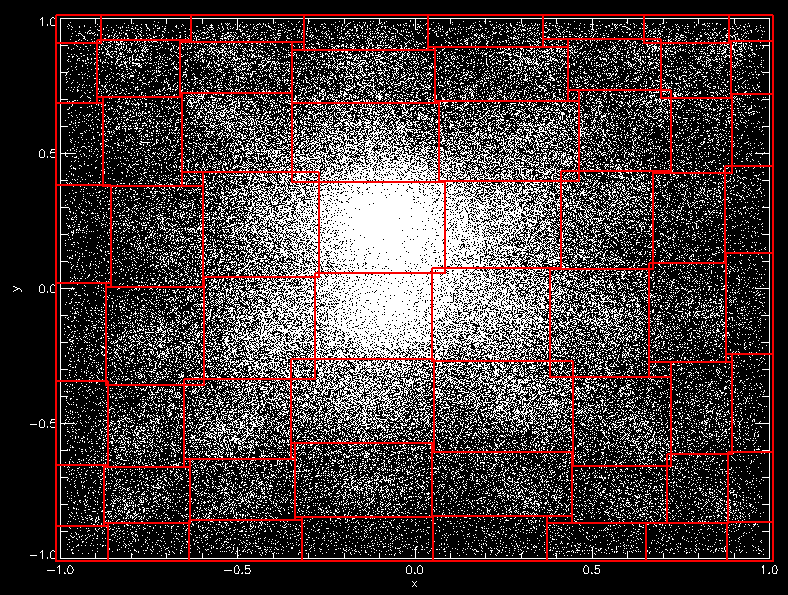
\includegraphics[width=.9\textwidth]{../messungen/kalib/vergleich_mitte_nah_NAH.png}
    \caption{Quelle nah.}
    \label{fig:ab-nah}
  \end{subfigure}
  \begin{subfigure}{0.32\textwidth}
    \centering
    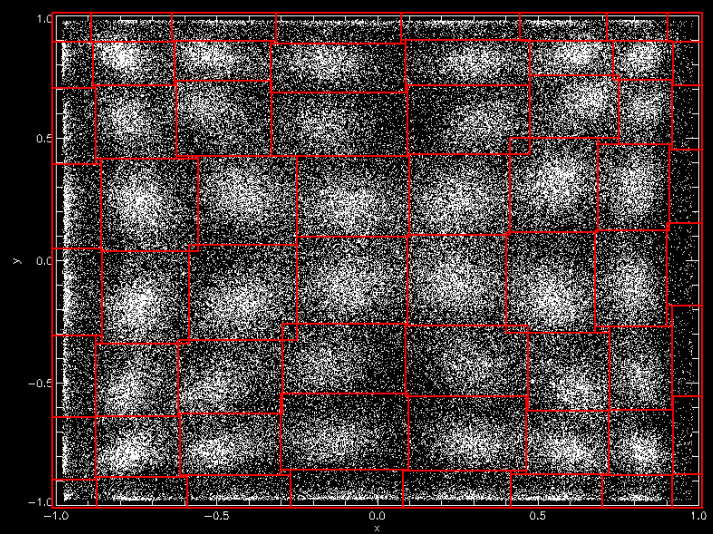
\includegraphics[width=.9\textwidth]{../messungen/kalib/vergleich_mitte_nah_MITTE.png}
    \caption{Quelle in Mitte.}
    \label{fig:ab-mitte}
  \end{subfigure}
  \begin{subfigure}{0.32\textwidth}
    \centering
    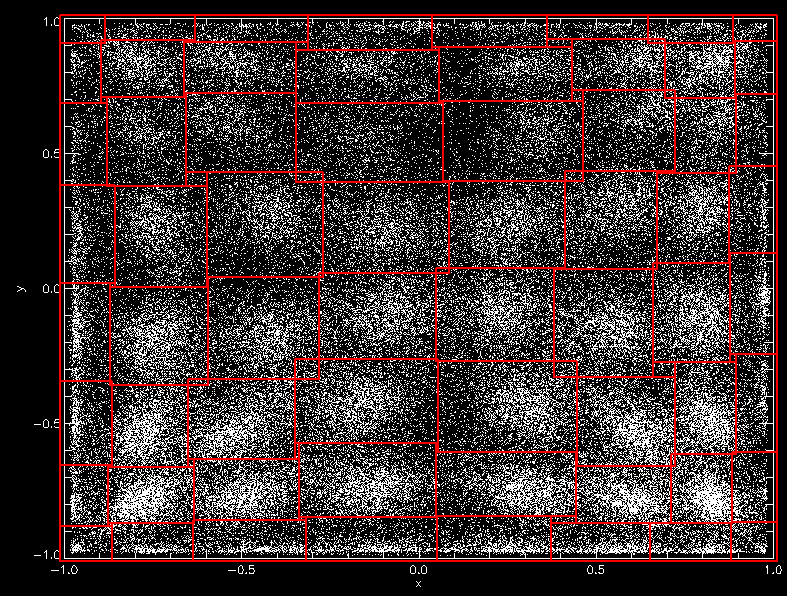
\includegraphics[width=.9\textwidth]{../messungen/kalib/vergleich_mitte_fern_FERN.png}
    \caption{Quelle fern.}
    \label{fig:ab-fern}
  \end{subfigure}
  \caption{Vergleich der Detektorsignale bei verschiedenen
    Quellabständen von Detektor A.}
  \label{fig:abstand}
\end{figure}

Um die Detektoren auch im Ortsraum zu kalibrieren wurden die Messdaten
(aus den Kalibrierungsmessungen) eingelesen und Schwerpunktsdiagramme
erstellt, um die werterbereiche der Koordinaten der eintreffenden
Signale den entsprechenden Detektorsegment zuzuordnen. Eine
entsprechnde Kalibrationsdatei wurde erzeugt und
abgespeichert. Grafische darstellungen der Diagramme sind
in~\ref{fig:abstand} f\"ur Detektor \(B\) gezeigt. (Die entsprechenden
Darstellungen f\"ur Det. A waren durch den ersetzten PM verzerrt.)
Man ergkennt deutlich mehr oder weniger stark ausgedehente
Schwerpunkte, die dann jeweils einer Zelle (rote Linien) zugeordnet
werden.

Die Quelle lag bei den Messungen stets auf einem Tisch aus
Plexiglas. Dadurch erwartet man eine Abschwächung des Signals durch
Reflexionen und Brechungen des Lichtes am unteren Detektorrand.  Wie
man allerdings deutlich in~\ref{fig:ab-fern} erkennen kann ist das
Signal im unteren Teil des Bildes deutlich stärker als im oberen. Dies
lässt darauf schließen, dass die vom Detektor kommenden Bilder
horizontal invertiert sind.  Auch kann man die Kristallstruktur anhand
der \(8\times 8\)-Matrix artigen Anordnung der Dichteverteilung der
Messpunkte erkennen.  Die Dichte der Messpunkte ist in
\ref{fig:ab-nah} deutlich im Zentrum der Aufnahme konzentriert sowie
die am Rand liegenden Bereiche höherer Messpunktdichte stark
verzerrt. Daraus wurde der Schluss, dass \ref{fig:ab-nah} eine Messung
zeigt, bei der die Quelle nah am Detektor lag. Das Wegfallen der Peaks
am Rand l\"asst auf nichterfolgende Reflexion aufgrund des Steilen
einfallswinkel (kleiner Winkel zur Normale) schließen. Es ist hier
keine sinnvolle Zuordnung zu Gitterpunkten mehr m\"oglich.  Bei
gr\"o\ss{}eren Abst\"anden f\"allt die Verzerrung nicht merklich ins
gewicht. So ist aber die Dichte in~\ref{fig:ab-fern} (also in der
gr\"o\ss{}ten Entfernung) diffuser als in~\ref{fig:ab-mitte} (in der
Mitte). Mit zunehmenden Abstand der Quelle wird der Einfalswinkel der
Photonen immer Flacher (zur Detektoroberfl\"achennormale) und damit
die Ablenkung durch Reflexionen geringer. Es sollte also im
allgemeinen ein optimaler Abstand (geringe Verzerrung, ausreichende
Z\"ahlrate) existieren.

% Die Unterschiede und
% Gründe für die Entscheidung zwischen mittleren \ref{fig:ab-mitte} und
% fernen Quellabstand \ref{fig:ab-fern} sind zum einen die Helligkeit
% der einzelnen Bereiche höherer Messpunktdichte zum anderen müssten die
% äußeren Bereiche bei fernem Abstand weniger stark verzerrt sein, was
% in~\ref{fig:abstand} allerdings nicht zu erkennen ist, da die
% Unterschiede zu marginal sind.

\subsection{Tomographische Messungen}
\label{sec:tom}

\subsubsection{Unbekannte Quellkonfiguration}
\label{sec:tom1}

Es wurde eine vorgegebene, aber unbekannte Quellkonfiguration
innerhalb eines aus Wachs (\"ahnlichkeit zu K\"orpergewebe)
bestehenden istropen und homogenen Beh\"alters vermessen und mit Hilfe
dieser Messungen auf die Gestalt der Quellkonfiguration geschlossen.

Die Quelle befand sich dabei genau mittig zwischen den Detektoren,
welche dabei mit einer Geschwindigkeit von
\(\SI{12}{\milli\metre\per\second}\) verfahren wurden um eine Breite
von \(40\) Bins (Breite \SI{3.375}{\milli\meter}) zu vermessen. Die
Projektionen, R\"uckprojektionen und gefilterten R\"uckprojektionen
wurden in Echtzeit durch ein Computer graphisch dargestellt. Es kam
dabei der sog. ``Mittelfilter'' mit mit der Dimensionseinstellung
\(9\) zur Anwendung, es wurde also der Filter jeweils \"uber \(9\)
Bins gefaltet. Der Aufnahme und Rekonstruktionsprozess ist
in~\ref{fig:tom1} dargestellt und wird im Folgenden nachvollzogen.

\begin{figure}[htp]
  \begin{subfigure}{0.5\textwidth}
    \centering
    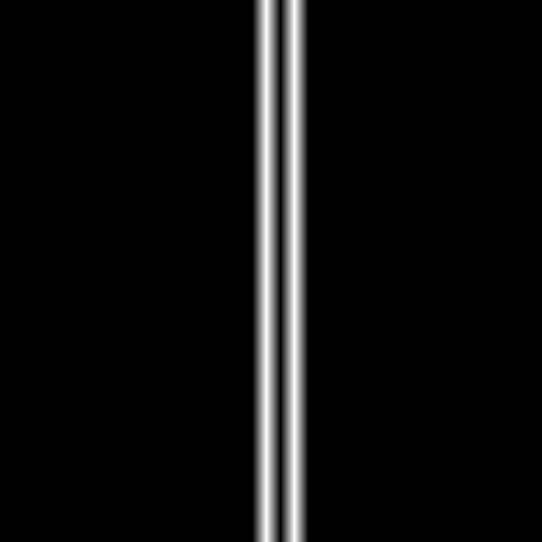
\includegraphics[width=.4\textwidth]{../messungen/oliTOM1/1_einfach.png}
    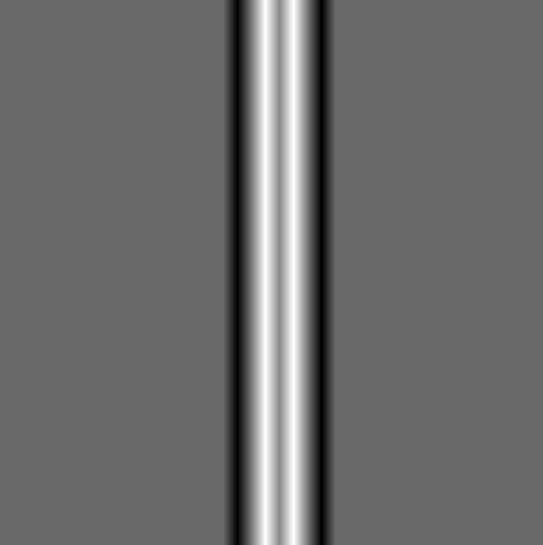
\includegraphics[width=.4\textwidth]{../messungen/oliTOM1/1_gefiltert.png}
    \caption{\(7^\circ\).}
    \label{eq:tom1-7}
  \end{subfigure}
  \begin{subfigure}{0.5\textwidth}
    \centering
    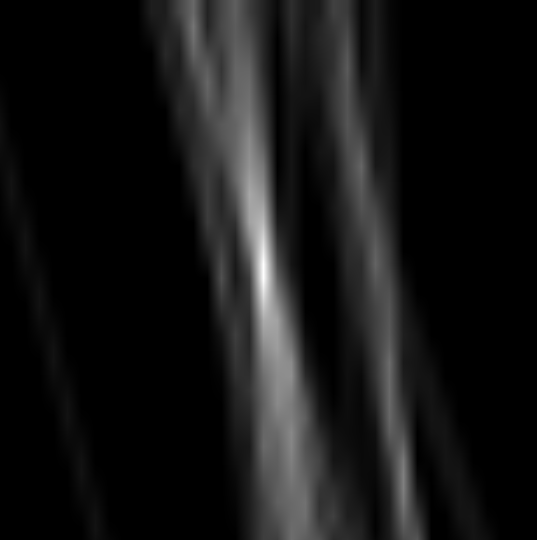
\includegraphics[width=.4\textwidth]{../messungen/oliTOM1/3_einfach.png}
    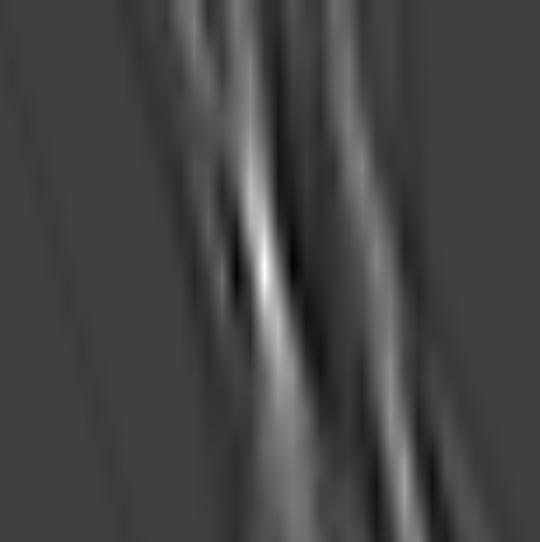
\includegraphics[width=.4\textwidth]{../messungen/oliTOM1/3_gefiltert.png}
    \caption{\(18^\circ\).}
    \label{eq:tom1-18}
  \end{subfigure}
  \begin{subfigure}{0.5\textwidth}
    \centering
    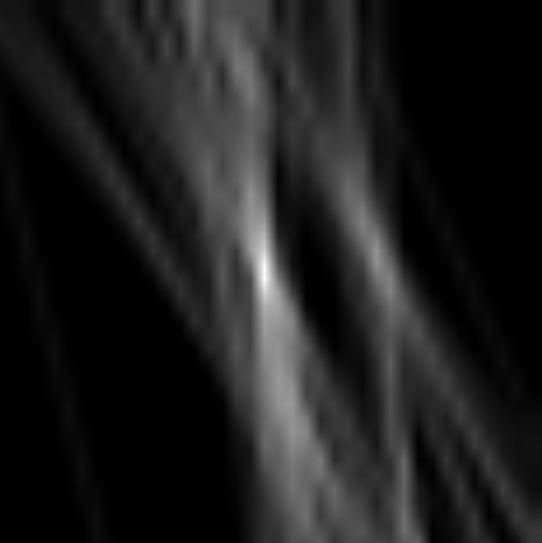
\includegraphics[width=.4\textwidth]{../messungen/oliTOM1/5_einfach.png}
    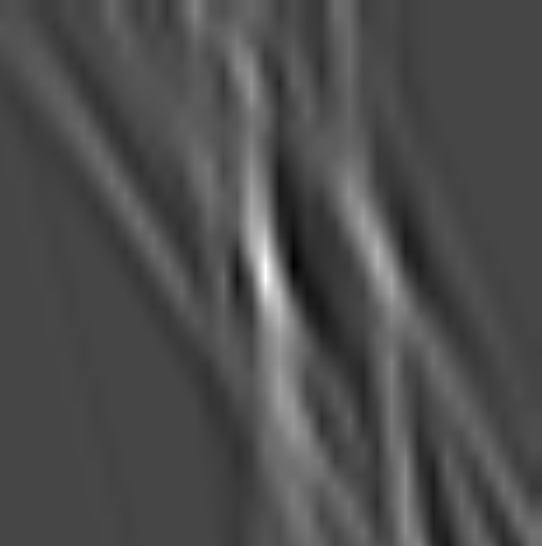
\includegraphics[width=.4\textwidth]{../messungen/oliTOM1/5_gefiltert.png}
    \caption{\(36^\circ\).}
    \label{eq:tom1-36}
  \end{subfigure}
  \begin{subfigure}{0.5\textwidth}
    \centering
    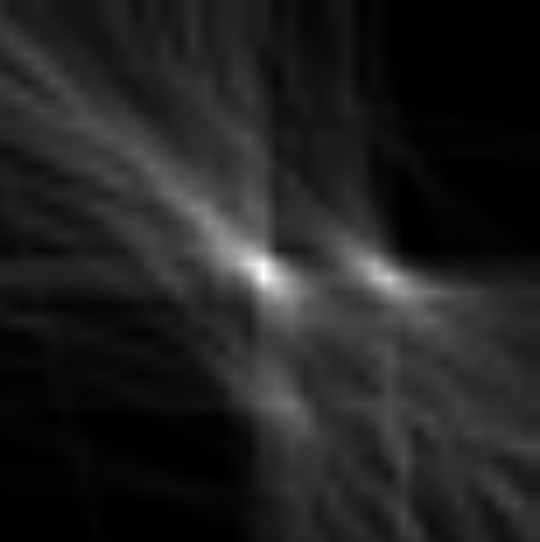
\includegraphics[width=.4\textwidth]{../messungen/oliTOM1/9_einfach.png}
    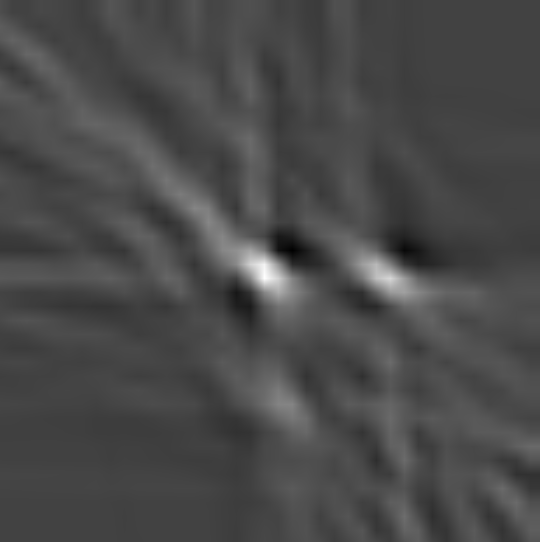
\includegraphics[width=.4\textwidth]{../messungen/oliTOM1/9_gefiltert.png}
    \caption{\(90^\circ\).}
    \label{eq:tom1-90}
  \end{subfigure}
  \begin{subfigure}{0.5\textwidth}
    \centering
    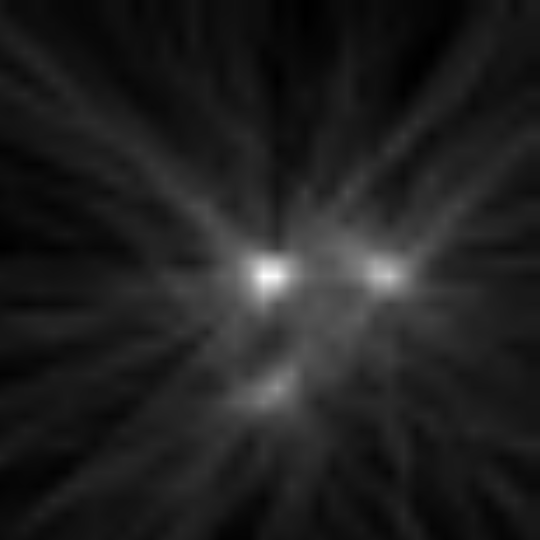
\includegraphics[width=.4\textwidth]{../messungen/oliTOM1/13_einfach.png}
    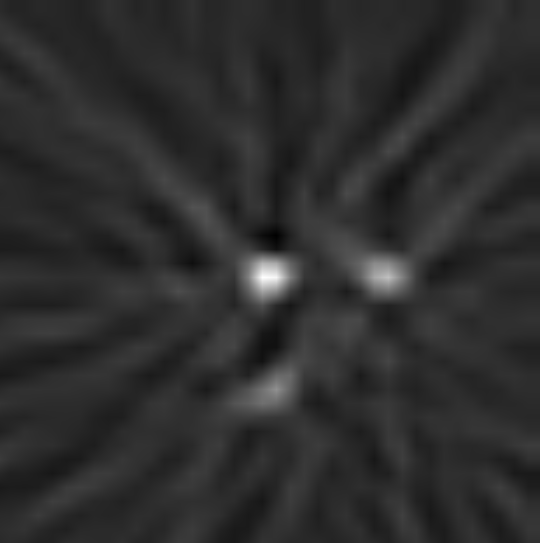
\includegraphics[width=.4\textwidth]{../messungen/oliTOM1/13_gefiltert.png}
    \caption{\(150^\circ\).}
    \label{eq:tom1-150}
  \end{subfigure}
  \begin{subfigure}{0.5\textwidth}
    \centering
    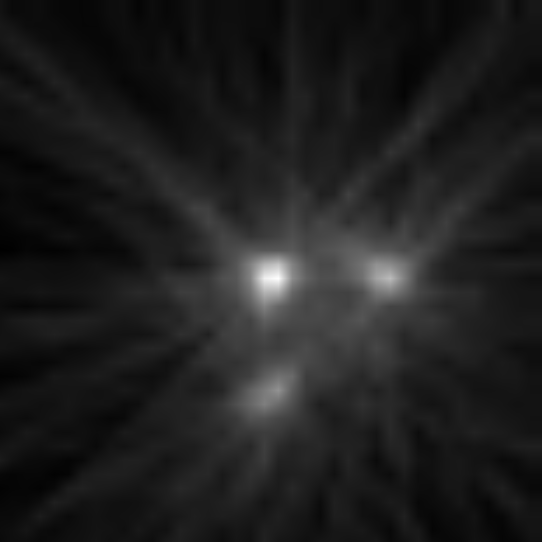
\includegraphics[width=.4\textwidth]{../messungen/oliTOM1/15_einfach.png}
    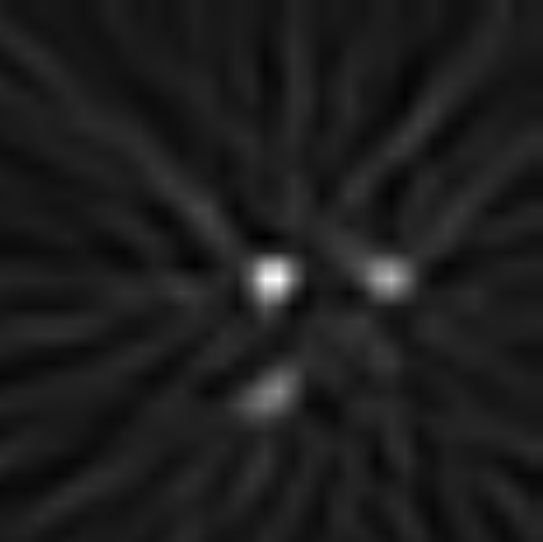
\includegraphics[width=.4\textwidth]{../messungen/oliTOM1/15_gefiltert.png}
    \caption{\(178^\circ\).}
    \label{eq:tom1-178}
  \end{subfigure}
  \begin{subfigure}{\textwidth}
    \centering
    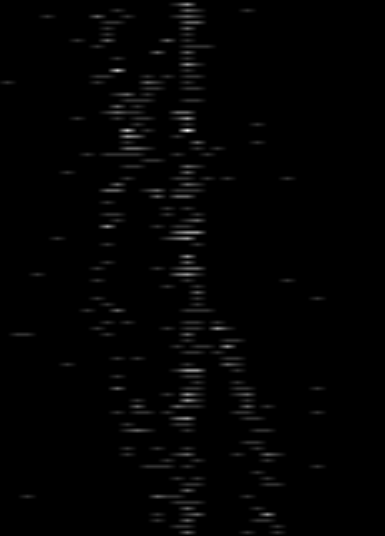
\includegraphics[width=.3\textwidth, angle=90]{../messungen/oliTOM1/sino.png}
    \caption{Endg\"ultiges Sinogramm}
    \label{fig:tom1-sino}
  \end{subfigure}
  \caption{Verlauf der Bildentstehung mit Gegenüberstellung von
    ungefilterter (links) und gefilterter Projektion (rechts).}
  \label{fig:tom1}
\end{figure}

\begin{figure}[bp]\centering
  %% Creator: Matplotlib, PGF backend
%%
%% To include the figure in your LaTeX document, write
%%   \input{<filename>.pgf}
%%
%% Make sure the required packages are loaded in your preamble
%%   \usepackage{pgf}
%%
%% Figures using additional raster images can only be included by \input if
%% they are in the same directory as the main LaTeX file. For loading figures
%% from other directories you can use the `import` package
%%   \usepackage{import}
%% and then include the figures with
%%   \import{<path to file>}{<filename>.pgf}
%%
%% Matplotlib used the following preamble
%%   \usepackage{fontspec}
%%
\begingroup%
\makeatletter%
\begin{pgfpicture}%
\pgfpathrectangle{\pgfpointorigin}{\pgfqpoint{6.000000in}{2.000000in}}%
\pgfusepath{use as bounding box, clip}%
\begin{pgfscope}%
\pgfsetbuttcap%
\pgfsetmiterjoin%
\definecolor{currentfill}{rgb}{1.000000,1.000000,1.000000}%
\pgfsetfillcolor{currentfill}%
\pgfsetlinewidth{0.000000pt}%
\definecolor{currentstroke}{rgb}{1.000000,1.000000,1.000000}%
\pgfsetstrokecolor{currentstroke}%
\pgfsetdash{}{0pt}%
\pgfpathmoveto{\pgfqpoint{0.000000in}{0.000000in}}%
\pgfpathlineto{\pgfqpoint{6.000000in}{0.000000in}}%
\pgfpathlineto{\pgfqpoint{6.000000in}{2.000000in}}%
\pgfpathlineto{\pgfqpoint{0.000000in}{2.000000in}}%
\pgfpathclose%
\pgfusepath{fill}%
\end{pgfscope}%
\begin{pgfscope}%
\pgfsetbuttcap%
\pgfsetmiterjoin%
\definecolor{currentfill}{rgb}{1.000000,1.000000,1.000000}%
\pgfsetfillcolor{currentfill}%
\pgfsetlinewidth{0.000000pt}%
\definecolor{currentstroke}{rgb}{0.000000,0.000000,0.000000}%
\pgfsetstrokecolor{currentstroke}%
\pgfsetstrokeopacity{0.000000}%
\pgfsetdash{}{0pt}%
\pgfpathmoveto{\pgfqpoint{0.150000in}{0.150000in}}%
\pgfpathlineto{\pgfqpoint{2.925000in}{0.150000in}}%
\pgfpathlineto{\pgfqpoint{2.925000in}{1.775778in}}%
\pgfpathlineto{\pgfqpoint{0.150000in}{1.775778in}}%
\pgfpathclose%
\pgfusepath{fill}%
\end{pgfscope}%
\begin{pgfscope}%
\pgfsetbuttcap%
\pgfsetmiterjoin%
\definecolor{currentfill}{rgb}{0.950000,0.950000,0.950000}%
\pgfsetfillcolor{currentfill}%
\pgfsetfillopacity{0.500000}%
\pgfsetlinewidth{1.003750pt}%
\definecolor{currentstroke}{rgb}{0.950000,0.950000,0.950000}%
\pgfsetstrokecolor{currentstroke}%
\pgfsetstrokeopacity{0.500000}%
\pgfsetdash{}{0pt}%
\pgfpathmoveto{\pgfqpoint{0.512536in}{0.701938in}}%
\pgfpathlineto{\pgfqpoint{1.575000in}{1.170327in}}%
\pgfpathlineto{\pgfqpoint{1.575000in}{1.769085in}}%
\pgfpathlineto{\pgfqpoint{0.424232in}{1.291294in}}%
\pgfusepath{stroke,fill}%
\end{pgfscope}%
\begin{pgfscope}%
\pgfsetbuttcap%
\pgfsetmiterjoin%
\definecolor{currentfill}{rgb}{0.900000,0.900000,0.900000}%
\pgfsetfillcolor{currentfill}%
\pgfsetfillopacity{0.500000}%
\pgfsetlinewidth{1.003750pt}%
\definecolor{currentstroke}{rgb}{0.900000,0.900000,0.900000}%
\pgfsetstrokecolor{currentstroke}%
\pgfsetstrokeopacity{0.500000}%
\pgfsetdash{}{0pt}%
\pgfpathmoveto{\pgfqpoint{1.575000in}{1.170327in}}%
\pgfpathlineto{\pgfqpoint{2.637464in}{0.701938in}}%
\pgfpathlineto{\pgfqpoint{2.725768in}{1.291294in}}%
\pgfpathlineto{\pgfqpoint{1.575000in}{1.769085in}}%
\pgfusepath{stroke,fill}%
\end{pgfscope}%
\begin{pgfscope}%
\pgfsetbuttcap%
\pgfsetmiterjoin%
\definecolor{currentfill}{rgb}{0.925000,0.925000,0.925000}%
\pgfsetfillcolor{currentfill}%
\pgfsetfillopacity{0.500000}%
\pgfsetlinewidth{1.003750pt}%
\definecolor{currentstroke}{rgb}{0.925000,0.925000,0.925000}%
\pgfsetstrokecolor{currentstroke}%
\pgfsetstrokeopacity{0.500000}%
\pgfsetdash{}{0pt}%
\pgfpathmoveto{\pgfqpoint{0.512536in}{0.701938in}}%
\pgfpathlineto{\pgfqpoint{1.575000in}{0.188864in}}%
\pgfpathlineto{\pgfqpoint{2.637464in}{0.701938in}}%
\pgfpathlineto{\pgfqpoint{1.575000in}{1.170327in}}%
\pgfusepath{stroke,fill}%
\end{pgfscope}%
\begin{pgfscope}%
\pgfsetrectcap%
\pgfsetroundjoin%
\pgfsetlinewidth{0.803000pt}%
\definecolor{currentstroke}{rgb}{0.000000,0.000000,0.000000}%
\pgfsetstrokecolor{currentstroke}%
\pgfsetdash{}{0pt}%
\pgfpathmoveto{\pgfqpoint{0.512536in}{0.701938in}}%
\pgfpathlineto{\pgfqpoint{1.575000in}{0.188864in}}%
\pgfusepath{stroke}%
\end{pgfscope}%
\begin{pgfscope}%
\definecolor{textcolor}{rgb}{0.000000,0.000000,0.000000}%
\pgfsetstrokecolor{textcolor}%
\pgfsetfillcolor{textcolor}%
\pgftext[x=0.502464in,y=0.198156in,left,base,rotate=334.223654]{\color{textcolor}\rmfamily\fontsize{10.000000}{12.000000}\selectfont x [mm]}%
\end{pgfscope}%
\begin{pgfscope}%
\pgfsetbuttcap%
\pgfsetroundjoin%
\pgfsetlinewidth{0.803000pt}%
\definecolor{currentstroke}{rgb}{0.690196,0.690196,0.690196}%
\pgfsetstrokecolor{currentstroke}%
\pgfsetdash{}{0pt}%
\pgfpathmoveto{\pgfqpoint{0.565550in}{0.676337in}}%
\pgfpathlineto{\pgfqpoint{1.628118in}{1.146910in}}%
\pgfpathlineto{\pgfqpoint{1.632336in}{1.745279in}}%
\pgfusepath{stroke}%
\end{pgfscope}%
\begin{pgfscope}%
\pgfsetbuttcap%
\pgfsetroundjoin%
\pgfsetlinewidth{0.803000pt}%
\definecolor{currentstroke}{rgb}{0.690196,0.690196,0.690196}%
\pgfsetstrokecolor{currentstroke}%
\pgfsetdash{}{0pt}%
\pgfpathmoveto{\pgfqpoint{0.740248in}{0.591974in}}%
\pgfpathlineto{\pgfqpoint{1.803083in}{1.069776in}}%
\pgfpathlineto{\pgfqpoint{1.821340in}{1.666806in}}%
\pgfusepath{stroke}%
\end{pgfscope}%
\begin{pgfscope}%
\pgfsetbuttcap%
\pgfsetroundjoin%
\pgfsetlinewidth{0.803000pt}%
\definecolor{currentstroke}{rgb}{0.690196,0.690196,0.690196}%
\pgfsetstrokecolor{currentstroke}%
\pgfsetdash{}{0pt}%
\pgfpathmoveto{\pgfqpoint{0.917701in}{0.506280in}}%
\pgfpathlineto{\pgfqpoint{1.980686in}{0.991480in}}%
\pgfpathlineto{\pgfqpoint{2.013422in}{1.587055in}}%
\pgfusepath{stroke}%
\end{pgfscope}%
\begin{pgfscope}%
\pgfsetbuttcap%
\pgfsetroundjoin%
\pgfsetlinewidth{0.803000pt}%
\definecolor{currentstroke}{rgb}{0.690196,0.690196,0.690196}%
\pgfsetstrokecolor{currentstroke}%
\pgfsetdash{}{0pt}%
\pgfpathmoveto{\pgfqpoint{1.097976in}{0.419223in}}%
\pgfpathlineto{\pgfqpoint{2.160985in}{0.911994in}}%
\pgfpathlineto{\pgfqpoint{2.208660in}{1.505994in}}%
\pgfusepath{stroke}%
\end{pgfscope}%
\begin{pgfscope}%
\pgfsetbuttcap%
\pgfsetroundjoin%
\pgfsetlinewidth{0.803000pt}%
\definecolor{currentstroke}{rgb}{0.690196,0.690196,0.690196}%
\pgfsetstrokecolor{currentstroke}%
\pgfsetdash{}{0pt}%
\pgfpathmoveto{\pgfqpoint{1.281140in}{0.330772in}}%
\pgfpathlineto{\pgfqpoint{2.344045in}{0.831292in}}%
\pgfpathlineto{\pgfqpoint{2.407130in}{1.423590in}}%
\pgfusepath{stroke}%
\end{pgfscope}%
\begin{pgfscope}%
\pgfsetbuttcap%
\pgfsetroundjoin%
\pgfsetlinewidth{0.803000pt}%
\definecolor{currentstroke}{rgb}{0.690196,0.690196,0.690196}%
\pgfsetstrokecolor{currentstroke}%
\pgfsetdash{}{0pt}%
\pgfpathmoveto{\pgfqpoint{1.467263in}{0.240891in}}%
\pgfpathlineto{\pgfqpoint{2.529927in}{0.749346in}}%
\pgfpathlineto{\pgfqpoint{2.608915in}{1.339811in}}%
\pgfusepath{stroke}%
\end{pgfscope}%
\begin{pgfscope}%
\pgfsetrectcap%
\pgfsetroundjoin%
\pgfsetlinewidth{0.803000pt}%
\definecolor{currentstroke}{rgb}{0.000000,0.000000,0.000000}%
\pgfsetstrokecolor{currentstroke}%
\pgfsetdash{}{0pt}%
\pgfpathmoveto{\pgfqpoint{0.574435in}{0.680272in}}%
\pgfpathlineto{\pgfqpoint{0.547760in}{0.668459in}}%
\pgfusepath{stroke}%
\end{pgfscope}%
\begin{pgfscope}%
\definecolor{textcolor}{rgb}{0.000000,0.000000,0.000000}%
\pgfsetstrokecolor{textcolor}%
\pgfsetfillcolor{textcolor}%
\pgftext[x=0.422148in,y=0.532646in,,top]{\color{textcolor}\rmfamily\fontsize{10.000000}{12.000000}\selectfont 0}%
\end{pgfscope}%
\begin{pgfscope}%
\pgfsetrectcap%
\pgfsetroundjoin%
\pgfsetlinewidth{0.803000pt}%
\definecolor{currentstroke}{rgb}{0.000000,0.000000,0.000000}%
\pgfsetstrokecolor{currentstroke}%
\pgfsetdash{}{0pt}%
\pgfpathmoveto{\pgfqpoint{0.749138in}{0.595971in}}%
\pgfpathlineto{\pgfqpoint{0.722447in}{0.583971in}}%
\pgfusepath{stroke}%
\end{pgfscope}%
\begin{pgfscope}%
\definecolor{textcolor}{rgb}{0.000000,0.000000,0.000000}%
\pgfsetstrokecolor{textcolor}%
\pgfsetfillcolor{textcolor}%
\pgftext[x=0.594965in,y=0.447532in,,top]{\color{textcolor}\rmfamily\fontsize{10.000000}{12.000000}\selectfont 25}%
\end{pgfscope}%
\begin{pgfscope}%
\pgfsetrectcap%
\pgfsetroundjoin%
\pgfsetlinewidth{0.803000pt}%
\definecolor{currentstroke}{rgb}{0.000000,0.000000,0.000000}%
\pgfsetstrokecolor{currentstroke}%
\pgfsetdash{}{0pt}%
\pgfpathmoveto{\pgfqpoint{0.926596in}{0.510340in}}%
\pgfpathlineto{\pgfqpoint{0.899892in}{0.498151in}}%
\pgfusepath{stroke}%
\end{pgfscope}%
\begin{pgfscope}%
\definecolor{textcolor}{rgb}{0.000000,0.000000,0.000000}%
\pgfsetstrokecolor{textcolor}%
\pgfsetfillcolor{textcolor}%
\pgftext[x=0.770495in,y=0.361082in,,top]{\color{textcolor}\rmfamily\fontsize{10.000000}{12.000000}\selectfont 50}%
\end{pgfscope}%
\begin{pgfscope}%
\pgfsetrectcap%
\pgfsetroundjoin%
\pgfsetlinewidth{0.803000pt}%
\definecolor{currentstroke}{rgb}{0.000000,0.000000,0.000000}%
\pgfsetstrokecolor{currentstroke}%
\pgfsetdash{}{0pt}%
\pgfpathmoveto{\pgfqpoint{1.106874in}{0.423348in}}%
\pgfpathlineto{\pgfqpoint{1.080160in}{0.410964in}}%
\pgfusepath{stroke}%
\end{pgfscope}%
\begin{pgfscope}%
\definecolor{textcolor}{rgb}{0.000000,0.000000,0.000000}%
\pgfsetstrokecolor{textcolor}%
\pgfsetfillcolor{textcolor}%
\pgftext[x=0.948804in,y=0.273263in,,top]{\color{textcolor}\rmfamily\fontsize{10.000000}{12.000000}\selectfont 75}%
\end{pgfscope}%
\begin{pgfscope}%
\pgfsetrectcap%
\pgfsetroundjoin%
\pgfsetlinewidth{0.803000pt}%
\definecolor{currentstroke}{rgb}{0.000000,0.000000,0.000000}%
\pgfsetstrokecolor{currentstroke}%
\pgfsetdash{}{0pt}%
\pgfpathmoveto{\pgfqpoint{1.290040in}{0.334963in}}%
\pgfpathlineto{\pgfqpoint{1.263319in}{0.322380in}}%
\pgfusepath{stroke}%
\end{pgfscope}%
\begin{pgfscope}%
\definecolor{textcolor}{rgb}{0.000000,0.000000,0.000000}%
\pgfsetstrokecolor{textcolor}%
\pgfsetfillcolor{textcolor}%
\pgftext[x=1.129958in,y=0.184043in,,top]{\color{textcolor}\rmfamily\fontsize{10.000000}{12.000000}\selectfont 100}%
\end{pgfscope}%
\begin{pgfscope}%
\pgfsetrectcap%
\pgfsetroundjoin%
\pgfsetlinewidth{0.803000pt}%
\definecolor{currentstroke}{rgb}{0.000000,0.000000,0.000000}%
\pgfsetstrokecolor{currentstroke}%
\pgfsetdash{}{0pt}%
\pgfpathmoveto{\pgfqpoint{1.476164in}{0.245151in}}%
\pgfpathlineto{\pgfqpoint{1.449439in}{0.232363in}}%
\pgfusepath{stroke}%
\end{pgfscope}%
\begin{pgfscope}%
\definecolor{textcolor}{rgb}{0.000000,0.000000,0.000000}%
\pgfsetstrokecolor{textcolor}%
\pgfsetfillcolor{textcolor}%
\pgftext[x=1.314024in,y=0.093389in,,top]{\color{textcolor}\rmfamily\fontsize{10.000000}{12.000000}\selectfont 125}%
\end{pgfscope}%
\begin{pgfscope}%
\pgfsetrectcap%
\pgfsetroundjoin%
\pgfsetlinewidth{0.803000pt}%
\definecolor{currentstroke}{rgb}{0.000000,0.000000,0.000000}%
\pgfsetstrokecolor{currentstroke}%
\pgfsetdash{}{0pt}%
\pgfpathmoveto{\pgfqpoint{2.637464in}{0.701938in}}%
\pgfpathlineto{\pgfqpoint{1.575000in}{0.188864in}}%
\pgfusepath{stroke}%
\end{pgfscope}%
\begin{pgfscope}%
\definecolor{textcolor}{rgb}{0.000000,0.000000,0.000000}%
\pgfsetstrokecolor{textcolor}%
\pgfsetfillcolor{textcolor}%
\pgftext[x=2.261947in,y=0.011952in,left,base,rotate=25.776346]{\color{textcolor}\rmfamily\fontsize{10.000000}{12.000000}\selectfont y [mm]}%
\end{pgfscope}%
\begin{pgfscope}%
\pgfsetbuttcap%
\pgfsetroundjoin%
\pgfsetlinewidth{0.803000pt}%
\definecolor{currentstroke}{rgb}{0.690196,0.690196,0.690196}%
\pgfsetstrokecolor{currentstroke}%
\pgfsetdash{}{0pt}%
\pgfpathmoveto{\pgfqpoint{0.487046in}{1.317374in}}%
\pgfpathlineto{\pgfqpoint{0.570332in}{0.727418in}}%
\pgfpathlineto{\pgfqpoint{1.632910in}{0.216829in}}%
\pgfusepath{stroke}%
\end{pgfscope}%
\begin{pgfscope}%
\pgfsetbuttcap%
\pgfsetroundjoin%
\pgfsetlinewidth{0.803000pt}%
\definecolor{currentstroke}{rgb}{0.690196,0.690196,0.690196}%
\pgfsetstrokecolor{currentstroke}%
\pgfsetdash{}{0pt}%
\pgfpathmoveto{\pgfqpoint{0.689723in}{1.401524in}}%
\pgfpathlineto{\pgfqpoint{0.756974in}{0.809699in}}%
\pgfpathlineto{\pgfqpoint{1.819829in}{0.307094in}}%
\pgfusepath{stroke}%
\end{pgfscope}%
\begin{pgfscope}%
\pgfsetbuttcap%
\pgfsetroundjoin%
\pgfsetlinewidth{0.803000pt}%
\definecolor{currentstroke}{rgb}{0.690196,0.690196,0.690196}%
\pgfsetstrokecolor{currentstroke}%
\pgfsetdash{}{0pt}%
\pgfpathmoveto{\pgfqpoint{0.889064in}{1.484289in}}%
\pgfpathlineto{\pgfqpoint{0.940775in}{0.890728in}}%
\pgfpathlineto{\pgfqpoint{2.003770in}{0.395921in}}%
\pgfusepath{stroke}%
\end{pgfscope}%
\begin{pgfscope}%
\pgfsetbuttcap%
\pgfsetroundjoin%
\pgfsetlinewidth{0.803000pt}%
\definecolor{currentstroke}{rgb}{0.690196,0.690196,0.690196}%
\pgfsetstrokecolor{currentstroke}%
\pgfsetdash{}{0pt}%
\pgfpathmoveto{\pgfqpoint{1.085150in}{1.565703in}}%
\pgfpathlineto{\pgfqpoint{1.121800in}{0.970533in}}%
\pgfpathlineto{\pgfqpoint{2.184803in}{0.483344in}}%
\pgfusepath{stroke}%
\end{pgfscope}%
\begin{pgfscope}%
\pgfsetbuttcap%
\pgfsetroundjoin%
\pgfsetlinewidth{0.803000pt}%
\definecolor{currentstroke}{rgb}{0.690196,0.690196,0.690196}%
\pgfsetstrokecolor{currentstroke}%
\pgfsetdash{}{0pt}%
\pgfpathmoveto{\pgfqpoint{1.278061in}{1.645798in}}%
\pgfpathlineto{\pgfqpoint{1.300111in}{1.049142in}}%
\pgfpathlineto{\pgfqpoint{2.362998in}{0.569396in}}%
\pgfusepath{stroke}%
\end{pgfscope}%
\begin{pgfscope}%
\pgfsetbuttcap%
\pgfsetroundjoin%
\pgfsetlinewidth{0.803000pt}%
\definecolor{currentstroke}{rgb}{0.690196,0.690196,0.690196}%
\pgfsetstrokecolor{currentstroke}%
\pgfsetdash{}{0pt}%
\pgfpathmoveto{\pgfqpoint{1.467874in}{1.724607in}}%
\pgfpathlineto{\pgfqpoint{1.475769in}{1.126581in}}%
\pgfpathlineto{\pgfqpoint{2.538420in}{0.654109in}}%
\pgfusepath{stroke}%
\end{pgfscope}%
\begin{pgfscope}%
\pgfsetrectcap%
\pgfsetroundjoin%
\pgfsetlinewidth{0.803000pt}%
\definecolor{currentstroke}{rgb}{0.000000,0.000000,0.000000}%
\pgfsetstrokecolor{currentstroke}%
\pgfsetdash{}{0pt}%
\pgfpathmoveto{\pgfqpoint{1.624008in}{0.221107in}}%
\pgfpathlineto{\pgfqpoint{1.650734in}{0.208264in}}%
\pgfusepath{stroke}%
\end{pgfscope}%
\begin{pgfscope}%
\definecolor{textcolor}{rgb}{0.000000,0.000000,0.000000}%
\pgfsetstrokecolor{textcolor}%
\pgfsetfillcolor{textcolor}%
\pgftext[x=1.786701in,y=0.069121in,,top]{\color{textcolor}\rmfamily\fontsize{10.000000}{12.000000}\selectfont 0}%
\end{pgfscope}%
\begin{pgfscope}%
\pgfsetrectcap%
\pgfsetroundjoin%
\pgfsetlinewidth{0.803000pt}%
\definecolor{currentstroke}{rgb}{0.000000,0.000000,0.000000}%
\pgfsetstrokecolor{currentstroke}%
\pgfsetdash{}{0pt}%
\pgfpathmoveto{\pgfqpoint{1.810928in}{0.311303in}}%
\pgfpathlineto{\pgfqpoint{1.837651in}{0.298666in}}%
\pgfusepath{stroke}%
\end{pgfscope}%
\begin{pgfscope}%
\definecolor{textcolor}{rgb}{0.000000,0.000000,0.000000}%
\pgfsetstrokecolor{textcolor}%
\pgfsetfillcolor{textcolor}%
\pgftext[x=1.971551in,y=0.160161in,,top]{\color{textcolor}\rmfamily\fontsize{10.000000}{12.000000}\selectfont 25}%
\end{pgfscope}%
\begin{pgfscope}%
\pgfsetrectcap%
\pgfsetroundjoin%
\pgfsetlinewidth{0.803000pt}%
\definecolor{currentstroke}{rgb}{0.000000,0.000000,0.000000}%
\pgfsetstrokecolor{currentstroke}%
\pgfsetdash{}{0pt}%
\pgfpathmoveto{\pgfqpoint{1.994871in}{0.400063in}}%
\pgfpathlineto{\pgfqpoint{2.021587in}{0.387627in}}%
\pgfusepath{stroke}%
\end{pgfscope}%
\begin{pgfscope}%
\definecolor{textcolor}{rgb}{0.000000,0.000000,0.000000}%
\pgfsetstrokecolor{textcolor}%
\pgfsetfillcolor{textcolor}%
\pgftext[x=2.153470in,y=0.249758in,,top]{\color{textcolor}\rmfamily\fontsize{10.000000}{12.000000}\selectfont 50}%
\end{pgfscope}%
\begin{pgfscope}%
\pgfsetrectcap%
\pgfsetroundjoin%
\pgfsetlinewidth{0.803000pt}%
\definecolor{currentstroke}{rgb}{0.000000,0.000000,0.000000}%
\pgfsetstrokecolor{currentstroke}%
\pgfsetdash{}{0pt}%
\pgfpathmoveto{\pgfqpoint{2.175908in}{0.487421in}}%
\pgfpathlineto{\pgfqpoint{2.202615in}{0.475181in}}%
\pgfusepath{stroke}%
\end{pgfscope}%
\begin{pgfscope}%
\definecolor{textcolor}{rgb}{0.000000,0.000000,0.000000}%
\pgfsetstrokecolor{textcolor}%
\pgfsetfillcolor{textcolor}%
\pgftext[x=2.332526in,y=0.337944in,,top]{\color{textcolor}\rmfamily\fontsize{10.000000}{12.000000}\selectfont 75}%
\end{pgfscope}%
\begin{pgfscope}%
\pgfsetrectcap%
\pgfsetroundjoin%
\pgfsetlinewidth{0.803000pt}%
\definecolor{currentstroke}{rgb}{0.000000,0.000000,0.000000}%
\pgfsetstrokecolor{currentstroke}%
\pgfsetdash{}{0pt}%
\pgfpathmoveto{\pgfqpoint{2.354106in}{0.573409in}}%
\pgfpathlineto{\pgfqpoint{2.380801in}{0.561360in}}%
\pgfusepath{stroke}%
\end{pgfscope}%
\begin{pgfscope}%
\definecolor{textcolor}{rgb}{0.000000,0.000000,0.000000}%
\pgfsetstrokecolor{textcolor}%
\pgfsetfillcolor{textcolor}%
\pgftext[x=2.508786in,y=0.424754in,,top]{\color{textcolor}\rmfamily\fontsize{10.000000}{12.000000}\selectfont 100}%
\end{pgfscope}%
\begin{pgfscope}%
\pgfsetrectcap%
\pgfsetroundjoin%
\pgfsetlinewidth{0.803000pt}%
\definecolor{currentstroke}{rgb}{0.000000,0.000000,0.000000}%
\pgfsetstrokecolor{currentstroke}%
\pgfsetdash{}{0pt}%
\pgfpathmoveto{\pgfqpoint{2.529533in}{0.658060in}}%
\pgfpathlineto{\pgfqpoint{2.556213in}{0.646198in}}%
\pgfusepath{stroke}%
\end{pgfscope}%
\begin{pgfscope}%
\definecolor{textcolor}{rgb}{0.000000,0.000000,0.000000}%
\pgfsetstrokecolor{textcolor}%
\pgfsetfillcolor{textcolor}%
\pgftext[x=2.682316in,y=0.510219in,,top]{\color{textcolor}\rmfamily\fontsize{10.000000}{12.000000}\selectfont 125}%
\end{pgfscope}%
\begin{pgfscope}%
\pgfsetrectcap%
\pgfsetroundjoin%
\pgfsetlinewidth{0.803000pt}%
\definecolor{currentstroke}{rgb}{0.000000,0.000000,0.000000}%
\pgfsetstrokecolor{currentstroke}%
\pgfsetdash{}{0pt}%
\pgfpathmoveto{\pgfqpoint{2.637464in}{0.701938in}}%
\pgfpathlineto{\pgfqpoint{2.725768in}{1.291294in}}%
\pgfusepath{stroke}%
\end{pgfscope}%
\begin{pgfscope}%
\pgfsetbuttcap%
\pgfsetroundjoin%
\pgfsetlinewidth{0.803000pt}%
\definecolor{currentstroke}{rgb}{0.690196,0.690196,0.690196}%
\pgfsetstrokecolor{currentstroke}%
\pgfsetdash{}{0pt}%
\pgfpathmoveto{\pgfqpoint{2.643168in}{0.740008in}}%
\pgfpathlineto{\pgfqpoint{1.575000in}{1.209135in}}%
\pgfpathlineto{\pgfqpoint{0.506832in}{0.740008in}}%
\pgfusepath{stroke}%
\end{pgfscope}%
\begin{pgfscope}%
\pgfsetbuttcap%
\pgfsetroundjoin%
\pgfsetlinewidth{0.803000pt}%
\definecolor{currentstroke}{rgb}{0.690196,0.690196,0.690196}%
\pgfsetstrokecolor{currentstroke}%
\pgfsetdash{}{0pt}%
\pgfpathmoveto{\pgfqpoint{2.661031in}{0.859229in}}%
\pgfpathlineto{\pgfqpoint{1.575000in}{1.330551in}}%
\pgfpathlineto{\pgfqpoint{0.488969in}{0.859229in}}%
\pgfusepath{stroke}%
\end{pgfscope}%
\begin{pgfscope}%
\pgfsetbuttcap%
\pgfsetroundjoin%
\pgfsetlinewidth{0.803000pt}%
\definecolor{currentstroke}{rgb}{0.690196,0.690196,0.690196}%
\pgfsetstrokecolor{currentstroke}%
\pgfsetdash{}{0pt}%
\pgfpathmoveto{\pgfqpoint{2.679502in}{0.982505in}}%
\pgfpathlineto{\pgfqpoint{1.575000in}{1.455909in}}%
\pgfpathlineto{\pgfqpoint{0.470498in}{0.982505in}}%
\pgfusepath{stroke}%
\end{pgfscope}%
\begin{pgfscope}%
\pgfsetbuttcap%
\pgfsetroundjoin%
\pgfsetlinewidth{0.803000pt}%
\definecolor{currentstroke}{rgb}{0.690196,0.690196,0.690196}%
\pgfsetstrokecolor{currentstroke}%
\pgfsetdash{}{0pt}%
\pgfpathmoveto{\pgfqpoint{2.698611in}{1.110047in}}%
\pgfpathlineto{\pgfqpoint{1.575000in}{1.585407in}}%
\pgfpathlineto{\pgfqpoint{0.451389in}{1.110047in}}%
\pgfusepath{stroke}%
\end{pgfscope}%
\begin{pgfscope}%
\pgfsetbuttcap%
\pgfsetroundjoin%
\pgfsetlinewidth{0.803000pt}%
\definecolor{currentstroke}{rgb}{0.690196,0.690196,0.690196}%
\pgfsetstrokecolor{currentstroke}%
\pgfsetdash{}{0pt}%
\pgfpathmoveto{\pgfqpoint{2.718394in}{1.242080in}}%
\pgfpathlineto{\pgfqpoint{1.575000in}{1.719251in}}%
\pgfpathlineto{\pgfqpoint{0.431606in}{1.242080in}}%
\pgfusepath{stroke}%
\end{pgfscope}%
\begin{pgfscope}%
\pgfsetrectcap%
\pgfsetroundjoin%
\pgfsetlinewidth{0.803000pt}%
\definecolor{currentstroke}{rgb}{0.000000,0.000000,0.000000}%
\pgfsetstrokecolor{currentstroke}%
\pgfsetdash{}{0pt}%
\pgfpathmoveto{\pgfqpoint{2.634235in}{0.743931in}}%
\pgfpathlineto{\pgfqpoint{2.661054in}{0.732153in}}%
\pgfusepath{stroke}%
\end{pgfscope}%
\begin{pgfscope}%
\definecolor{textcolor}{rgb}{0.000000,0.000000,0.000000}%
\pgfsetstrokecolor{textcolor}%
\pgfsetfillcolor{textcolor}%
\pgftext[x=2.940908in,y=0.740008in,,top]{\color{textcolor}\rmfamily\fontsize{10.000000}{12.000000}\selectfont 0}%
\end{pgfscope}%
\begin{pgfscope}%
\pgfsetrectcap%
\pgfsetroundjoin%
\pgfsetlinewidth{0.803000pt}%
\definecolor{currentstroke}{rgb}{0.000000,0.000000,0.000000}%
\pgfsetstrokecolor{currentstroke}%
\pgfsetdash{}{0pt}%
\pgfpathmoveto{\pgfqpoint{2.651942in}{0.863173in}}%
\pgfpathlineto{\pgfqpoint{2.679230in}{0.851331in}}%
\pgfusepath{stroke}%
\end{pgfscope}%
\begin{pgfscope}%
\definecolor{textcolor}{rgb}{0.000000,0.000000,0.000000}%
\pgfsetstrokecolor{textcolor}%
\pgfsetfillcolor{textcolor}%
\pgftext[x=2.963750in,y=0.859229in,,top]{\color{textcolor}\rmfamily\fontsize{10.000000}{12.000000}\selectfont 5}%
\end{pgfscope}%
\begin{pgfscope}%
\pgfsetrectcap%
\pgfsetroundjoin%
\pgfsetlinewidth{0.803000pt}%
\definecolor{currentstroke}{rgb}{0.000000,0.000000,0.000000}%
\pgfsetstrokecolor{currentstroke}%
\pgfsetdash{}{0pt}%
\pgfpathmoveto{\pgfqpoint{2.670251in}{0.986470in}}%
\pgfpathlineto{\pgfqpoint{2.698024in}{0.974566in}}%
\pgfusepath{stroke}%
\end{pgfscope}%
\begin{pgfscope}%
\definecolor{textcolor}{rgb}{0.000000,0.000000,0.000000}%
\pgfsetstrokecolor{textcolor}%
\pgfsetfillcolor{textcolor}%
\pgftext[x=2.987369in,y=0.982505in,,top]{\color{textcolor}\rmfamily\fontsize{10.000000}{12.000000}\selectfont 10}%
\end{pgfscope}%
\begin{pgfscope}%
\pgfsetrectcap%
\pgfsetroundjoin%
\pgfsetlinewidth{0.803000pt}%
\definecolor{currentstroke}{rgb}{0.000000,0.000000,0.000000}%
\pgfsetstrokecolor{currentstroke}%
\pgfsetdash{}{0pt}%
\pgfpathmoveto{\pgfqpoint{2.689193in}{1.114031in}}%
\pgfpathlineto{\pgfqpoint{2.717469in}{1.102069in}}%
\pgfusepath{stroke}%
\end{pgfscope}%
\begin{pgfscope}%
\definecolor{textcolor}{rgb}{0.000000,0.000000,0.000000}%
\pgfsetstrokecolor{textcolor}%
\pgfsetfillcolor{textcolor}%
\pgftext[x=3.011805in,y=1.110047in,,top]{\color{textcolor}\rmfamily\fontsize{10.000000}{12.000000}\selectfont 15}%
\end{pgfscope}%
\begin{pgfscope}%
\pgfsetrectcap%
\pgfsetroundjoin%
\pgfsetlinewidth{0.803000pt}%
\definecolor{currentstroke}{rgb}{0.000000,0.000000,0.000000}%
\pgfsetstrokecolor{currentstroke}%
\pgfsetdash{}{0pt}%
\pgfpathmoveto{\pgfqpoint{2.708802in}{1.246082in}}%
\pgfpathlineto{\pgfqpoint{2.737600in}{1.234064in}}%
\pgfusepath{stroke}%
\end{pgfscope}%
\begin{pgfscope}%
\definecolor{textcolor}{rgb}{0.000000,0.000000,0.000000}%
\pgfsetstrokecolor{textcolor}%
\pgfsetfillcolor{textcolor}%
\pgftext[x=3.037102in,y=1.242080in,,top]{\color{textcolor}\rmfamily\fontsize{10.000000}{12.000000}\selectfont 20}%
\end{pgfscope}%
\begin{pgfscope}%
\pgfpathrectangle{\pgfqpoint{0.150000in}{0.150000in}}{\pgfqpoint{2.775000in}{1.625778in}}%
\pgfusepath{clip}%
\pgfsetbuttcap%
\pgfsetroundjoin%
\definecolor{currentfill}{rgb}{0.241396,0.014979,0.610259}%
\pgfsetfillcolor{currentfill}%
\pgfsetlinewidth{0.000000pt}%
\definecolor{currentstroke}{rgb}{0.000000,0.000000,0.000000}%
\pgfsetstrokecolor{currentstroke}%
\pgfsetdash{}{0pt}%
\pgfpathmoveto{\pgfqpoint{1.551285in}{1.173587in}}%
\pgfpathlineto{\pgfqpoint{1.575000in}{1.160513in}}%
\pgfpathlineto{\pgfqpoint{1.598668in}{1.158692in}}%
\pgfpathlineto{\pgfqpoint{1.575000in}{1.180988in}}%
\pgfpathclose%
\pgfusepath{fill}%
\end{pgfscope}%
\begin{pgfscope}%
\pgfpathrectangle{\pgfqpoint{0.150000in}{0.150000in}}{\pgfqpoint{2.775000in}{1.625778in}}%
\pgfusepath{clip}%
\pgfsetbuttcap%
\pgfsetroundjoin%
\definecolor{currentfill}{rgb}{0.214350,0.016973,0.599239}%
\pgfsetfillcolor{currentfill}%
\pgfsetlinewidth{0.000000pt}%
\definecolor{currentstroke}{rgb}{0.000000,0.000000,0.000000}%
\pgfsetstrokecolor{currentstroke}%
\pgfsetdash{}{0pt}%
\pgfpathmoveto{\pgfqpoint{1.575000in}{1.160513in}}%
\pgfpathlineto{\pgfqpoint{1.598731in}{1.142550in}}%
\pgfpathlineto{\pgfqpoint{1.622345in}{1.142007in}}%
\pgfpathlineto{\pgfqpoint{1.598668in}{1.158692in}}%
\pgfpathclose%
\pgfusepath{fill}%
\end{pgfscope}%
\begin{pgfscope}%
\pgfpathrectangle{\pgfqpoint{0.150000in}{0.150000in}}{\pgfqpoint{2.775000in}{1.625778in}}%
\pgfusepath{clip}%
\pgfsetbuttcap%
\pgfsetroundjoin%
\definecolor{currentfill}{rgb}{0.200445,0.017902,0.593364}%
\pgfsetfillcolor{currentfill}%
\pgfsetlinewidth{0.000000pt}%
\definecolor{currentstroke}{rgb}{0.000000,0.000000,0.000000}%
\pgfsetstrokecolor{currentstroke}%
\pgfsetdash{}{0pt}%
\pgfpathmoveto{\pgfqpoint{1.598731in}{1.142550in}}%
\pgfpathlineto{\pgfqpoint{1.622457in}{1.123444in}}%
\pgfpathlineto{\pgfqpoint{1.646111in}{1.133709in}}%
\pgfpathlineto{\pgfqpoint{1.622345in}{1.142007in}}%
\pgfpathclose%
\pgfusepath{fill}%
\end{pgfscope}%
\begin{pgfscope}%
\pgfpathrectangle{\pgfqpoint{0.150000in}{0.150000in}}{\pgfqpoint{2.775000in}{1.625778in}}%
\pgfusepath{clip}%
\pgfsetbuttcap%
\pgfsetroundjoin%
\definecolor{currentfill}{rgb}{0.207435,0.017442,0.596333}%
\pgfsetfillcolor{currentfill}%
\pgfsetlinewidth{0.000000pt}%
\definecolor{currentstroke}{rgb}{0.000000,0.000000,0.000000}%
\pgfsetstrokecolor{currentstroke}%
\pgfsetdash{}{0pt}%
\pgfpathmoveto{\pgfqpoint{1.503924in}{1.130077in}}%
\pgfpathlineto{\pgfqpoint{1.527538in}{1.124206in}}%
\pgfpathlineto{\pgfqpoint{1.551250in}{1.148403in}}%
\pgfpathlineto{\pgfqpoint{1.527604in}{1.150118in}}%
\pgfpathclose%
\pgfusepath{fill}%
\end{pgfscope}%
\begin{pgfscope}%
\pgfpathrectangle{\pgfqpoint{0.150000in}{0.150000in}}{\pgfqpoint{2.775000in}{1.625778in}}%
\pgfusepath{clip}%
\pgfsetbuttcap%
\pgfsetroundjoin%
\definecolor{currentfill}{rgb}{0.186213,0.018803,0.587228}%
\pgfsetfillcolor{currentfill}%
\pgfsetlinewidth{0.000000pt}%
\definecolor{currentstroke}{rgb}{0.000000,0.000000,0.000000}%
\pgfsetstrokecolor{currentstroke}%
\pgfsetdash{}{0pt}%
\pgfpathmoveto{\pgfqpoint{1.622457in}{1.123444in}}%
\pgfpathlineto{\pgfqpoint{1.646254in}{1.112569in}}%
\pgfpathlineto{\pgfqpoint{1.669832in}{1.116988in}}%
\pgfpathlineto{\pgfqpoint{1.646111in}{1.133709in}}%
\pgfpathclose%
\pgfusepath{fill}%
\end{pgfscope}%
\begin{pgfscope}%
\pgfpathrectangle{\pgfqpoint{0.150000in}{0.150000in}}{\pgfqpoint{2.775000in}{1.625778in}}%
\pgfusepath{clip}%
\pgfsetbuttcap%
\pgfsetroundjoin%
\definecolor{currentfill}{rgb}{0.241396,0.014979,0.610259}%
\pgfsetfillcolor{currentfill}%
\pgfsetlinewidth{0.000000pt}%
\definecolor{currentstroke}{rgb}{0.000000,0.000000,0.000000}%
\pgfsetstrokecolor{currentstroke}%
\pgfsetdash{}{0pt}%
\pgfpathmoveto{\pgfqpoint{1.527604in}{1.150118in}}%
\pgfpathlineto{\pgfqpoint{1.551250in}{1.148403in}}%
\pgfpathlineto{\pgfqpoint{1.575000in}{1.160513in}}%
\pgfpathlineto{\pgfqpoint{1.551285in}{1.173587in}}%
\pgfpathclose%
\pgfusepath{fill}%
\end{pgfscope}%
\begin{pgfscope}%
\pgfpathrectangle{\pgfqpoint{0.150000in}{0.150000in}}{\pgfqpoint{2.775000in}{1.625778in}}%
\pgfusepath{clip}%
\pgfsetbuttcap%
\pgfsetroundjoin%
\definecolor{currentfill}{rgb}{0.193374,0.018354,0.590330}%
\pgfsetfillcolor{currentfill}%
\pgfsetlinewidth{0.000000pt}%
\definecolor{currentstroke}{rgb}{0.000000,0.000000,0.000000}%
\pgfsetstrokecolor{currentstroke}%
\pgfsetdash{}{0pt}%
\pgfpathmoveto{\pgfqpoint{1.480021in}{1.128642in}}%
\pgfpathlineto{\pgfqpoint{1.503730in}{1.114256in}}%
\pgfpathlineto{\pgfqpoint{1.527538in}{1.124206in}}%
\pgfpathlineto{\pgfqpoint{1.503924in}{1.130077in}}%
\pgfpathclose%
\pgfusepath{fill}%
\end{pgfscope}%
\begin{pgfscope}%
\pgfpathrectangle{\pgfqpoint{0.150000in}{0.150000in}}{\pgfqpoint{2.775000in}{1.625778in}}%
\pgfusepath{clip}%
\pgfsetbuttcap%
\pgfsetroundjoin%
\definecolor{currentfill}{rgb}{0.171574,0.019706,0.580806}%
\pgfsetfillcolor{currentfill}%
\pgfsetlinewidth{0.000000pt}%
\definecolor{currentstroke}{rgb}{0.000000,0.000000,0.000000}%
\pgfsetstrokecolor{currentstroke}%
\pgfsetdash{}{0pt}%
\pgfpathmoveto{\pgfqpoint{1.646254in}{1.112569in}}%
\pgfpathlineto{\pgfqpoint{1.670014in}{1.095109in}}%
\pgfpathlineto{\pgfqpoint{1.693600in}{1.102635in}}%
\pgfpathlineto{\pgfqpoint{1.669832in}{1.116988in}}%
\pgfpathclose%
\pgfusepath{fill}%
\end{pgfscope}%
\begin{pgfscope}%
\pgfpathrectangle{\pgfqpoint{0.150000in}{0.150000in}}{\pgfqpoint{2.775000in}{1.625778in}}%
\pgfusepath{clip}%
\pgfsetbuttcap%
\pgfsetroundjoin%
\definecolor{currentfill}{rgb}{0.156421,0.020651,0.574065}%
\pgfsetfillcolor{currentfill}%
\pgfsetlinewidth{0.000000pt}%
\definecolor{currentstroke}{rgb}{0.000000,0.000000,0.000000}%
\pgfsetstrokecolor{currentstroke}%
\pgfsetdash{}{0pt}%
\pgfpathmoveto{\pgfqpoint{1.670014in}{1.095109in}}%
\pgfpathlineto{\pgfqpoint{1.693866in}{1.083087in}}%
\pgfpathlineto{\pgfqpoint{1.717389in}{1.088161in}}%
\pgfpathlineto{\pgfqpoint{1.693600in}{1.102635in}}%
\pgfpathclose%
\pgfusepath{fill}%
\end{pgfscope}%
\begin{pgfscope}%
\pgfpathrectangle{\pgfqpoint{0.150000in}{0.150000in}}{\pgfqpoint{2.775000in}{1.625778in}}%
\pgfusepath{clip}%
\pgfsetbuttcap%
\pgfsetroundjoin%
\definecolor{currentfill}{rgb}{0.241396,0.014979,0.610259}%
\pgfsetfillcolor{currentfill}%
\pgfsetlinewidth{0.000000pt}%
\definecolor{currentstroke}{rgb}{0.000000,0.000000,0.000000}%
\pgfsetstrokecolor{currentstroke}%
\pgfsetdash{}{0pt}%
\pgfpathmoveto{\pgfqpoint{1.551250in}{1.148403in}}%
\pgfpathlineto{\pgfqpoint{1.575000in}{1.138543in}}%
\pgfpathlineto{\pgfqpoint{1.598731in}{1.142550in}}%
\pgfpathlineto{\pgfqpoint{1.575000in}{1.160513in}}%
\pgfpathclose%
\pgfusepath{fill}%
\end{pgfscope}%
\begin{pgfscope}%
\pgfpathrectangle{\pgfqpoint{0.150000in}{0.150000in}}{\pgfqpoint{2.775000in}{1.625778in}}%
\pgfusepath{clip}%
\pgfsetbuttcap%
\pgfsetroundjoin%
\definecolor{currentfill}{rgb}{0.227983,0.016007,0.604867}%
\pgfsetfillcolor{currentfill}%
\pgfsetlinewidth{0.000000pt}%
\definecolor{currentstroke}{rgb}{0.000000,0.000000,0.000000}%
\pgfsetstrokecolor{currentstroke}%
\pgfsetdash{}{0pt}%
\pgfpathmoveto{\pgfqpoint{1.575000in}{1.138543in}}%
\pgfpathlineto{\pgfqpoint{1.598793in}{1.125581in}}%
\pgfpathlineto{\pgfqpoint{1.622457in}{1.123444in}}%
\pgfpathlineto{\pgfqpoint{1.598731in}{1.142550in}}%
\pgfpathclose%
\pgfusepath{fill}%
\end{pgfscope}%
\begin{pgfscope}%
\pgfpathrectangle{\pgfqpoint{0.150000in}{0.150000in}}{\pgfqpoint{2.775000in}{1.625778in}}%
\pgfusepath{clip}%
\pgfsetbuttcap%
\pgfsetroundjoin%
\definecolor{currentfill}{rgb}{0.234715,0.015502,0.607592}%
\pgfsetfillcolor{currentfill}%
\pgfsetlinewidth{0.000000pt}%
\definecolor{currentstroke}{rgb}{0.000000,0.000000,0.000000}%
\pgfsetstrokecolor{currentstroke}%
\pgfsetdash{}{0pt}%
\pgfpathmoveto{\pgfqpoint{1.527538in}{1.124206in}}%
\pgfpathlineto{\pgfqpoint{1.551209in}{1.125006in}}%
\pgfpathlineto{\pgfqpoint{1.575000in}{1.138543in}}%
\pgfpathlineto{\pgfqpoint{1.551250in}{1.148403in}}%
\pgfpathclose%
\pgfusepath{fill}%
\end{pgfscope}%
\begin{pgfscope}%
\pgfpathrectangle{\pgfqpoint{0.150000in}{0.150000in}}{\pgfqpoint{2.775000in}{1.625778in}}%
\pgfusepath{clip}%
\pgfsetbuttcap%
\pgfsetroundjoin%
\definecolor{currentfill}{rgb}{0.207435,0.017442,0.596333}%
\pgfsetfillcolor{currentfill}%
\pgfsetlinewidth{0.000000pt}%
\definecolor{currentstroke}{rgb}{0.000000,0.000000,0.000000}%
\pgfsetstrokecolor{currentstroke}%
\pgfsetdash{}{0pt}%
\pgfpathmoveto{\pgfqpoint{1.598793in}{1.125581in}}%
\pgfpathlineto{\pgfqpoint{1.622560in}{1.103481in}}%
\pgfpathlineto{\pgfqpoint{1.646254in}{1.112569in}}%
\pgfpathlineto{\pgfqpoint{1.622457in}{1.123444in}}%
\pgfpathclose%
\pgfusepath{fill}%
\end{pgfscope}%
\begin{pgfscope}%
\pgfpathrectangle{\pgfqpoint{0.150000in}{0.150000in}}{\pgfqpoint{2.775000in}{1.625778in}}%
\pgfusepath{clip}%
\pgfsetbuttcap%
\pgfsetroundjoin%
\definecolor{currentfill}{rgb}{0.148607,0.021154,0.570562}%
\pgfsetfillcolor{currentfill}%
\pgfsetlinewidth{0.000000pt}%
\definecolor{currentstroke}{rgb}{0.000000,0.000000,0.000000}%
\pgfsetstrokecolor{currentstroke}%
\pgfsetdash{}{0pt}%
\pgfpathmoveto{\pgfqpoint{1.693866in}{1.083087in}}%
\pgfpathlineto{\pgfqpoint{1.717737in}{1.070043in}}%
\pgfpathlineto{\pgfqpoint{1.741330in}{1.079396in}}%
\pgfpathlineto{\pgfqpoint{1.717389in}{1.088161in}}%
\pgfpathclose%
\pgfusepath{fill}%
\end{pgfscope}%
\begin{pgfscope}%
\pgfpathrectangle{\pgfqpoint{0.150000in}{0.150000in}}{\pgfqpoint{2.775000in}{1.625778in}}%
\pgfusepath{clip}%
\pgfsetbuttcap%
\pgfsetroundjoin%
\definecolor{currentfill}{rgb}{0.207435,0.017442,0.596333}%
\pgfsetfillcolor{currentfill}%
\pgfsetlinewidth{0.000000pt}%
\definecolor{currentstroke}{rgb}{0.000000,0.000000,0.000000}%
\pgfsetstrokecolor{currentstroke}%
\pgfsetdash{}{0pt}%
\pgfpathmoveto{\pgfqpoint{1.503730in}{1.114256in}}%
\pgfpathlineto{\pgfqpoint{1.527434in}{1.104379in}}%
\pgfpathlineto{\pgfqpoint{1.551209in}{1.125006in}}%
\pgfpathlineto{\pgfqpoint{1.527538in}{1.124206in}}%
\pgfpathclose%
\pgfusepath{fill}%
\end{pgfscope}%
\begin{pgfscope}%
\pgfpathrectangle{\pgfqpoint{0.150000in}{0.150000in}}{\pgfqpoint{2.775000in}{1.625778in}}%
\pgfusepath{clip}%
\pgfsetbuttcap%
\pgfsetroundjoin%
\definecolor{currentfill}{rgb}{0.186213,0.018803,0.587228}%
\pgfsetfillcolor{currentfill}%
\pgfsetlinewidth{0.000000pt}%
\definecolor{currentstroke}{rgb}{0.000000,0.000000,0.000000}%
\pgfsetstrokecolor{currentstroke}%
\pgfsetdash{}{0pt}%
\pgfpathmoveto{\pgfqpoint{1.622560in}{1.103481in}}%
\pgfpathlineto{\pgfqpoint{1.646389in}{1.090335in}}%
\pgfpathlineto{\pgfqpoint{1.670014in}{1.095109in}}%
\pgfpathlineto{\pgfqpoint{1.646254in}{1.112569in}}%
\pgfpathclose%
\pgfusepath{fill}%
\end{pgfscope}%
\begin{pgfscope}%
\pgfpathrectangle{\pgfqpoint{0.150000in}{0.150000in}}{\pgfqpoint{2.775000in}{1.625778in}}%
\pgfusepath{clip}%
\pgfsetbuttcap%
\pgfsetroundjoin%
\definecolor{currentfill}{rgb}{0.221197,0.016497,0.602083}%
\pgfsetfillcolor{currentfill}%
\pgfsetlinewidth{0.000000pt}%
\definecolor{currentstroke}{rgb}{0.000000,0.000000,0.000000}%
\pgfsetstrokecolor{currentstroke}%
\pgfsetdash{}{0pt}%
\pgfpathmoveto{\pgfqpoint{1.456018in}{1.126814in}}%
\pgfpathlineto{\pgfqpoint{1.479749in}{1.113780in}}%
\pgfpathlineto{\pgfqpoint{1.503730in}{1.114256in}}%
\pgfpathlineto{\pgfqpoint{1.480021in}{1.128642in}}%
\pgfpathclose%
\pgfusepath{fill}%
\end{pgfscope}%
\begin{pgfscope}%
\pgfpathrectangle{\pgfqpoint{0.150000in}{0.150000in}}{\pgfqpoint{2.775000in}{1.625778in}}%
\pgfusepath{clip}%
\pgfsetbuttcap%
\pgfsetroundjoin%
\definecolor{currentfill}{rgb}{0.171574,0.019706,0.580806}%
\pgfsetfillcolor{currentfill}%
\pgfsetlinewidth{0.000000pt}%
\definecolor{currentstroke}{rgb}{0.000000,0.000000,0.000000}%
\pgfsetstrokecolor{currentstroke}%
\pgfsetdash{}{0pt}%
\pgfpathmoveto{\pgfqpoint{1.646389in}{1.090335in}}%
\pgfpathlineto{\pgfqpoint{1.670250in}{1.077257in}}%
\pgfpathlineto{\pgfqpoint{1.693866in}{1.083087in}}%
\pgfpathlineto{\pgfqpoint{1.670014in}{1.095109in}}%
\pgfpathclose%
\pgfusepath{fill}%
\end{pgfscope}%
\begin{pgfscope}%
\pgfpathrectangle{\pgfqpoint{0.150000in}{0.150000in}}{\pgfqpoint{2.775000in}{1.625778in}}%
\pgfusepath{clip}%
\pgfsetbuttcap%
\pgfsetroundjoin%
\definecolor{currentfill}{rgb}{0.214350,0.016973,0.599239}%
\pgfsetfillcolor{currentfill}%
\pgfsetlinewidth{0.000000pt}%
\definecolor{currentstroke}{rgb}{0.000000,0.000000,0.000000}%
\pgfsetstrokecolor{currentstroke}%
\pgfsetdash{}{0pt}%
\pgfpathmoveto{\pgfqpoint{1.479749in}{1.113780in}}%
\pgfpathlineto{\pgfqpoint{1.503533in}{1.098590in}}%
\pgfpathlineto{\pgfqpoint{1.527434in}{1.104379in}}%
\pgfpathlineto{\pgfqpoint{1.503730in}{1.114256in}}%
\pgfpathclose%
\pgfusepath{fill}%
\end{pgfscope}%
\begin{pgfscope}%
\pgfpathrectangle{\pgfqpoint{0.150000in}{0.150000in}}{\pgfqpoint{2.775000in}{1.625778in}}%
\pgfusepath{clip}%
\pgfsetbuttcap%
\pgfsetroundjoin%
\definecolor{currentfill}{rgb}{0.156421,0.020651,0.574065}%
\pgfsetfillcolor{currentfill}%
\pgfsetlinewidth{0.000000pt}%
\definecolor{currentstroke}{rgb}{0.000000,0.000000,0.000000}%
\pgfsetstrokecolor{currentstroke}%
\pgfsetdash{}{0pt}%
\pgfpathmoveto{\pgfqpoint{1.717737in}{1.070043in}}%
\pgfpathlineto{\pgfqpoint{1.741680in}{1.058693in}}%
\pgfpathlineto{\pgfqpoint{1.765544in}{1.078974in}}%
\pgfpathlineto{\pgfqpoint{1.741330in}{1.079396in}}%
\pgfpathclose%
\pgfusepath{fill}%
\end{pgfscope}%
\begin{pgfscope}%
\pgfpathrectangle{\pgfqpoint{0.150000in}{0.150000in}}{\pgfqpoint{2.775000in}{1.625778in}}%
\pgfusepath{clip}%
\pgfsetbuttcap%
\pgfsetroundjoin%
\definecolor{currentfill}{rgb}{0.241396,0.014979,0.610259}%
\pgfsetfillcolor{currentfill}%
\pgfsetlinewidth{0.000000pt}%
\definecolor{currentstroke}{rgb}{0.000000,0.000000,0.000000}%
\pgfsetstrokecolor{currentstroke}%
\pgfsetdash{}{0pt}%
\pgfpathmoveto{\pgfqpoint{1.551209in}{1.125006in}}%
\pgfpathlineto{\pgfqpoint{1.575000in}{1.116829in}}%
\pgfpathlineto{\pgfqpoint{1.598793in}{1.125581in}}%
\pgfpathlineto{\pgfqpoint{1.575000in}{1.138543in}}%
\pgfpathclose%
\pgfusepath{fill}%
\end{pgfscope}%
\begin{pgfscope}%
\pgfpathrectangle{\pgfqpoint{0.150000in}{0.150000in}}{\pgfqpoint{2.775000in}{1.625778in}}%
\pgfusepath{clip}%
\pgfsetbuttcap%
\pgfsetroundjoin%
\definecolor{currentfill}{rgb}{0.164070,0.020171,0.577478}%
\pgfsetfillcolor{currentfill}%
\pgfsetlinewidth{0.000000pt}%
\definecolor{currentstroke}{rgb}{0.000000,0.000000,0.000000}%
\pgfsetstrokecolor{currentstroke}%
\pgfsetdash{}{0pt}%
\pgfpathmoveto{\pgfqpoint{1.670250in}{1.077257in}}%
\pgfpathlineto{\pgfqpoint{1.694157in}{1.064931in}}%
\pgfpathlineto{\pgfqpoint{1.717737in}{1.070043in}}%
\pgfpathlineto{\pgfqpoint{1.693866in}{1.083087in}}%
\pgfpathclose%
\pgfusepath{fill}%
\end{pgfscope}%
\begin{pgfscope}%
\pgfpathrectangle{\pgfqpoint{0.150000in}{0.150000in}}{\pgfqpoint{2.775000in}{1.625778in}}%
\pgfusepath{clip}%
\pgfsetbuttcap%
\pgfsetroundjoin%
\definecolor{currentfill}{rgb}{0.227983,0.016007,0.604867}%
\pgfsetfillcolor{currentfill}%
\pgfsetlinewidth{0.000000pt}%
\definecolor{currentstroke}{rgb}{0.000000,0.000000,0.000000}%
\pgfsetstrokecolor{currentstroke}%
\pgfsetdash{}{0pt}%
\pgfpathmoveto{\pgfqpoint{1.527434in}{1.104379in}}%
\pgfpathlineto{\pgfqpoint{1.551175in}{1.099410in}}%
\pgfpathlineto{\pgfqpoint{1.575000in}{1.116829in}}%
\pgfpathlineto{\pgfqpoint{1.551209in}{1.125006in}}%
\pgfpathclose%
\pgfusepath{fill}%
\end{pgfscope}%
\begin{pgfscope}%
\pgfpathrectangle{\pgfqpoint{0.150000in}{0.150000in}}{\pgfqpoint{2.775000in}{1.625778in}}%
\pgfusepath{clip}%
\pgfsetbuttcap%
\pgfsetroundjoin%
\definecolor{currentfill}{rgb}{0.227983,0.016007,0.604867}%
\pgfsetfillcolor{currentfill}%
\pgfsetlinewidth{0.000000pt}%
\definecolor{currentstroke}{rgb}{0.000000,0.000000,0.000000}%
\pgfsetstrokecolor{currentstroke}%
\pgfsetdash{}{0pt}%
\pgfpathmoveto{\pgfqpoint{1.575000in}{1.116829in}}%
\pgfpathlineto{\pgfqpoint{1.598835in}{1.102572in}}%
\pgfpathlineto{\pgfqpoint{1.622560in}{1.103481in}}%
\pgfpathlineto{\pgfqpoint{1.598793in}{1.125581in}}%
\pgfpathclose%
\pgfusepath{fill}%
\end{pgfscope}%
\begin{pgfscope}%
\pgfpathrectangle{\pgfqpoint{0.150000in}{0.150000in}}{\pgfqpoint{2.775000in}{1.625778in}}%
\pgfusepath{clip}%
\pgfsetbuttcap%
\pgfsetroundjoin%
\definecolor{currentfill}{rgb}{0.227983,0.016007,0.604867}%
\pgfsetfillcolor{currentfill}%
\pgfsetlinewidth{0.000000pt}%
\definecolor{currentstroke}{rgb}{0.000000,0.000000,0.000000}%
\pgfsetstrokecolor{currentstroke}%
\pgfsetdash{}{0pt}%
\pgfpathmoveto{\pgfqpoint{1.432247in}{1.107257in}}%
\pgfpathlineto{\pgfqpoint{1.455826in}{1.102440in}}%
\pgfpathlineto{\pgfqpoint{1.479749in}{1.113780in}}%
\pgfpathlineto{\pgfqpoint{1.456018in}{1.126814in}}%
\pgfpathclose%
\pgfusepath{fill}%
\end{pgfscope}%
\begin{pgfscope}%
\pgfpathrectangle{\pgfqpoint{0.150000in}{0.150000in}}{\pgfqpoint{2.775000in}{1.625778in}}%
\pgfusepath{clip}%
\pgfsetbuttcap%
\pgfsetroundjoin%
\definecolor{currentfill}{rgb}{0.207435,0.017442,0.596333}%
\pgfsetfillcolor{currentfill}%
\pgfsetlinewidth{0.000000pt}%
\definecolor{currentstroke}{rgb}{0.000000,0.000000,0.000000}%
\pgfsetstrokecolor{currentstroke}%
\pgfsetdash{}{0pt}%
\pgfpathmoveto{\pgfqpoint{1.598835in}{1.102572in}}%
\pgfpathlineto{\pgfqpoint{1.622674in}{1.084959in}}%
\pgfpathlineto{\pgfqpoint{1.646389in}{1.090335in}}%
\pgfpathlineto{\pgfqpoint{1.622560in}{1.103481in}}%
\pgfpathclose%
\pgfusepath{fill}%
\end{pgfscope}%
\begin{pgfscope}%
\pgfpathrectangle{\pgfqpoint{0.150000in}{0.150000in}}{\pgfqpoint{2.775000in}{1.625778in}}%
\pgfusepath{clip}%
\pgfsetbuttcap%
\pgfsetroundjoin%
\definecolor{currentfill}{rgb}{0.207435,0.017442,0.596333}%
\pgfsetfillcolor{currentfill}%
\pgfsetlinewidth{0.000000pt}%
\definecolor{currentstroke}{rgb}{0.000000,0.000000,0.000000}%
\pgfsetstrokecolor{currentstroke}%
\pgfsetdash{}{0pt}%
\pgfpathmoveto{\pgfqpoint{1.408470in}{1.088383in}}%
\pgfpathlineto{\pgfqpoint{1.431999in}{1.083808in}}%
\pgfpathlineto{\pgfqpoint{1.455826in}{1.102440in}}%
\pgfpathlineto{\pgfqpoint{1.432247in}{1.107257in}}%
\pgfpathclose%
\pgfusepath{fill}%
\end{pgfscope}%
\begin{pgfscope}%
\pgfpathrectangle{\pgfqpoint{0.150000in}{0.150000in}}{\pgfqpoint{2.775000in}{1.625778in}}%
\pgfusepath{clip}%
\pgfsetbuttcap%
\pgfsetroundjoin%
\definecolor{currentfill}{rgb}{0.148607,0.021154,0.570562}%
\pgfsetfillcolor{currentfill}%
\pgfsetlinewidth{0.000000pt}%
\definecolor{currentstroke}{rgb}{0.000000,0.000000,0.000000}%
\pgfsetstrokecolor{currentstroke}%
\pgfsetdash{}{0pt}%
\pgfpathmoveto{\pgfqpoint{1.694157in}{1.064931in}}%
\pgfpathlineto{\pgfqpoint{1.717987in}{1.046624in}}%
\pgfpathlineto{\pgfqpoint{1.741680in}{1.058693in}}%
\pgfpathlineto{\pgfqpoint{1.717737in}{1.070043in}}%
\pgfpathclose%
\pgfusepath{fill}%
\end{pgfscope}%
\begin{pgfscope}%
\pgfpathrectangle{\pgfqpoint{0.150000in}{0.150000in}}{\pgfqpoint{2.775000in}{1.625778in}}%
\pgfusepath{clip}%
\pgfsetbuttcap%
\pgfsetroundjoin%
\definecolor{currentfill}{rgb}{0.214350,0.016973,0.599239}%
\pgfsetfillcolor{currentfill}%
\pgfsetlinewidth{0.000000pt}%
\definecolor{currentstroke}{rgb}{0.000000,0.000000,0.000000}%
\pgfsetstrokecolor{currentstroke}%
\pgfsetdash{}{0pt}%
\pgfpathmoveto{\pgfqpoint{1.503533in}{1.098590in}}%
\pgfpathlineto{\pgfqpoint{1.527302in}{1.088625in}}%
\pgfpathlineto{\pgfqpoint{1.551175in}{1.099410in}}%
\pgfpathlineto{\pgfqpoint{1.527434in}{1.104379in}}%
\pgfpathclose%
\pgfusepath{fill}%
\end{pgfscope}%
\begin{pgfscope}%
\pgfpathrectangle{\pgfqpoint{0.150000in}{0.150000in}}{\pgfqpoint{2.775000in}{1.625778in}}%
\pgfusepath{clip}%
\pgfsetbuttcap%
\pgfsetroundjoin%
\definecolor{currentfill}{rgb}{0.193374,0.018354,0.590330}%
\pgfsetfillcolor{currentfill}%
\pgfsetlinewidth{0.000000pt}%
\definecolor{currentstroke}{rgb}{0.000000,0.000000,0.000000}%
\pgfsetstrokecolor{currentstroke}%
\pgfsetdash{}{0pt}%
\pgfpathmoveto{\pgfqpoint{1.622674in}{1.084959in}}%
\pgfpathlineto{\pgfqpoint{1.646551in}{1.070915in}}%
\pgfpathlineto{\pgfqpoint{1.670250in}{1.077257in}}%
\pgfpathlineto{\pgfqpoint{1.646389in}{1.090335in}}%
\pgfpathclose%
\pgfusepath{fill}%
\end{pgfscope}%
\begin{pgfscope}%
\pgfpathrectangle{\pgfqpoint{0.150000in}{0.150000in}}{\pgfqpoint{2.775000in}{1.625778in}}%
\pgfusepath{clip}%
\pgfsetbuttcap%
\pgfsetroundjoin%
\definecolor{currentfill}{rgb}{0.200445,0.017902,0.593364}%
\pgfsetfillcolor{currentfill}%
\pgfsetlinewidth{0.000000pt}%
\definecolor{currentstroke}{rgb}{0.000000,0.000000,0.000000}%
\pgfsetstrokecolor{currentstroke}%
\pgfsetdash{}{0pt}%
\pgfpathmoveto{\pgfqpoint{1.384252in}{1.086947in}}%
\pgfpathlineto{\pgfqpoint{1.408038in}{1.071285in}}%
\pgfpathlineto{\pgfqpoint{1.431999in}{1.083808in}}%
\pgfpathlineto{\pgfqpoint{1.408470in}{1.088383in}}%
\pgfpathclose%
\pgfusepath{fill}%
\end{pgfscope}%
\begin{pgfscope}%
\pgfpathrectangle{\pgfqpoint{0.150000in}{0.150000in}}{\pgfqpoint{2.775000in}{1.625778in}}%
\pgfusepath{clip}%
\pgfsetbuttcap%
\pgfsetroundjoin%
\definecolor{currentfill}{rgb}{0.140603,0.021687,0.566959}%
\pgfsetfillcolor{currentfill}%
\pgfsetlinewidth{0.000000pt}%
\definecolor{currentstroke}{rgb}{0.000000,0.000000,0.000000}%
\pgfsetstrokecolor{currentstroke}%
\pgfsetdash{}{0pt}%
\pgfpathmoveto{\pgfqpoint{1.717987in}{1.046624in}}%
\pgfpathlineto{\pgfqpoint{1.741907in}{1.032370in}}%
\pgfpathlineto{\pgfqpoint{1.765807in}{1.052790in}}%
\pgfpathlineto{\pgfqpoint{1.741680in}{1.058693in}}%
\pgfpathclose%
\pgfusepath{fill}%
\end{pgfscope}%
\begin{pgfscope}%
\pgfpathrectangle{\pgfqpoint{0.150000in}{0.150000in}}{\pgfqpoint{2.775000in}{1.625778in}}%
\pgfusepath{clip}%
\pgfsetbuttcap%
\pgfsetroundjoin%
\definecolor{currentfill}{rgb}{0.234715,0.015502,0.607592}%
\pgfsetfillcolor{currentfill}%
\pgfsetlinewidth{0.000000pt}%
\definecolor{currentstroke}{rgb}{0.000000,0.000000,0.000000}%
\pgfsetstrokecolor{currentstroke}%
\pgfsetdash{}{0pt}%
\pgfpathmoveto{\pgfqpoint{1.551175in}{1.099410in}}%
\pgfpathlineto{\pgfqpoint{1.575000in}{1.093160in}}%
\pgfpathlineto{\pgfqpoint{1.598835in}{1.102572in}}%
\pgfpathlineto{\pgfqpoint{1.575000in}{1.116829in}}%
\pgfpathclose%
\pgfusepath{fill}%
\end{pgfscope}%
\begin{pgfscope}%
\pgfpathrectangle{\pgfqpoint{0.150000in}{0.150000in}}{\pgfqpoint{2.775000in}{1.625778in}}%
\pgfusepath{clip}%
\pgfsetbuttcap%
\pgfsetroundjoin%
\definecolor{currentfill}{rgb}{0.178950,0.019252,0.584054}%
\pgfsetfillcolor{currentfill}%
\pgfsetlinewidth{0.000000pt}%
\definecolor{currentstroke}{rgb}{0.000000,0.000000,0.000000}%
\pgfsetstrokecolor{currentstroke}%
\pgfsetdash{}{0pt}%
\pgfpathmoveto{\pgfqpoint{1.741680in}{1.058693in}}%
\pgfpathlineto{\pgfqpoint{1.765807in}{1.052790in}}%
\pgfpathlineto{\pgfqpoint{1.789894in}{1.079239in}}%
\pgfpathlineto{\pgfqpoint{1.765544in}{1.078974in}}%
\pgfpathclose%
\pgfusepath{fill}%
\end{pgfscope}%
\begin{pgfscope}%
\pgfpathrectangle{\pgfqpoint{0.150000in}{0.150000in}}{\pgfqpoint{2.775000in}{1.625778in}}%
\pgfusepath{clip}%
\pgfsetbuttcap%
\pgfsetroundjoin%
\definecolor{currentfill}{rgb}{0.241396,0.014979,0.610259}%
\pgfsetfillcolor{currentfill}%
\pgfsetlinewidth{0.000000pt}%
\definecolor{currentstroke}{rgb}{0.000000,0.000000,0.000000}%
\pgfsetstrokecolor{currentstroke}%
\pgfsetdash{}{0pt}%
\pgfpathmoveto{\pgfqpoint{1.455826in}{1.102440in}}%
\pgfpathlineto{\pgfqpoint{1.479436in}{1.101871in}}%
\pgfpathlineto{\pgfqpoint{1.503533in}{1.098590in}}%
\pgfpathlineto{\pgfqpoint{1.479749in}{1.113780in}}%
\pgfpathclose%
\pgfusepath{fill}%
\end{pgfscope}%
\begin{pgfscope}%
\pgfpathrectangle{\pgfqpoint{0.150000in}{0.150000in}}{\pgfqpoint{2.775000in}{1.625778in}}%
\pgfusepath{clip}%
\pgfsetbuttcap%
\pgfsetroundjoin%
\definecolor{currentfill}{rgb}{0.186213,0.018803,0.587228}%
\pgfsetfillcolor{currentfill}%
\pgfsetlinewidth{0.000000pt}%
\definecolor{currentstroke}{rgb}{0.000000,0.000000,0.000000}%
\pgfsetstrokecolor{currentstroke}%
\pgfsetdash{}{0pt}%
\pgfpathmoveto{\pgfqpoint{1.646551in}{1.070915in}}%
\pgfpathlineto{\pgfqpoint{1.670501in}{1.060436in}}%
\pgfpathlineto{\pgfqpoint{1.694157in}{1.064931in}}%
\pgfpathlineto{\pgfqpoint{1.670250in}{1.077257in}}%
\pgfpathclose%
\pgfusepath{fill}%
\end{pgfscope}%
\begin{pgfscope}%
\pgfpathrectangle{\pgfqpoint{0.150000in}{0.150000in}}{\pgfqpoint{2.775000in}{1.625778in}}%
\pgfusepath{clip}%
\pgfsetbuttcap%
\pgfsetroundjoin%
\definecolor{currentfill}{rgb}{0.221197,0.016497,0.602083}%
\pgfsetfillcolor{currentfill}%
\pgfsetlinewidth{0.000000pt}%
\definecolor{currentstroke}{rgb}{0.000000,0.000000,0.000000}%
\pgfsetstrokecolor{currentstroke}%
\pgfsetdash{}{0pt}%
\pgfpathmoveto{\pgfqpoint{1.527302in}{1.088625in}}%
\pgfpathlineto{\pgfqpoint{1.551141in}{1.073610in}}%
\pgfpathlineto{\pgfqpoint{1.575000in}{1.093160in}}%
\pgfpathlineto{\pgfqpoint{1.551175in}{1.099410in}}%
\pgfpathclose%
\pgfusepath{fill}%
\end{pgfscope}%
\begin{pgfscope}%
\pgfpathrectangle{\pgfqpoint{0.150000in}{0.150000in}}{\pgfqpoint{2.775000in}{1.625778in}}%
\pgfusepath{clip}%
\pgfsetbuttcap%
\pgfsetroundjoin%
\definecolor{currentfill}{rgb}{0.164070,0.020171,0.577478}%
\pgfsetfillcolor{currentfill}%
\pgfsetlinewidth{0.000000pt}%
\definecolor{currentstroke}{rgb}{0.000000,0.000000,0.000000}%
\pgfsetstrokecolor{currentstroke}%
\pgfsetdash{}{0pt}%
\pgfpathmoveto{\pgfqpoint{1.670501in}{1.060436in}}%
\pgfpathlineto{\pgfqpoint{1.694353in}{1.040715in}}%
\pgfpathlineto{\pgfqpoint{1.717987in}{1.046624in}}%
\pgfpathlineto{\pgfqpoint{1.694157in}{1.064931in}}%
\pgfpathclose%
\pgfusepath{fill}%
\end{pgfscope}%
\begin{pgfscope}%
\pgfpathrectangle{\pgfqpoint{0.150000in}{0.150000in}}{\pgfqpoint{2.775000in}{1.625778in}}%
\pgfusepath{clip}%
\pgfsetbuttcap%
\pgfsetroundjoin%
\definecolor{currentfill}{rgb}{0.132381,0.022258,0.563250}%
\pgfsetfillcolor{currentfill}%
\pgfsetlinewidth{0.000000pt}%
\definecolor{currentstroke}{rgb}{0.000000,0.000000,0.000000}%
\pgfsetstrokecolor{currentstroke}%
\pgfsetdash{}{0pt}%
\pgfpathmoveto{\pgfqpoint{1.694353in}{1.040715in}}%
\pgfpathlineto{\pgfqpoint{1.718200in}{1.021199in}}%
\pgfpathlineto{\pgfqpoint{1.741907in}{1.032370in}}%
\pgfpathlineto{\pgfqpoint{1.717987in}{1.046624in}}%
\pgfpathclose%
\pgfusepath{fill}%
\end{pgfscope}%
\begin{pgfscope}%
\pgfpathrectangle{\pgfqpoint{0.150000in}{0.150000in}}{\pgfqpoint{2.775000in}{1.625778in}}%
\pgfusepath{clip}%
\pgfsetbuttcap%
\pgfsetroundjoin%
\definecolor{currentfill}{rgb}{0.227983,0.016007,0.604867}%
\pgfsetfillcolor{currentfill}%
\pgfsetlinewidth{0.000000pt}%
\definecolor{currentstroke}{rgb}{0.000000,0.000000,0.000000}%
\pgfsetstrokecolor{currentstroke}%
\pgfsetdash{}{0pt}%
\pgfpathmoveto{\pgfqpoint{1.575000in}{1.093160in}}%
\pgfpathlineto{\pgfqpoint{1.598879in}{1.079696in}}%
\pgfpathlineto{\pgfqpoint{1.622674in}{1.084959in}}%
\pgfpathlineto{\pgfqpoint{1.598835in}{1.102572in}}%
\pgfpathclose%
\pgfusepath{fill}%
\end{pgfscope}%
\begin{pgfscope}%
\pgfpathrectangle{\pgfqpoint{0.150000in}{0.150000in}}{\pgfqpoint{2.775000in}{1.625778in}}%
\pgfusepath{clip}%
\pgfsetbuttcap%
\pgfsetroundjoin%
\definecolor{currentfill}{rgb}{0.234715,0.015502,0.607592}%
\pgfsetfillcolor{currentfill}%
\pgfsetlinewidth{0.000000pt}%
\definecolor{currentstroke}{rgb}{0.000000,0.000000,0.000000}%
\pgfsetstrokecolor{currentstroke}%
\pgfsetdash{}{0pt}%
\pgfpathmoveto{\pgfqpoint{1.431999in}{1.083808in}}%
\pgfpathlineto{\pgfqpoint{1.455560in}{1.082619in}}%
\pgfpathlineto{\pgfqpoint{1.479436in}{1.101871in}}%
\pgfpathlineto{\pgfqpoint{1.455826in}{1.102440in}}%
\pgfpathclose%
\pgfusepath{fill}%
\end{pgfscope}%
\begin{pgfscope}%
\pgfpathrectangle{\pgfqpoint{0.150000in}{0.150000in}}{\pgfqpoint{2.775000in}{1.625778in}}%
\pgfusepath{clip}%
\pgfsetbuttcap%
\pgfsetroundjoin%
\definecolor{currentfill}{rgb}{0.234715,0.015502,0.607592}%
\pgfsetfillcolor{currentfill}%
\pgfsetlinewidth{0.000000pt}%
\definecolor{currentstroke}{rgb}{0.000000,0.000000,0.000000}%
\pgfsetstrokecolor{currentstroke}%
\pgfsetdash{}{0pt}%
\pgfpathmoveto{\pgfqpoint{1.479436in}{1.101871in}}%
\pgfpathlineto{\pgfqpoint{1.503325in}{1.083778in}}%
\pgfpathlineto{\pgfqpoint{1.527302in}{1.088625in}}%
\pgfpathlineto{\pgfqpoint{1.503533in}{1.098590in}}%
\pgfpathclose%
\pgfusepath{fill}%
\end{pgfscope}%
\begin{pgfscope}%
\pgfpathrectangle{\pgfqpoint{0.150000in}{0.150000in}}{\pgfqpoint{2.775000in}{1.625778in}}%
\pgfusepath{clip}%
\pgfsetbuttcap%
\pgfsetroundjoin%
\definecolor{currentfill}{rgb}{0.214350,0.016973,0.599239}%
\pgfsetfillcolor{currentfill}%
\pgfsetlinewidth{0.000000pt}%
\definecolor{currentstroke}{rgb}{0.000000,0.000000,0.000000}%
\pgfsetstrokecolor{currentstroke}%
\pgfsetdash{}{0pt}%
\pgfpathmoveto{\pgfqpoint{1.408038in}{1.071285in}}%
\pgfpathlineto{\pgfqpoint{1.431652in}{1.065429in}}%
\pgfpathlineto{\pgfqpoint{1.455560in}{1.082619in}}%
\pgfpathlineto{\pgfqpoint{1.431999in}{1.083808in}}%
\pgfpathclose%
\pgfusepath{fill}%
\end{pgfscope}%
\begin{pgfscope}%
\pgfpathrectangle{\pgfqpoint{0.150000in}{0.150000in}}{\pgfqpoint{2.775000in}{1.625778in}}%
\pgfusepath{clip}%
\pgfsetbuttcap%
\pgfsetroundjoin%
\definecolor{currentfill}{rgb}{0.214350,0.016973,0.599239}%
\pgfsetfillcolor{currentfill}%
\pgfsetlinewidth{0.000000pt}%
\definecolor{currentstroke}{rgb}{0.000000,0.000000,0.000000}%
\pgfsetstrokecolor{currentstroke}%
\pgfsetdash{}{0pt}%
\pgfpathmoveto{\pgfqpoint{1.598879in}{1.079696in}}%
\pgfpathlineto{\pgfqpoint{1.622800in}{1.068057in}}%
\pgfpathlineto{\pgfqpoint{1.646551in}{1.070915in}}%
\pgfpathlineto{\pgfqpoint{1.622674in}{1.084959in}}%
\pgfpathclose%
\pgfusepath{fill}%
\end{pgfscope}%
\begin{pgfscope}%
\pgfpathrectangle{\pgfqpoint{0.150000in}{0.150000in}}{\pgfqpoint{2.775000in}{1.625778in}}%
\pgfusepath{clip}%
\pgfsetbuttcap%
\pgfsetroundjoin%
\definecolor{currentfill}{rgb}{0.214350,0.016973,0.599239}%
\pgfsetfillcolor{currentfill}%
\pgfsetlinewidth{0.000000pt}%
\definecolor{currentstroke}{rgb}{0.000000,0.000000,0.000000}%
\pgfsetstrokecolor{currentstroke}%
\pgfsetdash{}{0pt}%
\pgfpathmoveto{\pgfqpoint{1.360039in}{1.081554in}}%
\pgfpathlineto{\pgfqpoint{1.383795in}{1.068317in}}%
\pgfpathlineto{\pgfqpoint{1.408038in}{1.071285in}}%
\pgfpathlineto{\pgfqpoint{1.384252in}{1.086947in}}%
\pgfpathclose%
\pgfusepath{fill}%
\end{pgfscope}%
\begin{pgfscope}%
\pgfpathrectangle{\pgfqpoint{0.150000in}{0.150000in}}{\pgfqpoint{2.775000in}{1.625778in}}%
\pgfusepath{clip}%
\pgfsetbuttcap%
\pgfsetroundjoin%
\definecolor{currentfill}{rgb}{0.132381,0.022258,0.563250}%
\pgfsetfillcolor{currentfill}%
\pgfsetlinewidth{0.000000pt}%
\definecolor{currentstroke}{rgb}{0.000000,0.000000,0.000000}%
\pgfsetstrokecolor{currentstroke}%
\pgfsetdash{}{0pt}%
\pgfpathmoveto{\pgfqpoint{1.718200in}{1.021199in}}%
\pgfpathlineto{\pgfqpoint{1.742157in}{1.006957in}}%
\pgfpathlineto{\pgfqpoint{1.766274in}{1.034451in}}%
\pgfpathlineto{\pgfqpoint{1.741907in}{1.032370in}}%
\pgfpathclose%
\pgfusepath{fill}%
\end{pgfscope}%
\begin{pgfscope}%
\pgfpathrectangle{\pgfqpoint{0.150000in}{0.150000in}}{\pgfqpoint{2.775000in}{1.625778in}}%
\pgfusepath{clip}%
\pgfsetbuttcap%
\pgfsetroundjoin%
\definecolor{currentfill}{rgb}{0.221197,0.016497,0.602083}%
\pgfsetfillcolor{currentfill}%
\pgfsetlinewidth{0.000000pt}%
\definecolor{currentstroke}{rgb}{0.000000,0.000000,0.000000}%
\pgfsetstrokecolor{currentstroke}%
\pgfsetdash{}{0pt}%
\pgfpathmoveto{\pgfqpoint{1.503325in}{1.083778in}}%
\pgfpathlineto{\pgfqpoint{1.527194in}{1.069046in}}%
\pgfpathlineto{\pgfqpoint{1.551141in}{1.073610in}}%
\pgfpathlineto{\pgfqpoint{1.527302in}{1.088625in}}%
\pgfpathclose%
\pgfusepath{fill}%
\end{pgfscope}%
\begin{pgfscope}%
\pgfpathrectangle{\pgfqpoint{0.150000in}{0.150000in}}{\pgfqpoint{2.775000in}{1.625778in}}%
\pgfusepath{clip}%
\pgfsetbuttcap%
\pgfsetroundjoin%
\definecolor{currentfill}{rgb}{0.221197,0.016497,0.602083}%
\pgfsetfillcolor{currentfill}%
\pgfsetlinewidth{0.000000pt}%
\definecolor{currentstroke}{rgb}{0.000000,0.000000,0.000000}%
\pgfsetstrokecolor{currentstroke}%
\pgfsetdash{}{0pt}%
\pgfpathmoveto{\pgfqpoint{1.551141in}{1.073610in}}%
\pgfpathlineto{\pgfqpoint{1.575000in}{1.068678in}}%
\pgfpathlineto{\pgfqpoint{1.598879in}{1.079696in}}%
\pgfpathlineto{\pgfqpoint{1.575000in}{1.093160in}}%
\pgfpathclose%
\pgfusepath{fill}%
\end{pgfscope}%
\begin{pgfscope}%
\pgfpathrectangle{\pgfqpoint{0.150000in}{0.150000in}}{\pgfqpoint{2.775000in}{1.625778in}}%
\pgfusepath{clip}%
\pgfsetbuttcap%
\pgfsetroundjoin%
\definecolor{currentfill}{rgb}{0.105980,0.024309,0.551368}%
\pgfsetfillcolor{currentfill}%
\pgfsetlinewidth{0.000000pt}%
\definecolor{currentstroke}{rgb}{0.000000,0.000000,0.000000}%
\pgfsetstrokecolor{currentstroke}%
\pgfsetdash{}{0pt}%
\pgfpathmoveto{\pgfqpoint{1.694483in}{1.012214in}}%
\pgfpathlineto{\pgfqpoint{1.718355in}{0.992686in}}%
\pgfpathlineto{\pgfqpoint{1.742157in}{1.006957in}}%
\pgfpathlineto{\pgfqpoint{1.718200in}{1.021199in}}%
\pgfpathclose%
\pgfusepath{fill}%
\end{pgfscope}%
\begin{pgfscope}%
\pgfpathrectangle{\pgfqpoint{0.150000in}{0.150000in}}{\pgfqpoint{2.775000in}{1.625778in}}%
\pgfusepath{clip}%
\pgfsetbuttcap%
\pgfsetroundjoin%
\definecolor{currentfill}{rgb}{0.178950,0.019252,0.584054}%
\pgfsetfillcolor{currentfill}%
\pgfsetlinewidth{0.000000pt}%
\definecolor{currentstroke}{rgb}{0.000000,0.000000,0.000000}%
\pgfsetstrokecolor{currentstroke}%
\pgfsetdash{}{0pt}%
\pgfpathmoveto{\pgfqpoint{1.741907in}{1.032370in}}%
\pgfpathlineto{\pgfqpoint{1.766274in}{1.034451in}}%
\pgfpathlineto{\pgfqpoint{1.790384in}{1.059653in}}%
\pgfpathlineto{\pgfqpoint{1.765807in}{1.052790in}}%
\pgfpathclose%
\pgfusepath{fill}%
\end{pgfscope}%
\begin{pgfscope}%
\pgfpathrectangle{\pgfqpoint{0.150000in}{0.150000in}}{\pgfqpoint{2.775000in}{1.625778in}}%
\pgfusepath{clip}%
\pgfsetbuttcap%
\pgfsetroundjoin%
\definecolor{currentfill}{rgb}{0.207435,0.017442,0.596333}%
\pgfsetfillcolor{currentfill}%
\pgfsetlinewidth{0.000000pt}%
\definecolor{currentstroke}{rgb}{0.000000,0.000000,0.000000}%
\pgfsetstrokecolor{currentstroke}%
\pgfsetdash{}{0pt}%
\pgfpathmoveto{\pgfqpoint{1.622800in}{1.068057in}}%
\pgfpathlineto{\pgfqpoint{1.646756in}{1.055609in}}%
\pgfpathlineto{\pgfqpoint{1.670501in}{1.060436in}}%
\pgfpathlineto{\pgfqpoint{1.646551in}{1.070915in}}%
\pgfpathclose%
\pgfusepath{fill}%
\end{pgfscope}%
\begin{pgfscope}%
\pgfpathrectangle{\pgfqpoint{0.150000in}{0.150000in}}{\pgfqpoint{2.775000in}{1.625778in}}%
\pgfusepath{clip}%
\pgfsetbuttcap%
\pgfsetroundjoin%
\definecolor{currentfill}{rgb}{0.186213,0.018803,0.587228}%
\pgfsetfillcolor{currentfill}%
\pgfsetlinewidth{0.000000pt}%
\definecolor{currentstroke}{rgb}{0.000000,0.000000,0.000000}%
\pgfsetstrokecolor{currentstroke}%
\pgfsetdash{}{0pt}%
\pgfpathmoveto{\pgfqpoint{1.312489in}{1.038837in}}%
\pgfpathlineto{\pgfqpoint{1.335960in}{1.032809in}}%
\pgfpathlineto{\pgfqpoint{1.359791in}{1.053625in}}%
\pgfpathlineto{\pgfqpoint{1.336211in}{1.061526in}}%
\pgfpathclose%
\pgfusepath{fill}%
\end{pgfscope}%
\begin{pgfscope}%
\pgfpathrectangle{\pgfqpoint{0.150000in}{0.150000in}}{\pgfqpoint{2.775000in}{1.625778in}}%
\pgfusepath{clip}%
\pgfsetbuttcap%
\pgfsetroundjoin%
\definecolor{currentfill}{rgb}{0.156421,0.020651,0.574065}%
\pgfsetfillcolor{currentfill}%
\pgfsetlinewidth{0.000000pt}%
\definecolor{currentstroke}{rgb}{0.000000,0.000000,0.000000}%
\pgfsetstrokecolor{currentstroke}%
\pgfsetdash{}{0pt}%
\pgfpathmoveto{\pgfqpoint{1.288316in}{1.028548in}}%
\pgfpathlineto{\pgfqpoint{1.312064in}{1.014299in}}%
\pgfpathlineto{\pgfqpoint{1.335960in}{1.032809in}}%
\pgfpathlineto{\pgfqpoint{1.312489in}{1.038837in}}%
\pgfpathclose%
\pgfusepath{fill}%
\end{pgfscope}%
\begin{pgfscope}%
\pgfpathrectangle{\pgfqpoint{0.150000in}{0.150000in}}{\pgfqpoint{2.775000in}{1.625778in}}%
\pgfusepath{clip}%
\pgfsetbuttcap%
\pgfsetroundjoin%
\definecolor{currentfill}{rgb}{0.214350,0.016973,0.599239}%
\pgfsetfillcolor{currentfill}%
\pgfsetlinewidth{0.000000pt}%
\definecolor{currentstroke}{rgb}{0.000000,0.000000,0.000000}%
\pgfsetstrokecolor{currentstroke}%
\pgfsetdash{}{0pt}%
\pgfpathmoveto{\pgfqpoint{1.383795in}{1.068317in}}%
\pgfpathlineto{\pgfqpoint{1.407560in}{1.056060in}}%
\pgfpathlineto{\pgfqpoint{1.431652in}{1.065429in}}%
\pgfpathlineto{\pgfqpoint{1.408038in}{1.071285in}}%
\pgfpathclose%
\pgfusepath{fill}%
\end{pgfscope}%
\begin{pgfscope}%
\pgfpathrectangle{\pgfqpoint{0.150000in}{0.150000in}}{\pgfqpoint{2.775000in}{1.625778in}}%
\pgfusepath{clip}%
\pgfsetbuttcap%
\pgfsetroundjoin%
\definecolor{currentfill}{rgb}{0.156421,0.020651,0.574065}%
\pgfsetfillcolor{currentfill}%
\pgfsetlinewidth{0.000000pt}%
\definecolor{currentstroke}{rgb}{0.000000,0.000000,0.000000}%
\pgfsetstrokecolor{currentstroke}%
\pgfsetdash{}{0pt}%
\pgfpathmoveto{\pgfqpoint{1.670733in}{1.041922in}}%
\pgfpathlineto{\pgfqpoint{1.694483in}{1.012214in}}%
\pgfpathlineto{\pgfqpoint{1.718200in}{1.021199in}}%
\pgfpathlineto{\pgfqpoint{1.694353in}{1.040715in}}%
\pgfpathclose%
\pgfusepath{fill}%
\end{pgfscope}%
\begin{pgfscope}%
\pgfpathrectangle{\pgfqpoint{0.150000in}{0.150000in}}{\pgfqpoint{2.775000in}{1.625778in}}%
\pgfusepath{clip}%
\pgfsetbuttcap%
\pgfsetroundjoin%
\definecolor{currentfill}{rgb}{0.214350,0.016973,0.599239}%
\pgfsetfillcolor{currentfill}%
\pgfsetlinewidth{0.000000pt}%
\definecolor{currentstroke}{rgb}{0.000000,0.000000,0.000000}%
\pgfsetstrokecolor{currentstroke}%
\pgfsetdash{}{0pt}%
\pgfpathmoveto{\pgfqpoint{1.336211in}{1.061526in}}%
\pgfpathlineto{\pgfqpoint{1.359791in}{1.053625in}}%
\pgfpathlineto{\pgfqpoint{1.383795in}{1.068317in}}%
\pgfpathlineto{\pgfqpoint{1.360039in}{1.081554in}}%
\pgfpathclose%
\pgfusepath{fill}%
\end{pgfscope}%
\begin{pgfscope}%
\pgfpathrectangle{\pgfqpoint{0.150000in}{0.150000in}}{\pgfqpoint{2.775000in}{1.625778in}}%
\pgfusepath{clip}%
\pgfsetbuttcap%
\pgfsetroundjoin%
\definecolor{currentfill}{rgb}{0.214350,0.016973,0.599239}%
\pgfsetfillcolor{currentfill}%
\pgfsetlinewidth{0.000000pt}%
\definecolor{currentstroke}{rgb}{0.000000,0.000000,0.000000}%
\pgfsetstrokecolor{currentstroke}%
\pgfsetdash{}{0pt}%
\pgfpathmoveto{\pgfqpoint{1.527194in}{1.069046in}}%
\pgfpathlineto{\pgfqpoint{1.551085in}{1.054611in}}%
\pgfpathlineto{\pgfqpoint{1.575000in}{1.068678in}}%
\pgfpathlineto{\pgfqpoint{1.551141in}{1.073610in}}%
\pgfpathclose%
\pgfusepath{fill}%
\end{pgfscope}%
\begin{pgfscope}%
\pgfpathrectangle{\pgfqpoint{0.150000in}{0.150000in}}{\pgfqpoint{2.775000in}{1.625778in}}%
\pgfusepath{clip}%
\pgfsetbuttcap%
\pgfsetroundjoin%
\definecolor{currentfill}{rgb}{0.221197,0.016497,0.602083}%
\pgfsetfillcolor{currentfill}%
\pgfsetlinewidth{0.000000pt}%
\definecolor{currentstroke}{rgb}{0.000000,0.000000,0.000000}%
\pgfsetstrokecolor{currentstroke}%
\pgfsetdash{}{0pt}%
\pgfpathmoveto{\pgfqpoint{1.765807in}{1.052790in}}%
\pgfpathlineto{\pgfqpoint{1.790384in}{1.059653in}}%
\pgfpathlineto{\pgfqpoint{1.814343in}{1.078836in}}%
\pgfpathlineto{\pgfqpoint{1.789894in}{1.079239in}}%
\pgfpathclose%
\pgfusepath{fill}%
\end{pgfscope}%
\begin{pgfscope}%
\pgfpathrectangle{\pgfqpoint{0.150000in}{0.150000in}}{\pgfqpoint{2.775000in}{1.625778in}}%
\pgfusepath{clip}%
\pgfsetbuttcap%
\pgfsetroundjoin%
\definecolor{currentfill}{rgb}{0.193374,0.018354,0.590330}%
\pgfsetfillcolor{currentfill}%
\pgfsetlinewidth{0.000000pt}%
\definecolor{currentstroke}{rgb}{0.000000,0.000000,0.000000}%
\pgfsetstrokecolor{currentstroke}%
\pgfsetdash{}{0pt}%
\pgfpathmoveto{\pgfqpoint{1.646756in}{1.055609in}}%
\pgfpathlineto{\pgfqpoint{1.670733in}{1.041922in}}%
\pgfpathlineto{\pgfqpoint{1.694353in}{1.040715in}}%
\pgfpathlineto{\pgfqpoint{1.670501in}{1.060436in}}%
\pgfpathclose%
\pgfusepath{fill}%
\end{pgfscope}%
\begin{pgfscope}%
\pgfpathrectangle{\pgfqpoint{0.150000in}{0.150000in}}{\pgfqpoint{2.775000in}{1.625778in}}%
\pgfusepath{clip}%
\pgfsetbuttcap%
\pgfsetroundjoin%
\definecolor{currentfill}{rgb}{0.227983,0.016007,0.604867}%
\pgfsetfillcolor{currentfill}%
\pgfsetlinewidth{0.000000pt}%
\definecolor{currentstroke}{rgb}{0.000000,0.000000,0.000000}%
\pgfsetstrokecolor{currentstroke}%
\pgfsetdash{}{0pt}%
\pgfpathmoveto{\pgfqpoint{1.575000in}{1.068678in}}%
\pgfpathlineto{\pgfqpoint{1.598926in}{1.058057in}}%
\pgfpathlineto{\pgfqpoint{1.622800in}{1.068057in}}%
\pgfpathlineto{\pgfqpoint{1.598879in}{1.079696in}}%
\pgfpathclose%
\pgfusepath{fill}%
\end{pgfscope}%
\begin{pgfscope}%
\pgfpathrectangle{\pgfqpoint{0.150000in}{0.150000in}}{\pgfqpoint{2.775000in}{1.625778in}}%
\pgfusepath{clip}%
\pgfsetbuttcap%
\pgfsetroundjoin%
\definecolor{currentfill}{rgb}{0.254627,0.013882,0.615419}%
\pgfsetfillcolor{currentfill}%
\pgfsetlinewidth{0.000000pt}%
\definecolor{currentstroke}{rgb}{0.000000,0.000000,0.000000}%
\pgfsetstrokecolor{currentstroke}%
\pgfsetdash{}{0pt}%
\pgfpathmoveto{\pgfqpoint{1.455560in}{1.082619in}}%
\pgfpathlineto{\pgfqpoint{1.479208in}{1.083071in}}%
\pgfpathlineto{\pgfqpoint{1.503325in}{1.083778in}}%
\pgfpathlineto{\pgfqpoint{1.479436in}{1.101871in}}%
\pgfpathclose%
\pgfusepath{fill}%
\end{pgfscope}%
\begin{pgfscope}%
\pgfpathrectangle{\pgfqpoint{0.150000in}{0.150000in}}{\pgfqpoint{2.775000in}{1.625778in}}%
\pgfusepath{clip}%
\pgfsetbuttcap%
\pgfsetroundjoin%
\definecolor{currentfill}{rgb}{0.156421,0.020651,0.574065}%
\pgfsetfillcolor{currentfill}%
\pgfsetlinewidth{0.000000pt}%
\definecolor{currentstroke}{rgb}{0.000000,0.000000,0.000000}%
\pgfsetstrokecolor{currentstroke}%
\pgfsetdash{}{0pt}%
\pgfpathmoveto{\pgfqpoint{1.263986in}{1.020764in}}%
\pgfpathlineto{\pgfqpoint{1.287688in}{1.008181in}}%
\pgfpathlineto{\pgfqpoint{1.312064in}{1.014299in}}%
\pgfpathlineto{\pgfqpoint{1.288316in}{1.028548in}}%
\pgfpathclose%
\pgfusepath{fill}%
\end{pgfscope}%
\begin{pgfscope}%
\pgfpathrectangle{\pgfqpoint{0.150000in}{0.150000in}}{\pgfqpoint{2.775000in}{1.625778in}}%
\pgfusepath{clip}%
\pgfsetbuttcap%
\pgfsetroundjoin%
\definecolor{currentfill}{rgb}{0.156421,0.020651,0.574065}%
\pgfsetfillcolor{currentfill}%
\pgfsetlinewidth{0.000000pt}%
\definecolor{currentstroke}{rgb}{0.000000,0.000000,0.000000}%
\pgfsetstrokecolor{currentstroke}%
\pgfsetdash{}{0pt}%
\pgfpathmoveto{\pgfqpoint{1.312064in}{1.014299in}}%
\pgfpathlineto{\pgfqpoint{1.335726in}{1.003457in}}%
\pgfpathlineto{\pgfqpoint{1.359592in}{1.023879in}}%
\pgfpathlineto{\pgfqpoint{1.335960in}{1.032809in}}%
\pgfpathclose%
\pgfusepath{fill}%
\end{pgfscope}%
\begin{pgfscope}%
\pgfpathrectangle{\pgfqpoint{0.150000in}{0.150000in}}{\pgfqpoint{2.775000in}{1.625778in}}%
\pgfusepath{clip}%
\pgfsetbuttcap%
\pgfsetroundjoin%
\definecolor{currentfill}{rgb}{0.241396,0.014979,0.610259}%
\pgfsetfillcolor{currentfill}%
\pgfsetlinewidth{0.000000pt}%
\definecolor{currentstroke}{rgb}{0.000000,0.000000,0.000000}%
\pgfsetstrokecolor{currentstroke}%
\pgfsetdash{}{0pt}%
\pgfpathmoveto{\pgfqpoint{1.431652in}{1.065429in}}%
\pgfpathlineto{\pgfqpoint{1.455260in}{1.064801in}}%
\pgfpathlineto{\pgfqpoint{1.479208in}{1.083071in}}%
\pgfpathlineto{\pgfqpoint{1.455560in}{1.082619in}}%
\pgfpathclose%
\pgfusepath{fill}%
\end{pgfscope}%
\begin{pgfscope}%
\pgfpathrectangle{\pgfqpoint{0.150000in}{0.150000in}}{\pgfqpoint{2.775000in}{1.625778in}}%
\pgfusepath{clip}%
\pgfsetbuttcap%
\pgfsetroundjoin%
\definecolor{currentfill}{rgb}{0.123903,0.022878,0.559423}%
\pgfsetfillcolor{currentfill}%
\pgfsetlinewidth{0.000000pt}%
\definecolor{currentstroke}{rgb}{0.000000,0.000000,0.000000}%
\pgfsetstrokecolor{currentstroke}%
\pgfsetdash{}{0pt}%
\pgfpathmoveto{\pgfqpoint{1.670847in}{1.014047in}}%
\pgfpathlineto{\pgfqpoint{1.694627in}{0.984552in}}%
\pgfpathlineto{\pgfqpoint{1.718355in}{0.992686in}}%
\pgfpathlineto{\pgfqpoint{1.694483in}{1.012214in}}%
\pgfpathclose%
\pgfusepath{fill}%
\end{pgfscope}%
\begin{pgfscope}%
\pgfpathrectangle{\pgfqpoint{0.150000in}{0.150000in}}{\pgfqpoint{2.775000in}{1.625778in}}%
\pgfusepath{clip}%
\pgfsetbuttcap%
\pgfsetroundjoin%
\definecolor{currentfill}{rgb}{0.221197,0.016497,0.602083}%
\pgfsetfillcolor{currentfill}%
\pgfsetlinewidth{0.000000pt}%
\definecolor{currentstroke}{rgb}{0.000000,0.000000,0.000000}%
\pgfsetstrokecolor{currentstroke}%
\pgfsetdash{}{0pt}%
\pgfpathmoveto{\pgfqpoint{1.359791in}{1.053625in}}%
\pgfpathlineto{\pgfqpoint{1.383434in}{1.045757in}}%
\pgfpathlineto{\pgfqpoint{1.407560in}{1.056060in}}%
\pgfpathlineto{\pgfqpoint{1.383795in}{1.068317in}}%
\pgfpathclose%
\pgfusepath{fill}%
\end{pgfscope}%
\begin{pgfscope}%
\pgfpathrectangle{\pgfqpoint{0.150000in}{0.150000in}}{\pgfqpoint{2.775000in}{1.625778in}}%
\pgfusepath{clip}%
\pgfsetbuttcap%
\pgfsetroundjoin%
\definecolor{currentfill}{rgb}{0.221197,0.016497,0.602083}%
\pgfsetfillcolor{currentfill}%
\pgfsetlinewidth{0.000000pt}%
\definecolor{currentstroke}{rgb}{0.000000,0.000000,0.000000}%
\pgfsetstrokecolor{currentstroke}%
\pgfsetdash{}{0pt}%
\pgfpathmoveto{\pgfqpoint{1.551085in}{1.054611in}}%
\pgfpathlineto{\pgfqpoint{1.575000in}{1.044289in}}%
\pgfpathlineto{\pgfqpoint{1.598926in}{1.058057in}}%
\pgfpathlineto{\pgfqpoint{1.575000in}{1.068678in}}%
\pgfpathclose%
\pgfusepath{fill}%
\end{pgfscope}%
\begin{pgfscope}%
\pgfpathrectangle{\pgfqpoint{0.150000in}{0.150000in}}{\pgfqpoint{2.775000in}{1.625778in}}%
\pgfusepath{clip}%
\pgfsetbuttcap%
\pgfsetroundjoin%
\definecolor{currentfill}{rgb}{0.193374,0.018354,0.590330}%
\pgfsetfillcolor{currentfill}%
\pgfsetlinewidth{0.000000pt}%
\definecolor{currentstroke}{rgb}{0.000000,0.000000,0.000000}%
\pgfsetstrokecolor{currentstroke}%
\pgfsetdash{}{0pt}%
\pgfpathmoveto{\pgfqpoint{1.335960in}{1.032809in}}%
\pgfpathlineto{\pgfqpoint{1.359592in}{1.023879in}}%
\pgfpathlineto{\pgfqpoint{1.383434in}{1.045757in}}%
\pgfpathlineto{\pgfqpoint{1.359791in}{1.053625in}}%
\pgfpathclose%
\pgfusepath{fill}%
\end{pgfscope}%
\begin{pgfscope}%
\pgfpathrectangle{\pgfqpoint{0.150000in}{0.150000in}}{\pgfqpoint{2.775000in}{1.625778in}}%
\pgfusepath{clip}%
\pgfsetbuttcap%
\pgfsetroundjoin%
\definecolor{currentfill}{rgb}{0.132381,0.022258,0.563250}%
\pgfsetfillcolor{currentfill}%
\pgfsetlinewidth{0.000000pt}%
\definecolor{currentstroke}{rgb}{0.000000,0.000000,0.000000}%
\pgfsetstrokecolor{currentstroke}%
\pgfsetdash{}{0pt}%
\pgfpathmoveto{\pgfqpoint{1.718355in}{0.992686in}}%
\pgfpathlineto{\pgfqpoint{1.742664in}{0.992753in}}%
\pgfpathlineto{\pgfqpoint{1.766785in}{1.017590in}}%
\pgfpathlineto{\pgfqpoint{1.742157in}{1.006957in}}%
\pgfpathclose%
\pgfusepath{fill}%
\end{pgfscope}%
\begin{pgfscope}%
\pgfpathrectangle{\pgfqpoint{0.150000in}{0.150000in}}{\pgfqpoint{2.775000in}{1.625778in}}%
\pgfusepath{clip}%
\pgfsetbuttcap%
\pgfsetroundjoin%
\definecolor{currentfill}{rgb}{0.132381,0.022258,0.563250}%
\pgfsetfillcolor{currentfill}%
\pgfsetlinewidth{0.000000pt}%
\definecolor{currentstroke}{rgb}{0.000000,0.000000,0.000000}%
\pgfsetstrokecolor{currentstroke}%
\pgfsetdash{}{0pt}%
\pgfpathmoveto{\pgfqpoint{1.862389in}{1.010159in}}%
\pgfpathlineto{\pgfqpoint{1.886154in}{0.987486in}}%
\pgfpathlineto{\pgfqpoint{1.909952in}{1.002777in}}%
\pgfpathlineto{\pgfqpoint{1.885655in}{1.012209in}}%
\pgfpathclose%
\pgfusepath{fill}%
\end{pgfscope}%
\begin{pgfscope}%
\pgfpathrectangle{\pgfqpoint{0.150000in}{0.150000in}}{\pgfqpoint{2.775000in}{1.625778in}}%
\pgfusepath{clip}%
\pgfsetbuttcap%
\pgfsetroundjoin%
\definecolor{currentfill}{rgb}{0.254627,0.013882,0.615419}%
\pgfsetfillcolor{currentfill}%
\pgfsetlinewidth{0.000000pt}%
\definecolor{currentstroke}{rgb}{0.000000,0.000000,0.000000}%
\pgfsetstrokecolor{currentstroke}%
\pgfsetdash{}{0pt}%
\pgfpathmoveto{\pgfqpoint{1.479208in}{1.083071in}}%
\pgfpathlineto{\pgfqpoint{1.503110in}{1.069517in}}%
\pgfpathlineto{\pgfqpoint{1.527194in}{1.069046in}}%
\pgfpathlineto{\pgfqpoint{1.503325in}{1.083778in}}%
\pgfpathclose%
\pgfusepath{fill}%
\end{pgfscope}%
\begin{pgfscope}%
\pgfpathrectangle{\pgfqpoint{0.150000in}{0.150000in}}{\pgfqpoint{2.775000in}{1.625778in}}%
\pgfusepath{clip}%
\pgfsetbuttcap%
\pgfsetroundjoin%
\definecolor{currentfill}{rgb}{0.096379,0.025165,0.547103}%
\pgfsetfillcolor{currentfill}%
\pgfsetlinewidth{0.000000pt}%
\definecolor{currentstroke}{rgb}{0.000000,0.000000,0.000000}%
\pgfsetstrokecolor{currentstroke}%
\pgfsetdash{}{0pt}%
\pgfpathmoveto{\pgfqpoint{1.694627in}{0.984552in}}%
\pgfpathlineto{\pgfqpoint{1.718627in}{0.970061in}}%
\pgfpathlineto{\pgfqpoint{1.742664in}{0.992753in}}%
\pgfpathlineto{\pgfqpoint{1.718355in}{0.992686in}}%
\pgfpathclose%
\pgfusepath{fill}%
\end{pgfscope}%
\begin{pgfscope}%
\pgfpathrectangle{\pgfqpoint{0.150000in}{0.150000in}}{\pgfqpoint{2.775000in}{1.625778in}}%
\pgfusepath{clip}%
\pgfsetbuttcap%
\pgfsetroundjoin%
\definecolor{currentfill}{rgb}{0.227983,0.016007,0.604867}%
\pgfsetfillcolor{currentfill}%
\pgfsetlinewidth{0.000000pt}%
\definecolor{currentstroke}{rgb}{0.000000,0.000000,0.000000}%
\pgfsetstrokecolor{currentstroke}%
\pgfsetdash{}{0pt}%
\pgfpathmoveto{\pgfqpoint{1.407560in}{1.056060in}}%
\pgfpathlineto{\pgfqpoint{1.431277in}{1.048259in}}%
\pgfpathlineto{\pgfqpoint{1.455260in}{1.064801in}}%
\pgfpathlineto{\pgfqpoint{1.431652in}{1.065429in}}%
\pgfpathclose%
\pgfusepath{fill}%
\end{pgfscope}%
\begin{pgfscope}%
\pgfpathrectangle{\pgfqpoint{0.150000in}{0.150000in}}{\pgfqpoint{2.775000in}{1.625778in}}%
\pgfusepath{clip}%
\pgfsetbuttcap%
\pgfsetroundjoin%
\definecolor{currentfill}{rgb}{0.227983,0.016007,0.604867}%
\pgfsetfillcolor{currentfill}%
\pgfsetlinewidth{0.000000pt}%
\definecolor{currentstroke}{rgb}{0.000000,0.000000,0.000000}%
\pgfsetstrokecolor{currentstroke}%
\pgfsetdash{}{0pt}%
\pgfpathmoveto{\pgfqpoint{1.598926in}{1.058057in}}%
\pgfpathlineto{\pgfqpoint{1.622940in}{1.053253in}}%
\pgfpathlineto{\pgfqpoint{1.646756in}{1.055609in}}%
\pgfpathlineto{\pgfqpoint{1.622800in}{1.068057in}}%
\pgfpathclose%
\pgfusepath{fill}%
\end{pgfscope}%
\begin{pgfscope}%
\pgfpathrectangle{\pgfqpoint{0.150000in}{0.150000in}}{\pgfqpoint{2.775000in}{1.625778in}}%
\pgfusepath{clip}%
\pgfsetbuttcap%
\pgfsetroundjoin%
\definecolor{currentfill}{rgb}{0.140603,0.021687,0.566959}%
\pgfsetfillcolor{currentfill}%
\pgfsetlinewidth{0.000000pt}%
\definecolor{currentstroke}{rgb}{0.000000,0.000000,0.000000}%
\pgfsetstrokecolor{currentstroke}%
\pgfsetdash{}{0pt}%
\pgfpathmoveto{\pgfqpoint{1.287688in}{1.008181in}}%
\pgfpathlineto{\pgfqpoint{1.311468in}{0.994434in}}%
\pgfpathlineto{\pgfqpoint{1.335726in}{1.003457in}}%
\pgfpathlineto{\pgfqpoint{1.312064in}{1.014299in}}%
\pgfpathclose%
\pgfusepath{fill}%
\end{pgfscope}%
\begin{pgfscope}%
\pgfpathrectangle{\pgfqpoint{0.150000in}{0.150000in}}{\pgfqpoint{2.775000in}{1.625778in}}%
\pgfusepath{clip}%
\pgfsetbuttcap%
\pgfsetroundjoin%
\definecolor{currentfill}{rgb}{0.234715,0.015502,0.607592}%
\pgfsetfillcolor{currentfill}%
\pgfsetlinewidth{0.000000pt}%
\definecolor{currentstroke}{rgb}{0.000000,0.000000,0.000000}%
\pgfsetstrokecolor{currentstroke}%
\pgfsetdash{}{0pt}%
\pgfpathmoveto{\pgfqpoint{1.503110in}{1.069517in}}%
\pgfpathlineto{\pgfqpoint{1.527065in}{1.052552in}}%
\pgfpathlineto{\pgfqpoint{1.551085in}{1.054611in}}%
\pgfpathlineto{\pgfqpoint{1.527194in}{1.069046in}}%
\pgfpathclose%
\pgfusepath{fill}%
\end{pgfscope}%
\begin{pgfscope}%
\pgfpathrectangle{\pgfqpoint{0.150000in}{0.150000in}}{\pgfqpoint{2.775000in}{1.625778in}}%
\pgfusepath{clip}%
\pgfsetbuttcap%
\pgfsetroundjoin%
\definecolor{currentfill}{rgb}{0.178950,0.019252,0.584054}%
\pgfsetfillcolor{currentfill}%
\pgfsetlinewidth{0.000000pt}%
\definecolor{currentstroke}{rgb}{0.000000,0.000000,0.000000}%
\pgfsetstrokecolor{currentstroke}%
\pgfsetdash{}{0pt}%
\pgfpathmoveto{\pgfqpoint{1.838898in}{1.041398in}}%
\pgfpathlineto{\pgfqpoint{1.862389in}{1.010159in}}%
\pgfpathlineto{\pgfqpoint{1.885655in}{1.012209in}}%
\pgfpathlineto{\pgfqpoint{1.861980in}{1.036222in}}%
\pgfpathclose%
\pgfusepath{fill}%
\end{pgfscope}%
\begin{pgfscope}%
\pgfpathrectangle{\pgfqpoint{0.150000in}{0.150000in}}{\pgfqpoint{2.775000in}{1.625778in}}%
\pgfusepath{clip}%
\pgfsetbuttcap%
\pgfsetroundjoin%
\definecolor{currentfill}{rgb}{0.186213,0.018803,0.587228}%
\pgfsetfillcolor{currentfill}%
\pgfsetlinewidth{0.000000pt}%
\definecolor{currentstroke}{rgb}{0.000000,0.000000,0.000000}%
\pgfsetstrokecolor{currentstroke}%
\pgfsetdash{}{0pt}%
\pgfpathmoveto{\pgfqpoint{1.742157in}{1.006957in}}%
\pgfpathlineto{\pgfqpoint{1.766785in}{1.017590in}}%
\pgfpathlineto{\pgfqpoint{1.790973in}{1.043332in}}%
\pgfpathlineto{\pgfqpoint{1.766274in}{1.034451in}}%
\pgfpathclose%
\pgfusepath{fill}%
\end{pgfscope}%
\begin{pgfscope}%
\pgfpathrectangle{\pgfqpoint{0.150000in}{0.150000in}}{\pgfqpoint{2.775000in}{1.625778in}}%
\pgfusepath{clip}%
\pgfsetbuttcap%
\pgfsetroundjoin%
\definecolor{currentfill}{rgb}{0.193374,0.018354,0.590330}%
\pgfsetfillcolor{currentfill}%
\pgfsetlinewidth{0.000000pt}%
\definecolor{currentstroke}{rgb}{0.000000,0.000000,0.000000}%
\pgfsetstrokecolor{currentstroke}%
\pgfsetdash{}{0pt}%
\pgfpathmoveto{\pgfqpoint{1.646961in}{1.040279in}}%
\pgfpathlineto{\pgfqpoint{1.670847in}{1.014047in}}%
\pgfpathlineto{\pgfqpoint{1.694483in}{1.012214in}}%
\pgfpathlineto{\pgfqpoint{1.670733in}{1.041922in}}%
\pgfpathclose%
\pgfusepath{fill}%
\end{pgfscope}%
\begin{pgfscope}%
\pgfpathrectangle{\pgfqpoint{0.150000in}{0.150000in}}{\pgfqpoint{2.775000in}{1.625778in}}%
\pgfusepath{clip}%
\pgfsetbuttcap%
\pgfsetroundjoin%
\definecolor{currentfill}{rgb}{0.164070,0.020171,0.577478}%
\pgfsetfillcolor{currentfill}%
\pgfsetlinewidth{0.000000pt}%
\definecolor{currentstroke}{rgb}{0.000000,0.000000,0.000000}%
\pgfsetstrokecolor{currentstroke}%
\pgfsetdash{}{0pt}%
\pgfpathmoveto{\pgfqpoint{1.335726in}{1.003457in}}%
\pgfpathlineto{\pgfqpoint{1.359419in}{0.993213in}}%
\pgfpathlineto{\pgfqpoint{1.383244in}{1.016495in}}%
\pgfpathlineto{\pgfqpoint{1.359592in}{1.023879in}}%
\pgfpathclose%
\pgfusepath{fill}%
\end{pgfscope}%
\begin{pgfscope}%
\pgfpathrectangle{\pgfqpoint{0.150000in}{0.150000in}}{\pgfqpoint{2.775000in}{1.625778in}}%
\pgfusepath{clip}%
\pgfsetbuttcap%
\pgfsetroundjoin%
\definecolor{currentfill}{rgb}{0.227983,0.016007,0.604867}%
\pgfsetfillcolor{currentfill}%
\pgfsetlinewidth{0.000000pt}%
\definecolor{currentstroke}{rgb}{0.000000,0.000000,0.000000}%
\pgfsetstrokecolor{currentstroke}%
\pgfsetdash{}{0pt}%
\pgfpathmoveto{\pgfqpoint{1.383434in}{1.045757in}}%
\pgfpathlineto{\pgfqpoint{1.407125in}{1.038731in}}%
\pgfpathlineto{\pgfqpoint{1.431277in}{1.048259in}}%
\pgfpathlineto{\pgfqpoint{1.407560in}{1.056060in}}%
\pgfpathclose%
\pgfusepath{fill}%
\end{pgfscope}%
\begin{pgfscope}%
\pgfpathrectangle{\pgfqpoint{0.150000in}{0.150000in}}{\pgfqpoint{2.775000in}{1.625778in}}%
\pgfusepath{clip}%
\pgfsetbuttcap%
\pgfsetroundjoin%
\definecolor{currentfill}{rgb}{0.171574,0.019706,0.580806}%
\pgfsetfillcolor{currentfill}%
\pgfsetlinewidth{0.000000pt}%
\definecolor{currentstroke}{rgb}{0.000000,0.000000,0.000000}%
\pgfsetstrokecolor{currentstroke}%
\pgfsetdash{}{0pt}%
\pgfpathmoveto{\pgfqpoint{1.239636in}{1.011868in}}%
\pgfpathlineto{\pgfqpoint{1.263215in}{1.002444in}}%
\pgfpathlineto{\pgfqpoint{1.287688in}{1.008181in}}%
\pgfpathlineto{\pgfqpoint{1.263986in}{1.020764in}}%
\pgfpathclose%
\pgfusepath{fill}%
\end{pgfscope}%
\begin{pgfscope}%
\pgfpathrectangle{\pgfqpoint{0.150000in}{0.150000in}}{\pgfqpoint{2.775000in}{1.625778in}}%
\pgfusepath{clip}%
\pgfsetbuttcap%
\pgfsetroundjoin%
\definecolor{currentfill}{rgb}{0.227983,0.016007,0.604867}%
\pgfsetfillcolor{currentfill}%
\pgfsetlinewidth{0.000000pt}%
\definecolor{currentstroke}{rgb}{0.000000,0.000000,0.000000}%
\pgfsetstrokecolor{currentstroke}%
\pgfsetdash{}{0pt}%
\pgfpathmoveto{\pgfqpoint{1.527065in}{1.052552in}}%
\pgfpathlineto{\pgfqpoint{1.551018in}{1.038578in}}%
\pgfpathlineto{\pgfqpoint{1.575000in}{1.044289in}}%
\pgfpathlineto{\pgfqpoint{1.551085in}{1.054611in}}%
\pgfpathclose%
\pgfusepath{fill}%
\end{pgfscope}%
\begin{pgfscope}%
\pgfpathrectangle{\pgfqpoint{0.150000in}{0.150000in}}{\pgfqpoint{2.775000in}{1.625778in}}%
\pgfusepath{clip}%
\pgfsetbuttcap%
\pgfsetroundjoin%
\definecolor{currentfill}{rgb}{0.227983,0.016007,0.604867}%
\pgfsetfillcolor{currentfill}%
\pgfsetlinewidth{0.000000pt}%
\definecolor{currentstroke}{rgb}{0.000000,0.000000,0.000000}%
\pgfsetstrokecolor{currentstroke}%
\pgfsetdash{}{0pt}%
\pgfpathmoveto{\pgfqpoint{1.622940in}{1.053253in}}%
\pgfpathlineto{\pgfqpoint{1.646961in}{1.040279in}}%
\pgfpathlineto{\pgfqpoint{1.670733in}{1.041922in}}%
\pgfpathlineto{\pgfqpoint{1.646756in}{1.055609in}}%
\pgfpathclose%
\pgfusepath{fill}%
\end{pgfscope}%
\begin{pgfscope}%
\pgfpathrectangle{\pgfqpoint{0.150000in}{0.150000in}}{\pgfqpoint{2.775000in}{1.625778in}}%
\pgfusepath{clip}%
\pgfsetbuttcap%
\pgfsetroundjoin%
\definecolor{currentfill}{rgb}{0.105980,0.024309,0.551368}%
\pgfsetfillcolor{currentfill}%
\pgfsetlinewidth{0.000000pt}%
\definecolor{currentstroke}{rgb}{0.000000,0.000000,0.000000}%
\pgfsetstrokecolor{currentstroke}%
\pgfsetdash{}{0pt}%
\pgfpathmoveto{\pgfqpoint{1.670932in}{0.983947in}}%
\pgfpathlineto{\pgfqpoint{1.694823in}{0.959993in}}%
\pgfpathlineto{\pgfqpoint{1.718627in}{0.970061in}}%
\pgfpathlineto{\pgfqpoint{1.694627in}{0.984552in}}%
\pgfpathclose%
\pgfusepath{fill}%
\end{pgfscope}%
\begin{pgfscope}%
\pgfpathrectangle{\pgfqpoint{0.150000in}{0.150000in}}{\pgfqpoint{2.775000in}{1.625778in}}%
\pgfusepath{clip}%
\pgfsetbuttcap%
\pgfsetroundjoin%
\definecolor{currentfill}{rgb}{0.140603,0.021687,0.566959}%
\pgfsetfillcolor{currentfill}%
\pgfsetlinewidth{0.000000pt}%
\definecolor{currentstroke}{rgb}{0.000000,0.000000,0.000000}%
\pgfsetstrokecolor{currentstroke}%
\pgfsetdash{}{0pt}%
\pgfpathmoveto{\pgfqpoint{1.311468in}{0.994434in}}%
\pgfpathlineto{\pgfqpoint{1.335264in}{0.981083in}}%
\pgfpathlineto{\pgfqpoint{1.359419in}{0.993213in}}%
\pgfpathlineto{\pgfqpoint{1.335726in}{1.003457in}}%
\pgfpathclose%
\pgfusepath{fill}%
\end{pgfscope}%
\begin{pgfscope}%
\pgfpathrectangle{\pgfqpoint{0.150000in}{0.150000in}}{\pgfqpoint{2.775000in}{1.625778in}}%
\pgfusepath{clip}%
\pgfsetbuttcap%
\pgfsetroundjoin%
\definecolor{currentfill}{rgb}{0.254627,0.013882,0.615419}%
\pgfsetfillcolor{currentfill}%
\pgfsetlinewidth{0.000000pt}%
\definecolor{currentstroke}{rgb}{0.000000,0.000000,0.000000}%
\pgfsetstrokecolor{currentstroke}%
\pgfsetdash{}{0pt}%
\pgfpathmoveto{\pgfqpoint{1.790384in}{1.059653in}}%
\pgfpathlineto{\pgfqpoint{1.815004in}{1.062733in}}%
\pgfpathlineto{\pgfqpoint{1.838468in}{1.065921in}}%
\pgfpathlineto{\pgfqpoint{1.814343in}{1.078836in}}%
\pgfpathclose%
\pgfusepath{fill}%
\end{pgfscope}%
\begin{pgfscope}%
\pgfpathrectangle{\pgfqpoint{0.150000in}{0.150000in}}{\pgfqpoint{2.775000in}{1.625778in}}%
\pgfusepath{clip}%
\pgfsetbuttcap%
\pgfsetroundjoin%
\definecolor{currentfill}{rgb}{0.234715,0.015502,0.607592}%
\pgfsetfillcolor{currentfill}%
\pgfsetlinewidth{0.000000pt}%
\definecolor{currentstroke}{rgb}{0.000000,0.000000,0.000000}%
\pgfsetstrokecolor{currentstroke}%
\pgfsetdash{}{0pt}%
\pgfpathmoveto{\pgfqpoint{1.575000in}{1.044289in}}%
\pgfpathlineto{\pgfqpoint{1.598992in}{1.041673in}}%
\pgfpathlineto{\pgfqpoint{1.622940in}{1.053253in}}%
\pgfpathlineto{\pgfqpoint{1.598926in}{1.058057in}}%
\pgfpathclose%
\pgfusepath{fill}%
\end{pgfscope}%
\begin{pgfscope}%
\pgfpathrectangle{\pgfqpoint{0.150000in}{0.150000in}}{\pgfqpoint{2.775000in}{1.625778in}}%
\pgfusepath{clip}%
\pgfsetbuttcap%
\pgfsetroundjoin%
\definecolor{currentfill}{rgb}{0.207435,0.017442,0.596333}%
\pgfsetfillcolor{currentfill}%
\pgfsetlinewidth{0.000000pt}%
\definecolor{currentstroke}{rgb}{0.000000,0.000000,0.000000}%
\pgfsetstrokecolor{currentstroke}%
\pgfsetdash{}{0pt}%
\pgfpathmoveto{\pgfqpoint{1.359592in}{1.023879in}}%
\pgfpathlineto{\pgfqpoint{1.383244in}{1.016495in}}%
\pgfpathlineto{\pgfqpoint{1.407125in}{1.038731in}}%
\pgfpathlineto{\pgfqpoint{1.383434in}{1.045757in}}%
\pgfpathclose%
\pgfusepath{fill}%
\end{pgfscope}%
\begin{pgfscope}%
\pgfpathrectangle{\pgfqpoint{0.150000in}{0.150000in}}{\pgfqpoint{2.775000in}{1.625778in}}%
\pgfusepath{clip}%
\pgfsetbuttcap%
\pgfsetroundjoin%
\definecolor{currentfill}{rgb}{0.234715,0.015502,0.607592}%
\pgfsetfillcolor{currentfill}%
\pgfsetlinewidth{0.000000pt}%
\definecolor{currentstroke}{rgb}{0.000000,0.000000,0.000000}%
\pgfsetstrokecolor{currentstroke}%
\pgfsetdash{}{0pt}%
\pgfpathmoveto{\pgfqpoint{1.766274in}{1.034451in}}%
\pgfpathlineto{\pgfqpoint{1.790973in}{1.043332in}}%
\pgfpathlineto{\pgfqpoint{1.815004in}{1.062733in}}%
\pgfpathlineto{\pgfqpoint{1.790384in}{1.059653in}}%
\pgfpathclose%
\pgfusepath{fill}%
\end{pgfscope}%
\begin{pgfscope}%
\pgfpathrectangle{\pgfqpoint{0.150000in}{0.150000in}}{\pgfqpoint{2.775000in}{1.625778in}}%
\pgfusepath{clip}%
\pgfsetbuttcap%
\pgfsetroundjoin%
\definecolor{currentfill}{rgb}{0.267703,0.012716,0.620346}%
\pgfsetfillcolor{currentfill}%
\pgfsetlinewidth{0.000000pt}%
\definecolor{currentstroke}{rgb}{0.000000,0.000000,0.000000}%
\pgfsetstrokecolor{currentstroke}%
\pgfsetdash{}{0pt}%
\pgfpathmoveto{\pgfqpoint{1.455260in}{1.064801in}}%
\pgfpathlineto{\pgfqpoint{1.479031in}{1.060171in}}%
\pgfpathlineto{\pgfqpoint{1.503110in}{1.069517in}}%
\pgfpathlineto{\pgfqpoint{1.479208in}{1.083071in}}%
\pgfpathclose%
\pgfusepath{fill}%
\end{pgfscope}%
\begin{pgfscope}%
\pgfpathrectangle{\pgfqpoint{0.150000in}{0.150000in}}{\pgfqpoint{2.775000in}{1.625778in}}%
\pgfusepath{clip}%
\pgfsetbuttcap%
\pgfsetroundjoin%
\definecolor{currentfill}{rgb}{0.241396,0.014979,0.610259}%
\pgfsetfillcolor{currentfill}%
\pgfsetlinewidth{0.000000pt}%
\definecolor{currentstroke}{rgb}{0.000000,0.000000,0.000000}%
\pgfsetstrokecolor{currentstroke}%
\pgfsetdash{}{0pt}%
\pgfpathmoveto{\pgfqpoint{1.815004in}{1.062733in}}%
\pgfpathlineto{\pgfqpoint{1.838898in}{1.041398in}}%
\pgfpathlineto{\pgfqpoint{1.861980in}{1.036222in}}%
\pgfpathlineto{\pgfqpoint{1.838468in}{1.065921in}}%
\pgfpathclose%
\pgfusepath{fill}%
\end{pgfscope}%
\begin{pgfscope}%
\pgfpathrectangle{\pgfqpoint{0.150000in}{0.150000in}}{\pgfqpoint{2.775000in}{1.625778in}}%
\pgfusepath{clip}%
\pgfsetbuttcap%
\pgfsetroundjoin%
\definecolor{currentfill}{rgb}{0.156421,0.020651,0.574065}%
\pgfsetfillcolor{currentfill}%
\pgfsetlinewidth{0.000000pt}%
\definecolor{currentstroke}{rgb}{0.000000,0.000000,0.000000}%
\pgfsetstrokecolor{currentstroke}%
\pgfsetdash{}{0pt}%
\pgfpathmoveto{\pgfqpoint{1.886154in}{0.987486in}}%
\pgfpathlineto{\pgfqpoint{1.911023in}{0.989692in}}%
\pgfpathlineto{\pgfqpoint{1.935154in}{1.010706in}}%
\pgfpathlineto{\pgfqpoint{1.909952in}{1.002777in}}%
\pgfpathclose%
\pgfusepath{fill}%
\end{pgfscope}%
\begin{pgfscope}%
\pgfpathrectangle{\pgfqpoint{0.150000in}{0.150000in}}{\pgfqpoint{2.775000in}{1.625778in}}%
\pgfusepath{clip}%
\pgfsetbuttcap%
\pgfsetroundjoin%
\definecolor{currentfill}{rgb}{0.164070,0.020171,0.577478}%
\pgfsetfillcolor{currentfill}%
\pgfsetlinewidth{0.000000pt}%
\definecolor{currentstroke}{rgb}{0.000000,0.000000,0.000000}%
\pgfsetstrokecolor{currentstroke}%
\pgfsetdash{}{0pt}%
\pgfpathmoveto{\pgfqpoint{1.263215in}{1.002444in}}%
\pgfpathlineto{\pgfqpoint{1.286975in}{0.989839in}}%
\pgfpathlineto{\pgfqpoint{1.311468in}{0.994434in}}%
\pgfpathlineto{\pgfqpoint{1.287688in}{1.008181in}}%
\pgfpathclose%
\pgfusepath{fill}%
\end{pgfscope}%
\begin{pgfscope}%
\pgfpathrectangle{\pgfqpoint{0.150000in}{0.150000in}}{\pgfqpoint{2.775000in}{1.625778in}}%
\pgfusepath{clip}%
\pgfsetbuttcap%
\pgfsetroundjoin%
\definecolor{currentfill}{rgb}{0.254627,0.013882,0.615419}%
\pgfsetfillcolor{currentfill}%
\pgfsetlinewidth{0.000000pt}%
\definecolor{currentstroke}{rgb}{0.000000,0.000000,0.000000}%
\pgfsetstrokecolor{currentstroke}%
\pgfsetdash{}{0pt}%
\pgfpathmoveto{\pgfqpoint{1.431277in}{1.048259in}}%
\pgfpathlineto{\pgfqpoint{1.454967in}{1.046320in}}%
\pgfpathlineto{\pgfqpoint{1.479031in}{1.060171in}}%
\pgfpathlineto{\pgfqpoint{1.455260in}{1.064801in}}%
\pgfpathclose%
\pgfusepath{fill}%
\end{pgfscope}%
\begin{pgfscope}%
\pgfpathrectangle{\pgfqpoint{0.150000in}{0.150000in}}{\pgfqpoint{2.775000in}{1.625778in}}%
\pgfusepath{clip}%
\pgfsetbuttcap%
\pgfsetroundjoin%
\definecolor{currentfill}{rgb}{0.164070,0.020171,0.577478}%
\pgfsetfillcolor{currentfill}%
\pgfsetlinewidth{0.000000pt}%
\definecolor{currentstroke}{rgb}{0.000000,0.000000,0.000000}%
\pgfsetstrokecolor{currentstroke}%
\pgfsetdash{}{0pt}%
\pgfpathmoveto{\pgfqpoint{1.839362in}{1.017677in}}%
\pgfpathlineto{\pgfqpoint{1.862825in}{0.984720in}}%
\pgfpathlineto{\pgfqpoint{1.886154in}{0.987486in}}%
\pgfpathlineto{\pgfqpoint{1.862389in}{1.010159in}}%
\pgfpathclose%
\pgfusepath{fill}%
\end{pgfscope}%
\begin{pgfscope}%
\pgfpathrectangle{\pgfqpoint{0.150000in}{0.150000in}}{\pgfqpoint{2.775000in}{1.625778in}}%
\pgfusepath{clip}%
\pgfsetbuttcap%
\pgfsetroundjoin%
\definecolor{currentfill}{rgb}{0.171574,0.019706,0.580806}%
\pgfsetfillcolor{currentfill}%
\pgfsetlinewidth{0.000000pt}%
\definecolor{currentstroke}{rgb}{0.000000,0.000000,0.000000}%
\pgfsetstrokecolor{currentstroke}%
\pgfsetdash{}{0pt}%
\pgfpathmoveto{\pgfqpoint{1.647104in}{1.018257in}}%
\pgfpathlineto{\pgfqpoint{1.670932in}{0.983947in}}%
\pgfpathlineto{\pgfqpoint{1.694627in}{0.984552in}}%
\pgfpathlineto{\pgfqpoint{1.670847in}{1.014047in}}%
\pgfpathclose%
\pgfusepath{fill}%
\end{pgfscope}%
\begin{pgfscope}%
\pgfpathrectangle{\pgfqpoint{0.150000in}{0.150000in}}{\pgfqpoint{2.775000in}{1.625778in}}%
\pgfusepath{clip}%
\pgfsetbuttcap%
\pgfsetroundjoin%
\definecolor{currentfill}{rgb}{0.132381,0.022258,0.563250}%
\pgfsetfillcolor{currentfill}%
\pgfsetlinewidth{0.000000pt}%
\definecolor{currentstroke}{rgb}{0.000000,0.000000,0.000000}%
\pgfsetstrokecolor{currentstroke}%
\pgfsetdash{}{0pt}%
\pgfpathmoveto{\pgfqpoint{1.335264in}{0.981083in}}%
\pgfpathlineto{\pgfqpoint{1.359132in}{0.966344in}}%
\pgfpathlineto{\pgfqpoint{1.383059in}{0.986914in}}%
\pgfpathlineto{\pgfqpoint{1.359419in}{0.993213in}}%
\pgfpathclose%
\pgfusepath{fill}%
\end{pgfscope}%
\begin{pgfscope}%
\pgfpathrectangle{\pgfqpoint{0.150000in}{0.150000in}}{\pgfqpoint{2.775000in}{1.625778in}}%
\pgfusepath{clip}%
\pgfsetbuttcap%
\pgfsetroundjoin%
\definecolor{currentfill}{rgb}{0.171574,0.019706,0.580806}%
\pgfsetfillcolor{currentfill}%
\pgfsetlinewidth{0.000000pt}%
\definecolor{currentstroke}{rgb}{0.000000,0.000000,0.000000}%
\pgfsetstrokecolor{currentstroke}%
\pgfsetdash{}{0pt}%
\pgfpathmoveto{\pgfqpoint{1.215420in}{0.998908in}}%
\pgfpathlineto{\pgfqpoint{1.238947in}{0.990347in}}%
\pgfpathlineto{\pgfqpoint{1.263215in}{1.002444in}}%
\pgfpathlineto{\pgfqpoint{1.239636in}{1.011868in}}%
\pgfpathclose%
\pgfusepath{fill}%
\end{pgfscope}%
\begin{pgfscope}%
\pgfpathrectangle{\pgfqpoint{0.150000in}{0.150000in}}{\pgfqpoint{2.775000in}{1.625778in}}%
\pgfusepath{clip}%
\pgfsetbuttcap%
\pgfsetroundjoin%
\definecolor{currentfill}{rgb}{0.140603,0.021687,0.566959}%
\pgfsetfillcolor{currentfill}%
\pgfsetlinewidth{0.000000pt}%
\definecolor{currentstroke}{rgb}{0.000000,0.000000,0.000000}%
\pgfsetstrokecolor{currentstroke}%
\pgfsetdash{}{0pt}%
\pgfpathmoveto{\pgfqpoint{1.862825in}{0.984720in}}%
\pgfpathlineto{\pgfqpoint{1.886947in}{0.969575in}}%
\pgfpathlineto{\pgfqpoint{1.911023in}{0.989692in}}%
\pgfpathlineto{\pgfqpoint{1.886154in}{0.987486in}}%
\pgfpathclose%
\pgfusepath{fill}%
\end{pgfscope}%
\begin{pgfscope}%
\pgfpathrectangle{\pgfqpoint{0.150000in}{0.150000in}}{\pgfqpoint{2.775000in}{1.625778in}}%
\pgfusepath{clip}%
\pgfsetbuttcap%
\pgfsetroundjoin%
\definecolor{currentfill}{rgb}{0.105980,0.024309,0.551368}%
\pgfsetfillcolor{currentfill}%
\pgfsetlinewidth{0.000000pt}%
\definecolor{currentstroke}{rgb}{0.000000,0.000000,0.000000}%
\pgfsetstrokecolor{currentstroke}%
\pgfsetdash{}{0pt}%
\pgfpathmoveto{\pgfqpoint{1.694823in}{0.959993in}}%
\pgfpathlineto{\pgfqpoint{1.719047in}{0.954855in}}%
\pgfpathlineto{\pgfqpoint{1.743126in}{0.976367in}}%
\pgfpathlineto{\pgfqpoint{1.718627in}{0.970061in}}%
\pgfpathclose%
\pgfusepath{fill}%
\end{pgfscope}%
\begin{pgfscope}%
\pgfpathrectangle{\pgfqpoint{0.150000in}{0.150000in}}{\pgfqpoint{2.775000in}{1.625778in}}%
\pgfusepath{clip}%
\pgfsetbuttcap%
\pgfsetroundjoin%
\definecolor{currentfill}{rgb}{0.234715,0.015502,0.607592}%
\pgfsetfillcolor{currentfill}%
\pgfsetlinewidth{0.000000pt}%
\definecolor{currentstroke}{rgb}{0.000000,0.000000,0.000000}%
\pgfsetstrokecolor{currentstroke}%
\pgfsetdash{}{0pt}%
\pgfpathmoveto{\pgfqpoint{1.551018in}{1.038578in}}%
\pgfpathlineto{\pgfqpoint{1.575000in}{1.031540in}}%
\pgfpathlineto{\pgfqpoint{1.598992in}{1.041673in}}%
\pgfpathlineto{\pgfqpoint{1.575000in}{1.044289in}}%
\pgfpathclose%
\pgfusepath{fill}%
\end{pgfscope}%
\begin{pgfscope}%
\pgfpathrectangle{\pgfqpoint{0.150000in}{0.150000in}}{\pgfqpoint{2.775000in}{1.625778in}}%
\pgfusepath{clip}%
\pgfsetbuttcap%
\pgfsetroundjoin%
\definecolor{currentfill}{rgb}{0.178950,0.019252,0.584054}%
\pgfsetfillcolor{currentfill}%
\pgfsetlinewidth{0.000000pt}%
\definecolor{currentstroke}{rgb}{0.000000,0.000000,0.000000}%
\pgfsetstrokecolor{currentstroke}%
\pgfsetdash{}{0pt}%
\pgfpathmoveto{\pgfqpoint{1.359419in}{0.993213in}}%
\pgfpathlineto{\pgfqpoint{1.383059in}{0.986914in}}%
\pgfpathlineto{\pgfqpoint{1.406873in}{1.013140in}}%
\pgfpathlineto{\pgfqpoint{1.383244in}{1.016495in}}%
\pgfpathclose%
\pgfusepath{fill}%
\end{pgfscope}%
\begin{pgfscope}%
\pgfpathrectangle{\pgfqpoint{0.150000in}{0.150000in}}{\pgfqpoint{2.775000in}{1.625778in}}%
\pgfusepath{clip}%
\pgfsetbuttcap%
\pgfsetroundjoin%
\definecolor{currentfill}{rgb}{0.261183,0.013308,0.617911}%
\pgfsetfillcolor{currentfill}%
\pgfsetlinewidth{0.000000pt}%
\definecolor{currentstroke}{rgb}{0.000000,0.000000,0.000000}%
\pgfsetstrokecolor{currentstroke}%
\pgfsetdash{}{0pt}%
\pgfpathmoveto{\pgfqpoint{1.479031in}{1.060171in}}%
\pgfpathlineto{\pgfqpoint{1.502937in}{1.050749in}}%
\pgfpathlineto{\pgfqpoint{1.527065in}{1.052552in}}%
\pgfpathlineto{\pgfqpoint{1.503110in}{1.069517in}}%
\pgfpathclose%
\pgfusepath{fill}%
\end{pgfscope}%
\begin{pgfscope}%
\pgfpathrectangle{\pgfqpoint{0.150000in}{0.150000in}}{\pgfqpoint{2.775000in}{1.625778in}}%
\pgfusepath{clip}%
\pgfsetbuttcap%
\pgfsetroundjoin%
\definecolor{currentfill}{rgb}{0.148607,0.021154,0.570562}%
\pgfsetfillcolor{currentfill}%
\pgfsetlinewidth{0.000000pt}%
\definecolor{currentstroke}{rgb}{0.000000,0.000000,0.000000}%
\pgfsetstrokecolor{currentstroke}%
\pgfsetdash{}{0pt}%
\pgfpathmoveto{\pgfqpoint{1.718627in}{0.970061in}}%
\pgfpathlineto{\pgfqpoint{1.743126in}{0.976367in}}%
\pgfpathlineto{\pgfqpoint{1.767298in}{1.000656in}}%
\pgfpathlineto{\pgfqpoint{1.742664in}{0.992753in}}%
\pgfpathclose%
\pgfusepath{fill}%
\end{pgfscope}%
\begin{pgfscope}%
\pgfpathrectangle{\pgfqpoint{0.150000in}{0.150000in}}{\pgfqpoint{2.775000in}{1.625778in}}%
\pgfusepath{clip}%
\pgfsetbuttcap%
\pgfsetroundjoin%
\definecolor{currentfill}{rgb}{0.148607,0.021154,0.570562}%
\pgfsetfillcolor{currentfill}%
\pgfsetlinewidth{0.000000pt}%
\definecolor{currentstroke}{rgb}{0.000000,0.000000,0.000000}%
\pgfsetstrokecolor{currentstroke}%
\pgfsetdash{}{0pt}%
\pgfpathmoveto{\pgfqpoint{1.286975in}{0.989839in}}%
\pgfpathlineto{\pgfqpoint{1.310868in}{0.974518in}}%
\pgfpathlineto{\pgfqpoint{1.335264in}{0.981083in}}%
\pgfpathlineto{\pgfqpoint{1.311468in}{0.994434in}}%
\pgfpathclose%
\pgfusepath{fill}%
\end{pgfscope}%
\begin{pgfscope}%
\pgfpathrectangle{\pgfqpoint{0.150000in}{0.150000in}}{\pgfqpoint{2.775000in}{1.625778in}}%
\pgfusepath{clip}%
\pgfsetbuttcap%
\pgfsetroundjoin%
\definecolor{currentfill}{rgb}{0.241396,0.014979,0.610259}%
\pgfsetfillcolor{currentfill}%
\pgfsetlinewidth{0.000000pt}%
\definecolor{currentstroke}{rgb}{0.000000,0.000000,0.000000}%
\pgfsetstrokecolor{currentstroke}%
\pgfsetdash{}{0pt}%
\pgfpathmoveto{\pgfqpoint{1.407125in}{1.038731in}}%
\pgfpathlineto{\pgfqpoint{1.430858in}{1.033209in}}%
\pgfpathlineto{\pgfqpoint{1.454967in}{1.046320in}}%
\pgfpathlineto{\pgfqpoint{1.431277in}{1.048259in}}%
\pgfpathclose%
\pgfusepath{fill}%
\end{pgfscope}%
\begin{pgfscope}%
\pgfpathrectangle{\pgfqpoint{0.150000in}{0.150000in}}{\pgfqpoint{2.775000in}{1.625778in}}%
\pgfusepath{clip}%
\pgfsetbuttcap%
\pgfsetroundjoin%
\definecolor{currentfill}{rgb}{0.156421,0.020651,0.574065}%
\pgfsetfillcolor{currentfill}%
\pgfsetlinewidth{0.000000pt}%
\definecolor{currentstroke}{rgb}{0.000000,0.000000,0.000000}%
\pgfsetstrokecolor{currentstroke}%
\pgfsetdash{}{0pt}%
\pgfpathmoveto{\pgfqpoint{1.191216in}{0.985033in}}%
\pgfpathlineto{\pgfqpoint{1.214790in}{0.975132in}}%
\pgfpathlineto{\pgfqpoint{1.238947in}{0.990347in}}%
\pgfpathlineto{\pgfqpoint{1.215420in}{0.998908in}}%
\pgfpathclose%
\pgfusepath{fill}%
\end{pgfscope}%
\begin{pgfscope}%
\pgfpathrectangle{\pgfqpoint{0.150000in}{0.150000in}}{\pgfqpoint{2.775000in}{1.625778in}}%
\pgfusepath{clip}%
\pgfsetbuttcap%
\pgfsetroundjoin%
\definecolor{currentfill}{rgb}{0.248032,0.014439,0.612868}%
\pgfsetfillcolor{currentfill}%
\pgfsetlinewidth{0.000000pt}%
\definecolor{currentstroke}{rgb}{0.000000,0.000000,0.000000}%
\pgfsetstrokecolor{currentstroke}%
\pgfsetdash{}{0pt}%
\pgfpathmoveto{\pgfqpoint{1.598992in}{1.041673in}}%
\pgfpathlineto{\pgfqpoint{1.623078in}{1.038023in}}%
\pgfpathlineto{\pgfqpoint{1.646961in}{1.040279in}}%
\pgfpathlineto{\pgfqpoint{1.622940in}{1.053253in}}%
\pgfpathclose%
\pgfusepath{fill}%
\end{pgfscope}%
\begin{pgfscope}%
\pgfpathrectangle{\pgfqpoint{0.150000in}{0.150000in}}{\pgfqpoint{2.775000in}{1.625778in}}%
\pgfusepath{clip}%
\pgfsetbuttcap%
\pgfsetroundjoin%
\definecolor{currentfill}{rgb}{0.132381,0.022258,0.563250}%
\pgfsetfillcolor{currentfill}%
\pgfsetlinewidth{0.000000pt}%
\definecolor{currentstroke}{rgb}{0.000000,0.000000,0.000000}%
\pgfsetstrokecolor{currentstroke}%
\pgfsetdash{}{0pt}%
\pgfpathmoveto{\pgfqpoint{1.310868in}{0.974518in}}%
\pgfpathlineto{\pgfqpoint{1.334804in}{0.958478in}}%
\pgfpathlineto{\pgfqpoint{1.359132in}{0.966344in}}%
\pgfpathlineto{\pgfqpoint{1.335264in}{0.981083in}}%
\pgfpathclose%
\pgfusepath{fill}%
\end{pgfscope}%
\begin{pgfscope}%
\pgfpathrectangle{\pgfqpoint{0.150000in}{0.150000in}}{\pgfqpoint{2.775000in}{1.625778in}}%
\pgfusepath{clip}%
\pgfsetbuttcap%
\pgfsetroundjoin%
\definecolor{currentfill}{rgb}{0.221197,0.016497,0.602083}%
\pgfsetfillcolor{currentfill}%
\pgfsetlinewidth{0.000000pt}%
\definecolor{currentstroke}{rgb}{0.000000,0.000000,0.000000}%
\pgfsetstrokecolor{currentstroke}%
\pgfsetdash{}{0pt}%
\pgfpathmoveto{\pgfqpoint{1.383244in}{1.016495in}}%
\pgfpathlineto{\pgfqpoint{1.406873in}{1.013140in}}%
\pgfpathlineto{\pgfqpoint{1.430858in}{1.033209in}}%
\pgfpathlineto{\pgfqpoint{1.407125in}{1.038731in}}%
\pgfpathclose%
\pgfusepath{fill}%
\end{pgfscope}%
\begin{pgfscope}%
\pgfpathrectangle{\pgfqpoint{0.150000in}{0.150000in}}{\pgfqpoint{2.775000in}{1.625778in}}%
\pgfusepath{clip}%
\pgfsetbuttcap%
\pgfsetroundjoin%
\definecolor{currentfill}{rgb}{0.254627,0.013882,0.615419}%
\pgfsetfillcolor{currentfill}%
\pgfsetlinewidth{0.000000pt}%
\definecolor{currentstroke}{rgb}{0.000000,0.000000,0.000000}%
\pgfsetstrokecolor{currentstroke}%
\pgfsetdash{}{0pt}%
\pgfpathmoveto{\pgfqpoint{1.502937in}{1.050749in}}%
\pgfpathlineto{\pgfqpoint{1.526944in}{1.034587in}}%
\pgfpathlineto{\pgfqpoint{1.551018in}{1.038578in}}%
\pgfpathlineto{\pgfqpoint{1.527065in}{1.052552in}}%
\pgfpathclose%
\pgfusepath{fill}%
\end{pgfscope}%
\begin{pgfscope}%
\pgfpathrectangle{\pgfqpoint{0.150000in}{0.150000in}}{\pgfqpoint{2.775000in}{1.625778in}}%
\pgfusepath{clip}%
\pgfsetbuttcap%
\pgfsetroundjoin%
\definecolor{currentfill}{rgb}{0.234715,0.015502,0.607592}%
\pgfsetfillcolor{currentfill}%
\pgfsetlinewidth{0.000000pt}%
\definecolor{currentstroke}{rgb}{0.000000,0.000000,0.000000}%
\pgfsetstrokecolor{currentstroke}%
\pgfsetdash{}{0pt}%
\pgfpathmoveto{\pgfqpoint{1.623078in}{1.038023in}}%
\pgfpathlineto{\pgfqpoint{1.647104in}{1.018257in}}%
\pgfpathlineto{\pgfqpoint{1.670847in}{1.014047in}}%
\pgfpathlineto{\pgfqpoint{1.646961in}{1.040279in}}%
\pgfpathclose%
\pgfusepath{fill}%
\end{pgfscope}%
\begin{pgfscope}%
\pgfpathrectangle{\pgfqpoint{0.150000in}{0.150000in}}{\pgfqpoint{2.775000in}{1.625778in}}%
\pgfusepath{clip}%
\pgfsetbuttcap%
\pgfsetroundjoin%
\definecolor{currentfill}{rgb}{0.105980,0.024309,0.551368}%
\pgfsetfillcolor{currentfill}%
\pgfsetlinewidth{0.000000pt}%
\definecolor{currentstroke}{rgb}{0.000000,0.000000,0.000000}%
\pgfsetstrokecolor{currentstroke}%
\pgfsetdash{}{0pt}%
\pgfpathmoveto{\pgfqpoint{1.671089in}{0.959264in}}%
\pgfpathlineto{\pgfqpoint{1.695145in}{0.942965in}}%
\pgfpathlineto{\pgfqpoint{1.719047in}{0.954855in}}%
\pgfpathlineto{\pgfqpoint{1.694823in}{0.959993in}}%
\pgfpathclose%
\pgfusepath{fill}%
\end{pgfscope}%
\begin{pgfscope}%
\pgfpathrectangle{\pgfqpoint{0.150000in}{0.150000in}}{\pgfqpoint{2.775000in}{1.625778in}}%
\pgfusepath{clip}%
\pgfsetbuttcap%
\pgfsetroundjoin%
\definecolor{currentfill}{rgb}{0.178950,0.019252,0.584054}%
\pgfsetfillcolor{currentfill}%
\pgfsetlinewidth{0.000000pt}%
\definecolor{currentstroke}{rgb}{0.000000,0.000000,0.000000}%
\pgfsetstrokecolor{currentstroke}%
\pgfsetdash{}{0pt}%
\pgfpathmoveto{\pgfqpoint{1.238947in}{0.990347in}}%
\pgfpathlineto{\pgfqpoint{1.262524in}{0.982060in}}%
\pgfpathlineto{\pgfqpoint{1.286975in}{0.989839in}}%
\pgfpathlineto{\pgfqpoint{1.263215in}{1.002444in}}%
\pgfpathclose%
\pgfusepath{fill}%
\end{pgfscope}%
\begin{pgfscope}%
\pgfpathrectangle{\pgfqpoint{0.150000in}{0.150000in}}{\pgfqpoint{2.775000in}{1.625778in}}%
\pgfusepath{clip}%
\pgfsetbuttcap%
\pgfsetroundjoin%
\definecolor{currentfill}{rgb}{0.234715,0.015502,0.607592}%
\pgfsetfillcolor{currentfill}%
\pgfsetlinewidth{0.000000pt}%
\definecolor{currentstroke}{rgb}{0.000000,0.000000,0.000000}%
\pgfsetstrokecolor{currentstroke}%
\pgfsetdash{}{0pt}%
\pgfpathmoveto{\pgfqpoint{1.815580in}{1.043821in}}%
\pgfpathlineto{\pgfqpoint{1.839362in}{1.017677in}}%
\pgfpathlineto{\pgfqpoint{1.862389in}{1.010159in}}%
\pgfpathlineto{\pgfqpoint{1.838898in}{1.041398in}}%
\pgfpathclose%
\pgfusepath{fill}%
\end{pgfscope}%
\begin{pgfscope}%
\pgfpathrectangle{\pgfqpoint{0.150000in}{0.150000in}}{\pgfqpoint{2.775000in}{1.625778in}}%
\pgfusepath{clip}%
\pgfsetbuttcap%
\pgfsetroundjoin%
\definecolor{currentfill}{rgb}{0.148607,0.021154,0.570562}%
\pgfsetfillcolor{currentfill}%
\pgfsetlinewidth{0.000000pt}%
\definecolor{currentstroke}{rgb}{0.000000,0.000000,0.000000}%
\pgfsetstrokecolor{currentstroke}%
\pgfsetdash{}{0pt}%
\pgfpathmoveto{\pgfqpoint{1.359132in}{0.966344in}}%
\pgfpathlineto{\pgfqpoint{1.382938in}{0.954855in}}%
\pgfpathlineto{\pgfqpoint{1.406679in}{0.984891in}}%
\pgfpathlineto{\pgfqpoint{1.383059in}{0.986914in}}%
\pgfpathclose%
\pgfusepath{fill}%
\end{pgfscope}%
\begin{pgfscope}%
\pgfpathrectangle{\pgfqpoint{0.150000in}{0.150000in}}{\pgfqpoint{2.775000in}{1.625778in}}%
\pgfusepath{clip}%
\pgfsetbuttcap%
\pgfsetroundjoin%
\definecolor{currentfill}{rgb}{0.207435,0.017442,0.596333}%
\pgfsetfillcolor{currentfill}%
\pgfsetlinewidth{0.000000pt}%
\definecolor{currentstroke}{rgb}{0.000000,0.000000,0.000000}%
\pgfsetstrokecolor{currentstroke}%
\pgfsetdash{}{0pt}%
\pgfpathmoveto{\pgfqpoint{1.742664in}{0.992753in}}%
\pgfpathlineto{\pgfqpoint{1.767298in}{1.000656in}}%
\pgfpathlineto{\pgfqpoint{1.791627in}{1.029016in}}%
\pgfpathlineto{\pgfqpoint{1.766785in}{1.017590in}}%
\pgfpathclose%
\pgfusepath{fill}%
\end{pgfscope}%
\begin{pgfscope}%
\pgfpathrectangle{\pgfqpoint{0.150000in}{0.150000in}}{\pgfqpoint{2.775000in}{1.625778in}}%
\pgfusepath{clip}%
\pgfsetbuttcap%
\pgfsetroundjoin%
\definecolor{currentfill}{rgb}{0.148607,0.021154,0.570562}%
\pgfsetfillcolor{currentfill}%
\pgfsetlinewidth{0.000000pt}%
\definecolor{currentstroke}{rgb}{0.000000,0.000000,0.000000}%
\pgfsetstrokecolor{currentstroke}%
\pgfsetdash{}{0pt}%
\pgfpathmoveto{\pgfqpoint{1.647209in}{0.992219in}}%
\pgfpathlineto{\pgfqpoint{1.671089in}{0.959264in}}%
\pgfpathlineto{\pgfqpoint{1.694823in}{0.959993in}}%
\pgfpathlineto{\pgfqpoint{1.670932in}{0.983947in}}%
\pgfpathclose%
\pgfusepath{fill}%
\end{pgfscope}%
\begin{pgfscope}%
\pgfpathrectangle{\pgfqpoint{0.150000in}{0.150000in}}{\pgfqpoint{2.775000in}{1.625778in}}%
\pgfusepath{clip}%
\pgfsetbuttcap%
\pgfsetroundjoin%
\definecolor{currentfill}{rgb}{0.267703,0.012716,0.620346}%
\pgfsetfillcolor{currentfill}%
\pgfsetlinewidth{0.000000pt}%
\definecolor{currentstroke}{rgb}{0.000000,0.000000,0.000000}%
\pgfsetstrokecolor{currentstroke}%
\pgfsetdash{}{0pt}%
\pgfpathmoveto{\pgfqpoint{1.790973in}{1.043332in}}%
\pgfpathlineto{\pgfqpoint{1.815580in}{1.043821in}}%
\pgfpathlineto{\pgfqpoint{1.838898in}{1.041398in}}%
\pgfpathlineto{\pgfqpoint{1.815004in}{1.062733in}}%
\pgfpathclose%
\pgfusepath{fill}%
\end{pgfscope}%
\begin{pgfscope}%
\pgfpathrectangle{\pgfqpoint{0.150000in}{0.150000in}}{\pgfqpoint{2.775000in}{1.625778in}}%
\pgfusepath{clip}%
\pgfsetbuttcap%
\pgfsetroundjoin%
\definecolor{currentfill}{rgb}{0.115124,0.023556,0.555468}%
\pgfsetfillcolor{currentfill}%
\pgfsetlinewidth{0.000000pt}%
\definecolor{currentstroke}{rgb}{0.000000,0.000000,0.000000}%
\pgfsetstrokecolor{currentstroke}%
\pgfsetdash{}{0pt}%
\pgfpathmoveto{\pgfqpoint{1.334804in}{0.958478in}}%
\pgfpathlineto{\pgfqpoint{1.358688in}{0.944702in}}%
\pgfpathlineto{\pgfqpoint{1.382938in}{0.954855in}}%
\pgfpathlineto{\pgfqpoint{1.359132in}{0.966344in}}%
\pgfpathclose%
\pgfusepath{fill}%
\end{pgfscope}%
\begin{pgfscope}%
\pgfpathrectangle{\pgfqpoint{0.150000in}{0.150000in}}{\pgfqpoint{2.775000in}{1.625778in}}%
\pgfusepath{clip}%
\pgfsetbuttcap%
\pgfsetroundjoin%
\definecolor{currentfill}{rgb}{0.267703,0.012716,0.620346}%
\pgfsetfillcolor{currentfill}%
\pgfsetlinewidth{0.000000pt}%
\definecolor{currentstroke}{rgb}{0.000000,0.000000,0.000000}%
\pgfsetstrokecolor{currentstroke}%
\pgfsetdash{}{0pt}%
\pgfpathmoveto{\pgfqpoint{1.454967in}{1.046320in}}%
\pgfpathlineto{\pgfqpoint{1.478857in}{1.036984in}}%
\pgfpathlineto{\pgfqpoint{1.502937in}{1.050749in}}%
\pgfpathlineto{\pgfqpoint{1.479031in}{1.060171in}}%
\pgfpathclose%
\pgfusepath{fill}%
\end{pgfscope}%
\begin{pgfscope}%
\pgfpathrectangle{\pgfqpoint{0.150000in}{0.150000in}}{\pgfqpoint{2.775000in}{1.625778in}}%
\pgfusepath{clip}%
\pgfsetbuttcap%
\pgfsetroundjoin%
\definecolor{currentfill}{rgb}{0.156421,0.020651,0.574065}%
\pgfsetfillcolor{currentfill}%
\pgfsetlinewidth{0.000000pt}%
\definecolor{currentstroke}{rgb}{0.000000,0.000000,0.000000}%
\pgfsetstrokecolor{currentstroke}%
\pgfsetdash{}{0pt}%
\pgfpathmoveto{\pgfqpoint{1.166652in}{0.977115in}}%
\pgfpathlineto{\pgfqpoint{1.190306in}{0.965756in}}%
\pgfpathlineto{\pgfqpoint{1.214790in}{0.975132in}}%
\pgfpathlineto{\pgfqpoint{1.191216in}{0.985033in}}%
\pgfpathclose%
\pgfusepath{fill}%
\end{pgfscope}%
\begin{pgfscope}%
\pgfpathrectangle{\pgfqpoint{0.150000in}{0.150000in}}{\pgfqpoint{2.775000in}{1.625778in}}%
\pgfusepath{clip}%
\pgfsetbuttcap%
\pgfsetroundjoin%
\definecolor{currentfill}{rgb}{0.248032,0.014439,0.612868}%
\pgfsetfillcolor{currentfill}%
\pgfsetlinewidth{0.000000pt}%
\definecolor{currentstroke}{rgb}{0.000000,0.000000,0.000000}%
\pgfsetstrokecolor{currentstroke}%
\pgfsetdash{}{0pt}%
\pgfpathmoveto{\pgfqpoint{1.526944in}{1.034587in}}%
\pgfpathlineto{\pgfqpoint{1.550954in}{1.021756in}}%
\pgfpathlineto{\pgfqpoint{1.575000in}{1.031540in}}%
\pgfpathlineto{\pgfqpoint{1.551018in}{1.038578in}}%
\pgfpathclose%
\pgfusepath{fill}%
\end{pgfscope}%
\begin{pgfscope}%
\pgfpathrectangle{\pgfqpoint{0.150000in}{0.150000in}}{\pgfqpoint{2.775000in}{1.625778in}}%
\pgfusepath{clip}%
\pgfsetbuttcap%
\pgfsetroundjoin%
\definecolor{currentfill}{rgb}{0.164070,0.020171,0.577478}%
\pgfsetfillcolor{currentfill}%
\pgfsetlinewidth{0.000000pt}%
\definecolor{currentstroke}{rgb}{0.000000,0.000000,0.000000}%
\pgfsetstrokecolor{currentstroke}%
\pgfsetdash{}{0pt}%
\pgfpathmoveto{\pgfqpoint{1.839659in}{0.989211in}}%
\pgfpathlineto{\pgfqpoint{1.863449in}{0.963930in}}%
\pgfpathlineto{\pgfqpoint{1.886947in}{0.969575in}}%
\pgfpathlineto{\pgfqpoint{1.862825in}{0.984720in}}%
\pgfpathclose%
\pgfusepath{fill}%
\end{pgfscope}%
\begin{pgfscope}%
\pgfpathrectangle{\pgfqpoint{0.150000in}{0.150000in}}{\pgfqpoint{2.775000in}{1.625778in}}%
\pgfusepath{clip}%
\pgfsetbuttcap%
\pgfsetroundjoin%
\definecolor{currentfill}{rgb}{0.254627,0.013882,0.615419}%
\pgfsetfillcolor{currentfill}%
\pgfsetlinewidth{0.000000pt}%
\definecolor{currentstroke}{rgb}{0.000000,0.000000,0.000000}%
\pgfsetstrokecolor{currentstroke}%
\pgfsetdash{}{0pt}%
\pgfpathmoveto{\pgfqpoint{1.766785in}{1.017590in}}%
\pgfpathlineto{\pgfqpoint{1.791627in}{1.029016in}}%
\pgfpathlineto{\pgfqpoint{1.815580in}{1.043821in}}%
\pgfpathlineto{\pgfqpoint{1.790973in}{1.043332in}}%
\pgfpathclose%
\pgfusepath{fill}%
\end{pgfscope}%
\begin{pgfscope}%
\pgfpathrectangle{\pgfqpoint{0.150000in}{0.150000in}}{\pgfqpoint{2.775000in}{1.625778in}}%
\pgfusepath{clip}%
\pgfsetbuttcap%
\pgfsetroundjoin%
\definecolor{currentfill}{rgb}{0.164070,0.020171,0.577478}%
\pgfsetfillcolor{currentfill}%
\pgfsetlinewidth{0.000000pt}%
\definecolor{currentstroke}{rgb}{0.000000,0.000000,0.000000}%
\pgfsetstrokecolor{currentstroke}%
\pgfsetdash{}{0pt}%
\pgfpathmoveto{\pgfqpoint{1.214790in}{0.975132in}}%
\pgfpathlineto{\pgfqpoint{1.238361in}{0.966436in}}%
\pgfpathlineto{\pgfqpoint{1.262524in}{0.982060in}}%
\pgfpathlineto{\pgfqpoint{1.238947in}{0.990347in}}%
\pgfpathclose%
\pgfusepath{fill}%
\end{pgfscope}%
\begin{pgfscope}%
\pgfpathrectangle{\pgfqpoint{0.150000in}{0.150000in}}{\pgfqpoint{2.775000in}{1.625778in}}%
\pgfusepath{clip}%
\pgfsetbuttcap%
\pgfsetroundjoin%
\definecolor{currentfill}{rgb}{0.171574,0.019706,0.580806}%
\pgfsetfillcolor{currentfill}%
\pgfsetlinewidth{0.000000pt}%
\definecolor{currentstroke}{rgb}{0.000000,0.000000,0.000000}%
\pgfsetstrokecolor{currentstroke}%
\pgfsetdash{}{0pt}%
\pgfpathmoveto{\pgfqpoint{1.262524in}{0.982060in}}%
\pgfpathlineto{\pgfqpoint{1.286397in}{0.967862in}}%
\pgfpathlineto{\pgfqpoint{1.310868in}{0.974518in}}%
\pgfpathlineto{\pgfqpoint{1.286975in}{0.989839in}}%
\pgfpathclose%
\pgfusepath{fill}%
\end{pgfscope}%
\begin{pgfscope}%
\pgfpathrectangle{\pgfqpoint{0.150000in}{0.150000in}}{\pgfqpoint{2.775000in}{1.625778in}}%
\pgfusepath{clip}%
\pgfsetbuttcap%
\pgfsetroundjoin%
\definecolor{currentfill}{rgb}{0.261183,0.013308,0.617911}%
\pgfsetfillcolor{currentfill}%
\pgfsetlinewidth{0.000000pt}%
\definecolor{currentstroke}{rgb}{0.000000,0.000000,0.000000}%
\pgfsetstrokecolor{currentstroke}%
\pgfsetdash{}{0pt}%
\pgfpathmoveto{\pgfqpoint{1.575000in}{1.031540in}}%
\pgfpathlineto{\pgfqpoint{1.599072in}{1.029724in}}%
\pgfpathlineto{\pgfqpoint{1.623078in}{1.038023in}}%
\pgfpathlineto{\pgfqpoint{1.598992in}{1.041673in}}%
\pgfpathclose%
\pgfusepath{fill}%
\end{pgfscope}%
\begin{pgfscope}%
\pgfpathrectangle{\pgfqpoint{0.150000in}{0.150000in}}{\pgfqpoint{2.775000in}{1.625778in}}%
\pgfusepath{clip}%
\pgfsetbuttcap%
\pgfsetroundjoin%
\definecolor{currentfill}{rgb}{0.261183,0.013308,0.617911}%
\pgfsetfillcolor{currentfill}%
\pgfsetlinewidth{0.000000pt}%
\definecolor{currentstroke}{rgb}{0.000000,0.000000,0.000000}%
\pgfsetstrokecolor{currentstroke}%
\pgfsetdash{}{0pt}%
\pgfpathmoveto{\pgfqpoint{1.478857in}{1.036984in}}%
\pgfpathlineto{\pgfqpoint{1.502888in}{1.019004in}}%
\pgfpathlineto{\pgfqpoint{1.526944in}{1.034587in}}%
\pgfpathlineto{\pgfqpoint{1.502937in}{1.050749in}}%
\pgfpathclose%
\pgfusepath{fill}%
\end{pgfscope}%
\begin{pgfscope}%
\pgfpathrectangle{\pgfqpoint{0.150000in}{0.150000in}}{\pgfqpoint{2.775000in}{1.625778in}}%
\pgfusepath{clip}%
\pgfsetbuttcap%
\pgfsetroundjoin%
\definecolor{currentfill}{rgb}{0.267703,0.012716,0.620346}%
\pgfsetfillcolor{currentfill}%
\pgfsetlinewidth{0.000000pt}%
\definecolor{currentstroke}{rgb}{0.000000,0.000000,0.000000}%
\pgfsetstrokecolor{currentstroke}%
\pgfsetdash{}{0pt}%
\pgfpathmoveto{\pgfqpoint{1.430858in}{1.033209in}}%
\pgfpathlineto{\pgfqpoint{1.454618in}{1.031114in}}%
\pgfpathlineto{\pgfqpoint{1.478857in}{1.036984in}}%
\pgfpathlineto{\pgfqpoint{1.454967in}{1.046320in}}%
\pgfpathclose%
\pgfusepath{fill}%
\end{pgfscope}%
\begin{pgfscope}%
\pgfpathrectangle{\pgfqpoint{0.150000in}{0.150000in}}{\pgfqpoint{2.775000in}{1.625778in}}%
\pgfusepath{clip}%
\pgfsetbuttcap%
\pgfsetroundjoin%
\definecolor{currentfill}{rgb}{0.148607,0.021154,0.570562}%
\pgfsetfillcolor{currentfill}%
\pgfsetlinewidth{0.000000pt}%
\definecolor{currentstroke}{rgb}{0.000000,0.000000,0.000000}%
\pgfsetstrokecolor{currentstroke}%
\pgfsetdash{}{0pt}%
\pgfpathmoveto{\pgfqpoint{1.286397in}{0.967862in}}%
\pgfpathlineto{\pgfqpoint{1.310246in}{0.955048in}}%
\pgfpathlineto{\pgfqpoint{1.334804in}{0.958478in}}%
\pgfpathlineto{\pgfqpoint{1.310868in}{0.974518in}}%
\pgfpathclose%
\pgfusepath{fill}%
\end{pgfscope}%
\begin{pgfscope}%
\pgfpathrectangle{\pgfqpoint{0.150000in}{0.150000in}}{\pgfqpoint{2.775000in}{1.625778in}}%
\pgfusepath{clip}%
\pgfsetbuttcap%
\pgfsetroundjoin%
\definecolor{currentfill}{rgb}{0.214350,0.016973,0.599239}%
\pgfsetfillcolor{currentfill}%
\pgfsetlinewidth{0.000000pt}%
\definecolor{currentstroke}{rgb}{0.000000,0.000000,0.000000}%
\pgfsetstrokecolor{currentstroke}%
\pgfsetdash{}{0pt}%
\pgfpathmoveto{\pgfqpoint{1.383059in}{0.986914in}}%
\pgfpathlineto{\pgfqpoint{1.406679in}{0.984891in}}%
\pgfpathlineto{\pgfqpoint{1.430404in}{1.019746in}}%
\pgfpathlineto{\pgfqpoint{1.406873in}{1.013140in}}%
\pgfpathclose%
\pgfusepath{fill}%
\end{pgfscope}%
\begin{pgfscope}%
\pgfpathrectangle{\pgfqpoint{0.150000in}{0.150000in}}{\pgfqpoint{2.775000in}{1.625778in}}%
\pgfusepath{clip}%
\pgfsetbuttcap%
\pgfsetroundjoin%
\definecolor{currentfill}{rgb}{0.123903,0.022878,0.559423}%
\pgfsetfillcolor{currentfill}%
\pgfsetlinewidth{0.000000pt}%
\definecolor{currentstroke}{rgb}{0.000000,0.000000,0.000000}%
\pgfsetstrokecolor{currentstroke}%
\pgfsetdash{}{0pt}%
\pgfpathmoveto{\pgfqpoint{1.358688in}{0.944702in}}%
\pgfpathlineto{\pgfqpoint{1.382568in}{0.932207in}}%
\pgfpathlineto{\pgfqpoint{1.406539in}{0.954221in}}%
\pgfpathlineto{\pgfqpoint{1.382938in}{0.954855in}}%
\pgfpathclose%
\pgfusepath{fill}%
\end{pgfscope}%
\begin{pgfscope}%
\pgfpathrectangle{\pgfqpoint{0.150000in}{0.150000in}}{\pgfqpoint{2.775000in}{1.625778in}}%
\pgfusepath{clip}%
\pgfsetbuttcap%
\pgfsetroundjoin%
\definecolor{currentfill}{rgb}{0.248032,0.014439,0.612868}%
\pgfsetfillcolor{currentfill}%
\pgfsetlinewidth{0.000000pt}%
\definecolor{currentstroke}{rgb}{0.000000,0.000000,0.000000}%
\pgfsetstrokecolor{currentstroke}%
\pgfsetdash{}{0pt}%
\pgfpathmoveto{\pgfqpoint{1.502888in}{1.019004in}}%
\pgfpathlineto{\pgfqpoint{1.526879in}{1.007801in}}%
\pgfpathlineto{\pgfqpoint{1.550954in}{1.021756in}}%
\pgfpathlineto{\pgfqpoint{1.526944in}{1.034587in}}%
\pgfpathclose%
\pgfusepath{fill}%
\end{pgfscope}%
\begin{pgfscope}%
\pgfpathrectangle{\pgfqpoint{0.150000in}{0.150000in}}{\pgfqpoint{2.775000in}{1.625778in}}%
\pgfusepath{clip}%
\pgfsetbuttcap%
\pgfsetroundjoin%
\definecolor{currentfill}{rgb}{0.221197,0.016497,0.602083}%
\pgfsetfillcolor{currentfill}%
\pgfsetlinewidth{0.000000pt}%
\definecolor{currentstroke}{rgb}{0.000000,0.000000,0.000000}%
\pgfsetstrokecolor{currentstroke}%
\pgfsetdash{}{0pt}%
\pgfpathmoveto{\pgfqpoint{1.815939in}{1.018073in}}%
\pgfpathlineto{\pgfqpoint{1.839659in}{0.989211in}}%
\pgfpathlineto{\pgfqpoint{1.862825in}{0.984720in}}%
\pgfpathlineto{\pgfqpoint{1.839362in}{1.017677in}}%
\pgfpathclose%
\pgfusepath{fill}%
\end{pgfscope}%
\begin{pgfscope}%
\pgfpathrectangle{\pgfqpoint{0.150000in}{0.150000in}}{\pgfqpoint{2.775000in}{1.625778in}}%
\pgfusepath{clip}%
\pgfsetbuttcap%
\pgfsetroundjoin%
\definecolor{currentfill}{rgb}{0.123903,0.022878,0.559423}%
\pgfsetfillcolor{currentfill}%
\pgfsetlinewidth{0.000000pt}%
\definecolor{currentstroke}{rgb}{0.000000,0.000000,0.000000}%
\pgfsetstrokecolor{currentstroke}%
\pgfsetdash{}{0pt}%
\pgfpathmoveto{\pgfqpoint{1.984324in}{0.957896in}}%
\pgfpathlineto{\pgfqpoint{2.007819in}{0.929613in}}%
\pgfpathlineto{\pgfqpoint{2.031278in}{0.938597in}}%
\pgfpathlineto{\pgfqpoint{2.007652in}{0.963556in}}%
\pgfpathclose%
\pgfusepath{fill}%
\end{pgfscope}%
\begin{pgfscope}%
\pgfpathrectangle{\pgfqpoint{0.150000in}{0.150000in}}{\pgfqpoint{2.775000in}{1.625778in}}%
\pgfusepath{clip}%
\pgfsetbuttcap%
\pgfsetroundjoin%
\definecolor{currentfill}{rgb}{0.164070,0.020171,0.577478}%
\pgfsetfillcolor{currentfill}%
\pgfsetlinewidth{0.000000pt}%
\definecolor{currentstroke}{rgb}{0.000000,0.000000,0.000000}%
\pgfsetstrokecolor{currentstroke}%
\pgfsetdash{}{0pt}%
\pgfpathmoveto{\pgfqpoint{1.190306in}{0.965756in}}%
\pgfpathlineto{\pgfqpoint{1.213780in}{0.958954in}}%
\pgfpathlineto{\pgfqpoint{1.238361in}{0.966436in}}%
\pgfpathlineto{\pgfqpoint{1.214790in}{0.975132in}}%
\pgfpathclose%
\pgfusepath{fill}%
\end{pgfscope}%
\begin{pgfscope}%
\pgfpathrectangle{\pgfqpoint{0.150000in}{0.150000in}}{\pgfqpoint{2.775000in}{1.625778in}}%
\pgfusepath{clip}%
\pgfsetbuttcap%
\pgfsetroundjoin%
\definecolor{currentfill}{rgb}{0.221197,0.016497,0.602083}%
\pgfsetfillcolor{currentfill}%
\pgfsetlinewidth{0.000000pt}%
\definecolor{currentstroke}{rgb}{0.000000,0.000000,0.000000}%
\pgfsetstrokecolor{currentstroke}%
\pgfsetdash{}{0pt}%
\pgfpathmoveto{\pgfqpoint{1.623211in}{1.021638in}}%
\pgfpathlineto{\pgfqpoint{1.647209in}{0.992219in}}%
\pgfpathlineto{\pgfqpoint{1.670932in}{0.983947in}}%
\pgfpathlineto{\pgfqpoint{1.647104in}{1.018257in}}%
\pgfpathclose%
\pgfusepath{fill}%
\end{pgfscope}%
\begin{pgfscope}%
\pgfpathrectangle{\pgfqpoint{0.150000in}{0.150000in}}{\pgfqpoint{2.775000in}{1.625778in}}%
\pgfusepath{clip}%
\pgfsetbuttcap%
\pgfsetroundjoin%
\definecolor{currentfill}{rgb}{0.132381,0.022258,0.563250}%
\pgfsetfillcolor{currentfill}%
\pgfsetlinewidth{0.000000pt}%
\definecolor{currentstroke}{rgb}{0.000000,0.000000,0.000000}%
\pgfsetstrokecolor{currentstroke}%
\pgfsetdash{}{0pt}%
\pgfpathmoveto{\pgfqpoint{1.695145in}{0.942965in}}%
\pgfpathlineto{\pgfqpoint{1.719486in}{0.940444in}}%
\pgfpathlineto{\pgfqpoint{1.743528in}{0.957127in}}%
\pgfpathlineto{\pgfqpoint{1.719047in}{0.954855in}}%
\pgfpathclose%
\pgfusepath{fill}%
\end{pgfscope}%
\begin{pgfscope}%
\pgfpathrectangle{\pgfqpoint{0.150000in}{0.150000in}}{\pgfqpoint{2.775000in}{1.625778in}}%
\pgfusepath{clip}%
\pgfsetbuttcap%
\pgfsetroundjoin%
\definecolor{currentfill}{rgb}{0.164070,0.020171,0.577478}%
\pgfsetfillcolor{currentfill}%
\pgfsetlinewidth{0.000000pt}%
\definecolor{currentstroke}{rgb}{0.000000,0.000000,0.000000}%
\pgfsetstrokecolor{currentstroke}%
\pgfsetdash{}{0pt}%
\pgfpathmoveto{\pgfqpoint{1.719047in}{0.954855in}}%
\pgfpathlineto{\pgfqpoint{1.743528in}{0.957127in}}%
\pgfpathlineto{\pgfqpoint{1.767784in}{0.982468in}}%
\pgfpathlineto{\pgfqpoint{1.743126in}{0.976367in}}%
\pgfpathclose%
\pgfusepath{fill}%
\end{pgfscope}%
\begin{pgfscope}%
\pgfpathrectangle{\pgfqpoint{0.150000in}{0.150000in}}{\pgfqpoint{2.775000in}{1.625778in}}%
\pgfusepath{clip}%
\pgfsetbuttcap%
\pgfsetroundjoin%
\definecolor{currentfill}{rgb}{0.200445,0.017902,0.593364}%
\pgfsetfillcolor{currentfill}%
\pgfsetlinewidth{0.000000pt}%
\definecolor{currentstroke}{rgb}{0.000000,0.000000,0.000000}%
\pgfsetstrokecolor{currentstroke}%
\pgfsetdash{}{0pt}%
\pgfpathmoveto{\pgfqpoint{1.886947in}{0.969575in}}%
\pgfpathlineto{\pgfqpoint{1.912378in}{0.982587in}}%
\pgfpathlineto{\pgfqpoint{1.936603in}{1.003613in}}%
\pgfpathlineto{\pgfqpoint{1.911023in}{0.989692in}}%
\pgfpathclose%
\pgfusepath{fill}%
\end{pgfscope}%
\begin{pgfscope}%
\pgfpathrectangle{\pgfqpoint{0.150000in}{0.150000in}}{\pgfqpoint{2.775000in}{1.625778in}}%
\pgfusepath{clip}%
\pgfsetbuttcap%
\pgfsetroundjoin%
\definecolor{currentfill}{rgb}{0.140603,0.021687,0.566959}%
\pgfsetfillcolor{currentfill}%
\pgfsetlinewidth{0.000000pt}%
\definecolor{currentstroke}{rgb}{0.000000,0.000000,0.000000}%
\pgfsetstrokecolor{currentstroke}%
\pgfsetdash{}{0pt}%
\pgfpathmoveto{\pgfqpoint{1.310246in}{0.955048in}}%
\pgfpathlineto{\pgfqpoint{1.334200in}{0.940126in}}%
\pgfpathlineto{\pgfqpoint{1.358688in}{0.944702in}}%
\pgfpathlineto{\pgfqpoint{1.334804in}{0.958478in}}%
\pgfpathclose%
\pgfusepath{fill}%
\end{pgfscope}%
\begin{pgfscope}%
\pgfpathrectangle{\pgfqpoint{0.150000in}{0.150000in}}{\pgfqpoint{2.775000in}{1.625778in}}%
\pgfusepath{clip}%
\pgfsetbuttcap%
\pgfsetroundjoin%
\definecolor{currentfill}{rgb}{0.171574,0.019706,0.580806}%
\pgfsetfillcolor{currentfill}%
\pgfsetlinewidth{0.000000pt}%
\definecolor{currentstroke}{rgb}{0.000000,0.000000,0.000000}%
\pgfsetstrokecolor{currentstroke}%
\pgfsetdash{}{0pt}%
\pgfpathmoveto{\pgfqpoint{1.238361in}{0.966436in}}%
\pgfpathlineto{\pgfqpoint{1.261899in}{0.959962in}}%
\pgfpathlineto{\pgfqpoint{1.286397in}{0.967862in}}%
\pgfpathlineto{\pgfqpoint{1.262524in}{0.982060in}}%
\pgfpathclose%
\pgfusepath{fill}%
\end{pgfscope}%
\begin{pgfscope}%
\pgfpathrectangle{\pgfqpoint{0.150000in}{0.150000in}}{\pgfqpoint{2.775000in}{1.625778in}}%
\pgfusepath{clip}%
\pgfsetbuttcap%
\pgfsetroundjoin%
\definecolor{currentfill}{rgb}{0.261183,0.013308,0.617911}%
\pgfsetfillcolor{currentfill}%
\pgfsetlinewidth{0.000000pt}%
\definecolor{currentstroke}{rgb}{0.000000,0.000000,0.000000}%
\pgfsetstrokecolor{currentstroke}%
\pgfsetdash{}{0pt}%
\pgfpathmoveto{\pgfqpoint{1.406873in}{1.013140in}}%
\pgfpathlineto{\pgfqpoint{1.430404in}{1.019746in}}%
\pgfpathlineto{\pgfqpoint{1.454618in}{1.031114in}}%
\pgfpathlineto{\pgfqpoint{1.430858in}{1.033209in}}%
\pgfpathclose%
\pgfusepath{fill}%
\end{pgfscope}%
\begin{pgfscope}%
\pgfpathrectangle{\pgfqpoint{0.150000in}{0.150000in}}{\pgfqpoint{2.775000in}{1.625778in}}%
\pgfusepath{clip}%
\pgfsetbuttcap%
\pgfsetroundjoin%
\definecolor{currentfill}{rgb}{0.227983,0.016007,0.604867}%
\pgfsetfillcolor{currentfill}%
\pgfsetlinewidth{0.000000pt}%
\definecolor{currentstroke}{rgb}{0.000000,0.000000,0.000000}%
\pgfsetstrokecolor{currentstroke}%
\pgfsetdash{}{0pt}%
\pgfpathmoveto{\pgfqpoint{1.911023in}{0.989692in}}%
\pgfpathlineto{\pgfqpoint{1.936603in}{1.003613in}}%
\pgfpathlineto{\pgfqpoint{1.960594in}{1.019816in}}%
\pgfpathlineto{\pgfqpoint{1.935154in}{1.010706in}}%
\pgfpathclose%
\pgfusepath{fill}%
\end{pgfscope}%
\begin{pgfscope}%
\pgfpathrectangle{\pgfqpoint{0.150000in}{0.150000in}}{\pgfqpoint{2.775000in}{1.625778in}}%
\pgfusepath{clip}%
\pgfsetbuttcap%
\pgfsetroundjoin%
\definecolor{currentfill}{rgb}{0.178950,0.019252,0.584054}%
\pgfsetfillcolor{currentfill}%
\pgfsetlinewidth{0.000000pt}%
\definecolor{currentstroke}{rgb}{0.000000,0.000000,0.000000}%
\pgfsetstrokecolor{currentstroke}%
\pgfsetdash{}{0pt}%
\pgfpathmoveto{\pgfqpoint{1.863449in}{0.963930in}}%
\pgfpathlineto{\pgfqpoint{1.888268in}{0.963881in}}%
\pgfpathlineto{\pgfqpoint{1.912378in}{0.982587in}}%
\pgfpathlineto{\pgfqpoint{1.886947in}{0.969575in}}%
\pgfpathclose%
\pgfusepath{fill}%
\end{pgfscope}%
\begin{pgfscope}%
\pgfpathrectangle{\pgfqpoint{0.150000in}{0.150000in}}{\pgfqpoint{2.775000in}{1.625778in}}%
\pgfusepath{clip}%
\pgfsetbuttcap%
\pgfsetroundjoin%
\definecolor{currentfill}{rgb}{0.148607,0.021154,0.570562}%
\pgfsetfillcolor{currentfill}%
\pgfsetlinewidth{0.000000pt}%
\definecolor{currentstroke}{rgb}{0.000000,0.000000,0.000000}%
\pgfsetstrokecolor{currentstroke}%
\pgfsetdash{}{0pt}%
\pgfpathmoveto{\pgfqpoint{1.647316in}{0.966288in}}%
\pgfpathlineto{\pgfqpoint{1.671323in}{0.940354in}}%
\pgfpathlineto{\pgfqpoint{1.695145in}{0.942965in}}%
\pgfpathlineto{\pgfqpoint{1.671089in}{0.959264in}}%
\pgfpathclose%
\pgfusepath{fill}%
\end{pgfscope}%
\begin{pgfscope}%
\pgfpathrectangle{\pgfqpoint{0.150000in}{0.150000in}}{\pgfqpoint{2.775000in}{1.625778in}}%
\pgfusepath{clip}%
\pgfsetbuttcap%
\pgfsetroundjoin%
\definecolor{currentfill}{rgb}{0.178950,0.019252,0.584054}%
\pgfsetfillcolor{currentfill}%
\pgfsetlinewidth{0.000000pt}%
\definecolor{currentstroke}{rgb}{0.000000,0.000000,0.000000}%
\pgfsetstrokecolor{currentstroke}%
\pgfsetdash{}{0pt}%
\pgfpathmoveto{\pgfqpoint{1.382938in}{0.954855in}}%
\pgfpathlineto{\pgfqpoint{1.406539in}{0.954221in}}%
\pgfpathlineto{\pgfqpoint{1.430245in}{0.990989in}}%
\pgfpathlineto{\pgfqpoint{1.406679in}{0.984891in}}%
\pgfpathclose%
\pgfusepath{fill}%
\end{pgfscope}%
\begin{pgfscope}%
\pgfpathrectangle{\pgfqpoint{0.150000in}{0.150000in}}{\pgfqpoint{2.775000in}{1.625778in}}%
\pgfusepath{clip}%
\pgfsetbuttcap%
\pgfsetroundjoin%
\definecolor{currentfill}{rgb}{0.267703,0.012716,0.620346}%
\pgfsetfillcolor{currentfill}%
\pgfsetlinewidth{0.000000pt}%
\definecolor{currentstroke}{rgb}{0.000000,0.000000,0.000000}%
\pgfsetstrokecolor{currentstroke}%
\pgfsetdash{}{0pt}%
\pgfpathmoveto{\pgfqpoint{1.599072in}{1.029724in}}%
\pgfpathlineto{\pgfqpoint{1.623211in}{1.021638in}}%
\pgfpathlineto{\pgfqpoint{1.647104in}{1.018257in}}%
\pgfpathlineto{\pgfqpoint{1.623078in}{1.038023in}}%
\pgfpathclose%
\pgfusepath{fill}%
\end{pgfscope}%
\begin{pgfscope}%
\pgfpathrectangle{\pgfqpoint{0.150000in}{0.150000in}}{\pgfqpoint{2.775000in}{1.625778in}}%
\pgfusepath{clip}%
\pgfsetbuttcap%
\pgfsetroundjoin%
\definecolor{currentfill}{rgb}{0.267703,0.012716,0.620346}%
\pgfsetfillcolor{currentfill}%
\pgfsetlinewidth{0.000000pt}%
\definecolor{currentstroke}{rgb}{0.000000,0.000000,0.000000}%
\pgfsetstrokecolor{currentstroke}%
\pgfsetdash{}{0pt}%
\pgfpathmoveto{\pgfqpoint{1.550954in}{1.021756in}}%
\pgfpathlineto{\pgfqpoint{1.575000in}{1.024602in}}%
\pgfpathlineto{\pgfqpoint{1.599072in}{1.029724in}}%
\pgfpathlineto{\pgfqpoint{1.575000in}{1.031540in}}%
\pgfpathclose%
\pgfusepath{fill}%
\end{pgfscope}%
\begin{pgfscope}%
\pgfpathrectangle{\pgfqpoint{0.150000in}{0.150000in}}{\pgfqpoint{2.775000in}{1.625778in}}%
\pgfusepath{clip}%
\pgfsetbuttcap%
\pgfsetroundjoin%
\definecolor{currentfill}{rgb}{0.123903,0.022878,0.559423}%
\pgfsetfillcolor{currentfill}%
\pgfsetlinewidth{0.000000pt}%
\definecolor{currentstroke}{rgb}{0.000000,0.000000,0.000000}%
\pgfsetstrokecolor{currentstroke}%
\pgfsetdash{}{0pt}%
\pgfpathmoveto{\pgfqpoint{2.007819in}{0.929613in}}%
\pgfpathlineto{\pgfqpoint{2.033094in}{0.930873in}}%
\pgfpathlineto{\pgfqpoint{2.056659in}{0.941016in}}%
\pgfpathlineto{\pgfqpoint{2.031278in}{0.938597in}}%
\pgfpathclose%
\pgfusepath{fill}%
\end{pgfscope}%
\begin{pgfscope}%
\pgfpathrectangle{\pgfqpoint{0.150000in}{0.150000in}}{\pgfqpoint{2.775000in}{1.625778in}}%
\pgfusepath{clip}%
\pgfsetbuttcap%
\pgfsetroundjoin%
\definecolor{currentfill}{rgb}{0.267703,0.012716,0.620346}%
\pgfsetfillcolor{currentfill}%
\pgfsetlinewidth{0.000000pt}%
\definecolor{currentstroke}{rgb}{0.000000,0.000000,0.000000}%
\pgfsetstrokecolor{currentstroke}%
\pgfsetdash{}{0pt}%
\pgfpathmoveto{\pgfqpoint{1.454618in}{1.031114in}}%
\pgfpathlineto{\pgfqpoint{1.478584in}{1.021154in}}%
\pgfpathlineto{\pgfqpoint{1.502888in}{1.019004in}}%
\pgfpathlineto{\pgfqpoint{1.478857in}{1.036984in}}%
\pgfpathclose%
\pgfusepath{fill}%
\end{pgfscope}%
\begin{pgfscope}%
\pgfpathrectangle{\pgfqpoint{0.150000in}{0.150000in}}{\pgfqpoint{2.775000in}{1.625778in}}%
\pgfusepath{clip}%
\pgfsetbuttcap%
\pgfsetroundjoin%
\definecolor{currentfill}{rgb}{0.267703,0.012716,0.620346}%
\pgfsetfillcolor{currentfill}%
\pgfsetlinewidth{0.000000pt}%
\definecolor{currentstroke}{rgb}{0.000000,0.000000,0.000000}%
\pgfsetstrokecolor{currentstroke}%
\pgfsetdash{}{0pt}%
\pgfpathmoveto{\pgfqpoint{1.791627in}{1.029016in}}%
\pgfpathlineto{\pgfqpoint{1.815939in}{1.018073in}}%
\pgfpathlineto{\pgfqpoint{1.839362in}{1.017677in}}%
\pgfpathlineto{\pgfqpoint{1.815580in}{1.043821in}}%
\pgfpathclose%
\pgfusepath{fill}%
\end{pgfscope}%
\begin{pgfscope}%
\pgfpathrectangle{\pgfqpoint{0.150000in}{0.150000in}}{\pgfqpoint{2.775000in}{1.625778in}}%
\pgfusepath{clip}%
\pgfsetbuttcap%
\pgfsetroundjoin%
\definecolor{currentfill}{rgb}{0.186213,0.018803,0.587228}%
\pgfsetfillcolor{currentfill}%
\pgfsetlinewidth{0.000000pt}%
\definecolor{currentstroke}{rgb}{0.000000,0.000000,0.000000}%
\pgfsetstrokecolor{currentstroke}%
\pgfsetdash{}{0pt}%
\pgfpathmoveto{\pgfqpoint{1.141440in}{0.978997in}}%
\pgfpathlineto{\pgfqpoint{1.165026in}{0.969559in}}%
\pgfpathlineto{\pgfqpoint{1.190306in}{0.965756in}}%
\pgfpathlineto{\pgfqpoint{1.166652in}{0.977115in}}%
\pgfpathclose%
\pgfusepath{fill}%
\end{pgfscope}%
\begin{pgfscope}%
\pgfpathrectangle{\pgfqpoint{0.150000in}{0.150000in}}{\pgfqpoint{2.775000in}{1.625778in}}%
\pgfusepath{clip}%
\pgfsetbuttcap%
\pgfsetroundjoin%
\definecolor{currentfill}{rgb}{0.123903,0.022878,0.559423}%
\pgfsetfillcolor{currentfill}%
\pgfsetlinewidth{0.000000pt}%
\definecolor{currentstroke}{rgb}{0.000000,0.000000,0.000000}%
\pgfsetstrokecolor{currentstroke}%
\pgfsetdash{}{0pt}%
\pgfpathmoveto{\pgfqpoint{1.334200in}{0.940126in}}%
\pgfpathlineto{\pgfqpoint{1.358087in}{0.928200in}}%
\pgfpathlineto{\pgfqpoint{1.382568in}{0.932207in}}%
\pgfpathlineto{\pgfqpoint{1.358688in}{0.944702in}}%
\pgfpathclose%
\pgfusepath{fill}%
\end{pgfscope}%
\begin{pgfscope}%
\pgfpathrectangle{\pgfqpoint{0.150000in}{0.150000in}}{\pgfqpoint{2.775000in}{1.625778in}}%
\pgfusepath{clip}%
\pgfsetbuttcap%
\pgfsetroundjoin%
\definecolor{currentfill}{rgb}{0.221197,0.016497,0.602083}%
\pgfsetfillcolor{currentfill}%
\pgfsetlinewidth{0.000000pt}%
\definecolor{currentstroke}{rgb}{0.000000,0.000000,0.000000}%
\pgfsetstrokecolor{currentstroke}%
\pgfsetdash{}{0pt}%
\pgfpathmoveto{\pgfqpoint{1.743126in}{0.976367in}}%
\pgfpathlineto{\pgfqpoint{1.767784in}{0.982468in}}%
\pgfpathlineto{\pgfqpoint{1.792057in}{1.006845in}}%
\pgfpathlineto{\pgfqpoint{1.767298in}{1.000656in}}%
\pgfpathclose%
\pgfusepath{fill}%
\end{pgfscope}%
\begin{pgfscope}%
\pgfpathrectangle{\pgfqpoint{0.150000in}{0.150000in}}{\pgfqpoint{2.775000in}{1.625778in}}%
\pgfusepath{clip}%
\pgfsetbuttcap%
\pgfsetroundjoin%
\definecolor{currentfill}{rgb}{0.248032,0.014439,0.612868}%
\pgfsetfillcolor{currentfill}%
\pgfsetlinewidth{0.000000pt}%
\definecolor{currentstroke}{rgb}{0.000000,0.000000,0.000000}%
\pgfsetstrokecolor{currentstroke}%
\pgfsetdash{}{0pt}%
\pgfpathmoveto{\pgfqpoint{1.478584in}{1.021154in}}%
\pgfpathlineto{\pgfqpoint{1.502763in}{0.995058in}}%
\pgfpathlineto{\pgfqpoint{1.526879in}{1.007801in}}%
\pgfpathlineto{\pgfqpoint{1.502888in}{1.019004in}}%
\pgfpathclose%
\pgfusepath{fill}%
\end{pgfscope}%
\begin{pgfscope}%
\pgfpathrectangle{\pgfqpoint{0.150000in}{0.150000in}}{\pgfqpoint{2.775000in}{1.625778in}}%
\pgfusepath{clip}%
\pgfsetbuttcap%
\pgfsetroundjoin%
\definecolor{currentfill}{rgb}{0.132381,0.022258,0.563250}%
\pgfsetfillcolor{currentfill}%
\pgfsetlinewidth{0.000000pt}%
\definecolor{currentstroke}{rgb}{0.000000,0.000000,0.000000}%
\pgfsetstrokecolor{currentstroke}%
\pgfsetdash{}{0pt}%
\pgfpathmoveto{\pgfqpoint{1.671323in}{0.940354in}}%
\pgfpathlineto{\pgfqpoint{1.695494in}{0.927413in}}%
\pgfpathlineto{\pgfqpoint{1.719486in}{0.940444in}}%
\pgfpathlineto{\pgfqpoint{1.695145in}{0.942965in}}%
\pgfpathclose%
\pgfusepath{fill}%
\end{pgfscope}%
\begin{pgfscope}%
\pgfpathrectangle{\pgfqpoint{0.150000in}{0.150000in}}{\pgfqpoint{2.775000in}{1.625778in}}%
\pgfusepath{clip}%
\pgfsetbuttcap%
\pgfsetroundjoin%
\definecolor{currentfill}{rgb}{0.171574,0.019706,0.580806}%
\pgfsetfillcolor{currentfill}%
\pgfsetlinewidth{0.000000pt}%
\definecolor{currentstroke}{rgb}{0.000000,0.000000,0.000000}%
\pgfsetstrokecolor{currentstroke}%
\pgfsetdash{}{0pt}%
\pgfpathmoveto{\pgfqpoint{1.261899in}{0.959962in}}%
\pgfpathlineto{\pgfqpoint{1.285667in}{0.949574in}}%
\pgfpathlineto{\pgfqpoint{1.310246in}{0.955048in}}%
\pgfpathlineto{\pgfqpoint{1.286397in}{0.967862in}}%
\pgfpathclose%
\pgfusepath{fill}%
\end{pgfscope}%
\begin{pgfscope}%
\pgfpathrectangle{\pgfqpoint{0.150000in}{0.150000in}}{\pgfqpoint{2.775000in}{1.625778in}}%
\pgfusepath{clip}%
\pgfsetbuttcap%
\pgfsetroundjoin%
\definecolor{currentfill}{rgb}{0.261183,0.013308,0.617911}%
\pgfsetfillcolor{currentfill}%
\pgfsetlinewidth{0.000000pt}%
\definecolor{currentstroke}{rgb}{0.000000,0.000000,0.000000}%
\pgfsetstrokecolor{currentstroke}%
\pgfsetdash{}{0pt}%
\pgfpathmoveto{\pgfqpoint{1.767298in}{1.000656in}}%
\pgfpathlineto{\pgfqpoint{1.792057in}{1.006845in}}%
\pgfpathlineto{\pgfqpoint{1.815939in}{1.018073in}}%
\pgfpathlineto{\pgfqpoint{1.791627in}{1.029016in}}%
\pgfpathclose%
\pgfusepath{fill}%
\end{pgfscope}%
\begin{pgfscope}%
\pgfpathrectangle{\pgfqpoint{0.150000in}{0.150000in}}{\pgfqpoint{2.775000in}{1.625778in}}%
\pgfusepath{clip}%
\pgfsetbuttcap%
\pgfsetroundjoin%
\definecolor{currentfill}{rgb}{0.261183,0.013308,0.617911}%
\pgfsetfillcolor{currentfill}%
\pgfsetlinewidth{0.000000pt}%
\definecolor{currentstroke}{rgb}{0.000000,0.000000,0.000000}%
\pgfsetstrokecolor{currentstroke}%
\pgfsetdash{}{0pt}%
\pgfpathmoveto{\pgfqpoint{1.526879in}{1.007801in}}%
\pgfpathlineto{\pgfqpoint{1.550899in}{1.001701in}}%
\pgfpathlineto{\pgfqpoint{1.575000in}{1.024602in}}%
\pgfpathlineto{\pgfqpoint{1.550954in}{1.021756in}}%
\pgfpathclose%
\pgfusepath{fill}%
\end{pgfscope}%
\begin{pgfscope}%
\pgfpathrectangle{\pgfqpoint{0.150000in}{0.150000in}}{\pgfqpoint{2.775000in}{1.625778in}}%
\pgfusepath{clip}%
\pgfsetbuttcap%
\pgfsetroundjoin%
\definecolor{currentfill}{rgb}{0.207435,0.017442,0.596333}%
\pgfsetfillcolor{currentfill}%
\pgfsetlinewidth{0.000000pt}%
\definecolor{currentstroke}{rgb}{0.000000,0.000000,0.000000}%
\pgfsetstrokecolor{currentstroke}%
\pgfsetdash{}{0pt}%
\pgfpathmoveto{\pgfqpoint{1.816279in}{0.991598in}}%
\pgfpathlineto{\pgfqpoint{1.840120in}{0.965192in}}%
\pgfpathlineto{\pgfqpoint{1.863449in}{0.963930in}}%
\pgfpathlineto{\pgfqpoint{1.839659in}{0.989211in}}%
\pgfpathclose%
\pgfusepath{fill}%
\end{pgfscope}%
\begin{pgfscope}%
\pgfpathrectangle{\pgfqpoint{0.150000in}{0.150000in}}{\pgfqpoint{2.775000in}{1.625778in}}%
\pgfusepath{clip}%
\pgfsetbuttcap%
\pgfsetroundjoin%
\definecolor{currentfill}{rgb}{0.234715,0.015502,0.607592}%
\pgfsetfillcolor{currentfill}%
\pgfsetlinewidth{0.000000pt}%
\definecolor{currentstroke}{rgb}{0.000000,0.000000,0.000000}%
\pgfsetstrokecolor{currentstroke}%
\pgfsetdash{}{0pt}%
\pgfpathmoveto{\pgfqpoint{1.502763in}{0.995058in}}%
\pgfpathlineto{\pgfqpoint{1.526819in}{0.980201in}}%
\pgfpathlineto{\pgfqpoint{1.550899in}{1.001701in}}%
\pgfpathlineto{\pgfqpoint{1.526879in}{1.007801in}}%
\pgfpathclose%
\pgfusepath{fill}%
\end{pgfscope}%
\begin{pgfscope}%
\pgfpathrectangle{\pgfqpoint{0.150000in}{0.150000in}}{\pgfqpoint{2.775000in}{1.625778in}}%
\pgfusepath{clip}%
\pgfsetbuttcap%
\pgfsetroundjoin%
\definecolor{currentfill}{rgb}{0.178950,0.019252,0.584054}%
\pgfsetfillcolor{currentfill}%
\pgfsetlinewidth{0.000000pt}%
\definecolor{currentstroke}{rgb}{0.000000,0.000000,0.000000}%
\pgfsetstrokecolor{currentstroke}%
\pgfsetdash{}{0pt}%
\pgfpathmoveto{\pgfqpoint{1.213780in}{0.958954in}}%
\pgfpathlineto{\pgfqpoint{1.237327in}{0.952142in}}%
\pgfpathlineto{\pgfqpoint{1.261899in}{0.959962in}}%
\pgfpathlineto{\pgfqpoint{1.238361in}{0.966436in}}%
\pgfpathclose%
\pgfusepath{fill}%
\end{pgfscope}%
\begin{pgfscope}%
\pgfpathrectangle{\pgfqpoint{0.150000in}{0.150000in}}{\pgfqpoint{2.775000in}{1.625778in}}%
\pgfusepath{clip}%
\pgfsetbuttcap%
\pgfsetroundjoin%
\definecolor{currentfill}{rgb}{0.148607,0.021154,0.570562}%
\pgfsetfillcolor{currentfill}%
\pgfsetlinewidth{0.000000pt}%
\definecolor{currentstroke}{rgb}{0.000000,0.000000,0.000000}%
\pgfsetstrokecolor{currentstroke}%
\pgfsetdash{}{0pt}%
\pgfpathmoveto{\pgfqpoint{1.961072in}{0.955183in}}%
\pgfpathlineto{\pgfqpoint{1.984430in}{0.922949in}}%
\pgfpathlineto{\pgfqpoint{2.007819in}{0.929613in}}%
\pgfpathlineto{\pgfqpoint{1.984324in}{0.957896in}}%
\pgfpathclose%
\pgfusepath{fill}%
\end{pgfscope}%
\begin{pgfscope}%
\pgfpathrectangle{\pgfqpoint{0.150000in}{0.150000in}}{\pgfqpoint{2.775000in}{1.625778in}}%
\pgfusepath{clip}%
\pgfsetbuttcap%
\pgfsetroundjoin%
\definecolor{currentfill}{rgb}{0.214350,0.016973,0.599239}%
\pgfsetfillcolor{currentfill}%
\pgfsetlinewidth{0.000000pt}%
\definecolor{currentstroke}{rgb}{0.000000,0.000000,0.000000}%
\pgfsetstrokecolor{currentstroke}%
\pgfsetdash{}{0pt}%
\pgfpathmoveto{\pgfqpoint{1.961317in}{0.996786in}}%
\pgfpathlineto{\pgfqpoint{1.984324in}{0.957896in}}%
\pgfpathlineto{\pgfqpoint{2.007652in}{0.963556in}}%
\pgfpathlineto{\pgfqpoint{1.984607in}{0.999827in}}%
\pgfpathclose%
\pgfusepath{fill}%
\end{pgfscope}%
\begin{pgfscope}%
\pgfpathrectangle{\pgfqpoint{0.150000in}{0.150000in}}{\pgfqpoint{2.775000in}{1.625778in}}%
\pgfusepath{clip}%
\pgfsetbuttcap%
\pgfsetroundjoin%
\definecolor{currentfill}{rgb}{0.214350,0.016973,0.599239}%
\pgfsetfillcolor{currentfill}%
\pgfsetlinewidth{0.000000pt}%
\definecolor{currentstroke}{rgb}{0.000000,0.000000,0.000000}%
\pgfsetstrokecolor{currentstroke}%
\pgfsetdash{}{0pt}%
\pgfpathmoveto{\pgfqpoint{1.623327in}{1.002479in}}%
\pgfpathlineto{\pgfqpoint{1.647316in}{0.966288in}}%
\pgfpathlineto{\pgfqpoint{1.671089in}{0.959264in}}%
\pgfpathlineto{\pgfqpoint{1.647209in}{0.992219in}}%
\pgfpathclose%
\pgfusepath{fill}%
\end{pgfscope}%
\begin{pgfscope}%
\pgfpathrectangle{\pgfqpoint{0.150000in}{0.150000in}}{\pgfqpoint{2.775000in}{1.625778in}}%
\pgfusepath{clip}%
\pgfsetbuttcap%
\pgfsetroundjoin%
\definecolor{currentfill}{rgb}{0.186213,0.018803,0.587228}%
\pgfsetfillcolor{currentfill}%
\pgfsetlinewidth{0.000000pt}%
\definecolor{currentstroke}{rgb}{0.000000,0.000000,0.000000}%
\pgfsetstrokecolor{currentstroke}%
\pgfsetdash{}{0pt}%
\pgfpathmoveto{\pgfqpoint{1.840120in}{0.965192in}}%
\pgfpathlineto{\pgfqpoint{1.864534in}{0.954686in}}%
\pgfpathlineto{\pgfqpoint{1.888268in}{0.963881in}}%
\pgfpathlineto{\pgfqpoint{1.863449in}{0.963930in}}%
\pgfpathclose%
\pgfusepath{fill}%
\end{pgfscope}%
\begin{pgfscope}%
\pgfpathrectangle{\pgfqpoint{0.150000in}{0.150000in}}{\pgfqpoint{2.775000in}{1.625778in}}%
\pgfusepath{clip}%
\pgfsetbuttcap%
\pgfsetroundjoin%
\definecolor{currentfill}{rgb}{0.132381,0.022258,0.563250}%
\pgfsetfillcolor{currentfill}%
\pgfsetlinewidth{0.000000pt}%
\definecolor{currentstroke}{rgb}{0.000000,0.000000,0.000000}%
\pgfsetstrokecolor{currentstroke}%
\pgfsetdash{}{0pt}%
\pgfpathmoveto{\pgfqpoint{1.984430in}{0.922949in}}%
\pgfpathlineto{\pgfqpoint{2.009473in}{0.920674in}}%
\pgfpathlineto{\pgfqpoint{2.033094in}{0.930873in}}%
\pgfpathlineto{\pgfqpoint{2.007819in}{0.929613in}}%
\pgfpathclose%
\pgfusepath{fill}%
\end{pgfscope}%
\begin{pgfscope}%
\pgfpathrectangle{\pgfqpoint{0.150000in}{0.150000in}}{\pgfqpoint{2.775000in}{1.625778in}}%
\pgfusepath{clip}%
\pgfsetbuttcap%
\pgfsetroundjoin%
\definecolor{currentfill}{rgb}{0.164070,0.020171,0.577478}%
\pgfsetfillcolor{currentfill}%
\pgfsetlinewidth{0.000000pt}%
\definecolor{currentstroke}{rgb}{0.000000,0.000000,0.000000}%
\pgfsetstrokecolor{currentstroke}%
\pgfsetdash{}{0pt}%
\pgfpathmoveto{\pgfqpoint{1.382568in}{0.932207in}}%
\pgfpathlineto{\pgfqpoint{1.406236in}{0.930566in}}%
\pgfpathlineto{\pgfqpoint{1.430092in}{0.961812in}}%
\pgfpathlineto{\pgfqpoint{1.406539in}{0.954221in}}%
\pgfpathclose%
\pgfusepath{fill}%
\end{pgfscope}%
\begin{pgfscope}%
\pgfpathrectangle{\pgfqpoint{0.150000in}{0.150000in}}{\pgfqpoint{2.775000in}{1.625778in}}%
\pgfusepath{clip}%
\pgfsetbuttcap%
\pgfsetroundjoin%
\definecolor{currentfill}{rgb}{0.193374,0.018354,0.590330}%
\pgfsetfillcolor{currentfill}%
\pgfsetlinewidth{0.000000pt}%
\definecolor{currentstroke}{rgb}{0.000000,0.000000,0.000000}%
\pgfsetstrokecolor{currentstroke}%
\pgfsetdash{}{0pt}%
\pgfpathmoveto{\pgfqpoint{1.165026in}{0.969559in}}%
\pgfpathlineto{\pgfqpoint{1.188711in}{0.959308in}}%
\pgfpathlineto{\pgfqpoint{1.213780in}{0.958954in}}%
\pgfpathlineto{\pgfqpoint{1.190306in}{0.965756in}}%
\pgfpathclose%
\pgfusepath{fill}%
\end{pgfscope}%
\begin{pgfscope}%
\pgfpathrectangle{\pgfqpoint{0.150000in}{0.150000in}}{\pgfqpoint{2.775000in}{1.625778in}}%
\pgfusepath{clip}%
\pgfsetbuttcap%
\pgfsetroundjoin%
\definecolor{currentfill}{rgb}{0.132381,0.022258,0.563250}%
\pgfsetfillcolor{currentfill}%
\pgfsetlinewidth{0.000000pt}%
\definecolor{currentstroke}{rgb}{0.000000,0.000000,0.000000}%
\pgfsetstrokecolor{currentstroke}%
\pgfsetdash{}{0pt}%
\pgfpathmoveto{\pgfqpoint{1.358087in}{0.928200in}}%
\pgfpathlineto{\pgfqpoint{1.381929in}{0.919619in}}%
\pgfpathlineto{\pgfqpoint{1.406236in}{0.930566in}}%
\pgfpathlineto{\pgfqpoint{1.382568in}{0.932207in}}%
\pgfpathclose%
\pgfusepath{fill}%
\end{pgfscope}%
\begin{pgfscope}%
\pgfpathrectangle{\pgfqpoint{0.150000in}{0.150000in}}{\pgfqpoint{2.775000in}{1.625778in}}%
\pgfusepath{clip}%
\pgfsetbuttcap%
\pgfsetroundjoin%
\definecolor{currentfill}{rgb}{0.254627,0.013882,0.615419}%
\pgfsetfillcolor{currentfill}%
\pgfsetlinewidth{0.000000pt}%
\definecolor{currentstroke}{rgb}{0.000000,0.000000,0.000000}%
\pgfsetstrokecolor{currentstroke}%
\pgfsetdash{}{0pt}%
\pgfpathmoveto{\pgfqpoint{1.792057in}{1.006845in}}%
\pgfpathlineto{\pgfqpoint{1.816279in}{0.991598in}}%
\pgfpathlineto{\pgfqpoint{1.839659in}{0.989211in}}%
\pgfpathlineto{\pgfqpoint{1.815939in}{1.018073in}}%
\pgfpathclose%
\pgfusepath{fill}%
\end{pgfscope}%
\begin{pgfscope}%
\pgfpathrectangle{\pgfqpoint{0.150000in}{0.150000in}}{\pgfqpoint{2.775000in}{1.625778in}}%
\pgfusepath{clip}%
\pgfsetbuttcap%
\pgfsetroundjoin%
\definecolor{currentfill}{rgb}{0.171574,0.019706,0.580806}%
\pgfsetfillcolor{currentfill}%
\pgfsetlinewidth{0.000000pt}%
\definecolor{currentstroke}{rgb}{0.000000,0.000000,0.000000}%
\pgfsetstrokecolor{currentstroke}%
\pgfsetdash{}{0pt}%
\pgfpathmoveto{\pgfqpoint{1.285667in}{0.949574in}}%
\pgfpathlineto{\pgfqpoint{1.309455in}{0.940072in}}%
\pgfpathlineto{\pgfqpoint{1.334200in}{0.940126in}}%
\pgfpathlineto{\pgfqpoint{1.310246in}{0.955048in}}%
\pgfpathclose%
\pgfusepath{fill}%
\end{pgfscope}%
\begin{pgfscope}%
\pgfpathrectangle{\pgfqpoint{0.150000in}{0.150000in}}{\pgfqpoint{2.775000in}{1.625778in}}%
\pgfusepath{clip}%
\pgfsetbuttcap%
\pgfsetroundjoin%
\definecolor{currentfill}{rgb}{0.171574,0.019706,0.580806}%
\pgfsetfillcolor{currentfill}%
\pgfsetlinewidth{0.000000pt}%
\definecolor{currentstroke}{rgb}{0.000000,0.000000,0.000000}%
\pgfsetstrokecolor{currentstroke}%
\pgfsetdash{}{0pt}%
\pgfpathmoveto{\pgfqpoint{1.719486in}{0.940444in}}%
\pgfpathlineto{\pgfqpoint{1.743867in}{0.935001in}}%
\pgfpathlineto{\pgfqpoint{1.768110in}{0.957993in}}%
\pgfpathlineto{\pgfqpoint{1.743528in}{0.957127in}}%
\pgfpathclose%
\pgfusepath{fill}%
\end{pgfscope}%
\begin{pgfscope}%
\pgfpathrectangle{\pgfqpoint{0.150000in}{0.150000in}}{\pgfqpoint{2.775000in}{1.625778in}}%
\pgfusepath{clip}%
\pgfsetbuttcap%
\pgfsetroundjoin%
\definecolor{currentfill}{rgb}{0.261183,0.013308,0.617911}%
\pgfsetfillcolor{currentfill}%
\pgfsetlinewidth{0.000000pt}%
\definecolor{currentstroke}{rgb}{0.000000,0.000000,0.000000}%
\pgfsetstrokecolor{currentstroke}%
\pgfsetdash{}{0pt}%
\pgfpathmoveto{\pgfqpoint{1.406679in}{0.984891in}}%
\pgfpathlineto{\pgfqpoint{1.430245in}{0.990989in}}%
\pgfpathlineto{\pgfqpoint{1.454250in}{1.016818in}}%
\pgfpathlineto{\pgfqpoint{1.430404in}{1.019746in}}%
\pgfpathclose%
\pgfusepath{fill}%
\end{pgfscope}%
\begin{pgfscope}%
\pgfpathrectangle{\pgfqpoint{0.150000in}{0.150000in}}{\pgfqpoint{2.775000in}{1.625778in}}%
\pgfusepath{clip}%
\pgfsetbuttcap%
\pgfsetroundjoin%
\definecolor{currentfill}{rgb}{0.287076,0.010855,0.627295}%
\pgfsetfillcolor{currentfill}%
\pgfsetlinewidth{0.000000pt}%
\definecolor{currentstroke}{rgb}{0.000000,0.000000,0.000000}%
\pgfsetstrokecolor{currentstroke}%
\pgfsetdash{}{0pt}%
\pgfpathmoveto{\pgfqpoint{1.430404in}{1.019746in}}%
\pgfpathlineto{\pgfqpoint{1.454250in}{1.016818in}}%
\pgfpathlineto{\pgfqpoint{1.478584in}{1.021154in}}%
\pgfpathlineto{\pgfqpoint{1.454618in}{1.031114in}}%
\pgfpathclose%
\pgfusepath{fill}%
\end{pgfscope}%
\begin{pgfscope}%
\pgfpathrectangle{\pgfqpoint{0.150000in}{0.150000in}}{\pgfqpoint{2.775000in}{1.625778in}}%
\pgfusepath{clip}%
\pgfsetbuttcap%
\pgfsetroundjoin%
\definecolor{currentfill}{rgb}{0.148607,0.021154,0.570562}%
\pgfsetfillcolor{currentfill}%
\pgfsetlinewidth{0.000000pt}%
\definecolor{currentstroke}{rgb}{0.000000,0.000000,0.000000}%
\pgfsetstrokecolor{currentstroke}%
\pgfsetdash{}{0pt}%
\pgfpathmoveto{\pgfqpoint{1.695494in}{0.927413in}}%
\pgfpathlineto{\pgfqpoint{1.719807in}{0.919803in}}%
\pgfpathlineto{\pgfqpoint{1.743867in}{0.935001in}}%
\pgfpathlineto{\pgfqpoint{1.719486in}{0.940444in}}%
\pgfpathclose%
\pgfusepath{fill}%
\end{pgfscope}%
\begin{pgfscope}%
\pgfpathrectangle{\pgfqpoint{0.150000in}{0.150000in}}{\pgfqpoint{2.775000in}{1.625778in}}%
\pgfusepath{clip}%
\pgfsetbuttcap%
\pgfsetroundjoin%
\definecolor{currentfill}{rgb}{0.267703,0.012716,0.620346}%
\pgfsetfillcolor{currentfill}%
\pgfsetlinewidth{0.000000pt}%
\definecolor{currentstroke}{rgb}{0.000000,0.000000,0.000000}%
\pgfsetstrokecolor{currentstroke}%
\pgfsetdash{}{0pt}%
\pgfpathmoveto{\pgfqpoint{1.936603in}{1.003613in}}%
\pgfpathlineto{\pgfqpoint{1.961317in}{0.996786in}}%
\pgfpathlineto{\pgfqpoint{1.984607in}{0.999827in}}%
\pgfpathlineto{\pgfqpoint{1.960594in}{1.019816in}}%
\pgfpathclose%
\pgfusepath{fill}%
\end{pgfscope}%
\begin{pgfscope}%
\pgfpathrectangle{\pgfqpoint{0.150000in}{0.150000in}}{\pgfqpoint{2.775000in}{1.625778in}}%
\pgfusepath{clip}%
\pgfsetbuttcap%
\pgfsetroundjoin%
\definecolor{currentfill}{rgb}{0.293478,0.010213,0.629490}%
\pgfsetfillcolor{currentfill}%
\pgfsetlinewidth{0.000000pt}%
\definecolor{currentstroke}{rgb}{0.000000,0.000000,0.000000}%
\pgfsetstrokecolor{currentstroke}%
\pgfsetdash{}{0pt}%
\pgfpathmoveto{\pgfqpoint{1.575000in}{1.024602in}}%
\pgfpathlineto{\pgfqpoint{1.599155in}{1.018449in}}%
\pgfpathlineto{\pgfqpoint{1.623211in}{1.021638in}}%
\pgfpathlineto{\pgfqpoint{1.599072in}{1.029724in}}%
\pgfpathclose%
\pgfusepath{fill}%
\end{pgfscope}%
\begin{pgfscope}%
\pgfpathrectangle{\pgfqpoint{0.150000in}{0.150000in}}{\pgfqpoint{2.775000in}{1.625778in}}%
\pgfusepath{clip}%
\pgfsetbuttcap%
\pgfsetroundjoin%
\definecolor{currentfill}{rgb}{0.214350,0.016973,0.599239}%
\pgfsetfillcolor{currentfill}%
\pgfsetlinewidth{0.000000pt}%
\definecolor{currentstroke}{rgb}{0.000000,0.000000,0.000000}%
\pgfsetstrokecolor{currentstroke}%
\pgfsetdash{}{0pt}%
\pgfpathmoveto{\pgfqpoint{1.743528in}{0.957127in}}%
\pgfpathlineto{\pgfqpoint{1.768110in}{0.957993in}}%
\pgfpathlineto{\pgfqpoint{1.792320in}{0.978875in}}%
\pgfpathlineto{\pgfqpoint{1.767784in}{0.982468in}}%
\pgfpathclose%
\pgfusepath{fill}%
\end{pgfscope}%
\begin{pgfscope}%
\pgfpathrectangle{\pgfqpoint{0.150000in}{0.150000in}}{\pgfqpoint{2.775000in}{1.625778in}}%
\pgfusepath{clip}%
\pgfsetbuttcap%
\pgfsetroundjoin%
\definecolor{currentfill}{rgb}{0.156421,0.020651,0.574065}%
\pgfsetfillcolor{currentfill}%
\pgfsetlinewidth{0.000000pt}%
\definecolor{currentstroke}{rgb}{0.000000,0.000000,0.000000}%
\pgfsetstrokecolor{currentstroke}%
\pgfsetdash{}{0pt}%
\pgfpathmoveto{\pgfqpoint{1.647449in}{0.942823in}}%
\pgfpathlineto{\pgfqpoint{1.671545in}{0.920319in}}%
\pgfpathlineto{\pgfqpoint{1.695494in}{0.927413in}}%
\pgfpathlineto{\pgfqpoint{1.671323in}{0.940354in}}%
\pgfpathclose%
\pgfusepath{fill}%
\end{pgfscope}%
\begin{pgfscope}%
\pgfpathrectangle{\pgfqpoint{0.150000in}{0.150000in}}{\pgfqpoint{2.775000in}{1.625778in}}%
\pgfusepath{clip}%
\pgfsetbuttcap%
\pgfsetroundjoin%
\definecolor{currentfill}{rgb}{0.156421,0.020651,0.574065}%
\pgfsetfillcolor{currentfill}%
\pgfsetlinewidth{0.000000pt}%
\definecolor{currentstroke}{rgb}{0.000000,0.000000,0.000000}%
\pgfsetstrokecolor{currentstroke}%
\pgfsetdash{}{0pt}%
\pgfpathmoveto{\pgfqpoint{1.309455in}{0.940072in}}%
\pgfpathlineto{\pgfqpoint{1.333495in}{0.924627in}}%
\pgfpathlineto{\pgfqpoint{1.358087in}{0.928200in}}%
\pgfpathlineto{\pgfqpoint{1.334200in}{0.940126in}}%
\pgfpathclose%
\pgfusepath{fill}%
\end{pgfscope}%
\begin{pgfscope}%
\pgfpathrectangle{\pgfqpoint{0.150000in}{0.150000in}}{\pgfqpoint{2.775000in}{1.625778in}}%
\pgfusepath{clip}%
\pgfsetbuttcap%
\pgfsetroundjoin%
\definecolor{currentfill}{rgb}{0.193374,0.018354,0.590330}%
\pgfsetfillcolor{currentfill}%
\pgfsetlinewidth{0.000000pt}%
\definecolor{currentstroke}{rgb}{0.000000,0.000000,0.000000}%
\pgfsetstrokecolor{currentstroke}%
\pgfsetdash{}{0pt}%
\pgfpathmoveto{\pgfqpoint{1.237327in}{0.952142in}}%
\pgfpathlineto{\pgfqpoint{1.260899in}{0.946483in}}%
\pgfpathlineto{\pgfqpoint{1.285667in}{0.949574in}}%
\pgfpathlineto{\pgfqpoint{1.261899in}{0.959962in}}%
\pgfpathclose%
\pgfusepath{fill}%
\end{pgfscope}%
\begin{pgfscope}%
\pgfpathrectangle{\pgfqpoint{0.150000in}{0.150000in}}{\pgfqpoint{2.775000in}{1.625778in}}%
\pgfusepath{clip}%
\pgfsetbuttcap%
\pgfsetroundjoin%
\definecolor{currentfill}{rgb}{0.248032,0.014439,0.612868}%
\pgfsetfillcolor{currentfill}%
\pgfsetlinewidth{0.000000pt}%
\definecolor{currentstroke}{rgb}{0.000000,0.000000,0.000000}%
\pgfsetstrokecolor{currentstroke}%
\pgfsetdash{}{0pt}%
\pgfpathmoveto{\pgfqpoint{1.478328in}{1.003852in}}%
\pgfpathlineto{\pgfqpoint{1.502565in}{0.978377in}}%
\pgfpathlineto{\pgfqpoint{1.526819in}{0.980201in}}%
\pgfpathlineto{\pgfqpoint{1.502763in}{0.995058in}}%
\pgfpathclose%
\pgfusepath{fill}%
\end{pgfscope}%
\begin{pgfscope}%
\pgfpathrectangle{\pgfqpoint{0.150000in}{0.150000in}}{\pgfqpoint{2.775000in}{1.625778in}}%
\pgfusepath{clip}%
\pgfsetbuttcap%
\pgfsetroundjoin%
\definecolor{currentfill}{rgb}{0.248032,0.014439,0.612868}%
\pgfsetfillcolor{currentfill}%
\pgfsetlinewidth{0.000000pt}%
\definecolor{currentstroke}{rgb}{0.000000,0.000000,0.000000}%
\pgfsetstrokecolor{currentstroke}%
\pgfsetdash{}{0pt}%
\pgfpathmoveto{\pgfqpoint{1.767784in}{0.982468in}}%
\pgfpathlineto{\pgfqpoint{1.792320in}{0.978875in}}%
\pgfpathlineto{\pgfqpoint{1.816279in}{0.991598in}}%
\pgfpathlineto{\pgfqpoint{1.792057in}{1.006845in}}%
\pgfpathclose%
\pgfusepath{fill}%
\end{pgfscope}%
\begin{pgfscope}%
\pgfpathrectangle{\pgfqpoint{0.150000in}{0.150000in}}{\pgfqpoint{2.775000in}{1.625778in}}%
\pgfusepath{clip}%
\pgfsetbuttcap%
\pgfsetroundjoin%
\definecolor{currentfill}{rgb}{0.164070,0.020171,0.577478}%
\pgfsetfillcolor{currentfill}%
\pgfsetlinewidth{0.000000pt}%
\definecolor{currentstroke}{rgb}{0.000000,0.000000,0.000000}%
\pgfsetstrokecolor{currentstroke}%
\pgfsetdash{}{0pt}%
\pgfpathmoveto{\pgfqpoint{1.937375in}{0.945492in}}%
\pgfpathlineto{\pgfqpoint{1.960912in}{0.915241in}}%
\pgfpathlineto{\pgfqpoint{1.984430in}{0.922949in}}%
\pgfpathlineto{\pgfqpoint{1.961072in}{0.955183in}}%
\pgfpathclose%
\pgfusepath{fill}%
\end{pgfscope}%
\begin{pgfscope}%
\pgfpathrectangle{\pgfqpoint{0.150000in}{0.150000in}}{\pgfqpoint{2.775000in}{1.625778in}}%
\pgfusepath{clip}%
\pgfsetbuttcap%
\pgfsetroundjoin%
\definecolor{currentfill}{rgb}{0.280648,0.011488,0.625038}%
\pgfsetfillcolor{currentfill}%
\pgfsetlinewidth{0.000000pt}%
\definecolor{currentstroke}{rgb}{0.000000,0.000000,0.000000}%
\pgfsetstrokecolor{currentstroke}%
\pgfsetdash{}{0pt}%
\pgfpathmoveto{\pgfqpoint{1.599155in}{1.018449in}}%
\pgfpathlineto{\pgfqpoint{1.623327in}{1.002479in}}%
\pgfpathlineto{\pgfqpoint{1.647209in}{0.992219in}}%
\pgfpathlineto{\pgfqpoint{1.623211in}{1.021638in}}%
\pgfpathclose%
\pgfusepath{fill}%
\end{pgfscope}%
\begin{pgfscope}%
\pgfpathrectangle{\pgfqpoint{0.150000in}{0.150000in}}{\pgfqpoint{2.775000in}{1.625778in}}%
\pgfusepath{clip}%
\pgfsetbuttcap%
\pgfsetroundjoin%
\definecolor{currentfill}{rgb}{0.227983,0.016007,0.604867}%
\pgfsetfillcolor{currentfill}%
\pgfsetlinewidth{0.000000pt}%
\definecolor{currentstroke}{rgb}{0.000000,0.000000,0.000000}%
\pgfsetstrokecolor{currentstroke}%
\pgfsetdash{}{0pt}%
\pgfpathmoveto{\pgfqpoint{1.116479in}{0.974607in}}%
\pgfpathlineto{\pgfqpoint{1.140128in}{0.964331in}}%
\pgfpathlineto{\pgfqpoint{1.165026in}{0.969559in}}%
\pgfpathlineto{\pgfqpoint{1.141440in}{0.978997in}}%
\pgfpathclose%
\pgfusepath{fill}%
\end{pgfscope}%
\begin{pgfscope}%
\pgfpathrectangle{\pgfqpoint{0.150000in}{0.150000in}}{\pgfqpoint{2.775000in}{1.625778in}}%
\pgfusepath{clip}%
\pgfsetbuttcap%
\pgfsetroundjoin%
\definecolor{currentfill}{rgb}{0.280648,0.011488,0.625038}%
\pgfsetfillcolor{currentfill}%
\pgfsetlinewidth{0.000000pt}%
\definecolor{currentstroke}{rgb}{0.000000,0.000000,0.000000}%
\pgfsetstrokecolor{currentstroke}%
\pgfsetdash{}{0pt}%
\pgfpathmoveto{\pgfqpoint{1.454250in}{1.016818in}}%
\pgfpathlineto{\pgfqpoint{1.478328in}{1.003852in}}%
\pgfpathlineto{\pgfqpoint{1.502763in}{0.995058in}}%
\pgfpathlineto{\pgfqpoint{1.478584in}{1.021154in}}%
\pgfpathclose%
\pgfusepath{fill}%
\end{pgfscope}%
\begin{pgfscope}%
\pgfpathrectangle{\pgfqpoint{0.150000in}{0.150000in}}{\pgfqpoint{2.775000in}{1.625778in}}%
\pgfusepath{clip}%
\pgfsetbuttcap%
\pgfsetroundjoin%
\definecolor{currentfill}{rgb}{0.200445,0.017902,0.593364}%
\pgfsetfillcolor{currentfill}%
\pgfsetlinewidth{0.000000pt}%
\definecolor{currentstroke}{rgb}{0.000000,0.000000,0.000000}%
\pgfsetstrokecolor{currentstroke}%
\pgfsetdash{}{0pt}%
\pgfpathmoveto{\pgfqpoint{1.188711in}{0.959308in}}%
\pgfpathlineto{\pgfqpoint{1.212439in}{0.949248in}}%
\pgfpathlineto{\pgfqpoint{1.237327in}{0.952142in}}%
\pgfpathlineto{\pgfqpoint{1.213780in}{0.958954in}}%
\pgfpathclose%
\pgfusepath{fill}%
\end{pgfscope}%
\begin{pgfscope}%
\pgfpathrectangle{\pgfqpoint{0.150000in}{0.150000in}}{\pgfqpoint{2.775000in}{1.625778in}}%
\pgfusepath{clip}%
\pgfsetbuttcap%
\pgfsetroundjoin%
\definecolor{currentfill}{rgb}{0.261183,0.013308,0.617911}%
\pgfsetfillcolor{currentfill}%
\pgfsetlinewidth{0.000000pt}%
\definecolor{currentstroke}{rgb}{0.000000,0.000000,0.000000}%
\pgfsetstrokecolor{currentstroke}%
\pgfsetdash{}{0pt}%
\pgfpathmoveto{\pgfqpoint{1.526819in}{0.980201in}}%
\pgfpathlineto{\pgfqpoint{1.550857in}{0.977723in}}%
\pgfpathlineto{\pgfqpoint{1.575000in}{1.008532in}}%
\pgfpathlineto{\pgfqpoint{1.550899in}{1.001701in}}%
\pgfpathclose%
\pgfusepath{fill}%
\end{pgfscope}%
\begin{pgfscope}%
\pgfpathrectangle{\pgfqpoint{0.150000in}{0.150000in}}{\pgfqpoint{2.775000in}{1.625778in}}%
\pgfusepath{clip}%
\pgfsetbuttcap%
\pgfsetroundjoin%
\definecolor{currentfill}{rgb}{0.140603,0.021687,0.566959}%
\pgfsetfillcolor{currentfill}%
\pgfsetlinewidth{0.000000pt}%
\definecolor{currentstroke}{rgb}{0.000000,0.000000,0.000000}%
\pgfsetstrokecolor{currentstroke}%
\pgfsetdash{}{0pt}%
\pgfpathmoveto{\pgfqpoint{1.960912in}{0.915241in}}%
\pgfpathlineto{\pgfqpoint{1.986011in}{0.914215in}}%
\pgfpathlineto{\pgfqpoint{2.009473in}{0.920674in}}%
\pgfpathlineto{\pgfqpoint{1.984430in}{0.922949in}}%
\pgfpathclose%
\pgfusepath{fill}%
\end{pgfscope}%
\begin{pgfscope}%
\pgfpathrectangle{\pgfqpoint{0.150000in}{0.150000in}}{\pgfqpoint{2.775000in}{1.625778in}}%
\pgfusepath{clip}%
\pgfsetbuttcap%
\pgfsetroundjoin%
\definecolor{currentfill}{rgb}{0.261183,0.013308,0.617911}%
\pgfsetfillcolor{currentfill}%
\pgfsetlinewidth{0.000000pt}%
\definecolor{currentstroke}{rgb}{0.000000,0.000000,0.000000}%
\pgfsetstrokecolor{currentstroke}%
\pgfsetdash{}{0pt}%
\pgfpathmoveto{\pgfqpoint{1.912378in}{0.982587in}}%
\pgfpathlineto{\pgfqpoint{1.937532in}{0.985631in}}%
\pgfpathlineto{\pgfqpoint{1.961317in}{0.996786in}}%
\pgfpathlineto{\pgfqpoint{1.936603in}{1.003613in}}%
\pgfpathclose%
\pgfusepath{fill}%
\end{pgfscope}%
\begin{pgfscope}%
\pgfpathrectangle{\pgfqpoint{0.150000in}{0.150000in}}{\pgfqpoint{2.775000in}{1.625778in}}%
\pgfusepath{clip}%
\pgfsetbuttcap%
\pgfsetroundjoin%
\definecolor{currentfill}{rgb}{0.234715,0.015502,0.607592}%
\pgfsetfillcolor{currentfill}%
\pgfsetlinewidth{0.000000pt}%
\definecolor{currentstroke}{rgb}{0.000000,0.000000,0.000000}%
\pgfsetstrokecolor{currentstroke}%
\pgfsetdash{}{0pt}%
\pgfpathmoveto{\pgfqpoint{1.937532in}{0.985631in}}%
\pgfpathlineto{\pgfqpoint{1.961072in}{0.955183in}}%
\pgfpathlineto{\pgfqpoint{1.984324in}{0.957896in}}%
\pgfpathlineto{\pgfqpoint{1.961317in}{0.996786in}}%
\pgfpathclose%
\pgfusepath{fill}%
\end{pgfscope}%
\begin{pgfscope}%
\pgfpathrectangle{\pgfqpoint{0.150000in}{0.150000in}}{\pgfqpoint{2.775000in}{1.625778in}}%
\pgfusepath{clip}%
\pgfsetbuttcap%
\pgfsetroundjoin%
\definecolor{currentfill}{rgb}{0.148607,0.021154,0.570562}%
\pgfsetfillcolor{currentfill}%
\pgfsetlinewidth{0.000000pt}%
\definecolor{currentstroke}{rgb}{0.000000,0.000000,0.000000}%
\pgfsetstrokecolor{currentstroke}%
\pgfsetdash{}{0pt}%
\pgfpathmoveto{\pgfqpoint{1.671545in}{0.920319in}}%
\pgfpathlineto{\pgfqpoint{1.695806in}{0.909414in}}%
\pgfpathlineto{\pgfqpoint{1.719807in}{0.919803in}}%
\pgfpathlineto{\pgfqpoint{1.695494in}{0.927413in}}%
\pgfpathclose%
\pgfusepath{fill}%
\end{pgfscope}%
\begin{pgfscope}%
\pgfpathrectangle{\pgfqpoint{0.150000in}{0.150000in}}{\pgfqpoint{2.775000in}{1.625778in}}%
\pgfusepath{clip}%
\pgfsetbuttcap%
\pgfsetroundjoin%
\definecolor{currentfill}{rgb}{0.234715,0.015502,0.607592}%
\pgfsetfillcolor{currentfill}%
\pgfsetlinewidth{0.000000pt}%
\definecolor{currentstroke}{rgb}{0.000000,0.000000,0.000000}%
\pgfsetstrokecolor{currentstroke}%
\pgfsetdash{}{0pt}%
\pgfpathmoveto{\pgfqpoint{1.502565in}{0.978377in}}%
\pgfpathlineto{\pgfqpoint{1.526687in}{0.963364in}}%
\pgfpathlineto{\pgfqpoint{1.550857in}{0.977723in}}%
\pgfpathlineto{\pgfqpoint{1.526819in}{0.980201in}}%
\pgfpathclose%
\pgfusepath{fill}%
\end{pgfscope}%
\begin{pgfscope}%
\pgfpathrectangle{\pgfqpoint{0.150000in}{0.150000in}}{\pgfqpoint{2.775000in}{1.625778in}}%
\pgfusepath{clip}%
\pgfsetbuttcap%
\pgfsetroundjoin%
\definecolor{currentfill}{rgb}{0.234715,0.015502,0.607592}%
\pgfsetfillcolor{currentfill}%
\pgfsetlinewidth{0.000000pt}%
\definecolor{currentstroke}{rgb}{0.000000,0.000000,0.000000}%
\pgfsetstrokecolor{currentstroke}%
\pgfsetdash{}{0pt}%
\pgfpathmoveto{\pgfqpoint{1.792320in}{0.978875in}}%
\pgfpathlineto{\pgfqpoint{1.816609in}{0.964736in}}%
\pgfpathlineto{\pgfqpoint{1.840120in}{0.965192in}}%
\pgfpathlineto{\pgfqpoint{1.816279in}{0.991598in}}%
\pgfpathclose%
\pgfusepath{fill}%
\end{pgfscope}%
\begin{pgfscope}%
\pgfpathrectangle{\pgfqpoint{0.150000in}{0.150000in}}{\pgfqpoint{2.775000in}{1.625778in}}%
\pgfusepath{clip}%
\pgfsetbuttcap%
\pgfsetroundjoin%
\definecolor{currentfill}{rgb}{0.234715,0.015502,0.607592}%
\pgfsetfillcolor{currentfill}%
\pgfsetlinewidth{0.000000pt}%
\definecolor{currentstroke}{rgb}{0.000000,0.000000,0.000000}%
\pgfsetstrokecolor{currentstroke}%
\pgfsetdash{}{0pt}%
\pgfpathmoveto{\pgfqpoint{1.888268in}{0.963881in}}%
\pgfpathlineto{\pgfqpoint{1.913435in}{0.968712in}}%
\pgfpathlineto{\pgfqpoint{1.937532in}{0.985631in}}%
\pgfpathlineto{\pgfqpoint{1.912378in}{0.982587in}}%
\pgfpathclose%
\pgfusepath{fill}%
\end{pgfscope}%
\begin{pgfscope}%
\pgfpathrectangle{\pgfqpoint{0.150000in}{0.150000in}}{\pgfqpoint{2.775000in}{1.625778in}}%
\pgfusepath{clip}%
\pgfsetbuttcap%
\pgfsetroundjoin%
\definecolor{currentfill}{rgb}{0.207435,0.017442,0.596333}%
\pgfsetfillcolor{currentfill}%
\pgfsetlinewidth{0.000000pt}%
\definecolor{currentstroke}{rgb}{0.000000,0.000000,0.000000}%
\pgfsetstrokecolor{currentstroke}%
\pgfsetdash{}{0pt}%
\pgfpathmoveto{\pgfqpoint{1.623411in}{0.978263in}}%
\pgfpathlineto{\pgfqpoint{1.647449in}{0.942823in}}%
\pgfpathlineto{\pgfqpoint{1.671323in}{0.940354in}}%
\pgfpathlineto{\pgfqpoint{1.647316in}{0.966288in}}%
\pgfpathclose%
\pgfusepath{fill}%
\end{pgfscope}%
\begin{pgfscope}%
\pgfpathrectangle{\pgfqpoint{0.150000in}{0.150000in}}{\pgfqpoint{2.775000in}{1.625778in}}%
\pgfusepath{clip}%
\pgfsetbuttcap%
\pgfsetroundjoin%
\definecolor{currentfill}{rgb}{0.148607,0.021154,0.570562}%
\pgfsetfillcolor{currentfill}%
\pgfsetlinewidth{0.000000pt}%
\definecolor{currentstroke}{rgb}{0.000000,0.000000,0.000000}%
\pgfsetstrokecolor{currentstroke}%
\pgfsetdash{}{0pt}%
\pgfpathmoveto{\pgfqpoint{1.333495in}{0.924627in}}%
\pgfpathlineto{\pgfqpoint{1.357589in}{0.908052in}}%
\pgfpathlineto{\pgfqpoint{1.381929in}{0.919619in}}%
\pgfpathlineto{\pgfqpoint{1.358087in}{0.928200in}}%
\pgfpathclose%
\pgfusepath{fill}%
\end{pgfscope}%
\begin{pgfscope}%
\pgfpathrectangle{\pgfqpoint{0.150000in}{0.150000in}}{\pgfqpoint{2.775000in}{1.625778in}}%
\pgfusepath{clip}%
\pgfsetbuttcap%
\pgfsetroundjoin%
\definecolor{currentfill}{rgb}{0.241396,0.014979,0.610259}%
\pgfsetfillcolor{currentfill}%
\pgfsetlinewidth{0.000000pt}%
\definecolor{currentstroke}{rgb}{0.000000,0.000000,0.000000}%
\pgfsetstrokecolor{currentstroke}%
\pgfsetdash{}{0pt}%
\pgfpathmoveto{\pgfqpoint{1.406539in}{0.954221in}}%
\pgfpathlineto{\pgfqpoint{1.430092in}{0.961812in}}%
\pgfpathlineto{\pgfqpoint{1.453984in}{0.996133in}}%
\pgfpathlineto{\pgfqpoint{1.430245in}{0.990989in}}%
\pgfpathclose%
\pgfusepath{fill}%
\end{pgfscope}%
\begin{pgfscope}%
\pgfpathrectangle{\pgfqpoint{0.150000in}{0.150000in}}{\pgfqpoint{2.775000in}{1.625778in}}%
\pgfusepath{clip}%
\pgfsetbuttcap%
\pgfsetroundjoin%
\definecolor{currentfill}{rgb}{0.293478,0.010213,0.629490}%
\pgfsetfillcolor{currentfill}%
\pgfsetlinewidth{0.000000pt}%
\definecolor{currentstroke}{rgb}{0.000000,0.000000,0.000000}%
\pgfsetstrokecolor{currentstroke}%
\pgfsetdash{}{0pt}%
\pgfpathmoveto{\pgfqpoint{1.550899in}{1.001701in}}%
\pgfpathlineto{\pgfqpoint{1.575000in}{1.008532in}}%
\pgfpathlineto{\pgfqpoint{1.599155in}{1.018449in}}%
\pgfpathlineto{\pgfqpoint{1.575000in}{1.024602in}}%
\pgfpathclose%
\pgfusepath{fill}%
\end{pgfscope}%
\begin{pgfscope}%
\pgfpathrectangle{\pgfqpoint{0.150000in}{0.150000in}}{\pgfqpoint{2.775000in}{1.625778in}}%
\pgfusepath{clip}%
\pgfsetbuttcap%
\pgfsetroundjoin%
\definecolor{currentfill}{rgb}{0.221197,0.016497,0.602083}%
\pgfsetfillcolor{currentfill}%
\pgfsetlinewidth{0.000000pt}%
\definecolor{currentstroke}{rgb}{0.000000,0.000000,0.000000}%
\pgfsetstrokecolor{currentstroke}%
\pgfsetdash{}{0pt}%
\pgfpathmoveto{\pgfqpoint{1.816609in}{0.964736in}}%
\pgfpathlineto{\pgfqpoint{1.841018in}{0.953104in}}%
\pgfpathlineto{\pgfqpoint{1.864534in}{0.954686in}}%
\pgfpathlineto{\pgfqpoint{1.840120in}{0.965192in}}%
\pgfpathclose%
\pgfusepath{fill}%
\end{pgfscope}%
\begin{pgfscope}%
\pgfpathrectangle{\pgfqpoint{0.150000in}{0.150000in}}{\pgfqpoint{2.775000in}{1.625778in}}%
\pgfusepath{clip}%
\pgfsetbuttcap%
\pgfsetroundjoin%
\definecolor{currentfill}{rgb}{0.221197,0.016497,0.602083}%
\pgfsetfillcolor{currentfill}%
\pgfsetlinewidth{0.000000pt}%
\definecolor{currentstroke}{rgb}{0.000000,0.000000,0.000000}%
\pgfsetstrokecolor{currentstroke}%
\pgfsetdash{}{0pt}%
\pgfpathmoveto{\pgfqpoint{1.092326in}{0.956471in}}%
\pgfpathlineto{\pgfqpoint{1.116145in}{0.943034in}}%
\pgfpathlineto{\pgfqpoint{1.140128in}{0.964331in}}%
\pgfpathlineto{\pgfqpoint{1.116479in}{0.974607in}}%
\pgfpathclose%
\pgfusepath{fill}%
\end{pgfscope}%
\begin{pgfscope}%
\pgfpathrectangle{\pgfqpoint{0.150000in}{0.150000in}}{\pgfqpoint{2.775000in}{1.625778in}}%
\pgfusepath{clip}%
\pgfsetbuttcap%
\pgfsetroundjoin%
\definecolor{currentfill}{rgb}{0.221197,0.016497,0.602083}%
\pgfsetfillcolor{currentfill}%
\pgfsetlinewidth{0.000000pt}%
\definecolor{currentstroke}{rgb}{0.000000,0.000000,0.000000}%
\pgfsetstrokecolor{currentstroke}%
\pgfsetdash{}{0pt}%
\pgfpathmoveto{\pgfqpoint{1.864534in}{0.954686in}}%
\pgfpathlineto{\pgfqpoint{1.889454in}{0.954730in}}%
\pgfpathlineto{\pgfqpoint{1.913435in}{0.968712in}}%
\pgfpathlineto{\pgfqpoint{1.888268in}{0.963881in}}%
\pgfpathclose%
\pgfusepath{fill}%
\end{pgfscope}%
\begin{pgfscope}%
\pgfpathrectangle{\pgfqpoint{0.150000in}{0.150000in}}{\pgfqpoint{2.775000in}{1.625778in}}%
\pgfusepath{clip}%
\pgfsetbuttcap%
\pgfsetroundjoin%
\definecolor{currentfill}{rgb}{0.164070,0.020171,0.577478}%
\pgfsetfillcolor{currentfill}%
\pgfsetlinewidth{0.000000pt}%
\definecolor{currentstroke}{rgb}{0.000000,0.000000,0.000000}%
\pgfsetstrokecolor{currentstroke}%
\pgfsetdash{}{0pt}%
\pgfpathmoveto{\pgfqpoint{1.913426in}{0.931531in}}%
\pgfpathlineto{\pgfqpoint{1.937128in}{0.903568in}}%
\pgfpathlineto{\pgfqpoint{1.960912in}{0.915241in}}%
\pgfpathlineto{\pgfqpoint{1.937375in}{0.945492in}}%
\pgfpathclose%
\pgfusepath{fill}%
\end{pgfscope}%
\begin{pgfscope}%
\pgfpathrectangle{\pgfqpoint{0.150000in}{0.150000in}}{\pgfqpoint{2.775000in}{1.625778in}}%
\pgfusepath{clip}%
\pgfsetbuttcap%
\pgfsetroundjoin%
\definecolor{currentfill}{rgb}{0.227983,0.016007,0.604867}%
\pgfsetfillcolor{currentfill}%
\pgfsetlinewidth{0.000000pt}%
\definecolor{currentstroke}{rgb}{0.000000,0.000000,0.000000}%
\pgfsetstrokecolor{currentstroke}%
\pgfsetdash{}{0pt}%
\pgfpathmoveto{\pgfqpoint{1.140128in}{0.964331in}}%
\pgfpathlineto{\pgfqpoint{1.163946in}{0.951963in}}%
\pgfpathlineto{\pgfqpoint{1.188711in}{0.959308in}}%
\pgfpathlineto{\pgfqpoint{1.165026in}{0.969559in}}%
\pgfpathclose%
\pgfusepath{fill}%
\end{pgfscope}%
\begin{pgfscope}%
\pgfpathrectangle{\pgfqpoint{0.150000in}{0.150000in}}{\pgfqpoint{2.775000in}{1.625778in}}%
\pgfusepath{clip}%
\pgfsetbuttcap%
\pgfsetroundjoin%
\definecolor{currentfill}{rgb}{0.200445,0.017902,0.593364}%
\pgfsetfillcolor{currentfill}%
\pgfsetlinewidth{0.000000pt}%
\definecolor{currentstroke}{rgb}{0.000000,0.000000,0.000000}%
\pgfsetstrokecolor{currentstroke}%
\pgfsetdash{}{0pt}%
\pgfpathmoveto{\pgfqpoint{1.260899in}{0.946483in}}%
\pgfpathlineto{\pgfqpoint{1.284724in}{0.936506in}}%
\pgfpathlineto{\pgfqpoint{1.309455in}{0.940072in}}%
\pgfpathlineto{\pgfqpoint{1.285667in}{0.949574in}}%
\pgfpathclose%
\pgfusepath{fill}%
\end{pgfscope}%
\begin{pgfscope}%
\pgfpathrectangle{\pgfqpoint{0.150000in}{0.150000in}}{\pgfqpoint{2.775000in}{1.625778in}}%
\pgfusepath{clip}%
\pgfsetbuttcap%
\pgfsetroundjoin%
\definecolor{currentfill}{rgb}{0.200445,0.017902,0.593364}%
\pgfsetfillcolor{currentfill}%
\pgfsetlinewidth{0.000000pt}%
\definecolor{currentstroke}{rgb}{0.000000,0.000000,0.000000}%
\pgfsetstrokecolor{currentstroke}%
\pgfsetdash{}{0pt}%
\pgfpathmoveto{\pgfqpoint{1.067724in}{0.944782in}}%
\pgfpathlineto{\pgfqpoint{1.091624in}{0.930186in}}%
\pgfpathlineto{\pgfqpoint{1.116145in}{0.943034in}}%
\pgfpathlineto{\pgfqpoint{1.092326in}{0.956471in}}%
\pgfpathclose%
\pgfusepath{fill}%
\end{pgfscope}%
\begin{pgfscope}%
\pgfpathrectangle{\pgfqpoint{0.150000in}{0.150000in}}{\pgfqpoint{2.775000in}{1.625778in}}%
\pgfusepath{clip}%
\pgfsetbuttcap%
\pgfsetroundjoin%
\definecolor{currentfill}{rgb}{0.171574,0.019706,0.580806}%
\pgfsetfillcolor{currentfill}%
\pgfsetlinewidth{0.000000pt}%
\definecolor{currentstroke}{rgb}{0.000000,0.000000,0.000000}%
\pgfsetstrokecolor{currentstroke}%
\pgfsetdash{}{0pt}%
\pgfpathmoveto{\pgfqpoint{1.719807in}{0.919803in}}%
\pgfpathlineto{\pgfqpoint{1.744276in}{0.915761in}}%
\pgfpathlineto{\pgfqpoint{1.768423in}{0.932945in}}%
\pgfpathlineto{\pgfqpoint{1.743867in}{0.935001in}}%
\pgfpathclose%
\pgfusepath{fill}%
\end{pgfscope}%
\begin{pgfscope}%
\pgfpathrectangle{\pgfqpoint{0.150000in}{0.150000in}}{\pgfqpoint{2.775000in}{1.625778in}}%
\pgfusepath{clip}%
\pgfsetbuttcap%
\pgfsetroundjoin%
\definecolor{currentfill}{rgb}{0.207435,0.017442,0.596333}%
\pgfsetfillcolor{currentfill}%
\pgfsetlinewidth{0.000000pt}%
\definecolor{currentstroke}{rgb}{0.000000,0.000000,0.000000}%
\pgfsetstrokecolor{currentstroke}%
\pgfsetdash{}{0pt}%
\pgfpathmoveto{\pgfqpoint{1.743867in}{0.935001in}}%
\pgfpathlineto{\pgfqpoint{1.768423in}{0.932945in}}%
\pgfpathlineto{\pgfqpoint{1.792699in}{0.954735in}}%
\pgfpathlineto{\pgfqpoint{1.768110in}{0.957993in}}%
\pgfpathclose%
\pgfusepath{fill}%
\end{pgfscope}%
\begin{pgfscope}%
\pgfpathrectangle{\pgfqpoint{0.150000in}{0.150000in}}{\pgfqpoint{2.775000in}{1.625778in}}%
\pgfusepath{clip}%
\pgfsetbuttcap%
\pgfsetroundjoin%
\definecolor{currentfill}{rgb}{0.234715,0.015502,0.607592}%
\pgfsetfillcolor{currentfill}%
\pgfsetlinewidth{0.000000pt}%
\definecolor{currentstroke}{rgb}{0.000000,0.000000,0.000000}%
\pgfsetstrokecolor{currentstroke}%
\pgfsetdash{}{0pt}%
\pgfpathmoveto{\pgfqpoint{1.913435in}{0.968712in}}%
\pgfpathlineto{\pgfqpoint{1.937375in}{0.945492in}}%
\pgfpathlineto{\pgfqpoint{1.961072in}{0.955183in}}%
\pgfpathlineto{\pgfqpoint{1.937532in}{0.985631in}}%
\pgfpathclose%
\pgfusepath{fill}%
\end{pgfscope}%
\begin{pgfscope}%
\pgfpathrectangle{\pgfqpoint{0.150000in}{0.150000in}}{\pgfqpoint{2.775000in}{1.625778in}}%
\pgfusepath{clip}%
\pgfsetbuttcap%
\pgfsetroundjoin%
\definecolor{currentfill}{rgb}{0.207435,0.017442,0.596333}%
\pgfsetfillcolor{currentfill}%
\pgfsetlinewidth{0.000000pt}%
\definecolor{currentstroke}{rgb}{0.000000,0.000000,0.000000}%
\pgfsetstrokecolor{currentstroke}%
\pgfsetdash{}{0pt}%
\pgfpathmoveto{\pgfqpoint{2.033094in}{0.930873in}}%
\pgfpathlineto{\pgfqpoint{2.059620in}{0.949012in}}%
\pgfpathlineto{\pgfqpoint{2.083386in}{0.960831in}}%
\pgfpathlineto{\pgfqpoint{2.056659in}{0.941016in}}%
\pgfpathclose%
\pgfusepath{fill}%
\end{pgfscope}%
\begin{pgfscope}%
\pgfpathrectangle{\pgfqpoint{0.150000in}{0.150000in}}{\pgfqpoint{2.775000in}{1.625778in}}%
\pgfusepath{clip}%
\pgfsetbuttcap%
\pgfsetroundjoin%
\definecolor{currentfill}{rgb}{0.234715,0.015502,0.607592}%
\pgfsetfillcolor{currentfill}%
\pgfsetlinewidth{0.000000pt}%
\definecolor{currentstroke}{rgb}{0.000000,0.000000,0.000000}%
\pgfsetstrokecolor{currentstroke}%
\pgfsetdash{}{0pt}%
\pgfpathmoveto{\pgfqpoint{1.768110in}{0.957993in}}%
\pgfpathlineto{\pgfqpoint{1.792699in}{0.954735in}}%
\pgfpathlineto{\pgfqpoint{1.816609in}{0.964736in}}%
\pgfpathlineto{\pgfqpoint{1.792320in}{0.978875in}}%
\pgfpathclose%
\pgfusepath{fill}%
\end{pgfscope}%
\begin{pgfscope}%
\pgfpathrectangle{\pgfqpoint{0.150000in}{0.150000in}}{\pgfqpoint{2.775000in}{1.625778in}}%
\pgfusepath{clip}%
\pgfsetbuttcap%
\pgfsetroundjoin%
\definecolor{currentfill}{rgb}{0.148607,0.021154,0.570562}%
\pgfsetfillcolor{currentfill}%
\pgfsetlinewidth{0.000000pt}%
\definecolor{currentstroke}{rgb}{0.000000,0.000000,0.000000}%
\pgfsetstrokecolor{currentstroke}%
\pgfsetdash{}{0pt}%
\pgfpathmoveto{\pgfqpoint{1.937128in}{0.903568in}}%
\pgfpathlineto{\pgfqpoint{1.962295in}{0.904394in}}%
\pgfpathlineto{\pgfqpoint{1.986011in}{0.914215in}}%
\pgfpathlineto{\pgfqpoint{1.960912in}{0.915241in}}%
\pgfpathclose%
\pgfusepath{fill}%
\end{pgfscope}%
\begin{pgfscope}%
\pgfpathrectangle{\pgfqpoint{0.150000in}{0.150000in}}{\pgfqpoint{2.775000in}{1.625778in}}%
\pgfusepath{clip}%
\pgfsetbuttcap%
\pgfsetroundjoin%
\definecolor{currentfill}{rgb}{0.178950,0.019252,0.584054}%
\pgfsetfillcolor{currentfill}%
\pgfsetlinewidth{0.000000pt}%
\definecolor{currentstroke}{rgb}{0.000000,0.000000,0.000000}%
\pgfsetstrokecolor{currentstroke}%
\pgfsetdash{}{0pt}%
\pgfpathmoveto{\pgfqpoint{1.381929in}{0.919619in}}%
\pgfpathlineto{\pgfqpoint{1.405635in}{0.919610in}}%
\pgfpathlineto{\pgfqpoint{1.429759in}{0.941692in}}%
\pgfpathlineto{\pgfqpoint{1.406236in}{0.930566in}}%
\pgfpathclose%
\pgfusepath{fill}%
\end{pgfscope}%
\begin{pgfscope}%
\pgfpathrectangle{\pgfqpoint{0.150000in}{0.150000in}}{\pgfqpoint{2.775000in}{1.625778in}}%
\pgfusepath{clip}%
\pgfsetbuttcap%
\pgfsetroundjoin%
\definecolor{currentfill}{rgb}{0.293478,0.010213,0.629490}%
\pgfsetfillcolor{currentfill}%
\pgfsetlinewidth{0.000000pt}%
\definecolor{currentstroke}{rgb}{0.000000,0.000000,0.000000}%
\pgfsetstrokecolor{currentstroke}%
\pgfsetdash{}{0pt}%
\pgfpathmoveto{\pgfqpoint{1.430245in}{0.990989in}}%
\pgfpathlineto{\pgfqpoint{1.453984in}{0.996133in}}%
\pgfpathlineto{\pgfqpoint{1.478328in}{1.003852in}}%
\pgfpathlineto{\pgfqpoint{1.454250in}{1.016818in}}%
\pgfpathclose%
\pgfusepath{fill}%
\end{pgfscope}%
\begin{pgfscope}%
\pgfpathrectangle{\pgfqpoint{0.150000in}{0.150000in}}{\pgfqpoint{2.775000in}{1.625778in}}%
\pgfusepath{clip}%
\pgfsetbuttcap%
\pgfsetroundjoin%
\definecolor{currentfill}{rgb}{0.214350,0.016973,0.599239}%
\pgfsetfillcolor{currentfill}%
\pgfsetlinewidth{0.000000pt}%
\definecolor{currentstroke}{rgb}{0.000000,0.000000,0.000000}%
\pgfsetstrokecolor{currentstroke}%
\pgfsetdash{}{0pt}%
\pgfpathmoveto{\pgfqpoint{1.212439in}{0.949248in}}%
\pgfpathlineto{\pgfqpoint{1.236219in}{0.939227in}}%
\pgfpathlineto{\pgfqpoint{1.260899in}{0.946483in}}%
\pgfpathlineto{\pgfqpoint{1.237327in}{0.952142in}}%
\pgfpathclose%
\pgfusepath{fill}%
\end{pgfscope}%
\begin{pgfscope}%
\pgfpathrectangle{\pgfqpoint{0.150000in}{0.150000in}}{\pgfqpoint{2.775000in}{1.625778in}}%
\pgfusepath{clip}%
\pgfsetbuttcap%
\pgfsetroundjoin%
\definecolor{currentfill}{rgb}{0.214350,0.016973,0.599239}%
\pgfsetfillcolor{currentfill}%
\pgfsetlinewidth{0.000000pt}%
\definecolor{currentstroke}{rgb}{0.000000,0.000000,0.000000}%
\pgfsetstrokecolor{currentstroke}%
\pgfsetdash{}{0pt}%
\pgfpathmoveto{\pgfqpoint{1.116145in}{0.943034in}}%
\pgfpathlineto{\pgfqpoint{1.140005in}{0.929448in}}%
\pgfpathlineto{\pgfqpoint{1.163946in}{0.951963in}}%
\pgfpathlineto{\pgfqpoint{1.140128in}{0.964331in}}%
\pgfpathclose%
\pgfusepath{fill}%
\end{pgfscope}%
\begin{pgfscope}%
\pgfpathrectangle{\pgfqpoint{0.150000in}{0.150000in}}{\pgfqpoint{2.775000in}{1.625778in}}%
\pgfusepath{clip}%
\pgfsetbuttcap%
\pgfsetroundjoin%
\definecolor{currentfill}{rgb}{0.164070,0.020171,0.577478}%
\pgfsetfillcolor{currentfill}%
\pgfsetlinewidth{0.000000pt}%
\definecolor{currentstroke}{rgb}{0.000000,0.000000,0.000000}%
\pgfsetstrokecolor{currentstroke}%
\pgfsetdash{}{0pt}%
\pgfpathmoveto{\pgfqpoint{1.889466in}{0.918005in}}%
\pgfpathlineto{\pgfqpoint{1.913374in}{0.893454in}}%
\pgfpathlineto{\pgfqpoint{1.937128in}{0.903568in}}%
\pgfpathlineto{\pgfqpoint{1.913426in}{0.931531in}}%
\pgfpathclose%
\pgfusepath{fill}%
\end{pgfscope}%
\begin{pgfscope}%
\pgfpathrectangle{\pgfqpoint{0.150000in}{0.150000in}}{\pgfqpoint{2.775000in}{1.625778in}}%
\pgfusepath{clip}%
\pgfsetbuttcap%
\pgfsetroundjoin%
\definecolor{currentfill}{rgb}{0.164070,0.020171,0.577478}%
\pgfsetfillcolor{currentfill}%
\pgfsetlinewidth{0.000000pt}%
\definecolor{currentstroke}{rgb}{0.000000,0.000000,0.000000}%
\pgfsetstrokecolor{currentstroke}%
\pgfsetdash{}{0pt}%
\pgfpathmoveto{\pgfqpoint{1.695806in}{0.909414in}}%
\pgfpathlineto{\pgfqpoint{1.720179in}{0.901557in}}%
\pgfpathlineto{\pgfqpoint{1.744276in}{0.915761in}}%
\pgfpathlineto{\pgfqpoint{1.719807in}{0.919803in}}%
\pgfpathclose%
\pgfusepath{fill}%
\end{pgfscope}%
\begin{pgfscope}%
\pgfpathrectangle{\pgfqpoint{0.150000in}{0.150000in}}{\pgfqpoint{2.775000in}{1.625778in}}%
\pgfusepath{clip}%
\pgfsetbuttcap%
\pgfsetroundjoin%
\definecolor{currentfill}{rgb}{0.164070,0.020171,0.577478}%
\pgfsetfillcolor{currentfill}%
\pgfsetlinewidth{0.000000pt}%
\definecolor{currentstroke}{rgb}{0.000000,0.000000,0.000000}%
\pgfsetstrokecolor{currentstroke}%
\pgfsetdash{}{0pt}%
\pgfpathmoveto{\pgfqpoint{1.357589in}{0.908052in}}%
\pgfpathlineto{\pgfqpoint{1.381484in}{0.899457in}}%
\pgfpathlineto{\pgfqpoint{1.405635in}{0.919610in}}%
\pgfpathlineto{\pgfqpoint{1.381929in}{0.919619in}}%
\pgfpathclose%
\pgfusepath{fill}%
\end{pgfscope}%
\begin{pgfscope}%
\pgfpathrectangle{\pgfqpoint{0.150000in}{0.150000in}}{\pgfqpoint{2.775000in}{1.625778in}}%
\pgfusepath{clip}%
\pgfsetbuttcap%
\pgfsetroundjoin%
\definecolor{currentfill}{rgb}{0.193374,0.018354,0.590330}%
\pgfsetfillcolor{currentfill}%
\pgfsetlinewidth{0.000000pt}%
\definecolor{currentstroke}{rgb}{0.000000,0.000000,0.000000}%
\pgfsetstrokecolor{currentstroke}%
\pgfsetdash{}{0pt}%
\pgfpathmoveto{\pgfqpoint{1.284724in}{0.936506in}}%
\pgfpathlineto{\pgfqpoint{1.308854in}{0.919636in}}%
\pgfpathlineto{\pgfqpoint{1.333495in}{0.924627in}}%
\pgfpathlineto{\pgfqpoint{1.309455in}{0.940072in}}%
\pgfpathclose%
\pgfusepath{fill}%
\end{pgfscope}%
\begin{pgfscope}%
\pgfpathrectangle{\pgfqpoint{0.150000in}{0.150000in}}{\pgfqpoint{2.775000in}{1.625778in}}%
\pgfusepath{clip}%
\pgfsetbuttcap%
\pgfsetroundjoin%
\definecolor{currentfill}{rgb}{0.193374,0.018354,0.590330}%
\pgfsetfillcolor{currentfill}%
\pgfsetlinewidth{0.000000pt}%
\definecolor{currentstroke}{rgb}{0.000000,0.000000,0.000000}%
\pgfsetstrokecolor{currentstroke}%
\pgfsetdash{}{0pt}%
\pgfpathmoveto{\pgfqpoint{1.091624in}{0.930186in}}%
\pgfpathlineto{\pgfqpoint{1.115381in}{0.918237in}}%
\pgfpathlineto{\pgfqpoint{1.140005in}{0.929448in}}%
\pgfpathlineto{\pgfqpoint{1.116145in}{0.943034in}}%
\pgfpathclose%
\pgfusepath{fill}%
\end{pgfscope}%
\begin{pgfscope}%
\pgfpathrectangle{\pgfqpoint{0.150000in}{0.150000in}}{\pgfqpoint{2.775000in}{1.625778in}}%
\pgfusepath{clip}%
\pgfsetbuttcap%
\pgfsetroundjoin%
\definecolor{currentfill}{rgb}{0.221197,0.016497,0.602083}%
\pgfsetfillcolor{currentfill}%
\pgfsetlinewidth{0.000000pt}%
\definecolor{currentstroke}{rgb}{0.000000,0.000000,0.000000}%
\pgfsetstrokecolor{currentstroke}%
\pgfsetdash{}{0pt}%
\pgfpathmoveto{\pgfqpoint{1.163946in}{0.951963in}}%
\pgfpathlineto{\pgfqpoint{1.187915in}{0.937451in}}%
\pgfpathlineto{\pgfqpoint{1.212439in}{0.949248in}}%
\pgfpathlineto{\pgfqpoint{1.188711in}{0.959308in}}%
\pgfpathclose%
\pgfusepath{fill}%
\end{pgfscope}%
\begin{pgfscope}%
\pgfpathrectangle{\pgfqpoint{0.150000in}{0.150000in}}{\pgfqpoint{2.775000in}{1.625778in}}%
\pgfusepath{clip}%
\pgfsetbuttcap%
\pgfsetroundjoin%
\definecolor{currentfill}{rgb}{0.280648,0.011488,0.625038}%
\pgfsetfillcolor{currentfill}%
\pgfsetlinewidth{0.000000pt}%
\definecolor{currentstroke}{rgb}{0.000000,0.000000,0.000000}%
\pgfsetstrokecolor{currentstroke}%
\pgfsetdash{}{0pt}%
\pgfpathmoveto{\pgfqpoint{1.599219in}{1.000824in}}%
\pgfpathlineto{\pgfqpoint{1.623411in}{0.978263in}}%
\pgfpathlineto{\pgfqpoint{1.647316in}{0.966288in}}%
\pgfpathlineto{\pgfqpoint{1.623327in}{1.002479in}}%
\pgfpathclose%
\pgfusepath{fill}%
\end{pgfscope}%
\begin{pgfscope}%
\pgfpathrectangle{\pgfqpoint{0.150000in}{0.150000in}}{\pgfqpoint{2.775000in}{1.625778in}}%
\pgfusepath{clip}%
\pgfsetbuttcap%
\pgfsetroundjoin%
\definecolor{currentfill}{rgb}{0.164070,0.020171,0.577478}%
\pgfsetfillcolor{currentfill}%
\pgfsetlinewidth{0.000000pt}%
\definecolor{currentstroke}{rgb}{0.000000,0.000000,0.000000}%
\pgfsetstrokecolor{currentstroke}%
\pgfsetdash{}{0pt}%
\pgfpathmoveto{\pgfqpoint{1.647603in}{0.921424in}}%
\pgfpathlineto{\pgfqpoint{1.671781in}{0.901178in}}%
\pgfpathlineto{\pgfqpoint{1.695806in}{0.909414in}}%
\pgfpathlineto{\pgfqpoint{1.671545in}{0.920319in}}%
\pgfpathclose%
\pgfusepath{fill}%
\end{pgfscope}%
\begin{pgfscope}%
\pgfpathrectangle{\pgfqpoint{0.150000in}{0.150000in}}{\pgfqpoint{2.775000in}{1.625778in}}%
\pgfusepath{clip}%
\pgfsetbuttcap%
\pgfsetroundjoin%
\definecolor{currentfill}{rgb}{0.227983,0.016007,0.604867}%
\pgfsetfillcolor{currentfill}%
\pgfsetlinewidth{0.000000pt}%
\definecolor{currentstroke}{rgb}{0.000000,0.000000,0.000000}%
\pgfsetstrokecolor{currentstroke}%
\pgfsetdash{}{0pt}%
\pgfpathmoveto{\pgfqpoint{1.889454in}{0.954730in}}%
\pgfpathlineto{\pgfqpoint{1.913426in}{0.931531in}}%
\pgfpathlineto{\pgfqpoint{1.937375in}{0.945492in}}%
\pgfpathlineto{\pgfqpoint{1.913435in}{0.968712in}}%
\pgfpathclose%
\pgfusepath{fill}%
\end{pgfscope}%
\begin{pgfscope}%
\pgfpathrectangle{\pgfqpoint{0.150000in}{0.150000in}}{\pgfqpoint{2.775000in}{1.625778in}}%
\pgfusepath{clip}%
\pgfsetbuttcap%
\pgfsetroundjoin%
\definecolor{currentfill}{rgb}{0.164070,0.020171,0.577478}%
\pgfsetfillcolor{currentfill}%
\pgfsetlinewidth{0.000000pt}%
\definecolor{currentstroke}{rgb}{0.000000,0.000000,0.000000}%
\pgfsetstrokecolor{currentstroke}%
\pgfsetdash{}{0pt}%
\pgfpathmoveto{\pgfqpoint{1.308854in}{0.919636in}}%
\pgfpathlineto{\pgfqpoint{1.333077in}{0.900294in}}%
\pgfpathlineto{\pgfqpoint{1.357589in}{0.908052in}}%
\pgfpathlineto{\pgfqpoint{1.333495in}{0.924627in}}%
\pgfpathclose%
\pgfusepath{fill}%
\end{pgfscope}%
\begin{pgfscope}%
\pgfpathrectangle{\pgfqpoint{0.150000in}{0.150000in}}{\pgfqpoint{2.775000in}{1.625778in}}%
\pgfusepath{clip}%
\pgfsetbuttcap%
\pgfsetroundjoin%
\definecolor{currentfill}{rgb}{0.227983,0.016007,0.604867}%
\pgfsetfillcolor{currentfill}%
\pgfsetlinewidth{0.000000pt}%
\definecolor{currentstroke}{rgb}{0.000000,0.000000,0.000000}%
\pgfsetstrokecolor{currentstroke}%
\pgfsetdash{}{0pt}%
\pgfpathmoveto{\pgfqpoint{1.406236in}{0.930566in}}%
\pgfpathlineto{\pgfqpoint{1.429759in}{0.941692in}}%
\pgfpathlineto{\pgfqpoint{1.453825in}{0.968766in}}%
\pgfpathlineto{\pgfqpoint{1.430092in}{0.961812in}}%
\pgfpathclose%
\pgfusepath{fill}%
\end{pgfscope}%
\begin{pgfscope}%
\pgfpathrectangle{\pgfqpoint{0.150000in}{0.150000in}}{\pgfqpoint{2.775000in}{1.625778in}}%
\pgfusepath{clip}%
\pgfsetbuttcap%
\pgfsetroundjoin%
\definecolor{currentfill}{rgb}{0.227983,0.016007,0.604867}%
\pgfsetfillcolor{currentfill}%
\pgfsetlinewidth{0.000000pt}%
\definecolor{currentstroke}{rgb}{0.000000,0.000000,0.000000}%
\pgfsetstrokecolor{currentstroke}%
\pgfsetdash{}{0pt}%
\pgfpathmoveto{\pgfqpoint{1.841018in}{0.953104in}}%
\pgfpathlineto{\pgfqpoint{1.865457in}{0.941076in}}%
\pgfpathlineto{\pgfqpoint{1.889454in}{0.954730in}}%
\pgfpathlineto{\pgfqpoint{1.864534in}{0.954686in}}%
\pgfpathclose%
\pgfusepath{fill}%
\end{pgfscope}%
\begin{pgfscope}%
\pgfpathrectangle{\pgfqpoint{0.150000in}{0.150000in}}{\pgfqpoint{2.775000in}{1.625778in}}%
\pgfusepath{clip}%
\pgfsetbuttcap%
\pgfsetroundjoin%
\definecolor{currentfill}{rgb}{0.312543,0.008239,0.635700}%
\pgfsetfillcolor{currentfill}%
\pgfsetlinewidth{0.000000pt}%
\definecolor{currentstroke}{rgb}{0.000000,0.000000,0.000000}%
\pgfsetstrokecolor{currentstroke}%
\pgfsetdash{}{0pt}%
\pgfpathmoveto{\pgfqpoint{1.575000in}{1.008532in}}%
\pgfpathlineto{\pgfqpoint{1.599219in}{1.000824in}}%
\pgfpathlineto{\pgfqpoint{1.623327in}{1.002479in}}%
\pgfpathlineto{\pgfqpoint{1.599155in}{1.018449in}}%
\pgfpathclose%
\pgfusepath{fill}%
\end{pgfscope}%
\begin{pgfscope}%
\pgfpathrectangle{\pgfqpoint{0.150000in}{0.150000in}}{\pgfqpoint{2.775000in}{1.625778in}}%
\pgfusepath{clip}%
\pgfsetbuttcap%
\pgfsetroundjoin%
\definecolor{currentfill}{rgb}{0.207435,0.017442,0.596333}%
\pgfsetfillcolor{currentfill}%
\pgfsetlinewidth{0.000000pt}%
\definecolor{currentstroke}{rgb}{0.000000,0.000000,0.000000}%
\pgfsetstrokecolor{currentstroke}%
\pgfsetdash{}{0pt}%
\pgfpathmoveto{\pgfqpoint{1.140005in}{0.929448in}}%
\pgfpathlineto{\pgfqpoint{1.163867in}{0.916375in}}%
\pgfpathlineto{\pgfqpoint{1.187915in}{0.937451in}}%
\pgfpathlineto{\pgfqpoint{1.163946in}{0.951963in}}%
\pgfpathclose%
\pgfusepath{fill}%
\end{pgfscope}%
\begin{pgfscope}%
\pgfpathrectangle{\pgfqpoint{0.150000in}{0.150000in}}{\pgfqpoint{2.775000in}{1.625778in}}%
\pgfusepath{clip}%
\pgfsetbuttcap%
\pgfsetroundjoin%
\definecolor{currentfill}{rgb}{0.261183,0.013308,0.617911}%
\pgfsetfillcolor{currentfill}%
\pgfsetlinewidth{0.000000pt}%
\definecolor{currentstroke}{rgb}{0.000000,0.000000,0.000000}%
\pgfsetstrokecolor{currentstroke}%
\pgfsetdash{}{0pt}%
\pgfpathmoveto{\pgfqpoint{1.526687in}{0.963364in}}%
\pgfpathlineto{\pgfqpoint{1.550804in}{0.956772in}}%
\pgfpathlineto{\pgfqpoint{1.575000in}{0.988744in}}%
\pgfpathlineto{\pgfqpoint{1.550857in}{0.977723in}}%
\pgfpathclose%
\pgfusepath{fill}%
\end{pgfscope}%
\begin{pgfscope}%
\pgfpathrectangle{\pgfqpoint{0.150000in}{0.150000in}}{\pgfqpoint{2.775000in}{1.625778in}}%
\pgfusepath{clip}%
\pgfsetbuttcap%
\pgfsetroundjoin%
\definecolor{currentfill}{rgb}{0.207435,0.017442,0.596333}%
\pgfsetfillcolor{currentfill}%
\pgfsetlinewidth{0.000000pt}%
\definecolor{currentstroke}{rgb}{0.000000,0.000000,0.000000}%
\pgfsetstrokecolor{currentstroke}%
\pgfsetdash{}{0pt}%
\pgfpathmoveto{\pgfqpoint{1.623499in}{0.954612in}}%
\pgfpathlineto{\pgfqpoint{1.647603in}{0.921424in}}%
\pgfpathlineto{\pgfqpoint{1.671545in}{0.920319in}}%
\pgfpathlineto{\pgfqpoint{1.647449in}{0.942823in}}%
\pgfpathclose%
\pgfusepath{fill}%
\end{pgfscope}%
\begin{pgfscope}%
\pgfpathrectangle{\pgfqpoint{0.150000in}{0.150000in}}{\pgfqpoint{2.775000in}{1.625778in}}%
\pgfusepath{clip}%
\pgfsetbuttcap%
\pgfsetroundjoin%
\definecolor{currentfill}{rgb}{0.207435,0.017442,0.596333}%
\pgfsetfillcolor{currentfill}%
\pgfsetlinewidth{0.000000pt}%
\definecolor{currentstroke}{rgb}{0.000000,0.000000,0.000000}%
\pgfsetstrokecolor{currentstroke}%
\pgfsetdash{}{0pt}%
\pgfpathmoveto{\pgfqpoint{2.009473in}{0.920674in}}%
\pgfpathlineto{\pgfqpoint{2.035905in}{0.938691in}}%
\pgfpathlineto{\pgfqpoint{2.059620in}{0.949012in}}%
\pgfpathlineto{\pgfqpoint{2.033094in}{0.930873in}}%
\pgfpathclose%
\pgfusepath{fill}%
\end{pgfscope}%
\begin{pgfscope}%
\pgfpathrectangle{\pgfqpoint{0.150000in}{0.150000in}}{\pgfqpoint{2.775000in}{1.625778in}}%
\pgfusepath{clip}%
\pgfsetbuttcap%
\pgfsetroundjoin%
\definecolor{currentfill}{rgb}{0.148607,0.021154,0.570562}%
\pgfsetfillcolor{currentfill}%
\pgfsetlinewidth{0.000000pt}%
\definecolor{currentstroke}{rgb}{0.000000,0.000000,0.000000}%
\pgfsetstrokecolor{currentstroke}%
\pgfsetdash{}{0pt}%
\pgfpathmoveto{\pgfqpoint{1.333077in}{0.900294in}}%
\pgfpathlineto{\pgfqpoint{1.357199in}{0.884148in}}%
\pgfpathlineto{\pgfqpoint{1.381484in}{0.899457in}}%
\pgfpathlineto{\pgfqpoint{1.357589in}{0.908052in}}%
\pgfpathclose%
\pgfusepath{fill}%
\end{pgfscope}%
\begin{pgfscope}%
\pgfpathrectangle{\pgfqpoint{0.150000in}{0.150000in}}{\pgfqpoint{2.775000in}{1.625778in}}%
\pgfusepath{clip}%
\pgfsetbuttcap%
\pgfsetroundjoin%
\definecolor{currentfill}{rgb}{0.214350,0.016973,0.599239}%
\pgfsetfillcolor{currentfill}%
\pgfsetlinewidth{0.000000pt}%
\definecolor{currentstroke}{rgb}{0.000000,0.000000,0.000000}%
\pgfsetstrokecolor{currentstroke}%
\pgfsetdash{}{0pt}%
\pgfpathmoveto{\pgfqpoint{1.042749in}{0.937580in}}%
\pgfpathlineto{\pgfqpoint{1.066056in}{0.931826in}}%
\pgfpathlineto{\pgfqpoint{1.091624in}{0.930186in}}%
\pgfpathlineto{\pgfqpoint{1.067724in}{0.944782in}}%
\pgfpathclose%
\pgfusepath{fill}%
\end{pgfscope}%
\begin{pgfscope}%
\pgfpathrectangle{\pgfqpoint{0.150000in}{0.150000in}}{\pgfqpoint{2.775000in}{1.625778in}}%
\pgfusepath{clip}%
\pgfsetbuttcap%
\pgfsetroundjoin%
\definecolor{currentfill}{rgb}{0.293478,0.010213,0.629490}%
\pgfsetfillcolor{currentfill}%
\pgfsetlinewidth{0.000000pt}%
\definecolor{currentstroke}{rgb}{0.000000,0.000000,0.000000}%
\pgfsetstrokecolor{currentstroke}%
\pgfsetdash{}{0pt}%
\pgfpathmoveto{\pgfqpoint{1.453984in}{0.996133in}}%
\pgfpathlineto{\pgfqpoint{1.478041in}{0.988720in}}%
\pgfpathlineto{\pgfqpoint{1.502565in}{0.978377in}}%
\pgfpathlineto{\pgfqpoint{1.478328in}{1.003852in}}%
\pgfpathclose%
\pgfusepath{fill}%
\end{pgfscope}%
\begin{pgfscope}%
\pgfpathrectangle{\pgfqpoint{0.150000in}{0.150000in}}{\pgfqpoint{2.775000in}{1.625778in}}%
\pgfusepath{clip}%
\pgfsetbuttcap%
\pgfsetroundjoin%
\definecolor{currentfill}{rgb}{0.214350,0.016973,0.599239}%
\pgfsetfillcolor{currentfill}%
\pgfsetlinewidth{0.000000pt}%
\definecolor{currentstroke}{rgb}{0.000000,0.000000,0.000000}%
\pgfsetstrokecolor{currentstroke}%
\pgfsetdash{}{0pt}%
\pgfpathmoveto{\pgfqpoint{1.865457in}{0.941076in}}%
\pgfpathlineto{\pgfqpoint{1.889466in}{0.918005in}}%
\pgfpathlineto{\pgfqpoint{1.913426in}{0.931531in}}%
\pgfpathlineto{\pgfqpoint{1.889454in}{0.954730in}}%
\pgfpathclose%
\pgfusepath{fill}%
\end{pgfscope}%
\begin{pgfscope}%
\pgfpathrectangle{\pgfqpoint{0.150000in}{0.150000in}}{\pgfqpoint{2.775000in}{1.625778in}}%
\pgfusepath{clip}%
\pgfsetbuttcap%
\pgfsetroundjoin%
\definecolor{currentfill}{rgb}{0.186213,0.018803,0.587228}%
\pgfsetfillcolor{currentfill}%
\pgfsetlinewidth{0.000000pt}%
\definecolor{currentstroke}{rgb}{0.000000,0.000000,0.000000}%
\pgfsetstrokecolor{currentstroke}%
\pgfsetdash{}{0pt}%
\pgfpathmoveto{\pgfqpoint{1.115381in}{0.918237in}}%
\pgfpathlineto{\pgfqpoint{1.139076in}{0.908032in}}%
\pgfpathlineto{\pgfqpoint{1.163867in}{0.916375in}}%
\pgfpathlineto{\pgfqpoint{1.140005in}{0.929448in}}%
\pgfpathclose%
\pgfusepath{fill}%
\end{pgfscope}%
\begin{pgfscope}%
\pgfpathrectangle{\pgfqpoint{0.150000in}{0.150000in}}{\pgfqpoint{2.775000in}{1.625778in}}%
\pgfusepath{clip}%
\pgfsetbuttcap%
\pgfsetroundjoin%
\definecolor{currentfill}{rgb}{0.267703,0.012716,0.620346}%
\pgfsetfillcolor{currentfill}%
\pgfsetlinewidth{0.000000pt}%
\definecolor{currentstroke}{rgb}{0.000000,0.000000,0.000000}%
\pgfsetstrokecolor{currentstroke}%
\pgfsetdash{}{0pt}%
\pgfpathmoveto{\pgfqpoint{1.478041in}{0.988720in}}%
\pgfpathlineto{\pgfqpoint{1.502344in}{0.963836in}}%
\pgfpathlineto{\pgfqpoint{1.526687in}{0.963364in}}%
\pgfpathlineto{\pgfqpoint{1.502565in}{0.978377in}}%
\pgfpathclose%
\pgfusepath{fill}%
\end{pgfscope}%
\begin{pgfscope}%
\pgfpathrectangle{\pgfqpoint{0.150000in}{0.150000in}}{\pgfqpoint{2.775000in}{1.625778in}}%
\pgfusepath{clip}%
\pgfsetbuttcap%
\pgfsetroundjoin%
\definecolor{currentfill}{rgb}{0.241396,0.014979,0.610259}%
\pgfsetfillcolor{currentfill}%
\pgfsetlinewidth{0.000000pt}%
\definecolor{currentstroke}{rgb}{0.000000,0.000000,0.000000}%
\pgfsetstrokecolor{currentstroke}%
\pgfsetdash{}{0pt}%
\pgfpathmoveto{\pgfqpoint{1.792699in}{0.954735in}}%
\pgfpathlineto{\pgfqpoint{1.817308in}{0.948966in}}%
\pgfpathlineto{\pgfqpoint{1.841018in}{0.953104in}}%
\pgfpathlineto{\pgfqpoint{1.816609in}{0.964736in}}%
\pgfpathclose%
\pgfusepath{fill}%
\end{pgfscope}%
\begin{pgfscope}%
\pgfpathrectangle{\pgfqpoint{0.150000in}{0.150000in}}{\pgfqpoint{2.775000in}{1.625778in}}%
\pgfusepath{clip}%
\pgfsetbuttcap%
\pgfsetroundjoin%
\definecolor{currentfill}{rgb}{0.214350,0.016973,0.599239}%
\pgfsetfillcolor{currentfill}%
\pgfsetlinewidth{0.000000pt}%
\definecolor{currentstroke}{rgb}{0.000000,0.000000,0.000000}%
\pgfsetstrokecolor{currentstroke}%
\pgfsetdash{}{0pt}%
\pgfpathmoveto{\pgfqpoint{1.187915in}{0.937451in}}%
\pgfpathlineto{\pgfqpoint{1.211949in}{0.922146in}}%
\pgfpathlineto{\pgfqpoint{1.236219in}{0.939227in}}%
\pgfpathlineto{\pgfqpoint{1.212439in}{0.949248in}}%
\pgfpathclose%
\pgfusepath{fill}%
\end{pgfscope}%
\begin{pgfscope}%
\pgfpathrectangle{\pgfqpoint{0.150000in}{0.150000in}}{\pgfqpoint{2.775000in}{1.625778in}}%
\pgfusepath{clip}%
\pgfsetbuttcap%
\pgfsetroundjoin%
\definecolor{currentfill}{rgb}{0.156421,0.020651,0.574065}%
\pgfsetfillcolor{currentfill}%
\pgfsetlinewidth{0.000000pt}%
\definecolor{currentstroke}{rgb}{0.000000,0.000000,0.000000}%
\pgfsetstrokecolor{currentstroke}%
\pgfsetdash{}{0pt}%
\pgfpathmoveto{\pgfqpoint{1.671781in}{0.901178in}}%
\pgfpathlineto{\pgfqpoint{1.696079in}{0.888884in}}%
\pgfpathlineto{\pgfqpoint{1.720179in}{0.901557in}}%
\pgfpathlineto{\pgfqpoint{1.695806in}{0.909414in}}%
\pgfpathclose%
\pgfusepath{fill}%
\end{pgfscope}%
\begin{pgfscope}%
\pgfpathrectangle{\pgfqpoint{0.150000in}{0.150000in}}{\pgfqpoint{2.775000in}{1.625778in}}%
\pgfusepath{clip}%
\pgfsetbuttcap%
\pgfsetroundjoin%
\definecolor{currentfill}{rgb}{0.156421,0.020651,0.574065}%
\pgfsetfillcolor{currentfill}%
\pgfsetlinewidth{0.000000pt}%
\definecolor{currentstroke}{rgb}{0.000000,0.000000,0.000000}%
\pgfsetstrokecolor{currentstroke}%
\pgfsetdash{}{0pt}%
\pgfpathmoveto{\pgfqpoint{1.913374in}{0.893454in}}%
\pgfpathlineto{\pgfqpoint{1.938784in}{0.899811in}}%
\pgfpathlineto{\pgfqpoint{1.962295in}{0.904394in}}%
\pgfpathlineto{\pgfqpoint{1.937128in}{0.903568in}}%
\pgfpathclose%
\pgfusepath{fill}%
\end{pgfscope}%
\begin{pgfscope}%
\pgfpathrectangle{\pgfqpoint{0.150000in}{0.150000in}}{\pgfqpoint{2.775000in}{1.625778in}}%
\pgfusepath{clip}%
\pgfsetbuttcap%
\pgfsetroundjoin%
\definecolor{currentfill}{rgb}{0.221197,0.016497,0.602083}%
\pgfsetfillcolor{currentfill}%
\pgfsetlinewidth{0.000000pt}%
\definecolor{currentstroke}{rgb}{0.000000,0.000000,0.000000}%
\pgfsetstrokecolor{currentstroke}%
\pgfsetdash{}{0pt}%
\pgfpathmoveto{\pgfqpoint{1.236219in}{0.939227in}}%
\pgfpathlineto{\pgfqpoint{1.260108in}{0.927900in}}%
\pgfpathlineto{\pgfqpoint{1.284724in}{0.936506in}}%
\pgfpathlineto{\pgfqpoint{1.260899in}{0.946483in}}%
\pgfpathclose%
\pgfusepath{fill}%
\end{pgfscope}%
\begin{pgfscope}%
\pgfpathrectangle{\pgfqpoint{0.150000in}{0.150000in}}{\pgfqpoint{2.775000in}{1.625778in}}%
\pgfusepath{clip}%
\pgfsetbuttcap%
\pgfsetroundjoin%
\definecolor{currentfill}{rgb}{0.299855,0.009561,0.631624}%
\pgfsetfillcolor{currentfill}%
\pgfsetlinewidth{0.000000pt}%
\definecolor{currentstroke}{rgb}{0.000000,0.000000,0.000000}%
\pgfsetstrokecolor{currentstroke}%
\pgfsetdash{}{0pt}%
\pgfpathmoveto{\pgfqpoint{1.550857in}{0.977723in}}%
\pgfpathlineto{\pgfqpoint{1.575000in}{0.988744in}}%
\pgfpathlineto{\pgfqpoint{1.599219in}{1.000824in}}%
\pgfpathlineto{\pgfqpoint{1.575000in}{1.008532in}}%
\pgfpathclose%
\pgfusepath{fill}%
\end{pgfscope}%
\begin{pgfscope}%
\pgfpathrectangle{\pgfqpoint{0.150000in}{0.150000in}}{\pgfqpoint{2.775000in}{1.625778in}}%
\pgfusepath{clip}%
\pgfsetbuttcap%
\pgfsetroundjoin%
\definecolor{currentfill}{rgb}{0.248032,0.014439,0.612868}%
\pgfsetfillcolor{currentfill}%
\pgfsetlinewidth{0.000000pt}%
\definecolor{currentstroke}{rgb}{0.000000,0.000000,0.000000}%
\pgfsetstrokecolor{currentstroke}%
\pgfsetdash{}{0pt}%
\pgfpathmoveto{\pgfqpoint{1.502344in}{0.963836in}}%
\pgfpathlineto{\pgfqpoint{1.526569in}{0.944353in}}%
\pgfpathlineto{\pgfqpoint{1.550804in}{0.956772in}}%
\pgfpathlineto{\pgfqpoint{1.526687in}{0.963364in}}%
\pgfpathclose%
\pgfusepath{fill}%
\end{pgfscope}%
\begin{pgfscope}%
\pgfpathrectangle{\pgfqpoint{0.150000in}{0.150000in}}{\pgfqpoint{2.775000in}{1.625778in}}%
\pgfusepath{clip}%
\pgfsetbuttcap%
\pgfsetroundjoin%
\definecolor{currentfill}{rgb}{0.193374,0.018354,0.590330}%
\pgfsetfillcolor{currentfill}%
\pgfsetlinewidth{0.000000pt}%
\definecolor{currentstroke}{rgb}{0.000000,0.000000,0.000000}%
\pgfsetstrokecolor{currentstroke}%
\pgfsetdash{}{0pt}%
\pgfpathmoveto{\pgfqpoint{1.163867in}{0.916375in}}%
\pgfpathlineto{\pgfqpoint{1.187701in}{0.904472in}}%
\pgfpathlineto{\pgfqpoint{1.211949in}{0.922146in}}%
\pgfpathlineto{\pgfqpoint{1.187915in}{0.937451in}}%
\pgfpathclose%
\pgfusepath{fill}%
\end{pgfscope}%
\begin{pgfscope}%
\pgfpathrectangle{\pgfqpoint{0.150000in}{0.150000in}}{\pgfqpoint{2.775000in}{1.625778in}}%
\pgfusepath{clip}%
\pgfsetbuttcap%
\pgfsetroundjoin%
\definecolor{currentfill}{rgb}{0.164070,0.020171,0.577478}%
\pgfsetfillcolor{currentfill}%
\pgfsetlinewidth{0.000000pt}%
\definecolor{currentstroke}{rgb}{0.000000,0.000000,0.000000}%
\pgfsetstrokecolor{currentstroke}%
\pgfsetdash{}{0pt}%
\pgfpathmoveto{\pgfqpoint{1.865647in}{0.908821in}}%
\pgfpathlineto{\pgfqpoint{1.889778in}{0.888212in}}%
\pgfpathlineto{\pgfqpoint{1.913374in}{0.893454in}}%
\pgfpathlineto{\pgfqpoint{1.889466in}{0.918005in}}%
\pgfpathclose%
\pgfusepath{fill}%
\end{pgfscope}%
\begin{pgfscope}%
\pgfpathrectangle{\pgfqpoint{0.150000in}{0.150000in}}{\pgfqpoint{2.775000in}{1.625778in}}%
\pgfusepath{clip}%
\pgfsetbuttcap%
\pgfsetroundjoin%
\definecolor{currentfill}{rgb}{0.287076,0.010855,0.627295}%
\pgfsetfillcolor{currentfill}%
\pgfsetlinewidth{0.000000pt}%
\definecolor{currentstroke}{rgb}{0.000000,0.000000,0.000000}%
\pgfsetstrokecolor{currentstroke}%
\pgfsetdash{}{0pt}%
\pgfpathmoveto{\pgfqpoint{1.430092in}{0.961812in}}%
\pgfpathlineto{\pgfqpoint{1.453825in}{0.968766in}}%
\pgfpathlineto{\pgfqpoint{1.478041in}{0.988720in}}%
\pgfpathlineto{\pgfqpoint{1.453984in}{0.996133in}}%
\pgfpathclose%
\pgfusepath{fill}%
\end{pgfscope}%
\begin{pgfscope}%
\pgfpathrectangle{\pgfqpoint{0.150000in}{0.150000in}}{\pgfqpoint{2.775000in}{1.625778in}}%
\pgfusepath{clip}%
\pgfsetbuttcap%
\pgfsetroundjoin%
\definecolor{currentfill}{rgb}{0.214350,0.016973,0.599239}%
\pgfsetfillcolor{currentfill}%
\pgfsetlinewidth{0.000000pt}%
\definecolor{currentstroke}{rgb}{0.000000,0.000000,0.000000}%
\pgfsetstrokecolor{currentstroke}%
\pgfsetdash{}{0pt}%
\pgfpathmoveto{\pgfqpoint{1.260108in}{0.927900in}}%
\pgfpathlineto{\pgfqpoint{1.284084in}{0.915571in}}%
\pgfpathlineto{\pgfqpoint{1.308854in}{0.919636in}}%
\pgfpathlineto{\pgfqpoint{1.284724in}{0.936506in}}%
\pgfpathclose%
\pgfusepath{fill}%
\end{pgfscope}%
\begin{pgfscope}%
\pgfpathrectangle{\pgfqpoint{0.150000in}{0.150000in}}{\pgfqpoint{2.775000in}{1.625778in}}%
\pgfusepath{clip}%
\pgfsetbuttcap%
\pgfsetroundjoin%
\definecolor{currentfill}{rgb}{0.075353,0.027206,0.538007}%
\pgfsetfillcolor{currentfill}%
\pgfsetlinewidth{0.000000pt}%
\definecolor{currentstroke}{rgb}{0.000000,0.000000,0.000000}%
\pgfsetstrokecolor{currentstroke}%
\pgfsetdash{}{0pt}%
\pgfpathmoveto{\pgfqpoint{0.921278in}{0.850650in}}%
\pgfpathlineto{\pgfqpoint{0.944516in}{0.843305in}}%
\pgfpathlineto{\pgfqpoint{0.969973in}{0.847415in}}%
\pgfpathlineto{\pgfqpoint{0.946111in}{0.862011in}}%
\pgfpathclose%
\pgfusepath{fill}%
\end{pgfscope}%
\begin{pgfscope}%
\pgfpathrectangle{\pgfqpoint{0.150000in}{0.150000in}}{\pgfqpoint{2.775000in}{1.625778in}}%
\pgfusepath{clip}%
\pgfsetbuttcap%
\pgfsetroundjoin%
\definecolor{currentfill}{rgb}{0.214350,0.016973,0.599239}%
\pgfsetfillcolor{currentfill}%
\pgfsetlinewidth{0.000000pt}%
\definecolor{currentstroke}{rgb}{0.000000,0.000000,0.000000}%
\pgfsetstrokecolor{currentstroke}%
\pgfsetdash{}{0pt}%
\pgfpathmoveto{\pgfqpoint{1.211949in}{0.922146in}}%
\pgfpathlineto{\pgfqpoint{1.235810in}{0.911005in}}%
\pgfpathlineto{\pgfqpoint{1.260108in}{0.927900in}}%
\pgfpathlineto{\pgfqpoint{1.236219in}{0.939227in}}%
\pgfpathclose%
\pgfusepath{fill}%
\end{pgfscope}%
\begin{pgfscope}%
\pgfpathrectangle{\pgfqpoint{0.150000in}{0.150000in}}{\pgfqpoint{2.775000in}{1.625778in}}%
\pgfusepath{clip}%
\pgfsetbuttcap%
\pgfsetroundjoin%
\definecolor{currentfill}{rgb}{0.186213,0.018803,0.587228}%
\pgfsetfillcolor{currentfill}%
\pgfsetlinewidth{0.000000pt}%
\definecolor{currentstroke}{rgb}{0.000000,0.000000,0.000000}%
\pgfsetstrokecolor{currentstroke}%
\pgfsetdash{}{0pt}%
\pgfpathmoveto{\pgfqpoint{1.139076in}{0.908032in}}%
\pgfpathlineto{\pgfqpoint{1.162791in}{0.898408in}}%
\pgfpathlineto{\pgfqpoint{1.187701in}{0.904472in}}%
\pgfpathlineto{\pgfqpoint{1.163867in}{0.916375in}}%
\pgfpathclose%
\pgfusepath{fill}%
\end{pgfscope}%
\begin{pgfscope}%
\pgfpathrectangle{\pgfqpoint{0.150000in}{0.150000in}}{\pgfqpoint{2.775000in}{1.625778in}}%
\pgfusepath{clip}%
\pgfsetbuttcap%
\pgfsetroundjoin%
\definecolor{currentfill}{rgb}{0.241396,0.014979,0.610259}%
\pgfsetfillcolor{currentfill}%
\pgfsetlinewidth{0.000000pt}%
\definecolor{currentstroke}{rgb}{0.000000,0.000000,0.000000}%
\pgfsetstrokecolor{currentstroke}%
\pgfsetdash{}{0pt}%
\pgfpathmoveto{\pgfqpoint{1.768423in}{0.932945in}}%
\pgfpathlineto{\pgfqpoint{1.793330in}{0.938915in}}%
\pgfpathlineto{\pgfqpoint{1.817308in}{0.948966in}}%
\pgfpathlineto{\pgfqpoint{1.792699in}{0.954735in}}%
\pgfpathclose%
\pgfusepath{fill}%
\end{pgfscope}%
\begin{pgfscope}%
\pgfpathrectangle{\pgfqpoint{0.150000in}{0.150000in}}{\pgfqpoint{2.775000in}{1.625778in}}%
\pgfusepath{clip}%
\pgfsetbuttcap%
\pgfsetroundjoin%
\definecolor{currentfill}{rgb}{0.214350,0.016973,0.599239}%
\pgfsetfillcolor{currentfill}%
\pgfsetlinewidth{0.000000pt}%
\definecolor{currentstroke}{rgb}{0.000000,0.000000,0.000000}%
\pgfsetstrokecolor{currentstroke}%
\pgfsetdash{}{0pt}%
\pgfpathmoveto{\pgfqpoint{1.986011in}{0.914215in}}%
\pgfpathlineto{\pgfqpoint{2.012208in}{0.929532in}}%
\pgfpathlineto{\pgfqpoint{2.035905in}{0.938691in}}%
\pgfpathlineto{\pgfqpoint{2.009473in}{0.920674in}}%
\pgfpathclose%
\pgfusepath{fill}%
\end{pgfscope}%
\begin{pgfscope}%
\pgfpathrectangle{\pgfqpoint{0.150000in}{0.150000in}}{\pgfqpoint{2.775000in}{1.625778in}}%
\pgfusepath{clip}%
\pgfsetbuttcap%
\pgfsetroundjoin%
\definecolor{currentfill}{rgb}{0.214350,0.016973,0.599239}%
\pgfsetfillcolor{currentfill}%
\pgfsetlinewidth{0.000000pt}%
\definecolor{currentstroke}{rgb}{0.000000,0.000000,0.000000}%
\pgfsetstrokecolor{currentstroke}%
\pgfsetdash{}{0pt}%
\pgfpathmoveto{\pgfqpoint{1.841754in}{0.936342in}}%
\pgfpathlineto{\pgfqpoint{1.865647in}{0.908821in}}%
\pgfpathlineto{\pgfqpoint{1.889466in}{0.918005in}}%
\pgfpathlineto{\pgfqpoint{1.865457in}{0.941076in}}%
\pgfpathclose%
\pgfusepath{fill}%
\end{pgfscope}%
\begin{pgfscope}%
\pgfpathrectangle{\pgfqpoint{0.150000in}{0.150000in}}{\pgfqpoint{2.775000in}{1.625778in}}%
\pgfusepath{clip}%
\pgfsetbuttcap%
\pgfsetroundjoin%
\definecolor{currentfill}{rgb}{0.248032,0.014439,0.612868}%
\pgfsetfillcolor{currentfill}%
\pgfsetlinewidth{0.000000pt}%
\definecolor{currentstroke}{rgb}{0.000000,0.000000,0.000000}%
\pgfsetstrokecolor{currentstroke}%
\pgfsetdash{}{0pt}%
\pgfpathmoveto{\pgfqpoint{1.817308in}{0.948966in}}%
\pgfpathlineto{\pgfqpoint{1.841754in}{0.936342in}}%
\pgfpathlineto{\pgfqpoint{1.865457in}{0.941076in}}%
\pgfpathlineto{\pgfqpoint{1.841018in}{0.953104in}}%
\pgfpathclose%
\pgfusepath{fill}%
\end{pgfscope}%
\begin{pgfscope}%
\pgfpathrectangle{\pgfqpoint{0.150000in}{0.150000in}}{\pgfqpoint{2.775000in}{1.625778in}}%
\pgfusepath{clip}%
\pgfsetbuttcap%
\pgfsetroundjoin%
\definecolor{currentfill}{rgb}{0.221197,0.016497,0.602083}%
\pgfsetfillcolor{currentfill}%
\pgfsetlinewidth{0.000000pt}%
\definecolor{currentstroke}{rgb}{0.000000,0.000000,0.000000}%
\pgfsetstrokecolor{currentstroke}%
\pgfsetdash{}{0pt}%
\pgfpathmoveto{\pgfqpoint{1.066056in}{0.931826in}}%
\pgfpathlineto{\pgfqpoint{1.089494in}{0.925308in}}%
\pgfpathlineto{\pgfqpoint{1.115381in}{0.918237in}}%
\pgfpathlineto{\pgfqpoint{1.091624in}{0.930186in}}%
\pgfpathclose%
\pgfusepath{fill}%
\end{pgfscope}%
\begin{pgfscope}%
\pgfpathrectangle{\pgfqpoint{0.150000in}{0.150000in}}{\pgfqpoint{2.775000in}{1.625778in}}%
\pgfusepath{clip}%
\pgfsetbuttcap%
\pgfsetroundjoin%
\definecolor{currentfill}{rgb}{0.186213,0.018803,0.587228}%
\pgfsetfillcolor{currentfill}%
\pgfsetlinewidth{0.000000pt}%
\definecolor{currentstroke}{rgb}{0.000000,0.000000,0.000000}%
\pgfsetstrokecolor{currentstroke}%
\pgfsetdash{}{0pt}%
\pgfpathmoveto{\pgfqpoint{1.187701in}{0.904472in}}%
\pgfpathlineto{\pgfqpoint{1.211494in}{0.894250in}}%
\pgfpathlineto{\pgfqpoint{1.235810in}{0.911005in}}%
\pgfpathlineto{\pgfqpoint{1.211949in}{0.922146in}}%
\pgfpathclose%
\pgfusepath{fill}%
\end{pgfscope}%
\begin{pgfscope}%
\pgfpathrectangle{\pgfqpoint{0.150000in}{0.150000in}}{\pgfqpoint{2.775000in}{1.625778in}}%
\pgfusepath{clip}%
\pgfsetbuttcap%
\pgfsetroundjoin%
\definecolor{currentfill}{rgb}{0.193374,0.018354,0.590330}%
\pgfsetfillcolor{currentfill}%
\pgfsetlinewidth{0.000000pt}%
\definecolor{currentstroke}{rgb}{0.000000,0.000000,0.000000}%
\pgfsetstrokecolor{currentstroke}%
\pgfsetdash{}{0pt}%
\pgfpathmoveto{\pgfqpoint{1.284084in}{0.915571in}}%
\pgfpathlineto{\pgfqpoint{1.308342in}{0.896608in}}%
\pgfpathlineto{\pgfqpoint{1.333077in}{0.900294in}}%
\pgfpathlineto{\pgfqpoint{1.308854in}{0.919636in}}%
\pgfpathclose%
\pgfusepath{fill}%
\end{pgfscope}%
\begin{pgfscope}%
\pgfpathrectangle{\pgfqpoint{0.150000in}{0.150000in}}{\pgfqpoint{2.775000in}{1.625778in}}%
\pgfusepath{clip}%
\pgfsetbuttcap%
\pgfsetroundjoin%
\definecolor{currentfill}{rgb}{0.274191,0.012109,0.622722}%
\pgfsetfillcolor{currentfill}%
\pgfsetlinewidth{0.000000pt}%
\definecolor{currentstroke}{rgb}{0.000000,0.000000,0.000000}%
\pgfsetstrokecolor{currentstroke}%
\pgfsetdash{}{0pt}%
\pgfpathmoveto{\pgfqpoint{1.599270in}{0.979477in}}%
\pgfpathlineto{\pgfqpoint{1.623499in}{0.954612in}}%
\pgfpathlineto{\pgfqpoint{1.647449in}{0.942823in}}%
\pgfpathlineto{\pgfqpoint{1.623411in}{0.978263in}}%
\pgfpathclose%
\pgfusepath{fill}%
\end{pgfscope}%
\begin{pgfscope}%
\pgfpathrectangle{\pgfqpoint{0.150000in}{0.150000in}}{\pgfqpoint{2.775000in}{1.625778in}}%
\pgfusepath{clip}%
\pgfsetbuttcap%
\pgfsetroundjoin%
\definecolor{currentfill}{rgb}{0.132381,0.022258,0.563250}%
\pgfsetfillcolor{currentfill}%
\pgfsetlinewidth{0.000000pt}%
\definecolor{currentstroke}{rgb}{0.000000,0.000000,0.000000}%
\pgfsetstrokecolor{currentstroke}%
\pgfsetdash{}{0pt}%
\pgfpathmoveto{\pgfqpoint{0.946111in}{0.862011in}}%
\pgfpathlineto{\pgfqpoint{0.969973in}{0.847415in}}%
\pgfpathlineto{\pgfqpoint{0.993194in}{0.878160in}}%
\pgfpathlineto{\pgfqpoint{0.968818in}{0.898314in}}%
\pgfpathclose%
\pgfusepath{fill}%
\end{pgfscope}%
\begin{pgfscope}%
\pgfpathrectangle{\pgfqpoint{0.150000in}{0.150000in}}{\pgfqpoint{2.775000in}{1.625778in}}%
\pgfusepath{clip}%
\pgfsetbuttcap%
\pgfsetroundjoin%
\definecolor{currentfill}{rgb}{0.164070,0.020171,0.577478}%
\pgfsetfillcolor{currentfill}%
\pgfsetlinewidth{0.000000pt}%
\definecolor{currentstroke}{rgb}{0.000000,0.000000,0.000000}%
\pgfsetstrokecolor{currentstroke}%
\pgfsetdash{}{0pt}%
\pgfpathmoveto{\pgfqpoint{1.308342in}{0.896608in}}%
\pgfpathlineto{\pgfqpoint{1.332479in}{0.881222in}}%
\pgfpathlineto{\pgfqpoint{1.357199in}{0.884148in}}%
\pgfpathlineto{\pgfqpoint{1.333077in}{0.900294in}}%
\pgfpathclose%
\pgfusepath{fill}%
\end{pgfscope}%
\begin{pgfscope}%
\pgfpathrectangle{\pgfqpoint{0.150000in}{0.150000in}}{\pgfqpoint{2.775000in}{1.625778in}}%
\pgfusepath{clip}%
\pgfsetbuttcap%
\pgfsetroundjoin%
\definecolor{currentfill}{rgb}{0.221197,0.016497,0.602083}%
\pgfsetfillcolor{currentfill}%
\pgfsetlinewidth{0.000000pt}%
\definecolor{currentstroke}{rgb}{0.000000,0.000000,0.000000}%
\pgfsetstrokecolor{currentstroke}%
\pgfsetdash{}{0pt}%
\pgfpathmoveto{\pgfqpoint{1.744276in}{0.915761in}}%
\pgfpathlineto{\pgfqpoint{1.769146in}{0.923194in}}%
\pgfpathlineto{\pgfqpoint{1.793330in}{0.938915in}}%
\pgfpathlineto{\pgfqpoint{1.768423in}{0.932945in}}%
\pgfpathclose%
\pgfusepath{fill}%
\end{pgfscope}%
\begin{pgfscope}%
\pgfpathrectangle{\pgfqpoint{0.150000in}{0.150000in}}{\pgfqpoint{2.775000in}{1.625778in}}%
\pgfusepath{clip}%
\pgfsetbuttcap%
\pgfsetroundjoin%
\definecolor{currentfill}{rgb}{0.164070,0.020171,0.577478}%
\pgfsetfillcolor{currentfill}%
\pgfsetlinewidth{0.000000pt}%
\definecolor{currentstroke}{rgb}{0.000000,0.000000,0.000000}%
\pgfsetstrokecolor{currentstroke}%
\pgfsetdash{}{0pt}%
\pgfpathmoveto{\pgfqpoint{1.357199in}{0.884148in}}%
\pgfpathlineto{\pgfqpoint{1.381019in}{0.879889in}}%
\pgfpathlineto{\pgfqpoint{1.405222in}{0.900316in}}%
\pgfpathlineto{\pgfqpoint{1.381484in}{0.899457in}}%
\pgfpathclose%
\pgfusepath{fill}%
\end{pgfscope}%
\begin{pgfscope}%
\pgfpathrectangle{\pgfqpoint{0.150000in}{0.150000in}}{\pgfqpoint{2.775000in}{1.625778in}}%
\pgfusepath{clip}%
\pgfsetbuttcap%
\pgfsetroundjoin%
\definecolor{currentfill}{rgb}{0.193374,0.018354,0.590330}%
\pgfsetfillcolor{currentfill}%
\pgfsetlinewidth{0.000000pt}%
\definecolor{currentstroke}{rgb}{0.000000,0.000000,0.000000}%
\pgfsetstrokecolor{currentstroke}%
\pgfsetdash{}{0pt}%
\pgfpathmoveto{\pgfqpoint{1.381484in}{0.899457in}}%
\pgfpathlineto{\pgfqpoint{1.405222in}{0.900316in}}%
\pgfpathlineto{\pgfqpoint{1.429454in}{0.920007in}}%
\pgfpathlineto{\pgfqpoint{1.405635in}{0.919610in}}%
\pgfpathclose%
\pgfusepath{fill}%
\end{pgfscope}%
\begin{pgfscope}%
\pgfpathrectangle{\pgfqpoint{0.150000in}{0.150000in}}{\pgfqpoint{2.775000in}{1.625778in}}%
\pgfusepath{clip}%
\pgfsetbuttcap%
\pgfsetroundjoin%
\definecolor{currentfill}{rgb}{0.096379,0.025165,0.547103}%
\pgfsetfillcolor{currentfill}%
\pgfsetlinewidth{0.000000pt}%
\definecolor{currentstroke}{rgb}{0.000000,0.000000,0.000000}%
\pgfsetstrokecolor{currentstroke}%
\pgfsetdash{}{0pt}%
\pgfpathmoveto{\pgfqpoint{2.180683in}{0.855253in}}%
\pgfpathlineto{\pgfqpoint{2.205774in}{0.846634in}}%
\pgfpathlineto{\pgfqpoint{2.228879in}{0.852390in}}%
\pgfpathlineto{\pgfqpoint{2.204082in}{0.864234in}}%
\pgfpathclose%
\pgfusepath{fill}%
\end{pgfscope}%
\begin{pgfscope}%
\pgfpathrectangle{\pgfqpoint{0.150000in}{0.150000in}}{\pgfqpoint{2.775000in}{1.625778in}}%
\pgfusepath{clip}%
\pgfsetbuttcap%
\pgfsetroundjoin%
\definecolor{currentfill}{rgb}{0.105980,0.024309,0.551368}%
\pgfsetfillcolor{currentfill}%
\pgfsetlinewidth{0.000000pt}%
\definecolor{currentstroke}{rgb}{0.000000,0.000000,0.000000}%
\pgfsetstrokecolor{currentstroke}%
\pgfsetdash{}{0pt}%
\pgfpathmoveto{\pgfqpoint{0.969973in}{0.847415in}}%
\pgfpathlineto{\pgfqpoint{0.993610in}{0.835914in}}%
\pgfpathlineto{\pgfqpoint{1.017521in}{0.858512in}}%
\pgfpathlineto{\pgfqpoint{0.993194in}{0.878160in}}%
\pgfpathclose%
\pgfusepath{fill}%
\end{pgfscope}%
\begin{pgfscope}%
\pgfpathrectangle{\pgfqpoint{0.150000in}{0.150000in}}{\pgfqpoint{2.775000in}{1.625778in}}%
\pgfusepath{clip}%
\pgfsetbuttcap%
\pgfsetroundjoin%
\definecolor{currentfill}{rgb}{0.200445,0.017902,0.593364}%
\pgfsetfillcolor{currentfill}%
\pgfsetlinewidth{0.000000pt}%
\definecolor{currentstroke}{rgb}{0.000000,0.000000,0.000000}%
\pgfsetstrokecolor{currentstroke}%
\pgfsetdash{}{0pt}%
\pgfpathmoveto{\pgfqpoint{1.720179in}{0.901557in}}%
\pgfpathlineto{\pgfqpoint{1.744833in}{0.902688in}}%
\pgfpathlineto{\pgfqpoint{1.769146in}{0.923194in}}%
\pgfpathlineto{\pgfqpoint{1.744276in}{0.915761in}}%
\pgfpathclose%
\pgfusepath{fill}%
\end{pgfscope}%
\begin{pgfscope}%
\pgfpathrectangle{\pgfqpoint{0.150000in}{0.150000in}}{\pgfqpoint{2.775000in}{1.625778in}}%
\pgfusepath{clip}%
\pgfsetbuttcap%
\pgfsetroundjoin%
\definecolor{currentfill}{rgb}{0.140603,0.021687,0.566959}%
\pgfsetfillcolor{currentfill}%
\pgfsetlinewidth{0.000000pt}%
\definecolor{currentstroke}{rgb}{0.000000,0.000000,0.000000}%
\pgfsetstrokecolor{currentstroke}%
\pgfsetdash{}{0pt}%
\pgfpathmoveto{\pgfqpoint{2.157279in}{0.884066in}}%
\pgfpathlineto{\pgfqpoint{2.180683in}{0.855253in}}%
\pgfpathlineto{\pgfqpoint{2.204082in}{0.864234in}}%
\pgfpathlineto{\pgfqpoint{2.180705in}{0.892586in}}%
\pgfpathclose%
\pgfusepath{fill}%
\end{pgfscope}%
\begin{pgfscope}%
\pgfpathrectangle{\pgfqpoint{0.150000in}{0.150000in}}{\pgfqpoint{2.775000in}{1.625778in}}%
\pgfusepath{clip}%
\pgfsetbuttcap%
\pgfsetroundjoin%
\definecolor{currentfill}{rgb}{0.171574,0.019706,0.580806}%
\pgfsetfillcolor{currentfill}%
\pgfsetlinewidth{0.000000pt}%
\definecolor{currentstroke}{rgb}{0.000000,0.000000,0.000000}%
\pgfsetstrokecolor{currentstroke}%
\pgfsetdash{}{0pt}%
\pgfpathmoveto{\pgfqpoint{1.647804in}{0.904529in}}%
\pgfpathlineto{\pgfqpoint{1.671960in}{0.877588in}}%
\pgfpathlineto{\pgfqpoint{1.696079in}{0.888884in}}%
\pgfpathlineto{\pgfqpoint{1.671781in}{0.901178in}}%
\pgfpathclose%
\pgfusepath{fill}%
\end{pgfscope}%
\begin{pgfscope}%
\pgfpathrectangle{\pgfqpoint{0.150000in}{0.150000in}}{\pgfqpoint{2.775000in}{1.625778in}}%
\pgfusepath{clip}%
\pgfsetbuttcap%
\pgfsetroundjoin%
\definecolor{currentfill}{rgb}{0.178950,0.019252,0.584054}%
\pgfsetfillcolor{currentfill}%
\pgfsetlinewidth{0.000000pt}%
\definecolor{currentstroke}{rgb}{0.000000,0.000000,0.000000}%
\pgfsetstrokecolor{currentstroke}%
\pgfsetdash{}{0pt}%
\pgfpathmoveto{\pgfqpoint{1.696079in}{0.888884in}}%
\pgfpathlineto{\pgfqpoint{1.720528in}{0.881963in}}%
\pgfpathlineto{\pgfqpoint{1.744833in}{0.902688in}}%
\pgfpathlineto{\pgfqpoint{1.720179in}{0.901557in}}%
\pgfpathclose%
\pgfusepath{fill}%
\end{pgfscope}%
\begin{pgfscope}%
\pgfpathrectangle{\pgfqpoint{0.150000in}{0.150000in}}{\pgfqpoint{2.775000in}{1.625778in}}%
\pgfusepath{clip}%
\pgfsetbuttcap%
\pgfsetroundjoin%
\definecolor{currentfill}{rgb}{0.312543,0.008239,0.635700}%
\pgfsetfillcolor{currentfill}%
\pgfsetlinewidth{0.000000pt}%
\definecolor{currentstroke}{rgb}{0.000000,0.000000,0.000000}%
\pgfsetstrokecolor{currentstroke}%
\pgfsetdash{}{0pt}%
\pgfpathmoveto{\pgfqpoint{1.575000in}{0.988744in}}%
\pgfpathlineto{\pgfqpoint{1.599270in}{0.979477in}}%
\pgfpathlineto{\pgfqpoint{1.623411in}{0.978263in}}%
\pgfpathlineto{\pgfqpoint{1.599219in}{1.000824in}}%
\pgfpathclose%
\pgfusepath{fill}%
\end{pgfscope}%
\begin{pgfscope}%
\pgfpathrectangle{\pgfqpoint{0.150000in}{0.150000in}}{\pgfqpoint{2.775000in}{1.625778in}}%
\pgfusepath{clip}%
\pgfsetbuttcap%
\pgfsetroundjoin%
\definecolor{currentfill}{rgb}{0.234715,0.015502,0.607592}%
\pgfsetfillcolor{currentfill}%
\pgfsetlinewidth{0.000000pt}%
\definecolor{currentstroke}{rgb}{0.000000,0.000000,0.000000}%
\pgfsetstrokecolor{currentstroke}%
\pgfsetdash{}{0pt}%
\pgfpathmoveto{\pgfqpoint{1.405635in}{0.919610in}}%
\pgfpathlineto{\pgfqpoint{1.429454in}{0.920007in}}%
\pgfpathlineto{\pgfqpoint{1.453604in}{0.945025in}}%
\pgfpathlineto{\pgfqpoint{1.429759in}{0.941692in}}%
\pgfpathclose%
\pgfusepath{fill}%
\end{pgfscope}%
\begin{pgfscope}%
\pgfpathrectangle{\pgfqpoint{0.150000in}{0.150000in}}{\pgfqpoint{2.775000in}{1.625778in}}%
\pgfusepath{clip}%
\pgfsetbuttcap%
\pgfsetroundjoin%
\definecolor{currentfill}{rgb}{0.178950,0.019252,0.584054}%
\pgfsetfillcolor{currentfill}%
\pgfsetlinewidth{0.000000pt}%
\definecolor{currentstroke}{rgb}{0.000000,0.000000,0.000000}%
\pgfsetstrokecolor{currentstroke}%
\pgfsetdash{}{0pt}%
\pgfpathmoveto{\pgfqpoint{1.889778in}{0.888212in}}%
\pgfpathlineto{\pgfqpoint{1.915253in}{0.896711in}}%
\pgfpathlineto{\pgfqpoint{1.938784in}{0.899811in}}%
\pgfpathlineto{\pgfqpoint{1.913374in}{0.893454in}}%
\pgfpathclose%
\pgfusepath{fill}%
\end{pgfscope}%
\begin{pgfscope}%
\pgfpathrectangle{\pgfqpoint{0.150000in}{0.150000in}}{\pgfqpoint{2.775000in}{1.625778in}}%
\pgfusepath{clip}%
\pgfsetbuttcap%
\pgfsetroundjoin%
\definecolor{currentfill}{rgb}{0.214350,0.016973,0.599239}%
\pgfsetfillcolor{currentfill}%
\pgfsetlinewidth{0.000000pt}%
\definecolor{currentstroke}{rgb}{0.000000,0.000000,0.000000}%
\pgfsetstrokecolor{currentstroke}%
\pgfsetdash{}{0pt}%
\pgfpathmoveto{\pgfqpoint{1.235810in}{0.911005in}}%
\pgfpathlineto{\pgfqpoint{1.259633in}{0.901848in}}%
\pgfpathlineto{\pgfqpoint{1.284084in}{0.915571in}}%
\pgfpathlineto{\pgfqpoint{1.260108in}{0.927900in}}%
\pgfpathclose%
\pgfusepath{fill}%
\end{pgfscope}%
\begin{pgfscope}%
\pgfpathrectangle{\pgfqpoint{0.150000in}{0.150000in}}{\pgfqpoint{2.775000in}{1.625778in}}%
\pgfusepath{clip}%
\pgfsetbuttcap%
\pgfsetroundjoin%
\definecolor{currentfill}{rgb}{0.241396,0.014979,0.610259}%
\pgfsetfillcolor{currentfill}%
\pgfsetlinewidth{0.000000pt}%
\definecolor{currentstroke}{rgb}{0.000000,0.000000,0.000000}%
\pgfsetstrokecolor{currentstroke}%
\pgfsetdash{}{0pt}%
\pgfpathmoveto{\pgfqpoint{1.017560in}{0.932154in}}%
\pgfpathlineto{\pgfqpoint{1.040583in}{0.930235in}}%
\pgfpathlineto{\pgfqpoint{1.066056in}{0.931826in}}%
\pgfpathlineto{\pgfqpoint{1.042749in}{0.937580in}}%
\pgfpathclose%
\pgfusepath{fill}%
\end{pgfscope}%
\begin{pgfscope}%
\pgfpathrectangle{\pgfqpoint{0.150000in}{0.150000in}}{\pgfqpoint{2.775000in}{1.625778in}}%
\pgfusepath{clip}%
\pgfsetbuttcap%
\pgfsetroundjoin%
\definecolor{currentfill}{rgb}{0.086222,0.026125,0.542658}%
\pgfsetfillcolor{currentfill}%
\pgfsetlinewidth{0.000000pt}%
\definecolor{currentstroke}{rgb}{0.000000,0.000000,0.000000}%
\pgfsetstrokecolor{currentstroke}%
\pgfsetdash{}{0pt}%
\pgfpathmoveto{\pgfqpoint{0.993610in}{0.835914in}}%
\pgfpathlineto{\pgfqpoint{1.017048in}{0.827560in}}%
\pgfpathlineto{\pgfqpoint{1.041666in}{0.841245in}}%
\pgfpathlineto{\pgfqpoint{1.017521in}{0.858512in}}%
\pgfpathclose%
\pgfusepath{fill}%
\end{pgfscope}%
\begin{pgfscope}%
\pgfpathrectangle{\pgfqpoint{0.150000in}{0.150000in}}{\pgfqpoint{2.775000in}{1.625778in}}%
\pgfusepath{clip}%
\pgfsetbuttcap%
\pgfsetroundjoin%
\definecolor{currentfill}{rgb}{0.156421,0.020651,0.574065}%
\pgfsetfillcolor{currentfill}%
\pgfsetlinewidth{0.000000pt}%
\definecolor{currentstroke}{rgb}{0.000000,0.000000,0.000000}%
\pgfsetstrokecolor{currentstroke}%
\pgfsetdash{}{0pt}%
\pgfpathmoveto{\pgfqpoint{1.671960in}{0.877588in}}%
\pgfpathlineto{\pgfqpoint{1.696300in}{0.865033in}}%
\pgfpathlineto{\pgfqpoint{1.720528in}{0.881963in}}%
\pgfpathlineto{\pgfqpoint{1.696079in}{0.888884in}}%
\pgfpathclose%
\pgfusepath{fill}%
\end{pgfscope}%
\begin{pgfscope}%
\pgfpathrectangle{\pgfqpoint{0.150000in}{0.150000in}}{\pgfqpoint{2.775000in}{1.625778in}}%
\pgfusepath{clip}%
\pgfsetbuttcap%
\pgfsetroundjoin%
\definecolor{currentfill}{rgb}{0.086222,0.026125,0.542658}%
\pgfsetfillcolor{currentfill}%
\pgfsetlinewidth{0.000000pt}%
\definecolor{currentstroke}{rgb}{0.000000,0.000000,0.000000}%
\pgfsetstrokecolor{currentstroke}%
\pgfsetdash{}{0pt}%
\pgfpathmoveto{\pgfqpoint{0.944516in}{0.843305in}}%
\pgfpathlineto{\pgfqpoint{0.967590in}{0.838749in}}%
\pgfpathlineto{\pgfqpoint{0.993610in}{0.835914in}}%
\pgfpathlineto{\pgfqpoint{0.969973in}{0.847415in}}%
\pgfpathclose%
\pgfusepath{fill}%
\end{pgfscope}%
\begin{pgfscope}%
\pgfpathrectangle{\pgfqpoint{0.150000in}{0.150000in}}{\pgfqpoint{2.775000in}{1.625778in}}%
\pgfusepath{clip}%
\pgfsetbuttcap%
\pgfsetroundjoin%
\definecolor{currentfill}{rgb}{0.299855,0.009561,0.631624}%
\pgfsetfillcolor{currentfill}%
\pgfsetlinewidth{0.000000pt}%
\definecolor{currentstroke}{rgb}{0.000000,0.000000,0.000000}%
\pgfsetstrokecolor{currentstroke}%
\pgfsetdash{}{0pt}%
\pgfpathmoveto{\pgfqpoint{1.453825in}{0.968766in}}%
\pgfpathlineto{\pgfqpoint{1.477885in}{0.963467in}}%
\pgfpathlineto{\pgfqpoint{1.502344in}{0.963836in}}%
\pgfpathlineto{\pgfqpoint{1.478041in}{0.988720in}}%
\pgfpathclose%
\pgfusepath{fill}%
\end{pgfscope}%
\begin{pgfscope}%
\pgfpathrectangle{\pgfqpoint{0.150000in}{0.150000in}}{\pgfqpoint{2.775000in}{1.625778in}}%
\pgfusepath{clip}%
\pgfsetbuttcap%
\pgfsetroundjoin%
\definecolor{currentfill}{rgb}{0.193374,0.018354,0.590330}%
\pgfsetfillcolor{currentfill}%
\pgfsetlinewidth{0.000000pt}%
\definecolor{currentstroke}{rgb}{0.000000,0.000000,0.000000}%
\pgfsetstrokecolor{currentstroke}%
\pgfsetdash{}{0pt}%
\pgfpathmoveto{\pgfqpoint{1.842049in}{0.907302in}}%
\pgfpathlineto{\pgfqpoint{1.866192in}{0.885381in}}%
\pgfpathlineto{\pgfqpoint{1.889778in}{0.888212in}}%
\pgfpathlineto{\pgfqpoint{1.865647in}{0.908821in}}%
\pgfpathclose%
\pgfusepath{fill}%
\end{pgfscope}%
\begin{pgfscope}%
\pgfpathrectangle{\pgfqpoint{0.150000in}{0.150000in}}{\pgfqpoint{2.775000in}{1.625778in}}%
\pgfusepath{clip}%
\pgfsetbuttcap%
\pgfsetroundjoin%
\definecolor{currentfill}{rgb}{0.221197,0.016497,0.602083}%
\pgfsetfillcolor{currentfill}%
\pgfsetlinewidth{0.000000pt}%
\definecolor{currentstroke}{rgb}{0.000000,0.000000,0.000000}%
\pgfsetstrokecolor{currentstroke}%
\pgfsetdash{}{0pt}%
\pgfpathmoveto{\pgfqpoint{1.623628in}{0.936900in}}%
\pgfpathlineto{\pgfqpoint{1.647804in}{0.904529in}}%
\pgfpathlineto{\pgfqpoint{1.671781in}{0.901178in}}%
\pgfpathlineto{\pgfqpoint{1.647603in}{0.921424in}}%
\pgfpathclose%
\pgfusepath{fill}%
\end{pgfscope}%
\begin{pgfscope}%
\pgfpathrectangle{\pgfqpoint{0.150000in}{0.150000in}}{\pgfqpoint{2.775000in}{1.625778in}}%
\pgfusepath{clip}%
\pgfsetbuttcap%
\pgfsetroundjoin%
\definecolor{currentfill}{rgb}{0.193374,0.018354,0.590330}%
\pgfsetfillcolor{currentfill}%
\pgfsetlinewidth{0.000000pt}%
\definecolor{currentstroke}{rgb}{0.000000,0.000000,0.000000}%
\pgfsetstrokecolor{currentstroke}%
\pgfsetdash{}{0pt}%
\pgfpathmoveto{\pgfqpoint{1.162791in}{0.898408in}}%
\pgfpathlineto{\pgfqpoint{1.186299in}{0.893718in}}%
\pgfpathlineto{\pgfqpoint{1.211494in}{0.894250in}}%
\pgfpathlineto{\pgfqpoint{1.187701in}{0.904472in}}%
\pgfpathclose%
\pgfusepath{fill}%
\end{pgfscope}%
\begin{pgfscope}%
\pgfpathrectangle{\pgfqpoint{0.150000in}{0.150000in}}{\pgfqpoint{2.775000in}{1.625778in}}%
\pgfusepath{clip}%
\pgfsetbuttcap%
\pgfsetroundjoin%
\definecolor{currentfill}{rgb}{0.274191,0.012109,0.622722}%
\pgfsetfillcolor{currentfill}%
\pgfsetlinewidth{0.000000pt}%
\definecolor{currentstroke}{rgb}{0.000000,0.000000,0.000000}%
\pgfsetstrokecolor{currentstroke}%
\pgfsetdash{}{0pt}%
\pgfpathmoveto{\pgfqpoint{1.477885in}{0.963467in}}%
\pgfpathlineto{\pgfqpoint{1.502189in}{0.942380in}}%
\pgfpathlineto{\pgfqpoint{1.526569in}{0.944353in}}%
\pgfpathlineto{\pgfqpoint{1.502344in}{0.963836in}}%
\pgfpathclose%
\pgfusepath{fill}%
\end{pgfscope}%
\begin{pgfscope}%
\pgfpathrectangle{\pgfqpoint{0.150000in}{0.150000in}}{\pgfqpoint{2.775000in}{1.625778in}}%
\pgfusepath{clip}%
\pgfsetbuttcap%
\pgfsetroundjoin%
\definecolor{currentfill}{rgb}{0.164070,0.020171,0.577478}%
\pgfsetfillcolor{currentfill}%
\pgfsetlinewidth{0.000000pt}%
\definecolor{currentstroke}{rgb}{0.000000,0.000000,0.000000}%
\pgfsetstrokecolor{currentstroke}%
\pgfsetdash{}{0pt}%
\pgfpathmoveto{\pgfqpoint{1.332479in}{0.881222in}}%
\pgfpathlineto{\pgfqpoint{1.356430in}{0.872663in}}%
\pgfpathlineto{\pgfqpoint{1.381019in}{0.879889in}}%
\pgfpathlineto{\pgfqpoint{1.357199in}{0.884148in}}%
\pgfpathclose%
\pgfusepath{fill}%
\end{pgfscope}%
\begin{pgfscope}%
\pgfpathrectangle{\pgfqpoint{0.150000in}{0.150000in}}{\pgfqpoint{2.775000in}{1.625778in}}%
\pgfusepath{clip}%
\pgfsetbuttcap%
\pgfsetroundjoin%
\definecolor{currentfill}{rgb}{0.280648,0.011488,0.625038}%
\pgfsetfillcolor{currentfill}%
\pgfsetlinewidth{0.000000pt}%
\definecolor{currentstroke}{rgb}{0.000000,0.000000,0.000000}%
\pgfsetstrokecolor{currentstroke}%
\pgfsetdash{}{0pt}%
\pgfpathmoveto{\pgfqpoint{1.526569in}{0.944353in}}%
\pgfpathlineto{\pgfqpoint{1.550714in}{0.947246in}}%
\pgfpathlineto{\pgfqpoint{1.575000in}{0.967925in}}%
\pgfpathlineto{\pgfqpoint{1.550804in}{0.956772in}}%
\pgfpathclose%
\pgfusepath{fill}%
\end{pgfscope}%
\begin{pgfscope}%
\pgfpathrectangle{\pgfqpoint{0.150000in}{0.150000in}}{\pgfqpoint{2.775000in}{1.625778in}}%
\pgfusepath{clip}%
\pgfsetbuttcap%
\pgfsetroundjoin%
\definecolor{currentfill}{rgb}{0.306210,0.008902,0.633694}%
\pgfsetfillcolor{currentfill}%
\pgfsetlinewidth{0.000000pt}%
\definecolor{currentstroke}{rgb}{0.000000,0.000000,0.000000}%
\pgfsetstrokecolor{currentstroke}%
\pgfsetdash{}{0pt}%
\pgfpathmoveto{\pgfqpoint{1.550804in}{0.956772in}}%
\pgfpathlineto{\pgfqpoint{1.575000in}{0.967925in}}%
\pgfpathlineto{\pgfqpoint{1.599270in}{0.979477in}}%
\pgfpathlineto{\pgfqpoint{1.575000in}{0.988744in}}%
\pgfpathclose%
\pgfusepath{fill}%
\end{pgfscope}%
\begin{pgfscope}%
\pgfpathrectangle{\pgfqpoint{0.150000in}{0.150000in}}{\pgfqpoint{2.775000in}{1.625778in}}%
\pgfusepath{clip}%
\pgfsetbuttcap%
\pgfsetroundjoin%
\definecolor{currentfill}{rgb}{0.280648,0.011488,0.625038}%
\pgfsetfillcolor{currentfill}%
\pgfsetlinewidth{0.000000pt}%
\definecolor{currentstroke}{rgb}{0.000000,0.000000,0.000000}%
\pgfsetstrokecolor{currentstroke}%
\pgfsetdash{}{0pt}%
\pgfpathmoveto{\pgfqpoint{1.429759in}{0.941692in}}%
\pgfpathlineto{\pgfqpoint{1.453604in}{0.945025in}}%
\pgfpathlineto{\pgfqpoint{1.477885in}{0.963467in}}%
\pgfpathlineto{\pgfqpoint{1.453825in}{0.968766in}}%
\pgfpathclose%
\pgfusepath{fill}%
\end{pgfscope}%
\begin{pgfscope}%
\pgfpathrectangle{\pgfqpoint{0.150000in}{0.150000in}}{\pgfqpoint{2.775000in}{1.625778in}}%
\pgfusepath{clip}%
\pgfsetbuttcap%
\pgfsetroundjoin%
\definecolor{currentfill}{rgb}{0.200445,0.017902,0.593364}%
\pgfsetfillcolor{currentfill}%
\pgfsetlinewidth{0.000000pt}%
\definecolor{currentstroke}{rgb}{0.000000,0.000000,0.000000}%
\pgfsetstrokecolor{currentstroke}%
\pgfsetdash{}{0pt}%
\pgfpathmoveto{\pgfqpoint{1.211494in}{0.894250in}}%
\pgfpathlineto{\pgfqpoint{1.235091in}{0.889341in}}%
\pgfpathlineto{\pgfqpoint{1.259633in}{0.901848in}}%
\pgfpathlineto{\pgfqpoint{1.235810in}{0.911005in}}%
\pgfpathclose%
\pgfusepath{fill}%
\end{pgfscope}%
\begin{pgfscope}%
\pgfpathrectangle{\pgfqpoint{0.150000in}{0.150000in}}{\pgfqpoint{2.775000in}{1.625778in}}%
\pgfusepath{clip}%
\pgfsetbuttcap%
\pgfsetroundjoin%
\definecolor{currentfill}{rgb}{0.227983,0.016007,0.604867}%
\pgfsetfillcolor{currentfill}%
\pgfsetlinewidth{0.000000pt}%
\definecolor{currentstroke}{rgb}{0.000000,0.000000,0.000000}%
\pgfsetstrokecolor{currentstroke}%
\pgfsetdash{}{0pt}%
\pgfpathmoveto{\pgfqpoint{1.089494in}{0.925308in}}%
\pgfpathlineto{\pgfqpoint{1.112993in}{0.919015in}}%
\pgfpathlineto{\pgfqpoint{1.139076in}{0.908032in}}%
\pgfpathlineto{\pgfqpoint{1.115381in}{0.918237in}}%
\pgfpathclose%
\pgfusepath{fill}%
\end{pgfscope}%
\begin{pgfscope}%
\pgfpathrectangle{\pgfqpoint{0.150000in}{0.150000in}}{\pgfqpoint{2.775000in}{1.625778in}}%
\pgfusepath{clip}%
\pgfsetbuttcap%
\pgfsetroundjoin%
\definecolor{currentfill}{rgb}{0.227983,0.016007,0.604867}%
\pgfsetfillcolor{currentfill}%
\pgfsetlinewidth{0.000000pt}%
\definecolor{currentstroke}{rgb}{0.000000,0.000000,0.000000}%
\pgfsetstrokecolor{currentstroke}%
\pgfsetdash{}{0pt}%
\pgfpathmoveto{\pgfqpoint{1.962295in}{0.904394in}}%
\pgfpathlineto{\pgfqpoint{1.988650in}{0.923891in}}%
\pgfpathlineto{\pgfqpoint{2.012208in}{0.929532in}}%
\pgfpathlineto{\pgfqpoint{1.986011in}{0.914215in}}%
\pgfpathclose%
\pgfusepath{fill}%
\end{pgfscope}%
\begin{pgfscope}%
\pgfpathrectangle{\pgfqpoint{0.150000in}{0.150000in}}{\pgfqpoint{2.775000in}{1.625778in}}%
\pgfusepath{clip}%
\pgfsetbuttcap%
\pgfsetroundjoin%
\definecolor{currentfill}{rgb}{0.207435,0.017442,0.596333}%
\pgfsetfillcolor{currentfill}%
\pgfsetlinewidth{0.000000pt}%
\definecolor{currentstroke}{rgb}{0.000000,0.000000,0.000000}%
\pgfsetstrokecolor{currentstroke}%
\pgfsetdash{}{0pt}%
\pgfpathmoveto{\pgfqpoint{1.259633in}{0.901848in}}%
\pgfpathlineto{\pgfqpoint{1.283480in}{0.893571in}}%
\pgfpathlineto{\pgfqpoint{1.308342in}{0.896608in}}%
\pgfpathlineto{\pgfqpoint{1.284084in}{0.915571in}}%
\pgfpathclose%
\pgfusepath{fill}%
\end{pgfscope}%
\begin{pgfscope}%
\pgfpathrectangle{\pgfqpoint{0.150000in}{0.150000in}}{\pgfqpoint{2.775000in}{1.625778in}}%
\pgfusepath{clip}%
\pgfsetbuttcap%
\pgfsetroundjoin%
\definecolor{currentfill}{rgb}{0.261183,0.013308,0.617911}%
\pgfsetfillcolor{currentfill}%
\pgfsetlinewidth{0.000000pt}%
\definecolor{currentstroke}{rgb}{0.000000,0.000000,0.000000}%
\pgfsetstrokecolor{currentstroke}%
\pgfsetdash{}{0pt}%
\pgfpathmoveto{\pgfqpoint{1.793330in}{0.938915in}}%
\pgfpathlineto{\pgfqpoint{1.818007in}{0.932954in}}%
\pgfpathlineto{\pgfqpoint{1.841754in}{0.936342in}}%
\pgfpathlineto{\pgfqpoint{1.817308in}{0.948966in}}%
\pgfpathclose%
\pgfusepath{fill}%
\end{pgfscope}%
\begin{pgfscope}%
\pgfpathrectangle{\pgfqpoint{0.150000in}{0.150000in}}{\pgfqpoint{2.775000in}{1.625778in}}%
\pgfusepath{clip}%
\pgfsetbuttcap%
\pgfsetroundjoin%
\definecolor{currentfill}{rgb}{0.267703,0.012716,0.620346}%
\pgfsetfillcolor{currentfill}%
\pgfsetlinewidth{0.000000pt}%
\definecolor{currentstroke}{rgb}{0.000000,0.000000,0.000000}%
\pgfsetstrokecolor{currentstroke}%
\pgfsetdash{}{0pt}%
\pgfpathmoveto{\pgfqpoint{1.502189in}{0.942380in}}%
\pgfpathlineto{\pgfqpoint{1.526453in}{0.924834in}}%
\pgfpathlineto{\pgfqpoint{1.550714in}{0.947246in}}%
\pgfpathlineto{\pgfqpoint{1.526569in}{0.944353in}}%
\pgfpathclose%
\pgfusepath{fill}%
\end{pgfscope}%
\begin{pgfscope}%
\pgfpathrectangle{\pgfqpoint{0.150000in}{0.150000in}}{\pgfqpoint{2.775000in}{1.625778in}}%
\pgfusepath{clip}%
\pgfsetbuttcap%
\pgfsetroundjoin%
\definecolor{currentfill}{rgb}{0.241396,0.014979,0.610259}%
\pgfsetfillcolor{currentfill}%
\pgfsetlinewidth{0.000000pt}%
\definecolor{currentstroke}{rgb}{0.000000,0.000000,0.000000}%
\pgfsetstrokecolor{currentstroke}%
\pgfsetdash{}{0pt}%
\pgfpathmoveto{\pgfqpoint{1.818007in}{0.932954in}}%
\pgfpathlineto{\pgfqpoint{1.842049in}{0.907302in}}%
\pgfpathlineto{\pgfqpoint{1.865647in}{0.908821in}}%
\pgfpathlineto{\pgfqpoint{1.841754in}{0.936342in}}%
\pgfpathclose%
\pgfusepath{fill}%
\end{pgfscope}%
\begin{pgfscope}%
\pgfpathrectangle{\pgfqpoint{0.150000in}{0.150000in}}{\pgfqpoint{2.775000in}{1.625778in}}%
\pgfusepath{clip}%
\pgfsetbuttcap%
\pgfsetroundjoin%
\definecolor{currentfill}{rgb}{0.293478,0.010213,0.629490}%
\pgfsetfillcolor{currentfill}%
\pgfsetlinewidth{0.000000pt}%
\definecolor{currentstroke}{rgb}{0.000000,0.000000,0.000000}%
\pgfsetstrokecolor{currentstroke}%
\pgfsetdash{}{0pt}%
\pgfpathmoveto{\pgfqpoint{2.059620in}{0.949012in}}%
\pgfpathlineto{\pgfqpoint{2.085560in}{0.955070in}}%
\pgfpathlineto{\pgfqpoint{2.109547in}{0.969188in}}%
\pgfpathlineto{\pgfqpoint{2.083386in}{0.960831in}}%
\pgfpathclose%
\pgfusepath{fill}%
\end{pgfscope}%
\begin{pgfscope}%
\pgfpathrectangle{\pgfqpoint{0.150000in}{0.150000in}}{\pgfqpoint{2.775000in}{1.625778in}}%
\pgfusepath{clip}%
\pgfsetbuttcap%
\pgfsetroundjoin%
\definecolor{currentfill}{rgb}{0.123903,0.022878,0.559423}%
\pgfsetfillcolor{currentfill}%
\pgfsetlinewidth{0.000000pt}%
\definecolor{currentstroke}{rgb}{0.000000,0.000000,0.000000}%
\pgfsetstrokecolor{currentstroke}%
\pgfsetdash{}{0pt}%
\pgfpathmoveto{\pgfqpoint{2.157299in}{0.847215in}}%
\pgfpathlineto{\pgfqpoint{2.182616in}{0.841206in}}%
\pgfpathlineto{\pgfqpoint{2.205774in}{0.846634in}}%
\pgfpathlineto{\pgfqpoint{2.180683in}{0.855253in}}%
\pgfpathclose%
\pgfusepath{fill}%
\end{pgfscope}%
\begin{pgfscope}%
\pgfpathrectangle{\pgfqpoint{0.150000in}{0.150000in}}{\pgfqpoint{2.775000in}{1.625778in}}%
\pgfusepath{clip}%
\pgfsetbuttcap%
\pgfsetroundjoin%
\definecolor{currentfill}{rgb}{0.214350,0.016973,0.599239}%
\pgfsetfillcolor{currentfill}%
\pgfsetlinewidth{0.000000pt}%
\definecolor{currentstroke}{rgb}{0.000000,0.000000,0.000000}%
\pgfsetstrokecolor{currentstroke}%
\pgfsetdash{}{0pt}%
\pgfpathmoveto{\pgfqpoint{0.968818in}{0.898314in}}%
\pgfpathlineto{\pgfqpoint{0.993194in}{0.878160in}}%
\pgfpathlineto{\pgfqpoint{1.016286in}{0.911735in}}%
\pgfpathlineto{\pgfqpoint{0.992355in}{0.925775in}}%
\pgfpathclose%
\pgfusepath{fill}%
\end{pgfscope}%
\begin{pgfscope}%
\pgfpathrectangle{\pgfqpoint{0.150000in}{0.150000in}}{\pgfqpoint{2.775000in}{1.625778in}}%
\pgfusepath{clip}%
\pgfsetbuttcap%
\pgfsetroundjoin%
\definecolor{currentfill}{rgb}{0.156421,0.020651,0.574065}%
\pgfsetfillcolor{currentfill}%
\pgfsetlinewidth{0.000000pt}%
\definecolor{currentstroke}{rgb}{0.000000,0.000000,0.000000}%
\pgfsetstrokecolor{currentstroke}%
\pgfsetdash{}{0pt}%
\pgfpathmoveto{\pgfqpoint{2.134052in}{0.878966in}}%
\pgfpathlineto{\pgfqpoint{2.157299in}{0.847215in}}%
\pgfpathlineto{\pgfqpoint{2.180683in}{0.855253in}}%
\pgfpathlineto{\pgfqpoint{2.157279in}{0.884066in}}%
\pgfpathclose%
\pgfusepath{fill}%
\end{pgfscope}%
\begin{pgfscope}%
\pgfpathrectangle{\pgfqpoint{0.150000in}{0.150000in}}{\pgfqpoint{2.775000in}{1.625778in}}%
\pgfusepath{clip}%
\pgfsetbuttcap%
\pgfsetroundjoin%
\definecolor{currentfill}{rgb}{0.214350,0.016973,0.599239}%
\pgfsetfillcolor{currentfill}%
\pgfsetlinewidth{0.000000pt}%
\definecolor{currentstroke}{rgb}{0.000000,0.000000,0.000000}%
\pgfsetstrokecolor{currentstroke}%
\pgfsetdash{}{0pt}%
\pgfpathmoveto{\pgfqpoint{2.133943in}{0.914718in}}%
\pgfpathlineto{\pgfqpoint{2.157279in}{0.884066in}}%
\pgfpathlineto{\pgfqpoint{2.180705in}{0.892586in}}%
\pgfpathlineto{\pgfqpoint{2.157572in}{0.924858in}}%
\pgfpathclose%
\pgfusepath{fill}%
\end{pgfscope}%
\begin{pgfscope}%
\pgfpathrectangle{\pgfqpoint{0.150000in}{0.150000in}}{\pgfqpoint{2.775000in}{1.625778in}}%
\pgfusepath{clip}%
\pgfsetbuttcap%
\pgfsetroundjoin%
\definecolor{currentfill}{rgb}{0.086222,0.026125,0.542658}%
\pgfsetfillcolor{currentfill}%
\pgfsetlinewidth{0.000000pt}%
\definecolor{currentstroke}{rgb}{0.000000,0.000000,0.000000}%
\pgfsetstrokecolor{currentstroke}%
\pgfsetdash{}{0pt}%
\pgfpathmoveto{\pgfqpoint{1.017048in}{0.827560in}}%
\pgfpathlineto{\pgfqpoint{1.040122in}{0.824981in}}%
\pgfpathlineto{\pgfqpoint{1.065517in}{0.828246in}}%
\pgfpathlineto{\pgfqpoint{1.041666in}{0.841245in}}%
\pgfpathclose%
\pgfusepath{fill}%
\end{pgfscope}%
\begin{pgfscope}%
\pgfpathrectangle{\pgfqpoint{0.150000in}{0.150000in}}{\pgfqpoint{2.775000in}{1.625778in}}%
\pgfusepath{clip}%
\pgfsetbuttcap%
\pgfsetroundjoin%
\definecolor{currentfill}{rgb}{0.193374,0.018354,0.590330}%
\pgfsetfillcolor{currentfill}%
\pgfsetlinewidth{0.000000pt}%
\definecolor{currentstroke}{rgb}{0.000000,0.000000,0.000000}%
\pgfsetstrokecolor{currentstroke}%
\pgfsetdash{}{0pt}%
\pgfpathmoveto{\pgfqpoint{0.993194in}{0.878160in}}%
\pgfpathlineto{\pgfqpoint{1.017521in}{0.858512in}}%
\pgfpathlineto{\pgfqpoint{1.040128in}{0.899284in}}%
\pgfpathlineto{\pgfqpoint{1.016286in}{0.911735in}}%
\pgfpathclose%
\pgfusepath{fill}%
\end{pgfscope}%
\begin{pgfscope}%
\pgfpathrectangle{\pgfqpoint{0.150000in}{0.150000in}}{\pgfqpoint{2.775000in}{1.625778in}}%
\pgfusepath{clip}%
\pgfsetbuttcap%
\pgfsetroundjoin%
\definecolor{currentfill}{rgb}{0.164070,0.020171,0.577478}%
\pgfsetfillcolor{currentfill}%
\pgfsetlinewidth{0.000000pt}%
\definecolor{currentstroke}{rgb}{0.000000,0.000000,0.000000}%
\pgfsetstrokecolor{currentstroke}%
\pgfsetdash{}{0pt}%
\pgfpathmoveto{\pgfqpoint{1.647892in}{0.876158in}}%
\pgfpathlineto{\pgfqpoint{1.672168in}{0.856050in}}%
\pgfpathlineto{\pgfqpoint{1.696300in}{0.865033in}}%
\pgfpathlineto{\pgfqpoint{1.671960in}{0.877588in}}%
\pgfpathclose%
\pgfusepath{fill}%
\end{pgfscope}%
\begin{pgfscope}%
\pgfpathrectangle{\pgfqpoint{0.150000in}{0.150000in}}{\pgfqpoint{2.775000in}{1.625778in}}%
\pgfusepath{clip}%
\pgfsetbuttcap%
\pgfsetroundjoin%
\definecolor{currentfill}{rgb}{0.132381,0.022258,0.563250}%
\pgfsetfillcolor{currentfill}%
\pgfsetlinewidth{0.000000pt}%
\definecolor{currentstroke}{rgb}{0.000000,0.000000,0.000000}%
\pgfsetstrokecolor{currentstroke}%
\pgfsetdash{}{0pt}%
\pgfpathmoveto{\pgfqpoint{0.894877in}{0.855451in}}%
\pgfpathlineto{\pgfqpoint{0.917843in}{0.851467in}}%
\pgfpathlineto{\pgfqpoint{0.944516in}{0.843305in}}%
\pgfpathlineto{\pgfqpoint{0.921278in}{0.850650in}}%
\pgfpathclose%
\pgfusepath{fill}%
\end{pgfscope}%
\begin{pgfscope}%
\pgfpathrectangle{\pgfqpoint{0.150000in}{0.150000in}}{\pgfqpoint{2.775000in}{1.625778in}}%
\pgfusepath{clip}%
\pgfsetbuttcap%
\pgfsetroundjoin%
\definecolor{currentfill}{rgb}{0.248032,0.014439,0.612868}%
\pgfsetfillcolor{currentfill}%
\pgfsetlinewidth{0.000000pt}%
\definecolor{currentstroke}{rgb}{0.000000,0.000000,0.000000}%
\pgfsetstrokecolor{currentstroke}%
\pgfsetdash{}{0pt}%
\pgfpathmoveto{\pgfqpoint{1.477893in}{0.925715in}}%
\pgfpathlineto{\pgfqpoint{1.502184in}{0.905726in}}%
\pgfpathlineto{\pgfqpoint{1.526453in}{0.924834in}}%
\pgfpathlineto{\pgfqpoint{1.502189in}{0.942380in}}%
\pgfpathclose%
\pgfusepath{fill}%
\end{pgfscope}%
\begin{pgfscope}%
\pgfpathrectangle{\pgfqpoint{0.150000in}{0.150000in}}{\pgfqpoint{2.775000in}{1.625778in}}%
\pgfusepath{clip}%
\pgfsetbuttcap%
\pgfsetroundjoin%
\definecolor{currentfill}{rgb}{0.221197,0.016497,0.602083}%
\pgfsetfillcolor{currentfill}%
\pgfsetlinewidth{0.000000pt}%
\definecolor{currentstroke}{rgb}{0.000000,0.000000,0.000000}%
\pgfsetstrokecolor{currentstroke}%
\pgfsetdash{}{0pt}%
\pgfpathmoveto{\pgfqpoint{1.405222in}{0.900316in}}%
\pgfpathlineto{\pgfqpoint{1.429237in}{0.893718in}}%
\pgfpathlineto{\pgfqpoint{1.453562in}{0.910444in}}%
\pgfpathlineto{\pgfqpoint{1.429454in}{0.920007in}}%
\pgfpathclose%
\pgfusepath{fill}%
\end{pgfscope}%
\begin{pgfscope}%
\pgfpathrectangle{\pgfqpoint{0.150000in}{0.150000in}}{\pgfqpoint{2.775000in}{1.625778in}}%
\pgfusepath{clip}%
\pgfsetbuttcap%
\pgfsetroundjoin%
\definecolor{currentfill}{rgb}{0.254627,0.013882,0.615419}%
\pgfsetfillcolor{currentfill}%
\pgfsetlinewidth{0.000000pt}%
\definecolor{currentstroke}{rgb}{0.000000,0.000000,0.000000}%
\pgfsetstrokecolor{currentstroke}%
\pgfsetdash{}{0pt}%
\pgfpathmoveto{\pgfqpoint{0.992355in}{0.925775in}}%
\pgfpathlineto{\pgfqpoint{1.016286in}{0.911735in}}%
\pgfpathlineto{\pgfqpoint{1.040583in}{0.930235in}}%
\pgfpathlineto{\pgfqpoint{1.017560in}{0.932154in}}%
\pgfpathclose%
\pgfusepath{fill}%
\end{pgfscope}%
\begin{pgfscope}%
\pgfpathrectangle{\pgfqpoint{0.150000in}{0.150000in}}{\pgfqpoint{2.775000in}{1.625778in}}%
\pgfusepath{clip}%
\pgfsetbuttcap%
\pgfsetroundjoin%
\definecolor{currentfill}{rgb}{0.254627,0.013882,0.615419}%
\pgfsetfillcolor{currentfill}%
\pgfsetlinewidth{0.000000pt}%
\definecolor{currentstroke}{rgb}{0.000000,0.000000,0.000000}%
\pgfsetstrokecolor{currentstroke}%
\pgfsetdash{}{0pt}%
\pgfpathmoveto{\pgfqpoint{1.429454in}{0.920007in}}%
\pgfpathlineto{\pgfqpoint{1.453562in}{0.910444in}}%
\pgfpathlineto{\pgfqpoint{1.477893in}{0.925715in}}%
\pgfpathlineto{\pgfqpoint{1.453604in}{0.945025in}}%
\pgfpathclose%
\pgfusepath{fill}%
\end{pgfscope}%
\begin{pgfscope}%
\pgfpathrectangle{\pgfqpoint{0.150000in}{0.150000in}}{\pgfqpoint{2.775000in}{1.625778in}}%
\pgfusepath{clip}%
\pgfsetbuttcap%
\pgfsetroundjoin%
\definecolor{currentfill}{rgb}{0.227983,0.016007,0.604867}%
\pgfsetfillcolor{currentfill}%
\pgfsetlinewidth{0.000000pt}%
\definecolor{currentstroke}{rgb}{0.000000,0.000000,0.000000}%
\pgfsetstrokecolor{currentstroke}%
\pgfsetdash{}{0pt}%
\pgfpathmoveto{\pgfqpoint{1.453562in}{0.910444in}}%
\pgfpathlineto{\pgfqpoint{1.477927in}{0.886030in}}%
\pgfpathlineto{\pgfqpoint{1.502184in}{0.905726in}}%
\pgfpathlineto{\pgfqpoint{1.477893in}{0.925715in}}%
\pgfpathclose%
\pgfusepath{fill}%
\end{pgfscope}%
\begin{pgfscope}%
\pgfpathrectangle{\pgfqpoint{0.150000in}{0.150000in}}{\pgfqpoint{2.775000in}{1.625778in}}%
\pgfusepath{clip}%
\pgfsetbuttcap%
\pgfsetroundjoin%
\definecolor{currentfill}{rgb}{0.280648,0.011488,0.625038}%
\pgfsetfillcolor{currentfill}%
\pgfsetlinewidth{0.000000pt}%
\definecolor{currentstroke}{rgb}{0.000000,0.000000,0.000000}%
\pgfsetstrokecolor{currentstroke}%
\pgfsetdash{}{0pt}%
\pgfpathmoveto{\pgfqpoint{1.453604in}{0.945025in}}%
\pgfpathlineto{\pgfqpoint{1.477893in}{0.925715in}}%
\pgfpathlineto{\pgfqpoint{1.502189in}{0.942380in}}%
\pgfpathlineto{\pgfqpoint{1.477885in}{0.963467in}}%
\pgfpathclose%
\pgfusepath{fill}%
\end{pgfscope}%
\begin{pgfscope}%
\pgfpathrectangle{\pgfqpoint{0.150000in}{0.150000in}}{\pgfqpoint{2.775000in}{1.625778in}}%
\pgfusepath{clip}%
\pgfsetbuttcap%
\pgfsetroundjoin%
\definecolor{currentfill}{rgb}{0.200445,0.017902,0.593364}%
\pgfsetfillcolor{currentfill}%
\pgfsetlinewidth{0.000000pt}%
\definecolor{currentstroke}{rgb}{0.000000,0.000000,0.000000}%
\pgfsetstrokecolor{currentstroke}%
\pgfsetdash{}{0pt}%
\pgfpathmoveto{\pgfqpoint{1.283480in}{0.893571in}}%
\pgfpathlineto{\pgfqpoint{1.307489in}{0.882723in}}%
\pgfpathlineto{\pgfqpoint{1.332479in}{0.881222in}}%
\pgfpathlineto{\pgfqpoint{1.308342in}{0.896608in}}%
\pgfpathclose%
\pgfusepath{fill}%
\end{pgfscope}%
\begin{pgfscope}%
\pgfpathrectangle{\pgfqpoint{0.150000in}{0.150000in}}{\pgfqpoint{2.775000in}{1.625778in}}%
\pgfusepath{clip}%
\pgfsetbuttcap%
\pgfsetroundjoin%
\definecolor{currentfill}{rgb}{0.280648,0.011488,0.625038}%
\pgfsetfillcolor{currentfill}%
\pgfsetlinewidth{0.000000pt}%
\definecolor{currentstroke}{rgb}{0.000000,0.000000,0.000000}%
\pgfsetstrokecolor{currentstroke}%
\pgfsetdash{}{0pt}%
\pgfpathmoveto{\pgfqpoint{1.599343in}{0.964336in}}%
\pgfpathlineto{\pgfqpoint{1.623628in}{0.936900in}}%
\pgfpathlineto{\pgfqpoint{1.647603in}{0.921424in}}%
\pgfpathlineto{\pgfqpoint{1.623499in}{0.954612in}}%
\pgfpathclose%
\pgfusepath{fill}%
\end{pgfscope}%
\begin{pgfscope}%
\pgfpathrectangle{\pgfqpoint{0.150000in}{0.150000in}}{\pgfqpoint{2.775000in}{1.625778in}}%
\pgfusepath{clip}%
\pgfsetbuttcap%
\pgfsetroundjoin%
\definecolor{currentfill}{rgb}{0.200445,0.017902,0.593364}%
\pgfsetfillcolor{currentfill}%
\pgfsetlinewidth{0.000000pt}%
\definecolor{currentstroke}{rgb}{0.000000,0.000000,0.000000}%
\pgfsetstrokecolor{currentstroke}%
\pgfsetdash{}{0pt}%
\pgfpathmoveto{\pgfqpoint{1.477927in}{0.886030in}}%
\pgfpathlineto{\pgfqpoint{1.502190in}{0.868069in}}%
\pgfpathlineto{\pgfqpoint{1.526400in}{0.895541in}}%
\pgfpathlineto{\pgfqpoint{1.502184in}{0.905726in}}%
\pgfpathclose%
\pgfusepath{fill}%
\end{pgfscope}%
\begin{pgfscope}%
\pgfpathrectangle{\pgfqpoint{0.150000in}{0.150000in}}{\pgfqpoint{2.775000in}{1.625778in}}%
\pgfusepath{clip}%
\pgfsetbuttcap%
\pgfsetroundjoin%
\definecolor{currentfill}{rgb}{0.200445,0.017902,0.593364}%
\pgfsetfillcolor{currentfill}%
\pgfsetlinewidth{0.000000pt}%
\definecolor{currentstroke}{rgb}{0.000000,0.000000,0.000000}%
\pgfsetstrokecolor{currentstroke}%
\pgfsetdash{}{0pt}%
\pgfpathmoveto{\pgfqpoint{1.381019in}{0.879889in}}%
\pgfpathlineto{\pgfqpoint{1.404782in}{0.882021in}}%
\pgfpathlineto{\pgfqpoint{1.429237in}{0.893718in}}%
\pgfpathlineto{\pgfqpoint{1.405222in}{0.900316in}}%
\pgfpathclose%
\pgfusepath{fill}%
\end{pgfscope}%
\begin{pgfscope}%
\pgfpathrectangle{\pgfqpoint{0.150000in}{0.150000in}}{\pgfqpoint{2.775000in}{1.625778in}}%
\pgfusepath{clip}%
\pgfsetbuttcap%
\pgfsetroundjoin%
\definecolor{currentfill}{rgb}{0.171574,0.019706,0.580806}%
\pgfsetfillcolor{currentfill}%
\pgfsetlinewidth{0.000000pt}%
\definecolor{currentstroke}{rgb}{0.000000,0.000000,0.000000}%
\pgfsetstrokecolor{currentstroke}%
\pgfsetdash{}{0pt}%
\pgfpathmoveto{\pgfqpoint{1.017521in}{0.858512in}}%
\pgfpathlineto{\pgfqpoint{1.041666in}{0.841245in}}%
\pgfpathlineto{\pgfqpoint{1.064222in}{0.883795in}}%
\pgfpathlineto{\pgfqpoint{1.040128in}{0.899284in}}%
\pgfpathclose%
\pgfusepath{fill}%
\end{pgfscope}%
\begin{pgfscope}%
\pgfpathrectangle{\pgfqpoint{0.150000in}{0.150000in}}{\pgfqpoint{2.775000in}{1.625778in}}%
\pgfusepath{clip}%
\pgfsetbuttcap%
\pgfsetroundjoin%
\definecolor{currentfill}{rgb}{0.287076,0.010855,0.627295}%
\pgfsetfillcolor{currentfill}%
\pgfsetlinewidth{0.000000pt}%
\definecolor{currentstroke}{rgb}{0.000000,0.000000,0.000000}%
\pgfsetstrokecolor{currentstroke}%
\pgfsetdash{}{0pt}%
\pgfpathmoveto{\pgfqpoint{2.035905in}{0.938691in}}%
\pgfpathlineto{\pgfqpoint{2.061568in}{0.941295in}}%
\pgfpathlineto{\pgfqpoint{2.085560in}{0.955070in}}%
\pgfpathlineto{\pgfqpoint{2.059620in}{0.949012in}}%
\pgfpathclose%
\pgfusepath{fill}%
\end{pgfscope}%
\begin{pgfscope}%
\pgfpathrectangle{\pgfqpoint{0.150000in}{0.150000in}}{\pgfqpoint{2.775000in}{1.625778in}}%
\pgfusepath{clip}%
\pgfsetbuttcap%
\pgfsetroundjoin%
\definecolor{currentfill}{rgb}{0.234715,0.015502,0.607592}%
\pgfsetfillcolor{currentfill}%
\pgfsetlinewidth{0.000000pt}%
\definecolor{currentstroke}{rgb}{0.000000,0.000000,0.000000}%
\pgfsetstrokecolor{currentstroke}%
\pgfsetdash{}{0pt}%
\pgfpathmoveto{\pgfqpoint{1.112993in}{0.919015in}}%
\pgfpathlineto{\pgfqpoint{1.136716in}{0.910304in}}%
\pgfpathlineto{\pgfqpoint{1.162791in}{0.898408in}}%
\pgfpathlineto{\pgfqpoint{1.139076in}{0.908032in}}%
\pgfpathclose%
\pgfusepath{fill}%
\end{pgfscope}%
\begin{pgfscope}%
\pgfpathrectangle{\pgfqpoint{0.150000in}{0.150000in}}{\pgfqpoint{2.775000in}{1.625778in}}%
\pgfusepath{clip}%
\pgfsetbuttcap%
\pgfsetroundjoin%
\definecolor{currentfill}{rgb}{0.115124,0.023556,0.555468}%
\pgfsetfillcolor{currentfill}%
\pgfsetlinewidth{0.000000pt}%
\definecolor{currentstroke}{rgb}{0.000000,0.000000,0.000000}%
\pgfsetstrokecolor{currentstroke}%
\pgfsetdash{}{0pt}%
\pgfpathmoveto{\pgfqpoint{0.967590in}{0.838749in}}%
\pgfpathlineto{\pgfqpoint{0.990438in}{0.838076in}}%
\pgfpathlineto{\pgfqpoint{1.017048in}{0.827560in}}%
\pgfpathlineto{\pgfqpoint{0.993610in}{0.835914in}}%
\pgfpathclose%
\pgfusepath{fill}%
\end{pgfscope}%
\begin{pgfscope}%
\pgfpathrectangle{\pgfqpoint{0.150000in}{0.150000in}}{\pgfqpoint{2.775000in}{1.625778in}}%
\pgfusepath{clip}%
\pgfsetbuttcap%
\pgfsetroundjoin%
\definecolor{currentfill}{rgb}{0.261183,0.013308,0.617911}%
\pgfsetfillcolor{currentfill}%
\pgfsetlinewidth{0.000000pt}%
\definecolor{currentstroke}{rgb}{0.000000,0.000000,0.000000}%
\pgfsetstrokecolor{currentstroke}%
\pgfsetdash{}{0pt}%
\pgfpathmoveto{\pgfqpoint{1.040583in}{0.930235in}}%
\pgfpathlineto{\pgfqpoint{1.063882in}{0.925862in}}%
\pgfpathlineto{\pgfqpoint{1.089494in}{0.925308in}}%
\pgfpathlineto{\pgfqpoint{1.066056in}{0.931826in}}%
\pgfpathclose%
\pgfusepath{fill}%
\end{pgfscope}%
\begin{pgfscope}%
\pgfpathrectangle{\pgfqpoint{0.150000in}{0.150000in}}{\pgfqpoint{2.775000in}{1.625778in}}%
\pgfusepath{clip}%
\pgfsetbuttcap%
\pgfsetroundjoin%
\definecolor{currentfill}{rgb}{0.207435,0.017442,0.596333}%
\pgfsetfillcolor{currentfill}%
\pgfsetlinewidth{0.000000pt}%
\definecolor{currentstroke}{rgb}{0.000000,0.000000,0.000000}%
\pgfsetstrokecolor{currentstroke}%
\pgfsetdash{}{0pt}%
\pgfpathmoveto{\pgfqpoint{1.186299in}{0.893718in}}%
\pgfpathlineto{\pgfqpoint{1.209941in}{0.888136in}}%
\pgfpathlineto{\pgfqpoint{1.235091in}{0.889341in}}%
\pgfpathlineto{\pgfqpoint{1.211494in}{0.894250in}}%
\pgfpathclose%
\pgfusepath{fill}%
\end{pgfscope}%
\begin{pgfscope}%
\pgfpathrectangle{\pgfqpoint{0.150000in}{0.150000in}}{\pgfqpoint{2.775000in}{1.625778in}}%
\pgfusepath{clip}%
\pgfsetbuttcap%
\pgfsetroundjoin%
\definecolor{currentfill}{rgb}{0.207435,0.017442,0.596333}%
\pgfsetfillcolor{currentfill}%
\pgfsetlinewidth{0.000000pt}%
\definecolor{currentstroke}{rgb}{0.000000,0.000000,0.000000}%
\pgfsetstrokecolor{currentstroke}%
\pgfsetdash{}{0pt}%
\pgfpathmoveto{\pgfqpoint{1.866192in}{0.885381in}}%
\pgfpathlineto{\pgfqpoint{1.891704in}{0.895489in}}%
\pgfpathlineto{\pgfqpoint{1.915253in}{0.896711in}}%
\pgfpathlineto{\pgfqpoint{1.889778in}{0.888212in}}%
\pgfpathclose%
\pgfusepath{fill}%
\end{pgfscope}%
\begin{pgfscope}%
\pgfpathrectangle{\pgfqpoint{0.150000in}{0.150000in}}{\pgfqpoint{2.775000in}{1.625778in}}%
\pgfusepath{clip}%
\pgfsetbuttcap%
\pgfsetroundjoin%
\definecolor{currentfill}{rgb}{0.178950,0.019252,0.584054}%
\pgfsetfillcolor{currentfill}%
\pgfsetlinewidth{0.000000pt}%
\definecolor{currentstroke}{rgb}{0.000000,0.000000,0.000000}%
\pgfsetstrokecolor{currentstroke}%
\pgfsetdash{}{0pt}%
\pgfpathmoveto{\pgfqpoint{1.453435in}{0.880893in}}%
\pgfpathlineto{\pgfqpoint{1.477821in}{0.856850in}}%
\pgfpathlineto{\pgfqpoint{1.502190in}{0.868069in}}%
\pgfpathlineto{\pgfqpoint{1.477927in}{0.886030in}}%
\pgfpathclose%
\pgfusepath{fill}%
\end{pgfscope}%
\begin{pgfscope}%
\pgfpathrectangle{\pgfqpoint{0.150000in}{0.150000in}}{\pgfqpoint{2.775000in}{1.625778in}}%
\pgfusepath{clip}%
\pgfsetbuttcap%
\pgfsetroundjoin%
\definecolor{currentfill}{rgb}{0.186213,0.018803,0.587228}%
\pgfsetfillcolor{currentfill}%
\pgfsetlinewidth{0.000000pt}%
\definecolor{currentstroke}{rgb}{0.000000,0.000000,0.000000}%
\pgfsetstrokecolor{currentstroke}%
\pgfsetdash{}{0pt}%
\pgfpathmoveto{\pgfqpoint{1.696300in}{0.865033in}}%
\pgfpathlineto{\pgfqpoint{1.720854in}{0.861083in}}%
\pgfpathlineto{\pgfqpoint{1.745283in}{0.884792in}}%
\pgfpathlineto{\pgfqpoint{1.720528in}{0.881963in}}%
\pgfpathclose%
\pgfusepath{fill}%
\end{pgfscope}%
\begin{pgfscope}%
\pgfpathrectangle{\pgfqpoint{0.150000in}{0.150000in}}{\pgfqpoint{2.775000in}{1.625778in}}%
\pgfusepath{clip}%
\pgfsetbuttcap%
\pgfsetroundjoin%
\definecolor{currentfill}{rgb}{0.318856,0.007576,0.637640}%
\pgfsetfillcolor{currentfill}%
\pgfsetlinewidth{0.000000pt}%
\definecolor{currentstroke}{rgb}{0.000000,0.000000,0.000000}%
\pgfsetstrokecolor{currentstroke}%
\pgfsetdash{}{0pt}%
\pgfpathmoveto{\pgfqpoint{1.575000in}{0.967925in}}%
\pgfpathlineto{\pgfqpoint{1.599343in}{0.964336in}}%
\pgfpathlineto{\pgfqpoint{1.623499in}{0.954612in}}%
\pgfpathlineto{\pgfqpoint{1.599270in}{0.979477in}}%
\pgfpathclose%
\pgfusepath{fill}%
\end{pgfscope}%
\begin{pgfscope}%
\pgfpathrectangle{\pgfqpoint{0.150000in}{0.150000in}}{\pgfqpoint{2.775000in}{1.625778in}}%
\pgfusepath{clip}%
\pgfsetbuttcap%
\pgfsetroundjoin%
\definecolor{currentfill}{rgb}{0.156421,0.020651,0.574065}%
\pgfsetfillcolor{currentfill}%
\pgfsetlinewidth{0.000000pt}%
\definecolor{currentstroke}{rgb}{0.000000,0.000000,0.000000}%
\pgfsetstrokecolor{currentstroke}%
\pgfsetdash{}{0pt}%
\pgfpathmoveto{\pgfqpoint{1.041666in}{0.841245in}}%
\pgfpathlineto{\pgfqpoint{1.065517in}{0.828246in}}%
\pgfpathlineto{\pgfqpoint{1.088350in}{0.868094in}}%
\pgfpathlineto{\pgfqpoint{1.064222in}{0.883795in}}%
\pgfpathclose%
\pgfusepath{fill}%
\end{pgfscope}%
\begin{pgfscope}%
\pgfpathrectangle{\pgfqpoint{0.150000in}{0.150000in}}{\pgfqpoint{2.775000in}{1.625778in}}%
\pgfusepath{clip}%
\pgfsetbuttcap%
\pgfsetroundjoin%
\definecolor{currentfill}{rgb}{0.156421,0.020651,0.574065}%
\pgfsetfillcolor{currentfill}%
\pgfsetlinewidth{0.000000pt}%
\definecolor{currentstroke}{rgb}{0.000000,0.000000,0.000000}%
\pgfsetstrokecolor{currentstroke}%
\pgfsetdash{}{0pt}%
\pgfpathmoveto{\pgfqpoint{2.205774in}{0.846634in}}%
\pgfpathlineto{\pgfqpoint{2.232963in}{0.860349in}}%
\pgfpathlineto{\pgfqpoint{2.255784in}{0.862496in}}%
\pgfpathlineto{\pgfqpoint{2.228879in}{0.852390in}}%
\pgfpathclose%
\pgfusepath{fill}%
\end{pgfscope}%
\begin{pgfscope}%
\pgfpathrectangle{\pgfqpoint{0.150000in}{0.150000in}}{\pgfqpoint{2.775000in}{1.625778in}}%
\pgfusepath{clip}%
\pgfsetbuttcap%
\pgfsetroundjoin%
\definecolor{currentfill}{rgb}{0.214350,0.016973,0.599239}%
\pgfsetfillcolor{currentfill}%
\pgfsetlinewidth{0.000000pt}%
\definecolor{currentstroke}{rgb}{0.000000,0.000000,0.000000}%
\pgfsetstrokecolor{currentstroke}%
\pgfsetdash{}{0pt}%
\pgfpathmoveto{\pgfqpoint{1.429237in}{0.893718in}}%
\pgfpathlineto{\pgfqpoint{1.453435in}{0.880893in}}%
\pgfpathlineto{\pgfqpoint{1.477927in}{0.886030in}}%
\pgfpathlineto{\pgfqpoint{1.453562in}{0.910444in}}%
\pgfpathclose%
\pgfusepath{fill}%
\end{pgfscope}%
\begin{pgfscope}%
\pgfpathrectangle{\pgfqpoint{0.150000in}{0.150000in}}{\pgfqpoint{2.775000in}{1.625778in}}%
\pgfusepath{clip}%
\pgfsetbuttcap%
\pgfsetroundjoin%
\definecolor{currentfill}{rgb}{0.214350,0.016973,0.599239}%
\pgfsetfillcolor{currentfill}%
\pgfsetlinewidth{0.000000pt}%
\definecolor{currentstroke}{rgb}{0.000000,0.000000,0.000000}%
\pgfsetstrokecolor{currentstroke}%
\pgfsetdash{}{0pt}%
\pgfpathmoveto{\pgfqpoint{1.235091in}{0.889341in}}%
\pgfpathlineto{\pgfqpoint{1.258646in}{0.887424in}}%
\pgfpathlineto{\pgfqpoint{1.283480in}{0.893571in}}%
\pgfpathlineto{\pgfqpoint{1.259633in}{0.901848in}}%
\pgfpathclose%
\pgfusepath{fill}%
\end{pgfscope}%
\begin{pgfscope}%
\pgfpathrectangle{\pgfqpoint{0.150000in}{0.150000in}}{\pgfqpoint{2.775000in}{1.625778in}}%
\pgfusepath{clip}%
\pgfsetbuttcap%
\pgfsetroundjoin%
\definecolor{currentfill}{rgb}{0.274191,0.012109,0.622722}%
\pgfsetfillcolor{currentfill}%
\pgfsetlinewidth{0.000000pt}%
\definecolor{currentstroke}{rgb}{0.000000,0.000000,0.000000}%
\pgfsetstrokecolor{currentstroke}%
\pgfsetdash{}{0pt}%
\pgfpathmoveto{\pgfqpoint{1.769146in}{0.923194in}}%
\pgfpathlineto{\pgfqpoint{1.794111in}{0.927892in}}%
\pgfpathlineto{\pgfqpoint{1.818007in}{0.932954in}}%
\pgfpathlineto{\pgfqpoint{1.793330in}{0.938915in}}%
\pgfpathclose%
\pgfusepath{fill}%
\end{pgfscope}%
\begin{pgfscope}%
\pgfpathrectangle{\pgfqpoint{0.150000in}{0.150000in}}{\pgfqpoint{2.775000in}{1.625778in}}%
\pgfusepath{clip}%
\pgfsetbuttcap%
\pgfsetroundjoin%
\definecolor{currentfill}{rgb}{0.248032,0.014439,0.612868}%
\pgfsetfillcolor{currentfill}%
\pgfsetlinewidth{0.000000pt}%
\definecolor{currentstroke}{rgb}{0.000000,0.000000,0.000000}%
\pgfsetstrokecolor{currentstroke}%
\pgfsetdash{}{0pt}%
\pgfpathmoveto{\pgfqpoint{1.938784in}{0.899811in}}%
\pgfpathlineto{\pgfqpoint{1.965133in}{0.920545in}}%
\pgfpathlineto{\pgfqpoint{1.988650in}{0.923891in}}%
\pgfpathlineto{\pgfqpoint{1.962295in}{0.904394in}}%
\pgfpathclose%
\pgfusepath{fill}%
\end{pgfscope}%
\begin{pgfscope}%
\pgfpathrectangle{\pgfqpoint{0.150000in}{0.150000in}}{\pgfqpoint{2.775000in}{1.625778in}}%
\pgfusepath{clip}%
\pgfsetbuttcap%
\pgfsetroundjoin%
\definecolor{currentfill}{rgb}{0.221197,0.016497,0.602083}%
\pgfsetfillcolor{currentfill}%
\pgfsetlinewidth{0.000000pt}%
\definecolor{currentstroke}{rgb}{0.000000,0.000000,0.000000}%
\pgfsetstrokecolor{currentstroke}%
\pgfsetdash{}{0pt}%
\pgfpathmoveto{\pgfqpoint{1.623749in}{0.917951in}}%
\pgfpathlineto{\pgfqpoint{1.647892in}{0.876158in}}%
\pgfpathlineto{\pgfqpoint{1.671960in}{0.877588in}}%
\pgfpathlineto{\pgfqpoint{1.647804in}{0.904529in}}%
\pgfpathclose%
\pgfusepath{fill}%
\end{pgfscope}%
\begin{pgfscope}%
\pgfpathrectangle{\pgfqpoint{0.150000in}{0.150000in}}{\pgfqpoint{2.775000in}{1.625778in}}%
\pgfusepath{clip}%
\pgfsetbuttcap%
\pgfsetroundjoin%
\definecolor{currentfill}{rgb}{0.221197,0.016497,0.602083}%
\pgfsetfillcolor{currentfill}%
\pgfsetlinewidth{0.000000pt}%
\definecolor{currentstroke}{rgb}{0.000000,0.000000,0.000000}%
\pgfsetstrokecolor{currentstroke}%
\pgfsetdash{}{0pt}%
\pgfpathmoveto{\pgfqpoint{1.720528in}{0.881963in}}%
\pgfpathlineto{\pgfqpoint{1.745283in}{0.884792in}}%
\pgfpathlineto{\pgfqpoint{1.769770in}{0.909434in}}%
\pgfpathlineto{\pgfqpoint{1.744833in}{0.902688in}}%
\pgfpathclose%
\pgfusepath{fill}%
\end{pgfscope}%
\begin{pgfscope}%
\pgfpathrectangle{\pgfqpoint{0.150000in}{0.150000in}}{\pgfqpoint{2.775000in}{1.625778in}}%
\pgfusepath{clip}%
\pgfsetbuttcap%
\pgfsetroundjoin%
\definecolor{currentfill}{rgb}{0.164070,0.020171,0.577478}%
\pgfsetfillcolor{currentfill}%
\pgfsetlinewidth{0.000000pt}%
\definecolor{currentstroke}{rgb}{0.000000,0.000000,0.000000}%
\pgfsetstrokecolor{currentstroke}%
\pgfsetdash{}{0pt}%
\pgfpathmoveto{\pgfqpoint{1.672168in}{0.856050in}}%
\pgfpathlineto{\pgfqpoint{1.696641in}{0.848212in}}%
\pgfpathlineto{\pgfqpoint{1.720854in}{0.861083in}}%
\pgfpathlineto{\pgfqpoint{1.696300in}{0.865033in}}%
\pgfpathclose%
\pgfusepath{fill}%
\end{pgfscope}%
\begin{pgfscope}%
\pgfpathrectangle{\pgfqpoint{0.150000in}{0.150000in}}{\pgfqpoint{2.775000in}{1.625778in}}%
\pgfusepath{clip}%
\pgfsetbuttcap%
\pgfsetroundjoin%
\definecolor{currentfill}{rgb}{0.132381,0.022258,0.563250}%
\pgfsetfillcolor{currentfill}%
\pgfsetlinewidth{0.000000pt}%
\definecolor{currentstroke}{rgb}{0.000000,0.000000,0.000000}%
\pgfsetstrokecolor{currentstroke}%
\pgfsetdash{}{0pt}%
\pgfpathmoveto{\pgfqpoint{2.133633in}{0.836365in}}%
\pgfpathlineto{\pgfqpoint{2.159176in}{0.833309in}}%
\pgfpathlineto{\pgfqpoint{2.182616in}{0.841206in}}%
\pgfpathlineto{\pgfqpoint{2.157299in}{0.847215in}}%
\pgfpathclose%
\pgfusepath{fill}%
\end{pgfscope}%
\begin{pgfscope}%
\pgfpathrectangle{\pgfqpoint{0.150000in}{0.150000in}}{\pgfqpoint{2.775000in}{1.625778in}}%
\pgfusepath{clip}%
\pgfsetbuttcap%
\pgfsetroundjoin%
\definecolor{currentfill}{rgb}{0.193374,0.018354,0.590330}%
\pgfsetfillcolor{currentfill}%
\pgfsetlinewidth{0.000000pt}%
\definecolor{currentstroke}{rgb}{0.000000,0.000000,0.000000}%
\pgfsetstrokecolor{currentstroke}%
\pgfsetdash{}{0pt}%
\pgfpathmoveto{\pgfqpoint{1.356430in}{0.872663in}}%
\pgfpathlineto{\pgfqpoint{1.380208in}{0.873018in}}%
\pgfpathlineto{\pgfqpoint{1.404782in}{0.882021in}}%
\pgfpathlineto{\pgfqpoint{1.381019in}{0.879889in}}%
\pgfpathclose%
\pgfusepath{fill}%
\end{pgfscope}%
\begin{pgfscope}%
\pgfpathrectangle{\pgfqpoint{0.150000in}{0.150000in}}{\pgfqpoint{2.775000in}{1.625778in}}%
\pgfusepath{clip}%
\pgfsetbuttcap%
\pgfsetroundjoin%
\definecolor{currentfill}{rgb}{0.171574,0.019706,0.580806}%
\pgfsetfillcolor{currentfill}%
\pgfsetlinewidth{0.000000pt}%
\definecolor{currentstroke}{rgb}{0.000000,0.000000,0.000000}%
\pgfsetstrokecolor{currentstroke}%
\pgfsetdash{}{0pt}%
\pgfpathmoveto{\pgfqpoint{2.110613in}{0.872141in}}%
\pgfpathlineto{\pgfqpoint{2.133633in}{0.836365in}}%
\pgfpathlineto{\pgfqpoint{2.157299in}{0.847215in}}%
\pgfpathlineto{\pgfqpoint{2.134052in}{0.878966in}}%
\pgfpathclose%
\pgfusepath{fill}%
\end{pgfscope}%
\begin{pgfscope}%
\pgfpathrectangle{\pgfqpoint{0.150000in}{0.150000in}}{\pgfqpoint{2.775000in}{1.625778in}}%
\pgfusepath{clip}%
\pgfsetbuttcap%
\pgfsetroundjoin%
\definecolor{currentfill}{rgb}{0.280648,0.011488,0.625038}%
\pgfsetfillcolor{currentfill}%
\pgfsetlinewidth{0.000000pt}%
\definecolor{currentstroke}{rgb}{0.000000,0.000000,0.000000}%
\pgfsetstrokecolor{currentstroke}%
\pgfsetdash{}{0pt}%
\pgfpathmoveto{\pgfqpoint{2.110106in}{0.939670in}}%
\pgfpathlineto{\pgfqpoint{2.133943in}{0.914718in}}%
\pgfpathlineto{\pgfqpoint{2.157572in}{0.924858in}}%
\pgfpathlineto{\pgfqpoint{2.134060in}{0.953425in}}%
\pgfpathclose%
\pgfusepath{fill}%
\end{pgfscope}%
\begin{pgfscope}%
\pgfpathrectangle{\pgfqpoint{0.150000in}{0.150000in}}{\pgfqpoint{2.775000in}{1.625778in}}%
\pgfusepath{clip}%
\pgfsetbuttcap%
\pgfsetroundjoin%
\definecolor{currentfill}{rgb}{0.254627,0.013882,0.615419}%
\pgfsetfillcolor{currentfill}%
\pgfsetlinewidth{0.000000pt}%
\definecolor{currentstroke}{rgb}{0.000000,0.000000,0.000000}%
\pgfsetstrokecolor{currentstroke}%
\pgfsetdash{}{0pt}%
\pgfpathmoveto{\pgfqpoint{1.502184in}{0.905726in}}%
\pgfpathlineto{\pgfqpoint{1.526400in}{0.895541in}}%
\pgfpathlineto{\pgfqpoint{1.550640in}{0.932242in}}%
\pgfpathlineto{\pgfqpoint{1.526453in}{0.924834in}}%
\pgfpathclose%
\pgfusepath{fill}%
\end{pgfscope}%
\begin{pgfscope}%
\pgfpathrectangle{\pgfqpoint{0.150000in}{0.150000in}}{\pgfqpoint{2.775000in}{1.625778in}}%
\pgfusepath{clip}%
\pgfsetbuttcap%
\pgfsetroundjoin%
\definecolor{currentfill}{rgb}{0.227983,0.016007,0.604867}%
\pgfsetfillcolor{currentfill}%
\pgfsetlinewidth{0.000000pt}%
\definecolor{currentstroke}{rgb}{0.000000,0.000000,0.000000}%
\pgfsetstrokecolor{currentstroke}%
\pgfsetdash{}{0pt}%
\pgfpathmoveto{\pgfqpoint{2.110440in}{0.907026in}}%
\pgfpathlineto{\pgfqpoint{2.134052in}{0.878966in}}%
\pgfpathlineto{\pgfqpoint{2.157279in}{0.884066in}}%
\pgfpathlineto{\pgfqpoint{2.133943in}{0.914718in}}%
\pgfpathclose%
\pgfusepath{fill}%
\end{pgfscope}%
\begin{pgfscope}%
\pgfpathrectangle{\pgfqpoint{0.150000in}{0.150000in}}{\pgfqpoint{2.775000in}{1.625778in}}%
\pgfusepath{clip}%
\pgfsetbuttcap%
\pgfsetroundjoin%
\definecolor{currentfill}{rgb}{0.171574,0.019706,0.580806}%
\pgfsetfillcolor{currentfill}%
\pgfsetlinewidth{0.000000pt}%
\definecolor{currentstroke}{rgb}{0.000000,0.000000,0.000000}%
\pgfsetstrokecolor{currentstroke}%
\pgfsetdash{}{0pt}%
\pgfpathmoveto{\pgfqpoint{1.477821in}{0.856850in}}%
\pgfpathlineto{\pgfqpoint{1.502088in}{0.841053in}}%
\pgfpathlineto{\pgfqpoint{1.526308in}{0.872193in}}%
\pgfpathlineto{\pgfqpoint{1.502190in}{0.868069in}}%
\pgfpathclose%
\pgfusepath{fill}%
\end{pgfscope}%
\begin{pgfscope}%
\pgfpathrectangle{\pgfqpoint{0.150000in}{0.150000in}}{\pgfqpoint{2.775000in}{1.625778in}}%
\pgfusepath{clip}%
\pgfsetbuttcap%
\pgfsetroundjoin%
\definecolor{currentfill}{rgb}{0.287076,0.010855,0.627295}%
\pgfsetfillcolor{currentfill}%
\pgfsetlinewidth{0.000000pt}%
\definecolor{currentstroke}{rgb}{0.000000,0.000000,0.000000}%
\pgfsetstrokecolor{currentstroke}%
\pgfsetdash{}{0pt}%
\pgfpathmoveto{\pgfqpoint{2.012208in}{0.929532in}}%
\pgfpathlineto{\pgfqpoint{2.037575in}{0.928000in}}%
\pgfpathlineto{\pgfqpoint{2.061568in}{0.941295in}}%
\pgfpathlineto{\pgfqpoint{2.035905in}{0.938691in}}%
\pgfpathclose%
\pgfusepath{fill}%
\end{pgfscope}%
\begin{pgfscope}%
\pgfpathrectangle{\pgfqpoint{0.150000in}{0.150000in}}{\pgfqpoint{2.775000in}{1.625778in}}%
\pgfusepath{clip}%
\pgfsetbuttcap%
\pgfsetroundjoin%
\definecolor{currentfill}{rgb}{0.261183,0.013308,0.617911}%
\pgfsetfillcolor{currentfill}%
\pgfsetlinewidth{0.000000pt}%
\definecolor{currentstroke}{rgb}{0.000000,0.000000,0.000000}%
\pgfsetstrokecolor{currentstroke}%
\pgfsetdash{}{0pt}%
\pgfpathmoveto{\pgfqpoint{1.744833in}{0.902688in}}%
\pgfpathlineto{\pgfqpoint{1.769770in}{0.909434in}}%
\pgfpathlineto{\pgfqpoint{1.794111in}{0.927892in}}%
\pgfpathlineto{\pgfqpoint{1.769146in}{0.923194in}}%
\pgfpathclose%
\pgfusepath{fill}%
\end{pgfscope}%
\begin{pgfscope}%
\pgfpathrectangle{\pgfqpoint{0.150000in}{0.150000in}}{\pgfqpoint{2.775000in}{1.625778in}}%
\pgfusepath{clip}%
\pgfsetbuttcap%
\pgfsetroundjoin%
\definecolor{currentfill}{rgb}{0.200445,0.017902,0.593364}%
\pgfsetfillcolor{currentfill}%
\pgfsetlinewidth{0.000000pt}%
\definecolor{currentstroke}{rgb}{0.000000,0.000000,0.000000}%
\pgfsetstrokecolor{currentstroke}%
\pgfsetdash{}{0pt}%
\pgfpathmoveto{\pgfqpoint{1.307489in}{0.882723in}}%
\pgfpathlineto{\pgfqpoint{1.331332in}{0.878341in}}%
\pgfpathlineto{\pgfqpoint{1.356430in}{0.872663in}}%
\pgfpathlineto{\pgfqpoint{1.332479in}{0.881222in}}%
\pgfpathclose%
\pgfusepath{fill}%
\end{pgfscope}%
\begin{pgfscope}%
\pgfpathrectangle{\pgfqpoint{0.150000in}{0.150000in}}{\pgfqpoint{2.775000in}{1.625778in}}%
\pgfusepath{clip}%
\pgfsetbuttcap%
\pgfsetroundjoin%
\definecolor{currentfill}{rgb}{0.234715,0.015502,0.607592}%
\pgfsetfillcolor{currentfill}%
\pgfsetlinewidth{0.000000pt}%
\definecolor{currentstroke}{rgb}{0.000000,0.000000,0.000000}%
\pgfsetstrokecolor{currentstroke}%
\pgfsetdash{}{0pt}%
\pgfpathmoveto{\pgfqpoint{1.818438in}{0.908693in}}%
\pgfpathlineto{\pgfqpoint{1.842784in}{0.890158in}}%
\pgfpathlineto{\pgfqpoint{1.866192in}{0.885381in}}%
\pgfpathlineto{\pgfqpoint{1.842049in}{0.907302in}}%
\pgfpathclose%
\pgfusepath{fill}%
\end{pgfscope}%
\begin{pgfscope}%
\pgfpathrectangle{\pgfqpoint{0.150000in}{0.150000in}}{\pgfqpoint{2.775000in}{1.625778in}}%
\pgfusepath{clip}%
\pgfsetbuttcap%
\pgfsetroundjoin%
\definecolor{currentfill}{rgb}{0.148607,0.021154,0.570562}%
\pgfsetfillcolor{currentfill}%
\pgfsetlinewidth{0.000000pt}%
\definecolor{currentstroke}{rgb}{0.000000,0.000000,0.000000}%
\pgfsetstrokecolor{currentstroke}%
\pgfsetdash{}{0pt}%
\pgfpathmoveto{\pgfqpoint{1.065517in}{0.828246in}}%
\pgfpathlineto{\pgfqpoint{1.089085in}{0.819972in}}%
\pgfpathlineto{\pgfqpoint{1.112438in}{0.853325in}}%
\pgfpathlineto{\pgfqpoint{1.088350in}{0.868094in}}%
\pgfpathclose%
\pgfusepath{fill}%
\end{pgfscope}%
\begin{pgfscope}%
\pgfpathrectangle{\pgfqpoint{0.150000in}{0.150000in}}{\pgfqpoint{2.775000in}{1.625778in}}%
\pgfusepath{clip}%
\pgfsetbuttcap%
\pgfsetroundjoin%
\definecolor{currentfill}{rgb}{0.115124,0.023556,0.555468}%
\pgfsetfillcolor{currentfill}%
\pgfsetlinewidth{0.000000pt}%
\definecolor{currentstroke}{rgb}{0.000000,0.000000,0.000000}%
\pgfsetstrokecolor{currentstroke}%
\pgfsetdash{}{0pt}%
\pgfpathmoveto{\pgfqpoint{1.040122in}{0.824981in}}%
\pgfpathlineto{\pgfqpoint{1.063328in}{0.821991in}}%
\pgfpathlineto{\pgfqpoint{1.089085in}{0.819972in}}%
\pgfpathlineto{\pgfqpoint{1.065517in}{0.828246in}}%
\pgfpathclose%
\pgfusepath{fill}%
\end{pgfscope}%
\begin{pgfscope}%
\pgfpathrectangle{\pgfqpoint{0.150000in}{0.150000in}}{\pgfqpoint{2.775000in}{1.625778in}}%
\pgfusepath{clip}%
\pgfsetbuttcap%
\pgfsetroundjoin%
\definecolor{currentfill}{rgb}{0.261183,0.013308,0.617911}%
\pgfsetfillcolor{currentfill}%
\pgfsetlinewidth{0.000000pt}%
\definecolor{currentstroke}{rgb}{0.000000,0.000000,0.000000}%
\pgfsetstrokecolor{currentstroke}%
\pgfsetdash{}{0pt}%
\pgfpathmoveto{\pgfqpoint{1.016286in}{0.911735in}}%
\pgfpathlineto{\pgfqpoint{1.040128in}{0.899284in}}%
\pgfpathlineto{\pgfqpoint{1.063882in}{0.925862in}}%
\pgfpathlineto{\pgfqpoint{1.040583in}{0.930235in}}%
\pgfpathclose%
\pgfusepath{fill}%
\end{pgfscope}%
\begin{pgfscope}%
\pgfpathrectangle{\pgfqpoint{0.150000in}{0.150000in}}{\pgfqpoint{2.775000in}{1.625778in}}%
\pgfusepath{clip}%
\pgfsetbuttcap%
\pgfsetroundjoin%
\definecolor{currentfill}{rgb}{0.318856,0.007576,0.637640}%
\pgfsetfillcolor{currentfill}%
\pgfsetlinewidth{0.000000pt}%
\definecolor{currentstroke}{rgb}{0.000000,0.000000,0.000000}%
\pgfsetstrokecolor{currentstroke}%
\pgfsetdash{}{0pt}%
\pgfpathmoveto{\pgfqpoint{2.085560in}{0.955070in}}%
\pgfpathlineto{\pgfqpoint{2.110106in}{0.939670in}}%
\pgfpathlineto{\pgfqpoint{2.134060in}{0.953425in}}%
\pgfpathlineto{\pgfqpoint{2.109547in}{0.969188in}}%
\pgfpathclose%
\pgfusepath{fill}%
\end{pgfscope}%
\begin{pgfscope}%
\pgfpathrectangle{\pgfqpoint{0.150000in}{0.150000in}}{\pgfqpoint{2.775000in}{1.625778in}}%
\pgfusepath{clip}%
\pgfsetbuttcap%
\pgfsetroundjoin%
\definecolor{currentfill}{rgb}{0.267703,0.012716,0.620346}%
\pgfsetfillcolor{currentfill}%
\pgfsetlinewidth{0.000000pt}%
\definecolor{currentstroke}{rgb}{0.000000,0.000000,0.000000}%
\pgfsetstrokecolor{currentstroke}%
\pgfsetdash{}{0pt}%
\pgfpathmoveto{\pgfqpoint{1.794111in}{0.927892in}}%
\pgfpathlineto{\pgfqpoint{1.818438in}{0.908693in}}%
\pgfpathlineto{\pgfqpoint{1.842049in}{0.907302in}}%
\pgfpathlineto{\pgfqpoint{1.818007in}{0.932954in}}%
\pgfpathclose%
\pgfusepath{fill}%
\end{pgfscope}%
\begin{pgfscope}%
\pgfpathrectangle{\pgfqpoint{0.150000in}{0.150000in}}{\pgfqpoint{2.775000in}{1.625778in}}%
\pgfusepath{clip}%
\pgfsetbuttcap%
\pgfsetroundjoin%
\definecolor{currentfill}{rgb}{0.241396,0.014979,0.610259}%
\pgfsetfillcolor{currentfill}%
\pgfsetlinewidth{0.000000pt}%
\definecolor{currentstroke}{rgb}{0.000000,0.000000,0.000000}%
\pgfsetstrokecolor{currentstroke}%
\pgfsetdash{}{0pt}%
\pgfpathmoveto{\pgfqpoint{1.136716in}{0.910304in}}%
\pgfpathlineto{\pgfqpoint{1.160571in}{0.900371in}}%
\pgfpathlineto{\pgfqpoint{1.186299in}{0.893718in}}%
\pgfpathlineto{\pgfqpoint{1.162791in}{0.898408in}}%
\pgfpathclose%
\pgfusepath{fill}%
\end{pgfscope}%
\begin{pgfscope}%
\pgfpathrectangle{\pgfqpoint{0.150000in}{0.150000in}}{\pgfqpoint{2.775000in}{1.625778in}}%
\pgfusepath{clip}%
\pgfsetbuttcap%
\pgfsetroundjoin%
\definecolor{currentfill}{rgb}{0.214350,0.016973,0.599239}%
\pgfsetfillcolor{currentfill}%
\pgfsetlinewidth{0.000000pt}%
\definecolor{currentstroke}{rgb}{0.000000,0.000000,0.000000}%
\pgfsetstrokecolor{currentstroke}%
\pgfsetdash{}{0pt}%
\pgfpathmoveto{\pgfqpoint{1.404782in}{0.882021in}}%
\pgfpathlineto{\pgfqpoint{1.428904in}{0.873104in}}%
\pgfpathlineto{\pgfqpoint{1.453435in}{0.880893in}}%
\pgfpathlineto{\pgfqpoint{1.429237in}{0.893718in}}%
\pgfpathclose%
\pgfusepath{fill}%
\end{pgfscope}%
\begin{pgfscope}%
\pgfpathrectangle{\pgfqpoint{0.150000in}{0.150000in}}{\pgfqpoint{2.775000in}{1.625778in}}%
\pgfusepath{clip}%
\pgfsetbuttcap%
\pgfsetroundjoin%
\definecolor{currentfill}{rgb}{0.164070,0.020171,0.577478}%
\pgfsetfillcolor{currentfill}%
\pgfsetlinewidth{0.000000pt}%
\definecolor{currentstroke}{rgb}{0.000000,0.000000,0.000000}%
\pgfsetstrokecolor{currentstroke}%
\pgfsetdash{}{0pt}%
\pgfpathmoveto{\pgfqpoint{0.917843in}{0.851467in}}%
\pgfpathlineto{\pgfqpoint{0.940700in}{0.849770in}}%
\pgfpathlineto{\pgfqpoint{0.967590in}{0.838749in}}%
\pgfpathlineto{\pgfqpoint{0.944516in}{0.843305in}}%
\pgfpathclose%
\pgfusepath{fill}%
\end{pgfscope}%
\begin{pgfscope}%
\pgfpathrectangle{\pgfqpoint{0.150000in}{0.150000in}}{\pgfqpoint{2.775000in}{1.625778in}}%
\pgfusepath{clip}%
\pgfsetbuttcap%
\pgfsetroundjoin%
\definecolor{currentfill}{rgb}{0.306210,0.008902,0.633694}%
\pgfsetfillcolor{currentfill}%
\pgfsetlinewidth{0.000000pt}%
\definecolor{currentstroke}{rgb}{0.000000,0.000000,0.000000}%
\pgfsetstrokecolor{currentstroke}%
\pgfsetdash{}{0pt}%
\pgfpathmoveto{\pgfqpoint{1.526453in}{0.924834in}}%
\pgfpathlineto{\pgfqpoint{1.550640in}{0.932242in}}%
\pgfpathlineto{\pgfqpoint{1.575000in}{0.956760in}}%
\pgfpathlineto{\pgfqpoint{1.550714in}{0.947246in}}%
\pgfpathclose%
\pgfusepath{fill}%
\end{pgfscope}%
\begin{pgfscope}%
\pgfpathrectangle{\pgfqpoint{0.150000in}{0.150000in}}{\pgfqpoint{2.775000in}{1.625778in}}%
\pgfusepath{clip}%
\pgfsetbuttcap%
\pgfsetroundjoin%
\definecolor{currentfill}{rgb}{0.280648,0.011488,0.625038}%
\pgfsetfillcolor{currentfill}%
\pgfsetlinewidth{0.000000pt}%
\definecolor{currentstroke}{rgb}{0.000000,0.000000,0.000000}%
\pgfsetstrokecolor{currentstroke}%
\pgfsetdash{}{0pt}%
\pgfpathmoveto{\pgfqpoint{2.086082in}{0.925349in}}%
\pgfpathlineto{\pgfqpoint{2.110440in}{0.907026in}}%
\pgfpathlineto{\pgfqpoint{2.133943in}{0.914718in}}%
\pgfpathlineto{\pgfqpoint{2.110106in}{0.939670in}}%
\pgfpathclose%
\pgfusepath{fill}%
\end{pgfscope}%
\begin{pgfscope}%
\pgfpathrectangle{\pgfqpoint{0.150000in}{0.150000in}}{\pgfqpoint{2.775000in}{1.625778in}}%
\pgfusepath{clip}%
\pgfsetbuttcap%
\pgfsetroundjoin%
\definecolor{currentfill}{rgb}{0.306210,0.008902,0.633694}%
\pgfsetfillcolor{currentfill}%
\pgfsetlinewidth{0.000000pt}%
\definecolor{currentstroke}{rgb}{0.000000,0.000000,0.000000}%
\pgfsetstrokecolor{currentstroke}%
\pgfsetdash{}{0pt}%
\pgfpathmoveto{\pgfqpoint{2.061568in}{0.941295in}}%
\pgfpathlineto{\pgfqpoint{2.086082in}{0.925349in}}%
\pgfpathlineto{\pgfqpoint{2.110106in}{0.939670in}}%
\pgfpathlineto{\pgfqpoint{2.085560in}{0.955070in}}%
\pgfpathclose%
\pgfusepath{fill}%
\end{pgfscope}%
\begin{pgfscope}%
\pgfpathrectangle{\pgfqpoint{0.150000in}{0.150000in}}{\pgfqpoint{2.775000in}{1.625778in}}%
\pgfusepath{clip}%
\pgfsetbuttcap%
\pgfsetroundjoin%
\definecolor{currentfill}{rgb}{0.331426,0.006261,0.641316}%
\pgfsetfillcolor{currentfill}%
\pgfsetlinewidth{0.000000pt}%
\definecolor{currentstroke}{rgb}{0.000000,0.000000,0.000000}%
\pgfsetstrokecolor{currentstroke}%
\pgfsetdash{}{0pt}%
\pgfpathmoveto{\pgfqpoint{1.550714in}{0.947246in}}%
\pgfpathlineto{\pgfqpoint{1.575000in}{0.956760in}}%
\pgfpathlineto{\pgfqpoint{1.599343in}{0.964336in}}%
\pgfpathlineto{\pgfqpoint{1.575000in}{0.967925in}}%
\pgfpathclose%
\pgfusepath{fill}%
\end{pgfscope}%
\begin{pgfscope}%
\pgfpathrectangle{\pgfqpoint{0.150000in}{0.150000in}}{\pgfqpoint{2.775000in}{1.625778in}}%
\pgfusepath{clip}%
\pgfsetbuttcap%
\pgfsetroundjoin%
\definecolor{currentfill}{rgb}{0.171574,0.019706,0.580806}%
\pgfsetfillcolor{currentfill}%
\pgfsetlinewidth{0.000000pt}%
\definecolor{currentstroke}{rgb}{0.000000,0.000000,0.000000}%
\pgfsetstrokecolor{currentstroke}%
\pgfsetdash{}{0pt}%
\pgfpathmoveto{\pgfqpoint{1.453203in}{0.857479in}}%
\pgfpathlineto{\pgfqpoint{1.477612in}{0.835160in}}%
\pgfpathlineto{\pgfqpoint{1.502088in}{0.841053in}}%
\pgfpathlineto{\pgfqpoint{1.477821in}{0.856850in}}%
\pgfpathclose%
\pgfusepath{fill}%
\end{pgfscope}%
\begin{pgfscope}%
\pgfpathrectangle{\pgfqpoint{0.150000in}{0.150000in}}{\pgfqpoint{2.775000in}{1.625778in}}%
\pgfusepath{clip}%
\pgfsetbuttcap%
\pgfsetroundjoin%
\definecolor{currentfill}{rgb}{0.280648,0.011488,0.625038}%
\pgfsetfillcolor{currentfill}%
\pgfsetlinewidth{0.000000pt}%
\definecolor{currentstroke}{rgb}{0.000000,0.000000,0.000000}%
\pgfsetstrokecolor{currentstroke}%
\pgfsetdash{}{0pt}%
\pgfpathmoveto{\pgfqpoint{1.063882in}{0.925862in}}%
\pgfpathlineto{\pgfqpoint{1.087451in}{0.918794in}}%
\pgfpathlineto{\pgfqpoint{1.112993in}{0.919015in}}%
\pgfpathlineto{\pgfqpoint{1.089494in}{0.925308in}}%
\pgfpathclose%
\pgfusepath{fill}%
\end{pgfscope}%
\begin{pgfscope}%
\pgfpathrectangle{\pgfqpoint{0.150000in}{0.150000in}}{\pgfqpoint{2.775000in}{1.625778in}}%
\pgfusepath{clip}%
\pgfsetbuttcap%
\pgfsetroundjoin%
\definecolor{currentfill}{rgb}{0.171574,0.019706,0.580806}%
\pgfsetfillcolor{currentfill}%
\pgfsetlinewidth{0.000000pt}%
\definecolor{currentstroke}{rgb}{0.000000,0.000000,0.000000}%
\pgfsetstrokecolor{currentstroke}%
\pgfsetdash{}{0pt}%
\pgfpathmoveto{\pgfqpoint{1.648088in}{0.858471in}}%
\pgfpathlineto{\pgfqpoint{1.672321in}{0.830210in}}%
\pgfpathlineto{\pgfqpoint{1.696641in}{0.848212in}}%
\pgfpathlineto{\pgfqpoint{1.672168in}{0.856050in}}%
\pgfpathclose%
\pgfusepath{fill}%
\end{pgfscope}%
\begin{pgfscope}%
\pgfpathrectangle{\pgfqpoint{0.150000in}{0.150000in}}{\pgfqpoint{2.775000in}{1.625778in}}%
\pgfusepath{clip}%
\pgfsetbuttcap%
\pgfsetroundjoin%
\definecolor{currentfill}{rgb}{0.200445,0.017902,0.593364}%
\pgfsetfillcolor{currentfill}%
\pgfsetlinewidth{0.000000pt}%
\definecolor{currentstroke}{rgb}{0.000000,0.000000,0.000000}%
\pgfsetstrokecolor{currentstroke}%
\pgfsetdash{}{0pt}%
\pgfpathmoveto{\pgfqpoint{1.428904in}{0.873104in}}%
\pgfpathlineto{\pgfqpoint{1.453203in}{0.857479in}}%
\pgfpathlineto{\pgfqpoint{1.477821in}{0.856850in}}%
\pgfpathlineto{\pgfqpoint{1.453435in}{0.880893in}}%
\pgfpathclose%
\pgfusepath{fill}%
\end{pgfscope}%
\begin{pgfscope}%
\pgfpathrectangle{\pgfqpoint{0.150000in}{0.150000in}}{\pgfqpoint{2.775000in}{1.625778in}}%
\pgfusepath{clip}%
\pgfsetbuttcap%
\pgfsetroundjoin%
\definecolor{currentfill}{rgb}{0.171574,0.019706,0.580806}%
\pgfsetfillcolor{currentfill}%
\pgfsetlinewidth{0.000000pt}%
\definecolor{currentstroke}{rgb}{0.000000,0.000000,0.000000}%
\pgfsetstrokecolor{currentstroke}%
\pgfsetdash{}{0pt}%
\pgfpathmoveto{\pgfqpoint{2.086676in}{0.859316in}}%
\pgfpathlineto{\pgfqpoint{2.110048in}{0.827274in}}%
\pgfpathlineto{\pgfqpoint{2.133633in}{0.836365in}}%
\pgfpathlineto{\pgfqpoint{2.110613in}{0.872141in}}%
\pgfpathclose%
\pgfusepath{fill}%
\end{pgfscope}%
\begin{pgfscope}%
\pgfpathrectangle{\pgfqpoint{0.150000in}{0.150000in}}{\pgfqpoint{2.775000in}{1.625778in}}%
\pgfusepath{clip}%
\pgfsetbuttcap%
\pgfsetroundjoin%
\definecolor{currentfill}{rgb}{0.234715,0.015502,0.607592}%
\pgfsetfillcolor{currentfill}%
\pgfsetlinewidth{0.000000pt}%
\definecolor{currentstroke}{rgb}{0.000000,0.000000,0.000000}%
\pgfsetstrokecolor{currentstroke}%
\pgfsetdash{}{0pt}%
\pgfpathmoveto{\pgfqpoint{1.502190in}{0.868069in}}%
\pgfpathlineto{\pgfqpoint{1.526308in}{0.872193in}}%
\pgfpathlineto{\pgfqpoint{1.550592in}{0.909213in}}%
\pgfpathlineto{\pgfqpoint{1.526400in}{0.895541in}}%
\pgfpathclose%
\pgfusepath{fill}%
\end{pgfscope}%
\begin{pgfscope}%
\pgfpathrectangle{\pgfqpoint{0.150000in}{0.150000in}}{\pgfqpoint{2.775000in}{1.625778in}}%
\pgfusepath{clip}%
\pgfsetbuttcap%
\pgfsetroundjoin%
\definecolor{currentfill}{rgb}{0.148607,0.021154,0.570562}%
\pgfsetfillcolor{currentfill}%
\pgfsetlinewidth{0.000000pt}%
\definecolor{currentstroke}{rgb}{0.000000,0.000000,0.000000}%
\pgfsetstrokecolor{currentstroke}%
\pgfsetdash{}{0pt}%
\pgfpathmoveto{\pgfqpoint{2.110048in}{0.827274in}}%
\pgfpathlineto{\pgfqpoint{2.135854in}{0.827799in}}%
\pgfpathlineto{\pgfqpoint{2.159176in}{0.833309in}}%
\pgfpathlineto{\pgfqpoint{2.133633in}{0.836365in}}%
\pgfpathclose%
\pgfusepath{fill}%
\end{pgfscope}%
\begin{pgfscope}%
\pgfpathrectangle{\pgfqpoint{0.150000in}{0.150000in}}{\pgfqpoint{2.775000in}{1.625778in}}%
\pgfusepath{clip}%
\pgfsetbuttcap%
\pgfsetroundjoin%
\definecolor{currentfill}{rgb}{0.148607,0.021154,0.570562}%
\pgfsetfillcolor{currentfill}%
\pgfsetlinewidth{0.000000pt}%
\definecolor{currentstroke}{rgb}{0.000000,0.000000,0.000000}%
\pgfsetstrokecolor{currentstroke}%
\pgfsetdash{}{0pt}%
\pgfpathmoveto{\pgfqpoint{1.089085in}{0.819972in}}%
\pgfpathlineto{\pgfqpoint{1.112278in}{0.818574in}}%
\pgfpathlineto{\pgfqpoint{1.136827in}{0.833974in}}%
\pgfpathlineto{\pgfqpoint{1.112438in}{0.853325in}}%
\pgfpathclose%
\pgfusepath{fill}%
\end{pgfscope}%
\begin{pgfscope}%
\pgfpathrectangle{\pgfqpoint{0.150000in}{0.150000in}}{\pgfqpoint{2.775000in}{1.625778in}}%
\pgfusepath{clip}%
\pgfsetbuttcap%
\pgfsetroundjoin%
\definecolor{currentfill}{rgb}{0.234715,0.015502,0.607592}%
\pgfsetfillcolor{currentfill}%
\pgfsetlinewidth{0.000000pt}%
\definecolor{currentstroke}{rgb}{0.000000,0.000000,0.000000}%
\pgfsetstrokecolor{currentstroke}%
\pgfsetdash{}{0pt}%
\pgfpathmoveto{\pgfqpoint{1.209941in}{0.888136in}}%
\pgfpathlineto{\pgfqpoint{1.233552in}{0.884993in}}%
\pgfpathlineto{\pgfqpoint{1.258646in}{0.887424in}}%
\pgfpathlineto{\pgfqpoint{1.235091in}{0.889341in}}%
\pgfpathclose%
\pgfusepath{fill}%
\end{pgfscope}%
\begin{pgfscope}%
\pgfpathrectangle{\pgfqpoint{0.150000in}{0.150000in}}{\pgfqpoint{2.775000in}{1.625778in}}%
\pgfusepath{clip}%
\pgfsetbuttcap%
\pgfsetroundjoin%
\definecolor{currentfill}{rgb}{0.178950,0.019252,0.584054}%
\pgfsetfillcolor{currentfill}%
\pgfsetlinewidth{0.000000pt}%
\definecolor{currentstroke}{rgb}{0.000000,0.000000,0.000000}%
\pgfsetstrokecolor{currentstroke}%
\pgfsetdash{}{0pt}%
\pgfpathmoveto{\pgfqpoint{2.182616in}{0.841206in}}%
\pgfpathlineto{\pgfqpoint{2.209664in}{0.853919in}}%
\pgfpathlineto{\pgfqpoint{2.232963in}{0.860349in}}%
\pgfpathlineto{\pgfqpoint{2.205774in}{0.846634in}}%
\pgfpathclose%
\pgfusepath{fill}%
\end{pgfscope}%
\begin{pgfscope}%
\pgfpathrectangle{\pgfqpoint{0.150000in}{0.150000in}}{\pgfqpoint{2.775000in}{1.625778in}}%
\pgfusepath{clip}%
\pgfsetbuttcap%
\pgfsetroundjoin%
\definecolor{currentfill}{rgb}{0.148607,0.021154,0.570562}%
\pgfsetfillcolor{currentfill}%
\pgfsetlinewidth{0.000000pt}%
\definecolor{currentstroke}{rgb}{0.000000,0.000000,0.000000}%
\pgfsetstrokecolor{currentstroke}%
\pgfsetdash{}{0pt}%
\pgfpathmoveto{\pgfqpoint{0.990438in}{0.838076in}}%
\pgfpathlineto{\pgfqpoint{1.013421in}{0.837125in}}%
\pgfpathlineto{\pgfqpoint{1.040122in}{0.824981in}}%
\pgfpathlineto{\pgfqpoint{1.017048in}{0.827560in}}%
\pgfpathclose%
\pgfusepath{fill}%
\end{pgfscope}%
\begin{pgfscope}%
\pgfpathrectangle{\pgfqpoint{0.150000in}{0.150000in}}{\pgfqpoint{2.775000in}{1.625778in}}%
\pgfusepath{clip}%
\pgfsetbuttcap%
\pgfsetroundjoin%
\definecolor{currentfill}{rgb}{0.234715,0.015502,0.607592}%
\pgfsetfillcolor{currentfill}%
\pgfsetlinewidth{0.000000pt}%
\definecolor{currentstroke}{rgb}{0.000000,0.000000,0.000000}%
\pgfsetstrokecolor{currentstroke}%
\pgfsetdash{}{0pt}%
\pgfpathmoveto{\pgfqpoint{1.258646in}{0.887424in}}%
\pgfpathlineto{\pgfqpoint{1.282214in}{0.887892in}}%
\pgfpathlineto{\pgfqpoint{1.307489in}{0.882723in}}%
\pgfpathlineto{\pgfqpoint{1.283480in}{0.893571in}}%
\pgfpathclose%
\pgfusepath{fill}%
\end{pgfscope}%
\begin{pgfscope}%
\pgfpathrectangle{\pgfqpoint{0.150000in}{0.150000in}}{\pgfqpoint{2.775000in}{1.625778in}}%
\pgfusepath{clip}%
\pgfsetbuttcap%
\pgfsetroundjoin%
\definecolor{currentfill}{rgb}{0.178950,0.019252,0.584054}%
\pgfsetfillcolor{currentfill}%
\pgfsetlinewidth{0.000000pt}%
\definecolor{currentstroke}{rgb}{0.000000,0.000000,0.000000}%
\pgfsetstrokecolor{currentstroke}%
\pgfsetdash{}{0pt}%
\pgfpathmoveto{\pgfqpoint{1.696641in}{0.848212in}}%
\pgfpathlineto{\pgfqpoint{1.721128in}{0.837444in}}%
\pgfpathlineto{\pgfqpoint{1.745498in}{0.856754in}}%
\pgfpathlineto{\pgfqpoint{1.720854in}{0.861083in}}%
\pgfpathclose%
\pgfusepath{fill}%
\end{pgfscope}%
\begin{pgfscope}%
\pgfpathrectangle{\pgfqpoint{0.150000in}{0.150000in}}{\pgfqpoint{2.775000in}{1.625778in}}%
\pgfusepath{clip}%
\pgfsetbuttcap%
\pgfsetroundjoin%
\definecolor{currentfill}{rgb}{0.267703,0.012716,0.620346}%
\pgfsetfillcolor{currentfill}%
\pgfsetlinewidth{0.000000pt}%
\definecolor{currentstroke}{rgb}{0.000000,0.000000,0.000000}%
\pgfsetstrokecolor{currentstroke}%
\pgfsetdash{}{0pt}%
\pgfpathmoveto{\pgfqpoint{1.040128in}{0.899284in}}%
\pgfpathlineto{\pgfqpoint{1.064222in}{0.883795in}}%
\pgfpathlineto{\pgfqpoint{1.087451in}{0.918794in}}%
\pgfpathlineto{\pgfqpoint{1.063882in}{0.925862in}}%
\pgfpathclose%
\pgfusepath{fill}%
\end{pgfscope}%
\begin{pgfscope}%
\pgfpathrectangle{\pgfqpoint{0.150000in}{0.150000in}}{\pgfqpoint{2.775000in}{1.625778in}}%
\pgfusepath{clip}%
\pgfsetbuttcap%
\pgfsetroundjoin%
\definecolor{currentfill}{rgb}{0.293478,0.010213,0.629490}%
\pgfsetfillcolor{currentfill}%
\pgfsetlinewidth{0.000000pt}%
\definecolor{currentstroke}{rgb}{0.000000,0.000000,0.000000}%
\pgfsetstrokecolor{currentstroke}%
\pgfsetdash{}{0pt}%
\pgfpathmoveto{\pgfqpoint{1.988650in}{0.923891in}}%
\pgfpathlineto{\pgfqpoint{2.014032in}{0.922759in}}%
\pgfpathlineto{\pgfqpoint{2.037575in}{0.928000in}}%
\pgfpathlineto{\pgfqpoint{2.012208in}{0.929532in}}%
\pgfpathclose%
\pgfusepath{fill}%
\end{pgfscope}%
\begin{pgfscope}%
\pgfpathrectangle{\pgfqpoint{0.150000in}{0.150000in}}{\pgfqpoint{2.775000in}{1.625778in}}%
\pgfusepath{clip}%
\pgfsetbuttcap%
\pgfsetroundjoin%
\definecolor{currentfill}{rgb}{0.214350,0.016973,0.599239}%
\pgfsetfillcolor{currentfill}%
\pgfsetlinewidth{0.000000pt}%
\definecolor{currentstroke}{rgb}{0.000000,0.000000,0.000000}%
\pgfsetstrokecolor{currentstroke}%
\pgfsetdash{}{0pt}%
\pgfpathmoveto{\pgfqpoint{1.720854in}{0.861083in}}%
\pgfpathlineto{\pgfqpoint{1.745498in}{0.856754in}}%
\pgfpathlineto{\pgfqpoint{1.769960in}{0.879291in}}%
\pgfpathlineto{\pgfqpoint{1.745283in}{0.884792in}}%
\pgfpathclose%
\pgfusepath{fill}%
\end{pgfscope}%
\begin{pgfscope}%
\pgfpathrectangle{\pgfqpoint{0.150000in}{0.150000in}}{\pgfqpoint{2.775000in}{1.625778in}}%
\pgfusepath{clip}%
\pgfsetbuttcap%
\pgfsetroundjoin%
\definecolor{currentfill}{rgb}{0.241396,0.014979,0.610259}%
\pgfsetfillcolor{currentfill}%
\pgfsetlinewidth{0.000000pt}%
\definecolor{currentstroke}{rgb}{0.000000,0.000000,0.000000}%
\pgfsetstrokecolor{currentstroke}%
\pgfsetdash{}{0pt}%
\pgfpathmoveto{\pgfqpoint{2.086866in}{0.899289in}}%
\pgfpathlineto{\pgfqpoint{2.110613in}{0.872141in}}%
\pgfpathlineto{\pgfqpoint{2.134052in}{0.878966in}}%
\pgfpathlineto{\pgfqpoint{2.110440in}{0.907026in}}%
\pgfpathclose%
\pgfusepath{fill}%
\end{pgfscope}%
\begin{pgfscope}%
\pgfpathrectangle{\pgfqpoint{0.150000in}{0.150000in}}{\pgfqpoint{2.775000in}{1.625778in}}%
\pgfusepath{clip}%
\pgfsetbuttcap%
\pgfsetroundjoin%
\definecolor{currentfill}{rgb}{0.156421,0.020651,0.574065}%
\pgfsetfillcolor{currentfill}%
\pgfsetlinewidth{0.000000pt}%
\definecolor{currentstroke}{rgb}{0.000000,0.000000,0.000000}%
\pgfsetstrokecolor{currentstroke}%
\pgfsetdash{}{0pt}%
\pgfpathmoveto{\pgfqpoint{1.672321in}{0.830210in}}%
\pgfpathlineto{\pgfqpoint{1.696777in}{0.819055in}}%
\pgfpathlineto{\pgfqpoint{1.721128in}{0.837444in}}%
\pgfpathlineto{\pgfqpoint{1.696641in}{0.848212in}}%
\pgfpathclose%
\pgfusepath{fill}%
\end{pgfscope}%
\begin{pgfscope}%
\pgfpathrectangle{\pgfqpoint{0.150000in}{0.150000in}}{\pgfqpoint{2.775000in}{1.625778in}}%
\pgfusepath{clip}%
\pgfsetbuttcap%
\pgfsetroundjoin%
\definecolor{currentfill}{rgb}{0.299855,0.009561,0.631624}%
\pgfsetfillcolor{currentfill}%
\pgfsetlinewidth{0.000000pt}%
\definecolor{currentstroke}{rgb}{0.000000,0.000000,0.000000}%
\pgfsetstrokecolor{currentstroke}%
\pgfsetdash{}{0pt}%
\pgfpathmoveto{\pgfqpoint{2.037575in}{0.928000in}}%
\pgfpathlineto{\pgfqpoint{2.062162in}{0.912993in}}%
\pgfpathlineto{\pgfqpoint{2.086082in}{0.925349in}}%
\pgfpathlineto{\pgfqpoint{2.061568in}{0.941295in}}%
\pgfpathclose%
\pgfusepath{fill}%
\end{pgfscope}%
\begin{pgfscope}%
\pgfpathrectangle{\pgfqpoint{0.150000in}{0.150000in}}{\pgfqpoint{2.775000in}{1.625778in}}%
\pgfusepath{clip}%
\pgfsetbuttcap%
\pgfsetroundjoin%
\definecolor{currentfill}{rgb}{0.267703,0.012716,0.620346}%
\pgfsetfillcolor{currentfill}%
\pgfsetlinewidth{0.000000pt}%
\definecolor{currentstroke}{rgb}{0.000000,0.000000,0.000000}%
\pgfsetstrokecolor{currentstroke}%
\pgfsetdash{}{0pt}%
\pgfpathmoveto{\pgfqpoint{1.915253in}{0.896711in}}%
\pgfpathlineto{\pgfqpoint{1.941463in}{0.916113in}}%
\pgfpathlineto{\pgfqpoint{1.965133in}{0.920545in}}%
\pgfpathlineto{\pgfqpoint{1.938784in}{0.899811in}}%
\pgfpathclose%
\pgfusepath{fill}%
\end{pgfscope}%
\begin{pgfscope}%
\pgfpathrectangle{\pgfqpoint{0.150000in}{0.150000in}}{\pgfqpoint{2.775000in}{1.625778in}}%
\pgfusepath{clip}%
\pgfsetbuttcap%
\pgfsetroundjoin%
\definecolor{currentfill}{rgb}{0.299855,0.009561,0.631624}%
\pgfsetfillcolor{currentfill}%
\pgfsetlinewidth{0.000000pt}%
\definecolor{currentstroke}{rgb}{0.000000,0.000000,0.000000}%
\pgfsetstrokecolor{currentstroke}%
\pgfsetdash{}{0pt}%
\pgfpathmoveto{\pgfqpoint{1.599414in}{0.948534in}}%
\pgfpathlineto{\pgfqpoint{1.623749in}{0.917951in}}%
\pgfpathlineto{\pgfqpoint{1.647804in}{0.904529in}}%
\pgfpathlineto{\pgfqpoint{1.623628in}{0.936900in}}%
\pgfpathclose%
\pgfusepath{fill}%
\end{pgfscope}%
\begin{pgfscope}%
\pgfpathrectangle{\pgfqpoint{0.150000in}{0.150000in}}{\pgfqpoint{2.775000in}{1.625778in}}%
\pgfusepath{clip}%
\pgfsetbuttcap%
\pgfsetroundjoin%
\definecolor{currentfill}{rgb}{0.221197,0.016497,0.602083}%
\pgfsetfillcolor{currentfill}%
\pgfsetlinewidth{0.000000pt}%
\definecolor{currentstroke}{rgb}{0.000000,0.000000,0.000000}%
\pgfsetstrokecolor{currentstroke}%
\pgfsetdash{}{0pt}%
\pgfpathmoveto{\pgfqpoint{1.623863in}{0.897667in}}%
\pgfpathlineto{\pgfqpoint{1.648088in}{0.858471in}}%
\pgfpathlineto{\pgfqpoint{1.672168in}{0.856050in}}%
\pgfpathlineto{\pgfqpoint{1.647892in}{0.876158in}}%
\pgfpathclose%
\pgfusepath{fill}%
\end{pgfscope}%
\begin{pgfscope}%
\pgfpathrectangle{\pgfqpoint{0.150000in}{0.150000in}}{\pgfqpoint{2.775000in}{1.625778in}}%
\pgfusepath{clip}%
\pgfsetbuttcap%
\pgfsetroundjoin%
\definecolor{currentfill}{rgb}{0.254627,0.013882,0.615419}%
\pgfsetfillcolor{currentfill}%
\pgfsetlinewidth{0.000000pt}%
\definecolor{currentstroke}{rgb}{0.000000,0.000000,0.000000}%
\pgfsetstrokecolor{currentstroke}%
\pgfsetdash{}{0pt}%
\pgfpathmoveto{\pgfqpoint{1.842784in}{0.890158in}}%
\pgfpathlineto{\pgfqpoint{1.868122in}{0.896227in}}%
\pgfpathlineto{\pgfqpoint{1.891704in}{0.895489in}}%
\pgfpathlineto{\pgfqpoint{1.866192in}{0.885381in}}%
\pgfpathclose%
\pgfusepath{fill}%
\end{pgfscope}%
\begin{pgfscope}%
\pgfpathrectangle{\pgfqpoint{0.150000in}{0.150000in}}{\pgfqpoint{2.775000in}{1.625778in}}%
\pgfusepath{clip}%
\pgfsetbuttcap%
\pgfsetroundjoin%
\definecolor{currentfill}{rgb}{0.164070,0.020171,0.577478}%
\pgfsetfillcolor{currentfill}%
\pgfsetlinewidth{0.000000pt}%
\definecolor{currentstroke}{rgb}{0.000000,0.000000,0.000000}%
\pgfsetstrokecolor{currentstroke}%
\pgfsetdash{}{0pt}%
\pgfpathmoveto{\pgfqpoint{1.477612in}{0.835160in}}%
\pgfpathlineto{\pgfqpoint{1.501929in}{0.819554in}}%
\pgfpathlineto{\pgfqpoint{1.526218in}{0.848207in}}%
\pgfpathlineto{\pgfqpoint{1.502088in}{0.841053in}}%
\pgfpathclose%
\pgfusepath{fill}%
\end{pgfscope}%
\begin{pgfscope}%
\pgfpathrectangle{\pgfqpoint{0.150000in}{0.150000in}}{\pgfqpoint{2.775000in}{1.625778in}}%
\pgfusepath{clip}%
\pgfsetbuttcap%
\pgfsetroundjoin%
\definecolor{currentfill}{rgb}{0.132381,0.022258,0.563250}%
\pgfsetfillcolor{currentfill}%
\pgfsetlinewidth{0.000000pt}%
\definecolor{currentstroke}{rgb}{0.000000,0.000000,0.000000}%
\pgfsetstrokecolor{currentstroke}%
\pgfsetdash{}{0pt}%
\pgfpathmoveto{\pgfqpoint{1.648071in}{0.819518in}}%
\pgfpathlineto{\pgfqpoint{1.672433in}{0.801263in}}%
\pgfpathlineto{\pgfqpoint{1.696777in}{0.819055in}}%
\pgfpathlineto{\pgfqpoint{1.672321in}{0.830210in}}%
\pgfpathclose%
\pgfusepath{fill}%
\end{pgfscope}%
\begin{pgfscope}%
\pgfpathrectangle{\pgfqpoint{0.150000in}{0.150000in}}{\pgfqpoint{2.775000in}{1.625778in}}%
\pgfusepath{clip}%
\pgfsetbuttcap%
\pgfsetroundjoin%
\definecolor{currentfill}{rgb}{0.280648,0.011488,0.625038}%
\pgfsetfillcolor{currentfill}%
\pgfsetlinewidth{0.000000pt}%
\definecolor{currentstroke}{rgb}{0.000000,0.000000,0.000000}%
\pgfsetstrokecolor{currentstroke}%
\pgfsetdash{}{0pt}%
\pgfpathmoveto{\pgfqpoint{2.062162in}{0.912993in}}%
\pgfpathlineto{\pgfqpoint{2.086866in}{0.899289in}}%
\pgfpathlineto{\pgfqpoint{2.110440in}{0.907026in}}%
\pgfpathlineto{\pgfqpoint{2.086082in}{0.925349in}}%
\pgfpathclose%
\pgfusepath{fill}%
\end{pgfscope}%
\begin{pgfscope}%
\pgfpathrectangle{\pgfqpoint{0.150000in}{0.150000in}}{\pgfqpoint{2.775000in}{1.625778in}}%
\pgfusepath{clip}%
\pgfsetbuttcap%
\pgfsetroundjoin%
\definecolor{currentfill}{rgb}{0.254627,0.013882,0.615419}%
\pgfsetfillcolor{currentfill}%
\pgfsetlinewidth{0.000000pt}%
\definecolor{currentstroke}{rgb}{0.000000,0.000000,0.000000}%
\pgfsetstrokecolor{currentstroke}%
\pgfsetdash{}{0pt}%
\pgfpathmoveto{\pgfqpoint{1.160571in}{0.900371in}}%
\pgfpathlineto{\pgfqpoint{1.184573in}{0.888735in}}%
\pgfpathlineto{\pgfqpoint{1.209941in}{0.888136in}}%
\pgfpathlineto{\pgfqpoint{1.186299in}{0.893718in}}%
\pgfpathclose%
\pgfusepath{fill}%
\end{pgfscope}%
\begin{pgfscope}%
\pgfpathrectangle{\pgfqpoint{0.150000in}{0.150000in}}{\pgfqpoint{2.775000in}{1.625778in}}%
\pgfusepath{clip}%
\pgfsetbuttcap%
\pgfsetroundjoin%
\definecolor{currentfill}{rgb}{0.200445,0.017902,0.593364}%
\pgfsetfillcolor{currentfill}%
\pgfsetlinewidth{0.000000pt}%
\definecolor{currentstroke}{rgb}{0.000000,0.000000,0.000000}%
\pgfsetstrokecolor{currentstroke}%
\pgfsetdash{}{0pt}%
\pgfpathmoveto{\pgfqpoint{0.868663in}{0.856620in}}%
\pgfpathlineto{\pgfqpoint{0.891066in}{0.858685in}}%
\pgfpathlineto{\pgfqpoint{0.917843in}{0.851467in}}%
\pgfpathlineto{\pgfqpoint{0.894877in}{0.855451in}}%
\pgfpathclose%
\pgfusepath{fill}%
\end{pgfscope}%
\begin{pgfscope}%
\pgfpathrectangle{\pgfqpoint{0.150000in}{0.150000in}}{\pgfqpoint{2.775000in}{1.625778in}}%
\pgfusepath{clip}%
\pgfsetbuttcap%
\pgfsetroundjoin%
\definecolor{currentfill}{rgb}{0.287076,0.010855,0.627295}%
\pgfsetfillcolor{currentfill}%
\pgfsetlinewidth{0.000000pt}%
\definecolor{currentstroke}{rgb}{0.000000,0.000000,0.000000}%
\pgfsetstrokecolor{currentstroke}%
\pgfsetdash{}{0pt}%
\pgfpathmoveto{\pgfqpoint{1.769770in}{0.909434in}}%
\pgfpathlineto{\pgfqpoint{1.794462in}{0.902306in}}%
\pgfpathlineto{\pgfqpoint{1.818438in}{0.908693in}}%
\pgfpathlineto{\pgfqpoint{1.794111in}{0.927892in}}%
\pgfpathclose%
\pgfusepath{fill}%
\end{pgfscope}%
\begin{pgfscope}%
\pgfpathrectangle{\pgfqpoint{0.150000in}{0.150000in}}{\pgfqpoint{2.775000in}{1.625778in}}%
\pgfusepath{clip}%
\pgfsetbuttcap%
\pgfsetroundjoin%
\definecolor{currentfill}{rgb}{0.261183,0.013308,0.617911}%
\pgfsetfillcolor{currentfill}%
\pgfsetlinewidth{0.000000pt}%
\definecolor{currentstroke}{rgb}{0.000000,0.000000,0.000000}%
\pgfsetstrokecolor{currentstroke}%
\pgfsetdash{}{0pt}%
\pgfpathmoveto{\pgfqpoint{1.745283in}{0.884792in}}%
\pgfpathlineto{\pgfqpoint{1.769960in}{0.879291in}}%
\pgfpathlineto{\pgfqpoint{1.794462in}{0.902306in}}%
\pgfpathlineto{\pgfqpoint{1.769770in}{0.909434in}}%
\pgfpathclose%
\pgfusepath{fill}%
\end{pgfscope}%
\begin{pgfscope}%
\pgfpathrectangle{\pgfqpoint{0.150000in}{0.150000in}}{\pgfqpoint{2.775000in}{1.625778in}}%
\pgfusepath{clip}%
\pgfsetbuttcap%
\pgfsetroundjoin%
\definecolor{currentfill}{rgb}{0.178950,0.019252,0.584054}%
\pgfsetfillcolor{currentfill}%
\pgfsetlinewidth{0.000000pt}%
\definecolor{currentstroke}{rgb}{0.000000,0.000000,0.000000}%
\pgfsetstrokecolor{currentstroke}%
\pgfsetdash{}{0pt}%
\pgfpathmoveto{\pgfqpoint{2.062605in}{0.845051in}}%
\pgfpathlineto{\pgfqpoint{2.086626in}{0.821336in}}%
\pgfpathlineto{\pgfqpoint{2.110048in}{0.827274in}}%
\pgfpathlineto{\pgfqpoint{2.086676in}{0.859316in}}%
\pgfpathclose%
\pgfusepath{fill}%
\end{pgfscope}%
\begin{pgfscope}%
\pgfpathrectangle{\pgfqpoint{0.150000in}{0.150000in}}{\pgfqpoint{2.775000in}{1.625778in}}%
\pgfusepath{clip}%
\pgfsetbuttcap%
\pgfsetroundjoin%
\definecolor{currentfill}{rgb}{0.234715,0.015502,0.607592}%
\pgfsetfillcolor{currentfill}%
\pgfsetlinewidth{0.000000pt}%
\definecolor{currentstroke}{rgb}{0.000000,0.000000,0.000000}%
\pgfsetstrokecolor{currentstroke}%
\pgfsetdash{}{0pt}%
\pgfpathmoveto{\pgfqpoint{1.380208in}{0.873018in}}%
\pgfpathlineto{\pgfqpoint{1.404093in}{0.874136in}}%
\pgfpathlineto{\pgfqpoint{1.428904in}{0.873104in}}%
\pgfpathlineto{\pgfqpoint{1.404782in}{0.882021in}}%
\pgfpathclose%
\pgfusepath{fill}%
\end{pgfscope}%
\begin{pgfscope}%
\pgfpathrectangle{\pgfqpoint{0.150000in}{0.150000in}}{\pgfqpoint{2.775000in}{1.625778in}}%
\pgfusepath{clip}%
\pgfsetbuttcap%
\pgfsetroundjoin%
\definecolor{currentfill}{rgb}{0.261183,0.013308,0.617911}%
\pgfsetfillcolor{currentfill}%
\pgfsetlinewidth{0.000000pt}%
\definecolor{currentstroke}{rgb}{0.000000,0.000000,0.000000}%
\pgfsetstrokecolor{currentstroke}%
\pgfsetdash{}{0pt}%
\pgfpathmoveto{\pgfqpoint{1.064222in}{0.883795in}}%
\pgfpathlineto{\pgfqpoint{1.088350in}{0.868094in}}%
\pgfpathlineto{\pgfqpoint{1.111322in}{0.908124in}}%
\pgfpathlineto{\pgfqpoint{1.087451in}{0.918794in}}%
\pgfpathclose%
\pgfusepath{fill}%
\end{pgfscope}%
\begin{pgfscope}%
\pgfpathrectangle{\pgfqpoint{0.150000in}{0.150000in}}{\pgfqpoint{2.775000in}{1.625778in}}%
\pgfusepath{clip}%
\pgfsetbuttcap%
\pgfsetroundjoin%
\definecolor{currentfill}{rgb}{0.234715,0.015502,0.607592}%
\pgfsetfillcolor{currentfill}%
\pgfsetlinewidth{0.000000pt}%
\definecolor{currentstroke}{rgb}{0.000000,0.000000,0.000000}%
\pgfsetstrokecolor{currentstroke}%
\pgfsetdash{}{0pt}%
\pgfpathmoveto{\pgfqpoint{1.331332in}{0.878341in}}%
\pgfpathlineto{\pgfqpoint{1.355081in}{0.880124in}}%
\pgfpathlineto{\pgfqpoint{1.380208in}{0.873018in}}%
\pgfpathlineto{\pgfqpoint{1.356430in}{0.872663in}}%
\pgfpathclose%
\pgfusepath{fill}%
\end{pgfscope}%
\begin{pgfscope}%
\pgfpathrectangle{\pgfqpoint{0.150000in}{0.150000in}}{\pgfqpoint{2.775000in}{1.625778in}}%
\pgfusepath{clip}%
\pgfsetbuttcap%
\pgfsetroundjoin%
\definecolor{currentfill}{rgb}{0.293478,0.010213,0.629490}%
\pgfsetfillcolor{currentfill}%
\pgfsetlinewidth{0.000000pt}%
\definecolor{currentstroke}{rgb}{0.000000,0.000000,0.000000}%
\pgfsetstrokecolor{currentstroke}%
\pgfsetdash{}{0pt}%
\pgfpathmoveto{\pgfqpoint{1.087451in}{0.918794in}}%
\pgfpathlineto{\pgfqpoint{1.111322in}{0.908124in}}%
\pgfpathlineto{\pgfqpoint{1.136716in}{0.910304in}}%
\pgfpathlineto{\pgfqpoint{1.112993in}{0.919015in}}%
\pgfpathclose%
\pgfusepath{fill}%
\end{pgfscope}%
\begin{pgfscope}%
\pgfpathrectangle{\pgfqpoint{0.150000in}{0.150000in}}{\pgfqpoint{2.775000in}{1.625778in}}%
\pgfusepath{clip}%
\pgfsetbuttcap%
\pgfsetroundjoin%
\definecolor{currentfill}{rgb}{0.343925,0.004991,0.644710}%
\pgfsetfillcolor{currentfill}%
\pgfsetlinewidth{0.000000pt}%
\definecolor{currentstroke}{rgb}{0.000000,0.000000,0.000000}%
\pgfsetstrokecolor{currentstroke}%
\pgfsetdash{}{0pt}%
\pgfpathmoveto{\pgfqpoint{1.575000in}{0.956760in}}%
\pgfpathlineto{\pgfqpoint{1.599414in}{0.948534in}}%
\pgfpathlineto{\pgfqpoint{1.623628in}{0.936900in}}%
\pgfpathlineto{\pgfqpoint{1.599343in}{0.964336in}}%
\pgfpathclose%
\pgfusepath{fill}%
\end{pgfscope}%
\begin{pgfscope}%
\pgfpathrectangle{\pgfqpoint{0.150000in}{0.150000in}}{\pgfqpoint{2.775000in}{1.625778in}}%
\pgfusepath{clip}%
\pgfsetbuttcap%
\pgfsetroundjoin%
\definecolor{currentfill}{rgb}{0.148607,0.021154,0.570562}%
\pgfsetfillcolor{currentfill}%
\pgfsetlinewidth{0.000000pt}%
\definecolor{currentstroke}{rgb}{0.000000,0.000000,0.000000}%
\pgfsetstrokecolor{currentstroke}%
\pgfsetdash{}{0pt}%
\pgfpathmoveto{\pgfqpoint{1.063328in}{0.821991in}}%
\pgfpathlineto{\pgfqpoint{1.086218in}{0.825131in}}%
\pgfpathlineto{\pgfqpoint{1.112278in}{0.818574in}}%
\pgfpathlineto{\pgfqpoint{1.089085in}{0.819972in}}%
\pgfpathclose%
\pgfusepath{fill}%
\end{pgfscope}%
\begin{pgfscope}%
\pgfpathrectangle{\pgfqpoint{0.150000in}{0.150000in}}{\pgfqpoint{2.775000in}{1.625778in}}%
\pgfusepath{clip}%
\pgfsetbuttcap%
\pgfsetroundjoin%
\definecolor{currentfill}{rgb}{0.156421,0.020651,0.574065}%
\pgfsetfillcolor{currentfill}%
\pgfsetlinewidth{0.000000pt}%
\definecolor{currentstroke}{rgb}{0.000000,0.000000,0.000000}%
\pgfsetstrokecolor{currentstroke}%
\pgfsetdash{}{0pt}%
\pgfpathmoveto{\pgfqpoint{1.112278in}{0.818574in}}%
\pgfpathlineto{\pgfqpoint{1.135698in}{0.815257in}}%
\pgfpathlineto{\pgfqpoint{1.160942in}{0.819335in}}%
\pgfpathlineto{\pgfqpoint{1.136827in}{0.833974in}}%
\pgfpathclose%
\pgfusepath{fill}%
\end{pgfscope}%
\begin{pgfscope}%
\pgfpathrectangle{\pgfqpoint{0.150000in}{0.150000in}}{\pgfqpoint{2.775000in}{1.625778in}}%
\pgfusepath{clip}%
\pgfsetbuttcap%
\pgfsetroundjoin%
\definecolor{currentfill}{rgb}{0.156421,0.020651,0.574065}%
\pgfsetfillcolor{currentfill}%
\pgfsetlinewidth{0.000000pt}%
\definecolor{currentstroke}{rgb}{0.000000,0.000000,0.000000}%
\pgfsetstrokecolor{currentstroke}%
\pgfsetdash{}{0pt}%
\pgfpathmoveto{\pgfqpoint{1.160942in}{0.819335in}}%
\pgfpathlineto{\pgfqpoint{1.185048in}{0.805324in}}%
\pgfpathlineto{\pgfqpoint{1.209688in}{0.818676in}}%
\pgfpathlineto{\pgfqpoint{1.184909in}{0.845183in}}%
\pgfpathclose%
\pgfusepath{fill}%
\end{pgfscope}%
\begin{pgfscope}%
\pgfpathrectangle{\pgfqpoint{0.150000in}{0.150000in}}{\pgfqpoint{2.775000in}{1.625778in}}%
\pgfusepath{clip}%
\pgfsetbuttcap%
\pgfsetroundjoin%
\definecolor{currentfill}{rgb}{0.267703,0.012716,0.620346}%
\pgfsetfillcolor{currentfill}%
\pgfsetlinewidth{0.000000pt}%
\definecolor{currentstroke}{rgb}{0.000000,0.000000,0.000000}%
\pgfsetstrokecolor{currentstroke}%
\pgfsetdash{}{0pt}%
\pgfpathmoveto{\pgfqpoint{1.794462in}{0.902306in}}%
\pgfpathlineto{\pgfqpoint{1.818920in}{0.885857in}}%
\pgfpathlineto{\pgfqpoint{1.842784in}{0.890158in}}%
\pgfpathlineto{\pgfqpoint{1.818438in}{0.908693in}}%
\pgfpathclose%
\pgfusepath{fill}%
\end{pgfscope}%
\begin{pgfscope}%
\pgfpathrectangle{\pgfqpoint{0.150000in}{0.150000in}}{\pgfqpoint{2.775000in}{1.625778in}}%
\pgfusepath{clip}%
\pgfsetbuttcap%
\pgfsetroundjoin%
\definecolor{currentfill}{rgb}{0.299855,0.009561,0.631624}%
\pgfsetfillcolor{currentfill}%
\pgfsetlinewidth{0.000000pt}%
\definecolor{currentstroke}{rgb}{0.000000,0.000000,0.000000}%
\pgfsetstrokecolor{currentstroke}%
\pgfsetdash{}{0pt}%
\pgfpathmoveto{\pgfqpoint{2.014032in}{0.922759in}}%
\pgfpathlineto{\pgfqpoint{2.038266in}{0.901641in}}%
\pgfpathlineto{\pgfqpoint{2.062162in}{0.912993in}}%
\pgfpathlineto{\pgfqpoint{2.037575in}{0.928000in}}%
\pgfpathclose%
\pgfusepath{fill}%
\end{pgfscope}%
\begin{pgfscope}%
\pgfpathrectangle{\pgfqpoint{0.150000in}{0.150000in}}{\pgfqpoint{2.775000in}{1.625778in}}%
\pgfusepath{clip}%
\pgfsetbuttcap%
\pgfsetroundjoin%
\definecolor{currentfill}{rgb}{0.193374,0.018354,0.590330}%
\pgfsetfillcolor{currentfill}%
\pgfsetlinewidth{0.000000pt}%
\definecolor{currentstroke}{rgb}{0.000000,0.000000,0.000000}%
\pgfsetstrokecolor{currentstroke}%
\pgfsetdash{}{0pt}%
\pgfpathmoveto{\pgfqpoint{1.136827in}{0.833974in}}%
\pgfpathlineto{\pgfqpoint{1.160942in}{0.819335in}}%
\pgfpathlineto{\pgfqpoint{1.184909in}{0.845183in}}%
\pgfpathlineto{\pgfqpoint{1.160117in}{0.871029in}}%
\pgfpathclose%
\pgfusepath{fill}%
\end{pgfscope}%
\begin{pgfscope}%
\pgfpathrectangle{\pgfqpoint{0.150000in}{0.150000in}}{\pgfqpoint{2.775000in}{1.625778in}}%
\pgfusepath{clip}%
\pgfsetbuttcap%
\pgfsetroundjoin%
\definecolor{currentfill}{rgb}{0.248032,0.014439,0.612868}%
\pgfsetfillcolor{currentfill}%
\pgfsetlinewidth{0.000000pt}%
\definecolor{currentstroke}{rgb}{0.000000,0.000000,0.000000}%
\pgfsetstrokecolor{currentstroke}%
\pgfsetdash{}{0pt}%
\pgfpathmoveto{\pgfqpoint{2.062999in}{0.888211in}}%
\pgfpathlineto{\pgfqpoint{2.086676in}{0.859316in}}%
\pgfpathlineto{\pgfqpoint{2.110613in}{0.872141in}}%
\pgfpathlineto{\pgfqpoint{2.086866in}{0.899289in}}%
\pgfpathclose%
\pgfusepath{fill}%
\end{pgfscope}%
\begin{pgfscope}%
\pgfpathrectangle{\pgfqpoint{0.150000in}{0.150000in}}{\pgfqpoint{2.775000in}{1.625778in}}%
\pgfusepath{clip}%
\pgfsetbuttcap%
\pgfsetroundjoin%
\definecolor{currentfill}{rgb}{0.193374,0.018354,0.590330}%
\pgfsetfillcolor{currentfill}%
\pgfsetlinewidth{0.000000pt}%
\definecolor{currentstroke}{rgb}{0.000000,0.000000,0.000000}%
\pgfsetstrokecolor{currentstroke}%
\pgfsetdash{}{0pt}%
\pgfpathmoveto{\pgfqpoint{1.964749in}{0.838843in}}%
\pgfpathlineto{\pgfqpoint{1.989401in}{0.825296in}}%
\pgfpathlineto{\pgfqpoint{2.013905in}{0.846049in}}%
\pgfpathlineto{\pgfqpoint{1.989293in}{0.860704in}}%
\pgfpathclose%
\pgfusepath{fill}%
\end{pgfscope}%
\begin{pgfscope}%
\pgfpathrectangle{\pgfqpoint{0.150000in}{0.150000in}}{\pgfqpoint{2.775000in}{1.625778in}}%
\pgfusepath{clip}%
\pgfsetbuttcap%
\pgfsetroundjoin%
\definecolor{currentfill}{rgb}{0.132381,0.022258,0.563250}%
\pgfsetfillcolor{currentfill}%
\pgfsetlinewidth{0.000000pt}%
\definecolor{currentstroke}{rgb}{0.000000,0.000000,0.000000}%
\pgfsetstrokecolor{currentstroke}%
\pgfsetdash{}{0pt}%
\pgfpathmoveto{\pgfqpoint{1.185048in}{0.805324in}}%
\pgfpathlineto{\pgfqpoint{1.208959in}{0.795731in}}%
\pgfpathlineto{\pgfqpoint{1.233949in}{0.802017in}}%
\pgfpathlineto{\pgfqpoint{1.209688in}{0.818676in}}%
\pgfpathclose%
\pgfusepath{fill}%
\end{pgfscope}%
\begin{pgfscope}%
\pgfpathrectangle{\pgfqpoint{0.150000in}{0.150000in}}{\pgfqpoint{2.775000in}{1.625778in}}%
\pgfusepath{clip}%
\pgfsetbuttcap%
\pgfsetroundjoin%
\definecolor{currentfill}{rgb}{0.164070,0.020171,0.577478}%
\pgfsetfillcolor{currentfill}%
\pgfsetlinewidth{0.000000pt}%
\definecolor{currentstroke}{rgb}{0.000000,0.000000,0.000000}%
\pgfsetstrokecolor{currentstroke}%
\pgfsetdash{}{0pt}%
\pgfpathmoveto{\pgfqpoint{2.086626in}{0.821336in}}%
\pgfpathlineto{\pgfqpoint{2.112285in}{0.820096in}}%
\pgfpathlineto{\pgfqpoint{2.135854in}{0.827799in}}%
\pgfpathlineto{\pgfqpoint{2.110048in}{0.827274in}}%
\pgfpathclose%
\pgfusepath{fill}%
\end{pgfscope}%
\begin{pgfscope}%
\pgfpathrectangle{\pgfqpoint{0.150000in}{0.150000in}}{\pgfqpoint{2.775000in}{1.625778in}}%
\pgfusepath{clip}%
\pgfsetbuttcap%
\pgfsetroundjoin%
\definecolor{currentfill}{rgb}{0.248032,0.014439,0.612868}%
\pgfsetfillcolor{currentfill}%
\pgfsetlinewidth{0.000000pt}%
\definecolor{currentstroke}{rgb}{0.000000,0.000000,0.000000}%
\pgfsetstrokecolor{currentstroke}%
\pgfsetdash{}{0pt}%
\pgfpathmoveto{\pgfqpoint{1.088350in}{0.868094in}}%
\pgfpathlineto{\pgfqpoint{1.112438in}{0.853325in}}%
\pgfpathlineto{\pgfqpoint{1.135583in}{0.891834in}}%
\pgfpathlineto{\pgfqpoint{1.111322in}{0.908124in}}%
\pgfpathclose%
\pgfusepath{fill}%
\end{pgfscope}%
\begin{pgfscope}%
\pgfpathrectangle{\pgfqpoint{0.150000in}{0.150000in}}{\pgfqpoint{2.775000in}{1.625778in}}%
\pgfusepath{clip}%
\pgfsetbuttcap%
\pgfsetroundjoin%
\definecolor{currentfill}{rgb}{0.164070,0.020171,0.577478}%
\pgfsetfillcolor{currentfill}%
\pgfsetlinewidth{0.000000pt}%
\definecolor{currentstroke}{rgb}{0.000000,0.000000,0.000000}%
\pgfsetstrokecolor{currentstroke}%
\pgfsetdash{}{0pt}%
\pgfpathmoveto{\pgfqpoint{1.940368in}{0.819775in}}%
\pgfpathlineto{\pgfqpoint{1.965507in}{0.815564in}}%
\pgfpathlineto{\pgfqpoint{1.989401in}{0.825296in}}%
\pgfpathlineto{\pgfqpoint{1.964749in}{0.838843in}}%
\pgfpathclose%
\pgfusepath{fill}%
\end{pgfscope}%
\begin{pgfscope}%
\pgfpathrectangle{\pgfqpoint{0.150000in}{0.150000in}}{\pgfqpoint{2.775000in}{1.625778in}}%
\pgfusepath{clip}%
\pgfsetbuttcap%
\pgfsetroundjoin%
\definecolor{currentfill}{rgb}{0.193374,0.018354,0.590330}%
\pgfsetfillcolor{currentfill}%
\pgfsetlinewidth{0.000000pt}%
\definecolor{currentstroke}{rgb}{0.000000,0.000000,0.000000}%
\pgfsetstrokecolor{currentstroke}%
\pgfsetdash{}{0pt}%
\pgfpathmoveto{\pgfqpoint{2.159176in}{0.833309in}}%
\pgfpathlineto{\pgfqpoint{2.186167in}{0.846068in}}%
\pgfpathlineto{\pgfqpoint{2.209664in}{0.853919in}}%
\pgfpathlineto{\pgfqpoint{2.182616in}{0.841206in}}%
\pgfpathclose%
\pgfusepath{fill}%
\end{pgfscope}%
\begin{pgfscope}%
\pgfpathrectangle{\pgfqpoint{0.150000in}{0.150000in}}{\pgfqpoint{2.775000in}{1.625778in}}%
\pgfusepath{clip}%
\pgfsetbuttcap%
\pgfsetroundjoin%
\definecolor{currentfill}{rgb}{0.096379,0.025165,0.547103}%
\pgfsetfillcolor{currentfill}%
\pgfsetlinewidth{0.000000pt}%
\definecolor{currentstroke}{rgb}{0.000000,0.000000,0.000000}%
\pgfsetstrokecolor{currentstroke}%
\pgfsetdash{}{0pt}%
\pgfpathmoveto{\pgfqpoint{1.648077in}{0.782846in}}%
\pgfpathlineto{\pgfqpoint{1.672415in}{0.762709in}}%
\pgfpathlineto{\pgfqpoint{1.697161in}{0.804417in}}%
\pgfpathlineto{\pgfqpoint{1.672433in}{0.801263in}}%
\pgfpathclose%
\pgfusepath{fill}%
\end{pgfscope}%
\begin{pgfscope}%
\pgfpathrectangle{\pgfqpoint{0.150000in}{0.150000in}}{\pgfqpoint{2.775000in}{1.625778in}}%
\pgfusepath{clip}%
\pgfsetbuttcap%
\pgfsetroundjoin%
\definecolor{currentfill}{rgb}{0.050383,0.029803,0.527975}%
\pgfsetfillcolor{currentfill}%
\pgfsetlinewidth{0.000000pt}%
\definecolor{currentstroke}{rgb}{0.000000,0.000000,0.000000}%
\pgfsetstrokecolor{currentstroke}%
\pgfsetdash{}{0pt}%
\pgfpathmoveto{\pgfqpoint{1.623859in}{0.784974in}}%
\pgfpathlineto{\pgfqpoint{1.648086in}{0.746490in}}%
\pgfpathlineto{\pgfqpoint{1.672415in}{0.762709in}}%
\pgfpathlineto{\pgfqpoint{1.648077in}{0.782846in}}%
\pgfpathclose%
\pgfusepath{fill}%
\end{pgfscope}%
\begin{pgfscope}%
\pgfpathrectangle{\pgfqpoint{0.150000in}{0.150000in}}{\pgfqpoint{2.775000in}{1.625778in}}%
\pgfusepath{clip}%
\pgfsetbuttcap%
\pgfsetroundjoin%
\definecolor{currentfill}{rgb}{0.227983,0.016007,0.604867}%
\pgfsetfillcolor{currentfill}%
\pgfsetlinewidth{0.000000pt}%
\definecolor{currentstroke}{rgb}{0.000000,0.000000,0.000000}%
\pgfsetstrokecolor{currentstroke}%
\pgfsetdash{}{0pt}%
\pgfpathmoveto{\pgfqpoint{1.112438in}{0.853325in}}%
\pgfpathlineto{\pgfqpoint{1.136827in}{0.833974in}}%
\pgfpathlineto{\pgfqpoint{1.160117in}{0.871029in}}%
\pgfpathlineto{\pgfqpoint{1.135583in}{0.891834in}}%
\pgfpathclose%
\pgfusepath{fill}%
\end{pgfscope}%
\begin{pgfscope}%
\pgfpathrectangle{\pgfqpoint{0.150000in}{0.150000in}}{\pgfqpoint{2.775000in}{1.625778in}}%
\pgfusepath{clip}%
\pgfsetbuttcap%
\pgfsetroundjoin%
\definecolor{currentfill}{rgb}{0.200445,0.017902,0.593364}%
\pgfsetfillcolor{currentfill}%
\pgfsetlinewidth{0.000000pt}%
\definecolor{currentstroke}{rgb}{0.000000,0.000000,0.000000}%
\pgfsetstrokecolor{currentstroke}%
\pgfsetdash{}{0pt}%
\pgfpathmoveto{\pgfqpoint{1.623919in}{0.868567in}}%
\pgfpathlineto{\pgfqpoint{1.648071in}{0.819518in}}%
\pgfpathlineto{\pgfqpoint{1.672321in}{0.830210in}}%
\pgfpathlineto{\pgfqpoint{1.648088in}{0.858471in}}%
\pgfpathclose%
\pgfusepath{fill}%
\end{pgfscope}%
\begin{pgfscope}%
\pgfpathrectangle{\pgfqpoint{0.150000in}{0.150000in}}{\pgfqpoint{2.775000in}{1.625778in}}%
\pgfusepath{clip}%
\pgfsetbuttcap%
\pgfsetroundjoin%
\definecolor{currentfill}{rgb}{0.200445,0.017902,0.593364}%
\pgfsetfillcolor{currentfill}%
\pgfsetlinewidth{0.000000pt}%
\definecolor{currentstroke}{rgb}{0.000000,0.000000,0.000000}%
\pgfsetstrokecolor{currentstroke}%
\pgfsetdash{}{0pt}%
\pgfpathmoveto{\pgfqpoint{0.940700in}{0.849770in}}%
\pgfpathlineto{\pgfqpoint{0.963493in}{0.850090in}}%
\pgfpathlineto{\pgfqpoint{0.990438in}{0.838076in}}%
\pgfpathlineto{\pgfqpoint{0.967590in}{0.838749in}}%
\pgfpathclose%
\pgfusepath{fill}%
\end{pgfscope}%
\begin{pgfscope}%
\pgfpathrectangle{\pgfqpoint{0.150000in}{0.150000in}}{\pgfqpoint{2.775000in}{1.625778in}}%
\pgfusepath{clip}%
\pgfsetbuttcap%
\pgfsetroundjoin%
\definecolor{currentfill}{rgb}{0.280648,0.011488,0.625038}%
\pgfsetfillcolor{currentfill}%
\pgfsetlinewidth{0.000000pt}%
\definecolor{currentstroke}{rgb}{0.000000,0.000000,0.000000}%
\pgfsetstrokecolor{currentstroke}%
\pgfsetdash{}{0pt}%
\pgfpathmoveto{\pgfqpoint{2.038266in}{0.901641in}}%
\pgfpathlineto{\pgfqpoint{2.062999in}{0.888211in}}%
\pgfpathlineto{\pgfqpoint{2.086866in}{0.899289in}}%
\pgfpathlineto{\pgfqpoint{2.062162in}{0.912993in}}%
\pgfpathclose%
\pgfusepath{fill}%
\end{pgfscope}%
\begin{pgfscope}%
\pgfpathrectangle{\pgfqpoint{0.150000in}{0.150000in}}{\pgfqpoint{2.775000in}{1.625778in}}%
\pgfusepath{clip}%
\pgfsetbuttcap%
\pgfsetroundjoin%
\definecolor{currentfill}{rgb}{0.227983,0.016007,0.604867}%
\pgfsetfillcolor{currentfill}%
\pgfsetlinewidth{0.000000pt}%
\definecolor{currentstroke}{rgb}{0.000000,0.000000,0.000000}%
\pgfsetstrokecolor{currentstroke}%
\pgfsetdash{}{0pt}%
\pgfpathmoveto{\pgfqpoint{1.502088in}{0.841053in}}%
\pgfpathlineto{\pgfqpoint{1.526218in}{0.848207in}}%
\pgfpathlineto{\pgfqpoint{1.550524in}{0.892041in}}%
\pgfpathlineto{\pgfqpoint{1.526308in}{0.872193in}}%
\pgfpathclose%
\pgfusepath{fill}%
\end{pgfscope}%
\begin{pgfscope}%
\pgfpathrectangle{\pgfqpoint{0.150000in}{0.150000in}}{\pgfqpoint{2.775000in}{1.625778in}}%
\pgfusepath{clip}%
\pgfsetbuttcap%
\pgfsetroundjoin%
\definecolor{currentfill}{rgb}{0.312543,0.008239,0.635700}%
\pgfsetfillcolor{currentfill}%
\pgfsetlinewidth{0.000000pt}%
\definecolor{currentstroke}{rgb}{0.000000,0.000000,0.000000}%
\pgfsetstrokecolor{currentstroke}%
\pgfsetdash{}{0pt}%
\pgfpathmoveto{\pgfqpoint{1.526400in}{0.895541in}}%
\pgfpathlineto{\pgfqpoint{1.550592in}{0.909213in}}%
\pgfpathlineto{\pgfqpoint{1.575000in}{0.941465in}}%
\pgfpathlineto{\pgfqpoint{1.550640in}{0.932242in}}%
\pgfpathclose%
\pgfusepath{fill}%
\end{pgfscope}%
\begin{pgfscope}%
\pgfpathrectangle{\pgfqpoint{0.150000in}{0.150000in}}{\pgfqpoint{2.775000in}{1.625778in}}%
\pgfusepath{clip}%
\pgfsetbuttcap%
\pgfsetroundjoin%
\definecolor{currentfill}{rgb}{0.312543,0.008239,0.635700}%
\pgfsetfillcolor{currentfill}%
\pgfsetlinewidth{0.000000pt}%
\definecolor{currentstroke}{rgb}{0.000000,0.000000,0.000000}%
\pgfsetstrokecolor{currentstroke}%
\pgfsetdash{}{0pt}%
\pgfpathmoveto{\pgfqpoint{1.965133in}{0.920545in}}%
\pgfpathlineto{\pgfqpoint{1.990108in}{0.912310in}}%
\pgfpathlineto{\pgfqpoint{2.014032in}{0.922759in}}%
\pgfpathlineto{\pgfqpoint{1.988650in}{0.923891in}}%
\pgfpathclose%
\pgfusepath{fill}%
\end{pgfscope}%
\begin{pgfscope}%
\pgfpathrectangle{\pgfqpoint{0.150000in}{0.150000in}}{\pgfqpoint{2.775000in}{1.625778in}}%
\pgfusepath{clip}%
\pgfsetbuttcap%
\pgfsetroundjoin%
\definecolor{currentfill}{rgb}{0.140603,0.021687,0.566959}%
\pgfsetfillcolor{currentfill}%
\pgfsetlinewidth{0.000000pt}%
\definecolor{currentstroke}{rgb}{0.000000,0.000000,0.000000}%
\pgfsetstrokecolor{currentstroke}%
\pgfsetdash{}{0pt}%
\pgfpathmoveto{\pgfqpoint{1.623902in}{0.828584in}}%
\pgfpathlineto{\pgfqpoint{1.648077in}{0.782846in}}%
\pgfpathlineto{\pgfqpoint{1.672433in}{0.801263in}}%
\pgfpathlineto{\pgfqpoint{1.648071in}{0.819518in}}%
\pgfpathclose%
\pgfusepath{fill}%
\end{pgfscope}%
\begin{pgfscope}%
\pgfpathrectangle{\pgfqpoint{0.150000in}{0.150000in}}{\pgfqpoint{2.775000in}{1.625778in}}%
\pgfusepath{clip}%
\pgfsetbuttcap%
\pgfsetroundjoin%
\definecolor{currentfill}{rgb}{0.207435,0.017442,0.596333}%
\pgfsetfillcolor{currentfill}%
\pgfsetlinewidth{0.000000pt}%
\definecolor{currentstroke}{rgb}{0.000000,0.000000,0.000000}%
\pgfsetstrokecolor{currentstroke}%
\pgfsetdash{}{0pt}%
\pgfpathmoveto{\pgfqpoint{1.721128in}{0.837444in}}%
\pgfpathlineto{\pgfqpoint{1.745912in}{0.836964in}}%
\pgfpathlineto{\pgfqpoint{1.770250in}{0.852760in}}%
\pgfpathlineto{\pgfqpoint{1.745498in}{0.856754in}}%
\pgfpathclose%
\pgfusepath{fill}%
\end{pgfscope}%
\begin{pgfscope}%
\pgfpathrectangle{\pgfqpoint{0.150000in}{0.150000in}}{\pgfqpoint{2.775000in}{1.625778in}}%
\pgfusepath{clip}%
\pgfsetbuttcap%
\pgfsetroundjoin%
\definecolor{currentfill}{rgb}{0.261183,0.013308,0.617911}%
\pgfsetfillcolor{currentfill}%
\pgfsetlinewidth{0.000000pt}%
\definecolor{currentstroke}{rgb}{0.000000,0.000000,0.000000}%
\pgfsetstrokecolor{currentstroke}%
\pgfsetdash{}{0pt}%
\pgfpathmoveto{\pgfqpoint{1.184573in}{0.888735in}}%
\pgfpathlineto{\pgfqpoint{1.208793in}{0.873677in}}%
\pgfpathlineto{\pgfqpoint{1.233552in}{0.884993in}}%
\pgfpathlineto{\pgfqpoint{1.209941in}{0.888136in}}%
\pgfpathclose%
\pgfusepath{fill}%
\end{pgfscope}%
\begin{pgfscope}%
\pgfpathrectangle{\pgfqpoint{0.150000in}{0.150000in}}{\pgfqpoint{2.775000in}{1.625778in}}%
\pgfusepath{clip}%
\pgfsetbuttcap%
\pgfsetroundjoin%
\definecolor{currentfill}{rgb}{0.287076,0.010855,0.627295}%
\pgfsetfillcolor{currentfill}%
\pgfsetlinewidth{0.000000pt}%
\definecolor{currentstroke}{rgb}{0.000000,0.000000,0.000000}%
\pgfsetstrokecolor{currentstroke}%
\pgfsetdash{}{0pt}%
\pgfpathmoveto{\pgfqpoint{1.111322in}{0.908124in}}%
\pgfpathlineto{\pgfqpoint{1.135583in}{0.891834in}}%
\pgfpathlineto{\pgfqpoint{1.160571in}{0.900371in}}%
\pgfpathlineto{\pgfqpoint{1.136716in}{0.910304in}}%
\pgfpathclose%
\pgfusepath{fill}%
\end{pgfscope}%
\begin{pgfscope}%
\pgfpathrectangle{\pgfqpoint{0.150000in}{0.150000in}}{\pgfqpoint{2.775000in}{1.625778in}}%
\pgfusepath{clip}%
\pgfsetbuttcap%
\pgfsetroundjoin%
\definecolor{currentfill}{rgb}{0.234715,0.015502,0.607592}%
\pgfsetfillcolor{currentfill}%
\pgfsetlinewidth{0.000000pt}%
\definecolor{currentstroke}{rgb}{0.000000,0.000000,0.000000}%
\pgfsetstrokecolor{currentstroke}%
\pgfsetdash{}{0pt}%
\pgfpathmoveto{\pgfqpoint{1.745498in}{0.856754in}}%
\pgfpathlineto{\pgfqpoint{1.770250in}{0.852760in}}%
\pgfpathlineto{\pgfqpoint{1.794706in}{0.873071in}}%
\pgfpathlineto{\pgfqpoint{1.769960in}{0.879291in}}%
\pgfpathclose%
\pgfusepath{fill}%
\end{pgfscope}%
\begin{pgfscope}%
\pgfpathrectangle{\pgfqpoint{0.150000in}{0.150000in}}{\pgfqpoint{2.775000in}{1.625778in}}%
\pgfusepath{clip}%
\pgfsetbuttcap%
\pgfsetroundjoin%
\definecolor{currentfill}{rgb}{0.234715,0.015502,0.607592}%
\pgfsetfillcolor{currentfill}%
\pgfsetlinewidth{0.000000pt}%
\definecolor{currentstroke}{rgb}{0.000000,0.000000,0.000000}%
\pgfsetstrokecolor{currentstroke}%
\pgfsetdash{}{0pt}%
\pgfpathmoveto{\pgfqpoint{2.038613in}{0.869780in}}%
\pgfpathlineto{\pgfqpoint{2.062605in}{0.845051in}}%
\pgfpathlineto{\pgfqpoint{2.086676in}{0.859316in}}%
\pgfpathlineto{\pgfqpoint{2.062999in}{0.888211in}}%
\pgfpathclose%
\pgfusepath{fill}%
\end{pgfscope}%
\begin{pgfscope}%
\pgfpathrectangle{\pgfqpoint{0.150000in}{0.150000in}}{\pgfqpoint{2.775000in}{1.625778in}}%
\pgfusepath{clip}%
\pgfsetbuttcap%
\pgfsetroundjoin%
\definecolor{currentfill}{rgb}{0.261183,0.013308,0.617911}%
\pgfsetfillcolor{currentfill}%
\pgfsetlinewidth{0.000000pt}%
\definecolor{currentstroke}{rgb}{0.000000,0.000000,0.000000}%
\pgfsetstrokecolor{currentstroke}%
\pgfsetdash{}{0pt}%
\pgfpathmoveto{\pgfqpoint{1.282214in}{0.887892in}}%
\pgfpathlineto{\pgfqpoint{1.305913in}{0.888155in}}%
\pgfpathlineto{\pgfqpoint{1.331332in}{0.878341in}}%
\pgfpathlineto{\pgfqpoint{1.307489in}{0.882723in}}%
\pgfpathclose%
\pgfusepath{fill}%
\end{pgfscope}%
\begin{pgfscope}%
\pgfpathrectangle{\pgfqpoint{0.150000in}{0.150000in}}{\pgfqpoint{2.775000in}{1.625778in}}%
\pgfusepath{clip}%
\pgfsetbuttcap%
\pgfsetroundjoin%
\definecolor{currentfill}{rgb}{0.234715,0.015502,0.607592}%
\pgfsetfillcolor{currentfill}%
\pgfsetlinewidth{0.000000pt}%
\definecolor{currentstroke}{rgb}{0.000000,0.000000,0.000000}%
\pgfsetstrokecolor{currentstroke}%
\pgfsetdash{}{0pt}%
\pgfpathmoveto{\pgfqpoint{1.989293in}{0.860704in}}%
\pgfpathlineto{\pgfqpoint{2.013905in}{0.846049in}}%
\pgfpathlineto{\pgfqpoint{2.038613in}{0.869780in}}%
\pgfpathlineto{\pgfqpoint{2.014126in}{0.887002in}}%
\pgfpathclose%
\pgfusepath{fill}%
\end{pgfscope}%
\begin{pgfscope}%
\pgfpathrectangle{\pgfqpoint{0.150000in}{0.150000in}}{\pgfqpoint{2.775000in}{1.625778in}}%
\pgfusepath{clip}%
\pgfsetbuttcap%
\pgfsetroundjoin%
\definecolor{currentfill}{rgb}{0.186213,0.018803,0.587228}%
\pgfsetfillcolor{currentfill}%
\pgfsetlinewidth{0.000000pt}%
\definecolor{currentstroke}{rgb}{0.000000,0.000000,0.000000}%
\pgfsetstrokecolor{currentstroke}%
\pgfsetdash{}{0pt}%
\pgfpathmoveto{\pgfqpoint{1.209688in}{0.818676in}}%
\pgfpathlineto{\pgfqpoint{1.233949in}{0.802017in}}%
\pgfpathlineto{\pgfqpoint{1.257447in}{0.840278in}}%
\pgfpathlineto{\pgfqpoint{1.233198in}{0.855190in}}%
\pgfpathclose%
\pgfusepath{fill}%
\end{pgfscope}%
\begin{pgfscope}%
\pgfpathrectangle{\pgfqpoint{0.150000in}{0.150000in}}{\pgfqpoint{2.775000in}{1.625778in}}%
\pgfusepath{clip}%
\pgfsetbuttcap%
\pgfsetroundjoin%
\definecolor{currentfill}{rgb}{0.267703,0.012716,0.620346}%
\pgfsetfillcolor{currentfill}%
\pgfsetlinewidth{0.000000pt}%
\definecolor{currentstroke}{rgb}{0.000000,0.000000,0.000000}%
\pgfsetstrokecolor{currentstroke}%
\pgfsetdash{}{0pt}%
\pgfpathmoveto{\pgfqpoint{1.769960in}{0.879291in}}%
\pgfpathlineto{\pgfqpoint{1.794706in}{0.873071in}}%
\pgfpathlineto{\pgfqpoint{1.818920in}{0.885857in}}%
\pgfpathlineto{\pgfqpoint{1.794462in}{0.902306in}}%
\pgfpathclose%
\pgfusepath{fill}%
\end{pgfscope}%
\begin{pgfscope}%
\pgfpathrectangle{\pgfqpoint{0.150000in}{0.150000in}}{\pgfqpoint{2.775000in}{1.625778in}}%
\pgfusepath{clip}%
\pgfsetbuttcap%
\pgfsetroundjoin%
\definecolor{currentfill}{rgb}{0.241396,0.014979,0.610259}%
\pgfsetfillcolor{currentfill}%
\pgfsetlinewidth{0.000000pt}%
\definecolor{currentstroke}{rgb}{0.000000,0.000000,0.000000}%
\pgfsetstrokecolor{currentstroke}%
\pgfsetdash{}{0pt}%
\pgfpathmoveto{\pgfqpoint{2.232963in}{0.860349in}}%
\pgfpathlineto{\pgfqpoint{2.259749in}{0.867322in}}%
\pgfpathlineto{\pgfqpoint{2.283201in}{0.875737in}}%
\pgfpathlineto{\pgfqpoint{2.255784in}{0.862496in}}%
\pgfpathclose%
\pgfusepath{fill}%
\end{pgfscope}%
\begin{pgfscope}%
\pgfpathrectangle{\pgfqpoint{0.150000in}{0.150000in}}{\pgfqpoint{2.775000in}{1.625778in}}%
\pgfusepath{clip}%
\pgfsetbuttcap%
\pgfsetroundjoin%
\definecolor{currentfill}{rgb}{0.293478,0.010213,0.629490}%
\pgfsetfillcolor{currentfill}%
\pgfsetlinewidth{0.000000pt}%
\definecolor{currentstroke}{rgb}{0.000000,0.000000,0.000000}%
\pgfsetstrokecolor{currentstroke}%
\pgfsetdash{}{0pt}%
\pgfpathmoveto{\pgfqpoint{1.891704in}{0.895489in}}%
\pgfpathlineto{\pgfqpoint{1.917491in}{0.907206in}}%
\pgfpathlineto{\pgfqpoint{1.941463in}{0.916113in}}%
\pgfpathlineto{\pgfqpoint{1.915253in}{0.896711in}}%
\pgfpathclose%
\pgfusepath{fill}%
\end{pgfscope}%
\begin{pgfscope}%
\pgfpathrectangle{\pgfqpoint{0.150000in}{0.150000in}}{\pgfqpoint{2.775000in}{1.625778in}}%
\pgfusepath{clip}%
\pgfsetbuttcap%
\pgfsetroundjoin%
\definecolor{currentfill}{rgb}{0.214350,0.016973,0.599239}%
\pgfsetfillcolor{currentfill}%
\pgfsetlinewidth{0.000000pt}%
\definecolor{currentstroke}{rgb}{0.000000,0.000000,0.000000}%
\pgfsetstrokecolor{currentstroke}%
\pgfsetdash{}{0pt}%
\pgfpathmoveto{\pgfqpoint{1.184909in}{0.845183in}}%
\pgfpathlineto{\pgfqpoint{1.209688in}{0.818676in}}%
\pgfpathlineto{\pgfqpoint{1.233198in}{0.855190in}}%
\pgfpathlineto{\pgfqpoint{1.208793in}{0.873677in}}%
\pgfpathclose%
\pgfusepath{fill}%
\end{pgfscope}%
\begin{pgfscope}%
\pgfpathrectangle{\pgfqpoint{0.150000in}{0.150000in}}{\pgfqpoint{2.775000in}{1.625778in}}%
\pgfusepath{clip}%
\pgfsetbuttcap%
\pgfsetroundjoin%
\definecolor{currentfill}{rgb}{0.186213,0.018803,0.587228}%
\pgfsetfillcolor{currentfill}%
\pgfsetlinewidth{0.000000pt}%
\definecolor{currentstroke}{rgb}{0.000000,0.000000,0.000000}%
\pgfsetstrokecolor{currentstroke}%
\pgfsetdash{}{0pt}%
\pgfpathmoveto{\pgfqpoint{1.696777in}{0.819055in}}%
\pgfpathlineto{\pgfqpoint{1.721637in}{0.825244in}}%
\pgfpathlineto{\pgfqpoint{1.745912in}{0.836964in}}%
\pgfpathlineto{\pgfqpoint{1.721128in}{0.837444in}}%
\pgfpathclose%
\pgfusepath{fill}%
\end{pgfscope}%
\begin{pgfscope}%
\pgfpathrectangle{\pgfqpoint{0.150000in}{0.150000in}}{\pgfqpoint{2.775000in}{1.625778in}}%
\pgfusepath{clip}%
\pgfsetbuttcap%
\pgfsetroundjoin%
\definecolor{currentfill}{rgb}{0.156421,0.020651,0.574065}%
\pgfsetfillcolor{currentfill}%
\pgfsetlinewidth{0.000000pt}%
\definecolor{currentstroke}{rgb}{0.000000,0.000000,0.000000}%
\pgfsetstrokecolor{currentstroke}%
\pgfsetdash{}{0pt}%
\pgfpathmoveto{\pgfqpoint{1.916170in}{0.804517in}}%
\pgfpathlineto{\pgfqpoint{1.941488in}{0.804504in}}%
\pgfpathlineto{\pgfqpoint{1.965507in}{0.815564in}}%
\pgfpathlineto{\pgfqpoint{1.940368in}{0.819775in}}%
\pgfpathclose%
\pgfusepath{fill}%
\end{pgfscope}%
\begin{pgfscope}%
\pgfpathrectangle{\pgfqpoint{0.150000in}{0.150000in}}{\pgfqpoint{2.775000in}{1.625778in}}%
\pgfusepath{clip}%
\pgfsetbuttcap%
\pgfsetroundjoin%
\definecolor{currentfill}{rgb}{0.241396,0.014979,0.610259}%
\pgfsetfillcolor{currentfill}%
\pgfsetlinewidth{0.000000pt}%
\definecolor{currentstroke}{rgb}{0.000000,0.000000,0.000000}%
\pgfsetstrokecolor{currentstroke}%
\pgfsetdash{}{0pt}%
\pgfpathmoveto{\pgfqpoint{1.404093in}{0.874136in}}%
\pgfpathlineto{\pgfqpoint{1.428327in}{0.864404in}}%
\pgfpathlineto{\pgfqpoint{1.453203in}{0.857479in}}%
\pgfpathlineto{\pgfqpoint{1.428904in}{0.873104in}}%
\pgfpathclose%
\pgfusepath{fill}%
\end{pgfscope}%
\begin{pgfscope}%
\pgfpathrectangle{\pgfqpoint{0.150000in}{0.150000in}}{\pgfqpoint{2.775000in}{1.625778in}}%
\pgfusepath{clip}%
\pgfsetbuttcap%
\pgfsetroundjoin%
\definecolor{currentfill}{rgb}{0.086222,0.026125,0.542658}%
\pgfsetfillcolor{currentfill}%
\pgfsetlinewidth{0.000000pt}%
\definecolor{currentstroke}{rgb}{0.000000,0.000000,0.000000}%
\pgfsetstrokecolor{currentstroke}%
\pgfsetdash{}{0pt}%
\pgfpathmoveto{\pgfqpoint{0.746204in}{0.769325in}}%
\pgfpathlineto{\pgfqpoint{0.770097in}{0.754969in}}%
\pgfpathlineto{\pgfqpoint{0.794624in}{0.772371in}}%
\pgfpathlineto{\pgfqpoint{0.769287in}{0.799506in}}%
\pgfpathclose%
\pgfusepath{fill}%
\end{pgfscope}%
\begin{pgfscope}%
\pgfpathrectangle{\pgfqpoint{0.150000in}{0.150000in}}{\pgfqpoint{2.775000in}{1.625778in}}%
\pgfusepath{clip}%
\pgfsetbuttcap%
\pgfsetroundjoin%
\definecolor{currentfill}{rgb}{0.267703,0.012716,0.620346}%
\pgfsetfillcolor{currentfill}%
\pgfsetlinewidth{0.000000pt}%
\definecolor{currentstroke}{rgb}{0.000000,0.000000,0.000000}%
\pgfsetstrokecolor{currentstroke}%
\pgfsetdash{}{0pt}%
\pgfpathmoveto{\pgfqpoint{1.233552in}{0.884993in}}%
\pgfpathlineto{\pgfqpoint{1.257146in}{0.884547in}}%
\pgfpathlineto{\pgfqpoint{1.282214in}{0.887892in}}%
\pgfpathlineto{\pgfqpoint{1.258646in}{0.887424in}}%
\pgfpathclose%
\pgfusepath{fill}%
\end{pgfscope}%
\begin{pgfscope}%
\pgfpathrectangle{\pgfqpoint{0.150000in}{0.150000in}}{\pgfqpoint{2.775000in}{1.625778in}}%
\pgfusepath{clip}%
\pgfsetbuttcap%
\pgfsetroundjoin%
\definecolor{currentfill}{rgb}{0.156421,0.020651,0.574065}%
\pgfsetfillcolor{currentfill}%
\pgfsetlinewidth{0.000000pt}%
\definecolor{currentstroke}{rgb}{0.000000,0.000000,0.000000}%
\pgfsetstrokecolor{currentstroke}%
\pgfsetdash{}{0pt}%
\pgfpathmoveto{\pgfqpoint{2.306870in}{0.812309in}}%
\pgfpathlineto{\pgfqpoint{2.331150in}{0.792549in}}%
\pgfpathlineto{\pgfqpoint{2.355281in}{0.808803in}}%
\pgfpathlineto{\pgfqpoint{2.331487in}{0.833079in}}%
\pgfpathclose%
\pgfusepath{fill}%
\end{pgfscope}%
\begin{pgfscope}%
\pgfpathrectangle{\pgfqpoint{0.150000in}{0.150000in}}{\pgfqpoint{2.775000in}{1.625778in}}%
\pgfusepath{clip}%
\pgfsetbuttcap%
\pgfsetroundjoin%
\definecolor{currentfill}{rgb}{0.274191,0.012109,0.622722}%
\pgfsetfillcolor{currentfill}%
\pgfsetlinewidth{0.000000pt}%
\definecolor{currentstroke}{rgb}{0.000000,0.000000,0.000000}%
\pgfsetstrokecolor{currentstroke}%
\pgfsetdash{}{0pt}%
\pgfpathmoveto{\pgfqpoint{2.014126in}{0.887002in}}%
\pgfpathlineto{\pgfqpoint{2.038613in}{0.869780in}}%
\pgfpathlineto{\pgfqpoint{2.062999in}{0.888211in}}%
\pgfpathlineto{\pgfqpoint{2.038266in}{0.901641in}}%
\pgfpathclose%
\pgfusepath{fill}%
\end{pgfscope}%
\begin{pgfscope}%
\pgfpathrectangle{\pgfqpoint{0.150000in}{0.150000in}}{\pgfqpoint{2.775000in}{1.625778in}}%
\pgfusepath{clip}%
\pgfsetbuttcap%
\pgfsetroundjoin%
\definecolor{currentfill}{rgb}{0.186213,0.018803,0.587228}%
\pgfsetfillcolor{currentfill}%
\pgfsetlinewidth{0.000000pt}%
\definecolor{currentstroke}{rgb}{0.000000,0.000000,0.000000}%
\pgfsetstrokecolor{currentstroke}%
\pgfsetdash{}{0pt}%
\pgfpathmoveto{\pgfqpoint{1.013421in}{0.837125in}}%
\pgfpathlineto{\pgfqpoint{1.036317in}{0.838860in}}%
\pgfpathlineto{\pgfqpoint{1.063328in}{0.821991in}}%
\pgfpathlineto{\pgfqpoint{1.040122in}{0.824981in}}%
\pgfpathclose%
\pgfusepath{fill}%
\end{pgfscope}%
\begin{pgfscope}%
\pgfpathrectangle{\pgfqpoint{0.150000in}{0.150000in}}{\pgfqpoint{2.775000in}{1.625778in}}%
\pgfusepath{clip}%
\pgfsetbuttcap%
\pgfsetroundjoin%
\definecolor{currentfill}{rgb}{0.193374,0.018354,0.590330}%
\pgfsetfillcolor{currentfill}%
\pgfsetlinewidth{0.000000pt}%
\definecolor{currentstroke}{rgb}{0.000000,0.000000,0.000000}%
\pgfsetstrokecolor{currentstroke}%
\pgfsetdash{}{0pt}%
\pgfpathmoveto{\pgfqpoint{1.452778in}{0.845416in}}%
\pgfpathlineto{\pgfqpoint{1.477267in}{0.823398in}}%
\pgfpathlineto{\pgfqpoint{1.501929in}{0.819554in}}%
\pgfpathlineto{\pgfqpoint{1.477612in}{0.835160in}}%
\pgfpathclose%
\pgfusepath{fill}%
\end{pgfscope}%
\begin{pgfscope}%
\pgfpathrectangle{\pgfqpoint{0.150000in}{0.150000in}}{\pgfqpoint{2.775000in}{1.625778in}}%
\pgfusepath{clip}%
\pgfsetbuttcap%
\pgfsetroundjoin%
\definecolor{currentfill}{rgb}{0.193374,0.018354,0.590330}%
\pgfsetfillcolor{currentfill}%
\pgfsetlinewidth{0.000000pt}%
\definecolor{currentstroke}{rgb}{0.000000,0.000000,0.000000}%
\pgfsetstrokecolor{currentstroke}%
\pgfsetdash{}{0pt}%
\pgfpathmoveto{\pgfqpoint{2.038955in}{0.837774in}}%
\pgfpathlineto{\pgfqpoint{2.063397in}{0.819442in}}%
\pgfpathlineto{\pgfqpoint{2.086626in}{0.821336in}}%
\pgfpathlineto{\pgfqpoint{2.062605in}{0.845051in}}%
\pgfpathclose%
\pgfusepath{fill}%
\end{pgfscope}%
\begin{pgfscope}%
\pgfpathrectangle{\pgfqpoint{0.150000in}{0.150000in}}{\pgfqpoint{2.775000in}{1.625778in}}%
\pgfusepath{clip}%
\pgfsetbuttcap%
\pgfsetroundjoin%
\definecolor{currentfill}{rgb}{0.221197,0.016497,0.602083}%
\pgfsetfillcolor{currentfill}%
\pgfsetlinewidth{0.000000pt}%
\definecolor{currentstroke}{rgb}{0.000000,0.000000,0.000000}%
\pgfsetstrokecolor{currentstroke}%
\pgfsetdash{}{0pt}%
\pgfpathmoveto{\pgfqpoint{2.013905in}{0.846049in}}%
\pgfpathlineto{\pgfqpoint{2.038955in}{0.837774in}}%
\pgfpathlineto{\pgfqpoint{2.062605in}{0.845051in}}%
\pgfpathlineto{\pgfqpoint{2.038613in}{0.869780in}}%
\pgfpathclose%
\pgfusepath{fill}%
\end{pgfscope}%
\begin{pgfscope}%
\pgfpathrectangle{\pgfqpoint{0.150000in}{0.150000in}}{\pgfqpoint{2.775000in}{1.625778in}}%
\pgfusepath{clip}%
\pgfsetbuttcap%
\pgfsetroundjoin%
\definecolor{currentfill}{rgb}{0.299855,0.009561,0.631624}%
\pgfsetfillcolor{currentfill}%
\pgfsetlinewidth{0.000000pt}%
\definecolor{currentstroke}{rgb}{0.000000,0.000000,0.000000}%
\pgfsetstrokecolor{currentstroke}%
\pgfsetdash{}{0pt}%
\pgfpathmoveto{\pgfqpoint{1.599481in}{0.931046in}}%
\pgfpathlineto{\pgfqpoint{1.623863in}{0.897667in}}%
\pgfpathlineto{\pgfqpoint{1.647892in}{0.876158in}}%
\pgfpathlineto{\pgfqpoint{1.623749in}{0.917951in}}%
\pgfpathclose%
\pgfusepath{fill}%
\end{pgfscope}%
\begin{pgfscope}%
\pgfpathrectangle{\pgfqpoint{0.150000in}{0.150000in}}{\pgfqpoint{2.775000in}{1.625778in}}%
\pgfusepath{clip}%
\pgfsetbuttcap%
\pgfsetroundjoin%
\definecolor{currentfill}{rgb}{0.164070,0.020171,0.577478}%
\pgfsetfillcolor{currentfill}%
\pgfsetlinewidth{0.000000pt}%
\definecolor{currentstroke}{rgb}{0.000000,0.000000,0.000000}%
\pgfsetstrokecolor{currentstroke}%
\pgfsetdash{}{0pt}%
\pgfpathmoveto{\pgfqpoint{1.672433in}{0.801263in}}%
\pgfpathlineto{\pgfqpoint{1.697161in}{0.804417in}}%
\pgfpathlineto{\pgfqpoint{1.721637in}{0.825244in}}%
\pgfpathlineto{\pgfqpoint{1.696777in}{0.819055in}}%
\pgfpathclose%
\pgfusepath{fill}%
\end{pgfscope}%
\begin{pgfscope}%
\pgfpathrectangle{\pgfqpoint{0.150000in}{0.150000in}}{\pgfqpoint{2.775000in}{1.625778in}}%
\pgfusepath{clip}%
\pgfsetbuttcap%
\pgfsetroundjoin%
\definecolor{currentfill}{rgb}{0.299855,0.009561,0.631624}%
\pgfsetfillcolor{currentfill}%
\pgfsetlinewidth{0.000000pt}%
\definecolor{currentstroke}{rgb}{0.000000,0.000000,0.000000}%
\pgfsetstrokecolor{currentstroke}%
\pgfsetdash{}{0pt}%
\pgfpathmoveto{\pgfqpoint{1.990108in}{0.912310in}}%
\pgfpathlineto{\pgfqpoint{2.014126in}{0.887002in}}%
\pgfpathlineto{\pgfqpoint{2.038266in}{0.901641in}}%
\pgfpathlineto{\pgfqpoint{2.014032in}{0.922759in}}%
\pgfpathclose%
\pgfusepath{fill}%
\end{pgfscope}%
\begin{pgfscope}%
\pgfpathrectangle{\pgfqpoint{0.150000in}{0.150000in}}{\pgfqpoint{2.775000in}{1.625778in}}%
\pgfusepath{clip}%
\pgfsetbuttcap%
\pgfsetroundjoin%
\definecolor{currentfill}{rgb}{0.221197,0.016497,0.602083}%
\pgfsetfillcolor{currentfill}%
\pgfsetlinewidth{0.000000pt}%
\definecolor{currentstroke}{rgb}{0.000000,0.000000,0.000000}%
\pgfsetstrokecolor{currentstroke}%
\pgfsetdash{}{0pt}%
\pgfpathmoveto{\pgfqpoint{1.917160in}{0.862775in}}%
\pgfpathlineto{\pgfqpoint{1.940368in}{0.819775in}}%
\pgfpathlineto{\pgfqpoint{1.964749in}{0.838843in}}%
\pgfpathlineto{\pgfqpoint{1.941550in}{0.880484in}}%
\pgfpathclose%
\pgfusepath{fill}%
\end{pgfscope}%
\begin{pgfscope}%
\pgfpathrectangle{\pgfqpoint{0.150000in}{0.150000in}}{\pgfqpoint{2.775000in}{1.625778in}}%
\pgfusepath{clip}%
\pgfsetbuttcap%
\pgfsetroundjoin%
\definecolor{currentfill}{rgb}{0.221197,0.016497,0.602083}%
\pgfsetfillcolor{currentfill}%
\pgfsetlinewidth{0.000000pt}%
\definecolor{currentstroke}{rgb}{0.000000,0.000000,0.000000}%
\pgfsetstrokecolor{currentstroke}%
\pgfsetdash{}{0pt}%
\pgfpathmoveto{\pgfqpoint{1.428327in}{0.864404in}}%
\pgfpathlineto{\pgfqpoint{1.452778in}{0.845416in}}%
\pgfpathlineto{\pgfqpoint{1.477612in}{0.835160in}}%
\pgfpathlineto{\pgfqpoint{1.453203in}{0.857479in}}%
\pgfpathclose%
\pgfusepath{fill}%
\end{pgfscope}%
\begin{pgfscope}%
\pgfpathrectangle{\pgfqpoint{0.150000in}{0.150000in}}{\pgfqpoint{2.775000in}{1.625778in}}%
\pgfusepath{clip}%
\pgfsetbuttcap%
\pgfsetroundjoin%
\definecolor{currentfill}{rgb}{0.274191,0.012109,0.622722}%
\pgfsetfillcolor{currentfill}%
\pgfsetlinewidth{0.000000pt}%
\definecolor{currentstroke}{rgb}{0.000000,0.000000,0.000000}%
\pgfsetstrokecolor{currentstroke}%
\pgfsetdash{}{0pt}%
\pgfpathmoveto{\pgfqpoint{1.135583in}{0.891834in}}%
\pgfpathlineto{\pgfqpoint{1.160117in}{0.871029in}}%
\pgfpathlineto{\pgfqpoint{1.184573in}{0.888735in}}%
\pgfpathlineto{\pgfqpoint{1.160571in}{0.900371in}}%
\pgfpathclose%
\pgfusepath{fill}%
\end{pgfscope}%
\begin{pgfscope}%
\pgfpathrectangle{\pgfqpoint{0.150000in}{0.150000in}}{\pgfqpoint{2.775000in}{1.625778in}}%
\pgfusepath{clip}%
\pgfsetbuttcap%
\pgfsetroundjoin%
\definecolor{currentfill}{rgb}{0.248032,0.014439,0.612868}%
\pgfsetfillcolor{currentfill}%
\pgfsetlinewidth{0.000000pt}%
\definecolor{currentstroke}{rgb}{0.000000,0.000000,0.000000}%
\pgfsetstrokecolor{currentstroke}%
\pgfsetdash{}{0pt}%
\pgfpathmoveto{\pgfqpoint{1.941550in}{0.880484in}}%
\pgfpathlineto{\pgfqpoint{1.964749in}{0.838843in}}%
\pgfpathlineto{\pgfqpoint{1.989293in}{0.860704in}}%
\pgfpathlineto{\pgfqpoint{1.965943in}{0.898354in}}%
\pgfpathclose%
\pgfusepath{fill}%
\end{pgfscope}%
\begin{pgfscope}%
\pgfpathrectangle{\pgfqpoint{0.150000in}{0.150000in}}{\pgfqpoint{2.775000in}{1.625778in}}%
\pgfusepath{clip}%
\pgfsetbuttcap%
\pgfsetroundjoin%
\definecolor{currentfill}{rgb}{0.254627,0.013882,0.615419}%
\pgfsetfillcolor{currentfill}%
\pgfsetlinewidth{0.000000pt}%
\definecolor{currentstroke}{rgb}{0.000000,0.000000,0.000000}%
\pgfsetstrokecolor{currentstroke}%
\pgfsetdash{}{0pt}%
\pgfpathmoveto{\pgfqpoint{1.160117in}{0.871029in}}%
\pgfpathlineto{\pgfqpoint{1.184909in}{0.845183in}}%
\pgfpathlineto{\pgfqpoint{1.208793in}{0.873677in}}%
\pgfpathlineto{\pgfqpoint{1.184573in}{0.888735in}}%
\pgfpathclose%
\pgfusepath{fill}%
\end{pgfscope}%
\begin{pgfscope}%
\pgfpathrectangle{\pgfqpoint{0.150000in}{0.150000in}}{\pgfqpoint{2.775000in}{1.625778in}}%
\pgfusepath{clip}%
\pgfsetbuttcap%
\pgfsetroundjoin%
\definecolor{currentfill}{rgb}{0.050383,0.029803,0.527975}%
\pgfsetfillcolor{currentfill}%
\pgfsetlinewidth{0.000000pt}%
\definecolor{currentstroke}{rgb}{0.000000,0.000000,0.000000}%
\pgfsetstrokecolor{currentstroke}%
\pgfsetdash{}{0pt}%
\pgfpathmoveto{\pgfqpoint{0.770097in}{0.754969in}}%
\pgfpathlineto{\pgfqpoint{0.792808in}{0.751656in}}%
\pgfpathlineto{\pgfqpoint{0.819130in}{0.752596in}}%
\pgfpathlineto{\pgfqpoint{0.794624in}{0.772371in}}%
\pgfpathclose%
\pgfusepath{fill}%
\end{pgfscope}%
\begin{pgfscope}%
\pgfpathrectangle{\pgfqpoint{0.150000in}{0.150000in}}{\pgfqpoint{2.775000in}{1.625778in}}%
\pgfusepath{clip}%
\pgfsetbuttcap%
\pgfsetroundjoin%
\definecolor{currentfill}{rgb}{0.356359,0.003798,0.647810}%
\pgfsetfillcolor{currentfill}%
\pgfsetlinewidth{0.000000pt}%
\definecolor{currentstroke}{rgb}{0.000000,0.000000,0.000000}%
\pgfsetstrokecolor{currentstroke}%
\pgfsetdash{}{0pt}%
\pgfpathmoveto{\pgfqpoint{1.550640in}{0.932242in}}%
\pgfpathlineto{\pgfqpoint{1.575000in}{0.941465in}}%
\pgfpathlineto{\pgfqpoint{1.599414in}{0.948534in}}%
\pgfpathlineto{\pgfqpoint{1.575000in}{0.956760in}}%
\pgfpathclose%
\pgfusepath{fill}%
\end{pgfscope}%
\begin{pgfscope}%
\pgfpathrectangle{\pgfqpoint{0.150000in}{0.150000in}}{\pgfqpoint{2.775000in}{1.625778in}}%
\pgfusepath{clip}%
\pgfsetbuttcap%
\pgfsetroundjoin%
\definecolor{currentfill}{rgb}{0.171574,0.019706,0.580806}%
\pgfsetfillcolor{currentfill}%
\pgfsetlinewidth{0.000000pt}%
\definecolor{currentstroke}{rgb}{0.000000,0.000000,0.000000}%
\pgfsetstrokecolor{currentstroke}%
\pgfsetdash{}{0pt}%
\pgfpathmoveto{\pgfqpoint{1.135698in}{0.815257in}}%
\pgfpathlineto{\pgfqpoint{1.158836in}{0.818552in}}%
\pgfpathlineto{\pgfqpoint{1.185048in}{0.805324in}}%
\pgfpathlineto{\pgfqpoint{1.160942in}{0.819335in}}%
\pgfpathclose%
\pgfusepath{fill}%
\end{pgfscope}%
\begin{pgfscope}%
\pgfpathrectangle{\pgfqpoint{0.150000in}{0.150000in}}{\pgfqpoint{2.775000in}{1.625778in}}%
\pgfusepath{clip}%
\pgfsetbuttcap%
\pgfsetroundjoin%
\definecolor{currentfill}{rgb}{0.063536,0.028426,0.533124}%
\pgfsetfillcolor{currentfill}%
\pgfsetlinewidth{0.000000pt}%
\definecolor{currentstroke}{rgb}{0.000000,0.000000,0.000000}%
\pgfsetstrokecolor{currentstroke}%
\pgfsetdash{}{0pt}%
\pgfpathmoveto{\pgfqpoint{0.819130in}{0.752596in}}%
\pgfpathlineto{\pgfqpoint{0.842648in}{0.742377in}}%
\pgfpathlineto{\pgfqpoint{0.867524in}{0.756348in}}%
\pgfpathlineto{\pgfqpoint{0.842194in}{0.784153in}}%
\pgfpathclose%
\pgfusepath{fill}%
\end{pgfscope}%
\begin{pgfscope}%
\pgfpathrectangle{\pgfqpoint{0.150000in}{0.150000in}}{\pgfqpoint{2.775000in}{1.625778in}}%
\pgfusepath{clip}%
\pgfsetbuttcap%
\pgfsetroundjoin%
\definecolor{currentfill}{rgb}{0.280648,0.011488,0.625038}%
\pgfsetfillcolor{currentfill}%
\pgfsetlinewidth{0.000000pt}%
\definecolor{currentstroke}{rgb}{0.000000,0.000000,0.000000}%
\pgfsetstrokecolor{currentstroke}%
\pgfsetdash{}{0pt}%
\pgfpathmoveto{\pgfqpoint{1.965943in}{0.898354in}}%
\pgfpathlineto{\pgfqpoint{1.989293in}{0.860704in}}%
\pgfpathlineto{\pgfqpoint{2.014126in}{0.887002in}}%
\pgfpathlineto{\pgfqpoint{1.990108in}{0.912310in}}%
\pgfpathclose%
\pgfusepath{fill}%
\end{pgfscope}%
\begin{pgfscope}%
\pgfpathrectangle{\pgfqpoint{0.150000in}{0.150000in}}{\pgfqpoint{2.775000in}{1.625778in}}%
\pgfusepath{clip}%
\pgfsetbuttcap%
\pgfsetroundjoin%
\definecolor{currentfill}{rgb}{0.140603,0.021687,0.566959}%
\pgfsetfillcolor{currentfill}%
\pgfsetlinewidth{0.000000pt}%
\definecolor{currentstroke}{rgb}{0.000000,0.000000,0.000000}%
\pgfsetstrokecolor{currentstroke}%
\pgfsetdash{}{0pt}%
\pgfpathmoveto{\pgfqpoint{2.282604in}{0.794969in}}%
\pgfpathlineto{\pgfqpoint{2.307913in}{0.785201in}}%
\pgfpathlineto{\pgfqpoint{2.331150in}{0.792549in}}%
\pgfpathlineto{\pgfqpoint{2.306870in}{0.812309in}}%
\pgfpathclose%
\pgfusepath{fill}%
\end{pgfscope}%
\begin{pgfscope}%
\pgfpathrectangle{\pgfqpoint{0.150000in}{0.150000in}}{\pgfqpoint{2.775000in}{1.625778in}}%
\pgfusepath{clip}%
\pgfsetbuttcap%
\pgfsetroundjoin%
\definecolor{currentfill}{rgb}{0.200445,0.017902,0.593364}%
\pgfsetfillcolor{currentfill}%
\pgfsetlinewidth{0.000000pt}%
\definecolor{currentstroke}{rgb}{0.000000,0.000000,0.000000}%
\pgfsetstrokecolor{currentstroke}%
\pgfsetdash{}{0pt}%
\pgfpathmoveto{\pgfqpoint{1.989401in}{0.825296in}}%
\pgfpathlineto{\pgfqpoint{2.015005in}{0.826784in}}%
\pgfpathlineto{\pgfqpoint{2.038955in}{0.837774in}}%
\pgfpathlineto{\pgfqpoint{2.013905in}{0.846049in}}%
\pgfpathclose%
\pgfusepath{fill}%
\end{pgfscope}%
\begin{pgfscope}%
\pgfpathrectangle{\pgfqpoint{0.150000in}{0.150000in}}{\pgfqpoint{2.775000in}{1.625778in}}%
\pgfusepath{clip}%
\pgfsetbuttcap%
\pgfsetroundjoin%
\definecolor{currentfill}{rgb}{0.200445,0.017902,0.593364}%
\pgfsetfillcolor{currentfill}%
\pgfsetlinewidth{0.000000pt}%
\definecolor{currentstroke}{rgb}{0.000000,0.000000,0.000000}%
\pgfsetstrokecolor{currentstroke}%
\pgfsetdash{}{0pt}%
\pgfpathmoveto{\pgfqpoint{1.892990in}{0.850244in}}%
\pgfpathlineto{\pgfqpoint{1.916170in}{0.804517in}}%
\pgfpathlineto{\pgfqpoint{1.940368in}{0.819775in}}%
\pgfpathlineto{\pgfqpoint{1.917160in}{0.862775in}}%
\pgfpathclose%
\pgfusepath{fill}%
\end{pgfscope}%
\begin{pgfscope}%
\pgfpathrectangle{\pgfqpoint{0.150000in}{0.150000in}}{\pgfqpoint{2.775000in}{1.625778in}}%
\pgfusepath{clip}%
\pgfsetbuttcap%
\pgfsetroundjoin%
\definecolor{currentfill}{rgb}{0.171574,0.019706,0.580806}%
\pgfsetfillcolor{currentfill}%
\pgfsetlinewidth{0.000000pt}%
\definecolor{currentstroke}{rgb}{0.000000,0.000000,0.000000}%
\pgfsetstrokecolor{currentstroke}%
\pgfsetdash{}{0pt}%
\pgfpathmoveto{\pgfqpoint{1.233949in}{0.802017in}}%
\pgfpathlineto{\pgfqpoint{1.257721in}{0.796721in}}%
\pgfpathlineto{\pgfqpoint{1.281748in}{0.824696in}}%
\pgfpathlineto{\pgfqpoint{1.257447in}{0.840278in}}%
\pgfpathclose%
\pgfusepath{fill}%
\end{pgfscope}%
\begin{pgfscope}%
\pgfpathrectangle{\pgfqpoint{0.150000in}{0.150000in}}{\pgfqpoint{2.775000in}{1.625778in}}%
\pgfusepath{clip}%
\pgfsetbuttcap%
\pgfsetroundjoin%
\definecolor{currentfill}{rgb}{0.140603,0.021687,0.566959}%
\pgfsetfillcolor{currentfill}%
\pgfsetlinewidth{0.000000pt}%
\definecolor{currentstroke}{rgb}{0.000000,0.000000,0.000000}%
\pgfsetstrokecolor{currentstroke}%
\pgfsetdash{}{0pt}%
\pgfpathmoveto{\pgfqpoint{1.208959in}{0.795731in}}%
\pgfpathlineto{\pgfqpoint{1.232524in}{0.794634in}}%
\pgfpathlineto{\pgfqpoint{1.257721in}{0.796721in}}%
\pgfpathlineto{\pgfqpoint{1.233949in}{0.802017in}}%
\pgfpathclose%
\pgfusepath{fill}%
\end{pgfscope}%
\begin{pgfscope}%
\pgfpathrectangle{\pgfqpoint{0.150000in}{0.150000in}}{\pgfqpoint{2.775000in}{1.625778in}}%
\pgfusepath{clip}%
\pgfsetbuttcap%
\pgfsetroundjoin%
\definecolor{currentfill}{rgb}{0.207435,0.017442,0.596333}%
\pgfsetfillcolor{currentfill}%
\pgfsetlinewidth{0.000000pt}%
\definecolor{currentstroke}{rgb}{0.000000,0.000000,0.000000}%
\pgfsetstrokecolor{currentstroke}%
\pgfsetdash{}{0pt}%
\pgfpathmoveto{\pgfqpoint{2.135854in}{0.827799in}}%
\pgfpathlineto{\pgfqpoint{2.162216in}{0.833467in}}%
\pgfpathlineto{\pgfqpoint{2.186167in}{0.846068in}}%
\pgfpathlineto{\pgfqpoint{2.159176in}{0.833309in}}%
\pgfpathclose%
\pgfusepath{fill}%
\end{pgfscope}%
\begin{pgfscope}%
\pgfpathrectangle{\pgfqpoint{0.150000in}{0.150000in}}{\pgfqpoint{2.775000in}{1.625778in}}%
\pgfusepath{clip}%
\pgfsetbuttcap%
\pgfsetroundjoin%
\definecolor{currentfill}{rgb}{0.148607,0.021154,0.570562}%
\pgfsetfillcolor{currentfill}%
\pgfsetlinewidth{0.000000pt}%
\definecolor{currentstroke}{rgb}{0.000000,0.000000,0.000000}%
\pgfsetstrokecolor{currentstroke}%
\pgfsetdash{}{0pt}%
\pgfpathmoveto{\pgfqpoint{2.331150in}{0.792549in}}%
\pgfpathlineto{\pgfqpoint{2.357645in}{0.793199in}}%
\pgfpathlineto{\pgfqpoint{2.380433in}{0.797010in}}%
\pgfpathlineto{\pgfqpoint{2.355281in}{0.808803in}}%
\pgfpathclose%
\pgfusepath{fill}%
\end{pgfscope}%
\begin{pgfscope}%
\pgfpathrectangle{\pgfqpoint{0.150000in}{0.150000in}}{\pgfqpoint{2.775000in}{1.625778in}}%
\pgfusepath{clip}%
\pgfsetbuttcap%
\pgfsetroundjoin%
\definecolor{currentfill}{rgb}{0.148607,0.021154,0.570562}%
\pgfsetfillcolor{currentfill}%
\pgfsetlinewidth{0.000000pt}%
\definecolor{currentstroke}{rgb}{0.000000,0.000000,0.000000}%
\pgfsetstrokecolor{currentstroke}%
\pgfsetdash{}{0pt}%
\pgfpathmoveto{\pgfqpoint{1.891978in}{0.789898in}}%
\pgfpathlineto{\pgfqpoint{1.917463in}{0.794360in}}%
\pgfpathlineto{\pgfqpoint{1.941488in}{0.804504in}}%
\pgfpathlineto{\pgfqpoint{1.916170in}{0.804517in}}%
\pgfpathclose%
\pgfusepath{fill}%
\end{pgfscope}%
\begin{pgfscope}%
\pgfpathrectangle{\pgfqpoint{0.150000in}{0.150000in}}{\pgfqpoint{2.775000in}{1.625778in}}%
\pgfusepath{clip}%
\pgfsetbuttcap%
\pgfsetroundjoin%
\definecolor{currentfill}{rgb}{0.234715,0.015502,0.607592}%
\pgfsetfillcolor{currentfill}%
\pgfsetlinewidth{0.000000pt}%
\definecolor{currentstroke}{rgb}{0.000000,0.000000,0.000000}%
\pgfsetstrokecolor{currentstroke}%
\pgfsetdash{}{0pt}%
\pgfpathmoveto{\pgfqpoint{0.891066in}{0.858685in}}%
\pgfpathlineto{\pgfqpoint{0.913832in}{0.858210in}}%
\pgfpathlineto{\pgfqpoint{0.940700in}{0.849770in}}%
\pgfpathlineto{\pgfqpoint{0.917843in}{0.851467in}}%
\pgfpathclose%
\pgfusepath{fill}%
\end{pgfscope}%
\begin{pgfscope}%
\pgfpathrectangle{\pgfqpoint{0.150000in}{0.150000in}}{\pgfqpoint{2.775000in}{1.625778in}}%
\pgfusepath{clip}%
\pgfsetbuttcap%
\pgfsetroundjoin%
\definecolor{currentfill}{rgb}{0.293478,0.010213,0.629490}%
\pgfsetfillcolor{currentfill}%
\pgfsetlinewidth{0.000000pt}%
\definecolor{currentstroke}{rgb}{0.000000,0.000000,0.000000}%
\pgfsetstrokecolor{currentstroke}%
\pgfsetdash{}{0pt}%
\pgfpathmoveto{\pgfqpoint{1.818920in}{0.885857in}}%
\pgfpathlineto{\pgfqpoint{1.844363in}{0.895613in}}%
\pgfpathlineto{\pgfqpoint{1.868122in}{0.896227in}}%
\pgfpathlineto{\pgfqpoint{1.842784in}{0.890158in}}%
\pgfpathclose%
\pgfusepath{fill}%
\end{pgfscope}%
\begin{pgfscope}%
\pgfpathrectangle{\pgfqpoint{0.150000in}{0.150000in}}{\pgfqpoint{2.775000in}{1.625778in}}%
\pgfusepath{clip}%
\pgfsetbuttcap%
\pgfsetroundjoin%
\definecolor{currentfill}{rgb}{0.075353,0.027206,0.538007}%
\pgfsetfillcolor{currentfill}%
\pgfsetlinewidth{0.000000pt}%
\definecolor{currentstroke}{rgb}{0.000000,0.000000,0.000000}%
\pgfsetstrokecolor{currentstroke}%
\pgfsetdash{}{0pt}%
\pgfpathmoveto{\pgfqpoint{1.648086in}{0.746490in}}%
\pgfpathlineto{\pgfqpoint{1.672782in}{0.752216in}}%
\pgfpathlineto{\pgfqpoint{1.697446in}{0.783729in}}%
\pgfpathlineto{\pgfqpoint{1.672415in}{0.762709in}}%
\pgfpathclose%
\pgfusepath{fill}%
\end{pgfscope}%
\begin{pgfscope}%
\pgfpathrectangle{\pgfqpoint{0.150000in}{0.150000in}}{\pgfqpoint{2.775000in}{1.625778in}}%
\pgfusepath{clip}%
\pgfsetbuttcap%
\pgfsetroundjoin%
\definecolor{currentfill}{rgb}{0.115124,0.023556,0.555468}%
\pgfsetfillcolor{currentfill}%
\pgfsetlinewidth{0.000000pt}%
\definecolor{currentstroke}{rgb}{0.000000,0.000000,0.000000}%
\pgfsetstrokecolor{currentstroke}%
\pgfsetdash{}{0pt}%
\pgfpathmoveto{\pgfqpoint{0.794624in}{0.772371in}}%
\pgfpathlineto{\pgfqpoint{0.819130in}{0.752596in}}%
\pgfpathlineto{\pgfqpoint{0.842194in}{0.784153in}}%
\pgfpathlineto{\pgfqpoint{0.816721in}{0.812769in}}%
\pgfpathclose%
\pgfusepath{fill}%
\end{pgfscope}%
\begin{pgfscope}%
\pgfpathrectangle{\pgfqpoint{0.150000in}{0.150000in}}{\pgfqpoint{2.775000in}{1.625778in}}%
\pgfusepath{clip}%
\pgfsetbuttcap%
\pgfsetroundjoin%
\definecolor{currentfill}{rgb}{0.186213,0.018803,0.587228}%
\pgfsetfillcolor{currentfill}%
\pgfsetlinewidth{0.000000pt}%
\definecolor{currentstroke}{rgb}{0.000000,0.000000,0.000000}%
\pgfsetstrokecolor{currentstroke}%
\pgfsetdash{}{0pt}%
\pgfpathmoveto{\pgfqpoint{2.063397in}{0.819442in}}%
\pgfpathlineto{\pgfqpoint{2.088601in}{0.811770in}}%
\pgfpathlineto{\pgfqpoint{2.112285in}{0.820096in}}%
\pgfpathlineto{\pgfqpoint{2.086626in}{0.821336in}}%
\pgfpathclose%
\pgfusepath{fill}%
\end{pgfscope}%
\begin{pgfscope}%
\pgfpathrectangle{\pgfqpoint{0.150000in}{0.150000in}}{\pgfqpoint{2.775000in}{1.625778in}}%
\pgfusepath{clip}%
\pgfsetbuttcap%
\pgfsetroundjoin%
\definecolor{currentfill}{rgb}{0.318856,0.007576,0.637640}%
\pgfsetfillcolor{currentfill}%
\pgfsetlinewidth{0.000000pt}%
\definecolor{currentstroke}{rgb}{0.000000,0.000000,0.000000}%
\pgfsetstrokecolor{currentstroke}%
\pgfsetdash{}{0pt}%
\pgfpathmoveto{\pgfqpoint{1.941463in}{0.916113in}}%
\pgfpathlineto{\pgfqpoint{1.965943in}{0.898354in}}%
\pgfpathlineto{\pgfqpoint{1.990108in}{0.912310in}}%
\pgfpathlineto{\pgfqpoint{1.965133in}{0.920545in}}%
\pgfpathclose%
\pgfusepath{fill}%
\end{pgfscope}%
\begin{pgfscope}%
\pgfpathrectangle{\pgfqpoint{0.150000in}{0.150000in}}{\pgfqpoint{2.775000in}{1.625778in}}%
\pgfusepath{clip}%
\pgfsetbuttcap%
\pgfsetroundjoin%
\definecolor{currentfill}{rgb}{0.086222,0.026125,0.542658}%
\pgfsetfillcolor{currentfill}%
\pgfsetlinewidth{0.000000pt}%
\definecolor{currentstroke}{rgb}{0.000000,0.000000,0.000000}%
\pgfsetstrokecolor{currentstroke}%
\pgfsetdash{}{0pt}%
\pgfpathmoveto{\pgfqpoint{0.720357in}{0.762986in}}%
\pgfpathlineto{\pgfqpoint{0.742628in}{0.762763in}}%
\pgfpathlineto{\pgfqpoint{0.770097in}{0.754969in}}%
\pgfpathlineto{\pgfqpoint{0.746204in}{0.769325in}}%
\pgfpathclose%
\pgfusepath{fill}%
\end{pgfscope}%
\begin{pgfscope}%
\pgfpathrectangle{\pgfqpoint{0.150000in}{0.150000in}}{\pgfqpoint{2.775000in}{1.625778in}}%
\pgfusepath{clip}%
\pgfsetbuttcap%
\pgfsetroundjoin%
\definecolor{currentfill}{rgb}{0.267703,0.012716,0.620346}%
\pgfsetfillcolor{currentfill}%
\pgfsetlinewidth{0.000000pt}%
\definecolor{currentstroke}{rgb}{0.000000,0.000000,0.000000}%
\pgfsetstrokecolor{currentstroke}%
\pgfsetdash{}{0pt}%
\pgfpathmoveto{\pgfqpoint{1.208793in}{0.873677in}}%
\pgfpathlineto{\pgfqpoint{1.233198in}{0.855190in}}%
\pgfpathlineto{\pgfqpoint{1.257146in}{0.884547in}}%
\pgfpathlineto{\pgfqpoint{1.233552in}{0.884993in}}%
\pgfpathclose%
\pgfusepath{fill}%
\end{pgfscope}%
\begin{pgfscope}%
\pgfpathrectangle{\pgfqpoint{0.150000in}{0.150000in}}{\pgfqpoint{2.775000in}{1.625778in}}%
\pgfusepath{clip}%
\pgfsetbuttcap%
\pgfsetroundjoin%
\definecolor{currentfill}{rgb}{0.186213,0.018803,0.587228}%
\pgfsetfillcolor{currentfill}%
\pgfsetlinewidth{0.000000pt}%
\definecolor{currentstroke}{rgb}{0.000000,0.000000,0.000000}%
\pgfsetstrokecolor{currentstroke}%
\pgfsetdash{}{0pt}%
\pgfpathmoveto{\pgfqpoint{2.259065in}{0.822711in}}%
\pgfpathlineto{\pgfqpoint{2.282604in}{0.794969in}}%
\pgfpathlineto{\pgfqpoint{2.306870in}{0.812309in}}%
\pgfpathlineto{\pgfqpoint{2.283965in}{0.846182in}}%
\pgfpathclose%
\pgfusepath{fill}%
\end{pgfscope}%
\begin{pgfscope}%
\pgfpathrectangle{\pgfqpoint{0.150000in}{0.150000in}}{\pgfqpoint{2.775000in}{1.625778in}}%
\pgfusepath{clip}%
\pgfsetbuttcap%
\pgfsetroundjoin%
\definecolor{currentfill}{rgb}{0.156421,0.020651,0.574065}%
\pgfsetfillcolor{currentfill}%
\pgfsetlinewidth{0.000000pt}%
\definecolor{currentstroke}{rgb}{0.000000,0.000000,0.000000}%
\pgfsetstrokecolor{currentstroke}%
\pgfsetdash{}{0pt}%
\pgfpathmoveto{\pgfqpoint{2.234627in}{0.803945in}}%
\pgfpathlineto{\pgfqpoint{2.258746in}{0.781997in}}%
\pgfpathlineto{\pgfqpoint{2.282604in}{0.794969in}}%
\pgfpathlineto{\pgfqpoint{2.259065in}{0.822711in}}%
\pgfpathclose%
\pgfusepath{fill}%
\end{pgfscope}%
\begin{pgfscope}%
\pgfpathrectangle{\pgfqpoint{0.150000in}{0.150000in}}{\pgfqpoint{2.775000in}{1.625778in}}%
\pgfusepath{clip}%
\pgfsetbuttcap%
\pgfsetroundjoin%
\definecolor{currentfill}{rgb}{0.050383,0.029803,0.527975}%
\pgfsetfillcolor{currentfill}%
\pgfsetlinewidth{0.000000pt}%
\definecolor{currentstroke}{rgb}{0.000000,0.000000,0.000000}%
\pgfsetstrokecolor{currentstroke}%
\pgfsetdash{}{0pt}%
\pgfpathmoveto{\pgfqpoint{0.842648in}{0.742377in}}%
\pgfpathlineto{\pgfqpoint{0.865088in}{0.743510in}}%
\pgfpathlineto{\pgfqpoint{0.891647in}{0.740537in}}%
\pgfpathlineto{\pgfqpoint{0.867524in}{0.756348in}}%
\pgfpathclose%
\pgfusepath{fill}%
\end{pgfscope}%
\begin{pgfscope}%
\pgfpathrectangle{\pgfqpoint{0.150000in}{0.150000in}}{\pgfqpoint{2.775000in}{1.625778in}}%
\pgfusepath{clip}%
\pgfsetbuttcap%
\pgfsetroundjoin%
\definecolor{currentfill}{rgb}{0.221197,0.016497,0.602083}%
\pgfsetfillcolor{currentfill}%
\pgfsetlinewidth{0.000000pt}%
\definecolor{currentstroke}{rgb}{0.000000,0.000000,0.000000}%
\pgfsetstrokecolor{currentstroke}%
\pgfsetdash{}{0pt}%
\pgfpathmoveto{\pgfqpoint{2.283965in}{0.846182in}}%
\pgfpathlineto{\pgfqpoint{2.306870in}{0.812309in}}%
\pgfpathlineto{\pgfqpoint{2.331487in}{0.833079in}}%
\pgfpathlineto{\pgfqpoint{2.308431in}{0.865065in}}%
\pgfpathclose%
\pgfusepath{fill}%
\end{pgfscope}%
\begin{pgfscope}%
\pgfpathrectangle{\pgfqpoint{0.150000in}{0.150000in}}{\pgfqpoint{2.775000in}{1.625778in}}%
\pgfusepath{clip}%
\pgfsetbuttcap%
\pgfsetroundjoin%
\definecolor{currentfill}{rgb}{0.274191,0.012109,0.622722}%
\pgfsetfillcolor{currentfill}%
\pgfsetlinewidth{0.000000pt}%
\definecolor{currentstroke}{rgb}{0.000000,0.000000,0.000000}%
\pgfsetstrokecolor{currentstroke}%
\pgfsetdash{}{0pt}%
\pgfpathmoveto{\pgfqpoint{1.355081in}{0.880124in}}%
\pgfpathlineto{\pgfqpoint{1.379045in}{0.878910in}}%
\pgfpathlineto{\pgfqpoint{1.404093in}{0.874136in}}%
\pgfpathlineto{\pgfqpoint{1.380208in}{0.873018in}}%
\pgfpathclose%
\pgfusepath{fill}%
\end{pgfscope}%
\begin{pgfscope}%
\pgfpathrectangle{\pgfqpoint{0.150000in}{0.150000in}}{\pgfqpoint{2.775000in}{1.625778in}}%
\pgfusepath{clip}%
\pgfsetbuttcap%
\pgfsetroundjoin%
\definecolor{currentfill}{rgb}{0.193374,0.018354,0.590330}%
\pgfsetfillcolor{currentfill}%
\pgfsetlinewidth{0.000000pt}%
\definecolor{currentstroke}{rgb}{0.000000,0.000000,0.000000}%
\pgfsetstrokecolor{currentstroke}%
\pgfsetdash{}{0pt}%
\pgfpathmoveto{\pgfqpoint{1.868801in}{0.838212in}}%
\pgfpathlineto{\pgfqpoint{1.891978in}{0.789898in}}%
\pgfpathlineto{\pgfqpoint{1.916170in}{0.804517in}}%
\pgfpathlineto{\pgfqpoint{1.892990in}{0.850244in}}%
\pgfpathclose%
\pgfusepath{fill}%
\end{pgfscope}%
\begin{pgfscope}%
\pgfpathrectangle{\pgfqpoint{0.150000in}{0.150000in}}{\pgfqpoint{2.775000in}{1.625778in}}%
\pgfusepath{clip}%
\pgfsetbuttcap%
\pgfsetroundjoin%
\definecolor{currentfill}{rgb}{0.248032,0.014439,0.612868}%
\pgfsetfillcolor{currentfill}%
\pgfsetlinewidth{0.000000pt}%
\definecolor{currentstroke}{rgb}{0.000000,0.000000,0.000000}%
\pgfsetstrokecolor{currentstroke}%
\pgfsetdash{}{0pt}%
\pgfpathmoveto{\pgfqpoint{2.209664in}{0.853919in}}%
\pgfpathlineto{\pgfqpoint{2.235630in}{0.852311in}}%
\pgfpathlineto{\pgfqpoint{2.259749in}{0.867322in}}%
\pgfpathlineto{\pgfqpoint{2.232963in}{0.860349in}}%
\pgfpathclose%
\pgfusepath{fill}%
\end{pgfscope}%
\begin{pgfscope}%
\pgfpathrectangle{\pgfqpoint{0.150000in}{0.150000in}}{\pgfqpoint{2.775000in}{1.625778in}}%
\pgfusepath{clip}%
\pgfsetbuttcap%
\pgfsetroundjoin%
\definecolor{currentfill}{rgb}{0.254627,0.013882,0.615419}%
\pgfsetfillcolor{currentfill}%
\pgfsetlinewidth{0.000000pt}%
\definecolor{currentstroke}{rgb}{0.000000,0.000000,0.000000}%
\pgfsetstrokecolor{currentstroke}%
\pgfsetdash{}{0pt}%
\pgfpathmoveto{\pgfqpoint{0.842031in}{0.860492in}}%
\pgfpathlineto{\pgfqpoint{0.864783in}{0.858958in}}%
\pgfpathlineto{\pgfqpoint{0.891066in}{0.858685in}}%
\pgfpathlineto{\pgfqpoint{0.868663in}{0.856620in}}%
\pgfpathclose%
\pgfusepath{fill}%
\end{pgfscope}%
\begin{pgfscope}%
\pgfpathrectangle{\pgfqpoint{0.150000in}{0.150000in}}{\pgfqpoint{2.775000in}{1.625778in}}%
\pgfusepath{clip}%
\pgfsetbuttcap%
\pgfsetroundjoin%
\definecolor{currentfill}{rgb}{0.096379,0.025165,0.547103}%
\pgfsetfillcolor{currentfill}%
\pgfsetlinewidth{0.000000pt}%
\definecolor{currentstroke}{rgb}{0.000000,0.000000,0.000000}%
\pgfsetstrokecolor{currentstroke}%
\pgfsetdash{}{0pt}%
\pgfpathmoveto{\pgfqpoint{0.867524in}{0.756348in}}%
\pgfpathlineto{\pgfqpoint{0.891647in}{0.740537in}}%
\pgfpathlineto{\pgfqpoint{0.915195in}{0.768512in}}%
\pgfpathlineto{\pgfqpoint{0.889895in}{0.796248in}}%
\pgfpathclose%
\pgfusepath{fill}%
\end{pgfscope}%
\begin{pgfscope}%
\pgfpathrectangle{\pgfqpoint{0.150000in}{0.150000in}}{\pgfqpoint{2.775000in}{1.625778in}}%
\pgfusepath{clip}%
\pgfsetbuttcap%
\pgfsetroundjoin%
\definecolor{currentfill}{rgb}{0.200445,0.017902,0.593364}%
\pgfsetfillcolor{currentfill}%
\pgfsetlinewidth{0.000000pt}%
\definecolor{currentstroke}{rgb}{0.000000,0.000000,0.000000}%
\pgfsetstrokecolor{currentstroke}%
\pgfsetdash{}{0pt}%
\pgfpathmoveto{\pgfqpoint{1.086218in}{0.825131in}}%
\pgfpathlineto{\pgfqpoint{1.109120in}{0.830257in}}%
\pgfpathlineto{\pgfqpoint{1.135698in}{0.815257in}}%
\pgfpathlineto{\pgfqpoint{1.112278in}{0.818574in}}%
\pgfpathclose%
\pgfusepath{fill}%
\end{pgfscope}%
\begin{pgfscope}%
\pgfpathrectangle{\pgfqpoint{0.150000in}{0.150000in}}{\pgfqpoint{2.775000in}{1.625778in}}%
\pgfusepath{clip}%
\pgfsetbuttcap%
\pgfsetroundjoin%
\definecolor{currentfill}{rgb}{0.200445,0.017902,0.593364}%
\pgfsetfillcolor{currentfill}%
\pgfsetlinewidth{0.000000pt}%
\definecolor{currentstroke}{rgb}{0.000000,0.000000,0.000000}%
\pgfsetstrokecolor{currentstroke}%
\pgfsetdash{}{0pt}%
\pgfpathmoveto{\pgfqpoint{1.965507in}{0.815564in}}%
\pgfpathlineto{\pgfqpoint{1.991402in}{0.822666in}}%
\pgfpathlineto{\pgfqpoint{2.015005in}{0.826784in}}%
\pgfpathlineto{\pgfqpoint{1.989401in}{0.825296in}}%
\pgfpathclose%
\pgfusepath{fill}%
\end{pgfscope}%
\begin{pgfscope}%
\pgfpathrectangle{\pgfqpoint{0.150000in}{0.150000in}}{\pgfqpoint{2.775000in}{1.625778in}}%
\pgfusepath{clip}%
\pgfsetbuttcap%
\pgfsetroundjoin%
\definecolor{currentfill}{rgb}{0.362553,0.003243,0.649245}%
\pgfsetfillcolor{currentfill}%
\pgfsetlinewidth{0.000000pt}%
\definecolor{currentstroke}{rgb}{0.000000,0.000000,0.000000}%
\pgfsetstrokecolor{currentstroke}%
\pgfsetdash{}{0pt}%
\pgfpathmoveto{\pgfqpoint{1.575000in}{0.941465in}}%
\pgfpathlineto{\pgfqpoint{1.599481in}{0.931046in}}%
\pgfpathlineto{\pgfqpoint{1.623749in}{0.917951in}}%
\pgfpathlineto{\pgfqpoint{1.599414in}{0.948534in}}%
\pgfpathclose%
\pgfusepath{fill}%
\end{pgfscope}%
\begin{pgfscope}%
\pgfpathrectangle{\pgfqpoint{0.150000in}{0.150000in}}{\pgfqpoint{2.775000in}{1.625778in}}%
\pgfusepath{clip}%
\pgfsetbuttcap%
\pgfsetroundjoin%
\definecolor{currentfill}{rgb}{0.063536,0.028426,0.533124}%
\pgfsetfillcolor{currentfill}%
\pgfsetlinewidth{0.000000pt}%
\definecolor{currentstroke}{rgb}{0.000000,0.000000,0.000000}%
\pgfsetstrokecolor{currentstroke}%
\pgfsetdash{}{0pt}%
\pgfpathmoveto{\pgfqpoint{0.891647in}{0.740537in}}%
\pgfpathlineto{\pgfqpoint{0.914403in}{0.739670in}}%
\pgfpathlineto{\pgfqpoint{0.940207in}{0.743360in}}%
\pgfpathlineto{\pgfqpoint{0.915195in}{0.768512in}}%
\pgfpathclose%
\pgfusepath{fill}%
\end{pgfscope}%
\begin{pgfscope}%
\pgfpathrectangle{\pgfqpoint{0.150000in}{0.150000in}}{\pgfqpoint{2.775000in}{1.625778in}}%
\pgfusepath{clip}%
\pgfsetbuttcap%
\pgfsetroundjoin%
\definecolor{currentfill}{rgb}{0.207435,0.017442,0.596333}%
\pgfsetfillcolor{currentfill}%
\pgfsetlinewidth{0.000000pt}%
\definecolor{currentstroke}{rgb}{0.000000,0.000000,0.000000}%
\pgfsetstrokecolor{currentstroke}%
\pgfsetdash{}{0pt}%
\pgfpathmoveto{\pgfqpoint{1.477267in}{0.823398in}}%
\pgfpathlineto{\pgfqpoint{1.501548in}{0.819652in}}%
\pgfpathlineto{\pgfqpoint{1.526076in}{0.831835in}}%
\pgfpathlineto{\pgfqpoint{1.501929in}{0.819554in}}%
\pgfpathclose%
\pgfusepath{fill}%
\end{pgfscope}%
\begin{pgfscope}%
\pgfpathrectangle{\pgfqpoint{0.150000in}{0.150000in}}{\pgfqpoint{2.775000in}{1.625778in}}%
\pgfusepath{clip}%
\pgfsetbuttcap%
\pgfsetroundjoin%
\definecolor{currentfill}{rgb}{0.234715,0.015502,0.607592}%
\pgfsetfillcolor{currentfill}%
\pgfsetlinewidth{0.000000pt}%
\definecolor{currentstroke}{rgb}{0.000000,0.000000,0.000000}%
\pgfsetstrokecolor{currentstroke}%
\pgfsetdash{}{0pt}%
\pgfpathmoveto{\pgfqpoint{1.501929in}{0.819554in}}%
\pgfpathlineto{\pgfqpoint{1.526076in}{0.831835in}}%
\pgfpathlineto{\pgfqpoint{1.550469in}{0.870984in}}%
\pgfpathlineto{\pgfqpoint{1.526218in}{0.848207in}}%
\pgfpathclose%
\pgfusepath{fill}%
\end{pgfscope}%
\begin{pgfscope}%
\pgfpathrectangle{\pgfqpoint{0.150000in}{0.150000in}}{\pgfqpoint{2.775000in}{1.625778in}}%
\pgfusepath{clip}%
\pgfsetbuttcap%
\pgfsetroundjoin%
\definecolor{currentfill}{rgb}{0.148607,0.021154,0.570562}%
\pgfsetfillcolor{currentfill}%
\pgfsetlinewidth{0.000000pt}%
\definecolor{currentstroke}{rgb}{0.000000,0.000000,0.000000}%
\pgfsetstrokecolor{currentstroke}%
\pgfsetdash{}{0pt}%
\pgfpathmoveto{\pgfqpoint{2.258746in}{0.781997in}}%
\pgfpathlineto{\pgfqpoint{2.285485in}{0.786740in}}%
\pgfpathlineto{\pgfqpoint{2.307913in}{0.785201in}}%
\pgfpathlineto{\pgfqpoint{2.282604in}{0.794969in}}%
\pgfpathclose%
\pgfusepath{fill}%
\end{pgfscope}%
\begin{pgfscope}%
\pgfpathrectangle{\pgfqpoint{0.150000in}{0.150000in}}{\pgfqpoint{2.775000in}{1.625778in}}%
\pgfusepath{clip}%
\pgfsetbuttcap%
\pgfsetroundjoin%
\definecolor{currentfill}{rgb}{0.234715,0.015502,0.607592}%
\pgfsetfillcolor{currentfill}%
\pgfsetlinewidth{0.000000pt}%
\definecolor{currentstroke}{rgb}{0.000000,0.000000,0.000000}%
\pgfsetstrokecolor{currentstroke}%
\pgfsetdash{}{0pt}%
\pgfpathmoveto{\pgfqpoint{0.963493in}{0.850090in}}%
\pgfpathlineto{\pgfqpoint{0.986582in}{0.848246in}}%
\pgfpathlineto{\pgfqpoint{1.013421in}{0.837125in}}%
\pgfpathlineto{\pgfqpoint{0.990438in}{0.838076in}}%
\pgfpathclose%
\pgfusepath{fill}%
\end{pgfscope}%
\begin{pgfscope}%
\pgfpathrectangle{\pgfqpoint{0.150000in}{0.150000in}}{\pgfqpoint{2.775000in}{1.625778in}}%
\pgfusepath{clip}%
\pgfsetbuttcap%
\pgfsetroundjoin%
\definecolor{currentfill}{rgb}{0.207435,0.017442,0.596333}%
\pgfsetfillcolor{currentfill}%
\pgfsetlinewidth{0.000000pt}%
\definecolor{currentstroke}{rgb}{0.000000,0.000000,0.000000}%
\pgfsetstrokecolor{currentstroke}%
\pgfsetdash{}{0pt}%
\pgfpathmoveto{\pgfqpoint{2.112285in}{0.820096in}}%
\pgfpathlineto{\pgfqpoint{2.137964in}{0.817506in}}%
\pgfpathlineto{\pgfqpoint{2.162216in}{0.833467in}}%
\pgfpathlineto{\pgfqpoint{2.135854in}{0.827799in}}%
\pgfpathclose%
\pgfusepath{fill}%
\end{pgfscope}%
\begin{pgfscope}%
\pgfpathrectangle{\pgfqpoint{0.150000in}{0.150000in}}{\pgfqpoint{2.775000in}{1.625778in}}%
\pgfusepath{clip}%
\pgfsetbuttcap%
\pgfsetroundjoin%
\definecolor{currentfill}{rgb}{0.178950,0.019252,0.584054}%
\pgfsetfillcolor{currentfill}%
\pgfsetlinewidth{0.000000pt}%
\definecolor{currentstroke}{rgb}{0.000000,0.000000,0.000000}%
\pgfsetstrokecolor{currentstroke}%
\pgfsetdash{}{0pt}%
\pgfpathmoveto{\pgfqpoint{1.257721in}{0.796721in}}%
\pgfpathlineto{\pgfqpoint{1.281452in}{0.794575in}}%
\pgfpathlineto{\pgfqpoint{1.306027in}{0.810276in}}%
\pgfpathlineto{\pgfqpoint{1.281748in}{0.824696in}}%
\pgfpathclose%
\pgfusepath{fill}%
\end{pgfscope}%
\begin{pgfscope}%
\pgfpathrectangle{\pgfqpoint{0.150000in}{0.150000in}}{\pgfqpoint{2.775000in}{1.625778in}}%
\pgfusepath{clip}%
\pgfsetbuttcap%
\pgfsetroundjoin%
\definecolor{currentfill}{rgb}{0.214350,0.016973,0.599239}%
\pgfsetfillcolor{currentfill}%
\pgfsetlinewidth{0.000000pt}%
\definecolor{currentstroke}{rgb}{0.000000,0.000000,0.000000}%
\pgfsetstrokecolor{currentstroke}%
\pgfsetdash{}{0pt}%
\pgfpathmoveto{\pgfqpoint{2.015005in}{0.826784in}}%
\pgfpathlineto{\pgfqpoint{2.040025in}{0.817012in}}%
\pgfpathlineto{\pgfqpoint{2.063397in}{0.819442in}}%
\pgfpathlineto{\pgfqpoint{2.038955in}{0.837774in}}%
\pgfpathclose%
\pgfusepath{fill}%
\end{pgfscope}%
\begin{pgfscope}%
\pgfpathrectangle{\pgfqpoint{0.150000in}{0.150000in}}{\pgfqpoint{2.775000in}{1.625778in}}%
\pgfusepath{clip}%
\pgfsetbuttcap%
\pgfsetroundjoin%
\definecolor{currentfill}{rgb}{0.178950,0.019252,0.584054}%
\pgfsetfillcolor{currentfill}%
\pgfsetlinewidth{0.000000pt}%
\definecolor{currentstroke}{rgb}{0.000000,0.000000,0.000000}%
\pgfsetstrokecolor{currentstroke}%
\pgfsetdash{}{0pt}%
\pgfpathmoveto{\pgfqpoint{0.769287in}{0.799506in}}%
\pgfpathlineto{\pgfqpoint{0.794624in}{0.772371in}}%
\pgfpathlineto{\pgfqpoint{0.816721in}{0.812769in}}%
\pgfpathlineto{\pgfqpoint{0.791091in}{0.842267in}}%
\pgfpathclose%
\pgfusepath{fill}%
\end{pgfscope}%
\begin{pgfscope}%
\pgfpathrectangle{\pgfqpoint{0.150000in}{0.150000in}}{\pgfqpoint{2.775000in}{1.625778in}}%
\pgfusepath{clip}%
\pgfsetbuttcap%
\pgfsetroundjoin%
\definecolor{currentfill}{rgb}{0.318856,0.007576,0.637640}%
\pgfsetfillcolor{currentfill}%
\pgfsetlinewidth{0.000000pt}%
\definecolor{currentstroke}{rgb}{0.000000,0.000000,0.000000}%
\pgfsetstrokecolor{currentstroke}%
\pgfsetdash{}{0pt}%
\pgfpathmoveto{\pgfqpoint{1.868122in}{0.896227in}}%
\pgfpathlineto{\pgfqpoint{1.893603in}{0.901667in}}%
\pgfpathlineto{\pgfqpoint{1.917491in}{0.907206in}}%
\pgfpathlineto{\pgfqpoint{1.891704in}{0.895489in}}%
\pgfpathclose%
\pgfusepath{fill}%
\end{pgfscope}%
\begin{pgfscope}%
\pgfpathrectangle{\pgfqpoint{0.150000in}{0.150000in}}{\pgfqpoint{2.775000in}{1.625778in}}%
\pgfusepath{clip}%
\pgfsetbuttcap%
\pgfsetroundjoin%
\definecolor{currentfill}{rgb}{0.075353,0.027206,0.538007}%
\pgfsetfillcolor{currentfill}%
\pgfsetlinewidth{0.000000pt}%
\definecolor{currentstroke}{rgb}{0.000000,0.000000,0.000000}%
\pgfsetstrokecolor{currentstroke}%
\pgfsetdash{}{0pt}%
\pgfpathmoveto{\pgfqpoint{0.792808in}{0.751656in}}%
\pgfpathlineto{\pgfqpoint{0.814735in}{0.756613in}}%
\pgfpathlineto{\pgfqpoint{0.842648in}{0.742377in}}%
\pgfpathlineto{\pgfqpoint{0.819130in}{0.752596in}}%
\pgfpathclose%
\pgfusepath{fill}%
\end{pgfscope}%
\begin{pgfscope}%
\pgfpathrectangle{\pgfqpoint{0.150000in}{0.150000in}}{\pgfqpoint{2.775000in}{1.625778in}}%
\pgfusepath{clip}%
\pgfsetbuttcap%
\pgfsetroundjoin%
\definecolor{currentfill}{rgb}{0.318856,0.007576,0.637640}%
\pgfsetfillcolor{currentfill}%
\pgfsetlinewidth{0.000000pt}%
\definecolor{currentstroke}{rgb}{0.000000,0.000000,0.000000}%
\pgfsetstrokecolor{currentstroke}%
\pgfsetdash{}{0pt}%
\pgfpathmoveto{\pgfqpoint{1.917491in}{0.907206in}}%
\pgfpathlineto{\pgfqpoint{1.941550in}{0.880484in}}%
\pgfpathlineto{\pgfqpoint{1.965943in}{0.898354in}}%
\pgfpathlineto{\pgfqpoint{1.941463in}{0.916113in}}%
\pgfpathclose%
\pgfusepath{fill}%
\end{pgfscope}%
\begin{pgfscope}%
\pgfpathrectangle{\pgfqpoint{0.150000in}{0.150000in}}{\pgfqpoint{2.775000in}{1.625778in}}%
\pgfusepath{clip}%
\pgfsetbuttcap%
\pgfsetroundjoin%
\definecolor{currentfill}{rgb}{0.267703,0.012716,0.620346}%
\pgfsetfillcolor{currentfill}%
\pgfsetlinewidth{0.000000pt}%
\definecolor{currentstroke}{rgb}{0.000000,0.000000,0.000000}%
\pgfsetstrokecolor{currentstroke}%
\pgfsetdash{}{0pt}%
\pgfpathmoveto{\pgfqpoint{2.259749in}{0.867322in}}%
\pgfpathlineto{\pgfqpoint{2.283965in}{0.846182in}}%
\pgfpathlineto{\pgfqpoint{2.308431in}{0.865065in}}%
\pgfpathlineto{\pgfqpoint{2.283201in}{0.875737in}}%
\pgfpathclose%
\pgfusepath{fill}%
\end{pgfscope}%
\begin{pgfscope}%
\pgfpathrectangle{\pgfqpoint{0.150000in}{0.150000in}}{\pgfqpoint{2.775000in}{1.625778in}}%
\pgfusepath{clip}%
\pgfsetbuttcap%
\pgfsetroundjoin%
\definecolor{currentfill}{rgb}{0.156421,0.020651,0.574065}%
\pgfsetfillcolor{currentfill}%
\pgfsetlinewidth{0.000000pt}%
\definecolor{currentstroke}{rgb}{0.000000,0.000000,0.000000}%
\pgfsetstrokecolor{currentstroke}%
\pgfsetdash{}{0pt}%
\pgfpathmoveto{\pgfqpoint{1.867897in}{0.778648in}}%
\pgfpathlineto{\pgfqpoint{1.893764in}{0.792837in}}%
\pgfpathlineto{\pgfqpoint{1.917463in}{0.794360in}}%
\pgfpathlineto{\pgfqpoint{1.891978in}{0.789898in}}%
\pgfpathclose%
\pgfusepath{fill}%
\end{pgfscope}%
\begin{pgfscope}%
\pgfpathrectangle{\pgfqpoint{0.150000in}{0.150000in}}{\pgfqpoint{2.775000in}{1.625778in}}%
\pgfusepath{clip}%
\pgfsetbuttcap%
\pgfsetroundjoin%
\definecolor{currentfill}{rgb}{0.318856,0.007576,0.637640}%
\pgfsetfillcolor{currentfill}%
\pgfsetlinewidth{0.000000pt}%
\definecolor{currentstroke}{rgb}{0.000000,0.000000,0.000000}%
\pgfsetstrokecolor{currentstroke}%
\pgfsetdash{}{0pt}%
\pgfpathmoveto{\pgfqpoint{1.526308in}{0.872193in}}%
\pgfpathlineto{\pgfqpoint{1.550524in}{0.892041in}}%
\pgfpathlineto{\pgfqpoint{1.575000in}{0.931126in}}%
\pgfpathlineto{\pgfqpoint{1.550592in}{0.909213in}}%
\pgfpathclose%
\pgfusepath{fill}%
\end{pgfscope}%
\begin{pgfscope}%
\pgfpathrectangle{\pgfqpoint{0.150000in}{0.150000in}}{\pgfqpoint{2.775000in}{1.625778in}}%
\pgfusepath{clip}%
\pgfsetbuttcap%
\pgfsetroundjoin%
\definecolor{currentfill}{rgb}{0.156421,0.020651,0.574065}%
\pgfsetfillcolor{currentfill}%
\pgfsetlinewidth{0.000000pt}%
\definecolor{currentstroke}{rgb}{0.000000,0.000000,0.000000}%
\pgfsetstrokecolor{currentstroke}%
\pgfsetdash{}{0pt}%
\pgfpathmoveto{\pgfqpoint{2.210327in}{0.786737in}}%
\pgfpathlineto{\pgfqpoint{2.236204in}{0.783679in}}%
\pgfpathlineto{\pgfqpoint{2.258746in}{0.781997in}}%
\pgfpathlineto{\pgfqpoint{2.234627in}{0.803945in}}%
\pgfpathclose%
\pgfusepath{fill}%
\end{pgfscope}%
\begin{pgfscope}%
\pgfpathrectangle{\pgfqpoint{0.150000in}{0.150000in}}{\pgfqpoint{2.775000in}{1.625778in}}%
\pgfusepath{clip}%
\pgfsetbuttcap%
\pgfsetroundjoin%
\definecolor{currentfill}{rgb}{0.299855,0.009561,0.631624}%
\pgfsetfillcolor{currentfill}%
\pgfsetlinewidth{0.000000pt}%
\definecolor{currentstroke}{rgb}{0.000000,0.000000,0.000000}%
\pgfsetstrokecolor{currentstroke}%
\pgfsetdash{}{0pt}%
\pgfpathmoveto{\pgfqpoint{1.305913in}{0.888155in}}%
\pgfpathlineto{\pgfqpoint{1.329889in}{0.883872in}}%
\pgfpathlineto{\pgfqpoint{1.355081in}{0.880124in}}%
\pgfpathlineto{\pgfqpoint{1.331332in}{0.878341in}}%
\pgfpathclose%
\pgfusepath{fill}%
\end{pgfscope}%
\begin{pgfscope}%
\pgfpathrectangle{\pgfqpoint{0.150000in}{0.150000in}}{\pgfqpoint{2.775000in}{1.625778in}}%
\pgfusepath{clip}%
\pgfsetbuttcap%
\pgfsetroundjoin%
\definecolor{currentfill}{rgb}{0.186213,0.018803,0.587228}%
\pgfsetfillcolor{currentfill}%
\pgfsetlinewidth{0.000000pt}%
\definecolor{currentstroke}{rgb}{0.000000,0.000000,0.000000}%
\pgfsetstrokecolor{currentstroke}%
\pgfsetdash{}{0pt}%
\pgfpathmoveto{\pgfqpoint{1.844556in}{0.825861in}}%
\pgfpathlineto{\pgfqpoint{1.867897in}{0.778648in}}%
\pgfpathlineto{\pgfqpoint{1.891978in}{0.789898in}}%
\pgfpathlineto{\pgfqpoint{1.868801in}{0.838212in}}%
\pgfpathclose%
\pgfusepath{fill}%
\end{pgfscope}%
\begin{pgfscope}%
\pgfpathrectangle{\pgfqpoint{0.150000in}{0.150000in}}{\pgfqpoint{2.775000in}{1.625778in}}%
\pgfusepath{clip}%
\pgfsetbuttcap%
\pgfsetroundjoin%
\definecolor{currentfill}{rgb}{0.274191,0.012109,0.622722}%
\pgfsetfillcolor{currentfill}%
\pgfsetlinewidth{0.000000pt}%
\definecolor{currentstroke}{rgb}{0.000000,0.000000,0.000000}%
\pgfsetstrokecolor{currentstroke}%
\pgfsetdash{}{0pt}%
\pgfpathmoveto{\pgfqpoint{1.233198in}{0.855190in}}%
\pgfpathlineto{\pgfqpoint{1.257447in}{0.840278in}}%
\pgfpathlineto{\pgfqpoint{1.281132in}{0.877306in}}%
\pgfpathlineto{\pgfqpoint{1.257146in}{0.884547in}}%
\pgfpathclose%
\pgfusepath{fill}%
\end{pgfscope}%
\begin{pgfscope}%
\pgfpathrectangle{\pgfqpoint{0.150000in}{0.150000in}}{\pgfqpoint{2.775000in}{1.625778in}}%
\pgfusepath{clip}%
\pgfsetbuttcap%
\pgfsetroundjoin%
\definecolor{currentfill}{rgb}{0.186213,0.018803,0.587228}%
\pgfsetfillcolor{currentfill}%
\pgfsetlinewidth{0.000000pt}%
\definecolor{currentstroke}{rgb}{0.000000,0.000000,0.000000}%
\pgfsetstrokecolor{currentstroke}%
\pgfsetdash{}{0pt}%
\pgfpathmoveto{\pgfqpoint{1.158836in}{0.818552in}}%
\pgfpathlineto{\pgfqpoint{1.182544in}{0.814002in}}%
\pgfpathlineto{\pgfqpoint{1.208959in}{0.795731in}}%
\pgfpathlineto{\pgfqpoint{1.185048in}{0.805324in}}%
\pgfpathclose%
\pgfusepath{fill}%
\end{pgfscope}%
\begin{pgfscope}%
\pgfpathrectangle{\pgfqpoint{0.150000in}{0.150000in}}{\pgfqpoint{2.775000in}{1.625778in}}%
\pgfusepath{clip}%
\pgfsetbuttcap%
\pgfsetroundjoin%
\definecolor{currentfill}{rgb}{0.193374,0.018354,0.590330}%
\pgfsetfillcolor{currentfill}%
\pgfsetlinewidth{0.000000pt}%
\definecolor{currentstroke}{rgb}{0.000000,0.000000,0.000000}%
\pgfsetstrokecolor{currentstroke}%
\pgfsetdash{}{0pt}%
\pgfpathmoveto{\pgfqpoint{2.186431in}{0.811784in}}%
\pgfpathlineto{\pgfqpoint{2.210327in}{0.786737in}}%
\pgfpathlineto{\pgfqpoint{2.234627in}{0.803945in}}%
\pgfpathlineto{\pgfqpoint{2.211072in}{0.832571in}}%
\pgfpathclose%
\pgfusepath{fill}%
\end{pgfscope}%
\begin{pgfscope}%
\pgfpathrectangle{\pgfqpoint{0.150000in}{0.150000in}}{\pgfqpoint{2.775000in}{1.625778in}}%
\pgfusepath{clip}%
\pgfsetbuttcap%
\pgfsetroundjoin%
\definecolor{currentfill}{rgb}{0.248032,0.014439,0.612868}%
\pgfsetfillcolor{currentfill}%
\pgfsetlinewidth{0.000000pt}%
\definecolor{currentstroke}{rgb}{0.000000,0.000000,0.000000}%
\pgfsetstrokecolor{currentstroke}%
\pgfsetdash{}{0pt}%
\pgfpathmoveto{\pgfqpoint{2.186167in}{0.846068in}}%
\pgfpathlineto{\pgfqpoint{2.211072in}{0.832571in}}%
\pgfpathlineto{\pgfqpoint{2.235630in}{0.852311in}}%
\pgfpathlineto{\pgfqpoint{2.209664in}{0.853919in}}%
\pgfpathclose%
\pgfusepath{fill}%
\end{pgfscope}%
\begin{pgfscope}%
\pgfpathrectangle{\pgfqpoint{0.150000in}{0.150000in}}{\pgfqpoint{2.775000in}{1.625778in}}%
\pgfusepath{clip}%
\pgfsetbuttcap%
\pgfsetroundjoin%
\definecolor{currentfill}{rgb}{0.221197,0.016497,0.602083}%
\pgfsetfillcolor{currentfill}%
\pgfsetlinewidth{0.000000pt}%
\definecolor{currentstroke}{rgb}{0.000000,0.000000,0.000000}%
\pgfsetstrokecolor{currentstroke}%
\pgfsetdash{}{0pt}%
\pgfpathmoveto{\pgfqpoint{2.211072in}{0.832571in}}%
\pgfpathlineto{\pgfqpoint{2.234627in}{0.803945in}}%
\pgfpathlineto{\pgfqpoint{2.259065in}{0.822711in}}%
\pgfpathlineto{\pgfqpoint{2.235630in}{0.852311in}}%
\pgfpathclose%
\pgfusepath{fill}%
\end{pgfscope}%
\begin{pgfscope}%
\pgfpathrectangle{\pgfqpoint{0.150000in}{0.150000in}}{\pgfqpoint{2.775000in}{1.625778in}}%
\pgfusepath{clip}%
\pgfsetbuttcap%
\pgfsetroundjoin%
\definecolor{currentfill}{rgb}{0.164070,0.020171,0.577478}%
\pgfsetfillcolor{currentfill}%
\pgfsetlinewidth{0.000000pt}%
\definecolor{currentstroke}{rgb}{0.000000,0.000000,0.000000}%
\pgfsetstrokecolor{currentstroke}%
\pgfsetdash{}{0pt}%
\pgfpathmoveto{\pgfqpoint{0.842194in}{0.784153in}}%
\pgfpathlineto{\pgfqpoint{0.867524in}{0.756348in}}%
\pgfpathlineto{\pgfqpoint{0.889895in}{0.796248in}}%
\pgfpathlineto{\pgfqpoint{0.864370in}{0.825688in}}%
\pgfpathclose%
\pgfusepath{fill}%
\end{pgfscope}%
\begin{pgfscope}%
\pgfpathrectangle{\pgfqpoint{0.150000in}{0.150000in}}{\pgfqpoint{2.775000in}{1.625778in}}%
\pgfusepath{clip}%
\pgfsetbuttcap%
\pgfsetroundjoin%
\definecolor{currentfill}{rgb}{0.164070,0.020171,0.577478}%
\pgfsetfillcolor{currentfill}%
\pgfsetlinewidth{0.000000pt}%
\definecolor{currentstroke}{rgb}{0.000000,0.000000,0.000000}%
\pgfsetstrokecolor{currentstroke}%
\pgfsetdash{}{0pt}%
\pgfpathmoveto{\pgfqpoint{2.307913in}{0.785201in}}%
\pgfpathlineto{\pgfqpoint{2.335098in}{0.792544in}}%
\pgfpathlineto{\pgfqpoint{2.357645in}{0.793199in}}%
\pgfpathlineto{\pgfqpoint{2.331150in}{0.792549in}}%
\pgfpathclose%
\pgfusepath{fill}%
\end{pgfscope}%
\begin{pgfscope}%
\pgfpathrectangle{\pgfqpoint{0.150000in}{0.150000in}}{\pgfqpoint{2.775000in}{1.625778in}}%
\pgfusepath{clip}%
\pgfsetbuttcap%
\pgfsetroundjoin%
\definecolor{currentfill}{rgb}{0.306210,0.008902,0.633694}%
\pgfsetfillcolor{currentfill}%
\pgfsetlinewidth{0.000000pt}%
\definecolor{currentstroke}{rgb}{0.000000,0.000000,0.000000}%
\pgfsetstrokecolor{currentstroke}%
\pgfsetdash{}{0pt}%
\pgfpathmoveto{\pgfqpoint{1.257146in}{0.884547in}}%
\pgfpathlineto{\pgfqpoint{1.281132in}{0.877306in}}%
\pgfpathlineto{\pgfqpoint{1.305913in}{0.888155in}}%
\pgfpathlineto{\pgfqpoint{1.282214in}{0.887892in}}%
\pgfpathclose%
\pgfusepath{fill}%
\end{pgfscope}%
\begin{pgfscope}%
\pgfpathrectangle{\pgfqpoint{0.150000in}{0.150000in}}{\pgfqpoint{2.775000in}{1.625778in}}%
\pgfusepath{clip}%
\pgfsetbuttcap%
\pgfsetroundjoin%
\definecolor{currentfill}{rgb}{0.248032,0.014439,0.612868}%
\pgfsetfillcolor{currentfill}%
\pgfsetlinewidth{0.000000pt}%
\definecolor{currentstroke}{rgb}{0.000000,0.000000,0.000000}%
\pgfsetstrokecolor{currentstroke}%
\pgfsetdash{}{0pt}%
\pgfpathmoveto{\pgfqpoint{2.235630in}{0.852311in}}%
\pgfpathlineto{\pgfqpoint{2.259065in}{0.822711in}}%
\pgfpathlineto{\pgfqpoint{2.283965in}{0.846182in}}%
\pgfpathlineto{\pgfqpoint{2.259749in}{0.867322in}}%
\pgfpathclose%
\pgfusepath{fill}%
\end{pgfscope}%
\begin{pgfscope}%
\pgfpathrectangle{\pgfqpoint{0.150000in}{0.150000in}}{\pgfqpoint{2.775000in}{1.625778in}}%
\pgfusepath{clip}%
\pgfsetbuttcap%
\pgfsetroundjoin%
\definecolor{currentfill}{rgb}{0.306210,0.008902,0.633694}%
\pgfsetfillcolor{currentfill}%
\pgfsetlinewidth{0.000000pt}%
\definecolor{currentstroke}{rgb}{0.000000,0.000000,0.000000}%
\pgfsetstrokecolor{currentstroke}%
\pgfsetdash{}{0pt}%
\pgfpathmoveto{\pgfqpoint{1.599555in}{0.915641in}}%
\pgfpathlineto{\pgfqpoint{1.623919in}{0.868567in}}%
\pgfpathlineto{\pgfqpoint{1.648088in}{0.858471in}}%
\pgfpathlineto{\pgfqpoint{1.623863in}{0.897667in}}%
\pgfpathclose%
\pgfusepath{fill}%
\end{pgfscope}%
\begin{pgfscope}%
\pgfpathrectangle{\pgfqpoint{0.150000in}{0.150000in}}{\pgfqpoint{2.775000in}{1.625778in}}%
\pgfusepath{clip}%
\pgfsetbuttcap%
\pgfsetroundjoin%
\definecolor{currentfill}{rgb}{0.306210,0.008902,0.633694}%
\pgfsetfillcolor{currentfill}%
\pgfsetlinewidth{0.000000pt}%
\definecolor{currentstroke}{rgb}{0.000000,0.000000,0.000000}%
\pgfsetstrokecolor{currentstroke}%
\pgfsetdash{}{0pt}%
\pgfpathmoveto{\pgfqpoint{1.794706in}{0.873071in}}%
\pgfpathlineto{\pgfqpoint{1.820189in}{0.886179in}}%
\pgfpathlineto{\pgfqpoint{1.844363in}{0.895613in}}%
\pgfpathlineto{\pgfqpoint{1.818920in}{0.885857in}}%
\pgfpathclose%
\pgfusepath{fill}%
\end{pgfscope}%
\begin{pgfscope}%
\pgfpathrectangle{\pgfqpoint{0.150000in}{0.150000in}}{\pgfqpoint{2.775000in}{1.625778in}}%
\pgfusepath{clip}%
\pgfsetbuttcap%
\pgfsetroundjoin%
\definecolor{currentfill}{rgb}{0.096379,0.025165,0.547103}%
\pgfsetfillcolor{currentfill}%
\pgfsetlinewidth{0.000000pt}%
\definecolor{currentstroke}{rgb}{0.000000,0.000000,0.000000}%
\pgfsetstrokecolor{currentstroke}%
\pgfsetdash{}{0pt}%
\pgfpathmoveto{\pgfqpoint{0.940207in}{0.743360in}}%
\pgfpathlineto{\pgfqpoint{0.963319in}{0.739878in}}%
\pgfpathlineto{\pgfqpoint{0.988149in}{0.754171in}}%
\pgfpathlineto{\pgfqpoint{0.963092in}{0.779955in}}%
\pgfpathclose%
\pgfusepath{fill}%
\end{pgfscope}%
\begin{pgfscope}%
\pgfpathrectangle{\pgfqpoint{0.150000in}{0.150000in}}{\pgfqpoint{2.775000in}{1.625778in}}%
\pgfusepath{clip}%
\pgfsetbuttcap%
\pgfsetroundjoin%
\definecolor{currentfill}{rgb}{0.200445,0.017902,0.593364}%
\pgfsetfillcolor{currentfill}%
\pgfsetlinewidth{0.000000pt}%
\definecolor{currentstroke}{rgb}{0.000000,0.000000,0.000000}%
\pgfsetstrokecolor{currentstroke}%
\pgfsetdash{}{0pt}%
\pgfpathmoveto{\pgfqpoint{1.599583in}{0.848786in}}%
\pgfpathlineto{\pgfqpoint{1.623859in}{0.784974in}}%
\pgfpathlineto{\pgfqpoint{1.648077in}{0.782846in}}%
\pgfpathlineto{\pgfqpoint{1.623902in}{0.828584in}}%
\pgfpathclose%
\pgfusepath{fill}%
\end{pgfscope}%
\begin{pgfscope}%
\pgfpathrectangle{\pgfqpoint{0.150000in}{0.150000in}}{\pgfqpoint{2.775000in}{1.625778in}}%
\pgfusepath{clip}%
\pgfsetbuttcap%
\pgfsetroundjoin%
\definecolor{currentfill}{rgb}{0.227983,0.016007,0.604867}%
\pgfsetfillcolor{currentfill}%
\pgfsetlinewidth{0.000000pt}%
\definecolor{currentstroke}{rgb}{0.000000,0.000000,0.000000}%
\pgfsetstrokecolor{currentstroke}%
\pgfsetdash{}{0pt}%
\pgfpathmoveto{\pgfqpoint{1.036317in}{0.838860in}}%
\pgfpathlineto{\pgfqpoint{1.059778in}{0.834496in}}%
\pgfpathlineto{\pgfqpoint{1.086218in}{0.825131in}}%
\pgfpathlineto{\pgfqpoint{1.063328in}{0.821991in}}%
\pgfpathclose%
\pgfusepath{fill}%
\end{pgfscope}%
\begin{pgfscope}%
\pgfpathrectangle{\pgfqpoint{0.150000in}{0.150000in}}{\pgfqpoint{2.775000in}{1.625778in}}%
\pgfusepath{clip}%
\pgfsetbuttcap%
\pgfsetroundjoin%
\definecolor{currentfill}{rgb}{0.261183,0.013308,0.617911}%
\pgfsetfillcolor{currentfill}%
\pgfsetlinewidth{0.000000pt}%
\definecolor{currentstroke}{rgb}{0.000000,0.000000,0.000000}%
\pgfsetstrokecolor{currentstroke}%
\pgfsetdash{}{0pt}%
\pgfpathmoveto{\pgfqpoint{1.599567in}{0.881557in}}%
\pgfpathlineto{\pgfqpoint{1.623902in}{0.828584in}}%
\pgfpathlineto{\pgfqpoint{1.648071in}{0.819518in}}%
\pgfpathlineto{\pgfqpoint{1.623919in}{0.868567in}}%
\pgfpathclose%
\pgfusepath{fill}%
\end{pgfscope}%
\begin{pgfscope}%
\pgfpathrectangle{\pgfqpoint{0.150000in}{0.150000in}}{\pgfqpoint{2.775000in}{1.625778in}}%
\pgfusepath{clip}%
\pgfsetbuttcap%
\pgfsetroundjoin%
\definecolor{currentfill}{rgb}{0.200445,0.017902,0.593364}%
\pgfsetfillcolor{currentfill}%
\pgfsetlinewidth{0.000000pt}%
\definecolor{currentstroke}{rgb}{0.000000,0.000000,0.000000}%
\pgfsetstrokecolor{currentstroke}%
\pgfsetdash{}{0pt}%
\pgfpathmoveto{\pgfqpoint{2.088601in}{0.811770in}}%
\pgfpathlineto{\pgfqpoint{2.113518in}{0.799201in}}%
\pgfpathlineto{\pgfqpoint{2.137964in}{0.817506in}}%
\pgfpathlineto{\pgfqpoint{2.112285in}{0.820096in}}%
\pgfpathclose%
\pgfusepath{fill}%
\end{pgfscope}%
\begin{pgfscope}%
\pgfpathrectangle{\pgfqpoint{0.150000in}{0.150000in}}{\pgfqpoint{2.775000in}{1.625778in}}%
\pgfusepath{clip}%
\pgfsetbuttcap%
\pgfsetroundjoin%
\definecolor{currentfill}{rgb}{0.234715,0.015502,0.607592}%
\pgfsetfillcolor{currentfill}%
\pgfsetlinewidth{0.000000pt}%
\definecolor{currentstroke}{rgb}{0.000000,0.000000,0.000000}%
\pgfsetstrokecolor{currentstroke}%
\pgfsetdash{}{0pt}%
\pgfpathmoveto{\pgfqpoint{2.162216in}{0.833467in}}%
\pgfpathlineto{\pgfqpoint{2.186431in}{0.811784in}}%
\pgfpathlineto{\pgfqpoint{2.211072in}{0.832571in}}%
\pgfpathlineto{\pgfqpoint{2.186167in}{0.846068in}}%
\pgfpathclose%
\pgfusepath{fill}%
\end{pgfscope}%
\begin{pgfscope}%
\pgfpathrectangle{\pgfqpoint{0.150000in}{0.150000in}}{\pgfqpoint{2.775000in}{1.625778in}}%
\pgfusepath{clip}%
\pgfsetbuttcap%
\pgfsetroundjoin%
\definecolor{currentfill}{rgb}{0.140603,0.021687,0.566959}%
\pgfsetfillcolor{currentfill}%
\pgfsetlinewidth{0.000000pt}%
\definecolor{currentstroke}{rgb}{0.000000,0.000000,0.000000}%
\pgfsetstrokecolor{currentstroke}%
\pgfsetdash{}{0pt}%
\pgfpathmoveto{\pgfqpoint{0.915195in}{0.768512in}}%
\pgfpathlineto{\pgfqpoint{0.940207in}{0.743360in}}%
\pgfpathlineto{\pgfqpoint{0.963092in}{0.779955in}}%
\pgfpathlineto{\pgfqpoint{0.937811in}{0.807769in}}%
\pgfpathclose%
\pgfusepath{fill}%
\end{pgfscope}%
\begin{pgfscope}%
\pgfpathrectangle{\pgfqpoint{0.150000in}{0.150000in}}{\pgfqpoint{2.775000in}{1.625778in}}%
\pgfusepath{clip}%
\pgfsetbuttcap%
\pgfsetroundjoin%
\definecolor{currentfill}{rgb}{0.171574,0.019706,0.580806}%
\pgfsetfillcolor{currentfill}%
\pgfsetlinewidth{0.000000pt}%
\definecolor{currentstroke}{rgb}{0.000000,0.000000,0.000000}%
\pgfsetstrokecolor{currentstroke}%
\pgfsetdash{}{0pt}%
\pgfpathmoveto{\pgfqpoint{1.672415in}{0.762709in}}%
\pgfpathlineto{\pgfqpoint{1.697446in}{0.783729in}}%
\pgfpathlineto{\pgfqpoint{1.722377in}{0.824097in}}%
\pgfpathlineto{\pgfqpoint{1.697161in}{0.804417in}}%
\pgfpathclose%
\pgfusepath{fill}%
\end{pgfscope}%
\begin{pgfscope}%
\pgfpathrectangle{\pgfqpoint{0.150000in}{0.150000in}}{\pgfqpoint{2.775000in}{1.625778in}}%
\pgfusepath{clip}%
\pgfsetbuttcap%
\pgfsetroundjoin%
\definecolor{currentfill}{rgb}{0.178950,0.019252,0.584054}%
\pgfsetfillcolor{currentfill}%
\pgfsetlinewidth{0.000000pt}%
\definecolor{currentstroke}{rgb}{0.000000,0.000000,0.000000}%
\pgfsetstrokecolor{currentstroke}%
\pgfsetdash{}{0pt}%
\pgfpathmoveto{\pgfqpoint{1.232524in}{0.794634in}}%
\pgfpathlineto{\pgfqpoint{1.256385in}{0.789483in}}%
\pgfpathlineto{\pgfqpoint{1.281452in}{0.794575in}}%
\pgfpathlineto{\pgfqpoint{1.257721in}{0.796721in}}%
\pgfpathclose%
\pgfusepath{fill}%
\end{pgfscope}%
\begin{pgfscope}%
\pgfpathrectangle{\pgfqpoint{0.150000in}{0.150000in}}{\pgfqpoint{2.775000in}{1.625778in}}%
\pgfusepath{clip}%
\pgfsetbuttcap%
\pgfsetroundjoin%
\definecolor{currentfill}{rgb}{0.207435,0.017442,0.596333}%
\pgfsetfillcolor{currentfill}%
\pgfsetlinewidth{0.000000pt}%
\definecolor{currentstroke}{rgb}{0.000000,0.000000,0.000000}%
\pgfsetstrokecolor{currentstroke}%
\pgfsetdash{}{0pt}%
\pgfpathmoveto{\pgfqpoint{2.040025in}{0.817012in}}%
\pgfpathlineto{\pgfqpoint{2.064759in}{0.802088in}}%
\pgfpathlineto{\pgfqpoint{2.088601in}{0.811770in}}%
\pgfpathlineto{\pgfqpoint{2.063397in}{0.819442in}}%
\pgfpathclose%
\pgfusepath{fill}%
\end{pgfscope}%
\begin{pgfscope}%
\pgfpathrectangle{\pgfqpoint{0.150000in}{0.150000in}}{\pgfqpoint{2.775000in}{1.625778in}}%
\pgfusepath{clip}%
\pgfsetbuttcap%
\pgfsetroundjoin%
\definecolor{currentfill}{rgb}{0.178950,0.019252,0.584054}%
\pgfsetfillcolor{currentfill}%
\pgfsetlinewidth{0.000000pt}%
\definecolor{currentstroke}{rgb}{0.000000,0.000000,0.000000}%
\pgfsetstrokecolor{currentstroke}%
\pgfsetdash{}{0pt}%
\pgfpathmoveto{\pgfqpoint{2.162181in}{0.795614in}}%
\pgfpathlineto{\pgfqpoint{2.187064in}{0.781789in}}%
\pgfpathlineto{\pgfqpoint{2.210327in}{0.786737in}}%
\pgfpathlineto{\pgfqpoint{2.186431in}{0.811784in}}%
\pgfpathclose%
\pgfusepath{fill}%
\end{pgfscope}%
\begin{pgfscope}%
\pgfpathrectangle{\pgfqpoint{0.150000in}{0.150000in}}{\pgfqpoint{2.775000in}{1.625778in}}%
\pgfusepath{clip}%
\pgfsetbuttcap%
\pgfsetroundjoin%
\definecolor{currentfill}{rgb}{0.312543,0.008239,0.635700}%
\pgfsetfillcolor{currentfill}%
\pgfsetlinewidth{0.000000pt}%
\definecolor{currentstroke}{rgb}{0.000000,0.000000,0.000000}%
\pgfsetstrokecolor{currentstroke}%
\pgfsetdash{}{0pt}%
\pgfpathmoveto{\pgfqpoint{1.893603in}{0.901667in}}%
\pgfpathlineto{\pgfqpoint{1.917160in}{0.862775in}}%
\pgfpathlineto{\pgfqpoint{1.941550in}{0.880484in}}%
\pgfpathlineto{\pgfqpoint{1.917491in}{0.907206in}}%
\pgfpathclose%
\pgfusepath{fill}%
\end{pgfscope}%
\begin{pgfscope}%
\pgfpathrectangle{\pgfqpoint{0.150000in}{0.150000in}}{\pgfqpoint{2.775000in}{1.625778in}}%
\pgfusepath{clip}%
\pgfsetbuttcap%
\pgfsetroundjoin%
\definecolor{currentfill}{rgb}{0.267703,0.012716,0.620346}%
\pgfsetfillcolor{currentfill}%
\pgfsetlinewidth{0.000000pt}%
\definecolor{currentstroke}{rgb}{0.000000,0.000000,0.000000}%
\pgfsetstrokecolor{currentstroke}%
\pgfsetdash{}{0pt}%
\pgfpathmoveto{\pgfqpoint{1.257447in}{0.840278in}}%
\pgfpathlineto{\pgfqpoint{1.281748in}{0.824696in}}%
\pgfpathlineto{\pgfqpoint{1.305436in}{0.863578in}}%
\pgfpathlineto{\pgfqpoint{1.281132in}{0.877306in}}%
\pgfpathclose%
\pgfusepath{fill}%
\end{pgfscope}%
\begin{pgfscope}%
\pgfpathrectangle{\pgfqpoint{0.150000in}{0.150000in}}{\pgfqpoint{2.775000in}{1.625778in}}%
\pgfusepath{clip}%
\pgfsetbuttcap%
\pgfsetroundjoin%
\definecolor{currentfill}{rgb}{0.186213,0.018803,0.587228}%
\pgfsetfillcolor{currentfill}%
\pgfsetlinewidth{0.000000pt}%
\definecolor{currentstroke}{rgb}{0.000000,0.000000,0.000000}%
\pgfsetstrokecolor{currentstroke}%
\pgfsetdash{}{0pt}%
\pgfpathmoveto{\pgfqpoint{2.357645in}{0.793199in}}%
\pgfpathlineto{\pgfqpoint{2.384734in}{0.797849in}}%
\pgfpathlineto{\pgfqpoint{2.406772in}{0.795027in}}%
\pgfpathlineto{\pgfqpoint{2.380433in}{0.797010in}}%
\pgfpathclose%
\pgfusepath{fill}%
\end{pgfscope}%
\begin{pgfscope}%
\pgfpathrectangle{\pgfqpoint{0.150000in}{0.150000in}}{\pgfqpoint{2.775000in}{1.625778in}}%
\pgfusepath{clip}%
\pgfsetbuttcap%
\pgfsetroundjoin%
\definecolor{currentfill}{rgb}{0.214350,0.016973,0.599239}%
\pgfsetfillcolor{currentfill}%
\pgfsetlinewidth{0.000000pt}%
\definecolor{currentstroke}{rgb}{0.000000,0.000000,0.000000}%
\pgfsetstrokecolor{currentstroke}%
\pgfsetdash{}{0pt}%
\pgfpathmoveto{\pgfqpoint{2.137964in}{0.817506in}}%
\pgfpathlineto{\pgfqpoint{2.162181in}{0.795614in}}%
\pgfpathlineto{\pgfqpoint{2.186431in}{0.811784in}}%
\pgfpathlineto{\pgfqpoint{2.162216in}{0.833467in}}%
\pgfpathclose%
\pgfusepath{fill}%
\end{pgfscope}%
\begin{pgfscope}%
\pgfpathrectangle{\pgfqpoint{0.150000in}{0.150000in}}{\pgfqpoint{2.775000in}{1.625778in}}%
\pgfusepath{clip}%
\pgfsetbuttcap%
\pgfsetroundjoin%
\definecolor{currentfill}{rgb}{0.293478,0.010213,0.629490}%
\pgfsetfillcolor{currentfill}%
\pgfsetlinewidth{0.000000pt}%
\definecolor{currentstroke}{rgb}{0.000000,0.000000,0.000000}%
\pgfsetstrokecolor{currentstroke}%
\pgfsetdash{}{0pt}%
\pgfpathmoveto{\pgfqpoint{1.770250in}{0.852760in}}%
\pgfpathlineto{\pgfqpoint{1.795857in}{0.873571in}}%
\pgfpathlineto{\pgfqpoint{1.820189in}{0.886179in}}%
\pgfpathlineto{\pgfqpoint{1.794706in}{0.873071in}}%
\pgfpathclose%
\pgfusepath{fill}%
\end{pgfscope}%
\begin{pgfscope}%
\pgfpathrectangle{\pgfqpoint{0.150000in}{0.150000in}}{\pgfqpoint{2.775000in}{1.625778in}}%
\pgfusepath{clip}%
\pgfsetbuttcap%
\pgfsetroundjoin%
\definecolor{currentfill}{rgb}{0.267703,0.012716,0.620346}%
\pgfsetfillcolor{currentfill}%
\pgfsetlinewidth{0.000000pt}%
\definecolor{currentstroke}{rgb}{0.000000,0.000000,0.000000}%
\pgfsetstrokecolor{currentstroke}%
\pgfsetdash{}{0pt}%
\pgfpathmoveto{\pgfqpoint{0.913832in}{0.858210in}}%
\pgfpathlineto{\pgfqpoint{0.937073in}{0.853628in}}%
\pgfpathlineto{\pgfqpoint{0.963493in}{0.850090in}}%
\pgfpathlineto{\pgfqpoint{0.940700in}{0.849770in}}%
\pgfpathclose%
\pgfusepath{fill}%
\end{pgfscope}%
\begin{pgfscope}%
\pgfpathrectangle{\pgfqpoint{0.150000in}{0.150000in}}{\pgfqpoint{2.775000in}{1.625778in}}%
\pgfusepath{clip}%
\pgfsetbuttcap%
\pgfsetroundjoin%
\definecolor{currentfill}{rgb}{0.123903,0.022878,0.559423}%
\pgfsetfillcolor{currentfill}%
\pgfsetlinewidth{0.000000pt}%
\definecolor{currentstroke}{rgb}{0.000000,0.000000,0.000000}%
\pgfsetstrokecolor{currentstroke}%
\pgfsetdash{}{0pt}%
\pgfpathmoveto{\pgfqpoint{0.742628in}{0.762763in}}%
\pgfpathlineto{\pgfqpoint{0.764290in}{0.768929in}}%
\pgfpathlineto{\pgfqpoint{0.792808in}{0.751656in}}%
\pgfpathlineto{\pgfqpoint{0.770097in}{0.754969in}}%
\pgfpathclose%
\pgfusepath{fill}%
\end{pgfscope}%
\begin{pgfscope}%
\pgfpathrectangle{\pgfqpoint{0.150000in}{0.150000in}}{\pgfqpoint{2.775000in}{1.625778in}}%
\pgfusepath{clip}%
\pgfsetbuttcap%
\pgfsetroundjoin%
\definecolor{currentfill}{rgb}{0.374897,0.002245,0.651876}%
\pgfsetfillcolor{currentfill}%
\pgfsetlinewidth{0.000000pt}%
\definecolor{currentstroke}{rgb}{0.000000,0.000000,0.000000}%
\pgfsetstrokecolor{currentstroke}%
\pgfsetdash{}{0pt}%
\pgfpathmoveto{\pgfqpoint{1.550592in}{0.909213in}}%
\pgfpathlineto{\pgfqpoint{1.575000in}{0.931126in}}%
\pgfpathlineto{\pgfqpoint{1.599481in}{0.931046in}}%
\pgfpathlineto{\pgfqpoint{1.575000in}{0.941465in}}%
\pgfpathclose%
\pgfusepath{fill}%
\end{pgfscope}%
\begin{pgfscope}%
\pgfpathrectangle{\pgfqpoint{0.150000in}{0.150000in}}{\pgfqpoint{2.775000in}{1.625778in}}%
\pgfusepath{clip}%
\pgfsetbuttcap%
\pgfsetroundjoin%
\definecolor{currentfill}{rgb}{0.186213,0.018803,0.587228}%
\pgfsetfillcolor{currentfill}%
\pgfsetlinewidth{0.000000pt}%
\definecolor{currentstroke}{rgb}{0.000000,0.000000,0.000000}%
\pgfsetstrokecolor{currentstroke}%
\pgfsetdash{}{0pt}%
\pgfpathmoveto{\pgfqpoint{1.281452in}{0.794575in}}%
\pgfpathlineto{\pgfqpoint{1.305558in}{0.785362in}}%
\pgfpathlineto{\pgfqpoint{1.330238in}{0.798647in}}%
\pgfpathlineto{\pgfqpoint{1.306027in}{0.810276in}}%
\pgfpathclose%
\pgfusepath{fill}%
\end{pgfscope}%
\begin{pgfscope}%
\pgfpathrectangle{\pgfqpoint{0.150000in}{0.150000in}}{\pgfqpoint{2.775000in}{1.625778in}}%
\pgfusepath{clip}%
\pgfsetbuttcap%
\pgfsetroundjoin%
\definecolor{currentfill}{rgb}{0.221197,0.016497,0.602083}%
\pgfsetfillcolor{currentfill}%
\pgfsetlinewidth{0.000000pt}%
\definecolor{currentstroke}{rgb}{0.000000,0.000000,0.000000}%
\pgfsetstrokecolor{currentstroke}%
\pgfsetdash{}{0pt}%
\pgfpathmoveto{\pgfqpoint{1.941488in}{0.804504in}}%
\pgfpathlineto{\pgfqpoint{1.967973in}{0.823496in}}%
\pgfpathlineto{\pgfqpoint{1.991402in}{0.822666in}}%
\pgfpathlineto{\pgfqpoint{1.965507in}{0.815564in}}%
\pgfpathclose%
\pgfusepath{fill}%
\end{pgfscope}%
\begin{pgfscope}%
\pgfpathrectangle{\pgfqpoint{0.150000in}{0.150000in}}{\pgfqpoint{2.775000in}{1.625778in}}%
\pgfusepath{clip}%
\pgfsetbuttcap%
\pgfsetroundjoin%
\definecolor{currentfill}{rgb}{0.299855,0.009561,0.631624}%
\pgfsetfillcolor{currentfill}%
\pgfsetlinewidth{0.000000pt}%
\definecolor{currentstroke}{rgb}{0.000000,0.000000,0.000000}%
\pgfsetstrokecolor{currentstroke}%
\pgfsetdash{}{0pt}%
\pgfpathmoveto{\pgfqpoint{1.379045in}{0.878910in}}%
\pgfpathlineto{\pgfqpoint{1.403207in}{0.874247in}}%
\pgfpathlineto{\pgfqpoint{1.428327in}{0.864404in}}%
\pgfpathlineto{\pgfqpoint{1.404093in}{0.874136in}}%
\pgfpathclose%
\pgfusepath{fill}%
\end{pgfscope}%
\begin{pgfscope}%
\pgfpathrectangle{\pgfqpoint{0.150000in}{0.150000in}}{\pgfqpoint{2.775000in}{1.625778in}}%
\pgfusepath{clip}%
\pgfsetbuttcap%
\pgfsetroundjoin%
\definecolor{currentfill}{rgb}{0.248032,0.014439,0.612868}%
\pgfsetfillcolor{currentfill}%
\pgfsetlinewidth{0.000000pt}%
\definecolor{currentstroke}{rgb}{0.000000,0.000000,0.000000}%
\pgfsetstrokecolor{currentstroke}%
\pgfsetdash{}{0pt}%
\pgfpathmoveto{\pgfqpoint{1.281748in}{0.824696in}}%
\pgfpathlineto{\pgfqpoint{1.306027in}{0.810276in}}%
\pgfpathlineto{\pgfqpoint{1.329931in}{0.845138in}}%
\pgfpathlineto{\pgfqpoint{1.305436in}{0.863578in}}%
\pgfpathclose%
\pgfusepath{fill}%
\end{pgfscope}%
\begin{pgfscope}%
\pgfpathrectangle{\pgfqpoint{0.150000in}{0.150000in}}{\pgfqpoint{2.775000in}{1.625778in}}%
\pgfusepath{clip}%
\pgfsetbuttcap%
\pgfsetroundjoin%
\definecolor{currentfill}{rgb}{0.096379,0.025165,0.547103}%
\pgfsetfillcolor{currentfill}%
\pgfsetlinewidth{0.000000pt}%
\definecolor{currentstroke}{rgb}{0.000000,0.000000,0.000000}%
\pgfsetstrokecolor{currentstroke}%
\pgfsetdash{}{0pt}%
\pgfpathmoveto{\pgfqpoint{0.914403in}{0.739670in}}%
\pgfpathlineto{\pgfqpoint{0.936364in}{0.748973in}}%
\pgfpathlineto{\pgfqpoint{0.963319in}{0.739878in}}%
\pgfpathlineto{\pgfqpoint{0.940207in}{0.743360in}}%
\pgfpathclose%
\pgfusepath{fill}%
\end{pgfscope}%
\begin{pgfscope}%
\pgfpathrectangle{\pgfqpoint{0.150000in}{0.150000in}}{\pgfqpoint{2.775000in}{1.625778in}}%
\pgfusepath{clip}%
\pgfsetbuttcap%
\pgfsetroundjoin%
\definecolor{currentfill}{rgb}{0.200445,0.017902,0.593364}%
\pgfsetfillcolor{currentfill}%
\pgfsetlinewidth{0.000000pt}%
\definecolor{currentstroke}{rgb}{0.000000,0.000000,0.000000}%
\pgfsetstrokecolor{currentstroke}%
\pgfsetdash{}{0pt}%
\pgfpathmoveto{\pgfqpoint{2.113518in}{0.799201in}}%
\pgfpathlineto{\pgfqpoint{2.138371in}{0.785253in}}%
\pgfpathlineto{\pgfqpoint{2.162181in}{0.795614in}}%
\pgfpathlineto{\pgfqpoint{2.137964in}{0.817506in}}%
\pgfpathclose%
\pgfusepath{fill}%
\end{pgfscope}%
\begin{pgfscope}%
\pgfpathrectangle{\pgfqpoint{0.150000in}{0.150000in}}{\pgfqpoint{2.775000in}{1.625778in}}%
\pgfusepath{clip}%
\pgfsetbuttcap%
\pgfsetroundjoin%
\definecolor{currentfill}{rgb}{0.227983,0.016007,0.604867}%
\pgfsetfillcolor{currentfill}%
\pgfsetlinewidth{0.000000pt}%
\definecolor{currentstroke}{rgb}{0.000000,0.000000,0.000000}%
\pgfsetstrokecolor{currentstroke}%
\pgfsetdash{}{0pt}%
\pgfpathmoveto{\pgfqpoint{0.816721in}{0.812769in}}%
\pgfpathlineto{\pgfqpoint{0.842194in}{0.784153in}}%
\pgfpathlineto{\pgfqpoint{0.864370in}{0.825688in}}%
\pgfpathlineto{\pgfqpoint{0.839244in}{0.850545in}}%
\pgfpathclose%
\pgfusepath{fill}%
\end{pgfscope}%
\begin{pgfscope}%
\pgfpathrectangle{\pgfqpoint{0.150000in}{0.150000in}}{\pgfqpoint{2.775000in}{1.625778in}}%
\pgfusepath{clip}%
\pgfsetbuttcap%
\pgfsetroundjoin%
\definecolor{currentfill}{rgb}{0.280648,0.011488,0.625038}%
\pgfsetfillcolor{currentfill}%
\pgfsetlinewidth{0.000000pt}%
\definecolor{currentstroke}{rgb}{0.000000,0.000000,0.000000}%
\pgfsetstrokecolor{currentstroke}%
\pgfsetdash{}{0pt}%
\pgfpathmoveto{\pgfqpoint{1.745912in}{0.836964in}}%
\pgfpathlineto{\pgfqpoint{1.771497in}{0.861452in}}%
\pgfpathlineto{\pgfqpoint{1.795857in}{0.873571in}}%
\pgfpathlineto{\pgfqpoint{1.770250in}{0.852760in}}%
\pgfpathclose%
\pgfusepath{fill}%
\end{pgfscope}%
\begin{pgfscope}%
\pgfpathrectangle{\pgfqpoint{0.150000in}{0.150000in}}{\pgfqpoint{2.775000in}{1.625778in}}%
\pgfusepath{clip}%
\pgfsetbuttcap%
\pgfsetroundjoin%
\definecolor{currentfill}{rgb}{0.140603,0.021687,0.566959}%
\pgfsetfillcolor{currentfill}%
\pgfsetlinewidth{0.000000pt}%
\definecolor{currentstroke}{rgb}{0.000000,0.000000,0.000000}%
\pgfsetstrokecolor{currentstroke}%
\pgfsetdash{}{0pt}%
\pgfpathmoveto{\pgfqpoint{0.988149in}{0.754171in}}%
\pgfpathlineto{\pgfqpoint{1.011918in}{0.744131in}}%
\pgfpathlineto{\pgfqpoint{1.036391in}{0.762967in}}%
\pgfpathlineto{\pgfqpoint{1.011247in}{0.790115in}}%
\pgfpathclose%
\pgfusepath{fill}%
\end{pgfscope}%
\begin{pgfscope}%
\pgfpathrectangle{\pgfqpoint{0.150000in}{0.150000in}}{\pgfqpoint{2.775000in}{1.625778in}}%
\pgfusepath{clip}%
\pgfsetbuttcap%
\pgfsetroundjoin%
\definecolor{currentfill}{rgb}{0.200445,0.017902,0.593364}%
\pgfsetfillcolor{currentfill}%
\pgfsetlinewidth{0.000000pt}%
\definecolor{currentstroke}{rgb}{0.000000,0.000000,0.000000}%
\pgfsetstrokecolor{currentstroke}%
\pgfsetdash{}{0pt}%
\pgfpathmoveto{\pgfqpoint{2.064759in}{0.802088in}}%
\pgfpathlineto{\pgfqpoint{2.089741in}{0.790255in}}%
\pgfpathlineto{\pgfqpoint{2.113518in}{0.799201in}}%
\pgfpathlineto{\pgfqpoint{2.088601in}{0.811770in}}%
\pgfpathclose%
\pgfusepath{fill}%
\end{pgfscope}%
\begin{pgfscope}%
\pgfpathrectangle{\pgfqpoint{0.150000in}{0.150000in}}{\pgfqpoint{2.775000in}{1.625778in}}%
\pgfusepath{clip}%
\pgfsetbuttcap%
\pgfsetroundjoin%
\definecolor{currentfill}{rgb}{0.200445,0.017902,0.593364}%
\pgfsetfillcolor{currentfill}%
\pgfsetlinewidth{0.000000pt}%
\definecolor{currentstroke}{rgb}{0.000000,0.000000,0.000000}%
\pgfsetstrokecolor{currentstroke}%
\pgfsetdash{}{0pt}%
\pgfpathmoveto{\pgfqpoint{1.820500in}{0.820314in}}%
\pgfpathlineto{\pgfqpoint{1.844192in}{0.778706in}}%
\pgfpathlineto{\pgfqpoint{1.867897in}{0.778648in}}%
\pgfpathlineto{\pgfqpoint{1.844556in}{0.825861in}}%
\pgfpathclose%
\pgfusepath{fill}%
\end{pgfscope}%
\begin{pgfscope}%
\pgfpathrectangle{\pgfqpoint{0.150000in}{0.150000in}}{\pgfqpoint{2.775000in}{1.625778in}}%
\pgfusepath{clip}%
\pgfsetbuttcap%
\pgfsetroundjoin%
\definecolor{currentfill}{rgb}{0.234715,0.015502,0.607592}%
\pgfsetfillcolor{currentfill}%
\pgfsetlinewidth{0.000000pt}%
\definecolor{currentstroke}{rgb}{0.000000,0.000000,0.000000}%
\pgfsetstrokecolor{currentstroke}%
\pgfsetdash{}{0pt}%
\pgfpathmoveto{\pgfqpoint{1.991402in}{0.822666in}}%
\pgfpathlineto{\pgfqpoint{2.016417in}{0.812431in}}%
\pgfpathlineto{\pgfqpoint{2.040025in}{0.817012in}}%
\pgfpathlineto{\pgfqpoint{2.015005in}{0.826784in}}%
\pgfpathclose%
\pgfusepath{fill}%
\end{pgfscope}%
\begin{pgfscope}%
\pgfpathrectangle{\pgfqpoint{0.150000in}{0.150000in}}{\pgfqpoint{2.775000in}{1.625778in}}%
\pgfusepath{clip}%
\pgfsetbuttcap%
\pgfsetroundjoin%
\definecolor{currentfill}{rgb}{0.287076,0.010855,0.627295}%
\pgfsetfillcolor{currentfill}%
\pgfsetlinewidth{0.000000pt}%
\definecolor{currentstroke}{rgb}{0.000000,0.000000,0.000000}%
\pgfsetstrokecolor{currentstroke}%
\pgfsetdash{}{0pt}%
\pgfpathmoveto{\pgfqpoint{0.864783in}{0.858958in}}%
\pgfpathlineto{\pgfqpoint{0.888071in}{0.852903in}}%
\pgfpathlineto{\pgfqpoint{0.913832in}{0.858210in}}%
\pgfpathlineto{\pgfqpoint{0.891066in}{0.858685in}}%
\pgfpathclose%
\pgfusepath{fill}%
\end{pgfscope}%
\begin{pgfscope}%
\pgfpathrectangle{\pgfqpoint{0.150000in}{0.150000in}}{\pgfqpoint{2.775000in}{1.625778in}}%
\pgfusepath{clip}%
\pgfsetbuttcap%
\pgfsetroundjoin%
\definecolor{currentfill}{rgb}{0.207435,0.017442,0.596333}%
\pgfsetfillcolor{currentfill}%
\pgfsetlinewidth{0.000000pt}%
\definecolor{currentstroke}{rgb}{0.000000,0.000000,0.000000}%
\pgfsetstrokecolor{currentstroke}%
\pgfsetdash{}{0pt}%
\pgfpathmoveto{\pgfqpoint{1.182544in}{0.814002in}}%
\pgfpathlineto{\pgfqpoint{1.206789in}{0.800780in}}%
\pgfpathlineto{\pgfqpoint{1.232524in}{0.794634in}}%
\pgfpathlineto{\pgfqpoint{1.208959in}{0.795731in}}%
\pgfpathclose%
\pgfusepath{fill}%
\end{pgfscope}%
\begin{pgfscope}%
\pgfpathrectangle{\pgfqpoint{0.150000in}{0.150000in}}{\pgfqpoint{2.775000in}{1.625778in}}%
\pgfusepath{clip}%
\pgfsetbuttcap%
\pgfsetroundjoin%
\definecolor{currentfill}{rgb}{0.115124,0.023556,0.555468}%
\pgfsetfillcolor{currentfill}%
\pgfsetlinewidth{0.000000pt}%
\definecolor{currentstroke}{rgb}{0.000000,0.000000,0.000000}%
\pgfsetstrokecolor{currentstroke}%
\pgfsetdash{}{0pt}%
\pgfpathmoveto{\pgfqpoint{0.963319in}{0.739878in}}%
\pgfpathlineto{\pgfqpoint{0.985886in}{0.744173in}}%
\pgfpathlineto{\pgfqpoint{1.011918in}{0.744131in}}%
\pgfpathlineto{\pgfqpoint{0.988149in}{0.754171in}}%
\pgfpathclose%
\pgfusepath{fill}%
\end{pgfscope}%
\begin{pgfscope}%
\pgfpathrectangle{\pgfqpoint{0.150000in}{0.150000in}}{\pgfqpoint{2.775000in}{1.625778in}}%
\pgfusepath{clip}%
\pgfsetbuttcap%
\pgfsetroundjoin%
\definecolor{currentfill}{rgb}{0.115124,0.023556,0.555468}%
\pgfsetfillcolor{currentfill}%
\pgfsetlinewidth{0.000000pt}%
\definecolor{currentstroke}{rgb}{0.000000,0.000000,0.000000}%
\pgfsetstrokecolor{currentstroke}%
\pgfsetdash{}{0pt}%
\pgfpathmoveto{\pgfqpoint{0.865088in}{0.743510in}}%
\pgfpathlineto{\pgfqpoint{0.886304in}{0.758659in}}%
\pgfpathlineto{\pgfqpoint{0.914403in}{0.739670in}}%
\pgfpathlineto{\pgfqpoint{0.891647in}{0.740537in}}%
\pgfpathclose%
\pgfusepath{fill}%
\end{pgfscope}%
\begin{pgfscope}%
\pgfpathrectangle{\pgfqpoint{0.150000in}{0.150000in}}{\pgfqpoint{2.775000in}{1.625778in}}%
\pgfusepath{clip}%
\pgfsetbuttcap%
\pgfsetroundjoin%
\definecolor{currentfill}{rgb}{0.207435,0.017442,0.596333}%
\pgfsetfillcolor{currentfill}%
\pgfsetlinewidth{0.000000pt}%
\definecolor{currentstroke}{rgb}{0.000000,0.000000,0.000000}%
\pgfsetstrokecolor{currentstroke}%
\pgfsetdash{}{0pt}%
\pgfpathmoveto{\pgfqpoint{0.889895in}{0.796248in}}%
\pgfpathlineto{\pgfqpoint{0.915195in}{0.768512in}}%
\pgfpathlineto{\pgfqpoint{0.937811in}{0.807769in}}%
\pgfpathlineto{\pgfqpoint{0.912531in}{0.834936in}}%
\pgfpathclose%
\pgfusepath{fill}%
\end{pgfscope}%
\begin{pgfscope}%
\pgfpathrectangle{\pgfqpoint{0.150000in}{0.150000in}}{\pgfqpoint{2.775000in}{1.625778in}}%
\pgfusepath{clip}%
\pgfsetbuttcap%
\pgfsetroundjoin%
\definecolor{currentfill}{rgb}{0.234715,0.015502,0.607592}%
\pgfsetfillcolor{currentfill}%
\pgfsetlinewidth{0.000000pt}%
\definecolor{currentstroke}{rgb}{0.000000,0.000000,0.000000}%
\pgfsetstrokecolor{currentstroke}%
\pgfsetdash{}{0pt}%
\pgfpathmoveto{\pgfqpoint{1.306027in}{0.810276in}}%
\pgfpathlineto{\pgfqpoint{1.330238in}{0.798647in}}%
\pgfpathlineto{\pgfqpoint{1.354360in}{0.828947in}}%
\pgfpathlineto{\pgfqpoint{1.329931in}{0.845138in}}%
\pgfpathclose%
\pgfusepath{fill}%
\end{pgfscope}%
\begin{pgfscope}%
\pgfpathrectangle{\pgfqpoint{0.150000in}{0.150000in}}{\pgfqpoint{2.775000in}{1.625778in}}%
\pgfusepath{clip}%
\pgfsetbuttcap%
\pgfsetroundjoin%
\definecolor{currentfill}{rgb}{0.287076,0.010855,0.627295}%
\pgfsetfillcolor{currentfill}%
\pgfsetlinewidth{0.000000pt}%
\definecolor{currentstroke}{rgb}{0.000000,0.000000,0.000000}%
\pgfsetstrokecolor{currentstroke}%
\pgfsetdash{}{0pt}%
\pgfpathmoveto{\pgfqpoint{0.815330in}{0.863466in}}%
\pgfpathlineto{\pgfqpoint{0.839244in}{0.850545in}}%
\pgfpathlineto{\pgfqpoint{0.864783in}{0.858958in}}%
\pgfpathlineto{\pgfqpoint{0.842031in}{0.860492in}}%
\pgfpathclose%
\pgfusepath{fill}%
\end{pgfscope}%
\begin{pgfscope}%
\pgfpathrectangle{\pgfqpoint{0.150000in}{0.150000in}}{\pgfqpoint{2.775000in}{1.625778in}}%
\pgfusepath{clip}%
\pgfsetbuttcap%
\pgfsetroundjoin%
\definecolor{currentfill}{rgb}{0.318856,0.007576,0.637640}%
\pgfsetfillcolor{currentfill}%
\pgfsetlinewidth{0.000000pt}%
\definecolor{currentstroke}{rgb}{0.000000,0.000000,0.000000}%
\pgfsetstrokecolor{currentstroke}%
\pgfsetdash{}{0pt}%
\pgfpathmoveto{\pgfqpoint{1.869605in}{0.895544in}}%
\pgfpathlineto{\pgfqpoint{1.892990in}{0.850244in}}%
\pgfpathlineto{\pgfqpoint{1.917160in}{0.862775in}}%
\pgfpathlineto{\pgfqpoint{1.893603in}{0.901667in}}%
\pgfpathclose%
\pgfusepath{fill}%
\end{pgfscope}%
\begin{pgfscope}%
\pgfpathrectangle{\pgfqpoint{0.150000in}{0.150000in}}{\pgfqpoint{2.775000in}{1.625778in}}%
\pgfusepath{clip}%
\pgfsetbuttcap%
\pgfsetroundjoin%
\definecolor{currentfill}{rgb}{0.318856,0.007576,0.637640}%
\pgfsetfillcolor{currentfill}%
\pgfsetlinewidth{0.000000pt}%
\definecolor{currentstroke}{rgb}{0.000000,0.000000,0.000000}%
\pgfsetstrokecolor{currentstroke}%
\pgfsetdash{}{0pt}%
\pgfpathmoveto{\pgfqpoint{1.281132in}{0.877306in}}%
\pgfpathlineto{\pgfqpoint{1.305436in}{0.863578in}}%
\pgfpathlineto{\pgfqpoint{1.329889in}{0.883872in}}%
\pgfpathlineto{\pgfqpoint{1.305913in}{0.888155in}}%
\pgfpathclose%
\pgfusepath{fill}%
\end{pgfscope}%
\begin{pgfscope}%
\pgfpathrectangle{\pgfqpoint{0.150000in}{0.150000in}}{\pgfqpoint{2.775000in}{1.625778in}}%
\pgfusepath{clip}%
\pgfsetbuttcap%
\pgfsetroundjoin%
\definecolor{currentfill}{rgb}{0.343925,0.004991,0.644710}%
\pgfsetfillcolor{currentfill}%
\pgfsetlinewidth{0.000000pt}%
\definecolor{currentstroke}{rgb}{0.000000,0.000000,0.000000}%
\pgfsetstrokecolor{currentstroke}%
\pgfsetdash{}{0pt}%
\pgfpathmoveto{\pgfqpoint{1.844363in}{0.895613in}}%
\pgfpathlineto{\pgfqpoint{1.869605in}{0.895544in}}%
\pgfpathlineto{\pgfqpoint{1.893603in}{0.901667in}}%
\pgfpathlineto{\pgfqpoint{1.868122in}{0.896227in}}%
\pgfpathclose%
\pgfusepath{fill}%
\end{pgfscope}%
\begin{pgfscope}%
\pgfpathrectangle{\pgfqpoint{0.150000in}{0.150000in}}{\pgfqpoint{2.775000in}{1.625778in}}%
\pgfusepath{clip}%
\pgfsetbuttcap%
\pgfsetroundjoin%
\definecolor{currentfill}{rgb}{0.267703,0.012716,0.620346}%
\pgfsetfillcolor{currentfill}%
\pgfsetlinewidth{0.000000pt}%
\definecolor{currentstroke}{rgb}{0.000000,0.000000,0.000000}%
\pgfsetstrokecolor{currentstroke}%
\pgfsetdash{}{0pt}%
\pgfpathmoveto{\pgfqpoint{0.986582in}{0.848246in}}%
\pgfpathlineto{\pgfqpoint{1.010234in}{0.840578in}}%
\pgfpathlineto{\pgfqpoint{1.036317in}{0.838860in}}%
\pgfpathlineto{\pgfqpoint{1.013421in}{0.837125in}}%
\pgfpathclose%
\pgfusepath{fill}%
\end{pgfscope}%
\begin{pgfscope}%
\pgfpathrectangle{\pgfqpoint{0.150000in}{0.150000in}}{\pgfqpoint{2.775000in}{1.625778in}}%
\pgfusepath{clip}%
\pgfsetbuttcap%
\pgfsetroundjoin%
\definecolor{currentfill}{rgb}{0.186213,0.018803,0.587228}%
\pgfsetfillcolor{currentfill}%
\pgfsetlinewidth{0.000000pt}%
\definecolor{currentstroke}{rgb}{0.000000,0.000000,0.000000}%
\pgfsetstrokecolor{currentstroke}%
\pgfsetdash{}{0pt}%
\pgfpathmoveto{\pgfqpoint{2.187064in}{0.781789in}}%
\pgfpathlineto{\pgfqpoint{2.213809in}{0.788487in}}%
\pgfpathlineto{\pgfqpoint{2.236204in}{0.783679in}}%
\pgfpathlineto{\pgfqpoint{2.210327in}{0.786737in}}%
\pgfpathclose%
\pgfusepath{fill}%
\end{pgfscope}%
\begin{pgfscope}%
\pgfpathrectangle{\pgfqpoint{0.150000in}{0.150000in}}{\pgfqpoint{2.775000in}{1.625778in}}%
\pgfusepath{clip}%
\pgfsetbuttcap%
\pgfsetroundjoin%
\definecolor{currentfill}{rgb}{0.241396,0.014979,0.610259}%
\pgfsetfillcolor{currentfill}%
\pgfsetlinewidth{0.000000pt}%
\definecolor{currentstroke}{rgb}{0.000000,0.000000,0.000000}%
\pgfsetstrokecolor{currentstroke}%
\pgfsetdash{}{0pt}%
\pgfpathmoveto{\pgfqpoint{1.109120in}{0.830257in}}%
\pgfpathlineto{\pgfqpoint{1.132701in}{0.826832in}}%
\pgfpathlineto{\pgfqpoint{1.158836in}{0.818552in}}%
\pgfpathlineto{\pgfqpoint{1.135698in}{0.815257in}}%
\pgfpathclose%
\pgfusepath{fill}%
\end{pgfscope}%
\begin{pgfscope}%
\pgfpathrectangle{\pgfqpoint{0.150000in}{0.150000in}}{\pgfqpoint{2.775000in}{1.625778in}}%
\pgfusepath{clip}%
\pgfsetbuttcap%
\pgfsetroundjoin%
\definecolor{currentfill}{rgb}{0.325150,0.006915,0.639512}%
\pgfsetfillcolor{currentfill}%
\pgfsetlinewidth{0.000000pt}%
\definecolor{currentstroke}{rgb}{0.000000,0.000000,0.000000}%
\pgfsetstrokecolor{currentstroke}%
\pgfsetdash{}{0pt}%
\pgfpathmoveto{\pgfqpoint{1.329889in}{0.883872in}}%
\pgfpathlineto{\pgfqpoint{1.354156in}{0.873146in}}%
\pgfpathlineto{\pgfqpoint{1.379045in}{0.878910in}}%
\pgfpathlineto{\pgfqpoint{1.355081in}{0.880124in}}%
\pgfpathclose%
\pgfusepath{fill}%
\end{pgfscope}%
\begin{pgfscope}%
\pgfpathrectangle{\pgfqpoint{0.150000in}{0.150000in}}{\pgfqpoint{2.775000in}{1.625778in}}%
\pgfusepath{clip}%
\pgfsetbuttcap%
\pgfsetroundjoin%
\definecolor{currentfill}{rgb}{0.186213,0.018803,0.587228}%
\pgfsetfillcolor{currentfill}%
\pgfsetlinewidth{0.000000pt}%
\definecolor{currentstroke}{rgb}{0.000000,0.000000,0.000000}%
\pgfsetstrokecolor{currentstroke}%
\pgfsetdash{}{0pt}%
\pgfpathmoveto{\pgfqpoint{1.844192in}{0.778706in}}%
\pgfpathlineto{\pgfqpoint{1.869961in}{0.791555in}}%
\pgfpathlineto{\pgfqpoint{1.893764in}{0.792837in}}%
\pgfpathlineto{\pgfqpoint{1.867897in}{0.778648in}}%
\pgfpathclose%
\pgfusepath{fill}%
\end{pgfscope}%
\begin{pgfscope}%
\pgfpathrectangle{\pgfqpoint{0.150000in}{0.150000in}}{\pgfqpoint{2.775000in}{1.625778in}}%
\pgfusepath{clip}%
\pgfsetbuttcap%
\pgfsetroundjoin%
\definecolor{currentfill}{rgb}{0.186213,0.018803,0.587228}%
\pgfsetfillcolor{currentfill}%
\pgfsetlinewidth{0.000000pt}%
\definecolor{currentstroke}{rgb}{0.000000,0.000000,0.000000}%
\pgfsetstrokecolor{currentstroke}%
\pgfsetdash{}{0pt}%
\pgfpathmoveto{\pgfqpoint{0.963092in}{0.779955in}}%
\pgfpathlineto{\pgfqpoint{0.988149in}{0.754171in}}%
\pgfpathlineto{\pgfqpoint{1.011247in}{0.790115in}}%
\pgfpathlineto{\pgfqpoint{0.985902in}{0.819066in}}%
\pgfpathclose%
\pgfusepath{fill}%
\end{pgfscope}%
\begin{pgfscope}%
\pgfpathrectangle{\pgfqpoint{0.150000in}{0.150000in}}{\pgfqpoint{2.775000in}{1.625778in}}%
\pgfusepath{clip}%
\pgfsetbuttcap%
\pgfsetroundjoin%
\definecolor{currentfill}{rgb}{0.186213,0.018803,0.587228}%
\pgfsetfillcolor{currentfill}%
\pgfsetlinewidth{0.000000pt}%
\definecolor{currentstroke}{rgb}{0.000000,0.000000,0.000000}%
\pgfsetstrokecolor{currentstroke}%
\pgfsetdash{}{0pt}%
\pgfpathmoveto{\pgfqpoint{2.236204in}{0.783679in}}%
\pgfpathlineto{\pgfqpoint{2.263195in}{0.791058in}}%
\pgfpathlineto{\pgfqpoint{2.285485in}{0.786740in}}%
\pgfpathlineto{\pgfqpoint{2.258746in}{0.781997in}}%
\pgfpathclose%
\pgfusepath{fill}%
\end{pgfscope}%
\begin{pgfscope}%
\pgfpathrectangle{\pgfqpoint{0.150000in}{0.150000in}}{\pgfqpoint{2.775000in}{1.625778in}}%
\pgfusepath{clip}%
\pgfsetbuttcap%
\pgfsetroundjoin%
\definecolor{currentfill}{rgb}{0.274191,0.012109,0.622722}%
\pgfsetfillcolor{currentfill}%
\pgfsetlinewidth{0.000000pt}%
\definecolor{currentstroke}{rgb}{0.000000,0.000000,0.000000}%
\pgfsetstrokecolor{currentstroke}%
\pgfsetdash{}{0pt}%
\pgfpathmoveto{\pgfqpoint{0.791091in}{0.842267in}}%
\pgfpathlineto{\pgfqpoint{0.816721in}{0.812769in}}%
\pgfpathlineto{\pgfqpoint{0.839244in}{0.850545in}}%
\pgfpathlineto{\pgfqpoint{0.815330in}{0.863466in}}%
\pgfpathclose%
\pgfusepath{fill}%
\end{pgfscope}%
\begin{pgfscope}%
\pgfpathrectangle{\pgfqpoint{0.150000in}{0.150000in}}{\pgfqpoint{2.775000in}{1.625778in}}%
\pgfusepath{clip}%
\pgfsetbuttcap%
\pgfsetroundjoin%
\definecolor{currentfill}{rgb}{0.164070,0.020171,0.577478}%
\pgfsetfillcolor{currentfill}%
\pgfsetlinewidth{0.000000pt}%
\definecolor{currentstroke}{rgb}{0.000000,0.000000,0.000000}%
\pgfsetstrokecolor{currentstroke}%
\pgfsetdash{}{0pt}%
\pgfpathmoveto{\pgfqpoint{0.692698in}{0.770609in}}%
\pgfpathlineto{\pgfqpoint{0.714451in}{0.774803in}}%
\pgfpathlineto{\pgfqpoint{0.742628in}{0.762763in}}%
\pgfpathlineto{\pgfqpoint{0.720357in}{0.762986in}}%
\pgfpathclose%
\pgfusepath{fill}%
\end{pgfscope}%
\begin{pgfscope}%
\pgfpathrectangle{\pgfqpoint{0.150000in}{0.150000in}}{\pgfqpoint{2.775000in}{1.625778in}}%
\pgfusepath{clip}%
\pgfsetbuttcap%
\pgfsetroundjoin%
\definecolor{currentfill}{rgb}{0.193374,0.018354,0.590330}%
\pgfsetfillcolor{currentfill}%
\pgfsetlinewidth{0.000000pt}%
\definecolor{currentstroke}{rgb}{0.000000,0.000000,0.000000}%
\pgfsetstrokecolor{currentstroke}%
\pgfsetdash{}{0pt}%
\pgfpathmoveto{\pgfqpoint{1.256385in}{0.789483in}}%
\pgfpathlineto{\pgfqpoint{1.280632in}{0.777123in}}%
\pgfpathlineto{\pgfqpoint{1.305558in}{0.785362in}}%
\pgfpathlineto{\pgfqpoint{1.281452in}{0.794575in}}%
\pgfpathclose%
\pgfusepath{fill}%
\end{pgfscope}%
\begin{pgfscope}%
\pgfpathrectangle{\pgfqpoint{0.150000in}{0.150000in}}{\pgfqpoint{2.775000in}{1.625778in}}%
\pgfusepath{clip}%
\pgfsetbuttcap%
\pgfsetroundjoin%
\definecolor{currentfill}{rgb}{0.325150,0.006915,0.639512}%
\pgfsetfillcolor{currentfill}%
\pgfsetlinewidth{0.000000pt}%
\definecolor{currentstroke}{rgb}{0.000000,0.000000,0.000000}%
\pgfsetstrokecolor{currentstroke}%
\pgfsetdash{}{0pt}%
\pgfpathmoveto{\pgfqpoint{1.526218in}{0.848207in}}%
\pgfpathlineto{\pgfqpoint{1.550469in}{0.870984in}}%
\pgfpathlineto{\pgfqpoint{1.575000in}{0.910291in}}%
\pgfpathlineto{\pgfqpoint{1.550524in}{0.892041in}}%
\pgfpathclose%
\pgfusepath{fill}%
\end{pgfscope}%
\begin{pgfscope}%
\pgfpathrectangle{\pgfqpoint{0.150000in}{0.150000in}}{\pgfqpoint{2.775000in}{1.625778in}}%
\pgfusepath{clip}%
\pgfsetbuttcap%
\pgfsetroundjoin%
\definecolor{currentfill}{rgb}{0.193374,0.018354,0.590330}%
\pgfsetfillcolor{currentfill}%
\pgfsetlinewidth{0.000000pt}%
\definecolor{currentstroke}{rgb}{0.000000,0.000000,0.000000}%
\pgfsetstrokecolor{currentstroke}%
\pgfsetdash{}{0pt}%
\pgfpathmoveto{\pgfqpoint{2.138371in}{0.785253in}}%
\pgfpathlineto{\pgfqpoint{2.164411in}{0.785331in}}%
\pgfpathlineto{\pgfqpoint{2.187064in}{0.781789in}}%
\pgfpathlineto{\pgfqpoint{2.162181in}{0.795614in}}%
\pgfpathclose%
\pgfusepath{fill}%
\end{pgfscope}%
\begin{pgfscope}%
\pgfpathrectangle{\pgfqpoint{0.150000in}{0.150000in}}{\pgfqpoint{2.775000in}{1.625778in}}%
\pgfusepath{clip}%
\pgfsetbuttcap%
\pgfsetroundjoin%
\definecolor{currentfill}{rgb}{0.299855,0.009561,0.631624}%
\pgfsetfillcolor{currentfill}%
\pgfsetlinewidth{0.000000pt}%
\definecolor{currentstroke}{rgb}{0.000000,0.000000,0.000000}%
\pgfsetstrokecolor{currentstroke}%
\pgfsetdash{}{0pt}%
\pgfpathmoveto{\pgfqpoint{1.403207in}{0.874247in}}%
\pgfpathlineto{\pgfqpoint{1.427577in}{0.863927in}}%
\pgfpathlineto{\pgfqpoint{1.452778in}{0.845416in}}%
\pgfpathlineto{\pgfqpoint{1.428327in}{0.864404in}}%
\pgfpathclose%
\pgfusepath{fill}%
\end{pgfscope}%
\begin{pgfscope}%
\pgfpathrectangle{\pgfqpoint{0.150000in}{0.150000in}}{\pgfqpoint{2.775000in}{1.625778in}}%
\pgfusepath{clip}%
\pgfsetbuttcap%
\pgfsetroundjoin%
\definecolor{currentfill}{rgb}{0.193374,0.018354,0.590330}%
\pgfsetfillcolor{currentfill}%
\pgfsetlinewidth{0.000000pt}%
\definecolor{currentstroke}{rgb}{0.000000,0.000000,0.000000}%
\pgfsetstrokecolor{currentstroke}%
\pgfsetdash{}{0pt}%
\pgfpathmoveto{\pgfqpoint{1.305558in}{0.785362in}}%
\pgfpathlineto{\pgfqpoint{1.329710in}{0.776616in}}%
\pgfpathlineto{\pgfqpoint{1.354457in}{0.788299in}}%
\pgfpathlineto{\pgfqpoint{1.330238in}{0.798647in}}%
\pgfpathclose%
\pgfusepath{fill}%
\end{pgfscope}%
\begin{pgfscope}%
\pgfpathrectangle{\pgfqpoint{0.150000in}{0.150000in}}{\pgfqpoint{2.775000in}{1.625778in}}%
\pgfusepath{clip}%
\pgfsetbuttcap%
\pgfsetroundjoin%
\definecolor{currentfill}{rgb}{0.132381,0.022258,0.563250}%
\pgfsetfillcolor{currentfill}%
\pgfsetlinewidth{0.000000pt}%
\definecolor{currentstroke}{rgb}{0.000000,0.000000,0.000000}%
\pgfsetstrokecolor{currentstroke}%
\pgfsetdash{}{0pt}%
\pgfpathmoveto{\pgfqpoint{1.011918in}{0.744131in}}%
\pgfpathlineto{\pgfqpoint{1.034937in}{0.744727in}}%
\pgfpathlineto{\pgfqpoint{1.060567in}{0.748496in}}%
\pgfpathlineto{\pgfqpoint{1.036391in}{0.762967in}}%
\pgfpathclose%
\pgfusepath{fill}%
\end{pgfscope}%
\begin{pgfscope}%
\pgfpathrectangle{\pgfqpoint{0.150000in}{0.150000in}}{\pgfqpoint{2.775000in}{1.625778in}}%
\pgfusepath{clip}%
\pgfsetbuttcap%
\pgfsetroundjoin%
\definecolor{currentfill}{rgb}{0.381047,0.001814,0.653068}%
\pgfsetfillcolor{currentfill}%
\pgfsetlinewidth{0.000000pt}%
\definecolor{currentstroke}{rgb}{0.000000,0.000000,0.000000}%
\pgfsetstrokecolor{currentstroke}%
\pgfsetdash{}{0pt}%
\pgfpathmoveto{\pgfqpoint{1.575000in}{0.931126in}}%
\pgfpathlineto{\pgfqpoint{1.599555in}{0.915641in}}%
\pgfpathlineto{\pgfqpoint{1.623863in}{0.897667in}}%
\pgfpathlineto{\pgfqpoint{1.599481in}{0.931046in}}%
\pgfpathclose%
\pgfusepath{fill}%
\end{pgfscope}%
\begin{pgfscope}%
\pgfpathrectangle{\pgfqpoint{0.150000in}{0.150000in}}{\pgfqpoint{2.775000in}{1.625778in}}%
\pgfusepath{clip}%
\pgfsetbuttcap%
\pgfsetroundjoin%
\definecolor{currentfill}{rgb}{0.280648,0.011488,0.625038}%
\pgfsetfillcolor{currentfill}%
\pgfsetlinewidth{0.000000pt}%
\definecolor{currentstroke}{rgb}{0.000000,0.000000,0.000000}%
\pgfsetstrokecolor{currentstroke}%
\pgfsetdash{}{0pt}%
\pgfpathmoveto{\pgfqpoint{1.427577in}{0.863927in}}%
\pgfpathlineto{\pgfqpoint{1.452186in}{0.842876in}}%
\pgfpathlineto{\pgfqpoint{1.477267in}{0.823398in}}%
\pgfpathlineto{\pgfqpoint{1.452778in}{0.845416in}}%
\pgfpathclose%
\pgfusepath{fill}%
\end{pgfscope}%
\begin{pgfscope}%
\pgfpathrectangle{\pgfqpoint{0.150000in}{0.150000in}}{\pgfqpoint{2.775000in}{1.625778in}}%
\pgfusepath{clip}%
\pgfsetbuttcap%
\pgfsetroundjoin%
\definecolor{currentfill}{rgb}{0.280648,0.011488,0.625038}%
\pgfsetfillcolor{currentfill}%
\pgfsetlinewidth{0.000000pt}%
\definecolor{currentstroke}{rgb}{0.000000,0.000000,0.000000}%
\pgfsetstrokecolor{currentstroke}%
\pgfsetdash{}{0pt}%
\pgfpathmoveto{\pgfqpoint{1.721637in}{0.825244in}}%
\pgfpathlineto{\pgfqpoint{1.747166in}{0.852393in}}%
\pgfpathlineto{\pgfqpoint{1.771497in}{0.861452in}}%
\pgfpathlineto{\pgfqpoint{1.745912in}{0.836964in}}%
\pgfpathclose%
\pgfusepath{fill}%
\end{pgfscope}%
\begin{pgfscope}%
\pgfpathrectangle{\pgfqpoint{0.150000in}{0.150000in}}{\pgfqpoint{2.775000in}{1.625778in}}%
\pgfusepath{clip}%
\pgfsetbuttcap%
\pgfsetroundjoin%
\definecolor{currentfill}{rgb}{0.227983,0.016007,0.604867}%
\pgfsetfillcolor{currentfill}%
\pgfsetlinewidth{0.000000pt}%
\definecolor{currentstroke}{rgb}{0.000000,0.000000,0.000000}%
\pgfsetstrokecolor{currentstroke}%
\pgfsetdash{}{0pt}%
\pgfpathmoveto{\pgfqpoint{2.016417in}{0.812431in}}%
\pgfpathlineto{\pgfqpoint{2.041019in}{0.794895in}}%
\pgfpathlineto{\pgfqpoint{2.064759in}{0.802088in}}%
\pgfpathlineto{\pgfqpoint{2.040025in}{0.817012in}}%
\pgfpathclose%
\pgfusepath{fill}%
\end{pgfscope}%
\begin{pgfscope}%
\pgfpathrectangle{\pgfqpoint{0.150000in}{0.150000in}}{\pgfqpoint{2.775000in}{1.625778in}}%
\pgfusepath{clip}%
\pgfsetbuttcap%
\pgfsetroundjoin%
\definecolor{currentfill}{rgb}{0.254627,0.013882,0.615419}%
\pgfsetfillcolor{currentfill}%
\pgfsetlinewidth{0.000000pt}%
\definecolor{currentstroke}{rgb}{0.000000,0.000000,0.000000}%
\pgfsetstrokecolor{currentstroke}%
\pgfsetdash{}{0pt}%
\pgfpathmoveto{\pgfqpoint{1.452186in}{0.842876in}}%
\pgfpathlineto{\pgfqpoint{1.476815in}{0.819220in}}%
\pgfpathlineto{\pgfqpoint{1.501548in}{0.819652in}}%
\pgfpathlineto{\pgfqpoint{1.477267in}{0.823398in}}%
\pgfpathclose%
\pgfusepath{fill}%
\end{pgfscope}%
\begin{pgfscope}%
\pgfpathrectangle{\pgfqpoint{0.150000in}{0.150000in}}{\pgfqpoint{2.775000in}{1.625778in}}%
\pgfusepath{clip}%
\pgfsetbuttcap%
\pgfsetroundjoin%
\definecolor{currentfill}{rgb}{0.254627,0.013882,0.615419}%
\pgfsetfillcolor{currentfill}%
\pgfsetlinewidth{0.000000pt}%
\definecolor{currentstroke}{rgb}{0.000000,0.000000,0.000000}%
\pgfsetstrokecolor{currentstroke}%
\pgfsetdash{}{0pt}%
\pgfpathmoveto{\pgfqpoint{1.697161in}{0.804417in}}%
\pgfpathlineto{\pgfqpoint{1.722377in}{0.824097in}}%
\pgfpathlineto{\pgfqpoint{1.747166in}{0.852393in}}%
\pgfpathlineto{\pgfqpoint{1.721637in}{0.825244in}}%
\pgfpathclose%
\pgfusepath{fill}%
\end{pgfscope}%
\begin{pgfscope}%
\pgfpathrectangle{\pgfqpoint{0.150000in}{0.150000in}}{\pgfqpoint{2.775000in}{1.625778in}}%
\pgfusepath{clip}%
\pgfsetbuttcap%
\pgfsetroundjoin%
\definecolor{currentfill}{rgb}{0.200445,0.017902,0.593364}%
\pgfsetfillcolor{currentfill}%
\pgfsetlinewidth{0.000000pt}%
\definecolor{currentstroke}{rgb}{0.000000,0.000000,0.000000}%
\pgfsetstrokecolor{currentstroke}%
\pgfsetdash{}{0pt}%
\pgfpathmoveto{\pgfqpoint{2.089741in}{0.790255in}}%
\pgfpathlineto{\pgfqpoint{2.115121in}{0.783042in}}%
\pgfpathlineto{\pgfqpoint{2.138371in}{0.785253in}}%
\pgfpathlineto{\pgfqpoint{2.113518in}{0.799201in}}%
\pgfpathclose%
\pgfusepath{fill}%
\end{pgfscope}%
\begin{pgfscope}%
\pgfpathrectangle{\pgfqpoint{0.150000in}{0.150000in}}{\pgfqpoint{2.775000in}{1.625778in}}%
\pgfusepath{clip}%
\pgfsetbuttcap%
\pgfsetroundjoin%
\definecolor{currentfill}{rgb}{0.171574,0.019706,0.580806}%
\pgfsetfillcolor{currentfill}%
\pgfsetlinewidth{0.000000pt}%
\definecolor{currentstroke}{rgb}{0.000000,0.000000,0.000000}%
\pgfsetstrokecolor{currentstroke}%
\pgfsetdash{}{0pt}%
\pgfpathmoveto{\pgfqpoint{1.036391in}{0.762967in}}%
\pgfpathlineto{\pgfqpoint{1.060567in}{0.748496in}}%
\pgfpathlineto{\pgfqpoint{1.084657in}{0.773165in}}%
\pgfpathlineto{\pgfqpoint{1.059636in}{0.798942in}}%
\pgfpathclose%
\pgfusepath{fill}%
\end{pgfscope}%
\begin{pgfscope}%
\pgfpathrectangle{\pgfqpoint{0.150000in}{0.150000in}}{\pgfqpoint{2.775000in}{1.625778in}}%
\pgfusepath{clip}%
\pgfsetbuttcap%
\pgfsetroundjoin%
\definecolor{currentfill}{rgb}{0.234715,0.015502,0.607592}%
\pgfsetfillcolor{currentfill}%
\pgfsetlinewidth{0.000000pt}%
\definecolor{currentstroke}{rgb}{0.000000,0.000000,0.000000}%
\pgfsetstrokecolor{currentstroke}%
\pgfsetdash{}{0pt}%
\pgfpathmoveto{\pgfqpoint{1.330238in}{0.798647in}}%
\pgfpathlineto{\pgfqpoint{1.354457in}{0.788299in}}%
\pgfpathlineto{\pgfqpoint{1.378661in}{0.818074in}}%
\pgfpathlineto{\pgfqpoint{1.354360in}{0.828947in}}%
\pgfpathclose%
\pgfusepath{fill}%
\end{pgfscope}%
\begin{pgfscope}%
\pgfpathrectangle{\pgfqpoint{0.150000in}{0.150000in}}{\pgfqpoint{2.775000in}{1.625778in}}%
\pgfusepath{clip}%
\pgfsetbuttcap%
\pgfsetroundjoin%
\definecolor{currentfill}{rgb}{0.261183,0.013308,0.617911}%
\pgfsetfillcolor{currentfill}%
\pgfsetlinewidth{0.000000pt}%
\definecolor{currentstroke}{rgb}{0.000000,0.000000,0.000000}%
\pgfsetstrokecolor{currentstroke}%
\pgfsetdash{}{0pt}%
\pgfpathmoveto{\pgfqpoint{0.864370in}{0.825688in}}%
\pgfpathlineto{\pgfqpoint{0.889895in}{0.796248in}}%
\pgfpathlineto{\pgfqpoint{0.912531in}{0.834936in}}%
\pgfpathlineto{\pgfqpoint{0.888071in}{0.852903in}}%
\pgfpathclose%
\pgfusepath{fill}%
\end{pgfscope}%
\begin{pgfscope}%
\pgfpathrectangle{\pgfqpoint{0.150000in}{0.150000in}}{\pgfqpoint{2.775000in}{1.625778in}}%
\pgfusepath{clip}%
\pgfsetbuttcap%
\pgfsetroundjoin%
\definecolor{currentfill}{rgb}{0.287076,0.010855,0.627295}%
\pgfsetfillcolor{currentfill}%
\pgfsetlinewidth{0.000000pt}%
\definecolor{currentstroke}{rgb}{0.000000,0.000000,0.000000}%
\pgfsetstrokecolor{currentstroke}%
\pgfsetdash{}{0pt}%
\pgfpathmoveto{\pgfqpoint{0.839244in}{0.850545in}}%
\pgfpathlineto{\pgfqpoint{0.864370in}{0.825688in}}%
\pgfpathlineto{\pgfqpoint{0.888071in}{0.852903in}}%
\pgfpathlineto{\pgfqpoint{0.864783in}{0.858958in}}%
\pgfpathclose%
\pgfusepath{fill}%
\end{pgfscope}%
\begin{pgfscope}%
\pgfpathrectangle{\pgfqpoint{0.150000in}{0.150000in}}{\pgfqpoint{2.775000in}{1.625778in}}%
\pgfusepath{clip}%
\pgfsetbuttcap%
\pgfsetroundjoin%
\definecolor{currentfill}{rgb}{0.207435,0.017442,0.596333}%
\pgfsetfillcolor{currentfill}%
\pgfsetlinewidth{0.000000pt}%
\definecolor{currentstroke}{rgb}{0.000000,0.000000,0.000000}%
\pgfsetstrokecolor{currentstroke}%
\pgfsetdash{}{0pt}%
\pgfpathmoveto{\pgfqpoint{2.285485in}{0.786740in}}%
\pgfpathlineto{\pgfqpoint{2.313202in}{0.799341in}}%
\pgfpathlineto{\pgfqpoint{2.335098in}{0.792544in}}%
\pgfpathlineto{\pgfqpoint{2.307913in}{0.785201in}}%
\pgfpathclose%
\pgfusepath{fill}%
\end{pgfscope}%
\begin{pgfscope}%
\pgfpathrectangle{\pgfqpoint{0.150000in}{0.150000in}}{\pgfqpoint{2.775000in}{1.625778in}}%
\pgfusepath{clip}%
\pgfsetbuttcap%
\pgfsetroundjoin%
\definecolor{currentfill}{rgb}{0.148607,0.021154,0.570562}%
\pgfsetfillcolor{currentfill}%
\pgfsetlinewidth{0.000000pt}%
\definecolor{currentstroke}{rgb}{0.000000,0.000000,0.000000}%
\pgfsetstrokecolor{currentstroke}%
\pgfsetdash{}{0pt}%
\pgfpathmoveto{\pgfqpoint{0.814735in}{0.756613in}}%
\pgfpathlineto{\pgfqpoint{0.835683in}{0.772505in}}%
\pgfpathlineto{\pgfqpoint{0.865088in}{0.743510in}}%
\pgfpathlineto{\pgfqpoint{0.842648in}{0.742377in}}%
\pgfpathclose%
\pgfusepath{fill}%
\end{pgfscope}%
\begin{pgfscope}%
\pgfpathrectangle{\pgfqpoint{0.150000in}{0.150000in}}{\pgfqpoint{2.775000in}{1.625778in}}%
\pgfusepath{clip}%
\pgfsetbuttcap%
\pgfsetroundjoin%
\definecolor{currentfill}{rgb}{0.318856,0.007576,0.637640}%
\pgfsetfillcolor{currentfill}%
\pgfsetlinewidth{0.000000pt}%
\definecolor{currentstroke}{rgb}{0.000000,0.000000,0.000000}%
\pgfsetstrokecolor{currentstroke}%
\pgfsetdash{}{0pt}%
\pgfpathmoveto{\pgfqpoint{1.305436in}{0.863578in}}%
\pgfpathlineto{\pgfqpoint{1.329931in}{0.845138in}}%
\pgfpathlineto{\pgfqpoint{1.354156in}{0.873146in}}%
\pgfpathlineto{\pgfqpoint{1.329889in}{0.883872in}}%
\pgfpathclose%
\pgfusepath{fill}%
\end{pgfscope}%
\begin{pgfscope}%
\pgfpathrectangle{\pgfqpoint{0.150000in}{0.150000in}}{\pgfqpoint{2.775000in}{1.625778in}}%
\pgfusepath{clip}%
\pgfsetbuttcap%
\pgfsetroundjoin%
\definecolor{currentfill}{rgb}{0.267703,0.012716,0.620346}%
\pgfsetfillcolor{currentfill}%
\pgfsetlinewidth{0.000000pt}%
\definecolor{currentstroke}{rgb}{0.000000,0.000000,0.000000}%
\pgfsetstrokecolor{currentstroke}%
\pgfsetdash{}{0pt}%
\pgfpathmoveto{\pgfqpoint{1.059778in}{0.834496in}}%
\pgfpathlineto{\pgfqpoint{1.083572in}{0.826597in}}%
\pgfpathlineto{\pgfqpoint{1.109120in}{0.830257in}}%
\pgfpathlineto{\pgfqpoint{1.086218in}{0.825131in}}%
\pgfpathclose%
\pgfusepath{fill}%
\end{pgfscope}%
\begin{pgfscope}%
\pgfpathrectangle{\pgfqpoint{0.150000in}{0.150000in}}{\pgfqpoint{2.775000in}{1.625778in}}%
\pgfusepath{clip}%
\pgfsetbuttcap%
\pgfsetroundjoin%
\definecolor{currentfill}{rgb}{0.214350,0.016973,0.599239}%
\pgfsetfillcolor{currentfill}%
\pgfsetlinewidth{0.000000pt}%
\definecolor{currentstroke}{rgb}{0.000000,0.000000,0.000000}%
\pgfsetstrokecolor{currentstroke}%
\pgfsetdash{}{0pt}%
\pgfpathmoveto{\pgfqpoint{1.206789in}{0.800780in}}%
\pgfpathlineto{\pgfqpoint{1.231311in}{0.782542in}}%
\pgfpathlineto{\pgfqpoint{1.256385in}{0.789483in}}%
\pgfpathlineto{\pgfqpoint{1.232524in}{0.794634in}}%
\pgfpathclose%
\pgfusepath{fill}%
\end{pgfscope}%
\begin{pgfscope}%
\pgfpathrectangle{\pgfqpoint{0.150000in}{0.150000in}}{\pgfqpoint{2.775000in}{1.625778in}}%
\pgfusepath{clip}%
\pgfsetbuttcap%
\pgfsetroundjoin%
\definecolor{currentfill}{rgb}{0.293478,0.010213,0.629490}%
\pgfsetfillcolor{currentfill}%
\pgfsetlinewidth{0.000000pt}%
\definecolor{currentstroke}{rgb}{0.000000,0.000000,0.000000}%
\pgfsetstrokecolor{currentstroke}%
\pgfsetdash{}{0pt}%
\pgfpathmoveto{\pgfqpoint{0.937073in}{0.853628in}}%
\pgfpathlineto{\pgfqpoint{0.961077in}{0.841126in}}%
\pgfpathlineto{\pgfqpoint{0.986582in}{0.848246in}}%
\pgfpathlineto{\pgfqpoint{0.963493in}{0.850090in}}%
\pgfpathclose%
\pgfusepath{fill}%
\end{pgfscope}%
\begin{pgfscope}%
\pgfpathrectangle{\pgfqpoint{0.150000in}{0.150000in}}{\pgfqpoint{2.775000in}{1.625778in}}%
\pgfusepath{clip}%
\pgfsetbuttcap%
\pgfsetroundjoin%
\definecolor{currentfill}{rgb}{0.241396,0.014979,0.610259}%
\pgfsetfillcolor{currentfill}%
\pgfsetlinewidth{0.000000pt}%
\definecolor{currentstroke}{rgb}{0.000000,0.000000,0.000000}%
\pgfsetstrokecolor{currentstroke}%
\pgfsetdash{}{0pt}%
\pgfpathmoveto{\pgfqpoint{1.917463in}{0.794360in}}%
\pgfpathlineto{\pgfqpoint{1.944257in}{0.821211in}}%
\pgfpathlineto{\pgfqpoint{1.967973in}{0.823496in}}%
\pgfpathlineto{\pgfqpoint{1.941488in}{0.804504in}}%
\pgfpathclose%
\pgfusepath{fill}%
\end{pgfscope}%
\begin{pgfscope}%
\pgfpathrectangle{\pgfqpoint{0.150000in}{0.150000in}}{\pgfqpoint{2.775000in}{1.625778in}}%
\pgfusepath{clip}%
\pgfsetbuttcap%
\pgfsetroundjoin%
\definecolor{currentfill}{rgb}{0.325150,0.006915,0.639512}%
\pgfsetfillcolor{currentfill}%
\pgfsetlinewidth{0.000000pt}%
\definecolor{currentstroke}{rgb}{0.000000,0.000000,0.000000}%
\pgfsetstrokecolor{currentstroke}%
\pgfsetdash{}{0pt}%
\pgfpathmoveto{\pgfqpoint{1.845459in}{0.887653in}}%
\pgfpathlineto{\pgfqpoint{1.868801in}{0.838212in}}%
\pgfpathlineto{\pgfqpoint{1.892990in}{0.850244in}}%
\pgfpathlineto{\pgfqpoint{1.869605in}{0.895544in}}%
\pgfpathclose%
\pgfusepath{fill}%
\end{pgfscope}%
\begin{pgfscope}%
\pgfpathrectangle{\pgfqpoint{0.150000in}{0.150000in}}{\pgfqpoint{2.775000in}{1.625778in}}%
\pgfusepath{clip}%
\pgfsetbuttcap%
\pgfsetroundjoin%
\definecolor{currentfill}{rgb}{0.241396,0.014979,0.610259}%
\pgfsetfillcolor{currentfill}%
\pgfsetlinewidth{0.000000pt}%
\definecolor{currentstroke}{rgb}{0.000000,0.000000,0.000000}%
\pgfsetstrokecolor{currentstroke}%
\pgfsetdash{}{0pt}%
\pgfpathmoveto{\pgfqpoint{0.937811in}{0.807769in}}%
\pgfpathlineto{\pgfqpoint{0.963092in}{0.779955in}}%
\pgfpathlineto{\pgfqpoint{0.985902in}{0.819066in}}%
\pgfpathlineto{\pgfqpoint{0.961077in}{0.841126in}}%
\pgfpathclose%
\pgfusepath{fill}%
\end{pgfscope}%
\begin{pgfscope}%
\pgfpathrectangle{\pgfqpoint{0.150000in}{0.150000in}}{\pgfqpoint{2.775000in}{1.625778in}}%
\pgfusepath{clip}%
\pgfsetbuttcap%
\pgfsetroundjoin%
\definecolor{currentfill}{rgb}{0.299855,0.009561,0.631624}%
\pgfsetfillcolor{currentfill}%
\pgfsetlinewidth{0.000000pt}%
\definecolor{currentstroke}{rgb}{0.000000,0.000000,0.000000}%
\pgfsetstrokecolor{currentstroke}%
\pgfsetdash{}{0pt}%
\pgfpathmoveto{\pgfqpoint{0.888071in}{0.852903in}}%
\pgfpathlineto{\pgfqpoint{0.912531in}{0.834936in}}%
\pgfpathlineto{\pgfqpoint{0.937073in}{0.853628in}}%
\pgfpathlineto{\pgfqpoint{0.913832in}{0.858210in}}%
\pgfpathclose%
\pgfusepath{fill}%
\end{pgfscope}%
\begin{pgfscope}%
\pgfpathrectangle{\pgfqpoint{0.150000in}{0.150000in}}{\pgfqpoint{2.775000in}{1.625778in}}%
\pgfusepath{clip}%
\pgfsetbuttcap%
\pgfsetroundjoin%
\definecolor{currentfill}{rgb}{0.221197,0.016497,0.602083}%
\pgfsetfillcolor{currentfill}%
\pgfsetlinewidth{0.000000pt}%
\definecolor{currentstroke}{rgb}{0.000000,0.000000,0.000000}%
\pgfsetstrokecolor{currentstroke}%
\pgfsetdash{}{0pt}%
\pgfpathmoveto{\pgfqpoint{2.041019in}{0.794895in}}%
\pgfpathlineto{\pgfqpoint{2.066416in}{0.788841in}}%
\pgfpathlineto{\pgfqpoint{2.089741in}{0.790255in}}%
\pgfpathlineto{\pgfqpoint{2.064759in}{0.802088in}}%
\pgfpathclose%
\pgfusepath{fill}%
\end{pgfscope}%
\begin{pgfscope}%
\pgfpathrectangle{\pgfqpoint{0.150000in}{0.150000in}}{\pgfqpoint{2.775000in}{1.625778in}}%
\pgfusepath{clip}%
\pgfsetbuttcap%
\pgfsetroundjoin%
\definecolor{currentfill}{rgb}{0.221197,0.016497,0.602083}%
\pgfsetfillcolor{currentfill}%
\pgfsetlinewidth{0.000000pt}%
\definecolor{currentstroke}{rgb}{0.000000,0.000000,0.000000}%
\pgfsetstrokecolor{currentstroke}%
\pgfsetdash{}{0pt}%
\pgfpathmoveto{\pgfqpoint{1.011247in}{0.790115in}}%
\pgfpathlineto{\pgfqpoint{1.036391in}{0.762967in}}%
\pgfpathlineto{\pgfqpoint{1.059636in}{0.798942in}}%
\pgfpathlineto{\pgfqpoint{1.034291in}{0.828443in}}%
\pgfpathclose%
\pgfusepath{fill}%
\end{pgfscope}%
\begin{pgfscope}%
\pgfpathrectangle{\pgfqpoint{0.150000in}{0.150000in}}{\pgfqpoint{2.775000in}{1.625778in}}%
\pgfusepath{clip}%
\pgfsetbuttcap%
\pgfsetroundjoin%
\definecolor{currentfill}{rgb}{0.164070,0.020171,0.577478}%
\pgfsetfillcolor{currentfill}%
\pgfsetlinewidth{0.000000pt}%
\definecolor{currentstroke}{rgb}{0.000000,0.000000,0.000000}%
\pgfsetstrokecolor{currentstroke}%
\pgfsetdash{}{0pt}%
\pgfpathmoveto{\pgfqpoint{1.060567in}{0.748496in}}%
\pgfpathlineto{\pgfqpoint{1.083839in}{0.747549in}}%
\pgfpathlineto{\pgfqpoint{1.108673in}{0.762095in}}%
\pgfpathlineto{\pgfqpoint{1.084657in}{0.773165in}}%
\pgfpathclose%
\pgfusepath{fill}%
\end{pgfscope}%
\begin{pgfscope}%
\pgfpathrectangle{\pgfqpoint{0.150000in}{0.150000in}}{\pgfqpoint{2.775000in}{1.625778in}}%
\pgfusepath{clip}%
\pgfsetbuttcap%
\pgfsetroundjoin%
\definecolor{currentfill}{rgb}{0.227983,0.016007,0.604867}%
\pgfsetfillcolor{currentfill}%
\pgfsetlinewidth{0.000000pt}%
\definecolor{currentstroke}{rgb}{0.000000,0.000000,0.000000}%
\pgfsetstrokecolor{currentstroke}%
\pgfsetdash{}{0pt}%
\pgfpathmoveto{\pgfqpoint{1.354457in}{0.788299in}}%
\pgfpathlineto{\pgfqpoint{1.378766in}{0.776708in}}%
\pgfpathlineto{\pgfqpoint{1.403184in}{0.800137in}}%
\pgfpathlineto{\pgfqpoint{1.378661in}{0.818074in}}%
\pgfpathclose%
\pgfusepath{fill}%
\end{pgfscope}%
\begin{pgfscope}%
\pgfpathrectangle{\pgfqpoint{0.150000in}{0.150000in}}{\pgfqpoint{2.775000in}{1.625778in}}%
\pgfusepath{clip}%
\pgfsetbuttcap%
\pgfsetroundjoin%
\definecolor{currentfill}{rgb}{0.200445,0.017902,0.593364}%
\pgfsetfillcolor{currentfill}%
\pgfsetlinewidth{0.000000pt}%
\definecolor{currentstroke}{rgb}{0.000000,0.000000,0.000000}%
\pgfsetstrokecolor{currentstroke}%
\pgfsetdash{}{0pt}%
\pgfpathmoveto{\pgfqpoint{1.427886in}{0.773716in}}%
\pgfpathlineto{\pgfqpoint{1.452337in}{0.758947in}}%
\pgfpathlineto{\pgfqpoint{1.476902in}{0.775306in}}%
\pgfpathlineto{\pgfqpoint{1.452261in}{0.800880in}}%
\pgfpathclose%
\pgfusepath{fill}%
\end{pgfscope}%
\begin{pgfscope}%
\pgfpathrectangle{\pgfqpoint{0.150000in}{0.150000in}}{\pgfqpoint{2.775000in}{1.625778in}}%
\pgfusepath{clip}%
\pgfsetbuttcap%
\pgfsetroundjoin%
\definecolor{currentfill}{rgb}{0.306210,0.008902,0.633694}%
\pgfsetfillcolor{currentfill}%
\pgfsetlinewidth{0.000000pt}%
\definecolor{currentstroke}{rgb}{0.000000,0.000000,0.000000}%
\pgfsetstrokecolor{currentstroke}%
\pgfsetdash{}{0pt}%
\pgfpathmoveto{\pgfqpoint{1.329931in}{0.845138in}}%
\pgfpathlineto{\pgfqpoint{1.354360in}{0.828947in}}%
\pgfpathlineto{\pgfqpoint{1.378420in}{0.864524in}}%
\pgfpathlineto{\pgfqpoint{1.354156in}{0.873146in}}%
\pgfpathclose%
\pgfusepath{fill}%
\end{pgfscope}%
\begin{pgfscope}%
\pgfpathrectangle{\pgfqpoint{0.150000in}{0.150000in}}{\pgfqpoint{2.775000in}{1.625778in}}%
\pgfusepath{clip}%
\pgfsetbuttcap%
\pgfsetroundjoin%
\definecolor{currentfill}{rgb}{0.280648,0.011488,0.625038}%
\pgfsetfillcolor{currentfill}%
\pgfsetlinewidth{0.000000pt}%
\definecolor{currentstroke}{rgb}{0.000000,0.000000,0.000000}%
\pgfsetstrokecolor{currentstroke}%
\pgfsetdash{}{0pt}%
\pgfpathmoveto{\pgfqpoint{0.912531in}{0.834936in}}%
\pgfpathlineto{\pgfqpoint{0.937811in}{0.807769in}}%
\pgfpathlineto{\pgfqpoint{0.961077in}{0.841126in}}%
\pgfpathlineto{\pgfqpoint{0.937073in}{0.853628in}}%
\pgfpathclose%
\pgfusepath{fill}%
\end{pgfscope}%
\begin{pgfscope}%
\pgfpathrectangle{\pgfqpoint{0.150000in}{0.150000in}}{\pgfqpoint{2.775000in}{1.625778in}}%
\pgfusepath{clip}%
\pgfsetbuttcap%
\pgfsetroundjoin%
\definecolor{currentfill}{rgb}{0.200445,0.017902,0.593364}%
\pgfsetfillcolor{currentfill}%
\pgfsetlinewidth{0.000000pt}%
\definecolor{currentstroke}{rgb}{0.000000,0.000000,0.000000}%
\pgfsetstrokecolor{currentstroke}%
\pgfsetdash{}{0pt}%
\pgfpathmoveto{\pgfqpoint{1.280632in}{0.777123in}}%
\pgfpathlineto{\pgfqpoint{1.304532in}{0.775065in}}%
\pgfpathlineto{\pgfqpoint{1.329710in}{0.776616in}}%
\pgfpathlineto{\pgfqpoint{1.305558in}{0.785362in}}%
\pgfpathclose%
\pgfusepath{fill}%
\end{pgfscope}%
\begin{pgfscope}%
\pgfpathrectangle{\pgfqpoint{0.150000in}{0.150000in}}{\pgfqpoint{2.775000in}{1.625778in}}%
\pgfusepath{clip}%
\pgfsetbuttcap%
\pgfsetroundjoin%
\definecolor{currentfill}{rgb}{0.362553,0.003243,0.649245}%
\pgfsetfillcolor{currentfill}%
\pgfsetlinewidth{0.000000pt}%
\definecolor{currentstroke}{rgb}{0.000000,0.000000,0.000000}%
\pgfsetstrokecolor{currentstroke}%
\pgfsetdash{}{0pt}%
\pgfpathmoveto{\pgfqpoint{1.820189in}{0.886179in}}%
\pgfpathlineto{\pgfqpoint{1.845459in}{0.887653in}}%
\pgfpathlineto{\pgfqpoint{1.869605in}{0.895544in}}%
\pgfpathlineto{\pgfqpoint{1.844363in}{0.895613in}}%
\pgfpathclose%
\pgfusepath{fill}%
\end{pgfscope}%
\begin{pgfscope}%
\pgfpathrectangle{\pgfqpoint{0.150000in}{0.150000in}}{\pgfqpoint{2.775000in}{1.625778in}}%
\pgfusepath{clip}%
\pgfsetbuttcap%
\pgfsetroundjoin%
\definecolor{currentfill}{rgb}{0.234715,0.015502,0.607592}%
\pgfsetfillcolor{currentfill}%
\pgfsetlinewidth{0.000000pt}%
\definecolor{currentstroke}{rgb}{0.000000,0.000000,0.000000}%
\pgfsetstrokecolor{currentstroke}%
\pgfsetdash{}{0pt}%
\pgfpathmoveto{\pgfqpoint{2.335098in}{0.792544in}}%
\pgfpathlineto{\pgfqpoint{2.363217in}{0.806651in}}%
\pgfpathlineto{\pgfqpoint{2.384734in}{0.797849in}}%
\pgfpathlineto{\pgfqpoint{2.357645in}{0.793199in}}%
\pgfpathclose%
\pgfusepath{fill}%
\end{pgfscope}%
\begin{pgfscope}%
\pgfpathrectangle{\pgfqpoint{0.150000in}{0.150000in}}{\pgfqpoint{2.775000in}{1.625778in}}%
\pgfusepath{clip}%
\pgfsetbuttcap%
\pgfsetroundjoin%
\definecolor{currentfill}{rgb}{0.337683,0.005618,0.643049}%
\pgfsetfillcolor{currentfill}%
\pgfsetlinewidth{0.000000pt}%
\definecolor{currentstroke}{rgb}{0.000000,0.000000,0.000000}%
\pgfsetstrokecolor{currentstroke}%
\pgfsetdash{}{0pt}%
\pgfpathmoveto{\pgfqpoint{1.354156in}{0.873146in}}%
\pgfpathlineto{\pgfqpoint{1.378420in}{0.864524in}}%
\pgfpathlineto{\pgfqpoint{1.403207in}{0.874247in}}%
\pgfpathlineto{\pgfqpoint{1.379045in}{0.878910in}}%
\pgfpathclose%
\pgfusepath{fill}%
\end{pgfscope}%
\begin{pgfscope}%
\pgfpathrectangle{\pgfqpoint{0.150000in}{0.150000in}}{\pgfqpoint{2.775000in}{1.625778in}}%
\pgfusepath{clip}%
\pgfsetbuttcap%
\pgfsetroundjoin%
\definecolor{currentfill}{rgb}{0.287076,0.010855,0.627295}%
\pgfsetfillcolor{currentfill}%
\pgfsetlinewidth{0.000000pt}%
\definecolor{currentstroke}{rgb}{0.000000,0.000000,0.000000}%
\pgfsetstrokecolor{currentstroke}%
\pgfsetdash{}{0pt}%
\pgfpathmoveto{\pgfqpoint{1.010234in}{0.840578in}}%
\pgfpathlineto{\pgfqpoint{1.034291in}{0.828443in}}%
\pgfpathlineto{\pgfqpoint{1.059778in}{0.834496in}}%
\pgfpathlineto{\pgfqpoint{1.036317in}{0.838860in}}%
\pgfpathclose%
\pgfusepath{fill}%
\end{pgfscope}%
\begin{pgfscope}%
\pgfpathrectangle{\pgfqpoint{0.150000in}{0.150000in}}{\pgfqpoint{2.775000in}{1.625778in}}%
\pgfusepath{clip}%
\pgfsetbuttcap%
\pgfsetroundjoin%
\definecolor{currentfill}{rgb}{0.207435,0.017442,0.596333}%
\pgfsetfillcolor{currentfill}%
\pgfsetlinewidth{0.000000pt}%
\definecolor{currentstroke}{rgb}{0.000000,0.000000,0.000000}%
\pgfsetstrokecolor{currentstroke}%
\pgfsetdash{}{0pt}%
\pgfpathmoveto{\pgfqpoint{1.329710in}{0.776616in}}%
\pgfpathlineto{\pgfqpoint{1.353690in}{0.775630in}}%
\pgfpathlineto{\pgfqpoint{1.378766in}{0.776708in}}%
\pgfpathlineto{\pgfqpoint{1.354457in}{0.788299in}}%
\pgfpathclose%
\pgfusepath{fill}%
\end{pgfscope}%
\begin{pgfscope}%
\pgfpathrectangle{\pgfqpoint{0.150000in}{0.150000in}}{\pgfqpoint{2.775000in}{1.625778in}}%
\pgfusepath{clip}%
\pgfsetbuttcap%
\pgfsetroundjoin%
\definecolor{currentfill}{rgb}{0.207435,0.017442,0.596333}%
\pgfsetfillcolor{currentfill}%
\pgfsetlinewidth{0.000000pt}%
\definecolor{currentstroke}{rgb}{0.000000,0.000000,0.000000}%
\pgfsetstrokecolor{currentstroke}%
\pgfsetdash{}{0pt}%
\pgfpathmoveto{\pgfqpoint{1.231311in}{0.782542in}}%
\pgfpathlineto{\pgfqpoint{1.255595in}{0.769698in}}%
\pgfpathlineto{\pgfqpoint{1.280632in}{0.777123in}}%
\pgfpathlineto{\pgfqpoint{1.256385in}{0.789483in}}%
\pgfpathclose%
\pgfusepath{fill}%
\end{pgfscope}%
\begin{pgfscope}%
\pgfpathrectangle{\pgfqpoint{0.150000in}{0.150000in}}{\pgfqpoint{2.775000in}{1.625778in}}%
\pgfusepath{clip}%
\pgfsetbuttcap%
\pgfsetroundjoin%
\definecolor{currentfill}{rgb}{0.207435,0.017442,0.596333}%
\pgfsetfillcolor{currentfill}%
\pgfsetlinewidth{0.000000pt}%
\definecolor{currentstroke}{rgb}{0.000000,0.000000,0.000000}%
\pgfsetstrokecolor{currentstroke}%
\pgfsetdash{}{0pt}%
\pgfpathmoveto{\pgfqpoint{1.378766in}{0.776708in}}%
\pgfpathlineto{\pgfqpoint{1.403006in}{0.769997in}}%
\pgfpathlineto{\pgfqpoint{1.427886in}{0.773716in}}%
\pgfpathlineto{\pgfqpoint{1.403184in}{0.800137in}}%
\pgfpathclose%
\pgfusepath{fill}%
\end{pgfscope}%
\begin{pgfscope}%
\pgfpathrectangle{\pgfqpoint{0.150000in}{0.150000in}}{\pgfqpoint{2.775000in}{1.625778in}}%
\pgfusepath{clip}%
\pgfsetbuttcap%
\pgfsetroundjoin%
\definecolor{currentfill}{rgb}{0.293478,0.010213,0.629490}%
\pgfsetfillcolor{currentfill}%
\pgfsetlinewidth{0.000000pt}%
\definecolor{currentstroke}{rgb}{0.000000,0.000000,0.000000}%
\pgfsetstrokecolor{currentstroke}%
\pgfsetdash{}{0pt}%
\pgfpathmoveto{\pgfqpoint{1.501548in}{0.819652in}}%
\pgfpathlineto{\pgfqpoint{1.525791in}{0.836253in}}%
\pgfpathlineto{\pgfqpoint{1.550384in}{0.858615in}}%
\pgfpathlineto{\pgfqpoint{1.526076in}{0.831835in}}%
\pgfpathclose%
\pgfusepath{fill}%
\end{pgfscope}%
\begin{pgfscope}%
\pgfpathrectangle{\pgfqpoint{0.150000in}{0.150000in}}{\pgfqpoint{2.775000in}{1.625778in}}%
\pgfusepath{clip}%
\pgfsetbuttcap%
\pgfsetroundjoin%
\definecolor{currentfill}{rgb}{0.267703,0.012716,0.620346}%
\pgfsetfillcolor{currentfill}%
\pgfsetlinewidth{0.000000pt}%
\definecolor{currentstroke}{rgb}{0.000000,0.000000,0.000000}%
\pgfsetstrokecolor{currentstroke}%
\pgfsetdash{}{0pt}%
\pgfpathmoveto{\pgfqpoint{1.967973in}{0.823496in}}%
\pgfpathlineto{\pgfqpoint{1.993091in}{0.814315in}}%
\pgfpathlineto{\pgfqpoint{2.016417in}{0.812431in}}%
\pgfpathlineto{\pgfqpoint{1.991402in}{0.822666in}}%
\pgfpathclose%
\pgfusepath{fill}%
\end{pgfscope}%
\begin{pgfscope}%
\pgfpathrectangle{\pgfqpoint{0.150000in}{0.150000in}}{\pgfqpoint{2.775000in}{1.625778in}}%
\pgfusepath{clip}%
\pgfsetbuttcap%
\pgfsetroundjoin%
\definecolor{currentfill}{rgb}{0.393304,0.001114,0.655199}%
\pgfsetfillcolor{currentfill}%
\pgfsetlinewidth{0.000000pt}%
\definecolor{currentstroke}{rgb}{0.000000,0.000000,0.000000}%
\pgfsetstrokecolor{currentstroke}%
\pgfsetdash{}{0pt}%
\pgfpathmoveto{\pgfqpoint{1.550524in}{0.892041in}}%
\pgfpathlineto{\pgfqpoint{1.575000in}{0.910291in}}%
\pgfpathlineto{\pgfqpoint{1.599555in}{0.915641in}}%
\pgfpathlineto{\pgfqpoint{1.575000in}{0.931126in}}%
\pgfpathclose%
\pgfusepath{fill}%
\end{pgfscope}%
\begin{pgfscope}%
\pgfpathrectangle{\pgfqpoint{0.150000in}{0.150000in}}{\pgfqpoint{2.775000in}{1.625778in}}%
\pgfusepath{clip}%
\pgfsetbuttcap%
\pgfsetroundjoin%
\definecolor{currentfill}{rgb}{0.293478,0.010213,0.629490}%
\pgfsetfillcolor{currentfill}%
\pgfsetlinewidth{0.000000pt}%
\definecolor{currentstroke}{rgb}{0.000000,0.000000,0.000000}%
\pgfsetstrokecolor{currentstroke}%
\pgfsetdash{}{0pt}%
\pgfpathmoveto{\pgfqpoint{0.961077in}{0.841126in}}%
\pgfpathlineto{\pgfqpoint{0.985902in}{0.819066in}}%
\pgfpathlineto{\pgfqpoint{1.010234in}{0.840578in}}%
\pgfpathlineto{\pgfqpoint{0.986582in}{0.848246in}}%
\pgfpathclose%
\pgfusepath{fill}%
\end{pgfscope}%
\begin{pgfscope}%
\pgfpathrectangle{\pgfqpoint{0.150000in}{0.150000in}}{\pgfqpoint{2.775000in}{1.625778in}}%
\pgfusepath{clip}%
\pgfsetbuttcap%
\pgfsetroundjoin%
\definecolor{currentfill}{rgb}{0.267703,0.012716,0.620346}%
\pgfsetfillcolor{currentfill}%
\pgfsetlinewidth{0.000000pt}%
\definecolor{currentstroke}{rgb}{0.000000,0.000000,0.000000}%
\pgfsetstrokecolor{currentstroke}%
\pgfsetdash{}{0pt}%
\pgfpathmoveto{\pgfqpoint{1.132701in}{0.826832in}}%
\pgfpathlineto{\pgfqpoint{1.156876in}{0.814871in}}%
\pgfpathlineto{\pgfqpoint{1.182544in}{0.814002in}}%
\pgfpathlineto{\pgfqpoint{1.158836in}{0.818552in}}%
\pgfpathclose%
\pgfusepath{fill}%
\end{pgfscope}%
\begin{pgfscope}%
\pgfpathrectangle{\pgfqpoint{0.150000in}{0.150000in}}{\pgfqpoint{2.775000in}{1.625778in}}%
\pgfusepath{clip}%
\pgfsetbuttcap%
\pgfsetroundjoin%
\definecolor{currentfill}{rgb}{0.374897,0.002245,0.651876}%
\pgfsetfillcolor{currentfill}%
\pgfsetlinewidth{0.000000pt}%
\definecolor{currentstroke}{rgb}{0.000000,0.000000,0.000000}%
\pgfsetstrokecolor{currentstroke}%
\pgfsetdash{}{0pt}%
\pgfpathmoveto{\pgfqpoint{1.575000in}{0.910291in}}%
\pgfpathlineto{\pgfqpoint{1.599567in}{0.881557in}}%
\pgfpathlineto{\pgfqpoint{1.623919in}{0.868567in}}%
\pgfpathlineto{\pgfqpoint{1.599555in}{0.915641in}}%
\pgfpathclose%
\pgfusepath{fill}%
\end{pgfscope}%
\begin{pgfscope}%
\pgfpathrectangle{\pgfqpoint{0.150000in}{0.150000in}}{\pgfqpoint{2.775000in}{1.625778in}}%
\pgfusepath{clip}%
\pgfsetbuttcap%
\pgfsetroundjoin%
\definecolor{currentfill}{rgb}{0.214350,0.016973,0.599239}%
\pgfsetfillcolor{currentfill}%
\pgfsetlinewidth{0.000000pt}%
\definecolor{currentstroke}{rgb}{0.000000,0.000000,0.000000}%
\pgfsetstrokecolor{currentstroke}%
\pgfsetdash{}{0pt}%
\pgfpathmoveto{\pgfqpoint{1.672782in}{0.752216in}}%
\pgfpathlineto{\pgfqpoint{1.698094in}{0.784017in}}%
\pgfpathlineto{\pgfqpoint{1.722780in}{0.806155in}}%
\pgfpathlineto{\pgfqpoint{1.697446in}{0.783729in}}%
\pgfpathclose%
\pgfusepath{fill}%
\end{pgfscope}%
\begin{pgfscope}%
\pgfpathrectangle{\pgfqpoint{0.150000in}{0.150000in}}{\pgfqpoint{2.775000in}{1.625778in}}%
\pgfusepath{clip}%
\pgfsetbuttcap%
\pgfsetroundjoin%
\definecolor{currentfill}{rgb}{0.241396,0.014979,0.610259}%
\pgfsetfillcolor{currentfill}%
\pgfsetlinewidth{0.000000pt}%
\definecolor{currentstroke}{rgb}{0.000000,0.000000,0.000000}%
\pgfsetstrokecolor{currentstroke}%
\pgfsetdash{}{0pt}%
\pgfpathmoveto{\pgfqpoint{2.384734in}{0.797849in}}%
\pgfpathlineto{\pgfqpoint{2.412475in}{0.806604in}}%
\pgfpathlineto{\pgfqpoint{2.434322in}{0.802146in}}%
\pgfpathlineto{\pgfqpoint{2.406772in}{0.795027in}}%
\pgfpathclose%
\pgfusepath{fill}%
\end{pgfscope}%
\begin{pgfscope}%
\pgfpathrectangle{\pgfqpoint{0.150000in}{0.150000in}}{\pgfqpoint{2.775000in}{1.625778in}}%
\pgfusepath{clip}%
\pgfsetbuttcap%
\pgfsetroundjoin%
\definecolor{currentfill}{rgb}{0.274191,0.012109,0.622722}%
\pgfsetfillcolor{currentfill}%
\pgfsetlinewidth{0.000000pt}%
\definecolor{currentstroke}{rgb}{0.000000,0.000000,0.000000}%
\pgfsetstrokecolor{currentstroke}%
\pgfsetdash{}{0pt}%
\pgfpathmoveto{\pgfqpoint{0.985902in}{0.819066in}}%
\pgfpathlineto{\pgfqpoint{1.011247in}{0.790115in}}%
\pgfpathlineto{\pgfqpoint{1.034291in}{0.828443in}}%
\pgfpathlineto{\pgfqpoint{1.010234in}{0.840578in}}%
\pgfpathclose%
\pgfusepath{fill}%
\end{pgfscope}%
\begin{pgfscope}%
\pgfpathrectangle{\pgfqpoint{0.150000in}{0.150000in}}{\pgfqpoint{2.775000in}{1.625778in}}%
\pgfusepath{clip}%
\pgfsetbuttcap%
\pgfsetroundjoin%
\definecolor{currentfill}{rgb}{0.325150,0.006915,0.639512}%
\pgfsetfillcolor{currentfill}%
\pgfsetlinewidth{0.000000pt}%
\definecolor{currentstroke}{rgb}{0.000000,0.000000,0.000000}%
\pgfsetstrokecolor{currentstroke}%
\pgfsetdash{}{0pt}%
\pgfpathmoveto{\pgfqpoint{1.821156in}{0.877233in}}%
\pgfpathlineto{\pgfqpoint{1.844556in}{0.825861in}}%
\pgfpathlineto{\pgfqpoint{1.868801in}{0.838212in}}%
\pgfpathlineto{\pgfqpoint{1.845459in}{0.887653in}}%
\pgfpathclose%
\pgfusepath{fill}%
\end{pgfscope}%
\begin{pgfscope}%
\pgfpathrectangle{\pgfqpoint{0.150000in}{0.150000in}}{\pgfqpoint{2.775000in}{1.625778in}}%
\pgfusepath{clip}%
\pgfsetbuttcap%
\pgfsetroundjoin%
\definecolor{currentfill}{rgb}{0.248032,0.014439,0.612868}%
\pgfsetfillcolor{currentfill}%
\pgfsetlinewidth{0.000000pt}%
\definecolor{currentstroke}{rgb}{0.000000,0.000000,0.000000}%
\pgfsetstrokecolor{currentstroke}%
\pgfsetdash{}{0pt}%
\pgfpathmoveto{\pgfqpoint{1.796691in}{0.825671in}}%
\pgfpathlineto{\pgfqpoint{1.820457in}{0.781515in}}%
\pgfpathlineto{\pgfqpoint{1.844192in}{0.778706in}}%
\pgfpathlineto{\pgfqpoint{1.820500in}{0.820314in}}%
\pgfpathclose%
\pgfusepath{fill}%
\end{pgfscope}%
\begin{pgfscope}%
\pgfpathrectangle{\pgfqpoint{0.150000in}{0.150000in}}{\pgfqpoint{2.775000in}{1.625778in}}%
\pgfusepath{clip}%
\pgfsetbuttcap%
\pgfsetroundjoin%
\definecolor{currentfill}{rgb}{0.248032,0.014439,0.612868}%
\pgfsetfillcolor{currentfill}%
\pgfsetlinewidth{0.000000pt}%
\definecolor{currentstroke}{rgb}{0.000000,0.000000,0.000000}%
\pgfsetstrokecolor{currentstroke}%
\pgfsetdash{}{0pt}%
\pgfpathmoveto{\pgfqpoint{1.403184in}{0.800137in}}%
\pgfpathlineto{\pgfqpoint{1.427886in}{0.773716in}}%
\pgfpathlineto{\pgfqpoint{1.452261in}{0.800880in}}%
\pgfpathlineto{\pgfqpoint{1.427428in}{0.833637in}}%
\pgfpathclose%
\pgfusepath{fill}%
\end{pgfscope}%
\begin{pgfscope}%
\pgfpathrectangle{\pgfqpoint{0.150000in}{0.150000in}}{\pgfqpoint{2.775000in}{1.625778in}}%
\pgfusepath{clip}%
\pgfsetbuttcap%
\pgfsetroundjoin%
\definecolor{currentfill}{rgb}{0.193374,0.018354,0.590330}%
\pgfsetfillcolor{currentfill}%
\pgfsetlinewidth{0.000000pt}%
\definecolor{currentstroke}{rgb}{0.000000,0.000000,0.000000}%
\pgfsetstrokecolor{currentstroke}%
\pgfsetdash{}{0pt}%
\pgfpathmoveto{\pgfqpoint{0.764290in}{0.768929in}}%
\pgfpathlineto{\pgfqpoint{0.785450in}{0.781080in}}%
\pgfpathlineto{\pgfqpoint{0.814735in}{0.756613in}}%
\pgfpathlineto{\pgfqpoint{0.792808in}{0.751656in}}%
\pgfpathclose%
\pgfusepath{fill}%
\end{pgfscope}%
\begin{pgfscope}%
\pgfpathrectangle{\pgfqpoint{0.150000in}{0.150000in}}{\pgfqpoint{2.775000in}{1.625778in}}%
\pgfusepath{clip}%
\pgfsetbuttcap%
\pgfsetroundjoin%
\definecolor{currentfill}{rgb}{0.248032,0.014439,0.612868}%
\pgfsetfillcolor{currentfill}%
\pgfsetlinewidth{0.000000pt}%
\definecolor{currentstroke}{rgb}{0.000000,0.000000,0.000000}%
\pgfsetstrokecolor{currentstroke}%
\pgfsetdash{}{0pt}%
\pgfpathmoveto{\pgfqpoint{1.452261in}{0.800880in}}%
\pgfpathlineto{\pgfqpoint{1.476902in}{0.775306in}}%
\pgfpathlineto{\pgfqpoint{1.501229in}{0.813339in}}%
\pgfpathlineto{\pgfqpoint{1.476815in}{0.819220in}}%
\pgfpathclose%
\pgfusepath{fill}%
\end{pgfscope}%
\begin{pgfscope}%
\pgfpathrectangle{\pgfqpoint{0.150000in}{0.150000in}}{\pgfqpoint{2.775000in}{1.625778in}}%
\pgfusepath{clip}%
\pgfsetbuttcap%
\pgfsetroundjoin%
\definecolor{currentfill}{rgb}{0.331426,0.006261,0.641316}%
\pgfsetfillcolor{currentfill}%
\pgfsetlinewidth{0.000000pt}%
\definecolor{currentstroke}{rgb}{0.000000,0.000000,0.000000}%
\pgfsetstrokecolor{currentstroke}%
\pgfsetdash{}{0pt}%
\pgfpathmoveto{\pgfqpoint{1.575000in}{0.876279in}}%
\pgfpathlineto{\pgfqpoint{1.599583in}{0.848786in}}%
\pgfpathlineto{\pgfqpoint{1.623902in}{0.828584in}}%
\pgfpathlineto{\pgfqpoint{1.599567in}{0.881557in}}%
\pgfpathclose%
\pgfusepath{fill}%
\end{pgfscope}%
\begin{pgfscope}%
\pgfpathrectangle{\pgfqpoint{0.150000in}{0.150000in}}{\pgfqpoint{2.775000in}{1.625778in}}%
\pgfusepath{clip}%
\pgfsetbuttcap%
\pgfsetroundjoin%
\definecolor{currentfill}{rgb}{0.254627,0.013882,0.615419}%
\pgfsetfillcolor{currentfill}%
\pgfsetlinewidth{0.000000pt}%
\definecolor{currentstroke}{rgb}{0.000000,0.000000,0.000000}%
\pgfsetstrokecolor{currentstroke}%
\pgfsetdash{}{0pt}%
\pgfpathmoveto{\pgfqpoint{1.059636in}{0.798942in}}%
\pgfpathlineto{\pgfqpoint{1.084657in}{0.773165in}}%
\pgfpathlineto{\pgfqpoint{1.107796in}{0.813170in}}%
\pgfpathlineto{\pgfqpoint{1.083572in}{0.826597in}}%
\pgfpathclose%
\pgfusepath{fill}%
\end{pgfscope}%
\begin{pgfscope}%
\pgfpathrectangle{\pgfqpoint{0.150000in}{0.150000in}}{\pgfqpoint{2.775000in}{1.625778in}}%
\pgfusepath{clip}%
\pgfsetbuttcap%
\pgfsetroundjoin%
\definecolor{currentfill}{rgb}{0.331426,0.006261,0.641316}%
\pgfsetfillcolor{currentfill}%
\pgfsetlinewidth{0.000000pt}%
\definecolor{currentstroke}{rgb}{0.000000,0.000000,0.000000}%
\pgfsetstrokecolor{currentstroke}%
\pgfsetdash{}{0pt}%
\pgfpathmoveto{\pgfqpoint{1.526076in}{0.831835in}}%
\pgfpathlineto{\pgfqpoint{1.550384in}{0.858615in}}%
\pgfpathlineto{\pgfqpoint{1.575000in}{0.876279in}}%
\pgfpathlineto{\pgfqpoint{1.550469in}{0.870984in}}%
\pgfpathclose%
\pgfusepath{fill}%
\end{pgfscope}%
\begin{pgfscope}%
\pgfpathrectangle{\pgfqpoint{0.150000in}{0.150000in}}{\pgfqpoint{2.775000in}{1.625778in}}%
\pgfusepath{clip}%
\pgfsetbuttcap%
\pgfsetroundjoin%
\definecolor{currentfill}{rgb}{0.227983,0.016007,0.604867}%
\pgfsetfillcolor{currentfill}%
\pgfsetlinewidth{0.000000pt}%
\definecolor{currentstroke}{rgb}{0.000000,0.000000,0.000000}%
\pgfsetstrokecolor{currentstroke}%
\pgfsetdash{}{0pt}%
\pgfpathmoveto{\pgfqpoint{1.084657in}{0.773165in}}%
\pgfpathlineto{\pgfqpoint{1.108673in}{0.762095in}}%
\pgfpathlineto{\pgfqpoint{1.132674in}{0.789683in}}%
\pgfpathlineto{\pgfqpoint{1.107796in}{0.813170in}}%
\pgfpathclose%
\pgfusepath{fill}%
\end{pgfscope}%
\begin{pgfscope}%
\pgfpathrectangle{\pgfqpoint{0.150000in}{0.150000in}}{\pgfqpoint{2.775000in}{1.625778in}}%
\pgfusepath{clip}%
\pgfsetbuttcap%
\pgfsetroundjoin%
\definecolor{currentfill}{rgb}{0.280648,0.011488,0.625038}%
\pgfsetfillcolor{currentfill}%
\pgfsetlinewidth{0.000000pt}%
\definecolor{currentstroke}{rgb}{0.000000,0.000000,0.000000}%
\pgfsetstrokecolor{currentstroke}%
\pgfsetdash{}{0pt}%
\pgfpathmoveto{\pgfqpoint{1.034291in}{0.828443in}}%
\pgfpathlineto{\pgfqpoint{1.059636in}{0.798942in}}%
\pgfpathlineto{\pgfqpoint{1.083572in}{0.826597in}}%
\pgfpathlineto{\pgfqpoint{1.059778in}{0.834496in}}%
\pgfpathclose%
\pgfusepath{fill}%
\end{pgfscope}%
\begin{pgfscope}%
\pgfpathrectangle{\pgfqpoint{0.150000in}{0.150000in}}{\pgfqpoint{2.775000in}{1.625778in}}%
\pgfusepath{clip}%
\pgfsetbuttcap%
\pgfsetroundjoin%
\definecolor{currentfill}{rgb}{0.280648,0.011488,0.625038}%
\pgfsetfillcolor{currentfill}%
\pgfsetlinewidth{0.000000pt}%
\definecolor{currentstroke}{rgb}{0.000000,0.000000,0.000000}%
\pgfsetstrokecolor{currentstroke}%
\pgfsetdash{}{0pt}%
\pgfpathmoveto{\pgfqpoint{1.476815in}{0.819220in}}%
\pgfpathlineto{\pgfqpoint{1.501229in}{0.813339in}}%
\pgfpathlineto{\pgfqpoint{1.525791in}{0.836253in}}%
\pgfpathlineto{\pgfqpoint{1.501548in}{0.819652in}}%
\pgfpathclose%
\pgfusepath{fill}%
\end{pgfscope}%
\begin{pgfscope}%
\pgfpathrectangle{\pgfqpoint{0.150000in}{0.150000in}}{\pgfqpoint{2.775000in}{1.625778in}}%
\pgfusepath{clip}%
\pgfsetbuttcap%
\pgfsetroundjoin%
\definecolor{currentfill}{rgb}{0.171574,0.019706,0.580806}%
\pgfsetfillcolor{currentfill}%
\pgfsetlinewidth{0.000000pt}%
\definecolor{currentstroke}{rgb}{0.000000,0.000000,0.000000}%
\pgfsetstrokecolor{currentstroke}%
\pgfsetdash{}{0pt}%
\pgfpathmoveto{\pgfqpoint{0.985886in}{0.744173in}}%
\pgfpathlineto{\pgfqpoint{1.007857in}{0.757852in}}%
\pgfpathlineto{\pgfqpoint{1.034937in}{0.744727in}}%
\pgfpathlineto{\pgfqpoint{1.011918in}{0.744131in}}%
\pgfpathclose%
\pgfusepath{fill}%
\end{pgfscope}%
\begin{pgfscope}%
\pgfpathrectangle{\pgfqpoint{0.150000in}{0.150000in}}{\pgfqpoint{2.775000in}{1.625778in}}%
\pgfusepath{clip}%
\pgfsetbuttcap%
\pgfsetroundjoin%
\definecolor{currentfill}{rgb}{0.312543,0.008239,0.635700}%
\pgfsetfillcolor{currentfill}%
\pgfsetlinewidth{0.000000pt}%
\definecolor{currentstroke}{rgb}{0.000000,0.000000,0.000000}%
\pgfsetstrokecolor{currentstroke}%
\pgfsetdash{}{0pt}%
\pgfpathmoveto{\pgfqpoint{1.354360in}{0.828947in}}%
\pgfpathlineto{\pgfqpoint{1.378661in}{0.818074in}}%
\pgfpathlineto{\pgfqpoint{1.402743in}{0.856218in}}%
\pgfpathlineto{\pgfqpoint{1.378420in}{0.864524in}}%
\pgfpathclose%
\pgfusepath{fill}%
\end{pgfscope}%
\begin{pgfscope}%
\pgfpathrectangle{\pgfqpoint{0.150000in}{0.150000in}}{\pgfqpoint{2.775000in}{1.625778in}}%
\pgfusepath{clip}%
\pgfsetbuttcap%
\pgfsetroundjoin%
\definecolor{currentfill}{rgb}{0.254627,0.013882,0.615419}%
\pgfsetfillcolor{currentfill}%
\pgfsetlinewidth{0.000000pt}%
\definecolor{currentstroke}{rgb}{0.000000,0.000000,0.000000}%
\pgfsetstrokecolor{currentstroke}%
\pgfsetdash{}{0pt}%
\pgfpathmoveto{\pgfqpoint{1.993091in}{0.814315in}}%
\pgfpathlineto{\pgfqpoint{2.017726in}{0.796166in}}%
\pgfpathlineto{\pgfqpoint{2.041019in}{0.794895in}}%
\pgfpathlineto{\pgfqpoint{2.016417in}{0.812431in}}%
\pgfpathclose%
\pgfusepath{fill}%
\end{pgfscope}%
\begin{pgfscope}%
\pgfpathrectangle{\pgfqpoint{0.150000in}{0.150000in}}{\pgfqpoint{2.775000in}{1.625778in}}%
\pgfusepath{clip}%
\pgfsetbuttcap%
\pgfsetroundjoin%
\definecolor{currentfill}{rgb}{0.227983,0.016007,0.604867}%
\pgfsetfillcolor{currentfill}%
\pgfsetlinewidth{0.000000pt}%
\definecolor{currentstroke}{rgb}{0.000000,0.000000,0.000000}%
\pgfsetstrokecolor{currentstroke}%
\pgfsetdash{}{0pt}%
\pgfpathmoveto{\pgfqpoint{2.115121in}{0.783042in}}%
\pgfpathlineto{\pgfqpoint{2.141719in}{0.790196in}}%
\pgfpathlineto{\pgfqpoint{2.164411in}{0.785331in}}%
\pgfpathlineto{\pgfqpoint{2.138371in}{0.785253in}}%
\pgfpathclose%
\pgfusepath{fill}%
\end{pgfscope}%
\begin{pgfscope}%
\pgfpathrectangle{\pgfqpoint{0.150000in}{0.150000in}}{\pgfqpoint{2.775000in}{1.625778in}}%
\pgfusepath{clip}%
\pgfsetbuttcap%
\pgfsetroundjoin%
\definecolor{currentfill}{rgb}{0.171574,0.019706,0.580806}%
\pgfsetfillcolor{currentfill}%
\pgfsetlinewidth{0.000000pt}%
\definecolor{currentstroke}{rgb}{0.000000,0.000000,0.000000}%
\pgfsetstrokecolor{currentstroke}%
\pgfsetdash{}{0pt}%
\pgfpathmoveto{\pgfqpoint{1.034937in}{0.744727in}}%
\pgfpathlineto{\pgfqpoint{1.057455in}{0.753971in}}%
\pgfpathlineto{\pgfqpoint{1.083839in}{0.747549in}}%
\pgfpathlineto{\pgfqpoint{1.060567in}{0.748496in}}%
\pgfpathclose%
\pgfusepath{fill}%
\end{pgfscope}%
\begin{pgfscope}%
\pgfpathrectangle{\pgfqpoint{0.150000in}{0.150000in}}{\pgfqpoint{2.775000in}{1.625778in}}%
\pgfusepath{clip}%
\pgfsetbuttcap%
\pgfsetroundjoin%
\definecolor{currentfill}{rgb}{0.261183,0.013308,0.617911}%
\pgfsetfillcolor{currentfill}%
\pgfsetlinewidth{0.000000pt}%
\definecolor{currentstroke}{rgb}{0.000000,0.000000,0.000000}%
\pgfsetstrokecolor{currentstroke}%
\pgfsetdash{}{0pt}%
\pgfpathmoveto{\pgfqpoint{1.599734in}{0.855386in}}%
\pgfpathlineto{\pgfqpoint{1.624447in}{0.833453in}}%
\pgfpathlineto{\pgfqpoint{1.648086in}{0.746490in}}%
\pgfpathlineto{\pgfqpoint{1.623859in}{0.784974in}}%
\pgfpathclose%
\pgfusepath{fill}%
\end{pgfscope}%
\begin{pgfscope}%
\pgfpathrectangle{\pgfqpoint{0.150000in}{0.150000in}}{\pgfqpoint{2.775000in}{1.625778in}}%
\pgfusepath{clip}%
\pgfsetbuttcap%
\pgfsetroundjoin%
\definecolor{currentfill}{rgb}{0.287076,0.010855,0.627295}%
\pgfsetfillcolor{currentfill}%
\pgfsetlinewidth{0.000000pt}%
\definecolor{currentstroke}{rgb}{0.000000,0.000000,0.000000}%
\pgfsetstrokecolor{currentstroke}%
\pgfsetdash{}{0pt}%
\pgfpathmoveto{\pgfqpoint{1.427428in}{0.833637in}}%
\pgfpathlineto{\pgfqpoint{1.452261in}{0.800880in}}%
\pgfpathlineto{\pgfqpoint{1.476815in}{0.819220in}}%
\pgfpathlineto{\pgfqpoint{1.452186in}{0.842876in}}%
\pgfpathclose%
\pgfusepath{fill}%
\end{pgfscope}%
\begin{pgfscope}%
\pgfpathrectangle{\pgfqpoint{0.150000in}{0.150000in}}{\pgfqpoint{2.775000in}{1.625778in}}%
\pgfusepath{clip}%
\pgfsetbuttcap%
\pgfsetroundjoin%
\definecolor{currentfill}{rgb}{0.287076,0.010855,0.627295}%
\pgfsetfillcolor{currentfill}%
\pgfsetlinewidth{0.000000pt}%
\definecolor{currentstroke}{rgb}{0.000000,0.000000,0.000000}%
\pgfsetstrokecolor{currentstroke}%
\pgfsetdash{}{0pt}%
\pgfpathmoveto{\pgfqpoint{1.083572in}{0.826597in}}%
\pgfpathlineto{\pgfqpoint{1.107796in}{0.813170in}}%
\pgfpathlineto{\pgfqpoint{1.132701in}{0.826832in}}%
\pgfpathlineto{\pgfqpoint{1.109120in}{0.830257in}}%
\pgfpathclose%
\pgfusepath{fill}%
\end{pgfscope}%
\begin{pgfscope}%
\pgfpathrectangle{\pgfqpoint{0.150000in}{0.150000in}}{\pgfqpoint{2.775000in}{1.625778in}}%
\pgfusepath{clip}%
\pgfsetbuttcap%
\pgfsetroundjoin%
\definecolor{currentfill}{rgb}{0.234715,0.015502,0.607592}%
\pgfsetfillcolor{currentfill}%
\pgfsetlinewidth{0.000000pt}%
\definecolor{currentstroke}{rgb}{0.000000,0.000000,0.000000}%
\pgfsetstrokecolor{currentstroke}%
\pgfsetdash{}{0pt}%
\pgfpathmoveto{\pgfqpoint{2.164411in}{0.785331in}}%
\pgfpathlineto{\pgfqpoint{2.191071in}{0.791045in}}%
\pgfpathlineto{\pgfqpoint{2.213809in}{0.788487in}}%
\pgfpathlineto{\pgfqpoint{2.187064in}{0.781789in}}%
\pgfpathclose%
\pgfusepath{fill}%
\end{pgfscope}%
\begin{pgfscope}%
\pgfpathrectangle{\pgfqpoint{0.150000in}{0.150000in}}{\pgfqpoint{2.775000in}{1.625778in}}%
\pgfusepath{clip}%
\pgfsetbuttcap%
\pgfsetroundjoin%
\definecolor{currentfill}{rgb}{0.178950,0.019252,0.584054}%
\pgfsetfillcolor{currentfill}%
\pgfsetlinewidth{0.000000pt}%
\definecolor{currentstroke}{rgb}{0.000000,0.000000,0.000000}%
\pgfsetstrokecolor{currentstroke}%
\pgfsetdash{}{0pt}%
\pgfpathmoveto{\pgfqpoint{0.936364in}{0.748973in}}%
\pgfpathlineto{\pgfqpoint{0.958068in}{0.763329in}}%
\pgfpathlineto{\pgfqpoint{0.985886in}{0.744173in}}%
\pgfpathlineto{\pgfqpoint{0.963319in}{0.739878in}}%
\pgfpathclose%
\pgfusepath{fill}%
\end{pgfscope}%
\begin{pgfscope}%
\pgfpathrectangle{\pgfqpoint{0.150000in}{0.150000in}}{\pgfqpoint{2.775000in}{1.625778in}}%
\pgfusepath{clip}%
\pgfsetbuttcap%
\pgfsetroundjoin%
\definecolor{currentfill}{rgb}{0.207435,0.017442,0.596333}%
\pgfsetfillcolor{currentfill}%
\pgfsetlinewidth{0.000000pt}%
\definecolor{currentstroke}{rgb}{0.000000,0.000000,0.000000}%
\pgfsetstrokecolor{currentstroke}%
\pgfsetdash{}{0pt}%
\pgfpathmoveto{\pgfqpoint{1.403006in}{0.769997in}}%
\pgfpathlineto{\pgfqpoint{1.427184in}{0.770208in}}%
\pgfpathlineto{\pgfqpoint{1.452337in}{0.758947in}}%
\pgfpathlineto{\pgfqpoint{1.427886in}{0.773716in}}%
\pgfpathclose%
\pgfusepath{fill}%
\end{pgfscope}%
\begin{pgfscope}%
\pgfpathrectangle{\pgfqpoint{0.150000in}{0.150000in}}{\pgfqpoint{2.775000in}{1.625778in}}%
\pgfusepath{clip}%
\pgfsetbuttcap%
\pgfsetroundjoin%
\definecolor{currentfill}{rgb}{0.234715,0.015502,0.607592}%
\pgfsetfillcolor{currentfill}%
\pgfsetlinewidth{0.000000pt}%
\definecolor{currentstroke}{rgb}{0.000000,0.000000,0.000000}%
\pgfsetstrokecolor{currentstroke}%
\pgfsetdash{}{0pt}%
\pgfpathmoveto{\pgfqpoint{1.820457in}{0.781515in}}%
\pgfpathlineto{\pgfqpoint{1.846295in}{0.796977in}}%
\pgfpathlineto{\pgfqpoint{1.869961in}{0.791555in}}%
\pgfpathlineto{\pgfqpoint{1.844192in}{0.778706in}}%
\pgfpathclose%
\pgfusepath{fill}%
\end{pgfscope}%
\begin{pgfscope}%
\pgfpathrectangle{\pgfqpoint{0.150000in}{0.150000in}}{\pgfqpoint{2.775000in}{1.625778in}}%
\pgfusepath{clip}%
\pgfsetbuttcap%
\pgfsetroundjoin%
\definecolor{currentfill}{rgb}{0.368733,0.002724,0.650601}%
\pgfsetfillcolor{currentfill}%
\pgfsetlinewidth{0.000000pt}%
\definecolor{currentstroke}{rgb}{0.000000,0.000000,0.000000}%
\pgfsetstrokecolor{currentstroke}%
\pgfsetdash{}{0pt}%
\pgfpathmoveto{\pgfqpoint{1.795857in}{0.873571in}}%
\pgfpathlineto{\pgfqpoint{1.821156in}{0.877233in}}%
\pgfpathlineto{\pgfqpoint{1.845459in}{0.887653in}}%
\pgfpathlineto{\pgfqpoint{1.820189in}{0.886179in}}%
\pgfpathclose%
\pgfusepath{fill}%
\end{pgfscope}%
\begin{pgfscope}%
\pgfpathrectangle{\pgfqpoint{0.150000in}{0.150000in}}{\pgfqpoint{2.775000in}{1.625778in}}%
\pgfusepath{clip}%
\pgfsetbuttcap%
\pgfsetroundjoin%
\definecolor{currentfill}{rgb}{0.261183,0.013308,0.617911}%
\pgfsetfillcolor{currentfill}%
\pgfsetlinewidth{0.000000pt}%
\definecolor{currentstroke}{rgb}{0.000000,0.000000,0.000000}%
\pgfsetstrokecolor{currentstroke}%
\pgfsetdash{}{0pt}%
\pgfpathmoveto{\pgfqpoint{1.893764in}{0.792837in}}%
\pgfpathlineto{\pgfqpoint{1.920284in}{0.815811in}}%
\pgfpathlineto{\pgfqpoint{1.944257in}{0.821211in}}%
\pgfpathlineto{\pgfqpoint{1.917463in}{0.794360in}}%
\pgfpathclose%
\pgfusepath{fill}%
\end{pgfscope}%
\begin{pgfscope}%
\pgfpathrectangle{\pgfqpoint{0.150000in}{0.150000in}}{\pgfqpoint{2.775000in}{1.625778in}}%
\pgfusepath{clip}%
\pgfsetbuttcap%
\pgfsetroundjoin%
\definecolor{currentfill}{rgb}{0.261183,0.013308,0.617911}%
\pgfsetfillcolor{currentfill}%
\pgfsetlinewidth{0.000000pt}%
\definecolor{currentstroke}{rgb}{0.000000,0.000000,0.000000}%
\pgfsetstrokecolor{currentstroke}%
\pgfsetdash{}{0pt}%
\pgfpathmoveto{\pgfqpoint{1.156876in}{0.814871in}}%
\pgfpathlineto{\pgfqpoint{1.181474in}{0.796012in}}%
\pgfpathlineto{\pgfqpoint{1.206789in}{0.800780in}}%
\pgfpathlineto{\pgfqpoint{1.182544in}{0.814002in}}%
\pgfpathclose%
\pgfusepath{fill}%
\end{pgfscope}%
\begin{pgfscope}%
\pgfpathrectangle{\pgfqpoint{0.150000in}{0.150000in}}{\pgfqpoint{2.775000in}{1.625778in}}%
\pgfusepath{clip}%
\pgfsetbuttcap%
\pgfsetroundjoin%
\definecolor{currentfill}{rgb}{0.241396,0.014979,0.610259}%
\pgfsetfillcolor{currentfill}%
\pgfsetlinewidth{0.000000pt}%
\definecolor{currentstroke}{rgb}{0.000000,0.000000,0.000000}%
\pgfsetstrokecolor{currentstroke}%
\pgfsetdash{}{0pt}%
\pgfpathmoveto{\pgfqpoint{2.066416in}{0.788841in}}%
\pgfpathlineto{\pgfqpoint{2.092568in}{0.791992in}}%
\pgfpathlineto{\pgfqpoint{2.115121in}{0.783042in}}%
\pgfpathlineto{\pgfqpoint{2.089741in}{0.790255in}}%
\pgfpathclose%
\pgfusepath{fill}%
\end{pgfscope}%
\begin{pgfscope}%
\pgfpathrectangle{\pgfqpoint{0.150000in}{0.150000in}}{\pgfqpoint{2.775000in}{1.625778in}}%
\pgfusepath{clip}%
\pgfsetbuttcap%
\pgfsetroundjoin%
\definecolor{currentfill}{rgb}{0.299855,0.009561,0.631624}%
\pgfsetfillcolor{currentfill}%
\pgfsetlinewidth{0.000000pt}%
\definecolor{currentstroke}{rgb}{0.000000,0.000000,0.000000}%
\pgfsetstrokecolor{currentstroke}%
\pgfsetdash{}{0pt}%
\pgfpathmoveto{\pgfqpoint{1.378661in}{0.818074in}}%
\pgfpathlineto{\pgfqpoint{1.403184in}{0.800137in}}%
\pgfpathlineto{\pgfqpoint{1.427428in}{0.833637in}}%
\pgfpathlineto{\pgfqpoint{1.402743in}{0.856218in}}%
\pgfpathclose%
\pgfusepath{fill}%
\end{pgfscope}%
\begin{pgfscope}%
\pgfpathrectangle{\pgfqpoint{0.150000in}{0.150000in}}{\pgfqpoint{2.775000in}{1.625778in}}%
\pgfusepath{clip}%
\pgfsetbuttcap%
\pgfsetroundjoin%
\definecolor{currentfill}{rgb}{0.350150,0.004382,0.646298}%
\pgfsetfillcolor{currentfill}%
\pgfsetlinewidth{0.000000pt}%
\definecolor{currentstroke}{rgb}{0.000000,0.000000,0.000000}%
\pgfsetstrokecolor{currentstroke}%
\pgfsetdash{}{0pt}%
\pgfpathmoveto{\pgfqpoint{1.378420in}{0.864524in}}%
\pgfpathlineto{\pgfqpoint{1.402743in}{0.856218in}}%
\pgfpathlineto{\pgfqpoint{1.427577in}{0.863927in}}%
\pgfpathlineto{\pgfqpoint{1.403207in}{0.874247in}}%
\pgfpathclose%
\pgfusepath{fill}%
\end{pgfscope}%
\begin{pgfscope}%
\pgfpathrectangle{\pgfqpoint{0.150000in}{0.150000in}}{\pgfqpoint{2.775000in}{1.625778in}}%
\pgfusepath{clip}%
\pgfsetbuttcap%
\pgfsetroundjoin%
\definecolor{currentfill}{rgb}{0.248032,0.014439,0.612868}%
\pgfsetfillcolor{currentfill}%
\pgfsetlinewidth{0.000000pt}%
\definecolor{currentstroke}{rgb}{0.000000,0.000000,0.000000}%
\pgfsetstrokecolor{currentstroke}%
\pgfsetdash{}{0pt}%
\pgfpathmoveto{\pgfqpoint{1.181474in}{0.796012in}}%
\pgfpathlineto{\pgfqpoint{1.205873in}{0.781032in}}%
\pgfpathlineto{\pgfqpoint{1.231311in}{0.782542in}}%
\pgfpathlineto{\pgfqpoint{1.206789in}{0.800780in}}%
\pgfpathclose%
\pgfusepath{fill}%
\end{pgfscope}%
\begin{pgfscope}%
\pgfpathrectangle{\pgfqpoint{0.150000in}{0.150000in}}{\pgfqpoint{2.775000in}{1.625778in}}%
\pgfusepath{clip}%
\pgfsetbuttcap%
\pgfsetroundjoin%
\definecolor{currentfill}{rgb}{0.248032,0.014439,0.612868}%
\pgfsetfillcolor{currentfill}%
\pgfsetlinewidth{0.000000pt}%
\definecolor{currentstroke}{rgb}{0.000000,0.000000,0.000000}%
\pgfsetstrokecolor{currentstroke}%
\pgfsetdash{}{0pt}%
\pgfpathmoveto{\pgfqpoint{2.213809in}{0.788487in}}%
\pgfpathlineto{\pgfqpoint{2.240929in}{0.797214in}}%
\pgfpathlineto{\pgfqpoint{2.263195in}{0.791058in}}%
\pgfpathlineto{\pgfqpoint{2.236204in}{0.783679in}}%
\pgfpathclose%
\pgfusepath{fill}%
\end{pgfscope}%
\begin{pgfscope}%
\pgfpathrectangle{\pgfqpoint{0.150000in}{0.150000in}}{\pgfqpoint{2.775000in}{1.625778in}}%
\pgfusepath{clip}%
\pgfsetbuttcap%
\pgfsetroundjoin%
\definecolor{currentfill}{rgb}{0.381047,0.001814,0.653068}%
\pgfsetfillcolor{currentfill}%
\pgfsetlinewidth{0.000000pt}%
\definecolor{currentstroke}{rgb}{0.000000,0.000000,0.000000}%
\pgfsetstrokecolor{currentstroke}%
\pgfsetdash{}{0pt}%
\pgfpathmoveto{\pgfqpoint{1.550469in}{0.870984in}}%
\pgfpathlineto{\pgfqpoint{1.575000in}{0.876279in}}%
\pgfpathlineto{\pgfqpoint{1.599567in}{0.881557in}}%
\pgfpathlineto{\pgfqpoint{1.575000in}{0.910291in}}%
\pgfpathclose%
\pgfusepath{fill}%
\end{pgfscope}%
\begin{pgfscope}%
\pgfpathrectangle{\pgfqpoint{0.150000in}{0.150000in}}{\pgfqpoint{2.775000in}{1.625778in}}%
\pgfusepath{clip}%
\pgfsetbuttcap%
\pgfsetroundjoin%
\definecolor{currentfill}{rgb}{0.248032,0.014439,0.612868}%
\pgfsetfillcolor{currentfill}%
\pgfsetlinewidth{0.000000pt}%
\definecolor{currentstroke}{rgb}{0.000000,0.000000,0.000000}%
\pgfsetstrokecolor{currentstroke}%
\pgfsetdash{}{0pt}%
\pgfpathmoveto{\pgfqpoint{1.624447in}{0.833453in}}%
\pgfpathlineto{\pgfqpoint{1.649350in}{0.831927in}}%
\pgfpathlineto{\pgfqpoint{1.672782in}{0.752216in}}%
\pgfpathlineto{\pgfqpoint{1.648086in}{0.746490in}}%
\pgfpathclose%
\pgfusepath{fill}%
\end{pgfscope}%
\begin{pgfscope}%
\pgfpathrectangle{\pgfqpoint{0.150000in}{0.150000in}}{\pgfqpoint{2.775000in}{1.625778in}}%
\pgfusepath{clip}%
\pgfsetbuttcap%
\pgfsetroundjoin%
\definecolor{currentfill}{rgb}{0.221197,0.016497,0.602083}%
\pgfsetfillcolor{currentfill}%
\pgfsetlinewidth{0.000000pt}%
\definecolor{currentstroke}{rgb}{0.000000,0.000000,0.000000}%
\pgfsetstrokecolor{currentstroke}%
\pgfsetdash{}{0pt}%
\pgfpathmoveto{\pgfqpoint{0.714451in}{0.774803in}}%
\pgfpathlineto{\pgfqpoint{0.735898in}{0.782841in}}%
\pgfpathlineto{\pgfqpoint{0.764290in}{0.768929in}}%
\pgfpathlineto{\pgfqpoint{0.742628in}{0.762763in}}%
\pgfpathclose%
\pgfusepath{fill}%
\end{pgfscope}%
\begin{pgfscope}%
\pgfpathrectangle{\pgfqpoint{0.150000in}{0.150000in}}{\pgfqpoint{2.775000in}{1.625778in}}%
\pgfusepath{clip}%
\pgfsetbuttcap%
\pgfsetroundjoin%
\definecolor{currentfill}{rgb}{0.331426,0.006261,0.641316}%
\pgfsetfillcolor{currentfill}%
\pgfsetlinewidth{0.000000pt}%
\definecolor{currentstroke}{rgb}{0.000000,0.000000,0.000000}%
\pgfsetstrokecolor{currentstroke}%
\pgfsetdash{}{0pt}%
\pgfpathmoveto{\pgfqpoint{1.796943in}{0.871593in}}%
\pgfpathlineto{\pgfqpoint{1.820500in}{0.820314in}}%
\pgfpathlineto{\pgfqpoint{1.844556in}{0.825861in}}%
\pgfpathlineto{\pgfqpoint{1.821156in}{0.877233in}}%
\pgfpathclose%
\pgfusepath{fill}%
\end{pgfscope}%
\begin{pgfscope}%
\pgfpathrectangle{\pgfqpoint{0.150000in}{0.150000in}}{\pgfqpoint{2.775000in}{1.625778in}}%
\pgfusepath{clip}%
\pgfsetbuttcap%
\pgfsetroundjoin%
\definecolor{currentfill}{rgb}{0.280648,0.011488,0.625038}%
\pgfsetfillcolor{currentfill}%
\pgfsetlinewidth{0.000000pt}%
\definecolor{currentstroke}{rgb}{0.000000,0.000000,0.000000}%
\pgfsetstrokecolor{currentstroke}%
\pgfsetdash{}{0pt}%
\pgfpathmoveto{\pgfqpoint{1.107796in}{0.813170in}}%
\pgfpathlineto{\pgfqpoint{1.132674in}{0.789683in}}%
\pgfpathlineto{\pgfqpoint{1.156876in}{0.814871in}}%
\pgfpathlineto{\pgfqpoint{1.132701in}{0.826832in}}%
\pgfpathclose%
\pgfusepath{fill}%
\end{pgfscope}%
\begin{pgfscope}%
\pgfpathrectangle{\pgfqpoint{0.150000in}{0.150000in}}{\pgfqpoint{2.775000in}{1.625778in}}%
\pgfusepath{clip}%
\pgfsetbuttcap%
\pgfsetroundjoin%
\definecolor{currentfill}{rgb}{0.227983,0.016007,0.604867}%
\pgfsetfillcolor{currentfill}%
\pgfsetlinewidth{0.000000pt}%
\definecolor{currentstroke}{rgb}{0.000000,0.000000,0.000000}%
\pgfsetstrokecolor{currentstroke}%
\pgfsetdash{}{0pt}%
\pgfpathmoveto{\pgfqpoint{1.255595in}{0.769698in}}%
\pgfpathlineto{\pgfqpoint{1.279243in}{0.773220in}}%
\pgfpathlineto{\pgfqpoint{1.304532in}{0.775065in}}%
\pgfpathlineto{\pgfqpoint{1.280632in}{0.777123in}}%
\pgfpathclose%
\pgfusepath{fill}%
\end{pgfscope}%
\begin{pgfscope}%
\pgfpathrectangle{\pgfqpoint{0.150000in}{0.150000in}}{\pgfqpoint{2.775000in}{1.625778in}}%
\pgfusepath{clip}%
\pgfsetbuttcap%
\pgfsetroundjoin%
\definecolor{currentfill}{rgb}{0.254627,0.013882,0.615419}%
\pgfsetfillcolor{currentfill}%
\pgfsetlinewidth{0.000000pt}%
\definecolor{currentstroke}{rgb}{0.000000,0.000000,0.000000}%
\pgfsetstrokecolor{currentstroke}%
\pgfsetdash{}{0pt}%
\pgfpathmoveto{\pgfqpoint{2.017726in}{0.796166in}}%
\pgfpathlineto{\pgfqpoint{2.043175in}{0.790447in}}%
\pgfpathlineto{\pgfqpoint{2.066416in}{0.788841in}}%
\pgfpathlineto{\pgfqpoint{2.041019in}{0.794895in}}%
\pgfpathclose%
\pgfusepath{fill}%
\end{pgfscope}%
\begin{pgfscope}%
\pgfpathrectangle{\pgfqpoint{0.150000in}{0.150000in}}{\pgfqpoint{2.775000in}{1.625778in}}%
\pgfusepath{clip}%
\pgfsetbuttcap%
\pgfsetroundjoin%
\definecolor{currentfill}{rgb}{0.331426,0.006261,0.641316}%
\pgfsetfillcolor{currentfill}%
\pgfsetlinewidth{0.000000pt}%
\definecolor{currentstroke}{rgb}{0.000000,0.000000,0.000000}%
\pgfsetstrokecolor{currentstroke}%
\pgfsetdash{}{0pt}%
\pgfpathmoveto{\pgfqpoint{1.402743in}{0.856218in}}%
\pgfpathlineto{\pgfqpoint{1.427428in}{0.833637in}}%
\pgfpathlineto{\pgfqpoint{1.452186in}{0.842876in}}%
\pgfpathlineto{\pgfqpoint{1.427577in}{0.863927in}}%
\pgfpathclose%
\pgfusepath{fill}%
\end{pgfscope}%
\begin{pgfscope}%
\pgfpathrectangle{\pgfqpoint{0.150000in}{0.150000in}}{\pgfqpoint{2.775000in}{1.625778in}}%
\pgfusepath{clip}%
\pgfsetbuttcap%
\pgfsetroundjoin%
\definecolor{currentfill}{rgb}{0.200445,0.017902,0.593364}%
\pgfsetfillcolor{currentfill}%
\pgfsetlinewidth{0.000000pt}%
\definecolor{currentstroke}{rgb}{0.000000,0.000000,0.000000}%
\pgfsetstrokecolor{currentstroke}%
\pgfsetdash{}{0pt}%
\pgfpathmoveto{\pgfqpoint{0.886304in}{0.758659in}}%
\pgfpathlineto{\pgfqpoint{0.907679in}{0.774430in}}%
\pgfpathlineto{\pgfqpoint{0.936364in}{0.748973in}}%
\pgfpathlineto{\pgfqpoint{0.914403in}{0.739670in}}%
\pgfpathclose%
\pgfusepath{fill}%
\end{pgfscope}%
\begin{pgfscope}%
\pgfpathrectangle{\pgfqpoint{0.150000in}{0.150000in}}{\pgfqpoint{2.775000in}{1.625778in}}%
\pgfusepath{clip}%
\pgfsetbuttcap%
\pgfsetroundjoin%
\definecolor{currentfill}{rgb}{0.261183,0.013308,0.617911}%
\pgfsetfillcolor{currentfill}%
\pgfsetlinewidth{0.000000pt}%
\definecolor{currentstroke}{rgb}{0.000000,0.000000,0.000000}%
\pgfsetstrokecolor{currentstroke}%
\pgfsetdash{}{0pt}%
\pgfpathmoveto{\pgfqpoint{2.263195in}{0.791058in}}%
\pgfpathlineto{\pgfqpoint{2.290500in}{0.799654in}}%
\pgfpathlineto{\pgfqpoint{2.313202in}{0.799341in}}%
\pgfpathlineto{\pgfqpoint{2.285485in}{0.786740in}}%
\pgfpathclose%
\pgfusepath{fill}%
\end{pgfscope}%
\begin{pgfscope}%
\pgfpathrectangle{\pgfqpoint{0.150000in}{0.150000in}}{\pgfqpoint{2.775000in}{1.625778in}}%
\pgfusepath{clip}%
\pgfsetbuttcap%
\pgfsetroundjoin%
\definecolor{currentfill}{rgb}{0.234715,0.015502,0.607592}%
\pgfsetfillcolor{currentfill}%
\pgfsetlinewidth{0.000000pt}%
\definecolor{currentstroke}{rgb}{0.000000,0.000000,0.000000}%
\pgfsetstrokecolor{currentstroke}%
\pgfsetdash{}{0pt}%
\pgfpathmoveto{\pgfqpoint{0.665058in}{0.776525in}}%
\pgfpathlineto{\pgfqpoint{0.686792in}{0.780798in}}%
\pgfpathlineto{\pgfqpoint{0.714451in}{0.774803in}}%
\pgfpathlineto{\pgfqpoint{0.692698in}{0.770609in}}%
\pgfpathclose%
\pgfusepath{fill}%
\end{pgfscope}%
\begin{pgfscope}%
\pgfpathrectangle{\pgfqpoint{0.150000in}{0.150000in}}{\pgfqpoint{2.775000in}{1.625778in}}%
\pgfusepath{clip}%
\pgfsetbuttcap%
\pgfsetroundjoin%
\definecolor{currentfill}{rgb}{0.234715,0.015502,0.607592}%
\pgfsetfillcolor{currentfill}%
\pgfsetlinewidth{0.000000pt}%
\definecolor{currentstroke}{rgb}{0.000000,0.000000,0.000000}%
\pgfsetstrokecolor{currentstroke}%
\pgfsetdash{}{0pt}%
\pgfpathmoveto{\pgfqpoint{1.108673in}{0.762095in}}%
\pgfpathlineto{\pgfqpoint{1.131711in}{0.767643in}}%
\pgfpathlineto{\pgfqpoint{1.156504in}{0.783633in}}%
\pgfpathlineto{\pgfqpoint{1.132674in}{0.789683in}}%
\pgfpathclose%
\pgfusepath{fill}%
\end{pgfscope}%
\begin{pgfscope}%
\pgfpathrectangle{\pgfqpoint{0.150000in}{0.150000in}}{\pgfqpoint{2.775000in}{1.625778in}}%
\pgfusepath{clip}%
\pgfsetbuttcap%
\pgfsetroundjoin%
\definecolor{currentfill}{rgb}{0.234715,0.015502,0.607592}%
\pgfsetfillcolor{currentfill}%
\pgfsetlinewidth{0.000000pt}%
\definecolor{currentstroke}{rgb}{0.000000,0.000000,0.000000}%
\pgfsetstrokecolor{currentstroke}%
\pgfsetdash{}{0pt}%
\pgfpathmoveto{\pgfqpoint{1.353690in}{0.775630in}}%
\pgfpathlineto{\pgfqpoint{1.377558in}{0.783050in}}%
\pgfpathlineto{\pgfqpoint{1.403006in}{0.769997in}}%
\pgfpathlineto{\pgfqpoint{1.378766in}{0.776708in}}%
\pgfpathclose%
\pgfusepath{fill}%
\end{pgfscope}%
\begin{pgfscope}%
\pgfpathrectangle{\pgfqpoint{0.150000in}{0.150000in}}{\pgfqpoint{2.775000in}{1.625778in}}%
\pgfusepath{clip}%
\pgfsetbuttcap%
\pgfsetroundjoin%
\definecolor{currentfill}{rgb}{0.234715,0.015502,0.607592}%
\pgfsetfillcolor{currentfill}%
\pgfsetlinewidth{0.000000pt}%
\definecolor{currentstroke}{rgb}{0.000000,0.000000,0.000000}%
\pgfsetstrokecolor{currentstroke}%
\pgfsetdash{}{0pt}%
\pgfpathmoveto{\pgfqpoint{1.205873in}{0.781032in}}%
\pgfpathlineto{\pgfqpoint{1.229987in}{0.772467in}}%
\pgfpathlineto{\pgfqpoint{1.255595in}{0.769698in}}%
\pgfpathlineto{\pgfqpoint{1.231311in}{0.782542in}}%
\pgfpathclose%
\pgfusepath{fill}%
\end{pgfscope}%
\begin{pgfscope}%
\pgfpathrectangle{\pgfqpoint{0.150000in}{0.150000in}}{\pgfqpoint{2.775000in}{1.625778in}}%
\pgfusepath{clip}%
\pgfsetbuttcap%
\pgfsetroundjoin%
\definecolor{currentfill}{rgb}{0.293478,0.010213,0.629490}%
\pgfsetfillcolor{currentfill}%
\pgfsetlinewidth{0.000000pt}%
\definecolor{currentstroke}{rgb}{0.000000,0.000000,0.000000}%
\pgfsetstrokecolor{currentstroke}%
\pgfsetdash{}{0pt}%
\pgfpathmoveto{\pgfqpoint{1.697446in}{0.783729in}}%
\pgfpathlineto{\pgfqpoint{1.722780in}{0.806155in}}%
\pgfpathlineto{\pgfqpoint{1.747836in}{0.842808in}}%
\pgfpathlineto{\pgfqpoint{1.722377in}{0.824097in}}%
\pgfpathclose%
\pgfusepath{fill}%
\end{pgfscope}%
\begin{pgfscope}%
\pgfpathrectangle{\pgfqpoint{0.150000in}{0.150000in}}{\pgfqpoint{2.775000in}{1.625778in}}%
\pgfusepath{clip}%
\pgfsetbuttcap%
\pgfsetroundjoin%
\definecolor{currentfill}{rgb}{0.368733,0.002724,0.650601}%
\pgfsetfillcolor{currentfill}%
\pgfsetlinewidth{0.000000pt}%
\definecolor{currentstroke}{rgb}{0.000000,0.000000,0.000000}%
\pgfsetstrokecolor{currentstroke}%
\pgfsetdash{}{0pt}%
\pgfpathmoveto{\pgfqpoint{1.771497in}{0.861452in}}%
\pgfpathlineto{\pgfqpoint{1.796943in}{0.871593in}}%
\pgfpathlineto{\pgfqpoint{1.821156in}{0.877233in}}%
\pgfpathlineto{\pgfqpoint{1.795857in}{0.873571in}}%
\pgfpathclose%
\pgfusepath{fill}%
\end{pgfscope}%
\begin{pgfscope}%
\pgfpathrectangle{\pgfqpoint{0.150000in}{0.150000in}}{\pgfqpoint{2.775000in}{1.625778in}}%
\pgfusepath{clip}%
\pgfsetbuttcap%
\pgfsetroundjoin%
\definecolor{currentfill}{rgb}{0.267703,0.012716,0.620346}%
\pgfsetfillcolor{currentfill}%
\pgfsetlinewidth{0.000000pt}%
\definecolor{currentstroke}{rgb}{0.000000,0.000000,0.000000}%
\pgfsetstrokecolor{currentstroke}%
\pgfsetdash{}{0pt}%
\pgfpathmoveto{\pgfqpoint{1.132674in}{0.789683in}}%
\pgfpathlineto{\pgfqpoint{1.156504in}{0.783633in}}%
\pgfpathlineto{\pgfqpoint{1.181474in}{0.796012in}}%
\pgfpathlineto{\pgfqpoint{1.156876in}{0.814871in}}%
\pgfpathclose%
\pgfusepath{fill}%
\end{pgfscope}%
\begin{pgfscope}%
\pgfpathrectangle{\pgfqpoint{0.150000in}{0.150000in}}{\pgfqpoint{2.775000in}{1.625778in}}%
\pgfusepath{clip}%
\pgfsetbuttcap%
\pgfsetroundjoin%
\definecolor{currentfill}{rgb}{0.214350,0.016973,0.599239}%
\pgfsetfillcolor{currentfill}%
\pgfsetlinewidth{0.000000pt}%
\definecolor{currentstroke}{rgb}{0.000000,0.000000,0.000000}%
\pgfsetstrokecolor{currentstroke}%
\pgfsetdash{}{0pt}%
\pgfpathmoveto{\pgfqpoint{1.083839in}{0.747549in}}%
\pgfpathlineto{\pgfqpoint{1.106463in}{0.758275in}}%
\pgfpathlineto{\pgfqpoint{1.131711in}{0.767643in}}%
\pgfpathlineto{\pgfqpoint{1.108673in}{0.762095in}}%
\pgfpathclose%
\pgfusepath{fill}%
\end{pgfscope}%
\begin{pgfscope}%
\pgfpathrectangle{\pgfqpoint{0.150000in}{0.150000in}}{\pgfqpoint{2.775000in}{1.625778in}}%
\pgfusepath{clip}%
\pgfsetbuttcap%
\pgfsetroundjoin%
\definecolor{currentfill}{rgb}{0.241396,0.014979,0.610259}%
\pgfsetfillcolor{currentfill}%
\pgfsetlinewidth{0.000000pt}%
\definecolor{currentstroke}{rgb}{0.000000,0.000000,0.000000}%
\pgfsetstrokecolor{currentstroke}%
\pgfsetdash{}{0pt}%
\pgfpathmoveto{\pgfqpoint{1.304532in}{0.775065in}}%
\pgfpathlineto{\pgfqpoint{1.328080in}{0.786488in}}%
\pgfpathlineto{\pgfqpoint{1.353690in}{0.775630in}}%
\pgfpathlineto{\pgfqpoint{1.329710in}{0.776616in}}%
\pgfpathclose%
\pgfusepath{fill}%
\end{pgfscope}%
\begin{pgfscope}%
\pgfpathrectangle{\pgfqpoint{0.150000in}{0.150000in}}{\pgfqpoint{2.775000in}{1.625778in}}%
\pgfusepath{clip}%
\pgfsetbuttcap%
\pgfsetroundjoin%
\definecolor{currentfill}{rgb}{0.254627,0.013882,0.615419}%
\pgfsetfillcolor{currentfill}%
\pgfsetlinewidth{0.000000pt}%
\definecolor{currentstroke}{rgb}{0.000000,0.000000,0.000000}%
\pgfsetstrokecolor{currentstroke}%
\pgfsetdash{}{0pt}%
\pgfpathmoveto{\pgfqpoint{1.452337in}{0.758947in}}%
\pgfpathlineto{\pgfqpoint{1.476373in}{0.776223in}}%
\pgfpathlineto{\pgfqpoint{1.500856in}{0.811961in}}%
\pgfpathlineto{\pgfqpoint{1.476902in}{0.775306in}}%
\pgfpathclose%
\pgfusepath{fill}%
\end{pgfscope}%
\begin{pgfscope}%
\pgfpathrectangle{\pgfqpoint{0.150000in}{0.150000in}}{\pgfqpoint{2.775000in}{1.625778in}}%
\pgfusepath{clip}%
\pgfsetbuttcap%
\pgfsetroundjoin%
\definecolor{currentfill}{rgb}{0.280648,0.011488,0.625038}%
\pgfsetfillcolor{currentfill}%
\pgfsetlinewidth{0.000000pt}%
\definecolor{currentstroke}{rgb}{0.000000,0.000000,0.000000}%
\pgfsetstrokecolor{currentstroke}%
\pgfsetdash{}{0pt}%
\pgfpathmoveto{\pgfqpoint{2.313202in}{0.799341in}}%
\pgfpathlineto{\pgfqpoint{2.339800in}{0.799235in}}%
\pgfpathlineto{\pgfqpoint{2.363217in}{0.806651in}}%
\pgfpathlineto{\pgfqpoint{2.335098in}{0.792544in}}%
\pgfpathclose%
\pgfusepath{fill}%
\end{pgfscope}%
\begin{pgfscope}%
\pgfpathrectangle{\pgfqpoint{0.150000in}{0.150000in}}{\pgfqpoint{2.775000in}{1.625778in}}%
\pgfusepath{clip}%
\pgfsetbuttcap%
\pgfsetroundjoin%
\definecolor{currentfill}{rgb}{0.200445,0.017902,0.593364}%
\pgfsetfillcolor{currentfill}%
\pgfsetlinewidth{0.000000pt}%
\definecolor{currentstroke}{rgb}{0.000000,0.000000,0.000000}%
\pgfsetstrokecolor{currentstroke}%
\pgfsetdash{}{0pt}%
\pgfpathmoveto{\pgfqpoint{2.436125in}{0.741962in}}%
\pgfpathlineto{\pgfqpoint{2.461214in}{0.727049in}}%
\pgfpathlineto{\pgfqpoint{2.484883in}{0.738446in}}%
\pgfpathlineto{\pgfqpoint{2.461509in}{0.767080in}}%
\pgfpathclose%
\pgfusepath{fill}%
\end{pgfscope}%
\begin{pgfscope}%
\pgfpathrectangle{\pgfqpoint{0.150000in}{0.150000in}}{\pgfqpoint{2.775000in}{1.625778in}}%
\pgfusepath{clip}%
\pgfsetbuttcap%
\pgfsetroundjoin%
\definecolor{currentfill}{rgb}{0.306210,0.008902,0.633694}%
\pgfsetfillcolor{currentfill}%
\pgfsetlinewidth{0.000000pt}%
\definecolor{currentstroke}{rgb}{0.000000,0.000000,0.000000}%
\pgfsetstrokecolor{currentstroke}%
\pgfsetdash{}{0pt}%
\pgfpathmoveto{\pgfqpoint{1.944257in}{0.821211in}}%
\pgfpathlineto{\pgfqpoint{1.969674in}{0.816981in}}%
\pgfpathlineto{\pgfqpoint{1.993091in}{0.814315in}}%
\pgfpathlineto{\pgfqpoint{1.967973in}{0.823496in}}%
\pgfpathclose%
\pgfusepath{fill}%
\end{pgfscope}%
\begin{pgfscope}%
\pgfpathrectangle{\pgfqpoint{0.150000in}{0.150000in}}{\pgfqpoint{2.775000in}{1.625778in}}%
\pgfusepath{clip}%
\pgfsetbuttcap%
\pgfsetroundjoin%
\definecolor{currentfill}{rgb}{0.105980,0.024309,0.551368}%
\pgfsetfillcolor{currentfill}%
\pgfsetlinewidth{0.000000pt}%
\definecolor{currentstroke}{rgb}{0.000000,0.000000,0.000000}%
\pgfsetstrokecolor{currentstroke}%
\pgfsetdash{}{0pt}%
\pgfpathmoveto{\pgfqpoint{1.230394in}{0.688720in}}%
\pgfpathlineto{\pgfqpoint{1.254801in}{0.674483in}}%
\pgfpathlineto{\pgfqpoint{1.279990in}{0.679931in}}%
\pgfpathlineto{\pgfqpoint{1.254940in}{0.709074in}}%
\pgfpathclose%
\pgfusepath{fill}%
\end{pgfscope}%
\begin{pgfscope}%
\pgfpathrectangle{\pgfqpoint{0.150000in}{0.150000in}}{\pgfqpoint{2.775000in}{1.625778in}}%
\pgfusepath{clip}%
\pgfsetbuttcap%
\pgfsetroundjoin%
\definecolor{currentfill}{rgb}{0.227983,0.016007,0.604867}%
\pgfsetfillcolor{currentfill}%
\pgfsetlinewidth{0.000000pt}%
\definecolor{currentstroke}{rgb}{0.000000,0.000000,0.000000}%
\pgfsetstrokecolor{currentstroke}%
\pgfsetdash{}{0pt}%
\pgfpathmoveto{\pgfqpoint{2.461509in}{0.767080in}}%
\pgfpathlineto{\pgfqpoint{2.484883in}{0.738446in}}%
\pgfpathlineto{\pgfqpoint{2.510236in}{0.763077in}}%
\pgfpathlineto{\pgfqpoint{2.486020in}{0.785014in}}%
\pgfpathclose%
\pgfusepath{fill}%
\end{pgfscope}%
\begin{pgfscope}%
\pgfpathrectangle{\pgfqpoint{0.150000in}{0.150000in}}{\pgfqpoint{2.775000in}{1.625778in}}%
\pgfusepath{clip}%
\pgfsetbuttcap%
\pgfsetroundjoin%
\definecolor{currentfill}{rgb}{0.337683,0.005618,0.643049}%
\pgfsetfillcolor{currentfill}%
\pgfsetlinewidth{0.000000pt}%
\definecolor{currentstroke}{rgb}{0.000000,0.000000,0.000000}%
\pgfsetstrokecolor{currentstroke}%
\pgfsetdash{}{0pt}%
\pgfpathmoveto{\pgfqpoint{1.575000in}{0.865740in}}%
\pgfpathlineto{\pgfqpoint{1.599734in}{0.855386in}}%
\pgfpathlineto{\pgfqpoint{1.623859in}{0.784974in}}%
\pgfpathlineto{\pgfqpoint{1.599583in}{0.848786in}}%
\pgfpathclose%
\pgfusepath{fill}%
\end{pgfscope}%
\begin{pgfscope}%
\pgfpathrectangle{\pgfqpoint{0.150000in}{0.150000in}}{\pgfqpoint{2.775000in}{1.625778in}}%
\pgfusepath{clip}%
\pgfsetbuttcap%
\pgfsetroundjoin%
\definecolor{currentfill}{rgb}{0.234715,0.015502,0.607592}%
\pgfsetfillcolor{currentfill}%
\pgfsetlinewidth{0.000000pt}%
\definecolor{currentstroke}{rgb}{0.000000,0.000000,0.000000}%
\pgfsetstrokecolor{currentstroke}%
\pgfsetdash{}{0pt}%
\pgfpathmoveto{\pgfqpoint{0.835683in}{0.772505in}}%
\pgfpathlineto{\pgfqpoint{0.857515in}{0.781761in}}%
\pgfpathlineto{\pgfqpoint{0.886304in}{0.758659in}}%
\pgfpathlineto{\pgfqpoint{0.865088in}{0.743510in}}%
\pgfpathclose%
\pgfusepath{fill}%
\end{pgfscope}%
\begin{pgfscope}%
\pgfpathrectangle{\pgfqpoint{0.150000in}{0.150000in}}{\pgfqpoint{2.775000in}{1.625778in}}%
\pgfusepath{clip}%
\pgfsetbuttcap%
\pgfsetroundjoin%
\definecolor{currentfill}{rgb}{0.293478,0.010213,0.629490}%
\pgfsetfillcolor{currentfill}%
\pgfsetlinewidth{0.000000pt}%
\definecolor{currentstroke}{rgb}{0.000000,0.000000,0.000000}%
\pgfsetstrokecolor{currentstroke}%
\pgfsetdash{}{0pt}%
\pgfpathmoveto{\pgfqpoint{2.363217in}{0.806651in}}%
\pgfpathlineto{\pgfqpoint{2.389267in}{0.800343in}}%
\pgfpathlineto{\pgfqpoint{2.412475in}{0.806604in}}%
\pgfpathlineto{\pgfqpoint{2.384734in}{0.797849in}}%
\pgfpathclose%
\pgfusepath{fill}%
\end{pgfscope}%
\begin{pgfscope}%
\pgfpathrectangle{\pgfqpoint{0.150000in}{0.150000in}}{\pgfqpoint{2.775000in}{1.625778in}}%
\pgfusepath{clip}%
\pgfsetbuttcap%
\pgfsetroundjoin%
\definecolor{currentfill}{rgb}{0.293478,0.010213,0.629490}%
\pgfsetfillcolor{currentfill}%
\pgfsetlinewidth{0.000000pt}%
\definecolor{currentstroke}{rgb}{0.000000,0.000000,0.000000}%
\pgfsetstrokecolor{currentstroke}%
\pgfsetdash{}{0pt}%
\pgfpathmoveto{\pgfqpoint{1.869961in}{0.791555in}}%
\pgfpathlineto{\pgfqpoint{1.896384in}{0.814060in}}%
\pgfpathlineto{\pgfqpoint{1.920284in}{0.815811in}}%
\pgfpathlineto{\pgfqpoint{1.893764in}{0.792837in}}%
\pgfpathclose%
\pgfusepath{fill}%
\end{pgfscope}%
\begin{pgfscope}%
\pgfpathrectangle{\pgfqpoint{0.150000in}{0.150000in}}{\pgfqpoint{2.775000in}{1.625778in}}%
\pgfusepath{clip}%
\pgfsetbuttcap%
\pgfsetroundjoin%
\definecolor{currentfill}{rgb}{0.293478,0.010213,0.629490}%
\pgfsetfillcolor{currentfill}%
\pgfsetlinewidth{0.000000pt}%
\definecolor{currentstroke}{rgb}{0.000000,0.000000,0.000000}%
\pgfsetstrokecolor{currentstroke}%
\pgfsetdash{}{0pt}%
\pgfpathmoveto{\pgfqpoint{2.412475in}{0.806604in}}%
\pgfpathlineto{\pgfqpoint{2.438295in}{0.797659in}}%
\pgfpathlineto{\pgfqpoint{2.462072in}{0.809319in}}%
\pgfpathlineto{\pgfqpoint{2.434322in}{0.802146in}}%
\pgfpathclose%
\pgfusepath{fill}%
\end{pgfscope}%
\begin{pgfscope}%
\pgfpathrectangle{\pgfqpoint{0.150000in}{0.150000in}}{\pgfqpoint{2.775000in}{1.625778in}}%
\pgfusepath{clip}%
\pgfsetbuttcap%
\pgfsetroundjoin%
\definecolor{currentfill}{rgb}{0.374897,0.002245,0.651876}%
\pgfsetfillcolor{currentfill}%
\pgfsetlinewidth{0.000000pt}%
\definecolor{currentstroke}{rgb}{0.000000,0.000000,0.000000}%
\pgfsetstrokecolor{currentstroke}%
\pgfsetdash{}{0pt}%
\pgfpathmoveto{\pgfqpoint{1.747166in}{0.852393in}}%
\pgfpathlineto{\pgfqpoint{1.772389in}{0.856638in}}%
\pgfpathlineto{\pgfqpoint{1.796943in}{0.871593in}}%
\pgfpathlineto{\pgfqpoint{1.771497in}{0.861452in}}%
\pgfpathclose%
\pgfusepath{fill}%
\end{pgfscope}%
\begin{pgfscope}%
\pgfpathrectangle{\pgfqpoint{0.150000in}{0.150000in}}{\pgfqpoint{2.775000in}{1.625778in}}%
\pgfusepath{clip}%
\pgfsetbuttcap%
\pgfsetroundjoin%
\definecolor{currentfill}{rgb}{0.214350,0.016973,0.599239}%
\pgfsetfillcolor{currentfill}%
\pgfsetlinewidth{0.000000pt}%
\definecolor{currentstroke}{rgb}{0.000000,0.000000,0.000000}%
\pgfsetstrokecolor{currentstroke}%
\pgfsetdash{}{0pt}%
\pgfpathmoveto{\pgfqpoint{2.387507in}{0.747141in}}%
\pgfpathlineto{\pgfqpoint{2.412003in}{0.727239in}}%
\pgfpathlineto{\pgfqpoint{2.436125in}{0.741962in}}%
\pgfpathlineto{\pgfqpoint{2.413393in}{0.776782in}}%
\pgfpathclose%
\pgfusepath{fill}%
\end{pgfscope}%
\begin{pgfscope}%
\pgfpathrectangle{\pgfqpoint{0.150000in}{0.150000in}}{\pgfqpoint{2.775000in}{1.625778in}}%
\pgfusepath{clip}%
\pgfsetbuttcap%
\pgfsetroundjoin%
\definecolor{currentfill}{rgb}{0.186213,0.018803,0.587228}%
\pgfsetfillcolor{currentfill}%
\pgfsetlinewidth{0.000000pt}%
\definecolor{currentstroke}{rgb}{0.000000,0.000000,0.000000}%
\pgfsetstrokecolor{currentstroke}%
\pgfsetdash{}{0pt}%
\pgfpathmoveto{\pgfqpoint{2.412003in}{0.727239in}}%
\pgfpathlineto{\pgfqpoint{2.438288in}{0.722151in}}%
\pgfpathlineto{\pgfqpoint{2.461214in}{0.727049in}}%
\pgfpathlineto{\pgfqpoint{2.436125in}{0.741962in}}%
\pgfpathclose%
\pgfusepath{fill}%
\end{pgfscope}%
\begin{pgfscope}%
\pgfpathrectangle{\pgfqpoint{0.150000in}{0.150000in}}{\pgfqpoint{2.775000in}{1.625778in}}%
\pgfusepath{clip}%
\pgfsetbuttcap%
\pgfsetroundjoin%
\definecolor{currentfill}{rgb}{0.274191,0.012109,0.622722}%
\pgfsetfillcolor{currentfill}%
\pgfsetlinewidth{0.000000pt}%
\definecolor{currentstroke}{rgb}{0.000000,0.000000,0.000000}%
\pgfsetstrokecolor{currentstroke}%
\pgfsetdash{}{0pt}%
\pgfpathmoveto{\pgfqpoint{1.156504in}{0.783633in}}%
\pgfpathlineto{\pgfqpoint{1.180044in}{0.784372in}}%
\pgfpathlineto{\pgfqpoint{1.205873in}{0.781032in}}%
\pgfpathlineto{\pgfqpoint{1.181474in}{0.796012in}}%
\pgfpathclose%
\pgfusepath{fill}%
\end{pgfscope}%
\begin{pgfscope}%
\pgfpathrectangle{\pgfqpoint{0.150000in}{0.150000in}}{\pgfqpoint{2.775000in}{1.625778in}}%
\pgfusepath{clip}%
\pgfsetbuttcap%
\pgfsetroundjoin%
\definecolor{currentfill}{rgb}{0.123903,0.022878,0.559423}%
\pgfsetfillcolor{currentfill}%
\pgfsetlinewidth{0.000000pt}%
\definecolor{currentstroke}{rgb}{0.000000,0.000000,0.000000}%
\pgfsetstrokecolor{currentstroke}%
\pgfsetdash{}{0pt}%
\pgfpathmoveto{\pgfqpoint{1.279990in}{0.679931in}}%
\pgfpathlineto{\pgfqpoint{1.303578in}{0.687101in}}%
\pgfpathlineto{\pgfqpoint{1.328904in}{0.687235in}}%
\pgfpathlineto{\pgfqpoint{1.303916in}{0.715989in}}%
\pgfpathclose%
\pgfusepath{fill}%
\end{pgfscope}%
\begin{pgfscope}%
\pgfpathrectangle{\pgfqpoint{0.150000in}{0.150000in}}{\pgfqpoint{2.775000in}{1.625778in}}%
\pgfusepath{clip}%
\pgfsetbuttcap%
\pgfsetroundjoin%
\definecolor{currentfill}{rgb}{0.299855,0.009561,0.631624}%
\pgfsetfillcolor{currentfill}%
\pgfsetlinewidth{0.000000pt}%
\definecolor{currentstroke}{rgb}{0.000000,0.000000,0.000000}%
\pgfsetstrokecolor{currentstroke}%
\pgfsetdash{}{0pt}%
\pgfpathmoveto{\pgfqpoint{1.969674in}{0.816981in}}%
\pgfpathlineto{\pgfqpoint{1.994166in}{0.795114in}}%
\pgfpathlineto{\pgfqpoint{2.017726in}{0.796166in}}%
\pgfpathlineto{\pgfqpoint{1.993091in}{0.814315in}}%
\pgfpathclose%
\pgfusepath{fill}%
\end{pgfscope}%
\begin{pgfscope}%
\pgfpathrectangle{\pgfqpoint{0.150000in}{0.150000in}}{\pgfqpoint{2.775000in}{1.625778in}}%
\pgfusepath{clip}%
\pgfsetbuttcap%
\pgfsetroundjoin%
\definecolor{currentfill}{rgb}{0.381047,0.001814,0.653068}%
\pgfsetfillcolor{currentfill}%
\pgfsetlinewidth{0.000000pt}%
\definecolor{currentstroke}{rgb}{0.000000,0.000000,0.000000}%
\pgfsetstrokecolor{currentstroke}%
\pgfsetdash{}{0pt}%
\pgfpathmoveto{\pgfqpoint{1.550384in}{0.858615in}}%
\pgfpathlineto{\pgfqpoint{1.575000in}{0.865740in}}%
\pgfpathlineto{\pgfqpoint{1.599583in}{0.848786in}}%
\pgfpathlineto{\pgfqpoint{1.575000in}{0.876279in}}%
\pgfpathclose%
\pgfusepath{fill}%
\end{pgfscope}%
\begin{pgfscope}%
\pgfpathrectangle{\pgfqpoint{0.150000in}{0.150000in}}{\pgfqpoint{2.775000in}{1.625778in}}%
\pgfusepath{clip}%
\pgfsetbuttcap%
\pgfsetroundjoin%
\definecolor{currentfill}{rgb}{0.350150,0.004382,0.646298}%
\pgfsetfillcolor{currentfill}%
\pgfsetlinewidth{0.000000pt}%
\definecolor{currentstroke}{rgb}{0.000000,0.000000,0.000000}%
\pgfsetstrokecolor{currentstroke}%
\pgfsetdash{}{0pt}%
\pgfpathmoveto{\pgfqpoint{1.772389in}{0.856638in}}%
\pgfpathlineto{\pgfqpoint{1.796691in}{0.825671in}}%
\pgfpathlineto{\pgfqpoint{1.820500in}{0.820314in}}%
\pgfpathlineto{\pgfqpoint{1.796943in}{0.871593in}}%
\pgfpathclose%
\pgfusepath{fill}%
\end{pgfscope}%
\begin{pgfscope}%
\pgfpathrectangle{\pgfqpoint{0.150000in}{0.150000in}}{\pgfqpoint{2.775000in}{1.625778in}}%
\pgfusepath{clip}%
\pgfsetbuttcap%
\pgfsetroundjoin%
\definecolor{currentfill}{rgb}{0.356359,0.003798,0.647810}%
\pgfsetfillcolor{currentfill}%
\pgfsetlinewidth{0.000000pt}%
\definecolor{currentstroke}{rgb}{0.000000,0.000000,0.000000}%
\pgfsetstrokecolor{currentstroke}%
\pgfsetdash{}{0pt}%
\pgfpathmoveto{\pgfqpoint{1.722377in}{0.824097in}}%
\pgfpathlineto{\pgfqpoint{1.747836in}{0.842808in}}%
\pgfpathlineto{\pgfqpoint{1.772389in}{0.856638in}}%
\pgfpathlineto{\pgfqpoint{1.747166in}{0.852393in}}%
\pgfpathclose%
\pgfusepath{fill}%
\end{pgfscope}%
\begin{pgfscope}%
\pgfpathrectangle{\pgfqpoint{0.150000in}{0.150000in}}{\pgfqpoint{2.775000in}{1.625778in}}%
\pgfusepath{clip}%
\pgfsetbuttcap%
\pgfsetroundjoin%
\definecolor{currentfill}{rgb}{0.280648,0.011488,0.625038}%
\pgfsetfillcolor{currentfill}%
\pgfsetlinewidth{0.000000pt}%
\definecolor{currentstroke}{rgb}{0.000000,0.000000,0.000000}%
\pgfsetstrokecolor{currentstroke}%
\pgfsetdash{}{0pt}%
\pgfpathmoveto{\pgfqpoint{2.092568in}{0.791992in}}%
\pgfpathlineto{\pgfqpoint{2.118204in}{0.786208in}}%
\pgfpathlineto{\pgfqpoint{2.141719in}{0.790196in}}%
\pgfpathlineto{\pgfqpoint{2.115121in}{0.783042in}}%
\pgfpathclose%
\pgfusepath{fill}%
\end{pgfscope}%
\begin{pgfscope}%
\pgfpathrectangle{\pgfqpoint{0.150000in}{0.150000in}}{\pgfqpoint{2.775000in}{1.625778in}}%
\pgfusepath{clip}%
\pgfsetbuttcap%
\pgfsetroundjoin%
\definecolor{currentfill}{rgb}{0.227983,0.016007,0.604867}%
\pgfsetfillcolor{currentfill}%
\pgfsetlinewidth{0.000000pt}%
\definecolor{currentstroke}{rgb}{0.000000,0.000000,0.000000}%
\pgfsetstrokecolor{currentstroke}%
\pgfsetdash{}{0pt}%
\pgfpathmoveto{\pgfqpoint{1.057455in}{0.753971in}}%
\pgfpathlineto{\pgfqpoint{1.081641in}{0.741753in}}%
\pgfpathlineto{\pgfqpoint{1.106463in}{0.758275in}}%
\pgfpathlineto{\pgfqpoint{1.083839in}{0.747549in}}%
\pgfpathclose%
\pgfusepath{fill}%
\end{pgfscope}%
\begin{pgfscope}%
\pgfpathrectangle{\pgfqpoint{0.150000in}{0.150000in}}{\pgfqpoint{2.775000in}{1.625778in}}%
\pgfusepath{clip}%
\pgfsetbuttcap%
\pgfsetroundjoin%
\definecolor{currentfill}{rgb}{0.280648,0.011488,0.625038}%
\pgfsetfillcolor{currentfill}%
\pgfsetlinewidth{0.000000pt}%
\definecolor{currentstroke}{rgb}{0.000000,0.000000,0.000000}%
\pgfsetstrokecolor{currentstroke}%
\pgfsetdash{}{0pt}%
\pgfpathmoveto{\pgfqpoint{2.141719in}{0.790196in}}%
\pgfpathlineto{\pgfqpoint{2.167703in}{0.787634in}}%
\pgfpathlineto{\pgfqpoint{2.191071in}{0.791045in}}%
\pgfpathlineto{\pgfqpoint{2.164411in}{0.785331in}}%
\pgfpathclose%
\pgfusepath{fill}%
\end{pgfscope}%
\begin{pgfscope}%
\pgfpathrectangle{\pgfqpoint{0.150000in}{0.150000in}}{\pgfqpoint{2.775000in}{1.625778in}}%
\pgfusepath{clip}%
\pgfsetbuttcap%
\pgfsetroundjoin%
\definecolor{currentfill}{rgb}{0.171574,0.019706,0.580806}%
\pgfsetfillcolor{currentfill}%
\pgfsetlinewidth{0.000000pt}%
\definecolor{currentstroke}{rgb}{0.000000,0.000000,0.000000}%
\pgfsetstrokecolor{currentstroke}%
\pgfsetdash{}{0pt}%
\pgfpathmoveto{\pgfqpoint{1.254940in}{0.709074in}}%
\pgfpathlineto{\pgfqpoint{1.279990in}{0.679931in}}%
\pgfpathlineto{\pgfqpoint{1.303916in}{0.715989in}}%
\pgfpathlineto{\pgfqpoint{1.278696in}{0.748704in}}%
\pgfpathclose%
\pgfusepath{fill}%
\end{pgfscope}%
\begin{pgfscope}%
\pgfpathrectangle{\pgfqpoint{0.150000in}{0.150000in}}{\pgfqpoint{2.775000in}{1.625778in}}%
\pgfusepath{clip}%
\pgfsetbuttcap%
\pgfsetroundjoin%
\definecolor{currentfill}{rgb}{0.227983,0.016007,0.604867}%
\pgfsetfillcolor{currentfill}%
\pgfsetlinewidth{0.000000pt}%
\definecolor{currentstroke}{rgb}{0.000000,0.000000,0.000000}%
\pgfsetstrokecolor{currentstroke}%
\pgfsetdash{}{0pt}%
\pgfpathmoveto{\pgfqpoint{1.007857in}{0.757852in}}%
\pgfpathlineto{\pgfqpoint{1.031715in}{0.749513in}}%
\pgfpathlineto{\pgfqpoint{1.057455in}{0.753971in}}%
\pgfpathlineto{\pgfqpoint{1.034937in}{0.744727in}}%
\pgfpathclose%
\pgfusepath{fill}%
\end{pgfscope}%
\begin{pgfscope}%
\pgfpathrectangle{\pgfqpoint{0.150000in}{0.150000in}}{\pgfqpoint{2.775000in}{1.625778in}}%
\pgfusepath{clip}%
\pgfsetbuttcap%
\pgfsetroundjoin%
\definecolor{currentfill}{rgb}{0.200445,0.017902,0.593364}%
\pgfsetfillcolor{currentfill}%
\pgfsetlinewidth{0.000000pt}%
\definecolor{currentstroke}{rgb}{0.000000,0.000000,0.000000}%
\pgfsetstrokecolor{currentstroke}%
\pgfsetdash{}{0pt}%
\pgfpathmoveto{\pgfqpoint{2.363743in}{0.736054in}}%
\pgfpathlineto{\pgfqpoint{2.388791in}{0.720697in}}%
\pgfpathlineto{\pgfqpoint{2.412003in}{0.727239in}}%
\pgfpathlineto{\pgfqpoint{2.387507in}{0.747141in}}%
\pgfpathclose%
\pgfusepath{fill}%
\end{pgfscope}%
\begin{pgfscope}%
\pgfpathrectangle{\pgfqpoint{0.150000in}{0.150000in}}{\pgfqpoint{2.775000in}{1.625778in}}%
\pgfusepath{clip}%
\pgfsetbuttcap%
\pgfsetroundjoin%
\definecolor{currentfill}{rgb}{0.312543,0.008239,0.635700}%
\pgfsetfillcolor{currentfill}%
\pgfsetlinewidth{0.000000pt}%
\definecolor{currentstroke}{rgb}{0.000000,0.000000,0.000000}%
\pgfsetstrokecolor{currentstroke}%
\pgfsetdash{}{0pt}%
\pgfpathmoveto{\pgfqpoint{1.772390in}{0.818910in}}%
\pgfpathlineto{\pgfqpoint{1.797274in}{0.806860in}}%
\pgfpathlineto{\pgfqpoint{1.820457in}{0.781515in}}%
\pgfpathlineto{\pgfqpoint{1.796691in}{0.825671in}}%
\pgfpathclose%
\pgfusepath{fill}%
\end{pgfscope}%
\begin{pgfscope}%
\pgfpathrectangle{\pgfqpoint{0.150000in}{0.150000in}}{\pgfqpoint{2.775000in}{1.625778in}}%
\pgfusepath{clip}%
\pgfsetbuttcap%
\pgfsetroundjoin%
\definecolor{currentfill}{rgb}{0.254627,0.013882,0.615419}%
\pgfsetfillcolor{currentfill}%
\pgfsetlinewidth{0.000000pt}%
\definecolor{currentstroke}{rgb}{0.000000,0.000000,0.000000}%
\pgfsetstrokecolor{currentstroke}%
\pgfsetdash{}{0pt}%
\pgfpathmoveto{\pgfqpoint{1.229987in}{0.772467in}}%
\pgfpathlineto{\pgfqpoint{1.254025in}{0.767120in}}%
\pgfpathlineto{\pgfqpoint{1.279243in}{0.773220in}}%
\pgfpathlineto{\pgfqpoint{1.255595in}{0.769698in}}%
\pgfpathclose%
\pgfusepath{fill}%
\end{pgfscope}%
\begin{pgfscope}%
\pgfpathrectangle{\pgfqpoint{0.150000in}{0.150000in}}{\pgfqpoint{2.775000in}{1.625778in}}%
\pgfusepath{clip}%
\pgfsetbuttcap%
\pgfsetroundjoin%
\definecolor{currentfill}{rgb}{0.254627,0.013882,0.615419}%
\pgfsetfillcolor{currentfill}%
\pgfsetlinewidth{0.000000pt}%
\definecolor{currentstroke}{rgb}{0.000000,0.000000,0.000000}%
\pgfsetstrokecolor{currentstroke}%
\pgfsetdash{}{0pt}%
\pgfpathmoveto{\pgfqpoint{2.413393in}{0.776782in}}%
\pgfpathlineto{\pgfqpoint{2.436125in}{0.741962in}}%
\pgfpathlineto{\pgfqpoint{2.461509in}{0.767080in}}%
\pgfpathlineto{\pgfqpoint{2.438295in}{0.797659in}}%
\pgfpathclose%
\pgfusepath{fill}%
\end{pgfscope}%
\begin{pgfscope}%
\pgfpathrectangle{\pgfqpoint{0.150000in}{0.150000in}}{\pgfqpoint{2.775000in}{1.625778in}}%
\pgfusepath{clip}%
\pgfsetbuttcap%
\pgfsetroundjoin%
\definecolor{currentfill}{rgb}{0.287076,0.010855,0.627295}%
\pgfsetfillcolor{currentfill}%
\pgfsetlinewidth{0.000000pt}%
\definecolor{currentstroke}{rgb}{0.000000,0.000000,0.000000}%
\pgfsetstrokecolor{currentstroke}%
\pgfsetdash{}{0pt}%
\pgfpathmoveto{\pgfqpoint{2.438295in}{0.797659in}}%
\pgfpathlineto{\pgfqpoint{2.461509in}{0.767080in}}%
\pgfpathlineto{\pgfqpoint{2.486020in}{0.785014in}}%
\pgfpathlineto{\pgfqpoint{2.462072in}{0.809319in}}%
\pgfpathclose%
\pgfusepath{fill}%
\end{pgfscope}%
\begin{pgfscope}%
\pgfpathrectangle{\pgfqpoint{0.150000in}{0.150000in}}{\pgfqpoint{2.775000in}{1.625778in}}%
\pgfusepath{clip}%
\pgfsetbuttcap%
\pgfsetroundjoin%
\definecolor{currentfill}{rgb}{0.287076,0.010855,0.627295}%
\pgfsetfillcolor{currentfill}%
\pgfsetlinewidth{0.000000pt}%
\definecolor{currentstroke}{rgb}{0.000000,0.000000,0.000000}%
\pgfsetstrokecolor{currentstroke}%
\pgfsetdash{}{0pt}%
\pgfpathmoveto{\pgfqpoint{2.043175in}{0.790447in}}%
\pgfpathlineto{\pgfqpoint{2.068923in}{0.787691in}}%
\pgfpathlineto{\pgfqpoint{2.092568in}{0.791992in}}%
\pgfpathlineto{\pgfqpoint{2.066416in}{0.788841in}}%
\pgfpathclose%
\pgfusepath{fill}%
\end{pgfscope}%
\begin{pgfscope}%
\pgfpathrectangle{\pgfqpoint{0.150000in}{0.150000in}}{\pgfqpoint{2.775000in}{1.625778in}}%
\pgfusepath{clip}%
\pgfsetbuttcap%
\pgfsetroundjoin%
\definecolor{currentfill}{rgb}{0.287076,0.010855,0.627295}%
\pgfsetfillcolor{currentfill}%
\pgfsetlinewidth{0.000000pt}%
\definecolor{currentstroke}{rgb}{0.000000,0.000000,0.000000}%
\pgfsetstrokecolor{currentstroke}%
\pgfsetdash{}{0pt}%
\pgfpathmoveto{\pgfqpoint{1.994166in}{0.795114in}}%
\pgfpathlineto{\pgfqpoint{2.019165in}{0.781775in}}%
\pgfpathlineto{\pgfqpoint{2.043175in}{0.790447in}}%
\pgfpathlineto{\pgfqpoint{2.017726in}{0.796166in}}%
\pgfpathclose%
\pgfusepath{fill}%
\end{pgfscope}%
\begin{pgfscope}%
\pgfpathrectangle{\pgfqpoint{0.150000in}{0.150000in}}{\pgfqpoint{2.775000in}{1.625778in}}%
\pgfusepath{clip}%
\pgfsetbuttcap%
\pgfsetroundjoin%
\definecolor{currentfill}{rgb}{0.261183,0.013308,0.617911}%
\pgfsetfillcolor{currentfill}%
\pgfsetlinewidth{0.000000pt}%
\definecolor{currentstroke}{rgb}{0.000000,0.000000,0.000000}%
\pgfsetstrokecolor{currentstroke}%
\pgfsetdash{}{0pt}%
\pgfpathmoveto{\pgfqpoint{1.427184in}{0.770208in}}%
\pgfpathlineto{\pgfqpoint{1.451242in}{0.784863in}}%
\pgfpathlineto{\pgfqpoint{1.476373in}{0.776223in}}%
\pgfpathlineto{\pgfqpoint{1.452337in}{0.758947in}}%
\pgfpathclose%
\pgfusepath{fill}%
\end{pgfscope}%
\begin{pgfscope}%
\pgfpathrectangle{\pgfqpoint{0.150000in}{0.150000in}}{\pgfqpoint{2.775000in}{1.625778in}}%
\pgfusepath{clip}%
\pgfsetbuttcap%
\pgfsetroundjoin%
\definecolor{currentfill}{rgb}{0.293478,0.010213,0.629490}%
\pgfsetfillcolor{currentfill}%
\pgfsetlinewidth{0.000000pt}%
\definecolor{currentstroke}{rgb}{0.000000,0.000000,0.000000}%
\pgfsetstrokecolor{currentstroke}%
\pgfsetdash{}{0pt}%
\pgfpathmoveto{\pgfqpoint{2.191071in}{0.791045in}}%
\pgfpathlineto{\pgfqpoint{2.217301in}{0.789937in}}%
\pgfpathlineto{\pgfqpoint{2.240929in}{0.797214in}}%
\pgfpathlineto{\pgfqpoint{2.213809in}{0.788487in}}%
\pgfpathclose%
\pgfusepath{fill}%
\end{pgfscope}%
\begin{pgfscope}%
\pgfpathrectangle{\pgfqpoint{0.150000in}{0.150000in}}{\pgfqpoint{2.775000in}{1.625778in}}%
\pgfusepath{clip}%
\pgfsetbuttcap%
\pgfsetroundjoin%
\definecolor{currentfill}{rgb}{0.186213,0.018803,0.587228}%
\pgfsetfillcolor{currentfill}%
\pgfsetlinewidth{0.000000pt}%
\definecolor{currentstroke}{rgb}{0.000000,0.000000,0.000000}%
\pgfsetstrokecolor{currentstroke}%
\pgfsetdash{}{0pt}%
\pgfpathmoveto{\pgfqpoint{1.205071in}{0.721163in}}%
\pgfpathlineto{\pgfqpoint{1.230394in}{0.688720in}}%
\pgfpathlineto{\pgfqpoint{1.254940in}{0.709074in}}%
\pgfpathlineto{\pgfqpoint{1.229289in}{0.749182in}}%
\pgfpathclose%
\pgfusepath{fill}%
\end{pgfscope}%
\begin{pgfscope}%
\pgfpathrectangle{\pgfqpoint{0.150000in}{0.150000in}}{\pgfqpoint{2.775000in}{1.625778in}}%
\pgfusepath{clip}%
\pgfsetbuttcap%
\pgfsetroundjoin%
\definecolor{currentfill}{rgb}{0.267703,0.012716,0.620346}%
\pgfsetfillcolor{currentfill}%
\pgfsetlinewidth{0.000000pt}%
\definecolor{currentstroke}{rgb}{0.000000,0.000000,0.000000}%
\pgfsetstrokecolor{currentstroke}%
\pgfsetdash{}{0pt}%
\pgfpathmoveto{\pgfqpoint{0.785450in}{0.781080in}}%
\pgfpathlineto{\pgfqpoint{0.807632in}{0.785510in}}%
\pgfpathlineto{\pgfqpoint{0.835683in}{0.772505in}}%
\pgfpathlineto{\pgfqpoint{0.814735in}{0.756613in}}%
\pgfpathclose%
\pgfusepath{fill}%
\end{pgfscope}%
\begin{pgfscope}%
\pgfpathrectangle{\pgfqpoint{0.150000in}{0.150000in}}{\pgfqpoint{2.775000in}{1.625778in}}%
\pgfusepath{clip}%
\pgfsetbuttcap%
\pgfsetroundjoin%
\definecolor{currentfill}{rgb}{0.267703,0.012716,0.620346}%
\pgfsetfillcolor{currentfill}%
\pgfsetlinewidth{0.000000pt}%
\definecolor{currentstroke}{rgb}{0.000000,0.000000,0.000000}%
\pgfsetstrokecolor{currentstroke}%
\pgfsetdash{}{0pt}%
\pgfpathmoveto{\pgfqpoint{0.638337in}{0.773992in}}%
\pgfpathlineto{\pgfqpoint{0.661699in}{0.765220in}}%
\pgfpathlineto{\pgfqpoint{0.686792in}{0.780798in}}%
\pgfpathlineto{\pgfqpoint{0.665058in}{0.776525in}}%
\pgfpathclose%
\pgfusepath{fill}%
\end{pgfscope}%
\begin{pgfscope}%
\pgfpathrectangle{\pgfqpoint{0.150000in}{0.150000in}}{\pgfqpoint{2.775000in}{1.625778in}}%
\pgfusepath{clip}%
\pgfsetbuttcap%
\pgfsetroundjoin%
\definecolor{currentfill}{rgb}{0.241396,0.014979,0.610259}%
\pgfsetfillcolor{currentfill}%
\pgfsetlinewidth{0.000000pt}%
\definecolor{currentstroke}{rgb}{0.000000,0.000000,0.000000}%
\pgfsetstrokecolor{currentstroke}%
\pgfsetdash{}{0pt}%
\pgfpathmoveto{\pgfqpoint{2.339068in}{0.754658in}}%
\pgfpathlineto{\pgfqpoint{2.363743in}{0.736054in}}%
\pgfpathlineto{\pgfqpoint{2.387507in}{0.747141in}}%
\pgfpathlineto{\pgfqpoint{2.364812in}{0.783465in}}%
\pgfpathclose%
\pgfusepath{fill}%
\end{pgfscope}%
\begin{pgfscope}%
\pgfpathrectangle{\pgfqpoint{0.150000in}{0.150000in}}{\pgfqpoint{2.775000in}{1.625778in}}%
\pgfusepath{clip}%
\pgfsetbuttcap%
\pgfsetroundjoin%
\definecolor{currentfill}{rgb}{0.241396,0.014979,0.610259}%
\pgfsetfillcolor{currentfill}%
\pgfsetlinewidth{0.000000pt}%
\definecolor{currentstroke}{rgb}{0.000000,0.000000,0.000000}%
\pgfsetstrokecolor{currentstroke}%
\pgfsetdash{}{0pt}%
\pgfpathmoveto{\pgfqpoint{0.958068in}{0.763329in}}%
\pgfpathlineto{\pgfqpoint{0.981685in}{0.757223in}}%
\pgfpathlineto{\pgfqpoint{1.007857in}{0.757852in}}%
\pgfpathlineto{\pgfqpoint{0.985886in}{0.744173in}}%
\pgfpathclose%
\pgfusepath{fill}%
\end{pgfscope}%
\begin{pgfscope}%
\pgfpathrectangle{\pgfqpoint{0.150000in}{0.150000in}}{\pgfqpoint{2.775000in}{1.625778in}}%
\pgfusepath{clip}%
\pgfsetbuttcap%
\pgfsetroundjoin%
\definecolor{currentfill}{rgb}{0.299855,0.009561,0.631624}%
\pgfsetfillcolor{currentfill}%
\pgfsetlinewidth{0.000000pt}%
\definecolor{currentstroke}{rgb}{0.000000,0.000000,0.000000}%
\pgfsetstrokecolor{currentstroke}%
\pgfsetdash{}{0pt}%
\pgfpathmoveto{\pgfqpoint{2.240929in}{0.797214in}}%
\pgfpathlineto{\pgfqpoint{2.266452in}{0.787263in}}%
\pgfpathlineto{\pgfqpoint{2.290500in}{0.799654in}}%
\pgfpathlineto{\pgfqpoint{2.263195in}{0.791058in}}%
\pgfpathclose%
\pgfusepath{fill}%
\end{pgfscope}%
\begin{pgfscope}%
\pgfpathrectangle{\pgfqpoint{0.150000in}{0.150000in}}{\pgfqpoint{2.775000in}{1.625778in}}%
\pgfusepath{clip}%
\pgfsetbuttcap%
\pgfsetroundjoin%
\definecolor{currentfill}{rgb}{0.221197,0.016497,0.602083}%
\pgfsetfillcolor{currentfill}%
\pgfsetlinewidth{0.000000pt}%
\definecolor{currentstroke}{rgb}{0.000000,0.000000,0.000000}%
\pgfsetstrokecolor{currentstroke}%
\pgfsetdash{}{0pt}%
\pgfpathmoveto{\pgfqpoint{2.314855in}{0.739987in}}%
\pgfpathlineto{\pgfqpoint{2.339735in}{0.723162in}}%
\pgfpathlineto{\pgfqpoint{2.363743in}{0.736054in}}%
\pgfpathlineto{\pgfqpoint{2.339068in}{0.754658in}}%
\pgfpathclose%
\pgfusepath{fill}%
\end{pgfscope}%
\begin{pgfscope}%
\pgfpathrectangle{\pgfqpoint{0.150000in}{0.150000in}}{\pgfqpoint{2.775000in}{1.625778in}}%
\pgfusepath{clip}%
\pgfsetbuttcap%
\pgfsetroundjoin%
\definecolor{currentfill}{rgb}{0.164070,0.020171,0.577478}%
\pgfsetfillcolor{currentfill}%
\pgfsetlinewidth{0.000000pt}%
\definecolor{currentstroke}{rgb}{0.000000,0.000000,0.000000}%
\pgfsetstrokecolor{currentstroke}%
\pgfsetdash{}{0pt}%
\pgfpathmoveto{\pgfqpoint{1.180211in}{0.705849in}}%
\pgfpathlineto{\pgfqpoint{1.204808in}{0.688462in}}%
\pgfpathlineto{\pgfqpoint{1.230394in}{0.688720in}}%
\pgfpathlineto{\pgfqpoint{1.205071in}{0.721163in}}%
\pgfpathclose%
\pgfusepath{fill}%
\end{pgfscope}%
\begin{pgfscope}%
\pgfpathrectangle{\pgfqpoint{0.150000in}{0.150000in}}{\pgfqpoint{2.775000in}{1.625778in}}%
\pgfusepath{clip}%
\pgfsetbuttcap%
\pgfsetroundjoin%
\definecolor{currentfill}{rgb}{0.306210,0.008902,0.633694}%
\pgfsetfillcolor{currentfill}%
\pgfsetlinewidth{0.000000pt}%
\definecolor{currentstroke}{rgb}{0.000000,0.000000,0.000000}%
\pgfsetstrokecolor{currentstroke}%
\pgfsetdash{}{0pt}%
\pgfpathmoveto{\pgfqpoint{2.389267in}{0.800343in}}%
\pgfpathlineto{\pgfqpoint{2.413393in}{0.776782in}}%
\pgfpathlineto{\pgfqpoint{2.438295in}{0.797659in}}%
\pgfpathlineto{\pgfqpoint{2.412475in}{0.806604in}}%
\pgfpathclose%
\pgfusepath{fill}%
\end{pgfscope}%
\begin{pgfscope}%
\pgfpathrectangle{\pgfqpoint{0.150000in}{0.150000in}}{\pgfqpoint{2.775000in}{1.625778in}}%
\pgfusepath{clip}%
\pgfsetbuttcap%
\pgfsetroundjoin%
\definecolor{currentfill}{rgb}{0.280648,0.011488,0.625038}%
\pgfsetfillcolor{currentfill}%
\pgfsetlinewidth{0.000000pt}%
\definecolor{currentstroke}{rgb}{0.000000,0.000000,0.000000}%
\pgfsetstrokecolor{currentstroke}%
\pgfsetdash{}{0pt}%
\pgfpathmoveto{\pgfqpoint{2.364812in}{0.783465in}}%
\pgfpathlineto{\pgfqpoint{2.387507in}{0.747141in}}%
\pgfpathlineto{\pgfqpoint{2.413393in}{0.776782in}}%
\pgfpathlineto{\pgfqpoint{2.389267in}{0.800343in}}%
\pgfpathclose%
\pgfusepath{fill}%
\end{pgfscope}%
\begin{pgfscope}%
\pgfpathrectangle{\pgfqpoint{0.150000in}{0.150000in}}{\pgfqpoint{2.775000in}{1.625778in}}%
\pgfusepath{clip}%
\pgfsetbuttcap%
\pgfsetroundjoin%
\definecolor{currentfill}{rgb}{0.306210,0.008902,0.633694}%
\pgfsetfillcolor{currentfill}%
\pgfsetlinewidth{0.000000pt}%
\definecolor{currentstroke}{rgb}{0.000000,0.000000,0.000000}%
\pgfsetstrokecolor{currentstroke}%
\pgfsetdash{}{0pt}%
\pgfpathmoveto{\pgfqpoint{2.290500in}{0.799654in}}%
\pgfpathlineto{\pgfqpoint{2.315761in}{0.786488in}}%
\pgfpathlineto{\pgfqpoint{2.339800in}{0.799235in}}%
\pgfpathlineto{\pgfqpoint{2.313202in}{0.799341in}}%
\pgfpathclose%
\pgfusepath{fill}%
\end{pgfscope}%
\begin{pgfscope}%
\pgfpathrectangle{\pgfqpoint{0.150000in}{0.150000in}}{\pgfqpoint{2.775000in}{1.625778in}}%
\pgfusepath{clip}%
\pgfsetbuttcap%
\pgfsetroundjoin%
\definecolor{currentfill}{rgb}{0.280648,0.011488,0.625038}%
\pgfsetfillcolor{currentfill}%
\pgfsetlinewidth{0.000000pt}%
\definecolor{currentstroke}{rgb}{0.000000,0.000000,0.000000}%
\pgfsetstrokecolor{currentstroke}%
\pgfsetdash{}{0pt}%
\pgfpathmoveto{\pgfqpoint{0.686792in}{0.780798in}}%
\pgfpathlineto{\pgfqpoint{0.710202in}{0.772379in}}%
\pgfpathlineto{\pgfqpoint{0.735898in}{0.782841in}}%
\pgfpathlineto{\pgfqpoint{0.714451in}{0.774803in}}%
\pgfpathclose%
\pgfusepath{fill}%
\end{pgfscope}%
\begin{pgfscope}%
\pgfpathrectangle{\pgfqpoint{0.150000in}{0.150000in}}{\pgfqpoint{2.775000in}{1.625778in}}%
\pgfusepath{clip}%
\pgfsetbuttcap%
\pgfsetroundjoin%
\definecolor{currentfill}{rgb}{0.337683,0.005618,0.643049}%
\pgfsetfillcolor{currentfill}%
\pgfsetlinewidth{0.000000pt}%
\definecolor{currentstroke}{rgb}{0.000000,0.000000,0.000000}%
\pgfsetstrokecolor{currentstroke}%
\pgfsetdash{}{0pt}%
\pgfpathmoveto{\pgfqpoint{1.476902in}{0.775306in}}%
\pgfpathlineto{\pgfqpoint{1.500856in}{0.811961in}}%
\pgfpathlineto{\pgfqpoint{1.525349in}{0.863214in}}%
\pgfpathlineto{\pgfqpoint{1.501229in}{0.813339in}}%
\pgfpathclose%
\pgfusepath{fill}%
\end{pgfscope}%
\begin{pgfscope}%
\pgfpathrectangle{\pgfqpoint{0.150000in}{0.150000in}}{\pgfqpoint{2.775000in}{1.625778in}}%
\pgfusepath{clip}%
\pgfsetbuttcap%
\pgfsetroundjoin%
\definecolor{currentfill}{rgb}{0.200445,0.017902,0.593364}%
\pgfsetfillcolor{currentfill}%
\pgfsetlinewidth{0.000000pt}%
\definecolor{currentstroke}{rgb}{0.000000,0.000000,0.000000}%
\pgfsetstrokecolor{currentstroke}%
\pgfsetdash{}{0pt}%
\pgfpathmoveto{\pgfqpoint{2.388791in}{0.720697in}}%
\pgfpathlineto{\pgfqpoint{2.415197in}{0.716602in}}%
\pgfpathlineto{\pgfqpoint{2.438288in}{0.722151in}}%
\pgfpathlineto{\pgfqpoint{2.412003in}{0.727239in}}%
\pgfpathclose%
\pgfusepath{fill}%
\end{pgfscope}%
\begin{pgfscope}%
\pgfpathrectangle{\pgfqpoint{0.150000in}{0.150000in}}{\pgfqpoint{2.775000in}{1.625778in}}%
\pgfusepath{clip}%
\pgfsetbuttcap%
\pgfsetroundjoin%
\definecolor{currentfill}{rgb}{0.312543,0.008239,0.635700}%
\pgfsetfillcolor{currentfill}%
\pgfsetlinewidth{0.000000pt}%
\definecolor{currentstroke}{rgb}{0.000000,0.000000,0.000000}%
\pgfsetstrokecolor{currentstroke}%
\pgfsetdash{}{0pt}%
\pgfpathmoveto{\pgfqpoint{1.797274in}{0.806860in}}%
\pgfpathlineto{\pgfqpoint{1.822509in}{0.803597in}}%
\pgfpathlineto{\pgfqpoint{1.846295in}{0.796977in}}%
\pgfpathlineto{\pgfqpoint{1.820457in}{0.781515in}}%
\pgfpathclose%
\pgfusepath{fill}%
\end{pgfscope}%
\begin{pgfscope}%
\pgfpathrectangle{\pgfqpoint{0.150000in}{0.150000in}}{\pgfqpoint{2.775000in}{1.625778in}}%
\pgfusepath{clip}%
\pgfsetbuttcap%
\pgfsetroundjoin%
\definecolor{currentfill}{rgb}{0.337683,0.005618,0.643049}%
\pgfsetfillcolor{currentfill}%
\pgfsetlinewidth{0.000000pt}%
\definecolor{currentstroke}{rgb}{0.000000,0.000000,0.000000}%
\pgfsetstrokecolor{currentstroke}%
\pgfsetdash{}{0pt}%
\pgfpathmoveto{\pgfqpoint{1.920284in}{0.815811in}}%
\pgfpathlineto{\pgfqpoint{1.945646in}{0.810537in}}%
\pgfpathlineto{\pgfqpoint{1.969674in}{0.816981in}}%
\pgfpathlineto{\pgfqpoint{1.944257in}{0.821211in}}%
\pgfpathclose%
\pgfusepath{fill}%
\end{pgfscope}%
\begin{pgfscope}%
\pgfpathrectangle{\pgfqpoint{0.150000in}{0.150000in}}{\pgfqpoint{2.775000in}{1.625778in}}%
\pgfusepath{clip}%
\pgfsetbuttcap%
\pgfsetroundjoin%
\definecolor{currentfill}{rgb}{0.287076,0.010855,0.627295}%
\pgfsetfillcolor{currentfill}%
\pgfsetlinewidth{0.000000pt}%
\definecolor{currentstroke}{rgb}{0.000000,0.000000,0.000000}%
\pgfsetstrokecolor{currentstroke}%
\pgfsetdash{}{0pt}%
\pgfpathmoveto{\pgfqpoint{0.735898in}{0.782841in}}%
\pgfpathlineto{\pgfqpoint{0.758640in}{0.780976in}}%
\pgfpathlineto{\pgfqpoint{0.785450in}{0.781080in}}%
\pgfpathlineto{\pgfqpoint{0.764290in}{0.768929in}}%
\pgfpathclose%
\pgfusepath{fill}%
\end{pgfscope}%
\begin{pgfscope}%
\pgfpathrectangle{\pgfqpoint{0.150000in}{0.150000in}}{\pgfqpoint{2.775000in}{1.625778in}}%
\pgfusepath{clip}%
\pgfsetbuttcap%
\pgfsetroundjoin%
\definecolor{currentfill}{rgb}{0.312543,0.008239,0.635700}%
\pgfsetfillcolor{currentfill}%
\pgfsetlinewidth{0.000000pt}%
\definecolor{currentstroke}{rgb}{0.000000,0.000000,0.000000}%
\pgfsetstrokecolor{currentstroke}%
\pgfsetdash{}{0pt}%
\pgfpathmoveto{\pgfqpoint{2.339800in}{0.799235in}}%
\pgfpathlineto{\pgfqpoint{2.364812in}{0.783465in}}%
\pgfpathlineto{\pgfqpoint{2.389267in}{0.800343in}}%
\pgfpathlineto{\pgfqpoint{2.363217in}{0.806651in}}%
\pgfpathclose%
\pgfusepath{fill}%
\end{pgfscope}%
\begin{pgfscope}%
\pgfpathrectangle{\pgfqpoint{0.150000in}{0.150000in}}{\pgfqpoint{2.775000in}{1.625778in}}%
\pgfusepath{clip}%
\pgfsetbuttcap%
\pgfsetroundjoin%
\definecolor{currentfill}{rgb}{0.171574,0.019706,0.580806}%
\pgfsetfillcolor{currentfill}%
\pgfsetlinewidth{0.000000pt}%
\definecolor{currentstroke}{rgb}{0.000000,0.000000,0.000000}%
\pgfsetstrokecolor{currentstroke}%
\pgfsetdash{}{0pt}%
\pgfpathmoveto{\pgfqpoint{0.736926in}{0.698644in}}%
\pgfpathlineto{\pgfqpoint{0.760039in}{0.693147in}}%
\pgfpathlineto{\pgfqpoint{0.786245in}{0.698457in}}%
\pgfpathlineto{\pgfqpoint{0.761006in}{0.722470in}}%
\pgfpathclose%
\pgfusepath{fill}%
\end{pgfscope}%
\begin{pgfscope}%
\pgfpathrectangle{\pgfqpoint{0.150000in}{0.150000in}}{\pgfqpoint{2.775000in}{1.625778in}}%
\pgfusepath{clip}%
\pgfsetbuttcap%
\pgfsetroundjoin%
\definecolor{currentfill}{rgb}{0.287076,0.010855,0.627295}%
\pgfsetfillcolor{currentfill}%
\pgfsetlinewidth{0.000000pt}%
\definecolor{currentstroke}{rgb}{0.000000,0.000000,0.000000}%
\pgfsetstrokecolor{currentstroke}%
\pgfsetdash{}{0pt}%
\pgfpathmoveto{\pgfqpoint{1.180044in}{0.784372in}}%
\pgfpathlineto{\pgfqpoint{1.204147in}{0.776731in}}%
\pgfpathlineto{\pgfqpoint{1.229987in}{0.772467in}}%
\pgfpathlineto{\pgfqpoint{1.205873in}{0.781032in}}%
\pgfpathclose%
\pgfusepath{fill}%
\end{pgfscope}%
\begin{pgfscope}%
\pgfpathrectangle{\pgfqpoint{0.150000in}{0.150000in}}{\pgfqpoint{2.775000in}{1.625778in}}%
\pgfusepath{clip}%
\pgfsetbuttcap%
\pgfsetroundjoin%
\definecolor{currentfill}{rgb}{0.287076,0.010855,0.627295}%
\pgfsetfillcolor{currentfill}%
\pgfsetlinewidth{0.000000pt}%
\definecolor{currentstroke}{rgb}{0.000000,0.000000,0.000000}%
\pgfsetstrokecolor{currentstroke}%
\pgfsetdash{}{0pt}%
\pgfpathmoveto{\pgfqpoint{1.131711in}{0.767643in}}%
\pgfpathlineto{\pgfqpoint{1.154548in}{0.779326in}}%
\pgfpathlineto{\pgfqpoint{1.180044in}{0.784372in}}%
\pgfpathlineto{\pgfqpoint{1.156504in}{0.783633in}}%
\pgfpathclose%
\pgfusepath{fill}%
\end{pgfscope}%
\begin{pgfscope}%
\pgfpathrectangle{\pgfqpoint{0.150000in}{0.150000in}}{\pgfqpoint{2.775000in}{1.625778in}}%
\pgfusepath{clip}%
\pgfsetbuttcap%
\pgfsetroundjoin%
\definecolor{currentfill}{rgb}{0.200445,0.017902,0.593364}%
\pgfsetfillcolor{currentfill}%
\pgfsetlinewidth{0.000000pt}%
\definecolor{currentstroke}{rgb}{0.000000,0.000000,0.000000}%
\pgfsetstrokecolor{currentstroke}%
\pgfsetdash{}{0pt}%
\pgfpathmoveto{\pgfqpoint{0.712191in}{0.718199in}}%
\pgfpathlineto{\pgfqpoint{0.736926in}{0.698644in}}%
\pgfpathlineto{\pgfqpoint{0.761006in}{0.722470in}}%
\pgfpathlineto{\pgfqpoint{0.735384in}{0.749456in}}%
\pgfpathclose%
\pgfusepath{fill}%
\end{pgfscope}%
\begin{pgfscope}%
\pgfpathrectangle{\pgfqpoint{0.150000in}{0.150000in}}{\pgfqpoint{2.775000in}{1.625778in}}%
\pgfusepath{clip}%
\pgfsetbuttcap%
\pgfsetroundjoin%
\definecolor{currentfill}{rgb}{0.261183,0.013308,0.617911}%
\pgfsetfillcolor{currentfill}%
\pgfsetlinewidth{0.000000pt}%
\definecolor{currentstroke}{rgb}{0.000000,0.000000,0.000000}%
\pgfsetstrokecolor{currentstroke}%
\pgfsetdash{}{0pt}%
\pgfpathmoveto{\pgfqpoint{1.944883in}{0.757982in}}%
\pgfpathlineto{\pgfqpoint{1.969755in}{0.742987in}}%
\pgfpathlineto{\pgfqpoint{1.994189in}{0.757792in}}%
\pgfpathlineto{\pgfqpoint{1.969765in}{0.780909in}}%
\pgfpathclose%
\pgfusepath{fill}%
\end{pgfscope}%
\begin{pgfscope}%
\pgfpathrectangle{\pgfqpoint{0.150000in}{0.150000in}}{\pgfqpoint{2.775000in}{1.625778in}}%
\pgfusepath{clip}%
\pgfsetbuttcap%
\pgfsetroundjoin%
\definecolor{currentfill}{rgb}{0.287076,0.010855,0.627295}%
\pgfsetfillcolor{currentfill}%
\pgfsetlinewidth{0.000000pt}%
\definecolor{currentstroke}{rgb}{0.000000,0.000000,0.000000}%
\pgfsetstrokecolor{currentstroke}%
\pgfsetdash{}{0pt}%
\pgfpathmoveto{\pgfqpoint{1.969765in}{0.780909in}}%
\pgfpathlineto{\pgfqpoint{1.994189in}{0.757792in}}%
\pgfpathlineto{\pgfqpoint{2.019165in}{0.781775in}}%
\pgfpathlineto{\pgfqpoint{1.994166in}{0.795114in}}%
\pgfpathclose%
\pgfusepath{fill}%
\end{pgfscope}%
\begin{pgfscope}%
\pgfpathrectangle{\pgfqpoint{0.150000in}{0.150000in}}{\pgfqpoint{2.775000in}{1.625778in}}%
\pgfusepath{clip}%
\pgfsetbuttcap%
\pgfsetroundjoin%
\definecolor{currentfill}{rgb}{0.140603,0.021687,0.566959}%
\pgfsetfillcolor{currentfill}%
\pgfsetlinewidth{0.000000pt}%
\definecolor{currentstroke}{rgb}{0.000000,0.000000,0.000000}%
\pgfsetstrokecolor{currentstroke}%
\pgfsetdash{}{0pt}%
\pgfpathmoveto{\pgfqpoint{1.204808in}{0.688462in}}%
\pgfpathlineto{\pgfqpoint{1.228616in}{0.687392in}}%
\pgfpathlineto{\pgfqpoint{1.254801in}{0.674483in}}%
\pgfpathlineto{\pgfqpoint{1.230394in}{0.688720in}}%
\pgfpathclose%
\pgfusepath{fill}%
\end{pgfscope}%
\begin{pgfscope}%
\pgfpathrectangle{\pgfqpoint{0.150000in}{0.150000in}}{\pgfqpoint{2.775000in}{1.625778in}}%
\pgfusepath{clip}%
\pgfsetbuttcap%
\pgfsetroundjoin%
\definecolor{currentfill}{rgb}{0.287076,0.010855,0.627295}%
\pgfsetfillcolor{currentfill}%
\pgfsetlinewidth{0.000000pt}%
\definecolor{currentstroke}{rgb}{0.000000,0.000000,0.000000}%
\pgfsetstrokecolor{currentstroke}%
\pgfsetdash{}{0pt}%
\pgfpathmoveto{\pgfqpoint{1.279243in}{0.773220in}}%
\pgfpathlineto{\pgfqpoint{1.302817in}{0.782637in}}%
\pgfpathlineto{\pgfqpoint{1.328080in}{0.786488in}}%
\pgfpathlineto{\pgfqpoint{1.304532in}{0.775065in}}%
\pgfpathclose%
\pgfusepath{fill}%
\end{pgfscope}%
\begin{pgfscope}%
\pgfpathrectangle{\pgfqpoint{0.150000in}{0.150000in}}{\pgfqpoint{2.775000in}{1.625778in}}%
\pgfusepath{clip}%
\pgfsetbuttcap%
\pgfsetroundjoin%
\definecolor{currentfill}{rgb}{0.362553,0.003243,0.649245}%
\pgfsetfillcolor{currentfill}%
\pgfsetlinewidth{0.000000pt}%
\definecolor{currentstroke}{rgb}{0.000000,0.000000,0.000000}%
\pgfsetstrokecolor{currentstroke}%
\pgfsetdash{}{0pt}%
\pgfpathmoveto{\pgfqpoint{1.747836in}{0.842808in}}%
\pgfpathlineto{\pgfqpoint{1.772390in}{0.818910in}}%
\pgfpathlineto{\pgfqpoint{1.796691in}{0.825671in}}%
\pgfpathlineto{\pgfqpoint{1.772389in}{0.856638in}}%
\pgfpathclose%
\pgfusepath{fill}%
\end{pgfscope}%
\begin{pgfscope}%
\pgfpathrectangle{\pgfqpoint{0.150000in}{0.150000in}}{\pgfqpoint{2.775000in}{1.625778in}}%
\pgfusepath{clip}%
\pgfsetbuttcap%
\pgfsetroundjoin%
\definecolor{currentfill}{rgb}{0.287076,0.010855,0.627295}%
\pgfsetfillcolor{currentfill}%
\pgfsetlinewidth{0.000000pt}%
\definecolor{currentstroke}{rgb}{0.000000,0.000000,0.000000}%
\pgfsetstrokecolor{currentstroke}%
\pgfsetdash{}{0pt}%
\pgfpathmoveto{\pgfqpoint{1.377558in}{0.783050in}}%
\pgfpathlineto{\pgfqpoint{1.401513in}{0.794228in}}%
\pgfpathlineto{\pgfqpoint{1.427184in}{0.770208in}}%
\pgfpathlineto{\pgfqpoint{1.403006in}{0.769997in}}%
\pgfpathclose%
\pgfusepath{fill}%
\end{pgfscope}%
\begin{pgfscope}%
\pgfpathrectangle{\pgfqpoint{0.150000in}{0.150000in}}{\pgfqpoint{2.775000in}{1.625778in}}%
\pgfusepath{clip}%
\pgfsetbuttcap%
\pgfsetroundjoin%
\definecolor{currentfill}{rgb}{0.261183,0.013308,0.617911}%
\pgfsetfillcolor{currentfill}%
\pgfsetlinewidth{0.000000pt}%
\definecolor{currentstroke}{rgb}{0.000000,0.000000,0.000000}%
\pgfsetstrokecolor{currentstroke}%
\pgfsetdash{}{0pt}%
\pgfpathmoveto{\pgfqpoint{2.290450in}{0.761415in}}%
\pgfpathlineto{\pgfqpoint{2.314855in}{0.739987in}}%
\pgfpathlineto{\pgfqpoint{2.339068in}{0.754658in}}%
\pgfpathlineto{\pgfqpoint{2.315761in}{0.786488in}}%
\pgfpathclose%
\pgfusepath{fill}%
\end{pgfscope}%
\begin{pgfscope}%
\pgfpathrectangle{\pgfqpoint{0.150000in}{0.150000in}}{\pgfqpoint{2.775000in}{1.625778in}}%
\pgfusepath{clip}%
\pgfsetbuttcap%
\pgfsetroundjoin%
\definecolor{currentfill}{rgb}{0.234715,0.015502,0.607592}%
\pgfsetfillcolor{currentfill}%
\pgfsetlinewidth{0.000000pt}%
\definecolor{currentstroke}{rgb}{0.000000,0.000000,0.000000}%
\pgfsetstrokecolor{currentstroke}%
\pgfsetdash{}{0pt}%
\pgfpathmoveto{\pgfqpoint{2.265600in}{0.740699in}}%
\pgfpathlineto{\pgfqpoint{2.290803in}{0.727195in}}%
\pgfpathlineto{\pgfqpoint{2.314855in}{0.739987in}}%
\pgfpathlineto{\pgfqpoint{2.290450in}{0.761415in}}%
\pgfpathclose%
\pgfusepath{fill}%
\end{pgfscope}%
\begin{pgfscope}%
\pgfpathrectangle{\pgfqpoint{0.150000in}{0.150000in}}{\pgfqpoint{2.775000in}{1.625778in}}%
\pgfusepath{clip}%
\pgfsetbuttcap%
\pgfsetroundjoin%
\definecolor{currentfill}{rgb}{0.148607,0.021154,0.570562}%
\pgfsetfillcolor{currentfill}%
\pgfsetlinewidth{0.000000pt}%
\definecolor{currentstroke}{rgb}{0.000000,0.000000,0.000000}%
\pgfsetstrokecolor{currentstroke}%
\pgfsetdash{}{0pt}%
\pgfpathmoveto{\pgfqpoint{1.254801in}{0.674483in}}%
\pgfpathlineto{\pgfqpoint{1.277422in}{0.703532in}}%
\pgfpathlineto{\pgfqpoint{1.303578in}{0.687101in}}%
\pgfpathlineto{\pgfqpoint{1.279990in}{0.679931in}}%
\pgfpathclose%
\pgfusepath{fill}%
\end{pgfscope}%
\begin{pgfscope}%
\pgfpathrectangle{\pgfqpoint{0.150000in}{0.150000in}}{\pgfqpoint{2.775000in}{1.625778in}}%
\pgfusepath{clip}%
\pgfsetbuttcap%
\pgfsetroundjoin%
\definecolor{currentfill}{rgb}{0.178950,0.019252,0.584054}%
\pgfsetfillcolor{currentfill}%
\pgfsetlinewidth{0.000000pt}%
\definecolor{currentstroke}{rgb}{0.000000,0.000000,0.000000}%
\pgfsetstrokecolor{currentstroke}%
\pgfsetdash{}{0pt}%
\pgfpathmoveto{\pgfqpoint{0.786245in}{0.698457in}}%
\pgfpathlineto{\pgfqpoint{0.809716in}{0.690507in}}%
\pgfpathlineto{\pgfqpoint{0.835187in}{0.701869in}}%
\pgfpathlineto{\pgfqpoint{0.809538in}{0.729916in}}%
\pgfpathclose%
\pgfusepath{fill}%
\end{pgfscope}%
\begin{pgfscope}%
\pgfpathrectangle{\pgfqpoint{0.150000in}{0.150000in}}{\pgfqpoint{2.775000in}{1.625778in}}%
\pgfusepath{clip}%
\pgfsetbuttcap%
\pgfsetroundjoin%
\definecolor{currentfill}{rgb}{0.293478,0.010213,0.629490}%
\pgfsetfillcolor{currentfill}%
\pgfsetlinewidth{0.000000pt}%
\definecolor{currentstroke}{rgb}{0.000000,0.000000,0.000000}%
\pgfsetstrokecolor{currentstroke}%
\pgfsetdash{}{0pt}%
\pgfpathmoveto{\pgfqpoint{2.315761in}{0.786488in}}%
\pgfpathlineto{\pgfqpoint{2.339068in}{0.754658in}}%
\pgfpathlineto{\pgfqpoint{2.364812in}{0.783465in}}%
\pgfpathlineto{\pgfqpoint{2.339800in}{0.799235in}}%
\pgfpathclose%
\pgfusepath{fill}%
\end{pgfscope}%
\begin{pgfscope}%
\pgfpathrectangle{\pgfqpoint{0.150000in}{0.150000in}}{\pgfqpoint{2.775000in}{1.625778in}}%
\pgfusepath{clip}%
\pgfsetbuttcap%
\pgfsetroundjoin%
\definecolor{currentfill}{rgb}{0.214350,0.016973,0.599239}%
\pgfsetfillcolor{currentfill}%
\pgfsetlinewidth{0.000000pt}%
\definecolor{currentstroke}{rgb}{0.000000,0.000000,0.000000}%
\pgfsetstrokecolor{currentstroke}%
\pgfsetdash{}{0pt}%
\pgfpathmoveto{\pgfqpoint{1.303916in}{0.715989in}}%
\pgfpathlineto{\pgfqpoint{1.328904in}{0.687235in}}%
\pgfpathlineto{\pgfqpoint{1.352726in}{0.731300in}}%
\pgfpathlineto{\pgfqpoint{1.327561in}{0.763715in}}%
\pgfpathclose%
\pgfusepath{fill}%
\end{pgfscope}%
\begin{pgfscope}%
\pgfpathrectangle{\pgfqpoint{0.150000in}{0.150000in}}{\pgfqpoint{2.775000in}{1.625778in}}%
\pgfusepath{clip}%
\pgfsetbuttcap%
\pgfsetroundjoin%
\definecolor{currentfill}{rgb}{0.241396,0.014979,0.610259}%
\pgfsetfillcolor{currentfill}%
\pgfsetlinewidth{0.000000pt}%
\definecolor{currentstroke}{rgb}{0.000000,0.000000,0.000000}%
\pgfsetstrokecolor{currentstroke}%
\pgfsetdash{}{0pt}%
\pgfpathmoveto{\pgfqpoint{1.229289in}{0.749182in}}%
\pgfpathlineto{\pgfqpoint{1.254940in}{0.709074in}}%
\pgfpathlineto{\pgfqpoint{1.278696in}{0.748704in}}%
\pgfpathlineto{\pgfqpoint{1.254025in}{0.767120in}}%
\pgfpathclose%
\pgfusepath{fill}%
\end{pgfscope}%
\begin{pgfscope}%
\pgfpathrectangle{\pgfqpoint{0.150000in}{0.150000in}}{\pgfqpoint{2.775000in}{1.625778in}}%
\pgfusepath{clip}%
\pgfsetbuttcap%
\pgfsetroundjoin%
\definecolor{currentfill}{rgb}{0.214350,0.016973,0.599239}%
\pgfsetfillcolor{currentfill}%
\pgfsetlinewidth{0.000000pt}%
\definecolor{currentstroke}{rgb}{0.000000,0.000000,0.000000}%
\pgfsetstrokecolor{currentstroke}%
\pgfsetdash{}{0pt}%
\pgfpathmoveto{\pgfqpoint{2.339735in}{0.723162in}}%
\pgfpathlineto{\pgfqpoint{2.366018in}{0.718797in}}%
\pgfpathlineto{\pgfqpoint{2.388791in}{0.720697in}}%
\pgfpathlineto{\pgfqpoint{2.363743in}{0.736054in}}%
\pgfpathclose%
\pgfusepath{fill}%
\end{pgfscope}%
\begin{pgfscope}%
\pgfpathrectangle{\pgfqpoint{0.150000in}{0.150000in}}{\pgfqpoint{2.775000in}{1.625778in}}%
\pgfusepath{clip}%
\pgfsetbuttcap%
\pgfsetroundjoin%
\definecolor{currentfill}{rgb}{0.299855,0.009561,0.631624}%
\pgfsetfillcolor{currentfill}%
\pgfsetlinewidth{0.000000pt}%
\definecolor{currentstroke}{rgb}{0.000000,0.000000,0.000000}%
\pgfsetstrokecolor{currentstroke}%
\pgfsetdash{}{0pt}%
\pgfpathmoveto{\pgfqpoint{2.019165in}{0.781775in}}%
\pgfpathlineto{\pgfqpoint{2.044167in}{0.767890in}}%
\pgfpathlineto{\pgfqpoint{2.068923in}{0.787691in}}%
\pgfpathlineto{\pgfqpoint{2.043175in}{0.790447in}}%
\pgfpathclose%
\pgfusepath{fill}%
\end{pgfscope}%
\begin{pgfscope}%
\pgfpathrectangle{\pgfqpoint{0.150000in}{0.150000in}}{\pgfqpoint{2.775000in}{1.625778in}}%
\pgfusepath{clip}%
\pgfsetbuttcap%
\pgfsetroundjoin%
\definecolor{currentfill}{rgb}{0.325150,0.006915,0.639512}%
\pgfsetfillcolor{currentfill}%
\pgfsetlinewidth{0.000000pt}%
\definecolor{currentstroke}{rgb}{0.000000,0.000000,0.000000}%
\pgfsetstrokecolor{currentstroke}%
\pgfsetdash{}{0pt}%
\pgfpathmoveto{\pgfqpoint{1.945646in}{0.810537in}}%
\pgfpathlineto{\pgfqpoint{1.969765in}{0.780909in}}%
\pgfpathlineto{\pgfqpoint{1.994166in}{0.795114in}}%
\pgfpathlineto{\pgfqpoint{1.969674in}{0.816981in}}%
\pgfpathclose%
\pgfusepath{fill}%
\end{pgfscope}%
\begin{pgfscope}%
\pgfpathrectangle{\pgfqpoint{0.150000in}{0.150000in}}{\pgfqpoint{2.775000in}{1.625778in}}%
\pgfusepath{clip}%
\pgfsetbuttcap%
\pgfsetroundjoin%
\definecolor{currentfill}{rgb}{0.241396,0.014979,0.610259}%
\pgfsetfillcolor{currentfill}%
\pgfsetlinewidth{0.000000pt}%
\definecolor{currentstroke}{rgb}{0.000000,0.000000,0.000000}%
\pgfsetstrokecolor{currentstroke}%
\pgfsetdash{}{0pt}%
\pgfpathmoveto{\pgfqpoint{1.920549in}{0.745848in}}%
\pgfpathlineto{\pgfqpoint{1.945404in}{0.730296in}}%
\pgfpathlineto{\pgfqpoint{1.969755in}{0.742987in}}%
\pgfpathlineto{\pgfqpoint{1.944883in}{0.757982in}}%
\pgfpathclose%
\pgfusepath{fill}%
\end{pgfscope}%
\begin{pgfscope}%
\pgfpathrectangle{\pgfqpoint{0.150000in}{0.150000in}}{\pgfqpoint{2.775000in}{1.625778in}}%
\pgfusepath{clip}%
\pgfsetbuttcap%
\pgfsetroundjoin%
\definecolor{currentfill}{rgb}{0.241396,0.014979,0.610259}%
\pgfsetfillcolor{currentfill}%
\pgfsetlinewidth{0.000000pt}%
\definecolor{currentstroke}{rgb}{0.000000,0.000000,0.000000}%
\pgfsetstrokecolor{currentstroke}%
\pgfsetdash{}{0pt}%
\pgfpathmoveto{\pgfqpoint{2.216489in}{0.743122in}}%
\pgfpathlineto{\pgfqpoint{2.241419in}{0.726999in}}%
\pgfpathlineto{\pgfqpoint{2.265600in}{0.740699in}}%
\pgfpathlineto{\pgfqpoint{2.241571in}{0.766381in}}%
\pgfpathclose%
\pgfusepath{fill}%
\end{pgfscope}%
\begin{pgfscope}%
\pgfpathrectangle{\pgfqpoint{0.150000in}{0.150000in}}{\pgfqpoint{2.775000in}{1.625778in}}%
\pgfusepath{clip}%
\pgfsetbuttcap%
\pgfsetroundjoin%
\definecolor{currentfill}{rgb}{0.274191,0.012109,0.622722}%
\pgfsetfillcolor{currentfill}%
\pgfsetlinewidth{0.000000pt}%
\definecolor{currentstroke}{rgb}{0.000000,0.000000,0.000000}%
\pgfsetstrokecolor{currentstroke}%
\pgfsetdash{}{0pt}%
\pgfpathmoveto{\pgfqpoint{1.994189in}{0.757792in}}%
\pgfpathlineto{\pgfqpoint{2.019316in}{0.746455in}}%
\pgfpathlineto{\pgfqpoint{2.044167in}{0.767890in}}%
\pgfpathlineto{\pgfqpoint{2.019165in}{0.781775in}}%
\pgfpathclose%
\pgfusepath{fill}%
\end{pgfscope}%
\begin{pgfscope}%
\pgfpathrectangle{\pgfqpoint{0.150000in}{0.150000in}}{\pgfqpoint{2.775000in}{1.625778in}}%
\pgfusepath{clip}%
\pgfsetbuttcap%
\pgfsetroundjoin%
\definecolor{currentfill}{rgb}{0.274191,0.012109,0.622722}%
\pgfsetfillcolor{currentfill}%
\pgfsetlinewidth{0.000000pt}%
\definecolor{currentstroke}{rgb}{0.000000,0.000000,0.000000}%
\pgfsetstrokecolor{currentstroke}%
\pgfsetdash{}{0pt}%
\pgfpathmoveto{\pgfqpoint{0.907679in}{0.774430in}}%
\pgfpathlineto{\pgfqpoint{0.931234in}{0.768438in}}%
\pgfpathlineto{\pgfqpoint{0.958068in}{0.763329in}}%
\pgfpathlineto{\pgfqpoint{0.936364in}{0.748973in}}%
\pgfpathclose%
\pgfusepath{fill}%
\end{pgfscope}%
\begin{pgfscope}%
\pgfpathrectangle{\pgfqpoint{0.150000in}{0.150000in}}{\pgfqpoint{2.775000in}{1.625778in}}%
\pgfusepath{clip}%
\pgfsetbuttcap%
\pgfsetroundjoin%
\definecolor{currentfill}{rgb}{0.325150,0.006915,0.639512}%
\pgfsetfillcolor{currentfill}%
\pgfsetlinewidth{0.000000pt}%
\definecolor{currentstroke}{rgb}{0.000000,0.000000,0.000000}%
\pgfsetstrokecolor{currentstroke}%
\pgfsetdash{}{0pt}%
\pgfpathmoveto{\pgfqpoint{1.649350in}{0.831927in}}%
\pgfpathlineto{\pgfqpoint{1.674476in}{0.837938in}}%
\pgfpathlineto{\pgfqpoint{1.698094in}{0.784017in}}%
\pgfpathlineto{\pgfqpoint{1.672782in}{0.752216in}}%
\pgfpathclose%
\pgfusepath{fill}%
\end{pgfscope}%
\begin{pgfscope}%
\pgfpathrectangle{\pgfqpoint{0.150000in}{0.150000in}}{\pgfqpoint{2.775000in}{1.625778in}}%
\pgfusepath{clip}%
\pgfsetbuttcap%
\pgfsetroundjoin%
\definecolor{currentfill}{rgb}{0.274191,0.012109,0.622722}%
\pgfsetfillcolor{currentfill}%
\pgfsetlinewidth{0.000000pt}%
\definecolor{currentstroke}{rgb}{0.000000,0.000000,0.000000}%
\pgfsetstrokecolor{currentstroke}%
\pgfsetdash{}{0pt}%
\pgfpathmoveto{\pgfqpoint{2.241571in}{0.766381in}}%
\pgfpathlineto{\pgfqpoint{2.265600in}{0.740699in}}%
\pgfpathlineto{\pgfqpoint{2.290450in}{0.761415in}}%
\pgfpathlineto{\pgfqpoint{2.266452in}{0.787263in}}%
\pgfpathclose%
\pgfusepath{fill}%
\end{pgfscope}%
\begin{pgfscope}%
\pgfpathrectangle{\pgfqpoint{0.150000in}{0.150000in}}{\pgfqpoint{2.775000in}{1.625778in}}%
\pgfusepath{clip}%
\pgfsetbuttcap%
\pgfsetroundjoin%
\definecolor{currentfill}{rgb}{0.248032,0.014439,0.612868}%
\pgfsetfillcolor{currentfill}%
\pgfsetlinewidth{0.000000pt}%
\definecolor{currentstroke}{rgb}{0.000000,0.000000,0.000000}%
\pgfsetstrokecolor{currentstroke}%
\pgfsetdash{}{0pt}%
\pgfpathmoveto{\pgfqpoint{1.081641in}{0.741753in}}%
\pgfpathlineto{\pgfqpoint{1.105931in}{0.728632in}}%
\pgfpathlineto{\pgfqpoint{1.130341in}{0.751977in}}%
\pgfpathlineto{\pgfqpoint{1.106463in}{0.758275in}}%
\pgfpathclose%
\pgfusepath{fill}%
\end{pgfscope}%
\begin{pgfscope}%
\pgfpathrectangle{\pgfqpoint{0.150000in}{0.150000in}}{\pgfqpoint{2.775000in}{1.625778in}}%
\pgfusepath{clip}%
\pgfsetbuttcap%
\pgfsetroundjoin%
\definecolor{currentfill}{rgb}{0.274191,0.012109,0.622722}%
\pgfsetfillcolor{currentfill}%
\pgfsetlinewidth{0.000000pt}%
\definecolor{currentstroke}{rgb}{0.000000,0.000000,0.000000}%
\pgfsetstrokecolor{currentstroke}%
\pgfsetdash{}{0pt}%
\pgfpathmoveto{\pgfqpoint{1.106463in}{0.758275in}}%
\pgfpathlineto{\pgfqpoint{1.130341in}{0.751977in}}%
\pgfpathlineto{\pgfqpoint{1.154548in}{0.779326in}}%
\pgfpathlineto{\pgfqpoint{1.131711in}{0.767643in}}%
\pgfpathclose%
\pgfusepath{fill}%
\end{pgfscope}%
\begin{pgfscope}%
\pgfpathrectangle{\pgfqpoint{0.150000in}{0.150000in}}{\pgfqpoint{2.775000in}{1.625778in}}%
\pgfusepath{clip}%
\pgfsetbuttcap%
\pgfsetroundjoin%
\definecolor{currentfill}{rgb}{0.248032,0.014439,0.612868}%
\pgfsetfillcolor{currentfill}%
\pgfsetlinewidth{0.000000pt}%
\definecolor{currentstroke}{rgb}{0.000000,0.000000,0.000000}%
\pgfsetstrokecolor{currentstroke}%
\pgfsetdash{}{0pt}%
\pgfpathmoveto{\pgfqpoint{2.167313in}{0.745161in}}%
\pgfpathlineto{\pgfqpoint{2.191999in}{0.726351in}}%
\pgfpathlineto{\pgfqpoint{2.216489in}{0.743122in}}%
\pgfpathlineto{\pgfqpoint{2.192278in}{0.767338in}}%
\pgfpathclose%
\pgfusepath{fill}%
\end{pgfscope}%
\begin{pgfscope}%
\pgfpathrectangle{\pgfqpoint{0.150000in}{0.150000in}}{\pgfqpoint{2.775000in}{1.625778in}}%
\pgfusepath{clip}%
\pgfsetbuttcap%
\pgfsetroundjoin%
\definecolor{currentfill}{rgb}{0.325150,0.006915,0.639512}%
\pgfsetfillcolor{currentfill}%
\pgfsetlinewidth{0.000000pt}%
\definecolor{currentstroke}{rgb}{0.000000,0.000000,0.000000}%
\pgfsetstrokecolor{currentstroke}%
\pgfsetdash{}{0pt}%
\pgfpathmoveto{\pgfqpoint{1.846295in}{0.796977in}}%
\pgfpathlineto{\pgfqpoint{1.872154in}{0.807061in}}%
\pgfpathlineto{\pgfqpoint{1.896384in}{0.814060in}}%
\pgfpathlineto{\pgfqpoint{1.869961in}{0.791555in}}%
\pgfpathclose%
\pgfusepath{fill}%
\end{pgfscope}%
\begin{pgfscope}%
\pgfpathrectangle{\pgfqpoint{0.150000in}{0.150000in}}{\pgfqpoint{2.775000in}{1.625778in}}%
\pgfusepath{clip}%
\pgfsetbuttcap%
\pgfsetroundjoin%
\definecolor{currentfill}{rgb}{0.248032,0.014439,0.612868}%
\pgfsetfillcolor{currentfill}%
\pgfsetlinewidth{0.000000pt}%
\definecolor{currentstroke}{rgb}{0.000000,0.000000,0.000000}%
\pgfsetstrokecolor{currentstroke}%
\pgfsetdash{}{0pt}%
\pgfpathmoveto{\pgfqpoint{1.031715in}{0.749513in}}%
\pgfpathlineto{\pgfqpoint{1.055874in}{0.737987in}}%
\pgfpathlineto{\pgfqpoint{1.081641in}{0.741753in}}%
\pgfpathlineto{\pgfqpoint{1.057455in}{0.753971in}}%
\pgfpathclose%
\pgfusepath{fill}%
\end{pgfscope}%
\begin{pgfscope}%
\pgfpathrectangle{\pgfqpoint{0.150000in}{0.150000in}}{\pgfqpoint{2.775000in}{1.625778in}}%
\pgfusepath{clip}%
\pgfsetbuttcap%
\pgfsetroundjoin%
\definecolor{currentfill}{rgb}{0.248032,0.014439,0.612868}%
\pgfsetfillcolor{currentfill}%
\pgfsetlinewidth{0.000000pt}%
\definecolor{currentstroke}{rgb}{0.000000,0.000000,0.000000}%
\pgfsetstrokecolor{currentstroke}%
\pgfsetdash{}{0pt}%
\pgfpathmoveto{\pgfqpoint{0.686756in}{0.743346in}}%
\pgfpathlineto{\pgfqpoint{0.712191in}{0.718199in}}%
\pgfpathlineto{\pgfqpoint{0.735384in}{0.749456in}}%
\pgfpathlineto{\pgfqpoint{0.710202in}{0.772379in}}%
\pgfpathclose%
\pgfusepath{fill}%
\end{pgfscope}%
\begin{pgfscope}%
\pgfpathrectangle{\pgfqpoint{0.150000in}{0.150000in}}{\pgfqpoint{2.775000in}{1.625778in}}%
\pgfusepath{clip}%
\pgfsetbuttcap%
\pgfsetroundjoin%
\definecolor{currentfill}{rgb}{0.299855,0.009561,0.631624}%
\pgfsetfillcolor{currentfill}%
\pgfsetlinewidth{0.000000pt}%
\definecolor{currentstroke}{rgb}{0.000000,0.000000,0.000000}%
\pgfsetstrokecolor{currentstroke}%
\pgfsetdash{}{0pt}%
\pgfpathmoveto{\pgfqpoint{2.118204in}{0.786208in}}%
\pgfpathlineto{\pgfqpoint{2.143154in}{0.770593in}}%
\pgfpathlineto{\pgfqpoint{2.167703in}{0.787634in}}%
\pgfpathlineto{\pgfqpoint{2.141719in}{0.790196in}}%
\pgfpathclose%
\pgfusepath{fill}%
\end{pgfscope}%
\begin{pgfscope}%
\pgfpathrectangle{\pgfqpoint{0.150000in}{0.150000in}}{\pgfqpoint{2.775000in}{1.625778in}}%
\pgfusepath{clip}%
\pgfsetbuttcap%
\pgfsetroundjoin%
\definecolor{currentfill}{rgb}{0.299855,0.009561,0.631624}%
\pgfsetfillcolor{currentfill}%
\pgfsetlinewidth{0.000000pt}%
\definecolor{currentstroke}{rgb}{0.000000,0.000000,0.000000}%
\pgfsetstrokecolor{currentstroke}%
\pgfsetdash{}{0pt}%
\pgfpathmoveto{\pgfqpoint{2.266452in}{0.787263in}}%
\pgfpathlineto{\pgfqpoint{2.290450in}{0.761415in}}%
\pgfpathlineto{\pgfqpoint{2.315761in}{0.786488in}}%
\pgfpathlineto{\pgfqpoint{2.290500in}{0.799654in}}%
\pgfpathclose%
\pgfusepath{fill}%
\end{pgfscope}%
\begin{pgfscope}%
\pgfpathrectangle{\pgfqpoint{0.150000in}{0.150000in}}{\pgfqpoint{2.775000in}{1.625778in}}%
\pgfusepath{clip}%
\pgfsetbuttcap%
\pgfsetroundjoin%
\definecolor{currentfill}{rgb}{0.306210,0.008902,0.633694}%
\pgfsetfillcolor{currentfill}%
\pgfsetlinewidth{0.000000pt}%
\definecolor{currentstroke}{rgb}{0.000000,0.000000,0.000000}%
\pgfsetstrokecolor{currentstroke}%
\pgfsetdash{}{0pt}%
\pgfpathmoveto{\pgfqpoint{2.167703in}{0.787634in}}%
\pgfpathlineto{\pgfqpoint{2.192278in}{0.767338in}}%
\pgfpathlineto{\pgfqpoint{2.217301in}{0.789937in}}%
\pgfpathlineto{\pgfqpoint{2.191071in}{0.791045in}}%
\pgfpathclose%
\pgfusepath{fill}%
\end{pgfscope}%
\begin{pgfscope}%
\pgfpathrectangle{\pgfqpoint{0.150000in}{0.150000in}}{\pgfqpoint{2.775000in}{1.625778in}}%
\pgfusepath{clip}%
\pgfsetbuttcap%
\pgfsetroundjoin%
\definecolor{currentfill}{rgb}{0.356359,0.003798,0.647810}%
\pgfsetfillcolor{currentfill}%
\pgfsetlinewidth{0.000000pt}%
\definecolor{currentstroke}{rgb}{0.000000,0.000000,0.000000}%
\pgfsetstrokecolor{currentstroke}%
\pgfsetdash{}{0pt}%
\pgfpathmoveto{\pgfqpoint{1.722780in}{0.806155in}}%
\pgfpathlineto{\pgfqpoint{1.748177in}{0.819231in}}%
\pgfpathlineto{\pgfqpoint{1.772390in}{0.818910in}}%
\pgfpathlineto{\pgfqpoint{1.747836in}{0.842808in}}%
\pgfpathclose%
\pgfusepath{fill}%
\end{pgfscope}%
\begin{pgfscope}%
\pgfpathrectangle{\pgfqpoint{0.150000in}{0.150000in}}{\pgfqpoint{2.775000in}{1.625778in}}%
\pgfusepath{clip}%
\pgfsetbuttcap%
\pgfsetroundjoin%
\definecolor{currentfill}{rgb}{0.221197,0.016497,0.602083}%
\pgfsetfillcolor{currentfill}%
\pgfsetlinewidth{0.000000pt}%
\definecolor{currentstroke}{rgb}{0.000000,0.000000,0.000000}%
\pgfsetstrokecolor{currentstroke}%
\pgfsetdash{}{0pt}%
\pgfpathmoveto{\pgfqpoint{0.761006in}{0.722470in}}%
\pgfpathlineto{\pgfqpoint{0.786245in}{0.698457in}}%
\pgfpathlineto{\pgfqpoint{0.809538in}{0.729916in}}%
\pgfpathlineto{\pgfqpoint{0.783683in}{0.759306in}}%
\pgfpathclose%
\pgfusepath{fill}%
\end{pgfscope}%
\begin{pgfscope}%
\pgfpathrectangle{\pgfqpoint{0.150000in}{0.150000in}}{\pgfqpoint{2.775000in}{1.625778in}}%
\pgfusepath{clip}%
\pgfsetbuttcap%
\pgfsetroundjoin%
\definecolor{currentfill}{rgb}{0.254627,0.013882,0.615419}%
\pgfsetfillcolor{currentfill}%
\pgfsetlinewidth{0.000000pt}%
\definecolor{currentstroke}{rgb}{0.000000,0.000000,0.000000}%
\pgfsetstrokecolor{currentstroke}%
\pgfsetdash{}{0pt}%
\pgfpathmoveto{\pgfqpoint{1.969755in}{0.742987in}}%
\pgfpathlineto{\pgfqpoint{1.995292in}{0.738781in}}%
\pgfpathlineto{\pgfqpoint{2.019316in}{0.746455in}}%
\pgfpathlineto{\pgfqpoint{1.994189in}{0.757792in}}%
\pgfpathclose%
\pgfusepath{fill}%
\end{pgfscope}%
\begin{pgfscope}%
\pgfpathrectangle{\pgfqpoint{0.150000in}{0.150000in}}{\pgfqpoint{2.775000in}{1.625778in}}%
\pgfusepath{clip}%
\pgfsetbuttcap%
\pgfsetroundjoin%
\definecolor{currentfill}{rgb}{0.280648,0.011488,0.625038}%
\pgfsetfillcolor{currentfill}%
\pgfsetlinewidth{0.000000pt}%
\definecolor{currentstroke}{rgb}{0.000000,0.000000,0.000000}%
\pgfsetstrokecolor{currentstroke}%
\pgfsetdash{}{0pt}%
\pgfpathmoveto{\pgfqpoint{0.661699in}{0.765220in}}%
\pgfpathlineto{\pgfqpoint{0.686756in}{0.743346in}}%
\pgfpathlineto{\pgfqpoint{0.710202in}{0.772379in}}%
\pgfpathlineto{\pgfqpoint{0.686792in}{0.780798in}}%
\pgfpathclose%
\pgfusepath{fill}%
\end{pgfscope}%
\begin{pgfscope}%
\pgfpathrectangle{\pgfqpoint{0.150000in}{0.150000in}}{\pgfqpoint{2.775000in}{1.625778in}}%
\pgfusepath{clip}%
\pgfsetbuttcap%
\pgfsetroundjoin%
\definecolor{currentfill}{rgb}{0.306210,0.008902,0.633694}%
\pgfsetfillcolor{currentfill}%
\pgfsetlinewidth{0.000000pt}%
\definecolor{currentstroke}{rgb}{0.000000,0.000000,0.000000}%
\pgfsetstrokecolor{currentstroke}%
\pgfsetdash{}{0pt}%
\pgfpathmoveto{\pgfqpoint{2.068923in}{0.787691in}}%
\pgfpathlineto{\pgfqpoint{2.093914in}{0.772870in}}%
\pgfpathlineto{\pgfqpoint{2.118204in}{0.786208in}}%
\pgfpathlineto{\pgfqpoint{2.092568in}{0.791992in}}%
\pgfpathclose%
\pgfusepath{fill}%
\end{pgfscope}%
\begin{pgfscope}%
\pgfpathrectangle{\pgfqpoint{0.150000in}{0.150000in}}{\pgfqpoint{2.775000in}{1.625778in}}%
\pgfusepath{clip}%
\pgfsetbuttcap%
\pgfsetroundjoin%
\definecolor{currentfill}{rgb}{0.200445,0.017902,0.593364}%
\pgfsetfillcolor{currentfill}%
\pgfsetlinewidth{0.000000pt}%
\definecolor{currentstroke}{rgb}{0.000000,0.000000,0.000000}%
\pgfsetstrokecolor{currentstroke}%
\pgfsetdash{}{0pt}%
\pgfpathmoveto{\pgfqpoint{1.328904in}{0.687235in}}%
\pgfpathlineto{\pgfqpoint{1.352164in}{0.711420in}}%
\pgfpathlineto{\pgfqpoint{1.377556in}{0.707647in}}%
\pgfpathlineto{\pgfqpoint{1.352726in}{0.731300in}}%
\pgfpathclose%
\pgfusepath{fill}%
\end{pgfscope}%
\begin{pgfscope}%
\pgfpathrectangle{\pgfqpoint{0.150000in}{0.150000in}}{\pgfqpoint{2.775000in}{1.625778in}}%
\pgfusepath{clip}%
\pgfsetbuttcap%
\pgfsetroundjoin%
\definecolor{currentfill}{rgb}{0.227983,0.016007,0.604867}%
\pgfsetfillcolor{currentfill}%
\pgfsetlinewidth{0.000000pt}%
\definecolor{currentstroke}{rgb}{0.000000,0.000000,0.000000}%
\pgfsetstrokecolor{currentstroke}%
\pgfsetdash{}{0pt}%
\pgfpathmoveto{\pgfqpoint{2.290803in}{0.727195in}}%
\pgfpathlineto{\pgfqpoint{2.317076in}{0.723557in}}%
\pgfpathlineto{\pgfqpoint{2.339735in}{0.723162in}}%
\pgfpathlineto{\pgfqpoint{2.314855in}{0.739987in}}%
\pgfpathclose%
\pgfusepath{fill}%
\end{pgfscope}%
\begin{pgfscope}%
\pgfpathrectangle{\pgfqpoint{0.150000in}{0.150000in}}{\pgfqpoint{2.775000in}{1.625778in}}%
\pgfusepath{clip}%
\pgfsetbuttcap%
\pgfsetroundjoin%
\definecolor{currentfill}{rgb}{0.306210,0.008902,0.633694}%
\pgfsetfillcolor{currentfill}%
\pgfsetlinewidth{0.000000pt}%
\definecolor{currentstroke}{rgb}{0.000000,0.000000,0.000000}%
\pgfsetstrokecolor{currentstroke}%
\pgfsetdash{}{0pt}%
\pgfpathmoveto{\pgfqpoint{2.217301in}{0.789937in}}%
\pgfpathlineto{\pgfqpoint{2.241571in}{0.766381in}}%
\pgfpathlineto{\pgfqpoint{2.266452in}{0.787263in}}%
\pgfpathlineto{\pgfqpoint{2.240929in}{0.797214in}}%
\pgfpathclose%
\pgfusepath{fill}%
\end{pgfscope}%
\begin{pgfscope}%
\pgfpathrectangle{\pgfqpoint{0.150000in}{0.150000in}}{\pgfqpoint{2.775000in}{1.625778in}}%
\pgfusepath{clip}%
\pgfsetbuttcap%
\pgfsetroundjoin%
\definecolor{currentfill}{rgb}{0.280648,0.011488,0.625038}%
\pgfsetfillcolor{currentfill}%
\pgfsetlinewidth{0.000000pt}%
\definecolor{currentstroke}{rgb}{0.000000,0.000000,0.000000}%
\pgfsetstrokecolor{currentstroke}%
\pgfsetdash{}{0pt}%
\pgfpathmoveto{\pgfqpoint{1.204147in}{0.776731in}}%
\pgfpathlineto{\pgfqpoint{1.229289in}{0.749182in}}%
\pgfpathlineto{\pgfqpoint{1.254025in}{0.767120in}}%
\pgfpathlineto{\pgfqpoint{1.229987in}{0.772467in}}%
\pgfpathclose%
\pgfusepath{fill}%
\end{pgfscope}%
\begin{pgfscope}%
\pgfpathrectangle{\pgfqpoint{0.150000in}{0.150000in}}{\pgfqpoint{2.775000in}{1.625778in}}%
\pgfusepath{clip}%
\pgfsetbuttcap%
\pgfsetroundjoin%
\definecolor{currentfill}{rgb}{0.140603,0.021687,0.566959}%
\pgfsetfillcolor{currentfill}%
\pgfsetlinewidth{0.000000pt}%
\definecolor{currentstroke}{rgb}{0.000000,0.000000,0.000000}%
\pgfsetstrokecolor{currentstroke}%
\pgfsetdash{}{0pt}%
\pgfpathmoveto{\pgfqpoint{1.624425in}{0.679095in}}%
\pgfpathlineto{\pgfqpoint{1.649069in}{0.653601in}}%
\pgfpathlineto{\pgfqpoint{1.673728in}{0.670285in}}%
\pgfpathlineto{\pgfqpoint{1.649003in}{0.685102in}}%
\pgfpathclose%
\pgfusepath{fill}%
\end{pgfscope}%
\begin{pgfscope}%
\pgfpathrectangle{\pgfqpoint{0.150000in}{0.150000in}}{\pgfqpoint{2.775000in}{1.625778in}}%
\pgfusepath{clip}%
\pgfsetbuttcap%
\pgfsetroundjoin%
\definecolor{currentfill}{rgb}{0.411580,0.000577,0.657730}%
\pgfsetfillcolor{currentfill}%
\pgfsetlinewidth{0.000000pt}%
\definecolor{currentstroke}{rgb}{0.000000,0.000000,0.000000}%
\pgfsetstrokecolor{currentstroke}%
\pgfsetdash{}{0pt}%
\pgfpathmoveto{\pgfqpoint{1.525791in}{0.836253in}}%
\pgfpathlineto{\pgfqpoint{1.550171in}{0.883274in}}%
\pgfpathlineto{\pgfqpoint{1.575000in}{0.865740in}}%
\pgfpathlineto{\pgfqpoint{1.550384in}{0.858615in}}%
\pgfpathclose%
\pgfusepath{fill}%
\end{pgfscope}%
\begin{pgfscope}%
\pgfpathrectangle{\pgfqpoint{0.150000in}{0.150000in}}{\pgfqpoint{2.775000in}{1.625778in}}%
\pgfusepath{clip}%
\pgfsetbuttcap%
\pgfsetroundjoin%
\definecolor{currentfill}{rgb}{0.306210,0.008902,0.633694}%
\pgfsetfillcolor{currentfill}%
\pgfsetlinewidth{0.000000pt}%
\definecolor{currentstroke}{rgb}{0.000000,0.000000,0.000000}%
\pgfsetstrokecolor{currentstroke}%
\pgfsetdash{}{0pt}%
\pgfpathmoveto{\pgfqpoint{1.920981in}{0.792571in}}%
\pgfpathlineto{\pgfqpoint{1.944883in}{0.757982in}}%
\pgfpathlineto{\pgfqpoint{1.969765in}{0.780909in}}%
\pgfpathlineto{\pgfqpoint{1.945646in}{0.810537in}}%
\pgfpathclose%
\pgfusepath{fill}%
\end{pgfscope}%
\begin{pgfscope}%
\pgfpathrectangle{\pgfqpoint{0.150000in}{0.150000in}}{\pgfqpoint{2.775000in}{1.625778in}}%
\pgfusepath{clip}%
\pgfsetbuttcap%
\pgfsetroundjoin%
\definecolor{currentfill}{rgb}{0.280648,0.011488,0.625038}%
\pgfsetfillcolor{currentfill}%
\pgfsetlinewidth{0.000000pt}%
\definecolor{currentstroke}{rgb}{0.000000,0.000000,0.000000}%
\pgfsetstrokecolor{currentstroke}%
\pgfsetdash{}{0pt}%
\pgfpathmoveto{\pgfqpoint{2.192278in}{0.767338in}}%
\pgfpathlineto{\pgfqpoint{2.216489in}{0.743122in}}%
\pgfpathlineto{\pgfqpoint{2.241571in}{0.766381in}}%
\pgfpathlineto{\pgfqpoint{2.217301in}{0.789937in}}%
\pgfpathclose%
\pgfusepath{fill}%
\end{pgfscope}%
\begin{pgfscope}%
\pgfpathrectangle{\pgfqpoint{0.150000in}{0.150000in}}{\pgfqpoint{2.775000in}{1.625778in}}%
\pgfusepath{clip}%
\pgfsetbuttcap%
\pgfsetroundjoin%
\definecolor{currentfill}{rgb}{0.306210,0.008902,0.633694}%
\pgfsetfillcolor{currentfill}%
\pgfsetlinewidth{0.000000pt}%
\definecolor{currentstroke}{rgb}{0.000000,0.000000,0.000000}%
\pgfsetstrokecolor{currentstroke}%
\pgfsetdash{}{0pt}%
\pgfpathmoveto{\pgfqpoint{1.328080in}{0.786488in}}%
\pgfpathlineto{\pgfqpoint{1.351858in}{0.797024in}}%
\pgfpathlineto{\pgfqpoint{1.377558in}{0.783050in}}%
\pgfpathlineto{\pgfqpoint{1.353690in}{0.775630in}}%
\pgfpathclose%
\pgfusepath{fill}%
\end{pgfscope}%
\begin{pgfscope}%
\pgfpathrectangle{\pgfqpoint{0.150000in}{0.150000in}}{\pgfqpoint{2.775000in}{1.625778in}}%
\pgfusepath{clip}%
\pgfsetbuttcap%
\pgfsetroundjoin%
\definecolor{currentfill}{rgb}{0.200445,0.017902,0.593364}%
\pgfsetfillcolor{currentfill}%
\pgfsetlinewidth{0.000000pt}%
\definecolor{currentstroke}{rgb}{0.000000,0.000000,0.000000}%
\pgfsetstrokecolor{currentstroke}%
\pgfsetdash{}{0pt}%
\pgfpathmoveto{\pgfqpoint{0.835187in}{0.701869in}}%
\pgfpathlineto{\pgfqpoint{0.859050in}{0.690892in}}%
\pgfpathlineto{\pgfqpoint{0.883865in}{0.708469in}}%
\pgfpathlineto{\pgfqpoint{0.857987in}{0.739218in}}%
\pgfpathclose%
\pgfusepath{fill}%
\end{pgfscope}%
\begin{pgfscope}%
\pgfpathrectangle{\pgfqpoint{0.150000in}{0.150000in}}{\pgfqpoint{2.775000in}{1.625778in}}%
\pgfusepath{clip}%
\pgfsetbuttcap%
\pgfsetroundjoin%
\definecolor{currentfill}{rgb}{0.337683,0.005618,0.643049}%
\pgfsetfillcolor{currentfill}%
\pgfsetlinewidth{0.000000pt}%
\definecolor{currentstroke}{rgb}{0.000000,0.000000,0.000000}%
\pgfsetstrokecolor{currentstroke}%
\pgfsetdash{}{0pt}%
\pgfpathmoveto{\pgfqpoint{1.698094in}{0.784017in}}%
\pgfpathlineto{\pgfqpoint{1.723632in}{0.809738in}}%
\pgfpathlineto{\pgfqpoint{1.748177in}{0.819231in}}%
\pgfpathlineto{\pgfqpoint{1.722780in}{0.806155in}}%
\pgfpathclose%
\pgfusepath{fill}%
\end{pgfscope}%
\begin{pgfscope}%
\pgfpathrectangle{\pgfqpoint{0.150000in}{0.150000in}}{\pgfqpoint{2.775000in}{1.625778in}}%
\pgfusepath{clip}%
\pgfsetbuttcap%
\pgfsetroundjoin%
\definecolor{currentfill}{rgb}{0.171574,0.019706,0.580806}%
\pgfsetfillcolor{currentfill}%
\pgfsetlinewidth{0.000000pt}%
\definecolor{currentstroke}{rgb}{0.000000,0.000000,0.000000}%
\pgfsetstrokecolor{currentstroke}%
\pgfsetdash{}{0pt}%
\pgfpathmoveto{\pgfqpoint{0.809716in}{0.690507in}}%
\pgfpathlineto{\pgfqpoint{0.833189in}{0.683192in}}%
\pgfpathlineto{\pgfqpoint{0.859050in}{0.690892in}}%
\pgfpathlineto{\pgfqpoint{0.835187in}{0.701869in}}%
\pgfpathclose%
\pgfusepath{fill}%
\end{pgfscope}%
\begin{pgfscope}%
\pgfpathrectangle{\pgfqpoint{0.150000in}{0.150000in}}{\pgfqpoint{2.775000in}{1.625778in}}%
\pgfusepath{clip}%
\pgfsetbuttcap%
\pgfsetroundjoin%
\definecolor{currentfill}{rgb}{0.234715,0.015502,0.607592}%
\pgfsetfillcolor{currentfill}%
\pgfsetlinewidth{0.000000pt}%
\definecolor{currentstroke}{rgb}{0.000000,0.000000,0.000000}%
\pgfsetstrokecolor{currentstroke}%
\pgfsetdash{}{0pt}%
\pgfpathmoveto{\pgfqpoint{2.241419in}{0.726999in}}%
\pgfpathlineto{\pgfqpoint{2.267649in}{0.724018in}}%
\pgfpathlineto{\pgfqpoint{2.290803in}{0.727195in}}%
\pgfpathlineto{\pgfqpoint{2.265600in}{0.740699in}}%
\pgfpathclose%
\pgfusepath{fill}%
\end{pgfscope}%
\begin{pgfscope}%
\pgfpathrectangle{\pgfqpoint{0.150000in}{0.150000in}}{\pgfqpoint{2.775000in}{1.625778in}}%
\pgfusepath{clip}%
\pgfsetbuttcap%
\pgfsetroundjoin%
\definecolor{currentfill}{rgb}{0.234715,0.015502,0.607592}%
\pgfsetfillcolor{currentfill}%
\pgfsetlinewidth{0.000000pt}%
\definecolor{currentstroke}{rgb}{0.000000,0.000000,0.000000}%
\pgfsetstrokecolor{currentstroke}%
\pgfsetdash{}{0pt}%
\pgfpathmoveto{\pgfqpoint{1.155082in}{0.732439in}}%
\pgfpathlineto{\pgfqpoint{1.180211in}{0.705849in}}%
\pgfpathlineto{\pgfqpoint{1.205071in}{0.721163in}}%
\pgfpathlineto{\pgfqpoint{1.179327in}{0.759562in}}%
\pgfpathclose%
\pgfusepath{fill}%
\end{pgfscope}%
\begin{pgfscope}%
\pgfpathrectangle{\pgfqpoint{0.150000in}{0.150000in}}{\pgfqpoint{2.775000in}{1.625778in}}%
\pgfusepath{clip}%
\pgfsetbuttcap%
\pgfsetroundjoin%
\definecolor{currentfill}{rgb}{0.287076,0.010855,0.627295}%
\pgfsetfillcolor{currentfill}%
\pgfsetlinewidth{0.000000pt}%
\definecolor{currentstroke}{rgb}{0.000000,0.000000,0.000000}%
\pgfsetstrokecolor{currentstroke}%
\pgfsetdash{}{0pt}%
\pgfpathmoveto{\pgfqpoint{1.896274in}{0.773786in}}%
\pgfpathlineto{\pgfqpoint{1.920549in}{0.745848in}}%
\pgfpathlineto{\pgfqpoint{1.944883in}{0.757982in}}%
\pgfpathlineto{\pgfqpoint{1.920981in}{0.792571in}}%
\pgfpathclose%
\pgfusepath{fill}%
\end{pgfscope}%
\begin{pgfscope}%
\pgfpathrectangle{\pgfqpoint{0.150000in}{0.150000in}}{\pgfqpoint{2.775000in}{1.625778in}}%
\pgfusepath{clip}%
\pgfsetbuttcap%
\pgfsetroundjoin%
\definecolor{currentfill}{rgb}{0.171574,0.019706,0.580806}%
\pgfsetfillcolor{currentfill}%
\pgfsetlinewidth{0.000000pt}%
\definecolor{currentstroke}{rgb}{0.000000,0.000000,0.000000}%
\pgfsetstrokecolor{currentstroke}%
\pgfsetdash{}{0pt}%
\pgfpathmoveto{\pgfqpoint{0.760039in}{0.693147in}}%
\pgfpathlineto{\pgfqpoint{0.783435in}{0.685878in}}%
\pgfpathlineto{\pgfqpoint{0.809716in}{0.690507in}}%
\pgfpathlineto{\pgfqpoint{0.786245in}{0.698457in}}%
\pgfpathclose%
\pgfusepath{fill}%
\end{pgfscope}%
\begin{pgfscope}%
\pgfpathrectangle{\pgfqpoint{0.150000in}{0.150000in}}{\pgfqpoint{2.775000in}{1.625778in}}%
\pgfusepath{clip}%
\pgfsetbuttcap%
\pgfsetroundjoin%
\definecolor{currentfill}{rgb}{0.287076,0.010855,0.627295}%
\pgfsetfillcolor{currentfill}%
\pgfsetlinewidth{0.000000pt}%
\definecolor{currentstroke}{rgb}{0.000000,0.000000,0.000000}%
\pgfsetstrokecolor{currentstroke}%
\pgfsetdash{}{0pt}%
\pgfpathmoveto{\pgfqpoint{2.143154in}{0.770593in}}%
\pgfpathlineto{\pgfqpoint{2.167313in}{0.745161in}}%
\pgfpathlineto{\pgfqpoint{2.192278in}{0.767338in}}%
\pgfpathlineto{\pgfqpoint{2.167703in}{0.787634in}}%
\pgfpathclose%
\pgfusepath{fill}%
\end{pgfscope}%
\begin{pgfscope}%
\pgfpathrectangle{\pgfqpoint{0.150000in}{0.150000in}}{\pgfqpoint{2.775000in}{1.625778in}}%
\pgfusepath{clip}%
\pgfsetbuttcap%
\pgfsetroundjoin%
\definecolor{currentfill}{rgb}{0.287076,0.010855,0.627295}%
\pgfsetfillcolor{currentfill}%
\pgfsetlinewidth{0.000000pt}%
\definecolor{currentstroke}{rgb}{0.000000,0.000000,0.000000}%
\pgfsetstrokecolor{currentstroke}%
\pgfsetdash{}{0pt}%
\pgfpathmoveto{\pgfqpoint{1.254025in}{0.767120in}}%
\pgfpathlineto{\pgfqpoint{1.278696in}{0.748704in}}%
\pgfpathlineto{\pgfqpoint{1.302817in}{0.782637in}}%
\pgfpathlineto{\pgfqpoint{1.279243in}{0.773220in}}%
\pgfpathclose%
\pgfusepath{fill}%
\end{pgfscope}%
\begin{pgfscope}%
\pgfpathrectangle{\pgfqpoint{0.150000in}{0.150000in}}{\pgfqpoint{2.775000in}{1.625778in}}%
\pgfusepath{clip}%
\pgfsetbuttcap%
\pgfsetroundjoin%
\definecolor{currentfill}{rgb}{0.207435,0.017442,0.596333}%
\pgfsetfillcolor{currentfill}%
\pgfsetlinewidth{0.000000pt}%
\definecolor{currentstroke}{rgb}{0.000000,0.000000,0.000000}%
\pgfsetstrokecolor{currentstroke}%
\pgfsetdash{}{0pt}%
\pgfpathmoveto{\pgfqpoint{1.130624in}{0.709656in}}%
\pgfpathlineto{\pgfqpoint{1.154882in}{0.698029in}}%
\pgfpathlineto{\pgfqpoint{1.180211in}{0.705849in}}%
\pgfpathlineto{\pgfqpoint{1.155082in}{0.732439in}}%
\pgfpathclose%
\pgfusepath{fill}%
\end{pgfscope}%
\begin{pgfscope}%
\pgfpathrectangle{\pgfqpoint{0.150000in}{0.150000in}}{\pgfqpoint{2.775000in}{1.625778in}}%
\pgfusepath{clip}%
\pgfsetbuttcap%
\pgfsetroundjoin%
\definecolor{currentfill}{rgb}{0.234715,0.015502,0.607592}%
\pgfsetfillcolor{currentfill}%
\pgfsetlinewidth{0.000000pt}%
\definecolor{currentstroke}{rgb}{0.000000,0.000000,0.000000}%
\pgfsetstrokecolor{currentstroke}%
\pgfsetdash{}{0pt}%
\pgfpathmoveto{\pgfqpoint{2.191999in}{0.726351in}}%
\pgfpathlineto{\pgfqpoint{2.218359in}{0.726061in}}%
\pgfpathlineto{\pgfqpoint{2.241419in}{0.726999in}}%
\pgfpathlineto{\pgfqpoint{2.216489in}{0.743122in}}%
\pgfpathclose%
\pgfusepath{fill}%
\end{pgfscope}%
\begin{pgfscope}%
\pgfpathrectangle{\pgfqpoint{0.150000in}{0.150000in}}{\pgfqpoint{2.775000in}{1.625778in}}%
\pgfusepath{clip}%
\pgfsetbuttcap%
\pgfsetroundjoin%
\definecolor{currentfill}{rgb}{0.234715,0.015502,0.607592}%
\pgfsetfillcolor{currentfill}%
\pgfsetlinewidth{0.000000pt}%
\definecolor{currentstroke}{rgb}{0.000000,0.000000,0.000000}%
\pgfsetstrokecolor{currentstroke}%
\pgfsetdash{}{0pt}%
\pgfpathmoveto{\pgfqpoint{1.105931in}{0.728632in}}%
\pgfpathlineto{\pgfqpoint{1.130624in}{0.709656in}}%
\pgfpathlineto{\pgfqpoint{1.155082in}{0.732439in}}%
\pgfpathlineto{\pgfqpoint{1.130341in}{0.751977in}}%
\pgfpathclose%
\pgfusepath{fill}%
\end{pgfscope}%
\begin{pgfscope}%
\pgfpathrectangle{\pgfqpoint{0.150000in}{0.150000in}}{\pgfqpoint{2.775000in}{1.625778in}}%
\pgfusepath{clip}%
\pgfsetbuttcap%
\pgfsetroundjoin%
\definecolor{currentfill}{rgb}{0.178950,0.019252,0.584054}%
\pgfsetfillcolor{currentfill}%
\pgfsetlinewidth{0.000000pt}%
\definecolor{currentstroke}{rgb}{0.000000,0.000000,0.000000}%
\pgfsetstrokecolor{currentstroke}%
\pgfsetdash{}{0pt}%
\pgfpathmoveto{\pgfqpoint{0.859050in}{0.690892in}}%
\pgfpathlineto{\pgfqpoint{0.882968in}{0.679877in}}%
\pgfpathlineto{\pgfqpoint{0.908282in}{0.692418in}}%
\pgfpathlineto{\pgfqpoint{0.883865in}{0.708469in}}%
\pgfpathclose%
\pgfusepath{fill}%
\end{pgfscope}%
\begin{pgfscope}%
\pgfpathrectangle{\pgfqpoint{0.150000in}{0.150000in}}{\pgfqpoint{2.775000in}{1.625778in}}%
\pgfusepath{clip}%
\pgfsetbuttcap%
\pgfsetroundjoin%
\definecolor{currentfill}{rgb}{0.234715,0.015502,0.607592}%
\pgfsetfillcolor{currentfill}%
\pgfsetlinewidth{0.000000pt}%
\definecolor{currentstroke}{rgb}{0.000000,0.000000,0.000000}%
\pgfsetstrokecolor{currentstroke}%
\pgfsetdash{}{0pt}%
\pgfpathmoveto{\pgfqpoint{1.055874in}{0.737987in}}%
\pgfpathlineto{\pgfqpoint{1.080790in}{0.716263in}}%
\pgfpathlineto{\pgfqpoint{1.105931in}{0.728632in}}%
\pgfpathlineto{\pgfqpoint{1.081641in}{0.741753in}}%
\pgfpathclose%
\pgfusepath{fill}%
\end{pgfscope}%
\begin{pgfscope}%
\pgfpathrectangle{\pgfqpoint{0.150000in}{0.150000in}}{\pgfqpoint{2.775000in}{1.625778in}}%
\pgfusepath{clip}%
\pgfsetbuttcap%
\pgfsetroundjoin%
\definecolor{currentfill}{rgb}{0.267703,0.012716,0.620346}%
\pgfsetfillcolor{currentfill}%
\pgfsetlinewidth{0.000000pt}%
\definecolor{currentstroke}{rgb}{0.000000,0.000000,0.000000}%
\pgfsetstrokecolor{currentstroke}%
\pgfsetdash{}{0pt}%
\pgfpathmoveto{\pgfqpoint{2.118428in}{0.751390in}}%
\pgfpathlineto{\pgfqpoint{2.143338in}{0.735120in}}%
\pgfpathlineto{\pgfqpoint{2.167313in}{0.745161in}}%
\pgfpathlineto{\pgfqpoint{2.143154in}{0.770593in}}%
\pgfpathclose%
\pgfusepath{fill}%
\end{pgfscope}%
\begin{pgfscope}%
\pgfpathrectangle{\pgfqpoint{0.150000in}{0.150000in}}{\pgfqpoint{2.775000in}{1.625778in}}%
\pgfusepath{clip}%
\pgfsetbuttcap%
\pgfsetroundjoin%
\definecolor{currentfill}{rgb}{0.241396,0.014979,0.610259}%
\pgfsetfillcolor{currentfill}%
\pgfsetlinewidth{0.000000pt}%
\definecolor{currentstroke}{rgb}{0.000000,0.000000,0.000000}%
\pgfsetstrokecolor{currentstroke}%
\pgfsetdash{}{0pt}%
\pgfpathmoveto{\pgfqpoint{1.896250in}{0.735462in}}%
\pgfpathlineto{\pgfqpoint{1.920942in}{0.716150in}}%
\pgfpathlineto{\pgfqpoint{1.945404in}{0.730296in}}%
\pgfpathlineto{\pgfqpoint{1.920549in}{0.745848in}}%
\pgfpathclose%
\pgfusepath{fill}%
\end{pgfscope}%
\begin{pgfscope}%
\pgfpathrectangle{\pgfqpoint{0.150000in}{0.150000in}}{\pgfqpoint{2.775000in}{1.625778in}}%
\pgfusepath{clip}%
\pgfsetbuttcap%
\pgfsetroundjoin%
\definecolor{currentfill}{rgb}{0.214350,0.016973,0.599239}%
\pgfsetfillcolor{currentfill}%
\pgfsetlinewidth{0.000000pt}%
\definecolor{currentstroke}{rgb}{0.000000,0.000000,0.000000}%
\pgfsetstrokecolor{currentstroke}%
\pgfsetdash{}{0pt}%
\pgfpathmoveto{\pgfqpoint{1.080790in}{0.716263in}}%
\pgfpathlineto{\pgfqpoint{1.105397in}{0.698924in}}%
\pgfpathlineto{\pgfqpoint{1.130624in}{0.709656in}}%
\pgfpathlineto{\pgfqpoint{1.105931in}{0.728632in}}%
\pgfpathclose%
\pgfusepath{fill}%
\end{pgfscope}%
\begin{pgfscope}%
\pgfpathrectangle{\pgfqpoint{0.150000in}{0.150000in}}{\pgfqpoint{2.775000in}{1.625778in}}%
\pgfusepath{clip}%
\pgfsetbuttcap%
\pgfsetroundjoin%
\definecolor{currentfill}{rgb}{0.293478,0.010213,0.629490}%
\pgfsetfillcolor{currentfill}%
\pgfsetlinewidth{0.000000pt}%
\definecolor{currentstroke}{rgb}{0.000000,0.000000,0.000000}%
\pgfsetstrokecolor{currentstroke}%
\pgfsetdash{}{0pt}%
\pgfpathmoveto{\pgfqpoint{2.093914in}{0.772870in}}%
\pgfpathlineto{\pgfqpoint{2.118428in}{0.751390in}}%
\pgfpathlineto{\pgfqpoint{2.143154in}{0.770593in}}%
\pgfpathlineto{\pgfqpoint{2.118204in}{0.786208in}}%
\pgfpathclose%
\pgfusepath{fill}%
\end{pgfscope}%
\begin{pgfscope}%
\pgfpathrectangle{\pgfqpoint{0.150000in}{0.150000in}}{\pgfqpoint{2.775000in}{1.625778in}}%
\pgfusepath{clip}%
\pgfsetbuttcap%
\pgfsetroundjoin%
\definecolor{currentfill}{rgb}{0.350150,0.004382,0.646298}%
\pgfsetfillcolor{currentfill}%
\pgfsetlinewidth{0.000000pt}%
\definecolor{currentstroke}{rgb}{0.000000,0.000000,0.000000}%
\pgfsetstrokecolor{currentstroke}%
\pgfsetdash{}{0pt}%
\pgfpathmoveto{\pgfqpoint{1.896384in}{0.814060in}}%
\pgfpathlineto{\pgfqpoint{1.920981in}{0.792571in}}%
\pgfpathlineto{\pgfqpoint{1.945646in}{0.810537in}}%
\pgfpathlineto{\pgfqpoint{1.920284in}{0.815811in}}%
\pgfpathclose%
\pgfusepath{fill}%
\end{pgfscope}%
\begin{pgfscope}%
\pgfpathrectangle{\pgfqpoint{0.150000in}{0.150000in}}{\pgfqpoint{2.775000in}{1.625778in}}%
\pgfusepath{clip}%
\pgfsetbuttcap%
\pgfsetroundjoin%
\definecolor{currentfill}{rgb}{0.293478,0.010213,0.629490}%
\pgfsetfillcolor{currentfill}%
\pgfsetlinewidth{0.000000pt}%
\definecolor{currentstroke}{rgb}{0.000000,0.000000,0.000000}%
\pgfsetstrokecolor{currentstroke}%
\pgfsetdash{}{0pt}%
\pgfpathmoveto{\pgfqpoint{2.044167in}{0.767890in}}%
\pgfpathlineto{\pgfqpoint{2.069177in}{0.753581in}}%
\pgfpathlineto{\pgfqpoint{2.093914in}{0.772870in}}%
\pgfpathlineto{\pgfqpoint{2.068923in}{0.787691in}}%
\pgfpathclose%
\pgfusepath{fill}%
\end{pgfscope}%
\begin{pgfscope}%
\pgfpathrectangle{\pgfqpoint{0.150000in}{0.150000in}}{\pgfqpoint{2.775000in}{1.625778in}}%
\pgfusepath{clip}%
\pgfsetbuttcap%
\pgfsetroundjoin%
\definecolor{currentfill}{rgb}{0.267703,0.012716,0.620346}%
\pgfsetfillcolor{currentfill}%
\pgfsetlinewidth{0.000000pt}%
\definecolor{currentstroke}{rgb}{0.000000,0.000000,0.000000}%
\pgfsetstrokecolor{currentstroke}%
\pgfsetdash{}{0pt}%
\pgfpathmoveto{\pgfqpoint{1.179327in}{0.759562in}}%
\pgfpathlineto{\pgfqpoint{1.205071in}{0.721163in}}%
\pgfpathlineto{\pgfqpoint{1.229289in}{0.749182in}}%
\pgfpathlineto{\pgfqpoint{1.204147in}{0.776731in}}%
\pgfpathclose%
\pgfusepath{fill}%
\end{pgfscope}%
\begin{pgfscope}%
\pgfpathrectangle{\pgfqpoint{0.150000in}{0.150000in}}{\pgfqpoint{2.775000in}{1.625778in}}%
\pgfusepath{clip}%
\pgfsetbuttcap%
\pgfsetroundjoin%
\definecolor{currentfill}{rgb}{0.274191,0.012109,0.622722}%
\pgfsetfillcolor{currentfill}%
\pgfsetlinewidth{0.000000pt}%
\definecolor{currentstroke}{rgb}{0.000000,0.000000,0.000000}%
\pgfsetstrokecolor{currentstroke}%
\pgfsetdash{}{0pt}%
\pgfpathmoveto{\pgfqpoint{0.981685in}{0.757223in}}%
\pgfpathlineto{\pgfqpoint{1.005944in}{0.744113in}}%
\pgfpathlineto{\pgfqpoint{1.031715in}{0.749513in}}%
\pgfpathlineto{\pgfqpoint{1.007857in}{0.757852in}}%
\pgfpathclose%
\pgfusepath{fill}%
\end{pgfscope}%
\begin{pgfscope}%
\pgfpathrectangle{\pgfqpoint{0.150000in}{0.150000in}}{\pgfqpoint{2.775000in}{1.625778in}}%
\pgfusepath{clip}%
\pgfsetbuttcap%
\pgfsetroundjoin%
\definecolor{currentfill}{rgb}{0.299855,0.009561,0.631624}%
\pgfsetfillcolor{currentfill}%
\pgfsetlinewidth{0.000000pt}%
\definecolor{currentstroke}{rgb}{0.000000,0.000000,0.000000}%
\pgfsetstrokecolor{currentstroke}%
\pgfsetdash{}{0pt}%
\pgfpathmoveto{\pgfqpoint{0.710202in}{0.772379in}}%
\pgfpathlineto{\pgfqpoint{0.735384in}{0.749456in}}%
\pgfpathlineto{\pgfqpoint{0.758640in}{0.780976in}}%
\pgfpathlineto{\pgfqpoint{0.735898in}{0.782841in}}%
\pgfpathclose%
\pgfusepath{fill}%
\end{pgfscope}%
\begin{pgfscope}%
\pgfpathrectangle{\pgfqpoint{0.150000in}{0.150000in}}{\pgfqpoint{2.775000in}{1.625778in}}%
\pgfusepath{clip}%
\pgfsetbuttcap%
\pgfsetroundjoin%
\definecolor{currentfill}{rgb}{0.248032,0.014439,0.612868}%
\pgfsetfillcolor{currentfill}%
\pgfsetlinewidth{0.000000pt}%
\definecolor{currentstroke}{rgb}{0.000000,0.000000,0.000000}%
\pgfsetstrokecolor{currentstroke}%
\pgfsetdash{}{0pt}%
\pgfpathmoveto{\pgfqpoint{2.143338in}{0.735120in}}%
\pgfpathlineto{\pgfqpoint{2.169020in}{0.727856in}}%
\pgfpathlineto{\pgfqpoint{2.191999in}{0.726351in}}%
\pgfpathlineto{\pgfqpoint{2.167313in}{0.745161in}}%
\pgfpathclose%
\pgfusepath{fill}%
\end{pgfscope}%
\begin{pgfscope}%
\pgfpathrectangle{\pgfqpoint{0.150000in}{0.150000in}}{\pgfqpoint{2.775000in}{1.625778in}}%
\pgfusepath{clip}%
\pgfsetbuttcap%
\pgfsetroundjoin%
\definecolor{currentfill}{rgb}{0.274191,0.012109,0.622722}%
\pgfsetfillcolor{currentfill}%
\pgfsetlinewidth{0.000000pt}%
\definecolor{currentstroke}{rgb}{0.000000,0.000000,0.000000}%
\pgfsetstrokecolor{currentstroke}%
\pgfsetdash{}{0pt}%
\pgfpathmoveto{\pgfqpoint{1.278696in}{0.748704in}}%
\pgfpathlineto{\pgfqpoint{1.303916in}{0.715989in}}%
\pgfpathlineto{\pgfqpoint{1.327561in}{0.763715in}}%
\pgfpathlineto{\pgfqpoint{1.302817in}{0.782637in}}%
\pgfpathclose%
\pgfusepath{fill}%
\end{pgfscope}%
\begin{pgfscope}%
\pgfpathrectangle{\pgfqpoint{0.150000in}{0.150000in}}{\pgfqpoint{2.775000in}{1.625778in}}%
\pgfusepath{clip}%
\pgfsetbuttcap%
\pgfsetroundjoin%
\definecolor{currentfill}{rgb}{0.274191,0.012109,0.622722}%
\pgfsetfillcolor{currentfill}%
\pgfsetlinewidth{0.000000pt}%
\definecolor{currentstroke}{rgb}{0.000000,0.000000,0.000000}%
\pgfsetstrokecolor{currentstroke}%
\pgfsetdash{}{0pt}%
\pgfpathmoveto{\pgfqpoint{2.019316in}{0.746455in}}%
\pgfpathlineto{\pgfqpoint{2.045029in}{0.743188in}}%
\pgfpathlineto{\pgfqpoint{2.069177in}{0.753581in}}%
\pgfpathlineto{\pgfqpoint{2.044167in}{0.767890in}}%
\pgfpathclose%
\pgfusepath{fill}%
\end{pgfscope}%
\begin{pgfscope}%
\pgfpathrectangle{\pgfqpoint{0.150000in}{0.150000in}}{\pgfqpoint{2.775000in}{1.625778in}}%
\pgfusepath{clip}%
\pgfsetbuttcap%
\pgfsetroundjoin%
\definecolor{currentfill}{rgb}{0.193374,0.018354,0.590330}%
\pgfsetfillcolor{currentfill}%
\pgfsetlinewidth{0.000000pt}%
\definecolor{currentstroke}{rgb}{0.000000,0.000000,0.000000}%
\pgfsetstrokecolor{currentstroke}%
\pgfsetdash{}{0pt}%
\pgfpathmoveto{\pgfqpoint{0.908282in}{0.692418in}}%
\pgfpathlineto{\pgfqpoint{0.932388in}{0.679995in}}%
\pgfpathlineto{\pgfqpoint{0.957348in}{0.696092in}}%
\pgfpathlineto{\pgfqpoint{0.932499in}{0.716572in}}%
\pgfpathclose%
\pgfusepath{fill}%
\end{pgfscope}%
\begin{pgfscope}%
\pgfpathrectangle{\pgfqpoint{0.150000in}{0.150000in}}{\pgfqpoint{2.775000in}{1.625778in}}%
\pgfusepath{clip}%
\pgfsetbuttcap%
\pgfsetroundjoin%
\definecolor{currentfill}{rgb}{0.274191,0.012109,0.622722}%
\pgfsetfillcolor{currentfill}%
\pgfsetlinewidth{0.000000pt}%
\definecolor{currentstroke}{rgb}{0.000000,0.000000,0.000000}%
\pgfsetstrokecolor{currentstroke}%
\pgfsetdash{}{0pt}%
\pgfpathmoveto{\pgfqpoint{0.735384in}{0.749456in}}%
\pgfpathlineto{\pgfqpoint{0.761006in}{0.722470in}}%
\pgfpathlineto{\pgfqpoint{0.783683in}{0.759306in}}%
\pgfpathlineto{\pgfqpoint{0.758640in}{0.780976in}}%
\pgfpathclose%
\pgfusepath{fill}%
\end{pgfscope}%
\begin{pgfscope}%
\pgfpathrectangle{\pgfqpoint{0.150000in}{0.150000in}}{\pgfqpoint{2.775000in}{1.625778in}}%
\pgfusepath{clip}%
\pgfsetbuttcap%
\pgfsetroundjoin%
\definecolor{currentfill}{rgb}{0.299855,0.009561,0.631624}%
\pgfsetfillcolor{currentfill}%
\pgfsetlinewidth{0.000000pt}%
\definecolor{currentstroke}{rgb}{0.000000,0.000000,0.000000}%
\pgfsetstrokecolor{currentstroke}%
\pgfsetdash{}{0pt}%
\pgfpathmoveto{\pgfqpoint{0.857515in}{0.781761in}}%
\pgfpathlineto{\pgfqpoint{0.881273in}{0.772983in}}%
\pgfpathlineto{\pgfqpoint{0.907679in}{0.774430in}}%
\pgfpathlineto{\pgfqpoint{0.886304in}{0.758659in}}%
\pgfpathclose%
\pgfusepath{fill}%
\end{pgfscope}%
\begin{pgfscope}%
\pgfpathrectangle{\pgfqpoint{0.150000in}{0.150000in}}{\pgfqpoint{2.775000in}{1.625778in}}%
\pgfusepath{clip}%
\pgfsetbuttcap%
\pgfsetroundjoin%
\definecolor{currentfill}{rgb}{0.221197,0.016497,0.602083}%
\pgfsetfillcolor{currentfill}%
\pgfsetlinewidth{0.000000pt}%
\definecolor{currentstroke}{rgb}{0.000000,0.000000,0.000000}%
\pgfsetstrokecolor{currentstroke}%
\pgfsetdash{}{0pt}%
\pgfpathmoveto{\pgfqpoint{2.366018in}{0.718797in}}%
\pgfpathlineto{\pgfqpoint{2.391340in}{0.705131in}}%
\pgfpathlineto{\pgfqpoint{2.415197in}{0.716602in}}%
\pgfpathlineto{\pgfqpoint{2.388791in}{0.720697in}}%
\pgfpathclose%
\pgfusepath{fill}%
\end{pgfscope}%
\begin{pgfscope}%
\pgfpathrectangle{\pgfqpoint{0.150000in}{0.150000in}}{\pgfqpoint{2.775000in}{1.625778in}}%
\pgfusepath{clip}%
\pgfsetbuttcap%
\pgfsetroundjoin%
\definecolor{currentfill}{rgb}{0.193374,0.018354,0.590330}%
\pgfsetfillcolor{currentfill}%
\pgfsetlinewidth{0.000000pt}%
\definecolor{currentstroke}{rgb}{0.000000,0.000000,0.000000}%
\pgfsetstrokecolor{currentstroke}%
\pgfsetdash{}{0pt}%
\pgfpathmoveto{\pgfqpoint{1.895882in}{0.689549in}}%
\pgfpathlineto{\pgfqpoint{1.920949in}{0.678498in}}%
\pgfpathlineto{\pgfqpoint{1.945928in}{0.702529in}}%
\pgfpathlineto{\pgfqpoint{1.920942in}{0.716150in}}%
\pgfpathclose%
\pgfusepath{fill}%
\end{pgfscope}%
\begin{pgfscope}%
\pgfpathrectangle{\pgfqpoint{0.150000in}{0.150000in}}{\pgfqpoint{2.775000in}{1.625778in}}%
\pgfusepath{clip}%
\pgfsetbuttcap%
\pgfsetroundjoin%
\definecolor{currentfill}{rgb}{0.193374,0.018354,0.590330}%
\pgfsetfillcolor{currentfill}%
\pgfsetlinewidth{0.000000pt}%
\definecolor{currentstroke}{rgb}{0.000000,0.000000,0.000000}%
\pgfsetstrokecolor{currentstroke}%
\pgfsetdash{}{0pt}%
\pgfpathmoveto{\pgfqpoint{1.154882in}{0.698029in}}%
\pgfpathlineto{\pgfqpoint{1.178708in}{0.694981in}}%
\pgfpathlineto{\pgfqpoint{1.204808in}{0.688462in}}%
\pgfpathlineto{\pgfqpoint{1.180211in}{0.705849in}}%
\pgfpathclose%
\pgfusepath{fill}%
\end{pgfscope}%
\begin{pgfscope}%
\pgfpathrectangle{\pgfqpoint{0.150000in}{0.150000in}}{\pgfqpoint{2.775000in}{1.625778in}}%
\pgfusepath{clip}%
\pgfsetbuttcap%
\pgfsetroundjoin%
\definecolor{currentfill}{rgb}{0.227983,0.016007,0.604867}%
\pgfsetfillcolor{currentfill}%
\pgfsetlinewidth{0.000000pt}%
\definecolor{currentstroke}{rgb}{0.000000,0.000000,0.000000}%
\pgfsetstrokecolor{currentstroke}%
\pgfsetdash{}{0pt}%
\pgfpathmoveto{\pgfqpoint{0.883865in}{0.708469in}}%
\pgfpathlineto{\pgfqpoint{0.908282in}{0.692418in}}%
\pgfpathlineto{\pgfqpoint{0.932499in}{0.716572in}}%
\pgfpathlineto{\pgfqpoint{0.906543in}{0.748760in}}%
\pgfpathclose%
\pgfusepath{fill}%
\end{pgfscope}%
\begin{pgfscope}%
\pgfpathrectangle{\pgfqpoint{0.150000in}{0.150000in}}{\pgfqpoint{2.775000in}{1.625778in}}%
\pgfusepath{clip}%
\pgfsetbuttcap%
\pgfsetroundjoin%
\definecolor{currentfill}{rgb}{0.254627,0.013882,0.615419}%
\pgfsetfillcolor{currentfill}%
\pgfsetlinewidth{0.000000pt}%
\definecolor{currentstroke}{rgb}{0.000000,0.000000,0.000000}%
\pgfsetstrokecolor{currentstroke}%
\pgfsetdash{}{0pt}%
\pgfpathmoveto{\pgfqpoint{0.809538in}{0.729916in}}%
\pgfpathlineto{\pgfqpoint{0.835187in}{0.701869in}}%
\pgfpathlineto{\pgfqpoint{0.857987in}{0.739218in}}%
\pgfpathlineto{\pgfqpoint{0.831899in}{0.771272in}}%
\pgfpathclose%
\pgfusepath{fill}%
\end{pgfscope}%
\begin{pgfscope}%
\pgfpathrectangle{\pgfqpoint{0.150000in}{0.150000in}}{\pgfqpoint{2.775000in}{1.625778in}}%
\pgfusepath{clip}%
\pgfsetbuttcap%
\pgfsetroundjoin%
\definecolor{currentfill}{rgb}{0.280648,0.011488,0.625038}%
\pgfsetfillcolor{currentfill}%
\pgfsetlinewidth{0.000000pt}%
\definecolor{currentstroke}{rgb}{0.000000,0.000000,0.000000}%
\pgfsetstrokecolor{currentstroke}%
\pgfsetdash{}{0pt}%
\pgfpathmoveto{\pgfqpoint{2.069177in}{0.753581in}}%
\pgfpathlineto{\pgfqpoint{2.094287in}{0.740196in}}%
\pgfpathlineto{\pgfqpoint{2.118428in}{0.751390in}}%
\pgfpathlineto{\pgfqpoint{2.093914in}{0.772870in}}%
\pgfpathclose%
\pgfusepath{fill}%
\end{pgfscope}%
\begin{pgfscope}%
\pgfpathrectangle{\pgfqpoint{0.150000in}{0.150000in}}{\pgfqpoint{2.775000in}{1.625778in}}%
\pgfusepath{clip}%
\pgfsetbuttcap%
\pgfsetroundjoin%
\definecolor{currentfill}{rgb}{0.405503,0.000678,0.656977}%
\pgfsetfillcolor{currentfill}%
\pgfsetlinewidth{0.000000pt}%
\definecolor{currentstroke}{rgb}{0.000000,0.000000,0.000000}%
\pgfsetstrokecolor{currentstroke}%
\pgfsetdash{}{0pt}%
\pgfpathmoveto{\pgfqpoint{1.501229in}{0.813339in}}%
\pgfpathlineto{\pgfqpoint{1.525349in}{0.863214in}}%
\pgfpathlineto{\pgfqpoint{1.550171in}{0.883274in}}%
\pgfpathlineto{\pgfqpoint{1.525791in}{0.836253in}}%
\pgfpathclose%
\pgfusepath{fill}%
\end{pgfscope}%
\begin{pgfscope}%
\pgfpathrectangle{\pgfqpoint{0.150000in}{0.150000in}}{\pgfqpoint{2.775000in}{1.625778in}}%
\pgfusepath{clip}%
\pgfsetbuttcap%
\pgfsetroundjoin%
\definecolor{currentfill}{rgb}{0.254627,0.013882,0.615419}%
\pgfsetfillcolor{currentfill}%
\pgfsetlinewidth{0.000000pt}%
\definecolor{currentstroke}{rgb}{0.000000,0.000000,0.000000}%
\pgfsetstrokecolor{currentstroke}%
\pgfsetdash{}{0pt}%
\pgfpathmoveto{\pgfqpoint{1.945404in}{0.730296in}}%
\pgfpathlineto{\pgfqpoint{1.971172in}{0.730718in}}%
\pgfpathlineto{\pgfqpoint{1.995292in}{0.738781in}}%
\pgfpathlineto{\pgfqpoint{1.969755in}{0.742987in}}%
\pgfpathclose%
\pgfusepath{fill}%
\end{pgfscope}%
\begin{pgfscope}%
\pgfpathrectangle{\pgfqpoint{0.150000in}{0.150000in}}{\pgfqpoint{2.775000in}{1.625778in}}%
\pgfusepath{clip}%
\pgfsetbuttcap%
\pgfsetroundjoin%
\definecolor{currentfill}{rgb}{0.227983,0.016007,0.604867}%
\pgfsetfillcolor{currentfill}%
\pgfsetlinewidth{0.000000pt}%
\definecolor{currentstroke}{rgb}{0.000000,0.000000,0.000000}%
\pgfsetstrokecolor{currentstroke}%
\pgfsetdash{}{0pt}%
\pgfpathmoveto{\pgfqpoint{1.871963in}{0.726734in}}%
\pgfpathlineto{\pgfqpoint{1.895882in}{0.689549in}}%
\pgfpathlineto{\pgfqpoint{1.920942in}{0.716150in}}%
\pgfpathlineto{\pgfqpoint{1.896250in}{0.735462in}}%
\pgfpathclose%
\pgfusepath{fill}%
\end{pgfscope}%
\begin{pgfscope}%
\pgfpathrectangle{\pgfqpoint{0.150000in}{0.150000in}}{\pgfqpoint{2.775000in}{1.625778in}}%
\pgfusepath{clip}%
\pgfsetbuttcap%
\pgfsetroundjoin%
\definecolor{currentfill}{rgb}{0.171574,0.019706,0.580806}%
\pgfsetfillcolor{currentfill}%
\pgfsetlinewidth{0.000000pt}%
\definecolor{currentstroke}{rgb}{0.000000,0.000000,0.000000}%
\pgfsetstrokecolor{currentstroke}%
\pgfsetdash{}{0pt}%
\pgfpathmoveto{\pgfqpoint{1.871657in}{0.681576in}}%
\pgfpathlineto{\pgfqpoint{1.896664in}{0.668944in}}%
\pgfpathlineto{\pgfqpoint{1.920949in}{0.678498in}}%
\pgfpathlineto{\pgfqpoint{1.895882in}{0.689549in}}%
\pgfpathclose%
\pgfusepath{fill}%
\end{pgfscope}%
\begin{pgfscope}%
\pgfpathrectangle{\pgfqpoint{0.150000in}{0.150000in}}{\pgfqpoint{2.775000in}{1.625778in}}%
\pgfusepath{clip}%
\pgfsetbuttcap%
\pgfsetroundjoin%
\definecolor{currentfill}{rgb}{0.227983,0.016007,0.604867}%
\pgfsetfillcolor{currentfill}%
\pgfsetlinewidth{0.000000pt}%
\definecolor{currentstroke}{rgb}{0.000000,0.000000,0.000000}%
\pgfsetstrokecolor{currentstroke}%
\pgfsetdash{}{0pt}%
\pgfpathmoveto{\pgfqpoint{2.317076in}{0.723557in}}%
\pgfpathlineto{\pgfqpoint{2.341873in}{0.705199in}}%
\pgfpathlineto{\pgfqpoint{2.366018in}{0.718797in}}%
\pgfpathlineto{\pgfqpoint{2.339735in}{0.723162in}}%
\pgfpathclose%
\pgfusepath{fill}%
\end{pgfscope}%
\begin{pgfscope}%
\pgfpathrectangle{\pgfqpoint{0.150000in}{0.150000in}}{\pgfqpoint{2.775000in}{1.625778in}}%
\pgfusepath{clip}%
\pgfsetbuttcap%
\pgfsetroundjoin%
\definecolor{currentfill}{rgb}{0.280648,0.011488,0.625038}%
\pgfsetfillcolor{currentfill}%
\pgfsetlinewidth{0.000000pt}%
\definecolor{currentstroke}{rgb}{0.000000,0.000000,0.000000}%
\pgfsetstrokecolor{currentstroke}%
\pgfsetdash{}{0pt}%
\pgfpathmoveto{\pgfqpoint{1.872081in}{0.767424in}}%
\pgfpathlineto{\pgfqpoint{1.896250in}{0.735462in}}%
\pgfpathlineto{\pgfqpoint{1.920549in}{0.745848in}}%
\pgfpathlineto{\pgfqpoint{1.896274in}{0.773786in}}%
\pgfpathclose%
\pgfusepath{fill}%
\end{pgfscope}%
\begin{pgfscope}%
\pgfpathrectangle{\pgfqpoint{0.150000in}{0.150000in}}{\pgfqpoint{2.775000in}{1.625778in}}%
\pgfusepath{clip}%
\pgfsetbuttcap%
\pgfsetroundjoin%
\definecolor{currentfill}{rgb}{0.287076,0.010855,0.627295}%
\pgfsetfillcolor{currentfill}%
\pgfsetlinewidth{0.000000pt}%
\definecolor{currentstroke}{rgb}{0.000000,0.000000,0.000000}%
\pgfsetstrokecolor{currentstroke}%
\pgfsetdash{}{0pt}%
\pgfpathmoveto{\pgfqpoint{1.130341in}{0.751977in}}%
\pgfpathlineto{\pgfqpoint{1.155082in}{0.732439in}}%
\pgfpathlineto{\pgfqpoint{1.179327in}{0.759562in}}%
\pgfpathlineto{\pgfqpoint{1.154548in}{0.779326in}}%
\pgfpathclose%
\pgfusepath{fill}%
\end{pgfscope}%
\begin{pgfscope}%
\pgfpathrectangle{\pgfqpoint{0.150000in}{0.150000in}}{\pgfqpoint{2.775000in}{1.625778in}}%
\pgfusepath{clip}%
\pgfsetbuttcap%
\pgfsetroundjoin%
\definecolor{currentfill}{rgb}{0.200445,0.017902,0.593364}%
\pgfsetfillcolor{currentfill}%
\pgfsetlinewidth{0.000000pt}%
\definecolor{currentstroke}{rgb}{0.000000,0.000000,0.000000}%
\pgfsetstrokecolor{currentstroke}%
\pgfsetdash{}{0pt}%
\pgfpathmoveto{\pgfqpoint{1.105397in}{0.698924in}}%
\pgfpathlineto{\pgfqpoint{1.129462in}{0.690363in}}%
\pgfpathlineto{\pgfqpoint{1.154882in}{0.698029in}}%
\pgfpathlineto{\pgfqpoint{1.130624in}{0.709656in}}%
\pgfpathclose%
\pgfusepath{fill}%
\end{pgfscope}%
\begin{pgfscope}%
\pgfpathrectangle{\pgfqpoint{0.150000in}{0.150000in}}{\pgfqpoint{2.775000in}{1.625778in}}%
\pgfusepath{clip}%
\pgfsetbuttcap%
\pgfsetroundjoin%
\definecolor{currentfill}{rgb}{0.261183,0.013308,0.617911}%
\pgfsetfillcolor{currentfill}%
\pgfsetlinewidth{0.000000pt}%
\definecolor{currentstroke}{rgb}{0.000000,0.000000,0.000000}%
\pgfsetstrokecolor{currentstroke}%
\pgfsetdash{}{0pt}%
\pgfpathmoveto{\pgfqpoint{1.005944in}{0.744113in}}%
\pgfpathlineto{\pgfqpoint{1.031325in}{0.716840in}}%
\pgfpathlineto{\pgfqpoint{1.055874in}{0.737987in}}%
\pgfpathlineto{\pgfqpoint{1.031715in}{0.749513in}}%
\pgfpathclose%
\pgfusepath{fill}%
\end{pgfscope}%
\begin{pgfscope}%
\pgfpathrectangle{\pgfqpoint{0.150000in}{0.150000in}}{\pgfqpoint{2.775000in}{1.625778in}}%
\pgfusepath{clip}%
\pgfsetbuttcap%
\pgfsetroundjoin%
\definecolor{currentfill}{rgb}{0.312543,0.008239,0.635700}%
\pgfsetfillcolor{currentfill}%
\pgfsetlinewidth{0.000000pt}%
\definecolor{currentstroke}{rgb}{0.000000,0.000000,0.000000}%
\pgfsetstrokecolor{currentstroke}%
\pgfsetdash{}{0pt}%
\pgfpathmoveto{\pgfqpoint{1.154548in}{0.779326in}}%
\pgfpathlineto{\pgfqpoint{1.179327in}{0.759562in}}%
\pgfpathlineto{\pgfqpoint{1.204147in}{0.776731in}}%
\pgfpathlineto{\pgfqpoint{1.180044in}{0.784372in}}%
\pgfpathclose%
\pgfusepath{fill}%
\end{pgfscope}%
\begin{pgfscope}%
\pgfpathrectangle{\pgfqpoint{0.150000in}{0.150000in}}{\pgfqpoint{2.775000in}{1.625778in}}%
\pgfusepath{clip}%
\pgfsetbuttcap%
\pgfsetroundjoin%
\definecolor{currentfill}{rgb}{0.207435,0.017442,0.596333}%
\pgfsetfillcolor{currentfill}%
\pgfsetlinewidth{0.000000pt}%
\definecolor{currentstroke}{rgb}{0.000000,0.000000,0.000000}%
\pgfsetstrokecolor{currentstroke}%
\pgfsetdash{}{0pt}%
\pgfpathmoveto{\pgfqpoint{0.957348in}{0.696092in}}%
\pgfpathlineto{\pgfqpoint{0.981619in}{0.682387in}}%
\pgfpathlineto{\pgfqpoint{1.006449in}{0.699971in}}%
\pgfpathlineto{\pgfqpoint{0.981677in}{0.719507in}}%
\pgfpathclose%
\pgfusepath{fill}%
\end{pgfscope}%
\begin{pgfscope}%
\pgfpathrectangle{\pgfqpoint{0.150000in}{0.150000in}}{\pgfqpoint{2.775000in}{1.625778in}}%
\pgfusepath{clip}%
\pgfsetbuttcap%
\pgfsetroundjoin%
\definecolor{currentfill}{rgb}{0.207435,0.017442,0.596333}%
\pgfsetfillcolor{currentfill}%
\pgfsetlinewidth{0.000000pt}%
\definecolor{currentstroke}{rgb}{0.000000,0.000000,0.000000}%
\pgfsetstrokecolor{currentstroke}%
\pgfsetdash{}{0pt}%
\pgfpathmoveto{\pgfqpoint{1.649003in}{0.685102in}}%
\pgfpathlineto{\pgfqpoint{1.673728in}{0.670285in}}%
\pgfpathlineto{\pgfqpoint{1.698894in}{0.716945in}}%
\pgfpathlineto{\pgfqpoint{1.673978in}{0.726014in}}%
\pgfpathclose%
\pgfusepath{fill}%
\end{pgfscope}%
\begin{pgfscope}%
\pgfpathrectangle{\pgfqpoint{0.150000in}{0.150000in}}{\pgfqpoint{2.775000in}{1.625778in}}%
\pgfusepath{clip}%
\pgfsetbuttcap%
\pgfsetroundjoin%
\definecolor{currentfill}{rgb}{0.234715,0.015502,0.607592}%
\pgfsetfillcolor{currentfill}%
\pgfsetlinewidth{0.000000pt}%
\definecolor{currentstroke}{rgb}{0.000000,0.000000,0.000000}%
\pgfsetstrokecolor{currentstroke}%
\pgfsetdash{}{0pt}%
\pgfpathmoveto{\pgfqpoint{1.031325in}{0.716840in}}%
\pgfpathlineto{\pgfqpoint{1.055512in}{0.705114in}}%
\pgfpathlineto{\pgfqpoint{1.080790in}{0.716263in}}%
\pgfpathlineto{\pgfqpoint{1.055874in}{0.737987in}}%
\pgfpathclose%
\pgfusepath{fill}%
\end{pgfscope}%
\begin{pgfscope}%
\pgfpathrectangle{\pgfqpoint{0.150000in}{0.150000in}}{\pgfqpoint{2.775000in}{1.625778in}}%
\pgfusepath{clip}%
\pgfsetbuttcap%
\pgfsetroundjoin%
\definecolor{currentfill}{rgb}{0.178950,0.019252,0.584054}%
\pgfsetfillcolor{currentfill}%
\pgfsetlinewidth{0.000000pt}%
\definecolor{currentstroke}{rgb}{0.000000,0.000000,0.000000}%
\pgfsetstrokecolor{currentstroke}%
\pgfsetdash{}{0pt}%
\pgfpathmoveto{\pgfqpoint{0.882968in}{0.679877in}}%
\pgfpathlineto{\pgfqpoint{0.906579in}{0.672637in}}%
\pgfpathlineto{\pgfqpoint{0.932388in}{0.679995in}}%
\pgfpathlineto{\pgfqpoint{0.908282in}{0.692418in}}%
\pgfpathclose%
\pgfusepath{fill}%
\end{pgfscope}%
\begin{pgfscope}%
\pgfpathrectangle{\pgfqpoint{0.150000in}{0.150000in}}{\pgfqpoint{2.775000in}{1.625778in}}%
\pgfusepath{clip}%
\pgfsetbuttcap%
\pgfsetroundjoin%
\definecolor{currentfill}{rgb}{0.178950,0.019252,0.584054}%
\pgfsetfillcolor{currentfill}%
\pgfsetlinewidth{0.000000pt}%
\definecolor{currentstroke}{rgb}{0.000000,0.000000,0.000000}%
\pgfsetstrokecolor{currentstroke}%
\pgfsetdash{}{0pt}%
\pgfpathmoveto{\pgfqpoint{0.833189in}{0.683192in}}%
\pgfpathlineto{\pgfqpoint{0.856910in}{0.674177in}}%
\pgfpathlineto{\pgfqpoint{0.882968in}{0.679877in}}%
\pgfpathlineto{\pgfqpoint{0.859050in}{0.690892in}}%
\pgfpathclose%
\pgfusepath{fill}%
\end{pgfscope}%
\begin{pgfscope}%
\pgfpathrectangle{\pgfqpoint{0.150000in}{0.150000in}}{\pgfqpoint{2.775000in}{1.625778in}}%
\pgfusepath{clip}%
\pgfsetbuttcap%
\pgfsetroundjoin%
\definecolor{currentfill}{rgb}{0.234715,0.015502,0.607592}%
\pgfsetfillcolor{currentfill}%
\pgfsetlinewidth{0.000000pt}%
\definecolor{currentstroke}{rgb}{0.000000,0.000000,0.000000}%
\pgfsetstrokecolor{currentstroke}%
\pgfsetdash{}{0pt}%
\pgfpathmoveto{\pgfqpoint{1.920942in}{0.716150in}}%
\pgfpathlineto{\pgfqpoint{1.945928in}{0.702529in}}%
\pgfpathlineto{\pgfqpoint{1.971172in}{0.730718in}}%
\pgfpathlineto{\pgfqpoint{1.945404in}{0.730296in}}%
\pgfpathclose%
\pgfusepath{fill}%
\end{pgfscope}%
\begin{pgfscope}%
\pgfpathrectangle{\pgfqpoint{0.150000in}{0.150000in}}{\pgfqpoint{2.775000in}{1.625778in}}%
\pgfusepath{clip}%
\pgfsetbuttcap%
\pgfsetroundjoin%
\definecolor{currentfill}{rgb}{0.318856,0.007576,0.637640}%
\pgfsetfillcolor{currentfill}%
\pgfsetlinewidth{0.000000pt}%
\definecolor{currentstroke}{rgb}{0.000000,0.000000,0.000000}%
\pgfsetstrokecolor{currentstroke}%
\pgfsetdash{}{0pt}%
\pgfpathmoveto{\pgfqpoint{0.758640in}{0.780976in}}%
\pgfpathlineto{\pgfqpoint{0.783683in}{0.759306in}}%
\pgfpathlineto{\pgfqpoint{0.807632in}{0.785510in}}%
\pgfpathlineto{\pgfqpoint{0.785450in}{0.781080in}}%
\pgfpathclose%
\pgfusepath{fill}%
\end{pgfscope}%
\begin{pgfscope}%
\pgfpathrectangle{\pgfqpoint{0.150000in}{0.150000in}}{\pgfqpoint{2.775000in}{1.625778in}}%
\pgfusepath{clip}%
\pgfsetbuttcap%
\pgfsetroundjoin%
\definecolor{currentfill}{rgb}{0.241396,0.014979,0.610259}%
\pgfsetfillcolor{currentfill}%
\pgfsetlinewidth{0.000000pt}%
\definecolor{currentstroke}{rgb}{0.000000,0.000000,0.000000}%
\pgfsetstrokecolor{currentstroke}%
\pgfsetdash{}{0pt}%
\pgfpathmoveto{\pgfqpoint{0.981677in}{0.719507in}}%
\pgfpathlineto{\pgfqpoint{1.006449in}{0.699971in}}%
\pgfpathlineto{\pgfqpoint{1.031325in}{0.716840in}}%
\pgfpathlineto{\pgfqpoint{1.005944in}{0.744113in}}%
\pgfpathclose%
\pgfusepath{fill}%
\end{pgfscope}%
\begin{pgfscope}%
\pgfpathrectangle{\pgfqpoint{0.150000in}{0.150000in}}{\pgfqpoint{2.775000in}{1.625778in}}%
\pgfusepath{clip}%
\pgfsetbuttcap%
\pgfsetroundjoin%
\definecolor{currentfill}{rgb}{0.241396,0.014979,0.610259}%
\pgfsetfillcolor{currentfill}%
\pgfsetlinewidth{0.000000pt}%
\definecolor{currentstroke}{rgb}{0.000000,0.000000,0.000000}%
\pgfsetstrokecolor{currentstroke}%
\pgfsetdash{}{0pt}%
\pgfpathmoveto{\pgfqpoint{0.932499in}{0.716572in}}%
\pgfpathlineto{\pgfqpoint{0.957348in}{0.696092in}}%
\pgfpathlineto{\pgfqpoint{0.981677in}{0.719507in}}%
\pgfpathlineto{\pgfqpoint{0.956054in}{0.748809in}}%
\pgfpathclose%
\pgfusepath{fill}%
\end{pgfscope}%
\begin{pgfscope}%
\pgfpathrectangle{\pgfqpoint{0.150000in}{0.150000in}}{\pgfqpoint{2.775000in}{1.625778in}}%
\pgfusepath{clip}%
\pgfsetbuttcap%
\pgfsetroundjoin%
\definecolor{currentfill}{rgb}{0.178950,0.019252,0.584054}%
\pgfsetfillcolor{currentfill}%
\pgfsetlinewidth{0.000000pt}%
\definecolor{currentstroke}{rgb}{0.000000,0.000000,0.000000}%
\pgfsetstrokecolor{currentstroke}%
\pgfsetdash{}{0pt}%
\pgfpathmoveto{\pgfqpoint{0.932388in}{0.679995in}}%
\pgfpathlineto{\pgfqpoint{0.956174in}{0.671697in}}%
\pgfpathlineto{\pgfqpoint{0.981619in}{0.682387in}}%
\pgfpathlineto{\pgfqpoint{0.957348in}{0.696092in}}%
\pgfpathclose%
\pgfusepath{fill}%
\end{pgfscope}%
\begin{pgfscope}%
\pgfpathrectangle{\pgfqpoint{0.150000in}{0.150000in}}{\pgfqpoint{2.775000in}{1.625778in}}%
\pgfusepath{clip}%
\pgfsetbuttcap%
\pgfsetroundjoin%
\definecolor{currentfill}{rgb}{0.241396,0.014979,0.610259}%
\pgfsetfillcolor{currentfill}%
\pgfsetlinewidth{0.000000pt}%
\definecolor{currentstroke}{rgb}{0.000000,0.000000,0.000000}%
\pgfsetstrokecolor{currentstroke}%
\pgfsetdash{}{0pt}%
\pgfpathmoveto{\pgfqpoint{2.267649in}{0.724018in}}%
\pgfpathlineto{\pgfqpoint{2.292683in}{0.708029in}}%
\pgfpathlineto{\pgfqpoint{2.317076in}{0.723557in}}%
\pgfpathlineto{\pgfqpoint{2.290803in}{0.727195in}}%
\pgfpathclose%
\pgfusepath{fill}%
\end{pgfscope}%
\begin{pgfscope}%
\pgfpathrectangle{\pgfqpoint{0.150000in}{0.150000in}}{\pgfqpoint{2.775000in}{1.625778in}}%
\pgfusepath{clip}%
\pgfsetbuttcap%
\pgfsetroundjoin%
\definecolor{currentfill}{rgb}{0.214350,0.016973,0.599239}%
\pgfsetfillcolor{currentfill}%
\pgfsetlinewidth{0.000000pt}%
\definecolor{currentstroke}{rgb}{0.000000,0.000000,0.000000}%
\pgfsetstrokecolor{currentstroke}%
\pgfsetdash{}{0pt}%
\pgfpathmoveto{\pgfqpoint{1.006449in}{0.699971in}}%
\pgfpathlineto{\pgfqpoint{1.030798in}{0.685894in}}%
\pgfpathlineto{\pgfqpoint{1.055512in}{0.705114in}}%
\pgfpathlineto{\pgfqpoint{1.031325in}{0.716840in}}%
\pgfpathclose%
\pgfusepath{fill}%
\end{pgfscope}%
\begin{pgfscope}%
\pgfpathrectangle{\pgfqpoint{0.150000in}{0.150000in}}{\pgfqpoint{2.775000in}{1.625778in}}%
\pgfusepath{clip}%
\pgfsetbuttcap%
\pgfsetroundjoin%
\definecolor{currentfill}{rgb}{0.156421,0.020651,0.574065}%
\pgfsetfillcolor{currentfill}%
\pgfsetlinewidth{0.000000pt}%
\definecolor{currentstroke}{rgb}{0.000000,0.000000,0.000000}%
\pgfsetstrokecolor{currentstroke}%
\pgfsetdash{}{0pt}%
\pgfpathmoveto{\pgfqpoint{2.291675in}{0.660262in}}%
\pgfpathlineto{\pgfqpoint{2.317455in}{0.651475in}}%
\pgfpathlineto{\pgfqpoint{2.341073in}{0.660000in}}%
\pgfpathlineto{\pgfqpoint{2.317028in}{0.685265in}}%
\pgfpathclose%
\pgfusepath{fill}%
\end{pgfscope}%
\begin{pgfscope}%
\pgfpathrectangle{\pgfqpoint{0.150000in}{0.150000in}}{\pgfqpoint{2.775000in}{1.625778in}}%
\pgfusepath{clip}%
\pgfsetbuttcap%
\pgfsetroundjoin%
\definecolor{currentfill}{rgb}{0.318856,0.007576,0.637640}%
\pgfsetfillcolor{currentfill}%
\pgfsetlinewidth{0.000000pt}%
\definecolor{currentstroke}{rgb}{0.000000,0.000000,0.000000}%
\pgfsetstrokecolor{currentstroke}%
\pgfsetdash{}{0pt}%
\pgfpathmoveto{\pgfqpoint{0.807632in}{0.785510in}}%
\pgfpathlineto{\pgfqpoint{0.831899in}{0.771272in}}%
\pgfpathlineto{\pgfqpoint{0.857515in}{0.781761in}}%
\pgfpathlineto{\pgfqpoint{0.835683in}{0.772505in}}%
\pgfpathclose%
\pgfusepath{fill}%
\end{pgfscope}%
\begin{pgfscope}%
\pgfpathrectangle{\pgfqpoint{0.150000in}{0.150000in}}{\pgfqpoint{2.775000in}{1.625778in}}%
\pgfusepath{clip}%
\pgfsetbuttcap%
\pgfsetroundjoin%
\definecolor{currentfill}{rgb}{0.350150,0.004382,0.646298}%
\pgfsetfillcolor{currentfill}%
\pgfsetlinewidth{0.000000pt}%
\definecolor{currentstroke}{rgb}{0.000000,0.000000,0.000000}%
\pgfsetstrokecolor{currentstroke}%
\pgfsetdash{}{0pt}%
\pgfpathmoveto{\pgfqpoint{1.872154in}{0.807061in}}%
\pgfpathlineto{\pgfqpoint{1.896274in}{0.773786in}}%
\pgfpathlineto{\pgfqpoint{1.920981in}{0.792571in}}%
\pgfpathlineto{\pgfqpoint{1.896384in}{0.814060in}}%
\pgfpathclose%
\pgfusepath{fill}%
\end{pgfscope}%
\begin{pgfscope}%
\pgfpathrectangle{\pgfqpoint{0.150000in}{0.150000in}}{\pgfqpoint{2.775000in}{1.625778in}}%
\pgfusepath{clip}%
\pgfsetbuttcap%
\pgfsetroundjoin%
\definecolor{currentfill}{rgb}{0.299855,0.009561,0.631624}%
\pgfsetfillcolor{currentfill}%
\pgfsetlinewidth{0.000000pt}%
\definecolor{currentstroke}{rgb}{0.000000,0.000000,0.000000}%
\pgfsetstrokecolor{currentstroke}%
\pgfsetdash{}{0pt}%
\pgfpathmoveto{\pgfqpoint{0.931234in}{0.768438in}}%
\pgfpathlineto{\pgfqpoint{0.956054in}{0.748809in}}%
\pgfpathlineto{\pgfqpoint{0.981685in}{0.757223in}}%
\pgfpathlineto{\pgfqpoint{0.958068in}{0.763329in}}%
\pgfpathclose%
\pgfusepath{fill}%
\end{pgfscope}%
\begin{pgfscope}%
\pgfpathrectangle{\pgfqpoint{0.150000in}{0.150000in}}{\pgfqpoint{2.775000in}{1.625778in}}%
\pgfusepath{clip}%
\pgfsetbuttcap%
\pgfsetroundjoin%
\definecolor{currentfill}{rgb}{0.214350,0.016973,0.599239}%
\pgfsetfillcolor{currentfill}%
\pgfsetlinewidth{0.000000pt}%
\definecolor{currentstroke}{rgb}{0.000000,0.000000,0.000000}%
\pgfsetstrokecolor{currentstroke}%
\pgfsetdash{}{0pt}%
\pgfpathmoveto{\pgfqpoint{1.055512in}{0.705114in}}%
\pgfpathlineto{\pgfqpoint{1.079933in}{0.690727in}}%
\pgfpathlineto{\pgfqpoint{1.105397in}{0.698924in}}%
\pgfpathlineto{\pgfqpoint{1.080790in}{0.716263in}}%
\pgfpathclose%
\pgfusepath{fill}%
\end{pgfscope}%
\begin{pgfscope}%
\pgfpathrectangle{\pgfqpoint{0.150000in}{0.150000in}}{\pgfqpoint{2.775000in}{1.625778in}}%
\pgfusepath{clip}%
\pgfsetbuttcap%
\pgfsetroundjoin%
\definecolor{currentfill}{rgb}{0.186213,0.018803,0.587228}%
\pgfsetfillcolor{currentfill}%
\pgfsetlinewidth{0.000000pt}%
\definecolor{currentstroke}{rgb}{0.000000,0.000000,0.000000}%
\pgfsetstrokecolor{currentstroke}%
\pgfsetdash{}{0pt}%
\pgfpathmoveto{\pgfqpoint{2.317028in}{0.685265in}}%
\pgfpathlineto{\pgfqpoint{2.341073in}{0.660000in}}%
\pgfpathlineto{\pgfqpoint{2.366483in}{0.685139in}}%
\pgfpathlineto{\pgfqpoint{2.341873in}{0.705199in}}%
\pgfpathclose%
\pgfusepath{fill}%
\end{pgfscope}%
\begin{pgfscope}%
\pgfpathrectangle{\pgfqpoint{0.150000in}{0.150000in}}{\pgfqpoint{2.775000in}{1.625778in}}%
\pgfusepath{clip}%
\pgfsetbuttcap%
\pgfsetroundjoin%
\definecolor{currentfill}{rgb}{0.186213,0.018803,0.587228}%
\pgfsetfillcolor{currentfill}%
\pgfsetlinewidth{0.000000pt}%
\definecolor{currentstroke}{rgb}{0.000000,0.000000,0.000000}%
\pgfsetstrokecolor{currentstroke}%
\pgfsetdash{}{0pt}%
\pgfpathmoveto{\pgfqpoint{0.783435in}{0.685878in}}%
\pgfpathlineto{\pgfqpoint{0.807190in}{0.675986in}}%
\pgfpathlineto{\pgfqpoint{0.833189in}{0.683192in}}%
\pgfpathlineto{\pgfqpoint{0.809716in}{0.690507in}}%
\pgfpathclose%
\pgfusepath{fill}%
\end{pgfscope}%
\begin{pgfscope}%
\pgfpathrectangle{\pgfqpoint{0.150000in}{0.150000in}}{\pgfqpoint{2.775000in}{1.625778in}}%
\pgfusepath{clip}%
\pgfsetbuttcap%
\pgfsetroundjoin%
\definecolor{currentfill}{rgb}{0.274191,0.012109,0.622722}%
\pgfsetfillcolor{currentfill}%
\pgfsetlinewidth{0.000000pt}%
\definecolor{currentstroke}{rgb}{0.000000,0.000000,0.000000}%
\pgfsetstrokecolor{currentstroke}%
\pgfsetdash{}{0pt}%
\pgfpathmoveto{\pgfqpoint{2.094287in}{0.740196in}}%
\pgfpathlineto{\pgfqpoint{2.120156in}{0.736188in}}%
\pgfpathlineto{\pgfqpoint{2.143338in}{0.735120in}}%
\pgfpathlineto{\pgfqpoint{2.118428in}{0.751390in}}%
\pgfpathclose%
\pgfusepath{fill}%
\end{pgfscope}%
\begin{pgfscope}%
\pgfpathrectangle{\pgfqpoint{0.150000in}{0.150000in}}{\pgfqpoint{2.775000in}{1.625778in}}%
\pgfusepath{clip}%
\pgfsetbuttcap%
\pgfsetroundjoin%
\definecolor{currentfill}{rgb}{0.374897,0.002245,0.651876}%
\pgfsetfillcolor{currentfill}%
\pgfsetlinewidth{0.000000pt}%
\definecolor{currentstroke}{rgb}{0.000000,0.000000,0.000000}%
\pgfsetstrokecolor{currentstroke}%
\pgfsetdash{}{0pt}%
\pgfpathmoveto{\pgfqpoint{1.748177in}{0.819231in}}%
\pgfpathlineto{\pgfqpoint{1.773478in}{0.820685in}}%
\pgfpathlineto{\pgfqpoint{1.797274in}{0.806860in}}%
\pgfpathlineto{\pgfqpoint{1.772390in}{0.818910in}}%
\pgfpathclose%
\pgfusepath{fill}%
\end{pgfscope}%
\begin{pgfscope}%
\pgfpathrectangle{\pgfqpoint{0.150000in}{0.150000in}}{\pgfqpoint{2.775000in}{1.625778in}}%
\pgfusepath{clip}%
\pgfsetbuttcap%
\pgfsetroundjoin%
\definecolor{currentfill}{rgb}{0.193374,0.018354,0.590330}%
\pgfsetfillcolor{currentfill}%
\pgfsetlinewidth{0.000000pt}%
\definecolor{currentstroke}{rgb}{0.000000,0.000000,0.000000}%
\pgfsetstrokecolor{currentstroke}%
\pgfsetdash{}{0pt}%
\pgfpathmoveto{\pgfqpoint{1.525604in}{0.674942in}}%
\pgfpathlineto{\pgfqpoint{1.550224in}{0.678155in}}%
\pgfpathlineto{\pgfqpoint{1.575000in}{0.682416in}}%
\pgfpathlineto{\pgfqpoint{1.550273in}{0.702188in}}%
\pgfpathclose%
\pgfusepath{fill}%
\end{pgfscope}%
\begin{pgfscope}%
\pgfpathrectangle{\pgfqpoint{0.150000in}{0.150000in}}{\pgfqpoint{2.775000in}{1.625778in}}%
\pgfusepath{clip}%
\pgfsetbuttcap%
\pgfsetroundjoin%
\definecolor{currentfill}{rgb}{0.274191,0.012109,0.622722}%
\pgfsetfillcolor{currentfill}%
\pgfsetlinewidth{0.000000pt}%
\definecolor{currentstroke}{rgb}{0.000000,0.000000,0.000000}%
\pgfsetstrokecolor{currentstroke}%
\pgfsetdash{}{0pt}%
\pgfpathmoveto{\pgfqpoint{1.995292in}{0.738781in}}%
\pgfpathlineto{\pgfqpoint{2.021076in}{0.736817in}}%
\pgfpathlineto{\pgfqpoint{2.045029in}{0.743188in}}%
\pgfpathlineto{\pgfqpoint{2.019316in}{0.746455in}}%
\pgfpathclose%
\pgfusepath{fill}%
\end{pgfscope}%
\begin{pgfscope}%
\pgfpathrectangle{\pgfqpoint{0.150000in}{0.150000in}}{\pgfqpoint{2.775000in}{1.625778in}}%
\pgfusepath{clip}%
\pgfsetbuttcap%
\pgfsetroundjoin%
\definecolor{currentfill}{rgb}{0.221197,0.016497,0.602083}%
\pgfsetfillcolor{currentfill}%
\pgfsetlinewidth{0.000000pt}%
\definecolor{currentstroke}{rgb}{0.000000,0.000000,0.000000}%
\pgfsetstrokecolor{currentstroke}%
\pgfsetdash{}{0pt}%
\pgfpathmoveto{\pgfqpoint{2.341873in}{0.705199in}}%
\pgfpathlineto{\pgfqpoint{2.366483in}{0.685139in}}%
\pgfpathlineto{\pgfqpoint{2.391340in}{0.705131in}}%
\pgfpathlineto{\pgfqpoint{2.366018in}{0.718797in}}%
\pgfpathclose%
\pgfusepath{fill}%
\end{pgfscope}%
\begin{pgfscope}%
\pgfpathrectangle{\pgfqpoint{0.150000in}{0.150000in}}{\pgfqpoint{2.775000in}{1.625778in}}%
\pgfusepath{clip}%
\pgfsetbuttcap%
\pgfsetroundjoin%
\definecolor{currentfill}{rgb}{0.193374,0.018354,0.590330}%
\pgfsetfillcolor{currentfill}%
\pgfsetlinewidth{0.000000pt}%
\definecolor{currentstroke}{rgb}{0.000000,0.000000,0.000000}%
\pgfsetstrokecolor{currentstroke}%
\pgfsetdash{}{0pt}%
\pgfpathmoveto{\pgfqpoint{2.267583in}{0.685500in}}%
\pgfpathlineto{\pgfqpoint{2.291675in}{0.660262in}}%
\pgfpathlineto{\pgfqpoint{2.317028in}{0.685265in}}%
\pgfpathlineto{\pgfqpoint{2.292683in}{0.708029in}}%
\pgfpathclose%
\pgfusepath{fill}%
\end{pgfscope}%
\begin{pgfscope}%
\pgfpathrectangle{\pgfqpoint{0.150000in}{0.150000in}}{\pgfqpoint{2.775000in}{1.625778in}}%
\pgfusepath{clip}%
\pgfsetbuttcap%
\pgfsetroundjoin%
\definecolor{currentfill}{rgb}{0.274191,0.012109,0.622722}%
\pgfsetfillcolor{currentfill}%
\pgfsetlinewidth{0.000000pt}%
\definecolor{currentstroke}{rgb}{0.000000,0.000000,0.000000}%
\pgfsetstrokecolor{currentstroke}%
\pgfsetdash{}{0pt}%
\pgfpathmoveto{\pgfqpoint{1.352726in}{0.731300in}}%
\pgfpathlineto{\pgfqpoint{1.377556in}{0.707647in}}%
\pgfpathlineto{\pgfqpoint{1.401606in}{0.752470in}}%
\pgfpathlineto{\pgfqpoint{1.376705in}{0.776139in}}%
\pgfpathclose%
\pgfusepath{fill}%
\end{pgfscope}%
\begin{pgfscope}%
\pgfpathrectangle{\pgfqpoint{0.150000in}{0.150000in}}{\pgfqpoint{2.775000in}{1.625778in}}%
\pgfusepath{clip}%
\pgfsetbuttcap%
\pgfsetroundjoin%
\definecolor{currentfill}{rgb}{0.248032,0.014439,0.612868}%
\pgfsetfillcolor{currentfill}%
\pgfsetlinewidth{0.000000pt}%
\definecolor{currentstroke}{rgb}{0.000000,0.000000,0.000000}%
\pgfsetstrokecolor{currentstroke}%
\pgfsetdash{}{0pt}%
\pgfpathmoveto{\pgfqpoint{2.218359in}{0.726061in}}%
\pgfpathlineto{\pgfqpoint{2.243949in}{0.716112in}}%
\pgfpathlineto{\pgfqpoint{2.267649in}{0.724018in}}%
\pgfpathlineto{\pgfqpoint{2.241419in}{0.726999in}}%
\pgfpathclose%
\pgfusepath{fill}%
\end{pgfscope}%
\begin{pgfscope}%
\pgfpathrectangle{\pgfqpoint{0.150000in}{0.150000in}}{\pgfqpoint{2.775000in}{1.625778in}}%
\pgfusepath{clip}%
\pgfsetbuttcap%
\pgfsetroundjoin%
\definecolor{currentfill}{rgb}{0.164070,0.020171,0.577478}%
\pgfsetfillcolor{currentfill}%
\pgfsetlinewidth{0.000000pt}%
\definecolor{currentstroke}{rgb}{0.000000,0.000000,0.000000}%
\pgfsetstrokecolor{currentstroke}%
\pgfsetdash{}{0pt}%
\pgfpathmoveto{\pgfqpoint{2.242837in}{0.666470in}}%
\pgfpathlineto{\pgfqpoint{2.268237in}{0.654315in}}%
\pgfpathlineto{\pgfqpoint{2.291675in}{0.660262in}}%
\pgfpathlineto{\pgfqpoint{2.267583in}{0.685500in}}%
\pgfpathclose%
\pgfusepath{fill}%
\end{pgfscope}%
\begin{pgfscope}%
\pgfpathrectangle{\pgfqpoint{0.150000in}{0.150000in}}{\pgfqpoint{2.775000in}{1.625778in}}%
\pgfusepath{clip}%
\pgfsetbuttcap%
\pgfsetroundjoin%
\definecolor{currentfill}{rgb}{0.274191,0.012109,0.622722}%
\pgfsetfillcolor{currentfill}%
\pgfsetlinewidth{0.000000pt}%
\definecolor{currentstroke}{rgb}{0.000000,0.000000,0.000000}%
\pgfsetstrokecolor{currentstroke}%
\pgfsetdash{}{0pt}%
\pgfpathmoveto{\pgfqpoint{0.857987in}{0.739218in}}%
\pgfpathlineto{\pgfqpoint{0.883865in}{0.708469in}}%
\pgfpathlineto{\pgfqpoint{0.906543in}{0.748760in}}%
\pgfpathlineto{\pgfqpoint{0.881273in}{0.772983in}}%
\pgfpathclose%
\pgfusepath{fill}%
\end{pgfscope}%
\begin{pgfscope}%
\pgfpathrectangle{\pgfqpoint{0.150000in}{0.150000in}}{\pgfqpoint{2.775000in}{1.625778in}}%
\pgfusepath{clip}%
\pgfsetbuttcap%
\pgfsetroundjoin%
\definecolor{currentfill}{rgb}{0.274191,0.012109,0.622722}%
\pgfsetfillcolor{currentfill}%
\pgfsetlinewidth{0.000000pt}%
\definecolor{currentstroke}{rgb}{0.000000,0.000000,0.000000}%
\pgfsetstrokecolor{currentstroke}%
\pgfsetdash{}{0pt}%
\pgfpathmoveto{\pgfqpoint{0.956054in}{0.748809in}}%
\pgfpathlineto{\pgfqpoint{0.981677in}{0.719507in}}%
\pgfpathlineto{\pgfqpoint{1.005944in}{0.744113in}}%
\pgfpathlineto{\pgfqpoint{0.981685in}{0.757223in}}%
\pgfpathclose%
\pgfusepath{fill}%
\end{pgfscope}%
\begin{pgfscope}%
\pgfpathrectangle{\pgfqpoint{0.150000in}{0.150000in}}{\pgfqpoint{2.775000in}{1.625778in}}%
\pgfusepath{clip}%
\pgfsetbuttcap%
\pgfsetroundjoin%
\definecolor{currentfill}{rgb}{0.306210,0.008902,0.633694}%
\pgfsetfillcolor{currentfill}%
\pgfsetlinewidth{0.000000pt}%
\definecolor{currentstroke}{rgb}{0.000000,0.000000,0.000000}%
\pgfsetstrokecolor{currentstroke}%
\pgfsetdash{}{0pt}%
\pgfpathmoveto{\pgfqpoint{0.783683in}{0.759306in}}%
\pgfpathlineto{\pgfqpoint{0.809538in}{0.729916in}}%
\pgfpathlineto{\pgfqpoint{0.831899in}{0.771272in}}%
\pgfpathlineto{\pgfqpoint{0.807632in}{0.785510in}}%
\pgfpathclose%
\pgfusepath{fill}%
\end{pgfscope}%
\begin{pgfscope}%
\pgfpathrectangle{\pgfqpoint{0.150000in}{0.150000in}}{\pgfqpoint{2.775000in}{1.625778in}}%
\pgfusepath{clip}%
\pgfsetbuttcap%
\pgfsetroundjoin%
\definecolor{currentfill}{rgb}{0.227983,0.016007,0.604867}%
\pgfsetfillcolor{currentfill}%
\pgfsetlinewidth{0.000000pt}%
\definecolor{currentstroke}{rgb}{0.000000,0.000000,0.000000}%
\pgfsetstrokecolor{currentstroke}%
\pgfsetdash{}{0pt}%
\pgfpathmoveto{\pgfqpoint{2.292683in}{0.708029in}}%
\pgfpathlineto{\pgfqpoint{2.317028in}{0.685265in}}%
\pgfpathlineto{\pgfqpoint{2.341873in}{0.705199in}}%
\pgfpathlineto{\pgfqpoint{2.317076in}{0.723557in}}%
\pgfpathclose%
\pgfusepath{fill}%
\end{pgfscope}%
\begin{pgfscope}%
\pgfpathrectangle{\pgfqpoint{0.150000in}{0.150000in}}{\pgfqpoint{2.775000in}{1.625778in}}%
\pgfusepath{clip}%
\pgfsetbuttcap%
\pgfsetroundjoin%
\definecolor{currentfill}{rgb}{0.200445,0.017902,0.593364}%
\pgfsetfillcolor{currentfill}%
\pgfsetlinewidth{0.000000pt}%
\definecolor{currentstroke}{rgb}{0.000000,0.000000,0.000000}%
\pgfsetstrokecolor{currentstroke}%
\pgfsetdash{}{0pt}%
\pgfpathmoveto{\pgfqpoint{0.981619in}{0.682387in}}%
\pgfpathlineto{\pgfqpoint{1.005156in}{0.678204in}}%
\pgfpathlineto{\pgfqpoint{1.030798in}{0.685894in}}%
\pgfpathlineto{\pgfqpoint{1.006449in}{0.699971in}}%
\pgfpathclose%
\pgfusepath{fill}%
\end{pgfscope}%
\begin{pgfscope}%
\pgfpathrectangle{\pgfqpoint{0.150000in}{0.150000in}}{\pgfqpoint{2.775000in}{1.625778in}}%
\pgfusepath{clip}%
\pgfsetbuttcap%
\pgfsetroundjoin%
\definecolor{currentfill}{rgb}{0.280648,0.011488,0.625038}%
\pgfsetfillcolor{currentfill}%
\pgfsetlinewidth{0.000000pt}%
\definecolor{currentstroke}{rgb}{0.000000,0.000000,0.000000}%
\pgfsetstrokecolor{currentstroke}%
\pgfsetdash{}{0pt}%
\pgfpathmoveto{\pgfqpoint{2.045029in}{0.743188in}}%
\pgfpathlineto{\pgfqpoint{2.070715in}{0.737902in}}%
\pgfpathlineto{\pgfqpoint{2.094287in}{0.740196in}}%
\pgfpathlineto{\pgfqpoint{2.069177in}{0.753581in}}%
\pgfpathclose%
\pgfusepath{fill}%
\end{pgfscope}%
\begin{pgfscope}%
\pgfpathrectangle{\pgfqpoint{0.150000in}{0.150000in}}{\pgfqpoint{2.775000in}{1.625778in}}%
\pgfusepath{clip}%
\pgfsetbuttcap%
\pgfsetroundjoin%
\definecolor{currentfill}{rgb}{0.362553,0.003243,0.649245}%
\pgfsetfillcolor{currentfill}%
\pgfsetlinewidth{0.000000pt}%
\definecolor{currentstroke}{rgb}{0.000000,0.000000,0.000000}%
\pgfsetstrokecolor{currentstroke}%
\pgfsetdash{}{0pt}%
\pgfpathmoveto{\pgfqpoint{1.822509in}{0.803597in}}%
\pgfpathlineto{\pgfqpoint{1.847653in}{0.795023in}}%
\pgfpathlineto{\pgfqpoint{1.872154in}{0.807061in}}%
\pgfpathlineto{\pgfqpoint{1.846295in}{0.796977in}}%
\pgfpathclose%
\pgfusepath{fill}%
\end{pgfscope}%
\begin{pgfscope}%
\pgfpathrectangle{\pgfqpoint{0.150000in}{0.150000in}}{\pgfqpoint{2.775000in}{1.625778in}}%
\pgfusepath{clip}%
\pgfsetbuttcap%
\pgfsetroundjoin%
\definecolor{currentfill}{rgb}{0.337683,0.005618,0.643049}%
\pgfsetfillcolor{currentfill}%
\pgfsetlinewidth{0.000000pt}%
\definecolor{currentstroke}{rgb}{0.000000,0.000000,0.000000}%
\pgfsetstrokecolor{currentstroke}%
\pgfsetdash{}{0pt}%
\pgfpathmoveto{\pgfqpoint{1.401513in}{0.794228in}}%
\pgfpathlineto{\pgfqpoint{1.426227in}{0.778638in}}%
\pgfpathlineto{\pgfqpoint{1.451242in}{0.784863in}}%
\pgfpathlineto{\pgfqpoint{1.427184in}{0.770208in}}%
\pgfpathclose%
\pgfusepath{fill}%
\end{pgfscope}%
\begin{pgfscope}%
\pgfpathrectangle{\pgfqpoint{0.150000in}{0.150000in}}{\pgfqpoint{2.775000in}{1.625778in}}%
\pgfusepath{clip}%
\pgfsetbuttcap%
\pgfsetroundjoin%
\definecolor{currentfill}{rgb}{0.254627,0.013882,0.615419}%
\pgfsetfillcolor{currentfill}%
\pgfsetlinewidth{0.000000pt}%
\definecolor{currentstroke}{rgb}{0.000000,0.000000,0.000000}%
\pgfsetstrokecolor{currentstroke}%
\pgfsetdash{}{0pt}%
\pgfpathmoveto{\pgfqpoint{2.169020in}{0.727856in}}%
\pgfpathlineto{\pgfqpoint{2.194793in}{0.720654in}}%
\pgfpathlineto{\pgfqpoint{2.218359in}{0.726061in}}%
\pgfpathlineto{\pgfqpoint{2.191999in}{0.726351in}}%
\pgfpathclose%
\pgfusepath{fill}%
\end{pgfscope}%
\begin{pgfscope}%
\pgfpathrectangle{\pgfqpoint{0.150000in}{0.150000in}}{\pgfqpoint{2.775000in}{1.625778in}}%
\pgfusepath{clip}%
\pgfsetbuttcap%
\pgfsetroundjoin%
\definecolor{currentfill}{rgb}{0.337683,0.005618,0.643049}%
\pgfsetfillcolor{currentfill}%
\pgfsetlinewidth{0.000000pt}%
\definecolor{currentstroke}{rgb}{0.000000,0.000000,0.000000}%
\pgfsetstrokecolor{currentstroke}%
\pgfsetdash{}{0pt}%
\pgfpathmoveto{\pgfqpoint{1.302817in}{0.782637in}}%
\pgfpathlineto{\pgfqpoint{1.327561in}{0.763715in}}%
\pgfpathlineto{\pgfqpoint{1.351858in}{0.797024in}}%
\pgfpathlineto{\pgfqpoint{1.328080in}{0.786488in}}%
\pgfpathclose%
\pgfusepath{fill}%
\end{pgfscope}%
\begin{pgfscope}%
\pgfpathrectangle{\pgfqpoint{0.150000in}{0.150000in}}{\pgfqpoint{2.775000in}{1.625778in}}%
\pgfusepath{clip}%
\pgfsetbuttcap%
\pgfsetroundjoin%
\definecolor{currentfill}{rgb}{0.200445,0.017902,0.593364}%
\pgfsetfillcolor{currentfill}%
\pgfsetlinewidth{0.000000pt}%
\definecolor{currentstroke}{rgb}{0.000000,0.000000,0.000000}%
\pgfsetstrokecolor{currentstroke}%
\pgfsetdash{}{0pt}%
\pgfpathmoveto{\pgfqpoint{1.575000in}{0.682416in}}%
\pgfpathlineto{\pgfqpoint{1.599778in}{0.678742in}}%
\pgfpathlineto{\pgfqpoint{1.624425in}{0.679095in}}%
\pgfpathlineto{\pgfqpoint{1.599761in}{0.711804in}}%
\pgfpathclose%
\pgfusepath{fill}%
\end{pgfscope}%
\begin{pgfscope}%
\pgfpathrectangle{\pgfqpoint{0.150000in}{0.150000in}}{\pgfqpoint{2.775000in}{1.625778in}}%
\pgfusepath{clip}%
\pgfsetbuttcap%
\pgfsetroundjoin%
\definecolor{currentfill}{rgb}{0.234715,0.015502,0.607592}%
\pgfsetfillcolor{currentfill}%
\pgfsetlinewidth{0.000000pt}%
\definecolor{currentstroke}{rgb}{0.000000,0.000000,0.000000}%
\pgfsetstrokecolor{currentstroke}%
\pgfsetdash{}{0pt}%
\pgfpathmoveto{\pgfqpoint{1.500916in}{0.692833in}}%
\pgfpathlineto{\pgfqpoint{1.525604in}{0.674942in}}%
\pgfpathlineto{\pgfqpoint{1.550273in}{0.702188in}}%
\pgfpathlineto{\pgfqpoint{1.525271in}{0.760615in}}%
\pgfpathclose%
\pgfusepath{fill}%
\end{pgfscope}%
\begin{pgfscope}%
\pgfpathrectangle{\pgfqpoint{0.150000in}{0.150000in}}{\pgfqpoint{2.775000in}{1.625778in}}%
\pgfusepath{clip}%
\pgfsetbuttcap%
\pgfsetroundjoin%
\definecolor{currentfill}{rgb}{0.207435,0.017442,0.596333}%
\pgfsetfillcolor{currentfill}%
\pgfsetlinewidth{0.000000pt}%
\definecolor{currentstroke}{rgb}{0.000000,0.000000,0.000000}%
\pgfsetstrokecolor{currentstroke}%
\pgfsetdash{}{0pt}%
\pgfpathmoveto{\pgfqpoint{1.475858in}{0.699925in}}%
\pgfpathlineto{\pgfqpoint{1.500578in}{0.687171in}}%
\pgfpathlineto{\pgfqpoint{1.525604in}{0.674942in}}%
\pgfpathlineto{\pgfqpoint{1.500916in}{0.692833in}}%
\pgfpathclose%
\pgfusepath{fill}%
\end{pgfscope}%
\begin{pgfscope}%
\pgfpathrectangle{\pgfqpoint{0.150000in}{0.150000in}}{\pgfqpoint{2.775000in}{1.625778in}}%
\pgfusepath{clip}%
\pgfsetbuttcap%
\pgfsetroundjoin%
\definecolor{currentfill}{rgb}{0.287076,0.010855,0.627295}%
\pgfsetfillcolor{currentfill}%
\pgfsetlinewidth{0.000000pt}%
\definecolor{currentstroke}{rgb}{0.000000,0.000000,0.000000}%
\pgfsetstrokecolor{currentstroke}%
\pgfsetdash{}{0pt}%
\pgfpathmoveto{\pgfqpoint{0.906543in}{0.748760in}}%
\pgfpathlineto{\pgfqpoint{0.932499in}{0.716572in}}%
\pgfpathlineto{\pgfqpoint{0.956054in}{0.748809in}}%
\pgfpathlineto{\pgfqpoint{0.931234in}{0.768438in}}%
\pgfpathclose%
\pgfusepath{fill}%
\end{pgfscope}%
\begin{pgfscope}%
\pgfpathrectangle{\pgfqpoint{0.150000in}{0.150000in}}{\pgfqpoint{2.775000in}{1.625778in}}%
\pgfusepath{clip}%
\pgfsetbuttcap%
\pgfsetroundjoin%
\definecolor{currentfill}{rgb}{0.234715,0.015502,0.607592}%
\pgfsetfillcolor{currentfill}%
\pgfsetlinewidth{0.000000pt}%
\definecolor{currentstroke}{rgb}{0.000000,0.000000,0.000000}%
\pgfsetstrokecolor{currentstroke}%
\pgfsetdash{}{0pt}%
\pgfpathmoveto{\pgfqpoint{1.303578in}{0.687101in}}%
\pgfpathlineto{\pgfqpoint{1.325510in}{0.746680in}}%
\pgfpathlineto{\pgfqpoint{1.352164in}{0.711420in}}%
\pgfpathlineto{\pgfqpoint{1.328904in}{0.687235in}}%
\pgfpathclose%
\pgfusepath{fill}%
\end{pgfscope}%
\begin{pgfscope}%
\pgfpathrectangle{\pgfqpoint{0.150000in}{0.150000in}}{\pgfqpoint{2.775000in}{1.625778in}}%
\pgfusepath{clip}%
\pgfsetbuttcap%
\pgfsetroundjoin%
\definecolor{currentfill}{rgb}{0.234715,0.015502,0.607592}%
\pgfsetfillcolor{currentfill}%
\pgfsetlinewidth{0.000000pt}%
\definecolor{currentstroke}{rgb}{0.000000,0.000000,0.000000}%
\pgfsetstrokecolor{currentstroke}%
\pgfsetdash{}{0pt}%
\pgfpathmoveto{\pgfqpoint{2.243949in}{0.716112in}}%
\pgfpathlineto{\pgfqpoint{2.267583in}{0.685500in}}%
\pgfpathlineto{\pgfqpoint{2.292683in}{0.708029in}}%
\pgfpathlineto{\pgfqpoint{2.267649in}{0.724018in}}%
\pgfpathclose%
\pgfusepath{fill}%
\end{pgfscope}%
\begin{pgfscope}%
\pgfpathrectangle{\pgfqpoint{0.150000in}{0.150000in}}{\pgfqpoint{2.775000in}{1.625778in}}%
\pgfusepath{clip}%
\pgfsetbuttcap%
\pgfsetroundjoin%
\definecolor{currentfill}{rgb}{0.178950,0.019252,0.584054}%
\pgfsetfillcolor{currentfill}%
\pgfsetlinewidth{0.000000pt}%
\definecolor{currentstroke}{rgb}{0.000000,0.000000,0.000000}%
\pgfsetstrokecolor{currentstroke}%
\pgfsetdash{}{0pt}%
\pgfpathmoveto{\pgfqpoint{1.649069in}{0.653601in}}%
\pgfpathlineto{\pgfqpoint{1.674185in}{0.665055in}}%
\pgfpathlineto{\pgfqpoint{1.699183in}{0.695563in}}%
\pgfpathlineto{\pgfqpoint{1.673728in}{0.670285in}}%
\pgfpathclose%
\pgfusepath{fill}%
\end{pgfscope}%
\begin{pgfscope}%
\pgfpathrectangle{\pgfqpoint{0.150000in}{0.150000in}}{\pgfqpoint{2.775000in}{1.625778in}}%
\pgfusepath{clip}%
\pgfsetbuttcap%
\pgfsetroundjoin%
\definecolor{currentfill}{rgb}{0.318856,0.007576,0.637640}%
\pgfsetfillcolor{currentfill}%
\pgfsetlinewidth{0.000000pt}%
\definecolor{currentstroke}{rgb}{0.000000,0.000000,0.000000}%
\pgfsetstrokecolor{currentstroke}%
\pgfsetdash{}{0pt}%
\pgfpathmoveto{\pgfqpoint{0.881273in}{0.772983in}}%
\pgfpathlineto{\pgfqpoint{0.906543in}{0.748760in}}%
\pgfpathlineto{\pgfqpoint{0.931234in}{0.768438in}}%
\pgfpathlineto{\pgfqpoint{0.907679in}{0.774430in}}%
\pgfpathclose%
\pgfusepath{fill}%
\end{pgfscope}%
\begin{pgfscope}%
\pgfpathrectangle{\pgfqpoint{0.150000in}{0.150000in}}{\pgfqpoint{2.775000in}{1.625778in}}%
\pgfusepath{clip}%
\pgfsetbuttcap%
\pgfsetroundjoin%
\definecolor{currentfill}{rgb}{0.318856,0.007576,0.637640}%
\pgfsetfillcolor{currentfill}%
\pgfsetlinewidth{0.000000pt}%
\definecolor{currentstroke}{rgb}{0.000000,0.000000,0.000000}%
\pgfsetstrokecolor{currentstroke}%
\pgfsetdash{}{0pt}%
\pgfpathmoveto{\pgfqpoint{0.831899in}{0.771272in}}%
\pgfpathlineto{\pgfqpoint{0.857987in}{0.739218in}}%
\pgfpathlineto{\pgfqpoint{0.881273in}{0.772983in}}%
\pgfpathlineto{\pgfqpoint{0.857515in}{0.781761in}}%
\pgfpathclose%
\pgfusepath{fill}%
\end{pgfscope}%
\begin{pgfscope}%
\pgfpathrectangle{\pgfqpoint{0.150000in}{0.150000in}}{\pgfqpoint{2.775000in}{1.625778in}}%
\pgfusepath{clip}%
\pgfsetbuttcap%
\pgfsetroundjoin%
\definecolor{currentfill}{rgb}{0.186213,0.018803,0.587228}%
\pgfsetfillcolor{currentfill}%
\pgfsetlinewidth{0.000000pt}%
\definecolor{currentstroke}{rgb}{0.000000,0.000000,0.000000}%
\pgfsetstrokecolor{currentstroke}%
\pgfsetdash{}{0pt}%
\pgfpathmoveto{\pgfqpoint{0.906579in}{0.672637in}}%
\pgfpathlineto{\pgfqpoint{0.930437in}{0.663538in}}%
\pgfpathlineto{\pgfqpoint{0.956174in}{0.671697in}}%
\pgfpathlineto{\pgfqpoint{0.932388in}{0.679995in}}%
\pgfpathclose%
\pgfusepath{fill}%
\end{pgfscope}%
\begin{pgfscope}%
\pgfpathrectangle{\pgfqpoint{0.150000in}{0.150000in}}{\pgfqpoint{2.775000in}{1.625778in}}%
\pgfusepath{clip}%
\pgfsetbuttcap%
\pgfsetroundjoin%
\definecolor{currentfill}{rgb}{0.186213,0.018803,0.587228}%
\pgfsetfillcolor{currentfill}%
\pgfsetlinewidth{0.000000pt}%
\definecolor{currentstroke}{rgb}{0.000000,0.000000,0.000000}%
\pgfsetstrokecolor{currentstroke}%
\pgfsetdash{}{0pt}%
\pgfpathmoveto{\pgfqpoint{0.856910in}{0.674177in}}%
\pgfpathlineto{\pgfqpoint{0.881062in}{0.661433in}}%
\pgfpathlineto{\pgfqpoint{0.906579in}{0.672637in}}%
\pgfpathlineto{\pgfqpoint{0.882968in}{0.679877in}}%
\pgfpathclose%
\pgfusepath{fill}%
\end{pgfscope}%
\begin{pgfscope}%
\pgfpathrectangle{\pgfqpoint{0.150000in}{0.150000in}}{\pgfqpoint{2.775000in}{1.625778in}}%
\pgfusepath{clip}%
\pgfsetbuttcap%
\pgfsetroundjoin%
\definecolor{currentfill}{rgb}{0.214350,0.016973,0.599239}%
\pgfsetfillcolor{currentfill}%
\pgfsetlinewidth{0.000000pt}%
\definecolor{currentstroke}{rgb}{0.000000,0.000000,0.000000}%
\pgfsetstrokecolor{currentstroke}%
\pgfsetdash{}{0pt}%
\pgfpathmoveto{\pgfqpoint{1.030798in}{0.685894in}}%
\pgfpathlineto{\pgfqpoint{1.054395in}{0.682449in}}%
\pgfpathlineto{\pgfqpoint{1.079933in}{0.690727in}}%
\pgfpathlineto{\pgfqpoint{1.055512in}{0.705114in}}%
\pgfpathclose%
\pgfusepath{fill}%
\end{pgfscope}%
\begin{pgfscope}%
\pgfpathrectangle{\pgfqpoint{0.150000in}{0.150000in}}{\pgfqpoint{2.775000in}{1.625778in}}%
\pgfusepath{clip}%
\pgfsetbuttcap%
\pgfsetroundjoin%
\definecolor{currentfill}{rgb}{0.350150,0.004382,0.646298}%
\pgfsetfillcolor{currentfill}%
\pgfsetlinewidth{0.000000pt}%
\definecolor{currentstroke}{rgb}{0.000000,0.000000,0.000000}%
\pgfsetstrokecolor{currentstroke}%
\pgfsetdash{}{0pt}%
\pgfpathmoveto{\pgfqpoint{1.847653in}{0.795023in}}%
\pgfpathlineto{\pgfqpoint{1.872081in}{0.767424in}}%
\pgfpathlineto{\pgfqpoint{1.896274in}{0.773786in}}%
\pgfpathlineto{\pgfqpoint{1.872154in}{0.807061in}}%
\pgfpathclose%
\pgfusepath{fill}%
\end{pgfscope}%
\begin{pgfscope}%
\pgfpathrectangle{\pgfqpoint{0.150000in}{0.150000in}}{\pgfqpoint{2.775000in}{1.625778in}}%
\pgfusepath{clip}%
\pgfsetbuttcap%
\pgfsetroundjoin%
\definecolor{currentfill}{rgb}{0.214350,0.016973,0.599239}%
\pgfsetfillcolor{currentfill}%
\pgfsetlinewidth{0.000000pt}%
\definecolor{currentstroke}{rgb}{0.000000,0.000000,0.000000}%
\pgfsetstrokecolor{currentstroke}%
\pgfsetdash{}{0pt}%
\pgfpathmoveto{\pgfqpoint{2.219138in}{0.696784in}}%
\pgfpathlineto{\pgfqpoint{2.242837in}{0.666470in}}%
\pgfpathlineto{\pgfqpoint{2.267583in}{0.685500in}}%
\pgfpathlineto{\pgfqpoint{2.243949in}{0.716112in}}%
\pgfpathclose%
\pgfusepath{fill}%
\end{pgfscope}%
\begin{pgfscope}%
\pgfpathrectangle{\pgfqpoint{0.150000in}{0.150000in}}{\pgfqpoint{2.775000in}{1.625778in}}%
\pgfusepath{clip}%
\pgfsetbuttcap%
\pgfsetroundjoin%
\definecolor{currentfill}{rgb}{0.241396,0.014979,0.610259}%
\pgfsetfillcolor{currentfill}%
\pgfsetlinewidth{0.000000pt}%
\definecolor{currentstroke}{rgb}{0.000000,0.000000,0.000000}%
\pgfsetstrokecolor{currentstroke}%
\pgfsetdash{}{0pt}%
\pgfpathmoveto{\pgfqpoint{1.848559in}{0.742808in}}%
\pgfpathlineto{\pgfqpoint{1.871657in}{0.681576in}}%
\pgfpathlineto{\pgfqpoint{1.895882in}{0.689549in}}%
\pgfpathlineto{\pgfqpoint{1.871963in}{0.726734in}}%
\pgfpathclose%
\pgfusepath{fill}%
\end{pgfscope}%
\begin{pgfscope}%
\pgfpathrectangle{\pgfqpoint{0.150000in}{0.150000in}}{\pgfqpoint{2.775000in}{1.625778in}}%
\pgfusepath{clip}%
\pgfsetbuttcap%
\pgfsetroundjoin%
\definecolor{currentfill}{rgb}{0.325150,0.006915,0.639512}%
\pgfsetfillcolor{currentfill}%
\pgfsetlinewidth{0.000000pt}%
\definecolor{currentstroke}{rgb}{0.000000,0.000000,0.000000}%
\pgfsetstrokecolor{currentstroke}%
\pgfsetdash{}{0pt}%
\pgfpathmoveto{\pgfqpoint{1.327561in}{0.763715in}}%
\pgfpathlineto{\pgfqpoint{1.352726in}{0.731300in}}%
\pgfpathlineto{\pgfqpoint{1.376705in}{0.776139in}}%
\pgfpathlineto{\pgfqpoint{1.351858in}{0.797024in}}%
\pgfpathclose%
\pgfusepath{fill}%
\end{pgfscope}%
\begin{pgfscope}%
\pgfpathrectangle{\pgfqpoint{0.150000in}{0.150000in}}{\pgfqpoint{2.775000in}{1.625778in}}%
\pgfusepath{clip}%
\pgfsetbuttcap%
\pgfsetroundjoin%
\definecolor{currentfill}{rgb}{0.214350,0.016973,0.599239}%
\pgfsetfillcolor{currentfill}%
\pgfsetlinewidth{0.000000pt}%
\definecolor{currentstroke}{rgb}{0.000000,0.000000,0.000000}%
\pgfsetstrokecolor{currentstroke}%
\pgfsetdash{}{0pt}%
\pgfpathmoveto{\pgfqpoint{1.079933in}{0.690727in}}%
\pgfpathlineto{\pgfqpoint{1.103776in}{0.685462in}}%
\pgfpathlineto{\pgfqpoint{1.129462in}{0.690363in}}%
\pgfpathlineto{\pgfqpoint{1.105397in}{0.698924in}}%
\pgfpathclose%
\pgfusepath{fill}%
\end{pgfscope}%
\begin{pgfscope}%
\pgfpathrectangle{\pgfqpoint{0.150000in}{0.150000in}}{\pgfqpoint{2.775000in}{1.625778in}}%
\pgfusepath{clip}%
\pgfsetbuttcap%
\pgfsetroundjoin%
\definecolor{currentfill}{rgb}{0.186213,0.018803,0.587228}%
\pgfsetfillcolor{currentfill}%
\pgfsetlinewidth{0.000000pt}%
\definecolor{currentstroke}{rgb}{0.000000,0.000000,0.000000}%
\pgfsetstrokecolor{currentstroke}%
\pgfsetdash{}{0pt}%
\pgfpathmoveto{\pgfqpoint{1.599778in}{0.678742in}}%
\pgfpathlineto{\pgfqpoint{1.624697in}{0.679894in}}%
\pgfpathlineto{\pgfqpoint{1.649069in}{0.653601in}}%
\pgfpathlineto{\pgfqpoint{1.624425in}{0.679095in}}%
\pgfpathclose%
\pgfusepath{fill}%
\end{pgfscope}%
\begin{pgfscope}%
\pgfpathrectangle{\pgfqpoint{0.150000in}{0.150000in}}{\pgfqpoint{2.775000in}{1.625778in}}%
\pgfusepath{clip}%
\pgfsetbuttcap%
\pgfsetroundjoin%
\definecolor{currentfill}{rgb}{0.221197,0.016497,0.602083}%
\pgfsetfillcolor{currentfill}%
\pgfsetlinewidth{0.000000pt}%
\definecolor{currentstroke}{rgb}{0.000000,0.000000,0.000000}%
\pgfsetstrokecolor{currentstroke}%
\pgfsetdash{}{0pt}%
\pgfpathmoveto{\pgfqpoint{1.920949in}{0.678498in}}%
\pgfpathlineto{\pgfqpoint{1.946923in}{0.683630in}}%
\pgfpathlineto{\pgfqpoint{1.971734in}{0.702876in}}%
\pgfpathlineto{\pgfqpoint{1.945928in}{0.702529in}}%
\pgfpathclose%
\pgfusepath{fill}%
\end{pgfscope}%
\begin{pgfscope}%
\pgfpathrectangle{\pgfqpoint{0.150000in}{0.150000in}}{\pgfqpoint{2.775000in}{1.625778in}}%
\pgfusepath{clip}%
\pgfsetbuttcap%
\pgfsetroundjoin%
\definecolor{currentfill}{rgb}{0.221197,0.016497,0.602083}%
\pgfsetfillcolor{currentfill}%
\pgfsetlinewidth{0.000000pt}%
\definecolor{currentstroke}{rgb}{0.000000,0.000000,0.000000}%
\pgfsetstrokecolor{currentstroke}%
\pgfsetdash{}{0pt}%
\pgfpathmoveto{\pgfqpoint{1.178708in}{0.694981in}}%
\pgfpathlineto{\pgfqpoint{1.202365in}{0.697170in}}%
\pgfpathlineto{\pgfqpoint{1.228616in}{0.687392in}}%
\pgfpathlineto{\pgfqpoint{1.204808in}{0.688462in}}%
\pgfpathclose%
\pgfusepath{fill}%
\end{pgfscope}%
\begin{pgfscope}%
\pgfpathrectangle{\pgfqpoint{0.150000in}{0.150000in}}{\pgfqpoint{2.775000in}{1.625778in}}%
\pgfusepath{clip}%
\pgfsetbuttcap%
\pgfsetroundjoin%
\definecolor{currentfill}{rgb}{0.248032,0.014439,0.612868}%
\pgfsetfillcolor{currentfill}%
\pgfsetlinewidth{0.000000pt}%
\definecolor{currentstroke}{rgb}{0.000000,0.000000,0.000000}%
\pgfsetstrokecolor{currentstroke}%
\pgfsetdash{}{0pt}%
\pgfpathmoveto{\pgfqpoint{1.451048in}{0.720266in}}%
\pgfpathlineto{\pgfqpoint{1.475858in}{0.699925in}}%
\pgfpathlineto{\pgfqpoint{1.500916in}{0.692833in}}%
\pgfpathlineto{\pgfqpoint{1.475940in}{0.731905in}}%
\pgfpathclose%
\pgfusepath{fill}%
\end{pgfscope}%
\begin{pgfscope}%
\pgfpathrectangle{\pgfqpoint{0.150000in}{0.150000in}}{\pgfqpoint{2.775000in}{1.625778in}}%
\pgfusepath{clip}%
\pgfsetbuttcap%
\pgfsetroundjoin%
\definecolor{currentfill}{rgb}{0.193374,0.018354,0.590330}%
\pgfsetfillcolor{currentfill}%
\pgfsetlinewidth{0.000000pt}%
\definecolor{currentstroke}{rgb}{0.000000,0.000000,0.000000}%
\pgfsetstrokecolor{currentstroke}%
\pgfsetdash{}{0pt}%
\pgfpathmoveto{\pgfqpoint{0.807190in}{0.675986in}}%
\pgfpathlineto{\pgfqpoint{0.831460in}{0.661769in}}%
\pgfpathlineto{\pgfqpoint{0.856910in}{0.674177in}}%
\pgfpathlineto{\pgfqpoint{0.833189in}{0.683192in}}%
\pgfpathclose%
\pgfusepath{fill}%
\end{pgfscope}%
\begin{pgfscope}%
\pgfpathrectangle{\pgfqpoint{0.150000in}{0.150000in}}{\pgfqpoint{2.775000in}{1.625778in}}%
\pgfusepath{clip}%
\pgfsetbuttcap%
\pgfsetroundjoin%
\definecolor{currentfill}{rgb}{0.356359,0.003798,0.647810}%
\pgfsetfillcolor{currentfill}%
\pgfsetlinewidth{0.000000pt}%
\definecolor{currentstroke}{rgb}{0.000000,0.000000,0.000000}%
\pgfsetstrokecolor{currentstroke}%
\pgfsetdash{}{0pt}%
\pgfpathmoveto{\pgfqpoint{1.351858in}{0.797024in}}%
\pgfpathlineto{\pgfqpoint{1.376705in}{0.776139in}}%
\pgfpathlineto{\pgfqpoint{1.401513in}{0.794228in}}%
\pgfpathlineto{\pgfqpoint{1.377558in}{0.783050in}}%
\pgfpathclose%
\pgfusepath{fill}%
\end{pgfscope}%
\begin{pgfscope}%
\pgfpathrectangle{\pgfqpoint{0.150000in}{0.150000in}}{\pgfqpoint{2.775000in}{1.625778in}}%
\pgfusepath{clip}%
\pgfsetbuttcap%
\pgfsetroundjoin%
\definecolor{currentfill}{rgb}{0.280648,0.011488,0.625038}%
\pgfsetfillcolor{currentfill}%
\pgfsetlinewidth{0.000000pt}%
\definecolor{currentstroke}{rgb}{0.000000,0.000000,0.000000}%
\pgfsetstrokecolor{currentstroke}%
\pgfsetdash{}{0pt}%
\pgfpathmoveto{\pgfqpoint{1.377556in}{0.707647in}}%
\pgfpathlineto{\pgfqpoint{1.401176in}{0.732221in}}%
\pgfpathlineto{\pgfqpoint{1.426386in}{0.733068in}}%
\pgfpathlineto{\pgfqpoint{1.401606in}{0.752470in}}%
\pgfpathclose%
\pgfusepath{fill}%
\end{pgfscope}%
\begin{pgfscope}%
\pgfpathrectangle{\pgfqpoint{0.150000in}{0.150000in}}{\pgfqpoint{2.775000in}{1.625778in}}%
\pgfusepath{clip}%
\pgfsetbuttcap%
\pgfsetroundjoin%
\definecolor{currentfill}{rgb}{0.306210,0.008902,0.633694}%
\pgfsetfillcolor{currentfill}%
\pgfsetlinewidth{0.000000pt}%
\definecolor{currentstroke}{rgb}{0.000000,0.000000,0.000000}%
\pgfsetstrokecolor{currentstroke}%
\pgfsetdash{}{0pt}%
\pgfpathmoveto{\pgfqpoint{1.848229in}{0.772220in}}%
\pgfpathlineto{\pgfqpoint{1.871963in}{0.726734in}}%
\pgfpathlineto{\pgfqpoint{1.896250in}{0.735462in}}%
\pgfpathlineto{\pgfqpoint{1.872081in}{0.767424in}}%
\pgfpathclose%
\pgfusepath{fill}%
\end{pgfscope}%
\begin{pgfscope}%
\pgfpathrectangle{\pgfqpoint{0.150000in}{0.150000in}}{\pgfqpoint{2.775000in}{1.625778in}}%
\pgfusepath{clip}%
\pgfsetbuttcap%
\pgfsetroundjoin%
\definecolor{currentfill}{rgb}{0.227983,0.016007,0.604867}%
\pgfsetfillcolor{currentfill}%
\pgfsetlinewidth{0.000000pt}%
\definecolor{currentstroke}{rgb}{0.000000,0.000000,0.000000}%
\pgfsetstrokecolor{currentstroke}%
\pgfsetdash{}{0pt}%
\pgfpathmoveto{\pgfqpoint{1.129462in}{0.690363in}}%
\pgfpathlineto{\pgfqpoint{1.153029in}{0.691314in}}%
\pgfpathlineto{\pgfqpoint{1.178708in}{0.694981in}}%
\pgfpathlineto{\pgfqpoint{1.154882in}{0.698029in}}%
\pgfpathclose%
\pgfusepath{fill}%
\end{pgfscope}%
\begin{pgfscope}%
\pgfpathrectangle{\pgfqpoint{0.150000in}{0.150000in}}{\pgfqpoint{2.775000in}{1.625778in}}%
\pgfusepath{clip}%
\pgfsetbuttcap%
\pgfsetroundjoin%
\definecolor{currentfill}{rgb}{0.227983,0.016007,0.604867}%
\pgfsetfillcolor{currentfill}%
\pgfsetlinewidth{0.000000pt}%
\definecolor{currentstroke}{rgb}{0.000000,0.000000,0.000000}%
\pgfsetstrokecolor{currentstroke}%
\pgfsetdash{}{0pt}%
\pgfpathmoveto{\pgfqpoint{1.228616in}{0.687392in}}%
\pgfpathlineto{\pgfqpoint{1.251478in}{0.709708in}}%
\pgfpathlineto{\pgfqpoint{1.277422in}{0.703532in}}%
\pgfpathlineto{\pgfqpoint{1.254801in}{0.674483in}}%
\pgfpathclose%
\pgfusepath{fill}%
\end{pgfscope}%
\begin{pgfscope}%
\pgfpathrectangle{\pgfqpoint{0.150000in}{0.150000in}}{\pgfqpoint{2.775000in}{1.625778in}}%
\pgfusepath{clip}%
\pgfsetbuttcap%
\pgfsetroundjoin%
\definecolor{currentfill}{rgb}{0.280648,0.011488,0.625038}%
\pgfsetfillcolor{currentfill}%
\pgfsetlinewidth{0.000000pt}%
\definecolor{currentstroke}{rgb}{0.000000,0.000000,0.000000}%
\pgfsetstrokecolor{currentstroke}%
\pgfsetdash{}{0pt}%
\pgfpathmoveto{\pgfqpoint{2.120156in}{0.736188in}}%
\pgfpathlineto{\pgfqpoint{2.145783in}{0.727799in}}%
\pgfpathlineto{\pgfqpoint{2.169020in}{0.727856in}}%
\pgfpathlineto{\pgfqpoint{2.143338in}{0.735120in}}%
\pgfpathclose%
\pgfusepath{fill}%
\end{pgfscope}%
\begin{pgfscope}%
\pgfpathrectangle{\pgfqpoint{0.150000in}{0.150000in}}{\pgfqpoint{2.775000in}{1.625778in}}%
\pgfusepath{clip}%
\pgfsetbuttcap%
\pgfsetroundjoin%
\definecolor{currentfill}{rgb}{0.200445,0.017902,0.593364}%
\pgfsetfillcolor{currentfill}%
\pgfsetlinewidth{0.000000pt}%
\definecolor{currentstroke}{rgb}{0.000000,0.000000,0.000000}%
\pgfsetstrokecolor{currentstroke}%
\pgfsetdash{}{0pt}%
\pgfpathmoveto{\pgfqpoint{2.194338in}{0.677540in}}%
\pgfpathlineto{\pgfqpoint{2.219181in}{0.659358in}}%
\pgfpathlineto{\pgfqpoint{2.242837in}{0.666470in}}%
\pgfpathlineto{\pgfqpoint{2.219138in}{0.696784in}}%
\pgfpathclose%
\pgfusepath{fill}%
\end{pgfscope}%
\begin{pgfscope}%
\pgfpathrectangle{\pgfqpoint{0.150000in}{0.150000in}}{\pgfqpoint{2.775000in}{1.625778in}}%
\pgfusepath{clip}%
\pgfsetbuttcap%
\pgfsetroundjoin%
\definecolor{currentfill}{rgb}{0.200445,0.017902,0.593364}%
\pgfsetfillcolor{currentfill}%
\pgfsetlinewidth{0.000000pt}%
\definecolor{currentstroke}{rgb}{0.000000,0.000000,0.000000}%
\pgfsetstrokecolor{currentstroke}%
\pgfsetdash{}{0pt}%
\pgfpathmoveto{\pgfqpoint{0.956174in}{0.671697in}}%
\pgfpathlineto{\pgfqpoint{0.979603in}{0.668465in}}%
\pgfpathlineto{\pgfqpoint{1.005156in}{0.678204in}}%
\pgfpathlineto{\pgfqpoint{0.981619in}{0.682387in}}%
\pgfpathclose%
\pgfusepath{fill}%
\end{pgfscope}%
\begin{pgfscope}%
\pgfpathrectangle{\pgfqpoint{0.150000in}{0.150000in}}{\pgfqpoint{2.775000in}{1.625778in}}%
\pgfusepath{clip}%
\pgfsetbuttcap%
\pgfsetroundjoin%
\definecolor{currentfill}{rgb}{0.171574,0.019706,0.580806}%
\pgfsetfillcolor{currentfill}%
\pgfsetlinewidth{0.000000pt}%
\definecolor{currentstroke}{rgb}{0.000000,0.000000,0.000000}%
\pgfsetstrokecolor{currentstroke}%
\pgfsetdash{}{0pt}%
\pgfpathmoveto{\pgfqpoint{2.268237in}{0.654315in}}%
\pgfpathlineto{\pgfqpoint{2.295407in}{0.658971in}}%
\pgfpathlineto{\pgfqpoint{2.317455in}{0.651475in}}%
\pgfpathlineto{\pgfqpoint{2.291675in}{0.660262in}}%
\pgfpathclose%
\pgfusepath{fill}%
\end{pgfscope}%
\begin{pgfscope}%
\pgfpathrectangle{\pgfqpoint{0.150000in}{0.150000in}}{\pgfqpoint{2.775000in}{1.625778in}}%
\pgfusepath{clip}%
\pgfsetbuttcap%
\pgfsetroundjoin%
\definecolor{currentfill}{rgb}{0.287076,0.010855,0.627295}%
\pgfsetfillcolor{currentfill}%
\pgfsetlinewidth{0.000000pt}%
\definecolor{currentstroke}{rgb}{0.000000,0.000000,0.000000}%
\pgfsetstrokecolor{currentstroke}%
\pgfsetdash{}{0pt}%
\pgfpathmoveto{\pgfqpoint{1.971172in}{0.730718in}}%
\pgfpathlineto{\pgfqpoint{1.996751in}{0.725583in}}%
\pgfpathlineto{\pgfqpoint{2.021076in}{0.736817in}}%
\pgfpathlineto{\pgfqpoint{1.995292in}{0.738781in}}%
\pgfpathclose%
\pgfusepath{fill}%
\end{pgfscope}%
\begin{pgfscope}%
\pgfpathrectangle{\pgfqpoint{0.150000in}{0.150000in}}{\pgfqpoint{2.775000in}{1.625778in}}%
\pgfusepath{clip}%
\pgfsetbuttcap%
\pgfsetroundjoin%
\definecolor{currentfill}{rgb}{0.261183,0.013308,0.617911}%
\pgfsetfillcolor{currentfill}%
\pgfsetlinewidth{0.000000pt}%
\definecolor{currentstroke}{rgb}{0.000000,0.000000,0.000000}%
\pgfsetstrokecolor{currentstroke}%
\pgfsetdash{}{0pt}%
\pgfpathmoveto{\pgfqpoint{2.194793in}{0.720654in}}%
\pgfpathlineto{\pgfqpoint{2.219138in}{0.696784in}}%
\pgfpathlineto{\pgfqpoint{2.243949in}{0.716112in}}%
\pgfpathlineto{\pgfqpoint{2.218359in}{0.726061in}}%
\pgfpathclose%
\pgfusepath{fill}%
\end{pgfscope}%
\begin{pgfscope}%
\pgfpathrectangle{\pgfqpoint{0.150000in}{0.150000in}}{\pgfqpoint{2.775000in}{1.625778in}}%
\pgfusepath{clip}%
\pgfsetbuttcap%
\pgfsetroundjoin%
\definecolor{currentfill}{rgb}{0.387183,0.001434,0.654177}%
\pgfsetfillcolor{currentfill}%
\pgfsetlinewidth{0.000000pt}%
\definecolor{currentstroke}{rgb}{0.000000,0.000000,0.000000}%
\pgfsetstrokecolor{currentstroke}%
\pgfsetdash{}{0pt}%
\pgfpathmoveto{\pgfqpoint{1.674476in}{0.837938in}}%
\pgfpathlineto{\pgfqpoint{1.699136in}{0.806797in}}%
\pgfpathlineto{\pgfqpoint{1.723632in}{0.809738in}}%
\pgfpathlineto{\pgfqpoint{1.698094in}{0.784017in}}%
\pgfpathclose%
\pgfusepath{fill}%
\end{pgfscope}%
\begin{pgfscope}%
\pgfpathrectangle{\pgfqpoint{0.150000in}{0.150000in}}{\pgfqpoint{2.775000in}{1.625778in}}%
\pgfusepath{clip}%
\pgfsetbuttcap%
\pgfsetroundjoin%
\definecolor{currentfill}{rgb}{0.261183,0.013308,0.617911}%
\pgfsetfillcolor{currentfill}%
\pgfsetlinewidth{0.000000pt}%
\definecolor{currentstroke}{rgb}{0.000000,0.000000,0.000000}%
\pgfsetstrokecolor{currentstroke}%
\pgfsetdash{}{0pt}%
\pgfpathmoveto{\pgfqpoint{1.945928in}{0.702529in}}%
\pgfpathlineto{\pgfqpoint{1.971734in}{0.702876in}}%
\pgfpathlineto{\pgfqpoint{1.996751in}{0.725583in}}%
\pgfpathlineto{\pgfqpoint{1.971172in}{0.730718in}}%
\pgfpathclose%
\pgfusepath{fill}%
\end{pgfscope}%
\begin{pgfscope}%
\pgfpathrectangle{\pgfqpoint{0.150000in}{0.150000in}}{\pgfqpoint{2.775000in}{1.625778in}}%
\pgfusepath{clip}%
\pgfsetbuttcap%
\pgfsetroundjoin%
\definecolor{currentfill}{rgb}{0.287076,0.010855,0.627295}%
\pgfsetfillcolor{currentfill}%
\pgfsetlinewidth{0.000000pt}%
\definecolor{currentstroke}{rgb}{0.000000,0.000000,0.000000}%
\pgfsetstrokecolor{currentstroke}%
\pgfsetdash{}{0pt}%
\pgfpathmoveto{\pgfqpoint{2.070715in}{0.737902in}}%
\pgfpathlineto{\pgfqpoint{2.095902in}{0.724416in}}%
\pgfpathlineto{\pgfqpoint{2.120156in}{0.736188in}}%
\pgfpathlineto{\pgfqpoint{2.094287in}{0.740196in}}%
\pgfpathclose%
\pgfusepath{fill}%
\end{pgfscope}%
\begin{pgfscope}%
\pgfpathrectangle{\pgfqpoint{0.150000in}{0.150000in}}{\pgfqpoint{2.775000in}{1.625778in}}%
\pgfusepath{clip}%
\pgfsetbuttcap%
\pgfsetroundjoin%
\definecolor{currentfill}{rgb}{0.214350,0.016973,0.599239}%
\pgfsetfillcolor{currentfill}%
\pgfsetlinewidth{0.000000pt}%
\definecolor{currentstroke}{rgb}{0.000000,0.000000,0.000000}%
\pgfsetstrokecolor{currentstroke}%
\pgfsetdash{}{0pt}%
\pgfpathmoveto{\pgfqpoint{1.896664in}{0.668944in}}%
\pgfpathlineto{\pgfqpoint{1.923077in}{0.683943in}}%
\pgfpathlineto{\pgfqpoint{1.946923in}{0.683630in}}%
\pgfpathlineto{\pgfqpoint{1.920949in}{0.678498in}}%
\pgfpathclose%
\pgfusepath{fill}%
\end{pgfscope}%
\begin{pgfscope}%
\pgfpathrectangle{\pgfqpoint{0.150000in}{0.150000in}}{\pgfqpoint{2.775000in}{1.625778in}}%
\pgfusepath{clip}%
\pgfsetbuttcap%
\pgfsetroundjoin%
\definecolor{currentfill}{rgb}{0.267703,0.012716,0.620346}%
\pgfsetfillcolor{currentfill}%
\pgfsetlinewidth{0.000000pt}%
\definecolor{currentstroke}{rgb}{0.000000,0.000000,0.000000}%
\pgfsetstrokecolor{currentstroke}%
\pgfsetdash{}{0pt}%
\pgfpathmoveto{\pgfqpoint{1.599761in}{0.711804in}}%
\pgfpathlineto{\pgfqpoint{1.624425in}{0.679095in}}%
\pgfpathlineto{\pgfqpoint{1.649003in}{0.685102in}}%
\pgfpathlineto{\pgfqpoint{1.624951in}{0.792483in}}%
\pgfpathclose%
\pgfusepath{fill}%
\end{pgfscope}%
\begin{pgfscope}%
\pgfpathrectangle{\pgfqpoint{0.150000in}{0.150000in}}{\pgfqpoint{2.775000in}{1.625778in}}%
\pgfusepath{clip}%
\pgfsetbuttcap%
\pgfsetroundjoin%
\definecolor{currentfill}{rgb}{0.293478,0.010213,0.629490}%
\pgfsetfillcolor{currentfill}%
\pgfsetlinewidth{0.000000pt}%
\definecolor{currentstroke}{rgb}{0.000000,0.000000,0.000000}%
\pgfsetstrokecolor{currentstroke}%
\pgfsetdash{}{0pt}%
\pgfpathmoveto{\pgfqpoint{2.021076in}{0.736817in}}%
\pgfpathlineto{\pgfqpoint{2.046467in}{0.727053in}}%
\pgfpathlineto{\pgfqpoint{2.070715in}{0.737902in}}%
\pgfpathlineto{\pgfqpoint{2.045029in}{0.743188in}}%
\pgfpathclose%
\pgfusepath{fill}%
\end{pgfscope}%
\begin{pgfscope}%
\pgfpathrectangle{\pgfqpoint{0.150000in}{0.150000in}}{\pgfqpoint{2.775000in}{1.625778in}}%
\pgfusepath{clip}%
\pgfsetbuttcap%
\pgfsetroundjoin%
\definecolor{currentfill}{rgb}{0.299855,0.009561,0.631624}%
\pgfsetfillcolor{currentfill}%
\pgfsetlinewidth{0.000000pt}%
\definecolor{currentstroke}{rgb}{0.000000,0.000000,0.000000}%
\pgfsetstrokecolor{currentstroke}%
\pgfsetdash{}{0pt}%
\pgfpathmoveto{\pgfqpoint{1.426386in}{0.733068in}}%
\pgfpathlineto{\pgfqpoint{1.451048in}{0.720266in}}%
\pgfpathlineto{\pgfqpoint{1.475940in}{0.731905in}}%
\pgfpathlineto{\pgfqpoint{1.450959in}{0.763329in}}%
\pgfpathclose%
\pgfusepath{fill}%
\end{pgfscope}%
\begin{pgfscope}%
\pgfpathrectangle{\pgfqpoint{0.150000in}{0.150000in}}{\pgfqpoint{2.775000in}{1.625778in}}%
\pgfusepath{clip}%
\pgfsetbuttcap%
\pgfsetroundjoin%
\definecolor{currentfill}{rgb}{0.350150,0.004382,0.646298}%
\pgfsetfillcolor{currentfill}%
\pgfsetlinewidth{0.000000pt}%
\definecolor{currentstroke}{rgb}{0.000000,0.000000,0.000000}%
\pgfsetstrokecolor{currentstroke}%
\pgfsetdash{}{0pt}%
\pgfpathmoveto{\pgfqpoint{1.376705in}{0.776139in}}%
\pgfpathlineto{\pgfqpoint{1.401606in}{0.752470in}}%
\pgfpathlineto{\pgfqpoint{1.426227in}{0.778638in}}%
\pgfpathlineto{\pgfqpoint{1.401513in}{0.794228in}}%
\pgfpathclose%
\pgfusepath{fill}%
\end{pgfscope}%
\begin{pgfscope}%
\pgfpathrectangle{\pgfqpoint{0.150000in}{0.150000in}}{\pgfqpoint{2.775000in}{1.625778in}}%
\pgfusepath{clip}%
\pgfsetbuttcap%
\pgfsetroundjoin%
\definecolor{currentfill}{rgb}{0.221197,0.016497,0.602083}%
\pgfsetfillcolor{currentfill}%
\pgfsetlinewidth{0.000000pt}%
\definecolor{currentstroke}{rgb}{0.000000,0.000000,0.000000}%
\pgfsetstrokecolor{currentstroke}%
\pgfsetdash{}{0pt}%
\pgfpathmoveto{\pgfqpoint{1.550224in}{0.678155in}}%
\pgfpathlineto{\pgfqpoint{1.575000in}{0.683080in}}%
\pgfpathlineto{\pgfqpoint{1.599778in}{0.678742in}}%
\pgfpathlineto{\pgfqpoint{1.575000in}{0.682416in}}%
\pgfpathclose%
\pgfusepath{fill}%
\end{pgfscope}%
\begin{pgfscope}%
\pgfpathrectangle{\pgfqpoint{0.150000in}{0.150000in}}{\pgfqpoint{2.775000in}{1.625778in}}%
\pgfusepath{clip}%
\pgfsetbuttcap%
\pgfsetroundjoin%
\definecolor{currentfill}{rgb}{0.193374,0.018354,0.590330}%
\pgfsetfillcolor{currentfill}%
\pgfsetlinewidth{0.000000pt}%
\definecolor{currentstroke}{rgb}{0.000000,0.000000,0.000000}%
\pgfsetstrokecolor{currentstroke}%
\pgfsetdash{}{0pt}%
\pgfpathmoveto{\pgfqpoint{2.219181in}{0.659358in}}%
\pgfpathlineto{\pgfqpoint{2.246469in}{0.666798in}}%
\pgfpathlineto{\pgfqpoint{2.268237in}{0.654315in}}%
\pgfpathlineto{\pgfqpoint{2.242837in}{0.666470in}}%
\pgfpathclose%
\pgfusepath{fill}%
\end{pgfscope}%
\begin{pgfscope}%
\pgfpathrectangle{\pgfqpoint{0.150000in}{0.150000in}}{\pgfqpoint{2.775000in}{1.625778in}}%
\pgfusepath{clip}%
\pgfsetbuttcap%
\pgfsetroundjoin%
\definecolor{currentfill}{rgb}{0.405503,0.000678,0.656977}%
\pgfsetfillcolor{currentfill}%
\pgfsetlinewidth{0.000000pt}%
\definecolor{currentstroke}{rgb}{0.000000,0.000000,0.000000}%
\pgfsetstrokecolor{currentstroke}%
\pgfsetdash{}{0pt}%
\pgfpathmoveto{\pgfqpoint{1.773478in}{0.820685in}}%
\pgfpathlineto{\pgfqpoint{1.798964in}{0.823507in}}%
\pgfpathlineto{\pgfqpoint{1.822509in}{0.803597in}}%
\pgfpathlineto{\pgfqpoint{1.797274in}{0.806860in}}%
\pgfpathclose%
\pgfusepath{fill}%
\end{pgfscope}%
\begin{pgfscope}%
\pgfpathrectangle{\pgfqpoint{0.150000in}{0.150000in}}{\pgfqpoint{2.775000in}{1.625778in}}%
\pgfusepath{clip}%
\pgfsetbuttcap%
\pgfsetroundjoin%
\definecolor{currentfill}{rgb}{0.325150,0.006915,0.639512}%
\pgfsetfillcolor{currentfill}%
\pgfsetlinewidth{0.000000pt}%
\definecolor{currentstroke}{rgb}{0.000000,0.000000,0.000000}%
\pgfsetstrokecolor{currentstroke}%
\pgfsetdash{}{0pt}%
\pgfpathmoveto{\pgfqpoint{1.401606in}{0.752470in}}%
\pgfpathlineto{\pgfqpoint{1.426386in}{0.733068in}}%
\pgfpathlineto{\pgfqpoint{1.450959in}{0.763329in}}%
\pgfpathlineto{\pgfqpoint{1.426227in}{0.778638in}}%
\pgfpathclose%
\pgfusepath{fill}%
\end{pgfscope}%
\begin{pgfscope}%
\pgfpathrectangle{\pgfqpoint{0.150000in}{0.150000in}}{\pgfqpoint{2.775000in}{1.625778in}}%
\pgfusepath{clip}%
\pgfsetbuttcap%
\pgfsetroundjoin%
\definecolor{currentfill}{rgb}{0.248032,0.014439,0.612868}%
\pgfsetfillcolor{currentfill}%
\pgfsetlinewidth{0.000000pt}%
\definecolor{currentstroke}{rgb}{0.000000,0.000000,0.000000}%
\pgfsetstrokecolor{currentstroke}%
\pgfsetdash{}{0pt}%
\pgfpathmoveto{\pgfqpoint{2.170294in}{0.705186in}}%
\pgfpathlineto{\pgfqpoint{2.194338in}{0.677540in}}%
\pgfpathlineto{\pgfqpoint{2.219138in}{0.696784in}}%
\pgfpathlineto{\pgfqpoint{2.194793in}{0.720654in}}%
\pgfpathclose%
\pgfusepath{fill}%
\end{pgfscope}%
\begin{pgfscope}%
\pgfpathrectangle{\pgfqpoint{0.150000in}{0.150000in}}{\pgfqpoint{2.775000in}{1.625778in}}%
\pgfusepath{clip}%
\pgfsetbuttcap%
\pgfsetroundjoin%
\definecolor{currentfill}{rgb}{0.221197,0.016497,0.602083}%
\pgfsetfillcolor{currentfill}%
\pgfsetlinewidth{0.000000pt}%
\definecolor{currentstroke}{rgb}{0.000000,0.000000,0.000000}%
\pgfsetstrokecolor{currentstroke}%
\pgfsetdash{}{0pt}%
\pgfpathmoveto{\pgfqpoint{1.005156in}{0.678204in}}%
\pgfpathlineto{\pgfqpoint{1.028393in}{0.679152in}}%
\pgfpathlineto{\pgfqpoint{1.054395in}{0.682449in}}%
\pgfpathlineto{\pgfqpoint{1.030798in}{0.685894in}}%
\pgfpathclose%
\pgfusepath{fill}%
\end{pgfscope}%
\begin{pgfscope}%
\pgfpathrectangle{\pgfqpoint{0.150000in}{0.150000in}}{\pgfqpoint{2.775000in}{1.625778in}}%
\pgfusepath{clip}%
\pgfsetbuttcap%
\pgfsetroundjoin%
\definecolor{currentfill}{rgb}{0.227983,0.016007,0.604867}%
\pgfsetfillcolor{currentfill}%
\pgfsetlinewidth{0.000000pt}%
\definecolor{currentstroke}{rgb}{0.000000,0.000000,0.000000}%
\pgfsetstrokecolor{currentstroke}%
\pgfsetdash{}{0pt}%
\pgfpathmoveto{\pgfqpoint{2.145064in}{0.680924in}}%
\pgfpathlineto{\pgfqpoint{2.170126in}{0.665255in}}%
\pgfpathlineto{\pgfqpoint{2.194338in}{0.677540in}}%
\pgfpathlineto{\pgfqpoint{2.170294in}{0.705186in}}%
\pgfpathclose%
\pgfusepath{fill}%
\end{pgfscope}%
\begin{pgfscope}%
\pgfpathrectangle{\pgfqpoint{0.150000in}{0.150000in}}{\pgfqpoint{2.775000in}{1.625778in}}%
\pgfusepath{clip}%
\pgfsetbuttcap%
\pgfsetroundjoin%
\definecolor{currentfill}{rgb}{0.193374,0.018354,0.590330}%
\pgfsetfillcolor{currentfill}%
\pgfsetlinewidth{0.000000pt}%
\definecolor{currentstroke}{rgb}{0.000000,0.000000,0.000000}%
\pgfsetstrokecolor{currentstroke}%
\pgfsetdash{}{0pt}%
\pgfpathmoveto{\pgfqpoint{0.831460in}{0.661769in}}%
\pgfpathlineto{\pgfqpoint{0.854923in}{0.655742in}}%
\pgfpathlineto{\pgfqpoint{0.881062in}{0.661433in}}%
\pgfpathlineto{\pgfqpoint{0.856910in}{0.674177in}}%
\pgfpathclose%
\pgfusepath{fill}%
\end{pgfscope}%
\begin{pgfscope}%
\pgfpathrectangle{\pgfqpoint{0.150000in}{0.150000in}}{\pgfqpoint{2.775000in}{1.625778in}}%
\pgfusepath{clip}%
\pgfsetbuttcap%
\pgfsetroundjoin%
\definecolor{currentfill}{rgb}{0.200445,0.017902,0.593364}%
\pgfsetfillcolor{currentfill}%
\pgfsetlinewidth{0.000000pt}%
\definecolor{currentstroke}{rgb}{0.000000,0.000000,0.000000}%
\pgfsetstrokecolor{currentstroke}%
\pgfsetdash{}{0pt}%
\pgfpathmoveto{\pgfqpoint{0.881062in}{0.661433in}}%
\pgfpathlineto{\pgfqpoint{0.904569in}{0.655896in}}%
\pgfpathlineto{\pgfqpoint{0.930437in}{0.663538in}}%
\pgfpathlineto{\pgfqpoint{0.906579in}{0.672637in}}%
\pgfpathclose%
\pgfusepath{fill}%
\end{pgfscope}%
\begin{pgfscope}%
\pgfpathrectangle{\pgfqpoint{0.150000in}{0.150000in}}{\pgfqpoint{2.775000in}{1.625778in}}%
\pgfusepath{clip}%
\pgfsetbuttcap%
\pgfsetroundjoin%
\definecolor{currentfill}{rgb}{0.280648,0.011488,0.625038}%
\pgfsetfillcolor{currentfill}%
\pgfsetlinewidth{0.000000pt}%
\definecolor{currentstroke}{rgb}{0.000000,0.000000,0.000000}%
\pgfsetstrokecolor{currentstroke}%
\pgfsetdash{}{0pt}%
\pgfpathmoveto{\pgfqpoint{2.145783in}{0.727799in}}%
\pgfpathlineto{\pgfqpoint{2.170294in}{0.705186in}}%
\pgfpathlineto{\pgfqpoint{2.194793in}{0.720654in}}%
\pgfpathlineto{\pgfqpoint{2.169020in}{0.727856in}}%
\pgfpathclose%
\pgfusepath{fill}%
\end{pgfscope}%
\begin{pgfscope}%
\pgfpathrectangle{\pgfqpoint{0.150000in}{0.150000in}}{\pgfqpoint{2.775000in}{1.625778in}}%
\pgfusepath{clip}%
\pgfsetbuttcap%
\pgfsetroundjoin%
\definecolor{currentfill}{rgb}{0.227983,0.016007,0.604867}%
\pgfsetfillcolor{currentfill}%
\pgfsetlinewidth{0.000000pt}%
\definecolor{currentstroke}{rgb}{0.000000,0.000000,0.000000}%
\pgfsetstrokecolor{currentstroke}%
\pgfsetdash{}{0pt}%
\pgfpathmoveto{\pgfqpoint{1.500578in}{0.687171in}}%
\pgfpathlineto{\pgfqpoint{1.525225in}{0.691036in}}%
\pgfpathlineto{\pgfqpoint{1.550224in}{0.678155in}}%
\pgfpathlineto{\pgfqpoint{1.525604in}{0.674942in}}%
\pgfpathclose%
\pgfusepath{fill}%
\end{pgfscope}%
\begin{pgfscope}%
\pgfpathrectangle{\pgfqpoint{0.150000in}{0.150000in}}{\pgfqpoint{2.775000in}{1.625778in}}%
\pgfusepath{clip}%
\pgfsetbuttcap%
\pgfsetroundjoin%
\definecolor{currentfill}{rgb}{0.227983,0.016007,0.604867}%
\pgfsetfillcolor{currentfill}%
\pgfsetlinewidth{0.000000pt}%
\definecolor{currentstroke}{rgb}{0.000000,0.000000,0.000000}%
\pgfsetstrokecolor{currentstroke}%
\pgfsetdash{}{0pt}%
\pgfpathmoveto{\pgfqpoint{2.095176in}{0.676624in}}%
\pgfpathlineto{\pgfqpoint{2.120573in}{0.665785in}}%
\pgfpathlineto{\pgfqpoint{2.145064in}{0.680924in}}%
\pgfpathlineto{\pgfqpoint{2.120949in}{0.708604in}}%
\pgfpathclose%
\pgfusepath{fill}%
\end{pgfscope}%
\begin{pgfscope}%
\pgfpathrectangle{\pgfqpoint{0.150000in}{0.150000in}}{\pgfqpoint{2.775000in}{1.625778in}}%
\pgfusepath{clip}%
\pgfsetbuttcap%
\pgfsetroundjoin%
\definecolor{currentfill}{rgb}{0.411580,0.000577,0.657730}%
\pgfsetfillcolor{currentfill}%
\pgfsetlinewidth{0.000000pt}%
\definecolor{currentstroke}{rgb}{0.000000,0.000000,0.000000}%
\pgfsetstrokecolor{currentstroke}%
\pgfsetdash{}{0pt}%
\pgfpathmoveto{\pgfqpoint{1.723632in}{0.809738in}}%
\pgfpathlineto{\pgfqpoint{1.749087in}{0.819062in}}%
\pgfpathlineto{\pgfqpoint{1.773478in}{0.820685in}}%
\pgfpathlineto{\pgfqpoint{1.748177in}{0.819231in}}%
\pgfpathclose%
\pgfusepath{fill}%
\end{pgfscope}%
\begin{pgfscope}%
\pgfpathrectangle{\pgfqpoint{0.150000in}{0.150000in}}{\pgfqpoint{2.775000in}{1.625778in}}%
\pgfusepath{clip}%
\pgfsetbuttcap%
\pgfsetroundjoin%
\definecolor{currentfill}{rgb}{0.207435,0.017442,0.596333}%
\pgfsetfillcolor{currentfill}%
\pgfsetlinewidth{0.000000pt}%
\definecolor{currentstroke}{rgb}{0.000000,0.000000,0.000000}%
\pgfsetstrokecolor{currentstroke}%
\pgfsetdash{}{0pt}%
\pgfpathmoveto{\pgfqpoint{2.170126in}{0.665255in}}%
\pgfpathlineto{\pgfqpoint{2.196269in}{0.661559in}}%
\pgfpathlineto{\pgfqpoint{2.219181in}{0.659358in}}%
\pgfpathlineto{\pgfqpoint{2.194338in}{0.677540in}}%
\pgfpathclose%
\pgfusepath{fill}%
\end{pgfscope}%
\begin{pgfscope}%
\pgfpathrectangle{\pgfqpoint{0.150000in}{0.150000in}}{\pgfqpoint{2.775000in}{1.625778in}}%
\pgfusepath{clip}%
\pgfsetbuttcap%
\pgfsetroundjoin%
\definecolor{currentfill}{rgb}{0.207435,0.017442,0.596333}%
\pgfsetfillcolor{currentfill}%
\pgfsetlinewidth{0.000000pt}%
\definecolor{currentstroke}{rgb}{0.000000,0.000000,0.000000}%
\pgfsetstrokecolor{currentstroke}%
\pgfsetdash{}{0pt}%
\pgfpathmoveto{\pgfqpoint{0.930437in}{0.663538in}}%
\pgfpathlineto{\pgfqpoint{0.953817in}{0.660591in}}%
\pgfpathlineto{\pgfqpoint{0.979603in}{0.668465in}}%
\pgfpathlineto{\pgfqpoint{0.956174in}{0.671697in}}%
\pgfpathclose%
\pgfusepath{fill}%
\end{pgfscope}%
\begin{pgfscope}%
\pgfpathrectangle{\pgfqpoint{0.150000in}{0.150000in}}{\pgfqpoint{2.775000in}{1.625778in}}%
\pgfusepath{clip}%
\pgfsetbuttcap%
\pgfsetroundjoin%
\definecolor{currentfill}{rgb}{0.261183,0.013308,0.617911}%
\pgfsetfillcolor{currentfill}%
\pgfsetlinewidth{0.000000pt}%
\definecolor{currentstroke}{rgb}{0.000000,0.000000,0.000000}%
\pgfsetstrokecolor{currentstroke}%
\pgfsetdash{}{0pt}%
\pgfpathmoveto{\pgfqpoint{2.071260in}{0.707775in}}%
\pgfpathlineto{\pgfqpoint{2.095176in}{0.676624in}}%
\pgfpathlineto{\pgfqpoint{2.120949in}{0.708604in}}%
\pgfpathlineto{\pgfqpoint{2.095902in}{0.724416in}}%
\pgfpathclose%
\pgfusepath{fill}%
\end{pgfscope}%
\begin{pgfscope}%
\pgfpathrectangle{\pgfqpoint{0.150000in}{0.150000in}}{\pgfqpoint{2.775000in}{1.625778in}}%
\pgfusepath{clip}%
\pgfsetbuttcap%
\pgfsetroundjoin%
\definecolor{currentfill}{rgb}{0.234715,0.015502,0.607592}%
\pgfsetfillcolor{currentfill}%
\pgfsetlinewidth{0.000000pt}%
\definecolor{currentstroke}{rgb}{0.000000,0.000000,0.000000}%
\pgfsetstrokecolor{currentstroke}%
\pgfsetdash{}{0pt}%
\pgfpathmoveto{\pgfqpoint{2.046506in}{0.689695in}}%
\pgfpathlineto{\pgfqpoint{2.071195in}{0.668902in}}%
\pgfpathlineto{\pgfqpoint{2.095176in}{0.676624in}}%
\pgfpathlineto{\pgfqpoint{2.071260in}{0.707775in}}%
\pgfpathclose%
\pgfusepath{fill}%
\end{pgfscope}%
\begin{pgfscope}%
\pgfpathrectangle{\pgfqpoint{0.150000in}{0.150000in}}{\pgfqpoint{2.775000in}{1.625778in}}%
\pgfusepath{clip}%
\pgfsetbuttcap%
\pgfsetroundjoin%
\definecolor{currentfill}{rgb}{0.241396,0.014979,0.610259}%
\pgfsetfillcolor{currentfill}%
\pgfsetlinewidth{0.000000pt}%
\definecolor{currentstroke}{rgb}{0.000000,0.000000,0.000000}%
\pgfsetstrokecolor{currentstroke}%
\pgfsetdash{}{0pt}%
\pgfpathmoveto{\pgfqpoint{1.054395in}{0.682449in}}%
\pgfpathlineto{\pgfqpoint{1.077665in}{0.685113in}}%
\pgfpathlineto{\pgfqpoint{1.103776in}{0.685462in}}%
\pgfpathlineto{\pgfqpoint{1.079933in}{0.690727in}}%
\pgfpathclose%
\pgfusepath{fill}%
\end{pgfscope}%
\begin{pgfscope}%
\pgfpathrectangle{\pgfqpoint{0.150000in}{0.150000in}}{\pgfqpoint{2.775000in}{1.625778in}}%
\pgfusepath{clip}%
\pgfsetbuttcap%
\pgfsetroundjoin%
\definecolor{currentfill}{rgb}{0.368733,0.002724,0.650601}%
\pgfsetfillcolor{currentfill}%
\pgfsetlinewidth{0.000000pt}%
\definecolor{currentstroke}{rgb}{0.000000,0.000000,0.000000}%
\pgfsetstrokecolor{currentstroke}%
\pgfsetdash{}{0pt}%
\pgfpathmoveto{\pgfqpoint{1.426227in}{0.778638in}}%
\pgfpathlineto{\pgfqpoint{1.450959in}{0.763329in}}%
\pgfpathlineto{\pgfqpoint{1.475561in}{0.797190in}}%
\pgfpathlineto{\pgfqpoint{1.451242in}{0.784863in}}%
\pgfpathclose%
\pgfusepath{fill}%
\end{pgfscope}%
\begin{pgfscope}%
\pgfpathrectangle{\pgfqpoint{0.150000in}{0.150000in}}{\pgfqpoint{2.775000in}{1.625778in}}%
\pgfusepath{clip}%
\pgfsetbuttcap%
\pgfsetroundjoin%
\definecolor{currentfill}{rgb}{0.293478,0.010213,0.629490}%
\pgfsetfillcolor{currentfill}%
\pgfsetlinewidth{0.000000pt}%
\definecolor{currentstroke}{rgb}{0.000000,0.000000,0.000000}%
\pgfsetstrokecolor{currentstroke}%
\pgfsetdash{}{0pt}%
\pgfpathmoveto{\pgfqpoint{2.095902in}{0.724416in}}%
\pgfpathlineto{\pgfqpoint{2.120949in}{0.708604in}}%
\pgfpathlineto{\pgfqpoint{2.145783in}{0.727799in}}%
\pgfpathlineto{\pgfqpoint{2.120156in}{0.736188in}}%
\pgfpathclose%
\pgfusepath{fill}%
\end{pgfscope}%
\begin{pgfscope}%
\pgfpathrectangle{\pgfqpoint{0.150000in}{0.150000in}}{\pgfqpoint{2.775000in}{1.625778in}}%
\pgfusepath{clip}%
\pgfsetbuttcap%
\pgfsetroundjoin%
\definecolor{currentfill}{rgb}{0.293478,0.010213,0.629490}%
\pgfsetfillcolor{currentfill}%
\pgfsetlinewidth{0.000000pt}%
\definecolor{currentstroke}{rgb}{0.000000,0.000000,0.000000}%
\pgfsetstrokecolor{currentstroke}%
\pgfsetdash{}{0pt}%
\pgfpathmoveto{\pgfqpoint{2.046467in}{0.727053in}}%
\pgfpathlineto{\pgfqpoint{2.071260in}{0.707775in}}%
\pgfpathlineto{\pgfqpoint{2.095902in}{0.724416in}}%
\pgfpathlineto{\pgfqpoint{2.070715in}{0.737902in}}%
\pgfpathclose%
\pgfusepath{fill}%
\end{pgfscope}%
\begin{pgfscope}%
\pgfpathrectangle{\pgfqpoint{0.150000in}{0.150000in}}{\pgfqpoint{2.775000in}{1.625778in}}%
\pgfusepath{clip}%
\pgfsetbuttcap%
\pgfsetroundjoin%
\definecolor{currentfill}{rgb}{0.214350,0.016973,0.599239}%
\pgfsetfillcolor{currentfill}%
\pgfsetlinewidth{0.000000pt}%
\definecolor{currentstroke}{rgb}{0.000000,0.000000,0.000000}%
\pgfsetstrokecolor{currentstroke}%
\pgfsetdash{}{0pt}%
\pgfpathmoveto{\pgfqpoint{2.071195in}{0.668902in}}%
\pgfpathlineto{\pgfqpoint{2.096635in}{0.658445in}}%
\pgfpathlineto{\pgfqpoint{2.120573in}{0.665785in}}%
\pgfpathlineto{\pgfqpoint{2.095176in}{0.676624in}}%
\pgfpathclose%
\pgfusepath{fill}%
\end{pgfscope}%
\begin{pgfscope}%
\pgfpathrectangle{\pgfqpoint{0.150000in}{0.150000in}}{\pgfqpoint{2.775000in}{1.625778in}}%
\pgfusepath{clip}%
\pgfsetbuttcap%
\pgfsetroundjoin%
\definecolor{currentfill}{rgb}{0.267703,0.012716,0.620346}%
\pgfsetfillcolor{currentfill}%
\pgfsetlinewidth{0.000000pt}%
\definecolor{currentstroke}{rgb}{0.000000,0.000000,0.000000}%
\pgfsetstrokecolor{currentstroke}%
\pgfsetdash{}{0pt}%
\pgfpathmoveto{\pgfqpoint{2.120949in}{0.708604in}}%
\pgfpathlineto{\pgfqpoint{2.145064in}{0.680924in}}%
\pgfpathlineto{\pgfqpoint{2.170294in}{0.705186in}}%
\pgfpathlineto{\pgfqpoint{2.145783in}{0.727799in}}%
\pgfpathclose%
\pgfusepath{fill}%
\end{pgfscope}%
\begin{pgfscope}%
\pgfpathrectangle{\pgfqpoint{0.150000in}{0.150000in}}{\pgfqpoint{2.775000in}{1.625778in}}%
\pgfusepath{clip}%
\pgfsetbuttcap%
\pgfsetroundjoin%
\definecolor{currentfill}{rgb}{0.214350,0.016973,0.599239}%
\pgfsetfillcolor{currentfill}%
\pgfsetlinewidth{0.000000pt}%
\definecolor{currentstroke}{rgb}{0.000000,0.000000,0.000000}%
\pgfsetstrokecolor{currentstroke}%
\pgfsetdash{}{0pt}%
\pgfpathmoveto{\pgfqpoint{2.120573in}{0.665785in}}%
\pgfpathlineto{\pgfqpoint{2.146632in}{0.662365in}}%
\pgfpathlineto{\pgfqpoint{2.170126in}{0.665255in}}%
\pgfpathlineto{\pgfqpoint{2.145064in}{0.680924in}}%
\pgfpathclose%
\pgfusepath{fill}%
\end{pgfscope}%
\begin{pgfscope}%
\pgfpathrectangle{\pgfqpoint{0.150000in}{0.150000in}}{\pgfqpoint{2.775000in}{1.625778in}}%
\pgfusepath{clip}%
\pgfsetbuttcap%
\pgfsetroundjoin%
\definecolor{currentfill}{rgb}{0.299855,0.009561,0.631624}%
\pgfsetfillcolor{currentfill}%
\pgfsetlinewidth{0.000000pt}%
\definecolor{currentstroke}{rgb}{0.000000,0.000000,0.000000}%
\pgfsetstrokecolor{currentstroke}%
\pgfsetdash{}{0pt}%
\pgfpathmoveto{\pgfqpoint{1.996751in}{0.725583in}}%
\pgfpathlineto{\pgfqpoint{2.022015in}{0.713842in}}%
\pgfpathlineto{\pgfqpoint{2.046467in}{0.727053in}}%
\pgfpathlineto{\pgfqpoint{2.021076in}{0.736817in}}%
\pgfpathclose%
\pgfusepath{fill}%
\end{pgfscope}%
\begin{pgfscope}%
\pgfpathrectangle{\pgfqpoint{0.150000in}{0.150000in}}{\pgfqpoint{2.775000in}{1.625778in}}%
\pgfusepath{clip}%
\pgfsetbuttcap%
\pgfsetroundjoin%
\definecolor{currentfill}{rgb}{0.325150,0.006915,0.639512}%
\pgfsetfillcolor{currentfill}%
\pgfsetlinewidth{0.000000pt}%
\definecolor{currentstroke}{rgb}{0.000000,0.000000,0.000000}%
\pgfsetstrokecolor{currentstroke}%
\pgfsetdash{}{0pt}%
\pgfpathmoveto{\pgfqpoint{1.673978in}{0.726014in}}%
\pgfpathlineto{\pgfqpoint{1.698894in}{0.716945in}}%
\pgfpathlineto{\pgfqpoint{1.724564in}{0.778608in}}%
\pgfpathlineto{\pgfqpoint{1.698963in}{0.758835in}}%
\pgfpathclose%
\pgfusepath{fill}%
\end{pgfscope}%
\begin{pgfscope}%
\pgfpathrectangle{\pgfqpoint{0.150000in}{0.150000in}}{\pgfqpoint{2.775000in}{1.625778in}}%
\pgfusepath{clip}%
\pgfsetbuttcap%
\pgfsetroundjoin%
\definecolor{currentfill}{rgb}{0.331426,0.006261,0.641316}%
\pgfsetfillcolor{currentfill}%
\pgfsetlinewidth{0.000000pt}%
\definecolor{currentstroke}{rgb}{0.000000,0.000000,0.000000}%
\pgfsetstrokecolor{currentstroke}%
\pgfsetdash{}{0pt}%
\pgfpathmoveto{\pgfqpoint{1.475940in}{0.731905in}}%
\pgfpathlineto{\pgfqpoint{1.500916in}{0.692833in}}%
\pgfpathlineto{\pgfqpoint{1.525271in}{0.760615in}}%
\pgfpathlineto{\pgfqpoint{1.500205in}{0.798970in}}%
\pgfpathclose%
\pgfusepath{fill}%
\end{pgfscope}%
\begin{pgfscope}%
\pgfpathrectangle{\pgfqpoint{0.150000in}{0.150000in}}{\pgfqpoint{2.775000in}{1.625778in}}%
\pgfusepath{clip}%
\pgfsetbuttcap%
\pgfsetroundjoin%
\definecolor{currentfill}{rgb}{0.227983,0.016007,0.604867}%
\pgfsetfillcolor{currentfill}%
\pgfsetlinewidth{0.000000pt}%
\definecolor{currentstroke}{rgb}{0.000000,0.000000,0.000000}%
\pgfsetstrokecolor{currentstroke}%
\pgfsetdash{}{0pt}%
\pgfpathmoveto{\pgfqpoint{1.624697in}{0.679894in}}%
\pgfpathlineto{\pgfqpoint{1.649798in}{0.684764in}}%
\pgfpathlineto{\pgfqpoint{1.674185in}{0.665055in}}%
\pgfpathlineto{\pgfqpoint{1.649069in}{0.653601in}}%
\pgfpathclose%
\pgfusepath{fill}%
\end{pgfscope}%
\begin{pgfscope}%
\pgfpathrectangle{\pgfqpoint{0.150000in}{0.150000in}}{\pgfqpoint{2.775000in}{1.625778in}}%
\pgfusepath{clip}%
\pgfsetbuttcap%
\pgfsetroundjoin%
\definecolor{currentfill}{rgb}{0.254627,0.013882,0.615419}%
\pgfsetfillcolor{currentfill}%
\pgfsetlinewidth{0.000000pt}%
\definecolor{currentstroke}{rgb}{0.000000,0.000000,0.000000}%
\pgfsetstrokecolor{currentstroke}%
\pgfsetdash{}{0pt}%
\pgfpathmoveto{\pgfqpoint{1.103776in}{0.685462in}}%
\pgfpathlineto{\pgfqpoint{1.126933in}{0.692480in}}%
\pgfpathlineto{\pgfqpoint{1.153029in}{0.691314in}}%
\pgfpathlineto{\pgfqpoint{1.129462in}{0.690363in}}%
\pgfpathclose%
\pgfusepath{fill}%
\end{pgfscope}%
\begin{pgfscope}%
\pgfpathrectangle{\pgfqpoint{0.150000in}{0.150000in}}{\pgfqpoint{2.775000in}{1.625778in}}%
\pgfusepath{clip}%
\pgfsetbuttcap%
\pgfsetroundjoin%
\definecolor{currentfill}{rgb}{0.381047,0.001814,0.653068}%
\pgfsetfillcolor{currentfill}%
\pgfsetlinewidth{0.000000pt}%
\definecolor{currentstroke}{rgb}{0.000000,0.000000,0.000000}%
\pgfsetstrokecolor{currentstroke}%
\pgfsetdash{}{0pt}%
\pgfpathmoveto{\pgfqpoint{1.823873in}{0.805178in}}%
\pgfpathlineto{\pgfqpoint{1.848229in}{0.772220in}}%
\pgfpathlineto{\pgfqpoint{1.872081in}{0.767424in}}%
\pgfpathlineto{\pgfqpoint{1.847653in}{0.795023in}}%
\pgfpathclose%
\pgfusepath{fill}%
\end{pgfscope}%
\begin{pgfscope}%
\pgfpathrectangle{\pgfqpoint{0.150000in}{0.150000in}}{\pgfqpoint{2.775000in}{1.625778in}}%
\pgfusepath{clip}%
\pgfsetbuttcap%
\pgfsetroundjoin%
\definecolor{currentfill}{rgb}{0.280648,0.011488,0.625038}%
\pgfsetfillcolor{currentfill}%
\pgfsetlinewidth{0.000000pt}%
\definecolor{currentstroke}{rgb}{0.000000,0.000000,0.000000}%
\pgfsetstrokecolor{currentstroke}%
\pgfsetdash{}{0pt}%
\pgfpathmoveto{\pgfqpoint{2.022015in}{0.713842in}}%
\pgfpathlineto{\pgfqpoint{2.046506in}{0.689695in}}%
\pgfpathlineto{\pgfqpoint{2.071260in}{0.707775in}}%
\pgfpathlineto{\pgfqpoint{2.046467in}{0.727053in}}%
\pgfpathclose%
\pgfusepath{fill}%
\end{pgfscope}%
\begin{pgfscope}%
\pgfpathrectangle{\pgfqpoint{0.150000in}{0.150000in}}{\pgfqpoint{2.775000in}{1.625778in}}%
\pgfusepath{clip}%
\pgfsetbuttcap%
\pgfsetroundjoin%
\definecolor{currentfill}{rgb}{0.287076,0.010855,0.627295}%
\pgfsetfillcolor{currentfill}%
\pgfsetlinewidth{0.000000pt}%
\definecolor{currentstroke}{rgb}{0.000000,0.000000,0.000000}%
\pgfsetstrokecolor{currentstroke}%
\pgfsetdash{}{0pt}%
\pgfpathmoveto{\pgfqpoint{1.971734in}{0.702876in}}%
\pgfpathlineto{\pgfqpoint{1.997544in}{0.700940in}}%
\pgfpathlineto{\pgfqpoint{2.022015in}{0.713842in}}%
\pgfpathlineto{\pgfqpoint{1.996751in}{0.725583in}}%
\pgfpathclose%
\pgfusepath{fill}%
\end{pgfscope}%
\begin{pgfscope}%
\pgfpathrectangle{\pgfqpoint{0.150000in}{0.150000in}}{\pgfqpoint{2.775000in}{1.625778in}}%
\pgfusepath{clip}%
\pgfsetbuttcap%
\pgfsetroundjoin%
\definecolor{currentfill}{rgb}{0.312543,0.008239,0.635700}%
\pgfsetfillcolor{currentfill}%
\pgfsetlinewidth{0.000000pt}%
\definecolor{currentstroke}{rgb}{0.000000,0.000000,0.000000}%
\pgfsetstrokecolor{currentstroke}%
\pgfsetdash{}{0pt}%
\pgfpathmoveto{\pgfqpoint{1.352164in}{0.711420in}}%
\pgfpathlineto{\pgfqpoint{1.374801in}{0.768377in}}%
\pgfpathlineto{\pgfqpoint{1.401176in}{0.732221in}}%
\pgfpathlineto{\pgfqpoint{1.377556in}{0.707647in}}%
\pgfpathclose%
\pgfusepath{fill}%
\end{pgfscope}%
\begin{pgfscope}%
\pgfpathrectangle{\pgfqpoint{0.150000in}{0.150000in}}{\pgfqpoint{2.775000in}{1.625778in}}%
\pgfusepath{clip}%
\pgfsetbuttcap%
\pgfsetroundjoin%
\definecolor{currentfill}{rgb}{0.411580,0.000577,0.657730}%
\pgfsetfillcolor{currentfill}%
\pgfsetlinewidth{0.000000pt}%
\definecolor{currentstroke}{rgb}{0.000000,0.000000,0.000000}%
\pgfsetstrokecolor{currentstroke}%
\pgfsetdash{}{0pt}%
\pgfpathmoveto{\pgfqpoint{1.451242in}{0.784863in}}%
\pgfpathlineto{\pgfqpoint{1.475561in}{0.797190in}}%
\pgfpathlineto{\pgfqpoint{1.499910in}{0.865552in}}%
\pgfpathlineto{\pgfqpoint{1.476373in}{0.776223in}}%
\pgfpathclose%
\pgfusepath{fill}%
\end{pgfscope}%
\begin{pgfscope}%
\pgfpathrectangle{\pgfqpoint{0.150000in}{0.150000in}}{\pgfqpoint{2.775000in}{1.625778in}}%
\pgfusepath{clip}%
\pgfsetbuttcap%
\pgfsetroundjoin%
\definecolor{currentfill}{rgb}{0.312543,0.008239,0.635700}%
\pgfsetfillcolor{currentfill}%
\pgfsetlinewidth{0.000000pt}%
\definecolor{currentstroke}{rgb}{0.000000,0.000000,0.000000}%
\pgfsetstrokecolor{currentstroke}%
\pgfsetdash{}{0pt}%
\pgfpathmoveto{\pgfqpoint{1.550273in}{0.702188in}}%
\pgfpathlineto{\pgfqpoint{1.575000in}{0.682416in}}%
\pgfpathlineto{\pgfqpoint{1.599761in}{0.711804in}}%
\pgfpathlineto{\pgfqpoint{1.575000in}{0.826518in}}%
\pgfpathclose%
\pgfusepath{fill}%
\end{pgfscope}%
\begin{pgfscope}%
\pgfpathrectangle{\pgfqpoint{0.150000in}{0.150000in}}{\pgfqpoint{2.775000in}{1.625778in}}%
\pgfusepath{clip}%
\pgfsetbuttcap%
\pgfsetroundjoin%
\definecolor{currentfill}{rgb}{0.207435,0.017442,0.596333}%
\pgfsetfillcolor{currentfill}%
\pgfsetlinewidth{0.000000pt}%
\definecolor{currentstroke}{rgb}{0.000000,0.000000,0.000000}%
\pgfsetstrokecolor{currentstroke}%
\pgfsetdash{}{0pt}%
\pgfpathmoveto{\pgfqpoint{0.854923in}{0.655742in}}%
\pgfpathlineto{\pgfqpoint{0.878776in}{0.646627in}}%
\pgfpathlineto{\pgfqpoint{0.904569in}{0.655896in}}%
\pgfpathlineto{\pgfqpoint{0.881062in}{0.661433in}}%
\pgfpathclose%
\pgfusepath{fill}%
\end{pgfscope}%
\begin{pgfscope}%
\pgfpathrectangle{\pgfqpoint{0.150000in}{0.150000in}}{\pgfqpoint{2.775000in}{1.625778in}}%
\pgfusepath{clip}%
\pgfsetbuttcap%
\pgfsetroundjoin%
\definecolor{currentfill}{rgb}{0.417642,0.000564,0.658390}%
\pgfsetfillcolor{currentfill}%
\pgfsetlinewidth{0.000000pt}%
\definecolor{currentstroke}{rgb}{0.000000,0.000000,0.000000}%
\pgfsetstrokecolor{currentstroke}%
\pgfsetdash{}{0pt}%
\pgfpathmoveto{\pgfqpoint{1.798964in}{0.823507in}}%
\pgfpathlineto{\pgfqpoint{1.823873in}{0.805178in}}%
\pgfpathlineto{\pgfqpoint{1.847653in}{0.795023in}}%
\pgfpathlineto{\pgfqpoint{1.822509in}{0.803597in}}%
\pgfpathclose%
\pgfusepath{fill}%
\end{pgfscope}%
\begin{pgfscope}%
\pgfpathrectangle{\pgfqpoint{0.150000in}{0.150000in}}{\pgfqpoint{2.775000in}{1.625778in}}%
\pgfusepath{clip}%
\pgfsetbuttcap%
\pgfsetroundjoin%
\definecolor{currentfill}{rgb}{0.234715,0.015502,0.607592}%
\pgfsetfillcolor{currentfill}%
\pgfsetlinewidth{0.000000pt}%
\definecolor{currentstroke}{rgb}{0.000000,0.000000,0.000000}%
\pgfsetstrokecolor{currentstroke}%
\pgfsetdash{}{0pt}%
\pgfpathmoveto{\pgfqpoint{0.979603in}{0.668465in}}%
\pgfpathlineto{\pgfqpoint{1.002656in}{0.671144in}}%
\pgfpathlineto{\pgfqpoint{1.028393in}{0.679152in}}%
\pgfpathlineto{\pgfqpoint{1.005156in}{0.678204in}}%
\pgfpathclose%
\pgfusepath{fill}%
\end{pgfscope}%
\begin{pgfscope}%
\pgfpathrectangle{\pgfqpoint{0.150000in}{0.150000in}}{\pgfqpoint{2.775000in}{1.625778in}}%
\pgfusepath{clip}%
\pgfsetbuttcap%
\pgfsetroundjoin%
\definecolor{currentfill}{rgb}{0.423689,0.000646,0.658956}%
\pgfsetfillcolor{currentfill}%
\pgfsetlinewidth{0.000000pt}%
\definecolor{currentstroke}{rgb}{0.000000,0.000000,0.000000}%
\pgfsetstrokecolor{currentstroke}%
\pgfsetdash{}{0pt}%
\pgfpathmoveto{\pgfqpoint{1.699136in}{0.806797in}}%
\pgfpathlineto{\pgfqpoint{1.724157in}{0.797144in}}%
\pgfpathlineto{\pgfqpoint{1.749087in}{0.819062in}}%
\pgfpathlineto{\pgfqpoint{1.723632in}{0.809738in}}%
\pgfpathclose%
\pgfusepath{fill}%
\end{pgfscope}%
\begin{pgfscope}%
\pgfpathrectangle{\pgfqpoint{0.150000in}{0.150000in}}{\pgfqpoint{2.775000in}{1.625778in}}%
\pgfusepath{clip}%
\pgfsetbuttcap%
\pgfsetroundjoin%
\definecolor{currentfill}{rgb}{0.318856,0.007576,0.637640}%
\pgfsetfillcolor{currentfill}%
\pgfsetlinewidth{0.000000pt}%
\definecolor{currentstroke}{rgb}{0.000000,0.000000,0.000000}%
\pgfsetstrokecolor{currentstroke}%
\pgfsetdash{}{0pt}%
\pgfpathmoveto{\pgfqpoint{1.401176in}{0.732221in}}%
\pgfpathlineto{\pgfqpoint{1.425348in}{0.744687in}}%
\pgfpathlineto{\pgfqpoint{1.451048in}{0.720266in}}%
\pgfpathlineto{\pgfqpoint{1.426386in}{0.733068in}}%
\pgfpathclose%
\pgfusepath{fill}%
\end{pgfscope}%
\begin{pgfscope}%
\pgfpathrectangle{\pgfqpoint{0.150000in}{0.150000in}}{\pgfqpoint{2.775000in}{1.625778in}}%
\pgfusepath{clip}%
\pgfsetbuttcap%
\pgfsetroundjoin%
\definecolor{currentfill}{rgb}{0.274191,0.012109,0.622722}%
\pgfsetfillcolor{currentfill}%
\pgfsetlinewidth{0.000000pt}%
\definecolor{currentstroke}{rgb}{0.000000,0.000000,0.000000}%
\pgfsetstrokecolor{currentstroke}%
\pgfsetdash{}{0pt}%
\pgfpathmoveto{\pgfqpoint{1.946923in}{0.683630in}}%
\pgfpathlineto{\pgfqpoint{1.973456in}{0.695568in}}%
\pgfpathlineto{\pgfqpoint{1.997544in}{0.700940in}}%
\pgfpathlineto{\pgfqpoint{1.971734in}{0.702876in}}%
\pgfpathclose%
\pgfusepath{fill}%
\end{pgfscope}%
\begin{pgfscope}%
\pgfpathrectangle{\pgfqpoint{0.150000in}{0.150000in}}{\pgfqpoint{2.775000in}{1.625778in}}%
\pgfusepath{clip}%
\pgfsetbuttcap%
\pgfsetroundjoin%
\definecolor{currentfill}{rgb}{0.221197,0.016497,0.602083}%
\pgfsetfillcolor{currentfill}%
\pgfsetlinewidth{0.000000pt}%
\definecolor{currentstroke}{rgb}{0.000000,0.000000,0.000000}%
\pgfsetstrokecolor{currentstroke}%
\pgfsetdash{}{0pt}%
\pgfpathmoveto{\pgfqpoint{0.904569in}{0.655896in}}%
\pgfpathlineto{\pgfqpoint{0.928074in}{0.651329in}}%
\pgfpathlineto{\pgfqpoint{0.953817in}{0.660591in}}%
\pgfpathlineto{\pgfqpoint{0.930437in}{0.663538in}}%
\pgfpathclose%
\pgfusepath{fill}%
\end{pgfscope}%
\begin{pgfscope}%
\pgfpathrectangle{\pgfqpoint{0.150000in}{0.150000in}}{\pgfqpoint{2.775000in}{1.625778in}}%
\pgfusepath{clip}%
\pgfsetbuttcap%
\pgfsetroundjoin%
\definecolor{currentfill}{rgb}{0.274191,0.012109,0.622722}%
\pgfsetfillcolor{currentfill}%
\pgfsetlinewidth{0.000000pt}%
\definecolor{currentstroke}{rgb}{0.000000,0.000000,0.000000}%
\pgfsetstrokecolor{currentstroke}%
\pgfsetdash{}{0pt}%
\pgfpathmoveto{\pgfqpoint{1.153029in}{0.691314in}}%
\pgfpathlineto{\pgfqpoint{1.176267in}{0.700502in}}%
\pgfpathlineto{\pgfqpoint{1.202365in}{0.697170in}}%
\pgfpathlineto{\pgfqpoint{1.178708in}{0.694981in}}%
\pgfpathclose%
\pgfusepath{fill}%
\end{pgfscope}%
\begin{pgfscope}%
\pgfpathrectangle{\pgfqpoint{0.150000in}{0.150000in}}{\pgfqpoint{2.775000in}{1.625778in}}%
\pgfusepath{clip}%
\pgfsetbuttcap%
\pgfsetroundjoin%
\definecolor{currentfill}{rgb}{0.299855,0.009561,0.631624}%
\pgfsetfillcolor{currentfill}%
\pgfsetlinewidth{0.000000pt}%
\definecolor{currentstroke}{rgb}{0.000000,0.000000,0.000000}%
\pgfsetstrokecolor{currentstroke}%
\pgfsetdash{}{0pt}%
\pgfpathmoveto{\pgfqpoint{1.673728in}{0.670285in}}%
\pgfpathlineto{\pgfqpoint{1.699183in}{0.695563in}}%
\pgfpathlineto{\pgfqpoint{1.725358in}{0.778329in}}%
\pgfpathlineto{\pgfqpoint{1.698894in}{0.716945in}}%
\pgfpathclose%
\pgfusepath{fill}%
\end{pgfscope}%
\begin{pgfscope}%
\pgfpathrectangle{\pgfqpoint{0.150000in}{0.150000in}}{\pgfqpoint{2.775000in}{1.625778in}}%
\pgfusepath{clip}%
\pgfsetbuttcap%
\pgfsetroundjoin%
\definecolor{currentfill}{rgb}{0.381047,0.001814,0.653068}%
\pgfsetfillcolor{currentfill}%
\pgfsetlinewidth{0.000000pt}%
\definecolor{currentstroke}{rgb}{0.000000,0.000000,0.000000}%
\pgfsetstrokecolor{currentstroke}%
\pgfsetdash{}{0pt}%
\pgfpathmoveto{\pgfqpoint{1.450959in}{0.763329in}}%
\pgfpathlineto{\pgfqpoint{1.475940in}{0.731905in}}%
\pgfpathlineto{\pgfqpoint{1.500205in}{0.798970in}}%
\pgfpathlineto{\pgfqpoint{1.475561in}{0.797190in}}%
\pgfpathclose%
\pgfusepath{fill}%
\end{pgfscope}%
\begin{pgfscope}%
\pgfpathrectangle{\pgfqpoint{0.150000in}{0.150000in}}{\pgfqpoint{2.775000in}{1.625778in}}%
\pgfusepath{clip}%
\pgfsetbuttcap%
\pgfsetroundjoin%
\definecolor{currentfill}{rgb}{0.280648,0.011488,0.625038}%
\pgfsetfillcolor{currentfill}%
\pgfsetlinewidth{0.000000pt}%
\definecolor{currentstroke}{rgb}{0.000000,0.000000,0.000000}%
\pgfsetstrokecolor{currentstroke}%
\pgfsetdash{}{0pt}%
\pgfpathmoveto{\pgfqpoint{1.997544in}{0.700940in}}%
\pgfpathlineto{\pgfqpoint{2.022737in}{0.687255in}}%
\pgfpathlineto{\pgfqpoint{2.046506in}{0.689695in}}%
\pgfpathlineto{\pgfqpoint{2.022015in}{0.713842in}}%
\pgfpathclose%
\pgfusepath{fill}%
\end{pgfscope}%
\begin{pgfscope}%
\pgfpathrectangle{\pgfqpoint{0.150000in}{0.150000in}}{\pgfqpoint{2.775000in}{1.625778in}}%
\pgfusepath{clip}%
\pgfsetbuttcap%
\pgfsetroundjoin%
\definecolor{currentfill}{rgb}{0.227983,0.016007,0.604867}%
\pgfsetfillcolor{currentfill}%
\pgfsetlinewidth{0.000000pt}%
\definecolor{currentstroke}{rgb}{0.000000,0.000000,0.000000}%
\pgfsetstrokecolor{currentstroke}%
\pgfsetdash{}{0pt}%
\pgfpathmoveto{\pgfqpoint{2.096635in}{0.658445in}}%
\pgfpathlineto{\pgfqpoint{2.122830in}{0.656877in}}%
\pgfpathlineto{\pgfqpoint{2.146632in}{0.662365in}}%
\pgfpathlineto{\pgfqpoint{2.120573in}{0.665785in}}%
\pgfpathclose%
\pgfusepath{fill}%
\end{pgfscope}%
\begin{pgfscope}%
\pgfpathrectangle{\pgfqpoint{0.150000in}{0.150000in}}{\pgfqpoint{2.775000in}{1.625778in}}%
\pgfusepath{clip}%
\pgfsetbuttcap%
\pgfsetroundjoin%
\definecolor{currentfill}{rgb}{0.261183,0.013308,0.617911}%
\pgfsetfillcolor{currentfill}%
\pgfsetlinewidth{0.000000pt}%
\definecolor{currentstroke}{rgb}{0.000000,0.000000,0.000000}%
\pgfsetstrokecolor{currentstroke}%
\pgfsetdash{}{0pt}%
\pgfpathmoveto{\pgfqpoint{2.022737in}{0.687255in}}%
\pgfpathlineto{\pgfqpoint{2.047987in}{0.673842in}}%
\pgfpathlineto{\pgfqpoint{2.071195in}{0.668902in}}%
\pgfpathlineto{\pgfqpoint{2.046506in}{0.689695in}}%
\pgfpathclose%
\pgfusepath{fill}%
\end{pgfscope}%
\begin{pgfscope}%
\pgfpathrectangle{\pgfqpoint{0.150000in}{0.150000in}}{\pgfqpoint{2.775000in}{1.625778in}}%
\pgfusepath{clip}%
\pgfsetbuttcap%
\pgfsetroundjoin%
\definecolor{currentfill}{rgb}{0.227983,0.016007,0.604867}%
\pgfsetfillcolor{currentfill}%
\pgfsetlinewidth{0.000000pt}%
\definecolor{currentstroke}{rgb}{0.000000,0.000000,0.000000}%
\pgfsetstrokecolor{currentstroke}%
\pgfsetdash{}{0pt}%
\pgfpathmoveto{\pgfqpoint{2.246469in}{0.666798in}}%
\pgfpathlineto{\pgfqpoint{2.272906in}{0.663622in}}%
\pgfpathlineto{\pgfqpoint{2.295407in}{0.658971in}}%
\pgfpathlineto{\pgfqpoint{2.268237in}{0.654315in}}%
\pgfpathclose%
\pgfusepath{fill}%
\end{pgfscope}%
\begin{pgfscope}%
\pgfpathrectangle{\pgfqpoint{0.150000in}{0.150000in}}{\pgfqpoint{2.775000in}{1.625778in}}%
\pgfusepath{clip}%
\pgfsetbuttcap%
\pgfsetroundjoin%
\definecolor{currentfill}{rgb}{0.234715,0.015502,0.607592}%
\pgfsetfillcolor{currentfill}%
\pgfsetlinewidth{0.000000pt}%
\definecolor{currentstroke}{rgb}{0.000000,0.000000,0.000000}%
\pgfsetstrokecolor{currentstroke}%
\pgfsetdash{}{0pt}%
\pgfpathmoveto{\pgfqpoint{2.146632in}{0.662365in}}%
\pgfpathlineto{\pgfqpoint{2.172686in}{0.657503in}}%
\pgfpathlineto{\pgfqpoint{2.196269in}{0.661559in}}%
\pgfpathlineto{\pgfqpoint{2.170126in}{0.665255in}}%
\pgfpathclose%
\pgfusepath{fill}%
\end{pgfscope}%
\begin{pgfscope}%
\pgfpathrectangle{\pgfqpoint{0.150000in}{0.150000in}}{\pgfqpoint{2.775000in}{1.625778in}}%
\pgfusepath{clip}%
\pgfsetbuttcap%
\pgfsetroundjoin%
\definecolor{currentfill}{rgb}{0.287076,0.010855,0.627295}%
\pgfsetfillcolor{currentfill}%
\pgfsetlinewidth{0.000000pt}%
\definecolor{currentstroke}{rgb}{0.000000,0.000000,0.000000}%
\pgfsetstrokecolor{currentstroke}%
\pgfsetdash{}{0pt}%
\pgfpathmoveto{\pgfqpoint{1.202365in}{0.697170in}}%
\pgfpathlineto{\pgfqpoint{1.225905in}{0.704634in}}%
\pgfpathlineto{\pgfqpoint{1.251478in}{0.709708in}}%
\pgfpathlineto{\pgfqpoint{1.228616in}{0.687392in}}%
\pgfpathclose%
\pgfusepath{fill}%
\end{pgfscope}%
\begin{pgfscope}%
\pgfpathrectangle{\pgfqpoint{0.150000in}{0.150000in}}{\pgfqpoint{2.775000in}{1.625778in}}%
\pgfusepath{clip}%
\pgfsetbuttcap%
\pgfsetroundjoin%
\definecolor{currentfill}{rgb}{0.234715,0.015502,0.607592}%
\pgfsetfillcolor{currentfill}%
\pgfsetlinewidth{0.000000pt}%
\definecolor{currentstroke}{rgb}{0.000000,0.000000,0.000000}%
\pgfsetstrokecolor{currentstroke}%
\pgfsetdash{}{0pt}%
\pgfpathmoveto{\pgfqpoint{2.196269in}{0.661559in}}%
\pgfpathlineto{\pgfqpoint{2.222922in}{0.662175in}}%
\pgfpathlineto{\pgfqpoint{2.246469in}{0.666798in}}%
\pgfpathlineto{\pgfqpoint{2.219181in}{0.659358in}}%
\pgfpathclose%
\pgfusepath{fill}%
\end{pgfscope}%
\begin{pgfscope}%
\pgfpathrectangle{\pgfqpoint{0.150000in}{0.150000in}}{\pgfqpoint{2.775000in}{1.625778in}}%
\pgfusepath{clip}%
\pgfsetbuttcap%
\pgfsetroundjoin%
\definecolor{currentfill}{rgb}{0.267703,0.012716,0.620346}%
\pgfsetfillcolor{currentfill}%
\pgfsetlinewidth{0.000000pt}%
\definecolor{currentstroke}{rgb}{0.000000,0.000000,0.000000}%
\pgfsetstrokecolor{currentstroke}%
\pgfsetdash{}{0pt}%
\pgfpathmoveto{\pgfqpoint{1.028393in}{0.679152in}}%
\pgfpathlineto{\pgfqpoint{1.051710in}{0.680804in}}%
\pgfpathlineto{\pgfqpoint{1.077665in}{0.685113in}}%
\pgfpathlineto{\pgfqpoint{1.054395in}{0.682449in}}%
\pgfpathclose%
\pgfusepath{fill}%
\end{pgfscope}%
\begin{pgfscope}%
\pgfpathrectangle{\pgfqpoint{0.150000in}{0.150000in}}{\pgfqpoint{2.775000in}{1.625778in}}%
\pgfusepath{clip}%
\pgfsetbuttcap%
\pgfsetroundjoin%
\definecolor{currentfill}{rgb}{0.540570,0.034950,0.648640}%
\pgfsetfillcolor{currentfill}%
\pgfsetlinewidth{0.000000pt}%
\definecolor{currentstroke}{rgb}{0.000000,0.000000,0.000000}%
\pgfsetstrokecolor{currentstroke}%
\pgfsetdash{}{0pt}%
\pgfpathmoveto{\pgfqpoint{1.550171in}{0.883274in}}%
\pgfpathlineto{\pgfqpoint{1.575000in}{0.961308in}}%
\pgfpathlineto{\pgfqpoint{1.599734in}{0.855386in}}%
\pgfpathlineto{\pgfqpoint{1.575000in}{0.865740in}}%
\pgfpathclose%
\pgfusepath{fill}%
\end{pgfscope}%
\begin{pgfscope}%
\pgfpathrectangle{\pgfqpoint{0.150000in}{0.150000in}}{\pgfqpoint{2.775000in}{1.625778in}}%
\pgfusepath{clip}%
\pgfsetbuttcap%
\pgfsetroundjoin%
\definecolor{currentfill}{rgb}{0.274191,0.012109,0.622722}%
\pgfsetfillcolor{currentfill}%
\pgfsetlinewidth{0.000000pt}%
\definecolor{currentstroke}{rgb}{0.000000,0.000000,0.000000}%
\pgfsetstrokecolor{currentstroke}%
\pgfsetdash{}{0pt}%
\pgfpathmoveto{\pgfqpoint{1.575000in}{0.683080in}}%
\pgfpathlineto{\pgfqpoint{1.599966in}{0.694279in}}%
\pgfpathlineto{\pgfqpoint{1.624697in}{0.679894in}}%
\pgfpathlineto{\pgfqpoint{1.599778in}{0.678742in}}%
\pgfpathclose%
\pgfusepath{fill}%
\end{pgfscope}%
\begin{pgfscope}%
\pgfpathrectangle{\pgfqpoint{0.150000in}{0.150000in}}{\pgfqpoint{2.775000in}{1.625778in}}%
\pgfusepath{clip}%
\pgfsetbuttcap%
\pgfsetroundjoin%
\definecolor{currentfill}{rgb}{0.374897,0.002245,0.651876}%
\pgfsetfillcolor{currentfill}%
\pgfsetlinewidth{0.000000pt}%
\definecolor{currentstroke}{rgb}{0.000000,0.000000,0.000000}%
\pgfsetstrokecolor{currentstroke}%
\pgfsetdash{}{0pt}%
\pgfpathmoveto{\pgfqpoint{1.624951in}{0.792483in}}%
\pgfpathlineto{\pgfqpoint{1.649003in}{0.685102in}}%
\pgfpathlineto{\pgfqpoint{1.673978in}{0.726014in}}%
\pgfpathlineto{\pgfqpoint{1.650211in}{0.838924in}}%
\pgfpathclose%
\pgfusepath{fill}%
\end{pgfscope}%
\begin{pgfscope}%
\pgfpathrectangle{\pgfqpoint{0.150000in}{0.150000in}}{\pgfqpoint{2.775000in}{1.625778in}}%
\pgfusepath{clip}%
\pgfsetbuttcap%
\pgfsetroundjoin%
\definecolor{currentfill}{rgb}{0.248032,0.014439,0.612868}%
\pgfsetfillcolor{currentfill}%
\pgfsetlinewidth{0.000000pt}%
\definecolor{currentstroke}{rgb}{0.000000,0.000000,0.000000}%
\pgfsetstrokecolor{currentstroke}%
\pgfsetdash{}{0pt}%
\pgfpathmoveto{\pgfqpoint{0.953817in}{0.660591in}}%
\pgfpathlineto{\pgfqpoint{0.976877in}{0.662663in}}%
\pgfpathlineto{\pgfqpoint{1.002656in}{0.671144in}}%
\pgfpathlineto{\pgfqpoint{0.979603in}{0.668465in}}%
\pgfpathclose%
\pgfusepath{fill}%
\end{pgfscope}%
\begin{pgfscope}%
\pgfpathrectangle{\pgfqpoint{0.150000in}{0.150000in}}{\pgfqpoint{2.775000in}{1.625778in}}%
\pgfusepath{clip}%
\pgfsetbuttcap%
\pgfsetroundjoin%
\definecolor{currentfill}{rgb}{0.274191,0.012109,0.622722}%
\pgfsetfillcolor{currentfill}%
\pgfsetlinewidth{0.000000pt}%
\definecolor{currentstroke}{rgb}{0.000000,0.000000,0.000000}%
\pgfsetstrokecolor{currentstroke}%
\pgfsetdash{}{0pt}%
\pgfpathmoveto{\pgfqpoint{1.525225in}{0.691036in}}%
\pgfpathlineto{\pgfqpoint{1.550058in}{0.687463in}}%
\pgfpathlineto{\pgfqpoint{1.575000in}{0.683080in}}%
\pgfpathlineto{\pgfqpoint{1.550224in}{0.678155in}}%
\pgfpathclose%
\pgfusepath{fill}%
\end{pgfscope}%
\begin{pgfscope}%
\pgfpathrectangle{\pgfqpoint{0.150000in}{0.150000in}}{\pgfqpoint{2.775000in}{1.625778in}}%
\pgfusepath{clip}%
\pgfsetbuttcap%
\pgfsetroundjoin%
\definecolor{currentfill}{rgb}{0.299855,0.009561,0.631624}%
\pgfsetfillcolor{currentfill}%
\pgfsetlinewidth{0.000000pt}%
\definecolor{currentstroke}{rgb}{0.000000,0.000000,0.000000}%
\pgfsetstrokecolor{currentstroke}%
\pgfsetdash{}{0pt}%
\pgfpathmoveto{\pgfqpoint{1.850454in}{0.753906in}}%
\pgfpathlineto{\pgfqpoint{1.874554in}{0.712463in}}%
\pgfpathlineto{\pgfqpoint{1.896664in}{0.668944in}}%
\pgfpathlineto{\pgfqpoint{1.871657in}{0.681576in}}%
\pgfpathclose%
\pgfusepath{fill}%
\end{pgfscope}%
\begin{pgfscope}%
\pgfpathrectangle{\pgfqpoint{0.150000in}{0.150000in}}{\pgfqpoint{2.775000in}{1.625778in}}%
\pgfusepath{clip}%
\pgfsetbuttcap%
\pgfsetroundjoin%
\definecolor{currentfill}{rgb}{0.429719,0.000831,0.659425}%
\pgfsetfillcolor{currentfill}%
\pgfsetlinewidth{0.000000pt}%
\definecolor{currentstroke}{rgb}{0.000000,0.000000,0.000000}%
\pgfsetstrokecolor{currentstroke}%
\pgfsetdash{}{0pt}%
\pgfpathmoveto{\pgfqpoint{1.674976in}{0.835979in}}%
\pgfpathlineto{\pgfqpoint{1.698963in}{0.758835in}}%
\pgfpathlineto{\pgfqpoint{1.724157in}{0.797144in}}%
\pgfpathlineto{\pgfqpoint{1.699136in}{0.806797in}}%
\pgfpathclose%
\pgfusepath{fill}%
\end{pgfscope}%
\begin{pgfscope}%
\pgfpathrectangle{\pgfqpoint{0.150000in}{0.150000in}}{\pgfqpoint{2.775000in}{1.625778in}}%
\pgfusepath{clip}%
\pgfsetbuttcap%
\pgfsetroundjoin%
\definecolor{currentfill}{rgb}{0.381047,0.001814,0.653068}%
\pgfsetfillcolor{currentfill}%
\pgfsetlinewidth{0.000000pt}%
\definecolor{currentstroke}{rgb}{0.000000,0.000000,0.000000}%
\pgfsetstrokecolor{currentstroke}%
\pgfsetdash{}{0pt}%
\pgfpathmoveto{\pgfqpoint{1.825257in}{0.806890in}}%
\pgfpathlineto{\pgfqpoint{1.848559in}{0.742808in}}%
\pgfpathlineto{\pgfqpoint{1.871963in}{0.726734in}}%
\pgfpathlineto{\pgfqpoint{1.848229in}{0.772220in}}%
\pgfpathclose%
\pgfusepath{fill}%
\end{pgfscope}%
\begin{pgfscope}%
\pgfpathrectangle{\pgfqpoint{0.150000in}{0.150000in}}{\pgfqpoint{2.775000in}{1.625778in}}%
\pgfusepath{clip}%
\pgfsetbuttcap%
\pgfsetroundjoin%
\definecolor{currentfill}{rgb}{0.254627,0.013882,0.615419}%
\pgfsetfillcolor{currentfill}%
\pgfsetlinewidth{0.000000pt}%
\definecolor{currentstroke}{rgb}{0.000000,0.000000,0.000000}%
\pgfsetstrokecolor{currentstroke}%
\pgfsetdash{}{0pt}%
\pgfpathmoveto{\pgfqpoint{2.047987in}{0.673842in}}%
\pgfpathlineto{\pgfqpoint{2.073746in}{0.667051in}}%
\pgfpathlineto{\pgfqpoint{2.096635in}{0.658445in}}%
\pgfpathlineto{\pgfqpoint{2.071195in}{0.668902in}}%
\pgfpathclose%
\pgfusepath{fill}%
\end{pgfscope}%
\begin{pgfscope}%
\pgfpathrectangle{\pgfqpoint{0.150000in}{0.150000in}}{\pgfqpoint{2.775000in}{1.625778in}}%
\pgfusepath{clip}%
\pgfsetbuttcap%
\pgfsetroundjoin%
\definecolor{currentfill}{rgb}{0.227983,0.016007,0.604867}%
\pgfsetfillcolor{currentfill}%
\pgfsetlinewidth{0.000000pt}%
\definecolor{currentstroke}{rgb}{0.000000,0.000000,0.000000}%
\pgfsetstrokecolor{currentstroke}%
\pgfsetdash{}{0pt}%
\pgfpathmoveto{\pgfqpoint{0.878776in}{0.646627in}}%
\pgfpathlineto{\pgfqpoint{0.902360in}{0.641006in}}%
\pgfpathlineto{\pgfqpoint{0.928074in}{0.651329in}}%
\pgfpathlineto{\pgfqpoint{0.904569in}{0.655896in}}%
\pgfpathclose%
\pgfusepath{fill}%
\end{pgfscope}%
\begin{pgfscope}%
\pgfpathrectangle{\pgfqpoint{0.150000in}{0.150000in}}{\pgfqpoint{2.775000in}{1.625778in}}%
\pgfusepath{clip}%
\pgfsetbuttcap%
\pgfsetroundjoin%
\definecolor{currentfill}{rgb}{0.337683,0.005618,0.643049}%
\pgfsetfillcolor{currentfill}%
\pgfsetlinewidth{0.000000pt}%
\definecolor{currentstroke}{rgb}{0.000000,0.000000,0.000000}%
\pgfsetstrokecolor{currentstroke}%
\pgfsetdash{}{0pt}%
\pgfpathmoveto{\pgfqpoint{1.425348in}{0.744687in}}%
\pgfpathlineto{\pgfqpoint{1.450107in}{0.736060in}}%
\pgfpathlineto{\pgfqpoint{1.475858in}{0.699925in}}%
\pgfpathlineto{\pgfqpoint{1.451048in}{0.720266in}}%
\pgfpathclose%
\pgfusepath{fill}%
\end{pgfscope}%
\begin{pgfscope}%
\pgfpathrectangle{\pgfqpoint{0.150000in}{0.150000in}}{\pgfqpoint{2.775000in}{1.625778in}}%
\pgfusepath{clip}%
\pgfsetbuttcap%
\pgfsetroundjoin%
\definecolor{currentfill}{rgb}{0.287076,0.010855,0.627295}%
\pgfsetfillcolor{currentfill}%
\pgfsetlinewidth{0.000000pt}%
\definecolor{currentstroke}{rgb}{0.000000,0.000000,0.000000}%
\pgfsetstrokecolor{currentstroke}%
\pgfsetdash{}{0pt}%
\pgfpathmoveto{\pgfqpoint{1.077665in}{0.685113in}}%
\pgfpathlineto{\pgfqpoint{1.100880in}{0.690759in}}%
\pgfpathlineto{\pgfqpoint{1.126933in}{0.692480in}}%
\pgfpathlineto{\pgfqpoint{1.103776in}{0.685462in}}%
\pgfpathclose%
\pgfusepath{fill}%
\end{pgfscope}%
\begin{pgfscope}%
\pgfpathrectangle{\pgfqpoint{0.150000in}{0.150000in}}{\pgfqpoint{2.775000in}{1.625778in}}%
\pgfusepath{clip}%
\pgfsetbuttcap%
\pgfsetroundjoin%
\definecolor{currentfill}{rgb}{0.293478,0.010213,0.629490}%
\pgfsetfillcolor{currentfill}%
\pgfsetlinewidth{0.000000pt}%
\definecolor{currentstroke}{rgb}{0.000000,0.000000,0.000000}%
\pgfsetstrokecolor{currentstroke}%
\pgfsetdash{}{0pt}%
\pgfpathmoveto{\pgfqpoint{1.923077in}{0.683943in}}%
\pgfpathlineto{\pgfqpoint{1.949556in}{0.695505in}}%
\pgfpathlineto{\pgfqpoint{1.973456in}{0.695568in}}%
\pgfpathlineto{\pgfqpoint{1.946923in}{0.683630in}}%
\pgfpathclose%
\pgfusepath{fill}%
\end{pgfscope}%
\begin{pgfscope}%
\pgfpathrectangle{\pgfqpoint{0.150000in}{0.150000in}}{\pgfqpoint{2.775000in}{1.625778in}}%
\pgfusepath{clip}%
\pgfsetbuttcap%
\pgfsetroundjoin%
\definecolor{currentfill}{rgb}{0.325150,0.006915,0.639512}%
\pgfsetfillcolor{currentfill}%
\pgfsetlinewidth{0.000000pt}%
\definecolor{currentstroke}{rgb}{0.000000,0.000000,0.000000}%
\pgfsetstrokecolor{currentstroke}%
\pgfsetdash{}{0pt}%
\pgfpathmoveto{\pgfqpoint{1.450107in}{0.736060in}}%
\pgfpathlineto{\pgfqpoint{1.475099in}{0.715981in}}%
\pgfpathlineto{\pgfqpoint{1.500578in}{0.687171in}}%
\pgfpathlineto{\pgfqpoint{1.475858in}{0.699925in}}%
\pgfpathclose%
\pgfusepath{fill}%
\end{pgfscope}%
\begin{pgfscope}%
\pgfpathrectangle{\pgfqpoint{0.150000in}{0.150000in}}{\pgfqpoint{2.775000in}{1.625778in}}%
\pgfusepath{clip}%
\pgfsetbuttcap%
\pgfsetroundjoin%
\definecolor{currentfill}{rgb}{0.477344,0.006980,0.659549}%
\pgfsetfillcolor{currentfill}%
\pgfsetlinewidth{0.000000pt}%
\definecolor{currentstroke}{rgb}{0.000000,0.000000,0.000000}%
\pgfsetstrokecolor{currentstroke}%
\pgfsetdash{}{0pt}%
\pgfpathmoveto{\pgfqpoint{1.749087in}{0.819062in}}%
\pgfpathlineto{\pgfqpoint{1.774954in}{0.836085in}}%
\pgfpathlineto{\pgfqpoint{1.798964in}{0.823507in}}%
\pgfpathlineto{\pgfqpoint{1.773478in}{0.820685in}}%
\pgfpathclose%
\pgfusepath{fill}%
\end{pgfscope}%
\begin{pgfscope}%
\pgfpathrectangle{\pgfqpoint{0.150000in}{0.150000in}}{\pgfqpoint{2.775000in}{1.625778in}}%
\pgfusepath{clip}%
\pgfsetbuttcap%
\pgfsetroundjoin%
\definecolor{currentfill}{rgb}{0.350150,0.004382,0.646298}%
\pgfsetfillcolor{currentfill}%
\pgfsetlinewidth{0.000000pt}%
\definecolor{currentstroke}{rgb}{0.000000,0.000000,0.000000}%
\pgfsetstrokecolor{currentstroke}%
\pgfsetdash{}{0pt}%
\pgfpathmoveto{\pgfqpoint{1.277422in}{0.703532in}}%
\pgfpathlineto{\pgfqpoint{1.298455in}{0.782203in}}%
\pgfpathlineto{\pgfqpoint{1.325510in}{0.746680in}}%
\pgfpathlineto{\pgfqpoint{1.303578in}{0.687101in}}%
\pgfpathclose%
\pgfusepath{fill}%
\end{pgfscope}%
\begin{pgfscope}%
\pgfpathrectangle{\pgfqpoint{0.150000in}{0.150000in}}{\pgfqpoint{2.775000in}{1.625778in}}%
\pgfusepath{clip}%
\pgfsetbuttcap%
\pgfsetroundjoin%
\definecolor{currentfill}{rgb}{0.132381,0.022258,0.563250}%
\pgfsetfillcolor{currentfill}%
\pgfsetlinewidth{0.000000pt}%
\definecolor{currentstroke}{rgb}{0.000000,0.000000,0.000000}%
\pgfsetstrokecolor{currentstroke}%
\pgfsetdash{}{0pt}%
\pgfpathmoveto{\pgfqpoint{1.375954in}{0.574919in}}%
\pgfpathlineto{\pgfqpoint{1.400616in}{0.564624in}}%
\pgfpathlineto{\pgfqpoint{1.425711in}{0.575139in}}%
\pgfpathlineto{\pgfqpoint{1.400746in}{0.597526in}}%
\pgfpathclose%
\pgfusepath{fill}%
\end{pgfscope}%
\begin{pgfscope}%
\pgfpathrectangle{\pgfqpoint{0.150000in}{0.150000in}}{\pgfqpoint{2.775000in}{1.625778in}}%
\pgfusepath{clip}%
\pgfsetbuttcap%
\pgfsetroundjoin%
\definecolor{currentfill}{rgb}{0.248032,0.014439,0.612868}%
\pgfsetfillcolor{currentfill}%
\pgfsetlinewidth{0.000000pt}%
\definecolor{currentstroke}{rgb}{0.000000,0.000000,0.000000}%
\pgfsetstrokecolor{currentstroke}%
\pgfsetdash{}{0pt}%
\pgfpathmoveto{\pgfqpoint{2.122830in}{0.656877in}}%
\pgfpathlineto{\pgfqpoint{2.147985in}{0.640945in}}%
\pgfpathlineto{\pgfqpoint{2.172686in}{0.657503in}}%
\pgfpathlineto{\pgfqpoint{2.146632in}{0.662365in}}%
\pgfpathclose%
\pgfusepath{fill}%
\end{pgfscope}%
\begin{pgfscope}%
\pgfpathrectangle{\pgfqpoint{0.150000in}{0.150000in}}{\pgfqpoint{2.775000in}{1.625778in}}%
\pgfusepath{clip}%
\pgfsetbuttcap%
\pgfsetroundjoin%
\definecolor{currentfill}{rgb}{0.299855,0.009561,0.631624}%
\pgfsetfillcolor{currentfill}%
\pgfsetlinewidth{0.000000pt}%
\definecolor{currentstroke}{rgb}{0.000000,0.000000,0.000000}%
\pgfsetstrokecolor{currentstroke}%
\pgfsetdash{}{0pt}%
\pgfpathmoveto{\pgfqpoint{1.874554in}{0.712463in}}%
\pgfpathlineto{\pgfqpoint{1.900068in}{0.705394in}}%
\pgfpathlineto{\pgfqpoint{1.923077in}{0.683943in}}%
\pgfpathlineto{\pgfqpoint{1.896664in}{0.668944in}}%
\pgfpathclose%
\pgfusepath{fill}%
\end{pgfscope}%
\begin{pgfscope}%
\pgfpathrectangle{\pgfqpoint{0.150000in}{0.150000in}}{\pgfqpoint{2.775000in}{1.625778in}}%
\pgfusepath{clip}%
\pgfsetbuttcap%
\pgfsetroundjoin%
\definecolor{currentfill}{rgb}{0.254627,0.013882,0.615419}%
\pgfsetfillcolor{currentfill}%
\pgfsetlinewidth{0.000000pt}%
\definecolor{currentstroke}{rgb}{0.000000,0.000000,0.000000}%
\pgfsetstrokecolor{currentstroke}%
\pgfsetdash{}{0pt}%
\pgfpathmoveto{\pgfqpoint{2.172686in}{0.657503in}}%
\pgfpathlineto{\pgfqpoint{2.197664in}{0.639302in}}%
\pgfpathlineto{\pgfqpoint{2.222922in}{0.662175in}}%
\pgfpathlineto{\pgfqpoint{2.196269in}{0.661559in}}%
\pgfpathclose%
\pgfusepath{fill}%
\end{pgfscope}%
\begin{pgfscope}%
\pgfpathrectangle{\pgfqpoint{0.150000in}{0.150000in}}{\pgfqpoint{2.775000in}{1.625778in}}%
\pgfusepath{clip}%
\pgfsetbuttcap%
\pgfsetroundjoin%
\definecolor{currentfill}{rgb}{0.435734,0.001127,0.659797}%
\pgfsetfillcolor{currentfill}%
\pgfsetlinewidth{0.000000pt}%
\definecolor{currentstroke}{rgb}{0.000000,0.000000,0.000000}%
\pgfsetstrokecolor{currentstroke}%
\pgfsetdash{}{0pt}%
\pgfpathmoveto{\pgfqpoint{1.698963in}{0.758835in}}%
\pgfpathlineto{\pgfqpoint{1.724564in}{0.778608in}}%
\pgfpathlineto{\pgfqpoint{1.750073in}{0.821629in}}%
\pgfpathlineto{\pgfqpoint{1.724157in}{0.797144in}}%
\pgfpathclose%
\pgfusepath{fill}%
\end{pgfscope}%
\begin{pgfscope}%
\pgfpathrectangle{\pgfqpoint{0.150000in}{0.150000in}}{\pgfqpoint{2.775000in}{1.625778in}}%
\pgfusepath{clip}%
\pgfsetbuttcap%
\pgfsetroundjoin%
\definecolor{currentfill}{rgb}{0.171574,0.019706,0.580806}%
\pgfsetfillcolor{currentfill}%
\pgfsetlinewidth{0.000000pt}%
\definecolor{currentstroke}{rgb}{0.000000,0.000000,0.000000}%
\pgfsetstrokecolor{currentstroke}%
\pgfsetdash{}{0pt}%
\pgfpathmoveto{\pgfqpoint{1.102155in}{0.595589in}}%
\pgfpathlineto{\pgfqpoint{1.126288in}{0.588276in}}%
\pgfpathlineto{\pgfqpoint{1.151532in}{0.602133in}}%
\pgfpathlineto{\pgfqpoint{1.127255in}{0.611284in}}%
\pgfpathclose%
\pgfusepath{fill}%
\end{pgfscope}%
\begin{pgfscope}%
\pgfpathrectangle{\pgfqpoint{0.150000in}{0.150000in}}{\pgfqpoint{2.775000in}{1.625778in}}%
\pgfusepath{clip}%
\pgfsetbuttcap%
\pgfsetroundjoin%
\definecolor{currentfill}{rgb}{0.435734,0.001127,0.659797}%
\pgfsetfillcolor{currentfill}%
\pgfsetlinewidth{0.000000pt}%
\definecolor{currentstroke}{rgb}{0.000000,0.000000,0.000000}%
\pgfsetstrokecolor{currentstroke}%
\pgfsetdash{}{0pt}%
\pgfpathmoveto{\pgfqpoint{1.650211in}{0.838924in}}%
\pgfpathlineto{\pgfqpoint{1.673978in}{0.726014in}}%
\pgfpathlineto{\pgfqpoint{1.698963in}{0.758835in}}%
\pgfpathlineto{\pgfqpoint{1.674976in}{0.835979in}}%
\pgfpathclose%
\pgfusepath{fill}%
\end{pgfscope}%
\begin{pgfscope}%
\pgfpathrectangle{\pgfqpoint{0.150000in}{0.150000in}}{\pgfqpoint{2.775000in}{1.625778in}}%
\pgfusepath{clip}%
\pgfsetbuttcap%
\pgfsetroundjoin%
\definecolor{currentfill}{rgb}{0.312543,0.008239,0.635700}%
\pgfsetfillcolor{currentfill}%
\pgfsetlinewidth{0.000000pt}%
\definecolor{currentstroke}{rgb}{0.000000,0.000000,0.000000}%
\pgfsetstrokecolor{currentstroke}%
\pgfsetdash{}{0pt}%
\pgfpathmoveto{\pgfqpoint{1.973456in}{0.695568in}}%
\pgfpathlineto{\pgfqpoint{1.999511in}{0.695742in}}%
\pgfpathlineto{\pgfqpoint{2.022737in}{0.687255in}}%
\pgfpathlineto{\pgfqpoint{1.997544in}{0.700940in}}%
\pgfpathclose%
\pgfusepath{fill}%
\end{pgfscope}%
\begin{pgfscope}%
\pgfpathrectangle{\pgfqpoint{0.150000in}{0.150000in}}{\pgfqpoint{2.775000in}{1.625778in}}%
\pgfusepath{clip}%
\pgfsetbuttcap%
\pgfsetroundjoin%
\definecolor{currentfill}{rgb}{0.287076,0.010855,0.627295}%
\pgfsetfillcolor{currentfill}%
\pgfsetlinewidth{0.000000pt}%
\definecolor{currentstroke}{rgb}{0.000000,0.000000,0.000000}%
\pgfsetstrokecolor{currentstroke}%
\pgfsetdash{}{0pt}%
\pgfpathmoveto{\pgfqpoint{1.002656in}{0.671144in}}%
\pgfpathlineto{\pgfqpoint{1.025922in}{0.672934in}}%
\pgfpathlineto{\pgfqpoint{1.051710in}{0.680804in}}%
\pgfpathlineto{\pgfqpoint{1.028393in}{0.679152in}}%
\pgfpathclose%
\pgfusepath{fill}%
\end{pgfscope}%
\begin{pgfscope}%
\pgfpathrectangle{\pgfqpoint{0.150000in}{0.150000in}}{\pgfqpoint{2.775000in}{1.625778in}}%
\pgfusepath{clip}%
\pgfsetbuttcap%
\pgfsetroundjoin%
\definecolor{currentfill}{rgb}{0.261183,0.013308,0.617911}%
\pgfsetfillcolor{currentfill}%
\pgfsetlinewidth{0.000000pt}%
\definecolor{currentstroke}{rgb}{0.000000,0.000000,0.000000}%
\pgfsetstrokecolor{currentstroke}%
\pgfsetdash{}{0pt}%
\pgfpathmoveto{\pgfqpoint{0.928074in}{0.651329in}}%
\pgfpathlineto{\pgfqpoint{0.951015in}{0.654206in}}%
\pgfpathlineto{\pgfqpoint{0.976877in}{0.662663in}}%
\pgfpathlineto{\pgfqpoint{0.953817in}{0.660591in}}%
\pgfpathclose%
\pgfusepath{fill}%
\end{pgfscope}%
\begin{pgfscope}%
\pgfpathrectangle{\pgfqpoint{0.150000in}{0.150000in}}{\pgfqpoint{2.775000in}{1.625778in}}%
\pgfusepath{clip}%
\pgfsetbuttcap%
\pgfsetroundjoin%
\definecolor{currentfill}{rgb}{0.312543,0.008239,0.635700}%
\pgfsetfillcolor{currentfill}%
\pgfsetlinewidth{0.000000pt}%
\definecolor{currentstroke}{rgb}{0.000000,0.000000,0.000000}%
\pgfsetstrokecolor{currentstroke}%
\pgfsetdash{}{0pt}%
\pgfpathmoveto{\pgfqpoint{1.126933in}{0.692480in}}%
\pgfpathlineto{\pgfqpoint{1.150409in}{0.697081in}}%
\pgfpathlineto{\pgfqpoint{1.176267in}{0.700502in}}%
\pgfpathlineto{\pgfqpoint{1.153029in}{0.691314in}}%
\pgfpathclose%
\pgfusepath{fill}%
\end{pgfscope}%
\begin{pgfscope}%
\pgfpathrectangle{\pgfqpoint{0.150000in}{0.150000in}}{\pgfqpoint{2.775000in}{1.625778in}}%
\pgfusepath{clip}%
\pgfsetbuttcap%
\pgfsetroundjoin%
\definecolor{currentfill}{rgb}{0.207435,0.017442,0.596333}%
\pgfsetfillcolor{currentfill}%
\pgfsetlinewidth{0.000000pt}%
\definecolor{currentstroke}{rgb}{0.000000,0.000000,0.000000}%
\pgfsetstrokecolor{currentstroke}%
\pgfsetdash{}{0pt}%
\pgfpathmoveto{\pgfqpoint{1.127255in}{0.611284in}}%
\pgfpathlineto{\pgfqpoint{1.151532in}{0.602133in}}%
\pgfpathlineto{\pgfqpoint{1.176416in}{0.621646in}}%
\pgfpathlineto{\pgfqpoint{1.151383in}{0.642714in}}%
\pgfpathclose%
\pgfusepath{fill}%
\end{pgfscope}%
\begin{pgfscope}%
\pgfpathrectangle{\pgfqpoint{0.150000in}{0.150000in}}{\pgfqpoint{2.775000in}{1.625778in}}%
\pgfusepath{clip}%
\pgfsetbuttcap%
\pgfsetroundjoin%
\definecolor{currentfill}{rgb}{0.178950,0.019252,0.584054}%
\pgfsetfillcolor{currentfill}%
\pgfsetlinewidth{0.000000pt}%
\definecolor{currentstroke}{rgb}{0.000000,0.000000,0.000000}%
\pgfsetstrokecolor{currentstroke}%
\pgfsetdash{}{0pt}%
\pgfpathmoveto{\pgfqpoint{1.400746in}{0.597526in}}%
\pgfpathlineto{\pgfqpoint{1.425711in}{0.575139in}}%
\pgfpathlineto{\pgfqpoint{1.450471in}{0.600989in}}%
\pgfpathlineto{\pgfqpoint{1.425372in}{0.629101in}}%
\pgfpathclose%
\pgfusepath{fill}%
\end{pgfscope}%
\begin{pgfscope}%
\pgfpathrectangle{\pgfqpoint{0.150000in}{0.150000in}}{\pgfqpoint{2.775000in}{1.625778in}}%
\pgfusepath{clip}%
\pgfsetbuttcap%
\pgfsetroundjoin%
\definecolor{currentfill}{rgb}{0.261183,0.013308,0.617911}%
\pgfsetfillcolor{currentfill}%
\pgfsetlinewidth{0.000000pt}%
\definecolor{currentstroke}{rgb}{0.000000,0.000000,0.000000}%
\pgfsetstrokecolor{currentstroke}%
\pgfsetdash{}{0pt}%
\pgfpathmoveto{\pgfqpoint{2.073746in}{0.667051in}}%
\pgfpathlineto{\pgfqpoint{2.098861in}{0.650356in}}%
\pgfpathlineto{\pgfqpoint{2.122830in}{0.656877in}}%
\pgfpathlineto{\pgfqpoint{2.096635in}{0.658445in}}%
\pgfpathclose%
\pgfusepath{fill}%
\end{pgfscope}%
\begin{pgfscope}%
\pgfpathrectangle{\pgfqpoint{0.150000in}{0.150000in}}{\pgfqpoint{2.775000in}{1.625778in}}%
\pgfusepath{clip}%
\pgfsetbuttcap%
\pgfsetroundjoin%
\definecolor{currentfill}{rgb}{0.148607,0.021154,0.570562}%
\pgfsetfillcolor{currentfill}%
\pgfsetlinewidth{0.000000pt}%
\definecolor{currentstroke}{rgb}{0.000000,0.000000,0.000000}%
\pgfsetstrokecolor{currentstroke}%
\pgfsetdash{}{0pt}%
\pgfpathmoveto{\pgfqpoint{1.425711in}{0.575139in}}%
\pgfpathlineto{\pgfqpoint{1.450338in}{0.570334in}}%
\pgfpathlineto{\pgfqpoint{1.475334in}{0.584908in}}%
\pgfpathlineto{\pgfqpoint{1.450471in}{0.600989in}}%
\pgfpathclose%
\pgfusepath{fill}%
\end{pgfscope}%
\begin{pgfscope}%
\pgfpathrectangle{\pgfqpoint{0.150000in}{0.150000in}}{\pgfqpoint{2.775000in}{1.625778in}}%
\pgfusepath{clip}%
\pgfsetbuttcap%
\pgfsetroundjoin%
\definecolor{currentfill}{rgb}{0.156421,0.020651,0.574065}%
\pgfsetfillcolor{currentfill}%
\pgfsetlinewidth{0.000000pt}%
\definecolor{currentstroke}{rgb}{0.000000,0.000000,0.000000}%
\pgfsetstrokecolor{currentstroke}%
\pgfsetdash{}{0pt}%
\pgfpathmoveto{\pgfqpoint{1.325906in}{0.582953in}}%
\pgfpathlineto{\pgfqpoint{1.350683in}{0.567994in}}%
\pgfpathlineto{\pgfqpoint{1.375954in}{0.574919in}}%
\pgfpathlineto{\pgfqpoint{1.350613in}{0.608317in}}%
\pgfpathclose%
\pgfusepath{fill}%
\end{pgfscope}%
\begin{pgfscope}%
\pgfpathrectangle{\pgfqpoint{0.150000in}{0.150000in}}{\pgfqpoint{2.775000in}{1.625778in}}%
\pgfusepath{clip}%
\pgfsetbuttcap%
\pgfsetroundjoin%
\definecolor{currentfill}{rgb}{0.318856,0.007576,0.637640}%
\pgfsetfillcolor{currentfill}%
\pgfsetlinewidth{0.000000pt}%
\definecolor{currentstroke}{rgb}{0.000000,0.000000,0.000000}%
\pgfsetstrokecolor{currentstroke}%
\pgfsetdash{}{0pt}%
\pgfpathmoveto{\pgfqpoint{1.475099in}{0.715981in}}%
\pgfpathlineto{\pgfqpoint{1.500068in}{0.697479in}}%
\pgfpathlineto{\pgfqpoint{1.525225in}{0.691036in}}%
\pgfpathlineto{\pgfqpoint{1.500578in}{0.687171in}}%
\pgfpathclose%
\pgfusepath{fill}%
\end{pgfscope}%
\begin{pgfscope}%
\pgfpathrectangle{\pgfqpoint{0.150000in}{0.150000in}}{\pgfqpoint{2.775000in}{1.625778in}}%
\pgfusepath{clip}%
\pgfsetbuttcap%
\pgfsetroundjoin%
\definecolor{currentfill}{rgb}{0.267703,0.012716,0.620346}%
\pgfsetfillcolor{currentfill}%
\pgfsetlinewidth{0.000000pt}%
\definecolor{currentstroke}{rgb}{0.000000,0.000000,0.000000}%
\pgfsetstrokecolor{currentstroke}%
\pgfsetdash{}{0pt}%
\pgfpathmoveto{\pgfqpoint{2.222922in}{0.662175in}}%
\pgfpathlineto{\pgfqpoint{2.248265in}{0.647536in}}%
\pgfpathlineto{\pgfqpoint{2.272906in}{0.663622in}}%
\pgfpathlineto{\pgfqpoint{2.246469in}{0.666798in}}%
\pgfpathclose%
\pgfusepath{fill}%
\end{pgfscope}%
\begin{pgfscope}%
\pgfpathrectangle{\pgfqpoint{0.150000in}{0.150000in}}{\pgfqpoint{2.775000in}{1.625778in}}%
\pgfusepath{clip}%
\pgfsetbuttcap%
\pgfsetroundjoin%
\definecolor{currentfill}{rgb}{0.248032,0.014439,0.612868}%
\pgfsetfillcolor{currentfill}%
\pgfsetlinewidth{0.000000pt}%
\definecolor{currentstroke}{rgb}{0.000000,0.000000,0.000000}%
\pgfsetstrokecolor{currentstroke}%
\pgfsetdash{}{0pt}%
\pgfpathmoveto{\pgfqpoint{2.147985in}{0.640945in}}%
\pgfpathlineto{\pgfqpoint{2.173523in}{0.629232in}}%
\pgfpathlineto{\pgfqpoint{2.197664in}{0.639302in}}%
\pgfpathlineto{\pgfqpoint{2.172686in}{0.657503in}}%
\pgfpathclose%
\pgfusepath{fill}%
\end{pgfscope}%
\begin{pgfscope}%
\pgfpathrectangle{\pgfqpoint{0.150000in}{0.150000in}}{\pgfqpoint{2.775000in}{1.625778in}}%
\pgfusepath{clip}%
\pgfsetbuttcap%
\pgfsetroundjoin%
\definecolor{currentfill}{rgb}{0.248032,0.014439,0.612868}%
\pgfsetfillcolor{currentfill}%
\pgfsetlinewidth{0.000000pt}%
\definecolor{currentstroke}{rgb}{0.000000,0.000000,0.000000}%
\pgfsetstrokecolor{currentstroke}%
\pgfsetdash{}{0pt}%
\pgfpathmoveto{\pgfqpoint{2.197664in}{0.639302in}}%
\pgfpathlineto{\pgfqpoint{2.222444in}{0.618876in}}%
\pgfpathlineto{\pgfqpoint{2.248265in}{0.647536in}}%
\pgfpathlineto{\pgfqpoint{2.222922in}{0.662175in}}%
\pgfpathclose%
\pgfusepath{fill}%
\end{pgfscope}%
\begin{pgfscope}%
\pgfpathrectangle{\pgfqpoint{0.150000in}{0.150000in}}{\pgfqpoint{2.775000in}{1.625778in}}%
\pgfusepath{clip}%
\pgfsetbuttcap%
\pgfsetroundjoin%
\definecolor{currentfill}{rgb}{0.325150,0.006915,0.639512}%
\pgfsetfillcolor{currentfill}%
\pgfsetlinewidth{0.000000pt}%
\definecolor{currentstroke}{rgb}{0.000000,0.000000,0.000000}%
\pgfsetstrokecolor{currentstroke}%
\pgfsetdash{}{0pt}%
\pgfpathmoveto{\pgfqpoint{1.176267in}{0.700502in}}%
\pgfpathlineto{\pgfqpoint{1.200357in}{0.697147in}}%
\pgfpathlineto{\pgfqpoint{1.225905in}{0.704634in}}%
\pgfpathlineto{\pgfqpoint{1.202365in}{0.697170in}}%
\pgfpathclose%
\pgfusepath{fill}%
\end{pgfscope}%
\begin{pgfscope}%
\pgfpathrectangle{\pgfqpoint{0.150000in}{0.150000in}}{\pgfqpoint{2.775000in}{1.625778in}}%
\pgfusepath{clip}%
\pgfsetbuttcap%
\pgfsetroundjoin%
\definecolor{currentfill}{rgb}{0.164070,0.020171,0.577478}%
\pgfsetfillcolor{currentfill}%
\pgfsetlinewidth{0.000000pt}%
\definecolor{currentstroke}{rgb}{0.000000,0.000000,0.000000}%
\pgfsetstrokecolor{currentstroke}%
\pgfsetdash{}{0pt}%
\pgfpathmoveto{\pgfqpoint{1.076858in}{0.582303in}}%
\pgfpathlineto{\pgfqpoint{1.100877in}{0.576307in}}%
\pgfpathlineto{\pgfqpoint{1.126288in}{0.588276in}}%
\pgfpathlineto{\pgfqpoint{1.102155in}{0.595589in}}%
\pgfpathclose%
\pgfusepath{fill}%
\end{pgfscope}%
\begin{pgfscope}%
\pgfpathrectangle{\pgfqpoint{0.150000in}{0.150000in}}{\pgfqpoint{2.775000in}{1.625778in}}%
\pgfusepath{clip}%
\pgfsetbuttcap%
\pgfsetroundjoin%
\definecolor{currentfill}{rgb}{0.227983,0.016007,0.604867}%
\pgfsetfillcolor{currentfill}%
\pgfsetlinewidth{0.000000pt}%
\definecolor{currentstroke}{rgb}{0.000000,0.000000,0.000000}%
\pgfsetstrokecolor{currentstroke}%
\pgfsetdash{}{0pt}%
\pgfpathmoveto{\pgfqpoint{1.075957in}{0.633074in}}%
\pgfpathlineto{\pgfqpoint{1.102155in}{0.595589in}}%
\pgfpathlineto{\pgfqpoint{1.127255in}{0.611284in}}%
\pgfpathlineto{\pgfqpoint{1.100473in}{0.658645in}}%
\pgfpathclose%
\pgfusepath{fill}%
\end{pgfscope}%
\begin{pgfscope}%
\pgfpathrectangle{\pgfqpoint{0.150000in}{0.150000in}}{\pgfqpoint{2.775000in}{1.625778in}}%
\pgfusepath{clip}%
\pgfsetbuttcap%
\pgfsetroundjoin%
\definecolor{currentfill}{rgb}{0.200445,0.017902,0.593364}%
\pgfsetfillcolor{currentfill}%
\pgfsetlinewidth{0.000000pt}%
\definecolor{currentstroke}{rgb}{0.000000,0.000000,0.000000}%
\pgfsetstrokecolor{currentstroke}%
\pgfsetdash{}{0pt}%
\pgfpathmoveto{\pgfqpoint{1.051148in}{0.612090in}}%
\pgfpathlineto{\pgfqpoint{1.076858in}{0.582303in}}%
\pgfpathlineto{\pgfqpoint{1.102155in}{0.595589in}}%
\pgfpathlineto{\pgfqpoint{1.075957in}{0.633074in}}%
\pgfpathclose%
\pgfusepath{fill}%
\end{pgfscope}%
\begin{pgfscope}%
\pgfpathrectangle{\pgfqpoint{0.150000in}{0.150000in}}{\pgfqpoint{2.775000in}{1.625778in}}%
\pgfusepath{clip}%
\pgfsetbuttcap%
\pgfsetroundjoin%
\definecolor{currentfill}{rgb}{0.227983,0.016007,0.604867}%
\pgfsetfillcolor{currentfill}%
\pgfsetlinewidth{0.000000pt}%
\definecolor{currentstroke}{rgb}{0.000000,0.000000,0.000000}%
\pgfsetstrokecolor{currentstroke}%
\pgfsetdash{}{0pt}%
\pgfpathmoveto{\pgfqpoint{2.173523in}{0.629232in}}%
\pgfpathlineto{\pgfqpoint{2.198676in}{0.612561in}}%
\pgfpathlineto{\pgfqpoint{2.222444in}{0.618876in}}%
\pgfpathlineto{\pgfqpoint{2.197664in}{0.639302in}}%
\pgfpathclose%
\pgfusepath{fill}%
\end{pgfscope}%
\begin{pgfscope}%
\pgfpathrectangle{\pgfqpoint{0.150000in}{0.150000in}}{\pgfqpoint{2.775000in}{1.625778in}}%
\pgfusepath{clip}%
\pgfsetbuttcap%
\pgfsetroundjoin%
\definecolor{currentfill}{rgb}{0.140603,0.021687,0.566959}%
\pgfsetfillcolor{currentfill}%
\pgfsetlinewidth{0.000000pt}%
\definecolor{currentstroke}{rgb}{0.000000,0.000000,0.000000}%
\pgfsetstrokecolor{currentstroke}%
\pgfsetdash{}{0pt}%
\pgfpathmoveto{\pgfqpoint{1.400616in}{0.564624in}}%
\pgfpathlineto{\pgfqpoint{1.425174in}{0.562007in}}%
\pgfpathlineto{\pgfqpoint{1.450338in}{0.570334in}}%
\pgfpathlineto{\pgfqpoint{1.425711in}{0.575139in}}%
\pgfpathclose%
\pgfusepath{fill}%
\end{pgfscope}%
\begin{pgfscope}%
\pgfpathrectangle{\pgfqpoint{0.150000in}{0.150000in}}{\pgfqpoint{2.775000in}{1.625778in}}%
\pgfusepath{clip}%
\pgfsetbuttcap%
\pgfsetroundjoin%
\definecolor{currentfill}{rgb}{0.140603,0.021687,0.566959}%
\pgfsetfillcolor{currentfill}%
\pgfsetlinewidth{0.000000pt}%
\definecolor{currentstroke}{rgb}{0.000000,0.000000,0.000000}%
\pgfsetstrokecolor{currentstroke}%
\pgfsetdash{}{0pt}%
\pgfpathmoveto{\pgfqpoint{1.350683in}{0.567994in}}%
\pgfpathlineto{\pgfqpoint{1.375146in}{0.565003in}}%
\pgfpathlineto{\pgfqpoint{1.400616in}{0.564624in}}%
\pgfpathlineto{\pgfqpoint{1.375954in}{0.574919in}}%
\pgfpathclose%
\pgfusepath{fill}%
\end{pgfscope}%
\begin{pgfscope}%
\pgfpathrectangle{\pgfqpoint{0.150000in}{0.150000in}}{\pgfqpoint{2.775000in}{1.625778in}}%
\pgfusepath{clip}%
\pgfsetbuttcap%
\pgfsetroundjoin%
\definecolor{currentfill}{rgb}{0.529306,0.027747,0.651586}%
\pgfsetfillcolor{currentfill}%
\pgfsetlinewidth{0.000000pt}%
\definecolor{currentstroke}{rgb}{0.000000,0.000000,0.000000}%
\pgfsetstrokecolor{currentstroke}%
\pgfsetdash{}{0pt}%
\pgfpathmoveto{\pgfqpoint{1.476373in}{0.776223in}}%
\pgfpathlineto{\pgfqpoint{1.499910in}{0.865552in}}%
\pgfpathlineto{\pgfqpoint{1.524384in}{0.965476in}}%
\pgfpathlineto{\pgfqpoint{1.500856in}{0.811961in}}%
\pgfpathclose%
\pgfusepath{fill}%
\end{pgfscope}%
\begin{pgfscope}%
\pgfpathrectangle{\pgfqpoint{0.150000in}{0.150000in}}{\pgfqpoint{2.775000in}{1.625778in}}%
\pgfusepath{clip}%
\pgfsetbuttcap%
\pgfsetroundjoin%
\definecolor{currentfill}{rgb}{0.171574,0.019706,0.580806}%
\pgfsetfillcolor{currentfill}%
\pgfsetlinewidth{0.000000pt}%
\definecolor{currentstroke}{rgb}{0.000000,0.000000,0.000000}%
\pgfsetstrokecolor{currentstroke}%
\pgfsetdash{}{0pt}%
\pgfpathmoveto{\pgfqpoint{1.026287in}{0.591931in}}%
\pgfpathlineto{\pgfqpoint{1.051761in}{0.565781in}}%
\pgfpathlineto{\pgfqpoint{1.076858in}{0.582303in}}%
\pgfpathlineto{\pgfqpoint{1.051148in}{0.612090in}}%
\pgfpathclose%
\pgfusepath{fill}%
\end{pgfscope}%
\begin{pgfscope}%
\pgfpathrectangle{\pgfqpoint{0.150000in}{0.150000in}}{\pgfqpoint{2.775000in}{1.625778in}}%
\pgfusepath{clip}%
\pgfsetbuttcap%
\pgfsetroundjoin%
\definecolor{currentfill}{rgb}{0.261183,0.013308,0.617911}%
\pgfsetfillcolor{currentfill}%
\pgfsetlinewidth{0.000000pt}%
\definecolor{currentstroke}{rgb}{0.000000,0.000000,0.000000}%
\pgfsetstrokecolor{currentstroke}%
\pgfsetdash{}{0pt}%
\pgfpathmoveto{\pgfqpoint{1.151383in}{0.642714in}}%
\pgfpathlineto{\pgfqpoint{1.176416in}{0.621646in}}%
\pgfpathlineto{\pgfqpoint{1.201041in}{0.646078in}}%
\pgfpathlineto{\pgfqpoint{1.175700in}{0.672414in}}%
\pgfpathclose%
\pgfusepath{fill}%
\end{pgfscope}%
\begin{pgfscope}%
\pgfpathrectangle{\pgfqpoint{0.150000in}{0.150000in}}{\pgfqpoint{2.775000in}{1.625778in}}%
\pgfusepath{clip}%
\pgfsetbuttcap%
\pgfsetroundjoin%
\definecolor{currentfill}{rgb}{0.261183,0.013308,0.617911}%
\pgfsetfillcolor{currentfill}%
\pgfsetlinewidth{0.000000pt}%
\definecolor{currentstroke}{rgb}{0.000000,0.000000,0.000000}%
\pgfsetstrokecolor{currentstroke}%
\pgfsetdash{}{0pt}%
\pgfpathmoveto{\pgfqpoint{2.098861in}{0.650356in}}%
\pgfpathlineto{\pgfqpoint{2.124145in}{0.635610in}}%
\pgfpathlineto{\pgfqpoint{2.147985in}{0.640945in}}%
\pgfpathlineto{\pgfqpoint{2.122830in}{0.656877in}}%
\pgfpathclose%
\pgfusepath{fill}%
\end{pgfscope}%
\begin{pgfscope}%
\pgfpathrectangle{\pgfqpoint{0.150000in}{0.150000in}}{\pgfqpoint{2.775000in}{1.625778in}}%
\pgfusepath{clip}%
\pgfsetbuttcap%
\pgfsetroundjoin%
\definecolor{currentfill}{rgb}{0.312543,0.008239,0.635700}%
\pgfsetfillcolor{currentfill}%
\pgfsetlinewidth{0.000000pt}%
\definecolor{currentstroke}{rgb}{0.000000,0.000000,0.000000}%
\pgfsetstrokecolor{currentstroke}%
\pgfsetdash{}{0pt}%
\pgfpathmoveto{\pgfqpoint{1.051710in}{0.680804in}}%
\pgfpathlineto{\pgfqpoint{1.075316in}{0.680323in}}%
\pgfpathlineto{\pgfqpoint{1.100880in}{0.690759in}}%
\pgfpathlineto{\pgfqpoint{1.077665in}{0.685113in}}%
\pgfpathclose%
\pgfusepath{fill}%
\end{pgfscope}%
\begin{pgfscope}%
\pgfpathrectangle{\pgfqpoint{0.150000in}{0.150000in}}{\pgfqpoint{2.775000in}{1.625778in}}%
\pgfusepath{clip}%
\pgfsetbuttcap%
\pgfsetroundjoin%
\definecolor{currentfill}{rgb}{0.207435,0.017442,0.596333}%
\pgfsetfillcolor{currentfill}%
\pgfsetlinewidth{0.000000pt}%
\definecolor{currentstroke}{rgb}{0.000000,0.000000,0.000000}%
\pgfsetstrokecolor{currentstroke}%
\pgfsetdash{}{0pt}%
\pgfpathmoveto{\pgfqpoint{1.350613in}{0.608317in}}%
\pgfpathlineto{\pgfqpoint{1.375954in}{0.574919in}}%
\pgfpathlineto{\pgfqpoint{1.400746in}{0.597526in}}%
\pgfpathlineto{\pgfqpoint{1.374843in}{0.652082in}}%
\pgfpathclose%
\pgfusepath{fill}%
\end{pgfscope}%
\begin{pgfscope}%
\pgfpathrectangle{\pgfqpoint{0.150000in}{0.150000in}}{\pgfqpoint{2.775000in}{1.625778in}}%
\pgfusepath{clip}%
\pgfsetbuttcap%
\pgfsetroundjoin%
\definecolor{currentfill}{rgb}{0.207435,0.017442,0.596333}%
\pgfsetfillcolor{currentfill}%
\pgfsetlinewidth{0.000000pt}%
\definecolor{currentstroke}{rgb}{0.000000,0.000000,0.000000}%
\pgfsetstrokecolor{currentstroke}%
\pgfsetdash{}{0pt}%
\pgfpathmoveto{\pgfqpoint{1.450471in}{0.600989in}}%
\pgfpathlineto{\pgfqpoint{1.475334in}{0.584908in}}%
\pgfpathlineto{\pgfqpoint{1.500160in}{0.612435in}}%
\pgfpathlineto{\pgfqpoint{1.475172in}{0.634461in}}%
\pgfpathclose%
\pgfusepath{fill}%
\end{pgfscope}%
\begin{pgfscope}%
\pgfpathrectangle{\pgfqpoint{0.150000in}{0.150000in}}{\pgfqpoint{2.775000in}{1.625778in}}%
\pgfusepath{clip}%
\pgfsetbuttcap%
\pgfsetroundjoin%
\definecolor{currentfill}{rgb}{0.312543,0.008239,0.635700}%
\pgfsetfillcolor{currentfill}%
\pgfsetlinewidth{0.000000pt}%
\definecolor{currentstroke}{rgb}{0.000000,0.000000,0.000000}%
\pgfsetstrokecolor{currentstroke}%
\pgfsetdash{}{0pt}%
\pgfpathmoveto{\pgfqpoint{1.550058in}{0.687463in}}%
\pgfpathlineto{\pgfqpoint{1.575000in}{0.672981in}}%
\pgfpathlineto{\pgfqpoint{1.599966in}{0.694279in}}%
\pgfpathlineto{\pgfqpoint{1.575000in}{0.683080in}}%
\pgfpathclose%
\pgfusepath{fill}%
\end{pgfscope}%
\begin{pgfscope}%
\pgfpathrectangle{\pgfqpoint{0.150000in}{0.150000in}}{\pgfqpoint{2.775000in}{1.625778in}}%
\pgfusepath{clip}%
\pgfsetbuttcap%
\pgfsetroundjoin%
\definecolor{currentfill}{rgb}{0.207435,0.017442,0.596333}%
\pgfsetfillcolor{currentfill}%
\pgfsetlinewidth{0.000000pt}%
\definecolor{currentstroke}{rgb}{0.000000,0.000000,0.000000}%
\pgfsetstrokecolor{currentstroke}%
\pgfsetdash{}{0pt}%
\pgfpathmoveto{\pgfqpoint{1.898946in}{0.604667in}}%
\pgfpathlineto{\pgfqpoint{1.924030in}{0.588922in}}%
\pgfpathlineto{\pgfqpoint{1.949196in}{0.612388in}}%
\pgfpathlineto{\pgfqpoint{1.924085in}{0.628151in}}%
\pgfpathclose%
\pgfusepath{fill}%
\end{pgfscope}%
\begin{pgfscope}%
\pgfpathrectangle{\pgfqpoint{0.150000in}{0.150000in}}{\pgfqpoint{2.775000in}{1.625778in}}%
\pgfusepath{clip}%
\pgfsetbuttcap%
\pgfsetroundjoin%
\definecolor{currentfill}{rgb}{0.312543,0.008239,0.635700}%
\pgfsetfillcolor{currentfill}%
\pgfsetlinewidth{0.000000pt}%
\definecolor{currentstroke}{rgb}{0.000000,0.000000,0.000000}%
\pgfsetstrokecolor{currentstroke}%
\pgfsetdash{}{0pt}%
\pgfpathmoveto{\pgfqpoint{1.999511in}{0.695742in}}%
\pgfpathlineto{\pgfqpoint{2.024849in}{0.682410in}}%
\pgfpathlineto{\pgfqpoint{2.047987in}{0.673842in}}%
\pgfpathlineto{\pgfqpoint{2.022737in}{0.687255in}}%
\pgfpathclose%
\pgfusepath{fill}%
\end{pgfscope}%
\begin{pgfscope}%
\pgfpathrectangle{\pgfqpoint{0.150000in}{0.150000in}}{\pgfqpoint{2.775000in}{1.625778in}}%
\pgfusepath{clip}%
\pgfsetbuttcap%
\pgfsetroundjoin%
\definecolor{currentfill}{rgb}{0.148607,0.021154,0.570562}%
\pgfsetfillcolor{currentfill}%
\pgfsetlinewidth{0.000000pt}%
\definecolor{currentstroke}{rgb}{0.000000,0.000000,0.000000}%
\pgfsetstrokecolor{currentstroke}%
\pgfsetdash{}{0pt}%
\pgfpathmoveto{\pgfqpoint{1.001274in}{0.573728in}}%
\pgfpathlineto{\pgfqpoint{1.026513in}{0.550924in}}%
\pgfpathlineto{\pgfqpoint{1.051761in}{0.565781in}}%
\pgfpathlineto{\pgfqpoint{1.026287in}{0.591931in}}%
\pgfpathclose%
\pgfusepath{fill}%
\end{pgfscope}%
\begin{pgfscope}%
\pgfpathrectangle{\pgfqpoint{0.150000in}{0.150000in}}{\pgfqpoint{2.775000in}{1.625778in}}%
\pgfusepath{clip}%
\pgfsetbuttcap%
\pgfsetroundjoin%
\definecolor{currentfill}{rgb}{0.489055,0.010127,0.658534}%
\pgfsetfillcolor{currentfill}%
\pgfsetlinewidth{0.000000pt}%
\definecolor{currentstroke}{rgb}{0.000000,0.000000,0.000000}%
\pgfsetstrokecolor{currentstroke}%
\pgfsetdash{}{0pt}%
\pgfpathmoveto{\pgfqpoint{1.724157in}{0.797144in}}%
\pgfpathlineto{\pgfqpoint{1.750073in}{0.821629in}}%
\pgfpathlineto{\pgfqpoint{1.774954in}{0.836085in}}%
\pgfpathlineto{\pgfqpoint{1.749087in}{0.819062in}}%
\pgfpathclose%
\pgfusepath{fill}%
\end{pgfscope}%
\begin{pgfscope}%
\pgfpathrectangle{\pgfqpoint{0.150000in}{0.150000in}}{\pgfqpoint{2.775000in}{1.625778in}}%
\pgfusepath{clip}%
\pgfsetbuttcap%
\pgfsetroundjoin%
\definecolor{currentfill}{rgb}{0.148607,0.021154,0.570562}%
\pgfsetfillcolor{currentfill}%
\pgfsetlinewidth{0.000000pt}%
\definecolor{currentstroke}{rgb}{0.000000,0.000000,0.000000}%
\pgfsetstrokecolor{currentstroke}%
\pgfsetdash{}{0pt}%
\pgfpathmoveto{\pgfqpoint{1.300735in}{0.570548in}}%
\pgfpathlineto{\pgfqpoint{1.325287in}{0.562069in}}%
\pgfpathlineto{\pgfqpoint{1.350683in}{0.567994in}}%
\pgfpathlineto{\pgfqpoint{1.325906in}{0.582953in}}%
\pgfpathclose%
\pgfusepath{fill}%
\end{pgfscope}%
\begin{pgfscope}%
\pgfpathrectangle{\pgfqpoint{0.150000in}{0.150000in}}{\pgfqpoint{2.775000in}{1.625778in}}%
\pgfusepath{clip}%
\pgfsetbuttcap%
\pgfsetroundjoin%
\definecolor{currentfill}{rgb}{0.267703,0.012716,0.620346}%
\pgfsetfillcolor{currentfill}%
\pgfsetlinewidth{0.000000pt}%
\definecolor{currentstroke}{rgb}{0.000000,0.000000,0.000000}%
\pgfsetstrokecolor{currentstroke}%
\pgfsetdash{}{0pt}%
\pgfpathmoveto{\pgfqpoint{0.902360in}{0.641006in}}%
\pgfpathlineto{\pgfqpoint{0.925349in}{0.642765in}}%
\pgfpathlineto{\pgfqpoint{0.951015in}{0.654206in}}%
\pgfpathlineto{\pgfqpoint{0.928074in}{0.651329in}}%
\pgfpathclose%
\pgfusepath{fill}%
\end{pgfscope}%
\begin{pgfscope}%
\pgfpathrectangle{\pgfqpoint{0.150000in}{0.150000in}}{\pgfqpoint{2.775000in}{1.625778in}}%
\pgfusepath{clip}%
\pgfsetbuttcap%
\pgfsetroundjoin%
\definecolor{currentfill}{rgb}{0.148607,0.021154,0.570562}%
\pgfsetfillcolor{currentfill}%
\pgfsetlinewidth{0.000000pt}%
\definecolor{currentstroke}{rgb}{0.000000,0.000000,0.000000}%
\pgfsetstrokecolor{currentstroke}%
\pgfsetdash{}{0pt}%
\pgfpathmoveto{\pgfqpoint{1.051761in}{0.565781in}}%
\pgfpathlineto{\pgfqpoint{1.075681in}{0.560594in}}%
\pgfpathlineto{\pgfqpoint{1.100877in}{0.576307in}}%
\pgfpathlineto{\pgfqpoint{1.076858in}{0.582303in}}%
\pgfpathclose%
\pgfusepath{fill}%
\end{pgfscope}%
\begin{pgfscope}%
\pgfpathrectangle{\pgfqpoint{0.150000in}{0.150000in}}{\pgfqpoint{2.775000in}{1.625778in}}%
\pgfusepath{clip}%
\pgfsetbuttcap%
\pgfsetroundjoin%
\definecolor{currentfill}{rgb}{0.267703,0.012716,0.620346}%
\pgfsetfillcolor{currentfill}%
\pgfsetlinewidth{0.000000pt}%
\definecolor{currentstroke}{rgb}{0.000000,0.000000,0.000000}%
\pgfsetstrokecolor{currentstroke}%
\pgfsetdash{}{0pt}%
\pgfpathmoveto{\pgfqpoint{1.100473in}{0.658645in}}%
\pgfpathlineto{\pgfqpoint{1.127255in}{0.611284in}}%
\pgfpathlineto{\pgfqpoint{1.151383in}{0.642714in}}%
\pgfpathlineto{\pgfqpoint{1.125197in}{0.681697in}}%
\pgfpathclose%
\pgfusepath{fill}%
\end{pgfscope}%
\begin{pgfscope}%
\pgfpathrectangle{\pgfqpoint{0.150000in}{0.150000in}}{\pgfqpoint{2.775000in}{1.625778in}}%
\pgfusepath{clip}%
\pgfsetbuttcap%
\pgfsetroundjoin%
\definecolor{currentfill}{rgb}{0.299855,0.009561,0.631624}%
\pgfsetfillcolor{currentfill}%
\pgfsetlinewidth{0.000000pt}%
\definecolor{currentstroke}{rgb}{0.000000,0.000000,0.000000}%
\pgfsetstrokecolor{currentstroke}%
\pgfsetdash{}{0pt}%
\pgfpathmoveto{\pgfqpoint{0.976877in}{0.662663in}}%
\pgfpathlineto{\pgfqpoint{1.000033in}{0.665258in}}%
\pgfpathlineto{\pgfqpoint{1.025922in}{0.672934in}}%
\pgfpathlineto{\pgfqpoint{1.002656in}{0.671144in}}%
\pgfpathclose%
\pgfusepath{fill}%
\end{pgfscope}%
\begin{pgfscope}%
\pgfpathrectangle{\pgfqpoint{0.150000in}{0.150000in}}{\pgfqpoint{2.775000in}{1.625778in}}%
\pgfusepath{clip}%
\pgfsetbuttcap%
\pgfsetroundjoin%
\definecolor{currentfill}{rgb}{0.325150,0.006915,0.639512}%
\pgfsetfillcolor{currentfill}%
\pgfsetlinewidth{0.000000pt}%
\definecolor{currentstroke}{rgb}{0.000000,0.000000,0.000000}%
\pgfsetstrokecolor{currentstroke}%
\pgfsetdash{}{0pt}%
\pgfpathmoveto{\pgfqpoint{1.500068in}{0.697479in}}%
\pgfpathlineto{\pgfqpoint{1.525074in}{0.674326in}}%
\pgfpathlineto{\pgfqpoint{1.550058in}{0.687463in}}%
\pgfpathlineto{\pgfqpoint{1.525225in}{0.691036in}}%
\pgfpathclose%
\pgfusepath{fill}%
\end{pgfscope}%
\begin{pgfscope}%
\pgfpathrectangle{\pgfqpoint{0.150000in}{0.150000in}}{\pgfqpoint{2.775000in}{1.625778in}}%
\pgfusepath{clip}%
\pgfsetbuttcap%
\pgfsetroundjoin%
\definecolor{currentfill}{rgb}{0.132381,0.022258,0.563250}%
\pgfsetfillcolor{currentfill}%
\pgfsetlinewidth{0.000000pt}%
\definecolor{currentstroke}{rgb}{0.000000,0.000000,0.000000}%
\pgfsetstrokecolor{currentstroke}%
\pgfsetdash{}{0pt}%
\pgfpathmoveto{\pgfqpoint{1.026513in}{0.550924in}}%
\pgfpathlineto{\pgfqpoint{1.050403in}{0.545625in}}%
\pgfpathlineto{\pgfqpoint{1.075681in}{0.560594in}}%
\pgfpathlineto{\pgfqpoint{1.051761in}{0.565781in}}%
\pgfpathclose%
\pgfusepath{fill}%
\end{pgfscope}%
\begin{pgfscope}%
\pgfpathrectangle{\pgfqpoint{0.150000in}{0.150000in}}{\pgfqpoint{2.775000in}{1.625778in}}%
\pgfusepath{clip}%
\pgfsetbuttcap%
\pgfsetroundjoin%
\definecolor{currentfill}{rgb}{0.254627,0.013882,0.615419}%
\pgfsetfillcolor{currentfill}%
\pgfsetlinewidth{0.000000pt}%
\definecolor{currentstroke}{rgb}{0.000000,0.000000,0.000000}%
\pgfsetstrokecolor{currentstroke}%
\pgfsetdash{}{0pt}%
\pgfpathmoveto{\pgfqpoint{1.425372in}{0.629101in}}%
\pgfpathlineto{\pgfqpoint{1.450471in}{0.600989in}}%
\pgfpathlineto{\pgfqpoint{1.475172in}{0.634461in}}%
\pgfpathlineto{\pgfqpoint{1.450025in}{0.664272in}}%
\pgfpathclose%
\pgfusepath{fill}%
\end{pgfscope}%
\begin{pgfscope}%
\pgfpathrectangle{\pgfqpoint{0.150000in}{0.150000in}}{\pgfqpoint{2.775000in}{1.625778in}}%
\pgfusepath{clip}%
\pgfsetbuttcap%
\pgfsetroundjoin%
\definecolor{currentfill}{rgb}{0.200445,0.017902,0.593364}%
\pgfsetfillcolor{currentfill}%
\pgfsetlinewidth{0.000000pt}%
\definecolor{currentstroke}{rgb}{0.000000,0.000000,0.000000}%
\pgfsetstrokecolor{currentstroke}%
\pgfsetdash{}{0pt}%
\pgfpathmoveto{\pgfqpoint{1.874545in}{0.597693in}}%
\pgfpathlineto{\pgfqpoint{1.899936in}{0.587803in}}%
\pgfpathlineto{\pgfqpoint{1.924030in}{0.588922in}}%
\pgfpathlineto{\pgfqpoint{1.898946in}{0.604667in}}%
\pgfpathclose%
\pgfusepath{fill}%
\end{pgfscope}%
\begin{pgfscope}%
\pgfpathrectangle{\pgfqpoint{0.150000in}{0.150000in}}{\pgfqpoint{2.775000in}{1.625778in}}%
\pgfusepath{clip}%
\pgfsetbuttcap%
\pgfsetroundjoin%
\definecolor{currentfill}{rgb}{0.200445,0.017902,0.593364}%
\pgfsetfillcolor{currentfill}%
\pgfsetlinewidth{0.000000pt}%
\definecolor{currentstroke}{rgb}{0.000000,0.000000,0.000000}%
\pgfsetstrokecolor{currentstroke}%
\pgfsetdash{}{0pt}%
\pgfpathmoveto{\pgfqpoint{1.475334in}{0.584908in}}%
\pgfpathlineto{\pgfqpoint{1.500040in}{0.585491in}}%
\pgfpathlineto{\pgfqpoint{1.525083in}{0.596725in}}%
\pgfpathlineto{\pgfqpoint{1.500160in}{0.612435in}}%
\pgfpathclose%
\pgfusepath{fill}%
\end{pgfscope}%
\begin{pgfscope}%
\pgfpathrectangle{\pgfqpoint{0.150000in}{0.150000in}}{\pgfqpoint{2.775000in}{1.625778in}}%
\pgfusepath{clip}%
\pgfsetbuttcap%
\pgfsetroundjoin%
\definecolor{currentfill}{rgb}{0.200445,0.017902,0.593364}%
\pgfsetfillcolor{currentfill}%
\pgfsetlinewidth{0.000000pt}%
\definecolor{currentstroke}{rgb}{0.000000,0.000000,0.000000}%
\pgfsetstrokecolor{currentstroke}%
\pgfsetdash{}{0pt}%
\pgfpathmoveto{\pgfqpoint{1.924030in}{0.588922in}}%
\pgfpathlineto{\pgfqpoint{1.949435in}{0.578676in}}%
\pgfpathlineto{\pgfqpoint{1.974514in}{0.599808in}}%
\pgfpathlineto{\pgfqpoint{1.949196in}{0.612388in}}%
\pgfpathclose%
\pgfusepath{fill}%
\end{pgfscope}%
\begin{pgfscope}%
\pgfpathrectangle{\pgfqpoint{0.150000in}{0.150000in}}{\pgfqpoint{2.775000in}{1.625778in}}%
\pgfusepath{clip}%
\pgfsetbuttcap%
\pgfsetroundjoin%
\definecolor{currentfill}{rgb}{0.331426,0.006261,0.641316}%
\pgfsetfillcolor{currentfill}%
\pgfsetlinewidth{0.000000pt}%
\definecolor{currentstroke}{rgb}{0.000000,0.000000,0.000000}%
\pgfsetstrokecolor{currentstroke}%
\pgfsetdash{}{0pt}%
\pgfpathmoveto{\pgfqpoint{1.599966in}{0.694279in}}%
\pgfpathlineto{\pgfqpoint{1.625125in}{0.702513in}}%
\pgfpathlineto{\pgfqpoint{1.649798in}{0.684764in}}%
\pgfpathlineto{\pgfqpoint{1.624697in}{0.679894in}}%
\pgfpathclose%
\pgfusepath{fill}%
\end{pgfscope}%
\begin{pgfscope}%
\pgfpathrectangle{\pgfqpoint{0.150000in}{0.150000in}}{\pgfqpoint{2.775000in}{1.625778in}}%
\pgfusepath{clip}%
\pgfsetbuttcap%
\pgfsetroundjoin%
\definecolor{currentfill}{rgb}{0.337683,0.005618,0.643049}%
\pgfsetfillcolor{currentfill}%
\pgfsetlinewidth{0.000000pt}%
\definecolor{currentstroke}{rgb}{0.000000,0.000000,0.000000}%
\pgfsetstrokecolor{currentstroke}%
\pgfsetdash{}{0pt}%
\pgfpathmoveto{\pgfqpoint{1.100880in}{0.690759in}}%
\pgfpathlineto{\pgfqpoint{1.125197in}{0.681697in}}%
\pgfpathlineto{\pgfqpoint{1.150409in}{0.697081in}}%
\pgfpathlineto{\pgfqpoint{1.126933in}{0.692480in}}%
\pgfpathclose%
\pgfusepath{fill}%
\end{pgfscope}%
\begin{pgfscope}%
\pgfpathrectangle{\pgfqpoint{0.150000in}{0.150000in}}{\pgfqpoint{2.775000in}{1.625778in}}%
\pgfusepath{clip}%
\pgfsetbuttcap%
\pgfsetroundjoin%
\definecolor{currentfill}{rgb}{0.254627,0.013882,0.615419}%
\pgfsetfillcolor{currentfill}%
\pgfsetlinewidth{0.000000pt}%
\definecolor{currentstroke}{rgb}{0.000000,0.000000,0.000000}%
\pgfsetstrokecolor{currentstroke}%
\pgfsetdash{}{0pt}%
\pgfpathmoveto{\pgfqpoint{2.124145in}{0.635610in}}%
\pgfpathlineto{\pgfqpoint{2.150018in}{0.627652in}}%
\pgfpathlineto{\pgfqpoint{2.173523in}{0.629232in}}%
\pgfpathlineto{\pgfqpoint{2.147985in}{0.640945in}}%
\pgfpathclose%
\pgfusepath{fill}%
\end{pgfscope}%
\begin{pgfscope}%
\pgfpathrectangle{\pgfqpoint{0.150000in}{0.150000in}}{\pgfqpoint{2.775000in}{1.625778in}}%
\pgfusepath{clip}%
\pgfsetbuttcap%
\pgfsetroundjoin%
\definecolor{currentfill}{rgb}{0.234715,0.015502,0.607592}%
\pgfsetfillcolor{currentfill}%
\pgfsetlinewidth{0.000000pt}%
\definecolor{currentstroke}{rgb}{0.000000,0.000000,0.000000}%
\pgfsetstrokecolor{currentstroke}%
\pgfsetdash{}{0pt}%
\pgfpathmoveto{\pgfqpoint{1.500160in}{0.612435in}}%
\pgfpathlineto{\pgfqpoint{1.525083in}{0.596725in}}%
\pgfpathlineto{\pgfqpoint{1.550041in}{0.615922in}}%
\pgfpathlineto{\pgfqpoint{1.525088in}{0.634226in}}%
\pgfpathclose%
\pgfusepath{fill}%
\end{pgfscope}%
\begin{pgfscope}%
\pgfpathrectangle{\pgfqpoint{0.150000in}{0.150000in}}{\pgfqpoint{2.775000in}{1.625778in}}%
\pgfusepath{clip}%
\pgfsetbuttcap%
\pgfsetroundjoin%
\definecolor{currentfill}{rgb}{0.312543,0.008239,0.635700}%
\pgfsetfillcolor{currentfill}%
\pgfsetlinewidth{0.000000pt}%
\definecolor{currentstroke}{rgb}{0.000000,0.000000,0.000000}%
\pgfsetstrokecolor{currentstroke}%
\pgfsetdash{}{0pt}%
\pgfpathmoveto{\pgfqpoint{1.175700in}{0.672414in}}%
\pgfpathlineto{\pgfqpoint{1.201041in}{0.646078in}}%
\pgfpathlineto{\pgfqpoint{1.225587in}{0.672917in}}%
\pgfpathlineto{\pgfqpoint{1.200357in}{0.697147in}}%
\pgfpathclose%
\pgfusepath{fill}%
\end{pgfscope}%
\begin{pgfscope}%
\pgfpathrectangle{\pgfqpoint{0.150000in}{0.150000in}}{\pgfqpoint{2.775000in}{1.625778in}}%
\pgfusepath{clip}%
\pgfsetbuttcap%
\pgfsetroundjoin%
\definecolor{currentfill}{rgb}{0.312543,0.008239,0.635700}%
\pgfsetfillcolor{currentfill}%
\pgfsetlinewidth{0.000000pt}%
\definecolor{currentstroke}{rgb}{0.000000,0.000000,0.000000}%
\pgfsetstrokecolor{currentstroke}%
\pgfsetdash{}{0pt}%
\pgfpathmoveto{\pgfqpoint{2.024849in}{0.682410in}}%
\pgfpathlineto{\pgfqpoint{2.049984in}{0.665428in}}%
\pgfpathlineto{\pgfqpoint{2.073746in}{0.667051in}}%
\pgfpathlineto{\pgfqpoint{2.047987in}{0.673842in}}%
\pgfpathclose%
\pgfusepath{fill}%
\end{pgfscope}%
\begin{pgfscope}%
\pgfpathrectangle{\pgfqpoint{0.150000in}{0.150000in}}{\pgfqpoint{2.775000in}{1.625778in}}%
\pgfusepath{clip}%
\pgfsetbuttcap%
\pgfsetroundjoin%
\definecolor{currentfill}{rgb}{0.489055,0.010127,0.658534}%
\pgfsetfillcolor{currentfill}%
\pgfsetlinewidth{0.000000pt}%
\definecolor{currentstroke}{rgb}{0.000000,0.000000,0.000000}%
\pgfsetstrokecolor{currentstroke}%
\pgfsetdash{}{0pt}%
\pgfpathmoveto{\pgfqpoint{1.800663in}{0.839870in}}%
\pgfpathlineto{\pgfqpoint{1.825257in}{0.806890in}}%
\pgfpathlineto{\pgfqpoint{1.848229in}{0.772220in}}%
\pgfpathlineto{\pgfqpoint{1.823873in}{0.805178in}}%
\pgfpathclose%
\pgfusepath{fill}%
\end{pgfscope}%
\begin{pgfscope}%
\pgfpathrectangle{\pgfqpoint{0.150000in}{0.150000in}}{\pgfqpoint{2.775000in}{1.625778in}}%
\pgfusepath{clip}%
\pgfsetbuttcap%
\pgfsetroundjoin%
\definecolor{currentfill}{rgb}{0.337683,0.005618,0.643049}%
\pgfsetfillcolor{currentfill}%
\pgfsetlinewidth{0.000000pt}%
\definecolor{currentstroke}{rgb}{0.000000,0.000000,0.000000}%
\pgfsetstrokecolor{currentstroke}%
\pgfsetdash{}{0pt}%
\pgfpathmoveto{\pgfqpoint{1.150409in}{0.697081in}}%
\pgfpathlineto{\pgfqpoint{1.175700in}{0.672414in}}%
\pgfpathlineto{\pgfqpoint{1.200357in}{0.697147in}}%
\pgfpathlineto{\pgfqpoint{1.176267in}{0.700502in}}%
\pgfpathclose%
\pgfusepath{fill}%
\end{pgfscope}%
\begin{pgfscope}%
\pgfpathrectangle{\pgfqpoint{0.150000in}{0.150000in}}{\pgfqpoint{2.775000in}{1.625778in}}%
\pgfusepath{clip}%
\pgfsetbuttcap%
\pgfsetroundjoin%
\definecolor{currentfill}{rgb}{0.411580,0.000577,0.657730}%
\pgfsetfillcolor{currentfill}%
\pgfsetlinewidth{0.000000pt}%
\definecolor{currentstroke}{rgb}{0.000000,0.000000,0.000000}%
\pgfsetstrokecolor{currentstroke}%
\pgfsetdash{}{0pt}%
\pgfpathmoveto{\pgfqpoint{1.826986in}{0.818065in}}%
\pgfpathlineto{\pgfqpoint{1.850454in}{0.753906in}}%
\pgfpathlineto{\pgfqpoint{1.871657in}{0.681576in}}%
\pgfpathlineto{\pgfqpoint{1.848559in}{0.742808in}}%
\pgfpathclose%
\pgfusepath{fill}%
\end{pgfscope}%
\begin{pgfscope}%
\pgfpathrectangle{\pgfqpoint{0.150000in}{0.150000in}}{\pgfqpoint{2.775000in}{1.625778in}}%
\pgfusepath{clip}%
\pgfsetbuttcap%
\pgfsetroundjoin%
\definecolor{currentfill}{rgb}{0.312543,0.008239,0.635700}%
\pgfsetfillcolor{currentfill}%
\pgfsetlinewidth{0.000000pt}%
\definecolor{currentstroke}{rgb}{0.000000,0.000000,0.000000}%
\pgfsetstrokecolor{currentstroke}%
\pgfsetdash{}{0pt}%
\pgfpathmoveto{\pgfqpoint{1.525074in}{0.674326in}}%
\pgfpathlineto{\pgfqpoint{1.550030in}{0.657107in}}%
\pgfpathlineto{\pgfqpoint{1.575000in}{0.672981in}}%
\pgfpathlineto{\pgfqpoint{1.550058in}{0.687463in}}%
\pgfpathclose%
\pgfusepath{fill}%
\end{pgfscope}%
\begin{pgfscope}%
\pgfpathrectangle{\pgfqpoint{0.150000in}{0.150000in}}{\pgfqpoint{2.775000in}{1.625778in}}%
\pgfusepath{clip}%
\pgfsetbuttcap%
\pgfsetroundjoin%
\definecolor{currentfill}{rgb}{0.368733,0.002724,0.650601}%
\pgfsetfillcolor{currentfill}%
\pgfsetlinewidth{0.000000pt}%
\definecolor{currentstroke}{rgb}{0.000000,0.000000,0.000000}%
\pgfsetstrokecolor{currentstroke}%
\pgfsetdash{}{0pt}%
\pgfpathmoveto{\pgfqpoint{1.674185in}{0.665055in}}%
\pgfpathlineto{\pgfqpoint{1.700174in}{0.713785in}}%
\pgfpathlineto{\pgfqpoint{1.726033in}{0.771997in}}%
\pgfpathlineto{\pgfqpoint{1.699183in}{0.695563in}}%
\pgfpathclose%
\pgfusepath{fill}%
\end{pgfscope}%
\begin{pgfscope}%
\pgfpathrectangle{\pgfqpoint{0.150000in}{0.150000in}}{\pgfqpoint{2.775000in}{1.625778in}}%
\pgfusepath{clip}%
\pgfsetbuttcap%
\pgfsetroundjoin%
\definecolor{currentfill}{rgb}{0.318856,0.007576,0.637640}%
\pgfsetfillcolor{currentfill}%
\pgfsetlinewidth{0.000000pt}%
\definecolor{currentstroke}{rgb}{0.000000,0.000000,0.000000}%
\pgfsetstrokecolor{currentstroke}%
\pgfsetdash{}{0pt}%
\pgfpathmoveto{\pgfqpoint{1.125197in}{0.681697in}}%
\pgfpathlineto{\pgfqpoint{1.151383in}{0.642714in}}%
\pgfpathlineto{\pgfqpoint{1.175700in}{0.672414in}}%
\pgfpathlineto{\pgfqpoint{1.150409in}{0.697081in}}%
\pgfpathclose%
\pgfusepath{fill}%
\end{pgfscope}%
\begin{pgfscope}%
\pgfpathrectangle{\pgfqpoint{0.150000in}{0.150000in}}{\pgfqpoint{2.775000in}{1.625778in}}%
\pgfusepath{clip}%
\pgfsetbuttcap%
\pgfsetroundjoin%
\definecolor{currentfill}{rgb}{0.512206,0.018833,0.655209}%
\pgfsetfillcolor{currentfill}%
\pgfsetlinewidth{0.000000pt}%
\definecolor{currentstroke}{rgb}{0.000000,0.000000,0.000000}%
\pgfsetstrokecolor{currentstroke}%
\pgfsetdash{}{0pt}%
\pgfpathmoveto{\pgfqpoint{1.774954in}{0.836085in}}%
\pgfpathlineto{\pgfqpoint{1.800663in}{0.839870in}}%
\pgfpathlineto{\pgfqpoint{1.823873in}{0.805178in}}%
\pgfpathlineto{\pgfqpoint{1.798964in}{0.823507in}}%
\pgfpathclose%
\pgfusepath{fill}%
\end{pgfscope}%
\begin{pgfscope}%
\pgfpathrectangle{\pgfqpoint{0.150000in}{0.150000in}}{\pgfqpoint{2.775000in}{1.625778in}}%
\pgfusepath{clip}%
\pgfsetbuttcap%
\pgfsetroundjoin%
\definecolor{currentfill}{rgb}{0.267703,0.012716,0.620346}%
\pgfsetfillcolor{currentfill}%
\pgfsetlinewidth{0.000000pt}%
\definecolor{currentstroke}{rgb}{0.000000,0.000000,0.000000}%
\pgfsetstrokecolor{currentstroke}%
\pgfsetdash{}{0pt}%
\pgfpathmoveto{\pgfqpoint{1.525088in}{0.634226in}}%
\pgfpathlineto{\pgfqpoint{1.550041in}{0.615922in}}%
\pgfpathlineto{\pgfqpoint{1.575000in}{0.635864in}}%
\pgfpathlineto{\pgfqpoint{1.550030in}{0.657107in}}%
\pgfpathclose%
\pgfusepath{fill}%
\end{pgfscope}%
\begin{pgfscope}%
\pgfpathrectangle{\pgfqpoint{0.150000in}{0.150000in}}{\pgfqpoint{2.775000in}{1.625778in}}%
\pgfusepath{clip}%
\pgfsetbuttcap%
\pgfsetroundjoin%
\definecolor{currentfill}{rgb}{0.267703,0.012716,0.620346}%
\pgfsetfillcolor{currentfill}%
\pgfsetlinewidth{0.000000pt}%
\definecolor{currentstroke}{rgb}{0.000000,0.000000,0.000000}%
\pgfsetstrokecolor{currentstroke}%
\pgfsetdash{}{0pt}%
\pgfpathmoveto{\pgfqpoint{1.475172in}{0.634461in}}%
\pgfpathlineto{\pgfqpoint{1.500160in}{0.612435in}}%
\pgfpathlineto{\pgfqpoint{1.525088in}{0.634226in}}%
\pgfpathlineto{\pgfqpoint{1.500033in}{0.662518in}}%
\pgfpathclose%
\pgfusepath{fill}%
\end{pgfscope}%
\begin{pgfscope}%
\pgfpathrectangle{\pgfqpoint{0.150000in}{0.150000in}}{\pgfqpoint{2.775000in}{1.625778in}}%
\pgfusepath{clip}%
\pgfsetbuttcap%
\pgfsetroundjoin%
\definecolor{currentfill}{rgb}{0.318856,0.007576,0.637640}%
\pgfsetfillcolor{currentfill}%
\pgfsetlinewidth{0.000000pt}%
\definecolor{currentstroke}{rgb}{0.000000,0.000000,0.000000}%
\pgfsetstrokecolor{currentstroke}%
\pgfsetdash{}{0pt}%
\pgfpathmoveto{\pgfqpoint{1.025922in}{0.672934in}}%
\pgfpathlineto{\pgfqpoint{1.050086in}{0.664515in}}%
\pgfpathlineto{\pgfqpoint{1.075316in}{0.680323in}}%
\pgfpathlineto{\pgfqpoint{1.051710in}{0.680804in}}%
\pgfpathclose%
\pgfusepath{fill}%
\end{pgfscope}%
\begin{pgfscope}%
\pgfpathrectangle{\pgfqpoint{0.150000in}{0.150000in}}{\pgfqpoint{2.775000in}{1.625778in}}%
\pgfusepath{clip}%
\pgfsetbuttcap%
\pgfsetroundjoin%
\definecolor{currentfill}{rgb}{0.343925,0.004991,0.644710}%
\pgfsetfillcolor{currentfill}%
\pgfsetlinewidth{0.000000pt}%
\definecolor{currentstroke}{rgb}{0.000000,0.000000,0.000000}%
\pgfsetstrokecolor{currentstroke}%
\pgfsetdash{}{0pt}%
\pgfpathmoveto{\pgfqpoint{1.900068in}{0.705394in}}%
\pgfpathlineto{\pgfqpoint{1.925275in}{0.690350in}}%
\pgfpathlineto{\pgfqpoint{1.949556in}{0.695505in}}%
\pgfpathlineto{\pgfqpoint{1.923077in}{0.683943in}}%
\pgfpathclose%
\pgfusepath{fill}%
\end{pgfscope}%
\begin{pgfscope}%
\pgfpathrectangle{\pgfqpoint{0.150000in}{0.150000in}}{\pgfqpoint{2.775000in}{1.625778in}}%
\pgfusepath{clip}%
\pgfsetbuttcap%
\pgfsetroundjoin%
\definecolor{currentfill}{rgb}{0.156421,0.020651,0.574065}%
\pgfsetfillcolor{currentfill}%
\pgfsetlinewidth{0.000000pt}%
\definecolor{currentstroke}{rgb}{0.000000,0.000000,0.000000}%
\pgfsetstrokecolor{currentstroke}%
\pgfsetdash{}{0pt}%
\pgfpathmoveto{\pgfqpoint{1.275206in}{0.565290in}}%
\pgfpathlineto{\pgfqpoint{1.300278in}{0.543941in}}%
\pgfpathlineto{\pgfqpoint{1.325287in}{0.562069in}}%
\pgfpathlineto{\pgfqpoint{1.300735in}{0.570548in}}%
\pgfpathclose%
\pgfusepath{fill}%
\end{pgfscope}%
\begin{pgfscope}%
\pgfpathrectangle{\pgfqpoint{0.150000in}{0.150000in}}{\pgfqpoint{2.775000in}{1.625778in}}%
\pgfusepath{clip}%
\pgfsetbuttcap%
\pgfsetroundjoin%
\definecolor{currentfill}{rgb}{0.343925,0.004991,0.644710}%
\pgfsetfillcolor{currentfill}%
\pgfsetlinewidth{0.000000pt}%
\definecolor{currentstroke}{rgb}{0.000000,0.000000,0.000000}%
\pgfsetstrokecolor{currentstroke}%
\pgfsetdash{}{0pt}%
\pgfpathmoveto{\pgfqpoint{1.649798in}{0.684764in}}%
\pgfpathlineto{\pgfqpoint{1.675400in}{0.713063in}}%
\pgfpathlineto{\pgfqpoint{1.700174in}{0.713785in}}%
\pgfpathlineto{\pgfqpoint{1.674185in}{0.665055in}}%
\pgfpathclose%
\pgfusepath{fill}%
\end{pgfscope}%
\begin{pgfscope}%
\pgfpathrectangle{\pgfqpoint{0.150000in}{0.150000in}}{\pgfqpoint{2.775000in}{1.625778in}}%
\pgfusepath{clip}%
\pgfsetbuttcap%
\pgfsetroundjoin%
\definecolor{currentfill}{rgb}{0.186213,0.018803,0.587228}%
\pgfsetfillcolor{currentfill}%
\pgfsetlinewidth{0.000000pt}%
\definecolor{currentstroke}{rgb}{0.000000,0.000000,0.000000}%
\pgfsetstrokecolor{currentstroke}%
\pgfsetdash{}{0pt}%
\pgfpathmoveto{\pgfqpoint{1.450338in}{0.570334in}}%
\pgfpathlineto{\pgfqpoint{1.474853in}{0.580296in}}%
\pgfpathlineto{\pgfqpoint{1.500040in}{0.585491in}}%
\pgfpathlineto{\pgfqpoint{1.475334in}{0.584908in}}%
\pgfpathclose%
\pgfusepath{fill}%
\end{pgfscope}%
\begin{pgfscope}%
\pgfpathrectangle{\pgfqpoint{0.150000in}{0.150000in}}{\pgfqpoint{2.775000in}{1.625778in}}%
\pgfusepath{clip}%
\pgfsetbuttcap%
\pgfsetroundjoin%
\definecolor{currentfill}{rgb}{0.350150,0.004382,0.646298}%
\pgfsetfillcolor{currentfill}%
\pgfsetlinewidth{0.000000pt}%
\definecolor{currentstroke}{rgb}{0.000000,0.000000,0.000000}%
\pgfsetstrokecolor{currentstroke}%
\pgfsetdash{}{0pt}%
\pgfpathmoveto{\pgfqpoint{1.949556in}{0.695505in}}%
\pgfpathlineto{\pgfqpoint{1.975486in}{0.693380in}}%
\pgfpathlineto{\pgfqpoint{1.999511in}{0.695742in}}%
\pgfpathlineto{\pgfqpoint{1.973456in}{0.695568in}}%
\pgfpathclose%
\pgfusepath{fill}%
\end{pgfscope}%
\begin{pgfscope}%
\pgfpathrectangle{\pgfqpoint{0.150000in}{0.150000in}}{\pgfqpoint{2.775000in}{1.625778in}}%
\pgfusepath{clip}%
\pgfsetbuttcap%
\pgfsetroundjoin%
\definecolor{currentfill}{rgb}{0.156421,0.020651,0.574065}%
\pgfsetfillcolor{currentfill}%
\pgfsetlinewidth{0.000000pt}%
\definecolor{currentstroke}{rgb}{0.000000,0.000000,0.000000}%
\pgfsetstrokecolor{currentstroke}%
\pgfsetdash{}{0pt}%
\pgfpathmoveto{\pgfqpoint{1.375146in}{0.565003in}}%
\pgfpathlineto{\pgfqpoint{1.399922in}{0.554037in}}%
\pgfpathlineto{\pgfqpoint{1.425174in}{0.562007in}}%
\pgfpathlineto{\pgfqpoint{1.400616in}{0.564624in}}%
\pgfpathclose%
\pgfusepath{fill}%
\end{pgfscope}%
\begin{pgfscope}%
\pgfpathrectangle{\pgfqpoint{0.150000in}{0.150000in}}{\pgfqpoint{2.775000in}{1.625778in}}%
\pgfusepath{clip}%
\pgfsetbuttcap%
\pgfsetroundjoin%
\definecolor{currentfill}{rgb}{0.299855,0.009561,0.631624}%
\pgfsetfillcolor{currentfill}%
\pgfsetlinewidth{0.000000pt}%
\definecolor{currentstroke}{rgb}{0.000000,0.000000,0.000000}%
\pgfsetstrokecolor{currentstroke}%
\pgfsetdash{}{0pt}%
\pgfpathmoveto{\pgfqpoint{1.500033in}{0.662518in}}%
\pgfpathlineto{\pgfqpoint{1.525088in}{0.634226in}}%
\pgfpathlineto{\pgfqpoint{1.550030in}{0.657107in}}%
\pgfpathlineto{\pgfqpoint{1.525074in}{0.674326in}}%
\pgfpathclose%
\pgfusepath{fill}%
\end{pgfscope}%
\begin{pgfscope}%
\pgfpathrectangle{\pgfqpoint{0.150000in}{0.150000in}}{\pgfqpoint{2.775000in}{1.625778in}}%
\pgfusepath{clip}%
\pgfsetbuttcap%
\pgfsetroundjoin%
\definecolor{currentfill}{rgb}{0.193374,0.018354,0.590330}%
\pgfsetfillcolor{currentfill}%
\pgfsetlinewidth{0.000000pt}%
\definecolor{currentstroke}{rgb}{0.000000,0.000000,0.000000}%
\pgfsetstrokecolor{currentstroke}%
\pgfsetdash{}{0pt}%
\pgfpathmoveto{\pgfqpoint{1.949435in}{0.578676in}}%
\pgfpathlineto{\pgfqpoint{1.974808in}{0.566723in}}%
\pgfpathlineto{\pgfqpoint{1.999406in}{0.579430in}}%
\pgfpathlineto{\pgfqpoint{1.974514in}{0.599808in}}%
\pgfpathclose%
\pgfusepath{fill}%
\end{pgfscope}%
\begin{pgfscope}%
\pgfpathrectangle{\pgfqpoint{0.150000in}{0.150000in}}{\pgfqpoint{2.775000in}{1.625778in}}%
\pgfusepath{clip}%
\pgfsetbuttcap%
\pgfsetroundjoin%
\definecolor{currentfill}{rgb}{0.274191,0.012109,0.622722}%
\pgfsetfillcolor{currentfill}%
\pgfsetlinewidth{0.000000pt}%
\definecolor{currentstroke}{rgb}{0.000000,0.000000,0.000000}%
\pgfsetstrokecolor{currentstroke}%
\pgfsetdash{}{0pt}%
\pgfpathmoveto{\pgfqpoint{1.924085in}{0.628151in}}%
\pgfpathlineto{\pgfqpoint{1.949196in}{0.612388in}}%
\pgfpathlineto{\pgfqpoint{1.975019in}{0.646881in}}%
\pgfpathlineto{\pgfqpoint{1.950050in}{0.666616in}}%
\pgfpathclose%
\pgfusepath{fill}%
\end{pgfscope}%
\begin{pgfscope}%
\pgfpathrectangle{\pgfqpoint{0.150000in}{0.150000in}}{\pgfqpoint{2.775000in}{1.625778in}}%
\pgfusepath{clip}%
\pgfsetbuttcap%
\pgfsetroundjoin%
\definecolor{currentfill}{rgb}{0.274191,0.012109,0.622722}%
\pgfsetfillcolor{currentfill}%
\pgfsetlinewidth{0.000000pt}%
\definecolor{currentstroke}{rgb}{0.000000,0.000000,0.000000}%
\pgfsetstrokecolor{currentstroke}%
\pgfsetdash{}{0pt}%
\pgfpathmoveto{\pgfqpoint{1.875256in}{0.652545in}}%
\pgfpathlineto{\pgfqpoint{1.898946in}{0.604667in}}%
\pgfpathlineto{\pgfqpoint{1.924085in}{0.628151in}}%
\pgfpathlineto{\pgfqpoint{1.900187in}{0.669735in}}%
\pgfpathclose%
\pgfusepath{fill}%
\end{pgfscope}%
\begin{pgfscope}%
\pgfpathrectangle{\pgfqpoint{0.150000in}{0.150000in}}{\pgfqpoint{2.775000in}{1.625778in}}%
\pgfusepath{clip}%
\pgfsetbuttcap%
\pgfsetroundjoin%
\definecolor{currentfill}{rgb}{0.299855,0.009561,0.631624}%
\pgfsetfillcolor{currentfill}%
\pgfsetlinewidth{0.000000pt}%
\definecolor{currentstroke}{rgb}{0.000000,0.000000,0.000000}%
\pgfsetstrokecolor{currentstroke}%
\pgfsetdash{}{0pt}%
\pgfpathmoveto{\pgfqpoint{2.049984in}{0.665428in}}%
\pgfpathlineto{\pgfqpoint{2.075149in}{0.648646in}}%
\pgfpathlineto{\pgfqpoint{2.098861in}{0.650356in}}%
\pgfpathlineto{\pgfqpoint{2.073746in}{0.667051in}}%
\pgfpathclose%
\pgfusepath{fill}%
\end{pgfscope}%
\begin{pgfscope}%
\pgfpathrectangle{\pgfqpoint{0.150000in}{0.150000in}}{\pgfqpoint{2.775000in}{1.625778in}}%
\pgfusepath{clip}%
\pgfsetbuttcap%
\pgfsetroundjoin%
\definecolor{currentfill}{rgb}{0.306210,0.008902,0.633694}%
\pgfsetfillcolor{currentfill}%
\pgfsetlinewidth{0.000000pt}%
\definecolor{currentstroke}{rgb}{0.000000,0.000000,0.000000}%
\pgfsetstrokecolor{currentstroke}%
\pgfsetdash{}{0pt}%
\pgfpathmoveto{\pgfqpoint{0.951015in}{0.654206in}}%
\pgfpathlineto{\pgfqpoint{0.974571in}{0.651583in}}%
\pgfpathlineto{\pgfqpoint{1.000033in}{0.665258in}}%
\pgfpathlineto{\pgfqpoint{0.976877in}{0.662663in}}%
\pgfpathclose%
\pgfusepath{fill}%
\end{pgfscope}%
\begin{pgfscope}%
\pgfpathrectangle{\pgfqpoint{0.150000in}{0.150000in}}{\pgfqpoint{2.775000in}{1.625778in}}%
\pgfusepath{clip}%
\pgfsetbuttcap%
\pgfsetroundjoin%
\definecolor{currentfill}{rgb}{0.164070,0.020171,0.577478}%
\pgfsetfillcolor{currentfill}%
\pgfsetlinewidth{0.000000pt}%
\definecolor{currentstroke}{rgb}{0.000000,0.000000,0.000000}%
\pgfsetstrokecolor{currentstroke}%
\pgfsetdash{}{0pt}%
\pgfpathmoveto{\pgfqpoint{1.325287in}{0.562069in}}%
\pgfpathlineto{\pgfqpoint{1.349812in}{0.556735in}}%
\pgfpathlineto{\pgfqpoint{1.375146in}{0.565003in}}%
\pgfpathlineto{\pgfqpoint{1.350683in}{0.567994in}}%
\pgfpathclose%
\pgfusepath{fill}%
\end{pgfscope}%
\begin{pgfscope}%
\pgfpathrectangle{\pgfqpoint{0.150000in}{0.150000in}}{\pgfqpoint{2.775000in}{1.625778in}}%
\pgfusepath{clip}%
\pgfsetbuttcap%
\pgfsetroundjoin%
\definecolor{currentfill}{rgb}{0.331426,0.006261,0.641316}%
\pgfsetfillcolor{currentfill}%
\pgfsetlinewidth{0.000000pt}%
\definecolor{currentstroke}{rgb}{0.000000,0.000000,0.000000}%
\pgfsetstrokecolor{currentstroke}%
\pgfsetdash{}{0pt}%
\pgfpathmoveto{\pgfqpoint{1.075316in}{0.680323in}}%
\pgfpathlineto{\pgfqpoint{1.100473in}{0.658645in}}%
\pgfpathlineto{\pgfqpoint{1.125197in}{0.681697in}}%
\pgfpathlineto{\pgfqpoint{1.100880in}{0.690759in}}%
\pgfpathclose%
\pgfusepath{fill}%
\end{pgfscope}%
\begin{pgfscope}%
\pgfpathrectangle{\pgfqpoint{0.150000in}{0.150000in}}{\pgfqpoint{2.775000in}{1.625778in}}%
\pgfusepath{clip}%
\pgfsetbuttcap%
\pgfsetroundjoin%
\definecolor{currentfill}{rgb}{0.280648,0.011488,0.625038}%
\pgfsetfillcolor{currentfill}%
\pgfsetlinewidth{0.000000pt}%
\definecolor{currentstroke}{rgb}{0.000000,0.000000,0.000000}%
\pgfsetstrokecolor{currentstroke}%
\pgfsetdash{}{0pt}%
\pgfpathmoveto{\pgfqpoint{1.024770in}{0.649489in}}%
\pgfpathlineto{\pgfqpoint{1.051148in}{0.612090in}}%
\pgfpathlineto{\pgfqpoint{1.075957in}{0.633074in}}%
\pgfpathlineto{\pgfqpoint{1.050086in}{0.664515in}}%
\pgfpathclose%
\pgfusepath{fill}%
\end{pgfscope}%
\begin{pgfscope}%
\pgfpathrectangle{\pgfqpoint{0.150000in}{0.150000in}}{\pgfqpoint{2.775000in}{1.625778in}}%
\pgfusepath{clip}%
\pgfsetbuttcap%
\pgfsetroundjoin%
\definecolor{currentfill}{rgb}{0.306210,0.008902,0.633694}%
\pgfsetfillcolor{currentfill}%
\pgfsetlinewidth{0.000000pt}%
\definecolor{currentstroke}{rgb}{0.000000,0.000000,0.000000}%
\pgfsetstrokecolor{currentstroke}%
\pgfsetdash{}{0pt}%
\pgfpathmoveto{\pgfqpoint{1.050086in}{0.664515in}}%
\pgfpathlineto{\pgfqpoint{1.075957in}{0.633074in}}%
\pgfpathlineto{\pgfqpoint{1.100473in}{0.658645in}}%
\pgfpathlineto{\pgfqpoint{1.075316in}{0.680323in}}%
\pgfpathclose%
\pgfusepath{fill}%
\end{pgfscope}%
\begin{pgfscope}%
\pgfpathrectangle{\pgfqpoint{0.150000in}{0.150000in}}{\pgfqpoint{2.775000in}{1.625778in}}%
\pgfusepath{clip}%
\pgfsetbuttcap%
\pgfsetroundjoin%
\definecolor{currentfill}{rgb}{0.227983,0.016007,0.604867}%
\pgfsetfillcolor{currentfill}%
\pgfsetlinewidth{0.000000pt}%
\definecolor{currentstroke}{rgb}{0.000000,0.000000,0.000000}%
\pgfsetstrokecolor{currentstroke}%
\pgfsetdash{}{0pt}%
\pgfpathmoveto{\pgfqpoint{0.974810in}{0.610528in}}%
\pgfpathlineto{\pgfqpoint{1.001274in}{0.573728in}}%
\pgfpathlineto{\pgfqpoint{1.026287in}{0.591931in}}%
\pgfpathlineto{\pgfqpoint{0.999586in}{0.632482in}}%
\pgfpathclose%
\pgfusepath{fill}%
\end{pgfscope}%
\begin{pgfscope}%
\pgfpathrectangle{\pgfqpoint{0.150000in}{0.150000in}}{\pgfqpoint{2.775000in}{1.625778in}}%
\pgfusepath{clip}%
\pgfsetbuttcap%
\pgfsetroundjoin%
\definecolor{currentfill}{rgb}{0.356359,0.003798,0.647810}%
\pgfsetfillcolor{currentfill}%
\pgfsetlinewidth{0.000000pt}%
\definecolor{currentstroke}{rgb}{0.000000,0.000000,0.000000}%
\pgfsetstrokecolor{currentstroke}%
\pgfsetdash{}{0pt}%
\pgfpathmoveto{\pgfqpoint{1.200357in}{0.697147in}}%
\pgfpathlineto{\pgfqpoint{1.225587in}{0.672917in}}%
\pgfpathlineto{\pgfqpoint{1.249422in}{0.716516in}}%
\pgfpathlineto{\pgfqpoint{1.225905in}{0.704634in}}%
\pgfpathclose%
\pgfusepath{fill}%
\end{pgfscope}%
\begin{pgfscope}%
\pgfpathrectangle{\pgfqpoint{0.150000in}{0.150000in}}{\pgfqpoint{2.775000in}{1.625778in}}%
\pgfusepath{clip}%
\pgfsetbuttcap%
\pgfsetroundjoin%
\definecolor{currentfill}{rgb}{0.254627,0.013882,0.615419}%
\pgfsetfillcolor{currentfill}%
\pgfsetlinewidth{0.000000pt}%
\definecolor{currentstroke}{rgb}{0.000000,0.000000,0.000000}%
\pgfsetstrokecolor{currentstroke}%
\pgfsetdash{}{0pt}%
\pgfpathmoveto{\pgfqpoint{0.999586in}{0.632482in}}%
\pgfpathlineto{\pgfqpoint{1.026287in}{0.591931in}}%
\pgfpathlineto{\pgfqpoint{1.051148in}{0.612090in}}%
\pgfpathlineto{\pgfqpoint{1.024770in}{0.649489in}}%
\pgfpathclose%
\pgfusepath{fill}%
\end{pgfscope}%
\begin{pgfscope}%
\pgfpathrectangle{\pgfqpoint{0.150000in}{0.150000in}}{\pgfqpoint{2.775000in}{1.625778in}}%
\pgfusepath{clip}%
\pgfsetbuttcap%
\pgfsetroundjoin%
\definecolor{currentfill}{rgb}{0.261183,0.013308,0.617911}%
\pgfsetfillcolor{currentfill}%
\pgfsetlinewidth{0.000000pt}%
\definecolor{currentstroke}{rgb}{0.000000,0.000000,0.000000}%
\pgfsetstrokecolor{currentstroke}%
\pgfsetdash{}{0pt}%
\pgfpathmoveto{\pgfqpoint{1.949196in}{0.612388in}}%
\pgfpathlineto{\pgfqpoint{1.974514in}{0.599808in}}%
\pgfpathlineto{\pgfqpoint{2.000154in}{0.629965in}}%
\pgfpathlineto{\pgfqpoint{1.975019in}{0.646881in}}%
\pgfpathclose%
\pgfusepath{fill}%
\end{pgfscope}%
\begin{pgfscope}%
\pgfpathrectangle{\pgfqpoint{0.150000in}{0.150000in}}{\pgfqpoint{2.775000in}{1.625778in}}%
\pgfusepath{clip}%
\pgfsetbuttcap%
\pgfsetroundjoin%
\definecolor{currentfill}{rgb}{0.171574,0.019706,0.580806}%
\pgfsetfillcolor{currentfill}%
\pgfsetlinewidth{0.000000pt}%
\definecolor{currentstroke}{rgb}{0.000000,0.000000,0.000000}%
\pgfsetstrokecolor{currentstroke}%
\pgfsetdash{}{0pt}%
\pgfpathmoveto{\pgfqpoint{2.024623in}{0.564230in}}%
\pgfpathlineto{\pgfqpoint{2.049855in}{0.548832in}}%
\pgfpathlineto{\pgfqpoint{2.074422in}{0.562023in}}%
\pgfpathlineto{\pgfqpoint{2.049723in}{0.585124in}}%
\pgfpathclose%
\pgfusepath{fill}%
\end{pgfscope}%
\begin{pgfscope}%
\pgfpathrectangle{\pgfqpoint{0.150000in}{0.150000in}}{\pgfqpoint{2.775000in}{1.625778in}}%
\pgfusepath{clip}%
\pgfsetbuttcap%
\pgfsetroundjoin%
\definecolor{currentfill}{rgb}{0.261183,0.013308,0.617911}%
\pgfsetfillcolor{currentfill}%
\pgfsetlinewidth{0.000000pt}%
\definecolor{currentstroke}{rgb}{0.000000,0.000000,0.000000}%
\pgfsetstrokecolor{currentstroke}%
\pgfsetdash{}{0pt}%
\pgfpathmoveto{\pgfqpoint{1.850309in}{0.635319in}}%
\pgfpathlineto{\pgfqpoint{1.874545in}{0.597693in}}%
\pgfpathlineto{\pgfqpoint{1.898946in}{0.604667in}}%
\pgfpathlineto{\pgfqpoint{1.875256in}{0.652545in}}%
\pgfpathclose%
\pgfusepath{fill}%
\end{pgfscope}%
\begin{pgfscope}%
\pgfpathrectangle{\pgfqpoint{0.150000in}{0.150000in}}{\pgfqpoint{2.775000in}{1.625778in}}%
\pgfusepath{clip}%
\pgfsetbuttcap%
\pgfsetroundjoin%
\definecolor{currentfill}{rgb}{0.234715,0.015502,0.607592}%
\pgfsetfillcolor{currentfill}%
\pgfsetlinewidth{0.000000pt}%
\definecolor{currentstroke}{rgb}{0.000000,0.000000,0.000000}%
\pgfsetstrokecolor{currentstroke}%
\pgfsetdash{}{0pt}%
\pgfpathmoveto{\pgfqpoint{1.274275in}{0.625227in}}%
\pgfpathlineto{\pgfqpoint{1.300735in}{0.570548in}}%
\pgfpathlineto{\pgfqpoint{1.325906in}{0.582953in}}%
\pgfpathlineto{\pgfqpoint{1.299679in}{0.635626in}}%
\pgfpathclose%
\pgfusepath{fill}%
\end{pgfscope}%
\begin{pgfscope}%
\pgfpathrectangle{\pgfqpoint{0.150000in}{0.150000in}}{\pgfqpoint{2.775000in}{1.625778in}}%
\pgfusepath{clip}%
\pgfsetbuttcap%
\pgfsetroundjoin%
\definecolor{currentfill}{rgb}{0.207435,0.017442,0.596333}%
\pgfsetfillcolor{currentfill}%
\pgfsetlinewidth{0.000000pt}%
\definecolor{currentstroke}{rgb}{0.000000,0.000000,0.000000}%
\pgfsetstrokecolor{currentstroke}%
\pgfsetdash{}{0pt}%
\pgfpathmoveto{\pgfqpoint{1.999406in}{0.579430in}}%
\pgfpathlineto{\pgfqpoint{2.024623in}{0.564230in}}%
\pgfpathlineto{\pgfqpoint{2.049723in}{0.585124in}}%
\pgfpathlineto{\pgfqpoint{2.025143in}{0.610528in}}%
\pgfpathclose%
\pgfusepath{fill}%
\end{pgfscope}%
\begin{pgfscope}%
\pgfpathrectangle{\pgfqpoint{0.150000in}{0.150000in}}{\pgfqpoint{2.775000in}{1.625778in}}%
\pgfusepath{clip}%
\pgfsetbuttcap%
\pgfsetroundjoin%
\definecolor{currentfill}{rgb}{0.287076,0.010855,0.627295}%
\pgfsetfillcolor{currentfill}%
\pgfsetlinewidth{0.000000pt}%
\definecolor{currentstroke}{rgb}{0.000000,0.000000,0.000000}%
\pgfsetstrokecolor{currentstroke}%
\pgfsetdash{}{0pt}%
\pgfpathmoveto{\pgfqpoint{2.075149in}{0.648646in}}%
\pgfpathlineto{\pgfqpoint{2.100534in}{0.634565in}}%
\pgfpathlineto{\pgfqpoint{2.124145in}{0.635610in}}%
\pgfpathlineto{\pgfqpoint{2.098861in}{0.650356in}}%
\pgfpathclose%
\pgfusepath{fill}%
\end{pgfscope}%
\begin{pgfscope}%
\pgfpathrectangle{\pgfqpoint{0.150000in}{0.150000in}}{\pgfqpoint{2.775000in}{1.625778in}}%
\pgfusepath{clip}%
\pgfsetbuttcap%
\pgfsetroundjoin%
\definecolor{currentfill}{rgb}{0.312543,0.008239,0.635700}%
\pgfsetfillcolor{currentfill}%
\pgfsetlinewidth{0.000000pt}%
\definecolor{currentstroke}{rgb}{0.000000,0.000000,0.000000}%
\pgfsetstrokecolor{currentstroke}%
\pgfsetdash{}{0pt}%
\pgfpathmoveto{\pgfqpoint{1.550030in}{0.657107in}}%
\pgfpathlineto{\pgfqpoint{1.575000in}{0.635864in}}%
\pgfpathlineto{\pgfqpoint{1.600050in}{0.679814in}}%
\pgfpathlineto{\pgfqpoint{1.575000in}{0.672981in}}%
\pgfpathclose%
\pgfusepath{fill}%
\end{pgfscope}%
\begin{pgfscope}%
\pgfpathrectangle{\pgfqpoint{0.150000in}{0.150000in}}{\pgfqpoint{2.775000in}{1.625778in}}%
\pgfusepath{clip}%
\pgfsetbuttcap%
\pgfsetroundjoin%
\definecolor{currentfill}{rgb}{0.337683,0.005618,0.643049}%
\pgfsetfillcolor{currentfill}%
\pgfsetlinewidth{0.000000pt}%
\definecolor{currentstroke}{rgb}{0.000000,0.000000,0.000000}%
\pgfsetstrokecolor{currentstroke}%
\pgfsetdash{}{0pt}%
\pgfpathmoveto{\pgfqpoint{1.474949in}{0.688430in}}%
\pgfpathlineto{\pgfqpoint{1.500033in}{0.662518in}}%
\pgfpathlineto{\pgfqpoint{1.525074in}{0.674326in}}%
\pgfpathlineto{\pgfqpoint{1.500068in}{0.697479in}}%
\pgfpathclose%
\pgfusepath{fill}%
\end{pgfscope}%
\begin{pgfscope}%
\pgfpathrectangle{\pgfqpoint{0.150000in}{0.150000in}}{\pgfqpoint{2.775000in}{1.625778in}}%
\pgfusepath{clip}%
\pgfsetbuttcap%
\pgfsetroundjoin%
\definecolor{currentfill}{rgb}{0.261183,0.013308,0.617911}%
\pgfsetfillcolor{currentfill}%
\pgfsetlinewidth{0.000000pt}%
\definecolor{currentstroke}{rgb}{0.000000,0.000000,0.000000}%
\pgfsetstrokecolor{currentstroke}%
\pgfsetdash{}{0pt}%
\pgfpathmoveto{\pgfqpoint{2.150018in}{0.627652in}}%
\pgfpathlineto{\pgfqpoint{2.176379in}{0.624390in}}%
\pgfpathlineto{\pgfqpoint{2.198676in}{0.612561in}}%
\pgfpathlineto{\pgfqpoint{2.173523in}{0.629232in}}%
\pgfpathclose%
\pgfusepath{fill}%
\end{pgfscope}%
\begin{pgfscope}%
\pgfpathrectangle{\pgfqpoint{0.150000in}{0.150000in}}{\pgfqpoint{2.775000in}{1.625778in}}%
\pgfusepath{clip}%
\pgfsetbuttcap%
\pgfsetroundjoin%
\definecolor{currentfill}{rgb}{0.207435,0.017442,0.596333}%
\pgfsetfillcolor{currentfill}%
\pgfsetlinewidth{0.000000pt}%
\definecolor{currentstroke}{rgb}{0.000000,0.000000,0.000000}%
\pgfsetstrokecolor{currentstroke}%
\pgfsetdash{}{0pt}%
\pgfpathmoveto{\pgfqpoint{1.899936in}{0.587803in}}%
\pgfpathlineto{\pgfqpoint{1.925789in}{0.585747in}}%
\pgfpathlineto{\pgfqpoint{1.949435in}{0.578676in}}%
\pgfpathlineto{\pgfqpoint{1.924030in}{0.588922in}}%
\pgfpathclose%
\pgfusepath{fill}%
\end{pgfscope}%
\begin{pgfscope}%
\pgfpathrectangle{\pgfqpoint{0.150000in}{0.150000in}}{\pgfqpoint{2.775000in}{1.625778in}}%
\pgfusepath{clip}%
\pgfsetbuttcap%
\pgfsetroundjoin%
\definecolor{currentfill}{rgb}{0.234715,0.015502,0.607592}%
\pgfsetfillcolor{currentfill}%
\pgfsetlinewidth{0.000000pt}%
\definecolor{currentstroke}{rgb}{0.000000,0.000000,0.000000}%
\pgfsetstrokecolor{currentstroke}%
\pgfsetdash{}{0pt}%
\pgfpathmoveto{\pgfqpoint{1.974514in}{0.599808in}}%
\pgfpathlineto{\pgfqpoint{1.999406in}{0.579430in}}%
\pgfpathlineto{\pgfqpoint{2.025143in}{0.610528in}}%
\pgfpathlineto{\pgfqpoint{2.000154in}{0.629965in}}%
\pgfpathclose%
\pgfusepath{fill}%
\end{pgfscope}%
\begin{pgfscope}%
\pgfpathrectangle{\pgfqpoint{0.150000in}{0.150000in}}{\pgfqpoint{2.775000in}{1.625778in}}%
\pgfusepath{clip}%
\pgfsetbuttcap%
\pgfsetroundjoin%
\definecolor{currentfill}{rgb}{0.178950,0.019252,0.584054}%
\pgfsetfillcolor{currentfill}%
\pgfsetlinewidth{0.000000pt}%
\definecolor{currentstroke}{rgb}{0.000000,0.000000,0.000000}%
\pgfsetstrokecolor{currentstroke}%
\pgfsetdash{}{0pt}%
\pgfpathmoveto{\pgfqpoint{1.974808in}{0.566723in}}%
\pgfpathlineto{\pgfqpoint{2.000339in}{0.556481in}}%
\pgfpathlineto{\pgfqpoint{2.024623in}{0.564230in}}%
\pgfpathlineto{\pgfqpoint{1.999406in}{0.579430in}}%
\pgfpathclose%
\pgfusepath{fill}%
\end{pgfscope}%
\begin{pgfscope}%
\pgfpathrectangle{\pgfqpoint{0.150000in}{0.150000in}}{\pgfqpoint{2.775000in}{1.625778in}}%
\pgfusepath{clip}%
\pgfsetbuttcap%
\pgfsetroundjoin%
\definecolor{currentfill}{rgb}{0.318856,0.007576,0.637640}%
\pgfsetfillcolor{currentfill}%
\pgfsetlinewidth{0.000000pt}%
\definecolor{currentstroke}{rgb}{0.000000,0.000000,0.000000}%
\pgfsetstrokecolor{currentstroke}%
\pgfsetdash{}{0pt}%
\pgfpathmoveto{\pgfqpoint{1.450025in}{0.664272in}}%
\pgfpathlineto{\pgfqpoint{1.475172in}{0.634461in}}%
\pgfpathlineto{\pgfqpoint{1.500033in}{0.662518in}}%
\pgfpathlineto{\pgfqpoint{1.474949in}{0.688430in}}%
\pgfpathclose%
\pgfusepath{fill}%
\end{pgfscope}%
\begin{pgfscope}%
\pgfpathrectangle{\pgfqpoint{0.150000in}{0.150000in}}{\pgfqpoint{2.775000in}{1.625778in}}%
\pgfusepath{clip}%
\pgfsetbuttcap%
\pgfsetroundjoin%
\definecolor{currentfill}{rgb}{0.148607,0.021154,0.570562}%
\pgfsetfillcolor{currentfill}%
\pgfsetlinewidth{0.000000pt}%
\definecolor{currentstroke}{rgb}{0.000000,0.000000,0.000000}%
\pgfsetstrokecolor{currentstroke}%
\pgfsetdash{}{0pt}%
\pgfpathmoveto{\pgfqpoint{1.249614in}{0.559188in}}%
\pgfpathlineto{\pgfqpoint{1.275350in}{0.523750in}}%
\pgfpathlineto{\pgfqpoint{1.300278in}{0.543941in}}%
\pgfpathlineto{\pgfqpoint{1.275206in}{0.565290in}}%
\pgfpathclose%
\pgfusepath{fill}%
\end{pgfscope}%
\begin{pgfscope}%
\pgfpathrectangle{\pgfqpoint{0.150000in}{0.150000in}}{\pgfqpoint{2.775000in}{1.625778in}}%
\pgfusepath{clip}%
\pgfsetbuttcap%
\pgfsetroundjoin%
\definecolor{currentfill}{rgb}{0.318856,0.007576,0.637640}%
\pgfsetfillcolor{currentfill}%
\pgfsetlinewidth{0.000000pt}%
\definecolor{currentstroke}{rgb}{0.000000,0.000000,0.000000}%
\pgfsetstrokecolor{currentstroke}%
\pgfsetdash{}{0pt}%
\pgfpathmoveto{\pgfqpoint{1.000033in}{0.665258in}}%
\pgfpathlineto{\pgfqpoint{1.024770in}{0.649489in}}%
\pgfpathlineto{\pgfqpoint{1.050086in}{0.664515in}}%
\pgfpathlineto{\pgfqpoint{1.025922in}{0.672934in}}%
\pgfpathclose%
\pgfusepath{fill}%
\end{pgfscope}%
\begin{pgfscope}%
\pgfpathrectangle{\pgfqpoint{0.150000in}{0.150000in}}{\pgfqpoint{2.775000in}{1.625778in}}%
\pgfusepath{clip}%
\pgfsetbuttcap%
\pgfsetroundjoin%
\definecolor{currentfill}{rgb}{0.423689,0.000646,0.658956}%
\pgfsetfillcolor{currentfill}%
\pgfsetlinewidth{0.000000pt}%
\definecolor{currentstroke}{rgb}{0.000000,0.000000,0.000000}%
\pgfsetstrokecolor{currentstroke}%
\pgfsetdash{}{0pt}%
\pgfpathmoveto{\pgfqpoint{1.251478in}{0.709708in}}%
\pgfpathlineto{\pgfqpoint{1.273298in}{0.763371in}}%
\pgfpathlineto{\pgfqpoint{1.298455in}{0.782203in}}%
\pgfpathlineto{\pgfqpoint{1.277422in}{0.703532in}}%
\pgfpathclose%
\pgfusepath{fill}%
\end{pgfscope}%
\begin{pgfscope}%
\pgfpathrectangle{\pgfqpoint{0.150000in}{0.150000in}}{\pgfqpoint{2.775000in}{1.625778in}}%
\pgfusepath{clip}%
\pgfsetbuttcap%
\pgfsetroundjoin%
\definecolor{currentfill}{rgb}{0.318856,0.007576,0.637640}%
\pgfsetfillcolor{currentfill}%
\pgfsetlinewidth{0.000000pt}%
\definecolor{currentstroke}{rgb}{0.000000,0.000000,0.000000}%
\pgfsetstrokecolor{currentstroke}%
\pgfsetdash{}{0pt}%
\pgfpathmoveto{\pgfqpoint{1.201041in}{0.646078in}}%
\pgfpathlineto{\pgfqpoint{1.224432in}{0.657966in}}%
\pgfpathlineto{\pgfqpoint{1.249494in}{0.676655in}}%
\pgfpathlineto{\pgfqpoint{1.225587in}{0.672917in}}%
\pgfpathclose%
\pgfusepath{fill}%
\end{pgfscope}%
\begin{pgfscope}%
\pgfpathrectangle{\pgfqpoint{0.150000in}{0.150000in}}{\pgfqpoint{2.775000in}{1.625778in}}%
\pgfusepath{clip}%
\pgfsetbuttcap%
\pgfsetroundjoin%
\definecolor{currentfill}{rgb}{0.267703,0.012716,0.620346}%
\pgfsetfillcolor{currentfill}%
\pgfsetlinewidth{0.000000pt}%
\definecolor{currentstroke}{rgb}{0.000000,0.000000,0.000000}%
\pgfsetstrokecolor{currentstroke}%
\pgfsetdash{}{0pt}%
\pgfpathmoveto{\pgfqpoint{1.299679in}{0.635626in}}%
\pgfpathlineto{\pgfqpoint{1.325906in}{0.582953in}}%
\pgfpathlineto{\pgfqpoint{1.350613in}{0.608317in}}%
\pgfpathlineto{\pgfqpoint{1.324014in}{0.674296in}}%
\pgfpathclose%
\pgfusepath{fill}%
\end{pgfscope}%
\begin{pgfscope}%
\pgfpathrectangle{\pgfqpoint{0.150000in}{0.150000in}}{\pgfqpoint{2.775000in}{1.625778in}}%
\pgfusepath{clip}%
\pgfsetbuttcap%
\pgfsetroundjoin%
\definecolor{currentfill}{rgb}{0.186213,0.018803,0.587228}%
\pgfsetfillcolor{currentfill}%
\pgfsetlinewidth{0.000000pt}%
\definecolor{currentstroke}{rgb}{0.000000,0.000000,0.000000}%
\pgfsetstrokecolor{currentstroke}%
\pgfsetdash{}{0pt}%
\pgfpathmoveto{\pgfqpoint{2.074422in}{0.562023in}}%
\pgfpathlineto{\pgfqpoint{2.099572in}{0.545295in}}%
\pgfpathlineto{\pgfqpoint{2.124942in}{0.569337in}}%
\pgfpathlineto{\pgfqpoint{2.100445in}{0.595097in}}%
\pgfpathclose%
\pgfusepath{fill}%
\end{pgfscope}%
\begin{pgfscope}%
\pgfpathrectangle{\pgfqpoint{0.150000in}{0.150000in}}{\pgfqpoint{2.775000in}{1.625778in}}%
\pgfusepath{clip}%
\pgfsetbuttcap%
\pgfsetroundjoin%
\definecolor{currentfill}{rgb}{0.156421,0.020651,0.574065}%
\pgfsetfillcolor{currentfill}%
\pgfsetlinewidth{0.000000pt}%
\definecolor{currentstroke}{rgb}{0.000000,0.000000,0.000000}%
\pgfsetstrokecolor{currentstroke}%
\pgfsetdash{}{0pt}%
\pgfpathmoveto{\pgfqpoint{2.049855in}{0.548832in}}%
\pgfpathlineto{\pgfqpoint{2.075557in}{0.539540in}}%
\pgfpathlineto{\pgfqpoint{2.099572in}{0.545295in}}%
\pgfpathlineto{\pgfqpoint{2.074422in}{0.562023in}}%
\pgfpathclose%
\pgfusepath{fill}%
\end{pgfscope}%
\begin{pgfscope}%
\pgfpathrectangle{\pgfqpoint{0.150000in}{0.150000in}}{\pgfqpoint{2.775000in}{1.625778in}}%
\pgfusepath{clip}%
\pgfsetbuttcap%
\pgfsetroundjoin%
\definecolor{currentfill}{rgb}{0.293478,0.010213,0.629490}%
\pgfsetfillcolor{currentfill}%
\pgfsetlinewidth{0.000000pt}%
\definecolor{currentstroke}{rgb}{0.000000,0.000000,0.000000}%
\pgfsetstrokecolor{currentstroke}%
\pgfsetdash{}{0pt}%
\pgfpathmoveto{\pgfqpoint{1.176416in}{0.621646in}}%
\pgfpathlineto{\pgfqpoint{1.198675in}{0.652228in}}%
\pgfpathlineto{\pgfqpoint{1.224432in}{0.657966in}}%
\pgfpathlineto{\pgfqpoint{1.201041in}{0.646078in}}%
\pgfpathclose%
\pgfusepath{fill}%
\end{pgfscope}%
\begin{pgfscope}%
\pgfpathrectangle{\pgfqpoint{0.150000in}{0.150000in}}{\pgfqpoint{2.775000in}{1.625778in}}%
\pgfusepath{clip}%
\pgfsetbuttcap%
\pgfsetroundjoin%
\definecolor{currentfill}{rgb}{0.325150,0.006915,0.639512}%
\pgfsetfillcolor{currentfill}%
\pgfsetlinewidth{0.000000pt}%
\definecolor{currentstroke}{rgb}{0.000000,0.000000,0.000000}%
\pgfsetstrokecolor{currentstroke}%
\pgfsetdash{}{0pt}%
\pgfpathmoveto{\pgfqpoint{1.900187in}{0.669735in}}%
\pgfpathlineto{\pgfqpoint{1.924085in}{0.628151in}}%
\pgfpathlineto{\pgfqpoint{1.950050in}{0.666616in}}%
\pgfpathlineto{\pgfqpoint{1.925275in}{0.690350in}}%
\pgfpathclose%
\pgfusepath{fill}%
\end{pgfscope}%
\begin{pgfscope}%
\pgfpathrectangle{\pgfqpoint{0.150000in}{0.150000in}}{\pgfqpoint{2.775000in}{1.625778in}}%
\pgfusepath{clip}%
\pgfsetbuttcap%
\pgfsetroundjoin%
\definecolor{currentfill}{rgb}{0.241396,0.014979,0.610259}%
\pgfsetfillcolor{currentfill}%
\pgfsetlinewidth{0.000000pt}%
\definecolor{currentstroke}{rgb}{0.000000,0.000000,0.000000}%
\pgfsetstrokecolor{currentstroke}%
\pgfsetdash{}{0pt}%
\pgfpathmoveto{\pgfqpoint{1.525083in}{0.596725in}}%
\pgfpathlineto{\pgfqpoint{1.549958in}{0.600925in}}%
\pgfpathlineto{\pgfqpoint{1.575000in}{0.612833in}}%
\pgfpathlineto{\pgfqpoint{1.550041in}{0.615922in}}%
\pgfpathclose%
\pgfusepath{fill}%
\end{pgfscope}%
\begin{pgfscope}%
\pgfpathrectangle{\pgfqpoint{0.150000in}{0.150000in}}{\pgfqpoint{2.775000in}{1.625778in}}%
\pgfusepath{clip}%
\pgfsetbuttcap%
\pgfsetroundjoin%
\definecolor{currentfill}{rgb}{0.299855,0.009561,0.631624}%
\pgfsetfillcolor{currentfill}%
\pgfsetlinewidth{0.000000pt}%
\definecolor{currentstroke}{rgb}{0.000000,0.000000,0.000000}%
\pgfsetstrokecolor{currentstroke}%
\pgfsetdash{}{0pt}%
\pgfpathmoveto{\pgfqpoint{1.374843in}{0.652082in}}%
\pgfpathlineto{\pgfqpoint{1.400746in}{0.597526in}}%
\pgfpathlineto{\pgfqpoint{1.425372in}{0.629101in}}%
\pgfpathlineto{\pgfqpoint{1.399090in}{0.702332in}}%
\pgfpathclose%
\pgfusepath{fill}%
\end{pgfscope}%
\begin{pgfscope}%
\pgfpathrectangle{\pgfqpoint{0.150000in}{0.150000in}}{\pgfqpoint{2.775000in}{1.625778in}}%
\pgfusepath{clip}%
\pgfsetbuttcap%
\pgfsetroundjoin%
\definecolor{currentfill}{rgb}{0.274191,0.012109,0.622722}%
\pgfsetfillcolor{currentfill}%
\pgfsetlinewidth{0.000000pt}%
\definecolor{currentstroke}{rgb}{0.000000,0.000000,0.000000}%
\pgfsetstrokecolor{currentstroke}%
\pgfsetdash{}{0pt}%
\pgfpathmoveto{\pgfqpoint{1.550041in}{0.615922in}}%
\pgfpathlineto{\pgfqpoint{1.575000in}{0.612833in}}%
\pgfpathlineto{\pgfqpoint{1.600055in}{0.642980in}}%
\pgfpathlineto{\pgfqpoint{1.575000in}{0.635864in}}%
\pgfpathclose%
\pgfusepath{fill}%
\end{pgfscope}%
\begin{pgfscope}%
\pgfpathrectangle{\pgfqpoint{0.150000in}{0.150000in}}{\pgfqpoint{2.775000in}{1.625778in}}%
\pgfusepath{clip}%
\pgfsetbuttcap%
\pgfsetroundjoin%
\definecolor{currentfill}{rgb}{0.164070,0.020171,0.577478}%
\pgfsetfillcolor{currentfill}%
\pgfsetlinewidth{0.000000pt}%
\definecolor{currentstroke}{rgb}{0.000000,0.000000,0.000000}%
\pgfsetstrokecolor{currentstroke}%
\pgfsetdash{}{0pt}%
\pgfpathmoveto{\pgfqpoint{1.300278in}{0.543941in}}%
\pgfpathlineto{\pgfqpoint{1.324716in}{0.539693in}}%
\pgfpathlineto{\pgfqpoint{1.349812in}{0.556735in}}%
\pgfpathlineto{\pgfqpoint{1.325287in}{0.562069in}}%
\pgfpathclose%
\pgfusepath{fill}%
\end{pgfscope}%
\begin{pgfscope}%
\pgfpathrectangle{\pgfqpoint{0.150000in}{0.150000in}}{\pgfqpoint{2.775000in}{1.625778in}}%
\pgfusepath{clip}%
\pgfsetbuttcap%
\pgfsetroundjoin%
\definecolor{currentfill}{rgb}{0.274191,0.012109,0.622722}%
\pgfsetfillcolor{currentfill}%
\pgfsetlinewidth{0.000000pt}%
\definecolor{currentstroke}{rgb}{0.000000,0.000000,0.000000}%
\pgfsetstrokecolor{currentstroke}%
\pgfsetdash{}{0pt}%
\pgfpathmoveto{\pgfqpoint{1.151532in}{0.602133in}}%
\pgfpathlineto{\pgfqpoint{1.173528in}{0.634063in}}%
\pgfpathlineto{\pgfqpoint{1.198675in}{0.652228in}}%
\pgfpathlineto{\pgfqpoint{1.176416in}{0.621646in}}%
\pgfpathclose%
\pgfusepath{fill}%
\end{pgfscope}%
\begin{pgfscope}%
\pgfpathrectangle{\pgfqpoint{0.150000in}{0.150000in}}{\pgfqpoint{2.775000in}{1.625778in}}%
\pgfusepath{clip}%
\pgfsetbuttcap%
\pgfsetroundjoin%
\definecolor{currentfill}{rgb}{0.221197,0.016497,0.602083}%
\pgfsetfillcolor{currentfill}%
\pgfsetlinewidth{0.000000pt}%
\definecolor{currentstroke}{rgb}{0.000000,0.000000,0.000000}%
\pgfsetstrokecolor{currentstroke}%
\pgfsetdash{}{0pt}%
\pgfpathmoveto{\pgfqpoint{1.100877in}{0.576307in}}%
\pgfpathlineto{\pgfqpoint{1.124155in}{0.583137in}}%
\pgfpathlineto{\pgfqpoint{1.148748in}{0.609743in}}%
\pgfpathlineto{\pgfqpoint{1.126288in}{0.588276in}}%
\pgfpathclose%
\pgfusepath{fill}%
\end{pgfscope}%
\begin{pgfscope}%
\pgfpathrectangle{\pgfqpoint{0.150000in}{0.150000in}}{\pgfqpoint{2.775000in}{1.625778in}}%
\pgfusepath{clip}%
\pgfsetbuttcap%
\pgfsetroundjoin%
\definecolor{currentfill}{rgb}{0.248032,0.014439,0.612868}%
\pgfsetfillcolor{currentfill}%
\pgfsetlinewidth{0.000000pt}%
\definecolor{currentstroke}{rgb}{0.000000,0.000000,0.000000}%
\pgfsetstrokecolor{currentstroke}%
\pgfsetdash{}{0pt}%
\pgfpathmoveto{\pgfqpoint{1.126288in}{0.588276in}}%
\pgfpathlineto{\pgfqpoint{1.148748in}{0.609743in}}%
\pgfpathlineto{\pgfqpoint{1.173528in}{0.634063in}}%
\pgfpathlineto{\pgfqpoint{1.151532in}{0.602133in}}%
\pgfpathclose%
\pgfusepath{fill}%
\end{pgfscope}%
\begin{pgfscope}%
\pgfpathrectangle{\pgfqpoint{0.150000in}{0.150000in}}{\pgfqpoint{2.775000in}{1.625778in}}%
\pgfusepath{clip}%
\pgfsetbuttcap%
\pgfsetroundjoin%
\definecolor{currentfill}{rgb}{0.477344,0.006980,0.659549}%
\pgfsetfillcolor{currentfill}%
\pgfsetlinewidth{0.000000pt}%
\definecolor{currentstroke}{rgb}{0.000000,0.000000,0.000000}%
\pgfsetstrokecolor{currentstroke}%
\pgfsetdash{}{0pt}%
\pgfpathmoveto{\pgfqpoint{1.698894in}{0.716945in}}%
\pgfpathlineto{\pgfqpoint{1.725358in}{0.778329in}}%
\pgfpathlineto{\pgfqpoint{1.751668in}{0.848707in}}%
\pgfpathlineto{\pgfqpoint{1.724564in}{0.778608in}}%
\pgfpathclose%
\pgfusepath{fill}%
\end{pgfscope}%
\begin{pgfscope}%
\pgfpathrectangle{\pgfqpoint{0.150000in}{0.150000in}}{\pgfqpoint{2.775000in}{1.625778in}}%
\pgfusepath{clip}%
\pgfsetbuttcap%
\pgfsetroundjoin%
\definecolor{currentfill}{rgb}{0.221197,0.016497,0.602083}%
\pgfsetfillcolor{currentfill}%
\pgfsetlinewidth{0.000000pt}%
\definecolor{currentstroke}{rgb}{0.000000,0.000000,0.000000}%
\pgfsetstrokecolor{currentstroke}%
\pgfsetdash{}{0pt}%
\pgfpathmoveto{\pgfqpoint{1.700257in}{0.603534in}}%
\pgfpathlineto{\pgfqpoint{1.725108in}{0.575070in}}%
\pgfpathlineto{\pgfqpoint{1.749829in}{0.582370in}}%
\pgfpathlineto{\pgfqpoint{1.724765in}{0.597345in}}%
\pgfpathclose%
\pgfusepath{fill}%
\end{pgfscope}%
\begin{pgfscope}%
\pgfpathrectangle{\pgfqpoint{0.150000in}{0.150000in}}{\pgfqpoint{2.775000in}{1.625778in}}%
\pgfusepath{clip}%
\pgfsetbuttcap%
\pgfsetroundjoin%
\definecolor{currentfill}{rgb}{0.132381,0.022258,0.563250}%
\pgfsetfillcolor{currentfill}%
\pgfsetlinewidth{0.000000pt}%
\definecolor{currentstroke}{rgb}{0.000000,0.000000,0.000000}%
\pgfsetstrokecolor{currentstroke}%
\pgfsetdash{}{0pt}%
\pgfpathmoveto{\pgfqpoint{1.275350in}{0.523750in}}%
\pgfpathlineto{\pgfqpoint{1.299648in}{0.521532in}}%
\pgfpathlineto{\pgfqpoint{1.324716in}{0.539693in}}%
\pgfpathlineto{\pgfqpoint{1.300278in}{0.543941in}}%
\pgfpathclose%
\pgfusepath{fill}%
\end{pgfscope}%
\begin{pgfscope}%
\pgfpathrectangle{\pgfqpoint{0.150000in}{0.150000in}}{\pgfqpoint{2.775000in}{1.625778in}}%
\pgfusepath{clip}%
\pgfsetbuttcap%
\pgfsetroundjoin%
\definecolor{currentfill}{rgb}{0.221197,0.016497,0.602083}%
\pgfsetfillcolor{currentfill}%
\pgfsetlinewidth{0.000000pt}%
\definecolor{currentstroke}{rgb}{0.000000,0.000000,0.000000}%
\pgfsetstrokecolor{currentstroke}%
\pgfsetdash{}{0pt}%
\pgfpathmoveto{\pgfqpoint{2.049723in}{0.585124in}}%
\pgfpathlineto{\pgfqpoint{2.074422in}{0.562023in}}%
\pgfpathlineto{\pgfqpoint{2.100445in}{0.595097in}}%
\pgfpathlineto{\pgfqpoint{2.075588in}{0.616540in}}%
\pgfpathclose%
\pgfusepath{fill}%
\end{pgfscope}%
\begin{pgfscope}%
\pgfpathrectangle{\pgfqpoint{0.150000in}{0.150000in}}{\pgfqpoint{2.775000in}{1.625778in}}%
\pgfusepath{clip}%
\pgfsetbuttcap%
\pgfsetroundjoin%
\definecolor{currentfill}{rgb}{0.254627,0.013882,0.615419}%
\pgfsetfillcolor{currentfill}%
\pgfsetlinewidth{0.000000pt}%
\definecolor{currentstroke}{rgb}{0.000000,0.000000,0.000000}%
\pgfsetstrokecolor{currentstroke}%
\pgfsetdash{}{0pt}%
\pgfpathmoveto{\pgfqpoint{1.724765in}{0.597345in}}%
\pgfpathlineto{\pgfqpoint{1.749829in}{0.582370in}}%
\pgfpathlineto{\pgfqpoint{1.775221in}{0.616046in}}%
\pgfpathlineto{\pgfqpoint{1.750306in}{0.639712in}}%
\pgfpathclose%
\pgfusepath{fill}%
\end{pgfscope}%
\begin{pgfscope}%
\pgfpathrectangle{\pgfqpoint{0.150000in}{0.150000in}}{\pgfqpoint{2.775000in}{1.625778in}}%
\pgfusepath{clip}%
\pgfsetbuttcap%
\pgfsetroundjoin%
\definecolor{currentfill}{rgb}{0.405503,0.000678,0.656977}%
\pgfsetfillcolor{currentfill}%
\pgfsetlinewidth{0.000000pt}%
\definecolor{currentstroke}{rgb}{0.000000,0.000000,0.000000}%
\pgfsetstrokecolor{currentstroke}%
\pgfsetdash{}{0pt}%
\pgfpathmoveto{\pgfqpoint{1.225905in}{0.704634in}}%
\pgfpathlineto{\pgfqpoint{1.249422in}{0.716516in}}%
\pgfpathlineto{\pgfqpoint{1.273298in}{0.763371in}}%
\pgfpathlineto{\pgfqpoint{1.251478in}{0.709708in}}%
\pgfpathclose%
\pgfusepath{fill}%
\end{pgfscope}%
\begin{pgfscope}%
\pgfpathrectangle{\pgfqpoint{0.150000in}{0.150000in}}{\pgfqpoint{2.775000in}{1.625778in}}%
\pgfusepath{clip}%
\pgfsetbuttcap%
\pgfsetroundjoin%
\definecolor{currentfill}{rgb}{0.306210,0.008902,0.633694}%
\pgfsetfillcolor{currentfill}%
\pgfsetlinewidth{0.000000pt}%
\definecolor{currentstroke}{rgb}{0.000000,0.000000,0.000000}%
\pgfsetstrokecolor{currentstroke}%
\pgfsetdash{}{0pt}%
\pgfpathmoveto{\pgfqpoint{0.925349in}{0.642765in}}%
\pgfpathlineto{\pgfqpoint{0.948859in}{0.640236in}}%
\pgfpathlineto{\pgfqpoint{0.974571in}{0.651583in}}%
\pgfpathlineto{\pgfqpoint{0.951015in}{0.654206in}}%
\pgfpathclose%
\pgfusepath{fill}%
\end{pgfscope}%
\begin{pgfscope}%
\pgfpathrectangle{\pgfqpoint{0.150000in}{0.150000in}}{\pgfqpoint{2.775000in}{1.625778in}}%
\pgfusepath{clip}%
\pgfsetbuttcap%
\pgfsetroundjoin%
\definecolor{currentfill}{rgb}{0.356359,0.003798,0.647810}%
\pgfsetfillcolor{currentfill}%
\pgfsetlinewidth{0.000000pt}%
\definecolor{currentstroke}{rgb}{0.000000,0.000000,0.000000}%
\pgfsetstrokecolor{currentstroke}%
\pgfsetdash{}{0pt}%
\pgfpathmoveto{\pgfqpoint{1.975486in}{0.693380in}}%
\pgfpathlineto{\pgfqpoint{2.000474in}{0.673537in}}%
\pgfpathlineto{\pgfqpoint{2.024849in}{0.682410in}}%
\pgfpathlineto{\pgfqpoint{1.999511in}{0.695742in}}%
\pgfpathclose%
\pgfusepath{fill}%
\end{pgfscope}%
\begin{pgfscope}%
\pgfpathrectangle{\pgfqpoint{0.150000in}{0.150000in}}{\pgfqpoint{2.775000in}{1.625778in}}%
\pgfusepath{clip}%
\pgfsetbuttcap%
\pgfsetroundjoin%
\definecolor{currentfill}{rgb}{0.105980,0.024309,0.551368}%
\pgfsetfillcolor{currentfill}%
\pgfsetlinewidth{0.000000pt}%
\definecolor{currentstroke}{rgb}{0.000000,0.000000,0.000000}%
\pgfsetstrokecolor{currentstroke}%
\pgfsetdash{}{0pt}%
\pgfpathmoveto{\pgfqpoint{1.250163in}{0.509244in}}%
\pgfpathlineto{\pgfqpoint{1.274625in}{0.502202in}}%
\pgfpathlineto{\pgfqpoint{1.299648in}{0.521532in}}%
\pgfpathlineto{\pgfqpoint{1.275350in}{0.523750in}}%
\pgfpathclose%
\pgfusepath{fill}%
\end{pgfscope}%
\begin{pgfscope}%
\pgfpathrectangle{\pgfqpoint{0.150000in}{0.150000in}}{\pgfqpoint{2.775000in}{1.625778in}}%
\pgfusepath{clip}%
\pgfsetbuttcap%
\pgfsetroundjoin%
\definecolor{currentfill}{rgb}{0.362553,0.003243,0.649245}%
\pgfsetfillcolor{currentfill}%
\pgfsetlinewidth{0.000000pt}%
\definecolor{currentstroke}{rgb}{0.000000,0.000000,0.000000}%
\pgfsetstrokecolor{currentstroke}%
\pgfsetdash{}{0pt}%
\pgfpathmoveto{\pgfqpoint{1.925275in}{0.690350in}}%
\pgfpathlineto{\pgfqpoint{1.950050in}{0.666616in}}%
\pgfpathlineto{\pgfqpoint{1.975486in}{0.693380in}}%
\pgfpathlineto{\pgfqpoint{1.949556in}{0.695505in}}%
\pgfpathclose%
\pgfusepath{fill}%
\end{pgfscope}%
\begin{pgfscope}%
\pgfpathrectangle{\pgfqpoint{0.150000in}{0.150000in}}{\pgfqpoint{2.775000in}{1.625778in}}%
\pgfusepath{clip}%
\pgfsetbuttcap%
\pgfsetroundjoin%
\definecolor{currentfill}{rgb}{0.200445,0.017902,0.593364}%
\pgfsetfillcolor{currentfill}%
\pgfsetlinewidth{0.000000pt}%
\definecolor{currentstroke}{rgb}{0.000000,0.000000,0.000000}%
\pgfsetstrokecolor{currentstroke}%
\pgfsetdash{}{0pt}%
\pgfpathmoveto{\pgfqpoint{1.075681in}{0.560594in}}%
\pgfpathlineto{\pgfqpoint{1.098910in}{0.566866in}}%
\pgfpathlineto{\pgfqpoint{1.124155in}{0.583137in}}%
\pgfpathlineto{\pgfqpoint{1.100877in}{0.576307in}}%
\pgfpathclose%
\pgfusepath{fill}%
\end{pgfscope}%
\begin{pgfscope}%
\pgfpathrectangle{\pgfqpoint{0.150000in}{0.150000in}}{\pgfqpoint{2.775000in}{1.625778in}}%
\pgfusepath{clip}%
\pgfsetbuttcap%
\pgfsetroundjoin%
\definecolor{currentfill}{rgb}{0.200445,0.017902,0.593364}%
\pgfsetfillcolor{currentfill}%
\pgfsetlinewidth{0.000000pt}%
\definecolor{currentstroke}{rgb}{0.000000,0.000000,0.000000}%
\pgfsetstrokecolor{currentstroke}%
\pgfsetdash{}{0pt}%
\pgfpathmoveto{\pgfqpoint{1.425174in}{0.562007in}}%
\pgfpathlineto{\pgfqpoint{1.449557in}{0.575518in}}%
\pgfpathlineto{\pgfqpoint{1.474853in}{0.580296in}}%
\pgfpathlineto{\pgfqpoint{1.450338in}{0.570334in}}%
\pgfpathclose%
\pgfusepath{fill}%
\end{pgfscope}%
\begin{pgfscope}%
\pgfpathrectangle{\pgfqpoint{0.150000in}{0.150000in}}{\pgfqpoint{2.775000in}{1.625778in}}%
\pgfusepath{clip}%
\pgfsetbuttcap%
\pgfsetroundjoin%
\definecolor{currentfill}{rgb}{0.261183,0.013308,0.617911}%
\pgfsetfillcolor{currentfill}%
\pgfsetlinewidth{0.000000pt}%
\definecolor{currentstroke}{rgb}{0.000000,0.000000,0.000000}%
\pgfsetstrokecolor{currentstroke}%
\pgfsetdash{}{0pt}%
\pgfpathmoveto{\pgfqpoint{1.825361in}{0.618402in}}%
\pgfpathlineto{\pgfqpoint{1.850112in}{0.592019in}}%
\pgfpathlineto{\pgfqpoint{1.874545in}{0.597693in}}%
\pgfpathlineto{\pgfqpoint{1.850309in}{0.635319in}}%
\pgfpathclose%
\pgfusepath{fill}%
\end{pgfscope}%
\begin{pgfscope}%
\pgfpathrectangle{\pgfqpoint{0.150000in}{0.150000in}}{\pgfqpoint{2.775000in}{1.625778in}}%
\pgfusepath{clip}%
\pgfsetbuttcap%
\pgfsetroundjoin%
\definecolor{currentfill}{rgb}{0.287076,0.010855,0.627295}%
\pgfsetfillcolor{currentfill}%
\pgfsetlinewidth{0.000000pt}%
\definecolor{currentstroke}{rgb}{0.000000,0.000000,0.000000}%
\pgfsetstrokecolor{currentstroke}%
\pgfsetdash{}{0pt}%
\pgfpathmoveto{\pgfqpoint{2.100534in}{0.634565in}}%
\pgfpathlineto{\pgfqpoint{2.126090in}{0.622173in}}%
\pgfpathlineto{\pgfqpoint{2.150018in}{0.627652in}}%
\pgfpathlineto{\pgfqpoint{2.124145in}{0.635610in}}%
\pgfpathclose%
\pgfusepath{fill}%
\end{pgfscope}%
\begin{pgfscope}%
\pgfpathrectangle{\pgfqpoint{0.150000in}{0.150000in}}{\pgfqpoint{2.775000in}{1.625778in}}%
\pgfusepath{clip}%
\pgfsetbuttcap%
\pgfsetroundjoin%
\definecolor{currentfill}{rgb}{0.362553,0.003243,0.649245}%
\pgfsetfillcolor{currentfill}%
\pgfsetlinewidth{0.000000pt}%
\definecolor{currentstroke}{rgb}{0.000000,0.000000,0.000000}%
\pgfsetstrokecolor{currentstroke}%
\pgfsetdash{}{0pt}%
\pgfpathmoveto{\pgfqpoint{1.575000in}{0.672981in}}%
\pgfpathlineto{\pgfqpoint{1.600050in}{0.679814in}}%
\pgfpathlineto{\pgfqpoint{1.625125in}{0.702513in}}%
\pgfpathlineto{\pgfqpoint{1.599966in}{0.694279in}}%
\pgfpathclose%
\pgfusepath{fill}%
\end{pgfscope}%
\begin{pgfscope}%
\pgfpathrectangle{\pgfqpoint{0.150000in}{0.150000in}}{\pgfqpoint{2.775000in}{1.625778in}}%
\pgfusepath{clip}%
\pgfsetbuttcap%
\pgfsetroundjoin%
\definecolor{currentfill}{rgb}{0.234715,0.015502,0.607592}%
\pgfsetfillcolor{currentfill}%
\pgfsetlinewidth{0.000000pt}%
\definecolor{currentstroke}{rgb}{0.000000,0.000000,0.000000}%
\pgfsetstrokecolor{currentstroke}%
\pgfsetdash{}{0pt}%
\pgfpathmoveto{\pgfqpoint{1.850112in}{0.592019in}}%
\pgfpathlineto{\pgfqpoint{1.875879in}{0.590456in}}%
\pgfpathlineto{\pgfqpoint{1.899936in}{0.587803in}}%
\pgfpathlineto{\pgfqpoint{1.874545in}{0.597693in}}%
\pgfpathclose%
\pgfusepath{fill}%
\end{pgfscope}%
\begin{pgfscope}%
\pgfpathrectangle{\pgfqpoint{0.150000in}{0.150000in}}{\pgfqpoint{2.775000in}{1.625778in}}%
\pgfusepath{clip}%
\pgfsetbuttcap%
\pgfsetroundjoin%
\definecolor{currentfill}{rgb}{0.465550,0.004545,0.660139}%
\pgfsetfillcolor{currentfill}%
\pgfsetlinewidth{0.000000pt}%
\definecolor{currentstroke}{rgb}{0.000000,0.000000,0.000000}%
\pgfsetstrokecolor{currentstroke}%
\pgfsetdash{}{0pt}%
\pgfpathmoveto{\pgfqpoint{1.374801in}{0.768377in}}%
\pgfpathlineto{\pgfqpoint{1.398304in}{0.811242in}}%
\pgfpathlineto{\pgfqpoint{1.425348in}{0.744687in}}%
\pgfpathlineto{\pgfqpoint{1.401176in}{0.732221in}}%
\pgfpathclose%
\pgfusepath{fill}%
\end{pgfscope}%
\begin{pgfscope}%
\pgfpathrectangle{\pgfqpoint{0.150000in}{0.150000in}}{\pgfqpoint{2.775000in}{1.625778in}}%
\pgfusepath{clip}%
\pgfsetbuttcap%
\pgfsetroundjoin%
\definecolor{currentfill}{rgb}{0.312543,0.008239,0.635700}%
\pgfsetfillcolor{currentfill}%
\pgfsetlinewidth{0.000000pt}%
\definecolor{currentstroke}{rgb}{0.000000,0.000000,0.000000}%
\pgfsetstrokecolor{currentstroke}%
\pgfsetdash{}{0pt}%
\pgfpathmoveto{\pgfqpoint{0.974571in}{0.651583in}}%
\pgfpathlineto{\pgfqpoint{0.999586in}{0.632482in}}%
\pgfpathlineto{\pgfqpoint{1.024770in}{0.649489in}}%
\pgfpathlineto{\pgfqpoint{1.000033in}{0.665258in}}%
\pgfpathclose%
\pgfusepath{fill}%
\end{pgfscope}%
\begin{pgfscope}%
\pgfpathrectangle{\pgfqpoint{0.150000in}{0.150000in}}{\pgfqpoint{2.775000in}{1.625778in}}%
\pgfusepath{clip}%
\pgfsetbuttcap%
\pgfsetroundjoin%
\definecolor{currentfill}{rgb}{0.337683,0.005618,0.643049}%
\pgfsetfillcolor{currentfill}%
\pgfsetlinewidth{0.000000pt}%
\definecolor{currentstroke}{rgb}{0.000000,0.000000,0.000000}%
\pgfsetstrokecolor{currentstroke}%
\pgfsetdash{}{0pt}%
\pgfpathmoveto{\pgfqpoint{2.000474in}{0.673537in}}%
\pgfpathlineto{\pgfqpoint{2.025522in}{0.654705in}}%
\pgfpathlineto{\pgfqpoint{2.049984in}{0.665428in}}%
\pgfpathlineto{\pgfqpoint{2.024849in}{0.682410in}}%
\pgfpathclose%
\pgfusepath{fill}%
\end{pgfscope}%
\begin{pgfscope}%
\pgfpathrectangle{\pgfqpoint{0.150000in}{0.150000in}}{\pgfqpoint{2.775000in}{1.625778in}}%
\pgfusepath{clip}%
\pgfsetbuttcap%
\pgfsetroundjoin%
\definecolor{currentfill}{rgb}{0.261183,0.013308,0.617911}%
\pgfsetfillcolor{currentfill}%
\pgfsetlinewidth{0.000000pt}%
\definecolor{currentstroke}{rgb}{0.000000,0.000000,0.000000}%
\pgfsetstrokecolor{currentstroke}%
\pgfsetdash{}{0pt}%
\pgfpathmoveto{\pgfqpoint{2.025143in}{0.610528in}}%
\pgfpathlineto{\pgfqpoint{2.049723in}{0.585124in}}%
\pgfpathlineto{\pgfqpoint{2.075588in}{0.616540in}}%
\pgfpathlineto{\pgfqpoint{2.050555in}{0.635631in}}%
\pgfpathclose%
\pgfusepath{fill}%
\end{pgfscope}%
\begin{pgfscope}%
\pgfpathrectangle{\pgfqpoint{0.150000in}{0.150000in}}{\pgfqpoint{2.775000in}{1.625778in}}%
\pgfusepath{clip}%
\pgfsetbuttcap%
\pgfsetroundjoin%
\definecolor{currentfill}{rgb}{0.075353,0.027206,0.538007}%
\pgfsetfillcolor{currentfill}%
\pgfsetlinewidth{0.000000pt}%
\definecolor{currentstroke}{rgb}{0.000000,0.000000,0.000000}%
\pgfsetstrokecolor{currentstroke}%
\pgfsetdash{}{0pt}%
\pgfpathmoveto{\pgfqpoint{1.224920in}{0.495152in}}%
\pgfpathlineto{\pgfqpoint{1.249625in}{0.482391in}}%
\pgfpathlineto{\pgfqpoint{1.274625in}{0.502202in}}%
\pgfpathlineto{\pgfqpoint{1.250163in}{0.509244in}}%
\pgfpathclose%
\pgfusepath{fill}%
\end{pgfscope}%
\begin{pgfscope}%
\pgfpathrectangle{\pgfqpoint{0.150000in}{0.150000in}}{\pgfqpoint{2.775000in}{1.625778in}}%
\pgfusepath{clip}%
\pgfsetbuttcap%
\pgfsetroundjoin%
\definecolor{currentfill}{rgb}{0.207435,0.017442,0.596333}%
\pgfsetfillcolor{currentfill}%
\pgfsetlinewidth{0.000000pt}%
\definecolor{currentstroke}{rgb}{0.000000,0.000000,0.000000}%
\pgfsetstrokecolor{currentstroke}%
\pgfsetdash{}{0pt}%
\pgfpathmoveto{\pgfqpoint{1.725108in}{0.575070in}}%
\pgfpathlineto{\pgfqpoint{1.750284in}{0.562230in}}%
\pgfpathlineto{\pgfqpoint{1.775169in}{0.575960in}}%
\pgfpathlineto{\pgfqpoint{1.749829in}{0.582370in}}%
\pgfpathclose%
\pgfusepath{fill}%
\end{pgfscope}%
\begin{pgfscope}%
\pgfpathrectangle{\pgfqpoint{0.150000in}{0.150000in}}{\pgfqpoint{2.775000in}{1.625778in}}%
\pgfusepath{clip}%
\pgfsetbuttcap%
\pgfsetroundjoin%
\definecolor{currentfill}{rgb}{0.178950,0.019252,0.584054}%
\pgfsetfillcolor{currentfill}%
\pgfsetlinewidth{0.000000pt}%
\definecolor{currentstroke}{rgb}{0.000000,0.000000,0.000000}%
\pgfsetstrokecolor{currentstroke}%
\pgfsetdash{}{0pt}%
\pgfpathmoveto{\pgfqpoint{1.349812in}{0.556735in}}%
\pgfpathlineto{\pgfqpoint{1.374649in}{0.543961in}}%
\pgfpathlineto{\pgfqpoint{1.399922in}{0.554037in}}%
\pgfpathlineto{\pgfqpoint{1.375146in}{0.565003in}}%
\pgfpathclose%
\pgfusepath{fill}%
\end{pgfscope}%
\begin{pgfscope}%
\pgfpathrectangle{\pgfqpoint{0.150000in}{0.150000in}}{\pgfqpoint{2.775000in}{1.625778in}}%
\pgfusepath{clip}%
\pgfsetbuttcap%
\pgfsetroundjoin%
\definecolor{currentfill}{rgb}{0.234715,0.015502,0.607592}%
\pgfsetfillcolor{currentfill}%
\pgfsetlinewidth{0.000000pt}%
\definecolor{currentstroke}{rgb}{0.000000,0.000000,0.000000}%
\pgfsetstrokecolor{currentstroke}%
\pgfsetdash{}{0pt}%
\pgfpathmoveto{\pgfqpoint{1.749829in}{0.582370in}}%
\pgfpathlineto{\pgfqpoint{1.775169in}{0.575960in}}%
\pgfpathlineto{\pgfqpoint{1.800310in}{0.598804in}}%
\pgfpathlineto{\pgfqpoint{1.775221in}{0.616046in}}%
\pgfpathclose%
\pgfusepath{fill}%
\end{pgfscope}%
\begin{pgfscope}%
\pgfpathrectangle{\pgfqpoint{0.150000in}{0.150000in}}{\pgfqpoint{2.775000in}{1.625778in}}%
\pgfusepath{clip}%
\pgfsetbuttcap%
\pgfsetroundjoin%
\definecolor{currentfill}{rgb}{0.178950,0.019252,0.584054}%
\pgfsetfillcolor{currentfill}%
\pgfsetlinewidth{0.000000pt}%
\definecolor{currentstroke}{rgb}{0.000000,0.000000,0.000000}%
\pgfsetstrokecolor{currentstroke}%
\pgfsetdash{}{0pt}%
\pgfpathmoveto{\pgfqpoint{2.000339in}{0.556481in}}%
\pgfpathlineto{\pgfqpoint{2.026252in}{0.551079in}}%
\pgfpathlineto{\pgfqpoint{2.049855in}{0.548832in}}%
\pgfpathlineto{\pgfqpoint{2.024623in}{0.564230in}}%
\pgfpathclose%
\pgfusepath{fill}%
\end{pgfscope}%
\begin{pgfscope}%
\pgfpathrectangle{\pgfqpoint{0.150000in}{0.150000in}}{\pgfqpoint{2.775000in}{1.625778in}}%
\pgfusepath{clip}%
\pgfsetbuttcap%
\pgfsetroundjoin%
\definecolor{currentfill}{rgb}{0.343925,0.004991,0.644710}%
\pgfsetfillcolor{currentfill}%
\pgfsetlinewidth{0.000000pt}%
\definecolor{currentstroke}{rgb}{0.000000,0.000000,0.000000}%
\pgfsetstrokecolor{currentstroke}%
\pgfsetdash{}{0pt}%
\pgfpathmoveto{\pgfqpoint{1.950050in}{0.666616in}}%
\pgfpathlineto{\pgfqpoint{1.975019in}{0.646881in}}%
\pgfpathlineto{\pgfqpoint{2.000474in}{0.673537in}}%
\pgfpathlineto{\pgfqpoint{1.975486in}{0.693380in}}%
\pgfpathclose%
\pgfusepath{fill}%
\end{pgfscope}%
\begin{pgfscope}%
\pgfpathrectangle{\pgfqpoint{0.150000in}{0.150000in}}{\pgfqpoint{2.775000in}{1.625778in}}%
\pgfusepath{clip}%
\pgfsetbuttcap%
\pgfsetroundjoin%
\definecolor{currentfill}{rgb}{0.318856,0.007576,0.637640}%
\pgfsetfillcolor{currentfill}%
\pgfsetlinewidth{0.000000pt}%
\definecolor{currentstroke}{rgb}{0.000000,0.000000,0.000000}%
\pgfsetstrokecolor{currentstroke}%
\pgfsetdash{}{0pt}%
\pgfpathmoveto{\pgfqpoint{2.025522in}{0.654705in}}%
\pgfpathlineto{\pgfqpoint{2.050555in}{0.635631in}}%
\pgfpathlineto{\pgfqpoint{2.075149in}{0.648646in}}%
\pgfpathlineto{\pgfqpoint{2.049984in}{0.665428in}}%
\pgfpathclose%
\pgfusepath{fill}%
\end{pgfscope}%
\begin{pgfscope}%
\pgfpathrectangle{\pgfqpoint{0.150000in}{0.150000in}}{\pgfqpoint{2.775000in}{1.625778in}}%
\pgfusepath{clip}%
\pgfsetbuttcap%
\pgfsetroundjoin%
\definecolor{currentfill}{rgb}{0.214350,0.016973,0.599239}%
\pgfsetfillcolor{currentfill}%
\pgfsetlinewidth{0.000000pt}%
\definecolor{currentstroke}{rgb}{0.000000,0.000000,0.000000}%
\pgfsetstrokecolor{currentstroke}%
\pgfsetdash{}{0pt}%
\pgfpathmoveto{\pgfqpoint{1.925789in}{0.585747in}}%
\pgfpathlineto{\pgfqpoint{1.950875in}{0.567133in}}%
\pgfpathlineto{\pgfqpoint{1.974808in}{0.566723in}}%
\pgfpathlineto{\pgfqpoint{1.949435in}{0.578676in}}%
\pgfpathclose%
\pgfusepath{fill}%
\end{pgfscope}%
\begin{pgfscope}%
\pgfpathrectangle{\pgfqpoint{0.150000in}{0.150000in}}{\pgfqpoint{2.775000in}{1.625778in}}%
\pgfusepath{clip}%
\pgfsetbuttcap%
\pgfsetroundjoin%
\definecolor{currentfill}{rgb}{0.393304,0.001114,0.655199}%
\pgfsetfillcolor{currentfill}%
\pgfsetlinewidth{0.000000pt}%
\definecolor{currentstroke}{rgb}{0.000000,0.000000,0.000000}%
\pgfsetstrokecolor{currentstroke}%
\pgfsetdash{}{0pt}%
\pgfpathmoveto{\pgfqpoint{1.449495in}{0.732550in}}%
\pgfpathlineto{\pgfqpoint{1.474949in}{0.688430in}}%
\pgfpathlineto{\pgfqpoint{1.500068in}{0.697479in}}%
\pgfpathlineto{\pgfqpoint{1.475099in}{0.715981in}}%
\pgfpathclose%
\pgfusepath{fill}%
\end{pgfscope}%
\begin{pgfscope}%
\pgfpathrectangle{\pgfqpoint{0.150000in}{0.150000in}}{\pgfqpoint{2.775000in}{1.625778in}}%
\pgfusepath{clip}%
\pgfsetbuttcap%
\pgfsetroundjoin%
\definecolor{currentfill}{rgb}{0.318856,0.007576,0.637640}%
\pgfsetfillcolor{currentfill}%
\pgfsetlinewidth{0.000000pt}%
\definecolor{currentstroke}{rgb}{0.000000,0.000000,0.000000}%
\pgfsetstrokecolor{currentstroke}%
\pgfsetdash{}{0pt}%
\pgfpathmoveto{\pgfqpoint{1.975019in}{0.646881in}}%
\pgfpathlineto{\pgfqpoint{2.000154in}{0.629965in}}%
\pgfpathlineto{\pgfqpoint{2.025522in}{0.654705in}}%
\pgfpathlineto{\pgfqpoint{2.000474in}{0.673537in}}%
\pgfpathclose%
\pgfusepath{fill}%
\end{pgfscope}%
\begin{pgfscope}%
\pgfpathrectangle{\pgfqpoint{0.150000in}{0.150000in}}{\pgfqpoint{2.775000in}{1.625778in}}%
\pgfusepath{clip}%
\pgfsetbuttcap%
\pgfsetroundjoin%
\definecolor{currentfill}{rgb}{0.241396,0.014979,0.610259}%
\pgfsetfillcolor{currentfill}%
\pgfsetlinewidth{0.000000pt}%
\definecolor{currentstroke}{rgb}{0.000000,0.000000,0.000000}%
\pgfsetstrokecolor{currentstroke}%
\pgfsetdash{}{0pt}%
\pgfpathmoveto{\pgfqpoint{1.500040in}{0.585491in}}%
\pgfpathlineto{\pgfqpoint{1.524834in}{0.593160in}}%
\pgfpathlineto{\pgfqpoint{1.549958in}{0.600925in}}%
\pgfpathlineto{\pgfqpoint{1.525083in}{0.596725in}}%
\pgfpathclose%
\pgfusepath{fill}%
\end{pgfscope}%
\begin{pgfscope}%
\pgfpathrectangle{\pgfqpoint{0.150000in}{0.150000in}}{\pgfqpoint{2.775000in}{1.625778in}}%
\pgfusepath{clip}%
\pgfsetbuttcap%
\pgfsetroundjoin%
\definecolor{currentfill}{rgb}{0.156421,0.020651,0.574065}%
\pgfsetfillcolor{currentfill}%
\pgfsetlinewidth{0.000000pt}%
\definecolor{currentstroke}{rgb}{0.000000,0.000000,0.000000}%
\pgfsetstrokecolor{currentstroke}%
\pgfsetdash{}{0pt}%
\pgfpathmoveto{\pgfqpoint{1.223828in}{0.554996in}}%
\pgfpathlineto{\pgfqpoint{1.250163in}{0.509244in}}%
\pgfpathlineto{\pgfqpoint{1.275350in}{0.523750in}}%
\pgfpathlineto{\pgfqpoint{1.249614in}{0.559188in}}%
\pgfpathclose%
\pgfusepath{fill}%
\end{pgfscope}%
\begin{pgfscope}%
\pgfpathrectangle{\pgfqpoint{0.150000in}{0.150000in}}{\pgfqpoint{2.775000in}{1.625778in}}%
\pgfusepath{clip}%
\pgfsetbuttcap%
\pgfsetroundjoin%
\definecolor{currentfill}{rgb}{0.293478,0.010213,0.629490}%
\pgfsetfillcolor{currentfill}%
\pgfsetlinewidth{0.000000pt}%
\definecolor{currentstroke}{rgb}{0.000000,0.000000,0.000000}%
\pgfsetstrokecolor{currentstroke}%
\pgfsetdash{}{0pt}%
\pgfpathmoveto{\pgfqpoint{2.000154in}{0.629965in}}%
\pgfpathlineto{\pgfqpoint{2.025143in}{0.610528in}}%
\pgfpathlineto{\pgfqpoint{2.050555in}{0.635631in}}%
\pgfpathlineto{\pgfqpoint{2.025522in}{0.654705in}}%
\pgfpathclose%
\pgfusepath{fill}%
\end{pgfscope}%
\begin{pgfscope}%
\pgfpathrectangle{\pgfqpoint{0.150000in}{0.150000in}}{\pgfqpoint{2.775000in}{1.625778in}}%
\pgfusepath{clip}%
\pgfsetbuttcap%
\pgfsetroundjoin%
\definecolor{currentfill}{rgb}{0.241396,0.014979,0.610259}%
\pgfsetfillcolor{currentfill}%
\pgfsetlinewidth{0.000000pt}%
\definecolor{currentstroke}{rgb}{0.000000,0.000000,0.000000}%
\pgfsetstrokecolor{currentstroke}%
\pgfsetdash{}{0pt}%
\pgfpathmoveto{\pgfqpoint{1.248700in}{0.617090in}}%
\pgfpathlineto{\pgfqpoint{1.275206in}{0.565290in}}%
\pgfpathlineto{\pgfqpoint{1.300735in}{0.570548in}}%
\pgfpathlineto{\pgfqpoint{1.274275in}{0.625227in}}%
\pgfpathclose%
\pgfusepath{fill}%
\end{pgfscope}%
\begin{pgfscope}%
\pgfpathrectangle{\pgfqpoint{0.150000in}{0.150000in}}{\pgfqpoint{2.775000in}{1.625778in}}%
\pgfusepath{clip}%
\pgfsetbuttcap%
\pgfsetroundjoin%
\definecolor{currentfill}{rgb}{0.584391,0.068579,0.632812}%
\pgfsetfillcolor{currentfill}%
\pgfsetlinewidth{0.000000pt}%
\definecolor{currentstroke}{rgb}{0.000000,0.000000,0.000000}%
\pgfsetstrokecolor{currentstroke}%
\pgfsetdash{}{0pt}%
\pgfpathmoveto{\pgfqpoint{1.651170in}{0.969913in}}%
\pgfpathlineto{\pgfqpoint{1.674976in}{0.835979in}}%
\pgfpathlineto{\pgfqpoint{1.699136in}{0.806797in}}%
\pgfpathlineto{\pgfqpoint{1.674476in}{0.837938in}}%
\pgfpathclose%
\pgfusepath{fill}%
\end{pgfscope}%
\begin{pgfscope}%
\pgfpathrectangle{\pgfqpoint{0.150000in}{0.150000in}}{\pgfqpoint{2.775000in}{1.625778in}}%
\pgfusepath{clip}%
\pgfsetbuttcap%
\pgfsetroundjoin%
\definecolor{currentfill}{rgb}{0.299855,0.009561,0.631624}%
\pgfsetfillcolor{currentfill}%
\pgfsetlinewidth{0.000000pt}%
\definecolor{currentstroke}{rgb}{0.000000,0.000000,0.000000}%
\pgfsetstrokecolor{currentstroke}%
\pgfsetdash{}{0pt}%
\pgfpathmoveto{\pgfqpoint{0.948859in}{0.640236in}}%
\pgfpathlineto{\pgfqpoint{0.974810in}{0.610528in}}%
\pgfpathlineto{\pgfqpoint{0.999586in}{0.632482in}}%
\pgfpathlineto{\pgfqpoint{0.974571in}{0.651583in}}%
\pgfpathclose%
\pgfusepath{fill}%
\end{pgfscope}%
\begin{pgfscope}%
\pgfpathrectangle{\pgfqpoint{0.150000in}{0.150000in}}{\pgfqpoint{2.775000in}{1.625778in}}%
\pgfusepath{clip}%
\pgfsetbuttcap%
\pgfsetroundjoin%
\definecolor{currentfill}{rgb}{0.471457,0.005678,0.659897}%
\pgfsetfillcolor{currentfill}%
\pgfsetlinewidth{0.000000pt}%
\definecolor{currentstroke}{rgb}{0.000000,0.000000,0.000000}%
\pgfsetstrokecolor{currentstroke}%
\pgfsetdash{}{0pt}%
\pgfpathmoveto{\pgfqpoint{1.325510in}{0.746680in}}%
\pgfpathlineto{\pgfqpoint{1.346791in}{0.843857in}}%
\pgfpathlineto{\pgfqpoint{1.374801in}{0.768377in}}%
\pgfpathlineto{\pgfqpoint{1.352164in}{0.711420in}}%
\pgfpathclose%
\pgfusepath{fill}%
\end{pgfscope}%
\begin{pgfscope}%
\pgfpathrectangle{\pgfqpoint{0.150000in}{0.150000in}}{\pgfqpoint{2.775000in}{1.625778in}}%
\pgfusepath{clip}%
\pgfsetbuttcap%
\pgfsetroundjoin%
\definecolor{currentfill}{rgb}{0.299855,0.009561,0.631624}%
\pgfsetfillcolor{currentfill}%
\pgfsetlinewidth{0.000000pt}%
\definecolor{currentstroke}{rgb}{0.000000,0.000000,0.000000}%
\pgfsetstrokecolor{currentstroke}%
\pgfsetdash{}{0pt}%
\pgfpathmoveto{\pgfqpoint{2.050555in}{0.635631in}}%
\pgfpathlineto{\pgfqpoint{2.075588in}{0.616540in}}%
\pgfpathlineto{\pgfqpoint{2.100534in}{0.634565in}}%
\pgfpathlineto{\pgfqpoint{2.075149in}{0.648646in}}%
\pgfpathclose%
\pgfusepath{fill}%
\end{pgfscope}%
\begin{pgfscope}%
\pgfpathrectangle{\pgfqpoint{0.150000in}{0.150000in}}{\pgfqpoint{2.775000in}{1.625778in}}%
\pgfusepath{clip}%
\pgfsetbuttcap%
\pgfsetroundjoin%
\definecolor{currentfill}{rgb}{0.193374,0.018354,0.590330}%
\pgfsetfillcolor{currentfill}%
\pgfsetlinewidth{0.000000pt}%
\definecolor{currentstroke}{rgb}{0.000000,0.000000,0.000000}%
\pgfsetstrokecolor{currentstroke}%
\pgfsetdash{}{0pt}%
\pgfpathmoveto{\pgfqpoint{1.050403in}{0.545625in}}%
\pgfpathlineto{\pgfqpoint{1.073094in}{0.558216in}}%
\pgfpathlineto{\pgfqpoint{1.098910in}{0.566866in}}%
\pgfpathlineto{\pgfqpoint{1.075681in}{0.560594in}}%
\pgfpathclose%
\pgfusepath{fill}%
\end{pgfscope}%
\begin{pgfscope}%
\pgfpathrectangle{\pgfqpoint{0.150000in}{0.150000in}}{\pgfqpoint{2.775000in}{1.625778in}}%
\pgfusepath{clip}%
\pgfsetbuttcap%
\pgfsetroundjoin%
\definecolor{currentfill}{rgb}{0.523633,0.024532,0.652901}%
\pgfsetfillcolor{currentfill}%
\pgfsetlinewidth{0.000000pt}%
\definecolor{currentstroke}{rgb}{0.000000,0.000000,0.000000}%
\pgfsetstrokecolor{currentstroke}%
\pgfsetdash{}{0pt}%
\pgfpathmoveto{\pgfqpoint{1.525271in}{0.760615in}}%
\pgfpathlineto{\pgfqpoint{1.550273in}{0.702188in}}%
\pgfpathlineto{\pgfqpoint{1.575000in}{0.826518in}}%
\pgfpathlineto{\pgfqpoint{1.549577in}{0.940545in}}%
\pgfpathclose%
\pgfusepath{fill}%
\end{pgfscope}%
\begin{pgfscope}%
\pgfpathrectangle{\pgfqpoint{0.150000in}{0.150000in}}{\pgfqpoint{2.775000in}{1.625778in}}%
\pgfusepath{clip}%
\pgfsetbuttcap%
\pgfsetroundjoin%
\definecolor{currentfill}{rgb}{0.254627,0.013882,0.615419}%
\pgfsetfillcolor{currentfill}%
\pgfsetlinewidth{0.000000pt}%
\definecolor{currentstroke}{rgb}{0.000000,0.000000,0.000000}%
\pgfsetstrokecolor{currentstroke}%
\pgfsetdash{}{0pt}%
\pgfpathmoveto{\pgfqpoint{1.800310in}{0.598804in}}%
\pgfpathlineto{\pgfqpoint{1.825428in}{0.581971in}}%
\pgfpathlineto{\pgfqpoint{1.850112in}{0.592019in}}%
\pgfpathlineto{\pgfqpoint{1.825361in}{0.618402in}}%
\pgfpathclose%
\pgfusepath{fill}%
\end{pgfscope}%
\begin{pgfscope}%
\pgfpathrectangle{\pgfqpoint{0.150000in}{0.150000in}}{\pgfqpoint{2.775000in}{1.625778in}}%
\pgfusepath{clip}%
\pgfsetbuttcap%
\pgfsetroundjoin%
\definecolor{currentfill}{rgb}{0.280648,0.011488,0.625038}%
\pgfsetfillcolor{currentfill}%
\pgfsetlinewidth{0.000000pt}%
\definecolor{currentstroke}{rgb}{0.000000,0.000000,0.000000}%
\pgfsetstrokecolor{currentstroke}%
\pgfsetdash{}{0pt}%
\pgfpathmoveto{\pgfqpoint{2.075588in}{0.616540in}}%
\pgfpathlineto{\pgfqpoint{2.100445in}{0.595097in}}%
\pgfpathlineto{\pgfqpoint{2.126090in}{0.622173in}}%
\pgfpathlineto{\pgfqpoint{2.100534in}{0.634565in}}%
\pgfpathclose%
\pgfusepath{fill}%
\end{pgfscope}%
\begin{pgfscope}%
\pgfpathrectangle{\pgfqpoint{0.150000in}{0.150000in}}{\pgfqpoint{2.775000in}{1.625778in}}%
\pgfusepath{clip}%
\pgfsetbuttcap%
\pgfsetroundjoin%
\definecolor{currentfill}{rgb}{0.254627,0.013882,0.615419}%
\pgfsetfillcolor{currentfill}%
\pgfsetlinewidth{0.000000pt}%
\definecolor{currentstroke}{rgb}{0.000000,0.000000,0.000000}%
\pgfsetstrokecolor{currentstroke}%
\pgfsetdash{}{0pt}%
\pgfpathmoveto{\pgfqpoint{2.100445in}{0.595097in}}%
\pgfpathlineto{\pgfqpoint{2.124942in}{0.569337in}}%
\pgfpathlineto{\pgfqpoint{2.151424in}{0.606471in}}%
\pgfpathlineto{\pgfqpoint{2.126090in}{0.622173in}}%
\pgfpathclose%
\pgfusepath{fill}%
\end{pgfscope}%
\begin{pgfscope}%
\pgfpathrectangle{\pgfqpoint{0.150000in}{0.150000in}}{\pgfqpoint{2.775000in}{1.625778in}}%
\pgfusepath{clip}%
\pgfsetbuttcap%
\pgfsetroundjoin%
\definecolor{currentfill}{rgb}{0.063536,0.028426,0.533124}%
\pgfsetfillcolor{currentfill}%
\pgfsetlinewidth{0.000000pt}%
\definecolor{currentstroke}{rgb}{0.000000,0.000000,0.000000}%
\pgfsetstrokecolor{currentstroke}%
\pgfsetdash{}{0pt}%
\pgfpathmoveto{\pgfqpoint{1.199438in}{0.484747in}}%
\pgfpathlineto{\pgfqpoint{1.224146in}{0.472045in}}%
\pgfpathlineto{\pgfqpoint{1.249625in}{0.482391in}}%
\pgfpathlineto{\pgfqpoint{1.224920in}{0.495152in}}%
\pgfpathclose%
\pgfusepath{fill}%
\end{pgfscope}%
\begin{pgfscope}%
\pgfpathrectangle{\pgfqpoint{0.150000in}{0.150000in}}{\pgfqpoint{2.775000in}{1.625778in}}%
\pgfusepath{clip}%
\pgfsetbuttcap%
\pgfsetroundjoin%
\definecolor{currentfill}{rgb}{0.227983,0.016007,0.604867}%
\pgfsetfillcolor{currentfill}%
\pgfsetlinewidth{0.000000pt}%
\definecolor{currentstroke}{rgb}{0.000000,0.000000,0.000000}%
\pgfsetstrokecolor{currentstroke}%
\pgfsetdash{}{0pt}%
\pgfpathmoveto{\pgfqpoint{1.775169in}{0.575960in}}%
\pgfpathlineto{\pgfqpoint{1.800328in}{0.561079in}}%
\pgfpathlineto{\pgfqpoint{1.825428in}{0.581971in}}%
\pgfpathlineto{\pgfqpoint{1.800310in}{0.598804in}}%
\pgfpathclose%
\pgfusepath{fill}%
\end{pgfscope}%
\begin{pgfscope}%
\pgfpathrectangle{\pgfqpoint{0.150000in}{0.150000in}}{\pgfqpoint{2.775000in}{1.625778in}}%
\pgfusepath{clip}%
\pgfsetbuttcap%
\pgfsetroundjoin%
\definecolor{currentfill}{rgb}{0.660374,0.134144,0.588971}%
\pgfsetfillcolor{currentfill}%
\pgfsetlinewidth{0.000000pt}%
\definecolor{currentstroke}{rgb}{0.000000,0.000000,0.000000}%
\pgfsetstrokecolor{currentstroke}%
\pgfsetdash{}{0pt}%
\pgfpathmoveto{\pgfqpoint{1.575000in}{0.961308in}}%
\pgfpathlineto{\pgfqpoint{1.600540in}{1.052460in}}%
\pgfpathlineto{\pgfqpoint{1.624447in}{0.833453in}}%
\pgfpathlineto{\pgfqpoint{1.599734in}{0.855386in}}%
\pgfpathclose%
\pgfusepath{fill}%
\end{pgfscope}%
\begin{pgfscope}%
\pgfpathrectangle{\pgfqpoint{0.150000in}{0.150000in}}{\pgfqpoint{2.775000in}{1.625778in}}%
\pgfusepath{clip}%
\pgfsetbuttcap%
\pgfsetroundjoin%
\definecolor{currentfill}{rgb}{0.207435,0.017442,0.596333}%
\pgfsetfillcolor{currentfill}%
\pgfsetlinewidth{0.000000pt}%
\definecolor{currentstroke}{rgb}{0.000000,0.000000,0.000000}%
\pgfsetstrokecolor{currentstroke}%
\pgfsetdash{}{0pt}%
\pgfpathmoveto{\pgfqpoint{1.750284in}{0.562230in}}%
\pgfpathlineto{\pgfqpoint{1.775530in}{0.550164in}}%
\pgfpathlineto{\pgfqpoint{1.800328in}{0.561079in}}%
\pgfpathlineto{\pgfqpoint{1.775169in}{0.575960in}}%
\pgfpathclose%
\pgfusepath{fill}%
\end{pgfscope}%
\begin{pgfscope}%
\pgfpathrectangle{\pgfqpoint{0.150000in}{0.150000in}}{\pgfqpoint{2.775000in}{1.625778in}}%
\pgfusepath{clip}%
\pgfsetbuttcap%
\pgfsetroundjoin%
\definecolor{currentfill}{rgb}{0.207435,0.017442,0.596333}%
\pgfsetfillcolor{currentfill}%
\pgfsetlinewidth{0.000000pt}%
\definecolor{currentstroke}{rgb}{0.000000,0.000000,0.000000}%
\pgfsetstrokecolor{currentstroke}%
\pgfsetdash{}{0pt}%
\pgfpathmoveto{\pgfqpoint{1.950875in}{0.567133in}}%
\pgfpathlineto{\pgfqpoint{1.976600in}{0.559509in}}%
\pgfpathlineto{\pgfqpoint{2.000339in}{0.556481in}}%
\pgfpathlineto{\pgfqpoint{1.974808in}{0.566723in}}%
\pgfpathclose%
\pgfusepath{fill}%
\end{pgfscope}%
\begin{pgfscope}%
\pgfpathrectangle{\pgfqpoint{0.150000in}{0.150000in}}{\pgfqpoint{2.775000in}{1.625778in}}%
\pgfusepath{clip}%
\pgfsetbuttcap%
\pgfsetroundjoin%
\definecolor{currentfill}{rgb}{0.318856,0.007576,0.637640}%
\pgfsetfillcolor{currentfill}%
\pgfsetlinewidth{0.000000pt}%
\definecolor{currentstroke}{rgb}{0.000000,0.000000,0.000000}%
\pgfsetstrokecolor{currentstroke}%
\pgfsetdash{}{0pt}%
\pgfpathmoveto{\pgfqpoint{1.700302in}{0.644391in}}%
\pgfpathlineto{\pgfqpoint{1.724765in}{0.597345in}}%
\pgfpathlineto{\pgfqpoint{1.750306in}{0.639712in}}%
\pgfpathlineto{\pgfqpoint{1.725610in}{0.675145in}}%
\pgfpathclose%
\pgfusepath{fill}%
\end{pgfscope}%
\begin{pgfscope}%
\pgfpathrectangle{\pgfqpoint{0.150000in}{0.150000in}}{\pgfqpoint{2.775000in}{1.625778in}}%
\pgfusepath{clip}%
\pgfsetbuttcap%
\pgfsetroundjoin%
\definecolor{currentfill}{rgb}{0.207435,0.017442,0.596333}%
\pgfsetfillcolor{currentfill}%
\pgfsetlinewidth{0.000000pt}%
\definecolor{currentstroke}{rgb}{0.000000,0.000000,0.000000}%
\pgfsetstrokecolor{currentstroke}%
\pgfsetdash{}{0pt}%
\pgfpathmoveto{\pgfqpoint{1.399922in}{0.554037in}}%
\pgfpathlineto{\pgfqpoint{1.424423in}{0.558428in}}%
\pgfpathlineto{\pgfqpoint{1.449557in}{0.575518in}}%
\pgfpathlineto{\pgfqpoint{1.425174in}{0.562007in}}%
\pgfpathclose%
\pgfusepath{fill}%
\end{pgfscope}%
\begin{pgfscope}%
\pgfpathrectangle{\pgfqpoint{0.150000in}{0.150000in}}{\pgfqpoint{2.775000in}{1.625778in}}%
\pgfusepath{clip}%
\pgfsetbuttcap%
\pgfsetroundjoin%
\definecolor{currentfill}{rgb}{0.293478,0.010213,0.629490}%
\pgfsetfillcolor{currentfill}%
\pgfsetlinewidth{0.000000pt}%
\definecolor{currentstroke}{rgb}{0.000000,0.000000,0.000000}%
\pgfsetstrokecolor{currentstroke}%
\pgfsetdash{}{0pt}%
\pgfpathmoveto{\pgfqpoint{2.126090in}{0.622173in}}%
\pgfpathlineto{\pgfqpoint{2.151424in}{0.606471in}}%
\pgfpathlineto{\pgfqpoint{2.176379in}{0.624390in}}%
\pgfpathlineto{\pgfqpoint{2.150018in}{0.627652in}}%
\pgfpathclose%
\pgfusepath{fill}%
\end{pgfscope}%
\begin{pgfscope}%
\pgfpathrectangle{\pgfqpoint{0.150000in}{0.150000in}}{\pgfqpoint{2.775000in}{1.625778in}}%
\pgfusepath{clip}%
\pgfsetbuttcap%
\pgfsetroundjoin%
\definecolor{currentfill}{rgb}{0.186213,0.018803,0.587228}%
\pgfsetfillcolor{currentfill}%
\pgfsetlinewidth{0.000000pt}%
\definecolor{currentstroke}{rgb}{0.000000,0.000000,0.000000}%
\pgfsetstrokecolor{currentstroke}%
\pgfsetdash{}{0pt}%
\pgfpathmoveto{\pgfqpoint{1.324716in}{0.539693in}}%
\pgfpathlineto{\pgfqpoint{1.349230in}{0.536326in}}%
\pgfpathlineto{\pgfqpoint{1.374649in}{0.543961in}}%
\pgfpathlineto{\pgfqpoint{1.349812in}{0.556735in}}%
\pgfpathclose%
\pgfusepath{fill}%
\end{pgfscope}%
\begin{pgfscope}%
\pgfpathrectangle{\pgfqpoint{0.150000in}{0.150000in}}{\pgfqpoint{2.775000in}{1.625778in}}%
\pgfusepath{clip}%
\pgfsetbuttcap%
\pgfsetroundjoin%
\definecolor{currentfill}{rgb}{0.350150,0.004382,0.646298}%
\pgfsetfillcolor{currentfill}%
\pgfsetlinewidth{0.000000pt}%
\definecolor{currentstroke}{rgb}{0.000000,0.000000,0.000000}%
\pgfsetstrokecolor{currentstroke}%
\pgfsetdash{}{0pt}%
\pgfpathmoveto{\pgfqpoint{1.575000in}{0.635864in}}%
\pgfpathlineto{\pgfqpoint{1.600055in}{0.642980in}}%
\pgfpathlineto{\pgfqpoint{1.625239in}{0.680215in}}%
\pgfpathlineto{\pgfqpoint{1.600050in}{0.679814in}}%
\pgfpathclose%
\pgfusepath{fill}%
\end{pgfscope}%
\begin{pgfscope}%
\pgfpathrectangle{\pgfqpoint{0.150000in}{0.150000in}}{\pgfqpoint{2.775000in}{1.625778in}}%
\pgfusepath{clip}%
\pgfsetbuttcap%
\pgfsetroundjoin%
\definecolor{currentfill}{rgb}{0.186213,0.018803,0.587228}%
\pgfsetfillcolor{currentfill}%
\pgfsetlinewidth{0.000000pt}%
\definecolor{currentstroke}{rgb}{0.000000,0.000000,0.000000}%
\pgfsetstrokecolor{currentstroke}%
\pgfsetdash{}{0pt}%
\pgfpathmoveto{\pgfqpoint{2.026252in}{0.551079in}}%
\pgfpathlineto{\pgfqpoint{2.052051in}{0.542503in}}%
\pgfpathlineto{\pgfqpoint{2.075557in}{0.539540in}}%
\pgfpathlineto{\pgfqpoint{2.049855in}{0.548832in}}%
\pgfpathclose%
\pgfusepath{fill}%
\end{pgfscope}%
\begin{pgfscope}%
\pgfpathrectangle{\pgfqpoint{0.150000in}{0.150000in}}{\pgfqpoint{2.775000in}{1.625778in}}%
\pgfusepath{clip}%
\pgfsetbuttcap%
\pgfsetroundjoin%
\definecolor{currentfill}{rgb}{0.248032,0.014439,0.612868}%
\pgfsetfillcolor{currentfill}%
\pgfsetlinewidth{0.000000pt}%
\definecolor{currentstroke}{rgb}{0.000000,0.000000,0.000000}%
\pgfsetstrokecolor{currentstroke}%
\pgfsetdash{}{0pt}%
\pgfpathmoveto{\pgfqpoint{1.825428in}{0.581971in}}%
\pgfpathlineto{\pgfqpoint{1.850818in}{0.571598in}}%
\pgfpathlineto{\pgfqpoint{1.875879in}{0.590456in}}%
\pgfpathlineto{\pgfqpoint{1.850112in}{0.592019in}}%
\pgfpathclose%
\pgfusepath{fill}%
\end{pgfscope}%
\begin{pgfscope}%
\pgfpathrectangle{\pgfqpoint{0.150000in}{0.150000in}}{\pgfqpoint{2.775000in}{1.625778in}}%
\pgfusepath{clip}%
\pgfsetbuttcap%
\pgfsetroundjoin%
\definecolor{currentfill}{rgb}{0.299855,0.009561,0.631624}%
\pgfsetfillcolor{currentfill}%
\pgfsetlinewidth{0.000000pt}%
\definecolor{currentstroke}{rgb}{0.000000,0.000000,0.000000}%
\pgfsetstrokecolor{currentstroke}%
\pgfsetdash{}{0pt}%
\pgfpathmoveto{\pgfqpoint{1.675557in}{0.647285in}}%
\pgfpathlineto{\pgfqpoint{1.700257in}{0.603534in}}%
\pgfpathlineto{\pgfqpoint{1.724765in}{0.597345in}}%
\pgfpathlineto{\pgfqpoint{1.700302in}{0.644391in}}%
\pgfpathclose%
\pgfusepath{fill}%
\end{pgfscope}%
\begin{pgfscope}%
\pgfpathrectangle{\pgfqpoint{0.150000in}{0.150000in}}{\pgfqpoint{2.775000in}{1.625778in}}%
\pgfusepath{clip}%
\pgfsetbuttcap%
\pgfsetroundjoin%
\definecolor{currentfill}{rgb}{0.164070,0.020171,0.577478}%
\pgfsetfillcolor{currentfill}%
\pgfsetlinewidth{0.000000pt}%
\definecolor{currentstroke}{rgb}{0.000000,0.000000,0.000000}%
\pgfsetstrokecolor{currentstroke}%
\pgfsetdash{}{0pt}%
\pgfpathmoveto{\pgfqpoint{1.197921in}{0.550968in}}%
\pgfpathlineto{\pgfqpoint{1.224920in}{0.495152in}}%
\pgfpathlineto{\pgfqpoint{1.250163in}{0.509244in}}%
\pgfpathlineto{\pgfqpoint{1.223828in}{0.554996in}}%
\pgfpathclose%
\pgfusepath{fill}%
\end{pgfscope}%
\begin{pgfscope}%
\pgfpathrectangle{\pgfqpoint{0.150000in}{0.150000in}}{\pgfqpoint{2.775000in}{1.625778in}}%
\pgfusepath{clip}%
\pgfsetbuttcap%
\pgfsetroundjoin%
\definecolor{currentfill}{rgb}{0.405503,0.000678,0.656977}%
\pgfsetfillcolor{currentfill}%
\pgfsetlinewidth{0.000000pt}%
\definecolor{currentstroke}{rgb}{0.000000,0.000000,0.000000}%
\pgfsetstrokecolor{currentstroke}%
\pgfsetdash{}{0pt}%
\pgfpathmoveto{\pgfqpoint{1.225587in}{0.672917in}}%
\pgfpathlineto{\pgfqpoint{1.249494in}{0.676655in}}%
\pgfpathlineto{\pgfqpoint{1.272912in}{0.734026in}}%
\pgfpathlineto{\pgfqpoint{1.249422in}{0.716516in}}%
\pgfpathclose%
\pgfusepath{fill}%
\end{pgfscope}%
\begin{pgfscope}%
\pgfpathrectangle{\pgfqpoint{0.150000in}{0.150000in}}{\pgfqpoint{2.775000in}{1.625778in}}%
\pgfusepath{clip}%
\pgfsetbuttcap%
\pgfsetroundjoin%
\definecolor{currentfill}{rgb}{0.595011,0.077190,0.627917}%
\pgfsetfillcolor{currentfill}%
\pgfsetlinewidth{0.000000pt}%
\definecolor{currentstroke}{rgb}{0.000000,0.000000,0.000000}%
\pgfsetstrokecolor{currentstroke}%
\pgfsetdash{}{0pt}%
\pgfpathmoveto{\pgfqpoint{1.475561in}{0.797190in}}%
\pgfpathlineto{\pgfqpoint{1.500205in}{0.798970in}}%
\pgfpathlineto{\pgfqpoint{1.524200in}{0.953364in}}%
\pgfpathlineto{\pgfqpoint{1.499910in}{0.865552in}}%
\pgfpathclose%
\pgfusepath{fill}%
\end{pgfscope}%
\begin{pgfscope}%
\pgfpathrectangle{\pgfqpoint{0.150000in}{0.150000in}}{\pgfqpoint{2.775000in}{1.625778in}}%
\pgfusepath{clip}%
\pgfsetbuttcap%
\pgfsetroundjoin%
\definecolor{currentfill}{rgb}{0.221197,0.016497,0.602083}%
\pgfsetfillcolor{currentfill}%
\pgfsetlinewidth{0.000000pt}%
\definecolor{currentstroke}{rgb}{0.000000,0.000000,0.000000}%
\pgfsetstrokecolor{currentstroke}%
\pgfsetdash{}{0pt}%
\pgfpathmoveto{\pgfqpoint{1.800328in}{0.561079in}}%
\pgfpathlineto{\pgfqpoint{1.825689in}{0.550911in}}%
\pgfpathlineto{\pgfqpoint{1.850818in}{0.571598in}}%
\pgfpathlineto{\pgfqpoint{1.825428in}{0.581971in}}%
\pgfpathclose%
\pgfusepath{fill}%
\end{pgfscope}%
\begin{pgfscope}%
\pgfpathrectangle{\pgfqpoint{0.150000in}{0.150000in}}{\pgfqpoint{2.775000in}{1.625778in}}%
\pgfusepath{clip}%
\pgfsetbuttcap%
\pgfsetroundjoin%
\definecolor{currentfill}{rgb}{0.405503,0.000678,0.656977}%
\pgfsetfillcolor{currentfill}%
\pgfsetlinewidth{0.000000pt}%
\definecolor{currentstroke}{rgb}{0.000000,0.000000,0.000000}%
\pgfsetstrokecolor{currentstroke}%
\pgfsetdash{}{0pt}%
\pgfpathmoveto{\pgfqpoint{1.877236in}{0.737510in}}%
\pgfpathlineto{\pgfqpoint{1.900187in}{0.669735in}}%
\pgfpathlineto{\pgfqpoint{1.925275in}{0.690350in}}%
\pgfpathlineto{\pgfqpoint{1.900068in}{0.705394in}}%
\pgfpathclose%
\pgfusepath{fill}%
\end{pgfscope}%
\begin{pgfscope}%
\pgfpathrectangle{\pgfqpoint{0.150000in}{0.150000in}}{\pgfqpoint{2.775000in}{1.625778in}}%
\pgfusepath{clip}%
\pgfsetbuttcap%
\pgfsetroundjoin%
\definecolor{currentfill}{rgb}{0.381047,0.001814,0.653068}%
\pgfsetfillcolor{currentfill}%
\pgfsetlinewidth{0.000000pt}%
\definecolor{currentstroke}{rgb}{0.000000,0.000000,0.000000}%
\pgfsetstrokecolor{currentstroke}%
\pgfsetdash{}{0pt}%
\pgfpathmoveto{\pgfqpoint{1.399090in}{0.702332in}}%
\pgfpathlineto{\pgfqpoint{1.425372in}{0.629101in}}%
\pgfpathlineto{\pgfqpoint{1.450025in}{0.664272in}}%
\pgfpathlineto{\pgfqpoint{1.424024in}{0.730823in}}%
\pgfpathclose%
\pgfusepath{fill}%
\end{pgfscope}%
\begin{pgfscope}%
\pgfpathrectangle{\pgfqpoint{0.150000in}{0.150000in}}{\pgfqpoint{2.775000in}{1.625778in}}%
\pgfusepath{clip}%
\pgfsetbuttcap%
\pgfsetroundjoin%
\definecolor{currentfill}{rgb}{0.679160,0.151848,0.575189}%
\pgfsetfillcolor{currentfill}%
\pgfsetlinewidth{0.000000pt}%
\definecolor{currentstroke}{rgb}{0.000000,0.000000,0.000000}%
\pgfsetstrokecolor{currentstroke}%
\pgfsetdash{}{0pt}%
\pgfpathmoveto{\pgfqpoint{1.525349in}{0.863214in}}%
\pgfpathlineto{\pgfqpoint{1.549565in}{1.021833in}}%
\pgfpathlineto{\pgfqpoint{1.575000in}{0.961308in}}%
\pgfpathlineto{\pgfqpoint{1.550171in}{0.883274in}}%
\pgfpathclose%
\pgfusepath{fill}%
\end{pgfscope}%
\begin{pgfscope}%
\pgfpathrectangle{\pgfqpoint{0.150000in}{0.150000in}}{\pgfqpoint{2.775000in}{1.625778in}}%
\pgfusepath{clip}%
\pgfsetbuttcap%
\pgfsetroundjoin%
\definecolor{currentfill}{rgb}{0.261183,0.013308,0.617911}%
\pgfsetfillcolor{currentfill}%
\pgfsetlinewidth{0.000000pt}%
\definecolor{currentstroke}{rgb}{0.000000,0.000000,0.000000}%
\pgfsetstrokecolor{currentstroke}%
\pgfsetdash{}{0pt}%
\pgfpathmoveto{\pgfqpoint{1.474853in}{0.580296in}}%
\pgfpathlineto{\pgfqpoint{1.499565in}{0.591157in}}%
\pgfpathlineto{\pgfqpoint{1.524834in}{0.593160in}}%
\pgfpathlineto{\pgfqpoint{1.500040in}{0.585491in}}%
\pgfpathclose%
\pgfusepath{fill}%
\end{pgfscope}%
\begin{pgfscope}%
\pgfpathrectangle{\pgfqpoint{0.150000in}{0.150000in}}{\pgfqpoint{2.775000in}{1.625778in}}%
\pgfusepath{clip}%
\pgfsetbuttcap%
\pgfsetroundjoin%
\definecolor{currentfill}{rgb}{0.261183,0.013308,0.617911}%
\pgfsetfillcolor{currentfill}%
\pgfsetlinewidth{0.000000pt}%
\definecolor{currentstroke}{rgb}{0.000000,0.000000,0.000000}%
\pgfsetstrokecolor{currentstroke}%
\pgfsetdash{}{0pt}%
\pgfpathmoveto{\pgfqpoint{1.875879in}{0.590456in}}%
\pgfpathlineto{\pgfqpoint{1.901698in}{0.587203in}}%
\pgfpathlineto{\pgfqpoint{1.925789in}{0.585747in}}%
\pgfpathlineto{\pgfqpoint{1.899936in}{0.587803in}}%
\pgfpathclose%
\pgfusepath{fill}%
\end{pgfscope}%
\begin{pgfscope}%
\pgfpathrectangle{\pgfqpoint{0.150000in}{0.150000in}}{\pgfqpoint{2.775000in}{1.625778in}}%
\pgfusepath{clip}%
\pgfsetbuttcap%
\pgfsetroundjoin%
\definecolor{currentfill}{rgb}{0.312543,0.008239,0.635700}%
\pgfsetfillcolor{currentfill}%
\pgfsetlinewidth{0.000000pt}%
\definecolor{currentstroke}{rgb}{0.000000,0.000000,0.000000}%
\pgfsetstrokecolor{currentstroke}%
\pgfsetdash{}{0pt}%
\pgfpathmoveto{\pgfqpoint{1.775221in}{0.616046in}}%
\pgfpathlineto{\pgfqpoint{1.800310in}{0.598804in}}%
\pgfpathlineto{\pgfqpoint{1.825361in}{0.618402in}}%
\pgfpathlineto{\pgfqpoint{1.801451in}{0.672683in}}%
\pgfpathclose%
\pgfusepath{fill}%
\end{pgfscope}%
\begin{pgfscope}%
\pgfpathrectangle{\pgfqpoint{0.150000in}{0.150000in}}{\pgfqpoint{2.775000in}{1.625778in}}%
\pgfusepath{clip}%
\pgfsetbuttcap%
\pgfsetroundjoin%
\definecolor{currentfill}{rgb}{0.261183,0.013308,0.617911}%
\pgfsetfillcolor{currentfill}%
\pgfsetlinewidth{0.000000pt}%
\definecolor{currentstroke}{rgb}{0.000000,0.000000,0.000000}%
\pgfsetstrokecolor{currentstroke}%
\pgfsetdash{}{0pt}%
\pgfpathmoveto{\pgfqpoint{1.222891in}{0.612003in}}%
\pgfpathlineto{\pgfqpoint{1.249614in}{0.559188in}}%
\pgfpathlineto{\pgfqpoint{1.275206in}{0.565290in}}%
\pgfpathlineto{\pgfqpoint{1.248700in}{0.617090in}}%
\pgfpathclose%
\pgfusepath{fill}%
\end{pgfscope}%
\begin{pgfscope}%
\pgfpathrectangle{\pgfqpoint{0.150000in}{0.150000in}}{\pgfqpoint{2.775000in}{1.625778in}}%
\pgfusepath{clip}%
\pgfsetbuttcap%
\pgfsetroundjoin%
\definecolor{currentfill}{rgb}{0.417642,0.000564,0.658390}%
\pgfsetfillcolor{currentfill}%
\pgfsetlinewidth{0.000000pt}%
\definecolor{currentstroke}{rgb}{0.000000,0.000000,0.000000}%
\pgfsetstrokecolor{currentstroke}%
\pgfsetdash{}{0pt}%
\pgfpathmoveto{\pgfqpoint{1.625125in}{0.702513in}}%
\pgfpathlineto{\pgfqpoint{1.650505in}{0.713159in}}%
\pgfpathlineto{\pgfqpoint{1.675400in}{0.713063in}}%
\pgfpathlineto{\pgfqpoint{1.649798in}{0.684764in}}%
\pgfpathclose%
\pgfusepath{fill}%
\end{pgfscope}%
\begin{pgfscope}%
\pgfpathrectangle{\pgfqpoint{0.150000in}{0.150000in}}{\pgfqpoint{2.775000in}{1.625778in}}%
\pgfusepath{clip}%
\pgfsetbuttcap%
\pgfsetroundjoin%
\definecolor{currentfill}{rgb}{0.417642,0.000564,0.658390}%
\pgfsetfillcolor{currentfill}%
\pgfsetlinewidth{0.000000pt}%
\definecolor{currentstroke}{rgb}{0.000000,0.000000,0.000000}%
\pgfsetstrokecolor{currentstroke}%
\pgfsetdash{}{0pt}%
\pgfpathmoveto{\pgfqpoint{1.424024in}{0.730823in}}%
\pgfpathlineto{\pgfqpoint{1.450025in}{0.664272in}}%
\pgfpathlineto{\pgfqpoint{1.474949in}{0.688430in}}%
\pgfpathlineto{\pgfqpoint{1.449495in}{0.732550in}}%
\pgfpathclose%
\pgfusepath{fill}%
\end{pgfscope}%
\begin{pgfscope}%
\pgfpathrectangle{\pgfqpoint{0.150000in}{0.150000in}}{\pgfqpoint{2.775000in}{1.625778in}}%
\pgfusepath{clip}%
\pgfsetbuttcap%
\pgfsetroundjoin%
\definecolor{currentfill}{rgb}{0.293478,0.010213,0.629490}%
\pgfsetfillcolor{currentfill}%
\pgfsetlinewidth{0.000000pt}%
\definecolor{currentstroke}{rgb}{0.000000,0.000000,0.000000}%
\pgfsetstrokecolor{currentstroke}%
\pgfsetdash{}{0pt}%
\pgfpathmoveto{\pgfqpoint{1.549958in}{0.600925in}}%
\pgfpathlineto{\pgfqpoint{1.575000in}{0.601919in}}%
\pgfpathlineto{\pgfqpoint{1.600101in}{0.617335in}}%
\pgfpathlineto{\pgfqpoint{1.575000in}{0.612833in}}%
\pgfpathclose%
\pgfusepath{fill}%
\end{pgfscope}%
\begin{pgfscope}%
\pgfpathrectangle{\pgfqpoint{0.150000in}{0.150000in}}{\pgfqpoint{2.775000in}{1.625778in}}%
\pgfusepath{clip}%
\pgfsetbuttcap%
\pgfsetroundjoin%
\definecolor{currentfill}{rgb}{0.214350,0.016973,0.599239}%
\pgfsetfillcolor{currentfill}%
\pgfsetlinewidth{0.000000pt}%
\definecolor{currentstroke}{rgb}{0.000000,0.000000,0.000000}%
\pgfsetstrokecolor{currentstroke}%
\pgfsetdash{}{0pt}%
\pgfpathmoveto{\pgfqpoint{1.775530in}{0.550164in}}%
\pgfpathlineto{\pgfqpoint{1.800964in}{0.542292in}}%
\pgfpathlineto{\pgfqpoint{1.825689in}{0.550911in}}%
\pgfpathlineto{\pgfqpoint{1.800328in}{0.561079in}}%
\pgfpathclose%
\pgfusepath{fill}%
\end{pgfscope}%
\begin{pgfscope}%
\pgfpathrectangle{\pgfqpoint{0.150000in}{0.150000in}}{\pgfqpoint{2.775000in}{1.625778in}}%
\pgfusepath{clip}%
\pgfsetbuttcap%
\pgfsetroundjoin%
\definecolor{currentfill}{rgb}{0.465550,0.004545,0.660139}%
\pgfsetfillcolor{currentfill}%
\pgfsetlinewidth{0.000000pt}%
\definecolor{currentstroke}{rgb}{0.000000,0.000000,0.000000}%
\pgfsetstrokecolor{currentstroke}%
\pgfsetdash{}{0pt}%
\pgfpathmoveto{\pgfqpoint{1.423652in}{0.786940in}}%
\pgfpathlineto{\pgfqpoint{1.449495in}{0.732550in}}%
\pgfpathlineto{\pgfqpoint{1.475099in}{0.715981in}}%
\pgfpathlineto{\pgfqpoint{1.450107in}{0.736060in}}%
\pgfpathclose%
\pgfusepath{fill}%
\end{pgfscope}%
\begin{pgfscope}%
\pgfpathrectangle{\pgfqpoint{0.150000in}{0.150000in}}{\pgfqpoint{2.775000in}{1.625778in}}%
\pgfusepath{clip}%
\pgfsetbuttcap%
\pgfsetroundjoin%
\definecolor{currentfill}{rgb}{0.214350,0.016973,0.599239}%
\pgfsetfillcolor{currentfill}%
\pgfsetlinewidth{0.000000pt}%
\definecolor{currentstroke}{rgb}{0.000000,0.000000,0.000000}%
\pgfsetstrokecolor{currentstroke}%
\pgfsetdash{}{0pt}%
\pgfpathmoveto{\pgfqpoint{1.374649in}{0.543961in}}%
\pgfpathlineto{\pgfqpoint{1.399097in}{0.548314in}}%
\pgfpathlineto{\pgfqpoint{1.424423in}{0.558428in}}%
\pgfpathlineto{\pgfqpoint{1.399922in}{0.554037in}}%
\pgfpathclose%
\pgfusepath{fill}%
\end{pgfscope}%
\begin{pgfscope}%
\pgfpathrectangle{\pgfqpoint{0.150000in}{0.150000in}}{\pgfqpoint{2.775000in}{1.625778in}}%
\pgfusepath{clip}%
\pgfsetbuttcap%
\pgfsetroundjoin%
\definecolor{currentfill}{rgb}{0.075353,0.027206,0.538007}%
\pgfsetfillcolor{currentfill}%
\pgfsetlinewidth{0.000000pt}%
\definecolor{currentstroke}{rgb}{0.000000,0.000000,0.000000}%
\pgfsetstrokecolor{currentstroke}%
\pgfsetdash{}{0pt}%
\pgfpathmoveto{\pgfqpoint{1.173683in}{0.477881in}}%
\pgfpathlineto{\pgfqpoint{1.198474in}{0.463995in}}%
\pgfpathlineto{\pgfqpoint{1.224146in}{0.472045in}}%
\pgfpathlineto{\pgfqpoint{1.199438in}{0.484747in}}%
\pgfpathclose%
\pgfusepath{fill}%
\end{pgfscope}%
\begin{pgfscope}%
\pgfpathrectangle{\pgfqpoint{0.150000in}{0.150000in}}{\pgfqpoint{2.775000in}{1.625778in}}%
\pgfusepath{clip}%
\pgfsetbuttcap%
\pgfsetroundjoin%
\definecolor{currentfill}{rgb}{0.665129,0.138566,0.585582}%
\pgfsetfillcolor{currentfill}%
\pgfsetlinewidth{0.000000pt}%
\definecolor{currentstroke}{rgb}{0.000000,0.000000,0.000000}%
\pgfsetstrokecolor{currentstroke}%
\pgfsetdash{}{0pt}%
\pgfpathmoveto{\pgfqpoint{1.500856in}{0.811961in}}%
\pgfpathlineto{\pgfqpoint{1.524384in}{0.965476in}}%
\pgfpathlineto{\pgfqpoint{1.549565in}{1.021833in}}%
\pgfpathlineto{\pgfqpoint{1.525349in}{0.863214in}}%
\pgfpathclose%
\pgfusepath{fill}%
\end{pgfscope}%
\begin{pgfscope}%
\pgfpathrectangle{\pgfqpoint{0.150000in}{0.150000in}}{\pgfqpoint{2.775000in}{1.625778in}}%
\pgfusepath{clip}%
\pgfsetbuttcap%
\pgfsetroundjoin%
\definecolor{currentfill}{rgb}{0.186213,0.018803,0.587228}%
\pgfsetfillcolor{currentfill}%
\pgfsetlinewidth{0.000000pt}%
\definecolor{currentstroke}{rgb}{0.000000,0.000000,0.000000}%
\pgfsetstrokecolor{currentstroke}%
\pgfsetdash{}{0pt}%
\pgfpathmoveto{\pgfqpoint{1.299648in}{0.521532in}}%
\pgfpathlineto{\pgfqpoint{1.323584in}{0.532567in}}%
\pgfpathlineto{\pgfqpoint{1.349230in}{0.536326in}}%
\pgfpathlineto{\pgfqpoint{1.324716in}{0.539693in}}%
\pgfpathclose%
\pgfusepath{fill}%
\end{pgfscope}%
\begin{pgfscope}%
\pgfpathrectangle{\pgfqpoint{0.150000in}{0.150000in}}{\pgfqpoint{2.775000in}{1.625778in}}%
\pgfusepath{clip}%
\pgfsetbuttcap%
\pgfsetroundjoin%
\definecolor{currentfill}{rgb}{0.325150,0.006915,0.639512}%
\pgfsetfillcolor{currentfill}%
\pgfsetlinewidth{0.000000pt}%
\definecolor{currentstroke}{rgb}{0.000000,0.000000,0.000000}%
\pgfsetstrokecolor{currentstroke}%
\pgfsetdash{}{0pt}%
\pgfpathmoveto{\pgfqpoint{1.575000in}{0.612833in}}%
\pgfpathlineto{\pgfqpoint{1.600101in}{0.617335in}}%
\pgfpathlineto{\pgfqpoint{1.625262in}{0.644905in}}%
\pgfpathlineto{\pgfqpoint{1.600055in}{0.642980in}}%
\pgfpathclose%
\pgfusepath{fill}%
\end{pgfscope}%
\begin{pgfscope}%
\pgfpathrectangle{\pgfqpoint{0.150000in}{0.150000in}}{\pgfqpoint{2.775000in}{1.625778in}}%
\pgfusepath{clip}%
\pgfsetbuttcap%
\pgfsetroundjoin%
\definecolor{currentfill}{rgb}{0.589719,0.072878,0.630408}%
\pgfsetfillcolor{currentfill}%
\pgfsetlinewidth{0.000000pt}%
\definecolor{currentstroke}{rgb}{0.000000,0.000000,0.000000}%
\pgfsetstrokecolor{currentstroke}%
\pgfsetdash{}{0pt}%
\pgfpathmoveto{\pgfqpoint{1.750073in}{0.821629in}}%
\pgfpathlineto{\pgfqpoint{1.776814in}{0.864720in}}%
\pgfpathlineto{\pgfqpoint{1.800663in}{0.839870in}}%
\pgfpathlineto{\pgfqpoint{1.774954in}{0.836085in}}%
\pgfpathclose%
\pgfusepath{fill}%
\end{pgfscope}%
\begin{pgfscope}%
\pgfpathrectangle{\pgfqpoint{0.150000in}{0.150000in}}{\pgfqpoint{2.775000in}{1.625778in}}%
\pgfusepath{clip}%
\pgfsetbuttcap%
\pgfsetroundjoin%
\definecolor{currentfill}{rgb}{0.221197,0.016497,0.602083}%
\pgfsetfillcolor{currentfill}%
\pgfsetlinewidth{0.000000pt}%
\definecolor{currentstroke}{rgb}{0.000000,0.000000,0.000000}%
\pgfsetstrokecolor{currentstroke}%
\pgfsetdash{}{0pt}%
\pgfpathmoveto{\pgfqpoint{1.976600in}{0.559509in}}%
\pgfpathlineto{\pgfqpoint{2.002117in}{0.547080in}}%
\pgfpathlineto{\pgfqpoint{2.026252in}{0.551079in}}%
\pgfpathlineto{\pgfqpoint{2.000339in}{0.556481in}}%
\pgfpathclose%
\pgfusepath{fill}%
\end{pgfscope}%
\begin{pgfscope}%
\pgfpathrectangle{\pgfqpoint{0.150000in}{0.150000in}}{\pgfqpoint{2.775000in}{1.625778in}}%
\pgfusepath{clip}%
\pgfsetbuttcap%
\pgfsetroundjoin%
\definecolor{currentfill}{rgb}{0.248032,0.014439,0.612868}%
\pgfsetfillcolor{currentfill}%
\pgfsetlinewidth{0.000000pt}%
\definecolor{currentstroke}{rgb}{0.000000,0.000000,0.000000}%
\pgfsetstrokecolor{currentstroke}%
\pgfsetdash{}{0pt}%
\pgfpathmoveto{\pgfqpoint{1.700600in}{0.584247in}}%
\pgfpathlineto{\pgfqpoint{1.725878in}{0.572323in}}%
\pgfpathlineto{\pgfqpoint{1.750284in}{0.562230in}}%
\pgfpathlineto{\pgfqpoint{1.725108in}{0.575070in}}%
\pgfpathclose%
\pgfusepath{fill}%
\end{pgfscope}%
\begin{pgfscope}%
\pgfpathrectangle{\pgfqpoint{0.150000in}{0.150000in}}{\pgfqpoint{2.775000in}{1.625778in}}%
\pgfusepath{clip}%
\pgfsetbuttcap%
\pgfsetroundjoin%
\definecolor{currentfill}{rgb}{0.280648,0.011488,0.625038}%
\pgfsetfillcolor{currentfill}%
\pgfsetlinewidth{0.000000pt}%
\definecolor{currentstroke}{rgb}{0.000000,0.000000,0.000000}%
\pgfsetstrokecolor{currentstroke}%
\pgfsetdash{}{0pt}%
\pgfpathmoveto{\pgfqpoint{1.675547in}{0.608164in}}%
\pgfpathlineto{\pgfqpoint{1.700600in}{0.584247in}}%
\pgfpathlineto{\pgfqpoint{1.725108in}{0.575070in}}%
\pgfpathlineto{\pgfqpoint{1.700257in}{0.603534in}}%
\pgfpathclose%
\pgfusepath{fill}%
\end{pgfscope}%
\begin{pgfscope}%
\pgfpathrectangle{\pgfqpoint{0.150000in}{0.150000in}}{\pgfqpoint{2.775000in}{1.625778in}}%
\pgfusepath{clip}%
\pgfsetbuttcap%
\pgfsetroundjoin%
\definecolor{currentfill}{rgb}{0.387183,0.001434,0.654177}%
\pgfsetfillcolor{currentfill}%
\pgfsetlinewidth{0.000000pt}%
\definecolor{currentstroke}{rgb}{0.000000,0.000000,0.000000}%
\pgfsetstrokecolor{currentstroke}%
\pgfsetdash{}{0pt}%
\pgfpathmoveto{\pgfqpoint{1.324014in}{0.674296in}}%
\pgfpathlineto{\pgfqpoint{1.350613in}{0.608317in}}%
\pgfpathlineto{\pgfqpoint{1.374843in}{0.652082in}}%
\pgfpathlineto{\pgfqpoint{1.347343in}{0.748962in}}%
\pgfpathclose%
\pgfusepath{fill}%
\end{pgfscope}%
\begin{pgfscope}%
\pgfpathrectangle{\pgfqpoint{0.150000in}{0.150000in}}{\pgfqpoint{2.775000in}{1.625778in}}%
\pgfusepath{clip}%
\pgfsetbuttcap%
\pgfsetroundjoin%
\definecolor{currentfill}{rgb}{0.200445,0.017902,0.593364}%
\pgfsetfillcolor{currentfill}%
\pgfsetlinewidth{0.000000pt}%
\definecolor{currentstroke}{rgb}{0.000000,0.000000,0.000000}%
\pgfsetstrokecolor{currentstroke}%
\pgfsetdash{}{0pt}%
\pgfpathmoveto{\pgfqpoint{1.600127in}{0.547771in}}%
\pgfpathlineto{\pgfqpoint{1.625109in}{0.508618in}}%
\pgfpathlineto{\pgfqpoint{1.650240in}{0.534800in}}%
\pgfpathlineto{\pgfqpoint{1.625177in}{0.556304in}}%
\pgfpathclose%
\pgfusepath{fill}%
\end{pgfscope}%
\begin{pgfscope}%
\pgfpathrectangle{\pgfqpoint{0.150000in}{0.150000in}}{\pgfqpoint{2.775000in}{1.625778in}}%
\pgfusepath{clip}%
\pgfsetbuttcap%
\pgfsetroundjoin%
\definecolor{currentfill}{rgb}{0.171574,0.019706,0.580806}%
\pgfsetfillcolor{currentfill}%
\pgfsetlinewidth{0.000000pt}%
\definecolor{currentstroke}{rgb}{0.000000,0.000000,0.000000}%
\pgfsetstrokecolor{currentstroke}%
\pgfsetdash{}{0pt}%
\pgfpathmoveto{\pgfqpoint{1.172258in}{0.540773in}}%
\pgfpathlineto{\pgfqpoint{1.199438in}{0.484747in}}%
\pgfpathlineto{\pgfqpoint{1.224920in}{0.495152in}}%
\pgfpathlineto{\pgfqpoint{1.197921in}{0.550968in}}%
\pgfpathclose%
\pgfusepath{fill}%
\end{pgfscope}%
\begin{pgfscope}%
\pgfpathrectangle{\pgfqpoint{0.150000in}{0.150000in}}{\pgfqpoint{2.775000in}{1.625778in}}%
\pgfusepath{clip}%
\pgfsetbuttcap%
\pgfsetroundjoin%
\definecolor{currentfill}{rgb}{0.387183,0.001434,0.654177}%
\pgfsetfillcolor{currentfill}%
\pgfsetlinewidth{0.000000pt}%
\definecolor{currentstroke}{rgb}{0.000000,0.000000,0.000000}%
\pgfsetstrokecolor{currentstroke}%
\pgfsetdash{}{0pt}%
\pgfpathmoveto{\pgfqpoint{1.224432in}{0.657966in}}%
\pgfpathlineto{\pgfqpoint{1.247929in}{0.672137in}}%
\pgfpathlineto{\pgfqpoint{1.273490in}{0.681964in}}%
\pgfpathlineto{\pgfqpoint{1.249494in}{0.676655in}}%
\pgfpathclose%
\pgfusepath{fill}%
\end{pgfscope}%
\begin{pgfscope}%
\pgfpathrectangle{\pgfqpoint{0.150000in}{0.150000in}}{\pgfqpoint{2.775000in}{1.625778in}}%
\pgfusepath{clip}%
\pgfsetbuttcap%
\pgfsetroundjoin%
\definecolor{currentfill}{rgb}{0.261183,0.013308,0.617911}%
\pgfsetfillcolor{currentfill}%
\pgfsetlinewidth{0.000000pt}%
\definecolor{currentstroke}{rgb}{0.000000,0.000000,0.000000}%
\pgfsetstrokecolor{currentstroke}%
\pgfsetdash{}{0pt}%
\pgfpathmoveto{\pgfqpoint{1.901698in}{0.587203in}}%
\pgfpathlineto{\pgfqpoint{1.926786in}{0.567146in}}%
\pgfpathlineto{\pgfqpoint{1.950875in}{0.567133in}}%
\pgfpathlineto{\pgfqpoint{1.925789in}{0.585747in}}%
\pgfpathclose%
\pgfusepath{fill}%
\end{pgfscope}%
\begin{pgfscope}%
\pgfpathrectangle{\pgfqpoint{0.150000in}{0.150000in}}{\pgfqpoint{2.775000in}{1.625778in}}%
\pgfusepath{clip}%
\pgfsetbuttcap%
\pgfsetroundjoin%
\definecolor{currentfill}{rgb}{0.178950,0.019252,0.584054}%
\pgfsetfillcolor{currentfill}%
\pgfsetlinewidth{0.000000pt}%
\definecolor{currentstroke}{rgb}{0.000000,0.000000,0.000000}%
\pgfsetstrokecolor{currentstroke}%
\pgfsetdash{}{0pt}%
\pgfpathmoveto{\pgfqpoint{1.625109in}{0.508618in}}%
\pgfpathlineto{\pgfqpoint{1.650267in}{0.498869in}}%
\pgfpathlineto{\pgfqpoint{1.675597in}{0.534708in}}%
\pgfpathlineto{\pgfqpoint{1.650240in}{0.534800in}}%
\pgfpathclose%
\pgfusepath{fill}%
\end{pgfscope}%
\begin{pgfscope}%
\pgfpathrectangle{\pgfqpoint{0.150000in}{0.150000in}}{\pgfqpoint{2.775000in}{1.625778in}}%
\pgfusepath{clip}%
\pgfsetbuttcap%
\pgfsetroundjoin%
\definecolor{currentfill}{rgb}{0.368733,0.002724,0.650601}%
\pgfsetfillcolor{currentfill}%
\pgfsetlinewidth{0.000000pt}%
\definecolor{currentstroke}{rgb}{0.000000,0.000000,0.000000}%
\pgfsetstrokecolor{currentstroke}%
\pgfsetdash{}{0pt}%
\pgfpathmoveto{\pgfqpoint{1.247929in}{0.672137in}}%
\pgfpathlineto{\pgfqpoint{1.274275in}{0.625227in}}%
\pgfpathlineto{\pgfqpoint{1.299679in}{0.635626in}}%
\pgfpathlineto{\pgfqpoint{1.273490in}{0.681964in}}%
\pgfpathclose%
\pgfusepath{fill}%
\end{pgfscope}%
\begin{pgfscope}%
\pgfpathrectangle{\pgfqpoint{0.150000in}{0.150000in}}{\pgfqpoint{2.775000in}{1.625778in}}%
\pgfusepath{clip}%
\pgfsetbuttcap%
\pgfsetroundjoin%
\definecolor{currentfill}{rgb}{0.178950,0.019252,0.584054}%
\pgfsetfillcolor{currentfill}%
\pgfsetlinewidth{0.000000pt}%
\definecolor{currentstroke}{rgb}{0.000000,0.000000,0.000000}%
\pgfsetstrokecolor{currentstroke}%
\pgfsetdash{}{0pt}%
\pgfpathmoveto{\pgfqpoint{1.274625in}{0.502202in}}%
\pgfpathlineto{\pgfqpoint{1.298116in}{0.521488in}}%
\pgfpathlineto{\pgfqpoint{1.323584in}{0.532567in}}%
\pgfpathlineto{\pgfqpoint{1.299648in}{0.521532in}}%
\pgfpathclose%
\pgfusepath{fill}%
\end{pgfscope}%
\begin{pgfscope}%
\pgfpathrectangle{\pgfqpoint{0.150000in}{0.150000in}}{\pgfqpoint{2.775000in}{1.625778in}}%
\pgfusepath{clip}%
\pgfsetbuttcap%
\pgfsetroundjoin%
\definecolor{currentfill}{rgb}{0.517933,0.021563,0.654109}%
\pgfsetfillcolor{currentfill}%
\pgfsetlinewidth{0.000000pt}%
\definecolor{currentstroke}{rgb}{0.000000,0.000000,0.000000}%
\pgfsetstrokecolor{currentstroke}%
\pgfsetdash{}{0pt}%
\pgfpathmoveto{\pgfqpoint{1.398304in}{0.811242in}}%
\pgfpathlineto{\pgfqpoint{1.423652in}{0.786940in}}%
\pgfpathlineto{\pgfqpoint{1.450107in}{0.736060in}}%
\pgfpathlineto{\pgfqpoint{1.425348in}{0.744687in}}%
\pgfpathclose%
\pgfusepath{fill}%
\end{pgfscope}%
\begin{pgfscope}%
\pgfpathrectangle{\pgfqpoint{0.150000in}{0.150000in}}{\pgfqpoint{2.775000in}{1.625778in}}%
\pgfusepath{clip}%
\pgfsetbuttcap%
\pgfsetroundjoin%
\definecolor{currentfill}{rgb}{0.241396,0.014979,0.610259}%
\pgfsetfillcolor{currentfill}%
\pgfsetlinewidth{0.000000pt}%
\definecolor{currentstroke}{rgb}{0.000000,0.000000,0.000000}%
\pgfsetstrokecolor{currentstroke}%
\pgfsetdash{}{0pt}%
\pgfpathmoveto{\pgfqpoint{1.825689in}{0.550911in}}%
\pgfpathlineto{\pgfqpoint{1.851386in}{0.547496in}}%
\pgfpathlineto{\pgfqpoint{1.876532in}{0.567170in}}%
\pgfpathlineto{\pgfqpoint{1.850818in}{0.571598in}}%
\pgfpathclose%
\pgfusepath{fill}%
\end{pgfscope}%
\begin{pgfscope}%
\pgfpathrectangle{\pgfqpoint{0.150000in}{0.150000in}}{\pgfqpoint{2.775000in}{1.625778in}}%
\pgfusepath{clip}%
\pgfsetbuttcap%
\pgfsetroundjoin%
\definecolor{currentfill}{rgb}{0.293478,0.010213,0.629490}%
\pgfsetfillcolor{currentfill}%
\pgfsetlinewidth{0.000000pt}%
\definecolor{currentstroke}{rgb}{0.000000,0.000000,0.000000}%
\pgfsetstrokecolor{currentstroke}%
\pgfsetdash{}{0pt}%
\pgfpathmoveto{\pgfqpoint{1.524834in}{0.593160in}}%
\pgfpathlineto{\pgfqpoint{1.549841in}{0.595024in}}%
\pgfpathlineto{\pgfqpoint{1.575000in}{0.601919in}}%
\pgfpathlineto{\pgfqpoint{1.549958in}{0.600925in}}%
\pgfpathclose%
\pgfusepath{fill}%
\end{pgfscope}%
\begin{pgfscope}%
\pgfpathrectangle{\pgfqpoint{0.150000in}{0.150000in}}{\pgfqpoint{2.775000in}{1.625778in}}%
\pgfusepath{clip}%
\pgfsetbuttcap%
\pgfsetroundjoin%
\definecolor{currentfill}{rgb}{0.423689,0.000646,0.658956}%
\pgfsetfillcolor{currentfill}%
\pgfsetlinewidth{0.000000pt}%
\definecolor{currentstroke}{rgb}{0.000000,0.000000,0.000000}%
\pgfsetstrokecolor{currentstroke}%
\pgfsetdash{}{0pt}%
\pgfpathmoveto{\pgfqpoint{1.600050in}{0.679814in}}%
\pgfpathlineto{\pgfqpoint{1.625239in}{0.680215in}}%
\pgfpathlineto{\pgfqpoint{1.650505in}{0.713159in}}%
\pgfpathlineto{\pgfqpoint{1.625125in}{0.702513in}}%
\pgfpathclose%
\pgfusepath{fill}%
\end{pgfscope}%
\begin{pgfscope}%
\pgfpathrectangle{\pgfqpoint{0.150000in}{0.150000in}}{\pgfqpoint{2.775000in}{1.625778in}}%
\pgfusepath{clip}%
\pgfsetbuttcap%
\pgfsetroundjoin%
\definecolor{currentfill}{rgb}{0.589719,0.072878,0.630408}%
\pgfsetfillcolor{currentfill}%
\pgfsetlinewidth{0.000000pt}%
\definecolor{currentstroke}{rgb}{0.000000,0.000000,0.000000}%
\pgfsetstrokecolor{currentstroke}%
\pgfsetdash{}{0pt}%
\pgfpathmoveto{\pgfqpoint{1.724564in}{0.778608in}}%
\pgfpathlineto{\pgfqpoint{1.751668in}{0.848707in}}%
\pgfpathlineto{\pgfqpoint{1.776814in}{0.864720in}}%
\pgfpathlineto{\pgfqpoint{1.750073in}{0.821629in}}%
\pgfpathclose%
\pgfusepath{fill}%
\end{pgfscope}%
\begin{pgfscope}%
\pgfpathrectangle{\pgfqpoint{0.150000in}{0.150000in}}{\pgfqpoint{2.775000in}{1.625778in}}%
\pgfusepath{clip}%
\pgfsetbuttcap%
\pgfsetroundjoin%
\definecolor{currentfill}{rgb}{0.562738,0.051545,0.641509}%
\pgfsetfillcolor{currentfill}%
\pgfsetlinewidth{0.000000pt}%
\definecolor{currentstroke}{rgb}{0.000000,0.000000,0.000000}%
\pgfsetstrokecolor{currentstroke}%
\pgfsetdash{}{0pt}%
\pgfpathmoveto{\pgfqpoint{1.802805in}{0.869750in}}%
\pgfpathlineto{\pgfqpoint{1.826986in}{0.818065in}}%
\pgfpathlineto{\pgfqpoint{1.848559in}{0.742808in}}%
\pgfpathlineto{\pgfqpoint{1.825257in}{0.806890in}}%
\pgfpathclose%
\pgfusepath{fill}%
\end{pgfscope}%
\begin{pgfscope}%
\pgfpathrectangle{\pgfqpoint{0.150000in}{0.150000in}}{\pgfqpoint{2.775000in}{1.625778in}}%
\pgfusepath{clip}%
\pgfsetbuttcap%
\pgfsetroundjoin%
\definecolor{currentfill}{rgb}{0.267703,0.012716,0.620346}%
\pgfsetfillcolor{currentfill}%
\pgfsetlinewidth{0.000000pt}%
\definecolor{currentstroke}{rgb}{0.000000,0.000000,0.000000}%
\pgfsetstrokecolor{currentstroke}%
\pgfsetdash{}{0pt}%
\pgfpathmoveto{\pgfqpoint{1.850818in}{0.571598in}}%
\pgfpathlineto{\pgfqpoint{1.876532in}{0.567170in}}%
\pgfpathlineto{\pgfqpoint{1.901698in}{0.587203in}}%
\pgfpathlineto{\pgfqpoint{1.875879in}{0.590456in}}%
\pgfpathclose%
\pgfusepath{fill}%
\end{pgfscope}%
\begin{pgfscope}%
\pgfpathrectangle{\pgfqpoint{0.150000in}{0.150000in}}{\pgfqpoint{2.775000in}{1.625778in}}%
\pgfusepath{clip}%
\pgfsetbuttcap%
\pgfsetroundjoin%
\definecolor{currentfill}{rgb}{0.156421,0.020651,0.574065}%
\pgfsetfillcolor{currentfill}%
\pgfsetlinewidth{0.000000pt}%
\definecolor{currentstroke}{rgb}{0.000000,0.000000,0.000000}%
\pgfsetstrokecolor{currentstroke}%
\pgfsetdash{}{0pt}%
\pgfpathmoveto{\pgfqpoint{1.600128in}{0.509494in}}%
\pgfpathlineto{\pgfqpoint{1.625272in}{0.492604in}}%
\pgfpathlineto{\pgfqpoint{1.650267in}{0.498869in}}%
\pgfpathlineto{\pgfqpoint{1.625109in}{0.508618in}}%
\pgfpathclose%
\pgfusepath{fill}%
\end{pgfscope}%
\begin{pgfscope}%
\pgfpathrectangle{\pgfqpoint{0.150000in}{0.150000in}}{\pgfqpoint{2.775000in}{1.625778in}}%
\pgfusepath{clip}%
\pgfsetbuttcap%
\pgfsetroundjoin%
\definecolor{currentfill}{rgb}{0.221197,0.016497,0.602083}%
\pgfsetfillcolor{currentfill}%
\pgfsetlinewidth{0.000000pt}%
\definecolor{currentstroke}{rgb}{0.000000,0.000000,0.000000}%
\pgfsetstrokecolor{currentstroke}%
\pgfsetdash{}{0pt}%
\pgfpathmoveto{\pgfqpoint{1.800964in}{0.542292in}}%
\pgfpathlineto{\pgfqpoint{1.826170in}{0.525812in}}%
\pgfpathlineto{\pgfqpoint{1.851386in}{0.547496in}}%
\pgfpathlineto{\pgfqpoint{1.825689in}{0.550911in}}%
\pgfpathclose%
\pgfusepath{fill}%
\end{pgfscope}%
\begin{pgfscope}%
\pgfpathrectangle{\pgfqpoint{0.150000in}{0.150000in}}{\pgfqpoint{2.775000in}{1.625778in}}%
\pgfusepath{clip}%
\pgfsetbuttcap%
\pgfsetroundjoin%
\definecolor{currentfill}{rgb}{0.164070,0.020171,0.577478}%
\pgfsetfillcolor{currentfill}%
\pgfsetlinewidth{0.000000pt}%
\definecolor{currentstroke}{rgb}{0.000000,0.000000,0.000000}%
\pgfsetstrokecolor{currentstroke}%
\pgfsetdash{}{0pt}%
\pgfpathmoveto{\pgfqpoint{1.249625in}{0.482391in}}%
\pgfpathlineto{\pgfqpoint{1.272728in}{0.507174in}}%
\pgfpathlineto{\pgfqpoint{1.298116in}{0.521488in}}%
\pgfpathlineto{\pgfqpoint{1.274625in}{0.502202in}}%
\pgfpathclose%
\pgfusepath{fill}%
\end{pgfscope}%
\begin{pgfscope}%
\pgfpathrectangle{\pgfqpoint{0.150000in}{0.150000in}}{\pgfqpoint{2.775000in}{1.625778in}}%
\pgfusepath{clip}%
\pgfsetbuttcap%
\pgfsetroundjoin%
\definecolor{currentfill}{rgb}{0.248032,0.014439,0.612868}%
\pgfsetfillcolor{currentfill}%
\pgfsetlinewidth{0.000000pt}%
\definecolor{currentstroke}{rgb}{0.000000,0.000000,0.000000}%
\pgfsetstrokecolor{currentstroke}%
\pgfsetdash{}{0pt}%
\pgfpathmoveto{\pgfqpoint{1.625177in}{0.556304in}}%
\pgfpathlineto{\pgfqpoint{1.650240in}{0.534800in}}%
\pgfpathlineto{\pgfqpoint{1.675574in}{0.571569in}}%
\pgfpathlineto{\pgfqpoint{1.650329in}{0.581362in}}%
\pgfpathclose%
\pgfusepath{fill}%
\end{pgfscope}%
\begin{pgfscope}%
\pgfpathrectangle{\pgfqpoint{0.150000in}{0.150000in}}{\pgfqpoint{2.775000in}{1.625778in}}%
\pgfusepath{clip}%
\pgfsetbuttcap%
\pgfsetroundjoin%
\definecolor{currentfill}{rgb}{0.248032,0.014439,0.612868}%
\pgfsetfillcolor{currentfill}%
\pgfsetlinewidth{0.000000pt}%
\definecolor{currentstroke}{rgb}{0.000000,0.000000,0.000000}%
\pgfsetstrokecolor{currentstroke}%
\pgfsetdash{}{0pt}%
\pgfpathmoveto{\pgfqpoint{1.725878in}{0.572323in}}%
\pgfpathlineto{\pgfqpoint{1.751180in}{0.559227in}}%
\pgfpathlineto{\pgfqpoint{1.775530in}{0.550164in}}%
\pgfpathlineto{\pgfqpoint{1.750284in}{0.562230in}}%
\pgfpathclose%
\pgfusepath{fill}%
\end{pgfscope}%
\begin{pgfscope}%
\pgfpathrectangle{\pgfqpoint{0.150000in}{0.150000in}}{\pgfqpoint{2.775000in}{1.625778in}}%
\pgfusepath{clip}%
\pgfsetbuttcap%
\pgfsetroundjoin%
\definecolor{currentfill}{rgb}{0.248032,0.014439,0.612868}%
\pgfsetfillcolor{currentfill}%
\pgfsetlinewidth{0.000000pt}%
\definecolor{currentstroke}{rgb}{0.000000,0.000000,0.000000}%
\pgfsetstrokecolor{currentstroke}%
\pgfsetdash{}{0pt}%
\pgfpathmoveto{\pgfqpoint{1.926786in}{0.567146in}}%
\pgfpathlineto{\pgfqpoint{1.952051in}{0.550465in}}%
\pgfpathlineto{\pgfqpoint{1.976600in}{0.559509in}}%
\pgfpathlineto{\pgfqpoint{1.950875in}{0.567133in}}%
\pgfpathclose%
\pgfusepath{fill}%
\end{pgfscope}%
\begin{pgfscope}%
\pgfpathrectangle{\pgfqpoint{0.150000in}{0.150000in}}{\pgfqpoint{2.775000in}{1.625778in}}%
\pgfusepath{clip}%
\pgfsetbuttcap%
\pgfsetroundjoin%
\definecolor{currentfill}{rgb}{0.221197,0.016497,0.602083}%
\pgfsetfillcolor{currentfill}%
\pgfsetlinewidth{0.000000pt}%
\definecolor{currentstroke}{rgb}{0.000000,0.000000,0.000000}%
\pgfsetstrokecolor{currentstroke}%
\pgfsetdash{}{0pt}%
\pgfpathmoveto{\pgfqpoint{1.349230in}{0.536326in}}%
\pgfpathlineto{\pgfqpoint{1.373634in}{0.540581in}}%
\pgfpathlineto{\pgfqpoint{1.399097in}{0.548314in}}%
\pgfpathlineto{\pgfqpoint{1.374649in}{0.543961in}}%
\pgfpathclose%
\pgfusepath{fill}%
\end{pgfscope}%
\begin{pgfscope}%
\pgfpathrectangle{\pgfqpoint{0.150000in}{0.150000in}}{\pgfqpoint{2.775000in}{1.625778in}}%
\pgfusepath{clip}%
\pgfsetbuttcap%
\pgfsetroundjoin%
\definecolor{currentfill}{rgb}{0.280648,0.011488,0.625038}%
\pgfsetfillcolor{currentfill}%
\pgfsetlinewidth{0.000000pt}%
\definecolor{currentstroke}{rgb}{0.000000,0.000000,0.000000}%
\pgfsetstrokecolor{currentstroke}%
\pgfsetdash{}{0pt}%
\pgfpathmoveto{\pgfqpoint{1.449557in}{0.575518in}}%
\pgfpathlineto{\pgfqpoint{1.474327in}{0.578403in}}%
\pgfpathlineto{\pgfqpoint{1.499565in}{0.591157in}}%
\pgfpathlineto{\pgfqpoint{1.474853in}{0.580296in}}%
\pgfpathclose%
\pgfusepath{fill}%
\end{pgfscope}%
\begin{pgfscope}%
\pgfpathrectangle{\pgfqpoint{0.150000in}{0.150000in}}{\pgfqpoint{2.775000in}{1.625778in}}%
\pgfusepath{clip}%
\pgfsetbuttcap%
\pgfsetroundjoin%
\definecolor{currentfill}{rgb}{0.280648,0.011488,0.625038}%
\pgfsetfillcolor{currentfill}%
\pgfsetlinewidth{0.000000pt}%
\definecolor{currentstroke}{rgb}{0.000000,0.000000,0.000000}%
\pgfsetstrokecolor{currentstroke}%
\pgfsetdash{}{0pt}%
\pgfpathmoveto{\pgfqpoint{1.600119in}{0.583876in}}%
\pgfpathlineto{\pgfqpoint{1.625177in}{0.556304in}}%
\pgfpathlineto{\pgfqpoint{1.650329in}{0.581362in}}%
\pgfpathlineto{\pgfqpoint{1.625244in}{0.604029in}}%
\pgfpathclose%
\pgfusepath{fill}%
\end{pgfscope}%
\begin{pgfscope}%
\pgfpathrectangle{\pgfqpoint{0.150000in}{0.150000in}}{\pgfqpoint{2.775000in}{1.625778in}}%
\pgfusepath{clip}%
\pgfsetbuttcap%
\pgfsetroundjoin%
\definecolor{currentfill}{rgb}{0.227983,0.016007,0.604867}%
\pgfsetfillcolor{currentfill}%
\pgfsetlinewidth{0.000000pt}%
\definecolor{currentstroke}{rgb}{0.000000,0.000000,0.000000}%
\pgfsetstrokecolor{currentstroke}%
\pgfsetdash{}{0pt}%
\pgfpathmoveto{\pgfqpoint{2.002117in}{0.547080in}}%
\pgfpathlineto{\pgfqpoint{2.027655in}{0.534197in}}%
\pgfpathlineto{\pgfqpoint{2.052051in}{0.542503in}}%
\pgfpathlineto{\pgfqpoint{2.026252in}{0.551079in}}%
\pgfpathclose%
\pgfusepath{fill}%
\end{pgfscope}%
\begin{pgfscope}%
\pgfpathrectangle{\pgfqpoint{0.150000in}{0.150000in}}{\pgfqpoint{2.775000in}{1.625778in}}%
\pgfusepath{clip}%
\pgfsetbuttcap%
\pgfsetroundjoin%
\definecolor{currentfill}{rgb}{0.280648,0.011488,0.625038}%
\pgfsetfillcolor{currentfill}%
\pgfsetlinewidth{0.000000pt}%
\definecolor{currentstroke}{rgb}{0.000000,0.000000,0.000000}%
\pgfsetstrokecolor{currentstroke}%
\pgfsetdash{}{0pt}%
\pgfpathmoveto{\pgfqpoint{1.197171in}{0.603311in}}%
\pgfpathlineto{\pgfqpoint{1.223828in}{0.554996in}}%
\pgfpathlineto{\pgfqpoint{1.249614in}{0.559188in}}%
\pgfpathlineto{\pgfqpoint{1.222891in}{0.612003in}}%
\pgfpathclose%
\pgfusepath{fill}%
\end{pgfscope}%
\begin{pgfscope}%
\pgfpathrectangle{\pgfqpoint{0.150000in}{0.150000in}}{\pgfqpoint{2.775000in}{1.625778in}}%
\pgfusepath{clip}%
\pgfsetbuttcap%
\pgfsetroundjoin%
\definecolor{currentfill}{rgb}{0.595011,0.077190,0.627917}%
\pgfsetfillcolor{currentfill}%
\pgfsetlinewidth{0.000000pt}%
\definecolor{currentstroke}{rgb}{0.000000,0.000000,0.000000}%
\pgfsetstrokecolor{currentstroke}%
\pgfsetdash{}{0pt}%
\pgfpathmoveto{\pgfqpoint{1.575000in}{0.826518in}}%
\pgfpathlineto{\pgfqpoint{1.599761in}{0.711804in}}%
\pgfpathlineto{\pgfqpoint{1.624951in}{0.792483in}}%
\pgfpathlineto{\pgfqpoint{1.600623in}{0.998374in}}%
\pgfpathclose%
\pgfusepath{fill}%
\end{pgfscope}%
\begin{pgfscope}%
\pgfpathrectangle{\pgfqpoint{0.150000in}{0.150000in}}{\pgfqpoint{2.775000in}{1.625778in}}%
\pgfusepath{clip}%
\pgfsetbuttcap%
\pgfsetroundjoin%
\definecolor{currentfill}{rgb}{0.306210,0.008902,0.633694}%
\pgfsetfillcolor{currentfill}%
\pgfsetlinewidth{0.000000pt}%
\definecolor{currentstroke}{rgb}{0.000000,0.000000,0.000000}%
\pgfsetstrokecolor{currentstroke}%
\pgfsetdash{}{0pt}%
\pgfpathmoveto{\pgfqpoint{1.575000in}{0.601919in}}%
\pgfpathlineto{\pgfqpoint{1.600119in}{0.583876in}}%
\pgfpathlineto{\pgfqpoint{1.625244in}{0.604029in}}%
\pgfpathlineto{\pgfqpoint{1.600101in}{0.617335in}}%
\pgfpathclose%
\pgfusepath{fill}%
\end{pgfscope}%
\begin{pgfscope}%
\pgfpathrectangle{\pgfqpoint{0.150000in}{0.150000in}}{\pgfqpoint{2.775000in}{1.625778in}}%
\pgfusepath{clip}%
\pgfsetbuttcap%
\pgfsetroundjoin%
\definecolor{currentfill}{rgb}{0.171574,0.019706,0.580806}%
\pgfsetfillcolor{currentfill}%
\pgfsetlinewidth{0.000000pt}%
\definecolor{currentstroke}{rgb}{0.000000,0.000000,0.000000}%
\pgfsetstrokecolor{currentstroke}%
\pgfsetdash{}{0pt}%
\pgfpathmoveto{\pgfqpoint{1.147026in}{0.522496in}}%
\pgfpathlineto{\pgfqpoint{1.173683in}{0.477881in}}%
\pgfpathlineto{\pgfqpoint{1.199438in}{0.484747in}}%
\pgfpathlineto{\pgfqpoint{1.172258in}{0.540773in}}%
\pgfpathclose%
\pgfusepath{fill}%
\end{pgfscope}%
\begin{pgfscope}%
\pgfpathrectangle{\pgfqpoint{0.150000in}{0.150000in}}{\pgfqpoint{2.775000in}{1.625778in}}%
\pgfusepath{clip}%
\pgfsetbuttcap%
\pgfsetroundjoin%
\definecolor{currentfill}{rgb}{0.287076,0.010855,0.627295}%
\pgfsetfillcolor{currentfill}%
\pgfsetlinewidth{0.000000pt}%
\definecolor{currentstroke}{rgb}{0.000000,0.000000,0.000000}%
\pgfsetstrokecolor{currentstroke}%
\pgfsetdash{}{0pt}%
\pgfpathmoveto{\pgfqpoint{1.098910in}{0.566866in}}%
\pgfpathlineto{\pgfqpoint{1.121526in}{0.585264in}}%
\pgfpathlineto{\pgfqpoint{1.147040in}{0.599284in}}%
\pgfpathlineto{\pgfqpoint{1.124155in}{0.583137in}}%
\pgfpathclose%
\pgfusepath{fill}%
\end{pgfscope}%
\begin{pgfscope}%
\pgfpathrectangle{\pgfqpoint{0.150000in}{0.150000in}}{\pgfqpoint{2.775000in}{1.625778in}}%
\pgfusepath{clip}%
\pgfsetbuttcap%
\pgfsetroundjoin%
\definecolor{currentfill}{rgb}{0.387183,0.001434,0.654177}%
\pgfsetfillcolor{currentfill}%
\pgfsetlinewidth{0.000000pt}%
\definecolor{currentstroke}{rgb}{0.000000,0.000000,0.000000}%
\pgfsetstrokecolor{currentstroke}%
\pgfsetdash{}{0pt}%
\pgfpathmoveto{\pgfqpoint{1.600055in}{0.642980in}}%
\pgfpathlineto{\pgfqpoint{1.625262in}{0.644905in}}%
\pgfpathlineto{\pgfqpoint{1.650509in}{0.675002in}}%
\pgfpathlineto{\pgfqpoint{1.625239in}{0.680215in}}%
\pgfpathclose%
\pgfusepath{fill}%
\end{pgfscope}%
\begin{pgfscope}%
\pgfpathrectangle{\pgfqpoint{0.150000in}{0.150000in}}{\pgfqpoint{2.775000in}{1.625778in}}%
\pgfusepath{clip}%
\pgfsetbuttcap%
\pgfsetroundjoin%
\definecolor{currentfill}{rgb}{0.312543,0.008239,0.635700}%
\pgfsetfillcolor{currentfill}%
\pgfsetlinewidth{0.000000pt}%
\definecolor{currentstroke}{rgb}{0.000000,0.000000,0.000000}%
\pgfsetstrokecolor{currentstroke}%
\pgfsetdash{}{0pt}%
\pgfpathmoveto{\pgfqpoint{1.124155in}{0.583137in}}%
\pgfpathlineto{\pgfqpoint{1.147040in}{0.599284in}}%
\pgfpathlineto{\pgfqpoint{1.172080in}{0.620869in}}%
\pgfpathlineto{\pgfqpoint{1.148748in}{0.609743in}}%
\pgfpathclose%
\pgfusepath{fill}%
\end{pgfscope}%
\begin{pgfscope}%
\pgfpathrectangle{\pgfqpoint{0.150000in}{0.150000in}}{\pgfqpoint{2.775000in}{1.625778in}}%
\pgfusepath{clip}%
\pgfsetbuttcap%
\pgfsetroundjoin%
\definecolor{currentfill}{rgb}{0.148607,0.021154,0.570562}%
\pgfsetfillcolor{currentfill}%
\pgfsetlinewidth{0.000000pt}%
\definecolor{currentstroke}{rgb}{0.000000,0.000000,0.000000}%
\pgfsetstrokecolor{currentstroke}%
\pgfsetdash{}{0pt}%
\pgfpathmoveto{\pgfqpoint{1.224146in}{0.472045in}}%
\pgfpathlineto{\pgfqpoint{1.247366in}{0.491539in}}%
\pgfpathlineto{\pgfqpoint{1.272728in}{0.507174in}}%
\pgfpathlineto{\pgfqpoint{1.249625in}{0.482391in}}%
\pgfpathclose%
\pgfusepath{fill}%
\end{pgfscope}%
\begin{pgfscope}%
\pgfpathrectangle{\pgfqpoint{0.150000in}{0.150000in}}{\pgfqpoint{2.775000in}{1.625778in}}%
\pgfusepath{clip}%
\pgfsetbuttcap%
\pgfsetroundjoin%
\definecolor{currentfill}{rgb}{0.343925,0.004991,0.644710}%
\pgfsetfillcolor{currentfill}%
\pgfsetlinewidth{0.000000pt}%
\definecolor{currentstroke}{rgb}{0.000000,0.000000,0.000000}%
\pgfsetstrokecolor{currentstroke}%
\pgfsetdash{}{0pt}%
\pgfpathmoveto{\pgfqpoint{1.650468in}{0.632736in}}%
\pgfpathlineto{\pgfqpoint{1.675547in}{0.608164in}}%
\pgfpathlineto{\pgfqpoint{1.700257in}{0.603534in}}%
\pgfpathlineto{\pgfqpoint{1.675557in}{0.647285in}}%
\pgfpathclose%
\pgfusepath{fill}%
\end{pgfscope}%
\begin{pgfscope}%
\pgfpathrectangle{\pgfqpoint{0.150000in}{0.150000in}}{\pgfqpoint{2.775000in}{1.625778in}}%
\pgfusepath{clip}%
\pgfsetbuttcap%
\pgfsetroundjoin%
\definecolor{currentfill}{rgb}{0.393304,0.001114,0.655199}%
\pgfsetfillcolor{currentfill}%
\pgfsetlinewidth{0.000000pt}%
\definecolor{currentstroke}{rgb}{0.000000,0.000000,0.000000}%
\pgfsetstrokecolor{currentstroke}%
\pgfsetdash{}{0pt}%
\pgfpathmoveto{\pgfqpoint{1.198675in}{0.652228in}}%
\pgfpathlineto{\pgfqpoint{1.222187in}{0.664541in}}%
\pgfpathlineto{\pgfqpoint{1.247929in}{0.672137in}}%
\pgfpathlineto{\pgfqpoint{1.224432in}{0.657966in}}%
\pgfpathclose%
\pgfusepath{fill}%
\end{pgfscope}%
\begin{pgfscope}%
\pgfpathrectangle{\pgfqpoint{0.150000in}{0.150000in}}{\pgfqpoint{2.775000in}{1.625778in}}%
\pgfusepath{clip}%
\pgfsetbuttcap%
\pgfsetroundjoin%
\definecolor{currentfill}{rgb}{0.417642,0.000564,0.658390}%
\pgfsetfillcolor{currentfill}%
\pgfsetlinewidth{0.000000pt}%
\definecolor{currentstroke}{rgb}{0.000000,0.000000,0.000000}%
\pgfsetstrokecolor{currentstroke}%
\pgfsetdash{}{0pt}%
\pgfpathmoveto{\pgfqpoint{1.675709in}{0.696447in}}%
\pgfpathlineto{\pgfqpoint{1.700302in}{0.644391in}}%
\pgfpathlineto{\pgfqpoint{1.725610in}{0.675145in}}%
\pgfpathlineto{\pgfqpoint{1.700752in}{0.708137in}}%
\pgfpathclose%
\pgfusepath{fill}%
\end{pgfscope}%
\begin{pgfscope}%
\pgfpathrectangle{\pgfqpoint{0.150000in}{0.150000in}}{\pgfqpoint{2.775000in}{1.625778in}}%
\pgfusepath{clip}%
\pgfsetbuttcap%
\pgfsetroundjoin%
\definecolor{currentfill}{rgb}{0.417642,0.000564,0.658390}%
\pgfsetfillcolor{currentfill}%
\pgfsetlinewidth{0.000000pt}%
\definecolor{currentstroke}{rgb}{0.000000,0.000000,0.000000}%
\pgfsetstrokecolor{currentstroke}%
\pgfsetdash{}{0pt}%
\pgfpathmoveto{\pgfqpoint{1.273490in}{0.681964in}}%
\pgfpathlineto{\pgfqpoint{1.299679in}{0.635626in}}%
\pgfpathlineto{\pgfqpoint{1.324014in}{0.674296in}}%
\pgfpathlineto{\pgfqpoint{1.297388in}{0.732671in}}%
\pgfpathclose%
\pgfusepath{fill}%
\end{pgfscope}%
\begin{pgfscope}%
\pgfpathrectangle{\pgfqpoint{0.150000in}{0.150000in}}{\pgfqpoint{2.775000in}{1.625778in}}%
\pgfusepath{clip}%
\pgfsetbuttcap%
\pgfsetroundjoin%
\definecolor{currentfill}{rgb}{0.241396,0.014979,0.610259}%
\pgfsetfillcolor{currentfill}%
\pgfsetlinewidth{0.000000pt}%
\definecolor{currentstroke}{rgb}{0.000000,0.000000,0.000000}%
\pgfsetstrokecolor{currentstroke}%
\pgfsetdash{}{0pt}%
\pgfpathmoveto{\pgfqpoint{1.751180in}{0.559227in}}%
\pgfpathlineto{\pgfqpoint{1.776216in}{0.535441in}}%
\pgfpathlineto{\pgfqpoint{1.800964in}{0.542292in}}%
\pgfpathlineto{\pgfqpoint{1.775530in}{0.550164in}}%
\pgfpathclose%
\pgfusepath{fill}%
\end{pgfscope}%
\begin{pgfscope}%
\pgfpathrectangle{\pgfqpoint{0.150000in}{0.150000in}}{\pgfqpoint{2.775000in}{1.625778in}}%
\pgfusepath{clip}%
\pgfsetbuttcap%
\pgfsetroundjoin%
\definecolor{currentfill}{rgb}{0.214350,0.016973,0.599239}%
\pgfsetfillcolor{currentfill}%
\pgfsetlinewidth{0.000000pt}%
\definecolor{currentstroke}{rgb}{0.000000,0.000000,0.000000}%
\pgfsetstrokecolor{currentstroke}%
\pgfsetdash{}{0pt}%
\pgfpathmoveto{\pgfqpoint{1.575000in}{0.547792in}}%
\pgfpathlineto{\pgfqpoint{1.600128in}{0.509494in}}%
\pgfpathlineto{\pgfqpoint{1.625109in}{0.508618in}}%
\pgfpathlineto{\pgfqpoint{1.600127in}{0.547771in}}%
\pgfpathclose%
\pgfusepath{fill}%
\end{pgfscope}%
\begin{pgfscope}%
\pgfpathrectangle{\pgfqpoint{0.150000in}{0.150000in}}{\pgfqpoint{2.775000in}{1.625778in}}%
\pgfusepath{clip}%
\pgfsetbuttcap%
\pgfsetroundjoin%
\definecolor{currentfill}{rgb}{0.214350,0.016973,0.599239}%
\pgfsetfillcolor{currentfill}%
\pgfsetlinewidth{0.000000pt}%
\definecolor{currentstroke}{rgb}{0.000000,0.000000,0.000000}%
\pgfsetstrokecolor{currentstroke}%
\pgfsetdash{}{0pt}%
\pgfpathmoveto{\pgfqpoint{1.776216in}{0.535441in}}%
\pgfpathlineto{\pgfqpoint{1.801185in}{0.510613in}}%
\pgfpathlineto{\pgfqpoint{1.826170in}{0.525812in}}%
\pgfpathlineto{\pgfqpoint{1.800964in}{0.542292in}}%
\pgfpathclose%
\pgfusepath{fill}%
\end{pgfscope}%
\begin{pgfscope}%
\pgfpathrectangle{\pgfqpoint{0.150000in}{0.150000in}}{\pgfqpoint{2.775000in}{1.625778in}}%
\pgfusepath{clip}%
\pgfsetbuttcap%
\pgfsetroundjoin%
\definecolor{currentfill}{rgb}{0.241396,0.014979,0.610259}%
\pgfsetfillcolor{currentfill}%
\pgfsetlinewidth{0.000000pt}%
\definecolor{currentstroke}{rgb}{0.000000,0.000000,0.000000}%
\pgfsetstrokecolor{currentstroke}%
\pgfsetdash{}{0pt}%
\pgfpathmoveto{\pgfqpoint{1.952051in}{0.550465in}}%
\pgfpathlineto{\pgfqpoint{1.977367in}{0.534320in}}%
\pgfpathlineto{\pgfqpoint{2.002117in}{0.547080in}}%
\pgfpathlineto{\pgfqpoint{1.976600in}{0.559509in}}%
\pgfpathclose%
\pgfusepath{fill}%
\end{pgfscope}%
\begin{pgfscope}%
\pgfpathrectangle{\pgfqpoint{0.150000in}{0.150000in}}{\pgfqpoint{2.775000in}{1.625778in}}%
\pgfusepath{clip}%
\pgfsetbuttcap%
\pgfsetroundjoin%
\definecolor{currentfill}{rgb}{0.350150,0.004382,0.646298}%
\pgfsetfillcolor{currentfill}%
\pgfsetlinewidth{0.000000pt}%
\definecolor{currentstroke}{rgb}{0.000000,0.000000,0.000000}%
\pgfsetstrokecolor{currentstroke}%
\pgfsetdash{}{0pt}%
\pgfpathmoveto{\pgfqpoint{1.600101in}{0.617335in}}%
\pgfpathlineto{\pgfqpoint{1.625244in}{0.604029in}}%
\pgfpathlineto{\pgfqpoint{1.650468in}{0.632736in}}%
\pgfpathlineto{\pgfqpoint{1.625262in}{0.644905in}}%
\pgfpathclose%
\pgfusepath{fill}%
\end{pgfscope}%
\begin{pgfscope}%
\pgfpathrectangle{\pgfqpoint{0.150000in}{0.150000in}}{\pgfqpoint{2.775000in}{1.625778in}}%
\pgfusepath{clip}%
\pgfsetbuttcap%
\pgfsetroundjoin%
\definecolor{currentfill}{rgb}{0.293478,0.010213,0.629490}%
\pgfsetfillcolor{currentfill}%
\pgfsetlinewidth{0.000000pt}%
\definecolor{currentstroke}{rgb}{0.000000,0.000000,0.000000}%
\pgfsetstrokecolor{currentstroke}%
\pgfsetdash{}{0pt}%
\pgfpathmoveto{\pgfqpoint{1.650329in}{0.581362in}}%
\pgfpathlineto{\pgfqpoint{1.675574in}{0.571569in}}%
\pgfpathlineto{\pgfqpoint{1.700600in}{0.584247in}}%
\pgfpathlineto{\pgfqpoint{1.675547in}{0.608164in}}%
\pgfpathclose%
\pgfusepath{fill}%
\end{pgfscope}%
\begin{pgfscope}%
\pgfpathrectangle{\pgfqpoint{0.150000in}{0.150000in}}{\pgfqpoint{2.775000in}{1.625778in}}%
\pgfusepath{clip}%
\pgfsetbuttcap%
\pgfsetroundjoin%
\definecolor{currentfill}{rgb}{0.267703,0.012716,0.620346}%
\pgfsetfillcolor{currentfill}%
\pgfsetlinewidth{0.000000pt}%
\definecolor{currentstroke}{rgb}{0.000000,0.000000,0.000000}%
\pgfsetstrokecolor{currentstroke}%
\pgfsetdash{}{0pt}%
\pgfpathmoveto{\pgfqpoint{1.575000in}{0.580913in}}%
\pgfpathlineto{\pgfqpoint{1.600127in}{0.547771in}}%
\pgfpathlineto{\pgfqpoint{1.625177in}{0.556304in}}%
\pgfpathlineto{\pgfqpoint{1.600119in}{0.583876in}}%
\pgfpathclose%
\pgfusepath{fill}%
\end{pgfscope}%
\begin{pgfscope}%
\pgfpathrectangle{\pgfqpoint{0.150000in}{0.150000in}}{\pgfqpoint{2.775000in}{1.625778in}}%
\pgfusepath{clip}%
\pgfsetbuttcap%
\pgfsetroundjoin%
\definecolor{currentfill}{rgb}{0.399411,0.000859,0.656133}%
\pgfsetfillcolor{currentfill}%
\pgfsetlinewidth{0.000000pt}%
\definecolor{currentstroke}{rgb}{0.000000,0.000000,0.000000}%
\pgfsetstrokecolor{currentstroke}%
\pgfsetdash{}{0pt}%
\pgfpathmoveto{\pgfqpoint{1.801451in}{0.672683in}}%
\pgfpathlineto{\pgfqpoint{1.825361in}{0.618402in}}%
\pgfpathlineto{\pgfqpoint{1.850309in}{0.635319in}}%
\pgfpathlineto{\pgfqpoint{1.827925in}{0.728875in}}%
\pgfpathclose%
\pgfusepath{fill}%
\end{pgfscope}%
\begin{pgfscope}%
\pgfpathrectangle{\pgfqpoint{0.150000in}{0.150000in}}{\pgfqpoint{2.775000in}{1.625778in}}%
\pgfusepath{clip}%
\pgfsetbuttcap%
\pgfsetroundjoin%
\definecolor{currentfill}{rgb}{0.374897,0.002245,0.651876}%
\pgfsetfillcolor{currentfill}%
\pgfsetlinewidth{0.000000pt}%
\definecolor{currentstroke}{rgb}{0.000000,0.000000,0.000000}%
\pgfsetstrokecolor{currentstroke}%
\pgfsetdash{}{0pt}%
\pgfpathmoveto{\pgfqpoint{1.222187in}{0.664541in}}%
\pgfpathlineto{\pgfqpoint{1.248700in}{0.617090in}}%
\pgfpathlineto{\pgfqpoint{1.274275in}{0.625227in}}%
\pgfpathlineto{\pgfqpoint{1.247929in}{0.672137in}}%
\pgfpathclose%
\pgfusepath{fill}%
\end{pgfscope}%
\begin{pgfscope}%
\pgfpathrectangle{\pgfqpoint{0.150000in}{0.150000in}}{\pgfqpoint{2.775000in}{1.625778in}}%
\pgfusepath{clip}%
\pgfsetbuttcap%
\pgfsetroundjoin%
\definecolor{currentfill}{rgb}{0.447714,0.002080,0.660240}%
\pgfsetfillcolor{currentfill}%
\pgfsetlinewidth{0.000000pt}%
\definecolor{currentstroke}{rgb}{0.000000,0.000000,0.000000}%
\pgfsetstrokecolor{currentstroke}%
\pgfsetdash{}{0pt}%
\pgfpathmoveto{\pgfqpoint{1.853291in}{0.750103in}}%
\pgfpathlineto{\pgfqpoint{1.875256in}{0.652545in}}%
\pgfpathlineto{\pgfqpoint{1.900187in}{0.669735in}}%
\pgfpathlineto{\pgfqpoint{1.877236in}{0.737510in}}%
\pgfpathclose%
\pgfusepath{fill}%
\end{pgfscope}%
\begin{pgfscope}%
\pgfpathrectangle{\pgfqpoint{0.150000in}{0.150000in}}{\pgfqpoint{2.775000in}{1.625778in}}%
\pgfusepath{clip}%
\pgfsetbuttcap%
\pgfsetroundjoin%
\definecolor{currentfill}{rgb}{0.546157,0.038954,0.647010}%
\pgfsetfillcolor{currentfill}%
\pgfsetlinewidth{0.000000pt}%
\definecolor{currentstroke}{rgb}{0.000000,0.000000,0.000000}%
\pgfsetstrokecolor{currentstroke}%
\pgfsetdash{}{0pt}%
\pgfpathmoveto{\pgfqpoint{1.699183in}{0.695563in}}%
\pgfpathlineto{\pgfqpoint{1.726033in}{0.771997in}}%
\pgfpathlineto{\pgfqpoint{1.753182in}{0.871807in}}%
\pgfpathlineto{\pgfqpoint{1.725358in}{0.778329in}}%
\pgfpathclose%
\pgfusepath{fill}%
\end{pgfscope}%
\begin{pgfscope}%
\pgfpathrectangle{\pgfqpoint{0.150000in}{0.150000in}}{\pgfqpoint{2.775000in}{1.625778in}}%
\pgfusepath{clip}%
\pgfsetbuttcap%
\pgfsetroundjoin%
\definecolor{currentfill}{rgb}{0.325150,0.006915,0.639512}%
\pgfsetfillcolor{currentfill}%
\pgfsetlinewidth{0.000000pt}%
\definecolor{currentstroke}{rgb}{0.000000,0.000000,0.000000}%
\pgfsetstrokecolor{currentstroke}%
\pgfsetdash{}{0pt}%
\pgfpathmoveto{\pgfqpoint{1.625244in}{0.604029in}}%
\pgfpathlineto{\pgfqpoint{1.650329in}{0.581362in}}%
\pgfpathlineto{\pgfqpoint{1.675547in}{0.608164in}}%
\pgfpathlineto{\pgfqpoint{1.650468in}{0.632736in}}%
\pgfpathclose%
\pgfusepath{fill}%
\end{pgfscope}%
\begin{pgfscope}%
\pgfpathrectangle{\pgfqpoint{0.150000in}{0.150000in}}{\pgfqpoint{2.775000in}{1.625778in}}%
\pgfusepath{clip}%
\pgfsetbuttcap%
\pgfsetroundjoin%
\definecolor{currentfill}{rgb}{0.274191,0.012109,0.622722}%
\pgfsetfillcolor{currentfill}%
\pgfsetlinewidth{0.000000pt}%
\definecolor{currentstroke}{rgb}{0.000000,0.000000,0.000000}%
\pgfsetstrokecolor{currentstroke}%
\pgfsetdash{}{0pt}%
\pgfpathmoveto{\pgfqpoint{1.424423in}{0.558428in}}%
\pgfpathlineto{\pgfqpoint{1.449081in}{0.563425in}}%
\pgfpathlineto{\pgfqpoint{1.474327in}{0.578403in}}%
\pgfpathlineto{\pgfqpoint{1.449557in}{0.575518in}}%
\pgfpathclose%
\pgfusepath{fill}%
\end{pgfscope}%
\begin{pgfscope}%
\pgfpathrectangle{\pgfqpoint{0.150000in}{0.150000in}}{\pgfqpoint{2.775000in}{1.625778in}}%
\pgfusepath{clip}%
\pgfsetbuttcap%
\pgfsetroundjoin%
\definecolor{currentfill}{rgb}{0.405503,0.000678,0.656977}%
\pgfsetfillcolor{currentfill}%
\pgfsetlinewidth{0.000000pt}%
\definecolor{currentstroke}{rgb}{0.000000,0.000000,0.000000}%
\pgfsetstrokecolor{currentstroke}%
\pgfsetdash{}{0pt}%
\pgfpathmoveto{\pgfqpoint{1.750306in}{0.639712in}}%
\pgfpathlineto{\pgfqpoint{1.775221in}{0.616046in}}%
\pgfpathlineto{\pgfqpoint{1.801451in}{0.672683in}}%
\pgfpathlineto{\pgfqpoint{1.777472in}{0.733503in}}%
\pgfpathclose%
\pgfusepath{fill}%
\end{pgfscope}%
\begin{pgfscope}%
\pgfpathrectangle{\pgfqpoint{0.150000in}{0.150000in}}{\pgfqpoint{2.775000in}{1.625778in}}%
\pgfusepath{clip}%
\pgfsetbuttcap%
\pgfsetroundjoin%
\definecolor{currentfill}{rgb}{0.356359,0.003798,0.647810}%
\pgfsetfillcolor{currentfill}%
\pgfsetlinewidth{0.000000pt}%
\definecolor{currentstroke}{rgb}{0.000000,0.000000,0.000000}%
\pgfsetstrokecolor{currentstroke}%
\pgfsetdash{}{0pt}%
\pgfpathmoveto{\pgfqpoint{1.148748in}{0.609743in}}%
\pgfpathlineto{\pgfqpoint{1.172080in}{0.620869in}}%
\pgfpathlineto{\pgfqpoint{1.197062in}{0.643855in}}%
\pgfpathlineto{\pgfqpoint{1.173528in}{0.634063in}}%
\pgfpathclose%
\pgfusepath{fill}%
\end{pgfscope}%
\begin{pgfscope}%
\pgfpathrectangle{\pgfqpoint{0.150000in}{0.150000in}}{\pgfqpoint{2.775000in}{1.625778in}}%
\pgfusepath{clip}%
\pgfsetbuttcap%
\pgfsetroundjoin%
\definecolor{currentfill}{rgb}{0.405503,0.000678,0.656977}%
\pgfsetfillcolor{currentfill}%
\pgfsetlinewidth{0.000000pt}%
\definecolor{currentstroke}{rgb}{0.000000,0.000000,0.000000}%
\pgfsetstrokecolor{currentstroke}%
\pgfsetdash{}{0pt}%
\pgfpathmoveto{\pgfqpoint{1.650509in}{0.675002in}}%
\pgfpathlineto{\pgfqpoint{1.675557in}{0.647285in}}%
\pgfpathlineto{\pgfqpoint{1.700302in}{0.644391in}}%
\pgfpathlineto{\pgfqpoint{1.675709in}{0.696447in}}%
\pgfpathclose%
\pgfusepath{fill}%
\end{pgfscope}%
\begin{pgfscope}%
\pgfpathrectangle{\pgfqpoint{0.150000in}{0.150000in}}{\pgfqpoint{2.775000in}{1.625778in}}%
\pgfusepath{clip}%
\pgfsetbuttcap%
\pgfsetroundjoin%
\definecolor{currentfill}{rgb}{0.506454,0.016333,0.656202}%
\pgfsetfillcolor{currentfill}%
\pgfsetlinewidth{0.000000pt}%
\definecolor{currentstroke}{rgb}{0.000000,0.000000,0.000000}%
\pgfsetstrokecolor{currentstroke}%
\pgfsetdash{}{0pt}%
\pgfpathmoveto{\pgfqpoint{1.854351in}{0.816142in}}%
\pgfpathlineto{\pgfqpoint{1.877236in}{0.737510in}}%
\pgfpathlineto{\pgfqpoint{1.900068in}{0.705394in}}%
\pgfpathlineto{\pgfqpoint{1.874554in}{0.712463in}}%
\pgfpathclose%
\pgfusepath{fill}%
\end{pgfscope}%
\begin{pgfscope}%
\pgfpathrectangle{\pgfqpoint{0.150000in}{0.150000in}}{\pgfqpoint{2.775000in}{1.625778in}}%
\pgfusepath{clip}%
\pgfsetbuttcap%
\pgfsetroundjoin%
\definecolor{currentfill}{rgb}{0.280648,0.011488,0.625038}%
\pgfsetfillcolor{currentfill}%
\pgfsetlinewidth{0.000000pt}%
\definecolor{currentstroke}{rgb}{0.000000,0.000000,0.000000}%
\pgfsetstrokecolor{currentstroke}%
\pgfsetdash{}{0pt}%
\pgfpathmoveto{\pgfqpoint{1.876532in}{0.567170in}}%
\pgfpathlineto{\pgfqpoint{1.902177in}{0.558931in}}%
\pgfpathlineto{\pgfqpoint{1.926786in}{0.567146in}}%
\pgfpathlineto{\pgfqpoint{1.901698in}{0.587203in}}%
\pgfpathclose%
\pgfusepath{fill}%
\end{pgfscope}%
\begin{pgfscope}%
\pgfpathrectangle{\pgfqpoint{0.150000in}{0.150000in}}{\pgfqpoint{2.775000in}{1.625778in}}%
\pgfusepath{clip}%
\pgfsetbuttcap%
\pgfsetroundjoin%
\definecolor{currentfill}{rgb}{0.200445,0.017902,0.593364}%
\pgfsetfillcolor{currentfill}%
\pgfsetlinewidth{0.000000pt}%
\definecolor{currentstroke}{rgb}{0.000000,0.000000,0.000000}%
\pgfsetstrokecolor{currentstroke}%
\pgfsetdash{}{0pt}%
\pgfpathmoveto{\pgfqpoint{1.801185in}{0.510613in}}%
\pgfpathlineto{\pgfqpoint{1.826471in}{0.495609in}}%
\pgfpathlineto{\pgfqpoint{1.851786in}{0.519042in}}%
\pgfpathlineto{\pgfqpoint{1.826170in}{0.525812in}}%
\pgfpathclose%
\pgfusepath{fill}%
\end{pgfscope}%
\begin{pgfscope}%
\pgfpathrectangle{\pgfqpoint{0.150000in}{0.150000in}}{\pgfqpoint{2.775000in}{1.625778in}}%
\pgfusepath{clip}%
\pgfsetbuttcap%
\pgfsetroundjoin%
\definecolor{currentfill}{rgb}{0.312543,0.008239,0.635700}%
\pgfsetfillcolor{currentfill}%
\pgfsetlinewidth{0.000000pt}%
\definecolor{currentstroke}{rgb}{0.000000,0.000000,0.000000}%
\pgfsetstrokecolor{currentstroke}%
\pgfsetdash{}{0pt}%
\pgfpathmoveto{\pgfqpoint{1.549841in}{0.595024in}}%
\pgfpathlineto{\pgfqpoint{1.575000in}{0.580913in}}%
\pgfpathlineto{\pgfqpoint{1.600119in}{0.583876in}}%
\pgfpathlineto{\pgfqpoint{1.575000in}{0.601919in}}%
\pgfpathclose%
\pgfusepath{fill}%
\end{pgfscope}%
\begin{pgfscope}%
\pgfpathrectangle{\pgfqpoint{0.150000in}{0.150000in}}{\pgfqpoint{2.775000in}{1.625778in}}%
\pgfusepath{clip}%
\pgfsetbuttcap%
\pgfsetroundjoin%
\definecolor{currentfill}{rgb}{0.483210,0.008460,0.659095}%
\pgfsetfillcolor{currentfill}%
\pgfsetlinewidth{0.000000pt}%
\definecolor{currentstroke}{rgb}{0.000000,0.000000,0.000000}%
\pgfsetstrokecolor{currentstroke}%
\pgfsetdash{}{0pt}%
\pgfpathmoveto{\pgfqpoint{1.675400in}{0.713063in}}%
\pgfpathlineto{\pgfqpoint{1.700752in}{0.708137in}}%
\pgfpathlineto{\pgfqpoint{1.726705in}{0.765203in}}%
\pgfpathlineto{\pgfqpoint{1.700174in}{0.713785in}}%
\pgfpathclose%
\pgfusepath{fill}%
\end{pgfscope}%
\begin{pgfscope}%
\pgfpathrectangle{\pgfqpoint{0.150000in}{0.150000in}}{\pgfqpoint{2.775000in}{1.625778in}}%
\pgfusepath{clip}%
\pgfsetbuttcap%
\pgfsetroundjoin%
\definecolor{currentfill}{rgb}{0.459623,0.003574,0.660277}%
\pgfsetfillcolor{currentfill}%
\pgfsetlinewidth{0.000000pt}%
\definecolor{currentstroke}{rgb}{0.000000,0.000000,0.000000}%
\pgfsetstrokecolor{currentstroke}%
\pgfsetdash{}{0pt}%
\pgfpathmoveto{\pgfqpoint{1.249494in}{0.676655in}}%
\pgfpathlineto{\pgfqpoint{1.273490in}{0.681964in}}%
\pgfpathlineto{\pgfqpoint{1.297388in}{0.732671in}}%
\pgfpathlineto{\pgfqpoint{1.272912in}{0.734026in}}%
\pgfpathclose%
\pgfusepath{fill}%
\end{pgfscope}%
\begin{pgfscope}%
\pgfpathrectangle{\pgfqpoint{0.150000in}{0.150000in}}{\pgfqpoint{2.775000in}{1.625778in}}%
\pgfusepath{clip}%
\pgfsetbuttcap%
\pgfsetroundjoin%
\definecolor{currentfill}{rgb}{0.312543,0.008239,0.635700}%
\pgfsetfillcolor{currentfill}%
\pgfsetlinewidth{0.000000pt}%
\definecolor{currentstroke}{rgb}{0.000000,0.000000,0.000000}%
\pgfsetstrokecolor{currentstroke}%
\pgfsetdash{}{0pt}%
\pgfpathmoveto{\pgfqpoint{1.499565in}{0.591157in}}%
\pgfpathlineto{\pgfqpoint{1.524620in}{0.584398in}}%
\pgfpathlineto{\pgfqpoint{1.549841in}{0.595024in}}%
\pgfpathlineto{\pgfqpoint{1.524834in}{0.593160in}}%
\pgfpathclose%
\pgfusepath{fill}%
\end{pgfscope}%
\begin{pgfscope}%
\pgfpathrectangle{\pgfqpoint{0.150000in}{0.150000in}}{\pgfqpoint{2.775000in}{1.625778in}}%
\pgfusepath{clip}%
\pgfsetbuttcap%
\pgfsetroundjoin%
\definecolor{currentfill}{rgb}{0.387183,0.001434,0.654177}%
\pgfsetfillcolor{currentfill}%
\pgfsetlinewidth{0.000000pt}%
\definecolor{currentstroke}{rgb}{0.000000,0.000000,0.000000}%
\pgfsetstrokecolor{currentstroke}%
\pgfsetdash{}{0pt}%
\pgfpathmoveto{\pgfqpoint{1.173528in}{0.634063in}}%
\pgfpathlineto{\pgfqpoint{1.197062in}{0.643855in}}%
\pgfpathlineto{\pgfqpoint{1.222187in}{0.664541in}}%
\pgfpathlineto{\pgfqpoint{1.198675in}{0.652228in}}%
\pgfpathclose%
\pgfusepath{fill}%
\end{pgfscope}%
\begin{pgfscope}%
\pgfpathrectangle{\pgfqpoint{0.150000in}{0.150000in}}{\pgfqpoint{2.775000in}{1.625778in}}%
\pgfusepath{clip}%
\pgfsetbuttcap%
\pgfsetroundjoin%
\definecolor{currentfill}{rgb}{0.287076,0.010855,0.627295}%
\pgfsetfillcolor{currentfill}%
\pgfsetlinewidth{0.000000pt}%
\definecolor{currentstroke}{rgb}{0.000000,0.000000,0.000000}%
\pgfsetstrokecolor{currentstroke}%
\pgfsetdash{}{0pt}%
\pgfpathmoveto{\pgfqpoint{1.073094in}{0.558216in}}%
\pgfpathlineto{\pgfqpoint{1.095570in}{0.577078in}}%
\pgfpathlineto{\pgfqpoint{1.121526in}{0.585264in}}%
\pgfpathlineto{\pgfqpoint{1.098910in}{0.566866in}}%
\pgfpathclose%
\pgfusepath{fill}%
\end{pgfscope}%
\begin{pgfscope}%
\pgfpathrectangle{\pgfqpoint{0.150000in}{0.150000in}}{\pgfqpoint{2.775000in}{1.625778in}}%
\pgfusepath{clip}%
\pgfsetbuttcap%
\pgfsetroundjoin%
\definecolor{currentfill}{rgb}{0.234715,0.015502,0.607592}%
\pgfsetfillcolor{currentfill}%
\pgfsetlinewidth{0.000000pt}%
\definecolor{currentstroke}{rgb}{0.000000,0.000000,0.000000}%
\pgfsetstrokecolor{currentstroke}%
\pgfsetdash{}{0pt}%
\pgfpathmoveto{\pgfqpoint{1.826170in}{0.525812in}}%
\pgfpathlineto{\pgfqpoint{1.851786in}{0.519042in}}%
\pgfpathlineto{\pgfqpoint{1.877105in}{0.541888in}}%
\pgfpathlineto{\pgfqpoint{1.851386in}{0.547496in}}%
\pgfpathclose%
\pgfusepath{fill}%
\end{pgfscope}%
\begin{pgfscope}%
\pgfpathrectangle{\pgfqpoint{0.150000in}{0.150000in}}{\pgfqpoint{2.775000in}{1.625778in}}%
\pgfusepath{clip}%
\pgfsetbuttcap%
\pgfsetroundjoin%
\definecolor{currentfill}{rgb}{0.234715,0.015502,0.607592}%
\pgfsetfillcolor{currentfill}%
\pgfsetlinewidth{0.000000pt}%
\definecolor{currentstroke}{rgb}{0.000000,0.000000,0.000000}%
\pgfsetstrokecolor{currentstroke}%
\pgfsetdash{}{0pt}%
\pgfpathmoveto{\pgfqpoint{1.977367in}{0.534320in}}%
\pgfpathlineto{\pgfqpoint{2.002746in}{0.518812in}}%
\pgfpathlineto{\pgfqpoint{2.027655in}{0.534197in}}%
\pgfpathlineto{\pgfqpoint{2.002117in}{0.547080in}}%
\pgfpathclose%
\pgfusepath{fill}%
\end{pgfscope}%
\begin{pgfscope}%
\pgfpathrectangle{\pgfqpoint{0.150000in}{0.150000in}}{\pgfqpoint{2.775000in}{1.625778in}}%
\pgfusepath{clip}%
\pgfsetbuttcap%
\pgfsetroundjoin%
\definecolor{currentfill}{rgb}{0.148607,0.021154,0.570562}%
\pgfsetfillcolor{currentfill}%
\pgfsetlinewidth{0.000000pt}%
\definecolor{currentstroke}{rgb}{0.000000,0.000000,0.000000}%
\pgfsetstrokecolor{currentstroke}%
\pgfsetdash{}{0pt}%
\pgfpathmoveto{\pgfqpoint{1.198474in}{0.463995in}}%
\pgfpathlineto{\pgfqpoint{1.221955in}{0.476328in}}%
\pgfpathlineto{\pgfqpoint{1.247366in}{0.491539in}}%
\pgfpathlineto{\pgfqpoint{1.224146in}{0.472045in}}%
\pgfpathclose%
\pgfusepath{fill}%
\end{pgfscope}%
\begin{pgfscope}%
\pgfpathrectangle{\pgfqpoint{0.150000in}{0.150000in}}{\pgfqpoint{2.775000in}{1.625778in}}%
\pgfusepath{clip}%
\pgfsetbuttcap%
\pgfsetroundjoin%
\definecolor{currentfill}{rgb}{0.261183,0.013308,0.617911}%
\pgfsetfillcolor{currentfill}%
\pgfsetlinewidth{0.000000pt}%
\definecolor{currentstroke}{rgb}{0.000000,0.000000,0.000000}%
\pgfsetstrokecolor{currentstroke}%
\pgfsetdash{}{0pt}%
\pgfpathmoveto{\pgfqpoint{1.650240in}{0.534800in}}%
\pgfpathlineto{\pgfqpoint{1.675597in}{0.534708in}}%
\pgfpathlineto{\pgfqpoint{1.701083in}{0.572516in}}%
\pgfpathlineto{\pgfqpoint{1.675574in}{0.571569in}}%
\pgfpathclose%
\pgfusepath{fill}%
\end{pgfscope}%
\begin{pgfscope}%
\pgfpathrectangle{\pgfqpoint{0.150000in}{0.150000in}}{\pgfqpoint{2.775000in}{1.625778in}}%
\pgfusepath{clip}%
\pgfsetbuttcap%
\pgfsetroundjoin%
\definecolor{currentfill}{rgb}{0.393304,0.001114,0.655199}%
\pgfsetfillcolor{currentfill}%
\pgfsetlinewidth{0.000000pt}%
\definecolor{currentstroke}{rgb}{0.000000,0.000000,0.000000}%
\pgfsetstrokecolor{currentstroke}%
\pgfsetdash{}{0pt}%
\pgfpathmoveto{\pgfqpoint{1.625262in}{0.644905in}}%
\pgfpathlineto{\pgfqpoint{1.650468in}{0.632736in}}%
\pgfpathlineto{\pgfqpoint{1.675557in}{0.647285in}}%
\pgfpathlineto{\pgfqpoint{1.650509in}{0.675002in}}%
\pgfpathclose%
\pgfusepath{fill}%
\end{pgfscope}%
\begin{pgfscope}%
\pgfpathrectangle{\pgfqpoint{0.150000in}{0.150000in}}{\pgfqpoint{2.775000in}{1.625778in}}%
\pgfusepath{clip}%
\pgfsetbuttcap%
\pgfsetroundjoin%
\definecolor{currentfill}{rgb}{0.465550,0.004545,0.660139}%
\pgfsetfillcolor{currentfill}%
\pgfsetlinewidth{0.000000pt}%
\definecolor{currentstroke}{rgb}{0.000000,0.000000,0.000000}%
\pgfsetstrokecolor{currentstroke}%
\pgfsetdash{}{0pt}%
\pgfpathmoveto{\pgfqpoint{1.650505in}{0.713159in}}%
\pgfpathlineto{\pgfqpoint{1.675709in}{0.696447in}}%
\pgfpathlineto{\pgfqpoint{1.700752in}{0.708137in}}%
\pgfpathlineto{\pgfqpoint{1.675400in}{0.713063in}}%
\pgfpathclose%
\pgfusepath{fill}%
\end{pgfscope}%
\begin{pgfscope}%
\pgfpathrectangle{\pgfqpoint{0.150000in}{0.150000in}}{\pgfqpoint{2.775000in}{1.625778in}}%
\pgfusepath{clip}%
\pgfsetbuttcap%
\pgfsetroundjoin%
\definecolor{currentfill}{rgb}{0.261183,0.013308,0.617911}%
\pgfsetfillcolor{currentfill}%
\pgfsetlinewidth{0.000000pt}%
\definecolor{currentstroke}{rgb}{0.000000,0.000000,0.000000}%
\pgfsetstrokecolor{currentstroke}%
\pgfsetdash{}{0pt}%
\pgfpathmoveto{\pgfqpoint{1.851386in}{0.547496in}}%
\pgfpathlineto{\pgfqpoint{1.877105in}{0.541888in}}%
\pgfpathlineto{\pgfqpoint{1.902177in}{0.558931in}}%
\pgfpathlineto{\pgfqpoint{1.876532in}{0.567170in}}%
\pgfpathclose%
\pgfusepath{fill}%
\end{pgfscope}%
\begin{pgfscope}%
\pgfpathrectangle{\pgfqpoint{0.150000in}{0.150000in}}{\pgfqpoint{2.775000in}{1.625778in}}%
\pgfusepath{clip}%
\pgfsetbuttcap%
\pgfsetroundjoin%
\definecolor{currentfill}{rgb}{0.267703,0.012716,0.620346}%
\pgfsetfillcolor{currentfill}%
\pgfsetlinewidth{0.000000pt}%
\definecolor{currentstroke}{rgb}{0.000000,0.000000,0.000000}%
\pgfsetstrokecolor{currentstroke}%
\pgfsetdash{}{0pt}%
\pgfpathmoveto{\pgfqpoint{1.399097in}{0.548314in}}%
\pgfpathlineto{\pgfqpoint{1.423861in}{0.545838in}}%
\pgfpathlineto{\pgfqpoint{1.449081in}{0.563425in}}%
\pgfpathlineto{\pgfqpoint{1.424423in}{0.558428in}}%
\pgfpathclose%
\pgfusepath{fill}%
\end{pgfscope}%
\begin{pgfscope}%
\pgfpathrectangle{\pgfqpoint{0.150000in}{0.150000in}}{\pgfqpoint{2.775000in}{1.625778in}}%
\pgfusepath{clip}%
\pgfsetbuttcap%
\pgfsetroundjoin%
\definecolor{currentfill}{rgb}{0.267703,0.012716,0.620346}%
\pgfsetfillcolor{currentfill}%
\pgfsetlinewidth{0.000000pt}%
\definecolor{currentstroke}{rgb}{0.000000,0.000000,0.000000}%
\pgfsetstrokecolor{currentstroke}%
\pgfsetdash{}{0pt}%
\pgfpathmoveto{\pgfqpoint{1.902177in}{0.558931in}}%
\pgfpathlineto{\pgfqpoint{1.927406in}{0.540904in}}%
\pgfpathlineto{\pgfqpoint{1.952051in}{0.550465in}}%
\pgfpathlineto{\pgfqpoint{1.926786in}{0.567146in}}%
\pgfpathclose%
\pgfusepath{fill}%
\end{pgfscope}%
\begin{pgfscope}%
\pgfpathrectangle{\pgfqpoint{0.150000in}{0.150000in}}{\pgfqpoint{2.775000in}{1.625778in}}%
\pgfusepath{clip}%
\pgfsetbuttcap%
\pgfsetroundjoin%
\definecolor{currentfill}{rgb}{0.241396,0.014979,0.610259}%
\pgfsetfillcolor{currentfill}%
\pgfsetlinewidth{0.000000pt}%
\definecolor{currentstroke}{rgb}{0.000000,0.000000,0.000000}%
\pgfsetstrokecolor{currentstroke}%
\pgfsetdash{}{0pt}%
\pgfpathmoveto{\pgfqpoint{1.323584in}{0.532567in}}%
\pgfpathlineto{\pgfqpoint{1.348064in}{0.533512in}}%
\pgfpathlineto{\pgfqpoint{1.373634in}{0.540581in}}%
\pgfpathlineto{\pgfqpoint{1.349230in}{0.536326in}}%
\pgfpathclose%
\pgfusepath{fill}%
\end{pgfscope}%
\begin{pgfscope}%
\pgfpathrectangle{\pgfqpoint{0.150000in}{0.150000in}}{\pgfqpoint{2.775000in}{1.625778in}}%
\pgfusepath{clip}%
\pgfsetbuttcap%
\pgfsetroundjoin%
\definecolor{currentfill}{rgb}{0.186213,0.018803,0.587228}%
\pgfsetfillcolor{currentfill}%
\pgfsetlinewidth{0.000000pt}%
\definecolor{currentstroke}{rgb}{0.000000,0.000000,0.000000}%
\pgfsetstrokecolor{currentstroke}%
\pgfsetdash{}{0pt}%
\pgfpathmoveto{\pgfqpoint{1.776464in}{0.505460in}}%
\pgfpathlineto{\pgfqpoint{1.801389in}{0.478354in}}%
\pgfpathlineto{\pgfqpoint{1.826471in}{0.495609in}}%
\pgfpathlineto{\pgfqpoint{1.801185in}{0.510613in}}%
\pgfpathclose%
\pgfusepath{fill}%
\end{pgfscope}%
\begin{pgfscope}%
\pgfpathrectangle{\pgfqpoint{0.150000in}{0.150000in}}{\pgfqpoint{2.775000in}{1.625778in}}%
\pgfusepath{clip}%
\pgfsetbuttcap%
\pgfsetroundjoin%
\definecolor{currentfill}{rgb}{0.650746,0.125309,0.595617}%
\pgfsetfillcolor{currentfill}%
\pgfsetlinewidth{0.000000pt}%
\definecolor{currentstroke}{rgb}{0.000000,0.000000,0.000000}%
\pgfsetstrokecolor{currentstroke}%
\pgfsetdash{}{0pt}%
\pgfpathmoveto{\pgfqpoint{1.500205in}{0.798970in}}%
\pgfpathlineto{\pgfqpoint{1.525271in}{0.760615in}}%
\pgfpathlineto{\pgfqpoint{1.549577in}{0.940545in}}%
\pgfpathlineto{\pgfqpoint{1.524200in}{0.953364in}}%
\pgfpathclose%
\pgfusepath{fill}%
\end{pgfscope}%
\begin{pgfscope}%
\pgfpathrectangle{\pgfqpoint{0.150000in}{0.150000in}}{\pgfqpoint{2.775000in}{1.625778in}}%
\pgfusepath{clip}%
\pgfsetbuttcap%
\pgfsetroundjoin%
\definecolor{currentfill}{rgb}{0.299855,0.009561,0.631624}%
\pgfsetfillcolor{currentfill}%
\pgfsetlinewidth{0.000000pt}%
\definecolor{currentstroke}{rgb}{0.000000,0.000000,0.000000}%
\pgfsetstrokecolor{currentstroke}%
\pgfsetdash{}{0pt}%
\pgfpathmoveto{\pgfqpoint{1.675574in}{0.571569in}}%
\pgfpathlineto{\pgfqpoint{1.701083in}{0.572516in}}%
\pgfpathlineto{\pgfqpoint{1.725878in}{0.572323in}}%
\pgfpathlineto{\pgfqpoint{1.700600in}{0.584247in}}%
\pgfpathclose%
\pgfusepath{fill}%
\end{pgfscope}%
\begin{pgfscope}%
\pgfpathrectangle{\pgfqpoint{0.150000in}{0.150000in}}{\pgfqpoint{2.775000in}{1.625778in}}%
\pgfusepath{clip}%
\pgfsetbuttcap%
\pgfsetroundjoin%
\definecolor{currentfill}{rgb}{0.453677,0.002755,0.660310}%
\pgfsetfillcolor{currentfill}%
\pgfsetlinewidth{0.000000pt}%
\definecolor{currentstroke}{rgb}{0.000000,0.000000,0.000000}%
\pgfsetstrokecolor{currentstroke}%
\pgfsetdash{}{0pt}%
\pgfpathmoveto{\pgfqpoint{1.625239in}{0.680215in}}%
\pgfpathlineto{\pgfqpoint{1.650509in}{0.675002in}}%
\pgfpathlineto{\pgfqpoint{1.675709in}{0.696447in}}%
\pgfpathlineto{\pgfqpoint{1.650505in}{0.713159in}}%
\pgfpathclose%
\pgfusepath{fill}%
\end{pgfscope}%
\begin{pgfscope}%
\pgfpathrectangle{\pgfqpoint{0.150000in}{0.150000in}}{\pgfqpoint{2.775000in}{1.625778in}}%
\pgfusepath{clip}%
\pgfsetbuttcap%
\pgfsetroundjoin%
\definecolor{currentfill}{rgb}{0.248032,0.014439,0.612868}%
\pgfsetfillcolor{currentfill}%
\pgfsetlinewidth{0.000000pt}%
\definecolor{currentstroke}{rgb}{0.000000,0.000000,0.000000}%
\pgfsetstrokecolor{currentstroke}%
\pgfsetdash{}{0pt}%
\pgfpathmoveto{\pgfqpoint{1.927406in}{0.540904in}}%
\pgfpathlineto{\pgfqpoint{1.952678in}{0.523486in}}%
\pgfpathlineto{\pgfqpoint{1.977367in}{0.534320in}}%
\pgfpathlineto{\pgfqpoint{1.952051in}{0.550465in}}%
\pgfpathclose%
\pgfusepath{fill}%
\end{pgfscope}%
\begin{pgfscope}%
\pgfpathrectangle{\pgfqpoint{0.150000in}{0.150000in}}{\pgfqpoint{2.775000in}{1.625778in}}%
\pgfusepath{clip}%
\pgfsetbuttcap%
\pgfsetroundjoin%
\definecolor{currentfill}{rgb}{0.631017,0.107699,0.608287}%
\pgfsetfillcolor{currentfill}%
\pgfsetlinewidth{0.000000pt}%
\definecolor{currentstroke}{rgb}{0.000000,0.000000,0.000000}%
\pgfsetstrokecolor{currentstroke}%
\pgfsetdash{}{0pt}%
\pgfpathmoveto{\pgfqpoint{1.776814in}{0.864720in}}%
\pgfpathlineto{\pgfqpoint{1.802805in}{0.869750in}}%
\pgfpathlineto{\pgfqpoint{1.825257in}{0.806890in}}%
\pgfpathlineto{\pgfqpoint{1.800663in}{0.839870in}}%
\pgfpathclose%
\pgfusepath{fill}%
\end{pgfscope}%
\begin{pgfscope}%
\pgfpathrectangle{\pgfqpoint{0.150000in}{0.150000in}}{\pgfqpoint{2.775000in}{1.625778in}}%
\pgfusepath{clip}%
\pgfsetbuttcap%
\pgfsetroundjoin%
\definecolor{currentfill}{rgb}{0.453677,0.002755,0.660310}%
\pgfsetfillcolor{currentfill}%
\pgfsetlinewidth{0.000000pt}%
\definecolor{currentstroke}{rgb}{0.000000,0.000000,0.000000}%
\pgfsetstrokecolor{currentstroke}%
\pgfsetdash{}{0pt}%
\pgfpathmoveto{\pgfqpoint{1.827925in}{0.728875in}}%
\pgfpathlineto{\pgfqpoint{1.850309in}{0.635319in}}%
\pgfpathlineto{\pgfqpoint{1.875256in}{0.652545in}}%
\pgfpathlineto{\pgfqpoint{1.853291in}{0.750103in}}%
\pgfpathclose%
\pgfusepath{fill}%
\end{pgfscope}%
\begin{pgfscope}%
\pgfpathrectangle{\pgfqpoint{0.150000in}{0.150000in}}{\pgfqpoint{2.775000in}{1.625778in}}%
\pgfusepath{clip}%
\pgfsetbuttcap%
\pgfsetroundjoin%
\definecolor{currentfill}{rgb}{0.299855,0.009561,0.631624}%
\pgfsetfillcolor{currentfill}%
\pgfsetlinewidth{0.000000pt}%
\definecolor{currentstroke}{rgb}{0.000000,0.000000,0.000000}%
\pgfsetstrokecolor{currentstroke}%
\pgfsetdash{}{0pt}%
\pgfpathmoveto{\pgfqpoint{1.171241in}{0.596862in}}%
\pgfpathlineto{\pgfqpoint{1.197921in}{0.550968in}}%
\pgfpathlineto{\pgfqpoint{1.223828in}{0.554996in}}%
\pgfpathlineto{\pgfqpoint{1.197171in}{0.603311in}}%
\pgfpathclose%
\pgfusepath{fill}%
\end{pgfscope}%
\begin{pgfscope}%
\pgfpathrectangle{\pgfqpoint{0.150000in}{0.150000in}}{\pgfqpoint{2.775000in}{1.625778in}}%
\pgfusepath{clip}%
\pgfsetbuttcap%
\pgfsetroundjoin%
\definecolor{currentfill}{rgb}{0.381047,0.001814,0.653068}%
\pgfsetfillcolor{currentfill}%
\pgfsetlinewidth{0.000000pt}%
\definecolor{currentstroke}{rgb}{0.000000,0.000000,0.000000}%
\pgfsetstrokecolor{currentstroke}%
\pgfsetdash{}{0pt}%
\pgfpathmoveto{\pgfqpoint{1.197062in}{0.643855in}}%
\pgfpathlineto{\pgfqpoint{1.222891in}{0.612003in}}%
\pgfpathlineto{\pgfqpoint{1.248700in}{0.617090in}}%
\pgfpathlineto{\pgfqpoint{1.222187in}{0.664541in}}%
\pgfpathclose%
\pgfusepath{fill}%
\end{pgfscope}%
\begin{pgfscope}%
\pgfpathrectangle{\pgfqpoint{0.150000in}{0.150000in}}{\pgfqpoint{2.775000in}{1.625778in}}%
\pgfusepath{clip}%
\pgfsetbuttcap%
\pgfsetroundjoin%
\definecolor{currentfill}{rgb}{0.193374,0.018354,0.590330}%
\pgfsetfillcolor{currentfill}%
\pgfsetlinewidth{0.000000pt}%
\definecolor{currentstroke}{rgb}{0.000000,0.000000,0.000000}%
\pgfsetstrokecolor{currentstroke}%
\pgfsetdash{}{0pt}%
\pgfpathmoveto{\pgfqpoint{1.575000in}{0.509278in}}%
\pgfpathlineto{\pgfqpoint{1.600190in}{0.488153in}}%
\pgfpathlineto{\pgfqpoint{1.625272in}{0.492604in}}%
\pgfpathlineto{\pgfqpoint{1.600128in}{0.509494in}}%
\pgfpathclose%
\pgfusepath{fill}%
\end{pgfscope}%
\begin{pgfscope}%
\pgfpathrectangle{\pgfqpoint{0.150000in}{0.150000in}}{\pgfqpoint{2.775000in}{1.625778in}}%
\pgfusepath{clip}%
\pgfsetbuttcap%
\pgfsetroundjoin%
\definecolor{currentfill}{rgb}{0.164070,0.020171,0.577478}%
\pgfsetfillcolor{currentfill}%
\pgfsetlinewidth{0.000000pt}%
\definecolor{currentstroke}{rgb}{0.000000,0.000000,0.000000}%
\pgfsetstrokecolor{currentstroke}%
\pgfsetdash{}{0pt}%
\pgfpathmoveto{\pgfqpoint{1.801389in}{0.478354in}}%
\pgfpathlineto{\pgfqpoint{1.826700in}{0.463389in}}%
\pgfpathlineto{\pgfqpoint{1.852040in}{0.486859in}}%
\pgfpathlineto{\pgfqpoint{1.826471in}{0.495609in}}%
\pgfpathclose%
\pgfusepath{fill}%
\end{pgfscope}%
\begin{pgfscope}%
\pgfpathrectangle{\pgfqpoint{0.150000in}{0.150000in}}{\pgfqpoint{2.775000in}{1.625778in}}%
\pgfusepath{clip}%
\pgfsetbuttcap%
\pgfsetroundjoin%
\definecolor{currentfill}{rgb}{0.207435,0.017442,0.596333}%
\pgfsetfillcolor{currentfill}%
\pgfsetlinewidth{0.000000pt}%
\definecolor{currentstroke}{rgb}{0.000000,0.000000,0.000000}%
\pgfsetstrokecolor{currentstroke}%
\pgfsetdash{}{0pt}%
\pgfpathmoveto{\pgfqpoint{1.625272in}{0.492604in}}%
\pgfpathlineto{\pgfqpoint{1.650700in}{0.499946in}}%
\pgfpathlineto{\pgfqpoint{1.675924in}{0.518612in}}%
\pgfpathlineto{\pgfqpoint{1.650267in}{0.498869in}}%
\pgfpathclose%
\pgfusepath{fill}%
\end{pgfscope}%
\begin{pgfscope}%
\pgfpathrectangle{\pgfqpoint{0.150000in}{0.150000in}}{\pgfqpoint{2.775000in}{1.625778in}}%
\pgfusepath{clip}%
\pgfsetbuttcap%
\pgfsetroundjoin%
\definecolor{currentfill}{rgb}{0.234715,0.015502,0.607592}%
\pgfsetfillcolor{currentfill}%
\pgfsetlinewidth{0.000000pt}%
\definecolor{currentstroke}{rgb}{0.000000,0.000000,0.000000}%
\pgfsetstrokecolor{currentstroke}%
\pgfsetdash{}{0pt}%
\pgfpathmoveto{\pgfqpoint{1.952678in}{0.523486in}}%
\pgfpathlineto{\pgfqpoint{1.978289in}{0.511633in}}%
\pgfpathlineto{\pgfqpoint{2.002746in}{0.518812in}}%
\pgfpathlineto{\pgfqpoint{1.977367in}{0.534320in}}%
\pgfpathclose%
\pgfusepath{fill}%
\end{pgfscope}%
\begin{pgfscope}%
\pgfpathrectangle{\pgfqpoint{0.150000in}{0.150000in}}{\pgfqpoint{2.775000in}{1.625778in}}%
\pgfusepath{clip}%
\pgfsetbuttcap%
\pgfsetroundjoin%
\definecolor{currentfill}{rgb}{0.261183,0.013308,0.617911}%
\pgfsetfillcolor{currentfill}%
\pgfsetlinewidth{0.000000pt}%
\definecolor{currentstroke}{rgb}{0.000000,0.000000,0.000000}%
\pgfsetstrokecolor{currentstroke}%
\pgfsetdash{}{0pt}%
\pgfpathmoveto{\pgfqpoint{1.373634in}{0.540581in}}%
\pgfpathlineto{\pgfqpoint{1.398545in}{0.531538in}}%
\pgfpathlineto{\pgfqpoint{1.423861in}{0.545838in}}%
\pgfpathlineto{\pgfqpoint{1.399097in}{0.548314in}}%
\pgfpathclose%
\pgfusepath{fill}%
\end{pgfscope}%
\begin{pgfscope}%
\pgfpathrectangle{\pgfqpoint{0.150000in}{0.150000in}}{\pgfqpoint{2.775000in}{1.625778in}}%
\pgfusepath{clip}%
\pgfsetbuttcap%
\pgfsetroundjoin%
\definecolor{currentfill}{rgb}{0.234715,0.015502,0.607592}%
\pgfsetfillcolor{currentfill}%
\pgfsetlinewidth{0.000000pt}%
\definecolor{currentstroke}{rgb}{0.000000,0.000000,0.000000}%
\pgfsetstrokecolor{currentstroke}%
\pgfsetdash{}{0pt}%
\pgfpathmoveto{\pgfqpoint{1.751664in}{0.539747in}}%
\pgfpathlineto{\pgfqpoint{1.776464in}{0.505460in}}%
\pgfpathlineto{\pgfqpoint{1.801185in}{0.510613in}}%
\pgfpathlineto{\pgfqpoint{1.776216in}{0.535441in}}%
\pgfpathclose%
\pgfusepath{fill}%
\end{pgfscope}%
\begin{pgfscope}%
\pgfpathrectangle{\pgfqpoint{0.150000in}{0.150000in}}{\pgfqpoint{2.775000in}{1.625778in}}%
\pgfusepath{clip}%
\pgfsetbuttcap%
\pgfsetroundjoin%
\definecolor{currentfill}{rgb}{0.318856,0.007576,0.637640}%
\pgfsetfillcolor{currentfill}%
\pgfsetlinewidth{0.000000pt}%
\definecolor{currentstroke}{rgb}{0.000000,0.000000,0.000000}%
\pgfsetstrokecolor{currentstroke}%
\pgfsetdash{}{0pt}%
\pgfpathmoveto{\pgfqpoint{1.474327in}{0.578403in}}%
\pgfpathlineto{\pgfqpoint{1.499390in}{0.568845in}}%
\pgfpathlineto{\pgfqpoint{1.524620in}{0.584398in}}%
\pgfpathlineto{\pgfqpoint{1.499565in}{0.591157in}}%
\pgfpathclose%
\pgfusepath{fill}%
\end{pgfscope}%
\begin{pgfscope}%
\pgfpathrectangle{\pgfqpoint{0.150000in}{0.150000in}}{\pgfqpoint{2.775000in}{1.625778in}}%
\pgfusepath{clip}%
\pgfsetbuttcap%
\pgfsetroundjoin%
\definecolor{currentfill}{rgb}{0.214350,0.016973,0.599239}%
\pgfsetfillcolor{currentfill}%
\pgfsetlinewidth{0.000000pt}%
\definecolor{currentstroke}{rgb}{0.000000,0.000000,0.000000}%
\pgfsetstrokecolor{currentstroke}%
\pgfsetdash{}{0pt}%
\pgfpathmoveto{\pgfqpoint{1.826471in}{0.495609in}}%
\pgfpathlineto{\pgfqpoint{1.852040in}{0.486859in}}%
\pgfpathlineto{\pgfqpoint{1.877642in}{0.515631in}}%
\pgfpathlineto{\pgfqpoint{1.851786in}{0.519042in}}%
\pgfpathclose%
\pgfusepath{fill}%
\end{pgfscope}%
\begin{pgfscope}%
\pgfpathrectangle{\pgfqpoint{0.150000in}{0.150000in}}{\pgfqpoint{2.775000in}{1.625778in}}%
\pgfusepath{clip}%
\pgfsetbuttcap%
\pgfsetroundjoin%
\definecolor{currentfill}{rgb}{0.368733,0.002724,0.650601}%
\pgfsetfillcolor{currentfill}%
\pgfsetlinewidth{0.000000pt}%
\definecolor{currentstroke}{rgb}{0.000000,0.000000,0.000000}%
\pgfsetstrokecolor{currentstroke}%
\pgfsetdash{}{0pt}%
\pgfpathmoveto{\pgfqpoint{1.172080in}{0.620869in}}%
\pgfpathlineto{\pgfqpoint{1.197171in}{0.603311in}}%
\pgfpathlineto{\pgfqpoint{1.222891in}{0.612003in}}%
\pgfpathlineto{\pgfqpoint{1.197062in}{0.643855in}}%
\pgfpathclose%
\pgfusepath{fill}%
\end{pgfscope}%
\begin{pgfscope}%
\pgfpathrectangle{\pgfqpoint{0.150000in}{0.150000in}}{\pgfqpoint{2.775000in}{1.625778in}}%
\pgfusepath{clip}%
\pgfsetbuttcap%
\pgfsetroundjoin%
\definecolor{currentfill}{rgb}{0.293478,0.010213,0.629490}%
\pgfsetfillcolor{currentfill}%
\pgfsetlinewidth{0.000000pt}%
\definecolor{currentstroke}{rgb}{0.000000,0.000000,0.000000}%
\pgfsetstrokecolor{currentstroke}%
\pgfsetdash{}{0pt}%
\pgfpathmoveto{\pgfqpoint{1.549778in}{0.574039in}}%
\pgfpathlineto{\pgfqpoint{1.575000in}{0.547792in}}%
\pgfpathlineto{\pgfqpoint{1.600127in}{0.547771in}}%
\pgfpathlineto{\pgfqpoint{1.575000in}{0.580913in}}%
\pgfpathclose%
\pgfusepath{fill}%
\end{pgfscope}%
\begin{pgfscope}%
\pgfpathrectangle{\pgfqpoint{0.150000in}{0.150000in}}{\pgfqpoint{2.775000in}{1.625778in}}%
\pgfusepath{clip}%
\pgfsetbuttcap%
\pgfsetroundjoin%
\definecolor{currentfill}{rgb}{0.267703,0.012716,0.620346}%
\pgfsetfillcolor{currentfill}%
\pgfsetlinewidth{0.000000pt}%
\definecolor{currentstroke}{rgb}{0.000000,0.000000,0.000000}%
\pgfsetstrokecolor{currentstroke}%
\pgfsetdash{}{0pt}%
\pgfpathmoveto{\pgfqpoint{1.423861in}{0.545838in}}%
\pgfpathlineto{\pgfqpoint{1.449144in}{0.521444in}}%
\pgfpathlineto{\pgfqpoint{1.474267in}{0.544053in}}%
\pgfpathlineto{\pgfqpoint{1.449081in}{0.563425in}}%
\pgfpathclose%
\pgfusepath{fill}%
\end{pgfscope}%
\begin{pgfscope}%
\pgfpathrectangle{\pgfqpoint{0.150000in}{0.150000in}}{\pgfqpoint{2.775000in}{1.625778in}}%
\pgfusepath{clip}%
\pgfsetbuttcap%
\pgfsetroundjoin%
\definecolor{currentfill}{rgb}{0.267703,0.012716,0.620346}%
\pgfsetfillcolor{currentfill}%
\pgfsetlinewidth{0.000000pt}%
\definecolor{currentstroke}{rgb}{0.000000,0.000000,0.000000}%
\pgfsetstrokecolor{currentstroke}%
\pgfsetdash{}{0pt}%
\pgfpathmoveto{\pgfqpoint{1.877105in}{0.541888in}}%
\pgfpathlineto{\pgfqpoint{1.902810in}{0.533810in}}%
\pgfpathlineto{\pgfqpoint{1.927406in}{0.540904in}}%
\pgfpathlineto{\pgfqpoint{1.902177in}{0.558931in}}%
\pgfpathclose%
\pgfusepath{fill}%
\end{pgfscope}%
\begin{pgfscope}%
\pgfpathrectangle{\pgfqpoint{0.150000in}{0.150000in}}{\pgfqpoint{2.775000in}{1.625778in}}%
\pgfusepath{clip}%
\pgfsetbuttcap%
\pgfsetroundjoin%
\definecolor{currentfill}{rgb}{0.723444,0.196158,0.538981}%
\pgfsetfillcolor{currentfill}%
\pgfsetlinewidth{0.000000pt}%
\definecolor{currentstroke}{rgb}{0.000000,0.000000,0.000000}%
\pgfsetstrokecolor{currentstroke}%
\pgfsetdash{}{0pt}%
\pgfpathmoveto{\pgfqpoint{1.626391in}{1.078084in}}%
\pgfpathlineto{\pgfqpoint{1.651170in}{0.969913in}}%
\pgfpathlineto{\pgfqpoint{1.674476in}{0.837938in}}%
\pgfpathlineto{\pgfqpoint{1.649350in}{0.831927in}}%
\pgfpathclose%
\pgfusepath{fill}%
\end{pgfscope}%
\begin{pgfscope}%
\pgfpathrectangle{\pgfqpoint{0.150000in}{0.150000in}}{\pgfqpoint{2.775000in}{1.625778in}}%
\pgfusepath{clip}%
\pgfsetbuttcap%
\pgfsetroundjoin%
\definecolor{currentfill}{rgb}{0.299855,0.009561,0.631624}%
\pgfsetfillcolor{currentfill}%
\pgfsetlinewidth{0.000000pt}%
\definecolor{currentstroke}{rgb}{0.000000,0.000000,0.000000}%
\pgfsetstrokecolor{currentstroke}%
\pgfsetdash{}{0pt}%
\pgfpathmoveto{\pgfqpoint{1.449081in}{0.563425in}}%
\pgfpathlineto{\pgfqpoint{1.474267in}{0.544053in}}%
\pgfpathlineto{\pgfqpoint{1.499390in}{0.568845in}}%
\pgfpathlineto{\pgfqpoint{1.474327in}{0.578403in}}%
\pgfpathclose%
\pgfusepath{fill}%
\end{pgfscope}%
\begin{pgfscope}%
\pgfpathrectangle{\pgfqpoint{0.150000in}{0.150000in}}{\pgfqpoint{2.775000in}{1.625778in}}%
\pgfusepath{clip}%
\pgfsetbuttcap%
\pgfsetroundjoin%
\definecolor{currentfill}{rgb}{0.740143,0.213864,0.524216}%
\pgfsetfillcolor{currentfill}%
\pgfsetlinewidth{0.000000pt}%
\definecolor{currentstroke}{rgb}{0.000000,0.000000,0.000000}%
\pgfsetstrokecolor{currentstroke}%
\pgfsetdash{}{0pt}%
\pgfpathmoveto{\pgfqpoint{1.600540in}{1.052460in}}%
\pgfpathlineto{\pgfqpoint{1.626391in}{1.078084in}}%
\pgfpathlineto{\pgfqpoint{1.649350in}{0.831927in}}%
\pgfpathlineto{\pgfqpoint{1.624447in}{0.833453in}}%
\pgfpathclose%
\pgfusepath{fill}%
\end{pgfscope}%
\begin{pgfscope}%
\pgfpathrectangle{\pgfqpoint{0.150000in}{0.150000in}}{\pgfqpoint{2.775000in}{1.625778in}}%
\pgfusepath{clip}%
\pgfsetbuttcap%
\pgfsetroundjoin%
\definecolor{currentfill}{rgb}{0.248032,0.014439,0.612868}%
\pgfsetfillcolor{currentfill}%
\pgfsetlinewidth{0.000000pt}%
\definecolor{currentstroke}{rgb}{0.000000,0.000000,0.000000}%
\pgfsetstrokecolor{currentstroke}%
\pgfsetdash{}{0pt}%
\pgfpathmoveto{\pgfqpoint{1.650267in}{0.498869in}}%
\pgfpathlineto{\pgfqpoint{1.675924in}{0.518612in}}%
\pgfpathlineto{\pgfqpoint{1.701378in}{0.550117in}}%
\pgfpathlineto{\pgfqpoint{1.675597in}{0.534708in}}%
\pgfpathclose%
\pgfusepath{fill}%
\end{pgfscope}%
\begin{pgfscope}%
\pgfpathrectangle{\pgfqpoint{0.150000in}{0.150000in}}{\pgfqpoint{2.775000in}{1.625778in}}%
\pgfusepath{clip}%
\pgfsetbuttcap%
\pgfsetroundjoin%
\definecolor{currentfill}{rgb}{0.325150,0.006915,0.639512}%
\pgfsetfillcolor{currentfill}%
\pgfsetlinewidth{0.000000pt}%
\definecolor{currentstroke}{rgb}{0.000000,0.000000,0.000000}%
\pgfsetstrokecolor{currentstroke}%
\pgfsetdash{}{0pt}%
\pgfpathmoveto{\pgfqpoint{1.524620in}{0.584398in}}%
\pgfpathlineto{\pgfqpoint{1.549778in}{0.574039in}}%
\pgfpathlineto{\pgfqpoint{1.575000in}{0.580913in}}%
\pgfpathlineto{\pgfqpoint{1.549841in}{0.595024in}}%
\pgfpathclose%
\pgfusepath{fill}%
\end{pgfscope}%
\begin{pgfscope}%
\pgfpathrectangle{\pgfqpoint{0.150000in}{0.150000in}}{\pgfqpoint{2.775000in}{1.625778in}}%
\pgfusepath{clip}%
\pgfsetbuttcap%
\pgfsetroundjoin%
\definecolor{currentfill}{rgb}{0.164070,0.020171,0.577478}%
\pgfsetfillcolor{currentfill}%
\pgfsetlinewidth{0.000000pt}%
\definecolor{currentstroke}{rgb}{0.000000,0.000000,0.000000}%
\pgfsetstrokecolor{currentstroke}%
\pgfsetdash{}{0pt}%
\pgfpathmoveto{\pgfqpoint{1.776743in}{0.476433in}}%
\pgfpathlineto{\pgfqpoint{1.801863in}{0.454186in}}%
\pgfpathlineto{\pgfqpoint{1.826700in}{0.463389in}}%
\pgfpathlineto{\pgfqpoint{1.801389in}{0.478354in}}%
\pgfpathclose%
\pgfusepath{fill}%
\end{pgfscope}%
\begin{pgfscope}%
\pgfpathrectangle{\pgfqpoint{0.150000in}{0.150000in}}{\pgfqpoint{2.775000in}{1.625778in}}%
\pgfusepath{clip}%
\pgfsetbuttcap%
\pgfsetroundjoin%
\definecolor{currentfill}{rgb}{0.248032,0.014439,0.612868}%
\pgfsetfillcolor{currentfill}%
\pgfsetlinewidth{0.000000pt}%
\definecolor{currentstroke}{rgb}{0.000000,0.000000,0.000000}%
\pgfsetstrokecolor{currentstroke}%
\pgfsetdash{}{0pt}%
\pgfpathmoveto{\pgfqpoint{1.549762in}{0.539747in}}%
\pgfpathlineto{\pgfqpoint{1.575000in}{0.509278in}}%
\pgfpathlineto{\pgfqpoint{1.600128in}{0.509494in}}%
\pgfpathlineto{\pgfqpoint{1.575000in}{0.547792in}}%
\pgfpathclose%
\pgfusepath{fill}%
\end{pgfscope}%
\begin{pgfscope}%
\pgfpathrectangle{\pgfqpoint{0.150000in}{0.150000in}}{\pgfqpoint{2.775000in}{1.625778in}}%
\pgfusepath{clip}%
\pgfsetbuttcap%
\pgfsetroundjoin%
\definecolor{currentfill}{rgb}{0.254627,0.013882,0.615419}%
\pgfsetfillcolor{currentfill}%
\pgfsetlinewidth{0.000000pt}%
\definecolor{currentstroke}{rgb}{0.000000,0.000000,0.000000}%
\pgfsetstrokecolor{currentstroke}%
\pgfsetdash{}{0pt}%
\pgfpathmoveto{\pgfqpoint{1.398545in}{0.531538in}}%
\pgfpathlineto{\pgfqpoint{1.423804in}{0.509900in}}%
\pgfpathlineto{\pgfqpoint{1.449144in}{0.521444in}}%
\pgfpathlineto{\pgfqpoint{1.423861in}{0.545838in}}%
\pgfpathclose%
\pgfusepath{fill}%
\end{pgfscope}%
\begin{pgfscope}%
\pgfpathrectangle{\pgfqpoint{0.150000in}{0.150000in}}{\pgfqpoint{2.775000in}{1.625778in}}%
\pgfusepath{clip}%
\pgfsetbuttcap%
\pgfsetroundjoin%
\definecolor{currentfill}{rgb}{0.254627,0.013882,0.615419}%
\pgfsetfillcolor{currentfill}%
\pgfsetlinewidth{0.000000pt}%
\definecolor{currentstroke}{rgb}{0.000000,0.000000,0.000000}%
\pgfsetstrokecolor{currentstroke}%
\pgfsetdash{}{0pt}%
\pgfpathmoveto{\pgfqpoint{1.851786in}{0.519042in}}%
\pgfpathlineto{\pgfqpoint{1.877642in}{0.515631in}}%
\pgfpathlineto{\pgfqpoint{1.902810in}{0.533810in}}%
\pgfpathlineto{\pgfqpoint{1.877105in}{0.541888in}}%
\pgfpathclose%
\pgfusepath{fill}%
\end{pgfscope}%
\begin{pgfscope}%
\pgfpathrectangle{\pgfqpoint{0.150000in}{0.150000in}}{\pgfqpoint{2.775000in}{1.625778in}}%
\pgfusepath{clip}%
\pgfsetbuttcap%
\pgfsetroundjoin%
\definecolor{currentfill}{rgb}{0.362553,0.003243,0.649245}%
\pgfsetfillcolor{currentfill}%
\pgfsetlinewidth{0.000000pt}%
\definecolor{currentstroke}{rgb}{0.000000,0.000000,0.000000}%
\pgfsetstrokecolor{currentstroke}%
\pgfsetdash{}{0pt}%
\pgfpathmoveto{\pgfqpoint{1.147040in}{0.599284in}}%
\pgfpathlineto{\pgfqpoint{1.171241in}{0.596862in}}%
\pgfpathlineto{\pgfqpoint{1.197171in}{0.603311in}}%
\pgfpathlineto{\pgfqpoint{1.172080in}{0.620869in}}%
\pgfpathclose%
\pgfusepath{fill}%
\end{pgfscope}%
\begin{pgfscope}%
\pgfpathrectangle{\pgfqpoint{0.150000in}{0.150000in}}{\pgfqpoint{2.775000in}{1.625778in}}%
\pgfusepath{clip}%
\pgfsetbuttcap%
\pgfsetroundjoin%
\definecolor{currentfill}{rgb}{0.551715,0.043136,0.645277}%
\pgfsetfillcolor{currentfill}%
\pgfsetlinewidth{0.000000pt}%
\definecolor{currentstroke}{rgb}{0.000000,0.000000,0.000000}%
\pgfsetstrokecolor{currentstroke}%
\pgfsetdash{}{0pt}%
\pgfpathmoveto{\pgfqpoint{1.249422in}{0.716516in}}%
\pgfpathlineto{\pgfqpoint{1.272912in}{0.734026in}}%
\pgfpathlineto{\pgfqpoint{1.295328in}{0.824420in}}%
\pgfpathlineto{\pgfqpoint{1.273298in}{0.763371in}}%
\pgfpathclose%
\pgfusepath{fill}%
\end{pgfscope}%
\begin{pgfscope}%
\pgfpathrectangle{\pgfqpoint{0.150000in}{0.150000in}}{\pgfqpoint{2.775000in}{1.625778in}}%
\pgfusepath{clip}%
\pgfsetbuttcap%
\pgfsetroundjoin%
\definecolor{currentfill}{rgb}{0.312543,0.008239,0.635700}%
\pgfsetfillcolor{currentfill}%
\pgfsetlinewidth{0.000000pt}%
\definecolor{currentstroke}{rgb}{0.000000,0.000000,0.000000}%
\pgfsetstrokecolor{currentstroke}%
\pgfsetdash{}{0pt}%
\pgfpathmoveto{\pgfqpoint{1.701083in}{0.572516in}}%
\pgfpathlineto{\pgfqpoint{1.726522in}{0.563428in}}%
\pgfpathlineto{\pgfqpoint{1.751180in}{0.559227in}}%
\pgfpathlineto{\pgfqpoint{1.725878in}{0.572323in}}%
\pgfpathclose%
\pgfusepath{fill}%
\end{pgfscope}%
\begin{pgfscope}%
\pgfpathrectangle{\pgfqpoint{0.150000in}{0.150000in}}{\pgfqpoint{2.775000in}{1.625778in}}%
\pgfusepath{clip}%
\pgfsetbuttcap%
\pgfsetroundjoin%
\definecolor{currentfill}{rgb}{0.140603,0.021687,0.566959}%
\pgfsetfillcolor{currentfill}%
\pgfsetlinewidth{0.000000pt}%
\definecolor{currentstroke}{rgb}{0.000000,0.000000,0.000000}%
\pgfsetstrokecolor{currentstroke}%
\pgfsetdash{}{0pt}%
\pgfpathmoveto{\pgfqpoint{1.801863in}{0.454186in}}%
\pgfpathlineto{\pgfqpoint{1.827091in}{0.435466in}}%
\pgfpathlineto{\pgfqpoint{1.852251in}{0.453545in}}%
\pgfpathlineto{\pgfqpoint{1.826700in}{0.463389in}}%
\pgfpathclose%
\pgfusepath{fill}%
\end{pgfscope}%
\begin{pgfscope}%
\pgfpathrectangle{\pgfqpoint{0.150000in}{0.150000in}}{\pgfqpoint{2.775000in}{1.625778in}}%
\pgfusepath{clip}%
\pgfsetbuttcap%
\pgfsetroundjoin%
\definecolor{currentfill}{rgb}{0.200445,0.017902,0.593364}%
\pgfsetfillcolor{currentfill}%
\pgfsetlinewidth{0.000000pt}%
\definecolor{currentstroke}{rgb}{0.000000,0.000000,0.000000}%
\pgfsetstrokecolor{currentstroke}%
\pgfsetdash{}{0pt}%
\pgfpathmoveto{\pgfqpoint{1.549798in}{0.491511in}}%
\pgfpathlineto{\pgfqpoint{1.575000in}{0.472210in}}%
\pgfpathlineto{\pgfqpoint{1.600190in}{0.488153in}}%
\pgfpathlineto{\pgfqpoint{1.575000in}{0.509278in}}%
\pgfpathclose%
\pgfusepath{fill}%
\end{pgfscope}%
\begin{pgfscope}%
\pgfpathrectangle{\pgfqpoint{0.150000in}{0.150000in}}{\pgfqpoint{2.775000in}{1.625778in}}%
\pgfusepath{clip}%
\pgfsetbuttcap%
\pgfsetroundjoin%
\definecolor{currentfill}{rgb}{0.178950,0.019252,0.584054}%
\pgfsetfillcolor{currentfill}%
\pgfsetlinewidth{0.000000pt}%
\definecolor{currentstroke}{rgb}{0.000000,0.000000,0.000000}%
\pgfsetstrokecolor{currentstroke}%
\pgfsetdash{}{0pt}%
\pgfpathmoveto{\pgfqpoint{1.826700in}{0.463389in}}%
\pgfpathlineto{\pgfqpoint{1.852251in}{0.453545in}}%
\pgfpathlineto{\pgfqpoint{1.877846in}{0.481675in}}%
\pgfpathlineto{\pgfqpoint{1.852040in}{0.486859in}}%
\pgfpathclose%
\pgfusepath{fill}%
\end{pgfscope}%
\begin{pgfscope}%
\pgfpathrectangle{\pgfqpoint{0.150000in}{0.150000in}}{\pgfqpoint{2.775000in}{1.625778in}}%
\pgfusepath{clip}%
\pgfsetbuttcap%
\pgfsetroundjoin%
\definecolor{currentfill}{rgb}{0.261183,0.013308,0.617911}%
\pgfsetfillcolor{currentfill}%
\pgfsetlinewidth{0.000000pt}%
\definecolor{currentstroke}{rgb}{0.000000,0.000000,0.000000}%
\pgfsetstrokecolor{currentstroke}%
\pgfsetdash{}{0pt}%
\pgfpathmoveto{\pgfqpoint{1.449144in}{0.521444in}}%
\pgfpathlineto{\pgfqpoint{1.474121in}{0.515516in}}%
\pgfpathlineto{\pgfqpoint{1.499327in}{0.536030in}}%
\pgfpathlineto{\pgfqpoint{1.474267in}{0.544053in}}%
\pgfpathclose%
\pgfusepath{fill}%
\end{pgfscope}%
\begin{pgfscope}%
\pgfpathrectangle{\pgfqpoint{0.150000in}{0.150000in}}{\pgfqpoint{2.775000in}{1.625778in}}%
\pgfusepath{clip}%
\pgfsetbuttcap%
\pgfsetroundjoin%
\definecolor{currentfill}{rgb}{0.261183,0.013308,0.617911}%
\pgfsetfillcolor{currentfill}%
\pgfsetlinewidth{0.000000pt}%
\definecolor{currentstroke}{rgb}{0.000000,0.000000,0.000000}%
\pgfsetstrokecolor{currentstroke}%
\pgfsetdash{}{0pt}%
\pgfpathmoveto{\pgfqpoint{1.298116in}{0.521488in}}%
\pgfpathlineto{\pgfqpoint{1.322292in}{0.529482in}}%
\pgfpathlineto{\pgfqpoint{1.348064in}{0.533512in}}%
\pgfpathlineto{\pgfqpoint{1.323584in}{0.532567in}}%
\pgfpathclose%
\pgfusepath{fill}%
\end{pgfscope}%
\begin{pgfscope}%
\pgfpathrectangle{\pgfqpoint{0.150000in}{0.150000in}}{\pgfqpoint{2.775000in}{1.625778in}}%
\pgfusepath{clip}%
\pgfsetbuttcap%
\pgfsetroundjoin%
\definecolor{currentfill}{rgb}{0.261183,0.013308,0.617911}%
\pgfsetfillcolor{currentfill}%
\pgfsetlinewidth{0.000000pt}%
\definecolor{currentstroke}{rgb}{0.000000,0.000000,0.000000}%
\pgfsetstrokecolor{currentstroke}%
\pgfsetdash{}{0pt}%
\pgfpathmoveto{\pgfqpoint{1.902810in}{0.533810in}}%
\pgfpathlineto{\pgfqpoint{1.928305in}{0.519979in}}%
\pgfpathlineto{\pgfqpoint{1.952678in}{0.523486in}}%
\pgfpathlineto{\pgfqpoint{1.927406in}{0.540904in}}%
\pgfpathclose%
\pgfusepath{fill}%
\end{pgfscope}%
\begin{pgfscope}%
\pgfpathrectangle{\pgfqpoint{0.150000in}{0.150000in}}{\pgfqpoint{2.775000in}{1.625778in}}%
\pgfusepath{clip}%
\pgfsetbuttcap%
\pgfsetroundjoin%
\definecolor{currentfill}{rgb}{0.178950,0.019252,0.584054}%
\pgfsetfillcolor{currentfill}%
\pgfsetlinewidth{0.000000pt}%
\definecolor{currentstroke}{rgb}{0.000000,0.000000,0.000000}%
\pgfsetstrokecolor{currentstroke}%
\pgfsetdash{}{0pt}%
\pgfpathmoveto{\pgfqpoint{1.524579in}{0.474474in}}%
\pgfpathlineto{\pgfqpoint{1.549806in}{0.450764in}}%
\pgfpathlineto{\pgfqpoint{1.575000in}{0.472210in}}%
\pgfpathlineto{\pgfqpoint{1.549798in}{0.491511in}}%
\pgfpathclose%
\pgfusepath{fill}%
\end{pgfscope}%
\begin{pgfscope}%
\pgfpathrectangle{\pgfqpoint{0.150000in}{0.150000in}}{\pgfqpoint{2.775000in}{1.625778in}}%
\pgfusepath{clip}%
\pgfsetbuttcap%
\pgfsetroundjoin%
\definecolor{currentfill}{rgb}{0.293478,0.010213,0.629490}%
\pgfsetfillcolor{currentfill}%
\pgfsetlinewidth{0.000000pt}%
\definecolor{currentstroke}{rgb}{0.000000,0.000000,0.000000}%
\pgfsetstrokecolor{currentstroke}%
\pgfsetdash{}{0pt}%
\pgfpathmoveto{\pgfqpoint{1.726522in}{0.563428in}}%
\pgfpathlineto{\pgfqpoint{1.751664in}{0.539747in}}%
\pgfpathlineto{\pgfqpoint{1.776216in}{0.535441in}}%
\pgfpathlineto{\pgfqpoint{1.751180in}{0.559227in}}%
\pgfpathclose%
\pgfusepath{fill}%
\end{pgfscope}%
\begin{pgfscope}%
\pgfpathrectangle{\pgfqpoint{0.150000in}{0.150000in}}{\pgfqpoint{2.775000in}{1.625778in}}%
\pgfusepath{clip}%
\pgfsetbuttcap%
\pgfsetroundjoin%
\definecolor{currentfill}{rgb}{0.318856,0.007576,0.637640}%
\pgfsetfillcolor{currentfill}%
\pgfsetlinewidth{0.000000pt}%
\definecolor{currentstroke}{rgb}{0.000000,0.000000,0.000000}%
\pgfsetstrokecolor{currentstroke}%
\pgfsetdash{}{0pt}%
\pgfpathmoveto{\pgfqpoint{1.145453in}{0.586555in}}%
\pgfpathlineto{\pgfqpoint{1.172258in}{0.540773in}}%
\pgfpathlineto{\pgfqpoint{1.197921in}{0.550968in}}%
\pgfpathlineto{\pgfqpoint{1.171241in}{0.596862in}}%
\pgfpathclose%
\pgfusepath{fill}%
\end{pgfscope}%
\begin{pgfscope}%
\pgfpathrectangle{\pgfqpoint{0.150000in}{0.150000in}}{\pgfqpoint{2.775000in}{1.625778in}}%
\pgfusepath{clip}%
\pgfsetbuttcap%
\pgfsetroundjoin%
\definecolor{currentfill}{rgb}{0.234715,0.015502,0.607592}%
\pgfsetfillcolor{currentfill}%
\pgfsetlinewidth{0.000000pt}%
\definecolor{currentstroke}{rgb}{0.000000,0.000000,0.000000}%
\pgfsetstrokecolor{currentstroke}%
\pgfsetdash{}{0pt}%
\pgfpathmoveto{\pgfqpoint{1.423804in}{0.509900in}}%
\pgfpathlineto{\pgfqpoint{1.448884in}{0.497141in}}%
\pgfpathlineto{\pgfqpoint{1.474121in}{0.515516in}}%
\pgfpathlineto{\pgfqpoint{1.449144in}{0.521444in}}%
\pgfpathclose%
\pgfusepath{fill}%
\end{pgfscope}%
\begin{pgfscope}%
\pgfpathrectangle{\pgfqpoint{0.150000in}{0.150000in}}{\pgfqpoint{2.775000in}{1.625778in}}%
\pgfusepath{clip}%
\pgfsetbuttcap%
\pgfsetroundjoin%
\definecolor{currentfill}{rgb}{0.207435,0.017442,0.596333}%
\pgfsetfillcolor{currentfill}%
\pgfsetlinewidth{0.000000pt}%
\definecolor{currentstroke}{rgb}{0.000000,0.000000,0.000000}%
\pgfsetstrokecolor{currentstroke}%
\pgfsetdash{}{0pt}%
\pgfpathmoveto{\pgfqpoint{1.751818in}{0.507131in}}%
\pgfpathlineto{\pgfqpoint{1.776743in}{0.476433in}}%
\pgfpathlineto{\pgfqpoint{1.801389in}{0.478354in}}%
\pgfpathlineto{\pgfqpoint{1.776464in}{0.505460in}}%
\pgfpathclose%
\pgfusepath{fill}%
\end{pgfscope}%
\begin{pgfscope}%
\pgfpathrectangle{\pgfqpoint{0.150000in}{0.150000in}}{\pgfqpoint{2.775000in}{1.625778in}}%
\pgfusepath{clip}%
\pgfsetbuttcap%
\pgfsetroundjoin%
\definecolor{currentfill}{rgb}{0.207435,0.017442,0.596333}%
\pgfsetfillcolor{currentfill}%
\pgfsetlinewidth{0.000000pt}%
\definecolor{currentstroke}{rgb}{0.000000,0.000000,0.000000}%
\pgfsetstrokecolor{currentstroke}%
\pgfsetdash{}{0pt}%
\pgfpathmoveto{\pgfqpoint{1.600190in}{0.488153in}}%
\pgfpathlineto{\pgfqpoint{1.625513in}{0.486989in}}%
\pgfpathlineto{\pgfqpoint{1.650700in}{0.499946in}}%
\pgfpathlineto{\pgfqpoint{1.625272in}{0.492604in}}%
\pgfpathclose%
\pgfusepath{fill}%
\end{pgfscope}%
\begin{pgfscope}%
\pgfpathrectangle{\pgfqpoint{0.150000in}{0.150000in}}{\pgfqpoint{2.775000in}{1.625778in}}%
\pgfusepath{clip}%
\pgfsetbuttcap%
\pgfsetroundjoin%
\definecolor{currentfill}{rgb}{0.489055,0.010127,0.658534}%
\pgfsetfillcolor{currentfill}%
\pgfsetlinewidth{0.000000pt}%
\definecolor{currentstroke}{rgb}{0.000000,0.000000,0.000000}%
\pgfsetstrokecolor{currentstroke}%
\pgfsetdash{}{0pt}%
\pgfpathmoveto{\pgfqpoint{1.725610in}{0.675145in}}%
\pgfpathlineto{\pgfqpoint{1.750306in}{0.639712in}}%
\pgfpathlineto{\pgfqpoint{1.777472in}{0.733503in}}%
\pgfpathlineto{\pgfqpoint{1.752547in}{0.768341in}}%
\pgfpathclose%
\pgfusepath{fill}%
\end{pgfscope}%
\begin{pgfscope}%
\pgfpathrectangle{\pgfqpoint{0.150000in}{0.150000in}}{\pgfqpoint{2.775000in}{1.625778in}}%
\pgfusepath{clip}%
\pgfsetbuttcap%
\pgfsetroundjoin%
\definecolor{currentfill}{rgb}{0.267703,0.012716,0.620346}%
\pgfsetfillcolor{currentfill}%
\pgfsetlinewidth{0.000000pt}%
\definecolor{currentstroke}{rgb}{0.000000,0.000000,0.000000}%
\pgfsetstrokecolor{currentstroke}%
\pgfsetdash{}{0pt}%
\pgfpathmoveto{\pgfqpoint{1.348064in}{0.533512in}}%
\pgfpathlineto{\pgfqpoint{1.373058in}{0.521796in}}%
\pgfpathlineto{\pgfqpoint{1.398545in}{0.531538in}}%
\pgfpathlineto{\pgfqpoint{1.373634in}{0.540581in}}%
\pgfpathclose%
\pgfusepath{fill}%
\end{pgfscope}%
\begin{pgfscope}%
\pgfpathrectangle{\pgfqpoint{0.150000in}{0.150000in}}{\pgfqpoint{2.775000in}{1.625778in}}%
\pgfusepath{clip}%
\pgfsetbuttcap%
\pgfsetroundjoin%
\definecolor{currentfill}{rgb}{0.156421,0.020651,0.574065}%
\pgfsetfillcolor{currentfill}%
\pgfsetlinewidth{0.000000pt}%
\definecolor{currentstroke}{rgb}{0.000000,0.000000,0.000000}%
\pgfsetstrokecolor{currentstroke}%
\pgfsetdash{}{0pt}%
\pgfpathmoveto{\pgfqpoint{1.499353in}{0.456516in}}%
\pgfpathlineto{\pgfqpoint{1.524565in}{0.437785in}}%
\pgfpathlineto{\pgfqpoint{1.549806in}{0.450764in}}%
\pgfpathlineto{\pgfqpoint{1.524579in}{0.474474in}}%
\pgfpathclose%
\pgfusepath{fill}%
\end{pgfscope}%
\begin{pgfscope}%
\pgfpathrectangle{\pgfqpoint{0.150000in}{0.150000in}}{\pgfqpoint{2.775000in}{1.625778in}}%
\pgfusepath{clip}%
\pgfsetbuttcap%
\pgfsetroundjoin%
\definecolor{currentfill}{rgb}{0.299855,0.009561,0.631624}%
\pgfsetfillcolor{currentfill}%
\pgfsetlinewidth{0.000000pt}%
\definecolor{currentstroke}{rgb}{0.000000,0.000000,0.000000}%
\pgfsetstrokecolor{currentstroke}%
\pgfsetdash{}{0pt}%
\pgfpathmoveto{\pgfqpoint{1.474267in}{0.544053in}}%
\pgfpathlineto{\pgfqpoint{1.499327in}{0.536030in}}%
\pgfpathlineto{\pgfqpoint{1.524530in}{0.558268in}}%
\pgfpathlineto{\pgfqpoint{1.499390in}{0.568845in}}%
\pgfpathclose%
\pgfusepath{fill}%
\end{pgfscope}%
\begin{pgfscope}%
\pgfpathrectangle{\pgfqpoint{0.150000in}{0.150000in}}{\pgfqpoint{2.775000in}{1.625778in}}%
\pgfusepath{clip}%
\pgfsetbuttcap%
\pgfsetroundjoin%
\definecolor{currentfill}{rgb}{0.325150,0.006915,0.639512}%
\pgfsetfillcolor{currentfill}%
\pgfsetlinewidth{0.000000pt}%
\definecolor{currentstroke}{rgb}{0.000000,0.000000,0.000000}%
\pgfsetstrokecolor{currentstroke}%
\pgfsetdash{}{0pt}%
\pgfpathmoveto{\pgfqpoint{1.499390in}{0.568845in}}%
\pgfpathlineto{\pgfqpoint{1.524530in}{0.558268in}}%
\pgfpathlineto{\pgfqpoint{1.549778in}{0.574039in}}%
\pgfpathlineto{\pgfqpoint{1.524620in}{0.584398in}}%
\pgfpathclose%
\pgfusepath{fill}%
\end{pgfscope}%
\begin{pgfscope}%
\pgfpathrectangle{\pgfqpoint{0.150000in}{0.150000in}}{\pgfqpoint{2.775000in}{1.625778in}}%
\pgfusepath{clip}%
\pgfsetbuttcap%
\pgfsetroundjoin%
\definecolor{currentfill}{rgb}{0.248032,0.014439,0.612868}%
\pgfsetfillcolor{currentfill}%
\pgfsetlinewidth{0.000000pt}%
\definecolor{currentstroke}{rgb}{0.000000,0.000000,0.000000}%
\pgfsetstrokecolor{currentstroke}%
\pgfsetdash{}{0pt}%
\pgfpathmoveto{\pgfqpoint{1.928305in}{0.519979in}}%
\pgfpathlineto{\pgfqpoint{1.953679in}{0.503195in}}%
\pgfpathlineto{\pgfqpoint{1.978289in}{0.511633in}}%
\pgfpathlineto{\pgfqpoint{1.952678in}{0.523486in}}%
\pgfpathclose%
\pgfusepath{fill}%
\end{pgfscope}%
\begin{pgfscope}%
\pgfpathrectangle{\pgfqpoint{0.150000in}{0.150000in}}{\pgfqpoint{2.775000in}{1.625778in}}%
\pgfusepath{clip}%
\pgfsetbuttcap%
\pgfsetroundjoin%
\definecolor{currentfill}{rgb}{0.356359,0.003798,0.647810}%
\pgfsetfillcolor{currentfill}%
\pgfsetlinewidth{0.000000pt}%
\definecolor{currentstroke}{rgb}{0.000000,0.000000,0.000000}%
\pgfsetstrokecolor{currentstroke}%
\pgfsetdash{}{0pt}%
\pgfpathmoveto{\pgfqpoint{1.121526in}{0.585264in}}%
\pgfpathlineto{\pgfqpoint{1.145453in}{0.586555in}}%
\pgfpathlineto{\pgfqpoint{1.171241in}{0.596862in}}%
\pgfpathlineto{\pgfqpoint{1.147040in}{0.599284in}}%
\pgfpathclose%
\pgfusepath{fill}%
\end{pgfscope}%
\begin{pgfscope}%
\pgfpathrectangle{\pgfqpoint{0.150000in}{0.150000in}}{\pgfqpoint{2.775000in}{1.625778in}}%
\pgfusepath{clip}%
\pgfsetbuttcap%
\pgfsetroundjoin%
\definecolor{currentfill}{rgb}{0.254627,0.013882,0.615419}%
\pgfsetfillcolor{currentfill}%
\pgfsetlinewidth{0.000000pt}%
\definecolor{currentstroke}{rgb}{0.000000,0.000000,0.000000}%
\pgfsetstrokecolor{currentstroke}%
\pgfsetdash{}{0pt}%
\pgfpathmoveto{\pgfqpoint{1.373058in}{0.521796in}}%
\pgfpathlineto{\pgfqpoint{1.398414in}{0.498105in}}%
\pgfpathlineto{\pgfqpoint{1.423804in}{0.509900in}}%
\pgfpathlineto{\pgfqpoint{1.398545in}{0.531538in}}%
\pgfpathclose%
\pgfusepath{fill}%
\end{pgfscope}%
\begin{pgfscope}%
\pgfpathrectangle{\pgfqpoint{0.150000in}{0.150000in}}{\pgfqpoint{2.775000in}{1.625778in}}%
\pgfusepath{clip}%
\pgfsetbuttcap%
\pgfsetroundjoin%
\definecolor{currentfill}{rgb}{0.140603,0.021687,0.566959}%
\pgfsetfillcolor{currentfill}%
\pgfsetlinewidth{0.000000pt}%
\definecolor{currentstroke}{rgb}{0.000000,0.000000,0.000000}%
\pgfsetstrokecolor{currentstroke}%
\pgfsetdash{}{0pt}%
\pgfpathmoveto{\pgfqpoint{1.827091in}{0.435466in}}%
\pgfpathlineto{\pgfqpoint{1.852515in}{0.421483in}}%
\pgfpathlineto{\pgfqpoint{1.877876in}{0.443751in}}%
\pgfpathlineto{\pgfqpoint{1.852251in}{0.453545in}}%
\pgfpathclose%
\pgfusepath{fill}%
\end{pgfscope}%
\begin{pgfscope}%
\pgfpathrectangle{\pgfqpoint{0.150000in}{0.150000in}}{\pgfqpoint{2.775000in}{1.625778in}}%
\pgfusepath{clip}%
\pgfsetbuttcap%
\pgfsetroundjoin%
\definecolor{currentfill}{rgb}{0.306210,0.008902,0.633694}%
\pgfsetfillcolor{currentfill}%
\pgfsetlinewidth{0.000000pt}%
\definecolor{currentstroke}{rgb}{0.000000,0.000000,0.000000}%
\pgfsetstrokecolor{currentstroke}%
\pgfsetdash{}{0pt}%
\pgfpathmoveto{\pgfqpoint{1.120157in}{0.567668in}}%
\pgfpathlineto{\pgfqpoint{1.147026in}{0.522496in}}%
\pgfpathlineto{\pgfqpoint{1.172258in}{0.540773in}}%
\pgfpathlineto{\pgfqpoint{1.145453in}{0.586555in}}%
\pgfpathclose%
\pgfusepath{fill}%
\end{pgfscope}%
\begin{pgfscope}%
\pgfpathrectangle{\pgfqpoint{0.150000in}{0.150000in}}{\pgfqpoint{2.775000in}{1.625778in}}%
\pgfusepath{clip}%
\pgfsetbuttcap%
\pgfsetroundjoin%
\definecolor{currentfill}{rgb}{0.254627,0.013882,0.615419}%
\pgfsetfillcolor{currentfill}%
\pgfsetlinewidth{0.000000pt}%
\definecolor{currentstroke}{rgb}{0.000000,0.000000,0.000000}%
\pgfsetstrokecolor{currentstroke}%
\pgfsetdash{}{0pt}%
\pgfpathmoveto{\pgfqpoint{1.524498in}{0.524089in}}%
\pgfpathlineto{\pgfqpoint{1.549798in}{0.491511in}}%
\pgfpathlineto{\pgfqpoint{1.575000in}{0.509278in}}%
\pgfpathlineto{\pgfqpoint{1.549762in}{0.539747in}}%
\pgfpathclose%
\pgfusepath{fill}%
\end{pgfscope}%
\begin{pgfscope}%
\pgfpathrectangle{\pgfqpoint{0.150000in}{0.150000in}}{\pgfqpoint{2.775000in}{1.625778in}}%
\pgfusepath{clip}%
\pgfsetbuttcap%
\pgfsetroundjoin%
\definecolor{currentfill}{rgb}{0.312543,0.008239,0.635700}%
\pgfsetfillcolor{currentfill}%
\pgfsetlinewidth{0.000000pt}%
\definecolor{currentstroke}{rgb}{0.000000,0.000000,0.000000}%
\pgfsetstrokecolor{currentstroke}%
\pgfsetdash{}{0pt}%
\pgfpathmoveto{\pgfqpoint{1.524530in}{0.558268in}}%
\pgfpathlineto{\pgfqpoint{1.549762in}{0.539747in}}%
\pgfpathlineto{\pgfqpoint{1.575000in}{0.547792in}}%
\pgfpathlineto{\pgfqpoint{1.549778in}{0.574039in}}%
\pgfpathclose%
\pgfusepath{fill}%
\end{pgfscope}%
\begin{pgfscope}%
\pgfpathrectangle{\pgfqpoint{0.150000in}{0.150000in}}{\pgfqpoint{2.775000in}{1.625778in}}%
\pgfusepath{clip}%
\pgfsetbuttcap%
\pgfsetroundjoin%
\definecolor{currentfill}{rgb}{0.312543,0.008239,0.635700}%
\pgfsetfillcolor{currentfill}%
\pgfsetlinewidth{0.000000pt}%
\definecolor{currentstroke}{rgb}{0.000000,0.000000,0.000000}%
\pgfsetstrokecolor{currentstroke}%
\pgfsetdash{}{0pt}%
\pgfpathmoveto{\pgfqpoint{1.675597in}{0.534708in}}%
\pgfpathlineto{\pgfqpoint{1.701378in}{0.550117in}}%
\pgfpathlineto{\pgfqpoint{1.726522in}{0.563428in}}%
\pgfpathlineto{\pgfqpoint{1.701083in}{0.572516in}}%
\pgfpathclose%
\pgfusepath{fill}%
\end{pgfscope}%
\begin{pgfscope}%
\pgfpathrectangle{\pgfqpoint{0.150000in}{0.150000in}}{\pgfqpoint{2.775000in}{1.625778in}}%
\pgfusepath{clip}%
\pgfsetbuttcap%
\pgfsetroundjoin%
\definecolor{currentfill}{rgb}{0.200445,0.017902,0.593364}%
\pgfsetfillcolor{currentfill}%
\pgfsetlinewidth{0.000000pt}%
\definecolor{currentstroke}{rgb}{0.000000,0.000000,0.000000}%
\pgfsetstrokecolor{currentstroke}%
\pgfsetdash{}{0pt}%
\pgfpathmoveto{\pgfqpoint{1.575000in}{0.472210in}}%
\pgfpathlineto{\pgfqpoint{1.600246in}{0.464871in}}%
\pgfpathlineto{\pgfqpoint{1.625513in}{0.486989in}}%
\pgfpathlineto{\pgfqpoint{1.600190in}{0.488153in}}%
\pgfpathclose%
\pgfusepath{fill}%
\end{pgfscope}%
\begin{pgfscope}%
\pgfpathrectangle{\pgfqpoint{0.150000in}{0.150000in}}{\pgfqpoint{2.775000in}{1.625778in}}%
\pgfusepath{clip}%
\pgfsetbuttcap%
\pgfsetroundjoin%
\definecolor{currentfill}{rgb}{0.534952,0.031217,0.650165}%
\pgfsetfillcolor{currentfill}%
\pgfsetlinewidth{0.000000pt}%
\definecolor{currentstroke}{rgb}{0.000000,0.000000,0.000000}%
\pgfsetstrokecolor{currentstroke}%
\pgfsetdash{}{0pt}%
\pgfpathmoveto{\pgfqpoint{1.700752in}{0.708137in}}%
\pgfpathlineto{\pgfqpoint{1.725610in}{0.675145in}}%
\pgfpathlineto{\pgfqpoint{1.752547in}{0.768341in}}%
\pgfpathlineto{\pgfqpoint{1.726705in}{0.765203in}}%
\pgfpathclose%
\pgfusepath{fill}%
\end{pgfscope}%
\begin{pgfscope}%
\pgfpathrectangle{\pgfqpoint{0.150000in}{0.150000in}}{\pgfqpoint{2.775000in}{1.625778in}}%
\pgfusepath{clip}%
\pgfsetbuttcap%
\pgfsetroundjoin%
\definecolor{currentfill}{rgb}{0.534952,0.031217,0.650165}%
\pgfsetfillcolor{currentfill}%
\pgfsetlinewidth{0.000000pt}%
\definecolor{currentstroke}{rgb}{0.000000,0.000000,0.000000}%
\pgfsetstrokecolor{currentstroke}%
\pgfsetdash{}{0pt}%
\pgfpathmoveto{\pgfqpoint{1.347343in}{0.748962in}}%
\pgfpathlineto{\pgfqpoint{1.374843in}{0.652082in}}%
\pgfpathlineto{\pgfqpoint{1.399090in}{0.702332in}}%
\pgfpathlineto{\pgfqpoint{1.371343in}{0.814120in}}%
\pgfpathclose%
\pgfusepath{fill}%
\end{pgfscope}%
\begin{pgfscope}%
\pgfpathrectangle{\pgfqpoint{0.150000in}{0.150000in}}{\pgfqpoint{2.775000in}{1.625778in}}%
\pgfusepath{clip}%
\pgfsetbuttcap%
\pgfsetroundjoin%
\definecolor{currentfill}{rgb}{0.234715,0.015502,0.607592}%
\pgfsetfillcolor{currentfill}%
\pgfsetlinewidth{0.000000pt}%
\definecolor{currentstroke}{rgb}{0.000000,0.000000,0.000000}%
\pgfsetstrokecolor{currentstroke}%
\pgfsetdash{}{0pt}%
\pgfpathmoveto{\pgfqpoint{1.852040in}{0.486859in}}%
\pgfpathlineto{\pgfqpoint{1.877846in}{0.481675in}}%
\pgfpathlineto{\pgfqpoint{1.903391in}{0.507453in}}%
\pgfpathlineto{\pgfqpoint{1.877642in}{0.515631in}}%
\pgfpathclose%
\pgfusepath{fill}%
\end{pgfscope}%
\begin{pgfscope}%
\pgfpathrectangle{\pgfqpoint{0.150000in}{0.150000in}}{\pgfqpoint{2.775000in}{1.625778in}}%
\pgfusepath{clip}%
\pgfsetbuttcap%
\pgfsetroundjoin%
\definecolor{currentfill}{rgb}{0.178950,0.019252,0.584054}%
\pgfsetfillcolor{currentfill}%
\pgfsetlinewidth{0.000000pt}%
\definecolor{currentstroke}{rgb}{0.000000,0.000000,0.000000}%
\pgfsetstrokecolor{currentstroke}%
\pgfsetdash{}{0pt}%
\pgfpathmoveto{\pgfqpoint{1.549806in}{0.450764in}}%
\pgfpathlineto{\pgfqpoint{1.575000in}{0.450730in}}%
\pgfpathlineto{\pgfqpoint{1.600246in}{0.464871in}}%
\pgfpathlineto{\pgfqpoint{1.575000in}{0.472210in}}%
\pgfpathclose%
\pgfusepath{fill}%
\end{pgfscope}%
\begin{pgfscope}%
\pgfpathrectangle{\pgfqpoint{0.150000in}{0.150000in}}{\pgfqpoint{2.775000in}{1.625778in}}%
\pgfusepath{clip}%
\pgfsetbuttcap%
\pgfsetroundjoin%
\definecolor{currentfill}{rgb}{0.234715,0.015502,0.607592}%
\pgfsetfillcolor{currentfill}%
\pgfsetlinewidth{0.000000pt}%
\definecolor{currentstroke}{rgb}{0.000000,0.000000,0.000000}%
\pgfsetstrokecolor{currentstroke}%
\pgfsetdash{}{0pt}%
\pgfpathmoveto{\pgfqpoint{1.398414in}{0.498105in}}%
\pgfpathlineto{\pgfqpoint{1.423442in}{0.487795in}}%
\pgfpathlineto{\pgfqpoint{1.448884in}{0.497141in}}%
\pgfpathlineto{\pgfqpoint{1.423804in}{0.509900in}}%
\pgfpathclose%
\pgfusepath{fill}%
\end{pgfscope}%
\begin{pgfscope}%
\pgfpathrectangle{\pgfqpoint{0.150000in}{0.150000in}}{\pgfqpoint{2.775000in}{1.625778in}}%
\pgfusepath{clip}%
\pgfsetbuttcap%
\pgfsetroundjoin%
\definecolor{currentfill}{rgb}{0.234715,0.015502,0.607592}%
\pgfsetfillcolor{currentfill}%
\pgfsetlinewidth{0.000000pt}%
\definecolor{currentstroke}{rgb}{0.000000,0.000000,0.000000}%
\pgfsetstrokecolor{currentstroke}%
\pgfsetdash{}{0pt}%
\pgfpathmoveto{\pgfqpoint{1.499249in}{0.504574in}}%
\pgfpathlineto{\pgfqpoint{1.524579in}{0.474474in}}%
\pgfpathlineto{\pgfqpoint{1.549798in}{0.491511in}}%
\pgfpathlineto{\pgfqpoint{1.524498in}{0.524089in}}%
\pgfpathclose%
\pgfusepath{fill}%
\end{pgfscope}%
\begin{pgfscope}%
\pgfpathrectangle{\pgfqpoint{0.150000in}{0.150000in}}{\pgfqpoint{2.775000in}{1.625778in}}%
\pgfusepath{clip}%
\pgfsetbuttcap%
\pgfsetroundjoin%
\definecolor{currentfill}{rgb}{0.584391,0.068579,0.632812}%
\pgfsetfillcolor{currentfill}%
\pgfsetlinewidth{0.000000pt}%
\definecolor{currentstroke}{rgb}{0.000000,0.000000,0.000000}%
\pgfsetstrokecolor{currentstroke}%
\pgfsetdash{}{0pt}%
\pgfpathmoveto{\pgfqpoint{1.396975in}{0.826506in}}%
\pgfpathlineto{\pgfqpoint{1.424024in}{0.730823in}}%
\pgfpathlineto{\pgfqpoint{1.449495in}{0.732550in}}%
\pgfpathlineto{\pgfqpoint{1.423652in}{0.786940in}}%
\pgfpathclose%
\pgfusepath{fill}%
\end{pgfscope}%
\begin{pgfscope}%
\pgfpathrectangle{\pgfqpoint{0.150000in}{0.150000in}}{\pgfqpoint{2.775000in}{1.625778in}}%
\pgfusepath{clip}%
\pgfsetbuttcap%
\pgfsetroundjoin%
\definecolor{currentfill}{rgb}{0.267703,0.012716,0.620346}%
\pgfsetfillcolor{currentfill}%
\pgfsetlinewidth{0.000000pt}%
\definecolor{currentstroke}{rgb}{0.000000,0.000000,0.000000}%
\pgfsetstrokecolor{currentstroke}%
\pgfsetdash{}{0pt}%
\pgfpathmoveto{\pgfqpoint{1.272728in}{0.507174in}}%
\pgfpathlineto{\pgfqpoint{1.296741in}{0.517115in}}%
\pgfpathlineto{\pgfqpoint{1.322292in}{0.529482in}}%
\pgfpathlineto{\pgfqpoint{1.298116in}{0.521488in}}%
\pgfpathclose%
\pgfusepath{fill}%
\end{pgfscope}%
\begin{pgfscope}%
\pgfpathrectangle{\pgfqpoint{0.150000in}{0.150000in}}{\pgfqpoint{2.775000in}{1.625778in}}%
\pgfusepath{clip}%
\pgfsetbuttcap%
\pgfsetroundjoin%
\definecolor{currentfill}{rgb}{0.267703,0.012716,0.620346}%
\pgfsetfillcolor{currentfill}%
\pgfsetlinewidth{0.000000pt}%
\definecolor{currentstroke}{rgb}{0.000000,0.000000,0.000000}%
\pgfsetstrokecolor{currentstroke}%
\pgfsetdash{}{0pt}%
\pgfpathmoveto{\pgfqpoint{1.877642in}{0.515631in}}%
\pgfpathlineto{\pgfqpoint{1.903391in}{0.507453in}}%
\pgfpathlineto{\pgfqpoint{1.928305in}{0.519979in}}%
\pgfpathlineto{\pgfqpoint{1.902810in}{0.533810in}}%
\pgfpathclose%
\pgfusepath{fill}%
\end{pgfscope}%
\begin{pgfscope}%
\pgfpathrectangle{\pgfqpoint{0.150000in}{0.150000in}}{\pgfqpoint{2.775000in}{1.625778in}}%
\pgfusepath{clip}%
\pgfsetbuttcap%
\pgfsetroundjoin%
\definecolor{currentfill}{rgb}{0.156421,0.020651,0.574065}%
\pgfsetfillcolor{currentfill}%
\pgfsetlinewidth{0.000000pt}%
\definecolor{currentstroke}{rgb}{0.000000,0.000000,0.000000}%
\pgfsetstrokecolor{currentstroke}%
\pgfsetdash{}{0pt}%
\pgfpathmoveto{\pgfqpoint{1.473955in}{0.449625in}}%
\pgfpathlineto{\pgfqpoint{1.499271in}{0.425379in}}%
\pgfpathlineto{\pgfqpoint{1.524565in}{0.437785in}}%
\pgfpathlineto{\pgfqpoint{1.499353in}{0.456516in}}%
\pgfpathclose%
\pgfusepath{fill}%
\end{pgfscope}%
\begin{pgfscope}%
\pgfpathrectangle{\pgfqpoint{0.150000in}{0.150000in}}{\pgfqpoint{2.775000in}{1.625778in}}%
\pgfusepath{clip}%
\pgfsetbuttcap%
\pgfsetroundjoin%
\definecolor{currentfill}{rgb}{0.214350,0.016973,0.599239}%
\pgfsetfillcolor{currentfill}%
\pgfsetlinewidth{0.000000pt}%
\definecolor{currentstroke}{rgb}{0.000000,0.000000,0.000000}%
\pgfsetstrokecolor{currentstroke}%
\pgfsetdash{}{0pt}%
\pgfpathmoveto{\pgfqpoint{1.473945in}{0.488920in}}%
\pgfpathlineto{\pgfqpoint{1.499353in}{0.456516in}}%
\pgfpathlineto{\pgfqpoint{1.524579in}{0.474474in}}%
\pgfpathlineto{\pgfqpoint{1.499249in}{0.504574in}}%
\pgfpathclose%
\pgfusepath{fill}%
\end{pgfscope}%
\begin{pgfscope}%
\pgfpathrectangle{\pgfqpoint{0.150000in}{0.150000in}}{\pgfqpoint{2.775000in}{1.625778in}}%
\pgfusepath{clip}%
\pgfsetbuttcap%
\pgfsetroundjoin%
\definecolor{currentfill}{rgb}{0.267703,0.012716,0.620346}%
\pgfsetfillcolor{currentfill}%
\pgfsetlinewidth{0.000000pt}%
\definecolor{currentstroke}{rgb}{0.000000,0.000000,0.000000}%
\pgfsetstrokecolor{currentstroke}%
\pgfsetdash{}{0pt}%
\pgfpathmoveto{\pgfqpoint{1.474121in}{0.515516in}}%
\pgfpathlineto{\pgfqpoint{1.499249in}{0.504574in}}%
\pgfpathlineto{\pgfqpoint{1.524498in}{0.524089in}}%
\pgfpathlineto{\pgfqpoint{1.499327in}{0.536030in}}%
\pgfpathclose%
\pgfusepath{fill}%
\end{pgfscope}%
\begin{pgfscope}%
\pgfpathrectangle{\pgfqpoint{0.150000in}{0.150000in}}{\pgfqpoint{2.775000in}{1.625778in}}%
\pgfusepath{clip}%
\pgfsetbuttcap%
\pgfsetroundjoin%
\definecolor{currentfill}{rgb}{0.299855,0.009561,0.631624}%
\pgfsetfillcolor{currentfill}%
\pgfsetlinewidth{0.000000pt}%
\definecolor{currentstroke}{rgb}{0.000000,0.000000,0.000000}%
\pgfsetstrokecolor{currentstroke}%
\pgfsetdash{}{0pt}%
\pgfpathmoveto{\pgfqpoint{1.499327in}{0.536030in}}%
\pgfpathlineto{\pgfqpoint{1.524498in}{0.524089in}}%
\pgfpathlineto{\pgfqpoint{1.549762in}{0.539747in}}%
\pgfpathlineto{\pgfqpoint{1.524530in}{0.558268in}}%
\pgfpathclose%
\pgfusepath{fill}%
\end{pgfscope}%
\begin{pgfscope}%
\pgfpathrectangle{\pgfqpoint{0.150000in}{0.150000in}}{\pgfqpoint{2.775000in}{1.625778in}}%
\pgfusepath{clip}%
\pgfsetbuttcap%
\pgfsetroundjoin%
\definecolor{currentfill}{rgb}{0.248032,0.014439,0.612868}%
\pgfsetfillcolor{currentfill}%
\pgfsetlinewidth{0.000000pt}%
\definecolor{currentstroke}{rgb}{0.000000,0.000000,0.000000}%
\pgfsetstrokecolor{currentstroke}%
\pgfsetdash{}{0pt}%
\pgfpathmoveto{\pgfqpoint{1.448884in}{0.497141in}}%
\pgfpathlineto{\pgfqpoint{1.473945in}{0.488920in}}%
\pgfpathlineto{\pgfqpoint{1.499249in}{0.504574in}}%
\pgfpathlineto{\pgfqpoint{1.474121in}{0.515516in}}%
\pgfpathclose%
\pgfusepath{fill}%
\end{pgfscope}%
\begin{pgfscope}%
\pgfpathrectangle{\pgfqpoint{0.150000in}{0.150000in}}{\pgfqpoint{2.775000in}{1.625778in}}%
\pgfusepath{clip}%
\pgfsetbuttcap%
\pgfsetroundjoin%
\definecolor{currentfill}{rgb}{0.156421,0.020651,0.574065}%
\pgfsetfillcolor{currentfill}%
\pgfsetlinewidth{0.000000pt}%
\definecolor{currentstroke}{rgb}{0.000000,0.000000,0.000000}%
\pgfsetstrokecolor{currentstroke}%
\pgfsetdash{}{0pt}%
\pgfpathmoveto{\pgfqpoint{1.524565in}{0.437785in}}%
\pgfpathlineto{\pgfqpoint{1.549718in}{0.435964in}}%
\pgfpathlineto{\pgfqpoint{1.575000in}{0.450730in}}%
\pgfpathlineto{\pgfqpoint{1.549806in}{0.450764in}}%
\pgfpathclose%
\pgfusepath{fill}%
\end{pgfscope}%
\begin{pgfscope}%
\pgfpathrectangle{\pgfqpoint{0.150000in}{0.150000in}}{\pgfqpoint{2.775000in}{1.625778in}}%
\pgfusepath{clip}%
\pgfsetbuttcap%
\pgfsetroundjoin%
\definecolor{currentfill}{rgb}{0.350150,0.004382,0.646298}%
\pgfsetfillcolor{currentfill}%
\pgfsetlinewidth{0.000000pt}%
\definecolor{currentstroke}{rgb}{0.000000,0.000000,0.000000}%
\pgfsetstrokecolor{currentstroke}%
\pgfsetdash{}{0pt}%
\pgfpathmoveto{\pgfqpoint{1.095570in}{0.577078in}}%
\pgfpathlineto{\pgfqpoint{1.120157in}{0.567668in}}%
\pgfpathlineto{\pgfqpoint{1.145453in}{0.586555in}}%
\pgfpathlineto{\pgfqpoint{1.121526in}{0.585264in}}%
\pgfpathclose%
\pgfusepath{fill}%
\end{pgfscope}%
\begin{pgfscope}%
\pgfpathrectangle{\pgfqpoint{0.150000in}{0.150000in}}{\pgfqpoint{2.775000in}{1.625778in}}%
\pgfusepath{clip}%
\pgfsetbuttcap%
\pgfsetroundjoin%
\definecolor{currentfill}{rgb}{0.610667,0.090204,0.619951}%
\pgfsetfillcolor{currentfill}%
\pgfsetlinewidth{0.000000pt}%
\definecolor{currentstroke}{rgb}{0.000000,0.000000,0.000000}%
\pgfsetstrokecolor{currentstroke}%
\pgfsetdash{}{0pt}%
\pgfpathmoveto{\pgfqpoint{1.830655in}{0.883891in}}%
\pgfpathlineto{\pgfqpoint{1.854351in}{0.816142in}}%
\pgfpathlineto{\pgfqpoint{1.874554in}{0.712463in}}%
\pgfpathlineto{\pgfqpoint{1.850454in}{0.753906in}}%
\pgfpathclose%
\pgfusepath{fill}%
\end{pgfscope}%
\begin{pgfscope}%
\pgfpathrectangle{\pgfqpoint{0.150000in}{0.150000in}}{\pgfqpoint{2.775000in}{1.625778in}}%
\pgfusepath{clip}%
\pgfsetbuttcap%
\pgfsetroundjoin%
\definecolor{currentfill}{rgb}{0.193374,0.018354,0.590330}%
\pgfsetfillcolor{currentfill}%
\pgfsetlinewidth{0.000000pt}%
\definecolor{currentstroke}{rgb}{0.000000,0.000000,0.000000}%
\pgfsetstrokecolor{currentstroke}%
\pgfsetdash{}{0pt}%
\pgfpathmoveto{\pgfqpoint{1.852251in}{0.453545in}}%
\pgfpathlineto{\pgfqpoint{1.877876in}{0.443751in}}%
\pgfpathlineto{\pgfqpoint{1.903707in}{0.475410in}}%
\pgfpathlineto{\pgfqpoint{1.877846in}{0.481675in}}%
\pgfpathclose%
\pgfusepath{fill}%
\end{pgfscope}%
\begin{pgfscope}%
\pgfpathrectangle{\pgfqpoint{0.150000in}{0.150000in}}{\pgfqpoint{2.775000in}{1.625778in}}%
\pgfusepath{clip}%
\pgfsetbuttcap%
\pgfsetroundjoin%
\definecolor{currentfill}{rgb}{0.631017,0.107699,0.608287}%
\pgfsetfillcolor{currentfill}%
\pgfsetlinewidth{0.000000pt}%
\definecolor{currentstroke}{rgb}{0.000000,0.000000,0.000000}%
\pgfsetstrokecolor{currentstroke}%
\pgfsetdash{}{0pt}%
\pgfpathmoveto{\pgfqpoint{1.298455in}{0.782203in}}%
\pgfpathlineto{\pgfqpoint{1.319787in}{0.871342in}}%
\pgfpathlineto{\pgfqpoint{1.346791in}{0.843857in}}%
\pgfpathlineto{\pgfqpoint{1.325510in}{0.746680in}}%
\pgfpathclose%
\pgfusepath{fill}%
\end{pgfscope}%
\begin{pgfscope}%
\pgfpathrectangle{\pgfqpoint{0.150000in}{0.150000in}}{\pgfqpoint{2.775000in}{1.625778in}}%
\pgfusepath{clip}%
\pgfsetbuttcap%
\pgfsetroundjoin%
\definecolor{currentfill}{rgb}{0.254627,0.013882,0.615419}%
\pgfsetfillcolor{currentfill}%
\pgfsetlinewidth{0.000000pt}%
\definecolor{currentstroke}{rgb}{0.000000,0.000000,0.000000}%
\pgfsetstrokecolor{currentstroke}%
\pgfsetdash{}{0pt}%
\pgfpathmoveto{\pgfqpoint{1.247366in}{0.491539in}}%
\pgfpathlineto{\pgfqpoint{1.271316in}{0.500691in}}%
\pgfpathlineto{\pgfqpoint{1.296741in}{0.517115in}}%
\pgfpathlineto{\pgfqpoint{1.272728in}{0.507174in}}%
\pgfpathclose%
\pgfusepath{fill}%
\end{pgfscope}%
\begin{pgfscope}%
\pgfpathrectangle{\pgfqpoint{0.150000in}{0.150000in}}{\pgfqpoint{2.775000in}{1.625778in}}%
\pgfusepath{clip}%
\pgfsetbuttcap%
\pgfsetroundjoin%
\definecolor{currentfill}{rgb}{0.254627,0.013882,0.615419}%
\pgfsetfillcolor{currentfill}%
\pgfsetlinewidth{0.000000pt}%
\definecolor{currentstroke}{rgb}{0.000000,0.000000,0.000000}%
\pgfsetstrokecolor{currentstroke}%
\pgfsetdash{}{0pt}%
\pgfpathmoveto{\pgfqpoint{1.347571in}{0.509904in}}%
\pgfpathlineto{\pgfqpoint{1.372950in}{0.486887in}}%
\pgfpathlineto{\pgfqpoint{1.398414in}{0.498105in}}%
\pgfpathlineto{\pgfqpoint{1.373058in}{0.521796in}}%
\pgfpathclose%
\pgfusepath{fill}%
\end{pgfscope}%
\begin{pgfscope}%
\pgfpathrectangle{\pgfqpoint{0.150000in}{0.150000in}}{\pgfqpoint{2.775000in}{1.625778in}}%
\pgfusepath{clip}%
\pgfsetbuttcap%
\pgfsetroundjoin%
\definecolor{currentfill}{rgb}{0.280648,0.011488,0.625038}%
\pgfsetfillcolor{currentfill}%
\pgfsetlinewidth{0.000000pt}%
\definecolor{currentstroke}{rgb}{0.000000,0.000000,0.000000}%
\pgfsetstrokecolor{currentstroke}%
\pgfsetdash{}{0pt}%
\pgfpathmoveto{\pgfqpoint{1.726891in}{0.541655in}}%
\pgfpathlineto{\pgfqpoint{1.751818in}{0.507131in}}%
\pgfpathlineto{\pgfqpoint{1.776464in}{0.505460in}}%
\pgfpathlineto{\pgfqpoint{1.751664in}{0.539747in}}%
\pgfpathclose%
\pgfusepath{fill}%
\end{pgfscope}%
\begin{pgfscope}%
\pgfpathrectangle{\pgfqpoint{0.150000in}{0.150000in}}{\pgfqpoint{2.775000in}{1.625778in}}%
\pgfusepath{clip}%
\pgfsetbuttcap%
\pgfsetroundjoin%
\definecolor{currentfill}{rgb}{0.280648,0.011488,0.625038}%
\pgfsetfillcolor{currentfill}%
\pgfsetlinewidth{0.000000pt}%
\definecolor{currentstroke}{rgb}{0.000000,0.000000,0.000000}%
\pgfsetstrokecolor{currentstroke}%
\pgfsetdash{}{0pt}%
\pgfpathmoveto{\pgfqpoint{1.322292in}{0.529482in}}%
\pgfpathlineto{\pgfqpoint{1.347571in}{0.509904in}}%
\pgfpathlineto{\pgfqpoint{1.373058in}{0.521796in}}%
\pgfpathlineto{\pgfqpoint{1.348064in}{0.533512in}}%
\pgfpathclose%
\pgfusepath{fill}%
\end{pgfscope}%
\begin{pgfscope}%
\pgfpathrectangle{\pgfqpoint{0.150000in}{0.150000in}}{\pgfqpoint{2.775000in}{1.625778in}}%
\pgfusepath{clip}%
\pgfsetbuttcap%
\pgfsetroundjoin%
\definecolor{currentfill}{rgb}{0.148607,0.021154,0.570562}%
\pgfsetfillcolor{currentfill}%
\pgfsetlinewidth{0.000000pt}%
\definecolor{currentstroke}{rgb}{0.000000,0.000000,0.000000}%
\pgfsetstrokecolor{currentstroke}%
\pgfsetdash{}{0pt}%
\pgfpathmoveto{\pgfqpoint{1.802727in}{0.441543in}}%
\pgfpathlineto{\pgfqpoint{1.827775in}{0.415322in}}%
\pgfpathlineto{\pgfqpoint{1.852515in}{0.421483in}}%
\pgfpathlineto{\pgfqpoint{1.827091in}{0.435466in}}%
\pgfpathclose%
\pgfusepath{fill}%
\end{pgfscope}%
\begin{pgfscope}%
\pgfpathrectangle{\pgfqpoint{0.150000in}{0.150000in}}{\pgfqpoint{2.775000in}{1.625778in}}%
\pgfusepath{clip}%
\pgfsetbuttcap%
\pgfsetroundjoin%
\definecolor{currentfill}{rgb}{0.261183,0.013308,0.617911}%
\pgfsetfillcolor{currentfill}%
\pgfsetlinewidth{0.000000pt}%
\definecolor{currentstroke}{rgb}{0.000000,0.000000,0.000000}%
\pgfsetstrokecolor{currentstroke}%
\pgfsetdash{}{0pt}%
\pgfpathmoveto{\pgfqpoint{1.903391in}{0.507453in}}%
\pgfpathlineto{\pgfqpoint{1.928908in}{0.493098in}}%
\pgfpathlineto{\pgfqpoint{1.953679in}{0.503195in}}%
\pgfpathlineto{\pgfqpoint{1.928305in}{0.519979in}}%
\pgfpathclose%
\pgfusepath{fill}%
\end{pgfscope}%
\begin{pgfscope}%
\pgfpathrectangle{\pgfqpoint{0.150000in}{0.150000in}}{\pgfqpoint{2.775000in}{1.625778in}}%
\pgfusepath{clip}%
\pgfsetbuttcap%
\pgfsetroundjoin%
\definecolor{currentfill}{rgb}{0.148607,0.021154,0.570562}%
\pgfsetfillcolor{currentfill}%
\pgfsetlinewidth{0.000000pt}%
\definecolor{currentstroke}{rgb}{0.000000,0.000000,0.000000}%
\pgfsetstrokecolor{currentstroke}%
\pgfsetdash{}{0pt}%
\pgfpathmoveto{\pgfqpoint{1.499271in}{0.425379in}}%
\pgfpathlineto{\pgfqpoint{1.524440in}{0.415952in}}%
\pgfpathlineto{\pgfqpoint{1.549718in}{0.435964in}}%
\pgfpathlineto{\pgfqpoint{1.524565in}{0.437785in}}%
\pgfpathclose%
\pgfusepath{fill}%
\end{pgfscope}%
\begin{pgfscope}%
\pgfpathrectangle{\pgfqpoint{0.150000in}{0.150000in}}{\pgfqpoint{2.775000in}{1.625778in}}%
\pgfusepath{clip}%
\pgfsetbuttcap%
\pgfsetroundjoin%
\definecolor{currentfill}{rgb}{0.207435,0.017442,0.596333}%
\pgfsetfillcolor{currentfill}%
\pgfsetlinewidth{0.000000pt}%
\definecolor{currentstroke}{rgb}{0.000000,0.000000,0.000000}%
\pgfsetstrokecolor{currentstroke}%
\pgfsetdash{}{0pt}%
\pgfpathmoveto{\pgfqpoint{1.448574in}{0.475391in}}%
\pgfpathlineto{\pgfqpoint{1.473955in}{0.449625in}}%
\pgfpathlineto{\pgfqpoint{1.499353in}{0.456516in}}%
\pgfpathlineto{\pgfqpoint{1.473945in}{0.488920in}}%
\pgfpathclose%
\pgfusepath{fill}%
\end{pgfscope}%
\begin{pgfscope}%
\pgfpathrectangle{\pgfqpoint{0.150000in}{0.150000in}}{\pgfqpoint{2.775000in}{1.625778in}}%
\pgfusepath{clip}%
\pgfsetbuttcap%
\pgfsetroundjoin%
\definecolor{currentfill}{rgb}{0.178950,0.019252,0.584054}%
\pgfsetfillcolor{currentfill}%
\pgfsetlinewidth{0.000000pt}%
\definecolor{currentstroke}{rgb}{0.000000,0.000000,0.000000}%
\pgfsetstrokecolor{currentstroke}%
\pgfsetdash{}{0pt}%
\pgfpathmoveto{\pgfqpoint{1.777484in}{0.462927in}}%
\pgfpathlineto{\pgfqpoint{1.802727in}{0.441543in}}%
\pgfpathlineto{\pgfqpoint{1.827091in}{0.435466in}}%
\pgfpathlineto{\pgfqpoint{1.801863in}{0.454186in}}%
\pgfpathclose%
\pgfusepath{fill}%
\end{pgfscope}%
\begin{pgfscope}%
\pgfpathrectangle{\pgfqpoint{0.150000in}{0.150000in}}{\pgfqpoint{2.775000in}{1.625778in}}%
\pgfusepath{clip}%
\pgfsetbuttcap%
\pgfsetroundjoin%
\definecolor{currentfill}{rgb}{0.234715,0.015502,0.607592}%
\pgfsetfillcolor{currentfill}%
\pgfsetlinewidth{0.000000pt}%
\definecolor{currentstroke}{rgb}{0.000000,0.000000,0.000000}%
\pgfsetstrokecolor{currentstroke}%
\pgfsetdash{}{0pt}%
\pgfpathmoveto{\pgfqpoint{1.423442in}{0.487795in}}%
\pgfpathlineto{\pgfqpoint{1.448574in}{0.475391in}}%
\pgfpathlineto{\pgfqpoint{1.473945in}{0.488920in}}%
\pgfpathlineto{\pgfqpoint{1.448884in}{0.497141in}}%
\pgfpathclose%
\pgfusepath{fill}%
\end{pgfscope}%
\begin{pgfscope}%
\pgfpathrectangle{\pgfqpoint{0.150000in}{0.150000in}}{\pgfqpoint{2.775000in}{1.625778in}}%
\pgfusepath{clip}%
\pgfsetbuttcap%
\pgfsetroundjoin%
\definecolor{currentfill}{rgb}{0.241396,0.014979,0.610259}%
\pgfsetfillcolor{currentfill}%
\pgfsetlinewidth{0.000000pt}%
\definecolor{currentstroke}{rgb}{0.000000,0.000000,0.000000}%
\pgfsetstrokecolor{currentstroke}%
\pgfsetdash{}{0pt}%
\pgfpathmoveto{\pgfqpoint{1.221955in}{0.476328in}}%
\pgfpathlineto{\pgfqpoint{1.245969in}{0.482161in}}%
\pgfpathlineto{\pgfqpoint{1.271316in}{0.500691in}}%
\pgfpathlineto{\pgfqpoint{1.247366in}{0.491539in}}%
\pgfpathclose%
\pgfusepath{fill}%
\end{pgfscope}%
\begin{pgfscope}%
\pgfpathrectangle{\pgfqpoint{0.150000in}{0.150000in}}{\pgfqpoint{2.775000in}{1.625778in}}%
\pgfusepath{clip}%
\pgfsetbuttcap%
\pgfsetroundjoin%
\definecolor{currentfill}{rgb}{0.241396,0.014979,0.610259}%
\pgfsetfillcolor{currentfill}%
\pgfsetlinewidth{0.000000pt}%
\definecolor{currentstroke}{rgb}{0.000000,0.000000,0.000000}%
\pgfsetstrokecolor{currentstroke}%
\pgfsetdash{}{0pt}%
\pgfpathmoveto{\pgfqpoint{1.372950in}{0.486887in}}%
\pgfpathlineto{\pgfqpoint{1.397932in}{0.478208in}}%
\pgfpathlineto{\pgfqpoint{1.423442in}{0.487795in}}%
\pgfpathlineto{\pgfqpoint{1.398414in}{0.498105in}}%
\pgfpathclose%
\pgfusepath{fill}%
\end{pgfscope}%
\begin{pgfscope}%
\pgfpathrectangle{\pgfqpoint{0.150000in}{0.150000in}}{\pgfqpoint{2.775000in}{1.625778in}}%
\pgfusepath{clip}%
\pgfsetbuttcap%
\pgfsetroundjoin%
\definecolor{currentfill}{rgb}{0.214350,0.016973,0.599239}%
\pgfsetfillcolor{currentfill}%
\pgfsetlinewidth{0.000000pt}%
\definecolor{currentstroke}{rgb}{0.000000,0.000000,0.000000}%
\pgfsetstrokecolor{currentstroke}%
\pgfsetdash{}{0pt}%
\pgfpathmoveto{\pgfqpoint{1.752271in}{0.486072in}}%
\pgfpathlineto{\pgfqpoint{1.777484in}{0.462927in}}%
\pgfpathlineto{\pgfqpoint{1.801863in}{0.454186in}}%
\pgfpathlineto{\pgfqpoint{1.776743in}{0.476433in}}%
\pgfpathclose%
\pgfusepath{fill}%
\end{pgfscope}%
\begin{pgfscope}%
\pgfpathrectangle{\pgfqpoint{0.150000in}{0.150000in}}{\pgfqpoint{2.775000in}{1.625778in}}%
\pgfusepath{clip}%
\pgfsetbuttcap%
\pgfsetroundjoin%
\definecolor{currentfill}{rgb}{0.248032,0.014439,0.612868}%
\pgfsetfillcolor{currentfill}%
\pgfsetlinewidth{0.000000pt}%
\definecolor{currentstroke}{rgb}{0.000000,0.000000,0.000000}%
\pgfsetstrokecolor{currentstroke}%
\pgfsetdash{}{0pt}%
\pgfpathmoveto{\pgfqpoint{1.877846in}{0.481675in}}%
\pgfpathlineto{\pgfqpoint{1.903707in}{0.475410in}}%
\pgfpathlineto{\pgfqpoint{1.928908in}{0.493098in}}%
\pgfpathlineto{\pgfqpoint{1.903391in}{0.507453in}}%
\pgfpathclose%
\pgfusepath{fill}%
\end{pgfscope}%
\begin{pgfscope}%
\pgfpathrectangle{\pgfqpoint{0.150000in}{0.150000in}}{\pgfqpoint{2.775000in}{1.625778in}}%
\pgfusepath{clip}%
\pgfsetbuttcap%
\pgfsetroundjoin%
\definecolor{currentfill}{rgb}{0.610667,0.090204,0.619951}%
\pgfsetfillcolor{currentfill}%
\pgfsetlinewidth{0.000000pt}%
\definecolor{currentstroke}{rgb}{0.000000,0.000000,0.000000}%
\pgfsetstrokecolor{currentstroke}%
\pgfsetdash{}{0pt}%
\pgfpathmoveto{\pgfqpoint{1.700174in}{0.713785in}}%
\pgfpathlineto{\pgfqpoint{1.726705in}{0.765203in}}%
\pgfpathlineto{\pgfqpoint{1.754120in}{0.870914in}}%
\pgfpathlineto{\pgfqpoint{1.726033in}{0.771997in}}%
\pgfpathclose%
\pgfusepath{fill}%
\end{pgfscope}%
\begin{pgfscope}%
\pgfpathrectangle{\pgfqpoint{0.150000in}{0.150000in}}{\pgfqpoint{2.775000in}{1.625778in}}%
\pgfusepath{clip}%
\pgfsetbuttcap%
\pgfsetroundjoin%
\definecolor{currentfill}{rgb}{0.331426,0.006261,0.641316}%
\pgfsetfillcolor{currentfill}%
\pgfsetlinewidth{0.000000pt}%
\definecolor{currentstroke}{rgb}{0.000000,0.000000,0.000000}%
\pgfsetstrokecolor{currentstroke}%
\pgfsetdash{}{0pt}%
\pgfpathmoveto{\pgfqpoint{1.701378in}{0.550117in}}%
\pgfpathlineto{\pgfqpoint{1.726891in}{0.541655in}}%
\pgfpathlineto{\pgfqpoint{1.751664in}{0.539747in}}%
\pgfpathlineto{\pgfqpoint{1.726522in}{0.563428in}}%
\pgfpathclose%
\pgfusepath{fill}%
\end{pgfscope}%
\begin{pgfscope}%
\pgfpathrectangle{\pgfqpoint{0.150000in}{0.150000in}}{\pgfqpoint{2.775000in}{1.625778in}}%
\pgfusepath{clip}%
\pgfsetbuttcap%
\pgfsetroundjoin%
\definecolor{currentfill}{rgb}{0.164070,0.020171,0.577478}%
\pgfsetfillcolor{currentfill}%
\pgfsetlinewidth{0.000000pt}%
\definecolor{currentstroke}{rgb}{0.000000,0.000000,0.000000}%
\pgfsetstrokecolor{currentstroke}%
\pgfsetdash{}{0pt}%
\pgfpathmoveto{\pgfqpoint{1.448505in}{0.440456in}}%
\pgfpathlineto{\pgfqpoint{1.473841in}{0.418652in}}%
\pgfpathlineto{\pgfqpoint{1.499271in}{0.425379in}}%
\pgfpathlineto{\pgfqpoint{1.473955in}{0.449625in}}%
\pgfpathclose%
\pgfusepath{fill}%
\end{pgfscope}%
\begin{pgfscope}%
\pgfpathrectangle{\pgfqpoint{0.150000in}{0.150000in}}{\pgfqpoint{2.775000in}{1.625778in}}%
\pgfusepath{clip}%
\pgfsetbuttcap%
\pgfsetroundjoin%
\definecolor{currentfill}{rgb}{0.254627,0.013882,0.615419}%
\pgfsetfillcolor{currentfill}%
\pgfsetlinewidth{0.000000pt}%
\definecolor{currentstroke}{rgb}{0.000000,0.000000,0.000000}%
\pgfsetstrokecolor{currentstroke}%
\pgfsetdash{}{0pt}%
\pgfpathmoveto{\pgfqpoint{1.322106in}{0.495904in}}%
\pgfpathlineto{\pgfqpoint{1.347419in}{0.475831in}}%
\pgfpathlineto{\pgfqpoint{1.372950in}{0.486887in}}%
\pgfpathlineto{\pgfqpoint{1.347571in}{0.509904in}}%
\pgfpathclose%
\pgfusepath{fill}%
\end{pgfscope}%
\begin{pgfscope}%
\pgfpathrectangle{\pgfqpoint{0.150000in}{0.150000in}}{\pgfqpoint{2.775000in}{1.625778in}}%
\pgfusepath{clip}%
\pgfsetbuttcap%
\pgfsetroundjoin%
\definecolor{currentfill}{rgb}{0.140603,0.021687,0.566959}%
\pgfsetfillcolor{currentfill}%
\pgfsetlinewidth{0.000000pt}%
\definecolor{currentstroke}{rgb}{0.000000,0.000000,0.000000}%
\pgfsetstrokecolor{currentstroke}%
\pgfsetdash{}{0pt}%
\pgfpathmoveto{\pgfqpoint{1.473841in}{0.418652in}}%
\pgfpathlineto{\pgfqpoint{1.499078in}{0.403993in}}%
\pgfpathlineto{\pgfqpoint{1.524440in}{0.415952in}}%
\pgfpathlineto{\pgfqpoint{1.499271in}{0.425379in}}%
\pgfpathclose%
\pgfusepath{fill}%
\end{pgfscope}%
\begin{pgfscope}%
\pgfpathrectangle{\pgfqpoint{0.150000in}{0.150000in}}{\pgfqpoint{2.775000in}{1.625778in}}%
\pgfusepath{clip}%
\pgfsetbuttcap%
\pgfsetroundjoin%
\definecolor{currentfill}{rgb}{0.579029,0.064296,0.635126}%
\pgfsetfillcolor{currentfill}%
\pgfsetlinewidth{0.000000pt}%
\definecolor{currentstroke}{rgb}{0.000000,0.000000,0.000000}%
\pgfsetstrokecolor{currentstroke}%
\pgfsetdash{}{0pt}%
\pgfpathmoveto{\pgfqpoint{1.297388in}{0.732671in}}%
\pgfpathlineto{\pgfqpoint{1.324014in}{0.674296in}}%
\pgfpathlineto{\pgfqpoint{1.347343in}{0.748962in}}%
\pgfpathlineto{\pgfqpoint{1.320103in}{0.823351in}}%
\pgfpathclose%
\pgfusepath{fill}%
\end{pgfscope}%
\begin{pgfscope}%
\pgfpathrectangle{\pgfqpoint{0.150000in}{0.150000in}}{\pgfqpoint{2.775000in}{1.625778in}}%
\pgfusepath{clip}%
\pgfsetbuttcap%
\pgfsetroundjoin%
\definecolor{currentfill}{rgb}{0.287076,0.010855,0.627295}%
\pgfsetfillcolor{currentfill}%
\pgfsetlinewidth{0.000000pt}%
\definecolor{currentstroke}{rgb}{0.000000,0.000000,0.000000}%
\pgfsetstrokecolor{currentstroke}%
\pgfsetdash{}{0pt}%
\pgfpathmoveto{\pgfqpoint{1.296741in}{0.517115in}}%
\pgfpathlineto{\pgfqpoint{1.322106in}{0.495904in}}%
\pgfpathlineto{\pgfqpoint{1.347571in}{0.509904in}}%
\pgfpathlineto{\pgfqpoint{1.322292in}{0.529482in}}%
\pgfpathclose%
\pgfusepath{fill}%
\end{pgfscope}%
\begin{pgfscope}%
\pgfpathrectangle{\pgfqpoint{0.150000in}{0.150000in}}{\pgfqpoint{2.775000in}{1.625778in}}%
\pgfusepath{clip}%
\pgfsetbuttcap%
\pgfsetroundjoin%
\definecolor{currentfill}{rgb}{0.267703,0.012716,0.620346}%
\pgfsetfillcolor{currentfill}%
\pgfsetlinewidth{0.000000pt}%
\definecolor{currentstroke}{rgb}{0.000000,0.000000,0.000000}%
\pgfsetstrokecolor{currentstroke}%
\pgfsetdash{}{0pt}%
\pgfpathmoveto{\pgfqpoint{1.727087in}{0.511815in}}%
\pgfpathlineto{\pgfqpoint{1.752271in}{0.486072in}}%
\pgfpathlineto{\pgfqpoint{1.776743in}{0.476433in}}%
\pgfpathlineto{\pgfqpoint{1.751818in}{0.507131in}}%
\pgfpathclose%
\pgfusepath{fill}%
\end{pgfscope}%
\begin{pgfscope}%
\pgfpathrectangle{\pgfqpoint{0.150000in}{0.150000in}}{\pgfqpoint{2.775000in}{1.625778in}}%
\pgfusepath{clip}%
\pgfsetbuttcap%
\pgfsetroundjoin%
\definecolor{currentfill}{rgb}{0.241396,0.014979,0.610259}%
\pgfsetfillcolor{currentfill}%
\pgfsetlinewidth{0.000000pt}%
\definecolor{currentstroke}{rgb}{0.000000,0.000000,0.000000}%
\pgfsetstrokecolor{currentstroke}%
\pgfsetdash{}{0pt}%
\pgfpathmoveto{\pgfqpoint{1.347419in}{0.475831in}}%
\pgfpathlineto{\pgfqpoint{1.372476in}{0.464278in}}%
\pgfpathlineto{\pgfqpoint{1.397932in}{0.478208in}}%
\pgfpathlineto{\pgfqpoint{1.372950in}{0.486887in}}%
\pgfpathclose%
\pgfusepath{fill}%
\end{pgfscope}%
\begin{pgfscope}%
\pgfpathrectangle{\pgfqpoint{0.150000in}{0.150000in}}{\pgfqpoint{2.775000in}{1.625778in}}%
\pgfusepath{clip}%
\pgfsetbuttcap%
\pgfsetroundjoin%
\definecolor{currentfill}{rgb}{0.241396,0.014979,0.610259}%
\pgfsetfillcolor{currentfill}%
\pgfsetlinewidth{0.000000pt}%
\definecolor{currentstroke}{rgb}{0.000000,0.000000,0.000000}%
\pgfsetstrokecolor{currentstroke}%
\pgfsetdash{}{0pt}%
\pgfpathmoveto{\pgfqpoint{1.600246in}{0.464871in}}%
\pgfpathlineto{\pgfqpoint{1.625631in}{0.464218in}}%
\pgfpathlineto{\pgfqpoint{1.651008in}{0.489209in}}%
\pgfpathlineto{\pgfqpoint{1.625513in}{0.486989in}}%
\pgfpathclose%
\pgfusepath{fill}%
\end{pgfscope}%
\begin{pgfscope}%
\pgfpathrectangle{\pgfqpoint{0.150000in}{0.150000in}}{\pgfqpoint{2.775000in}{1.625778in}}%
\pgfusepath{clip}%
\pgfsetbuttcap%
\pgfsetroundjoin%
\definecolor{currentfill}{rgb}{0.214350,0.016973,0.599239}%
\pgfsetfillcolor{currentfill}%
\pgfsetlinewidth{0.000000pt}%
\definecolor{currentstroke}{rgb}{0.000000,0.000000,0.000000}%
\pgfsetstrokecolor{currentstroke}%
\pgfsetdash{}{0pt}%
\pgfpathmoveto{\pgfqpoint{1.575000in}{0.450730in}}%
\pgfpathlineto{\pgfqpoint{1.600328in}{0.448238in}}%
\pgfpathlineto{\pgfqpoint{1.625631in}{0.464218in}}%
\pgfpathlineto{\pgfqpoint{1.600246in}{0.464871in}}%
\pgfpathclose%
\pgfusepath{fill}%
\end{pgfscope}%
\begin{pgfscope}%
\pgfpathrectangle{\pgfqpoint{0.150000in}{0.150000in}}{\pgfqpoint{2.775000in}{1.625778in}}%
\pgfusepath{clip}%
\pgfsetbuttcap%
\pgfsetroundjoin%
\definecolor{currentfill}{rgb}{0.293478,0.010213,0.629490}%
\pgfsetfillcolor{currentfill}%
\pgfsetlinewidth{0.000000pt}%
\definecolor{currentstroke}{rgb}{0.000000,0.000000,0.000000}%
\pgfsetstrokecolor{currentstroke}%
\pgfsetdash{}{0pt}%
\pgfpathmoveto{\pgfqpoint{1.650700in}{0.499946in}}%
\pgfpathlineto{\pgfqpoint{1.676408in}{0.512974in}}%
\pgfpathlineto{\pgfqpoint{1.701706in}{0.529362in}}%
\pgfpathlineto{\pgfqpoint{1.675924in}{0.518612in}}%
\pgfpathclose%
\pgfusepath{fill}%
\end{pgfscope}%
\begin{pgfscope}%
\pgfpathrectangle{\pgfqpoint{0.150000in}{0.150000in}}{\pgfqpoint{2.775000in}{1.625778in}}%
\pgfusepath{clip}%
\pgfsetbuttcap%
\pgfsetroundjoin%
\definecolor{currentfill}{rgb}{0.318856,0.007576,0.637640}%
\pgfsetfillcolor{currentfill}%
\pgfsetlinewidth{0.000000pt}%
\definecolor{currentstroke}{rgb}{0.000000,0.000000,0.000000}%
\pgfsetstrokecolor{currentstroke}%
\pgfsetdash{}{0pt}%
\pgfpathmoveto{\pgfqpoint{1.675924in}{0.518612in}}%
\pgfpathlineto{\pgfqpoint{1.701706in}{0.529362in}}%
\pgfpathlineto{\pgfqpoint{1.726891in}{0.541655in}}%
\pgfpathlineto{\pgfqpoint{1.701378in}{0.550117in}}%
\pgfpathclose%
\pgfusepath{fill}%
\end{pgfscope}%
\begin{pgfscope}%
\pgfpathrectangle{\pgfqpoint{0.150000in}{0.150000in}}{\pgfqpoint{2.775000in}{1.625778in}}%
\pgfusepath{clip}%
\pgfsetbuttcap%
\pgfsetroundjoin%
\definecolor{currentfill}{rgb}{0.241396,0.014979,0.610259}%
\pgfsetfillcolor{currentfill}%
\pgfsetlinewidth{0.000000pt}%
\definecolor{currentstroke}{rgb}{0.000000,0.000000,0.000000}%
\pgfsetstrokecolor{currentstroke}%
\pgfsetdash{}{0pt}%
\pgfpathmoveto{\pgfqpoint{1.397932in}{0.478208in}}%
\pgfpathlineto{\pgfqpoint{1.423043in}{0.467153in}}%
\pgfpathlineto{\pgfqpoint{1.448574in}{0.475391in}}%
\pgfpathlineto{\pgfqpoint{1.423442in}{0.487795in}}%
\pgfpathclose%
\pgfusepath{fill}%
\end{pgfscope}%
\begin{pgfscope}%
\pgfpathrectangle{\pgfqpoint{0.150000in}{0.150000in}}{\pgfqpoint{2.775000in}{1.625778in}}%
\pgfusepath{clip}%
\pgfsetbuttcap%
\pgfsetroundjoin%
\definecolor{currentfill}{rgb}{0.214350,0.016973,0.599239}%
\pgfsetfillcolor{currentfill}%
\pgfsetlinewidth{0.000000pt}%
\definecolor{currentstroke}{rgb}{0.000000,0.000000,0.000000}%
\pgfsetstrokecolor{currentstroke}%
\pgfsetdash{}{0pt}%
\pgfpathmoveto{\pgfqpoint{1.423043in}{0.467153in}}%
\pgfpathlineto{\pgfqpoint{1.448505in}{0.440456in}}%
\pgfpathlineto{\pgfqpoint{1.473955in}{0.449625in}}%
\pgfpathlineto{\pgfqpoint{1.448574in}{0.475391in}}%
\pgfpathclose%
\pgfusepath{fill}%
\end{pgfscope}%
\begin{pgfscope}%
\pgfpathrectangle{\pgfqpoint{0.150000in}{0.150000in}}{\pgfqpoint{2.775000in}{1.625778in}}%
\pgfusepath{clip}%
\pgfsetbuttcap%
\pgfsetroundjoin%
\definecolor{currentfill}{rgb}{0.669845,0.142992,0.582154}%
\pgfsetfillcolor{currentfill}%
\pgfsetlinewidth{0.000000pt}%
\definecolor{currentstroke}{rgb}{0.000000,0.000000,0.000000}%
\pgfsetstrokecolor{currentstroke}%
\pgfsetdash{}{0pt}%
\pgfpathmoveto{\pgfqpoint{1.346791in}{0.843857in}}%
\pgfpathlineto{\pgfqpoint{1.370574in}{0.880427in}}%
\pgfpathlineto{\pgfqpoint{1.398304in}{0.811242in}}%
\pgfpathlineto{\pgfqpoint{1.374801in}{0.768377in}}%
\pgfpathclose%
\pgfusepath{fill}%
\end{pgfscope}%
\begin{pgfscope}%
\pgfpathrectangle{\pgfqpoint{0.150000in}{0.150000in}}{\pgfqpoint{2.775000in}{1.625778in}}%
\pgfusepath{clip}%
\pgfsetbuttcap%
\pgfsetroundjoin%
\definecolor{currentfill}{rgb}{0.274191,0.012109,0.622722}%
\pgfsetfillcolor{currentfill}%
\pgfsetlinewidth{0.000000pt}%
\definecolor{currentstroke}{rgb}{0.000000,0.000000,0.000000}%
\pgfsetstrokecolor{currentstroke}%
\pgfsetdash{}{0pt}%
\pgfpathmoveto{\pgfqpoint{1.625513in}{0.486989in}}%
\pgfpathlineto{\pgfqpoint{1.651008in}{0.489209in}}%
\pgfpathlineto{\pgfqpoint{1.676408in}{0.512974in}}%
\pgfpathlineto{\pgfqpoint{1.650700in}{0.499946in}}%
\pgfpathclose%
\pgfusepath{fill}%
\end{pgfscope}%
\begin{pgfscope}%
\pgfpathrectangle{\pgfqpoint{0.150000in}{0.150000in}}{\pgfqpoint{2.775000in}{1.625778in}}%
\pgfusepath{clip}%
\pgfsetbuttcap%
\pgfsetroundjoin%
\definecolor{currentfill}{rgb}{0.610667,0.090204,0.619951}%
\pgfsetfillcolor{currentfill}%
\pgfsetlinewidth{0.000000pt}%
\definecolor{currentstroke}{rgb}{0.000000,0.000000,0.000000}%
\pgfsetstrokecolor{currentstroke}%
\pgfsetdash{}{0pt}%
\pgfpathmoveto{\pgfqpoint{1.371343in}{0.814120in}}%
\pgfpathlineto{\pgfqpoint{1.399090in}{0.702332in}}%
\pgfpathlineto{\pgfqpoint{1.424024in}{0.730823in}}%
\pgfpathlineto{\pgfqpoint{1.396975in}{0.826506in}}%
\pgfpathclose%
\pgfusepath{fill}%
\end{pgfscope}%
\begin{pgfscope}%
\pgfpathrectangle{\pgfqpoint{0.150000in}{0.150000in}}{\pgfqpoint{2.775000in}{1.625778in}}%
\pgfusepath{clip}%
\pgfsetbuttcap%
\pgfsetroundjoin%
\definecolor{currentfill}{rgb}{0.200445,0.017902,0.593364}%
\pgfsetfillcolor{currentfill}%
\pgfsetlinewidth{0.000000pt}%
\definecolor{currentstroke}{rgb}{0.000000,0.000000,0.000000}%
\pgfsetstrokecolor{currentstroke}%
\pgfsetdash{}{0pt}%
\pgfpathmoveto{\pgfqpoint{1.549718in}{0.435964in}}%
\pgfpathlineto{\pgfqpoint{1.575000in}{0.430731in}}%
\pgfpathlineto{\pgfqpoint{1.600328in}{0.448238in}}%
\pgfpathlineto{\pgfqpoint{1.575000in}{0.450730in}}%
\pgfpathclose%
\pgfusepath{fill}%
\end{pgfscope}%
\begin{pgfscope}%
\pgfpathrectangle{\pgfqpoint{0.150000in}{0.150000in}}{\pgfqpoint{2.775000in}{1.625778in}}%
\pgfusepath{clip}%
\pgfsetbuttcap%
\pgfsetroundjoin%
\definecolor{currentfill}{rgb}{0.254627,0.013882,0.615419}%
\pgfsetfillcolor{currentfill}%
\pgfsetlinewidth{0.000000pt}%
\definecolor{currentstroke}{rgb}{0.000000,0.000000,0.000000}%
\pgfsetstrokecolor{currentstroke}%
\pgfsetdash{}{0pt}%
\pgfpathmoveto{\pgfqpoint{1.296434in}{0.486002in}}%
\pgfpathlineto{\pgfqpoint{1.321893in}{0.462969in}}%
\pgfpathlineto{\pgfqpoint{1.347419in}{0.475831in}}%
\pgfpathlineto{\pgfqpoint{1.322106in}{0.495904in}}%
\pgfpathclose%
\pgfusepath{fill}%
\end{pgfscope}%
\begin{pgfscope}%
\pgfpathrectangle{\pgfqpoint{0.150000in}{0.150000in}}{\pgfqpoint{2.775000in}{1.625778in}}%
\pgfusepath{clip}%
\pgfsetbuttcap%
\pgfsetroundjoin%
\definecolor{currentfill}{rgb}{0.280648,0.011488,0.625038}%
\pgfsetfillcolor{currentfill}%
\pgfsetlinewidth{0.000000pt}%
\definecolor{currentstroke}{rgb}{0.000000,0.000000,0.000000}%
\pgfsetstrokecolor{currentstroke}%
\pgfsetdash{}{0pt}%
\pgfpathmoveto{\pgfqpoint{1.271316in}{0.500691in}}%
\pgfpathlineto{\pgfqpoint{1.296434in}{0.486002in}}%
\pgfpathlineto{\pgfqpoint{1.322106in}{0.495904in}}%
\pgfpathlineto{\pgfqpoint{1.296741in}{0.517115in}}%
\pgfpathclose%
\pgfusepath{fill}%
\end{pgfscope}%
\begin{pgfscope}%
\pgfpathrectangle{\pgfqpoint{0.150000in}{0.150000in}}{\pgfqpoint{2.775000in}{1.625778in}}%
\pgfusepath{clip}%
\pgfsetbuttcap%
\pgfsetroundjoin%
\definecolor{currentfill}{rgb}{0.660374,0.134144,0.588971}%
\pgfsetfillcolor{currentfill}%
\pgfsetlinewidth{0.000000pt}%
\definecolor{currentstroke}{rgb}{0.000000,0.000000,0.000000}%
\pgfsetstrokecolor{currentstroke}%
\pgfsetdash{}{0pt}%
\pgfpathmoveto{\pgfqpoint{1.273298in}{0.763371in}}%
\pgfpathlineto{\pgfqpoint{1.295328in}{0.824420in}}%
\pgfpathlineto{\pgfqpoint{1.319787in}{0.871342in}}%
\pgfpathlineto{\pgfqpoint{1.298455in}{0.782203in}}%
\pgfpathclose%
\pgfusepath{fill}%
\end{pgfscope}%
\begin{pgfscope}%
\pgfpathrectangle{\pgfqpoint{0.150000in}{0.150000in}}{\pgfqpoint{2.775000in}{1.625778in}}%
\pgfusepath{clip}%
\pgfsetbuttcap%
\pgfsetroundjoin%
\definecolor{currentfill}{rgb}{0.171574,0.019706,0.580806}%
\pgfsetfillcolor{currentfill}%
\pgfsetlinewidth{0.000000pt}%
\definecolor{currentstroke}{rgb}{0.000000,0.000000,0.000000}%
\pgfsetstrokecolor{currentstroke}%
\pgfsetdash{}{0pt}%
\pgfpathmoveto{\pgfqpoint{1.524440in}{0.415952in}}%
\pgfpathlineto{\pgfqpoint{1.549665in}{0.411503in}}%
\pgfpathlineto{\pgfqpoint{1.575000in}{0.430731in}}%
\pgfpathlineto{\pgfqpoint{1.549718in}{0.435964in}}%
\pgfpathclose%
\pgfusepath{fill}%
\end{pgfscope}%
\begin{pgfscope}%
\pgfpathrectangle{\pgfqpoint{0.150000in}{0.150000in}}{\pgfqpoint{2.775000in}{1.625778in}}%
\pgfusepath{clip}%
\pgfsetbuttcap%
\pgfsetroundjoin%
\definecolor{currentfill}{rgb}{0.234715,0.015502,0.607592}%
\pgfsetfillcolor{currentfill}%
\pgfsetlinewidth{0.000000pt}%
\definecolor{currentstroke}{rgb}{0.000000,0.000000,0.000000}%
\pgfsetstrokecolor{currentstroke}%
\pgfsetdash{}{0pt}%
\pgfpathmoveto{\pgfqpoint{1.321893in}{0.462969in}}%
\pgfpathlineto{\pgfqpoint{1.347081in}{0.447298in}}%
\pgfpathlineto{\pgfqpoint{1.372476in}{0.464278in}}%
\pgfpathlineto{\pgfqpoint{1.347419in}{0.475831in}}%
\pgfpathclose%
\pgfusepath{fill}%
\end{pgfscope}%
\begin{pgfscope}%
\pgfpathrectangle{\pgfqpoint{0.150000in}{0.150000in}}{\pgfqpoint{2.775000in}{1.625778in}}%
\pgfusepath{clip}%
\pgfsetbuttcap%
\pgfsetroundjoin%
\definecolor{currentfill}{rgb}{0.148607,0.021154,0.570562}%
\pgfsetfillcolor{currentfill}%
\pgfsetlinewidth{0.000000pt}%
\definecolor{currentstroke}{rgb}{0.000000,0.000000,0.000000}%
\pgfsetstrokecolor{currentstroke}%
\pgfsetdash{}{0pt}%
\pgfpathmoveto{\pgfqpoint{1.499078in}{0.403993in}}%
\pgfpathlineto{\pgfqpoint{1.524342in}{0.390392in}}%
\pgfpathlineto{\pgfqpoint{1.549665in}{0.411503in}}%
\pgfpathlineto{\pgfqpoint{1.524440in}{0.415952in}}%
\pgfpathclose%
\pgfusepath{fill}%
\end{pgfscope}%
\begin{pgfscope}%
\pgfpathrectangle{\pgfqpoint{0.150000in}{0.150000in}}{\pgfqpoint{2.775000in}{1.625778in}}%
\pgfusepath{clip}%
\pgfsetbuttcap%
\pgfsetroundjoin%
\definecolor{currentfill}{rgb}{0.318856,0.007576,0.637640}%
\pgfsetfillcolor{currentfill}%
\pgfsetlinewidth{0.000000pt}%
\definecolor{currentstroke}{rgb}{0.000000,0.000000,0.000000}%
\pgfsetstrokecolor{currentstroke}%
\pgfsetdash{}{0pt}%
\pgfpathmoveto{\pgfqpoint{1.701706in}{0.529362in}}%
\pgfpathlineto{\pgfqpoint{1.727087in}{0.511815in}}%
\pgfpathlineto{\pgfqpoint{1.751818in}{0.507131in}}%
\pgfpathlineto{\pgfqpoint{1.726891in}{0.541655in}}%
\pgfpathclose%
\pgfusepath{fill}%
\end{pgfscope}%
\begin{pgfscope}%
\pgfpathrectangle{\pgfqpoint{0.150000in}{0.150000in}}{\pgfqpoint{2.775000in}{1.625778in}}%
\pgfusepath{clip}%
\pgfsetbuttcap%
\pgfsetroundjoin%
\definecolor{currentfill}{rgb}{0.267703,0.012716,0.620346}%
\pgfsetfillcolor{currentfill}%
\pgfsetlinewidth{0.000000pt}%
\definecolor{currentstroke}{rgb}{0.000000,0.000000,0.000000}%
\pgfsetstrokecolor{currentstroke}%
\pgfsetdash{}{0pt}%
\pgfpathmoveto{\pgfqpoint{1.245969in}{0.482161in}}%
\pgfpathlineto{\pgfqpoint{1.271010in}{0.468890in}}%
\pgfpathlineto{\pgfqpoint{1.296434in}{0.486002in}}%
\pgfpathlineto{\pgfqpoint{1.271316in}{0.500691in}}%
\pgfpathclose%
\pgfusepath{fill}%
\end{pgfscope}%
\begin{pgfscope}%
\pgfpathrectangle{\pgfqpoint{0.150000in}{0.150000in}}{\pgfqpoint{2.775000in}{1.625778in}}%
\pgfusepath{clip}%
\pgfsetbuttcap%
\pgfsetroundjoin%
\definecolor{currentfill}{rgb}{0.706178,0.178437,0.553657}%
\pgfsetfillcolor{currentfill}%
\pgfsetlinewidth{0.000000pt}%
\definecolor{currentstroke}{rgb}{0.000000,0.000000,0.000000}%
\pgfsetstrokecolor{currentstroke}%
\pgfsetdash{}{0pt}%
\pgfpathmoveto{\pgfqpoint{1.725358in}{0.778329in}}%
\pgfpathlineto{\pgfqpoint{1.753182in}{0.871807in}}%
\pgfpathlineto{\pgfqpoint{1.779195in}{0.911235in}}%
\pgfpathlineto{\pgfqpoint{1.751668in}{0.848707in}}%
\pgfpathclose%
\pgfusepath{fill}%
\end{pgfscope}%
\begin{pgfscope}%
\pgfpathrectangle{\pgfqpoint{0.150000in}{0.150000in}}{\pgfqpoint{2.775000in}{1.625778in}}%
\pgfusepath{clip}%
\pgfsetbuttcap%
\pgfsetroundjoin%
\definecolor{currentfill}{rgb}{0.248032,0.014439,0.612868}%
\pgfsetfillcolor{currentfill}%
\pgfsetlinewidth{0.000000pt}%
\definecolor{currentstroke}{rgb}{0.000000,0.000000,0.000000}%
\pgfsetstrokecolor{currentstroke}%
\pgfsetdash{}{0pt}%
\pgfpathmoveto{\pgfqpoint{1.372476in}{0.464278in}}%
\pgfpathlineto{\pgfqpoint{1.397531in}{0.454974in}}%
\pgfpathlineto{\pgfqpoint{1.423043in}{0.467153in}}%
\pgfpathlineto{\pgfqpoint{1.397932in}{0.478208in}}%
\pgfpathclose%
\pgfusepath{fill}%
\end{pgfscope}%
\begin{pgfscope}%
\pgfpathrectangle{\pgfqpoint{0.150000in}{0.150000in}}{\pgfqpoint{2.775000in}{1.625778in}}%
\pgfusepath{clip}%
\pgfsetbuttcap%
\pgfsetroundjoin%
\definecolor{currentfill}{rgb}{0.164070,0.020171,0.577478}%
\pgfsetfillcolor{currentfill}%
\pgfsetlinewidth{0.000000pt}%
\definecolor{currentstroke}{rgb}{0.000000,0.000000,0.000000}%
\pgfsetstrokecolor{currentstroke}%
\pgfsetdash{}{0pt}%
\pgfpathmoveto{\pgfqpoint{1.448244in}{0.415773in}}%
\pgfpathlineto{\pgfqpoint{1.473603in}{0.395853in}}%
\pgfpathlineto{\pgfqpoint{1.499078in}{0.403993in}}%
\pgfpathlineto{\pgfqpoint{1.473841in}{0.418652in}}%
\pgfpathclose%
\pgfusepath{fill}%
\end{pgfscope}%
\begin{pgfscope}%
\pgfpathrectangle{\pgfqpoint{0.150000in}{0.150000in}}{\pgfqpoint{2.775000in}{1.625778in}}%
\pgfusepath{clip}%
\pgfsetbuttcap%
\pgfsetroundjoin%
\definecolor{currentfill}{rgb}{0.727670,0.200586,0.535293}%
\pgfsetfillcolor{currentfill}%
\pgfsetlinewidth{0.000000pt}%
\definecolor{currentstroke}{rgb}{0.000000,0.000000,0.000000}%
\pgfsetstrokecolor{currentstroke}%
\pgfsetdash{}{0pt}%
\pgfpathmoveto{\pgfqpoint{1.751668in}{0.848707in}}%
\pgfpathlineto{\pgfqpoint{1.779195in}{0.911235in}}%
\pgfpathlineto{\pgfqpoint{1.802805in}{0.869750in}}%
\pgfpathlineto{\pgfqpoint{1.776814in}{0.864720in}}%
\pgfpathclose%
\pgfusepath{fill}%
\end{pgfscope}%
\begin{pgfscope}%
\pgfpathrectangle{\pgfqpoint{0.150000in}{0.150000in}}{\pgfqpoint{2.775000in}{1.625778in}}%
\pgfusepath{clip}%
\pgfsetbuttcap%
\pgfsetroundjoin%
\definecolor{currentfill}{rgb}{0.193374,0.018354,0.590330}%
\pgfsetfillcolor{currentfill}%
\pgfsetlinewidth{0.000000pt}%
\definecolor{currentstroke}{rgb}{0.000000,0.000000,0.000000}%
\pgfsetstrokecolor{currentstroke}%
\pgfsetdash{}{0pt}%
\pgfpathmoveto{\pgfqpoint{1.422813in}{0.438732in}}%
\pgfpathlineto{\pgfqpoint{1.448244in}{0.415773in}}%
\pgfpathlineto{\pgfqpoint{1.473841in}{0.418652in}}%
\pgfpathlineto{\pgfqpoint{1.448505in}{0.440456in}}%
\pgfpathclose%
\pgfusepath{fill}%
\end{pgfscope}%
\begin{pgfscope}%
\pgfpathrectangle{\pgfqpoint{0.150000in}{0.150000in}}{\pgfqpoint{2.775000in}{1.625778in}}%
\pgfusepath{clip}%
\pgfsetbuttcap%
\pgfsetroundjoin%
\definecolor{currentfill}{rgb}{0.775796,0.253658,0.491171}%
\pgfsetfillcolor{currentfill}%
\pgfsetlinewidth{0.000000pt}%
\definecolor{currentstroke}{rgb}{0.000000,0.000000,0.000000}%
\pgfsetstrokecolor{currentstroke}%
\pgfsetdash{}{0pt}%
\pgfpathmoveto{\pgfqpoint{1.626702in}{1.083780in}}%
\pgfpathlineto{\pgfqpoint{1.650211in}{0.838924in}}%
\pgfpathlineto{\pgfqpoint{1.674976in}{0.835979in}}%
\pgfpathlineto{\pgfqpoint{1.651170in}{0.969913in}}%
\pgfpathclose%
\pgfusepath{fill}%
\end{pgfscope}%
\begin{pgfscope}%
\pgfpathrectangle{\pgfqpoint{0.150000in}{0.150000in}}{\pgfqpoint{2.775000in}{1.625778in}}%
\pgfusepath{clip}%
\pgfsetbuttcap%
\pgfsetroundjoin%
\definecolor{currentfill}{rgb}{0.254627,0.013882,0.615419}%
\pgfsetfillcolor{currentfill}%
\pgfsetlinewidth{0.000000pt}%
\definecolor{currentstroke}{rgb}{0.000000,0.000000,0.000000}%
\pgfsetstrokecolor{currentstroke}%
\pgfsetdash{}{0pt}%
\pgfpathmoveto{\pgfqpoint{1.271010in}{0.468890in}}%
\pgfpathlineto{\pgfqpoint{1.296173in}{0.453681in}}%
\pgfpathlineto{\pgfqpoint{1.321893in}{0.462969in}}%
\pgfpathlineto{\pgfqpoint{1.296434in}{0.486002in}}%
\pgfpathclose%
\pgfusepath{fill}%
\end{pgfscope}%
\begin{pgfscope}%
\pgfpathrectangle{\pgfqpoint{0.150000in}{0.150000in}}{\pgfqpoint{2.775000in}{1.625778in}}%
\pgfusepath{clip}%
\pgfsetbuttcap%
\pgfsetroundjoin%
\definecolor{currentfill}{rgb}{0.640959,0.116492,0.602065}%
\pgfsetfillcolor{currentfill}%
\pgfsetlinewidth{0.000000pt}%
\definecolor{currentstroke}{rgb}{0.000000,0.000000,0.000000}%
\pgfsetstrokecolor{currentstroke}%
\pgfsetdash{}{0pt}%
\pgfpathmoveto{\pgfqpoint{1.272912in}{0.734026in}}%
\pgfpathlineto{\pgfqpoint{1.297388in}{0.732671in}}%
\pgfpathlineto{\pgfqpoint{1.320103in}{0.823351in}}%
\pgfpathlineto{\pgfqpoint{1.295328in}{0.824420in}}%
\pgfpathclose%
\pgfusepath{fill}%
\end{pgfscope}%
\begin{pgfscope}%
\pgfpathrectangle{\pgfqpoint{0.150000in}{0.150000in}}{\pgfqpoint{2.775000in}{1.625778in}}%
\pgfusepath{clip}%
\pgfsetbuttcap%
\pgfsetroundjoin%
\definecolor{currentfill}{rgb}{0.234715,0.015502,0.607592}%
\pgfsetfillcolor{currentfill}%
\pgfsetlinewidth{0.000000pt}%
\definecolor{currentstroke}{rgb}{0.000000,0.000000,0.000000}%
\pgfsetstrokecolor{currentstroke}%
\pgfsetdash{}{0pt}%
\pgfpathmoveto{\pgfqpoint{1.296173in}{0.453681in}}%
\pgfpathlineto{\pgfqpoint{1.321448in}{0.436243in}}%
\pgfpathlineto{\pgfqpoint{1.347081in}{0.447298in}}%
\pgfpathlineto{\pgfqpoint{1.321893in}{0.462969in}}%
\pgfpathclose%
\pgfusepath{fill}%
\end{pgfscope}%
\begin{pgfscope}%
\pgfpathrectangle{\pgfqpoint{0.150000in}{0.150000in}}{\pgfqpoint{2.775000in}{1.625778in}}%
\pgfusepath{clip}%
\pgfsetbuttcap%
\pgfsetroundjoin%
\definecolor{currentfill}{rgb}{0.234715,0.015502,0.607592}%
\pgfsetfillcolor{currentfill}%
\pgfsetlinewidth{0.000000pt}%
\definecolor{currentstroke}{rgb}{0.000000,0.000000,0.000000}%
\pgfsetstrokecolor{currentstroke}%
\pgfsetdash{}{0pt}%
\pgfpathmoveto{\pgfqpoint{1.397531in}{0.454974in}}%
\pgfpathlineto{\pgfqpoint{1.422813in}{0.438732in}}%
\pgfpathlineto{\pgfqpoint{1.448505in}{0.440456in}}%
\pgfpathlineto{\pgfqpoint{1.423043in}{0.467153in}}%
\pgfpathclose%
\pgfusepath{fill}%
\end{pgfscope}%
\begin{pgfscope}%
\pgfpathrectangle{\pgfqpoint{0.150000in}{0.150000in}}{\pgfqpoint{2.775000in}{1.625778in}}%
\pgfusepath{clip}%
\pgfsetbuttcap%
\pgfsetroundjoin%
\definecolor{currentfill}{rgb}{0.234715,0.015502,0.607592}%
\pgfsetfillcolor{currentfill}%
\pgfsetlinewidth{0.000000pt}%
\definecolor{currentstroke}{rgb}{0.000000,0.000000,0.000000}%
\pgfsetstrokecolor{currentstroke}%
\pgfsetdash{}{0pt}%
\pgfpathmoveto{\pgfqpoint{1.600328in}{0.448238in}}%
\pgfpathlineto{\pgfqpoint{1.625701in}{0.435016in}}%
\pgfpathlineto{\pgfqpoint{1.651090in}{0.457823in}}%
\pgfpathlineto{\pgfqpoint{1.625631in}{0.464218in}}%
\pgfpathclose%
\pgfusepath{fill}%
\end{pgfscope}%
\begin{pgfscope}%
\pgfpathrectangle{\pgfqpoint{0.150000in}{0.150000in}}{\pgfqpoint{2.775000in}{1.625778in}}%
\pgfusepath{clip}%
\pgfsetbuttcap%
\pgfsetroundjoin%
\definecolor{currentfill}{rgb}{0.234715,0.015502,0.607592}%
\pgfsetfillcolor{currentfill}%
\pgfsetlinewidth{0.000000pt}%
\definecolor{currentstroke}{rgb}{0.000000,0.000000,0.000000}%
\pgfsetstrokecolor{currentstroke}%
\pgfsetdash{}{0pt}%
\pgfpathmoveto{\pgfqpoint{1.347081in}{0.447298in}}%
\pgfpathlineto{\pgfqpoint{1.372057in}{0.439675in}}%
\pgfpathlineto{\pgfqpoint{1.397531in}{0.454974in}}%
\pgfpathlineto{\pgfqpoint{1.372476in}{0.464278in}}%
\pgfpathclose%
\pgfusepath{fill}%
\end{pgfscope}%
\begin{pgfscope}%
\pgfpathrectangle{\pgfqpoint{0.150000in}{0.150000in}}{\pgfqpoint{2.775000in}{1.625778in}}%
\pgfusepath{clip}%
\pgfsetbuttcap%
\pgfsetroundjoin%
\definecolor{currentfill}{rgb}{0.148607,0.021154,0.570562}%
\pgfsetfillcolor{currentfill}%
\pgfsetlinewidth{0.000000pt}%
\definecolor{currentstroke}{rgb}{0.000000,0.000000,0.000000}%
\pgfsetstrokecolor{currentstroke}%
\pgfsetdash{}{0pt}%
\pgfpathmoveto{\pgfqpoint{1.473603in}{0.395853in}}%
\pgfpathlineto{\pgfqpoint{1.498870in}{0.383764in}}%
\pgfpathlineto{\pgfqpoint{1.524342in}{0.390392in}}%
\pgfpathlineto{\pgfqpoint{1.499078in}{0.403993in}}%
\pgfpathclose%
\pgfusepath{fill}%
\end{pgfscope}%
\begin{pgfscope}%
\pgfpathrectangle{\pgfqpoint{0.150000in}{0.150000in}}{\pgfqpoint{2.775000in}{1.625778in}}%
\pgfusepath{clip}%
\pgfsetbuttcap%
\pgfsetroundjoin%
\definecolor{currentfill}{rgb}{0.605485,0.085854,0.622686}%
\pgfsetfillcolor{currentfill}%
\pgfsetlinewidth{0.000000pt}%
\definecolor{currentstroke}{rgb}{0.000000,0.000000,0.000000}%
\pgfsetstrokecolor{currentstroke}%
\pgfsetdash{}{0pt}%
\pgfpathmoveto{\pgfqpoint{1.777472in}{0.733503in}}%
\pgfpathlineto{\pgfqpoint{1.801451in}{0.672683in}}%
\pgfpathlineto{\pgfqpoint{1.827925in}{0.728875in}}%
\pgfpathlineto{\pgfqpoint{1.805460in}{0.836877in}}%
\pgfpathclose%
\pgfusepath{fill}%
\end{pgfscope}%
\begin{pgfscope}%
\pgfpathrectangle{\pgfqpoint{0.150000in}{0.150000in}}{\pgfqpoint{2.775000in}{1.625778in}}%
\pgfusepath{clip}%
\pgfsetbuttcap%
\pgfsetroundjoin%
\definecolor{currentfill}{rgb}{0.221197,0.016497,0.602083}%
\pgfsetfillcolor{currentfill}%
\pgfsetlinewidth{0.000000pt}%
\definecolor{currentstroke}{rgb}{0.000000,0.000000,0.000000}%
\pgfsetstrokecolor{currentstroke}%
\pgfsetdash{}{0pt}%
\pgfpathmoveto{\pgfqpoint{1.575000in}{0.430731in}}%
\pgfpathlineto{\pgfqpoint{1.600385in}{0.424853in}}%
\pgfpathlineto{\pgfqpoint{1.625701in}{0.435016in}}%
\pgfpathlineto{\pgfqpoint{1.600328in}{0.448238in}}%
\pgfpathclose%
\pgfusepath{fill}%
\end{pgfscope}%
\begin{pgfscope}%
\pgfpathrectangle{\pgfqpoint{0.150000in}{0.150000in}}{\pgfqpoint{2.775000in}{1.625778in}}%
\pgfusepath{clip}%
\pgfsetbuttcap%
\pgfsetroundjoin%
\definecolor{currentfill}{rgb}{0.274191,0.012109,0.622722}%
\pgfsetfillcolor{currentfill}%
\pgfsetlinewidth{0.000000pt}%
\definecolor{currentstroke}{rgb}{0.000000,0.000000,0.000000}%
\pgfsetstrokecolor{currentstroke}%
\pgfsetdash{}{0pt}%
\pgfpathmoveto{\pgfqpoint{1.625631in}{0.464218in}}%
\pgfpathlineto{\pgfqpoint{1.651090in}{0.457823in}}%
\pgfpathlineto{\pgfqpoint{1.676581in}{0.485838in}}%
\pgfpathlineto{\pgfqpoint{1.651008in}{0.489209in}}%
\pgfpathclose%
\pgfusepath{fill}%
\end{pgfscope}%
\begin{pgfscope}%
\pgfpathrectangle{\pgfqpoint{0.150000in}{0.150000in}}{\pgfqpoint{2.775000in}{1.625778in}}%
\pgfusepath{clip}%
\pgfsetbuttcap%
\pgfsetroundjoin%
\definecolor{currentfill}{rgb}{0.227983,0.016007,0.604867}%
\pgfsetfillcolor{currentfill}%
\pgfsetlinewidth{0.000000pt}%
\definecolor{currentstroke}{rgb}{0.000000,0.000000,0.000000}%
\pgfsetstrokecolor{currentstroke}%
\pgfsetdash{}{0pt}%
\pgfpathmoveto{\pgfqpoint{1.778453in}{0.456810in}}%
\pgfpathlineto{\pgfqpoint{1.803698in}{0.431802in}}%
\pgfpathlineto{\pgfqpoint{1.827775in}{0.415322in}}%
\pgfpathlineto{\pgfqpoint{1.802727in}{0.441543in}}%
\pgfpathclose%
\pgfusepath{fill}%
\end{pgfscope}%
\begin{pgfscope}%
\pgfpathrectangle{\pgfqpoint{0.150000in}{0.150000in}}{\pgfqpoint{2.775000in}{1.625778in}}%
\pgfusepath{clip}%
\pgfsetbuttcap%
\pgfsetroundjoin%
\definecolor{currentfill}{rgb}{0.714883,0.187299,0.546338}%
\pgfsetfillcolor{currentfill}%
\pgfsetlinewidth{0.000000pt}%
\definecolor{currentstroke}{rgb}{0.000000,0.000000,0.000000}%
\pgfsetstrokecolor{currentstroke}%
\pgfsetdash{}{0pt}%
\pgfpathmoveto{\pgfqpoint{1.805704in}{0.922939in}}%
\pgfpathlineto{\pgfqpoint{1.830655in}{0.883891in}}%
\pgfpathlineto{\pgfqpoint{1.850454in}{0.753906in}}%
\pgfpathlineto{\pgfqpoint{1.826986in}{0.818065in}}%
\pgfpathclose%
\pgfusepath{fill}%
\end{pgfscope}%
\begin{pgfscope}%
\pgfpathrectangle{\pgfqpoint{0.150000in}{0.150000in}}{\pgfqpoint{2.775000in}{1.625778in}}%
\pgfusepath{clip}%
\pgfsetbuttcap%
\pgfsetroundjoin%
\definecolor{currentfill}{rgb}{0.337683,0.005618,0.643049}%
\pgfsetfillcolor{currentfill}%
\pgfsetlinewidth{0.000000pt}%
\definecolor{currentstroke}{rgb}{0.000000,0.000000,0.000000}%
\pgfsetstrokecolor{currentstroke}%
\pgfsetdash{}{0pt}%
\pgfpathmoveto{\pgfqpoint{1.676408in}{0.512974in}}%
\pgfpathlineto{\pgfqpoint{1.701991in}{0.506120in}}%
\pgfpathlineto{\pgfqpoint{1.727087in}{0.511815in}}%
\pgfpathlineto{\pgfqpoint{1.701706in}{0.529362in}}%
\pgfpathclose%
\pgfusepath{fill}%
\end{pgfscope}%
\begin{pgfscope}%
\pgfpathrectangle{\pgfqpoint{0.150000in}{0.150000in}}{\pgfqpoint{2.775000in}{1.625778in}}%
\pgfusepath{clip}%
\pgfsetbuttcap%
\pgfsetroundjoin%
\definecolor{currentfill}{rgb}{0.227983,0.016007,0.604867}%
\pgfsetfillcolor{currentfill}%
\pgfsetlinewidth{0.000000pt}%
\definecolor{currentstroke}{rgb}{0.000000,0.000000,0.000000}%
\pgfsetstrokecolor{currentstroke}%
\pgfsetdash{}{0pt}%
\pgfpathmoveto{\pgfqpoint{1.321448in}{0.436243in}}%
\pgfpathlineto{\pgfqpoint{1.346469in}{0.426825in}}%
\pgfpathlineto{\pgfqpoint{1.372057in}{0.439675in}}%
\pgfpathlineto{\pgfqpoint{1.347081in}{0.447298in}}%
\pgfpathclose%
\pgfusepath{fill}%
\end{pgfscope}%
\begin{pgfscope}%
\pgfpathrectangle{\pgfqpoint{0.150000in}{0.150000in}}{\pgfqpoint{2.775000in}{1.625778in}}%
\pgfusepath{clip}%
\pgfsetbuttcap%
\pgfsetroundjoin%
\definecolor{currentfill}{rgb}{0.171574,0.019706,0.580806}%
\pgfsetfillcolor{currentfill}%
\pgfsetlinewidth{0.000000pt}%
\definecolor{currentstroke}{rgb}{0.000000,0.000000,0.000000}%
\pgfsetstrokecolor{currentstroke}%
\pgfsetdash{}{0pt}%
\pgfpathmoveto{\pgfqpoint{1.524342in}{0.390392in}}%
\pgfpathlineto{\pgfqpoint{1.549615in}{0.385899in}}%
\pgfpathlineto{\pgfqpoint{1.575000in}{0.407890in}}%
\pgfpathlineto{\pgfqpoint{1.549665in}{0.411503in}}%
\pgfpathclose%
\pgfusepath{fill}%
\end{pgfscope}%
\begin{pgfscope}%
\pgfpathrectangle{\pgfqpoint{0.150000in}{0.150000in}}{\pgfqpoint{2.775000in}{1.625778in}}%
\pgfusepath{clip}%
\pgfsetbuttcap%
\pgfsetroundjoin%
\definecolor{currentfill}{rgb}{0.200445,0.017902,0.593364}%
\pgfsetfillcolor{currentfill}%
\pgfsetlinewidth{0.000000pt}%
\definecolor{currentstroke}{rgb}{0.000000,0.000000,0.000000}%
\pgfsetstrokecolor{currentstroke}%
\pgfsetdash{}{0pt}%
\pgfpathmoveto{\pgfqpoint{1.549665in}{0.411503in}}%
\pgfpathlineto{\pgfqpoint{1.575000in}{0.407890in}}%
\pgfpathlineto{\pgfqpoint{1.600385in}{0.424853in}}%
\pgfpathlineto{\pgfqpoint{1.575000in}{0.430731in}}%
\pgfpathclose%
\pgfusepath{fill}%
\end{pgfscope}%
\begin{pgfscope}%
\pgfpathrectangle{\pgfqpoint{0.150000in}{0.150000in}}{\pgfqpoint{2.775000in}{1.625778in}}%
\pgfusepath{clip}%
\pgfsetbuttcap%
\pgfsetroundjoin%
\definecolor{currentfill}{rgb}{0.701769,0.174005,0.557296}%
\pgfsetfillcolor{currentfill}%
\pgfsetlinewidth{0.000000pt}%
\definecolor{currentstroke}{rgb}{0.000000,0.000000,0.000000}%
\pgfsetstrokecolor{currentstroke}%
\pgfsetdash{}{0pt}%
\pgfpathmoveto{\pgfqpoint{1.370574in}{0.880427in}}%
\pgfpathlineto{\pgfqpoint{1.396975in}{0.826506in}}%
\pgfpathlineto{\pgfqpoint{1.423652in}{0.786940in}}%
\pgfpathlineto{\pgfqpoint{1.398304in}{0.811242in}}%
\pgfpathclose%
\pgfusepath{fill}%
\end{pgfscope}%
\begin{pgfscope}%
\pgfpathrectangle{\pgfqpoint{0.150000in}{0.150000in}}{\pgfqpoint{2.775000in}{1.625778in}}%
\pgfusepath{clip}%
\pgfsetbuttcap%
\pgfsetroundjoin%
\definecolor{currentfill}{rgb}{0.148607,0.021154,0.570562}%
\pgfsetfillcolor{currentfill}%
\pgfsetlinewidth{0.000000pt}%
\definecolor{currentstroke}{rgb}{0.000000,0.000000,0.000000}%
\pgfsetstrokecolor{currentstroke}%
\pgfsetdash{}{0pt}%
\pgfpathmoveto{\pgfqpoint{1.498870in}{0.383764in}}%
\pgfpathlineto{\pgfqpoint{1.524229in}{0.366728in}}%
\pgfpathlineto{\pgfqpoint{1.549615in}{0.385899in}}%
\pgfpathlineto{\pgfqpoint{1.524342in}{0.390392in}}%
\pgfpathclose%
\pgfusepath{fill}%
\end{pgfscope}%
\begin{pgfscope}%
\pgfpathrectangle{\pgfqpoint{0.150000in}{0.150000in}}{\pgfqpoint{2.775000in}{1.625778in}}%
\pgfusepath{clip}%
\pgfsetbuttcap%
\pgfsetroundjoin%
\definecolor{currentfill}{rgb}{0.267703,0.012716,0.620346}%
\pgfsetfillcolor{currentfill}%
\pgfsetlinewidth{0.000000pt}%
\definecolor{currentstroke}{rgb}{0.000000,0.000000,0.000000}%
\pgfsetstrokecolor{currentstroke}%
\pgfsetdash{}{0pt}%
\pgfpathmoveto{\pgfqpoint{1.753026in}{0.476429in}}%
\pgfpathlineto{\pgfqpoint{1.778453in}{0.456810in}}%
\pgfpathlineto{\pgfqpoint{1.802727in}{0.441543in}}%
\pgfpathlineto{\pgfqpoint{1.777484in}{0.462927in}}%
\pgfpathclose%
\pgfusepath{fill}%
\end{pgfscope}%
\begin{pgfscope}%
\pgfpathrectangle{\pgfqpoint{0.150000in}{0.150000in}}{\pgfqpoint{2.775000in}{1.625778in}}%
\pgfusepath{clip}%
\pgfsetbuttcap%
\pgfsetroundjoin%
\definecolor{currentfill}{rgb}{0.318856,0.007576,0.637640}%
\pgfsetfillcolor{currentfill}%
\pgfsetlinewidth{0.000000pt}%
\definecolor{currentstroke}{rgb}{0.000000,0.000000,0.000000}%
\pgfsetstrokecolor{currentstroke}%
\pgfsetdash{}{0pt}%
\pgfpathmoveto{\pgfqpoint{1.651008in}{0.489209in}}%
\pgfpathlineto{\pgfqpoint{1.676581in}{0.485838in}}%
\pgfpathlineto{\pgfqpoint{1.701991in}{0.506120in}}%
\pgfpathlineto{\pgfqpoint{1.676408in}{0.512974in}}%
\pgfpathclose%
\pgfusepath{fill}%
\end{pgfscope}%
\begin{pgfscope}%
\pgfpathrectangle{\pgfqpoint{0.150000in}{0.150000in}}{\pgfqpoint{2.775000in}{1.625778in}}%
\pgfusepath{clip}%
\pgfsetbuttcap%
\pgfsetroundjoin%
\definecolor{currentfill}{rgb}{0.186213,0.018803,0.587228}%
\pgfsetfillcolor{currentfill}%
\pgfsetlinewidth{0.000000pt}%
\definecolor{currentstroke}{rgb}{0.000000,0.000000,0.000000}%
\pgfsetstrokecolor{currentstroke}%
\pgfsetdash{}{0pt}%
\pgfpathmoveto{\pgfqpoint{1.422728in}{0.403738in}}%
\pgfpathlineto{\pgfqpoint{1.447977in}{0.391258in}}%
\pgfpathlineto{\pgfqpoint{1.473603in}{0.395853in}}%
\pgfpathlineto{\pgfqpoint{1.448244in}{0.415773in}}%
\pgfpathclose%
\pgfusepath{fill}%
\end{pgfscope}%
\begin{pgfscope}%
\pgfpathrectangle{\pgfqpoint{0.150000in}{0.150000in}}{\pgfqpoint{2.775000in}{1.625778in}}%
\pgfusepath{clip}%
\pgfsetbuttcap%
\pgfsetroundjoin%
\definecolor{currentfill}{rgb}{0.241396,0.014979,0.610259}%
\pgfsetfillcolor{currentfill}%
\pgfsetlinewidth{0.000000pt}%
\definecolor{currentstroke}{rgb}{0.000000,0.000000,0.000000}%
\pgfsetstrokecolor{currentstroke}%
\pgfsetdash{}{0pt}%
\pgfpathmoveto{\pgfqpoint{1.625701in}{0.435016in}}%
\pgfpathlineto{\pgfqpoint{1.651146in}{0.424048in}}%
\pgfpathlineto{\pgfqpoint{1.676552in}{0.445080in}}%
\pgfpathlineto{\pgfqpoint{1.651090in}{0.457823in}}%
\pgfpathclose%
\pgfusepath{fill}%
\end{pgfscope}%
\begin{pgfscope}%
\pgfpathrectangle{\pgfqpoint{0.150000in}{0.150000in}}{\pgfqpoint{2.775000in}{1.625778in}}%
\pgfusepath{clip}%
\pgfsetbuttcap%
\pgfsetroundjoin%
\definecolor{currentfill}{rgb}{0.241396,0.014979,0.610259}%
\pgfsetfillcolor{currentfill}%
\pgfsetlinewidth{0.000000pt}%
\definecolor{currentstroke}{rgb}{0.000000,0.000000,0.000000}%
\pgfsetstrokecolor{currentstroke}%
\pgfsetdash{}{0pt}%
\pgfpathmoveto{\pgfqpoint{1.372057in}{0.439675in}}%
\pgfpathlineto{\pgfqpoint{1.397197in}{0.428986in}}%
\pgfpathlineto{\pgfqpoint{1.422813in}{0.438732in}}%
\pgfpathlineto{\pgfqpoint{1.397531in}{0.454974in}}%
\pgfpathclose%
\pgfusepath{fill}%
\end{pgfscope}%
\begin{pgfscope}%
\pgfpathrectangle{\pgfqpoint{0.150000in}{0.150000in}}{\pgfqpoint{2.775000in}{1.625778in}}%
\pgfusepath{clip}%
\pgfsetbuttcap%
\pgfsetroundjoin%
\definecolor{currentfill}{rgb}{0.293478,0.010213,0.629490}%
\pgfsetfillcolor{currentfill}%
\pgfsetlinewidth{0.000000pt}%
\definecolor{currentstroke}{rgb}{0.000000,0.000000,0.000000}%
\pgfsetstrokecolor{currentstroke}%
\pgfsetdash{}{0pt}%
\pgfpathmoveto{\pgfqpoint{1.727516in}{0.492411in}}%
\pgfpathlineto{\pgfqpoint{1.753026in}{0.476429in}}%
\pgfpathlineto{\pgfqpoint{1.777484in}{0.462927in}}%
\pgfpathlineto{\pgfqpoint{1.752271in}{0.486072in}}%
\pgfpathclose%
\pgfusepath{fill}%
\end{pgfscope}%
\begin{pgfscope}%
\pgfpathrectangle{\pgfqpoint{0.150000in}{0.150000in}}{\pgfqpoint{2.775000in}{1.625778in}}%
\pgfusepath{clip}%
\pgfsetbuttcap%
\pgfsetroundjoin%
\definecolor{currentfill}{rgb}{0.318856,0.007576,0.637640}%
\pgfsetfillcolor{currentfill}%
\pgfsetlinewidth{0.000000pt}%
\definecolor{currentstroke}{rgb}{0.000000,0.000000,0.000000}%
\pgfsetstrokecolor{currentstroke}%
\pgfsetdash{}{0pt}%
\pgfpathmoveto{\pgfqpoint{1.701991in}{0.506120in}}%
\pgfpathlineto{\pgfqpoint{1.727516in}{0.492411in}}%
\pgfpathlineto{\pgfqpoint{1.752271in}{0.486072in}}%
\pgfpathlineto{\pgfqpoint{1.727087in}{0.511815in}}%
\pgfpathclose%
\pgfusepath{fill}%
\end{pgfscope}%
\begin{pgfscope}%
\pgfpathrectangle{\pgfqpoint{0.150000in}{0.150000in}}{\pgfqpoint{2.775000in}{1.625778in}}%
\pgfusepath{clip}%
\pgfsetbuttcap%
\pgfsetroundjoin%
\definecolor{currentfill}{rgb}{0.214350,0.016973,0.599239}%
\pgfsetfillcolor{currentfill}%
\pgfsetlinewidth{0.000000pt}%
\definecolor{currentstroke}{rgb}{0.000000,0.000000,0.000000}%
\pgfsetstrokecolor{currentstroke}%
\pgfsetdash{}{0pt}%
\pgfpathmoveto{\pgfqpoint{1.397197in}{0.428986in}}%
\pgfpathlineto{\pgfqpoint{1.422728in}{0.403738in}}%
\pgfpathlineto{\pgfqpoint{1.448244in}{0.415773in}}%
\pgfpathlineto{\pgfqpoint{1.422813in}{0.438732in}}%
\pgfpathclose%
\pgfusepath{fill}%
\end{pgfscope}%
\begin{pgfscope}%
\pgfpathrectangle{\pgfqpoint{0.150000in}{0.150000in}}{\pgfqpoint{2.775000in}{1.625778in}}%
\pgfusepath{clip}%
\pgfsetbuttcap%
\pgfsetroundjoin%
\definecolor{currentfill}{rgb}{0.790855,0.271345,0.476706}%
\pgfsetfillcolor{currentfill}%
\pgfsetlinewidth{0.000000pt}%
\definecolor{currentstroke}{rgb}{0.000000,0.000000,0.000000}%
\pgfsetstrokecolor{currentstroke}%
\pgfsetdash{}{0pt}%
\pgfpathmoveto{\pgfqpoint{1.600623in}{0.998374in}}%
\pgfpathlineto{\pgfqpoint{1.624951in}{0.792483in}}%
\pgfpathlineto{\pgfqpoint{1.650211in}{0.838924in}}%
\pgfpathlineto{\pgfqpoint{1.626702in}{1.083780in}}%
\pgfpathclose%
\pgfusepath{fill}%
\end{pgfscope}%
\begin{pgfscope}%
\pgfpathrectangle{\pgfqpoint{0.150000in}{0.150000in}}{\pgfqpoint{2.775000in}{1.625778in}}%
\pgfusepath{clip}%
\pgfsetbuttcap%
\pgfsetroundjoin%
\definecolor{currentfill}{rgb}{0.227983,0.016007,0.604867}%
\pgfsetfillcolor{currentfill}%
\pgfsetlinewidth{0.000000pt}%
\definecolor{currentstroke}{rgb}{0.000000,0.000000,0.000000}%
\pgfsetstrokecolor{currentstroke}%
\pgfsetdash{}{0pt}%
\pgfpathmoveto{\pgfqpoint{1.600385in}{0.424853in}}%
\pgfpathlineto{\pgfqpoint{1.625862in}{0.417816in}}%
\pgfpathlineto{\pgfqpoint{1.651146in}{0.424048in}}%
\pgfpathlineto{\pgfqpoint{1.625701in}{0.435016in}}%
\pgfpathclose%
\pgfusepath{fill}%
\end{pgfscope}%
\begin{pgfscope}%
\pgfpathrectangle{\pgfqpoint{0.150000in}{0.150000in}}{\pgfqpoint{2.775000in}{1.625778in}}%
\pgfusepath{clip}%
\pgfsetbuttcap%
\pgfsetroundjoin%
\definecolor{currentfill}{rgb}{0.171574,0.019706,0.580806}%
\pgfsetfillcolor{currentfill}%
\pgfsetlinewidth{0.000000pt}%
\definecolor{currentstroke}{rgb}{0.000000,0.000000,0.000000}%
\pgfsetstrokecolor{currentstroke}%
\pgfsetdash{}{0pt}%
\pgfpathmoveto{\pgfqpoint{1.447977in}{0.391258in}}%
\pgfpathlineto{\pgfqpoint{1.473309in}{0.376626in}}%
\pgfpathlineto{\pgfqpoint{1.498870in}{0.383764in}}%
\pgfpathlineto{\pgfqpoint{1.473603in}{0.395853in}}%
\pgfpathclose%
\pgfusepath{fill}%
\end{pgfscope}%
\begin{pgfscope}%
\pgfpathrectangle{\pgfqpoint{0.150000in}{0.150000in}}{\pgfqpoint{2.775000in}{1.625778in}}%
\pgfusepath{clip}%
\pgfsetbuttcap%
\pgfsetroundjoin%
\definecolor{currentfill}{rgb}{0.234715,0.015502,0.607592}%
\pgfsetfillcolor{currentfill}%
\pgfsetlinewidth{0.000000pt}%
\definecolor{currentstroke}{rgb}{0.000000,0.000000,0.000000}%
\pgfsetstrokecolor{currentstroke}%
\pgfsetdash{}{0pt}%
\pgfpathmoveto{\pgfqpoint{1.651146in}{0.424048in}}%
\pgfpathlineto{\pgfqpoint{1.676555in}{0.406465in}}%
\pgfpathlineto{\pgfqpoint{1.702069in}{0.432578in}}%
\pgfpathlineto{\pgfqpoint{1.676552in}{0.445080in}}%
\pgfpathclose%
\pgfusepath{fill}%
\end{pgfscope}%
\begin{pgfscope}%
\pgfpathrectangle{\pgfqpoint{0.150000in}{0.150000in}}{\pgfqpoint{2.775000in}{1.625778in}}%
\pgfusepath{clip}%
\pgfsetbuttcap%
\pgfsetroundjoin%
\definecolor{currentfill}{rgb}{0.683758,0.156278,0.571660}%
\pgfsetfillcolor{currentfill}%
\pgfsetlinewidth{0.000000pt}%
\definecolor{currentstroke}{rgb}{0.000000,0.000000,0.000000}%
\pgfsetstrokecolor{currentstroke}%
\pgfsetdash{}{0pt}%
\pgfpathmoveto{\pgfqpoint{1.831981in}{0.882329in}}%
\pgfpathlineto{\pgfqpoint{1.853291in}{0.750103in}}%
\pgfpathlineto{\pgfqpoint{1.877236in}{0.737510in}}%
\pgfpathlineto{\pgfqpoint{1.854351in}{0.816142in}}%
\pgfpathclose%
\pgfusepath{fill}%
\end{pgfscope}%
\begin{pgfscope}%
\pgfpathrectangle{\pgfqpoint{0.150000in}{0.150000in}}{\pgfqpoint{2.775000in}{1.625778in}}%
\pgfusepath{clip}%
\pgfsetbuttcap%
\pgfsetroundjoin%
\definecolor{currentfill}{rgb}{0.293478,0.010213,0.629490}%
\pgfsetfillcolor{currentfill}%
\pgfsetlinewidth{0.000000pt}%
\definecolor{currentstroke}{rgb}{0.000000,0.000000,0.000000}%
\pgfsetstrokecolor{currentstroke}%
\pgfsetdash{}{0pt}%
\pgfpathmoveto{\pgfqpoint{1.651090in}{0.457823in}}%
\pgfpathlineto{\pgfqpoint{1.676552in}{0.445080in}}%
\pgfpathlineto{\pgfqpoint{1.702181in}{0.477515in}}%
\pgfpathlineto{\pgfqpoint{1.676581in}{0.485838in}}%
\pgfpathclose%
\pgfusepath{fill}%
\end{pgfscope}%
\begin{pgfscope}%
\pgfpathrectangle{\pgfqpoint{0.150000in}{0.150000in}}{\pgfqpoint{2.775000in}{1.625778in}}%
\pgfusepath{clip}%
\pgfsetbuttcap%
\pgfsetroundjoin%
\definecolor{currentfill}{rgb}{0.234715,0.015502,0.607592}%
\pgfsetfillcolor{currentfill}%
\pgfsetlinewidth{0.000000pt}%
\definecolor{currentstroke}{rgb}{0.000000,0.000000,0.000000}%
\pgfsetstrokecolor{currentstroke}%
\pgfsetdash{}{0pt}%
\pgfpathmoveto{\pgfqpoint{1.346469in}{0.426825in}}%
\pgfpathlineto{\pgfqpoint{1.371618in}{0.415551in}}%
\pgfpathlineto{\pgfqpoint{1.397197in}{0.428986in}}%
\pgfpathlineto{\pgfqpoint{1.372057in}{0.439675in}}%
\pgfpathclose%
\pgfusepath{fill}%
\end{pgfscope}%
\begin{pgfscope}%
\pgfpathrectangle{\pgfqpoint{0.150000in}{0.150000in}}{\pgfqpoint{2.775000in}{1.625778in}}%
\pgfusepath{clip}%
\pgfsetbuttcap%
\pgfsetroundjoin%
\definecolor{currentfill}{rgb}{0.186213,0.018803,0.587228}%
\pgfsetfillcolor{currentfill}%
\pgfsetlinewidth{0.000000pt}%
\definecolor{currentstroke}{rgb}{0.000000,0.000000,0.000000}%
\pgfsetstrokecolor{currentstroke}%
\pgfsetdash{}{0pt}%
\pgfpathmoveto{\pgfqpoint{1.397056in}{0.395517in}}%
\pgfpathlineto{\pgfqpoint{1.422534in}{0.373530in}}%
\pgfpathlineto{\pgfqpoint{1.447977in}{0.391258in}}%
\pgfpathlineto{\pgfqpoint{1.422728in}{0.403738in}}%
\pgfpathclose%
\pgfusepath{fill}%
\end{pgfscope}%
\begin{pgfscope}%
\pgfpathrectangle{\pgfqpoint{0.150000in}{0.150000in}}{\pgfqpoint{2.775000in}{1.625778in}}%
\pgfusepath{clip}%
\pgfsetbuttcap%
\pgfsetroundjoin%
\definecolor{currentfill}{rgb}{0.221197,0.016497,0.602083}%
\pgfsetfillcolor{currentfill}%
\pgfsetlinewidth{0.000000pt}%
\definecolor{currentstroke}{rgb}{0.000000,0.000000,0.000000}%
\pgfsetstrokecolor{currentstroke}%
\pgfsetdash{}{0pt}%
\pgfpathmoveto{\pgfqpoint{1.371618in}{0.415551in}}%
\pgfpathlineto{\pgfqpoint{1.397056in}{0.395517in}}%
\pgfpathlineto{\pgfqpoint{1.422728in}{0.403738in}}%
\pgfpathlineto{\pgfqpoint{1.397197in}{0.428986in}}%
\pgfpathclose%
\pgfusepath{fill}%
\end{pgfscope}%
\begin{pgfscope}%
\pgfpathrectangle{\pgfqpoint{0.150000in}{0.150000in}}{\pgfqpoint{2.775000in}{1.625778in}}%
\pgfusepath{clip}%
\pgfsetbuttcap%
\pgfsetroundjoin%
\definecolor{currentfill}{rgb}{0.193374,0.018354,0.590330}%
\pgfsetfillcolor{currentfill}%
\pgfsetlinewidth{0.000000pt}%
\definecolor{currentstroke}{rgb}{0.000000,0.000000,0.000000}%
\pgfsetstrokecolor{currentstroke}%
\pgfsetdash{}{0pt}%
\pgfpathmoveto{\pgfqpoint{1.651291in}{0.398088in}}%
\pgfpathlineto{\pgfqpoint{1.676632in}{0.372735in}}%
\pgfpathlineto{\pgfqpoint{1.702014in}{0.390775in}}%
\pgfpathlineto{\pgfqpoint{1.676555in}{0.406465in}}%
\pgfpathclose%
\pgfusepath{fill}%
\end{pgfscope}%
\begin{pgfscope}%
\pgfpathrectangle{\pgfqpoint{0.150000in}{0.150000in}}{\pgfqpoint{2.775000in}{1.625778in}}%
\pgfusepath{clip}%
\pgfsetbuttcap%
\pgfsetroundjoin%
\definecolor{currentfill}{rgb}{0.221197,0.016497,0.602083}%
\pgfsetfillcolor{currentfill}%
\pgfsetlinewidth{0.000000pt}%
\definecolor{currentstroke}{rgb}{0.000000,0.000000,0.000000}%
\pgfsetstrokecolor{currentstroke}%
\pgfsetdash{}{0pt}%
\pgfpathmoveto{\pgfqpoint{1.625862in}{0.417816in}}%
\pgfpathlineto{\pgfqpoint{1.651291in}{0.398088in}}%
\pgfpathlineto{\pgfqpoint{1.676555in}{0.406465in}}%
\pgfpathlineto{\pgfqpoint{1.651146in}{0.424048in}}%
\pgfpathclose%
\pgfusepath{fill}%
\end{pgfscope}%
\begin{pgfscope}%
\pgfpathrectangle{\pgfqpoint{0.150000in}{0.150000in}}{\pgfqpoint{2.775000in}{1.625778in}}%
\pgfusepath{clip}%
\pgfsetbuttcap%
\pgfsetroundjoin%
\definecolor{currentfill}{rgb}{0.164070,0.020171,0.577478}%
\pgfsetfillcolor{currentfill}%
\pgfsetlinewidth{0.000000pt}%
\definecolor{currentstroke}{rgb}{0.000000,0.000000,0.000000}%
\pgfsetstrokecolor{currentstroke}%
\pgfsetdash{}{0pt}%
\pgfpathmoveto{\pgfqpoint{1.473309in}{0.376626in}}%
\pgfpathlineto{\pgfqpoint{1.498642in}{0.365124in}}%
\pgfpathlineto{\pgfqpoint{1.524229in}{0.366728in}}%
\pgfpathlineto{\pgfqpoint{1.498870in}{0.383764in}}%
\pgfpathclose%
\pgfusepath{fill}%
\end{pgfscope}%
\begin{pgfscope}%
\pgfpathrectangle{\pgfqpoint{0.150000in}{0.150000in}}{\pgfqpoint{2.775000in}{1.625778in}}%
\pgfusepath{clip}%
\pgfsetbuttcap%
\pgfsetroundjoin%
\definecolor{currentfill}{rgb}{0.331426,0.006261,0.641316}%
\pgfsetfillcolor{currentfill}%
\pgfsetlinewidth{0.000000pt}%
\definecolor{currentstroke}{rgb}{0.000000,0.000000,0.000000}%
\pgfsetstrokecolor{currentstroke}%
\pgfsetdash{}{0pt}%
\pgfpathmoveto{\pgfqpoint{1.676581in}{0.485838in}}%
\pgfpathlineto{\pgfqpoint{1.702181in}{0.477515in}}%
\pgfpathlineto{\pgfqpoint{1.727516in}{0.492411in}}%
\pgfpathlineto{\pgfqpoint{1.701991in}{0.506120in}}%
\pgfpathclose%
\pgfusepath{fill}%
\end{pgfscope}%
\begin{pgfscope}%
\pgfpathrectangle{\pgfqpoint{0.150000in}{0.150000in}}{\pgfqpoint{2.775000in}{1.625778in}}%
\pgfusepath{clip}%
\pgfsetbuttcap%
\pgfsetroundjoin%
\definecolor{currentfill}{rgb}{0.171574,0.019706,0.580806}%
\pgfsetfillcolor{currentfill}%
\pgfsetlinewidth{0.000000pt}%
\definecolor{currentstroke}{rgb}{0.000000,0.000000,0.000000}%
\pgfsetstrokecolor{currentstroke}%
\pgfsetdash{}{0pt}%
\pgfpathmoveto{\pgfqpoint{1.524229in}{0.366728in}}%
\pgfpathlineto{\pgfqpoint{1.549558in}{0.362212in}}%
\pgfpathlineto{\pgfqpoint{1.575000in}{0.383333in}}%
\pgfpathlineto{\pgfqpoint{1.549615in}{0.385899in}}%
\pgfpathclose%
\pgfusepath{fill}%
\end{pgfscope}%
\begin{pgfscope}%
\pgfpathrectangle{\pgfqpoint{0.150000in}{0.150000in}}{\pgfqpoint{2.775000in}{1.625778in}}%
\pgfusepath{clip}%
\pgfsetbuttcap%
\pgfsetroundjoin%
\definecolor{currentfill}{rgb}{0.768090,0.244817,0.498465}%
\pgfsetfillcolor{currentfill}%
\pgfsetlinewidth{0.000000pt}%
\definecolor{currentstroke}{rgb}{0.000000,0.000000,0.000000}%
\pgfsetstrokecolor{currentstroke}%
\pgfsetdash{}{0pt}%
\pgfpathmoveto{\pgfqpoint{1.779195in}{0.911235in}}%
\pgfpathlineto{\pgfqpoint{1.805704in}{0.922939in}}%
\pgfpathlineto{\pgfqpoint{1.826986in}{0.818065in}}%
\pgfpathlineto{\pgfqpoint{1.802805in}{0.869750in}}%
\pgfpathclose%
\pgfusepath{fill}%
\end{pgfscope}%
\begin{pgfscope}%
\pgfpathrectangle{\pgfqpoint{0.150000in}{0.150000in}}{\pgfqpoint{2.775000in}{1.625778in}}%
\pgfusepath{clip}%
\pgfsetbuttcap%
\pgfsetroundjoin%
\definecolor{currentfill}{rgb}{0.234715,0.015502,0.607592}%
\pgfsetfillcolor{currentfill}%
\pgfsetlinewidth{0.000000pt}%
\definecolor{currentstroke}{rgb}{0.000000,0.000000,0.000000}%
\pgfsetstrokecolor{currentstroke}%
\pgfsetdash{}{0pt}%
\pgfpathmoveto{\pgfqpoint{1.575000in}{0.407890in}}%
\pgfpathlineto{\pgfqpoint{1.600464in}{0.407198in}}%
\pgfpathlineto{\pgfqpoint{1.625862in}{0.417816in}}%
\pgfpathlineto{\pgfqpoint{1.600385in}{0.424853in}}%
\pgfpathclose%
\pgfusepath{fill}%
\end{pgfscope}%
\begin{pgfscope}%
\pgfpathrectangle{\pgfqpoint{0.150000in}{0.150000in}}{\pgfqpoint{2.775000in}{1.625778in}}%
\pgfusepath{clip}%
\pgfsetbuttcap%
\pgfsetroundjoin%
\definecolor{currentfill}{rgb}{0.234715,0.015502,0.607592}%
\pgfsetfillcolor{currentfill}%
\pgfsetlinewidth{0.000000pt}%
\definecolor{currentstroke}{rgb}{0.000000,0.000000,0.000000}%
\pgfsetstrokecolor{currentstroke}%
\pgfsetdash{}{0pt}%
\pgfpathmoveto{\pgfqpoint{1.676555in}{0.406465in}}%
\pgfpathlineto{\pgfqpoint{1.702014in}{0.390775in}}%
\pgfpathlineto{\pgfqpoint{1.727879in}{0.430809in}}%
\pgfpathlineto{\pgfqpoint{1.702069in}{0.432578in}}%
\pgfpathclose%
\pgfusepath{fill}%
\end{pgfscope}%
\begin{pgfscope}%
\pgfpathrectangle{\pgfqpoint{0.150000in}{0.150000in}}{\pgfqpoint{2.775000in}{1.625778in}}%
\pgfusepath{clip}%
\pgfsetbuttcap%
\pgfsetroundjoin%
\definecolor{currentfill}{rgb}{0.207435,0.017442,0.596333}%
\pgfsetfillcolor{currentfill}%
\pgfsetlinewidth{0.000000pt}%
\definecolor{currentstroke}{rgb}{0.000000,0.000000,0.000000}%
\pgfsetstrokecolor{currentstroke}%
\pgfsetdash{}{0pt}%
\pgfpathmoveto{\pgfqpoint{1.549615in}{0.385899in}}%
\pgfpathlineto{\pgfqpoint{1.575000in}{0.383333in}}%
\pgfpathlineto{\pgfqpoint{1.600464in}{0.407198in}}%
\pgfpathlineto{\pgfqpoint{1.575000in}{0.407890in}}%
\pgfpathclose%
\pgfusepath{fill}%
\end{pgfscope}%
\begin{pgfscope}%
\pgfpathrectangle{\pgfqpoint{0.150000in}{0.150000in}}{\pgfqpoint{2.775000in}{1.625778in}}%
\pgfusepath{clip}%
\pgfsetbuttcap%
\pgfsetroundjoin%
\definecolor{currentfill}{rgb}{0.178950,0.019252,0.584054}%
\pgfsetfillcolor{currentfill}%
\pgfsetlinewidth{0.000000pt}%
\definecolor{currentstroke}{rgb}{0.000000,0.000000,0.000000}%
\pgfsetstrokecolor{currentstroke}%
\pgfsetdash{}{0pt}%
\pgfpathmoveto{\pgfqpoint{1.422534in}{0.373530in}}%
\pgfpathlineto{\pgfqpoint{1.447729in}{0.365534in}}%
\pgfpathlineto{\pgfqpoint{1.473309in}{0.376626in}}%
\pgfpathlineto{\pgfqpoint{1.447977in}{0.391258in}}%
\pgfpathclose%
\pgfusepath{fill}%
\end{pgfscope}%
\begin{pgfscope}%
\pgfpathrectangle{\pgfqpoint{0.150000in}{0.150000in}}{\pgfqpoint{2.775000in}{1.625778in}}%
\pgfusepath{clip}%
\pgfsetbuttcap%
\pgfsetroundjoin%
\definecolor{currentfill}{rgb}{0.293478,0.010213,0.629490}%
\pgfsetfillcolor{currentfill}%
\pgfsetlinewidth{0.000000pt}%
\definecolor{currentstroke}{rgb}{0.000000,0.000000,0.000000}%
\pgfsetstrokecolor{currentstroke}%
\pgfsetdash{}{0pt}%
\pgfpathmoveto{\pgfqpoint{1.676552in}{0.445080in}}%
\pgfpathlineto{\pgfqpoint{1.702069in}{0.432578in}}%
\pgfpathlineto{\pgfqpoint{1.727755in}{0.464232in}}%
\pgfpathlineto{\pgfqpoint{1.702181in}{0.477515in}}%
\pgfpathclose%
\pgfusepath{fill}%
\end{pgfscope}%
\begin{pgfscope}%
\pgfpathrectangle{\pgfqpoint{0.150000in}{0.150000in}}{\pgfqpoint{2.775000in}{1.625778in}}%
\pgfusepath{clip}%
\pgfsetbuttcap%
\pgfsetroundjoin%
\definecolor{currentfill}{rgb}{0.186213,0.018803,0.587228}%
\pgfsetfillcolor{currentfill}%
\pgfsetlinewidth{0.000000pt}%
\definecolor{currentstroke}{rgb}{0.000000,0.000000,0.000000}%
\pgfsetstrokecolor{currentstroke}%
\pgfsetdash{}{0pt}%
\pgfpathmoveto{\pgfqpoint{1.676632in}{0.372735in}}%
\pgfpathlineto{\pgfqpoint{1.702120in}{0.357560in}}%
\pgfpathlineto{\pgfqpoint{1.727924in}{0.393858in}}%
\pgfpathlineto{\pgfqpoint{1.702014in}{0.390775in}}%
\pgfpathclose%
\pgfusepath{fill}%
\end{pgfscope}%
\begin{pgfscope}%
\pgfpathrectangle{\pgfqpoint{0.150000in}{0.150000in}}{\pgfqpoint{2.775000in}{1.625778in}}%
\pgfusepath{clip}%
\pgfsetbuttcap%
\pgfsetroundjoin%
\definecolor{currentfill}{rgb}{0.164070,0.020171,0.577478}%
\pgfsetfillcolor{currentfill}%
\pgfsetlinewidth{0.000000pt}%
\definecolor{currentstroke}{rgb}{0.000000,0.000000,0.000000}%
\pgfsetstrokecolor{currentstroke}%
\pgfsetdash{}{0pt}%
\pgfpathmoveto{\pgfqpoint{1.498642in}{0.365124in}}%
\pgfpathlineto{\pgfqpoint{1.524087in}{0.346708in}}%
\pgfpathlineto{\pgfqpoint{1.549558in}{0.362212in}}%
\pgfpathlineto{\pgfqpoint{1.524229in}{0.366728in}}%
\pgfpathclose%
\pgfusepath{fill}%
\end{pgfscope}%
\begin{pgfscope}%
\pgfpathrectangle{\pgfqpoint{0.150000in}{0.150000in}}{\pgfqpoint{2.775000in}{1.625778in}}%
\pgfusepath{clip}%
\pgfsetbuttcap%
\pgfsetroundjoin%
\definecolor{currentfill}{rgb}{0.331426,0.006261,0.641316}%
\pgfsetfillcolor{currentfill}%
\pgfsetlinewidth{0.000000pt}%
\definecolor{currentstroke}{rgb}{0.000000,0.000000,0.000000}%
\pgfsetstrokecolor{currentstroke}%
\pgfsetdash{}{0pt}%
\pgfpathmoveto{\pgfqpoint{1.702181in}{0.477515in}}%
\pgfpathlineto{\pgfqpoint{1.727755in}{0.464232in}}%
\pgfpathlineto{\pgfqpoint{1.753026in}{0.476429in}}%
\pgfpathlineto{\pgfqpoint{1.727516in}{0.492411in}}%
\pgfpathclose%
\pgfusepath{fill}%
\end{pgfscope}%
\begin{pgfscope}%
\pgfpathrectangle{\pgfqpoint{0.150000in}{0.150000in}}{\pgfqpoint{2.775000in}{1.625778in}}%
\pgfusepath{clip}%
\pgfsetbuttcap%
\pgfsetroundjoin%
\definecolor{currentfill}{rgb}{0.164070,0.020171,0.577478}%
\pgfsetfillcolor{currentfill}%
\pgfsetlinewidth{0.000000pt}%
\definecolor{currentstroke}{rgb}{0.000000,0.000000,0.000000}%
\pgfsetstrokecolor{currentstroke}%
\pgfsetdash{}{0pt}%
\pgfpathmoveto{\pgfqpoint{1.651426in}{0.371174in}}%
\pgfpathlineto{\pgfqpoint{1.676797in}{0.344805in}}%
\pgfpathlineto{\pgfqpoint{1.702120in}{0.357560in}}%
\pgfpathlineto{\pgfqpoint{1.676632in}{0.372735in}}%
\pgfpathclose%
\pgfusepath{fill}%
\end{pgfscope}%
\begin{pgfscope}%
\pgfpathrectangle{\pgfqpoint{0.150000in}{0.150000in}}{\pgfqpoint{2.775000in}{1.625778in}}%
\pgfusepath{clip}%
\pgfsetbuttcap%
\pgfsetroundjoin%
\definecolor{currentfill}{rgb}{0.850066,0.347048,0.417153}%
\pgfsetfillcolor{currentfill}%
\pgfsetlinewidth{0.000000pt}%
\definecolor{currentstroke}{rgb}{0.000000,0.000000,0.000000}%
\pgfsetstrokecolor{currentstroke}%
\pgfsetdash{}{0pt}%
\pgfpathmoveto{\pgfqpoint{1.499910in}{0.865552in}}%
\pgfpathlineto{\pgfqpoint{1.524200in}{0.953364in}}%
\pgfpathlineto{\pgfqpoint{1.548965in}{1.156866in}}%
\pgfpathlineto{\pgfqpoint{1.524384in}{0.965476in}}%
\pgfpathclose%
\pgfusepath{fill}%
\end{pgfscope}%
\begin{pgfscope}%
\pgfpathrectangle{\pgfqpoint{0.150000in}{0.150000in}}{\pgfqpoint{2.775000in}{1.625778in}}%
\pgfusepath{clip}%
\pgfsetbuttcap%
\pgfsetroundjoin%
\definecolor{currentfill}{rgb}{0.207435,0.017442,0.596333}%
\pgfsetfillcolor{currentfill}%
\pgfsetlinewidth{0.000000pt}%
\definecolor{currentstroke}{rgb}{0.000000,0.000000,0.000000}%
\pgfsetstrokecolor{currentstroke}%
\pgfsetdash{}{0pt}%
\pgfpathmoveto{\pgfqpoint{1.625991in}{0.396012in}}%
\pgfpathlineto{\pgfqpoint{1.651426in}{0.371174in}}%
\pgfpathlineto{\pgfqpoint{1.676632in}{0.372735in}}%
\pgfpathlineto{\pgfqpoint{1.651291in}{0.398088in}}%
\pgfpathclose%
\pgfusepath{fill}%
\end{pgfscope}%
\begin{pgfscope}%
\pgfpathrectangle{\pgfqpoint{0.150000in}{0.150000in}}{\pgfqpoint{2.775000in}{1.625778in}}%
\pgfusepath{clip}%
\pgfsetbuttcap%
\pgfsetroundjoin%
\definecolor{currentfill}{rgb}{0.186213,0.018803,0.587228}%
\pgfsetfillcolor{currentfill}%
\pgfsetlinewidth{0.000000pt}%
\definecolor{currentstroke}{rgb}{0.000000,0.000000,0.000000}%
\pgfsetstrokecolor{currentstroke}%
\pgfsetdash{}{0pt}%
\pgfpathmoveto{\pgfqpoint{1.447729in}{0.365534in}}%
\pgfpathlineto{\pgfqpoint{1.473040in}{0.355570in}}%
\pgfpathlineto{\pgfqpoint{1.498642in}{0.365124in}}%
\pgfpathlineto{\pgfqpoint{1.473309in}{0.376626in}}%
\pgfpathclose%
\pgfusepath{fill}%
\end{pgfscope}%
\begin{pgfscope}%
\pgfpathrectangle{\pgfqpoint{0.150000in}{0.150000in}}{\pgfqpoint{2.775000in}{1.625778in}}%
\pgfusepath{clip}%
\pgfsetbuttcap%
\pgfsetroundjoin%
\definecolor{currentfill}{rgb}{0.241396,0.014979,0.610259}%
\pgfsetfillcolor{currentfill}%
\pgfsetlinewidth{0.000000pt}%
\definecolor{currentstroke}{rgb}{0.000000,0.000000,0.000000}%
\pgfsetstrokecolor{currentstroke}%
\pgfsetdash{}{0pt}%
\pgfpathmoveto{\pgfqpoint{1.600464in}{0.407198in}}%
\pgfpathlineto{\pgfqpoint{1.625991in}{0.396012in}}%
\pgfpathlineto{\pgfqpoint{1.651291in}{0.398088in}}%
\pgfpathlineto{\pgfqpoint{1.625862in}{0.417816in}}%
\pgfpathclose%
\pgfusepath{fill}%
\end{pgfscope}%
\begin{pgfscope}%
\pgfpathrectangle{\pgfqpoint{0.150000in}{0.150000in}}{\pgfqpoint{2.775000in}{1.625778in}}%
\pgfusepath{clip}%
\pgfsetbuttcap%
\pgfsetroundjoin%
\definecolor{currentfill}{rgb}{0.325150,0.006915,0.639512}%
\pgfsetfillcolor{currentfill}%
\pgfsetlinewidth{0.000000pt}%
\definecolor{currentstroke}{rgb}{0.000000,0.000000,0.000000}%
\pgfsetstrokecolor{currentstroke}%
\pgfsetdash{}{0pt}%
\pgfpathmoveto{\pgfqpoint{1.727755in}{0.464232in}}%
\pgfpathlineto{\pgfqpoint{1.753599in}{0.459519in}}%
\pgfpathlineto{\pgfqpoint{1.778453in}{0.456810in}}%
\pgfpathlineto{\pgfqpoint{1.753026in}{0.476429in}}%
\pgfpathclose%
\pgfusepath{fill}%
\end{pgfscope}%
\begin{pgfscope}%
\pgfpathrectangle{\pgfqpoint{0.150000in}{0.150000in}}{\pgfqpoint{2.775000in}{1.625778in}}%
\pgfusepath{clip}%
\pgfsetbuttcap%
\pgfsetroundjoin%
\definecolor{currentfill}{rgb}{0.306210,0.008902,0.633694}%
\pgfsetfillcolor{currentfill}%
\pgfsetlinewidth{0.000000pt}%
\definecolor{currentstroke}{rgb}{0.000000,0.000000,0.000000}%
\pgfsetstrokecolor{currentstroke}%
\pgfsetdash{}{0pt}%
\pgfpathmoveto{\pgfqpoint{1.702069in}{0.432578in}}%
\pgfpathlineto{\pgfqpoint{1.727879in}{0.430809in}}%
\pgfpathlineto{\pgfqpoint{1.753599in}{0.459519in}}%
\pgfpathlineto{\pgfqpoint{1.727755in}{0.464232in}}%
\pgfpathclose%
\pgfusepath{fill}%
\end{pgfscope}%
\begin{pgfscope}%
\pgfpathrectangle{\pgfqpoint{0.150000in}{0.150000in}}{\pgfqpoint{2.775000in}{1.625778in}}%
\pgfusepath{clip}%
\pgfsetbuttcap%
\pgfsetroundjoin%
\definecolor{currentfill}{rgb}{0.312543,0.008239,0.635700}%
\pgfsetfillcolor{currentfill}%
\pgfsetlinewidth{0.000000pt}%
\definecolor{currentstroke}{rgb}{0.000000,0.000000,0.000000}%
\pgfsetstrokecolor{currentstroke}%
\pgfsetdash{}{0pt}%
\pgfpathmoveto{\pgfqpoint{1.753599in}{0.459519in}}%
\pgfpathlineto{\pgfqpoint{1.779284in}{0.445718in}}%
\pgfpathlineto{\pgfqpoint{1.803698in}{0.431802in}}%
\pgfpathlineto{\pgfqpoint{1.778453in}{0.456810in}}%
\pgfpathclose%
\pgfusepath{fill}%
\end{pgfscope}%
\begin{pgfscope}%
\pgfpathrectangle{\pgfqpoint{0.150000in}{0.150000in}}{\pgfqpoint{2.775000in}{1.625778in}}%
\pgfusepath{clip}%
\pgfsetbuttcap%
\pgfsetroundjoin%
\definecolor{currentfill}{rgb}{0.719181,0.191729,0.542663}%
\pgfsetfillcolor{currentfill}%
\pgfsetlinewidth{0.000000pt}%
\definecolor{currentstroke}{rgb}{0.000000,0.000000,0.000000}%
\pgfsetstrokecolor{currentstroke}%
\pgfsetdash{}{0pt}%
\pgfpathmoveto{\pgfqpoint{1.805460in}{0.836877in}}%
\pgfpathlineto{\pgfqpoint{1.827925in}{0.728875in}}%
\pgfpathlineto{\pgfqpoint{1.853291in}{0.750103in}}%
\pgfpathlineto{\pgfqpoint{1.831981in}{0.882329in}}%
\pgfpathclose%
\pgfusepath{fill}%
\end{pgfscope}%
\begin{pgfscope}%
\pgfpathrectangle{\pgfqpoint{0.150000in}{0.150000in}}{\pgfqpoint{2.775000in}{1.625778in}}%
\pgfusepath{clip}%
\pgfsetbuttcap%
\pgfsetroundjoin%
\definecolor{currentfill}{rgb}{0.178950,0.019252,0.584054}%
\pgfsetfillcolor{currentfill}%
\pgfsetlinewidth{0.000000pt}%
\definecolor{currentstroke}{rgb}{0.000000,0.000000,0.000000}%
\pgfsetstrokecolor{currentstroke}%
\pgfsetdash{}{0pt}%
\pgfpathmoveto{\pgfqpoint{1.473040in}{0.355570in}}%
\pgfpathlineto{\pgfqpoint{1.498457in}{0.342494in}}%
\pgfpathlineto{\pgfqpoint{1.524087in}{0.346708in}}%
\pgfpathlineto{\pgfqpoint{1.498642in}{0.365124in}}%
\pgfpathclose%
\pgfusepath{fill}%
\end{pgfscope}%
\begin{pgfscope}%
\pgfpathrectangle{\pgfqpoint{0.150000in}{0.150000in}}{\pgfqpoint{2.775000in}{1.625778in}}%
\pgfusepath{clip}%
\pgfsetbuttcap%
\pgfsetroundjoin%
\definecolor{currentfill}{rgb}{0.186213,0.018803,0.587228}%
\pgfsetfillcolor{currentfill}%
\pgfsetlinewidth{0.000000pt}%
\definecolor{currentstroke}{rgb}{0.000000,0.000000,0.000000}%
\pgfsetstrokecolor{currentstroke}%
\pgfsetdash{}{0pt}%
\pgfpathmoveto{\pgfqpoint{1.524087in}{0.346708in}}%
\pgfpathlineto{\pgfqpoint{1.549487in}{0.342017in}}%
\pgfpathlineto{\pgfqpoint{1.575000in}{0.361555in}}%
\pgfpathlineto{\pgfqpoint{1.549558in}{0.362212in}}%
\pgfpathclose%
\pgfusepath{fill}%
\end{pgfscope}%
\begin{pgfscope}%
\pgfpathrectangle{\pgfqpoint{0.150000in}{0.150000in}}{\pgfqpoint{2.775000in}{1.625778in}}%
\pgfusepath{clip}%
\pgfsetbuttcap%
\pgfsetroundjoin%
\definecolor{currentfill}{rgb}{0.214350,0.016973,0.599239}%
\pgfsetfillcolor{currentfill}%
\pgfsetlinewidth{0.000000pt}%
\definecolor{currentstroke}{rgb}{0.000000,0.000000,0.000000}%
\pgfsetstrokecolor{currentstroke}%
\pgfsetdash{}{0pt}%
\pgfpathmoveto{\pgfqpoint{1.549558in}{0.362212in}}%
\pgfpathlineto{\pgfqpoint{1.575000in}{0.361555in}}%
\pgfpathlineto{\pgfqpoint{1.600524in}{0.384168in}}%
\pgfpathlineto{\pgfqpoint{1.575000in}{0.383333in}}%
\pgfpathclose%
\pgfusepath{fill}%
\end{pgfscope}%
\begin{pgfscope}%
\pgfpathrectangle{\pgfqpoint{0.150000in}{0.150000in}}{\pgfqpoint{2.775000in}{1.625778in}}%
\pgfusepath{clip}%
\pgfsetbuttcap%
\pgfsetroundjoin%
\definecolor{currentfill}{rgb}{0.267703,0.012716,0.620346}%
\pgfsetfillcolor{currentfill}%
\pgfsetlinewidth{0.000000pt}%
\definecolor{currentstroke}{rgb}{0.000000,0.000000,0.000000}%
\pgfsetstrokecolor{currentstroke}%
\pgfsetdash{}{0pt}%
\pgfpathmoveto{\pgfqpoint{1.702014in}{0.390775in}}%
\pgfpathlineto{\pgfqpoint{1.727924in}{0.393858in}}%
\pgfpathlineto{\pgfqpoint{1.753906in}{0.432209in}}%
\pgfpathlineto{\pgfqpoint{1.727879in}{0.430809in}}%
\pgfpathclose%
\pgfusepath{fill}%
\end{pgfscope}%
\begin{pgfscope}%
\pgfpathrectangle{\pgfqpoint{0.150000in}{0.150000in}}{\pgfqpoint{2.775000in}{1.625778in}}%
\pgfusepath{clip}%
\pgfsetbuttcap%
\pgfsetroundjoin%
\definecolor{currentfill}{rgb}{0.241396,0.014979,0.610259}%
\pgfsetfillcolor{currentfill}%
\pgfsetlinewidth{0.000000pt}%
\definecolor{currentstroke}{rgb}{0.000000,0.000000,0.000000}%
\pgfsetstrokecolor{currentstroke}%
\pgfsetdash{}{0pt}%
\pgfpathmoveto{\pgfqpoint{1.575000in}{0.383333in}}%
\pgfpathlineto{\pgfqpoint{1.600524in}{0.384168in}}%
\pgfpathlineto{\pgfqpoint{1.625991in}{0.396012in}}%
\pgfpathlineto{\pgfqpoint{1.600464in}{0.407198in}}%
\pgfpathclose%
\pgfusepath{fill}%
\end{pgfscope}%
\begin{pgfscope}%
\pgfpathrectangle{\pgfqpoint{0.150000in}{0.150000in}}{\pgfqpoint{2.775000in}{1.625778in}}%
\pgfusepath{clip}%
\pgfsetbuttcap%
\pgfsetroundjoin%
\definecolor{currentfill}{rgb}{0.740143,0.213864,0.524216}%
\pgfsetfillcolor{currentfill}%
\pgfsetlinewidth{0.000000pt}%
\definecolor{currentstroke}{rgb}{0.000000,0.000000,0.000000}%
\pgfsetstrokecolor{currentstroke}%
\pgfsetdash{}{0pt}%
\pgfpathmoveto{\pgfqpoint{1.320103in}{0.823351in}}%
\pgfpathlineto{\pgfqpoint{1.347343in}{0.748962in}}%
\pgfpathlineto{\pgfqpoint{1.371343in}{0.814120in}}%
\pgfpathlineto{\pgfqpoint{1.343787in}{0.899758in}}%
\pgfpathclose%
\pgfusepath{fill}%
\end{pgfscope}%
\begin{pgfscope}%
\pgfpathrectangle{\pgfqpoint{0.150000in}{0.150000in}}{\pgfqpoint{2.775000in}{1.625778in}}%
\pgfusepath{clip}%
\pgfsetbuttcap%
\pgfsetroundjoin%
\definecolor{currentfill}{rgb}{0.200445,0.017902,0.593364}%
\pgfsetfillcolor{currentfill}%
\pgfsetlinewidth{0.000000pt}%
\definecolor{currentstroke}{rgb}{0.000000,0.000000,0.000000}%
\pgfsetstrokecolor{currentstroke}%
\pgfsetdash{}{0pt}%
\pgfpathmoveto{\pgfqpoint{1.626076in}{0.368310in}}%
\pgfpathlineto{\pgfqpoint{1.651555in}{0.343544in}}%
\pgfpathlineto{\pgfqpoint{1.676797in}{0.344805in}}%
\pgfpathlineto{\pgfqpoint{1.651426in}{0.371174in}}%
\pgfpathclose%
\pgfusepath{fill}%
\end{pgfscope}%
\begin{pgfscope}%
\pgfpathrectangle{\pgfqpoint{0.150000in}{0.150000in}}{\pgfqpoint{2.775000in}{1.625778in}}%
\pgfusepath{clip}%
\pgfsetbuttcap%
\pgfsetroundjoin%
\definecolor{currentfill}{rgb}{0.752312,0.227133,0.513149}%
\pgfsetfillcolor{currentfill}%
\pgfsetlinewidth{0.000000pt}%
\definecolor{currentstroke}{rgb}{0.000000,0.000000,0.000000}%
\pgfsetstrokecolor{currentstroke}%
\pgfsetdash{}{0pt}%
\pgfpathmoveto{\pgfqpoint{1.726705in}{0.765203in}}%
\pgfpathlineto{\pgfqpoint{1.752547in}{0.768341in}}%
\pgfpathlineto{\pgfqpoint{1.781154in}{0.902468in}}%
\pgfpathlineto{\pgfqpoint{1.754120in}{0.870914in}}%
\pgfpathclose%
\pgfusepath{fill}%
\end{pgfscope}%
\begin{pgfscope}%
\pgfpathrectangle{\pgfqpoint{0.150000in}{0.150000in}}{\pgfqpoint{2.775000in}{1.625778in}}%
\pgfusepath{clip}%
\pgfsetbuttcap%
\pgfsetroundjoin%
\definecolor{currentfill}{rgb}{0.178950,0.019252,0.584054}%
\pgfsetfillcolor{currentfill}%
\pgfsetlinewidth{0.000000pt}%
\definecolor{currentstroke}{rgb}{0.000000,0.000000,0.000000}%
\pgfsetstrokecolor{currentstroke}%
\pgfsetdash{}{0pt}%
\pgfpathmoveto{\pgfqpoint{1.498457in}{0.342494in}}%
\pgfpathlineto{\pgfqpoint{1.523948in}{0.326024in}}%
\pgfpathlineto{\pgfqpoint{1.549487in}{0.342017in}}%
\pgfpathlineto{\pgfqpoint{1.524087in}{0.346708in}}%
\pgfpathclose%
\pgfusepath{fill}%
\end{pgfscope}%
\begin{pgfscope}%
\pgfpathrectangle{\pgfqpoint{0.150000in}{0.150000in}}{\pgfqpoint{2.775000in}{1.625778in}}%
\pgfusepath{clip}%
\pgfsetbuttcap%
\pgfsetroundjoin%
\definecolor{currentfill}{rgb}{0.783383,0.262500,0.483918}%
\pgfsetfillcolor{currentfill}%
\pgfsetlinewidth{0.000000pt}%
\definecolor{currentstroke}{rgb}{0.000000,0.000000,0.000000}%
\pgfsetstrokecolor{currentstroke}%
\pgfsetdash{}{0pt}%
\pgfpathmoveto{\pgfqpoint{1.726033in}{0.771997in}}%
\pgfpathlineto{\pgfqpoint{1.754120in}{0.870914in}}%
\pgfpathlineto{\pgfqpoint{1.781380in}{0.949915in}}%
\pgfpathlineto{\pgfqpoint{1.753182in}{0.871807in}}%
\pgfpathclose%
\pgfusepath{fill}%
\end{pgfscope}%
\begin{pgfscope}%
\pgfpathrectangle{\pgfqpoint{0.150000in}{0.150000in}}{\pgfqpoint{2.775000in}{1.625778in}}%
\pgfusepath{clip}%
\pgfsetbuttcap%
\pgfsetroundjoin%
\definecolor{currentfill}{rgb}{0.241396,0.014979,0.610259}%
\pgfsetfillcolor{currentfill}%
\pgfsetlinewidth{0.000000pt}%
\definecolor{currentstroke}{rgb}{0.000000,0.000000,0.000000}%
\pgfsetstrokecolor{currentstroke}%
\pgfsetdash{}{0pt}%
\pgfpathmoveto{\pgfqpoint{1.600524in}{0.384168in}}%
\pgfpathlineto{\pgfqpoint{1.626076in}{0.368310in}}%
\pgfpathlineto{\pgfqpoint{1.651426in}{0.371174in}}%
\pgfpathlineto{\pgfqpoint{1.625991in}{0.396012in}}%
\pgfpathclose%
\pgfusepath{fill}%
\end{pgfscope}%
\begin{pgfscope}%
\pgfpathrectangle{\pgfqpoint{0.150000in}{0.150000in}}{\pgfqpoint{2.775000in}{1.625778in}}%
\pgfusepath{clip}%
\pgfsetbuttcap%
\pgfsetroundjoin%
\definecolor{currentfill}{rgb}{0.740143,0.213864,0.524216}%
\pgfsetfillcolor{currentfill}%
\pgfsetlinewidth{0.000000pt}%
\definecolor{currentstroke}{rgb}{0.000000,0.000000,0.000000}%
\pgfsetstrokecolor{currentstroke}%
\pgfsetdash{}{0pt}%
\pgfpathmoveto{\pgfqpoint{1.752547in}{0.768341in}}%
\pgfpathlineto{\pgfqpoint{1.777472in}{0.733503in}}%
\pgfpathlineto{\pgfqpoint{1.805460in}{0.836877in}}%
\pgfpathlineto{\pgfqpoint{1.781154in}{0.902468in}}%
\pgfpathclose%
\pgfusepath{fill}%
\end{pgfscope}%
\begin{pgfscope}%
\pgfpathrectangle{\pgfqpoint{0.150000in}{0.150000in}}{\pgfqpoint{2.775000in}{1.625778in}}%
\pgfusepath{clip}%
\pgfsetbuttcap%
\pgfsetroundjoin%
\definecolor{currentfill}{rgb}{0.331426,0.006261,0.641316}%
\pgfsetfillcolor{currentfill}%
\pgfsetlinewidth{0.000000pt}%
\definecolor{currentstroke}{rgb}{0.000000,0.000000,0.000000}%
\pgfsetstrokecolor{currentstroke}%
\pgfsetdash{}{0pt}%
\pgfpathmoveto{\pgfqpoint{1.727879in}{0.430809in}}%
\pgfpathlineto{\pgfqpoint{1.753906in}{0.432209in}}%
\pgfpathlineto{\pgfqpoint{1.779284in}{0.445718in}}%
\pgfpathlineto{\pgfqpoint{1.753599in}{0.459519in}}%
\pgfpathclose%
\pgfusepath{fill}%
\end{pgfscope}%
\begin{pgfscope}%
\pgfpathrectangle{\pgfqpoint{0.150000in}{0.150000in}}{\pgfqpoint{2.775000in}{1.625778in}}%
\pgfusepath{clip}%
\pgfsetbuttcap%
\pgfsetroundjoin%
\definecolor{currentfill}{rgb}{0.798216,0.280197,0.469538}%
\pgfsetfillcolor{currentfill}%
\pgfsetlinewidth{0.000000pt}%
\definecolor{currentstroke}{rgb}{0.000000,0.000000,0.000000}%
\pgfsetstrokecolor{currentstroke}%
\pgfsetdash{}{0pt}%
\pgfpathmoveto{\pgfqpoint{1.319787in}{0.871342in}}%
\pgfpathlineto{\pgfqpoint{1.343787in}{0.899758in}}%
\pgfpathlineto{\pgfqpoint{1.370574in}{0.880427in}}%
\pgfpathlineto{\pgfqpoint{1.346791in}{0.843857in}}%
\pgfpathclose%
\pgfusepath{fill}%
\end{pgfscope}%
\begin{pgfscope}%
\pgfpathrectangle{\pgfqpoint{0.150000in}{0.150000in}}{\pgfqpoint{2.775000in}{1.625778in}}%
\pgfusepath{clip}%
\pgfsetbuttcap%
\pgfsetroundjoin%
\definecolor{currentfill}{rgb}{0.783383,0.262500,0.483918}%
\pgfsetfillcolor{currentfill}%
\pgfsetlinewidth{0.000000pt}%
\definecolor{currentstroke}{rgb}{0.000000,0.000000,0.000000}%
\pgfsetstrokecolor{currentstroke}%
\pgfsetdash{}{0pt}%
\pgfpathmoveto{\pgfqpoint{1.295328in}{0.824420in}}%
\pgfpathlineto{\pgfqpoint{1.320103in}{0.823351in}}%
\pgfpathlineto{\pgfqpoint{1.343787in}{0.899758in}}%
\pgfpathlineto{\pgfqpoint{1.319787in}{0.871342in}}%
\pgfpathclose%
\pgfusepath{fill}%
\end{pgfscope}%
\begin{pgfscope}%
\pgfpathrectangle{\pgfqpoint{0.150000in}{0.150000in}}{\pgfqpoint{2.775000in}{1.625778in}}%
\pgfusepath{clip}%
\pgfsetbuttcap%
\pgfsetroundjoin%
\definecolor{currentfill}{rgb}{0.787133,0.266922,0.480307}%
\pgfsetfillcolor{currentfill}%
\pgfsetlinewidth{0.000000pt}%
\definecolor{currentstroke}{rgb}{0.000000,0.000000,0.000000}%
\pgfsetstrokecolor{currentstroke}%
\pgfsetdash{}{0pt}%
\pgfpathmoveto{\pgfqpoint{1.343787in}{0.899758in}}%
\pgfpathlineto{\pgfqpoint{1.371343in}{0.814120in}}%
\pgfpathlineto{\pgfqpoint{1.396975in}{0.826506in}}%
\pgfpathlineto{\pgfqpoint{1.370574in}{0.880427in}}%
\pgfpathclose%
\pgfusepath{fill}%
\end{pgfscope}%
\begin{pgfscope}%
\pgfpathrectangle{\pgfqpoint{0.150000in}{0.150000in}}{\pgfqpoint{2.775000in}{1.625778in}}%
\pgfusepath{clip}%
\pgfsetbuttcap%
\pgfsetroundjoin%
\definecolor{currentfill}{rgb}{0.241396,0.014979,0.610259}%
\pgfsetfillcolor{currentfill}%
\pgfsetlinewidth{0.000000pt}%
\definecolor{currentstroke}{rgb}{0.000000,0.000000,0.000000}%
\pgfsetstrokecolor{currentstroke}%
\pgfsetdash{}{0pt}%
\pgfpathmoveto{\pgfqpoint{1.575000in}{0.361555in}}%
\pgfpathlineto{\pgfqpoint{1.600583in}{0.360548in}}%
\pgfpathlineto{\pgfqpoint{1.626076in}{0.368310in}}%
\pgfpathlineto{\pgfqpoint{1.600524in}{0.384168in}}%
\pgfpathclose%
\pgfusepath{fill}%
\end{pgfscope}%
\begin{pgfscope}%
\pgfpathrectangle{\pgfqpoint{0.150000in}{0.150000in}}{\pgfqpoint{2.775000in}{1.625778in}}%
\pgfusepath{clip}%
\pgfsetbuttcap%
\pgfsetroundjoin%
\definecolor{currentfill}{rgb}{0.221197,0.016497,0.602083}%
\pgfsetfillcolor{currentfill}%
\pgfsetlinewidth{0.000000pt}%
\definecolor{currentstroke}{rgb}{0.000000,0.000000,0.000000}%
\pgfsetstrokecolor{currentstroke}%
\pgfsetdash{}{0pt}%
\pgfpathmoveto{\pgfqpoint{1.549487in}{0.342017in}}%
\pgfpathlineto{\pgfqpoint{1.575000in}{0.338688in}}%
\pgfpathlineto{\pgfqpoint{1.600583in}{0.360548in}}%
\pgfpathlineto{\pgfqpoint{1.575000in}{0.361555in}}%
\pgfpathclose%
\pgfusepath{fill}%
\end{pgfscope}%
\begin{pgfscope}%
\pgfpathrectangle{\pgfqpoint{0.150000in}{0.150000in}}{\pgfqpoint{2.775000in}{1.625778in}}%
\pgfusepath{clip}%
\pgfsetbuttcap%
\pgfsetroundjoin%
\definecolor{currentfill}{rgb}{0.193374,0.018354,0.590330}%
\pgfsetfillcolor{currentfill}%
\pgfsetlinewidth{0.000000pt}%
\definecolor{currentstroke}{rgb}{0.000000,0.000000,0.000000}%
\pgfsetstrokecolor{currentstroke}%
\pgfsetdash{}{0pt}%
\pgfpathmoveto{\pgfqpoint{1.523948in}{0.326024in}}%
\pgfpathlineto{\pgfqpoint{1.549413in}{0.322415in}}%
\pgfpathlineto{\pgfqpoint{1.575000in}{0.338688in}}%
\pgfpathlineto{\pgfqpoint{1.549487in}{0.342017in}}%
\pgfpathclose%
\pgfusepath{fill}%
\end{pgfscope}%
\begin{pgfscope}%
\pgfpathrectangle{\pgfqpoint{0.150000in}{0.150000in}}{\pgfqpoint{2.775000in}{1.625778in}}%
\pgfusepath{clip}%
\pgfsetbuttcap%
\pgfsetroundjoin%
\definecolor{currentfill}{rgb}{0.227983,0.016007,0.604867}%
\pgfsetfillcolor{currentfill}%
\pgfsetlinewidth{0.000000pt}%
\definecolor{currentstroke}{rgb}{0.000000,0.000000,0.000000}%
\pgfsetstrokecolor{currentstroke}%
\pgfsetdash{}{0pt}%
\pgfpathmoveto{\pgfqpoint{1.600583in}{0.360548in}}%
\pgfpathlineto{\pgfqpoint{1.626128in}{0.336102in}}%
\pgfpathlineto{\pgfqpoint{1.651555in}{0.343544in}}%
\pgfpathlineto{\pgfqpoint{1.626076in}{0.368310in}}%
\pgfpathclose%
\pgfusepath{fill}%
\end{pgfscope}%
\begin{pgfscope}%
\pgfpathrectangle{\pgfqpoint{0.150000in}{0.150000in}}{\pgfqpoint{2.775000in}{1.625778in}}%
\pgfusepath{clip}%
\pgfsetbuttcap%
\pgfsetroundjoin%
\definecolor{currentfill}{rgb}{0.935630,0.487712,0.315952}%
\pgfsetfillcolor{currentfill}%
\pgfsetlinewidth{0.000000pt}%
\definecolor{currentstroke}{rgb}{0.000000,0.000000,0.000000}%
\pgfsetstrokecolor{currentstroke}%
\pgfsetdash{}{0pt}%
\pgfpathmoveto{\pgfqpoint{1.549565in}{1.021833in}}%
\pgfpathlineto{\pgfqpoint{1.575000in}{1.226954in}}%
\pgfpathlineto{\pgfqpoint{1.600540in}{1.052460in}}%
\pgfpathlineto{\pgfqpoint{1.575000in}{0.961308in}}%
\pgfpathclose%
\pgfusepath{fill}%
\end{pgfscope}%
\begin{pgfscope}%
\pgfpathrectangle{\pgfqpoint{0.150000in}{0.150000in}}{\pgfqpoint{2.775000in}{1.625778in}}%
\pgfusepath{clip}%
\pgfsetbuttcap%
\pgfsetroundjoin%
\definecolor{currentfill}{rgb}{0.234715,0.015502,0.607592}%
\pgfsetfillcolor{currentfill}%
\pgfsetlinewidth{0.000000pt}%
\definecolor{currentstroke}{rgb}{0.000000,0.000000,0.000000}%
\pgfsetstrokecolor{currentstroke}%
\pgfsetdash{}{0pt}%
\pgfpathmoveto{\pgfqpoint{1.575000in}{0.338688in}}%
\pgfpathlineto{\pgfqpoint{1.600624in}{0.332207in}}%
\pgfpathlineto{\pgfqpoint{1.626128in}{0.336102in}}%
\pgfpathlineto{\pgfqpoint{1.600583in}{0.360548in}}%
\pgfpathclose%
\pgfusepath{fill}%
\end{pgfscope}%
\begin{pgfscope}%
\pgfpathrectangle{\pgfqpoint{0.150000in}{0.150000in}}{\pgfqpoint{2.775000in}{1.625778in}}%
\pgfusepath{clip}%
\pgfsetbuttcap%
\pgfsetroundjoin%
\definecolor{currentfill}{rgb}{0.893250,0.411048,0.369768}%
\pgfsetfillcolor{currentfill}%
\pgfsetlinewidth{0.000000pt}%
\definecolor{currentstroke}{rgb}{0.000000,0.000000,0.000000}%
\pgfsetstrokecolor{currentstroke}%
\pgfsetdash{}{0pt}%
\pgfpathmoveto{\pgfqpoint{1.549577in}{0.940545in}}%
\pgfpathlineto{\pgfqpoint{1.575000in}{0.826518in}}%
\pgfpathlineto{\pgfqpoint{1.600623in}{0.998374in}}%
\pgfpathlineto{\pgfqpoint{1.575000in}{1.191123in}}%
\pgfpathclose%
\pgfusepath{fill}%
\end{pgfscope}%
\begin{pgfscope}%
\pgfpathrectangle{\pgfqpoint{0.150000in}{0.150000in}}{\pgfqpoint{2.775000in}{1.625778in}}%
\pgfusepath{clip}%
\pgfsetbuttcap%
\pgfsetroundjoin%
\definecolor{currentfill}{rgb}{0.850066,0.347048,0.417153}%
\pgfsetfillcolor{currentfill}%
\pgfsetlinewidth{0.000000pt}%
\definecolor{currentstroke}{rgb}{0.000000,0.000000,0.000000}%
\pgfsetstrokecolor{currentstroke}%
\pgfsetdash{}{0pt}%
\pgfpathmoveto{\pgfqpoint{1.753182in}{0.871807in}}%
\pgfpathlineto{\pgfqpoint{1.781380in}{0.949915in}}%
\pgfpathlineto{\pgfqpoint{1.805704in}{0.922939in}}%
\pgfpathlineto{\pgfqpoint{1.779195in}{0.911235in}}%
\pgfpathclose%
\pgfusepath{fill}%
\end{pgfscope}%
\begin{pgfscope}%
\pgfpathrectangle{\pgfqpoint{0.150000in}{0.150000in}}{\pgfqpoint{2.775000in}{1.625778in}}%
\pgfusepath{clip}%
\pgfsetbuttcap%
\pgfsetroundjoin%
\definecolor{currentfill}{rgb}{0.227983,0.016007,0.604867}%
\pgfsetfillcolor{currentfill}%
\pgfsetlinewidth{0.000000pt}%
\definecolor{currentstroke}{rgb}{0.000000,0.000000,0.000000}%
\pgfsetstrokecolor{currentstroke}%
\pgfsetdash{}{0pt}%
\pgfpathmoveto{\pgfqpoint{1.549413in}{0.322415in}}%
\pgfpathlineto{\pgfqpoint{1.575000in}{0.318643in}}%
\pgfpathlineto{\pgfqpoint{1.600624in}{0.332207in}}%
\pgfpathlineto{\pgfqpoint{1.575000in}{0.338688in}}%
\pgfpathclose%
\pgfusepath{fill}%
\end{pgfscope}%
\begin{pgfscope}%
\pgfpathrectangle{\pgfqpoint{0.150000in}{0.150000in}}{\pgfqpoint{2.775000in}{1.625778in}}%
\pgfusepath{clip}%
\pgfsetbuttcap%
\pgfsetroundjoin%
\definecolor{currentfill}{rgb}{0.840155,0.333580,0.427455}%
\pgfsetfillcolor{currentfill}%
\pgfsetlinewidth{0.000000pt}%
\definecolor{currentstroke}{rgb}{0.000000,0.000000,0.000000}%
\pgfsetstrokecolor{currentstroke}%
\pgfsetdash{}{0pt}%
\pgfpathmoveto{\pgfqpoint{1.808181in}{0.961823in}}%
\pgfpathlineto{\pgfqpoint{1.831981in}{0.882329in}}%
\pgfpathlineto{\pgfqpoint{1.854351in}{0.816142in}}%
\pgfpathlineto{\pgfqpoint{1.830655in}{0.883891in}}%
\pgfpathclose%
\pgfusepath{fill}%
\end{pgfscope}%
\begin{pgfscope}%
\pgfpathrectangle{\pgfqpoint{0.150000in}{0.150000in}}{\pgfqpoint{2.775000in}{1.625778in}}%
\pgfusepath{clip}%
\pgfsetbuttcap%
\pgfsetroundjoin%
\definecolor{currentfill}{rgb}{0.893250,0.411048,0.369768}%
\pgfsetfillcolor{currentfill}%
\pgfsetlinewidth{0.000000pt}%
\definecolor{currentstroke}{rgb}{0.000000,0.000000,0.000000}%
\pgfsetstrokecolor{currentstroke}%
\pgfsetdash{}{0pt}%
\pgfpathmoveto{\pgfqpoint{1.781380in}{0.949915in}}%
\pgfpathlineto{\pgfqpoint{1.808181in}{0.961823in}}%
\pgfpathlineto{\pgfqpoint{1.830655in}{0.883891in}}%
\pgfpathlineto{\pgfqpoint{1.805704in}{0.922939in}}%
\pgfpathclose%
\pgfusepath{fill}%
\end{pgfscope}%
\begin{pgfscope}%
\pgfpathrectangle{\pgfqpoint{0.150000in}{0.150000in}}{\pgfqpoint{2.775000in}{1.625778in}}%
\pgfusepath{clip}%
\pgfsetbuttcap%
\pgfsetroundjoin%
\definecolor{currentfill}{rgb}{0.875376,0.383347,0.389976}%
\pgfsetfillcolor{currentfill}%
\pgfsetlinewidth{0.000000pt}%
\definecolor{currentstroke}{rgb}{0.000000,0.000000,0.000000}%
\pgfsetstrokecolor{currentstroke}%
\pgfsetdash{}{0pt}%
\pgfpathmoveto{\pgfqpoint{1.781154in}{0.902468in}}%
\pgfpathlineto{\pgfqpoint{1.805460in}{0.836877in}}%
\pgfpathlineto{\pgfqpoint{1.831981in}{0.882329in}}%
\pgfpathlineto{\pgfqpoint{1.808181in}{0.961823in}}%
\pgfpathclose%
\pgfusepath{fill}%
\end{pgfscope}%
\begin{pgfscope}%
\pgfpathrectangle{\pgfqpoint{0.150000in}{0.150000in}}{\pgfqpoint{2.775000in}{1.625778in}}%
\pgfusepath{clip}%
\pgfsetbuttcap%
\pgfsetroundjoin%
\definecolor{currentfill}{rgb}{0.973416,0.585761,0.251540}%
\pgfsetfillcolor{currentfill}%
\pgfsetlinewidth{0.000000pt}%
\definecolor{currentstroke}{rgb}{0.000000,0.000000,0.000000}%
\pgfsetstrokecolor{currentstroke}%
\pgfsetdash{}{0pt}%
\pgfpathmoveto{\pgfqpoint{1.524384in}{0.965476in}}%
\pgfpathlineto{\pgfqpoint{1.548965in}{1.156866in}}%
\pgfpathlineto{\pgfqpoint{1.575000in}{1.226954in}}%
\pgfpathlineto{\pgfqpoint{1.549565in}{1.021833in}}%
\pgfpathclose%
\pgfusepath{fill}%
\end{pgfscope}%
\begin{pgfscope}%
\pgfpathrectangle{\pgfqpoint{0.150000in}{0.150000in}}{\pgfqpoint{2.775000in}{1.625778in}}%
\pgfusepath{clip}%
\pgfsetbuttcap%
\pgfsetroundjoin%
\definecolor{currentfill}{rgb}{0.896131,0.415712,0.366407}%
\pgfsetfillcolor{currentfill}%
\pgfsetlinewidth{0.000000pt}%
\definecolor{currentstroke}{rgb}{0.000000,0.000000,0.000000}%
\pgfsetstrokecolor{currentstroke}%
\pgfsetdash{}{0pt}%
\pgfpathmoveto{\pgfqpoint{1.754120in}{0.870914in}}%
\pgfpathlineto{\pgfqpoint{1.781154in}{0.902468in}}%
\pgfpathlineto{\pgfqpoint{1.808181in}{0.961823in}}%
\pgfpathlineto{\pgfqpoint{1.781380in}{0.949915in}}%
\pgfpathclose%
\pgfusepath{fill}%
\end{pgfscope}%
\begin{pgfscope}%
\pgfpathrectangle{\pgfqpoint{0.150000in}{0.150000in}}{\pgfqpoint{2.775000in}{1.625778in}}%
\pgfusepath{clip}%
\pgfsetbuttcap%
\pgfsetroundjoin%
\definecolor{currentfill}{rgb}{0.965024,0.559118,0.268513}%
\pgfsetfillcolor{currentfill}%
\pgfsetlinewidth{0.000000pt}%
\definecolor{currentstroke}{rgb}{0.000000,0.000000,0.000000}%
\pgfsetstrokecolor{currentstroke}%
\pgfsetdash{}{0pt}%
\pgfpathmoveto{\pgfqpoint{1.524200in}{0.953364in}}%
\pgfpathlineto{\pgfqpoint{1.549577in}{0.940545in}}%
\pgfpathlineto{\pgfqpoint{1.575000in}{1.191123in}}%
\pgfpathlineto{\pgfqpoint{1.548965in}{1.156866in}}%
\pgfpathclose%
\pgfusepath{fill}%
\end{pgfscope}%
\begin{pgfscope}%
\pgfpathrectangle{\pgfqpoint{0.150000in}{0.150000in}}{\pgfqpoint{2.775000in}{1.625778in}}%
\pgfusepath{clip}%
\pgfsetbuttcap%
\pgfsetroundjoin%
\definecolor{currentfill}{rgb}{0.985301,0.635330,0.221265}%
\pgfsetfillcolor{currentfill}%
\pgfsetlinewidth{0.000000pt}%
\definecolor{currentstroke}{rgb}{0.000000,0.000000,0.000000}%
\pgfsetstrokecolor{currentstroke}%
\pgfsetdash{}{0pt}%
\pgfpathmoveto{\pgfqpoint{1.601415in}{1.267026in}}%
\pgfpathlineto{\pgfqpoint{1.626702in}{1.083780in}}%
\pgfpathlineto{\pgfqpoint{1.651170in}{0.969913in}}%
\pgfpathlineto{\pgfqpoint{1.626391in}{1.078084in}}%
\pgfpathclose%
\pgfusepath{fill}%
\end{pgfscope}%
\begin{pgfscope}%
\pgfpathrectangle{\pgfqpoint{0.150000in}{0.150000in}}{\pgfqpoint{2.775000in}{1.625778in}}%
\pgfusepath{clip}%
\pgfsetbuttcap%
\pgfsetroundjoin%
\definecolor{currentfill}{rgb}{0.993482,0.765499,0.156891}%
\pgfsetfillcolor{currentfill}%
\pgfsetlinewidth{0.000000pt}%
\definecolor{currentstroke}{rgb}{0.000000,0.000000,0.000000}%
\pgfsetstrokecolor{currentstroke}%
\pgfsetdash{}{0pt}%
\pgfpathmoveto{\pgfqpoint{1.575000in}{1.226954in}}%
\pgfpathlineto{\pgfqpoint{1.601415in}{1.267026in}}%
\pgfpathlineto{\pgfqpoint{1.626391in}{1.078084in}}%
\pgfpathlineto{\pgfqpoint{1.600540in}{1.052460in}}%
\pgfpathclose%
\pgfusepath{fill}%
\end{pgfscope}%
\begin{pgfscope}%
\pgfpathrectangle{\pgfqpoint{0.150000in}{0.150000in}}{\pgfqpoint{2.775000in}{1.625778in}}%
\pgfusepath{clip}%
\pgfsetbuttcap%
\pgfsetroundjoin%
\definecolor{currentfill}{rgb}{0.993033,0.771720,0.154808}%
\pgfsetfillcolor{currentfill}%
\pgfsetlinewidth{0.000000pt}%
\definecolor{currentstroke}{rgb}{0.000000,0.000000,0.000000}%
\pgfsetstrokecolor{currentstroke}%
\pgfsetdash{}{0pt}%
\pgfpathmoveto{\pgfqpoint{1.575000in}{1.191123in}}%
\pgfpathlineto{\pgfqpoint{1.600623in}{0.998374in}}%
\pgfpathlineto{\pgfqpoint{1.626702in}{1.083780in}}%
\pgfpathlineto{\pgfqpoint{1.601415in}{1.267026in}}%
\pgfpathclose%
\pgfusepath{fill}%
\end{pgfscope}%
\begin{pgfscope}%
\pgfpathrectangle{\pgfqpoint{0.150000in}{0.150000in}}{\pgfqpoint{2.775000in}{1.625778in}}%
\pgfusepath{clip}%
\pgfsetbuttcap%
\pgfsetroundjoin%
\definecolor{currentfill}{rgb}{0.940015,0.975158,0.131326}%
\pgfsetfillcolor{currentfill}%
\pgfsetlinewidth{0.000000pt}%
\definecolor{currentstroke}{rgb}{0.000000,0.000000,0.000000}%
\pgfsetstrokecolor{currentstroke}%
\pgfsetdash{}{0pt}%
\pgfpathmoveto{\pgfqpoint{1.548965in}{1.156866in}}%
\pgfpathlineto{\pgfqpoint{1.575000in}{1.191123in}}%
\pgfpathlineto{\pgfqpoint{1.601415in}{1.267026in}}%
\pgfpathlineto{\pgfqpoint{1.575000in}{1.226954in}}%
\pgfpathclose%
\pgfusepath{fill}%
\end{pgfscope}%
\begin{pgfscope}%
\definecolor{textcolor}{rgb}{0.000000,0.000000,0.000000}%
\pgfsetstrokecolor{textcolor}%
\pgfsetfillcolor{textcolor}%
\pgftext[x=1.537500in,y=1.729049in,,base]{\color{textcolor}\rmfamily\fontsize{12.000000}{14.400000}\selectfont Gefiltert}%
\end{pgfscope}%
\begin{pgfscope}%
\pgfsetbuttcap%
\pgfsetmiterjoin%
\definecolor{currentfill}{rgb}{1.000000,1.000000,1.000000}%
\pgfsetfillcolor{currentfill}%
\pgfsetlinewidth{0.000000pt}%
\definecolor{currentstroke}{rgb}{0.000000,0.000000,0.000000}%
\pgfsetstrokecolor{currentstroke}%
\pgfsetstrokeopacity{0.000000}%
\pgfsetdash{}{0pt}%
\pgfpathmoveto{\pgfqpoint{3.075000in}{0.150000in}}%
\pgfpathlineto{\pgfqpoint{5.850000in}{0.150000in}}%
\pgfpathlineto{\pgfqpoint{5.850000in}{1.775778in}}%
\pgfpathlineto{\pgfqpoint{3.075000in}{1.775778in}}%
\pgfpathclose%
\pgfusepath{fill}%
\end{pgfscope}%
\begin{pgfscope}%
\pgfsetbuttcap%
\pgfsetmiterjoin%
\definecolor{currentfill}{rgb}{0.950000,0.950000,0.950000}%
\pgfsetfillcolor{currentfill}%
\pgfsetfillopacity{0.500000}%
\pgfsetlinewidth{1.003750pt}%
\definecolor{currentstroke}{rgb}{0.950000,0.950000,0.950000}%
\pgfsetstrokecolor{currentstroke}%
\pgfsetstrokeopacity{0.500000}%
\pgfsetdash{}{0pt}%
\pgfpathmoveto{\pgfqpoint{3.437536in}{0.701938in}}%
\pgfpathlineto{\pgfqpoint{4.500000in}{1.170327in}}%
\pgfpathlineto{\pgfqpoint{4.500000in}{1.769085in}}%
\pgfpathlineto{\pgfqpoint{3.349232in}{1.291294in}}%
\pgfusepath{stroke,fill}%
\end{pgfscope}%
\begin{pgfscope}%
\pgfsetbuttcap%
\pgfsetmiterjoin%
\definecolor{currentfill}{rgb}{0.900000,0.900000,0.900000}%
\pgfsetfillcolor{currentfill}%
\pgfsetfillopacity{0.500000}%
\pgfsetlinewidth{1.003750pt}%
\definecolor{currentstroke}{rgb}{0.900000,0.900000,0.900000}%
\pgfsetstrokecolor{currentstroke}%
\pgfsetstrokeopacity{0.500000}%
\pgfsetdash{}{0pt}%
\pgfpathmoveto{\pgfqpoint{4.500000in}{1.170327in}}%
\pgfpathlineto{\pgfqpoint{5.562464in}{0.701938in}}%
\pgfpathlineto{\pgfqpoint{5.650768in}{1.291294in}}%
\pgfpathlineto{\pgfqpoint{4.500000in}{1.769085in}}%
\pgfusepath{stroke,fill}%
\end{pgfscope}%
\begin{pgfscope}%
\pgfsetbuttcap%
\pgfsetmiterjoin%
\definecolor{currentfill}{rgb}{0.925000,0.925000,0.925000}%
\pgfsetfillcolor{currentfill}%
\pgfsetfillopacity{0.500000}%
\pgfsetlinewidth{1.003750pt}%
\definecolor{currentstroke}{rgb}{0.925000,0.925000,0.925000}%
\pgfsetstrokecolor{currentstroke}%
\pgfsetstrokeopacity{0.500000}%
\pgfsetdash{}{0pt}%
\pgfpathmoveto{\pgfqpoint{3.437536in}{0.701938in}}%
\pgfpathlineto{\pgfqpoint{4.500000in}{0.188864in}}%
\pgfpathlineto{\pgfqpoint{5.562464in}{0.701938in}}%
\pgfpathlineto{\pgfqpoint{4.500000in}{1.170327in}}%
\pgfusepath{stroke,fill}%
\end{pgfscope}%
\begin{pgfscope}%
\pgfsetrectcap%
\pgfsetroundjoin%
\pgfsetlinewidth{0.803000pt}%
\definecolor{currentstroke}{rgb}{0.000000,0.000000,0.000000}%
\pgfsetstrokecolor{currentstroke}%
\pgfsetdash{}{0pt}%
\pgfpathmoveto{\pgfqpoint{3.437536in}{0.701938in}}%
\pgfpathlineto{\pgfqpoint{4.500000in}{0.188864in}}%
\pgfusepath{stroke}%
\end{pgfscope}%
\begin{pgfscope}%
\definecolor{textcolor}{rgb}{0.000000,0.000000,0.000000}%
\pgfsetstrokecolor{textcolor}%
\pgfsetfillcolor{textcolor}%
\pgftext[x=3.427464in,y=0.198156in,left,base,rotate=334.223654]{\color{textcolor}\rmfamily\fontsize{10.000000}{12.000000}\selectfont x [mm]}%
\end{pgfscope}%
\begin{pgfscope}%
\pgfsetbuttcap%
\pgfsetroundjoin%
\pgfsetlinewidth{0.803000pt}%
\definecolor{currentstroke}{rgb}{0.690196,0.690196,0.690196}%
\pgfsetstrokecolor{currentstroke}%
\pgfsetdash{}{0pt}%
\pgfpathmoveto{\pgfqpoint{3.490550in}{0.676337in}}%
\pgfpathlineto{\pgfqpoint{4.553118in}{1.146910in}}%
\pgfpathlineto{\pgfqpoint{4.557336in}{1.745279in}}%
\pgfusepath{stroke}%
\end{pgfscope}%
\begin{pgfscope}%
\pgfsetbuttcap%
\pgfsetroundjoin%
\pgfsetlinewidth{0.803000pt}%
\definecolor{currentstroke}{rgb}{0.690196,0.690196,0.690196}%
\pgfsetstrokecolor{currentstroke}%
\pgfsetdash{}{0pt}%
\pgfpathmoveto{\pgfqpoint{3.665248in}{0.591974in}}%
\pgfpathlineto{\pgfqpoint{4.728083in}{1.069776in}}%
\pgfpathlineto{\pgfqpoint{4.746340in}{1.666806in}}%
\pgfusepath{stroke}%
\end{pgfscope}%
\begin{pgfscope}%
\pgfsetbuttcap%
\pgfsetroundjoin%
\pgfsetlinewidth{0.803000pt}%
\definecolor{currentstroke}{rgb}{0.690196,0.690196,0.690196}%
\pgfsetstrokecolor{currentstroke}%
\pgfsetdash{}{0pt}%
\pgfpathmoveto{\pgfqpoint{3.842701in}{0.506280in}}%
\pgfpathlineto{\pgfqpoint{4.905686in}{0.991480in}}%
\pgfpathlineto{\pgfqpoint{4.938422in}{1.587055in}}%
\pgfusepath{stroke}%
\end{pgfscope}%
\begin{pgfscope}%
\pgfsetbuttcap%
\pgfsetroundjoin%
\pgfsetlinewidth{0.803000pt}%
\definecolor{currentstroke}{rgb}{0.690196,0.690196,0.690196}%
\pgfsetstrokecolor{currentstroke}%
\pgfsetdash{}{0pt}%
\pgfpathmoveto{\pgfqpoint{4.022976in}{0.419223in}}%
\pgfpathlineto{\pgfqpoint{5.085985in}{0.911994in}}%
\pgfpathlineto{\pgfqpoint{5.133660in}{1.505994in}}%
\pgfusepath{stroke}%
\end{pgfscope}%
\begin{pgfscope}%
\pgfsetbuttcap%
\pgfsetroundjoin%
\pgfsetlinewidth{0.803000pt}%
\definecolor{currentstroke}{rgb}{0.690196,0.690196,0.690196}%
\pgfsetstrokecolor{currentstroke}%
\pgfsetdash{}{0pt}%
\pgfpathmoveto{\pgfqpoint{4.206140in}{0.330772in}}%
\pgfpathlineto{\pgfqpoint{5.269045in}{0.831292in}}%
\pgfpathlineto{\pgfqpoint{5.332130in}{1.423590in}}%
\pgfusepath{stroke}%
\end{pgfscope}%
\begin{pgfscope}%
\pgfsetbuttcap%
\pgfsetroundjoin%
\pgfsetlinewidth{0.803000pt}%
\definecolor{currentstroke}{rgb}{0.690196,0.690196,0.690196}%
\pgfsetstrokecolor{currentstroke}%
\pgfsetdash{}{0pt}%
\pgfpathmoveto{\pgfqpoint{4.392263in}{0.240891in}}%
\pgfpathlineto{\pgfqpoint{5.454927in}{0.749346in}}%
\pgfpathlineto{\pgfqpoint{5.533915in}{1.339811in}}%
\pgfusepath{stroke}%
\end{pgfscope}%
\begin{pgfscope}%
\pgfsetrectcap%
\pgfsetroundjoin%
\pgfsetlinewidth{0.803000pt}%
\definecolor{currentstroke}{rgb}{0.000000,0.000000,0.000000}%
\pgfsetstrokecolor{currentstroke}%
\pgfsetdash{}{0pt}%
\pgfpathmoveto{\pgfqpoint{3.499435in}{0.680272in}}%
\pgfpathlineto{\pgfqpoint{3.472760in}{0.668459in}}%
\pgfusepath{stroke}%
\end{pgfscope}%
\begin{pgfscope}%
\definecolor{textcolor}{rgb}{0.000000,0.000000,0.000000}%
\pgfsetstrokecolor{textcolor}%
\pgfsetfillcolor{textcolor}%
\pgftext[x=3.347148in,y=0.532646in,,top]{\color{textcolor}\rmfamily\fontsize{10.000000}{12.000000}\selectfont 0}%
\end{pgfscope}%
\begin{pgfscope}%
\pgfsetrectcap%
\pgfsetroundjoin%
\pgfsetlinewidth{0.803000pt}%
\definecolor{currentstroke}{rgb}{0.000000,0.000000,0.000000}%
\pgfsetstrokecolor{currentstroke}%
\pgfsetdash{}{0pt}%
\pgfpathmoveto{\pgfqpoint{3.674138in}{0.595971in}}%
\pgfpathlineto{\pgfqpoint{3.647447in}{0.583971in}}%
\pgfusepath{stroke}%
\end{pgfscope}%
\begin{pgfscope}%
\definecolor{textcolor}{rgb}{0.000000,0.000000,0.000000}%
\pgfsetstrokecolor{textcolor}%
\pgfsetfillcolor{textcolor}%
\pgftext[x=3.519965in,y=0.447532in,,top]{\color{textcolor}\rmfamily\fontsize{10.000000}{12.000000}\selectfont 25}%
\end{pgfscope}%
\begin{pgfscope}%
\pgfsetrectcap%
\pgfsetroundjoin%
\pgfsetlinewidth{0.803000pt}%
\definecolor{currentstroke}{rgb}{0.000000,0.000000,0.000000}%
\pgfsetstrokecolor{currentstroke}%
\pgfsetdash{}{0pt}%
\pgfpathmoveto{\pgfqpoint{3.851596in}{0.510340in}}%
\pgfpathlineto{\pgfqpoint{3.824892in}{0.498151in}}%
\pgfusepath{stroke}%
\end{pgfscope}%
\begin{pgfscope}%
\definecolor{textcolor}{rgb}{0.000000,0.000000,0.000000}%
\pgfsetstrokecolor{textcolor}%
\pgfsetfillcolor{textcolor}%
\pgftext[x=3.695495in,y=0.361082in,,top]{\color{textcolor}\rmfamily\fontsize{10.000000}{12.000000}\selectfont 50}%
\end{pgfscope}%
\begin{pgfscope}%
\pgfsetrectcap%
\pgfsetroundjoin%
\pgfsetlinewidth{0.803000pt}%
\definecolor{currentstroke}{rgb}{0.000000,0.000000,0.000000}%
\pgfsetstrokecolor{currentstroke}%
\pgfsetdash{}{0pt}%
\pgfpathmoveto{\pgfqpoint{4.031874in}{0.423348in}}%
\pgfpathlineto{\pgfqpoint{4.005160in}{0.410964in}}%
\pgfusepath{stroke}%
\end{pgfscope}%
\begin{pgfscope}%
\definecolor{textcolor}{rgb}{0.000000,0.000000,0.000000}%
\pgfsetstrokecolor{textcolor}%
\pgfsetfillcolor{textcolor}%
\pgftext[x=3.873804in,y=0.273263in,,top]{\color{textcolor}\rmfamily\fontsize{10.000000}{12.000000}\selectfont 75}%
\end{pgfscope}%
\begin{pgfscope}%
\pgfsetrectcap%
\pgfsetroundjoin%
\pgfsetlinewidth{0.803000pt}%
\definecolor{currentstroke}{rgb}{0.000000,0.000000,0.000000}%
\pgfsetstrokecolor{currentstroke}%
\pgfsetdash{}{0pt}%
\pgfpathmoveto{\pgfqpoint{4.215040in}{0.334963in}}%
\pgfpathlineto{\pgfqpoint{4.188319in}{0.322380in}}%
\pgfusepath{stroke}%
\end{pgfscope}%
\begin{pgfscope}%
\definecolor{textcolor}{rgb}{0.000000,0.000000,0.000000}%
\pgfsetstrokecolor{textcolor}%
\pgfsetfillcolor{textcolor}%
\pgftext[x=4.054958in,y=0.184043in,,top]{\color{textcolor}\rmfamily\fontsize{10.000000}{12.000000}\selectfont 100}%
\end{pgfscope}%
\begin{pgfscope}%
\pgfsetrectcap%
\pgfsetroundjoin%
\pgfsetlinewidth{0.803000pt}%
\definecolor{currentstroke}{rgb}{0.000000,0.000000,0.000000}%
\pgfsetstrokecolor{currentstroke}%
\pgfsetdash{}{0pt}%
\pgfpathmoveto{\pgfqpoint{4.401164in}{0.245151in}}%
\pgfpathlineto{\pgfqpoint{4.374439in}{0.232363in}}%
\pgfusepath{stroke}%
\end{pgfscope}%
\begin{pgfscope}%
\definecolor{textcolor}{rgb}{0.000000,0.000000,0.000000}%
\pgfsetstrokecolor{textcolor}%
\pgfsetfillcolor{textcolor}%
\pgftext[x=4.239024in,y=0.093389in,,top]{\color{textcolor}\rmfamily\fontsize{10.000000}{12.000000}\selectfont 125}%
\end{pgfscope}%
\begin{pgfscope}%
\pgfsetrectcap%
\pgfsetroundjoin%
\pgfsetlinewidth{0.803000pt}%
\definecolor{currentstroke}{rgb}{0.000000,0.000000,0.000000}%
\pgfsetstrokecolor{currentstroke}%
\pgfsetdash{}{0pt}%
\pgfpathmoveto{\pgfqpoint{5.562464in}{0.701938in}}%
\pgfpathlineto{\pgfqpoint{4.500000in}{0.188864in}}%
\pgfusepath{stroke}%
\end{pgfscope}%
\begin{pgfscope}%
\definecolor{textcolor}{rgb}{0.000000,0.000000,0.000000}%
\pgfsetstrokecolor{textcolor}%
\pgfsetfillcolor{textcolor}%
\pgftext[x=5.186947in,y=0.011952in,left,base,rotate=25.776346]{\color{textcolor}\rmfamily\fontsize{10.000000}{12.000000}\selectfont y [mm]}%
\end{pgfscope}%
\begin{pgfscope}%
\pgfsetbuttcap%
\pgfsetroundjoin%
\pgfsetlinewidth{0.803000pt}%
\definecolor{currentstroke}{rgb}{0.690196,0.690196,0.690196}%
\pgfsetstrokecolor{currentstroke}%
\pgfsetdash{}{0pt}%
\pgfpathmoveto{\pgfqpoint{3.412046in}{1.317374in}}%
\pgfpathlineto{\pgfqpoint{3.495332in}{0.727418in}}%
\pgfpathlineto{\pgfqpoint{4.557910in}{0.216829in}}%
\pgfusepath{stroke}%
\end{pgfscope}%
\begin{pgfscope}%
\pgfsetbuttcap%
\pgfsetroundjoin%
\pgfsetlinewidth{0.803000pt}%
\definecolor{currentstroke}{rgb}{0.690196,0.690196,0.690196}%
\pgfsetstrokecolor{currentstroke}%
\pgfsetdash{}{0pt}%
\pgfpathmoveto{\pgfqpoint{3.614723in}{1.401524in}}%
\pgfpathlineto{\pgfqpoint{3.681974in}{0.809699in}}%
\pgfpathlineto{\pgfqpoint{4.744829in}{0.307094in}}%
\pgfusepath{stroke}%
\end{pgfscope}%
\begin{pgfscope}%
\pgfsetbuttcap%
\pgfsetroundjoin%
\pgfsetlinewidth{0.803000pt}%
\definecolor{currentstroke}{rgb}{0.690196,0.690196,0.690196}%
\pgfsetstrokecolor{currentstroke}%
\pgfsetdash{}{0pt}%
\pgfpathmoveto{\pgfqpoint{3.814064in}{1.484289in}}%
\pgfpathlineto{\pgfqpoint{3.865775in}{0.890728in}}%
\pgfpathlineto{\pgfqpoint{4.928770in}{0.395921in}}%
\pgfusepath{stroke}%
\end{pgfscope}%
\begin{pgfscope}%
\pgfsetbuttcap%
\pgfsetroundjoin%
\pgfsetlinewidth{0.803000pt}%
\definecolor{currentstroke}{rgb}{0.690196,0.690196,0.690196}%
\pgfsetstrokecolor{currentstroke}%
\pgfsetdash{}{0pt}%
\pgfpathmoveto{\pgfqpoint{4.010150in}{1.565703in}}%
\pgfpathlineto{\pgfqpoint{4.046800in}{0.970533in}}%
\pgfpathlineto{\pgfqpoint{5.109803in}{0.483344in}}%
\pgfusepath{stroke}%
\end{pgfscope}%
\begin{pgfscope}%
\pgfsetbuttcap%
\pgfsetroundjoin%
\pgfsetlinewidth{0.803000pt}%
\definecolor{currentstroke}{rgb}{0.690196,0.690196,0.690196}%
\pgfsetstrokecolor{currentstroke}%
\pgfsetdash{}{0pt}%
\pgfpathmoveto{\pgfqpoint{4.203061in}{1.645798in}}%
\pgfpathlineto{\pgfqpoint{4.225111in}{1.049142in}}%
\pgfpathlineto{\pgfqpoint{5.287998in}{0.569396in}}%
\pgfusepath{stroke}%
\end{pgfscope}%
\begin{pgfscope}%
\pgfsetbuttcap%
\pgfsetroundjoin%
\pgfsetlinewidth{0.803000pt}%
\definecolor{currentstroke}{rgb}{0.690196,0.690196,0.690196}%
\pgfsetstrokecolor{currentstroke}%
\pgfsetdash{}{0pt}%
\pgfpathmoveto{\pgfqpoint{4.392874in}{1.724607in}}%
\pgfpathlineto{\pgfqpoint{4.400769in}{1.126581in}}%
\pgfpathlineto{\pgfqpoint{5.463420in}{0.654109in}}%
\pgfusepath{stroke}%
\end{pgfscope}%
\begin{pgfscope}%
\pgfsetrectcap%
\pgfsetroundjoin%
\pgfsetlinewidth{0.803000pt}%
\definecolor{currentstroke}{rgb}{0.000000,0.000000,0.000000}%
\pgfsetstrokecolor{currentstroke}%
\pgfsetdash{}{0pt}%
\pgfpathmoveto{\pgfqpoint{4.549008in}{0.221107in}}%
\pgfpathlineto{\pgfqpoint{4.575734in}{0.208264in}}%
\pgfusepath{stroke}%
\end{pgfscope}%
\begin{pgfscope}%
\definecolor{textcolor}{rgb}{0.000000,0.000000,0.000000}%
\pgfsetstrokecolor{textcolor}%
\pgfsetfillcolor{textcolor}%
\pgftext[x=4.711701in,y=0.069121in,,top]{\color{textcolor}\rmfamily\fontsize{10.000000}{12.000000}\selectfont 0}%
\end{pgfscope}%
\begin{pgfscope}%
\pgfsetrectcap%
\pgfsetroundjoin%
\pgfsetlinewidth{0.803000pt}%
\definecolor{currentstroke}{rgb}{0.000000,0.000000,0.000000}%
\pgfsetstrokecolor{currentstroke}%
\pgfsetdash{}{0pt}%
\pgfpathmoveto{\pgfqpoint{4.735928in}{0.311303in}}%
\pgfpathlineto{\pgfqpoint{4.762651in}{0.298666in}}%
\pgfusepath{stroke}%
\end{pgfscope}%
\begin{pgfscope}%
\definecolor{textcolor}{rgb}{0.000000,0.000000,0.000000}%
\pgfsetstrokecolor{textcolor}%
\pgfsetfillcolor{textcolor}%
\pgftext[x=4.896551in,y=0.160161in,,top]{\color{textcolor}\rmfamily\fontsize{10.000000}{12.000000}\selectfont 25}%
\end{pgfscope}%
\begin{pgfscope}%
\pgfsetrectcap%
\pgfsetroundjoin%
\pgfsetlinewidth{0.803000pt}%
\definecolor{currentstroke}{rgb}{0.000000,0.000000,0.000000}%
\pgfsetstrokecolor{currentstroke}%
\pgfsetdash{}{0pt}%
\pgfpathmoveto{\pgfqpoint{4.919871in}{0.400063in}}%
\pgfpathlineto{\pgfqpoint{4.946587in}{0.387627in}}%
\pgfusepath{stroke}%
\end{pgfscope}%
\begin{pgfscope}%
\definecolor{textcolor}{rgb}{0.000000,0.000000,0.000000}%
\pgfsetstrokecolor{textcolor}%
\pgfsetfillcolor{textcolor}%
\pgftext[x=5.078470in,y=0.249758in,,top]{\color{textcolor}\rmfamily\fontsize{10.000000}{12.000000}\selectfont 50}%
\end{pgfscope}%
\begin{pgfscope}%
\pgfsetrectcap%
\pgfsetroundjoin%
\pgfsetlinewidth{0.803000pt}%
\definecolor{currentstroke}{rgb}{0.000000,0.000000,0.000000}%
\pgfsetstrokecolor{currentstroke}%
\pgfsetdash{}{0pt}%
\pgfpathmoveto{\pgfqpoint{5.100908in}{0.487421in}}%
\pgfpathlineto{\pgfqpoint{5.127615in}{0.475181in}}%
\pgfusepath{stroke}%
\end{pgfscope}%
\begin{pgfscope}%
\definecolor{textcolor}{rgb}{0.000000,0.000000,0.000000}%
\pgfsetstrokecolor{textcolor}%
\pgfsetfillcolor{textcolor}%
\pgftext[x=5.257526in,y=0.337944in,,top]{\color{textcolor}\rmfamily\fontsize{10.000000}{12.000000}\selectfont 75}%
\end{pgfscope}%
\begin{pgfscope}%
\pgfsetrectcap%
\pgfsetroundjoin%
\pgfsetlinewidth{0.803000pt}%
\definecolor{currentstroke}{rgb}{0.000000,0.000000,0.000000}%
\pgfsetstrokecolor{currentstroke}%
\pgfsetdash{}{0pt}%
\pgfpathmoveto{\pgfqpoint{5.279106in}{0.573409in}}%
\pgfpathlineto{\pgfqpoint{5.305801in}{0.561360in}}%
\pgfusepath{stroke}%
\end{pgfscope}%
\begin{pgfscope}%
\definecolor{textcolor}{rgb}{0.000000,0.000000,0.000000}%
\pgfsetstrokecolor{textcolor}%
\pgfsetfillcolor{textcolor}%
\pgftext[x=5.433786in,y=0.424754in,,top]{\color{textcolor}\rmfamily\fontsize{10.000000}{12.000000}\selectfont 100}%
\end{pgfscope}%
\begin{pgfscope}%
\pgfsetrectcap%
\pgfsetroundjoin%
\pgfsetlinewidth{0.803000pt}%
\definecolor{currentstroke}{rgb}{0.000000,0.000000,0.000000}%
\pgfsetstrokecolor{currentstroke}%
\pgfsetdash{}{0pt}%
\pgfpathmoveto{\pgfqpoint{5.454533in}{0.658060in}}%
\pgfpathlineto{\pgfqpoint{5.481213in}{0.646198in}}%
\pgfusepath{stroke}%
\end{pgfscope}%
\begin{pgfscope}%
\definecolor{textcolor}{rgb}{0.000000,0.000000,0.000000}%
\pgfsetstrokecolor{textcolor}%
\pgfsetfillcolor{textcolor}%
\pgftext[x=5.607316in,y=0.510219in,,top]{\color{textcolor}\rmfamily\fontsize{10.000000}{12.000000}\selectfont 125}%
\end{pgfscope}%
\begin{pgfscope}%
\pgfsetrectcap%
\pgfsetroundjoin%
\pgfsetlinewidth{0.803000pt}%
\definecolor{currentstroke}{rgb}{0.000000,0.000000,0.000000}%
\pgfsetstrokecolor{currentstroke}%
\pgfsetdash{}{0pt}%
\pgfpathmoveto{\pgfqpoint{5.562464in}{0.701938in}}%
\pgfpathlineto{\pgfqpoint{5.650768in}{1.291294in}}%
\pgfusepath{stroke}%
\end{pgfscope}%
\begin{pgfscope}%
\pgfsetbuttcap%
\pgfsetroundjoin%
\pgfsetlinewidth{0.803000pt}%
\definecolor{currentstroke}{rgb}{0.690196,0.690196,0.690196}%
\pgfsetstrokecolor{currentstroke}%
\pgfsetdash{}{0pt}%
\pgfpathmoveto{\pgfqpoint{5.582646in}{0.836633in}}%
\pgfpathlineto{\pgfqpoint{4.500000in}{1.307553in}}%
\pgfpathlineto{\pgfqpoint{3.417354in}{0.836633in}}%
\pgfusepath{stroke}%
\end{pgfscope}%
\begin{pgfscope}%
\pgfsetbuttcap%
\pgfsetroundjoin%
\pgfsetlinewidth{0.803000pt}%
\definecolor{currentstroke}{rgb}{0.690196,0.690196,0.690196}%
\pgfsetstrokecolor{currentstroke}%
\pgfsetdash{}{0pt}%
\pgfpathmoveto{\pgfqpoint{5.603694in}{0.977117in}}%
\pgfpathlineto{\pgfqpoint{4.500000in}{1.450434in}}%
\pgfpathlineto{\pgfqpoint{3.396306in}{0.977117in}}%
\pgfusepath{stroke}%
\end{pgfscope}%
\begin{pgfscope}%
\pgfsetbuttcap%
\pgfsetroundjoin%
\pgfsetlinewidth{0.803000pt}%
\definecolor{currentstroke}{rgb}{0.690196,0.690196,0.690196}%
\pgfsetstrokecolor{currentstroke}%
\pgfsetdash{}{0pt}%
\pgfpathmoveto{\pgfqpoint{5.625578in}{1.123172in}}%
\pgfpathlineto{\pgfqpoint{4.500000in}{1.598722in}}%
\pgfpathlineto{\pgfqpoint{3.374422in}{1.123172in}}%
\pgfusepath{stroke}%
\end{pgfscope}%
\begin{pgfscope}%
\pgfsetbuttcap%
\pgfsetroundjoin%
\pgfsetlinewidth{0.803000pt}%
\definecolor{currentstroke}{rgb}{0.690196,0.690196,0.690196}%
\pgfsetstrokecolor{currentstroke}%
\pgfsetdash{}{0pt}%
\pgfpathmoveto{\pgfqpoint{5.648347in}{1.275136in}}%
\pgfpathlineto{\pgfqpoint{4.500000in}{1.752727in}}%
\pgfpathlineto{\pgfqpoint{3.351653in}{1.275136in}}%
\pgfusepath{stroke}%
\end{pgfscope}%
\begin{pgfscope}%
\pgfsetrectcap%
\pgfsetroundjoin%
\pgfsetlinewidth{0.803000pt}%
\definecolor{currentstroke}{rgb}{0.000000,0.000000,0.000000}%
\pgfsetstrokecolor{currentstroke}%
\pgfsetdash{}{0pt}%
\pgfpathmoveto{\pgfqpoint{5.573586in}{0.840574in}}%
\pgfpathlineto{\pgfqpoint{5.600785in}{0.828743in}}%
\pgfusepath{stroke}%
\end{pgfscope}%
\begin{pgfscope}%
\definecolor{textcolor}{rgb}{0.000000,0.000000,0.000000}%
\pgfsetstrokecolor{textcolor}%
\pgfsetfillcolor{textcolor}%
\pgftext[x=5.884421in,y=0.836633in,,top]{\color{textcolor}\rmfamily\fontsize{10.000000}{12.000000}\selectfont 20}%
\end{pgfscope}%
\begin{pgfscope}%
\pgfsetrectcap%
\pgfsetroundjoin%
\pgfsetlinewidth{0.803000pt}%
\definecolor{currentstroke}{rgb}{0.000000,0.000000,0.000000}%
\pgfsetstrokecolor{currentstroke}%
\pgfsetdash{}{0pt}%
\pgfpathmoveto{\pgfqpoint{5.594451in}{0.981081in}}%
\pgfpathlineto{\pgfqpoint{5.622203in}{0.969180in}}%
\pgfusepath{stroke}%
\end{pgfscope}%
\begin{pgfscope}%
\definecolor{textcolor}{rgb}{0.000000,0.000000,0.000000}%
\pgfsetstrokecolor{textcolor}%
\pgfsetfillcolor{textcolor}%
\pgftext[x=5.911337in,y=0.977117in,,top]{\color{textcolor}\rmfamily\fontsize{10.000000}{12.000000}\selectfont 40}%
\end{pgfscope}%
\begin{pgfscope}%
\pgfsetrectcap%
\pgfsetroundjoin%
\pgfsetlinewidth{0.803000pt}%
\definecolor{currentstroke}{rgb}{0.000000,0.000000,0.000000}%
\pgfsetstrokecolor{currentstroke}%
\pgfsetdash{}{0pt}%
\pgfpathmoveto{\pgfqpoint{5.616143in}{1.127158in}}%
\pgfpathlineto{\pgfqpoint{5.644470in}{1.115190in}}%
\pgfusepath{stroke}%
\end{pgfscope}%
\begin{pgfscope}%
\definecolor{textcolor}{rgb}{0.000000,0.000000,0.000000}%
\pgfsetstrokecolor{textcolor}%
\pgfsetfillcolor{textcolor}%
\pgftext[x=5.939320in,y=1.123172in,,top]{\color{textcolor}\rmfamily\fontsize{10.000000}{12.000000}\selectfont 60}%
\end{pgfscope}%
\begin{pgfscope}%
\pgfsetrectcap%
\pgfsetroundjoin%
\pgfsetlinewidth{0.803000pt}%
\definecolor{currentstroke}{rgb}{0.000000,0.000000,0.000000}%
\pgfsetstrokecolor{currentstroke}%
\pgfsetdash{}{0pt}%
\pgfpathmoveto{\pgfqpoint{5.638712in}{1.279143in}}%
\pgfpathlineto{\pgfqpoint{5.667640in}{1.267112in}}%
\pgfusepath{stroke}%
\end{pgfscope}%
\begin{pgfscope}%
\definecolor{textcolor}{rgb}{0.000000,0.000000,0.000000}%
\pgfsetstrokecolor{textcolor}%
\pgfsetfillcolor{textcolor}%
\pgftext[x=5.968436in,y=1.275136in,,top]{\color{textcolor}\rmfamily\fontsize{10.000000}{12.000000}\selectfont 80}%
\end{pgfscope}%
\begin{pgfscope}%
\pgfpathrectangle{\pgfqpoint{3.075000in}{0.150000in}}{\pgfqpoint{2.775000in}{1.625778in}}%
\pgfusepath{clip}%
\pgfsetbuttcap%
\pgfsetroundjoin%
\definecolor{currentfill}{rgb}{0.132381,0.022258,0.563250}%
\pgfsetfillcolor{currentfill}%
\pgfsetlinewidth{0.000000pt}%
\definecolor{currentstroke}{rgb}{0.000000,0.000000,0.000000}%
\pgfsetstrokecolor{currentstroke}%
\pgfsetdash{}{0pt}%
\pgfpathmoveto{\pgfqpoint{4.500000in}{1.145141in}}%
\pgfpathlineto{\pgfqpoint{4.523643in}{1.114608in}}%
\pgfpathlineto{\pgfqpoint{4.547133in}{1.108302in}}%
\pgfpathlineto{\pgfqpoint{4.523576in}{1.129198in}}%
\pgfpathclose%
\pgfusepath{fill}%
\end{pgfscope}%
\begin{pgfscope}%
\pgfpathrectangle{\pgfqpoint{3.075000in}{0.150000in}}{\pgfqpoint{2.775000in}{1.625778in}}%
\pgfusepath{clip}%
\pgfsetbuttcap%
\pgfsetroundjoin%
\definecolor{currentfill}{rgb}{0.115124,0.023556,0.555468}%
\pgfsetfillcolor{currentfill}%
\pgfsetlinewidth{0.000000pt}%
\definecolor{currentstroke}{rgb}{0.000000,0.000000,0.000000}%
\pgfsetstrokecolor{currentstroke}%
\pgfsetdash{}{0pt}%
\pgfpathmoveto{\pgfqpoint{4.523643in}{1.114608in}}%
\pgfpathlineto{\pgfqpoint{4.547268in}{1.093523in}}%
\pgfpathlineto{\pgfqpoint{4.571017in}{1.123804in}}%
\pgfpathlineto{\pgfqpoint{4.547133in}{1.108302in}}%
\pgfpathclose%
\pgfusepath{fill}%
\end{pgfscope}%
\begin{pgfscope}%
\pgfpathrectangle{\pgfqpoint{3.075000in}{0.150000in}}{\pgfqpoint{2.775000in}{1.625778in}}%
\pgfusepath{clip}%
\pgfsetbuttcap%
\pgfsetroundjoin%
\definecolor{currentfill}{rgb}{0.193374,0.018354,0.590330}%
\pgfsetfillcolor{currentfill}%
\pgfsetlinewidth{0.000000pt}%
\definecolor{currentstroke}{rgb}{0.000000,0.000000,0.000000}%
\pgfsetstrokecolor{currentstroke}%
\pgfsetdash{}{0pt}%
\pgfpathmoveto{\pgfqpoint{4.476332in}{1.158678in}}%
\pgfpathlineto{\pgfqpoint{4.500000in}{1.145141in}}%
\pgfpathlineto{\pgfqpoint{4.523576in}{1.129198in}}%
\pgfpathlineto{\pgfqpoint{4.500000in}{1.167812in}}%
\pgfpathclose%
\pgfusepath{fill}%
\end{pgfscope}%
\begin{pgfscope}%
\pgfpathrectangle{\pgfqpoint{3.075000in}{0.150000in}}{\pgfqpoint{2.775000in}{1.625778in}}%
\pgfusepath{clip}%
\pgfsetbuttcap%
\pgfsetroundjoin%
\definecolor{currentfill}{rgb}{0.148607,0.021154,0.570562}%
\pgfsetfillcolor{currentfill}%
\pgfsetlinewidth{0.000000pt}%
\definecolor{currentstroke}{rgb}{0.000000,0.000000,0.000000}%
\pgfsetstrokecolor{currentstroke}%
\pgfsetdash{}{0pt}%
\pgfpathmoveto{\pgfqpoint{4.429107in}{1.110664in}}%
\pgfpathlineto{\pgfqpoint{4.452683in}{1.101262in}}%
\pgfpathlineto{\pgfqpoint{4.476289in}{1.135964in}}%
\pgfpathlineto{\pgfqpoint{4.452779in}{1.122287in}}%
\pgfpathclose%
\pgfusepath{fill}%
\end{pgfscope}%
\begin{pgfscope}%
\pgfpathrectangle{\pgfqpoint{3.075000in}{0.150000in}}{\pgfqpoint{2.775000in}{1.625778in}}%
\pgfusepath{clip}%
\pgfsetbuttcap%
\pgfsetroundjoin%
\definecolor{currentfill}{rgb}{0.132381,0.022258,0.563250}%
\pgfsetfillcolor{currentfill}%
\pgfsetlinewidth{0.000000pt}%
\definecolor{currentstroke}{rgb}{0.000000,0.000000,0.000000}%
\pgfsetstrokecolor{currentstroke}%
\pgfsetdash{}{0pt}%
\pgfpathmoveto{\pgfqpoint{4.405237in}{1.111538in}}%
\pgfpathlineto{\pgfqpoint{4.428955in}{1.090548in}}%
\pgfpathlineto{\pgfqpoint{4.452683in}{1.101262in}}%
\pgfpathlineto{\pgfqpoint{4.429107in}{1.110664in}}%
\pgfpathclose%
\pgfusepath{fill}%
\end{pgfscope}%
\begin{pgfscope}%
\pgfpathrectangle{\pgfqpoint{3.075000in}{0.150000in}}{\pgfqpoint{2.775000in}{1.625778in}}%
\pgfusepath{clip}%
\pgfsetbuttcap%
\pgfsetroundjoin%
\definecolor{currentfill}{rgb}{0.200445,0.017902,0.593364}%
\pgfsetfillcolor{currentfill}%
\pgfsetlinewidth{0.000000pt}%
\definecolor{currentstroke}{rgb}{0.000000,0.000000,0.000000}%
\pgfsetstrokecolor{currentstroke}%
\pgfsetdash{}{0pt}%
\pgfpathmoveto{\pgfqpoint{4.452779in}{1.122287in}}%
\pgfpathlineto{\pgfqpoint{4.476289in}{1.135964in}}%
\pgfpathlineto{\pgfqpoint{4.500000in}{1.145141in}}%
\pgfpathlineto{\pgfqpoint{4.476332in}{1.158678in}}%
\pgfpathclose%
\pgfusepath{fill}%
\end{pgfscope}%
\begin{pgfscope}%
\pgfpathrectangle{\pgfqpoint{3.075000in}{0.150000in}}{\pgfqpoint{2.775000in}{1.625778in}}%
\pgfusepath{clip}%
\pgfsetbuttcap%
\pgfsetroundjoin%
\definecolor{currentfill}{rgb}{0.140603,0.021687,0.566959}%
\pgfsetfillcolor{currentfill}%
\pgfsetlinewidth{0.000000pt}%
\definecolor{currentstroke}{rgb}{0.000000,0.000000,0.000000}%
\pgfsetstrokecolor{currentstroke}%
\pgfsetdash{}{0pt}%
\pgfpathmoveto{\pgfqpoint{4.547268in}{1.093523in}}%
\pgfpathlineto{\pgfqpoint{4.571159in}{1.102523in}}%
\pgfpathlineto{\pgfqpoint{4.594612in}{1.099563in}}%
\pgfpathlineto{\pgfqpoint{4.571017in}{1.123804in}}%
\pgfpathclose%
\pgfusepath{fill}%
\end{pgfscope}%
\begin{pgfscope}%
\pgfpathrectangle{\pgfqpoint{3.075000in}{0.150000in}}{\pgfqpoint{2.775000in}{1.625778in}}%
\pgfusepath{clip}%
\pgfsetbuttcap%
\pgfsetroundjoin%
\definecolor{currentfill}{rgb}{0.156421,0.020651,0.574065}%
\pgfsetfillcolor{currentfill}%
\pgfsetlinewidth{0.000000pt}%
\definecolor{currentstroke}{rgb}{0.000000,0.000000,0.000000}%
\pgfsetstrokecolor{currentstroke}%
\pgfsetdash{}{0pt}%
\pgfpathmoveto{\pgfqpoint{4.500000in}{1.123278in}}%
\pgfpathlineto{\pgfqpoint{4.523721in}{1.102863in}}%
\pgfpathlineto{\pgfqpoint{4.547268in}{1.093523in}}%
\pgfpathlineto{\pgfqpoint{4.523643in}{1.114608in}}%
\pgfpathclose%
\pgfusepath{fill}%
\end{pgfscope}%
\begin{pgfscope}%
\pgfpathrectangle{\pgfqpoint{3.075000in}{0.150000in}}{\pgfqpoint{2.775000in}{1.625778in}}%
\pgfusepath{clip}%
\pgfsetbuttcap%
\pgfsetroundjoin%
\definecolor{currentfill}{rgb}{0.123903,0.022878,0.559423}%
\pgfsetfillcolor{currentfill}%
\pgfsetlinewidth{0.000000pt}%
\definecolor{currentstroke}{rgb}{0.000000,0.000000,0.000000}%
\pgfsetstrokecolor{currentstroke}%
\pgfsetdash{}{0pt}%
\pgfpathmoveto{\pgfqpoint{4.571159in}{1.102523in}}%
\pgfpathlineto{\pgfqpoint{4.594774in}{1.076148in}}%
\pgfpathlineto{\pgfqpoint{4.618307in}{1.084168in}}%
\pgfpathlineto{\pgfqpoint{4.594612in}{1.099563in}}%
\pgfpathclose%
\pgfusepath{fill}%
\end{pgfscope}%
\begin{pgfscope}%
\pgfpathrectangle{\pgfqpoint{3.075000in}{0.150000in}}{\pgfqpoint{2.775000in}{1.625778in}}%
\pgfusepath{clip}%
\pgfsetbuttcap%
\pgfsetroundjoin%
\definecolor{currentfill}{rgb}{0.200445,0.017902,0.593364}%
\pgfsetfillcolor{currentfill}%
\pgfsetlinewidth{0.000000pt}%
\definecolor{currentstroke}{rgb}{0.000000,0.000000,0.000000}%
\pgfsetstrokecolor{currentstroke}%
\pgfsetdash{}{0pt}%
\pgfpathmoveto{\pgfqpoint{4.476289in}{1.135964in}}%
\pgfpathlineto{\pgfqpoint{4.500000in}{1.123278in}}%
\pgfpathlineto{\pgfqpoint{4.523643in}{1.114608in}}%
\pgfpathlineto{\pgfqpoint{4.500000in}{1.145141in}}%
\pgfpathclose%
\pgfusepath{fill}%
\end{pgfscope}%
\begin{pgfscope}%
\pgfpathrectangle{\pgfqpoint{3.075000in}{0.150000in}}{\pgfqpoint{2.775000in}{1.625778in}}%
\pgfusepath{clip}%
\pgfsetbuttcap%
\pgfsetroundjoin%
\definecolor{currentfill}{rgb}{0.140603,0.021687,0.566959}%
\pgfsetfillcolor{currentfill}%
\pgfsetlinewidth{0.000000pt}%
\definecolor{currentstroke}{rgb}{0.000000,0.000000,0.000000}%
\pgfsetstrokecolor{currentstroke}%
\pgfsetdash{}{0pt}%
\pgfpathmoveto{\pgfqpoint{4.523721in}{1.102863in}}%
\pgfpathlineto{\pgfqpoint{4.547388in}{1.076351in}}%
\pgfpathlineto{\pgfqpoint{4.571159in}{1.102523in}}%
\pgfpathlineto{\pgfqpoint{4.547268in}{1.093523in}}%
\pgfpathclose%
\pgfusepath{fill}%
\end{pgfscope}%
\begin{pgfscope}%
\pgfpathrectangle{\pgfqpoint{3.075000in}{0.150000in}}{\pgfqpoint{2.775000in}{1.625778in}}%
\pgfusepath{clip}%
\pgfsetbuttcap%
\pgfsetroundjoin%
\definecolor{currentfill}{rgb}{0.105980,0.024309,0.551368}%
\pgfsetfillcolor{currentfill}%
\pgfsetlinewidth{0.000000pt}%
\definecolor{currentstroke}{rgb}{0.000000,0.000000,0.000000}%
\pgfsetstrokecolor{currentstroke}%
\pgfsetdash{}{0pt}%
\pgfpathmoveto{\pgfqpoint{4.594774in}{1.076148in}}%
\pgfpathlineto{\pgfqpoint{4.618645in}{1.069191in}}%
\pgfpathlineto{\pgfqpoint{4.642207in}{1.078590in}}%
\pgfpathlineto{\pgfqpoint{4.618307in}{1.084168in}}%
\pgfpathclose%
\pgfusepath{fill}%
\end{pgfscope}%
\begin{pgfscope}%
\pgfpathrectangle{\pgfqpoint{3.075000in}{0.150000in}}{\pgfqpoint{2.775000in}{1.625778in}}%
\pgfusepath{clip}%
\pgfsetbuttcap%
\pgfsetroundjoin%
\definecolor{currentfill}{rgb}{0.148607,0.021154,0.570562}%
\pgfsetfillcolor{currentfill}%
\pgfsetlinewidth{0.000000pt}%
\definecolor{currentstroke}{rgb}{0.000000,0.000000,0.000000}%
\pgfsetstrokecolor{currentstroke}%
\pgfsetdash{}{0pt}%
\pgfpathmoveto{\pgfqpoint{4.428955in}{1.090548in}}%
\pgfpathlineto{\pgfqpoint{4.452563in}{1.084025in}}%
\pgfpathlineto{\pgfqpoint{4.476251in}{1.111802in}}%
\pgfpathlineto{\pgfqpoint{4.452683in}{1.101262in}}%
\pgfpathclose%
\pgfusepath{fill}%
\end{pgfscope}%
\begin{pgfscope}%
\pgfpathrectangle{\pgfqpoint{3.075000in}{0.150000in}}{\pgfqpoint{2.775000in}{1.625778in}}%
\pgfusepath{clip}%
\pgfsetbuttcap%
\pgfsetroundjoin%
\definecolor{currentfill}{rgb}{0.193374,0.018354,0.590330}%
\pgfsetfillcolor{currentfill}%
\pgfsetlinewidth{0.000000pt}%
\definecolor{currentstroke}{rgb}{0.000000,0.000000,0.000000}%
\pgfsetstrokecolor{currentstroke}%
\pgfsetdash{}{0pt}%
\pgfpathmoveto{\pgfqpoint{4.452683in}{1.101262in}}%
\pgfpathlineto{\pgfqpoint{4.476251in}{1.111802in}}%
\pgfpathlineto{\pgfqpoint{4.500000in}{1.123278in}}%
\pgfpathlineto{\pgfqpoint{4.476289in}{1.135964in}}%
\pgfpathclose%
\pgfusepath{fill}%
\end{pgfscope}%
\begin{pgfscope}%
\pgfpathrectangle{\pgfqpoint{3.075000in}{0.150000in}}{\pgfqpoint{2.775000in}{1.625778in}}%
\pgfusepath{clip}%
\pgfsetbuttcap%
\pgfsetroundjoin%
\definecolor{currentfill}{rgb}{0.140603,0.021687,0.566959}%
\pgfsetfillcolor{currentfill}%
\pgfsetlinewidth{0.000000pt}%
\definecolor{currentstroke}{rgb}{0.000000,0.000000,0.000000}%
\pgfsetstrokecolor{currentstroke}%
\pgfsetdash{}{0pt}%
\pgfpathmoveto{\pgfqpoint{4.547388in}{1.076351in}}%
\pgfpathlineto{\pgfqpoint{4.571295in}{1.080475in}}%
\pgfpathlineto{\pgfqpoint{4.594774in}{1.076148in}}%
\pgfpathlineto{\pgfqpoint{4.571159in}{1.102523in}}%
\pgfpathclose%
\pgfusepath{fill}%
\end{pgfscope}%
\begin{pgfscope}%
\pgfpathrectangle{\pgfqpoint{3.075000in}{0.150000in}}{\pgfqpoint{2.775000in}{1.625778in}}%
\pgfusepath{clip}%
\pgfsetbuttcap%
\pgfsetroundjoin%
\definecolor{currentfill}{rgb}{0.105980,0.024309,0.551368}%
\pgfsetfillcolor{currentfill}%
\pgfsetlinewidth{0.000000pt}%
\definecolor{currentstroke}{rgb}{0.000000,0.000000,0.000000}%
\pgfsetstrokecolor{currentstroke}%
\pgfsetdash{}{0pt}%
\pgfpathmoveto{\pgfqpoint{4.618645in}{1.069191in}}%
\pgfpathlineto{\pgfqpoint{4.642506in}{1.057938in}}%
\pgfpathlineto{\pgfqpoint{4.665881in}{1.059228in}}%
\pgfpathlineto{\pgfqpoint{4.642207in}{1.078590in}}%
\pgfpathclose%
\pgfusepath{fill}%
\end{pgfscope}%
\begin{pgfscope}%
\pgfpathrectangle{\pgfqpoint{3.075000in}{0.150000in}}{\pgfqpoint{2.775000in}{1.625778in}}%
\pgfusepath{clip}%
\pgfsetbuttcap%
\pgfsetroundjoin%
\definecolor{currentfill}{rgb}{0.186213,0.018803,0.587228}%
\pgfsetfillcolor{currentfill}%
\pgfsetlinewidth{0.000000pt}%
\definecolor{currentstroke}{rgb}{0.000000,0.000000,0.000000}%
\pgfsetstrokecolor{currentstroke}%
\pgfsetdash{}{0pt}%
\pgfpathmoveto{\pgfqpoint{4.381155in}{1.118161in}}%
\pgfpathlineto{\pgfqpoint{4.404868in}{1.104405in}}%
\pgfpathlineto{\pgfqpoint{4.428955in}{1.090548in}}%
\pgfpathlineto{\pgfqpoint{4.405237in}{1.111538in}}%
\pgfpathclose%
\pgfusepath{fill}%
\end{pgfscope}%
\begin{pgfscope}%
\pgfpathrectangle{\pgfqpoint{3.075000in}{0.150000in}}{\pgfqpoint{2.775000in}{1.625778in}}%
\pgfusepath{clip}%
\pgfsetbuttcap%
\pgfsetroundjoin%
\definecolor{currentfill}{rgb}{0.156421,0.020651,0.574065}%
\pgfsetfillcolor{currentfill}%
\pgfsetlinewidth{0.000000pt}%
\definecolor{currentstroke}{rgb}{0.000000,0.000000,0.000000}%
\pgfsetstrokecolor{currentstroke}%
\pgfsetdash{}{0pt}%
\pgfpathmoveto{\pgfqpoint{4.404868in}{1.104405in}}%
\pgfpathlineto{\pgfqpoint{4.428768in}{1.073877in}}%
\pgfpathlineto{\pgfqpoint{4.452563in}{1.084025in}}%
\pgfpathlineto{\pgfqpoint{4.428955in}{1.090548in}}%
\pgfpathclose%
\pgfusepath{fill}%
\end{pgfscope}%
\begin{pgfscope}%
\pgfpathrectangle{\pgfqpoint{3.075000in}{0.150000in}}{\pgfqpoint{2.775000in}{1.625778in}}%
\pgfusepath{clip}%
\pgfsetbuttcap%
\pgfsetroundjoin%
\definecolor{currentfill}{rgb}{0.123903,0.022878,0.559423}%
\pgfsetfillcolor{currentfill}%
\pgfsetlinewidth{0.000000pt}%
\definecolor{currentstroke}{rgb}{0.000000,0.000000,0.000000}%
\pgfsetstrokecolor{currentstroke}%
\pgfsetdash{}{0pt}%
\pgfpathmoveto{\pgfqpoint{4.571295in}{1.080475in}}%
\pgfpathlineto{\pgfqpoint{4.594967in}{1.055091in}}%
\pgfpathlineto{\pgfqpoint{4.618645in}{1.069191in}}%
\pgfpathlineto{\pgfqpoint{4.594774in}{1.076148in}}%
\pgfpathclose%
\pgfusepath{fill}%
\end{pgfscope}%
\begin{pgfscope}%
\pgfpathrectangle{\pgfqpoint{3.075000in}{0.150000in}}{\pgfqpoint{2.775000in}{1.625778in}}%
\pgfusepath{clip}%
\pgfsetbuttcap%
\pgfsetroundjoin%
\definecolor{currentfill}{rgb}{0.096379,0.025165,0.547103}%
\pgfsetfillcolor{currentfill}%
\pgfsetlinewidth{0.000000pt}%
\definecolor{currentstroke}{rgb}{0.000000,0.000000,0.000000}%
\pgfsetstrokecolor{currentstroke}%
\pgfsetdash{}{0pt}%
\pgfpathmoveto{\pgfqpoint{4.642506in}{1.057938in}}%
\pgfpathlineto{\pgfqpoint{4.666299in}{1.041651in}}%
\pgfpathlineto{\pgfqpoint{4.689928in}{1.054819in}}%
\pgfpathlineto{\pgfqpoint{4.665881in}{1.059228in}}%
\pgfpathclose%
\pgfusepath{fill}%
\end{pgfscope}%
\begin{pgfscope}%
\pgfpathrectangle{\pgfqpoint{3.075000in}{0.150000in}}{\pgfqpoint{2.775000in}{1.625778in}}%
\pgfusepath{clip}%
\pgfsetbuttcap%
\pgfsetroundjoin%
\definecolor{currentfill}{rgb}{0.171574,0.019706,0.580806}%
\pgfsetfillcolor{currentfill}%
\pgfsetlinewidth{0.000000pt}%
\definecolor{currentstroke}{rgb}{0.000000,0.000000,0.000000}%
\pgfsetstrokecolor{currentstroke}%
\pgfsetdash{}{0pt}%
\pgfpathmoveto{\pgfqpoint{4.500000in}{1.106388in}}%
\pgfpathlineto{\pgfqpoint{4.523772in}{1.082654in}}%
\pgfpathlineto{\pgfqpoint{4.547388in}{1.076351in}}%
\pgfpathlineto{\pgfqpoint{4.523721in}{1.102863in}}%
\pgfpathclose%
\pgfusepath{fill}%
\end{pgfscope}%
\begin{pgfscope}%
\pgfpathrectangle{\pgfqpoint{3.075000in}{0.150000in}}{\pgfqpoint{2.775000in}{1.625778in}}%
\pgfusepath{clip}%
\pgfsetbuttcap%
\pgfsetroundjoin%
\definecolor{currentfill}{rgb}{0.207435,0.017442,0.596333}%
\pgfsetfillcolor{currentfill}%
\pgfsetlinewidth{0.000000pt}%
\definecolor{currentstroke}{rgb}{0.000000,0.000000,0.000000}%
\pgfsetstrokecolor{currentstroke}%
\pgfsetdash{}{0pt}%
\pgfpathmoveto{\pgfqpoint{4.476251in}{1.111802in}}%
\pgfpathlineto{\pgfqpoint{4.500000in}{1.106388in}}%
\pgfpathlineto{\pgfqpoint{4.523721in}{1.102863in}}%
\pgfpathlineto{\pgfqpoint{4.500000in}{1.123278in}}%
\pgfpathclose%
\pgfusepath{fill}%
\end{pgfscope}%
\begin{pgfscope}%
\pgfpathrectangle{\pgfqpoint{3.075000in}{0.150000in}}{\pgfqpoint{2.775000in}{1.625778in}}%
\pgfusepath{clip}%
\pgfsetbuttcap%
\pgfsetroundjoin%
\definecolor{currentfill}{rgb}{0.148607,0.021154,0.570562}%
\pgfsetfillcolor{currentfill}%
\pgfsetlinewidth{0.000000pt}%
\definecolor{currentstroke}{rgb}{0.000000,0.000000,0.000000}%
\pgfsetstrokecolor{currentstroke}%
\pgfsetdash{}{0pt}%
\pgfpathmoveto{\pgfqpoint{4.523772in}{1.082654in}}%
\pgfpathlineto{\pgfqpoint{4.547522in}{1.061128in}}%
\pgfpathlineto{\pgfqpoint{4.571295in}{1.080475in}}%
\pgfpathlineto{\pgfqpoint{4.547388in}{1.076351in}}%
\pgfpathclose%
\pgfusepath{fill}%
\end{pgfscope}%
\begin{pgfscope}%
\pgfpathrectangle{\pgfqpoint{3.075000in}{0.150000in}}{\pgfqpoint{2.775000in}{1.625778in}}%
\pgfusepath{clip}%
\pgfsetbuttcap%
\pgfsetroundjoin%
\definecolor{currentfill}{rgb}{0.148607,0.021154,0.570562}%
\pgfsetfillcolor{currentfill}%
\pgfsetlinewidth{0.000000pt}%
\definecolor{currentstroke}{rgb}{0.000000,0.000000,0.000000}%
\pgfsetstrokecolor{currentstroke}%
\pgfsetdash{}{0pt}%
\pgfpathmoveto{\pgfqpoint{4.333844in}{1.071568in}}%
\pgfpathlineto{\pgfqpoint{4.357501in}{1.057599in}}%
\pgfpathlineto{\pgfqpoint{4.380998in}{1.091657in}}%
\pgfpathlineto{\pgfqpoint{4.357710in}{1.082937in}}%
\pgfpathclose%
\pgfusepath{fill}%
\end{pgfscope}%
\begin{pgfscope}%
\pgfpathrectangle{\pgfqpoint{3.075000in}{0.150000in}}{\pgfqpoint{2.775000in}{1.625778in}}%
\pgfusepath{clip}%
\pgfsetbuttcap%
\pgfsetroundjoin%
\definecolor{currentfill}{rgb}{0.156421,0.020651,0.574065}%
\pgfsetfillcolor{currentfill}%
\pgfsetlinewidth{0.000000pt}%
\definecolor{currentstroke}{rgb}{0.000000,0.000000,0.000000}%
\pgfsetstrokecolor{currentstroke}%
\pgfsetdash{}{0pt}%
\pgfpathmoveto{\pgfqpoint{4.428768in}{1.073877in}}%
\pgfpathlineto{\pgfqpoint{4.452447in}{1.065883in}}%
\pgfpathlineto{\pgfqpoint{4.476229in}{1.082518in}}%
\pgfpathlineto{\pgfqpoint{4.452563in}{1.084025in}}%
\pgfpathclose%
\pgfusepath{fill}%
\end{pgfscope}%
\begin{pgfscope}%
\pgfpathrectangle{\pgfqpoint{3.075000in}{0.150000in}}{\pgfqpoint{2.775000in}{1.625778in}}%
\pgfusepath{clip}%
\pgfsetbuttcap%
\pgfsetroundjoin%
\definecolor{currentfill}{rgb}{0.123903,0.022878,0.559423}%
\pgfsetfillcolor{currentfill}%
\pgfsetlinewidth{0.000000pt}%
\definecolor{currentstroke}{rgb}{0.000000,0.000000,0.000000}%
\pgfsetstrokecolor{currentstroke}%
\pgfsetdash{}{0pt}%
\pgfpathmoveto{\pgfqpoint{4.594967in}{1.055091in}}%
\pgfpathlineto{\pgfqpoint{4.618995in}{1.054809in}}%
\pgfpathlineto{\pgfqpoint{4.642506in}{1.057938in}}%
\pgfpathlineto{\pgfqpoint{4.618645in}{1.069191in}}%
\pgfpathclose%
\pgfusepath{fill}%
\end{pgfscope}%
\begin{pgfscope}%
\pgfpathrectangle{\pgfqpoint{3.075000in}{0.150000in}}{\pgfqpoint{2.775000in}{1.625778in}}%
\pgfusepath{clip}%
\pgfsetbuttcap%
\pgfsetroundjoin%
\definecolor{currentfill}{rgb}{0.193374,0.018354,0.590330}%
\pgfsetfillcolor{currentfill}%
\pgfsetlinewidth{0.000000pt}%
\definecolor{currentstroke}{rgb}{0.000000,0.000000,0.000000}%
\pgfsetstrokecolor{currentstroke}%
\pgfsetdash{}{0pt}%
\pgfpathmoveto{\pgfqpoint{4.452563in}{1.084025in}}%
\pgfpathlineto{\pgfqpoint{4.476229in}{1.082518in}}%
\pgfpathlineto{\pgfqpoint{4.500000in}{1.106388in}}%
\pgfpathlineto{\pgfqpoint{4.476251in}{1.111802in}}%
\pgfpathclose%
\pgfusepath{fill}%
\end{pgfscope}%
\begin{pgfscope}%
\pgfpathrectangle{\pgfqpoint{3.075000in}{0.150000in}}{\pgfqpoint{2.775000in}{1.625778in}}%
\pgfusepath{clip}%
\pgfsetbuttcap%
\pgfsetroundjoin%
\definecolor{currentfill}{rgb}{0.200445,0.017902,0.593364}%
\pgfsetfillcolor{currentfill}%
\pgfsetlinewidth{0.000000pt}%
\definecolor{currentstroke}{rgb}{0.000000,0.000000,0.000000}%
\pgfsetstrokecolor{currentstroke}%
\pgfsetdash{}{0pt}%
\pgfpathmoveto{\pgfqpoint{4.357710in}{1.082937in}}%
\pgfpathlineto{\pgfqpoint{4.380998in}{1.091657in}}%
\pgfpathlineto{\pgfqpoint{4.404868in}{1.104405in}}%
\pgfpathlineto{\pgfqpoint{4.381155in}{1.118161in}}%
\pgfpathclose%
\pgfusepath{fill}%
\end{pgfscope}%
\begin{pgfscope}%
\pgfpathrectangle{\pgfqpoint{3.075000in}{0.150000in}}{\pgfqpoint{2.775000in}{1.625778in}}%
\pgfusepath{clip}%
\pgfsetbuttcap%
\pgfsetroundjoin%
\definecolor{currentfill}{rgb}{0.140603,0.021687,0.566959}%
\pgfsetfillcolor{currentfill}%
\pgfsetlinewidth{0.000000pt}%
\definecolor{currentstroke}{rgb}{0.000000,0.000000,0.000000}%
\pgfsetstrokecolor{currentstroke}%
\pgfsetdash{}{0pt}%
\pgfpathmoveto{\pgfqpoint{4.547522in}{1.061128in}}%
\pgfpathlineto{\pgfqpoint{4.571409in}{1.056032in}}%
\pgfpathlineto{\pgfqpoint{4.594967in}{1.055091in}}%
\pgfpathlineto{\pgfqpoint{4.571295in}{1.080475in}}%
\pgfpathclose%
\pgfusepath{fill}%
\end{pgfscope}%
\begin{pgfscope}%
\pgfpathrectangle{\pgfqpoint{3.075000in}{0.150000in}}{\pgfqpoint{2.775000in}{1.625778in}}%
\pgfusepath{clip}%
\pgfsetbuttcap%
\pgfsetroundjoin%
\definecolor{currentfill}{rgb}{0.148607,0.021154,0.570562}%
\pgfsetfillcolor{currentfill}%
\pgfsetlinewidth{0.000000pt}%
\definecolor{currentstroke}{rgb}{0.000000,0.000000,0.000000}%
\pgfsetstrokecolor{currentstroke}%
\pgfsetdash{}{0pt}%
\pgfpathmoveto{\pgfqpoint{4.309627in}{1.072279in}}%
\pgfpathlineto{\pgfqpoint{4.333392in}{1.055488in}}%
\pgfpathlineto{\pgfqpoint{4.357501in}{1.057599in}}%
\pgfpathlineto{\pgfqpoint{4.333844in}{1.071568in}}%
\pgfpathclose%
\pgfusepath{fill}%
\end{pgfscope}%
\begin{pgfscope}%
\pgfpathrectangle{\pgfqpoint{3.075000in}{0.150000in}}{\pgfqpoint{2.775000in}{1.625778in}}%
\pgfusepath{clip}%
\pgfsetbuttcap%
\pgfsetroundjoin%
\definecolor{currentfill}{rgb}{0.115124,0.023556,0.555468}%
\pgfsetfillcolor{currentfill}%
\pgfsetlinewidth{0.000000pt}%
\definecolor{currentstroke}{rgb}{0.000000,0.000000,0.000000}%
\pgfsetstrokecolor{currentstroke}%
\pgfsetdash{}{0pt}%
\pgfpathmoveto{\pgfqpoint{4.618995in}{1.054809in}}%
\pgfpathlineto{\pgfqpoint{4.642766in}{1.035167in}}%
\pgfpathlineto{\pgfqpoint{4.666299in}{1.041651in}}%
\pgfpathlineto{\pgfqpoint{4.642506in}{1.057938in}}%
\pgfpathclose%
\pgfusepath{fill}%
\end{pgfscope}%
\begin{pgfscope}%
\pgfpathrectangle{\pgfqpoint{3.075000in}{0.150000in}}{\pgfqpoint{2.775000in}{1.625778in}}%
\pgfusepath{clip}%
\pgfsetbuttcap%
\pgfsetroundjoin%
\definecolor{currentfill}{rgb}{0.115124,0.023556,0.555468}%
\pgfsetfillcolor{currentfill}%
\pgfsetlinewidth{0.000000pt}%
\definecolor{currentstroke}{rgb}{0.000000,0.000000,0.000000}%
\pgfsetstrokecolor{currentstroke}%
\pgfsetdash{}{0pt}%
\pgfpathmoveto{\pgfqpoint{4.666299in}{1.041651in}}%
\pgfpathlineto{\pgfqpoint{4.690258in}{1.031375in}}%
\pgfpathlineto{\pgfqpoint{4.714408in}{1.062358in}}%
\pgfpathlineto{\pgfqpoint{4.689928in}{1.054819in}}%
\pgfpathclose%
\pgfusepath{fill}%
\end{pgfscope}%
\begin{pgfscope}%
\pgfpathrectangle{\pgfqpoint{3.075000in}{0.150000in}}{\pgfqpoint{2.775000in}{1.625778in}}%
\pgfusepath{clip}%
\pgfsetbuttcap%
\pgfsetroundjoin%
\definecolor{currentfill}{rgb}{0.086222,0.026125,0.542658}%
\pgfsetfillcolor{currentfill}%
\pgfsetlinewidth{0.000000pt}%
\definecolor{currentstroke}{rgb}{0.000000,0.000000,0.000000}%
\pgfsetstrokecolor{currentstroke}%
\pgfsetdash{}{0pt}%
\pgfpathmoveto{\pgfqpoint{4.642766in}{1.035167in}}%
\pgfpathlineto{\pgfqpoint{4.666562in}{1.017019in}}%
\pgfpathlineto{\pgfqpoint{4.690258in}{1.031375in}}%
\pgfpathlineto{\pgfqpoint{4.666299in}{1.041651in}}%
\pgfpathclose%
\pgfusepath{fill}%
\end{pgfscope}%
\begin{pgfscope}%
\pgfpathrectangle{\pgfqpoint{3.075000in}{0.150000in}}{\pgfqpoint{2.775000in}{1.625778in}}%
\pgfusepath{clip}%
\pgfsetbuttcap%
\pgfsetroundjoin%
\definecolor{currentfill}{rgb}{0.140603,0.021687,0.566959}%
\pgfsetfillcolor{currentfill}%
\pgfsetlinewidth{0.000000pt}%
\definecolor{currentstroke}{rgb}{0.000000,0.000000,0.000000}%
\pgfsetstrokecolor{currentstroke}%
\pgfsetdash{}{0pt}%
\pgfpathmoveto{\pgfqpoint{4.571409in}{1.056032in}}%
\pgfpathlineto{\pgfqpoint{4.595267in}{1.042151in}}%
\pgfpathlineto{\pgfqpoint{4.618995in}{1.054809in}}%
\pgfpathlineto{\pgfqpoint{4.594967in}{1.055091in}}%
\pgfpathclose%
\pgfusepath{fill}%
\end{pgfscope}%
\begin{pgfscope}%
\pgfpathrectangle{\pgfqpoint{3.075000in}{0.150000in}}{\pgfqpoint{2.775000in}{1.625778in}}%
\pgfusepath{clip}%
\pgfsetbuttcap%
\pgfsetroundjoin%
\definecolor{currentfill}{rgb}{0.207435,0.017442,0.596333}%
\pgfsetfillcolor{currentfill}%
\pgfsetlinewidth{0.000000pt}%
\definecolor{currentstroke}{rgb}{0.000000,0.000000,0.000000}%
\pgfsetstrokecolor{currentstroke}%
\pgfsetdash{}{0pt}%
\pgfpathmoveto{\pgfqpoint{4.476229in}{1.082518in}}%
\pgfpathlineto{\pgfqpoint{4.500000in}{1.090025in}}%
\pgfpathlineto{\pgfqpoint{4.523772in}{1.082654in}}%
\pgfpathlineto{\pgfqpoint{4.500000in}{1.106388in}}%
\pgfpathclose%
\pgfusepath{fill}%
\end{pgfscope}%
\begin{pgfscope}%
\pgfpathrectangle{\pgfqpoint{3.075000in}{0.150000in}}{\pgfqpoint{2.775000in}{1.625778in}}%
\pgfusepath{clip}%
\pgfsetbuttcap%
\pgfsetroundjoin%
\definecolor{currentfill}{rgb}{0.186213,0.018803,0.587228}%
\pgfsetfillcolor{currentfill}%
\pgfsetlinewidth{0.000000pt}%
\definecolor{currentstroke}{rgb}{0.000000,0.000000,0.000000}%
\pgfsetstrokecolor{currentstroke}%
\pgfsetdash{}{0pt}%
\pgfpathmoveto{\pgfqpoint{4.500000in}{1.090025in}}%
\pgfpathlineto{\pgfqpoint{4.523813in}{1.059295in}}%
\pgfpathlineto{\pgfqpoint{4.547522in}{1.061128in}}%
\pgfpathlineto{\pgfqpoint{4.523772in}{1.082654in}}%
\pgfpathclose%
\pgfusepath{fill}%
\end{pgfscope}%
\begin{pgfscope}%
\pgfpathrectangle{\pgfqpoint{3.075000in}{0.150000in}}{\pgfqpoint{2.775000in}{1.625778in}}%
\pgfusepath{clip}%
\pgfsetbuttcap%
\pgfsetroundjoin%
\definecolor{currentfill}{rgb}{0.156421,0.020651,0.574065}%
\pgfsetfillcolor{currentfill}%
\pgfsetlinewidth{0.000000pt}%
\definecolor{currentstroke}{rgb}{0.000000,0.000000,0.000000}%
\pgfsetstrokecolor{currentstroke}%
\pgfsetdash{}{0pt}%
\pgfpathmoveto{\pgfqpoint{4.333392in}{1.055488in}}%
\pgfpathlineto{\pgfqpoint{4.357011in}{1.046770in}}%
\pgfpathlineto{\pgfqpoint{4.380906in}{1.060996in}}%
\pgfpathlineto{\pgfqpoint{4.357501in}{1.057599in}}%
\pgfpathclose%
\pgfusepath{fill}%
\end{pgfscope}%
\begin{pgfscope}%
\pgfpathrectangle{\pgfqpoint{3.075000in}{0.150000in}}{\pgfqpoint{2.775000in}{1.625778in}}%
\pgfusepath{clip}%
\pgfsetbuttcap%
\pgfsetroundjoin%
\definecolor{currentfill}{rgb}{0.186213,0.018803,0.587228}%
\pgfsetfillcolor{currentfill}%
\pgfsetlinewidth{0.000000pt}%
\definecolor{currentstroke}{rgb}{0.000000,0.000000,0.000000}%
\pgfsetstrokecolor{currentstroke}%
\pgfsetdash{}{0pt}%
\pgfpathmoveto{\pgfqpoint{4.452447in}{1.065883in}}%
\pgfpathlineto{\pgfqpoint{4.476199in}{1.055352in}}%
\pgfpathlineto{\pgfqpoint{4.500000in}{1.090025in}}%
\pgfpathlineto{\pgfqpoint{4.476229in}{1.082518in}}%
\pgfpathclose%
\pgfusepath{fill}%
\end{pgfscope}%
\begin{pgfscope}%
\pgfpathrectangle{\pgfqpoint{3.075000in}{0.150000in}}{\pgfqpoint{2.775000in}{1.625778in}}%
\pgfusepath{clip}%
\pgfsetbuttcap%
\pgfsetroundjoin%
\definecolor{currentfill}{rgb}{0.214350,0.016973,0.599239}%
\pgfsetfillcolor{currentfill}%
\pgfsetlinewidth{0.000000pt}%
\definecolor{currentstroke}{rgb}{0.000000,0.000000,0.000000}%
\pgfsetstrokecolor{currentstroke}%
\pgfsetdash{}{0pt}%
\pgfpathmoveto{\pgfqpoint{4.380998in}{1.091657in}}%
\pgfpathlineto{\pgfqpoint{4.404466in}{1.099479in}}%
\pgfpathlineto{\pgfqpoint{4.428768in}{1.073877in}}%
\pgfpathlineto{\pgfqpoint{4.404868in}{1.104405in}}%
\pgfpathclose%
\pgfusepath{fill}%
\end{pgfscope}%
\begin{pgfscope}%
\pgfpathrectangle{\pgfqpoint{3.075000in}{0.150000in}}{\pgfqpoint{2.775000in}{1.625778in}}%
\pgfusepath{clip}%
\pgfsetbuttcap%
\pgfsetroundjoin%
\definecolor{currentfill}{rgb}{0.164070,0.020171,0.577478}%
\pgfsetfillcolor{currentfill}%
\pgfsetlinewidth{0.000000pt}%
\definecolor{currentstroke}{rgb}{0.000000,0.000000,0.000000}%
\pgfsetstrokecolor{currentstroke}%
\pgfsetdash{}{0pt}%
\pgfpathmoveto{\pgfqpoint{4.523813in}{1.059295in}}%
\pgfpathlineto{\pgfqpoint{4.547688in}{1.050714in}}%
\pgfpathlineto{\pgfqpoint{4.571409in}{1.056032in}}%
\pgfpathlineto{\pgfqpoint{4.547522in}{1.061128in}}%
\pgfpathclose%
\pgfusepath{fill}%
\end{pgfscope}%
\begin{pgfscope}%
\pgfpathrectangle{\pgfqpoint{3.075000in}{0.150000in}}{\pgfqpoint{2.775000in}{1.625778in}}%
\pgfusepath{clip}%
\pgfsetbuttcap%
\pgfsetroundjoin%
\definecolor{currentfill}{rgb}{0.132381,0.022258,0.563250}%
\pgfsetfillcolor{currentfill}%
\pgfsetlinewidth{0.000000pt}%
\definecolor{currentstroke}{rgb}{0.000000,0.000000,0.000000}%
\pgfsetstrokecolor{currentstroke}%
\pgfsetdash{}{0pt}%
\pgfpathmoveto{\pgfqpoint{4.595267in}{1.042151in}}%
\pgfpathlineto{\pgfqpoint{4.619172in}{1.029407in}}%
\pgfpathlineto{\pgfqpoint{4.642766in}{1.035167in}}%
\pgfpathlineto{\pgfqpoint{4.618995in}{1.054809in}}%
\pgfpathclose%
\pgfusepath{fill}%
\end{pgfscope}%
\begin{pgfscope}%
\pgfpathrectangle{\pgfqpoint{3.075000in}{0.150000in}}{\pgfqpoint{2.775000in}{1.625778in}}%
\pgfusepath{clip}%
\pgfsetbuttcap%
\pgfsetroundjoin%
\definecolor{currentfill}{rgb}{0.200445,0.017902,0.593364}%
\pgfsetfillcolor{currentfill}%
\pgfsetlinewidth{0.000000pt}%
\definecolor{currentstroke}{rgb}{0.000000,0.000000,0.000000}%
\pgfsetstrokecolor{currentstroke}%
\pgfsetdash{}{0pt}%
\pgfpathmoveto{\pgfqpoint{4.357501in}{1.057599in}}%
\pgfpathlineto{\pgfqpoint{4.380906in}{1.060996in}}%
\pgfpathlineto{\pgfqpoint{4.404466in}{1.099479in}}%
\pgfpathlineto{\pgfqpoint{4.380998in}{1.091657in}}%
\pgfpathclose%
\pgfusepath{fill}%
\end{pgfscope}%
\begin{pgfscope}%
\pgfpathrectangle{\pgfqpoint{3.075000in}{0.150000in}}{\pgfqpoint{2.775000in}{1.625778in}}%
\pgfusepath{clip}%
\pgfsetbuttcap%
\pgfsetroundjoin%
\definecolor{currentfill}{rgb}{0.171574,0.019706,0.580806}%
\pgfsetfillcolor{currentfill}%
\pgfsetlinewidth{0.000000pt}%
\definecolor{currentstroke}{rgb}{0.000000,0.000000,0.000000}%
\pgfsetstrokecolor{currentstroke}%
\pgfsetdash{}{0pt}%
\pgfpathmoveto{\pgfqpoint{4.428430in}{1.072857in}}%
\pgfpathlineto{\pgfqpoint{4.452359in}{1.043238in}}%
\pgfpathlineto{\pgfqpoint{4.476199in}{1.055352in}}%
\pgfpathlineto{\pgfqpoint{4.452447in}{1.065883in}}%
\pgfpathclose%
\pgfusepath{fill}%
\end{pgfscope}%
\begin{pgfscope}%
\pgfpathrectangle{\pgfqpoint{3.075000in}{0.150000in}}{\pgfqpoint{2.775000in}{1.625778in}}%
\pgfusepath{clip}%
\pgfsetbuttcap%
\pgfsetroundjoin%
\definecolor{currentfill}{rgb}{0.200445,0.017902,0.593364}%
\pgfsetfillcolor{currentfill}%
\pgfsetlinewidth{0.000000pt}%
\definecolor{currentstroke}{rgb}{0.000000,0.000000,0.000000}%
\pgfsetstrokecolor{currentstroke}%
\pgfsetdash{}{0pt}%
\pgfpathmoveto{\pgfqpoint{4.404466in}{1.099479in}}%
\pgfpathlineto{\pgfqpoint{4.428430in}{1.072857in}}%
\pgfpathlineto{\pgfqpoint{4.452447in}{1.065883in}}%
\pgfpathlineto{\pgfqpoint{4.428768in}{1.073877in}}%
\pgfpathclose%
\pgfusepath{fill}%
\end{pgfscope}%
\begin{pgfscope}%
\pgfpathrectangle{\pgfqpoint{3.075000in}{0.150000in}}{\pgfqpoint{2.775000in}{1.625778in}}%
\pgfusepath{clip}%
\pgfsetbuttcap%
\pgfsetroundjoin%
\definecolor{currentfill}{rgb}{0.105980,0.024309,0.551368}%
\pgfsetfillcolor{currentfill}%
\pgfsetlinewidth{0.000000pt}%
\definecolor{currentstroke}{rgb}{0.000000,0.000000,0.000000}%
\pgfsetstrokecolor{currentstroke}%
\pgfsetdash{}{0pt}%
\pgfpathmoveto{\pgfqpoint{4.619172in}{1.029407in}}%
\pgfpathlineto{\pgfqpoint{4.643061in}{1.014003in}}%
\pgfpathlineto{\pgfqpoint{4.666562in}{1.017019in}}%
\pgfpathlineto{\pgfqpoint{4.642766in}{1.035167in}}%
\pgfpathclose%
\pgfusepath{fill}%
\end{pgfscope}%
\begin{pgfscope}%
\pgfpathrectangle{\pgfqpoint{3.075000in}{0.150000in}}{\pgfqpoint{2.775000in}{1.625778in}}%
\pgfusepath{clip}%
\pgfsetbuttcap%
\pgfsetroundjoin%
\definecolor{currentfill}{rgb}{0.178950,0.019252,0.584054}%
\pgfsetfillcolor{currentfill}%
\pgfsetlinewidth{0.000000pt}%
\definecolor{currentstroke}{rgb}{0.000000,0.000000,0.000000}%
\pgfsetstrokecolor{currentstroke}%
\pgfsetdash{}{0pt}%
\pgfpathmoveto{\pgfqpoint{4.285631in}{1.060996in}}%
\pgfpathlineto{\pgfqpoint{4.309124in}{1.055479in}}%
\pgfpathlineto{\pgfqpoint{4.333392in}{1.055488in}}%
\pgfpathlineto{\pgfqpoint{4.309627in}{1.072279in}}%
\pgfpathclose%
\pgfusepath{fill}%
\end{pgfscope}%
\begin{pgfscope}%
\pgfpathrectangle{\pgfqpoint{3.075000in}{0.150000in}}{\pgfqpoint{2.775000in}{1.625778in}}%
\pgfusepath{clip}%
\pgfsetbuttcap%
\pgfsetroundjoin%
\definecolor{currentfill}{rgb}{0.115124,0.023556,0.555468}%
\pgfsetfillcolor{currentfill}%
\pgfsetlinewidth{0.000000pt}%
\definecolor{currentstroke}{rgb}{0.000000,0.000000,0.000000}%
\pgfsetstrokecolor{currentstroke}%
\pgfsetdash{}{0pt}%
\pgfpathmoveto{\pgfqpoint{4.666562in}{1.017019in}}%
\pgfpathlineto{\pgfqpoint{4.690762in}{1.014545in}}%
\pgfpathlineto{\pgfqpoint{4.714725in}{1.036874in}}%
\pgfpathlineto{\pgfqpoint{4.690258in}{1.031375in}}%
\pgfpathclose%
\pgfusepath{fill}%
\end{pgfscope}%
\begin{pgfscope}%
\pgfpathrectangle{\pgfqpoint{3.075000in}{0.150000in}}{\pgfqpoint{2.775000in}{1.625778in}}%
\pgfusepath{clip}%
\pgfsetbuttcap%
\pgfsetroundjoin%
\definecolor{currentfill}{rgb}{0.123903,0.022878,0.559423}%
\pgfsetfillcolor{currentfill}%
\pgfsetlinewidth{0.000000pt}%
\definecolor{currentstroke}{rgb}{0.000000,0.000000,0.000000}%
\pgfsetstrokecolor{currentstroke}%
\pgfsetdash{}{0pt}%
\pgfpathmoveto{\pgfqpoint{4.238215in}{1.018303in}}%
\pgfpathlineto{\pgfqpoint{4.261572in}{1.013800in}}%
\pgfpathlineto{\pgfqpoint{4.285355in}{1.034089in}}%
\pgfpathlineto{\pgfqpoint{4.261915in}{1.039573in}}%
\pgfpathclose%
\pgfusepath{fill}%
\end{pgfscope}%
\begin{pgfscope}%
\pgfpathrectangle{\pgfqpoint{3.075000in}{0.150000in}}{\pgfqpoint{2.775000in}{1.625778in}}%
\pgfusepath{clip}%
\pgfsetbuttcap%
\pgfsetroundjoin%
\definecolor{currentfill}{rgb}{0.156421,0.020651,0.574065}%
\pgfsetfillcolor{currentfill}%
\pgfsetlinewidth{0.000000pt}%
\definecolor{currentstroke}{rgb}{0.000000,0.000000,0.000000}%
\pgfsetstrokecolor{currentstroke}%
\pgfsetdash{}{0pt}%
\pgfpathmoveto{\pgfqpoint{4.690258in}{1.031375in}}%
\pgfpathlineto{\pgfqpoint{4.714725in}{1.036874in}}%
\pgfpathlineto{\pgfqpoint{4.738375in}{1.048605in}}%
\pgfpathlineto{\pgfqpoint{4.714408in}{1.062358in}}%
\pgfpathclose%
\pgfusepath{fill}%
\end{pgfscope}%
\begin{pgfscope}%
\pgfpathrectangle{\pgfqpoint{3.075000in}{0.150000in}}{\pgfqpoint{2.775000in}{1.625778in}}%
\pgfusepath{clip}%
\pgfsetbuttcap%
\pgfsetroundjoin%
\definecolor{currentfill}{rgb}{0.086222,0.026125,0.542658}%
\pgfsetfillcolor{currentfill}%
\pgfsetlinewidth{0.000000pt}%
\definecolor{currentstroke}{rgb}{0.000000,0.000000,0.000000}%
\pgfsetstrokecolor{currentstroke}%
\pgfsetdash{}{0pt}%
\pgfpathmoveto{\pgfqpoint{4.214080in}{1.008795in}}%
\pgfpathlineto{\pgfqpoint{4.237668in}{0.997304in}}%
\pgfpathlineto{\pgfqpoint{4.261572in}{1.013800in}}%
\pgfpathlineto{\pgfqpoint{4.238215in}{1.018303in}}%
\pgfpathclose%
\pgfusepath{fill}%
\end{pgfscope}%
\begin{pgfscope}%
\pgfpathrectangle{\pgfqpoint{3.075000in}{0.150000in}}{\pgfqpoint{2.775000in}{1.625778in}}%
\pgfusepath{clip}%
\pgfsetbuttcap%
\pgfsetroundjoin%
\definecolor{currentfill}{rgb}{0.164070,0.020171,0.577478}%
\pgfsetfillcolor{currentfill}%
\pgfsetlinewidth{0.000000pt}%
\definecolor{currentstroke}{rgb}{0.000000,0.000000,0.000000}%
\pgfsetstrokecolor{currentstroke}%
\pgfsetdash{}{0pt}%
\pgfpathmoveto{\pgfqpoint{4.547688in}{1.050714in}}%
\pgfpathlineto{\pgfqpoint{4.571580in}{1.037350in}}%
\pgfpathlineto{\pgfqpoint{4.595267in}{1.042151in}}%
\pgfpathlineto{\pgfqpoint{4.571409in}{1.056032in}}%
\pgfpathclose%
\pgfusepath{fill}%
\end{pgfscope}%
\begin{pgfscope}%
\pgfpathrectangle{\pgfqpoint{3.075000in}{0.150000in}}{\pgfqpoint{2.775000in}{1.625778in}}%
\pgfusepath{clip}%
\pgfsetbuttcap%
\pgfsetroundjoin%
\definecolor{currentfill}{rgb}{0.096379,0.025165,0.547103}%
\pgfsetfillcolor{currentfill}%
\pgfsetlinewidth{0.000000pt}%
\definecolor{currentstroke}{rgb}{0.000000,0.000000,0.000000}%
\pgfsetstrokecolor{currentstroke}%
\pgfsetdash{}{0pt}%
\pgfpathmoveto{\pgfqpoint{4.643061in}{1.014003in}}%
\pgfpathlineto{\pgfqpoint{4.666922in}{0.996561in}}%
\pgfpathlineto{\pgfqpoint{4.690762in}{1.014545in}}%
\pgfpathlineto{\pgfqpoint{4.666562in}{1.017019in}}%
\pgfpathclose%
\pgfusepath{fill}%
\end{pgfscope}%
\begin{pgfscope}%
\pgfpathrectangle{\pgfqpoint{3.075000in}{0.150000in}}{\pgfqpoint{2.775000in}{1.625778in}}%
\pgfusepath{clip}%
\pgfsetbuttcap%
\pgfsetroundjoin%
\definecolor{currentfill}{rgb}{0.164070,0.020171,0.577478}%
\pgfsetfillcolor{currentfill}%
\pgfsetlinewidth{0.000000pt}%
\definecolor{currentstroke}{rgb}{0.000000,0.000000,0.000000}%
\pgfsetstrokecolor{currentstroke}%
\pgfsetdash{}{0pt}%
\pgfpathmoveto{\pgfqpoint{4.261915in}{1.039573in}}%
\pgfpathlineto{\pgfqpoint{4.285355in}{1.034089in}}%
\pgfpathlineto{\pgfqpoint{4.309124in}{1.055479in}}%
\pgfpathlineto{\pgfqpoint{4.285631in}{1.060996in}}%
\pgfpathclose%
\pgfusepath{fill}%
\end{pgfscope}%
\begin{pgfscope}%
\pgfpathrectangle{\pgfqpoint{3.075000in}{0.150000in}}{\pgfqpoint{2.775000in}{1.625778in}}%
\pgfusepath{clip}%
\pgfsetbuttcap%
\pgfsetroundjoin%
\definecolor{currentfill}{rgb}{0.171574,0.019706,0.580806}%
\pgfsetfillcolor{currentfill}%
\pgfsetlinewidth{0.000000pt}%
\definecolor{currentstroke}{rgb}{0.000000,0.000000,0.000000}%
\pgfsetstrokecolor{currentstroke}%
\pgfsetdash{}{0pt}%
\pgfpathmoveto{\pgfqpoint{4.309124in}{1.055479in}}%
\pgfpathlineto{\pgfqpoint{4.332929in}{1.039661in}}%
\pgfpathlineto{\pgfqpoint{4.357011in}{1.046770in}}%
\pgfpathlineto{\pgfqpoint{4.333392in}{1.055488in}}%
\pgfpathclose%
\pgfusepath{fill}%
\end{pgfscope}%
\begin{pgfscope}%
\pgfpathrectangle{\pgfqpoint{3.075000in}{0.150000in}}{\pgfqpoint{2.775000in}{1.625778in}}%
\pgfusepath{clip}%
\pgfsetbuttcap%
\pgfsetroundjoin%
\definecolor{currentfill}{rgb}{0.207435,0.017442,0.596333}%
\pgfsetfillcolor{currentfill}%
\pgfsetlinewidth{0.000000pt}%
\definecolor{currentstroke}{rgb}{0.000000,0.000000,0.000000}%
\pgfsetstrokecolor{currentstroke}%
\pgfsetdash{}{0pt}%
\pgfpathmoveto{\pgfqpoint{4.476199in}{1.055352in}}%
\pgfpathlineto{\pgfqpoint{4.500000in}{1.072479in}}%
\pgfpathlineto{\pgfqpoint{4.523813in}{1.059295in}}%
\pgfpathlineto{\pgfqpoint{4.500000in}{1.090025in}}%
\pgfpathclose%
\pgfusepath{fill}%
\end{pgfscope}%
\begin{pgfscope}%
\pgfpathrectangle{\pgfqpoint{3.075000in}{0.150000in}}{\pgfqpoint{2.775000in}{1.625778in}}%
\pgfusepath{clip}%
\pgfsetbuttcap%
\pgfsetroundjoin%
\definecolor{currentfill}{rgb}{0.178950,0.019252,0.584054}%
\pgfsetfillcolor{currentfill}%
\pgfsetlinewidth{0.000000pt}%
\definecolor{currentstroke}{rgb}{0.000000,0.000000,0.000000}%
\pgfsetstrokecolor{currentstroke}%
\pgfsetdash{}{0pt}%
\pgfpathmoveto{\pgfqpoint{4.452359in}{1.043238in}}%
\pgfpathlineto{\pgfqpoint{4.476147in}{1.035311in}}%
\pgfpathlineto{\pgfqpoint{4.500000in}{1.072479in}}%
\pgfpathlineto{\pgfqpoint{4.476199in}{1.055352in}}%
\pgfpathclose%
\pgfusepath{fill}%
\end{pgfscope}%
\begin{pgfscope}%
\pgfpathrectangle{\pgfqpoint{3.075000in}{0.150000in}}{\pgfqpoint{2.775000in}{1.625778in}}%
\pgfusepath{clip}%
\pgfsetbuttcap%
\pgfsetroundjoin%
\definecolor{currentfill}{rgb}{0.148607,0.021154,0.570562}%
\pgfsetfillcolor{currentfill}%
\pgfsetlinewidth{0.000000pt}%
\definecolor{currentstroke}{rgb}{0.000000,0.000000,0.000000}%
\pgfsetstrokecolor{currentstroke}%
\pgfsetdash{}{0pt}%
\pgfpathmoveto{\pgfqpoint{4.571580in}{1.037350in}}%
\pgfpathlineto{\pgfqpoint{4.595521in}{1.025462in}}%
\pgfpathlineto{\pgfqpoint{4.619172in}{1.029407in}}%
\pgfpathlineto{\pgfqpoint{4.595267in}{1.042151in}}%
\pgfpathclose%
\pgfusepath{fill}%
\end{pgfscope}%
\begin{pgfscope}%
\pgfpathrectangle{\pgfqpoint{3.075000in}{0.150000in}}{\pgfqpoint{2.775000in}{1.625778in}}%
\pgfusepath{clip}%
\pgfsetbuttcap%
\pgfsetroundjoin%
\definecolor{currentfill}{rgb}{0.075353,0.027206,0.538007}%
\pgfsetfillcolor{currentfill}%
\pgfsetlinewidth{0.000000pt}%
\definecolor{currentstroke}{rgb}{0.000000,0.000000,0.000000}%
\pgfsetstrokecolor{currentstroke}%
\pgfsetdash{}{0pt}%
\pgfpathmoveto{\pgfqpoint{4.189914in}{0.998655in}}%
\pgfpathlineto{\pgfqpoint{4.213597in}{0.984780in}}%
\pgfpathlineto{\pgfqpoint{4.237668in}{0.997304in}}%
\pgfpathlineto{\pgfqpoint{4.214080in}{1.008795in}}%
\pgfpathclose%
\pgfusepath{fill}%
\end{pgfscope}%
\begin{pgfscope}%
\pgfpathrectangle{\pgfqpoint{3.075000in}{0.150000in}}{\pgfqpoint{2.775000in}{1.625778in}}%
\pgfusepath{clip}%
\pgfsetbuttcap%
\pgfsetroundjoin%
\definecolor{currentfill}{rgb}{0.123903,0.022878,0.559423}%
\pgfsetfillcolor{currentfill}%
\pgfsetlinewidth{0.000000pt}%
\definecolor{currentstroke}{rgb}{0.000000,0.000000,0.000000}%
\pgfsetstrokecolor{currentstroke}%
\pgfsetdash{}{0pt}%
\pgfpathmoveto{\pgfqpoint{4.595521in}{1.025462in}}%
\pgfpathlineto{\pgfqpoint{4.619288in}{1.000142in}}%
\pgfpathlineto{\pgfqpoint{4.643061in}{1.014003in}}%
\pgfpathlineto{\pgfqpoint{4.619172in}{1.029407in}}%
\pgfpathclose%
\pgfusepath{fill}%
\end{pgfscope}%
\begin{pgfscope}%
\pgfpathrectangle{\pgfqpoint{3.075000in}{0.150000in}}{\pgfqpoint{2.775000in}{1.625778in}}%
\pgfusepath{clip}%
\pgfsetbuttcap%
\pgfsetroundjoin%
\definecolor{currentfill}{rgb}{0.096379,0.025165,0.547103}%
\pgfsetfillcolor{currentfill}%
\pgfsetlinewidth{0.000000pt}%
\definecolor{currentstroke}{rgb}{0.000000,0.000000,0.000000}%
\pgfsetstrokecolor{currentstroke}%
\pgfsetdash{}{0pt}%
\pgfpathmoveto{\pgfqpoint{4.619288in}{1.000142in}}%
\pgfpathlineto{\pgfqpoint{4.643309in}{0.990318in}}%
\pgfpathlineto{\pgfqpoint{4.666922in}{0.996561in}}%
\pgfpathlineto{\pgfqpoint{4.643061in}{1.014003in}}%
\pgfpathclose%
\pgfusepath{fill}%
\end{pgfscope}%
\begin{pgfscope}%
\pgfpathrectangle{\pgfqpoint{3.075000in}{0.150000in}}{\pgfqpoint{2.775000in}{1.625778in}}%
\pgfusepath{clip}%
\pgfsetbuttcap%
\pgfsetroundjoin%
\definecolor{currentfill}{rgb}{0.193374,0.018354,0.590330}%
\pgfsetfillcolor{currentfill}%
\pgfsetlinewidth{0.000000pt}%
\definecolor{currentstroke}{rgb}{0.000000,0.000000,0.000000}%
\pgfsetstrokecolor{currentstroke}%
\pgfsetdash{}{0pt}%
\pgfpathmoveto{\pgfqpoint{4.500000in}{1.072479in}}%
\pgfpathlineto{\pgfqpoint{4.523861in}{1.037825in}}%
\pgfpathlineto{\pgfqpoint{4.547688in}{1.050714in}}%
\pgfpathlineto{\pgfqpoint{4.523813in}{1.059295in}}%
\pgfpathclose%
\pgfusepath{fill}%
\end{pgfscope}%
\begin{pgfscope}%
\pgfpathrectangle{\pgfqpoint{3.075000in}{0.150000in}}{\pgfqpoint{2.775000in}{1.625778in}}%
\pgfusepath{clip}%
\pgfsetbuttcap%
\pgfsetroundjoin%
\definecolor{currentfill}{rgb}{0.105980,0.024309,0.551368}%
\pgfsetfillcolor{currentfill}%
\pgfsetlinewidth{0.000000pt}%
\definecolor{currentstroke}{rgb}{0.000000,0.000000,0.000000}%
\pgfsetstrokecolor{currentstroke}%
\pgfsetdash{}{0pt}%
\pgfpathmoveto{\pgfqpoint{4.237668in}{0.997304in}}%
\pgfpathlineto{\pgfqpoint{4.261191in}{0.989102in}}%
\pgfpathlineto{\pgfqpoint{4.285130in}{1.005352in}}%
\pgfpathlineto{\pgfqpoint{4.261572in}{1.013800in}}%
\pgfpathclose%
\pgfusepath{fill}%
\end{pgfscope}%
\begin{pgfscope}%
\pgfpathrectangle{\pgfqpoint{3.075000in}{0.150000in}}{\pgfqpoint{2.775000in}{1.625778in}}%
\pgfusepath{clip}%
\pgfsetbuttcap%
\pgfsetroundjoin%
\definecolor{currentfill}{rgb}{0.200445,0.017902,0.593364}%
\pgfsetfillcolor{currentfill}%
\pgfsetlinewidth{0.000000pt}%
\definecolor{currentstroke}{rgb}{0.000000,0.000000,0.000000}%
\pgfsetstrokecolor{currentstroke}%
\pgfsetdash{}{0pt}%
\pgfpathmoveto{\pgfqpoint{4.357011in}{1.046770in}}%
\pgfpathlineto{\pgfqpoint{4.380589in}{1.044287in}}%
\pgfpathlineto{\pgfqpoint{4.404333in}{1.073369in}}%
\pgfpathlineto{\pgfqpoint{4.380906in}{1.060996in}}%
\pgfpathclose%
\pgfusepath{fill}%
\end{pgfscope}%
\begin{pgfscope}%
\pgfpathrectangle{\pgfqpoint{3.075000in}{0.150000in}}{\pgfqpoint{2.775000in}{1.625778in}}%
\pgfusepath{clip}%
\pgfsetbuttcap%
\pgfsetroundjoin%
\definecolor{currentfill}{rgb}{0.178950,0.019252,0.584054}%
\pgfsetfillcolor{currentfill}%
\pgfsetlinewidth{0.000000pt}%
\definecolor{currentstroke}{rgb}{0.000000,0.000000,0.000000}%
\pgfsetstrokecolor{currentstroke}%
\pgfsetdash{}{0pt}%
\pgfpathmoveto{\pgfqpoint{4.332929in}{1.039661in}}%
\pgfpathlineto{\pgfqpoint{4.356654in}{1.028790in}}%
\pgfpathlineto{\pgfqpoint{4.380589in}{1.044287in}}%
\pgfpathlineto{\pgfqpoint{4.357011in}{1.046770in}}%
\pgfpathclose%
\pgfusepath{fill}%
\end{pgfscope}%
\begin{pgfscope}%
\pgfpathrectangle{\pgfqpoint{3.075000in}{0.150000in}}{\pgfqpoint{2.775000in}{1.625778in}}%
\pgfusepath{clip}%
\pgfsetbuttcap%
\pgfsetroundjoin%
\definecolor{currentfill}{rgb}{0.148607,0.021154,0.570562}%
\pgfsetfillcolor{currentfill}%
\pgfsetlinewidth{0.000000pt}%
\definecolor{currentstroke}{rgb}{0.000000,0.000000,0.000000}%
\pgfsetstrokecolor{currentstroke}%
\pgfsetdash{}{0pt}%
\pgfpathmoveto{\pgfqpoint{4.261572in}{1.013800in}}%
\pgfpathlineto{\pgfqpoint{4.285130in}{1.005352in}}%
\pgfpathlineto{\pgfqpoint{4.308754in}{1.033347in}}%
\pgfpathlineto{\pgfqpoint{4.285355in}{1.034089in}}%
\pgfpathclose%
\pgfusepath{fill}%
\end{pgfscope}%
\begin{pgfscope}%
\pgfpathrectangle{\pgfqpoint{3.075000in}{0.150000in}}{\pgfqpoint{2.775000in}{1.625778in}}%
\pgfusepath{clip}%
\pgfsetbuttcap%
\pgfsetroundjoin%
\definecolor{currentfill}{rgb}{0.234715,0.015502,0.607592}%
\pgfsetfillcolor{currentfill}%
\pgfsetlinewidth{0.000000pt}%
\definecolor{currentstroke}{rgb}{0.000000,0.000000,0.000000}%
\pgfsetstrokecolor{currentstroke}%
\pgfsetdash{}{0pt}%
\pgfpathmoveto{\pgfqpoint{4.380906in}{1.060996in}}%
\pgfpathlineto{\pgfqpoint{4.404333in}{1.073369in}}%
\pgfpathlineto{\pgfqpoint{4.428430in}{1.072857in}}%
\pgfpathlineto{\pgfqpoint{4.404466in}{1.099479in}}%
\pgfpathclose%
\pgfusepath{fill}%
\end{pgfscope}%
\begin{pgfscope}%
\pgfpathrectangle{\pgfqpoint{3.075000in}{0.150000in}}{\pgfqpoint{2.775000in}{1.625778in}}%
\pgfusepath{clip}%
\pgfsetbuttcap%
\pgfsetroundjoin%
\definecolor{currentfill}{rgb}{0.178950,0.019252,0.584054}%
\pgfsetfillcolor{currentfill}%
\pgfsetlinewidth{0.000000pt}%
\definecolor{currentstroke}{rgb}{0.000000,0.000000,0.000000}%
\pgfsetstrokecolor{currentstroke}%
\pgfsetdash{}{0pt}%
\pgfpathmoveto{\pgfqpoint{4.523861in}{1.037825in}}%
\pgfpathlineto{\pgfqpoint{4.547827in}{1.035797in}}%
\pgfpathlineto{\pgfqpoint{4.571580in}{1.037350in}}%
\pgfpathlineto{\pgfqpoint{4.547688in}{1.050714in}}%
\pgfpathclose%
\pgfusepath{fill}%
\end{pgfscope}%
\begin{pgfscope}%
\pgfpathrectangle{\pgfqpoint{3.075000in}{0.150000in}}{\pgfqpoint{2.775000in}{1.625778in}}%
\pgfusepath{clip}%
\pgfsetbuttcap%
\pgfsetroundjoin%
\definecolor{currentfill}{rgb}{0.178950,0.019252,0.584054}%
\pgfsetfillcolor{currentfill}%
\pgfsetlinewidth{0.000000pt}%
\definecolor{currentstroke}{rgb}{0.000000,0.000000,0.000000}%
\pgfsetstrokecolor{currentstroke}%
\pgfsetdash{}{0pt}%
\pgfpathmoveto{\pgfqpoint{4.285355in}{1.034089in}}%
\pgfpathlineto{\pgfqpoint{4.308754in}{1.033347in}}%
\pgfpathlineto{\pgfqpoint{4.332929in}{1.039661in}}%
\pgfpathlineto{\pgfqpoint{4.309124in}{1.055479in}}%
\pgfpathclose%
\pgfusepath{fill}%
\end{pgfscope}%
\begin{pgfscope}%
\pgfpathrectangle{\pgfqpoint{3.075000in}{0.150000in}}{\pgfqpoint{2.775000in}{1.625778in}}%
\pgfusepath{clip}%
\pgfsetbuttcap%
\pgfsetroundjoin%
\definecolor{currentfill}{rgb}{0.075353,0.027206,0.538007}%
\pgfsetfillcolor{currentfill}%
\pgfsetlinewidth{0.000000pt}%
\definecolor{currentstroke}{rgb}{0.000000,0.000000,0.000000}%
\pgfsetstrokecolor{currentstroke}%
\pgfsetdash{}{0pt}%
\pgfpathmoveto{\pgfqpoint{4.213597in}{0.984780in}}%
\pgfpathlineto{\pgfqpoint{4.237193in}{0.974125in}}%
\pgfpathlineto{\pgfqpoint{4.261191in}{0.989102in}}%
\pgfpathlineto{\pgfqpoint{4.237668in}{0.997304in}}%
\pgfpathclose%
\pgfusepath{fill}%
\end{pgfscope}%
\begin{pgfscope}%
\pgfpathrectangle{\pgfqpoint{3.075000in}{0.150000in}}{\pgfqpoint{2.775000in}{1.625778in}}%
\pgfusepath{clip}%
\pgfsetbuttcap%
\pgfsetroundjoin%
\definecolor{currentfill}{rgb}{0.115124,0.023556,0.555468}%
\pgfsetfillcolor{currentfill}%
\pgfsetlinewidth{0.000000pt}%
\definecolor{currentstroke}{rgb}{0.000000,0.000000,0.000000}%
\pgfsetstrokecolor{currentstroke}%
\pgfsetdash{}{0pt}%
\pgfpathmoveto{\pgfqpoint{4.666922in}{0.996561in}}%
\pgfpathlineto{\pgfqpoint{4.691100in}{0.991130in}}%
\pgfpathlineto{\pgfqpoint{4.715193in}{1.016472in}}%
\pgfpathlineto{\pgfqpoint{4.690762in}{1.014545in}}%
\pgfpathclose%
\pgfusepath{fill}%
\end{pgfscope}%
\begin{pgfscope}%
\pgfpathrectangle{\pgfqpoint{3.075000in}{0.150000in}}{\pgfqpoint{2.775000in}{1.625778in}}%
\pgfusepath{clip}%
\pgfsetbuttcap%
\pgfsetroundjoin%
\definecolor{currentfill}{rgb}{0.123903,0.022878,0.559423}%
\pgfsetfillcolor{currentfill}%
\pgfsetlinewidth{0.000000pt}%
\definecolor{currentstroke}{rgb}{0.000000,0.000000,0.000000}%
\pgfsetstrokecolor{currentstroke}%
\pgfsetdash{}{0pt}%
\pgfpathmoveto{\pgfqpoint{4.763158in}{1.020549in}}%
\pgfpathlineto{\pgfqpoint{4.786647in}{0.991062in}}%
\pgfpathlineto{\pgfqpoint{4.810154in}{1.000278in}}%
\pgfpathlineto{\pgfqpoint{4.785941in}{1.009335in}}%
\pgfpathclose%
\pgfusepath{fill}%
\end{pgfscope}%
\begin{pgfscope}%
\pgfpathrectangle{\pgfqpoint{3.075000in}{0.150000in}}{\pgfqpoint{2.775000in}{1.625778in}}%
\pgfusepath{clip}%
\pgfsetbuttcap%
\pgfsetroundjoin%
\definecolor{currentfill}{rgb}{0.096379,0.025165,0.547103}%
\pgfsetfillcolor{currentfill}%
\pgfsetlinewidth{0.000000pt}%
\definecolor{currentstroke}{rgb}{0.000000,0.000000,0.000000}%
\pgfsetstrokecolor{currentstroke}%
\pgfsetdash{}{0pt}%
\pgfpathmoveto{\pgfqpoint{4.643309in}{0.990318in}}%
\pgfpathlineto{\pgfqpoint{4.667380in}{0.980269in}}%
\pgfpathlineto{\pgfqpoint{4.691100in}{0.991130in}}%
\pgfpathlineto{\pgfqpoint{4.666922in}{0.996561in}}%
\pgfpathclose%
\pgfusepath{fill}%
\end{pgfscope}%
\begin{pgfscope}%
\pgfpathrectangle{\pgfqpoint{3.075000in}{0.150000in}}{\pgfqpoint{2.775000in}{1.625778in}}%
\pgfusepath{clip}%
\pgfsetbuttcap%
\pgfsetroundjoin%
\definecolor{currentfill}{rgb}{0.193374,0.018354,0.590330}%
\pgfsetfillcolor{currentfill}%
\pgfsetlinewidth{0.000000pt}%
\definecolor{currentstroke}{rgb}{0.000000,0.000000,0.000000}%
\pgfsetstrokecolor{currentstroke}%
\pgfsetdash{}{0pt}%
\pgfpathmoveto{\pgfqpoint{4.714725in}{1.036874in}}%
\pgfpathlineto{\pgfqpoint{4.739292in}{1.040635in}}%
\pgfpathlineto{\pgfqpoint{4.762983in}{1.052193in}}%
\pgfpathlineto{\pgfqpoint{4.738375in}{1.048605in}}%
\pgfpathclose%
\pgfusepath{fill}%
\end{pgfscope}%
\begin{pgfscope}%
\pgfpathrectangle{\pgfqpoint{3.075000in}{0.150000in}}{\pgfqpoint{2.775000in}{1.625778in}}%
\pgfusepath{clip}%
\pgfsetbuttcap%
\pgfsetroundjoin%
\definecolor{currentfill}{rgb}{0.096379,0.025165,0.547103}%
\pgfsetfillcolor{currentfill}%
\pgfsetlinewidth{0.000000pt}%
\definecolor{currentstroke}{rgb}{0.000000,0.000000,0.000000}%
\pgfsetstrokecolor{currentstroke}%
\pgfsetdash{}{0pt}%
\pgfpathmoveto{\pgfqpoint{4.165569in}{0.991265in}}%
\pgfpathlineto{\pgfqpoint{4.188928in}{0.985544in}}%
\pgfpathlineto{\pgfqpoint{4.213597in}{0.984780in}}%
\pgfpathlineto{\pgfqpoint{4.189914in}{0.998655in}}%
\pgfpathclose%
\pgfusepath{fill}%
\end{pgfscope}%
\begin{pgfscope}%
\pgfpathrectangle{\pgfqpoint{3.075000in}{0.150000in}}{\pgfqpoint{2.775000in}{1.625778in}}%
\pgfusepath{clip}%
\pgfsetbuttcap%
\pgfsetroundjoin%
\definecolor{currentfill}{rgb}{0.171574,0.019706,0.580806}%
\pgfsetfillcolor{currentfill}%
\pgfsetlinewidth{0.000000pt}%
\definecolor{currentstroke}{rgb}{0.000000,0.000000,0.000000}%
\pgfsetstrokecolor{currentstroke}%
\pgfsetdash{}{0pt}%
\pgfpathmoveto{\pgfqpoint{4.690762in}{1.014545in}}%
\pgfpathlineto{\pgfqpoint{4.715193in}{1.016472in}}%
\pgfpathlineto{\pgfqpoint{4.739292in}{1.040635in}}%
\pgfpathlineto{\pgfqpoint{4.714725in}{1.036874in}}%
\pgfpathclose%
\pgfusepath{fill}%
\end{pgfscope}%
\begin{pgfscope}%
\pgfpathrectangle{\pgfqpoint{3.075000in}{0.150000in}}{\pgfqpoint{2.775000in}{1.625778in}}%
\pgfusepath{clip}%
\pgfsetbuttcap%
\pgfsetroundjoin%
\definecolor{currentfill}{rgb}{0.200445,0.017902,0.593364}%
\pgfsetfillcolor{currentfill}%
\pgfsetlinewidth{0.000000pt}%
\definecolor{currentstroke}{rgb}{0.000000,0.000000,0.000000}%
\pgfsetstrokecolor{currentstroke}%
\pgfsetdash{}{0pt}%
\pgfpathmoveto{\pgfqpoint{4.428086in}{1.072032in}}%
\pgfpathlineto{\pgfqpoint{4.452198in}{1.031850in}}%
\pgfpathlineto{\pgfqpoint{4.476147in}{1.035311in}}%
\pgfpathlineto{\pgfqpoint{4.452359in}{1.043238in}}%
\pgfpathclose%
\pgfusepath{fill}%
\end{pgfscope}%
\begin{pgfscope}%
\pgfpathrectangle{\pgfqpoint{3.075000in}{0.150000in}}{\pgfqpoint{2.775000in}{1.625778in}}%
\pgfusepath{clip}%
\pgfsetbuttcap%
\pgfsetroundjoin%
\definecolor{currentfill}{rgb}{0.105980,0.024309,0.551368}%
\pgfsetfillcolor{currentfill}%
\pgfsetlinewidth{0.000000pt}%
\definecolor{currentstroke}{rgb}{0.000000,0.000000,0.000000}%
\pgfsetstrokecolor{currentstroke}%
\pgfsetdash{}{0pt}%
\pgfpathmoveto{\pgfqpoint{4.595590in}{0.994241in}}%
\pgfpathlineto{\pgfqpoint{4.619556in}{0.980202in}}%
\pgfpathlineto{\pgfqpoint{4.643309in}{0.990318in}}%
\pgfpathlineto{\pgfqpoint{4.619288in}{1.000142in}}%
\pgfpathclose%
\pgfusepath{fill}%
\end{pgfscope}%
\begin{pgfscope}%
\pgfpathrectangle{\pgfqpoint{3.075000in}{0.150000in}}{\pgfqpoint{2.775000in}{1.625778in}}%
\pgfusepath{clip}%
\pgfsetbuttcap%
\pgfsetroundjoin%
\definecolor{currentfill}{rgb}{0.105980,0.024309,0.551368}%
\pgfsetfillcolor{currentfill}%
\pgfsetlinewidth{0.000000pt}%
\definecolor{currentstroke}{rgb}{0.000000,0.000000,0.000000}%
\pgfsetstrokecolor{currentstroke}%
\pgfsetdash{}{0pt}%
\pgfpathmoveto{\pgfqpoint{4.786647in}{0.991062in}}%
\pgfpathlineto{\pgfqpoint{4.810955in}{0.982771in}}%
\pgfpathlineto{\pgfqpoint{4.834541in}{0.993700in}}%
\pgfpathlineto{\pgfqpoint{4.810154in}{1.000278in}}%
\pgfpathclose%
\pgfusepath{fill}%
\end{pgfscope}%
\begin{pgfscope}%
\pgfpathrectangle{\pgfqpoint{3.075000in}{0.150000in}}{\pgfqpoint{2.775000in}{1.625778in}}%
\pgfusepath{clip}%
\pgfsetbuttcap%
\pgfsetroundjoin%
\definecolor{currentfill}{rgb}{0.234715,0.015502,0.607592}%
\pgfsetfillcolor{currentfill}%
\pgfsetlinewidth{0.000000pt}%
\definecolor{currentstroke}{rgb}{0.000000,0.000000,0.000000}%
\pgfsetstrokecolor{currentstroke}%
\pgfsetdash{}{0pt}%
\pgfpathmoveto{\pgfqpoint{4.404333in}{1.073369in}}%
\pgfpathlineto{\pgfqpoint{4.428086in}{1.072032in}}%
\pgfpathlineto{\pgfqpoint{4.452359in}{1.043238in}}%
\pgfpathlineto{\pgfqpoint{4.428430in}{1.072857in}}%
\pgfpathclose%
\pgfusepath{fill}%
\end{pgfscope}%
\begin{pgfscope}%
\pgfpathrectangle{\pgfqpoint{3.075000in}{0.150000in}}{\pgfqpoint{2.775000in}{1.625778in}}%
\pgfusepath{clip}%
\pgfsetbuttcap%
\pgfsetroundjoin%
\definecolor{currentfill}{rgb}{0.207435,0.017442,0.596333}%
\pgfsetfillcolor{currentfill}%
\pgfsetlinewidth{0.000000pt}%
\definecolor{currentstroke}{rgb}{0.000000,0.000000,0.000000}%
\pgfsetstrokecolor{currentstroke}%
\pgfsetdash{}{0pt}%
\pgfpathmoveto{\pgfqpoint{4.476147in}{1.035311in}}%
\pgfpathlineto{\pgfqpoint{4.500000in}{1.044728in}}%
\pgfpathlineto{\pgfqpoint{4.523861in}{1.037825in}}%
\pgfpathlineto{\pgfqpoint{4.500000in}{1.072479in}}%
\pgfpathclose%
\pgfusepath{fill}%
\end{pgfscope}%
\begin{pgfscope}%
\pgfpathrectangle{\pgfqpoint{3.075000in}{0.150000in}}{\pgfqpoint{2.775000in}{1.625778in}}%
\pgfusepath{clip}%
\pgfsetbuttcap%
\pgfsetroundjoin%
\definecolor{currentfill}{rgb}{0.115124,0.023556,0.555468}%
\pgfsetfillcolor{currentfill}%
\pgfsetlinewidth{0.000000pt}%
\definecolor{currentstroke}{rgb}{0.000000,0.000000,0.000000}%
\pgfsetstrokecolor{currentstroke}%
\pgfsetdash{}{0pt}%
\pgfpathmoveto{\pgfqpoint{4.261191in}{0.989102in}}%
\pgfpathlineto{\pgfqpoint{4.284627in}{0.986086in}}%
\pgfpathlineto{\pgfqpoint{4.308790in}{0.995392in}}%
\pgfpathlineto{\pgfqpoint{4.285130in}{1.005352in}}%
\pgfpathclose%
\pgfusepath{fill}%
\end{pgfscope}%
\begin{pgfscope}%
\pgfpathrectangle{\pgfqpoint{3.075000in}{0.150000in}}{\pgfqpoint{2.775000in}{1.625778in}}%
\pgfusepath{clip}%
\pgfsetbuttcap%
\pgfsetroundjoin%
\definecolor{currentfill}{rgb}{0.186213,0.018803,0.587228}%
\pgfsetfillcolor{currentfill}%
\pgfsetlinewidth{0.000000pt}%
\definecolor{currentstroke}{rgb}{0.000000,0.000000,0.000000}%
\pgfsetstrokecolor{currentstroke}%
\pgfsetdash{}{0pt}%
\pgfpathmoveto{\pgfqpoint{4.739292in}{1.040635in}}%
\pgfpathlineto{\pgfqpoint{4.763158in}{1.020549in}}%
\pgfpathlineto{\pgfqpoint{4.785941in}{1.009335in}}%
\pgfpathlineto{\pgfqpoint{4.762983in}{1.052193in}}%
\pgfpathclose%
\pgfusepath{fill}%
\end{pgfscope}%
\begin{pgfscope}%
\pgfpathrectangle{\pgfqpoint{3.075000in}{0.150000in}}{\pgfqpoint{2.775000in}{1.625778in}}%
\pgfusepath{clip}%
\pgfsetbuttcap%
\pgfsetroundjoin%
\definecolor{currentfill}{rgb}{0.156421,0.020651,0.574065}%
\pgfsetfillcolor{currentfill}%
\pgfsetlinewidth{0.000000pt}%
\definecolor{currentstroke}{rgb}{0.000000,0.000000,0.000000}%
\pgfsetstrokecolor{currentstroke}%
\pgfsetdash{}{0pt}%
\pgfpathmoveto{\pgfqpoint{4.571863in}{1.030146in}}%
\pgfpathlineto{\pgfqpoint{4.595590in}{0.994241in}}%
\pgfpathlineto{\pgfqpoint{4.619288in}{1.000142in}}%
\pgfpathlineto{\pgfqpoint{4.595521in}{1.025462in}}%
\pgfpathclose%
\pgfusepath{fill}%
\end{pgfscope}%
\begin{pgfscope}%
\pgfpathrectangle{\pgfqpoint{3.075000in}{0.150000in}}{\pgfqpoint{2.775000in}{1.625778in}}%
\pgfusepath{clip}%
\pgfsetbuttcap%
\pgfsetroundjoin%
\definecolor{currentfill}{rgb}{0.186213,0.018803,0.587228}%
\pgfsetfillcolor{currentfill}%
\pgfsetlinewidth{0.000000pt}%
\definecolor{currentstroke}{rgb}{0.000000,0.000000,0.000000}%
\pgfsetstrokecolor{currentstroke}%
\pgfsetdash{}{0pt}%
\pgfpathmoveto{\pgfqpoint{4.308754in}{1.033347in}}%
\pgfpathlineto{\pgfqpoint{4.332397in}{1.026672in}}%
\pgfpathlineto{\pgfqpoint{4.356654in}{1.028790in}}%
\pgfpathlineto{\pgfqpoint{4.332929in}{1.039661in}}%
\pgfpathclose%
\pgfusepath{fill}%
\end{pgfscope}%
\begin{pgfscope}%
\pgfpathrectangle{\pgfqpoint{3.075000in}{0.150000in}}{\pgfqpoint{2.775000in}{1.625778in}}%
\pgfusepath{clip}%
\pgfsetbuttcap%
\pgfsetroundjoin%
\definecolor{currentfill}{rgb}{0.186213,0.018803,0.587228}%
\pgfsetfillcolor{currentfill}%
\pgfsetlinewidth{0.000000pt}%
\definecolor{currentstroke}{rgb}{0.000000,0.000000,0.000000}%
\pgfsetstrokecolor{currentstroke}%
\pgfsetdash{}{0pt}%
\pgfpathmoveto{\pgfqpoint{4.547827in}{1.035797in}}%
\pgfpathlineto{\pgfqpoint{4.571863in}{1.030146in}}%
\pgfpathlineto{\pgfqpoint{4.595521in}{1.025462in}}%
\pgfpathlineto{\pgfqpoint{4.571580in}{1.037350in}}%
\pgfpathclose%
\pgfusepath{fill}%
\end{pgfscope}%
\begin{pgfscope}%
\pgfpathrectangle{\pgfqpoint{3.075000in}{0.150000in}}{\pgfqpoint{2.775000in}{1.625778in}}%
\pgfusepath{clip}%
\pgfsetbuttcap%
\pgfsetroundjoin%
\definecolor{currentfill}{rgb}{0.086222,0.026125,0.542658}%
\pgfsetfillcolor{currentfill}%
\pgfsetlinewidth{0.000000pt}%
\definecolor{currentstroke}{rgb}{0.000000,0.000000,0.000000}%
\pgfsetstrokecolor{currentstroke}%
\pgfsetdash{}{0pt}%
\pgfpathmoveto{\pgfqpoint{4.141840in}{0.969742in}}%
\pgfpathlineto{\pgfqpoint{4.165197in}{0.962908in}}%
\pgfpathlineto{\pgfqpoint{4.188928in}{0.985544in}}%
\pgfpathlineto{\pgfqpoint{4.165569in}{0.991265in}}%
\pgfpathclose%
\pgfusepath{fill}%
\end{pgfscope}%
\begin{pgfscope}%
\pgfpathrectangle{\pgfqpoint{3.075000in}{0.150000in}}{\pgfqpoint{2.775000in}{1.625778in}}%
\pgfusepath{clip}%
\pgfsetbuttcap%
\pgfsetroundjoin%
\definecolor{currentfill}{rgb}{0.193374,0.018354,0.590330}%
\pgfsetfillcolor{currentfill}%
\pgfsetlinewidth{0.000000pt}%
\definecolor{currentstroke}{rgb}{0.000000,0.000000,0.000000}%
\pgfsetstrokecolor{currentstroke}%
\pgfsetdash{}{0pt}%
\pgfpathmoveto{\pgfqpoint{4.452198in}{1.031850in}}%
\pgfpathlineto{\pgfqpoint{4.476072in}{1.021840in}}%
\pgfpathlineto{\pgfqpoint{4.500000in}{1.044728in}}%
\pgfpathlineto{\pgfqpoint{4.476147in}{1.035311in}}%
\pgfpathclose%
\pgfusepath{fill}%
\end{pgfscope}%
\begin{pgfscope}%
\pgfpathrectangle{\pgfqpoint{3.075000in}{0.150000in}}{\pgfqpoint{2.775000in}{1.625778in}}%
\pgfusepath{clip}%
\pgfsetbuttcap%
\pgfsetroundjoin%
\definecolor{currentfill}{rgb}{0.096379,0.025165,0.547103}%
\pgfsetfillcolor{currentfill}%
\pgfsetlinewidth{0.000000pt}%
\definecolor{currentstroke}{rgb}{0.000000,0.000000,0.000000}%
\pgfsetstrokecolor{currentstroke}%
\pgfsetdash{}{0pt}%
\pgfpathmoveto{\pgfqpoint{4.237193in}{0.974125in}}%
\pgfpathlineto{\pgfqpoint{4.260783in}{0.965134in}}%
\pgfpathlineto{\pgfqpoint{4.284627in}{0.986086in}}%
\pgfpathlineto{\pgfqpoint{4.261191in}{0.989102in}}%
\pgfpathclose%
\pgfusepath{fill}%
\end{pgfscope}%
\begin{pgfscope}%
\pgfpathrectangle{\pgfqpoint{3.075000in}{0.150000in}}{\pgfqpoint{2.775000in}{1.625778in}}%
\pgfusepath{clip}%
\pgfsetbuttcap%
\pgfsetroundjoin%
\definecolor{currentfill}{rgb}{0.164070,0.020171,0.577478}%
\pgfsetfillcolor{currentfill}%
\pgfsetlinewidth{0.000000pt}%
\definecolor{currentstroke}{rgb}{0.000000,0.000000,0.000000}%
\pgfsetstrokecolor{currentstroke}%
\pgfsetdash{}{0pt}%
\pgfpathmoveto{\pgfqpoint{4.285130in}{1.005352in}}%
\pgfpathlineto{\pgfqpoint{4.308790in}{0.995392in}}%
\pgfpathlineto{\pgfqpoint{4.332397in}{1.026672in}}%
\pgfpathlineto{\pgfqpoint{4.308754in}{1.033347in}}%
\pgfpathclose%
\pgfusepath{fill}%
\end{pgfscope}%
\begin{pgfscope}%
\pgfpathrectangle{\pgfqpoint{3.075000in}{0.150000in}}{\pgfqpoint{2.775000in}{1.625778in}}%
\pgfusepath{clip}%
\pgfsetbuttcap%
\pgfsetroundjoin%
\definecolor{currentfill}{rgb}{0.096379,0.025165,0.547103}%
\pgfsetfillcolor{currentfill}%
\pgfsetlinewidth{0.000000pt}%
\definecolor{currentstroke}{rgb}{0.000000,0.000000,0.000000}%
\pgfsetstrokecolor{currentstroke}%
\pgfsetdash{}{0pt}%
\pgfpathmoveto{\pgfqpoint{4.188928in}{0.985544in}}%
\pgfpathlineto{\pgfqpoint{4.212741in}{0.970198in}}%
\pgfpathlineto{\pgfqpoint{4.237193in}{0.974125in}}%
\pgfpathlineto{\pgfqpoint{4.213597in}{0.984780in}}%
\pgfpathclose%
\pgfusepath{fill}%
\end{pgfscope}%
\begin{pgfscope}%
\pgfpathrectangle{\pgfqpoint{3.075000in}{0.150000in}}{\pgfqpoint{2.775000in}{1.625778in}}%
\pgfusepath{clip}%
\pgfsetbuttcap%
\pgfsetroundjoin%
\definecolor{currentfill}{rgb}{0.193374,0.018354,0.590330}%
\pgfsetfillcolor{currentfill}%
\pgfsetlinewidth{0.000000pt}%
\definecolor{currentstroke}{rgb}{0.000000,0.000000,0.000000}%
\pgfsetstrokecolor{currentstroke}%
\pgfsetdash{}{0pt}%
\pgfpathmoveto{\pgfqpoint{4.500000in}{1.044728in}}%
\pgfpathlineto{\pgfqpoint{4.523914in}{1.017762in}}%
\pgfpathlineto{\pgfqpoint{4.547827in}{1.035797in}}%
\pgfpathlineto{\pgfqpoint{4.523861in}{1.037825in}}%
\pgfpathclose%
\pgfusepath{fill}%
\end{pgfscope}%
\begin{pgfscope}%
\pgfpathrectangle{\pgfqpoint{3.075000in}{0.150000in}}{\pgfqpoint{2.775000in}{1.625778in}}%
\pgfusepath{clip}%
\pgfsetbuttcap%
\pgfsetroundjoin%
\definecolor{currentfill}{rgb}{0.200445,0.017902,0.593364}%
\pgfsetfillcolor{currentfill}%
\pgfsetlinewidth{0.000000pt}%
\definecolor{currentstroke}{rgb}{0.000000,0.000000,0.000000}%
\pgfsetstrokecolor{currentstroke}%
\pgfsetdash{}{0pt}%
\pgfpathmoveto{\pgfqpoint{4.356654in}{1.028790in}}%
\pgfpathlineto{\pgfqpoint{4.380357in}{1.022113in}}%
\pgfpathlineto{\pgfqpoint{4.404247in}{1.043432in}}%
\pgfpathlineto{\pgfqpoint{4.380589in}{1.044287in}}%
\pgfpathclose%
\pgfusepath{fill}%
\end{pgfscope}%
\begin{pgfscope}%
\pgfpathrectangle{\pgfqpoint{3.075000in}{0.150000in}}{\pgfqpoint{2.775000in}{1.625778in}}%
\pgfusepath{clip}%
\pgfsetbuttcap%
\pgfsetroundjoin%
\definecolor{currentfill}{rgb}{0.105980,0.024309,0.551368}%
\pgfsetfillcolor{currentfill}%
\pgfsetlinewidth{0.000000pt}%
\definecolor{currentstroke}{rgb}{0.000000,0.000000,0.000000}%
\pgfsetstrokecolor{currentstroke}%
\pgfsetdash{}{0pt}%
\pgfpathmoveto{\pgfqpoint{4.619556in}{0.980202in}}%
\pgfpathlineto{\pgfqpoint{4.643607in}{0.969049in}}%
\pgfpathlineto{\pgfqpoint{4.667380in}{0.980269in}}%
\pgfpathlineto{\pgfqpoint{4.643309in}{0.990318in}}%
\pgfpathclose%
\pgfusepath{fill}%
\end{pgfscope}%
\begin{pgfscope}%
\pgfpathrectangle{\pgfqpoint{3.075000in}{0.150000in}}{\pgfqpoint{2.775000in}{1.625778in}}%
\pgfusepath{clip}%
\pgfsetbuttcap%
\pgfsetroundjoin%
\definecolor{currentfill}{rgb}{0.115124,0.023556,0.555468}%
\pgfsetfillcolor{currentfill}%
\pgfsetlinewidth{0.000000pt}%
\definecolor{currentstroke}{rgb}{0.000000,0.000000,0.000000}%
\pgfsetstrokecolor{currentstroke}%
\pgfsetdash{}{0pt}%
\pgfpathmoveto{\pgfqpoint{4.810955in}{0.982771in}}%
\pgfpathlineto{\pgfqpoint{4.835080in}{0.968982in}}%
\pgfpathlineto{\pgfqpoint{4.858952in}{0.986018in}}%
\pgfpathlineto{\pgfqpoint{4.834541in}{0.993700in}}%
\pgfpathclose%
\pgfusepath{fill}%
\end{pgfscope}%
\begin{pgfscope}%
\pgfpathrectangle{\pgfqpoint{3.075000in}{0.150000in}}{\pgfqpoint{2.775000in}{1.625778in}}%
\pgfusepath{clip}%
\pgfsetbuttcap%
\pgfsetroundjoin%
\definecolor{currentfill}{rgb}{0.086222,0.026125,0.542658}%
\pgfsetfillcolor{currentfill}%
\pgfsetlinewidth{0.000000pt}%
\definecolor{currentstroke}{rgb}{0.000000,0.000000,0.000000}%
\pgfsetstrokecolor{currentstroke}%
\pgfsetdash{}{0pt}%
\pgfpathmoveto{\pgfqpoint{4.212741in}{0.970198in}}%
\pgfpathlineto{\pgfqpoint{4.236533in}{0.955986in}}%
\pgfpathlineto{\pgfqpoint{4.260783in}{0.965134in}}%
\pgfpathlineto{\pgfqpoint{4.237193in}{0.974125in}}%
\pgfpathclose%
\pgfusepath{fill}%
\end{pgfscope}%
\begin{pgfscope}%
\pgfpathrectangle{\pgfqpoint{3.075000in}{0.150000in}}{\pgfqpoint{2.775000in}{1.625778in}}%
\pgfusepath{clip}%
\pgfsetbuttcap%
\pgfsetroundjoin%
\definecolor{currentfill}{rgb}{0.086222,0.026125,0.542658}%
\pgfsetfillcolor{currentfill}%
\pgfsetlinewidth{0.000000pt}%
\definecolor{currentstroke}{rgb}{0.000000,0.000000,0.000000}%
\pgfsetstrokecolor{currentstroke}%
\pgfsetdash{}{0pt}%
\pgfpathmoveto{\pgfqpoint{4.116844in}{0.972969in}}%
\pgfpathlineto{\pgfqpoint{4.140469in}{0.961252in}}%
\pgfpathlineto{\pgfqpoint{4.165197in}{0.962908in}}%
\pgfpathlineto{\pgfqpoint{4.141840in}{0.969742in}}%
\pgfpathclose%
\pgfusepath{fill}%
\end{pgfscope}%
\begin{pgfscope}%
\pgfpathrectangle{\pgfqpoint{3.075000in}{0.150000in}}{\pgfqpoint{2.775000in}{1.625778in}}%
\pgfusepath{clip}%
\pgfsetbuttcap%
\pgfsetroundjoin%
\definecolor{currentfill}{rgb}{0.248032,0.014439,0.612868}%
\pgfsetfillcolor{currentfill}%
\pgfsetlinewidth{0.000000pt}%
\definecolor{currentstroke}{rgb}{0.000000,0.000000,0.000000}%
\pgfsetstrokecolor{currentstroke}%
\pgfsetdash{}{0pt}%
\pgfpathmoveto{\pgfqpoint{4.380589in}{1.044287in}}%
\pgfpathlineto{\pgfqpoint{4.404247in}{1.043432in}}%
\pgfpathlineto{\pgfqpoint{4.428086in}{1.072032in}}%
\pgfpathlineto{\pgfqpoint{4.404333in}{1.073369in}}%
\pgfpathclose%
\pgfusepath{fill}%
\end{pgfscope}%
\begin{pgfscope}%
\pgfpathrectangle{\pgfqpoint{3.075000in}{0.150000in}}{\pgfqpoint{2.775000in}{1.625778in}}%
\pgfusepath{clip}%
\pgfsetbuttcap%
\pgfsetroundjoin%
\definecolor{currentfill}{rgb}{0.132381,0.022258,0.563250}%
\pgfsetfillcolor{currentfill}%
\pgfsetlinewidth{0.000000pt}%
\definecolor{currentstroke}{rgb}{0.000000,0.000000,0.000000}%
\pgfsetstrokecolor{currentstroke}%
\pgfsetdash{}{0pt}%
\pgfpathmoveto{\pgfqpoint{4.763340in}{0.989065in}}%
\pgfpathlineto{\pgfqpoint{4.787724in}{0.982108in}}%
\pgfpathlineto{\pgfqpoint{4.810955in}{0.982771in}}%
\pgfpathlineto{\pgfqpoint{4.786647in}{0.991062in}}%
\pgfpathclose%
\pgfusepath{fill}%
\end{pgfscope}%
\begin{pgfscope}%
\pgfpathrectangle{\pgfqpoint{3.075000in}{0.150000in}}{\pgfqpoint{2.775000in}{1.625778in}}%
\pgfusepath{clip}%
\pgfsetbuttcap%
\pgfsetroundjoin%
\definecolor{currentfill}{rgb}{0.132381,0.022258,0.563250}%
\pgfsetfillcolor{currentfill}%
\pgfsetlinewidth{0.000000pt}%
\definecolor{currentstroke}{rgb}{0.000000,0.000000,0.000000}%
\pgfsetstrokecolor{currentstroke}%
\pgfsetdash{}{0pt}%
\pgfpathmoveto{\pgfqpoint{4.284627in}{0.986086in}}%
\pgfpathlineto{\pgfqpoint{4.308441in}{0.972225in}}%
\pgfpathlineto{\pgfqpoint{4.332332in}{0.992928in}}%
\pgfpathlineto{\pgfqpoint{4.308790in}{0.995392in}}%
\pgfpathclose%
\pgfusepath{fill}%
\end{pgfscope}%
\begin{pgfscope}%
\pgfpathrectangle{\pgfqpoint{3.075000in}{0.150000in}}{\pgfqpoint{2.775000in}{1.625778in}}%
\pgfusepath{clip}%
\pgfsetbuttcap%
\pgfsetroundjoin%
\definecolor{currentfill}{rgb}{0.105980,0.024309,0.551368}%
\pgfsetfillcolor{currentfill}%
\pgfsetlinewidth{0.000000pt}%
\definecolor{currentstroke}{rgb}{0.000000,0.000000,0.000000}%
\pgfsetstrokecolor{currentstroke}%
\pgfsetdash{}{0pt}%
\pgfpathmoveto{\pgfqpoint{4.595785in}{0.972631in}}%
\pgfpathlineto{\pgfqpoint{4.619740in}{0.954906in}}%
\pgfpathlineto{\pgfqpoint{4.643607in}{0.969049in}}%
\pgfpathlineto{\pgfqpoint{4.619556in}{0.980202in}}%
\pgfpathclose%
\pgfusepath{fill}%
\end{pgfscope}%
\begin{pgfscope}%
\pgfpathrectangle{\pgfqpoint{3.075000in}{0.150000in}}{\pgfqpoint{2.775000in}{1.625778in}}%
\pgfusepath{clip}%
\pgfsetbuttcap%
\pgfsetroundjoin%
\definecolor{currentfill}{rgb}{0.207435,0.017442,0.596333}%
\pgfsetfillcolor{currentfill}%
\pgfsetlinewidth{0.000000pt}%
\definecolor{currentstroke}{rgb}{0.000000,0.000000,0.000000}%
\pgfsetstrokecolor{currentstroke}%
\pgfsetdash{}{0pt}%
\pgfpathmoveto{\pgfqpoint{4.332397in}{1.026672in}}%
\pgfpathlineto{\pgfqpoint{4.356046in}{1.023521in}}%
\pgfpathlineto{\pgfqpoint{4.380357in}{1.022113in}}%
\pgfpathlineto{\pgfqpoint{4.356654in}{1.028790in}}%
\pgfpathclose%
\pgfusepath{fill}%
\end{pgfscope}%
\begin{pgfscope}%
\pgfpathrectangle{\pgfqpoint{3.075000in}{0.150000in}}{\pgfqpoint{2.775000in}{1.625778in}}%
\pgfusepath{clip}%
\pgfsetbuttcap%
\pgfsetroundjoin%
\definecolor{currentfill}{rgb}{0.105980,0.024309,0.551368}%
\pgfsetfillcolor{currentfill}%
\pgfsetlinewidth{0.000000pt}%
\definecolor{currentstroke}{rgb}{0.000000,0.000000,0.000000}%
\pgfsetstrokecolor{currentstroke}%
\pgfsetdash{}{0pt}%
\pgfpathmoveto{\pgfqpoint{4.165197in}{0.962908in}}%
\pgfpathlineto{\pgfqpoint{4.188332in}{0.963009in}}%
\pgfpathlineto{\pgfqpoint{4.212741in}{0.970198in}}%
\pgfpathlineto{\pgfqpoint{4.188928in}{0.985544in}}%
\pgfpathclose%
\pgfusepath{fill}%
\end{pgfscope}%
\begin{pgfscope}%
\pgfpathrectangle{\pgfqpoint{3.075000in}{0.150000in}}{\pgfqpoint{2.775000in}{1.625778in}}%
\pgfusepath{clip}%
\pgfsetbuttcap%
\pgfsetroundjoin%
\definecolor{currentfill}{rgb}{0.140603,0.021687,0.566959}%
\pgfsetfillcolor{currentfill}%
\pgfsetlinewidth{0.000000pt}%
\definecolor{currentstroke}{rgb}{0.000000,0.000000,0.000000}%
\pgfsetstrokecolor{currentstroke}%
\pgfsetdash{}{0pt}%
\pgfpathmoveto{\pgfqpoint{4.572004in}{1.007945in}}%
\pgfpathlineto{\pgfqpoint{4.595785in}{0.972631in}}%
\pgfpathlineto{\pgfqpoint{4.619556in}{0.980202in}}%
\pgfpathlineto{\pgfqpoint{4.595590in}{0.994241in}}%
\pgfpathclose%
\pgfusepath{fill}%
\end{pgfscope}%
\begin{pgfscope}%
\pgfpathrectangle{\pgfqpoint{3.075000in}{0.150000in}}{\pgfqpoint{2.775000in}{1.625778in}}%
\pgfusepath{clip}%
\pgfsetbuttcap%
\pgfsetroundjoin%
\definecolor{currentfill}{rgb}{0.105980,0.024309,0.551368}%
\pgfsetfillcolor{currentfill}%
\pgfsetlinewidth{0.000000pt}%
\definecolor{currentstroke}{rgb}{0.000000,0.000000,0.000000}%
\pgfsetstrokecolor{currentstroke}%
\pgfsetdash{}{0pt}%
\pgfpathmoveto{\pgfqpoint{4.787724in}{0.982108in}}%
\pgfpathlineto{\pgfqpoint{4.811096in}{0.949514in}}%
\pgfpathlineto{\pgfqpoint{4.835080in}{0.968982in}}%
\pgfpathlineto{\pgfqpoint{4.810955in}{0.982771in}}%
\pgfpathclose%
\pgfusepath{fill}%
\end{pgfscope}%
\begin{pgfscope}%
\pgfpathrectangle{\pgfqpoint{3.075000in}{0.150000in}}{\pgfqpoint{2.775000in}{1.625778in}}%
\pgfusepath{clip}%
\pgfsetbuttcap%
\pgfsetroundjoin%
\definecolor{currentfill}{rgb}{0.178950,0.019252,0.584054}%
\pgfsetfillcolor{currentfill}%
\pgfsetlinewidth{0.000000pt}%
\definecolor{currentstroke}{rgb}{0.000000,0.000000,0.000000}%
\pgfsetstrokecolor{currentstroke}%
\pgfsetdash{}{0pt}%
\pgfpathmoveto{\pgfqpoint{4.740115in}{1.029460in}}%
\pgfpathlineto{\pgfqpoint{4.763340in}{0.989065in}}%
\pgfpathlineto{\pgfqpoint{4.786647in}{0.991062in}}%
\pgfpathlineto{\pgfqpoint{4.763158in}{1.020549in}}%
\pgfpathclose%
\pgfusepath{fill}%
\end{pgfscope}%
\begin{pgfscope}%
\pgfpathrectangle{\pgfqpoint{3.075000in}{0.150000in}}{\pgfqpoint{2.775000in}{1.625778in}}%
\pgfusepath{clip}%
\pgfsetbuttcap%
\pgfsetroundjoin%
\definecolor{currentfill}{rgb}{0.207435,0.017442,0.596333}%
\pgfsetfillcolor{currentfill}%
\pgfsetlinewidth{0.000000pt}%
\definecolor{currentstroke}{rgb}{0.000000,0.000000,0.000000}%
\pgfsetstrokecolor{currentstroke}%
\pgfsetdash{}{0pt}%
\pgfpathmoveto{\pgfqpoint{4.476072in}{1.021840in}}%
\pgfpathlineto{\pgfqpoint{4.500000in}{1.019159in}}%
\pgfpathlineto{\pgfqpoint{4.523914in}{1.017762in}}%
\pgfpathlineto{\pgfqpoint{4.500000in}{1.044728in}}%
\pgfpathclose%
\pgfusepath{fill}%
\end{pgfscope}%
\begin{pgfscope}%
\pgfpathrectangle{\pgfqpoint{3.075000in}{0.150000in}}{\pgfqpoint{2.775000in}{1.625778in}}%
\pgfusepath{clip}%
\pgfsetbuttcap%
\pgfsetroundjoin%
\definecolor{currentfill}{rgb}{0.115124,0.023556,0.555468}%
\pgfsetfillcolor{currentfill}%
\pgfsetlinewidth{0.000000pt}%
\definecolor{currentstroke}{rgb}{0.000000,0.000000,0.000000}%
\pgfsetstrokecolor{currentstroke}%
\pgfsetdash{}{0pt}%
\pgfpathmoveto{\pgfqpoint{4.260783in}{0.965134in}}%
\pgfpathlineto{\pgfqpoint{4.284242in}{0.962604in}}%
\pgfpathlineto{\pgfqpoint{4.308441in}{0.972225in}}%
\pgfpathlineto{\pgfqpoint{4.284627in}{0.986086in}}%
\pgfpathclose%
\pgfusepath{fill}%
\end{pgfscope}%
\begin{pgfscope}%
\pgfpathrectangle{\pgfqpoint{3.075000in}{0.150000in}}{\pgfqpoint{2.775000in}{1.625778in}}%
\pgfusepath{clip}%
\pgfsetbuttcap%
\pgfsetroundjoin%
\definecolor{currentfill}{rgb}{0.207435,0.017442,0.596333}%
\pgfsetfillcolor{currentfill}%
\pgfsetlinewidth{0.000000pt}%
\definecolor{currentstroke}{rgb}{0.000000,0.000000,0.000000}%
\pgfsetstrokecolor{currentstroke}%
\pgfsetdash{}{0pt}%
\pgfpathmoveto{\pgfqpoint{4.715193in}{1.016472in}}%
\pgfpathlineto{\pgfqpoint{4.740115in}{1.029460in}}%
\pgfpathlineto{\pgfqpoint{4.763158in}{1.020549in}}%
\pgfpathlineto{\pgfqpoint{4.739292in}{1.040635in}}%
\pgfpathclose%
\pgfusepath{fill}%
\end{pgfscope}%
\begin{pgfscope}%
\pgfpathrectangle{\pgfqpoint{3.075000in}{0.150000in}}{\pgfqpoint{2.775000in}{1.625778in}}%
\pgfusepath{clip}%
\pgfsetbuttcap%
\pgfsetroundjoin%
\definecolor{currentfill}{rgb}{0.156421,0.020651,0.574065}%
\pgfsetfillcolor{currentfill}%
\pgfsetlinewidth{0.000000pt}%
\definecolor{currentstroke}{rgb}{0.000000,0.000000,0.000000}%
\pgfsetstrokecolor{currentstroke}%
\pgfsetdash{}{0pt}%
\pgfpathmoveto{\pgfqpoint{4.667380in}{0.980269in}}%
\pgfpathlineto{\pgfqpoint{4.691765in}{0.980143in}}%
\pgfpathlineto{\pgfqpoint{4.716147in}{1.012578in}}%
\pgfpathlineto{\pgfqpoint{4.691100in}{0.991130in}}%
\pgfpathclose%
\pgfusepath{fill}%
\end{pgfscope}%
\begin{pgfscope}%
\pgfpathrectangle{\pgfqpoint{3.075000in}{0.150000in}}{\pgfqpoint{2.775000in}{1.625778in}}%
\pgfusepath{clip}%
\pgfsetbuttcap%
\pgfsetroundjoin%
\definecolor{currentfill}{rgb}{0.186213,0.018803,0.587228}%
\pgfsetfillcolor{currentfill}%
\pgfsetlinewidth{0.000000pt}%
\definecolor{currentstroke}{rgb}{0.000000,0.000000,0.000000}%
\pgfsetstrokecolor{currentstroke}%
\pgfsetdash{}{0pt}%
\pgfpathmoveto{\pgfqpoint{4.308790in}{0.995392in}}%
\pgfpathlineto{\pgfqpoint{4.332332in}{0.992928in}}%
\pgfpathlineto{\pgfqpoint{4.356046in}{1.023521in}}%
\pgfpathlineto{\pgfqpoint{4.332397in}{1.026672in}}%
\pgfpathclose%
\pgfusepath{fill}%
\end{pgfscope}%
\begin{pgfscope}%
\pgfpathrectangle{\pgfqpoint{3.075000in}{0.150000in}}{\pgfqpoint{2.775000in}{1.625778in}}%
\pgfusepath{clip}%
\pgfsetbuttcap%
\pgfsetroundjoin%
\definecolor{currentfill}{rgb}{0.214350,0.016973,0.599239}%
\pgfsetfillcolor{currentfill}%
\pgfsetlinewidth{0.000000pt}%
\definecolor{currentstroke}{rgb}{0.000000,0.000000,0.000000}%
\pgfsetstrokecolor{currentstroke}%
\pgfsetdash{}{0pt}%
\pgfpathmoveto{\pgfqpoint{4.523914in}{1.017762in}}%
\pgfpathlineto{\pgfqpoint{4.548016in}{1.028299in}}%
\pgfpathlineto{\pgfqpoint{4.571863in}{1.030146in}}%
\pgfpathlineto{\pgfqpoint{4.547827in}{1.035797in}}%
\pgfpathclose%
\pgfusepath{fill}%
\end{pgfscope}%
\begin{pgfscope}%
\pgfpathrectangle{\pgfqpoint{3.075000in}{0.150000in}}{\pgfqpoint{2.775000in}{1.625778in}}%
\pgfusepath{clip}%
\pgfsetbuttcap%
\pgfsetroundjoin%
\definecolor{currentfill}{rgb}{0.123903,0.022878,0.559423}%
\pgfsetfillcolor{currentfill}%
\pgfsetlinewidth{0.000000pt}%
\definecolor{currentstroke}{rgb}{0.000000,0.000000,0.000000}%
\pgfsetstrokecolor{currentstroke}%
\pgfsetdash{}{0pt}%
\pgfpathmoveto{\pgfqpoint{4.643607in}{0.969049in}}%
\pgfpathlineto{\pgfqpoint{4.667895in}{0.966255in}}%
\pgfpathlineto{\pgfqpoint{4.691765in}{0.980143in}}%
\pgfpathlineto{\pgfqpoint{4.667380in}{0.980269in}}%
\pgfpathclose%
\pgfusepath{fill}%
\end{pgfscope}%
\begin{pgfscope}%
\pgfpathrectangle{\pgfqpoint{3.075000in}{0.150000in}}{\pgfqpoint{2.775000in}{1.625778in}}%
\pgfusepath{clip}%
\pgfsetbuttcap%
\pgfsetroundjoin%
\definecolor{currentfill}{rgb}{0.086222,0.026125,0.542658}%
\pgfsetfillcolor{currentfill}%
\pgfsetlinewidth{0.000000pt}%
\definecolor{currentstroke}{rgb}{0.000000,0.000000,0.000000}%
\pgfsetstrokecolor{currentstroke}%
\pgfsetdash{}{0pt}%
\pgfpathmoveto{\pgfqpoint{4.093152in}{0.950053in}}%
\pgfpathlineto{\pgfqpoint{4.116561in}{0.941758in}}%
\pgfpathlineto{\pgfqpoint{4.140469in}{0.961252in}}%
\pgfpathlineto{\pgfqpoint{4.116844in}{0.972969in}}%
\pgfpathclose%
\pgfusepath{fill}%
\end{pgfscope}%
\begin{pgfscope}%
\pgfpathrectangle{\pgfqpoint{3.075000in}{0.150000in}}{\pgfqpoint{2.775000in}{1.625778in}}%
\pgfusepath{clip}%
\pgfsetbuttcap%
\pgfsetroundjoin%
\definecolor{currentfill}{rgb}{0.096379,0.025165,0.547103}%
\pgfsetfillcolor{currentfill}%
\pgfsetlinewidth{0.000000pt}%
\definecolor{currentstroke}{rgb}{0.000000,0.000000,0.000000}%
\pgfsetstrokecolor{currentstroke}%
\pgfsetdash{}{0pt}%
\pgfpathmoveto{\pgfqpoint{4.236533in}{0.955986in}}%
\pgfpathlineto{\pgfqpoint{4.260245in}{0.944993in}}%
\pgfpathlineto{\pgfqpoint{4.284242in}{0.962604in}}%
\pgfpathlineto{\pgfqpoint{4.260783in}{0.965134in}}%
\pgfpathclose%
\pgfusepath{fill}%
\end{pgfscope}%
\begin{pgfscope}%
\pgfpathrectangle{\pgfqpoint{3.075000in}{0.150000in}}{\pgfqpoint{2.775000in}{1.625778in}}%
\pgfusepath{clip}%
\pgfsetbuttcap%
\pgfsetroundjoin%
\definecolor{currentfill}{rgb}{0.193374,0.018354,0.590330}%
\pgfsetfillcolor{currentfill}%
\pgfsetlinewidth{0.000000pt}%
\definecolor{currentstroke}{rgb}{0.000000,0.000000,0.000000}%
\pgfsetstrokecolor{currentstroke}%
\pgfsetdash{}{0pt}%
\pgfpathmoveto{\pgfqpoint{4.691100in}{0.991130in}}%
\pgfpathlineto{\pgfqpoint{4.716147in}{1.012578in}}%
\pgfpathlineto{\pgfqpoint{4.740115in}{1.029460in}}%
\pgfpathlineto{\pgfqpoint{4.715193in}{1.016472in}}%
\pgfpathclose%
\pgfusepath{fill}%
\end{pgfscope}%
\begin{pgfscope}%
\pgfpathrectangle{\pgfqpoint{3.075000in}{0.150000in}}{\pgfqpoint{2.775000in}{1.625778in}}%
\pgfusepath{clip}%
\pgfsetbuttcap%
\pgfsetroundjoin%
\definecolor{currentfill}{rgb}{0.254627,0.013882,0.615419}%
\pgfsetfillcolor{currentfill}%
\pgfsetlinewidth{0.000000pt}%
\definecolor{currentstroke}{rgb}{0.000000,0.000000,0.000000}%
\pgfsetstrokecolor{currentstroke}%
\pgfsetdash{}{0pt}%
\pgfpathmoveto{\pgfqpoint{4.404247in}{1.043432in}}%
\pgfpathlineto{\pgfqpoint{4.427916in}{1.052913in}}%
\pgfpathlineto{\pgfqpoint{4.452198in}{1.031850in}}%
\pgfpathlineto{\pgfqpoint{4.428086in}{1.072032in}}%
\pgfpathclose%
\pgfusepath{fill}%
\end{pgfscope}%
\begin{pgfscope}%
\pgfpathrectangle{\pgfqpoint{3.075000in}{0.150000in}}{\pgfqpoint{2.775000in}{1.625778in}}%
\pgfusepath{clip}%
\pgfsetbuttcap%
\pgfsetroundjoin%
\definecolor{currentfill}{rgb}{0.105980,0.024309,0.551368}%
\pgfsetfillcolor{currentfill}%
\pgfsetlinewidth{0.000000pt}%
\definecolor{currentstroke}{rgb}{0.000000,0.000000,0.000000}%
\pgfsetstrokecolor{currentstroke}%
\pgfsetdash{}{0pt}%
\pgfpathmoveto{\pgfqpoint{4.140469in}{0.961252in}}%
\pgfpathlineto{\pgfqpoint{4.164222in}{0.947624in}}%
\pgfpathlineto{\pgfqpoint{4.188332in}{0.963009in}}%
\pgfpathlineto{\pgfqpoint{4.165197in}{0.962908in}}%
\pgfpathclose%
\pgfusepath{fill}%
\end{pgfscope}%
\begin{pgfscope}%
\pgfpathrectangle{\pgfqpoint{3.075000in}{0.150000in}}{\pgfqpoint{2.775000in}{1.625778in}}%
\pgfusepath{clip}%
\pgfsetbuttcap%
\pgfsetroundjoin%
\definecolor{currentfill}{rgb}{0.234715,0.015502,0.607592}%
\pgfsetfillcolor{currentfill}%
\pgfsetlinewidth{0.000000pt}%
\definecolor{currentstroke}{rgb}{0.000000,0.000000,0.000000}%
\pgfsetstrokecolor{currentstroke}%
\pgfsetdash{}{0pt}%
\pgfpathmoveto{\pgfqpoint{4.380357in}{1.022113in}}%
\pgfpathlineto{\pgfqpoint{4.404160in}{1.013577in}}%
\pgfpathlineto{\pgfqpoint{4.427916in}{1.052913in}}%
\pgfpathlineto{\pgfqpoint{4.404247in}{1.043432in}}%
\pgfpathclose%
\pgfusepath{fill}%
\end{pgfscope}%
\begin{pgfscope}%
\pgfpathrectangle{\pgfqpoint{3.075000in}{0.150000in}}{\pgfqpoint{2.775000in}{1.625778in}}%
\pgfusepath{clip}%
\pgfsetbuttcap%
\pgfsetroundjoin%
\definecolor{currentfill}{rgb}{0.105980,0.024309,0.551368}%
\pgfsetfillcolor{currentfill}%
\pgfsetlinewidth{0.000000pt}%
\definecolor{currentstroke}{rgb}{0.000000,0.000000,0.000000}%
\pgfsetstrokecolor{currentstroke}%
\pgfsetdash{}{0pt}%
\pgfpathmoveto{\pgfqpoint{4.188332in}{0.963009in}}%
\pgfpathlineto{\pgfqpoint{4.212085in}{0.950324in}}%
\pgfpathlineto{\pgfqpoint{4.236533in}{0.955986in}}%
\pgfpathlineto{\pgfqpoint{4.212741in}{0.970198in}}%
\pgfpathclose%
\pgfusepath{fill}%
\end{pgfscope}%
\begin{pgfscope}%
\pgfpathrectangle{\pgfqpoint{3.075000in}{0.150000in}}{\pgfqpoint{2.775000in}{1.625778in}}%
\pgfusepath{clip}%
\pgfsetbuttcap%
\pgfsetroundjoin%
\definecolor{currentfill}{rgb}{0.207435,0.017442,0.596333}%
\pgfsetfillcolor{currentfill}%
\pgfsetlinewidth{0.000000pt}%
\definecolor{currentstroke}{rgb}{0.000000,0.000000,0.000000}%
\pgfsetstrokecolor{currentstroke}%
\pgfsetdash{}{0pt}%
\pgfpathmoveto{\pgfqpoint{4.548016in}{1.028299in}}%
\pgfpathlineto{\pgfqpoint{4.572004in}{1.007945in}}%
\pgfpathlineto{\pgfqpoint{4.595590in}{0.994241in}}%
\pgfpathlineto{\pgfqpoint{4.571863in}{1.030146in}}%
\pgfpathclose%
\pgfusepath{fill}%
\end{pgfscope}%
\begin{pgfscope}%
\pgfpathrectangle{\pgfqpoint{3.075000in}{0.150000in}}{\pgfqpoint{2.775000in}{1.625778in}}%
\pgfusepath{clip}%
\pgfsetbuttcap%
\pgfsetroundjoin%
\definecolor{currentfill}{rgb}{0.115124,0.023556,0.555468}%
\pgfsetfillcolor{currentfill}%
\pgfsetlinewidth{0.000000pt}%
\definecolor{currentstroke}{rgb}{0.000000,0.000000,0.000000}%
\pgfsetstrokecolor{currentstroke}%
\pgfsetdash{}{0pt}%
\pgfpathmoveto{\pgfqpoint{4.284242in}{0.962604in}}%
\pgfpathlineto{\pgfqpoint{4.307993in}{0.952756in}}%
\pgfpathlineto{\pgfqpoint{4.332345in}{0.955716in}}%
\pgfpathlineto{\pgfqpoint{4.308441in}{0.972225in}}%
\pgfpathclose%
\pgfusepath{fill}%
\end{pgfscope}%
\begin{pgfscope}%
\pgfpathrectangle{\pgfqpoint{3.075000in}{0.150000in}}{\pgfqpoint{2.775000in}{1.625778in}}%
\pgfusepath{clip}%
\pgfsetbuttcap%
\pgfsetroundjoin%
\definecolor{currentfill}{rgb}{0.241396,0.014979,0.610259}%
\pgfsetfillcolor{currentfill}%
\pgfsetlinewidth{0.000000pt}%
\definecolor{currentstroke}{rgb}{0.000000,0.000000,0.000000}%
\pgfsetstrokecolor{currentstroke}%
\pgfsetdash{}{0pt}%
\pgfpathmoveto{\pgfqpoint{4.427916in}{1.052913in}}%
\pgfpathlineto{\pgfqpoint{4.451959in}{1.032262in}}%
\pgfpathlineto{\pgfqpoint{4.476072in}{1.021840in}}%
\pgfpathlineto{\pgfqpoint{4.452198in}{1.031850in}}%
\pgfpathclose%
\pgfusepath{fill}%
\end{pgfscope}%
\begin{pgfscope}%
\pgfpathrectangle{\pgfqpoint{3.075000in}{0.150000in}}{\pgfqpoint{2.775000in}{1.625778in}}%
\pgfusepath{clip}%
\pgfsetbuttcap%
\pgfsetroundjoin%
\definecolor{currentfill}{rgb}{0.115124,0.023556,0.555468}%
\pgfsetfillcolor{currentfill}%
\pgfsetlinewidth{0.000000pt}%
\definecolor{currentstroke}{rgb}{0.000000,0.000000,0.000000}%
\pgfsetstrokecolor{currentstroke}%
\pgfsetdash{}{0pt}%
\pgfpathmoveto{\pgfqpoint{4.619740in}{0.954906in}}%
\pgfpathlineto{\pgfqpoint{4.644060in}{0.955528in}}%
\pgfpathlineto{\pgfqpoint{4.667895in}{0.966255in}}%
\pgfpathlineto{\pgfqpoint{4.643607in}{0.969049in}}%
\pgfpathclose%
\pgfusepath{fill}%
\end{pgfscope}%
\begin{pgfscope}%
\pgfpathrectangle{\pgfqpoint{3.075000in}{0.150000in}}{\pgfqpoint{2.775000in}{1.625778in}}%
\pgfusepath{clip}%
\pgfsetbuttcap%
\pgfsetroundjoin%
\definecolor{currentfill}{rgb}{0.214350,0.016973,0.599239}%
\pgfsetfillcolor{currentfill}%
\pgfsetlinewidth{0.000000pt}%
\definecolor{currentstroke}{rgb}{0.000000,0.000000,0.000000}%
\pgfsetstrokecolor{currentstroke}%
\pgfsetdash{}{0pt}%
\pgfpathmoveto{\pgfqpoint{4.500000in}{1.019159in}}%
\pgfpathlineto{\pgfqpoint{4.523992in}{1.005222in}}%
\pgfpathlineto{\pgfqpoint{4.548016in}{1.028299in}}%
\pgfpathlineto{\pgfqpoint{4.523914in}{1.017762in}}%
\pgfpathclose%
\pgfusepath{fill}%
\end{pgfscope}%
\begin{pgfscope}%
\pgfpathrectangle{\pgfqpoint{3.075000in}{0.150000in}}{\pgfqpoint{2.775000in}{1.625778in}}%
\pgfusepath{clip}%
\pgfsetbuttcap%
\pgfsetroundjoin%
\definecolor{currentfill}{rgb}{0.221197,0.016497,0.602083}%
\pgfsetfillcolor{currentfill}%
\pgfsetlinewidth{0.000000pt}%
\definecolor{currentstroke}{rgb}{0.000000,0.000000,0.000000}%
\pgfsetstrokecolor{currentstroke}%
\pgfsetdash{}{0pt}%
\pgfpathmoveto{\pgfqpoint{4.356046in}{1.023521in}}%
\pgfpathlineto{\pgfqpoint{4.379865in}{1.015851in}}%
\pgfpathlineto{\pgfqpoint{4.404160in}{1.013577in}}%
\pgfpathlineto{\pgfqpoint{4.380357in}{1.022113in}}%
\pgfpathclose%
\pgfusepath{fill}%
\end{pgfscope}%
\begin{pgfscope}%
\pgfpathrectangle{\pgfqpoint{3.075000in}{0.150000in}}{\pgfqpoint{2.775000in}{1.625778in}}%
\pgfusepath{clip}%
\pgfsetbuttcap%
\pgfsetroundjoin%
\definecolor{currentfill}{rgb}{0.132381,0.022258,0.563250}%
\pgfsetfillcolor{currentfill}%
\pgfsetlinewidth{0.000000pt}%
\definecolor{currentstroke}{rgb}{0.000000,0.000000,0.000000}%
\pgfsetstrokecolor{currentstroke}%
\pgfsetdash{}{0pt}%
\pgfpathmoveto{\pgfqpoint{4.764473in}{0.984024in}}%
\pgfpathlineto{\pgfqpoint{4.787585in}{0.941892in}}%
\pgfpathlineto{\pgfqpoint{4.811096in}{0.949514in}}%
\pgfpathlineto{\pgfqpoint{4.787724in}{0.982108in}}%
\pgfpathclose%
\pgfusepath{fill}%
\end{pgfscope}%
\begin{pgfscope}%
\pgfpathrectangle{\pgfqpoint{3.075000in}{0.150000in}}{\pgfqpoint{2.775000in}{1.625778in}}%
\pgfusepath{clip}%
\pgfsetbuttcap%
\pgfsetroundjoin%
\definecolor{currentfill}{rgb}{0.164070,0.020171,0.577478}%
\pgfsetfillcolor{currentfill}%
\pgfsetlinewidth{0.000000pt}%
\definecolor{currentstroke}{rgb}{0.000000,0.000000,0.000000}%
\pgfsetstrokecolor{currentstroke}%
\pgfsetdash{}{0pt}%
\pgfpathmoveto{\pgfqpoint{4.308441in}{0.972225in}}%
\pgfpathlineto{\pgfqpoint{4.332345in}{0.955716in}}%
\pgfpathlineto{\pgfqpoint{4.355538in}{1.012872in}}%
\pgfpathlineto{\pgfqpoint{4.332332in}{0.992928in}}%
\pgfpathclose%
\pgfusepath{fill}%
\end{pgfscope}%
\begin{pgfscope}%
\pgfpathrectangle{\pgfqpoint{3.075000in}{0.150000in}}{\pgfqpoint{2.775000in}{1.625778in}}%
\pgfusepath{clip}%
\pgfsetbuttcap%
\pgfsetroundjoin%
\definecolor{currentfill}{rgb}{0.096379,0.025165,0.547103}%
\pgfsetfillcolor{currentfill}%
\pgfsetlinewidth{0.000000pt}%
\definecolor{currentstroke}{rgb}{0.000000,0.000000,0.000000}%
\pgfsetstrokecolor{currentstroke}%
\pgfsetdash{}{0pt}%
\pgfpathmoveto{\pgfqpoint{4.212085in}{0.950324in}}%
\pgfpathlineto{\pgfqpoint{4.235925in}{0.936204in}}%
\pgfpathlineto{\pgfqpoint{4.260245in}{0.944993in}}%
\pgfpathlineto{\pgfqpoint{4.236533in}{0.955986in}}%
\pgfpathclose%
\pgfusepath{fill}%
\end{pgfscope}%
\begin{pgfscope}%
\pgfpathrectangle{\pgfqpoint{3.075000in}{0.150000in}}{\pgfqpoint{2.775000in}{1.625778in}}%
\pgfusepath{clip}%
\pgfsetbuttcap%
\pgfsetroundjoin%
\definecolor{currentfill}{rgb}{0.096379,0.025165,0.547103}%
\pgfsetfillcolor{currentfill}%
\pgfsetlinewidth{0.000000pt}%
\definecolor{currentstroke}{rgb}{0.000000,0.000000,0.000000}%
\pgfsetstrokecolor{currentstroke}%
\pgfsetdash{}{0pt}%
\pgfpathmoveto{\pgfqpoint{4.116561in}{0.941758in}}%
\pgfpathlineto{\pgfqpoint{4.139822in}{0.937755in}}%
\pgfpathlineto{\pgfqpoint{4.164222in}{0.947624in}}%
\pgfpathlineto{\pgfqpoint{4.140469in}{0.961252in}}%
\pgfpathclose%
\pgfusepath{fill}%
\end{pgfscope}%
\begin{pgfscope}%
\pgfpathrectangle{\pgfqpoint{3.075000in}{0.150000in}}{\pgfqpoint{2.775000in}{1.625778in}}%
\pgfusepath{clip}%
\pgfsetbuttcap%
\pgfsetroundjoin%
\definecolor{currentfill}{rgb}{0.140603,0.021687,0.566959}%
\pgfsetfillcolor{currentfill}%
\pgfsetlinewidth{0.000000pt}%
\definecolor{currentstroke}{rgb}{0.000000,0.000000,0.000000}%
\pgfsetstrokecolor{currentstroke}%
\pgfsetdash{}{0pt}%
\pgfpathmoveto{\pgfqpoint{4.572112in}{0.982325in}}%
\pgfpathlineto{\pgfqpoint{4.596016in}{0.953703in}}%
\pgfpathlineto{\pgfqpoint{4.619740in}{0.954906in}}%
\pgfpathlineto{\pgfqpoint{4.595785in}{0.972631in}}%
\pgfpathclose%
\pgfusepath{fill}%
\end{pgfscope}%
\begin{pgfscope}%
\pgfpathrectangle{\pgfqpoint{3.075000in}{0.150000in}}{\pgfqpoint{2.775000in}{1.625778in}}%
\pgfusepath{clip}%
\pgfsetbuttcap%
\pgfsetroundjoin%
\definecolor{currentfill}{rgb}{0.234715,0.015502,0.607592}%
\pgfsetfillcolor{currentfill}%
\pgfsetlinewidth{0.000000pt}%
\definecolor{currentstroke}{rgb}{0.000000,0.000000,0.000000}%
\pgfsetstrokecolor{currentstroke}%
\pgfsetdash{}{0pt}%
\pgfpathmoveto{\pgfqpoint{4.451959in}{1.032262in}}%
\pgfpathlineto{\pgfqpoint{4.475969in}{1.017148in}}%
\pgfpathlineto{\pgfqpoint{4.500000in}{1.019159in}}%
\pgfpathlineto{\pgfqpoint{4.476072in}{1.021840in}}%
\pgfpathclose%
\pgfusepath{fill}%
\end{pgfscope}%
\begin{pgfscope}%
\pgfpathrectangle{\pgfqpoint{3.075000in}{0.150000in}}{\pgfqpoint{2.775000in}{1.625778in}}%
\pgfusepath{clip}%
\pgfsetbuttcap%
\pgfsetroundjoin%
\definecolor{currentfill}{rgb}{0.115124,0.023556,0.555468}%
\pgfsetfillcolor{currentfill}%
\pgfsetlinewidth{0.000000pt}%
\definecolor{currentstroke}{rgb}{0.000000,0.000000,0.000000}%
\pgfsetstrokecolor{currentstroke}%
\pgfsetdash{}{0pt}%
\pgfpathmoveto{\pgfqpoint{4.596016in}{0.953703in}}%
\pgfpathlineto{\pgfqpoint{4.620010in}{0.934720in}}%
\pgfpathlineto{\pgfqpoint{4.644060in}{0.955528in}}%
\pgfpathlineto{\pgfqpoint{4.619740in}{0.954906in}}%
\pgfpathclose%
\pgfusepath{fill}%
\end{pgfscope}%
\begin{pgfscope}%
\pgfpathrectangle{\pgfqpoint{3.075000in}{0.150000in}}{\pgfqpoint{2.775000in}{1.625778in}}%
\pgfusepath{clip}%
\pgfsetbuttcap%
\pgfsetroundjoin%
\definecolor{currentfill}{rgb}{0.178950,0.019252,0.584054}%
\pgfsetfillcolor{currentfill}%
\pgfsetlinewidth{0.000000pt}%
\definecolor{currentstroke}{rgb}{0.000000,0.000000,0.000000}%
\pgfsetstrokecolor{currentstroke}%
\pgfsetdash{}{0pt}%
\pgfpathmoveto{\pgfqpoint{4.740076in}{0.991541in}}%
\pgfpathlineto{\pgfqpoint{4.764473in}{0.984024in}}%
\pgfpathlineto{\pgfqpoint{4.787724in}{0.982108in}}%
\pgfpathlineto{\pgfqpoint{4.763340in}{0.989065in}}%
\pgfpathclose%
\pgfusepath{fill}%
\end{pgfscope}%
\begin{pgfscope}%
\pgfpathrectangle{\pgfqpoint{3.075000in}{0.150000in}}{\pgfqpoint{2.775000in}{1.625778in}}%
\pgfusepath{clip}%
\pgfsetbuttcap%
\pgfsetroundjoin%
\definecolor{currentfill}{rgb}{0.148607,0.021154,0.570562}%
\pgfsetfillcolor{currentfill}%
\pgfsetlinewidth{0.000000pt}%
\definecolor{currentstroke}{rgb}{0.000000,0.000000,0.000000}%
\pgfsetstrokecolor{currentstroke}%
\pgfsetdash{}{0pt}%
\pgfpathmoveto{\pgfqpoint{4.811096in}{0.949514in}}%
\pgfpathlineto{\pgfqpoint{4.836778in}{0.969486in}}%
\pgfpathlineto{\pgfqpoint{4.860715in}{0.985452in}}%
\pgfpathlineto{\pgfqpoint{4.835080in}{0.968982in}}%
\pgfpathclose%
\pgfusepath{fill}%
\end{pgfscope}%
\begin{pgfscope}%
\pgfpathrectangle{\pgfqpoint{3.075000in}{0.150000in}}{\pgfqpoint{2.775000in}{1.625778in}}%
\pgfusepath{clip}%
\pgfsetbuttcap%
\pgfsetroundjoin%
\definecolor{currentfill}{rgb}{0.115124,0.023556,0.555468}%
\pgfsetfillcolor{currentfill}%
\pgfsetlinewidth{0.000000pt}%
\definecolor{currentstroke}{rgb}{0.000000,0.000000,0.000000}%
\pgfsetstrokecolor{currentstroke}%
\pgfsetdash{}{0pt}%
\pgfpathmoveto{\pgfqpoint{4.067482in}{0.961281in}}%
\pgfpathlineto{\pgfqpoint{4.091226in}{0.948025in}}%
\pgfpathlineto{\pgfqpoint{4.116561in}{0.941758in}}%
\pgfpathlineto{\pgfqpoint{4.093152in}{0.950053in}}%
\pgfpathclose%
\pgfusepath{fill}%
\end{pgfscope}%
\begin{pgfscope}%
\pgfpathrectangle{\pgfqpoint{3.075000in}{0.150000in}}{\pgfqpoint{2.775000in}{1.625778in}}%
\pgfusepath{clip}%
\pgfsetbuttcap%
\pgfsetroundjoin%
\definecolor{currentfill}{rgb}{0.115124,0.023556,0.555468}%
\pgfsetfillcolor{currentfill}%
\pgfsetlinewidth{0.000000pt}%
\definecolor{currentstroke}{rgb}{0.000000,0.000000,0.000000}%
\pgfsetstrokecolor{currentstroke}%
\pgfsetdash{}{0pt}%
\pgfpathmoveto{\pgfqpoint{4.260245in}{0.944993in}}%
\pgfpathlineto{\pgfqpoint{4.283779in}{0.941603in}}%
\pgfpathlineto{\pgfqpoint{4.307993in}{0.952756in}}%
\pgfpathlineto{\pgfqpoint{4.284242in}{0.962604in}}%
\pgfpathclose%
\pgfusepath{fill}%
\end{pgfscope}%
\begin{pgfscope}%
\pgfpathrectangle{\pgfqpoint{3.075000in}{0.150000in}}{\pgfqpoint{2.775000in}{1.625778in}}%
\pgfusepath{clip}%
\pgfsetbuttcap%
\pgfsetroundjoin%
\definecolor{currentfill}{rgb}{0.214350,0.016973,0.599239}%
\pgfsetfillcolor{currentfill}%
\pgfsetlinewidth{0.000000pt}%
\definecolor{currentstroke}{rgb}{0.000000,0.000000,0.000000}%
\pgfsetstrokecolor{currentstroke}%
\pgfsetdash{}{0pt}%
\pgfpathmoveto{\pgfqpoint{4.716147in}{1.012578in}}%
\pgfpathlineto{\pgfqpoint{4.740076in}{0.991541in}}%
\pgfpathlineto{\pgfqpoint{4.763340in}{0.989065in}}%
\pgfpathlineto{\pgfqpoint{4.740115in}{1.029460in}}%
\pgfpathclose%
\pgfusepath{fill}%
\end{pgfscope}%
\begin{pgfscope}%
\pgfpathrectangle{\pgfqpoint{3.075000in}{0.150000in}}{\pgfqpoint{2.775000in}{1.625778in}}%
\pgfusepath{clip}%
\pgfsetbuttcap%
\pgfsetroundjoin%
\definecolor{currentfill}{rgb}{0.186213,0.018803,0.587228}%
\pgfsetfillcolor{currentfill}%
\pgfsetlinewidth{0.000000pt}%
\definecolor{currentstroke}{rgb}{0.000000,0.000000,0.000000}%
\pgfsetstrokecolor{currentstroke}%
\pgfsetdash{}{0pt}%
\pgfpathmoveto{\pgfqpoint{4.835080in}{0.968982in}}%
\pgfpathlineto{\pgfqpoint{4.860715in}{0.985452in}}%
\pgfpathlineto{\pgfqpoint{4.885069in}{1.009730in}}%
\pgfpathlineto{\pgfqpoint{4.858952in}{0.986018in}}%
\pgfpathclose%
\pgfusepath{fill}%
\end{pgfscope}%
\begin{pgfscope}%
\pgfpathrectangle{\pgfqpoint{3.075000in}{0.150000in}}{\pgfqpoint{2.775000in}{1.625778in}}%
\pgfusepath{clip}%
\pgfsetbuttcap%
\pgfsetroundjoin%
\definecolor{currentfill}{rgb}{0.115124,0.023556,0.555468}%
\pgfsetfillcolor{currentfill}%
\pgfsetlinewidth{0.000000pt}%
\definecolor{currentstroke}{rgb}{0.000000,0.000000,0.000000}%
\pgfsetstrokecolor{currentstroke}%
\pgfsetdash{}{0pt}%
\pgfpathmoveto{\pgfqpoint{4.164222in}{0.947624in}}%
\pgfpathlineto{\pgfqpoint{4.187586in}{0.943833in}}%
\pgfpathlineto{\pgfqpoint{4.212085in}{0.950324in}}%
\pgfpathlineto{\pgfqpoint{4.188332in}{0.963009in}}%
\pgfpathclose%
\pgfusepath{fill}%
\end{pgfscope}%
\begin{pgfscope}%
\pgfpathrectangle{\pgfqpoint{3.075000in}{0.150000in}}{\pgfqpoint{2.775000in}{1.625778in}}%
\pgfusepath{clip}%
\pgfsetbuttcap%
\pgfsetroundjoin%
\definecolor{currentfill}{rgb}{0.248032,0.014439,0.612868}%
\pgfsetfillcolor{currentfill}%
\pgfsetlinewidth{0.000000pt}%
\definecolor{currentstroke}{rgb}{0.000000,0.000000,0.000000}%
\pgfsetstrokecolor{currentstroke}%
\pgfsetdash{}{0pt}%
\pgfpathmoveto{\pgfqpoint{4.404160in}{1.013577in}}%
\pgfpathlineto{\pgfqpoint{4.428017in}{1.005767in}}%
\pgfpathlineto{\pgfqpoint{4.451959in}{1.032262in}}%
\pgfpathlineto{\pgfqpoint{4.427916in}{1.052913in}}%
\pgfpathclose%
\pgfusepath{fill}%
\end{pgfscope}%
\begin{pgfscope}%
\pgfpathrectangle{\pgfqpoint{3.075000in}{0.150000in}}{\pgfqpoint{2.775000in}{1.625778in}}%
\pgfusepath{clip}%
\pgfsetbuttcap%
\pgfsetroundjoin%
\definecolor{currentfill}{rgb}{0.123903,0.022878,0.559423}%
\pgfsetfillcolor{currentfill}%
\pgfsetlinewidth{0.000000pt}%
\definecolor{currentstroke}{rgb}{0.000000,0.000000,0.000000}%
\pgfsetstrokecolor{currentstroke}%
\pgfsetdash{}{0pt}%
\pgfpathmoveto{\pgfqpoint{4.787585in}{0.941892in}}%
\pgfpathlineto{\pgfqpoint{4.812707in}{0.950732in}}%
\pgfpathlineto{\pgfqpoint{4.836778in}{0.969486in}}%
\pgfpathlineto{\pgfqpoint{4.811096in}{0.949514in}}%
\pgfpathclose%
\pgfusepath{fill}%
\end{pgfscope}%
\begin{pgfscope}%
\pgfpathrectangle{\pgfqpoint{3.075000in}{0.150000in}}{\pgfqpoint{2.775000in}{1.625778in}}%
\pgfusepath{clip}%
\pgfsetbuttcap%
\pgfsetroundjoin%
\definecolor{currentfill}{rgb}{0.221197,0.016497,0.602083}%
\pgfsetfillcolor{currentfill}%
\pgfsetlinewidth{0.000000pt}%
\definecolor{currentstroke}{rgb}{0.000000,0.000000,0.000000}%
\pgfsetstrokecolor{currentstroke}%
\pgfsetdash{}{0pt}%
\pgfpathmoveto{\pgfqpoint{4.379865in}{1.015851in}}%
\pgfpathlineto{\pgfqpoint{4.403840in}{1.001476in}}%
\pgfpathlineto{\pgfqpoint{4.428017in}{1.005767in}}%
\pgfpathlineto{\pgfqpoint{4.404160in}{1.013577in}}%
\pgfpathclose%
\pgfusepath{fill}%
\end{pgfscope}%
\begin{pgfscope}%
\pgfpathrectangle{\pgfqpoint{3.075000in}{0.150000in}}{\pgfqpoint{2.775000in}{1.625778in}}%
\pgfusepath{clip}%
\pgfsetbuttcap%
\pgfsetroundjoin%
\definecolor{currentfill}{rgb}{0.132381,0.022258,0.563250}%
\pgfsetfillcolor{currentfill}%
\pgfsetlinewidth{0.000000pt}%
\definecolor{currentstroke}{rgb}{0.000000,0.000000,0.000000}%
\pgfsetstrokecolor{currentstroke}%
\pgfsetdash{}{0pt}%
\pgfpathmoveto{\pgfqpoint{4.307993in}{0.952756in}}%
\pgfpathlineto{\pgfqpoint{4.331801in}{0.942819in}}%
\pgfpathlineto{\pgfqpoint{4.355694in}{0.968061in}}%
\pgfpathlineto{\pgfqpoint{4.332345in}{0.955716in}}%
\pgfpathclose%
\pgfusepath{fill}%
\end{pgfscope}%
\begin{pgfscope}%
\pgfpathrectangle{\pgfqpoint{3.075000in}{0.150000in}}{\pgfqpoint{2.775000in}{1.625778in}}%
\pgfusepath{clip}%
\pgfsetbuttcap%
\pgfsetroundjoin%
\definecolor{currentfill}{rgb}{0.171574,0.019706,0.580806}%
\pgfsetfillcolor{currentfill}%
\pgfsetlinewidth{0.000000pt}%
\definecolor{currentstroke}{rgb}{0.000000,0.000000,0.000000}%
\pgfsetstrokecolor{currentstroke}%
\pgfsetdash{}{0pt}%
\pgfpathmoveto{\pgfqpoint{4.667895in}{0.966255in}}%
\pgfpathlineto{\pgfqpoint{4.692241in}{0.961688in}}%
\pgfpathlineto{\pgfqpoint{4.716411in}{0.984840in}}%
\pgfpathlineto{\pgfqpoint{4.691765in}{0.980143in}}%
\pgfpathclose%
\pgfusepath{fill}%
\end{pgfscope}%
\begin{pgfscope}%
\pgfpathrectangle{\pgfqpoint{3.075000in}{0.150000in}}{\pgfqpoint{2.775000in}{1.625778in}}%
\pgfusepath{clip}%
\pgfsetbuttcap%
\pgfsetroundjoin%
\definecolor{currentfill}{rgb}{0.105980,0.024309,0.551368}%
\pgfsetfillcolor{currentfill}%
\pgfsetlinewidth{0.000000pt}%
\definecolor{currentstroke}{rgb}{0.000000,0.000000,0.000000}%
\pgfsetstrokecolor{currentstroke}%
\pgfsetdash{}{0pt}%
\pgfpathmoveto{\pgfqpoint{4.235925in}{0.936204in}}%
\pgfpathlineto{\pgfqpoint{4.259669in}{0.925840in}}%
\pgfpathlineto{\pgfqpoint{4.283779in}{0.941603in}}%
\pgfpathlineto{\pgfqpoint{4.260245in}{0.944993in}}%
\pgfpathclose%
\pgfusepath{fill}%
\end{pgfscope}%
\begin{pgfscope}%
\pgfpathrectangle{\pgfqpoint{3.075000in}{0.150000in}}{\pgfqpoint{2.775000in}{1.625778in}}%
\pgfusepath{clip}%
\pgfsetbuttcap%
\pgfsetroundjoin%
\definecolor{currentfill}{rgb}{0.200445,0.017902,0.593364}%
\pgfsetfillcolor{currentfill}%
\pgfsetlinewidth{0.000000pt}%
\definecolor{currentstroke}{rgb}{0.000000,0.000000,0.000000}%
\pgfsetstrokecolor{currentstroke}%
\pgfsetdash{}{0pt}%
\pgfpathmoveto{\pgfqpoint{4.691765in}{0.980143in}}%
\pgfpathlineto{\pgfqpoint{4.716411in}{0.984840in}}%
\pgfpathlineto{\pgfqpoint{4.740076in}{0.991541in}}%
\pgfpathlineto{\pgfqpoint{4.716147in}{1.012578in}}%
\pgfpathclose%
\pgfusepath{fill}%
\end{pgfscope}%
\begin{pgfscope}%
\pgfpathrectangle{\pgfqpoint{3.075000in}{0.150000in}}{\pgfqpoint{2.775000in}{1.625778in}}%
\pgfusepath{clip}%
\pgfsetbuttcap%
\pgfsetroundjoin%
\definecolor{currentfill}{rgb}{0.234715,0.015502,0.607592}%
\pgfsetfillcolor{currentfill}%
\pgfsetlinewidth{0.000000pt}%
\definecolor{currentstroke}{rgb}{0.000000,0.000000,0.000000}%
\pgfsetstrokecolor{currentstroke}%
\pgfsetdash{}{0pt}%
\pgfpathmoveto{\pgfqpoint{4.332332in}{0.992928in}}%
\pgfpathlineto{\pgfqpoint{4.355538in}{1.012872in}}%
\pgfpathlineto{\pgfqpoint{4.379865in}{1.015851in}}%
\pgfpathlineto{\pgfqpoint{4.356046in}{1.023521in}}%
\pgfpathclose%
\pgfusepath{fill}%
\end{pgfscope}%
\begin{pgfscope}%
\pgfpathrectangle{\pgfqpoint{3.075000in}{0.150000in}}{\pgfqpoint{2.775000in}{1.625778in}}%
\pgfusepath{clip}%
\pgfsetbuttcap%
\pgfsetroundjoin%
\definecolor{currentfill}{rgb}{0.200445,0.017902,0.593364}%
\pgfsetfillcolor{currentfill}%
\pgfsetlinewidth{0.000000pt}%
\definecolor{currentstroke}{rgb}{0.000000,0.000000,0.000000}%
\pgfsetstrokecolor{currentstroke}%
\pgfsetdash{}{0pt}%
\pgfpathmoveto{\pgfqpoint{4.548130in}{1.009183in}}%
\pgfpathlineto{\pgfqpoint{4.572112in}{0.982325in}}%
\pgfpathlineto{\pgfqpoint{4.595785in}{0.972631in}}%
\pgfpathlineto{\pgfqpoint{4.572004in}{1.007945in}}%
\pgfpathclose%
\pgfusepath{fill}%
\end{pgfscope}%
\begin{pgfscope}%
\pgfpathrectangle{\pgfqpoint{3.075000in}{0.150000in}}{\pgfqpoint{2.775000in}{1.625778in}}%
\pgfusepath{clip}%
\pgfsetbuttcap%
\pgfsetroundjoin%
\definecolor{currentfill}{rgb}{0.115124,0.023556,0.555468}%
\pgfsetfillcolor{currentfill}%
\pgfsetlinewidth{0.000000pt}%
\definecolor{currentstroke}{rgb}{0.000000,0.000000,0.000000}%
\pgfsetstrokecolor{currentstroke}%
\pgfsetdash{}{0pt}%
\pgfpathmoveto{\pgfqpoint{4.139822in}{0.937755in}}%
\pgfpathlineto{\pgfqpoint{4.163534in}{0.925908in}}%
\pgfpathlineto{\pgfqpoint{4.187586in}{0.943833in}}%
\pgfpathlineto{\pgfqpoint{4.164222in}{0.947624in}}%
\pgfpathclose%
\pgfusepath{fill}%
\end{pgfscope}%
\begin{pgfscope}%
\pgfpathrectangle{\pgfqpoint{3.075000in}{0.150000in}}{\pgfqpoint{2.775000in}{1.625778in}}%
\pgfusepath{clip}%
\pgfsetbuttcap%
\pgfsetroundjoin%
\definecolor{currentfill}{rgb}{0.234715,0.015502,0.607592}%
\pgfsetfillcolor{currentfill}%
\pgfsetlinewidth{0.000000pt}%
\definecolor{currentstroke}{rgb}{0.000000,0.000000,0.000000}%
\pgfsetstrokecolor{currentstroke}%
\pgfsetdash{}{0pt}%
\pgfpathmoveto{\pgfqpoint{4.523992in}{1.005222in}}%
\pgfpathlineto{\pgfqpoint{4.548130in}{1.009183in}}%
\pgfpathlineto{\pgfqpoint{4.572004in}{1.007945in}}%
\pgfpathlineto{\pgfqpoint{4.548016in}{1.028299in}}%
\pgfpathclose%
\pgfusepath{fill}%
\end{pgfscope}%
\begin{pgfscope}%
\pgfpathrectangle{\pgfqpoint{3.075000in}{0.150000in}}{\pgfqpoint{2.775000in}{1.625778in}}%
\pgfusepath{clip}%
\pgfsetbuttcap%
\pgfsetroundjoin%
\definecolor{currentfill}{rgb}{0.241396,0.014979,0.610259}%
\pgfsetfillcolor{currentfill}%
\pgfsetlinewidth{0.000000pt}%
\definecolor{currentstroke}{rgb}{0.000000,0.000000,0.000000}%
\pgfsetstrokecolor{currentstroke}%
\pgfsetdash{}{0pt}%
\pgfpathmoveto{\pgfqpoint{4.475969in}{1.017148in}}%
\pgfpathlineto{\pgfqpoint{4.500000in}{1.010549in}}%
\pgfpathlineto{\pgfqpoint{4.523992in}{1.005222in}}%
\pgfpathlineto{\pgfqpoint{4.500000in}{1.019159in}}%
\pgfpathclose%
\pgfusepath{fill}%
\end{pgfscope}%
\begin{pgfscope}%
\pgfpathrectangle{\pgfqpoint{3.075000in}{0.150000in}}{\pgfqpoint{2.775000in}{1.625778in}}%
\pgfusepath{clip}%
\pgfsetbuttcap%
\pgfsetroundjoin%
\definecolor{currentfill}{rgb}{0.148607,0.021154,0.570562}%
\pgfsetfillcolor{currentfill}%
\pgfsetlinewidth{0.000000pt}%
\definecolor{currentstroke}{rgb}{0.000000,0.000000,0.000000}%
\pgfsetstrokecolor{currentstroke}%
\pgfsetdash{}{0pt}%
\pgfpathmoveto{\pgfqpoint{4.644060in}{0.955528in}}%
\pgfpathlineto{\pgfqpoint{4.668351in}{0.949446in}}%
\pgfpathlineto{\pgfqpoint{4.692241in}{0.961688in}}%
\pgfpathlineto{\pgfqpoint{4.667895in}{0.966255in}}%
\pgfpathclose%
\pgfusepath{fill}%
\end{pgfscope}%
\begin{pgfscope}%
\pgfpathrectangle{\pgfqpoint{3.075000in}{0.150000in}}{\pgfqpoint{2.775000in}{1.625778in}}%
\pgfusepath{clip}%
\pgfsetbuttcap%
\pgfsetroundjoin%
\definecolor{currentfill}{rgb}{0.214350,0.016973,0.599239}%
\pgfsetfillcolor{currentfill}%
\pgfsetlinewidth{0.000000pt}%
\definecolor{currentstroke}{rgb}{0.000000,0.000000,0.000000}%
\pgfsetstrokecolor{currentstroke}%
\pgfsetdash{}{0pt}%
\pgfpathmoveto{\pgfqpoint{4.403840in}{1.001476in}}%
\pgfpathlineto{\pgfqpoint{4.427976in}{0.973298in}}%
\pgfpathlineto{\pgfqpoint{4.451907in}{1.003521in}}%
\pgfpathlineto{\pgfqpoint{4.428017in}{1.005767in}}%
\pgfpathclose%
\pgfusepath{fill}%
\end{pgfscope}%
\begin{pgfscope}%
\pgfpathrectangle{\pgfqpoint{3.075000in}{0.150000in}}{\pgfqpoint{2.775000in}{1.625778in}}%
\pgfusepath{clip}%
\pgfsetbuttcap%
\pgfsetroundjoin%
\definecolor{currentfill}{rgb}{0.123903,0.022878,0.559423}%
\pgfsetfillcolor{currentfill}%
\pgfsetlinewidth{0.000000pt}%
\definecolor{currentstroke}{rgb}{0.000000,0.000000,0.000000}%
\pgfsetstrokecolor{currentstroke}%
\pgfsetdash{}{0pt}%
\pgfpathmoveto{\pgfqpoint{4.091226in}{0.948025in}}%
\pgfpathlineto{\pgfqpoint{4.114903in}{0.936643in}}%
\pgfpathlineto{\pgfqpoint{4.139822in}{0.937755in}}%
\pgfpathlineto{\pgfqpoint{4.116561in}{0.941758in}}%
\pgfpathclose%
\pgfusepath{fill}%
\end{pgfscope}%
\begin{pgfscope}%
\pgfpathrectangle{\pgfqpoint{3.075000in}{0.150000in}}{\pgfqpoint{2.775000in}{1.625778in}}%
\pgfusepath{clip}%
\pgfsetbuttcap%
\pgfsetroundjoin%
\definecolor{currentfill}{rgb}{0.123903,0.022878,0.559423}%
\pgfsetfillcolor{currentfill}%
\pgfsetlinewidth{0.000000pt}%
\definecolor{currentstroke}{rgb}{0.000000,0.000000,0.000000}%
\pgfsetstrokecolor{currentstroke}%
\pgfsetdash{}{0pt}%
\pgfpathmoveto{\pgfqpoint{4.283779in}{0.941603in}}%
\pgfpathlineto{\pgfqpoint{4.307695in}{0.927391in}}%
\pgfpathlineto{\pgfqpoint{4.331801in}{0.942819in}}%
\pgfpathlineto{\pgfqpoint{4.307993in}{0.952756in}}%
\pgfpathclose%
\pgfusepath{fill}%
\end{pgfscope}%
\begin{pgfscope}%
\pgfpathrectangle{\pgfqpoint{3.075000in}{0.150000in}}{\pgfqpoint{2.775000in}{1.625778in}}%
\pgfusepath{clip}%
\pgfsetbuttcap%
\pgfsetroundjoin%
\definecolor{currentfill}{rgb}{0.241396,0.014979,0.610259}%
\pgfsetfillcolor{currentfill}%
\pgfsetlinewidth{0.000000pt}%
\definecolor{currentstroke}{rgb}{0.000000,0.000000,0.000000}%
\pgfsetstrokecolor{currentstroke}%
\pgfsetdash{}{0pt}%
\pgfpathmoveto{\pgfqpoint{4.428017in}{1.005767in}}%
\pgfpathlineto{\pgfqpoint{4.451907in}{1.003521in}}%
\pgfpathlineto{\pgfqpoint{4.475969in}{1.017148in}}%
\pgfpathlineto{\pgfqpoint{4.451959in}{1.032262in}}%
\pgfpathclose%
\pgfusepath{fill}%
\end{pgfscope}%
\begin{pgfscope}%
\pgfpathrectangle{\pgfqpoint{3.075000in}{0.150000in}}{\pgfqpoint{2.775000in}{1.625778in}}%
\pgfusepath{clip}%
\pgfsetbuttcap%
\pgfsetroundjoin%
\definecolor{currentfill}{rgb}{0.123903,0.022878,0.559423}%
\pgfsetfillcolor{currentfill}%
\pgfsetlinewidth{0.000000pt}%
\definecolor{currentstroke}{rgb}{0.000000,0.000000,0.000000}%
\pgfsetstrokecolor{currentstroke}%
\pgfsetdash{}{0pt}%
\pgfpathmoveto{\pgfqpoint{4.187586in}{0.943833in}}%
\pgfpathlineto{\pgfqpoint{4.211260in}{0.934548in}}%
\pgfpathlineto{\pgfqpoint{4.235925in}{0.936204in}}%
\pgfpathlineto{\pgfqpoint{4.212085in}{0.950324in}}%
\pgfpathclose%
\pgfusepath{fill}%
\end{pgfscope}%
\begin{pgfscope}%
\pgfpathrectangle{\pgfqpoint{3.075000in}{0.150000in}}{\pgfqpoint{2.775000in}{1.625778in}}%
\pgfusepath{clip}%
\pgfsetbuttcap%
\pgfsetroundjoin%
\definecolor{currentfill}{rgb}{0.123903,0.022878,0.559423}%
\pgfsetfillcolor{currentfill}%
\pgfsetlinewidth{0.000000pt}%
\definecolor{currentstroke}{rgb}{0.000000,0.000000,0.000000}%
\pgfsetstrokecolor{currentstroke}%
\pgfsetdash{}{0pt}%
\pgfpathmoveto{\pgfqpoint{4.908435in}{0.941941in}}%
\pgfpathlineto{\pgfqpoint{4.933126in}{0.934818in}}%
\pgfpathlineto{\pgfqpoint{4.956318in}{0.939240in}}%
\pgfpathlineto{\pgfqpoint{4.931905in}{0.950865in}}%
\pgfpathclose%
\pgfusepath{fill}%
\end{pgfscope}%
\begin{pgfscope}%
\pgfpathrectangle{\pgfqpoint{3.075000in}{0.150000in}}{\pgfqpoint{2.775000in}{1.625778in}}%
\pgfusepath{clip}%
\pgfsetbuttcap%
\pgfsetroundjoin%
\definecolor{currentfill}{rgb}{0.132381,0.022258,0.563250}%
\pgfsetfillcolor{currentfill}%
\pgfsetlinewidth{0.000000pt}%
\definecolor{currentstroke}{rgb}{0.000000,0.000000,0.000000}%
\pgfsetstrokecolor{currentstroke}%
\pgfsetdash{}{0pt}%
\pgfpathmoveto{\pgfqpoint{4.764623in}{0.951410in}}%
\pgfpathlineto{\pgfqpoint{4.788615in}{0.931373in}}%
\pgfpathlineto{\pgfqpoint{4.812707in}{0.950732in}}%
\pgfpathlineto{\pgfqpoint{4.787585in}{0.941892in}}%
\pgfpathclose%
\pgfusepath{fill}%
\end{pgfscope}%
\begin{pgfscope}%
\pgfpathrectangle{\pgfqpoint{3.075000in}{0.150000in}}{\pgfqpoint{2.775000in}{1.625778in}}%
\pgfusepath{clip}%
\pgfsetbuttcap%
\pgfsetroundjoin%
\definecolor{currentfill}{rgb}{0.171574,0.019706,0.580806}%
\pgfsetfillcolor{currentfill}%
\pgfsetlinewidth{0.000000pt}%
\definecolor{currentstroke}{rgb}{0.000000,0.000000,0.000000}%
\pgfsetstrokecolor{currentstroke}%
\pgfsetdash{}{0pt}%
\pgfpathmoveto{\pgfqpoint{4.885540in}{0.981930in}}%
\pgfpathlineto{\pgfqpoint{4.908435in}{0.941941in}}%
\pgfpathlineto{\pgfqpoint{4.931905in}{0.950865in}}%
\pgfpathlineto{\pgfqpoint{4.908238in}{0.975129in}}%
\pgfpathclose%
\pgfusepath{fill}%
\end{pgfscope}%
\begin{pgfscope}%
\pgfpathrectangle{\pgfqpoint{3.075000in}{0.150000in}}{\pgfqpoint{2.775000in}{1.625778in}}%
\pgfusepath{clip}%
\pgfsetbuttcap%
\pgfsetroundjoin%
\definecolor{currentfill}{rgb}{0.178950,0.019252,0.584054}%
\pgfsetfillcolor{currentfill}%
\pgfsetlinewidth{0.000000pt}%
\definecolor{currentstroke}{rgb}{0.000000,0.000000,0.000000}%
\pgfsetstrokecolor{currentstroke}%
\pgfsetdash{}{0pt}%
\pgfpathmoveto{\pgfqpoint{4.740894in}{0.979819in}}%
\pgfpathlineto{\pgfqpoint{4.764623in}{0.951410in}}%
\pgfpathlineto{\pgfqpoint{4.787585in}{0.941892in}}%
\pgfpathlineto{\pgfqpoint{4.764473in}{0.984024in}}%
\pgfpathclose%
\pgfusepath{fill}%
\end{pgfscope}%
\begin{pgfscope}%
\pgfpathrectangle{\pgfqpoint{3.075000in}{0.150000in}}{\pgfqpoint{2.775000in}{1.625778in}}%
\pgfusepath{clip}%
\pgfsetbuttcap%
\pgfsetroundjoin%
\definecolor{currentfill}{rgb}{0.148607,0.021154,0.570562}%
\pgfsetfillcolor{currentfill}%
\pgfsetlinewidth{0.000000pt}%
\definecolor{currentstroke}{rgb}{0.000000,0.000000,0.000000}%
\pgfsetstrokecolor{currentstroke}%
\pgfsetdash{}{0pt}%
\pgfpathmoveto{\pgfqpoint{4.620010in}{0.934720in}}%
\pgfpathlineto{\pgfqpoint{4.644644in}{0.948428in}}%
\pgfpathlineto{\pgfqpoint{4.668351in}{0.949446in}}%
\pgfpathlineto{\pgfqpoint{4.644060in}{0.955528in}}%
\pgfpathclose%
\pgfusepath{fill}%
\end{pgfscope}%
\begin{pgfscope}%
\pgfpathrectangle{\pgfqpoint{3.075000in}{0.150000in}}{\pgfqpoint{2.775000in}{1.625778in}}%
\pgfusepath{clip}%
\pgfsetbuttcap%
\pgfsetroundjoin%
\definecolor{currentfill}{rgb}{0.148607,0.021154,0.570562}%
\pgfsetfillcolor{currentfill}%
\pgfsetlinewidth{0.000000pt}%
\definecolor{currentstroke}{rgb}{0.000000,0.000000,0.000000}%
\pgfsetstrokecolor{currentstroke}%
\pgfsetdash{}{0pt}%
\pgfpathmoveto{\pgfqpoint{4.572308in}{0.965455in}}%
\pgfpathlineto{\pgfqpoint{4.596265in}{0.935967in}}%
\pgfpathlineto{\pgfqpoint{4.620010in}{0.934720in}}%
\pgfpathlineto{\pgfqpoint{4.596016in}{0.953703in}}%
\pgfpathclose%
\pgfusepath{fill}%
\end{pgfscope}%
\begin{pgfscope}%
\pgfpathrectangle{\pgfqpoint{3.075000in}{0.150000in}}{\pgfqpoint{2.775000in}{1.625778in}}%
\pgfusepath{clip}%
\pgfsetbuttcap%
\pgfsetroundjoin%
\definecolor{currentfill}{rgb}{0.214350,0.016973,0.599239}%
\pgfsetfillcolor{currentfill}%
\pgfsetlinewidth{0.000000pt}%
\definecolor{currentstroke}{rgb}{0.000000,0.000000,0.000000}%
\pgfsetstrokecolor{currentstroke}%
\pgfsetdash{}{0pt}%
\pgfpathmoveto{\pgfqpoint{4.716411in}{0.984840in}}%
\pgfpathlineto{\pgfqpoint{4.740894in}{0.979819in}}%
\pgfpathlineto{\pgfqpoint{4.764473in}{0.984024in}}%
\pgfpathlineto{\pgfqpoint{4.740076in}{0.991541in}}%
\pgfpathclose%
\pgfusepath{fill}%
\end{pgfscope}%
\begin{pgfscope}%
\pgfpathrectangle{\pgfqpoint{3.075000in}{0.150000in}}{\pgfqpoint{2.775000in}{1.625778in}}%
\pgfusepath{clip}%
\pgfsetbuttcap%
\pgfsetroundjoin%
\definecolor{currentfill}{rgb}{0.123903,0.022878,0.559423}%
\pgfsetfillcolor{currentfill}%
\pgfsetlinewidth{0.000000pt}%
\definecolor{currentstroke}{rgb}{0.000000,0.000000,0.000000}%
\pgfsetstrokecolor{currentstroke}%
\pgfsetdash{}{0pt}%
\pgfpathmoveto{\pgfqpoint{4.211260in}{0.934548in}}%
\pgfpathlineto{\pgfqpoint{4.235053in}{0.923551in}}%
\pgfpathlineto{\pgfqpoint{4.259669in}{0.925840in}}%
\pgfpathlineto{\pgfqpoint{4.235925in}{0.936204in}}%
\pgfpathclose%
\pgfusepath{fill}%
\end{pgfscope}%
\begin{pgfscope}%
\pgfpathrectangle{\pgfqpoint{3.075000in}{0.150000in}}{\pgfqpoint{2.775000in}{1.625778in}}%
\pgfusepath{clip}%
\pgfsetbuttcap%
\pgfsetroundjoin%
\definecolor{currentfill}{rgb}{0.123903,0.022878,0.559423}%
\pgfsetfillcolor{currentfill}%
\pgfsetlinewidth{0.000000pt}%
\definecolor{currentstroke}{rgb}{0.000000,0.000000,0.000000}%
\pgfsetstrokecolor{currentstroke}%
\pgfsetdash{}{0pt}%
\pgfpathmoveto{\pgfqpoint{4.259669in}{0.925840in}}%
\pgfpathlineto{\pgfqpoint{4.283165in}{0.925578in}}%
\pgfpathlineto{\pgfqpoint{4.307695in}{0.927391in}}%
\pgfpathlineto{\pgfqpoint{4.283779in}{0.941603in}}%
\pgfpathclose%
\pgfusepath{fill}%
\end{pgfscope}%
\begin{pgfscope}%
\pgfpathrectangle{\pgfqpoint{3.075000in}{0.150000in}}{\pgfqpoint{2.775000in}{1.625778in}}%
\pgfusepath{clip}%
\pgfsetbuttcap%
\pgfsetroundjoin%
\definecolor{currentfill}{rgb}{0.132381,0.022258,0.563250}%
\pgfsetfillcolor{currentfill}%
\pgfsetlinewidth{0.000000pt}%
\definecolor{currentstroke}{rgb}{0.000000,0.000000,0.000000}%
\pgfsetstrokecolor{currentstroke}%
\pgfsetdash{}{0pt}%
\pgfpathmoveto{\pgfqpoint{4.933126in}{0.934818in}}%
\pgfpathlineto{\pgfqpoint{4.957517in}{0.921660in}}%
\pgfpathlineto{\pgfqpoint{4.981047in}{0.931710in}}%
\pgfpathlineto{\pgfqpoint{4.956318in}{0.939240in}}%
\pgfpathclose%
\pgfusepath{fill}%
\end{pgfscope}%
\begin{pgfscope}%
\pgfpathrectangle{\pgfqpoint{3.075000in}{0.150000in}}{\pgfqpoint{2.775000in}{1.625778in}}%
\pgfusepath{clip}%
\pgfsetbuttcap%
\pgfsetroundjoin%
\definecolor{currentfill}{rgb}{0.248032,0.014439,0.612868}%
\pgfsetfillcolor{currentfill}%
\pgfsetlinewidth{0.000000pt}%
\definecolor{currentstroke}{rgb}{0.000000,0.000000,0.000000}%
\pgfsetstrokecolor{currentstroke}%
\pgfsetdash{}{0pt}%
\pgfpathmoveto{\pgfqpoint{4.500000in}{1.010549in}}%
\pgfpathlineto{\pgfqpoint{4.524089in}{0.997988in}}%
\pgfpathlineto{\pgfqpoint{4.548130in}{1.009183in}}%
\pgfpathlineto{\pgfqpoint{4.523992in}{1.005222in}}%
\pgfpathclose%
\pgfusepath{fill}%
\end{pgfscope}%
\begin{pgfscope}%
\pgfpathrectangle{\pgfqpoint{3.075000in}{0.150000in}}{\pgfqpoint{2.775000in}{1.625778in}}%
\pgfusepath{clip}%
\pgfsetbuttcap%
\pgfsetroundjoin%
\definecolor{currentfill}{rgb}{0.132381,0.022258,0.563250}%
\pgfsetfillcolor{currentfill}%
\pgfsetlinewidth{0.000000pt}%
\definecolor{currentstroke}{rgb}{0.000000,0.000000,0.000000}%
\pgfsetstrokecolor{currentstroke}%
\pgfsetdash{}{0pt}%
\pgfpathmoveto{\pgfqpoint{4.163534in}{0.925908in}}%
\pgfpathlineto{\pgfqpoint{4.186838in}{0.924564in}}%
\pgfpathlineto{\pgfqpoint{4.211260in}{0.934548in}}%
\pgfpathlineto{\pgfqpoint{4.187586in}{0.943833in}}%
\pgfpathclose%
\pgfusepath{fill}%
\end{pgfscope}%
\begin{pgfscope}%
\pgfpathrectangle{\pgfqpoint{3.075000in}{0.150000in}}{\pgfqpoint{2.775000in}{1.625778in}}%
\pgfusepath{clip}%
\pgfsetbuttcap%
\pgfsetroundjoin%
\definecolor{currentfill}{rgb}{0.221197,0.016497,0.602083}%
\pgfsetfillcolor{currentfill}%
\pgfsetlinewidth{0.000000pt}%
\definecolor{currentstroke}{rgb}{0.000000,0.000000,0.000000}%
\pgfsetstrokecolor{currentstroke}%
\pgfsetdash{}{0pt}%
\pgfpathmoveto{\pgfqpoint{4.427976in}{0.973298in}}%
\pgfpathlineto{\pgfqpoint{4.451865in}{0.973154in}}%
\pgfpathlineto{\pgfqpoint{4.475903in}{1.000513in}}%
\pgfpathlineto{\pgfqpoint{4.451907in}{1.003521in}}%
\pgfpathclose%
\pgfusepath{fill}%
\end{pgfscope}%
\begin{pgfscope}%
\pgfpathrectangle{\pgfqpoint{3.075000in}{0.150000in}}{\pgfqpoint{2.775000in}{1.625778in}}%
\pgfusepath{clip}%
\pgfsetbuttcap%
\pgfsetroundjoin%
\definecolor{currentfill}{rgb}{0.227983,0.016007,0.604867}%
\pgfsetfillcolor{currentfill}%
\pgfsetlinewidth{0.000000pt}%
\definecolor{currentstroke}{rgb}{0.000000,0.000000,0.000000}%
\pgfsetstrokecolor{currentstroke}%
\pgfsetdash{}{0pt}%
\pgfpathmoveto{\pgfqpoint{4.332345in}{0.955716in}}%
\pgfpathlineto{\pgfqpoint{4.355694in}{0.968061in}}%
\pgfpathlineto{\pgfqpoint{4.379277in}{1.015156in}}%
\pgfpathlineto{\pgfqpoint{4.355538in}{1.012872in}}%
\pgfpathclose%
\pgfusepath{fill}%
\end{pgfscope}%
\begin{pgfscope}%
\pgfpathrectangle{\pgfqpoint{3.075000in}{0.150000in}}{\pgfqpoint{2.775000in}{1.625778in}}%
\pgfusepath{clip}%
\pgfsetbuttcap%
\pgfsetroundjoin%
\definecolor{currentfill}{rgb}{0.227983,0.016007,0.604867}%
\pgfsetfillcolor{currentfill}%
\pgfsetlinewidth{0.000000pt}%
\definecolor{currentstroke}{rgb}{0.000000,0.000000,0.000000}%
\pgfsetstrokecolor{currentstroke}%
\pgfsetdash{}{0pt}%
\pgfpathmoveto{\pgfqpoint{4.860715in}{0.985452in}}%
\pgfpathlineto{\pgfqpoint{4.885540in}{0.981930in}}%
\pgfpathlineto{\pgfqpoint{4.908238in}{0.975129in}}%
\pgfpathlineto{\pgfqpoint{4.885069in}{1.009730in}}%
\pgfpathclose%
\pgfusepath{fill}%
\end{pgfscope}%
\begin{pgfscope}%
\pgfpathrectangle{\pgfqpoint{3.075000in}{0.150000in}}{\pgfqpoint{2.775000in}{1.625778in}}%
\pgfusepath{clip}%
\pgfsetbuttcap%
\pgfsetroundjoin%
\definecolor{currentfill}{rgb}{0.140603,0.021687,0.566959}%
\pgfsetfillcolor{currentfill}%
\pgfsetlinewidth{0.000000pt}%
\definecolor{currentstroke}{rgb}{0.000000,0.000000,0.000000}%
\pgfsetstrokecolor{currentstroke}%
\pgfsetdash{}{0pt}%
\pgfpathmoveto{\pgfqpoint{4.114903in}{0.936643in}}%
\pgfpathlineto{\pgfqpoint{4.138184in}{0.934171in}}%
\pgfpathlineto{\pgfqpoint{4.163534in}{0.925908in}}%
\pgfpathlineto{\pgfqpoint{4.139822in}{0.937755in}}%
\pgfpathclose%
\pgfusepath{fill}%
\end{pgfscope}%
\begin{pgfscope}%
\pgfpathrectangle{\pgfqpoint{3.075000in}{0.150000in}}{\pgfqpoint{2.775000in}{1.625778in}}%
\pgfusepath{clip}%
\pgfsetbuttcap%
\pgfsetroundjoin%
\definecolor{currentfill}{rgb}{0.140603,0.021687,0.566959}%
\pgfsetfillcolor{currentfill}%
\pgfsetlinewidth{0.000000pt}%
\definecolor{currentstroke}{rgb}{0.000000,0.000000,0.000000}%
\pgfsetstrokecolor{currentstroke}%
\pgfsetdash{}{0pt}%
\pgfpathmoveto{\pgfqpoint{4.307695in}{0.927391in}}%
\pgfpathlineto{\pgfqpoint{4.331430in}{0.922132in}}%
\pgfpathlineto{\pgfqpoint{4.355475in}{0.942395in}}%
\pgfpathlineto{\pgfqpoint{4.331801in}{0.942819in}}%
\pgfpathclose%
\pgfusepath{fill}%
\end{pgfscope}%
\begin{pgfscope}%
\pgfpathrectangle{\pgfqpoint{3.075000in}{0.150000in}}{\pgfqpoint{2.775000in}{1.625778in}}%
\pgfusepath{clip}%
\pgfsetbuttcap%
\pgfsetroundjoin%
\definecolor{currentfill}{rgb}{0.140603,0.021687,0.566959}%
\pgfsetfillcolor{currentfill}%
\pgfsetlinewidth{0.000000pt}%
\definecolor{currentstroke}{rgb}{0.000000,0.000000,0.000000}%
\pgfsetstrokecolor{currentstroke}%
\pgfsetdash{}{0pt}%
\pgfpathmoveto{\pgfqpoint{4.885111in}{0.936914in}}%
\pgfpathlineto{\pgfqpoint{4.909441in}{0.923145in}}%
\pgfpathlineto{\pgfqpoint{4.933126in}{0.934818in}}%
\pgfpathlineto{\pgfqpoint{4.908435in}{0.941941in}}%
\pgfpathclose%
\pgfusepath{fill}%
\end{pgfscope}%
\begin{pgfscope}%
\pgfpathrectangle{\pgfqpoint{3.075000in}{0.150000in}}{\pgfqpoint{2.775000in}{1.625778in}}%
\pgfusepath{clip}%
\pgfsetbuttcap%
\pgfsetroundjoin%
\definecolor{currentfill}{rgb}{0.261183,0.013308,0.617911}%
\pgfsetfillcolor{currentfill}%
\pgfsetlinewidth{0.000000pt}%
\definecolor{currentstroke}{rgb}{0.000000,0.000000,0.000000}%
\pgfsetstrokecolor{currentstroke}%
\pgfsetdash{}{0pt}%
\pgfpathmoveto{\pgfqpoint{4.451907in}{1.003521in}}%
\pgfpathlineto{\pgfqpoint{4.475903in}{1.000513in}}%
\pgfpathlineto{\pgfqpoint{4.500000in}{1.010549in}}%
\pgfpathlineto{\pgfqpoint{4.475969in}{1.017148in}}%
\pgfpathclose%
\pgfusepath{fill}%
\end{pgfscope}%
\begin{pgfscope}%
\pgfpathrectangle{\pgfqpoint{3.075000in}{0.150000in}}{\pgfqpoint{2.775000in}{1.625778in}}%
\pgfusepath{clip}%
\pgfsetbuttcap%
\pgfsetroundjoin%
\definecolor{currentfill}{rgb}{0.171574,0.019706,0.580806}%
\pgfsetfillcolor{currentfill}%
\pgfsetlinewidth{0.000000pt}%
\definecolor{currentstroke}{rgb}{0.000000,0.000000,0.000000}%
\pgfsetstrokecolor{currentstroke}%
\pgfsetdash{}{0pt}%
\pgfpathmoveto{\pgfqpoint{4.668351in}{0.949446in}}%
\pgfpathlineto{\pgfqpoint{4.692589in}{0.938199in}}%
\pgfpathlineto{\pgfqpoint{4.716858in}{0.963212in}}%
\pgfpathlineto{\pgfqpoint{4.692241in}{0.961688in}}%
\pgfpathclose%
\pgfusepath{fill}%
\end{pgfscope}%
\begin{pgfscope}%
\pgfpathrectangle{\pgfqpoint{3.075000in}{0.150000in}}{\pgfqpoint{2.775000in}{1.625778in}}%
\pgfusepath{clip}%
\pgfsetbuttcap%
\pgfsetroundjoin%
\definecolor{currentfill}{rgb}{0.178950,0.019252,0.584054}%
\pgfsetfillcolor{currentfill}%
\pgfsetlinewidth{0.000000pt}%
\definecolor{currentstroke}{rgb}{0.000000,0.000000,0.000000}%
\pgfsetstrokecolor{currentstroke}%
\pgfsetdash{}{0pt}%
\pgfpathmoveto{\pgfqpoint{4.042755in}{0.954119in}}%
\pgfpathlineto{\pgfqpoint{4.065988in}{0.949785in}}%
\pgfpathlineto{\pgfqpoint{4.091226in}{0.948025in}}%
\pgfpathlineto{\pgfqpoint{4.067482in}{0.961281in}}%
\pgfpathclose%
\pgfusepath{fill}%
\end{pgfscope}%
\begin{pgfscope}%
\pgfpathrectangle{\pgfqpoint{3.075000in}{0.150000in}}{\pgfqpoint{2.775000in}{1.625778in}}%
\pgfusepath{clip}%
\pgfsetbuttcap%
\pgfsetroundjoin%
\definecolor{currentfill}{rgb}{0.207435,0.017442,0.596333}%
\pgfsetfillcolor{currentfill}%
\pgfsetlinewidth{0.000000pt}%
\definecolor{currentstroke}{rgb}{0.000000,0.000000,0.000000}%
\pgfsetstrokecolor{currentstroke}%
\pgfsetdash{}{0pt}%
\pgfpathmoveto{\pgfqpoint{4.692241in}{0.961688in}}%
\pgfpathlineto{\pgfqpoint{4.716858in}{0.963212in}}%
\pgfpathlineto{\pgfqpoint{4.740894in}{0.979819in}}%
\pgfpathlineto{\pgfqpoint{4.716411in}{0.984840in}}%
\pgfpathclose%
\pgfusepath{fill}%
\end{pgfscope}%
\begin{pgfscope}%
\pgfpathrectangle{\pgfqpoint{3.075000in}{0.150000in}}{\pgfqpoint{2.775000in}{1.625778in}}%
\pgfusepath{clip}%
\pgfsetbuttcap%
\pgfsetroundjoin%
\definecolor{currentfill}{rgb}{0.207435,0.017442,0.596333}%
\pgfsetfillcolor{currentfill}%
\pgfsetlinewidth{0.000000pt}%
\definecolor{currentstroke}{rgb}{0.000000,0.000000,0.000000}%
\pgfsetstrokecolor{currentstroke}%
\pgfsetdash{}{0pt}%
\pgfpathmoveto{\pgfqpoint{4.548237in}{0.988748in}}%
\pgfpathlineto{\pgfqpoint{4.572308in}{0.965455in}}%
\pgfpathlineto{\pgfqpoint{4.596016in}{0.953703in}}%
\pgfpathlineto{\pgfqpoint{4.572112in}{0.982325in}}%
\pgfpathclose%
\pgfusepath{fill}%
\end{pgfscope}%
\begin{pgfscope}%
\pgfpathrectangle{\pgfqpoint{3.075000in}{0.150000in}}{\pgfqpoint{2.775000in}{1.625778in}}%
\pgfusepath{clip}%
\pgfsetbuttcap%
\pgfsetroundjoin%
\definecolor{currentfill}{rgb}{0.267703,0.012716,0.620346}%
\pgfsetfillcolor{currentfill}%
\pgfsetlinewidth{0.000000pt}%
\definecolor{currentstroke}{rgb}{0.000000,0.000000,0.000000}%
\pgfsetstrokecolor{currentstroke}%
\pgfsetdash{}{0pt}%
\pgfpathmoveto{\pgfqpoint{4.355538in}{1.012872in}}%
\pgfpathlineto{\pgfqpoint{4.379277in}{1.015156in}}%
\pgfpathlineto{\pgfqpoint{4.403840in}{1.001476in}}%
\pgfpathlineto{\pgfqpoint{4.379865in}{1.015851in}}%
\pgfpathclose%
\pgfusepath{fill}%
\end{pgfscope}%
\begin{pgfscope}%
\pgfpathrectangle{\pgfqpoint{3.075000in}{0.150000in}}{\pgfqpoint{2.775000in}{1.625778in}}%
\pgfusepath{clip}%
\pgfsetbuttcap%
\pgfsetroundjoin%
\definecolor{currentfill}{rgb}{0.156421,0.020651,0.574065}%
\pgfsetfillcolor{currentfill}%
\pgfsetlinewidth{0.000000pt}%
\definecolor{currentstroke}{rgb}{0.000000,0.000000,0.000000}%
\pgfsetstrokecolor{currentstroke}%
\pgfsetdash{}{0pt}%
\pgfpathmoveto{\pgfqpoint{4.596265in}{0.935967in}}%
\pgfpathlineto{\pgfqpoint{4.620571in}{0.932072in}}%
\pgfpathlineto{\pgfqpoint{4.644644in}{0.948428in}}%
\pgfpathlineto{\pgfqpoint{4.620010in}{0.934720in}}%
\pgfpathclose%
\pgfusepath{fill}%
\end{pgfscope}%
\begin{pgfscope}%
\pgfpathrectangle{\pgfqpoint{3.075000in}{0.150000in}}{\pgfqpoint{2.775000in}{1.625778in}}%
\pgfusepath{clip}%
\pgfsetbuttcap%
\pgfsetroundjoin%
\definecolor{currentfill}{rgb}{0.221197,0.016497,0.602083}%
\pgfsetfillcolor{currentfill}%
\pgfsetlinewidth{0.000000pt}%
\definecolor{currentstroke}{rgb}{0.000000,0.000000,0.000000}%
\pgfsetstrokecolor{currentstroke}%
\pgfsetdash{}{0pt}%
\pgfpathmoveto{\pgfqpoint{4.403429in}{0.996126in}}%
\pgfpathlineto{\pgfqpoint{4.427761in}{0.958392in}}%
\pgfpathlineto{\pgfqpoint{4.451865in}{0.973154in}}%
\pgfpathlineto{\pgfqpoint{4.427976in}{0.973298in}}%
\pgfpathclose%
\pgfusepath{fill}%
\end{pgfscope}%
\begin{pgfscope}%
\pgfpathrectangle{\pgfqpoint{3.075000in}{0.150000in}}{\pgfqpoint{2.775000in}{1.625778in}}%
\pgfusepath{clip}%
\pgfsetbuttcap%
\pgfsetroundjoin%
\definecolor{currentfill}{rgb}{0.164070,0.020171,0.577478}%
\pgfsetfillcolor{currentfill}%
\pgfsetlinewidth{0.000000pt}%
\definecolor{currentstroke}{rgb}{0.000000,0.000000,0.000000}%
\pgfsetstrokecolor{currentstroke}%
\pgfsetdash{}{0pt}%
\pgfpathmoveto{\pgfqpoint{4.019006in}{0.930900in}}%
\pgfpathlineto{\pgfqpoint{4.042495in}{0.921457in}}%
\pgfpathlineto{\pgfqpoint{4.065988in}{0.949785in}}%
\pgfpathlineto{\pgfqpoint{4.042755in}{0.954119in}}%
\pgfpathclose%
\pgfusepath{fill}%
\end{pgfscope}%
\begin{pgfscope}%
\pgfpathrectangle{\pgfqpoint{3.075000in}{0.150000in}}{\pgfqpoint{2.775000in}{1.625778in}}%
\pgfusepath{clip}%
\pgfsetbuttcap%
\pgfsetroundjoin%
\definecolor{currentfill}{rgb}{0.248032,0.014439,0.612868}%
\pgfsetfillcolor{currentfill}%
\pgfsetlinewidth{0.000000pt}%
\definecolor{currentstroke}{rgb}{0.000000,0.000000,0.000000}%
\pgfsetstrokecolor{currentstroke}%
\pgfsetdash{}{0pt}%
\pgfpathmoveto{\pgfqpoint{4.524089in}{0.997988in}}%
\pgfpathlineto{\pgfqpoint{4.548237in}{0.988748in}}%
\pgfpathlineto{\pgfqpoint{4.572112in}{0.982325in}}%
\pgfpathlineto{\pgfqpoint{4.548130in}{1.009183in}}%
\pgfpathclose%
\pgfusepath{fill}%
\end{pgfscope}%
\begin{pgfscope}%
\pgfpathrectangle{\pgfqpoint{3.075000in}{0.150000in}}{\pgfqpoint{2.775000in}{1.625778in}}%
\pgfusepath{clip}%
\pgfsetbuttcap%
\pgfsetroundjoin%
\definecolor{currentfill}{rgb}{0.164070,0.020171,0.577478}%
\pgfsetfillcolor{currentfill}%
\pgfsetlinewidth{0.000000pt}%
\definecolor{currentstroke}{rgb}{0.000000,0.000000,0.000000}%
\pgfsetstrokecolor{currentstroke}%
\pgfsetdash{}{0pt}%
\pgfpathmoveto{\pgfqpoint{4.644644in}{0.948428in}}%
\pgfpathlineto{\pgfqpoint{4.668551in}{0.921322in}}%
\pgfpathlineto{\pgfqpoint{4.692589in}{0.938199in}}%
\pgfpathlineto{\pgfqpoint{4.668351in}{0.949446in}}%
\pgfpathclose%
\pgfusepath{fill}%
\end{pgfscope}%
\begin{pgfscope}%
\pgfpathrectangle{\pgfqpoint{3.075000in}{0.150000in}}{\pgfqpoint{2.775000in}{1.625778in}}%
\pgfusepath{clip}%
\pgfsetbuttcap%
\pgfsetroundjoin%
\definecolor{currentfill}{rgb}{0.193374,0.018354,0.590330}%
\pgfsetfillcolor{currentfill}%
\pgfsetlinewidth{0.000000pt}%
\definecolor{currentstroke}{rgb}{0.000000,0.000000,0.000000}%
\pgfsetstrokecolor{currentstroke}%
\pgfsetdash{}{0pt}%
\pgfpathmoveto{\pgfqpoint{4.861871in}{0.972191in}}%
\pgfpathlineto{\pgfqpoint{4.885111in}{0.936914in}}%
\pgfpathlineto{\pgfqpoint{4.908435in}{0.941941in}}%
\pgfpathlineto{\pgfqpoint{4.885540in}{0.981930in}}%
\pgfpathclose%
\pgfusepath{fill}%
\end{pgfscope}%
\begin{pgfscope}%
\pgfpathrectangle{\pgfqpoint{3.075000in}{0.150000in}}{\pgfqpoint{2.775000in}{1.625778in}}%
\pgfusepath{clip}%
\pgfsetbuttcap%
\pgfsetroundjoin%
\definecolor{currentfill}{rgb}{0.227983,0.016007,0.604867}%
\pgfsetfillcolor{currentfill}%
\pgfsetlinewidth{0.000000pt}%
\definecolor{currentstroke}{rgb}{0.000000,0.000000,0.000000}%
\pgfsetstrokecolor{currentstroke}%
\pgfsetdash{}{0pt}%
\pgfpathmoveto{\pgfqpoint{4.836778in}{0.969486in}}%
\pgfpathlineto{\pgfqpoint{4.861871in}{0.972191in}}%
\pgfpathlineto{\pgfqpoint{4.885540in}{0.981930in}}%
\pgfpathlineto{\pgfqpoint{4.860715in}{0.985452in}}%
\pgfpathclose%
\pgfusepath{fill}%
\end{pgfscope}%
\begin{pgfscope}%
\pgfpathrectangle{\pgfqpoint{3.075000in}{0.150000in}}{\pgfqpoint{2.775000in}{1.625778in}}%
\pgfusepath{clip}%
\pgfsetbuttcap%
\pgfsetroundjoin%
\definecolor{currentfill}{rgb}{0.140603,0.021687,0.566959}%
\pgfsetfillcolor{currentfill}%
\pgfsetlinewidth{0.000000pt}%
\definecolor{currentstroke}{rgb}{0.000000,0.000000,0.000000}%
\pgfsetstrokecolor{currentstroke}%
\pgfsetdash{}{0pt}%
\pgfpathmoveto{\pgfqpoint{4.283165in}{0.925578in}}%
\pgfpathlineto{\pgfqpoint{4.307064in}{0.914490in}}%
\pgfpathlineto{\pgfqpoint{4.331430in}{0.922132in}}%
\pgfpathlineto{\pgfqpoint{4.307695in}{0.927391in}}%
\pgfpathclose%
\pgfusepath{fill}%
\end{pgfscope}%
\begin{pgfscope}%
\pgfpathrectangle{\pgfqpoint{3.075000in}{0.150000in}}{\pgfqpoint{2.775000in}{1.625778in}}%
\pgfusepath{clip}%
\pgfsetbuttcap%
\pgfsetroundjoin%
\definecolor{currentfill}{rgb}{0.140603,0.021687,0.566959}%
\pgfsetfillcolor{currentfill}%
\pgfsetlinewidth{0.000000pt}%
\definecolor{currentstroke}{rgb}{0.000000,0.000000,0.000000}%
\pgfsetstrokecolor{currentstroke}%
\pgfsetdash{}{0pt}%
\pgfpathmoveto{\pgfqpoint{4.235053in}{0.923551in}}%
\pgfpathlineto{\pgfqpoint{4.258799in}{0.915436in}}%
\pgfpathlineto{\pgfqpoint{4.283165in}{0.925578in}}%
\pgfpathlineto{\pgfqpoint{4.259669in}{0.925840in}}%
\pgfpathclose%
\pgfusepath{fill}%
\end{pgfscope}%
\begin{pgfscope}%
\pgfpathrectangle{\pgfqpoint{3.075000in}{0.150000in}}{\pgfqpoint{2.775000in}{1.625778in}}%
\pgfusepath{clip}%
\pgfsetbuttcap%
\pgfsetroundjoin%
\definecolor{currentfill}{rgb}{0.254627,0.013882,0.615419}%
\pgfsetfillcolor{currentfill}%
\pgfsetlinewidth{0.000000pt}%
\definecolor{currentstroke}{rgb}{0.000000,0.000000,0.000000}%
\pgfsetstrokecolor{currentstroke}%
\pgfsetdash{}{0pt}%
\pgfpathmoveto{\pgfqpoint{4.379277in}{1.015156in}}%
\pgfpathlineto{\pgfqpoint{4.403429in}{0.996126in}}%
\pgfpathlineto{\pgfqpoint{4.427976in}{0.973298in}}%
\pgfpathlineto{\pgfqpoint{4.403840in}{1.001476in}}%
\pgfpathclose%
\pgfusepath{fill}%
\end{pgfscope}%
\begin{pgfscope}%
\pgfpathrectangle{\pgfqpoint{3.075000in}{0.150000in}}{\pgfqpoint{2.775000in}{1.625778in}}%
\pgfusepath{clip}%
\pgfsetbuttcap%
\pgfsetroundjoin%
\definecolor{currentfill}{rgb}{0.140603,0.021687,0.566959}%
\pgfsetfillcolor{currentfill}%
\pgfsetlinewidth{0.000000pt}%
\definecolor{currentstroke}{rgb}{0.000000,0.000000,0.000000}%
\pgfsetstrokecolor{currentstroke}%
\pgfsetdash{}{0pt}%
\pgfpathmoveto{\pgfqpoint{3.993654in}{0.931327in}}%
\pgfpathlineto{\pgfqpoint{4.017874in}{0.911249in}}%
\pgfpathlineto{\pgfqpoint{4.042495in}{0.921457in}}%
\pgfpathlineto{\pgfqpoint{4.019006in}{0.930900in}}%
\pgfpathclose%
\pgfusepath{fill}%
\end{pgfscope}%
\begin{pgfscope}%
\pgfpathrectangle{\pgfqpoint{3.075000in}{0.150000in}}{\pgfqpoint{2.775000in}{1.625778in}}%
\pgfusepath{clip}%
\pgfsetbuttcap%
\pgfsetroundjoin%
\definecolor{currentfill}{rgb}{0.178950,0.019252,0.584054}%
\pgfsetfillcolor{currentfill}%
\pgfsetlinewidth{0.000000pt}%
\definecolor{currentstroke}{rgb}{0.000000,0.000000,0.000000}%
\pgfsetstrokecolor{currentstroke}%
\pgfsetdash{}{0pt}%
\pgfpathmoveto{\pgfqpoint{4.741401in}{0.958414in}}%
\pgfpathlineto{\pgfqpoint{4.765138in}{0.928823in}}%
\pgfpathlineto{\pgfqpoint{4.788615in}{0.931373in}}%
\pgfpathlineto{\pgfqpoint{4.764623in}{0.951410in}}%
\pgfpathclose%
\pgfusepath{fill}%
\end{pgfscope}%
\begin{pgfscope}%
\pgfpathrectangle{\pgfqpoint{3.075000in}{0.150000in}}{\pgfqpoint{2.775000in}{1.625778in}}%
\pgfusepath{clip}%
\pgfsetbuttcap%
\pgfsetroundjoin%
\definecolor{currentfill}{rgb}{0.207435,0.017442,0.596333}%
\pgfsetfillcolor{currentfill}%
\pgfsetlinewidth{0.000000pt}%
\definecolor{currentstroke}{rgb}{0.000000,0.000000,0.000000}%
\pgfsetstrokecolor{currentstroke}%
\pgfsetdash{}{0pt}%
\pgfpathmoveto{\pgfqpoint{4.331801in}{0.942819in}}%
\pgfpathlineto{\pgfqpoint{4.355475in}{0.942395in}}%
\pgfpathlineto{\pgfqpoint{4.379047in}{0.992269in}}%
\pgfpathlineto{\pgfqpoint{4.355694in}{0.968061in}}%
\pgfpathclose%
\pgfusepath{fill}%
\end{pgfscope}%
\begin{pgfscope}%
\pgfpathrectangle{\pgfqpoint{3.075000in}{0.150000in}}{\pgfqpoint{2.775000in}{1.625778in}}%
\pgfusepath{clip}%
\pgfsetbuttcap%
\pgfsetroundjoin%
\definecolor{currentfill}{rgb}{0.178950,0.019252,0.584054}%
\pgfsetfillcolor{currentfill}%
\pgfsetlinewidth{0.000000pt}%
\definecolor{currentstroke}{rgb}{0.000000,0.000000,0.000000}%
\pgfsetstrokecolor{currentstroke}%
\pgfsetdash{}{0pt}%
\pgfpathmoveto{\pgfqpoint{4.065988in}{0.949785in}}%
\pgfpathlineto{\pgfqpoint{4.089729in}{0.937967in}}%
\pgfpathlineto{\pgfqpoint{4.114903in}{0.936643in}}%
\pgfpathlineto{\pgfqpoint{4.091226in}{0.948025in}}%
\pgfpathclose%
\pgfusepath{fill}%
\end{pgfscope}%
\begin{pgfscope}%
\pgfpathrectangle{\pgfqpoint{3.075000in}{0.150000in}}{\pgfqpoint{2.775000in}{1.625778in}}%
\pgfusepath{clip}%
\pgfsetbuttcap%
\pgfsetroundjoin%
\definecolor{currentfill}{rgb}{0.148607,0.021154,0.570562}%
\pgfsetfillcolor{currentfill}%
\pgfsetlinewidth{0.000000pt}%
\definecolor{currentstroke}{rgb}{0.000000,0.000000,0.000000}%
\pgfsetstrokecolor{currentstroke}%
\pgfsetdash{}{0pt}%
\pgfpathmoveto{\pgfqpoint{4.909441in}{0.923145in}}%
\pgfpathlineto{\pgfqpoint{4.934395in}{0.919357in}}%
\pgfpathlineto{\pgfqpoint{4.957517in}{0.921660in}}%
\pgfpathlineto{\pgfqpoint{4.933126in}{0.934818in}}%
\pgfpathclose%
\pgfusepath{fill}%
\end{pgfscope}%
\begin{pgfscope}%
\pgfpathrectangle{\pgfqpoint{3.075000in}{0.150000in}}{\pgfqpoint{2.775000in}{1.625778in}}%
\pgfusepath{clip}%
\pgfsetbuttcap%
\pgfsetroundjoin%
\definecolor{currentfill}{rgb}{0.148607,0.021154,0.570562}%
\pgfsetfillcolor{currentfill}%
\pgfsetlinewidth{0.000000pt}%
\definecolor{currentstroke}{rgb}{0.000000,0.000000,0.000000}%
\pgfsetstrokecolor{currentstroke}%
\pgfsetdash{}{0pt}%
\pgfpathmoveto{\pgfqpoint{4.186838in}{0.924564in}}%
\pgfpathlineto{\pgfqpoint{4.210393in}{0.919627in}}%
\pgfpathlineto{\pgfqpoint{4.235053in}{0.923551in}}%
\pgfpathlineto{\pgfqpoint{4.211260in}{0.934548in}}%
\pgfpathclose%
\pgfusepath{fill}%
\end{pgfscope}%
\begin{pgfscope}%
\pgfpathrectangle{\pgfqpoint{3.075000in}{0.150000in}}{\pgfqpoint{2.775000in}{1.625778in}}%
\pgfusepath{clip}%
\pgfsetbuttcap%
\pgfsetroundjoin%
\definecolor{currentfill}{rgb}{0.214350,0.016973,0.599239}%
\pgfsetfillcolor{currentfill}%
\pgfsetlinewidth{0.000000pt}%
\definecolor{currentstroke}{rgb}{0.000000,0.000000,0.000000}%
\pgfsetstrokecolor{currentstroke}%
\pgfsetdash{}{0pt}%
\pgfpathmoveto{\pgfqpoint{4.812707in}{0.950732in}}%
\pgfpathlineto{\pgfqpoint{4.838021in}{0.959706in}}%
\pgfpathlineto{\pgfqpoint{4.861871in}{0.972191in}}%
\pgfpathlineto{\pgfqpoint{4.836778in}{0.969486in}}%
\pgfpathclose%
\pgfusepath{fill}%
\end{pgfscope}%
\begin{pgfscope}%
\pgfpathrectangle{\pgfqpoint{3.075000in}{0.150000in}}{\pgfqpoint{2.775000in}{1.625778in}}%
\pgfusepath{clip}%
\pgfsetbuttcap%
\pgfsetroundjoin%
\definecolor{currentfill}{rgb}{0.214350,0.016973,0.599239}%
\pgfsetfillcolor{currentfill}%
\pgfsetlinewidth{0.000000pt}%
\definecolor{currentstroke}{rgb}{0.000000,0.000000,0.000000}%
\pgfsetstrokecolor{currentstroke}%
\pgfsetdash{}{0pt}%
\pgfpathmoveto{\pgfqpoint{4.716858in}{0.963212in}}%
\pgfpathlineto{\pgfqpoint{4.741401in}{0.958414in}}%
\pgfpathlineto{\pgfqpoint{4.764623in}{0.951410in}}%
\pgfpathlineto{\pgfqpoint{4.740894in}{0.979819in}}%
\pgfpathclose%
\pgfusepath{fill}%
\end{pgfscope}%
\begin{pgfscope}%
\pgfpathrectangle{\pgfqpoint{3.075000in}{0.150000in}}{\pgfqpoint{2.775000in}{1.625778in}}%
\pgfusepath{clip}%
\pgfsetbuttcap%
\pgfsetroundjoin%
\definecolor{currentfill}{rgb}{0.156421,0.020651,0.574065}%
\pgfsetfillcolor{currentfill}%
\pgfsetlinewidth{0.000000pt}%
\definecolor{currentstroke}{rgb}{0.000000,0.000000,0.000000}%
\pgfsetstrokecolor{currentstroke}%
\pgfsetdash{}{0pt}%
\pgfpathmoveto{\pgfqpoint{4.861883in}{0.935526in}}%
\pgfpathlineto{\pgfqpoint{4.885704in}{0.911316in}}%
\pgfpathlineto{\pgfqpoint{4.909441in}{0.923145in}}%
\pgfpathlineto{\pgfqpoint{4.885111in}{0.936914in}}%
\pgfpathclose%
\pgfusepath{fill}%
\end{pgfscope}%
\begin{pgfscope}%
\pgfpathrectangle{\pgfqpoint{3.075000in}{0.150000in}}{\pgfqpoint{2.775000in}{1.625778in}}%
\pgfusepath{clip}%
\pgfsetbuttcap%
\pgfsetroundjoin%
\definecolor{currentfill}{rgb}{0.156421,0.020651,0.574065}%
\pgfsetfillcolor{currentfill}%
\pgfsetlinewidth{0.000000pt}%
\definecolor{currentstroke}{rgb}{0.000000,0.000000,0.000000}%
\pgfsetstrokecolor{currentstroke}%
\pgfsetdash{}{0pt}%
\pgfpathmoveto{\pgfqpoint{4.138184in}{0.934171in}}%
\pgfpathlineto{\pgfqpoint{4.161965in}{0.923079in}}%
\pgfpathlineto{\pgfqpoint{4.186838in}{0.924564in}}%
\pgfpathlineto{\pgfqpoint{4.163534in}{0.925908in}}%
\pgfpathclose%
\pgfusepath{fill}%
\end{pgfscope}%
\begin{pgfscope}%
\pgfpathrectangle{\pgfqpoint{3.075000in}{0.150000in}}{\pgfqpoint{2.775000in}{1.625778in}}%
\pgfusepath{clip}%
\pgfsetbuttcap%
\pgfsetroundjoin%
\definecolor{currentfill}{rgb}{0.214350,0.016973,0.599239}%
\pgfsetfillcolor{currentfill}%
\pgfsetlinewidth{0.000000pt}%
\definecolor{currentstroke}{rgb}{0.000000,0.000000,0.000000}%
\pgfsetstrokecolor{currentstroke}%
\pgfsetdash{}{0pt}%
\pgfpathmoveto{\pgfqpoint{4.427761in}{0.958392in}}%
\pgfpathlineto{\pgfqpoint{4.451780in}{0.949310in}}%
\pgfpathlineto{\pgfqpoint{4.475864in}{0.975666in}}%
\pgfpathlineto{\pgfqpoint{4.451865in}{0.973154in}}%
\pgfpathclose%
\pgfusepath{fill}%
\end{pgfscope}%
\begin{pgfscope}%
\pgfpathrectangle{\pgfqpoint{3.075000in}{0.150000in}}{\pgfqpoint{2.775000in}{1.625778in}}%
\pgfusepath{clip}%
\pgfsetbuttcap%
\pgfsetroundjoin%
\definecolor{currentfill}{rgb}{0.274191,0.012109,0.622722}%
\pgfsetfillcolor{currentfill}%
\pgfsetlinewidth{0.000000pt}%
\definecolor{currentstroke}{rgb}{0.000000,0.000000,0.000000}%
\pgfsetstrokecolor{currentstroke}%
\pgfsetdash{}{0pt}%
\pgfpathmoveto{\pgfqpoint{4.475903in}{1.000513in}}%
\pgfpathlineto{\pgfqpoint{4.500000in}{0.999478in}}%
\pgfpathlineto{\pgfqpoint{4.524089in}{0.997988in}}%
\pgfpathlineto{\pgfqpoint{4.500000in}{1.010549in}}%
\pgfpathclose%
\pgfusepath{fill}%
\end{pgfscope}%
\begin{pgfscope}%
\pgfpathrectangle{\pgfqpoint{3.075000in}{0.150000in}}{\pgfqpoint{2.775000in}{1.625778in}}%
\pgfusepath{clip}%
\pgfsetbuttcap%
\pgfsetroundjoin%
\definecolor{currentfill}{rgb}{0.132381,0.022258,0.563250}%
\pgfsetfillcolor{currentfill}%
\pgfsetlinewidth{0.000000pt}%
\definecolor{currentstroke}{rgb}{0.000000,0.000000,0.000000}%
\pgfsetstrokecolor{currentstroke}%
\pgfsetdash{}{0pt}%
\pgfpathmoveto{\pgfqpoint{4.017874in}{0.911249in}}%
\pgfpathlineto{\pgfqpoint{4.041727in}{0.896836in}}%
\pgfpathlineto{\pgfqpoint{4.065846in}{0.915300in}}%
\pgfpathlineto{\pgfqpoint{4.042495in}{0.921457in}}%
\pgfpathclose%
\pgfusepath{fill}%
\end{pgfscope}%
\begin{pgfscope}%
\pgfpathrectangle{\pgfqpoint{3.075000in}{0.150000in}}{\pgfqpoint{2.775000in}{1.625778in}}%
\pgfusepath{clip}%
\pgfsetbuttcap%
\pgfsetroundjoin%
\definecolor{currentfill}{rgb}{0.200445,0.017902,0.593364}%
\pgfsetfillcolor{currentfill}%
\pgfsetlinewidth{0.000000pt}%
\definecolor{currentstroke}{rgb}{0.000000,0.000000,0.000000}%
\pgfsetstrokecolor{currentstroke}%
\pgfsetdash{}{0pt}%
\pgfpathmoveto{\pgfqpoint{4.788615in}{0.931373in}}%
\pgfpathlineto{\pgfqpoint{4.814403in}{0.953529in}}%
\pgfpathlineto{\pgfqpoint{4.838021in}{0.959706in}}%
\pgfpathlineto{\pgfqpoint{4.812707in}{0.950732in}}%
\pgfpathclose%
\pgfusepath{fill}%
\end{pgfscope}%
\begin{pgfscope}%
\pgfpathrectangle{\pgfqpoint{3.075000in}{0.150000in}}{\pgfqpoint{2.775000in}{1.625778in}}%
\pgfusepath{clip}%
\pgfsetbuttcap%
\pgfsetroundjoin%
\definecolor{currentfill}{rgb}{0.171574,0.019706,0.580806}%
\pgfsetfillcolor{currentfill}%
\pgfsetlinewidth{0.000000pt}%
\definecolor{currentstroke}{rgb}{0.000000,0.000000,0.000000}%
\pgfsetstrokecolor{currentstroke}%
\pgfsetdash{}{0pt}%
\pgfpathmoveto{\pgfqpoint{4.042495in}{0.921457in}}%
\pgfpathlineto{\pgfqpoint{4.065846in}{0.915300in}}%
\pgfpathlineto{\pgfqpoint{4.089729in}{0.937967in}}%
\pgfpathlineto{\pgfqpoint{4.065988in}{0.949785in}}%
\pgfpathclose%
\pgfusepath{fill}%
\end{pgfscope}%
\begin{pgfscope}%
\pgfpathrectangle{\pgfqpoint{3.075000in}{0.150000in}}{\pgfqpoint{2.775000in}{1.625778in}}%
\pgfusepath{clip}%
\pgfsetbuttcap%
\pgfsetroundjoin%
\definecolor{currentfill}{rgb}{0.178950,0.019252,0.584054}%
\pgfsetfillcolor{currentfill}%
\pgfsetlinewidth{0.000000pt}%
\definecolor{currentstroke}{rgb}{0.000000,0.000000,0.000000}%
\pgfsetstrokecolor{currentstroke}%
\pgfsetdash{}{0pt}%
\pgfpathmoveto{\pgfqpoint{4.089729in}{0.937967in}}%
\pgfpathlineto{\pgfqpoint{4.113971in}{0.917463in}}%
\pgfpathlineto{\pgfqpoint{4.138184in}{0.934171in}}%
\pgfpathlineto{\pgfqpoint{4.114903in}{0.936643in}}%
\pgfpathclose%
\pgfusepath{fill}%
\end{pgfscope}%
\begin{pgfscope}%
\pgfpathrectangle{\pgfqpoint{3.075000in}{0.150000in}}{\pgfqpoint{2.775000in}{1.625778in}}%
\pgfusepath{clip}%
\pgfsetbuttcap%
\pgfsetroundjoin%
\definecolor{currentfill}{rgb}{0.178950,0.019252,0.584054}%
\pgfsetfillcolor{currentfill}%
\pgfsetlinewidth{0.000000pt}%
\definecolor{currentstroke}{rgb}{0.000000,0.000000,0.000000}%
\pgfsetstrokecolor{currentstroke}%
\pgfsetdash{}{0pt}%
\pgfpathmoveto{\pgfqpoint{4.620571in}{0.932072in}}%
\pgfpathlineto{\pgfqpoint{4.644902in}{0.924569in}}%
\pgfpathlineto{\pgfqpoint{4.668551in}{0.921322in}}%
\pgfpathlineto{\pgfqpoint{4.644644in}{0.948428in}}%
\pgfpathclose%
\pgfusepath{fill}%
\end{pgfscope}%
\begin{pgfscope}%
\pgfpathrectangle{\pgfqpoint{3.075000in}{0.150000in}}{\pgfqpoint{2.775000in}{1.625778in}}%
\pgfusepath{clip}%
\pgfsetbuttcap%
\pgfsetroundjoin%
\definecolor{currentfill}{rgb}{0.207435,0.017442,0.596333}%
\pgfsetfillcolor{currentfill}%
\pgfsetlinewidth{0.000000pt}%
\definecolor{currentstroke}{rgb}{0.000000,0.000000,0.000000}%
\pgfsetstrokecolor{currentstroke}%
\pgfsetdash{}{0pt}%
\pgfpathmoveto{\pgfqpoint{4.548292in}{0.960251in}}%
\pgfpathlineto{\pgfqpoint{4.572407in}{0.938645in}}%
\pgfpathlineto{\pgfqpoint{4.596265in}{0.935967in}}%
\pgfpathlineto{\pgfqpoint{4.572308in}{0.965455in}}%
\pgfpathclose%
\pgfusepath{fill}%
\end{pgfscope}%
\begin{pgfscope}%
\pgfpathrectangle{\pgfqpoint{3.075000in}{0.150000in}}{\pgfqpoint{2.775000in}{1.625778in}}%
\pgfusepath{clip}%
\pgfsetbuttcap%
\pgfsetroundjoin%
\definecolor{currentfill}{rgb}{0.261183,0.013308,0.617911}%
\pgfsetfillcolor{currentfill}%
\pgfsetlinewidth{0.000000pt}%
\definecolor{currentstroke}{rgb}{0.000000,0.000000,0.000000}%
\pgfsetstrokecolor{currentstroke}%
\pgfsetdash{}{0pt}%
\pgfpathmoveto{\pgfqpoint{4.451865in}{0.973154in}}%
\pgfpathlineto{\pgfqpoint{4.475864in}{0.975666in}}%
\pgfpathlineto{\pgfqpoint{4.500000in}{0.999478in}}%
\pgfpathlineto{\pgfqpoint{4.475903in}{1.000513in}}%
\pgfpathclose%
\pgfusepath{fill}%
\end{pgfscope}%
\begin{pgfscope}%
\pgfpathrectangle{\pgfqpoint{3.075000in}{0.150000in}}{\pgfqpoint{2.775000in}{1.625778in}}%
\pgfusepath{clip}%
\pgfsetbuttcap%
\pgfsetroundjoin%
\definecolor{currentfill}{rgb}{0.178950,0.019252,0.584054}%
\pgfsetfillcolor{currentfill}%
\pgfsetlinewidth{0.000000pt}%
\definecolor{currentstroke}{rgb}{0.000000,0.000000,0.000000}%
\pgfsetstrokecolor{currentstroke}%
\pgfsetdash{}{0pt}%
\pgfpathmoveto{\pgfqpoint{4.572407in}{0.938645in}}%
\pgfpathlineto{\pgfqpoint{4.596564in}{0.921793in}}%
\pgfpathlineto{\pgfqpoint{4.620571in}{0.932072in}}%
\pgfpathlineto{\pgfqpoint{4.596265in}{0.935967in}}%
\pgfpathclose%
\pgfusepath{fill}%
\end{pgfscope}%
\begin{pgfscope}%
\pgfpathrectangle{\pgfqpoint{3.075000in}{0.150000in}}{\pgfqpoint{2.775000in}{1.625778in}}%
\pgfusepath{clip}%
\pgfsetbuttcap%
\pgfsetroundjoin%
\definecolor{currentfill}{rgb}{0.178950,0.019252,0.584054}%
\pgfsetfillcolor{currentfill}%
\pgfsetlinewidth{0.000000pt}%
\definecolor{currentstroke}{rgb}{0.000000,0.000000,0.000000}%
\pgfsetstrokecolor{currentstroke}%
\pgfsetdash{}{0pt}%
\pgfpathmoveto{\pgfqpoint{4.668551in}{0.921322in}}%
\pgfpathlineto{\pgfqpoint{4.693081in}{0.919965in}}%
\pgfpathlineto{\pgfqpoint{4.717565in}{0.950194in}}%
\pgfpathlineto{\pgfqpoint{4.692589in}{0.938199in}}%
\pgfpathclose%
\pgfusepath{fill}%
\end{pgfscope}%
\begin{pgfscope}%
\pgfpathrectangle{\pgfqpoint{3.075000in}{0.150000in}}{\pgfqpoint{2.775000in}{1.625778in}}%
\pgfusepath{clip}%
\pgfsetbuttcap%
\pgfsetroundjoin%
\definecolor{currentfill}{rgb}{0.207435,0.017442,0.596333}%
\pgfsetfillcolor{currentfill}%
\pgfsetlinewidth{0.000000pt}%
\definecolor{currentstroke}{rgb}{0.000000,0.000000,0.000000}%
\pgfsetstrokecolor{currentstroke}%
\pgfsetdash{}{0pt}%
\pgfpathmoveto{\pgfqpoint{4.838021in}{0.959706in}}%
\pgfpathlineto{\pgfqpoint{4.861883in}{0.935526in}}%
\pgfpathlineto{\pgfqpoint{4.885111in}{0.936914in}}%
\pgfpathlineto{\pgfqpoint{4.861871in}{0.972191in}}%
\pgfpathclose%
\pgfusepath{fill}%
\end{pgfscope}%
\begin{pgfscope}%
\pgfpathrectangle{\pgfqpoint{3.075000in}{0.150000in}}{\pgfqpoint{2.775000in}{1.625778in}}%
\pgfusepath{clip}%
\pgfsetbuttcap%
\pgfsetroundjoin%
\definecolor{currentfill}{rgb}{0.148607,0.021154,0.570562}%
\pgfsetfillcolor{currentfill}%
\pgfsetlinewidth{0.000000pt}%
\definecolor{currentstroke}{rgb}{0.000000,0.000000,0.000000}%
\pgfsetstrokecolor{currentstroke}%
\pgfsetdash{}{0pt}%
\pgfpathmoveto{\pgfqpoint{4.210393in}{0.919627in}}%
\pgfpathlineto{\pgfqpoint{4.234505in}{0.901759in}}%
\pgfpathlineto{\pgfqpoint{4.258799in}{0.915436in}}%
\pgfpathlineto{\pgfqpoint{4.235053in}{0.923551in}}%
\pgfpathclose%
\pgfusepath{fill}%
\end{pgfscope}%
\begin{pgfscope}%
\pgfpathrectangle{\pgfqpoint{3.075000in}{0.150000in}}{\pgfqpoint{2.775000in}{1.625778in}}%
\pgfusepath{clip}%
\pgfsetbuttcap%
\pgfsetroundjoin%
\definecolor{currentfill}{rgb}{0.214350,0.016973,0.599239}%
\pgfsetfillcolor{currentfill}%
\pgfsetlinewidth{0.000000pt}%
\definecolor{currentstroke}{rgb}{0.000000,0.000000,0.000000}%
\pgfsetstrokecolor{currentstroke}%
\pgfsetdash{}{0pt}%
\pgfpathmoveto{\pgfqpoint{4.692589in}{0.938199in}}%
\pgfpathlineto{\pgfqpoint{4.717565in}{0.950194in}}%
\pgfpathlineto{\pgfqpoint{4.741401in}{0.958414in}}%
\pgfpathlineto{\pgfqpoint{4.716858in}{0.963212in}}%
\pgfpathclose%
\pgfusepath{fill}%
\end{pgfscope}%
\begin{pgfscope}%
\pgfpathrectangle{\pgfqpoint{3.075000in}{0.150000in}}{\pgfqpoint{2.775000in}{1.625778in}}%
\pgfusepath{clip}%
\pgfsetbuttcap%
\pgfsetroundjoin%
\definecolor{currentfill}{rgb}{0.186213,0.018803,0.587228}%
\pgfsetfillcolor{currentfill}%
\pgfsetlinewidth{0.000000pt}%
\definecolor{currentstroke}{rgb}{0.000000,0.000000,0.000000}%
\pgfsetstrokecolor{currentstroke}%
\pgfsetdash{}{0pt}%
\pgfpathmoveto{\pgfqpoint{4.957517in}{0.921660in}}%
\pgfpathlineto{\pgfqpoint{4.983978in}{0.939297in}}%
\pgfpathlineto{\pgfqpoint{5.007227in}{0.944075in}}%
\pgfpathlineto{\pgfqpoint{4.981047in}{0.931710in}}%
\pgfpathclose%
\pgfusepath{fill}%
\end{pgfscope}%
\begin{pgfscope}%
\pgfpathrectangle{\pgfqpoint{3.075000in}{0.150000in}}{\pgfqpoint{2.775000in}{1.625778in}}%
\pgfusepath{clip}%
\pgfsetbuttcap%
\pgfsetroundjoin%
\definecolor{currentfill}{rgb}{0.156421,0.020651,0.574065}%
\pgfsetfillcolor{currentfill}%
\pgfsetlinewidth{0.000000pt}%
\definecolor{currentstroke}{rgb}{0.000000,0.000000,0.000000}%
\pgfsetstrokecolor{currentstroke}%
\pgfsetdash{}{0pt}%
\pgfpathmoveto{\pgfqpoint{4.885704in}{0.911316in}}%
\pgfpathlineto{\pgfqpoint{4.910770in}{0.909934in}}%
\pgfpathlineto{\pgfqpoint{4.934395in}{0.919357in}}%
\pgfpathlineto{\pgfqpoint{4.909441in}{0.923145in}}%
\pgfpathclose%
\pgfusepath{fill}%
\end{pgfscope}%
\begin{pgfscope}%
\pgfpathrectangle{\pgfqpoint{3.075000in}{0.150000in}}{\pgfqpoint{2.775000in}{1.625778in}}%
\pgfusepath{clip}%
\pgfsetbuttcap%
\pgfsetroundjoin%
\definecolor{currentfill}{rgb}{0.156421,0.020651,0.574065}%
\pgfsetfillcolor{currentfill}%
\pgfsetlinewidth{0.000000pt}%
\definecolor{currentstroke}{rgb}{0.000000,0.000000,0.000000}%
\pgfsetstrokecolor{currentstroke}%
\pgfsetdash{}{0pt}%
\pgfpathmoveto{\pgfqpoint{4.258799in}{0.915436in}}%
\pgfpathlineto{\pgfqpoint{4.282481in}{0.911693in}}%
\pgfpathlineto{\pgfqpoint{4.307064in}{0.914490in}}%
\pgfpathlineto{\pgfqpoint{4.283165in}{0.925578in}}%
\pgfpathclose%
\pgfusepath{fill}%
\end{pgfscope}%
\begin{pgfscope}%
\pgfpathrectangle{\pgfqpoint{3.075000in}{0.150000in}}{\pgfqpoint{2.775000in}{1.625778in}}%
\pgfusepath{clip}%
\pgfsetbuttcap%
\pgfsetroundjoin%
\definecolor{currentfill}{rgb}{0.193374,0.018354,0.590330}%
\pgfsetfillcolor{currentfill}%
\pgfsetlinewidth{0.000000pt}%
\definecolor{currentstroke}{rgb}{0.000000,0.000000,0.000000}%
\pgfsetstrokecolor{currentstroke}%
\pgfsetdash{}{0pt}%
\pgfpathmoveto{\pgfqpoint{4.331430in}{0.922132in}}%
\pgfpathlineto{\pgfqpoint{4.354867in}{0.936238in}}%
\pgfpathlineto{\pgfqpoint{4.379260in}{0.942377in}}%
\pgfpathlineto{\pgfqpoint{4.355475in}{0.942395in}}%
\pgfpathclose%
\pgfusepath{fill}%
\end{pgfscope}%
\begin{pgfscope}%
\pgfpathrectangle{\pgfqpoint{3.075000in}{0.150000in}}{\pgfqpoint{2.775000in}{1.625778in}}%
\pgfusepath{clip}%
\pgfsetbuttcap%
\pgfsetroundjoin%
\definecolor{currentfill}{rgb}{0.164070,0.020171,0.577478}%
\pgfsetfillcolor{currentfill}%
\pgfsetlinewidth{0.000000pt}%
\definecolor{currentstroke}{rgb}{0.000000,0.000000,0.000000}%
\pgfsetstrokecolor{currentstroke}%
\pgfsetdash{}{0pt}%
\pgfpathmoveto{\pgfqpoint{4.644902in}{0.924569in}}%
\pgfpathlineto{\pgfqpoint{4.669025in}{0.904933in}}%
\pgfpathlineto{\pgfqpoint{4.693081in}{0.919965in}}%
\pgfpathlineto{\pgfqpoint{4.668551in}{0.921322in}}%
\pgfpathclose%
\pgfusepath{fill}%
\end{pgfscope}%
\begin{pgfscope}%
\pgfpathrectangle{\pgfqpoint{3.075000in}{0.150000in}}{\pgfqpoint{2.775000in}{1.625778in}}%
\pgfusepath{clip}%
\pgfsetbuttcap%
\pgfsetroundjoin%
\definecolor{currentfill}{rgb}{0.164070,0.020171,0.577478}%
\pgfsetfillcolor{currentfill}%
\pgfsetlinewidth{0.000000pt}%
\definecolor{currentstroke}{rgb}{0.000000,0.000000,0.000000}%
\pgfsetstrokecolor{currentstroke}%
\pgfsetdash{}{0pt}%
\pgfpathmoveto{\pgfqpoint{4.838069in}{0.923824in}}%
\pgfpathlineto{\pgfqpoint{4.862163in}{0.904257in}}%
\pgfpathlineto{\pgfqpoint{4.885704in}{0.911316in}}%
\pgfpathlineto{\pgfqpoint{4.861883in}{0.935526in}}%
\pgfpathclose%
\pgfusepath{fill}%
\end{pgfscope}%
\begin{pgfscope}%
\pgfpathrectangle{\pgfqpoint{3.075000in}{0.150000in}}{\pgfqpoint{2.775000in}{1.625778in}}%
\pgfusepath{clip}%
\pgfsetbuttcap%
\pgfsetroundjoin%
\definecolor{currentfill}{rgb}{0.200445,0.017902,0.593364}%
\pgfsetfillcolor{currentfill}%
\pgfsetlinewidth{0.000000pt}%
\definecolor{currentstroke}{rgb}{0.000000,0.000000,0.000000}%
\pgfsetstrokecolor{currentstroke}%
\pgfsetdash{}{0pt}%
\pgfpathmoveto{\pgfqpoint{4.765138in}{0.928823in}}%
\pgfpathlineto{\pgfqpoint{4.790255in}{0.935966in}}%
\pgfpathlineto{\pgfqpoint{4.814403in}{0.953529in}}%
\pgfpathlineto{\pgfqpoint{4.788615in}{0.931373in}}%
\pgfpathclose%
\pgfusepath{fill}%
\end{pgfscope}%
\begin{pgfscope}%
\pgfpathrectangle{\pgfqpoint{3.075000in}{0.150000in}}{\pgfqpoint{2.775000in}{1.625778in}}%
\pgfusepath{clip}%
\pgfsetbuttcap%
\pgfsetroundjoin%
\definecolor{currentfill}{rgb}{0.280648,0.011488,0.625038}%
\pgfsetfillcolor{currentfill}%
\pgfsetlinewidth{0.000000pt}%
\definecolor{currentstroke}{rgb}{0.000000,0.000000,0.000000}%
\pgfsetstrokecolor{currentstroke}%
\pgfsetdash{}{0pt}%
\pgfpathmoveto{\pgfqpoint{4.355694in}{0.968061in}}%
\pgfpathlineto{\pgfqpoint{4.379047in}{0.992269in}}%
\pgfpathlineto{\pgfqpoint{4.403429in}{0.996126in}}%
\pgfpathlineto{\pgfqpoint{4.379277in}{1.015156in}}%
\pgfpathclose%
\pgfusepath{fill}%
\end{pgfscope}%
\begin{pgfscope}%
\pgfpathrectangle{\pgfqpoint{3.075000in}{0.150000in}}{\pgfqpoint{2.775000in}{1.625778in}}%
\pgfusepath{clip}%
\pgfsetbuttcap%
\pgfsetroundjoin%
\definecolor{currentfill}{rgb}{0.280648,0.011488,0.625038}%
\pgfsetfillcolor{currentfill}%
\pgfsetlinewidth{0.000000pt}%
\definecolor{currentstroke}{rgb}{0.000000,0.000000,0.000000}%
\pgfsetstrokecolor{currentstroke}%
\pgfsetdash{}{0pt}%
\pgfpathmoveto{\pgfqpoint{4.500000in}{0.999478in}}%
\pgfpathlineto{\pgfqpoint{4.524170in}{0.985975in}}%
\pgfpathlineto{\pgfqpoint{4.548237in}{0.988748in}}%
\pgfpathlineto{\pgfqpoint{4.524089in}{0.997988in}}%
\pgfpathclose%
\pgfusepath{fill}%
\end{pgfscope}%
\begin{pgfscope}%
\pgfpathrectangle{\pgfqpoint{3.075000in}{0.150000in}}{\pgfqpoint{2.775000in}{1.625778in}}%
\pgfusepath{clip}%
\pgfsetbuttcap%
\pgfsetroundjoin%
\definecolor{currentfill}{rgb}{0.171574,0.019706,0.580806}%
\pgfsetfillcolor{currentfill}%
\pgfsetlinewidth{0.000000pt}%
\definecolor{currentstroke}{rgb}{0.000000,0.000000,0.000000}%
\pgfsetstrokecolor{currentstroke}%
\pgfsetdash{}{0pt}%
\pgfpathmoveto{\pgfqpoint{4.065846in}{0.915300in}}%
\pgfpathlineto{\pgfqpoint{4.089344in}{0.907906in}}%
\pgfpathlineto{\pgfqpoint{4.113971in}{0.917463in}}%
\pgfpathlineto{\pgfqpoint{4.089729in}{0.937967in}}%
\pgfpathclose%
\pgfusepath{fill}%
\end{pgfscope}%
\begin{pgfscope}%
\pgfpathrectangle{\pgfqpoint{3.075000in}{0.150000in}}{\pgfqpoint{2.775000in}{1.625778in}}%
\pgfusepath{clip}%
\pgfsetbuttcap%
\pgfsetroundjoin%
\definecolor{currentfill}{rgb}{0.254627,0.013882,0.615419}%
\pgfsetfillcolor{currentfill}%
\pgfsetlinewidth{0.000000pt}%
\definecolor{currentstroke}{rgb}{0.000000,0.000000,0.000000}%
\pgfsetstrokecolor{currentstroke}%
\pgfsetdash{}{0pt}%
\pgfpathmoveto{\pgfqpoint{4.524170in}{0.985975in}}%
\pgfpathlineto{\pgfqpoint{4.548292in}{0.960251in}}%
\pgfpathlineto{\pgfqpoint{4.572308in}{0.965455in}}%
\pgfpathlineto{\pgfqpoint{4.548237in}{0.988748in}}%
\pgfpathclose%
\pgfusepath{fill}%
\end{pgfscope}%
\begin{pgfscope}%
\pgfpathrectangle{\pgfqpoint{3.075000in}{0.150000in}}{\pgfqpoint{2.775000in}{1.625778in}}%
\pgfusepath{clip}%
\pgfsetbuttcap%
\pgfsetroundjoin%
\definecolor{currentfill}{rgb}{0.171574,0.019706,0.580806}%
\pgfsetfillcolor{currentfill}%
\pgfsetlinewidth{0.000000pt}%
\definecolor{currentstroke}{rgb}{0.000000,0.000000,0.000000}%
\pgfsetstrokecolor{currentstroke}%
\pgfsetdash{}{0pt}%
\pgfpathmoveto{\pgfqpoint{4.161965in}{0.923079in}}%
\pgfpathlineto{\pgfqpoint{4.185785in}{0.912167in}}%
\pgfpathlineto{\pgfqpoint{4.210393in}{0.919627in}}%
\pgfpathlineto{\pgfqpoint{4.186838in}{0.924564in}}%
\pgfpathclose%
\pgfusepath{fill}%
\end{pgfscope}%
\begin{pgfscope}%
\pgfpathrectangle{\pgfqpoint{3.075000in}{0.150000in}}{\pgfqpoint{2.775000in}{1.625778in}}%
\pgfusepath{clip}%
\pgfsetbuttcap%
\pgfsetroundjoin%
\definecolor{currentfill}{rgb}{0.171574,0.019706,0.580806}%
\pgfsetfillcolor{currentfill}%
\pgfsetlinewidth{0.000000pt}%
\definecolor{currentstroke}{rgb}{0.000000,0.000000,0.000000}%
\pgfsetstrokecolor{currentstroke}%
\pgfsetdash{}{0pt}%
\pgfpathmoveto{\pgfqpoint{4.113971in}{0.917463in}}%
\pgfpathlineto{\pgfqpoint{4.137700in}{0.907027in}}%
\pgfpathlineto{\pgfqpoint{4.161965in}{0.923079in}}%
\pgfpathlineto{\pgfqpoint{4.138184in}{0.934171in}}%
\pgfpathclose%
\pgfusepath{fill}%
\end{pgfscope}%
\begin{pgfscope}%
\pgfpathrectangle{\pgfqpoint{3.075000in}{0.150000in}}{\pgfqpoint{2.775000in}{1.625778in}}%
\pgfusepath{clip}%
\pgfsetbuttcap%
\pgfsetroundjoin%
\definecolor{currentfill}{rgb}{0.178950,0.019252,0.584054}%
\pgfsetfillcolor{currentfill}%
\pgfsetlinewidth{0.000000pt}%
\definecolor{currentstroke}{rgb}{0.000000,0.000000,0.000000}%
\pgfsetstrokecolor{currentstroke}%
\pgfsetdash{}{0pt}%
\pgfpathmoveto{\pgfqpoint{4.307064in}{0.914490in}}%
\pgfpathlineto{\pgfqpoint{4.330840in}{0.910746in}}%
\pgfpathlineto{\pgfqpoint{4.354867in}{0.936238in}}%
\pgfpathlineto{\pgfqpoint{4.331430in}{0.922132in}}%
\pgfpathclose%
\pgfusepath{fill}%
\end{pgfscope}%
\begin{pgfscope}%
\pgfpathrectangle{\pgfqpoint{3.075000in}{0.150000in}}{\pgfqpoint{2.775000in}{1.625778in}}%
\pgfusepath{clip}%
\pgfsetbuttcap%
\pgfsetroundjoin%
\definecolor{currentfill}{rgb}{0.178950,0.019252,0.584054}%
\pgfsetfillcolor{currentfill}%
\pgfsetlinewidth{0.000000pt}%
\definecolor{currentstroke}{rgb}{0.000000,0.000000,0.000000}%
\pgfsetstrokecolor{currentstroke}%
\pgfsetdash{}{0pt}%
\pgfpathmoveto{\pgfqpoint{3.968915in}{0.921522in}}%
\pgfpathlineto{\pgfqpoint{3.991820in}{0.920840in}}%
\pgfpathlineto{\pgfqpoint{4.017874in}{0.911249in}}%
\pgfpathlineto{\pgfqpoint{3.993654in}{0.931327in}}%
\pgfpathclose%
\pgfusepath{fill}%
\end{pgfscope}%
\begin{pgfscope}%
\pgfpathrectangle{\pgfqpoint{3.075000in}{0.150000in}}{\pgfqpoint{2.775000in}{1.625778in}}%
\pgfusepath{clip}%
\pgfsetbuttcap%
\pgfsetroundjoin%
\definecolor{currentfill}{rgb}{0.148607,0.021154,0.570562}%
\pgfsetfillcolor{currentfill}%
\pgfsetlinewidth{0.000000pt}%
\definecolor{currentstroke}{rgb}{0.000000,0.000000,0.000000}%
\pgfsetstrokecolor{currentstroke}%
\pgfsetdash{}{0pt}%
\pgfpathmoveto{\pgfqpoint{4.041727in}{0.896836in}}%
\pgfpathlineto{\pgfqpoint{4.064999in}{0.892584in}}%
\pgfpathlineto{\pgfqpoint{4.089344in}{0.907906in}}%
\pgfpathlineto{\pgfqpoint{4.065846in}{0.915300in}}%
\pgfpathclose%
\pgfusepath{fill}%
\end{pgfscope}%
\begin{pgfscope}%
\pgfpathrectangle{\pgfqpoint{3.075000in}{0.150000in}}{\pgfqpoint{2.775000in}{1.625778in}}%
\pgfusepath{clip}%
\pgfsetbuttcap%
\pgfsetroundjoin%
\definecolor{currentfill}{rgb}{0.148607,0.021154,0.570562}%
\pgfsetfillcolor{currentfill}%
\pgfsetlinewidth{0.000000pt}%
\definecolor{currentstroke}{rgb}{0.000000,0.000000,0.000000}%
\pgfsetstrokecolor{currentstroke}%
\pgfsetdash{}{0pt}%
\pgfpathmoveto{\pgfqpoint{4.234505in}{0.901759in}}%
\pgfpathlineto{\pgfqpoint{4.258572in}{0.885370in}}%
\pgfpathlineto{\pgfqpoint{4.282481in}{0.911693in}}%
\pgfpathlineto{\pgfqpoint{4.258799in}{0.915436in}}%
\pgfpathclose%
\pgfusepath{fill}%
\end{pgfscope}%
\begin{pgfscope}%
\pgfpathrectangle{\pgfqpoint{3.075000in}{0.150000in}}{\pgfqpoint{2.775000in}{1.625778in}}%
\pgfusepath{clip}%
\pgfsetbuttcap%
\pgfsetroundjoin%
\definecolor{currentfill}{rgb}{0.221197,0.016497,0.602083}%
\pgfsetfillcolor{currentfill}%
\pgfsetlinewidth{0.000000pt}%
\definecolor{currentstroke}{rgb}{0.000000,0.000000,0.000000}%
\pgfsetstrokecolor{currentstroke}%
\pgfsetdash{}{0pt}%
\pgfpathmoveto{\pgfqpoint{4.717565in}{0.950194in}}%
\pgfpathlineto{\pgfqpoint{4.741827in}{0.934404in}}%
\pgfpathlineto{\pgfqpoint{4.765138in}{0.928823in}}%
\pgfpathlineto{\pgfqpoint{4.741401in}{0.958414in}}%
\pgfpathclose%
\pgfusepath{fill}%
\end{pgfscope}%
\begin{pgfscope}%
\pgfpathrectangle{\pgfqpoint{3.075000in}{0.150000in}}{\pgfqpoint{2.775000in}{1.625778in}}%
\pgfusepath{clip}%
\pgfsetbuttcap%
\pgfsetroundjoin%
\definecolor{currentfill}{rgb}{0.221197,0.016497,0.602083}%
\pgfsetfillcolor{currentfill}%
\pgfsetlinewidth{0.000000pt}%
\definecolor{currentstroke}{rgb}{0.000000,0.000000,0.000000}%
\pgfsetstrokecolor{currentstroke}%
\pgfsetdash{}{0pt}%
\pgfpathmoveto{\pgfqpoint{4.814403in}{0.953529in}}%
\pgfpathlineto{\pgfqpoint{4.838069in}{0.923824in}}%
\pgfpathlineto{\pgfqpoint{4.861883in}{0.935526in}}%
\pgfpathlineto{\pgfqpoint{4.838021in}{0.959706in}}%
\pgfpathclose%
\pgfusepath{fill}%
\end{pgfscope}%
\begin{pgfscope}%
\pgfpathrectangle{\pgfqpoint{3.075000in}{0.150000in}}{\pgfqpoint{2.775000in}{1.625778in}}%
\pgfusepath{clip}%
\pgfsetbuttcap%
\pgfsetroundjoin%
\definecolor{currentfill}{rgb}{0.164070,0.020171,0.577478}%
\pgfsetfillcolor{currentfill}%
\pgfsetlinewidth{0.000000pt}%
\definecolor{currentstroke}{rgb}{0.000000,0.000000,0.000000}%
\pgfsetstrokecolor{currentstroke}%
\pgfsetdash{}{0pt}%
\pgfpathmoveto{\pgfqpoint{4.089344in}{0.907906in}}%
\pgfpathlineto{\pgfqpoint{4.113325in}{0.892719in}}%
\pgfpathlineto{\pgfqpoint{4.137700in}{0.907027in}}%
\pgfpathlineto{\pgfqpoint{4.113971in}{0.917463in}}%
\pgfpathclose%
\pgfusepath{fill}%
\end{pgfscope}%
\begin{pgfscope}%
\pgfpathrectangle{\pgfqpoint{3.075000in}{0.150000in}}{\pgfqpoint{2.775000in}{1.625778in}}%
\pgfusepath{clip}%
\pgfsetbuttcap%
\pgfsetroundjoin%
\definecolor{currentfill}{rgb}{0.193374,0.018354,0.590330}%
\pgfsetfillcolor{currentfill}%
\pgfsetlinewidth{0.000000pt}%
\definecolor{currentstroke}{rgb}{0.000000,0.000000,0.000000}%
\pgfsetstrokecolor{currentstroke}%
\pgfsetdash{}{0pt}%
\pgfpathmoveto{\pgfqpoint{4.596564in}{0.921793in}}%
\pgfpathlineto{\pgfqpoint{4.621036in}{0.923283in}}%
\pgfpathlineto{\pgfqpoint{4.644902in}{0.924569in}}%
\pgfpathlineto{\pgfqpoint{4.620571in}{0.932072in}}%
\pgfpathclose%
\pgfusepath{fill}%
\end{pgfscope}%
\begin{pgfscope}%
\pgfpathrectangle{\pgfqpoint{3.075000in}{0.150000in}}{\pgfqpoint{2.775000in}{1.625778in}}%
\pgfusepath{clip}%
\pgfsetbuttcap%
\pgfsetroundjoin%
\definecolor{currentfill}{rgb}{0.164070,0.020171,0.577478}%
\pgfsetfillcolor{currentfill}%
\pgfsetlinewidth{0.000000pt}%
\definecolor{currentstroke}{rgb}{0.000000,0.000000,0.000000}%
\pgfsetstrokecolor{currentstroke}%
\pgfsetdash{}{0pt}%
\pgfpathmoveto{\pgfqpoint{4.862163in}{0.904257in}}%
\pgfpathlineto{\pgfqpoint{4.887217in}{0.902924in}}%
\pgfpathlineto{\pgfqpoint{4.910770in}{0.909934in}}%
\pgfpathlineto{\pgfqpoint{4.885704in}{0.911316in}}%
\pgfpathclose%
\pgfusepath{fill}%
\end{pgfscope}%
\begin{pgfscope}%
\pgfpathrectangle{\pgfqpoint{3.075000in}{0.150000in}}{\pgfqpoint{2.775000in}{1.625778in}}%
\pgfusepath{clip}%
\pgfsetbuttcap%
\pgfsetroundjoin%
\definecolor{currentfill}{rgb}{0.171574,0.019706,0.580806}%
\pgfsetfillcolor{currentfill}%
\pgfsetlinewidth{0.000000pt}%
\definecolor{currentstroke}{rgb}{0.000000,0.000000,0.000000}%
\pgfsetstrokecolor{currentstroke}%
\pgfsetdash{}{0pt}%
\pgfpathmoveto{\pgfqpoint{4.282481in}{0.911693in}}%
\pgfpathlineto{\pgfqpoint{4.306605in}{0.894880in}}%
\pgfpathlineto{\pgfqpoint{4.330840in}{0.910746in}}%
\pgfpathlineto{\pgfqpoint{4.307064in}{0.914490in}}%
\pgfpathclose%
\pgfusepath{fill}%
\end{pgfscope}%
\begin{pgfscope}%
\pgfpathrectangle{\pgfqpoint{3.075000in}{0.150000in}}{\pgfqpoint{2.775000in}{1.625778in}}%
\pgfusepath{clip}%
\pgfsetbuttcap%
\pgfsetroundjoin%
\definecolor{currentfill}{rgb}{0.200445,0.017902,0.593364}%
\pgfsetfillcolor{currentfill}%
\pgfsetlinewidth{0.000000pt}%
\definecolor{currentstroke}{rgb}{0.000000,0.000000,0.000000}%
\pgfsetstrokecolor{currentstroke}%
\pgfsetdash{}{0pt}%
\pgfpathmoveto{\pgfqpoint{4.548408in}{0.940862in}}%
\pgfpathlineto{\pgfqpoint{4.572451in}{0.906149in}}%
\pgfpathlineto{\pgfqpoint{4.596564in}{0.921793in}}%
\pgfpathlineto{\pgfqpoint{4.572407in}{0.938645in}}%
\pgfpathclose%
\pgfusepath{fill}%
\end{pgfscope}%
\begin{pgfscope}%
\pgfpathrectangle{\pgfqpoint{3.075000in}{0.150000in}}{\pgfqpoint{2.775000in}{1.625778in}}%
\pgfusepath{clip}%
\pgfsetbuttcap%
\pgfsetroundjoin%
\definecolor{currentfill}{rgb}{0.227983,0.016007,0.604867}%
\pgfsetfillcolor{currentfill}%
\pgfsetlinewidth{0.000000pt}%
\definecolor{currentstroke}{rgb}{0.000000,0.000000,0.000000}%
\pgfsetstrokecolor{currentstroke}%
\pgfsetdash{}{0pt}%
\pgfpathmoveto{\pgfqpoint{4.427317in}{0.966492in}}%
\pgfpathlineto{\pgfqpoint{4.451716in}{0.922131in}}%
\pgfpathlineto{\pgfqpoint{4.475843in}{0.945094in}}%
\pgfpathlineto{\pgfqpoint{4.451780in}{0.949310in}}%
\pgfpathclose%
\pgfusepath{fill}%
\end{pgfscope}%
\begin{pgfscope}%
\pgfpathrectangle{\pgfqpoint{3.075000in}{0.150000in}}{\pgfqpoint{2.775000in}{1.625778in}}%
\pgfusepath{clip}%
\pgfsetbuttcap%
\pgfsetroundjoin%
\definecolor{currentfill}{rgb}{0.171574,0.019706,0.580806}%
\pgfsetfillcolor{currentfill}%
\pgfsetlinewidth{0.000000pt}%
\definecolor{currentstroke}{rgb}{0.000000,0.000000,0.000000}%
\pgfsetstrokecolor{currentstroke}%
\pgfsetdash{}{0pt}%
\pgfpathmoveto{\pgfqpoint{3.945003in}{0.900073in}}%
\pgfpathlineto{\pgfqpoint{3.968239in}{0.893867in}}%
\pgfpathlineto{\pgfqpoint{3.991820in}{0.920840in}}%
\pgfpathlineto{\pgfqpoint{3.968915in}{0.921522in}}%
\pgfpathclose%
\pgfusepath{fill}%
\end{pgfscope}%
\begin{pgfscope}%
\pgfpathrectangle{\pgfqpoint{3.075000in}{0.150000in}}{\pgfqpoint{2.775000in}{1.625778in}}%
\pgfusepath{clip}%
\pgfsetbuttcap%
\pgfsetroundjoin%
\definecolor{currentfill}{rgb}{0.200445,0.017902,0.593364}%
\pgfsetfillcolor{currentfill}%
\pgfsetlinewidth{0.000000pt}%
\definecolor{currentstroke}{rgb}{0.000000,0.000000,0.000000}%
\pgfsetstrokecolor{currentstroke}%
\pgfsetdash{}{0pt}%
\pgfpathmoveto{\pgfqpoint{4.934395in}{0.919357in}}%
\pgfpathlineto{\pgfqpoint{4.960462in}{0.931643in}}%
\pgfpathlineto{\pgfqpoint{4.983978in}{0.939297in}}%
\pgfpathlineto{\pgfqpoint{4.957517in}{0.921660in}}%
\pgfpathclose%
\pgfusepath{fill}%
\end{pgfscope}%
\begin{pgfscope}%
\pgfpathrectangle{\pgfqpoint{3.075000in}{0.150000in}}{\pgfqpoint{2.775000in}{1.625778in}}%
\pgfusepath{clip}%
\pgfsetbuttcap%
\pgfsetroundjoin%
\definecolor{currentfill}{rgb}{0.178950,0.019252,0.584054}%
\pgfsetfillcolor{currentfill}%
\pgfsetlinewidth{0.000000pt}%
\definecolor{currentstroke}{rgb}{0.000000,0.000000,0.000000}%
\pgfsetstrokecolor{currentstroke}%
\pgfsetdash{}{0pt}%
\pgfpathmoveto{\pgfqpoint{3.991820in}{0.920840in}}%
\pgfpathlineto{\pgfqpoint{4.015417in}{0.911394in}}%
\pgfpathlineto{\pgfqpoint{4.041727in}{0.896836in}}%
\pgfpathlineto{\pgfqpoint{4.017874in}{0.911249in}}%
\pgfpathclose%
\pgfusepath{fill}%
\end{pgfscope}%
\begin{pgfscope}%
\pgfpathrectangle{\pgfqpoint{3.075000in}{0.150000in}}{\pgfqpoint{2.775000in}{1.625778in}}%
\pgfusepath{clip}%
\pgfsetbuttcap%
\pgfsetroundjoin%
\definecolor{currentfill}{rgb}{0.261183,0.013308,0.617911}%
\pgfsetfillcolor{currentfill}%
\pgfsetlinewidth{0.000000pt}%
\definecolor{currentstroke}{rgb}{0.000000,0.000000,0.000000}%
\pgfsetstrokecolor{currentstroke}%
\pgfsetdash{}{0pt}%
\pgfpathmoveto{\pgfqpoint{4.451780in}{0.949310in}}%
\pgfpathlineto{\pgfqpoint{4.475843in}{0.945094in}}%
\pgfpathlineto{\pgfqpoint{4.500000in}{0.992858in}}%
\pgfpathlineto{\pgfqpoint{4.475864in}{0.975666in}}%
\pgfpathclose%
\pgfusepath{fill}%
\end{pgfscope}%
\begin{pgfscope}%
\pgfpathrectangle{\pgfqpoint{3.075000in}{0.150000in}}{\pgfqpoint{2.775000in}{1.625778in}}%
\pgfusepath{clip}%
\pgfsetbuttcap%
\pgfsetroundjoin%
\definecolor{currentfill}{rgb}{0.178950,0.019252,0.584054}%
\pgfsetfillcolor{currentfill}%
\pgfsetlinewidth{0.000000pt}%
\definecolor{currentstroke}{rgb}{0.000000,0.000000,0.000000}%
\pgfsetstrokecolor{currentstroke}%
\pgfsetdash{}{0pt}%
\pgfpathmoveto{\pgfqpoint{4.814331in}{0.914875in}}%
\pgfpathlineto{\pgfqpoint{4.838598in}{0.898258in}}%
\pgfpathlineto{\pgfqpoint{4.862163in}{0.904257in}}%
\pgfpathlineto{\pgfqpoint{4.838069in}{0.923824in}}%
\pgfpathclose%
\pgfusepath{fill}%
\end{pgfscope}%
\begin{pgfscope}%
\pgfpathrectangle{\pgfqpoint{3.075000in}{0.150000in}}{\pgfqpoint{2.775000in}{1.625778in}}%
\pgfusepath{clip}%
\pgfsetbuttcap%
\pgfsetroundjoin%
\definecolor{currentfill}{rgb}{0.178950,0.019252,0.584054}%
\pgfsetfillcolor{currentfill}%
\pgfsetlinewidth{0.000000pt}%
\definecolor{currentstroke}{rgb}{0.000000,0.000000,0.000000}%
\pgfsetstrokecolor{currentstroke}%
\pgfsetdash{}{0pt}%
\pgfpathmoveto{\pgfqpoint{4.185785in}{0.912167in}}%
\pgfpathlineto{\pgfqpoint{4.209358in}{0.908682in}}%
\pgfpathlineto{\pgfqpoint{4.234505in}{0.901759in}}%
\pgfpathlineto{\pgfqpoint{4.210393in}{0.919627in}}%
\pgfpathclose%
\pgfusepath{fill}%
\end{pgfscope}%
\begin{pgfscope}%
\pgfpathrectangle{\pgfqpoint{3.075000in}{0.150000in}}{\pgfqpoint{2.775000in}{1.625778in}}%
\pgfusepath{clip}%
\pgfsetbuttcap%
\pgfsetroundjoin%
\definecolor{currentfill}{rgb}{0.178950,0.019252,0.584054}%
\pgfsetfillcolor{currentfill}%
\pgfsetlinewidth{0.000000pt}%
\definecolor{currentstroke}{rgb}{0.000000,0.000000,0.000000}%
\pgfsetstrokecolor{currentstroke}%
\pgfsetdash{}{0pt}%
\pgfpathmoveto{\pgfqpoint{4.137700in}{0.907027in}}%
\pgfpathlineto{\pgfqpoint{4.161318in}{0.900083in}}%
\pgfpathlineto{\pgfqpoint{4.185785in}{0.912167in}}%
\pgfpathlineto{\pgfqpoint{4.161965in}{0.923079in}}%
\pgfpathclose%
\pgfusepath{fill}%
\end{pgfscope}%
\begin{pgfscope}%
\pgfpathrectangle{\pgfqpoint{3.075000in}{0.150000in}}{\pgfqpoint{2.775000in}{1.625778in}}%
\pgfusepath{clip}%
\pgfsetbuttcap%
\pgfsetroundjoin%
\definecolor{currentfill}{rgb}{0.075353,0.027206,0.538007}%
\pgfsetfillcolor{currentfill}%
\pgfsetlinewidth{0.000000pt}%
\definecolor{currentstroke}{rgb}{0.000000,0.000000,0.000000}%
\pgfsetstrokecolor{currentstroke}%
\pgfsetdash{}{0pt}%
\pgfpathmoveto{\pgfqpoint{3.872483in}{0.846196in}}%
\pgfpathlineto{\pgfqpoint{3.895948in}{0.835745in}}%
\pgfpathlineto{\pgfqpoint{3.919501in}{0.861834in}}%
\pgfpathlineto{\pgfqpoint{3.895251in}{0.881092in}}%
\pgfpathclose%
\pgfusepath{fill}%
\end{pgfscope}%
\begin{pgfscope}%
\pgfpathrectangle{\pgfqpoint{3.075000in}{0.150000in}}{\pgfqpoint{2.775000in}{1.625778in}}%
\pgfusepath{clip}%
\pgfsetbuttcap%
\pgfsetroundjoin%
\definecolor{currentfill}{rgb}{0.293478,0.010213,0.629490}%
\pgfsetfillcolor{currentfill}%
\pgfsetlinewidth{0.000000pt}%
\definecolor{currentstroke}{rgb}{0.000000,0.000000,0.000000}%
\pgfsetstrokecolor{currentstroke}%
\pgfsetdash{}{0pt}%
\pgfpathmoveto{\pgfqpoint{4.379047in}{0.992269in}}%
\pgfpathlineto{\pgfqpoint{4.402934in}{0.996911in}}%
\pgfpathlineto{\pgfqpoint{4.427761in}{0.958392in}}%
\pgfpathlineto{\pgfqpoint{4.403429in}{0.996126in}}%
\pgfpathclose%
\pgfusepath{fill}%
\end{pgfscope}%
\begin{pgfscope}%
\pgfpathrectangle{\pgfqpoint{3.075000in}{0.150000in}}{\pgfqpoint{2.775000in}{1.625778in}}%
\pgfusepath{clip}%
\pgfsetbuttcap%
\pgfsetroundjoin%
\definecolor{currentfill}{rgb}{0.156421,0.020651,0.574065}%
\pgfsetfillcolor{currentfill}%
\pgfsetlinewidth{0.000000pt}%
\definecolor{currentstroke}{rgb}{0.000000,0.000000,0.000000}%
\pgfsetstrokecolor{currentstroke}%
\pgfsetdash{}{0pt}%
\pgfpathmoveto{\pgfqpoint{4.258572in}{0.885370in}}%
\pgfpathlineto{\pgfqpoint{4.282240in}{0.882778in}}%
\pgfpathlineto{\pgfqpoint{4.306605in}{0.894880in}}%
\pgfpathlineto{\pgfqpoint{4.282481in}{0.911693in}}%
\pgfpathclose%
\pgfusepath{fill}%
\end{pgfscope}%
\begin{pgfscope}%
\pgfpathrectangle{\pgfqpoint{3.075000in}{0.150000in}}{\pgfqpoint{2.775000in}{1.625778in}}%
\pgfusepath{clip}%
\pgfsetbuttcap%
\pgfsetroundjoin%
\definecolor{currentfill}{rgb}{0.267703,0.012716,0.620346}%
\pgfsetfillcolor{currentfill}%
\pgfsetlinewidth{0.000000pt}%
\definecolor{currentstroke}{rgb}{0.000000,0.000000,0.000000}%
\pgfsetstrokecolor{currentstroke}%
\pgfsetdash{}{0pt}%
\pgfpathmoveto{\pgfqpoint{4.402934in}{0.996911in}}%
\pgfpathlineto{\pgfqpoint{4.427317in}{0.966492in}}%
\pgfpathlineto{\pgfqpoint{4.451780in}{0.949310in}}%
\pgfpathlineto{\pgfqpoint{4.427761in}{0.958392in}}%
\pgfpathclose%
\pgfusepath{fill}%
\end{pgfscope}%
\begin{pgfscope}%
\pgfpathrectangle{\pgfqpoint{3.075000in}{0.150000in}}{\pgfqpoint{2.775000in}{1.625778in}}%
\pgfusepath{clip}%
\pgfsetbuttcap%
\pgfsetroundjoin%
\definecolor{currentfill}{rgb}{0.214350,0.016973,0.599239}%
\pgfsetfillcolor{currentfill}%
\pgfsetlinewidth{0.000000pt}%
\definecolor{currentstroke}{rgb}{0.000000,0.000000,0.000000}%
\pgfsetstrokecolor{currentstroke}%
\pgfsetdash{}{0pt}%
\pgfpathmoveto{\pgfqpoint{4.741827in}{0.934404in}}%
\pgfpathlineto{\pgfqpoint{4.766365in}{0.925660in}}%
\pgfpathlineto{\pgfqpoint{4.790255in}{0.935966in}}%
\pgfpathlineto{\pgfqpoint{4.765138in}{0.928823in}}%
\pgfpathclose%
\pgfusepath{fill}%
\end{pgfscope}%
\begin{pgfscope}%
\pgfpathrectangle{\pgfqpoint{3.075000in}{0.150000in}}{\pgfqpoint{2.775000in}{1.625778in}}%
\pgfusepath{clip}%
\pgfsetbuttcap%
\pgfsetroundjoin%
\definecolor{currentfill}{rgb}{0.274191,0.012109,0.622722}%
\pgfsetfillcolor{currentfill}%
\pgfsetlinewidth{0.000000pt}%
\definecolor{currentstroke}{rgb}{0.000000,0.000000,0.000000}%
\pgfsetstrokecolor{currentstroke}%
\pgfsetdash{}{0pt}%
\pgfpathmoveto{\pgfqpoint{4.355475in}{0.942395in}}%
\pgfpathlineto{\pgfqpoint{4.379260in}{0.942377in}}%
\pgfpathlineto{\pgfqpoint{4.402934in}{0.996911in}}%
\pgfpathlineto{\pgfqpoint{4.379047in}{0.992269in}}%
\pgfpathclose%
\pgfusepath{fill}%
\end{pgfscope}%
\begin{pgfscope}%
\pgfpathrectangle{\pgfqpoint{3.075000in}{0.150000in}}{\pgfqpoint{2.775000in}{1.625778in}}%
\pgfusepath{clip}%
\pgfsetbuttcap%
\pgfsetroundjoin%
\definecolor{currentfill}{rgb}{0.193374,0.018354,0.590330}%
\pgfsetfillcolor{currentfill}%
\pgfsetlinewidth{0.000000pt}%
\definecolor{currentstroke}{rgb}{0.000000,0.000000,0.000000}%
\pgfsetstrokecolor{currentstroke}%
\pgfsetdash{}{0pt}%
\pgfpathmoveto{\pgfqpoint{4.621036in}{0.923283in}}%
\pgfpathlineto{\pgfqpoint{4.645175in}{0.901368in}}%
\pgfpathlineto{\pgfqpoint{4.669025in}{0.904933in}}%
\pgfpathlineto{\pgfqpoint{4.644902in}{0.924569in}}%
\pgfpathclose%
\pgfusepath{fill}%
\end{pgfscope}%
\begin{pgfscope}%
\pgfpathrectangle{\pgfqpoint{3.075000in}{0.150000in}}{\pgfqpoint{2.775000in}{1.625778in}}%
\pgfusepath{clip}%
\pgfsetbuttcap%
\pgfsetroundjoin%
\definecolor{currentfill}{rgb}{0.221197,0.016497,0.602083}%
\pgfsetfillcolor{currentfill}%
\pgfsetlinewidth{0.000000pt}%
\definecolor{currentstroke}{rgb}{0.000000,0.000000,0.000000}%
\pgfsetstrokecolor{currentstroke}%
\pgfsetdash{}{0pt}%
\pgfpathmoveto{\pgfqpoint{4.790255in}{0.935966in}}%
\pgfpathlineto{\pgfqpoint{4.814331in}{0.914875in}}%
\pgfpathlineto{\pgfqpoint{4.838069in}{0.923824in}}%
\pgfpathlineto{\pgfqpoint{4.814403in}{0.953529in}}%
\pgfpathclose%
\pgfusepath{fill}%
\end{pgfscope}%
\begin{pgfscope}%
\pgfpathrectangle{\pgfqpoint{3.075000in}{0.150000in}}{\pgfqpoint{2.775000in}{1.625778in}}%
\pgfusepath{clip}%
\pgfsetbuttcap%
\pgfsetroundjoin%
\definecolor{currentfill}{rgb}{0.164070,0.020171,0.577478}%
\pgfsetfillcolor{currentfill}%
\pgfsetlinewidth{0.000000pt}%
\definecolor{currentstroke}{rgb}{0.000000,0.000000,0.000000}%
\pgfsetstrokecolor{currentstroke}%
\pgfsetdash{}{0pt}%
\pgfpathmoveto{\pgfqpoint{4.113325in}{0.892719in}}%
\pgfpathlineto{\pgfqpoint{4.137076in}{0.882576in}}%
\pgfpathlineto{\pgfqpoint{4.161318in}{0.900083in}}%
\pgfpathlineto{\pgfqpoint{4.137700in}{0.907027in}}%
\pgfpathclose%
\pgfusepath{fill}%
\end{pgfscope}%
\begin{pgfscope}%
\pgfpathrectangle{\pgfqpoint{3.075000in}{0.150000in}}{\pgfqpoint{2.775000in}{1.625778in}}%
\pgfusepath{clip}%
\pgfsetbuttcap%
\pgfsetroundjoin%
\definecolor{currentfill}{rgb}{0.050383,0.029803,0.527975}%
\pgfsetfillcolor{currentfill}%
\pgfsetlinewidth{0.000000pt}%
\definecolor{currentstroke}{rgb}{0.000000,0.000000,0.000000}%
\pgfsetstrokecolor{currentstroke}%
\pgfsetdash{}{0pt}%
\pgfpathmoveto{\pgfqpoint{3.847086in}{0.841708in}}%
\pgfpathlineto{\pgfqpoint{3.870007in}{0.837673in}}%
\pgfpathlineto{\pgfqpoint{3.895948in}{0.835745in}}%
\pgfpathlineto{\pgfqpoint{3.872483in}{0.846196in}}%
\pgfpathclose%
\pgfusepath{fill}%
\end{pgfscope}%
\begin{pgfscope}%
\pgfpathrectangle{\pgfqpoint{3.075000in}{0.150000in}}{\pgfqpoint{2.775000in}{1.625778in}}%
\pgfusepath{clip}%
\pgfsetbuttcap%
\pgfsetroundjoin%
\definecolor{currentfill}{rgb}{0.306210,0.008902,0.633694}%
\pgfsetfillcolor{currentfill}%
\pgfsetlinewidth{0.000000pt}%
\definecolor{currentstroke}{rgb}{0.000000,0.000000,0.000000}%
\pgfsetstrokecolor{currentstroke}%
\pgfsetdash{}{0pt}%
\pgfpathmoveto{\pgfqpoint{4.475864in}{0.975666in}}%
\pgfpathlineto{\pgfqpoint{4.500000in}{0.992858in}}%
\pgfpathlineto{\pgfqpoint{4.524170in}{0.985975in}}%
\pgfpathlineto{\pgfqpoint{4.500000in}{0.999478in}}%
\pgfpathclose%
\pgfusepath{fill}%
\end{pgfscope}%
\begin{pgfscope}%
\pgfpathrectangle{\pgfqpoint{3.075000in}{0.150000in}}{\pgfqpoint{2.775000in}{1.625778in}}%
\pgfusepath{clip}%
\pgfsetbuttcap%
\pgfsetroundjoin%
\definecolor{currentfill}{rgb}{0.164070,0.020171,0.577478}%
\pgfsetfillcolor{currentfill}%
\pgfsetlinewidth{0.000000pt}%
\definecolor{currentstroke}{rgb}{0.000000,0.000000,0.000000}%
\pgfsetstrokecolor{currentstroke}%
\pgfsetdash{}{0pt}%
\pgfpathmoveto{\pgfqpoint{4.064999in}{0.892584in}}%
\pgfpathlineto{\pgfqpoint{4.088201in}{0.891155in}}%
\pgfpathlineto{\pgfqpoint{4.113325in}{0.892719in}}%
\pgfpathlineto{\pgfqpoint{4.089344in}{0.907906in}}%
\pgfpathclose%
\pgfusepath{fill}%
\end{pgfscope}%
\begin{pgfscope}%
\pgfpathrectangle{\pgfqpoint{3.075000in}{0.150000in}}{\pgfqpoint{2.775000in}{1.625778in}}%
\pgfusepath{clip}%
\pgfsetbuttcap%
\pgfsetroundjoin%
\definecolor{currentfill}{rgb}{0.193374,0.018354,0.590330}%
\pgfsetfillcolor{currentfill}%
\pgfsetlinewidth{0.000000pt}%
\definecolor{currentstroke}{rgb}{0.000000,0.000000,0.000000}%
\pgfsetstrokecolor{currentstroke}%
\pgfsetdash{}{0pt}%
\pgfpathmoveto{\pgfqpoint{4.572451in}{0.906149in}}%
\pgfpathlineto{\pgfqpoint{4.596890in}{0.909360in}}%
\pgfpathlineto{\pgfqpoint{4.621036in}{0.923283in}}%
\pgfpathlineto{\pgfqpoint{4.596564in}{0.921793in}}%
\pgfpathclose%
\pgfusepath{fill}%
\end{pgfscope}%
\begin{pgfscope}%
\pgfpathrectangle{\pgfqpoint{3.075000in}{0.150000in}}{\pgfqpoint{2.775000in}{1.625778in}}%
\pgfusepath{clip}%
\pgfsetbuttcap%
\pgfsetroundjoin%
\definecolor{currentfill}{rgb}{0.227983,0.016007,0.604867}%
\pgfsetfillcolor{currentfill}%
\pgfsetlinewidth{0.000000pt}%
\definecolor{currentstroke}{rgb}{0.000000,0.000000,0.000000}%
\pgfsetstrokecolor{currentstroke}%
\pgfsetdash{}{0pt}%
\pgfpathmoveto{\pgfqpoint{4.693081in}{0.919965in}}%
\pgfpathlineto{\pgfqpoint{4.718201in}{0.934570in}}%
\pgfpathlineto{\pgfqpoint{4.741827in}{0.934404in}}%
\pgfpathlineto{\pgfqpoint{4.717565in}{0.950194in}}%
\pgfpathclose%
\pgfusepath{fill}%
\end{pgfscope}%
\begin{pgfscope}%
\pgfpathrectangle{\pgfqpoint{3.075000in}{0.150000in}}{\pgfqpoint{2.775000in}{1.625778in}}%
\pgfusepath{clip}%
\pgfsetbuttcap%
\pgfsetroundjoin%
\definecolor{currentfill}{rgb}{0.063536,0.028426,0.533124}%
\pgfsetfillcolor{currentfill}%
\pgfsetlinewidth{0.000000pt}%
\definecolor{currentstroke}{rgb}{0.000000,0.000000,0.000000}%
\pgfsetstrokecolor{currentstroke}%
\pgfsetdash{}{0pt}%
\pgfpathmoveto{\pgfqpoint{3.895948in}{0.835745in}}%
\pgfpathlineto{\pgfqpoint{3.919122in}{0.829556in}}%
\pgfpathlineto{\pgfqpoint{3.943716in}{0.842983in}}%
\pgfpathlineto{\pgfqpoint{3.919501in}{0.861834in}}%
\pgfpathclose%
\pgfusepath{fill}%
\end{pgfscope}%
\begin{pgfscope}%
\pgfpathrectangle{\pgfqpoint{3.075000in}{0.150000in}}{\pgfqpoint{2.775000in}{1.625778in}}%
\pgfusepath{clip}%
\pgfsetbuttcap%
\pgfsetroundjoin%
\definecolor{currentfill}{rgb}{0.171574,0.019706,0.580806}%
\pgfsetfillcolor{currentfill}%
\pgfsetlinewidth{0.000000pt}%
\definecolor{currentstroke}{rgb}{0.000000,0.000000,0.000000}%
\pgfsetstrokecolor{currentstroke}%
\pgfsetdash{}{0pt}%
\pgfpathmoveto{\pgfqpoint{4.209358in}{0.908682in}}%
\pgfpathlineto{\pgfqpoint{4.233356in}{0.896231in}}%
\pgfpathlineto{\pgfqpoint{4.258572in}{0.885370in}}%
\pgfpathlineto{\pgfqpoint{4.234505in}{0.901759in}}%
\pgfpathclose%
\pgfusepath{fill}%
\end{pgfscope}%
\begin{pgfscope}%
\pgfpathrectangle{\pgfqpoint{3.075000in}{0.150000in}}{\pgfqpoint{2.775000in}{1.625778in}}%
\pgfusepath{clip}%
\pgfsetbuttcap%
\pgfsetroundjoin%
\definecolor{currentfill}{rgb}{0.200445,0.017902,0.593364}%
\pgfsetfillcolor{currentfill}%
\pgfsetlinewidth{0.000000pt}%
\definecolor{currentstroke}{rgb}{0.000000,0.000000,0.000000}%
\pgfsetstrokecolor{currentstroke}%
\pgfsetdash{}{0pt}%
\pgfpathmoveto{\pgfqpoint{4.669025in}{0.904933in}}%
\pgfpathlineto{\pgfqpoint{4.693765in}{0.908817in}}%
\pgfpathlineto{\pgfqpoint{4.718201in}{0.934570in}}%
\pgfpathlineto{\pgfqpoint{4.693081in}{0.919965in}}%
\pgfpathclose%
\pgfusepath{fill}%
\end{pgfscope}%
\begin{pgfscope}%
\pgfpathrectangle{\pgfqpoint{3.075000in}{0.150000in}}{\pgfqpoint{2.775000in}{1.625778in}}%
\pgfusepath{clip}%
\pgfsetbuttcap%
\pgfsetroundjoin%
\definecolor{currentfill}{rgb}{0.261183,0.013308,0.617911}%
\pgfsetfillcolor{currentfill}%
\pgfsetlinewidth{0.000000pt}%
\definecolor{currentstroke}{rgb}{0.000000,0.000000,0.000000}%
\pgfsetstrokecolor{currentstroke}%
\pgfsetdash{}{0pt}%
\pgfpathmoveto{\pgfqpoint{4.524262in}{0.977032in}}%
\pgfpathlineto{\pgfqpoint{4.548408in}{0.940862in}}%
\pgfpathlineto{\pgfqpoint{4.572407in}{0.938645in}}%
\pgfpathlineto{\pgfqpoint{4.548292in}{0.960251in}}%
\pgfpathclose%
\pgfusepath{fill}%
\end{pgfscope}%
\begin{pgfscope}%
\pgfpathrectangle{\pgfqpoint{3.075000in}{0.150000in}}{\pgfqpoint{2.775000in}{1.625778in}}%
\pgfusepath{clip}%
\pgfsetbuttcap%
\pgfsetroundjoin%
\definecolor{currentfill}{rgb}{0.178950,0.019252,0.584054}%
\pgfsetfillcolor{currentfill}%
\pgfsetlinewidth{0.000000pt}%
\definecolor{currentstroke}{rgb}{0.000000,0.000000,0.000000}%
\pgfsetstrokecolor{currentstroke}%
\pgfsetdash{}{0pt}%
\pgfpathmoveto{\pgfqpoint{4.015417in}{0.911394in}}%
\pgfpathlineto{\pgfqpoint{4.039536in}{0.894606in}}%
\pgfpathlineto{\pgfqpoint{4.064999in}{0.892584in}}%
\pgfpathlineto{\pgfqpoint{4.041727in}{0.896836in}}%
\pgfpathclose%
\pgfusepath{fill}%
\end{pgfscope}%
\begin{pgfscope}%
\pgfpathrectangle{\pgfqpoint{3.075000in}{0.150000in}}{\pgfqpoint{2.775000in}{1.625778in}}%
\pgfusepath{clip}%
\pgfsetbuttcap%
\pgfsetroundjoin%
\definecolor{currentfill}{rgb}{0.178950,0.019252,0.584054}%
\pgfsetfillcolor{currentfill}%
\pgfsetlinewidth{0.000000pt}%
\definecolor{currentstroke}{rgb}{0.000000,0.000000,0.000000}%
\pgfsetstrokecolor{currentstroke}%
\pgfsetdash{}{0pt}%
\pgfpathmoveto{\pgfqpoint{4.838598in}{0.898258in}}%
\pgfpathlineto{\pgfqpoint{4.863396in}{0.892034in}}%
\pgfpathlineto{\pgfqpoint{4.887217in}{0.902924in}}%
\pgfpathlineto{\pgfqpoint{4.862163in}{0.904257in}}%
\pgfpathclose%
\pgfusepath{fill}%
\end{pgfscope}%
\begin{pgfscope}%
\pgfpathrectangle{\pgfqpoint{3.075000in}{0.150000in}}{\pgfqpoint{2.775000in}{1.625778in}}%
\pgfusepath{clip}%
\pgfsetbuttcap%
\pgfsetroundjoin%
\definecolor{currentfill}{rgb}{0.178950,0.019252,0.584054}%
\pgfsetfillcolor{currentfill}%
\pgfsetlinewidth{0.000000pt}%
\definecolor{currentstroke}{rgb}{0.000000,0.000000,0.000000}%
\pgfsetstrokecolor{currentstroke}%
\pgfsetdash{}{0pt}%
\pgfpathmoveto{\pgfqpoint{3.918857in}{0.906920in}}%
\pgfpathlineto{\pgfqpoint{3.942337in}{0.897992in}}%
\pgfpathlineto{\pgfqpoint{3.968239in}{0.893867in}}%
\pgfpathlineto{\pgfqpoint{3.945003in}{0.900073in}}%
\pgfpathclose%
\pgfusepath{fill}%
\end{pgfscope}%
\begin{pgfscope}%
\pgfpathrectangle{\pgfqpoint{3.075000in}{0.150000in}}{\pgfqpoint{2.775000in}{1.625778in}}%
\pgfusepath{clip}%
\pgfsetbuttcap%
\pgfsetroundjoin%
\definecolor{currentfill}{rgb}{0.214350,0.016973,0.599239}%
\pgfsetfillcolor{currentfill}%
\pgfsetlinewidth{0.000000pt}%
\definecolor{currentstroke}{rgb}{0.000000,0.000000,0.000000}%
\pgfsetstrokecolor{currentstroke}%
\pgfsetdash{}{0pt}%
\pgfpathmoveto{\pgfqpoint{4.910770in}{0.909934in}}%
\pgfpathlineto{\pgfqpoint{4.936624in}{0.919748in}}%
\pgfpathlineto{\pgfqpoint{4.960462in}{0.931643in}}%
\pgfpathlineto{\pgfqpoint{4.934395in}{0.919357in}}%
\pgfpathclose%
\pgfusepath{fill}%
\end{pgfscope}%
\begin{pgfscope}%
\pgfpathrectangle{\pgfqpoint{3.075000in}{0.150000in}}{\pgfqpoint{2.775000in}{1.625778in}}%
\pgfusepath{clip}%
\pgfsetbuttcap%
\pgfsetroundjoin%
\definecolor{currentfill}{rgb}{0.221197,0.016497,0.602083}%
\pgfsetfillcolor{currentfill}%
\pgfsetlinewidth{0.000000pt}%
\definecolor{currentstroke}{rgb}{0.000000,0.000000,0.000000}%
\pgfsetstrokecolor{currentstroke}%
\pgfsetdash{}{0pt}%
\pgfpathmoveto{\pgfqpoint{4.766365in}{0.925660in}}%
\pgfpathlineto{\pgfqpoint{4.790601in}{0.907665in}}%
\pgfpathlineto{\pgfqpoint{4.814331in}{0.914875in}}%
\pgfpathlineto{\pgfqpoint{4.790255in}{0.935966in}}%
\pgfpathclose%
\pgfusepath{fill}%
\end{pgfscope}%
\begin{pgfscope}%
\pgfpathrectangle{\pgfqpoint{3.075000in}{0.150000in}}{\pgfqpoint{2.775000in}{1.625778in}}%
\pgfusepath{clip}%
\pgfsetbuttcap%
\pgfsetroundjoin%
\definecolor{currentfill}{rgb}{0.193374,0.018354,0.590330}%
\pgfsetfillcolor{currentfill}%
\pgfsetlinewidth{0.000000pt}%
\definecolor{currentstroke}{rgb}{0.000000,0.000000,0.000000}%
\pgfsetstrokecolor{currentstroke}%
\pgfsetdash{}{0pt}%
\pgfpathmoveto{\pgfqpoint{4.645175in}{0.901368in}}%
\pgfpathlineto{\pgfqpoint{4.669684in}{0.896299in}}%
\pgfpathlineto{\pgfqpoint{4.693765in}{0.908817in}}%
\pgfpathlineto{\pgfqpoint{4.669025in}{0.904933in}}%
\pgfpathclose%
\pgfusepath{fill}%
\end{pgfscope}%
\begin{pgfscope}%
\pgfpathrectangle{\pgfqpoint{3.075000in}{0.150000in}}{\pgfqpoint{2.775000in}{1.625778in}}%
\pgfusepath{clip}%
\pgfsetbuttcap%
\pgfsetroundjoin%
\definecolor{currentfill}{rgb}{0.086222,0.026125,0.542658}%
\pgfsetfillcolor{currentfill}%
\pgfsetlinewidth{0.000000pt}%
\definecolor{currentstroke}{rgb}{0.000000,0.000000,0.000000}%
\pgfsetstrokecolor{currentstroke}%
\pgfsetdash{}{0pt}%
\pgfpathmoveto{\pgfqpoint{5.105707in}{0.855549in}}%
\pgfpathlineto{\pgfqpoint{5.129355in}{0.830361in}}%
\pgfpathlineto{\pgfqpoint{5.152866in}{0.841172in}}%
\pgfpathlineto{\pgfqpoint{5.128944in}{0.862641in}}%
\pgfpathclose%
\pgfusepath{fill}%
\end{pgfscope}%
\begin{pgfscope}%
\pgfpathrectangle{\pgfqpoint{3.075000in}{0.150000in}}{\pgfqpoint{2.775000in}{1.625778in}}%
\pgfusepath{clip}%
\pgfsetbuttcap%
\pgfsetroundjoin%
\definecolor{currentfill}{rgb}{0.193374,0.018354,0.590330}%
\pgfsetfillcolor{currentfill}%
\pgfsetlinewidth{0.000000pt}%
\definecolor{currentstroke}{rgb}{0.000000,0.000000,0.000000}%
\pgfsetstrokecolor{currentstroke}%
\pgfsetdash{}{0pt}%
\pgfpathmoveto{\pgfqpoint{4.161318in}{0.900083in}}%
\pgfpathlineto{\pgfqpoint{4.185095in}{0.891155in}}%
\pgfpathlineto{\pgfqpoint{4.209358in}{0.908682in}}%
\pgfpathlineto{\pgfqpoint{4.185785in}{0.912167in}}%
\pgfpathclose%
\pgfusepath{fill}%
\end{pgfscope}%
\begin{pgfscope}%
\pgfpathrectangle{\pgfqpoint{3.075000in}{0.150000in}}{\pgfqpoint{2.775000in}{1.625778in}}%
\pgfusepath{clip}%
\pgfsetbuttcap%
\pgfsetroundjoin%
\definecolor{currentfill}{rgb}{0.132381,0.022258,0.563250}%
\pgfsetfillcolor{currentfill}%
\pgfsetlinewidth{0.000000pt}%
\definecolor{currentstroke}{rgb}{0.000000,0.000000,0.000000}%
\pgfsetstrokecolor{currentstroke}%
\pgfsetdash{}{0pt}%
\pgfpathmoveto{\pgfqpoint{5.081254in}{0.871263in}}%
\pgfpathlineto{\pgfqpoint{5.105707in}{0.855549in}}%
\pgfpathlineto{\pgfqpoint{5.128944in}{0.862641in}}%
\pgfpathlineto{\pgfqpoint{5.104452in}{0.877519in}}%
\pgfpathclose%
\pgfusepath{fill}%
\end{pgfscope}%
\begin{pgfscope}%
\pgfpathrectangle{\pgfqpoint{3.075000in}{0.150000in}}{\pgfqpoint{2.775000in}{1.625778in}}%
\pgfusepath{clip}%
\pgfsetbuttcap%
\pgfsetroundjoin%
\definecolor{currentfill}{rgb}{0.193374,0.018354,0.590330}%
\pgfsetfillcolor{currentfill}%
\pgfsetlinewidth{0.000000pt}%
\definecolor{currentstroke}{rgb}{0.000000,0.000000,0.000000}%
\pgfsetstrokecolor{currentstroke}%
\pgfsetdash{}{0pt}%
\pgfpathmoveto{\pgfqpoint{4.790601in}{0.907665in}}%
\pgfpathlineto{\pgfqpoint{4.815095in}{0.895554in}}%
\pgfpathlineto{\pgfqpoint{4.838598in}{0.898258in}}%
\pgfpathlineto{\pgfqpoint{4.814331in}{0.914875in}}%
\pgfpathclose%
\pgfusepath{fill}%
\end{pgfscope}%
\begin{pgfscope}%
\pgfpathrectangle{\pgfqpoint{3.075000in}{0.150000in}}{\pgfqpoint{2.775000in}{1.625778in}}%
\pgfusepath{clip}%
\pgfsetbuttcap%
\pgfsetroundjoin%
\definecolor{currentfill}{rgb}{0.254627,0.013882,0.615419}%
\pgfsetfillcolor{currentfill}%
\pgfsetlinewidth{0.000000pt}%
\definecolor{currentstroke}{rgb}{0.000000,0.000000,0.000000}%
\pgfsetstrokecolor{currentstroke}%
\pgfsetdash{}{0pt}%
\pgfpathmoveto{\pgfqpoint{4.983978in}{0.939297in}}%
\pgfpathlineto{\pgfqpoint{5.009111in}{0.934229in}}%
\pgfpathlineto{\pgfqpoint{5.032989in}{0.947740in}}%
\pgfpathlineto{\pgfqpoint{5.007227in}{0.944075in}}%
\pgfpathclose%
\pgfusepath{fill}%
\end{pgfscope}%
\begin{pgfscope}%
\pgfpathrectangle{\pgfqpoint{3.075000in}{0.150000in}}{\pgfqpoint{2.775000in}{1.625778in}}%
\pgfusepath{clip}%
\pgfsetbuttcap%
\pgfsetroundjoin%
\definecolor{currentfill}{rgb}{0.306210,0.008902,0.633694}%
\pgfsetfillcolor{currentfill}%
\pgfsetlinewidth{0.000000pt}%
\definecolor{currentstroke}{rgb}{0.000000,0.000000,0.000000}%
\pgfsetstrokecolor{currentstroke}%
\pgfsetdash{}{0pt}%
\pgfpathmoveto{\pgfqpoint{4.500000in}{0.992858in}}%
\pgfpathlineto{\pgfqpoint{4.524262in}{0.977032in}}%
\pgfpathlineto{\pgfqpoint{4.548292in}{0.960251in}}%
\pgfpathlineto{\pgfqpoint{4.524170in}{0.985975in}}%
\pgfpathclose%
\pgfusepath{fill}%
\end{pgfscope}%
\begin{pgfscope}%
\pgfpathrectangle{\pgfqpoint{3.075000in}{0.150000in}}{\pgfqpoint{2.775000in}{1.625778in}}%
\pgfusepath{clip}%
\pgfsetbuttcap%
\pgfsetroundjoin%
\definecolor{currentfill}{rgb}{0.254627,0.013882,0.615419}%
\pgfsetfillcolor{currentfill}%
\pgfsetlinewidth{0.000000pt}%
\definecolor{currentstroke}{rgb}{0.000000,0.000000,0.000000}%
\pgfsetstrokecolor{currentstroke}%
\pgfsetdash{}{0pt}%
\pgfpathmoveto{\pgfqpoint{4.451716in}{0.922131in}}%
\pgfpathlineto{\pgfqpoint{4.475775in}{0.928582in}}%
\pgfpathlineto{\pgfqpoint{4.500000in}{0.972775in}}%
\pgfpathlineto{\pgfqpoint{4.475843in}{0.945094in}}%
\pgfpathclose%
\pgfusepath{fill}%
\end{pgfscope}%
\begin{pgfscope}%
\pgfpathrectangle{\pgfqpoint{3.075000in}{0.150000in}}{\pgfqpoint{2.775000in}{1.625778in}}%
\pgfusepath{clip}%
\pgfsetbuttcap%
\pgfsetroundjoin%
\definecolor{currentfill}{rgb}{0.200445,0.017902,0.593364}%
\pgfsetfillcolor{currentfill}%
\pgfsetlinewidth{0.000000pt}%
\definecolor{currentstroke}{rgb}{0.000000,0.000000,0.000000}%
\pgfsetstrokecolor{currentstroke}%
\pgfsetdash{}{0pt}%
\pgfpathmoveto{\pgfqpoint{3.968239in}{0.893867in}}%
\pgfpathlineto{\pgfqpoint{3.991028in}{0.895148in}}%
\pgfpathlineto{\pgfqpoint{4.015417in}{0.911394in}}%
\pgfpathlineto{\pgfqpoint{3.991820in}{0.920840in}}%
\pgfpathclose%
\pgfusepath{fill}%
\end{pgfscope}%
\begin{pgfscope}%
\pgfpathrectangle{\pgfqpoint{3.075000in}{0.150000in}}{\pgfqpoint{2.775000in}{1.625778in}}%
\pgfusepath{clip}%
\pgfsetbuttcap%
\pgfsetroundjoin%
\definecolor{currentfill}{rgb}{0.171574,0.019706,0.580806}%
\pgfsetfillcolor{currentfill}%
\pgfsetlinewidth{0.000000pt}%
\definecolor{currentstroke}{rgb}{0.000000,0.000000,0.000000}%
\pgfsetstrokecolor{currentstroke}%
\pgfsetdash{}{0pt}%
\pgfpathmoveto{\pgfqpoint{4.233356in}{0.896231in}}%
\pgfpathlineto{\pgfqpoint{4.257419in}{0.883015in}}%
\pgfpathlineto{\pgfqpoint{4.282240in}{0.882778in}}%
\pgfpathlineto{\pgfqpoint{4.258572in}{0.885370in}}%
\pgfpathclose%
\pgfusepath{fill}%
\end{pgfscope}%
\begin{pgfscope}%
\pgfpathrectangle{\pgfqpoint{3.075000in}{0.150000in}}{\pgfqpoint{2.775000in}{1.625778in}}%
\pgfusepath{clip}%
\pgfsetbuttcap%
\pgfsetroundjoin%
\definecolor{currentfill}{rgb}{0.171574,0.019706,0.580806}%
\pgfsetfillcolor{currentfill}%
\pgfsetlinewidth{0.000000pt}%
\definecolor{currentstroke}{rgb}{0.000000,0.000000,0.000000}%
\pgfsetstrokecolor{currentstroke}%
\pgfsetdash{}{0pt}%
\pgfpathmoveto{\pgfqpoint{3.895251in}{0.881092in}}%
\pgfpathlineto{\pgfqpoint{3.919501in}{0.861834in}}%
\pgfpathlineto{\pgfqpoint{3.942337in}{0.897992in}}%
\pgfpathlineto{\pgfqpoint{3.918857in}{0.906920in}}%
\pgfpathclose%
\pgfusepath{fill}%
\end{pgfscope}%
\begin{pgfscope}%
\pgfpathrectangle{\pgfqpoint{3.075000in}{0.150000in}}{\pgfqpoint{2.775000in}{1.625778in}}%
\pgfusepath{clip}%
\pgfsetbuttcap%
\pgfsetroundjoin%
\definecolor{currentfill}{rgb}{0.227983,0.016007,0.604867}%
\pgfsetfillcolor{currentfill}%
\pgfsetlinewidth{0.000000pt}%
\definecolor{currentstroke}{rgb}{0.000000,0.000000,0.000000}%
\pgfsetstrokecolor{currentstroke}%
\pgfsetdash{}{0pt}%
\pgfpathmoveto{\pgfqpoint{4.330840in}{0.910746in}}%
\pgfpathlineto{\pgfqpoint{4.354485in}{0.918456in}}%
\pgfpathlineto{\pgfqpoint{4.378833in}{0.931235in}}%
\pgfpathlineto{\pgfqpoint{4.354867in}{0.936238in}}%
\pgfpathclose%
\pgfusepath{fill}%
\end{pgfscope}%
\begin{pgfscope}%
\pgfpathrectangle{\pgfqpoint{3.075000in}{0.150000in}}{\pgfqpoint{2.775000in}{1.625778in}}%
\pgfusepath{clip}%
\pgfsetbuttcap%
\pgfsetroundjoin%
\definecolor{currentfill}{rgb}{0.063536,0.028426,0.533124}%
\pgfsetfillcolor{currentfill}%
\pgfsetlinewidth{0.000000pt}%
\definecolor{currentstroke}{rgb}{0.000000,0.000000,0.000000}%
\pgfsetstrokecolor{currentstroke}%
\pgfsetdash{}{0pt}%
\pgfpathmoveto{\pgfqpoint{3.919122in}{0.829556in}}%
\pgfpathlineto{\pgfqpoint{3.941969in}{0.828581in}}%
\pgfpathlineto{\pgfqpoint{3.967785in}{0.826074in}}%
\pgfpathlineto{\pgfqpoint{3.943716in}{0.842983in}}%
\pgfpathclose%
\pgfusepath{fill}%
\end{pgfscope}%
\begin{pgfscope}%
\pgfpathrectangle{\pgfqpoint{3.075000in}{0.150000in}}{\pgfqpoint{2.775000in}{1.625778in}}%
\pgfusepath{clip}%
\pgfsetbuttcap%
\pgfsetroundjoin%
\definecolor{currentfill}{rgb}{0.200445,0.017902,0.593364}%
\pgfsetfillcolor{currentfill}%
\pgfsetlinewidth{0.000000pt}%
\definecolor{currentstroke}{rgb}{0.000000,0.000000,0.000000}%
\pgfsetstrokecolor{currentstroke}%
\pgfsetdash{}{0pt}%
\pgfpathmoveto{\pgfqpoint{4.306605in}{0.894880in}}%
\pgfpathlineto{\pgfqpoint{4.330228in}{0.900093in}}%
\pgfpathlineto{\pgfqpoint{4.354485in}{0.918456in}}%
\pgfpathlineto{\pgfqpoint{4.330840in}{0.910746in}}%
\pgfpathclose%
\pgfusepath{fill}%
\end{pgfscope}%
\begin{pgfscope}%
\pgfpathrectangle{\pgfqpoint{3.075000in}{0.150000in}}{\pgfqpoint{2.775000in}{1.625778in}}%
\pgfusepath{clip}%
\pgfsetbuttcap%
\pgfsetroundjoin%
\definecolor{currentfill}{rgb}{0.261183,0.013308,0.617911}%
\pgfsetfillcolor{currentfill}%
\pgfsetlinewidth{0.000000pt}%
\definecolor{currentstroke}{rgb}{0.000000,0.000000,0.000000}%
\pgfsetstrokecolor{currentstroke}%
\pgfsetdash{}{0pt}%
\pgfpathmoveto{\pgfqpoint{4.354867in}{0.936238in}}%
\pgfpathlineto{\pgfqpoint{4.378833in}{0.931235in}}%
\pgfpathlineto{\pgfqpoint{4.402895in}{0.962699in}}%
\pgfpathlineto{\pgfqpoint{4.379260in}{0.942377in}}%
\pgfpathclose%
\pgfusepath{fill}%
\end{pgfscope}%
\begin{pgfscope}%
\pgfpathrectangle{\pgfqpoint{3.075000in}{0.150000in}}{\pgfqpoint{2.775000in}{1.625778in}}%
\pgfusepath{clip}%
\pgfsetbuttcap%
\pgfsetroundjoin%
\definecolor{currentfill}{rgb}{0.171574,0.019706,0.580806}%
\pgfsetfillcolor{currentfill}%
\pgfsetlinewidth{0.000000pt}%
\definecolor{currentstroke}{rgb}{0.000000,0.000000,0.000000}%
\pgfsetstrokecolor{currentstroke}%
\pgfsetdash{}{0pt}%
\pgfpathmoveto{\pgfqpoint{4.088201in}{0.891155in}}%
\pgfpathlineto{\pgfqpoint{4.111802in}{0.884301in}}%
\pgfpathlineto{\pgfqpoint{4.137076in}{0.882576in}}%
\pgfpathlineto{\pgfqpoint{4.113325in}{0.892719in}}%
\pgfpathclose%
\pgfusepath{fill}%
\end{pgfscope}%
\begin{pgfscope}%
\pgfpathrectangle{\pgfqpoint{3.075000in}{0.150000in}}{\pgfqpoint{2.775000in}{1.625778in}}%
\pgfusepath{clip}%
\pgfsetbuttcap%
\pgfsetroundjoin%
\definecolor{currentfill}{rgb}{0.178950,0.019252,0.584054}%
\pgfsetfillcolor{currentfill}%
\pgfsetlinewidth{0.000000pt}%
\definecolor{currentstroke}{rgb}{0.000000,0.000000,0.000000}%
\pgfsetstrokecolor{currentstroke}%
\pgfsetdash{}{0pt}%
\pgfpathmoveto{\pgfqpoint{4.137076in}{0.882576in}}%
\pgfpathlineto{\pgfqpoint{4.160620in}{0.878012in}}%
\pgfpathlineto{\pgfqpoint{4.185095in}{0.891155in}}%
\pgfpathlineto{\pgfqpoint{4.161318in}{0.900083in}}%
\pgfpathclose%
\pgfusepath{fill}%
\end{pgfscope}%
\begin{pgfscope}%
\pgfpathrectangle{\pgfqpoint{3.075000in}{0.150000in}}{\pgfqpoint{2.775000in}{1.625778in}}%
\pgfusepath{clip}%
\pgfsetbuttcap%
\pgfsetroundjoin%
\definecolor{currentfill}{rgb}{0.178950,0.019252,0.584054}%
\pgfsetfillcolor{currentfill}%
\pgfsetlinewidth{0.000000pt}%
\definecolor{currentstroke}{rgb}{0.000000,0.000000,0.000000}%
\pgfsetstrokecolor{currentstroke}%
\pgfsetdash{}{0pt}%
\pgfpathmoveto{\pgfqpoint{4.282240in}{0.882778in}}%
\pgfpathlineto{\pgfqpoint{4.306128in}{0.875784in}}%
\pgfpathlineto{\pgfqpoint{4.330228in}{0.900093in}}%
\pgfpathlineto{\pgfqpoint{4.306605in}{0.894880in}}%
\pgfpathclose%
\pgfusepath{fill}%
\end{pgfscope}%
\begin{pgfscope}%
\pgfpathrectangle{\pgfqpoint{3.075000in}{0.150000in}}{\pgfqpoint{2.775000in}{1.625778in}}%
\pgfusepath{clip}%
\pgfsetbuttcap%
\pgfsetroundjoin%
\definecolor{currentfill}{rgb}{0.075353,0.027206,0.538007}%
\pgfsetfillcolor{currentfill}%
\pgfsetlinewidth{0.000000pt}%
\definecolor{currentstroke}{rgb}{0.000000,0.000000,0.000000}%
\pgfsetstrokecolor{currentstroke}%
\pgfsetdash{}{0pt}%
\pgfpathmoveto{\pgfqpoint{3.870007in}{0.837673in}}%
\pgfpathlineto{\pgfqpoint{3.893337in}{0.829857in}}%
\pgfpathlineto{\pgfqpoint{3.919122in}{0.829556in}}%
\pgfpathlineto{\pgfqpoint{3.895948in}{0.835745in}}%
\pgfpathclose%
\pgfusepath{fill}%
\end{pgfscope}%
\begin{pgfscope}%
\pgfpathrectangle{\pgfqpoint{3.075000in}{0.150000in}}{\pgfqpoint{2.775000in}{1.625778in}}%
\pgfusepath{clip}%
\pgfsetbuttcap%
\pgfsetroundjoin%
\definecolor{currentfill}{rgb}{0.178950,0.019252,0.584054}%
\pgfsetfillcolor{currentfill}%
\pgfsetlinewidth{0.000000pt}%
\definecolor{currentstroke}{rgb}{0.000000,0.000000,0.000000}%
\pgfsetstrokecolor{currentstroke}%
\pgfsetdash{}{0pt}%
\pgfpathmoveto{\pgfqpoint{4.039536in}{0.894606in}}%
\pgfpathlineto{\pgfqpoint{4.063561in}{0.879567in}}%
\pgfpathlineto{\pgfqpoint{4.088201in}{0.891155in}}%
\pgfpathlineto{\pgfqpoint{4.064999in}{0.892584in}}%
\pgfpathclose%
\pgfusepath{fill}%
\end{pgfscope}%
\begin{pgfscope}%
\pgfpathrectangle{\pgfqpoint{3.075000in}{0.150000in}}{\pgfqpoint{2.775000in}{1.625778in}}%
\pgfusepath{clip}%
\pgfsetbuttcap%
\pgfsetroundjoin%
\definecolor{currentfill}{rgb}{0.186213,0.018803,0.587228}%
\pgfsetfillcolor{currentfill}%
\pgfsetlinewidth{0.000000pt}%
\definecolor{currentstroke}{rgb}{0.000000,0.000000,0.000000}%
\pgfsetstrokecolor{currentstroke}%
\pgfsetdash{}{0pt}%
\pgfpathmoveto{\pgfqpoint{5.057829in}{0.900161in}}%
\pgfpathlineto{\pgfqpoint{5.081254in}{0.871263in}}%
\pgfpathlineto{\pgfqpoint{5.104452in}{0.877519in}}%
\pgfpathlineto{\pgfqpoint{5.081548in}{0.912005in}}%
\pgfpathclose%
\pgfusepath{fill}%
\end{pgfscope}%
\begin{pgfscope}%
\pgfpathrectangle{\pgfqpoint{3.075000in}{0.150000in}}{\pgfqpoint{2.775000in}{1.625778in}}%
\pgfusepath{clip}%
\pgfsetbuttcap%
\pgfsetroundjoin%
\definecolor{currentfill}{rgb}{0.156421,0.020651,0.574065}%
\pgfsetfillcolor{currentfill}%
\pgfsetlinewidth{0.000000pt}%
\definecolor{currentstroke}{rgb}{0.000000,0.000000,0.000000}%
\pgfsetstrokecolor{currentstroke}%
\pgfsetdash{}{0pt}%
\pgfpathmoveto{\pgfqpoint{3.919501in}{0.861834in}}%
\pgfpathlineto{\pgfqpoint{3.943716in}{0.842983in}}%
\pgfpathlineto{\pgfqpoint{3.966133in}{0.885587in}}%
\pgfpathlineto{\pgfqpoint{3.942337in}{0.897992in}}%
\pgfpathclose%
\pgfusepath{fill}%
\end{pgfscope}%
\begin{pgfscope}%
\pgfpathrectangle{\pgfqpoint{3.075000in}{0.150000in}}{\pgfqpoint{2.775000in}{1.625778in}}%
\pgfusepath{clip}%
\pgfsetbuttcap%
\pgfsetroundjoin%
\definecolor{currentfill}{rgb}{0.221197,0.016497,0.602083}%
\pgfsetfillcolor{currentfill}%
\pgfsetlinewidth{0.000000pt}%
\definecolor{currentstroke}{rgb}{0.000000,0.000000,0.000000}%
\pgfsetstrokecolor{currentstroke}%
\pgfsetdash{}{0pt}%
\pgfpathmoveto{\pgfqpoint{4.596890in}{0.909360in}}%
\pgfpathlineto{\pgfqpoint{4.621380in}{0.906948in}}%
\pgfpathlineto{\pgfqpoint{4.645175in}{0.901368in}}%
\pgfpathlineto{\pgfqpoint{4.621036in}{0.923283in}}%
\pgfpathclose%
\pgfusepath{fill}%
\end{pgfscope}%
\begin{pgfscope}%
\pgfpathrectangle{\pgfqpoint{3.075000in}{0.150000in}}{\pgfqpoint{2.775000in}{1.625778in}}%
\pgfusepath{clip}%
\pgfsetbuttcap%
\pgfsetroundjoin%
\definecolor{currentfill}{rgb}{0.221197,0.016497,0.602083}%
\pgfsetfillcolor{currentfill}%
\pgfsetlinewidth{0.000000pt}%
\definecolor{currentstroke}{rgb}{0.000000,0.000000,0.000000}%
\pgfsetstrokecolor{currentstroke}%
\pgfsetdash{}{0pt}%
\pgfpathmoveto{\pgfqpoint{4.548567in}{0.927711in}}%
\pgfpathlineto{\pgfqpoint{4.572762in}{0.900365in}}%
\pgfpathlineto{\pgfqpoint{4.596890in}{0.909360in}}%
\pgfpathlineto{\pgfqpoint{4.572451in}{0.906149in}}%
\pgfpathclose%
\pgfusepath{fill}%
\end{pgfscope}%
\begin{pgfscope}%
\pgfpathrectangle{\pgfqpoint{3.075000in}{0.150000in}}{\pgfqpoint{2.775000in}{1.625778in}}%
\pgfusepath{clip}%
\pgfsetbuttcap%
\pgfsetroundjoin%
\definecolor{currentfill}{rgb}{0.248032,0.014439,0.612868}%
\pgfsetfillcolor{currentfill}%
\pgfsetlinewidth{0.000000pt}%
\definecolor{currentstroke}{rgb}{0.000000,0.000000,0.000000}%
\pgfsetstrokecolor{currentstroke}%
\pgfsetdash{}{0pt}%
\pgfpathmoveto{\pgfqpoint{4.718201in}{0.934570in}}%
\pgfpathlineto{\pgfqpoint{4.742682in}{0.923149in}}%
\pgfpathlineto{\pgfqpoint{4.766365in}{0.925660in}}%
\pgfpathlineto{\pgfqpoint{4.741827in}{0.934404in}}%
\pgfpathclose%
\pgfusepath{fill}%
\end{pgfscope}%
\begin{pgfscope}%
\pgfpathrectangle{\pgfqpoint{3.075000in}{0.150000in}}{\pgfqpoint{2.775000in}{1.625778in}}%
\pgfusepath{clip}%
\pgfsetbuttcap%
\pgfsetroundjoin%
\definecolor{currentfill}{rgb}{0.221197,0.016497,0.602083}%
\pgfsetfillcolor{currentfill}%
\pgfsetlinewidth{0.000000pt}%
\definecolor{currentstroke}{rgb}{0.000000,0.000000,0.000000}%
\pgfsetstrokecolor{currentstroke}%
\pgfsetdash{}{0pt}%
\pgfpathmoveto{\pgfqpoint{4.887217in}{0.902924in}}%
\pgfpathlineto{\pgfqpoint{4.913011in}{0.912590in}}%
\pgfpathlineto{\pgfqpoint{4.936624in}{0.919748in}}%
\pgfpathlineto{\pgfqpoint{4.910770in}{0.909934in}}%
\pgfpathclose%
\pgfusepath{fill}%
\end{pgfscope}%
\begin{pgfscope}%
\pgfpathrectangle{\pgfqpoint{3.075000in}{0.150000in}}{\pgfqpoint{2.775000in}{1.625778in}}%
\pgfusepath{clip}%
\pgfsetbuttcap%
\pgfsetroundjoin%
\definecolor{currentfill}{rgb}{0.132381,0.022258,0.563250}%
\pgfsetfillcolor{currentfill}%
\pgfsetlinewidth{0.000000pt}%
\definecolor{currentstroke}{rgb}{0.000000,0.000000,0.000000}%
\pgfsetstrokecolor{currentstroke}%
\pgfsetdash{}{0pt}%
\pgfpathmoveto{\pgfqpoint{3.943716in}{0.842983in}}%
\pgfpathlineto{\pgfqpoint{3.967785in}{0.826074in}}%
\pgfpathlineto{\pgfqpoint{3.990301in}{0.868429in}}%
\pgfpathlineto{\pgfqpoint{3.966133in}{0.885587in}}%
\pgfpathclose%
\pgfusepath{fill}%
\end{pgfscope}%
\begin{pgfscope}%
\pgfpathrectangle{\pgfqpoint{3.075000in}{0.150000in}}{\pgfqpoint{2.775000in}{1.625778in}}%
\pgfusepath{clip}%
\pgfsetbuttcap%
\pgfsetroundjoin%
\definecolor{currentfill}{rgb}{0.193374,0.018354,0.590330}%
\pgfsetfillcolor{currentfill}%
\pgfsetlinewidth{0.000000pt}%
\definecolor{currentstroke}{rgb}{0.000000,0.000000,0.000000}%
\pgfsetstrokecolor{currentstroke}%
\pgfsetdash{}{0pt}%
\pgfpathmoveto{\pgfqpoint{4.815095in}{0.895554in}}%
\pgfpathlineto{\pgfqpoint{4.839737in}{0.885655in}}%
\pgfpathlineto{\pgfqpoint{4.863396in}{0.892034in}}%
\pgfpathlineto{\pgfqpoint{4.838598in}{0.898258in}}%
\pgfpathclose%
\pgfusepath{fill}%
\end{pgfscope}%
\begin{pgfscope}%
\pgfpathrectangle{\pgfqpoint{3.075000in}{0.150000in}}{\pgfqpoint{2.775000in}{1.625778in}}%
\pgfusepath{clip}%
\pgfsetbuttcap%
\pgfsetroundjoin%
\definecolor{currentfill}{rgb}{0.306210,0.008902,0.633694}%
\pgfsetfillcolor{currentfill}%
\pgfsetlinewidth{0.000000pt}%
\definecolor{currentstroke}{rgb}{0.000000,0.000000,0.000000}%
\pgfsetstrokecolor{currentstroke}%
\pgfsetdash{}{0pt}%
\pgfpathmoveto{\pgfqpoint{4.379260in}{0.942377in}}%
\pgfpathlineto{\pgfqpoint{4.402895in}{0.962699in}}%
\pgfpathlineto{\pgfqpoint{4.427317in}{0.966492in}}%
\pgfpathlineto{\pgfqpoint{4.402934in}{0.996911in}}%
\pgfpathclose%
\pgfusepath{fill}%
\end{pgfscope}%
\begin{pgfscope}%
\pgfpathrectangle{\pgfqpoint{3.075000in}{0.150000in}}{\pgfqpoint{2.775000in}{1.625778in}}%
\pgfusepath{clip}%
\pgfsetbuttcap%
\pgfsetroundjoin%
\definecolor{currentfill}{rgb}{0.193374,0.018354,0.590330}%
\pgfsetfillcolor{currentfill}%
\pgfsetlinewidth{0.000000pt}%
\definecolor{currentstroke}{rgb}{0.000000,0.000000,0.000000}%
\pgfsetstrokecolor{currentstroke}%
\pgfsetdash{}{0pt}%
\pgfpathmoveto{\pgfqpoint{3.942337in}{0.897992in}}%
\pgfpathlineto{\pgfqpoint{3.966133in}{0.885587in}}%
\pgfpathlineto{\pgfqpoint{3.991028in}{0.895148in}}%
\pgfpathlineto{\pgfqpoint{3.968239in}{0.893867in}}%
\pgfpathclose%
\pgfusepath{fill}%
\end{pgfscope}%
\begin{pgfscope}%
\pgfpathrectangle{\pgfqpoint{3.075000in}{0.150000in}}{\pgfqpoint{2.775000in}{1.625778in}}%
\pgfusepath{clip}%
\pgfsetbuttcap%
\pgfsetroundjoin%
\definecolor{currentfill}{rgb}{0.254627,0.013882,0.615419}%
\pgfsetfillcolor{currentfill}%
\pgfsetlinewidth{0.000000pt}%
\definecolor{currentstroke}{rgb}{0.000000,0.000000,0.000000}%
\pgfsetstrokecolor{currentstroke}%
\pgfsetdash{}{0pt}%
\pgfpathmoveto{\pgfqpoint{5.009111in}{0.934229in}}%
\pgfpathlineto{\pgfqpoint{5.033438in}{0.916825in}}%
\pgfpathlineto{\pgfqpoint{5.056987in}{0.926204in}}%
\pgfpathlineto{\pgfqpoint{5.032989in}{0.947740in}}%
\pgfpathclose%
\pgfusepath{fill}%
\end{pgfscope}%
\begin{pgfscope}%
\pgfpathrectangle{\pgfqpoint{3.075000in}{0.150000in}}{\pgfqpoint{2.775000in}{1.625778in}}%
\pgfusepath{clip}%
\pgfsetbuttcap%
\pgfsetroundjoin%
\definecolor{currentfill}{rgb}{0.105980,0.024309,0.551368}%
\pgfsetfillcolor{currentfill}%
\pgfsetlinewidth{0.000000pt}%
\definecolor{currentstroke}{rgb}{0.000000,0.000000,0.000000}%
\pgfsetstrokecolor{currentstroke}%
\pgfsetdash{}{0pt}%
\pgfpathmoveto{\pgfqpoint{5.129355in}{0.830361in}}%
\pgfpathlineto{\pgfqpoint{5.156313in}{0.842173in}}%
\pgfpathlineto{\pgfqpoint{5.178763in}{0.840965in}}%
\pgfpathlineto{\pgfqpoint{5.152866in}{0.841172in}}%
\pgfpathclose%
\pgfusepath{fill}%
\end{pgfscope}%
\begin{pgfscope}%
\pgfpathrectangle{\pgfqpoint{3.075000in}{0.150000in}}{\pgfqpoint{2.775000in}{1.625778in}}%
\pgfusepath{clip}%
\pgfsetbuttcap%
\pgfsetroundjoin%
\definecolor{currentfill}{rgb}{0.105980,0.024309,0.551368}%
\pgfsetfillcolor{currentfill}%
\pgfsetlinewidth{0.000000pt}%
\definecolor{currentstroke}{rgb}{0.000000,0.000000,0.000000}%
\pgfsetstrokecolor{currentstroke}%
\pgfsetdash{}{0pt}%
\pgfpathmoveto{\pgfqpoint{5.082202in}{0.846010in}}%
\pgfpathlineto{\pgfqpoint{5.106217in}{0.824554in}}%
\pgfpathlineto{\pgfqpoint{5.129355in}{0.830361in}}%
\pgfpathlineto{\pgfqpoint{5.105707in}{0.855549in}}%
\pgfpathclose%
\pgfusepath{fill}%
\end{pgfscope}%
\begin{pgfscope}%
\pgfpathrectangle{\pgfqpoint{3.075000in}{0.150000in}}{\pgfqpoint{2.775000in}{1.625778in}}%
\pgfusepath{clip}%
\pgfsetbuttcap%
\pgfsetroundjoin%
\definecolor{currentfill}{rgb}{0.234715,0.015502,0.607592}%
\pgfsetfillcolor{currentfill}%
\pgfsetlinewidth{0.000000pt}%
\definecolor{currentstroke}{rgb}{0.000000,0.000000,0.000000}%
\pgfsetstrokecolor{currentstroke}%
\pgfsetdash{}{0pt}%
\pgfpathmoveto{\pgfqpoint{5.033438in}{0.916825in}}%
\pgfpathlineto{\pgfqpoint{5.057829in}{0.900161in}}%
\pgfpathlineto{\pgfqpoint{5.081548in}{0.912005in}}%
\pgfpathlineto{\pgfqpoint{5.056987in}{0.926204in}}%
\pgfpathclose%
\pgfusepath{fill}%
\end{pgfscope}%
\begin{pgfscope}%
\pgfpathrectangle{\pgfqpoint{3.075000in}{0.150000in}}{\pgfqpoint{2.775000in}{1.625778in}}%
\pgfusepath{clip}%
\pgfsetbuttcap%
\pgfsetroundjoin%
\definecolor{currentfill}{rgb}{0.287076,0.010855,0.627295}%
\pgfsetfillcolor{currentfill}%
\pgfsetlinewidth{0.000000pt}%
\definecolor{currentstroke}{rgb}{0.000000,0.000000,0.000000}%
\pgfsetstrokecolor{currentstroke}%
\pgfsetdash{}{0pt}%
\pgfpathmoveto{\pgfqpoint{4.402895in}{0.962699in}}%
\pgfpathlineto{\pgfqpoint{4.427080in}{0.953344in}}%
\pgfpathlineto{\pgfqpoint{4.451716in}{0.922131in}}%
\pgfpathlineto{\pgfqpoint{4.427317in}{0.966492in}}%
\pgfpathclose%
\pgfusepath{fill}%
\end{pgfscope}%
\begin{pgfscope}%
\pgfpathrectangle{\pgfqpoint{3.075000in}{0.150000in}}{\pgfqpoint{2.775000in}{1.625778in}}%
\pgfusepath{clip}%
\pgfsetbuttcap%
\pgfsetroundjoin%
\definecolor{currentfill}{rgb}{0.105980,0.024309,0.551368}%
\pgfsetfillcolor{currentfill}%
\pgfsetlinewidth{0.000000pt}%
\definecolor{currentstroke}{rgb}{0.000000,0.000000,0.000000}%
\pgfsetstrokecolor{currentstroke}%
\pgfsetdash{}{0pt}%
\pgfpathmoveto{\pgfqpoint{3.820776in}{0.845875in}}%
\pgfpathlineto{\pgfqpoint{3.844365in}{0.834698in}}%
\pgfpathlineto{\pgfqpoint{3.870007in}{0.837673in}}%
\pgfpathlineto{\pgfqpoint{3.847086in}{0.841708in}}%
\pgfpathclose%
\pgfusepath{fill}%
\end{pgfscope}%
\begin{pgfscope}%
\pgfpathrectangle{\pgfqpoint{3.075000in}{0.150000in}}{\pgfqpoint{2.775000in}{1.625778in}}%
\pgfusepath{clip}%
\pgfsetbuttcap%
\pgfsetroundjoin%
\definecolor{currentfill}{rgb}{0.234715,0.015502,0.607592}%
\pgfsetfillcolor{currentfill}%
\pgfsetlinewidth{0.000000pt}%
\definecolor{currentstroke}{rgb}{0.000000,0.000000,0.000000}%
\pgfsetstrokecolor{currentstroke}%
\pgfsetdash{}{0pt}%
\pgfpathmoveto{\pgfqpoint{4.742682in}{0.923149in}}%
\pgfpathlineto{\pgfqpoint{4.766788in}{0.900161in}}%
\pgfpathlineto{\pgfqpoint{4.790601in}{0.907665in}}%
\pgfpathlineto{\pgfqpoint{4.766365in}{0.925660in}}%
\pgfpathclose%
\pgfusepath{fill}%
\end{pgfscope}%
\begin{pgfscope}%
\pgfpathrectangle{\pgfqpoint{3.075000in}{0.150000in}}{\pgfqpoint{2.775000in}{1.625778in}}%
\pgfusepath{clip}%
\pgfsetbuttcap%
\pgfsetroundjoin%
\definecolor{currentfill}{rgb}{0.207435,0.017442,0.596333}%
\pgfsetfillcolor{currentfill}%
\pgfsetlinewidth{0.000000pt}%
\definecolor{currentstroke}{rgb}{0.000000,0.000000,0.000000}%
\pgfsetstrokecolor{currentstroke}%
\pgfsetdash{}{0pt}%
\pgfpathmoveto{\pgfqpoint{4.185095in}{0.891155in}}%
\pgfpathlineto{\pgfqpoint{4.208765in}{0.886467in}}%
\pgfpathlineto{\pgfqpoint{4.233356in}{0.896231in}}%
\pgfpathlineto{\pgfqpoint{4.209358in}{0.908682in}}%
\pgfpathclose%
\pgfusepath{fill}%
\end{pgfscope}%
\begin{pgfscope}%
\pgfpathrectangle{\pgfqpoint{3.075000in}{0.150000in}}{\pgfqpoint{2.775000in}{1.625778in}}%
\pgfusepath{clip}%
\pgfsetbuttcap%
\pgfsetroundjoin%
\definecolor{currentfill}{rgb}{0.115124,0.023556,0.555468}%
\pgfsetfillcolor{currentfill}%
\pgfsetlinewidth{0.000000pt}%
\definecolor{currentstroke}{rgb}{0.000000,0.000000,0.000000}%
\pgfsetstrokecolor{currentstroke}%
\pgfsetdash{}{0pt}%
\pgfpathmoveto{\pgfqpoint{3.967785in}{0.826074in}}%
\pgfpathlineto{\pgfqpoint{3.991109in}{0.819861in}}%
\pgfpathlineto{\pgfqpoint{4.014723in}{0.847626in}}%
\pgfpathlineto{\pgfqpoint{3.990301in}{0.868429in}}%
\pgfpathclose%
\pgfusepath{fill}%
\end{pgfscope}%
\begin{pgfscope}%
\pgfpathrectangle{\pgfqpoint{3.075000in}{0.150000in}}{\pgfqpoint{2.775000in}{1.625778in}}%
\pgfusepath{clip}%
\pgfsetbuttcap%
\pgfsetroundjoin%
\definecolor{currentfill}{rgb}{0.261183,0.013308,0.617911}%
\pgfsetfillcolor{currentfill}%
\pgfsetlinewidth{0.000000pt}%
\definecolor{currentstroke}{rgb}{0.000000,0.000000,0.000000}%
\pgfsetstrokecolor{currentstroke}%
\pgfsetdash{}{0pt}%
\pgfpathmoveto{\pgfqpoint{4.427080in}{0.953344in}}%
\pgfpathlineto{\pgfqpoint{4.451426in}{0.928802in}}%
\pgfpathlineto{\pgfqpoint{4.475775in}{0.928582in}}%
\pgfpathlineto{\pgfqpoint{4.451716in}{0.922131in}}%
\pgfpathclose%
\pgfusepath{fill}%
\end{pgfscope}%
\begin{pgfscope}%
\pgfpathrectangle{\pgfqpoint{3.075000in}{0.150000in}}{\pgfqpoint{2.775000in}{1.625778in}}%
\pgfusepath{clip}%
\pgfsetbuttcap%
\pgfsetroundjoin%
\definecolor{currentfill}{rgb}{0.261183,0.013308,0.617911}%
\pgfsetfillcolor{currentfill}%
\pgfsetlinewidth{0.000000pt}%
\definecolor{currentstroke}{rgb}{0.000000,0.000000,0.000000}%
\pgfsetstrokecolor{currentstroke}%
\pgfsetdash{}{0pt}%
\pgfpathmoveto{\pgfqpoint{4.960462in}{0.931643in}}%
\pgfpathlineto{\pgfqpoint{4.985747in}{0.928938in}}%
\pgfpathlineto{\pgfqpoint{5.009111in}{0.934229in}}%
\pgfpathlineto{\pgfqpoint{4.983978in}{0.939297in}}%
\pgfpathclose%
\pgfusepath{fill}%
\end{pgfscope}%
\begin{pgfscope}%
\pgfpathrectangle{\pgfqpoint{3.075000in}{0.150000in}}{\pgfqpoint{2.775000in}{1.625778in}}%
\pgfusepath{clip}%
\pgfsetbuttcap%
\pgfsetroundjoin%
\definecolor{currentfill}{rgb}{0.148607,0.021154,0.570562}%
\pgfsetfillcolor{currentfill}%
\pgfsetlinewidth{0.000000pt}%
\definecolor{currentstroke}{rgb}{0.000000,0.000000,0.000000}%
\pgfsetstrokecolor{currentstroke}%
\pgfsetdash{}{0pt}%
\pgfpathmoveto{\pgfqpoint{5.058252in}{0.868564in}}%
\pgfpathlineto{\pgfqpoint{5.082202in}{0.846010in}}%
\pgfpathlineto{\pgfqpoint{5.105707in}{0.855549in}}%
\pgfpathlineto{\pgfqpoint{5.081254in}{0.871263in}}%
\pgfpathclose%
\pgfusepath{fill}%
\end{pgfscope}%
\begin{pgfscope}%
\pgfpathrectangle{\pgfqpoint{3.075000in}{0.150000in}}{\pgfqpoint{2.775000in}{1.625778in}}%
\pgfusepath{clip}%
\pgfsetbuttcap%
\pgfsetroundjoin%
\definecolor{currentfill}{rgb}{0.214350,0.016973,0.599239}%
\pgfsetfillcolor{currentfill}%
\pgfsetlinewidth{0.000000pt}%
\definecolor{currentstroke}{rgb}{0.000000,0.000000,0.000000}%
\pgfsetstrokecolor{currentstroke}%
\pgfsetdash{}{0pt}%
\pgfpathmoveto{\pgfqpoint{4.621380in}{0.906948in}}%
\pgfpathlineto{\pgfqpoint{4.645592in}{0.885181in}}%
\pgfpathlineto{\pgfqpoint{4.669684in}{0.896299in}}%
\pgfpathlineto{\pgfqpoint{4.645175in}{0.901368in}}%
\pgfpathclose%
\pgfusepath{fill}%
\end{pgfscope}%
\begin{pgfscope}%
\pgfpathrectangle{\pgfqpoint{3.075000in}{0.150000in}}{\pgfqpoint{2.775000in}{1.625778in}}%
\pgfusepath{clip}%
\pgfsetbuttcap%
\pgfsetroundjoin%
\definecolor{currentfill}{rgb}{0.318856,0.007576,0.637640}%
\pgfsetfillcolor{currentfill}%
\pgfsetlinewidth{0.000000pt}%
\definecolor{currentstroke}{rgb}{0.000000,0.000000,0.000000}%
\pgfsetstrokecolor{currentstroke}%
\pgfsetdash{}{0pt}%
\pgfpathmoveto{\pgfqpoint{4.475843in}{0.945094in}}%
\pgfpathlineto{\pgfqpoint{4.500000in}{0.972775in}}%
\pgfpathlineto{\pgfqpoint{4.524262in}{0.977032in}}%
\pgfpathlineto{\pgfqpoint{4.500000in}{0.992858in}}%
\pgfpathclose%
\pgfusepath{fill}%
\end{pgfscope}%
\begin{pgfscope}%
\pgfpathrectangle{\pgfqpoint{3.075000in}{0.150000in}}{\pgfqpoint{2.775000in}{1.625778in}}%
\pgfusepath{clip}%
\pgfsetbuttcap%
\pgfsetroundjoin%
\definecolor{currentfill}{rgb}{0.267703,0.012716,0.620346}%
\pgfsetfillcolor{currentfill}%
\pgfsetlinewidth{0.000000pt}%
\definecolor{currentstroke}{rgb}{0.000000,0.000000,0.000000}%
\pgfsetstrokecolor{currentstroke}%
\pgfsetdash{}{0pt}%
\pgfpathmoveto{\pgfqpoint{4.524350in}{0.966371in}}%
\pgfpathlineto{\pgfqpoint{4.548567in}{0.927711in}}%
\pgfpathlineto{\pgfqpoint{4.572451in}{0.906149in}}%
\pgfpathlineto{\pgfqpoint{4.548408in}{0.940862in}}%
\pgfpathclose%
\pgfusepath{fill}%
\end{pgfscope}%
\begin{pgfscope}%
\pgfpathrectangle{\pgfqpoint{3.075000in}{0.150000in}}{\pgfqpoint{2.775000in}{1.625778in}}%
\pgfusepath{clip}%
\pgfsetbuttcap%
\pgfsetroundjoin%
\definecolor{currentfill}{rgb}{0.186213,0.018803,0.587228}%
\pgfsetfillcolor{currentfill}%
\pgfsetlinewidth{0.000000pt}%
\definecolor{currentstroke}{rgb}{0.000000,0.000000,0.000000}%
\pgfsetstrokecolor{currentstroke}%
\pgfsetdash{}{0pt}%
\pgfpathmoveto{\pgfqpoint{4.257419in}{0.883015in}}%
\pgfpathlineto{\pgfqpoint{4.281281in}{0.877628in}}%
\pgfpathlineto{\pgfqpoint{4.306128in}{0.875784in}}%
\pgfpathlineto{\pgfqpoint{4.282240in}{0.882778in}}%
\pgfpathclose%
\pgfusepath{fill}%
\end{pgfscope}%
\begin{pgfscope}%
\pgfpathrectangle{\pgfqpoint{3.075000in}{0.150000in}}{\pgfqpoint{2.775000in}{1.625778in}}%
\pgfusepath{clip}%
\pgfsetbuttcap%
\pgfsetroundjoin%
\definecolor{currentfill}{rgb}{0.186213,0.018803,0.587228}%
\pgfsetfillcolor{currentfill}%
\pgfsetlinewidth{0.000000pt}%
\definecolor{currentstroke}{rgb}{0.000000,0.000000,0.000000}%
\pgfsetstrokecolor{currentstroke}%
\pgfsetdash{}{0pt}%
\pgfpathmoveto{\pgfqpoint{4.111802in}{0.884301in}}%
\pgfpathlineto{\pgfqpoint{4.135509in}{0.876815in}}%
\pgfpathlineto{\pgfqpoint{4.160620in}{0.878012in}}%
\pgfpathlineto{\pgfqpoint{4.137076in}{0.882576in}}%
\pgfpathclose%
\pgfusepath{fill}%
\end{pgfscope}%
\begin{pgfscope}%
\pgfpathrectangle{\pgfqpoint{3.075000in}{0.150000in}}{\pgfqpoint{2.775000in}{1.625778in}}%
\pgfusepath{clip}%
\pgfsetbuttcap%
\pgfsetroundjoin%
\definecolor{currentfill}{rgb}{0.221197,0.016497,0.602083}%
\pgfsetfillcolor{currentfill}%
\pgfsetlinewidth{0.000000pt}%
\definecolor{currentstroke}{rgb}{0.000000,0.000000,0.000000}%
\pgfsetstrokecolor{currentstroke}%
\pgfsetdash{}{0pt}%
\pgfpathmoveto{\pgfqpoint{4.766788in}{0.900161in}}%
\pgfpathlineto{\pgfqpoint{4.791504in}{0.893177in}}%
\pgfpathlineto{\pgfqpoint{4.815095in}{0.895554in}}%
\pgfpathlineto{\pgfqpoint{4.790601in}{0.907665in}}%
\pgfpathclose%
\pgfusepath{fill}%
\end{pgfscope}%
\begin{pgfscope}%
\pgfpathrectangle{\pgfqpoint{3.075000in}{0.150000in}}{\pgfqpoint{2.775000in}{1.625778in}}%
\pgfusepath{clip}%
\pgfsetbuttcap%
\pgfsetroundjoin%
\definecolor{currentfill}{rgb}{0.086222,0.026125,0.542658}%
\pgfsetfillcolor{currentfill}%
\pgfsetlinewidth{0.000000pt}%
\definecolor{currentstroke}{rgb}{0.000000,0.000000,0.000000}%
\pgfsetstrokecolor{currentstroke}%
\pgfsetdash{}{0pt}%
\pgfpathmoveto{\pgfqpoint{3.941969in}{0.828581in}}%
\pgfpathlineto{\pgfqpoint{3.965043in}{0.826053in}}%
\pgfpathlineto{\pgfqpoint{3.991109in}{0.819861in}}%
\pgfpathlineto{\pgfqpoint{3.967785in}{0.826074in}}%
\pgfpathclose%
\pgfusepath{fill}%
\end{pgfscope}%
\begin{pgfscope}%
\pgfpathrectangle{\pgfqpoint{3.075000in}{0.150000in}}{\pgfqpoint{2.775000in}{1.625778in}}%
\pgfusepath{clip}%
\pgfsetbuttcap%
\pgfsetroundjoin%
\definecolor{currentfill}{rgb}{0.221197,0.016497,0.602083}%
\pgfsetfillcolor{currentfill}%
\pgfsetlinewidth{0.000000pt}%
\definecolor{currentstroke}{rgb}{0.000000,0.000000,0.000000}%
\pgfsetstrokecolor{currentstroke}%
\pgfsetdash{}{0pt}%
\pgfpathmoveto{\pgfqpoint{3.991028in}{0.895148in}}%
\pgfpathlineto{\pgfqpoint{4.013711in}{0.899900in}}%
\pgfpathlineto{\pgfqpoint{4.039536in}{0.894606in}}%
\pgfpathlineto{\pgfqpoint{4.015417in}{0.911394in}}%
\pgfpathclose%
\pgfusepath{fill}%
\end{pgfscope}%
\begin{pgfscope}%
\pgfpathrectangle{\pgfqpoint{3.075000in}{0.150000in}}{\pgfqpoint{2.775000in}{1.625778in}}%
\pgfusepath{clip}%
\pgfsetbuttcap%
\pgfsetroundjoin%
\definecolor{currentfill}{rgb}{0.248032,0.014439,0.612868}%
\pgfsetfillcolor{currentfill}%
\pgfsetlinewidth{0.000000pt}%
\definecolor{currentstroke}{rgb}{0.000000,0.000000,0.000000}%
\pgfsetstrokecolor{currentstroke}%
\pgfsetdash{}{0pt}%
\pgfpathmoveto{\pgfqpoint{4.354485in}{0.918456in}}%
\pgfpathlineto{\pgfqpoint{4.378571in}{0.909870in}}%
\pgfpathlineto{\pgfqpoint{4.403018in}{0.916350in}}%
\pgfpathlineto{\pgfqpoint{4.378833in}{0.931235in}}%
\pgfpathclose%
\pgfusepath{fill}%
\end{pgfscope}%
\begin{pgfscope}%
\pgfpathrectangle{\pgfqpoint{3.075000in}{0.150000in}}{\pgfqpoint{2.775000in}{1.625778in}}%
\pgfusepath{clip}%
\pgfsetbuttcap%
\pgfsetroundjoin%
\definecolor{currentfill}{rgb}{0.193374,0.018354,0.590330}%
\pgfsetfillcolor{currentfill}%
\pgfsetlinewidth{0.000000pt}%
\definecolor{currentstroke}{rgb}{0.000000,0.000000,0.000000}%
\pgfsetstrokecolor{currentstroke}%
\pgfsetdash{}{0pt}%
\pgfpathmoveto{\pgfqpoint{4.063561in}{0.879567in}}%
\pgfpathlineto{\pgfqpoint{4.087118in}{0.873161in}}%
\pgfpathlineto{\pgfqpoint{4.111802in}{0.884301in}}%
\pgfpathlineto{\pgfqpoint{4.088201in}{0.891155in}}%
\pgfpathclose%
\pgfusepath{fill}%
\end{pgfscope}%
\begin{pgfscope}%
\pgfpathrectangle{\pgfqpoint{3.075000in}{0.150000in}}{\pgfqpoint{2.775000in}{1.625778in}}%
\pgfusepath{clip}%
\pgfsetbuttcap%
\pgfsetroundjoin%
\definecolor{currentfill}{rgb}{0.200445,0.017902,0.593364}%
\pgfsetfillcolor{currentfill}%
\pgfsetlinewidth{0.000000pt}%
\definecolor{currentstroke}{rgb}{0.000000,0.000000,0.000000}%
\pgfsetstrokecolor{currentstroke}%
\pgfsetdash{}{0pt}%
\pgfpathmoveto{\pgfqpoint{4.160620in}{0.878012in}}%
\pgfpathlineto{\pgfqpoint{4.184217in}{0.874311in}}%
\pgfpathlineto{\pgfqpoint{4.208765in}{0.886467in}}%
\pgfpathlineto{\pgfqpoint{4.185095in}{0.891155in}}%
\pgfpathclose%
\pgfusepath{fill}%
\end{pgfscope}%
\begin{pgfscope}%
\pgfpathrectangle{\pgfqpoint{3.075000in}{0.150000in}}{\pgfqpoint{2.775000in}{1.625778in}}%
\pgfusepath{clip}%
\pgfsetbuttcap%
\pgfsetroundjoin%
\definecolor{currentfill}{rgb}{0.200445,0.017902,0.593364}%
\pgfsetfillcolor{currentfill}%
\pgfsetlinewidth{0.000000pt}%
\definecolor{currentstroke}{rgb}{0.000000,0.000000,0.000000}%
\pgfsetstrokecolor{currentstroke}%
\pgfsetdash{}{0pt}%
\pgfpathmoveto{\pgfqpoint{5.034359in}{0.892296in}}%
\pgfpathlineto{\pgfqpoint{5.058252in}{0.868564in}}%
\pgfpathlineto{\pgfqpoint{5.081254in}{0.871263in}}%
\pgfpathlineto{\pgfqpoint{5.057829in}{0.900161in}}%
\pgfpathclose%
\pgfusepath{fill}%
\end{pgfscope}%
\begin{pgfscope}%
\pgfpathrectangle{\pgfqpoint{3.075000in}{0.150000in}}{\pgfqpoint{2.775000in}{1.625778in}}%
\pgfusepath{clip}%
\pgfsetbuttcap%
\pgfsetroundjoin%
\definecolor{currentfill}{rgb}{0.254627,0.013882,0.615419}%
\pgfsetfillcolor{currentfill}%
\pgfsetlinewidth{0.000000pt}%
\definecolor{currentstroke}{rgb}{0.000000,0.000000,0.000000}%
\pgfsetstrokecolor{currentstroke}%
\pgfsetdash{}{0pt}%
\pgfpathmoveto{\pgfqpoint{4.985747in}{0.928938in}}%
\pgfpathlineto{\pgfqpoint{5.009398in}{0.901246in}}%
\pgfpathlineto{\pgfqpoint{5.033438in}{0.916825in}}%
\pgfpathlineto{\pgfqpoint{5.009111in}{0.934229in}}%
\pgfpathclose%
\pgfusepath{fill}%
\end{pgfscope}%
\begin{pgfscope}%
\pgfpathrectangle{\pgfqpoint{3.075000in}{0.150000in}}{\pgfqpoint{2.775000in}{1.625778in}}%
\pgfusepath{clip}%
\pgfsetbuttcap%
\pgfsetroundjoin%
\definecolor{currentfill}{rgb}{0.105980,0.024309,0.551368}%
\pgfsetfillcolor{currentfill}%
\pgfsetlinewidth{0.000000pt}%
\definecolor{currentstroke}{rgb}{0.000000,0.000000,0.000000}%
\pgfsetstrokecolor{currentstroke}%
\pgfsetdash{}{0pt}%
\pgfpathmoveto{\pgfqpoint{3.893337in}{0.829857in}}%
\pgfpathlineto{\pgfqpoint{3.916508in}{0.824842in}}%
\pgfpathlineto{\pgfqpoint{3.941969in}{0.828581in}}%
\pgfpathlineto{\pgfqpoint{3.919122in}{0.829556in}}%
\pgfpathclose%
\pgfusepath{fill}%
\end{pgfscope}%
\begin{pgfscope}%
\pgfpathrectangle{\pgfqpoint{3.075000in}{0.150000in}}{\pgfqpoint{2.775000in}{1.625778in}}%
\pgfusepath{clip}%
\pgfsetbuttcap%
\pgfsetroundjoin%
\definecolor{currentfill}{rgb}{0.234715,0.015502,0.607592}%
\pgfsetfillcolor{currentfill}%
\pgfsetlinewidth{0.000000pt}%
\definecolor{currentstroke}{rgb}{0.000000,0.000000,0.000000}%
\pgfsetstrokecolor{currentstroke}%
\pgfsetdash{}{0pt}%
\pgfpathmoveto{\pgfqpoint{5.009398in}{0.901246in}}%
\pgfpathlineto{\pgfqpoint{5.034359in}{0.892296in}}%
\pgfpathlineto{\pgfqpoint{5.057829in}{0.900161in}}%
\pgfpathlineto{\pgfqpoint{5.033438in}{0.916825in}}%
\pgfpathclose%
\pgfusepath{fill}%
\end{pgfscope}%
\begin{pgfscope}%
\pgfpathrectangle{\pgfqpoint{3.075000in}{0.150000in}}{\pgfqpoint{2.775000in}{1.625778in}}%
\pgfusepath{clip}%
\pgfsetbuttcap%
\pgfsetroundjoin%
\definecolor{currentfill}{rgb}{0.234715,0.015502,0.607592}%
\pgfsetfillcolor{currentfill}%
\pgfsetlinewidth{0.000000pt}%
\definecolor{currentstroke}{rgb}{0.000000,0.000000,0.000000}%
\pgfsetstrokecolor{currentstroke}%
\pgfsetdash{}{0pt}%
\pgfpathmoveto{\pgfqpoint{4.572762in}{0.900365in}}%
\pgfpathlineto{\pgfqpoint{4.597188in}{0.894670in}}%
\pgfpathlineto{\pgfqpoint{4.621380in}{0.906948in}}%
\pgfpathlineto{\pgfqpoint{4.596890in}{0.909360in}}%
\pgfpathclose%
\pgfusepath{fill}%
\end{pgfscope}%
\begin{pgfscope}%
\pgfpathrectangle{\pgfqpoint{3.075000in}{0.150000in}}{\pgfqpoint{2.775000in}{1.625778in}}%
\pgfusepath{clip}%
\pgfsetbuttcap%
\pgfsetroundjoin%
\definecolor{currentfill}{rgb}{0.105980,0.024309,0.551368}%
\pgfsetfillcolor{currentfill}%
\pgfsetlinewidth{0.000000pt}%
\definecolor{currentstroke}{rgb}{0.000000,0.000000,0.000000}%
\pgfsetstrokecolor{currentstroke}%
\pgfsetdash{}{0pt}%
\pgfpathmoveto{\pgfqpoint{5.057896in}{0.826836in}}%
\pgfpathlineto{\pgfqpoint{5.082910in}{0.817653in}}%
\pgfpathlineto{\pgfqpoint{5.106217in}{0.824554in}}%
\pgfpathlineto{\pgfqpoint{5.082202in}{0.846010in}}%
\pgfpathclose%
\pgfusepath{fill}%
\end{pgfscope}%
\begin{pgfscope}%
\pgfpathrectangle{\pgfqpoint{3.075000in}{0.150000in}}{\pgfqpoint{2.775000in}{1.625778in}}%
\pgfusepath{clip}%
\pgfsetbuttcap%
\pgfsetroundjoin%
\definecolor{currentfill}{rgb}{0.287076,0.010855,0.627295}%
\pgfsetfillcolor{currentfill}%
\pgfsetlinewidth{0.000000pt}%
\definecolor{currentstroke}{rgb}{0.000000,0.000000,0.000000}%
\pgfsetstrokecolor{currentstroke}%
\pgfsetdash{}{0pt}%
\pgfpathmoveto{\pgfqpoint{4.378833in}{0.931235in}}%
\pgfpathlineto{\pgfqpoint{4.403018in}{0.916350in}}%
\pgfpathlineto{\pgfqpoint{4.427080in}{0.953344in}}%
\pgfpathlineto{\pgfqpoint{4.402895in}{0.962699in}}%
\pgfpathclose%
\pgfusepath{fill}%
\end{pgfscope}%
\begin{pgfscope}%
\pgfpathrectangle{\pgfqpoint{3.075000in}{0.150000in}}{\pgfqpoint{2.775000in}{1.625778in}}%
\pgfusepath{clip}%
\pgfsetbuttcap%
\pgfsetroundjoin%
\definecolor{currentfill}{rgb}{0.207435,0.017442,0.596333}%
\pgfsetfillcolor{currentfill}%
\pgfsetlinewidth{0.000000pt}%
\definecolor{currentstroke}{rgb}{0.000000,0.000000,0.000000}%
\pgfsetstrokecolor{currentstroke}%
\pgfsetdash{}{0pt}%
\pgfpathmoveto{\pgfqpoint{4.208765in}{0.886467in}}%
\pgfpathlineto{\pgfqpoint{4.232714in}{0.876612in}}%
\pgfpathlineto{\pgfqpoint{4.257419in}{0.883015in}}%
\pgfpathlineto{\pgfqpoint{4.233356in}{0.896231in}}%
\pgfpathclose%
\pgfusepath{fill}%
\end{pgfscope}%
\begin{pgfscope}%
\pgfpathrectangle{\pgfqpoint{3.075000in}{0.150000in}}{\pgfqpoint{2.775000in}{1.625778in}}%
\pgfusepath{clip}%
\pgfsetbuttcap%
\pgfsetroundjoin%
\definecolor{currentfill}{rgb}{0.115124,0.023556,0.555468}%
\pgfsetfillcolor{currentfill}%
\pgfsetlinewidth{0.000000pt}%
\definecolor{currentstroke}{rgb}{0.000000,0.000000,0.000000}%
\pgfsetstrokecolor{currentstroke}%
\pgfsetdash{}{0pt}%
\pgfpathmoveto{\pgfqpoint{3.991109in}{0.819861in}}%
\pgfpathlineto{\pgfqpoint{4.013911in}{0.822556in}}%
\pgfpathlineto{\pgfqpoint{4.038812in}{0.831806in}}%
\pgfpathlineto{\pgfqpoint{4.014723in}{0.847626in}}%
\pgfpathclose%
\pgfusepath{fill}%
\end{pgfscope}%
\begin{pgfscope}%
\pgfpathrectangle{\pgfqpoint{3.075000in}{0.150000in}}{\pgfqpoint{2.775000in}{1.625778in}}%
\pgfusepath{clip}%
\pgfsetbuttcap%
\pgfsetroundjoin%
\definecolor{currentfill}{rgb}{0.214350,0.016973,0.599239}%
\pgfsetfillcolor{currentfill}%
\pgfsetlinewidth{0.000000pt}%
\definecolor{currentstroke}{rgb}{0.000000,0.000000,0.000000}%
\pgfsetstrokecolor{currentstroke}%
\pgfsetdash{}{0pt}%
\pgfpathmoveto{\pgfqpoint{3.966133in}{0.885587in}}%
\pgfpathlineto{\pgfqpoint{3.990301in}{0.868429in}}%
\pgfpathlineto{\pgfqpoint{4.013711in}{0.899900in}}%
\pgfpathlineto{\pgfqpoint{3.991028in}{0.895148in}}%
\pgfpathclose%
\pgfusepath{fill}%
\end{pgfscope}%
\begin{pgfscope}%
\pgfpathrectangle{\pgfqpoint{3.075000in}{0.150000in}}{\pgfqpoint{2.775000in}{1.625778in}}%
\pgfusepath{clip}%
\pgfsetbuttcap%
\pgfsetroundjoin%
\definecolor{currentfill}{rgb}{0.267703,0.012716,0.620346}%
\pgfsetfillcolor{currentfill}%
\pgfsetlinewidth{0.000000pt}%
\definecolor{currentstroke}{rgb}{0.000000,0.000000,0.000000}%
\pgfsetstrokecolor{currentstroke}%
\pgfsetdash{}{0pt}%
\pgfpathmoveto{\pgfqpoint{4.693765in}{0.908817in}}%
\pgfpathlineto{\pgfqpoint{4.719204in}{0.931004in}}%
\pgfpathlineto{\pgfqpoint{4.742682in}{0.923149in}}%
\pgfpathlineto{\pgfqpoint{4.718201in}{0.934570in}}%
\pgfpathclose%
\pgfusepath{fill}%
\end{pgfscope}%
\begin{pgfscope}%
\pgfpathrectangle{\pgfqpoint{3.075000in}{0.150000in}}{\pgfqpoint{2.775000in}{1.625778in}}%
\pgfusepath{clip}%
\pgfsetbuttcap%
\pgfsetroundjoin%
\definecolor{currentfill}{rgb}{0.248032,0.014439,0.612868}%
\pgfsetfillcolor{currentfill}%
\pgfsetlinewidth{0.000000pt}%
\definecolor{currentstroke}{rgb}{0.000000,0.000000,0.000000}%
\pgfsetstrokecolor{currentstroke}%
\pgfsetdash{}{0pt}%
\pgfpathmoveto{\pgfqpoint{4.863396in}{0.892034in}}%
\pgfpathlineto{\pgfqpoint{4.889984in}{0.917751in}}%
\pgfpathlineto{\pgfqpoint{4.913011in}{0.912590in}}%
\pgfpathlineto{\pgfqpoint{4.887217in}{0.902924in}}%
\pgfpathclose%
\pgfusepath{fill}%
\end{pgfscope}%
\begin{pgfscope}%
\pgfpathrectangle{\pgfqpoint{3.075000in}{0.150000in}}{\pgfqpoint{2.775000in}{1.625778in}}%
\pgfusepath{clip}%
\pgfsetbuttcap%
\pgfsetroundjoin%
\definecolor{currentfill}{rgb}{0.248032,0.014439,0.612868}%
\pgfsetfillcolor{currentfill}%
\pgfsetlinewidth{0.000000pt}%
\definecolor{currentstroke}{rgb}{0.000000,0.000000,0.000000}%
\pgfsetstrokecolor{currentstroke}%
\pgfsetdash{}{0pt}%
\pgfpathmoveto{\pgfqpoint{4.378571in}{0.909870in}}%
\pgfpathlineto{\pgfqpoint{4.402900in}{0.888093in}}%
\pgfpathlineto{\pgfqpoint{4.427120in}{0.912114in}}%
\pgfpathlineto{\pgfqpoint{4.403018in}{0.916350in}}%
\pgfpathclose%
\pgfusepath{fill}%
\end{pgfscope}%
\begin{pgfscope}%
\pgfpathrectangle{\pgfqpoint{3.075000in}{0.150000in}}{\pgfqpoint{2.775000in}{1.625778in}}%
\pgfusepath{clip}%
\pgfsetbuttcap%
\pgfsetroundjoin%
\definecolor{currentfill}{rgb}{0.248032,0.014439,0.612868}%
\pgfsetfillcolor{currentfill}%
\pgfsetlinewidth{0.000000pt}%
\definecolor{currentstroke}{rgb}{0.000000,0.000000,0.000000}%
\pgfsetstrokecolor{currentstroke}%
\pgfsetdash{}{0pt}%
\pgfpathmoveto{\pgfqpoint{4.330228in}{0.900093in}}%
\pgfpathlineto{\pgfqpoint{4.354079in}{0.901600in}}%
\pgfpathlineto{\pgfqpoint{4.378571in}{0.909870in}}%
\pgfpathlineto{\pgfqpoint{4.354485in}{0.918456in}}%
\pgfpathclose%
\pgfusepath{fill}%
\end{pgfscope}%
\begin{pgfscope}%
\pgfpathrectangle{\pgfqpoint{3.075000in}{0.150000in}}{\pgfqpoint{2.775000in}{1.625778in}}%
\pgfusepath{clip}%
\pgfsetbuttcap%
\pgfsetroundjoin%
\definecolor{currentfill}{rgb}{0.280648,0.011488,0.625038}%
\pgfsetfillcolor{currentfill}%
\pgfsetlinewidth{0.000000pt}%
\definecolor{currentstroke}{rgb}{0.000000,0.000000,0.000000}%
\pgfsetstrokecolor{currentstroke}%
\pgfsetdash{}{0pt}%
\pgfpathmoveto{\pgfqpoint{4.936624in}{0.919748in}}%
\pgfpathlineto{\pgfqpoint{4.962471in}{0.926358in}}%
\pgfpathlineto{\pgfqpoint{4.985747in}{0.928938in}}%
\pgfpathlineto{\pgfqpoint{4.960462in}{0.931643in}}%
\pgfpathclose%
\pgfusepath{fill}%
\end{pgfscope}%
\begin{pgfscope}%
\pgfpathrectangle{\pgfqpoint{3.075000in}{0.150000in}}{\pgfqpoint{2.775000in}{1.625778in}}%
\pgfusepath{clip}%
\pgfsetbuttcap%
\pgfsetroundjoin%
\definecolor{currentfill}{rgb}{0.132381,0.022258,0.563250}%
\pgfsetfillcolor{currentfill}%
\pgfsetlinewidth{0.000000pt}%
\definecolor{currentstroke}{rgb}{0.000000,0.000000,0.000000}%
\pgfsetstrokecolor{currentstroke}%
\pgfsetdash{}{0pt}%
\pgfpathmoveto{\pgfqpoint{3.844365in}{0.834698in}}%
\pgfpathlineto{\pgfqpoint{3.867011in}{0.834811in}}%
\pgfpathlineto{\pgfqpoint{3.893337in}{0.829857in}}%
\pgfpathlineto{\pgfqpoint{3.870007in}{0.837673in}}%
\pgfpathclose%
\pgfusepath{fill}%
\end{pgfscope}%
\begin{pgfscope}%
\pgfpathrectangle{\pgfqpoint{3.075000in}{0.150000in}}{\pgfqpoint{2.775000in}{1.625778in}}%
\pgfusepath{clip}%
\pgfsetbuttcap%
\pgfsetroundjoin%
\definecolor{currentfill}{rgb}{0.331426,0.006261,0.641316}%
\pgfsetfillcolor{currentfill}%
\pgfsetlinewidth{0.000000pt}%
\definecolor{currentstroke}{rgb}{0.000000,0.000000,0.000000}%
\pgfsetstrokecolor{currentstroke}%
\pgfsetdash{}{0pt}%
\pgfpathmoveto{\pgfqpoint{4.500000in}{0.972775in}}%
\pgfpathlineto{\pgfqpoint{4.524350in}{0.966371in}}%
\pgfpathlineto{\pgfqpoint{4.548408in}{0.940862in}}%
\pgfpathlineto{\pgfqpoint{4.524262in}{0.977032in}}%
\pgfpathclose%
\pgfusepath{fill}%
\end{pgfscope}%
\begin{pgfscope}%
\pgfpathrectangle{\pgfqpoint{3.075000in}{0.150000in}}{\pgfqpoint{2.775000in}{1.625778in}}%
\pgfusepath{clip}%
\pgfsetbuttcap%
\pgfsetroundjoin%
\definecolor{currentfill}{rgb}{0.227983,0.016007,0.604867}%
\pgfsetfillcolor{currentfill}%
\pgfsetlinewidth{0.000000pt}%
\definecolor{currentstroke}{rgb}{0.000000,0.000000,0.000000}%
\pgfsetstrokecolor{currentstroke}%
\pgfsetdash{}{0pt}%
\pgfpathmoveto{\pgfqpoint{4.597188in}{0.894670in}}%
\pgfpathlineto{\pgfqpoint{4.621452in}{0.874108in}}%
\pgfpathlineto{\pgfqpoint{4.645592in}{0.885181in}}%
\pgfpathlineto{\pgfqpoint{4.621380in}{0.906948in}}%
\pgfpathclose%
\pgfusepath{fill}%
\end{pgfscope}%
\begin{pgfscope}%
\pgfpathrectangle{\pgfqpoint{3.075000in}{0.150000in}}{\pgfqpoint{2.775000in}{1.625778in}}%
\pgfusepath{clip}%
\pgfsetbuttcap%
\pgfsetroundjoin%
\definecolor{currentfill}{rgb}{0.227983,0.016007,0.604867}%
\pgfsetfillcolor{currentfill}%
\pgfsetlinewidth{0.000000pt}%
\definecolor{currentstroke}{rgb}{0.000000,0.000000,0.000000}%
\pgfsetstrokecolor{currentstroke}%
\pgfsetdash{}{0pt}%
\pgfpathmoveto{\pgfqpoint{4.306128in}{0.875784in}}%
\pgfpathlineto{\pgfqpoint{4.329744in}{0.883660in}}%
\pgfpathlineto{\pgfqpoint{4.354079in}{0.901600in}}%
\pgfpathlineto{\pgfqpoint{4.330228in}{0.900093in}}%
\pgfpathclose%
\pgfusepath{fill}%
\end{pgfscope}%
\begin{pgfscope}%
\pgfpathrectangle{\pgfqpoint{3.075000in}{0.150000in}}{\pgfqpoint{2.775000in}{1.625778in}}%
\pgfusepath{clip}%
\pgfsetbuttcap%
\pgfsetroundjoin%
\definecolor{currentfill}{rgb}{0.171574,0.019706,0.580806}%
\pgfsetfillcolor{currentfill}%
\pgfsetlinewidth{0.000000pt}%
\definecolor{currentstroke}{rgb}{0.000000,0.000000,0.000000}%
\pgfsetstrokecolor{currentstroke}%
\pgfsetdash{}{0pt}%
\pgfpathmoveto{\pgfqpoint{5.035559in}{0.871407in}}%
\pgfpathlineto{\pgfqpoint{5.057896in}{0.826836in}}%
\pgfpathlineto{\pgfqpoint{5.082202in}{0.846010in}}%
\pgfpathlineto{\pgfqpoint{5.058252in}{0.868564in}}%
\pgfpathclose%
\pgfusepath{fill}%
\end{pgfscope}%
\begin{pgfscope}%
\pgfpathrectangle{\pgfqpoint{3.075000in}{0.150000in}}{\pgfqpoint{2.775000in}{1.625778in}}%
\pgfusepath{clip}%
\pgfsetbuttcap%
\pgfsetroundjoin%
\definecolor{currentfill}{rgb}{0.227983,0.016007,0.604867}%
\pgfsetfillcolor{currentfill}%
\pgfsetlinewidth{0.000000pt}%
\definecolor{currentstroke}{rgb}{0.000000,0.000000,0.000000}%
\pgfsetstrokecolor{currentstroke}%
\pgfsetdash{}{0pt}%
\pgfpathmoveto{\pgfqpoint{4.791504in}{0.893177in}}%
\pgfpathlineto{\pgfqpoint{4.816337in}{0.887054in}}%
\pgfpathlineto{\pgfqpoint{4.839737in}{0.885655in}}%
\pgfpathlineto{\pgfqpoint{4.815095in}{0.895554in}}%
\pgfpathclose%
\pgfusepath{fill}%
\end{pgfscope}%
\begin{pgfscope}%
\pgfpathrectangle{\pgfqpoint{3.075000in}{0.150000in}}{\pgfqpoint{2.775000in}{1.625778in}}%
\pgfusepath{clip}%
\pgfsetbuttcap%
\pgfsetroundjoin%
\definecolor{currentfill}{rgb}{0.280648,0.011488,0.625038}%
\pgfsetfillcolor{currentfill}%
\pgfsetlinewidth{0.000000pt}%
\definecolor{currentstroke}{rgb}{0.000000,0.000000,0.000000}%
\pgfsetstrokecolor{currentstroke}%
\pgfsetdash{}{0pt}%
\pgfpathmoveto{\pgfqpoint{4.403018in}{0.916350in}}%
\pgfpathlineto{\pgfqpoint{4.427120in}{0.912114in}}%
\pgfpathlineto{\pgfqpoint{4.451426in}{0.928802in}}%
\pgfpathlineto{\pgfqpoint{4.427080in}{0.953344in}}%
\pgfpathclose%
\pgfusepath{fill}%
\end{pgfscope}%
\begin{pgfscope}%
\pgfpathrectangle{\pgfqpoint{3.075000in}{0.150000in}}{\pgfqpoint{2.775000in}{1.625778in}}%
\pgfusepath{clip}%
\pgfsetbuttcap%
\pgfsetroundjoin%
\definecolor{currentfill}{rgb}{0.140603,0.021687,0.566959}%
\pgfsetfillcolor{currentfill}%
\pgfsetlinewidth{0.000000pt}%
\definecolor{currentstroke}{rgb}{0.000000,0.000000,0.000000}%
\pgfsetstrokecolor{currentstroke}%
\pgfsetdash{}{0pt}%
\pgfpathmoveto{\pgfqpoint{5.106217in}{0.824554in}}%
\pgfpathlineto{\pgfqpoint{5.133699in}{0.842914in}}%
\pgfpathlineto{\pgfqpoint{5.156313in}{0.842173in}}%
\pgfpathlineto{\pgfqpoint{5.129355in}{0.830361in}}%
\pgfpathclose%
\pgfusepath{fill}%
\end{pgfscope}%
\begin{pgfscope}%
\pgfpathrectangle{\pgfqpoint{3.075000in}{0.150000in}}{\pgfqpoint{2.775000in}{1.625778in}}%
\pgfusepath{clip}%
\pgfsetbuttcap%
\pgfsetroundjoin%
\definecolor{currentfill}{rgb}{0.234715,0.015502,0.607592}%
\pgfsetfillcolor{currentfill}%
\pgfsetlinewidth{0.000000pt}%
\definecolor{currentstroke}{rgb}{0.000000,0.000000,0.000000}%
\pgfsetstrokecolor{currentstroke}%
\pgfsetdash{}{0pt}%
\pgfpathmoveto{\pgfqpoint{4.985655in}{0.890397in}}%
\pgfpathlineto{\pgfqpoint{5.010959in}{0.886375in}}%
\pgfpathlineto{\pgfqpoint{5.034359in}{0.892296in}}%
\pgfpathlineto{\pgfqpoint{5.009398in}{0.901246in}}%
\pgfpathclose%
\pgfusepath{fill}%
\end{pgfscope}%
\begin{pgfscope}%
\pgfpathrectangle{\pgfqpoint{3.075000in}{0.150000in}}{\pgfqpoint{2.775000in}{1.625778in}}%
\pgfusepath{clip}%
\pgfsetbuttcap%
\pgfsetroundjoin%
\definecolor{currentfill}{rgb}{0.234715,0.015502,0.607592}%
\pgfsetfillcolor{currentfill}%
\pgfsetlinewidth{0.000000pt}%
\definecolor{currentstroke}{rgb}{0.000000,0.000000,0.000000}%
\pgfsetstrokecolor{currentstroke}%
\pgfsetdash{}{0pt}%
\pgfpathmoveto{\pgfqpoint{4.645592in}{0.885181in}}%
\pgfpathlineto{\pgfqpoint{4.670169in}{0.879931in}}%
\pgfpathlineto{\pgfqpoint{4.694773in}{0.909564in}}%
\pgfpathlineto{\pgfqpoint{4.669684in}{0.896299in}}%
\pgfpathclose%
\pgfusepath{fill}%
\end{pgfscope}%
\begin{pgfscope}%
\pgfpathrectangle{\pgfqpoint{3.075000in}{0.150000in}}{\pgfqpoint{2.775000in}{1.625778in}}%
\pgfusepath{clip}%
\pgfsetbuttcap%
\pgfsetroundjoin%
\definecolor{currentfill}{rgb}{0.261183,0.013308,0.617911}%
\pgfsetfillcolor{currentfill}%
\pgfsetlinewidth{0.000000pt}%
\definecolor{currentstroke}{rgb}{0.000000,0.000000,0.000000}%
\pgfsetstrokecolor{currentstroke}%
\pgfsetdash{}{0pt}%
\pgfpathmoveto{\pgfqpoint{4.669684in}{0.896299in}}%
\pgfpathlineto{\pgfqpoint{4.694773in}{0.909564in}}%
\pgfpathlineto{\pgfqpoint{4.719204in}{0.931004in}}%
\pgfpathlineto{\pgfqpoint{4.693765in}{0.908817in}}%
\pgfpathclose%
\pgfusepath{fill}%
\end{pgfscope}%
\begin{pgfscope}%
\pgfpathrectangle{\pgfqpoint{3.075000in}{0.150000in}}{\pgfqpoint{2.775000in}{1.625778in}}%
\pgfusepath{clip}%
\pgfsetbuttcap%
\pgfsetroundjoin%
\definecolor{currentfill}{rgb}{0.148607,0.021154,0.570562}%
\pgfsetfillcolor{currentfill}%
\pgfsetlinewidth{0.000000pt}%
\definecolor{currentstroke}{rgb}{0.000000,0.000000,0.000000}%
\pgfsetstrokecolor{currentstroke}%
\pgfsetdash{}{0pt}%
\pgfpathmoveto{\pgfqpoint{3.795793in}{0.834765in}}%
\pgfpathlineto{\pgfqpoint{3.818396in}{0.834002in}}%
\pgfpathlineto{\pgfqpoint{3.844365in}{0.834698in}}%
\pgfpathlineto{\pgfqpoint{3.820776in}{0.845875in}}%
\pgfpathclose%
\pgfusepath{fill}%
\end{pgfscope}%
\begin{pgfscope}%
\pgfpathrectangle{\pgfqpoint{3.075000in}{0.150000in}}{\pgfqpoint{2.775000in}{1.625778in}}%
\pgfusepath{clip}%
\pgfsetbuttcap%
\pgfsetroundjoin%
\definecolor{currentfill}{rgb}{0.261183,0.013308,0.617911}%
\pgfsetfillcolor{currentfill}%
\pgfsetlinewidth{0.000000pt}%
\definecolor{currentstroke}{rgb}{0.000000,0.000000,0.000000}%
\pgfsetstrokecolor{currentstroke}%
\pgfsetdash{}{0pt}%
\pgfpathmoveto{\pgfqpoint{4.962471in}{0.926358in}}%
\pgfpathlineto{\pgfqpoint{4.985655in}{0.890397in}}%
\pgfpathlineto{\pgfqpoint{5.009398in}{0.901246in}}%
\pgfpathlineto{\pgfqpoint{4.985747in}{0.928938in}}%
\pgfpathclose%
\pgfusepath{fill}%
\end{pgfscope}%
\begin{pgfscope}%
\pgfpathrectangle{\pgfqpoint{3.075000in}{0.150000in}}{\pgfqpoint{2.775000in}{1.625778in}}%
\pgfusepath{clip}%
\pgfsetbuttcap%
\pgfsetroundjoin%
\definecolor{currentfill}{rgb}{0.234715,0.015502,0.607592}%
\pgfsetfillcolor{currentfill}%
\pgfsetlinewidth{0.000000pt}%
\definecolor{currentstroke}{rgb}{0.000000,0.000000,0.000000}%
\pgfsetstrokecolor{currentstroke}%
\pgfsetdash{}{0pt}%
\pgfpathmoveto{\pgfqpoint{4.013711in}{0.899900in}}%
\pgfpathlineto{\pgfqpoint{4.036870in}{0.899501in}}%
\pgfpathlineto{\pgfqpoint{4.063561in}{0.879567in}}%
\pgfpathlineto{\pgfqpoint{4.039536in}{0.894606in}}%
\pgfpathclose%
\pgfusepath{fill}%
\end{pgfscope}%
\begin{pgfscope}%
\pgfpathrectangle{\pgfqpoint{3.075000in}{0.150000in}}{\pgfqpoint{2.775000in}{1.625778in}}%
\pgfusepath{clip}%
\pgfsetbuttcap%
\pgfsetroundjoin%
\definecolor{currentfill}{rgb}{0.207435,0.017442,0.596333}%
\pgfsetfillcolor{currentfill}%
\pgfsetlinewidth{0.000000pt}%
\definecolor{currentstroke}{rgb}{0.000000,0.000000,0.000000}%
\pgfsetstrokecolor{currentstroke}%
\pgfsetdash{}{0pt}%
\pgfpathmoveto{\pgfqpoint{4.087118in}{0.873161in}}%
\pgfpathlineto{\pgfqpoint{4.110840in}{0.865109in}}%
\pgfpathlineto{\pgfqpoint{4.135509in}{0.876815in}}%
\pgfpathlineto{\pgfqpoint{4.111802in}{0.884301in}}%
\pgfpathclose%
\pgfusepath{fill}%
\end{pgfscope}%
\begin{pgfscope}%
\pgfpathrectangle{\pgfqpoint{3.075000in}{0.150000in}}{\pgfqpoint{2.775000in}{1.625778in}}%
\pgfusepath{clip}%
\pgfsetbuttcap%
\pgfsetroundjoin%
\definecolor{currentfill}{rgb}{0.207435,0.017442,0.596333}%
\pgfsetfillcolor{currentfill}%
\pgfsetlinewidth{0.000000pt}%
\definecolor{currentstroke}{rgb}{0.000000,0.000000,0.000000}%
\pgfsetstrokecolor{currentstroke}%
\pgfsetdash{}{0pt}%
\pgfpathmoveto{\pgfqpoint{4.135509in}{0.876815in}}%
\pgfpathlineto{\pgfqpoint{4.159225in}{0.870662in}}%
\pgfpathlineto{\pgfqpoint{4.184217in}{0.874311in}}%
\pgfpathlineto{\pgfqpoint{4.160620in}{0.878012in}}%
\pgfpathclose%
\pgfusepath{fill}%
\end{pgfscope}%
\begin{pgfscope}%
\pgfpathrectangle{\pgfqpoint{3.075000in}{0.150000in}}{\pgfqpoint{2.775000in}{1.625778in}}%
\pgfusepath{clip}%
\pgfsetbuttcap%
\pgfsetroundjoin%
\definecolor{currentfill}{rgb}{0.115124,0.023556,0.555468}%
\pgfsetfillcolor{currentfill}%
\pgfsetlinewidth{0.000000pt}%
\definecolor{currentstroke}{rgb}{0.000000,0.000000,0.000000}%
\pgfsetstrokecolor{currentstroke}%
\pgfsetdash{}{0pt}%
\pgfpathmoveto{\pgfqpoint{5.033614in}{0.807932in}}%
\pgfpathlineto{\pgfqpoint{5.060668in}{0.825402in}}%
\pgfpathlineto{\pgfqpoint{5.082910in}{0.817653in}}%
\pgfpathlineto{\pgfqpoint{5.057896in}{0.826836in}}%
\pgfpathclose%
\pgfusepath{fill}%
\end{pgfscope}%
\begin{pgfscope}%
\pgfpathrectangle{\pgfqpoint{3.075000in}{0.150000in}}{\pgfqpoint{2.775000in}{1.625778in}}%
\pgfusepath{clip}%
\pgfsetbuttcap%
\pgfsetroundjoin%
\definecolor{currentfill}{rgb}{0.214350,0.016973,0.599239}%
\pgfsetfillcolor{currentfill}%
\pgfsetlinewidth{0.000000pt}%
\definecolor{currentstroke}{rgb}{0.000000,0.000000,0.000000}%
\pgfsetstrokecolor{currentstroke}%
\pgfsetdash{}{0pt}%
\pgfpathmoveto{\pgfqpoint{4.232714in}{0.876612in}}%
\pgfpathlineto{\pgfqpoint{4.256784in}{0.864838in}}%
\pgfpathlineto{\pgfqpoint{4.281281in}{0.877628in}}%
\pgfpathlineto{\pgfqpoint{4.257419in}{0.883015in}}%
\pgfpathclose%
\pgfusepath{fill}%
\end{pgfscope}%
\begin{pgfscope}%
\pgfpathrectangle{\pgfqpoint{3.075000in}{0.150000in}}{\pgfqpoint{2.775000in}{1.625778in}}%
\pgfusepath{clip}%
\pgfsetbuttcap%
\pgfsetroundjoin%
\definecolor{currentfill}{rgb}{0.123903,0.022878,0.559423}%
\pgfsetfillcolor{currentfill}%
\pgfsetlinewidth{0.000000pt}%
\definecolor{currentstroke}{rgb}{0.000000,0.000000,0.000000}%
\pgfsetstrokecolor{currentstroke}%
\pgfsetdash{}{0pt}%
\pgfpathmoveto{\pgfqpoint{3.965043in}{0.826053in}}%
\pgfpathlineto{\pgfqpoint{3.988970in}{0.812946in}}%
\pgfpathlineto{\pgfqpoint{4.013911in}{0.822556in}}%
\pgfpathlineto{\pgfqpoint{3.991109in}{0.819861in}}%
\pgfpathclose%
\pgfusepath{fill}%
\end{pgfscope}%
\begin{pgfscope}%
\pgfpathrectangle{\pgfqpoint{3.075000in}{0.150000in}}{\pgfqpoint{2.775000in}{1.625778in}}%
\pgfusepath{clip}%
\pgfsetbuttcap%
\pgfsetroundjoin%
\definecolor{currentfill}{rgb}{0.241396,0.014979,0.610259}%
\pgfsetfillcolor{currentfill}%
\pgfsetlinewidth{0.000000pt}%
\definecolor{currentstroke}{rgb}{0.000000,0.000000,0.000000}%
\pgfsetstrokecolor{currentstroke}%
\pgfsetdash{}{0pt}%
\pgfpathmoveto{\pgfqpoint{4.743212in}{0.901940in}}%
\pgfpathlineto{\pgfqpoint{4.767583in}{0.884678in}}%
\pgfpathlineto{\pgfqpoint{4.791504in}{0.893177in}}%
\pgfpathlineto{\pgfqpoint{4.766788in}{0.900161in}}%
\pgfpathclose%
\pgfusepath{fill}%
\end{pgfscope}%
\begin{pgfscope}%
\pgfpathrectangle{\pgfqpoint{3.075000in}{0.150000in}}{\pgfqpoint{2.775000in}{1.625778in}}%
\pgfusepath{clip}%
\pgfsetbuttcap%
\pgfsetroundjoin%
\definecolor{currentfill}{rgb}{0.299855,0.009561,0.631624}%
\pgfsetfillcolor{currentfill}%
\pgfsetlinewidth{0.000000pt}%
\definecolor{currentstroke}{rgb}{0.000000,0.000000,0.000000}%
\pgfsetstrokecolor{currentstroke}%
\pgfsetdash{}{0pt}%
\pgfpathmoveto{\pgfqpoint{4.451426in}{0.928802in}}%
\pgfpathlineto{\pgfqpoint{4.475686in}{0.918445in}}%
\pgfpathlineto{\pgfqpoint{4.500000in}{0.953422in}}%
\pgfpathlineto{\pgfqpoint{4.475775in}{0.928582in}}%
\pgfpathclose%
\pgfusepath{fill}%
\end{pgfscope}%
\begin{pgfscope}%
\pgfpathrectangle{\pgfqpoint{3.075000in}{0.150000in}}{\pgfqpoint{2.775000in}{1.625778in}}%
\pgfusepath{clip}%
\pgfsetbuttcap%
\pgfsetroundjoin%
\definecolor{currentfill}{rgb}{0.274191,0.012109,0.622722}%
\pgfsetfillcolor{currentfill}%
\pgfsetlinewidth{0.000000pt}%
\definecolor{currentstroke}{rgb}{0.000000,0.000000,0.000000}%
\pgfsetstrokecolor{currentstroke}%
\pgfsetdash{}{0pt}%
\pgfpathmoveto{\pgfqpoint{4.719204in}{0.931004in}}%
\pgfpathlineto{\pgfqpoint{4.743212in}{0.901940in}}%
\pgfpathlineto{\pgfqpoint{4.766788in}{0.900161in}}%
\pgfpathlineto{\pgfqpoint{4.742682in}{0.923149in}}%
\pgfpathclose%
\pgfusepath{fill}%
\end{pgfscope}%
\begin{pgfscope}%
\pgfpathrectangle{\pgfqpoint{3.075000in}{0.150000in}}{\pgfqpoint{2.775000in}{1.625778in}}%
\pgfusepath{clip}%
\pgfsetbuttcap%
\pgfsetroundjoin%
\definecolor{currentfill}{rgb}{0.221197,0.016497,0.602083}%
\pgfsetfillcolor{currentfill}%
\pgfsetlinewidth{0.000000pt}%
\definecolor{currentstroke}{rgb}{0.000000,0.000000,0.000000}%
\pgfsetstrokecolor{currentstroke}%
\pgfsetdash{}{0pt}%
\pgfpathmoveto{\pgfqpoint{4.184217in}{0.874311in}}%
\pgfpathlineto{\pgfqpoint{4.207798in}{0.873374in}}%
\pgfpathlineto{\pgfqpoint{4.232714in}{0.876612in}}%
\pgfpathlineto{\pgfqpoint{4.208765in}{0.886467in}}%
\pgfpathclose%
\pgfusepath{fill}%
\end{pgfscope}%
\begin{pgfscope}%
\pgfpathrectangle{\pgfqpoint{3.075000in}{0.150000in}}{\pgfqpoint{2.775000in}{1.625778in}}%
\pgfusepath{clip}%
\pgfsetbuttcap%
\pgfsetroundjoin%
\definecolor{currentfill}{rgb}{0.132381,0.022258,0.563250}%
\pgfsetfillcolor{currentfill}%
\pgfsetlinewidth{0.000000pt}%
\definecolor{currentstroke}{rgb}{0.000000,0.000000,0.000000}%
\pgfsetstrokecolor{currentstroke}%
\pgfsetdash{}{0pt}%
\pgfpathmoveto{\pgfqpoint{4.013911in}{0.822556in}}%
\pgfpathlineto{\pgfqpoint{4.037743in}{0.811334in}}%
\pgfpathlineto{\pgfqpoint{4.062475in}{0.823296in}}%
\pgfpathlineto{\pgfqpoint{4.038812in}{0.831806in}}%
\pgfpathclose%
\pgfusepath{fill}%
\end{pgfscope}%
\begin{pgfscope}%
\pgfpathrectangle{\pgfqpoint{3.075000in}{0.150000in}}{\pgfqpoint{2.775000in}{1.625778in}}%
\pgfusepath{clip}%
\pgfsetbuttcap%
\pgfsetroundjoin%
\definecolor{currentfill}{rgb}{0.164070,0.020171,0.577478}%
\pgfsetfillcolor{currentfill}%
\pgfsetlinewidth{0.000000pt}%
\definecolor{currentstroke}{rgb}{0.000000,0.000000,0.000000}%
\pgfsetstrokecolor{currentstroke}%
\pgfsetdash{}{0pt}%
\pgfpathmoveto{\pgfqpoint{5.011668in}{0.859200in}}%
\pgfpathlineto{\pgfqpoint{5.033614in}{0.807932in}}%
\pgfpathlineto{\pgfqpoint{5.057896in}{0.826836in}}%
\pgfpathlineto{\pgfqpoint{5.035559in}{0.871407in}}%
\pgfpathclose%
\pgfusepath{fill}%
\end{pgfscope}%
\begin{pgfscope}%
\pgfpathrectangle{\pgfqpoint{3.075000in}{0.150000in}}{\pgfqpoint{2.775000in}{1.625778in}}%
\pgfusepath{clip}%
\pgfsetbuttcap%
\pgfsetroundjoin%
\definecolor{currentfill}{rgb}{0.227983,0.016007,0.604867}%
\pgfsetfillcolor{currentfill}%
\pgfsetlinewidth{0.000000pt}%
\definecolor{currentstroke}{rgb}{0.000000,0.000000,0.000000}%
\pgfsetstrokecolor{currentstroke}%
\pgfsetdash{}{0pt}%
\pgfpathmoveto{\pgfqpoint{3.990301in}{0.868429in}}%
\pgfpathlineto{\pgfqpoint{4.014723in}{0.847626in}}%
\pgfpathlineto{\pgfqpoint{4.036870in}{0.899501in}}%
\pgfpathlineto{\pgfqpoint{4.013711in}{0.899900in}}%
\pgfpathclose%
\pgfusepath{fill}%
\end{pgfscope}%
\begin{pgfscope}%
\pgfpathrectangle{\pgfqpoint{3.075000in}{0.150000in}}{\pgfqpoint{2.775000in}{1.625778in}}%
\pgfusepath{clip}%
\pgfsetbuttcap%
\pgfsetroundjoin%
\definecolor{currentfill}{rgb}{0.227983,0.016007,0.604867}%
\pgfsetfillcolor{currentfill}%
\pgfsetlinewidth{0.000000pt}%
\definecolor{currentstroke}{rgb}{0.000000,0.000000,0.000000}%
\pgfsetstrokecolor{currentstroke}%
\pgfsetdash{}{0pt}%
\pgfpathmoveto{\pgfqpoint{4.281281in}{0.877628in}}%
\pgfpathlineto{\pgfqpoint{4.305062in}{0.878464in}}%
\pgfpathlineto{\pgfqpoint{4.329744in}{0.883660in}}%
\pgfpathlineto{\pgfqpoint{4.306128in}{0.875784in}}%
\pgfpathclose%
\pgfusepath{fill}%
\end{pgfscope}%
\begin{pgfscope}%
\pgfpathrectangle{\pgfqpoint{3.075000in}{0.150000in}}{\pgfqpoint{2.775000in}{1.625778in}}%
\pgfusepath{clip}%
\pgfsetbuttcap%
\pgfsetroundjoin%
\definecolor{currentfill}{rgb}{0.280648,0.011488,0.625038}%
\pgfsetfillcolor{currentfill}%
\pgfsetlinewidth{0.000000pt}%
\definecolor{currentstroke}{rgb}{0.000000,0.000000,0.000000}%
\pgfsetstrokecolor{currentstroke}%
\pgfsetdash{}{0pt}%
\pgfpathmoveto{\pgfqpoint{4.427120in}{0.912114in}}%
\pgfpathlineto{\pgfqpoint{4.451330in}{0.906022in}}%
\pgfpathlineto{\pgfqpoint{4.475686in}{0.918445in}}%
\pgfpathlineto{\pgfqpoint{4.451426in}{0.928802in}}%
\pgfpathclose%
\pgfusepath{fill}%
\end{pgfscope}%
\begin{pgfscope}%
\pgfpathrectangle{\pgfqpoint{3.075000in}{0.150000in}}{\pgfqpoint{2.775000in}{1.625778in}}%
\pgfusepath{clip}%
\pgfsetbuttcap%
\pgfsetroundjoin%
\definecolor{currentfill}{rgb}{0.254627,0.013882,0.615419}%
\pgfsetfillcolor{currentfill}%
\pgfsetlinewidth{0.000000pt}%
\definecolor{currentstroke}{rgb}{0.000000,0.000000,0.000000}%
\pgfsetstrokecolor{currentstroke}%
\pgfsetdash{}{0pt}%
\pgfpathmoveto{\pgfqpoint{4.402900in}{0.888093in}}%
\pgfpathlineto{\pgfqpoint{4.427014in}{0.885560in}}%
\pgfpathlineto{\pgfqpoint{4.451330in}{0.906022in}}%
\pgfpathlineto{\pgfqpoint{4.427120in}{0.912114in}}%
\pgfpathclose%
\pgfusepath{fill}%
\end{pgfscope}%
\begin{pgfscope}%
\pgfpathrectangle{\pgfqpoint{3.075000in}{0.150000in}}{\pgfqpoint{2.775000in}{1.625778in}}%
\pgfusepath{clip}%
\pgfsetbuttcap%
\pgfsetroundjoin%
\definecolor{currentfill}{rgb}{0.254627,0.013882,0.615419}%
\pgfsetfillcolor{currentfill}%
\pgfsetlinewidth{0.000000pt}%
\definecolor{currentstroke}{rgb}{0.000000,0.000000,0.000000}%
\pgfsetstrokecolor{currentstroke}%
\pgfsetdash{}{0pt}%
\pgfpathmoveto{\pgfqpoint{4.548720in}{0.913587in}}%
\pgfpathlineto{\pgfqpoint{4.572968in}{0.883728in}}%
\pgfpathlineto{\pgfqpoint{4.597188in}{0.894670in}}%
\pgfpathlineto{\pgfqpoint{4.572762in}{0.900365in}}%
\pgfpathclose%
\pgfusepath{fill}%
\end{pgfscope}%
\begin{pgfscope}%
\pgfpathrectangle{\pgfqpoint{3.075000in}{0.150000in}}{\pgfqpoint{2.775000in}{1.625778in}}%
\pgfusepath{clip}%
\pgfsetbuttcap%
\pgfsetroundjoin%
\definecolor{currentfill}{rgb}{0.227983,0.016007,0.604867}%
\pgfsetfillcolor{currentfill}%
\pgfsetlinewidth{0.000000pt}%
\definecolor{currentstroke}{rgb}{0.000000,0.000000,0.000000}%
\pgfsetstrokecolor{currentstroke}%
\pgfsetdash{}{0pt}%
\pgfpathmoveto{\pgfqpoint{5.010959in}{0.886375in}}%
\pgfpathlineto{\pgfqpoint{5.035559in}{0.871407in}}%
\pgfpathlineto{\pgfqpoint{5.058252in}{0.868564in}}%
\pgfpathlineto{\pgfqpoint{5.034359in}{0.892296in}}%
\pgfpathclose%
\pgfusepath{fill}%
\end{pgfscope}%
\begin{pgfscope}%
\pgfpathrectangle{\pgfqpoint{3.075000in}{0.150000in}}{\pgfqpoint{2.775000in}{1.625778in}}%
\pgfusepath{clip}%
\pgfsetbuttcap%
\pgfsetroundjoin%
\definecolor{currentfill}{rgb}{0.280648,0.011488,0.625038}%
\pgfsetfillcolor{currentfill}%
\pgfsetlinewidth{0.000000pt}%
\definecolor{currentstroke}{rgb}{0.000000,0.000000,0.000000}%
\pgfsetstrokecolor{currentstroke}%
\pgfsetdash{}{0pt}%
\pgfpathmoveto{\pgfqpoint{4.913011in}{0.912590in}}%
\pgfpathlineto{\pgfqpoint{4.938191in}{0.908747in}}%
\pgfpathlineto{\pgfqpoint{4.962471in}{0.926358in}}%
\pgfpathlineto{\pgfqpoint{4.936624in}{0.919748in}}%
\pgfpathclose%
\pgfusepath{fill}%
\end{pgfscope}%
\begin{pgfscope}%
\pgfpathrectangle{\pgfqpoint{3.075000in}{0.150000in}}{\pgfqpoint{2.775000in}{1.625778in}}%
\pgfusepath{clip}%
\pgfsetbuttcap%
\pgfsetroundjoin%
\definecolor{currentfill}{rgb}{0.254627,0.013882,0.615419}%
\pgfsetfillcolor{currentfill}%
\pgfsetlinewidth{0.000000pt}%
\definecolor{currentstroke}{rgb}{0.000000,0.000000,0.000000}%
\pgfsetstrokecolor{currentstroke}%
\pgfsetdash{}{0pt}%
\pgfpathmoveto{\pgfqpoint{4.354079in}{0.901600in}}%
\pgfpathlineto{\pgfqpoint{4.378216in}{0.893986in}}%
\pgfpathlineto{\pgfqpoint{4.402900in}{0.888093in}}%
\pgfpathlineto{\pgfqpoint{4.378571in}{0.909870in}}%
\pgfpathclose%
\pgfusepath{fill}%
\end{pgfscope}%
\begin{pgfscope}%
\pgfpathrectangle{\pgfqpoint{3.075000in}{0.150000in}}{\pgfqpoint{2.775000in}{1.625778in}}%
\pgfusepath{clip}%
\pgfsetbuttcap%
\pgfsetroundjoin%
\definecolor{currentfill}{rgb}{0.337683,0.005618,0.643049}%
\pgfsetfillcolor{currentfill}%
\pgfsetlinewidth{0.000000pt}%
\definecolor{currentstroke}{rgb}{0.000000,0.000000,0.000000}%
\pgfsetstrokecolor{currentstroke}%
\pgfsetdash{}{0pt}%
\pgfpathmoveto{\pgfqpoint{4.475775in}{0.928582in}}%
\pgfpathlineto{\pgfqpoint{4.500000in}{0.953422in}}%
\pgfpathlineto{\pgfqpoint{4.524350in}{0.966371in}}%
\pgfpathlineto{\pgfqpoint{4.500000in}{0.972775in}}%
\pgfpathclose%
\pgfusepath{fill}%
\end{pgfscope}%
\begin{pgfscope}%
\pgfpathrectangle{\pgfqpoint{3.075000in}{0.150000in}}{\pgfqpoint{2.775000in}{1.625778in}}%
\pgfusepath{clip}%
\pgfsetbuttcap%
\pgfsetroundjoin%
\definecolor{currentfill}{rgb}{0.140603,0.021687,0.566959}%
\pgfsetfillcolor{currentfill}%
\pgfsetlinewidth{0.000000pt}%
\definecolor{currentstroke}{rgb}{0.000000,0.000000,0.000000}%
\pgfsetstrokecolor{currentstroke}%
\pgfsetdash{}{0pt}%
\pgfpathmoveto{\pgfqpoint{3.916508in}{0.824842in}}%
\pgfpathlineto{\pgfqpoint{3.939662in}{0.821156in}}%
\pgfpathlineto{\pgfqpoint{3.965043in}{0.826053in}}%
\pgfpathlineto{\pgfqpoint{3.941969in}{0.828581in}}%
\pgfpathclose%
\pgfusepath{fill}%
\end{pgfscope}%
\begin{pgfscope}%
\pgfpathrectangle{\pgfqpoint{3.075000in}{0.150000in}}{\pgfqpoint{2.775000in}{1.625778in}}%
\pgfusepath{clip}%
\pgfsetbuttcap%
\pgfsetroundjoin%
\definecolor{currentfill}{rgb}{0.234715,0.015502,0.607592}%
\pgfsetfillcolor{currentfill}%
\pgfsetlinewidth{0.000000pt}%
\definecolor{currentstroke}{rgb}{0.000000,0.000000,0.000000}%
\pgfsetstrokecolor{currentstroke}%
\pgfsetdash{}{0pt}%
\pgfpathmoveto{\pgfqpoint{4.621452in}{0.874108in}}%
\pgfpathlineto{\pgfqpoint{4.646350in}{0.885738in}}%
\pgfpathlineto{\pgfqpoint{4.670169in}{0.879931in}}%
\pgfpathlineto{\pgfqpoint{4.645592in}{0.885181in}}%
\pgfpathclose%
\pgfusepath{fill}%
\end{pgfscope}%
\begin{pgfscope}%
\pgfpathrectangle{\pgfqpoint{3.075000in}{0.150000in}}{\pgfqpoint{2.775000in}{1.625778in}}%
\pgfusepath{clip}%
\pgfsetbuttcap%
\pgfsetroundjoin%
\definecolor{currentfill}{rgb}{0.234715,0.015502,0.607592}%
\pgfsetfillcolor{currentfill}%
\pgfsetlinewidth{0.000000pt}%
\definecolor{currentstroke}{rgb}{0.000000,0.000000,0.000000}%
\pgfsetstrokecolor{currentstroke}%
\pgfsetdash{}{0pt}%
\pgfpathmoveto{\pgfqpoint{4.572968in}{0.883728in}}%
\pgfpathlineto{\pgfqpoint{4.597403in}{0.873577in}}%
\pgfpathlineto{\pgfqpoint{4.621452in}{0.874108in}}%
\pgfpathlineto{\pgfqpoint{4.597188in}{0.894670in}}%
\pgfpathclose%
\pgfusepath{fill}%
\end{pgfscope}%
\begin{pgfscope}%
\pgfpathrectangle{\pgfqpoint{3.075000in}{0.150000in}}{\pgfqpoint{2.775000in}{1.625778in}}%
\pgfusepath{clip}%
\pgfsetbuttcap%
\pgfsetroundjoin%
\definecolor{currentfill}{rgb}{0.186213,0.018803,0.587228}%
\pgfsetfillcolor{currentfill}%
\pgfsetlinewidth{0.000000pt}%
\definecolor{currentstroke}{rgb}{0.000000,0.000000,0.000000}%
\pgfsetstrokecolor{currentstroke}%
\pgfsetdash{}{0pt}%
\pgfpathmoveto{\pgfqpoint{5.156313in}{0.842173in}}%
\pgfpathlineto{\pgfqpoint{5.182994in}{0.848732in}}%
\pgfpathlineto{\pgfqpoint{5.205864in}{0.851758in}}%
\pgfpathlineto{\pgfqpoint{5.178763in}{0.840965in}}%
\pgfpathclose%
\pgfusepath{fill}%
\end{pgfscope}%
\begin{pgfscope}%
\pgfpathrectangle{\pgfqpoint{3.075000in}{0.150000in}}{\pgfqpoint{2.775000in}{1.625778in}}%
\pgfusepath{clip}%
\pgfsetbuttcap%
\pgfsetroundjoin%
\definecolor{currentfill}{rgb}{0.274191,0.012109,0.622722}%
\pgfsetfillcolor{currentfill}%
\pgfsetlinewidth{0.000000pt}%
\definecolor{currentstroke}{rgb}{0.000000,0.000000,0.000000}%
\pgfsetstrokecolor{currentstroke}%
\pgfsetdash{}{0pt}%
\pgfpathmoveto{\pgfqpoint{4.938191in}{0.908747in}}%
\pgfpathlineto{\pgfqpoint{4.962223in}{0.885221in}}%
\pgfpathlineto{\pgfqpoint{4.985655in}{0.890397in}}%
\pgfpathlineto{\pgfqpoint{4.962471in}{0.926358in}}%
\pgfpathclose%
\pgfusepath{fill}%
\end{pgfscope}%
\begin{pgfscope}%
\pgfpathrectangle{\pgfqpoint{3.075000in}{0.150000in}}{\pgfqpoint{2.775000in}{1.625778in}}%
\pgfusepath{clip}%
\pgfsetbuttcap%
\pgfsetroundjoin%
\definecolor{currentfill}{rgb}{0.274191,0.012109,0.622722}%
\pgfsetfillcolor{currentfill}%
\pgfsetlinewidth{0.000000pt}%
\definecolor{currentstroke}{rgb}{0.000000,0.000000,0.000000}%
\pgfsetstrokecolor{currentstroke}%
\pgfsetdash{}{0pt}%
\pgfpathmoveto{\pgfqpoint{4.839737in}{0.885655in}}%
\pgfpathlineto{\pgfqpoint{4.866427in}{0.915411in}}%
\pgfpathlineto{\pgfqpoint{4.889984in}{0.917751in}}%
\pgfpathlineto{\pgfqpoint{4.863396in}{0.892034in}}%
\pgfpathclose%
\pgfusepath{fill}%
\end{pgfscope}%
\begin{pgfscope}%
\pgfpathrectangle{\pgfqpoint{3.075000in}{0.150000in}}{\pgfqpoint{2.775000in}{1.625778in}}%
\pgfusepath{clip}%
\pgfsetbuttcap%
\pgfsetroundjoin%
\definecolor{currentfill}{rgb}{0.248032,0.014439,0.612868}%
\pgfsetfillcolor{currentfill}%
\pgfsetlinewidth{0.000000pt}%
\definecolor{currentstroke}{rgb}{0.000000,0.000000,0.000000}%
\pgfsetstrokecolor{currentstroke}%
\pgfsetdash{}{0pt}%
\pgfpathmoveto{\pgfqpoint{4.036870in}{0.899501in}}%
\pgfpathlineto{\pgfqpoint{4.060914in}{0.886350in}}%
\pgfpathlineto{\pgfqpoint{4.087118in}{0.873161in}}%
\pgfpathlineto{\pgfqpoint{4.063561in}{0.879567in}}%
\pgfpathclose%
\pgfusepath{fill}%
\end{pgfscope}%
\begin{pgfscope}%
\pgfpathrectangle{\pgfqpoint{3.075000in}{0.150000in}}{\pgfqpoint{2.775000in}{1.625778in}}%
\pgfusepath{clip}%
\pgfsetbuttcap%
\pgfsetroundjoin%
\definecolor{currentfill}{rgb}{0.221197,0.016497,0.602083}%
\pgfsetfillcolor{currentfill}%
\pgfsetlinewidth{0.000000pt}%
\definecolor{currentstroke}{rgb}{0.000000,0.000000,0.000000}%
\pgfsetstrokecolor{currentstroke}%
\pgfsetdash{}{0pt}%
\pgfpathmoveto{\pgfqpoint{4.014723in}{0.847626in}}%
\pgfpathlineto{\pgfqpoint{4.038812in}{0.831806in}}%
\pgfpathlineto{\pgfqpoint{4.060914in}{0.886350in}}%
\pgfpathlineto{\pgfqpoint{4.036870in}{0.899501in}}%
\pgfpathclose%
\pgfusepath{fill}%
\end{pgfscope}%
\begin{pgfscope}%
\pgfpathrectangle{\pgfqpoint{3.075000in}{0.150000in}}{\pgfqpoint{2.775000in}{1.625778in}}%
\pgfusepath{clip}%
\pgfsetbuttcap%
\pgfsetroundjoin%
\definecolor{currentfill}{rgb}{0.299855,0.009561,0.631624}%
\pgfsetfillcolor{currentfill}%
\pgfsetlinewidth{0.000000pt}%
\definecolor{currentstroke}{rgb}{0.000000,0.000000,0.000000}%
\pgfsetstrokecolor{currentstroke}%
\pgfsetdash{}{0pt}%
\pgfpathmoveto{\pgfqpoint{4.524413in}{0.948001in}}%
\pgfpathlineto{\pgfqpoint{4.548720in}{0.913587in}}%
\pgfpathlineto{\pgfqpoint{4.572762in}{0.900365in}}%
\pgfpathlineto{\pgfqpoint{4.548567in}{0.927711in}}%
\pgfpathclose%
\pgfusepath{fill}%
\end{pgfscope}%
\begin{pgfscope}%
\pgfpathrectangle{\pgfqpoint{3.075000in}{0.150000in}}{\pgfqpoint{2.775000in}{1.625778in}}%
\pgfusepath{clip}%
\pgfsetbuttcap%
\pgfsetroundjoin%
\definecolor{currentfill}{rgb}{0.164070,0.020171,0.577478}%
\pgfsetfillcolor{currentfill}%
\pgfsetlinewidth{0.000000pt}%
\definecolor{currentstroke}{rgb}{0.000000,0.000000,0.000000}%
\pgfsetstrokecolor{currentstroke}%
\pgfsetdash{}{0pt}%
\pgfpathmoveto{\pgfqpoint{3.867011in}{0.834811in}}%
\pgfpathlineto{\pgfqpoint{3.890299in}{0.828709in}}%
\pgfpathlineto{\pgfqpoint{3.916508in}{0.824842in}}%
\pgfpathlineto{\pgfqpoint{3.893337in}{0.829857in}}%
\pgfpathclose%
\pgfusepath{fill}%
\end{pgfscope}%
\begin{pgfscope}%
\pgfpathrectangle{\pgfqpoint{3.075000in}{0.150000in}}{\pgfqpoint{2.775000in}{1.625778in}}%
\pgfusepath{clip}%
\pgfsetbuttcap%
\pgfsetroundjoin%
\definecolor{currentfill}{rgb}{0.248032,0.014439,0.612868}%
\pgfsetfillcolor{currentfill}%
\pgfsetlinewidth{0.000000pt}%
\definecolor{currentstroke}{rgb}{0.000000,0.000000,0.000000}%
\pgfsetstrokecolor{currentstroke}%
\pgfsetdash{}{0pt}%
\pgfpathmoveto{\pgfqpoint{4.378216in}{0.893986in}}%
\pgfpathlineto{\pgfqpoint{4.402567in}{0.875748in}}%
\pgfpathlineto{\pgfqpoint{4.427014in}{0.885560in}}%
\pgfpathlineto{\pgfqpoint{4.402900in}{0.888093in}}%
\pgfpathclose%
\pgfusepath{fill}%
\end{pgfscope}%
\begin{pgfscope}%
\pgfpathrectangle{\pgfqpoint{3.075000in}{0.150000in}}{\pgfqpoint{2.775000in}{1.625778in}}%
\pgfusepath{clip}%
\pgfsetbuttcap%
\pgfsetroundjoin%
\definecolor{currentfill}{rgb}{0.171574,0.019706,0.580806}%
\pgfsetfillcolor{currentfill}%
\pgfsetlinewidth{0.000000pt}%
\definecolor{currentstroke}{rgb}{0.000000,0.000000,0.000000}%
\pgfsetstrokecolor{currentstroke}%
\pgfsetdash{}{0pt}%
\pgfpathmoveto{\pgfqpoint{3.818396in}{0.834002in}}%
\pgfpathlineto{\pgfqpoint{3.842101in}{0.822368in}}%
\pgfpathlineto{\pgfqpoint{3.867011in}{0.834811in}}%
\pgfpathlineto{\pgfqpoint{3.844365in}{0.834698in}}%
\pgfpathclose%
\pgfusepath{fill}%
\end{pgfscope}%
\begin{pgfscope}%
\pgfpathrectangle{\pgfqpoint{3.075000in}{0.150000in}}{\pgfqpoint{2.775000in}{1.625778in}}%
\pgfusepath{clip}%
\pgfsetbuttcap%
\pgfsetroundjoin%
\definecolor{currentfill}{rgb}{0.171574,0.019706,0.580806}%
\pgfsetfillcolor{currentfill}%
\pgfsetlinewidth{0.000000pt}%
\definecolor{currentstroke}{rgb}{0.000000,0.000000,0.000000}%
\pgfsetstrokecolor{currentstroke}%
\pgfsetdash{}{0pt}%
\pgfpathmoveto{\pgfqpoint{5.082910in}{0.817653in}}%
\pgfpathlineto{\pgfqpoint{5.110781in}{0.841490in}}%
\pgfpathlineto{\pgfqpoint{5.133699in}{0.842914in}}%
\pgfpathlineto{\pgfqpoint{5.106217in}{0.824554in}}%
\pgfpathclose%
\pgfusepath{fill}%
\end{pgfscope}%
\begin{pgfscope}%
\pgfpathrectangle{\pgfqpoint{3.075000in}{0.150000in}}{\pgfqpoint{2.775000in}{1.625778in}}%
\pgfusepath{clip}%
\pgfsetbuttcap%
\pgfsetroundjoin%
\definecolor{currentfill}{rgb}{0.171574,0.019706,0.580806}%
\pgfsetfillcolor{currentfill}%
\pgfsetlinewidth{0.000000pt}%
\definecolor{currentstroke}{rgb}{0.000000,0.000000,0.000000}%
\pgfsetstrokecolor{currentstroke}%
\pgfsetdash{}{0pt}%
\pgfpathmoveto{\pgfqpoint{4.988100in}{0.852390in}}%
\pgfpathlineto{\pgfqpoint{5.010630in}{0.807305in}}%
\pgfpathlineto{\pgfqpoint{5.033614in}{0.807932in}}%
\pgfpathlineto{\pgfqpoint{5.011668in}{0.859200in}}%
\pgfpathclose%
\pgfusepath{fill}%
\end{pgfscope}%
\begin{pgfscope}%
\pgfpathrectangle{\pgfqpoint{3.075000in}{0.150000in}}{\pgfqpoint{2.775000in}{1.625778in}}%
\pgfusepath{clip}%
\pgfsetbuttcap%
\pgfsetroundjoin%
\definecolor{currentfill}{rgb}{0.234715,0.015502,0.607592}%
\pgfsetfillcolor{currentfill}%
\pgfsetlinewidth{0.000000pt}%
\definecolor{currentstroke}{rgb}{0.000000,0.000000,0.000000}%
\pgfsetstrokecolor{currentstroke}%
\pgfsetdash{}{0pt}%
\pgfpathmoveto{\pgfqpoint{4.110840in}{0.865109in}}%
\pgfpathlineto{\pgfqpoint{4.134184in}{0.865912in}}%
\pgfpathlineto{\pgfqpoint{4.159225in}{0.870662in}}%
\pgfpathlineto{\pgfqpoint{4.135509in}{0.876815in}}%
\pgfpathclose%
\pgfusepath{fill}%
\end{pgfscope}%
\begin{pgfscope}%
\pgfpathrectangle{\pgfqpoint{3.075000in}{0.150000in}}{\pgfqpoint{2.775000in}{1.625778in}}%
\pgfusepath{clip}%
\pgfsetbuttcap%
\pgfsetroundjoin%
\definecolor{currentfill}{rgb}{0.261183,0.013308,0.617911}%
\pgfsetfillcolor{currentfill}%
\pgfsetlinewidth{0.000000pt}%
\definecolor{currentstroke}{rgb}{0.000000,0.000000,0.000000}%
\pgfsetstrokecolor{currentstroke}%
\pgfsetdash{}{0pt}%
\pgfpathmoveto{\pgfqpoint{4.767583in}{0.884678in}}%
\pgfpathlineto{\pgfqpoint{4.792820in}{0.888733in}}%
\pgfpathlineto{\pgfqpoint{4.816337in}{0.887054in}}%
\pgfpathlineto{\pgfqpoint{4.791504in}{0.893177in}}%
\pgfpathclose%
\pgfusepath{fill}%
\end{pgfscope}%
\begin{pgfscope}%
\pgfpathrectangle{\pgfqpoint{3.075000in}{0.150000in}}{\pgfqpoint{2.775000in}{1.625778in}}%
\pgfusepath{clip}%
\pgfsetbuttcap%
\pgfsetroundjoin%
\definecolor{currentfill}{rgb}{0.261183,0.013308,0.617911}%
\pgfsetfillcolor{currentfill}%
\pgfsetlinewidth{0.000000pt}%
\definecolor{currentstroke}{rgb}{0.000000,0.000000,0.000000}%
\pgfsetstrokecolor{currentstroke}%
\pgfsetdash{}{0pt}%
\pgfpathmoveto{\pgfqpoint{4.962223in}{0.885221in}}%
\pgfpathlineto{\pgfqpoint{4.988331in}{0.893163in}}%
\pgfpathlineto{\pgfqpoint{5.010959in}{0.886375in}}%
\pgfpathlineto{\pgfqpoint{4.985655in}{0.890397in}}%
\pgfpathclose%
\pgfusepath{fill}%
\end{pgfscope}%
\begin{pgfscope}%
\pgfpathrectangle{\pgfqpoint{3.075000in}{0.150000in}}{\pgfqpoint{2.775000in}{1.625778in}}%
\pgfusepath{clip}%
\pgfsetbuttcap%
\pgfsetroundjoin%
\definecolor{currentfill}{rgb}{0.261183,0.013308,0.617911}%
\pgfsetfillcolor{currentfill}%
\pgfsetlinewidth{0.000000pt}%
\definecolor{currentstroke}{rgb}{0.000000,0.000000,0.000000}%
\pgfsetstrokecolor{currentstroke}%
\pgfsetdash{}{0pt}%
\pgfpathmoveto{\pgfqpoint{4.329744in}{0.883660in}}%
\pgfpathlineto{\pgfqpoint{4.353835in}{0.876562in}}%
\pgfpathlineto{\pgfqpoint{4.378216in}{0.893986in}}%
\pgfpathlineto{\pgfqpoint{4.354079in}{0.901600in}}%
\pgfpathclose%
\pgfusepath{fill}%
\end{pgfscope}%
\begin{pgfscope}%
\pgfpathrectangle{\pgfqpoint{3.075000in}{0.150000in}}{\pgfqpoint{2.775000in}{1.625778in}}%
\pgfusepath{clip}%
\pgfsetbuttcap%
\pgfsetroundjoin%
\definecolor{currentfill}{rgb}{0.148607,0.021154,0.570562}%
\pgfsetfillcolor{currentfill}%
\pgfsetlinewidth{0.000000pt}%
\definecolor{currentstroke}{rgb}{0.000000,0.000000,0.000000}%
\pgfsetstrokecolor{currentstroke}%
\pgfsetdash{}{0pt}%
\pgfpathmoveto{\pgfqpoint{4.037743in}{0.811334in}}%
\pgfpathlineto{\pgfqpoint{4.061189in}{0.807212in}}%
\pgfpathlineto{\pgfqpoint{4.085942in}{0.819337in}}%
\pgfpathlineto{\pgfqpoint{4.062475in}{0.823296in}}%
\pgfpathclose%
\pgfusepath{fill}%
\end{pgfscope}%
\begin{pgfscope}%
\pgfpathrectangle{\pgfqpoint{3.075000in}{0.150000in}}{\pgfqpoint{2.775000in}{1.625778in}}%
\pgfusepath{clip}%
\pgfsetbuttcap%
\pgfsetroundjoin%
\definecolor{currentfill}{rgb}{0.207435,0.017442,0.596333}%
\pgfsetfillcolor{currentfill}%
\pgfsetlinewidth{0.000000pt}%
\definecolor{currentstroke}{rgb}{0.000000,0.000000,0.000000}%
\pgfsetstrokecolor{currentstroke}%
\pgfsetdash{}{0pt}%
\pgfpathmoveto{\pgfqpoint{4.038812in}{0.831806in}}%
\pgfpathlineto{\pgfqpoint{4.062475in}{0.823296in}}%
\pgfpathlineto{\pgfqpoint{4.085169in}{0.870121in}}%
\pgfpathlineto{\pgfqpoint{4.060914in}{0.886350in}}%
\pgfpathclose%
\pgfusepath{fill}%
\end{pgfscope}%
\begin{pgfscope}%
\pgfpathrectangle{\pgfqpoint{3.075000in}{0.150000in}}{\pgfqpoint{2.775000in}{1.625778in}}%
\pgfusepath{clip}%
\pgfsetbuttcap%
\pgfsetroundjoin%
\definecolor{currentfill}{rgb}{0.267703,0.012716,0.620346}%
\pgfsetfillcolor{currentfill}%
\pgfsetlinewidth{0.000000pt}%
\definecolor{currentstroke}{rgb}{0.000000,0.000000,0.000000}%
\pgfsetstrokecolor{currentstroke}%
\pgfsetdash{}{0pt}%
\pgfpathmoveto{\pgfqpoint{4.914457in}{0.900864in}}%
\pgfpathlineto{\pgfqpoint{4.937898in}{0.866666in}}%
\pgfpathlineto{\pgfqpoint{4.962223in}{0.885221in}}%
\pgfpathlineto{\pgfqpoint{4.938191in}{0.908747in}}%
\pgfpathclose%
\pgfusepath{fill}%
\end{pgfscope}%
\begin{pgfscope}%
\pgfpathrectangle{\pgfqpoint{3.075000in}{0.150000in}}{\pgfqpoint{2.775000in}{1.625778in}}%
\pgfusepath{clip}%
\pgfsetbuttcap%
\pgfsetroundjoin%
\definecolor{currentfill}{rgb}{0.156421,0.020651,0.574065}%
\pgfsetfillcolor{currentfill}%
\pgfsetlinewidth{0.000000pt}%
\definecolor{currentstroke}{rgb}{0.000000,0.000000,0.000000}%
\pgfsetstrokecolor{currentstroke}%
\pgfsetdash{}{0pt}%
\pgfpathmoveto{\pgfqpoint{3.988970in}{0.812946in}}%
\pgfpathlineto{\pgfqpoint{4.011670in}{0.818466in}}%
\pgfpathlineto{\pgfqpoint{4.037743in}{0.811334in}}%
\pgfpathlineto{\pgfqpoint{4.013911in}{0.822556in}}%
\pgfpathclose%
\pgfusepath{fill}%
\end{pgfscope}%
\begin{pgfscope}%
\pgfpathrectangle{\pgfqpoint{3.075000in}{0.150000in}}{\pgfqpoint{2.775000in}{1.625778in}}%
\pgfusepath{clip}%
\pgfsetbuttcap%
\pgfsetroundjoin%
\definecolor{currentfill}{rgb}{0.156421,0.020651,0.574065}%
\pgfsetfillcolor{currentfill}%
\pgfsetlinewidth{0.000000pt}%
\definecolor{currentstroke}{rgb}{0.000000,0.000000,0.000000}%
\pgfsetstrokecolor{currentstroke}%
\pgfsetdash{}{0pt}%
\pgfpathmoveto{\pgfqpoint{5.010630in}{0.807305in}}%
\pgfpathlineto{\pgfqpoint{5.037717in}{0.825897in}}%
\pgfpathlineto{\pgfqpoint{5.060668in}{0.825402in}}%
\pgfpathlineto{\pgfqpoint{5.033614in}{0.807932in}}%
\pgfpathclose%
\pgfusepath{fill}%
\end{pgfscope}%
\begin{pgfscope}%
\pgfpathrectangle{\pgfqpoint{3.075000in}{0.150000in}}{\pgfqpoint{2.775000in}{1.625778in}}%
\pgfusepath{clip}%
\pgfsetbuttcap%
\pgfsetroundjoin%
\definecolor{currentfill}{rgb}{0.293478,0.010213,0.629490}%
\pgfsetfillcolor{currentfill}%
\pgfsetlinewidth{0.000000pt}%
\definecolor{currentstroke}{rgb}{0.000000,0.000000,0.000000}%
\pgfsetstrokecolor{currentstroke}%
\pgfsetdash{}{0pt}%
\pgfpathmoveto{\pgfqpoint{4.889984in}{0.917751in}}%
\pgfpathlineto{\pgfqpoint{4.914457in}{0.900864in}}%
\pgfpathlineto{\pgfqpoint{4.938191in}{0.908747in}}%
\pgfpathlineto{\pgfqpoint{4.913011in}{0.912590in}}%
\pgfpathclose%
\pgfusepath{fill}%
\end{pgfscope}%
\begin{pgfscope}%
\pgfpathrectangle{\pgfqpoint{3.075000in}{0.150000in}}{\pgfqpoint{2.775000in}{1.625778in}}%
\pgfusepath{clip}%
\pgfsetbuttcap%
\pgfsetroundjoin%
\definecolor{currentfill}{rgb}{0.241396,0.014979,0.610259}%
\pgfsetfillcolor{currentfill}%
\pgfsetlinewidth{0.000000pt}%
\definecolor{currentstroke}{rgb}{0.000000,0.000000,0.000000}%
\pgfsetstrokecolor{currentstroke}%
\pgfsetdash{}{0pt}%
\pgfpathmoveto{\pgfqpoint{4.256784in}{0.864838in}}%
\pgfpathlineto{\pgfqpoint{4.280379in}{0.870257in}}%
\pgfpathlineto{\pgfqpoint{4.305062in}{0.878464in}}%
\pgfpathlineto{\pgfqpoint{4.281281in}{0.877628in}}%
\pgfpathclose%
\pgfusepath{fill}%
\end{pgfscope}%
\begin{pgfscope}%
\pgfpathrectangle{\pgfqpoint{3.075000in}{0.150000in}}{\pgfqpoint{2.775000in}{1.625778in}}%
\pgfusepath{clip}%
\pgfsetbuttcap%
\pgfsetroundjoin%
\definecolor{currentfill}{rgb}{0.248032,0.014439,0.612868}%
\pgfsetfillcolor{currentfill}%
\pgfsetlinewidth{0.000000pt}%
\definecolor{currentstroke}{rgb}{0.000000,0.000000,0.000000}%
\pgfsetstrokecolor{currentstroke}%
\pgfsetdash{}{0pt}%
\pgfpathmoveto{\pgfqpoint{4.159225in}{0.870662in}}%
\pgfpathlineto{\pgfqpoint{4.182503in}{0.876377in}}%
\pgfpathlineto{\pgfqpoint{4.207798in}{0.873374in}}%
\pgfpathlineto{\pgfqpoint{4.184217in}{0.874311in}}%
\pgfpathclose%
\pgfusepath{fill}%
\end{pgfscope}%
\begin{pgfscope}%
\pgfpathrectangle{\pgfqpoint{3.075000in}{0.150000in}}{\pgfqpoint{2.775000in}{1.625778in}}%
\pgfusepath{clip}%
\pgfsetbuttcap%
\pgfsetroundjoin%
\definecolor{currentfill}{rgb}{0.248032,0.014439,0.612868}%
\pgfsetfillcolor{currentfill}%
\pgfsetlinewidth{0.000000pt}%
\definecolor{currentstroke}{rgb}{0.000000,0.000000,0.000000}%
\pgfsetstrokecolor{currentstroke}%
\pgfsetdash{}{0pt}%
\pgfpathmoveto{\pgfqpoint{4.060914in}{0.886350in}}%
\pgfpathlineto{\pgfqpoint{4.085169in}{0.870121in}}%
\pgfpathlineto{\pgfqpoint{4.110840in}{0.865109in}}%
\pgfpathlineto{\pgfqpoint{4.087118in}{0.873161in}}%
\pgfpathclose%
\pgfusepath{fill}%
\end{pgfscope}%
\begin{pgfscope}%
\pgfpathrectangle{\pgfqpoint{3.075000in}{0.150000in}}{\pgfqpoint{2.775000in}{1.625778in}}%
\pgfusepath{clip}%
\pgfsetbuttcap%
\pgfsetroundjoin%
\definecolor{currentfill}{rgb}{0.248032,0.014439,0.612868}%
\pgfsetfillcolor{currentfill}%
\pgfsetlinewidth{0.000000pt}%
\definecolor{currentstroke}{rgb}{0.000000,0.000000,0.000000}%
\pgfsetstrokecolor{currentstroke}%
\pgfsetdash{}{0pt}%
\pgfpathmoveto{\pgfqpoint{4.207798in}{0.873374in}}%
\pgfpathlineto{\pgfqpoint{4.231212in}{0.880053in}}%
\pgfpathlineto{\pgfqpoint{4.256784in}{0.864838in}}%
\pgfpathlineto{\pgfqpoint{4.232714in}{0.876612in}}%
\pgfpathclose%
\pgfusepath{fill}%
\end{pgfscope}%
\begin{pgfscope}%
\pgfpathrectangle{\pgfqpoint{3.075000in}{0.150000in}}{\pgfqpoint{2.775000in}{1.625778in}}%
\pgfusepath{clip}%
\pgfsetbuttcap%
\pgfsetroundjoin%
\definecolor{currentfill}{rgb}{0.356359,0.003798,0.647810}%
\pgfsetfillcolor{currentfill}%
\pgfsetlinewidth{0.000000pt}%
\definecolor{currentstroke}{rgb}{0.000000,0.000000,0.000000}%
\pgfsetstrokecolor{currentstroke}%
\pgfsetdash{}{0pt}%
\pgfpathmoveto{\pgfqpoint{4.500000in}{0.953422in}}%
\pgfpathlineto{\pgfqpoint{4.524413in}{0.948001in}}%
\pgfpathlineto{\pgfqpoint{4.548567in}{0.927711in}}%
\pgfpathlineto{\pgfqpoint{4.524350in}{0.966371in}}%
\pgfpathclose%
\pgfusepath{fill}%
\end{pgfscope}%
\begin{pgfscope}%
\pgfpathrectangle{\pgfqpoint{3.075000in}{0.150000in}}{\pgfqpoint{2.775000in}{1.625778in}}%
\pgfusepath{clip}%
\pgfsetbuttcap%
\pgfsetroundjoin%
\definecolor{currentfill}{rgb}{0.193374,0.018354,0.590330}%
\pgfsetfillcolor{currentfill}%
\pgfsetlinewidth{0.000000pt}%
\definecolor{currentstroke}{rgb}{0.000000,0.000000,0.000000}%
\pgfsetstrokecolor{currentstroke}%
\pgfsetdash{}{0pt}%
\pgfpathmoveto{\pgfqpoint{3.768986in}{0.841157in}}%
\pgfpathlineto{\pgfqpoint{3.791720in}{0.839187in}}%
\pgfpathlineto{\pgfqpoint{3.818396in}{0.834002in}}%
\pgfpathlineto{\pgfqpoint{3.795793in}{0.834765in}}%
\pgfpathclose%
\pgfusepath{fill}%
\end{pgfscope}%
\begin{pgfscope}%
\pgfpathrectangle{\pgfqpoint{3.075000in}{0.150000in}}{\pgfqpoint{2.775000in}{1.625778in}}%
\pgfusepath{clip}%
\pgfsetbuttcap%
\pgfsetroundjoin%
\definecolor{currentfill}{rgb}{0.050383,0.029803,0.527975}%
\pgfsetfillcolor{currentfill}%
\pgfsetlinewidth{0.000000pt}%
\definecolor{currentstroke}{rgb}{0.000000,0.000000,0.000000}%
\pgfsetstrokecolor{currentstroke}%
\pgfsetdash{}{0pt}%
\pgfpathmoveto{\pgfqpoint{3.672067in}{0.761866in}}%
\pgfpathlineto{\pgfqpoint{3.695323in}{0.752963in}}%
\pgfpathlineto{\pgfqpoint{3.720893in}{0.760731in}}%
\pgfpathlineto{\pgfqpoint{3.696829in}{0.776826in}}%
\pgfpathclose%
\pgfusepath{fill}%
\end{pgfscope}%
\begin{pgfscope}%
\pgfpathrectangle{\pgfqpoint{3.075000in}{0.150000in}}{\pgfqpoint{2.775000in}{1.625778in}}%
\pgfusepath{clip}%
\pgfsetbuttcap%
\pgfsetroundjoin%
\definecolor{currentfill}{rgb}{0.193374,0.018354,0.590330}%
\pgfsetfillcolor{currentfill}%
\pgfsetlinewidth{0.000000pt}%
\definecolor{currentstroke}{rgb}{0.000000,0.000000,0.000000}%
\pgfsetstrokecolor{currentstroke}%
\pgfsetdash{}{0pt}%
\pgfpathmoveto{\pgfqpoint{4.062475in}{0.823296in}}%
\pgfpathlineto{\pgfqpoint{4.085942in}{0.819337in}}%
\pgfpathlineto{\pgfqpoint{4.110286in}{0.838185in}}%
\pgfpathlineto{\pgfqpoint{4.085169in}{0.870121in}}%
\pgfpathclose%
\pgfusepath{fill}%
\end{pgfscope}%
\begin{pgfscope}%
\pgfpathrectangle{\pgfqpoint{3.075000in}{0.150000in}}{\pgfqpoint{2.775000in}{1.625778in}}%
\pgfusepath{clip}%
\pgfsetbuttcap%
\pgfsetroundjoin%
\definecolor{currentfill}{rgb}{0.164070,0.020171,0.577478}%
\pgfsetfillcolor{currentfill}%
\pgfsetlinewidth{0.000000pt}%
\definecolor{currentstroke}{rgb}{0.000000,0.000000,0.000000}%
\pgfsetstrokecolor{currentstroke}%
\pgfsetdash{}{0pt}%
\pgfpathmoveto{\pgfqpoint{4.085942in}{0.819337in}}%
\pgfpathlineto{\pgfqpoint{4.110026in}{0.805733in}}%
\pgfpathlineto{\pgfqpoint{4.134958in}{0.813350in}}%
\pgfpathlineto{\pgfqpoint{4.110286in}{0.838185in}}%
\pgfpathclose%
\pgfusepath{fill}%
\end{pgfscope}%
\begin{pgfscope}%
\pgfpathrectangle{\pgfqpoint{3.075000in}{0.150000in}}{\pgfqpoint{2.775000in}{1.625778in}}%
\pgfusepath{clip}%
\pgfsetbuttcap%
\pgfsetroundjoin%
\definecolor{currentfill}{rgb}{0.280648,0.011488,0.625038}%
\pgfsetfillcolor{currentfill}%
\pgfsetlinewidth{0.000000pt}%
\definecolor{currentstroke}{rgb}{0.000000,0.000000,0.000000}%
\pgfsetstrokecolor{currentstroke}%
\pgfsetdash{}{0pt}%
\pgfpathmoveto{\pgfqpoint{4.427014in}{0.885560in}}%
\pgfpathlineto{\pgfqpoint{4.451247in}{0.881181in}}%
\pgfpathlineto{\pgfqpoint{4.475616in}{0.902228in}}%
\pgfpathlineto{\pgfqpoint{4.451330in}{0.906022in}}%
\pgfpathclose%
\pgfusepath{fill}%
\end{pgfscope}%
\begin{pgfscope}%
\pgfpathrectangle{\pgfqpoint{3.075000in}{0.150000in}}{\pgfqpoint{2.775000in}{1.625778in}}%
\pgfusepath{clip}%
\pgfsetbuttcap%
\pgfsetroundjoin%
\definecolor{currentfill}{rgb}{0.164070,0.020171,0.577478}%
\pgfsetfillcolor{currentfill}%
\pgfsetlinewidth{0.000000pt}%
\definecolor{currentstroke}{rgb}{0.000000,0.000000,0.000000}%
\pgfsetstrokecolor{currentstroke}%
\pgfsetdash{}{0pt}%
\pgfpathmoveto{\pgfqpoint{3.939662in}{0.821156in}}%
\pgfpathlineto{\pgfqpoint{3.962836in}{0.818466in}}%
\pgfpathlineto{\pgfqpoint{3.988970in}{0.812946in}}%
\pgfpathlineto{\pgfqpoint{3.965043in}{0.826053in}}%
\pgfpathclose%
\pgfusepath{fill}%
\end{pgfscope}%
\begin{pgfscope}%
\pgfpathrectangle{\pgfqpoint{3.075000in}{0.150000in}}{\pgfqpoint{2.775000in}{1.625778in}}%
\pgfusepath{clip}%
\pgfsetbuttcap%
\pgfsetroundjoin%
\definecolor{currentfill}{rgb}{0.140603,0.021687,0.566959}%
\pgfsetfillcolor{currentfill}%
\pgfsetlinewidth{0.000000pt}%
\definecolor{currentstroke}{rgb}{0.000000,0.000000,0.000000}%
\pgfsetstrokecolor{currentstroke}%
\pgfsetdash{}{0pt}%
\pgfpathmoveto{\pgfqpoint{5.230826in}{0.802036in}}%
\pgfpathlineto{\pgfqpoint{5.255771in}{0.788953in}}%
\pgfpathlineto{\pgfqpoint{5.279235in}{0.799148in}}%
\pgfpathlineto{\pgfqpoint{5.254695in}{0.815972in}}%
\pgfpathclose%
\pgfusepath{fill}%
\end{pgfscope}%
\begin{pgfscope}%
\pgfpathrectangle{\pgfqpoint{3.075000in}{0.150000in}}{\pgfqpoint{2.775000in}{1.625778in}}%
\pgfusepath{clip}%
\pgfsetbuttcap%
\pgfsetroundjoin%
\definecolor{currentfill}{rgb}{0.280648,0.011488,0.625038}%
\pgfsetfillcolor{currentfill}%
\pgfsetlinewidth{0.000000pt}%
\definecolor{currentstroke}{rgb}{0.000000,0.000000,0.000000}%
\pgfsetstrokecolor{currentstroke}%
\pgfsetdash{}{0pt}%
\pgfpathmoveto{\pgfqpoint{4.719821in}{0.914248in}}%
\pgfpathlineto{\pgfqpoint{4.743729in}{0.880162in}}%
\pgfpathlineto{\pgfqpoint{4.767583in}{0.884678in}}%
\pgfpathlineto{\pgfqpoint{4.743212in}{0.901940in}}%
\pgfpathclose%
\pgfusepath{fill}%
\end{pgfscope}%
\begin{pgfscope}%
\pgfpathrectangle{\pgfqpoint{3.075000in}{0.150000in}}{\pgfqpoint{2.775000in}{1.625778in}}%
\pgfusepath{clip}%
\pgfsetbuttcap%
\pgfsetroundjoin%
\definecolor{currentfill}{rgb}{0.312543,0.008239,0.635700}%
\pgfsetfillcolor{currentfill}%
\pgfsetlinewidth{0.000000pt}%
\definecolor{currentstroke}{rgb}{0.000000,0.000000,0.000000}%
\pgfsetstrokecolor{currentstroke}%
\pgfsetdash{}{0pt}%
\pgfpathmoveto{\pgfqpoint{4.694773in}{0.909564in}}%
\pgfpathlineto{\pgfqpoint{4.719821in}{0.914248in}}%
\pgfpathlineto{\pgfqpoint{4.743212in}{0.901940in}}%
\pgfpathlineto{\pgfqpoint{4.719204in}{0.931004in}}%
\pgfpathclose%
\pgfusepath{fill}%
\end{pgfscope}%
\begin{pgfscope}%
\pgfpathrectangle{\pgfqpoint{3.075000in}{0.150000in}}{\pgfqpoint{2.775000in}{1.625778in}}%
\pgfusepath{clip}%
\pgfsetbuttcap%
\pgfsetroundjoin%
\definecolor{currentfill}{rgb}{0.171574,0.019706,0.580806}%
\pgfsetfillcolor{currentfill}%
\pgfsetlinewidth{0.000000pt}%
\definecolor{currentstroke}{rgb}{0.000000,0.000000,0.000000}%
\pgfsetstrokecolor{currentstroke}%
\pgfsetdash{}{0pt}%
\pgfpathmoveto{\pgfqpoint{5.206652in}{0.822571in}}%
\pgfpathlineto{\pgfqpoint{5.230826in}{0.802036in}}%
\pgfpathlineto{\pgfqpoint{5.254695in}{0.815972in}}%
\pgfpathlineto{\pgfqpoint{5.231431in}{0.845280in}}%
\pgfpathclose%
\pgfusepath{fill}%
\end{pgfscope}%
\begin{pgfscope}%
\pgfpathrectangle{\pgfqpoint{3.075000in}{0.150000in}}{\pgfqpoint{2.775000in}{1.625778in}}%
\pgfusepath{clip}%
\pgfsetbuttcap%
\pgfsetroundjoin%
\definecolor{currentfill}{rgb}{0.261183,0.013308,0.617911}%
\pgfsetfillcolor{currentfill}%
\pgfsetlinewidth{0.000000pt}%
\definecolor{currentstroke}{rgb}{0.000000,0.000000,0.000000}%
\pgfsetstrokecolor{currentstroke}%
\pgfsetdash{}{0pt}%
\pgfpathmoveto{\pgfqpoint{4.597403in}{0.873577in}}%
\pgfpathlineto{\pgfqpoint{4.622108in}{0.875968in}}%
\pgfpathlineto{\pgfqpoint{4.646350in}{0.885738in}}%
\pgfpathlineto{\pgfqpoint{4.621452in}{0.874108in}}%
\pgfpathclose%
\pgfusepath{fill}%
\end{pgfscope}%
\begin{pgfscope}%
\pgfpathrectangle{\pgfqpoint{3.075000in}{0.150000in}}{\pgfqpoint{2.775000in}{1.625778in}}%
\pgfusepath{clip}%
\pgfsetbuttcap%
\pgfsetroundjoin%
\definecolor{currentfill}{rgb}{0.261183,0.013308,0.617911}%
\pgfsetfillcolor{currentfill}%
\pgfsetlinewidth{0.000000pt}%
\definecolor{currentstroke}{rgb}{0.000000,0.000000,0.000000}%
\pgfsetstrokecolor{currentstroke}%
\pgfsetdash{}{0pt}%
\pgfpathmoveto{\pgfqpoint{4.988331in}{0.893163in}}%
\pgfpathlineto{\pgfqpoint{5.011668in}{0.859200in}}%
\pgfpathlineto{\pgfqpoint{5.035559in}{0.871407in}}%
\pgfpathlineto{\pgfqpoint{5.010959in}{0.886375in}}%
\pgfpathclose%
\pgfusepath{fill}%
\end{pgfscope}%
\begin{pgfscope}%
\pgfpathrectangle{\pgfqpoint{3.075000in}{0.150000in}}{\pgfqpoint{2.775000in}{1.625778in}}%
\pgfusepath{clip}%
\pgfsetbuttcap%
\pgfsetroundjoin%
\definecolor{currentfill}{rgb}{0.207435,0.017442,0.596333}%
\pgfsetfillcolor{currentfill}%
\pgfsetlinewidth{0.000000pt}%
\definecolor{currentstroke}{rgb}{0.000000,0.000000,0.000000}%
\pgfsetstrokecolor{currentstroke}%
\pgfsetdash{}{0pt}%
\pgfpathmoveto{\pgfqpoint{5.133699in}{0.842914in}}%
\pgfpathlineto{\pgfqpoint{5.158360in}{0.827426in}}%
\pgfpathlineto{\pgfqpoint{5.182994in}{0.848732in}}%
\pgfpathlineto{\pgfqpoint{5.156313in}{0.842173in}}%
\pgfpathclose%
\pgfusepath{fill}%
\end{pgfscope}%
\begin{pgfscope}%
\pgfpathrectangle{\pgfqpoint{3.075000in}{0.150000in}}{\pgfqpoint{2.775000in}{1.625778in}}%
\pgfusepath{clip}%
\pgfsetbuttcap%
\pgfsetroundjoin%
\definecolor{currentfill}{rgb}{0.261183,0.013308,0.617911}%
\pgfsetfillcolor{currentfill}%
\pgfsetlinewidth{0.000000pt}%
\definecolor{currentstroke}{rgb}{0.000000,0.000000,0.000000}%
\pgfsetstrokecolor{currentstroke}%
\pgfsetdash{}{0pt}%
\pgfpathmoveto{\pgfqpoint{4.891082in}{0.900945in}}%
\pgfpathlineto{\pgfqpoint{4.913304in}{0.843386in}}%
\pgfpathlineto{\pgfqpoint{4.937898in}{0.866666in}}%
\pgfpathlineto{\pgfqpoint{4.914457in}{0.900864in}}%
\pgfpathclose%
\pgfusepath{fill}%
\end{pgfscope}%
\begin{pgfscope}%
\pgfpathrectangle{\pgfqpoint{3.075000in}{0.150000in}}{\pgfqpoint{2.775000in}{1.625778in}}%
\pgfusepath{clip}%
\pgfsetbuttcap%
\pgfsetroundjoin%
\definecolor{currentfill}{rgb}{0.234715,0.015502,0.607592}%
\pgfsetfillcolor{currentfill}%
\pgfsetlinewidth{0.000000pt}%
\definecolor{currentstroke}{rgb}{0.000000,0.000000,0.000000}%
\pgfsetstrokecolor{currentstroke}%
\pgfsetdash{}{0pt}%
\pgfpathmoveto{\pgfqpoint{4.913304in}{0.843386in}}%
\pgfpathlineto{\pgfqpoint{4.939339in}{0.853203in}}%
\pgfpathlineto{\pgfqpoint{4.963948in}{0.875016in}}%
\pgfpathlineto{\pgfqpoint{4.937898in}{0.866666in}}%
\pgfpathclose%
\pgfusepath{fill}%
\end{pgfscope}%
\begin{pgfscope}%
\pgfpathrectangle{\pgfqpoint{3.075000in}{0.150000in}}{\pgfqpoint{2.775000in}{1.625778in}}%
\pgfusepath{clip}%
\pgfsetbuttcap%
\pgfsetroundjoin%
\definecolor{currentfill}{rgb}{0.234715,0.015502,0.607592}%
\pgfsetfillcolor{currentfill}%
\pgfsetlinewidth{0.000000pt}%
\definecolor{currentstroke}{rgb}{0.000000,0.000000,0.000000}%
\pgfsetstrokecolor{currentstroke}%
\pgfsetdash{}{0pt}%
\pgfpathmoveto{\pgfqpoint{4.085169in}{0.870121in}}%
\pgfpathlineto{\pgfqpoint{4.110286in}{0.838185in}}%
\pgfpathlineto{\pgfqpoint{4.134184in}{0.865912in}}%
\pgfpathlineto{\pgfqpoint{4.110840in}{0.865109in}}%
\pgfpathclose%
\pgfusepath{fill}%
\end{pgfscope}%
\begin{pgfscope}%
\pgfpathrectangle{\pgfqpoint{3.075000in}{0.150000in}}{\pgfqpoint{2.775000in}{1.625778in}}%
\pgfusepath{clip}%
\pgfsetbuttcap%
\pgfsetroundjoin%
\definecolor{currentfill}{rgb}{0.293478,0.010213,0.629490}%
\pgfsetfillcolor{currentfill}%
\pgfsetlinewidth{0.000000pt}%
\definecolor{currentstroke}{rgb}{0.000000,0.000000,0.000000}%
\pgfsetstrokecolor{currentstroke}%
\pgfsetdash{}{0pt}%
\pgfpathmoveto{\pgfqpoint{4.670169in}{0.879931in}}%
\pgfpathlineto{\pgfqpoint{4.695142in}{0.886078in}}%
\pgfpathlineto{\pgfqpoint{4.719821in}{0.914248in}}%
\pgfpathlineto{\pgfqpoint{4.694773in}{0.909564in}}%
\pgfpathclose%
\pgfusepath{fill}%
\end{pgfscope}%
\begin{pgfscope}%
\pgfpathrectangle{\pgfqpoint{3.075000in}{0.150000in}}{\pgfqpoint{2.775000in}{1.625778in}}%
\pgfusepath{clip}%
\pgfsetbuttcap%
\pgfsetroundjoin%
\definecolor{currentfill}{rgb}{0.178950,0.019252,0.584054}%
\pgfsetfillcolor{currentfill}%
\pgfsetlinewidth{0.000000pt}%
\definecolor{currentstroke}{rgb}{0.000000,0.000000,0.000000}%
\pgfsetstrokecolor{currentstroke}%
\pgfsetdash{}{0pt}%
\pgfpathmoveto{\pgfqpoint{3.890299in}{0.828709in}}%
\pgfpathlineto{\pgfqpoint{3.914124in}{0.816981in}}%
\pgfpathlineto{\pgfqpoint{3.939662in}{0.821156in}}%
\pgfpathlineto{\pgfqpoint{3.916508in}{0.824842in}}%
\pgfpathclose%
\pgfusepath{fill}%
\end{pgfscope}%
\begin{pgfscope}%
\pgfpathrectangle{\pgfqpoint{3.075000in}{0.150000in}}{\pgfqpoint{2.775000in}{1.625778in}}%
\pgfusepath{clip}%
\pgfsetbuttcap%
\pgfsetroundjoin%
\definecolor{currentfill}{rgb}{0.318856,0.007576,0.637640}%
\pgfsetfillcolor{currentfill}%
\pgfsetlinewidth{0.000000pt}%
\definecolor{currentstroke}{rgb}{0.000000,0.000000,0.000000}%
\pgfsetstrokecolor{currentstroke}%
\pgfsetdash{}{0pt}%
\pgfpathmoveto{\pgfqpoint{4.451330in}{0.906022in}}%
\pgfpathlineto{\pgfqpoint{4.475616in}{0.902228in}}%
\pgfpathlineto{\pgfqpoint{4.500000in}{0.938780in}}%
\pgfpathlineto{\pgfqpoint{4.475686in}{0.918445in}}%
\pgfpathclose%
\pgfusepath{fill}%
\end{pgfscope}%
\begin{pgfscope}%
\pgfpathrectangle{\pgfqpoint{3.075000in}{0.150000in}}{\pgfqpoint{2.775000in}{1.625778in}}%
\pgfusepath{clip}%
\pgfsetbuttcap%
\pgfsetroundjoin%
\definecolor{currentfill}{rgb}{0.075353,0.027206,0.538007}%
\pgfsetfillcolor{currentfill}%
\pgfsetlinewidth{0.000000pt}%
\definecolor{currentstroke}{rgb}{0.000000,0.000000,0.000000}%
\pgfsetstrokecolor{currentstroke}%
\pgfsetdash{}{0pt}%
\pgfpathmoveto{\pgfqpoint{3.720893in}{0.760731in}}%
\pgfpathlineto{\pgfqpoint{3.744508in}{0.749025in}}%
\pgfpathlineto{\pgfqpoint{3.768802in}{0.768416in}}%
\pgfpathlineto{\pgfqpoint{3.744003in}{0.791101in}}%
\pgfpathclose%
\pgfusepath{fill}%
\end{pgfscope}%
\begin{pgfscope}%
\pgfpathrectangle{\pgfqpoint{3.075000in}{0.150000in}}{\pgfqpoint{2.775000in}{1.625778in}}%
\pgfusepath{clip}%
\pgfsetbuttcap%
\pgfsetroundjoin%
\definecolor{currentfill}{rgb}{0.267703,0.012716,0.620346}%
\pgfsetfillcolor{currentfill}%
\pgfsetlinewidth{0.000000pt}%
\definecolor{currentstroke}{rgb}{0.000000,0.000000,0.000000}%
\pgfsetstrokecolor{currentstroke}%
\pgfsetdash{}{0pt}%
\pgfpathmoveto{\pgfqpoint{4.646350in}{0.885738in}}%
\pgfpathlineto{\pgfqpoint{4.670698in}{0.865233in}}%
\pgfpathlineto{\pgfqpoint{4.695142in}{0.886078in}}%
\pgfpathlineto{\pgfqpoint{4.670169in}{0.879931in}}%
\pgfpathclose%
\pgfusepath{fill}%
\end{pgfscope}%
\begin{pgfscope}%
\pgfpathrectangle{\pgfqpoint{3.075000in}{0.150000in}}{\pgfqpoint{2.775000in}{1.625778in}}%
\pgfusepath{clip}%
\pgfsetbuttcap%
\pgfsetroundjoin%
\definecolor{currentfill}{rgb}{0.267703,0.012716,0.620346}%
\pgfsetfillcolor{currentfill}%
\pgfsetlinewidth{0.000000pt}%
\definecolor{currentstroke}{rgb}{0.000000,0.000000,0.000000}%
\pgfsetstrokecolor{currentstroke}%
\pgfsetdash{}{0pt}%
\pgfpathmoveto{\pgfqpoint{4.305062in}{0.878464in}}%
\pgfpathlineto{\pgfqpoint{4.328990in}{0.878487in}}%
\pgfpathlineto{\pgfqpoint{4.353835in}{0.876562in}}%
\pgfpathlineto{\pgfqpoint{4.329744in}{0.883660in}}%
\pgfpathclose%
\pgfusepath{fill}%
\end{pgfscope}%
\begin{pgfscope}%
\pgfpathrectangle{\pgfqpoint{3.075000in}{0.150000in}}{\pgfqpoint{2.775000in}{1.625778in}}%
\pgfusepath{clip}%
\pgfsetbuttcap%
\pgfsetroundjoin%
\definecolor{currentfill}{rgb}{0.214350,0.016973,0.599239}%
\pgfsetfillcolor{currentfill}%
\pgfsetlinewidth{0.000000pt}%
\definecolor{currentstroke}{rgb}{0.000000,0.000000,0.000000}%
\pgfsetstrokecolor{currentstroke}%
\pgfsetdash{}{0pt}%
\pgfpathmoveto{\pgfqpoint{5.182994in}{0.848732in}}%
\pgfpathlineto{\pgfqpoint{5.206652in}{0.822571in}}%
\pgfpathlineto{\pgfqpoint{5.231431in}{0.845280in}}%
\pgfpathlineto{\pgfqpoint{5.205864in}{0.851758in}}%
\pgfpathclose%
\pgfusepath{fill}%
\end{pgfscope}%
\begin{pgfscope}%
\pgfpathrectangle{\pgfqpoint{3.075000in}{0.150000in}}{\pgfqpoint{2.775000in}{1.625778in}}%
\pgfusepath{clip}%
\pgfsetbuttcap%
\pgfsetroundjoin%
\definecolor{currentfill}{rgb}{0.293478,0.010213,0.629490}%
\pgfsetfillcolor{currentfill}%
\pgfsetlinewidth{0.000000pt}%
\definecolor{currentstroke}{rgb}{0.000000,0.000000,0.000000}%
\pgfsetstrokecolor{currentstroke}%
\pgfsetdash{}{0pt}%
\pgfpathmoveto{\pgfqpoint{4.816337in}{0.887054in}}%
\pgfpathlineto{\pgfqpoint{4.842441in}{0.906142in}}%
\pgfpathlineto{\pgfqpoint{4.866427in}{0.915411in}}%
\pgfpathlineto{\pgfqpoint{4.839737in}{0.885655in}}%
\pgfpathclose%
\pgfusepath{fill}%
\end{pgfscope}%
\begin{pgfscope}%
\pgfpathrectangle{\pgfqpoint{3.075000in}{0.150000in}}{\pgfqpoint{2.775000in}{1.625778in}}%
\pgfusepath{clip}%
\pgfsetbuttcap%
\pgfsetroundjoin%
\definecolor{currentfill}{rgb}{0.267703,0.012716,0.620346}%
\pgfsetfillcolor{currentfill}%
\pgfsetlinewidth{0.000000pt}%
\definecolor{currentstroke}{rgb}{0.000000,0.000000,0.000000}%
\pgfsetstrokecolor{currentstroke}%
\pgfsetdash{}{0pt}%
\pgfpathmoveto{\pgfqpoint{4.937898in}{0.866666in}}%
\pgfpathlineto{\pgfqpoint{4.963948in}{0.875016in}}%
\pgfpathlineto{\pgfqpoint{4.988331in}{0.893163in}}%
\pgfpathlineto{\pgfqpoint{4.962223in}{0.885221in}}%
\pgfpathclose%
\pgfusepath{fill}%
\end{pgfscope}%
\begin{pgfscope}%
\pgfpathrectangle{\pgfqpoint{3.075000in}{0.150000in}}{\pgfqpoint{2.775000in}{1.625778in}}%
\pgfusepath{clip}%
\pgfsetbuttcap%
\pgfsetroundjoin%
\definecolor{currentfill}{rgb}{0.214350,0.016973,0.599239}%
\pgfsetfillcolor{currentfill}%
\pgfsetlinewidth{0.000000pt}%
\definecolor{currentstroke}{rgb}{0.000000,0.000000,0.000000}%
\pgfsetstrokecolor{currentstroke}%
\pgfsetdash{}{0pt}%
\pgfpathmoveto{\pgfqpoint{4.110286in}{0.838185in}}%
\pgfpathlineto{\pgfqpoint{4.134958in}{0.813350in}}%
\pgfpathlineto{\pgfqpoint{4.158260in}{0.853881in}}%
\pgfpathlineto{\pgfqpoint{4.134184in}{0.865912in}}%
\pgfpathclose%
\pgfusepath{fill}%
\end{pgfscope}%
\begin{pgfscope}%
\pgfpathrectangle{\pgfqpoint{3.075000in}{0.150000in}}{\pgfqpoint{2.775000in}{1.625778in}}%
\pgfusepath{clip}%
\pgfsetbuttcap%
\pgfsetroundjoin%
\definecolor{currentfill}{rgb}{0.156421,0.020651,0.574065}%
\pgfsetfillcolor{currentfill}%
\pgfsetlinewidth{0.000000pt}%
\definecolor{currentstroke}{rgb}{0.000000,0.000000,0.000000}%
\pgfsetstrokecolor{currentstroke}%
\pgfsetdash{}{0pt}%
\pgfpathmoveto{\pgfqpoint{4.110026in}{0.805733in}}%
\pgfpathlineto{\pgfqpoint{4.133660in}{0.801593in}}%
\pgfpathlineto{\pgfqpoint{4.158961in}{0.801767in}}%
\pgfpathlineto{\pgfqpoint{4.134958in}{0.813350in}}%
\pgfpathclose%
\pgfusepath{fill}%
\end{pgfscope}%
\begin{pgfscope}%
\pgfpathrectangle{\pgfqpoint{3.075000in}{0.150000in}}{\pgfqpoint{2.775000in}{1.625778in}}%
\pgfusepath{clip}%
\pgfsetbuttcap%
\pgfsetroundjoin%
\definecolor{currentfill}{rgb}{0.267703,0.012716,0.620346}%
\pgfsetfillcolor{currentfill}%
\pgfsetlinewidth{0.000000pt}%
\definecolor{currentstroke}{rgb}{0.000000,0.000000,0.000000}%
\pgfsetstrokecolor{currentstroke}%
\pgfsetdash{}{0pt}%
\pgfpathmoveto{\pgfqpoint{4.402567in}{0.875748in}}%
\pgfpathlineto{\pgfqpoint{4.426709in}{0.878555in}}%
\pgfpathlineto{\pgfqpoint{4.451247in}{0.881181in}}%
\pgfpathlineto{\pgfqpoint{4.427014in}{0.885560in}}%
\pgfpathclose%
\pgfusepath{fill}%
\end{pgfscope}%
\begin{pgfscope}%
\pgfpathrectangle{\pgfqpoint{3.075000in}{0.150000in}}{\pgfqpoint{2.775000in}{1.625778in}}%
\pgfusepath{clip}%
\pgfsetbuttcap%
\pgfsetroundjoin%
\definecolor{currentfill}{rgb}{0.156421,0.020651,0.574065}%
\pgfsetfillcolor{currentfill}%
\pgfsetlinewidth{0.000000pt}%
\definecolor{currentstroke}{rgb}{0.000000,0.000000,0.000000}%
\pgfsetstrokecolor{currentstroke}%
\pgfsetdash{}{0pt}%
\pgfpathmoveto{\pgfqpoint{5.182934in}{0.810780in}}%
\pgfpathlineto{\pgfqpoint{5.206946in}{0.788282in}}%
\pgfpathlineto{\pgfqpoint{5.230826in}{0.802036in}}%
\pgfpathlineto{\pgfqpoint{5.206652in}{0.822571in}}%
\pgfpathclose%
\pgfusepath{fill}%
\end{pgfscope}%
\begin{pgfscope}%
\pgfpathrectangle{\pgfqpoint{3.075000in}{0.150000in}}{\pgfqpoint{2.775000in}{1.625778in}}%
\pgfusepath{clip}%
\pgfsetbuttcap%
\pgfsetroundjoin%
\definecolor{currentfill}{rgb}{0.274191,0.012109,0.622722}%
\pgfsetfillcolor{currentfill}%
\pgfsetlinewidth{0.000000pt}%
\definecolor{currentstroke}{rgb}{0.000000,0.000000,0.000000}%
\pgfsetstrokecolor{currentstroke}%
\pgfsetdash{}{0pt}%
\pgfpathmoveto{\pgfqpoint{4.353835in}{0.876562in}}%
\pgfpathlineto{\pgfqpoint{4.377889in}{0.876172in}}%
\pgfpathlineto{\pgfqpoint{4.402567in}{0.875748in}}%
\pgfpathlineto{\pgfqpoint{4.378216in}{0.893986in}}%
\pgfpathclose%
\pgfusepath{fill}%
\end{pgfscope}%
\begin{pgfscope}%
\pgfpathrectangle{\pgfqpoint{3.075000in}{0.150000in}}{\pgfqpoint{2.775000in}{1.625778in}}%
\pgfusepath{clip}%
\pgfsetbuttcap%
\pgfsetroundjoin%
\definecolor{currentfill}{rgb}{0.214350,0.016973,0.599239}%
\pgfsetfillcolor{currentfill}%
\pgfsetlinewidth{0.000000pt}%
\definecolor{currentstroke}{rgb}{0.000000,0.000000,0.000000}%
\pgfsetstrokecolor{currentstroke}%
\pgfsetdash{}{0pt}%
\pgfpathmoveto{\pgfqpoint{4.889914in}{0.841900in}}%
\pgfpathlineto{\pgfqpoint{4.914950in}{0.834857in}}%
\pgfpathlineto{\pgfqpoint{4.939339in}{0.853203in}}%
\pgfpathlineto{\pgfqpoint{4.913304in}{0.843386in}}%
\pgfpathclose%
\pgfusepath{fill}%
\end{pgfscope}%
\begin{pgfscope}%
\pgfpathrectangle{\pgfqpoint{3.075000in}{0.150000in}}{\pgfqpoint{2.775000in}{1.625778in}}%
\pgfusepath{clip}%
\pgfsetbuttcap%
\pgfsetroundjoin%
\definecolor{currentfill}{rgb}{0.123903,0.022878,0.559423}%
\pgfsetfillcolor{currentfill}%
\pgfsetlinewidth{0.000000pt}%
\definecolor{currentstroke}{rgb}{0.000000,0.000000,0.000000}%
\pgfsetstrokecolor{currentstroke}%
\pgfsetdash{}{0pt}%
\pgfpathmoveto{\pgfqpoint{3.696829in}{0.776826in}}%
\pgfpathlineto{\pgfqpoint{3.720893in}{0.760731in}}%
\pgfpathlineto{\pgfqpoint{3.744003in}{0.791101in}}%
\pgfpathlineto{\pgfqpoint{3.718239in}{0.822450in}}%
\pgfpathclose%
\pgfusepath{fill}%
\end{pgfscope}%
\begin{pgfscope}%
\pgfpathrectangle{\pgfqpoint{3.075000in}{0.150000in}}{\pgfqpoint{2.775000in}{1.625778in}}%
\pgfusepath{clip}%
\pgfsetbuttcap%
\pgfsetroundjoin%
\definecolor{currentfill}{rgb}{0.274191,0.012109,0.622722}%
\pgfsetfillcolor{currentfill}%
\pgfsetlinewidth{0.000000pt}%
\definecolor{currentstroke}{rgb}{0.000000,0.000000,0.000000}%
\pgfsetstrokecolor{currentstroke}%
\pgfsetdash{}{0pt}%
\pgfpathmoveto{\pgfqpoint{4.548799in}{0.888120in}}%
\pgfpathlineto{\pgfqpoint{4.573335in}{0.882915in}}%
\pgfpathlineto{\pgfqpoint{4.597403in}{0.873577in}}%
\pgfpathlineto{\pgfqpoint{4.572968in}{0.883728in}}%
\pgfpathclose%
\pgfusepath{fill}%
\end{pgfscope}%
\begin{pgfscope}%
\pgfpathrectangle{\pgfqpoint{3.075000in}{0.150000in}}{\pgfqpoint{2.775000in}{1.625778in}}%
\pgfusepath{clip}%
\pgfsetbuttcap%
\pgfsetroundjoin%
\definecolor{currentfill}{rgb}{0.193374,0.018354,0.590330}%
\pgfsetfillcolor{currentfill}%
\pgfsetlinewidth{0.000000pt}%
\definecolor{currentstroke}{rgb}{0.000000,0.000000,0.000000}%
\pgfsetstrokecolor{currentstroke}%
\pgfsetdash{}{0pt}%
\pgfpathmoveto{\pgfqpoint{3.842101in}{0.822368in}}%
\pgfpathlineto{\pgfqpoint{3.865051in}{0.819816in}}%
\pgfpathlineto{\pgfqpoint{3.890299in}{0.828709in}}%
\pgfpathlineto{\pgfqpoint{3.867011in}{0.834811in}}%
\pgfpathclose%
\pgfusepath{fill}%
\end{pgfscope}%
\begin{pgfscope}%
\pgfpathrectangle{\pgfqpoint{3.075000in}{0.150000in}}{\pgfqpoint{2.775000in}{1.625778in}}%
\pgfusepath{clip}%
\pgfsetbuttcap%
\pgfsetroundjoin%
\definecolor{currentfill}{rgb}{0.193374,0.018354,0.590330}%
\pgfsetfillcolor{currentfill}%
\pgfsetlinewidth{0.000000pt}%
\definecolor{currentstroke}{rgb}{0.000000,0.000000,0.000000}%
\pgfsetstrokecolor{currentstroke}%
\pgfsetdash{}{0pt}%
\pgfpathmoveto{\pgfqpoint{4.134958in}{0.813350in}}%
\pgfpathlineto{\pgfqpoint{4.158961in}{0.801767in}}%
\pgfpathlineto{\pgfqpoint{4.182570in}{0.837495in}}%
\pgfpathlineto{\pgfqpoint{4.158260in}{0.853881in}}%
\pgfpathclose%
\pgfusepath{fill}%
\end{pgfscope}%
\begin{pgfscope}%
\pgfpathrectangle{\pgfqpoint{3.075000in}{0.150000in}}{\pgfqpoint{2.775000in}{1.625778in}}%
\pgfusepath{clip}%
\pgfsetbuttcap%
\pgfsetroundjoin%
\definecolor{currentfill}{rgb}{0.200445,0.017902,0.593364}%
\pgfsetfillcolor{currentfill}%
\pgfsetlinewidth{0.000000pt}%
\definecolor{currentstroke}{rgb}{0.000000,0.000000,0.000000}%
\pgfsetstrokecolor{currentstroke}%
\pgfsetdash{}{0pt}%
\pgfpathmoveto{\pgfqpoint{5.158360in}{0.827426in}}%
\pgfpathlineto{\pgfqpoint{5.182934in}{0.810780in}}%
\pgfpathlineto{\pgfqpoint{5.206652in}{0.822571in}}%
\pgfpathlineto{\pgfqpoint{5.182994in}{0.848732in}}%
\pgfpathclose%
\pgfusepath{fill}%
\end{pgfscope}%
\begin{pgfscope}%
\pgfpathrectangle{\pgfqpoint{3.075000in}{0.150000in}}{\pgfqpoint{2.775000in}{1.625778in}}%
\pgfusepath{clip}%
\pgfsetbuttcap%
\pgfsetroundjoin%
\definecolor{currentfill}{rgb}{0.050383,0.029803,0.527975}%
\pgfsetfillcolor{currentfill}%
\pgfsetlinewidth{0.000000pt}%
\definecolor{currentstroke}{rgb}{0.000000,0.000000,0.000000}%
\pgfsetstrokecolor{currentstroke}%
\pgfsetdash{}{0pt}%
\pgfpathmoveto{\pgfqpoint{3.744508in}{0.749025in}}%
\pgfpathlineto{\pgfqpoint{3.767360in}{0.745171in}}%
\pgfpathlineto{\pgfqpoint{3.793150in}{0.750025in}}%
\pgfpathlineto{\pgfqpoint{3.768802in}{0.768416in}}%
\pgfpathclose%
\pgfusepath{fill}%
\end{pgfscope}%
\begin{pgfscope}%
\pgfpathrectangle{\pgfqpoint{3.075000in}{0.150000in}}{\pgfqpoint{2.775000in}{1.625778in}}%
\pgfusepath{clip}%
\pgfsetbuttcap%
\pgfsetroundjoin%
\definecolor{currentfill}{rgb}{0.362553,0.003243,0.649245}%
\pgfsetfillcolor{currentfill}%
\pgfsetlinewidth{0.000000pt}%
\definecolor{currentstroke}{rgb}{0.000000,0.000000,0.000000}%
\pgfsetstrokecolor{currentstroke}%
\pgfsetdash{}{0pt}%
\pgfpathmoveto{\pgfqpoint{4.475686in}{0.918445in}}%
\pgfpathlineto{\pgfqpoint{4.500000in}{0.938780in}}%
\pgfpathlineto{\pgfqpoint{4.524413in}{0.948001in}}%
\pgfpathlineto{\pgfqpoint{4.500000in}{0.953422in}}%
\pgfpathclose%
\pgfusepath{fill}%
\end{pgfscope}%
\begin{pgfscope}%
\pgfpathrectangle{\pgfqpoint{3.075000in}{0.150000in}}{\pgfqpoint{2.775000in}{1.625778in}}%
\pgfusepath{clip}%
\pgfsetbuttcap%
\pgfsetroundjoin%
\definecolor{currentfill}{rgb}{0.140603,0.021687,0.566959}%
\pgfsetfillcolor{currentfill}%
\pgfsetlinewidth{0.000000pt}%
\definecolor{currentstroke}{rgb}{0.000000,0.000000,0.000000}%
\pgfsetstrokecolor{currentstroke}%
\pgfsetdash{}{0pt}%
\pgfpathmoveto{\pgfqpoint{5.206946in}{0.788282in}}%
\pgfpathlineto{\pgfqpoint{5.232787in}{0.783972in}}%
\pgfpathlineto{\pgfqpoint{5.255771in}{0.788953in}}%
\pgfpathlineto{\pgfqpoint{5.230826in}{0.802036in}}%
\pgfpathclose%
\pgfusepath{fill}%
\end{pgfscope}%
\begin{pgfscope}%
\pgfpathrectangle{\pgfqpoint{3.075000in}{0.150000in}}{\pgfqpoint{2.775000in}{1.625778in}}%
\pgfusepath{clip}%
\pgfsetbuttcap%
\pgfsetroundjoin%
\definecolor{currentfill}{rgb}{0.200445,0.017902,0.593364}%
\pgfsetfillcolor{currentfill}%
\pgfsetlinewidth{0.000000pt}%
\definecolor{currentstroke}{rgb}{0.000000,0.000000,0.000000}%
\pgfsetstrokecolor{currentstroke}%
\pgfsetdash{}{0pt}%
\pgfpathmoveto{\pgfqpoint{5.060668in}{0.825402in}}%
\pgfpathlineto{\pgfqpoint{5.086865in}{0.829145in}}%
\pgfpathlineto{\pgfqpoint{5.110781in}{0.841490in}}%
\pgfpathlineto{\pgfqpoint{5.082910in}{0.817653in}}%
\pgfpathclose%
\pgfusepath{fill}%
\end{pgfscope}%
\begin{pgfscope}%
\pgfpathrectangle{\pgfqpoint{3.075000in}{0.150000in}}{\pgfqpoint{2.775000in}{1.625778in}}%
\pgfusepath{clip}%
\pgfsetbuttcap%
\pgfsetroundjoin%
\definecolor{currentfill}{rgb}{0.063536,0.028426,0.533124}%
\pgfsetfillcolor{currentfill}%
\pgfsetlinewidth{0.000000pt}%
\definecolor{currentstroke}{rgb}{0.000000,0.000000,0.000000}%
\pgfsetstrokecolor{currentstroke}%
\pgfsetdash{}{0pt}%
\pgfpathmoveto{\pgfqpoint{3.695323in}{0.752963in}}%
\pgfpathlineto{\pgfqpoint{3.717690in}{0.752730in}}%
\pgfpathlineto{\pgfqpoint{3.744508in}{0.749025in}}%
\pgfpathlineto{\pgfqpoint{3.720893in}{0.760731in}}%
\pgfpathclose%
\pgfusepath{fill}%
\end{pgfscope}%
\begin{pgfscope}%
\pgfpathrectangle{\pgfqpoint{3.075000in}{0.150000in}}{\pgfqpoint{2.775000in}{1.625778in}}%
\pgfusepath{clip}%
\pgfsetbuttcap%
\pgfsetroundjoin%
\definecolor{currentfill}{rgb}{0.312543,0.008239,0.635700}%
\pgfsetfillcolor{currentfill}%
\pgfsetlinewidth{0.000000pt}%
\definecolor{currentstroke}{rgb}{0.000000,0.000000,0.000000}%
\pgfsetstrokecolor{currentstroke}%
\pgfsetdash{}{0pt}%
\pgfpathmoveto{\pgfqpoint{4.524469in}{0.927544in}}%
\pgfpathlineto{\pgfqpoint{4.548799in}{0.888120in}}%
\pgfpathlineto{\pgfqpoint{4.572968in}{0.883728in}}%
\pgfpathlineto{\pgfqpoint{4.548720in}{0.913587in}}%
\pgfpathclose%
\pgfusepath{fill}%
\end{pgfscope}%
\begin{pgfscope}%
\pgfpathrectangle{\pgfqpoint{3.075000in}{0.150000in}}{\pgfqpoint{2.775000in}{1.625778in}}%
\pgfusepath{clip}%
\pgfsetbuttcap%
\pgfsetroundjoin%
\definecolor{currentfill}{rgb}{0.261183,0.013308,0.617911}%
\pgfsetfillcolor{currentfill}%
\pgfsetlinewidth{0.000000pt}%
\definecolor{currentstroke}{rgb}{0.000000,0.000000,0.000000}%
\pgfsetstrokecolor{currentstroke}%
\pgfsetdash{}{0pt}%
\pgfpathmoveto{\pgfqpoint{4.866532in}{0.880121in}}%
\pgfpathlineto{\pgfqpoint{4.889914in}{0.841900in}}%
\pgfpathlineto{\pgfqpoint{4.913304in}{0.843386in}}%
\pgfpathlineto{\pgfqpoint{4.891082in}{0.900945in}}%
\pgfpathclose%
\pgfusepath{fill}%
\end{pgfscope}%
\begin{pgfscope}%
\pgfpathrectangle{\pgfqpoint{3.075000in}{0.150000in}}{\pgfqpoint{2.775000in}{1.625778in}}%
\pgfusepath{clip}%
\pgfsetbuttcap%
\pgfsetroundjoin%
\definecolor{currentfill}{rgb}{0.207435,0.017442,0.596333}%
\pgfsetfillcolor{currentfill}%
\pgfsetlinewidth{0.000000pt}%
\definecolor{currentstroke}{rgb}{0.000000,0.000000,0.000000}%
\pgfsetstrokecolor{currentstroke}%
\pgfsetdash{}{0pt}%
\pgfpathmoveto{\pgfqpoint{4.964098in}{0.840000in}}%
\pgfpathlineto{\pgfqpoint{4.988266in}{0.817521in}}%
\pgfpathlineto{\pgfqpoint{5.010630in}{0.807305in}}%
\pgfpathlineto{\pgfqpoint{4.988100in}{0.852390in}}%
\pgfpathclose%
\pgfusepath{fill}%
\end{pgfscope}%
\begin{pgfscope}%
\pgfpathrectangle{\pgfqpoint{3.075000in}{0.150000in}}{\pgfqpoint{2.775000in}{1.625778in}}%
\pgfusepath{clip}%
\pgfsetbuttcap%
\pgfsetroundjoin%
\definecolor{currentfill}{rgb}{0.261183,0.013308,0.617911}%
\pgfsetfillcolor{currentfill}%
\pgfsetlinewidth{0.000000pt}%
\definecolor{currentstroke}{rgb}{0.000000,0.000000,0.000000}%
\pgfsetstrokecolor{currentstroke}%
\pgfsetdash{}{0pt}%
\pgfpathmoveto{\pgfqpoint{4.134184in}{0.865912in}}%
\pgfpathlineto{\pgfqpoint{4.158260in}{0.853881in}}%
\pgfpathlineto{\pgfqpoint{4.182503in}{0.876377in}}%
\pgfpathlineto{\pgfqpoint{4.159225in}{0.870662in}}%
\pgfpathclose%
\pgfusepath{fill}%
\end{pgfscope}%
\begin{pgfscope}%
\pgfpathrectangle{\pgfqpoint{3.075000in}{0.150000in}}{\pgfqpoint{2.775000in}{1.625778in}}%
\pgfusepath{clip}%
\pgfsetbuttcap%
\pgfsetroundjoin%
\definecolor{currentfill}{rgb}{0.287076,0.010855,0.627295}%
\pgfsetfillcolor{currentfill}%
\pgfsetlinewidth{0.000000pt}%
\definecolor{currentstroke}{rgb}{0.000000,0.000000,0.000000}%
\pgfsetstrokecolor{currentstroke}%
\pgfsetdash{}{0pt}%
\pgfpathmoveto{\pgfqpoint{4.743729in}{0.880162in}}%
\pgfpathlineto{\pgfqpoint{4.769115in}{0.888919in}}%
\pgfpathlineto{\pgfqpoint{4.792820in}{0.888733in}}%
\pgfpathlineto{\pgfqpoint{4.767583in}{0.884678in}}%
\pgfpathclose%
\pgfusepath{fill}%
\end{pgfscope}%
\begin{pgfscope}%
\pgfpathrectangle{\pgfqpoint{3.075000in}{0.150000in}}{\pgfqpoint{2.775000in}{1.625778in}}%
\pgfusepath{clip}%
\pgfsetbuttcap%
\pgfsetroundjoin%
\definecolor{currentfill}{rgb}{0.207435,0.017442,0.596333}%
\pgfsetfillcolor{currentfill}%
\pgfsetlinewidth{0.000000pt}%
\definecolor{currentstroke}{rgb}{0.000000,0.000000,0.000000}%
\pgfsetstrokecolor{currentstroke}%
\pgfsetdash{}{0pt}%
\pgfpathmoveto{\pgfqpoint{5.110781in}{0.841490in}}%
\pgfpathlineto{\pgfqpoint{5.133969in}{0.808693in}}%
\pgfpathlineto{\pgfqpoint{5.158360in}{0.827426in}}%
\pgfpathlineto{\pgfqpoint{5.133699in}{0.842914in}}%
\pgfpathclose%
\pgfusepath{fill}%
\end{pgfscope}%
\begin{pgfscope}%
\pgfpathrectangle{\pgfqpoint{3.075000in}{0.150000in}}{\pgfqpoint{2.775000in}{1.625778in}}%
\pgfusepath{clip}%
\pgfsetbuttcap%
\pgfsetroundjoin%
\definecolor{currentfill}{rgb}{0.148607,0.021154,0.570562}%
\pgfsetfillcolor{currentfill}%
\pgfsetlinewidth{0.000000pt}%
\definecolor{currentstroke}{rgb}{0.000000,0.000000,0.000000}%
\pgfsetstrokecolor{currentstroke}%
\pgfsetdash{}{0pt}%
\pgfpathmoveto{\pgfqpoint{5.255771in}{0.788953in}}%
\pgfpathlineto{\pgfqpoint{5.282299in}{0.790024in}}%
\pgfpathlineto{\pgfqpoint{5.305125in}{0.794259in}}%
\pgfpathlineto{\pgfqpoint{5.279235in}{0.799148in}}%
\pgfpathclose%
\pgfusepath{fill}%
\end{pgfscope}%
\begin{pgfscope}%
\pgfpathrectangle{\pgfqpoint{3.075000in}{0.150000in}}{\pgfqpoint{2.775000in}{1.625778in}}%
\pgfusepath{clip}%
\pgfsetbuttcap%
\pgfsetroundjoin%
\definecolor{currentfill}{rgb}{0.178950,0.019252,0.584054}%
\pgfsetfillcolor{currentfill}%
\pgfsetlinewidth{0.000000pt}%
\definecolor{currentstroke}{rgb}{0.000000,0.000000,0.000000}%
\pgfsetstrokecolor{currentstroke}%
\pgfsetdash{}{0pt}%
\pgfpathmoveto{\pgfqpoint{5.133969in}{0.808693in}}%
\pgfpathlineto{\pgfqpoint{5.159417in}{0.801660in}}%
\pgfpathlineto{\pgfqpoint{5.182934in}{0.810780in}}%
\pgfpathlineto{\pgfqpoint{5.158360in}{0.827426in}}%
\pgfpathclose%
\pgfusepath{fill}%
\end{pgfscope}%
\begin{pgfscope}%
\pgfpathrectangle{\pgfqpoint{3.075000in}{0.150000in}}{\pgfqpoint{2.775000in}{1.625778in}}%
\pgfusepath{clip}%
\pgfsetbuttcap%
\pgfsetroundjoin%
\definecolor{currentfill}{rgb}{0.178950,0.019252,0.584054}%
\pgfsetfillcolor{currentfill}%
\pgfsetlinewidth{0.000000pt}%
\definecolor{currentstroke}{rgb}{0.000000,0.000000,0.000000}%
\pgfsetstrokecolor{currentstroke}%
\pgfsetdash{}{0pt}%
\pgfpathmoveto{\pgfqpoint{4.061189in}{0.807212in}}%
\pgfpathlineto{\pgfqpoint{4.083970in}{0.816237in}}%
\pgfpathlineto{\pgfqpoint{4.110026in}{0.805733in}}%
\pgfpathlineto{\pgfqpoint{4.085942in}{0.819337in}}%
\pgfpathclose%
\pgfusepath{fill}%
\end{pgfscope}%
\begin{pgfscope}%
\pgfpathrectangle{\pgfqpoint{3.075000in}{0.150000in}}{\pgfqpoint{2.775000in}{1.625778in}}%
\pgfusepath{clip}%
\pgfsetbuttcap%
\pgfsetroundjoin%
\definecolor{currentfill}{rgb}{0.156421,0.020651,0.574065}%
\pgfsetfillcolor{currentfill}%
\pgfsetlinewidth{0.000000pt}%
\definecolor{currentstroke}{rgb}{0.000000,0.000000,0.000000}%
\pgfsetstrokecolor{currentstroke}%
\pgfsetdash{}{0pt}%
\pgfpathmoveto{\pgfqpoint{5.159417in}{0.801660in}}%
\pgfpathlineto{\pgfqpoint{5.183275in}{0.777057in}}%
\pgfpathlineto{\pgfqpoint{5.206946in}{0.788282in}}%
\pgfpathlineto{\pgfqpoint{5.182934in}{0.810780in}}%
\pgfpathclose%
\pgfusepath{fill}%
\end{pgfscope}%
\begin{pgfscope}%
\pgfpathrectangle{\pgfqpoint{3.075000in}{0.150000in}}{\pgfqpoint{2.775000in}{1.625778in}}%
\pgfusepath{clip}%
\pgfsetbuttcap%
\pgfsetroundjoin%
\definecolor{currentfill}{rgb}{0.186213,0.018803,0.587228}%
\pgfsetfillcolor{currentfill}%
\pgfsetlinewidth{0.000000pt}%
\definecolor{currentstroke}{rgb}{0.000000,0.000000,0.000000}%
\pgfsetstrokecolor{currentstroke}%
\pgfsetdash{}{0pt}%
\pgfpathmoveto{\pgfqpoint{3.962836in}{0.818466in}}%
\pgfpathlineto{\pgfqpoint{3.986889in}{0.804894in}}%
\pgfpathlineto{\pgfqpoint{4.011670in}{0.818466in}}%
\pgfpathlineto{\pgfqpoint{3.988970in}{0.812946in}}%
\pgfpathclose%
\pgfusepath{fill}%
\end{pgfscope}%
\begin{pgfscope}%
\pgfpathrectangle{\pgfqpoint{3.075000in}{0.150000in}}{\pgfqpoint{2.775000in}{1.625778in}}%
\pgfusepath{clip}%
\pgfsetbuttcap%
\pgfsetroundjoin%
\definecolor{currentfill}{rgb}{0.186213,0.018803,0.587228}%
\pgfsetfillcolor{currentfill}%
\pgfsetlinewidth{0.000000pt}%
\definecolor{currentstroke}{rgb}{0.000000,0.000000,0.000000}%
\pgfsetstrokecolor{currentstroke}%
\pgfsetdash{}{0pt}%
\pgfpathmoveto{\pgfqpoint{4.011670in}{0.818466in}}%
\pgfpathlineto{\pgfqpoint{4.034876in}{0.818537in}}%
\pgfpathlineto{\pgfqpoint{4.061189in}{0.807212in}}%
\pgfpathlineto{\pgfqpoint{4.037743in}{0.811334in}}%
\pgfpathclose%
\pgfusepath{fill}%
\end{pgfscope}%
\begin{pgfscope}%
\pgfpathrectangle{\pgfqpoint{3.075000in}{0.150000in}}{\pgfqpoint{2.775000in}{1.625778in}}%
\pgfusepath{clip}%
\pgfsetbuttcap%
\pgfsetroundjoin%
\definecolor{currentfill}{rgb}{0.274191,0.012109,0.622722}%
\pgfsetfillcolor{currentfill}%
\pgfsetlinewidth{0.000000pt}%
\definecolor{currentstroke}{rgb}{0.000000,0.000000,0.000000}%
\pgfsetstrokecolor{currentstroke}%
\pgfsetdash{}{0pt}%
\pgfpathmoveto{\pgfqpoint{4.963948in}{0.875016in}}%
\pgfpathlineto{\pgfqpoint{4.988100in}{0.852390in}}%
\pgfpathlineto{\pgfqpoint{5.011668in}{0.859200in}}%
\pgfpathlineto{\pgfqpoint{4.988331in}{0.893163in}}%
\pgfpathclose%
\pgfusepath{fill}%
\end{pgfscope}%
\begin{pgfscope}%
\pgfpathrectangle{\pgfqpoint{3.075000in}{0.150000in}}{\pgfqpoint{2.775000in}{1.625778in}}%
\pgfusepath{clip}%
\pgfsetbuttcap%
\pgfsetroundjoin%
\definecolor{currentfill}{rgb}{0.086222,0.026125,0.542658}%
\pgfsetfillcolor{currentfill}%
\pgfsetlinewidth{0.000000pt}%
\definecolor{currentstroke}{rgb}{0.000000,0.000000,0.000000}%
\pgfsetstrokecolor{currentstroke}%
\pgfsetdash{}{0pt}%
\pgfpathmoveto{\pgfqpoint{3.645676in}{0.760317in}}%
\pgfpathlineto{\pgfqpoint{3.668226in}{0.757621in}}%
\pgfpathlineto{\pgfqpoint{3.695323in}{0.752963in}}%
\pgfpathlineto{\pgfqpoint{3.672067in}{0.761866in}}%
\pgfpathclose%
\pgfusepath{fill}%
\end{pgfscope}%
\begin{pgfscope}%
\pgfpathrectangle{\pgfqpoint{3.075000in}{0.150000in}}{\pgfqpoint{2.775000in}{1.625778in}}%
\pgfusepath{clip}%
\pgfsetbuttcap%
\pgfsetroundjoin%
\definecolor{currentfill}{rgb}{0.221197,0.016497,0.602083}%
\pgfsetfillcolor{currentfill}%
\pgfsetlinewidth{0.000000pt}%
\definecolor{currentstroke}{rgb}{0.000000,0.000000,0.000000}%
\pgfsetstrokecolor{currentstroke}%
\pgfsetdash{}{0pt}%
\pgfpathmoveto{\pgfqpoint{3.791720in}{0.839187in}}%
\pgfpathlineto{\pgfqpoint{3.814482in}{0.838023in}}%
\pgfpathlineto{\pgfqpoint{3.842101in}{0.822368in}}%
\pgfpathlineto{\pgfqpoint{3.818396in}{0.834002in}}%
\pgfpathclose%
\pgfusepath{fill}%
\end{pgfscope}%
\begin{pgfscope}%
\pgfpathrectangle{\pgfqpoint{3.075000in}{0.150000in}}{\pgfqpoint{2.775000in}{1.625778in}}%
\pgfusepath{clip}%
\pgfsetbuttcap%
\pgfsetroundjoin%
\definecolor{currentfill}{rgb}{0.331426,0.006261,0.641316}%
\pgfsetfillcolor{currentfill}%
\pgfsetlinewidth{0.000000pt}%
\definecolor{currentstroke}{rgb}{0.000000,0.000000,0.000000}%
\pgfsetstrokecolor{currentstroke}%
\pgfsetdash{}{0pt}%
\pgfpathmoveto{\pgfqpoint{4.866427in}{0.915411in}}%
\pgfpathlineto{\pgfqpoint{4.891082in}{0.900945in}}%
\pgfpathlineto{\pgfqpoint{4.914457in}{0.900864in}}%
\pgfpathlineto{\pgfqpoint{4.889984in}{0.917751in}}%
\pgfpathclose%
\pgfusepath{fill}%
\end{pgfscope}%
\begin{pgfscope}%
\pgfpathrectangle{\pgfqpoint{3.075000in}{0.150000in}}{\pgfqpoint{2.775000in}{1.625778in}}%
\pgfusepath{clip}%
\pgfsetbuttcap%
\pgfsetroundjoin%
\definecolor{currentfill}{rgb}{0.221197,0.016497,0.602083}%
\pgfsetfillcolor{currentfill}%
\pgfsetlinewidth{0.000000pt}%
\definecolor{currentstroke}{rgb}{0.000000,0.000000,0.000000}%
\pgfsetstrokecolor{currentstroke}%
\pgfsetdash{}{0pt}%
\pgfpathmoveto{\pgfqpoint{4.866273in}{0.837631in}}%
\pgfpathlineto{\pgfqpoint{4.890917in}{0.823126in}}%
\pgfpathlineto{\pgfqpoint{4.914950in}{0.834857in}}%
\pgfpathlineto{\pgfqpoint{4.889914in}{0.841900in}}%
\pgfpathclose%
\pgfusepath{fill}%
\end{pgfscope}%
\begin{pgfscope}%
\pgfpathrectangle{\pgfqpoint{3.075000in}{0.150000in}}{\pgfqpoint{2.775000in}{1.625778in}}%
\pgfusepath{clip}%
\pgfsetbuttcap%
\pgfsetroundjoin%
\definecolor{currentfill}{rgb}{0.254627,0.013882,0.615419}%
\pgfsetfillcolor{currentfill}%
\pgfsetlinewidth{0.000000pt}%
\definecolor{currentstroke}{rgb}{0.000000,0.000000,0.000000}%
\pgfsetstrokecolor{currentstroke}%
\pgfsetdash{}{0pt}%
\pgfpathmoveto{\pgfqpoint{4.841772in}{0.854559in}}%
\pgfpathlineto{\pgfqpoint{4.866273in}{0.837631in}}%
\pgfpathlineto{\pgfqpoint{4.889914in}{0.841900in}}%
\pgfpathlineto{\pgfqpoint{4.866532in}{0.880121in}}%
\pgfpathclose%
\pgfusepath{fill}%
\end{pgfscope}%
\begin{pgfscope}%
\pgfpathrectangle{\pgfqpoint{3.075000in}{0.150000in}}{\pgfqpoint{2.775000in}{1.625778in}}%
\pgfusepath{clip}%
\pgfsetbuttcap%
\pgfsetroundjoin%
\definecolor{currentfill}{rgb}{0.140603,0.021687,0.566959}%
\pgfsetfillcolor{currentfill}%
\pgfsetlinewidth{0.000000pt}%
\definecolor{currentstroke}{rgb}{0.000000,0.000000,0.000000}%
\pgfsetstrokecolor{currentstroke}%
\pgfsetdash{}{0pt}%
\pgfpathmoveto{\pgfqpoint{3.768802in}{0.768416in}}%
\pgfpathlineto{\pgfqpoint{3.793150in}{0.750025in}}%
\pgfpathlineto{\pgfqpoint{3.815719in}{0.787602in}}%
\pgfpathlineto{\pgfqpoint{3.790800in}{0.811169in}}%
\pgfpathclose%
\pgfusepath{fill}%
\end{pgfscope}%
\begin{pgfscope}%
\pgfpathrectangle{\pgfqpoint{3.075000in}{0.150000in}}{\pgfqpoint{2.775000in}{1.625778in}}%
\pgfusepath{clip}%
\pgfsetbuttcap%
\pgfsetroundjoin%
\definecolor{currentfill}{rgb}{0.171574,0.019706,0.580806}%
\pgfsetfillcolor{currentfill}%
\pgfsetlinewidth{0.000000pt}%
\definecolor{currentstroke}{rgb}{0.000000,0.000000,0.000000}%
\pgfsetstrokecolor{currentstroke}%
\pgfsetdash{}{0pt}%
\pgfpathmoveto{\pgfqpoint{5.110120in}{0.796343in}}%
\pgfpathlineto{\pgfqpoint{5.135243in}{0.785786in}}%
\pgfpathlineto{\pgfqpoint{5.159417in}{0.801660in}}%
\pgfpathlineto{\pgfqpoint{5.133969in}{0.808693in}}%
\pgfpathclose%
\pgfusepath{fill}%
\end{pgfscope}%
\begin{pgfscope}%
\pgfpathrectangle{\pgfqpoint{3.075000in}{0.150000in}}{\pgfqpoint{2.775000in}{1.625778in}}%
\pgfusepath{clip}%
\pgfsetbuttcap%
\pgfsetroundjoin%
\definecolor{currentfill}{rgb}{0.280648,0.011488,0.625038}%
\pgfsetfillcolor{currentfill}%
\pgfsetlinewidth{0.000000pt}%
\definecolor{currentstroke}{rgb}{0.000000,0.000000,0.000000}%
\pgfsetstrokecolor{currentstroke}%
\pgfsetdash{}{0pt}%
\pgfpathmoveto{\pgfqpoint{4.622108in}{0.875968in}}%
\pgfpathlineto{\pgfqpoint{4.646680in}{0.864746in}}%
\pgfpathlineto{\pgfqpoint{4.670698in}{0.865233in}}%
\pgfpathlineto{\pgfqpoint{4.646350in}{0.885738in}}%
\pgfpathclose%
\pgfusepath{fill}%
\end{pgfscope}%
\begin{pgfscope}%
\pgfpathrectangle{\pgfqpoint{3.075000in}{0.150000in}}{\pgfqpoint{2.775000in}{1.625778in}}%
\pgfusepath{clip}%
\pgfsetbuttcap%
\pgfsetroundjoin%
\definecolor{currentfill}{rgb}{0.227983,0.016007,0.604867}%
\pgfsetfillcolor{currentfill}%
\pgfsetlinewidth{0.000000pt}%
\definecolor{currentstroke}{rgb}{0.000000,0.000000,0.000000}%
\pgfsetstrokecolor{currentstroke}%
\pgfsetdash{}{0pt}%
\pgfpathmoveto{\pgfqpoint{3.743412in}{0.834046in}}%
\pgfpathlineto{\pgfqpoint{3.766501in}{0.828333in}}%
\pgfpathlineto{\pgfqpoint{3.791720in}{0.839187in}}%
\pgfpathlineto{\pgfqpoint{3.768986in}{0.841157in}}%
\pgfpathclose%
\pgfusepath{fill}%
\end{pgfscope}%
\begin{pgfscope}%
\pgfpathrectangle{\pgfqpoint{3.075000in}{0.150000in}}{\pgfqpoint{2.775000in}{1.625778in}}%
\pgfusepath{clip}%
\pgfsetbuttcap%
\pgfsetroundjoin%
\definecolor{currentfill}{rgb}{0.312543,0.008239,0.635700}%
\pgfsetfillcolor{currentfill}%
\pgfsetlinewidth{0.000000pt}%
\definecolor{currentstroke}{rgb}{0.000000,0.000000,0.000000}%
\pgfsetstrokecolor{currentstroke}%
\pgfsetdash{}{0pt}%
\pgfpathmoveto{\pgfqpoint{4.695142in}{0.886078in}}%
\pgfpathlineto{\pgfqpoint{4.720119in}{0.886735in}}%
\pgfpathlineto{\pgfqpoint{4.743729in}{0.880162in}}%
\pgfpathlineto{\pgfqpoint{4.719821in}{0.914248in}}%
\pgfpathclose%
\pgfusepath{fill}%
\end{pgfscope}%
\begin{pgfscope}%
\pgfpathrectangle{\pgfqpoint{3.075000in}{0.150000in}}{\pgfqpoint{2.775000in}{1.625778in}}%
\pgfusepath{clip}%
\pgfsetbuttcap%
\pgfsetroundjoin%
\definecolor{currentfill}{rgb}{0.200445,0.017902,0.593364}%
\pgfsetfillcolor{currentfill}%
\pgfsetlinewidth{0.000000pt}%
\definecolor{currentstroke}{rgb}{0.000000,0.000000,0.000000}%
\pgfsetstrokecolor{currentstroke}%
\pgfsetdash{}{0pt}%
\pgfpathmoveto{\pgfqpoint{4.988266in}{0.817521in}}%
\pgfpathlineto{\pgfqpoint{5.014127in}{0.819146in}}%
\pgfpathlineto{\pgfqpoint{5.037717in}{0.825897in}}%
\pgfpathlineto{\pgfqpoint{5.010630in}{0.807305in}}%
\pgfpathclose%
\pgfusepath{fill}%
\end{pgfscope}%
\begin{pgfscope}%
\pgfpathrectangle{\pgfqpoint{3.075000in}{0.150000in}}{\pgfqpoint{2.775000in}{1.625778in}}%
\pgfusepath{clip}%
\pgfsetbuttcap%
\pgfsetroundjoin%
\definecolor{currentfill}{rgb}{0.200445,0.017902,0.593364}%
\pgfsetfillcolor{currentfill}%
\pgfsetlinewidth{0.000000pt}%
\definecolor{currentstroke}{rgb}{0.000000,0.000000,0.000000}%
\pgfsetstrokecolor{currentstroke}%
\pgfsetdash{}{0pt}%
\pgfpathmoveto{\pgfqpoint{3.914124in}{0.816981in}}%
\pgfpathlineto{\pgfqpoint{3.937357in}{0.813398in}}%
\pgfpathlineto{\pgfqpoint{3.962836in}{0.818466in}}%
\pgfpathlineto{\pgfqpoint{3.939662in}{0.821156in}}%
\pgfpathclose%
\pgfusepath{fill}%
\end{pgfscope}%
\begin{pgfscope}%
\pgfpathrectangle{\pgfqpoint{3.075000in}{0.150000in}}{\pgfqpoint{2.775000in}{1.625778in}}%
\pgfusepath{clip}%
\pgfsetbuttcap%
\pgfsetroundjoin%
\definecolor{currentfill}{rgb}{0.261183,0.013308,0.617911}%
\pgfsetfillcolor{currentfill}%
\pgfsetlinewidth{0.000000pt}%
\definecolor{currentstroke}{rgb}{0.000000,0.000000,0.000000}%
\pgfsetstrokecolor{currentstroke}%
\pgfsetdash{}{0pt}%
\pgfpathmoveto{\pgfqpoint{4.939339in}{0.853203in}}%
\pgfpathlineto{\pgfqpoint{4.964098in}{0.840000in}}%
\pgfpathlineto{\pgfqpoint{4.988100in}{0.852390in}}%
\pgfpathlineto{\pgfqpoint{4.963948in}{0.875016in}}%
\pgfpathclose%
\pgfusepath{fill}%
\end{pgfscope}%
\begin{pgfscope}%
\pgfpathrectangle{\pgfqpoint{3.075000in}{0.150000in}}{\pgfqpoint{2.775000in}{1.625778in}}%
\pgfusepath{clip}%
\pgfsetbuttcap%
\pgfsetroundjoin%
\definecolor{currentfill}{rgb}{0.287076,0.010855,0.627295}%
\pgfsetfillcolor{currentfill}%
\pgfsetlinewidth{0.000000pt}%
\definecolor{currentstroke}{rgb}{0.000000,0.000000,0.000000}%
\pgfsetstrokecolor{currentstroke}%
\pgfsetdash{}{0pt}%
\pgfpathmoveto{\pgfqpoint{4.573335in}{0.882915in}}%
\pgfpathlineto{\pgfqpoint{4.597774in}{0.863794in}}%
\pgfpathlineto{\pgfqpoint{4.622108in}{0.875968in}}%
\pgfpathlineto{\pgfqpoint{4.597403in}{0.873577in}}%
\pgfpathclose%
\pgfusepath{fill}%
\end{pgfscope}%
\begin{pgfscope}%
\pgfpathrectangle{\pgfqpoint{3.075000in}{0.150000in}}{\pgfqpoint{2.775000in}{1.625778in}}%
\pgfusepath{clip}%
\pgfsetbuttcap%
\pgfsetroundjoin%
\definecolor{currentfill}{rgb}{0.207435,0.017442,0.596333}%
\pgfsetfillcolor{currentfill}%
\pgfsetlinewidth{0.000000pt}%
\definecolor{currentstroke}{rgb}{0.000000,0.000000,0.000000}%
\pgfsetstrokecolor{currentstroke}%
\pgfsetdash{}{0pt}%
\pgfpathmoveto{\pgfqpoint{4.158961in}{0.801767in}}%
\pgfpathlineto{\pgfqpoint{4.182461in}{0.802603in}}%
\pgfpathlineto{\pgfqpoint{4.206482in}{0.831244in}}%
\pgfpathlineto{\pgfqpoint{4.182570in}{0.837495in}}%
\pgfpathclose%
\pgfusepath{fill}%
\end{pgfscope}%
\begin{pgfscope}%
\pgfpathrectangle{\pgfqpoint{3.075000in}{0.150000in}}{\pgfqpoint{2.775000in}{1.625778in}}%
\pgfusepath{clip}%
\pgfsetbuttcap%
\pgfsetroundjoin%
\definecolor{currentfill}{rgb}{0.178950,0.019252,0.584054}%
\pgfsetfillcolor{currentfill}%
\pgfsetlinewidth{0.000000pt}%
\definecolor{currentstroke}{rgb}{0.000000,0.000000,0.000000}%
\pgfsetstrokecolor{currentstroke}%
\pgfsetdash{}{0pt}%
\pgfpathmoveto{\pgfqpoint{3.744003in}{0.791101in}}%
\pgfpathlineto{\pgfqpoint{3.768802in}{0.768416in}}%
\pgfpathlineto{\pgfqpoint{3.790800in}{0.811169in}}%
\pgfpathlineto{\pgfqpoint{3.766501in}{0.828333in}}%
\pgfpathclose%
\pgfusepath{fill}%
\end{pgfscope}%
\begin{pgfscope}%
\pgfpathrectangle{\pgfqpoint{3.075000in}{0.150000in}}{\pgfqpoint{2.775000in}{1.625778in}}%
\pgfusepath{clip}%
\pgfsetbuttcap%
\pgfsetroundjoin%
\definecolor{currentfill}{rgb}{0.287076,0.010855,0.627295}%
\pgfsetfillcolor{currentfill}%
\pgfsetlinewidth{0.000000pt}%
\definecolor{currentstroke}{rgb}{0.000000,0.000000,0.000000}%
\pgfsetstrokecolor{currentstroke}%
\pgfsetdash{}{0pt}%
\pgfpathmoveto{\pgfqpoint{4.377889in}{0.876172in}}%
\pgfpathlineto{\pgfqpoint{4.402177in}{0.867468in}}%
\pgfpathlineto{\pgfqpoint{4.426709in}{0.878555in}}%
\pgfpathlineto{\pgfqpoint{4.402567in}{0.875748in}}%
\pgfpathclose%
\pgfusepath{fill}%
\end{pgfscope}%
\begin{pgfscope}%
\pgfpathrectangle{\pgfqpoint{3.075000in}{0.150000in}}{\pgfqpoint{2.775000in}{1.625778in}}%
\pgfusepath{clip}%
\pgfsetbuttcap%
\pgfsetroundjoin%
\definecolor{currentfill}{rgb}{0.063536,0.028426,0.533124}%
\pgfsetfillcolor{currentfill}%
\pgfsetlinewidth{0.000000pt}%
\definecolor{currentstroke}{rgb}{0.000000,0.000000,0.000000}%
\pgfsetstrokecolor{currentstroke}%
\pgfsetdash{}{0pt}%
\pgfpathmoveto{\pgfqpoint{3.767360in}{0.745171in}}%
\pgfpathlineto{\pgfqpoint{3.790914in}{0.735218in}}%
\pgfpathlineto{\pgfqpoint{3.816178in}{0.745439in}}%
\pgfpathlineto{\pgfqpoint{3.793150in}{0.750025in}}%
\pgfpathclose%
\pgfusepath{fill}%
\end{pgfscope}%
\begin{pgfscope}%
\pgfpathrectangle{\pgfqpoint{3.075000in}{0.150000in}}{\pgfqpoint{2.775000in}{1.625778in}}%
\pgfusepath{clip}%
\pgfsetbuttcap%
\pgfsetroundjoin%
\definecolor{currentfill}{rgb}{0.287076,0.010855,0.627295}%
\pgfsetfillcolor{currentfill}%
\pgfsetlinewidth{0.000000pt}%
\definecolor{currentstroke}{rgb}{0.000000,0.000000,0.000000}%
\pgfsetstrokecolor{currentstroke}%
\pgfsetdash{}{0pt}%
\pgfpathmoveto{\pgfqpoint{4.182503in}{0.876377in}}%
\pgfpathlineto{\pgfqpoint{4.206462in}{0.869170in}}%
\pgfpathlineto{\pgfqpoint{4.231212in}{0.880053in}}%
\pgfpathlineto{\pgfqpoint{4.207798in}{0.873374in}}%
\pgfpathclose%
\pgfusepath{fill}%
\end{pgfscope}%
\begin{pgfscope}%
\pgfpathrectangle{\pgfqpoint{3.075000in}{0.150000in}}{\pgfqpoint{2.775000in}{1.625778in}}%
\pgfusepath{clip}%
\pgfsetbuttcap%
\pgfsetroundjoin%
\definecolor{currentfill}{rgb}{0.287076,0.010855,0.627295}%
\pgfsetfillcolor{currentfill}%
\pgfsetlinewidth{0.000000pt}%
\definecolor{currentstroke}{rgb}{0.000000,0.000000,0.000000}%
\pgfsetstrokecolor{currentstroke}%
\pgfsetdash{}{0pt}%
\pgfpathmoveto{\pgfqpoint{4.280379in}{0.870257in}}%
\pgfpathlineto{\pgfqpoint{4.304221in}{0.872371in}}%
\pgfpathlineto{\pgfqpoint{4.328990in}{0.878487in}}%
\pgfpathlineto{\pgfqpoint{4.305062in}{0.878464in}}%
\pgfpathclose%
\pgfusepath{fill}%
\end{pgfscope}%
\begin{pgfscope}%
\pgfpathrectangle{\pgfqpoint{3.075000in}{0.150000in}}{\pgfqpoint{2.775000in}{1.625778in}}%
\pgfusepath{clip}%
\pgfsetbuttcap%
\pgfsetroundjoin%
\definecolor{currentfill}{rgb}{0.207435,0.017442,0.596333}%
\pgfsetfillcolor{currentfill}%
\pgfsetlinewidth{0.000000pt}%
\definecolor{currentstroke}{rgb}{0.000000,0.000000,0.000000}%
\pgfsetstrokecolor{currentstroke}%
\pgfsetdash{}{0pt}%
\pgfpathmoveto{\pgfqpoint{5.086865in}{0.829145in}}%
\pgfpathlineto{\pgfqpoint{5.110120in}{0.796343in}}%
\pgfpathlineto{\pgfqpoint{5.133969in}{0.808693in}}%
\pgfpathlineto{\pgfqpoint{5.110781in}{0.841490in}}%
\pgfpathclose%
\pgfusepath{fill}%
\end{pgfscope}%
\begin{pgfscope}%
\pgfpathrectangle{\pgfqpoint{3.075000in}{0.150000in}}{\pgfqpoint{2.775000in}{1.625778in}}%
\pgfusepath{clip}%
\pgfsetbuttcap%
\pgfsetroundjoin%
\definecolor{currentfill}{rgb}{0.207435,0.017442,0.596333}%
\pgfsetfillcolor{currentfill}%
\pgfsetlinewidth{0.000000pt}%
\definecolor{currentstroke}{rgb}{0.000000,0.000000,0.000000}%
\pgfsetstrokecolor{currentstroke}%
\pgfsetdash{}{0pt}%
\pgfpathmoveto{\pgfqpoint{3.718239in}{0.822450in}}%
\pgfpathlineto{\pgfqpoint{3.744003in}{0.791101in}}%
\pgfpathlineto{\pgfqpoint{3.766501in}{0.828333in}}%
\pgfpathlineto{\pgfqpoint{3.743412in}{0.834046in}}%
\pgfpathclose%
\pgfusepath{fill}%
\end{pgfscope}%
\begin{pgfscope}%
\pgfpathrectangle{\pgfqpoint{3.075000in}{0.150000in}}{\pgfqpoint{2.775000in}{1.625778in}}%
\pgfusepath{clip}%
\pgfsetbuttcap%
\pgfsetroundjoin%
\definecolor{currentfill}{rgb}{0.148607,0.021154,0.570562}%
\pgfsetfillcolor{currentfill}%
\pgfsetlinewidth{0.000000pt}%
\definecolor{currentstroke}{rgb}{0.000000,0.000000,0.000000}%
\pgfsetstrokecolor{currentstroke}%
\pgfsetdash{}{0pt}%
\pgfpathmoveto{\pgfqpoint{5.183275in}{0.777057in}}%
\pgfpathlineto{\pgfqpoint{5.209676in}{0.778568in}}%
\pgfpathlineto{\pgfqpoint{5.232787in}{0.783972in}}%
\pgfpathlineto{\pgfqpoint{5.206946in}{0.788282in}}%
\pgfpathclose%
\pgfusepath{fill}%
\end{pgfscope}%
\begin{pgfscope}%
\pgfpathrectangle{\pgfqpoint{3.075000in}{0.150000in}}{\pgfqpoint{2.775000in}{1.625778in}}%
\pgfusepath{clip}%
\pgfsetbuttcap%
\pgfsetroundjoin%
\definecolor{currentfill}{rgb}{0.293478,0.010213,0.629490}%
\pgfsetfillcolor{currentfill}%
\pgfsetlinewidth{0.000000pt}%
\definecolor{currentstroke}{rgb}{0.000000,0.000000,0.000000}%
\pgfsetstrokecolor{currentstroke}%
\pgfsetdash{}{0pt}%
\pgfpathmoveto{\pgfqpoint{4.231212in}{0.880053in}}%
\pgfpathlineto{\pgfqpoint{4.254810in}{0.886232in}}%
\pgfpathlineto{\pgfqpoint{4.280379in}{0.870257in}}%
\pgfpathlineto{\pgfqpoint{4.256784in}{0.864838in}}%
\pgfpathclose%
\pgfusepath{fill}%
\end{pgfscope}%
\begin{pgfscope}%
\pgfpathrectangle{\pgfqpoint{3.075000in}{0.150000in}}{\pgfqpoint{2.775000in}{1.625778in}}%
\pgfusepath{clip}%
\pgfsetbuttcap%
\pgfsetroundjoin%
\definecolor{currentfill}{rgb}{0.115124,0.023556,0.555468}%
\pgfsetfillcolor{currentfill}%
\pgfsetlinewidth{0.000000pt}%
\definecolor{currentstroke}{rgb}{0.000000,0.000000,0.000000}%
\pgfsetstrokecolor{currentstroke}%
\pgfsetdash{}{0pt}%
\pgfpathmoveto{\pgfqpoint{3.793150in}{0.750025in}}%
\pgfpathlineto{\pgfqpoint{3.816178in}{0.745439in}}%
\pgfpathlineto{\pgfqpoint{3.839943in}{0.771243in}}%
\pgfpathlineto{\pgfqpoint{3.815719in}{0.787602in}}%
\pgfpathclose%
\pgfusepath{fill}%
\end{pgfscope}%
\begin{pgfscope}%
\pgfpathrectangle{\pgfqpoint{3.075000in}{0.150000in}}{\pgfqpoint{2.775000in}{1.625778in}}%
\pgfusepath{clip}%
\pgfsetbuttcap%
\pgfsetroundjoin%
\definecolor{currentfill}{rgb}{0.293478,0.010213,0.629490}%
\pgfsetfillcolor{currentfill}%
\pgfsetlinewidth{0.000000pt}%
\definecolor{currentstroke}{rgb}{0.000000,0.000000,0.000000}%
\pgfsetstrokecolor{currentstroke}%
\pgfsetdash{}{0pt}%
\pgfpathmoveto{\pgfqpoint{4.670698in}{0.865233in}}%
\pgfpathlineto{\pgfqpoint{4.695591in}{0.865426in}}%
\pgfpathlineto{\pgfqpoint{4.720119in}{0.886735in}}%
\pgfpathlineto{\pgfqpoint{4.695142in}{0.886078in}}%
\pgfpathclose%
\pgfusepath{fill}%
\end{pgfscope}%
\begin{pgfscope}%
\pgfpathrectangle{\pgfqpoint{3.075000in}{0.150000in}}{\pgfqpoint{2.775000in}{1.625778in}}%
\pgfusepath{clip}%
\pgfsetbuttcap%
\pgfsetroundjoin%
\definecolor{currentfill}{rgb}{0.178950,0.019252,0.584054}%
\pgfsetfillcolor{currentfill}%
\pgfsetlinewidth{0.000000pt}%
\definecolor{currentstroke}{rgb}{0.000000,0.000000,0.000000}%
\pgfsetstrokecolor{currentstroke}%
\pgfsetdash{}{0pt}%
\pgfpathmoveto{\pgfqpoint{4.133660in}{0.801593in}}%
\pgfpathlineto{\pgfqpoint{4.157330in}{0.798718in}}%
\pgfpathlineto{\pgfqpoint{4.182461in}{0.802603in}}%
\pgfpathlineto{\pgfqpoint{4.158961in}{0.801767in}}%
\pgfpathclose%
\pgfusepath{fill}%
\end{pgfscope}%
\begin{pgfscope}%
\pgfpathrectangle{\pgfqpoint{3.075000in}{0.150000in}}{\pgfqpoint{2.775000in}{1.625778in}}%
\pgfusepath{clip}%
\pgfsetbuttcap%
\pgfsetroundjoin%
\definecolor{currentfill}{rgb}{0.293478,0.010213,0.629490}%
\pgfsetfillcolor{currentfill}%
\pgfsetlinewidth{0.000000pt}%
\definecolor{currentstroke}{rgb}{0.000000,0.000000,0.000000}%
\pgfsetstrokecolor{currentstroke}%
\pgfsetdash{}{0pt}%
\pgfpathmoveto{\pgfqpoint{4.328990in}{0.878487in}}%
\pgfpathlineto{\pgfqpoint{4.353163in}{0.872508in}}%
\pgfpathlineto{\pgfqpoint{4.377889in}{0.876172in}}%
\pgfpathlineto{\pgfqpoint{4.353835in}{0.876562in}}%
\pgfpathclose%
\pgfusepath{fill}%
\end{pgfscope}%
\begin{pgfscope}%
\pgfpathrectangle{\pgfqpoint{3.075000in}{0.150000in}}{\pgfqpoint{2.775000in}{1.625778in}}%
\pgfusepath{clip}%
\pgfsetbuttcap%
\pgfsetroundjoin%
\definecolor{currentfill}{rgb}{0.368733,0.002724,0.650601}%
\pgfsetfillcolor{currentfill}%
\pgfsetlinewidth{0.000000pt}%
\definecolor{currentstroke}{rgb}{0.000000,0.000000,0.000000}%
\pgfsetstrokecolor{currentstroke}%
\pgfsetdash{}{0pt}%
\pgfpathmoveto{\pgfqpoint{4.500000in}{0.938780in}}%
\pgfpathlineto{\pgfqpoint{4.524469in}{0.927544in}}%
\pgfpathlineto{\pgfqpoint{4.548720in}{0.913587in}}%
\pgfpathlineto{\pgfqpoint{4.524413in}{0.948001in}}%
\pgfpathclose%
\pgfusepath{fill}%
\end{pgfscope}%
\begin{pgfscope}%
\pgfpathrectangle{\pgfqpoint{3.075000in}{0.150000in}}{\pgfqpoint{2.775000in}{1.625778in}}%
\pgfusepath{clip}%
\pgfsetbuttcap%
\pgfsetroundjoin%
\definecolor{currentfill}{rgb}{0.241396,0.014979,0.610259}%
\pgfsetfillcolor{currentfill}%
\pgfsetlinewidth{0.000000pt}%
\definecolor{currentstroke}{rgb}{0.000000,0.000000,0.000000}%
\pgfsetstrokecolor{currentstroke}%
\pgfsetdash{}{0pt}%
\pgfpathmoveto{\pgfqpoint{4.914950in}{0.834857in}}%
\pgfpathlineto{\pgfqpoint{4.940169in}{0.829484in}}%
\pgfpathlineto{\pgfqpoint{4.964098in}{0.840000in}}%
\pgfpathlineto{\pgfqpoint{4.939339in}{0.853203in}}%
\pgfpathclose%
\pgfusepath{fill}%
\end{pgfscope}%
\begin{pgfscope}%
\pgfpathrectangle{\pgfqpoint{3.075000in}{0.150000in}}{\pgfqpoint{2.775000in}{1.625778in}}%
\pgfusepath{clip}%
\pgfsetbuttcap%
\pgfsetroundjoin%
\definecolor{currentfill}{rgb}{0.086222,0.026125,0.542658}%
\pgfsetfillcolor{currentfill}%
\pgfsetlinewidth{0.000000pt}%
\definecolor{currentstroke}{rgb}{0.000000,0.000000,0.000000}%
\pgfsetstrokecolor{currentstroke}%
\pgfsetdash{}{0pt}%
\pgfpathmoveto{\pgfqpoint{3.717690in}{0.752730in}}%
\pgfpathlineto{\pgfqpoint{3.741684in}{0.738292in}}%
\pgfpathlineto{\pgfqpoint{3.767360in}{0.745171in}}%
\pgfpathlineto{\pgfqpoint{3.744508in}{0.749025in}}%
\pgfpathclose%
\pgfusepath{fill}%
\end{pgfscope}%
\begin{pgfscope}%
\pgfpathrectangle{\pgfqpoint{3.075000in}{0.150000in}}{\pgfqpoint{2.775000in}{1.625778in}}%
\pgfusepath{clip}%
\pgfsetbuttcap%
\pgfsetroundjoin%
\definecolor{currentfill}{rgb}{0.299855,0.009561,0.631624}%
\pgfsetfillcolor{currentfill}%
\pgfsetlinewidth{0.000000pt}%
\definecolor{currentstroke}{rgb}{0.000000,0.000000,0.000000}%
\pgfsetstrokecolor{currentstroke}%
\pgfsetdash{}{0pt}%
\pgfpathmoveto{\pgfqpoint{4.426709in}{0.878555in}}%
\pgfpathlineto{\pgfqpoint{4.451099in}{0.865835in}}%
\pgfpathlineto{\pgfqpoint{4.475554in}{0.883188in}}%
\pgfpathlineto{\pgfqpoint{4.451247in}{0.881181in}}%
\pgfpathclose%
\pgfusepath{fill}%
\end{pgfscope}%
\begin{pgfscope}%
\pgfpathrectangle{\pgfqpoint{3.075000in}{0.150000in}}{\pgfqpoint{2.775000in}{1.625778in}}%
\pgfusepath{clip}%
\pgfsetbuttcap%
\pgfsetroundjoin%
\definecolor{currentfill}{rgb}{0.325150,0.006915,0.639512}%
\pgfsetfillcolor{currentfill}%
\pgfsetlinewidth{0.000000pt}%
\definecolor{currentstroke}{rgb}{0.000000,0.000000,0.000000}%
\pgfsetstrokecolor{currentstroke}%
\pgfsetdash{}{0pt}%
\pgfpathmoveto{\pgfqpoint{4.792820in}{0.888733in}}%
\pgfpathlineto{\pgfqpoint{4.818700in}{0.903905in}}%
\pgfpathlineto{\pgfqpoint{4.842441in}{0.906142in}}%
\pgfpathlineto{\pgfqpoint{4.816337in}{0.887054in}}%
\pgfpathclose%
\pgfusepath{fill}%
\end{pgfscope}%
\begin{pgfscope}%
\pgfpathrectangle{\pgfqpoint{3.075000in}{0.150000in}}{\pgfqpoint{2.775000in}{1.625778in}}%
\pgfusepath{clip}%
\pgfsetbuttcap%
\pgfsetroundjoin%
\definecolor{currentfill}{rgb}{0.274191,0.012109,0.622722}%
\pgfsetfillcolor{currentfill}%
\pgfsetlinewidth{0.000000pt}%
\definecolor{currentstroke}{rgb}{0.000000,0.000000,0.000000}%
\pgfsetstrokecolor{currentstroke}%
\pgfsetdash{}{0pt}%
\pgfpathmoveto{\pgfqpoint{4.158260in}{0.853881in}}%
\pgfpathlineto{\pgfqpoint{4.182570in}{0.837495in}}%
\pgfpathlineto{\pgfqpoint{4.206462in}{0.869170in}}%
\pgfpathlineto{\pgfqpoint{4.182503in}{0.876377in}}%
\pgfpathclose%
\pgfusepath{fill}%
\end{pgfscope}%
\begin{pgfscope}%
\pgfpathrectangle{\pgfqpoint{3.075000in}{0.150000in}}{\pgfqpoint{2.775000in}{1.625778in}}%
\pgfusepath{clip}%
\pgfsetbuttcap%
\pgfsetroundjoin%
\definecolor{currentfill}{rgb}{0.221197,0.016497,0.602083}%
\pgfsetfillcolor{currentfill}%
\pgfsetlinewidth{0.000000pt}%
\definecolor{currentstroke}{rgb}{0.000000,0.000000,0.000000}%
\pgfsetstrokecolor{currentstroke}%
\pgfsetdash{}{0pt}%
\pgfpathmoveto{\pgfqpoint{3.865051in}{0.819816in}}%
\pgfpathlineto{\pgfqpoint{3.887650in}{0.822599in}}%
\pgfpathlineto{\pgfqpoint{3.914124in}{0.816981in}}%
\pgfpathlineto{\pgfqpoint{3.890299in}{0.828709in}}%
\pgfpathclose%
\pgfusepath{fill}%
\end{pgfscope}%
\begin{pgfscope}%
\pgfpathrectangle{\pgfqpoint{3.075000in}{0.150000in}}{\pgfqpoint{2.775000in}{1.625778in}}%
\pgfusepath{clip}%
\pgfsetbuttcap%
\pgfsetroundjoin%
\definecolor{currentfill}{rgb}{0.164070,0.020171,0.577478}%
\pgfsetfillcolor{currentfill}%
\pgfsetlinewidth{0.000000pt}%
\definecolor{currentstroke}{rgb}{0.000000,0.000000,0.000000}%
\pgfsetstrokecolor{currentstroke}%
\pgfsetdash{}{0pt}%
\pgfpathmoveto{\pgfqpoint{5.135243in}{0.785786in}}%
\pgfpathlineto{\pgfqpoint{5.160336in}{0.774265in}}%
\pgfpathlineto{\pgfqpoint{5.183275in}{0.777057in}}%
\pgfpathlineto{\pgfqpoint{5.159417in}{0.801660in}}%
\pgfpathclose%
\pgfusepath{fill}%
\end{pgfscope}%
\begin{pgfscope}%
\pgfpathrectangle{\pgfqpoint{3.075000in}{0.150000in}}{\pgfqpoint{2.775000in}{1.625778in}}%
\pgfusepath{clip}%
\pgfsetbuttcap%
\pgfsetroundjoin%
\definecolor{currentfill}{rgb}{0.221197,0.016497,0.602083}%
\pgfsetfillcolor{currentfill}%
\pgfsetlinewidth{0.000000pt}%
\definecolor{currentstroke}{rgb}{0.000000,0.000000,0.000000}%
\pgfsetstrokecolor{currentstroke}%
\pgfsetdash{}{0pt}%
\pgfpathmoveto{\pgfqpoint{5.037717in}{0.825897in}}%
\pgfpathlineto{\pgfqpoint{5.062522in}{0.811844in}}%
\pgfpathlineto{\pgfqpoint{5.086865in}{0.829145in}}%
\pgfpathlineto{\pgfqpoint{5.060668in}{0.825402in}}%
\pgfpathclose%
\pgfusepath{fill}%
\end{pgfscope}%
\begin{pgfscope}%
\pgfpathrectangle{\pgfqpoint{3.075000in}{0.150000in}}{\pgfqpoint{2.775000in}{1.625778in}}%
\pgfusepath{clip}%
\pgfsetbuttcap%
\pgfsetroundjoin%
\definecolor{currentfill}{rgb}{0.164070,0.020171,0.577478}%
\pgfsetfillcolor{currentfill}%
\pgfsetlinewidth{0.000000pt}%
\definecolor{currentstroke}{rgb}{0.000000,0.000000,0.000000}%
\pgfsetstrokecolor{currentstroke}%
\pgfsetdash{}{0pt}%
\pgfpathmoveto{\pgfqpoint{5.232787in}{0.783972in}}%
\pgfpathlineto{\pgfqpoint{5.258847in}{0.780721in}}%
\pgfpathlineto{\pgfqpoint{5.282299in}{0.790024in}}%
\pgfpathlineto{\pgfqpoint{5.255771in}{0.788953in}}%
\pgfpathclose%
\pgfusepath{fill}%
\end{pgfscope}%
\begin{pgfscope}%
\pgfpathrectangle{\pgfqpoint{3.075000in}{0.150000in}}{\pgfqpoint{2.775000in}{1.625778in}}%
\pgfusepath{clip}%
\pgfsetbuttcap%
\pgfsetroundjoin%
\definecolor{currentfill}{rgb}{0.171574,0.019706,0.580806}%
\pgfsetfillcolor{currentfill}%
\pgfsetlinewidth{0.000000pt}%
\definecolor{currentstroke}{rgb}{0.000000,0.000000,0.000000}%
\pgfsetstrokecolor{currentstroke}%
\pgfsetdash{}{0pt}%
\pgfpathmoveto{\pgfqpoint{5.086862in}{0.791707in}}%
\pgfpathlineto{\pgfqpoint{5.111210in}{0.771780in}}%
\pgfpathlineto{\pgfqpoint{5.135243in}{0.785786in}}%
\pgfpathlineto{\pgfqpoint{5.110120in}{0.796343in}}%
\pgfpathclose%
\pgfusepath{fill}%
\end{pgfscope}%
\begin{pgfscope}%
\pgfpathrectangle{\pgfqpoint{3.075000in}{0.150000in}}{\pgfqpoint{2.775000in}{1.625778in}}%
\pgfusepath{clip}%
\pgfsetbuttcap%
\pgfsetroundjoin%
\definecolor{currentfill}{rgb}{0.306210,0.008902,0.633694}%
\pgfsetfillcolor{currentfill}%
\pgfsetlinewidth{0.000000pt}%
\definecolor{currentstroke}{rgb}{0.000000,0.000000,0.000000}%
\pgfsetstrokecolor{currentstroke}%
\pgfsetdash{}{0pt}%
\pgfpathmoveto{\pgfqpoint{4.720119in}{0.886735in}}%
\pgfpathlineto{\pgfqpoint{4.744453in}{0.864338in}}%
\pgfpathlineto{\pgfqpoint{4.769115in}{0.888919in}}%
\pgfpathlineto{\pgfqpoint{4.743729in}{0.880162in}}%
\pgfpathclose%
\pgfusepath{fill}%
\end{pgfscope}%
\begin{pgfscope}%
\pgfpathrectangle{\pgfqpoint{3.075000in}{0.150000in}}{\pgfqpoint{2.775000in}{1.625778in}}%
\pgfusepath{clip}%
\pgfsetbuttcap%
\pgfsetroundjoin%
\definecolor{currentfill}{rgb}{0.171574,0.019706,0.580806}%
\pgfsetfillcolor{currentfill}%
\pgfsetlinewidth{0.000000pt}%
\definecolor{currentstroke}{rgb}{0.000000,0.000000,0.000000}%
\pgfsetstrokecolor{currentstroke}%
\pgfsetdash{}{0pt}%
\pgfpathmoveto{\pgfqpoint{5.282299in}{0.790024in}}%
\pgfpathlineto{\pgfqpoint{5.307653in}{0.779375in}}%
\pgfpathlineto{\pgfqpoint{5.330624in}{0.785114in}}%
\pgfpathlineto{\pgfqpoint{5.305125in}{0.794259in}}%
\pgfpathclose%
\pgfusepath{fill}%
\end{pgfscope}%
\begin{pgfscope}%
\pgfpathrectangle{\pgfqpoint{3.075000in}{0.150000in}}{\pgfqpoint{2.775000in}{1.625778in}}%
\pgfusepath{clip}%
\pgfsetbuttcap%
\pgfsetroundjoin%
\definecolor{currentfill}{rgb}{0.254627,0.013882,0.615419}%
\pgfsetfillcolor{currentfill}%
\pgfsetlinewidth{0.000000pt}%
\definecolor{currentstroke}{rgb}{0.000000,0.000000,0.000000}%
\pgfsetstrokecolor{currentstroke}%
\pgfsetdash{}{0pt}%
\pgfpathmoveto{\pgfqpoint{4.817814in}{0.846236in}}%
\pgfpathlineto{\pgfqpoint{4.842640in}{0.835514in}}%
\pgfpathlineto{\pgfqpoint{4.866273in}{0.837631in}}%
\pgfpathlineto{\pgfqpoint{4.841772in}{0.854559in}}%
\pgfpathclose%
\pgfusepath{fill}%
\end{pgfscope}%
\begin{pgfscope}%
\pgfpathrectangle{\pgfqpoint{3.075000in}{0.150000in}}{\pgfqpoint{2.775000in}{1.625778in}}%
\pgfusepath{clip}%
\pgfsetbuttcap%
\pgfsetroundjoin%
\definecolor{currentfill}{rgb}{0.287076,0.010855,0.627295}%
\pgfsetfillcolor{currentfill}%
\pgfsetlinewidth{0.000000pt}%
\definecolor{currentstroke}{rgb}{0.000000,0.000000,0.000000}%
\pgfsetstrokecolor{currentstroke}%
\pgfsetdash{}{0pt}%
\pgfpathmoveto{\pgfqpoint{4.646680in}{0.864746in}}%
\pgfpathlineto{\pgfqpoint{4.671298in}{0.853297in}}%
\pgfpathlineto{\pgfqpoint{4.695591in}{0.865426in}}%
\pgfpathlineto{\pgfqpoint{4.670698in}{0.865233in}}%
\pgfpathclose%
\pgfusepath{fill}%
\end{pgfscope}%
\begin{pgfscope}%
\pgfpathrectangle{\pgfqpoint{3.075000in}{0.150000in}}{\pgfqpoint{2.775000in}{1.625778in}}%
\pgfusepath{clip}%
\pgfsetbuttcap%
\pgfsetroundjoin%
\definecolor{currentfill}{rgb}{0.234715,0.015502,0.607592}%
\pgfsetfillcolor{currentfill}%
\pgfsetlinewidth{0.000000pt}%
\definecolor{currentstroke}{rgb}{0.000000,0.000000,0.000000}%
\pgfsetstrokecolor{currentstroke}%
\pgfsetdash{}{0pt}%
\pgfpathmoveto{\pgfqpoint{3.814482in}{0.838023in}}%
\pgfpathlineto{\pgfqpoint{3.838731in}{0.821854in}}%
\pgfpathlineto{\pgfqpoint{3.865051in}{0.819816in}}%
\pgfpathlineto{\pgfqpoint{3.842101in}{0.822368in}}%
\pgfpathclose%
\pgfusepath{fill}%
\end{pgfscope}%
\begin{pgfscope}%
\pgfpathrectangle{\pgfqpoint{3.075000in}{0.150000in}}{\pgfqpoint{2.775000in}{1.625778in}}%
\pgfusepath{clip}%
\pgfsetbuttcap%
\pgfsetroundjoin%
\definecolor{currentfill}{rgb}{0.105980,0.024309,0.551368}%
\pgfsetfillcolor{currentfill}%
\pgfsetlinewidth{0.000000pt}%
\definecolor{currentstroke}{rgb}{0.000000,0.000000,0.000000}%
\pgfsetstrokecolor{currentstroke}%
\pgfsetdash{}{0pt}%
\pgfpathmoveto{\pgfqpoint{3.668226in}{0.757621in}}%
\pgfpathlineto{\pgfqpoint{3.692472in}{0.740834in}}%
\pgfpathlineto{\pgfqpoint{3.717690in}{0.752730in}}%
\pgfpathlineto{\pgfqpoint{3.695323in}{0.752963in}}%
\pgfpathclose%
\pgfusepath{fill}%
\end{pgfscope}%
\begin{pgfscope}%
\pgfpathrectangle{\pgfqpoint{3.075000in}{0.150000in}}{\pgfqpoint{2.775000in}{1.625778in}}%
\pgfusepath{clip}%
\pgfsetbuttcap%
\pgfsetroundjoin%
\definecolor{currentfill}{rgb}{0.337683,0.005618,0.643049}%
\pgfsetfillcolor{currentfill}%
\pgfsetlinewidth{0.000000pt}%
\definecolor{currentstroke}{rgb}{0.000000,0.000000,0.000000}%
\pgfsetstrokecolor{currentstroke}%
\pgfsetdash{}{0pt}%
\pgfpathmoveto{\pgfqpoint{4.842441in}{0.906142in}}%
\pgfpathlineto{\pgfqpoint{4.866532in}{0.880121in}}%
\pgfpathlineto{\pgfqpoint{4.891082in}{0.900945in}}%
\pgfpathlineto{\pgfqpoint{4.866427in}{0.915411in}}%
\pgfpathclose%
\pgfusepath{fill}%
\end{pgfscope}%
\begin{pgfscope}%
\pgfpathrectangle{\pgfqpoint{3.075000in}{0.150000in}}{\pgfqpoint{2.775000in}{1.625778in}}%
\pgfusepath{clip}%
\pgfsetbuttcap%
\pgfsetroundjoin%
\definecolor{currentfill}{rgb}{0.207435,0.017442,0.596333}%
\pgfsetfillcolor{currentfill}%
\pgfsetlinewidth{0.000000pt}%
\definecolor{currentstroke}{rgb}{0.000000,0.000000,0.000000}%
\pgfsetstrokecolor{currentstroke}%
\pgfsetdash{}{0pt}%
\pgfpathmoveto{\pgfqpoint{5.062522in}{0.811844in}}%
\pgfpathlineto{\pgfqpoint{5.086862in}{0.791707in}}%
\pgfpathlineto{\pgfqpoint{5.110120in}{0.796343in}}%
\pgfpathlineto{\pgfqpoint{5.086865in}{0.829145in}}%
\pgfpathclose%
\pgfusepath{fill}%
\end{pgfscope}%
\begin{pgfscope}%
\pgfpathrectangle{\pgfqpoint{3.075000in}{0.150000in}}{\pgfqpoint{2.775000in}{1.625778in}}%
\pgfusepath{clip}%
\pgfsetbuttcap%
\pgfsetroundjoin%
\definecolor{currentfill}{rgb}{0.207435,0.017442,0.596333}%
\pgfsetfillcolor{currentfill}%
\pgfsetlinewidth{0.000000pt}%
\definecolor{currentstroke}{rgb}{0.000000,0.000000,0.000000}%
\pgfsetstrokecolor{currentstroke}%
\pgfsetdash{}{0pt}%
\pgfpathmoveto{\pgfqpoint{4.083970in}{0.816237in}}%
\pgfpathlineto{\pgfqpoint{4.107939in}{0.806756in}}%
\pgfpathlineto{\pgfqpoint{4.133660in}{0.801593in}}%
\pgfpathlineto{\pgfqpoint{4.110026in}{0.805733in}}%
\pgfpathclose%
\pgfusepath{fill}%
\end{pgfscope}%
\begin{pgfscope}%
\pgfpathrectangle{\pgfqpoint{3.075000in}{0.150000in}}{\pgfqpoint{2.775000in}{1.625778in}}%
\pgfusepath{clip}%
\pgfsetbuttcap%
\pgfsetroundjoin%
\definecolor{currentfill}{rgb}{0.148607,0.021154,0.570562}%
\pgfsetfillcolor{currentfill}%
\pgfsetlinewidth{0.000000pt}%
\definecolor{currentstroke}{rgb}{0.000000,0.000000,0.000000}%
\pgfsetstrokecolor{currentstroke}%
\pgfsetdash{}{0pt}%
\pgfpathmoveto{\pgfqpoint{3.839943in}{0.771243in}}%
\pgfpathlineto{\pgfqpoint{3.863681in}{0.760506in}}%
\pgfpathlineto{\pgfqpoint{3.889774in}{0.760250in}}%
\pgfpathlineto{\pgfqpoint{3.864215in}{0.791909in}}%
\pgfpathclose%
\pgfusepath{fill}%
\end{pgfscope}%
\begin{pgfscope}%
\pgfpathrectangle{\pgfqpoint{3.075000in}{0.150000in}}{\pgfqpoint{2.775000in}{1.625778in}}%
\pgfusepath{clip}%
\pgfsetbuttcap%
\pgfsetroundjoin%
\definecolor{currentfill}{rgb}{0.241396,0.014979,0.610259}%
\pgfsetfillcolor{currentfill}%
\pgfsetlinewidth{0.000000pt}%
\definecolor{currentstroke}{rgb}{0.000000,0.000000,0.000000}%
\pgfsetstrokecolor{currentstroke}%
\pgfsetdash{}{0pt}%
\pgfpathmoveto{\pgfqpoint{4.842640in}{0.835514in}}%
\pgfpathlineto{\pgfqpoint{4.866951in}{0.813601in}}%
\pgfpathlineto{\pgfqpoint{4.890917in}{0.823126in}}%
\pgfpathlineto{\pgfqpoint{4.866273in}{0.837631in}}%
\pgfpathclose%
\pgfusepath{fill}%
\end{pgfscope}%
\begin{pgfscope}%
\pgfpathrectangle{\pgfqpoint{3.075000in}{0.150000in}}{\pgfqpoint{2.775000in}{1.625778in}}%
\pgfusepath{clip}%
\pgfsetbuttcap%
\pgfsetroundjoin%
\definecolor{currentfill}{rgb}{0.293478,0.010213,0.629490}%
\pgfsetfillcolor{currentfill}%
\pgfsetlinewidth{0.000000pt}%
\definecolor{currentstroke}{rgb}{0.000000,0.000000,0.000000}%
\pgfsetstrokecolor{currentstroke}%
\pgfsetdash{}{0pt}%
\pgfpathmoveto{\pgfqpoint{4.597774in}{0.863794in}}%
\pgfpathlineto{\pgfqpoint{4.622392in}{0.855473in}}%
\pgfpathlineto{\pgfqpoint{4.646680in}{0.864746in}}%
\pgfpathlineto{\pgfqpoint{4.622108in}{0.875968in}}%
\pgfpathclose%
\pgfusepath{fill}%
\end{pgfscope}%
\begin{pgfscope}%
\pgfpathrectangle{\pgfqpoint{3.075000in}{0.150000in}}{\pgfqpoint{2.775000in}{1.625778in}}%
\pgfusepath{clip}%
\pgfsetbuttcap%
\pgfsetroundjoin%
\definecolor{currentfill}{rgb}{0.241396,0.014979,0.610259}%
\pgfsetfillcolor{currentfill}%
\pgfsetlinewidth{0.000000pt}%
\definecolor{currentstroke}{rgb}{0.000000,0.000000,0.000000}%
\pgfsetstrokecolor{currentstroke}%
\pgfsetdash{}{0pt}%
\pgfpathmoveto{\pgfqpoint{4.940169in}{0.829484in}}%
\pgfpathlineto{\pgfqpoint{4.965456in}{0.823684in}}%
\pgfpathlineto{\pgfqpoint{4.988266in}{0.817521in}}%
\pgfpathlineto{\pgfqpoint{4.964098in}{0.840000in}}%
\pgfpathclose%
\pgfusepath{fill}%
\end{pgfscope}%
\begin{pgfscope}%
\pgfpathrectangle{\pgfqpoint{3.075000in}{0.150000in}}{\pgfqpoint{2.775000in}{1.625778in}}%
\pgfusepath{clip}%
\pgfsetbuttcap%
\pgfsetroundjoin%
\definecolor{currentfill}{rgb}{0.293478,0.010213,0.629490}%
\pgfsetfillcolor{currentfill}%
\pgfsetlinewidth{0.000000pt}%
\definecolor{currentstroke}{rgb}{0.000000,0.000000,0.000000}%
\pgfsetstrokecolor{currentstroke}%
\pgfsetdash{}{0pt}%
\pgfpathmoveto{\pgfqpoint{4.548870in}{0.861280in}}%
\pgfpathlineto{\pgfqpoint{4.573404in}{0.852414in}}%
\pgfpathlineto{\pgfqpoint{4.597774in}{0.863794in}}%
\pgfpathlineto{\pgfqpoint{4.573335in}{0.882915in}}%
\pgfpathclose%
\pgfusepath{fill}%
\end{pgfscope}%
\begin{pgfscope}%
\pgfpathrectangle{\pgfqpoint{3.075000in}{0.150000in}}{\pgfqpoint{2.775000in}{1.625778in}}%
\pgfusepath{clip}%
\pgfsetbuttcap%
\pgfsetroundjoin%
\definecolor{currentfill}{rgb}{0.123903,0.022878,0.559423}%
\pgfsetfillcolor{currentfill}%
\pgfsetlinewidth{0.000000pt}%
\definecolor{currentstroke}{rgb}{0.000000,0.000000,0.000000}%
\pgfsetstrokecolor{currentstroke}%
\pgfsetdash{}{0pt}%
\pgfpathmoveto{\pgfqpoint{3.619819in}{0.753399in}}%
\pgfpathlineto{\pgfqpoint{3.643379in}{0.742105in}}%
\pgfpathlineto{\pgfqpoint{3.668226in}{0.757621in}}%
\pgfpathlineto{\pgfqpoint{3.645676in}{0.760317in}}%
\pgfpathclose%
\pgfusepath{fill}%
\end{pgfscope}%
\begin{pgfscope}%
\pgfpathrectangle{\pgfqpoint{3.075000in}{0.150000in}}{\pgfqpoint{2.775000in}{1.625778in}}%
\pgfusepath{clip}%
\pgfsetbuttcap%
\pgfsetroundjoin%
\definecolor{currentfill}{rgb}{0.248032,0.014439,0.612868}%
\pgfsetfillcolor{currentfill}%
\pgfsetlinewidth{0.000000pt}%
\definecolor{currentstroke}{rgb}{0.000000,0.000000,0.000000}%
\pgfsetstrokecolor{currentstroke}%
\pgfsetdash{}{0pt}%
\pgfpathmoveto{\pgfqpoint{3.766501in}{0.828333in}}%
\pgfpathlineto{\pgfqpoint{3.790800in}{0.811169in}}%
\pgfpathlineto{\pgfqpoint{3.814482in}{0.838023in}}%
\pgfpathlineto{\pgfqpoint{3.791720in}{0.839187in}}%
\pgfpathclose%
\pgfusepath{fill}%
\end{pgfscope}%
\begin{pgfscope}%
\pgfpathrectangle{\pgfqpoint{3.075000in}{0.150000in}}{\pgfqpoint{2.775000in}{1.625778in}}%
\pgfusepath{clip}%
\pgfsetbuttcap%
\pgfsetroundjoin%
\definecolor{currentfill}{rgb}{0.123903,0.022878,0.559423}%
\pgfsetfillcolor{currentfill}%
\pgfsetlinewidth{0.000000pt}%
\definecolor{currentstroke}{rgb}{0.000000,0.000000,0.000000}%
\pgfsetstrokecolor{currentstroke}%
\pgfsetdash{}{0pt}%
\pgfpathmoveto{\pgfqpoint{3.816178in}{0.745439in}}%
\pgfpathlineto{\pgfqpoint{3.839339in}{0.740365in}}%
\pgfpathlineto{\pgfqpoint{3.863681in}{0.760506in}}%
\pgfpathlineto{\pgfqpoint{3.839943in}{0.771243in}}%
\pgfpathclose%
\pgfusepath{fill}%
\end{pgfscope}%
\begin{pgfscope}%
\pgfpathrectangle{\pgfqpoint{3.075000in}{0.150000in}}{\pgfqpoint{2.775000in}{1.625778in}}%
\pgfusepath{clip}%
\pgfsetbuttcap%
\pgfsetroundjoin%
\definecolor{currentfill}{rgb}{0.350150,0.004382,0.646298}%
\pgfsetfillcolor{currentfill}%
\pgfsetlinewidth{0.000000pt}%
\definecolor{currentstroke}{rgb}{0.000000,0.000000,0.000000}%
\pgfsetstrokecolor{currentstroke}%
\pgfsetdash{}{0pt}%
\pgfpathmoveto{\pgfqpoint{4.451247in}{0.881181in}}%
\pgfpathlineto{\pgfqpoint{4.475554in}{0.883188in}}%
\pgfpathlineto{\pgfqpoint{4.500000in}{0.949927in}}%
\pgfpathlineto{\pgfqpoint{4.475616in}{0.902228in}}%
\pgfpathclose%
\pgfusepath{fill}%
\end{pgfscope}%
\begin{pgfscope}%
\pgfpathrectangle{\pgfqpoint{3.075000in}{0.150000in}}{\pgfqpoint{2.775000in}{1.625778in}}%
\pgfusepath{clip}%
\pgfsetbuttcap%
\pgfsetroundjoin%
\definecolor{currentfill}{rgb}{0.274191,0.012109,0.622722}%
\pgfsetfillcolor{currentfill}%
\pgfsetlinewidth{0.000000pt}%
\definecolor{currentstroke}{rgb}{0.000000,0.000000,0.000000}%
\pgfsetstrokecolor{currentstroke}%
\pgfsetdash{}{0pt}%
\pgfpathmoveto{\pgfqpoint{4.182570in}{0.837495in}}%
\pgfpathlineto{\pgfqpoint{4.206482in}{0.831244in}}%
\pgfpathlineto{\pgfqpoint{4.230704in}{0.856357in}}%
\pgfpathlineto{\pgfqpoint{4.206462in}{0.869170in}}%
\pgfpathclose%
\pgfusepath{fill}%
\end{pgfscope}%
\begin{pgfscope}%
\pgfpathrectangle{\pgfqpoint{3.075000in}{0.150000in}}{\pgfqpoint{2.775000in}{1.625778in}}%
\pgfusepath{clip}%
\pgfsetbuttcap%
\pgfsetroundjoin%
\definecolor{currentfill}{rgb}{0.132381,0.022258,0.563250}%
\pgfsetfillcolor{currentfill}%
\pgfsetlinewidth{0.000000pt}%
\definecolor{currentstroke}{rgb}{0.000000,0.000000,0.000000}%
\pgfsetstrokecolor{currentstroke}%
\pgfsetdash{}{0pt}%
\pgfpathmoveto{\pgfqpoint{3.913954in}{0.744370in}}%
\pgfpathlineto{\pgfqpoint{3.936686in}{0.747062in}}%
\pgfpathlineto{\pgfqpoint{3.962489in}{0.748380in}}%
\pgfpathlineto{\pgfqpoint{3.936969in}{0.780923in}}%
\pgfpathclose%
\pgfusepath{fill}%
\end{pgfscope}%
\begin{pgfscope}%
\pgfpathrectangle{\pgfqpoint{3.075000in}{0.150000in}}{\pgfqpoint{2.775000in}{1.625778in}}%
\pgfusepath{clip}%
\pgfsetbuttcap%
\pgfsetroundjoin%
\definecolor{currentfill}{rgb}{0.221197,0.016497,0.602083}%
\pgfsetfillcolor{currentfill}%
\pgfsetlinewidth{0.000000pt}%
\definecolor{currentstroke}{rgb}{0.000000,0.000000,0.000000}%
\pgfsetstrokecolor{currentstroke}%
\pgfsetdash{}{0pt}%
\pgfpathmoveto{\pgfqpoint{3.986889in}{0.804894in}}%
\pgfpathlineto{\pgfqpoint{4.010163in}{0.803241in}}%
\pgfpathlineto{\pgfqpoint{4.034876in}{0.818537in}}%
\pgfpathlineto{\pgfqpoint{4.011670in}{0.818466in}}%
\pgfpathclose%
\pgfusepath{fill}%
\end{pgfscope}%
\begin{pgfscope}%
\pgfpathrectangle{\pgfqpoint{3.075000in}{0.150000in}}{\pgfqpoint{2.775000in}{1.625778in}}%
\pgfusepath{clip}%
\pgfsetbuttcap%
\pgfsetroundjoin%
\definecolor{currentfill}{rgb}{0.331426,0.006261,0.641316}%
\pgfsetfillcolor{currentfill}%
\pgfsetlinewidth{0.000000pt}%
\definecolor{currentstroke}{rgb}{0.000000,0.000000,0.000000}%
\pgfsetstrokecolor{currentstroke}%
\pgfsetdash{}{0pt}%
\pgfpathmoveto{\pgfqpoint{4.818700in}{0.903905in}}%
\pgfpathlineto{\pgfqpoint{4.841772in}{0.854559in}}%
\pgfpathlineto{\pgfqpoint{4.866532in}{0.880121in}}%
\pgfpathlineto{\pgfqpoint{4.842441in}{0.906142in}}%
\pgfpathclose%
\pgfusepath{fill}%
\end{pgfscope}%
\begin{pgfscope}%
\pgfpathrectangle{\pgfqpoint{3.075000in}{0.150000in}}{\pgfqpoint{2.775000in}{1.625778in}}%
\pgfusepath{clip}%
\pgfsetbuttcap%
\pgfsetroundjoin%
\definecolor{currentfill}{rgb}{0.132381,0.022258,0.563250}%
\pgfsetfillcolor{currentfill}%
\pgfsetlinewidth{0.000000pt}%
\definecolor{currentstroke}{rgb}{0.000000,0.000000,0.000000}%
\pgfsetstrokecolor{currentstroke}%
\pgfsetdash{}{0pt}%
\pgfpathmoveto{\pgfqpoint{3.863681in}{0.760506in}}%
\pgfpathlineto{\pgfqpoint{3.886936in}{0.755988in}}%
\pgfpathlineto{\pgfqpoint{3.913954in}{0.744370in}}%
\pgfpathlineto{\pgfqpoint{3.889774in}{0.760250in}}%
\pgfpathclose%
\pgfusepath{fill}%
\end{pgfscope}%
\begin{pgfscope}%
\pgfpathrectangle{\pgfqpoint{3.075000in}{0.150000in}}{\pgfqpoint{2.775000in}{1.625778in}}%
\pgfusepath{clip}%
\pgfsetbuttcap%
\pgfsetroundjoin%
\definecolor{currentfill}{rgb}{0.248032,0.014439,0.612868}%
\pgfsetfillcolor{currentfill}%
\pgfsetlinewidth{0.000000pt}%
\definecolor{currentstroke}{rgb}{0.000000,0.000000,0.000000}%
\pgfsetstrokecolor{currentstroke}%
\pgfsetdash{}{0pt}%
\pgfpathmoveto{\pgfqpoint{4.890917in}{0.823126in}}%
\pgfpathlineto{\pgfqpoint{4.917040in}{0.833727in}}%
\pgfpathlineto{\pgfqpoint{4.940169in}{0.829484in}}%
\pgfpathlineto{\pgfqpoint{4.914950in}{0.834857in}}%
\pgfpathclose%
\pgfusepath{fill}%
\end{pgfscope}%
\begin{pgfscope}%
\pgfpathrectangle{\pgfqpoint{3.075000in}{0.150000in}}{\pgfqpoint{2.775000in}{1.625778in}}%
\pgfusepath{clip}%
\pgfsetbuttcap%
\pgfsetroundjoin%
\definecolor{currentfill}{rgb}{0.193374,0.018354,0.590330}%
\pgfsetfillcolor{currentfill}%
\pgfsetlinewidth{0.000000pt}%
\definecolor{currentstroke}{rgb}{0.000000,0.000000,0.000000}%
\pgfsetstrokecolor{currentstroke}%
\pgfsetdash{}{0pt}%
\pgfpathmoveto{\pgfqpoint{3.815719in}{0.787602in}}%
\pgfpathlineto{\pgfqpoint{3.839943in}{0.771243in}}%
\pgfpathlineto{\pgfqpoint{3.864215in}{0.791909in}}%
\pgfpathlineto{\pgfqpoint{3.838731in}{0.821854in}}%
\pgfpathclose%
\pgfusepath{fill}%
\end{pgfscope}%
\begin{pgfscope}%
\pgfpathrectangle{\pgfqpoint{3.075000in}{0.150000in}}{\pgfqpoint{2.775000in}{1.625778in}}%
\pgfusepath{clip}%
\pgfsetbuttcap%
\pgfsetroundjoin%
\definecolor{currentfill}{rgb}{0.306210,0.008902,0.633694}%
\pgfsetfillcolor{currentfill}%
\pgfsetlinewidth{0.000000pt}%
\definecolor{currentstroke}{rgb}{0.000000,0.000000,0.000000}%
\pgfsetstrokecolor{currentstroke}%
\pgfsetdash{}{0pt}%
\pgfpathmoveto{\pgfqpoint{4.402177in}{0.867468in}}%
\pgfpathlineto{\pgfqpoint{4.426518in}{0.860033in}}%
\pgfpathlineto{\pgfqpoint{4.451099in}{0.865835in}}%
\pgfpathlineto{\pgfqpoint{4.426709in}{0.878555in}}%
\pgfpathclose%
\pgfusepath{fill}%
\end{pgfscope}%
\begin{pgfscope}%
\pgfpathrectangle{\pgfqpoint{3.075000in}{0.150000in}}{\pgfqpoint{2.775000in}{1.625778in}}%
\pgfusepath{clip}%
\pgfsetbuttcap%
\pgfsetroundjoin%
\definecolor{currentfill}{rgb}{0.164070,0.020171,0.577478}%
\pgfsetfillcolor{currentfill}%
\pgfsetlinewidth{0.000000pt}%
\definecolor{currentstroke}{rgb}{0.000000,0.000000,0.000000}%
\pgfsetstrokecolor{currentstroke}%
\pgfsetdash{}{0pt}%
\pgfpathmoveto{\pgfqpoint{3.889774in}{0.760250in}}%
\pgfpathlineto{\pgfqpoint{3.913954in}{0.744370in}}%
\pgfpathlineto{\pgfqpoint{3.936969in}{0.780923in}}%
\pgfpathlineto{\pgfqpoint{3.911433in}{0.812576in}}%
\pgfpathclose%
\pgfusepath{fill}%
\end{pgfscope}%
\begin{pgfscope}%
\pgfpathrectangle{\pgfqpoint{3.075000in}{0.150000in}}{\pgfqpoint{2.775000in}{1.625778in}}%
\pgfusepath{clip}%
\pgfsetbuttcap%
\pgfsetroundjoin%
\definecolor{currentfill}{rgb}{0.096379,0.025165,0.547103}%
\pgfsetfillcolor{currentfill}%
\pgfsetlinewidth{0.000000pt}%
\definecolor{currentstroke}{rgb}{0.000000,0.000000,0.000000}%
\pgfsetstrokecolor{currentstroke}%
\pgfsetdash{}{0pt}%
\pgfpathmoveto{\pgfqpoint{3.790914in}{0.735218in}}%
\pgfpathlineto{\pgfqpoint{3.814209in}{0.728514in}}%
\pgfpathlineto{\pgfqpoint{3.839339in}{0.740365in}}%
\pgfpathlineto{\pgfqpoint{3.816178in}{0.745439in}}%
\pgfpathclose%
\pgfusepath{fill}%
\end{pgfscope}%
\begin{pgfscope}%
\pgfpathrectangle{\pgfqpoint{3.075000in}{0.150000in}}{\pgfqpoint{2.775000in}{1.625778in}}%
\pgfusepath{clip}%
\pgfsetbuttcap%
\pgfsetroundjoin%
\definecolor{currentfill}{rgb}{0.227983,0.016007,0.604867}%
\pgfsetfillcolor{currentfill}%
\pgfsetlinewidth{0.000000pt}%
\definecolor{currentstroke}{rgb}{0.000000,0.000000,0.000000}%
\pgfsetstrokecolor{currentstroke}%
\pgfsetdash{}{0pt}%
\pgfpathmoveto{\pgfqpoint{4.034876in}{0.818537in}}%
\pgfpathlineto{\pgfqpoint{4.058728in}{0.810071in}}%
\pgfpathlineto{\pgfqpoint{4.083970in}{0.816237in}}%
\pgfpathlineto{\pgfqpoint{4.061189in}{0.807212in}}%
\pgfpathclose%
\pgfusepath{fill}%
\end{pgfscope}%
\begin{pgfscope}%
\pgfpathrectangle{\pgfqpoint{3.075000in}{0.150000in}}{\pgfqpoint{2.775000in}{1.625778in}}%
\pgfusepath{clip}%
\pgfsetbuttcap%
\pgfsetroundjoin%
\definecolor{currentfill}{rgb}{0.306210,0.008902,0.633694}%
\pgfsetfillcolor{currentfill}%
\pgfsetlinewidth{0.000000pt}%
\definecolor{currentstroke}{rgb}{0.000000,0.000000,0.000000}%
\pgfsetstrokecolor{currentstroke}%
\pgfsetdash{}{0pt}%
\pgfpathmoveto{\pgfqpoint{4.353163in}{0.872508in}}%
\pgfpathlineto{\pgfqpoint{4.377512in}{0.861122in}}%
\pgfpathlineto{\pgfqpoint{4.402177in}{0.867468in}}%
\pgfpathlineto{\pgfqpoint{4.377889in}{0.876172in}}%
\pgfpathclose%
\pgfusepath{fill}%
\end{pgfscope}%
\begin{pgfscope}%
\pgfpathrectangle{\pgfqpoint{3.075000in}{0.150000in}}{\pgfqpoint{2.775000in}{1.625778in}}%
\pgfusepath{clip}%
\pgfsetbuttcap%
\pgfsetroundjoin%
\definecolor{currentfill}{rgb}{0.105980,0.024309,0.551368}%
\pgfsetfillcolor{currentfill}%
\pgfsetlinewidth{0.000000pt}%
\definecolor{currentstroke}{rgb}{0.000000,0.000000,0.000000}%
\pgfsetstrokecolor{currentstroke}%
\pgfsetdash{}{0pt}%
\pgfpathmoveto{\pgfqpoint{3.741684in}{0.738292in}}%
\pgfpathlineto{\pgfqpoint{3.764575in}{0.734804in}}%
\pgfpathlineto{\pgfqpoint{3.790914in}{0.735218in}}%
\pgfpathlineto{\pgfqpoint{3.767360in}{0.745171in}}%
\pgfpathclose%
\pgfusepath{fill}%
\end{pgfscope}%
\begin{pgfscope}%
\pgfpathrectangle{\pgfqpoint{3.075000in}{0.150000in}}{\pgfqpoint{2.775000in}{1.625778in}}%
\pgfusepath{clip}%
\pgfsetbuttcap%
\pgfsetroundjoin%
\definecolor{currentfill}{rgb}{0.227983,0.016007,0.604867}%
\pgfsetfillcolor{currentfill}%
\pgfsetlinewidth{0.000000pt}%
\definecolor{currentstroke}{rgb}{0.000000,0.000000,0.000000}%
\pgfsetstrokecolor{currentstroke}%
\pgfsetdash{}{0pt}%
\pgfpathmoveto{\pgfqpoint{3.937357in}{0.813398in}}%
\pgfpathlineto{\pgfqpoint{3.960053in}{0.818270in}}%
\pgfpathlineto{\pgfqpoint{3.986889in}{0.804894in}}%
\pgfpathlineto{\pgfqpoint{3.962836in}{0.818466in}}%
\pgfpathclose%
\pgfusepath{fill}%
\end{pgfscope}%
\begin{pgfscope}%
\pgfpathrectangle{\pgfqpoint{3.075000in}{0.150000in}}{\pgfqpoint{2.775000in}{1.625778in}}%
\pgfusepath{clip}%
\pgfsetbuttcap%
\pgfsetroundjoin%
\definecolor{currentfill}{rgb}{0.234715,0.015502,0.607592}%
\pgfsetfillcolor{currentfill}%
\pgfsetlinewidth{0.000000pt}%
\definecolor{currentstroke}{rgb}{0.000000,0.000000,0.000000}%
\pgfsetstrokecolor{currentstroke}%
\pgfsetdash{}{0pt}%
\pgfpathmoveto{\pgfqpoint{3.838731in}{0.821854in}}%
\pgfpathlineto{\pgfqpoint{3.864215in}{0.791909in}}%
\pgfpathlineto{\pgfqpoint{3.887650in}{0.822599in}}%
\pgfpathlineto{\pgfqpoint{3.865051in}{0.819816in}}%
\pgfpathclose%
\pgfusepath{fill}%
\end{pgfscope}%
\begin{pgfscope}%
\pgfpathrectangle{\pgfqpoint{3.075000in}{0.150000in}}{\pgfqpoint{2.775000in}{1.625778in}}%
\pgfusepath{clip}%
\pgfsetbuttcap%
\pgfsetroundjoin%
\definecolor{currentfill}{rgb}{0.207435,0.017442,0.596333}%
\pgfsetfillcolor{currentfill}%
\pgfsetlinewidth{0.000000pt}%
\definecolor{currentstroke}{rgb}{0.000000,0.000000,0.000000}%
\pgfsetstrokecolor{currentstroke}%
\pgfsetdash{}{0pt}%
\pgfpathmoveto{\pgfqpoint{5.039120in}{0.807229in}}%
\pgfpathlineto{\pgfqpoint{5.062318in}{0.771847in}}%
\pgfpathlineto{\pgfqpoint{5.086862in}{0.791707in}}%
\pgfpathlineto{\pgfqpoint{5.062522in}{0.811844in}}%
\pgfpathclose%
\pgfusepath{fill}%
\end{pgfscope}%
\begin{pgfscope}%
\pgfpathrectangle{\pgfqpoint{3.075000in}{0.150000in}}{\pgfqpoint{2.775000in}{1.625778in}}%
\pgfusepath{clip}%
\pgfsetbuttcap%
\pgfsetroundjoin%
\definecolor{currentfill}{rgb}{0.234715,0.015502,0.607592}%
\pgfsetfillcolor{currentfill}%
\pgfsetlinewidth{0.000000pt}%
\definecolor{currentstroke}{rgb}{0.000000,0.000000,0.000000}%
\pgfsetstrokecolor{currentstroke}%
\pgfsetdash{}{0pt}%
\pgfpathmoveto{\pgfqpoint{3.790800in}{0.811169in}}%
\pgfpathlineto{\pgfqpoint{3.815719in}{0.787602in}}%
\pgfpathlineto{\pgfqpoint{3.838731in}{0.821854in}}%
\pgfpathlineto{\pgfqpoint{3.814482in}{0.838023in}}%
\pgfpathclose%
\pgfusepath{fill}%
\end{pgfscope}%
\begin{pgfscope}%
\pgfpathrectangle{\pgfqpoint{3.075000in}{0.150000in}}{\pgfqpoint{2.775000in}{1.625778in}}%
\pgfusepath{clip}%
\pgfsetbuttcap%
\pgfsetroundjoin%
\definecolor{currentfill}{rgb}{0.234715,0.015502,0.607592}%
\pgfsetfillcolor{currentfill}%
\pgfsetlinewidth{0.000000pt}%
\definecolor{currentstroke}{rgb}{0.000000,0.000000,0.000000}%
\pgfsetstrokecolor{currentstroke}%
\pgfsetdash{}{0pt}%
\pgfpathmoveto{\pgfqpoint{4.182461in}{0.802603in}}%
\pgfpathlineto{\pgfqpoint{4.206120in}{0.802701in}}%
\pgfpathlineto{\pgfqpoint{4.230531in}{0.823548in}}%
\pgfpathlineto{\pgfqpoint{4.206482in}{0.831244in}}%
\pgfpathclose%
\pgfusepath{fill}%
\end{pgfscope}%
\begin{pgfscope}%
\pgfpathrectangle{\pgfqpoint{3.075000in}{0.150000in}}{\pgfqpoint{2.775000in}{1.625778in}}%
\pgfusepath{clip}%
\pgfsetbuttcap%
\pgfsetroundjoin%
\definecolor{currentfill}{rgb}{0.234715,0.015502,0.607592}%
\pgfsetfillcolor{currentfill}%
\pgfsetlinewidth{0.000000pt}%
\definecolor{currentstroke}{rgb}{0.000000,0.000000,0.000000}%
\pgfsetstrokecolor{currentstroke}%
\pgfsetdash{}{0pt}%
\pgfpathmoveto{\pgfqpoint{4.965456in}{0.823684in}}%
\pgfpathlineto{\pgfqpoint{4.989621in}{0.800067in}}%
\pgfpathlineto{\pgfqpoint{5.014127in}{0.819146in}}%
\pgfpathlineto{\pgfqpoint{4.988266in}{0.817521in}}%
\pgfpathclose%
\pgfusepath{fill}%
\end{pgfscope}%
\begin{pgfscope}%
\pgfpathrectangle{\pgfqpoint{3.075000in}{0.150000in}}{\pgfqpoint{2.775000in}{1.625778in}}%
\pgfusepath{clip}%
\pgfsetbuttcap%
\pgfsetroundjoin%
\definecolor{currentfill}{rgb}{0.207435,0.017442,0.596333}%
\pgfsetfillcolor{currentfill}%
\pgfsetlinewidth{0.000000pt}%
\definecolor{currentstroke}{rgb}{0.000000,0.000000,0.000000}%
\pgfsetstrokecolor{currentstroke}%
\pgfsetdash{}{0pt}%
\pgfpathmoveto{\pgfqpoint{3.864215in}{0.791909in}}%
\pgfpathlineto{\pgfqpoint{3.889774in}{0.760250in}}%
\pgfpathlineto{\pgfqpoint{3.911433in}{0.812576in}}%
\pgfpathlineto{\pgfqpoint{3.887650in}{0.822599in}}%
\pgfpathclose%
\pgfusepath{fill}%
\end{pgfscope}%
\begin{pgfscope}%
\pgfpathrectangle{\pgfqpoint{3.075000in}{0.150000in}}{\pgfqpoint{2.775000in}{1.625778in}}%
\pgfusepath{clip}%
\pgfsetbuttcap%
\pgfsetroundjoin%
\definecolor{currentfill}{rgb}{0.178950,0.019252,0.584054}%
\pgfsetfillcolor{currentfill}%
\pgfsetlinewidth{0.000000pt}%
\definecolor{currentstroke}{rgb}{0.000000,0.000000,0.000000}%
\pgfsetstrokecolor{currentstroke}%
\pgfsetdash{}{0pt}%
\pgfpathmoveto{\pgfqpoint{5.160336in}{0.774265in}}%
\pgfpathlineto{\pgfqpoint{5.187402in}{0.782787in}}%
\pgfpathlineto{\pgfqpoint{5.209676in}{0.778568in}}%
\pgfpathlineto{\pgfqpoint{5.183275in}{0.777057in}}%
\pgfpathclose%
\pgfusepath{fill}%
\end{pgfscope}%
\begin{pgfscope}%
\pgfpathrectangle{\pgfqpoint{3.075000in}{0.150000in}}{\pgfqpoint{2.775000in}{1.625778in}}%
\pgfusepath{clip}%
\pgfsetbuttcap%
\pgfsetroundjoin%
\definecolor{currentfill}{rgb}{0.241396,0.014979,0.610259}%
\pgfsetfillcolor{currentfill}%
\pgfsetlinewidth{0.000000pt}%
\definecolor{currentstroke}{rgb}{0.000000,0.000000,0.000000}%
\pgfsetstrokecolor{currentstroke}%
\pgfsetdash{}{0pt}%
\pgfpathmoveto{\pgfqpoint{5.014127in}{0.819146in}}%
\pgfpathlineto{\pgfqpoint{5.039120in}{0.807229in}}%
\pgfpathlineto{\pgfqpoint{5.062522in}{0.811844in}}%
\pgfpathlineto{\pgfqpoint{5.037717in}{0.825897in}}%
\pgfpathclose%
\pgfusepath{fill}%
\end{pgfscope}%
\begin{pgfscope}%
\pgfpathrectangle{\pgfqpoint{3.075000in}{0.150000in}}{\pgfqpoint{2.775000in}{1.625778in}}%
\pgfusepath{clip}%
\pgfsetbuttcap%
\pgfsetroundjoin%
\definecolor{currentfill}{rgb}{0.343925,0.004991,0.644710}%
\pgfsetfillcolor{currentfill}%
\pgfsetlinewidth{0.000000pt}%
\definecolor{currentstroke}{rgb}{0.000000,0.000000,0.000000}%
\pgfsetstrokecolor{currentstroke}%
\pgfsetdash{}{0pt}%
\pgfpathmoveto{\pgfqpoint{4.524608in}{0.931435in}}%
\pgfpathlineto{\pgfqpoint{4.548870in}{0.861280in}}%
\pgfpathlineto{\pgfqpoint{4.573335in}{0.882915in}}%
\pgfpathlineto{\pgfqpoint{4.548799in}{0.888120in}}%
\pgfpathclose%
\pgfusepath{fill}%
\end{pgfscope}%
\begin{pgfscope}%
\pgfpathrectangle{\pgfqpoint{3.075000in}{0.150000in}}{\pgfqpoint{2.775000in}{1.625778in}}%
\pgfusepath{clip}%
\pgfsetbuttcap%
\pgfsetroundjoin%
\definecolor{currentfill}{rgb}{0.241396,0.014979,0.610259}%
\pgfsetfillcolor{currentfill}%
\pgfsetlinewidth{0.000000pt}%
\definecolor{currentstroke}{rgb}{0.000000,0.000000,0.000000}%
\pgfsetstrokecolor{currentstroke}%
\pgfsetdash{}{0pt}%
\pgfpathmoveto{\pgfqpoint{3.887650in}{0.822599in}}%
\pgfpathlineto{\pgfqpoint{3.911433in}{0.812576in}}%
\pgfpathlineto{\pgfqpoint{3.937357in}{0.813398in}}%
\pgfpathlineto{\pgfqpoint{3.914124in}{0.816981in}}%
\pgfpathclose%
\pgfusepath{fill}%
\end{pgfscope}%
\begin{pgfscope}%
\pgfpathrectangle{\pgfqpoint{3.075000in}{0.150000in}}{\pgfqpoint{2.775000in}{1.625778in}}%
\pgfusepath{clip}%
\pgfsetbuttcap%
\pgfsetroundjoin%
\definecolor{currentfill}{rgb}{0.267703,0.012716,0.620346}%
\pgfsetfillcolor{currentfill}%
\pgfsetlinewidth{0.000000pt}%
\definecolor{currentstroke}{rgb}{0.000000,0.000000,0.000000}%
\pgfsetstrokecolor{currentstroke}%
\pgfsetdash{}{0pt}%
\pgfpathmoveto{\pgfqpoint{4.794125in}{0.846176in}}%
\pgfpathlineto{\pgfqpoint{4.818019in}{0.813466in}}%
\pgfpathlineto{\pgfqpoint{4.842640in}{0.835514in}}%
\pgfpathlineto{\pgfqpoint{4.817814in}{0.846236in}}%
\pgfpathclose%
\pgfusepath{fill}%
\end{pgfscope}%
\begin{pgfscope}%
\pgfpathrectangle{\pgfqpoint{3.075000in}{0.150000in}}{\pgfqpoint{2.775000in}{1.625778in}}%
\pgfusepath{clip}%
\pgfsetbuttcap%
\pgfsetroundjoin%
\definecolor{currentfill}{rgb}{0.186213,0.018803,0.587228}%
\pgfsetfillcolor{currentfill}%
\pgfsetlinewidth{0.000000pt}%
\definecolor{currentstroke}{rgb}{0.000000,0.000000,0.000000}%
\pgfsetstrokecolor{currentstroke}%
\pgfsetdash{}{0pt}%
\pgfpathmoveto{\pgfqpoint{5.111210in}{0.771780in}}%
\pgfpathlineto{\pgfqpoint{5.138500in}{0.785015in}}%
\pgfpathlineto{\pgfqpoint{5.160336in}{0.774265in}}%
\pgfpathlineto{\pgfqpoint{5.135243in}{0.785786in}}%
\pgfpathclose%
\pgfusepath{fill}%
\end{pgfscope}%
\begin{pgfscope}%
\pgfpathrectangle{\pgfqpoint{3.075000in}{0.150000in}}{\pgfqpoint{2.775000in}{1.625778in}}%
\pgfusepath{clip}%
\pgfsetbuttcap%
\pgfsetroundjoin%
\definecolor{currentfill}{rgb}{0.318856,0.007576,0.637640}%
\pgfsetfillcolor{currentfill}%
\pgfsetlinewidth{0.000000pt}%
\definecolor{currentstroke}{rgb}{0.000000,0.000000,0.000000}%
\pgfsetstrokecolor{currentstroke}%
\pgfsetdash{}{0pt}%
\pgfpathmoveto{\pgfqpoint{4.206462in}{0.869170in}}%
\pgfpathlineto{\pgfqpoint{4.230704in}{0.856357in}}%
\pgfpathlineto{\pgfqpoint{4.254810in}{0.886232in}}%
\pgfpathlineto{\pgfqpoint{4.231212in}{0.880053in}}%
\pgfpathclose%
\pgfusepath{fill}%
\end{pgfscope}%
\begin{pgfscope}%
\pgfpathrectangle{\pgfqpoint{3.075000in}{0.150000in}}{\pgfqpoint{2.775000in}{1.625778in}}%
\pgfusepath{clip}%
\pgfsetbuttcap%
\pgfsetroundjoin%
\definecolor{currentfill}{rgb}{0.399411,0.000859,0.656133}%
\pgfsetfillcolor{currentfill}%
\pgfsetlinewidth{0.000000pt}%
\definecolor{currentstroke}{rgb}{0.000000,0.000000,0.000000}%
\pgfsetstrokecolor{currentstroke}%
\pgfsetdash{}{0pt}%
\pgfpathmoveto{\pgfqpoint{4.475616in}{0.902228in}}%
\pgfpathlineto{\pgfqpoint{4.500000in}{0.949927in}}%
\pgfpathlineto{\pgfqpoint{4.524469in}{0.927544in}}%
\pgfpathlineto{\pgfqpoint{4.500000in}{0.938780in}}%
\pgfpathclose%
\pgfusepath{fill}%
\end{pgfscope}%
\begin{pgfscope}%
\pgfpathrectangle{\pgfqpoint{3.075000in}{0.150000in}}{\pgfqpoint{2.775000in}{1.625778in}}%
\pgfusepath{clip}%
\pgfsetbuttcap%
\pgfsetroundjoin%
\definecolor{currentfill}{rgb}{0.186213,0.018803,0.587228}%
\pgfsetfillcolor{currentfill}%
\pgfsetlinewidth{0.000000pt}%
\definecolor{currentstroke}{rgb}{0.000000,0.000000,0.000000}%
\pgfsetstrokecolor{currentstroke}%
\pgfsetdash{}{0pt}%
\pgfpathmoveto{\pgfqpoint{5.062318in}{0.771847in}}%
\pgfpathlineto{\pgfqpoint{5.089324in}{0.784272in}}%
\pgfpathlineto{\pgfqpoint{5.111210in}{0.771780in}}%
\pgfpathlineto{\pgfqpoint{5.086862in}{0.791707in}}%
\pgfpathclose%
\pgfusepath{fill}%
\end{pgfscope}%
\begin{pgfscope}%
\pgfpathrectangle{\pgfqpoint{3.075000in}{0.150000in}}{\pgfqpoint{2.775000in}{1.625778in}}%
\pgfusepath{clip}%
\pgfsetbuttcap%
\pgfsetroundjoin%
\definecolor{currentfill}{rgb}{0.325150,0.006915,0.639512}%
\pgfsetfillcolor{currentfill}%
\pgfsetlinewidth{0.000000pt}%
\definecolor{currentstroke}{rgb}{0.000000,0.000000,0.000000}%
\pgfsetstrokecolor{currentstroke}%
\pgfsetdash{}{0pt}%
\pgfpathmoveto{\pgfqpoint{4.695591in}{0.865426in}}%
\pgfpathlineto{\pgfqpoint{4.721032in}{0.879355in}}%
\pgfpathlineto{\pgfqpoint{4.744453in}{0.864338in}}%
\pgfpathlineto{\pgfqpoint{4.720119in}{0.886735in}}%
\pgfpathclose%
\pgfusepath{fill}%
\end{pgfscope}%
\begin{pgfscope}%
\pgfpathrectangle{\pgfqpoint{3.075000in}{0.150000in}}{\pgfqpoint{2.775000in}{1.625778in}}%
\pgfusepath{clip}%
\pgfsetbuttcap%
\pgfsetroundjoin%
\definecolor{currentfill}{rgb}{0.325150,0.006915,0.639512}%
\pgfsetfillcolor{currentfill}%
\pgfsetlinewidth{0.000000pt}%
\definecolor{currentstroke}{rgb}{0.000000,0.000000,0.000000}%
\pgfsetstrokecolor{currentstroke}%
\pgfsetdash{}{0pt}%
\pgfpathmoveto{\pgfqpoint{4.254810in}{0.886232in}}%
\pgfpathlineto{\pgfqpoint{4.279298in}{0.868486in}}%
\pgfpathlineto{\pgfqpoint{4.304221in}{0.872371in}}%
\pgfpathlineto{\pgfqpoint{4.280379in}{0.870257in}}%
\pgfpathclose%
\pgfusepath{fill}%
\end{pgfscope}%
\begin{pgfscope}%
\pgfpathrectangle{\pgfqpoint{3.075000in}{0.150000in}}{\pgfqpoint{2.775000in}{1.625778in}}%
\pgfusepath{clip}%
\pgfsetbuttcap%
\pgfsetroundjoin%
\definecolor{currentfill}{rgb}{0.325150,0.006915,0.639512}%
\pgfsetfillcolor{currentfill}%
\pgfsetlinewidth{0.000000pt}%
\definecolor{currentstroke}{rgb}{0.000000,0.000000,0.000000}%
\pgfsetstrokecolor{currentstroke}%
\pgfsetdash{}{0pt}%
\pgfpathmoveto{\pgfqpoint{4.304221in}{0.872371in}}%
\pgfpathlineto{\pgfqpoint{4.328180in}{0.875386in}}%
\pgfpathlineto{\pgfqpoint{4.353163in}{0.872508in}}%
\pgfpathlineto{\pgfqpoint{4.328990in}{0.878487in}}%
\pgfpathclose%
\pgfusepath{fill}%
\end{pgfscope}%
\begin{pgfscope}%
\pgfpathrectangle{\pgfqpoint{3.075000in}{0.150000in}}{\pgfqpoint{2.775000in}{1.625778in}}%
\pgfusepath{clip}%
\pgfsetbuttcap%
\pgfsetroundjoin%
\definecolor{currentfill}{rgb}{0.132381,0.022258,0.563250}%
\pgfsetfillcolor{currentfill}%
\pgfsetlinewidth{0.000000pt}%
\definecolor{currentstroke}{rgb}{0.000000,0.000000,0.000000}%
\pgfsetstrokecolor{currentstroke}%
\pgfsetdash{}{0pt}%
\pgfpathmoveto{\pgfqpoint{3.692472in}{0.740834in}}%
\pgfpathlineto{\pgfqpoint{3.714601in}{0.743387in}}%
\pgfpathlineto{\pgfqpoint{3.741684in}{0.738292in}}%
\pgfpathlineto{\pgfqpoint{3.717690in}{0.752730in}}%
\pgfpathclose%
\pgfusepath{fill}%
\end{pgfscope}%
\begin{pgfscope}%
\pgfpathrectangle{\pgfqpoint{3.075000in}{0.150000in}}{\pgfqpoint{2.775000in}{1.625778in}}%
\pgfusepath{clip}%
\pgfsetbuttcap%
\pgfsetroundjoin%
\definecolor{currentfill}{rgb}{0.274191,0.012109,0.622722}%
\pgfsetfillcolor{currentfill}%
\pgfsetlinewidth{0.000000pt}%
\definecolor{currentstroke}{rgb}{0.000000,0.000000,0.000000}%
\pgfsetstrokecolor{currentstroke}%
\pgfsetdash{}{0pt}%
\pgfpathmoveto{\pgfqpoint{4.206482in}{0.831244in}}%
\pgfpathlineto{\pgfqpoint{4.230531in}{0.823548in}}%
\pgfpathlineto{\pgfqpoint{4.255083in}{0.840671in}}%
\pgfpathlineto{\pgfqpoint{4.230704in}{0.856357in}}%
\pgfpathclose%
\pgfusepath{fill}%
\end{pgfscope}%
\begin{pgfscope}%
\pgfpathrectangle{\pgfqpoint{3.075000in}{0.150000in}}{\pgfqpoint{2.775000in}{1.625778in}}%
\pgfusepath{clip}%
\pgfsetbuttcap%
\pgfsetroundjoin%
\definecolor{currentfill}{rgb}{0.164070,0.020171,0.577478}%
\pgfsetfillcolor{currentfill}%
\pgfsetlinewidth{0.000000pt}%
\definecolor{currentstroke}{rgb}{0.000000,0.000000,0.000000}%
\pgfsetstrokecolor{currentstroke}%
\pgfsetdash{}{0pt}%
\pgfpathmoveto{\pgfqpoint{3.962489in}{0.748380in}}%
\pgfpathlineto{\pgfqpoint{3.985916in}{0.743645in}}%
\pgfpathlineto{\pgfqpoint{4.010473in}{0.761244in}}%
\pgfpathlineto{\pgfqpoint{3.984568in}{0.799888in}}%
\pgfpathclose%
\pgfusepath{fill}%
\end{pgfscope}%
\begin{pgfscope}%
\pgfpathrectangle{\pgfqpoint{3.075000in}{0.150000in}}{\pgfqpoint{2.775000in}{1.625778in}}%
\pgfusepath{clip}%
\pgfsetbuttcap%
\pgfsetroundjoin%
\definecolor{currentfill}{rgb}{0.248032,0.014439,0.612868}%
\pgfsetfillcolor{currentfill}%
\pgfsetlinewidth{0.000000pt}%
\definecolor{currentstroke}{rgb}{0.000000,0.000000,0.000000}%
\pgfsetstrokecolor{currentstroke}%
\pgfsetdash{}{0pt}%
\pgfpathmoveto{\pgfqpoint{4.818019in}{0.813466in}}%
\pgfpathlineto{\pgfqpoint{4.843467in}{0.815422in}}%
\pgfpathlineto{\pgfqpoint{4.866951in}{0.813601in}}%
\pgfpathlineto{\pgfqpoint{4.842640in}{0.835514in}}%
\pgfpathclose%
\pgfusepath{fill}%
\end{pgfscope}%
\begin{pgfscope}%
\pgfpathrectangle{\pgfqpoint{3.075000in}{0.150000in}}{\pgfqpoint{2.775000in}{1.625778in}}%
\pgfusepath{clip}%
\pgfsetbuttcap%
\pgfsetroundjoin%
\definecolor{currentfill}{rgb}{0.193374,0.018354,0.590330}%
\pgfsetfillcolor{currentfill}%
\pgfsetlinewidth{0.000000pt}%
\definecolor{currentstroke}{rgb}{0.000000,0.000000,0.000000}%
\pgfsetstrokecolor{currentstroke}%
\pgfsetdash{}{0pt}%
\pgfpathmoveto{\pgfqpoint{5.307653in}{0.779375in}}%
\pgfpathlineto{\pgfqpoint{5.335111in}{0.786299in}}%
\pgfpathlineto{\pgfqpoint{5.356457in}{0.778164in}}%
\pgfpathlineto{\pgfqpoint{5.330624in}{0.785114in}}%
\pgfpathclose%
\pgfusepath{fill}%
\end{pgfscope}%
\begin{pgfscope}%
\pgfpathrectangle{\pgfqpoint{3.075000in}{0.150000in}}{\pgfqpoint{2.775000in}{1.625778in}}%
\pgfusepath{clip}%
\pgfsetbuttcap%
\pgfsetroundjoin%
\definecolor{currentfill}{rgb}{0.306210,0.008902,0.633694}%
\pgfsetfillcolor{currentfill}%
\pgfsetlinewidth{0.000000pt}%
\definecolor{currentstroke}{rgb}{0.000000,0.000000,0.000000}%
\pgfsetstrokecolor{currentstroke}%
\pgfsetdash{}{0pt}%
\pgfpathmoveto{\pgfqpoint{4.622392in}{0.855473in}}%
\pgfpathlineto{\pgfqpoint{4.647248in}{0.855300in}}%
\pgfpathlineto{\pgfqpoint{4.671298in}{0.853297in}}%
\pgfpathlineto{\pgfqpoint{4.646680in}{0.864746in}}%
\pgfpathclose%
\pgfusepath{fill}%
\end{pgfscope}%
\begin{pgfscope}%
\pgfpathrectangle{\pgfqpoint{3.075000in}{0.150000in}}{\pgfqpoint{2.775000in}{1.625778in}}%
\pgfusepath{clip}%
\pgfsetbuttcap%
\pgfsetroundjoin%
\definecolor{currentfill}{rgb}{0.200445,0.017902,0.593364}%
\pgfsetfillcolor{currentfill}%
\pgfsetlinewidth{0.000000pt}%
\definecolor{currentstroke}{rgb}{0.000000,0.000000,0.000000}%
\pgfsetstrokecolor{currentstroke}%
\pgfsetdash{}{0pt}%
\pgfpathmoveto{\pgfqpoint{5.209676in}{0.778568in}}%
\pgfpathlineto{\pgfqpoint{5.236919in}{0.786840in}}%
\pgfpathlineto{\pgfqpoint{5.258847in}{0.780721in}}%
\pgfpathlineto{\pgfqpoint{5.232787in}{0.783972in}}%
\pgfpathclose%
\pgfusepath{fill}%
\end{pgfscope}%
\begin{pgfscope}%
\pgfpathrectangle{\pgfqpoint{3.075000in}{0.150000in}}{\pgfqpoint{2.775000in}{1.625778in}}%
\pgfusepath{clip}%
\pgfsetbuttcap%
\pgfsetroundjoin%
\definecolor{currentfill}{rgb}{0.306210,0.008902,0.633694}%
\pgfsetfillcolor{currentfill}%
\pgfsetlinewidth{0.000000pt}%
\definecolor{currentstroke}{rgb}{0.000000,0.000000,0.000000}%
\pgfsetstrokecolor{currentstroke}%
\pgfsetdash{}{0pt}%
\pgfpathmoveto{\pgfqpoint{4.573404in}{0.852414in}}%
\pgfpathlineto{\pgfqpoint{4.598207in}{0.858370in}}%
\pgfpathlineto{\pgfqpoint{4.622392in}{0.855473in}}%
\pgfpathlineto{\pgfqpoint{4.597774in}{0.863794in}}%
\pgfpathclose%
\pgfusepath{fill}%
\end{pgfscope}%
\begin{pgfscope}%
\pgfpathrectangle{\pgfqpoint{3.075000in}{0.150000in}}{\pgfqpoint{2.775000in}{1.625778in}}%
\pgfusepath{clip}%
\pgfsetbuttcap%
\pgfsetroundjoin%
\definecolor{currentfill}{rgb}{0.227983,0.016007,0.604867}%
\pgfsetfillcolor{currentfill}%
\pgfsetlinewidth{0.000000pt}%
\definecolor{currentstroke}{rgb}{0.000000,0.000000,0.000000}%
\pgfsetstrokecolor{currentstroke}%
\pgfsetdash{}{0pt}%
\pgfpathmoveto{\pgfqpoint{4.157330in}{0.798718in}}%
\pgfpathlineto{\pgfqpoint{4.180731in}{0.804221in}}%
\pgfpathlineto{\pgfqpoint{4.206120in}{0.802701in}}%
\pgfpathlineto{\pgfqpoint{4.182461in}{0.802603in}}%
\pgfpathclose%
\pgfusepath{fill}%
\end{pgfscope}%
\begin{pgfscope}%
\pgfpathrectangle{\pgfqpoint{3.075000in}{0.150000in}}{\pgfqpoint{2.775000in}{1.625778in}}%
\pgfusepath{clip}%
\pgfsetbuttcap%
\pgfsetroundjoin%
\definecolor{currentfill}{rgb}{0.140603,0.021687,0.566959}%
\pgfsetfillcolor{currentfill}%
\pgfsetlinewidth{0.000000pt}%
\definecolor{currentstroke}{rgb}{0.000000,0.000000,0.000000}%
\pgfsetstrokecolor{currentstroke}%
\pgfsetdash{}{0pt}%
\pgfpathmoveto{\pgfqpoint{3.936686in}{0.747062in}}%
\pgfpathlineto{\pgfqpoint{3.959697in}{0.747888in}}%
\pgfpathlineto{\pgfqpoint{3.985916in}{0.743645in}}%
\pgfpathlineto{\pgfqpoint{3.962489in}{0.748380in}}%
\pgfpathclose%
\pgfusepath{fill}%
\end{pgfscope}%
\begin{pgfscope}%
\pgfpathrectangle{\pgfqpoint{3.075000in}{0.150000in}}{\pgfqpoint{2.775000in}{1.625778in}}%
\pgfusepath{clip}%
\pgfsetbuttcap%
\pgfsetroundjoin%
\definecolor{currentfill}{rgb}{0.234715,0.015502,0.607592}%
\pgfsetfillcolor{currentfill}%
\pgfsetlinewidth{0.000000pt}%
\definecolor{currentstroke}{rgb}{0.000000,0.000000,0.000000}%
\pgfsetstrokecolor{currentstroke}%
\pgfsetdash{}{0pt}%
\pgfpathmoveto{\pgfqpoint{4.107939in}{0.806756in}}%
\pgfpathlineto{\pgfqpoint{4.131585in}{0.804763in}}%
\pgfpathlineto{\pgfqpoint{4.157330in}{0.798718in}}%
\pgfpathlineto{\pgfqpoint{4.133660in}{0.801593in}}%
\pgfpathclose%
\pgfusepath{fill}%
\end{pgfscope}%
\begin{pgfscope}%
\pgfpathrectangle{\pgfqpoint{3.075000in}{0.150000in}}{\pgfqpoint{2.775000in}{1.625778in}}%
\pgfusepath{clip}%
\pgfsetbuttcap%
\pgfsetroundjoin%
\definecolor{currentfill}{rgb}{0.200445,0.017902,0.593364}%
\pgfsetfillcolor{currentfill}%
\pgfsetlinewidth{0.000000pt}%
\definecolor{currentstroke}{rgb}{0.000000,0.000000,0.000000}%
\pgfsetstrokecolor{currentstroke}%
\pgfsetdash{}{0pt}%
\pgfpathmoveto{\pgfqpoint{5.258847in}{0.780721in}}%
\pgfpathlineto{\pgfqpoint{5.286076in}{0.787111in}}%
\pgfpathlineto{\pgfqpoint{5.307653in}{0.779375in}}%
\pgfpathlineto{\pgfqpoint{5.282299in}{0.790024in}}%
\pgfpathclose%
\pgfusepath{fill}%
\end{pgfscope}%
\begin{pgfscope}%
\pgfpathrectangle{\pgfqpoint{3.075000in}{0.150000in}}{\pgfqpoint{2.775000in}{1.625778in}}%
\pgfusepath{clip}%
\pgfsetbuttcap%
\pgfsetroundjoin%
\definecolor{currentfill}{rgb}{0.140603,0.021687,0.566959}%
\pgfsetfillcolor{currentfill}%
\pgfsetlinewidth{0.000000pt}%
\definecolor{currentstroke}{rgb}{0.000000,0.000000,0.000000}%
\pgfsetstrokecolor{currentstroke}%
\pgfsetdash{}{0pt}%
\pgfpathmoveto{\pgfqpoint{3.886936in}{0.755988in}}%
\pgfpathlineto{\pgfqpoint{3.911134in}{0.741172in}}%
\pgfpathlineto{\pgfqpoint{3.936686in}{0.747062in}}%
\pgfpathlineto{\pgfqpoint{3.913954in}{0.744370in}}%
\pgfpathclose%
\pgfusepath{fill}%
\end{pgfscope}%
\begin{pgfscope}%
\pgfpathrectangle{\pgfqpoint{3.075000in}{0.150000in}}{\pgfqpoint{2.775000in}{1.625778in}}%
\pgfusepath{clip}%
\pgfsetbuttcap%
\pgfsetroundjoin%
\definecolor{currentfill}{rgb}{0.148607,0.021154,0.570562}%
\pgfsetfillcolor{currentfill}%
\pgfsetlinewidth{0.000000pt}%
\definecolor{currentstroke}{rgb}{0.000000,0.000000,0.000000}%
\pgfsetstrokecolor{currentstroke}%
\pgfsetdash{}{0pt}%
\pgfpathmoveto{\pgfqpoint{3.839339in}{0.740365in}}%
\pgfpathlineto{\pgfqpoint{3.862817in}{0.732728in}}%
\pgfpathlineto{\pgfqpoint{3.886936in}{0.755988in}}%
\pgfpathlineto{\pgfqpoint{3.863681in}{0.760506in}}%
\pgfpathclose%
\pgfusepath{fill}%
\end{pgfscope}%
\begin{pgfscope}%
\pgfpathrectangle{\pgfqpoint{3.075000in}{0.150000in}}{\pgfqpoint{2.775000in}{1.625778in}}%
\pgfusepath{clip}%
\pgfsetbuttcap%
\pgfsetroundjoin%
\definecolor{currentfill}{rgb}{0.148607,0.021154,0.570562}%
\pgfsetfillcolor{currentfill}%
\pgfsetlinewidth{0.000000pt}%
\definecolor{currentstroke}{rgb}{0.000000,0.000000,0.000000}%
\pgfsetstrokecolor{currentstroke}%
\pgfsetdash{}{0pt}%
\pgfpathmoveto{\pgfqpoint{3.643379in}{0.742105in}}%
\pgfpathlineto{\pgfqpoint{3.664688in}{0.750443in}}%
\pgfpathlineto{\pgfqpoint{3.692472in}{0.740834in}}%
\pgfpathlineto{\pgfqpoint{3.668226in}{0.757621in}}%
\pgfpathclose%
\pgfusepath{fill}%
\end{pgfscope}%
\begin{pgfscope}%
\pgfpathrectangle{\pgfqpoint{3.075000in}{0.150000in}}{\pgfqpoint{2.775000in}{1.625778in}}%
\pgfusepath{clip}%
\pgfsetbuttcap%
\pgfsetroundjoin%
\definecolor{currentfill}{rgb}{0.318856,0.007576,0.637640}%
\pgfsetfillcolor{currentfill}%
\pgfsetlinewidth{0.000000pt}%
\definecolor{currentstroke}{rgb}{0.000000,0.000000,0.000000}%
\pgfsetstrokecolor{currentstroke}%
\pgfsetdash{}{0pt}%
\pgfpathmoveto{\pgfqpoint{4.377512in}{0.861122in}}%
\pgfpathlineto{\pgfqpoint{4.401870in}{0.852710in}}%
\pgfpathlineto{\pgfqpoint{4.426518in}{0.860033in}}%
\pgfpathlineto{\pgfqpoint{4.402177in}{0.867468in}}%
\pgfpathclose%
\pgfusepath{fill}%
\end{pgfscope}%
\begin{pgfscope}%
\pgfpathrectangle{\pgfqpoint{3.075000in}{0.150000in}}{\pgfqpoint{2.775000in}{1.625778in}}%
\pgfusepath{clip}%
\pgfsetbuttcap%
\pgfsetroundjoin%
\definecolor{currentfill}{rgb}{0.343925,0.004991,0.644710}%
\pgfsetfillcolor{currentfill}%
\pgfsetlinewidth{0.000000pt}%
\definecolor{currentstroke}{rgb}{0.000000,0.000000,0.000000}%
\pgfsetstrokecolor{currentstroke}%
\pgfsetdash{}{0pt}%
\pgfpathmoveto{\pgfqpoint{4.795286in}{0.912391in}}%
\pgfpathlineto{\pgfqpoint{4.817814in}{0.846236in}}%
\pgfpathlineto{\pgfqpoint{4.841772in}{0.854559in}}%
\pgfpathlineto{\pgfqpoint{4.818700in}{0.903905in}}%
\pgfpathclose%
\pgfusepath{fill}%
\end{pgfscope}%
\begin{pgfscope}%
\pgfpathrectangle{\pgfqpoint{3.075000in}{0.150000in}}{\pgfqpoint{2.775000in}{1.625778in}}%
\pgfusepath{clip}%
\pgfsetbuttcap%
\pgfsetroundjoin%
\definecolor{currentfill}{rgb}{0.368733,0.002724,0.650601}%
\pgfsetfillcolor{currentfill}%
\pgfsetlinewidth{0.000000pt}%
\definecolor{currentstroke}{rgb}{0.000000,0.000000,0.000000}%
\pgfsetstrokecolor{currentstroke}%
\pgfsetdash{}{0pt}%
\pgfpathmoveto{\pgfqpoint{4.769115in}{0.888919in}}%
\pgfpathlineto{\pgfqpoint{4.795286in}{0.912391in}}%
\pgfpathlineto{\pgfqpoint{4.818700in}{0.903905in}}%
\pgfpathlineto{\pgfqpoint{4.792820in}{0.888733in}}%
\pgfpathclose%
\pgfusepath{fill}%
\end{pgfscope}%
\begin{pgfscope}%
\pgfpathrectangle{\pgfqpoint{3.075000in}{0.150000in}}{\pgfqpoint{2.775000in}{1.625778in}}%
\pgfusepath{clip}%
\pgfsetbuttcap%
\pgfsetroundjoin%
\definecolor{currentfill}{rgb}{0.148607,0.021154,0.570562}%
\pgfsetfillcolor{currentfill}%
\pgfsetlinewidth{0.000000pt}%
\definecolor{currentstroke}{rgb}{0.000000,0.000000,0.000000}%
\pgfsetstrokecolor{currentstroke}%
\pgfsetdash{}{0pt}%
\pgfpathmoveto{\pgfqpoint{3.593876in}{0.746459in}}%
\pgfpathlineto{\pgfqpoint{3.615068in}{0.754347in}}%
\pgfpathlineto{\pgfqpoint{3.643379in}{0.742105in}}%
\pgfpathlineto{\pgfqpoint{3.619819in}{0.753399in}}%
\pgfpathclose%
\pgfusepath{fill}%
\end{pgfscope}%
\begin{pgfscope}%
\pgfpathrectangle{\pgfqpoint{3.075000in}{0.150000in}}{\pgfqpoint{2.775000in}{1.625778in}}%
\pgfusepath{clip}%
\pgfsetbuttcap%
\pgfsetroundjoin%
\definecolor{currentfill}{rgb}{0.214350,0.016973,0.599239}%
\pgfsetfillcolor{currentfill}%
\pgfsetlinewidth{0.000000pt}%
\definecolor{currentstroke}{rgb}{0.000000,0.000000,0.000000}%
\pgfsetstrokecolor{currentstroke}%
\pgfsetdash{}{0pt}%
\pgfpathmoveto{\pgfqpoint{3.936969in}{0.780923in}}%
\pgfpathlineto{\pgfqpoint{3.962489in}{0.748380in}}%
\pgfpathlineto{\pgfqpoint{3.984568in}{0.799888in}}%
\pgfpathlineto{\pgfqpoint{3.960053in}{0.818270in}}%
\pgfpathclose%
\pgfusepath{fill}%
\end{pgfscope}%
\begin{pgfscope}%
\pgfpathrectangle{\pgfqpoint{3.075000in}{0.150000in}}{\pgfqpoint{2.775000in}{1.625778in}}%
\pgfusepath{clip}%
\pgfsetbuttcap%
\pgfsetroundjoin%
\definecolor{currentfill}{rgb}{0.156421,0.020651,0.574065}%
\pgfsetfillcolor{currentfill}%
\pgfsetlinewidth{0.000000pt}%
\definecolor{currentstroke}{rgb}{0.000000,0.000000,0.000000}%
\pgfsetstrokecolor{currentstroke}%
\pgfsetdash{}{0pt}%
\pgfpathmoveto{\pgfqpoint{3.985916in}{0.743645in}}%
\pgfpathlineto{\pgfqpoint{4.008802in}{0.748090in}}%
\pgfpathlineto{\pgfqpoint{4.034654in}{0.747062in}}%
\pgfpathlineto{\pgfqpoint{4.010473in}{0.761244in}}%
\pgfpathclose%
\pgfusepath{fill}%
\end{pgfscope}%
\begin{pgfscope}%
\pgfpathrectangle{\pgfqpoint{3.075000in}{0.150000in}}{\pgfqpoint{2.775000in}{1.625778in}}%
\pgfusepath{clip}%
\pgfsetbuttcap%
\pgfsetroundjoin%
\definecolor{currentfill}{rgb}{0.241396,0.014979,0.610259}%
\pgfsetfillcolor{currentfill}%
\pgfsetlinewidth{0.000000pt}%
\definecolor{currentstroke}{rgb}{0.000000,0.000000,0.000000}%
\pgfsetstrokecolor{currentstroke}%
\pgfsetdash{}{0pt}%
\pgfpathmoveto{\pgfqpoint{3.911433in}{0.812576in}}%
\pgfpathlineto{\pgfqpoint{3.936969in}{0.780923in}}%
\pgfpathlineto{\pgfqpoint{3.960053in}{0.818270in}}%
\pgfpathlineto{\pgfqpoint{3.937357in}{0.813398in}}%
\pgfpathclose%
\pgfusepath{fill}%
\end{pgfscope}%
\begin{pgfscope}%
\pgfpathrectangle{\pgfqpoint{3.075000in}{0.150000in}}{\pgfqpoint{2.775000in}{1.625778in}}%
\pgfusepath{clip}%
\pgfsetbuttcap%
\pgfsetroundjoin%
\definecolor{currentfill}{rgb}{0.248032,0.014439,0.612868}%
\pgfsetfillcolor{currentfill}%
\pgfsetlinewidth{0.000000pt}%
\definecolor{currentstroke}{rgb}{0.000000,0.000000,0.000000}%
\pgfsetstrokecolor{currentstroke}%
\pgfsetdash{}{0pt}%
\pgfpathmoveto{\pgfqpoint{3.960053in}{0.818270in}}%
\pgfpathlineto{\pgfqpoint{3.984568in}{0.799888in}}%
\pgfpathlineto{\pgfqpoint{4.010163in}{0.803241in}}%
\pgfpathlineto{\pgfqpoint{3.986889in}{0.804894in}}%
\pgfpathclose%
\pgfusepath{fill}%
\end{pgfscope}%
\begin{pgfscope}%
\pgfpathrectangle{\pgfqpoint{3.075000in}{0.150000in}}{\pgfqpoint{2.775000in}{1.625778in}}%
\pgfusepath{clip}%
\pgfsetbuttcap%
\pgfsetroundjoin%
\definecolor{currentfill}{rgb}{0.274191,0.012109,0.622722}%
\pgfsetfillcolor{currentfill}%
\pgfsetlinewidth{0.000000pt}%
\definecolor{currentstroke}{rgb}{0.000000,0.000000,0.000000}%
\pgfsetstrokecolor{currentstroke}%
\pgfsetdash{}{0pt}%
\pgfpathmoveto{\pgfqpoint{4.917040in}{0.833727in}}%
\pgfpathlineto{\pgfqpoint{4.941538in}{0.814405in}}%
\pgfpathlineto{\pgfqpoint{4.965456in}{0.823684in}}%
\pgfpathlineto{\pgfqpoint{4.940169in}{0.829484in}}%
\pgfpathclose%
\pgfusepath{fill}%
\end{pgfscope}%
\begin{pgfscope}%
\pgfpathrectangle{\pgfqpoint{3.075000in}{0.150000in}}{\pgfqpoint{2.775000in}{1.625778in}}%
\pgfusepath{clip}%
\pgfsetbuttcap%
\pgfsetroundjoin%
\definecolor{currentfill}{rgb}{0.325150,0.006915,0.639512}%
\pgfsetfillcolor{currentfill}%
\pgfsetlinewidth{0.000000pt}%
\definecolor{currentstroke}{rgb}{0.000000,0.000000,0.000000}%
\pgfsetstrokecolor{currentstroke}%
\pgfsetdash{}{0pt}%
\pgfpathmoveto{\pgfqpoint{4.230704in}{0.856357in}}%
\pgfpathlineto{\pgfqpoint{4.255083in}{0.840671in}}%
\pgfpathlineto{\pgfqpoint{4.279298in}{0.868486in}}%
\pgfpathlineto{\pgfqpoint{4.254810in}{0.886232in}}%
\pgfpathclose%
\pgfusepath{fill}%
\end{pgfscope}%
\begin{pgfscope}%
\pgfpathrectangle{\pgfqpoint{3.075000in}{0.150000in}}{\pgfqpoint{2.775000in}{1.625778in}}%
\pgfusepath{clip}%
\pgfsetbuttcap%
\pgfsetroundjoin%
\definecolor{currentfill}{rgb}{0.248032,0.014439,0.612868}%
\pgfsetfillcolor{currentfill}%
\pgfsetlinewidth{0.000000pt}%
\definecolor{currentstroke}{rgb}{0.000000,0.000000,0.000000}%
\pgfsetstrokecolor{currentstroke}%
\pgfsetdash{}{0pt}%
\pgfpathmoveto{\pgfqpoint{4.989621in}{0.800067in}}%
\pgfpathlineto{\pgfqpoint{5.015747in}{0.804289in}}%
\pgfpathlineto{\pgfqpoint{5.039120in}{0.807229in}}%
\pgfpathlineto{\pgfqpoint{5.014127in}{0.819146in}}%
\pgfpathclose%
\pgfusepath{fill}%
\end{pgfscope}%
\begin{pgfscope}%
\pgfpathrectangle{\pgfqpoint{3.075000in}{0.150000in}}{\pgfqpoint{2.775000in}{1.625778in}}%
\pgfusepath{clip}%
\pgfsetbuttcap%
\pgfsetroundjoin%
\definecolor{currentfill}{rgb}{0.221197,0.016497,0.602083}%
\pgfsetfillcolor{currentfill}%
\pgfsetlinewidth{0.000000pt}%
\definecolor{currentstroke}{rgb}{0.000000,0.000000,0.000000}%
\pgfsetstrokecolor{currentstroke}%
\pgfsetdash{}{0pt}%
\pgfpathmoveto{\pgfqpoint{5.015747in}{0.804289in}}%
\pgfpathlineto{\pgfqpoint{5.039330in}{0.772538in}}%
\pgfpathlineto{\pgfqpoint{5.062318in}{0.771847in}}%
\pgfpathlineto{\pgfqpoint{5.039120in}{0.807229in}}%
\pgfpathclose%
\pgfusepath{fill}%
\end{pgfscope}%
\begin{pgfscope}%
\pgfpathrectangle{\pgfqpoint{3.075000in}{0.150000in}}{\pgfqpoint{2.775000in}{1.625778in}}%
\pgfusepath{clip}%
\pgfsetbuttcap%
\pgfsetroundjoin%
\definecolor{currentfill}{rgb}{0.280648,0.011488,0.625038}%
\pgfsetfillcolor{currentfill}%
\pgfsetlinewidth{0.000000pt}%
\definecolor{currentstroke}{rgb}{0.000000,0.000000,0.000000}%
\pgfsetstrokecolor{currentstroke}%
\pgfsetdash{}{0pt}%
\pgfpathmoveto{\pgfqpoint{4.770542in}{0.852257in}}%
\pgfpathlineto{\pgfqpoint{4.793629in}{0.796559in}}%
\pgfpathlineto{\pgfqpoint{4.818019in}{0.813466in}}%
\pgfpathlineto{\pgfqpoint{4.794125in}{0.846176in}}%
\pgfpathclose%
\pgfusepath{fill}%
\end{pgfscope}%
\begin{pgfscope}%
\pgfpathrectangle{\pgfqpoint{3.075000in}{0.150000in}}{\pgfqpoint{2.775000in}{1.625778in}}%
\pgfusepath{clip}%
\pgfsetbuttcap%
\pgfsetroundjoin%
\definecolor{currentfill}{rgb}{0.254627,0.013882,0.615419}%
\pgfsetfillcolor{currentfill}%
\pgfsetlinewidth{0.000000pt}%
\definecolor{currentstroke}{rgb}{0.000000,0.000000,0.000000}%
\pgfsetstrokecolor{currentstroke}%
\pgfsetdash{}{0pt}%
\pgfpathmoveto{\pgfqpoint{4.941538in}{0.814405in}}%
\pgfpathlineto{\pgfqpoint{4.966049in}{0.795357in}}%
\pgfpathlineto{\pgfqpoint{4.989621in}{0.800067in}}%
\pgfpathlineto{\pgfqpoint{4.965456in}{0.823684in}}%
\pgfpathclose%
\pgfusepath{fill}%
\end{pgfscope}%
\begin{pgfscope}%
\pgfpathrectangle{\pgfqpoint{3.075000in}{0.150000in}}{\pgfqpoint{2.775000in}{1.625778in}}%
\pgfusepath{clip}%
\pgfsetbuttcap%
\pgfsetroundjoin%
\definecolor{currentfill}{rgb}{0.280648,0.011488,0.625038}%
\pgfsetfillcolor{currentfill}%
\pgfsetlinewidth{0.000000pt}%
\definecolor{currentstroke}{rgb}{0.000000,0.000000,0.000000}%
\pgfsetstrokecolor{currentstroke}%
\pgfsetdash{}{0pt}%
\pgfpathmoveto{\pgfqpoint{4.230531in}{0.823548in}}%
\pgfpathlineto{\pgfqpoint{4.254711in}{0.814134in}}%
\pgfpathlineto{\pgfqpoint{4.279312in}{0.830534in}}%
\pgfpathlineto{\pgfqpoint{4.255083in}{0.840671in}}%
\pgfpathclose%
\pgfusepath{fill}%
\end{pgfscope}%
\begin{pgfscope}%
\pgfpathrectangle{\pgfqpoint{3.075000in}{0.150000in}}{\pgfqpoint{2.775000in}{1.625778in}}%
\pgfusepath{clip}%
\pgfsetbuttcap%
\pgfsetroundjoin%
\definecolor{currentfill}{rgb}{0.337683,0.005618,0.643049}%
\pgfsetfillcolor{currentfill}%
\pgfsetlinewidth{0.000000pt}%
\definecolor{currentstroke}{rgb}{0.000000,0.000000,0.000000}%
\pgfsetstrokecolor{currentstroke}%
\pgfsetdash{}{0pt}%
\pgfpathmoveto{\pgfqpoint{4.671298in}{0.853297in}}%
\pgfpathlineto{\pgfqpoint{4.696632in}{0.866431in}}%
\pgfpathlineto{\pgfqpoint{4.721032in}{0.879355in}}%
\pgfpathlineto{\pgfqpoint{4.695591in}{0.865426in}}%
\pgfpathclose%
\pgfusepath{fill}%
\end{pgfscope}%
\begin{pgfscope}%
\pgfpathrectangle{\pgfqpoint{3.075000in}{0.150000in}}{\pgfqpoint{2.775000in}{1.625778in}}%
\pgfusepath{clip}%
\pgfsetbuttcap%
\pgfsetroundjoin%
\definecolor{currentfill}{rgb}{0.254627,0.013882,0.615419}%
\pgfsetfillcolor{currentfill}%
\pgfsetlinewidth{0.000000pt}%
\definecolor{currentstroke}{rgb}{0.000000,0.000000,0.000000}%
\pgfsetstrokecolor{currentstroke}%
\pgfsetdash{}{0pt}%
\pgfpathmoveto{\pgfqpoint{4.206120in}{0.802701in}}%
\pgfpathlineto{\pgfqpoint{4.230032in}{0.799346in}}%
\pgfpathlineto{\pgfqpoint{4.254711in}{0.814134in}}%
\pgfpathlineto{\pgfqpoint{4.230531in}{0.823548in}}%
\pgfpathclose%
\pgfusepath{fill}%
\end{pgfscope}%
\begin{pgfscope}%
\pgfpathrectangle{\pgfqpoint{3.075000in}{0.150000in}}{\pgfqpoint{2.775000in}{1.625778in}}%
\pgfusepath{clip}%
\pgfsetbuttcap%
\pgfsetroundjoin%
\definecolor{currentfill}{rgb}{0.287076,0.010855,0.627295}%
\pgfsetfillcolor{currentfill}%
\pgfsetlinewidth{0.000000pt}%
\definecolor{currentstroke}{rgb}{0.000000,0.000000,0.000000}%
\pgfsetstrokecolor{currentstroke}%
\pgfsetdash{}{0pt}%
\pgfpathmoveto{\pgfqpoint{4.866951in}{0.813601in}}%
\pgfpathlineto{\pgfqpoint{4.894132in}{0.844756in}}%
\pgfpathlineto{\pgfqpoint{4.917040in}{0.833727in}}%
\pgfpathlineto{\pgfqpoint{4.890917in}{0.823126in}}%
\pgfpathclose%
\pgfusepath{fill}%
\end{pgfscope}%
\begin{pgfscope}%
\pgfpathrectangle{\pgfqpoint{3.075000in}{0.150000in}}{\pgfqpoint{2.775000in}{1.625778in}}%
\pgfusepath{clip}%
\pgfsetbuttcap%
\pgfsetroundjoin%
\definecolor{currentfill}{rgb}{0.261183,0.013308,0.617911}%
\pgfsetfillcolor{currentfill}%
\pgfsetlinewidth{0.000000pt}%
\definecolor{currentstroke}{rgb}{0.000000,0.000000,0.000000}%
\pgfsetstrokecolor{currentstroke}%
\pgfsetdash{}{0pt}%
\pgfpathmoveto{\pgfqpoint{4.010163in}{0.803241in}}%
\pgfpathlineto{\pgfqpoint{4.032932in}{0.811071in}}%
\pgfpathlineto{\pgfqpoint{4.058728in}{0.810071in}}%
\pgfpathlineto{\pgfqpoint{4.034876in}{0.818537in}}%
\pgfpathclose%
\pgfusepath{fill}%
\end{pgfscope}%
\begin{pgfscope}%
\pgfpathrectangle{\pgfqpoint{3.075000in}{0.150000in}}{\pgfqpoint{2.775000in}{1.625778in}}%
\pgfusepath{clip}%
\pgfsetbuttcap%
\pgfsetroundjoin%
\definecolor{currentfill}{rgb}{0.261183,0.013308,0.617911}%
\pgfsetfillcolor{currentfill}%
\pgfsetlinewidth{0.000000pt}%
\definecolor{currentstroke}{rgb}{0.000000,0.000000,0.000000}%
\pgfsetstrokecolor{currentstroke}%
\pgfsetdash{}{0pt}%
\pgfpathmoveto{\pgfqpoint{4.058728in}{0.810071in}}%
\pgfpathlineto{\pgfqpoint{4.082128in}{0.810528in}}%
\pgfpathlineto{\pgfqpoint{4.107939in}{0.806756in}}%
\pgfpathlineto{\pgfqpoint{4.083970in}{0.816237in}}%
\pgfpathclose%
\pgfusepath{fill}%
\end{pgfscope}%
\begin{pgfscope}%
\pgfpathrectangle{\pgfqpoint{3.075000in}{0.150000in}}{\pgfqpoint{2.775000in}{1.625778in}}%
\pgfusepath{clip}%
\pgfsetbuttcap%
\pgfsetroundjoin%
\definecolor{currentfill}{rgb}{0.417642,0.000564,0.658390}%
\pgfsetfillcolor{currentfill}%
\pgfsetlinewidth{0.000000pt}%
\definecolor{currentstroke}{rgb}{0.000000,0.000000,0.000000}%
\pgfsetstrokecolor{currentstroke}%
\pgfsetdash{}{0pt}%
\pgfpathmoveto{\pgfqpoint{4.500000in}{0.949927in}}%
\pgfpathlineto{\pgfqpoint{4.524608in}{0.931435in}}%
\pgfpathlineto{\pgfqpoint{4.548799in}{0.888120in}}%
\pgfpathlineto{\pgfqpoint{4.524469in}{0.927544in}}%
\pgfpathclose%
\pgfusepath{fill}%
\end{pgfscope}%
\begin{pgfscope}%
\pgfpathrectangle{\pgfqpoint{3.075000in}{0.150000in}}{\pgfqpoint{2.775000in}{1.625778in}}%
\pgfusepath{clip}%
\pgfsetbuttcap%
\pgfsetroundjoin%
\definecolor{currentfill}{rgb}{0.241396,0.014979,0.610259}%
\pgfsetfillcolor{currentfill}%
\pgfsetlinewidth{0.000000pt}%
\definecolor{currentstroke}{rgb}{0.000000,0.000000,0.000000}%
\pgfsetstrokecolor{currentstroke}%
\pgfsetdash{}{0pt}%
\pgfpathmoveto{\pgfqpoint{3.984568in}{0.799888in}}%
\pgfpathlineto{\pgfqpoint{4.010473in}{0.761244in}}%
\pgfpathlineto{\pgfqpoint{4.032932in}{0.811071in}}%
\pgfpathlineto{\pgfqpoint{4.010163in}{0.803241in}}%
\pgfpathclose%
\pgfusepath{fill}%
\end{pgfscope}%
\begin{pgfscope}%
\pgfpathrectangle{\pgfqpoint{3.075000in}{0.150000in}}{\pgfqpoint{2.775000in}{1.625778in}}%
\pgfusepath{clip}%
\pgfsetbuttcap%
\pgfsetroundjoin%
\definecolor{currentfill}{rgb}{0.350150,0.004382,0.646298}%
\pgfsetfillcolor{currentfill}%
\pgfsetlinewidth{0.000000pt}%
\definecolor{currentstroke}{rgb}{0.000000,0.000000,0.000000}%
\pgfsetstrokecolor{currentstroke}%
\pgfsetdash{}{0pt}%
\pgfpathmoveto{\pgfqpoint{4.426518in}{0.860033in}}%
\pgfpathlineto{\pgfqpoint{4.450818in}{0.869989in}}%
\pgfpathlineto{\pgfqpoint{4.475425in}{0.884013in}}%
\pgfpathlineto{\pgfqpoint{4.451099in}{0.865835in}}%
\pgfpathclose%
\pgfusepath{fill}%
\end{pgfscope}%
\begin{pgfscope}%
\pgfpathrectangle{\pgfqpoint{3.075000in}{0.150000in}}{\pgfqpoint{2.775000in}{1.625778in}}%
\pgfusepath{clip}%
\pgfsetbuttcap%
\pgfsetroundjoin%
\definecolor{currentfill}{rgb}{0.274191,0.012109,0.622722}%
\pgfsetfillcolor{currentfill}%
\pgfsetlinewidth{0.000000pt}%
\definecolor{currentstroke}{rgb}{0.000000,0.000000,0.000000}%
\pgfsetstrokecolor{currentstroke}%
\pgfsetdash{}{0pt}%
\pgfpathmoveto{\pgfqpoint{4.793629in}{0.796559in}}%
\pgfpathlineto{\pgfqpoint{4.820428in}{0.830332in}}%
\pgfpathlineto{\pgfqpoint{4.843467in}{0.815422in}}%
\pgfpathlineto{\pgfqpoint{4.818019in}{0.813466in}}%
\pgfpathclose%
\pgfusepath{fill}%
\end{pgfscope}%
\begin{pgfscope}%
\pgfpathrectangle{\pgfqpoint{3.075000in}{0.150000in}}{\pgfqpoint{2.775000in}{1.625778in}}%
\pgfusepath{clip}%
\pgfsetbuttcap%
\pgfsetroundjoin%
\definecolor{currentfill}{rgb}{0.221197,0.016497,0.602083}%
\pgfsetfillcolor{currentfill}%
\pgfsetlinewidth{0.000000pt}%
\definecolor{currentstroke}{rgb}{0.000000,0.000000,0.000000}%
\pgfsetstrokecolor{currentstroke}%
\pgfsetdash{}{0pt}%
\pgfpathmoveto{\pgfqpoint{4.010473in}{0.761244in}}%
\pgfpathlineto{\pgfqpoint{4.034654in}{0.747062in}}%
\pgfpathlineto{\pgfqpoint{4.057724in}{0.788869in}}%
\pgfpathlineto{\pgfqpoint{4.032932in}{0.811071in}}%
\pgfpathclose%
\pgfusepath{fill}%
\end{pgfscope}%
\begin{pgfscope}%
\pgfpathrectangle{\pgfqpoint{3.075000in}{0.150000in}}{\pgfqpoint{2.775000in}{1.625778in}}%
\pgfusepath{clip}%
\pgfsetbuttcap%
\pgfsetroundjoin%
\definecolor{currentfill}{rgb}{0.350150,0.004382,0.646298}%
\pgfsetfillcolor{currentfill}%
\pgfsetlinewidth{0.000000pt}%
\definecolor{currentstroke}{rgb}{0.000000,0.000000,0.000000}%
\pgfsetstrokecolor{currentstroke}%
\pgfsetdash{}{0pt}%
\pgfpathmoveto{\pgfqpoint{4.328180in}{0.875386in}}%
\pgfpathlineto{\pgfqpoint{4.352351in}{0.875059in}}%
\pgfpathlineto{\pgfqpoint{4.377512in}{0.861122in}}%
\pgfpathlineto{\pgfqpoint{4.353163in}{0.872508in}}%
\pgfpathclose%
\pgfusepath{fill}%
\end{pgfscope}%
\begin{pgfscope}%
\pgfpathrectangle{\pgfqpoint{3.075000in}{0.150000in}}{\pgfqpoint{2.775000in}{1.625778in}}%
\pgfusepath{clip}%
\pgfsetbuttcap%
\pgfsetroundjoin%
\definecolor{currentfill}{rgb}{0.350150,0.004382,0.646298}%
\pgfsetfillcolor{currentfill}%
\pgfsetlinewidth{0.000000pt}%
\definecolor{currentstroke}{rgb}{0.000000,0.000000,0.000000}%
\pgfsetstrokecolor{currentstroke}%
\pgfsetdash{}{0pt}%
\pgfpathmoveto{\pgfqpoint{4.524652in}{0.906704in}}%
\pgfpathlineto{\pgfqpoint{4.549145in}{0.864448in}}%
\pgfpathlineto{\pgfqpoint{4.573404in}{0.852414in}}%
\pgfpathlineto{\pgfqpoint{4.548870in}{0.861280in}}%
\pgfpathclose%
\pgfusepath{fill}%
\end{pgfscope}%
\begin{pgfscope}%
\pgfpathrectangle{\pgfqpoint{3.075000in}{0.150000in}}{\pgfqpoint{2.775000in}{1.625778in}}%
\pgfusepath{clip}%
\pgfsetbuttcap%
\pgfsetroundjoin%
\definecolor{currentfill}{rgb}{0.325150,0.006915,0.639512}%
\pgfsetfillcolor{currentfill}%
\pgfsetlinewidth{0.000000pt}%
\definecolor{currentstroke}{rgb}{0.000000,0.000000,0.000000}%
\pgfsetstrokecolor{currentstroke}%
\pgfsetdash{}{0pt}%
\pgfpathmoveto{\pgfqpoint{4.255083in}{0.840671in}}%
\pgfpathlineto{\pgfqpoint{4.279312in}{0.830534in}}%
\pgfpathlineto{\pgfqpoint{4.303255in}{0.870606in}}%
\pgfpathlineto{\pgfqpoint{4.279298in}{0.868486in}}%
\pgfpathclose%
\pgfusepath{fill}%
\end{pgfscope}%
\begin{pgfscope}%
\pgfpathrectangle{\pgfqpoint{3.075000in}{0.150000in}}{\pgfqpoint{2.775000in}{1.625778in}}%
\pgfusepath{clip}%
\pgfsetbuttcap%
\pgfsetroundjoin%
\definecolor{currentfill}{rgb}{0.356359,0.003798,0.647810}%
\pgfsetfillcolor{currentfill}%
\pgfsetlinewidth{0.000000pt}%
\definecolor{currentstroke}{rgb}{0.000000,0.000000,0.000000}%
\pgfsetstrokecolor{currentstroke}%
\pgfsetdash{}{0pt}%
\pgfpathmoveto{\pgfqpoint{4.279298in}{0.868486in}}%
\pgfpathlineto{\pgfqpoint{4.303255in}{0.870606in}}%
\pgfpathlineto{\pgfqpoint{4.328180in}{0.875386in}}%
\pgfpathlineto{\pgfqpoint{4.304221in}{0.872371in}}%
\pgfpathclose%
\pgfusepath{fill}%
\end{pgfscope}%
\begin{pgfscope}%
\pgfpathrectangle{\pgfqpoint{3.075000in}{0.150000in}}{\pgfqpoint{2.775000in}{1.625778in}}%
\pgfusepath{clip}%
\pgfsetbuttcap%
\pgfsetroundjoin%
\definecolor{currentfill}{rgb}{0.164070,0.020171,0.577478}%
\pgfsetfillcolor{currentfill}%
\pgfsetlinewidth{0.000000pt}%
\definecolor{currentstroke}{rgb}{0.000000,0.000000,0.000000}%
\pgfsetstrokecolor{currentstroke}%
\pgfsetdash{}{0pt}%
\pgfpathmoveto{\pgfqpoint{3.814209in}{0.728514in}}%
\pgfpathlineto{\pgfqpoint{3.834005in}{0.760197in}}%
\pgfpathlineto{\pgfqpoint{3.862817in}{0.732728in}}%
\pgfpathlineto{\pgfqpoint{3.839339in}{0.740365in}}%
\pgfpathclose%
\pgfusepath{fill}%
\end{pgfscope}%
\begin{pgfscope}%
\pgfpathrectangle{\pgfqpoint{3.075000in}{0.150000in}}{\pgfqpoint{2.775000in}{1.625778in}}%
\pgfusepath{clip}%
\pgfsetbuttcap%
\pgfsetroundjoin%
\definecolor{currentfill}{rgb}{0.254627,0.013882,0.615419}%
\pgfsetfillcolor{currentfill}%
\pgfsetlinewidth{0.000000pt}%
\definecolor{currentstroke}{rgb}{0.000000,0.000000,0.000000}%
\pgfsetstrokecolor{currentstroke}%
\pgfsetdash{}{0pt}%
\pgfpathmoveto{\pgfqpoint{4.966049in}{0.795357in}}%
\pgfpathlineto{\pgfqpoint{4.991501in}{0.790087in}}%
\pgfpathlineto{\pgfqpoint{5.015747in}{0.804289in}}%
\pgfpathlineto{\pgfqpoint{4.989621in}{0.800067in}}%
\pgfpathclose%
\pgfusepath{fill}%
\end{pgfscope}%
\begin{pgfscope}%
\pgfpathrectangle{\pgfqpoint{3.075000in}{0.150000in}}{\pgfqpoint{2.775000in}{1.625778in}}%
\pgfusepath{clip}%
\pgfsetbuttcap%
\pgfsetroundjoin%
\definecolor{currentfill}{rgb}{0.164070,0.020171,0.577478}%
\pgfsetfillcolor{currentfill}%
\pgfsetlinewidth{0.000000pt}%
\definecolor{currentstroke}{rgb}{0.000000,0.000000,0.000000}%
\pgfsetstrokecolor{currentstroke}%
\pgfsetdash{}{0pt}%
\pgfpathmoveto{\pgfqpoint{3.764575in}{0.734804in}}%
\pgfpathlineto{\pgfqpoint{3.784029in}{0.766628in}}%
\pgfpathlineto{\pgfqpoint{3.814209in}{0.728514in}}%
\pgfpathlineto{\pgfqpoint{3.790914in}{0.735218in}}%
\pgfpathclose%
\pgfusepath{fill}%
\end{pgfscope}%
\begin{pgfscope}%
\pgfpathrectangle{\pgfqpoint{3.075000in}{0.150000in}}{\pgfqpoint{2.775000in}{1.625778in}}%
\pgfusepath{clip}%
\pgfsetbuttcap%
\pgfsetroundjoin%
\definecolor{currentfill}{rgb}{0.387183,0.001434,0.654177}%
\pgfsetfillcolor{currentfill}%
\pgfsetlinewidth{0.000000pt}%
\definecolor{currentstroke}{rgb}{0.000000,0.000000,0.000000}%
\pgfsetstrokecolor{currentstroke}%
\pgfsetdash{}{0pt}%
\pgfpathmoveto{\pgfqpoint{4.744453in}{0.864338in}}%
\pgfpathlineto{\pgfqpoint{4.771129in}{0.905669in}}%
\pgfpathlineto{\pgfqpoint{4.795286in}{0.912391in}}%
\pgfpathlineto{\pgfqpoint{4.769115in}{0.888919in}}%
\pgfpathclose%
\pgfusepath{fill}%
\end{pgfscope}%
\begin{pgfscope}%
\pgfpathrectangle{\pgfqpoint{3.075000in}{0.150000in}}{\pgfqpoint{2.775000in}{1.625778in}}%
\pgfusepath{clip}%
\pgfsetbuttcap%
\pgfsetroundjoin%
\definecolor{currentfill}{rgb}{0.234715,0.015502,0.607592}%
\pgfsetfillcolor{currentfill}%
\pgfsetlinewidth{0.000000pt}%
\definecolor{currentstroke}{rgb}{0.000000,0.000000,0.000000}%
\pgfsetstrokecolor{currentstroke}%
\pgfsetdash{}{0pt}%
\pgfpathmoveto{\pgfqpoint{5.138500in}{0.785015in}}%
\pgfpathlineto{\pgfqpoint{5.164402in}{0.780734in}}%
\pgfpathlineto{\pgfqpoint{5.187402in}{0.782787in}}%
\pgfpathlineto{\pgfqpoint{5.160336in}{0.774265in}}%
\pgfpathclose%
\pgfusepath{fill}%
\end{pgfscope}%
\begin{pgfscope}%
\pgfpathrectangle{\pgfqpoint{3.075000in}{0.150000in}}{\pgfqpoint{2.775000in}{1.625778in}}%
\pgfusepath{clip}%
\pgfsetbuttcap%
\pgfsetroundjoin%
\definecolor{currentfill}{rgb}{0.337683,0.005618,0.643049}%
\pgfsetfillcolor{currentfill}%
\pgfsetlinewidth{0.000000pt}%
\definecolor{currentstroke}{rgb}{0.000000,0.000000,0.000000}%
\pgfsetstrokecolor{currentstroke}%
\pgfsetdash{}{0pt}%
\pgfpathmoveto{\pgfqpoint{4.549145in}{0.864448in}}%
\pgfpathlineto{\pgfqpoint{4.573740in}{0.847957in}}%
\pgfpathlineto{\pgfqpoint{4.598207in}{0.858370in}}%
\pgfpathlineto{\pgfqpoint{4.573404in}{0.852414in}}%
\pgfpathclose%
\pgfusepath{fill}%
\end{pgfscope}%
\begin{pgfscope}%
\pgfpathrectangle{\pgfqpoint{3.075000in}{0.150000in}}{\pgfqpoint{2.775000in}{1.625778in}}%
\pgfusepath{clip}%
\pgfsetbuttcap%
\pgfsetroundjoin%
\definecolor{currentfill}{rgb}{0.337683,0.005618,0.643049}%
\pgfsetfillcolor{currentfill}%
\pgfsetlinewidth{0.000000pt}%
\definecolor{currentstroke}{rgb}{0.000000,0.000000,0.000000}%
\pgfsetstrokecolor{currentstroke}%
\pgfsetdash{}{0pt}%
\pgfpathmoveto{\pgfqpoint{4.598207in}{0.858370in}}%
\pgfpathlineto{\pgfqpoint{4.623019in}{0.854922in}}%
\pgfpathlineto{\pgfqpoint{4.647248in}{0.855300in}}%
\pgfpathlineto{\pgfqpoint{4.622392in}{0.855473in}}%
\pgfpathclose%
\pgfusepath{fill}%
\end{pgfscope}%
\begin{pgfscope}%
\pgfpathrectangle{\pgfqpoint{3.075000in}{0.150000in}}{\pgfqpoint{2.775000in}{1.625778in}}%
\pgfusepath{clip}%
\pgfsetbuttcap%
\pgfsetroundjoin%
\definecolor{currentfill}{rgb}{0.387183,0.001434,0.654177}%
\pgfsetfillcolor{currentfill}%
\pgfsetlinewidth{0.000000pt}%
\definecolor{currentstroke}{rgb}{0.000000,0.000000,0.000000}%
\pgfsetstrokecolor{currentstroke}%
\pgfsetdash{}{0pt}%
\pgfpathmoveto{\pgfqpoint{4.451099in}{0.865835in}}%
\pgfpathlineto{\pgfqpoint{4.475425in}{0.884013in}}%
\pgfpathlineto{\pgfqpoint{4.500000in}{0.941515in}}%
\pgfpathlineto{\pgfqpoint{4.475554in}{0.883188in}}%
\pgfpathclose%
\pgfusepath{fill}%
\end{pgfscope}%
\begin{pgfscope}%
\pgfpathrectangle{\pgfqpoint{3.075000in}{0.150000in}}{\pgfqpoint{2.775000in}{1.625778in}}%
\pgfusepath{clip}%
\pgfsetbuttcap%
\pgfsetroundjoin%
\definecolor{currentfill}{rgb}{0.234715,0.015502,0.607592}%
\pgfsetfillcolor{currentfill}%
\pgfsetlinewidth{0.000000pt}%
\definecolor{currentstroke}{rgb}{0.000000,0.000000,0.000000}%
\pgfsetstrokecolor{currentstroke}%
\pgfsetdash{}{0pt}%
\pgfpathmoveto{\pgfqpoint{5.039330in}{0.772538in}}%
\pgfpathlineto{\pgfqpoint{5.067128in}{0.795379in}}%
\pgfpathlineto{\pgfqpoint{5.089324in}{0.784272in}}%
\pgfpathlineto{\pgfqpoint{5.062318in}{0.771847in}}%
\pgfpathclose%
\pgfusepath{fill}%
\end{pgfscope}%
\begin{pgfscope}%
\pgfpathrectangle{\pgfqpoint{3.075000in}{0.150000in}}{\pgfqpoint{2.775000in}{1.625778in}}%
\pgfusepath{clip}%
\pgfsetbuttcap%
\pgfsetroundjoin%
\definecolor{currentfill}{rgb}{0.234715,0.015502,0.607592}%
\pgfsetfillcolor{currentfill}%
\pgfsetlinewidth{0.000000pt}%
\definecolor{currentstroke}{rgb}{0.000000,0.000000,0.000000}%
\pgfsetstrokecolor{currentstroke}%
\pgfsetdash{}{0pt}%
\pgfpathmoveto{\pgfqpoint{5.089324in}{0.784272in}}%
\pgfpathlineto{\pgfqpoint{5.115413in}{0.783374in}}%
\pgfpathlineto{\pgfqpoint{5.138500in}{0.785015in}}%
\pgfpathlineto{\pgfqpoint{5.111210in}{0.771780in}}%
\pgfpathclose%
\pgfusepath{fill}%
\end{pgfscope}%
\begin{pgfscope}%
\pgfpathrectangle{\pgfqpoint{3.075000in}{0.150000in}}{\pgfqpoint{2.775000in}{1.625778in}}%
\pgfusepath{clip}%
\pgfsetbuttcap%
\pgfsetroundjoin%
\definecolor{currentfill}{rgb}{0.267703,0.012716,0.620346}%
\pgfsetfillcolor{currentfill}%
\pgfsetlinewidth{0.000000pt}%
\definecolor{currentstroke}{rgb}{0.000000,0.000000,0.000000}%
\pgfsetstrokecolor{currentstroke}%
\pgfsetdash{}{0pt}%
\pgfpathmoveto{\pgfqpoint{4.131585in}{0.804763in}}%
\pgfpathlineto{\pgfqpoint{4.155618in}{0.796995in}}%
\pgfpathlineto{\pgfqpoint{4.180731in}{0.804221in}}%
\pgfpathlineto{\pgfqpoint{4.157330in}{0.798718in}}%
\pgfpathclose%
\pgfusepath{fill}%
\end{pgfscope}%
\begin{pgfscope}%
\pgfpathrectangle{\pgfqpoint{3.075000in}{0.150000in}}{\pgfqpoint{2.775000in}{1.625778in}}%
\pgfusepath{clip}%
\pgfsetbuttcap%
\pgfsetroundjoin%
\definecolor{currentfill}{rgb}{0.293478,0.010213,0.629490}%
\pgfsetfillcolor{currentfill}%
\pgfsetlinewidth{0.000000pt}%
\definecolor{currentstroke}{rgb}{0.000000,0.000000,0.000000}%
\pgfsetstrokecolor{currentstroke}%
\pgfsetdash{}{0pt}%
\pgfpathmoveto{\pgfqpoint{4.254711in}{0.814134in}}%
\pgfpathlineto{\pgfqpoint{4.278949in}{0.804831in}}%
\pgfpathlineto{\pgfqpoint{4.303287in}{0.831795in}}%
\pgfpathlineto{\pgfqpoint{4.279312in}{0.830534in}}%
\pgfpathclose%
\pgfusepath{fill}%
\end{pgfscope}%
\begin{pgfscope}%
\pgfpathrectangle{\pgfqpoint{3.075000in}{0.150000in}}{\pgfqpoint{2.775000in}{1.625778in}}%
\pgfusepath{clip}%
\pgfsetbuttcap%
\pgfsetroundjoin%
\definecolor{currentfill}{rgb}{0.241396,0.014979,0.610259}%
\pgfsetfillcolor{currentfill}%
\pgfsetlinewidth{0.000000pt}%
\definecolor{currentstroke}{rgb}{0.000000,0.000000,0.000000}%
\pgfsetstrokecolor{currentstroke}%
\pgfsetdash{}{0pt}%
\pgfpathmoveto{\pgfqpoint{5.187402in}{0.782787in}}%
\pgfpathlineto{\pgfqpoint{5.213839in}{0.782968in}}%
\pgfpathlineto{\pgfqpoint{5.236919in}{0.786840in}}%
\pgfpathlineto{\pgfqpoint{5.209676in}{0.778568in}}%
\pgfpathclose%
\pgfusepath{fill}%
\end{pgfscope}%
\begin{pgfscope}%
\pgfpathrectangle{\pgfqpoint{3.075000in}{0.150000in}}{\pgfqpoint{2.775000in}{1.625778in}}%
\pgfusepath{clip}%
\pgfsetbuttcap%
\pgfsetroundjoin%
\definecolor{currentfill}{rgb}{0.374897,0.002245,0.651876}%
\pgfsetfillcolor{currentfill}%
\pgfsetlinewidth{0.000000pt}%
\definecolor{currentstroke}{rgb}{0.000000,0.000000,0.000000}%
\pgfsetstrokecolor{currentstroke}%
\pgfsetdash{}{0pt}%
\pgfpathmoveto{\pgfqpoint{4.771129in}{0.905669in}}%
\pgfpathlineto{\pgfqpoint{4.794125in}{0.846176in}}%
\pgfpathlineto{\pgfqpoint{4.817814in}{0.846236in}}%
\pgfpathlineto{\pgfqpoint{4.795286in}{0.912391in}}%
\pgfpathclose%
\pgfusepath{fill}%
\end{pgfscope}%
\begin{pgfscope}%
\pgfpathrectangle{\pgfqpoint{3.075000in}{0.150000in}}{\pgfqpoint{2.775000in}{1.625778in}}%
\pgfusepath{clip}%
\pgfsetbuttcap%
\pgfsetroundjoin%
\definecolor{currentfill}{rgb}{0.241396,0.014979,0.610259}%
\pgfsetfillcolor{currentfill}%
\pgfsetlinewidth{0.000000pt}%
\definecolor{currentstroke}{rgb}{0.000000,0.000000,0.000000}%
\pgfsetstrokecolor{currentstroke}%
\pgfsetdash{}{0pt}%
\pgfpathmoveto{\pgfqpoint{5.236919in}{0.786840in}}%
\pgfpathlineto{\pgfqpoint{5.262803in}{0.780464in}}%
\pgfpathlineto{\pgfqpoint{5.286076in}{0.787111in}}%
\pgfpathlineto{\pgfqpoint{5.258847in}{0.780721in}}%
\pgfpathclose%
\pgfusepath{fill}%
\end{pgfscope}%
\begin{pgfscope}%
\pgfpathrectangle{\pgfqpoint{3.075000in}{0.150000in}}{\pgfqpoint{2.775000in}{1.625778in}}%
\pgfusepath{clip}%
\pgfsetbuttcap%
\pgfsetroundjoin%
\definecolor{currentfill}{rgb}{0.186213,0.018803,0.587228}%
\pgfsetfillcolor{currentfill}%
\pgfsetlinewidth{0.000000pt}%
\definecolor{currentstroke}{rgb}{0.000000,0.000000,0.000000}%
\pgfsetstrokecolor{currentstroke}%
\pgfsetdash{}{0pt}%
\pgfpathmoveto{\pgfqpoint{3.862817in}{0.732728in}}%
\pgfpathlineto{\pgfqpoint{3.883781in}{0.755061in}}%
\pgfpathlineto{\pgfqpoint{3.911134in}{0.741172in}}%
\pgfpathlineto{\pgfqpoint{3.886936in}{0.755988in}}%
\pgfpathclose%
\pgfusepath{fill}%
\end{pgfscope}%
\begin{pgfscope}%
\pgfpathrectangle{\pgfqpoint{3.075000in}{0.150000in}}{\pgfqpoint{2.775000in}{1.625778in}}%
\pgfusepath{clip}%
\pgfsetbuttcap%
\pgfsetroundjoin%
\definecolor{currentfill}{rgb}{0.274191,0.012109,0.622722}%
\pgfsetfillcolor{currentfill}%
\pgfsetlinewidth{0.000000pt}%
\definecolor{currentstroke}{rgb}{0.000000,0.000000,0.000000}%
\pgfsetstrokecolor{currentstroke}%
\pgfsetdash{}{0pt}%
\pgfpathmoveto{\pgfqpoint{4.180731in}{0.804221in}}%
\pgfpathlineto{\pgfqpoint{4.204478in}{0.805207in}}%
\pgfpathlineto{\pgfqpoint{4.230032in}{0.799346in}}%
\pgfpathlineto{\pgfqpoint{4.206120in}{0.802701in}}%
\pgfpathclose%
\pgfusepath{fill}%
\end{pgfscope}%
\begin{pgfscope}%
\pgfpathrectangle{\pgfqpoint{3.075000in}{0.150000in}}{\pgfqpoint{2.775000in}{1.625778in}}%
\pgfusepath{clip}%
\pgfsetbuttcap%
\pgfsetroundjoin%
\definecolor{currentfill}{rgb}{0.156421,0.020651,0.574065}%
\pgfsetfillcolor{currentfill}%
\pgfsetlinewidth{0.000000pt}%
\definecolor{currentstroke}{rgb}{0.000000,0.000000,0.000000}%
\pgfsetstrokecolor{currentstroke}%
\pgfsetdash{}{0pt}%
\pgfpathmoveto{\pgfqpoint{5.358891in}{0.723461in}}%
\pgfpathlineto{\pgfqpoint{5.384310in}{0.711759in}}%
\pgfpathlineto{\pgfqpoint{5.407347in}{0.718577in}}%
\pgfpathlineto{\pgfqpoint{5.385324in}{0.757513in}}%
\pgfpathclose%
\pgfusepath{fill}%
\end{pgfscope}%
\begin{pgfscope}%
\pgfpathrectangle{\pgfqpoint{3.075000in}{0.150000in}}{\pgfqpoint{2.775000in}{1.625778in}}%
\pgfusepath{clip}%
\pgfsetbuttcap%
\pgfsetroundjoin%
\definecolor{currentfill}{rgb}{0.186213,0.018803,0.587228}%
\pgfsetfillcolor{currentfill}%
\pgfsetlinewidth{0.000000pt}%
\definecolor{currentstroke}{rgb}{0.000000,0.000000,0.000000}%
\pgfsetstrokecolor{currentstroke}%
\pgfsetdash{}{0pt}%
\pgfpathmoveto{\pgfqpoint{3.911134in}{0.741172in}}%
\pgfpathlineto{\pgfqpoint{3.933421in}{0.750741in}}%
\pgfpathlineto{\pgfqpoint{3.959697in}{0.747888in}}%
\pgfpathlineto{\pgfqpoint{3.936686in}{0.747062in}}%
\pgfpathclose%
\pgfusepath{fill}%
\end{pgfscope}%
\begin{pgfscope}%
\pgfpathrectangle{\pgfqpoint{3.075000in}{0.150000in}}{\pgfqpoint{2.775000in}{1.625778in}}%
\pgfusepath{clip}%
\pgfsetbuttcap%
\pgfsetroundjoin%
\definecolor{currentfill}{rgb}{0.350150,0.004382,0.646298}%
\pgfsetfillcolor{currentfill}%
\pgfsetlinewidth{0.000000pt}%
\definecolor{currentstroke}{rgb}{0.000000,0.000000,0.000000}%
\pgfsetstrokecolor{currentstroke}%
\pgfsetdash{}{0pt}%
\pgfpathmoveto{\pgfqpoint{4.647248in}{0.855300in}}%
\pgfpathlineto{\pgfqpoint{4.672409in}{0.862585in}}%
\pgfpathlineto{\pgfqpoint{4.696632in}{0.866431in}}%
\pgfpathlineto{\pgfqpoint{4.671298in}{0.853297in}}%
\pgfpathclose%
\pgfusepath{fill}%
\end{pgfscope}%
\begin{pgfscope}%
\pgfpathrectangle{\pgfqpoint{3.075000in}{0.150000in}}{\pgfqpoint{2.775000in}{1.625778in}}%
\pgfusepath{clip}%
\pgfsetbuttcap%
\pgfsetroundjoin%
\definecolor{currentfill}{rgb}{0.248032,0.014439,0.612868}%
\pgfsetfillcolor{currentfill}%
\pgfsetlinewidth{0.000000pt}%
\definecolor{currentstroke}{rgb}{0.000000,0.000000,0.000000}%
\pgfsetstrokecolor{currentstroke}%
\pgfsetdash{}{0pt}%
\pgfpathmoveto{\pgfqpoint{5.286076in}{0.787111in}}%
\pgfpathlineto{\pgfqpoint{5.312484in}{0.784593in}}%
\pgfpathlineto{\pgfqpoint{5.335111in}{0.786299in}}%
\pgfpathlineto{\pgfqpoint{5.307653in}{0.779375in}}%
\pgfpathclose%
\pgfusepath{fill}%
\end{pgfscope}%
\begin{pgfscope}%
\pgfpathrectangle{\pgfqpoint{3.075000in}{0.150000in}}{\pgfqpoint{2.775000in}{1.625778in}}%
\pgfusepath{clip}%
\pgfsetbuttcap%
\pgfsetroundjoin%
\definecolor{currentfill}{rgb}{0.221197,0.016497,0.602083}%
\pgfsetfillcolor{currentfill}%
\pgfsetlinewidth{0.000000pt}%
\definecolor{currentstroke}{rgb}{0.000000,0.000000,0.000000}%
\pgfsetstrokecolor{currentstroke}%
\pgfsetdash{}{0pt}%
\pgfpathmoveto{\pgfqpoint{4.034654in}{0.747062in}}%
\pgfpathlineto{\pgfqpoint{4.057280in}{0.758457in}}%
\pgfpathlineto{\pgfqpoint{4.082410in}{0.768104in}}%
\pgfpathlineto{\pgfqpoint{4.057724in}{0.788869in}}%
\pgfpathclose%
\pgfusepath{fill}%
\end{pgfscope}%
\begin{pgfscope}%
\pgfpathrectangle{\pgfqpoint{3.075000in}{0.150000in}}{\pgfqpoint{2.775000in}{1.625778in}}%
\pgfusepath{clip}%
\pgfsetbuttcap%
\pgfsetroundjoin%
\definecolor{currentfill}{rgb}{0.274191,0.012109,0.622722}%
\pgfsetfillcolor{currentfill}%
\pgfsetlinewidth{0.000000pt}%
\definecolor{currentstroke}{rgb}{0.000000,0.000000,0.000000}%
\pgfsetstrokecolor{currentstroke}%
\pgfsetdash{}{0pt}%
\pgfpathmoveto{\pgfqpoint{4.082128in}{0.810528in}}%
\pgfpathlineto{\pgfqpoint{4.106751in}{0.790966in}}%
\pgfpathlineto{\pgfqpoint{4.131585in}{0.804763in}}%
\pgfpathlineto{\pgfqpoint{4.107939in}{0.806756in}}%
\pgfpathclose%
\pgfusepath{fill}%
\end{pgfscope}%
\begin{pgfscope}%
\pgfpathrectangle{\pgfqpoint{3.075000in}{0.150000in}}{\pgfqpoint{2.775000in}{1.625778in}}%
\pgfusepath{clip}%
\pgfsetbuttcap%
\pgfsetroundjoin%
\definecolor{currentfill}{rgb}{0.350150,0.004382,0.646298}%
\pgfsetfillcolor{currentfill}%
\pgfsetlinewidth{0.000000pt}%
\definecolor{currentstroke}{rgb}{0.000000,0.000000,0.000000}%
\pgfsetstrokecolor{currentstroke}%
\pgfsetdash{}{0pt}%
\pgfpathmoveto{\pgfqpoint{4.401870in}{0.852710in}}%
\pgfpathlineto{\pgfqpoint{4.426164in}{0.857383in}}%
\pgfpathlineto{\pgfqpoint{4.450818in}{0.869989in}}%
\pgfpathlineto{\pgfqpoint{4.426518in}{0.860033in}}%
\pgfpathclose%
\pgfusepath{fill}%
\end{pgfscope}%
\begin{pgfscope}%
\pgfpathrectangle{\pgfqpoint{3.075000in}{0.150000in}}{\pgfqpoint{2.775000in}{1.625778in}}%
\pgfusepath{clip}%
\pgfsetbuttcap%
\pgfsetroundjoin%
\definecolor{currentfill}{rgb}{0.193374,0.018354,0.590330}%
\pgfsetfillcolor{currentfill}%
\pgfsetlinewidth{0.000000pt}%
\definecolor{currentstroke}{rgb}{0.000000,0.000000,0.000000}%
\pgfsetstrokecolor{currentstroke}%
\pgfsetdash{}{0pt}%
\pgfpathmoveto{\pgfqpoint{3.567102in}{0.745200in}}%
\pgfpathlineto{\pgfqpoint{3.589408in}{0.744002in}}%
\pgfpathlineto{\pgfqpoint{3.615068in}{0.754347in}}%
\pgfpathlineto{\pgfqpoint{3.593876in}{0.746459in}}%
\pgfpathclose%
\pgfusepath{fill}%
\end{pgfscope}%
\begin{pgfscope}%
\pgfpathrectangle{\pgfqpoint{3.075000in}{0.150000in}}{\pgfqpoint{2.775000in}{1.625778in}}%
\pgfusepath{clip}%
\pgfsetbuttcap%
\pgfsetroundjoin%
\definecolor{currentfill}{rgb}{0.274191,0.012109,0.622722}%
\pgfsetfillcolor{currentfill}%
\pgfsetlinewidth{0.000000pt}%
\definecolor{currentstroke}{rgb}{0.000000,0.000000,0.000000}%
\pgfsetstrokecolor{currentstroke}%
\pgfsetdash{}{0pt}%
\pgfpathmoveto{\pgfqpoint{4.918183in}{0.815893in}}%
\pgfpathlineto{\pgfqpoint{4.942422in}{0.791237in}}%
\pgfpathlineto{\pgfqpoint{4.966049in}{0.795357in}}%
\pgfpathlineto{\pgfqpoint{4.941538in}{0.814405in}}%
\pgfpathclose%
\pgfusepath{fill}%
\end{pgfscope}%
\begin{pgfscope}%
\pgfpathrectangle{\pgfqpoint{3.075000in}{0.150000in}}{\pgfqpoint{2.775000in}{1.625778in}}%
\pgfusepath{clip}%
\pgfsetbuttcap%
\pgfsetroundjoin%
\definecolor{currentfill}{rgb}{0.193374,0.018354,0.590330}%
\pgfsetfillcolor{currentfill}%
\pgfsetlinewidth{0.000000pt}%
\definecolor{currentstroke}{rgb}{0.000000,0.000000,0.000000}%
\pgfsetstrokecolor{currentstroke}%
\pgfsetdash{}{0pt}%
\pgfpathmoveto{\pgfqpoint{5.385324in}{0.757513in}}%
\pgfpathlineto{\pgfqpoint{5.407347in}{0.718577in}}%
\pgfpathlineto{\pgfqpoint{5.435117in}{0.762167in}}%
\pgfpathlineto{\pgfqpoint{5.407266in}{0.755450in}}%
\pgfpathclose%
\pgfusepath{fill}%
\end{pgfscope}%
\begin{pgfscope}%
\pgfpathrectangle{\pgfqpoint{3.075000in}{0.150000in}}{\pgfqpoint{2.775000in}{1.625778in}}%
\pgfusepath{clip}%
\pgfsetbuttcap%
\pgfsetroundjoin%
\definecolor{currentfill}{rgb}{0.280648,0.011488,0.625038}%
\pgfsetfillcolor{currentfill}%
\pgfsetlinewidth{0.000000pt}%
\definecolor{currentstroke}{rgb}{0.000000,0.000000,0.000000}%
\pgfsetstrokecolor{currentstroke}%
\pgfsetdash{}{0pt}%
\pgfpathmoveto{\pgfqpoint{4.032932in}{0.811071in}}%
\pgfpathlineto{\pgfqpoint{4.057724in}{0.788869in}}%
\pgfpathlineto{\pgfqpoint{4.082128in}{0.810528in}}%
\pgfpathlineto{\pgfqpoint{4.058728in}{0.810071in}}%
\pgfpathclose%
\pgfusepath{fill}%
\end{pgfscope}%
\begin{pgfscope}%
\pgfpathrectangle{\pgfqpoint{3.075000in}{0.150000in}}{\pgfqpoint{2.775000in}{1.625778in}}%
\pgfusepath{clip}%
\pgfsetbuttcap%
\pgfsetroundjoin%
\definecolor{currentfill}{rgb}{0.193374,0.018354,0.590330}%
\pgfsetfillcolor{currentfill}%
\pgfsetlinewidth{0.000000pt}%
\definecolor{currentstroke}{rgb}{0.000000,0.000000,0.000000}%
\pgfsetstrokecolor{currentstroke}%
\pgfsetdash{}{0pt}%
\pgfpathmoveto{\pgfqpoint{3.714601in}{0.743387in}}%
\pgfpathlineto{\pgfqpoint{3.733330in}{0.778980in}}%
\pgfpathlineto{\pgfqpoint{3.764575in}{0.734804in}}%
\pgfpathlineto{\pgfqpoint{3.741684in}{0.738292in}}%
\pgfpathclose%
\pgfusepath{fill}%
\end{pgfscope}%
\begin{pgfscope}%
\pgfpathrectangle{\pgfqpoint{3.075000in}{0.150000in}}{\pgfqpoint{2.775000in}{1.625778in}}%
\pgfusepath{clip}%
\pgfsetbuttcap%
\pgfsetroundjoin%
\definecolor{currentfill}{rgb}{0.254627,0.013882,0.615419}%
\pgfsetfillcolor{currentfill}%
\pgfsetlinewidth{0.000000pt}%
\definecolor{currentstroke}{rgb}{0.000000,0.000000,0.000000}%
\pgfsetstrokecolor{currentstroke}%
\pgfsetdash{}{0pt}%
\pgfpathmoveto{\pgfqpoint{5.335111in}{0.786299in}}%
\pgfpathlineto{\pgfqpoint{5.361619in}{0.783713in}}%
\pgfpathlineto{\pgfqpoint{5.385896in}{0.799775in}}%
\pgfpathlineto{\pgfqpoint{5.356457in}{0.778164in}}%
\pgfpathclose%
\pgfusepath{fill}%
\end{pgfscope}%
\begin{pgfscope}%
\pgfpathrectangle{\pgfqpoint{3.075000in}{0.150000in}}{\pgfqpoint{2.775000in}{1.625778in}}%
\pgfusepath{clip}%
\pgfsetbuttcap%
\pgfsetroundjoin%
\definecolor{currentfill}{rgb}{0.261183,0.013308,0.617911}%
\pgfsetfillcolor{currentfill}%
\pgfsetlinewidth{0.000000pt}%
\definecolor{currentstroke}{rgb}{0.000000,0.000000,0.000000}%
\pgfsetstrokecolor{currentstroke}%
\pgfsetdash{}{0pt}%
\pgfpathmoveto{\pgfqpoint{4.991501in}{0.790087in}}%
\pgfpathlineto{\pgfqpoint{5.017152in}{0.786219in}}%
\pgfpathlineto{\pgfqpoint{5.039330in}{0.772538in}}%
\pgfpathlineto{\pgfqpoint{5.015747in}{0.804289in}}%
\pgfpathclose%
\pgfusepath{fill}%
\end{pgfscope}%
\begin{pgfscope}%
\pgfpathrectangle{\pgfqpoint{3.075000in}{0.150000in}}{\pgfqpoint{2.775000in}{1.625778in}}%
\pgfusepath{clip}%
\pgfsetbuttcap%
\pgfsetroundjoin%
\definecolor{currentfill}{rgb}{0.207435,0.017442,0.596333}%
\pgfsetfillcolor{currentfill}%
\pgfsetlinewidth{0.000000pt}%
\definecolor{currentstroke}{rgb}{0.000000,0.000000,0.000000}%
\pgfsetstrokecolor{currentstroke}%
\pgfsetdash{}{0pt}%
\pgfpathmoveto{\pgfqpoint{3.959697in}{0.747888in}}%
\pgfpathlineto{\pgfqpoint{3.981705in}{0.764325in}}%
\pgfpathlineto{\pgfqpoint{4.008802in}{0.748090in}}%
\pgfpathlineto{\pgfqpoint{3.985916in}{0.743645in}}%
\pgfpathclose%
\pgfusepath{fill}%
\end{pgfscope}%
\begin{pgfscope}%
\pgfpathrectangle{\pgfqpoint{3.075000in}{0.150000in}}{\pgfqpoint{2.775000in}{1.625778in}}%
\pgfusepath{clip}%
\pgfsetbuttcap%
\pgfsetroundjoin%
\definecolor{currentfill}{rgb}{0.312543,0.008239,0.635700}%
\pgfsetfillcolor{currentfill}%
\pgfsetlinewidth{0.000000pt}%
\definecolor{currentstroke}{rgb}{0.000000,0.000000,0.000000}%
\pgfsetstrokecolor{currentstroke}%
\pgfsetdash{}{0pt}%
\pgfpathmoveto{\pgfqpoint{4.843467in}{0.815422in}}%
\pgfpathlineto{\pgfqpoint{4.869756in}{0.830946in}}%
\pgfpathlineto{\pgfqpoint{4.894132in}{0.844756in}}%
\pgfpathlineto{\pgfqpoint{4.866951in}{0.813601in}}%
\pgfpathclose%
\pgfusepath{fill}%
\end{pgfscope}%
\begin{pgfscope}%
\pgfpathrectangle{\pgfqpoint{3.075000in}{0.150000in}}{\pgfqpoint{2.775000in}{1.625778in}}%
\pgfusepath{clip}%
\pgfsetbuttcap%
\pgfsetroundjoin%
\definecolor{currentfill}{rgb}{0.318856,0.007576,0.637640}%
\pgfsetfillcolor{currentfill}%
\pgfsetlinewidth{0.000000pt}%
\definecolor{currentstroke}{rgb}{0.000000,0.000000,0.000000}%
\pgfsetstrokecolor{currentstroke}%
\pgfsetdash{}{0pt}%
\pgfpathmoveto{\pgfqpoint{4.746216in}{0.841341in}}%
\pgfpathlineto{\pgfqpoint{4.770630in}{0.816981in}}%
\pgfpathlineto{\pgfqpoint{4.793629in}{0.796559in}}%
\pgfpathlineto{\pgfqpoint{4.770542in}{0.852257in}}%
\pgfpathclose%
\pgfusepath{fill}%
\end{pgfscope}%
\begin{pgfscope}%
\pgfpathrectangle{\pgfqpoint{3.075000in}{0.150000in}}{\pgfqpoint{2.775000in}{1.625778in}}%
\pgfusepath{clip}%
\pgfsetbuttcap%
\pgfsetroundjoin%
\definecolor{currentfill}{rgb}{0.267703,0.012716,0.620346}%
\pgfsetfillcolor{currentfill}%
\pgfsetlinewidth{0.000000pt}%
\definecolor{currentstroke}{rgb}{0.000000,0.000000,0.000000}%
\pgfsetstrokecolor{currentstroke}%
\pgfsetdash{}{0pt}%
\pgfpathmoveto{\pgfqpoint{4.057724in}{0.788869in}}%
\pgfpathlineto{\pgfqpoint{4.082410in}{0.768104in}}%
\pgfpathlineto{\pgfqpoint{4.106751in}{0.790966in}}%
\pgfpathlineto{\pgfqpoint{4.082128in}{0.810528in}}%
\pgfpathclose%
\pgfusepath{fill}%
\end{pgfscope}%
\begin{pgfscope}%
\pgfpathrectangle{\pgfqpoint{3.075000in}{0.150000in}}{\pgfqpoint{2.775000in}{1.625778in}}%
\pgfusepath{clip}%
\pgfsetbuttcap%
\pgfsetroundjoin%
\definecolor{currentfill}{rgb}{0.318856,0.007576,0.637640}%
\pgfsetfillcolor{currentfill}%
\pgfsetlinewidth{0.000000pt}%
\definecolor{currentstroke}{rgb}{0.000000,0.000000,0.000000}%
\pgfsetstrokecolor{currentstroke}%
\pgfsetdash{}{0pt}%
\pgfpathmoveto{\pgfqpoint{4.894132in}{0.844756in}}%
\pgfpathlineto{\pgfqpoint{4.918183in}{0.815893in}}%
\pgfpathlineto{\pgfqpoint{4.941538in}{0.814405in}}%
\pgfpathlineto{\pgfqpoint{4.917040in}{0.833727in}}%
\pgfpathclose%
\pgfusepath{fill}%
\end{pgfscope}%
\begin{pgfscope}%
\pgfpathrectangle{\pgfqpoint{3.075000in}{0.150000in}}{\pgfqpoint{2.775000in}{1.625778in}}%
\pgfusepath{clip}%
\pgfsetbuttcap%
\pgfsetroundjoin%
\definecolor{currentfill}{rgb}{0.207435,0.017442,0.596333}%
\pgfsetfillcolor{currentfill}%
\pgfsetlinewidth{0.000000pt}%
\definecolor{currentstroke}{rgb}{0.000000,0.000000,0.000000}%
\pgfsetstrokecolor{currentstroke}%
\pgfsetdash{}{0pt}%
\pgfpathmoveto{\pgfqpoint{3.615068in}{0.754347in}}%
\pgfpathlineto{\pgfqpoint{3.636518in}{0.761482in}}%
\pgfpathlineto{\pgfqpoint{3.664688in}{0.750443in}}%
\pgfpathlineto{\pgfqpoint{3.643379in}{0.742105in}}%
\pgfpathclose%
\pgfusepath{fill}%
\end{pgfscope}%
\begin{pgfscope}%
\pgfpathrectangle{\pgfqpoint{3.075000in}{0.150000in}}{\pgfqpoint{2.775000in}{1.625778in}}%
\pgfusepath{clip}%
\pgfsetbuttcap%
\pgfsetroundjoin%
\definecolor{currentfill}{rgb}{0.214350,0.016973,0.599239}%
\pgfsetfillcolor{currentfill}%
\pgfsetlinewidth{0.000000pt}%
\definecolor{currentstroke}{rgb}{0.000000,0.000000,0.000000}%
\pgfsetstrokecolor{currentstroke}%
\pgfsetdash{}{0pt}%
\pgfpathmoveto{\pgfqpoint{3.664688in}{0.750443in}}%
\pgfpathlineto{\pgfqpoint{3.684270in}{0.775446in}}%
\pgfpathlineto{\pgfqpoint{3.714601in}{0.743387in}}%
\pgfpathlineto{\pgfqpoint{3.692472in}{0.740834in}}%
\pgfpathclose%
\pgfusepath{fill}%
\end{pgfscope}%
\begin{pgfscope}%
\pgfpathrectangle{\pgfqpoint{3.075000in}{0.150000in}}{\pgfqpoint{2.775000in}{1.625778in}}%
\pgfusepath{clip}%
\pgfsetbuttcap%
\pgfsetroundjoin%
\definecolor{currentfill}{rgb}{0.399411,0.000859,0.656133}%
\pgfsetfillcolor{currentfill}%
\pgfsetlinewidth{0.000000pt}%
\definecolor{currentstroke}{rgb}{0.000000,0.000000,0.000000}%
\pgfsetstrokecolor{currentstroke}%
\pgfsetdash{}{0pt}%
\pgfpathmoveto{\pgfqpoint{4.721032in}{0.879355in}}%
\pgfpathlineto{\pgfqpoint{4.746524in}{0.888108in}}%
\pgfpathlineto{\pgfqpoint{4.771129in}{0.905669in}}%
\pgfpathlineto{\pgfqpoint{4.744453in}{0.864338in}}%
\pgfpathclose%
\pgfusepath{fill}%
\end{pgfscope}%
\begin{pgfscope}%
\pgfpathrectangle{\pgfqpoint{3.075000in}{0.150000in}}{\pgfqpoint{2.775000in}{1.625778in}}%
\pgfusepath{clip}%
\pgfsetbuttcap%
\pgfsetroundjoin%
\definecolor{currentfill}{rgb}{0.293478,0.010213,0.629490}%
\pgfsetfillcolor{currentfill}%
\pgfsetlinewidth{0.000000pt}%
\definecolor{currentstroke}{rgb}{0.000000,0.000000,0.000000}%
\pgfsetstrokecolor{currentstroke}%
\pgfsetdash{}{0pt}%
\pgfpathmoveto{\pgfqpoint{4.230032in}{0.799346in}}%
\pgfpathlineto{\pgfqpoint{4.253259in}{0.819026in}}%
\pgfpathlineto{\pgfqpoint{4.278949in}{0.804831in}}%
\pgfpathlineto{\pgfqpoint{4.254711in}{0.814134in}}%
\pgfpathclose%
\pgfusepath{fill}%
\end{pgfscope}%
\begin{pgfscope}%
\pgfpathrectangle{\pgfqpoint{3.075000in}{0.150000in}}{\pgfqpoint{2.775000in}{1.625778in}}%
\pgfusepath{clip}%
\pgfsetbuttcap%
\pgfsetroundjoin%
\definecolor{currentfill}{rgb}{0.186213,0.018803,0.587228}%
\pgfsetfillcolor{currentfill}%
\pgfsetlinewidth{0.000000pt}%
\definecolor{currentstroke}{rgb}{0.000000,0.000000,0.000000}%
\pgfsetstrokecolor{currentstroke}%
\pgfsetdash{}{0pt}%
\pgfpathmoveto{\pgfqpoint{5.310421in}{0.728820in}}%
\pgfpathlineto{\pgfqpoint{5.335213in}{0.712027in}}%
\pgfpathlineto{\pgfqpoint{5.358891in}{0.723461in}}%
\pgfpathlineto{\pgfqpoint{5.337901in}{0.772576in}}%
\pgfpathclose%
\pgfusepath{fill}%
\end{pgfscope}%
\begin{pgfscope}%
\pgfpathrectangle{\pgfqpoint{3.075000in}{0.150000in}}{\pgfqpoint{2.775000in}{1.625778in}}%
\pgfusepath{clip}%
\pgfsetbuttcap%
\pgfsetroundjoin%
\definecolor{currentfill}{rgb}{0.267703,0.012716,0.620346}%
\pgfsetfillcolor{currentfill}%
\pgfsetlinewidth{0.000000pt}%
\definecolor{currentstroke}{rgb}{0.000000,0.000000,0.000000}%
\pgfsetstrokecolor{currentstroke}%
\pgfsetdash{}{0pt}%
\pgfpathmoveto{\pgfqpoint{4.106751in}{0.790966in}}%
\pgfpathlineto{\pgfqpoint{4.131451in}{0.769790in}}%
\pgfpathlineto{\pgfqpoint{4.155618in}{0.796995in}}%
\pgfpathlineto{\pgfqpoint{4.131585in}{0.804763in}}%
\pgfpathclose%
\pgfusepath{fill}%
\end{pgfscope}%
\begin{pgfscope}%
\pgfpathrectangle{\pgfqpoint{3.075000in}{0.150000in}}{\pgfqpoint{2.775000in}{1.625778in}}%
\pgfusepath{clip}%
\pgfsetbuttcap%
\pgfsetroundjoin%
\definecolor{currentfill}{rgb}{0.267703,0.012716,0.620346}%
\pgfsetfillcolor{currentfill}%
\pgfsetlinewidth{0.000000pt}%
\definecolor{currentstroke}{rgb}{0.000000,0.000000,0.000000}%
\pgfsetstrokecolor{currentstroke}%
\pgfsetdash{}{0pt}%
\pgfpathmoveto{\pgfqpoint{4.155618in}{0.796995in}}%
\pgfpathlineto{\pgfqpoint{4.181075in}{0.758946in}}%
\pgfpathlineto{\pgfqpoint{4.204478in}{0.805207in}}%
\pgfpathlineto{\pgfqpoint{4.180731in}{0.804221in}}%
\pgfpathclose%
\pgfusepath{fill}%
\end{pgfscope}%
\begin{pgfscope}%
\pgfpathrectangle{\pgfqpoint{3.075000in}{0.150000in}}{\pgfqpoint{2.775000in}{1.625778in}}%
\pgfusepath{clip}%
\pgfsetbuttcap%
\pgfsetroundjoin%
\definecolor{currentfill}{rgb}{0.374897,0.002245,0.651876}%
\pgfsetfillcolor{currentfill}%
\pgfsetlinewidth{0.000000pt}%
\definecolor{currentstroke}{rgb}{0.000000,0.000000,0.000000}%
\pgfsetstrokecolor{currentstroke}%
\pgfsetdash{}{0pt}%
\pgfpathmoveto{\pgfqpoint{4.352351in}{0.875059in}}%
\pgfpathlineto{\pgfqpoint{4.376574in}{0.878924in}}%
\pgfpathlineto{\pgfqpoint{4.401870in}{0.852710in}}%
\pgfpathlineto{\pgfqpoint{4.377512in}{0.861122in}}%
\pgfpathclose%
\pgfusepath{fill}%
\end{pgfscope}%
\begin{pgfscope}%
\pgfpathrectangle{\pgfqpoint{3.075000in}{0.150000in}}{\pgfqpoint{2.775000in}{1.625778in}}%
\pgfusepath{clip}%
\pgfsetbuttcap%
\pgfsetroundjoin%
\definecolor{currentfill}{rgb}{0.248032,0.014439,0.612868}%
\pgfsetfillcolor{currentfill}%
\pgfsetlinewidth{0.000000pt}%
\definecolor{currentstroke}{rgb}{0.000000,0.000000,0.000000}%
\pgfsetstrokecolor{currentstroke}%
\pgfsetdash{}{0pt}%
\pgfpathmoveto{\pgfqpoint{4.131451in}{0.769790in}}%
\pgfpathlineto{\pgfqpoint{4.155151in}{0.769058in}}%
\pgfpathlineto{\pgfqpoint{4.181075in}{0.758946in}}%
\pgfpathlineto{\pgfqpoint{4.155618in}{0.796995in}}%
\pgfpathclose%
\pgfusepath{fill}%
\end{pgfscope}%
\begin{pgfscope}%
\pgfpathrectangle{\pgfqpoint{3.075000in}{0.150000in}}{\pgfqpoint{2.775000in}{1.625778in}}%
\pgfusepath{clip}%
\pgfsetbuttcap%
\pgfsetroundjoin%
\definecolor{currentfill}{rgb}{0.221197,0.016497,0.602083}%
\pgfsetfillcolor{currentfill}%
\pgfsetlinewidth{0.000000pt}%
\definecolor{currentstroke}{rgb}{0.000000,0.000000,0.000000}%
\pgfsetstrokecolor{currentstroke}%
\pgfsetdash{}{0pt}%
\pgfpathmoveto{\pgfqpoint{4.008802in}{0.748090in}}%
\pgfpathlineto{\pgfqpoint{4.030862in}{0.767441in}}%
\pgfpathlineto{\pgfqpoint{4.057280in}{0.758457in}}%
\pgfpathlineto{\pgfqpoint{4.034654in}{0.747062in}}%
\pgfpathclose%
\pgfusepath{fill}%
\end{pgfscope}%
\begin{pgfscope}%
\pgfpathrectangle{\pgfqpoint{3.075000in}{0.150000in}}{\pgfqpoint{2.775000in}{1.625778in}}%
\pgfusepath{clip}%
\pgfsetbuttcap%
\pgfsetroundjoin%
\definecolor{currentfill}{rgb}{0.248032,0.014439,0.612868}%
\pgfsetfillcolor{currentfill}%
\pgfsetlinewidth{0.000000pt}%
\definecolor{currentstroke}{rgb}{0.000000,0.000000,0.000000}%
\pgfsetstrokecolor{currentstroke}%
\pgfsetdash{}{0pt}%
\pgfpathmoveto{\pgfqpoint{5.361619in}{0.783713in}}%
\pgfpathlineto{\pgfqpoint{5.385324in}{0.757513in}}%
\pgfpathlineto{\pgfqpoint{5.407266in}{0.755450in}}%
\pgfpathlineto{\pgfqpoint{5.385896in}{0.799775in}}%
\pgfpathclose%
\pgfusepath{fill}%
\end{pgfscope}%
\begin{pgfscope}%
\pgfpathrectangle{\pgfqpoint{3.075000in}{0.150000in}}{\pgfqpoint{2.775000in}{1.625778in}}%
\pgfusepath{clip}%
\pgfsetbuttcap%
\pgfsetroundjoin%
\definecolor{currentfill}{rgb}{0.164070,0.020171,0.577478}%
\pgfsetfillcolor{currentfill}%
\pgfsetlinewidth{0.000000pt}%
\definecolor{currentstroke}{rgb}{0.000000,0.000000,0.000000}%
\pgfsetstrokecolor{currentstroke}%
\pgfsetdash{}{0pt}%
\pgfpathmoveto{\pgfqpoint{5.335213in}{0.712027in}}%
\pgfpathlineto{\pgfqpoint{5.363568in}{0.724451in}}%
\pgfpathlineto{\pgfqpoint{5.384310in}{0.711759in}}%
\pgfpathlineto{\pgfqpoint{5.358891in}{0.723461in}}%
\pgfpathclose%
\pgfusepath{fill}%
\end{pgfscope}%
\begin{pgfscope}%
\pgfpathrectangle{\pgfqpoint{3.075000in}{0.150000in}}{\pgfqpoint{2.775000in}{1.625778in}}%
\pgfusepath{clip}%
\pgfsetbuttcap%
\pgfsetroundjoin%
\definecolor{currentfill}{rgb}{0.280648,0.011488,0.625038}%
\pgfsetfillcolor{currentfill}%
\pgfsetlinewidth{0.000000pt}%
\definecolor{currentstroke}{rgb}{0.000000,0.000000,0.000000}%
\pgfsetstrokecolor{currentstroke}%
\pgfsetdash{}{0pt}%
\pgfpathmoveto{\pgfqpoint{4.942422in}{0.791237in}}%
\pgfpathlineto{\pgfqpoint{4.968732in}{0.798982in}}%
\pgfpathlineto{\pgfqpoint{4.991501in}{0.790087in}}%
\pgfpathlineto{\pgfqpoint{4.966049in}{0.795357in}}%
\pgfpathclose%
\pgfusepath{fill}%
\end{pgfscope}%
\begin{pgfscope}%
\pgfpathrectangle{\pgfqpoint{3.075000in}{0.150000in}}{\pgfqpoint{2.775000in}{1.625778in}}%
\pgfusepath{clip}%
\pgfsetbuttcap%
\pgfsetroundjoin%
\definecolor{currentfill}{rgb}{0.132381,0.022258,0.563250}%
\pgfsetfillcolor{currentfill}%
\pgfsetlinewidth{0.000000pt}%
\definecolor{currentstroke}{rgb}{0.000000,0.000000,0.000000}%
\pgfsetstrokecolor{currentstroke}%
\pgfsetdash{}{0pt}%
\pgfpathmoveto{\pgfqpoint{3.640094in}{0.694290in}}%
\pgfpathlineto{\pgfqpoint{3.662083in}{0.697316in}}%
\pgfpathlineto{\pgfqpoint{3.689644in}{0.690687in}}%
\pgfpathlineto{\pgfqpoint{3.663991in}{0.718790in}}%
\pgfpathclose%
\pgfusepath{fill}%
\end{pgfscope}%
\begin{pgfscope}%
\pgfpathrectangle{\pgfqpoint{3.075000in}{0.150000in}}{\pgfqpoint{2.775000in}{1.625778in}}%
\pgfusepath{clip}%
\pgfsetbuttcap%
\pgfsetroundjoin%
\definecolor{currentfill}{rgb}{0.459623,0.003574,0.660277}%
\pgfsetfillcolor{currentfill}%
\pgfsetlinewidth{0.000000pt}%
\definecolor{currentstroke}{rgb}{0.000000,0.000000,0.000000}%
\pgfsetstrokecolor{currentstroke}%
\pgfsetdash{}{0pt}%
\pgfpathmoveto{\pgfqpoint{4.475554in}{0.883188in}}%
\pgfpathlineto{\pgfqpoint{4.500000in}{0.941515in}}%
\pgfpathlineto{\pgfqpoint{4.524608in}{0.931435in}}%
\pgfpathlineto{\pgfqpoint{4.500000in}{0.949927in}}%
\pgfpathclose%
\pgfusepath{fill}%
\end{pgfscope}%
\begin{pgfscope}%
\pgfpathrectangle{\pgfqpoint{3.075000in}{0.150000in}}{\pgfqpoint{2.775000in}{1.625778in}}%
\pgfusepath{clip}%
\pgfsetbuttcap%
\pgfsetroundjoin%
\definecolor{currentfill}{rgb}{0.362553,0.003243,0.649245}%
\pgfsetfillcolor{currentfill}%
\pgfsetlinewidth{0.000000pt}%
\definecolor{currentstroke}{rgb}{0.000000,0.000000,0.000000}%
\pgfsetstrokecolor{currentstroke}%
\pgfsetdash{}{0pt}%
\pgfpathmoveto{\pgfqpoint{4.279312in}{0.830534in}}%
\pgfpathlineto{\pgfqpoint{4.303287in}{0.831795in}}%
\pgfpathlineto{\pgfqpoint{4.327329in}{0.873630in}}%
\pgfpathlineto{\pgfqpoint{4.303255in}{0.870606in}}%
\pgfpathclose%
\pgfusepath{fill}%
\end{pgfscope}%
\begin{pgfscope}%
\pgfpathrectangle{\pgfqpoint{3.075000in}{0.150000in}}{\pgfqpoint{2.775000in}{1.625778in}}%
\pgfusepath{clip}%
\pgfsetbuttcap%
\pgfsetroundjoin%
\definecolor{currentfill}{rgb}{0.254627,0.013882,0.615419}%
\pgfsetfillcolor{currentfill}%
\pgfsetlinewidth{0.000000pt}%
\definecolor{currentstroke}{rgb}{0.000000,0.000000,0.000000}%
\pgfsetstrokecolor{currentstroke}%
\pgfsetdash{}{0pt}%
\pgfpathmoveto{\pgfqpoint{4.082410in}{0.768104in}}%
\pgfpathlineto{\pgfqpoint{4.105447in}{0.777046in}}%
\pgfpathlineto{\pgfqpoint{4.131451in}{0.769790in}}%
\pgfpathlineto{\pgfqpoint{4.106751in}{0.790966in}}%
\pgfpathclose%
\pgfusepath{fill}%
\end{pgfscope}%
\begin{pgfscope}%
\pgfpathrectangle{\pgfqpoint{3.075000in}{0.150000in}}{\pgfqpoint{2.775000in}{1.625778in}}%
\pgfusepath{clip}%
\pgfsetbuttcap%
\pgfsetroundjoin%
\definecolor{currentfill}{rgb}{0.148607,0.021154,0.570562}%
\pgfsetfillcolor{currentfill}%
\pgfsetlinewidth{0.000000pt}%
\definecolor{currentstroke}{rgb}{0.000000,0.000000,0.000000}%
\pgfsetstrokecolor{currentstroke}%
\pgfsetdash{}{0pt}%
\pgfpathmoveto{\pgfqpoint{3.689644in}{0.690687in}}%
\pgfpathlineto{\pgfqpoint{3.711633in}{0.694973in}}%
\pgfpathlineto{\pgfqpoint{3.738606in}{0.692088in}}%
\pgfpathlineto{\pgfqpoint{3.711562in}{0.733297in}}%
\pgfpathclose%
\pgfusepath{fill}%
\end{pgfscope}%
\begin{pgfscope}%
\pgfpathrectangle{\pgfqpoint{3.075000in}{0.150000in}}{\pgfqpoint{2.775000in}{1.625778in}}%
\pgfusepath{clip}%
\pgfsetbuttcap%
\pgfsetroundjoin%
\definecolor{currentfill}{rgb}{0.178950,0.019252,0.584054}%
\pgfsetfillcolor{currentfill}%
\pgfsetlinewidth{0.000000pt}%
\definecolor{currentstroke}{rgb}{0.000000,0.000000,0.000000}%
\pgfsetstrokecolor{currentstroke}%
\pgfsetdash{}{0pt}%
\pgfpathmoveto{\pgfqpoint{5.286780in}{0.718321in}}%
\pgfpathlineto{\pgfqpoint{5.314552in}{0.727347in}}%
\pgfpathlineto{\pgfqpoint{5.335213in}{0.712027in}}%
\pgfpathlineto{\pgfqpoint{5.310421in}{0.728820in}}%
\pgfpathclose%
\pgfusepath{fill}%
\end{pgfscope}%
\begin{pgfscope}%
\pgfpathrectangle{\pgfqpoint{3.075000in}{0.150000in}}{\pgfqpoint{2.775000in}{1.625778in}}%
\pgfusepath{clip}%
\pgfsetbuttcap%
\pgfsetroundjoin%
\definecolor{currentfill}{rgb}{0.234715,0.015502,0.607592}%
\pgfsetfillcolor{currentfill}%
\pgfsetlinewidth{0.000000pt}%
\definecolor{currentstroke}{rgb}{0.000000,0.000000,0.000000}%
\pgfsetstrokecolor{currentstroke}%
\pgfsetdash{}{0pt}%
\pgfpathmoveto{\pgfqpoint{5.337901in}{0.772576in}}%
\pgfpathlineto{\pgfqpoint{5.358891in}{0.723461in}}%
\pgfpathlineto{\pgfqpoint{5.385324in}{0.757513in}}%
\pgfpathlineto{\pgfqpoint{5.361619in}{0.783713in}}%
\pgfpathclose%
\pgfusepath{fill}%
\end{pgfscope}%
\begin{pgfscope}%
\pgfpathrectangle{\pgfqpoint{3.075000in}{0.150000in}}{\pgfqpoint{2.775000in}{1.625778in}}%
\pgfusepath{clip}%
\pgfsetbuttcap%
\pgfsetroundjoin%
\definecolor{currentfill}{rgb}{0.441732,0.001540,0.660069}%
\pgfsetfillcolor{currentfill}%
\pgfsetlinewidth{0.000000pt}%
\definecolor{currentstroke}{rgb}{0.000000,0.000000,0.000000}%
\pgfsetstrokecolor{currentstroke}%
\pgfsetdash{}{0pt}%
\pgfpathmoveto{\pgfqpoint{4.500000in}{0.941515in}}%
\pgfpathlineto{\pgfqpoint{4.524652in}{0.906704in}}%
\pgfpathlineto{\pgfqpoint{4.548870in}{0.861280in}}%
\pgfpathlineto{\pgfqpoint{4.524608in}{0.931435in}}%
\pgfpathclose%
\pgfusepath{fill}%
\end{pgfscope}%
\begin{pgfscope}%
\pgfpathrectangle{\pgfqpoint{3.075000in}{0.150000in}}{\pgfqpoint{2.775000in}{1.625778in}}%
\pgfusepath{clip}%
\pgfsetbuttcap%
\pgfsetroundjoin%
\definecolor{currentfill}{rgb}{0.267703,0.012716,0.620346}%
\pgfsetfillcolor{currentfill}%
\pgfsetlinewidth{0.000000pt}%
\definecolor{currentstroke}{rgb}{0.000000,0.000000,0.000000}%
\pgfsetstrokecolor{currentstroke}%
\pgfsetdash{}{0pt}%
\pgfpathmoveto{\pgfqpoint{4.181075in}{0.758946in}}%
\pgfpathlineto{\pgfqpoint{4.204343in}{0.770816in}}%
\pgfpathlineto{\pgfqpoint{4.229333in}{0.780328in}}%
\pgfpathlineto{\pgfqpoint{4.204478in}{0.805207in}}%
\pgfpathclose%
\pgfusepath{fill}%
\end{pgfscope}%
\begin{pgfscope}%
\pgfpathrectangle{\pgfqpoint{3.075000in}{0.150000in}}{\pgfqpoint{2.775000in}{1.625778in}}%
\pgfusepath{clip}%
\pgfsetbuttcap%
\pgfsetroundjoin%
\definecolor{currentfill}{rgb}{0.178950,0.019252,0.584054}%
\pgfsetfillcolor{currentfill}%
\pgfsetlinewidth{0.000000pt}%
\definecolor{currentstroke}{rgb}{0.000000,0.000000,0.000000}%
\pgfsetstrokecolor{currentstroke}%
\pgfsetdash{}{0pt}%
\pgfpathmoveto{\pgfqpoint{3.615240in}{0.715373in}}%
\pgfpathlineto{\pgfqpoint{3.640094in}{0.694290in}}%
\pgfpathlineto{\pgfqpoint{3.663991in}{0.718790in}}%
\pgfpathlineto{\pgfqpoint{3.636518in}{0.761482in}}%
\pgfpathclose%
\pgfusepath{fill}%
\end{pgfscope}%
\begin{pgfscope}%
\pgfpathrectangle{\pgfqpoint{3.075000in}{0.150000in}}{\pgfqpoint{2.775000in}{1.625778in}}%
\pgfusepath{clip}%
\pgfsetbuttcap%
\pgfsetroundjoin%
\definecolor{currentfill}{rgb}{0.214350,0.016973,0.599239}%
\pgfsetfillcolor{currentfill}%
\pgfsetlinewidth{0.000000pt}%
\definecolor{currentstroke}{rgb}{0.000000,0.000000,0.000000}%
\pgfsetstrokecolor{currentstroke}%
\pgfsetdash{}{0pt}%
\pgfpathmoveto{\pgfqpoint{5.262367in}{0.738755in}}%
\pgfpathlineto{\pgfqpoint{5.286780in}{0.718321in}}%
\pgfpathlineto{\pgfqpoint{5.310421in}{0.728820in}}%
\pgfpathlineto{\pgfqpoint{5.289374in}{0.779486in}}%
\pgfpathclose%
\pgfusepath{fill}%
\end{pgfscope}%
\begin{pgfscope}%
\pgfpathrectangle{\pgfqpoint{3.075000in}{0.150000in}}{\pgfqpoint{2.775000in}{1.625778in}}%
\pgfusepath{clip}%
\pgfsetbuttcap%
\pgfsetroundjoin%
\definecolor{currentfill}{rgb}{0.393304,0.001114,0.655199}%
\pgfsetfillcolor{currentfill}%
\pgfsetlinewidth{0.000000pt}%
\definecolor{currentstroke}{rgb}{0.000000,0.000000,0.000000}%
\pgfsetstrokecolor{currentstroke}%
\pgfsetdash{}{0pt}%
\pgfpathmoveto{\pgfqpoint{4.746524in}{0.888108in}}%
\pgfpathlineto{\pgfqpoint{4.770542in}{0.852257in}}%
\pgfpathlineto{\pgfqpoint{4.794125in}{0.846176in}}%
\pgfpathlineto{\pgfqpoint{4.771129in}{0.905669in}}%
\pgfpathclose%
\pgfusepath{fill}%
\end{pgfscope}%
\begin{pgfscope}%
\pgfpathrectangle{\pgfqpoint{3.075000in}{0.150000in}}{\pgfqpoint{2.775000in}{1.625778in}}%
\pgfusepath{clip}%
\pgfsetbuttcap%
\pgfsetroundjoin%
\definecolor{currentfill}{rgb}{0.368733,0.002724,0.650601}%
\pgfsetfillcolor{currentfill}%
\pgfsetlinewidth{0.000000pt}%
\definecolor{currentstroke}{rgb}{0.000000,0.000000,0.000000}%
\pgfsetstrokecolor{currentstroke}%
\pgfsetdash{}{0pt}%
\pgfpathmoveto{\pgfqpoint{4.573740in}{0.847957in}}%
\pgfpathlineto{\pgfqpoint{4.598684in}{0.855844in}}%
\pgfpathlineto{\pgfqpoint{4.623019in}{0.854922in}}%
\pgfpathlineto{\pgfqpoint{4.598207in}{0.858370in}}%
\pgfpathclose%
\pgfusepath{fill}%
\end{pgfscope}%
\begin{pgfscope}%
\pgfpathrectangle{\pgfqpoint{3.075000in}{0.150000in}}{\pgfqpoint{2.775000in}{1.625778in}}%
\pgfusepath{clip}%
\pgfsetbuttcap%
\pgfsetroundjoin%
\definecolor{currentfill}{rgb}{0.399411,0.000859,0.656133}%
\pgfsetfillcolor{currentfill}%
\pgfsetlinewidth{0.000000pt}%
\definecolor{currentstroke}{rgb}{0.000000,0.000000,0.000000}%
\pgfsetstrokecolor{currentstroke}%
\pgfsetdash{}{0pt}%
\pgfpathmoveto{\pgfqpoint{4.303255in}{0.870606in}}%
\pgfpathlineto{\pgfqpoint{4.327329in}{0.873630in}}%
\pgfpathlineto{\pgfqpoint{4.352351in}{0.875059in}}%
\pgfpathlineto{\pgfqpoint{4.328180in}{0.875386in}}%
\pgfpathclose%
\pgfusepath{fill}%
\end{pgfscope}%
\begin{pgfscope}%
\pgfpathrectangle{\pgfqpoint{3.075000in}{0.150000in}}{\pgfqpoint{2.775000in}{1.625778in}}%
\pgfusepath{clip}%
\pgfsetbuttcap%
\pgfsetroundjoin%
\definecolor{currentfill}{rgb}{0.325150,0.006915,0.639512}%
\pgfsetfillcolor{currentfill}%
\pgfsetlinewidth{0.000000pt}%
\definecolor{currentstroke}{rgb}{0.000000,0.000000,0.000000}%
\pgfsetstrokecolor{currentstroke}%
\pgfsetdash{}{0pt}%
\pgfpathmoveto{\pgfqpoint{4.770630in}{0.816981in}}%
\pgfpathlineto{\pgfqpoint{4.796404in}{0.826674in}}%
\pgfpathlineto{\pgfqpoint{4.820428in}{0.830332in}}%
\pgfpathlineto{\pgfqpoint{4.793629in}{0.796559in}}%
\pgfpathclose%
\pgfusepath{fill}%
\end{pgfscope}%
\begin{pgfscope}%
\pgfpathrectangle{\pgfqpoint{3.075000in}{0.150000in}}{\pgfqpoint{2.775000in}{1.625778in}}%
\pgfusepath{clip}%
\pgfsetbuttcap%
\pgfsetroundjoin%
\definecolor{currentfill}{rgb}{0.274191,0.012109,0.622722}%
\pgfsetfillcolor{currentfill}%
\pgfsetlinewidth{0.000000pt}%
\definecolor{currentstroke}{rgb}{0.000000,0.000000,0.000000}%
\pgfsetstrokecolor{currentstroke}%
\pgfsetdash{}{0pt}%
\pgfpathmoveto{\pgfqpoint{5.115413in}{0.783374in}}%
\pgfpathlineto{\pgfqpoint{5.140778in}{0.772914in}}%
\pgfpathlineto{\pgfqpoint{5.164402in}{0.780734in}}%
\pgfpathlineto{\pgfqpoint{5.138500in}{0.785015in}}%
\pgfpathclose%
\pgfusepath{fill}%
\end{pgfscope}%
\begin{pgfscope}%
\pgfpathrectangle{\pgfqpoint{3.075000in}{0.150000in}}{\pgfqpoint{2.775000in}{1.625778in}}%
\pgfusepath{clip}%
\pgfsetbuttcap%
\pgfsetroundjoin%
\definecolor{currentfill}{rgb}{0.221197,0.016497,0.602083}%
\pgfsetfillcolor{currentfill}%
\pgfsetlinewidth{0.000000pt}%
\definecolor{currentstroke}{rgb}{0.000000,0.000000,0.000000}%
\pgfsetstrokecolor{currentstroke}%
\pgfsetdash{}{0pt}%
\pgfpathmoveto{\pgfqpoint{3.589408in}{0.744002in}}%
\pgfpathlineto{\pgfqpoint{3.615240in}{0.715373in}}%
\pgfpathlineto{\pgfqpoint{3.636518in}{0.761482in}}%
\pgfpathlineto{\pgfqpoint{3.615068in}{0.754347in}}%
\pgfpathclose%
\pgfusepath{fill}%
\end{pgfscope}%
\begin{pgfscope}%
\pgfpathrectangle{\pgfqpoint{3.075000in}{0.150000in}}{\pgfqpoint{2.775000in}{1.625778in}}%
\pgfusepath{clip}%
\pgfsetbuttcap%
\pgfsetroundjoin%
\definecolor{currentfill}{rgb}{0.274191,0.012109,0.622722}%
\pgfsetfillcolor{currentfill}%
\pgfsetlinewidth{0.000000pt}%
\definecolor{currentstroke}{rgb}{0.000000,0.000000,0.000000}%
\pgfsetstrokecolor{currentstroke}%
\pgfsetdash{}{0pt}%
\pgfpathmoveto{\pgfqpoint{5.164402in}{0.780734in}}%
\pgfpathlineto{\pgfqpoint{5.190689in}{0.779351in}}%
\pgfpathlineto{\pgfqpoint{5.213839in}{0.782968in}}%
\pgfpathlineto{\pgfqpoint{5.187402in}{0.782787in}}%
\pgfpathclose%
\pgfusepath{fill}%
\end{pgfscope}%
\begin{pgfscope}%
\pgfpathrectangle{\pgfqpoint{3.075000in}{0.150000in}}{\pgfqpoint{2.775000in}{1.625778in}}%
\pgfusepath{clip}%
\pgfsetbuttcap%
\pgfsetroundjoin%
\definecolor{currentfill}{rgb}{0.274191,0.012109,0.622722}%
\pgfsetfillcolor{currentfill}%
\pgfsetlinewidth{0.000000pt}%
\definecolor{currentstroke}{rgb}{0.000000,0.000000,0.000000}%
\pgfsetstrokecolor{currentstroke}%
\pgfsetdash{}{0pt}%
\pgfpathmoveto{\pgfqpoint{5.312484in}{0.784593in}}%
\pgfpathlineto{\pgfqpoint{5.337901in}{0.772576in}}%
\pgfpathlineto{\pgfqpoint{5.361619in}{0.783713in}}%
\pgfpathlineto{\pgfqpoint{5.335111in}{0.786299in}}%
\pgfpathclose%
\pgfusepath{fill}%
\end{pgfscope}%
\begin{pgfscope}%
\pgfpathrectangle{\pgfqpoint{3.075000in}{0.150000in}}{\pgfqpoint{2.775000in}{1.625778in}}%
\pgfusepath{clip}%
\pgfsetbuttcap%
\pgfsetroundjoin%
\definecolor{currentfill}{rgb}{0.306210,0.008902,0.633694}%
\pgfsetfillcolor{currentfill}%
\pgfsetlinewidth{0.000000pt}%
\definecolor{currentstroke}{rgb}{0.000000,0.000000,0.000000}%
\pgfsetstrokecolor{currentstroke}%
\pgfsetdash{}{0pt}%
\pgfpathmoveto{\pgfqpoint{4.204478in}{0.805207in}}%
\pgfpathlineto{\pgfqpoint{4.229333in}{0.780328in}}%
\pgfpathlineto{\pgfqpoint{4.253259in}{0.819026in}}%
\pgfpathlineto{\pgfqpoint{4.230032in}{0.799346in}}%
\pgfpathclose%
\pgfusepath{fill}%
\end{pgfscope}%
\begin{pgfscope}%
\pgfpathrectangle{\pgfqpoint{3.075000in}{0.150000in}}{\pgfqpoint{2.775000in}{1.625778in}}%
\pgfusepath{clip}%
\pgfsetbuttcap%
\pgfsetroundjoin%
\definecolor{currentfill}{rgb}{0.280648,0.011488,0.625038}%
\pgfsetfillcolor{currentfill}%
\pgfsetlinewidth{0.000000pt}%
\definecolor{currentstroke}{rgb}{0.000000,0.000000,0.000000}%
\pgfsetstrokecolor{currentstroke}%
\pgfsetdash{}{0pt}%
\pgfpathmoveto{\pgfqpoint{5.213839in}{0.782968in}}%
\pgfpathlineto{\pgfqpoint{5.240045in}{0.779554in}}%
\pgfpathlineto{\pgfqpoint{5.262803in}{0.780464in}}%
\pgfpathlineto{\pgfqpoint{5.236919in}{0.786840in}}%
\pgfpathclose%
\pgfusepath{fill}%
\end{pgfscope}%
\begin{pgfscope}%
\pgfpathrectangle{\pgfqpoint{3.075000in}{0.150000in}}{\pgfqpoint{2.775000in}{1.625778in}}%
\pgfusepath{clip}%
\pgfsetbuttcap%
\pgfsetroundjoin%
\definecolor{currentfill}{rgb}{0.280648,0.011488,0.625038}%
\pgfsetfillcolor{currentfill}%
\pgfsetlinewidth{0.000000pt}%
\definecolor{currentstroke}{rgb}{0.000000,0.000000,0.000000}%
\pgfsetstrokecolor{currentstroke}%
\pgfsetdash{}{0pt}%
\pgfpathmoveto{\pgfqpoint{5.262803in}{0.780464in}}%
\pgfpathlineto{\pgfqpoint{5.289374in}{0.779486in}}%
\pgfpathlineto{\pgfqpoint{5.312484in}{0.784593in}}%
\pgfpathlineto{\pgfqpoint{5.286076in}{0.787111in}}%
\pgfpathclose%
\pgfusepath{fill}%
\end{pgfscope}%
\begin{pgfscope}%
\pgfpathrectangle{\pgfqpoint{3.075000in}{0.150000in}}{\pgfqpoint{2.775000in}{1.625778in}}%
\pgfusepath{clip}%
\pgfsetbuttcap%
\pgfsetroundjoin%
\definecolor{currentfill}{rgb}{0.381047,0.001814,0.653068}%
\pgfsetfillcolor{currentfill}%
\pgfsetlinewidth{0.000000pt}%
\definecolor{currentstroke}{rgb}{0.000000,0.000000,0.000000}%
\pgfsetstrokecolor{currentstroke}%
\pgfsetdash{}{0pt}%
\pgfpathmoveto{\pgfqpoint{4.623019in}{0.854922in}}%
\pgfpathlineto{\pgfqpoint{4.648114in}{0.860165in}}%
\pgfpathlineto{\pgfqpoint{4.672409in}{0.862585in}}%
\pgfpathlineto{\pgfqpoint{4.647248in}{0.855300in}}%
\pgfpathclose%
\pgfusepath{fill}%
\end{pgfscope}%
\begin{pgfscope}%
\pgfpathrectangle{\pgfqpoint{3.075000in}{0.150000in}}{\pgfqpoint{2.775000in}{1.625778in}}%
\pgfusepath{clip}%
\pgfsetbuttcap%
\pgfsetroundjoin%
\definecolor{currentfill}{rgb}{0.140603,0.021687,0.566959}%
\pgfsetfillcolor{currentfill}%
\pgfsetlinewidth{0.000000pt}%
\definecolor{currentstroke}{rgb}{0.000000,0.000000,0.000000}%
\pgfsetstrokecolor{currentstroke}%
\pgfsetdash{}{0pt}%
\pgfpathmoveto{\pgfqpoint{3.711633in}{0.694973in}}%
\pgfpathlineto{\pgfqpoint{3.735564in}{0.682661in}}%
\pgfpathlineto{\pgfqpoint{3.761694in}{0.687417in}}%
\pgfpathlineto{\pgfqpoint{3.738606in}{0.692088in}}%
\pgfpathclose%
\pgfusepath{fill}%
\end{pgfscope}%
\begin{pgfscope}%
\pgfpathrectangle{\pgfqpoint{3.075000in}{0.150000in}}{\pgfqpoint{2.775000in}{1.625778in}}%
\pgfusepath{clip}%
\pgfsetbuttcap%
\pgfsetroundjoin%
\definecolor{currentfill}{rgb}{0.337683,0.005618,0.643049}%
\pgfsetfillcolor{currentfill}%
\pgfsetlinewidth{0.000000pt}%
\definecolor{currentstroke}{rgb}{0.000000,0.000000,0.000000}%
\pgfsetstrokecolor{currentstroke}%
\pgfsetdash{}{0pt}%
\pgfpathmoveto{\pgfqpoint{4.278949in}{0.804831in}}%
\pgfpathlineto{\pgfqpoint{4.302693in}{0.815890in}}%
\pgfpathlineto{\pgfqpoint{4.327400in}{0.832926in}}%
\pgfpathlineto{\pgfqpoint{4.303287in}{0.831795in}}%
\pgfpathclose%
\pgfusepath{fill}%
\end{pgfscope}%
\begin{pgfscope}%
\pgfpathrectangle{\pgfqpoint{3.075000in}{0.150000in}}{\pgfqpoint{2.775000in}{1.625778in}}%
\pgfusepath{clip}%
\pgfsetbuttcap%
\pgfsetroundjoin%
\definecolor{currentfill}{rgb}{0.287076,0.010855,0.627295}%
\pgfsetfillcolor{currentfill}%
\pgfsetlinewidth{0.000000pt}%
\definecolor{currentstroke}{rgb}{0.000000,0.000000,0.000000}%
\pgfsetstrokecolor{currentstroke}%
\pgfsetdash{}{0pt}%
\pgfpathmoveto{\pgfqpoint{5.067128in}{0.795379in}}%
\pgfpathlineto{\pgfqpoint{5.091505in}{0.773117in}}%
\pgfpathlineto{\pgfqpoint{5.115413in}{0.783374in}}%
\pgfpathlineto{\pgfqpoint{5.089324in}{0.784272in}}%
\pgfpathclose%
\pgfusepath{fill}%
\end{pgfscope}%
\begin{pgfscope}%
\pgfpathrectangle{\pgfqpoint{3.075000in}{0.150000in}}{\pgfqpoint{2.775000in}{1.625778in}}%
\pgfusepath{clip}%
\pgfsetbuttcap%
\pgfsetroundjoin%
\definecolor{currentfill}{rgb}{0.200445,0.017902,0.593364}%
\pgfsetfillcolor{currentfill}%
\pgfsetlinewidth{0.000000pt}%
\definecolor{currentstroke}{rgb}{0.000000,0.000000,0.000000}%
\pgfsetstrokecolor{currentstroke}%
\pgfsetdash{}{0pt}%
\pgfpathmoveto{\pgfqpoint{5.238114in}{0.723216in}}%
\pgfpathlineto{\pgfqpoint{5.265497in}{0.730245in}}%
\pgfpathlineto{\pgfqpoint{5.286780in}{0.718321in}}%
\pgfpathlineto{\pgfqpoint{5.262367in}{0.738755in}}%
\pgfpathclose%
\pgfusepath{fill}%
\end{pgfscope}%
\begin{pgfscope}%
\pgfpathrectangle{\pgfqpoint{3.075000in}{0.150000in}}{\pgfqpoint{2.775000in}{1.625778in}}%
\pgfusepath{clip}%
\pgfsetbuttcap%
\pgfsetroundjoin%
\definecolor{currentfill}{rgb}{0.140603,0.021687,0.566959}%
\pgfsetfillcolor{currentfill}%
\pgfsetlinewidth{0.000000pt}%
\definecolor{currentstroke}{rgb}{0.000000,0.000000,0.000000}%
\pgfsetstrokecolor{currentstroke}%
\pgfsetdash{}{0pt}%
\pgfpathmoveto{\pgfqpoint{3.662083in}{0.697316in}}%
\pgfpathlineto{\pgfqpoint{3.686768in}{0.678117in}}%
\pgfpathlineto{\pgfqpoint{3.711633in}{0.694973in}}%
\pgfpathlineto{\pgfqpoint{3.689644in}{0.690687in}}%
\pgfpathclose%
\pgfusepath{fill}%
\end{pgfscope}%
\begin{pgfscope}%
\pgfpathrectangle{\pgfqpoint{3.075000in}{0.150000in}}{\pgfqpoint{2.775000in}{1.625778in}}%
\pgfusepath{clip}%
\pgfsetbuttcap%
\pgfsetroundjoin%
\definecolor{currentfill}{rgb}{0.261183,0.013308,0.617911}%
\pgfsetfillcolor{currentfill}%
\pgfsetlinewidth{0.000000pt}%
\definecolor{currentstroke}{rgb}{0.000000,0.000000,0.000000}%
\pgfsetstrokecolor{currentstroke}%
\pgfsetdash{}{0pt}%
\pgfpathmoveto{\pgfqpoint{5.289374in}{0.779486in}}%
\pgfpathlineto{\pgfqpoint{5.310421in}{0.728820in}}%
\pgfpathlineto{\pgfqpoint{5.337901in}{0.772576in}}%
\pgfpathlineto{\pgfqpoint{5.312484in}{0.784593in}}%
\pgfpathclose%
\pgfusepath{fill}%
\end{pgfscope}%
\begin{pgfscope}%
\pgfpathrectangle{\pgfqpoint{3.075000in}{0.150000in}}{\pgfqpoint{2.775000in}{1.625778in}}%
\pgfusepath{clip}%
\pgfsetbuttcap%
\pgfsetroundjoin%
\definecolor{currentfill}{rgb}{0.312543,0.008239,0.635700}%
\pgfsetfillcolor{currentfill}%
\pgfsetlinewidth{0.000000pt}%
\definecolor{currentstroke}{rgb}{0.000000,0.000000,0.000000}%
\pgfsetstrokecolor{currentstroke}%
\pgfsetdash{}{0pt}%
\pgfpathmoveto{\pgfqpoint{4.895231in}{0.827152in}}%
\pgfpathlineto{\pgfqpoint{4.918442in}{0.782697in}}%
\pgfpathlineto{\pgfqpoint{4.942422in}{0.791237in}}%
\pgfpathlineto{\pgfqpoint{4.918183in}{0.815893in}}%
\pgfpathclose%
\pgfusepath{fill}%
\end{pgfscope}%
\begin{pgfscope}%
\pgfpathrectangle{\pgfqpoint{3.075000in}{0.150000in}}{\pgfqpoint{2.775000in}{1.625778in}}%
\pgfusepath{clip}%
\pgfsetbuttcap%
\pgfsetroundjoin%
\definecolor{currentfill}{rgb}{0.234715,0.015502,0.607592}%
\pgfsetfillcolor{currentfill}%
\pgfsetlinewidth{0.000000pt}%
\definecolor{currentstroke}{rgb}{0.000000,0.000000,0.000000}%
\pgfsetstrokecolor{currentstroke}%
\pgfsetdash{}{0pt}%
\pgfpathmoveto{\pgfqpoint{5.214335in}{0.750269in}}%
\pgfpathlineto{\pgfqpoint{5.238114in}{0.723216in}}%
\pgfpathlineto{\pgfqpoint{5.262367in}{0.738755in}}%
\pgfpathlineto{\pgfqpoint{5.240045in}{0.779554in}}%
\pgfpathclose%
\pgfusepath{fill}%
\end{pgfscope}%
\begin{pgfscope}%
\pgfpathrectangle{\pgfqpoint{3.075000in}{0.150000in}}{\pgfqpoint{2.775000in}{1.625778in}}%
\pgfusepath{clip}%
\pgfsetbuttcap%
\pgfsetroundjoin%
\definecolor{currentfill}{rgb}{0.234715,0.015502,0.607592}%
\pgfsetfillcolor{currentfill}%
\pgfsetlinewidth{0.000000pt}%
\definecolor{currentstroke}{rgb}{0.000000,0.000000,0.000000}%
\pgfsetstrokecolor{currentstroke}%
\pgfsetdash{}{0pt}%
\pgfpathmoveto{\pgfqpoint{3.933421in}{0.750741in}}%
\pgfpathlineto{\pgfqpoint{3.958256in}{0.729261in}}%
\pgfpathlineto{\pgfqpoint{3.981705in}{0.764325in}}%
\pgfpathlineto{\pgfqpoint{3.959697in}{0.747888in}}%
\pgfpathclose%
\pgfusepath{fill}%
\end{pgfscope}%
\begin{pgfscope}%
\pgfpathrectangle{\pgfqpoint{3.075000in}{0.150000in}}{\pgfqpoint{2.775000in}{1.625778in}}%
\pgfusepath{clip}%
\pgfsetbuttcap%
\pgfsetroundjoin%
\definecolor{currentfill}{rgb}{0.207435,0.017442,0.596333}%
\pgfsetfillcolor{currentfill}%
\pgfsetlinewidth{0.000000pt}%
\definecolor{currentstroke}{rgb}{0.000000,0.000000,0.000000}%
\pgfsetstrokecolor{currentstroke}%
\pgfsetdash{}{0pt}%
\pgfpathmoveto{\pgfqpoint{3.663991in}{0.718790in}}%
\pgfpathlineto{\pgfqpoint{3.689644in}{0.690687in}}%
\pgfpathlineto{\pgfqpoint{3.711562in}{0.733297in}}%
\pgfpathlineto{\pgfqpoint{3.684270in}{0.775446in}}%
\pgfpathclose%
\pgfusepath{fill}%
\end{pgfscope}%
\begin{pgfscope}%
\pgfpathrectangle{\pgfqpoint{3.075000in}{0.150000in}}{\pgfqpoint{2.775000in}{1.625778in}}%
\pgfusepath{clip}%
\pgfsetbuttcap%
\pgfsetroundjoin%
\definecolor{currentfill}{rgb}{0.178950,0.019252,0.584054}%
\pgfsetfillcolor{currentfill}%
\pgfsetlinewidth{0.000000pt}%
\definecolor{currentstroke}{rgb}{0.000000,0.000000,0.000000}%
\pgfsetstrokecolor{currentstroke}%
\pgfsetdash{}{0pt}%
\pgfpathmoveto{\pgfqpoint{3.738606in}{0.692088in}}%
\pgfpathlineto{\pgfqpoint{3.761694in}{0.687417in}}%
\pgfpathlineto{\pgfqpoint{3.786060in}{0.708668in}}%
\pgfpathlineto{\pgfqpoint{3.758612in}{0.754763in}}%
\pgfpathclose%
\pgfusepath{fill}%
\end{pgfscope}%
\begin{pgfscope}%
\pgfpathrectangle{\pgfqpoint{3.075000in}{0.150000in}}{\pgfqpoint{2.775000in}{1.625778in}}%
\pgfusepath{clip}%
\pgfsetbuttcap%
\pgfsetroundjoin%
\definecolor{currentfill}{rgb}{0.148607,0.021154,0.570562}%
\pgfsetfillcolor{currentfill}%
\pgfsetlinewidth{0.000000pt}%
\definecolor{currentstroke}{rgb}{0.000000,0.000000,0.000000}%
\pgfsetstrokecolor{currentstroke}%
\pgfsetdash{}{0pt}%
\pgfpathmoveto{\pgfqpoint{3.761694in}{0.687417in}}%
\pgfpathlineto{\pgfqpoint{3.784354in}{0.687882in}}%
\pgfpathlineto{\pgfqpoint{3.811064in}{0.685882in}}%
\pgfpathlineto{\pgfqpoint{3.786060in}{0.708668in}}%
\pgfpathclose%
\pgfusepath{fill}%
\end{pgfscope}%
\begin{pgfscope}%
\pgfpathrectangle{\pgfqpoint{3.075000in}{0.150000in}}{\pgfqpoint{2.775000in}{1.625778in}}%
\pgfusepath{clip}%
\pgfsetbuttcap%
\pgfsetroundjoin%
\definecolor{currentfill}{rgb}{0.241396,0.014979,0.610259}%
\pgfsetfillcolor{currentfill}%
\pgfsetlinewidth{0.000000pt}%
\definecolor{currentstroke}{rgb}{0.000000,0.000000,0.000000}%
\pgfsetstrokecolor{currentstroke}%
\pgfsetdash{}{0pt}%
\pgfpathmoveto{\pgfqpoint{3.883781in}{0.755061in}}%
\pgfpathlineto{\pgfqpoint{3.907187in}{0.751176in}}%
\pgfpathlineto{\pgfqpoint{3.933421in}{0.750741in}}%
\pgfpathlineto{\pgfqpoint{3.911134in}{0.741172in}}%
\pgfpathclose%
\pgfusepath{fill}%
\end{pgfscope}%
\begin{pgfscope}%
\pgfpathrectangle{\pgfqpoint{3.075000in}{0.150000in}}{\pgfqpoint{2.775000in}{1.625778in}}%
\pgfusepath{clip}%
\pgfsetbuttcap%
\pgfsetroundjoin%
\definecolor{currentfill}{rgb}{0.299855,0.009561,0.631624}%
\pgfsetfillcolor{currentfill}%
\pgfsetlinewidth{0.000000pt}%
\definecolor{currentstroke}{rgb}{0.000000,0.000000,0.000000}%
\pgfsetstrokecolor{currentstroke}%
\pgfsetdash{}{0pt}%
\pgfpathmoveto{\pgfqpoint{5.017152in}{0.786219in}}%
\pgfpathlineto{\pgfqpoint{5.044074in}{0.797707in}}%
\pgfpathlineto{\pgfqpoint{5.067128in}{0.795379in}}%
\pgfpathlineto{\pgfqpoint{5.039330in}{0.772538in}}%
\pgfpathclose%
\pgfusepath{fill}%
\end{pgfscope}%
\begin{pgfscope}%
\pgfpathrectangle{\pgfqpoint{3.075000in}{0.150000in}}{\pgfqpoint{2.775000in}{1.625778in}}%
\pgfusepath{clip}%
\pgfsetbuttcap%
\pgfsetroundjoin%
\definecolor{currentfill}{rgb}{0.214350,0.016973,0.599239}%
\pgfsetfillcolor{currentfill}%
\pgfsetlinewidth{0.000000pt}%
\definecolor{currentstroke}{rgb}{0.000000,0.000000,0.000000}%
\pgfsetstrokecolor{currentstroke}%
\pgfsetdash{}{0pt}%
\pgfpathmoveto{\pgfqpoint{5.189076in}{0.724961in}}%
\pgfpathlineto{\pgfqpoint{5.215886in}{0.728020in}}%
\pgfpathlineto{\pgfqpoint{5.238114in}{0.723216in}}%
\pgfpathlineto{\pgfqpoint{5.214335in}{0.750269in}}%
\pgfpathclose%
\pgfusepath{fill}%
\end{pgfscope}%
\begin{pgfscope}%
\pgfpathrectangle{\pgfqpoint{3.075000in}{0.150000in}}{\pgfqpoint{2.775000in}{1.625778in}}%
\pgfusepath{clip}%
\pgfsetbuttcap%
\pgfsetroundjoin%
\definecolor{currentfill}{rgb}{0.274191,0.012109,0.622722}%
\pgfsetfillcolor{currentfill}%
\pgfsetlinewidth{0.000000pt}%
\definecolor{currentstroke}{rgb}{0.000000,0.000000,0.000000}%
\pgfsetstrokecolor{currentstroke}%
\pgfsetdash{}{0pt}%
\pgfpathmoveto{\pgfqpoint{5.240045in}{0.779554in}}%
\pgfpathlineto{\pgfqpoint{5.262367in}{0.738755in}}%
\pgfpathlineto{\pgfqpoint{5.289374in}{0.779486in}}%
\pgfpathlineto{\pgfqpoint{5.262803in}{0.780464in}}%
\pgfpathclose%
\pgfusepath{fill}%
\end{pgfscope}%
\begin{pgfscope}%
\pgfpathrectangle{\pgfqpoint{3.075000in}{0.150000in}}{\pgfqpoint{2.775000in}{1.625778in}}%
\pgfusepath{clip}%
\pgfsetbuttcap%
\pgfsetroundjoin%
\definecolor{currentfill}{rgb}{0.429719,0.000831,0.659425}%
\pgfsetfillcolor{currentfill}%
\pgfsetlinewidth{0.000000pt}%
\definecolor{currentstroke}{rgb}{0.000000,0.000000,0.000000}%
\pgfsetstrokecolor{currentstroke}%
\pgfsetdash{}{0pt}%
\pgfpathmoveto{\pgfqpoint{4.696632in}{0.866431in}}%
\pgfpathlineto{\pgfqpoint{4.722745in}{0.897826in}}%
\pgfpathlineto{\pgfqpoint{4.746524in}{0.888108in}}%
\pgfpathlineto{\pgfqpoint{4.721032in}{0.879355in}}%
\pgfpathclose%
\pgfusepath{fill}%
\end{pgfscope}%
\begin{pgfscope}%
\pgfpathrectangle{\pgfqpoint{3.075000in}{0.150000in}}{\pgfqpoint{2.775000in}{1.625778in}}%
\pgfusepath{clip}%
\pgfsetbuttcap%
\pgfsetroundjoin%
\definecolor{currentfill}{rgb}{0.356359,0.003798,0.647810}%
\pgfsetfillcolor{currentfill}%
\pgfsetlinewidth{0.000000pt}%
\definecolor{currentstroke}{rgb}{0.000000,0.000000,0.000000}%
\pgfsetstrokecolor{currentstroke}%
\pgfsetdash{}{0pt}%
\pgfpathmoveto{\pgfqpoint{4.820428in}{0.830332in}}%
\pgfpathlineto{\pgfqpoint{4.845965in}{0.830025in}}%
\pgfpathlineto{\pgfqpoint{4.869756in}{0.830946in}}%
\pgfpathlineto{\pgfqpoint{4.843467in}{0.815422in}}%
\pgfpathclose%
\pgfusepath{fill}%
\end{pgfscope}%
\begin{pgfscope}%
\pgfpathrectangle{\pgfqpoint{3.075000in}{0.150000in}}{\pgfqpoint{2.775000in}{1.625778in}}%
\pgfusepath{clip}%
\pgfsetbuttcap%
\pgfsetroundjoin%
\definecolor{currentfill}{rgb}{0.248032,0.014439,0.612868}%
\pgfsetfillcolor{currentfill}%
\pgfsetlinewidth{0.000000pt}%
\definecolor{currentstroke}{rgb}{0.000000,0.000000,0.000000}%
\pgfsetstrokecolor{currentstroke}%
\pgfsetdash{}{0pt}%
\pgfpathmoveto{\pgfqpoint{3.834005in}{0.760197in}}%
\pgfpathlineto{\pgfqpoint{3.857177in}{0.757946in}}%
\pgfpathlineto{\pgfqpoint{3.883781in}{0.755061in}}%
\pgfpathlineto{\pgfqpoint{3.862817in}{0.732728in}}%
\pgfpathclose%
\pgfusepath{fill}%
\end{pgfscope}%
\begin{pgfscope}%
\pgfpathrectangle{\pgfqpoint{3.075000in}{0.150000in}}{\pgfqpoint{2.775000in}{1.625778in}}%
\pgfusepath{clip}%
\pgfsetbuttcap%
\pgfsetroundjoin%
\definecolor{currentfill}{rgb}{0.248032,0.014439,0.612868}%
\pgfsetfillcolor{currentfill}%
\pgfsetlinewidth{0.000000pt}%
\definecolor{currentstroke}{rgb}{0.000000,0.000000,0.000000}%
\pgfsetstrokecolor{currentstroke}%
\pgfsetdash{}{0pt}%
\pgfpathmoveto{\pgfqpoint{3.636518in}{0.761482in}}%
\pgfpathlineto{\pgfqpoint{3.663991in}{0.718790in}}%
\pgfpathlineto{\pgfqpoint{3.684270in}{0.775446in}}%
\pgfpathlineto{\pgfqpoint{3.664688in}{0.750443in}}%
\pgfpathclose%
\pgfusepath{fill}%
\end{pgfscope}%
\begin{pgfscope}%
\pgfpathrectangle{\pgfqpoint{3.075000in}{0.150000in}}{\pgfqpoint{2.775000in}{1.625778in}}%
\pgfusepath{clip}%
\pgfsetbuttcap%
\pgfsetroundjoin%
\definecolor{currentfill}{rgb}{0.254627,0.013882,0.615419}%
\pgfsetfillcolor{currentfill}%
\pgfsetlinewidth{0.000000pt}%
\definecolor{currentstroke}{rgb}{0.000000,0.000000,0.000000}%
\pgfsetstrokecolor{currentstroke}%
\pgfsetdash{}{0pt}%
\pgfpathmoveto{\pgfqpoint{3.784029in}{0.766628in}}%
\pgfpathlineto{\pgfqpoint{3.807782in}{0.757404in}}%
\pgfpathlineto{\pgfqpoint{3.834005in}{0.760197in}}%
\pgfpathlineto{\pgfqpoint{3.814209in}{0.728514in}}%
\pgfpathclose%
\pgfusepath{fill}%
\end{pgfscope}%
\begin{pgfscope}%
\pgfpathrectangle{\pgfqpoint{3.075000in}{0.150000in}}{\pgfqpoint{2.775000in}{1.625778in}}%
\pgfusepath{clip}%
\pgfsetbuttcap%
\pgfsetroundjoin%
\definecolor{currentfill}{rgb}{0.337683,0.005618,0.643049}%
\pgfsetfillcolor{currentfill}%
\pgfsetlinewidth{0.000000pt}%
\definecolor{currentstroke}{rgb}{0.000000,0.000000,0.000000}%
\pgfsetstrokecolor{currentstroke}%
\pgfsetdash{}{0pt}%
\pgfpathmoveto{\pgfqpoint{4.253259in}{0.819026in}}%
\pgfpathlineto{\pgfqpoint{4.277856in}{0.802656in}}%
\pgfpathlineto{\pgfqpoint{4.302693in}{0.815890in}}%
\pgfpathlineto{\pgfqpoint{4.278949in}{0.804831in}}%
\pgfpathclose%
\pgfusepath{fill}%
\end{pgfscope}%
\begin{pgfscope}%
\pgfpathrectangle{\pgfqpoint{3.075000in}{0.150000in}}{\pgfqpoint{2.775000in}{1.625778in}}%
\pgfusepath{clip}%
\pgfsetbuttcap%
\pgfsetroundjoin%
\definecolor{currentfill}{rgb}{0.411580,0.000577,0.657730}%
\pgfsetfillcolor{currentfill}%
\pgfsetlinewidth{0.000000pt}%
\definecolor{currentstroke}{rgb}{0.000000,0.000000,0.000000}%
\pgfsetstrokecolor{currentstroke}%
\pgfsetdash{}{0pt}%
\pgfpathmoveto{\pgfqpoint{4.376574in}{0.878924in}}%
\pgfpathlineto{\pgfqpoint{4.400990in}{0.879777in}}%
\pgfpathlineto{\pgfqpoint{4.426164in}{0.857383in}}%
\pgfpathlineto{\pgfqpoint{4.401870in}{0.852710in}}%
\pgfpathclose%
\pgfusepath{fill}%
\end{pgfscope}%
\begin{pgfscope}%
\pgfpathrectangle{\pgfqpoint{3.075000in}{0.150000in}}{\pgfqpoint{2.775000in}{1.625778in}}%
\pgfusepath{clip}%
\pgfsetbuttcap%
\pgfsetroundjoin%
\definecolor{currentfill}{rgb}{0.287076,0.010855,0.627295}%
\pgfsetfillcolor{currentfill}%
\pgfsetlinewidth{0.000000pt}%
\definecolor{currentstroke}{rgb}{0.000000,0.000000,0.000000}%
\pgfsetstrokecolor{currentstroke}%
\pgfsetdash{}{0pt}%
\pgfpathmoveto{\pgfqpoint{4.155151in}{0.769058in}}%
\pgfpathlineto{\pgfqpoint{4.177861in}{0.793081in}}%
\pgfpathlineto{\pgfqpoint{4.204343in}{0.770816in}}%
\pgfpathlineto{\pgfqpoint{4.181075in}{0.758946in}}%
\pgfpathclose%
\pgfusepath{fill}%
\end{pgfscope}%
\begin{pgfscope}%
\pgfpathrectangle{\pgfqpoint{3.075000in}{0.150000in}}{\pgfqpoint{2.775000in}{1.625778in}}%
\pgfusepath{clip}%
\pgfsetbuttcap%
\pgfsetroundjoin%
\definecolor{currentfill}{rgb}{0.287076,0.010855,0.627295}%
\pgfsetfillcolor{currentfill}%
\pgfsetlinewidth{0.000000pt}%
\definecolor{currentstroke}{rgb}{0.000000,0.000000,0.000000}%
\pgfsetstrokecolor{currentstroke}%
\pgfsetdash{}{0pt}%
\pgfpathmoveto{\pgfqpoint{5.190689in}{0.779351in}}%
\pgfpathlineto{\pgfqpoint{5.214335in}{0.750269in}}%
\pgfpathlineto{\pgfqpoint{5.240045in}{0.779554in}}%
\pgfpathlineto{\pgfqpoint{5.213839in}{0.782968in}}%
\pgfpathclose%
\pgfusepath{fill}%
\end{pgfscope}%
\begin{pgfscope}%
\pgfpathrectangle{\pgfqpoint{3.075000in}{0.150000in}}{\pgfqpoint{2.775000in}{1.625778in}}%
\pgfusepath{clip}%
\pgfsetbuttcap%
\pgfsetroundjoin%
\definecolor{currentfill}{rgb}{0.362553,0.003243,0.649245}%
\pgfsetfillcolor{currentfill}%
\pgfsetlinewidth{0.000000pt}%
\definecolor{currentstroke}{rgb}{0.000000,0.000000,0.000000}%
\pgfsetstrokecolor{currentstroke}%
\pgfsetdash{}{0pt}%
\pgfpathmoveto{\pgfqpoint{4.869756in}{0.830946in}}%
\pgfpathlineto{\pgfqpoint{4.895231in}{0.827152in}}%
\pgfpathlineto{\pgfqpoint{4.918183in}{0.815893in}}%
\pgfpathlineto{\pgfqpoint{4.894132in}{0.844756in}}%
\pgfpathclose%
\pgfusepath{fill}%
\end{pgfscope}%
\begin{pgfscope}%
\pgfpathrectangle{\pgfqpoint{3.075000in}{0.150000in}}{\pgfqpoint{2.775000in}{1.625778in}}%
\pgfusepath{clip}%
\pgfsetbuttcap%
\pgfsetroundjoin%
\definecolor{currentfill}{rgb}{0.261183,0.013308,0.617911}%
\pgfsetfillcolor{currentfill}%
\pgfsetlinewidth{0.000000pt}%
\definecolor{currentstroke}{rgb}{0.000000,0.000000,0.000000}%
\pgfsetstrokecolor{currentstroke}%
\pgfsetdash{}{0pt}%
\pgfpathmoveto{\pgfqpoint{3.981705in}{0.764325in}}%
\pgfpathlineto{\pgfqpoint{4.006914in}{0.737809in}}%
\pgfpathlineto{\pgfqpoint{4.030862in}{0.767441in}}%
\pgfpathlineto{\pgfqpoint{4.008802in}{0.748090in}}%
\pgfpathclose%
\pgfusepath{fill}%
\end{pgfscope}%
\begin{pgfscope}%
\pgfpathrectangle{\pgfqpoint{3.075000in}{0.150000in}}{\pgfqpoint{2.775000in}{1.625778in}}%
\pgfusepath{clip}%
\pgfsetbuttcap%
\pgfsetroundjoin%
\definecolor{currentfill}{rgb}{0.261183,0.013308,0.617911}%
\pgfsetfillcolor{currentfill}%
\pgfsetlinewidth{0.000000pt}%
\definecolor{currentstroke}{rgb}{0.000000,0.000000,0.000000}%
\pgfsetstrokecolor{currentstroke}%
\pgfsetdash{}{0pt}%
\pgfpathmoveto{\pgfqpoint{5.166360in}{0.764122in}}%
\pgfpathlineto{\pgfqpoint{5.189076in}{0.724961in}}%
\pgfpathlineto{\pgfqpoint{5.214335in}{0.750269in}}%
\pgfpathlineto{\pgfqpoint{5.190689in}{0.779351in}}%
\pgfpathclose%
\pgfusepath{fill}%
\end{pgfscope}%
\begin{pgfscope}%
\pgfpathrectangle{\pgfqpoint{3.075000in}{0.150000in}}{\pgfqpoint{2.775000in}{1.625778in}}%
\pgfusepath{clip}%
\pgfsetbuttcap%
\pgfsetroundjoin%
\definecolor{currentfill}{rgb}{0.417642,0.000564,0.658390}%
\pgfsetfillcolor{currentfill}%
\pgfsetlinewidth{0.000000pt}%
\definecolor{currentstroke}{rgb}{0.000000,0.000000,0.000000}%
\pgfsetstrokecolor{currentstroke}%
\pgfsetdash{}{0pt}%
\pgfpathmoveto{\pgfqpoint{4.524757in}{0.900179in}}%
\pgfpathlineto{\pgfqpoint{4.549364in}{0.859135in}}%
\pgfpathlineto{\pgfqpoint{4.573740in}{0.847957in}}%
\pgfpathlineto{\pgfqpoint{4.549145in}{0.864448in}}%
\pgfpathclose%
\pgfusepath{fill}%
\end{pgfscope}%
\begin{pgfscope}%
\pgfpathrectangle{\pgfqpoint{3.075000in}{0.150000in}}{\pgfqpoint{2.775000in}{1.625778in}}%
\pgfusepath{clip}%
\pgfsetbuttcap%
\pgfsetroundjoin%
\definecolor{currentfill}{rgb}{0.207435,0.017442,0.596333}%
\pgfsetfillcolor{currentfill}%
\pgfsetlinewidth{0.000000pt}%
\definecolor{currentstroke}{rgb}{0.000000,0.000000,0.000000}%
\pgfsetstrokecolor{currentstroke}%
\pgfsetdash{}{0pt}%
\pgfpathmoveto{\pgfqpoint{5.314552in}{0.727347in}}%
\pgfpathlineto{\pgfqpoint{5.338789in}{0.704691in}}%
\pgfpathlineto{\pgfqpoint{5.363568in}{0.724451in}}%
\pgfpathlineto{\pgfqpoint{5.335213in}{0.712027in}}%
\pgfpathclose%
\pgfusepath{fill}%
\end{pgfscope}%
\begin{pgfscope}%
\pgfpathrectangle{\pgfqpoint{3.075000in}{0.150000in}}{\pgfqpoint{2.775000in}{1.625778in}}%
\pgfusepath{clip}%
\pgfsetbuttcap%
\pgfsetroundjoin%
\definecolor{currentfill}{rgb}{0.234715,0.015502,0.607592}%
\pgfsetfillcolor{currentfill}%
\pgfsetlinewidth{0.000000pt}%
\definecolor{currentstroke}{rgb}{0.000000,0.000000,0.000000}%
\pgfsetstrokecolor{currentstroke}%
\pgfsetdash{}{0pt}%
\pgfpathmoveto{\pgfqpoint{5.141218in}{0.740101in}}%
\pgfpathlineto{\pgfqpoint{5.165318in}{0.715241in}}%
\pgfpathlineto{\pgfqpoint{5.189076in}{0.724961in}}%
\pgfpathlineto{\pgfqpoint{5.166360in}{0.764122in}}%
\pgfpathclose%
\pgfusepath{fill}%
\end{pgfscope}%
\begin{pgfscope}%
\pgfpathrectangle{\pgfqpoint{3.075000in}{0.150000in}}{\pgfqpoint{2.775000in}{1.625778in}}%
\pgfusepath{clip}%
\pgfsetbuttcap%
\pgfsetroundjoin%
\definecolor{currentfill}{rgb}{0.287076,0.010855,0.627295}%
\pgfsetfillcolor{currentfill}%
\pgfsetlinewidth{0.000000pt}%
\definecolor{currentstroke}{rgb}{0.000000,0.000000,0.000000}%
\pgfsetstrokecolor{currentstroke}%
\pgfsetdash{}{0pt}%
\pgfpathmoveto{\pgfqpoint{4.057280in}{0.758457in}}%
\pgfpathlineto{\pgfqpoint{4.078757in}{0.792808in}}%
\pgfpathlineto{\pgfqpoint{4.105447in}{0.777046in}}%
\pgfpathlineto{\pgfqpoint{4.082410in}{0.768104in}}%
\pgfpathclose%
\pgfusepath{fill}%
\end{pgfscope}%
\begin{pgfscope}%
\pgfpathrectangle{\pgfqpoint{3.075000in}{0.150000in}}{\pgfqpoint{2.775000in}{1.625778in}}%
\pgfusepath{clip}%
\pgfsetbuttcap%
\pgfsetroundjoin%
\definecolor{currentfill}{rgb}{0.312543,0.008239,0.635700}%
\pgfsetfillcolor{currentfill}%
\pgfsetlinewidth{0.000000pt}%
\definecolor{currentstroke}{rgb}{0.000000,0.000000,0.000000}%
\pgfsetstrokecolor{currentstroke}%
\pgfsetdash{}{0pt}%
\pgfpathmoveto{\pgfqpoint{4.968732in}{0.798982in}}%
\pgfpathlineto{\pgfqpoint{4.994552in}{0.796821in}}%
\pgfpathlineto{\pgfqpoint{5.017152in}{0.786219in}}%
\pgfpathlineto{\pgfqpoint{4.991501in}{0.790087in}}%
\pgfpathclose%
\pgfusepath{fill}%
\end{pgfscope}%
\begin{pgfscope}%
\pgfpathrectangle{\pgfqpoint{3.075000in}{0.150000in}}{\pgfqpoint{2.775000in}{1.625778in}}%
\pgfusepath{clip}%
\pgfsetbuttcap%
\pgfsetroundjoin%
\definecolor{currentfill}{rgb}{0.287076,0.010855,0.627295}%
\pgfsetfillcolor{currentfill}%
\pgfsetlinewidth{0.000000pt}%
\definecolor{currentstroke}{rgb}{0.000000,0.000000,0.000000}%
\pgfsetstrokecolor{currentstroke}%
\pgfsetdash{}{0pt}%
\pgfpathmoveto{\pgfqpoint{5.140778in}{0.772914in}}%
\pgfpathlineto{\pgfqpoint{5.166360in}{0.764122in}}%
\pgfpathlineto{\pgfqpoint{5.190689in}{0.779351in}}%
\pgfpathlineto{\pgfqpoint{5.164402in}{0.780734in}}%
\pgfpathclose%
\pgfusepath{fill}%
\end{pgfscope}%
\begin{pgfscope}%
\pgfpathrectangle{\pgfqpoint{3.075000in}{0.150000in}}{\pgfqpoint{2.775000in}{1.625778in}}%
\pgfusepath{clip}%
\pgfsetbuttcap%
\pgfsetroundjoin%
\definecolor{currentfill}{rgb}{0.287076,0.010855,0.627295}%
\pgfsetfillcolor{currentfill}%
\pgfsetlinewidth{0.000000pt}%
\definecolor{currentstroke}{rgb}{0.000000,0.000000,0.000000}%
\pgfsetstrokecolor{currentstroke}%
\pgfsetdash{}{0pt}%
\pgfpathmoveto{\pgfqpoint{5.091505in}{0.773117in}}%
\pgfpathlineto{\pgfqpoint{5.117345in}{0.768118in}}%
\pgfpathlineto{\pgfqpoint{5.140778in}{0.772914in}}%
\pgfpathlineto{\pgfqpoint{5.115413in}{0.783374in}}%
\pgfpathclose%
\pgfusepath{fill}%
\end{pgfscope}%
\begin{pgfscope}%
\pgfpathrectangle{\pgfqpoint{3.075000in}{0.150000in}}{\pgfqpoint{2.775000in}{1.625778in}}%
\pgfusepath{clip}%
\pgfsetbuttcap%
\pgfsetroundjoin%
\definecolor{currentfill}{rgb}{0.178950,0.019252,0.584054}%
\pgfsetfillcolor{currentfill}%
\pgfsetlinewidth{0.000000pt}%
\definecolor{currentstroke}{rgb}{0.000000,0.000000,0.000000}%
\pgfsetstrokecolor{currentstroke}%
\pgfsetdash{}{0pt}%
\pgfpathmoveto{\pgfqpoint{3.811064in}{0.685882in}}%
\pgfpathlineto{\pgfqpoint{3.833671in}{0.688283in}}%
\pgfpathlineto{\pgfqpoint{3.859531in}{0.694103in}}%
\pgfpathlineto{\pgfqpoint{3.833409in}{0.728829in}}%
\pgfpathclose%
\pgfusepath{fill}%
\end{pgfscope}%
\begin{pgfscope}%
\pgfpathrectangle{\pgfqpoint{3.075000in}{0.150000in}}{\pgfqpoint{2.775000in}{1.625778in}}%
\pgfusepath{clip}%
\pgfsetbuttcap%
\pgfsetroundjoin%
\definecolor{currentfill}{rgb}{0.393304,0.001114,0.655199}%
\pgfsetfillcolor{currentfill}%
\pgfsetlinewidth{0.000000pt}%
\definecolor{currentstroke}{rgb}{0.000000,0.000000,0.000000}%
\pgfsetstrokecolor{currentstroke}%
\pgfsetdash{}{0pt}%
\pgfpathmoveto{\pgfqpoint{4.303287in}{0.831795in}}%
\pgfpathlineto{\pgfqpoint{4.327400in}{0.832926in}}%
\pgfpathlineto{\pgfqpoint{4.351835in}{0.862636in}}%
\pgfpathlineto{\pgfqpoint{4.327329in}{0.873630in}}%
\pgfpathclose%
\pgfusepath{fill}%
\end{pgfscope}%
\begin{pgfscope}%
\pgfpathrectangle{\pgfqpoint{3.075000in}{0.150000in}}{\pgfqpoint{2.775000in}{1.625778in}}%
\pgfusepath{clip}%
\pgfsetbuttcap%
\pgfsetroundjoin%
\definecolor{currentfill}{rgb}{0.241396,0.014979,0.610259}%
\pgfsetfillcolor{currentfill}%
\pgfsetlinewidth{0.000000pt}%
\definecolor{currentstroke}{rgb}{0.000000,0.000000,0.000000}%
\pgfsetstrokecolor{currentstroke}%
\pgfsetdash{}{0pt}%
\pgfpathmoveto{\pgfqpoint{3.958256in}{0.729261in}}%
\pgfpathlineto{\pgfqpoint{3.982173in}{0.720146in}}%
\pgfpathlineto{\pgfqpoint{4.006914in}{0.737809in}}%
\pgfpathlineto{\pgfqpoint{3.981705in}{0.764325in}}%
\pgfpathclose%
\pgfusepath{fill}%
\end{pgfscope}%
\begin{pgfscope}%
\pgfpathrectangle{\pgfqpoint{3.075000in}{0.150000in}}{\pgfqpoint{2.775000in}{1.625778in}}%
\pgfusepath{clip}%
\pgfsetbuttcap%
\pgfsetroundjoin%
\definecolor{currentfill}{rgb}{0.423689,0.000646,0.658956}%
\pgfsetfillcolor{currentfill}%
\pgfsetlinewidth{0.000000pt}%
\definecolor{currentstroke}{rgb}{0.000000,0.000000,0.000000}%
\pgfsetstrokecolor{currentstroke}%
\pgfsetdash{}{0pt}%
\pgfpathmoveto{\pgfqpoint{4.722745in}{0.897826in}}%
\pgfpathlineto{\pgfqpoint{4.746216in}{0.841341in}}%
\pgfpathlineto{\pgfqpoint{4.770542in}{0.852257in}}%
\pgfpathlineto{\pgfqpoint{4.746524in}{0.888108in}}%
\pgfpathclose%
\pgfusepath{fill}%
\end{pgfscope}%
\begin{pgfscope}%
\pgfpathrectangle{\pgfqpoint{3.075000in}{0.150000in}}{\pgfqpoint{2.775000in}{1.625778in}}%
\pgfusepath{clip}%
\pgfsetbuttcap%
\pgfsetroundjoin%
\definecolor{currentfill}{rgb}{0.399411,0.000859,0.656133}%
\pgfsetfillcolor{currentfill}%
\pgfsetlinewidth{0.000000pt}%
\definecolor{currentstroke}{rgb}{0.000000,0.000000,0.000000}%
\pgfsetstrokecolor{currentstroke}%
\pgfsetdash{}{0pt}%
\pgfpathmoveto{\pgfqpoint{4.549364in}{0.859135in}}%
\pgfpathlineto{\pgfqpoint{4.574098in}{0.845308in}}%
\pgfpathlineto{\pgfqpoint{4.598684in}{0.855844in}}%
\pgfpathlineto{\pgfqpoint{4.573740in}{0.847957in}}%
\pgfpathclose%
\pgfusepath{fill}%
\end{pgfscope}%
\begin{pgfscope}%
\pgfpathrectangle{\pgfqpoint{3.075000in}{0.150000in}}{\pgfqpoint{2.775000in}{1.625778in}}%
\pgfusepath{clip}%
\pgfsetbuttcap%
\pgfsetroundjoin%
\definecolor{currentfill}{rgb}{0.274191,0.012109,0.622722}%
\pgfsetfillcolor{currentfill}%
\pgfsetlinewidth{0.000000pt}%
\definecolor{currentstroke}{rgb}{0.000000,0.000000,0.000000}%
\pgfsetstrokecolor{currentstroke}%
\pgfsetdash{}{0pt}%
\pgfpathmoveto{\pgfqpoint{3.684270in}{0.775446in}}%
\pgfpathlineto{\pgfqpoint{3.711562in}{0.733297in}}%
\pgfpathlineto{\pgfqpoint{3.733330in}{0.778980in}}%
\pgfpathlineto{\pgfqpoint{3.714601in}{0.743387in}}%
\pgfpathclose%
\pgfusepath{fill}%
\end{pgfscope}%
\begin{pgfscope}%
\pgfpathrectangle{\pgfqpoint{3.075000in}{0.150000in}}{\pgfqpoint{2.775000in}{1.625778in}}%
\pgfusepath{clip}%
\pgfsetbuttcap%
\pgfsetroundjoin%
\definecolor{currentfill}{rgb}{0.325150,0.006915,0.639512}%
\pgfsetfillcolor{currentfill}%
\pgfsetlinewidth{0.000000pt}%
\definecolor{currentstroke}{rgb}{0.000000,0.000000,0.000000}%
\pgfsetstrokecolor{currentstroke}%
\pgfsetdash{}{0pt}%
\pgfpathmoveto{\pgfqpoint{4.229333in}{0.780328in}}%
\pgfpathlineto{\pgfqpoint{4.253293in}{0.780300in}}%
\pgfpathlineto{\pgfqpoint{4.277856in}{0.802656in}}%
\pgfpathlineto{\pgfqpoint{4.253259in}{0.819026in}}%
\pgfpathclose%
\pgfusepath{fill}%
\end{pgfscope}%
\begin{pgfscope}%
\pgfpathrectangle{\pgfqpoint{3.075000in}{0.150000in}}{\pgfqpoint{2.775000in}{1.625778in}}%
\pgfusepath{clip}%
\pgfsetbuttcap%
\pgfsetroundjoin%
\definecolor{currentfill}{rgb}{0.214350,0.016973,0.599239}%
\pgfsetfillcolor{currentfill}%
\pgfsetlinewidth{0.000000pt}%
\definecolor{currentstroke}{rgb}{0.000000,0.000000,0.000000}%
\pgfsetstrokecolor{currentstroke}%
\pgfsetdash{}{0pt}%
\pgfpathmoveto{\pgfqpoint{3.786060in}{0.708668in}}%
\pgfpathlineto{\pgfqpoint{3.811064in}{0.685882in}}%
\pgfpathlineto{\pgfqpoint{3.833409in}{0.728829in}}%
\pgfpathlineto{\pgfqpoint{3.807782in}{0.757404in}}%
\pgfpathclose%
\pgfusepath{fill}%
\end{pgfscope}%
\begin{pgfscope}%
\pgfpathrectangle{\pgfqpoint{3.075000in}{0.150000in}}{\pgfqpoint{2.775000in}{1.625778in}}%
\pgfusepath{clip}%
\pgfsetbuttcap%
\pgfsetroundjoin%
\definecolor{currentfill}{rgb}{0.299855,0.009561,0.631624}%
\pgfsetfillcolor{currentfill}%
\pgfsetlinewidth{0.000000pt}%
\definecolor{currentstroke}{rgb}{0.000000,0.000000,0.000000}%
\pgfsetstrokecolor{currentstroke}%
\pgfsetdash{}{0pt}%
\pgfpathmoveto{\pgfqpoint{4.105447in}{0.777046in}}%
\pgfpathlineto{\pgfqpoint{4.128410in}{0.790965in}}%
\pgfpathlineto{\pgfqpoint{4.155151in}{0.769058in}}%
\pgfpathlineto{\pgfqpoint{4.131451in}{0.769790in}}%
\pgfpathclose%
\pgfusepath{fill}%
\end{pgfscope}%
\begin{pgfscope}%
\pgfpathrectangle{\pgfqpoint{3.075000in}{0.150000in}}{\pgfqpoint{2.775000in}{1.625778in}}%
\pgfusepath{clip}%
\pgfsetbuttcap%
\pgfsetroundjoin%
\definecolor{currentfill}{rgb}{0.221197,0.016497,0.602083}%
\pgfsetfillcolor{currentfill}%
\pgfsetlinewidth{0.000000pt}%
\definecolor{currentstroke}{rgb}{0.000000,0.000000,0.000000}%
\pgfsetstrokecolor{currentstroke}%
\pgfsetdash{}{0pt}%
\pgfpathmoveto{\pgfqpoint{5.165318in}{0.715241in}}%
\pgfpathlineto{\pgfqpoint{5.191690in}{0.714167in}}%
\pgfpathlineto{\pgfqpoint{5.215886in}{0.728020in}}%
\pgfpathlineto{\pgfqpoint{5.189076in}{0.724961in}}%
\pgfpathclose%
\pgfusepath{fill}%
\end{pgfscope}%
\begin{pgfscope}%
\pgfpathrectangle{\pgfqpoint{3.075000in}{0.150000in}}{\pgfqpoint{2.775000in}{1.625778in}}%
\pgfusepath{clip}%
\pgfsetbuttcap%
\pgfsetroundjoin%
\definecolor{currentfill}{rgb}{0.156421,0.020651,0.574065}%
\pgfsetfillcolor{currentfill}%
\pgfsetlinewidth{0.000000pt}%
\definecolor{currentstroke}{rgb}{0.000000,0.000000,0.000000}%
\pgfsetstrokecolor{currentstroke}%
\pgfsetdash{}{0pt}%
\pgfpathmoveto{\pgfqpoint{3.686768in}{0.678117in}}%
\pgfpathlineto{\pgfqpoint{3.709553in}{0.675878in}}%
\pgfpathlineto{\pgfqpoint{3.735564in}{0.682661in}}%
\pgfpathlineto{\pgfqpoint{3.711633in}{0.694973in}}%
\pgfpathclose%
\pgfusepath{fill}%
\end{pgfscope}%
\begin{pgfscope}%
\pgfpathrectangle{\pgfqpoint{3.075000in}{0.150000in}}{\pgfqpoint{2.775000in}{1.625778in}}%
\pgfusepath{clip}%
\pgfsetbuttcap%
\pgfsetroundjoin%
\definecolor{currentfill}{rgb}{0.374897,0.002245,0.651876}%
\pgfsetfillcolor{currentfill}%
\pgfsetlinewidth{0.000000pt}%
\definecolor{currentstroke}{rgb}{0.000000,0.000000,0.000000}%
\pgfsetstrokecolor{currentstroke}%
\pgfsetdash{}{0pt}%
\pgfpathmoveto{\pgfqpoint{4.722670in}{0.857527in}}%
\pgfpathlineto{\pgfqpoint{4.746769in}{0.819845in}}%
\pgfpathlineto{\pgfqpoint{4.770630in}{0.816981in}}%
\pgfpathlineto{\pgfqpoint{4.746216in}{0.841341in}}%
\pgfpathclose%
\pgfusepath{fill}%
\end{pgfscope}%
\begin{pgfscope}%
\pgfpathrectangle{\pgfqpoint{3.075000in}{0.150000in}}{\pgfqpoint{2.775000in}{1.625778in}}%
\pgfusepath{clip}%
\pgfsetbuttcap%
\pgfsetroundjoin%
\definecolor{currentfill}{rgb}{0.248032,0.014439,0.612868}%
\pgfsetfillcolor{currentfill}%
\pgfsetlinewidth{0.000000pt}%
\definecolor{currentstroke}{rgb}{0.000000,0.000000,0.000000}%
\pgfsetstrokecolor{currentstroke}%
\pgfsetdash{}{0pt}%
\pgfpathmoveto{\pgfqpoint{3.711562in}{0.733297in}}%
\pgfpathlineto{\pgfqpoint{3.738606in}{0.692088in}}%
\pgfpathlineto{\pgfqpoint{3.758612in}{0.754763in}}%
\pgfpathlineto{\pgfqpoint{3.733330in}{0.778980in}}%
\pgfpathclose%
\pgfusepath{fill}%
\end{pgfscope}%
\begin{pgfscope}%
\pgfpathrectangle{\pgfqpoint{3.075000in}{0.150000in}}{\pgfqpoint{2.775000in}{1.625778in}}%
\pgfusepath{clip}%
\pgfsetbuttcap%
\pgfsetroundjoin%
\definecolor{currentfill}{rgb}{0.274191,0.012109,0.622722}%
\pgfsetfillcolor{currentfill}%
\pgfsetlinewidth{0.000000pt}%
\definecolor{currentstroke}{rgb}{0.000000,0.000000,0.000000}%
\pgfsetstrokecolor{currentstroke}%
\pgfsetdash{}{0pt}%
\pgfpathmoveto{\pgfqpoint{3.733330in}{0.778980in}}%
\pgfpathlineto{\pgfqpoint{3.758612in}{0.754763in}}%
\pgfpathlineto{\pgfqpoint{3.784029in}{0.766628in}}%
\pgfpathlineto{\pgfqpoint{3.764575in}{0.734804in}}%
\pgfpathclose%
\pgfusepath{fill}%
\end{pgfscope}%
\begin{pgfscope}%
\pgfpathrectangle{\pgfqpoint{3.075000in}{0.150000in}}{\pgfqpoint{2.775000in}{1.625778in}}%
\pgfusepath{clip}%
\pgfsetbuttcap%
\pgfsetroundjoin%
\definecolor{currentfill}{rgb}{0.221197,0.016497,0.602083}%
\pgfsetfillcolor{currentfill}%
\pgfsetlinewidth{0.000000pt}%
\definecolor{currentstroke}{rgb}{0.000000,0.000000,0.000000}%
\pgfsetstrokecolor{currentstroke}%
\pgfsetdash{}{0pt}%
\pgfpathmoveto{\pgfqpoint{5.115808in}{0.712624in}}%
\pgfpathlineto{\pgfqpoint{5.142606in}{0.717735in}}%
\pgfpathlineto{\pgfqpoint{5.165318in}{0.715241in}}%
\pgfpathlineto{\pgfqpoint{5.141218in}{0.740101in}}%
\pgfpathclose%
\pgfusepath{fill}%
\end{pgfscope}%
\begin{pgfscope}%
\pgfpathrectangle{\pgfqpoint{3.075000in}{0.150000in}}{\pgfqpoint{2.775000in}{1.625778in}}%
\pgfusepath{clip}%
\pgfsetbuttcap%
\pgfsetroundjoin%
\definecolor{currentfill}{rgb}{0.221197,0.016497,0.602083}%
\pgfsetfillcolor{currentfill}%
\pgfsetlinewidth{0.000000pt}%
\definecolor{currentstroke}{rgb}{0.000000,0.000000,0.000000}%
\pgfsetstrokecolor{currentstroke}%
\pgfsetdash{}{0pt}%
\pgfpathmoveto{\pgfqpoint{5.265497in}{0.730245in}}%
\pgfpathlineto{\pgfqpoint{5.290016in}{0.709795in}}%
\pgfpathlineto{\pgfqpoint{5.314552in}{0.727347in}}%
\pgfpathlineto{\pgfqpoint{5.286780in}{0.718321in}}%
\pgfpathclose%
\pgfusepath{fill}%
\end{pgfscope}%
\begin{pgfscope}%
\pgfpathrectangle{\pgfqpoint{3.075000in}{0.150000in}}{\pgfqpoint{2.775000in}{1.625778in}}%
\pgfusepath{clip}%
\pgfsetbuttcap%
\pgfsetroundjoin%
\definecolor{currentfill}{rgb}{0.429719,0.000831,0.659425}%
\pgfsetfillcolor{currentfill}%
\pgfsetlinewidth{0.000000pt}%
\definecolor{currentstroke}{rgb}{0.000000,0.000000,0.000000}%
\pgfsetstrokecolor{currentstroke}%
\pgfsetdash{}{0pt}%
\pgfpathmoveto{\pgfqpoint{4.327329in}{0.873630in}}%
\pgfpathlineto{\pgfqpoint{4.351835in}{0.862636in}}%
\pgfpathlineto{\pgfqpoint{4.376574in}{0.878924in}}%
\pgfpathlineto{\pgfqpoint{4.352351in}{0.875059in}}%
\pgfpathclose%
\pgfusepath{fill}%
\end{pgfscope}%
\begin{pgfscope}%
\pgfpathrectangle{\pgfqpoint{3.075000in}{0.150000in}}{\pgfqpoint{2.775000in}{1.625778in}}%
\pgfusepath{clip}%
\pgfsetbuttcap%
\pgfsetroundjoin%
\definecolor{currentfill}{rgb}{0.164070,0.020171,0.577478}%
\pgfsetfillcolor{currentfill}%
\pgfsetlinewidth{0.000000pt}%
\definecolor{currentstroke}{rgb}{0.000000,0.000000,0.000000}%
\pgfsetstrokecolor{currentstroke}%
\pgfsetdash{}{0pt}%
\pgfpathmoveto{\pgfqpoint{3.735564in}{0.682661in}}%
\pgfpathlineto{\pgfqpoint{3.758732in}{0.678020in}}%
\pgfpathlineto{\pgfqpoint{3.784354in}{0.687882in}}%
\pgfpathlineto{\pgfqpoint{3.761694in}{0.687417in}}%
\pgfpathclose%
\pgfusepath{fill}%
\end{pgfscope}%
\begin{pgfscope}%
\pgfpathrectangle{\pgfqpoint{3.075000in}{0.150000in}}{\pgfqpoint{2.775000in}{1.625778in}}%
\pgfusepath{clip}%
\pgfsetbuttcap%
\pgfsetroundjoin%
\definecolor{currentfill}{rgb}{0.331426,0.006261,0.641316}%
\pgfsetfillcolor{currentfill}%
\pgfsetlinewidth{0.000000pt}%
\definecolor{currentstroke}{rgb}{0.000000,0.000000,0.000000}%
\pgfsetstrokecolor{currentstroke}%
\pgfsetdash{}{0pt}%
\pgfpathmoveto{\pgfqpoint{4.918442in}{0.782697in}}%
\pgfpathlineto{\pgfqpoint{4.946434in}{0.818420in}}%
\pgfpathlineto{\pgfqpoint{4.968732in}{0.798982in}}%
\pgfpathlineto{\pgfqpoint{4.942422in}{0.791237in}}%
\pgfpathclose%
\pgfusepath{fill}%
\end{pgfscope}%
\begin{pgfscope}%
\pgfpathrectangle{\pgfqpoint{3.075000in}{0.150000in}}{\pgfqpoint{2.775000in}{1.625778in}}%
\pgfusepath{clip}%
\pgfsetbuttcap%
\pgfsetroundjoin%
\definecolor{currentfill}{rgb}{0.254627,0.013882,0.615419}%
\pgfsetfillcolor{currentfill}%
\pgfsetlinewidth{0.000000pt}%
\definecolor{currentstroke}{rgb}{0.000000,0.000000,0.000000}%
\pgfsetstrokecolor{currentstroke}%
\pgfsetdash{}{0pt}%
\pgfpathmoveto{\pgfqpoint{4.006914in}{0.737809in}}%
\pgfpathlineto{\pgfqpoint{4.032030in}{0.711953in}}%
\pgfpathlineto{\pgfqpoint{4.055369in}{0.751514in}}%
\pgfpathlineto{\pgfqpoint{4.030862in}{0.767441in}}%
\pgfpathclose%
\pgfusepath{fill}%
\end{pgfscope}%
\begin{pgfscope}%
\pgfpathrectangle{\pgfqpoint{3.075000in}{0.150000in}}{\pgfqpoint{2.775000in}{1.625778in}}%
\pgfusepath{clip}%
\pgfsetbuttcap%
\pgfsetroundjoin%
\definecolor{currentfill}{rgb}{0.287076,0.010855,0.627295}%
\pgfsetfillcolor{currentfill}%
\pgfsetlinewidth{0.000000pt}%
\definecolor{currentstroke}{rgb}{0.000000,0.000000,0.000000}%
\pgfsetstrokecolor{currentstroke}%
\pgfsetdash{}{0pt}%
\pgfpathmoveto{\pgfqpoint{5.117345in}{0.768118in}}%
\pgfpathlineto{\pgfqpoint{5.141218in}{0.740101in}}%
\pgfpathlineto{\pgfqpoint{5.166360in}{0.764122in}}%
\pgfpathlineto{\pgfqpoint{5.140778in}{0.772914in}}%
\pgfpathclose%
\pgfusepath{fill}%
\end{pgfscope}%
\begin{pgfscope}%
\pgfpathrectangle{\pgfqpoint{3.075000in}{0.150000in}}{\pgfqpoint{2.775000in}{1.625778in}}%
\pgfusepath{clip}%
\pgfsetbuttcap%
\pgfsetroundjoin%
\definecolor{currentfill}{rgb}{0.227983,0.016007,0.604867}%
\pgfsetfillcolor{currentfill}%
\pgfsetlinewidth{0.000000pt}%
\definecolor{currentstroke}{rgb}{0.000000,0.000000,0.000000}%
\pgfsetstrokecolor{currentstroke}%
\pgfsetdash{}{0pt}%
\pgfpathmoveto{\pgfqpoint{5.215886in}{0.728020in}}%
\pgfpathlineto{\pgfqpoint{5.240963in}{0.712889in}}%
\pgfpathlineto{\pgfqpoint{5.265497in}{0.730245in}}%
\pgfpathlineto{\pgfqpoint{5.238114in}{0.723216in}}%
\pgfpathclose%
\pgfusepath{fill}%
\end{pgfscope}%
\begin{pgfscope}%
\pgfpathrectangle{\pgfqpoint{3.075000in}{0.150000in}}{\pgfqpoint{2.775000in}{1.625778in}}%
\pgfusepath{clip}%
\pgfsetbuttcap%
\pgfsetroundjoin%
\definecolor{currentfill}{rgb}{0.489055,0.010127,0.658534}%
\pgfsetfillcolor{currentfill}%
\pgfsetlinewidth{0.000000pt}%
\definecolor{currentstroke}{rgb}{0.000000,0.000000,0.000000}%
\pgfsetstrokecolor{currentstroke}%
\pgfsetdash{}{0pt}%
\pgfpathmoveto{\pgfqpoint{4.475425in}{0.884013in}}%
\pgfpathlineto{\pgfqpoint{4.500000in}{0.918229in}}%
\pgfpathlineto{\pgfqpoint{4.524652in}{0.906704in}}%
\pgfpathlineto{\pgfqpoint{4.500000in}{0.941515in}}%
\pgfpathclose%
\pgfusepath{fill}%
\end{pgfscope}%
\begin{pgfscope}%
\pgfpathrectangle{\pgfqpoint{3.075000in}{0.150000in}}{\pgfqpoint{2.775000in}{1.625778in}}%
\pgfusepath{clip}%
\pgfsetbuttcap%
\pgfsetroundjoin%
\definecolor{currentfill}{rgb}{0.171574,0.019706,0.580806}%
\pgfsetfillcolor{currentfill}%
\pgfsetlinewidth{0.000000pt}%
\definecolor{currentstroke}{rgb}{0.000000,0.000000,0.000000}%
\pgfsetstrokecolor{currentstroke}%
\pgfsetdash{}{0pt}%
\pgfpathmoveto{\pgfqpoint{3.784354in}{0.687882in}}%
\pgfpathlineto{\pgfqpoint{3.807690in}{0.682711in}}%
\pgfpathlineto{\pgfqpoint{3.833671in}{0.688283in}}%
\pgfpathlineto{\pgfqpoint{3.811064in}{0.685882in}}%
\pgfpathclose%
\pgfusepath{fill}%
\end{pgfscope}%
\begin{pgfscope}%
\pgfpathrectangle{\pgfqpoint{3.075000in}{0.150000in}}{\pgfqpoint{2.775000in}{1.625778in}}%
\pgfusepath{clip}%
\pgfsetbuttcap%
\pgfsetroundjoin%
\definecolor{currentfill}{rgb}{0.465550,0.004545,0.660139}%
\pgfsetfillcolor{currentfill}%
\pgfsetlinewidth{0.000000pt}%
\definecolor{currentstroke}{rgb}{0.000000,0.000000,0.000000}%
\pgfsetstrokecolor{currentstroke}%
\pgfsetdash{}{0pt}%
\pgfpathmoveto{\pgfqpoint{4.450818in}{0.869989in}}%
\pgfpathlineto{\pgfqpoint{4.475232in}{0.903294in}}%
\pgfpathlineto{\pgfqpoint{4.500000in}{0.918229in}}%
\pgfpathlineto{\pgfqpoint{4.475425in}{0.884013in}}%
\pgfpathclose%
\pgfusepath{fill}%
\end{pgfscope}%
\begin{pgfscope}%
\pgfpathrectangle{\pgfqpoint{3.075000in}{0.150000in}}{\pgfqpoint{2.775000in}{1.625778in}}%
\pgfusepath{clip}%
\pgfsetbuttcap%
\pgfsetroundjoin%
\definecolor{currentfill}{rgb}{0.200445,0.017902,0.593364}%
\pgfsetfillcolor{currentfill}%
\pgfsetlinewidth{0.000000pt}%
\definecolor{currentstroke}{rgb}{0.000000,0.000000,0.000000}%
\pgfsetstrokecolor{currentstroke}%
\pgfsetdash{}{0pt}%
\pgfpathmoveto{\pgfqpoint{5.290016in}{0.709795in}}%
\pgfpathlineto{\pgfqpoint{5.313386in}{0.679453in}}%
\pgfpathlineto{\pgfqpoint{5.338789in}{0.704691in}}%
\pgfpathlineto{\pgfqpoint{5.314552in}{0.727347in}}%
\pgfpathclose%
\pgfusepath{fill}%
\end{pgfscope}%
\begin{pgfscope}%
\pgfpathrectangle{\pgfqpoint{3.075000in}{0.150000in}}{\pgfqpoint{2.775000in}{1.625778in}}%
\pgfusepath{clip}%
\pgfsetbuttcap%
\pgfsetroundjoin%
\definecolor{currentfill}{rgb}{0.234715,0.015502,0.607592}%
\pgfsetfillcolor{currentfill}%
\pgfsetlinewidth{0.000000pt}%
\definecolor{currentstroke}{rgb}{0.000000,0.000000,0.000000}%
\pgfsetstrokecolor{currentstroke}%
\pgfsetdash{}{0pt}%
\pgfpathmoveto{\pgfqpoint{3.982173in}{0.720146in}}%
\pgfpathlineto{\pgfqpoint{4.004988in}{0.727787in}}%
\pgfpathlineto{\pgfqpoint{4.032030in}{0.711953in}}%
\pgfpathlineto{\pgfqpoint{4.006914in}{0.737809in}}%
\pgfpathclose%
\pgfusepath{fill}%
\end{pgfscope}%
\begin{pgfscope}%
\pgfpathrectangle{\pgfqpoint{3.075000in}{0.150000in}}{\pgfqpoint{2.775000in}{1.625778in}}%
\pgfusepath{clip}%
\pgfsetbuttcap%
\pgfsetroundjoin%
\definecolor{currentfill}{rgb}{0.261183,0.013308,0.617911}%
\pgfsetfillcolor{currentfill}%
\pgfsetlinewidth{0.000000pt}%
\definecolor{currentstroke}{rgb}{0.000000,0.000000,0.000000}%
\pgfsetstrokecolor{currentstroke}%
\pgfsetdash{}{0pt}%
\pgfpathmoveto{\pgfqpoint{5.093195in}{0.755779in}}%
\pgfpathlineto{\pgfqpoint{5.115808in}{0.712624in}}%
\pgfpathlineto{\pgfqpoint{5.141218in}{0.740101in}}%
\pgfpathlineto{\pgfqpoint{5.117345in}{0.768118in}}%
\pgfpathclose%
\pgfusepath{fill}%
\end{pgfscope}%
\begin{pgfscope}%
\pgfpathrectangle{\pgfqpoint{3.075000in}{0.150000in}}{\pgfqpoint{2.775000in}{1.625778in}}%
\pgfusepath{clip}%
\pgfsetbuttcap%
\pgfsetroundjoin%
\definecolor{currentfill}{rgb}{0.261183,0.013308,0.617911}%
\pgfsetfillcolor{currentfill}%
\pgfsetlinewidth{0.000000pt}%
\definecolor{currentstroke}{rgb}{0.000000,0.000000,0.000000}%
\pgfsetstrokecolor{currentstroke}%
\pgfsetdash{}{0pt}%
\pgfpathmoveto{\pgfqpoint{3.907187in}{0.751176in}}%
\pgfpathlineto{\pgfqpoint{3.930849in}{0.745311in}}%
\pgfpathlineto{\pgfqpoint{3.958256in}{0.729261in}}%
\pgfpathlineto{\pgfqpoint{3.933421in}{0.750741in}}%
\pgfpathclose%
\pgfusepath{fill}%
\end{pgfscope}%
\begin{pgfscope}%
\pgfpathrectangle{\pgfqpoint{3.075000in}{0.150000in}}{\pgfqpoint{2.775000in}{1.625778in}}%
\pgfusepath{clip}%
\pgfsetbuttcap%
\pgfsetroundjoin%
\definecolor{currentfill}{rgb}{0.318856,0.007576,0.637640}%
\pgfsetfillcolor{currentfill}%
\pgfsetlinewidth{0.000000pt}%
\definecolor{currentstroke}{rgb}{0.000000,0.000000,0.000000}%
\pgfsetstrokecolor{currentstroke}%
\pgfsetdash{}{0pt}%
\pgfpathmoveto{\pgfqpoint{5.044074in}{0.797707in}}%
\pgfpathlineto{\pgfqpoint{5.067506in}{0.762429in}}%
\pgfpathlineto{\pgfqpoint{5.091505in}{0.773117in}}%
\pgfpathlineto{\pgfqpoint{5.067128in}{0.795379in}}%
\pgfpathclose%
\pgfusepath{fill}%
\end{pgfscope}%
\begin{pgfscope}%
\pgfpathrectangle{\pgfqpoint{3.075000in}{0.150000in}}{\pgfqpoint{2.775000in}{1.625778in}}%
\pgfusepath{clip}%
\pgfsetbuttcap%
\pgfsetroundjoin%
\definecolor{currentfill}{rgb}{0.447714,0.002080,0.660240}%
\pgfsetfillcolor{currentfill}%
\pgfsetlinewidth{0.000000pt}%
\definecolor{currentstroke}{rgb}{0.000000,0.000000,0.000000}%
\pgfsetstrokecolor{currentstroke}%
\pgfsetdash{}{0pt}%
\pgfpathmoveto{\pgfqpoint{4.426164in}{0.857383in}}%
\pgfpathlineto{\pgfqpoint{4.450504in}{0.878466in}}%
\pgfpathlineto{\pgfqpoint{4.475232in}{0.903294in}}%
\pgfpathlineto{\pgfqpoint{4.450818in}{0.869989in}}%
\pgfpathclose%
\pgfusepath{fill}%
\end{pgfscope}%
\begin{pgfscope}%
\pgfpathrectangle{\pgfqpoint{3.075000in}{0.150000in}}{\pgfqpoint{2.775000in}{1.625778in}}%
\pgfusepath{clip}%
\pgfsetbuttcap%
\pgfsetroundjoin%
\definecolor{currentfill}{rgb}{0.423689,0.000646,0.658956}%
\pgfsetfillcolor{currentfill}%
\pgfsetlinewidth{0.000000pt}%
\definecolor{currentstroke}{rgb}{0.000000,0.000000,0.000000}%
\pgfsetstrokecolor{currentstroke}%
\pgfsetdash{}{0pt}%
\pgfpathmoveto{\pgfqpoint{4.598684in}{0.855844in}}%
\pgfpathlineto{\pgfqpoint{4.623801in}{0.863100in}}%
\pgfpathlineto{\pgfqpoint{4.648114in}{0.860165in}}%
\pgfpathlineto{\pgfqpoint{4.623019in}{0.854922in}}%
\pgfpathclose%
\pgfusepath{fill}%
\end{pgfscope}%
\begin{pgfscope}%
\pgfpathrectangle{\pgfqpoint{3.075000in}{0.150000in}}{\pgfqpoint{2.775000in}{1.625778in}}%
\pgfusepath{clip}%
\pgfsetbuttcap%
\pgfsetroundjoin%
\definecolor{currentfill}{rgb}{0.293478,0.010213,0.629490}%
\pgfsetfillcolor{currentfill}%
\pgfsetlinewidth{0.000000pt}%
\definecolor{currentstroke}{rgb}{0.000000,0.000000,0.000000}%
\pgfsetstrokecolor{currentstroke}%
\pgfsetdash{}{0pt}%
\pgfpathmoveto{\pgfqpoint{5.067506in}{0.762429in}}%
\pgfpathlineto{\pgfqpoint{5.093195in}{0.755779in}}%
\pgfpathlineto{\pgfqpoint{5.117345in}{0.768118in}}%
\pgfpathlineto{\pgfqpoint{5.091505in}{0.773117in}}%
\pgfpathclose%
\pgfusepath{fill}%
\end{pgfscope}%
\begin{pgfscope}%
\pgfpathrectangle{\pgfqpoint{3.075000in}{0.150000in}}{\pgfqpoint{2.775000in}{1.625778in}}%
\pgfusepath{clip}%
\pgfsetbuttcap%
\pgfsetroundjoin%
\definecolor{currentfill}{rgb}{0.241396,0.014979,0.610259}%
\pgfsetfillcolor{currentfill}%
\pgfsetlinewidth{0.000000pt}%
\definecolor{currentstroke}{rgb}{0.000000,0.000000,0.000000}%
\pgfsetstrokecolor{currentstroke}%
\pgfsetdash{}{0pt}%
\pgfpathmoveto{\pgfqpoint{4.032030in}{0.711953in}}%
\pgfpathlineto{\pgfqpoint{4.055039in}{0.719016in}}%
\pgfpathlineto{\pgfqpoint{4.080422in}{0.726673in}}%
\pgfpathlineto{\pgfqpoint{4.055369in}{0.751514in}}%
\pgfpathclose%
\pgfusepath{fill}%
\end{pgfscope}%
\begin{pgfscope}%
\pgfpathrectangle{\pgfqpoint{3.075000in}{0.150000in}}{\pgfqpoint{2.775000in}{1.625778in}}%
\pgfusepath{clip}%
\pgfsetbuttcap%
\pgfsetroundjoin%
\definecolor{currentfill}{rgb}{0.374897,0.002245,0.651876}%
\pgfsetfillcolor{currentfill}%
\pgfsetlinewidth{0.000000pt}%
\definecolor{currentstroke}{rgb}{0.000000,0.000000,0.000000}%
\pgfsetstrokecolor{currentstroke}%
\pgfsetdash{}{0pt}%
\pgfpathmoveto{\pgfqpoint{4.746769in}{0.819845in}}%
\pgfpathlineto{\pgfqpoint{4.772304in}{0.823685in}}%
\pgfpathlineto{\pgfqpoint{4.796404in}{0.826674in}}%
\pgfpathlineto{\pgfqpoint{4.770630in}{0.816981in}}%
\pgfpathclose%
\pgfusepath{fill}%
\end{pgfscope}%
\begin{pgfscope}%
\pgfpathrectangle{\pgfqpoint{3.075000in}{0.150000in}}{\pgfqpoint{2.775000in}{1.625778in}}%
\pgfusepath{clip}%
\pgfsetbuttcap%
\pgfsetroundjoin%
\definecolor{currentfill}{rgb}{0.471457,0.005678,0.659897}%
\pgfsetfillcolor{currentfill}%
\pgfsetlinewidth{0.000000pt}%
\definecolor{currentstroke}{rgb}{0.000000,0.000000,0.000000}%
\pgfsetstrokecolor{currentstroke}%
\pgfsetdash{}{0pt}%
\pgfpathmoveto{\pgfqpoint{4.500000in}{0.918229in}}%
\pgfpathlineto{\pgfqpoint{4.524757in}{0.900179in}}%
\pgfpathlineto{\pgfqpoint{4.549145in}{0.864448in}}%
\pgfpathlineto{\pgfqpoint{4.524652in}{0.906704in}}%
\pgfpathclose%
\pgfusepath{fill}%
\end{pgfscope}%
\begin{pgfscope}%
\pgfpathrectangle{\pgfqpoint{3.075000in}{0.150000in}}{\pgfqpoint{2.775000in}{1.625778in}}%
\pgfusepath{clip}%
\pgfsetbuttcap%
\pgfsetroundjoin%
\definecolor{currentfill}{rgb}{0.274191,0.012109,0.622722}%
\pgfsetfillcolor{currentfill}%
\pgfsetlinewidth{0.000000pt}%
\definecolor{currentstroke}{rgb}{0.000000,0.000000,0.000000}%
\pgfsetstrokecolor{currentstroke}%
\pgfsetdash{}{0pt}%
\pgfpathmoveto{\pgfqpoint{3.758612in}{0.754763in}}%
\pgfpathlineto{\pgfqpoint{3.786060in}{0.708668in}}%
\pgfpathlineto{\pgfqpoint{3.807782in}{0.757404in}}%
\pgfpathlineto{\pgfqpoint{3.784029in}{0.766628in}}%
\pgfpathclose%
\pgfusepath{fill}%
\end{pgfscope}%
\begin{pgfscope}%
\pgfpathrectangle{\pgfqpoint{3.075000in}{0.150000in}}{\pgfqpoint{2.775000in}{1.625778in}}%
\pgfusepath{clip}%
\pgfsetbuttcap%
\pgfsetroundjoin%
\definecolor{currentfill}{rgb}{0.221197,0.016497,0.602083}%
\pgfsetfillcolor{currentfill}%
\pgfsetlinewidth{0.000000pt}%
\definecolor{currentstroke}{rgb}{0.000000,0.000000,0.000000}%
\pgfsetstrokecolor{currentstroke}%
\pgfsetdash{}{0pt}%
\pgfpathmoveto{\pgfqpoint{3.859531in}{0.694103in}}%
\pgfpathlineto{\pgfqpoint{3.882538in}{0.693915in}}%
\pgfpathlineto{\pgfqpoint{3.907645in}{0.707914in}}%
\pgfpathlineto{\pgfqpoint{3.881662in}{0.741792in}}%
\pgfpathclose%
\pgfusepath{fill}%
\end{pgfscope}%
\begin{pgfscope}%
\pgfpathrectangle{\pgfqpoint{3.075000in}{0.150000in}}{\pgfqpoint{2.775000in}{1.625778in}}%
\pgfusepath{clip}%
\pgfsetbuttcap%
\pgfsetroundjoin%
\definecolor{currentfill}{rgb}{0.193374,0.018354,0.590330}%
\pgfsetfillcolor{currentfill}%
\pgfsetlinewidth{0.000000pt}%
\definecolor{currentstroke}{rgb}{0.000000,0.000000,0.000000}%
\pgfsetstrokecolor{currentstroke}%
\pgfsetdash{}{0pt}%
\pgfpathmoveto{\pgfqpoint{5.264841in}{0.686408in}}%
\pgfpathlineto{\pgfqpoint{5.291654in}{0.686670in}}%
\pgfpathlineto{\pgfqpoint{5.313386in}{0.679453in}}%
\pgfpathlineto{\pgfqpoint{5.290016in}{0.709795in}}%
\pgfpathclose%
\pgfusepath{fill}%
\end{pgfscope}%
\begin{pgfscope}%
\pgfpathrectangle{\pgfqpoint{3.075000in}{0.150000in}}{\pgfqpoint{2.775000in}{1.625778in}}%
\pgfusepath{clip}%
\pgfsetbuttcap%
\pgfsetroundjoin%
\definecolor{currentfill}{rgb}{0.221197,0.016497,0.602083}%
\pgfsetfillcolor{currentfill}%
\pgfsetlinewidth{0.000000pt}%
\definecolor{currentstroke}{rgb}{0.000000,0.000000,0.000000}%
\pgfsetstrokecolor{currentstroke}%
\pgfsetdash{}{0pt}%
\pgfpathmoveto{\pgfqpoint{5.240963in}{0.712889in}}%
\pgfpathlineto{\pgfqpoint{5.264841in}{0.686408in}}%
\pgfpathlineto{\pgfqpoint{5.290016in}{0.709795in}}%
\pgfpathlineto{\pgfqpoint{5.265497in}{0.730245in}}%
\pgfpathclose%
\pgfusepath{fill}%
\end{pgfscope}%
\begin{pgfscope}%
\pgfpathrectangle{\pgfqpoint{3.075000in}{0.150000in}}{\pgfqpoint{2.775000in}{1.625778in}}%
\pgfusepath{clip}%
\pgfsetbuttcap%
\pgfsetroundjoin%
\definecolor{currentfill}{rgb}{0.193374,0.018354,0.590330}%
\pgfsetfillcolor{currentfill}%
\pgfsetlinewidth{0.000000pt}%
\definecolor{currentstroke}{rgb}{0.000000,0.000000,0.000000}%
\pgfsetstrokecolor{currentstroke}%
\pgfsetdash{}{0pt}%
\pgfpathmoveto{\pgfqpoint{3.833671in}{0.688283in}}%
\pgfpathlineto{\pgfqpoint{3.856647in}{0.688147in}}%
\pgfpathlineto{\pgfqpoint{3.882538in}{0.693915in}}%
\pgfpathlineto{\pgfqpoint{3.859531in}{0.694103in}}%
\pgfpathclose%
\pgfusepath{fill}%
\end{pgfscope}%
\begin{pgfscope}%
\pgfpathrectangle{\pgfqpoint{3.075000in}{0.150000in}}{\pgfqpoint{2.775000in}{1.625778in}}%
\pgfusepath{clip}%
\pgfsetbuttcap%
\pgfsetroundjoin%
\definecolor{currentfill}{rgb}{0.453677,0.002755,0.660310}%
\pgfsetfillcolor{currentfill}%
\pgfsetlinewidth{0.000000pt}%
\definecolor{currentstroke}{rgb}{0.000000,0.000000,0.000000}%
\pgfsetstrokecolor{currentstroke}%
\pgfsetdash{}{0pt}%
\pgfpathmoveto{\pgfqpoint{4.672409in}{0.862585in}}%
\pgfpathlineto{\pgfqpoint{4.698406in}{0.893950in}}%
\pgfpathlineto{\pgfqpoint{4.722745in}{0.897826in}}%
\pgfpathlineto{\pgfqpoint{4.696632in}{0.866431in}}%
\pgfpathclose%
\pgfusepath{fill}%
\end{pgfscope}%
\begin{pgfscope}%
\pgfpathrectangle{\pgfqpoint{3.075000in}{0.150000in}}{\pgfqpoint{2.775000in}{1.625778in}}%
\pgfusepath{clip}%
\pgfsetbuttcap%
\pgfsetroundjoin%
\definecolor{currentfill}{rgb}{0.254627,0.013882,0.615419}%
\pgfsetfillcolor{currentfill}%
\pgfsetlinewidth{0.000000pt}%
\definecolor{currentstroke}{rgb}{0.000000,0.000000,0.000000}%
\pgfsetstrokecolor{currentstroke}%
\pgfsetdash{}{0pt}%
\pgfpathmoveto{\pgfqpoint{3.930849in}{0.745311in}}%
\pgfpathlineto{\pgfqpoint{3.955776in}{0.724006in}}%
\pgfpathlineto{\pgfqpoint{3.982173in}{0.720146in}}%
\pgfpathlineto{\pgfqpoint{3.958256in}{0.729261in}}%
\pgfpathclose%
\pgfusepath{fill}%
\end{pgfscope}%
\begin{pgfscope}%
\pgfpathrectangle{\pgfqpoint{3.075000in}{0.150000in}}{\pgfqpoint{2.775000in}{1.625778in}}%
\pgfusepath{clip}%
\pgfsetbuttcap%
\pgfsetroundjoin%
\definecolor{currentfill}{rgb}{0.306210,0.008902,0.633694}%
\pgfsetfillcolor{currentfill}%
\pgfsetlinewidth{0.000000pt}%
\definecolor{currentstroke}{rgb}{0.000000,0.000000,0.000000}%
\pgfsetstrokecolor{currentstroke}%
\pgfsetdash{}{0pt}%
\pgfpathmoveto{\pgfqpoint{4.030862in}{0.767441in}}%
\pgfpathlineto{\pgfqpoint{4.055369in}{0.751514in}}%
\pgfpathlineto{\pgfqpoint{4.078757in}{0.792808in}}%
\pgfpathlineto{\pgfqpoint{4.057280in}{0.758457in}}%
\pgfpathclose%
\pgfusepath{fill}%
\end{pgfscope}%
\begin{pgfscope}%
\pgfpathrectangle{\pgfqpoint{3.075000in}{0.150000in}}{\pgfqpoint{2.775000in}{1.625778in}}%
\pgfusepath{clip}%
\pgfsetbuttcap%
\pgfsetroundjoin%
\definecolor{currentfill}{rgb}{0.405503,0.000678,0.656977}%
\pgfsetfillcolor{currentfill}%
\pgfsetlinewidth{0.000000pt}%
\definecolor{currentstroke}{rgb}{0.000000,0.000000,0.000000}%
\pgfsetstrokecolor{currentstroke}%
\pgfsetdash{}{0pt}%
\pgfpathmoveto{\pgfqpoint{4.327400in}{0.832926in}}%
\pgfpathlineto{\pgfqpoint{4.351660in}{0.833379in}}%
\pgfpathlineto{\pgfqpoint{4.376523in}{0.844143in}}%
\pgfpathlineto{\pgfqpoint{4.351835in}{0.862636in}}%
\pgfpathclose%
\pgfusepath{fill}%
\end{pgfscope}%
\begin{pgfscope}%
\pgfpathrectangle{\pgfqpoint{3.075000in}{0.150000in}}{\pgfqpoint{2.775000in}{1.625778in}}%
\pgfusepath{clip}%
\pgfsetbuttcap%
\pgfsetroundjoin%
\definecolor{currentfill}{rgb}{0.254627,0.013882,0.615419}%
\pgfsetfillcolor{currentfill}%
\pgfsetlinewidth{0.000000pt}%
\definecolor{currentstroke}{rgb}{0.000000,0.000000,0.000000}%
\pgfsetstrokecolor{currentstroke}%
\pgfsetdash{}{0pt}%
\pgfpathmoveto{\pgfqpoint{3.833409in}{0.728829in}}%
\pgfpathlineto{\pgfqpoint{3.859531in}{0.694103in}}%
\pgfpathlineto{\pgfqpoint{3.881662in}{0.741792in}}%
\pgfpathlineto{\pgfqpoint{3.857177in}{0.757946in}}%
\pgfpathclose%
\pgfusepath{fill}%
\end{pgfscope}%
\begin{pgfscope}%
\pgfpathrectangle{\pgfqpoint{3.075000in}{0.150000in}}{\pgfqpoint{2.775000in}{1.625778in}}%
\pgfusepath{clip}%
\pgfsetbuttcap%
\pgfsetroundjoin%
\definecolor{currentfill}{rgb}{0.387183,0.001434,0.654177}%
\pgfsetfillcolor{currentfill}%
\pgfsetlinewidth{0.000000pt}%
\definecolor{currentstroke}{rgb}{0.000000,0.000000,0.000000}%
\pgfsetstrokecolor{currentstroke}%
\pgfsetdash{}{0pt}%
\pgfpathmoveto{\pgfqpoint{4.845965in}{0.830025in}}%
\pgfpathlineto{\pgfqpoint{4.870732in}{0.812200in}}%
\pgfpathlineto{\pgfqpoint{4.895231in}{0.827152in}}%
\pgfpathlineto{\pgfqpoint{4.869756in}{0.830946in}}%
\pgfpathclose%
\pgfusepath{fill}%
\end{pgfscope}%
\begin{pgfscope}%
\pgfpathrectangle{\pgfqpoint{3.075000in}{0.150000in}}{\pgfqpoint{2.775000in}{1.625778in}}%
\pgfusepath{clip}%
\pgfsetbuttcap%
\pgfsetroundjoin%
\definecolor{currentfill}{rgb}{0.362553,0.003243,0.649245}%
\pgfsetfillcolor{currentfill}%
\pgfsetlinewidth{0.000000pt}%
\definecolor{currentstroke}{rgb}{0.000000,0.000000,0.000000}%
\pgfsetstrokecolor{currentstroke}%
\pgfsetdash{}{0pt}%
\pgfpathmoveto{\pgfqpoint{4.277856in}{0.802656in}}%
\pgfpathlineto{\pgfqpoint{4.302471in}{0.786206in}}%
\pgfpathlineto{\pgfqpoint{4.326778in}{0.821084in}}%
\pgfpathlineto{\pgfqpoint{4.302693in}{0.815890in}}%
\pgfpathclose%
\pgfusepath{fill}%
\end{pgfscope}%
\begin{pgfscope}%
\pgfpathrectangle{\pgfqpoint{3.075000in}{0.150000in}}{\pgfqpoint{2.775000in}{1.625778in}}%
\pgfusepath{clip}%
\pgfsetbuttcap%
\pgfsetroundjoin%
\definecolor{currentfill}{rgb}{0.337683,0.005618,0.643049}%
\pgfsetfillcolor{currentfill}%
\pgfsetlinewidth{0.000000pt}%
\definecolor{currentstroke}{rgb}{0.000000,0.000000,0.000000}%
\pgfsetstrokecolor{currentstroke}%
\pgfsetdash{}{0pt}%
\pgfpathmoveto{\pgfqpoint{4.994552in}{0.796821in}}%
\pgfpathlineto{\pgfqpoint{5.018757in}{0.770695in}}%
\pgfpathlineto{\pgfqpoint{5.044074in}{0.797707in}}%
\pgfpathlineto{\pgfqpoint{5.017152in}{0.786219in}}%
\pgfpathclose%
\pgfusepath{fill}%
\end{pgfscope}%
\begin{pgfscope}%
\pgfpathrectangle{\pgfqpoint{3.075000in}{0.150000in}}{\pgfqpoint{2.775000in}{1.625778in}}%
\pgfusepath{clip}%
\pgfsetbuttcap%
\pgfsetroundjoin%
\definecolor{currentfill}{rgb}{0.362553,0.003243,0.649245}%
\pgfsetfillcolor{currentfill}%
\pgfsetlinewidth{0.000000pt}%
\definecolor{currentstroke}{rgb}{0.000000,0.000000,0.000000}%
\pgfsetstrokecolor{currentstroke}%
\pgfsetdash{}{0pt}%
\pgfpathmoveto{\pgfqpoint{4.870732in}{0.812200in}}%
\pgfpathlineto{\pgfqpoint{4.896111in}{0.805350in}}%
\pgfpathlineto{\pgfqpoint{4.918442in}{0.782697in}}%
\pgfpathlineto{\pgfqpoint{4.895231in}{0.827152in}}%
\pgfpathclose%
\pgfusepath{fill}%
\end{pgfscope}%
\begin{pgfscope}%
\pgfpathrectangle{\pgfqpoint{3.075000in}{0.150000in}}{\pgfqpoint{2.775000in}{1.625778in}}%
\pgfusepath{clip}%
\pgfsetbuttcap%
\pgfsetroundjoin%
\definecolor{currentfill}{rgb}{0.387183,0.001434,0.654177}%
\pgfsetfillcolor{currentfill}%
\pgfsetlinewidth{0.000000pt}%
\definecolor{currentstroke}{rgb}{0.000000,0.000000,0.000000}%
\pgfsetstrokecolor{currentstroke}%
\pgfsetdash{}{0pt}%
\pgfpathmoveto{\pgfqpoint{4.302693in}{0.815890in}}%
\pgfpathlineto{\pgfqpoint{4.326778in}{0.821084in}}%
\pgfpathlineto{\pgfqpoint{4.351660in}{0.833379in}}%
\pgfpathlineto{\pgfqpoint{4.327400in}{0.832926in}}%
\pgfpathclose%
\pgfusepath{fill}%
\end{pgfscope}%
\begin{pgfscope}%
\pgfpathrectangle{\pgfqpoint{3.075000in}{0.150000in}}{\pgfqpoint{2.775000in}{1.625778in}}%
\pgfusepath{clip}%
\pgfsetbuttcap%
\pgfsetroundjoin%
\definecolor{currentfill}{rgb}{0.261183,0.013308,0.617911}%
\pgfsetfillcolor{currentfill}%
\pgfsetlinewidth{0.000000pt}%
\definecolor{currentstroke}{rgb}{0.000000,0.000000,0.000000}%
\pgfsetstrokecolor{currentstroke}%
\pgfsetdash{}{0pt}%
\pgfpathmoveto{\pgfqpoint{5.068725in}{0.739966in}}%
\pgfpathlineto{\pgfqpoint{5.093237in}{0.718476in}}%
\pgfpathlineto{\pgfqpoint{5.115808in}{0.712624in}}%
\pgfpathlineto{\pgfqpoint{5.093195in}{0.755779in}}%
\pgfpathclose%
\pgfusepath{fill}%
\end{pgfscope}%
\begin{pgfscope}%
\pgfpathrectangle{\pgfqpoint{3.075000in}{0.150000in}}{\pgfqpoint{2.775000in}{1.625778in}}%
\pgfusepath{clip}%
\pgfsetbuttcap%
\pgfsetroundjoin%
\definecolor{currentfill}{rgb}{0.312543,0.008239,0.635700}%
\pgfsetfillcolor{currentfill}%
\pgfsetlinewidth{0.000000pt}%
\definecolor{currentstroke}{rgb}{0.000000,0.000000,0.000000}%
\pgfsetstrokecolor{currentstroke}%
\pgfsetdash{}{0pt}%
\pgfpathmoveto{\pgfqpoint{5.018757in}{0.770695in}}%
\pgfpathlineto{\pgfqpoint{5.043190in}{0.748269in}}%
\pgfpathlineto{\pgfqpoint{5.067506in}{0.762429in}}%
\pgfpathlineto{\pgfqpoint{5.044074in}{0.797707in}}%
\pgfpathclose%
\pgfusepath{fill}%
\end{pgfscope}%
\begin{pgfscope}%
\pgfpathrectangle{\pgfqpoint{3.075000in}{0.150000in}}{\pgfqpoint{2.775000in}{1.625778in}}%
\pgfusepath{clip}%
\pgfsetbuttcap%
\pgfsetroundjoin%
\definecolor{currentfill}{rgb}{0.287076,0.010855,0.627295}%
\pgfsetfillcolor{currentfill}%
\pgfsetlinewidth{0.000000pt}%
\definecolor{currentstroke}{rgb}{0.000000,0.000000,0.000000}%
\pgfsetstrokecolor{currentstroke}%
\pgfsetdash{}{0pt}%
\pgfpathmoveto{\pgfqpoint{3.807782in}{0.757404in}}%
\pgfpathlineto{\pgfqpoint{3.833409in}{0.728829in}}%
\pgfpathlineto{\pgfqpoint{3.857177in}{0.757946in}}%
\pgfpathlineto{\pgfqpoint{3.834005in}{0.760197in}}%
\pgfpathclose%
\pgfusepath{fill}%
\end{pgfscope}%
\begin{pgfscope}%
\pgfpathrectangle{\pgfqpoint{3.075000in}{0.150000in}}{\pgfqpoint{2.775000in}{1.625778in}}%
\pgfusepath{clip}%
\pgfsetbuttcap%
\pgfsetroundjoin%
\definecolor{currentfill}{rgb}{0.287076,0.010855,0.627295}%
\pgfsetfillcolor{currentfill}%
\pgfsetlinewidth{0.000000pt}%
\definecolor{currentstroke}{rgb}{0.000000,0.000000,0.000000}%
\pgfsetstrokecolor{currentstroke}%
\pgfsetdash{}{0pt}%
\pgfpathmoveto{\pgfqpoint{3.857177in}{0.757946in}}%
\pgfpathlineto{\pgfqpoint{3.881662in}{0.741792in}}%
\pgfpathlineto{\pgfqpoint{3.907187in}{0.751176in}}%
\pgfpathlineto{\pgfqpoint{3.883781in}{0.755061in}}%
\pgfpathclose%
\pgfusepath{fill}%
\end{pgfscope}%
\begin{pgfscope}%
\pgfpathrectangle{\pgfqpoint{3.075000in}{0.150000in}}{\pgfqpoint{2.775000in}{1.625778in}}%
\pgfusepath{clip}%
\pgfsetbuttcap%
\pgfsetroundjoin%
\definecolor{currentfill}{rgb}{0.343925,0.004991,0.644710}%
\pgfsetfillcolor{currentfill}%
\pgfsetlinewidth{0.000000pt}%
\definecolor{currentstroke}{rgb}{0.000000,0.000000,0.000000}%
\pgfsetstrokecolor{currentstroke}%
\pgfsetdash{}{0pt}%
\pgfpathmoveto{\pgfqpoint{4.204343in}{0.770816in}}%
\pgfpathlineto{\pgfqpoint{4.226174in}{0.825924in}}%
\pgfpathlineto{\pgfqpoint{4.253293in}{0.780300in}}%
\pgfpathlineto{\pgfqpoint{4.229333in}{0.780328in}}%
\pgfpathclose%
\pgfusepath{fill}%
\end{pgfscope}%
\begin{pgfscope}%
\pgfpathrectangle{\pgfqpoint{3.075000in}{0.150000in}}{\pgfqpoint{2.775000in}{1.625778in}}%
\pgfusepath{clip}%
\pgfsetbuttcap%
\pgfsetroundjoin%
\definecolor{currentfill}{rgb}{0.287076,0.010855,0.627295}%
\pgfsetfillcolor{currentfill}%
\pgfsetlinewidth{0.000000pt}%
\definecolor{currentstroke}{rgb}{0.000000,0.000000,0.000000}%
\pgfsetstrokecolor{currentstroke}%
\pgfsetdash{}{0pt}%
\pgfpathmoveto{\pgfqpoint{5.043190in}{0.748269in}}%
\pgfpathlineto{\pgfqpoint{5.068725in}{0.739966in}}%
\pgfpathlineto{\pgfqpoint{5.093195in}{0.755779in}}%
\pgfpathlineto{\pgfqpoint{5.067506in}{0.762429in}}%
\pgfpathclose%
\pgfusepath{fill}%
\end{pgfscope}%
\begin{pgfscope}%
\pgfpathrectangle{\pgfqpoint{3.075000in}{0.150000in}}{\pgfqpoint{2.775000in}{1.625778in}}%
\pgfusepath{clip}%
\pgfsetbuttcap%
\pgfsetroundjoin%
\definecolor{currentfill}{rgb}{0.178950,0.019252,0.584054}%
\pgfsetfillcolor{currentfill}%
\pgfsetlinewidth{0.000000pt}%
\definecolor{currentstroke}{rgb}{0.000000,0.000000,0.000000}%
\pgfsetstrokecolor{currentstroke}%
\pgfsetdash{}{0pt}%
\pgfpathmoveto{\pgfqpoint{3.709553in}{0.675878in}}%
\pgfpathlineto{\pgfqpoint{3.733094in}{0.667665in}}%
\pgfpathlineto{\pgfqpoint{3.758732in}{0.678020in}}%
\pgfpathlineto{\pgfqpoint{3.735564in}{0.682661in}}%
\pgfpathclose%
\pgfusepath{fill}%
\end{pgfscope}%
\begin{pgfscope}%
\pgfpathrectangle{\pgfqpoint{3.075000in}{0.150000in}}{\pgfqpoint{2.775000in}{1.625778in}}%
\pgfusepath{clip}%
\pgfsetbuttcap%
\pgfsetroundjoin%
\definecolor{currentfill}{rgb}{0.234715,0.015502,0.607592}%
\pgfsetfillcolor{currentfill}%
\pgfsetlinewidth{0.000000pt}%
\definecolor{currentstroke}{rgb}{0.000000,0.000000,0.000000}%
\pgfsetstrokecolor{currentstroke}%
\pgfsetdash{}{0pt}%
\pgfpathmoveto{\pgfqpoint{5.191690in}{0.714167in}}%
\pgfpathlineto{\pgfqpoint{5.217118in}{0.702445in}}%
\pgfpathlineto{\pgfqpoint{5.240963in}{0.712889in}}%
\pgfpathlineto{\pgfqpoint{5.215886in}{0.728020in}}%
\pgfpathclose%
\pgfusepath{fill}%
\end{pgfscope}%
\begin{pgfscope}%
\pgfpathrectangle{\pgfqpoint{3.075000in}{0.150000in}}{\pgfqpoint{2.775000in}{1.625778in}}%
\pgfusepath{clip}%
\pgfsetbuttcap%
\pgfsetroundjoin%
\definecolor{currentfill}{rgb}{0.148607,0.021154,0.570562}%
\pgfsetfillcolor{currentfill}%
\pgfsetlinewidth{0.000000pt}%
\definecolor{currentstroke}{rgb}{0.000000,0.000000,0.000000}%
\pgfsetstrokecolor{currentstroke}%
\pgfsetdash{}{0pt}%
\pgfpathmoveto{\pgfqpoint{5.215744in}{0.651100in}}%
\pgfpathlineto{\pgfqpoint{5.240837in}{0.636130in}}%
\pgfpathlineto{\pgfqpoint{5.265823in}{0.657703in}}%
\pgfpathlineto{\pgfqpoint{5.242274in}{0.687610in}}%
\pgfpathclose%
\pgfusepath{fill}%
\end{pgfscope}%
\begin{pgfscope}%
\pgfpathrectangle{\pgfqpoint{3.075000in}{0.150000in}}{\pgfqpoint{2.775000in}{1.625778in}}%
\pgfusepath{clip}%
\pgfsetbuttcap%
\pgfsetroundjoin%
\definecolor{currentfill}{rgb}{0.156421,0.020651,0.574065}%
\pgfsetfillcolor{currentfill}%
\pgfsetlinewidth{0.000000pt}%
\definecolor{currentstroke}{rgb}{0.000000,0.000000,0.000000}%
\pgfsetstrokecolor{currentstroke}%
\pgfsetdash{}{0pt}%
\pgfpathmoveto{\pgfqpoint{5.166262in}{0.649834in}}%
\pgfpathlineto{\pgfqpoint{5.192254in}{0.644323in}}%
\pgfpathlineto{\pgfqpoint{5.215744in}{0.651100in}}%
\pgfpathlineto{\pgfqpoint{5.192908in}{0.688819in}}%
\pgfpathclose%
\pgfusepath{fill}%
\end{pgfscope}%
\begin{pgfscope}%
\pgfpathrectangle{\pgfqpoint{3.075000in}{0.150000in}}{\pgfqpoint{2.775000in}{1.625778in}}%
\pgfusepath{clip}%
\pgfsetbuttcap%
\pgfsetroundjoin%
\definecolor{currentfill}{rgb}{0.447714,0.002080,0.660240}%
\pgfsetfillcolor{currentfill}%
\pgfsetlinewidth{0.000000pt}%
\definecolor{currentstroke}{rgb}{0.000000,0.000000,0.000000}%
\pgfsetstrokecolor{currentstroke}%
\pgfsetdash{}{0pt}%
\pgfpathmoveto{\pgfqpoint{4.351835in}{0.862636in}}%
\pgfpathlineto{\pgfqpoint{4.376523in}{0.844143in}}%
\pgfpathlineto{\pgfqpoint{4.400990in}{0.879777in}}%
\pgfpathlineto{\pgfqpoint{4.376574in}{0.878924in}}%
\pgfpathclose%
\pgfusepath{fill}%
\end{pgfscope}%
\begin{pgfscope}%
\pgfpathrectangle{\pgfqpoint{3.075000in}{0.150000in}}{\pgfqpoint{2.775000in}{1.625778in}}%
\pgfusepath{clip}%
\pgfsetbuttcap%
\pgfsetroundjoin%
\definecolor{currentfill}{rgb}{0.267703,0.012716,0.620346}%
\pgfsetfillcolor{currentfill}%
\pgfsetlinewidth{0.000000pt}%
\definecolor{currentstroke}{rgb}{0.000000,0.000000,0.000000}%
\pgfsetstrokecolor{currentstroke}%
\pgfsetdash{}{0pt}%
\pgfpathmoveto{\pgfqpoint{4.080422in}{0.726673in}}%
\pgfpathlineto{\pgfqpoint{4.104077in}{0.726233in}}%
\pgfpathlineto{\pgfqpoint{4.129966in}{0.723172in}}%
\pgfpathlineto{\pgfqpoint{4.104158in}{0.762625in}}%
\pgfpathclose%
\pgfusepath{fill}%
\end{pgfscope}%
\begin{pgfscope}%
\pgfpathrectangle{\pgfqpoint{3.075000in}{0.150000in}}{\pgfqpoint{2.775000in}{1.625778in}}%
\pgfusepath{clip}%
\pgfsetbuttcap%
\pgfsetroundjoin%
\definecolor{currentfill}{rgb}{0.214350,0.016973,0.599239}%
\pgfsetfillcolor{currentfill}%
\pgfsetlinewidth{0.000000pt}%
\definecolor{currentstroke}{rgb}{0.000000,0.000000,0.000000}%
\pgfsetstrokecolor{currentstroke}%
\pgfsetdash{}{0pt}%
\pgfpathmoveto{\pgfqpoint{5.217118in}{0.702445in}}%
\pgfpathlineto{\pgfqpoint{5.242274in}{0.687610in}}%
\pgfpathlineto{\pgfqpoint{5.264841in}{0.686408in}}%
\pgfpathlineto{\pgfqpoint{5.240963in}{0.712889in}}%
\pgfpathclose%
\pgfusepath{fill}%
\end{pgfscope}%
\begin{pgfscope}%
\pgfpathrectangle{\pgfqpoint{3.075000in}{0.150000in}}{\pgfqpoint{2.775000in}{1.625778in}}%
\pgfusepath{clip}%
\pgfsetbuttcap%
\pgfsetroundjoin%
\definecolor{currentfill}{rgb}{0.186213,0.018803,0.587228}%
\pgfsetfillcolor{currentfill}%
\pgfsetlinewidth{0.000000pt}%
\definecolor{currentstroke}{rgb}{0.000000,0.000000,0.000000}%
\pgfsetstrokecolor{currentstroke}%
\pgfsetdash{}{0pt}%
\pgfpathmoveto{\pgfqpoint{3.758732in}{0.678020in}}%
\pgfpathlineto{\pgfqpoint{3.782763in}{0.665791in}}%
\pgfpathlineto{\pgfqpoint{3.807690in}{0.682711in}}%
\pgfpathlineto{\pgfqpoint{3.784354in}{0.687882in}}%
\pgfpathclose%
\pgfusepath{fill}%
\end{pgfscope}%
\begin{pgfscope}%
\pgfpathrectangle{\pgfqpoint{3.075000in}{0.150000in}}{\pgfqpoint{2.775000in}{1.625778in}}%
\pgfusepath{clip}%
\pgfsetbuttcap%
\pgfsetroundjoin%
\definecolor{currentfill}{rgb}{0.325150,0.006915,0.639512}%
\pgfsetfillcolor{currentfill}%
\pgfsetlinewidth{0.000000pt}%
\definecolor{currentstroke}{rgb}{0.000000,0.000000,0.000000}%
\pgfsetstrokecolor{currentstroke}%
\pgfsetdash{}{0pt}%
\pgfpathmoveto{\pgfqpoint{4.969000in}{0.765341in}}%
\pgfpathlineto{\pgfqpoint{4.994817in}{0.762829in}}%
\pgfpathlineto{\pgfqpoint{5.018757in}{0.770695in}}%
\pgfpathlineto{\pgfqpoint{4.994552in}{0.796821in}}%
\pgfpathclose%
\pgfusepath{fill}%
\end{pgfscope}%
\begin{pgfscope}%
\pgfpathrectangle{\pgfqpoint{3.075000in}{0.150000in}}{\pgfqpoint{2.775000in}{1.625778in}}%
\pgfusepath{clip}%
\pgfsetbuttcap%
\pgfsetroundjoin%
\definecolor{currentfill}{rgb}{0.193374,0.018354,0.590330}%
\pgfsetfillcolor{currentfill}%
\pgfsetlinewidth{0.000000pt}%
\definecolor{currentstroke}{rgb}{0.000000,0.000000,0.000000}%
\pgfsetstrokecolor{currentstroke}%
\pgfsetdash{}{0pt}%
\pgfpathmoveto{\pgfqpoint{5.242274in}{0.687610in}}%
\pgfpathlineto{\pgfqpoint{5.265823in}{0.657703in}}%
\pgfpathlineto{\pgfqpoint{5.291654in}{0.686670in}}%
\pgfpathlineto{\pgfqpoint{5.264841in}{0.686408in}}%
\pgfpathclose%
\pgfusepath{fill}%
\end{pgfscope}%
\begin{pgfscope}%
\pgfpathrectangle{\pgfqpoint{3.075000in}{0.150000in}}{\pgfqpoint{2.775000in}{1.625778in}}%
\pgfusepath{clip}%
\pgfsetbuttcap%
\pgfsetroundjoin%
\definecolor{currentfill}{rgb}{0.248032,0.014439,0.612868}%
\pgfsetfillcolor{currentfill}%
\pgfsetlinewidth{0.000000pt}%
\definecolor{currentstroke}{rgb}{0.000000,0.000000,0.000000}%
\pgfsetstrokecolor{currentstroke}%
\pgfsetdash{}{0pt}%
\pgfpathmoveto{\pgfqpoint{5.142606in}{0.717735in}}%
\pgfpathlineto{\pgfqpoint{5.169612in}{0.723152in}}%
\pgfpathlineto{\pgfqpoint{5.191690in}{0.714167in}}%
\pgfpathlineto{\pgfqpoint{5.165318in}{0.715241in}}%
\pgfpathclose%
\pgfusepath{fill}%
\end{pgfscope}%
\begin{pgfscope}%
\pgfpathrectangle{\pgfqpoint{3.075000in}{0.150000in}}{\pgfqpoint{2.775000in}{1.625778in}}%
\pgfusepath{clip}%
\pgfsetbuttcap%
\pgfsetroundjoin%
\definecolor{currentfill}{rgb}{0.221197,0.016497,0.602083}%
\pgfsetfillcolor{currentfill}%
\pgfsetlinewidth{0.000000pt}%
\definecolor{currentstroke}{rgb}{0.000000,0.000000,0.000000}%
\pgfsetstrokecolor{currentstroke}%
\pgfsetdash{}{0pt}%
\pgfpathmoveto{\pgfqpoint{3.882538in}{0.693915in}}%
\pgfpathlineto{\pgfqpoint{3.905622in}{0.694264in}}%
\pgfpathlineto{\pgfqpoint{3.931553in}{0.698681in}}%
\pgfpathlineto{\pgfqpoint{3.907645in}{0.707914in}}%
\pgfpathclose%
\pgfusepath{fill}%
\end{pgfscope}%
\begin{pgfscope}%
\pgfpathrectangle{\pgfqpoint{3.075000in}{0.150000in}}{\pgfqpoint{2.775000in}{1.625778in}}%
\pgfusepath{clip}%
\pgfsetbuttcap%
\pgfsetroundjoin%
\definecolor{currentfill}{rgb}{0.274191,0.012109,0.622722}%
\pgfsetfillcolor{currentfill}%
\pgfsetlinewidth{0.000000pt}%
\definecolor{currentstroke}{rgb}{0.000000,0.000000,0.000000}%
\pgfsetstrokecolor{currentstroke}%
\pgfsetdash{}{0pt}%
\pgfpathmoveto{\pgfqpoint{3.881662in}{0.741792in}}%
\pgfpathlineto{\pgfqpoint{3.907645in}{0.707914in}}%
\pgfpathlineto{\pgfqpoint{3.930849in}{0.745311in}}%
\pgfpathlineto{\pgfqpoint{3.907187in}{0.751176in}}%
\pgfpathclose%
\pgfusepath{fill}%
\end{pgfscope}%
\begin{pgfscope}%
\pgfpathrectangle{\pgfqpoint{3.075000in}{0.150000in}}{\pgfqpoint{2.775000in}{1.625778in}}%
\pgfusepath{clip}%
\pgfsetbuttcap%
\pgfsetroundjoin%
\definecolor{currentfill}{rgb}{0.274191,0.012109,0.622722}%
\pgfsetfillcolor{currentfill}%
\pgfsetlinewidth{0.000000pt}%
\definecolor{currentstroke}{rgb}{0.000000,0.000000,0.000000}%
\pgfsetstrokecolor{currentstroke}%
\pgfsetdash{}{0pt}%
\pgfpathmoveto{\pgfqpoint{4.129966in}{0.723172in}}%
\pgfpathlineto{\pgfqpoint{4.154089in}{0.715513in}}%
\pgfpathlineto{\pgfqpoint{4.178666in}{0.737331in}}%
\pgfpathlineto{\pgfqpoint{4.153270in}{0.770233in}}%
\pgfpathclose%
\pgfusepath{fill}%
\end{pgfscope}%
\begin{pgfscope}%
\pgfpathrectangle{\pgfqpoint{3.075000in}{0.150000in}}{\pgfqpoint{2.775000in}{1.625778in}}%
\pgfusepath{clip}%
\pgfsetbuttcap%
\pgfsetroundjoin%
\definecolor{currentfill}{rgb}{0.306210,0.008902,0.633694}%
\pgfsetfillcolor{currentfill}%
\pgfsetlinewidth{0.000000pt}%
\definecolor{currentstroke}{rgb}{0.000000,0.000000,0.000000}%
\pgfsetstrokecolor{currentstroke}%
\pgfsetdash{}{0pt}%
\pgfpathmoveto{\pgfqpoint{4.994817in}{0.762829in}}%
\pgfpathlineto{\pgfqpoint{5.019300in}{0.740372in}}%
\pgfpathlineto{\pgfqpoint{5.043190in}{0.748269in}}%
\pgfpathlineto{\pgfqpoint{5.018757in}{0.770695in}}%
\pgfpathclose%
\pgfusepath{fill}%
\end{pgfscope}%
\begin{pgfscope}%
\pgfpathrectangle{\pgfqpoint{3.075000in}{0.150000in}}{\pgfqpoint{2.775000in}{1.625778in}}%
\pgfusepath{clip}%
\pgfsetbuttcap%
\pgfsetroundjoin%
\definecolor{currentfill}{rgb}{0.193374,0.018354,0.590330}%
\pgfsetfillcolor{currentfill}%
\pgfsetlinewidth{0.000000pt}%
\definecolor{currentstroke}{rgb}{0.000000,0.000000,0.000000}%
\pgfsetstrokecolor{currentstroke}%
\pgfsetdash{}{0pt}%
\pgfpathmoveto{\pgfqpoint{3.807690in}{0.682711in}}%
\pgfpathlineto{\pgfqpoint{3.832512in}{0.662781in}}%
\pgfpathlineto{\pgfqpoint{3.856647in}{0.688147in}}%
\pgfpathlineto{\pgfqpoint{3.833671in}{0.688283in}}%
\pgfpathclose%
\pgfusepath{fill}%
\end{pgfscope}%
\begin{pgfscope}%
\pgfpathrectangle{\pgfqpoint{3.075000in}{0.150000in}}{\pgfqpoint{2.775000in}{1.625778in}}%
\pgfusepath{clip}%
\pgfsetbuttcap%
\pgfsetroundjoin%
\definecolor{currentfill}{rgb}{0.405503,0.000678,0.656977}%
\pgfsetfillcolor{currentfill}%
\pgfsetlinewidth{0.000000pt}%
\definecolor{currentstroke}{rgb}{0.000000,0.000000,0.000000}%
\pgfsetstrokecolor{currentstroke}%
\pgfsetdash{}{0pt}%
\pgfpathmoveto{\pgfqpoint{4.796404in}{0.826674in}}%
\pgfpathlineto{\pgfqpoint{4.822533in}{0.839813in}}%
\pgfpathlineto{\pgfqpoint{4.845965in}{0.830025in}}%
\pgfpathlineto{\pgfqpoint{4.820428in}{0.830332in}}%
\pgfpathclose%
\pgfusepath{fill}%
\end{pgfscope}%
\begin{pgfscope}%
\pgfpathrectangle{\pgfqpoint{3.075000in}{0.150000in}}{\pgfqpoint{2.775000in}{1.625778in}}%
\pgfusepath{clip}%
\pgfsetbuttcap%
\pgfsetroundjoin%
\definecolor{currentfill}{rgb}{0.254627,0.013882,0.615419}%
\pgfsetfillcolor{currentfill}%
\pgfsetlinewidth{0.000000pt}%
\definecolor{currentstroke}{rgb}{0.000000,0.000000,0.000000}%
\pgfsetstrokecolor{currentstroke}%
\pgfsetdash{}{0pt}%
\pgfpathmoveto{\pgfqpoint{3.907645in}{0.707914in}}%
\pgfpathlineto{\pgfqpoint{3.931553in}{0.698681in}}%
\pgfpathlineto{\pgfqpoint{3.955776in}{0.724006in}}%
\pgfpathlineto{\pgfqpoint{3.930849in}{0.745311in}}%
\pgfpathclose%
\pgfusepath{fill}%
\end{pgfscope}%
\begin{pgfscope}%
\pgfpathrectangle{\pgfqpoint{3.075000in}{0.150000in}}{\pgfqpoint{2.775000in}{1.625778in}}%
\pgfusepath{clip}%
\pgfsetbuttcap%
\pgfsetroundjoin%
\definecolor{currentfill}{rgb}{0.331426,0.006261,0.641316}%
\pgfsetfillcolor{currentfill}%
\pgfsetlinewidth{0.000000pt}%
\definecolor{currentstroke}{rgb}{0.000000,0.000000,0.000000}%
\pgfsetstrokecolor{currentstroke}%
\pgfsetdash{}{0pt}%
\pgfpathmoveto{\pgfqpoint{4.920308in}{0.776873in}}%
\pgfpathlineto{\pgfqpoint{4.944096in}{0.742934in}}%
\pgfpathlineto{\pgfqpoint{4.969000in}{0.765341in}}%
\pgfpathlineto{\pgfqpoint{4.946434in}{0.818420in}}%
\pgfpathclose%
\pgfusepath{fill}%
\end{pgfscope}%
\begin{pgfscope}%
\pgfpathrectangle{\pgfqpoint{3.075000in}{0.150000in}}{\pgfqpoint{2.775000in}{1.625778in}}%
\pgfusepath{clip}%
\pgfsetbuttcap%
\pgfsetroundjoin%
\definecolor{currentfill}{rgb}{0.362553,0.003243,0.649245}%
\pgfsetfillcolor{currentfill}%
\pgfsetlinewidth{0.000000pt}%
\definecolor{currentstroke}{rgb}{0.000000,0.000000,0.000000}%
\pgfsetstrokecolor{currentstroke}%
\pgfsetdash{}{0pt}%
\pgfpathmoveto{\pgfqpoint{4.946434in}{0.818420in}}%
\pgfpathlineto{\pgfqpoint{4.969000in}{0.765341in}}%
\pgfpathlineto{\pgfqpoint{4.994552in}{0.796821in}}%
\pgfpathlineto{\pgfqpoint{4.968732in}{0.798982in}}%
\pgfpathclose%
\pgfusepath{fill}%
\end{pgfscope}%
\begin{pgfscope}%
\pgfpathrectangle{\pgfqpoint{3.075000in}{0.150000in}}{\pgfqpoint{2.775000in}{1.625778in}}%
\pgfusepath{clip}%
\pgfsetbuttcap%
\pgfsetroundjoin%
\definecolor{currentfill}{rgb}{0.254627,0.013882,0.615419}%
\pgfsetfillcolor{currentfill}%
\pgfsetlinewidth{0.000000pt}%
\definecolor{currentstroke}{rgb}{0.000000,0.000000,0.000000}%
\pgfsetstrokecolor{currentstroke}%
\pgfsetdash{}{0pt}%
\pgfpathmoveto{\pgfqpoint{4.004988in}{0.727787in}}%
\pgfpathlineto{\pgfqpoint{4.029029in}{0.719569in}}%
\pgfpathlineto{\pgfqpoint{4.055039in}{0.719016in}}%
\pgfpathlineto{\pgfqpoint{4.032030in}{0.711953in}}%
\pgfpathclose%
\pgfusepath{fill}%
\end{pgfscope}%
\begin{pgfscope}%
\pgfpathrectangle{\pgfqpoint{3.075000in}{0.150000in}}{\pgfqpoint{2.775000in}{1.625778in}}%
\pgfusepath{clip}%
\pgfsetbuttcap%
\pgfsetroundjoin%
\definecolor{currentfill}{rgb}{0.362553,0.003243,0.649245}%
\pgfsetfillcolor{currentfill}%
\pgfsetlinewidth{0.000000pt}%
\definecolor{currentstroke}{rgb}{0.000000,0.000000,0.000000}%
\pgfsetstrokecolor{currentstroke}%
\pgfsetdash{}{0pt}%
\pgfpathmoveto{\pgfqpoint{4.896111in}{0.805350in}}%
\pgfpathlineto{\pgfqpoint{4.920308in}{0.776873in}}%
\pgfpathlineto{\pgfqpoint{4.946434in}{0.818420in}}%
\pgfpathlineto{\pgfqpoint{4.918442in}{0.782697in}}%
\pgfpathclose%
\pgfusepath{fill}%
\end{pgfscope}%
\begin{pgfscope}%
\pgfpathrectangle{\pgfqpoint{3.075000in}{0.150000in}}{\pgfqpoint{2.775000in}{1.625778in}}%
\pgfusepath{clip}%
\pgfsetbuttcap%
\pgfsetroundjoin%
\definecolor{currentfill}{rgb}{0.200445,0.017902,0.593364}%
\pgfsetfillcolor{currentfill}%
\pgfsetlinewidth{0.000000pt}%
\definecolor{currentstroke}{rgb}{0.000000,0.000000,0.000000}%
\pgfsetstrokecolor{currentstroke}%
\pgfsetdash{}{0pt}%
\pgfpathmoveto{\pgfqpoint{5.192908in}{0.688819in}}%
\pgfpathlineto{\pgfqpoint{5.215744in}{0.651100in}}%
\pgfpathlineto{\pgfqpoint{5.242274in}{0.687610in}}%
\pgfpathlineto{\pgfqpoint{5.217118in}{0.702445in}}%
\pgfpathclose%
\pgfusepath{fill}%
\end{pgfscope}%
\begin{pgfscope}%
\pgfpathrectangle{\pgfqpoint{3.075000in}{0.150000in}}{\pgfqpoint{2.775000in}{1.625778in}}%
\pgfusepath{clip}%
\pgfsetbuttcap%
\pgfsetroundjoin%
\definecolor{currentfill}{rgb}{0.261183,0.013308,0.617911}%
\pgfsetfillcolor{currentfill}%
\pgfsetlinewidth{0.000000pt}%
\definecolor{currentstroke}{rgb}{0.000000,0.000000,0.000000}%
\pgfsetstrokecolor{currentstroke}%
\pgfsetdash{}{0pt}%
\pgfpathmoveto{\pgfqpoint{4.104077in}{0.726233in}}%
\pgfpathlineto{\pgfqpoint{4.128329in}{0.716731in}}%
\pgfpathlineto{\pgfqpoint{4.154089in}{0.715513in}}%
\pgfpathlineto{\pgfqpoint{4.129966in}{0.723172in}}%
\pgfpathclose%
\pgfusepath{fill}%
\end{pgfscope}%
\begin{pgfscope}%
\pgfpathrectangle{\pgfqpoint{3.075000in}{0.150000in}}{\pgfqpoint{2.775000in}{1.625778in}}%
\pgfusepath{clip}%
\pgfsetbuttcap%
\pgfsetroundjoin%
\definecolor{currentfill}{rgb}{0.312543,0.008239,0.635700}%
\pgfsetfillcolor{currentfill}%
\pgfsetlinewidth{0.000000pt}%
\definecolor{currentstroke}{rgb}{0.000000,0.000000,0.000000}%
\pgfsetstrokecolor{currentstroke}%
\pgfsetdash{}{0pt}%
\pgfpathmoveto{\pgfqpoint{4.055369in}{0.751514in}}%
\pgfpathlineto{\pgfqpoint{4.080422in}{0.726673in}}%
\pgfpathlineto{\pgfqpoint{4.104158in}{0.762625in}}%
\pgfpathlineto{\pgfqpoint{4.078757in}{0.792808in}}%
\pgfpathclose%
\pgfusepath{fill}%
\end{pgfscope}%
\begin{pgfscope}%
\pgfpathrectangle{\pgfqpoint{3.075000in}{0.150000in}}{\pgfqpoint{2.775000in}{1.625778in}}%
\pgfusepath{clip}%
\pgfsetbuttcap%
\pgfsetroundjoin%
\definecolor{currentfill}{rgb}{0.261183,0.013308,0.617911}%
\pgfsetfillcolor{currentfill}%
\pgfsetlinewidth{0.000000pt}%
\definecolor{currentstroke}{rgb}{0.000000,0.000000,0.000000}%
\pgfsetstrokecolor{currentstroke}%
\pgfsetdash{}{0pt}%
\pgfpathmoveto{\pgfqpoint{3.955776in}{0.724006in}}%
\pgfpathlineto{\pgfqpoint{3.980076in}{0.711064in}}%
\pgfpathlineto{\pgfqpoint{4.004988in}{0.727787in}}%
\pgfpathlineto{\pgfqpoint{3.982173in}{0.720146in}}%
\pgfpathclose%
\pgfusepath{fill}%
\end{pgfscope}%
\begin{pgfscope}%
\pgfpathrectangle{\pgfqpoint{3.075000in}{0.150000in}}{\pgfqpoint{2.775000in}{1.625778in}}%
\pgfusepath{clip}%
\pgfsetbuttcap%
\pgfsetroundjoin%
\definecolor{currentfill}{rgb}{0.178950,0.019252,0.584054}%
\pgfsetfillcolor{currentfill}%
\pgfsetlinewidth{0.000000pt}%
\definecolor{currentstroke}{rgb}{0.000000,0.000000,0.000000}%
\pgfsetstrokecolor{currentstroke}%
\pgfsetdash{}{0pt}%
\pgfpathmoveto{\pgfqpoint{3.733094in}{0.667665in}}%
\pgfpathlineto{\pgfqpoint{3.758152in}{0.645724in}}%
\pgfpathlineto{\pgfqpoint{3.782763in}{0.665791in}}%
\pgfpathlineto{\pgfqpoint{3.758732in}{0.678020in}}%
\pgfpathclose%
\pgfusepath{fill}%
\end{pgfscope}%
\begin{pgfscope}%
\pgfpathrectangle{\pgfqpoint{3.075000in}{0.150000in}}{\pgfqpoint{2.775000in}{1.625778in}}%
\pgfusepath{clip}%
\pgfsetbuttcap%
\pgfsetroundjoin%
\definecolor{currentfill}{rgb}{0.261183,0.013308,0.617911}%
\pgfsetfillcolor{currentfill}%
\pgfsetlinewidth{0.000000pt}%
\definecolor{currentstroke}{rgb}{0.000000,0.000000,0.000000}%
\pgfsetstrokecolor{currentstroke}%
\pgfsetdash{}{0pt}%
\pgfpathmoveto{\pgfqpoint{5.093237in}{0.718476in}}%
\pgfpathlineto{\pgfqpoint{5.121115in}{0.735824in}}%
\pgfpathlineto{\pgfqpoint{5.142606in}{0.717735in}}%
\pgfpathlineto{\pgfqpoint{5.115808in}{0.712624in}}%
\pgfpathclose%
\pgfusepath{fill}%
\end{pgfscope}%
\begin{pgfscope}%
\pgfpathrectangle{\pgfqpoint{3.075000in}{0.150000in}}{\pgfqpoint{2.775000in}{1.625778in}}%
\pgfusepath{clip}%
\pgfsetbuttcap%
\pgfsetroundjoin%
\definecolor{currentfill}{rgb}{0.287076,0.010855,0.627295}%
\pgfsetfillcolor{currentfill}%
\pgfsetlinewidth{0.000000pt}%
\definecolor{currentstroke}{rgb}{0.000000,0.000000,0.000000}%
\pgfsetstrokecolor{currentstroke}%
\pgfsetdash{}{0pt}%
\pgfpathmoveto{\pgfqpoint{5.019300in}{0.740372in}}%
\pgfpathlineto{\pgfqpoint{5.044859in}{0.732316in}}%
\pgfpathlineto{\pgfqpoint{5.068725in}{0.739966in}}%
\pgfpathlineto{\pgfqpoint{5.043190in}{0.748269in}}%
\pgfpathclose%
\pgfusepath{fill}%
\end{pgfscope}%
\begin{pgfscope}%
\pgfpathrectangle{\pgfqpoint{3.075000in}{0.150000in}}{\pgfqpoint{2.775000in}{1.625778in}}%
\pgfusepath{clip}%
\pgfsetbuttcap%
\pgfsetroundjoin%
\definecolor{currentfill}{rgb}{0.465550,0.004545,0.660139}%
\pgfsetfillcolor{currentfill}%
\pgfsetlinewidth{0.000000pt}%
\definecolor{currentstroke}{rgb}{0.000000,0.000000,0.000000}%
\pgfsetstrokecolor{currentstroke}%
\pgfsetdash{}{0pt}%
\pgfpathmoveto{\pgfqpoint{4.698406in}{0.893950in}}%
\pgfpathlineto{\pgfqpoint{4.722670in}{0.857527in}}%
\pgfpathlineto{\pgfqpoint{4.746216in}{0.841341in}}%
\pgfpathlineto{\pgfqpoint{4.722745in}{0.897826in}}%
\pgfpathclose%
\pgfusepath{fill}%
\end{pgfscope}%
\begin{pgfscope}%
\pgfpathrectangle{\pgfqpoint{3.075000in}{0.150000in}}{\pgfqpoint{2.775000in}{1.625778in}}%
\pgfusepath{clip}%
\pgfsetbuttcap%
\pgfsetroundjoin%
\definecolor{currentfill}{rgb}{0.178950,0.019252,0.584054}%
\pgfsetfillcolor{currentfill}%
\pgfsetlinewidth{0.000000pt}%
\definecolor{currentstroke}{rgb}{0.000000,0.000000,0.000000}%
\pgfsetstrokecolor{currentstroke}%
\pgfsetdash{}{0pt}%
\pgfpathmoveto{\pgfqpoint{3.782763in}{0.665791in}}%
\pgfpathlineto{\pgfqpoint{3.807398in}{0.647859in}}%
\pgfpathlineto{\pgfqpoint{3.832512in}{0.662781in}}%
\pgfpathlineto{\pgfqpoint{3.807690in}{0.682711in}}%
\pgfpathclose%
\pgfusepath{fill}%
\end{pgfscope}%
\begin{pgfscope}%
\pgfpathrectangle{\pgfqpoint{3.075000in}{0.150000in}}{\pgfqpoint{2.775000in}{1.625778in}}%
\pgfusepath{clip}%
\pgfsetbuttcap%
\pgfsetroundjoin%
\definecolor{currentfill}{rgb}{0.318856,0.007576,0.637640}%
\pgfsetfillcolor{currentfill}%
\pgfsetlinewidth{0.000000pt}%
\definecolor{currentstroke}{rgb}{0.000000,0.000000,0.000000}%
\pgfsetstrokecolor{currentstroke}%
\pgfsetdash{}{0pt}%
\pgfpathmoveto{\pgfqpoint{4.944096in}{0.742934in}}%
\pgfpathlineto{\pgfqpoint{4.971556in}{0.766362in}}%
\pgfpathlineto{\pgfqpoint{4.994817in}{0.762829in}}%
\pgfpathlineto{\pgfqpoint{4.969000in}{0.765341in}}%
\pgfpathclose%
\pgfusepath{fill}%
\end{pgfscope}%
\begin{pgfscope}%
\pgfpathrectangle{\pgfqpoint{3.075000in}{0.150000in}}{\pgfqpoint{2.775000in}{1.625778in}}%
\pgfusepath{clip}%
\pgfsetbuttcap%
\pgfsetroundjoin%
\definecolor{currentfill}{rgb}{0.267703,0.012716,0.620346}%
\pgfsetfillcolor{currentfill}%
\pgfsetlinewidth{0.000000pt}%
\definecolor{currentstroke}{rgb}{0.000000,0.000000,0.000000}%
\pgfsetstrokecolor{currentstroke}%
\pgfsetdash{}{0pt}%
\pgfpathmoveto{\pgfqpoint{4.055039in}{0.719016in}}%
\pgfpathlineto{\pgfqpoint{4.078865in}{0.715179in}}%
\pgfpathlineto{\pgfqpoint{4.104077in}{0.726233in}}%
\pgfpathlineto{\pgfqpoint{4.080422in}{0.726673in}}%
\pgfpathclose%
\pgfusepath{fill}%
\end{pgfscope}%
\begin{pgfscope}%
\pgfpathrectangle{\pgfqpoint{3.075000in}{0.150000in}}{\pgfqpoint{2.775000in}{1.625778in}}%
\pgfusepath{clip}%
\pgfsetbuttcap%
\pgfsetroundjoin%
\definecolor{currentfill}{rgb}{0.318856,0.007576,0.637640}%
\pgfsetfillcolor{currentfill}%
\pgfsetlinewidth{0.000000pt}%
\definecolor{currentstroke}{rgb}{0.000000,0.000000,0.000000}%
\pgfsetstrokecolor{currentstroke}%
\pgfsetdash{}{0pt}%
\pgfpathmoveto{\pgfqpoint{4.895220in}{0.751379in}}%
\pgfpathlineto{\pgfqpoint{4.921971in}{0.767248in}}%
\pgfpathlineto{\pgfqpoint{4.944096in}{0.742934in}}%
\pgfpathlineto{\pgfqpoint{4.920308in}{0.776873in}}%
\pgfpathclose%
\pgfusepath{fill}%
\end{pgfscope}%
\begin{pgfscope}%
\pgfpathrectangle{\pgfqpoint{3.075000in}{0.150000in}}{\pgfqpoint{2.775000in}{1.625778in}}%
\pgfusepath{clip}%
\pgfsetbuttcap%
\pgfsetroundjoin%
\definecolor{currentfill}{rgb}{0.148607,0.021154,0.570562}%
\pgfsetfillcolor{currentfill}%
\pgfsetlinewidth{0.000000pt}%
\definecolor{currentstroke}{rgb}{0.000000,0.000000,0.000000}%
\pgfsetstrokecolor{currentstroke}%
\pgfsetdash{}{0pt}%
\pgfpathmoveto{\pgfqpoint{5.192254in}{0.644323in}}%
\pgfpathlineto{\pgfqpoint{5.219952in}{0.654516in}}%
\pgfpathlineto{\pgfqpoint{5.240837in}{0.636130in}}%
\pgfpathlineto{\pgfqpoint{5.215744in}{0.651100in}}%
\pgfpathclose%
\pgfusepath{fill}%
\end{pgfscope}%
\begin{pgfscope}%
\pgfpathrectangle{\pgfqpoint{3.075000in}{0.150000in}}{\pgfqpoint{2.775000in}{1.625778in}}%
\pgfusepath{clip}%
\pgfsetbuttcap%
\pgfsetroundjoin%
\definecolor{currentfill}{rgb}{0.214350,0.016973,0.599239}%
\pgfsetfillcolor{currentfill}%
\pgfsetlinewidth{0.000000pt}%
\definecolor{currentstroke}{rgb}{0.000000,0.000000,0.000000}%
\pgfsetstrokecolor{currentstroke}%
\pgfsetdash{}{0pt}%
\pgfpathmoveto{\pgfqpoint{3.856647in}{0.688147in}}%
\pgfpathlineto{\pgfqpoint{3.881839in}{0.664118in}}%
\pgfpathlineto{\pgfqpoint{3.905622in}{0.694264in}}%
\pgfpathlineto{\pgfqpoint{3.882538in}{0.693915in}}%
\pgfpathclose%
\pgfusepath{fill}%
\end{pgfscope}%
\begin{pgfscope}%
\pgfpathrectangle{\pgfqpoint{3.075000in}{0.150000in}}{\pgfqpoint{2.775000in}{1.625778in}}%
\pgfusepath{clip}%
\pgfsetbuttcap%
\pgfsetroundjoin%
\definecolor{currentfill}{rgb}{0.241396,0.014979,0.610259}%
\pgfsetfillcolor{currentfill}%
\pgfsetlinewidth{0.000000pt}%
\definecolor{currentstroke}{rgb}{0.000000,0.000000,0.000000}%
\pgfsetstrokecolor{currentstroke}%
\pgfsetdash{}{0pt}%
\pgfpathmoveto{\pgfqpoint{3.931553in}{0.698681in}}%
\pgfpathlineto{\pgfqpoint{3.956001in}{0.683248in}}%
\pgfpathlineto{\pgfqpoint{3.980076in}{0.711064in}}%
\pgfpathlineto{\pgfqpoint{3.955776in}{0.724006in}}%
\pgfpathclose%
\pgfusepath{fill}%
\end{pgfscope}%
\begin{pgfscope}%
\pgfpathrectangle{\pgfqpoint{3.075000in}{0.150000in}}{\pgfqpoint{2.775000in}{1.625778in}}%
\pgfusepath{clip}%
\pgfsetbuttcap%
\pgfsetroundjoin%
\definecolor{currentfill}{rgb}{0.447714,0.002080,0.660240}%
\pgfsetfillcolor{currentfill}%
\pgfsetlinewidth{0.000000pt}%
\definecolor{currentstroke}{rgb}{0.000000,0.000000,0.000000}%
\pgfsetstrokecolor{currentstroke}%
\pgfsetdash{}{0pt}%
\pgfpathmoveto{\pgfqpoint{4.574098in}{0.845308in}}%
\pgfpathlineto{\pgfqpoint{4.599230in}{0.857978in}}%
\pgfpathlineto{\pgfqpoint{4.623801in}{0.863100in}}%
\pgfpathlineto{\pgfqpoint{4.598684in}{0.855844in}}%
\pgfpathclose%
\pgfusepath{fill}%
\end{pgfscope}%
\begin{pgfscope}%
\pgfpathrectangle{\pgfqpoint{3.075000in}{0.150000in}}{\pgfqpoint{2.775000in}{1.625778in}}%
\pgfusepath{clip}%
\pgfsetbuttcap%
\pgfsetroundjoin%
\definecolor{currentfill}{rgb}{0.325150,0.006915,0.639512}%
\pgfsetfillcolor{currentfill}%
\pgfsetlinewidth{0.000000pt}%
\definecolor{currentstroke}{rgb}{0.000000,0.000000,0.000000}%
\pgfsetstrokecolor{currentstroke}%
\pgfsetdash{}{0pt}%
\pgfpathmoveto{\pgfqpoint{4.104158in}{0.762625in}}%
\pgfpathlineto{\pgfqpoint{4.129966in}{0.723172in}}%
\pgfpathlineto{\pgfqpoint{4.153270in}{0.770233in}}%
\pgfpathlineto{\pgfqpoint{4.128410in}{0.790965in}}%
\pgfpathclose%
\pgfusepath{fill}%
\end{pgfscope}%
\begin{pgfscope}%
\pgfpathrectangle{\pgfqpoint{3.075000in}{0.150000in}}{\pgfqpoint{2.775000in}{1.625778in}}%
\pgfusepath{clip}%
\pgfsetbuttcap%
\pgfsetroundjoin%
\definecolor{currentfill}{rgb}{0.350150,0.004382,0.646298}%
\pgfsetfillcolor{currentfill}%
\pgfsetlinewidth{0.000000pt}%
\definecolor{currentstroke}{rgb}{0.000000,0.000000,0.000000}%
\pgfsetstrokecolor{currentstroke}%
\pgfsetdash{}{0pt}%
\pgfpathmoveto{\pgfqpoint{4.128410in}{0.790965in}}%
\pgfpathlineto{\pgfqpoint{4.153270in}{0.770233in}}%
\pgfpathlineto{\pgfqpoint{4.177861in}{0.793081in}}%
\pgfpathlineto{\pgfqpoint{4.155151in}{0.769058in}}%
\pgfpathclose%
\pgfusepath{fill}%
\end{pgfscope}%
\begin{pgfscope}%
\pgfpathrectangle{\pgfqpoint{3.075000in}{0.150000in}}{\pgfqpoint{2.775000in}{1.625778in}}%
\pgfusepath{clip}%
\pgfsetbuttcap%
\pgfsetroundjoin%
\definecolor{currentfill}{rgb}{0.350150,0.004382,0.646298}%
\pgfsetfillcolor{currentfill}%
\pgfsetlinewidth{0.000000pt}%
\definecolor{currentstroke}{rgb}{0.000000,0.000000,0.000000}%
\pgfsetstrokecolor{currentstroke}%
\pgfsetdash{}{0pt}%
\pgfpathmoveto{\pgfqpoint{4.078757in}{0.792808in}}%
\pgfpathlineto{\pgfqpoint{4.104158in}{0.762625in}}%
\pgfpathlineto{\pgfqpoint{4.128410in}{0.790965in}}%
\pgfpathlineto{\pgfqpoint{4.105447in}{0.777046in}}%
\pgfpathclose%
\pgfusepath{fill}%
\end{pgfscope}%
\begin{pgfscope}%
\pgfpathrectangle{\pgfqpoint{3.075000in}{0.150000in}}{\pgfqpoint{2.775000in}{1.625778in}}%
\pgfusepath{clip}%
\pgfsetbuttcap%
\pgfsetroundjoin%
\definecolor{currentfill}{rgb}{0.350150,0.004382,0.646298}%
\pgfsetfillcolor{currentfill}%
\pgfsetlinewidth{0.000000pt}%
\definecolor{currentstroke}{rgb}{0.000000,0.000000,0.000000}%
\pgfsetstrokecolor{currentstroke}%
\pgfsetdash{}{0pt}%
\pgfpathmoveto{\pgfqpoint{4.871565in}{0.790488in}}%
\pgfpathlineto{\pgfqpoint{4.895220in}{0.751379in}}%
\pgfpathlineto{\pgfqpoint{4.920308in}{0.776873in}}%
\pgfpathlineto{\pgfqpoint{4.896111in}{0.805350in}}%
\pgfpathclose%
\pgfusepath{fill}%
\end{pgfscope}%
\begin{pgfscope}%
\pgfpathrectangle{\pgfqpoint{3.075000in}{0.150000in}}{\pgfqpoint{2.775000in}{1.625778in}}%
\pgfusepath{clip}%
\pgfsetbuttcap%
\pgfsetroundjoin%
\definecolor{currentfill}{rgb}{0.299855,0.009561,0.631624}%
\pgfsetfillcolor{currentfill}%
\pgfsetlinewidth{0.000000pt}%
\definecolor{currentstroke}{rgb}{0.000000,0.000000,0.000000}%
\pgfsetstrokecolor{currentstroke}%
\pgfsetdash{}{0pt}%
\pgfpathmoveto{\pgfqpoint{4.178666in}{0.737331in}}%
\pgfpathlineto{\pgfqpoint{4.202700in}{0.734819in}}%
\pgfpathlineto{\pgfqpoint{4.228109in}{0.737128in}}%
\pgfpathlineto{\pgfqpoint{4.203085in}{0.763440in}}%
\pgfpathclose%
\pgfusepath{fill}%
\end{pgfscope}%
\begin{pgfscope}%
\pgfpathrectangle{\pgfqpoint{3.075000in}{0.150000in}}{\pgfqpoint{2.775000in}{1.625778in}}%
\pgfusepath{clip}%
\pgfsetbuttcap%
\pgfsetroundjoin%
\definecolor{currentfill}{rgb}{0.193374,0.018354,0.590330}%
\pgfsetfillcolor{currentfill}%
\pgfsetlinewidth{0.000000pt}%
\definecolor{currentstroke}{rgb}{0.000000,0.000000,0.000000}%
\pgfsetstrokecolor{currentstroke}%
\pgfsetdash{}{0pt}%
\pgfpathmoveto{\pgfqpoint{3.832512in}{0.662781in}}%
\pgfpathlineto{\pgfqpoint{3.856155in}{0.655678in}}%
\pgfpathlineto{\pgfqpoint{3.881839in}{0.664118in}}%
\pgfpathlineto{\pgfqpoint{3.856647in}{0.688147in}}%
\pgfpathclose%
\pgfusepath{fill}%
\end{pgfscope}%
\begin{pgfscope}%
\pgfpathrectangle{\pgfqpoint{3.075000in}{0.150000in}}{\pgfqpoint{2.775000in}{1.625778in}}%
\pgfusepath{clip}%
\pgfsetbuttcap%
\pgfsetroundjoin%
\definecolor{currentfill}{rgb}{0.164070,0.020171,0.577478}%
\pgfsetfillcolor{currentfill}%
\pgfsetlinewidth{0.000000pt}%
\definecolor{currentstroke}{rgb}{0.000000,0.000000,0.000000}%
\pgfsetstrokecolor{currentstroke}%
\pgfsetdash{}{0pt}%
\pgfpathmoveto{\pgfqpoint{3.758152in}{0.645724in}}%
\pgfpathlineto{\pgfqpoint{3.781560in}{0.639726in}}%
\pgfpathlineto{\pgfqpoint{3.807398in}{0.647859in}}%
\pgfpathlineto{\pgfqpoint{3.782763in}{0.665791in}}%
\pgfpathclose%
\pgfusepath{fill}%
\end{pgfscope}%
\begin{pgfscope}%
\pgfpathrectangle{\pgfqpoint{3.075000in}{0.150000in}}{\pgfqpoint{2.775000in}{1.625778in}}%
\pgfusepath{clip}%
\pgfsetbuttcap%
\pgfsetroundjoin%
\definecolor{currentfill}{rgb}{0.254627,0.013882,0.615419}%
\pgfsetfillcolor{currentfill}%
\pgfsetlinewidth{0.000000pt}%
\definecolor{currentstroke}{rgb}{0.000000,0.000000,0.000000}%
\pgfsetstrokecolor{currentstroke}%
\pgfsetdash{}{0pt}%
\pgfpathmoveto{\pgfqpoint{5.169612in}{0.723152in}}%
\pgfpathlineto{\pgfqpoint{5.192908in}{0.688819in}}%
\pgfpathlineto{\pgfqpoint{5.217118in}{0.702445in}}%
\pgfpathlineto{\pgfqpoint{5.191690in}{0.714167in}}%
\pgfpathclose%
\pgfusepath{fill}%
\end{pgfscope}%
\begin{pgfscope}%
\pgfpathrectangle{\pgfqpoint{3.075000in}{0.150000in}}{\pgfqpoint{2.775000in}{1.625778in}}%
\pgfusepath{clip}%
\pgfsetbuttcap%
\pgfsetroundjoin%
\definecolor{currentfill}{rgb}{0.387183,0.001434,0.654177}%
\pgfsetfillcolor{currentfill}%
\pgfsetlinewidth{0.000000pt}%
\definecolor{currentstroke}{rgb}{0.000000,0.000000,0.000000}%
\pgfsetstrokecolor{currentstroke}%
\pgfsetdash{}{0pt}%
\pgfpathmoveto{\pgfqpoint{4.253293in}{0.780300in}}%
\pgfpathlineto{\pgfqpoint{4.275479in}{0.841455in}}%
\pgfpathlineto{\pgfqpoint{4.302471in}{0.786206in}}%
\pgfpathlineto{\pgfqpoint{4.277856in}{0.802656in}}%
\pgfpathclose%
\pgfusepath{fill}%
\end{pgfscope}%
\begin{pgfscope}%
\pgfpathrectangle{\pgfqpoint{3.075000in}{0.150000in}}{\pgfqpoint{2.775000in}{1.625778in}}%
\pgfusepath{clip}%
\pgfsetbuttcap%
\pgfsetroundjoin%
\definecolor{currentfill}{rgb}{0.227983,0.016007,0.604867}%
\pgfsetfillcolor{currentfill}%
\pgfsetlinewidth{0.000000pt}%
\definecolor{currentstroke}{rgb}{0.000000,0.000000,0.000000}%
\pgfsetstrokecolor{currentstroke}%
\pgfsetdash{}{0pt}%
\pgfpathmoveto{\pgfqpoint{5.143970in}{0.694937in}}%
\pgfpathlineto{\pgfqpoint{5.166262in}{0.649834in}}%
\pgfpathlineto{\pgfqpoint{5.192908in}{0.688819in}}%
\pgfpathlineto{\pgfqpoint{5.169612in}{0.723152in}}%
\pgfpathclose%
\pgfusepath{fill}%
\end{pgfscope}%
\begin{pgfscope}%
\pgfpathrectangle{\pgfqpoint{3.075000in}{0.150000in}}{\pgfqpoint{2.775000in}{1.625778in}}%
\pgfusepath{clip}%
\pgfsetbuttcap%
\pgfsetroundjoin%
\definecolor{currentfill}{rgb}{0.200445,0.017902,0.593364}%
\pgfsetfillcolor{currentfill}%
\pgfsetlinewidth{0.000000pt}%
\definecolor{currentstroke}{rgb}{0.000000,0.000000,0.000000}%
\pgfsetstrokecolor{currentstroke}%
\pgfsetdash{}{0pt}%
\pgfpathmoveto{\pgfqpoint{5.118966in}{0.673293in}}%
\pgfpathlineto{\pgfqpoint{5.144537in}{0.663247in}}%
\pgfpathlineto{\pgfqpoint{5.166262in}{0.649834in}}%
\pgfpathlineto{\pgfqpoint{5.143970in}{0.694937in}}%
\pgfpathclose%
\pgfusepath{fill}%
\end{pgfscope}%
\begin{pgfscope}%
\pgfpathrectangle{\pgfqpoint{3.075000in}{0.150000in}}{\pgfqpoint{2.775000in}{1.625778in}}%
\pgfusepath{clip}%
\pgfsetbuttcap%
\pgfsetroundjoin%
\definecolor{currentfill}{rgb}{0.227983,0.016007,0.604867}%
\pgfsetfillcolor{currentfill}%
\pgfsetlinewidth{0.000000pt}%
\definecolor{currentstroke}{rgb}{0.000000,0.000000,0.000000}%
\pgfsetstrokecolor{currentstroke}%
\pgfsetdash{}{0pt}%
\pgfpathmoveto{\pgfqpoint{3.905622in}{0.694264in}}%
\pgfpathlineto{\pgfqpoint{3.929886in}{0.681551in}}%
\pgfpathlineto{\pgfqpoint{3.956001in}{0.683248in}}%
\pgfpathlineto{\pgfqpoint{3.931553in}{0.698681in}}%
\pgfpathclose%
\pgfusepath{fill}%
\end{pgfscope}%
\begin{pgfscope}%
\pgfpathrectangle{\pgfqpoint{3.075000in}{0.150000in}}{\pgfqpoint{2.775000in}{1.625778in}}%
\pgfusepath{clip}%
\pgfsetbuttcap%
\pgfsetroundjoin%
\definecolor{currentfill}{rgb}{0.287076,0.010855,0.627295}%
\pgfsetfillcolor{currentfill}%
\pgfsetlinewidth{0.000000pt}%
\definecolor{currentstroke}{rgb}{0.000000,0.000000,0.000000}%
\pgfsetstrokecolor{currentstroke}%
\pgfsetdash{}{0pt}%
\pgfpathmoveto{\pgfqpoint{4.154089in}{0.715513in}}%
\pgfpathlineto{\pgfqpoint{4.177594in}{0.723152in}}%
\pgfpathlineto{\pgfqpoint{4.202700in}{0.734819in}}%
\pgfpathlineto{\pgfqpoint{4.178666in}{0.737331in}}%
\pgfpathclose%
\pgfusepath{fill}%
\end{pgfscope}%
\begin{pgfscope}%
\pgfpathrectangle{\pgfqpoint{3.075000in}{0.150000in}}{\pgfqpoint{2.775000in}{1.625778in}}%
\pgfusepath{clip}%
\pgfsetbuttcap%
\pgfsetroundjoin%
\definecolor{currentfill}{rgb}{0.441732,0.001540,0.660069}%
\pgfsetfillcolor{currentfill}%
\pgfsetlinewidth{0.000000pt}%
\definecolor{currentstroke}{rgb}{0.000000,0.000000,0.000000}%
\pgfsetstrokecolor{currentstroke}%
\pgfsetdash{}{0pt}%
\pgfpathmoveto{\pgfqpoint{4.698087in}{0.844352in}}%
\pgfpathlineto{\pgfqpoint{4.723418in}{0.843873in}}%
\pgfpathlineto{\pgfqpoint{4.746769in}{0.819845in}}%
\pgfpathlineto{\pgfqpoint{4.722670in}{0.857527in}}%
\pgfpathclose%
\pgfusepath{fill}%
\end{pgfscope}%
\begin{pgfscope}%
\pgfpathrectangle{\pgfqpoint{3.075000in}{0.150000in}}{\pgfqpoint{2.775000in}{1.625778in}}%
\pgfusepath{clip}%
\pgfsetbuttcap%
\pgfsetroundjoin%
\definecolor{currentfill}{rgb}{0.337683,0.005618,0.643049}%
\pgfsetfillcolor{currentfill}%
\pgfsetlinewidth{0.000000pt}%
\definecolor{currentstroke}{rgb}{0.000000,0.000000,0.000000}%
\pgfsetstrokecolor{currentstroke}%
\pgfsetdash{}{0pt}%
\pgfpathmoveto{\pgfqpoint{4.153270in}{0.770233in}}%
\pgfpathlineto{\pgfqpoint{4.178666in}{0.737331in}}%
\pgfpathlineto{\pgfqpoint{4.203085in}{0.763440in}}%
\pgfpathlineto{\pgfqpoint{4.177861in}{0.793081in}}%
\pgfpathclose%
\pgfusepath{fill}%
\end{pgfscope}%
\begin{pgfscope}%
\pgfpathrectangle{\pgfqpoint{3.075000in}{0.150000in}}{\pgfqpoint{2.775000in}{1.625778in}}%
\pgfusepath{clip}%
\pgfsetbuttcap%
\pgfsetroundjoin%
\definecolor{currentfill}{rgb}{0.441732,0.001540,0.660069}%
\pgfsetfillcolor{currentfill}%
\pgfsetlinewidth{0.000000pt}%
\definecolor{currentstroke}{rgb}{0.000000,0.000000,0.000000}%
\pgfsetstrokecolor{currentstroke}%
\pgfsetdash{}{0pt}%
\pgfpathmoveto{\pgfqpoint{4.351660in}{0.833379in}}%
\pgfpathlineto{\pgfqpoint{4.375998in}{0.836925in}}%
\pgfpathlineto{\pgfqpoint{4.400833in}{0.853361in}}%
\pgfpathlineto{\pgfqpoint{4.376523in}{0.844143in}}%
\pgfpathclose%
\pgfusepath{fill}%
\end{pgfscope}%
\begin{pgfscope}%
\pgfpathrectangle{\pgfqpoint{3.075000in}{0.150000in}}{\pgfqpoint{2.775000in}{1.625778in}}%
\pgfusepath{clip}%
\pgfsetbuttcap%
\pgfsetroundjoin%
\definecolor{currentfill}{rgb}{0.417642,0.000564,0.658390}%
\pgfsetfillcolor{currentfill}%
\pgfsetlinewidth{0.000000pt}%
\definecolor{currentstroke}{rgb}{0.000000,0.000000,0.000000}%
\pgfsetstrokecolor{currentstroke}%
\pgfsetdash{}{0pt}%
\pgfpathmoveto{\pgfqpoint{4.822533in}{0.839813in}}%
\pgfpathlineto{\pgfqpoint{4.846867in}{0.810955in}}%
\pgfpathlineto{\pgfqpoint{4.870732in}{0.812200in}}%
\pgfpathlineto{\pgfqpoint{4.845965in}{0.830025in}}%
\pgfpathclose%
\pgfusepath{fill}%
\end{pgfscope}%
\begin{pgfscope}%
\pgfpathrectangle{\pgfqpoint{3.075000in}{0.150000in}}{\pgfqpoint{2.775000in}{1.625778in}}%
\pgfusepath{clip}%
\pgfsetbuttcap%
\pgfsetroundjoin%
\definecolor{currentfill}{rgb}{0.393304,0.001114,0.655199}%
\pgfsetfillcolor{currentfill}%
\pgfsetlinewidth{0.000000pt}%
\definecolor{currentstroke}{rgb}{0.000000,0.000000,0.000000}%
\pgfsetstrokecolor{currentstroke}%
\pgfsetdash{}{0pt}%
\pgfpathmoveto{\pgfqpoint{4.846867in}{0.810955in}}%
\pgfpathlineto{\pgfqpoint{4.871565in}{0.790488in}}%
\pgfpathlineto{\pgfqpoint{4.896111in}{0.805350in}}%
\pgfpathlineto{\pgfqpoint{4.870732in}{0.812200in}}%
\pgfpathclose%
\pgfusepath{fill}%
\end{pgfscope}%
\begin{pgfscope}%
\pgfpathrectangle{\pgfqpoint{3.075000in}{0.150000in}}{\pgfqpoint{2.775000in}{1.625778in}}%
\pgfusepath{clip}%
\pgfsetbuttcap%
\pgfsetroundjoin%
\definecolor{currentfill}{rgb}{0.489055,0.010127,0.658534}%
\pgfsetfillcolor{currentfill}%
\pgfsetlinewidth{0.000000pt}%
\definecolor{currentstroke}{rgb}{0.000000,0.000000,0.000000}%
\pgfsetstrokecolor{currentstroke}%
\pgfsetdash{}{0pt}%
\pgfpathmoveto{\pgfqpoint{4.648114in}{0.860165in}}%
\pgfpathlineto{\pgfqpoint{4.674331in}{0.905352in}}%
\pgfpathlineto{\pgfqpoint{4.698406in}{0.893950in}}%
\pgfpathlineto{\pgfqpoint{4.672409in}{0.862585in}}%
\pgfpathclose%
\pgfusepath{fill}%
\end{pgfscope}%
\begin{pgfscope}%
\pgfpathrectangle{\pgfqpoint{3.075000in}{0.150000in}}{\pgfqpoint{2.775000in}{1.625778in}}%
\pgfusepath{clip}%
\pgfsetbuttcap%
\pgfsetroundjoin%
\definecolor{currentfill}{rgb}{0.494877,0.011990,0.657865}%
\pgfsetfillcolor{currentfill}%
\pgfsetlinewidth{0.000000pt}%
\definecolor{currentstroke}{rgb}{0.000000,0.000000,0.000000}%
\pgfsetstrokecolor{currentstroke}%
\pgfsetdash{}{0pt}%
\pgfpathmoveto{\pgfqpoint{4.400990in}{0.879777in}}%
\pgfpathlineto{\pgfqpoint{4.425265in}{0.907513in}}%
\pgfpathlineto{\pgfqpoint{4.450504in}{0.878466in}}%
\pgfpathlineto{\pgfqpoint{4.426164in}{0.857383in}}%
\pgfpathclose%
\pgfusepath{fill}%
\end{pgfscope}%
\begin{pgfscope}%
\pgfpathrectangle{\pgfqpoint{3.075000in}{0.150000in}}{\pgfqpoint{2.775000in}{1.625778in}}%
\pgfusepath{clip}%
\pgfsetbuttcap%
\pgfsetroundjoin%
\definecolor{currentfill}{rgb}{0.267703,0.012716,0.620346}%
\pgfsetfillcolor{currentfill}%
\pgfsetlinewidth{0.000000pt}%
\definecolor{currentstroke}{rgb}{0.000000,0.000000,0.000000}%
\pgfsetstrokecolor{currentstroke}%
\pgfsetdash{}{0pt}%
\pgfpathmoveto{\pgfqpoint{3.980076in}{0.711064in}}%
\pgfpathlineto{\pgfqpoint{4.005230in}{0.686468in}}%
\pgfpathlineto{\pgfqpoint{4.029029in}{0.719569in}}%
\pgfpathlineto{\pgfqpoint{4.004988in}{0.727787in}}%
\pgfpathclose%
\pgfusepath{fill}%
\end{pgfscope}%
\begin{pgfscope}%
\pgfpathrectangle{\pgfqpoint{3.075000in}{0.150000in}}{\pgfqpoint{2.775000in}{1.625778in}}%
\pgfusepath{clip}%
\pgfsetbuttcap%
\pgfsetroundjoin%
\definecolor{currentfill}{rgb}{0.186213,0.018803,0.587228}%
\pgfsetfillcolor{currentfill}%
\pgfsetlinewidth{0.000000pt}%
\definecolor{currentstroke}{rgb}{0.000000,0.000000,0.000000}%
\pgfsetstrokecolor{currentstroke}%
\pgfsetdash{}{0pt}%
\pgfpathmoveto{\pgfqpoint{3.807398in}{0.647859in}}%
\pgfpathlineto{\pgfqpoint{3.830000in}{0.651365in}}%
\pgfpathlineto{\pgfqpoint{3.856155in}{0.655678in}}%
\pgfpathlineto{\pgfqpoint{3.832512in}{0.662781in}}%
\pgfpathclose%
\pgfusepath{fill}%
\end{pgfscope}%
\begin{pgfscope}%
\pgfpathrectangle{\pgfqpoint{3.075000in}{0.150000in}}{\pgfqpoint{2.775000in}{1.625778in}}%
\pgfusepath{clip}%
\pgfsetbuttcap%
\pgfsetroundjoin%
\definecolor{currentfill}{rgb}{0.274191,0.012109,0.622722}%
\pgfsetfillcolor{currentfill}%
\pgfsetlinewidth{0.000000pt}%
\definecolor{currentstroke}{rgb}{0.000000,0.000000,0.000000}%
\pgfsetstrokecolor{currentstroke}%
\pgfsetdash{}{0pt}%
\pgfpathmoveto{\pgfqpoint{4.029029in}{0.719569in}}%
\pgfpathlineto{\pgfqpoint{4.054166in}{0.695071in}}%
\pgfpathlineto{\pgfqpoint{4.078865in}{0.715179in}}%
\pgfpathlineto{\pgfqpoint{4.055039in}{0.719016in}}%
\pgfpathclose%
\pgfusepath{fill}%
\end{pgfscope}%
\begin{pgfscope}%
\pgfpathrectangle{\pgfqpoint{3.075000in}{0.150000in}}{\pgfqpoint{2.775000in}{1.625778in}}%
\pgfusepath{clip}%
\pgfsetbuttcap%
\pgfsetroundjoin%
\definecolor{currentfill}{rgb}{0.241396,0.014979,0.610259}%
\pgfsetfillcolor{currentfill}%
\pgfsetlinewidth{0.000000pt}%
\definecolor{currentstroke}{rgb}{0.000000,0.000000,0.000000}%
\pgfsetstrokecolor{currentstroke}%
\pgfsetdash{}{0pt}%
\pgfpathmoveto{\pgfqpoint{3.956001in}{0.683248in}}%
\pgfpathlineto{\pgfqpoint{3.978663in}{0.692389in}}%
\pgfpathlineto{\pgfqpoint{4.005230in}{0.686468in}}%
\pgfpathlineto{\pgfqpoint{3.980076in}{0.711064in}}%
\pgfpathclose%
\pgfusepath{fill}%
\end{pgfscope}%
\begin{pgfscope}%
\pgfpathrectangle{\pgfqpoint{3.075000in}{0.150000in}}{\pgfqpoint{2.775000in}{1.625778in}}%
\pgfusepath{clip}%
\pgfsetbuttcap%
\pgfsetroundjoin%
\definecolor{currentfill}{rgb}{0.186213,0.018803,0.587228}%
\pgfsetfillcolor{currentfill}%
\pgfsetlinewidth{0.000000pt}%
\definecolor{currentstroke}{rgb}{0.000000,0.000000,0.000000}%
\pgfsetstrokecolor{currentstroke}%
\pgfsetdash{}{0pt}%
\pgfpathmoveto{\pgfqpoint{5.144537in}{0.663247in}}%
\pgfpathlineto{\pgfqpoint{5.171335in}{0.665396in}}%
\pgfpathlineto{\pgfqpoint{5.192254in}{0.644323in}}%
\pgfpathlineto{\pgfqpoint{5.166262in}{0.649834in}}%
\pgfpathclose%
\pgfusepath{fill}%
\end{pgfscope}%
\begin{pgfscope}%
\pgfpathrectangle{\pgfqpoint{3.075000in}{0.150000in}}{\pgfqpoint{2.775000in}{1.625778in}}%
\pgfusepath{clip}%
\pgfsetbuttcap%
\pgfsetroundjoin%
\definecolor{currentfill}{rgb}{0.374897,0.002245,0.651876}%
\pgfsetfillcolor{currentfill}%
\pgfsetlinewidth{0.000000pt}%
\definecolor{currentstroke}{rgb}{0.000000,0.000000,0.000000}%
\pgfsetstrokecolor{currentstroke}%
\pgfsetdash{}{0pt}%
\pgfpathmoveto{\pgfqpoint{4.177861in}{0.793081in}}%
\pgfpathlineto{\pgfqpoint{4.203085in}{0.763440in}}%
\pgfpathlineto{\pgfqpoint{4.226174in}{0.825924in}}%
\pgfpathlineto{\pgfqpoint{4.204343in}{0.770816in}}%
\pgfpathclose%
\pgfusepath{fill}%
\end{pgfscope}%
\begin{pgfscope}%
\pgfpathrectangle{\pgfqpoint{3.075000in}{0.150000in}}{\pgfqpoint{2.775000in}{1.625778in}}%
\pgfusepath{clip}%
\pgfsetbuttcap%
\pgfsetroundjoin%
\definecolor{currentfill}{rgb}{0.429719,0.000831,0.659425}%
\pgfsetfillcolor{currentfill}%
\pgfsetlinewidth{0.000000pt}%
\definecolor{currentstroke}{rgb}{0.000000,0.000000,0.000000}%
\pgfsetstrokecolor{currentstroke}%
\pgfsetdash{}{0pt}%
\pgfpathmoveto{\pgfqpoint{4.326778in}{0.821084in}}%
\pgfpathlineto{\pgfqpoint{4.351238in}{0.816021in}}%
\pgfpathlineto{\pgfqpoint{4.375998in}{0.836925in}}%
\pgfpathlineto{\pgfqpoint{4.351660in}{0.833379in}}%
\pgfpathclose%
\pgfusepath{fill}%
\end{pgfscope}%
\begin{pgfscope}%
\pgfpathrectangle{\pgfqpoint{3.075000in}{0.150000in}}{\pgfqpoint{2.775000in}{1.625778in}}%
\pgfusepath{clip}%
\pgfsetbuttcap%
\pgfsetroundjoin%
\definecolor{currentfill}{rgb}{0.325150,0.006915,0.639512}%
\pgfsetfillcolor{currentfill}%
\pgfsetlinewidth{0.000000pt}%
\definecolor{currentstroke}{rgb}{0.000000,0.000000,0.000000}%
\pgfsetstrokecolor{currentstroke}%
\pgfsetdash{}{0pt}%
\pgfpathmoveto{\pgfqpoint{4.971556in}{0.766362in}}%
\pgfpathlineto{\pgfqpoint{4.995576in}{0.735902in}}%
\pgfpathlineto{\pgfqpoint{5.019300in}{0.740372in}}%
\pgfpathlineto{\pgfqpoint{4.994817in}{0.762829in}}%
\pgfpathclose%
\pgfusepath{fill}%
\end{pgfscope}%
\begin{pgfscope}%
\pgfpathrectangle{\pgfqpoint{3.075000in}{0.150000in}}{\pgfqpoint{2.775000in}{1.625778in}}%
\pgfusepath{clip}%
\pgfsetbuttcap%
\pgfsetroundjoin%
\definecolor{currentfill}{rgb}{0.381047,0.001814,0.653068}%
\pgfsetfillcolor{currentfill}%
\pgfsetlinewidth{0.000000pt}%
\definecolor{currentstroke}{rgb}{0.000000,0.000000,0.000000}%
\pgfsetstrokecolor{currentstroke}%
\pgfsetdash{}{0pt}%
\pgfpathmoveto{\pgfqpoint{4.822115in}{0.792535in}}%
\pgfpathlineto{\pgfqpoint{4.846408in}{0.763575in}}%
\pgfpathlineto{\pgfqpoint{4.871565in}{0.790488in}}%
\pgfpathlineto{\pgfqpoint{4.846867in}{0.810955in}}%
\pgfpathclose%
\pgfusepath{fill}%
\end{pgfscope}%
\begin{pgfscope}%
\pgfpathrectangle{\pgfqpoint{3.075000in}{0.150000in}}{\pgfqpoint{2.775000in}{1.625778in}}%
\pgfusepath{clip}%
\pgfsetbuttcap%
\pgfsetroundjoin%
\definecolor{currentfill}{rgb}{0.227983,0.016007,0.604867}%
\pgfsetfillcolor{currentfill}%
\pgfsetlinewidth{0.000000pt}%
\definecolor{currentstroke}{rgb}{0.000000,0.000000,0.000000}%
\pgfsetstrokecolor{currentstroke}%
\pgfsetdash{}{0pt}%
\pgfpathmoveto{\pgfqpoint{3.881839in}{0.664118in}}%
\pgfpathlineto{\pgfqpoint{3.904721in}{0.667070in}}%
\pgfpathlineto{\pgfqpoint{3.929886in}{0.681551in}}%
\pgfpathlineto{\pgfqpoint{3.905622in}{0.694264in}}%
\pgfpathclose%
\pgfusepath{fill}%
\end{pgfscope}%
\begin{pgfscope}%
\pgfpathrectangle{\pgfqpoint{3.075000in}{0.150000in}}{\pgfqpoint{2.775000in}{1.625778in}}%
\pgfusepath{clip}%
\pgfsetbuttcap%
\pgfsetroundjoin%
\definecolor{currentfill}{rgb}{0.362553,0.003243,0.649245}%
\pgfsetfillcolor{currentfill}%
\pgfsetlinewidth{0.000000pt}%
\definecolor{currentstroke}{rgb}{0.000000,0.000000,0.000000}%
\pgfsetstrokecolor{currentstroke}%
\pgfsetdash{}{0pt}%
\pgfpathmoveto{\pgfqpoint{4.846408in}{0.763575in}}%
\pgfpathlineto{\pgfqpoint{4.873219in}{0.784388in}}%
\pgfpathlineto{\pgfqpoint{4.895220in}{0.751379in}}%
\pgfpathlineto{\pgfqpoint{4.871565in}{0.790488in}}%
\pgfpathclose%
\pgfusepath{fill}%
\end{pgfscope}%
\begin{pgfscope}%
\pgfpathrectangle{\pgfqpoint{3.075000in}{0.150000in}}{\pgfqpoint{2.775000in}{1.625778in}}%
\pgfusepath{clip}%
\pgfsetbuttcap%
\pgfsetroundjoin%
\definecolor{currentfill}{rgb}{0.312543,0.008239,0.635700}%
\pgfsetfillcolor{currentfill}%
\pgfsetlinewidth{0.000000pt}%
\definecolor{currentstroke}{rgb}{0.000000,0.000000,0.000000}%
\pgfsetstrokecolor{currentstroke}%
\pgfsetdash{}{0pt}%
\pgfpathmoveto{\pgfqpoint{5.044859in}{0.732316in}}%
\pgfpathlineto{\pgfqpoint{5.072517in}{0.749427in}}%
\pgfpathlineto{\pgfqpoint{5.093237in}{0.718476in}}%
\pgfpathlineto{\pgfqpoint{5.068725in}{0.739966in}}%
\pgfpathclose%
\pgfusepath{fill}%
\end{pgfscope}%
\begin{pgfscope}%
\pgfpathrectangle{\pgfqpoint{3.075000in}{0.150000in}}{\pgfqpoint{2.775000in}{1.625778in}}%
\pgfusepath{clip}%
\pgfsetbuttcap%
\pgfsetroundjoin%
\definecolor{currentfill}{rgb}{0.312543,0.008239,0.635700}%
\pgfsetfillcolor{currentfill}%
\pgfsetlinewidth{0.000000pt}%
\definecolor{currentstroke}{rgb}{0.000000,0.000000,0.000000}%
\pgfsetstrokecolor{currentstroke}%
\pgfsetdash{}{0pt}%
\pgfpathmoveto{\pgfqpoint{4.995576in}{0.735902in}}%
\pgfpathlineto{\pgfqpoint{5.021469in}{0.732160in}}%
\pgfpathlineto{\pgfqpoint{5.044859in}{0.732316in}}%
\pgfpathlineto{\pgfqpoint{5.019300in}{0.740372in}}%
\pgfpathclose%
\pgfusepath{fill}%
\end{pgfscope}%
\begin{pgfscope}%
\pgfpathrectangle{\pgfqpoint{3.075000in}{0.150000in}}{\pgfqpoint{2.775000in}{1.625778in}}%
\pgfusepath{clip}%
\pgfsetbuttcap%
\pgfsetroundjoin%
\definecolor{currentfill}{rgb}{0.261183,0.013308,0.617911}%
\pgfsetfillcolor{currentfill}%
\pgfsetlinewidth{0.000000pt}%
\definecolor{currentstroke}{rgb}{0.000000,0.000000,0.000000}%
\pgfsetstrokecolor{currentstroke}%
\pgfsetdash{}{0pt}%
\pgfpathmoveto{\pgfqpoint{4.005230in}{0.686468in}}%
\pgfpathlineto{\pgfqpoint{4.028404in}{0.691041in}}%
\pgfpathlineto{\pgfqpoint{4.054166in}{0.695071in}}%
\pgfpathlineto{\pgfqpoint{4.029029in}{0.719569in}}%
\pgfpathclose%
\pgfusepath{fill}%
\end{pgfscope}%
\begin{pgfscope}%
\pgfpathrectangle{\pgfqpoint{3.075000in}{0.150000in}}{\pgfqpoint{2.775000in}{1.625778in}}%
\pgfusepath{clip}%
\pgfsetbuttcap%
\pgfsetroundjoin%
\definecolor{currentfill}{rgb}{0.293478,0.010213,0.629490}%
\pgfsetfillcolor{currentfill}%
\pgfsetlinewidth{0.000000pt}%
\definecolor{currentstroke}{rgb}{0.000000,0.000000,0.000000}%
\pgfsetstrokecolor{currentstroke}%
\pgfsetdash{}{0pt}%
\pgfpathmoveto{\pgfqpoint{5.121115in}{0.735824in}}%
\pgfpathlineto{\pgfqpoint{5.143970in}{0.694937in}}%
\pgfpathlineto{\pgfqpoint{5.169612in}{0.723152in}}%
\pgfpathlineto{\pgfqpoint{5.142606in}{0.717735in}}%
\pgfpathclose%
\pgfusepath{fill}%
\end{pgfscope}%
\begin{pgfscope}%
\pgfpathrectangle{\pgfqpoint{3.075000in}{0.150000in}}{\pgfqpoint{2.775000in}{1.625778in}}%
\pgfusepath{clip}%
\pgfsetbuttcap%
\pgfsetroundjoin%
\definecolor{currentfill}{rgb}{0.214350,0.016973,0.599239}%
\pgfsetfillcolor{currentfill}%
\pgfsetlinewidth{0.000000pt}%
\definecolor{currentstroke}{rgb}{0.000000,0.000000,0.000000}%
\pgfsetstrokecolor{currentstroke}%
\pgfsetdash{}{0pt}%
\pgfpathmoveto{\pgfqpoint{3.856155in}{0.655678in}}%
\pgfpathlineto{\pgfqpoint{3.878879in}{0.659885in}}%
\pgfpathlineto{\pgfqpoint{3.904721in}{0.667070in}}%
\pgfpathlineto{\pgfqpoint{3.881839in}{0.664118in}}%
\pgfpathclose%
\pgfusepath{fill}%
\end{pgfscope}%
\begin{pgfscope}%
\pgfpathrectangle{\pgfqpoint{3.075000in}{0.150000in}}{\pgfqpoint{2.775000in}{1.625778in}}%
\pgfusepath{clip}%
\pgfsetbuttcap%
\pgfsetroundjoin%
\definecolor{currentfill}{rgb}{0.494877,0.011990,0.657865}%
\pgfsetfillcolor{currentfill}%
\pgfsetlinewidth{0.000000pt}%
\definecolor{currentstroke}{rgb}{0.000000,0.000000,0.000000}%
\pgfsetstrokecolor{currentstroke}%
\pgfsetdash{}{0pt}%
\pgfpathmoveto{\pgfqpoint{4.376523in}{0.844143in}}%
\pgfpathlineto{\pgfqpoint{4.400833in}{0.853361in}}%
\pgfpathlineto{\pgfqpoint{4.425265in}{0.907513in}}%
\pgfpathlineto{\pgfqpoint{4.400990in}{0.879777in}}%
\pgfpathclose%
\pgfusepath{fill}%
\end{pgfscope}%
\begin{pgfscope}%
\pgfpathrectangle{\pgfqpoint{3.075000in}{0.150000in}}{\pgfqpoint{2.775000in}{1.625778in}}%
\pgfusepath{clip}%
\pgfsetbuttcap%
\pgfsetroundjoin%
\definecolor{currentfill}{rgb}{0.325150,0.006915,0.639512}%
\pgfsetfillcolor{currentfill}%
\pgfsetlinewidth{0.000000pt}%
\definecolor{currentstroke}{rgb}{0.000000,0.000000,0.000000}%
\pgfsetstrokecolor{currentstroke}%
\pgfsetdash{}{0pt}%
\pgfpathmoveto{\pgfqpoint{4.202700in}{0.734819in}}%
\pgfpathlineto{\pgfqpoint{4.226665in}{0.736978in}}%
\pgfpathlineto{\pgfqpoint{4.251740in}{0.749470in}}%
\pgfpathlineto{\pgfqpoint{4.228109in}{0.737128in}}%
\pgfpathclose%
\pgfusepath{fill}%
\end{pgfscope}%
\begin{pgfscope}%
\pgfpathrectangle{\pgfqpoint{3.075000in}{0.150000in}}{\pgfqpoint{2.775000in}{1.625778in}}%
\pgfusepath{clip}%
\pgfsetbuttcap%
\pgfsetroundjoin%
\definecolor{currentfill}{rgb}{0.350150,0.004382,0.646298}%
\pgfsetfillcolor{currentfill}%
\pgfsetlinewidth{0.000000pt}%
\definecolor{currentstroke}{rgb}{0.000000,0.000000,0.000000}%
\pgfsetstrokecolor{currentstroke}%
\pgfsetdash{}{0pt}%
\pgfpathmoveto{\pgfqpoint{4.921971in}{0.767248in}}%
\pgfpathlineto{\pgfqpoint{4.947409in}{0.758112in}}%
\pgfpathlineto{\pgfqpoint{4.971556in}{0.766362in}}%
\pgfpathlineto{\pgfqpoint{4.944096in}{0.742934in}}%
\pgfpathclose%
\pgfusepath{fill}%
\end{pgfscope}%
\begin{pgfscope}%
\pgfpathrectangle{\pgfqpoint{3.075000in}{0.150000in}}{\pgfqpoint{2.775000in}{1.625778in}}%
\pgfusepath{clip}%
\pgfsetbuttcap%
\pgfsetroundjoin%
\definecolor{currentfill}{rgb}{0.193374,0.018354,0.590330}%
\pgfsetfillcolor{currentfill}%
\pgfsetlinewidth{0.000000pt}%
\definecolor{currentstroke}{rgb}{0.000000,0.000000,0.000000}%
\pgfsetstrokecolor{currentstroke}%
\pgfsetdash{}{0pt}%
\pgfpathmoveto{\pgfqpoint{3.781560in}{0.639726in}}%
\pgfpathlineto{\pgfqpoint{3.804174in}{0.642608in}}%
\pgfpathlineto{\pgfqpoint{3.830000in}{0.651365in}}%
\pgfpathlineto{\pgfqpoint{3.807398in}{0.647859in}}%
\pgfpathclose%
\pgfusepath{fill}%
\end{pgfscope}%
\begin{pgfscope}%
\pgfpathrectangle{\pgfqpoint{3.075000in}{0.150000in}}{\pgfqpoint{2.775000in}{1.625778in}}%
\pgfusepath{clip}%
\pgfsetbuttcap%
\pgfsetroundjoin%
\definecolor{currentfill}{rgb}{0.299855,0.009561,0.631624}%
\pgfsetfillcolor{currentfill}%
\pgfsetlinewidth{0.000000pt}%
\definecolor{currentstroke}{rgb}{0.000000,0.000000,0.000000}%
\pgfsetstrokecolor{currentstroke}%
\pgfsetdash{}{0pt}%
\pgfpathmoveto{\pgfqpoint{4.078865in}{0.715179in}}%
\pgfpathlineto{\pgfqpoint{4.101907in}{0.727180in}}%
\pgfpathlineto{\pgfqpoint{4.128329in}{0.716731in}}%
\pgfpathlineto{\pgfqpoint{4.104077in}{0.726233in}}%
\pgfpathclose%
\pgfusepath{fill}%
\end{pgfscope}%
\begin{pgfscope}%
\pgfpathrectangle{\pgfqpoint{3.075000in}{0.150000in}}{\pgfqpoint{2.775000in}{1.625778in}}%
\pgfusepath{clip}%
\pgfsetbuttcap%
\pgfsetroundjoin%
\definecolor{currentfill}{rgb}{0.248032,0.014439,0.612868}%
\pgfsetfillcolor{currentfill}%
\pgfsetlinewidth{0.000000pt}%
\definecolor{currentstroke}{rgb}{0.000000,0.000000,0.000000}%
\pgfsetstrokecolor{currentstroke}%
\pgfsetdash{}{0pt}%
\pgfpathmoveto{\pgfqpoint{5.069681in}{0.676178in}}%
\pgfpathlineto{\pgfqpoint{5.095738in}{0.672511in}}%
\pgfpathlineto{\pgfqpoint{5.118966in}{0.673293in}}%
\pgfpathlineto{\pgfqpoint{5.095906in}{0.712475in}}%
\pgfpathclose%
\pgfusepath{fill}%
\end{pgfscope}%
\begin{pgfscope}%
\pgfpathrectangle{\pgfqpoint{3.075000in}{0.150000in}}{\pgfqpoint{2.775000in}{1.625778in}}%
\pgfusepath{clip}%
\pgfsetbuttcap%
\pgfsetroundjoin%
\definecolor{currentfill}{rgb}{0.306210,0.008902,0.633694}%
\pgfsetfillcolor{currentfill}%
\pgfsetlinewidth{0.000000pt}%
\definecolor{currentstroke}{rgb}{0.000000,0.000000,0.000000}%
\pgfsetstrokecolor{currentstroke}%
\pgfsetdash{}{0pt}%
\pgfpathmoveto{\pgfqpoint{4.128329in}{0.716731in}}%
\pgfpathlineto{\pgfqpoint{4.151442in}{0.731800in}}%
\pgfpathlineto{\pgfqpoint{4.177594in}{0.723152in}}%
\pgfpathlineto{\pgfqpoint{4.154089in}{0.715513in}}%
\pgfpathclose%
\pgfusepath{fill}%
\end{pgfscope}%
\begin{pgfscope}%
\pgfpathrectangle{\pgfqpoint{3.075000in}{0.150000in}}{\pgfqpoint{2.775000in}{1.625778in}}%
\pgfusepath{clip}%
\pgfsetbuttcap%
\pgfsetroundjoin%
\definecolor{currentfill}{rgb}{0.435734,0.001127,0.659797}%
\pgfsetfillcolor{currentfill}%
\pgfsetlinewidth{0.000000pt}%
\definecolor{currentstroke}{rgb}{0.000000,0.000000,0.000000}%
\pgfsetstrokecolor{currentstroke}%
\pgfsetdash{}{0pt}%
\pgfpathmoveto{\pgfqpoint{4.302471in}{0.786206in}}%
\pgfpathlineto{\pgfqpoint{4.325280in}{0.845262in}}%
\pgfpathlineto{\pgfqpoint{4.351238in}{0.816021in}}%
\pgfpathlineto{\pgfqpoint{4.326778in}{0.821084in}}%
\pgfpathclose%
\pgfusepath{fill}%
\end{pgfscope}%
\begin{pgfscope}%
\pgfpathrectangle{\pgfqpoint{3.075000in}{0.150000in}}{\pgfqpoint{2.775000in}{1.625778in}}%
\pgfusepath{clip}%
\pgfsetbuttcap%
\pgfsetroundjoin%
\definecolor{currentfill}{rgb}{0.459623,0.003574,0.660277}%
\pgfsetfillcolor{currentfill}%
\pgfsetlinewidth{0.000000pt}%
\definecolor{currentstroke}{rgb}{0.000000,0.000000,0.000000}%
\pgfsetstrokecolor{currentstroke}%
\pgfsetdash{}{0pt}%
\pgfpathmoveto{\pgfqpoint{4.723418in}{0.843873in}}%
\pgfpathlineto{\pgfqpoint{4.749376in}{0.857848in}}%
\pgfpathlineto{\pgfqpoint{4.772304in}{0.823685in}}%
\pgfpathlineto{\pgfqpoint{4.746769in}{0.819845in}}%
\pgfpathclose%
\pgfusepath{fill}%
\end{pgfscope}%
\begin{pgfscope}%
\pgfpathrectangle{\pgfqpoint{3.075000in}{0.150000in}}{\pgfqpoint{2.775000in}{1.625778in}}%
\pgfusepath{clip}%
\pgfsetbuttcap%
\pgfsetroundjoin%
\definecolor{currentfill}{rgb}{0.254627,0.013882,0.615419}%
\pgfsetfillcolor{currentfill}%
\pgfsetlinewidth{0.000000pt}%
\definecolor{currentstroke}{rgb}{0.000000,0.000000,0.000000}%
\pgfsetstrokecolor{currentstroke}%
\pgfsetdash{}{0pt}%
\pgfpathmoveto{\pgfqpoint{5.020683in}{0.683501in}}%
\pgfpathlineto{\pgfqpoint{5.045398in}{0.663515in}}%
\pgfpathlineto{\pgfqpoint{5.069681in}{0.676178in}}%
\pgfpathlineto{\pgfqpoint{5.046518in}{0.715993in}}%
\pgfpathclose%
\pgfusepath{fill}%
\end{pgfscope}%
\begin{pgfscope}%
\pgfpathrectangle{\pgfqpoint{3.075000in}{0.150000in}}{\pgfqpoint{2.775000in}{1.625778in}}%
\pgfusepath{clip}%
\pgfsetbuttcap%
\pgfsetroundjoin%
\definecolor{currentfill}{rgb}{0.280648,0.011488,0.625038}%
\pgfsetfillcolor{currentfill}%
\pgfsetlinewidth{0.000000pt}%
\definecolor{currentstroke}{rgb}{0.000000,0.000000,0.000000}%
\pgfsetstrokecolor{currentstroke}%
\pgfsetdash{}{0pt}%
\pgfpathmoveto{\pgfqpoint{5.095906in}{0.712475in}}%
\pgfpathlineto{\pgfqpoint{5.118966in}{0.673293in}}%
\pgfpathlineto{\pgfqpoint{5.143970in}{0.694937in}}%
\pgfpathlineto{\pgfqpoint{5.121115in}{0.735824in}}%
\pgfpathclose%
\pgfusepath{fill}%
\end{pgfscope}%
\begin{pgfscope}%
\pgfpathrectangle{\pgfqpoint{3.075000in}{0.150000in}}{\pgfqpoint{2.775000in}{1.625778in}}%
\pgfusepath{clip}%
\pgfsetbuttcap%
\pgfsetroundjoin%
\definecolor{currentfill}{rgb}{0.506454,0.016333,0.656202}%
\pgfsetfillcolor{currentfill}%
\pgfsetlinewidth{0.000000pt}%
\definecolor{currentstroke}{rgb}{0.000000,0.000000,0.000000}%
\pgfsetstrokecolor{currentstroke}%
\pgfsetdash{}{0pt}%
\pgfpathmoveto{\pgfqpoint{4.524977in}{0.926593in}}%
\pgfpathlineto{\pgfqpoint{4.549692in}{0.869165in}}%
\pgfpathlineto{\pgfqpoint{4.574098in}{0.845308in}}%
\pgfpathlineto{\pgfqpoint{4.549364in}{0.859135in}}%
\pgfpathclose%
\pgfusepath{fill}%
\end{pgfscope}%
\begin{pgfscope}%
\pgfpathrectangle{\pgfqpoint{3.075000in}{0.150000in}}{\pgfqpoint{2.775000in}{1.625778in}}%
\pgfusepath{clip}%
\pgfsetbuttcap%
\pgfsetroundjoin%
\definecolor{currentfill}{rgb}{0.512206,0.018833,0.655209}%
\pgfsetfillcolor{currentfill}%
\pgfsetlinewidth{0.000000pt}%
\definecolor{currentstroke}{rgb}{0.000000,0.000000,0.000000}%
\pgfsetstrokecolor{currentstroke}%
\pgfsetdash{}{0pt}%
\pgfpathmoveto{\pgfqpoint{4.674331in}{0.905352in}}%
\pgfpathlineto{\pgfqpoint{4.698087in}{0.844352in}}%
\pgfpathlineto{\pgfqpoint{4.722670in}{0.857527in}}%
\pgfpathlineto{\pgfqpoint{4.698406in}{0.893950in}}%
\pgfpathclose%
\pgfusepath{fill}%
\end{pgfscope}%
\begin{pgfscope}%
\pgfpathrectangle{\pgfqpoint{3.075000in}{0.150000in}}{\pgfqpoint{2.775000in}{1.625778in}}%
\pgfusepath{clip}%
\pgfsetbuttcap%
\pgfsetroundjoin%
\definecolor{currentfill}{rgb}{0.512206,0.018833,0.655209}%
\pgfsetfillcolor{currentfill}%
\pgfsetlinewidth{0.000000pt}%
\definecolor{currentstroke}{rgb}{0.000000,0.000000,0.000000}%
\pgfsetstrokecolor{currentstroke}%
\pgfsetdash{}{0pt}%
\pgfpathmoveto{\pgfqpoint{4.623801in}{0.863100in}}%
\pgfpathlineto{\pgfqpoint{4.649151in}{0.872901in}}%
\pgfpathlineto{\pgfqpoint{4.674331in}{0.905352in}}%
\pgfpathlineto{\pgfqpoint{4.648114in}{0.860165in}}%
\pgfpathclose%
\pgfusepath{fill}%
\end{pgfscope}%
\begin{pgfscope}%
\pgfpathrectangle{\pgfqpoint{3.075000in}{0.150000in}}{\pgfqpoint{2.775000in}{1.625778in}}%
\pgfusepath{clip}%
\pgfsetbuttcap%
\pgfsetroundjoin%
\definecolor{currentfill}{rgb}{0.234715,0.015502,0.607592}%
\pgfsetfillcolor{currentfill}%
\pgfsetlinewidth{0.000000pt}%
\definecolor{currentstroke}{rgb}{0.000000,0.000000,0.000000}%
\pgfsetstrokecolor{currentstroke}%
\pgfsetdash{}{0pt}%
\pgfpathmoveto{\pgfqpoint{5.095738in}{0.672511in}}%
\pgfpathlineto{\pgfqpoint{5.121198in}{0.660758in}}%
\pgfpathlineto{\pgfqpoint{5.144537in}{0.663247in}}%
\pgfpathlineto{\pgfqpoint{5.118966in}{0.673293in}}%
\pgfpathclose%
\pgfusepath{fill}%
\end{pgfscope}%
\begin{pgfscope}%
\pgfpathrectangle{\pgfqpoint{3.075000in}{0.150000in}}{\pgfqpoint{2.775000in}{1.625778in}}%
\pgfusepath{clip}%
\pgfsetbuttcap%
\pgfsetroundjoin%
\definecolor{currentfill}{rgb}{0.562738,0.051545,0.641509}%
\pgfsetfillcolor{currentfill}%
\pgfsetlinewidth{0.000000pt}%
\definecolor{currentstroke}{rgb}{0.000000,0.000000,0.000000}%
\pgfsetstrokecolor{currentstroke}%
\pgfsetdash{}{0pt}%
\pgfpathmoveto{\pgfqpoint{4.475232in}{0.903294in}}%
\pgfpathlineto{\pgfqpoint{4.500000in}{0.937082in}}%
\pgfpathlineto{\pgfqpoint{4.524757in}{0.900179in}}%
\pgfpathlineto{\pgfqpoint{4.500000in}{0.918229in}}%
\pgfpathclose%
\pgfusepath{fill}%
\end{pgfscope}%
\begin{pgfscope}%
\pgfpathrectangle{\pgfqpoint{3.075000in}{0.150000in}}{\pgfqpoint{2.775000in}{1.625778in}}%
\pgfusepath{clip}%
\pgfsetbuttcap%
\pgfsetroundjoin%
\definecolor{currentfill}{rgb}{0.393304,0.001114,0.655199}%
\pgfsetfillcolor{currentfill}%
\pgfsetlinewidth{0.000000pt}%
\definecolor{currentstroke}{rgb}{0.000000,0.000000,0.000000}%
\pgfsetstrokecolor{currentstroke}%
\pgfsetdash{}{0pt}%
\pgfpathmoveto{\pgfqpoint{4.203085in}{0.763440in}}%
\pgfpathlineto{\pgfqpoint{4.228109in}{0.737128in}}%
\pgfpathlineto{\pgfqpoint{4.251196in}{0.803160in}}%
\pgfpathlineto{\pgfqpoint{4.226174in}{0.825924in}}%
\pgfpathclose%
\pgfusepath{fill}%
\end{pgfscope}%
\begin{pgfscope}%
\pgfpathrectangle{\pgfqpoint{3.075000in}{0.150000in}}{\pgfqpoint{2.775000in}{1.625778in}}%
\pgfusepath{clip}%
\pgfsetbuttcap%
\pgfsetroundjoin%
\definecolor{currentfill}{rgb}{0.368733,0.002724,0.650601}%
\pgfsetfillcolor{currentfill}%
\pgfsetlinewidth{0.000000pt}%
\definecolor{currentstroke}{rgb}{0.000000,0.000000,0.000000}%
\pgfsetstrokecolor{currentstroke}%
\pgfsetdash{}{0pt}%
\pgfpathmoveto{\pgfqpoint{4.228109in}{0.737128in}}%
\pgfpathlineto{\pgfqpoint{4.251740in}{0.749470in}}%
\pgfpathlineto{\pgfqpoint{4.276706in}{0.763979in}}%
\pgfpathlineto{\pgfqpoint{4.251196in}{0.803160in}}%
\pgfpathclose%
\pgfusepath{fill}%
\end{pgfscope}%
\begin{pgfscope}%
\pgfpathrectangle{\pgfqpoint{3.075000in}{0.150000in}}{\pgfqpoint{2.775000in}{1.625778in}}%
\pgfusepath{clip}%
\pgfsetbuttcap%
\pgfsetroundjoin%
\definecolor{currentfill}{rgb}{0.267703,0.012716,0.620346}%
\pgfsetfillcolor{currentfill}%
\pgfsetlinewidth{0.000000pt}%
\definecolor{currentstroke}{rgb}{0.000000,0.000000,0.000000}%
\pgfsetstrokecolor{currentstroke}%
\pgfsetdash{}{0pt}%
\pgfpathmoveto{\pgfqpoint{3.929886in}{0.681551in}}%
\pgfpathlineto{\pgfqpoint{3.952227in}{0.694224in}}%
\pgfpathlineto{\pgfqpoint{3.978663in}{0.692389in}}%
\pgfpathlineto{\pgfqpoint{3.956001in}{0.683248in}}%
\pgfpathclose%
\pgfusepath{fill}%
\end{pgfscope}%
\begin{pgfscope}%
\pgfpathrectangle{\pgfqpoint{3.075000in}{0.150000in}}{\pgfqpoint{2.775000in}{1.625778in}}%
\pgfusepath{clip}%
\pgfsetbuttcap%
\pgfsetroundjoin%
\definecolor{currentfill}{rgb}{0.471457,0.005678,0.659897}%
\pgfsetfillcolor{currentfill}%
\pgfsetlinewidth{0.000000pt}%
\definecolor{currentstroke}{rgb}{0.000000,0.000000,0.000000}%
\pgfsetstrokecolor{currentstroke}%
\pgfsetdash{}{0pt}%
\pgfpathmoveto{\pgfqpoint{4.772304in}{0.823685in}}%
\pgfpathlineto{\pgfqpoint{4.799764in}{0.870276in}}%
\pgfpathlineto{\pgfqpoint{4.822533in}{0.839813in}}%
\pgfpathlineto{\pgfqpoint{4.796404in}{0.826674in}}%
\pgfpathclose%
\pgfusepath{fill}%
\end{pgfscope}%
\begin{pgfscope}%
\pgfpathrectangle{\pgfqpoint{3.075000in}{0.150000in}}{\pgfqpoint{2.775000in}{1.625778in}}%
\pgfusepath{clip}%
\pgfsetbuttcap%
\pgfsetroundjoin%
\definecolor{currentfill}{rgb}{0.241396,0.014979,0.610259}%
\pgfsetfillcolor{currentfill}%
\pgfsetlinewidth{0.000000pt}%
\definecolor{currentstroke}{rgb}{0.000000,0.000000,0.000000}%
\pgfsetstrokecolor{currentstroke}%
\pgfsetdash{}{0pt}%
\pgfpathmoveto{\pgfqpoint{5.045398in}{0.663515in}}%
\pgfpathlineto{\pgfqpoint{5.071938in}{0.666136in}}%
\pgfpathlineto{\pgfqpoint{5.095738in}{0.672511in}}%
\pgfpathlineto{\pgfqpoint{5.069681in}{0.676178in}}%
\pgfpathclose%
\pgfusepath{fill}%
\end{pgfscope}%
\begin{pgfscope}%
\pgfpathrectangle{\pgfqpoint{3.075000in}{0.150000in}}{\pgfqpoint{2.775000in}{1.625778in}}%
\pgfusepath{clip}%
\pgfsetbuttcap%
\pgfsetroundjoin%
\definecolor{currentfill}{rgb}{0.221197,0.016497,0.602083}%
\pgfsetfillcolor{currentfill}%
\pgfsetlinewidth{0.000000pt}%
\definecolor{currentstroke}{rgb}{0.000000,0.000000,0.000000}%
\pgfsetstrokecolor{currentstroke}%
\pgfsetdash{}{0pt}%
\pgfpathmoveto{\pgfqpoint{3.830000in}{0.651365in}}%
\pgfpathlineto{\pgfqpoint{3.853986in}{0.641402in}}%
\pgfpathlineto{\pgfqpoint{3.878879in}{0.659885in}}%
\pgfpathlineto{\pgfqpoint{3.856155in}{0.655678in}}%
\pgfpathclose%
\pgfusepath{fill}%
\end{pgfscope}%
\begin{pgfscope}%
\pgfpathrectangle{\pgfqpoint{3.075000in}{0.150000in}}{\pgfqpoint{2.775000in}{1.625778in}}%
\pgfusepath{clip}%
\pgfsetbuttcap%
\pgfsetroundjoin%
\definecolor{currentfill}{rgb}{0.331426,0.006261,0.641316}%
\pgfsetfillcolor{currentfill}%
\pgfsetlinewidth{0.000000pt}%
\definecolor{currentstroke}{rgb}{0.000000,0.000000,0.000000}%
\pgfsetstrokecolor{currentstroke}%
\pgfsetdash{}{0pt}%
\pgfpathmoveto{\pgfqpoint{5.072517in}{0.749427in}}%
\pgfpathlineto{\pgfqpoint{5.095906in}{0.712475in}}%
\pgfpathlineto{\pgfqpoint{5.121115in}{0.735824in}}%
\pgfpathlineto{\pgfqpoint{5.093237in}{0.718476in}}%
\pgfpathclose%
\pgfusepath{fill}%
\end{pgfscope}%
\begin{pgfscope}%
\pgfpathrectangle{\pgfqpoint{3.075000in}{0.150000in}}{\pgfqpoint{2.775000in}{1.625778in}}%
\pgfusepath{clip}%
\pgfsetbuttcap%
\pgfsetroundjoin%
\definecolor{currentfill}{rgb}{0.306210,0.008902,0.633694}%
\pgfsetfillcolor{currentfill}%
\pgfsetlinewidth{0.000000pt}%
\definecolor{currentstroke}{rgb}{0.000000,0.000000,0.000000}%
\pgfsetstrokecolor{currentstroke}%
\pgfsetdash{}{0pt}%
\pgfpathmoveto{\pgfqpoint{4.054166in}{0.695071in}}%
\pgfpathlineto{\pgfqpoint{4.077184in}{0.705493in}}%
\pgfpathlineto{\pgfqpoint{4.101907in}{0.727180in}}%
\pgfpathlineto{\pgfqpoint{4.078865in}{0.715179in}}%
\pgfpathclose%
\pgfusepath{fill}%
\end{pgfscope}%
\begin{pgfscope}%
\pgfpathrectangle{\pgfqpoint{3.075000in}{0.150000in}}{\pgfqpoint{2.775000in}{1.625778in}}%
\pgfusepath{clip}%
\pgfsetbuttcap%
\pgfsetroundjoin%
\definecolor{currentfill}{rgb}{0.280648,0.011488,0.625038}%
\pgfsetfillcolor{currentfill}%
\pgfsetlinewidth{0.000000pt}%
\definecolor{currentstroke}{rgb}{0.000000,0.000000,0.000000}%
\pgfsetstrokecolor{currentstroke}%
\pgfsetdash{}{0pt}%
\pgfpathmoveto{\pgfqpoint{3.978663in}{0.692389in}}%
\pgfpathlineto{\pgfqpoint{4.001820in}{0.697133in}}%
\pgfpathlineto{\pgfqpoint{4.028404in}{0.691041in}}%
\pgfpathlineto{\pgfqpoint{4.005230in}{0.686468in}}%
\pgfpathclose%
\pgfusepath{fill}%
\end{pgfscope}%
\begin{pgfscope}%
\pgfpathrectangle{\pgfqpoint{3.075000in}{0.150000in}}{\pgfqpoint{2.775000in}{1.625778in}}%
\pgfusepath{clip}%
\pgfsetbuttcap%
\pgfsetroundjoin%
\definecolor{currentfill}{rgb}{0.362553,0.003243,0.649245}%
\pgfsetfillcolor{currentfill}%
\pgfsetlinewidth{0.000000pt}%
\definecolor{currentstroke}{rgb}{0.000000,0.000000,0.000000}%
\pgfsetstrokecolor{currentstroke}%
\pgfsetdash{}{0pt}%
\pgfpathmoveto{\pgfqpoint{4.947409in}{0.758112in}}%
\pgfpathlineto{\pgfqpoint{4.972286in}{0.739424in}}%
\pgfpathlineto{\pgfqpoint{4.995576in}{0.735902in}}%
\pgfpathlineto{\pgfqpoint{4.971556in}{0.766362in}}%
\pgfpathclose%
\pgfusepath{fill}%
\end{pgfscope}%
\begin{pgfscope}%
\pgfpathrectangle{\pgfqpoint{3.075000in}{0.150000in}}{\pgfqpoint{2.775000in}{1.625778in}}%
\pgfusepath{clip}%
\pgfsetbuttcap%
\pgfsetroundjoin%
\definecolor{currentfill}{rgb}{0.254627,0.013882,0.615419}%
\pgfsetfillcolor{currentfill}%
\pgfsetlinewidth{0.000000pt}%
\definecolor{currentstroke}{rgb}{0.000000,0.000000,0.000000}%
\pgfsetstrokecolor{currentstroke}%
\pgfsetdash{}{0pt}%
\pgfpathmoveto{\pgfqpoint{4.996548in}{0.673923in}}%
\pgfpathlineto{\pgfqpoint{5.022868in}{0.675096in}}%
\pgfpathlineto{\pgfqpoint{5.045398in}{0.663515in}}%
\pgfpathlineto{\pgfqpoint{5.020683in}{0.683501in}}%
\pgfpathclose%
\pgfusepath{fill}%
\end{pgfscope}%
\begin{pgfscope}%
\pgfpathrectangle{\pgfqpoint{3.075000in}{0.150000in}}{\pgfqpoint{2.775000in}{1.625778in}}%
\pgfusepath{clip}%
\pgfsetbuttcap%
\pgfsetroundjoin%
\definecolor{currentfill}{rgb}{0.227983,0.016007,0.604867}%
\pgfsetfillcolor{currentfill}%
\pgfsetlinewidth{0.000000pt}%
\definecolor{currentstroke}{rgb}{0.000000,0.000000,0.000000}%
\pgfsetstrokecolor{currentstroke}%
\pgfsetdash{}{0pt}%
\pgfpathmoveto{\pgfqpoint{5.171335in}{0.665396in}}%
\pgfpathlineto{\pgfqpoint{5.197162in}{0.656104in}}%
\pgfpathlineto{\pgfqpoint{5.219952in}{0.654516in}}%
\pgfpathlineto{\pgfqpoint{5.192254in}{0.644323in}}%
\pgfpathclose%
\pgfusepath{fill}%
\end{pgfscope}%
\begin{pgfscope}%
\pgfpathrectangle{\pgfqpoint{3.075000in}{0.150000in}}{\pgfqpoint{2.775000in}{1.625778in}}%
\pgfusepath{clip}%
\pgfsetbuttcap%
\pgfsetroundjoin%
\definecolor{currentfill}{rgb}{0.512206,0.018833,0.655209}%
\pgfsetfillcolor{currentfill}%
\pgfsetlinewidth{0.000000pt}%
\definecolor{currentstroke}{rgb}{0.000000,0.000000,0.000000}%
\pgfsetstrokecolor{currentstroke}%
\pgfsetdash{}{0pt}%
\pgfpathmoveto{\pgfqpoint{4.549692in}{0.869165in}}%
\pgfpathlineto{\pgfqpoint{4.574887in}{0.884173in}}%
\pgfpathlineto{\pgfqpoint{4.599230in}{0.857978in}}%
\pgfpathlineto{\pgfqpoint{4.574098in}{0.845308in}}%
\pgfpathclose%
\pgfusepath{fill}%
\end{pgfscope}%
\begin{pgfscope}%
\pgfpathrectangle{\pgfqpoint{3.075000in}{0.150000in}}{\pgfqpoint{2.775000in}{1.625778in}}%
\pgfusepath{clip}%
\pgfsetbuttcap%
\pgfsetroundjoin%
\definecolor{currentfill}{rgb}{0.387183,0.001434,0.654177}%
\pgfsetfillcolor{currentfill}%
\pgfsetlinewidth{0.000000pt}%
\definecolor{currentstroke}{rgb}{0.000000,0.000000,0.000000}%
\pgfsetstrokecolor{currentstroke}%
\pgfsetdash{}{0pt}%
\pgfpathmoveto{\pgfqpoint{4.873219in}{0.784388in}}%
\pgfpathlineto{\pgfqpoint{4.898631in}{0.774911in}}%
\pgfpathlineto{\pgfqpoint{4.921971in}{0.767248in}}%
\pgfpathlineto{\pgfqpoint{4.895220in}{0.751379in}}%
\pgfpathclose%
\pgfusepath{fill}%
\end{pgfscope}%
\begin{pgfscope}%
\pgfpathrectangle{\pgfqpoint{3.075000in}{0.150000in}}{\pgfqpoint{2.775000in}{1.625778in}}%
\pgfusepath{clip}%
\pgfsetbuttcap%
\pgfsetroundjoin%
\definecolor{currentfill}{rgb}{0.312543,0.008239,0.635700}%
\pgfsetfillcolor{currentfill}%
\pgfsetlinewidth{0.000000pt}%
\definecolor{currentstroke}{rgb}{0.000000,0.000000,0.000000}%
\pgfsetstrokecolor{currentstroke}%
\pgfsetdash{}{0pt}%
\pgfpathmoveto{\pgfqpoint{5.046518in}{0.715993in}}%
\pgfpathlineto{\pgfqpoint{5.069681in}{0.676178in}}%
\pgfpathlineto{\pgfqpoint{5.095906in}{0.712475in}}%
\pgfpathlineto{\pgfqpoint{5.072517in}{0.749427in}}%
\pgfpathclose%
\pgfusepath{fill}%
\end{pgfscope}%
\begin{pgfscope}%
\pgfpathrectangle{\pgfqpoint{3.075000in}{0.150000in}}{\pgfqpoint{2.775000in}{1.625778in}}%
\pgfusepath{clip}%
\pgfsetbuttcap%
\pgfsetroundjoin%
\definecolor{currentfill}{rgb}{0.343925,0.004991,0.644710}%
\pgfsetfillcolor{currentfill}%
\pgfsetlinewidth{0.000000pt}%
\definecolor{currentstroke}{rgb}{0.000000,0.000000,0.000000}%
\pgfsetstrokecolor{currentstroke}%
\pgfsetdash{}{0pt}%
\pgfpathmoveto{\pgfqpoint{5.021469in}{0.732160in}}%
\pgfpathlineto{\pgfqpoint{5.046518in}{0.715993in}}%
\pgfpathlineto{\pgfqpoint{5.072517in}{0.749427in}}%
\pgfpathlineto{\pgfqpoint{5.044859in}{0.732316in}}%
\pgfpathclose%
\pgfusepath{fill}%
\end{pgfscope}%
\begin{pgfscope}%
\pgfpathrectangle{\pgfqpoint{3.075000in}{0.150000in}}{\pgfqpoint{2.775000in}{1.625778in}}%
\pgfusepath{clip}%
\pgfsetbuttcap%
\pgfsetroundjoin%
\definecolor{currentfill}{rgb}{0.343925,0.004991,0.644710}%
\pgfsetfillcolor{currentfill}%
\pgfsetlinewidth{0.000000pt}%
\definecolor{currentstroke}{rgb}{0.000000,0.000000,0.000000}%
\pgfsetstrokecolor{currentstroke}%
\pgfsetdash{}{0pt}%
\pgfpathmoveto{\pgfqpoint{4.972286in}{0.739424in}}%
\pgfpathlineto{\pgfqpoint{4.997431in}{0.724532in}}%
\pgfpathlineto{\pgfqpoint{5.021469in}{0.732160in}}%
\pgfpathlineto{\pgfqpoint{4.995576in}{0.735902in}}%
\pgfpathclose%
\pgfusepath{fill}%
\end{pgfscope}%
\begin{pgfscope}%
\pgfpathrectangle{\pgfqpoint{3.075000in}{0.150000in}}{\pgfqpoint{2.775000in}{1.625778in}}%
\pgfusepath{clip}%
\pgfsetbuttcap%
\pgfsetroundjoin%
\definecolor{currentfill}{rgb}{0.318856,0.007576,0.637640}%
\pgfsetfillcolor{currentfill}%
\pgfsetlinewidth{0.000000pt}%
\definecolor{currentstroke}{rgb}{0.000000,0.000000,0.000000}%
\pgfsetstrokecolor{currentstroke}%
\pgfsetdash{}{0pt}%
\pgfpathmoveto{\pgfqpoint{4.997431in}{0.724532in}}%
\pgfpathlineto{\pgfqpoint{5.020683in}{0.683501in}}%
\pgfpathlineto{\pgfqpoint{5.046518in}{0.715993in}}%
\pgfpathlineto{\pgfqpoint{5.021469in}{0.732160in}}%
\pgfpathclose%
\pgfusepath{fill}%
\end{pgfscope}%
\begin{pgfscope}%
\pgfpathrectangle{\pgfqpoint{3.075000in}{0.150000in}}{\pgfqpoint{2.775000in}{1.625778in}}%
\pgfusepath{clip}%
\pgfsetbuttcap%
\pgfsetroundjoin%
\definecolor{currentfill}{rgb}{0.293478,0.010213,0.629490}%
\pgfsetfillcolor{currentfill}%
\pgfsetlinewidth{0.000000pt}%
\definecolor{currentstroke}{rgb}{0.000000,0.000000,0.000000}%
\pgfsetstrokecolor{currentstroke}%
\pgfsetdash{}{0pt}%
\pgfpathmoveto{\pgfqpoint{4.972158in}{0.699475in}}%
\pgfpathlineto{\pgfqpoint{4.996548in}{0.673923in}}%
\pgfpathlineto{\pgfqpoint{5.020683in}{0.683501in}}%
\pgfpathlineto{\pgfqpoint{4.997431in}{0.724532in}}%
\pgfpathclose%
\pgfusepath{fill}%
\end{pgfscope}%
\begin{pgfscope}%
\pgfpathrectangle{\pgfqpoint{3.075000in}{0.150000in}}{\pgfqpoint{2.775000in}{1.625778in}}%
\pgfusepath{clip}%
\pgfsetbuttcap%
\pgfsetroundjoin%
\definecolor{currentfill}{rgb}{0.471457,0.005678,0.659897}%
\pgfsetfillcolor{currentfill}%
\pgfsetlinewidth{0.000000pt}%
\definecolor{currentstroke}{rgb}{0.000000,0.000000,0.000000}%
\pgfsetstrokecolor{currentstroke}%
\pgfsetdash{}{0pt}%
\pgfpathmoveto{\pgfqpoint{4.799764in}{0.870276in}}%
\pgfpathlineto{\pgfqpoint{4.822115in}{0.792535in}}%
\pgfpathlineto{\pgfqpoint{4.846867in}{0.810955in}}%
\pgfpathlineto{\pgfqpoint{4.822533in}{0.839813in}}%
\pgfpathclose%
\pgfusepath{fill}%
\end{pgfscope}%
\begin{pgfscope}%
\pgfpathrectangle{\pgfqpoint{3.075000in}{0.150000in}}{\pgfqpoint{2.775000in}{1.625778in}}%
\pgfusepath{clip}%
\pgfsetbuttcap%
\pgfsetroundjoin%
\definecolor{currentfill}{rgb}{0.517933,0.021563,0.654109}%
\pgfsetfillcolor{currentfill}%
\pgfsetlinewidth{0.000000pt}%
\definecolor{currentstroke}{rgb}{0.000000,0.000000,0.000000}%
\pgfsetstrokecolor{currentstroke}%
\pgfsetdash{}{0pt}%
\pgfpathmoveto{\pgfqpoint{4.599230in}{0.857978in}}%
\pgfpathlineto{\pgfqpoint{4.624594in}{0.871453in}}%
\pgfpathlineto{\pgfqpoint{4.649151in}{0.872901in}}%
\pgfpathlineto{\pgfqpoint{4.623801in}{0.863100in}}%
\pgfpathclose%
\pgfusepath{fill}%
\end{pgfscope}%
\begin{pgfscope}%
\pgfpathrectangle{\pgfqpoint{3.075000in}{0.150000in}}{\pgfqpoint{2.775000in}{1.625778in}}%
\pgfusepath{clip}%
\pgfsetbuttcap%
\pgfsetroundjoin%
\definecolor{currentfill}{rgb}{0.293478,0.010213,0.629490}%
\pgfsetfillcolor{currentfill}%
\pgfsetlinewidth{0.000000pt}%
\definecolor{currentstroke}{rgb}{0.000000,0.000000,0.000000}%
\pgfsetstrokecolor{currentstroke}%
\pgfsetdash{}{0pt}%
\pgfpathmoveto{\pgfqpoint{4.028404in}{0.691041in}}%
\pgfpathlineto{\pgfqpoint{4.052079in}{0.690168in}}%
\pgfpathlineto{\pgfqpoint{4.077184in}{0.705493in}}%
\pgfpathlineto{\pgfqpoint{4.054166in}{0.695071in}}%
\pgfpathclose%
\pgfusepath{fill}%
\end{pgfscope}%
\begin{pgfscope}%
\pgfpathrectangle{\pgfqpoint{3.075000in}{0.150000in}}{\pgfqpoint{2.775000in}{1.625778in}}%
\pgfusepath{clip}%
\pgfsetbuttcap%
\pgfsetroundjoin%
\definecolor{currentfill}{rgb}{0.423689,0.000646,0.658956}%
\pgfsetfillcolor{currentfill}%
\pgfsetlinewidth{0.000000pt}%
\definecolor{currentstroke}{rgb}{0.000000,0.000000,0.000000}%
\pgfsetstrokecolor{currentstroke}%
\pgfsetdash{}{0pt}%
\pgfpathmoveto{\pgfqpoint{4.798598in}{0.803984in}}%
\pgfpathlineto{\pgfqpoint{4.824279in}{0.802642in}}%
\pgfpathlineto{\pgfqpoint{4.846408in}{0.763575in}}%
\pgfpathlineto{\pgfqpoint{4.822115in}{0.792535in}}%
\pgfpathclose%
\pgfusepath{fill}%
\end{pgfscope}%
\begin{pgfscope}%
\pgfpathrectangle{\pgfqpoint{3.075000in}{0.150000in}}{\pgfqpoint{2.775000in}{1.625778in}}%
\pgfusepath{clip}%
\pgfsetbuttcap%
\pgfsetroundjoin%
\definecolor{currentfill}{rgb}{0.568201,0.055778,0.639477}%
\pgfsetfillcolor{currentfill}%
\pgfsetlinewidth{0.000000pt}%
\definecolor{currentstroke}{rgb}{0.000000,0.000000,0.000000}%
\pgfsetstrokecolor{currentstroke}%
\pgfsetdash{}{0pt}%
\pgfpathmoveto{\pgfqpoint{4.500000in}{0.937082in}}%
\pgfpathlineto{\pgfqpoint{4.524977in}{0.926593in}}%
\pgfpathlineto{\pgfqpoint{4.549364in}{0.859135in}}%
\pgfpathlineto{\pgfqpoint{4.524757in}{0.900179in}}%
\pgfpathclose%
\pgfusepath{fill}%
\end{pgfscope}%
\begin{pgfscope}%
\pgfpathrectangle{\pgfqpoint{3.075000in}{0.150000in}}{\pgfqpoint{2.775000in}{1.625778in}}%
\pgfusepath{clip}%
\pgfsetbuttcap%
\pgfsetroundjoin%
\definecolor{currentfill}{rgb}{0.350150,0.004382,0.646298}%
\pgfsetfillcolor{currentfill}%
\pgfsetlinewidth{0.000000pt}%
\definecolor{currentstroke}{rgb}{0.000000,0.000000,0.000000}%
\pgfsetstrokecolor{currentstroke}%
\pgfsetdash{}{0pt}%
\pgfpathmoveto{\pgfqpoint{4.177594in}{0.723152in}}%
\pgfpathlineto{\pgfqpoint{4.200673in}{0.745219in}}%
\pgfpathlineto{\pgfqpoint{4.226665in}{0.736978in}}%
\pgfpathlineto{\pgfqpoint{4.202700in}{0.734819in}}%
\pgfpathclose%
\pgfusepath{fill}%
\end{pgfscope}%
\begin{pgfscope}%
\pgfpathrectangle{\pgfqpoint{3.075000in}{0.150000in}}{\pgfqpoint{2.775000in}{1.625778in}}%
\pgfusepath{clip}%
\pgfsetbuttcap%
\pgfsetroundjoin%
\definecolor{currentfill}{rgb}{0.274191,0.012109,0.622722}%
\pgfsetfillcolor{currentfill}%
\pgfsetlinewidth{0.000000pt}%
\definecolor{currentstroke}{rgb}{0.000000,0.000000,0.000000}%
\pgfsetstrokecolor{currentstroke}%
\pgfsetdash{}{0pt}%
\pgfpathmoveto{\pgfqpoint{3.904721in}{0.667070in}}%
\pgfpathlineto{\pgfqpoint{3.927773in}{0.669704in}}%
\pgfpathlineto{\pgfqpoint{3.952227in}{0.694224in}}%
\pgfpathlineto{\pgfqpoint{3.929886in}{0.681551in}}%
\pgfpathclose%
\pgfusepath{fill}%
\end{pgfscope}%
\begin{pgfscope}%
\pgfpathrectangle{\pgfqpoint{3.075000in}{0.150000in}}{\pgfqpoint{2.775000in}{1.625778in}}%
\pgfusepath{clip}%
\pgfsetbuttcap%
\pgfsetroundjoin%
\definecolor{currentfill}{rgb}{0.221197,0.016497,0.602083}%
\pgfsetfillcolor{currentfill}%
\pgfsetlinewidth{0.000000pt}%
\definecolor{currentstroke}{rgb}{0.000000,0.000000,0.000000}%
\pgfsetstrokecolor{currentstroke}%
\pgfsetdash{}{0pt}%
\pgfpathmoveto{\pgfqpoint{3.804174in}{0.642608in}}%
\pgfpathlineto{\pgfqpoint{3.828399in}{0.630141in}}%
\pgfpathlineto{\pgfqpoint{3.853986in}{0.641402in}}%
\pgfpathlineto{\pgfqpoint{3.830000in}{0.651365in}}%
\pgfpathclose%
\pgfusepath{fill}%
\end{pgfscope}%
\begin{pgfscope}%
\pgfpathrectangle{\pgfqpoint{3.075000in}{0.150000in}}{\pgfqpoint{2.775000in}{1.625778in}}%
\pgfusepath{clip}%
\pgfsetbuttcap%
\pgfsetroundjoin%
\definecolor{currentfill}{rgb}{0.453677,0.002755,0.660310}%
\pgfsetfillcolor{currentfill}%
\pgfsetlinewidth{0.000000pt}%
\definecolor{currentstroke}{rgb}{0.000000,0.000000,0.000000}%
\pgfsetstrokecolor{currentstroke}%
\pgfsetdash{}{0pt}%
\pgfpathmoveto{\pgfqpoint{4.226174in}{0.825924in}}%
\pgfpathlineto{\pgfqpoint{4.251196in}{0.803160in}}%
\pgfpathlineto{\pgfqpoint{4.275479in}{0.841455in}}%
\pgfpathlineto{\pgfqpoint{4.253293in}{0.780300in}}%
\pgfpathclose%
\pgfusepath{fill}%
\end{pgfscope}%
\begin{pgfscope}%
\pgfpathrectangle{\pgfqpoint{3.075000in}{0.150000in}}{\pgfqpoint{2.775000in}{1.625778in}}%
\pgfusepath{clip}%
\pgfsetbuttcap%
\pgfsetroundjoin%
\definecolor{currentfill}{rgb}{0.254627,0.013882,0.615419}%
\pgfsetfillcolor{currentfill}%
\pgfsetlinewidth{0.000000pt}%
\definecolor{currentstroke}{rgb}{0.000000,0.000000,0.000000}%
\pgfsetstrokecolor{currentstroke}%
\pgfsetdash{}{0pt}%
\pgfpathmoveto{\pgfqpoint{3.878879in}{0.659885in}}%
\pgfpathlineto{\pgfqpoint{3.903077in}{0.648510in}}%
\pgfpathlineto{\pgfqpoint{3.927773in}{0.669704in}}%
\pgfpathlineto{\pgfqpoint{3.904721in}{0.667070in}}%
\pgfpathclose%
\pgfusepath{fill}%
\end{pgfscope}%
\begin{pgfscope}%
\pgfpathrectangle{\pgfqpoint{3.075000in}{0.150000in}}{\pgfqpoint{2.775000in}{1.625778in}}%
\pgfusepath{clip}%
\pgfsetbuttcap%
\pgfsetroundjoin%
\definecolor{currentfill}{rgb}{0.529306,0.027747,0.651586}%
\pgfsetfillcolor{currentfill}%
\pgfsetlinewidth{0.000000pt}%
\definecolor{currentstroke}{rgb}{0.000000,0.000000,0.000000}%
\pgfsetstrokecolor{currentstroke}%
\pgfsetdash{}{0pt}%
\pgfpathmoveto{\pgfqpoint{4.649151in}{0.872901in}}%
\pgfpathlineto{\pgfqpoint{4.674194in}{0.861544in}}%
\pgfpathlineto{\pgfqpoint{4.698087in}{0.844352in}}%
\pgfpathlineto{\pgfqpoint{4.674331in}{0.905352in}}%
\pgfpathclose%
\pgfusepath{fill}%
\end{pgfscope}%
\begin{pgfscope}%
\pgfpathrectangle{\pgfqpoint{3.075000in}{0.150000in}}{\pgfqpoint{2.775000in}{1.625778in}}%
\pgfusepath{clip}%
\pgfsetbuttcap%
\pgfsetroundjoin%
\definecolor{currentfill}{rgb}{0.387183,0.001434,0.654177}%
\pgfsetfillcolor{currentfill}%
\pgfsetlinewidth{0.000000pt}%
\definecolor{currentstroke}{rgb}{0.000000,0.000000,0.000000}%
\pgfsetstrokecolor{currentstroke}%
\pgfsetdash{}{0pt}%
\pgfpathmoveto{\pgfqpoint{4.251740in}{0.749470in}}%
\pgfpathlineto{\pgfqpoint{4.275618in}{0.760689in}}%
\pgfpathlineto{\pgfqpoint{4.301271in}{0.753822in}}%
\pgfpathlineto{\pgfqpoint{4.276706in}{0.763979in}}%
\pgfpathclose%
\pgfusepath{fill}%
\end{pgfscope}%
\begin{pgfscope}%
\pgfpathrectangle{\pgfqpoint{3.075000in}{0.150000in}}{\pgfqpoint{2.775000in}{1.625778in}}%
\pgfusepath{clip}%
\pgfsetbuttcap%
\pgfsetroundjoin%
\definecolor{currentfill}{rgb}{0.387183,0.001434,0.654177}%
\pgfsetfillcolor{currentfill}%
\pgfsetlinewidth{0.000000pt}%
\definecolor{currentstroke}{rgb}{0.000000,0.000000,0.000000}%
\pgfsetstrokecolor{currentstroke}%
\pgfsetdash{}{0pt}%
\pgfpathmoveto{\pgfqpoint{4.898631in}{0.774911in}}%
\pgfpathlineto{\pgfqpoint{4.921908in}{0.728229in}}%
\pgfpathlineto{\pgfqpoint{4.947409in}{0.758112in}}%
\pgfpathlineto{\pgfqpoint{4.921971in}{0.767248in}}%
\pgfpathclose%
\pgfusepath{fill}%
\end{pgfscope}%
\begin{pgfscope}%
\pgfpathrectangle{\pgfqpoint{3.075000in}{0.150000in}}{\pgfqpoint{2.775000in}{1.625778in}}%
\pgfusepath{clip}%
\pgfsetbuttcap%
\pgfsetroundjoin%
\definecolor{currentfill}{rgb}{0.254627,0.013882,0.615419}%
\pgfsetfillcolor{currentfill}%
\pgfsetlinewidth{0.000000pt}%
\definecolor{currentstroke}{rgb}{0.000000,0.000000,0.000000}%
\pgfsetstrokecolor{currentstroke}%
\pgfsetdash{}{0pt}%
\pgfpathmoveto{\pgfqpoint{5.121198in}{0.660758in}}%
\pgfpathlineto{\pgfqpoint{5.147667in}{0.659402in}}%
\pgfpathlineto{\pgfqpoint{5.171335in}{0.665396in}}%
\pgfpathlineto{\pgfqpoint{5.144537in}{0.663247in}}%
\pgfpathclose%
\pgfusepath{fill}%
\end{pgfscope}%
\begin{pgfscope}%
\pgfpathrectangle{\pgfqpoint{3.075000in}{0.150000in}}{\pgfqpoint{2.775000in}{1.625778in}}%
\pgfusepath{clip}%
\pgfsetbuttcap%
\pgfsetroundjoin%
\definecolor{currentfill}{rgb}{0.579029,0.064296,0.635126}%
\pgfsetfillcolor{currentfill}%
\pgfsetlinewidth{0.000000pt}%
\definecolor{currentstroke}{rgb}{0.000000,0.000000,0.000000}%
\pgfsetstrokecolor{currentstroke}%
\pgfsetdash{}{0pt}%
\pgfpathmoveto{\pgfqpoint{4.450504in}{0.878466in}}%
\pgfpathlineto{\pgfqpoint{4.475045in}{0.920152in}}%
\pgfpathlineto{\pgfqpoint{4.500000in}{0.937082in}}%
\pgfpathlineto{\pgfqpoint{4.475232in}{0.903294in}}%
\pgfpathclose%
\pgfusepath{fill}%
\end{pgfscope}%
\begin{pgfscope}%
\pgfpathrectangle{\pgfqpoint{3.075000in}{0.150000in}}{\pgfqpoint{2.775000in}{1.625778in}}%
\pgfusepath{clip}%
\pgfsetbuttcap%
\pgfsetroundjoin%
\definecolor{currentfill}{rgb}{0.512206,0.018833,0.655209}%
\pgfsetfillcolor{currentfill}%
\pgfsetlinewidth{0.000000pt}%
\definecolor{currentstroke}{rgb}{0.000000,0.000000,0.000000}%
\pgfsetstrokecolor{currentstroke}%
\pgfsetdash{}{0pt}%
\pgfpathmoveto{\pgfqpoint{4.375998in}{0.836925in}}%
\pgfpathlineto{\pgfqpoint{4.400356in}{0.850094in}}%
\pgfpathlineto{\pgfqpoint{4.425250in}{0.870828in}}%
\pgfpathlineto{\pgfqpoint{4.400833in}{0.853361in}}%
\pgfpathclose%
\pgfusepath{fill}%
\end{pgfscope}%
\begin{pgfscope}%
\pgfpathrectangle{\pgfqpoint{3.075000in}{0.150000in}}{\pgfqpoint{2.775000in}{1.625778in}}%
\pgfusepath{clip}%
\pgfsetbuttcap%
\pgfsetroundjoin%
\definecolor{currentfill}{rgb}{0.343925,0.004991,0.644710}%
\pgfsetfillcolor{currentfill}%
\pgfsetlinewidth{0.000000pt}%
\definecolor{currentstroke}{rgb}{0.000000,0.000000,0.000000}%
\pgfsetstrokecolor{currentstroke}%
\pgfsetdash{}{0pt}%
\pgfpathmoveto{\pgfqpoint{4.101907in}{0.727180in}}%
\pgfpathlineto{\pgfqpoint{4.126457in}{0.714437in}}%
\pgfpathlineto{\pgfqpoint{4.151442in}{0.731800in}}%
\pgfpathlineto{\pgfqpoint{4.128329in}{0.716731in}}%
\pgfpathclose%
\pgfusepath{fill}%
\end{pgfscope}%
\begin{pgfscope}%
\pgfpathrectangle{\pgfqpoint{3.075000in}{0.150000in}}{\pgfqpoint{2.775000in}{1.625778in}}%
\pgfusepath{clip}%
\pgfsetbuttcap%
\pgfsetroundjoin%
\definecolor{currentfill}{rgb}{0.374897,0.002245,0.651876}%
\pgfsetfillcolor{currentfill}%
\pgfsetlinewidth{0.000000pt}%
\definecolor{currentstroke}{rgb}{0.000000,0.000000,0.000000}%
\pgfsetstrokecolor{currentstroke}%
\pgfsetdash{}{0pt}%
\pgfpathmoveto{\pgfqpoint{4.921908in}{0.728229in}}%
\pgfpathlineto{\pgfqpoint{4.948831in}{0.742695in}}%
\pgfpathlineto{\pgfqpoint{4.972286in}{0.739424in}}%
\pgfpathlineto{\pgfqpoint{4.947409in}{0.758112in}}%
\pgfpathclose%
\pgfusepath{fill}%
\end{pgfscope}%
\begin{pgfscope}%
\pgfpathrectangle{\pgfqpoint{3.075000in}{0.150000in}}{\pgfqpoint{2.775000in}{1.625778in}}%
\pgfusepath{clip}%
\pgfsetbuttcap%
\pgfsetroundjoin%
\definecolor{currentfill}{rgb}{0.241396,0.014979,0.610259}%
\pgfsetfillcolor{currentfill}%
\pgfsetlinewidth{0.000000pt}%
\definecolor{currentstroke}{rgb}{0.000000,0.000000,0.000000}%
\pgfsetstrokecolor{currentstroke}%
\pgfsetdash{}{0pt}%
\pgfpathmoveto{\pgfqpoint{3.853986in}{0.641402in}}%
\pgfpathlineto{\pgfqpoint{3.877292in}{0.639796in}}%
\pgfpathlineto{\pgfqpoint{3.903077in}{0.648510in}}%
\pgfpathlineto{\pgfqpoint{3.878879in}{0.659885in}}%
\pgfpathclose%
\pgfusepath{fill}%
\end{pgfscope}%
\begin{pgfscope}%
\pgfpathrectangle{\pgfqpoint{3.075000in}{0.150000in}}{\pgfqpoint{2.775000in}{1.625778in}}%
\pgfusepath{clip}%
\pgfsetbuttcap%
\pgfsetroundjoin%
\definecolor{currentfill}{rgb}{0.374897,0.002245,0.651876}%
\pgfsetfillcolor{currentfill}%
\pgfsetlinewidth{0.000000pt}%
\definecolor{currentstroke}{rgb}{0.000000,0.000000,0.000000}%
\pgfsetstrokecolor{currentstroke}%
\pgfsetdash{}{0pt}%
\pgfpathmoveto{\pgfqpoint{4.872353in}{0.729787in}}%
\pgfpathlineto{\pgfqpoint{4.898694in}{0.737924in}}%
\pgfpathlineto{\pgfqpoint{4.921908in}{0.728229in}}%
\pgfpathlineto{\pgfqpoint{4.898631in}{0.774911in}}%
\pgfpathclose%
\pgfusepath{fill}%
\end{pgfscope}%
\begin{pgfscope}%
\pgfpathrectangle{\pgfqpoint{3.075000in}{0.150000in}}{\pgfqpoint{2.775000in}{1.625778in}}%
\pgfusepath{clip}%
\pgfsetbuttcap%
\pgfsetroundjoin%
\definecolor{currentfill}{rgb}{0.274191,0.012109,0.622722}%
\pgfsetfillcolor{currentfill}%
\pgfsetlinewidth{0.000000pt}%
\definecolor{currentstroke}{rgb}{0.000000,0.000000,0.000000}%
\pgfsetstrokecolor{currentstroke}%
\pgfsetdash{}{0pt}%
\pgfpathmoveto{\pgfqpoint{5.071938in}{0.666136in}}%
\pgfpathlineto{\pgfqpoint{5.098791in}{0.670530in}}%
\pgfpathlineto{\pgfqpoint{5.121198in}{0.660758in}}%
\pgfpathlineto{\pgfqpoint{5.095738in}{0.672511in}}%
\pgfpathclose%
\pgfusepath{fill}%
\end{pgfscope}%
\begin{pgfscope}%
\pgfpathrectangle{\pgfqpoint{3.075000in}{0.150000in}}{\pgfqpoint{2.775000in}{1.625778in}}%
\pgfusepath{clip}%
\pgfsetbuttcap%
\pgfsetroundjoin%
\definecolor{currentfill}{rgb}{0.429719,0.000831,0.659425}%
\pgfsetfillcolor{currentfill}%
\pgfsetlinewidth{0.000000pt}%
\definecolor{currentstroke}{rgb}{0.000000,0.000000,0.000000}%
\pgfsetstrokecolor{currentstroke}%
\pgfsetdash{}{0pt}%
\pgfpathmoveto{\pgfqpoint{4.824279in}{0.802642in}}%
\pgfpathlineto{\pgfqpoint{4.848899in}{0.776897in}}%
\pgfpathlineto{\pgfqpoint{4.873219in}{0.784388in}}%
\pgfpathlineto{\pgfqpoint{4.846408in}{0.763575in}}%
\pgfpathclose%
\pgfusepath{fill}%
\end{pgfscope}%
\begin{pgfscope}%
\pgfpathrectangle{\pgfqpoint{3.075000in}{0.150000in}}{\pgfqpoint{2.775000in}{1.625778in}}%
\pgfusepath{clip}%
\pgfsetbuttcap%
\pgfsetroundjoin%
\definecolor{currentfill}{rgb}{0.362553,0.003243,0.649245}%
\pgfsetfillcolor{currentfill}%
\pgfsetlinewidth{0.000000pt}%
\definecolor{currentstroke}{rgb}{0.000000,0.000000,0.000000}%
\pgfsetstrokecolor{currentstroke}%
\pgfsetdash{}{0pt}%
\pgfpathmoveto{\pgfqpoint{4.948831in}{0.742695in}}%
\pgfpathlineto{\pgfqpoint{4.972158in}{0.699475in}}%
\pgfpathlineto{\pgfqpoint{4.997431in}{0.724532in}}%
\pgfpathlineto{\pgfqpoint{4.972286in}{0.739424in}}%
\pgfpathclose%
\pgfusepath{fill}%
\end{pgfscope}%
\begin{pgfscope}%
\pgfpathrectangle{\pgfqpoint{3.075000in}{0.150000in}}{\pgfqpoint{2.775000in}{1.625778in}}%
\pgfusepath{clip}%
\pgfsetbuttcap%
\pgfsetroundjoin%
\definecolor{currentfill}{rgb}{0.306210,0.008902,0.633694}%
\pgfsetfillcolor{currentfill}%
\pgfsetlinewidth{0.000000pt}%
\definecolor{currentstroke}{rgb}{0.000000,0.000000,0.000000}%
\pgfsetstrokecolor{currentstroke}%
\pgfsetdash{}{0pt}%
\pgfpathmoveto{\pgfqpoint{3.952227in}{0.694224in}}%
\pgfpathlineto{\pgfqpoint{3.977412in}{0.671321in}}%
\pgfpathlineto{\pgfqpoint{4.001820in}{0.697133in}}%
\pgfpathlineto{\pgfqpoint{3.978663in}{0.692389in}}%
\pgfpathclose%
\pgfusepath{fill}%
\end{pgfscope}%
\begin{pgfscope}%
\pgfpathrectangle{\pgfqpoint{3.075000in}{0.150000in}}{\pgfqpoint{2.775000in}{1.625778in}}%
\pgfusepath{clip}%
\pgfsetbuttcap%
\pgfsetroundjoin%
\definecolor{currentfill}{rgb}{0.441732,0.001540,0.660069}%
\pgfsetfillcolor{currentfill}%
\pgfsetlinewidth{0.000000pt}%
\definecolor{currentstroke}{rgb}{0.000000,0.000000,0.000000}%
\pgfsetstrokecolor{currentstroke}%
\pgfsetdash{}{0pt}%
\pgfpathmoveto{\pgfqpoint{4.276706in}{0.763979in}}%
\pgfpathlineto{\pgfqpoint{4.301271in}{0.753822in}}%
\pgfpathlineto{\pgfqpoint{4.325573in}{0.795013in}}%
\pgfpathlineto{\pgfqpoint{4.300309in}{0.826569in}}%
\pgfpathclose%
\pgfusepath{fill}%
\end{pgfscope}%
\begin{pgfscope}%
\pgfpathrectangle{\pgfqpoint{3.075000in}{0.150000in}}{\pgfqpoint{2.775000in}{1.625778in}}%
\pgfusepath{clip}%
\pgfsetbuttcap%
\pgfsetroundjoin%
\definecolor{currentfill}{rgb}{0.312543,0.008239,0.635700}%
\pgfsetfillcolor{currentfill}%
\pgfsetlinewidth{0.000000pt}%
\definecolor{currentstroke}{rgb}{0.000000,0.000000,0.000000}%
\pgfsetstrokecolor{currentstroke}%
\pgfsetdash{}{0pt}%
\pgfpathmoveto{\pgfqpoint{4.948259in}{0.695509in}}%
\pgfpathlineto{\pgfqpoint{4.974135in}{0.690984in}}%
\pgfpathlineto{\pgfqpoint{4.996548in}{0.673923in}}%
\pgfpathlineto{\pgfqpoint{4.972158in}{0.699475in}}%
\pgfpathclose%
\pgfusepath{fill}%
\end{pgfscope}%
\begin{pgfscope}%
\pgfpathrectangle{\pgfqpoint{3.075000in}{0.150000in}}{\pgfqpoint{2.775000in}{1.625778in}}%
\pgfusepath{clip}%
\pgfsetbuttcap%
\pgfsetroundjoin%
\definecolor{currentfill}{rgb}{0.417642,0.000564,0.658390}%
\pgfsetfillcolor{currentfill}%
\pgfsetlinewidth{0.000000pt}%
\definecolor{currentstroke}{rgb}{0.000000,0.000000,0.000000}%
\pgfsetstrokecolor{currentstroke}%
\pgfsetdash{}{0pt}%
\pgfpathmoveto{\pgfqpoint{4.848899in}{0.776897in}}%
\pgfpathlineto{\pgfqpoint{4.872353in}{0.729787in}}%
\pgfpathlineto{\pgfqpoint{4.898631in}{0.774911in}}%
\pgfpathlineto{\pgfqpoint{4.873219in}{0.784388in}}%
\pgfpathclose%
\pgfusepath{fill}%
\end{pgfscope}%
\begin{pgfscope}%
\pgfpathrectangle{\pgfqpoint{3.075000in}{0.150000in}}{\pgfqpoint{2.775000in}{1.625778in}}%
\pgfusepath{clip}%
\pgfsetbuttcap%
\pgfsetroundjoin%
\definecolor{currentfill}{rgb}{0.287076,0.010855,0.627295}%
\pgfsetfillcolor{currentfill}%
\pgfsetlinewidth{0.000000pt}%
\definecolor{currentstroke}{rgb}{0.000000,0.000000,0.000000}%
\pgfsetstrokecolor{currentstroke}%
\pgfsetdash{}{0pt}%
\pgfpathmoveto{\pgfqpoint{5.022868in}{0.675096in}}%
\pgfpathlineto{\pgfqpoint{5.049680in}{0.680677in}}%
\pgfpathlineto{\pgfqpoint{5.071938in}{0.666136in}}%
\pgfpathlineto{\pgfqpoint{5.045398in}{0.663515in}}%
\pgfpathclose%
\pgfusepath{fill}%
\end{pgfscope}%
\begin{pgfscope}%
\pgfpathrectangle{\pgfqpoint{3.075000in}{0.150000in}}{\pgfqpoint{2.775000in}{1.625778in}}%
\pgfusepath{clip}%
\pgfsetbuttcap%
\pgfsetroundjoin%
\definecolor{currentfill}{rgb}{0.312543,0.008239,0.635700}%
\pgfsetfillcolor{currentfill}%
\pgfsetlinewidth{0.000000pt}%
\definecolor{currentstroke}{rgb}{0.000000,0.000000,0.000000}%
\pgfsetstrokecolor{currentstroke}%
\pgfsetdash{}{0pt}%
\pgfpathmoveto{\pgfqpoint{4.001820in}{0.697133in}}%
\pgfpathlineto{\pgfqpoint{4.026314in}{0.684282in}}%
\pgfpathlineto{\pgfqpoint{4.052079in}{0.690168in}}%
\pgfpathlineto{\pgfqpoint{4.028404in}{0.691041in}}%
\pgfpathclose%
\pgfusepath{fill}%
\end{pgfscope}%
\begin{pgfscope}%
\pgfpathrectangle{\pgfqpoint{3.075000in}{0.150000in}}{\pgfqpoint{2.775000in}{1.625778in}}%
\pgfusepath{clip}%
\pgfsetbuttcap%
\pgfsetroundjoin%
\definecolor{currentfill}{rgb}{0.234715,0.015502,0.607592}%
\pgfsetfillcolor{currentfill}%
\pgfsetlinewidth{0.000000pt}%
\definecolor{currentstroke}{rgb}{0.000000,0.000000,0.000000}%
\pgfsetstrokecolor{currentstroke}%
\pgfsetdash{}{0pt}%
\pgfpathmoveto{\pgfqpoint{3.828399in}{0.630141in}}%
\pgfpathlineto{\pgfqpoint{3.851989in}{0.625017in}}%
\pgfpathlineto{\pgfqpoint{3.877292in}{0.639796in}}%
\pgfpathlineto{\pgfqpoint{3.853986in}{0.641402in}}%
\pgfpathclose%
\pgfusepath{fill}%
\end{pgfscope}%
\begin{pgfscope}%
\pgfpathrectangle{\pgfqpoint{3.075000in}{0.150000in}}{\pgfqpoint{2.775000in}{1.625778in}}%
\pgfusepath{clip}%
\pgfsetbuttcap%
\pgfsetroundjoin%
\definecolor{currentfill}{rgb}{0.494877,0.011990,0.657865}%
\pgfsetfillcolor{currentfill}%
\pgfsetlinewidth{0.000000pt}%
\definecolor{currentstroke}{rgb}{0.000000,0.000000,0.000000}%
\pgfsetstrokecolor{currentstroke}%
\pgfsetdash{}{0pt}%
\pgfpathmoveto{\pgfqpoint{4.275479in}{0.841455in}}%
\pgfpathlineto{\pgfqpoint{4.300309in}{0.826569in}}%
\pgfpathlineto{\pgfqpoint{4.325280in}{0.845262in}}%
\pgfpathlineto{\pgfqpoint{4.302471in}{0.786206in}}%
\pgfpathclose%
\pgfusepath{fill}%
\end{pgfscope}%
\begin{pgfscope}%
\pgfpathrectangle{\pgfqpoint{3.075000in}{0.150000in}}{\pgfqpoint{2.775000in}{1.625778in}}%
\pgfusepath{clip}%
\pgfsetbuttcap%
\pgfsetroundjoin%
\definecolor{currentfill}{rgb}{0.517933,0.021563,0.654109}%
\pgfsetfillcolor{currentfill}%
\pgfsetlinewidth{0.000000pt}%
\definecolor{currentstroke}{rgb}{0.000000,0.000000,0.000000}%
\pgfsetstrokecolor{currentstroke}%
\pgfsetdash{}{0pt}%
\pgfpathmoveto{\pgfqpoint{4.351238in}{0.816021in}}%
\pgfpathlineto{\pgfqpoint{4.374695in}{0.874534in}}%
\pgfpathlineto{\pgfqpoint{4.400356in}{0.850094in}}%
\pgfpathlineto{\pgfqpoint{4.375998in}{0.836925in}}%
\pgfpathclose%
\pgfusepath{fill}%
\end{pgfscope}%
\begin{pgfscope}%
\pgfpathrectangle{\pgfqpoint{3.075000in}{0.150000in}}{\pgfqpoint{2.775000in}{1.625778in}}%
\pgfusepath{clip}%
\pgfsetbuttcap%
\pgfsetroundjoin%
\definecolor{currentfill}{rgb}{0.350150,0.004382,0.646298}%
\pgfsetfillcolor{currentfill}%
\pgfsetlinewidth{0.000000pt}%
\definecolor{currentstroke}{rgb}{0.000000,0.000000,0.000000}%
\pgfsetstrokecolor{currentstroke}%
\pgfsetdash{}{0pt}%
\pgfpathmoveto{\pgfqpoint{4.077184in}{0.705493in}}%
\pgfpathlineto{\pgfqpoint{4.101372in}{0.698623in}}%
\pgfpathlineto{\pgfqpoint{4.126457in}{0.714437in}}%
\pgfpathlineto{\pgfqpoint{4.101907in}{0.727180in}}%
\pgfpathclose%
\pgfusepath{fill}%
\end{pgfscope}%
\begin{pgfscope}%
\pgfpathrectangle{\pgfqpoint{3.075000in}{0.150000in}}{\pgfqpoint{2.775000in}{1.625778in}}%
\pgfusepath{clip}%
\pgfsetbuttcap%
\pgfsetroundjoin%
\definecolor{currentfill}{rgb}{0.267703,0.012716,0.620346}%
\pgfsetfillcolor{currentfill}%
\pgfsetlinewidth{0.000000pt}%
\definecolor{currentstroke}{rgb}{0.000000,0.000000,0.000000}%
\pgfsetstrokecolor{currentstroke}%
\pgfsetdash{}{0pt}%
\pgfpathmoveto{\pgfqpoint{5.147667in}{0.659402in}}%
\pgfpathlineto{\pgfqpoint{5.172204in}{0.636440in}}%
\pgfpathlineto{\pgfqpoint{5.197162in}{0.656104in}}%
\pgfpathlineto{\pgfqpoint{5.171335in}{0.665396in}}%
\pgfpathclose%
\pgfusepath{fill}%
\end{pgfscope}%
\begin{pgfscope}%
\pgfpathrectangle{\pgfqpoint{3.075000in}{0.150000in}}{\pgfqpoint{2.775000in}{1.625778in}}%
\pgfusepath{clip}%
\pgfsetbuttcap%
\pgfsetroundjoin%
\definecolor{currentfill}{rgb}{0.293478,0.010213,0.629490}%
\pgfsetfillcolor{currentfill}%
\pgfsetlinewidth{0.000000pt}%
\definecolor{currentstroke}{rgb}{0.000000,0.000000,0.000000}%
\pgfsetstrokecolor{currentstroke}%
\pgfsetdash{}{0pt}%
\pgfpathmoveto{\pgfqpoint{3.927773in}{0.669704in}}%
\pgfpathlineto{\pgfqpoint{3.951979in}{0.659334in}}%
\pgfpathlineto{\pgfqpoint{3.977412in}{0.671321in}}%
\pgfpathlineto{\pgfqpoint{3.952227in}{0.694224in}}%
\pgfpathclose%
\pgfusepath{fill}%
\end{pgfscope}%
\begin{pgfscope}%
\pgfpathrectangle{\pgfqpoint{3.075000in}{0.150000in}}{\pgfqpoint{2.775000in}{1.625778in}}%
\pgfusepath{clip}%
\pgfsetbuttcap%
\pgfsetroundjoin%
\definecolor{currentfill}{rgb}{0.214350,0.016973,0.599239}%
\pgfsetfillcolor{currentfill}%
\pgfsetlinewidth{0.000000pt}%
\definecolor{currentstroke}{rgb}{0.000000,0.000000,0.000000}%
\pgfsetstrokecolor{currentstroke}%
\pgfsetdash{}{0pt}%
\pgfpathmoveto{\pgfqpoint{5.096772in}{0.608696in}}%
\pgfpathlineto{\pgfqpoint{5.122342in}{0.597591in}}%
\pgfpathlineto{\pgfqpoint{5.147262in}{0.616914in}}%
\pgfpathlineto{\pgfqpoint{5.123041in}{0.643558in}}%
\pgfpathclose%
\pgfusepath{fill}%
\end{pgfscope}%
\begin{pgfscope}%
\pgfpathrectangle{\pgfqpoint{3.075000in}{0.150000in}}{\pgfqpoint{2.775000in}{1.625778in}}%
\pgfusepath{clip}%
\pgfsetbuttcap%
\pgfsetroundjoin%
\definecolor{currentfill}{rgb}{0.500678,0.014055,0.657088}%
\pgfsetfillcolor{currentfill}%
\pgfsetlinewidth{0.000000pt}%
\definecolor{currentstroke}{rgb}{0.000000,0.000000,0.000000}%
\pgfsetstrokecolor{currentstroke}%
\pgfsetdash{}{0pt}%
\pgfpathmoveto{\pgfqpoint{4.774289in}{0.838136in}}%
\pgfpathlineto{\pgfqpoint{4.798598in}{0.803984in}}%
\pgfpathlineto{\pgfqpoint{4.822115in}{0.792535in}}%
\pgfpathlineto{\pgfqpoint{4.799764in}{0.870276in}}%
\pgfpathclose%
\pgfusepath{fill}%
\end{pgfscope}%
\begin{pgfscope}%
\pgfpathrectangle{\pgfqpoint{3.075000in}{0.150000in}}{\pgfqpoint{2.775000in}{1.625778in}}%
\pgfusepath{clip}%
\pgfsetbuttcap%
\pgfsetroundjoin%
\definecolor{currentfill}{rgb}{0.546157,0.038954,0.647010}%
\pgfsetfillcolor{currentfill}%
\pgfsetlinewidth{0.000000pt}%
\definecolor{currentstroke}{rgb}{0.000000,0.000000,0.000000}%
\pgfsetstrokecolor{currentstroke}%
\pgfsetdash{}{0pt}%
\pgfpathmoveto{\pgfqpoint{4.674194in}{0.861544in}}%
\pgfpathlineto{\pgfqpoint{4.700865in}{0.907393in}}%
\pgfpathlineto{\pgfqpoint{4.723418in}{0.843873in}}%
\pgfpathlineto{\pgfqpoint{4.698087in}{0.844352in}}%
\pgfpathclose%
\pgfusepath{fill}%
\end{pgfscope}%
\begin{pgfscope}%
\pgfpathrectangle{\pgfqpoint{3.075000in}{0.150000in}}{\pgfqpoint{2.775000in}{1.625778in}}%
\pgfusepath{clip}%
\pgfsetbuttcap%
\pgfsetroundjoin%
\definecolor{currentfill}{rgb}{0.477344,0.006980,0.659549}%
\pgfsetfillcolor{currentfill}%
\pgfsetlinewidth{0.000000pt}%
\definecolor{currentstroke}{rgb}{0.000000,0.000000,0.000000}%
\pgfsetstrokecolor{currentstroke}%
\pgfsetdash{}{0pt}%
\pgfpathmoveto{\pgfqpoint{4.251196in}{0.803160in}}%
\pgfpathlineto{\pgfqpoint{4.276706in}{0.763979in}}%
\pgfpathlineto{\pgfqpoint{4.300309in}{0.826569in}}%
\pgfpathlineto{\pgfqpoint{4.275479in}{0.841455in}}%
\pgfpathclose%
\pgfusepath{fill}%
\end{pgfscope}%
\begin{pgfscope}%
\pgfpathrectangle{\pgfqpoint{3.075000in}{0.150000in}}{\pgfqpoint{2.775000in}{1.625778in}}%
\pgfusepath{clip}%
\pgfsetbuttcap%
\pgfsetroundjoin%
\definecolor{currentfill}{rgb}{0.381047,0.001814,0.653068}%
\pgfsetfillcolor{currentfill}%
\pgfsetlinewidth{0.000000pt}%
\definecolor{currentstroke}{rgb}{0.000000,0.000000,0.000000}%
\pgfsetstrokecolor{currentstroke}%
\pgfsetdash{}{0pt}%
\pgfpathmoveto{\pgfqpoint{4.151442in}{0.731800in}}%
\pgfpathlineto{\pgfqpoint{4.175519in}{0.730756in}}%
\pgfpathlineto{\pgfqpoint{4.200673in}{0.745219in}}%
\pgfpathlineto{\pgfqpoint{4.177594in}{0.723152in}}%
\pgfpathclose%
\pgfusepath{fill}%
\end{pgfscope}%
\begin{pgfscope}%
\pgfpathrectangle{\pgfqpoint{3.075000in}{0.150000in}}{\pgfqpoint{2.775000in}{1.625778in}}%
\pgfusepath{clip}%
\pgfsetbuttcap%
\pgfsetroundjoin%
\definecolor{currentfill}{rgb}{0.280648,0.011488,0.625038}%
\pgfsetfillcolor{currentfill}%
\pgfsetlinewidth{0.000000pt}%
\definecolor{currentstroke}{rgb}{0.000000,0.000000,0.000000}%
\pgfsetstrokecolor{currentstroke}%
\pgfsetdash{}{0pt}%
\pgfpathmoveto{\pgfqpoint{3.903077in}{0.648510in}}%
\pgfpathlineto{\pgfqpoint{3.926232in}{0.650555in}}%
\pgfpathlineto{\pgfqpoint{3.951979in}{0.659334in}}%
\pgfpathlineto{\pgfqpoint{3.927773in}{0.669704in}}%
\pgfpathclose%
\pgfusepath{fill}%
\end{pgfscope}%
\begin{pgfscope}%
\pgfpathrectangle{\pgfqpoint{3.075000in}{0.150000in}}{\pgfqpoint{2.775000in}{1.625778in}}%
\pgfusepath{clip}%
\pgfsetbuttcap%
\pgfsetroundjoin%
\definecolor{currentfill}{rgb}{0.529306,0.027747,0.651586}%
\pgfsetfillcolor{currentfill}%
\pgfsetlinewidth{0.000000pt}%
\definecolor{currentstroke}{rgb}{0.000000,0.000000,0.000000}%
\pgfsetstrokecolor{currentstroke}%
\pgfsetdash{}{0pt}%
\pgfpathmoveto{\pgfqpoint{4.749376in}{0.857848in}}%
\pgfpathlineto{\pgfqpoint{4.774289in}{0.838136in}}%
\pgfpathlineto{\pgfqpoint{4.799764in}{0.870276in}}%
\pgfpathlineto{\pgfqpoint{4.772304in}{0.823685in}}%
\pgfpathclose%
\pgfusepath{fill}%
\end{pgfscope}%
\begin{pgfscope}%
\pgfpathrectangle{\pgfqpoint{3.075000in}{0.150000in}}{\pgfqpoint{2.775000in}{1.625778in}}%
\pgfusepath{clip}%
\pgfsetbuttcap%
\pgfsetroundjoin%
\definecolor{currentfill}{rgb}{0.405503,0.000678,0.656977}%
\pgfsetfillcolor{currentfill}%
\pgfsetlinewidth{0.000000pt}%
\definecolor{currentstroke}{rgb}{0.000000,0.000000,0.000000}%
\pgfsetstrokecolor{currentstroke}%
\pgfsetdash{}{0pt}%
\pgfpathmoveto{\pgfqpoint{4.823578in}{0.749019in}}%
\pgfpathlineto{\pgfqpoint{4.849646in}{0.754034in}}%
\pgfpathlineto{\pgfqpoint{4.872353in}{0.729787in}}%
\pgfpathlineto{\pgfqpoint{4.848899in}{0.776897in}}%
\pgfpathclose%
\pgfusepath{fill}%
\end{pgfscope}%
\begin{pgfscope}%
\pgfpathrectangle{\pgfqpoint{3.075000in}{0.150000in}}{\pgfqpoint{2.775000in}{1.625778in}}%
\pgfusepath{clip}%
\pgfsetbuttcap%
\pgfsetroundjoin%
\definecolor{currentfill}{rgb}{0.254627,0.013882,0.615419}%
\pgfsetfillcolor{currentfill}%
\pgfsetlinewidth{0.000000pt}%
\definecolor{currentstroke}{rgb}{0.000000,0.000000,0.000000}%
\pgfsetstrokecolor{currentstroke}%
\pgfsetdash{}{0pt}%
\pgfpathmoveto{\pgfqpoint{5.123041in}{0.643558in}}%
\pgfpathlineto{\pgfqpoint{5.147262in}{0.616914in}}%
\pgfpathlineto{\pgfqpoint{5.172204in}{0.636440in}}%
\pgfpathlineto{\pgfqpoint{5.147667in}{0.659402in}}%
\pgfpathclose%
\pgfusepath{fill}%
\end{pgfscope}%
\begin{pgfscope}%
\pgfpathrectangle{\pgfqpoint{3.075000in}{0.150000in}}{\pgfqpoint{2.775000in}{1.625778in}}%
\pgfusepath{clip}%
\pgfsetbuttcap%
\pgfsetroundjoin%
\definecolor{currentfill}{rgb}{0.287076,0.010855,0.627295}%
\pgfsetfillcolor{currentfill}%
\pgfsetlinewidth{0.000000pt}%
\definecolor{currentstroke}{rgb}{0.000000,0.000000,0.000000}%
\pgfsetstrokecolor{currentstroke}%
\pgfsetdash{}{0pt}%
\pgfpathmoveto{\pgfqpoint{5.098791in}{0.670530in}}%
\pgfpathlineto{\pgfqpoint{5.123041in}{0.643558in}}%
\pgfpathlineto{\pgfqpoint{5.147667in}{0.659402in}}%
\pgfpathlineto{\pgfqpoint{5.121198in}{0.660758in}}%
\pgfpathclose%
\pgfusepath{fill}%
\end{pgfscope}%
\begin{pgfscope}%
\pgfpathrectangle{\pgfqpoint{3.075000in}{0.150000in}}{\pgfqpoint{2.775000in}{1.625778in}}%
\pgfusepath{clip}%
\pgfsetbuttcap%
\pgfsetroundjoin%
\definecolor{currentfill}{rgb}{0.254627,0.013882,0.615419}%
\pgfsetfillcolor{currentfill}%
\pgfsetlinewidth{0.000000pt}%
\definecolor{currentstroke}{rgb}{0.000000,0.000000,0.000000}%
\pgfsetstrokecolor{currentstroke}%
\pgfsetdash{}{0pt}%
\pgfpathmoveto{\pgfqpoint{5.072574in}{0.635904in}}%
\pgfpathlineto{\pgfqpoint{5.096772in}{0.608696in}}%
\pgfpathlineto{\pgfqpoint{5.123041in}{0.643558in}}%
\pgfpathlineto{\pgfqpoint{5.098791in}{0.670530in}}%
\pgfpathclose%
\pgfusepath{fill}%
\end{pgfscope}%
\begin{pgfscope}%
\pgfpathrectangle{\pgfqpoint{3.075000in}{0.150000in}}{\pgfqpoint{2.775000in}{1.625778in}}%
\pgfusepath{clip}%
\pgfsetbuttcap%
\pgfsetroundjoin%
\definecolor{currentfill}{rgb}{0.387183,0.001434,0.654177}%
\pgfsetfillcolor{currentfill}%
\pgfsetlinewidth{0.000000pt}%
\definecolor{currentstroke}{rgb}{0.000000,0.000000,0.000000}%
\pgfsetstrokecolor{currentstroke}%
\pgfsetdash{}{0pt}%
\pgfpathmoveto{\pgfqpoint{4.898694in}{0.737924in}}%
\pgfpathlineto{\pgfqpoint{4.924463in}{0.733142in}}%
\pgfpathlineto{\pgfqpoint{4.948831in}{0.742695in}}%
\pgfpathlineto{\pgfqpoint{4.921908in}{0.728229in}}%
\pgfpathclose%
\pgfusepath{fill}%
\end{pgfscope}%
\begin{pgfscope}%
\pgfpathrectangle{\pgfqpoint{3.075000in}{0.150000in}}{\pgfqpoint{2.775000in}{1.625778in}}%
\pgfusepath{clip}%
\pgfsetbuttcap%
\pgfsetroundjoin%
\definecolor{currentfill}{rgb}{0.605485,0.085854,0.622686}%
\pgfsetfillcolor{currentfill}%
\pgfsetlinewidth{0.000000pt}%
\definecolor{currentstroke}{rgb}{0.000000,0.000000,0.000000}%
\pgfsetstrokecolor{currentstroke}%
\pgfsetdash{}{0pt}%
\pgfpathmoveto{\pgfqpoint{4.425265in}{0.907513in}}%
\pgfpathlineto{\pgfqpoint{4.449943in}{0.922601in}}%
\pgfpathlineto{\pgfqpoint{4.475045in}{0.920152in}}%
\pgfpathlineto{\pgfqpoint{4.450504in}{0.878466in}}%
\pgfpathclose%
\pgfusepath{fill}%
\end{pgfscope}%
\begin{pgfscope}%
\pgfpathrectangle{\pgfqpoint{3.075000in}{0.150000in}}{\pgfqpoint{2.775000in}{1.625778in}}%
\pgfusepath{clip}%
\pgfsetbuttcap%
\pgfsetroundjoin%
\definecolor{currentfill}{rgb}{0.312543,0.008239,0.635700}%
\pgfsetfillcolor{currentfill}%
\pgfsetlinewidth{0.000000pt}%
\definecolor{currentstroke}{rgb}{0.000000,0.000000,0.000000}%
\pgfsetstrokecolor{currentstroke}%
\pgfsetdash{}{0pt}%
\pgfpathmoveto{\pgfqpoint{4.974135in}{0.690984in}}%
\pgfpathlineto{\pgfqpoint{4.999322in}{0.675194in}}%
\pgfpathlineto{\pgfqpoint{5.022868in}{0.675096in}}%
\pgfpathlineto{\pgfqpoint{4.996548in}{0.673923in}}%
\pgfpathclose%
\pgfusepath{fill}%
\end{pgfscope}%
\begin{pgfscope}%
\pgfpathrectangle{\pgfqpoint{3.075000in}{0.150000in}}{\pgfqpoint{2.775000in}{1.625778in}}%
\pgfusepath{clip}%
\pgfsetbuttcap%
\pgfsetroundjoin%
\definecolor{currentfill}{rgb}{0.584391,0.068579,0.632812}%
\pgfsetfillcolor{currentfill}%
\pgfsetlinewidth{0.000000pt}%
\definecolor{currentstroke}{rgb}{0.000000,0.000000,0.000000}%
\pgfsetstrokecolor{currentstroke}%
\pgfsetdash{}{0pt}%
\pgfpathmoveto{\pgfqpoint{4.400833in}{0.853361in}}%
\pgfpathlineto{\pgfqpoint{4.425250in}{0.870828in}}%
\pgfpathlineto{\pgfqpoint{4.449943in}{0.922601in}}%
\pgfpathlineto{\pgfqpoint{4.425265in}{0.907513in}}%
\pgfpathclose%
\pgfusepath{fill}%
\end{pgfscope}%
\begin{pgfscope}%
\pgfpathrectangle{\pgfqpoint{3.075000in}{0.150000in}}{\pgfqpoint{2.775000in}{1.625778in}}%
\pgfusepath{clip}%
\pgfsetbuttcap%
\pgfsetroundjoin%
\definecolor{currentfill}{rgb}{0.343925,0.004991,0.644710}%
\pgfsetfillcolor{currentfill}%
\pgfsetlinewidth{0.000000pt}%
\definecolor{currentstroke}{rgb}{0.000000,0.000000,0.000000}%
\pgfsetstrokecolor{currentstroke}%
\pgfsetdash{}{0pt}%
\pgfpathmoveto{\pgfqpoint{4.052079in}{0.690168in}}%
\pgfpathlineto{\pgfqpoint{4.075266in}{0.699463in}}%
\pgfpathlineto{\pgfqpoint{4.101372in}{0.698623in}}%
\pgfpathlineto{\pgfqpoint{4.077184in}{0.705493in}}%
\pgfpathclose%
\pgfusepath{fill}%
\end{pgfscope}%
\begin{pgfscope}%
\pgfpathrectangle{\pgfqpoint{3.075000in}{0.150000in}}{\pgfqpoint{2.775000in}{1.625778in}}%
\pgfusepath{clip}%
\pgfsetbuttcap%
\pgfsetroundjoin%
\definecolor{currentfill}{rgb}{0.318856,0.007576,0.637640}%
\pgfsetfillcolor{currentfill}%
\pgfsetlinewidth{0.000000pt}%
\definecolor{currentstroke}{rgb}{0.000000,0.000000,0.000000}%
\pgfsetstrokecolor{currentstroke}%
\pgfsetdash{}{0pt}%
\pgfpathmoveto{\pgfqpoint{3.977412in}{0.671321in}}%
\pgfpathlineto{\pgfqpoint{4.001394in}{0.665063in}}%
\pgfpathlineto{\pgfqpoint{4.026314in}{0.684282in}}%
\pgfpathlineto{\pgfqpoint{4.001820in}{0.697133in}}%
\pgfpathclose%
\pgfusepath{fill}%
\end{pgfscope}%
\begin{pgfscope}%
\pgfpathrectangle{\pgfqpoint{3.075000in}{0.150000in}}{\pgfqpoint{2.775000in}{1.625778in}}%
\pgfusepath{clip}%
\pgfsetbuttcap%
\pgfsetroundjoin%
\definecolor{currentfill}{rgb}{0.368733,0.002724,0.650601}%
\pgfsetfillcolor{currentfill}%
\pgfsetlinewidth{0.000000pt}%
\definecolor{currentstroke}{rgb}{0.000000,0.000000,0.000000}%
\pgfsetstrokecolor{currentstroke}%
\pgfsetdash{}{0pt}%
\pgfpathmoveto{\pgfqpoint{4.924463in}{0.733142in}}%
\pgfpathlineto{\pgfqpoint{4.948259in}{0.695509in}}%
\pgfpathlineto{\pgfqpoint{4.972158in}{0.699475in}}%
\pgfpathlineto{\pgfqpoint{4.948831in}{0.742695in}}%
\pgfpathclose%
\pgfusepath{fill}%
\end{pgfscope}%
\begin{pgfscope}%
\pgfpathrectangle{\pgfqpoint{3.075000in}{0.150000in}}{\pgfqpoint{2.775000in}{1.625778in}}%
\pgfusepath{clip}%
\pgfsetbuttcap%
\pgfsetroundjoin%
\definecolor{currentfill}{rgb}{0.241396,0.014979,0.610259}%
\pgfsetfillcolor{currentfill}%
\pgfsetlinewidth{0.000000pt}%
\definecolor{currentstroke}{rgb}{0.000000,0.000000,0.000000}%
\pgfsetstrokecolor{currentstroke}%
\pgfsetdash{}{0pt}%
\pgfpathmoveto{\pgfqpoint{5.048060in}{0.621733in}}%
\pgfpathlineto{\pgfqpoint{5.074932in}{0.626592in}}%
\pgfpathlineto{\pgfqpoint{5.096772in}{0.608696in}}%
\pgfpathlineto{\pgfqpoint{5.072574in}{0.635904in}}%
\pgfpathclose%
\pgfusepath{fill}%
\end{pgfscope}%
\begin{pgfscope}%
\pgfpathrectangle{\pgfqpoint{3.075000in}{0.150000in}}{\pgfqpoint{2.775000in}{1.625778in}}%
\pgfusepath{clip}%
\pgfsetbuttcap%
\pgfsetroundjoin%
\definecolor{currentfill}{rgb}{0.399411,0.000859,0.656133}%
\pgfsetfillcolor{currentfill}%
\pgfsetlinewidth{0.000000pt}%
\definecolor{currentstroke}{rgb}{0.000000,0.000000,0.000000}%
\pgfsetstrokecolor{currentstroke}%
\pgfsetdash{}{0pt}%
\pgfpathmoveto{\pgfqpoint{4.849646in}{0.754034in}}%
\pgfpathlineto{\pgfqpoint{4.874523in}{0.733074in}}%
\pgfpathlineto{\pgfqpoint{4.898694in}{0.737924in}}%
\pgfpathlineto{\pgfqpoint{4.872353in}{0.729787in}}%
\pgfpathclose%
\pgfusepath{fill}%
\end{pgfscope}%
\begin{pgfscope}%
\pgfpathrectangle{\pgfqpoint{3.075000in}{0.150000in}}{\pgfqpoint{2.775000in}{1.625778in}}%
\pgfusepath{clip}%
\pgfsetbuttcap%
\pgfsetroundjoin%
\definecolor{currentfill}{rgb}{0.274191,0.012109,0.622722}%
\pgfsetfillcolor{currentfill}%
\pgfsetlinewidth{0.000000pt}%
\definecolor{currentstroke}{rgb}{0.000000,0.000000,0.000000}%
\pgfsetstrokecolor{currentstroke}%
\pgfsetdash{}{0pt}%
\pgfpathmoveto{\pgfqpoint{5.022945in}{0.638051in}}%
\pgfpathlineto{\pgfqpoint{5.048060in}{0.621733in}}%
\pgfpathlineto{\pgfqpoint{5.072574in}{0.635904in}}%
\pgfpathlineto{\pgfqpoint{5.049680in}{0.680677in}}%
\pgfpathclose%
\pgfusepath{fill}%
\end{pgfscope}%
\begin{pgfscope}%
\pgfpathrectangle{\pgfqpoint{3.075000in}{0.150000in}}{\pgfqpoint{2.775000in}{1.625778in}}%
\pgfusepath{clip}%
\pgfsetbuttcap%
\pgfsetroundjoin%
\definecolor{currentfill}{rgb}{0.299855,0.009561,0.631624}%
\pgfsetfillcolor{currentfill}%
\pgfsetlinewidth{0.000000pt}%
\definecolor{currentstroke}{rgb}{0.000000,0.000000,0.000000}%
\pgfsetstrokecolor{currentstroke}%
\pgfsetdash{}{0pt}%
\pgfpathmoveto{\pgfqpoint{5.049680in}{0.680677in}}%
\pgfpathlineto{\pgfqpoint{5.072574in}{0.635904in}}%
\pgfpathlineto{\pgfqpoint{5.098791in}{0.670530in}}%
\pgfpathlineto{\pgfqpoint{5.071938in}{0.666136in}}%
\pgfpathclose%
\pgfusepath{fill}%
\end{pgfscope}%
\begin{pgfscope}%
\pgfpathrectangle{\pgfqpoint{3.075000in}{0.150000in}}{\pgfqpoint{2.775000in}{1.625778in}}%
\pgfusepath{clip}%
\pgfsetbuttcap%
\pgfsetroundjoin%
\definecolor{currentfill}{rgb}{0.429719,0.000831,0.659425}%
\pgfsetfillcolor{currentfill}%
\pgfsetlinewidth{0.000000pt}%
\definecolor{currentstroke}{rgb}{0.000000,0.000000,0.000000}%
\pgfsetstrokecolor{currentstroke}%
\pgfsetdash{}{0pt}%
\pgfpathmoveto{\pgfqpoint{4.226665in}{0.736978in}}%
\pgfpathlineto{\pgfqpoint{4.249075in}{0.787716in}}%
\pgfpathlineto{\pgfqpoint{4.275618in}{0.760689in}}%
\pgfpathlineto{\pgfqpoint{4.251740in}{0.749470in}}%
\pgfpathclose%
\pgfusepath{fill}%
\end{pgfscope}%
\begin{pgfscope}%
\pgfpathrectangle{\pgfqpoint{3.075000in}{0.150000in}}{\pgfqpoint{2.775000in}{1.625778in}}%
\pgfusepath{clip}%
\pgfsetbuttcap%
\pgfsetroundjoin%
\definecolor{currentfill}{rgb}{0.274191,0.012109,0.622722}%
\pgfsetfillcolor{currentfill}%
\pgfsetlinewidth{0.000000pt}%
\definecolor{currentstroke}{rgb}{0.000000,0.000000,0.000000}%
\pgfsetstrokecolor{currentstroke}%
\pgfsetdash{}{0pt}%
\pgfpathmoveto{\pgfqpoint{3.877292in}{0.639796in}}%
\pgfpathlineto{\pgfqpoint{3.900593in}{0.639595in}}%
\pgfpathlineto{\pgfqpoint{3.926232in}{0.650555in}}%
\pgfpathlineto{\pgfqpoint{3.903077in}{0.648510in}}%
\pgfpathclose%
\pgfusepath{fill}%
\end{pgfscope}%
\begin{pgfscope}%
\pgfpathrectangle{\pgfqpoint{3.075000in}{0.150000in}}{\pgfqpoint{2.775000in}{1.625778in}}%
\pgfusepath{clip}%
\pgfsetbuttcap%
\pgfsetroundjoin%
\definecolor{currentfill}{rgb}{0.579029,0.064296,0.635126}%
\pgfsetfillcolor{currentfill}%
\pgfsetlinewidth{0.000000pt}%
\definecolor{currentstroke}{rgb}{0.000000,0.000000,0.000000}%
\pgfsetstrokecolor{currentstroke}%
\pgfsetdash{}{0pt}%
\pgfpathmoveto{\pgfqpoint{4.624594in}{0.871453in}}%
\pgfpathlineto{\pgfqpoint{4.650431in}{0.896869in}}%
\pgfpathlineto{\pgfqpoint{4.674194in}{0.861544in}}%
\pgfpathlineto{\pgfqpoint{4.649151in}{0.872901in}}%
\pgfpathclose%
\pgfusepath{fill}%
\end{pgfscope}%
\begin{pgfscope}%
\pgfpathrectangle{\pgfqpoint{3.075000in}{0.150000in}}{\pgfqpoint{2.775000in}{1.625778in}}%
\pgfusepath{clip}%
\pgfsetbuttcap%
\pgfsetroundjoin%
\definecolor{currentfill}{rgb}{0.171574,0.019706,0.580806}%
\pgfsetfillcolor{currentfill}%
\pgfsetlinewidth{0.000000pt}%
\definecolor{currentstroke}{rgb}{0.000000,0.000000,0.000000}%
\pgfsetstrokecolor{currentstroke}%
\pgfsetdash{}{0pt}%
\pgfpathmoveto{\pgfqpoint{3.926435in}{0.571773in}}%
\pgfpathlineto{\pgfqpoint{3.951279in}{0.553879in}}%
\pgfpathlineto{\pgfqpoint{3.976470in}{0.569643in}}%
\pgfpathlineto{\pgfqpoint{3.951397in}{0.590529in}}%
\pgfpathclose%
\pgfusepath{fill}%
\end{pgfscope}%
\begin{pgfscope}%
\pgfpathrectangle{\pgfqpoint{3.075000in}{0.150000in}}{\pgfqpoint{2.775000in}{1.625778in}}%
\pgfusepath{clip}%
\pgfsetbuttcap%
\pgfsetroundjoin%
\definecolor{currentfill}{rgb}{0.312543,0.008239,0.635700}%
\pgfsetfillcolor{currentfill}%
\pgfsetlinewidth{0.000000pt}%
\definecolor{currentstroke}{rgb}{0.000000,0.000000,0.000000}%
\pgfsetstrokecolor{currentstroke}%
\pgfsetdash{}{0pt}%
\pgfpathmoveto{\pgfqpoint{3.951979in}{0.659334in}}%
\pgfpathlineto{\pgfqpoint{3.974516in}{0.672173in}}%
\pgfpathlineto{\pgfqpoint{4.001394in}{0.665063in}}%
\pgfpathlineto{\pgfqpoint{3.977412in}{0.671321in}}%
\pgfpathclose%
\pgfusepath{fill}%
\end{pgfscope}%
\begin{pgfscope}%
\pgfpathrectangle{\pgfqpoint{3.075000in}{0.150000in}}{\pgfqpoint{2.775000in}{1.625778in}}%
\pgfusepath{clip}%
\pgfsetbuttcap%
\pgfsetroundjoin%
\definecolor{currentfill}{rgb}{0.312543,0.008239,0.635700}%
\pgfsetfillcolor{currentfill}%
\pgfsetlinewidth{0.000000pt}%
\definecolor{currentstroke}{rgb}{0.000000,0.000000,0.000000}%
\pgfsetstrokecolor{currentstroke}%
\pgfsetdash{}{0pt}%
\pgfpathmoveto{\pgfqpoint{4.999322in}{0.675194in}}%
\pgfpathlineto{\pgfqpoint{5.022945in}{0.638051in}}%
\pgfpathlineto{\pgfqpoint{5.049680in}{0.680677in}}%
\pgfpathlineto{\pgfqpoint{5.022868in}{0.675096in}}%
\pgfpathclose%
\pgfusepath{fill}%
\end{pgfscope}%
\begin{pgfscope}%
\pgfpathrectangle{\pgfqpoint{3.075000in}{0.150000in}}{\pgfqpoint{2.775000in}{1.625778in}}%
\pgfusepath{clip}%
\pgfsetbuttcap%
\pgfsetroundjoin%
\definecolor{currentfill}{rgb}{0.465550,0.004545,0.660139}%
\pgfsetfillcolor{currentfill}%
\pgfsetlinewidth{0.000000pt}%
\definecolor{currentstroke}{rgb}{0.000000,0.000000,0.000000}%
\pgfsetstrokecolor{currentstroke}%
\pgfsetdash{}{0pt}%
\pgfpathmoveto{\pgfqpoint{4.800023in}{0.800052in}}%
\pgfpathlineto{\pgfqpoint{4.823578in}{0.749019in}}%
\pgfpathlineto{\pgfqpoint{4.848899in}{0.776897in}}%
\pgfpathlineto{\pgfqpoint{4.824279in}{0.802642in}}%
\pgfpathclose%
\pgfusepath{fill}%
\end{pgfscope}%
\begin{pgfscope}%
\pgfpathrectangle{\pgfqpoint{3.075000in}{0.150000in}}{\pgfqpoint{2.775000in}{1.625778in}}%
\pgfusepath{clip}%
\pgfsetbuttcap%
\pgfsetroundjoin%
\definecolor{currentfill}{rgb}{0.393304,0.001114,0.655199}%
\pgfsetfillcolor{currentfill}%
\pgfsetlinewidth{0.000000pt}%
\definecolor{currentstroke}{rgb}{0.000000,0.000000,0.000000}%
\pgfsetstrokecolor{currentstroke}%
\pgfsetdash{}{0pt}%
\pgfpathmoveto{\pgfqpoint{4.126457in}{0.714437in}}%
\pgfpathlineto{\pgfqpoint{4.150007in}{0.722882in}}%
\pgfpathlineto{\pgfqpoint{4.175519in}{0.730756in}}%
\pgfpathlineto{\pgfqpoint{4.151442in}{0.731800in}}%
\pgfpathclose%
\pgfusepath{fill}%
\end{pgfscope}%
\begin{pgfscope}%
\pgfpathrectangle{\pgfqpoint{3.075000in}{0.150000in}}{\pgfqpoint{2.775000in}{1.625778in}}%
\pgfusepath{clip}%
\pgfsetbuttcap%
\pgfsetroundjoin%
\definecolor{currentfill}{rgb}{0.234715,0.015502,0.607592}%
\pgfsetfillcolor{currentfill}%
\pgfsetlinewidth{0.000000pt}%
\definecolor{currentstroke}{rgb}{0.000000,0.000000,0.000000}%
\pgfsetstrokecolor{currentstroke}%
\pgfsetdash{}{0pt}%
\pgfpathmoveto{\pgfqpoint{4.026586in}{0.604000in}}%
\pgfpathlineto{\pgfqpoint{4.050158in}{0.605848in}}%
\pgfpathlineto{\pgfqpoint{4.075234in}{0.623567in}}%
\pgfpathlineto{\pgfqpoint{4.052382in}{0.609297in}}%
\pgfpathclose%
\pgfusepath{fill}%
\end{pgfscope}%
\begin{pgfscope}%
\pgfpathrectangle{\pgfqpoint{3.075000in}{0.150000in}}{\pgfqpoint{2.775000in}{1.625778in}}%
\pgfusepath{clip}%
\pgfsetbuttcap%
\pgfsetroundjoin%
\definecolor{currentfill}{rgb}{0.241396,0.014979,0.610259}%
\pgfsetfillcolor{currentfill}%
\pgfsetlinewidth{0.000000pt}%
\definecolor{currentstroke}{rgb}{0.000000,0.000000,0.000000}%
\pgfsetstrokecolor{currentstroke}%
\pgfsetdash{}{0pt}%
\pgfpathmoveto{\pgfqpoint{3.976323in}{0.609751in}}%
\pgfpathlineto{\pgfqpoint{4.000492in}{0.601426in}}%
\pgfpathlineto{\pgfqpoint{4.026586in}{0.604000in}}%
\pgfpathlineto{\pgfqpoint{4.001044in}{0.631862in}}%
\pgfpathclose%
\pgfusepath{fill}%
\end{pgfscope}%
\begin{pgfscope}%
\pgfpathrectangle{\pgfqpoint{3.075000in}{0.150000in}}{\pgfqpoint{2.775000in}{1.625778in}}%
\pgfusepath{clip}%
\pgfsetbuttcap%
\pgfsetroundjoin%
\definecolor{currentfill}{rgb}{0.267703,0.012716,0.620346}%
\pgfsetfillcolor{currentfill}%
\pgfsetlinewidth{0.000000pt}%
\definecolor{currentstroke}{rgb}{0.000000,0.000000,0.000000}%
\pgfsetstrokecolor{currentstroke}%
\pgfsetdash{}{0pt}%
\pgfpathmoveto{\pgfqpoint{4.052382in}{0.609297in}}%
\pgfpathlineto{\pgfqpoint{4.075234in}{0.623567in}}%
\pgfpathlineto{\pgfqpoint{4.101335in}{0.623073in}}%
\pgfpathlineto{\pgfqpoint{4.074885in}{0.667568in}}%
\pgfpathclose%
\pgfusepath{fill}%
\end{pgfscope}%
\begin{pgfscope}%
\pgfpathrectangle{\pgfqpoint{3.075000in}{0.150000in}}{\pgfqpoint{2.775000in}{1.625778in}}%
\pgfusepath{clip}%
\pgfsetbuttcap%
\pgfsetroundjoin%
\definecolor{currentfill}{rgb}{0.214350,0.016973,0.599239}%
\pgfsetfillcolor{currentfill}%
\pgfsetlinewidth{0.000000pt}%
\definecolor{currentstroke}{rgb}{0.000000,0.000000,0.000000}%
\pgfsetstrokecolor{currentstroke}%
\pgfsetdash{}{0pt}%
\pgfpathmoveto{\pgfqpoint{3.951397in}{0.590529in}}%
\pgfpathlineto{\pgfqpoint{3.976470in}{0.569643in}}%
\pgfpathlineto{\pgfqpoint{4.000492in}{0.601426in}}%
\pgfpathlineto{\pgfqpoint{3.976323in}{0.609751in}}%
\pgfpathclose%
\pgfusepath{fill}%
\end{pgfscope}%
\begin{pgfscope}%
\pgfpathrectangle{\pgfqpoint{3.075000in}{0.150000in}}{\pgfqpoint{2.775000in}{1.625778in}}%
\pgfusepath{clip}%
\pgfsetbuttcap%
\pgfsetroundjoin%
\definecolor{currentfill}{rgb}{0.274191,0.012109,0.622722}%
\pgfsetfillcolor{currentfill}%
\pgfsetlinewidth{0.000000pt}%
\definecolor{currentstroke}{rgb}{0.000000,0.000000,0.000000}%
\pgfsetstrokecolor{currentstroke}%
\pgfsetdash{}{0pt}%
\pgfpathmoveto{\pgfqpoint{3.851989in}{0.625017in}}%
\pgfpathlineto{\pgfqpoint{3.875122in}{0.626054in}}%
\pgfpathlineto{\pgfqpoint{3.900593in}{0.639595in}}%
\pgfpathlineto{\pgfqpoint{3.877292in}{0.639796in}}%
\pgfpathclose%
\pgfusepath{fill}%
\end{pgfscope}%
\begin{pgfscope}%
\pgfpathrectangle{\pgfqpoint{3.075000in}{0.150000in}}{\pgfqpoint{2.775000in}{1.625778in}}%
\pgfusepath{clip}%
\pgfsetbuttcap%
\pgfsetroundjoin%
\definecolor{currentfill}{rgb}{0.274191,0.012109,0.622722}%
\pgfsetfillcolor{currentfill}%
\pgfsetlinewidth{0.000000pt}%
\definecolor{currentstroke}{rgb}{0.000000,0.000000,0.000000}%
\pgfsetstrokecolor{currentstroke}%
\pgfsetdash{}{0pt}%
\pgfpathmoveto{\pgfqpoint{4.001044in}{0.631862in}}%
\pgfpathlineto{\pgfqpoint{4.026586in}{0.604000in}}%
\pgfpathlineto{\pgfqpoint{4.052382in}{0.609297in}}%
\pgfpathlineto{\pgfqpoint{4.023639in}{0.685888in}}%
\pgfpathclose%
\pgfusepath{fill}%
\end{pgfscope}%
\begin{pgfscope}%
\pgfpathrectangle{\pgfqpoint{3.075000in}{0.150000in}}{\pgfqpoint{2.775000in}{1.625778in}}%
\pgfusepath{clip}%
\pgfsetbuttcap%
\pgfsetroundjoin%
\definecolor{currentfill}{rgb}{0.248032,0.014439,0.612868}%
\pgfsetfillcolor{currentfill}%
\pgfsetlinewidth{0.000000pt}%
\definecolor{currentstroke}{rgb}{0.000000,0.000000,0.000000}%
\pgfsetstrokecolor{currentstroke}%
\pgfsetdash{}{0pt}%
\pgfpathmoveto{\pgfqpoint{5.074932in}{0.626592in}}%
\pgfpathlineto{\pgfqpoint{5.101455in}{0.625276in}}%
\pgfpathlineto{\pgfqpoint{5.122342in}{0.597591in}}%
\pgfpathlineto{\pgfqpoint{5.096772in}{0.608696in}}%
\pgfpathclose%
\pgfusepath{fill}%
\end{pgfscope}%
\begin{pgfscope}%
\pgfpathrectangle{\pgfqpoint{3.075000in}{0.150000in}}{\pgfqpoint{2.775000in}{1.625778in}}%
\pgfusepath{clip}%
\pgfsetbuttcap%
\pgfsetroundjoin%
\definecolor{currentfill}{rgb}{0.227983,0.016007,0.604867}%
\pgfsetfillcolor{currentfill}%
\pgfsetlinewidth{0.000000pt}%
\definecolor{currentstroke}{rgb}{0.000000,0.000000,0.000000}%
\pgfsetstrokecolor{currentstroke}%
\pgfsetdash{}{0pt}%
\pgfpathmoveto{\pgfqpoint{3.900808in}{0.598882in}}%
\pgfpathlineto{\pgfqpoint{3.926435in}{0.571773in}}%
\pgfpathlineto{\pgfqpoint{3.951397in}{0.590529in}}%
\pgfpathlineto{\pgfqpoint{3.925388in}{0.622693in}}%
\pgfpathclose%
\pgfusepath{fill}%
\end{pgfscope}%
\begin{pgfscope}%
\pgfpathrectangle{\pgfqpoint{3.075000in}{0.150000in}}{\pgfqpoint{2.775000in}{1.625778in}}%
\pgfusepath{clip}%
\pgfsetbuttcap%
\pgfsetroundjoin%
\definecolor{currentfill}{rgb}{0.411580,0.000577,0.657730}%
\pgfsetfillcolor{currentfill}%
\pgfsetlinewidth{0.000000pt}%
\definecolor{currentstroke}{rgb}{0.000000,0.000000,0.000000}%
\pgfsetstrokecolor{currentstroke}%
\pgfsetdash{}{0pt}%
\pgfpathmoveto{\pgfqpoint{4.874523in}{0.733074in}}%
\pgfpathlineto{\pgfqpoint{4.899708in}{0.717840in}}%
\pgfpathlineto{\pgfqpoint{4.924463in}{0.733142in}}%
\pgfpathlineto{\pgfqpoint{4.898694in}{0.737924in}}%
\pgfpathclose%
\pgfusepath{fill}%
\end{pgfscope}%
\begin{pgfscope}%
\pgfpathrectangle{\pgfqpoint{3.075000in}{0.150000in}}{\pgfqpoint{2.775000in}{1.625778in}}%
\pgfusepath{clip}%
\pgfsetbuttcap%
\pgfsetroundjoin%
\definecolor{currentfill}{rgb}{0.483210,0.008460,0.659095}%
\pgfsetfillcolor{currentfill}%
\pgfsetlinewidth{0.000000pt}%
\definecolor{currentstroke}{rgb}{0.000000,0.000000,0.000000}%
\pgfsetstrokecolor{currentstroke}%
\pgfsetdash{}{0pt}%
\pgfpathmoveto{\pgfqpoint{4.301271in}{0.753822in}}%
\pgfpathlineto{\pgfqpoint{4.324396in}{0.805125in}}%
\pgfpathlineto{\pgfqpoint{4.350039in}{0.797640in}}%
\pgfpathlineto{\pgfqpoint{4.325573in}{0.795013in}}%
\pgfpathclose%
\pgfusepath{fill}%
\end{pgfscope}%
\begin{pgfscope}%
\pgfpathrectangle{\pgfqpoint{3.075000in}{0.150000in}}{\pgfqpoint{2.775000in}{1.625778in}}%
\pgfusepath{clip}%
\pgfsetbuttcap%
\pgfsetroundjoin%
\definecolor{currentfill}{rgb}{0.600266,0.081516,0.625342}%
\pgfsetfillcolor{currentfill}%
\pgfsetlinewidth{0.000000pt}%
\definecolor{currentstroke}{rgb}{0.000000,0.000000,0.000000}%
\pgfsetstrokecolor{currentstroke}%
\pgfsetdash{}{0pt}%
\pgfpathmoveto{\pgfqpoint{4.574887in}{0.884173in}}%
\pgfpathlineto{\pgfqpoint{4.600632in}{0.921895in}}%
\pgfpathlineto{\pgfqpoint{4.624594in}{0.871453in}}%
\pgfpathlineto{\pgfqpoint{4.599230in}{0.857978in}}%
\pgfpathclose%
\pgfusepath{fill}%
\end{pgfscope}%
\begin{pgfscope}%
\pgfpathrectangle{\pgfqpoint{3.075000in}{0.150000in}}{\pgfqpoint{2.775000in}{1.625778in}}%
\pgfusepath{clip}%
\pgfsetbuttcap%
\pgfsetroundjoin%
\definecolor{currentfill}{rgb}{0.261183,0.013308,0.617911}%
\pgfsetfillcolor{currentfill}%
\pgfsetlinewidth{0.000000pt}%
\definecolor{currentstroke}{rgb}{0.000000,0.000000,0.000000}%
\pgfsetstrokecolor{currentstroke}%
\pgfsetdash{}{0pt}%
\pgfpathmoveto{\pgfqpoint{3.925388in}{0.622693in}}%
\pgfpathlineto{\pgfqpoint{3.951397in}{0.590529in}}%
\pgfpathlineto{\pgfqpoint{3.976323in}{0.609751in}}%
\pgfpathlineto{\pgfqpoint{3.949932in}{0.647413in}}%
\pgfpathclose%
\pgfusepath{fill}%
\end{pgfscope}%
\begin{pgfscope}%
\pgfpathrectangle{\pgfqpoint{3.075000in}{0.150000in}}{\pgfqpoint{2.775000in}{1.625778in}}%
\pgfusepath{clip}%
\pgfsetbuttcap%
\pgfsetroundjoin%
\definecolor{currentfill}{rgb}{0.562738,0.051545,0.641509}%
\pgfsetfillcolor{currentfill}%
\pgfsetlinewidth{0.000000pt}%
\definecolor{currentstroke}{rgb}{0.000000,0.000000,0.000000}%
\pgfsetstrokecolor{currentstroke}%
\pgfsetdash{}{0pt}%
\pgfpathmoveto{\pgfqpoint{4.725103in}{0.860181in}}%
\pgfpathlineto{\pgfqpoint{4.749874in}{0.834106in}}%
\pgfpathlineto{\pgfqpoint{4.774289in}{0.838136in}}%
\pgfpathlineto{\pgfqpoint{4.749376in}{0.857848in}}%
\pgfpathclose%
\pgfusepath{fill}%
\end{pgfscope}%
\begin{pgfscope}%
\pgfpathrectangle{\pgfqpoint{3.075000in}{0.150000in}}{\pgfqpoint{2.775000in}{1.625778in}}%
\pgfusepath{clip}%
\pgfsetbuttcap%
\pgfsetroundjoin%
\definecolor{currentfill}{rgb}{0.293478,0.010213,0.629490}%
\pgfsetfillcolor{currentfill}%
\pgfsetlinewidth{0.000000pt}%
\definecolor{currentstroke}{rgb}{0.000000,0.000000,0.000000}%
\pgfsetstrokecolor{currentstroke}%
\pgfsetdash{}{0pt}%
\pgfpathmoveto{\pgfqpoint{5.000335in}{0.651261in}}%
\pgfpathlineto{\pgfqpoint{5.025931in}{0.639866in}}%
\pgfpathlineto{\pgfqpoint{5.048060in}{0.621733in}}%
\pgfpathlineto{\pgfqpoint{5.022945in}{0.638051in}}%
\pgfpathclose%
\pgfusepath{fill}%
\end{pgfscope}%
\begin{pgfscope}%
\pgfpathrectangle{\pgfqpoint{3.075000in}{0.150000in}}{\pgfqpoint{2.775000in}{1.625778in}}%
\pgfusepath{clip}%
\pgfsetbuttcap%
\pgfsetroundjoin%
\definecolor{currentfill}{rgb}{0.562738,0.051545,0.641509}%
\pgfsetfillcolor{currentfill}%
\pgfsetlinewidth{0.000000pt}%
\definecolor{currentstroke}{rgb}{0.000000,0.000000,0.000000}%
\pgfsetstrokecolor{currentstroke}%
\pgfsetdash{}{0pt}%
\pgfpathmoveto{\pgfqpoint{4.325280in}{0.845262in}}%
\pgfpathlineto{\pgfqpoint{4.349625in}{0.855836in}}%
\pgfpathlineto{\pgfqpoint{4.374695in}{0.874534in}}%
\pgfpathlineto{\pgfqpoint{4.351238in}{0.816021in}}%
\pgfpathclose%
\pgfusepath{fill}%
\end{pgfscope}%
\begin{pgfscope}%
\pgfpathrectangle{\pgfqpoint{3.075000in}{0.150000in}}{\pgfqpoint{2.775000in}{1.625778in}}%
\pgfusepath{clip}%
\pgfsetbuttcap%
\pgfsetroundjoin%
\definecolor{currentfill}{rgb}{0.368733,0.002724,0.650601}%
\pgfsetfillcolor{currentfill}%
\pgfsetlinewidth{0.000000pt}%
\definecolor{currentstroke}{rgb}{0.000000,0.000000,0.000000}%
\pgfsetstrokecolor{currentstroke}%
\pgfsetdash{}{0pt}%
\pgfpathmoveto{\pgfqpoint{4.026314in}{0.684282in}}%
\pgfpathlineto{\pgfqpoint{4.048596in}{0.706854in}}%
\pgfpathlineto{\pgfqpoint{4.075266in}{0.699463in}}%
\pgfpathlineto{\pgfqpoint{4.052079in}{0.690168in}}%
\pgfpathclose%
\pgfusepath{fill}%
\end{pgfscope}%
\begin{pgfscope}%
\pgfpathrectangle{\pgfqpoint{3.075000in}{0.150000in}}{\pgfqpoint{2.775000in}{1.625778in}}%
\pgfusepath{clip}%
\pgfsetbuttcap%
\pgfsetroundjoin%
\definecolor{currentfill}{rgb}{0.393304,0.001114,0.655199}%
\pgfsetfillcolor{currentfill}%
\pgfsetlinewidth{0.000000pt}%
\definecolor{currentstroke}{rgb}{0.000000,0.000000,0.000000}%
\pgfsetstrokecolor{currentstroke}%
\pgfsetdash{}{0pt}%
\pgfpathmoveto{\pgfqpoint{4.899708in}{0.717840in}}%
\pgfpathlineto{\pgfqpoint{4.925463in}{0.711642in}}%
\pgfpathlineto{\pgfqpoint{4.948259in}{0.695509in}}%
\pgfpathlineto{\pgfqpoint{4.924463in}{0.733142in}}%
\pgfpathclose%
\pgfusepath{fill}%
\end{pgfscope}%
\begin{pgfscope}%
\pgfpathrectangle{\pgfqpoint{3.075000in}{0.150000in}}{\pgfqpoint{2.775000in}{1.625778in}}%
\pgfusepath{clip}%
\pgfsetbuttcap%
\pgfsetroundjoin%
\definecolor{currentfill}{rgb}{0.584391,0.068579,0.632812}%
\pgfsetfillcolor{currentfill}%
\pgfsetlinewidth{0.000000pt}%
\definecolor{currentstroke}{rgb}{0.000000,0.000000,0.000000}%
\pgfsetstrokecolor{currentstroke}%
\pgfsetdash{}{0pt}%
\pgfpathmoveto{\pgfqpoint{4.700865in}{0.907393in}}%
\pgfpathlineto{\pgfqpoint{4.725103in}{0.860181in}}%
\pgfpathlineto{\pgfqpoint{4.749376in}{0.857848in}}%
\pgfpathlineto{\pgfqpoint{4.723418in}{0.843873in}}%
\pgfpathclose%
\pgfusepath{fill}%
\end{pgfscope}%
\begin{pgfscope}%
\pgfpathrectangle{\pgfqpoint{3.075000in}{0.150000in}}{\pgfqpoint{2.775000in}{1.625778in}}%
\pgfusepath{clip}%
\pgfsetbuttcap%
\pgfsetroundjoin%
\definecolor{currentfill}{rgb}{0.318856,0.007576,0.637640}%
\pgfsetfillcolor{currentfill}%
\pgfsetlinewidth{0.000000pt}%
\definecolor{currentstroke}{rgb}{0.000000,0.000000,0.000000}%
\pgfsetstrokecolor{currentstroke}%
\pgfsetdash{}{0pt}%
\pgfpathmoveto{\pgfqpoint{3.926232in}{0.650555in}}%
\pgfpathlineto{\pgfqpoint{3.949932in}{0.647413in}}%
\pgfpathlineto{\pgfqpoint{3.974516in}{0.672173in}}%
\pgfpathlineto{\pgfqpoint{3.951979in}{0.659334in}}%
\pgfpathclose%
\pgfusepath{fill}%
\end{pgfscope}%
\begin{pgfscope}%
\pgfpathrectangle{\pgfqpoint{3.075000in}{0.150000in}}{\pgfqpoint{2.775000in}{1.625778in}}%
\pgfusepath{clip}%
\pgfsetbuttcap%
\pgfsetroundjoin%
\definecolor{currentfill}{rgb}{0.540570,0.034950,0.648640}%
\pgfsetfillcolor{currentfill}%
\pgfsetlinewidth{0.000000pt}%
\definecolor{currentstroke}{rgb}{0.000000,0.000000,0.000000}%
\pgfsetstrokecolor{currentstroke}%
\pgfsetdash{}{0pt}%
\pgfpathmoveto{\pgfqpoint{4.749874in}{0.834106in}}%
\pgfpathlineto{\pgfqpoint{4.775868in}{0.841376in}}%
\pgfpathlineto{\pgfqpoint{4.798598in}{0.803984in}}%
\pgfpathlineto{\pgfqpoint{4.774289in}{0.838136in}}%
\pgfpathclose%
\pgfusepath{fill}%
\end{pgfscope}%
\begin{pgfscope}%
\pgfpathrectangle{\pgfqpoint{3.075000in}{0.150000in}}{\pgfqpoint{2.775000in}{1.625778in}}%
\pgfusepath{clip}%
\pgfsetbuttcap%
\pgfsetroundjoin%
\definecolor{currentfill}{rgb}{0.241396,0.014979,0.610259}%
\pgfsetfillcolor{currentfill}%
\pgfsetlinewidth{0.000000pt}%
\definecolor{currentstroke}{rgb}{0.000000,0.000000,0.000000}%
\pgfsetstrokecolor{currentstroke}%
\pgfsetdash{}{0pt}%
\pgfpathmoveto{\pgfqpoint{4.000492in}{0.601426in}}%
\pgfpathlineto{\pgfqpoint{4.024900in}{0.590664in}}%
\pgfpathlineto{\pgfqpoint{4.050158in}{0.605848in}}%
\pgfpathlineto{\pgfqpoint{4.026586in}{0.604000in}}%
\pgfpathclose%
\pgfusepath{fill}%
\end{pgfscope}%
\begin{pgfscope}%
\pgfpathrectangle{\pgfqpoint{3.075000in}{0.150000in}}{\pgfqpoint{2.775000in}{1.625778in}}%
\pgfusepath{clip}%
\pgfsetbuttcap%
\pgfsetroundjoin%
\definecolor{currentfill}{rgb}{0.325150,0.006915,0.639512}%
\pgfsetfillcolor{currentfill}%
\pgfsetlinewidth{0.000000pt}%
\definecolor{currentstroke}{rgb}{0.000000,0.000000,0.000000}%
\pgfsetstrokecolor{currentstroke}%
\pgfsetdash{}{0pt}%
\pgfpathmoveto{\pgfqpoint{4.975297in}{0.670073in}}%
\pgfpathlineto{\pgfqpoint{5.000335in}{0.651261in}}%
\pgfpathlineto{\pgfqpoint{5.022945in}{0.638051in}}%
\pgfpathlineto{\pgfqpoint{4.999322in}{0.675194in}}%
\pgfpathclose%
\pgfusepath{fill}%
\end{pgfscope}%
\begin{pgfscope}%
\pgfpathrectangle{\pgfqpoint{3.075000in}{0.150000in}}{\pgfqpoint{2.775000in}{1.625778in}}%
\pgfusepath{clip}%
\pgfsetbuttcap%
\pgfsetroundjoin%
\definecolor{currentfill}{rgb}{0.546157,0.038954,0.647010}%
\pgfsetfillcolor{currentfill}%
\pgfsetlinewidth{0.000000pt}%
\definecolor{currentstroke}{rgb}{0.000000,0.000000,0.000000}%
\pgfsetstrokecolor{currentstroke}%
\pgfsetdash{}{0pt}%
\pgfpathmoveto{\pgfqpoint{4.300309in}{0.826569in}}%
\pgfpathlineto{\pgfqpoint{4.325573in}{0.795013in}}%
\pgfpathlineto{\pgfqpoint{4.349625in}{0.855836in}}%
\pgfpathlineto{\pgfqpoint{4.325280in}{0.845262in}}%
\pgfpathclose%
\pgfusepath{fill}%
\end{pgfscope}%
\begin{pgfscope}%
\pgfpathrectangle{\pgfqpoint{3.075000in}{0.150000in}}{\pgfqpoint{2.775000in}{1.625778in}}%
\pgfusepath{clip}%
\pgfsetbuttcap%
\pgfsetroundjoin%
\definecolor{currentfill}{rgb}{0.299855,0.009561,0.631624}%
\pgfsetfillcolor{currentfill}%
\pgfsetlinewidth{0.000000pt}%
\definecolor{currentstroke}{rgb}{0.000000,0.000000,0.000000}%
\pgfsetstrokecolor{currentstroke}%
\pgfsetdash{}{0pt}%
\pgfpathmoveto{\pgfqpoint{3.900593in}{0.639595in}}%
\pgfpathlineto{\pgfqpoint{3.925388in}{0.622693in}}%
\pgfpathlineto{\pgfqpoint{3.949932in}{0.647413in}}%
\pgfpathlineto{\pgfqpoint{3.926232in}{0.650555in}}%
\pgfpathclose%
\pgfusepath{fill}%
\end{pgfscope}%
\begin{pgfscope}%
\pgfpathrectangle{\pgfqpoint{3.075000in}{0.150000in}}{\pgfqpoint{2.775000in}{1.625778in}}%
\pgfusepath{clip}%
\pgfsetbuttcap%
\pgfsetroundjoin%
\definecolor{currentfill}{rgb}{0.523633,0.024532,0.652901}%
\pgfsetfillcolor{currentfill}%
\pgfsetlinewidth{0.000000pt}%
\definecolor{currentstroke}{rgb}{0.000000,0.000000,0.000000}%
\pgfsetstrokecolor{currentstroke}%
\pgfsetdash{}{0pt}%
\pgfpathmoveto{\pgfqpoint{4.775868in}{0.841376in}}%
\pgfpathlineto{\pgfqpoint{4.800023in}{0.800052in}}%
\pgfpathlineto{\pgfqpoint{4.824279in}{0.802642in}}%
\pgfpathlineto{\pgfqpoint{4.798598in}{0.803984in}}%
\pgfpathclose%
\pgfusepath{fill}%
\end{pgfscope}%
\begin{pgfscope}%
\pgfpathrectangle{\pgfqpoint{3.075000in}{0.150000in}}{\pgfqpoint{2.775000in}{1.625778in}}%
\pgfusepath{clip}%
\pgfsetbuttcap%
\pgfsetroundjoin%
\definecolor{currentfill}{rgb}{0.299855,0.009561,0.631624}%
\pgfsetfillcolor{currentfill}%
\pgfsetlinewidth{0.000000pt}%
\definecolor{currentstroke}{rgb}{0.000000,0.000000,0.000000}%
\pgfsetstrokecolor{currentstroke}%
\pgfsetdash{}{0pt}%
\pgfpathmoveto{\pgfqpoint{3.949932in}{0.647413in}}%
\pgfpathlineto{\pgfqpoint{3.976323in}{0.609751in}}%
\pgfpathlineto{\pgfqpoint{4.001044in}{0.631862in}}%
\pgfpathlineto{\pgfqpoint{3.974516in}{0.672173in}}%
\pgfpathclose%
\pgfusepath{fill}%
\end{pgfscope}%
\begin{pgfscope}%
\pgfpathrectangle{\pgfqpoint{3.075000in}{0.150000in}}{\pgfqpoint{2.775000in}{1.625778in}}%
\pgfusepath{clip}%
\pgfsetbuttcap%
\pgfsetroundjoin%
\definecolor{currentfill}{rgb}{0.193374,0.018354,0.590330}%
\pgfsetfillcolor{currentfill}%
\pgfsetlinewidth{0.000000pt}%
\definecolor{currentstroke}{rgb}{0.000000,0.000000,0.000000}%
\pgfsetstrokecolor{currentstroke}%
\pgfsetdash{}{0pt}%
\pgfpathmoveto{\pgfqpoint{3.951279in}{0.553879in}}%
\pgfpathlineto{\pgfqpoint{3.974574in}{0.556578in}}%
\pgfpathlineto{\pgfqpoint{3.999507in}{0.576934in}}%
\pgfpathlineto{\pgfqpoint{3.976470in}{0.569643in}}%
\pgfpathclose%
\pgfusepath{fill}%
\end{pgfscope}%
\begin{pgfscope}%
\pgfpathrectangle{\pgfqpoint{3.075000in}{0.150000in}}{\pgfqpoint{2.775000in}{1.625778in}}%
\pgfusepath{clip}%
\pgfsetbuttcap%
\pgfsetroundjoin%
\definecolor{currentfill}{rgb}{0.274191,0.012109,0.622722}%
\pgfsetfillcolor{currentfill}%
\pgfsetlinewidth{0.000000pt}%
\definecolor{currentstroke}{rgb}{0.000000,0.000000,0.000000}%
\pgfsetstrokecolor{currentstroke}%
\pgfsetdash{}{0pt}%
\pgfpathmoveto{\pgfqpoint{3.875122in}{0.626054in}}%
\pgfpathlineto{\pgfqpoint{3.900808in}{0.598882in}}%
\pgfpathlineto{\pgfqpoint{3.925388in}{0.622693in}}%
\pgfpathlineto{\pgfqpoint{3.900593in}{0.639595in}}%
\pgfpathclose%
\pgfusepath{fill}%
\end{pgfscope}%
\begin{pgfscope}%
\pgfpathrectangle{\pgfqpoint{3.075000in}{0.150000in}}{\pgfqpoint{2.775000in}{1.625778in}}%
\pgfusepath{clip}%
\pgfsetbuttcap%
\pgfsetroundjoin%
\definecolor{currentfill}{rgb}{0.193374,0.018354,0.590330}%
\pgfsetfillcolor{currentfill}%
\pgfsetlinewidth{0.000000pt}%
\definecolor{currentstroke}{rgb}{0.000000,0.000000,0.000000}%
\pgfsetstrokecolor{currentstroke}%
\pgfsetdash{}{0pt}%
\pgfpathmoveto{\pgfqpoint{4.998999in}{0.556137in}}%
\pgfpathlineto{\pgfqpoint{5.024515in}{0.544536in}}%
\pgfpathlineto{\pgfqpoint{5.049435in}{0.562923in}}%
\pgfpathlineto{\pgfqpoint{5.025429in}{0.594883in}}%
\pgfpathclose%
\pgfusepath{fill}%
\end{pgfscope}%
\begin{pgfscope}%
\pgfpathrectangle{\pgfqpoint{3.075000in}{0.150000in}}{\pgfqpoint{2.775000in}{1.625778in}}%
\pgfusepath{clip}%
\pgfsetbuttcap%
\pgfsetroundjoin%
\definecolor{currentfill}{rgb}{0.381047,0.001814,0.653068}%
\pgfsetfillcolor{currentfill}%
\pgfsetlinewidth{0.000000pt}%
\definecolor{currentstroke}{rgb}{0.000000,0.000000,0.000000}%
\pgfsetstrokecolor{currentstroke}%
\pgfsetdash{}{0pt}%
\pgfpathmoveto{\pgfqpoint{4.925463in}{0.711642in}}%
\pgfpathlineto{\pgfqpoint{4.950775in}{0.696972in}}%
\pgfpathlineto{\pgfqpoint{4.974135in}{0.690984in}}%
\pgfpathlineto{\pgfqpoint{4.948259in}{0.695509in}}%
\pgfpathclose%
\pgfusepath{fill}%
\end{pgfscope}%
\begin{pgfscope}%
\pgfpathrectangle{\pgfqpoint{3.075000in}{0.150000in}}{\pgfqpoint{2.775000in}{1.625778in}}%
\pgfusepath{clip}%
\pgfsetbuttcap%
\pgfsetroundjoin%
\definecolor{currentfill}{rgb}{0.227983,0.016007,0.604867}%
\pgfsetfillcolor{currentfill}%
\pgfsetlinewidth{0.000000pt}%
\definecolor{currentstroke}{rgb}{0.000000,0.000000,0.000000}%
\pgfsetstrokecolor{currentstroke}%
\pgfsetdash{}{0pt}%
\pgfpathmoveto{\pgfqpoint{3.976470in}{0.569643in}}%
\pgfpathlineto{\pgfqpoint{3.999507in}{0.576934in}}%
\pgfpathlineto{\pgfqpoint{4.024900in}{0.590664in}}%
\pgfpathlineto{\pgfqpoint{4.000492in}{0.601426in}}%
\pgfpathclose%
\pgfusepath{fill}%
\end{pgfscope}%
\begin{pgfscope}%
\pgfpathrectangle{\pgfqpoint{3.075000in}{0.150000in}}{\pgfqpoint{2.775000in}{1.625778in}}%
\pgfusepath{clip}%
\pgfsetbuttcap%
\pgfsetroundjoin%
\definecolor{currentfill}{rgb}{0.200445,0.017902,0.593364}%
\pgfsetfillcolor{currentfill}%
\pgfsetlinewidth{0.000000pt}%
\definecolor{currentstroke}{rgb}{0.000000,0.000000,0.000000}%
\pgfsetstrokecolor{currentstroke}%
\pgfsetdash{}{0pt}%
\pgfpathmoveto{\pgfqpoint{4.950060in}{0.570989in}}%
\pgfpathlineto{\pgfqpoint{4.975176in}{0.553513in}}%
\pgfpathlineto{\pgfqpoint{4.998999in}{0.556137in}}%
\pgfpathlineto{\pgfqpoint{4.974764in}{0.585714in}}%
\pgfpathclose%
\pgfusepath{fill}%
\end{pgfscope}%
\begin{pgfscope}%
\pgfpathrectangle{\pgfqpoint{3.075000in}{0.150000in}}{\pgfqpoint{2.775000in}{1.625778in}}%
\pgfusepath{clip}%
\pgfsetbuttcap%
\pgfsetroundjoin%
\definecolor{currentfill}{rgb}{0.171574,0.019706,0.580806}%
\pgfsetfillcolor{currentfill}%
\pgfsetlinewidth{0.000000pt}%
\definecolor{currentstroke}{rgb}{0.000000,0.000000,0.000000}%
\pgfsetstrokecolor{currentstroke}%
\pgfsetdash{}{0pt}%
\pgfpathmoveto{\pgfqpoint{4.975176in}{0.553513in}}%
\pgfpathlineto{\pgfqpoint{5.000395in}{0.537292in}}%
\pgfpathlineto{\pgfqpoint{5.024515in}{0.544536in}}%
\pgfpathlineto{\pgfqpoint{4.998999in}{0.556137in}}%
\pgfpathclose%
\pgfusepath{fill}%
\end{pgfscope}%
\begin{pgfscope}%
\pgfpathrectangle{\pgfqpoint{3.075000in}{0.150000in}}{\pgfqpoint{2.775000in}{1.625778in}}%
\pgfusepath{clip}%
\pgfsetbuttcap%
\pgfsetroundjoin%
\definecolor{currentfill}{rgb}{0.411580,0.000577,0.657730}%
\pgfsetfillcolor{currentfill}%
\pgfsetlinewidth{0.000000pt}%
\definecolor{currentstroke}{rgb}{0.000000,0.000000,0.000000}%
\pgfsetstrokecolor{currentstroke}%
\pgfsetdash{}{0pt}%
\pgfpathmoveto{\pgfqpoint{4.101372in}{0.698623in}}%
\pgfpathlineto{\pgfqpoint{4.122904in}{0.743544in}}%
\pgfpathlineto{\pgfqpoint{4.150007in}{0.722882in}}%
\pgfpathlineto{\pgfqpoint{4.126457in}{0.714437in}}%
\pgfpathclose%
\pgfusepath{fill}%
\end{pgfscope}%
\begin{pgfscope}%
\pgfpathrectangle{\pgfqpoint{3.075000in}{0.150000in}}{\pgfqpoint{2.775000in}{1.625778in}}%
\pgfusepath{clip}%
\pgfsetbuttcap%
\pgfsetroundjoin%
\definecolor{currentfill}{rgb}{0.465550,0.004545,0.660139}%
\pgfsetfillcolor{currentfill}%
\pgfsetlinewidth{0.000000pt}%
\definecolor{currentstroke}{rgb}{0.000000,0.000000,0.000000}%
\pgfsetstrokecolor{currentstroke}%
\pgfsetdash{}{0pt}%
\pgfpathmoveto{\pgfqpoint{4.800673in}{0.777303in}}%
\pgfpathlineto{\pgfqpoint{4.825481in}{0.752701in}}%
\pgfpathlineto{\pgfqpoint{4.849646in}{0.754034in}}%
\pgfpathlineto{\pgfqpoint{4.823578in}{0.749019in}}%
\pgfpathclose%
\pgfusepath{fill}%
\end{pgfscope}%
\begin{pgfscope}%
\pgfpathrectangle{\pgfqpoint{3.075000in}{0.150000in}}{\pgfqpoint{2.775000in}{1.625778in}}%
\pgfusepath{clip}%
\pgfsetbuttcap%
\pgfsetroundjoin%
\definecolor{currentfill}{rgb}{0.337683,0.005618,0.643049}%
\pgfsetfillcolor{currentfill}%
\pgfsetlinewidth{0.000000pt}%
\definecolor{currentstroke}{rgb}{0.000000,0.000000,0.000000}%
\pgfsetstrokecolor{currentstroke}%
\pgfsetdash{}{0pt}%
\pgfpathmoveto{\pgfqpoint{4.074885in}{0.667568in}}%
\pgfpathlineto{\pgfqpoint{4.101335in}{0.623073in}}%
\pgfpathlineto{\pgfqpoint{4.125971in}{0.647391in}}%
\pgfpathlineto{\pgfqpoint{4.098339in}{0.714164in}}%
\pgfpathclose%
\pgfusepath{fill}%
\end{pgfscope}%
\begin{pgfscope}%
\pgfpathrectangle{\pgfqpoint{3.075000in}{0.150000in}}{\pgfqpoint{2.775000in}{1.625778in}}%
\pgfusepath{clip}%
\pgfsetbuttcap%
\pgfsetroundjoin%
\definecolor{currentfill}{rgb}{0.534952,0.031217,0.650165}%
\pgfsetfillcolor{currentfill}%
\pgfsetlinewidth{0.000000pt}%
\definecolor{currentstroke}{rgb}{0.000000,0.000000,0.000000}%
\pgfsetstrokecolor{currentstroke}%
\pgfsetdash{}{0pt}%
\pgfpathmoveto{\pgfqpoint{4.325573in}{0.795013in}}%
\pgfpathlineto{\pgfqpoint{4.350039in}{0.797640in}}%
\pgfpathlineto{\pgfqpoint{4.375056in}{0.815392in}}%
\pgfpathlineto{\pgfqpoint{4.349625in}{0.855836in}}%
\pgfpathclose%
\pgfusepath{fill}%
\end{pgfscope}%
\begin{pgfscope}%
\pgfpathrectangle{\pgfqpoint{3.075000in}{0.150000in}}{\pgfqpoint{2.775000in}{1.625778in}}%
\pgfusepath{clip}%
\pgfsetbuttcap%
\pgfsetroundjoin%
\definecolor{currentfill}{rgb}{0.343925,0.004991,0.644710}%
\pgfsetfillcolor{currentfill}%
\pgfsetlinewidth{0.000000pt}%
\definecolor{currentstroke}{rgb}{0.000000,0.000000,0.000000}%
\pgfsetstrokecolor{currentstroke}%
\pgfsetdash{}{0pt}%
\pgfpathmoveto{\pgfqpoint{3.974516in}{0.672173in}}%
\pgfpathlineto{\pgfqpoint{4.001044in}{0.631862in}}%
\pgfpathlineto{\pgfqpoint{4.023639in}{0.685888in}}%
\pgfpathlineto{\pgfqpoint{4.001394in}{0.665063in}}%
\pgfpathclose%
\pgfusepath{fill}%
\end{pgfscope}%
\begin{pgfscope}%
\pgfpathrectangle{\pgfqpoint{3.075000in}{0.150000in}}{\pgfqpoint{2.775000in}{1.625778in}}%
\pgfusepath{clip}%
\pgfsetbuttcap%
\pgfsetroundjoin%
\definecolor{currentfill}{rgb}{0.234715,0.015502,0.607592}%
\pgfsetfillcolor{currentfill}%
\pgfsetlinewidth{0.000000pt}%
\definecolor{currentstroke}{rgb}{0.000000,0.000000,0.000000}%
\pgfsetstrokecolor{currentstroke}%
\pgfsetdash{}{0pt}%
\pgfpathmoveto{\pgfqpoint{4.974764in}{0.585714in}}%
\pgfpathlineto{\pgfqpoint{4.998999in}{0.556137in}}%
\pgfpathlineto{\pgfqpoint{5.025429in}{0.594883in}}%
\pgfpathlineto{\pgfqpoint{5.000395in}{0.613835in}}%
\pgfpathclose%
\pgfusepath{fill}%
\end{pgfscope}%
\begin{pgfscope}%
\pgfpathrectangle{\pgfqpoint{3.075000in}{0.150000in}}{\pgfqpoint{2.775000in}{1.625778in}}%
\pgfusepath{clip}%
\pgfsetbuttcap%
\pgfsetroundjoin%
\definecolor{currentfill}{rgb}{0.368733,0.002724,0.650601}%
\pgfsetfillcolor{currentfill}%
\pgfsetlinewidth{0.000000pt}%
\definecolor{currentstroke}{rgb}{0.000000,0.000000,0.000000}%
\pgfsetstrokecolor{currentstroke}%
\pgfsetdash{}{0pt}%
\pgfpathmoveto{\pgfqpoint{4.950775in}{0.696972in}}%
\pgfpathlineto{\pgfqpoint{4.975297in}{0.670073in}}%
\pgfpathlineto{\pgfqpoint{4.999322in}{0.675194in}}%
\pgfpathlineto{\pgfqpoint{4.974135in}{0.690984in}}%
\pgfpathclose%
\pgfusepath{fill}%
\end{pgfscope}%
\begin{pgfscope}%
\pgfpathrectangle{\pgfqpoint{3.075000in}{0.150000in}}{\pgfqpoint{2.775000in}{1.625778in}}%
\pgfusepath{clip}%
\pgfsetbuttcap%
\pgfsetroundjoin%
\definecolor{currentfill}{rgb}{0.293478,0.010213,0.629490}%
\pgfsetfillcolor{currentfill}%
\pgfsetlinewidth{0.000000pt}%
\definecolor{currentstroke}{rgb}{0.000000,0.000000,0.000000}%
\pgfsetstrokecolor{currentstroke}%
\pgfsetdash{}{0pt}%
\pgfpathmoveto{\pgfqpoint{5.025931in}{0.639866in}}%
\pgfpathlineto{\pgfqpoint{5.050588in}{0.615784in}}%
\pgfpathlineto{\pgfqpoint{5.074932in}{0.626592in}}%
\pgfpathlineto{\pgfqpoint{5.048060in}{0.621733in}}%
\pgfpathclose%
\pgfusepath{fill}%
\end{pgfscope}%
\begin{pgfscope}%
\pgfpathrectangle{\pgfqpoint{3.075000in}{0.150000in}}{\pgfqpoint{2.775000in}{1.625778in}}%
\pgfusepath{clip}%
\pgfsetbuttcap%
\pgfsetroundjoin%
\definecolor{currentfill}{rgb}{0.447714,0.002080,0.660240}%
\pgfsetfillcolor{currentfill}%
\pgfsetlinewidth{0.000000pt}%
\definecolor{currentstroke}{rgb}{0.000000,0.000000,0.000000}%
\pgfsetstrokecolor{currentstroke}%
\pgfsetdash{}{0pt}%
\pgfpathmoveto{\pgfqpoint{4.825481in}{0.752701in}}%
\pgfpathlineto{\pgfqpoint{4.850295in}{0.729024in}}%
\pgfpathlineto{\pgfqpoint{4.874523in}{0.733074in}}%
\pgfpathlineto{\pgfqpoint{4.849646in}{0.754034in}}%
\pgfpathclose%
\pgfusepath{fill}%
\end{pgfscope}%
\begin{pgfscope}%
\pgfpathrectangle{\pgfqpoint{3.075000in}{0.150000in}}{\pgfqpoint{2.775000in}{1.625778in}}%
\pgfusepath{clip}%
\pgfsetbuttcap%
\pgfsetroundjoin%
\definecolor{currentfill}{rgb}{0.494877,0.011990,0.657865}%
\pgfsetfillcolor{currentfill}%
\pgfsetlinewidth{0.000000pt}%
\definecolor{currentstroke}{rgb}{0.000000,0.000000,0.000000}%
\pgfsetstrokecolor{currentstroke}%
\pgfsetdash{}{0pt}%
\pgfpathmoveto{\pgfqpoint{4.275618in}{0.760689in}}%
\pgfpathlineto{\pgfqpoint{4.298852in}{0.802318in}}%
\pgfpathlineto{\pgfqpoint{4.324396in}{0.805125in}}%
\pgfpathlineto{\pgfqpoint{4.301271in}{0.753822in}}%
\pgfpathclose%
\pgfusepath{fill}%
\end{pgfscope}%
\begin{pgfscope}%
\pgfpathrectangle{\pgfqpoint{3.075000in}{0.150000in}}{\pgfqpoint{2.775000in}{1.625778in}}%
\pgfusepath{clip}%
\pgfsetbuttcap%
\pgfsetroundjoin%
\definecolor{currentfill}{rgb}{0.374897,0.002245,0.651876}%
\pgfsetfillcolor{currentfill}%
\pgfsetlinewidth{0.000000pt}%
\definecolor{currentstroke}{rgb}{0.000000,0.000000,0.000000}%
\pgfsetstrokecolor{currentstroke}%
\pgfsetdash{}{0pt}%
\pgfpathmoveto{\pgfqpoint{4.001394in}{0.665063in}}%
\pgfpathlineto{\pgfqpoint{4.023639in}{0.685888in}}%
\pgfpathlineto{\pgfqpoint{4.048596in}{0.706854in}}%
\pgfpathlineto{\pgfqpoint{4.026314in}{0.684282in}}%
\pgfpathclose%
\pgfusepath{fill}%
\end{pgfscope}%
\begin{pgfscope}%
\pgfpathrectangle{\pgfqpoint{3.075000in}{0.150000in}}{\pgfqpoint{2.775000in}{1.625778in}}%
\pgfusepath{clip}%
\pgfsetbuttcap%
\pgfsetroundjoin%
\definecolor{currentfill}{rgb}{0.356359,0.003798,0.647810}%
\pgfsetfillcolor{currentfill}%
\pgfsetlinewidth{0.000000pt}%
\definecolor{currentstroke}{rgb}{0.000000,0.000000,0.000000}%
\pgfsetstrokecolor{currentstroke}%
\pgfsetdash{}{0pt}%
\pgfpathmoveto{\pgfqpoint{4.023639in}{0.685888in}}%
\pgfpathlineto{\pgfqpoint{4.052382in}{0.609297in}}%
\pgfpathlineto{\pgfqpoint{4.074885in}{0.667568in}}%
\pgfpathlineto{\pgfqpoint{4.048596in}{0.706854in}}%
\pgfpathclose%
\pgfusepath{fill}%
\end{pgfscope}%
\begin{pgfscope}%
\pgfpathrectangle{\pgfqpoint{3.075000in}{0.150000in}}{\pgfqpoint{2.775000in}{1.625778in}}%
\pgfusepath{clip}%
\pgfsetbuttcap%
\pgfsetroundjoin%
\definecolor{currentfill}{rgb}{0.254627,0.013882,0.615419}%
\pgfsetfillcolor{currentfill}%
\pgfsetlinewidth{0.000000pt}%
\definecolor{currentstroke}{rgb}{0.000000,0.000000,0.000000}%
\pgfsetstrokecolor{currentstroke}%
\pgfsetdash{}{0pt}%
\pgfpathmoveto{\pgfqpoint{5.025429in}{0.594883in}}%
\pgfpathlineto{\pgfqpoint{5.049435in}{0.562923in}}%
\pgfpathlineto{\pgfqpoint{5.075458in}{0.594749in}}%
\pgfpathlineto{\pgfqpoint{5.050588in}{0.615784in}}%
\pgfpathclose%
\pgfusepath{fill}%
\end{pgfscope}%
\begin{pgfscope}%
\pgfpathrectangle{\pgfqpoint{3.075000in}{0.150000in}}{\pgfqpoint{2.775000in}{1.625778in}}%
\pgfusepath{clip}%
\pgfsetbuttcap%
\pgfsetroundjoin%
\definecolor{currentfill}{rgb}{0.227983,0.016007,0.604867}%
\pgfsetfillcolor{currentfill}%
\pgfsetlinewidth{0.000000pt}%
\definecolor{currentstroke}{rgb}{0.000000,0.000000,0.000000}%
\pgfsetstrokecolor{currentstroke}%
\pgfsetdash{}{0pt}%
\pgfpathmoveto{\pgfqpoint{4.900283in}{0.574995in}}%
\pgfpathlineto{\pgfqpoint{4.925541in}{0.559778in}}%
\pgfpathlineto{\pgfqpoint{4.950060in}{0.570989in}}%
\pgfpathlineto{\pgfqpoint{4.924931in}{0.588054in}}%
\pgfpathclose%
\pgfusepath{fill}%
\end{pgfscope}%
\begin{pgfscope}%
\pgfpathrectangle{\pgfqpoint{3.075000in}{0.150000in}}{\pgfqpoint{2.775000in}{1.625778in}}%
\pgfusepath{clip}%
\pgfsetbuttcap%
\pgfsetroundjoin%
\definecolor{currentfill}{rgb}{0.435734,0.001127,0.659797}%
\pgfsetfillcolor{currentfill}%
\pgfsetlinewidth{0.000000pt}%
\definecolor{currentstroke}{rgb}{0.000000,0.000000,0.000000}%
\pgfsetstrokecolor{currentstroke}%
\pgfsetdash{}{0pt}%
\pgfpathmoveto{\pgfqpoint{4.850295in}{0.729024in}}%
\pgfpathlineto{\pgfqpoint{4.876265in}{0.727831in}}%
\pgfpathlineto{\pgfqpoint{4.899708in}{0.717840in}}%
\pgfpathlineto{\pgfqpoint{4.874523in}{0.733074in}}%
\pgfpathclose%
\pgfusepath{fill}%
\end{pgfscope}%
\begin{pgfscope}%
\pgfpathrectangle{\pgfqpoint{3.075000in}{0.150000in}}{\pgfqpoint{2.775000in}{1.625778in}}%
\pgfusepath{clip}%
\pgfsetbuttcap%
\pgfsetroundjoin%
\definecolor{currentfill}{rgb}{0.254627,0.013882,0.615419}%
\pgfsetfillcolor{currentfill}%
\pgfsetlinewidth{0.000000pt}%
\definecolor{currentstroke}{rgb}{0.000000,0.000000,0.000000}%
\pgfsetstrokecolor{currentstroke}%
\pgfsetdash{}{0pt}%
\pgfpathmoveto{\pgfqpoint{4.924931in}{0.588054in}}%
\pgfpathlineto{\pgfqpoint{4.950060in}{0.570989in}}%
\pgfpathlineto{\pgfqpoint{4.974764in}{0.585714in}}%
\pgfpathlineto{\pgfqpoint{4.951252in}{0.627772in}}%
\pgfpathclose%
\pgfusepath{fill}%
\end{pgfscope}%
\begin{pgfscope}%
\pgfpathrectangle{\pgfqpoint{3.075000in}{0.150000in}}{\pgfqpoint{2.775000in}{1.625778in}}%
\pgfusepath{clip}%
\pgfsetbuttcap%
\pgfsetroundjoin%
\definecolor{currentfill}{rgb}{0.512206,0.018833,0.655209}%
\pgfsetfillcolor{currentfill}%
\pgfsetlinewidth{0.000000pt}%
\definecolor{currentstroke}{rgb}{0.000000,0.000000,0.000000}%
\pgfsetstrokecolor{currentstroke}%
\pgfsetdash{}{0pt}%
\pgfpathmoveto{\pgfqpoint{4.776268in}{0.813440in}}%
\pgfpathlineto{\pgfqpoint{4.800673in}{0.777303in}}%
\pgfpathlineto{\pgfqpoint{4.823578in}{0.749019in}}%
\pgfpathlineto{\pgfqpoint{4.800023in}{0.800052in}}%
\pgfpathclose%
\pgfusepath{fill}%
\end{pgfscope}%
\begin{pgfscope}%
\pgfpathrectangle{\pgfqpoint{3.075000in}{0.150000in}}{\pgfqpoint{2.775000in}{1.625778in}}%
\pgfusepath{clip}%
\pgfsetbuttcap%
\pgfsetroundjoin%
\definecolor{currentfill}{rgb}{0.343925,0.004991,0.644710}%
\pgfsetfillcolor{currentfill}%
\pgfsetlinewidth{0.000000pt}%
\definecolor{currentstroke}{rgb}{0.000000,0.000000,0.000000}%
\pgfsetstrokecolor{currentstroke}%
\pgfsetdash{}{0pt}%
\pgfpathmoveto{\pgfqpoint{4.950435in}{0.653356in}}%
\pgfpathlineto{\pgfqpoint{4.975431in}{0.633796in}}%
\pgfpathlineto{\pgfqpoint{5.000335in}{0.651261in}}%
\pgfpathlineto{\pgfqpoint{4.975297in}{0.670073in}}%
\pgfpathclose%
\pgfusepath{fill}%
\end{pgfscope}%
\begin{pgfscope}%
\pgfpathrectangle{\pgfqpoint{3.075000in}{0.150000in}}{\pgfqpoint{2.775000in}{1.625778in}}%
\pgfusepath{clip}%
\pgfsetbuttcap%
\pgfsetroundjoin%
\definecolor{currentfill}{rgb}{0.489055,0.010127,0.658534}%
\pgfsetfillcolor{currentfill}%
\pgfsetlinewidth{0.000000pt}%
\definecolor{currentstroke}{rgb}{0.000000,0.000000,0.000000}%
\pgfsetstrokecolor{currentstroke}%
\pgfsetdash{}{0pt}%
\pgfpathmoveto{\pgfqpoint{4.200673in}{0.745219in}}%
\pgfpathlineto{\pgfqpoint{4.222794in}{0.799360in}}%
\pgfpathlineto{\pgfqpoint{4.249075in}{0.787716in}}%
\pgfpathlineto{\pgfqpoint{4.226665in}{0.736978in}}%
\pgfpathclose%
\pgfusepath{fill}%
\end{pgfscope}%
\begin{pgfscope}%
\pgfpathrectangle{\pgfqpoint{3.075000in}{0.150000in}}{\pgfqpoint{2.775000in}{1.625778in}}%
\pgfusepath{clip}%
\pgfsetbuttcap%
\pgfsetroundjoin%
\definecolor{currentfill}{rgb}{0.267703,0.012716,0.620346}%
\pgfsetfillcolor{currentfill}%
\pgfsetlinewidth{0.000000pt}%
\definecolor{currentstroke}{rgb}{0.000000,0.000000,0.000000}%
\pgfsetstrokecolor{currentstroke}%
\pgfsetdash{}{0pt}%
\pgfpathmoveto{\pgfqpoint{4.875173in}{0.592405in}}%
\pgfpathlineto{\pgfqpoint{4.900283in}{0.574995in}}%
\pgfpathlineto{\pgfqpoint{4.924931in}{0.588054in}}%
\pgfpathlineto{\pgfqpoint{4.901105in}{0.627637in}}%
\pgfpathclose%
\pgfusepath{fill}%
\end{pgfscope}%
\begin{pgfscope}%
\pgfpathrectangle{\pgfqpoint{3.075000in}{0.150000in}}{\pgfqpoint{2.775000in}{1.625778in}}%
\pgfusepath{clip}%
\pgfsetbuttcap%
\pgfsetroundjoin%
\definecolor{currentfill}{rgb}{0.293478,0.010213,0.629490}%
\pgfsetfillcolor{currentfill}%
\pgfsetlinewidth{0.000000pt}%
\definecolor{currentstroke}{rgb}{0.000000,0.000000,0.000000}%
\pgfsetstrokecolor{currentstroke}%
\pgfsetdash{}{0pt}%
\pgfpathmoveto{\pgfqpoint{4.951252in}{0.627772in}}%
\pgfpathlineto{\pgfqpoint{4.974764in}{0.585714in}}%
\pgfpathlineto{\pgfqpoint{5.000395in}{0.613835in}}%
\pgfpathlineto{\pgfqpoint{4.975431in}{0.633796in}}%
\pgfpathclose%
\pgfusepath{fill}%
\end{pgfscope}%
\begin{pgfscope}%
\pgfpathrectangle{\pgfqpoint{3.075000in}{0.150000in}}{\pgfqpoint{2.775000in}{1.625778in}}%
\pgfusepath{clip}%
\pgfsetbuttcap%
\pgfsetroundjoin%
\definecolor{currentfill}{rgb}{0.214350,0.016973,0.599239}%
\pgfsetfillcolor{currentfill}%
\pgfsetlinewidth{0.000000pt}%
\definecolor{currentstroke}{rgb}{0.000000,0.000000,0.000000}%
\pgfsetstrokecolor{currentstroke}%
\pgfsetdash{}{0pt}%
\pgfpathmoveto{\pgfqpoint{4.925541in}{0.559778in}}%
\pgfpathlineto{\pgfqpoint{4.951026in}{0.547609in}}%
\pgfpathlineto{\pgfqpoint{4.975176in}{0.553513in}}%
\pgfpathlineto{\pgfqpoint{4.950060in}{0.570989in}}%
\pgfpathclose%
\pgfusepath{fill}%
\end{pgfscope}%
\begin{pgfscope}%
\pgfpathrectangle{\pgfqpoint{3.075000in}{0.150000in}}{\pgfqpoint{2.775000in}{1.625778in}}%
\pgfusepath{clip}%
\pgfsetbuttcap%
\pgfsetroundjoin%
\definecolor{currentfill}{rgb}{0.318856,0.007576,0.637640}%
\pgfsetfillcolor{currentfill}%
\pgfsetlinewidth{0.000000pt}%
\definecolor{currentstroke}{rgb}{0.000000,0.000000,0.000000}%
\pgfsetstrokecolor{currentstroke}%
\pgfsetdash{}{0pt}%
\pgfpathmoveto{\pgfqpoint{4.975431in}{0.633796in}}%
\pgfpathlineto{\pgfqpoint{5.000395in}{0.613835in}}%
\pgfpathlineto{\pgfqpoint{5.025931in}{0.639866in}}%
\pgfpathlineto{\pgfqpoint{5.000335in}{0.651261in}}%
\pgfpathclose%
\pgfusepath{fill}%
\end{pgfscope}%
\begin{pgfscope}%
\pgfpathrectangle{\pgfqpoint{3.075000in}{0.150000in}}{\pgfqpoint{2.775000in}{1.625778in}}%
\pgfusepath{clip}%
\pgfsetbuttcap%
\pgfsetroundjoin%
\definecolor{currentfill}{rgb}{0.293478,0.010213,0.629490}%
\pgfsetfillcolor{currentfill}%
\pgfsetlinewidth{0.000000pt}%
\definecolor{currentstroke}{rgb}{0.000000,0.000000,0.000000}%
\pgfsetstrokecolor{currentstroke}%
\pgfsetdash{}{0pt}%
\pgfpathmoveto{\pgfqpoint{5.050588in}{0.615784in}}%
\pgfpathlineto{\pgfqpoint{5.075458in}{0.594749in}}%
\pgfpathlineto{\pgfqpoint{5.101455in}{0.625276in}}%
\pgfpathlineto{\pgfqpoint{5.074932in}{0.626592in}}%
\pgfpathclose%
\pgfusepath{fill}%
\end{pgfscope}%
\begin{pgfscope}%
\pgfpathrectangle{\pgfqpoint{3.075000in}{0.150000in}}{\pgfqpoint{2.775000in}{1.625778in}}%
\pgfusepath{clip}%
\pgfsetbuttcap%
\pgfsetroundjoin%
\definecolor{currentfill}{rgb}{0.214350,0.016973,0.599239}%
\pgfsetfillcolor{currentfill}%
\pgfsetlinewidth{0.000000pt}%
\definecolor{currentstroke}{rgb}{0.000000,0.000000,0.000000}%
\pgfsetstrokecolor{currentstroke}%
\pgfsetdash{}{0pt}%
\pgfpathmoveto{\pgfqpoint{3.974574in}{0.556578in}}%
\pgfpathlineto{\pgfqpoint{3.999610in}{0.537226in}}%
\pgfpathlineto{\pgfqpoint{4.024236in}{0.562114in}}%
\pgfpathlineto{\pgfqpoint{3.999507in}{0.576934in}}%
\pgfpathclose%
\pgfusepath{fill}%
\end{pgfscope}%
\begin{pgfscope}%
\pgfpathrectangle{\pgfqpoint{3.075000in}{0.150000in}}{\pgfqpoint{2.775000in}{1.625778in}}%
\pgfusepath{clip}%
\pgfsetbuttcap%
\pgfsetroundjoin%
\definecolor{currentfill}{rgb}{0.214350,0.016973,0.599239}%
\pgfsetfillcolor{currentfill}%
\pgfsetlinewidth{0.000000pt}%
\definecolor{currentstroke}{rgb}{0.000000,0.000000,0.000000}%
\pgfsetstrokecolor{currentstroke}%
\pgfsetdash{}{0pt}%
\pgfpathmoveto{\pgfqpoint{4.174048in}{0.571271in}}%
\pgfpathlineto{\pgfqpoint{4.200048in}{0.530719in}}%
\pgfpathlineto{\pgfqpoint{4.224737in}{0.557577in}}%
\pgfpathlineto{\pgfqpoint{4.199822in}{0.574194in}}%
\pgfpathclose%
\pgfusepath{fill}%
\end{pgfscope}%
\begin{pgfscope}%
\pgfpathrectangle{\pgfqpoint{3.075000in}{0.150000in}}{\pgfqpoint{2.775000in}{1.625778in}}%
\pgfusepath{clip}%
\pgfsetbuttcap%
\pgfsetroundjoin%
\definecolor{currentfill}{rgb}{0.299855,0.009561,0.631624}%
\pgfsetfillcolor{currentfill}%
\pgfsetlinewidth{0.000000pt}%
\definecolor{currentstroke}{rgb}{0.000000,0.000000,0.000000}%
\pgfsetstrokecolor{currentstroke}%
\pgfsetdash{}{0pt}%
\pgfpathmoveto{\pgfqpoint{5.000395in}{0.613835in}}%
\pgfpathlineto{\pgfqpoint{5.025429in}{0.594883in}}%
\pgfpathlineto{\pgfqpoint{5.050588in}{0.615784in}}%
\pgfpathlineto{\pgfqpoint{5.025931in}{0.639866in}}%
\pgfpathclose%
\pgfusepath{fill}%
\end{pgfscope}%
\begin{pgfscope}%
\pgfpathrectangle{\pgfqpoint{3.075000in}{0.150000in}}{\pgfqpoint{2.775000in}{1.625778in}}%
\pgfusepath{clip}%
\pgfsetbuttcap%
\pgfsetroundjoin%
\definecolor{currentfill}{rgb}{0.350150,0.004382,0.646298}%
\pgfsetfillcolor{currentfill}%
\pgfsetlinewidth{0.000000pt}%
\definecolor{currentstroke}{rgb}{0.000000,0.000000,0.000000}%
\pgfsetstrokecolor{currentstroke}%
\pgfsetdash{}{0pt}%
\pgfpathmoveto{\pgfqpoint{4.101335in}{0.623073in}}%
\pgfpathlineto{\pgfqpoint{4.122752in}{0.669493in}}%
\pgfpathlineto{\pgfqpoint{4.148460in}{0.677499in}}%
\pgfpathlineto{\pgfqpoint{4.125971in}{0.647391in}}%
\pgfpathclose%
\pgfusepath{fill}%
\end{pgfscope}%
\begin{pgfscope}%
\pgfpathrectangle{\pgfqpoint{3.075000in}{0.150000in}}{\pgfqpoint{2.775000in}{1.625778in}}%
\pgfusepath{clip}%
\pgfsetbuttcap%
\pgfsetroundjoin%
\definecolor{currentfill}{rgb}{0.381047,0.001814,0.653068}%
\pgfsetfillcolor{currentfill}%
\pgfsetlinewidth{0.000000pt}%
\definecolor{currentstroke}{rgb}{0.000000,0.000000,0.000000}%
\pgfsetstrokecolor{currentstroke}%
\pgfsetdash{}{0pt}%
\pgfpathmoveto{\pgfqpoint{4.925731in}{0.677802in}}%
\pgfpathlineto{\pgfqpoint{4.950435in}{0.653356in}}%
\pgfpathlineto{\pgfqpoint{4.975297in}{0.670073in}}%
\pgfpathlineto{\pgfqpoint{4.950775in}{0.696972in}}%
\pgfpathclose%
\pgfusepath{fill}%
\end{pgfscope}%
\begin{pgfscope}%
\pgfpathrectangle{\pgfqpoint{3.075000in}{0.150000in}}{\pgfqpoint{2.775000in}{1.625778in}}%
\pgfusepath{clip}%
\pgfsetbuttcap%
\pgfsetroundjoin%
\definecolor{currentfill}{rgb}{0.248032,0.014439,0.612868}%
\pgfsetfillcolor{currentfill}%
\pgfsetlinewidth{0.000000pt}%
\definecolor{currentstroke}{rgb}{0.000000,0.000000,0.000000}%
\pgfsetstrokecolor{currentstroke}%
\pgfsetdash{}{0pt}%
\pgfpathmoveto{\pgfqpoint{3.999507in}{0.576934in}}%
\pgfpathlineto{\pgfqpoint{4.024236in}{0.562114in}}%
\pgfpathlineto{\pgfqpoint{4.048855in}{0.587781in}}%
\pgfpathlineto{\pgfqpoint{4.024900in}{0.590664in}}%
\pgfpathclose%
\pgfusepath{fill}%
\end{pgfscope}%
\begin{pgfscope}%
\pgfpathrectangle{\pgfqpoint{3.075000in}{0.150000in}}{\pgfqpoint{2.775000in}{1.625778in}}%
\pgfusepath{clip}%
\pgfsetbuttcap%
\pgfsetroundjoin%
\definecolor{currentfill}{rgb}{0.429719,0.000831,0.659425}%
\pgfsetfillcolor{currentfill}%
\pgfsetlinewidth{0.000000pt}%
\definecolor{currentstroke}{rgb}{0.000000,0.000000,0.000000}%
\pgfsetstrokecolor{currentstroke}%
\pgfsetdash{}{0pt}%
\pgfpathmoveto{\pgfqpoint{4.075266in}{0.699463in}}%
\pgfpathlineto{\pgfqpoint{4.098339in}{0.714164in}}%
\pgfpathlineto{\pgfqpoint{4.122904in}{0.743544in}}%
\pgfpathlineto{\pgfqpoint{4.101372in}{0.698623in}}%
\pgfpathclose%
\pgfusepath{fill}%
\end{pgfscope}%
\begin{pgfscope}%
\pgfpathrectangle{\pgfqpoint{3.075000in}{0.150000in}}{\pgfqpoint{2.775000in}{1.625778in}}%
\pgfusepath{clip}%
\pgfsetbuttcap%
\pgfsetroundjoin%
\definecolor{currentfill}{rgb}{0.254627,0.013882,0.615419}%
\pgfsetfillcolor{currentfill}%
\pgfsetlinewidth{0.000000pt}%
\definecolor{currentstroke}{rgb}{0.000000,0.000000,0.000000}%
\pgfsetstrokecolor{currentstroke}%
\pgfsetdash{}{0pt}%
\pgfpathmoveto{\pgfqpoint{4.199822in}{0.574194in}}%
\pgfpathlineto{\pgfqpoint{4.224737in}{0.557577in}}%
\pgfpathlineto{\pgfqpoint{4.249188in}{0.592680in}}%
\pgfpathlineto{\pgfqpoint{4.224691in}{0.597028in}}%
\pgfpathclose%
\pgfusepath{fill}%
\end{pgfscope}%
\begin{pgfscope}%
\pgfpathrectangle{\pgfqpoint{3.075000in}{0.150000in}}{\pgfqpoint{2.775000in}{1.625778in}}%
\pgfusepath{clip}%
\pgfsetbuttcap%
\pgfsetroundjoin%
\definecolor{currentfill}{rgb}{0.381047,0.001814,0.653068}%
\pgfsetfillcolor{currentfill}%
\pgfsetlinewidth{0.000000pt}%
\definecolor{currentstroke}{rgb}{0.000000,0.000000,0.000000}%
\pgfsetstrokecolor{currentstroke}%
\pgfsetdash{}{0pt}%
\pgfpathmoveto{\pgfqpoint{4.125971in}{0.647391in}}%
\pgfpathlineto{\pgfqpoint{4.148460in}{0.677499in}}%
\pgfpathlineto{\pgfqpoint{4.174285in}{0.681197in}}%
\pgfpathlineto{\pgfqpoint{4.149320in}{0.698538in}}%
\pgfpathclose%
\pgfusepath{fill}%
\end{pgfscope}%
\begin{pgfscope}%
\pgfpathrectangle{\pgfqpoint{3.075000in}{0.150000in}}{\pgfqpoint{2.775000in}{1.625778in}}%
\pgfusepath{clip}%
\pgfsetbuttcap%
\pgfsetroundjoin%
\definecolor{currentfill}{rgb}{0.306210,0.008902,0.633694}%
\pgfsetfillcolor{currentfill}%
\pgfsetlinewidth{0.000000pt}%
\definecolor{currentstroke}{rgb}{0.000000,0.000000,0.000000}%
\pgfsetstrokecolor{currentstroke}%
\pgfsetdash{}{0pt}%
\pgfpathmoveto{\pgfqpoint{4.299717in}{0.618205in}}%
\pgfpathlineto{\pgfqpoint{4.324842in}{0.595486in}}%
\pgfpathlineto{\pgfqpoint{4.349824in}{0.616523in}}%
\pgfpathlineto{\pgfqpoint{4.324516in}{0.646827in}}%
\pgfpathclose%
\pgfusepath{fill}%
\end{pgfscope}%
\begin{pgfscope}%
\pgfpathrectangle{\pgfqpoint{3.075000in}{0.150000in}}{\pgfqpoint{2.775000in}{1.625778in}}%
\pgfusepath{clip}%
\pgfsetbuttcap%
\pgfsetroundjoin%
\definecolor{currentfill}{rgb}{0.306210,0.008902,0.633694}%
\pgfsetfillcolor{currentfill}%
\pgfsetlinewidth{0.000000pt}%
\definecolor{currentstroke}{rgb}{0.000000,0.000000,0.000000}%
\pgfsetstrokecolor{currentstroke}%
\pgfsetdash{}{0pt}%
\pgfpathmoveto{\pgfqpoint{4.249699in}{0.616725in}}%
\pgfpathlineto{\pgfqpoint{4.274689in}{0.598839in}}%
\pgfpathlineto{\pgfqpoint{4.299717in}{0.618205in}}%
\pgfpathlineto{\pgfqpoint{4.274478in}{0.643717in}}%
\pgfpathclose%
\pgfusepath{fill}%
\end{pgfscope}%
\begin{pgfscope}%
\pgfpathrectangle{\pgfqpoint{3.075000in}{0.150000in}}{\pgfqpoint{2.775000in}{1.625778in}}%
\pgfusepath{clip}%
\pgfsetbuttcap%
\pgfsetroundjoin%
\definecolor{currentfill}{rgb}{0.171574,0.019706,0.580806}%
\pgfsetfillcolor{currentfill}%
\pgfsetlinewidth{0.000000pt}%
\definecolor{currentstroke}{rgb}{0.000000,0.000000,0.000000}%
\pgfsetstrokecolor{currentstroke}%
\pgfsetdash{}{0pt}%
\pgfpathmoveto{\pgfqpoint{4.174491in}{0.523512in}}%
\pgfpathlineto{\pgfqpoint{4.199294in}{0.509778in}}%
\pgfpathlineto{\pgfqpoint{4.224284in}{0.530689in}}%
\pgfpathlineto{\pgfqpoint{4.200048in}{0.530719in}}%
\pgfpathclose%
\pgfusepath{fill}%
\end{pgfscope}%
\begin{pgfscope}%
\pgfpathrectangle{\pgfqpoint{3.075000in}{0.150000in}}{\pgfqpoint{2.775000in}{1.625778in}}%
\pgfusepath{clip}%
\pgfsetbuttcap%
\pgfsetroundjoin%
\definecolor{currentfill}{rgb}{0.640959,0.116492,0.602065}%
\pgfsetfillcolor{currentfill}%
\pgfsetlinewidth{0.000000pt}%
\definecolor{currentstroke}{rgb}{0.000000,0.000000,0.000000}%
\pgfsetstrokecolor{currentstroke}%
\pgfsetdash{}{0pt}%
\pgfpathmoveto{\pgfqpoint{4.650431in}{0.896869in}}%
\pgfpathlineto{\pgfqpoint{4.675680in}{0.885020in}}%
\pgfpathlineto{\pgfqpoint{4.700865in}{0.907393in}}%
\pgfpathlineto{\pgfqpoint{4.674194in}{0.861544in}}%
\pgfpathclose%
\pgfusepath{fill}%
\end{pgfscope}%
\begin{pgfscope}%
\pgfpathrectangle{\pgfqpoint{3.075000in}{0.150000in}}{\pgfqpoint{2.775000in}{1.625778in}}%
\pgfusepath{clip}%
\pgfsetbuttcap%
\pgfsetroundjoin%
\definecolor{currentfill}{rgb}{0.140603,0.021687,0.566959}%
\pgfsetfillcolor{currentfill}%
\pgfsetlinewidth{0.000000pt}%
\definecolor{currentstroke}{rgb}{0.000000,0.000000,0.000000}%
\pgfsetstrokecolor{currentstroke}%
\pgfsetdash{}{0pt}%
\pgfpathmoveto{\pgfqpoint{4.149668in}{0.500112in}}%
\pgfpathlineto{\pgfqpoint{4.174455in}{0.485971in}}%
\pgfpathlineto{\pgfqpoint{4.199294in}{0.509778in}}%
\pgfpathlineto{\pgfqpoint{4.174491in}{0.523512in}}%
\pgfpathclose%
\pgfusepath{fill}%
\end{pgfscope}%
\begin{pgfscope}%
\pgfpathrectangle{\pgfqpoint{3.075000in}{0.150000in}}{\pgfqpoint{2.775000in}{1.625778in}}%
\pgfusepath{clip}%
\pgfsetbuttcap%
\pgfsetroundjoin%
\definecolor{currentfill}{rgb}{0.200445,0.017902,0.593364}%
\pgfsetfillcolor{currentfill}%
\pgfsetlinewidth{0.000000pt}%
\definecolor{currentstroke}{rgb}{0.000000,0.000000,0.000000}%
\pgfsetstrokecolor{currentstroke}%
\pgfsetdash{}{0pt}%
\pgfpathmoveto{\pgfqpoint{4.951026in}{0.547609in}}%
\pgfpathlineto{\pgfqpoint{4.976494in}{0.534416in}}%
\pgfpathlineto{\pgfqpoint{5.000395in}{0.537292in}}%
\pgfpathlineto{\pgfqpoint{4.975176in}{0.553513in}}%
\pgfpathclose%
\pgfusepath{fill}%
\end{pgfscope}%
\begin{pgfscope}%
\pgfpathrectangle{\pgfqpoint{3.075000in}{0.150000in}}{\pgfqpoint{2.775000in}{1.625778in}}%
\pgfusepath{clip}%
\pgfsetbuttcap%
\pgfsetroundjoin%
\definecolor{currentfill}{rgb}{0.411580,0.000577,0.657730}%
\pgfsetfillcolor{currentfill}%
\pgfsetlinewidth{0.000000pt}%
\definecolor{currentstroke}{rgb}{0.000000,0.000000,0.000000}%
\pgfsetstrokecolor{currentstroke}%
\pgfsetdash{}{0pt}%
\pgfpathmoveto{\pgfqpoint{4.048596in}{0.706854in}}%
\pgfpathlineto{\pgfqpoint{4.074885in}{0.667568in}}%
\pgfpathlineto{\pgfqpoint{4.098339in}{0.714164in}}%
\pgfpathlineto{\pgfqpoint{4.075266in}{0.699463in}}%
\pgfpathclose%
\pgfusepath{fill}%
\end{pgfscope}%
\begin{pgfscope}%
\pgfpathrectangle{\pgfqpoint{3.075000in}{0.150000in}}{\pgfqpoint{2.775000in}{1.625778in}}%
\pgfusepath{clip}%
\pgfsetbuttcap%
\pgfsetroundjoin%
\definecolor{currentfill}{rgb}{0.362553,0.003243,0.649245}%
\pgfsetfillcolor{currentfill}%
\pgfsetlinewidth{0.000000pt}%
\definecolor{currentstroke}{rgb}{0.000000,0.000000,0.000000}%
\pgfsetstrokecolor{currentstroke}%
\pgfsetdash{}{0pt}%
\pgfpathmoveto{\pgfqpoint{4.900575in}{0.656669in}}%
\pgfpathlineto{\pgfqpoint{4.926196in}{0.647165in}}%
\pgfpathlineto{\pgfqpoint{4.950435in}{0.653356in}}%
\pgfpathlineto{\pgfqpoint{4.925731in}{0.677802in}}%
\pgfpathclose%
\pgfusepath{fill}%
\end{pgfscope}%
\begin{pgfscope}%
\pgfpathrectangle{\pgfqpoint{3.075000in}{0.150000in}}{\pgfqpoint{2.775000in}{1.625778in}}%
\pgfusepath{clip}%
\pgfsetbuttcap%
\pgfsetroundjoin%
\definecolor{currentfill}{rgb}{0.600266,0.081516,0.625342}%
\pgfsetfillcolor{currentfill}%
\pgfsetlinewidth{0.000000pt}%
\definecolor{currentstroke}{rgb}{0.000000,0.000000,0.000000}%
\pgfsetstrokecolor{currentstroke}%
\pgfsetdash{}{0pt}%
\pgfpathmoveto{\pgfqpoint{4.349625in}{0.855836in}}%
\pgfpathlineto{\pgfqpoint{4.375056in}{0.815392in}}%
\pgfpathlineto{\pgfqpoint{4.399754in}{0.855558in}}%
\pgfpathlineto{\pgfqpoint{4.374695in}{0.874534in}}%
\pgfpathclose%
\pgfusepath{fill}%
\end{pgfscope}%
\begin{pgfscope}%
\pgfpathrectangle{\pgfqpoint{3.075000in}{0.150000in}}{\pgfqpoint{2.775000in}{1.625778in}}%
\pgfusepath{clip}%
\pgfsetbuttcap%
\pgfsetroundjoin%
\definecolor{currentfill}{rgb}{0.287076,0.010855,0.627295}%
\pgfsetfillcolor{currentfill}%
\pgfsetlinewidth{0.000000pt}%
\definecolor{currentstroke}{rgb}{0.000000,0.000000,0.000000}%
\pgfsetstrokecolor{currentstroke}%
\pgfsetdash{}{0pt}%
\pgfpathmoveto{\pgfqpoint{4.224691in}{0.597028in}}%
\pgfpathlineto{\pgfqpoint{4.249188in}{0.592680in}}%
\pgfpathlineto{\pgfqpoint{4.274689in}{0.598839in}}%
\pgfpathlineto{\pgfqpoint{4.249699in}{0.616725in}}%
\pgfpathclose%
\pgfusepath{fill}%
\end{pgfscope}%
\begin{pgfscope}%
\pgfpathrectangle{\pgfqpoint{3.075000in}{0.150000in}}{\pgfqpoint{2.775000in}{1.625778in}}%
\pgfusepath{clip}%
\pgfsetbuttcap%
\pgfsetroundjoin%
\definecolor{currentfill}{rgb}{0.287076,0.010855,0.627295}%
\pgfsetfillcolor{currentfill}%
\pgfsetlinewidth{0.000000pt}%
\definecolor{currentstroke}{rgb}{0.000000,0.000000,0.000000}%
\pgfsetstrokecolor{currentstroke}%
\pgfsetdash{}{0pt}%
\pgfpathmoveto{\pgfqpoint{4.324842in}{0.595486in}}%
\pgfpathlineto{\pgfqpoint{4.349781in}{0.580211in}}%
\pgfpathlineto{\pgfqpoint{4.374546in}{0.614506in}}%
\pgfpathlineto{\pgfqpoint{4.349824in}{0.616523in}}%
\pgfpathclose%
\pgfusepath{fill}%
\end{pgfscope}%
\begin{pgfscope}%
\pgfpathrectangle{\pgfqpoint{3.075000in}{0.150000in}}{\pgfqpoint{2.775000in}{1.625778in}}%
\pgfusepath{clip}%
\pgfsetbuttcap%
\pgfsetroundjoin%
\definecolor{currentfill}{rgb}{0.512206,0.018833,0.655209}%
\pgfsetfillcolor{currentfill}%
\pgfsetlinewidth{0.000000pt}%
\definecolor{currentstroke}{rgb}{0.000000,0.000000,0.000000}%
\pgfsetstrokecolor{currentstroke}%
\pgfsetdash{}{0pt}%
\pgfpathmoveto{\pgfqpoint{4.400045in}{0.758073in}}%
\pgfpathlineto{\pgfqpoint{4.424643in}{0.776093in}}%
\pgfpathlineto{\pgfqpoint{4.449830in}{0.785576in}}%
\pgfpathlineto{\pgfqpoint{4.425035in}{0.777065in}}%
\pgfpathclose%
\pgfusepath{fill}%
\end{pgfscope}%
\begin{pgfscope}%
\pgfpathrectangle{\pgfqpoint{3.075000in}{0.150000in}}{\pgfqpoint{2.775000in}{1.625778in}}%
\pgfusepath{clip}%
\pgfsetbuttcap%
\pgfsetroundjoin%
\definecolor{currentfill}{rgb}{0.287076,0.010855,0.627295}%
\pgfsetfillcolor{currentfill}%
\pgfsetlinewidth{0.000000pt}%
\definecolor{currentstroke}{rgb}{0.000000,0.000000,0.000000}%
\pgfsetstrokecolor{currentstroke}%
\pgfsetdash{}{0pt}%
\pgfpathmoveto{\pgfqpoint{4.024900in}{0.590664in}}%
\pgfpathlineto{\pgfqpoint{4.048855in}{0.587781in}}%
\pgfpathlineto{\pgfqpoint{4.072932in}{0.623143in}}%
\pgfpathlineto{\pgfqpoint{4.050158in}{0.605848in}}%
\pgfpathclose%
\pgfusepath{fill}%
\end{pgfscope}%
\begin{pgfscope}%
\pgfpathrectangle{\pgfqpoint{3.075000in}{0.150000in}}{\pgfqpoint{2.775000in}{1.625778in}}%
\pgfusepath{clip}%
\pgfsetbuttcap%
\pgfsetroundjoin%
\definecolor{currentfill}{rgb}{0.115124,0.023556,0.555468}%
\pgfsetfillcolor{currentfill}%
\pgfsetlinewidth{0.000000pt}%
\definecolor{currentstroke}{rgb}{0.000000,0.000000,0.000000}%
\pgfsetstrokecolor{currentstroke}%
\pgfsetdash{}{0pt}%
\pgfpathmoveto{\pgfqpoint{4.123841in}{0.495690in}}%
\pgfpathlineto{\pgfqpoint{4.149445in}{0.466209in}}%
\pgfpathlineto{\pgfqpoint{4.174455in}{0.485971in}}%
\pgfpathlineto{\pgfqpoint{4.149668in}{0.500112in}}%
\pgfpathclose%
\pgfusepath{fill}%
\end{pgfscope}%
\begin{pgfscope}%
\pgfpathrectangle{\pgfqpoint{3.075000in}{0.150000in}}{\pgfqpoint{2.775000in}{1.625778in}}%
\pgfusepath{clip}%
\pgfsetbuttcap%
\pgfsetroundjoin%
\definecolor{currentfill}{rgb}{0.343925,0.004991,0.644710}%
\pgfsetfillcolor{currentfill}%
\pgfsetlinewidth{0.000000pt}%
\definecolor{currentstroke}{rgb}{0.000000,0.000000,0.000000}%
\pgfsetstrokecolor{currentstroke}%
\pgfsetdash{}{0pt}%
\pgfpathmoveto{\pgfqpoint{4.926196in}{0.647165in}}%
\pgfpathlineto{\pgfqpoint{4.951252in}{0.627772in}}%
\pgfpathlineto{\pgfqpoint{4.975431in}{0.633796in}}%
\pgfpathlineto{\pgfqpoint{4.950435in}{0.653356in}}%
\pgfpathclose%
\pgfusepath{fill}%
\end{pgfscope}%
\begin{pgfscope}%
\pgfpathrectangle{\pgfqpoint{3.075000in}{0.150000in}}{\pgfqpoint{2.775000in}{1.625778in}}%
\pgfusepath{clip}%
\pgfsetbuttcap%
\pgfsetroundjoin%
\definecolor{currentfill}{rgb}{0.318856,0.007576,0.637640}%
\pgfsetfillcolor{currentfill}%
\pgfsetlinewidth{0.000000pt}%
\definecolor{currentstroke}{rgb}{0.000000,0.000000,0.000000}%
\pgfsetstrokecolor{currentstroke}%
\pgfsetdash{}{0pt}%
\pgfpathmoveto{\pgfqpoint{4.349824in}{0.616523in}}%
\pgfpathlineto{\pgfqpoint{4.374546in}{0.614506in}}%
\pgfpathlineto{\pgfqpoint{4.399811in}{0.621503in}}%
\pgfpathlineto{\pgfqpoint{4.374872in}{0.634605in}}%
\pgfpathclose%
\pgfusepath{fill}%
\end{pgfscope}%
\begin{pgfscope}%
\pgfpathrectangle{\pgfqpoint{3.075000in}{0.150000in}}{\pgfqpoint{2.775000in}{1.625778in}}%
\pgfusepath{clip}%
\pgfsetbuttcap%
\pgfsetroundjoin%
\definecolor{currentfill}{rgb}{0.207435,0.017442,0.596333}%
\pgfsetfillcolor{currentfill}%
\pgfsetlinewidth{0.000000pt}%
\definecolor{currentstroke}{rgb}{0.000000,0.000000,0.000000}%
\pgfsetstrokecolor{currentstroke}%
\pgfsetdash{}{0pt}%
\pgfpathmoveto{\pgfqpoint{4.200048in}{0.530719in}}%
\pgfpathlineto{\pgfqpoint{4.224284in}{0.530689in}}%
\pgfpathlineto{\pgfqpoint{4.248911in}{0.561970in}}%
\pgfpathlineto{\pgfqpoint{4.224737in}{0.557577in}}%
\pgfpathclose%
\pgfusepath{fill}%
\end{pgfscope}%
\begin{pgfscope}%
\pgfpathrectangle{\pgfqpoint{3.075000in}{0.150000in}}{\pgfqpoint{2.775000in}{1.625778in}}%
\pgfusepath{clip}%
\pgfsetbuttcap%
\pgfsetroundjoin%
\definecolor{currentfill}{rgb}{0.267703,0.012716,0.620346}%
\pgfsetfillcolor{currentfill}%
\pgfsetlinewidth{0.000000pt}%
\definecolor{currentstroke}{rgb}{0.000000,0.000000,0.000000}%
\pgfsetstrokecolor{currentstroke}%
\pgfsetdash{}{0pt}%
\pgfpathmoveto{\pgfqpoint{4.299060in}{0.602768in}}%
\pgfpathlineto{\pgfqpoint{4.324846in}{0.557044in}}%
\pgfpathlineto{\pgfqpoint{4.349781in}{0.580211in}}%
\pgfpathlineto{\pgfqpoint{4.324842in}{0.595486in}}%
\pgfpathclose%
\pgfusepath{fill}%
\end{pgfscope}%
\begin{pgfscope}%
\pgfpathrectangle{\pgfqpoint{3.075000in}{0.150000in}}{\pgfqpoint{2.775000in}{1.625778in}}%
\pgfusepath{clip}%
\pgfsetbuttcap%
\pgfsetroundjoin%
\definecolor{currentfill}{rgb}{0.318856,0.007576,0.637640}%
\pgfsetfillcolor{currentfill}%
\pgfsetlinewidth{0.000000pt}%
\definecolor{currentstroke}{rgb}{0.000000,0.000000,0.000000}%
\pgfsetstrokecolor{currentstroke}%
\pgfsetdash{}{0pt}%
\pgfpathmoveto{\pgfqpoint{4.850320in}{0.614708in}}%
\pgfpathlineto{\pgfqpoint{4.875173in}{0.592405in}}%
\pgfpathlineto{\pgfqpoint{4.901105in}{0.627637in}}%
\pgfpathlineto{\pgfqpoint{4.876482in}{0.655157in}}%
\pgfpathclose%
\pgfusepath{fill}%
\end{pgfscope}%
\begin{pgfscope}%
\pgfpathrectangle{\pgfqpoint{3.075000in}{0.150000in}}{\pgfqpoint{2.775000in}{1.625778in}}%
\pgfusepath{clip}%
\pgfsetbuttcap%
\pgfsetroundjoin%
\definecolor{currentfill}{rgb}{0.318856,0.007576,0.637640}%
\pgfsetfillcolor{currentfill}%
\pgfsetlinewidth{0.000000pt}%
\definecolor{currentstroke}{rgb}{0.000000,0.000000,0.000000}%
\pgfsetstrokecolor{currentstroke}%
\pgfsetdash{}{0pt}%
\pgfpathmoveto{\pgfqpoint{4.901105in}{0.627637in}}%
\pgfpathlineto{\pgfqpoint{4.924931in}{0.588054in}}%
\pgfpathlineto{\pgfqpoint{4.951252in}{0.627772in}}%
\pgfpathlineto{\pgfqpoint{4.926196in}{0.647165in}}%
\pgfpathclose%
\pgfusepath{fill}%
\end{pgfscope}%
\begin{pgfscope}%
\pgfpathrectangle{\pgfqpoint{3.075000in}{0.150000in}}{\pgfqpoint{2.775000in}{1.625778in}}%
\pgfusepath{clip}%
\pgfsetbuttcap%
\pgfsetroundjoin%
\definecolor{currentfill}{rgb}{0.293478,0.010213,0.629490}%
\pgfsetfillcolor{currentfill}%
\pgfsetlinewidth{0.000000pt}%
\definecolor{currentstroke}{rgb}{0.000000,0.000000,0.000000}%
\pgfsetstrokecolor{currentstroke}%
\pgfsetdash{}{0pt}%
\pgfpathmoveto{\pgfqpoint{4.274689in}{0.598839in}}%
\pgfpathlineto{\pgfqpoint{4.299060in}{0.602768in}}%
\pgfpathlineto{\pgfqpoint{4.324842in}{0.595486in}}%
\pgfpathlineto{\pgfqpoint{4.299717in}{0.618205in}}%
\pgfpathclose%
\pgfusepath{fill}%
\end{pgfscope}%
\begin{pgfscope}%
\pgfpathrectangle{\pgfqpoint{3.075000in}{0.150000in}}{\pgfqpoint{2.775000in}{1.625778in}}%
\pgfusepath{clip}%
\pgfsetbuttcap%
\pgfsetroundjoin%
\definecolor{currentfill}{rgb}{0.546157,0.038954,0.647010}%
\pgfsetfillcolor{currentfill}%
\pgfsetlinewidth{0.000000pt}%
\definecolor{currentstroke}{rgb}{0.000000,0.000000,0.000000}%
\pgfsetstrokecolor{currentstroke}%
\pgfsetdash{}{0pt}%
\pgfpathmoveto{\pgfqpoint{4.374547in}{0.806371in}}%
\pgfpathlineto{\pgfqpoint{4.400045in}{0.758073in}}%
\pgfpathlineto{\pgfqpoint{4.425035in}{0.777065in}}%
\pgfpathlineto{\pgfqpoint{4.399397in}{0.842836in}}%
\pgfpathclose%
\pgfusepath{fill}%
\end{pgfscope}%
\begin{pgfscope}%
\pgfpathrectangle{\pgfqpoint{3.075000in}{0.150000in}}{\pgfqpoint{2.775000in}{1.625778in}}%
\pgfusepath{clip}%
\pgfsetbuttcap%
\pgfsetroundjoin%
\definecolor{currentfill}{rgb}{0.274191,0.012109,0.622722}%
\pgfsetfillcolor{currentfill}%
\pgfsetlinewidth{0.000000pt}%
\definecolor{currentstroke}{rgb}{0.000000,0.000000,0.000000}%
\pgfsetstrokecolor{currentstroke}%
\pgfsetdash{}{0pt}%
\pgfpathmoveto{\pgfqpoint{4.851638in}{0.602633in}}%
\pgfpathlineto{\pgfqpoint{4.876138in}{0.572007in}}%
\pgfpathlineto{\pgfqpoint{4.900283in}{0.574995in}}%
\pgfpathlineto{\pgfqpoint{4.875173in}{0.592405in}}%
\pgfpathclose%
\pgfusepath{fill}%
\end{pgfscope}%
\begin{pgfscope}%
\pgfpathrectangle{\pgfqpoint{3.075000in}{0.150000in}}{\pgfqpoint{2.775000in}{1.625778in}}%
\pgfusepath{clip}%
\pgfsetbuttcap%
\pgfsetroundjoin%
\definecolor{currentfill}{rgb}{0.568201,0.055778,0.639477}%
\pgfsetfillcolor{currentfill}%
\pgfsetlinewidth{0.000000pt}%
\definecolor{currentstroke}{rgb}{0.000000,0.000000,0.000000}%
\pgfsetstrokecolor{currentstroke}%
\pgfsetdash{}{0pt}%
\pgfpathmoveto{\pgfqpoint{4.350039in}{0.797640in}}%
\pgfpathlineto{\pgfqpoint{4.374547in}{0.806371in}}%
\pgfpathlineto{\pgfqpoint{4.399397in}{0.842836in}}%
\pgfpathlineto{\pgfqpoint{4.375056in}{0.815392in}}%
\pgfpathclose%
\pgfusepath{fill}%
\end{pgfscope}%
\begin{pgfscope}%
\pgfpathrectangle{\pgfqpoint{3.075000in}{0.150000in}}{\pgfqpoint{2.775000in}{1.625778in}}%
\pgfusepath{clip}%
\pgfsetbuttcap%
\pgfsetroundjoin%
\definecolor{currentfill}{rgb}{0.214350,0.016973,0.599239}%
\pgfsetfillcolor{currentfill}%
\pgfsetlinewidth{0.000000pt}%
\definecolor{currentstroke}{rgb}{0.000000,0.000000,0.000000}%
\pgfsetstrokecolor{currentstroke}%
\pgfsetdash{}{0pt}%
\pgfpathmoveto{\pgfqpoint{4.148367in}{0.564112in}}%
\pgfpathlineto{\pgfqpoint{4.174491in}{0.523512in}}%
\pgfpathlineto{\pgfqpoint{4.200048in}{0.530719in}}%
\pgfpathlineto{\pgfqpoint{4.174048in}{0.571271in}}%
\pgfpathclose%
\pgfusepath{fill}%
\end{pgfscope}%
\begin{pgfscope}%
\pgfpathrectangle{\pgfqpoint{3.075000in}{0.150000in}}{\pgfqpoint{2.775000in}{1.625778in}}%
\pgfusepath{clip}%
\pgfsetbuttcap%
\pgfsetroundjoin%
\definecolor{currentfill}{rgb}{0.429719,0.000831,0.659425}%
\pgfsetfillcolor{currentfill}%
\pgfsetlinewidth{0.000000pt}%
\definecolor{currentstroke}{rgb}{0.000000,0.000000,0.000000}%
\pgfsetstrokecolor{currentstroke}%
\pgfsetdash{}{0pt}%
\pgfpathmoveto{\pgfqpoint{4.098339in}{0.714164in}}%
\pgfpathlineto{\pgfqpoint{4.125971in}{0.647391in}}%
\pgfpathlineto{\pgfqpoint{4.149320in}{0.698538in}}%
\pgfpathlineto{\pgfqpoint{4.122904in}{0.743544in}}%
\pgfpathclose%
\pgfusepath{fill}%
\end{pgfscope}%
\begin{pgfscope}%
\pgfpathrectangle{\pgfqpoint{3.075000in}{0.150000in}}{\pgfqpoint{2.775000in}{1.625778in}}%
\pgfusepath{clip}%
\pgfsetbuttcap%
\pgfsetroundjoin%
\definecolor{currentfill}{rgb}{0.299855,0.009561,0.631624}%
\pgfsetfillcolor{currentfill}%
\pgfsetlinewidth{0.000000pt}%
\definecolor{currentstroke}{rgb}{0.000000,0.000000,0.000000}%
\pgfsetstrokecolor{currentstroke}%
\pgfsetdash{}{0pt}%
\pgfpathmoveto{\pgfqpoint{4.173610in}{0.619025in}}%
\pgfpathlineto{\pgfqpoint{4.199822in}{0.574194in}}%
\pgfpathlineto{\pgfqpoint{4.224691in}{0.597028in}}%
\pgfpathlineto{\pgfqpoint{4.199003in}{0.631551in}}%
\pgfpathclose%
\pgfusepath{fill}%
\end{pgfscope}%
\begin{pgfscope}%
\pgfpathrectangle{\pgfqpoint{3.075000in}{0.150000in}}{\pgfqpoint{2.775000in}{1.625778in}}%
\pgfusepath{clip}%
\pgfsetbuttcap%
\pgfsetroundjoin%
\definecolor{currentfill}{rgb}{0.325150,0.006915,0.639512}%
\pgfsetfillcolor{currentfill}%
\pgfsetlinewidth{0.000000pt}%
\definecolor{currentstroke}{rgb}{0.000000,0.000000,0.000000}%
\pgfsetstrokecolor{currentstroke}%
\pgfsetdash{}{0pt}%
\pgfpathmoveto{\pgfqpoint{4.199003in}{0.631551in}}%
\pgfpathlineto{\pgfqpoint{4.224691in}{0.597028in}}%
\pgfpathlineto{\pgfqpoint{4.249699in}{0.616725in}}%
\pgfpathlineto{\pgfqpoint{4.223974in}{0.653598in}}%
\pgfpathclose%
\pgfusepath{fill}%
\end{pgfscope}%
\begin{pgfscope}%
\pgfpathrectangle{\pgfqpoint{3.075000in}{0.150000in}}{\pgfqpoint{2.775000in}{1.625778in}}%
\pgfusepath{clip}%
\pgfsetbuttcap%
\pgfsetroundjoin%
\definecolor{currentfill}{rgb}{0.248032,0.014439,0.612868}%
\pgfsetfillcolor{currentfill}%
\pgfsetlinewidth{0.000000pt}%
\definecolor{currentstroke}{rgb}{0.000000,0.000000,0.000000}%
\pgfsetstrokecolor{currentstroke}%
\pgfsetdash{}{0pt}%
\pgfpathmoveto{\pgfqpoint{4.876138in}{0.572007in}}%
\pgfpathlineto{\pgfqpoint{4.901788in}{0.562773in}}%
\pgfpathlineto{\pgfqpoint{4.925541in}{0.559778in}}%
\pgfpathlineto{\pgfqpoint{4.900283in}{0.574995in}}%
\pgfpathclose%
\pgfusepath{fill}%
\end{pgfscope}%
\begin{pgfscope}%
\pgfpathrectangle{\pgfqpoint{3.075000in}{0.150000in}}{\pgfqpoint{2.775000in}{1.625778in}}%
\pgfusepath{clip}%
\pgfsetbuttcap%
\pgfsetroundjoin%
\definecolor{currentfill}{rgb}{0.356359,0.003798,0.647810}%
\pgfsetfillcolor{currentfill}%
\pgfsetlinewidth{0.000000pt}%
\definecolor{currentstroke}{rgb}{0.000000,0.000000,0.000000}%
\pgfsetstrokecolor{currentstroke}%
\pgfsetdash{}{0pt}%
\pgfpathmoveto{\pgfqpoint{4.324516in}{0.646827in}}%
\pgfpathlineto{\pgfqpoint{4.349824in}{0.616523in}}%
\pgfpathlineto{\pgfqpoint{4.374872in}{0.634605in}}%
\pgfpathlineto{\pgfqpoint{4.349320in}{0.678452in}}%
\pgfpathclose%
\pgfusepath{fill}%
\end{pgfscope}%
\begin{pgfscope}%
\pgfpathrectangle{\pgfqpoint{3.075000in}{0.150000in}}{\pgfqpoint{2.775000in}{1.625778in}}%
\pgfusepath{clip}%
\pgfsetbuttcap%
\pgfsetroundjoin%
\definecolor{currentfill}{rgb}{0.356359,0.003798,0.647810}%
\pgfsetfillcolor{currentfill}%
\pgfsetlinewidth{0.000000pt}%
\definecolor{currentstroke}{rgb}{0.000000,0.000000,0.000000}%
\pgfsetstrokecolor{currentstroke}%
\pgfsetdash{}{0pt}%
\pgfpathmoveto{\pgfqpoint{4.075234in}{0.623567in}}%
\pgfpathlineto{\pgfqpoint{4.097020in}{0.660440in}}%
\pgfpathlineto{\pgfqpoint{4.122752in}{0.669493in}}%
\pgfpathlineto{\pgfqpoint{4.101335in}{0.623073in}}%
\pgfpathclose%
\pgfusepath{fill}%
\end{pgfscope}%
\begin{pgfscope}%
\pgfpathrectangle{\pgfqpoint{3.075000in}{0.150000in}}{\pgfqpoint{2.775000in}{1.625778in}}%
\pgfusepath{clip}%
\pgfsetbuttcap%
\pgfsetroundjoin%
\definecolor{currentfill}{rgb}{0.453677,0.002755,0.660310}%
\pgfsetfillcolor{currentfill}%
\pgfsetlinewidth{0.000000pt}%
\definecolor{currentstroke}{rgb}{0.000000,0.000000,0.000000}%
\pgfsetstrokecolor{currentstroke}%
\pgfsetdash{}{0pt}%
\pgfpathmoveto{\pgfqpoint{4.876265in}{0.727831in}}%
\pgfpathlineto{\pgfqpoint{4.902386in}{0.726975in}}%
\pgfpathlineto{\pgfqpoint{4.925463in}{0.711642in}}%
\pgfpathlineto{\pgfqpoint{4.899708in}{0.717840in}}%
\pgfpathclose%
\pgfusepath{fill}%
\end{pgfscope}%
\begin{pgfscope}%
\pgfpathrectangle{\pgfqpoint{3.075000in}{0.150000in}}{\pgfqpoint{2.775000in}{1.625778in}}%
\pgfusepath{clip}%
\pgfsetbuttcap%
\pgfsetroundjoin%
\definecolor{currentfill}{rgb}{0.306210,0.008902,0.633694}%
\pgfsetfillcolor{currentfill}%
\pgfsetlinewidth{0.000000pt}%
\definecolor{currentstroke}{rgb}{0.000000,0.000000,0.000000}%
\pgfsetstrokecolor{currentstroke}%
\pgfsetdash{}{0pt}%
\pgfpathmoveto{\pgfqpoint{4.826273in}{0.616529in}}%
\pgfpathlineto{\pgfqpoint{4.851638in}{0.602633in}}%
\pgfpathlineto{\pgfqpoint{4.875173in}{0.592405in}}%
\pgfpathlineto{\pgfqpoint{4.850320in}{0.614708in}}%
\pgfpathclose%
\pgfusepath{fill}%
\end{pgfscope}%
\begin{pgfscope}%
\pgfpathrectangle{\pgfqpoint{3.075000in}{0.150000in}}{\pgfqpoint{2.775000in}{1.625778in}}%
\pgfusepath{clip}%
\pgfsetbuttcap%
\pgfsetroundjoin%
\definecolor{currentfill}{rgb}{0.714883,0.187299,0.546338}%
\pgfsetfillcolor{currentfill}%
\pgfsetlinewidth{0.000000pt}%
\definecolor{currentstroke}{rgb}{0.000000,0.000000,0.000000}%
\pgfsetstrokecolor{currentstroke}%
\pgfsetdash{}{0pt}%
\pgfpathmoveto{\pgfqpoint{4.475045in}{0.920152in}}%
\pgfpathlineto{\pgfqpoint{4.500000in}{1.022916in}}%
\pgfpathlineto{\pgfqpoint{4.524977in}{0.926593in}}%
\pgfpathlineto{\pgfqpoint{4.500000in}{0.937082in}}%
\pgfpathclose%
\pgfusepath{fill}%
\end{pgfscope}%
\begin{pgfscope}%
\pgfpathrectangle{\pgfqpoint{3.075000in}{0.150000in}}{\pgfqpoint{2.775000in}{1.625778in}}%
\pgfusepath{clip}%
\pgfsetbuttcap%
\pgfsetroundjoin%
\definecolor{currentfill}{rgb}{0.254627,0.013882,0.615419}%
\pgfsetfillcolor{currentfill}%
\pgfsetlinewidth{0.000000pt}%
\definecolor{currentstroke}{rgb}{0.000000,0.000000,0.000000}%
\pgfsetstrokecolor{currentstroke}%
\pgfsetdash{}{0pt}%
\pgfpathmoveto{\pgfqpoint{4.324846in}{0.557044in}}%
\pgfpathlineto{\pgfqpoint{4.349434in}{0.557956in}}%
\pgfpathlineto{\pgfqpoint{4.374476in}{0.580050in}}%
\pgfpathlineto{\pgfqpoint{4.349781in}{0.580211in}}%
\pgfpathclose%
\pgfusepath{fill}%
\end{pgfscope}%
\begin{pgfscope}%
\pgfpathrectangle{\pgfqpoint{3.075000in}{0.150000in}}{\pgfqpoint{2.775000in}{1.625778in}}%
\pgfusepath{clip}%
\pgfsetbuttcap%
\pgfsetroundjoin%
\definecolor{currentfill}{rgb}{0.306210,0.008902,0.633694}%
\pgfsetfillcolor{currentfill}%
\pgfsetlinewidth{0.000000pt}%
\definecolor{currentstroke}{rgb}{0.000000,0.000000,0.000000}%
\pgfsetstrokecolor{currentstroke}%
\pgfsetdash{}{0pt}%
\pgfpathmoveto{\pgfqpoint{4.374546in}{0.614506in}}%
\pgfpathlineto{\pgfqpoint{4.399619in}{0.596577in}}%
\pgfpathlineto{\pgfqpoint{4.424925in}{0.596157in}}%
\pgfpathlineto{\pgfqpoint{4.399811in}{0.621503in}}%
\pgfpathclose%
\pgfusepath{fill}%
\end{pgfscope}%
\begin{pgfscope}%
\pgfpathrectangle{\pgfqpoint{3.075000in}{0.150000in}}{\pgfqpoint{2.775000in}{1.625778in}}%
\pgfusepath{clip}%
\pgfsetbuttcap%
\pgfsetroundjoin%
\definecolor{currentfill}{rgb}{0.435734,0.001127,0.659797}%
\pgfsetfillcolor{currentfill}%
\pgfsetlinewidth{0.000000pt}%
\definecolor{currentstroke}{rgb}{0.000000,0.000000,0.000000}%
\pgfsetstrokecolor{currentstroke}%
\pgfsetdash{}{0pt}%
\pgfpathmoveto{\pgfqpoint{4.902386in}{0.726975in}}%
\pgfpathlineto{\pgfqpoint{4.925731in}{0.677802in}}%
\pgfpathlineto{\pgfqpoint{4.950775in}{0.696972in}}%
\pgfpathlineto{\pgfqpoint{4.925463in}{0.711642in}}%
\pgfpathclose%
\pgfusepath{fill}%
\end{pgfscope}%
\begin{pgfscope}%
\pgfpathrectangle{\pgfqpoint{3.075000in}{0.150000in}}{\pgfqpoint{2.775000in}{1.625778in}}%
\pgfusepath{clip}%
\pgfsetbuttcap%
\pgfsetroundjoin%
\definecolor{currentfill}{rgb}{0.331426,0.006261,0.641316}%
\pgfsetfillcolor{currentfill}%
\pgfsetlinewidth{0.000000pt}%
\definecolor{currentstroke}{rgb}{0.000000,0.000000,0.000000}%
\pgfsetstrokecolor{currentstroke}%
\pgfsetdash{}{0pt}%
\pgfpathmoveto{\pgfqpoint{4.399811in}{0.621503in}}%
\pgfpathlineto{\pgfqpoint{4.424925in}{0.596157in}}%
\pgfpathlineto{\pgfqpoint{4.449837in}{0.631079in}}%
\pgfpathlineto{\pgfqpoint{4.424666in}{0.658685in}}%
\pgfpathclose%
\pgfusepath{fill}%
\end{pgfscope}%
\begin{pgfscope}%
\pgfpathrectangle{\pgfqpoint{3.075000in}{0.150000in}}{\pgfqpoint{2.775000in}{1.625778in}}%
\pgfusepath{clip}%
\pgfsetbuttcap%
\pgfsetroundjoin%
\definecolor{currentfill}{rgb}{0.254627,0.013882,0.615419}%
\pgfsetfillcolor{currentfill}%
\pgfsetlinewidth{0.000000pt}%
\definecolor{currentstroke}{rgb}{0.000000,0.000000,0.000000}%
\pgfsetstrokecolor{currentstroke}%
\pgfsetdash{}{0pt}%
\pgfpathmoveto{\pgfqpoint{4.273983in}{0.582332in}}%
\pgfpathlineto{\pgfqpoint{4.299831in}{0.537691in}}%
\pgfpathlineto{\pgfqpoint{4.324846in}{0.557044in}}%
\pgfpathlineto{\pgfqpoint{4.299060in}{0.602768in}}%
\pgfpathclose%
\pgfusepath{fill}%
\end{pgfscope}%
\begin{pgfscope}%
\pgfpathrectangle{\pgfqpoint{3.075000in}{0.150000in}}{\pgfqpoint{2.775000in}{1.625778in}}%
\pgfusepath{clip}%
\pgfsetbuttcap%
\pgfsetroundjoin%
\definecolor{currentfill}{rgb}{0.362553,0.003243,0.649245}%
\pgfsetfillcolor{currentfill}%
\pgfsetlinewidth{0.000000pt}%
\definecolor{currentstroke}{rgb}{0.000000,0.000000,0.000000}%
\pgfsetstrokecolor{currentstroke}%
\pgfsetdash{}{0pt}%
\pgfpathmoveto{\pgfqpoint{4.876482in}{0.655157in}}%
\pgfpathlineto{\pgfqpoint{4.901105in}{0.627637in}}%
\pgfpathlineto{\pgfqpoint{4.926196in}{0.647165in}}%
\pgfpathlineto{\pgfqpoint{4.900575in}{0.656669in}}%
\pgfpathclose%
\pgfusepath{fill}%
\end{pgfscope}%
\begin{pgfscope}%
\pgfpathrectangle{\pgfqpoint{3.075000in}{0.150000in}}{\pgfqpoint{2.775000in}{1.625778in}}%
\pgfusepath{clip}%
\pgfsetbuttcap%
\pgfsetroundjoin%
\definecolor{currentfill}{rgb}{0.234715,0.015502,0.607592}%
\pgfsetfillcolor{currentfill}%
\pgfsetlinewidth{0.000000pt}%
\definecolor{currentstroke}{rgb}{0.000000,0.000000,0.000000}%
\pgfsetstrokecolor{currentstroke}%
\pgfsetdash{}{0pt}%
\pgfpathmoveto{\pgfqpoint{4.299831in}{0.537691in}}%
\pgfpathlineto{\pgfqpoint{4.323998in}{0.552241in}}%
\pgfpathlineto{\pgfqpoint{4.349434in}{0.557956in}}%
\pgfpathlineto{\pgfqpoint{4.324846in}{0.557044in}}%
\pgfpathclose%
\pgfusepath{fill}%
\end{pgfscope}%
\begin{pgfscope}%
\pgfpathrectangle{\pgfqpoint{3.075000in}{0.150000in}}{\pgfqpoint{2.775000in}{1.625778in}}%
\pgfusepath{clip}%
\pgfsetbuttcap%
\pgfsetroundjoin%
\definecolor{currentfill}{rgb}{0.665129,0.138566,0.585582}%
\pgfsetfillcolor{currentfill}%
\pgfsetlinewidth{0.000000pt}%
\definecolor{currentstroke}{rgb}{0.000000,0.000000,0.000000}%
\pgfsetstrokecolor{currentstroke}%
\pgfsetdash{}{0pt}%
\pgfpathmoveto{\pgfqpoint{4.600632in}{0.921895in}}%
\pgfpathlineto{\pgfqpoint{4.625667in}{0.895537in}}%
\pgfpathlineto{\pgfqpoint{4.650431in}{0.896869in}}%
\pgfpathlineto{\pgfqpoint{4.624594in}{0.871453in}}%
\pgfpathclose%
\pgfusepath{fill}%
\end{pgfscope}%
\begin{pgfscope}%
\pgfpathrectangle{\pgfqpoint{3.075000in}{0.150000in}}{\pgfqpoint{2.775000in}{1.625778in}}%
\pgfusepath{clip}%
\pgfsetbuttcap%
\pgfsetroundjoin%
\definecolor{currentfill}{rgb}{0.387183,0.001434,0.654177}%
\pgfsetfillcolor{currentfill}%
\pgfsetlinewidth{0.000000pt}%
\definecolor{currentstroke}{rgb}{0.000000,0.000000,0.000000}%
\pgfsetstrokecolor{currentstroke}%
\pgfsetdash{}{0pt}%
\pgfpathmoveto{\pgfqpoint{4.850611in}{0.658835in}}%
\pgfpathlineto{\pgfqpoint{4.876482in}{0.655157in}}%
\pgfpathlineto{\pgfqpoint{4.900575in}{0.656669in}}%
\pgfpathlineto{\pgfqpoint{4.876556in}{0.694947in}}%
\pgfpathclose%
\pgfusepath{fill}%
\end{pgfscope}%
\begin{pgfscope}%
\pgfpathrectangle{\pgfqpoint{3.075000in}{0.150000in}}{\pgfqpoint{2.775000in}{1.625778in}}%
\pgfusepath{clip}%
\pgfsetbuttcap%
\pgfsetroundjoin%
\definecolor{currentfill}{rgb}{0.362553,0.003243,0.649245}%
\pgfsetfillcolor{currentfill}%
\pgfsetlinewidth{0.000000pt}%
\definecolor{currentstroke}{rgb}{0.000000,0.000000,0.000000}%
\pgfsetstrokecolor{currentstroke}%
\pgfsetdash{}{0pt}%
\pgfpathmoveto{\pgfqpoint{4.826523in}{0.660314in}}%
\pgfpathlineto{\pgfqpoint{4.850320in}{0.614708in}}%
\pgfpathlineto{\pgfqpoint{4.876482in}{0.655157in}}%
\pgfpathlineto{\pgfqpoint{4.850611in}{0.658835in}}%
\pgfpathclose%
\pgfusepath{fill}%
\end{pgfscope}%
\begin{pgfscope}%
\pgfpathrectangle{\pgfqpoint{3.075000in}{0.150000in}}{\pgfqpoint{2.775000in}{1.625778in}}%
\pgfusepath{clip}%
\pgfsetbuttcap%
\pgfsetroundjoin%
\definecolor{currentfill}{rgb}{0.337683,0.005618,0.643049}%
\pgfsetfillcolor{currentfill}%
\pgfsetlinewidth{0.000000pt}%
\definecolor{currentstroke}{rgb}{0.000000,0.000000,0.000000}%
\pgfsetstrokecolor{currentstroke}%
\pgfsetdash{}{0pt}%
\pgfpathmoveto{\pgfqpoint{4.050158in}{0.605848in}}%
\pgfpathlineto{\pgfqpoint{4.072932in}{0.623143in}}%
\pgfpathlineto{\pgfqpoint{4.097020in}{0.660440in}}%
\pgfpathlineto{\pgfqpoint{4.075234in}{0.623567in}}%
\pgfpathclose%
\pgfusepath{fill}%
\end{pgfscope}%
\begin{pgfscope}%
\pgfpathrectangle{\pgfqpoint{3.075000in}{0.150000in}}{\pgfqpoint{2.775000in}{1.625778in}}%
\pgfusepath{clip}%
\pgfsetbuttcap%
\pgfsetroundjoin%
\definecolor{currentfill}{rgb}{0.234715,0.015502,0.607592}%
\pgfsetfillcolor{currentfill}%
\pgfsetlinewidth{0.000000pt}%
\definecolor{currentstroke}{rgb}{0.000000,0.000000,0.000000}%
\pgfsetstrokecolor{currentstroke}%
\pgfsetdash{}{0pt}%
\pgfpathmoveto{\pgfqpoint{4.248911in}{0.561970in}}%
\pgfpathlineto{\pgfqpoint{4.274596in}{0.525106in}}%
\pgfpathlineto{\pgfqpoint{4.299831in}{0.537691in}}%
\pgfpathlineto{\pgfqpoint{4.273983in}{0.582332in}}%
\pgfpathclose%
\pgfusepath{fill}%
\end{pgfscope}%
\begin{pgfscope}%
\pgfpathrectangle{\pgfqpoint{3.075000in}{0.150000in}}{\pgfqpoint{2.775000in}{1.625778in}}%
\pgfusepath{clip}%
\pgfsetbuttcap%
\pgfsetroundjoin%
\definecolor{currentfill}{rgb}{0.512206,0.018833,0.655209}%
\pgfsetfillcolor{currentfill}%
\pgfsetlinewidth{0.000000pt}%
\definecolor{currentstroke}{rgb}{0.000000,0.000000,0.000000}%
\pgfsetstrokecolor{currentstroke}%
\pgfsetdash{}{0pt}%
\pgfpathmoveto{\pgfqpoint{4.175519in}{0.730756in}}%
\pgfpathlineto{\pgfqpoint{4.197763in}{0.776052in}}%
\pgfpathlineto{\pgfqpoint{4.222794in}{0.799360in}}%
\pgfpathlineto{\pgfqpoint{4.200673in}{0.745219in}}%
\pgfpathclose%
\pgfusepath{fill}%
\end{pgfscope}%
\begin{pgfscope}%
\pgfpathrectangle{\pgfqpoint{3.075000in}{0.150000in}}{\pgfqpoint{2.775000in}{1.625778in}}%
\pgfusepath{clip}%
\pgfsetbuttcap%
\pgfsetroundjoin%
\definecolor{currentfill}{rgb}{0.562738,0.051545,0.641509}%
\pgfsetfillcolor{currentfill}%
\pgfsetlinewidth{0.000000pt}%
\definecolor{currentstroke}{rgb}{0.000000,0.000000,0.000000}%
\pgfsetstrokecolor{currentstroke}%
\pgfsetdash{}{0pt}%
\pgfpathmoveto{\pgfqpoint{4.425035in}{0.777065in}}%
\pgfpathlineto{\pgfqpoint{4.449830in}{0.785576in}}%
\pgfpathlineto{\pgfqpoint{4.474974in}{0.787794in}}%
\pgfpathlineto{\pgfqpoint{4.449606in}{0.856184in}}%
\pgfpathclose%
\pgfusepath{fill}%
\end{pgfscope}%
\begin{pgfscope}%
\pgfpathrectangle{\pgfqpoint{3.075000in}{0.150000in}}{\pgfqpoint{2.775000in}{1.625778in}}%
\pgfusepath{clip}%
\pgfsetbuttcap%
\pgfsetroundjoin%
\definecolor{currentfill}{rgb}{0.207435,0.017442,0.596333}%
\pgfsetfillcolor{currentfill}%
\pgfsetlinewidth{0.000000pt}%
\definecolor{currentstroke}{rgb}{0.000000,0.000000,0.000000}%
\pgfsetstrokecolor{currentstroke}%
\pgfsetdash{}{0pt}%
\pgfpathmoveto{\pgfqpoint{4.123244in}{0.545020in}}%
\pgfpathlineto{\pgfqpoint{4.149668in}{0.500112in}}%
\pgfpathlineto{\pgfqpoint{4.174491in}{0.523512in}}%
\pgfpathlineto{\pgfqpoint{4.148367in}{0.564112in}}%
\pgfpathclose%
\pgfusepath{fill}%
\end{pgfscope}%
\begin{pgfscope}%
\pgfpathrectangle{\pgfqpoint{3.075000in}{0.150000in}}{\pgfqpoint{2.775000in}{1.625778in}}%
\pgfusepath{clip}%
\pgfsetbuttcap%
\pgfsetroundjoin%
\definecolor{currentfill}{rgb}{0.540570,0.034950,0.648640}%
\pgfsetfillcolor{currentfill}%
\pgfsetlinewidth{0.000000pt}%
\definecolor{currentstroke}{rgb}{0.000000,0.000000,0.000000}%
\pgfsetstrokecolor{currentstroke}%
\pgfsetdash{}{0pt}%
\pgfpathmoveto{\pgfqpoint{4.449830in}{0.785576in}}%
\pgfpathlineto{\pgfqpoint{4.474938in}{0.759909in}}%
\pgfpathlineto{\pgfqpoint{4.500000in}{0.798576in}}%
\pgfpathlineto{\pgfqpoint{4.474974in}{0.787794in}}%
\pgfpathclose%
\pgfusepath{fill}%
\end{pgfscope}%
\begin{pgfscope}%
\pgfpathrectangle{\pgfqpoint{3.075000in}{0.150000in}}{\pgfqpoint{2.775000in}{1.625778in}}%
\pgfusepath{clip}%
\pgfsetbuttcap%
\pgfsetroundjoin%
\definecolor{currentfill}{rgb}{0.650746,0.125309,0.595617}%
\pgfsetfillcolor{currentfill}%
\pgfsetlinewidth{0.000000pt}%
\definecolor{currentstroke}{rgb}{0.000000,0.000000,0.000000}%
\pgfsetstrokecolor{currentstroke}%
\pgfsetdash{}{0pt}%
\pgfpathmoveto{\pgfqpoint{4.374695in}{0.874534in}}%
\pgfpathlineto{\pgfqpoint{4.399754in}{0.855558in}}%
\pgfpathlineto{\pgfqpoint{4.424171in}{0.936917in}}%
\pgfpathlineto{\pgfqpoint{4.400356in}{0.850094in}}%
\pgfpathclose%
\pgfusepath{fill}%
\end{pgfscope}%
\begin{pgfscope}%
\pgfpathrectangle{\pgfqpoint{3.075000in}{0.150000in}}{\pgfqpoint{2.775000in}{1.625778in}}%
\pgfusepath{clip}%
\pgfsetbuttcap%
\pgfsetroundjoin%
\definecolor{currentfill}{rgb}{0.267703,0.012716,0.620346}%
\pgfsetfillcolor{currentfill}%
\pgfsetlinewidth{0.000000pt}%
\definecolor{currentstroke}{rgb}{0.000000,0.000000,0.000000}%
\pgfsetstrokecolor{currentstroke}%
\pgfsetdash{}{0pt}%
\pgfpathmoveto{\pgfqpoint{4.024236in}{0.562114in}}%
\pgfpathlineto{\pgfqpoint{4.047408in}{0.571689in}}%
\pgfpathlineto{\pgfqpoint{4.073723in}{0.571806in}}%
\pgfpathlineto{\pgfqpoint{4.048855in}{0.587781in}}%
\pgfpathclose%
\pgfusepath{fill}%
\end{pgfscope}%
\begin{pgfscope}%
\pgfpathrectangle{\pgfqpoint{3.075000in}{0.150000in}}{\pgfqpoint{2.775000in}{1.625778in}}%
\pgfusepath{clip}%
\pgfsetbuttcap%
\pgfsetroundjoin%
\definecolor{currentfill}{rgb}{0.241396,0.014979,0.610259}%
\pgfsetfillcolor{currentfill}%
\pgfsetlinewidth{0.000000pt}%
\definecolor{currentstroke}{rgb}{0.000000,0.000000,0.000000}%
\pgfsetstrokecolor{currentstroke}%
\pgfsetdash{}{0pt}%
\pgfpathmoveto{\pgfqpoint{4.901788in}{0.562773in}}%
\pgfpathlineto{\pgfqpoint{4.927142in}{0.547492in}}%
\pgfpathlineto{\pgfqpoint{4.951026in}{0.547609in}}%
\pgfpathlineto{\pgfqpoint{4.925541in}{0.559778in}}%
\pgfpathclose%
\pgfusepath{fill}%
\end{pgfscope}%
\begin{pgfscope}%
\pgfpathrectangle{\pgfqpoint{3.075000in}{0.150000in}}{\pgfqpoint{2.775000in}{1.625778in}}%
\pgfusepath{clip}%
\pgfsetbuttcap%
\pgfsetroundjoin%
\definecolor{currentfill}{rgb}{0.274191,0.012109,0.622722}%
\pgfsetfillcolor{currentfill}%
\pgfsetlinewidth{0.000000pt}%
\definecolor{currentstroke}{rgb}{0.000000,0.000000,0.000000}%
\pgfsetstrokecolor{currentstroke}%
\pgfsetdash{}{0pt}%
\pgfpathmoveto{\pgfqpoint{4.224737in}{0.557577in}}%
\pgfpathlineto{\pgfqpoint{4.248911in}{0.561970in}}%
\pgfpathlineto{\pgfqpoint{4.273983in}{0.582332in}}%
\pgfpathlineto{\pgfqpoint{4.249188in}{0.592680in}}%
\pgfpathclose%
\pgfusepath{fill}%
\end{pgfscope}%
\begin{pgfscope}%
\pgfpathrectangle{\pgfqpoint{3.075000in}{0.150000in}}{\pgfqpoint{2.775000in}{1.625778in}}%
\pgfusepath{clip}%
\pgfsetbuttcap%
\pgfsetroundjoin%
\definecolor{currentfill}{rgb}{0.299855,0.009561,0.631624}%
\pgfsetfillcolor{currentfill}%
\pgfsetlinewidth{0.000000pt}%
\definecolor{currentstroke}{rgb}{0.000000,0.000000,0.000000}%
\pgfsetstrokecolor{currentstroke}%
\pgfsetdash{}{0pt}%
\pgfpathmoveto{\pgfqpoint{4.349781in}{0.580211in}}%
\pgfpathlineto{\pgfqpoint{4.374476in}{0.580050in}}%
\pgfpathlineto{\pgfqpoint{4.399619in}{0.596577in}}%
\pgfpathlineto{\pgfqpoint{4.374546in}{0.614506in}}%
\pgfpathclose%
\pgfusepath{fill}%
\end{pgfscope}%
\begin{pgfscope}%
\pgfpathrectangle{\pgfqpoint{3.075000in}{0.150000in}}{\pgfqpoint{2.775000in}{1.625778in}}%
\pgfusepath{clip}%
\pgfsetbuttcap%
\pgfsetroundjoin%
\definecolor{currentfill}{rgb}{0.423689,0.000646,0.658956}%
\pgfsetfillcolor{currentfill}%
\pgfsetlinewidth{0.000000pt}%
\definecolor{currentstroke}{rgb}{0.000000,0.000000,0.000000}%
\pgfsetstrokecolor{currentstroke}%
\pgfsetdash{}{0pt}%
\pgfpathmoveto{\pgfqpoint{4.876556in}{0.694947in}}%
\pgfpathlineto{\pgfqpoint{4.900575in}{0.656669in}}%
\pgfpathlineto{\pgfqpoint{4.925731in}{0.677802in}}%
\pgfpathlineto{\pgfqpoint{4.902386in}{0.726975in}}%
\pgfpathclose%
\pgfusepath{fill}%
\end{pgfscope}%
\begin{pgfscope}%
\pgfpathrectangle{\pgfqpoint{3.075000in}{0.150000in}}{\pgfqpoint{2.775000in}{1.625778in}}%
\pgfusepath{clip}%
\pgfsetbuttcap%
\pgfsetroundjoin%
\definecolor{currentfill}{rgb}{0.374897,0.002245,0.651876}%
\pgfsetfillcolor{currentfill}%
\pgfsetlinewidth{0.000000pt}%
\definecolor{currentstroke}{rgb}{0.000000,0.000000,0.000000}%
\pgfsetstrokecolor{currentstroke}%
\pgfsetdash{}{0pt}%
\pgfpathmoveto{\pgfqpoint{4.374872in}{0.634605in}}%
\pgfpathlineto{\pgfqpoint{4.399811in}{0.621503in}}%
\pgfpathlineto{\pgfqpoint{4.424666in}{0.658685in}}%
\pgfpathlineto{\pgfqpoint{4.399404in}{0.688472in}}%
\pgfpathclose%
\pgfusepath{fill}%
\end{pgfscope}%
\begin{pgfscope}%
\pgfpathrectangle{\pgfqpoint{3.075000in}{0.150000in}}{\pgfqpoint{2.775000in}{1.625778in}}%
\pgfusepath{clip}%
\pgfsetbuttcap%
\pgfsetroundjoin%
\definecolor{currentfill}{rgb}{0.500678,0.014055,0.657088}%
\pgfsetfillcolor{currentfill}%
\pgfsetlinewidth{0.000000pt}%
\definecolor{currentstroke}{rgb}{0.000000,0.000000,0.000000}%
\pgfsetstrokecolor{currentstroke}%
\pgfsetdash{}{0pt}%
\pgfpathmoveto{\pgfqpoint{4.150007in}{0.722882in}}%
\pgfpathlineto{\pgfqpoint{4.172562in}{0.757117in}}%
\pgfpathlineto{\pgfqpoint{4.197763in}{0.776052in}}%
\pgfpathlineto{\pgfqpoint{4.175519in}{0.730756in}}%
\pgfpathclose%
\pgfusepath{fill}%
\end{pgfscope}%
\begin{pgfscope}%
\pgfpathrectangle{\pgfqpoint{3.075000in}{0.150000in}}{\pgfqpoint{2.775000in}{1.625778in}}%
\pgfusepath{clip}%
\pgfsetbuttcap%
\pgfsetroundjoin%
\definecolor{currentfill}{rgb}{0.374897,0.002245,0.651876}%
\pgfsetfillcolor{currentfill}%
\pgfsetlinewidth{0.000000pt}%
\definecolor{currentstroke}{rgb}{0.000000,0.000000,0.000000}%
\pgfsetstrokecolor{currentstroke}%
\pgfsetdash{}{0pt}%
\pgfpathmoveto{\pgfqpoint{4.274478in}{0.643717in}}%
\pgfpathlineto{\pgfqpoint{4.299717in}{0.618205in}}%
\pgfpathlineto{\pgfqpoint{4.324516in}{0.646827in}}%
\pgfpathlineto{\pgfqpoint{4.298610in}{0.695442in}}%
\pgfpathclose%
\pgfusepath{fill}%
\end{pgfscope}%
\begin{pgfscope}%
\pgfpathrectangle{\pgfqpoint{3.075000in}{0.150000in}}{\pgfqpoint{2.775000in}{1.625778in}}%
\pgfusepath{clip}%
\pgfsetbuttcap%
\pgfsetroundjoin%
\definecolor{currentfill}{rgb}{0.568201,0.055778,0.639477}%
\pgfsetfillcolor{currentfill}%
\pgfsetlinewidth{0.000000pt}%
\definecolor{currentstroke}{rgb}{0.000000,0.000000,0.000000}%
\pgfsetstrokecolor{currentstroke}%
\pgfsetdash{}{0pt}%
\pgfpathmoveto{\pgfqpoint{4.324396in}{0.805125in}}%
\pgfpathlineto{\pgfqpoint{4.348977in}{0.810024in}}%
\pgfpathlineto{\pgfqpoint{4.374547in}{0.806371in}}%
\pgfpathlineto{\pgfqpoint{4.350039in}{0.797640in}}%
\pgfpathclose%
\pgfusepath{fill}%
\end{pgfscope}%
\begin{pgfscope}%
\pgfpathrectangle{\pgfqpoint{3.075000in}{0.150000in}}{\pgfqpoint{2.775000in}{1.625778in}}%
\pgfusepath{clip}%
\pgfsetbuttcap%
\pgfsetroundjoin%
\definecolor{currentfill}{rgb}{0.132381,0.022258,0.563250}%
\pgfsetfillcolor{currentfill}%
\pgfsetlinewidth{0.000000pt}%
\definecolor{currentstroke}{rgb}{0.000000,0.000000,0.000000}%
\pgfsetstrokecolor{currentstroke}%
\pgfsetdash{}{0pt}%
\pgfpathmoveto{\pgfqpoint{4.098010in}{0.489394in}}%
\pgfpathlineto{\pgfqpoint{4.123462in}{0.464219in}}%
\pgfpathlineto{\pgfqpoint{4.149445in}{0.466209in}}%
\pgfpathlineto{\pgfqpoint{4.123841in}{0.495690in}}%
\pgfpathclose%
\pgfusepath{fill}%
\end{pgfscope}%
\begin{pgfscope}%
\pgfpathrectangle{\pgfqpoint{3.075000in}{0.150000in}}{\pgfqpoint{2.775000in}{1.625778in}}%
\pgfusepath{clip}%
\pgfsetbuttcap%
\pgfsetroundjoin%
\definecolor{currentfill}{rgb}{0.299855,0.009561,0.631624}%
\pgfsetfillcolor{currentfill}%
\pgfsetlinewidth{0.000000pt}%
\definecolor{currentstroke}{rgb}{0.000000,0.000000,0.000000}%
\pgfsetstrokecolor{currentstroke}%
\pgfsetdash{}{0pt}%
\pgfpathmoveto{\pgfqpoint{4.147904in}{0.611737in}}%
\pgfpathlineto{\pgfqpoint{4.174048in}{0.571271in}}%
\pgfpathlineto{\pgfqpoint{4.199822in}{0.574194in}}%
\pgfpathlineto{\pgfqpoint{4.173610in}{0.619025in}}%
\pgfpathclose%
\pgfusepath{fill}%
\end{pgfscope}%
\begin{pgfscope}%
\pgfpathrectangle{\pgfqpoint{3.075000in}{0.150000in}}{\pgfqpoint{2.775000in}{1.625778in}}%
\pgfusepath{clip}%
\pgfsetbuttcap%
\pgfsetroundjoin%
\definecolor{currentfill}{rgb}{0.299855,0.009561,0.631624}%
\pgfsetfillcolor{currentfill}%
\pgfsetlinewidth{0.000000pt}%
\definecolor{currentstroke}{rgb}{0.000000,0.000000,0.000000}%
\pgfsetstrokecolor{currentstroke}%
\pgfsetdash{}{0pt}%
\pgfpathmoveto{\pgfqpoint{4.249188in}{0.592680in}}%
\pgfpathlineto{\pgfqpoint{4.273983in}{0.582332in}}%
\pgfpathlineto{\pgfqpoint{4.299060in}{0.602768in}}%
\pgfpathlineto{\pgfqpoint{4.274689in}{0.598839in}}%
\pgfpathclose%
\pgfusepath{fill}%
\end{pgfscope}%
\begin{pgfscope}%
\pgfpathrectangle{\pgfqpoint{3.075000in}{0.150000in}}{\pgfqpoint{2.775000in}{1.625778in}}%
\pgfusepath{clip}%
\pgfsetbuttcap%
\pgfsetroundjoin%
\definecolor{currentfill}{rgb}{0.193374,0.018354,0.590330}%
\pgfsetfillcolor{currentfill}%
\pgfsetlinewidth{0.000000pt}%
\definecolor{currentstroke}{rgb}{0.000000,0.000000,0.000000}%
\pgfsetstrokecolor{currentstroke}%
\pgfsetdash{}{0pt}%
\pgfpathmoveto{\pgfqpoint{4.097915in}{0.529458in}}%
\pgfpathlineto{\pgfqpoint{4.123841in}{0.495690in}}%
\pgfpathlineto{\pgfqpoint{4.149668in}{0.500112in}}%
\pgfpathlineto{\pgfqpoint{4.123244in}{0.545020in}}%
\pgfpathclose%
\pgfusepath{fill}%
\end{pgfscope}%
\begin{pgfscope}%
\pgfpathrectangle{\pgfqpoint{3.075000in}{0.150000in}}{\pgfqpoint{2.775000in}{1.625778in}}%
\pgfusepath{clip}%
\pgfsetbuttcap%
\pgfsetroundjoin%
\definecolor{currentfill}{rgb}{0.299855,0.009561,0.631624}%
\pgfsetfillcolor{currentfill}%
\pgfsetlinewidth{0.000000pt}%
\definecolor{currentstroke}{rgb}{0.000000,0.000000,0.000000}%
\pgfsetstrokecolor{currentstroke}%
\pgfsetdash{}{0pt}%
\pgfpathmoveto{\pgfqpoint{4.048855in}{0.587781in}}%
\pgfpathlineto{\pgfqpoint{4.073723in}{0.571806in}}%
\pgfpathlineto{\pgfqpoint{4.098581in}{0.594762in}}%
\pgfpathlineto{\pgfqpoint{4.072932in}{0.623143in}}%
\pgfpathclose%
\pgfusepath{fill}%
\end{pgfscope}%
\begin{pgfscope}%
\pgfpathrectangle{\pgfqpoint{3.075000in}{0.150000in}}{\pgfqpoint{2.775000in}{1.625778in}}%
\pgfusepath{clip}%
\pgfsetbuttcap%
\pgfsetroundjoin%
\definecolor{currentfill}{rgb}{0.529306,0.027747,0.651586}%
\pgfsetfillcolor{currentfill}%
\pgfsetlinewidth{0.000000pt}%
\definecolor{currentstroke}{rgb}{0.000000,0.000000,0.000000}%
\pgfsetstrokecolor{currentstroke}%
\pgfsetdash{}{0pt}%
\pgfpathmoveto{\pgfqpoint{4.776797in}{0.788746in}}%
\pgfpathlineto{\pgfqpoint{4.801123in}{0.749643in}}%
\pgfpathlineto{\pgfqpoint{4.825481in}{0.752701in}}%
\pgfpathlineto{\pgfqpoint{4.800673in}{0.777303in}}%
\pgfpathclose%
\pgfusepath{fill}%
\end{pgfscope}%
\begin{pgfscope}%
\pgfpathrectangle{\pgfqpoint{3.075000in}{0.150000in}}{\pgfqpoint{2.775000in}{1.625778in}}%
\pgfusepath{clip}%
\pgfsetbuttcap%
\pgfsetroundjoin%
\definecolor{currentfill}{rgb}{0.227983,0.016007,0.604867}%
\pgfsetfillcolor{currentfill}%
\pgfsetlinewidth{0.000000pt}%
\definecolor{currentstroke}{rgb}{0.000000,0.000000,0.000000}%
\pgfsetstrokecolor{currentstroke}%
\pgfsetdash{}{0pt}%
\pgfpathmoveto{\pgfqpoint{4.224284in}{0.530689in}}%
\pgfpathlineto{\pgfqpoint{4.248590in}{0.532393in}}%
\pgfpathlineto{\pgfqpoint{4.274596in}{0.525106in}}%
\pgfpathlineto{\pgfqpoint{4.248911in}{0.561970in}}%
\pgfpathclose%
\pgfusepath{fill}%
\end{pgfscope}%
\begin{pgfscope}%
\pgfpathrectangle{\pgfqpoint{3.075000in}{0.150000in}}{\pgfqpoint{2.775000in}{1.625778in}}%
\pgfusepath{clip}%
\pgfsetbuttcap%
\pgfsetroundjoin%
\definecolor{currentfill}{rgb}{0.227983,0.016007,0.604867}%
\pgfsetfillcolor{currentfill}%
\pgfsetlinewidth{0.000000pt}%
\definecolor{currentstroke}{rgb}{0.000000,0.000000,0.000000}%
\pgfsetstrokecolor{currentstroke}%
\pgfsetdash{}{0pt}%
\pgfpathmoveto{\pgfqpoint{4.274596in}{0.525106in}}%
\pgfpathlineto{\pgfqpoint{4.298795in}{0.535064in}}%
\pgfpathlineto{\pgfqpoint{4.323998in}{0.552241in}}%
\pgfpathlineto{\pgfqpoint{4.299831in}{0.537691in}}%
\pgfpathclose%
\pgfusepath{fill}%
\end{pgfscope}%
\begin{pgfscope}%
\pgfpathrectangle{\pgfqpoint{3.075000in}{0.150000in}}{\pgfqpoint{2.775000in}{1.625778in}}%
\pgfusepath{clip}%
\pgfsetbuttcap%
\pgfsetroundjoin%
\definecolor{currentfill}{rgb}{0.483210,0.008460,0.659095}%
\pgfsetfillcolor{currentfill}%
\pgfsetlinewidth{0.000000pt}%
\definecolor{currentstroke}{rgb}{0.000000,0.000000,0.000000}%
\pgfsetstrokecolor{currentstroke}%
\pgfsetdash{}{0pt}%
\pgfpathmoveto{\pgfqpoint{4.122904in}{0.743544in}}%
\pgfpathlineto{\pgfqpoint{4.149320in}{0.698538in}}%
\pgfpathlineto{\pgfqpoint{4.172562in}{0.757117in}}%
\pgfpathlineto{\pgfqpoint{4.150007in}{0.722882in}}%
\pgfpathclose%
\pgfusepath{fill}%
\end{pgfscope}%
\begin{pgfscope}%
\pgfpathrectangle{\pgfqpoint{3.075000in}{0.150000in}}{\pgfqpoint{2.775000in}{1.625778in}}%
\pgfusepath{clip}%
\pgfsetbuttcap%
\pgfsetroundjoin%
\definecolor{currentfill}{rgb}{0.362553,0.003243,0.649245}%
\pgfsetfillcolor{currentfill}%
\pgfsetlinewidth{0.000000pt}%
\definecolor{currentstroke}{rgb}{0.000000,0.000000,0.000000}%
\pgfsetstrokecolor{currentstroke}%
\pgfsetdash{}{0pt}%
\pgfpathmoveto{\pgfqpoint{4.801670in}{0.647255in}}%
\pgfpathlineto{\pgfqpoint{4.826273in}{0.616529in}}%
\pgfpathlineto{\pgfqpoint{4.850320in}{0.614708in}}%
\pgfpathlineto{\pgfqpoint{4.826523in}{0.660314in}}%
\pgfpathclose%
\pgfusepath{fill}%
\end{pgfscope}%
\begin{pgfscope}%
\pgfpathrectangle{\pgfqpoint{3.075000in}{0.150000in}}{\pgfqpoint{2.775000in}{1.625778in}}%
\pgfusepath{clip}%
\pgfsetbuttcap%
\pgfsetroundjoin%
\definecolor{currentfill}{rgb}{0.600266,0.081516,0.625342}%
\pgfsetfillcolor{currentfill}%
\pgfsetlinewidth{0.000000pt}%
\definecolor{currentstroke}{rgb}{0.000000,0.000000,0.000000}%
\pgfsetstrokecolor{currentstroke}%
\pgfsetdash{}{0pt}%
\pgfpathmoveto{\pgfqpoint{4.751847in}{0.852615in}}%
\pgfpathlineto{\pgfqpoint{4.776268in}{0.813440in}}%
\pgfpathlineto{\pgfqpoint{4.800023in}{0.800052in}}%
\pgfpathlineto{\pgfqpoint{4.775868in}{0.841376in}}%
\pgfpathclose%
\pgfusepath{fill}%
\end{pgfscope}%
\begin{pgfscope}%
\pgfpathrectangle{\pgfqpoint{3.075000in}{0.150000in}}{\pgfqpoint{2.775000in}{1.625778in}}%
\pgfusepath{clip}%
\pgfsetbuttcap%
\pgfsetroundjoin%
\definecolor{currentfill}{rgb}{0.387183,0.001434,0.654177}%
\pgfsetfillcolor{currentfill}%
\pgfsetlinewidth{0.000000pt}%
\definecolor{currentstroke}{rgb}{0.000000,0.000000,0.000000}%
\pgfsetstrokecolor{currentstroke}%
\pgfsetdash{}{0pt}%
\pgfpathmoveto{\pgfqpoint{4.424666in}{0.658685in}}%
\pgfpathlineto{\pgfqpoint{4.449837in}{0.631079in}}%
\pgfpathlineto{\pgfqpoint{4.474909in}{0.652920in}}%
\pgfpathlineto{\pgfqpoint{4.449804in}{0.674166in}}%
\pgfpathclose%
\pgfusepath{fill}%
\end{pgfscope}%
\begin{pgfscope}%
\pgfpathrectangle{\pgfqpoint{3.075000in}{0.150000in}}{\pgfqpoint{2.775000in}{1.625778in}}%
\pgfusepath{clip}%
\pgfsetbuttcap%
\pgfsetroundjoin%
\definecolor{currentfill}{rgb}{0.387183,0.001434,0.654177}%
\pgfsetfillcolor{currentfill}%
\pgfsetlinewidth{0.000000pt}%
\definecolor{currentstroke}{rgb}{0.000000,0.000000,0.000000}%
\pgfsetstrokecolor{currentstroke}%
\pgfsetdash{}{0pt}%
\pgfpathmoveto{\pgfqpoint{4.223974in}{0.653598in}}%
\pgfpathlineto{\pgfqpoint{4.249699in}{0.616725in}}%
\pgfpathlineto{\pgfqpoint{4.274478in}{0.643717in}}%
\pgfpathlineto{\pgfqpoint{4.247993in}{0.703042in}}%
\pgfpathclose%
\pgfusepath{fill}%
\end{pgfscope}%
\begin{pgfscope}%
\pgfpathrectangle{\pgfqpoint{3.075000in}{0.150000in}}{\pgfqpoint{2.775000in}{1.625778in}}%
\pgfusepath{clip}%
\pgfsetbuttcap%
\pgfsetroundjoin%
\definecolor{currentfill}{rgb}{0.683758,0.156278,0.571660}%
\pgfsetfillcolor{currentfill}%
\pgfsetlinewidth{0.000000pt}%
\definecolor{currentstroke}{rgb}{0.000000,0.000000,0.000000}%
\pgfsetstrokecolor{currentstroke}%
\pgfsetdash{}{0pt}%
\pgfpathmoveto{\pgfqpoint{4.400356in}{0.850094in}}%
\pgfpathlineto{\pgfqpoint{4.424171in}{0.936917in}}%
\pgfpathlineto{\pgfqpoint{4.449439in}{0.957477in}}%
\pgfpathlineto{\pgfqpoint{4.425250in}{0.870828in}}%
\pgfpathclose%
\pgfusepath{fill}%
\end{pgfscope}%
\begin{pgfscope}%
\pgfpathrectangle{\pgfqpoint{3.075000in}{0.150000in}}{\pgfqpoint{2.775000in}{1.625778in}}%
\pgfusepath{clip}%
\pgfsetbuttcap%
\pgfsetroundjoin%
\definecolor{currentfill}{rgb}{0.234715,0.015502,0.607592}%
\pgfsetfillcolor{currentfill}%
\pgfsetlinewidth{0.000000pt}%
\definecolor{currentstroke}{rgb}{0.000000,0.000000,0.000000}%
\pgfsetstrokecolor{currentstroke}%
\pgfsetdash{}{0pt}%
\pgfpathmoveto{\pgfqpoint{4.927142in}{0.547492in}}%
\pgfpathlineto{\pgfqpoint{4.952241in}{0.527858in}}%
\pgfpathlineto{\pgfqpoint{4.976494in}{0.534416in}}%
\pgfpathlineto{\pgfqpoint{4.951026in}{0.547609in}}%
\pgfpathclose%
\pgfusepath{fill}%
\end{pgfscope}%
\begin{pgfscope}%
\pgfpathrectangle{\pgfqpoint{3.075000in}{0.150000in}}{\pgfqpoint{2.775000in}{1.625778in}}%
\pgfusepath{clip}%
\pgfsetbuttcap%
\pgfsetroundjoin%
\definecolor{currentfill}{rgb}{0.557243,0.047331,0.643443}%
\pgfsetfillcolor{currentfill}%
\pgfsetlinewidth{0.000000pt}%
\definecolor{currentstroke}{rgb}{0.000000,0.000000,0.000000}%
\pgfsetstrokecolor{currentstroke}%
\pgfsetdash{}{0pt}%
\pgfpathmoveto{\pgfqpoint{4.348977in}{0.810024in}}%
\pgfpathlineto{\pgfqpoint{4.374303in}{0.781895in}}%
\pgfpathlineto{\pgfqpoint{4.400045in}{0.758073in}}%
\pgfpathlineto{\pgfqpoint{4.374547in}{0.806371in}}%
\pgfpathclose%
\pgfusepath{fill}%
\end{pgfscope}%
\begin{pgfscope}%
\pgfpathrectangle{\pgfqpoint{3.075000in}{0.150000in}}{\pgfqpoint{2.775000in}{1.625778in}}%
\pgfusepath{clip}%
\pgfsetbuttcap%
\pgfsetroundjoin%
\definecolor{currentfill}{rgb}{0.665129,0.138566,0.585582}%
\pgfsetfillcolor{currentfill}%
\pgfsetlinewidth{0.000000pt}%
\definecolor{currentstroke}{rgb}{0.000000,0.000000,0.000000}%
\pgfsetstrokecolor{currentstroke}%
\pgfsetdash{}{0pt}%
\pgfpathmoveto{\pgfqpoint{4.675680in}{0.885020in}}%
\pgfpathlineto{\pgfqpoint{4.701401in}{0.888362in}}%
\pgfpathlineto{\pgfqpoint{4.725103in}{0.860181in}}%
\pgfpathlineto{\pgfqpoint{4.700865in}{0.907393in}}%
\pgfpathclose%
\pgfusepath{fill}%
\end{pgfscope}%
\begin{pgfscope}%
\pgfpathrectangle{\pgfqpoint{3.075000in}{0.150000in}}{\pgfqpoint{2.775000in}{1.625778in}}%
\pgfusepath{clip}%
\pgfsetbuttcap%
\pgfsetroundjoin%
\definecolor{currentfill}{rgb}{0.512206,0.018833,0.655209}%
\pgfsetfillcolor{currentfill}%
\pgfsetlinewidth{0.000000pt}%
\definecolor{currentstroke}{rgb}{0.000000,0.000000,0.000000}%
\pgfsetstrokecolor{currentstroke}%
\pgfsetdash{}{0pt}%
\pgfpathmoveto{\pgfqpoint{4.801123in}{0.749643in}}%
\pgfpathlineto{\pgfqpoint{4.828170in}{0.773099in}}%
\pgfpathlineto{\pgfqpoint{4.850295in}{0.729024in}}%
\pgfpathlineto{\pgfqpoint{4.825481in}{0.752701in}}%
\pgfpathclose%
\pgfusepath{fill}%
\end{pgfscope}%
\begin{pgfscope}%
\pgfpathrectangle{\pgfqpoint{3.075000in}{0.150000in}}{\pgfqpoint{2.775000in}{1.625778in}}%
\pgfusepath{clip}%
\pgfsetbuttcap%
\pgfsetroundjoin%
\definecolor{currentfill}{rgb}{0.665129,0.138566,0.585582}%
\pgfsetfillcolor{currentfill}%
\pgfsetlinewidth{0.000000pt}%
\definecolor{currentstroke}{rgb}{0.000000,0.000000,0.000000}%
\pgfsetstrokecolor{currentstroke}%
\pgfsetdash{}{0pt}%
\pgfpathmoveto{\pgfqpoint{4.625667in}{0.895537in}}%
\pgfpathlineto{\pgfqpoint{4.650606in}{0.866925in}}%
\pgfpathlineto{\pgfqpoint{4.675680in}{0.885020in}}%
\pgfpathlineto{\pgfqpoint{4.650431in}{0.896869in}}%
\pgfpathclose%
\pgfusepath{fill}%
\end{pgfscope}%
\begin{pgfscope}%
\pgfpathrectangle{\pgfqpoint{3.075000in}{0.150000in}}{\pgfqpoint{2.775000in}{1.625778in}}%
\pgfusepath{clip}%
\pgfsetbuttcap%
\pgfsetroundjoin%
\definecolor{currentfill}{rgb}{0.625987,0.103312,0.611305}%
\pgfsetfillcolor{currentfill}%
\pgfsetlinewidth{0.000000pt}%
\definecolor{currentstroke}{rgb}{0.000000,0.000000,0.000000}%
\pgfsetstrokecolor{currentstroke}%
\pgfsetdash{}{0pt}%
\pgfpathmoveto{\pgfqpoint{4.375056in}{0.815392in}}%
\pgfpathlineto{\pgfqpoint{4.399397in}{0.842836in}}%
\pgfpathlineto{\pgfqpoint{4.424393in}{0.876947in}}%
\pgfpathlineto{\pgfqpoint{4.399754in}{0.855558in}}%
\pgfpathclose%
\pgfusepath{fill}%
\end{pgfscope}%
\begin{pgfscope}%
\pgfpathrectangle{\pgfqpoint{3.075000in}{0.150000in}}{\pgfqpoint{2.775000in}{1.625778in}}%
\pgfusepath{clip}%
\pgfsetbuttcap%
\pgfsetroundjoin%
\definecolor{currentfill}{rgb}{0.261183,0.013308,0.617911}%
\pgfsetfillcolor{currentfill}%
\pgfsetlinewidth{0.000000pt}%
\definecolor{currentstroke}{rgb}{0.000000,0.000000,0.000000}%
\pgfsetstrokecolor{currentstroke}%
\pgfsetdash{}{0pt}%
\pgfpathmoveto{\pgfqpoint{3.999610in}{0.537226in}}%
\pgfpathlineto{\pgfqpoint{4.021204in}{0.567871in}}%
\pgfpathlineto{\pgfqpoint{4.047408in}{0.571689in}}%
\pgfpathlineto{\pgfqpoint{4.024236in}{0.562114in}}%
\pgfpathclose%
\pgfusepath{fill}%
\end{pgfscope}%
\begin{pgfscope}%
\pgfpathrectangle{\pgfqpoint{3.075000in}{0.150000in}}{\pgfqpoint{2.775000in}{1.625778in}}%
\pgfusepath{clip}%
\pgfsetbuttcap%
\pgfsetroundjoin%
\definecolor{currentfill}{rgb}{0.540570,0.034950,0.648640}%
\pgfsetfillcolor{currentfill}%
\pgfsetlinewidth{0.000000pt}%
\definecolor{currentstroke}{rgb}{0.000000,0.000000,0.000000}%
\pgfsetstrokecolor{currentstroke}%
\pgfsetdash{}{0pt}%
\pgfpathmoveto{\pgfqpoint{4.474938in}{0.759909in}}%
\pgfpathlineto{\pgfqpoint{4.500000in}{0.750399in}}%
\pgfpathlineto{\pgfqpoint{4.525115in}{0.774919in}}%
\pgfpathlineto{\pgfqpoint{4.500000in}{0.798576in}}%
\pgfpathclose%
\pgfusepath{fill}%
\end{pgfscope}%
\begin{pgfscope}%
\pgfpathrectangle{\pgfqpoint{3.075000in}{0.150000in}}{\pgfqpoint{2.775000in}{1.625778in}}%
\pgfusepath{clip}%
\pgfsetbuttcap%
\pgfsetroundjoin%
\definecolor{currentfill}{rgb}{0.540570,0.034950,0.648640}%
\pgfsetfillcolor{currentfill}%
\pgfsetlinewidth{0.000000pt}%
\definecolor{currentstroke}{rgb}{0.000000,0.000000,0.000000}%
\pgfsetstrokecolor{currentstroke}%
\pgfsetdash{}{0pt}%
\pgfpathmoveto{\pgfqpoint{4.424643in}{0.776093in}}%
\pgfpathlineto{\pgfqpoint{4.449705in}{0.764927in}}%
\pgfpathlineto{\pgfqpoint{4.474938in}{0.759909in}}%
\pgfpathlineto{\pgfqpoint{4.449830in}{0.785576in}}%
\pgfpathclose%
\pgfusepath{fill}%
\end{pgfscope}%
\begin{pgfscope}%
\pgfpathrectangle{\pgfqpoint{3.075000in}{0.150000in}}{\pgfqpoint{2.775000in}{1.625778in}}%
\pgfusepath{clip}%
\pgfsetbuttcap%
\pgfsetroundjoin%
\definecolor{currentfill}{rgb}{0.343925,0.004991,0.644710}%
\pgfsetfillcolor{currentfill}%
\pgfsetlinewidth{0.000000pt}%
\definecolor{currentstroke}{rgb}{0.000000,0.000000,0.000000}%
\pgfsetstrokecolor{currentstroke}%
\pgfsetdash{}{0pt}%
\pgfpathmoveto{\pgfqpoint{4.424925in}{0.596157in}}%
\pgfpathlineto{\pgfqpoint{4.449680in}{0.614641in}}%
\pgfpathlineto{\pgfqpoint{4.474849in}{0.631463in}}%
\pgfpathlineto{\pgfqpoint{4.449837in}{0.631079in}}%
\pgfpathclose%
\pgfusepath{fill}%
\end{pgfscope}%
\begin{pgfscope}%
\pgfpathrectangle{\pgfqpoint{3.075000in}{0.150000in}}{\pgfqpoint{2.775000in}{1.625778in}}%
\pgfusepath{clip}%
\pgfsetbuttcap%
\pgfsetroundjoin%
\definecolor{currentfill}{rgb}{0.423689,0.000646,0.658956}%
\pgfsetfillcolor{currentfill}%
\pgfsetlinewidth{0.000000pt}%
\definecolor{currentstroke}{rgb}{0.000000,0.000000,0.000000}%
\pgfsetstrokecolor{currentstroke}%
\pgfsetdash{}{0pt}%
\pgfpathmoveto{\pgfqpoint{4.349320in}{0.678452in}}%
\pgfpathlineto{\pgfqpoint{4.374872in}{0.634605in}}%
\pgfpathlineto{\pgfqpoint{4.399404in}{0.688472in}}%
\pgfpathlineto{\pgfqpoint{4.374349in}{0.702389in}}%
\pgfpathclose%
\pgfusepath{fill}%
\end{pgfscope}%
\begin{pgfscope}%
\pgfpathrectangle{\pgfqpoint{3.075000in}{0.150000in}}{\pgfqpoint{2.775000in}{1.625778in}}%
\pgfusepath{clip}%
\pgfsetbuttcap%
\pgfsetroundjoin%
\definecolor{currentfill}{rgb}{0.423689,0.000646,0.658956}%
\pgfsetfillcolor{currentfill}%
\pgfsetlinewidth{0.000000pt}%
\definecolor{currentstroke}{rgb}{0.000000,0.000000,0.000000}%
\pgfsetstrokecolor{currentstroke}%
\pgfsetdash{}{0pt}%
\pgfpathmoveto{\pgfqpoint{4.449804in}{0.674166in}}%
\pgfpathlineto{\pgfqpoint{4.474909in}{0.652920in}}%
\pgfpathlineto{\pgfqpoint{4.500000in}{0.687858in}}%
\pgfpathlineto{\pgfqpoint{4.474915in}{0.689699in}}%
\pgfpathclose%
\pgfusepath{fill}%
\end{pgfscope}%
\begin{pgfscope}%
\pgfpathrectangle{\pgfqpoint{3.075000in}{0.150000in}}{\pgfqpoint{2.775000in}{1.625778in}}%
\pgfusepath{clip}%
\pgfsetbuttcap%
\pgfsetroundjoin%
\definecolor{currentfill}{rgb}{0.546157,0.038954,0.647010}%
\pgfsetfillcolor{currentfill}%
\pgfsetlinewidth{0.000000pt}%
\definecolor{currentstroke}{rgb}{0.000000,0.000000,0.000000}%
\pgfsetstrokecolor{currentstroke}%
\pgfsetdash{}{0pt}%
\pgfpathmoveto{\pgfqpoint{4.374303in}{0.781895in}}%
\pgfpathlineto{\pgfqpoint{4.399282in}{0.774115in}}%
\pgfpathlineto{\pgfqpoint{4.424643in}{0.776093in}}%
\pgfpathlineto{\pgfqpoint{4.400045in}{0.758073in}}%
\pgfpathclose%
\pgfusepath{fill}%
\end{pgfscope}%
\begin{pgfscope}%
\pgfpathrectangle{\pgfqpoint{3.075000in}{0.150000in}}{\pgfqpoint{2.775000in}{1.625778in}}%
\pgfusepath{clip}%
\pgfsetbuttcap%
\pgfsetroundjoin%
\definecolor{currentfill}{rgb}{0.655580,0.129725,0.592317}%
\pgfsetfillcolor{currentfill}%
\pgfsetlinewidth{0.000000pt}%
\definecolor{currentstroke}{rgb}{0.000000,0.000000,0.000000}%
\pgfsetstrokecolor{currentstroke}%
\pgfsetdash{}{0pt}%
\pgfpathmoveto{\pgfqpoint{4.701401in}{0.888362in}}%
\pgfpathlineto{\pgfqpoint{4.727401in}{0.895535in}}%
\pgfpathlineto{\pgfqpoint{4.749874in}{0.834106in}}%
\pgfpathlineto{\pgfqpoint{4.725103in}{0.860181in}}%
\pgfpathclose%
\pgfusepath{fill}%
\end{pgfscope}%
\begin{pgfscope}%
\pgfpathrectangle{\pgfqpoint{3.075000in}{0.150000in}}{\pgfqpoint{2.775000in}{1.625778in}}%
\pgfusepath{clip}%
\pgfsetbuttcap%
\pgfsetroundjoin%
\definecolor{currentfill}{rgb}{0.477344,0.006980,0.659549}%
\pgfsetfillcolor{currentfill}%
\pgfsetlinewidth{0.000000pt}%
\definecolor{currentstroke}{rgb}{0.000000,0.000000,0.000000}%
\pgfsetstrokecolor{currentstroke}%
\pgfsetdash{}{0pt}%
\pgfpathmoveto{\pgfqpoint{4.149320in}{0.698538in}}%
\pgfpathlineto{\pgfqpoint{4.174285in}{0.681197in}}%
\pgfpathlineto{\pgfqpoint{4.198190in}{0.727456in}}%
\pgfpathlineto{\pgfqpoint{4.172562in}{0.757117in}}%
\pgfpathclose%
\pgfusepath{fill}%
\end{pgfscope}%
\begin{pgfscope}%
\pgfpathrectangle{\pgfqpoint{3.075000in}{0.150000in}}{\pgfqpoint{2.775000in}{1.625778in}}%
\pgfusepath{clip}%
\pgfsetbuttcap%
\pgfsetroundjoin%
\definecolor{currentfill}{rgb}{0.523633,0.024532,0.652901}%
\pgfsetfillcolor{currentfill}%
\pgfsetlinewidth{0.000000pt}%
\definecolor{currentstroke}{rgb}{0.000000,0.000000,0.000000}%
\pgfsetstrokecolor{currentstroke}%
\pgfsetdash{}{0pt}%
\pgfpathmoveto{\pgfqpoint{4.449705in}{0.764927in}}%
\pgfpathlineto{\pgfqpoint{4.474863in}{0.742719in}}%
\pgfpathlineto{\pgfqpoint{4.500000in}{0.750399in}}%
\pgfpathlineto{\pgfqpoint{4.474938in}{0.759909in}}%
\pgfpathclose%
\pgfusepath{fill}%
\end{pgfscope}%
\begin{pgfscope}%
\pgfpathrectangle{\pgfqpoint{3.075000in}{0.150000in}}{\pgfqpoint{2.775000in}{1.625778in}}%
\pgfusepath{clip}%
\pgfsetbuttcap%
\pgfsetroundjoin%
\definecolor{currentfill}{rgb}{0.221197,0.016497,0.602083}%
\pgfsetfillcolor{currentfill}%
\pgfsetlinewidth{0.000000pt}%
\definecolor{currentstroke}{rgb}{0.000000,0.000000,0.000000}%
\pgfsetstrokecolor{currentstroke}%
\pgfsetdash{}{0pt}%
\pgfpathmoveto{\pgfqpoint{4.199294in}{0.509778in}}%
\pgfpathlineto{\pgfqpoint{4.223031in}{0.523612in}}%
\pgfpathlineto{\pgfqpoint{4.248590in}{0.532393in}}%
\pgfpathlineto{\pgfqpoint{4.224284in}{0.530689in}}%
\pgfpathclose%
\pgfusepath{fill}%
\end{pgfscope}%
\begin{pgfscope}%
\pgfpathrectangle{\pgfqpoint{3.075000in}{0.150000in}}{\pgfqpoint{2.775000in}{1.625778in}}%
\pgfusepath{clip}%
\pgfsetbuttcap%
\pgfsetroundjoin%
\definecolor{currentfill}{rgb}{0.221197,0.016497,0.602083}%
\pgfsetfillcolor{currentfill}%
\pgfsetlinewidth{0.000000pt}%
\definecolor{currentstroke}{rgb}{0.000000,0.000000,0.000000}%
\pgfsetstrokecolor{currentstroke}%
\pgfsetdash{}{0pt}%
\pgfpathmoveto{\pgfqpoint{4.901690in}{0.522664in}}%
\pgfpathlineto{\pgfqpoint{4.926651in}{0.501124in}}%
\pgfpathlineto{\pgfqpoint{4.952241in}{0.527858in}}%
\pgfpathlineto{\pgfqpoint{4.927142in}{0.547492in}}%
\pgfpathclose%
\pgfusepath{fill}%
\end{pgfscope}%
\begin{pgfscope}%
\pgfpathrectangle{\pgfqpoint{3.075000in}{0.150000in}}{\pgfqpoint{2.775000in}{1.625778in}}%
\pgfusepath{clip}%
\pgfsetbuttcap%
\pgfsetroundjoin%
\definecolor{currentfill}{rgb}{0.274191,0.012109,0.622722}%
\pgfsetfillcolor{currentfill}%
\pgfsetlinewidth{0.000000pt}%
\definecolor{currentstroke}{rgb}{0.000000,0.000000,0.000000}%
\pgfsetstrokecolor{currentstroke}%
\pgfsetdash{}{0pt}%
\pgfpathmoveto{\pgfqpoint{4.852036in}{0.572092in}}%
\pgfpathlineto{\pgfqpoint{4.876803in}{0.545888in}}%
\pgfpathlineto{\pgfqpoint{4.901788in}{0.562773in}}%
\pgfpathlineto{\pgfqpoint{4.876138in}{0.572007in}}%
\pgfpathclose%
\pgfusepath{fill}%
\end{pgfscope}%
\begin{pgfscope}%
\pgfpathrectangle{\pgfqpoint{3.075000in}{0.150000in}}{\pgfqpoint{2.775000in}{1.625778in}}%
\pgfusepath{clip}%
\pgfsetbuttcap%
\pgfsetroundjoin%
\definecolor{currentfill}{rgb}{0.248032,0.014439,0.612868}%
\pgfsetfillcolor{currentfill}%
\pgfsetlinewidth{0.000000pt}%
\definecolor{currentstroke}{rgb}{0.000000,0.000000,0.000000}%
\pgfsetstrokecolor{currentstroke}%
\pgfsetdash{}{0pt}%
\pgfpathmoveto{\pgfqpoint{4.876803in}{0.545888in}}%
\pgfpathlineto{\pgfqpoint{4.901690in}{0.522664in}}%
\pgfpathlineto{\pgfqpoint{4.927142in}{0.547492in}}%
\pgfpathlineto{\pgfqpoint{4.901788in}{0.562773in}}%
\pgfpathclose%
\pgfusepath{fill}%
\end{pgfscope}%
\begin{pgfscope}%
\pgfpathrectangle{\pgfqpoint{3.075000in}{0.150000in}}{\pgfqpoint{2.775000in}{1.625778in}}%
\pgfusepath{clip}%
\pgfsetbuttcap%
\pgfsetroundjoin%
\definecolor{currentfill}{rgb}{0.551715,0.043136,0.645277}%
\pgfsetfillcolor{currentfill}%
\pgfsetlinewidth{0.000000pt}%
\definecolor{currentstroke}{rgb}{0.000000,0.000000,0.000000}%
\pgfsetstrokecolor{currentstroke}%
\pgfsetdash{}{0pt}%
\pgfpathmoveto{\pgfqpoint{4.575308in}{0.771402in}}%
\pgfpathlineto{\pgfqpoint{4.600176in}{0.735519in}}%
\pgfpathlineto{\pgfqpoint{4.625985in}{0.798318in}}%
\pgfpathlineto{\pgfqpoint{4.600496in}{0.796706in}}%
\pgfpathclose%
\pgfusepath{fill}%
\end{pgfscope}%
\begin{pgfscope}%
\pgfpathrectangle{\pgfqpoint{3.075000in}{0.150000in}}{\pgfqpoint{2.775000in}{1.625778in}}%
\pgfusepath{clip}%
\pgfsetbuttcap%
\pgfsetroundjoin%
\definecolor{currentfill}{rgb}{0.381047,0.001814,0.653068}%
\pgfsetfillcolor{currentfill}%
\pgfsetlinewidth{0.000000pt}%
\definecolor{currentstroke}{rgb}{0.000000,0.000000,0.000000}%
\pgfsetstrokecolor{currentstroke}%
\pgfsetdash{}{0pt}%
\pgfpathmoveto{\pgfqpoint{4.449837in}{0.631079in}}%
\pgfpathlineto{\pgfqpoint{4.474849in}{0.631463in}}%
\pgfpathlineto{\pgfqpoint{4.500000in}{0.648544in}}%
\pgfpathlineto{\pgfqpoint{4.474909in}{0.652920in}}%
\pgfpathclose%
\pgfusepath{fill}%
\end{pgfscope}%
\begin{pgfscope}%
\pgfpathrectangle{\pgfqpoint{3.075000in}{0.150000in}}{\pgfqpoint{2.775000in}{1.625778in}}%
\pgfusepath{clip}%
\pgfsetbuttcap%
\pgfsetroundjoin%
\definecolor{currentfill}{rgb}{0.193374,0.018354,0.590330}%
\pgfsetfillcolor{currentfill}%
\pgfsetlinewidth{0.000000pt}%
\definecolor{currentstroke}{rgb}{0.000000,0.000000,0.000000}%
\pgfsetstrokecolor{currentstroke}%
\pgfsetdash{}{0pt}%
\pgfpathmoveto{\pgfqpoint{4.072683in}{0.511884in}}%
\pgfpathlineto{\pgfqpoint{4.098010in}{0.489394in}}%
\pgfpathlineto{\pgfqpoint{4.123841in}{0.495690in}}%
\pgfpathlineto{\pgfqpoint{4.097915in}{0.529458in}}%
\pgfpathclose%
\pgfusepath{fill}%
\end{pgfscope}%
\begin{pgfscope}%
\pgfpathrectangle{\pgfqpoint{3.075000in}{0.150000in}}{\pgfqpoint{2.775000in}{1.625778in}}%
\pgfusepath{clip}%
\pgfsetbuttcap%
\pgfsetroundjoin%
\definecolor{currentfill}{rgb}{0.435734,0.001127,0.659797}%
\pgfsetfillcolor{currentfill}%
\pgfsetlinewidth{0.000000pt}%
\definecolor{currentstroke}{rgb}{0.000000,0.000000,0.000000}%
\pgfsetstrokecolor{currentstroke}%
\pgfsetdash{}{0pt}%
\pgfpathmoveto{\pgfqpoint{4.802102in}{0.695852in}}%
\pgfpathlineto{\pgfqpoint{4.826523in}{0.660314in}}%
\pgfpathlineto{\pgfqpoint{4.850611in}{0.658835in}}%
\pgfpathlineto{\pgfqpoint{4.826729in}{0.703209in}}%
\pgfpathclose%
\pgfusepath{fill}%
\end{pgfscope}%
\begin{pgfscope}%
\pgfpathrectangle{\pgfqpoint{3.075000in}{0.150000in}}{\pgfqpoint{2.775000in}{1.625778in}}%
\pgfusepath{clip}%
\pgfsetbuttcap%
\pgfsetroundjoin%
\definecolor{currentfill}{rgb}{0.164070,0.020171,0.577478}%
\pgfsetfillcolor{currentfill}%
\pgfsetlinewidth{0.000000pt}%
\definecolor{currentstroke}{rgb}{0.000000,0.000000,0.000000}%
\pgfsetstrokecolor{currentstroke}%
\pgfsetdash{}{0pt}%
\pgfpathmoveto{\pgfqpoint{4.149445in}{0.466209in}}%
\pgfpathlineto{\pgfqpoint{4.172564in}{0.487388in}}%
\pgfpathlineto{\pgfqpoint{4.197549in}{0.511268in}}%
\pgfpathlineto{\pgfqpoint{4.174455in}{0.485971in}}%
\pgfpathclose%
\pgfusepath{fill}%
\end{pgfscope}%
\begin{pgfscope}%
\pgfpathrectangle{\pgfqpoint{3.075000in}{0.150000in}}{\pgfqpoint{2.775000in}{1.625778in}}%
\pgfusepath{clip}%
\pgfsetbuttcap%
\pgfsetroundjoin%
\definecolor{currentfill}{rgb}{0.459623,0.003574,0.660277}%
\pgfsetfillcolor{currentfill}%
\pgfsetlinewidth{0.000000pt}%
\definecolor{currentstroke}{rgb}{0.000000,0.000000,0.000000}%
\pgfsetstrokecolor{currentstroke}%
\pgfsetdash{}{0pt}%
\pgfpathmoveto{\pgfqpoint{4.826729in}{0.703209in}}%
\pgfpathlineto{\pgfqpoint{4.850611in}{0.658835in}}%
\pgfpathlineto{\pgfqpoint{4.876556in}{0.694947in}}%
\pgfpathlineto{\pgfqpoint{4.852710in}{0.739557in}}%
\pgfpathclose%
\pgfusepath{fill}%
\end{pgfscope}%
\begin{pgfscope}%
\pgfpathrectangle{\pgfqpoint{3.075000in}{0.150000in}}{\pgfqpoint{2.775000in}{1.625778in}}%
\pgfusepath{clip}%
\pgfsetbuttcap%
\pgfsetroundjoin%
\definecolor{currentfill}{rgb}{0.227983,0.016007,0.604867}%
\pgfsetfillcolor{currentfill}%
\pgfsetlinewidth{0.000000pt}%
\definecolor{currentstroke}{rgb}{0.000000,0.000000,0.000000}%
\pgfsetstrokecolor{currentstroke}%
\pgfsetdash{}{0pt}%
\pgfpathmoveto{\pgfqpoint{4.851523in}{0.523529in}}%
\pgfpathlineto{\pgfqpoint{4.877142in}{0.513681in}}%
\pgfpathlineto{\pgfqpoint{4.901690in}{0.522664in}}%
\pgfpathlineto{\pgfqpoint{4.876803in}{0.545888in}}%
\pgfpathclose%
\pgfusepath{fill}%
\end{pgfscope}%
\begin{pgfscope}%
\pgfpathrectangle{\pgfqpoint{3.075000in}{0.150000in}}{\pgfqpoint{2.775000in}{1.625778in}}%
\pgfusepath{clip}%
\pgfsetbuttcap%
\pgfsetroundjoin%
\definecolor{currentfill}{rgb}{0.200445,0.017902,0.593364}%
\pgfsetfillcolor{currentfill}%
\pgfsetlinewidth{0.000000pt}%
\definecolor{currentstroke}{rgb}{0.000000,0.000000,0.000000}%
\pgfsetstrokecolor{currentstroke}%
\pgfsetdash{}{0pt}%
\pgfpathmoveto{\pgfqpoint{4.174455in}{0.485971in}}%
\pgfpathlineto{\pgfqpoint{4.197549in}{0.511268in}}%
\pgfpathlineto{\pgfqpoint{4.223031in}{0.523612in}}%
\pgfpathlineto{\pgfqpoint{4.199294in}{0.509778in}}%
\pgfpathclose%
\pgfusepath{fill}%
\end{pgfscope}%
\begin{pgfscope}%
\pgfpathrectangle{\pgfqpoint{3.075000in}{0.150000in}}{\pgfqpoint{2.775000in}{1.625778in}}%
\pgfusepath{clip}%
\pgfsetbuttcap%
\pgfsetroundjoin%
\definecolor{currentfill}{rgb}{0.227983,0.016007,0.604867}%
\pgfsetfillcolor{currentfill}%
\pgfsetlinewidth{0.000000pt}%
\definecolor{currentstroke}{rgb}{0.000000,0.000000,0.000000}%
\pgfsetstrokecolor{currentstroke}%
\pgfsetdash{}{0pt}%
\pgfpathmoveto{\pgfqpoint{4.550141in}{0.512962in}}%
\pgfpathlineto{\pgfqpoint{4.575396in}{0.510753in}}%
\pgfpathlineto{\pgfqpoint{4.600701in}{0.541816in}}%
\pgfpathlineto{\pgfqpoint{4.575345in}{0.544485in}}%
\pgfpathclose%
\pgfusepath{fill}%
\end{pgfscope}%
\begin{pgfscope}%
\pgfpathrectangle{\pgfqpoint{3.075000in}{0.150000in}}{\pgfqpoint{2.775000in}{1.625778in}}%
\pgfusepath{clip}%
\pgfsetbuttcap%
\pgfsetroundjoin%
\definecolor{currentfill}{rgb}{0.534952,0.031217,0.650165}%
\pgfsetfillcolor{currentfill}%
\pgfsetlinewidth{0.000000pt}%
\definecolor{currentstroke}{rgb}{0.000000,0.000000,0.000000}%
\pgfsetstrokecolor{currentstroke}%
\pgfsetdash{}{0pt}%
\pgfpathmoveto{\pgfqpoint{4.550268in}{0.761134in}}%
\pgfpathlineto{\pgfqpoint{4.575638in}{0.764234in}}%
\pgfpathlineto{\pgfqpoint{4.600176in}{0.735519in}}%
\pgfpathlineto{\pgfqpoint{4.575308in}{0.771402in}}%
\pgfpathclose%
\pgfusepath{fill}%
\end{pgfscope}%
\begin{pgfscope}%
\pgfpathrectangle{\pgfqpoint{3.075000in}{0.150000in}}{\pgfqpoint{2.775000in}{1.625778in}}%
\pgfusepath{clip}%
\pgfsetbuttcap%
\pgfsetroundjoin%
\definecolor{currentfill}{rgb}{0.234715,0.015502,0.607592}%
\pgfsetfillcolor{currentfill}%
\pgfsetlinewidth{0.000000pt}%
\definecolor{currentstroke}{rgb}{0.000000,0.000000,0.000000}%
\pgfsetstrokecolor{currentstroke}%
\pgfsetdash{}{0pt}%
\pgfpathmoveto{\pgfqpoint{4.248590in}{0.532393in}}%
\pgfpathlineto{\pgfqpoint{4.273566in}{0.518210in}}%
\pgfpathlineto{\pgfqpoint{4.298795in}{0.535064in}}%
\pgfpathlineto{\pgfqpoint{4.274596in}{0.525106in}}%
\pgfpathclose%
\pgfusepath{fill}%
\end{pgfscope}%
\begin{pgfscope}%
\pgfpathrectangle{\pgfqpoint{3.075000in}{0.150000in}}{\pgfqpoint{2.775000in}{1.625778in}}%
\pgfusepath{clip}%
\pgfsetbuttcap%
\pgfsetroundjoin%
\definecolor{currentfill}{rgb}{0.362553,0.003243,0.649245}%
\pgfsetfillcolor{currentfill}%
\pgfsetlinewidth{0.000000pt}%
\definecolor{currentstroke}{rgb}{0.000000,0.000000,0.000000}%
\pgfsetstrokecolor{currentstroke}%
\pgfsetdash{}{0pt}%
\pgfpathmoveto{\pgfqpoint{4.776176in}{0.619025in}}%
\pgfpathlineto{\pgfqpoint{4.801828in}{0.612480in}}%
\pgfpathlineto{\pgfqpoint{4.826273in}{0.616529in}}%
\pgfpathlineto{\pgfqpoint{4.801670in}{0.647255in}}%
\pgfpathclose%
\pgfusepath{fill}%
\end{pgfscope}%
\begin{pgfscope}%
\pgfpathrectangle{\pgfqpoint{3.075000in}{0.150000in}}{\pgfqpoint{2.775000in}{1.625778in}}%
\pgfusepath{clip}%
\pgfsetbuttcap%
\pgfsetroundjoin%
\definecolor{currentfill}{rgb}{0.489055,0.010127,0.658534}%
\pgfsetfillcolor{currentfill}%
\pgfsetlinewidth{0.000000pt}%
\definecolor{currentstroke}{rgb}{0.000000,0.000000,0.000000}%
\pgfsetstrokecolor{currentstroke}%
\pgfsetdash{}{0pt}%
\pgfpathmoveto{\pgfqpoint{4.449727in}{0.723340in}}%
\pgfpathlineto{\pgfqpoint{4.474915in}{0.689699in}}%
\pgfpathlineto{\pgfqpoint{4.500000in}{0.724368in}}%
\pgfpathlineto{\pgfqpoint{4.474863in}{0.742719in}}%
\pgfpathclose%
\pgfusepath{fill}%
\end{pgfscope}%
\begin{pgfscope}%
\pgfpathrectangle{\pgfqpoint{3.075000in}{0.150000in}}{\pgfqpoint{2.775000in}{1.625778in}}%
\pgfusepath{clip}%
\pgfsetbuttcap%
\pgfsetroundjoin%
\definecolor{currentfill}{rgb}{0.579029,0.064296,0.635126}%
\pgfsetfillcolor{currentfill}%
\pgfsetlinewidth{0.000000pt}%
\definecolor{currentstroke}{rgb}{0.000000,0.000000,0.000000}%
\pgfsetstrokecolor{currentstroke}%
\pgfsetdash{}{0pt}%
\pgfpathmoveto{\pgfqpoint{4.249075in}{0.787716in}}%
\pgfpathlineto{\pgfqpoint{4.272016in}{0.836721in}}%
\pgfpathlineto{\pgfqpoint{4.298852in}{0.802318in}}%
\pgfpathlineto{\pgfqpoint{4.275618in}{0.760689in}}%
\pgfpathclose%
\pgfusepath{fill}%
\end{pgfscope}%
\begin{pgfscope}%
\pgfpathrectangle{\pgfqpoint{3.075000in}{0.150000in}}{\pgfqpoint{2.775000in}{1.625778in}}%
\pgfusepath{clip}%
\pgfsetbuttcap%
\pgfsetroundjoin%
\definecolor{currentfill}{rgb}{0.261183,0.013308,0.617911}%
\pgfsetfillcolor{currentfill}%
\pgfsetlinewidth{0.000000pt}%
\definecolor{currentstroke}{rgb}{0.000000,0.000000,0.000000}%
\pgfsetstrokecolor{currentstroke}%
\pgfsetdash{}{0pt}%
\pgfpathmoveto{\pgfqpoint{4.826679in}{0.548361in}}%
\pgfpathlineto{\pgfqpoint{4.851523in}{0.523529in}}%
\pgfpathlineto{\pgfqpoint{4.876803in}{0.545888in}}%
\pgfpathlineto{\pgfqpoint{4.852036in}{0.572092in}}%
\pgfpathclose%
\pgfusepath{fill}%
\end{pgfscope}%
\begin{pgfscope}%
\pgfpathrectangle{\pgfqpoint{3.075000in}{0.150000in}}{\pgfqpoint{2.775000in}{1.625778in}}%
\pgfusepath{clip}%
\pgfsetbuttcap%
\pgfsetroundjoin%
\definecolor{currentfill}{rgb}{0.343925,0.004991,0.644710}%
\pgfsetfillcolor{currentfill}%
\pgfsetlinewidth{0.000000pt}%
\definecolor{currentstroke}{rgb}{0.000000,0.000000,0.000000}%
\pgfsetstrokecolor{currentstroke}%
\pgfsetdash{}{0pt}%
\pgfpathmoveto{\pgfqpoint{4.399619in}{0.596577in}}%
\pgfpathlineto{\pgfqpoint{4.424309in}{0.614845in}}%
\pgfpathlineto{\pgfqpoint{4.449680in}{0.614641in}}%
\pgfpathlineto{\pgfqpoint{4.424925in}{0.596157in}}%
\pgfpathclose%
\pgfusepath{fill}%
\end{pgfscope}%
\begin{pgfscope}%
\pgfpathrectangle{\pgfqpoint{3.075000in}{0.150000in}}{\pgfqpoint{2.775000in}{1.625778in}}%
\pgfusepath{clip}%
\pgfsetbuttcap%
\pgfsetroundjoin%
\definecolor{currentfill}{rgb}{0.645872,0.120898,0.598867}%
\pgfsetfillcolor{currentfill}%
\pgfsetlinewidth{0.000000pt}%
\definecolor{currentstroke}{rgb}{0.000000,0.000000,0.000000}%
\pgfsetstrokecolor{currentstroke}%
\pgfsetdash{}{0pt}%
\pgfpathmoveto{\pgfqpoint{4.727401in}{0.895535in}}%
\pgfpathlineto{\pgfqpoint{4.751847in}{0.852615in}}%
\pgfpathlineto{\pgfqpoint{4.775868in}{0.841376in}}%
\pgfpathlineto{\pgfqpoint{4.749874in}{0.834106in}}%
\pgfpathclose%
\pgfusepath{fill}%
\end{pgfscope}%
\begin{pgfscope}%
\pgfpathrectangle{\pgfqpoint{3.075000in}{0.150000in}}{\pgfqpoint{2.775000in}{1.625778in}}%
\pgfusepath{clip}%
\pgfsetbuttcap%
\pgfsetroundjoin%
\definecolor{currentfill}{rgb}{0.471457,0.005678,0.659897}%
\pgfsetfillcolor{currentfill}%
\pgfsetlinewidth{0.000000pt}%
\definecolor{currentstroke}{rgb}{0.000000,0.000000,0.000000}%
\pgfsetstrokecolor{currentstroke}%
\pgfsetdash{}{0pt}%
\pgfpathmoveto{\pgfqpoint{4.424405in}{0.721646in}}%
\pgfpathlineto{\pgfqpoint{4.449804in}{0.674166in}}%
\pgfpathlineto{\pgfqpoint{4.474915in}{0.689699in}}%
\pgfpathlineto{\pgfqpoint{4.449727in}{0.723340in}}%
\pgfpathclose%
\pgfusepath{fill}%
\end{pgfscope}%
\begin{pgfscope}%
\pgfpathrectangle{\pgfqpoint{3.075000in}{0.150000in}}{\pgfqpoint{2.775000in}{1.625778in}}%
\pgfusepath{clip}%
\pgfsetbuttcap%
\pgfsetroundjoin%
\definecolor{currentfill}{rgb}{0.148607,0.021154,0.570562}%
\pgfsetfillcolor{currentfill}%
\pgfsetlinewidth{0.000000pt}%
\definecolor{currentstroke}{rgb}{0.000000,0.000000,0.000000}%
\pgfsetstrokecolor{currentstroke}%
\pgfsetdash{}{0pt}%
\pgfpathmoveto{\pgfqpoint{4.123462in}{0.464219in}}%
\pgfpathlineto{\pgfqpoint{4.147299in}{0.469632in}}%
\pgfpathlineto{\pgfqpoint{4.172564in}{0.487388in}}%
\pgfpathlineto{\pgfqpoint{4.149445in}{0.466209in}}%
\pgfpathclose%
\pgfusepath{fill}%
\end{pgfscope}%
\begin{pgfscope}%
\pgfpathrectangle{\pgfqpoint{3.075000in}{0.150000in}}{\pgfqpoint{2.775000in}{1.625778in}}%
\pgfusepath{clip}%
\pgfsetbuttcap%
\pgfsetroundjoin%
\definecolor{currentfill}{rgb}{0.584391,0.068579,0.632812}%
\pgfsetfillcolor{currentfill}%
\pgfsetlinewidth{0.000000pt}%
\definecolor{currentstroke}{rgb}{0.000000,0.000000,0.000000}%
\pgfsetstrokecolor{currentstroke}%
\pgfsetdash{}{0pt}%
\pgfpathmoveto{\pgfqpoint{4.550412in}{0.820254in}}%
\pgfpathlineto{\pgfqpoint{4.575308in}{0.771402in}}%
\pgfpathlineto{\pgfqpoint{4.600496in}{0.796706in}}%
\pgfpathlineto{\pgfqpoint{4.575275in}{0.806648in}}%
\pgfpathclose%
\pgfusepath{fill}%
\end{pgfscope}%
\begin{pgfscope}%
\pgfpathrectangle{\pgfqpoint{3.075000in}{0.150000in}}{\pgfqpoint{2.775000in}{1.625778in}}%
\pgfusepath{clip}%
\pgfsetbuttcap%
\pgfsetroundjoin%
\definecolor{currentfill}{rgb}{0.540570,0.034950,0.648640}%
\pgfsetfillcolor{currentfill}%
\pgfsetlinewidth{0.000000pt}%
\definecolor{currentstroke}{rgb}{0.000000,0.000000,0.000000}%
\pgfsetstrokecolor{currentstroke}%
\pgfsetdash{}{0pt}%
\pgfpathmoveto{\pgfqpoint{4.500000in}{0.750399in}}%
\pgfpathlineto{\pgfqpoint{4.525181in}{0.755185in}}%
\pgfpathlineto{\pgfqpoint{4.550268in}{0.761134in}}%
\pgfpathlineto{\pgfqpoint{4.525115in}{0.774919in}}%
\pgfpathclose%
\pgfusepath{fill}%
\end{pgfscope}%
\begin{pgfscope}%
\pgfpathrectangle{\pgfqpoint{3.075000in}{0.150000in}}{\pgfqpoint{2.775000in}{1.625778in}}%
\pgfusepath{clip}%
\pgfsetbuttcap%
\pgfsetroundjoin%
\definecolor{currentfill}{rgb}{0.494877,0.011990,0.657865}%
\pgfsetfillcolor{currentfill}%
\pgfsetlinewidth{0.000000pt}%
\definecolor{currentstroke}{rgb}{0.000000,0.000000,0.000000}%
\pgfsetstrokecolor{currentstroke}%
\pgfsetdash{}{0pt}%
\pgfpathmoveto{\pgfqpoint{4.852710in}{0.739557in}}%
\pgfpathlineto{\pgfqpoint{4.876556in}{0.694947in}}%
\pgfpathlineto{\pgfqpoint{4.902386in}{0.726975in}}%
\pgfpathlineto{\pgfqpoint{4.876265in}{0.727831in}}%
\pgfpathclose%
\pgfusepath{fill}%
\end{pgfscope}%
\begin{pgfscope}%
\pgfpathrectangle{\pgfqpoint{3.075000in}{0.150000in}}{\pgfqpoint{2.775000in}{1.625778in}}%
\pgfusepath{clip}%
\pgfsetbuttcap%
\pgfsetroundjoin%
\definecolor{currentfill}{rgb}{0.318856,0.007576,0.637640}%
\pgfsetfillcolor{currentfill}%
\pgfsetlinewidth{0.000000pt}%
\definecolor{currentstroke}{rgb}{0.000000,0.000000,0.000000}%
\pgfsetstrokecolor{currentstroke}%
\pgfsetdash{}{0pt}%
\pgfpathmoveto{\pgfqpoint{4.726157in}{0.586631in}}%
\pgfpathlineto{\pgfqpoint{4.751096in}{0.562171in}}%
\pgfpathlineto{\pgfqpoint{4.776483in}{0.588380in}}%
\pgfpathlineto{\pgfqpoint{4.751599in}{0.614574in}}%
\pgfpathclose%
\pgfusepath{fill}%
\end{pgfscope}%
\begin{pgfscope}%
\pgfpathrectangle{\pgfqpoint{3.075000in}{0.150000in}}{\pgfqpoint{2.775000in}{1.625778in}}%
\pgfusepath{clip}%
\pgfsetbuttcap%
\pgfsetroundjoin%
\definecolor{currentfill}{rgb}{0.423689,0.000646,0.658956}%
\pgfsetfillcolor{currentfill}%
\pgfsetlinewidth{0.000000pt}%
\definecolor{currentstroke}{rgb}{0.000000,0.000000,0.000000}%
\pgfsetstrokecolor{currentstroke}%
\pgfsetdash{}{0pt}%
\pgfpathmoveto{\pgfqpoint{4.474909in}{0.652920in}}%
\pgfpathlineto{\pgfqpoint{4.500000in}{0.648544in}}%
\pgfpathlineto{\pgfqpoint{4.525152in}{0.670106in}}%
\pgfpathlineto{\pgfqpoint{4.500000in}{0.687858in}}%
\pgfpathclose%
\pgfusepath{fill}%
\end{pgfscope}%
\begin{pgfscope}%
\pgfpathrectangle{\pgfqpoint{3.075000in}{0.150000in}}{\pgfqpoint{2.775000in}{1.625778in}}%
\pgfusepath{clip}%
\pgfsetbuttcap%
\pgfsetroundjoin%
\definecolor{currentfill}{rgb}{0.293478,0.010213,0.629490}%
\pgfsetfillcolor{currentfill}%
\pgfsetlinewidth{0.000000pt}%
\definecolor{currentstroke}{rgb}{0.000000,0.000000,0.000000}%
\pgfsetstrokecolor{currentstroke}%
\pgfsetdash{}{0pt}%
\pgfpathmoveto{\pgfqpoint{4.751096in}{0.562171in}}%
\pgfpathlineto{\pgfqpoint{4.776685in}{0.554986in}}%
\pgfpathlineto{\pgfqpoint{4.801632in}{0.569475in}}%
\pgfpathlineto{\pgfqpoint{4.776483in}{0.588380in}}%
\pgfpathclose%
\pgfusepath{fill}%
\end{pgfscope}%
\begin{pgfscope}%
\pgfpathrectangle{\pgfqpoint{3.075000in}{0.150000in}}{\pgfqpoint{2.775000in}{1.625778in}}%
\pgfusepath{clip}%
\pgfsetbuttcap%
\pgfsetroundjoin%
\definecolor{currentfill}{rgb}{0.631017,0.107699,0.608287}%
\pgfsetfillcolor{currentfill}%
\pgfsetlinewidth{0.000000pt}%
\definecolor{currentstroke}{rgb}{0.000000,0.000000,0.000000}%
\pgfsetstrokecolor{currentstroke}%
\pgfsetdash{}{0pt}%
\pgfpathmoveto{\pgfqpoint{4.399397in}{0.842836in}}%
\pgfpathlineto{\pgfqpoint{4.425035in}{0.777065in}}%
\pgfpathlineto{\pgfqpoint{4.449606in}{0.856184in}}%
\pgfpathlineto{\pgfqpoint{4.424393in}{0.876947in}}%
\pgfpathclose%
\pgfusepath{fill}%
\end{pgfscope}%
\begin{pgfscope}%
\pgfpathrectangle{\pgfqpoint{3.075000in}{0.150000in}}{\pgfqpoint{2.775000in}{1.625778in}}%
\pgfusepath{clip}%
\pgfsetbuttcap%
\pgfsetroundjoin%
\definecolor{currentfill}{rgb}{0.523633,0.024532,0.652901}%
\pgfsetfillcolor{currentfill}%
\pgfsetlinewidth{0.000000pt}%
\definecolor{currentstroke}{rgb}{0.000000,0.000000,0.000000}%
\pgfsetstrokecolor{currentstroke}%
\pgfsetdash{}{0pt}%
\pgfpathmoveto{\pgfqpoint{4.828170in}{0.773099in}}%
\pgfpathlineto{\pgfqpoint{4.852710in}{0.739557in}}%
\pgfpathlineto{\pgfqpoint{4.876265in}{0.727831in}}%
\pgfpathlineto{\pgfqpoint{4.850295in}{0.729024in}}%
\pgfpathclose%
\pgfusepath{fill}%
\end{pgfscope}%
\begin{pgfscope}%
\pgfpathrectangle{\pgfqpoint{3.075000in}{0.150000in}}{\pgfqpoint{2.775000in}{1.625778in}}%
\pgfusepath{clip}%
\pgfsetbuttcap%
\pgfsetroundjoin%
\definecolor{currentfill}{rgb}{0.325150,0.006915,0.639512}%
\pgfsetfillcolor{currentfill}%
\pgfsetlinewidth{0.000000pt}%
\definecolor{currentstroke}{rgb}{0.000000,0.000000,0.000000}%
\pgfsetstrokecolor{currentstroke}%
\pgfsetdash{}{0pt}%
\pgfpathmoveto{\pgfqpoint{4.827701in}{0.608616in}}%
\pgfpathlineto{\pgfqpoint{4.852036in}{0.572092in}}%
\pgfpathlineto{\pgfqpoint{4.876138in}{0.572007in}}%
\pgfpathlineto{\pgfqpoint{4.851638in}{0.602633in}}%
\pgfpathclose%
\pgfusepath{fill}%
\end{pgfscope}%
\begin{pgfscope}%
\pgfpathrectangle{\pgfqpoint{3.075000in}{0.150000in}}{\pgfqpoint{2.775000in}{1.625778in}}%
\pgfusepath{clip}%
\pgfsetbuttcap%
\pgfsetroundjoin%
\definecolor{currentfill}{rgb}{0.325150,0.006915,0.639512}%
\pgfsetfillcolor{currentfill}%
\pgfsetlinewidth{0.000000pt}%
\definecolor{currentstroke}{rgb}{0.000000,0.000000,0.000000}%
\pgfsetstrokecolor{currentstroke}%
\pgfsetdash{}{0pt}%
\pgfpathmoveto{\pgfqpoint{4.121851in}{0.609225in}}%
\pgfpathlineto{\pgfqpoint{4.148367in}{0.564112in}}%
\pgfpathlineto{\pgfqpoint{4.174048in}{0.571271in}}%
\pgfpathlineto{\pgfqpoint{4.147904in}{0.611737in}}%
\pgfpathclose%
\pgfusepath{fill}%
\end{pgfscope}%
\begin{pgfscope}%
\pgfpathrectangle{\pgfqpoint{3.075000in}{0.150000in}}{\pgfqpoint{2.775000in}{1.625778in}}%
\pgfusepath{clip}%
\pgfsetbuttcap%
\pgfsetroundjoin%
\definecolor{currentfill}{rgb}{0.274191,0.012109,0.622722}%
\pgfsetfillcolor{currentfill}%
\pgfsetlinewidth{0.000000pt}%
\definecolor{currentstroke}{rgb}{0.000000,0.000000,0.000000}%
\pgfsetstrokecolor{currentstroke}%
\pgfsetdash{}{0pt}%
\pgfpathmoveto{\pgfqpoint{4.525221in}{0.573793in}}%
\pgfpathlineto{\pgfqpoint{4.550141in}{0.512962in}}%
\pgfpathlineto{\pgfqpoint{4.575345in}{0.544485in}}%
\pgfpathlineto{\pgfqpoint{4.550291in}{0.572159in}}%
\pgfpathclose%
\pgfusepath{fill}%
\end{pgfscope}%
\begin{pgfscope}%
\pgfpathrectangle{\pgfqpoint{3.075000in}{0.150000in}}{\pgfqpoint{2.775000in}{1.625778in}}%
\pgfusepath{clip}%
\pgfsetbuttcap%
\pgfsetroundjoin%
\definecolor{currentfill}{rgb}{0.523633,0.024532,0.652901}%
\pgfsetfillcolor{currentfill}%
\pgfsetlinewidth{0.000000pt}%
\definecolor{currentstroke}{rgb}{0.000000,0.000000,0.000000}%
\pgfsetstrokecolor{currentstroke}%
\pgfsetdash{}{0pt}%
\pgfpathmoveto{\pgfqpoint{4.474863in}{0.742719in}}%
\pgfpathlineto{\pgfqpoint{4.500000in}{0.724368in}}%
\pgfpathlineto{\pgfqpoint{4.525181in}{0.755185in}}%
\pgfpathlineto{\pgfqpoint{4.500000in}{0.750399in}}%
\pgfpathclose%
\pgfusepath{fill}%
\end{pgfscope}%
\begin{pgfscope}%
\pgfpathrectangle{\pgfqpoint{3.075000in}{0.150000in}}{\pgfqpoint{2.775000in}{1.625778in}}%
\pgfusepath{clip}%
\pgfsetbuttcap%
\pgfsetroundjoin%
\definecolor{currentfill}{rgb}{0.350150,0.004382,0.646298}%
\pgfsetfillcolor{currentfill}%
\pgfsetlinewidth{0.000000pt}%
\definecolor{currentstroke}{rgb}{0.000000,0.000000,0.000000}%
\pgfsetstrokecolor{currentstroke}%
\pgfsetdash{}{0pt}%
\pgfpathmoveto{\pgfqpoint{4.751599in}{0.614574in}}%
\pgfpathlineto{\pgfqpoint{4.776483in}{0.588380in}}%
\pgfpathlineto{\pgfqpoint{4.801828in}{0.612480in}}%
\pgfpathlineto{\pgfqpoint{4.776176in}{0.619025in}}%
\pgfpathclose%
\pgfusepath{fill}%
\end{pgfscope}%
\begin{pgfscope}%
\pgfpathrectangle{\pgfqpoint{3.075000in}{0.150000in}}{\pgfqpoint{2.775000in}{1.625778in}}%
\pgfusepath{clip}%
\pgfsetbuttcap%
\pgfsetroundjoin%
\definecolor{currentfill}{rgb}{0.374897,0.002245,0.651876}%
\pgfsetfillcolor{currentfill}%
\pgfsetlinewidth{0.000000pt}%
\definecolor{currentstroke}{rgb}{0.000000,0.000000,0.000000}%
\pgfsetstrokecolor{currentstroke}%
\pgfsetdash{}{0pt}%
\pgfpathmoveto{\pgfqpoint{4.072932in}{0.623143in}}%
\pgfpathlineto{\pgfqpoint{4.098581in}{0.594762in}}%
\pgfpathlineto{\pgfqpoint{4.122630in}{0.633292in}}%
\pgfpathlineto{\pgfqpoint{4.097020in}{0.660440in}}%
\pgfpathclose%
\pgfusepath{fill}%
\end{pgfscope}%
\begin{pgfscope}%
\pgfpathrectangle{\pgfqpoint{3.075000in}{0.150000in}}{\pgfqpoint{2.775000in}{1.625778in}}%
\pgfusepath{clip}%
\pgfsetbuttcap%
\pgfsetroundjoin%
\definecolor{currentfill}{rgb}{0.477344,0.006980,0.659549}%
\pgfsetfillcolor{currentfill}%
\pgfsetlinewidth{0.000000pt}%
\definecolor{currentstroke}{rgb}{0.000000,0.000000,0.000000}%
\pgfsetstrokecolor{currentstroke}%
\pgfsetdash{}{0pt}%
\pgfpathmoveto{\pgfqpoint{4.474915in}{0.689699in}}%
\pgfpathlineto{\pgfqpoint{4.500000in}{0.687858in}}%
\pgfpathlineto{\pgfqpoint{4.525184in}{0.717731in}}%
\pgfpathlineto{\pgfqpoint{4.500000in}{0.724368in}}%
\pgfpathclose%
\pgfusepath{fill}%
\end{pgfscope}%
\begin{pgfscope}%
\pgfpathrectangle{\pgfqpoint{3.075000in}{0.150000in}}{\pgfqpoint{2.775000in}{1.625778in}}%
\pgfusepath{clip}%
\pgfsetbuttcap%
\pgfsetroundjoin%
\definecolor{currentfill}{rgb}{0.453677,0.002755,0.660310}%
\pgfsetfillcolor{currentfill}%
\pgfsetlinewidth{0.000000pt}%
\definecolor{currentstroke}{rgb}{0.000000,0.000000,0.000000}%
\pgfsetstrokecolor{currentstroke}%
\pgfsetdash{}{0pt}%
\pgfpathmoveto{\pgfqpoint{4.399404in}{0.688472in}}%
\pgfpathlineto{\pgfqpoint{4.424666in}{0.658685in}}%
\pgfpathlineto{\pgfqpoint{4.449804in}{0.674166in}}%
\pgfpathlineto{\pgfqpoint{4.424405in}{0.721646in}}%
\pgfpathclose%
\pgfusepath{fill}%
\end{pgfscope}%
\begin{pgfscope}%
\pgfpathrectangle{\pgfqpoint{3.075000in}{0.150000in}}{\pgfqpoint{2.775000in}{1.625778in}}%
\pgfusepath{clip}%
\pgfsetbuttcap%
\pgfsetroundjoin%
\definecolor{currentfill}{rgb}{0.477344,0.006980,0.659549}%
\pgfsetfillcolor{currentfill}%
\pgfsetlinewidth{0.000000pt}%
\definecolor{currentstroke}{rgb}{0.000000,0.000000,0.000000}%
\pgfsetstrokecolor{currentstroke}%
\pgfsetdash{}{0pt}%
\pgfpathmoveto{\pgfqpoint{4.374349in}{0.702389in}}%
\pgfpathlineto{\pgfqpoint{4.399404in}{0.688472in}}%
\pgfpathlineto{\pgfqpoint{4.424405in}{0.721646in}}%
\pgfpathlineto{\pgfqpoint{4.399681in}{0.707332in}}%
\pgfpathclose%
\pgfusepath{fill}%
\end{pgfscope}%
\begin{pgfscope}%
\pgfpathrectangle{\pgfqpoint{3.075000in}{0.150000in}}{\pgfqpoint{2.775000in}{1.625778in}}%
\pgfusepath{clip}%
\pgfsetbuttcap%
\pgfsetroundjoin%
\definecolor{currentfill}{rgb}{0.573632,0.060028,0.637349}%
\pgfsetfillcolor{currentfill}%
\pgfsetlinewidth{0.000000pt}%
\definecolor{currentstroke}{rgb}{0.000000,0.000000,0.000000}%
\pgfsetstrokecolor{currentstroke}%
\pgfsetdash{}{0pt}%
\pgfpathmoveto{\pgfqpoint{4.525115in}{0.774919in}}%
\pgfpathlineto{\pgfqpoint{4.550268in}{0.761134in}}%
\pgfpathlineto{\pgfqpoint{4.575308in}{0.771402in}}%
\pgfpathlineto{\pgfqpoint{4.550412in}{0.820254in}}%
\pgfpathclose%
\pgfusepath{fill}%
\end{pgfscope}%
\begin{pgfscope}%
\pgfpathrectangle{\pgfqpoint{3.075000in}{0.150000in}}{\pgfqpoint{2.775000in}{1.625778in}}%
\pgfusepath{clip}%
\pgfsetbuttcap%
\pgfsetroundjoin%
\definecolor{currentfill}{rgb}{0.299855,0.009561,0.631624}%
\pgfsetfillcolor{currentfill}%
\pgfsetlinewidth{0.000000pt}%
\definecolor{currentstroke}{rgb}{0.000000,0.000000,0.000000}%
\pgfsetstrokecolor{currentstroke}%
\pgfsetdash{}{0pt}%
\pgfpathmoveto{\pgfqpoint{4.701251in}{0.575114in}}%
\pgfpathlineto{\pgfqpoint{4.726538in}{0.559879in}}%
\pgfpathlineto{\pgfqpoint{4.751096in}{0.562171in}}%
\pgfpathlineto{\pgfqpoint{4.726157in}{0.586631in}}%
\pgfpathclose%
\pgfusepath{fill}%
\end{pgfscope}%
\begin{pgfscope}%
\pgfpathrectangle{\pgfqpoint{3.075000in}{0.150000in}}{\pgfqpoint{2.775000in}{1.625778in}}%
\pgfusepath{clip}%
\pgfsetbuttcap%
\pgfsetroundjoin%
\definecolor{currentfill}{rgb}{0.221197,0.016497,0.602083}%
\pgfsetfillcolor{currentfill}%
\pgfsetlinewidth{0.000000pt}%
\definecolor{currentstroke}{rgb}{0.000000,0.000000,0.000000}%
\pgfsetstrokecolor{currentstroke}%
\pgfsetdash{}{0pt}%
\pgfpathmoveto{\pgfqpoint{4.877142in}{0.513681in}}%
\pgfpathlineto{\pgfqpoint{4.903600in}{0.516942in}}%
\pgfpathlineto{\pgfqpoint{4.926651in}{0.501124in}}%
\pgfpathlineto{\pgfqpoint{4.901690in}{0.522664in}}%
\pgfpathclose%
\pgfusepath{fill}%
\end{pgfscope}%
\begin{pgfscope}%
\pgfpathrectangle{\pgfqpoint{3.075000in}{0.150000in}}{\pgfqpoint{2.775000in}{1.625778in}}%
\pgfusepath{clip}%
\pgfsetbuttcap%
\pgfsetroundjoin%
\definecolor{currentfill}{rgb}{0.453677,0.002755,0.660310}%
\pgfsetfillcolor{currentfill}%
\pgfsetlinewidth{0.000000pt}%
\definecolor{currentstroke}{rgb}{0.000000,0.000000,0.000000}%
\pgfsetstrokecolor{currentstroke}%
\pgfsetdash{}{0pt}%
\pgfpathmoveto{\pgfqpoint{4.298610in}{0.695442in}}%
\pgfpathlineto{\pgfqpoint{4.324516in}{0.646827in}}%
\pgfpathlineto{\pgfqpoint{4.349320in}{0.678452in}}%
\pgfpathlineto{\pgfqpoint{4.323494in}{0.726390in}}%
\pgfpathclose%
\pgfusepath{fill}%
\end{pgfscope}%
\begin{pgfscope}%
\pgfpathrectangle{\pgfqpoint{3.075000in}{0.150000in}}{\pgfqpoint{2.775000in}{1.625778in}}%
\pgfusepath{clip}%
\pgfsetbuttcap%
\pgfsetroundjoin%
\definecolor{currentfill}{rgb}{0.280648,0.011488,0.625038}%
\pgfsetfillcolor{currentfill}%
\pgfsetlinewidth{0.000000pt}%
\definecolor{currentstroke}{rgb}{0.000000,0.000000,0.000000}%
\pgfsetstrokecolor{currentstroke}%
\pgfsetdash{}{0pt}%
\pgfpathmoveto{\pgfqpoint{4.726538in}{0.559879in}}%
\pgfpathlineto{\pgfqpoint{4.751385in}{0.531726in}}%
\pgfpathlineto{\pgfqpoint{4.776685in}{0.554986in}}%
\pgfpathlineto{\pgfqpoint{4.751096in}{0.562171in}}%
\pgfpathclose%
\pgfusepath{fill}%
\end{pgfscope}%
\begin{pgfscope}%
\pgfpathrectangle{\pgfqpoint{3.075000in}{0.150000in}}{\pgfqpoint{2.775000in}{1.625778in}}%
\pgfusepath{clip}%
\pgfsetbuttcap%
\pgfsetroundjoin%
\definecolor{currentfill}{rgb}{0.356359,0.003798,0.647810}%
\pgfsetfillcolor{currentfill}%
\pgfsetlinewidth{0.000000pt}%
\definecolor{currentstroke}{rgb}{0.000000,0.000000,0.000000}%
\pgfsetstrokecolor{currentstroke}%
\pgfsetdash{}{0pt}%
\pgfpathmoveto{\pgfqpoint{4.801828in}{0.612480in}}%
\pgfpathlineto{\pgfqpoint{4.827701in}{0.608616in}}%
\pgfpathlineto{\pgfqpoint{4.851638in}{0.602633in}}%
\pgfpathlineto{\pgfqpoint{4.826273in}{0.616529in}}%
\pgfpathclose%
\pgfusepath{fill}%
\end{pgfscope}%
\begin{pgfscope}%
\pgfpathrectangle{\pgfqpoint{3.075000in}{0.150000in}}{\pgfqpoint{2.775000in}{1.625778in}}%
\pgfusepath{clip}%
\pgfsetbuttcap%
\pgfsetroundjoin%
\definecolor{currentfill}{rgb}{0.221197,0.016497,0.602083}%
\pgfsetfillcolor{currentfill}%
\pgfsetlinewidth{0.000000pt}%
\definecolor{currentstroke}{rgb}{0.000000,0.000000,0.000000}%
\pgfsetstrokecolor{currentstroke}%
\pgfsetdash{}{0pt}%
\pgfpathmoveto{\pgfqpoint{4.525179in}{0.523479in}}%
\pgfpathlineto{\pgfqpoint{4.550389in}{0.508601in}}%
\pgfpathlineto{\pgfqpoint{4.575396in}{0.510753in}}%
\pgfpathlineto{\pgfqpoint{4.550141in}{0.512962in}}%
\pgfpathclose%
\pgfusepath{fill}%
\end{pgfscope}%
\begin{pgfscope}%
\pgfpathrectangle{\pgfqpoint{3.075000in}{0.150000in}}{\pgfqpoint{2.775000in}{1.625778in}}%
\pgfusepath{clip}%
\pgfsetbuttcap%
\pgfsetroundjoin%
\definecolor{currentfill}{rgb}{0.506454,0.016333,0.656202}%
\pgfsetfillcolor{currentfill}%
\pgfsetlinewidth{0.000000pt}%
\definecolor{currentstroke}{rgb}{0.000000,0.000000,0.000000}%
\pgfsetstrokecolor{currentstroke}%
\pgfsetdash{}{0pt}%
\pgfpathmoveto{\pgfqpoint{4.399681in}{0.707332in}}%
\pgfpathlineto{\pgfqpoint{4.424405in}{0.721646in}}%
\pgfpathlineto{\pgfqpoint{4.449727in}{0.723340in}}%
\pgfpathlineto{\pgfqpoint{4.424497in}{0.751461in}}%
\pgfpathclose%
\pgfusepath{fill}%
\end{pgfscope}%
\begin{pgfscope}%
\pgfpathrectangle{\pgfqpoint{3.075000in}{0.150000in}}{\pgfqpoint{2.775000in}{1.625778in}}%
\pgfusepath{clip}%
\pgfsetbuttcap%
\pgfsetroundjoin%
\definecolor{currentfill}{rgb}{0.620919,0.098934,0.614257}%
\pgfsetfillcolor{currentfill}%
\pgfsetlinewidth{0.000000pt}%
\definecolor{currentstroke}{rgb}{0.000000,0.000000,0.000000}%
\pgfsetstrokecolor{currentstroke}%
\pgfsetdash{}{0pt}%
\pgfpathmoveto{\pgfqpoint{4.525174in}{0.830268in}}%
\pgfpathlineto{\pgfqpoint{4.550412in}{0.820254in}}%
\pgfpathlineto{\pgfqpoint{4.575275in}{0.806648in}}%
\pgfpathlineto{\pgfqpoint{4.550227in}{0.832179in}}%
\pgfpathclose%
\pgfusepath{fill}%
\end{pgfscope}%
\begin{pgfscope}%
\pgfpathrectangle{\pgfqpoint{3.075000in}{0.150000in}}{\pgfqpoint{2.775000in}{1.625778in}}%
\pgfusepath{clip}%
\pgfsetbuttcap%
\pgfsetroundjoin%
\definecolor{currentfill}{rgb}{0.620919,0.098934,0.614257}%
\pgfsetfillcolor{currentfill}%
\pgfsetlinewidth{0.000000pt}%
\definecolor{currentstroke}{rgb}{0.000000,0.000000,0.000000}%
\pgfsetstrokecolor{currentstroke}%
\pgfsetdash{}{0pt}%
\pgfpathmoveto{\pgfqpoint{4.474974in}{0.787794in}}%
\pgfpathlineto{\pgfqpoint{4.500000in}{0.798576in}}%
\pgfpathlineto{\pgfqpoint{4.525174in}{0.830268in}}%
\pgfpathlineto{\pgfqpoint{4.500000in}{0.873448in}}%
\pgfpathclose%
\pgfusepath{fill}%
\end{pgfscope}%
\begin{pgfscope}%
\pgfpathrectangle{\pgfqpoint{3.075000in}{0.150000in}}{\pgfqpoint{2.775000in}{1.625778in}}%
\pgfusepath{clip}%
\pgfsetbuttcap%
\pgfsetroundjoin%
\definecolor{currentfill}{rgb}{0.529306,0.027747,0.651586}%
\pgfsetfillcolor{currentfill}%
\pgfsetlinewidth{0.000000pt}%
\definecolor{currentstroke}{rgb}{0.000000,0.000000,0.000000}%
\pgfsetstrokecolor{currentstroke}%
\pgfsetdash{}{0pt}%
\pgfpathmoveto{\pgfqpoint{4.424497in}{0.751461in}}%
\pgfpathlineto{\pgfqpoint{4.449727in}{0.723340in}}%
\pgfpathlineto{\pgfqpoint{4.474863in}{0.742719in}}%
\pgfpathlineto{\pgfqpoint{4.449705in}{0.764927in}}%
\pgfpathclose%
\pgfusepath{fill}%
\end{pgfscope}%
\begin{pgfscope}%
\pgfpathrectangle{\pgfqpoint{3.075000in}{0.150000in}}{\pgfqpoint{2.775000in}{1.625778in}}%
\pgfusepath{clip}%
\pgfsetbuttcap%
\pgfsetroundjoin%
\definecolor{currentfill}{rgb}{0.387183,0.001434,0.654177}%
\pgfsetfillcolor{currentfill}%
\pgfsetlinewidth{0.000000pt}%
\definecolor{currentstroke}{rgb}{0.000000,0.000000,0.000000}%
\pgfsetstrokecolor{currentstroke}%
\pgfsetdash{}{0pt}%
\pgfpathmoveto{\pgfqpoint{4.625925in}{0.640820in}}%
\pgfpathlineto{\pgfqpoint{4.650753in}{0.604991in}}%
\pgfpathlineto{\pgfqpoint{4.676101in}{0.633088in}}%
\pgfpathlineto{\pgfqpoint{4.650767in}{0.644068in}}%
\pgfpathclose%
\pgfusepath{fill}%
\end{pgfscope}%
\begin{pgfscope}%
\pgfpathrectangle{\pgfqpoint{3.075000in}{0.150000in}}{\pgfqpoint{2.775000in}{1.625778in}}%
\pgfusepath{clip}%
\pgfsetbuttcap%
\pgfsetroundjoin%
\definecolor{currentfill}{rgb}{0.362553,0.003243,0.649245}%
\pgfsetfillcolor{currentfill}%
\pgfsetlinewidth{0.000000pt}%
\definecolor{currentstroke}{rgb}{0.000000,0.000000,0.000000}%
\pgfsetstrokecolor{currentstroke}%
\pgfsetdash{}{0pt}%
\pgfpathmoveto{\pgfqpoint{4.650753in}{0.604991in}}%
\pgfpathlineto{\pgfqpoint{4.675910in}{0.587035in}}%
\pgfpathlineto{\pgfqpoint{4.701497in}{0.622151in}}%
\pgfpathlineto{\pgfqpoint{4.676101in}{0.633088in}}%
\pgfpathclose%
\pgfusepath{fill}%
\end{pgfscope}%
\begin{pgfscope}%
\pgfpathrectangle{\pgfqpoint{3.075000in}{0.150000in}}{\pgfqpoint{2.775000in}{1.625778in}}%
\pgfusepath{clip}%
\pgfsetbuttcap%
\pgfsetroundjoin%
\definecolor{currentfill}{rgb}{0.337683,0.005618,0.643049}%
\pgfsetfillcolor{currentfill}%
\pgfsetlinewidth{0.000000pt}%
\definecolor{currentstroke}{rgb}{0.000000,0.000000,0.000000}%
\pgfsetstrokecolor{currentstroke}%
\pgfsetdash{}{0pt}%
\pgfpathmoveto{\pgfqpoint{4.675910in}{0.587035in}}%
\pgfpathlineto{\pgfqpoint{4.701251in}{0.575114in}}%
\pgfpathlineto{\pgfqpoint{4.726157in}{0.586631in}}%
\pgfpathlineto{\pgfqpoint{4.701497in}{0.622151in}}%
\pgfpathclose%
\pgfusepath{fill}%
\end{pgfscope}%
\begin{pgfscope}%
\pgfpathrectangle{\pgfqpoint{3.075000in}{0.150000in}}{\pgfqpoint{2.775000in}{1.625778in}}%
\pgfusepath{clip}%
\pgfsetbuttcap%
\pgfsetroundjoin%
\definecolor{currentfill}{rgb}{0.362553,0.003243,0.649245}%
\pgfsetfillcolor{currentfill}%
\pgfsetlinewidth{0.000000pt}%
\definecolor{currentstroke}{rgb}{0.000000,0.000000,0.000000}%
\pgfsetstrokecolor{currentstroke}%
\pgfsetdash{}{0pt}%
\pgfpathmoveto{\pgfqpoint{4.098581in}{0.594762in}}%
\pgfpathlineto{\pgfqpoint{4.121851in}{0.609225in}}%
\pgfpathlineto{\pgfqpoint{4.147904in}{0.611737in}}%
\pgfpathlineto{\pgfqpoint{4.122630in}{0.633292in}}%
\pgfpathclose%
\pgfusepath{fill}%
\end{pgfscope}%
\begin{pgfscope}%
\pgfpathrectangle{\pgfqpoint{3.075000in}{0.150000in}}{\pgfqpoint{2.775000in}{1.625778in}}%
\pgfusepath{clip}%
\pgfsetbuttcap%
\pgfsetroundjoin%
\definecolor{currentfill}{rgb}{0.337683,0.005618,0.643049}%
\pgfsetfillcolor{currentfill}%
\pgfsetlinewidth{0.000000pt}%
\definecolor{currentstroke}{rgb}{0.000000,0.000000,0.000000}%
\pgfsetstrokecolor{currentstroke}%
\pgfsetdash{}{0pt}%
\pgfpathmoveto{\pgfqpoint{4.073723in}{0.571806in}}%
\pgfpathlineto{\pgfqpoint{4.096197in}{0.597627in}}%
\pgfpathlineto{\pgfqpoint{4.121851in}{0.609225in}}%
\pgfpathlineto{\pgfqpoint{4.098581in}{0.594762in}}%
\pgfpathclose%
\pgfusepath{fill}%
\end{pgfscope}%
\begin{pgfscope}%
\pgfpathrectangle{\pgfqpoint{3.075000in}{0.150000in}}{\pgfqpoint{2.775000in}{1.625778in}}%
\pgfusepath{clip}%
\pgfsetbuttcap%
\pgfsetroundjoin%
\definecolor{currentfill}{rgb}{0.562738,0.051545,0.641509}%
\pgfsetfillcolor{currentfill}%
\pgfsetlinewidth{0.000000pt}%
\definecolor{currentstroke}{rgb}{0.000000,0.000000,0.000000}%
\pgfsetstrokecolor{currentstroke}%
\pgfsetdash{}{0pt}%
\pgfpathmoveto{\pgfqpoint{4.399282in}{0.774115in}}%
\pgfpathlineto{\pgfqpoint{4.424497in}{0.751461in}}%
\pgfpathlineto{\pgfqpoint{4.449705in}{0.764927in}}%
\pgfpathlineto{\pgfqpoint{4.424643in}{0.776093in}}%
\pgfpathclose%
\pgfusepath{fill}%
\end{pgfscope}%
\begin{pgfscope}%
\pgfpathrectangle{\pgfqpoint{3.075000in}{0.150000in}}{\pgfqpoint{2.775000in}{1.625778in}}%
\pgfusepath{clip}%
\pgfsetbuttcap%
\pgfsetroundjoin%
\definecolor{currentfill}{rgb}{0.683758,0.156278,0.571660}%
\pgfsetfillcolor{currentfill}%
\pgfsetlinewidth{0.000000pt}%
\definecolor{currentstroke}{rgb}{0.000000,0.000000,0.000000}%
\pgfsetstrokecolor{currentstroke}%
\pgfsetdash{}{0pt}%
\pgfpathmoveto{\pgfqpoint{4.600982in}{0.908725in}}%
\pgfpathlineto{\pgfqpoint{4.625680in}{0.857826in}}%
\pgfpathlineto{\pgfqpoint{4.650606in}{0.866925in}}%
\pgfpathlineto{\pgfqpoint{4.625667in}{0.895537in}}%
\pgfpathclose%
\pgfusepath{fill}%
\end{pgfscope}%
\begin{pgfscope}%
\pgfpathrectangle{\pgfqpoint{3.075000in}{0.150000in}}{\pgfqpoint{2.775000in}{1.625778in}}%
\pgfusepath{clip}%
\pgfsetbuttcap%
\pgfsetroundjoin%
\definecolor{currentfill}{rgb}{0.625987,0.103312,0.611305}%
\pgfsetfillcolor{currentfill}%
\pgfsetlinewidth{0.000000pt}%
\definecolor{currentstroke}{rgb}{0.000000,0.000000,0.000000}%
\pgfsetstrokecolor{currentstroke}%
\pgfsetdash{}{0pt}%
\pgfpathmoveto{\pgfqpoint{4.575275in}{0.806648in}}%
\pgfpathlineto{\pgfqpoint{4.600496in}{0.796706in}}%
\pgfpathlineto{\pgfqpoint{4.625940in}{0.834313in}}%
\pgfpathlineto{\pgfqpoint{4.600857in}{0.861088in}}%
\pgfpathclose%
\pgfusepath{fill}%
\end{pgfscope}%
\begin{pgfscope}%
\pgfpathrectangle{\pgfqpoint{3.075000in}{0.150000in}}{\pgfqpoint{2.775000in}{1.625778in}}%
\pgfusepath{clip}%
\pgfsetbuttcap%
\pgfsetroundjoin%
\definecolor{currentfill}{rgb}{0.312543,0.008239,0.635700}%
\pgfsetfillcolor{currentfill}%
\pgfsetlinewidth{0.000000pt}%
\definecolor{currentstroke}{rgb}{0.000000,0.000000,0.000000}%
\pgfsetstrokecolor{currentstroke}%
\pgfsetdash{}{0pt}%
\pgfpathmoveto{\pgfqpoint{4.801632in}{0.569475in}}%
\pgfpathlineto{\pgfqpoint{4.826679in}{0.548361in}}%
\pgfpathlineto{\pgfqpoint{4.852036in}{0.572092in}}%
\pgfpathlineto{\pgfqpoint{4.827701in}{0.608616in}}%
\pgfpathclose%
\pgfusepath{fill}%
\end{pgfscope}%
\begin{pgfscope}%
\pgfpathrectangle{\pgfqpoint{3.075000in}{0.150000in}}{\pgfqpoint{2.775000in}{1.625778in}}%
\pgfusepath{clip}%
\pgfsetbuttcap%
\pgfsetroundjoin%
\definecolor{currentfill}{rgb}{0.234715,0.015502,0.607592}%
\pgfsetfillcolor{currentfill}%
\pgfsetlinewidth{0.000000pt}%
\definecolor{currentstroke}{rgb}{0.000000,0.000000,0.000000}%
\pgfsetstrokecolor{currentstroke}%
\pgfsetdash{}{0pt}%
\pgfpathmoveto{\pgfqpoint{4.726692in}{0.526083in}}%
\pgfpathlineto{\pgfqpoint{4.751396in}{0.493572in}}%
\pgfpathlineto{\pgfqpoint{4.776699in}{0.516877in}}%
\pgfpathlineto{\pgfqpoint{4.751385in}{0.531726in}}%
\pgfpathclose%
\pgfusepath{fill}%
\end{pgfscope}%
\begin{pgfscope}%
\pgfpathrectangle{\pgfqpoint{3.075000in}{0.150000in}}{\pgfqpoint{2.775000in}{1.625778in}}%
\pgfusepath{clip}%
\pgfsetbuttcap%
\pgfsetroundjoin%
\definecolor{currentfill}{rgb}{0.605485,0.085854,0.622686}%
\pgfsetfillcolor{currentfill}%
\pgfsetlinewidth{0.000000pt}%
\definecolor{currentstroke}{rgb}{0.000000,0.000000,0.000000}%
\pgfsetstrokecolor{currentstroke}%
\pgfsetdash{}{0pt}%
\pgfpathmoveto{\pgfqpoint{4.752874in}{0.843466in}}%
\pgfpathlineto{\pgfqpoint{4.776797in}{0.788746in}}%
\pgfpathlineto{\pgfqpoint{4.800673in}{0.777303in}}%
\pgfpathlineto{\pgfqpoint{4.776268in}{0.813440in}}%
\pgfpathclose%
\pgfusepath{fill}%
\end{pgfscope}%
\begin{pgfscope}%
\pgfpathrectangle{\pgfqpoint{3.075000in}{0.150000in}}{\pgfqpoint{2.775000in}{1.625778in}}%
\pgfusepath{clip}%
\pgfsetbuttcap%
\pgfsetroundjoin%
\definecolor{currentfill}{rgb}{0.318856,0.007576,0.637640}%
\pgfsetfillcolor{currentfill}%
\pgfsetlinewidth{0.000000pt}%
\definecolor{currentstroke}{rgb}{0.000000,0.000000,0.000000}%
\pgfsetstrokecolor{currentstroke}%
\pgfsetdash{}{0pt}%
\pgfpathmoveto{\pgfqpoint{4.651031in}{0.579417in}}%
\pgfpathlineto{\pgfqpoint{4.676159in}{0.558404in}}%
\pgfpathlineto{\pgfqpoint{4.701251in}{0.575114in}}%
\pgfpathlineto{\pgfqpoint{4.675910in}{0.587035in}}%
\pgfpathclose%
\pgfusepath{fill}%
\end{pgfscope}%
\begin{pgfscope}%
\pgfpathrectangle{\pgfqpoint{3.075000in}{0.150000in}}{\pgfqpoint{2.775000in}{1.625778in}}%
\pgfusepath{clip}%
\pgfsetbuttcap%
\pgfsetroundjoin%
\definecolor{currentfill}{rgb}{0.605485,0.085854,0.622686}%
\pgfsetfillcolor{currentfill}%
\pgfsetlinewidth{0.000000pt}%
\definecolor{currentstroke}{rgb}{0.000000,0.000000,0.000000}%
\pgfsetstrokecolor{currentstroke}%
\pgfsetdash{}{0pt}%
\pgfpathmoveto{\pgfqpoint{4.500000in}{0.798576in}}%
\pgfpathlineto{\pgfqpoint{4.525115in}{0.774919in}}%
\pgfpathlineto{\pgfqpoint{4.550412in}{0.820254in}}%
\pgfpathlineto{\pgfqpoint{4.525174in}{0.830268in}}%
\pgfpathclose%
\pgfusepath{fill}%
\end{pgfscope}%
\begin{pgfscope}%
\pgfpathrectangle{\pgfqpoint{3.075000in}{0.150000in}}{\pgfqpoint{2.775000in}{1.625778in}}%
\pgfusepath{clip}%
\pgfsetbuttcap%
\pgfsetroundjoin%
\definecolor{currentfill}{rgb}{0.343925,0.004991,0.644710}%
\pgfsetfillcolor{currentfill}%
\pgfsetlinewidth{0.000000pt}%
\definecolor{currentstroke}{rgb}{0.000000,0.000000,0.000000}%
\pgfsetstrokecolor{currentstroke}%
\pgfsetdash{}{0pt}%
\pgfpathmoveto{\pgfqpoint{4.776483in}{0.588380in}}%
\pgfpathlineto{\pgfqpoint{4.801632in}{0.569475in}}%
\pgfpathlineto{\pgfqpoint{4.827701in}{0.608616in}}%
\pgfpathlineto{\pgfqpoint{4.801828in}{0.612480in}}%
\pgfpathclose%
\pgfusepath{fill}%
\end{pgfscope}%
\begin{pgfscope}%
\pgfpathrectangle{\pgfqpoint{3.075000in}{0.150000in}}{\pgfqpoint{2.775000in}{1.625778in}}%
\pgfusepath{clip}%
\pgfsetbuttcap%
\pgfsetroundjoin%
\definecolor{currentfill}{rgb}{0.293478,0.010213,0.629490}%
\pgfsetfillcolor{currentfill}%
\pgfsetlinewidth{0.000000pt}%
\definecolor{currentstroke}{rgb}{0.000000,0.000000,0.000000}%
\pgfsetstrokecolor{currentstroke}%
\pgfsetdash{}{0pt}%
\pgfpathmoveto{\pgfqpoint{4.776685in}{0.554986in}}%
\pgfpathlineto{\pgfqpoint{4.802628in}{0.553882in}}%
\pgfpathlineto{\pgfqpoint{4.826679in}{0.548361in}}%
\pgfpathlineto{\pgfqpoint{4.801632in}{0.569475in}}%
\pgfpathclose%
\pgfusepath{fill}%
\end{pgfscope}%
\begin{pgfscope}%
\pgfpathrectangle{\pgfqpoint{3.075000in}{0.150000in}}{\pgfqpoint{2.775000in}{1.625778in}}%
\pgfusepath{clip}%
\pgfsetbuttcap%
\pgfsetroundjoin%
\definecolor{currentfill}{rgb}{0.350150,0.004382,0.646298}%
\pgfsetfillcolor{currentfill}%
\pgfsetlinewidth{0.000000pt}%
\definecolor{currentstroke}{rgb}{0.000000,0.000000,0.000000}%
\pgfsetstrokecolor{currentstroke}%
\pgfsetdash{}{0pt}%
\pgfpathmoveto{\pgfqpoint{4.525169in}{0.597943in}}%
\pgfpathlineto{\pgfqpoint{4.550291in}{0.572159in}}%
\pgfpathlineto{\pgfqpoint{4.575512in}{0.598281in}}%
\pgfpathlineto{\pgfqpoint{4.550313in}{0.613695in}}%
\pgfpathclose%
\pgfusepath{fill}%
\end{pgfscope}%
\begin{pgfscope}%
\pgfpathrectangle{\pgfqpoint{3.075000in}{0.150000in}}{\pgfqpoint{2.775000in}{1.625778in}}%
\pgfusepath{clip}%
\pgfsetbuttcap%
\pgfsetroundjoin%
\definecolor{currentfill}{rgb}{0.744232,0.218288,0.520524}%
\pgfsetfillcolor{currentfill}%
\pgfsetlinewidth{0.000000pt}%
\definecolor{currentstroke}{rgb}{0.000000,0.000000,0.000000}%
\pgfsetstrokecolor{currentstroke}%
\pgfsetdash{}{0pt}%
\pgfpathmoveto{\pgfqpoint{4.425250in}{0.870828in}}%
\pgfpathlineto{\pgfqpoint{4.449439in}{0.957477in}}%
\pgfpathlineto{\pgfqpoint{4.474579in}{1.017690in}}%
\pgfpathlineto{\pgfqpoint{4.449943in}{0.922601in}}%
\pgfpathclose%
\pgfusepath{fill}%
\end{pgfscope}%
\begin{pgfscope}%
\pgfpathrectangle{\pgfqpoint{3.075000in}{0.150000in}}{\pgfqpoint{2.775000in}{1.625778in}}%
\pgfusepath{clip}%
\pgfsetbuttcap%
\pgfsetroundjoin%
\definecolor{currentfill}{rgb}{0.399411,0.000859,0.656133}%
\pgfsetfillcolor{currentfill}%
\pgfsetlinewidth{0.000000pt}%
\definecolor{currentstroke}{rgb}{0.000000,0.000000,0.000000}%
\pgfsetstrokecolor{currentstroke}%
\pgfsetdash{}{0pt}%
\pgfpathmoveto{\pgfqpoint{4.727073in}{0.653472in}}%
\pgfpathlineto{\pgfqpoint{4.751599in}{0.614574in}}%
\pgfpathlineto{\pgfqpoint{4.776176in}{0.619025in}}%
\pgfpathlineto{\pgfqpoint{4.751498in}{0.650241in}}%
\pgfpathclose%
\pgfusepath{fill}%
\end{pgfscope}%
\begin{pgfscope}%
\pgfpathrectangle{\pgfqpoint{3.075000in}{0.150000in}}{\pgfqpoint{2.775000in}{1.625778in}}%
\pgfusepath{clip}%
\pgfsetbuttcap%
\pgfsetroundjoin%
\definecolor{currentfill}{rgb}{0.325150,0.006915,0.639512}%
\pgfsetfillcolor{currentfill}%
\pgfsetlinewidth{0.000000pt}%
\definecolor{currentstroke}{rgb}{0.000000,0.000000,0.000000}%
\pgfsetstrokecolor{currentstroke}%
\pgfsetdash{}{0pt}%
\pgfpathmoveto{\pgfqpoint{4.550291in}{0.572159in}}%
\pgfpathlineto{\pgfqpoint{4.575345in}{0.544485in}}%
\pgfpathlineto{\pgfqpoint{4.600865in}{0.591681in}}%
\pgfpathlineto{\pgfqpoint{4.575512in}{0.598281in}}%
\pgfpathclose%
\pgfusepath{fill}%
\end{pgfscope}%
\begin{pgfscope}%
\pgfpathrectangle{\pgfqpoint{3.075000in}{0.150000in}}{\pgfqpoint{2.775000in}{1.625778in}}%
\pgfusepath{clip}%
\pgfsetbuttcap%
\pgfsetroundjoin%
\definecolor{currentfill}{rgb}{0.423689,0.000646,0.658956}%
\pgfsetfillcolor{currentfill}%
\pgfsetlinewidth{0.000000pt}%
\definecolor{currentstroke}{rgb}{0.000000,0.000000,0.000000}%
\pgfsetstrokecolor{currentstroke}%
\pgfsetdash{}{0pt}%
\pgfpathmoveto{\pgfqpoint{4.751498in}{0.650241in}}%
\pgfpathlineto{\pgfqpoint{4.776176in}{0.619025in}}%
\pgfpathlineto{\pgfqpoint{4.801670in}{0.647255in}}%
\pgfpathlineto{\pgfqpoint{4.777779in}{0.698340in}}%
\pgfpathclose%
\pgfusepath{fill}%
\end{pgfscope}%
\begin{pgfscope}%
\pgfpathrectangle{\pgfqpoint{3.075000in}{0.150000in}}{\pgfqpoint{2.775000in}{1.625778in}}%
\pgfusepath{clip}%
\pgfsetbuttcap%
\pgfsetroundjoin%
\definecolor{currentfill}{rgb}{0.399411,0.000859,0.656133}%
\pgfsetfillcolor{currentfill}%
\pgfsetlinewidth{0.000000pt}%
\definecolor{currentstroke}{rgb}{0.000000,0.000000,0.000000}%
\pgfsetstrokecolor{currentstroke}%
\pgfsetdash{}{0pt}%
\pgfpathmoveto{\pgfqpoint{4.122630in}{0.633292in}}%
\pgfpathlineto{\pgfqpoint{4.147904in}{0.611737in}}%
\pgfpathlineto{\pgfqpoint{4.173610in}{0.619025in}}%
\pgfpathlineto{\pgfqpoint{4.146597in}{0.676341in}}%
\pgfpathclose%
\pgfusepath{fill}%
\end{pgfscope}%
\begin{pgfscope}%
\pgfpathrectangle{\pgfqpoint{3.075000in}{0.150000in}}{\pgfqpoint{2.775000in}{1.625778in}}%
\pgfusepath{clip}%
\pgfsetbuttcap%
\pgfsetroundjoin%
\definecolor{currentfill}{rgb}{0.350150,0.004382,0.646298}%
\pgfsetfillcolor{currentfill}%
\pgfsetlinewidth{0.000000pt}%
\definecolor{currentstroke}{rgb}{0.000000,0.000000,0.000000}%
\pgfsetstrokecolor{currentstroke}%
\pgfsetdash{}{0pt}%
\pgfpathmoveto{\pgfqpoint{4.374476in}{0.580050in}}%
\pgfpathlineto{\pgfqpoint{4.399082in}{0.595396in}}%
\pgfpathlineto{\pgfqpoint{4.424309in}{0.614845in}}%
\pgfpathlineto{\pgfqpoint{4.399619in}{0.596577in}}%
\pgfpathclose%
\pgfusepath{fill}%
\end{pgfscope}%
\begin{pgfscope}%
\pgfpathrectangle{\pgfqpoint{3.075000in}{0.150000in}}{\pgfqpoint{2.775000in}{1.625778in}}%
\pgfusepath{clip}%
\pgfsetbuttcap%
\pgfsetroundjoin%
\definecolor{currentfill}{rgb}{0.350150,0.004382,0.646298}%
\pgfsetfillcolor{currentfill}%
\pgfsetlinewidth{0.000000pt}%
\definecolor{currentstroke}{rgb}{0.000000,0.000000,0.000000}%
\pgfsetstrokecolor{currentstroke}%
\pgfsetdash{}{0pt}%
\pgfpathmoveto{\pgfqpoint{4.626163in}{0.615523in}}%
\pgfpathlineto{\pgfqpoint{4.651031in}{0.579417in}}%
\pgfpathlineto{\pgfqpoint{4.675910in}{0.587035in}}%
\pgfpathlineto{\pgfqpoint{4.650753in}{0.604991in}}%
\pgfpathclose%
\pgfusepath{fill}%
\end{pgfscope}%
\begin{pgfscope}%
\pgfpathrectangle{\pgfqpoint{3.075000in}{0.150000in}}{\pgfqpoint{2.775000in}{1.625778in}}%
\pgfusepath{clip}%
\pgfsetbuttcap%
\pgfsetroundjoin%
\definecolor{currentfill}{rgb}{0.221197,0.016497,0.602083}%
\pgfsetfillcolor{currentfill}%
\pgfsetlinewidth{0.000000pt}%
\definecolor{currentstroke}{rgb}{0.000000,0.000000,0.000000}%
\pgfsetstrokecolor{currentstroke}%
\pgfsetdash{}{0pt}%
\pgfpathmoveto{\pgfqpoint{4.349058in}{0.498353in}}%
\pgfpathlineto{\pgfqpoint{4.374070in}{0.486990in}}%
\pgfpathlineto{\pgfqpoint{4.399053in}{0.520150in}}%
\pgfpathlineto{\pgfqpoint{4.374583in}{0.497346in}}%
\pgfpathclose%
\pgfusepath{fill}%
\end{pgfscope}%
\begin{pgfscope}%
\pgfpathrectangle{\pgfqpoint{3.075000in}{0.150000in}}{\pgfqpoint{2.775000in}{1.625778in}}%
\pgfusepath{clip}%
\pgfsetbuttcap%
\pgfsetroundjoin%
\definecolor{currentfill}{rgb}{0.274191,0.012109,0.622722}%
\pgfsetfillcolor{currentfill}%
\pgfsetlinewidth{0.000000pt}%
\definecolor{currentstroke}{rgb}{0.000000,0.000000,0.000000}%
\pgfsetstrokecolor{currentstroke}%
\pgfsetdash{}{0pt}%
\pgfpathmoveto{\pgfqpoint{4.751385in}{0.531726in}}%
\pgfpathlineto{\pgfqpoint{4.776699in}{0.516877in}}%
\pgfpathlineto{\pgfqpoint{4.802628in}{0.553882in}}%
\pgfpathlineto{\pgfqpoint{4.776685in}{0.554986in}}%
\pgfpathclose%
\pgfusepath{fill}%
\end{pgfscope}%
\begin{pgfscope}%
\pgfpathrectangle{\pgfqpoint{3.075000in}{0.150000in}}{\pgfqpoint{2.775000in}{1.625778in}}%
\pgfusepath{clip}%
\pgfsetbuttcap%
\pgfsetroundjoin%
\definecolor{currentfill}{rgb}{0.248032,0.014439,0.612868}%
\pgfsetfillcolor{currentfill}%
\pgfsetlinewidth{0.000000pt}%
\definecolor{currentstroke}{rgb}{0.000000,0.000000,0.000000}%
\pgfsetstrokecolor{currentstroke}%
\pgfsetdash{}{0pt}%
\pgfpathmoveto{\pgfqpoint{4.827900in}{0.535716in}}%
\pgfpathlineto{\pgfqpoint{4.852723in}{0.508601in}}%
\pgfpathlineto{\pgfqpoint{4.877142in}{0.513681in}}%
\pgfpathlineto{\pgfqpoint{4.851523in}{0.523529in}}%
\pgfpathclose%
\pgfusepath{fill}%
\end{pgfscope}%
\begin{pgfscope}%
\pgfpathrectangle{\pgfqpoint{3.075000in}{0.150000in}}{\pgfqpoint{2.775000in}{1.625778in}}%
\pgfusepath{clip}%
\pgfsetbuttcap%
\pgfsetroundjoin%
\definecolor{currentfill}{rgb}{0.477344,0.006980,0.659549}%
\pgfsetfillcolor{currentfill}%
\pgfsetlinewidth{0.000000pt}%
\definecolor{currentstroke}{rgb}{0.000000,0.000000,0.000000}%
\pgfsetstrokecolor{currentstroke}%
\pgfsetdash{}{0pt}%
\pgfpathmoveto{\pgfqpoint{4.500000in}{0.687858in}}%
\pgfpathlineto{\pgfqpoint{4.525152in}{0.670106in}}%
\pgfpathlineto{\pgfqpoint{4.550381in}{0.700164in}}%
\pgfpathlineto{\pgfqpoint{4.525184in}{0.717731in}}%
\pgfpathclose%
\pgfusepath{fill}%
\end{pgfscope}%
\begin{pgfscope}%
\pgfpathrectangle{\pgfqpoint{3.075000in}{0.150000in}}{\pgfqpoint{2.775000in}{1.625778in}}%
\pgfusepath{clip}%
\pgfsetbuttcap%
\pgfsetroundjoin%
\definecolor{currentfill}{rgb}{0.381047,0.001814,0.653068}%
\pgfsetfillcolor{currentfill}%
\pgfsetlinewidth{0.000000pt}%
\definecolor{currentstroke}{rgb}{0.000000,0.000000,0.000000}%
\pgfsetstrokecolor{currentstroke}%
\pgfsetdash{}{0pt}%
\pgfpathmoveto{\pgfqpoint{4.449680in}{0.614641in}}%
\pgfpathlineto{\pgfqpoint{4.474827in}{0.599090in}}%
\pgfpathlineto{\pgfqpoint{4.500000in}{0.623438in}}%
\pgfpathlineto{\pgfqpoint{4.474849in}{0.631463in}}%
\pgfpathclose%
\pgfusepath{fill}%
\end{pgfscope}%
\begin{pgfscope}%
\pgfpathrectangle{\pgfqpoint{3.075000in}{0.150000in}}{\pgfqpoint{2.775000in}{1.625778in}}%
\pgfusepath{clip}%
\pgfsetbuttcap%
\pgfsetroundjoin%
\definecolor{currentfill}{rgb}{0.280648,0.011488,0.625038}%
\pgfsetfillcolor{currentfill}%
\pgfsetlinewidth{0.000000pt}%
\definecolor{currentstroke}{rgb}{0.000000,0.000000,0.000000}%
\pgfsetstrokecolor{currentstroke}%
\pgfsetdash{}{0pt}%
\pgfpathmoveto{\pgfqpoint{4.348664in}{0.554889in}}%
\pgfpathlineto{\pgfqpoint{4.374583in}{0.497346in}}%
\pgfpathlineto{\pgfqpoint{4.399513in}{0.527125in}}%
\pgfpathlineto{\pgfqpoint{4.373742in}{0.582154in}}%
\pgfpathclose%
\pgfusepath{fill}%
\end{pgfscope}%
\begin{pgfscope}%
\pgfpathrectangle{\pgfqpoint{3.075000in}{0.150000in}}{\pgfqpoint{2.775000in}{1.625778in}}%
\pgfusepath{clip}%
\pgfsetbuttcap%
\pgfsetroundjoin%
\definecolor{currentfill}{rgb}{0.280648,0.011488,0.625038}%
\pgfsetfillcolor{currentfill}%
\pgfsetlinewidth{0.000000pt}%
\definecolor{currentstroke}{rgb}{0.000000,0.000000,0.000000}%
\pgfsetstrokecolor{currentstroke}%
\pgfsetdash{}{0pt}%
\pgfpathmoveto{\pgfqpoint{4.802628in}{0.553882in}}%
\pgfpathlineto{\pgfqpoint{4.827900in}{0.535716in}}%
\pgfpathlineto{\pgfqpoint{4.851523in}{0.523529in}}%
\pgfpathlineto{\pgfqpoint{4.826679in}{0.548361in}}%
\pgfpathclose%
\pgfusepath{fill}%
\end{pgfscope}%
\begin{pgfscope}%
\pgfpathrectangle{\pgfqpoint{3.075000in}{0.150000in}}{\pgfqpoint{2.775000in}{1.625778in}}%
\pgfusepath{clip}%
\pgfsetbuttcap%
\pgfsetroundjoin%
\definecolor{currentfill}{rgb}{0.331426,0.006261,0.641316}%
\pgfsetfillcolor{currentfill}%
\pgfsetlinewidth{0.000000pt}%
\definecolor{currentstroke}{rgb}{0.000000,0.000000,0.000000}%
\pgfsetstrokecolor{currentstroke}%
\pgfsetdash{}{0pt}%
\pgfpathmoveto{\pgfqpoint{4.349434in}{0.557956in}}%
\pgfpathlineto{\pgfqpoint{4.373742in}{0.582154in}}%
\pgfpathlineto{\pgfqpoint{4.399082in}{0.595396in}}%
\pgfpathlineto{\pgfqpoint{4.374476in}{0.580050in}}%
\pgfpathclose%
\pgfusepath{fill}%
\end{pgfscope}%
\begin{pgfscope}%
\pgfpathrectangle{\pgfqpoint{3.075000in}{0.150000in}}{\pgfqpoint{2.775000in}{1.625778in}}%
\pgfusepath{clip}%
\pgfsetbuttcap%
\pgfsetroundjoin%
\definecolor{currentfill}{rgb}{0.331426,0.006261,0.641316}%
\pgfsetfillcolor{currentfill}%
\pgfsetlinewidth{0.000000pt}%
\definecolor{currentstroke}{rgb}{0.000000,0.000000,0.000000}%
\pgfsetstrokecolor{currentstroke}%
\pgfsetdash{}{0pt}%
\pgfpathmoveto{\pgfqpoint{4.096197in}{0.597627in}}%
\pgfpathlineto{\pgfqpoint{4.123244in}{0.545020in}}%
\pgfpathlineto{\pgfqpoint{4.148367in}{0.564112in}}%
\pgfpathlineto{\pgfqpoint{4.121851in}{0.609225in}}%
\pgfpathclose%
\pgfusepath{fill}%
\end{pgfscope}%
\begin{pgfscope}%
\pgfpathrectangle{\pgfqpoint{3.075000in}{0.150000in}}{\pgfqpoint{2.775000in}{1.625778in}}%
\pgfusepath{clip}%
\pgfsetbuttcap%
\pgfsetroundjoin%
\definecolor{currentfill}{rgb}{0.254627,0.013882,0.615419}%
\pgfsetfillcolor{currentfill}%
\pgfsetlinewidth{0.000000pt}%
\definecolor{currentstroke}{rgb}{0.000000,0.000000,0.000000}%
\pgfsetstrokecolor{currentstroke}%
\pgfsetdash{}{0pt}%
\pgfpathmoveto{\pgfqpoint{4.374583in}{0.497346in}}%
\pgfpathlineto{\pgfqpoint{4.399053in}{0.520150in}}%
\pgfpathlineto{\pgfqpoint{4.424282in}{0.540207in}}%
\pgfpathlineto{\pgfqpoint{4.399513in}{0.527125in}}%
\pgfpathclose%
\pgfusepath{fill}%
\end{pgfscope}%
\begin{pgfscope}%
\pgfpathrectangle{\pgfqpoint{3.075000in}{0.150000in}}{\pgfqpoint{2.775000in}{1.625778in}}%
\pgfusepath{clip}%
\pgfsetbuttcap%
\pgfsetroundjoin%
\definecolor{currentfill}{rgb}{0.227983,0.016007,0.604867}%
\pgfsetfillcolor{currentfill}%
\pgfsetlinewidth{0.000000pt}%
\definecolor{currentstroke}{rgb}{0.000000,0.000000,0.000000}%
\pgfsetstrokecolor{currentstroke}%
\pgfsetdash{}{0pt}%
\pgfpathmoveto{\pgfqpoint{4.751396in}{0.493572in}}%
\pgfpathlineto{\pgfqpoint{4.777075in}{0.487721in}}%
\pgfpathlineto{\pgfqpoint{4.802416in}{0.510468in}}%
\pgfpathlineto{\pgfqpoint{4.776699in}{0.516877in}}%
\pgfpathclose%
\pgfusepath{fill}%
\end{pgfscope}%
\begin{pgfscope}%
\pgfpathrectangle{\pgfqpoint{3.075000in}{0.150000in}}{\pgfqpoint{2.775000in}{1.625778in}}%
\pgfusepath{clip}%
\pgfsetbuttcap%
\pgfsetroundjoin%
\definecolor{currentfill}{rgb}{0.459623,0.003574,0.660277}%
\pgfsetfillcolor{currentfill}%
\pgfsetlinewidth{0.000000pt}%
\definecolor{currentstroke}{rgb}{0.000000,0.000000,0.000000}%
\pgfsetstrokecolor{currentstroke}%
\pgfsetdash{}{0pt}%
\pgfpathmoveto{\pgfqpoint{4.777779in}{0.698340in}}%
\pgfpathlineto{\pgfqpoint{4.801670in}{0.647255in}}%
\pgfpathlineto{\pgfqpoint{4.826523in}{0.660314in}}%
\pgfpathlineto{\pgfqpoint{4.802102in}{0.695852in}}%
\pgfpathclose%
\pgfusepath{fill}%
\end{pgfscope}%
\begin{pgfscope}%
\pgfpathrectangle{\pgfqpoint{3.075000in}{0.150000in}}{\pgfqpoint{2.775000in}{1.625778in}}%
\pgfusepath{clip}%
\pgfsetbuttcap%
\pgfsetroundjoin%
\definecolor{currentfill}{rgb}{0.306210,0.008902,0.633694}%
\pgfsetfillcolor{currentfill}%
\pgfsetlinewidth{0.000000pt}%
\definecolor{currentstroke}{rgb}{0.000000,0.000000,0.000000}%
\pgfsetstrokecolor{currentstroke}%
\pgfsetdash{}{0pt}%
\pgfpathmoveto{\pgfqpoint{4.676159in}{0.558404in}}%
\pgfpathlineto{\pgfqpoint{4.701543in}{0.546704in}}%
\pgfpathlineto{\pgfqpoint{4.726538in}{0.559879in}}%
\pgfpathlineto{\pgfqpoint{4.701251in}{0.575114in}}%
\pgfpathclose%
\pgfusepath{fill}%
\end{pgfscope}%
\begin{pgfscope}%
\pgfpathrectangle{\pgfqpoint{3.075000in}{0.150000in}}{\pgfqpoint{2.775000in}{1.625778in}}%
\pgfusepath{clip}%
\pgfsetbuttcap%
\pgfsetroundjoin%
\definecolor{currentfill}{rgb}{0.280648,0.011488,0.625038}%
\pgfsetfillcolor{currentfill}%
\pgfsetlinewidth{0.000000pt}%
\definecolor{currentstroke}{rgb}{0.000000,0.000000,0.000000}%
\pgfsetstrokecolor{currentstroke}%
\pgfsetdash{}{0pt}%
\pgfpathmoveto{\pgfqpoint{4.701543in}{0.546704in}}%
\pgfpathlineto{\pgfqpoint{4.726692in}{0.526083in}}%
\pgfpathlineto{\pgfqpoint{4.751385in}{0.531726in}}%
\pgfpathlineto{\pgfqpoint{4.726538in}{0.559879in}}%
\pgfpathclose%
\pgfusepath{fill}%
\end{pgfscope}%
\begin{pgfscope}%
\pgfpathrectangle{\pgfqpoint{3.075000in}{0.150000in}}{\pgfqpoint{2.775000in}{1.625778in}}%
\pgfusepath{clip}%
\pgfsetbuttcap%
\pgfsetroundjoin%
\definecolor{currentfill}{rgb}{0.660374,0.134144,0.588971}%
\pgfsetfillcolor{currentfill}%
\pgfsetlinewidth{0.000000pt}%
\definecolor{currentstroke}{rgb}{0.000000,0.000000,0.000000}%
\pgfsetstrokecolor{currentstroke}%
\pgfsetdash{}{0pt}%
\pgfpathmoveto{\pgfqpoint{4.600857in}{0.861088in}}%
\pgfpathlineto{\pgfqpoint{4.625940in}{0.834313in}}%
\pgfpathlineto{\pgfqpoint{4.650917in}{0.843464in}}%
\pgfpathlineto{\pgfqpoint{4.625680in}{0.857826in}}%
\pgfpathclose%
\pgfusepath{fill}%
\end{pgfscope}%
\begin{pgfscope}%
\pgfpathrectangle{\pgfqpoint{3.075000in}{0.150000in}}{\pgfqpoint{2.775000in}{1.625778in}}%
\pgfusepath{clip}%
\pgfsetbuttcap%
\pgfsetroundjoin%
\definecolor{currentfill}{rgb}{0.764193,0.240396,0.502126}%
\pgfsetfillcolor{currentfill}%
\pgfsetlinewidth{0.000000pt}%
\definecolor{currentstroke}{rgb}{0.000000,0.000000,0.000000}%
\pgfsetstrokecolor{currentstroke}%
\pgfsetdash{}{0pt}%
\pgfpathmoveto{\pgfqpoint{4.500000in}{1.022916in}}%
\pgfpathlineto{\pgfqpoint{4.525497in}{1.039852in}}%
\pgfpathlineto{\pgfqpoint{4.549692in}{0.869165in}}%
\pgfpathlineto{\pgfqpoint{4.524977in}{0.926593in}}%
\pgfpathclose%
\pgfusepath{fill}%
\end{pgfscope}%
\begin{pgfscope}%
\pgfpathrectangle{\pgfqpoint{3.075000in}{0.150000in}}{\pgfqpoint{2.775000in}{1.625778in}}%
\pgfusepath{clip}%
\pgfsetbuttcap%
\pgfsetroundjoin%
\definecolor{currentfill}{rgb}{0.331426,0.006261,0.641316}%
\pgfsetfillcolor{currentfill}%
\pgfsetlinewidth{0.000000pt}%
\definecolor{currentstroke}{rgb}{0.000000,0.000000,0.000000}%
\pgfsetstrokecolor{currentstroke}%
\pgfsetdash{}{0pt}%
\pgfpathmoveto{\pgfqpoint{4.047408in}{0.571689in}}%
\pgfpathlineto{\pgfqpoint{4.070977in}{0.578038in}}%
\pgfpathlineto{\pgfqpoint{4.096197in}{0.597627in}}%
\pgfpathlineto{\pgfqpoint{4.073723in}{0.571806in}}%
\pgfpathclose%
\pgfusepath{fill}%
\end{pgfscope}%
\begin{pgfscope}%
\pgfpathrectangle{\pgfqpoint{3.075000in}{0.150000in}}{\pgfqpoint{2.775000in}{1.625778in}}%
\pgfusepath{clip}%
\pgfsetbuttcap%
\pgfsetroundjoin%
\definecolor{currentfill}{rgb}{0.620919,0.098934,0.614257}%
\pgfsetfillcolor{currentfill}%
\pgfsetlinewidth{0.000000pt}%
\definecolor{currentstroke}{rgb}{0.000000,0.000000,0.000000}%
\pgfsetstrokecolor{currentstroke}%
\pgfsetdash{}{0pt}%
\pgfpathmoveto{\pgfqpoint{4.298852in}{0.802318in}}%
\pgfpathlineto{\pgfqpoint{4.322929in}{0.826557in}}%
\pgfpathlineto{\pgfqpoint{4.348977in}{0.810024in}}%
\pgfpathlineto{\pgfqpoint{4.324396in}{0.805125in}}%
\pgfpathclose%
\pgfusepath{fill}%
\end{pgfscope}%
\begin{pgfscope}%
\pgfpathrectangle{\pgfqpoint{3.075000in}{0.150000in}}{\pgfqpoint{2.775000in}{1.625778in}}%
\pgfusepath{clip}%
\pgfsetbuttcap%
\pgfsetroundjoin%
\definecolor{currentfill}{rgb}{0.254627,0.013882,0.615419}%
\pgfsetfillcolor{currentfill}%
\pgfsetlinewidth{0.000000pt}%
\definecolor{currentstroke}{rgb}{0.000000,0.000000,0.000000}%
\pgfsetstrokecolor{currentstroke}%
\pgfsetdash{}{0pt}%
\pgfpathmoveto{\pgfqpoint{4.223031in}{0.523612in}}%
\pgfpathlineto{\pgfqpoint{4.247816in}{0.515139in}}%
\pgfpathlineto{\pgfqpoint{4.273566in}{0.518210in}}%
\pgfpathlineto{\pgfqpoint{4.248590in}{0.532393in}}%
\pgfpathclose%
\pgfusepath{fill}%
\end{pgfscope}%
\begin{pgfscope}%
\pgfpathrectangle{\pgfqpoint{3.075000in}{0.150000in}}{\pgfqpoint{2.775000in}{1.625778in}}%
\pgfusepath{clip}%
\pgfsetbuttcap%
\pgfsetroundjoin%
\definecolor{currentfill}{rgb}{0.254627,0.013882,0.615419}%
\pgfsetfillcolor{currentfill}%
\pgfsetlinewidth{0.000000pt}%
\definecolor{currentstroke}{rgb}{0.000000,0.000000,0.000000}%
\pgfsetstrokecolor{currentstroke}%
\pgfsetdash{}{0pt}%
\pgfpathmoveto{\pgfqpoint{4.323308in}{0.540810in}}%
\pgfpathlineto{\pgfqpoint{4.349058in}{0.498353in}}%
\pgfpathlineto{\pgfqpoint{4.374583in}{0.497346in}}%
\pgfpathlineto{\pgfqpoint{4.348664in}{0.554889in}}%
\pgfpathclose%
\pgfusepath{fill}%
\end{pgfscope}%
\begin{pgfscope}%
\pgfpathrectangle{\pgfqpoint{3.075000in}{0.150000in}}{\pgfqpoint{2.775000in}{1.625778in}}%
\pgfusepath{clip}%
\pgfsetbuttcap%
\pgfsetroundjoin%
\definecolor{currentfill}{rgb}{0.701769,0.174005,0.557296}%
\pgfsetfillcolor{currentfill}%
\pgfsetlinewidth{0.000000pt}%
\definecolor{currentstroke}{rgb}{0.000000,0.000000,0.000000}%
\pgfsetstrokecolor{currentstroke}%
\pgfsetdash{}{0pt}%
\pgfpathmoveto{\pgfqpoint{4.650606in}{0.866925in}}%
\pgfpathlineto{\pgfqpoint{4.677324in}{0.914360in}}%
\pgfpathlineto{\pgfqpoint{4.701401in}{0.888362in}}%
\pgfpathlineto{\pgfqpoint{4.675680in}{0.885020in}}%
\pgfpathclose%
\pgfusepath{fill}%
\end{pgfscope}%
\begin{pgfscope}%
\pgfpathrectangle{\pgfqpoint{3.075000in}{0.150000in}}{\pgfqpoint{2.775000in}{1.625778in}}%
\pgfusepath{clip}%
\pgfsetbuttcap%
\pgfsetroundjoin%
\definecolor{currentfill}{rgb}{0.557243,0.047331,0.643443}%
\pgfsetfillcolor{currentfill}%
\pgfsetlinewidth{0.000000pt}%
\definecolor{currentstroke}{rgb}{0.000000,0.000000,0.000000}%
\pgfsetstrokecolor{currentstroke}%
\pgfsetdash{}{0pt}%
\pgfpathmoveto{\pgfqpoint{4.373606in}{0.783028in}}%
\pgfpathlineto{\pgfqpoint{4.399681in}{0.707332in}}%
\pgfpathlineto{\pgfqpoint{4.424497in}{0.751461in}}%
\pgfpathlineto{\pgfqpoint{4.399282in}{0.774115in}}%
\pgfpathclose%
\pgfusepath{fill}%
\end{pgfscope}%
\begin{pgfscope}%
\pgfpathrectangle{\pgfqpoint{3.075000in}{0.150000in}}{\pgfqpoint{2.775000in}{1.625778in}}%
\pgfusepath{clip}%
\pgfsetbuttcap%
\pgfsetroundjoin%
\definecolor{currentfill}{rgb}{0.387183,0.001434,0.654177}%
\pgfsetfillcolor{currentfill}%
\pgfsetlinewidth{0.000000pt}%
\definecolor{currentstroke}{rgb}{0.000000,0.000000,0.000000}%
\pgfsetstrokecolor{currentstroke}%
\pgfsetdash{}{0pt}%
\pgfpathmoveto{\pgfqpoint{4.701497in}{0.622151in}}%
\pgfpathlineto{\pgfqpoint{4.726157in}{0.586631in}}%
\pgfpathlineto{\pgfqpoint{4.751599in}{0.614574in}}%
\pgfpathlineto{\pgfqpoint{4.727073in}{0.653472in}}%
\pgfpathclose%
\pgfusepath{fill}%
\end{pgfscope}%
\begin{pgfscope}%
\pgfpathrectangle{\pgfqpoint{3.075000in}{0.150000in}}{\pgfqpoint{2.775000in}{1.625778in}}%
\pgfusepath{clip}%
\pgfsetbuttcap%
\pgfsetroundjoin%
\definecolor{currentfill}{rgb}{0.287076,0.010855,0.627295}%
\pgfsetfillcolor{currentfill}%
\pgfsetlinewidth{0.000000pt}%
\definecolor{currentstroke}{rgb}{0.000000,0.000000,0.000000}%
\pgfsetstrokecolor{currentstroke}%
\pgfsetdash{}{0pt}%
\pgfpathmoveto{\pgfqpoint{4.500000in}{0.558585in}}%
\pgfpathlineto{\pgfqpoint{4.525179in}{0.523479in}}%
\pgfpathlineto{\pgfqpoint{4.550141in}{0.512962in}}%
\pgfpathlineto{\pgfqpoint{4.525221in}{0.573793in}}%
\pgfpathclose%
\pgfusepath{fill}%
\end{pgfscope}%
\begin{pgfscope}%
\pgfpathrectangle{\pgfqpoint{3.075000in}{0.150000in}}{\pgfqpoint{2.775000in}{1.625778in}}%
\pgfusepath{clip}%
\pgfsetbuttcap%
\pgfsetroundjoin%
\definecolor{currentfill}{rgb}{0.512206,0.018833,0.655209}%
\pgfsetfillcolor{currentfill}%
\pgfsetlinewidth{0.000000pt}%
\definecolor{currentstroke}{rgb}{0.000000,0.000000,0.000000}%
\pgfsetstrokecolor{currentstroke}%
\pgfsetdash{}{0pt}%
\pgfpathmoveto{\pgfqpoint{4.323494in}{0.726390in}}%
\pgfpathlineto{\pgfqpoint{4.349320in}{0.678452in}}%
\pgfpathlineto{\pgfqpoint{4.374349in}{0.702389in}}%
\pgfpathlineto{\pgfqpoint{4.348509in}{0.755088in}}%
\pgfpathclose%
\pgfusepath{fill}%
\end{pgfscope}%
\begin{pgfscope}%
\pgfpathrectangle{\pgfqpoint{3.075000in}{0.150000in}}{\pgfqpoint{2.775000in}{1.625778in}}%
\pgfusepath{clip}%
\pgfsetbuttcap%
\pgfsetroundjoin%
\definecolor{currentfill}{rgb}{0.312543,0.008239,0.635700}%
\pgfsetfillcolor{currentfill}%
\pgfsetlinewidth{0.000000pt}%
\definecolor{currentstroke}{rgb}{0.000000,0.000000,0.000000}%
\pgfsetstrokecolor{currentstroke}%
\pgfsetdash{}{0pt}%
\pgfpathmoveto{\pgfqpoint{4.323998in}{0.552241in}}%
\pgfpathlineto{\pgfqpoint{4.348664in}{0.554889in}}%
\pgfpathlineto{\pgfqpoint{4.373742in}{0.582154in}}%
\pgfpathlineto{\pgfqpoint{4.349434in}{0.557956in}}%
\pgfpathclose%
\pgfusepath{fill}%
\end{pgfscope}%
\begin{pgfscope}%
\pgfpathrectangle{\pgfqpoint{3.075000in}{0.150000in}}{\pgfqpoint{2.775000in}{1.625778in}}%
\pgfusepath{clip}%
\pgfsetbuttcap%
\pgfsetroundjoin%
\definecolor{currentfill}{rgb}{0.312543,0.008239,0.635700}%
\pgfsetfillcolor{currentfill}%
\pgfsetlinewidth{0.000000pt}%
\definecolor{currentstroke}{rgb}{0.000000,0.000000,0.000000}%
\pgfsetstrokecolor{currentstroke}%
\pgfsetdash{}{0pt}%
\pgfpathmoveto{\pgfqpoint{4.373742in}{0.582154in}}%
\pgfpathlineto{\pgfqpoint{4.399513in}{0.527125in}}%
\pgfpathlineto{\pgfqpoint{4.424669in}{0.543150in}}%
\pgfpathlineto{\pgfqpoint{4.399082in}{0.595396in}}%
\pgfpathclose%
\pgfusepath{fill}%
\end{pgfscope}%
\begin{pgfscope}%
\pgfpathrectangle{\pgfqpoint{3.075000in}{0.150000in}}{\pgfqpoint{2.775000in}{1.625778in}}%
\pgfusepath{clip}%
\pgfsetbuttcap%
\pgfsetroundjoin%
\definecolor{currentfill}{rgb}{0.417642,0.000564,0.658390}%
\pgfsetfillcolor{currentfill}%
\pgfsetlinewidth{0.000000pt}%
\definecolor{currentstroke}{rgb}{0.000000,0.000000,0.000000}%
\pgfsetstrokecolor{currentstroke}%
\pgfsetdash{}{0pt}%
\pgfpathmoveto{\pgfqpoint{4.474849in}{0.631463in}}%
\pgfpathlineto{\pgfqpoint{4.500000in}{0.623438in}}%
\pgfpathlineto{\pgfqpoint{4.525228in}{0.652927in}}%
\pgfpathlineto{\pgfqpoint{4.500000in}{0.648544in}}%
\pgfpathclose%
\pgfusepath{fill}%
\end{pgfscope}%
\begin{pgfscope}%
\pgfpathrectangle{\pgfqpoint{3.075000in}{0.150000in}}{\pgfqpoint{2.775000in}{1.625778in}}%
\pgfusepath{clip}%
\pgfsetbuttcap%
\pgfsetroundjoin%
\definecolor{currentfill}{rgb}{0.312543,0.008239,0.635700}%
\pgfsetfillcolor{currentfill}%
\pgfsetlinewidth{0.000000pt}%
\definecolor{currentstroke}{rgb}{0.000000,0.000000,0.000000}%
\pgfsetstrokecolor{currentstroke}%
\pgfsetdash{}{0pt}%
\pgfpathmoveto{\pgfqpoint{4.070977in}{0.578038in}}%
\pgfpathlineto{\pgfqpoint{4.097915in}{0.529458in}}%
\pgfpathlineto{\pgfqpoint{4.123244in}{0.545020in}}%
\pgfpathlineto{\pgfqpoint{4.096197in}{0.597627in}}%
\pgfpathclose%
\pgfusepath{fill}%
\end{pgfscope}%
\begin{pgfscope}%
\pgfpathrectangle{\pgfqpoint{3.075000in}{0.150000in}}{\pgfqpoint{2.775000in}{1.625778in}}%
\pgfusepath{clip}%
\pgfsetbuttcap%
\pgfsetroundjoin%
\definecolor{currentfill}{rgb}{0.683758,0.156278,0.571660}%
\pgfsetfillcolor{currentfill}%
\pgfsetlinewidth{0.000000pt}%
\definecolor{currentstroke}{rgb}{0.000000,0.000000,0.000000}%
\pgfsetstrokecolor{currentstroke}%
\pgfsetdash{}{0pt}%
\pgfpathmoveto{\pgfqpoint{4.625680in}{0.857826in}}%
\pgfpathlineto{\pgfqpoint{4.650917in}{0.843464in}}%
\pgfpathlineto{\pgfqpoint{4.677324in}{0.914360in}}%
\pgfpathlineto{\pgfqpoint{4.650606in}{0.866925in}}%
\pgfpathclose%
\pgfusepath{fill}%
\end{pgfscope}%
\begin{pgfscope}%
\pgfpathrectangle{\pgfqpoint{3.075000in}{0.150000in}}{\pgfqpoint{2.775000in}{1.625778in}}%
\pgfusepath{clip}%
\pgfsetbuttcap%
\pgfsetroundjoin%
\definecolor{currentfill}{rgb}{0.287076,0.010855,0.627295}%
\pgfsetfillcolor{currentfill}%
\pgfsetlinewidth{0.000000pt}%
\definecolor{currentstroke}{rgb}{0.000000,0.000000,0.000000}%
\pgfsetstrokecolor{currentstroke}%
\pgfsetdash{}{0pt}%
\pgfpathmoveto{\pgfqpoint{4.046054in}{0.553949in}}%
\pgfpathlineto{\pgfqpoint{4.072683in}{0.511884in}}%
\pgfpathlineto{\pgfqpoint{4.097915in}{0.529458in}}%
\pgfpathlineto{\pgfqpoint{4.070977in}{0.578038in}}%
\pgfpathclose%
\pgfusepath{fill}%
\end{pgfscope}%
\begin{pgfscope}%
\pgfpathrectangle{\pgfqpoint{3.075000in}{0.150000in}}{\pgfqpoint{2.775000in}{1.625778in}}%
\pgfusepath{clip}%
\pgfsetbuttcap%
\pgfsetroundjoin%
\definecolor{currentfill}{rgb}{0.287076,0.010855,0.627295}%
\pgfsetfillcolor{currentfill}%
\pgfsetlinewidth{0.000000pt}%
\definecolor{currentstroke}{rgb}{0.000000,0.000000,0.000000}%
\pgfsetstrokecolor{currentstroke}%
\pgfsetdash{}{0pt}%
\pgfpathmoveto{\pgfqpoint{4.399513in}{0.527125in}}%
\pgfpathlineto{\pgfqpoint{4.424282in}{0.540207in}}%
\pgfpathlineto{\pgfqpoint{4.449498in}{0.562757in}}%
\pgfpathlineto{\pgfqpoint{4.424669in}{0.543150in}}%
\pgfpathclose%
\pgfusepath{fill}%
\end{pgfscope}%
\begin{pgfscope}%
\pgfpathrectangle{\pgfqpoint{3.075000in}{0.150000in}}{\pgfqpoint{2.775000in}{1.625778in}}%
\pgfusepath{clip}%
\pgfsetbuttcap%
\pgfsetroundjoin%
\definecolor{currentfill}{rgb}{0.441732,0.001540,0.660069}%
\pgfsetfillcolor{currentfill}%
\pgfsetlinewidth{0.000000pt}%
\definecolor{currentstroke}{rgb}{0.000000,0.000000,0.000000}%
\pgfsetstrokecolor{currentstroke}%
\pgfsetdash{}{0pt}%
\pgfpathmoveto{\pgfqpoint{4.500000in}{0.648544in}}%
\pgfpathlineto{\pgfqpoint{4.525228in}{0.652927in}}%
\pgfpathlineto{\pgfqpoint{4.550398in}{0.663982in}}%
\pgfpathlineto{\pgfqpoint{4.525152in}{0.670106in}}%
\pgfpathclose%
\pgfusepath{fill}%
\end{pgfscope}%
\begin{pgfscope}%
\pgfpathrectangle{\pgfqpoint{3.075000in}{0.150000in}}{\pgfqpoint{2.775000in}{1.625778in}}%
\pgfusepath{clip}%
\pgfsetbuttcap%
\pgfsetroundjoin%
\definecolor{currentfill}{rgb}{0.368733,0.002724,0.650601}%
\pgfsetfillcolor{currentfill}%
\pgfsetlinewidth{0.000000pt}%
\definecolor{currentstroke}{rgb}{0.000000,0.000000,0.000000}%
\pgfsetstrokecolor{currentstroke}%
\pgfsetdash{}{0pt}%
\pgfpathmoveto{\pgfqpoint{4.424309in}{0.614845in}}%
\pgfpathlineto{\pgfqpoint{4.449678in}{0.576458in}}%
\pgfpathlineto{\pgfqpoint{4.474827in}{0.599090in}}%
\pgfpathlineto{\pgfqpoint{4.449680in}{0.614641in}}%
\pgfpathclose%
\pgfusepath{fill}%
\end{pgfscope}%
\begin{pgfscope}%
\pgfpathrectangle{\pgfqpoint{3.075000in}{0.150000in}}{\pgfqpoint{2.775000in}{1.625778in}}%
\pgfusepath{clip}%
\pgfsetbuttcap%
\pgfsetroundjoin%
\definecolor{currentfill}{rgb}{0.234715,0.015502,0.607592}%
\pgfsetfillcolor{currentfill}%
\pgfsetlinewidth{0.000000pt}%
\definecolor{currentstroke}{rgb}{0.000000,0.000000,0.000000}%
\pgfsetstrokecolor{currentstroke}%
\pgfsetdash{}{0pt}%
\pgfpathmoveto{\pgfqpoint{4.550389in}{0.508601in}}%
\pgfpathlineto{\pgfqpoint{4.575615in}{0.492241in}}%
\pgfpathlineto{\pgfqpoint{4.600777in}{0.508535in}}%
\pgfpathlineto{\pgfqpoint{4.575396in}{0.510753in}}%
\pgfpathclose%
\pgfusepath{fill}%
\end{pgfscope}%
\begin{pgfscope}%
\pgfpathrectangle{\pgfqpoint{3.075000in}{0.150000in}}{\pgfqpoint{2.775000in}{1.625778in}}%
\pgfusepath{clip}%
\pgfsetbuttcap%
\pgfsetroundjoin%
\definecolor{currentfill}{rgb}{0.207435,0.017442,0.596333}%
\pgfsetfillcolor{currentfill}%
\pgfsetlinewidth{0.000000pt}%
\definecolor{currentstroke}{rgb}{0.000000,0.000000,0.000000}%
\pgfsetstrokecolor{currentstroke}%
\pgfsetdash{}{0pt}%
\pgfpathmoveto{\pgfqpoint{4.726864in}{0.492773in}}%
\pgfpathlineto{\pgfqpoint{4.751946in}{0.470096in}}%
\pgfpathlineto{\pgfqpoint{4.777075in}{0.487721in}}%
\pgfpathlineto{\pgfqpoint{4.751396in}{0.493572in}}%
\pgfpathclose%
\pgfusepath{fill}%
\end{pgfscope}%
\begin{pgfscope}%
\pgfpathrectangle{\pgfqpoint{3.075000in}{0.150000in}}{\pgfqpoint{2.775000in}{1.625778in}}%
\pgfusepath{clip}%
\pgfsetbuttcap%
\pgfsetroundjoin%
\definecolor{currentfill}{rgb}{0.343925,0.004991,0.644710}%
\pgfsetfillcolor{currentfill}%
\pgfsetlinewidth{0.000000pt}%
\definecolor{currentstroke}{rgb}{0.000000,0.000000,0.000000}%
\pgfsetstrokecolor{currentstroke}%
\pgfsetdash{}{0pt}%
\pgfpathmoveto{\pgfqpoint{4.399082in}{0.595396in}}%
\pgfpathlineto{\pgfqpoint{4.424669in}{0.543150in}}%
\pgfpathlineto{\pgfqpoint{4.449678in}{0.576458in}}%
\pgfpathlineto{\pgfqpoint{4.424309in}{0.614845in}}%
\pgfpathclose%
\pgfusepath{fill}%
\end{pgfscope}%
\begin{pgfscope}%
\pgfpathrectangle{\pgfqpoint{3.075000in}{0.150000in}}{\pgfqpoint{2.775000in}{1.625778in}}%
\pgfusepath{clip}%
\pgfsetbuttcap%
\pgfsetroundjoin%
\definecolor{currentfill}{rgb}{0.234715,0.015502,0.607592}%
\pgfsetfillcolor{currentfill}%
\pgfsetlinewidth{0.000000pt}%
\definecolor{currentstroke}{rgb}{0.000000,0.000000,0.000000}%
\pgfsetstrokecolor{currentstroke}%
\pgfsetdash{}{0pt}%
\pgfpathmoveto{\pgfqpoint{4.701603in}{0.510201in}}%
\pgfpathlineto{\pgfqpoint{4.726864in}{0.492773in}}%
\pgfpathlineto{\pgfqpoint{4.751396in}{0.493572in}}%
\pgfpathlineto{\pgfqpoint{4.726692in}{0.526083in}}%
\pgfpathclose%
\pgfusepath{fill}%
\end{pgfscope}%
\begin{pgfscope}%
\pgfpathrectangle{\pgfqpoint{3.075000in}{0.150000in}}{\pgfqpoint{2.775000in}{1.625778in}}%
\pgfusepath{clip}%
\pgfsetbuttcap%
\pgfsetroundjoin%
\definecolor{currentfill}{rgb}{0.441732,0.001540,0.660069}%
\pgfsetfillcolor{currentfill}%
\pgfsetlinewidth{0.000000pt}%
\definecolor{currentstroke}{rgb}{0.000000,0.000000,0.000000}%
\pgfsetstrokecolor{currentstroke}%
\pgfsetdash{}{0pt}%
\pgfpathmoveto{\pgfqpoint{4.146597in}{0.676341in}}%
\pgfpathlineto{\pgfqpoint{4.173610in}{0.619025in}}%
\pgfpathlineto{\pgfqpoint{4.199003in}{0.631551in}}%
\pgfpathlineto{\pgfqpoint{4.171059in}{0.712508in}}%
\pgfpathclose%
\pgfusepath{fill}%
\end{pgfscope}%
\begin{pgfscope}%
\pgfpathrectangle{\pgfqpoint{3.075000in}{0.150000in}}{\pgfqpoint{2.775000in}{1.625778in}}%
\pgfusepath{clip}%
\pgfsetbuttcap%
\pgfsetroundjoin%
\definecolor{currentfill}{rgb}{0.540570,0.034950,0.648640}%
\pgfsetfillcolor{currentfill}%
\pgfsetlinewidth{0.000000pt}%
\definecolor{currentstroke}{rgb}{0.000000,0.000000,0.000000}%
\pgfsetstrokecolor{currentstroke}%
\pgfsetdash{}{0pt}%
\pgfpathmoveto{\pgfqpoint{4.348509in}{0.755088in}}%
\pgfpathlineto{\pgfqpoint{4.374349in}{0.702389in}}%
\pgfpathlineto{\pgfqpoint{4.399681in}{0.707332in}}%
\pgfpathlineto{\pgfqpoint{4.373606in}{0.783028in}}%
\pgfpathclose%
\pgfusepath{fill}%
\end{pgfscope}%
\begin{pgfscope}%
\pgfpathrectangle{\pgfqpoint{3.075000in}{0.150000in}}{\pgfqpoint{2.775000in}{1.625778in}}%
\pgfusepath{clip}%
\pgfsetbuttcap%
\pgfsetroundjoin%
\definecolor{currentfill}{rgb}{0.441732,0.001540,0.660069}%
\pgfsetfillcolor{currentfill}%
\pgfsetlinewidth{0.000000pt}%
\definecolor{currentstroke}{rgb}{0.000000,0.000000,0.000000}%
\pgfsetstrokecolor{currentstroke}%
\pgfsetdash{}{0pt}%
\pgfpathmoveto{\pgfqpoint{4.097020in}{0.660440in}}%
\pgfpathlineto{\pgfqpoint{4.122630in}{0.633292in}}%
\pgfpathlineto{\pgfqpoint{4.146597in}{0.676341in}}%
\pgfpathlineto{\pgfqpoint{4.122752in}{0.669493in}}%
\pgfpathclose%
\pgfusepath{fill}%
\end{pgfscope}%
\begin{pgfscope}%
\pgfpathrectangle{\pgfqpoint{3.075000in}{0.150000in}}{\pgfqpoint{2.775000in}{1.625778in}}%
\pgfusepath{clip}%
\pgfsetbuttcap%
\pgfsetroundjoin%
\definecolor{currentfill}{rgb}{0.318856,0.007576,0.637640}%
\pgfsetfillcolor{currentfill}%
\pgfsetlinewidth{0.000000pt}%
\definecolor{currentstroke}{rgb}{0.000000,0.000000,0.000000}%
\pgfsetstrokecolor{currentstroke}%
\pgfsetdash{}{0pt}%
\pgfpathmoveto{\pgfqpoint{4.424669in}{0.543150in}}%
\pgfpathlineto{\pgfqpoint{4.449498in}{0.562757in}}%
\pgfpathlineto{\pgfqpoint{4.474777in}{0.574197in}}%
\pgfpathlineto{\pgfqpoint{4.449678in}{0.576458in}}%
\pgfpathclose%
\pgfusepath{fill}%
\end{pgfscope}%
\begin{pgfscope}%
\pgfpathrectangle{\pgfqpoint{3.075000in}{0.150000in}}{\pgfqpoint{2.775000in}{1.625778in}}%
\pgfusepath{clip}%
\pgfsetbuttcap%
\pgfsetroundjoin%
\definecolor{currentfill}{rgb}{0.241396,0.014979,0.610259}%
\pgfsetfillcolor{currentfill}%
\pgfsetlinewidth{0.000000pt}%
\definecolor{currentstroke}{rgb}{0.000000,0.000000,0.000000}%
\pgfsetstrokecolor{currentstroke}%
\pgfsetdash{}{0pt}%
\pgfpathmoveto{\pgfqpoint{4.852723in}{0.508601in}}%
\pgfpathlineto{\pgfqpoint{4.877749in}{0.486259in}}%
\pgfpathlineto{\pgfqpoint{4.903600in}{0.516942in}}%
\pgfpathlineto{\pgfqpoint{4.877142in}{0.513681in}}%
\pgfpathclose%
\pgfusepath{fill}%
\end{pgfscope}%
\begin{pgfscope}%
\pgfpathrectangle{\pgfqpoint{3.075000in}{0.150000in}}{\pgfqpoint{2.775000in}{1.625778in}}%
\pgfusepath{clip}%
\pgfsetbuttcap%
\pgfsetroundjoin%
\definecolor{currentfill}{rgb}{0.399411,0.000859,0.656133}%
\pgfsetfillcolor{currentfill}%
\pgfsetlinewidth{0.000000pt}%
\definecolor{currentstroke}{rgb}{0.000000,0.000000,0.000000}%
\pgfsetstrokecolor{currentstroke}%
\pgfsetdash{}{0pt}%
\pgfpathmoveto{\pgfqpoint{4.500000in}{0.623438in}}%
\pgfpathlineto{\pgfqpoint{4.525169in}{0.597943in}}%
\pgfpathlineto{\pgfqpoint{4.550313in}{0.613695in}}%
\pgfpathlineto{\pgfqpoint{4.525228in}{0.652927in}}%
\pgfpathclose%
\pgfusepath{fill}%
\end{pgfscope}%
\begin{pgfscope}%
\pgfpathrectangle{\pgfqpoint{3.075000in}{0.150000in}}{\pgfqpoint{2.775000in}{1.625778in}}%
\pgfusepath{clip}%
\pgfsetbuttcap%
\pgfsetroundjoin%
\definecolor{currentfill}{rgb}{0.186213,0.018803,0.587228}%
\pgfsetfillcolor{currentfill}%
\pgfsetlinewidth{0.000000pt}%
\definecolor{currentstroke}{rgb}{0.000000,0.000000,0.000000}%
\pgfsetstrokecolor{currentstroke}%
\pgfsetdash{}{0pt}%
\pgfpathmoveto{\pgfqpoint{4.449606in}{0.470759in}}%
\pgfpathlineto{\pgfqpoint{4.474823in}{0.446121in}}%
\pgfpathlineto{\pgfqpoint{4.500000in}{0.473677in}}%
\pgfpathlineto{\pgfqpoint{4.474834in}{0.481681in}}%
\pgfpathclose%
\pgfusepath{fill}%
\end{pgfscope}%
\begin{pgfscope}%
\pgfpathrectangle{\pgfqpoint{3.075000in}{0.150000in}}{\pgfqpoint{2.775000in}{1.625778in}}%
\pgfusepath{clip}%
\pgfsetbuttcap%
\pgfsetroundjoin%
\definecolor{currentfill}{rgb}{0.494877,0.011990,0.657865}%
\pgfsetfillcolor{currentfill}%
\pgfsetlinewidth{0.000000pt}%
\definecolor{currentstroke}{rgb}{0.000000,0.000000,0.000000}%
\pgfsetstrokecolor{currentstroke}%
\pgfsetdash{}{0pt}%
\pgfpathmoveto{\pgfqpoint{4.247993in}{0.703042in}}%
\pgfpathlineto{\pgfqpoint{4.274478in}{0.643717in}}%
\pgfpathlineto{\pgfqpoint{4.298610in}{0.695442in}}%
\pgfpathlineto{\pgfqpoint{4.272091in}{0.756865in}}%
\pgfpathclose%
\pgfusepath{fill}%
\end{pgfscope}%
\begin{pgfscope}%
\pgfpathrectangle{\pgfqpoint{3.075000in}{0.150000in}}{\pgfqpoint{2.775000in}{1.625778in}}%
\pgfusepath{clip}%
\pgfsetbuttcap%
\pgfsetroundjoin%
\definecolor{currentfill}{rgb}{0.299855,0.009561,0.631624}%
\pgfsetfillcolor{currentfill}%
\pgfsetlinewidth{0.000000pt}%
\definecolor{currentstroke}{rgb}{0.000000,0.000000,0.000000}%
\pgfsetstrokecolor{currentstroke}%
\pgfsetdash{}{0pt}%
\pgfpathmoveto{\pgfqpoint{4.298795in}{0.535064in}}%
\pgfpathlineto{\pgfqpoint{4.323308in}{0.540810in}}%
\pgfpathlineto{\pgfqpoint{4.348664in}{0.554889in}}%
\pgfpathlineto{\pgfqpoint{4.323998in}{0.552241in}}%
\pgfpathclose%
\pgfusepath{fill}%
\end{pgfscope}%
\begin{pgfscope}%
\pgfpathrectangle{\pgfqpoint{3.075000in}{0.150000in}}{\pgfqpoint{2.775000in}{1.625778in}}%
\pgfusepath{clip}%
\pgfsetbuttcap%
\pgfsetroundjoin%
\definecolor{currentfill}{rgb}{0.546157,0.038954,0.647010}%
\pgfsetfillcolor{currentfill}%
\pgfsetlinewidth{0.000000pt}%
\definecolor{currentstroke}{rgb}{0.000000,0.000000,0.000000}%
\pgfsetstrokecolor{currentstroke}%
\pgfsetdash{}{0pt}%
\pgfpathmoveto{\pgfqpoint{4.500000in}{0.724368in}}%
\pgfpathlineto{\pgfqpoint{4.525184in}{0.717731in}}%
\pgfpathlineto{\pgfqpoint{4.550506in}{0.756403in}}%
\pgfpathlineto{\pgfqpoint{4.525181in}{0.755185in}}%
\pgfpathclose%
\pgfusepath{fill}%
\end{pgfscope}%
\begin{pgfscope}%
\pgfpathrectangle{\pgfqpoint{3.075000in}{0.150000in}}{\pgfqpoint{2.775000in}{1.625778in}}%
\pgfusepath{clip}%
\pgfsetbuttcap%
\pgfsetroundjoin%
\definecolor{currentfill}{rgb}{0.374897,0.002245,0.651876}%
\pgfsetfillcolor{currentfill}%
\pgfsetlinewidth{0.000000pt}%
\definecolor{currentstroke}{rgb}{0.000000,0.000000,0.000000}%
\pgfsetstrokecolor{currentstroke}%
\pgfsetdash{}{0pt}%
\pgfpathmoveto{\pgfqpoint{4.474827in}{0.599090in}}%
\pgfpathlineto{\pgfqpoint{4.500000in}{0.594518in}}%
\pgfpathlineto{\pgfqpoint{4.525169in}{0.597943in}}%
\pgfpathlineto{\pgfqpoint{4.500000in}{0.623438in}}%
\pgfpathclose%
\pgfusepath{fill}%
\end{pgfscope}%
\begin{pgfscope}%
\pgfpathrectangle{\pgfqpoint{3.075000in}{0.150000in}}{\pgfqpoint{2.775000in}{1.625778in}}%
\pgfusepath{clip}%
\pgfsetbuttcap%
\pgfsetroundjoin%
\definecolor{currentfill}{rgb}{0.350150,0.004382,0.646298}%
\pgfsetfillcolor{currentfill}%
\pgfsetlinewidth{0.000000pt}%
\definecolor{currentstroke}{rgb}{0.000000,0.000000,0.000000}%
\pgfsetstrokecolor{currentstroke}%
\pgfsetdash{}{0pt}%
\pgfpathmoveto{\pgfqpoint{4.500000in}{0.594518in}}%
\pgfpathlineto{\pgfqpoint{4.525221in}{0.573793in}}%
\pgfpathlineto{\pgfqpoint{4.550291in}{0.572159in}}%
\pgfpathlineto{\pgfqpoint{4.525169in}{0.597943in}}%
\pgfpathclose%
\pgfusepath{fill}%
\end{pgfscope}%
\begin{pgfscope}%
\pgfpathrectangle{\pgfqpoint{3.075000in}{0.150000in}}{\pgfqpoint{2.775000in}{1.625778in}}%
\pgfusepath{clip}%
\pgfsetbuttcap%
\pgfsetroundjoin%
\definecolor{currentfill}{rgb}{0.453677,0.002755,0.660310}%
\pgfsetfillcolor{currentfill}%
\pgfsetlinewidth{0.000000pt}%
\definecolor{currentstroke}{rgb}{0.000000,0.000000,0.000000}%
\pgfsetstrokecolor{currentstroke}%
\pgfsetdash{}{0pt}%
\pgfpathmoveto{\pgfqpoint{4.650767in}{0.644068in}}%
\pgfpathlineto{\pgfqpoint{4.676101in}{0.633088in}}%
\pgfpathlineto{\pgfqpoint{4.702046in}{0.679900in}}%
\pgfpathlineto{\pgfqpoint{4.676577in}{0.690661in}}%
\pgfpathclose%
\pgfusepath{fill}%
\end{pgfscope}%
\begin{pgfscope}%
\pgfpathrectangle{\pgfqpoint{3.075000in}{0.150000in}}{\pgfqpoint{2.775000in}{1.625778in}}%
\pgfusepath{clip}%
\pgfsetbuttcap%
\pgfsetroundjoin%
\definecolor{currentfill}{rgb}{0.500678,0.014055,0.657088}%
\pgfsetfillcolor{currentfill}%
\pgfsetlinewidth{0.000000pt}%
\definecolor{currentstroke}{rgb}{0.000000,0.000000,0.000000}%
\pgfsetstrokecolor{currentstroke}%
\pgfsetdash{}{0pt}%
\pgfpathmoveto{\pgfqpoint{4.148460in}{0.677499in}}%
\pgfpathlineto{\pgfqpoint{4.171059in}{0.712508in}}%
\pgfpathlineto{\pgfqpoint{4.196412in}{0.730703in}}%
\pgfpathlineto{\pgfqpoint{4.174285in}{0.681197in}}%
\pgfpathclose%
\pgfusepath{fill}%
\end{pgfscope}%
\begin{pgfscope}%
\pgfpathrectangle{\pgfqpoint{3.075000in}{0.150000in}}{\pgfqpoint{2.775000in}{1.625778in}}%
\pgfusepath{clip}%
\pgfsetbuttcap%
\pgfsetroundjoin%
\definecolor{currentfill}{rgb}{0.274191,0.012109,0.622722}%
\pgfsetfillcolor{currentfill}%
\pgfsetlinewidth{0.000000pt}%
\definecolor{currentstroke}{rgb}{0.000000,0.000000,0.000000}%
\pgfsetstrokecolor{currentstroke}%
\pgfsetdash{}{0pt}%
\pgfpathmoveto{\pgfqpoint{4.273566in}{0.518210in}}%
\pgfpathlineto{\pgfqpoint{4.298224in}{0.516141in}}%
\pgfpathlineto{\pgfqpoint{4.323308in}{0.540810in}}%
\pgfpathlineto{\pgfqpoint{4.298795in}{0.535064in}}%
\pgfpathclose%
\pgfusepath{fill}%
\end{pgfscope}%
\begin{pgfscope}%
\pgfpathrectangle{\pgfqpoint{3.075000in}{0.150000in}}{\pgfqpoint{2.775000in}{1.625778in}}%
\pgfusepath{clip}%
\pgfsetbuttcap%
\pgfsetroundjoin%
\definecolor{currentfill}{rgb}{0.274191,0.012109,0.622722}%
\pgfsetfillcolor{currentfill}%
\pgfsetlinewidth{0.000000pt}%
\definecolor{currentstroke}{rgb}{0.000000,0.000000,0.000000}%
\pgfsetstrokecolor{currentstroke}%
\pgfsetdash{}{0pt}%
\pgfpathmoveto{\pgfqpoint{4.676362in}{0.527887in}}%
\pgfpathlineto{\pgfqpoint{4.701603in}{0.510201in}}%
\pgfpathlineto{\pgfqpoint{4.726692in}{0.526083in}}%
\pgfpathlineto{\pgfqpoint{4.701543in}{0.546704in}}%
\pgfpathclose%
\pgfusepath{fill}%
\end{pgfscope}%
\begin{pgfscope}%
\pgfpathrectangle{\pgfqpoint{3.075000in}{0.150000in}}{\pgfqpoint{2.775000in}{1.625778in}}%
\pgfusepath{clip}%
\pgfsetbuttcap%
\pgfsetroundjoin%
\definecolor{currentfill}{rgb}{0.779604,0.258078,0.487539}%
\pgfsetfillcolor{currentfill}%
\pgfsetlinewidth{0.000000pt}%
\definecolor{currentstroke}{rgb}{0.000000,0.000000,0.000000}%
\pgfsetstrokecolor{currentstroke}%
\pgfsetdash{}{0pt}%
\pgfpathmoveto{\pgfqpoint{4.449943in}{0.922601in}}%
\pgfpathlineto{\pgfqpoint{4.474579in}{1.017690in}}%
\pgfpathlineto{\pgfqpoint{4.500000in}{1.022916in}}%
\pgfpathlineto{\pgfqpoint{4.475045in}{0.920152in}}%
\pgfpathclose%
\pgfusepath{fill}%
\end{pgfscope}%
\begin{pgfscope}%
\pgfpathrectangle{\pgfqpoint{3.075000in}{0.150000in}}{\pgfqpoint{2.775000in}{1.625778in}}%
\pgfusepath{clip}%
\pgfsetbuttcap%
\pgfsetroundjoin%
\definecolor{currentfill}{rgb}{0.477344,0.006980,0.659549}%
\pgfsetfillcolor{currentfill}%
\pgfsetlinewidth{0.000000pt}%
\definecolor{currentstroke}{rgb}{0.000000,0.000000,0.000000}%
\pgfsetstrokecolor{currentstroke}%
\pgfsetdash{}{0pt}%
\pgfpathmoveto{\pgfqpoint{4.171059in}{0.712508in}}%
\pgfpathlineto{\pgfqpoint{4.199003in}{0.631551in}}%
\pgfpathlineto{\pgfqpoint{4.223974in}{0.653598in}}%
\pgfpathlineto{\pgfqpoint{4.196412in}{0.730703in}}%
\pgfpathclose%
\pgfusepath{fill}%
\end{pgfscope}%
\begin{pgfscope}%
\pgfpathrectangle{\pgfqpoint{3.075000in}{0.150000in}}{\pgfqpoint{2.775000in}{1.625778in}}%
\pgfusepath{clip}%
\pgfsetbuttcap%
\pgfsetroundjoin%
\definecolor{currentfill}{rgb}{0.674522,0.147419,0.578688}%
\pgfsetfillcolor{currentfill}%
\pgfsetlinewidth{0.000000pt}%
\definecolor{currentstroke}{rgb}{0.000000,0.000000,0.000000}%
\pgfsetstrokecolor{currentstroke}%
\pgfsetdash{}{0pt}%
\pgfpathmoveto{\pgfqpoint{4.550227in}{0.832179in}}%
\pgfpathlineto{\pgfqpoint{4.575275in}{0.806648in}}%
\pgfpathlineto{\pgfqpoint{4.600857in}{0.861088in}}%
\pgfpathlineto{\pgfqpoint{4.576080in}{0.922386in}}%
\pgfpathclose%
\pgfusepath{fill}%
\end{pgfscope}%
\begin{pgfscope}%
\pgfpathrectangle{\pgfqpoint{3.075000in}{0.150000in}}{\pgfqpoint{2.775000in}{1.625778in}}%
\pgfusepath{clip}%
\pgfsetbuttcap%
\pgfsetroundjoin%
\definecolor{currentfill}{rgb}{0.573632,0.060028,0.637349}%
\pgfsetfillcolor{currentfill}%
\pgfsetlinewidth{0.000000pt}%
\definecolor{currentstroke}{rgb}{0.000000,0.000000,0.000000}%
\pgfsetstrokecolor{currentstroke}%
\pgfsetdash{}{0pt}%
\pgfpathmoveto{\pgfqpoint{4.525181in}{0.755185in}}%
\pgfpathlineto{\pgfqpoint{4.550506in}{0.756403in}}%
\pgfpathlineto{\pgfqpoint{4.575638in}{0.764234in}}%
\pgfpathlineto{\pgfqpoint{4.550268in}{0.761134in}}%
\pgfpathclose%
\pgfusepath{fill}%
\end{pgfscope}%
\begin{pgfscope}%
\pgfpathrectangle{\pgfqpoint{3.075000in}{0.150000in}}{\pgfqpoint{2.775000in}{1.625778in}}%
\pgfusepath{clip}%
\pgfsetbuttcap%
\pgfsetroundjoin%
\definecolor{currentfill}{rgb}{0.356359,0.003798,0.647810}%
\pgfsetfillcolor{currentfill}%
\pgfsetlinewidth{0.000000pt}%
\definecolor{currentstroke}{rgb}{0.000000,0.000000,0.000000}%
\pgfsetstrokecolor{currentstroke}%
\pgfsetdash{}{0pt}%
\pgfpathmoveto{\pgfqpoint{4.449678in}{0.576458in}}%
\pgfpathlineto{\pgfqpoint{4.474777in}{0.574197in}}%
\pgfpathlineto{\pgfqpoint{4.500000in}{0.594518in}}%
\pgfpathlineto{\pgfqpoint{4.474827in}{0.599090in}}%
\pgfpathclose%
\pgfusepath{fill}%
\end{pgfscope}%
\begin{pgfscope}%
\pgfpathrectangle{\pgfqpoint{3.075000in}{0.150000in}}{\pgfqpoint{2.775000in}{1.625778in}}%
\pgfusepath{clip}%
\pgfsetbuttcap%
\pgfsetroundjoin%
\definecolor{currentfill}{rgb}{0.164070,0.020171,0.577478}%
\pgfsetfillcolor{currentfill}%
\pgfsetlinewidth{0.000000pt}%
\definecolor{currentstroke}{rgb}{0.000000,0.000000,0.000000}%
\pgfsetstrokecolor{currentstroke}%
\pgfsetdash{}{0pt}%
\pgfpathmoveto{\pgfqpoint{4.424396in}{0.452661in}}%
\pgfpathlineto{\pgfqpoint{4.449575in}{0.436404in}}%
\pgfpathlineto{\pgfqpoint{4.474823in}{0.446121in}}%
\pgfpathlineto{\pgfqpoint{4.449606in}{0.470759in}}%
\pgfpathclose%
\pgfusepath{fill}%
\end{pgfscope}%
\begin{pgfscope}%
\pgfpathrectangle{\pgfqpoint{3.075000in}{0.150000in}}{\pgfqpoint{2.775000in}{1.625778in}}%
\pgfusepath{clip}%
\pgfsetbuttcap%
\pgfsetroundjoin%
\definecolor{currentfill}{rgb}{0.405503,0.000678,0.656977}%
\pgfsetfillcolor{currentfill}%
\pgfsetlinewidth{0.000000pt}%
\definecolor{currentstroke}{rgb}{0.000000,0.000000,0.000000}%
\pgfsetstrokecolor{currentstroke}%
\pgfsetdash{}{0pt}%
\pgfpathmoveto{\pgfqpoint{4.601003in}{0.639872in}}%
\pgfpathlineto{\pgfqpoint{4.626163in}{0.615523in}}%
\pgfpathlineto{\pgfqpoint{4.650753in}{0.604991in}}%
\pgfpathlineto{\pgfqpoint{4.625925in}{0.640820in}}%
\pgfpathclose%
\pgfusepath{fill}%
\end{pgfscope}%
\begin{pgfscope}%
\pgfpathrectangle{\pgfqpoint{3.075000in}{0.150000in}}{\pgfqpoint{2.775000in}{1.625778in}}%
\pgfusepath{clip}%
\pgfsetbuttcap%
\pgfsetroundjoin%
\definecolor{currentfill}{rgb}{0.280648,0.011488,0.625038}%
\pgfsetfillcolor{currentfill}%
\pgfsetlinewidth{0.000000pt}%
\definecolor{currentstroke}{rgb}{0.000000,0.000000,0.000000}%
\pgfsetstrokecolor{currentstroke}%
\pgfsetdash{}{0pt}%
\pgfpathmoveto{\pgfqpoint{4.776699in}{0.516877in}}%
\pgfpathlineto{\pgfqpoint{4.802416in}{0.510468in}}%
\pgfpathlineto{\pgfqpoint{4.827900in}{0.535716in}}%
\pgfpathlineto{\pgfqpoint{4.802628in}{0.553882in}}%
\pgfpathclose%
\pgfusepath{fill}%
\end{pgfscope}%
\begin{pgfscope}%
\pgfpathrectangle{\pgfqpoint{3.075000in}{0.150000in}}{\pgfqpoint{2.775000in}{1.625778in}}%
\pgfusepath{clip}%
\pgfsetbuttcap%
\pgfsetroundjoin%
\definecolor{currentfill}{rgb}{0.331426,0.006261,0.641316}%
\pgfsetfillcolor{currentfill}%
\pgfsetlinewidth{0.000000pt}%
\definecolor{currentstroke}{rgb}{0.000000,0.000000,0.000000}%
\pgfsetstrokecolor{currentstroke}%
\pgfsetdash{}{0pt}%
\pgfpathmoveto{\pgfqpoint{4.021204in}{0.567871in}}%
\pgfpathlineto{\pgfqpoint{4.046054in}{0.553949in}}%
\pgfpathlineto{\pgfqpoint{4.070977in}{0.578038in}}%
\pgfpathlineto{\pgfqpoint{4.047408in}{0.571689in}}%
\pgfpathclose%
\pgfusepath{fill}%
\end{pgfscope}%
\begin{pgfscope}%
\pgfpathrectangle{\pgfqpoint{3.075000in}{0.150000in}}{\pgfqpoint{2.775000in}{1.625778in}}%
\pgfusepath{clip}%
\pgfsetbuttcap%
\pgfsetroundjoin%
\definecolor{currentfill}{rgb}{0.227983,0.016007,0.604867}%
\pgfsetfillcolor{currentfill}%
\pgfsetlinewidth{0.000000pt}%
\definecolor{currentstroke}{rgb}{0.000000,0.000000,0.000000}%
\pgfsetstrokecolor{currentstroke}%
\pgfsetdash{}{0pt}%
\pgfpathmoveto{\pgfqpoint{4.323557in}{0.492507in}}%
\pgfpathlineto{\pgfqpoint{4.348493in}{0.485506in}}%
\pgfpathlineto{\pgfqpoint{4.374070in}{0.486990in}}%
\pgfpathlineto{\pgfqpoint{4.349058in}{0.498353in}}%
\pgfpathclose%
\pgfusepath{fill}%
\end{pgfscope}%
\begin{pgfscope}%
\pgfpathrectangle{\pgfqpoint{3.075000in}{0.150000in}}{\pgfqpoint{2.775000in}{1.625778in}}%
\pgfusepath{clip}%
\pgfsetbuttcap%
\pgfsetroundjoin%
\definecolor{currentfill}{rgb}{0.529306,0.027747,0.651586}%
\pgfsetfillcolor{currentfill}%
\pgfsetlinewidth{0.000000pt}%
\definecolor{currentstroke}{rgb}{0.000000,0.000000,0.000000}%
\pgfsetstrokecolor{currentstroke}%
\pgfsetdash{}{0pt}%
\pgfpathmoveto{\pgfqpoint{4.174285in}{0.681197in}}%
\pgfpathlineto{\pgfqpoint{4.196412in}{0.730703in}}%
\pgfpathlineto{\pgfqpoint{4.221732in}{0.749516in}}%
\pgfpathlineto{\pgfqpoint{4.198190in}{0.727456in}}%
\pgfpathclose%
\pgfusepath{fill}%
\end{pgfscope}%
\begin{pgfscope}%
\pgfpathrectangle{\pgfqpoint{3.075000in}{0.150000in}}{\pgfqpoint{2.775000in}{1.625778in}}%
\pgfusepath{clip}%
\pgfsetbuttcap%
\pgfsetroundjoin%
\definecolor{currentfill}{rgb}{0.254627,0.013882,0.615419}%
\pgfsetfillcolor{currentfill}%
\pgfsetlinewidth{0.000000pt}%
\definecolor{currentstroke}{rgb}{0.000000,0.000000,0.000000}%
\pgfsetstrokecolor{currentstroke}%
\pgfsetdash{}{0pt}%
\pgfpathmoveto{\pgfqpoint{4.500000in}{0.504871in}}%
\pgfpathlineto{\pgfqpoint{4.525251in}{0.504635in}}%
\pgfpathlineto{\pgfqpoint{4.550389in}{0.508601in}}%
\pgfpathlineto{\pgfqpoint{4.525179in}{0.523479in}}%
\pgfpathclose%
\pgfusepath{fill}%
\end{pgfscope}%
\begin{pgfscope}%
\pgfpathrectangle{\pgfqpoint{3.075000in}{0.150000in}}{\pgfqpoint{2.775000in}{1.625778in}}%
\pgfusepath{clip}%
\pgfsetbuttcap%
\pgfsetroundjoin%
\definecolor{currentfill}{rgb}{0.227983,0.016007,0.604867}%
\pgfsetfillcolor{currentfill}%
\pgfsetlinewidth{0.000000pt}%
\definecolor{currentstroke}{rgb}{0.000000,0.000000,0.000000}%
\pgfsetstrokecolor{currentstroke}%
\pgfsetdash{}{0pt}%
\pgfpathmoveto{\pgfqpoint{4.474834in}{0.481681in}}%
\pgfpathlineto{\pgfqpoint{4.500000in}{0.473677in}}%
\pgfpathlineto{\pgfqpoint{4.525251in}{0.504635in}}%
\pgfpathlineto{\pgfqpoint{4.500000in}{0.504871in}}%
\pgfpathclose%
\pgfusepath{fill}%
\end{pgfscope}%
\begin{pgfscope}%
\pgfpathrectangle{\pgfqpoint{3.075000in}{0.150000in}}{\pgfqpoint{2.775000in}{1.625778in}}%
\pgfusepath{clip}%
\pgfsetbuttcap%
\pgfsetroundjoin%
\definecolor{currentfill}{rgb}{0.483210,0.008460,0.659095}%
\pgfsetfillcolor{currentfill}%
\pgfsetlinewidth{0.000000pt}%
\definecolor{currentstroke}{rgb}{0.000000,0.000000,0.000000}%
\pgfsetstrokecolor{currentstroke}%
\pgfsetdash{}{0pt}%
\pgfpathmoveto{\pgfqpoint{4.122752in}{0.669493in}}%
\pgfpathlineto{\pgfqpoint{4.146597in}{0.676341in}}%
\pgfpathlineto{\pgfqpoint{4.171059in}{0.712508in}}%
\pgfpathlineto{\pgfqpoint{4.148460in}{0.677499in}}%
\pgfpathclose%
\pgfusepath{fill}%
\end{pgfscope}%
\begin{pgfscope}%
\pgfpathrectangle{\pgfqpoint{3.075000in}{0.150000in}}{\pgfqpoint{2.775000in}{1.625778in}}%
\pgfusepath{clip}%
\pgfsetbuttcap%
\pgfsetroundjoin%
\definecolor{currentfill}{rgb}{0.337683,0.005618,0.643049}%
\pgfsetfillcolor{currentfill}%
\pgfsetlinewidth{0.000000pt}%
\definecolor{currentstroke}{rgb}{0.000000,0.000000,0.000000}%
\pgfsetstrokecolor{currentstroke}%
\pgfsetdash{}{0pt}%
\pgfpathmoveto{\pgfqpoint{4.575345in}{0.544485in}}%
\pgfpathlineto{\pgfqpoint{4.600701in}{0.541816in}}%
\pgfpathlineto{\pgfqpoint{4.626510in}{0.596089in}}%
\pgfpathlineto{\pgfqpoint{4.600865in}{0.591681in}}%
\pgfpathclose%
\pgfusepath{fill}%
\end{pgfscope}%
\begin{pgfscope}%
\pgfpathrectangle{\pgfqpoint{3.075000in}{0.150000in}}{\pgfqpoint{2.775000in}{1.625778in}}%
\pgfusepath{clip}%
\pgfsetbuttcap%
\pgfsetroundjoin%
\definecolor{currentfill}{rgb}{0.254627,0.013882,0.615419}%
\pgfsetfillcolor{currentfill}%
\pgfsetlinewidth{0.000000pt}%
\definecolor{currentstroke}{rgb}{0.000000,0.000000,0.000000}%
\pgfsetstrokecolor{currentstroke}%
\pgfsetdash{}{0pt}%
\pgfpathmoveto{\pgfqpoint{4.247816in}{0.515139in}}%
\pgfpathlineto{\pgfqpoint{4.273118in}{0.493305in}}%
\pgfpathlineto{\pgfqpoint{4.298224in}{0.516141in}}%
\pgfpathlineto{\pgfqpoint{4.273566in}{0.518210in}}%
\pgfpathclose%
\pgfusepath{fill}%
\end{pgfscope}%
\begin{pgfscope}%
\pgfpathrectangle{\pgfqpoint{3.075000in}{0.150000in}}{\pgfqpoint{2.775000in}{1.625778in}}%
\pgfusepath{clip}%
\pgfsetbuttcap%
\pgfsetroundjoin%
\definecolor{currentfill}{rgb}{0.227983,0.016007,0.604867}%
\pgfsetfillcolor{currentfill}%
\pgfsetlinewidth{0.000000pt}%
\definecolor{currentstroke}{rgb}{0.000000,0.000000,0.000000}%
\pgfsetstrokecolor{currentstroke}%
\pgfsetdash{}{0pt}%
\pgfpathmoveto{\pgfqpoint{4.676434in}{0.492174in}}%
\pgfpathlineto{\pgfqpoint{4.701610in}{0.471886in}}%
\pgfpathlineto{\pgfqpoint{4.726864in}{0.492773in}}%
\pgfpathlineto{\pgfqpoint{4.701603in}{0.510201in}}%
\pgfpathclose%
\pgfusepath{fill}%
\end{pgfscope}%
\begin{pgfscope}%
\pgfpathrectangle{\pgfqpoint{3.075000in}{0.150000in}}{\pgfqpoint{2.775000in}{1.625778in}}%
\pgfusepath{clip}%
\pgfsetbuttcap%
\pgfsetroundjoin%
\definecolor{currentfill}{rgb}{0.287076,0.010855,0.627295}%
\pgfsetfillcolor{currentfill}%
\pgfsetlinewidth{0.000000pt}%
\definecolor{currentstroke}{rgb}{0.000000,0.000000,0.000000}%
\pgfsetstrokecolor{currentstroke}%
\pgfsetdash{}{0pt}%
\pgfpathmoveto{\pgfqpoint{4.575396in}{0.510753in}}%
\pgfpathlineto{\pgfqpoint{4.600777in}{0.508535in}}%
\pgfpathlineto{\pgfqpoint{4.626595in}{0.562074in}}%
\pgfpathlineto{\pgfqpoint{4.600701in}{0.541816in}}%
\pgfpathclose%
\pgfusepath{fill}%
\end{pgfscope}%
\begin{pgfscope}%
\pgfpathrectangle{\pgfqpoint{3.075000in}{0.150000in}}{\pgfqpoint{2.775000in}{1.625778in}}%
\pgfusepath{clip}%
\pgfsetbuttcap%
\pgfsetroundjoin%
\definecolor{currentfill}{rgb}{0.261183,0.013308,0.617911}%
\pgfsetfillcolor{currentfill}%
\pgfsetlinewidth{0.000000pt}%
\definecolor{currentstroke}{rgb}{0.000000,0.000000,0.000000}%
\pgfsetstrokecolor{currentstroke}%
\pgfsetdash{}{0pt}%
\pgfpathmoveto{\pgfqpoint{4.298224in}{0.516141in}}%
\pgfpathlineto{\pgfqpoint{4.323557in}{0.492507in}}%
\pgfpathlineto{\pgfqpoint{4.349058in}{0.498353in}}%
\pgfpathlineto{\pgfqpoint{4.323308in}{0.540810in}}%
\pgfpathclose%
\pgfusepath{fill}%
\end{pgfscope}%
\begin{pgfscope}%
\pgfpathrectangle{\pgfqpoint{3.075000in}{0.150000in}}{\pgfqpoint{2.775000in}{1.625778in}}%
\pgfusepath{clip}%
\pgfsetbuttcap%
\pgfsetroundjoin%
\definecolor{currentfill}{rgb}{0.287076,0.010855,0.627295}%
\pgfsetfillcolor{currentfill}%
\pgfsetlinewidth{0.000000pt}%
\definecolor{currentstroke}{rgb}{0.000000,0.000000,0.000000}%
\pgfsetstrokecolor{currentstroke}%
\pgfsetdash{}{0pt}%
\pgfpathmoveto{\pgfqpoint{4.474768in}{0.538061in}}%
\pgfpathlineto{\pgfqpoint{4.500000in}{0.504871in}}%
\pgfpathlineto{\pgfqpoint{4.525179in}{0.523479in}}%
\pgfpathlineto{\pgfqpoint{4.500000in}{0.558585in}}%
\pgfpathclose%
\pgfusepath{fill}%
\end{pgfscope}%
\begin{pgfscope}%
\pgfpathrectangle{\pgfqpoint{3.075000in}{0.150000in}}{\pgfqpoint{2.775000in}{1.625778in}}%
\pgfusepath{clip}%
\pgfsetbuttcap%
\pgfsetroundjoin%
\definecolor{currentfill}{rgb}{0.312543,0.008239,0.635700}%
\pgfsetfillcolor{currentfill}%
\pgfsetlinewidth{0.000000pt}%
\definecolor{currentstroke}{rgb}{0.000000,0.000000,0.000000}%
\pgfsetstrokecolor{currentstroke}%
\pgfsetdash{}{0pt}%
\pgfpathmoveto{\pgfqpoint{4.651648in}{0.569226in}}%
\pgfpathlineto{\pgfqpoint{4.676362in}{0.527887in}}%
\pgfpathlineto{\pgfqpoint{4.701543in}{0.546704in}}%
\pgfpathlineto{\pgfqpoint{4.676159in}{0.558404in}}%
\pgfpathclose%
\pgfusepath{fill}%
\end{pgfscope}%
\begin{pgfscope}%
\pgfpathrectangle{\pgfqpoint{3.075000in}{0.150000in}}{\pgfqpoint{2.775000in}{1.625778in}}%
\pgfusepath{clip}%
\pgfsetbuttcap%
\pgfsetroundjoin%
\definecolor{currentfill}{rgb}{0.207435,0.017442,0.596333}%
\pgfsetfillcolor{currentfill}%
\pgfsetlinewidth{0.000000pt}%
\definecolor{currentstroke}{rgb}{0.000000,0.000000,0.000000}%
\pgfsetstrokecolor{currentstroke}%
\pgfsetdash{}{0pt}%
\pgfpathmoveto{\pgfqpoint{4.751946in}{0.470096in}}%
\pgfpathlineto{\pgfqpoint{4.777172in}{0.451603in}}%
\pgfpathlineto{\pgfqpoint{4.802985in}{0.484841in}}%
\pgfpathlineto{\pgfqpoint{4.777075in}{0.487721in}}%
\pgfpathclose%
\pgfusepath{fill}%
\end{pgfscope}%
\begin{pgfscope}%
\pgfpathrectangle{\pgfqpoint{3.075000in}{0.150000in}}{\pgfqpoint{2.775000in}{1.625778in}}%
\pgfusepath{clip}%
\pgfsetbuttcap%
\pgfsetroundjoin%
\definecolor{currentfill}{rgb}{0.441732,0.001540,0.660069}%
\pgfsetfillcolor{currentfill}%
\pgfsetlinewidth{0.000000pt}%
\definecolor{currentstroke}{rgb}{0.000000,0.000000,0.000000}%
\pgfsetstrokecolor{currentstroke}%
\pgfsetdash{}{0pt}%
\pgfpathmoveto{\pgfqpoint{4.676101in}{0.633088in}}%
\pgfpathlineto{\pgfqpoint{4.701497in}{0.622151in}}%
\pgfpathlineto{\pgfqpoint{4.727073in}{0.653472in}}%
\pgfpathlineto{\pgfqpoint{4.702046in}{0.679900in}}%
\pgfpathclose%
\pgfusepath{fill}%
\end{pgfscope}%
\begin{pgfscope}%
\pgfpathrectangle{\pgfqpoint{3.075000in}{0.150000in}}{\pgfqpoint{2.775000in}{1.625778in}}%
\pgfusepath{clip}%
\pgfsetbuttcap%
\pgfsetroundjoin%
\definecolor{currentfill}{rgb}{0.417642,0.000564,0.658390}%
\pgfsetfillcolor{currentfill}%
\pgfsetlinewidth{0.000000pt}%
\definecolor{currentstroke}{rgb}{0.000000,0.000000,0.000000}%
\pgfsetstrokecolor{currentstroke}%
\pgfsetdash{}{0pt}%
\pgfpathmoveto{\pgfqpoint{4.550313in}{0.613695in}}%
\pgfpathlineto{\pgfqpoint{4.575512in}{0.598281in}}%
\pgfpathlineto{\pgfqpoint{4.601003in}{0.639872in}}%
\pgfpathlineto{\pgfqpoint{4.575763in}{0.660225in}}%
\pgfpathclose%
\pgfusepath{fill}%
\end{pgfscope}%
\begin{pgfscope}%
\pgfpathrectangle{\pgfqpoint{3.075000in}{0.150000in}}{\pgfqpoint{2.775000in}{1.625778in}}%
\pgfusepath{clip}%
\pgfsetbuttcap%
\pgfsetroundjoin%
\definecolor{currentfill}{rgb}{0.261183,0.013308,0.617911}%
\pgfsetfillcolor{currentfill}%
\pgfsetlinewidth{0.000000pt}%
\definecolor{currentstroke}{rgb}{0.000000,0.000000,0.000000}%
\pgfsetstrokecolor{currentstroke}%
\pgfsetdash{}{0pt}%
\pgfpathmoveto{\pgfqpoint{4.449493in}{0.524768in}}%
\pgfpathlineto{\pgfqpoint{4.474834in}{0.481681in}}%
\pgfpathlineto{\pgfqpoint{4.500000in}{0.504871in}}%
\pgfpathlineto{\pgfqpoint{4.474768in}{0.538061in}}%
\pgfpathclose%
\pgfusepath{fill}%
\end{pgfscope}%
\begin{pgfscope}%
\pgfpathrectangle{\pgfqpoint{3.075000in}{0.150000in}}{\pgfqpoint{2.775000in}{1.625778in}}%
\pgfusepath{clip}%
\pgfsetbuttcap%
\pgfsetroundjoin%
\definecolor{currentfill}{rgb}{0.441732,0.001540,0.660069}%
\pgfsetfillcolor{currentfill}%
\pgfsetlinewidth{0.000000pt}%
\definecolor{currentstroke}{rgb}{0.000000,0.000000,0.000000}%
\pgfsetstrokecolor{currentstroke}%
\pgfsetdash{}{0pt}%
\pgfpathmoveto{\pgfqpoint{4.525228in}{0.652927in}}%
\pgfpathlineto{\pgfqpoint{4.550313in}{0.613695in}}%
\pgfpathlineto{\pgfqpoint{4.575763in}{0.660225in}}%
\pgfpathlineto{\pgfqpoint{4.550398in}{0.663982in}}%
\pgfpathclose%
\pgfusepath{fill}%
\end{pgfscope}%
\begin{pgfscope}%
\pgfpathrectangle{\pgfqpoint{3.075000in}{0.150000in}}{\pgfqpoint{2.775000in}{1.625778in}}%
\pgfusepath{clip}%
\pgfsetbuttcap%
\pgfsetroundjoin%
\definecolor{currentfill}{rgb}{0.234715,0.015502,0.607592}%
\pgfsetfillcolor{currentfill}%
\pgfsetlinewidth{0.000000pt}%
\definecolor{currentstroke}{rgb}{0.000000,0.000000,0.000000}%
\pgfsetstrokecolor{currentstroke}%
\pgfsetdash{}{0pt}%
\pgfpathmoveto{\pgfqpoint{4.273118in}{0.493305in}}%
\pgfpathlineto{\pgfqpoint{4.298383in}{0.472151in}}%
\pgfpathlineto{\pgfqpoint{4.323557in}{0.492507in}}%
\pgfpathlineto{\pgfqpoint{4.298224in}{0.516141in}}%
\pgfpathclose%
\pgfusepath{fill}%
\end{pgfscope}%
\begin{pgfscope}%
\pgfpathrectangle{\pgfqpoint{3.075000in}{0.150000in}}{\pgfqpoint{2.775000in}{1.625778in}}%
\pgfusepath{clip}%
\pgfsetbuttcap%
\pgfsetroundjoin%
\definecolor{currentfill}{rgb}{0.605485,0.085854,0.622686}%
\pgfsetfillcolor{currentfill}%
\pgfsetlinewidth{0.000000pt}%
\definecolor{currentstroke}{rgb}{0.000000,0.000000,0.000000}%
\pgfsetstrokecolor{currentstroke}%
\pgfsetdash{}{0pt}%
\pgfpathmoveto{\pgfqpoint{4.600176in}{0.735519in}}%
\pgfpathlineto{\pgfqpoint{4.626299in}{0.777608in}}%
\pgfpathlineto{\pgfqpoint{4.652101in}{0.822654in}}%
\pgfpathlineto{\pgfqpoint{4.625985in}{0.798318in}}%
\pgfpathclose%
\pgfusepath{fill}%
\end{pgfscope}%
\begin{pgfscope}%
\pgfpathrectangle{\pgfqpoint{3.075000in}{0.150000in}}{\pgfqpoint{2.775000in}{1.625778in}}%
\pgfusepath{clip}%
\pgfsetbuttcap%
\pgfsetroundjoin%
\definecolor{currentfill}{rgb}{0.267703,0.012716,0.620346}%
\pgfsetfillcolor{currentfill}%
\pgfsetlinewidth{0.000000pt}%
\definecolor{currentstroke}{rgb}{0.000000,0.000000,0.000000}%
\pgfsetstrokecolor{currentstroke}%
\pgfsetdash{}{0pt}%
\pgfpathmoveto{\pgfqpoint{4.802416in}{0.510468in}}%
\pgfpathlineto{\pgfqpoint{4.828092in}{0.501166in}}%
\pgfpathlineto{\pgfqpoint{4.852723in}{0.508601in}}%
\pgfpathlineto{\pgfqpoint{4.827900in}{0.535716in}}%
\pgfpathclose%
\pgfusepath{fill}%
\end{pgfscope}%
\begin{pgfscope}%
\pgfpathrectangle{\pgfqpoint{3.075000in}{0.150000in}}{\pgfqpoint{2.775000in}{1.625778in}}%
\pgfusepath{clip}%
\pgfsetbuttcap%
\pgfsetroundjoin%
\definecolor{currentfill}{rgb}{0.214350,0.016973,0.599239}%
\pgfsetfillcolor{currentfill}%
\pgfsetlinewidth{0.000000pt}%
\definecolor{currentstroke}{rgb}{0.000000,0.000000,0.000000}%
\pgfsetstrokecolor{currentstroke}%
\pgfsetdash{}{0pt}%
\pgfpathmoveto{\pgfqpoint{4.701610in}{0.471886in}}%
\pgfpathlineto{\pgfqpoint{4.727294in}{0.467173in}}%
\pgfpathlineto{\pgfqpoint{4.751946in}{0.470096in}}%
\pgfpathlineto{\pgfqpoint{4.726864in}{0.492773in}}%
\pgfpathclose%
\pgfusepath{fill}%
\end{pgfscope}%
\begin{pgfscope}%
\pgfpathrectangle{\pgfqpoint{3.075000in}{0.150000in}}{\pgfqpoint{2.775000in}{1.625778in}}%
\pgfusepath{clip}%
\pgfsetbuttcap%
\pgfsetroundjoin%
\definecolor{currentfill}{rgb}{0.241396,0.014979,0.610259}%
\pgfsetfillcolor{currentfill}%
\pgfsetlinewidth{0.000000pt}%
\definecolor{currentstroke}{rgb}{0.000000,0.000000,0.000000}%
\pgfsetstrokecolor{currentstroke}%
\pgfsetdash{}{0pt}%
\pgfpathmoveto{\pgfqpoint{4.828092in}{0.501166in}}%
\pgfpathlineto{\pgfqpoint{4.853466in}{0.484508in}}%
\pgfpathlineto{\pgfqpoint{4.877749in}{0.486259in}}%
\pgfpathlineto{\pgfqpoint{4.852723in}{0.508601in}}%
\pgfpathclose%
\pgfusepath{fill}%
\end{pgfscope}%
\begin{pgfscope}%
\pgfpathrectangle{\pgfqpoint{3.075000in}{0.150000in}}{\pgfqpoint{2.775000in}{1.625778in}}%
\pgfusepath{clip}%
\pgfsetbuttcap%
\pgfsetroundjoin%
\definecolor{currentfill}{rgb}{0.214350,0.016973,0.599239}%
\pgfsetfillcolor{currentfill}%
\pgfsetlinewidth{0.000000pt}%
\definecolor{currentstroke}{rgb}{0.000000,0.000000,0.000000}%
\pgfsetstrokecolor{currentstroke}%
\pgfsetdash{}{0pt}%
\pgfpathmoveto{\pgfqpoint{4.147299in}{0.469632in}}%
\pgfpathlineto{\pgfqpoint{4.171941in}{0.461865in}}%
\pgfpathlineto{\pgfqpoint{4.197018in}{0.484774in}}%
\pgfpathlineto{\pgfqpoint{4.172564in}{0.487388in}}%
\pgfpathclose%
\pgfusepath{fill}%
\end{pgfscope}%
\begin{pgfscope}%
\pgfpathrectangle{\pgfqpoint{3.075000in}{0.150000in}}{\pgfqpoint{2.775000in}{1.625778in}}%
\pgfusepath{clip}%
\pgfsetbuttcap%
\pgfsetroundjoin%
\definecolor{currentfill}{rgb}{0.241396,0.014979,0.610259}%
\pgfsetfillcolor{currentfill}%
\pgfsetlinewidth{0.000000pt}%
\definecolor{currentstroke}{rgb}{0.000000,0.000000,0.000000}%
\pgfsetstrokecolor{currentstroke}%
\pgfsetdash{}{0pt}%
\pgfpathmoveto{\pgfqpoint{4.424257in}{0.503834in}}%
\pgfpathlineto{\pgfqpoint{4.449606in}{0.470759in}}%
\pgfpathlineto{\pgfqpoint{4.474834in}{0.481681in}}%
\pgfpathlineto{\pgfqpoint{4.449493in}{0.524768in}}%
\pgfpathclose%
\pgfusepath{fill}%
\end{pgfscope}%
\begin{pgfscope}%
\pgfpathrectangle{\pgfqpoint{3.075000in}{0.150000in}}{\pgfqpoint{2.775000in}{1.625778in}}%
\pgfusepath{clip}%
\pgfsetbuttcap%
\pgfsetroundjoin%
\definecolor{currentfill}{rgb}{0.494877,0.011990,0.657865}%
\pgfsetfillcolor{currentfill}%
\pgfsetlinewidth{0.000000pt}%
\definecolor{currentstroke}{rgb}{0.000000,0.000000,0.000000}%
\pgfsetstrokecolor{currentstroke}%
\pgfsetdash{}{0pt}%
\pgfpathmoveto{\pgfqpoint{4.525152in}{0.670106in}}%
\pgfpathlineto{\pgfqpoint{4.550398in}{0.663982in}}%
\pgfpathlineto{\pgfqpoint{4.575971in}{0.718233in}}%
\pgfpathlineto{\pgfqpoint{4.550381in}{0.700164in}}%
\pgfpathclose%
\pgfusepath{fill}%
\end{pgfscope}%
\begin{pgfscope}%
\pgfpathrectangle{\pgfqpoint{3.075000in}{0.150000in}}{\pgfqpoint{2.775000in}{1.625778in}}%
\pgfusepath{clip}%
\pgfsetbuttcap%
\pgfsetroundjoin%
\definecolor{currentfill}{rgb}{0.399411,0.000859,0.656133}%
\pgfsetfillcolor{currentfill}%
\pgfsetlinewidth{0.000000pt}%
\definecolor{currentstroke}{rgb}{0.000000,0.000000,0.000000}%
\pgfsetstrokecolor{currentstroke}%
\pgfsetdash{}{0pt}%
\pgfpathmoveto{\pgfqpoint{4.575512in}{0.598281in}}%
\pgfpathlineto{\pgfqpoint{4.600865in}{0.591681in}}%
\pgfpathlineto{\pgfqpoint{4.626163in}{0.615523in}}%
\pgfpathlineto{\pgfqpoint{4.601003in}{0.639872in}}%
\pgfpathclose%
\pgfusepath{fill}%
\end{pgfscope}%
\begin{pgfscope}%
\pgfpathrectangle{\pgfqpoint{3.075000in}{0.150000in}}{\pgfqpoint{2.775000in}{1.625778in}}%
\pgfusepath{clip}%
\pgfsetbuttcap%
\pgfsetroundjoin%
\definecolor{currentfill}{rgb}{0.477344,0.006980,0.659549}%
\pgfsetfillcolor{currentfill}%
\pgfsetlinewidth{0.000000pt}%
\definecolor{currentstroke}{rgb}{0.000000,0.000000,0.000000}%
\pgfsetstrokecolor{currentstroke}%
\pgfsetdash{}{0pt}%
\pgfpathmoveto{\pgfqpoint{4.601279in}{0.697815in}}%
\pgfpathlineto{\pgfqpoint{4.625925in}{0.640820in}}%
\pgfpathlineto{\pgfqpoint{4.650767in}{0.644068in}}%
\pgfpathlineto{\pgfqpoint{4.626216in}{0.695665in}}%
\pgfpathclose%
\pgfusepath{fill}%
\end{pgfscope}%
\begin{pgfscope}%
\pgfpathrectangle{\pgfqpoint{3.075000in}{0.150000in}}{\pgfqpoint{2.775000in}{1.625778in}}%
\pgfusepath{clip}%
\pgfsetbuttcap%
\pgfsetroundjoin%
\definecolor{currentfill}{rgb}{0.248032,0.014439,0.612868}%
\pgfsetfillcolor{currentfill}%
\pgfsetlinewidth{0.000000pt}%
\definecolor{currentstroke}{rgb}{0.000000,0.000000,0.000000}%
\pgfsetstrokecolor{currentstroke}%
\pgfsetdash{}{0pt}%
\pgfpathmoveto{\pgfqpoint{4.777075in}{0.487721in}}%
\pgfpathlineto{\pgfqpoint{4.802985in}{0.484841in}}%
\pgfpathlineto{\pgfqpoint{4.828092in}{0.501166in}}%
\pgfpathlineto{\pgfqpoint{4.802416in}{0.510468in}}%
\pgfpathclose%
\pgfusepath{fill}%
\end{pgfscope}%
\begin{pgfscope}%
\pgfpathrectangle{\pgfqpoint{3.075000in}{0.150000in}}{\pgfqpoint{2.775000in}{1.625778in}}%
\pgfusepath{clip}%
\pgfsetbuttcap%
\pgfsetroundjoin%
\definecolor{currentfill}{rgb}{0.156421,0.020651,0.574065}%
\pgfsetfillcolor{currentfill}%
\pgfsetlinewidth{0.000000pt}%
\definecolor{currentstroke}{rgb}{0.000000,0.000000,0.000000}%
\pgfsetstrokecolor{currentstroke}%
\pgfsetdash{}{0pt}%
\pgfpathmoveto{\pgfqpoint{4.398976in}{0.448172in}}%
\pgfpathlineto{\pgfqpoint{4.424374in}{0.416118in}}%
\pgfpathlineto{\pgfqpoint{4.449575in}{0.436404in}}%
\pgfpathlineto{\pgfqpoint{4.424396in}{0.452661in}}%
\pgfpathclose%
\pgfusepath{fill}%
\end{pgfscope}%
\begin{pgfscope}%
\pgfpathrectangle{\pgfqpoint{3.075000in}{0.150000in}}{\pgfqpoint{2.775000in}{1.625778in}}%
\pgfusepath{clip}%
\pgfsetbuttcap%
\pgfsetroundjoin%
\definecolor{currentfill}{rgb}{0.156421,0.020651,0.574065}%
\pgfsetfillcolor{currentfill}%
\pgfsetlinewidth{0.000000pt}%
\definecolor{currentstroke}{rgb}{0.000000,0.000000,0.000000}%
\pgfsetstrokecolor{currentstroke}%
\pgfsetdash{}{0pt}%
\pgfpathmoveto{\pgfqpoint{4.752428in}{0.444598in}}%
\pgfpathlineto{\pgfqpoint{4.777581in}{0.423099in}}%
\pgfpathlineto{\pgfqpoint{4.802448in}{0.434095in}}%
\pgfpathlineto{\pgfqpoint{4.777172in}{0.451603in}}%
\pgfpathclose%
\pgfusepath{fill}%
\end{pgfscope}%
\begin{pgfscope}%
\pgfpathrectangle{\pgfqpoint{3.075000in}{0.150000in}}{\pgfqpoint{2.775000in}{1.625778in}}%
\pgfusepath{clip}%
\pgfsetbuttcap%
\pgfsetroundjoin%
\definecolor{currentfill}{rgb}{0.500678,0.014055,0.657088}%
\pgfsetfillcolor{currentfill}%
\pgfsetlinewidth{0.000000pt}%
\definecolor{currentstroke}{rgb}{0.000000,0.000000,0.000000}%
\pgfsetstrokecolor{currentstroke}%
\pgfsetdash{}{0pt}%
\pgfpathmoveto{\pgfqpoint{4.626216in}{0.695665in}}%
\pgfpathlineto{\pgfqpoint{4.650767in}{0.644068in}}%
\pgfpathlineto{\pgfqpoint{4.676577in}{0.690661in}}%
\pgfpathlineto{\pgfqpoint{4.651726in}{0.727527in}}%
\pgfpathclose%
\pgfusepath{fill}%
\end{pgfscope}%
\begin{pgfscope}%
\pgfpathrectangle{\pgfqpoint{3.075000in}{0.150000in}}{\pgfqpoint{2.775000in}{1.625778in}}%
\pgfusepath{clip}%
\pgfsetbuttcap%
\pgfsetroundjoin%
\definecolor{currentfill}{rgb}{0.274191,0.012109,0.622722}%
\pgfsetfillcolor{currentfill}%
\pgfsetlinewidth{0.000000pt}%
\definecolor{currentstroke}{rgb}{0.000000,0.000000,0.000000}%
\pgfsetstrokecolor{currentstroke}%
\pgfsetdash{}{0pt}%
\pgfpathmoveto{\pgfqpoint{4.197549in}{0.511268in}}%
\pgfpathlineto{\pgfqpoint{4.221851in}{0.514396in}}%
\pgfpathlineto{\pgfqpoint{4.247816in}{0.515139in}}%
\pgfpathlineto{\pgfqpoint{4.223031in}{0.523612in}}%
\pgfpathclose%
\pgfusepath{fill}%
\end{pgfscope}%
\begin{pgfscope}%
\pgfpathrectangle{\pgfqpoint{3.075000in}{0.150000in}}{\pgfqpoint{2.775000in}{1.625778in}}%
\pgfusepath{clip}%
\pgfsetbuttcap%
\pgfsetroundjoin%
\definecolor{currentfill}{rgb}{0.595011,0.077190,0.627917}%
\pgfsetfillcolor{currentfill}%
\pgfsetlinewidth{0.000000pt}%
\definecolor{currentstroke}{rgb}{0.000000,0.000000,0.000000}%
\pgfsetstrokecolor{currentstroke}%
\pgfsetdash{}{0pt}%
\pgfpathmoveto{\pgfqpoint{4.575638in}{0.764234in}}%
\pgfpathlineto{\pgfqpoint{4.601489in}{0.790124in}}%
\pgfpathlineto{\pgfqpoint{4.626299in}{0.777608in}}%
\pgfpathlineto{\pgfqpoint{4.600176in}{0.735519in}}%
\pgfpathclose%
\pgfusepath{fill}%
\end{pgfscope}%
\begin{pgfscope}%
\pgfpathrectangle{\pgfqpoint{3.075000in}{0.150000in}}{\pgfqpoint{2.775000in}{1.625778in}}%
\pgfusepath{clip}%
\pgfsetbuttcap%
\pgfsetroundjoin%
\definecolor{currentfill}{rgb}{0.193374,0.018354,0.590330}%
\pgfsetfillcolor{currentfill}%
\pgfsetlinewidth{0.000000pt}%
\definecolor{currentstroke}{rgb}{0.000000,0.000000,0.000000}%
\pgfsetstrokecolor{currentstroke}%
\pgfsetdash{}{0pt}%
\pgfpathmoveto{\pgfqpoint{4.727294in}{0.467173in}}%
\pgfpathlineto{\pgfqpoint{4.752428in}{0.444598in}}%
\pgfpathlineto{\pgfqpoint{4.777172in}{0.451603in}}%
\pgfpathlineto{\pgfqpoint{4.751946in}{0.470096in}}%
\pgfpathclose%
\pgfusepath{fill}%
\end{pgfscope}%
\begin{pgfscope}%
\pgfpathrectangle{\pgfqpoint{3.075000in}{0.150000in}}{\pgfqpoint{2.775000in}{1.625778in}}%
\pgfusepath{clip}%
\pgfsetbuttcap%
\pgfsetroundjoin%
\definecolor{currentfill}{rgb}{0.523633,0.024532,0.652901}%
\pgfsetfillcolor{currentfill}%
\pgfsetlinewidth{0.000000pt}%
\definecolor{currentstroke}{rgb}{0.000000,0.000000,0.000000}%
\pgfsetstrokecolor{currentstroke}%
\pgfsetdash{}{0pt}%
\pgfpathmoveto{\pgfqpoint{4.196412in}{0.730703in}}%
\pgfpathlineto{\pgfqpoint{4.223974in}{0.653598in}}%
\pgfpathlineto{\pgfqpoint{4.247993in}{0.703042in}}%
\pgfpathlineto{\pgfqpoint{4.221732in}{0.749516in}}%
\pgfpathclose%
\pgfusepath{fill}%
\end{pgfscope}%
\begin{pgfscope}%
\pgfpathrectangle{\pgfqpoint{3.075000in}{0.150000in}}{\pgfqpoint{2.775000in}{1.625778in}}%
\pgfusepath{clip}%
\pgfsetbuttcap%
\pgfsetroundjoin%
\definecolor{currentfill}{rgb}{0.248032,0.014439,0.612868}%
\pgfsetfillcolor{currentfill}%
\pgfsetlinewidth{0.000000pt}%
\definecolor{currentstroke}{rgb}{0.000000,0.000000,0.000000}%
\pgfsetstrokecolor{currentstroke}%
\pgfsetdash{}{0pt}%
\pgfpathmoveto{\pgfqpoint{4.525251in}{0.504635in}}%
\pgfpathlineto{\pgfqpoint{4.550489in}{0.483709in}}%
\pgfpathlineto{\pgfqpoint{4.575615in}{0.492241in}}%
\pgfpathlineto{\pgfqpoint{4.550389in}{0.508601in}}%
\pgfpathclose%
\pgfusepath{fill}%
\end{pgfscope}%
\begin{pgfscope}%
\pgfpathrectangle{\pgfqpoint{3.075000in}{0.150000in}}{\pgfqpoint{2.775000in}{1.625778in}}%
\pgfusepath{clip}%
\pgfsetbuttcap%
\pgfsetroundjoin%
\definecolor{currentfill}{rgb}{0.221197,0.016497,0.602083}%
\pgfsetfillcolor{currentfill}%
\pgfsetlinewidth{0.000000pt}%
\definecolor{currentstroke}{rgb}{0.000000,0.000000,0.000000}%
\pgfsetstrokecolor{currentstroke}%
\pgfsetdash{}{0pt}%
\pgfpathmoveto{\pgfqpoint{4.247517in}{0.484707in}}%
\pgfpathlineto{\pgfqpoint{4.272863in}{0.462461in}}%
\pgfpathlineto{\pgfqpoint{4.298383in}{0.472151in}}%
\pgfpathlineto{\pgfqpoint{4.273118in}{0.493305in}}%
\pgfpathclose%
\pgfusepath{fill}%
\end{pgfscope}%
\begin{pgfscope}%
\pgfpathrectangle{\pgfqpoint{3.075000in}{0.150000in}}{\pgfqpoint{2.775000in}{1.625778in}}%
\pgfusepath{clip}%
\pgfsetbuttcap%
\pgfsetroundjoin%
\definecolor{currentfill}{rgb}{0.660374,0.134144,0.588971}%
\pgfsetfillcolor{currentfill}%
\pgfsetlinewidth{0.000000pt}%
\definecolor{currentstroke}{rgb}{0.000000,0.000000,0.000000}%
\pgfsetstrokecolor{currentstroke}%
\pgfsetdash{}{0pt}%
\pgfpathmoveto{\pgfqpoint{4.600496in}{0.796706in}}%
\pgfpathlineto{\pgfqpoint{4.625985in}{0.798318in}}%
\pgfpathlineto{\pgfqpoint{4.652351in}{0.873328in}}%
\pgfpathlineto{\pgfqpoint{4.625940in}{0.834313in}}%
\pgfpathclose%
\pgfusepath{fill}%
\end{pgfscope}%
\begin{pgfscope}%
\pgfpathrectangle{\pgfqpoint{3.075000in}{0.150000in}}{\pgfqpoint{2.775000in}{1.625778in}}%
\pgfusepath{clip}%
\pgfsetbuttcap%
\pgfsetroundjoin%
\definecolor{currentfill}{rgb}{0.356359,0.003798,0.647810}%
\pgfsetfillcolor{currentfill}%
\pgfsetlinewidth{0.000000pt}%
\definecolor{currentstroke}{rgb}{0.000000,0.000000,0.000000}%
\pgfsetstrokecolor{currentstroke}%
\pgfsetdash{}{0pt}%
\pgfpathmoveto{\pgfqpoint{4.474777in}{0.574197in}}%
\pgfpathlineto{\pgfqpoint{4.500000in}{0.558585in}}%
\pgfpathlineto{\pgfqpoint{4.525221in}{0.573793in}}%
\pgfpathlineto{\pgfqpoint{4.500000in}{0.594518in}}%
\pgfpathclose%
\pgfusepath{fill}%
\end{pgfscope}%
\begin{pgfscope}%
\pgfpathrectangle{\pgfqpoint{3.075000in}{0.150000in}}{\pgfqpoint{2.775000in}{1.625778in}}%
\pgfusepath{clip}%
\pgfsetbuttcap%
\pgfsetroundjoin%
\definecolor{currentfill}{rgb}{0.620919,0.098934,0.614257}%
\pgfsetfillcolor{currentfill}%
\pgfsetlinewidth{0.000000pt}%
\definecolor{currentstroke}{rgb}{0.000000,0.000000,0.000000}%
\pgfsetstrokecolor{currentstroke}%
\pgfsetdash{}{0pt}%
\pgfpathmoveto{\pgfqpoint{4.348110in}{0.812642in}}%
\pgfpathlineto{\pgfqpoint{4.373606in}{0.783028in}}%
\pgfpathlineto{\pgfqpoint{4.399282in}{0.774115in}}%
\pgfpathlineto{\pgfqpoint{4.374303in}{0.781895in}}%
\pgfpathclose%
\pgfusepath{fill}%
\end{pgfscope}%
\begin{pgfscope}%
\pgfpathrectangle{\pgfqpoint{3.075000in}{0.150000in}}{\pgfqpoint{2.775000in}{1.625778in}}%
\pgfusepath{clip}%
\pgfsetbuttcap%
\pgfsetroundjoin%
\definecolor{currentfill}{rgb}{0.362553,0.003243,0.649245}%
\pgfsetfillcolor{currentfill}%
\pgfsetlinewidth{0.000000pt}%
\definecolor{currentstroke}{rgb}{0.000000,0.000000,0.000000}%
\pgfsetstrokecolor{currentstroke}%
\pgfsetdash{}{0pt}%
\pgfpathmoveto{\pgfqpoint{4.626510in}{0.596089in}}%
\pgfpathlineto{\pgfqpoint{4.651648in}{0.569226in}}%
\pgfpathlineto{\pgfqpoint{4.676159in}{0.558404in}}%
\pgfpathlineto{\pgfqpoint{4.651031in}{0.579417in}}%
\pgfpathclose%
\pgfusepath{fill}%
\end{pgfscope}%
\begin{pgfscope}%
\pgfpathrectangle{\pgfqpoint{3.075000in}{0.150000in}}{\pgfqpoint{2.775000in}{1.625778in}}%
\pgfusepath{clip}%
\pgfsetbuttcap%
\pgfsetroundjoin%
\definecolor{currentfill}{rgb}{0.200445,0.017902,0.593364}%
\pgfsetfillcolor{currentfill}%
\pgfsetlinewidth{0.000000pt}%
\definecolor{currentstroke}{rgb}{0.000000,0.000000,0.000000}%
\pgfsetstrokecolor{currentstroke}%
\pgfsetdash{}{0pt}%
\pgfpathmoveto{\pgfqpoint{4.777172in}{0.451603in}}%
\pgfpathlineto{\pgfqpoint{4.802448in}{0.434095in}}%
\pgfpathlineto{\pgfqpoint{4.828453in}{0.470096in}}%
\pgfpathlineto{\pgfqpoint{4.802985in}{0.484841in}}%
\pgfpathclose%
\pgfusepath{fill}%
\end{pgfscope}%
\begin{pgfscope}%
\pgfpathrectangle{\pgfqpoint{3.075000in}{0.150000in}}{\pgfqpoint{2.775000in}{1.625778in}}%
\pgfusepath{clip}%
\pgfsetbuttcap%
\pgfsetroundjoin%
\definecolor{currentfill}{rgb}{0.697324,0.169573,0.560919}%
\pgfsetfillcolor{currentfill}%
\pgfsetlinewidth{0.000000pt}%
\definecolor{currentstroke}{rgb}{0.000000,0.000000,0.000000}%
\pgfsetstrokecolor{currentstroke}%
\pgfsetdash{}{0pt}%
\pgfpathmoveto{\pgfqpoint{4.449606in}{0.856184in}}%
\pgfpathlineto{\pgfqpoint{4.474974in}{0.787794in}}%
\pgfpathlineto{\pgfqpoint{4.500000in}{0.873448in}}%
\pgfpathlineto{\pgfqpoint{4.474560in}{0.945427in}}%
\pgfpathclose%
\pgfusepath{fill}%
\end{pgfscope}%
\begin{pgfscope}%
\pgfpathrectangle{\pgfqpoint{3.075000in}{0.150000in}}{\pgfqpoint{2.775000in}{1.625778in}}%
\pgfusepath{clip}%
\pgfsetbuttcap%
\pgfsetroundjoin%
\definecolor{currentfill}{rgb}{0.640959,0.116492,0.602065}%
\pgfsetfillcolor{currentfill}%
\pgfsetlinewidth{0.000000pt}%
\definecolor{currentstroke}{rgb}{0.000000,0.000000,0.000000}%
\pgfsetstrokecolor{currentstroke}%
\pgfsetdash{}{0pt}%
\pgfpathmoveto{\pgfqpoint{4.322929in}{0.826557in}}%
\pgfpathlineto{\pgfqpoint{4.348110in}{0.812642in}}%
\pgfpathlineto{\pgfqpoint{4.374303in}{0.781895in}}%
\pgfpathlineto{\pgfqpoint{4.348977in}{0.810024in}}%
\pgfpathclose%
\pgfusepath{fill}%
\end{pgfscope}%
\begin{pgfscope}%
\pgfpathrectangle{\pgfqpoint{3.075000in}{0.150000in}}{\pgfqpoint{2.775000in}{1.625778in}}%
\pgfusepath{clip}%
\pgfsetbuttcap%
\pgfsetroundjoin%
\definecolor{currentfill}{rgb}{0.387183,0.001434,0.654177}%
\pgfsetfillcolor{currentfill}%
\pgfsetlinewidth{0.000000pt}%
\definecolor{currentstroke}{rgb}{0.000000,0.000000,0.000000}%
\pgfsetstrokecolor{currentstroke}%
\pgfsetdash{}{0pt}%
\pgfpathmoveto{\pgfqpoint{4.600865in}{0.591681in}}%
\pgfpathlineto{\pgfqpoint{4.626510in}{0.596089in}}%
\pgfpathlineto{\pgfqpoint{4.651031in}{0.579417in}}%
\pgfpathlineto{\pgfqpoint{4.626163in}{0.615523in}}%
\pgfpathclose%
\pgfusepath{fill}%
\end{pgfscope}%
\begin{pgfscope}%
\pgfpathrectangle{\pgfqpoint{3.075000in}{0.150000in}}{\pgfqpoint{2.775000in}{1.625778in}}%
\pgfusepath{clip}%
\pgfsetbuttcap%
\pgfsetroundjoin%
\definecolor{currentfill}{rgb}{0.227983,0.016007,0.604867}%
\pgfsetfillcolor{currentfill}%
\pgfsetlinewidth{0.000000pt}%
\definecolor{currentstroke}{rgb}{0.000000,0.000000,0.000000}%
\pgfsetstrokecolor{currentstroke}%
\pgfsetdash{}{0pt}%
\pgfpathmoveto{\pgfqpoint{4.398886in}{0.492904in}}%
\pgfpathlineto{\pgfqpoint{4.424396in}{0.452661in}}%
\pgfpathlineto{\pgfqpoint{4.449606in}{0.470759in}}%
\pgfpathlineto{\pgfqpoint{4.424257in}{0.503834in}}%
\pgfpathclose%
\pgfusepath{fill}%
\end{pgfscope}%
\begin{pgfscope}%
\pgfpathrectangle{\pgfqpoint{3.075000in}{0.150000in}}{\pgfqpoint{2.775000in}{1.625778in}}%
\pgfusepath{clip}%
\pgfsetbuttcap%
\pgfsetroundjoin%
\definecolor{currentfill}{rgb}{0.287076,0.010855,0.627295}%
\pgfsetfillcolor{currentfill}%
\pgfsetlinewidth{0.000000pt}%
\definecolor{currentstroke}{rgb}{0.000000,0.000000,0.000000}%
\pgfsetstrokecolor{currentstroke}%
\pgfsetdash{}{0pt}%
\pgfpathmoveto{\pgfqpoint{4.651951in}{0.544375in}}%
\pgfpathlineto{\pgfqpoint{4.676434in}{0.492174in}}%
\pgfpathlineto{\pgfqpoint{4.701603in}{0.510201in}}%
\pgfpathlineto{\pgfqpoint{4.676362in}{0.527887in}}%
\pgfpathclose%
\pgfusepath{fill}%
\end{pgfscope}%
\begin{pgfscope}%
\pgfpathrectangle{\pgfqpoint{3.075000in}{0.150000in}}{\pgfqpoint{2.775000in}{1.625778in}}%
\pgfusepath{clip}%
\pgfsetbuttcap%
\pgfsetroundjoin%
\definecolor{currentfill}{rgb}{0.261183,0.013308,0.617911}%
\pgfsetfillcolor{currentfill}%
\pgfsetlinewidth{0.000000pt}%
\definecolor{currentstroke}{rgb}{0.000000,0.000000,0.000000}%
\pgfsetstrokecolor{currentstroke}%
\pgfsetdash{}{0pt}%
\pgfpathmoveto{\pgfqpoint{4.172564in}{0.487388in}}%
\pgfpathlineto{\pgfqpoint{4.197018in}{0.484774in}}%
\pgfpathlineto{\pgfqpoint{4.221851in}{0.514396in}}%
\pgfpathlineto{\pgfqpoint{4.197549in}{0.511268in}}%
\pgfpathclose%
\pgfusepath{fill}%
\end{pgfscope}%
\begin{pgfscope}%
\pgfpathrectangle{\pgfqpoint{3.075000in}{0.150000in}}{\pgfqpoint{2.775000in}{1.625778in}}%
\pgfusepath{clip}%
\pgfsetbuttcap%
\pgfsetroundjoin%
\definecolor{currentfill}{rgb}{0.207435,0.017442,0.596333}%
\pgfsetfillcolor{currentfill}%
\pgfsetlinewidth{0.000000pt}%
\definecolor{currentstroke}{rgb}{0.000000,0.000000,0.000000}%
\pgfsetstrokecolor{currentstroke}%
\pgfsetdash{}{0pt}%
\pgfpathmoveto{\pgfqpoint{4.474823in}{0.446121in}}%
\pgfpathlineto{\pgfqpoint{4.500000in}{0.456792in}}%
\pgfpathlineto{\pgfqpoint{4.525260in}{0.468501in}}%
\pgfpathlineto{\pgfqpoint{4.500000in}{0.473677in}}%
\pgfpathclose%
\pgfusepath{fill}%
\end{pgfscope}%
\begin{pgfscope}%
\pgfpathrectangle{\pgfqpoint{3.075000in}{0.150000in}}{\pgfqpoint{2.775000in}{1.625778in}}%
\pgfusepath{clip}%
\pgfsetbuttcap%
\pgfsetroundjoin%
\definecolor{currentfill}{rgb}{0.343925,0.004991,0.644710}%
\pgfsetfillcolor{currentfill}%
\pgfsetlinewidth{0.000000pt}%
\definecolor{currentstroke}{rgb}{0.000000,0.000000,0.000000}%
\pgfsetstrokecolor{currentstroke}%
\pgfsetdash{}{0pt}%
\pgfpathmoveto{\pgfqpoint{4.449498in}{0.562757in}}%
\pgfpathlineto{\pgfqpoint{4.474768in}{0.538061in}}%
\pgfpathlineto{\pgfqpoint{4.500000in}{0.558585in}}%
\pgfpathlineto{\pgfqpoint{4.474777in}{0.574197in}}%
\pgfpathclose%
\pgfusepath{fill}%
\end{pgfscope}%
\begin{pgfscope}%
\pgfpathrectangle{\pgfqpoint{3.075000in}{0.150000in}}{\pgfqpoint{2.775000in}{1.625778in}}%
\pgfusepath{clip}%
\pgfsetbuttcap%
\pgfsetroundjoin%
\definecolor{currentfill}{rgb}{0.605485,0.085854,0.622686}%
\pgfsetfillcolor{currentfill}%
\pgfsetlinewidth{0.000000pt}%
\definecolor{currentstroke}{rgb}{0.000000,0.000000,0.000000}%
\pgfsetstrokecolor{currentstroke}%
\pgfsetdash{}{0pt}%
\pgfpathmoveto{\pgfqpoint{4.172562in}{0.757117in}}%
\pgfpathlineto{\pgfqpoint{4.198190in}{0.727456in}}%
\pgfpathlineto{\pgfqpoint{4.220398in}{0.822599in}}%
\pgfpathlineto{\pgfqpoint{4.197763in}{0.776052in}}%
\pgfpathclose%
\pgfusepath{fill}%
\end{pgfscope}%
\begin{pgfscope}%
\pgfpathrectangle{\pgfqpoint{3.075000in}{0.150000in}}{\pgfqpoint{2.775000in}{1.625778in}}%
\pgfusepath{clip}%
\pgfsetbuttcap%
\pgfsetroundjoin%
\definecolor{currentfill}{rgb}{0.489055,0.010127,0.658534}%
\pgfsetfillcolor{currentfill}%
\pgfsetlinewidth{0.000000pt}%
\definecolor{currentstroke}{rgb}{0.000000,0.000000,0.000000}%
\pgfsetstrokecolor{currentstroke}%
\pgfsetdash{}{0pt}%
\pgfpathmoveto{\pgfqpoint{4.702046in}{0.679900in}}%
\pgfpathlineto{\pgfqpoint{4.727073in}{0.653472in}}%
\pgfpathlineto{\pgfqpoint{4.751498in}{0.650241in}}%
\pgfpathlineto{\pgfqpoint{4.727777in}{0.714025in}}%
\pgfpathclose%
\pgfusepath{fill}%
\end{pgfscope}%
\begin{pgfscope}%
\pgfpathrectangle{\pgfqpoint{3.075000in}{0.150000in}}{\pgfqpoint{2.775000in}{1.625778in}}%
\pgfusepath{clip}%
\pgfsetbuttcap%
\pgfsetroundjoin%
\definecolor{currentfill}{rgb}{0.178950,0.019252,0.584054}%
\pgfsetfillcolor{currentfill}%
\pgfsetlinewidth{0.000000pt}%
\definecolor{currentstroke}{rgb}{0.000000,0.000000,0.000000}%
\pgfsetstrokecolor{currentstroke}%
\pgfsetdash{}{0pt}%
\pgfpathmoveto{\pgfqpoint{4.449575in}{0.436404in}}%
\pgfpathlineto{\pgfqpoint{4.474730in}{0.432605in}}%
\pgfpathlineto{\pgfqpoint{4.500000in}{0.456792in}}%
\pgfpathlineto{\pgfqpoint{4.474823in}{0.446121in}}%
\pgfpathclose%
\pgfusepath{fill}%
\end{pgfscope}%
\begin{pgfscope}%
\pgfpathrectangle{\pgfqpoint{3.075000in}{0.150000in}}{\pgfqpoint{2.775000in}{1.625778in}}%
\pgfusepath{clip}%
\pgfsetbuttcap%
\pgfsetroundjoin%
\definecolor{currentfill}{rgb}{0.261183,0.013308,0.617911}%
\pgfsetfillcolor{currentfill}%
\pgfsetlinewidth{0.000000pt}%
\definecolor{currentstroke}{rgb}{0.000000,0.000000,0.000000}%
\pgfsetstrokecolor{currentstroke}%
\pgfsetdash{}{0pt}%
\pgfpathmoveto{\pgfqpoint{4.374070in}{0.486990in}}%
\pgfpathlineto{\pgfqpoint{4.398886in}{0.492904in}}%
\pgfpathlineto{\pgfqpoint{4.424257in}{0.503834in}}%
\pgfpathlineto{\pgfqpoint{4.399053in}{0.520150in}}%
\pgfpathclose%
\pgfusepath{fill}%
\end{pgfscope}%
\begin{pgfscope}%
\pgfpathrectangle{\pgfqpoint{3.075000in}{0.150000in}}{\pgfqpoint{2.775000in}{1.625778in}}%
\pgfusepath{clip}%
\pgfsetbuttcap%
\pgfsetroundjoin%
\definecolor{currentfill}{rgb}{0.787133,0.266922,0.480307}%
\pgfsetfillcolor{currentfill}%
\pgfsetlinewidth{0.000000pt}%
\definecolor{currentstroke}{rgb}{0.000000,0.000000,0.000000}%
\pgfsetstrokecolor{currentstroke}%
\pgfsetdash{}{0pt}%
\pgfpathmoveto{\pgfqpoint{4.525497in}{1.039852in}}%
\pgfpathlineto{\pgfqpoint{4.551299in}{1.064794in}}%
\pgfpathlineto{\pgfqpoint{4.574887in}{0.884173in}}%
\pgfpathlineto{\pgfqpoint{4.549692in}{0.869165in}}%
\pgfpathclose%
\pgfusepath{fill}%
\end{pgfscope}%
\begin{pgfscope}%
\pgfpathrectangle{\pgfqpoint{3.075000in}{0.150000in}}{\pgfqpoint{2.775000in}{1.625778in}}%
\pgfusepath{clip}%
\pgfsetbuttcap%
\pgfsetroundjoin%
\definecolor{currentfill}{rgb}{0.241396,0.014979,0.610259}%
\pgfsetfillcolor{currentfill}%
\pgfsetlinewidth{0.000000pt}%
\definecolor{currentstroke}{rgb}{0.000000,0.000000,0.000000}%
\pgfsetstrokecolor{currentstroke}%
\pgfsetdash{}{0pt}%
\pgfpathmoveto{\pgfqpoint{4.348493in}{0.485506in}}%
\pgfpathlineto{\pgfqpoint{4.373803in}{0.462992in}}%
\pgfpathlineto{\pgfqpoint{4.398886in}{0.492904in}}%
\pgfpathlineto{\pgfqpoint{4.374070in}{0.486990in}}%
\pgfpathclose%
\pgfusepath{fill}%
\end{pgfscope}%
\begin{pgfscope}%
\pgfpathrectangle{\pgfqpoint{3.075000in}{0.150000in}}{\pgfqpoint{2.775000in}{1.625778in}}%
\pgfusepath{clip}%
\pgfsetbuttcap%
\pgfsetroundjoin%
\definecolor{currentfill}{rgb}{0.723444,0.196158,0.538981}%
\pgfsetfillcolor{currentfill}%
\pgfsetlinewidth{0.000000pt}%
\definecolor{currentstroke}{rgb}{0.000000,0.000000,0.000000}%
\pgfsetstrokecolor{currentstroke}%
\pgfsetdash{}{0pt}%
\pgfpathmoveto{\pgfqpoint{4.576080in}{0.922386in}}%
\pgfpathlineto{\pgfqpoint{4.600857in}{0.861088in}}%
\pgfpathlineto{\pgfqpoint{4.625680in}{0.857826in}}%
\pgfpathlineto{\pgfqpoint{4.600982in}{0.908725in}}%
\pgfpathclose%
\pgfusepath{fill}%
\end{pgfscope}%
\begin{pgfscope}%
\pgfpathrectangle{\pgfqpoint{3.075000in}{0.150000in}}{\pgfqpoint{2.775000in}{1.625778in}}%
\pgfusepath{clip}%
\pgfsetbuttcap%
\pgfsetroundjoin%
\definecolor{currentfill}{rgb}{0.241396,0.014979,0.610259}%
\pgfsetfillcolor{currentfill}%
\pgfsetlinewidth{0.000000pt}%
\definecolor{currentstroke}{rgb}{0.000000,0.000000,0.000000}%
\pgfsetstrokecolor{currentstroke}%
\pgfsetdash{}{0pt}%
\pgfpathmoveto{\pgfqpoint{4.298383in}{0.472151in}}%
\pgfpathlineto{\pgfqpoint{4.322906in}{0.479213in}}%
\pgfpathlineto{\pgfqpoint{4.348493in}{0.485506in}}%
\pgfpathlineto{\pgfqpoint{4.323557in}{0.492507in}}%
\pgfpathclose%
\pgfusepath{fill}%
\end{pgfscope}%
\begin{pgfscope}%
\pgfpathrectangle{\pgfqpoint{3.075000in}{0.150000in}}{\pgfqpoint{2.775000in}{1.625778in}}%
\pgfusepath{clip}%
\pgfsetbuttcap%
\pgfsetroundjoin%
\definecolor{currentfill}{rgb}{0.267703,0.012716,0.620346}%
\pgfsetfillcolor{currentfill}%
\pgfsetlinewidth{0.000000pt}%
\definecolor{currentstroke}{rgb}{0.000000,0.000000,0.000000}%
\pgfsetstrokecolor{currentstroke}%
\pgfsetdash{}{0pt}%
\pgfpathmoveto{\pgfqpoint{4.221851in}{0.514396in}}%
\pgfpathlineto{\pgfqpoint{4.247517in}{0.484707in}}%
\pgfpathlineto{\pgfqpoint{4.273118in}{0.493305in}}%
\pgfpathlineto{\pgfqpoint{4.247816in}{0.515139in}}%
\pgfpathclose%
\pgfusepath{fill}%
\end{pgfscope}%
\begin{pgfscope}%
\pgfpathrectangle{\pgfqpoint{3.075000in}{0.150000in}}{\pgfqpoint{2.775000in}{1.625778in}}%
\pgfusepath{clip}%
\pgfsetbuttcap%
\pgfsetroundjoin%
\definecolor{currentfill}{rgb}{0.241396,0.014979,0.610259}%
\pgfsetfillcolor{currentfill}%
\pgfsetlinewidth{0.000000pt}%
\definecolor{currentstroke}{rgb}{0.000000,0.000000,0.000000}%
\pgfsetstrokecolor{currentstroke}%
\pgfsetdash{}{0pt}%
\pgfpathmoveto{\pgfqpoint{4.500000in}{0.473677in}}%
\pgfpathlineto{\pgfqpoint{4.525260in}{0.468501in}}%
\pgfpathlineto{\pgfqpoint{4.550489in}{0.483709in}}%
\pgfpathlineto{\pgfqpoint{4.525251in}{0.504635in}}%
\pgfpathclose%
\pgfusepath{fill}%
\end{pgfscope}%
\begin{pgfscope}%
\pgfpathrectangle{\pgfqpoint{3.075000in}{0.150000in}}{\pgfqpoint{2.775000in}{1.625778in}}%
\pgfusepath{clip}%
\pgfsetbuttcap%
\pgfsetroundjoin%
\definecolor{currentfill}{rgb}{0.214350,0.016973,0.599239}%
\pgfsetfillcolor{currentfill}%
\pgfsetlinewidth{0.000000pt}%
\definecolor{currentstroke}{rgb}{0.000000,0.000000,0.000000}%
\pgfsetstrokecolor{currentstroke}%
\pgfsetdash{}{0pt}%
\pgfpathmoveto{\pgfqpoint{4.373803in}{0.462992in}}%
\pgfpathlineto{\pgfqpoint{4.398976in}{0.448172in}}%
\pgfpathlineto{\pgfqpoint{4.424396in}{0.452661in}}%
\pgfpathlineto{\pgfqpoint{4.398886in}{0.492904in}}%
\pgfpathclose%
\pgfusepath{fill}%
\end{pgfscope}%
\begin{pgfscope}%
\pgfpathrectangle{\pgfqpoint{3.075000in}{0.150000in}}{\pgfqpoint{2.775000in}{1.625778in}}%
\pgfusepath{clip}%
\pgfsetbuttcap%
\pgfsetroundjoin%
\definecolor{currentfill}{rgb}{0.325150,0.006915,0.639512}%
\pgfsetfillcolor{currentfill}%
\pgfsetlinewidth{0.000000pt}%
\definecolor{currentstroke}{rgb}{0.000000,0.000000,0.000000}%
\pgfsetstrokecolor{currentstroke}%
\pgfsetdash{}{0pt}%
\pgfpathmoveto{\pgfqpoint{4.424282in}{0.540207in}}%
\pgfpathlineto{\pgfqpoint{4.449493in}{0.524768in}}%
\pgfpathlineto{\pgfqpoint{4.474768in}{0.538061in}}%
\pgfpathlineto{\pgfqpoint{4.449498in}{0.562757in}}%
\pgfpathclose%
\pgfusepath{fill}%
\end{pgfscope}%
\begin{pgfscope}%
\pgfpathrectangle{\pgfqpoint{3.075000in}{0.150000in}}{\pgfqpoint{2.775000in}{1.625778in}}%
\pgfusepath{clip}%
\pgfsetbuttcap%
\pgfsetroundjoin%
\definecolor{currentfill}{rgb}{0.589719,0.072878,0.630408}%
\pgfsetfillcolor{currentfill}%
\pgfsetlinewidth{0.000000pt}%
\definecolor{currentstroke}{rgb}{0.000000,0.000000,0.000000}%
\pgfsetstrokecolor{currentstroke}%
\pgfsetdash{}{0pt}%
\pgfpathmoveto{\pgfqpoint{4.804868in}{0.799567in}}%
\pgfpathlineto{\pgfqpoint{4.826729in}{0.703209in}}%
\pgfpathlineto{\pgfqpoint{4.852710in}{0.739557in}}%
\pgfpathlineto{\pgfqpoint{4.828170in}{0.773099in}}%
\pgfpathclose%
\pgfusepath{fill}%
\end{pgfscope}%
\begin{pgfscope}%
\pgfpathrectangle{\pgfqpoint{3.075000in}{0.150000in}}{\pgfqpoint{2.775000in}{1.625778in}}%
\pgfusepath{clip}%
\pgfsetbuttcap%
\pgfsetroundjoin%
\definecolor{currentfill}{rgb}{0.299855,0.009561,0.631624}%
\pgfsetfillcolor{currentfill}%
\pgfsetlinewidth{0.000000pt}%
\definecolor{currentstroke}{rgb}{0.000000,0.000000,0.000000}%
\pgfsetstrokecolor{currentstroke}%
\pgfsetdash{}{0pt}%
\pgfpathmoveto{\pgfqpoint{4.399053in}{0.520150in}}%
\pgfpathlineto{\pgfqpoint{4.424257in}{0.503834in}}%
\pgfpathlineto{\pgfqpoint{4.449493in}{0.524768in}}%
\pgfpathlineto{\pgfqpoint{4.424282in}{0.540207in}}%
\pgfpathclose%
\pgfusepath{fill}%
\end{pgfscope}%
\begin{pgfscope}%
\pgfpathrectangle{\pgfqpoint{3.075000in}{0.150000in}}{\pgfqpoint{2.775000in}{1.625778in}}%
\pgfusepath{clip}%
\pgfsetbuttcap%
\pgfsetroundjoin%
\definecolor{currentfill}{rgb}{0.156421,0.020651,0.574065}%
\pgfsetfillcolor{currentfill}%
\pgfsetlinewidth{0.000000pt}%
\definecolor{currentstroke}{rgb}{0.000000,0.000000,0.000000}%
\pgfsetstrokecolor{currentstroke}%
\pgfsetdash{}{0pt}%
\pgfpathmoveto{\pgfqpoint{4.424374in}{0.416118in}}%
\pgfpathlineto{\pgfqpoint{4.449411in}{0.419861in}}%
\pgfpathlineto{\pgfqpoint{4.474730in}{0.432605in}}%
\pgfpathlineto{\pgfqpoint{4.449575in}{0.436404in}}%
\pgfpathclose%
\pgfusepath{fill}%
\end{pgfscope}%
\begin{pgfscope}%
\pgfpathrectangle{\pgfqpoint{3.075000in}{0.150000in}}{\pgfqpoint{2.775000in}{1.625778in}}%
\pgfusepath{clip}%
\pgfsetbuttcap%
\pgfsetroundjoin%
\definecolor{currentfill}{rgb}{0.248032,0.014439,0.612868}%
\pgfsetfillcolor{currentfill}%
\pgfsetlinewidth{0.000000pt}%
\definecolor{currentstroke}{rgb}{0.000000,0.000000,0.000000}%
\pgfsetstrokecolor{currentstroke}%
\pgfsetdash{}{0pt}%
\pgfpathmoveto{\pgfqpoint{4.802985in}{0.484841in}}%
\pgfpathlineto{\pgfqpoint{4.828453in}{0.470096in}}%
\pgfpathlineto{\pgfqpoint{4.853466in}{0.484508in}}%
\pgfpathlineto{\pgfqpoint{4.828092in}{0.501166in}}%
\pgfpathclose%
\pgfusepath{fill}%
\end{pgfscope}%
\begin{pgfscope}%
\pgfpathrectangle{\pgfqpoint{3.075000in}{0.150000in}}{\pgfqpoint{2.775000in}{1.625778in}}%
\pgfusepath{clip}%
\pgfsetbuttcap%
\pgfsetroundjoin%
\definecolor{currentfill}{rgb}{0.164070,0.020171,0.577478}%
\pgfsetfillcolor{currentfill}%
\pgfsetlinewidth{0.000000pt}%
\definecolor{currentstroke}{rgb}{0.000000,0.000000,0.000000}%
\pgfsetstrokecolor{currentstroke}%
\pgfsetdash{}{0pt}%
\pgfpathmoveto{\pgfqpoint{4.727389in}{0.431416in}}%
\pgfpathlineto{\pgfqpoint{4.752573in}{0.409902in}}%
\pgfpathlineto{\pgfqpoint{4.777581in}{0.423099in}}%
\pgfpathlineto{\pgfqpoint{4.752428in}{0.444598in}}%
\pgfpathclose%
\pgfusepath{fill}%
\end{pgfscope}%
\begin{pgfscope}%
\pgfpathrectangle{\pgfqpoint{3.075000in}{0.150000in}}{\pgfqpoint{2.775000in}{1.625778in}}%
\pgfusepath{clip}%
\pgfsetbuttcap%
\pgfsetroundjoin%
\definecolor{currentfill}{rgb}{0.573632,0.060028,0.637349}%
\pgfsetfillcolor{currentfill}%
\pgfsetlinewidth{0.000000pt}%
\definecolor{currentstroke}{rgb}{0.000000,0.000000,0.000000}%
\pgfsetstrokecolor{currentstroke}%
\pgfsetdash{}{0pt}%
\pgfpathmoveto{\pgfqpoint{4.525184in}{0.717731in}}%
\pgfpathlineto{\pgfqpoint{4.550381in}{0.700164in}}%
\pgfpathlineto{\pgfqpoint{4.576141in}{0.773001in}}%
\pgfpathlineto{\pgfqpoint{4.550506in}{0.756403in}}%
\pgfpathclose%
\pgfusepath{fill}%
\end{pgfscope}%
\begin{pgfscope}%
\pgfpathrectangle{\pgfqpoint{3.075000in}{0.150000in}}{\pgfqpoint{2.775000in}{1.625778in}}%
\pgfusepath{clip}%
\pgfsetbuttcap%
\pgfsetroundjoin%
\definecolor{currentfill}{rgb}{0.483210,0.008460,0.659095}%
\pgfsetfillcolor{currentfill}%
\pgfsetlinewidth{0.000000pt}%
\definecolor{currentstroke}{rgb}{0.000000,0.000000,0.000000}%
\pgfsetstrokecolor{currentstroke}%
\pgfsetdash{}{0pt}%
\pgfpathmoveto{\pgfqpoint{4.575763in}{0.660225in}}%
\pgfpathlineto{\pgfqpoint{4.601003in}{0.639872in}}%
\pgfpathlineto{\pgfqpoint{4.625925in}{0.640820in}}%
\pgfpathlineto{\pgfqpoint{4.601279in}{0.697815in}}%
\pgfpathclose%
\pgfusepath{fill}%
\end{pgfscope}%
\begin{pgfscope}%
\pgfpathrectangle{\pgfqpoint{3.075000in}{0.150000in}}{\pgfqpoint{2.775000in}{1.625778in}}%
\pgfusepath{clip}%
\pgfsetbuttcap%
\pgfsetroundjoin%
\definecolor{currentfill}{rgb}{0.164070,0.020171,0.577478}%
\pgfsetfillcolor{currentfill}%
\pgfsetlinewidth{0.000000pt}%
\definecolor{currentstroke}{rgb}{0.000000,0.000000,0.000000}%
\pgfsetstrokecolor{currentstroke}%
\pgfsetdash{}{0pt}%
\pgfpathmoveto{\pgfqpoint{4.373637in}{0.433333in}}%
\pgfpathlineto{\pgfqpoint{4.398891in}{0.415240in}}%
\pgfpathlineto{\pgfqpoint{4.424374in}{0.416118in}}%
\pgfpathlineto{\pgfqpoint{4.398976in}{0.448172in}}%
\pgfpathclose%
\pgfusepath{fill}%
\end{pgfscope}%
\begin{pgfscope}%
\pgfpathrectangle{\pgfqpoint{3.075000in}{0.150000in}}{\pgfqpoint{2.775000in}{1.625778in}}%
\pgfusepath{clip}%
\pgfsetbuttcap%
\pgfsetroundjoin%
\definecolor{currentfill}{rgb}{0.573632,0.060028,0.637349}%
\pgfsetfillcolor{currentfill}%
\pgfsetlinewidth{0.000000pt}%
\definecolor{currentstroke}{rgb}{0.000000,0.000000,0.000000}%
\pgfsetstrokecolor{currentstroke}%
\pgfsetdash{}{0pt}%
\pgfpathmoveto{\pgfqpoint{4.778349in}{0.751594in}}%
\pgfpathlineto{\pgfqpoint{4.802102in}{0.695852in}}%
\pgfpathlineto{\pgfqpoint{4.826729in}{0.703209in}}%
\pgfpathlineto{\pgfqpoint{4.804868in}{0.799567in}}%
\pgfpathclose%
\pgfusepath{fill}%
\end{pgfscope}%
\begin{pgfscope}%
\pgfpathrectangle{\pgfqpoint{3.075000in}{0.150000in}}{\pgfqpoint{2.775000in}{1.625778in}}%
\pgfusepath{clip}%
\pgfsetbuttcap%
\pgfsetroundjoin%
\definecolor{currentfill}{rgb}{0.200445,0.017902,0.593364}%
\pgfsetfillcolor{currentfill}%
\pgfsetlinewidth{0.000000pt}%
\definecolor{currentstroke}{rgb}{0.000000,0.000000,0.000000}%
\pgfsetstrokecolor{currentstroke}%
\pgfsetdash{}{0pt}%
\pgfpathmoveto{\pgfqpoint{4.348401in}{0.451021in}}%
\pgfpathlineto{\pgfqpoint{4.373637in}{0.433333in}}%
\pgfpathlineto{\pgfqpoint{4.398976in}{0.448172in}}%
\pgfpathlineto{\pgfqpoint{4.373803in}{0.462992in}}%
\pgfpathclose%
\pgfusepath{fill}%
\end{pgfscope}%
\begin{pgfscope}%
\pgfpathrectangle{\pgfqpoint{3.075000in}{0.150000in}}{\pgfqpoint{2.775000in}{1.625778in}}%
\pgfusepath{clip}%
\pgfsetbuttcap%
\pgfsetroundjoin%
\definecolor{currentfill}{rgb}{0.752312,0.227133,0.513149}%
\pgfsetfillcolor{currentfill}%
\pgfsetlinewidth{0.000000pt}%
\definecolor{currentstroke}{rgb}{0.000000,0.000000,0.000000}%
\pgfsetstrokecolor{currentstroke}%
\pgfsetdash{}{0pt}%
\pgfpathmoveto{\pgfqpoint{4.399754in}{0.855558in}}%
\pgfpathlineto{\pgfqpoint{4.424393in}{0.876947in}}%
\pgfpathlineto{\pgfqpoint{4.449008in}{0.981081in}}%
\pgfpathlineto{\pgfqpoint{4.424171in}{0.936917in}}%
\pgfpathclose%
\pgfusepath{fill}%
\end{pgfscope}%
\begin{pgfscope}%
\pgfpathrectangle{\pgfqpoint{3.075000in}{0.150000in}}{\pgfqpoint{2.775000in}{1.625778in}}%
\pgfusepath{clip}%
\pgfsetbuttcap%
\pgfsetroundjoin%
\definecolor{currentfill}{rgb}{0.200445,0.017902,0.593364}%
\pgfsetfillcolor{currentfill}%
\pgfsetlinewidth{0.000000pt}%
\definecolor{currentstroke}{rgb}{0.000000,0.000000,0.000000}%
\pgfsetstrokecolor{currentstroke}%
\pgfsetdash{}{0pt}%
\pgfpathmoveto{\pgfqpoint{4.702203in}{0.453408in}}%
\pgfpathlineto{\pgfqpoint{4.727389in}{0.431416in}}%
\pgfpathlineto{\pgfqpoint{4.752428in}{0.444598in}}%
\pgfpathlineto{\pgfqpoint{4.727294in}{0.467173in}}%
\pgfpathclose%
\pgfusepath{fill}%
\end{pgfscope}%
\begin{pgfscope}%
\pgfpathrectangle{\pgfqpoint{3.075000in}{0.150000in}}{\pgfqpoint{2.775000in}{1.625778in}}%
\pgfusepath{clip}%
\pgfsetbuttcap%
\pgfsetroundjoin%
\definecolor{currentfill}{rgb}{0.768090,0.244817,0.498465}%
\pgfsetfillcolor{currentfill}%
\pgfsetlinewidth{0.000000pt}%
\definecolor{currentstroke}{rgb}{0.000000,0.000000,0.000000}%
\pgfsetstrokecolor{currentstroke}%
\pgfsetdash{}{0pt}%
\pgfpathmoveto{\pgfqpoint{4.576508in}{1.002550in}}%
\pgfpathlineto{\pgfqpoint{4.600982in}{0.908725in}}%
\pgfpathlineto{\pgfqpoint{4.625667in}{0.895537in}}%
\pgfpathlineto{\pgfqpoint{4.600632in}{0.921895in}}%
\pgfpathclose%
\pgfusepath{fill}%
\end{pgfscope}%
\begin{pgfscope}%
\pgfpathrectangle{\pgfqpoint{3.075000in}{0.150000in}}{\pgfqpoint{2.775000in}{1.625778in}}%
\pgfusepath{clip}%
\pgfsetbuttcap%
\pgfsetroundjoin%
\definecolor{currentfill}{rgb}{0.234715,0.015502,0.607592}%
\pgfsetfillcolor{currentfill}%
\pgfsetlinewidth{0.000000pt}%
\definecolor{currentstroke}{rgb}{0.000000,0.000000,0.000000}%
\pgfsetstrokecolor{currentstroke}%
\pgfsetdash{}{0pt}%
\pgfpathmoveto{\pgfqpoint{4.677191in}{0.482947in}}%
\pgfpathlineto{\pgfqpoint{4.702203in}{0.453408in}}%
\pgfpathlineto{\pgfqpoint{4.727294in}{0.467173in}}%
\pgfpathlineto{\pgfqpoint{4.701610in}{0.471886in}}%
\pgfpathclose%
\pgfusepath{fill}%
\end{pgfscope}%
\begin{pgfscope}%
\pgfpathrectangle{\pgfqpoint{3.075000in}{0.150000in}}{\pgfqpoint{2.775000in}{1.625778in}}%
\pgfusepath{clip}%
\pgfsetbuttcap%
\pgfsetroundjoin%
\definecolor{currentfill}{rgb}{0.234715,0.015502,0.607592}%
\pgfsetfillcolor{currentfill}%
\pgfsetlinewidth{0.000000pt}%
\definecolor{currentstroke}{rgb}{0.000000,0.000000,0.000000}%
\pgfsetstrokecolor{currentstroke}%
\pgfsetdash{}{0pt}%
\pgfpathmoveto{\pgfqpoint{4.272863in}{0.462461in}}%
\pgfpathlineto{\pgfqpoint{4.297536in}{0.462241in}}%
\pgfpathlineto{\pgfqpoint{4.322906in}{0.479213in}}%
\pgfpathlineto{\pgfqpoint{4.298383in}{0.472151in}}%
\pgfpathclose%
\pgfusepath{fill}%
\end{pgfscope}%
\begin{pgfscope}%
\pgfpathrectangle{\pgfqpoint{3.075000in}{0.150000in}}{\pgfqpoint{2.775000in}{1.625778in}}%
\pgfusepath{clip}%
\pgfsetbuttcap%
\pgfsetroundjoin%
\definecolor{currentfill}{rgb}{0.234715,0.015502,0.607592}%
\pgfsetfillcolor{currentfill}%
\pgfsetlinewidth{0.000000pt}%
\definecolor{currentstroke}{rgb}{0.000000,0.000000,0.000000}%
\pgfsetstrokecolor{currentstroke}%
\pgfsetdash{}{0pt}%
\pgfpathmoveto{\pgfqpoint{4.221720in}{0.478947in}}%
\pgfpathlineto{\pgfqpoint{4.247362in}{0.450292in}}%
\pgfpathlineto{\pgfqpoint{4.272863in}{0.462461in}}%
\pgfpathlineto{\pgfqpoint{4.247517in}{0.484707in}}%
\pgfpathclose%
\pgfusepath{fill}%
\end{pgfscope}%
\begin{pgfscope}%
\pgfpathrectangle{\pgfqpoint{3.075000in}{0.150000in}}{\pgfqpoint{2.775000in}{1.625778in}}%
\pgfusepath{clip}%
\pgfsetbuttcap%
\pgfsetroundjoin%
\definecolor{currentfill}{rgb}{0.234715,0.015502,0.607592}%
\pgfsetfillcolor{currentfill}%
\pgfsetlinewidth{0.000000pt}%
\definecolor{currentstroke}{rgb}{0.000000,0.000000,0.000000}%
\pgfsetstrokecolor{currentstroke}%
\pgfsetdash{}{0pt}%
\pgfpathmoveto{\pgfqpoint{4.171941in}{0.461865in}}%
\pgfpathlineto{\pgfqpoint{4.196799in}{0.451087in}}%
\pgfpathlineto{\pgfqpoint{4.221720in}{0.478947in}}%
\pgfpathlineto{\pgfqpoint{4.197018in}{0.484774in}}%
\pgfpathclose%
\pgfusepath{fill}%
\end{pgfscope}%
\begin{pgfscope}%
\pgfpathrectangle{\pgfqpoint{3.075000in}{0.150000in}}{\pgfqpoint{2.775000in}{1.625778in}}%
\pgfusepath{clip}%
\pgfsetbuttcap%
\pgfsetroundjoin%
\definecolor{currentfill}{rgb}{0.261183,0.013308,0.617911}%
\pgfsetfillcolor{currentfill}%
\pgfsetlinewidth{0.000000pt}%
\definecolor{currentstroke}{rgb}{0.000000,0.000000,0.000000}%
\pgfsetstrokecolor{currentstroke}%
\pgfsetdash{}{0pt}%
\pgfpathmoveto{\pgfqpoint{4.652017in}{0.508618in}}%
\pgfpathlineto{\pgfqpoint{4.677191in}{0.482947in}}%
\pgfpathlineto{\pgfqpoint{4.701610in}{0.471886in}}%
\pgfpathlineto{\pgfqpoint{4.676434in}{0.492174in}}%
\pgfpathclose%
\pgfusepath{fill}%
\end{pgfscope}%
\begin{pgfscope}%
\pgfpathrectangle{\pgfqpoint{3.075000in}{0.150000in}}{\pgfqpoint{2.775000in}{1.625778in}}%
\pgfusepath{clip}%
\pgfsetbuttcap%
\pgfsetroundjoin%
\definecolor{currentfill}{rgb}{0.234715,0.015502,0.607592}%
\pgfsetfillcolor{currentfill}%
\pgfsetlinewidth{0.000000pt}%
\definecolor{currentstroke}{rgb}{0.000000,0.000000,0.000000}%
\pgfsetstrokecolor{currentstroke}%
\pgfsetdash{}{0pt}%
\pgfpathmoveto{\pgfqpoint{4.525260in}{0.468501in}}%
\pgfpathlineto{\pgfqpoint{4.550446in}{0.439177in}}%
\pgfpathlineto{\pgfqpoint{4.575988in}{0.487353in}}%
\pgfpathlineto{\pgfqpoint{4.550489in}{0.483709in}}%
\pgfpathclose%
\pgfusepath{fill}%
\end{pgfscope}%
\begin{pgfscope}%
\pgfpathrectangle{\pgfqpoint{3.075000in}{0.150000in}}{\pgfqpoint{2.775000in}{1.625778in}}%
\pgfusepath{clip}%
\pgfsetbuttcap%
\pgfsetroundjoin%
\definecolor{currentfill}{rgb}{0.234715,0.015502,0.607592}%
\pgfsetfillcolor{currentfill}%
\pgfsetlinewidth{0.000000pt}%
\definecolor{currentstroke}{rgb}{0.000000,0.000000,0.000000}%
\pgfsetstrokecolor{currentstroke}%
\pgfsetdash{}{0pt}%
\pgfpathmoveto{\pgfqpoint{4.322906in}{0.479213in}}%
\pgfpathlineto{\pgfqpoint{4.348401in}{0.451021in}}%
\pgfpathlineto{\pgfqpoint{4.373803in}{0.462992in}}%
\pgfpathlineto{\pgfqpoint{4.348493in}{0.485506in}}%
\pgfpathclose%
\pgfusepath{fill}%
\end{pgfscope}%
\begin{pgfscope}%
\pgfpathrectangle{\pgfqpoint{3.075000in}{0.150000in}}{\pgfqpoint{2.775000in}{1.625778in}}%
\pgfusepath{clip}%
\pgfsetbuttcap%
\pgfsetroundjoin%
\definecolor{currentfill}{rgb}{0.293478,0.010213,0.629490}%
\pgfsetfillcolor{currentfill}%
\pgfsetlinewidth{0.000000pt}%
\definecolor{currentstroke}{rgb}{0.000000,0.000000,0.000000}%
\pgfsetstrokecolor{currentstroke}%
\pgfsetdash{}{0pt}%
\pgfpathmoveto{\pgfqpoint{4.575615in}{0.492241in}}%
\pgfpathlineto{\pgfqpoint{4.601326in}{0.507345in}}%
\pgfpathlineto{\pgfqpoint{4.626671in}{0.527475in}}%
\pgfpathlineto{\pgfqpoint{4.600777in}{0.508535in}}%
\pgfpathclose%
\pgfusepath{fill}%
\end{pgfscope}%
\begin{pgfscope}%
\pgfpathrectangle{\pgfqpoint{3.075000in}{0.150000in}}{\pgfqpoint{2.775000in}{1.625778in}}%
\pgfusepath{clip}%
\pgfsetbuttcap%
\pgfsetroundjoin%
\definecolor{currentfill}{rgb}{0.368733,0.002724,0.650601}%
\pgfsetfillcolor{currentfill}%
\pgfsetlinewidth{0.000000pt}%
\definecolor{currentstroke}{rgb}{0.000000,0.000000,0.000000}%
\pgfsetstrokecolor{currentstroke}%
\pgfsetdash{}{0pt}%
\pgfpathmoveto{\pgfqpoint{4.600701in}{0.541816in}}%
\pgfpathlineto{\pgfqpoint{4.626595in}{0.562074in}}%
\pgfpathlineto{\pgfqpoint{4.651648in}{0.569226in}}%
\pgfpathlineto{\pgfqpoint{4.626510in}{0.596089in}}%
\pgfpathclose%
\pgfusepath{fill}%
\end{pgfscope}%
\begin{pgfscope}%
\pgfpathrectangle{\pgfqpoint{3.075000in}{0.150000in}}{\pgfqpoint{2.775000in}{1.625778in}}%
\pgfusepath{clip}%
\pgfsetbuttcap%
\pgfsetroundjoin%
\definecolor{currentfill}{rgb}{0.156421,0.020651,0.574065}%
\pgfsetfillcolor{currentfill}%
\pgfsetlinewidth{0.000000pt}%
\definecolor{currentstroke}{rgb}{0.000000,0.000000,0.000000}%
\pgfsetstrokecolor{currentstroke}%
\pgfsetdash{}{0pt}%
\pgfpathmoveto{\pgfqpoint{4.398891in}{0.415240in}}%
\pgfpathlineto{\pgfqpoint{4.424115in}{0.400696in}}%
\pgfpathlineto{\pgfqpoint{4.449411in}{0.419861in}}%
\pgfpathlineto{\pgfqpoint{4.424374in}{0.416118in}}%
\pgfpathclose%
\pgfusepath{fill}%
\end{pgfscope}%
\begin{pgfscope}%
\pgfpathrectangle{\pgfqpoint{3.075000in}{0.150000in}}{\pgfqpoint{2.775000in}{1.625778in}}%
\pgfusepath{clip}%
\pgfsetbuttcap%
\pgfsetroundjoin%
\definecolor{currentfill}{rgb}{0.267703,0.012716,0.620346}%
\pgfsetfillcolor{currentfill}%
\pgfsetlinewidth{0.000000pt}%
\definecolor{currentstroke}{rgb}{0.000000,0.000000,0.000000}%
\pgfsetstrokecolor{currentstroke}%
\pgfsetdash{}{0pt}%
\pgfpathmoveto{\pgfqpoint{4.197018in}{0.484774in}}%
\pgfpathlineto{\pgfqpoint{4.221720in}{0.478947in}}%
\pgfpathlineto{\pgfqpoint{4.247517in}{0.484707in}}%
\pgfpathlineto{\pgfqpoint{4.221851in}{0.514396in}}%
\pgfpathclose%
\pgfusepath{fill}%
\end{pgfscope}%
\begin{pgfscope}%
\pgfpathrectangle{\pgfqpoint{3.075000in}{0.150000in}}{\pgfqpoint{2.775000in}{1.625778in}}%
\pgfusepath{clip}%
\pgfsetbuttcap%
\pgfsetroundjoin%
\definecolor{currentfill}{rgb}{0.710549,0.182868,0.550004}%
\pgfsetfillcolor{currentfill}%
\pgfsetlinewidth{0.000000pt}%
\definecolor{currentstroke}{rgb}{0.000000,0.000000,0.000000}%
\pgfsetstrokecolor{currentstroke}%
\pgfsetdash{}{0pt}%
\pgfpathmoveto{\pgfqpoint{4.729492in}{0.923529in}}%
\pgfpathlineto{\pgfqpoint{4.752874in}{0.843466in}}%
\pgfpathlineto{\pgfqpoint{4.776268in}{0.813440in}}%
\pgfpathlineto{\pgfqpoint{4.751847in}{0.852615in}}%
\pgfpathclose%
\pgfusepath{fill}%
\end{pgfscope}%
\begin{pgfscope}%
\pgfpathrectangle{\pgfqpoint{3.075000in}{0.150000in}}{\pgfqpoint{2.775000in}{1.625778in}}%
\pgfusepath{clip}%
\pgfsetbuttcap%
\pgfsetroundjoin%
\definecolor{currentfill}{rgb}{0.546157,0.038954,0.647010}%
\pgfsetfillcolor{currentfill}%
\pgfsetlinewidth{0.000000pt}%
\definecolor{currentstroke}{rgb}{0.000000,0.000000,0.000000}%
\pgfsetstrokecolor{currentstroke}%
\pgfsetdash{}{0pt}%
\pgfpathmoveto{\pgfqpoint{4.727777in}{0.714025in}}%
\pgfpathlineto{\pgfqpoint{4.751498in}{0.650241in}}%
\pgfpathlineto{\pgfqpoint{4.777779in}{0.698340in}}%
\pgfpathlineto{\pgfqpoint{4.753763in}{0.752460in}}%
\pgfpathclose%
\pgfusepath{fill}%
\end{pgfscope}%
\begin{pgfscope}%
\pgfpathrectangle{\pgfqpoint{3.075000in}{0.150000in}}{\pgfqpoint{2.775000in}{1.625778in}}%
\pgfusepath{clip}%
\pgfsetbuttcap%
\pgfsetroundjoin%
\definecolor{currentfill}{rgb}{0.523633,0.024532,0.652901}%
\pgfsetfillcolor{currentfill}%
\pgfsetlinewidth{0.000000pt}%
\definecolor{currentstroke}{rgb}{0.000000,0.000000,0.000000}%
\pgfsetstrokecolor{currentstroke}%
\pgfsetdash{}{0pt}%
\pgfpathmoveto{\pgfqpoint{4.550398in}{0.663982in}}%
\pgfpathlineto{\pgfqpoint{4.575763in}{0.660225in}}%
\pgfpathlineto{\pgfqpoint{4.601279in}{0.697815in}}%
\pgfpathlineto{\pgfqpoint{4.575971in}{0.718233in}}%
\pgfpathclose%
\pgfusepath{fill}%
\end{pgfscope}%
\begin{pgfscope}%
\pgfpathrectangle{\pgfqpoint{3.075000in}{0.150000in}}{\pgfqpoint{2.775000in}{1.625778in}}%
\pgfusepath{clip}%
\pgfsetbuttcap%
\pgfsetroundjoin%
\definecolor{currentfill}{rgb}{0.589719,0.072878,0.630408}%
\pgfsetfillcolor{currentfill}%
\pgfsetlinewidth{0.000000pt}%
\definecolor{currentstroke}{rgb}{0.000000,0.000000,0.000000}%
\pgfsetstrokecolor{currentstroke}%
\pgfsetdash{}{0pt}%
\pgfpathmoveto{\pgfqpoint{4.272091in}{0.756865in}}%
\pgfpathlineto{\pgfqpoint{4.298610in}{0.695442in}}%
\pgfpathlineto{\pgfqpoint{4.323494in}{0.726390in}}%
\pgfpathlineto{\pgfqpoint{4.296907in}{0.794178in}}%
\pgfpathclose%
\pgfusepath{fill}%
\end{pgfscope}%
\begin{pgfscope}%
\pgfpathrectangle{\pgfqpoint{3.075000in}{0.150000in}}{\pgfqpoint{2.775000in}{1.625778in}}%
\pgfusepath{clip}%
\pgfsetbuttcap%
\pgfsetroundjoin%
\definecolor{currentfill}{rgb}{0.221197,0.016497,0.602083}%
\pgfsetfillcolor{currentfill}%
\pgfsetlinewidth{0.000000pt}%
\definecolor{currentstroke}{rgb}{0.000000,0.000000,0.000000}%
\pgfsetstrokecolor{currentstroke}%
\pgfsetdash{}{0pt}%
\pgfpathmoveto{\pgfqpoint{4.247362in}{0.450292in}}%
\pgfpathlineto{\pgfqpoint{4.272377in}{0.438428in}}%
\pgfpathlineto{\pgfqpoint{4.297536in}{0.462241in}}%
\pgfpathlineto{\pgfqpoint{4.272863in}{0.462461in}}%
\pgfpathclose%
\pgfusepath{fill}%
\end{pgfscope}%
\begin{pgfscope}%
\pgfpathrectangle{\pgfqpoint{3.075000in}{0.150000in}}{\pgfqpoint{2.775000in}{1.625778in}}%
\pgfusepath{clip}%
\pgfsetbuttcap%
\pgfsetroundjoin%
\definecolor{currentfill}{rgb}{0.573632,0.060028,0.637349}%
\pgfsetfillcolor{currentfill}%
\pgfsetlinewidth{0.000000pt}%
\definecolor{currentstroke}{rgb}{0.000000,0.000000,0.000000}%
\pgfsetstrokecolor{currentstroke}%
\pgfsetdash{}{0pt}%
\pgfpathmoveto{\pgfqpoint{4.753763in}{0.752460in}}%
\pgfpathlineto{\pgfqpoint{4.777779in}{0.698340in}}%
\pgfpathlineto{\pgfqpoint{4.802102in}{0.695852in}}%
\pgfpathlineto{\pgfqpoint{4.778349in}{0.751594in}}%
\pgfpathclose%
\pgfusepath{fill}%
\end{pgfscope}%
\begin{pgfscope}%
\pgfpathrectangle{\pgfqpoint{3.075000in}{0.150000in}}{\pgfqpoint{2.775000in}{1.625778in}}%
\pgfusepath{clip}%
\pgfsetbuttcap%
\pgfsetroundjoin%
\definecolor{currentfill}{rgb}{0.274191,0.012109,0.622722}%
\pgfsetfillcolor{currentfill}%
\pgfsetlinewidth{0.000000pt}%
\definecolor{currentstroke}{rgb}{0.000000,0.000000,0.000000}%
\pgfsetstrokecolor{currentstroke}%
\pgfsetdash{}{0pt}%
\pgfpathmoveto{\pgfqpoint{4.550489in}{0.483709in}}%
\pgfpathlineto{\pgfqpoint{4.575988in}{0.487353in}}%
\pgfpathlineto{\pgfqpoint{4.601326in}{0.507345in}}%
\pgfpathlineto{\pgfqpoint{4.575615in}{0.492241in}}%
\pgfpathclose%
\pgfusepath{fill}%
\end{pgfscope}%
\begin{pgfscope}%
\pgfpathrectangle{\pgfqpoint{3.075000in}{0.150000in}}{\pgfqpoint{2.775000in}{1.625778in}}%
\pgfusepath{clip}%
\pgfsetbuttcap%
\pgfsetroundjoin%
\definecolor{currentfill}{rgb}{0.356359,0.003798,0.647810}%
\pgfsetfillcolor{currentfill}%
\pgfsetlinewidth{0.000000pt}%
\definecolor{currentstroke}{rgb}{0.000000,0.000000,0.000000}%
\pgfsetstrokecolor{currentstroke}%
\pgfsetdash{}{0pt}%
\pgfpathmoveto{\pgfqpoint{4.626595in}{0.562074in}}%
\pgfpathlineto{\pgfqpoint{4.651951in}{0.544375in}}%
\pgfpathlineto{\pgfqpoint{4.676362in}{0.527887in}}%
\pgfpathlineto{\pgfqpoint{4.651648in}{0.569226in}}%
\pgfpathclose%
\pgfusepath{fill}%
\end{pgfscope}%
\begin{pgfscope}%
\pgfpathrectangle{\pgfqpoint{3.075000in}{0.150000in}}{\pgfqpoint{2.775000in}{1.625778in}}%
\pgfusepath{clip}%
\pgfsetbuttcap%
\pgfsetroundjoin%
\definecolor{currentfill}{rgb}{0.674522,0.147419,0.578688}%
\pgfsetfillcolor{currentfill}%
\pgfsetlinewidth{0.000000pt}%
\definecolor{currentstroke}{rgb}{0.000000,0.000000,0.000000}%
\pgfsetstrokecolor{currentstroke}%
\pgfsetdash{}{0pt}%
\pgfpathmoveto{\pgfqpoint{4.222794in}{0.799360in}}%
\pgfpathlineto{\pgfqpoint{4.245095in}{0.862557in}}%
\pgfpathlineto{\pgfqpoint{4.272016in}{0.836721in}}%
\pgfpathlineto{\pgfqpoint{4.249075in}{0.787716in}}%
\pgfpathclose%
\pgfusepath{fill}%
\end{pgfscope}%
\begin{pgfscope}%
\pgfpathrectangle{\pgfqpoint{3.075000in}{0.150000in}}{\pgfqpoint{2.775000in}{1.625778in}}%
\pgfusepath{clip}%
\pgfsetbuttcap%
\pgfsetroundjoin%
\definecolor{currentfill}{rgb}{0.221197,0.016497,0.602083}%
\pgfsetfillcolor{currentfill}%
\pgfsetlinewidth{0.000000pt}%
\definecolor{currentstroke}{rgb}{0.000000,0.000000,0.000000}%
\pgfsetstrokecolor{currentstroke}%
\pgfsetdash{}{0pt}%
\pgfpathmoveto{\pgfqpoint{4.500000in}{0.456792in}}%
\pgfpathlineto{\pgfqpoint{4.525348in}{0.453760in}}%
\pgfpathlineto{\pgfqpoint{4.550446in}{0.439177in}}%
\pgfpathlineto{\pgfqpoint{4.525260in}{0.468501in}}%
\pgfpathclose%
\pgfusepath{fill}%
\end{pgfscope}%
\begin{pgfscope}%
\pgfpathrectangle{\pgfqpoint{3.075000in}{0.150000in}}{\pgfqpoint{2.775000in}{1.625778in}}%
\pgfusepath{clip}%
\pgfsetbuttcap%
\pgfsetroundjoin%
\definecolor{currentfill}{rgb}{0.200445,0.017902,0.593364}%
\pgfsetfillcolor{currentfill}%
\pgfsetlinewidth{0.000000pt}%
\definecolor{currentstroke}{rgb}{0.000000,0.000000,0.000000}%
\pgfsetstrokecolor{currentstroke}%
\pgfsetdash{}{0pt}%
\pgfpathmoveto{\pgfqpoint{4.322917in}{0.440084in}}%
\pgfpathlineto{\pgfqpoint{4.348150in}{0.423628in}}%
\pgfpathlineto{\pgfqpoint{4.373637in}{0.433333in}}%
\pgfpathlineto{\pgfqpoint{4.348401in}{0.451021in}}%
\pgfpathclose%
\pgfusepath{fill}%
\end{pgfscope}%
\begin{pgfscope}%
\pgfpathrectangle{\pgfqpoint{3.075000in}{0.150000in}}{\pgfqpoint{2.775000in}{1.625778in}}%
\pgfusepath{clip}%
\pgfsetbuttcap%
\pgfsetroundjoin%
\definecolor{currentfill}{rgb}{0.723444,0.196158,0.538981}%
\pgfsetfillcolor{currentfill}%
\pgfsetlinewidth{0.000000pt}%
\definecolor{currentstroke}{rgb}{0.000000,0.000000,0.000000}%
\pgfsetstrokecolor{currentstroke}%
\pgfsetdash{}{0pt}%
\pgfpathmoveto{\pgfqpoint{4.625940in}{0.834313in}}%
\pgfpathlineto{\pgfqpoint{4.652351in}{0.873328in}}%
\pgfpathlineto{\pgfqpoint{4.678059in}{0.905695in}}%
\pgfpathlineto{\pgfqpoint{4.650917in}{0.843464in}}%
\pgfpathclose%
\pgfusepath{fill}%
\end{pgfscope}%
\begin{pgfscope}%
\pgfpathrectangle{\pgfqpoint{3.075000in}{0.150000in}}{\pgfqpoint{2.775000in}{1.625778in}}%
\pgfusepath{clip}%
\pgfsetbuttcap%
\pgfsetroundjoin%
\definecolor{currentfill}{rgb}{0.234715,0.015502,0.607592}%
\pgfsetfillcolor{currentfill}%
\pgfsetlinewidth{0.000000pt}%
\definecolor{currentstroke}{rgb}{0.000000,0.000000,0.000000}%
\pgfsetstrokecolor{currentstroke}%
\pgfsetdash{}{0pt}%
\pgfpathmoveto{\pgfqpoint{4.297536in}{0.462241in}}%
\pgfpathlineto{\pgfqpoint{4.322917in}{0.440084in}}%
\pgfpathlineto{\pgfqpoint{4.348401in}{0.451021in}}%
\pgfpathlineto{\pgfqpoint{4.322906in}{0.479213in}}%
\pgfpathclose%
\pgfusepath{fill}%
\end{pgfscope}%
\begin{pgfscope}%
\pgfpathrectangle{\pgfqpoint{3.075000in}{0.150000in}}{\pgfqpoint{2.775000in}{1.625778in}}%
\pgfusepath{clip}%
\pgfsetbuttcap%
\pgfsetroundjoin%
\definecolor{currentfill}{rgb}{0.343925,0.004991,0.644710}%
\pgfsetfillcolor{currentfill}%
\pgfsetlinewidth{0.000000pt}%
\definecolor{currentstroke}{rgb}{0.000000,0.000000,0.000000}%
\pgfsetstrokecolor{currentstroke}%
\pgfsetdash{}{0pt}%
\pgfpathmoveto{\pgfqpoint{4.600777in}{0.508535in}}%
\pgfpathlineto{\pgfqpoint{4.626671in}{0.527475in}}%
\pgfpathlineto{\pgfqpoint{4.651951in}{0.544375in}}%
\pgfpathlineto{\pgfqpoint{4.626595in}{0.562074in}}%
\pgfpathclose%
\pgfusepath{fill}%
\end{pgfscope}%
\begin{pgfscope}%
\pgfpathrectangle{\pgfqpoint{3.075000in}{0.150000in}}{\pgfqpoint{2.775000in}{1.625778in}}%
\pgfusepath{clip}%
\pgfsetbuttcap%
\pgfsetroundjoin%
\definecolor{currentfill}{rgb}{0.241396,0.014979,0.610259}%
\pgfsetfillcolor{currentfill}%
\pgfsetlinewidth{0.000000pt}%
\definecolor{currentstroke}{rgb}{0.000000,0.000000,0.000000}%
\pgfsetstrokecolor{currentstroke}%
\pgfsetdash{}{0pt}%
\pgfpathmoveto{\pgfqpoint{4.196799in}{0.451087in}}%
\pgfpathlineto{\pgfqpoint{4.221207in}{0.452829in}}%
\pgfpathlineto{\pgfqpoint{4.247362in}{0.450292in}}%
\pgfpathlineto{\pgfqpoint{4.221720in}{0.478947in}}%
\pgfpathclose%
\pgfusepath{fill}%
\end{pgfscope}%
\begin{pgfscope}%
\pgfpathrectangle{\pgfqpoint{3.075000in}{0.150000in}}{\pgfqpoint{2.775000in}{1.625778in}}%
\pgfusepath{clip}%
\pgfsetbuttcap%
\pgfsetroundjoin%
\definecolor{currentfill}{rgb}{0.584391,0.068579,0.632812}%
\pgfsetfillcolor{currentfill}%
\pgfsetlinewidth{0.000000pt}%
\definecolor{currentstroke}{rgb}{0.000000,0.000000,0.000000}%
\pgfsetstrokecolor{currentstroke}%
\pgfsetdash{}{0pt}%
\pgfpathmoveto{\pgfqpoint{4.601255in}{0.734851in}}%
\pgfpathlineto{\pgfqpoint{4.626216in}{0.695665in}}%
\pgfpathlineto{\pgfqpoint{4.651726in}{0.727527in}}%
\pgfpathlineto{\pgfqpoint{4.626655in}{0.759086in}}%
\pgfpathclose%
\pgfusepath{fill}%
\end{pgfscope}%
\begin{pgfscope}%
\pgfpathrectangle{\pgfqpoint{3.075000in}{0.150000in}}{\pgfqpoint{2.775000in}{1.625778in}}%
\pgfusepath{clip}%
\pgfsetbuttcap%
\pgfsetroundjoin%
\definecolor{currentfill}{rgb}{0.740143,0.213864,0.524216}%
\pgfsetfillcolor{currentfill}%
\pgfsetlinewidth{0.000000pt}%
\definecolor{currentstroke}{rgb}{0.000000,0.000000,0.000000}%
\pgfsetstrokecolor{currentstroke}%
\pgfsetdash{}{0pt}%
\pgfpathmoveto{\pgfqpoint{4.500000in}{0.873448in}}%
\pgfpathlineto{\pgfqpoint{4.525174in}{0.830268in}}%
\pgfpathlineto{\pgfqpoint{4.550227in}{0.832179in}}%
\pgfpathlineto{\pgfqpoint{4.525638in}{1.002469in}}%
\pgfpathclose%
\pgfusepath{fill}%
\end{pgfscope}%
\begin{pgfscope}%
\pgfpathrectangle{\pgfqpoint{3.075000in}{0.150000in}}{\pgfqpoint{2.775000in}{1.625778in}}%
\pgfusepath{clip}%
\pgfsetbuttcap%
\pgfsetroundjoin%
\definecolor{currentfill}{rgb}{0.186213,0.018803,0.587228}%
\pgfsetfillcolor{currentfill}%
\pgfsetlinewidth{0.000000pt}%
\definecolor{currentstroke}{rgb}{0.000000,0.000000,0.000000}%
\pgfsetstrokecolor{currentstroke}%
\pgfsetdash{}{0pt}%
\pgfpathmoveto{\pgfqpoint{4.348150in}{0.423628in}}%
\pgfpathlineto{\pgfqpoint{4.373352in}{0.409996in}}%
\pgfpathlineto{\pgfqpoint{4.398891in}{0.415240in}}%
\pgfpathlineto{\pgfqpoint{4.373637in}{0.433333in}}%
\pgfpathclose%
\pgfusepath{fill}%
\end{pgfscope}%
\begin{pgfscope}%
\pgfpathrectangle{\pgfqpoint{3.075000in}{0.150000in}}{\pgfqpoint{2.775000in}{1.625778in}}%
\pgfusepath{clip}%
\pgfsetbuttcap%
\pgfsetroundjoin%
\definecolor{currentfill}{rgb}{0.214350,0.016973,0.599239}%
\pgfsetfillcolor{currentfill}%
\pgfsetlinewidth{0.000000pt}%
\definecolor{currentstroke}{rgb}{0.000000,0.000000,0.000000}%
\pgfsetstrokecolor{currentstroke}%
\pgfsetdash{}{0pt}%
\pgfpathmoveto{\pgfqpoint{4.221207in}{0.452829in}}%
\pgfpathlineto{\pgfqpoint{4.247069in}{0.419530in}}%
\pgfpathlineto{\pgfqpoint{4.272377in}{0.438428in}}%
\pgfpathlineto{\pgfqpoint{4.247362in}{0.450292in}}%
\pgfpathclose%
\pgfusepath{fill}%
\end{pgfscope}%
\begin{pgfscope}%
\pgfpathrectangle{\pgfqpoint{3.075000in}{0.150000in}}{\pgfqpoint{2.775000in}{1.625778in}}%
\pgfusepath{clip}%
\pgfsetbuttcap%
\pgfsetroundjoin%
\definecolor{currentfill}{rgb}{0.568201,0.055778,0.639477}%
\pgfsetfillcolor{currentfill}%
\pgfsetlinewidth{0.000000pt}%
\definecolor{currentstroke}{rgb}{0.000000,0.000000,0.000000}%
\pgfsetstrokecolor{currentstroke}%
\pgfsetdash{}{0pt}%
\pgfpathmoveto{\pgfqpoint{4.575971in}{0.718233in}}%
\pgfpathlineto{\pgfqpoint{4.601279in}{0.697815in}}%
\pgfpathlineto{\pgfqpoint{4.626216in}{0.695665in}}%
\pgfpathlineto{\pgfqpoint{4.601255in}{0.734851in}}%
\pgfpathclose%
\pgfusepath{fill}%
\end{pgfscope}%
\begin{pgfscope}%
\pgfpathrectangle{\pgfqpoint{3.075000in}{0.150000in}}{\pgfqpoint{2.775000in}{1.625778in}}%
\pgfusepath{clip}%
\pgfsetbuttcap%
\pgfsetroundjoin%
\definecolor{currentfill}{rgb}{0.325150,0.006915,0.639512}%
\pgfsetfillcolor{currentfill}%
\pgfsetlinewidth{0.000000pt}%
\definecolor{currentstroke}{rgb}{0.000000,0.000000,0.000000}%
\pgfsetstrokecolor{currentstroke}%
\pgfsetdash{}{0pt}%
\pgfpathmoveto{\pgfqpoint{4.626671in}{0.527475in}}%
\pgfpathlineto{\pgfqpoint{4.652017in}{0.508618in}}%
\pgfpathlineto{\pgfqpoint{4.676434in}{0.492174in}}%
\pgfpathlineto{\pgfqpoint{4.651951in}{0.544375in}}%
\pgfpathclose%
\pgfusepath{fill}%
\end{pgfscope}%
\begin{pgfscope}%
\pgfpathrectangle{\pgfqpoint{3.075000in}{0.150000in}}{\pgfqpoint{2.775000in}{1.625778in}}%
\pgfusepath{clip}%
\pgfsetbuttcap%
\pgfsetroundjoin%
\definecolor{currentfill}{rgb}{0.589719,0.072878,0.630408}%
\pgfsetfillcolor{currentfill}%
\pgfsetlinewidth{0.000000pt}%
\definecolor{currentstroke}{rgb}{0.000000,0.000000,0.000000}%
\pgfsetstrokecolor{currentstroke}%
\pgfsetdash{}{0pt}%
\pgfpathmoveto{\pgfqpoint{4.550381in}{0.700164in}}%
\pgfpathlineto{\pgfqpoint{4.575971in}{0.718233in}}%
\pgfpathlineto{\pgfqpoint{4.601255in}{0.734851in}}%
\pgfpathlineto{\pgfqpoint{4.576141in}{0.773001in}}%
\pgfpathclose%
\pgfusepath{fill}%
\end{pgfscope}%
\begin{pgfscope}%
\pgfpathrectangle{\pgfqpoint{3.075000in}{0.150000in}}{\pgfqpoint{2.775000in}{1.625778in}}%
\pgfusepath{clip}%
\pgfsetbuttcap%
\pgfsetroundjoin%
\definecolor{currentfill}{rgb}{0.764193,0.240396,0.502126}%
\pgfsetfillcolor{currentfill}%
\pgfsetlinewidth{0.000000pt}%
\definecolor{currentstroke}{rgb}{0.000000,0.000000,0.000000}%
\pgfsetstrokecolor{currentstroke}%
\pgfsetdash{}{0pt}%
\pgfpathmoveto{\pgfqpoint{4.677324in}{0.914360in}}%
\pgfpathlineto{\pgfqpoint{4.703480in}{0.924596in}}%
\pgfpathlineto{\pgfqpoint{4.727401in}{0.895535in}}%
\pgfpathlineto{\pgfqpoint{4.701401in}{0.888362in}}%
\pgfpathclose%
\pgfusepath{fill}%
\end{pgfscope}%
\begin{pgfscope}%
\pgfpathrectangle{\pgfqpoint{3.075000in}{0.150000in}}{\pgfqpoint{2.775000in}{1.625778in}}%
\pgfusepath{clip}%
\pgfsetbuttcap%
\pgfsetroundjoin%
\definecolor{currentfill}{rgb}{0.164070,0.020171,0.577478}%
\pgfsetfillcolor{currentfill}%
\pgfsetlinewidth{0.000000pt}%
\definecolor{currentstroke}{rgb}{0.000000,0.000000,0.000000}%
\pgfsetstrokecolor{currentstroke}%
\pgfsetdash{}{0pt}%
\pgfpathmoveto{\pgfqpoint{4.424115in}{0.400696in}}%
\pgfpathlineto{\pgfqpoint{4.449367in}{0.387052in}}%
\pgfpathlineto{\pgfqpoint{4.474695in}{0.403332in}}%
\pgfpathlineto{\pgfqpoint{4.449411in}{0.419861in}}%
\pgfpathclose%
\pgfusepath{fill}%
\end{pgfscope}%
\begin{pgfscope}%
\pgfpathrectangle{\pgfqpoint{3.075000in}{0.150000in}}{\pgfqpoint{2.775000in}{1.625778in}}%
\pgfusepath{clip}%
\pgfsetbuttcap%
\pgfsetroundjoin%
\definecolor{currentfill}{rgb}{0.193374,0.018354,0.590330}%
\pgfsetfillcolor{currentfill}%
\pgfsetlinewidth{0.000000pt}%
\definecolor{currentstroke}{rgb}{0.000000,0.000000,0.000000}%
\pgfsetstrokecolor{currentstroke}%
\pgfsetdash{}{0pt}%
\pgfpathmoveto{\pgfqpoint{4.449411in}{0.419861in}}%
\pgfpathlineto{\pgfqpoint{4.474695in}{0.403332in}}%
\pgfpathlineto{\pgfqpoint{4.500000in}{0.432831in}}%
\pgfpathlineto{\pgfqpoint{4.474730in}{0.432605in}}%
\pgfpathclose%
\pgfusepath{fill}%
\end{pgfscope}%
\begin{pgfscope}%
\pgfpathrectangle{\pgfqpoint{3.075000in}{0.150000in}}{\pgfqpoint{2.775000in}{1.625778in}}%
\pgfusepath{clip}%
\pgfsetbuttcap%
\pgfsetroundjoin%
\definecolor{currentfill}{rgb}{0.164070,0.020171,0.577478}%
\pgfsetfillcolor{currentfill}%
\pgfsetlinewidth{0.000000pt}%
\definecolor{currentstroke}{rgb}{0.000000,0.000000,0.000000}%
\pgfsetstrokecolor{currentstroke}%
\pgfsetdash{}{0pt}%
\pgfpathmoveto{\pgfqpoint{4.373352in}{0.409996in}}%
\pgfpathlineto{\pgfqpoint{4.398756in}{0.385605in}}%
\pgfpathlineto{\pgfqpoint{4.424115in}{0.400696in}}%
\pgfpathlineto{\pgfqpoint{4.398891in}{0.415240in}}%
\pgfpathclose%
\pgfusepath{fill}%
\end{pgfscope}%
\begin{pgfscope}%
\pgfpathrectangle{\pgfqpoint{3.075000in}{0.150000in}}{\pgfqpoint{2.775000in}{1.625778in}}%
\pgfusepath{clip}%
\pgfsetbuttcap%
\pgfsetroundjoin%
\definecolor{currentfill}{rgb}{0.636008,0.112092,0.605205}%
\pgfsetfillcolor{currentfill}%
\pgfsetlinewidth{0.000000pt}%
\definecolor{currentstroke}{rgb}{0.000000,0.000000,0.000000}%
\pgfsetstrokecolor{currentstroke}%
\pgfsetdash{}{0pt}%
\pgfpathmoveto{\pgfqpoint{4.550506in}{0.756403in}}%
\pgfpathlineto{\pgfqpoint{4.576141in}{0.773001in}}%
\pgfpathlineto{\pgfqpoint{4.601489in}{0.790124in}}%
\pgfpathlineto{\pgfqpoint{4.575638in}{0.764234in}}%
\pgfpathclose%
\pgfusepath{fill}%
\end{pgfscope}%
\begin{pgfscope}%
\pgfpathrectangle{\pgfqpoint{3.075000in}{0.150000in}}{\pgfqpoint{2.775000in}{1.625778in}}%
\pgfusepath{clip}%
\pgfsetbuttcap%
\pgfsetroundjoin%
\definecolor{currentfill}{rgb}{0.227983,0.016007,0.604867}%
\pgfsetfillcolor{currentfill}%
\pgfsetlinewidth{0.000000pt}%
\definecolor{currentstroke}{rgb}{0.000000,0.000000,0.000000}%
\pgfsetstrokecolor{currentstroke}%
\pgfsetdash{}{0pt}%
\pgfpathmoveto{\pgfqpoint{4.525348in}{0.453760in}}%
\pgfpathlineto{\pgfqpoint{4.550586in}{0.419530in}}%
\pgfpathlineto{\pgfqpoint{4.576099in}{0.458619in}}%
\pgfpathlineto{\pgfqpoint{4.550446in}{0.439177in}}%
\pgfpathclose%
\pgfusepath{fill}%
\end{pgfscope}%
\begin{pgfscope}%
\pgfpathrectangle{\pgfqpoint{3.075000in}{0.150000in}}{\pgfqpoint{2.775000in}{1.625778in}}%
\pgfusepath{clip}%
\pgfsetbuttcap%
\pgfsetroundjoin%
\definecolor{currentfill}{rgb}{0.193374,0.018354,0.590330}%
\pgfsetfillcolor{currentfill}%
\pgfsetlinewidth{0.000000pt}%
\definecolor{currentstroke}{rgb}{0.000000,0.000000,0.000000}%
\pgfsetstrokecolor{currentstroke}%
\pgfsetdash{}{0pt}%
\pgfpathmoveto{\pgfqpoint{4.247069in}{0.419530in}}%
\pgfpathlineto{\pgfqpoint{4.272241in}{0.403793in}}%
\pgfpathlineto{\pgfqpoint{4.297274in}{0.432367in}}%
\pgfpathlineto{\pgfqpoint{4.272377in}{0.438428in}}%
\pgfpathclose%
\pgfusepath{fill}%
\end{pgfscope}%
\begin{pgfscope}%
\pgfpathrectangle{\pgfqpoint{3.075000in}{0.150000in}}{\pgfqpoint{2.775000in}{1.625778in}}%
\pgfusepath{clip}%
\pgfsetbuttcap%
\pgfsetroundjoin%
\definecolor{currentfill}{rgb}{0.227983,0.016007,0.604867}%
\pgfsetfillcolor{currentfill}%
\pgfsetlinewidth{0.000000pt}%
\definecolor{currentstroke}{rgb}{0.000000,0.000000,0.000000}%
\pgfsetstrokecolor{currentstroke}%
\pgfsetdash{}{0pt}%
\pgfpathmoveto{\pgfqpoint{4.272377in}{0.438428in}}%
\pgfpathlineto{\pgfqpoint{4.297274in}{0.432367in}}%
\pgfpathlineto{\pgfqpoint{4.322917in}{0.440084in}}%
\pgfpathlineto{\pgfqpoint{4.297536in}{0.462241in}}%
\pgfpathclose%
\pgfusepath{fill}%
\end{pgfscope}%
\begin{pgfscope}%
\pgfpathrectangle{\pgfqpoint{3.075000in}{0.150000in}}{\pgfqpoint{2.775000in}{1.625778in}}%
\pgfusepath{clip}%
\pgfsetbuttcap%
\pgfsetroundjoin%
\definecolor{currentfill}{rgb}{0.620919,0.098934,0.614257}%
\pgfsetfillcolor{currentfill}%
\pgfsetlinewidth{0.000000pt}%
\definecolor{currentstroke}{rgb}{0.000000,0.000000,0.000000}%
\pgfsetstrokecolor{currentstroke}%
\pgfsetdash{}{0pt}%
\pgfpathmoveto{\pgfqpoint{4.221732in}{0.749516in}}%
\pgfpathlineto{\pgfqpoint{4.247993in}{0.703042in}}%
\pgfpathlineto{\pgfqpoint{4.272091in}{0.756865in}}%
\pgfpathlineto{\pgfqpoint{4.245748in}{0.805105in}}%
\pgfpathclose%
\pgfusepath{fill}%
\end{pgfscope}%
\begin{pgfscope}%
\pgfpathrectangle{\pgfqpoint{3.075000in}{0.150000in}}{\pgfqpoint{2.775000in}{1.625778in}}%
\pgfusepath{clip}%
\pgfsetbuttcap%
\pgfsetroundjoin%
\definecolor{currentfill}{rgb}{0.227983,0.016007,0.604867}%
\pgfsetfillcolor{currentfill}%
\pgfsetlinewidth{0.000000pt}%
\definecolor{currentstroke}{rgb}{0.000000,0.000000,0.000000}%
\pgfsetstrokecolor{currentstroke}%
\pgfsetdash{}{0pt}%
\pgfpathmoveto{\pgfqpoint{4.474730in}{0.432605in}}%
\pgfpathlineto{\pgfqpoint{4.500000in}{0.432831in}}%
\pgfpathlineto{\pgfqpoint{4.525348in}{0.453760in}}%
\pgfpathlineto{\pgfqpoint{4.500000in}{0.456792in}}%
\pgfpathclose%
\pgfusepath{fill}%
\end{pgfscope}%
\begin{pgfscope}%
\pgfpathrectangle{\pgfqpoint{3.075000in}{0.150000in}}{\pgfqpoint{2.775000in}{1.625778in}}%
\pgfusepath{clip}%
\pgfsetbuttcap%
\pgfsetroundjoin%
\definecolor{currentfill}{rgb}{0.660374,0.134144,0.588971}%
\pgfsetfillcolor{currentfill}%
\pgfsetlinewidth{0.000000pt}%
\definecolor{currentstroke}{rgb}{0.000000,0.000000,0.000000}%
\pgfsetstrokecolor{currentstroke}%
\pgfsetdash{}{0pt}%
\pgfpathmoveto{\pgfqpoint{4.780575in}{0.847713in}}%
\pgfpathlineto{\pgfqpoint{4.804868in}{0.799567in}}%
\pgfpathlineto{\pgfqpoint{4.828170in}{0.773099in}}%
\pgfpathlineto{\pgfqpoint{4.801123in}{0.749643in}}%
\pgfpathclose%
\pgfusepath{fill}%
\end{pgfscope}%
\begin{pgfscope}%
\pgfpathrectangle{\pgfqpoint{3.075000in}{0.150000in}}{\pgfqpoint{2.775000in}{1.625778in}}%
\pgfusepath{clip}%
\pgfsetbuttcap%
\pgfsetroundjoin%
\definecolor{currentfill}{rgb}{0.148607,0.021154,0.570562}%
\pgfsetfillcolor{currentfill}%
\pgfsetlinewidth{0.000000pt}%
\definecolor{currentstroke}{rgb}{0.000000,0.000000,0.000000}%
\pgfsetstrokecolor{currentstroke}%
\pgfsetdash{}{0pt}%
\pgfpathmoveto{\pgfqpoint{4.398756in}{0.385605in}}%
\pgfpathlineto{\pgfqpoint{4.423952in}{0.376476in}}%
\pgfpathlineto{\pgfqpoint{4.449367in}{0.387052in}}%
\pgfpathlineto{\pgfqpoint{4.424115in}{0.400696in}}%
\pgfpathclose%
\pgfusepath{fill}%
\end{pgfscope}%
\begin{pgfscope}%
\pgfpathrectangle{\pgfqpoint{3.075000in}{0.150000in}}{\pgfqpoint{2.775000in}{1.625778in}}%
\pgfusepath{clip}%
\pgfsetbuttcap%
\pgfsetroundjoin%
\definecolor{currentfill}{rgb}{0.816144,0.302368,0.451816}%
\pgfsetfillcolor{currentfill}%
\pgfsetlinewidth{0.000000pt}%
\definecolor{currentstroke}{rgb}{0.000000,0.000000,0.000000}%
\pgfsetstrokecolor{currentstroke}%
\pgfsetdash{}{0pt}%
\pgfpathmoveto{\pgfqpoint{4.551299in}{1.064794in}}%
\pgfpathlineto{\pgfqpoint{4.576508in}{1.002550in}}%
\pgfpathlineto{\pgfqpoint{4.600632in}{0.921895in}}%
\pgfpathlineto{\pgfqpoint{4.574887in}{0.884173in}}%
\pgfpathclose%
\pgfusepath{fill}%
\end{pgfscope}%
\begin{pgfscope}%
\pgfpathrectangle{\pgfqpoint{3.075000in}{0.150000in}}{\pgfqpoint{2.775000in}{1.625778in}}%
\pgfusepath{clip}%
\pgfsetbuttcap%
\pgfsetroundjoin%
\definecolor{currentfill}{rgb}{0.669845,0.142992,0.582154}%
\pgfsetfillcolor{currentfill}%
\pgfsetlinewidth{0.000000pt}%
\definecolor{currentstroke}{rgb}{0.000000,0.000000,0.000000}%
\pgfsetstrokecolor{currentstroke}%
\pgfsetdash{}{0pt}%
\pgfpathmoveto{\pgfqpoint{4.321901in}{0.829495in}}%
\pgfpathlineto{\pgfqpoint{4.348509in}{0.755088in}}%
\pgfpathlineto{\pgfqpoint{4.373606in}{0.783028in}}%
\pgfpathlineto{\pgfqpoint{4.348110in}{0.812642in}}%
\pgfpathclose%
\pgfusepath{fill}%
\end{pgfscope}%
\begin{pgfscope}%
\pgfpathrectangle{\pgfqpoint{3.075000in}{0.150000in}}{\pgfqpoint{2.775000in}{1.625778in}}%
\pgfusepath{clip}%
\pgfsetbuttcap%
\pgfsetroundjoin%
\definecolor{currentfill}{rgb}{0.650746,0.125309,0.595617}%
\pgfsetfillcolor{currentfill}%
\pgfsetlinewidth{0.000000pt}%
\definecolor{currentstroke}{rgb}{0.000000,0.000000,0.000000}%
\pgfsetstrokecolor{currentstroke}%
\pgfsetdash{}{0pt}%
\pgfpathmoveto{\pgfqpoint{4.198190in}{0.727456in}}%
\pgfpathlineto{\pgfqpoint{4.221732in}{0.749516in}}%
\pgfpathlineto{\pgfqpoint{4.245748in}{0.805105in}}%
\pgfpathlineto{\pgfqpoint{4.220398in}{0.822599in}}%
\pgfpathclose%
\pgfusepath{fill}%
\end{pgfscope}%
\begin{pgfscope}%
\pgfpathrectangle{\pgfqpoint{3.075000in}{0.150000in}}{\pgfqpoint{2.775000in}{1.625778in}}%
\pgfusepath{clip}%
\pgfsetbuttcap%
\pgfsetroundjoin%
\definecolor{currentfill}{rgb}{0.214350,0.016973,0.599239}%
\pgfsetfillcolor{currentfill}%
\pgfsetlinewidth{0.000000pt}%
\definecolor{currentstroke}{rgb}{0.000000,0.000000,0.000000}%
\pgfsetstrokecolor{currentstroke}%
\pgfsetdash{}{0pt}%
\pgfpathmoveto{\pgfqpoint{4.703190in}{0.447982in}}%
\pgfpathlineto{\pgfqpoint{4.728331in}{0.420845in}}%
\pgfpathlineto{\pgfqpoint{4.752573in}{0.409902in}}%
\pgfpathlineto{\pgfqpoint{4.727389in}{0.431416in}}%
\pgfpathclose%
\pgfusepath{fill}%
\end{pgfscope}%
\begin{pgfscope}%
\pgfpathrectangle{\pgfqpoint{3.075000in}{0.150000in}}{\pgfqpoint{2.775000in}{1.625778in}}%
\pgfusepath{clip}%
\pgfsetbuttcap%
\pgfsetroundjoin%
\definecolor{currentfill}{rgb}{0.650746,0.125309,0.595617}%
\pgfsetfillcolor{currentfill}%
\pgfsetlinewidth{0.000000pt}%
\definecolor{currentstroke}{rgb}{0.000000,0.000000,0.000000}%
\pgfsetstrokecolor{currentstroke}%
\pgfsetdash{}{0pt}%
\pgfpathmoveto{\pgfqpoint{4.296907in}{0.794178in}}%
\pgfpathlineto{\pgfqpoint{4.323494in}{0.726390in}}%
\pgfpathlineto{\pgfqpoint{4.348509in}{0.755088in}}%
\pgfpathlineto{\pgfqpoint{4.321901in}{0.829495in}}%
\pgfpathclose%
\pgfusepath{fill}%
\end{pgfscope}%
\begin{pgfscope}%
\pgfpathrectangle{\pgfqpoint{3.075000in}{0.150000in}}{\pgfqpoint{2.775000in}{1.625778in}}%
\pgfusepath{clip}%
\pgfsetbuttcap%
\pgfsetroundjoin%
\definecolor{currentfill}{rgb}{0.688318,0.160709,0.568103}%
\pgfsetfillcolor{currentfill}%
\pgfsetlinewidth{0.000000pt}%
\definecolor{currentstroke}{rgb}{0.000000,0.000000,0.000000}%
\pgfsetstrokecolor{currentstroke}%
\pgfsetdash{}{0pt}%
\pgfpathmoveto{\pgfqpoint{4.197763in}{0.776052in}}%
\pgfpathlineto{\pgfqpoint{4.220398in}{0.822599in}}%
\pgfpathlineto{\pgfqpoint{4.245095in}{0.862557in}}%
\pgfpathlineto{\pgfqpoint{4.222794in}{0.799360in}}%
\pgfpathclose%
\pgfusepath{fill}%
\end{pgfscope}%
\begin{pgfscope}%
\pgfpathrectangle{\pgfqpoint{3.075000in}{0.150000in}}{\pgfqpoint{2.775000in}{1.625778in}}%
\pgfusepath{clip}%
\pgfsetbuttcap%
\pgfsetroundjoin%
\definecolor{currentfill}{rgb}{0.156421,0.020651,0.574065}%
\pgfsetfillcolor{currentfill}%
\pgfsetlinewidth{0.000000pt}%
\definecolor{currentstroke}{rgb}{0.000000,0.000000,0.000000}%
\pgfsetstrokecolor{currentstroke}%
\pgfsetdash{}{0pt}%
\pgfpathmoveto{\pgfqpoint{4.449367in}{0.387052in}}%
\pgfpathlineto{\pgfqpoint{4.474680in}{0.368789in}}%
\pgfpathlineto{\pgfqpoint{4.500000in}{0.399113in}}%
\pgfpathlineto{\pgfqpoint{4.474695in}{0.403332in}}%
\pgfpathclose%
\pgfusepath{fill}%
\end{pgfscope}%
\begin{pgfscope}%
\pgfpathrectangle{\pgfqpoint{3.075000in}{0.150000in}}{\pgfqpoint{2.775000in}{1.625778in}}%
\pgfusepath{clip}%
\pgfsetbuttcap%
\pgfsetroundjoin%
\definecolor{currentfill}{rgb}{0.589719,0.072878,0.630408}%
\pgfsetfillcolor{currentfill}%
\pgfsetlinewidth{0.000000pt}%
\definecolor{currentstroke}{rgb}{0.000000,0.000000,0.000000}%
\pgfsetstrokecolor{currentstroke}%
\pgfsetdash{}{0pt}%
\pgfpathmoveto{\pgfqpoint{4.676577in}{0.690661in}}%
\pgfpathlineto{\pgfqpoint{4.702046in}{0.679900in}}%
\pgfpathlineto{\pgfqpoint{4.727777in}{0.714025in}}%
\pgfpathlineto{\pgfqpoint{4.704151in}{0.792578in}}%
\pgfpathclose%
\pgfusepath{fill}%
\end{pgfscope}%
\begin{pgfscope}%
\pgfpathrectangle{\pgfqpoint{3.075000in}{0.150000in}}{\pgfqpoint{2.775000in}{1.625778in}}%
\pgfusepath{clip}%
\pgfsetbuttcap%
\pgfsetroundjoin%
\definecolor{currentfill}{rgb}{0.214350,0.016973,0.599239}%
\pgfsetfillcolor{currentfill}%
\pgfsetlinewidth{0.000000pt}%
\definecolor{currentstroke}{rgb}{0.000000,0.000000,0.000000}%
\pgfsetstrokecolor{currentstroke}%
\pgfsetdash{}{0pt}%
\pgfpathmoveto{\pgfqpoint{4.500000in}{0.432831in}}%
\pgfpathlineto{\pgfqpoint{4.525326in}{0.409071in}}%
\pgfpathlineto{\pgfqpoint{4.550586in}{0.419530in}}%
\pgfpathlineto{\pgfqpoint{4.525348in}{0.453760in}}%
\pgfpathclose%
\pgfusepath{fill}%
\end{pgfscope}%
\begin{pgfscope}%
\pgfpathrectangle{\pgfqpoint{3.075000in}{0.150000in}}{\pgfqpoint{2.775000in}{1.625778in}}%
\pgfusepath{clip}%
\pgfsetbuttcap%
\pgfsetroundjoin%
\definecolor{currentfill}{rgb}{0.710549,0.182868,0.550004}%
\pgfsetfillcolor{currentfill}%
\pgfsetlinewidth{0.000000pt}%
\definecolor{currentstroke}{rgb}{0.000000,0.000000,0.000000}%
\pgfsetstrokecolor{currentstroke}%
\pgfsetdash{}{0pt}%
\pgfpathmoveto{\pgfqpoint{4.272016in}{0.836721in}}%
\pgfpathlineto{\pgfqpoint{4.295685in}{0.876479in}}%
\pgfpathlineto{\pgfqpoint{4.322929in}{0.826557in}}%
\pgfpathlineto{\pgfqpoint{4.298852in}{0.802318in}}%
\pgfpathclose%
\pgfusepath{fill}%
\end{pgfscope}%
\begin{pgfscope}%
\pgfpathrectangle{\pgfqpoint{3.075000in}{0.150000in}}{\pgfqpoint{2.775000in}{1.625778in}}%
\pgfusepath{clip}%
\pgfsetbuttcap%
\pgfsetroundjoin%
\definecolor{currentfill}{rgb}{0.325150,0.006915,0.639512}%
\pgfsetfillcolor{currentfill}%
\pgfsetlinewidth{0.000000pt}%
\definecolor{currentstroke}{rgb}{0.000000,0.000000,0.000000}%
\pgfsetstrokecolor{currentstroke}%
\pgfsetdash{}{0pt}%
\pgfpathmoveto{\pgfqpoint{4.601326in}{0.507345in}}%
\pgfpathlineto{\pgfqpoint{4.626571in}{0.483281in}}%
\pgfpathlineto{\pgfqpoint{4.652017in}{0.508618in}}%
\pgfpathlineto{\pgfqpoint{4.626671in}{0.527475in}}%
\pgfpathclose%
\pgfusepath{fill}%
\end{pgfscope}%
\begin{pgfscope}%
\pgfpathrectangle{\pgfqpoint{3.075000in}{0.150000in}}{\pgfqpoint{2.775000in}{1.625778in}}%
\pgfusepath{clip}%
\pgfsetbuttcap%
\pgfsetroundjoin%
\definecolor{currentfill}{rgb}{0.193374,0.018354,0.590330}%
\pgfsetfillcolor{currentfill}%
\pgfsetlinewidth{0.000000pt}%
\definecolor{currentstroke}{rgb}{0.000000,0.000000,0.000000}%
\pgfsetstrokecolor{currentstroke}%
\pgfsetdash{}{0pt}%
\pgfpathmoveto{\pgfqpoint{4.474695in}{0.403332in}}%
\pgfpathlineto{\pgfqpoint{4.500000in}{0.399113in}}%
\pgfpathlineto{\pgfqpoint{4.525326in}{0.409071in}}%
\pgfpathlineto{\pgfqpoint{4.500000in}{0.432831in}}%
\pgfpathclose%
\pgfusepath{fill}%
\end{pgfscope}%
\begin{pgfscope}%
\pgfpathrectangle{\pgfqpoint{3.075000in}{0.150000in}}{\pgfqpoint{2.775000in}{1.625778in}}%
\pgfusepath{clip}%
\pgfsetbuttcap%
\pgfsetroundjoin%
\definecolor{currentfill}{rgb}{0.779604,0.258078,0.487539}%
\pgfsetfillcolor{currentfill}%
\pgfsetlinewidth{0.000000pt}%
\definecolor{currentstroke}{rgb}{0.000000,0.000000,0.000000}%
\pgfsetstrokecolor{currentstroke}%
\pgfsetdash{}{0pt}%
\pgfpathmoveto{\pgfqpoint{4.424393in}{0.876947in}}%
\pgfpathlineto{\pgfqpoint{4.449606in}{0.856184in}}%
\pgfpathlineto{\pgfqpoint{4.474560in}{0.945427in}}%
\pgfpathlineto{\pgfqpoint{4.449008in}{0.981081in}}%
\pgfpathclose%
\pgfusepath{fill}%
\end{pgfscope}%
\begin{pgfscope}%
\pgfpathrectangle{\pgfqpoint{3.075000in}{0.150000in}}{\pgfqpoint{2.775000in}{1.625778in}}%
\pgfusepath{clip}%
\pgfsetbuttcap%
\pgfsetroundjoin%
\definecolor{currentfill}{rgb}{0.248032,0.014439,0.612868}%
\pgfsetfillcolor{currentfill}%
\pgfsetlinewidth{0.000000pt}%
\definecolor{currentstroke}{rgb}{0.000000,0.000000,0.000000}%
\pgfsetstrokecolor{currentstroke}%
\pgfsetdash{}{0pt}%
\pgfpathmoveto{\pgfqpoint{4.677778in}{0.466890in}}%
\pgfpathlineto{\pgfqpoint{4.703190in}{0.447982in}}%
\pgfpathlineto{\pgfqpoint{4.727389in}{0.431416in}}%
\pgfpathlineto{\pgfqpoint{4.702203in}{0.453408in}}%
\pgfpathclose%
\pgfusepath{fill}%
\end{pgfscope}%
\begin{pgfscope}%
\pgfpathrectangle{\pgfqpoint{3.075000in}{0.150000in}}{\pgfqpoint{2.775000in}{1.625778in}}%
\pgfusepath{clip}%
\pgfsetbuttcap%
\pgfsetroundjoin%
\definecolor{currentfill}{rgb}{0.280648,0.011488,0.625038}%
\pgfsetfillcolor{currentfill}%
\pgfsetlinewidth{0.000000pt}%
\definecolor{currentstroke}{rgb}{0.000000,0.000000,0.000000}%
\pgfsetstrokecolor{currentstroke}%
\pgfsetdash{}{0pt}%
\pgfpathmoveto{\pgfqpoint{4.550446in}{0.439177in}}%
\pgfpathlineto{\pgfqpoint{4.576099in}{0.458619in}}%
\pgfpathlineto{\pgfqpoint{4.601683in}{0.492765in}}%
\pgfpathlineto{\pgfqpoint{4.575988in}{0.487353in}}%
\pgfpathclose%
\pgfusepath{fill}%
\end{pgfscope}%
\begin{pgfscope}%
\pgfpathrectangle{\pgfqpoint{3.075000in}{0.150000in}}{\pgfqpoint{2.775000in}{1.625778in}}%
\pgfusepath{clip}%
\pgfsetbuttcap%
\pgfsetroundjoin%
\definecolor{currentfill}{rgb}{0.132381,0.022258,0.563250}%
\pgfsetfillcolor{currentfill}%
\pgfsetlinewidth{0.000000pt}%
\definecolor{currentstroke}{rgb}{0.000000,0.000000,0.000000}%
\pgfsetstrokecolor{currentstroke}%
\pgfsetdash{}{0pt}%
\pgfpathmoveto{\pgfqpoint{4.423952in}{0.376476in}}%
\pgfpathlineto{\pgfqpoint{4.449288in}{0.358908in}}%
\pgfpathlineto{\pgfqpoint{4.474680in}{0.368789in}}%
\pgfpathlineto{\pgfqpoint{4.449367in}{0.387052in}}%
\pgfpathclose%
\pgfusepath{fill}%
\end{pgfscope}%
\begin{pgfscope}%
\pgfpathrectangle{\pgfqpoint{3.075000in}{0.150000in}}{\pgfqpoint{2.775000in}{1.625778in}}%
\pgfusepath{clip}%
\pgfsetbuttcap%
\pgfsetroundjoin%
\definecolor{currentfill}{rgb}{0.227983,0.016007,0.604867}%
\pgfsetfillcolor{currentfill}%
\pgfsetlinewidth{0.000000pt}%
\definecolor{currentstroke}{rgb}{0.000000,0.000000,0.000000}%
\pgfsetstrokecolor{currentstroke}%
\pgfsetdash{}{0pt}%
\pgfpathmoveto{\pgfqpoint{4.297274in}{0.432367in}}%
\pgfpathlineto{\pgfqpoint{4.322198in}{0.428938in}}%
\pgfpathlineto{\pgfqpoint{4.348150in}{0.423628in}}%
\pgfpathlineto{\pgfqpoint{4.322917in}{0.440084in}}%
\pgfpathclose%
\pgfusepath{fill}%
\end{pgfscope}%
\begin{pgfscope}%
\pgfpathrectangle{\pgfqpoint{3.075000in}{0.150000in}}{\pgfqpoint{2.775000in}{1.625778in}}%
\pgfusepath{clip}%
\pgfsetbuttcap%
\pgfsetroundjoin%
\definecolor{currentfill}{rgb}{0.200445,0.017902,0.593364}%
\pgfsetfillcolor{currentfill}%
\pgfsetlinewidth{0.000000pt}%
\definecolor{currentstroke}{rgb}{0.000000,0.000000,0.000000}%
\pgfsetstrokecolor{currentstroke}%
\pgfsetdash{}{0pt}%
\pgfpathmoveto{\pgfqpoint{4.322198in}{0.428938in}}%
\pgfpathlineto{\pgfqpoint{4.348099in}{0.387184in}}%
\pgfpathlineto{\pgfqpoint{4.373352in}{0.409996in}}%
\pgfpathlineto{\pgfqpoint{4.348150in}{0.423628in}}%
\pgfpathclose%
\pgfusepath{fill}%
\end{pgfscope}%
\begin{pgfscope}%
\pgfpathrectangle{\pgfqpoint{3.075000in}{0.150000in}}{\pgfqpoint{2.775000in}{1.625778in}}%
\pgfusepath{clip}%
\pgfsetbuttcap%
\pgfsetroundjoin%
\definecolor{currentfill}{rgb}{0.768090,0.244817,0.498465}%
\pgfsetfillcolor{currentfill}%
\pgfsetlinewidth{0.000000pt}%
\definecolor{currentstroke}{rgb}{0.000000,0.000000,0.000000}%
\pgfsetstrokecolor{currentstroke}%
\pgfsetdash{}{0pt}%
\pgfpathmoveto{\pgfqpoint{4.650917in}{0.843464in}}%
\pgfpathlineto{\pgfqpoint{4.678059in}{0.905695in}}%
\pgfpathlineto{\pgfqpoint{4.703480in}{0.924596in}}%
\pgfpathlineto{\pgfqpoint{4.677324in}{0.914360in}}%
\pgfpathclose%
\pgfusepath{fill}%
\end{pgfscope}%
\begin{pgfscope}%
\pgfpathrectangle{\pgfqpoint{3.075000in}{0.150000in}}{\pgfqpoint{2.775000in}{1.625778in}}%
\pgfusepath{clip}%
\pgfsetbuttcap%
\pgfsetroundjoin%
\definecolor{currentfill}{rgb}{0.171574,0.019706,0.580806}%
\pgfsetfillcolor{currentfill}%
\pgfsetlinewidth{0.000000pt}%
\definecolor{currentstroke}{rgb}{0.000000,0.000000,0.000000}%
\pgfsetstrokecolor{currentstroke}%
\pgfsetdash{}{0pt}%
\pgfpathmoveto{\pgfqpoint{4.348099in}{0.387184in}}%
\pgfpathlineto{\pgfqpoint{4.372996in}{0.390250in}}%
\pgfpathlineto{\pgfqpoint{4.398756in}{0.385605in}}%
\pgfpathlineto{\pgfqpoint{4.373352in}{0.409996in}}%
\pgfpathclose%
\pgfusepath{fill}%
\end{pgfscope}%
\begin{pgfscope}%
\pgfpathrectangle{\pgfqpoint{3.075000in}{0.150000in}}{\pgfqpoint{2.775000in}{1.625778in}}%
\pgfusepath{clip}%
\pgfsetbuttcap%
\pgfsetroundjoin%
\definecolor{currentfill}{rgb}{0.312543,0.008239,0.635700}%
\pgfsetfillcolor{currentfill}%
\pgfsetlinewidth{0.000000pt}%
\definecolor{currentstroke}{rgb}{0.000000,0.000000,0.000000}%
\pgfsetstrokecolor{currentstroke}%
\pgfsetdash{}{0pt}%
\pgfpathmoveto{\pgfqpoint{4.626571in}{0.483281in}}%
\pgfpathlineto{\pgfqpoint{4.652398in}{0.487067in}}%
\pgfpathlineto{\pgfqpoint{4.677191in}{0.482947in}}%
\pgfpathlineto{\pgfqpoint{4.652017in}{0.508618in}}%
\pgfpathclose%
\pgfusepath{fill}%
\end{pgfscope}%
\begin{pgfscope}%
\pgfpathrectangle{\pgfqpoint{3.075000in}{0.150000in}}{\pgfqpoint{2.775000in}{1.625778in}}%
\pgfusepath{clip}%
\pgfsetbuttcap%
\pgfsetroundjoin%
\definecolor{currentfill}{rgb}{0.701769,0.174005,0.557296}%
\pgfsetfillcolor{currentfill}%
\pgfsetlinewidth{0.000000pt}%
\definecolor{currentstroke}{rgb}{0.000000,0.000000,0.000000}%
\pgfsetstrokecolor{currentstroke}%
\pgfsetdash{}{0pt}%
\pgfpathmoveto{\pgfqpoint{4.756038in}{0.894814in}}%
\pgfpathlineto{\pgfqpoint{4.780575in}{0.847713in}}%
\pgfpathlineto{\pgfqpoint{4.801123in}{0.749643in}}%
\pgfpathlineto{\pgfqpoint{4.776797in}{0.788746in}}%
\pgfpathclose%
\pgfusepath{fill}%
\end{pgfscope}%
\begin{pgfscope}%
\pgfpathrectangle{\pgfqpoint{3.075000in}{0.150000in}}{\pgfqpoint{2.775000in}{1.625778in}}%
\pgfusepath{clip}%
\pgfsetbuttcap%
\pgfsetroundjoin%
\definecolor{currentfill}{rgb}{0.287076,0.010855,0.627295}%
\pgfsetfillcolor{currentfill}%
\pgfsetlinewidth{0.000000pt}%
\definecolor{currentstroke}{rgb}{0.000000,0.000000,0.000000}%
\pgfsetstrokecolor{currentstroke}%
\pgfsetdash{}{0pt}%
\pgfpathmoveto{\pgfqpoint{4.652398in}{0.487067in}}%
\pgfpathlineto{\pgfqpoint{4.677778in}{0.466890in}}%
\pgfpathlineto{\pgfqpoint{4.702203in}{0.453408in}}%
\pgfpathlineto{\pgfqpoint{4.677191in}{0.482947in}}%
\pgfpathclose%
\pgfusepath{fill}%
\end{pgfscope}%
\begin{pgfscope}%
\pgfpathrectangle{\pgfqpoint{3.075000in}{0.150000in}}{\pgfqpoint{2.775000in}{1.625778in}}%
\pgfusepath{clip}%
\pgfsetbuttcap%
\pgfsetroundjoin%
\definecolor{currentfill}{rgb}{0.771958,0.249237,0.494813}%
\pgfsetfillcolor{currentfill}%
\pgfsetlinewidth{0.000000pt}%
\definecolor{currentstroke}{rgb}{0.000000,0.000000,0.000000}%
\pgfsetstrokecolor{currentstroke}%
\pgfsetdash{}{0pt}%
\pgfpathmoveto{\pgfqpoint{4.703480in}{0.924596in}}%
\pgfpathlineto{\pgfqpoint{4.729492in}{0.923529in}}%
\pgfpathlineto{\pgfqpoint{4.751847in}{0.852615in}}%
\pgfpathlineto{\pgfqpoint{4.727401in}{0.895535in}}%
\pgfpathclose%
\pgfusepath{fill}%
\end{pgfscope}%
\begin{pgfscope}%
\pgfpathrectangle{\pgfqpoint{3.075000in}{0.150000in}}{\pgfqpoint{2.775000in}{1.625778in}}%
\pgfusepath{clip}%
\pgfsetbuttcap%
\pgfsetroundjoin%
\definecolor{currentfill}{rgb}{0.234715,0.015502,0.607592}%
\pgfsetfillcolor{currentfill}%
\pgfsetlinewidth{0.000000pt}%
\definecolor{currentstroke}{rgb}{0.000000,0.000000,0.000000}%
\pgfsetstrokecolor{currentstroke}%
\pgfsetdash{}{0pt}%
\pgfpathmoveto{\pgfqpoint{4.550586in}{0.419530in}}%
\pgfpathlineto{\pgfqpoint{4.576174in}{0.426548in}}%
\pgfpathlineto{\pgfqpoint{4.601352in}{0.431638in}}%
\pgfpathlineto{\pgfqpoint{4.576099in}{0.458619in}}%
\pgfpathclose%
\pgfusepath{fill}%
\end{pgfscope}%
\begin{pgfscope}%
\pgfpathrectangle{\pgfqpoint{3.075000in}{0.150000in}}{\pgfqpoint{2.775000in}{1.625778in}}%
\pgfusepath{clip}%
\pgfsetbuttcap%
\pgfsetroundjoin%
\definecolor{currentfill}{rgb}{0.318856,0.007576,0.637640}%
\pgfsetfillcolor{currentfill}%
\pgfsetlinewidth{0.000000pt}%
\definecolor{currentstroke}{rgb}{0.000000,0.000000,0.000000}%
\pgfsetstrokecolor{currentstroke}%
\pgfsetdash{}{0pt}%
\pgfpathmoveto{\pgfqpoint{4.575988in}{0.487353in}}%
\pgfpathlineto{\pgfqpoint{4.601683in}{0.492765in}}%
\pgfpathlineto{\pgfqpoint{4.626571in}{0.483281in}}%
\pgfpathlineto{\pgfqpoint{4.601326in}{0.507345in}}%
\pgfpathclose%
\pgfusepath{fill}%
\end{pgfscope}%
\begin{pgfscope}%
\pgfpathrectangle{\pgfqpoint{3.075000in}{0.150000in}}{\pgfqpoint{2.775000in}{1.625778in}}%
\pgfusepath{clip}%
\pgfsetbuttcap%
\pgfsetroundjoin%
\definecolor{currentfill}{rgb}{0.650746,0.125309,0.595617}%
\pgfsetfillcolor{currentfill}%
\pgfsetlinewidth{0.000000pt}%
\definecolor{currentstroke}{rgb}{0.000000,0.000000,0.000000}%
\pgfsetstrokecolor{currentstroke}%
\pgfsetdash{}{0pt}%
\pgfpathmoveto{\pgfqpoint{4.576141in}{0.773001in}}%
\pgfpathlineto{\pgfqpoint{4.601255in}{0.734851in}}%
\pgfpathlineto{\pgfqpoint{4.626655in}{0.759086in}}%
\pgfpathlineto{\pgfqpoint{4.601489in}{0.790124in}}%
\pgfpathclose%
\pgfusepath{fill}%
\end{pgfscope}%
\begin{pgfscope}%
\pgfpathrectangle{\pgfqpoint{3.075000in}{0.150000in}}{\pgfqpoint{2.775000in}{1.625778in}}%
\pgfusepath{clip}%
\pgfsetbuttcap%
\pgfsetroundjoin%
\definecolor{currentfill}{rgb}{0.214350,0.016973,0.599239}%
\pgfsetfillcolor{currentfill}%
\pgfsetlinewidth{0.000000pt}%
\definecolor{currentstroke}{rgb}{0.000000,0.000000,0.000000}%
\pgfsetstrokecolor{currentstroke}%
\pgfsetdash{}{0pt}%
\pgfpathmoveto{\pgfqpoint{4.525326in}{0.409071in}}%
\pgfpathlineto{\pgfqpoint{4.550808in}{0.410488in}}%
\pgfpathlineto{\pgfqpoint{4.576174in}{0.426548in}}%
\pgfpathlineto{\pgfqpoint{4.550586in}{0.419530in}}%
\pgfpathclose%
\pgfusepath{fill}%
\end{pgfscope}%
\begin{pgfscope}%
\pgfpathrectangle{\pgfqpoint{3.075000in}{0.150000in}}{\pgfqpoint{2.775000in}{1.625778in}}%
\pgfusepath{clip}%
\pgfsetbuttcap%
\pgfsetroundjoin%
\definecolor{currentfill}{rgb}{0.631017,0.107699,0.608287}%
\pgfsetfillcolor{currentfill}%
\pgfsetlinewidth{0.000000pt}%
\definecolor{currentstroke}{rgb}{0.000000,0.000000,0.000000}%
\pgfsetstrokecolor{currentstroke}%
\pgfsetdash{}{0pt}%
\pgfpathmoveto{\pgfqpoint{4.651726in}{0.727527in}}%
\pgfpathlineto{\pgfqpoint{4.676577in}{0.690661in}}%
\pgfpathlineto{\pgfqpoint{4.704151in}{0.792578in}}%
\pgfpathlineto{\pgfqpoint{4.677728in}{0.775651in}}%
\pgfpathclose%
\pgfusepath{fill}%
\end{pgfscope}%
\begin{pgfscope}%
\pgfpathrectangle{\pgfqpoint{3.075000in}{0.150000in}}{\pgfqpoint{2.775000in}{1.625778in}}%
\pgfusepath{clip}%
\pgfsetbuttcap%
\pgfsetroundjoin%
\definecolor{currentfill}{rgb}{0.221197,0.016497,0.602083}%
\pgfsetfillcolor{currentfill}%
\pgfsetlinewidth{0.000000pt}%
\definecolor{currentstroke}{rgb}{0.000000,0.000000,0.000000}%
\pgfsetstrokecolor{currentstroke}%
\pgfsetdash{}{0pt}%
\pgfpathmoveto{\pgfqpoint{4.576174in}{0.426548in}}%
\pgfpathlineto{\pgfqpoint{4.601310in}{0.390080in}}%
\pgfpathlineto{\pgfqpoint{4.626831in}{0.419785in}}%
\pgfpathlineto{\pgfqpoint{4.601352in}{0.431638in}}%
\pgfpathclose%
\pgfusepath{fill}%
\end{pgfscope}%
\begin{pgfscope}%
\pgfpathrectangle{\pgfqpoint{3.075000in}{0.150000in}}{\pgfqpoint{2.775000in}{1.625778in}}%
\pgfusepath{clip}%
\pgfsetbuttcap%
\pgfsetroundjoin%
\definecolor{currentfill}{rgb}{0.156421,0.020651,0.574065}%
\pgfsetfillcolor{currentfill}%
\pgfsetlinewidth{0.000000pt}%
\definecolor{currentstroke}{rgb}{0.000000,0.000000,0.000000}%
\pgfsetstrokecolor{currentstroke}%
\pgfsetdash{}{0pt}%
\pgfpathmoveto{\pgfqpoint{4.372996in}{0.390250in}}%
\pgfpathlineto{\pgfqpoint{4.398550in}{0.360615in}}%
\pgfpathlineto{\pgfqpoint{4.423952in}{0.376476in}}%
\pgfpathlineto{\pgfqpoint{4.398756in}{0.385605in}}%
\pgfpathclose%
\pgfusepath{fill}%
\end{pgfscope}%
\begin{pgfscope}%
\pgfpathrectangle{\pgfqpoint{3.075000in}{0.150000in}}{\pgfqpoint{2.775000in}{1.625778in}}%
\pgfusepath{clip}%
\pgfsetbuttcap%
\pgfsetroundjoin%
\definecolor{currentfill}{rgb}{0.156421,0.020651,0.574065}%
\pgfsetfillcolor{currentfill}%
\pgfsetlinewidth{0.000000pt}%
\definecolor{currentstroke}{rgb}{0.000000,0.000000,0.000000}%
\pgfsetstrokecolor{currentstroke}%
\pgfsetdash{}{0pt}%
\pgfpathmoveto{\pgfqpoint{4.322614in}{0.374240in}}%
\pgfpathlineto{\pgfqpoint{4.347794in}{0.361994in}}%
\pgfpathlineto{\pgfqpoint{4.372996in}{0.390250in}}%
\pgfpathlineto{\pgfqpoint{4.348099in}{0.387184in}}%
\pgfpathclose%
\pgfusepath{fill}%
\end{pgfscope}%
\begin{pgfscope}%
\pgfpathrectangle{\pgfqpoint{3.075000in}{0.150000in}}{\pgfqpoint{2.775000in}{1.625778in}}%
\pgfusepath{clip}%
\pgfsetbuttcap%
\pgfsetroundjoin%
\definecolor{currentfill}{rgb}{0.123903,0.022878,0.559423}%
\pgfsetfillcolor{currentfill}%
\pgfsetlinewidth{0.000000pt}%
\definecolor{currentstroke}{rgb}{0.000000,0.000000,0.000000}%
\pgfsetstrokecolor{currentstroke}%
\pgfsetdash{}{0pt}%
\pgfpathmoveto{\pgfqpoint{4.449288in}{0.358908in}}%
\pgfpathlineto{\pgfqpoint{4.474629in}{0.343558in}}%
\pgfpathlineto{\pgfqpoint{4.500000in}{0.365937in}}%
\pgfpathlineto{\pgfqpoint{4.474680in}{0.368789in}}%
\pgfpathclose%
\pgfusepath{fill}%
\end{pgfscope}%
\begin{pgfscope}%
\pgfpathrectangle{\pgfqpoint{3.075000in}{0.150000in}}{\pgfqpoint{2.775000in}{1.625778in}}%
\pgfusepath{clip}%
\pgfsetbuttcap%
\pgfsetroundjoin%
\definecolor{currentfill}{rgb}{0.171574,0.019706,0.580806}%
\pgfsetfillcolor{currentfill}%
\pgfsetlinewidth{0.000000pt}%
\definecolor{currentstroke}{rgb}{0.000000,0.000000,0.000000}%
\pgfsetstrokecolor{currentstroke}%
\pgfsetdash{}{0pt}%
\pgfpathmoveto{\pgfqpoint{4.474680in}{0.368789in}}%
\pgfpathlineto{\pgfqpoint{4.500000in}{0.365937in}}%
\pgfpathlineto{\pgfqpoint{4.525394in}{0.388533in}}%
\pgfpathlineto{\pgfqpoint{4.500000in}{0.399113in}}%
\pgfpathclose%
\pgfusepath{fill}%
\end{pgfscope}%
\begin{pgfscope}%
\pgfpathrectangle{\pgfqpoint{3.075000in}{0.150000in}}{\pgfqpoint{2.775000in}{1.625778in}}%
\pgfusepath{clip}%
\pgfsetbuttcap%
\pgfsetroundjoin%
\definecolor{currentfill}{rgb}{0.140603,0.021687,0.566959}%
\pgfsetfillcolor{currentfill}%
\pgfsetlinewidth{0.000000pt}%
\definecolor{currentstroke}{rgb}{0.000000,0.000000,0.000000}%
\pgfsetstrokecolor{currentstroke}%
\pgfsetdash{}{0pt}%
\pgfpathmoveto{\pgfqpoint{4.398550in}{0.360615in}}%
\pgfpathlineto{\pgfqpoint{4.423811in}{0.350181in}}%
\pgfpathlineto{\pgfqpoint{4.449288in}{0.358908in}}%
\pgfpathlineto{\pgfqpoint{4.423952in}{0.376476in}}%
\pgfpathclose%
\pgfusepath{fill}%
\end{pgfscope}%
\begin{pgfscope}%
\pgfpathrectangle{\pgfqpoint{3.075000in}{0.150000in}}{\pgfqpoint{2.775000in}{1.625778in}}%
\pgfusepath{clip}%
\pgfsetbuttcap%
\pgfsetroundjoin%
\definecolor{currentfill}{rgb}{0.200445,0.017902,0.593364}%
\pgfsetfillcolor{currentfill}%
\pgfsetlinewidth{0.000000pt}%
\definecolor{currentstroke}{rgb}{0.000000,0.000000,0.000000}%
\pgfsetstrokecolor{currentstroke}%
\pgfsetdash{}{0pt}%
\pgfpathmoveto{\pgfqpoint{4.601310in}{0.390080in}}%
\pgfpathlineto{\pgfqpoint{4.626739in}{0.376081in}}%
\pgfpathlineto{\pgfqpoint{4.652594in}{0.418115in}}%
\pgfpathlineto{\pgfqpoint{4.626831in}{0.419785in}}%
\pgfpathclose%
\pgfusepath{fill}%
\end{pgfscope}%
\begin{pgfscope}%
\pgfpathrectangle{\pgfqpoint{3.075000in}{0.150000in}}{\pgfqpoint{2.775000in}{1.625778in}}%
\pgfusepath{clip}%
\pgfsetbuttcap%
\pgfsetroundjoin%
\definecolor{currentfill}{rgb}{0.261183,0.013308,0.617911}%
\pgfsetfillcolor{currentfill}%
\pgfsetlinewidth{0.000000pt}%
\definecolor{currentstroke}{rgb}{0.000000,0.000000,0.000000}%
\pgfsetstrokecolor{currentstroke}%
\pgfsetdash{}{0pt}%
\pgfpathmoveto{\pgfqpoint{4.601352in}{0.431638in}}%
\pgfpathlineto{\pgfqpoint{4.626831in}{0.419785in}}%
\pgfpathlineto{\pgfqpoint{4.652470in}{0.451446in}}%
\pgfpathlineto{\pgfqpoint{4.626837in}{0.458952in}}%
\pgfpathclose%
\pgfusepath{fill}%
\end{pgfscope}%
\begin{pgfscope}%
\pgfpathrectangle{\pgfqpoint{3.075000in}{0.150000in}}{\pgfqpoint{2.775000in}{1.625778in}}%
\pgfusepath{clip}%
\pgfsetbuttcap%
\pgfsetroundjoin%
\definecolor{currentfill}{rgb}{0.207435,0.017442,0.596333}%
\pgfsetfillcolor{currentfill}%
\pgfsetlinewidth{0.000000pt}%
\definecolor{currentstroke}{rgb}{0.000000,0.000000,0.000000}%
\pgfsetstrokecolor{currentstroke}%
\pgfsetdash{}{0pt}%
\pgfpathmoveto{\pgfqpoint{4.500000in}{0.399113in}}%
\pgfpathlineto{\pgfqpoint{4.525394in}{0.388533in}}%
\pgfpathlineto{\pgfqpoint{4.550808in}{0.410488in}}%
\pgfpathlineto{\pgfqpoint{4.525326in}{0.409071in}}%
\pgfpathclose%
\pgfusepath{fill}%
\end{pgfscope}%
\begin{pgfscope}%
\pgfpathrectangle{\pgfqpoint{3.075000in}{0.150000in}}{\pgfqpoint{2.775000in}{1.625778in}}%
\pgfusepath{clip}%
\pgfsetbuttcap%
\pgfsetroundjoin%
\definecolor{currentfill}{rgb}{0.287076,0.010855,0.627295}%
\pgfsetfillcolor{currentfill}%
\pgfsetlinewidth{0.000000pt}%
\definecolor{currentstroke}{rgb}{0.000000,0.000000,0.000000}%
\pgfsetstrokecolor{currentstroke}%
\pgfsetdash{}{0pt}%
\pgfpathmoveto{\pgfqpoint{4.576099in}{0.458619in}}%
\pgfpathlineto{\pgfqpoint{4.601352in}{0.431638in}}%
\pgfpathlineto{\pgfqpoint{4.626837in}{0.458952in}}%
\pgfpathlineto{\pgfqpoint{4.601683in}{0.492765in}}%
\pgfpathclose%
\pgfusepath{fill}%
\end{pgfscope}%
\begin{pgfscope}%
\pgfpathrectangle{\pgfqpoint{3.075000in}{0.150000in}}{\pgfqpoint{2.775000in}{1.625778in}}%
\pgfusepath{clip}%
\pgfsetbuttcap%
\pgfsetroundjoin%
\definecolor{currentfill}{rgb}{0.178950,0.019252,0.584054}%
\pgfsetfillcolor{currentfill}%
\pgfsetlinewidth{0.000000pt}%
\definecolor{currentstroke}{rgb}{0.000000,0.000000,0.000000}%
\pgfsetstrokecolor{currentstroke}%
\pgfsetdash{}{0pt}%
\pgfpathmoveto{\pgfqpoint{4.576230in}{0.392694in}}%
\pgfpathlineto{\pgfqpoint{4.601647in}{0.373705in}}%
\pgfpathlineto{\pgfqpoint{4.626739in}{0.376081in}}%
\pgfpathlineto{\pgfqpoint{4.601310in}{0.390080in}}%
\pgfpathclose%
\pgfusepath{fill}%
\end{pgfscope}%
\begin{pgfscope}%
\pgfpathrectangle{\pgfqpoint{3.075000in}{0.150000in}}{\pgfqpoint{2.775000in}{1.625778in}}%
\pgfusepath{clip}%
\pgfsetbuttcap%
\pgfsetroundjoin%
\definecolor{currentfill}{rgb}{0.234715,0.015502,0.607592}%
\pgfsetfillcolor{currentfill}%
\pgfsetlinewidth{0.000000pt}%
\definecolor{currentstroke}{rgb}{0.000000,0.000000,0.000000}%
\pgfsetstrokecolor{currentstroke}%
\pgfsetdash{}{0pt}%
\pgfpathmoveto{\pgfqpoint{4.272241in}{0.403793in}}%
\pgfpathlineto{\pgfqpoint{4.296402in}{0.422766in}}%
\pgfpathlineto{\pgfqpoint{4.322198in}{0.428938in}}%
\pgfpathlineto{\pgfqpoint{4.297274in}{0.432367in}}%
\pgfpathclose%
\pgfusepath{fill}%
\end{pgfscope}%
\begin{pgfscope}%
\pgfpathrectangle{\pgfqpoint{3.075000in}{0.150000in}}{\pgfqpoint{2.775000in}{1.625778in}}%
\pgfusepath{clip}%
\pgfsetbuttcap%
\pgfsetroundjoin%
\definecolor{currentfill}{rgb}{0.740143,0.213864,0.524216}%
\pgfsetfillcolor{currentfill}%
\pgfsetlinewidth{0.000000pt}%
\definecolor{currentstroke}{rgb}{0.000000,0.000000,0.000000}%
\pgfsetstrokecolor{currentstroke}%
\pgfsetdash{}{0pt}%
\pgfpathmoveto{\pgfqpoint{4.625985in}{0.798318in}}%
\pgfpathlineto{\pgfqpoint{4.652101in}{0.822654in}}%
\pgfpathlineto{\pgfqpoint{4.678920in}{0.901885in}}%
\pgfpathlineto{\pgfqpoint{4.652351in}{0.873328in}}%
\pgfpathclose%
\pgfusepath{fill}%
\end{pgfscope}%
\begin{pgfscope}%
\pgfpathrectangle{\pgfqpoint{3.075000in}{0.150000in}}{\pgfqpoint{2.775000in}{1.625778in}}%
\pgfusepath{clip}%
\pgfsetbuttcap%
\pgfsetroundjoin%
\definecolor{currentfill}{rgb}{0.318856,0.007576,0.637640}%
\pgfsetfillcolor{currentfill}%
\pgfsetlinewidth{0.000000pt}%
\definecolor{currentstroke}{rgb}{0.000000,0.000000,0.000000}%
\pgfsetstrokecolor{currentstroke}%
\pgfsetdash{}{0pt}%
\pgfpathmoveto{\pgfqpoint{4.601683in}{0.492765in}}%
\pgfpathlineto{\pgfqpoint{4.626837in}{0.458952in}}%
\pgfpathlineto{\pgfqpoint{4.652398in}{0.487067in}}%
\pgfpathlineto{\pgfqpoint{4.626571in}{0.483281in}}%
\pgfpathclose%
\pgfusepath{fill}%
\end{pgfscope}%
\begin{pgfscope}%
\pgfpathrectangle{\pgfqpoint{3.075000in}{0.150000in}}{\pgfqpoint{2.775000in}{1.625778in}}%
\pgfusepath{clip}%
\pgfsetbuttcap%
\pgfsetroundjoin%
\definecolor{currentfill}{rgb}{0.214350,0.016973,0.599239}%
\pgfsetfillcolor{currentfill}%
\pgfsetlinewidth{0.000000pt}%
\definecolor{currentstroke}{rgb}{0.000000,0.000000,0.000000}%
\pgfsetstrokecolor{currentstroke}%
\pgfsetdash{}{0pt}%
\pgfpathmoveto{\pgfqpoint{4.296402in}{0.422766in}}%
\pgfpathlineto{\pgfqpoint{4.322614in}{0.374240in}}%
\pgfpathlineto{\pgfqpoint{4.348099in}{0.387184in}}%
\pgfpathlineto{\pgfqpoint{4.322198in}{0.428938in}}%
\pgfpathclose%
\pgfusepath{fill}%
\end{pgfscope}%
\begin{pgfscope}%
\pgfpathrectangle{\pgfqpoint{3.075000in}{0.150000in}}{\pgfqpoint{2.775000in}{1.625778in}}%
\pgfusepath{clip}%
\pgfsetbuttcap%
\pgfsetroundjoin%
\definecolor{currentfill}{rgb}{0.688318,0.160709,0.568103}%
\pgfsetfillcolor{currentfill}%
\pgfsetlinewidth{0.000000pt}%
\definecolor{currentstroke}{rgb}{0.000000,0.000000,0.000000}%
\pgfsetstrokecolor{currentstroke}%
\pgfsetdash{}{0pt}%
\pgfpathmoveto{\pgfqpoint{4.601489in}{0.790124in}}%
\pgfpathlineto{\pgfqpoint{4.626655in}{0.759086in}}%
\pgfpathlineto{\pgfqpoint{4.653330in}{0.841839in}}%
\pgfpathlineto{\pgfqpoint{4.626299in}{0.777608in}}%
\pgfpathclose%
\pgfusepath{fill}%
\end{pgfscope}%
\begin{pgfscope}%
\pgfpathrectangle{\pgfqpoint{3.075000in}{0.150000in}}{\pgfqpoint{2.775000in}{1.625778in}}%
\pgfusepath{clip}%
\pgfsetbuttcap%
\pgfsetroundjoin%
\definecolor{currentfill}{rgb}{0.123903,0.022878,0.559423}%
\pgfsetfillcolor{currentfill}%
\pgfsetlinewidth{0.000000pt}%
\definecolor{currentstroke}{rgb}{0.000000,0.000000,0.000000}%
\pgfsetstrokecolor{currentstroke}%
\pgfsetdash{}{0pt}%
\pgfpathmoveto{\pgfqpoint{4.423811in}{0.350181in}}%
\pgfpathlineto{\pgfqpoint{4.449196in}{0.332247in}}%
\pgfpathlineto{\pgfqpoint{4.474629in}{0.343558in}}%
\pgfpathlineto{\pgfqpoint{4.449288in}{0.358908in}}%
\pgfpathclose%
\pgfusepath{fill}%
\end{pgfscope}%
\begin{pgfscope}%
\pgfpathrectangle{\pgfqpoint{3.075000in}{0.150000in}}{\pgfqpoint{2.775000in}{1.625778in}}%
\pgfusepath{clip}%
\pgfsetbuttcap%
\pgfsetroundjoin%
\definecolor{currentfill}{rgb}{0.214350,0.016973,0.599239}%
\pgfsetfillcolor{currentfill}%
\pgfsetlinewidth{0.000000pt}%
\definecolor{currentstroke}{rgb}{0.000000,0.000000,0.000000}%
\pgfsetstrokecolor{currentstroke}%
\pgfsetdash{}{0pt}%
\pgfpathmoveto{\pgfqpoint{4.550808in}{0.410488in}}%
\pgfpathlineto{\pgfqpoint{4.576230in}{0.392694in}}%
\pgfpathlineto{\pgfqpoint{4.601310in}{0.390080in}}%
\pgfpathlineto{\pgfqpoint{4.576174in}{0.426548in}}%
\pgfpathclose%
\pgfusepath{fill}%
\end{pgfscope}%
\begin{pgfscope}%
\pgfpathrectangle{\pgfqpoint{3.075000in}{0.150000in}}{\pgfqpoint{2.775000in}{1.625778in}}%
\pgfusepath{clip}%
\pgfsetbuttcap%
\pgfsetroundjoin%
\definecolor{currentfill}{rgb}{0.164070,0.020171,0.577478}%
\pgfsetfillcolor{currentfill}%
\pgfsetlinewidth{0.000000pt}%
\definecolor{currentstroke}{rgb}{0.000000,0.000000,0.000000}%
\pgfsetstrokecolor{currentstroke}%
\pgfsetdash{}{0pt}%
\pgfpathmoveto{\pgfqpoint{4.601647in}{0.373705in}}%
\pgfpathlineto{\pgfqpoint{4.627025in}{0.352479in}}%
\pgfpathlineto{\pgfqpoint{4.652362in}{0.368897in}}%
\pgfpathlineto{\pgfqpoint{4.626739in}{0.376081in}}%
\pgfpathclose%
\pgfusepath{fill}%
\end{pgfscope}%
\begin{pgfscope}%
\pgfpathrectangle{\pgfqpoint{3.075000in}{0.150000in}}{\pgfqpoint{2.775000in}{1.625778in}}%
\pgfusepath{clip}%
\pgfsetbuttcap%
\pgfsetroundjoin%
\definecolor{currentfill}{rgb}{0.679160,0.151848,0.575189}%
\pgfsetfillcolor{currentfill}%
\pgfsetlinewidth{0.000000pt}%
\definecolor{currentstroke}{rgb}{0.000000,0.000000,0.000000}%
\pgfsetstrokecolor{currentstroke}%
\pgfsetdash{}{0pt}%
\pgfpathmoveto{\pgfqpoint{4.626655in}{0.759086in}}%
\pgfpathlineto{\pgfqpoint{4.651726in}{0.727527in}}%
\pgfpathlineto{\pgfqpoint{4.677728in}{0.775651in}}%
\pgfpathlineto{\pgfqpoint{4.653330in}{0.841839in}}%
\pgfpathclose%
\pgfusepath{fill}%
\end{pgfscope}%
\begin{pgfscope}%
\pgfpathrectangle{\pgfqpoint{3.075000in}{0.150000in}}{\pgfqpoint{2.775000in}{1.625778in}}%
\pgfusepath{clip}%
\pgfsetbuttcap%
\pgfsetroundjoin%
\definecolor{currentfill}{rgb}{0.306210,0.008902,0.633694}%
\pgfsetfillcolor{currentfill}%
\pgfsetlinewidth{0.000000pt}%
\definecolor{currentstroke}{rgb}{0.000000,0.000000,0.000000}%
\pgfsetstrokecolor{currentstroke}%
\pgfsetdash{}{0pt}%
\pgfpathmoveto{\pgfqpoint{4.626837in}{0.458952in}}%
\pgfpathlineto{\pgfqpoint{4.652470in}{0.451446in}}%
\pgfpathlineto{\pgfqpoint{4.677778in}{0.466890in}}%
\pgfpathlineto{\pgfqpoint{4.652398in}{0.487067in}}%
\pgfpathclose%
\pgfusepath{fill}%
\end{pgfscope}%
\begin{pgfscope}%
\pgfpathrectangle{\pgfqpoint{3.075000in}{0.150000in}}{\pgfqpoint{2.775000in}{1.625778in}}%
\pgfusepath{clip}%
\pgfsetbuttcap%
\pgfsetroundjoin%
\definecolor{currentfill}{rgb}{0.171574,0.019706,0.580806}%
\pgfsetfillcolor{currentfill}%
\pgfsetlinewidth{0.000000pt}%
\definecolor{currentstroke}{rgb}{0.000000,0.000000,0.000000}%
\pgfsetstrokecolor{currentstroke}%
\pgfsetdash{}{0pt}%
\pgfpathmoveto{\pgfqpoint{4.347794in}{0.361994in}}%
\pgfpathlineto{\pgfqpoint{4.372742in}{0.364850in}}%
\pgfpathlineto{\pgfqpoint{4.398550in}{0.360615in}}%
\pgfpathlineto{\pgfqpoint{4.372996in}{0.390250in}}%
\pgfpathclose%
\pgfusepath{fill}%
\end{pgfscope}%
\begin{pgfscope}%
\pgfpathrectangle{\pgfqpoint{3.075000in}{0.150000in}}{\pgfqpoint{2.775000in}{1.625778in}}%
\pgfusepath{clip}%
\pgfsetbuttcap%
\pgfsetroundjoin%
\definecolor{currentfill}{rgb}{0.736019,0.209439,0.527908}%
\pgfsetfillcolor{currentfill}%
\pgfsetlinewidth{0.000000pt}%
\definecolor{currentstroke}{rgb}{0.000000,0.000000,0.000000}%
\pgfsetstrokecolor{currentstroke}%
\pgfsetdash{}{0pt}%
\pgfpathmoveto{\pgfqpoint{4.295685in}{0.876479in}}%
\pgfpathlineto{\pgfqpoint{4.321901in}{0.829495in}}%
\pgfpathlineto{\pgfqpoint{4.348110in}{0.812642in}}%
\pgfpathlineto{\pgfqpoint{4.322929in}{0.826557in}}%
\pgfpathclose%
\pgfusepath{fill}%
\end{pgfscope}%
\begin{pgfscope}%
\pgfpathrectangle{\pgfqpoint{3.075000in}{0.150000in}}{\pgfqpoint{2.775000in}{1.625778in}}%
\pgfusepath{clip}%
\pgfsetbuttcap%
\pgfsetroundjoin%
\definecolor{currentfill}{rgb}{0.156421,0.020651,0.574065}%
\pgfsetfillcolor{currentfill}%
\pgfsetlinewidth{0.000000pt}%
\definecolor{currentstroke}{rgb}{0.000000,0.000000,0.000000}%
\pgfsetstrokecolor{currentstroke}%
\pgfsetdash{}{0pt}%
\pgfpathmoveto{\pgfqpoint{4.372742in}{0.364850in}}%
\pgfpathlineto{\pgfqpoint{4.398293in}{0.338801in}}%
\pgfpathlineto{\pgfqpoint{4.423811in}{0.350181in}}%
\pgfpathlineto{\pgfqpoint{4.398550in}{0.360615in}}%
\pgfpathclose%
\pgfusepath{fill}%
\end{pgfscope}%
\begin{pgfscope}%
\pgfpathrectangle{\pgfqpoint{3.075000in}{0.150000in}}{\pgfqpoint{2.775000in}{1.625778in}}%
\pgfusepath{clip}%
\pgfsetbuttcap%
\pgfsetroundjoin%
\definecolor{currentfill}{rgb}{0.123903,0.022878,0.559423}%
\pgfsetfillcolor{currentfill}%
\pgfsetlinewidth{0.000000pt}%
\definecolor{currentstroke}{rgb}{0.000000,0.000000,0.000000}%
\pgfsetstrokecolor{currentstroke}%
\pgfsetdash{}{0pt}%
\pgfpathmoveto{\pgfqpoint{4.449196in}{0.332247in}}%
\pgfpathlineto{\pgfqpoint{4.474576in}{0.318618in}}%
\pgfpathlineto{\pgfqpoint{4.500000in}{0.342543in}}%
\pgfpathlineto{\pgfqpoint{4.474629in}{0.343558in}}%
\pgfpathclose%
\pgfusepath{fill}%
\end{pgfscope}%
\begin{pgfscope}%
\pgfpathrectangle{\pgfqpoint{3.075000in}{0.150000in}}{\pgfqpoint{2.775000in}{1.625778in}}%
\pgfusepath{clip}%
\pgfsetbuttcap%
\pgfsetroundjoin%
\definecolor{currentfill}{rgb}{0.299855,0.009561,0.631624}%
\pgfsetfillcolor{currentfill}%
\pgfsetlinewidth{0.000000pt}%
\definecolor{currentstroke}{rgb}{0.000000,0.000000,0.000000}%
\pgfsetstrokecolor{currentstroke}%
\pgfsetdash{}{0pt}%
\pgfpathmoveto{\pgfqpoint{4.652470in}{0.451446in}}%
\pgfpathlineto{\pgfqpoint{4.678089in}{0.439981in}}%
\pgfpathlineto{\pgfqpoint{4.703190in}{0.447982in}}%
\pgfpathlineto{\pgfqpoint{4.677778in}{0.466890in}}%
\pgfpathclose%
\pgfusepath{fill}%
\end{pgfscope}%
\begin{pgfscope}%
\pgfpathrectangle{\pgfqpoint{3.075000in}{0.150000in}}{\pgfqpoint{2.775000in}{1.625778in}}%
\pgfusepath{clip}%
\pgfsetbuttcap%
\pgfsetroundjoin%
\definecolor{currentfill}{rgb}{0.274191,0.012109,0.622722}%
\pgfsetfillcolor{currentfill}%
\pgfsetlinewidth{0.000000pt}%
\definecolor{currentstroke}{rgb}{0.000000,0.000000,0.000000}%
\pgfsetstrokecolor{currentstroke}%
\pgfsetdash{}{0pt}%
\pgfpathmoveto{\pgfqpoint{4.626831in}{0.419785in}}%
\pgfpathlineto{\pgfqpoint{4.652594in}{0.418115in}}%
\pgfpathlineto{\pgfqpoint{4.678089in}{0.439981in}}%
\pgfpathlineto{\pgfqpoint{4.652470in}{0.451446in}}%
\pgfpathclose%
\pgfusepath{fill}%
\end{pgfscope}%
\begin{pgfscope}%
\pgfpathrectangle{\pgfqpoint{3.075000in}{0.150000in}}{\pgfqpoint{2.775000in}{1.625778in}}%
\pgfusepath{clip}%
\pgfsetbuttcap%
\pgfsetroundjoin%
\definecolor{currentfill}{rgb}{0.221197,0.016497,0.602083}%
\pgfsetfillcolor{currentfill}%
\pgfsetlinewidth{0.000000pt}%
\definecolor{currentstroke}{rgb}{0.000000,0.000000,0.000000}%
\pgfsetstrokecolor{currentstroke}%
\pgfsetdash{}{0pt}%
\pgfpathmoveto{\pgfqpoint{4.525394in}{0.388533in}}%
\pgfpathlineto{\pgfqpoint{4.550896in}{0.383341in}}%
\pgfpathlineto{\pgfqpoint{4.576230in}{0.392694in}}%
\pgfpathlineto{\pgfqpoint{4.550808in}{0.410488in}}%
\pgfpathclose%
\pgfusepath{fill}%
\end{pgfscope}%
\begin{pgfscope}%
\pgfpathrectangle{\pgfqpoint{3.075000in}{0.150000in}}{\pgfqpoint{2.775000in}{1.625778in}}%
\pgfusepath{clip}%
\pgfsetbuttcap%
\pgfsetroundjoin%
\definecolor{currentfill}{rgb}{0.193374,0.018354,0.590330}%
\pgfsetfillcolor{currentfill}%
\pgfsetlinewidth{0.000000pt}%
\definecolor{currentstroke}{rgb}{0.000000,0.000000,0.000000}%
\pgfsetstrokecolor{currentstroke}%
\pgfsetdash{}{0pt}%
\pgfpathmoveto{\pgfqpoint{4.550896in}{0.383341in}}%
\pgfpathlineto{\pgfqpoint{4.576191in}{0.350378in}}%
\pgfpathlineto{\pgfqpoint{4.601647in}{0.373705in}}%
\pgfpathlineto{\pgfqpoint{4.576230in}{0.392694in}}%
\pgfpathclose%
\pgfusepath{fill}%
\end{pgfscope}%
\begin{pgfscope}%
\pgfpathrectangle{\pgfqpoint{3.075000in}{0.150000in}}{\pgfqpoint{2.775000in}{1.625778in}}%
\pgfusepath{clip}%
\pgfsetbuttcap%
\pgfsetroundjoin%
\definecolor{currentfill}{rgb}{0.227983,0.016007,0.604867}%
\pgfsetfillcolor{currentfill}%
\pgfsetlinewidth{0.000000pt}%
\definecolor{currentstroke}{rgb}{0.000000,0.000000,0.000000}%
\pgfsetstrokecolor{currentstroke}%
\pgfsetdash{}{0pt}%
\pgfpathmoveto{\pgfqpoint{4.626739in}{0.376081in}}%
\pgfpathlineto{\pgfqpoint{4.652362in}{0.368897in}}%
\pgfpathlineto{\pgfqpoint{4.678510in}{0.417102in}}%
\pgfpathlineto{\pgfqpoint{4.652594in}{0.418115in}}%
\pgfpathclose%
\pgfusepath{fill}%
\end{pgfscope}%
\begin{pgfscope}%
\pgfpathrectangle{\pgfqpoint{3.075000in}{0.150000in}}{\pgfqpoint{2.775000in}{1.625778in}}%
\pgfusepath{clip}%
\pgfsetbuttcap%
\pgfsetroundjoin%
\definecolor{currentfill}{rgb}{0.171574,0.019706,0.580806}%
\pgfsetfillcolor{currentfill}%
\pgfsetlinewidth{0.000000pt}%
\definecolor{currentstroke}{rgb}{0.000000,0.000000,0.000000}%
\pgfsetstrokecolor{currentstroke}%
\pgfsetdash{}{0pt}%
\pgfpathmoveto{\pgfqpoint{4.576191in}{0.350378in}}%
\pgfpathlineto{\pgfqpoint{4.601869in}{0.349578in}}%
\pgfpathlineto{\pgfqpoint{4.627025in}{0.352479in}}%
\pgfpathlineto{\pgfqpoint{4.601647in}{0.373705in}}%
\pgfpathclose%
\pgfusepath{fill}%
\end{pgfscope}%
\begin{pgfscope}%
\pgfpathrectangle{\pgfqpoint{3.075000in}{0.150000in}}{\pgfqpoint{2.775000in}{1.625778in}}%
\pgfusepath{clip}%
\pgfsetbuttcap%
\pgfsetroundjoin%
\definecolor{currentfill}{rgb}{0.171574,0.019706,0.580806}%
\pgfsetfillcolor{currentfill}%
\pgfsetlinewidth{0.000000pt}%
\definecolor{currentstroke}{rgb}{0.000000,0.000000,0.000000}%
\pgfsetstrokecolor{currentstroke}%
\pgfsetdash{}{0pt}%
\pgfpathmoveto{\pgfqpoint{4.474629in}{0.343558in}}%
\pgfpathlineto{\pgfqpoint{4.500000in}{0.342543in}}%
\pgfpathlineto{\pgfqpoint{4.525491in}{0.375349in}}%
\pgfpathlineto{\pgfqpoint{4.500000in}{0.365937in}}%
\pgfpathclose%
\pgfusepath{fill}%
\end{pgfscope}%
\begin{pgfscope}%
\pgfpathrectangle{\pgfqpoint{3.075000in}{0.150000in}}{\pgfqpoint{2.775000in}{1.625778in}}%
\pgfusepath{clip}%
\pgfsetbuttcap%
\pgfsetroundjoin%
\definecolor{currentfill}{rgb}{0.280648,0.011488,0.625038}%
\pgfsetfillcolor{currentfill}%
\pgfsetlinewidth{0.000000pt}%
\definecolor{currentstroke}{rgb}{0.000000,0.000000,0.000000}%
\pgfsetstrokecolor{currentstroke}%
\pgfsetdash{}{0pt}%
\pgfpathmoveto{\pgfqpoint{4.678089in}{0.439981in}}%
\pgfpathlineto{\pgfqpoint{4.703807in}{0.429754in}}%
\pgfpathlineto{\pgfqpoint{4.728331in}{0.420845in}}%
\pgfpathlineto{\pgfqpoint{4.703190in}{0.447982in}}%
\pgfpathclose%
\pgfusepath{fill}%
\end{pgfscope}%
\begin{pgfscope}%
\pgfpathrectangle{\pgfqpoint{3.075000in}{0.150000in}}{\pgfqpoint{2.775000in}{1.625778in}}%
\pgfusepath{clip}%
\pgfsetbuttcap%
\pgfsetroundjoin%
\definecolor{currentfill}{rgb}{0.140603,0.021687,0.566959}%
\pgfsetfillcolor{currentfill}%
\pgfsetlinewidth{0.000000pt}%
\definecolor{currentstroke}{rgb}{0.000000,0.000000,0.000000}%
\pgfsetstrokecolor{currentstroke}%
\pgfsetdash{}{0pt}%
\pgfpathmoveto{\pgfqpoint{4.398293in}{0.338801in}}%
\pgfpathlineto{\pgfqpoint{4.423566in}{0.332906in}}%
\pgfpathlineto{\pgfqpoint{4.449196in}{0.332247in}}%
\pgfpathlineto{\pgfqpoint{4.423811in}{0.350181in}}%
\pgfpathclose%
\pgfusepath{fill}%
\end{pgfscope}%
\begin{pgfscope}%
\pgfpathrectangle{\pgfqpoint{3.075000in}{0.150000in}}{\pgfqpoint{2.775000in}{1.625778in}}%
\pgfusepath{clip}%
\pgfsetbuttcap%
\pgfsetroundjoin%
\definecolor{currentfill}{rgb}{0.207435,0.017442,0.596333}%
\pgfsetfillcolor{currentfill}%
\pgfsetlinewidth{0.000000pt}%
\definecolor{currentstroke}{rgb}{0.000000,0.000000,0.000000}%
\pgfsetstrokecolor{currentstroke}%
\pgfsetdash{}{0pt}%
\pgfpathmoveto{\pgfqpoint{4.500000in}{0.365937in}}%
\pgfpathlineto{\pgfqpoint{4.525491in}{0.375349in}}%
\pgfpathlineto{\pgfqpoint{4.550896in}{0.383341in}}%
\pgfpathlineto{\pgfqpoint{4.525394in}{0.388533in}}%
\pgfpathclose%
\pgfusepath{fill}%
\end{pgfscope}%
\begin{pgfscope}%
\pgfpathrectangle{\pgfqpoint{3.075000in}{0.150000in}}{\pgfqpoint{2.775000in}{1.625778in}}%
\pgfusepath{clip}%
\pgfsetbuttcap%
\pgfsetroundjoin%
\definecolor{currentfill}{rgb}{0.132381,0.022258,0.563250}%
\pgfsetfillcolor{currentfill}%
\pgfsetlinewidth{0.000000pt}%
\definecolor{currentstroke}{rgb}{0.000000,0.000000,0.000000}%
\pgfsetstrokecolor{currentstroke}%
\pgfsetdash{}{0pt}%
\pgfpathmoveto{\pgfqpoint{4.423566in}{0.332906in}}%
\pgfpathlineto{\pgfqpoint{4.449064in}{0.310785in}}%
\pgfpathlineto{\pgfqpoint{4.474576in}{0.318618in}}%
\pgfpathlineto{\pgfqpoint{4.449196in}{0.332247in}}%
\pgfpathclose%
\pgfusepath{fill}%
\end{pgfscope}%
\begin{pgfscope}%
\pgfpathrectangle{\pgfqpoint{3.075000in}{0.150000in}}{\pgfqpoint{2.775000in}{1.625778in}}%
\pgfusepath{clip}%
\pgfsetbuttcap%
\pgfsetroundjoin%
\definecolor{currentfill}{rgb}{0.164070,0.020171,0.577478}%
\pgfsetfillcolor{currentfill}%
\pgfsetlinewidth{0.000000pt}%
\definecolor{currentstroke}{rgb}{0.000000,0.000000,0.000000}%
\pgfsetstrokecolor{currentstroke}%
\pgfsetdash{}{0pt}%
\pgfpathmoveto{\pgfqpoint{4.550951in}{0.351750in}}%
\pgfpathlineto{\pgfqpoint{4.576327in}{0.323462in}}%
\pgfpathlineto{\pgfqpoint{4.601869in}{0.349578in}}%
\pgfpathlineto{\pgfqpoint{4.576191in}{0.350378in}}%
\pgfpathclose%
\pgfusepath{fill}%
\end{pgfscope}%
\begin{pgfscope}%
\pgfpathrectangle{\pgfqpoint{3.075000in}{0.150000in}}{\pgfqpoint{2.775000in}{1.625778in}}%
\pgfusepath{clip}%
\pgfsetbuttcap%
\pgfsetroundjoin%
\definecolor{currentfill}{rgb}{0.200445,0.017902,0.593364}%
\pgfsetfillcolor{currentfill}%
\pgfsetlinewidth{0.000000pt}%
\definecolor{currentstroke}{rgb}{0.000000,0.000000,0.000000}%
\pgfsetstrokecolor{currentstroke}%
\pgfsetdash{}{0pt}%
\pgfpathmoveto{\pgfqpoint{4.525491in}{0.375349in}}%
\pgfpathlineto{\pgfqpoint{4.550951in}{0.351750in}}%
\pgfpathlineto{\pgfqpoint{4.576191in}{0.350378in}}%
\pgfpathlineto{\pgfqpoint{4.550896in}{0.383341in}}%
\pgfpathclose%
\pgfusepath{fill}%
\end{pgfscope}%
\begin{pgfscope}%
\pgfpathrectangle{\pgfqpoint{3.075000in}{0.150000in}}{\pgfqpoint{2.775000in}{1.625778in}}%
\pgfusepath{clip}%
\pgfsetbuttcap%
\pgfsetroundjoin%
\definecolor{currentfill}{rgb}{0.783383,0.262500,0.483918}%
\pgfsetfillcolor{currentfill}%
\pgfsetlinewidth{0.000000pt}%
\definecolor{currentstroke}{rgb}{0.000000,0.000000,0.000000}%
\pgfsetstrokecolor{currentstroke}%
\pgfsetdash{}{0pt}%
\pgfpathmoveto{\pgfqpoint{4.731854in}{0.959367in}}%
\pgfpathlineto{\pgfqpoint{4.756038in}{0.894814in}}%
\pgfpathlineto{\pgfqpoint{4.776797in}{0.788746in}}%
\pgfpathlineto{\pgfqpoint{4.752874in}{0.843466in}}%
\pgfpathclose%
\pgfusepath{fill}%
\end{pgfscope}%
\begin{pgfscope}%
\pgfpathrectangle{\pgfqpoint{3.075000in}{0.150000in}}{\pgfqpoint{2.775000in}{1.625778in}}%
\pgfusepath{clip}%
\pgfsetbuttcap%
\pgfsetroundjoin%
\definecolor{currentfill}{rgb}{0.293478,0.010213,0.629490}%
\pgfsetfillcolor{currentfill}%
\pgfsetlinewidth{0.000000pt}%
\definecolor{currentstroke}{rgb}{0.000000,0.000000,0.000000}%
\pgfsetstrokecolor{currentstroke}%
\pgfsetdash{}{0pt}%
\pgfpathmoveto{\pgfqpoint{4.652594in}{0.418115in}}%
\pgfpathlineto{\pgfqpoint{4.678510in}{0.417102in}}%
\pgfpathlineto{\pgfqpoint{4.703807in}{0.429754in}}%
\pgfpathlineto{\pgfqpoint{4.678089in}{0.439981in}}%
\pgfpathclose%
\pgfusepath{fill}%
\end{pgfscope}%
\begin{pgfscope}%
\pgfpathrectangle{\pgfqpoint{3.075000in}{0.150000in}}{\pgfqpoint{2.775000in}{1.625778in}}%
\pgfusepath{clip}%
\pgfsetbuttcap%
\pgfsetroundjoin%
\definecolor{currentfill}{rgb}{0.760264,0.235976,0.505794}%
\pgfsetfillcolor{currentfill}%
\pgfsetlinewidth{0.000000pt}%
\definecolor{currentstroke}{rgb}{0.000000,0.000000,0.000000}%
\pgfsetstrokecolor{currentstroke}%
\pgfsetdash{}{0pt}%
\pgfpathmoveto{\pgfqpoint{4.626299in}{0.777608in}}%
\pgfpathlineto{\pgfqpoint{4.653330in}{0.841839in}}%
\pgfpathlineto{\pgfqpoint{4.679830in}{0.899690in}}%
\pgfpathlineto{\pgfqpoint{4.652101in}{0.822654in}}%
\pgfpathclose%
\pgfusepath{fill}%
\end{pgfscope}%
\begin{pgfscope}%
\pgfpathrectangle{\pgfqpoint{3.075000in}{0.150000in}}{\pgfqpoint{2.775000in}{1.625778in}}%
\pgfusepath{clip}%
\pgfsetbuttcap%
\pgfsetroundjoin%
\definecolor{currentfill}{rgb}{0.132381,0.022258,0.563250}%
\pgfsetfillcolor{currentfill}%
\pgfsetlinewidth{0.000000pt}%
\definecolor{currentstroke}{rgb}{0.000000,0.000000,0.000000}%
\pgfsetstrokecolor{currentstroke}%
\pgfsetdash{}{0pt}%
\pgfpathmoveto{\pgfqpoint{4.449064in}{0.310785in}}%
\pgfpathlineto{\pgfqpoint{4.474522in}{0.293902in}}%
\pgfpathlineto{\pgfqpoint{4.500000in}{0.323767in}}%
\pgfpathlineto{\pgfqpoint{4.474576in}{0.318618in}}%
\pgfpathclose%
\pgfusepath{fill}%
\end{pgfscope}%
\begin{pgfscope}%
\pgfpathrectangle{\pgfqpoint{3.075000in}{0.150000in}}{\pgfqpoint{2.775000in}{1.625778in}}%
\pgfusepath{clip}%
\pgfsetbuttcap%
\pgfsetroundjoin%
\definecolor{currentfill}{rgb}{0.714883,0.187299,0.546338}%
\pgfsetfillcolor{currentfill}%
\pgfsetlinewidth{0.000000pt}%
\definecolor{currentstroke}{rgb}{0.000000,0.000000,0.000000}%
\pgfsetstrokecolor{currentstroke}%
\pgfsetdash{}{0pt}%
\pgfpathmoveto{\pgfqpoint{4.704151in}{0.792578in}}%
\pgfpathlineto{\pgfqpoint{4.727777in}{0.714025in}}%
\pgfpathlineto{\pgfqpoint{4.753763in}{0.752460in}}%
\pgfpathlineto{\pgfqpoint{4.731209in}{0.860358in}}%
\pgfpathclose%
\pgfusepath{fill}%
\end{pgfscope}%
\begin{pgfscope}%
\pgfpathrectangle{\pgfqpoint{3.075000in}{0.150000in}}{\pgfqpoint{2.775000in}{1.625778in}}%
\pgfusepath{clip}%
\pgfsetbuttcap%
\pgfsetroundjoin%
\definecolor{currentfill}{rgb}{0.748289,0.222711,0.516834}%
\pgfsetfillcolor{currentfill}%
\pgfsetlinewidth{0.000000pt}%
\definecolor{currentstroke}{rgb}{0.000000,0.000000,0.000000}%
\pgfsetstrokecolor{currentstroke}%
\pgfsetdash{}{0pt}%
\pgfpathmoveto{\pgfqpoint{4.245748in}{0.805105in}}%
\pgfpathlineto{\pgfqpoint{4.272091in}{0.756865in}}%
\pgfpathlineto{\pgfqpoint{4.296907in}{0.794178in}}%
\pgfpathlineto{\pgfqpoint{4.268161in}{0.919492in}}%
\pgfpathclose%
\pgfusepath{fill}%
\end{pgfscope}%
\begin{pgfscope}%
\pgfpathrectangle{\pgfqpoint{3.075000in}{0.150000in}}{\pgfqpoint{2.775000in}{1.625778in}}%
\pgfusepath{clip}%
\pgfsetbuttcap%
\pgfsetroundjoin%
\definecolor{currentfill}{rgb}{0.178950,0.019252,0.584054}%
\pgfsetfillcolor{currentfill}%
\pgfsetlinewidth{0.000000pt}%
\definecolor{currentstroke}{rgb}{0.000000,0.000000,0.000000}%
\pgfsetstrokecolor{currentstroke}%
\pgfsetdash{}{0pt}%
\pgfpathmoveto{\pgfqpoint{4.474576in}{0.318618in}}%
\pgfpathlineto{\pgfqpoint{4.500000in}{0.323767in}}%
\pgfpathlineto{\pgfqpoint{4.525554in}{0.352933in}}%
\pgfpathlineto{\pgfqpoint{4.500000in}{0.342543in}}%
\pgfpathclose%
\pgfusepath{fill}%
\end{pgfscope}%
\begin{pgfscope}%
\pgfpathrectangle{\pgfqpoint{3.075000in}{0.150000in}}{\pgfqpoint{2.775000in}{1.625778in}}%
\pgfusepath{clip}%
\pgfsetbuttcap%
\pgfsetroundjoin%
\definecolor{currentfill}{rgb}{0.178950,0.019252,0.584054}%
\pgfsetfillcolor{currentfill}%
\pgfsetlinewidth{0.000000pt}%
\definecolor{currentstroke}{rgb}{0.000000,0.000000,0.000000}%
\pgfsetstrokecolor{currentstroke}%
\pgfsetdash{}{0pt}%
\pgfpathmoveto{\pgfqpoint{4.525554in}{0.352933in}}%
\pgfpathlineto{\pgfqpoint{4.550939in}{0.311178in}}%
\pgfpathlineto{\pgfqpoint{4.576327in}{0.323462in}}%
\pgfpathlineto{\pgfqpoint{4.550951in}{0.351750in}}%
\pgfpathclose%
\pgfusepath{fill}%
\end{pgfscope}%
\begin{pgfscope}%
\pgfpathrectangle{\pgfqpoint{3.075000in}{0.150000in}}{\pgfqpoint{2.775000in}{1.625778in}}%
\pgfusepath{clip}%
\pgfsetbuttcap%
\pgfsetroundjoin%
\definecolor{currentfill}{rgb}{0.884436,0.397139,0.379860}%
\pgfsetfillcolor{currentfill}%
\pgfsetlinewidth{0.000000pt}%
\definecolor{currentstroke}{rgb}{0.000000,0.000000,0.000000}%
\pgfsetstrokecolor{currentstroke}%
\pgfsetdash{}{0pt}%
\pgfpathmoveto{\pgfqpoint{4.424171in}{0.936917in}}%
\pgfpathlineto{\pgfqpoint{4.449008in}{0.981081in}}%
\pgfpathlineto{\pgfqpoint{4.474096in}{1.119013in}}%
\pgfpathlineto{\pgfqpoint{4.449439in}{0.957477in}}%
\pgfpathclose%
\pgfusepath{fill}%
\end{pgfscope}%
\begin{pgfscope}%
\pgfpathrectangle{\pgfqpoint{3.075000in}{0.150000in}}{\pgfqpoint{2.775000in}{1.625778in}}%
\pgfusepath{clip}%
\pgfsetbuttcap%
\pgfsetroundjoin%
\definecolor{currentfill}{rgb}{0.214350,0.016973,0.599239}%
\pgfsetfillcolor{currentfill}%
\pgfsetlinewidth{0.000000pt}%
\definecolor{currentstroke}{rgb}{0.000000,0.000000,0.000000}%
\pgfsetstrokecolor{currentstroke}%
\pgfsetdash{}{0pt}%
\pgfpathmoveto{\pgfqpoint{4.500000in}{0.342543in}}%
\pgfpathlineto{\pgfqpoint{4.525554in}{0.352933in}}%
\pgfpathlineto{\pgfqpoint{4.550951in}{0.351750in}}%
\pgfpathlineto{\pgfqpoint{4.525491in}{0.375349in}}%
\pgfpathclose%
\pgfusepath{fill}%
\end{pgfscope}%
\begin{pgfscope}%
\pgfpathrectangle{\pgfqpoint{3.075000in}{0.150000in}}{\pgfqpoint{2.775000in}{1.625778in}}%
\pgfusepath{clip}%
\pgfsetbuttcap%
\pgfsetroundjoin%
\definecolor{currentfill}{rgb}{0.760264,0.235976,0.505794}%
\pgfsetfillcolor{currentfill}%
\pgfsetlinewidth{0.000000pt}%
\definecolor{currentstroke}{rgb}{0.000000,0.000000,0.000000}%
\pgfsetstrokecolor{currentstroke}%
\pgfsetdash{}{0pt}%
\pgfpathmoveto{\pgfqpoint{4.757478in}{0.896389in}}%
\pgfpathlineto{\pgfqpoint{4.778349in}{0.751594in}}%
\pgfpathlineto{\pgfqpoint{4.804868in}{0.799567in}}%
\pgfpathlineto{\pgfqpoint{4.780575in}{0.847713in}}%
\pgfpathclose%
\pgfusepath{fill}%
\end{pgfscope}%
\begin{pgfscope}%
\pgfpathrectangle{\pgfqpoint{3.075000in}{0.150000in}}{\pgfqpoint{2.775000in}{1.625778in}}%
\pgfusepath{clip}%
\pgfsetbuttcap%
\pgfsetroundjoin%
\definecolor{currentfill}{rgb}{0.875376,0.383347,0.389976}%
\pgfsetfillcolor{currentfill}%
\pgfsetlinewidth{0.000000pt}%
\definecolor{currentstroke}{rgb}{0.000000,0.000000,0.000000}%
\pgfsetstrokecolor{currentstroke}%
\pgfsetdash{}{0pt}%
\pgfpathmoveto{\pgfqpoint{4.551751in}{1.090786in}}%
\pgfpathlineto{\pgfqpoint{4.576080in}{0.922386in}}%
\pgfpathlineto{\pgfqpoint{4.600982in}{0.908725in}}%
\pgfpathlineto{\pgfqpoint{4.576508in}{1.002550in}}%
\pgfpathclose%
\pgfusepath{fill}%
\end{pgfscope}%
\begin{pgfscope}%
\pgfpathrectangle{\pgfqpoint{3.075000in}{0.150000in}}{\pgfqpoint{2.775000in}{1.625778in}}%
\pgfusepath{clip}%
\pgfsetbuttcap%
\pgfsetroundjoin%
\definecolor{currentfill}{rgb}{0.862927,0.365119,0.403519}%
\pgfsetfillcolor{currentfill}%
\pgfsetlinewidth{0.000000pt}%
\definecolor{currentstroke}{rgb}{0.000000,0.000000,0.000000}%
\pgfsetstrokecolor{currentstroke}%
\pgfsetdash{}{0pt}%
\pgfpathmoveto{\pgfqpoint{4.525638in}{1.002469in}}%
\pgfpathlineto{\pgfqpoint{4.550227in}{0.832179in}}%
\pgfpathlineto{\pgfqpoint{4.576080in}{0.922386in}}%
\pgfpathlineto{\pgfqpoint{4.551751in}{1.090786in}}%
\pgfpathclose%
\pgfusepath{fill}%
\end{pgfscope}%
\begin{pgfscope}%
\pgfpathrectangle{\pgfqpoint{3.075000in}{0.150000in}}{\pgfqpoint{2.775000in}{1.625778in}}%
\pgfusepath{clip}%
\pgfsetbuttcap%
\pgfsetroundjoin%
\definecolor{currentfill}{rgb}{0.843484,0.338062,0.424013}%
\pgfsetfillcolor{currentfill}%
\pgfsetlinewidth{0.000000pt}%
\definecolor{currentstroke}{rgb}{0.000000,0.000000,0.000000}%
\pgfsetstrokecolor{currentstroke}%
\pgfsetdash{}{0pt}%
\pgfpathmoveto{\pgfqpoint{4.678059in}{0.905695in}}%
\pgfpathlineto{\pgfqpoint{4.705281in}{0.950085in}}%
\pgfpathlineto{\pgfqpoint{4.729492in}{0.923529in}}%
\pgfpathlineto{\pgfqpoint{4.703480in}{0.924596in}}%
\pgfpathclose%
\pgfusepath{fill}%
\end{pgfscope}%
\begin{pgfscope}%
\pgfpathrectangle{\pgfqpoint{3.075000in}{0.150000in}}{\pgfqpoint{2.775000in}{1.625778in}}%
\pgfusepath{clip}%
\pgfsetbuttcap%
\pgfsetroundjoin%
\definecolor{currentfill}{rgb}{0.830018,0.320172,0.437836}%
\pgfsetfillcolor{currentfill}%
\pgfsetlinewidth{0.000000pt}%
\definecolor{currentstroke}{rgb}{0.000000,0.000000,0.000000}%
\pgfsetstrokecolor{currentstroke}%
\pgfsetdash{}{0pt}%
\pgfpathmoveto{\pgfqpoint{4.652351in}{0.873328in}}%
\pgfpathlineto{\pgfqpoint{4.678920in}{0.901885in}}%
\pgfpathlineto{\pgfqpoint{4.705281in}{0.950085in}}%
\pgfpathlineto{\pgfqpoint{4.678059in}{0.905695in}}%
\pgfpathclose%
\pgfusepath{fill}%
\end{pgfscope}%
\begin{pgfscope}%
\pgfpathrectangle{\pgfqpoint{3.075000in}{0.150000in}}{\pgfqpoint{2.775000in}{1.625778in}}%
\pgfusepath{clip}%
\pgfsetbuttcap%
\pgfsetroundjoin%
\definecolor{currentfill}{rgb}{0.794549,0.275770,0.473117}%
\pgfsetfillcolor{currentfill}%
\pgfsetlinewidth{0.000000pt}%
\definecolor{currentstroke}{rgb}{0.000000,0.000000,0.000000}%
\pgfsetstrokecolor{currentstroke}%
\pgfsetdash{}{0pt}%
\pgfpathmoveto{\pgfqpoint{4.220398in}{0.822599in}}%
\pgfpathlineto{\pgfqpoint{4.245748in}{0.805105in}}%
\pgfpathlineto{\pgfqpoint{4.268161in}{0.919492in}}%
\pgfpathlineto{\pgfqpoint{4.245095in}{0.862557in}}%
\pgfpathclose%
\pgfusepath{fill}%
\end{pgfscope}%
\begin{pgfscope}%
\pgfpathrectangle{\pgfqpoint{3.075000in}{0.150000in}}{\pgfqpoint{2.775000in}{1.625778in}}%
\pgfusepath{clip}%
\pgfsetbuttcap%
\pgfsetroundjoin%
\definecolor{currentfill}{rgb}{0.764193,0.240396,0.502126}%
\pgfsetfillcolor{currentfill}%
\pgfsetlinewidth{0.000000pt}%
\definecolor{currentstroke}{rgb}{0.000000,0.000000,0.000000}%
\pgfsetstrokecolor{currentstroke}%
\pgfsetdash{}{0pt}%
\pgfpathmoveto{\pgfqpoint{4.731209in}{0.860358in}}%
\pgfpathlineto{\pgfqpoint{4.753763in}{0.752460in}}%
\pgfpathlineto{\pgfqpoint{4.778349in}{0.751594in}}%
\pgfpathlineto{\pgfqpoint{4.757478in}{0.896389in}}%
\pgfpathclose%
\pgfusepath{fill}%
\end{pgfscope}%
\begin{pgfscope}%
\pgfpathrectangle{\pgfqpoint{3.075000in}{0.150000in}}{\pgfqpoint{2.775000in}{1.625778in}}%
\pgfusepath{clip}%
\pgfsetbuttcap%
\pgfsetroundjoin%
\definecolor{currentfill}{rgb}{0.812612,0.297928,0.455338}%
\pgfsetfillcolor{currentfill}%
\pgfsetlinewidth{0.000000pt}%
\definecolor{currentstroke}{rgb}{0.000000,0.000000,0.000000}%
\pgfsetstrokecolor{currentstroke}%
\pgfsetdash{}{0pt}%
\pgfpathmoveto{\pgfqpoint{4.245095in}{0.862557in}}%
\pgfpathlineto{\pgfqpoint{4.268161in}{0.919492in}}%
\pgfpathlineto{\pgfqpoint{4.295685in}{0.876479in}}%
\pgfpathlineto{\pgfqpoint{4.272016in}{0.836721in}}%
\pgfpathclose%
\pgfusepath{fill}%
\end{pgfscope}%
\begin{pgfscope}%
\pgfpathrectangle{\pgfqpoint{3.075000in}{0.150000in}}{\pgfqpoint{2.775000in}{1.625778in}}%
\pgfusepath{clip}%
\pgfsetbuttcap%
\pgfsetroundjoin%
\definecolor{currentfill}{rgb}{0.798216,0.280197,0.469538}%
\pgfsetfillcolor{currentfill}%
\pgfsetlinewidth{0.000000pt}%
\definecolor{currentstroke}{rgb}{0.000000,0.000000,0.000000}%
\pgfsetstrokecolor{currentstroke}%
\pgfsetdash{}{0pt}%
\pgfpathmoveto{\pgfqpoint{4.268161in}{0.919492in}}%
\pgfpathlineto{\pgfqpoint{4.296907in}{0.794178in}}%
\pgfpathlineto{\pgfqpoint{4.321901in}{0.829495in}}%
\pgfpathlineto{\pgfqpoint{4.295685in}{0.876479in}}%
\pgfpathclose%
\pgfusepath{fill}%
\end{pgfscope}%
\begin{pgfscope}%
\pgfpathrectangle{\pgfqpoint{3.075000in}{0.150000in}}{\pgfqpoint{2.775000in}{1.625778in}}%
\pgfusepath{clip}%
\pgfsetbuttcap%
\pgfsetroundjoin%
\definecolor{currentfill}{rgb}{0.200445,0.017902,0.593364}%
\pgfsetfillcolor{currentfill}%
\pgfsetlinewidth{0.000000pt}%
\definecolor{currentstroke}{rgb}{0.000000,0.000000,0.000000}%
\pgfsetstrokecolor{currentstroke}%
\pgfsetdash{}{0pt}%
\pgfpathmoveto{\pgfqpoint{4.500000in}{0.323767in}}%
\pgfpathlineto{\pgfqpoint{4.525591in}{0.323482in}}%
\pgfpathlineto{\pgfqpoint{4.550939in}{0.311178in}}%
\pgfpathlineto{\pgfqpoint{4.525554in}{0.352933in}}%
\pgfpathclose%
\pgfusepath{fill}%
\end{pgfscope}%
\begin{pgfscope}%
\pgfpathrectangle{\pgfqpoint{3.075000in}{0.150000in}}{\pgfqpoint{2.775000in}{1.625778in}}%
\pgfusepath{clip}%
\pgfsetbuttcap%
\pgfsetroundjoin%
\definecolor{currentfill}{rgb}{0.186213,0.018803,0.587228}%
\pgfsetfillcolor{currentfill}%
\pgfsetlinewidth{0.000000pt}%
\definecolor{currentstroke}{rgb}{0.000000,0.000000,0.000000}%
\pgfsetstrokecolor{currentstroke}%
\pgfsetdash{}{0pt}%
\pgfpathmoveto{\pgfqpoint{4.474522in}{0.293902in}}%
\pgfpathlineto{\pgfqpoint{4.500000in}{0.305733in}}%
\pgfpathlineto{\pgfqpoint{4.525591in}{0.323482in}}%
\pgfpathlineto{\pgfqpoint{4.500000in}{0.323767in}}%
\pgfpathclose%
\pgfusepath{fill}%
\end{pgfscope}%
\begin{pgfscope}%
\pgfpathrectangle{\pgfqpoint{3.075000in}{0.150000in}}{\pgfqpoint{2.775000in}{1.625778in}}%
\pgfusepath{clip}%
\pgfsetbuttcap%
\pgfsetroundjoin%
\definecolor{currentfill}{rgb}{0.850066,0.347048,0.417153}%
\pgfsetfillcolor{currentfill}%
\pgfsetlinewidth{0.000000pt}%
\definecolor{currentstroke}{rgb}{0.000000,0.000000,0.000000}%
\pgfsetstrokecolor{currentstroke}%
\pgfsetdash{}{0pt}%
\pgfpathmoveto{\pgfqpoint{4.705281in}{0.950085in}}%
\pgfpathlineto{\pgfqpoint{4.731854in}{0.959367in}}%
\pgfpathlineto{\pgfqpoint{4.752874in}{0.843466in}}%
\pgfpathlineto{\pgfqpoint{4.729492in}{0.923529in}}%
\pgfpathclose%
\pgfusepath{fill}%
\end{pgfscope}%
\begin{pgfscope}%
\pgfpathrectangle{\pgfqpoint{3.075000in}{0.150000in}}{\pgfqpoint{2.775000in}{1.625778in}}%
\pgfusepath{clip}%
\pgfsetbuttcap%
\pgfsetroundjoin%
\definecolor{currentfill}{rgb}{0.794549,0.275770,0.473117}%
\pgfsetfillcolor{currentfill}%
\pgfsetlinewidth{0.000000pt}%
\definecolor{currentstroke}{rgb}{0.000000,0.000000,0.000000}%
\pgfsetstrokecolor{currentstroke}%
\pgfsetdash{}{0pt}%
\pgfpathmoveto{\pgfqpoint{4.677728in}{0.775651in}}%
\pgfpathlineto{\pgfqpoint{4.704151in}{0.792578in}}%
\pgfpathlineto{\pgfqpoint{4.731209in}{0.860358in}}%
\pgfpathlineto{\pgfqpoint{4.705893in}{0.893225in}}%
\pgfpathclose%
\pgfusepath{fill}%
\end{pgfscope}%
\begin{pgfscope}%
\pgfpathrectangle{\pgfqpoint{3.075000in}{0.150000in}}{\pgfqpoint{2.775000in}{1.625778in}}%
\pgfusepath{clip}%
\pgfsetbuttcap%
\pgfsetroundjoin%
\definecolor{currentfill}{rgb}{0.816144,0.302368,0.451816}%
\pgfsetfillcolor{currentfill}%
\pgfsetlinewidth{0.000000pt}%
\definecolor{currentstroke}{rgb}{0.000000,0.000000,0.000000}%
\pgfsetstrokecolor{currentstroke}%
\pgfsetdash{}{0pt}%
\pgfpathmoveto{\pgfqpoint{4.653330in}{0.841839in}}%
\pgfpathlineto{\pgfqpoint{4.677728in}{0.775651in}}%
\pgfpathlineto{\pgfqpoint{4.705893in}{0.893225in}}%
\pgfpathlineto{\pgfqpoint{4.679830in}{0.899690in}}%
\pgfpathclose%
\pgfusepath{fill}%
\end{pgfscope}%
\begin{pgfscope}%
\pgfpathrectangle{\pgfqpoint{3.075000in}{0.150000in}}{\pgfqpoint{2.775000in}{1.625778in}}%
\pgfusepath{clip}%
\pgfsetbuttcap%
\pgfsetroundjoin%
\definecolor{currentfill}{rgb}{0.850066,0.347048,0.417153}%
\pgfsetfillcolor{currentfill}%
\pgfsetlinewidth{0.000000pt}%
\definecolor{currentstroke}{rgb}{0.000000,0.000000,0.000000}%
\pgfsetstrokecolor{currentstroke}%
\pgfsetdash{}{0pt}%
\pgfpathmoveto{\pgfqpoint{4.652101in}{0.822654in}}%
\pgfpathlineto{\pgfqpoint{4.679830in}{0.899690in}}%
\pgfpathlineto{\pgfqpoint{4.706540in}{0.955610in}}%
\pgfpathlineto{\pgfqpoint{4.678920in}{0.901885in}}%
\pgfpathclose%
\pgfusepath{fill}%
\end{pgfscope}%
\begin{pgfscope}%
\pgfpathrectangle{\pgfqpoint{3.075000in}{0.150000in}}{\pgfqpoint{2.775000in}{1.625778in}}%
\pgfusepath{clip}%
\pgfsetbuttcap%
\pgfsetroundjoin%
\definecolor{currentfill}{rgb}{0.953428,0.527960,0.288883}%
\pgfsetfillcolor{currentfill}%
\pgfsetlinewidth{0.000000pt}%
\definecolor{currentstroke}{rgb}{0.000000,0.000000,0.000000}%
\pgfsetstrokecolor{currentstroke}%
\pgfsetdash{}{0pt}%
\pgfpathmoveto{\pgfqpoint{4.474579in}{1.017690in}}%
\pgfpathlineto{\pgfqpoint{4.500000in}{1.213619in}}%
\pgfpathlineto{\pgfqpoint{4.525497in}{1.039852in}}%
\pgfpathlineto{\pgfqpoint{4.500000in}{1.022916in}}%
\pgfpathclose%
\pgfusepath{fill}%
\end{pgfscope}%
\begin{pgfscope}%
\pgfpathrectangle{\pgfqpoint{3.075000in}{0.150000in}}{\pgfqpoint{2.775000in}{1.625778in}}%
\pgfusepath{clip}%
\pgfsetbuttcap%
\pgfsetroundjoin%
\definecolor{currentfill}{rgb}{0.928329,0.472975,0.326067}%
\pgfsetfillcolor{currentfill}%
\pgfsetlinewidth{0.000000pt}%
\definecolor{currentstroke}{rgb}{0.000000,0.000000,0.000000}%
\pgfsetstrokecolor{currentstroke}%
\pgfsetdash{}{0pt}%
\pgfpathmoveto{\pgfqpoint{4.474560in}{0.945427in}}%
\pgfpathlineto{\pgfqpoint{4.500000in}{0.873448in}}%
\pgfpathlineto{\pgfqpoint{4.525638in}{1.002469in}}%
\pgfpathlineto{\pgfqpoint{4.500000in}{1.207556in}}%
\pgfpathclose%
\pgfusepath{fill}%
\end{pgfscope}%
\begin{pgfscope}%
\pgfpathrectangle{\pgfqpoint{3.075000in}{0.150000in}}{\pgfqpoint{2.775000in}{1.625778in}}%
\pgfusepath{clip}%
\pgfsetbuttcap%
\pgfsetroundjoin%
\definecolor{currentfill}{rgb}{0.966798,0.564396,0.265118}%
\pgfsetfillcolor{currentfill}%
\pgfsetlinewidth{0.000000pt}%
\definecolor{currentstroke}{rgb}{0.000000,0.000000,0.000000}%
\pgfsetstrokecolor{currentstroke}%
\pgfsetdash{}{0pt}%
\pgfpathmoveto{\pgfqpoint{4.449439in}{0.957477in}}%
\pgfpathlineto{\pgfqpoint{4.474096in}{1.119013in}}%
\pgfpathlineto{\pgfqpoint{4.500000in}{1.213619in}}%
\pgfpathlineto{\pgfqpoint{4.474579in}{1.017690in}}%
\pgfpathclose%
\pgfusepath{fill}%
\end{pgfscope}%
\begin{pgfscope}%
\pgfpathrectangle{\pgfqpoint{3.075000in}{0.150000in}}{\pgfqpoint{2.775000in}{1.625778in}}%
\pgfusepath{clip}%
\pgfsetbuttcap%
\pgfsetroundjoin%
\definecolor{currentfill}{rgb}{0.904601,0.429797,0.356329}%
\pgfsetfillcolor{currentfill}%
\pgfsetlinewidth{0.000000pt}%
\definecolor{currentstroke}{rgb}{0.000000,0.000000,0.000000}%
\pgfsetstrokecolor{currentstroke}%
\pgfsetdash{}{0pt}%
\pgfpathmoveto{\pgfqpoint{4.678920in}{0.901885in}}%
\pgfpathlineto{\pgfqpoint{4.706540in}{0.955610in}}%
\pgfpathlineto{\pgfqpoint{4.731854in}{0.959367in}}%
\pgfpathlineto{\pgfqpoint{4.705281in}{0.950085in}}%
\pgfpathclose%
\pgfusepath{fill}%
\end{pgfscope}%
\begin{pgfscope}%
\pgfpathrectangle{\pgfqpoint{3.075000in}{0.150000in}}{\pgfqpoint{2.775000in}{1.625778in}}%
\pgfusepath{clip}%
\pgfsetbuttcap%
\pgfsetroundjoin%
\definecolor{currentfill}{rgb}{0.887402,0.401762,0.376494}%
\pgfsetfillcolor{currentfill}%
\pgfsetlinewidth{0.000000pt}%
\definecolor{currentstroke}{rgb}{0.000000,0.000000,0.000000}%
\pgfsetstrokecolor{currentstroke}%
\pgfsetdash{}{0pt}%
\pgfpathmoveto{\pgfqpoint{4.733972in}{0.986747in}}%
\pgfpathlineto{\pgfqpoint{4.757478in}{0.896389in}}%
\pgfpathlineto{\pgfqpoint{4.780575in}{0.847713in}}%
\pgfpathlineto{\pgfqpoint{4.756038in}{0.894814in}}%
\pgfpathclose%
\pgfusepath{fill}%
\end{pgfscope}%
\begin{pgfscope}%
\pgfpathrectangle{\pgfqpoint{3.075000in}{0.150000in}}{\pgfqpoint{2.775000in}{1.625778in}}%
\pgfusepath{clip}%
\pgfsetbuttcap%
\pgfsetroundjoin%
\definecolor{currentfill}{rgb}{0.973416,0.585761,0.251540}%
\pgfsetfillcolor{currentfill}%
\pgfsetlinewidth{0.000000pt}%
\definecolor{currentstroke}{rgb}{0.000000,0.000000,0.000000}%
\pgfsetstrokecolor{currentstroke}%
\pgfsetdash{}{0pt}%
\pgfpathmoveto{\pgfqpoint{4.449008in}{0.981081in}}%
\pgfpathlineto{\pgfqpoint{4.474560in}{0.945427in}}%
\pgfpathlineto{\pgfqpoint{4.500000in}{1.207556in}}%
\pgfpathlineto{\pgfqpoint{4.474096in}{1.119013in}}%
\pgfpathclose%
\pgfusepath{fill}%
\end{pgfscope}%
\begin{pgfscope}%
\pgfpathrectangle{\pgfqpoint{3.075000in}{0.150000in}}{\pgfqpoint{2.775000in}{1.625778in}}%
\pgfusepath{clip}%
\pgfsetbuttcap%
\pgfsetroundjoin%
\definecolor{currentfill}{rgb}{0.907365,0.434524,0.352970}%
\pgfsetfillcolor{currentfill}%
\pgfsetlinewidth{0.000000pt}%
\definecolor{currentstroke}{rgb}{0.000000,0.000000,0.000000}%
\pgfsetstrokecolor{currentstroke}%
\pgfsetdash{}{0pt}%
\pgfpathmoveto{\pgfqpoint{4.705893in}{0.893225in}}%
\pgfpathlineto{\pgfqpoint{4.731209in}{0.860358in}}%
\pgfpathlineto{\pgfqpoint{4.757478in}{0.896389in}}%
\pgfpathlineto{\pgfqpoint{4.733972in}{0.986747in}}%
\pgfpathclose%
\pgfusepath{fill}%
\end{pgfscope}%
\begin{pgfscope}%
\pgfpathrectangle{\pgfqpoint{3.075000in}{0.150000in}}{\pgfqpoint{2.775000in}{1.625778in}}%
\pgfusepath{clip}%
\pgfsetbuttcap%
\pgfsetroundjoin%
\definecolor{currentfill}{rgb}{0.928329,0.472975,0.326067}%
\pgfsetfillcolor{currentfill}%
\pgfsetlinewidth{0.000000pt}%
\definecolor{currentstroke}{rgb}{0.000000,0.000000,0.000000}%
\pgfsetstrokecolor{currentstroke}%
\pgfsetdash{}{0pt}%
\pgfpathmoveto{\pgfqpoint{4.706540in}{0.955610in}}%
\pgfpathlineto{\pgfqpoint{4.733972in}{0.986747in}}%
\pgfpathlineto{\pgfqpoint{4.756038in}{0.894814in}}%
\pgfpathlineto{\pgfqpoint{4.731854in}{0.959367in}}%
\pgfpathclose%
\pgfusepath{fill}%
\end{pgfscope}%
\begin{pgfscope}%
\pgfpathrectangle{\pgfqpoint{3.075000in}{0.150000in}}{\pgfqpoint{2.775000in}{1.625778in}}%
\pgfusepath{clip}%
\pgfsetbuttcap%
\pgfsetroundjoin%
\definecolor{currentfill}{rgb}{0.925825,0.468103,0.329435}%
\pgfsetfillcolor{currentfill}%
\pgfsetlinewidth{0.000000pt}%
\definecolor{currentstroke}{rgb}{0.000000,0.000000,0.000000}%
\pgfsetstrokecolor{currentstroke}%
\pgfsetdash{}{0pt}%
\pgfpathmoveto{\pgfqpoint{4.679830in}{0.899690in}}%
\pgfpathlineto{\pgfqpoint{4.705893in}{0.893225in}}%
\pgfpathlineto{\pgfqpoint{4.733972in}{0.986747in}}%
\pgfpathlineto{\pgfqpoint{4.706540in}{0.955610in}}%
\pgfpathclose%
\pgfusepath{fill}%
\end{pgfscope}%
\begin{pgfscope}%
\pgfpathrectangle{\pgfqpoint{3.075000in}{0.150000in}}{\pgfqpoint{2.775000in}{1.625778in}}%
\pgfusepath{clip}%
\pgfsetbuttcap%
\pgfsetroundjoin%
\definecolor{currentfill}{rgb}{0.991365,0.675355,0.198453}%
\pgfsetfillcolor{currentfill}%
\pgfsetlinewidth{0.000000pt}%
\definecolor{currentstroke}{rgb}{0.000000,0.000000,0.000000}%
\pgfsetstrokecolor{currentstroke}%
\pgfsetdash{}{0pt}%
\pgfpathmoveto{\pgfqpoint{4.526415in}{1.267026in}}%
\pgfpathlineto{\pgfqpoint{4.551751in}{1.090786in}}%
\pgfpathlineto{\pgfqpoint{4.576508in}{1.002550in}}%
\pgfpathlineto{\pgfqpoint{4.551299in}{1.064794in}}%
\pgfpathclose%
\pgfusepath{fill}%
\end{pgfscope}%
\begin{pgfscope}%
\pgfpathrectangle{\pgfqpoint{3.075000in}{0.150000in}}{\pgfqpoint{2.775000in}{1.625778in}}%
\pgfusepath{clip}%
\pgfsetbuttcap%
\pgfsetroundjoin%
\definecolor{currentfill}{rgb}{0.993851,0.759304,0.159092}%
\pgfsetfillcolor{currentfill}%
\pgfsetlinewidth{0.000000pt}%
\definecolor{currentstroke}{rgb}{0.000000,0.000000,0.000000}%
\pgfsetstrokecolor{currentstroke}%
\pgfsetdash{}{0pt}%
\pgfpathmoveto{\pgfqpoint{4.500000in}{1.213619in}}%
\pgfpathlineto{\pgfqpoint{4.526415in}{1.267026in}}%
\pgfpathlineto{\pgfqpoint{4.551299in}{1.064794in}}%
\pgfpathlineto{\pgfqpoint{4.525497in}{1.039852in}}%
\pgfpathclose%
\pgfusepath{fill}%
\end{pgfscope}%
\begin{pgfscope}%
\pgfpathrectangle{\pgfqpoint{3.075000in}{0.150000in}}{\pgfqpoint{2.775000in}{1.625778in}}%
\pgfusepath{clip}%
\pgfsetbuttcap%
\pgfsetroundjoin%
\definecolor{currentfill}{rgb}{0.986509,0.822401,0.143557}%
\pgfsetfillcolor{currentfill}%
\pgfsetlinewidth{0.000000pt}%
\definecolor{currentstroke}{rgb}{0.000000,0.000000,0.000000}%
\pgfsetstrokecolor{currentstroke}%
\pgfsetdash{}{0pt}%
\pgfpathmoveto{\pgfqpoint{4.500000in}{1.207556in}}%
\pgfpathlineto{\pgfqpoint{4.525638in}{1.002469in}}%
\pgfpathlineto{\pgfqpoint{4.551751in}{1.090786in}}%
\pgfpathlineto{\pgfqpoint{4.526415in}{1.267026in}}%
\pgfpathclose%
\pgfusepath{fill}%
\end{pgfscope}%
\begin{pgfscope}%
\pgfpathrectangle{\pgfqpoint{3.075000in}{0.150000in}}{\pgfqpoint{2.775000in}{1.625778in}}%
\pgfusepath{clip}%
\pgfsetbuttcap%
\pgfsetroundjoin%
\definecolor{currentfill}{rgb}{0.940015,0.975158,0.131326}%
\pgfsetfillcolor{currentfill}%
\pgfsetlinewidth{0.000000pt}%
\definecolor{currentstroke}{rgb}{0.000000,0.000000,0.000000}%
\pgfsetstrokecolor{currentstroke}%
\pgfsetdash{}{0pt}%
\pgfpathmoveto{\pgfqpoint{4.474096in}{1.119013in}}%
\pgfpathlineto{\pgfqpoint{4.500000in}{1.207556in}}%
\pgfpathlineto{\pgfqpoint{4.526415in}{1.267026in}}%
\pgfpathlineto{\pgfqpoint{4.500000in}{1.213619in}}%
\pgfpathclose%
\pgfusepath{fill}%
\end{pgfscope}%
\begin{pgfscope}%
\definecolor{textcolor}{rgb}{0.000000,0.000000,0.000000}%
\pgfsetstrokecolor{textcolor}%
\pgfsetfillcolor{textcolor}%
\pgftext[x=4.462500in,y=1.729049in,,base]{\color{textcolor}\rmfamily\fontsize{12.000000}{14.400000}\selectfont Ungefiltert}%
\end{pgfscope}%
\end{pgfpicture}%
\makeatother%
\endgroup%

  \caption[Rekonstruierte Quellenverteilung]{Surface Plots der
    rekonstruierten Quellenvertilung. Die Z-Achse hat willk\"urliche
    Einheiten. Von links nach rechts sieht man Peaks 1, 2 und 3.}
  \label{fig:tom1-3dplot}
\end{figure}

\begin{description}
\item[\(7^\circ\) (\ref{eq:tom1-7})] Es sind auf der horizontalen
  zwei gleich starke Signale zu unterscheiden. Vertical ist die
  R\"uckprojektion homogen, da keine information in dieser Richtung
  vorhanden ist. Die gefilterte R\"uckprojektion erscheint
  verwaschener. Aufgrund der Filterung ist auch der schwarze
  Hintergrund ins Graue verschoben.

\item[\(18^\circ\) (\ref{eq:tom1-18})] Die vertikale Differenzierung
  der Signale beginnt. Auch entstehen leichte Artefakte fernab der
  Quelle (links). Die gefilterte R\"uckprojektion ist wiederum
  unsch\"arfer, wenn auch Elle linien deutilcher von schw\"acheren
  getrennt sind.

\item[\(36^\circ\) (\ref{eq:tom1-36})] Die R\"uckprojektionen
  manifestieren sich zunhemend als interferrierende Linien. Bereiche
  die vom Detektorwinkel aus gesehen neben den Quellen liegen bleiben
  dunkler, da auf diesen sichtlinien weniger ereignissee gez\"ahlt
  werden. Die gefilterte RP verh\"alt sich unver\"andert.

\item[\(90^\circ\) (\ref{eq:tom1-90})] Es ist nun in der ungefilterten
  RP deutlich eine Unterteilung des Bildes in vier rechteckige Zonen
  zu erkennen. Rechts oben und links unten ist das bild dunkler und
  ann\"ahernd frei von Artefakten. Diese Bereiche entsprechen den
  Sichtlinien aus denen der detektor wenige ereignisse Erhalten
  hat. Die rekonstruktion kann diese bereiche
  ``ausschlie\ss{}en''. Die anderen beiden bereiche weisen
  linienartige Artefakte auf, da dort die Quellen immer in der
  Sichtlinie lag, auch wenn diese Linien aufgrund der
  rundumbeobachtung aus zwei ortogonalen richtungen nun schw\"acher
  als im vorherigen Bild sind. Es sind nun gen\"ugend informationen
  verf\"ugbar um eine dritte, schwache Quelle (links unten)
  auszumachen. In der gefilterten RP ist das Bild weniger
  differenziert und die dritte Quelle ist sogar schlechter zu
  erkennen.
\item[\(150^\circ\) (\ref{eq:tom1-150})] Sowohl in der gefilterten als
  auch der ungefilterten RP sind die artefakte nun schw\"acher und
  mehr in der mitte konzentriert.  Intuitiv gesehen, werden die
  Artefakte von neuen Linien (projektionen) \"uberlagert, in denen zu
  erkennen ist, das dort keine Qellen vorliegen. Die schwache Quelle
  ist deutlicher zu erkennen.  In der Gefliterten RP sind zwar die
  Artefakte gleichm\"a\ss{}iger verteilt, jedoch auch deutlicher
  auszumachen (andere Farbskalierung). Die Quellen sind allerdings
  besser zu differenzieren.

\item[\(178^\circ\) (\ref{eq:tom1-178})] Der trend aus dem vorherigen
  Bild setzt sich fort. Es ist nun Information aus allen n\"otigen
  Richtungen vorhanden und die Artefakte treten nun eher als
  gleichm\"a\ss{}iger Hintergrund zu auf. Dieser Hintergund wird in
  der gefilterten RP nun besser unterdr\"uckt (da der filter gl\"attet
  und mittelt) und die Quellen sin deutlich besser abgegrenzt. Die
  runde Form der Quellen l\"asst sich nun ausmachen, auch wenn die
  schwache Quelle ins ovale verzerrt ist. Dieser umstand ist
  verst\"andlich, da diese Quelle erst in den letzten \(90^\circ\)
  aufgel\"ost wurde.
\end{description}

\begin{wrapfigure}{r}{.5\textwidth}
  \centering
  \resizebox{0.2\textwidth}{!}{
    \begin{tikzpicture}
      \draw[black] (3,3) circle (2.7cm);
      \draw[black] (3,4.5) circle (.6cm) node {2};
      \draw[black] (3,1.5) circle (.6cm) node {Leer};
      \draw[black] (1.5,3) circle (.6cm) node {1};
      \draw[black] (4.5,3) circle (.6cm) node {3};
      \draw (3,3) circle (.6cm) node {Leer};
      \node[draw] at (1.5,2) {Wachs};
    \end{tikzpicture}
  }

  \caption[Quellenkonstelation]{Quellenkonstelation}
  \label{fig:sourccof}
\end{wrapfigure}

Die endg\"ultige rekonstuktion ist als 3D Surface Plot
in~\ref{fig:tom1-3dplot} dargestellt. Zu erkennen ist die wesentlich
bessere Klarheit der Peaks in der gefilterten Rekonstruktion. Trotz
der Geringen statistik (ca. 5 Ereignisse pro Projektion, Detektor zu
schnell verfaheren!)  kann man in der Rekonstruierten Quellverteilung
klare Peaks erkennen, die die Bestimmung der Quellpositionen m\"oglich
machen. Die Anordnung und Nummerierungskonvention f\"ur die Quellen
ist in~\ref{fig:sourccof} einzusehen.

Durch istolation der Peaks und jeweils einem fit einer Gaussfunktion
\"uber den Peak werden die Positionen und h\"ohen der Peaks bestimmt
(siehe auch~\ref{fig:tom1-filtered_fit}).

\begin{figure}[h]\centering
  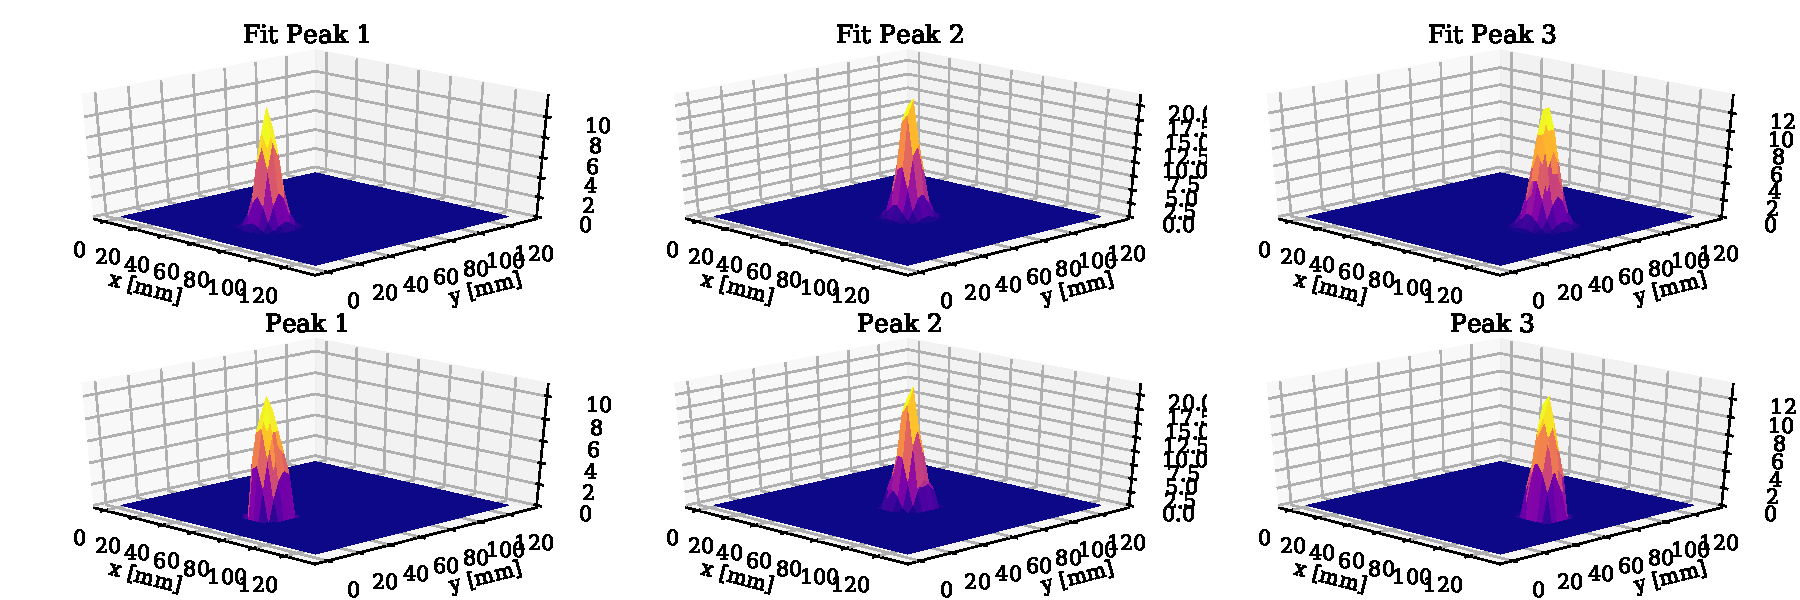
\includegraphics[width=\textwidth]{../auswertung/figs/tom1/filtered_fit.pdf}
  \caption[Fit der Peaks]{Isolierte und gefittete Peaks der
    Quellverteilung. Automatisiert erstellt mithilfe von scipy
    filtern und methoden.\footnote{Ich habe da zu viel Zeit reingesteckt.}}
  \label{fig:tom1-filtered_fit}
\end{figure}

Es ergeben sich mit der Binbreite von \SI{3.375}{\milli\meter} die
in~\ref{tab:positions} zussamengefasst Positionen, Amplituden und
Breiten. Da die Quellen alle gleichgro\ss{} sind, ist es nicht
verwunderlich, dass die Peakbreiten alle \"ahnlich sind. Die
Abweichungen der r\"aumlichen Werte entstanden aus dem Fit und
erscheinen zu gering, um die Ortsaufl\"osung des PET
wiederzuspiegeln. In~\ref{fig:tom1-3dplot}
und~\ref{fig:tom1-filtered_fit} ist zu erkennen, das die Peaks im
allgemeinen kein Plateau zeigen (desswegen auch ein Fit mit der
Gaussfunktion) und \"uber einige Bins hinweg abfallen. Damit wird die
Ortsaufl\"osung, als Unsch\"arfe des Randes der Peaks, in der
Gr\"oss{}enordnung von 2 Bins (\(\approx \SI{6}{\milli\meter}\))
liegen. Das ist auch vertr\"aglich mit der Abweichung der Koordinaten
von den Eckpunkten eines perfekten Quadrates.

\begin{table}[ht]
  \centering
  \begin{tabular}{l|S|S|S|S|S|S|S|S}
    \toprule
    Peak & {\(\mathfrak{A}\)} & {\(\Delta\mathfrak{A}\)} & {\(x\) [\si{\milli\meter}]} &
                                                                                         {\(\Delta
                                                                                         x\)
                                                                                         [\si{\milli\meter}]}
    & {\(y\) [\si{\milli\meter}]} &
                                    {\(\Delta y\) [\si{\milli\meter}]}
    & {\(\sigma\) [\si{\milli\meter}]} &
                                         {\(\Delta \sigma\)
                                         [\si{\milli\meter}]} \\ 

    \midrule
    1 & 11.89 & 0.10 & 65.604 & 0.040 & 35.972 & 0.040 & 4.664 & 0.028 \\
    2 & 22.49 & 0.11 & 67.971 & 0.022 & 64.842 & 0.022 & 4.639 & 0.016 \\
    3 & 14.24 & 0.16 & 94.680 & 0.060 & 65.900 & 0.060 & 5.220 & 0.040
  \end{tabular}
  \caption[Peakpositionen]{Gefitte Peakamplituden, Positionen und
    Breiten. Die Abweichungen ergeben sich aus den
    Fitfehlern. \(\mathfrak{A}\) ist die Amplitude. \(x, y\) sind die Koordinaten
    des Mittelpunktes. \(\sigma\) ist die Standartbreite der Gaussfunktion.}
  \label{tab:positions}
\end{table}

Analog zu~\eqref{eq:acttoday} ergibt sich f\"ur die Aktivität der
\ce{^22Na} Quelle zu Peak 3 mit
\(t=\SI{313632000}{\second},\, t_{1/2} = \SI{2.6027\pm .0010}{a}\)
und \(A_0 = \SI{270}{\kilo\becquerel}\) (1.2.2010,
Abw. \SI{3}{\percent}).

\begin{equation}
  \label{eq:act3today}
  A_3 = \SI{19.1\pm .6}{\kilo\becquerel}
\end{equation}

Damit berechnen sich die in~\ref{tab:peakactivities} aufgelisteten
Aktivit\"aten der beiden anderen Proben wiefolgt durch
verh\"altnissbildung der Peak volumina (\(= 2\pi A\sigma**2\)) die ein
Ma\ss{} f\"ur die Z\"ahlrate geben. Die Abweichungen liegen alle in
der Gr\"o\ss{}enordnung von \SI{3}{\percent} und r\"uhren
haupts\"achlich von der Abweichung der Aktivit\"at \(A_3\) her.

\begin{equation}
  \label{eq:relakt}
  A_i = \frac{\mathfrak{A}_i\cdot\sigma_i^2}{\mathfrak{A}_3\cdot\sigma_3^2}\cdot
  A_3\pm
  A_i\cdot\sqrt{\qty(\frac{\Delta\mathfrak{A}_i}{\mathfrak{A}_i})^2 + \qty(\frac{2\sigma_i}{\sigma_i})^2 +
    \qty(\frac{\Delta\mathfrak{A}_3}{\mathfrak{A}_3})^2 + \qty(\frac{2\sigma_3}{\sigma_3})^2 +
  \qty(\frac{\Delta A_3}{A_3})^2}
\end{equation}

\begin{table}[ht]
  \centering
  \begin{tabular}{l|S|S}
    \toprule
    Peak & {\(A\) [\si{\kilo\becquerel}]} & {\(\Delta A\) [\si{\kilo\becquerel}]} \\
    \midrule
    Peak 1 & 12.7 & .5 \\
    Peak 2 & 23.8 & .9
  \end{tabular}
  \caption[Rekonstruierte Quellaktivit\"aten]{Die
    aus~\eqref{eq:relakt} berechneten Quellaktivit\"aten.}
  \label{tab:peakactivities}
\end{table}


\subsubsection{Anisotrope Dichteverteilung}
\label{sec:tom2}

\begin{figure}[hb]
  \centering 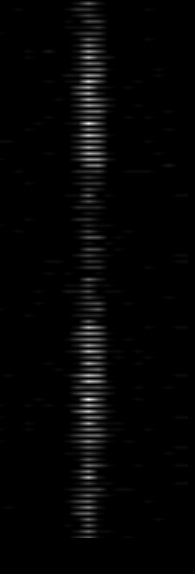
\includegraphics[width=.3\textwidth,
  angle=90]{../messungen/Tom2/tom2_Sinogramm.PNG}
  \caption{Aufgenommenes Sinogramm bei Vermessung einer anisotropen
    Quelldichteverteilung.}
  \label{fig:tom2}
\end{figure}

Analog zu~\ref{sec:tom1} wurde nun eine, von einer unbekannten
konfiguration von Bleim\"unzen umgebene, zentrierte Quelle
vermessen. Die gesammte Anordnung war wieredum in Wax eingebettet.
Auf~\ref{fig:tom2-3dplot} erkennt man deutlich die Quelle als
zentralen Peak, sowie vier mehr oder weniger tiefe \"aler an den
R\"andern, die durch die blockierenden M\"unzen hervorgerufen werden.

Anhand des einbruchs der Z\"ahlzahl im Sinogramm k\"onnen (infolge der
Absorbtion und Steuung der Gammaphotonen durch das Blei) verschiedene
M\"unzenkonfigurationen in klassen einegteilt und unterschieden
werden\footnote{Details aus Platzgr\"unden ausgelassen.}. Im hier
vorliegenden Sinogramm~\ref{fig:tom2} ergkennt man in zwei
Winkelbereichen eine unterschiedlich starke Abschw\"achung. Der erste,
hellere Bereich wurde also warscheinlich von nur einer M\"unze
blockiert, der zweite, dunklere demnach von zwei M\"unzen
(siehe~\ref{fig:munzen}). Diese breiten verdunklungen sind im
isotropen Fall (~\ref{fig:tom1-sino}) nicht zu erkennen. Da bei diesem
Versuch die Quelle genau mittig zwischen den Detektoren lag, ist
in~\ref{fig:tom2} nur eine gerade Linie zu erkennen.
\begin{figure}[h]
  \centering
  \begin{subfigure}{.4\textwidth}
    \centering
    \resizebox{0.8\textwidth}{!}{
      %% Creator: Matplotlib, PGF backend
%%
%% To include the figure in your LaTeX document, write
%%   \input{<filename>.pgf}
%%
%% Make sure the required packages are loaded in your preamble
%%   \usepackage{pgf}
%%
%% Figures using additional raster images can only be included by \input if
%% they are in the same directory as the main LaTeX file. For loading figures
%% from other directories you can use the `import` package
%%   \usepackage{import}
%% and then include the figures with
%%   \import{<path to file>}{<filename>.pgf}
%%
%% Matplotlib used the following preamble
%%   \usepackage{fontspec}
%%
\begingroup%
\makeatletter%
\begin{pgfpicture}%
\pgfpathrectangle{\pgfpointorigin}{\pgfqpoint{6.000000in}{2.000000in}}%
\pgfusepath{use as bounding box, clip}%
\begin{pgfscope}%
\pgfsetbuttcap%
\pgfsetmiterjoin%
\definecolor{currentfill}{rgb}{1.000000,1.000000,1.000000}%
\pgfsetfillcolor{currentfill}%
\pgfsetlinewidth{0.000000pt}%
\definecolor{currentstroke}{rgb}{1.000000,1.000000,1.000000}%
\pgfsetstrokecolor{currentstroke}%
\pgfsetdash{}{0pt}%
\pgfpathmoveto{\pgfqpoint{0.000000in}{0.000000in}}%
\pgfpathlineto{\pgfqpoint{6.000000in}{0.000000in}}%
\pgfpathlineto{\pgfqpoint{6.000000in}{2.000000in}}%
\pgfpathlineto{\pgfqpoint{0.000000in}{2.000000in}}%
\pgfpathclose%
\pgfusepath{fill}%
\end{pgfscope}%
\begin{pgfscope}%
\pgfsetbuttcap%
\pgfsetmiterjoin%
\definecolor{currentfill}{rgb}{1.000000,1.000000,1.000000}%
\pgfsetfillcolor{currentfill}%
\pgfsetlinewidth{0.000000pt}%
\definecolor{currentstroke}{rgb}{0.000000,0.000000,0.000000}%
\pgfsetstrokecolor{currentstroke}%
\pgfsetstrokeopacity{0.000000}%
\pgfsetdash{}{0pt}%
\pgfpathmoveto{\pgfqpoint{0.150000in}{0.150000in}}%
\pgfpathlineto{\pgfqpoint{2.925000in}{0.150000in}}%
\pgfpathlineto{\pgfqpoint{2.925000in}{1.775778in}}%
\pgfpathlineto{\pgfqpoint{0.150000in}{1.775778in}}%
\pgfpathclose%
\pgfusepath{fill}%
\end{pgfscope}%
\begin{pgfscope}%
\pgfsetbuttcap%
\pgfsetmiterjoin%
\definecolor{currentfill}{rgb}{0.950000,0.950000,0.950000}%
\pgfsetfillcolor{currentfill}%
\pgfsetfillopacity{0.500000}%
\pgfsetlinewidth{1.003750pt}%
\definecolor{currentstroke}{rgb}{0.950000,0.950000,0.950000}%
\pgfsetstrokecolor{currentstroke}%
\pgfsetstrokeopacity{0.500000}%
\pgfsetdash{}{0pt}%
\pgfpathmoveto{\pgfqpoint{0.512536in}{0.701938in}}%
\pgfpathlineto{\pgfqpoint{1.575000in}{1.170327in}}%
\pgfpathlineto{\pgfqpoint{1.575000in}{1.769085in}}%
\pgfpathlineto{\pgfqpoint{0.424232in}{1.291294in}}%
\pgfusepath{stroke,fill}%
\end{pgfscope}%
\begin{pgfscope}%
\pgfsetbuttcap%
\pgfsetmiterjoin%
\definecolor{currentfill}{rgb}{0.900000,0.900000,0.900000}%
\pgfsetfillcolor{currentfill}%
\pgfsetfillopacity{0.500000}%
\pgfsetlinewidth{1.003750pt}%
\definecolor{currentstroke}{rgb}{0.900000,0.900000,0.900000}%
\pgfsetstrokecolor{currentstroke}%
\pgfsetstrokeopacity{0.500000}%
\pgfsetdash{}{0pt}%
\pgfpathmoveto{\pgfqpoint{1.575000in}{1.170327in}}%
\pgfpathlineto{\pgfqpoint{2.637464in}{0.701938in}}%
\pgfpathlineto{\pgfqpoint{2.725768in}{1.291294in}}%
\pgfpathlineto{\pgfqpoint{1.575000in}{1.769085in}}%
\pgfusepath{stroke,fill}%
\end{pgfscope}%
\begin{pgfscope}%
\pgfsetbuttcap%
\pgfsetmiterjoin%
\definecolor{currentfill}{rgb}{0.925000,0.925000,0.925000}%
\pgfsetfillcolor{currentfill}%
\pgfsetfillopacity{0.500000}%
\pgfsetlinewidth{1.003750pt}%
\definecolor{currentstroke}{rgb}{0.925000,0.925000,0.925000}%
\pgfsetstrokecolor{currentstroke}%
\pgfsetstrokeopacity{0.500000}%
\pgfsetdash{}{0pt}%
\pgfpathmoveto{\pgfqpoint{0.512536in}{0.701938in}}%
\pgfpathlineto{\pgfqpoint{1.575000in}{0.188864in}}%
\pgfpathlineto{\pgfqpoint{2.637464in}{0.701938in}}%
\pgfpathlineto{\pgfqpoint{1.575000in}{1.170327in}}%
\pgfusepath{stroke,fill}%
\end{pgfscope}%
\begin{pgfscope}%
\pgfsetrectcap%
\pgfsetroundjoin%
\pgfsetlinewidth{0.803000pt}%
\definecolor{currentstroke}{rgb}{0.000000,0.000000,0.000000}%
\pgfsetstrokecolor{currentstroke}%
\pgfsetdash{}{0pt}%
\pgfpathmoveto{\pgfqpoint{0.512536in}{0.701938in}}%
\pgfpathlineto{\pgfqpoint{1.575000in}{0.188864in}}%
\pgfusepath{stroke}%
\end{pgfscope}%
\begin{pgfscope}%
\definecolor{textcolor}{rgb}{0.000000,0.000000,0.000000}%
\pgfsetstrokecolor{textcolor}%
\pgfsetfillcolor{textcolor}%
\pgftext[x=0.502464in,y=0.198156in,left,base,rotate=334.223654]{\color{textcolor}\rmfamily\fontsize{10.000000}{12.000000}\selectfont x [mm]}%
\end{pgfscope}%
\begin{pgfscope}%
\pgfsetbuttcap%
\pgfsetroundjoin%
\pgfsetlinewidth{0.803000pt}%
\definecolor{currentstroke}{rgb}{0.690196,0.690196,0.690196}%
\pgfsetstrokecolor{currentstroke}%
\pgfsetdash{}{0pt}%
\pgfpathmoveto{\pgfqpoint{0.565550in}{0.676337in}}%
\pgfpathlineto{\pgfqpoint{1.628118in}{1.146910in}}%
\pgfpathlineto{\pgfqpoint{1.632336in}{1.745279in}}%
\pgfusepath{stroke}%
\end{pgfscope}%
\begin{pgfscope}%
\pgfsetbuttcap%
\pgfsetroundjoin%
\pgfsetlinewidth{0.803000pt}%
\definecolor{currentstroke}{rgb}{0.690196,0.690196,0.690196}%
\pgfsetstrokecolor{currentstroke}%
\pgfsetdash{}{0pt}%
\pgfpathmoveto{\pgfqpoint{0.740248in}{0.591974in}}%
\pgfpathlineto{\pgfqpoint{1.803083in}{1.069776in}}%
\pgfpathlineto{\pgfqpoint{1.821340in}{1.666806in}}%
\pgfusepath{stroke}%
\end{pgfscope}%
\begin{pgfscope}%
\pgfsetbuttcap%
\pgfsetroundjoin%
\pgfsetlinewidth{0.803000pt}%
\definecolor{currentstroke}{rgb}{0.690196,0.690196,0.690196}%
\pgfsetstrokecolor{currentstroke}%
\pgfsetdash{}{0pt}%
\pgfpathmoveto{\pgfqpoint{0.917701in}{0.506280in}}%
\pgfpathlineto{\pgfqpoint{1.980686in}{0.991480in}}%
\pgfpathlineto{\pgfqpoint{2.013422in}{1.587055in}}%
\pgfusepath{stroke}%
\end{pgfscope}%
\begin{pgfscope}%
\pgfsetbuttcap%
\pgfsetroundjoin%
\pgfsetlinewidth{0.803000pt}%
\definecolor{currentstroke}{rgb}{0.690196,0.690196,0.690196}%
\pgfsetstrokecolor{currentstroke}%
\pgfsetdash{}{0pt}%
\pgfpathmoveto{\pgfqpoint{1.097976in}{0.419223in}}%
\pgfpathlineto{\pgfqpoint{2.160985in}{0.911994in}}%
\pgfpathlineto{\pgfqpoint{2.208660in}{1.505994in}}%
\pgfusepath{stroke}%
\end{pgfscope}%
\begin{pgfscope}%
\pgfsetbuttcap%
\pgfsetroundjoin%
\pgfsetlinewidth{0.803000pt}%
\definecolor{currentstroke}{rgb}{0.690196,0.690196,0.690196}%
\pgfsetstrokecolor{currentstroke}%
\pgfsetdash{}{0pt}%
\pgfpathmoveto{\pgfqpoint{1.281140in}{0.330772in}}%
\pgfpathlineto{\pgfqpoint{2.344045in}{0.831292in}}%
\pgfpathlineto{\pgfqpoint{2.407130in}{1.423590in}}%
\pgfusepath{stroke}%
\end{pgfscope}%
\begin{pgfscope}%
\pgfsetbuttcap%
\pgfsetroundjoin%
\pgfsetlinewidth{0.803000pt}%
\definecolor{currentstroke}{rgb}{0.690196,0.690196,0.690196}%
\pgfsetstrokecolor{currentstroke}%
\pgfsetdash{}{0pt}%
\pgfpathmoveto{\pgfqpoint{1.467263in}{0.240891in}}%
\pgfpathlineto{\pgfqpoint{2.529927in}{0.749346in}}%
\pgfpathlineto{\pgfqpoint{2.608915in}{1.339811in}}%
\pgfusepath{stroke}%
\end{pgfscope}%
\begin{pgfscope}%
\pgfsetrectcap%
\pgfsetroundjoin%
\pgfsetlinewidth{0.803000pt}%
\definecolor{currentstroke}{rgb}{0.000000,0.000000,0.000000}%
\pgfsetstrokecolor{currentstroke}%
\pgfsetdash{}{0pt}%
\pgfpathmoveto{\pgfqpoint{0.574435in}{0.680272in}}%
\pgfpathlineto{\pgfqpoint{0.547760in}{0.668459in}}%
\pgfusepath{stroke}%
\end{pgfscope}%
\begin{pgfscope}%
\definecolor{textcolor}{rgb}{0.000000,0.000000,0.000000}%
\pgfsetstrokecolor{textcolor}%
\pgfsetfillcolor{textcolor}%
\pgftext[x=0.422148in,y=0.532646in,,top]{\color{textcolor}\rmfamily\fontsize{10.000000}{12.000000}\selectfont 0}%
\end{pgfscope}%
\begin{pgfscope}%
\pgfsetrectcap%
\pgfsetroundjoin%
\pgfsetlinewidth{0.803000pt}%
\definecolor{currentstroke}{rgb}{0.000000,0.000000,0.000000}%
\pgfsetstrokecolor{currentstroke}%
\pgfsetdash{}{0pt}%
\pgfpathmoveto{\pgfqpoint{0.749138in}{0.595971in}}%
\pgfpathlineto{\pgfqpoint{0.722447in}{0.583971in}}%
\pgfusepath{stroke}%
\end{pgfscope}%
\begin{pgfscope}%
\definecolor{textcolor}{rgb}{0.000000,0.000000,0.000000}%
\pgfsetstrokecolor{textcolor}%
\pgfsetfillcolor{textcolor}%
\pgftext[x=0.594965in,y=0.447532in,,top]{\color{textcolor}\rmfamily\fontsize{10.000000}{12.000000}\selectfont 25}%
\end{pgfscope}%
\begin{pgfscope}%
\pgfsetrectcap%
\pgfsetroundjoin%
\pgfsetlinewidth{0.803000pt}%
\definecolor{currentstroke}{rgb}{0.000000,0.000000,0.000000}%
\pgfsetstrokecolor{currentstroke}%
\pgfsetdash{}{0pt}%
\pgfpathmoveto{\pgfqpoint{0.926596in}{0.510340in}}%
\pgfpathlineto{\pgfqpoint{0.899892in}{0.498151in}}%
\pgfusepath{stroke}%
\end{pgfscope}%
\begin{pgfscope}%
\definecolor{textcolor}{rgb}{0.000000,0.000000,0.000000}%
\pgfsetstrokecolor{textcolor}%
\pgfsetfillcolor{textcolor}%
\pgftext[x=0.770495in,y=0.361082in,,top]{\color{textcolor}\rmfamily\fontsize{10.000000}{12.000000}\selectfont 50}%
\end{pgfscope}%
\begin{pgfscope}%
\pgfsetrectcap%
\pgfsetroundjoin%
\pgfsetlinewidth{0.803000pt}%
\definecolor{currentstroke}{rgb}{0.000000,0.000000,0.000000}%
\pgfsetstrokecolor{currentstroke}%
\pgfsetdash{}{0pt}%
\pgfpathmoveto{\pgfqpoint{1.106874in}{0.423348in}}%
\pgfpathlineto{\pgfqpoint{1.080160in}{0.410964in}}%
\pgfusepath{stroke}%
\end{pgfscope}%
\begin{pgfscope}%
\definecolor{textcolor}{rgb}{0.000000,0.000000,0.000000}%
\pgfsetstrokecolor{textcolor}%
\pgfsetfillcolor{textcolor}%
\pgftext[x=0.948804in,y=0.273263in,,top]{\color{textcolor}\rmfamily\fontsize{10.000000}{12.000000}\selectfont 75}%
\end{pgfscope}%
\begin{pgfscope}%
\pgfsetrectcap%
\pgfsetroundjoin%
\pgfsetlinewidth{0.803000pt}%
\definecolor{currentstroke}{rgb}{0.000000,0.000000,0.000000}%
\pgfsetstrokecolor{currentstroke}%
\pgfsetdash{}{0pt}%
\pgfpathmoveto{\pgfqpoint{1.290040in}{0.334963in}}%
\pgfpathlineto{\pgfqpoint{1.263319in}{0.322380in}}%
\pgfusepath{stroke}%
\end{pgfscope}%
\begin{pgfscope}%
\definecolor{textcolor}{rgb}{0.000000,0.000000,0.000000}%
\pgfsetstrokecolor{textcolor}%
\pgfsetfillcolor{textcolor}%
\pgftext[x=1.129958in,y=0.184043in,,top]{\color{textcolor}\rmfamily\fontsize{10.000000}{12.000000}\selectfont 100}%
\end{pgfscope}%
\begin{pgfscope}%
\pgfsetrectcap%
\pgfsetroundjoin%
\pgfsetlinewidth{0.803000pt}%
\definecolor{currentstroke}{rgb}{0.000000,0.000000,0.000000}%
\pgfsetstrokecolor{currentstroke}%
\pgfsetdash{}{0pt}%
\pgfpathmoveto{\pgfqpoint{1.476164in}{0.245151in}}%
\pgfpathlineto{\pgfqpoint{1.449439in}{0.232363in}}%
\pgfusepath{stroke}%
\end{pgfscope}%
\begin{pgfscope}%
\definecolor{textcolor}{rgb}{0.000000,0.000000,0.000000}%
\pgfsetstrokecolor{textcolor}%
\pgfsetfillcolor{textcolor}%
\pgftext[x=1.314024in,y=0.093389in,,top]{\color{textcolor}\rmfamily\fontsize{10.000000}{12.000000}\selectfont 125}%
\end{pgfscope}%
\begin{pgfscope}%
\pgfsetrectcap%
\pgfsetroundjoin%
\pgfsetlinewidth{0.803000pt}%
\definecolor{currentstroke}{rgb}{0.000000,0.000000,0.000000}%
\pgfsetstrokecolor{currentstroke}%
\pgfsetdash{}{0pt}%
\pgfpathmoveto{\pgfqpoint{2.637464in}{0.701938in}}%
\pgfpathlineto{\pgfqpoint{1.575000in}{0.188864in}}%
\pgfusepath{stroke}%
\end{pgfscope}%
\begin{pgfscope}%
\definecolor{textcolor}{rgb}{0.000000,0.000000,0.000000}%
\pgfsetstrokecolor{textcolor}%
\pgfsetfillcolor{textcolor}%
\pgftext[x=2.261947in,y=0.011952in,left,base,rotate=25.776346]{\color{textcolor}\rmfamily\fontsize{10.000000}{12.000000}\selectfont y [mm]}%
\end{pgfscope}%
\begin{pgfscope}%
\pgfsetbuttcap%
\pgfsetroundjoin%
\pgfsetlinewidth{0.803000pt}%
\definecolor{currentstroke}{rgb}{0.690196,0.690196,0.690196}%
\pgfsetstrokecolor{currentstroke}%
\pgfsetdash{}{0pt}%
\pgfpathmoveto{\pgfqpoint{0.487046in}{1.317374in}}%
\pgfpathlineto{\pgfqpoint{0.570332in}{0.727418in}}%
\pgfpathlineto{\pgfqpoint{1.632910in}{0.216829in}}%
\pgfusepath{stroke}%
\end{pgfscope}%
\begin{pgfscope}%
\pgfsetbuttcap%
\pgfsetroundjoin%
\pgfsetlinewidth{0.803000pt}%
\definecolor{currentstroke}{rgb}{0.690196,0.690196,0.690196}%
\pgfsetstrokecolor{currentstroke}%
\pgfsetdash{}{0pt}%
\pgfpathmoveto{\pgfqpoint{0.689723in}{1.401524in}}%
\pgfpathlineto{\pgfqpoint{0.756974in}{0.809699in}}%
\pgfpathlineto{\pgfqpoint{1.819829in}{0.307094in}}%
\pgfusepath{stroke}%
\end{pgfscope}%
\begin{pgfscope}%
\pgfsetbuttcap%
\pgfsetroundjoin%
\pgfsetlinewidth{0.803000pt}%
\definecolor{currentstroke}{rgb}{0.690196,0.690196,0.690196}%
\pgfsetstrokecolor{currentstroke}%
\pgfsetdash{}{0pt}%
\pgfpathmoveto{\pgfqpoint{0.889064in}{1.484289in}}%
\pgfpathlineto{\pgfqpoint{0.940775in}{0.890728in}}%
\pgfpathlineto{\pgfqpoint{2.003770in}{0.395921in}}%
\pgfusepath{stroke}%
\end{pgfscope}%
\begin{pgfscope}%
\pgfsetbuttcap%
\pgfsetroundjoin%
\pgfsetlinewidth{0.803000pt}%
\definecolor{currentstroke}{rgb}{0.690196,0.690196,0.690196}%
\pgfsetstrokecolor{currentstroke}%
\pgfsetdash{}{0pt}%
\pgfpathmoveto{\pgfqpoint{1.085150in}{1.565703in}}%
\pgfpathlineto{\pgfqpoint{1.121800in}{0.970533in}}%
\pgfpathlineto{\pgfqpoint{2.184803in}{0.483344in}}%
\pgfusepath{stroke}%
\end{pgfscope}%
\begin{pgfscope}%
\pgfsetbuttcap%
\pgfsetroundjoin%
\pgfsetlinewidth{0.803000pt}%
\definecolor{currentstroke}{rgb}{0.690196,0.690196,0.690196}%
\pgfsetstrokecolor{currentstroke}%
\pgfsetdash{}{0pt}%
\pgfpathmoveto{\pgfqpoint{1.278061in}{1.645798in}}%
\pgfpathlineto{\pgfqpoint{1.300111in}{1.049142in}}%
\pgfpathlineto{\pgfqpoint{2.362998in}{0.569396in}}%
\pgfusepath{stroke}%
\end{pgfscope}%
\begin{pgfscope}%
\pgfsetbuttcap%
\pgfsetroundjoin%
\pgfsetlinewidth{0.803000pt}%
\definecolor{currentstroke}{rgb}{0.690196,0.690196,0.690196}%
\pgfsetstrokecolor{currentstroke}%
\pgfsetdash{}{0pt}%
\pgfpathmoveto{\pgfqpoint{1.467874in}{1.724607in}}%
\pgfpathlineto{\pgfqpoint{1.475769in}{1.126581in}}%
\pgfpathlineto{\pgfqpoint{2.538420in}{0.654109in}}%
\pgfusepath{stroke}%
\end{pgfscope}%
\begin{pgfscope}%
\pgfsetrectcap%
\pgfsetroundjoin%
\pgfsetlinewidth{0.803000pt}%
\definecolor{currentstroke}{rgb}{0.000000,0.000000,0.000000}%
\pgfsetstrokecolor{currentstroke}%
\pgfsetdash{}{0pt}%
\pgfpathmoveto{\pgfqpoint{1.624008in}{0.221107in}}%
\pgfpathlineto{\pgfqpoint{1.650734in}{0.208264in}}%
\pgfusepath{stroke}%
\end{pgfscope}%
\begin{pgfscope}%
\definecolor{textcolor}{rgb}{0.000000,0.000000,0.000000}%
\pgfsetstrokecolor{textcolor}%
\pgfsetfillcolor{textcolor}%
\pgftext[x=1.786701in,y=0.069121in,,top]{\color{textcolor}\rmfamily\fontsize{10.000000}{12.000000}\selectfont 0}%
\end{pgfscope}%
\begin{pgfscope}%
\pgfsetrectcap%
\pgfsetroundjoin%
\pgfsetlinewidth{0.803000pt}%
\definecolor{currentstroke}{rgb}{0.000000,0.000000,0.000000}%
\pgfsetstrokecolor{currentstroke}%
\pgfsetdash{}{0pt}%
\pgfpathmoveto{\pgfqpoint{1.810928in}{0.311303in}}%
\pgfpathlineto{\pgfqpoint{1.837651in}{0.298666in}}%
\pgfusepath{stroke}%
\end{pgfscope}%
\begin{pgfscope}%
\definecolor{textcolor}{rgb}{0.000000,0.000000,0.000000}%
\pgfsetstrokecolor{textcolor}%
\pgfsetfillcolor{textcolor}%
\pgftext[x=1.971551in,y=0.160161in,,top]{\color{textcolor}\rmfamily\fontsize{10.000000}{12.000000}\selectfont 25}%
\end{pgfscope}%
\begin{pgfscope}%
\pgfsetrectcap%
\pgfsetroundjoin%
\pgfsetlinewidth{0.803000pt}%
\definecolor{currentstroke}{rgb}{0.000000,0.000000,0.000000}%
\pgfsetstrokecolor{currentstroke}%
\pgfsetdash{}{0pt}%
\pgfpathmoveto{\pgfqpoint{1.994871in}{0.400063in}}%
\pgfpathlineto{\pgfqpoint{2.021587in}{0.387627in}}%
\pgfusepath{stroke}%
\end{pgfscope}%
\begin{pgfscope}%
\definecolor{textcolor}{rgb}{0.000000,0.000000,0.000000}%
\pgfsetstrokecolor{textcolor}%
\pgfsetfillcolor{textcolor}%
\pgftext[x=2.153470in,y=0.249758in,,top]{\color{textcolor}\rmfamily\fontsize{10.000000}{12.000000}\selectfont 50}%
\end{pgfscope}%
\begin{pgfscope}%
\pgfsetrectcap%
\pgfsetroundjoin%
\pgfsetlinewidth{0.803000pt}%
\definecolor{currentstroke}{rgb}{0.000000,0.000000,0.000000}%
\pgfsetstrokecolor{currentstroke}%
\pgfsetdash{}{0pt}%
\pgfpathmoveto{\pgfqpoint{2.175908in}{0.487421in}}%
\pgfpathlineto{\pgfqpoint{2.202615in}{0.475181in}}%
\pgfusepath{stroke}%
\end{pgfscope}%
\begin{pgfscope}%
\definecolor{textcolor}{rgb}{0.000000,0.000000,0.000000}%
\pgfsetstrokecolor{textcolor}%
\pgfsetfillcolor{textcolor}%
\pgftext[x=2.332526in,y=0.337944in,,top]{\color{textcolor}\rmfamily\fontsize{10.000000}{12.000000}\selectfont 75}%
\end{pgfscope}%
\begin{pgfscope}%
\pgfsetrectcap%
\pgfsetroundjoin%
\pgfsetlinewidth{0.803000pt}%
\definecolor{currentstroke}{rgb}{0.000000,0.000000,0.000000}%
\pgfsetstrokecolor{currentstroke}%
\pgfsetdash{}{0pt}%
\pgfpathmoveto{\pgfqpoint{2.354106in}{0.573409in}}%
\pgfpathlineto{\pgfqpoint{2.380801in}{0.561360in}}%
\pgfusepath{stroke}%
\end{pgfscope}%
\begin{pgfscope}%
\definecolor{textcolor}{rgb}{0.000000,0.000000,0.000000}%
\pgfsetstrokecolor{textcolor}%
\pgfsetfillcolor{textcolor}%
\pgftext[x=2.508786in,y=0.424754in,,top]{\color{textcolor}\rmfamily\fontsize{10.000000}{12.000000}\selectfont 100}%
\end{pgfscope}%
\begin{pgfscope}%
\pgfsetrectcap%
\pgfsetroundjoin%
\pgfsetlinewidth{0.803000pt}%
\definecolor{currentstroke}{rgb}{0.000000,0.000000,0.000000}%
\pgfsetstrokecolor{currentstroke}%
\pgfsetdash{}{0pt}%
\pgfpathmoveto{\pgfqpoint{2.529533in}{0.658060in}}%
\pgfpathlineto{\pgfqpoint{2.556213in}{0.646198in}}%
\pgfusepath{stroke}%
\end{pgfscope}%
\begin{pgfscope}%
\definecolor{textcolor}{rgb}{0.000000,0.000000,0.000000}%
\pgfsetstrokecolor{textcolor}%
\pgfsetfillcolor{textcolor}%
\pgftext[x=2.682316in,y=0.510219in,,top]{\color{textcolor}\rmfamily\fontsize{10.000000}{12.000000}\selectfont 125}%
\end{pgfscope}%
\begin{pgfscope}%
\pgfsetrectcap%
\pgfsetroundjoin%
\pgfsetlinewidth{0.803000pt}%
\definecolor{currentstroke}{rgb}{0.000000,0.000000,0.000000}%
\pgfsetstrokecolor{currentstroke}%
\pgfsetdash{}{0pt}%
\pgfpathmoveto{\pgfqpoint{2.637464in}{0.701938in}}%
\pgfpathlineto{\pgfqpoint{2.725768in}{1.291294in}}%
\pgfusepath{stroke}%
\end{pgfscope}%
\begin{pgfscope}%
\pgfsetbuttcap%
\pgfsetroundjoin%
\pgfsetlinewidth{0.803000pt}%
\definecolor{currentstroke}{rgb}{0.690196,0.690196,0.690196}%
\pgfsetstrokecolor{currentstroke}%
\pgfsetdash{}{0pt}%
\pgfpathmoveto{\pgfqpoint{2.643168in}{0.740008in}}%
\pgfpathlineto{\pgfqpoint{1.575000in}{1.209135in}}%
\pgfpathlineto{\pgfqpoint{0.506832in}{0.740008in}}%
\pgfusepath{stroke}%
\end{pgfscope}%
\begin{pgfscope}%
\pgfsetbuttcap%
\pgfsetroundjoin%
\pgfsetlinewidth{0.803000pt}%
\definecolor{currentstroke}{rgb}{0.690196,0.690196,0.690196}%
\pgfsetstrokecolor{currentstroke}%
\pgfsetdash{}{0pt}%
\pgfpathmoveto{\pgfqpoint{2.661031in}{0.859229in}}%
\pgfpathlineto{\pgfqpoint{1.575000in}{1.330551in}}%
\pgfpathlineto{\pgfqpoint{0.488969in}{0.859229in}}%
\pgfusepath{stroke}%
\end{pgfscope}%
\begin{pgfscope}%
\pgfsetbuttcap%
\pgfsetroundjoin%
\pgfsetlinewidth{0.803000pt}%
\definecolor{currentstroke}{rgb}{0.690196,0.690196,0.690196}%
\pgfsetstrokecolor{currentstroke}%
\pgfsetdash{}{0pt}%
\pgfpathmoveto{\pgfqpoint{2.679502in}{0.982505in}}%
\pgfpathlineto{\pgfqpoint{1.575000in}{1.455909in}}%
\pgfpathlineto{\pgfqpoint{0.470498in}{0.982505in}}%
\pgfusepath{stroke}%
\end{pgfscope}%
\begin{pgfscope}%
\pgfsetbuttcap%
\pgfsetroundjoin%
\pgfsetlinewidth{0.803000pt}%
\definecolor{currentstroke}{rgb}{0.690196,0.690196,0.690196}%
\pgfsetstrokecolor{currentstroke}%
\pgfsetdash{}{0pt}%
\pgfpathmoveto{\pgfqpoint{2.698611in}{1.110047in}}%
\pgfpathlineto{\pgfqpoint{1.575000in}{1.585407in}}%
\pgfpathlineto{\pgfqpoint{0.451389in}{1.110047in}}%
\pgfusepath{stroke}%
\end{pgfscope}%
\begin{pgfscope}%
\pgfsetbuttcap%
\pgfsetroundjoin%
\pgfsetlinewidth{0.803000pt}%
\definecolor{currentstroke}{rgb}{0.690196,0.690196,0.690196}%
\pgfsetstrokecolor{currentstroke}%
\pgfsetdash{}{0pt}%
\pgfpathmoveto{\pgfqpoint{2.718394in}{1.242080in}}%
\pgfpathlineto{\pgfqpoint{1.575000in}{1.719251in}}%
\pgfpathlineto{\pgfqpoint{0.431606in}{1.242080in}}%
\pgfusepath{stroke}%
\end{pgfscope}%
\begin{pgfscope}%
\pgfsetrectcap%
\pgfsetroundjoin%
\pgfsetlinewidth{0.803000pt}%
\definecolor{currentstroke}{rgb}{0.000000,0.000000,0.000000}%
\pgfsetstrokecolor{currentstroke}%
\pgfsetdash{}{0pt}%
\pgfpathmoveto{\pgfqpoint{2.634235in}{0.743931in}}%
\pgfpathlineto{\pgfqpoint{2.661054in}{0.732153in}}%
\pgfusepath{stroke}%
\end{pgfscope}%
\begin{pgfscope}%
\definecolor{textcolor}{rgb}{0.000000,0.000000,0.000000}%
\pgfsetstrokecolor{textcolor}%
\pgfsetfillcolor{textcolor}%
\pgftext[x=2.940908in,y=0.740008in,,top]{\color{textcolor}\rmfamily\fontsize{10.000000}{12.000000}\selectfont 0}%
\end{pgfscope}%
\begin{pgfscope}%
\pgfsetrectcap%
\pgfsetroundjoin%
\pgfsetlinewidth{0.803000pt}%
\definecolor{currentstroke}{rgb}{0.000000,0.000000,0.000000}%
\pgfsetstrokecolor{currentstroke}%
\pgfsetdash{}{0pt}%
\pgfpathmoveto{\pgfqpoint{2.651942in}{0.863173in}}%
\pgfpathlineto{\pgfqpoint{2.679230in}{0.851331in}}%
\pgfusepath{stroke}%
\end{pgfscope}%
\begin{pgfscope}%
\definecolor{textcolor}{rgb}{0.000000,0.000000,0.000000}%
\pgfsetstrokecolor{textcolor}%
\pgfsetfillcolor{textcolor}%
\pgftext[x=2.963750in,y=0.859229in,,top]{\color{textcolor}\rmfamily\fontsize{10.000000}{12.000000}\selectfont 5}%
\end{pgfscope}%
\begin{pgfscope}%
\pgfsetrectcap%
\pgfsetroundjoin%
\pgfsetlinewidth{0.803000pt}%
\definecolor{currentstroke}{rgb}{0.000000,0.000000,0.000000}%
\pgfsetstrokecolor{currentstroke}%
\pgfsetdash{}{0pt}%
\pgfpathmoveto{\pgfqpoint{2.670251in}{0.986470in}}%
\pgfpathlineto{\pgfqpoint{2.698024in}{0.974566in}}%
\pgfusepath{stroke}%
\end{pgfscope}%
\begin{pgfscope}%
\definecolor{textcolor}{rgb}{0.000000,0.000000,0.000000}%
\pgfsetstrokecolor{textcolor}%
\pgfsetfillcolor{textcolor}%
\pgftext[x=2.987369in,y=0.982505in,,top]{\color{textcolor}\rmfamily\fontsize{10.000000}{12.000000}\selectfont 10}%
\end{pgfscope}%
\begin{pgfscope}%
\pgfsetrectcap%
\pgfsetroundjoin%
\pgfsetlinewidth{0.803000pt}%
\definecolor{currentstroke}{rgb}{0.000000,0.000000,0.000000}%
\pgfsetstrokecolor{currentstroke}%
\pgfsetdash{}{0pt}%
\pgfpathmoveto{\pgfqpoint{2.689193in}{1.114031in}}%
\pgfpathlineto{\pgfqpoint{2.717469in}{1.102069in}}%
\pgfusepath{stroke}%
\end{pgfscope}%
\begin{pgfscope}%
\definecolor{textcolor}{rgb}{0.000000,0.000000,0.000000}%
\pgfsetstrokecolor{textcolor}%
\pgfsetfillcolor{textcolor}%
\pgftext[x=3.011805in,y=1.110047in,,top]{\color{textcolor}\rmfamily\fontsize{10.000000}{12.000000}\selectfont 15}%
\end{pgfscope}%
\begin{pgfscope}%
\pgfsetrectcap%
\pgfsetroundjoin%
\pgfsetlinewidth{0.803000pt}%
\definecolor{currentstroke}{rgb}{0.000000,0.000000,0.000000}%
\pgfsetstrokecolor{currentstroke}%
\pgfsetdash{}{0pt}%
\pgfpathmoveto{\pgfqpoint{2.708802in}{1.246082in}}%
\pgfpathlineto{\pgfqpoint{2.737600in}{1.234064in}}%
\pgfusepath{stroke}%
\end{pgfscope}%
\begin{pgfscope}%
\definecolor{textcolor}{rgb}{0.000000,0.000000,0.000000}%
\pgfsetstrokecolor{textcolor}%
\pgfsetfillcolor{textcolor}%
\pgftext[x=3.037102in,y=1.242080in,,top]{\color{textcolor}\rmfamily\fontsize{10.000000}{12.000000}\selectfont 20}%
\end{pgfscope}%
\begin{pgfscope}%
\pgfpathrectangle{\pgfqpoint{0.150000in}{0.150000in}}{\pgfqpoint{2.775000in}{1.625778in}}%
\pgfusepath{clip}%
\pgfsetbuttcap%
\pgfsetroundjoin%
\definecolor{currentfill}{rgb}{0.241396,0.014979,0.610259}%
\pgfsetfillcolor{currentfill}%
\pgfsetlinewidth{0.000000pt}%
\definecolor{currentstroke}{rgb}{0.000000,0.000000,0.000000}%
\pgfsetstrokecolor{currentstroke}%
\pgfsetdash{}{0pt}%
\pgfpathmoveto{\pgfqpoint{1.551285in}{1.173587in}}%
\pgfpathlineto{\pgfqpoint{1.575000in}{1.160513in}}%
\pgfpathlineto{\pgfqpoint{1.598668in}{1.158692in}}%
\pgfpathlineto{\pgfqpoint{1.575000in}{1.180988in}}%
\pgfpathclose%
\pgfusepath{fill}%
\end{pgfscope}%
\begin{pgfscope}%
\pgfpathrectangle{\pgfqpoint{0.150000in}{0.150000in}}{\pgfqpoint{2.775000in}{1.625778in}}%
\pgfusepath{clip}%
\pgfsetbuttcap%
\pgfsetroundjoin%
\definecolor{currentfill}{rgb}{0.214350,0.016973,0.599239}%
\pgfsetfillcolor{currentfill}%
\pgfsetlinewidth{0.000000pt}%
\definecolor{currentstroke}{rgb}{0.000000,0.000000,0.000000}%
\pgfsetstrokecolor{currentstroke}%
\pgfsetdash{}{0pt}%
\pgfpathmoveto{\pgfqpoint{1.575000in}{1.160513in}}%
\pgfpathlineto{\pgfqpoint{1.598731in}{1.142550in}}%
\pgfpathlineto{\pgfqpoint{1.622345in}{1.142007in}}%
\pgfpathlineto{\pgfqpoint{1.598668in}{1.158692in}}%
\pgfpathclose%
\pgfusepath{fill}%
\end{pgfscope}%
\begin{pgfscope}%
\pgfpathrectangle{\pgfqpoint{0.150000in}{0.150000in}}{\pgfqpoint{2.775000in}{1.625778in}}%
\pgfusepath{clip}%
\pgfsetbuttcap%
\pgfsetroundjoin%
\definecolor{currentfill}{rgb}{0.200445,0.017902,0.593364}%
\pgfsetfillcolor{currentfill}%
\pgfsetlinewidth{0.000000pt}%
\definecolor{currentstroke}{rgb}{0.000000,0.000000,0.000000}%
\pgfsetstrokecolor{currentstroke}%
\pgfsetdash{}{0pt}%
\pgfpathmoveto{\pgfqpoint{1.598731in}{1.142550in}}%
\pgfpathlineto{\pgfqpoint{1.622457in}{1.123444in}}%
\pgfpathlineto{\pgfqpoint{1.646111in}{1.133709in}}%
\pgfpathlineto{\pgfqpoint{1.622345in}{1.142007in}}%
\pgfpathclose%
\pgfusepath{fill}%
\end{pgfscope}%
\begin{pgfscope}%
\pgfpathrectangle{\pgfqpoint{0.150000in}{0.150000in}}{\pgfqpoint{2.775000in}{1.625778in}}%
\pgfusepath{clip}%
\pgfsetbuttcap%
\pgfsetroundjoin%
\definecolor{currentfill}{rgb}{0.207435,0.017442,0.596333}%
\pgfsetfillcolor{currentfill}%
\pgfsetlinewidth{0.000000pt}%
\definecolor{currentstroke}{rgb}{0.000000,0.000000,0.000000}%
\pgfsetstrokecolor{currentstroke}%
\pgfsetdash{}{0pt}%
\pgfpathmoveto{\pgfqpoint{1.503924in}{1.130077in}}%
\pgfpathlineto{\pgfqpoint{1.527538in}{1.124206in}}%
\pgfpathlineto{\pgfqpoint{1.551250in}{1.148403in}}%
\pgfpathlineto{\pgfqpoint{1.527604in}{1.150118in}}%
\pgfpathclose%
\pgfusepath{fill}%
\end{pgfscope}%
\begin{pgfscope}%
\pgfpathrectangle{\pgfqpoint{0.150000in}{0.150000in}}{\pgfqpoint{2.775000in}{1.625778in}}%
\pgfusepath{clip}%
\pgfsetbuttcap%
\pgfsetroundjoin%
\definecolor{currentfill}{rgb}{0.186213,0.018803,0.587228}%
\pgfsetfillcolor{currentfill}%
\pgfsetlinewidth{0.000000pt}%
\definecolor{currentstroke}{rgb}{0.000000,0.000000,0.000000}%
\pgfsetstrokecolor{currentstroke}%
\pgfsetdash{}{0pt}%
\pgfpathmoveto{\pgfqpoint{1.622457in}{1.123444in}}%
\pgfpathlineto{\pgfqpoint{1.646254in}{1.112569in}}%
\pgfpathlineto{\pgfqpoint{1.669832in}{1.116988in}}%
\pgfpathlineto{\pgfqpoint{1.646111in}{1.133709in}}%
\pgfpathclose%
\pgfusepath{fill}%
\end{pgfscope}%
\begin{pgfscope}%
\pgfpathrectangle{\pgfqpoint{0.150000in}{0.150000in}}{\pgfqpoint{2.775000in}{1.625778in}}%
\pgfusepath{clip}%
\pgfsetbuttcap%
\pgfsetroundjoin%
\definecolor{currentfill}{rgb}{0.241396,0.014979,0.610259}%
\pgfsetfillcolor{currentfill}%
\pgfsetlinewidth{0.000000pt}%
\definecolor{currentstroke}{rgb}{0.000000,0.000000,0.000000}%
\pgfsetstrokecolor{currentstroke}%
\pgfsetdash{}{0pt}%
\pgfpathmoveto{\pgfqpoint{1.527604in}{1.150118in}}%
\pgfpathlineto{\pgfqpoint{1.551250in}{1.148403in}}%
\pgfpathlineto{\pgfqpoint{1.575000in}{1.160513in}}%
\pgfpathlineto{\pgfqpoint{1.551285in}{1.173587in}}%
\pgfpathclose%
\pgfusepath{fill}%
\end{pgfscope}%
\begin{pgfscope}%
\pgfpathrectangle{\pgfqpoint{0.150000in}{0.150000in}}{\pgfqpoint{2.775000in}{1.625778in}}%
\pgfusepath{clip}%
\pgfsetbuttcap%
\pgfsetroundjoin%
\definecolor{currentfill}{rgb}{0.193374,0.018354,0.590330}%
\pgfsetfillcolor{currentfill}%
\pgfsetlinewidth{0.000000pt}%
\definecolor{currentstroke}{rgb}{0.000000,0.000000,0.000000}%
\pgfsetstrokecolor{currentstroke}%
\pgfsetdash{}{0pt}%
\pgfpathmoveto{\pgfqpoint{1.480021in}{1.128642in}}%
\pgfpathlineto{\pgfqpoint{1.503730in}{1.114256in}}%
\pgfpathlineto{\pgfqpoint{1.527538in}{1.124206in}}%
\pgfpathlineto{\pgfqpoint{1.503924in}{1.130077in}}%
\pgfpathclose%
\pgfusepath{fill}%
\end{pgfscope}%
\begin{pgfscope}%
\pgfpathrectangle{\pgfqpoint{0.150000in}{0.150000in}}{\pgfqpoint{2.775000in}{1.625778in}}%
\pgfusepath{clip}%
\pgfsetbuttcap%
\pgfsetroundjoin%
\definecolor{currentfill}{rgb}{0.171574,0.019706,0.580806}%
\pgfsetfillcolor{currentfill}%
\pgfsetlinewidth{0.000000pt}%
\definecolor{currentstroke}{rgb}{0.000000,0.000000,0.000000}%
\pgfsetstrokecolor{currentstroke}%
\pgfsetdash{}{0pt}%
\pgfpathmoveto{\pgfqpoint{1.646254in}{1.112569in}}%
\pgfpathlineto{\pgfqpoint{1.670014in}{1.095109in}}%
\pgfpathlineto{\pgfqpoint{1.693600in}{1.102635in}}%
\pgfpathlineto{\pgfqpoint{1.669832in}{1.116988in}}%
\pgfpathclose%
\pgfusepath{fill}%
\end{pgfscope}%
\begin{pgfscope}%
\pgfpathrectangle{\pgfqpoint{0.150000in}{0.150000in}}{\pgfqpoint{2.775000in}{1.625778in}}%
\pgfusepath{clip}%
\pgfsetbuttcap%
\pgfsetroundjoin%
\definecolor{currentfill}{rgb}{0.156421,0.020651,0.574065}%
\pgfsetfillcolor{currentfill}%
\pgfsetlinewidth{0.000000pt}%
\definecolor{currentstroke}{rgb}{0.000000,0.000000,0.000000}%
\pgfsetstrokecolor{currentstroke}%
\pgfsetdash{}{0pt}%
\pgfpathmoveto{\pgfqpoint{1.670014in}{1.095109in}}%
\pgfpathlineto{\pgfqpoint{1.693866in}{1.083087in}}%
\pgfpathlineto{\pgfqpoint{1.717389in}{1.088161in}}%
\pgfpathlineto{\pgfqpoint{1.693600in}{1.102635in}}%
\pgfpathclose%
\pgfusepath{fill}%
\end{pgfscope}%
\begin{pgfscope}%
\pgfpathrectangle{\pgfqpoint{0.150000in}{0.150000in}}{\pgfqpoint{2.775000in}{1.625778in}}%
\pgfusepath{clip}%
\pgfsetbuttcap%
\pgfsetroundjoin%
\definecolor{currentfill}{rgb}{0.241396,0.014979,0.610259}%
\pgfsetfillcolor{currentfill}%
\pgfsetlinewidth{0.000000pt}%
\definecolor{currentstroke}{rgb}{0.000000,0.000000,0.000000}%
\pgfsetstrokecolor{currentstroke}%
\pgfsetdash{}{0pt}%
\pgfpathmoveto{\pgfqpoint{1.551250in}{1.148403in}}%
\pgfpathlineto{\pgfqpoint{1.575000in}{1.138543in}}%
\pgfpathlineto{\pgfqpoint{1.598731in}{1.142550in}}%
\pgfpathlineto{\pgfqpoint{1.575000in}{1.160513in}}%
\pgfpathclose%
\pgfusepath{fill}%
\end{pgfscope}%
\begin{pgfscope}%
\pgfpathrectangle{\pgfqpoint{0.150000in}{0.150000in}}{\pgfqpoint{2.775000in}{1.625778in}}%
\pgfusepath{clip}%
\pgfsetbuttcap%
\pgfsetroundjoin%
\definecolor{currentfill}{rgb}{0.227983,0.016007,0.604867}%
\pgfsetfillcolor{currentfill}%
\pgfsetlinewidth{0.000000pt}%
\definecolor{currentstroke}{rgb}{0.000000,0.000000,0.000000}%
\pgfsetstrokecolor{currentstroke}%
\pgfsetdash{}{0pt}%
\pgfpathmoveto{\pgfqpoint{1.575000in}{1.138543in}}%
\pgfpathlineto{\pgfqpoint{1.598793in}{1.125581in}}%
\pgfpathlineto{\pgfqpoint{1.622457in}{1.123444in}}%
\pgfpathlineto{\pgfqpoint{1.598731in}{1.142550in}}%
\pgfpathclose%
\pgfusepath{fill}%
\end{pgfscope}%
\begin{pgfscope}%
\pgfpathrectangle{\pgfqpoint{0.150000in}{0.150000in}}{\pgfqpoint{2.775000in}{1.625778in}}%
\pgfusepath{clip}%
\pgfsetbuttcap%
\pgfsetroundjoin%
\definecolor{currentfill}{rgb}{0.234715,0.015502,0.607592}%
\pgfsetfillcolor{currentfill}%
\pgfsetlinewidth{0.000000pt}%
\definecolor{currentstroke}{rgb}{0.000000,0.000000,0.000000}%
\pgfsetstrokecolor{currentstroke}%
\pgfsetdash{}{0pt}%
\pgfpathmoveto{\pgfqpoint{1.527538in}{1.124206in}}%
\pgfpathlineto{\pgfqpoint{1.551209in}{1.125006in}}%
\pgfpathlineto{\pgfqpoint{1.575000in}{1.138543in}}%
\pgfpathlineto{\pgfqpoint{1.551250in}{1.148403in}}%
\pgfpathclose%
\pgfusepath{fill}%
\end{pgfscope}%
\begin{pgfscope}%
\pgfpathrectangle{\pgfqpoint{0.150000in}{0.150000in}}{\pgfqpoint{2.775000in}{1.625778in}}%
\pgfusepath{clip}%
\pgfsetbuttcap%
\pgfsetroundjoin%
\definecolor{currentfill}{rgb}{0.207435,0.017442,0.596333}%
\pgfsetfillcolor{currentfill}%
\pgfsetlinewidth{0.000000pt}%
\definecolor{currentstroke}{rgb}{0.000000,0.000000,0.000000}%
\pgfsetstrokecolor{currentstroke}%
\pgfsetdash{}{0pt}%
\pgfpathmoveto{\pgfqpoint{1.598793in}{1.125581in}}%
\pgfpathlineto{\pgfqpoint{1.622560in}{1.103481in}}%
\pgfpathlineto{\pgfqpoint{1.646254in}{1.112569in}}%
\pgfpathlineto{\pgfqpoint{1.622457in}{1.123444in}}%
\pgfpathclose%
\pgfusepath{fill}%
\end{pgfscope}%
\begin{pgfscope}%
\pgfpathrectangle{\pgfqpoint{0.150000in}{0.150000in}}{\pgfqpoint{2.775000in}{1.625778in}}%
\pgfusepath{clip}%
\pgfsetbuttcap%
\pgfsetroundjoin%
\definecolor{currentfill}{rgb}{0.148607,0.021154,0.570562}%
\pgfsetfillcolor{currentfill}%
\pgfsetlinewidth{0.000000pt}%
\definecolor{currentstroke}{rgb}{0.000000,0.000000,0.000000}%
\pgfsetstrokecolor{currentstroke}%
\pgfsetdash{}{0pt}%
\pgfpathmoveto{\pgfqpoint{1.693866in}{1.083087in}}%
\pgfpathlineto{\pgfqpoint{1.717737in}{1.070043in}}%
\pgfpathlineto{\pgfqpoint{1.741330in}{1.079396in}}%
\pgfpathlineto{\pgfqpoint{1.717389in}{1.088161in}}%
\pgfpathclose%
\pgfusepath{fill}%
\end{pgfscope}%
\begin{pgfscope}%
\pgfpathrectangle{\pgfqpoint{0.150000in}{0.150000in}}{\pgfqpoint{2.775000in}{1.625778in}}%
\pgfusepath{clip}%
\pgfsetbuttcap%
\pgfsetroundjoin%
\definecolor{currentfill}{rgb}{0.207435,0.017442,0.596333}%
\pgfsetfillcolor{currentfill}%
\pgfsetlinewidth{0.000000pt}%
\definecolor{currentstroke}{rgb}{0.000000,0.000000,0.000000}%
\pgfsetstrokecolor{currentstroke}%
\pgfsetdash{}{0pt}%
\pgfpathmoveto{\pgfqpoint{1.503730in}{1.114256in}}%
\pgfpathlineto{\pgfqpoint{1.527434in}{1.104379in}}%
\pgfpathlineto{\pgfqpoint{1.551209in}{1.125006in}}%
\pgfpathlineto{\pgfqpoint{1.527538in}{1.124206in}}%
\pgfpathclose%
\pgfusepath{fill}%
\end{pgfscope}%
\begin{pgfscope}%
\pgfpathrectangle{\pgfqpoint{0.150000in}{0.150000in}}{\pgfqpoint{2.775000in}{1.625778in}}%
\pgfusepath{clip}%
\pgfsetbuttcap%
\pgfsetroundjoin%
\definecolor{currentfill}{rgb}{0.186213,0.018803,0.587228}%
\pgfsetfillcolor{currentfill}%
\pgfsetlinewidth{0.000000pt}%
\definecolor{currentstroke}{rgb}{0.000000,0.000000,0.000000}%
\pgfsetstrokecolor{currentstroke}%
\pgfsetdash{}{0pt}%
\pgfpathmoveto{\pgfqpoint{1.622560in}{1.103481in}}%
\pgfpathlineto{\pgfqpoint{1.646389in}{1.090335in}}%
\pgfpathlineto{\pgfqpoint{1.670014in}{1.095109in}}%
\pgfpathlineto{\pgfqpoint{1.646254in}{1.112569in}}%
\pgfpathclose%
\pgfusepath{fill}%
\end{pgfscope}%
\begin{pgfscope}%
\pgfpathrectangle{\pgfqpoint{0.150000in}{0.150000in}}{\pgfqpoint{2.775000in}{1.625778in}}%
\pgfusepath{clip}%
\pgfsetbuttcap%
\pgfsetroundjoin%
\definecolor{currentfill}{rgb}{0.221197,0.016497,0.602083}%
\pgfsetfillcolor{currentfill}%
\pgfsetlinewidth{0.000000pt}%
\definecolor{currentstroke}{rgb}{0.000000,0.000000,0.000000}%
\pgfsetstrokecolor{currentstroke}%
\pgfsetdash{}{0pt}%
\pgfpathmoveto{\pgfqpoint{1.456018in}{1.126814in}}%
\pgfpathlineto{\pgfqpoint{1.479749in}{1.113780in}}%
\pgfpathlineto{\pgfqpoint{1.503730in}{1.114256in}}%
\pgfpathlineto{\pgfqpoint{1.480021in}{1.128642in}}%
\pgfpathclose%
\pgfusepath{fill}%
\end{pgfscope}%
\begin{pgfscope}%
\pgfpathrectangle{\pgfqpoint{0.150000in}{0.150000in}}{\pgfqpoint{2.775000in}{1.625778in}}%
\pgfusepath{clip}%
\pgfsetbuttcap%
\pgfsetroundjoin%
\definecolor{currentfill}{rgb}{0.171574,0.019706,0.580806}%
\pgfsetfillcolor{currentfill}%
\pgfsetlinewidth{0.000000pt}%
\definecolor{currentstroke}{rgb}{0.000000,0.000000,0.000000}%
\pgfsetstrokecolor{currentstroke}%
\pgfsetdash{}{0pt}%
\pgfpathmoveto{\pgfqpoint{1.646389in}{1.090335in}}%
\pgfpathlineto{\pgfqpoint{1.670250in}{1.077257in}}%
\pgfpathlineto{\pgfqpoint{1.693866in}{1.083087in}}%
\pgfpathlineto{\pgfqpoint{1.670014in}{1.095109in}}%
\pgfpathclose%
\pgfusepath{fill}%
\end{pgfscope}%
\begin{pgfscope}%
\pgfpathrectangle{\pgfqpoint{0.150000in}{0.150000in}}{\pgfqpoint{2.775000in}{1.625778in}}%
\pgfusepath{clip}%
\pgfsetbuttcap%
\pgfsetroundjoin%
\definecolor{currentfill}{rgb}{0.214350,0.016973,0.599239}%
\pgfsetfillcolor{currentfill}%
\pgfsetlinewidth{0.000000pt}%
\definecolor{currentstroke}{rgb}{0.000000,0.000000,0.000000}%
\pgfsetstrokecolor{currentstroke}%
\pgfsetdash{}{0pt}%
\pgfpathmoveto{\pgfqpoint{1.479749in}{1.113780in}}%
\pgfpathlineto{\pgfqpoint{1.503533in}{1.098590in}}%
\pgfpathlineto{\pgfqpoint{1.527434in}{1.104379in}}%
\pgfpathlineto{\pgfqpoint{1.503730in}{1.114256in}}%
\pgfpathclose%
\pgfusepath{fill}%
\end{pgfscope}%
\begin{pgfscope}%
\pgfpathrectangle{\pgfqpoint{0.150000in}{0.150000in}}{\pgfqpoint{2.775000in}{1.625778in}}%
\pgfusepath{clip}%
\pgfsetbuttcap%
\pgfsetroundjoin%
\definecolor{currentfill}{rgb}{0.156421,0.020651,0.574065}%
\pgfsetfillcolor{currentfill}%
\pgfsetlinewidth{0.000000pt}%
\definecolor{currentstroke}{rgb}{0.000000,0.000000,0.000000}%
\pgfsetstrokecolor{currentstroke}%
\pgfsetdash{}{0pt}%
\pgfpathmoveto{\pgfqpoint{1.717737in}{1.070043in}}%
\pgfpathlineto{\pgfqpoint{1.741680in}{1.058693in}}%
\pgfpathlineto{\pgfqpoint{1.765544in}{1.078974in}}%
\pgfpathlineto{\pgfqpoint{1.741330in}{1.079396in}}%
\pgfpathclose%
\pgfusepath{fill}%
\end{pgfscope}%
\begin{pgfscope}%
\pgfpathrectangle{\pgfqpoint{0.150000in}{0.150000in}}{\pgfqpoint{2.775000in}{1.625778in}}%
\pgfusepath{clip}%
\pgfsetbuttcap%
\pgfsetroundjoin%
\definecolor{currentfill}{rgb}{0.241396,0.014979,0.610259}%
\pgfsetfillcolor{currentfill}%
\pgfsetlinewidth{0.000000pt}%
\definecolor{currentstroke}{rgb}{0.000000,0.000000,0.000000}%
\pgfsetstrokecolor{currentstroke}%
\pgfsetdash{}{0pt}%
\pgfpathmoveto{\pgfqpoint{1.551209in}{1.125006in}}%
\pgfpathlineto{\pgfqpoint{1.575000in}{1.116829in}}%
\pgfpathlineto{\pgfqpoint{1.598793in}{1.125581in}}%
\pgfpathlineto{\pgfqpoint{1.575000in}{1.138543in}}%
\pgfpathclose%
\pgfusepath{fill}%
\end{pgfscope}%
\begin{pgfscope}%
\pgfpathrectangle{\pgfqpoint{0.150000in}{0.150000in}}{\pgfqpoint{2.775000in}{1.625778in}}%
\pgfusepath{clip}%
\pgfsetbuttcap%
\pgfsetroundjoin%
\definecolor{currentfill}{rgb}{0.164070,0.020171,0.577478}%
\pgfsetfillcolor{currentfill}%
\pgfsetlinewidth{0.000000pt}%
\definecolor{currentstroke}{rgb}{0.000000,0.000000,0.000000}%
\pgfsetstrokecolor{currentstroke}%
\pgfsetdash{}{0pt}%
\pgfpathmoveto{\pgfqpoint{1.670250in}{1.077257in}}%
\pgfpathlineto{\pgfqpoint{1.694157in}{1.064931in}}%
\pgfpathlineto{\pgfqpoint{1.717737in}{1.070043in}}%
\pgfpathlineto{\pgfqpoint{1.693866in}{1.083087in}}%
\pgfpathclose%
\pgfusepath{fill}%
\end{pgfscope}%
\begin{pgfscope}%
\pgfpathrectangle{\pgfqpoint{0.150000in}{0.150000in}}{\pgfqpoint{2.775000in}{1.625778in}}%
\pgfusepath{clip}%
\pgfsetbuttcap%
\pgfsetroundjoin%
\definecolor{currentfill}{rgb}{0.227983,0.016007,0.604867}%
\pgfsetfillcolor{currentfill}%
\pgfsetlinewidth{0.000000pt}%
\definecolor{currentstroke}{rgb}{0.000000,0.000000,0.000000}%
\pgfsetstrokecolor{currentstroke}%
\pgfsetdash{}{0pt}%
\pgfpathmoveto{\pgfqpoint{1.527434in}{1.104379in}}%
\pgfpathlineto{\pgfqpoint{1.551175in}{1.099410in}}%
\pgfpathlineto{\pgfqpoint{1.575000in}{1.116829in}}%
\pgfpathlineto{\pgfqpoint{1.551209in}{1.125006in}}%
\pgfpathclose%
\pgfusepath{fill}%
\end{pgfscope}%
\begin{pgfscope}%
\pgfpathrectangle{\pgfqpoint{0.150000in}{0.150000in}}{\pgfqpoint{2.775000in}{1.625778in}}%
\pgfusepath{clip}%
\pgfsetbuttcap%
\pgfsetroundjoin%
\definecolor{currentfill}{rgb}{0.227983,0.016007,0.604867}%
\pgfsetfillcolor{currentfill}%
\pgfsetlinewidth{0.000000pt}%
\definecolor{currentstroke}{rgb}{0.000000,0.000000,0.000000}%
\pgfsetstrokecolor{currentstroke}%
\pgfsetdash{}{0pt}%
\pgfpathmoveto{\pgfqpoint{1.575000in}{1.116829in}}%
\pgfpathlineto{\pgfqpoint{1.598835in}{1.102572in}}%
\pgfpathlineto{\pgfqpoint{1.622560in}{1.103481in}}%
\pgfpathlineto{\pgfqpoint{1.598793in}{1.125581in}}%
\pgfpathclose%
\pgfusepath{fill}%
\end{pgfscope}%
\begin{pgfscope}%
\pgfpathrectangle{\pgfqpoint{0.150000in}{0.150000in}}{\pgfqpoint{2.775000in}{1.625778in}}%
\pgfusepath{clip}%
\pgfsetbuttcap%
\pgfsetroundjoin%
\definecolor{currentfill}{rgb}{0.227983,0.016007,0.604867}%
\pgfsetfillcolor{currentfill}%
\pgfsetlinewidth{0.000000pt}%
\definecolor{currentstroke}{rgb}{0.000000,0.000000,0.000000}%
\pgfsetstrokecolor{currentstroke}%
\pgfsetdash{}{0pt}%
\pgfpathmoveto{\pgfqpoint{1.432247in}{1.107257in}}%
\pgfpathlineto{\pgfqpoint{1.455826in}{1.102440in}}%
\pgfpathlineto{\pgfqpoint{1.479749in}{1.113780in}}%
\pgfpathlineto{\pgfqpoint{1.456018in}{1.126814in}}%
\pgfpathclose%
\pgfusepath{fill}%
\end{pgfscope}%
\begin{pgfscope}%
\pgfpathrectangle{\pgfqpoint{0.150000in}{0.150000in}}{\pgfqpoint{2.775000in}{1.625778in}}%
\pgfusepath{clip}%
\pgfsetbuttcap%
\pgfsetroundjoin%
\definecolor{currentfill}{rgb}{0.207435,0.017442,0.596333}%
\pgfsetfillcolor{currentfill}%
\pgfsetlinewidth{0.000000pt}%
\definecolor{currentstroke}{rgb}{0.000000,0.000000,0.000000}%
\pgfsetstrokecolor{currentstroke}%
\pgfsetdash{}{0pt}%
\pgfpathmoveto{\pgfqpoint{1.598835in}{1.102572in}}%
\pgfpathlineto{\pgfqpoint{1.622674in}{1.084959in}}%
\pgfpathlineto{\pgfqpoint{1.646389in}{1.090335in}}%
\pgfpathlineto{\pgfqpoint{1.622560in}{1.103481in}}%
\pgfpathclose%
\pgfusepath{fill}%
\end{pgfscope}%
\begin{pgfscope}%
\pgfpathrectangle{\pgfqpoint{0.150000in}{0.150000in}}{\pgfqpoint{2.775000in}{1.625778in}}%
\pgfusepath{clip}%
\pgfsetbuttcap%
\pgfsetroundjoin%
\definecolor{currentfill}{rgb}{0.207435,0.017442,0.596333}%
\pgfsetfillcolor{currentfill}%
\pgfsetlinewidth{0.000000pt}%
\definecolor{currentstroke}{rgb}{0.000000,0.000000,0.000000}%
\pgfsetstrokecolor{currentstroke}%
\pgfsetdash{}{0pt}%
\pgfpathmoveto{\pgfqpoint{1.408470in}{1.088383in}}%
\pgfpathlineto{\pgfqpoint{1.431999in}{1.083808in}}%
\pgfpathlineto{\pgfqpoint{1.455826in}{1.102440in}}%
\pgfpathlineto{\pgfqpoint{1.432247in}{1.107257in}}%
\pgfpathclose%
\pgfusepath{fill}%
\end{pgfscope}%
\begin{pgfscope}%
\pgfpathrectangle{\pgfqpoint{0.150000in}{0.150000in}}{\pgfqpoint{2.775000in}{1.625778in}}%
\pgfusepath{clip}%
\pgfsetbuttcap%
\pgfsetroundjoin%
\definecolor{currentfill}{rgb}{0.148607,0.021154,0.570562}%
\pgfsetfillcolor{currentfill}%
\pgfsetlinewidth{0.000000pt}%
\definecolor{currentstroke}{rgb}{0.000000,0.000000,0.000000}%
\pgfsetstrokecolor{currentstroke}%
\pgfsetdash{}{0pt}%
\pgfpathmoveto{\pgfqpoint{1.694157in}{1.064931in}}%
\pgfpathlineto{\pgfqpoint{1.717987in}{1.046624in}}%
\pgfpathlineto{\pgfqpoint{1.741680in}{1.058693in}}%
\pgfpathlineto{\pgfqpoint{1.717737in}{1.070043in}}%
\pgfpathclose%
\pgfusepath{fill}%
\end{pgfscope}%
\begin{pgfscope}%
\pgfpathrectangle{\pgfqpoint{0.150000in}{0.150000in}}{\pgfqpoint{2.775000in}{1.625778in}}%
\pgfusepath{clip}%
\pgfsetbuttcap%
\pgfsetroundjoin%
\definecolor{currentfill}{rgb}{0.214350,0.016973,0.599239}%
\pgfsetfillcolor{currentfill}%
\pgfsetlinewidth{0.000000pt}%
\definecolor{currentstroke}{rgb}{0.000000,0.000000,0.000000}%
\pgfsetstrokecolor{currentstroke}%
\pgfsetdash{}{0pt}%
\pgfpathmoveto{\pgfqpoint{1.503533in}{1.098590in}}%
\pgfpathlineto{\pgfqpoint{1.527302in}{1.088625in}}%
\pgfpathlineto{\pgfqpoint{1.551175in}{1.099410in}}%
\pgfpathlineto{\pgfqpoint{1.527434in}{1.104379in}}%
\pgfpathclose%
\pgfusepath{fill}%
\end{pgfscope}%
\begin{pgfscope}%
\pgfpathrectangle{\pgfqpoint{0.150000in}{0.150000in}}{\pgfqpoint{2.775000in}{1.625778in}}%
\pgfusepath{clip}%
\pgfsetbuttcap%
\pgfsetroundjoin%
\definecolor{currentfill}{rgb}{0.193374,0.018354,0.590330}%
\pgfsetfillcolor{currentfill}%
\pgfsetlinewidth{0.000000pt}%
\definecolor{currentstroke}{rgb}{0.000000,0.000000,0.000000}%
\pgfsetstrokecolor{currentstroke}%
\pgfsetdash{}{0pt}%
\pgfpathmoveto{\pgfqpoint{1.622674in}{1.084959in}}%
\pgfpathlineto{\pgfqpoint{1.646551in}{1.070915in}}%
\pgfpathlineto{\pgfqpoint{1.670250in}{1.077257in}}%
\pgfpathlineto{\pgfqpoint{1.646389in}{1.090335in}}%
\pgfpathclose%
\pgfusepath{fill}%
\end{pgfscope}%
\begin{pgfscope}%
\pgfpathrectangle{\pgfqpoint{0.150000in}{0.150000in}}{\pgfqpoint{2.775000in}{1.625778in}}%
\pgfusepath{clip}%
\pgfsetbuttcap%
\pgfsetroundjoin%
\definecolor{currentfill}{rgb}{0.200445,0.017902,0.593364}%
\pgfsetfillcolor{currentfill}%
\pgfsetlinewidth{0.000000pt}%
\definecolor{currentstroke}{rgb}{0.000000,0.000000,0.000000}%
\pgfsetstrokecolor{currentstroke}%
\pgfsetdash{}{0pt}%
\pgfpathmoveto{\pgfqpoint{1.384252in}{1.086947in}}%
\pgfpathlineto{\pgfqpoint{1.408038in}{1.071285in}}%
\pgfpathlineto{\pgfqpoint{1.431999in}{1.083808in}}%
\pgfpathlineto{\pgfqpoint{1.408470in}{1.088383in}}%
\pgfpathclose%
\pgfusepath{fill}%
\end{pgfscope}%
\begin{pgfscope}%
\pgfpathrectangle{\pgfqpoint{0.150000in}{0.150000in}}{\pgfqpoint{2.775000in}{1.625778in}}%
\pgfusepath{clip}%
\pgfsetbuttcap%
\pgfsetroundjoin%
\definecolor{currentfill}{rgb}{0.140603,0.021687,0.566959}%
\pgfsetfillcolor{currentfill}%
\pgfsetlinewidth{0.000000pt}%
\definecolor{currentstroke}{rgb}{0.000000,0.000000,0.000000}%
\pgfsetstrokecolor{currentstroke}%
\pgfsetdash{}{0pt}%
\pgfpathmoveto{\pgfqpoint{1.717987in}{1.046624in}}%
\pgfpathlineto{\pgfqpoint{1.741907in}{1.032370in}}%
\pgfpathlineto{\pgfqpoint{1.765807in}{1.052790in}}%
\pgfpathlineto{\pgfqpoint{1.741680in}{1.058693in}}%
\pgfpathclose%
\pgfusepath{fill}%
\end{pgfscope}%
\begin{pgfscope}%
\pgfpathrectangle{\pgfqpoint{0.150000in}{0.150000in}}{\pgfqpoint{2.775000in}{1.625778in}}%
\pgfusepath{clip}%
\pgfsetbuttcap%
\pgfsetroundjoin%
\definecolor{currentfill}{rgb}{0.234715,0.015502,0.607592}%
\pgfsetfillcolor{currentfill}%
\pgfsetlinewidth{0.000000pt}%
\definecolor{currentstroke}{rgb}{0.000000,0.000000,0.000000}%
\pgfsetstrokecolor{currentstroke}%
\pgfsetdash{}{0pt}%
\pgfpathmoveto{\pgfqpoint{1.551175in}{1.099410in}}%
\pgfpathlineto{\pgfqpoint{1.575000in}{1.093160in}}%
\pgfpathlineto{\pgfqpoint{1.598835in}{1.102572in}}%
\pgfpathlineto{\pgfqpoint{1.575000in}{1.116829in}}%
\pgfpathclose%
\pgfusepath{fill}%
\end{pgfscope}%
\begin{pgfscope}%
\pgfpathrectangle{\pgfqpoint{0.150000in}{0.150000in}}{\pgfqpoint{2.775000in}{1.625778in}}%
\pgfusepath{clip}%
\pgfsetbuttcap%
\pgfsetroundjoin%
\definecolor{currentfill}{rgb}{0.178950,0.019252,0.584054}%
\pgfsetfillcolor{currentfill}%
\pgfsetlinewidth{0.000000pt}%
\definecolor{currentstroke}{rgb}{0.000000,0.000000,0.000000}%
\pgfsetstrokecolor{currentstroke}%
\pgfsetdash{}{0pt}%
\pgfpathmoveto{\pgfqpoint{1.741680in}{1.058693in}}%
\pgfpathlineto{\pgfqpoint{1.765807in}{1.052790in}}%
\pgfpathlineto{\pgfqpoint{1.789894in}{1.079239in}}%
\pgfpathlineto{\pgfqpoint{1.765544in}{1.078974in}}%
\pgfpathclose%
\pgfusepath{fill}%
\end{pgfscope}%
\begin{pgfscope}%
\pgfpathrectangle{\pgfqpoint{0.150000in}{0.150000in}}{\pgfqpoint{2.775000in}{1.625778in}}%
\pgfusepath{clip}%
\pgfsetbuttcap%
\pgfsetroundjoin%
\definecolor{currentfill}{rgb}{0.241396,0.014979,0.610259}%
\pgfsetfillcolor{currentfill}%
\pgfsetlinewidth{0.000000pt}%
\definecolor{currentstroke}{rgb}{0.000000,0.000000,0.000000}%
\pgfsetstrokecolor{currentstroke}%
\pgfsetdash{}{0pt}%
\pgfpathmoveto{\pgfqpoint{1.455826in}{1.102440in}}%
\pgfpathlineto{\pgfqpoint{1.479436in}{1.101871in}}%
\pgfpathlineto{\pgfqpoint{1.503533in}{1.098590in}}%
\pgfpathlineto{\pgfqpoint{1.479749in}{1.113780in}}%
\pgfpathclose%
\pgfusepath{fill}%
\end{pgfscope}%
\begin{pgfscope}%
\pgfpathrectangle{\pgfqpoint{0.150000in}{0.150000in}}{\pgfqpoint{2.775000in}{1.625778in}}%
\pgfusepath{clip}%
\pgfsetbuttcap%
\pgfsetroundjoin%
\definecolor{currentfill}{rgb}{0.186213,0.018803,0.587228}%
\pgfsetfillcolor{currentfill}%
\pgfsetlinewidth{0.000000pt}%
\definecolor{currentstroke}{rgb}{0.000000,0.000000,0.000000}%
\pgfsetstrokecolor{currentstroke}%
\pgfsetdash{}{0pt}%
\pgfpathmoveto{\pgfqpoint{1.646551in}{1.070915in}}%
\pgfpathlineto{\pgfqpoint{1.670501in}{1.060436in}}%
\pgfpathlineto{\pgfqpoint{1.694157in}{1.064931in}}%
\pgfpathlineto{\pgfqpoint{1.670250in}{1.077257in}}%
\pgfpathclose%
\pgfusepath{fill}%
\end{pgfscope}%
\begin{pgfscope}%
\pgfpathrectangle{\pgfqpoint{0.150000in}{0.150000in}}{\pgfqpoint{2.775000in}{1.625778in}}%
\pgfusepath{clip}%
\pgfsetbuttcap%
\pgfsetroundjoin%
\definecolor{currentfill}{rgb}{0.221197,0.016497,0.602083}%
\pgfsetfillcolor{currentfill}%
\pgfsetlinewidth{0.000000pt}%
\definecolor{currentstroke}{rgb}{0.000000,0.000000,0.000000}%
\pgfsetstrokecolor{currentstroke}%
\pgfsetdash{}{0pt}%
\pgfpathmoveto{\pgfqpoint{1.527302in}{1.088625in}}%
\pgfpathlineto{\pgfqpoint{1.551141in}{1.073610in}}%
\pgfpathlineto{\pgfqpoint{1.575000in}{1.093160in}}%
\pgfpathlineto{\pgfqpoint{1.551175in}{1.099410in}}%
\pgfpathclose%
\pgfusepath{fill}%
\end{pgfscope}%
\begin{pgfscope}%
\pgfpathrectangle{\pgfqpoint{0.150000in}{0.150000in}}{\pgfqpoint{2.775000in}{1.625778in}}%
\pgfusepath{clip}%
\pgfsetbuttcap%
\pgfsetroundjoin%
\definecolor{currentfill}{rgb}{0.164070,0.020171,0.577478}%
\pgfsetfillcolor{currentfill}%
\pgfsetlinewidth{0.000000pt}%
\definecolor{currentstroke}{rgb}{0.000000,0.000000,0.000000}%
\pgfsetstrokecolor{currentstroke}%
\pgfsetdash{}{0pt}%
\pgfpathmoveto{\pgfqpoint{1.670501in}{1.060436in}}%
\pgfpathlineto{\pgfqpoint{1.694353in}{1.040715in}}%
\pgfpathlineto{\pgfqpoint{1.717987in}{1.046624in}}%
\pgfpathlineto{\pgfqpoint{1.694157in}{1.064931in}}%
\pgfpathclose%
\pgfusepath{fill}%
\end{pgfscope}%
\begin{pgfscope}%
\pgfpathrectangle{\pgfqpoint{0.150000in}{0.150000in}}{\pgfqpoint{2.775000in}{1.625778in}}%
\pgfusepath{clip}%
\pgfsetbuttcap%
\pgfsetroundjoin%
\definecolor{currentfill}{rgb}{0.132381,0.022258,0.563250}%
\pgfsetfillcolor{currentfill}%
\pgfsetlinewidth{0.000000pt}%
\definecolor{currentstroke}{rgb}{0.000000,0.000000,0.000000}%
\pgfsetstrokecolor{currentstroke}%
\pgfsetdash{}{0pt}%
\pgfpathmoveto{\pgfqpoint{1.694353in}{1.040715in}}%
\pgfpathlineto{\pgfqpoint{1.718200in}{1.021199in}}%
\pgfpathlineto{\pgfqpoint{1.741907in}{1.032370in}}%
\pgfpathlineto{\pgfqpoint{1.717987in}{1.046624in}}%
\pgfpathclose%
\pgfusepath{fill}%
\end{pgfscope}%
\begin{pgfscope}%
\pgfpathrectangle{\pgfqpoint{0.150000in}{0.150000in}}{\pgfqpoint{2.775000in}{1.625778in}}%
\pgfusepath{clip}%
\pgfsetbuttcap%
\pgfsetroundjoin%
\definecolor{currentfill}{rgb}{0.227983,0.016007,0.604867}%
\pgfsetfillcolor{currentfill}%
\pgfsetlinewidth{0.000000pt}%
\definecolor{currentstroke}{rgb}{0.000000,0.000000,0.000000}%
\pgfsetstrokecolor{currentstroke}%
\pgfsetdash{}{0pt}%
\pgfpathmoveto{\pgfqpoint{1.575000in}{1.093160in}}%
\pgfpathlineto{\pgfqpoint{1.598879in}{1.079696in}}%
\pgfpathlineto{\pgfqpoint{1.622674in}{1.084959in}}%
\pgfpathlineto{\pgfqpoint{1.598835in}{1.102572in}}%
\pgfpathclose%
\pgfusepath{fill}%
\end{pgfscope}%
\begin{pgfscope}%
\pgfpathrectangle{\pgfqpoint{0.150000in}{0.150000in}}{\pgfqpoint{2.775000in}{1.625778in}}%
\pgfusepath{clip}%
\pgfsetbuttcap%
\pgfsetroundjoin%
\definecolor{currentfill}{rgb}{0.234715,0.015502,0.607592}%
\pgfsetfillcolor{currentfill}%
\pgfsetlinewidth{0.000000pt}%
\definecolor{currentstroke}{rgb}{0.000000,0.000000,0.000000}%
\pgfsetstrokecolor{currentstroke}%
\pgfsetdash{}{0pt}%
\pgfpathmoveto{\pgfqpoint{1.431999in}{1.083808in}}%
\pgfpathlineto{\pgfqpoint{1.455560in}{1.082619in}}%
\pgfpathlineto{\pgfqpoint{1.479436in}{1.101871in}}%
\pgfpathlineto{\pgfqpoint{1.455826in}{1.102440in}}%
\pgfpathclose%
\pgfusepath{fill}%
\end{pgfscope}%
\begin{pgfscope}%
\pgfpathrectangle{\pgfqpoint{0.150000in}{0.150000in}}{\pgfqpoint{2.775000in}{1.625778in}}%
\pgfusepath{clip}%
\pgfsetbuttcap%
\pgfsetroundjoin%
\definecolor{currentfill}{rgb}{0.234715,0.015502,0.607592}%
\pgfsetfillcolor{currentfill}%
\pgfsetlinewidth{0.000000pt}%
\definecolor{currentstroke}{rgb}{0.000000,0.000000,0.000000}%
\pgfsetstrokecolor{currentstroke}%
\pgfsetdash{}{0pt}%
\pgfpathmoveto{\pgfqpoint{1.479436in}{1.101871in}}%
\pgfpathlineto{\pgfqpoint{1.503325in}{1.083778in}}%
\pgfpathlineto{\pgfqpoint{1.527302in}{1.088625in}}%
\pgfpathlineto{\pgfqpoint{1.503533in}{1.098590in}}%
\pgfpathclose%
\pgfusepath{fill}%
\end{pgfscope}%
\begin{pgfscope}%
\pgfpathrectangle{\pgfqpoint{0.150000in}{0.150000in}}{\pgfqpoint{2.775000in}{1.625778in}}%
\pgfusepath{clip}%
\pgfsetbuttcap%
\pgfsetroundjoin%
\definecolor{currentfill}{rgb}{0.214350,0.016973,0.599239}%
\pgfsetfillcolor{currentfill}%
\pgfsetlinewidth{0.000000pt}%
\definecolor{currentstroke}{rgb}{0.000000,0.000000,0.000000}%
\pgfsetstrokecolor{currentstroke}%
\pgfsetdash{}{0pt}%
\pgfpathmoveto{\pgfqpoint{1.408038in}{1.071285in}}%
\pgfpathlineto{\pgfqpoint{1.431652in}{1.065429in}}%
\pgfpathlineto{\pgfqpoint{1.455560in}{1.082619in}}%
\pgfpathlineto{\pgfqpoint{1.431999in}{1.083808in}}%
\pgfpathclose%
\pgfusepath{fill}%
\end{pgfscope}%
\begin{pgfscope}%
\pgfpathrectangle{\pgfqpoint{0.150000in}{0.150000in}}{\pgfqpoint{2.775000in}{1.625778in}}%
\pgfusepath{clip}%
\pgfsetbuttcap%
\pgfsetroundjoin%
\definecolor{currentfill}{rgb}{0.214350,0.016973,0.599239}%
\pgfsetfillcolor{currentfill}%
\pgfsetlinewidth{0.000000pt}%
\definecolor{currentstroke}{rgb}{0.000000,0.000000,0.000000}%
\pgfsetstrokecolor{currentstroke}%
\pgfsetdash{}{0pt}%
\pgfpathmoveto{\pgfqpoint{1.598879in}{1.079696in}}%
\pgfpathlineto{\pgfqpoint{1.622800in}{1.068057in}}%
\pgfpathlineto{\pgfqpoint{1.646551in}{1.070915in}}%
\pgfpathlineto{\pgfqpoint{1.622674in}{1.084959in}}%
\pgfpathclose%
\pgfusepath{fill}%
\end{pgfscope}%
\begin{pgfscope}%
\pgfpathrectangle{\pgfqpoint{0.150000in}{0.150000in}}{\pgfqpoint{2.775000in}{1.625778in}}%
\pgfusepath{clip}%
\pgfsetbuttcap%
\pgfsetroundjoin%
\definecolor{currentfill}{rgb}{0.214350,0.016973,0.599239}%
\pgfsetfillcolor{currentfill}%
\pgfsetlinewidth{0.000000pt}%
\definecolor{currentstroke}{rgb}{0.000000,0.000000,0.000000}%
\pgfsetstrokecolor{currentstroke}%
\pgfsetdash{}{0pt}%
\pgfpathmoveto{\pgfqpoint{1.360039in}{1.081554in}}%
\pgfpathlineto{\pgfqpoint{1.383795in}{1.068317in}}%
\pgfpathlineto{\pgfqpoint{1.408038in}{1.071285in}}%
\pgfpathlineto{\pgfqpoint{1.384252in}{1.086947in}}%
\pgfpathclose%
\pgfusepath{fill}%
\end{pgfscope}%
\begin{pgfscope}%
\pgfpathrectangle{\pgfqpoint{0.150000in}{0.150000in}}{\pgfqpoint{2.775000in}{1.625778in}}%
\pgfusepath{clip}%
\pgfsetbuttcap%
\pgfsetroundjoin%
\definecolor{currentfill}{rgb}{0.132381,0.022258,0.563250}%
\pgfsetfillcolor{currentfill}%
\pgfsetlinewidth{0.000000pt}%
\definecolor{currentstroke}{rgb}{0.000000,0.000000,0.000000}%
\pgfsetstrokecolor{currentstroke}%
\pgfsetdash{}{0pt}%
\pgfpathmoveto{\pgfqpoint{1.718200in}{1.021199in}}%
\pgfpathlineto{\pgfqpoint{1.742157in}{1.006957in}}%
\pgfpathlineto{\pgfqpoint{1.766274in}{1.034451in}}%
\pgfpathlineto{\pgfqpoint{1.741907in}{1.032370in}}%
\pgfpathclose%
\pgfusepath{fill}%
\end{pgfscope}%
\begin{pgfscope}%
\pgfpathrectangle{\pgfqpoint{0.150000in}{0.150000in}}{\pgfqpoint{2.775000in}{1.625778in}}%
\pgfusepath{clip}%
\pgfsetbuttcap%
\pgfsetroundjoin%
\definecolor{currentfill}{rgb}{0.221197,0.016497,0.602083}%
\pgfsetfillcolor{currentfill}%
\pgfsetlinewidth{0.000000pt}%
\definecolor{currentstroke}{rgb}{0.000000,0.000000,0.000000}%
\pgfsetstrokecolor{currentstroke}%
\pgfsetdash{}{0pt}%
\pgfpathmoveto{\pgfqpoint{1.503325in}{1.083778in}}%
\pgfpathlineto{\pgfqpoint{1.527194in}{1.069046in}}%
\pgfpathlineto{\pgfqpoint{1.551141in}{1.073610in}}%
\pgfpathlineto{\pgfqpoint{1.527302in}{1.088625in}}%
\pgfpathclose%
\pgfusepath{fill}%
\end{pgfscope}%
\begin{pgfscope}%
\pgfpathrectangle{\pgfqpoint{0.150000in}{0.150000in}}{\pgfqpoint{2.775000in}{1.625778in}}%
\pgfusepath{clip}%
\pgfsetbuttcap%
\pgfsetroundjoin%
\definecolor{currentfill}{rgb}{0.221197,0.016497,0.602083}%
\pgfsetfillcolor{currentfill}%
\pgfsetlinewidth{0.000000pt}%
\definecolor{currentstroke}{rgb}{0.000000,0.000000,0.000000}%
\pgfsetstrokecolor{currentstroke}%
\pgfsetdash{}{0pt}%
\pgfpathmoveto{\pgfqpoint{1.551141in}{1.073610in}}%
\pgfpathlineto{\pgfqpoint{1.575000in}{1.068678in}}%
\pgfpathlineto{\pgfqpoint{1.598879in}{1.079696in}}%
\pgfpathlineto{\pgfqpoint{1.575000in}{1.093160in}}%
\pgfpathclose%
\pgfusepath{fill}%
\end{pgfscope}%
\begin{pgfscope}%
\pgfpathrectangle{\pgfqpoint{0.150000in}{0.150000in}}{\pgfqpoint{2.775000in}{1.625778in}}%
\pgfusepath{clip}%
\pgfsetbuttcap%
\pgfsetroundjoin%
\definecolor{currentfill}{rgb}{0.105980,0.024309,0.551368}%
\pgfsetfillcolor{currentfill}%
\pgfsetlinewidth{0.000000pt}%
\definecolor{currentstroke}{rgb}{0.000000,0.000000,0.000000}%
\pgfsetstrokecolor{currentstroke}%
\pgfsetdash{}{0pt}%
\pgfpathmoveto{\pgfqpoint{1.694483in}{1.012214in}}%
\pgfpathlineto{\pgfqpoint{1.718355in}{0.992686in}}%
\pgfpathlineto{\pgfqpoint{1.742157in}{1.006957in}}%
\pgfpathlineto{\pgfqpoint{1.718200in}{1.021199in}}%
\pgfpathclose%
\pgfusepath{fill}%
\end{pgfscope}%
\begin{pgfscope}%
\pgfpathrectangle{\pgfqpoint{0.150000in}{0.150000in}}{\pgfqpoint{2.775000in}{1.625778in}}%
\pgfusepath{clip}%
\pgfsetbuttcap%
\pgfsetroundjoin%
\definecolor{currentfill}{rgb}{0.178950,0.019252,0.584054}%
\pgfsetfillcolor{currentfill}%
\pgfsetlinewidth{0.000000pt}%
\definecolor{currentstroke}{rgb}{0.000000,0.000000,0.000000}%
\pgfsetstrokecolor{currentstroke}%
\pgfsetdash{}{0pt}%
\pgfpathmoveto{\pgfqpoint{1.741907in}{1.032370in}}%
\pgfpathlineto{\pgfqpoint{1.766274in}{1.034451in}}%
\pgfpathlineto{\pgfqpoint{1.790384in}{1.059653in}}%
\pgfpathlineto{\pgfqpoint{1.765807in}{1.052790in}}%
\pgfpathclose%
\pgfusepath{fill}%
\end{pgfscope}%
\begin{pgfscope}%
\pgfpathrectangle{\pgfqpoint{0.150000in}{0.150000in}}{\pgfqpoint{2.775000in}{1.625778in}}%
\pgfusepath{clip}%
\pgfsetbuttcap%
\pgfsetroundjoin%
\definecolor{currentfill}{rgb}{0.207435,0.017442,0.596333}%
\pgfsetfillcolor{currentfill}%
\pgfsetlinewidth{0.000000pt}%
\definecolor{currentstroke}{rgb}{0.000000,0.000000,0.000000}%
\pgfsetstrokecolor{currentstroke}%
\pgfsetdash{}{0pt}%
\pgfpathmoveto{\pgfqpoint{1.622800in}{1.068057in}}%
\pgfpathlineto{\pgfqpoint{1.646756in}{1.055609in}}%
\pgfpathlineto{\pgfqpoint{1.670501in}{1.060436in}}%
\pgfpathlineto{\pgfqpoint{1.646551in}{1.070915in}}%
\pgfpathclose%
\pgfusepath{fill}%
\end{pgfscope}%
\begin{pgfscope}%
\pgfpathrectangle{\pgfqpoint{0.150000in}{0.150000in}}{\pgfqpoint{2.775000in}{1.625778in}}%
\pgfusepath{clip}%
\pgfsetbuttcap%
\pgfsetroundjoin%
\definecolor{currentfill}{rgb}{0.186213,0.018803,0.587228}%
\pgfsetfillcolor{currentfill}%
\pgfsetlinewidth{0.000000pt}%
\definecolor{currentstroke}{rgb}{0.000000,0.000000,0.000000}%
\pgfsetstrokecolor{currentstroke}%
\pgfsetdash{}{0pt}%
\pgfpathmoveto{\pgfqpoint{1.312489in}{1.038837in}}%
\pgfpathlineto{\pgfqpoint{1.335960in}{1.032809in}}%
\pgfpathlineto{\pgfqpoint{1.359791in}{1.053625in}}%
\pgfpathlineto{\pgfqpoint{1.336211in}{1.061526in}}%
\pgfpathclose%
\pgfusepath{fill}%
\end{pgfscope}%
\begin{pgfscope}%
\pgfpathrectangle{\pgfqpoint{0.150000in}{0.150000in}}{\pgfqpoint{2.775000in}{1.625778in}}%
\pgfusepath{clip}%
\pgfsetbuttcap%
\pgfsetroundjoin%
\definecolor{currentfill}{rgb}{0.156421,0.020651,0.574065}%
\pgfsetfillcolor{currentfill}%
\pgfsetlinewidth{0.000000pt}%
\definecolor{currentstroke}{rgb}{0.000000,0.000000,0.000000}%
\pgfsetstrokecolor{currentstroke}%
\pgfsetdash{}{0pt}%
\pgfpathmoveto{\pgfqpoint{1.288316in}{1.028548in}}%
\pgfpathlineto{\pgfqpoint{1.312064in}{1.014299in}}%
\pgfpathlineto{\pgfqpoint{1.335960in}{1.032809in}}%
\pgfpathlineto{\pgfqpoint{1.312489in}{1.038837in}}%
\pgfpathclose%
\pgfusepath{fill}%
\end{pgfscope}%
\begin{pgfscope}%
\pgfpathrectangle{\pgfqpoint{0.150000in}{0.150000in}}{\pgfqpoint{2.775000in}{1.625778in}}%
\pgfusepath{clip}%
\pgfsetbuttcap%
\pgfsetroundjoin%
\definecolor{currentfill}{rgb}{0.214350,0.016973,0.599239}%
\pgfsetfillcolor{currentfill}%
\pgfsetlinewidth{0.000000pt}%
\definecolor{currentstroke}{rgb}{0.000000,0.000000,0.000000}%
\pgfsetstrokecolor{currentstroke}%
\pgfsetdash{}{0pt}%
\pgfpathmoveto{\pgfqpoint{1.383795in}{1.068317in}}%
\pgfpathlineto{\pgfqpoint{1.407560in}{1.056060in}}%
\pgfpathlineto{\pgfqpoint{1.431652in}{1.065429in}}%
\pgfpathlineto{\pgfqpoint{1.408038in}{1.071285in}}%
\pgfpathclose%
\pgfusepath{fill}%
\end{pgfscope}%
\begin{pgfscope}%
\pgfpathrectangle{\pgfqpoint{0.150000in}{0.150000in}}{\pgfqpoint{2.775000in}{1.625778in}}%
\pgfusepath{clip}%
\pgfsetbuttcap%
\pgfsetroundjoin%
\definecolor{currentfill}{rgb}{0.156421,0.020651,0.574065}%
\pgfsetfillcolor{currentfill}%
\pgfsetlinewidth{0.000000pt}%
\definecolor{currentstroke}{rgb}{0.000000,0.000000,0.000000}%
\pgfsetstrokecolor{currentstroke}%
\pgfsetdash{}{0pt}%
\pgfpathmoveto{\pgfqpoint{1.670733in}{1.041922in}}%
\pgfpathlineto{\pgfqpoint{1.694483in}{1.012214in}}%
\pgfpathlineto{\pgfqpoint{1.718200in}{1.021199in}}%
\pgfpathlineto{\pgfqpoint{1.694353in}{1.040715in}}%
\pgfpathclose%
\pgfusepath{fill}%
\end{pgfscope}%
\begin{pgfscope}%
\pgfpathrectangle{\pgfqpoint{0.150000in}{0.150000in}}{\pgfqpoint{2.775000in}{1.625778in}}%
\pgfusepath{clip}%
\pgfsetbuttcap%
\pgfsetroundjoin%
\definecolor{currentfill}{rgb}{0.214350,0.016973,0.599239}%
\pgfsetfillcolor{currentfill}%
\pgfsetlinewidth{0.000000pt}%
\definecolor{currentstroke}{rgb}{0.000000,0.000000,0.000000}%
\pgfsetstrokecolor{currentstroke}%
\pgfsetdash{}{0pt}%
\pgfpathmoveto{\pgfqpoint{1.336211in}{1.061526in}}%
\pgfpathlineto{\pgfqpoint{1.359791in}{1.053625in}}%
\pgfpathlineto{\pgfqpoint{1.383795in}{1.068317in}}%
\pgfpathlineto{\pgfqpoint{1.360039in}{1.081554in}}%
\pgfpathclose%
\pgfusepath{fill}%
\end{pgfscope}%
\begin{pgfscope}%
\pgfpathrectangle{\pgfqpoint{0.150000in}{0.150000in}}{\pgfqpoint{2.775000in}{1.625778in}}%
\pgfusepath{clip}%
\pgfsetbuttcap%
\pgfsetroundjoin%
\definecolor{currentfill}{rgb}{0.214350,0.016973,0.599239}%
\pgfsetfillcolor{currentfill}%
\pgfsetlinewidth{0.000000pt}%
\definecolor{currentstroke}{rgb}{0.000000,0.000000,0.000000}%
\pgfsetstrokecolor{currentstroke}%
\pgfsetdash{}{0pt}%
\pgfpathmoveto{\pgfqpoint{1.527194in}{1.069046in}}%
\pgfpathlineto{\pgfqpoint{1.551085in}{1.054611in}}%
\pgfpathlineto{\pgfqpoint{1.575000in}{1.068678in}}%
\pgfpathlineto{\pgfqpoint{1.551141in}{1.073610in}}%
\pgfpathclose%
\pgfusepath{fill}%
\end{pgfscope}%
\begin{pgfscope}%
\pgfpathrectangle{\pgfqpoint{0.150000in}{0.150000in}}{\pgfqpoint{2.775000in}{1.625778in}}%
\pgfusepath{clip}%
\pgfsetbuttcap%
\pgfsetroundjoin%
\definecolor{currentfill}{rgb}{0.221197,0.016497,0.602083}%
\pgfsetfillcolor{currentfill}%
\pgfsetlinewidth{0.000000pt}%
\definecolor{currentstroke}{rgb}{0.000000,0.000000,0.000000}%
\pgfsetstrokecolor{currentstroke}%
\pgfsetdash{}{0pt}%
\pgfpathmoveto{\pgfqpoint{1.765807in}{1.052790in}}%
\pgfpathlineto{\pgfqpoint{1.790384in}{1.059653in}}%
\pgfpathlineto{\pgfqpoint{1.814343in}{1.078836in}}%
\pgfpathlineto{\pgfqpoint{1.789894in}{1.079239in}}%
\pgfpathclose%
\pgfusepath{fill}%
\end{pgfscope}%
\begin{pgfscope}%
\pgfpathrectangle{\pgfqpoint{0.150000in}{0.150000in}}{\pgfqpoint{2.775000in}{1.625778in}}%
\pgfusepath{clip}%
\pgfsetbuttcap%
\pgfsetroundjoin%
\definecolor{currentfill}{rgb}{0.193374,0.018354,0.590330}%
\pgfsetfillcolor{currentfill}%
\pgfsetlinewidth{0.000000pt}%
\definecolor{currentstroke}{rgb}{0.000000,0.000000,0.000000}%
\pgfsetstrokecolor{currentstroke}%
\pgfsetdash{}{0pt}%
\pgfpathmoveto{\pgfqpoint{1.646756in}{1.055609in}}%
\pgfpathlineto{\pgfqpoint{1.670733in}{1.041922in}}%
\pgfpathlineto{\pgfqpoint{1.694353in}{1.040715in}}%
\pgfpathlineto{\pgfqpoint{1.670501in}{1.060436in}}%
\pgfpathclose%
\pgfusepath{fill}%
\end{pgfscope}%
\begin{pgfscope}%
\pgfpathrectangle{\pgfqpoint{0.150000in}{0.150000in}}{\pgfqpoint{2.775000in}{1.625778in}}%
\pgfusepath{clip}%
\pgfsetbuttcap%
\pgfsetroundjoin%
\definecolor{currentfill}{rgb}{0.227983,0.016007,0.604867}%
\pgfsetfillcolor{currentfill}%
\pgfsetlinewidth{0.000000pt}%
\definecolor{currentstroke}{rgb}{0.000000,0.000000,0.000000}%
\pgfsetstrokecolor{currentstroke}%
\pgfsetdash{}{0pt}%
\pgfpathmoveto{\pgfqpoint{1.575000in}{1.068678in}}%
\pgfpathlineto{\pgfqpoint{1.598926in}{1.058057in}}%
\pgfpathlineto{\pgfqpoint{1.622800in}{1.068057in}}%
\pgfpathlineto{\pgfqpoint{1.598879in}{1.079696in}}%
\pgfpathclose%
\pgfusepath{fill}%
\end{pgfscope}%
\begin{pgfscope}%
\pgfpathrectangle{\pgfqpoint{0.150000in}{0.150000in}}{\pgfqpoint{2.775000in}{1.625778in}}%
\pgfusepath{clip}%
\pgfsetbuttcap%
\pgfsetroundjoin%
\definecolor{currentfill}{rgb}{0.254627,0.013882,0.615419}%
\pgfsetfillcolor{currentfill}%
\pgfsetlinewidth{0.000000pt}%
\definecolor{currentstroke}{rgb}{0.000000,0.000000,0.000000}%
\pgfsetstrokecolor{currentstroke}%
\pgfsetdash{}{0pt}%
\pgfpathmoveto{\pgfqpoint{1.455560in}{1.082619in}}%
\pgfpathlineto{\pgfqpoint{1.479208in}{1.083071in}}%
\pgfpathlineto{\pgfqpoint{1.503325in}{1.083778in}}%
\pgfpathlineto{\pgfqpoint{1.479436in}{1.101871in}}%
\pgfpathclose%
\pgfusepath{fill}%
\end{pgfscope}%
\begin{pgfscope}%
\pgfpathrectangle{\pgfqpoint{0.150000in}{0.150000in}}{\pgfqpoint{2.775000in}{1.625778in}}%
\pgfusepath{clip}%
\pgfsetbuttcap%
\pgfsetroundjoin%
\definecolor{currentfill}{rgb}{0.156421,0.020651,0.574065}%
\pgfsetfillcolor{currentfill}%
\pgfsetlinewidth{0.000000pt}%
\definecolor{currentstroke}{rgb}{0.000000,0.000000,0.000000}%
\pgfsetstrokecolor{currentstroke}%
\pgfsetdash{}{0pt}%
\pgfpathmoveto{\pgfqpoint{1.263986in}{1.020764in}}%
\pgfpathlineto{\pgfqpoint{1.287688in}{1.008181in}}%
\pgfpathlineto{\pgfqpoint{1.312064in}{1.014299in}}%
\pgfpathlineto{\pgfqpoint{1.288316in}{1.028548in}}%
\pgfpathclose%
\pgfusepath{fill}%
\end{pgfscope}%
\begin{pgfscope}%
\pgfpathrectangle{\pgfqpoint{0.150000in}{0.150000in}}{\pgfqpoint{2.775000in}{1.625778in}}%
\pgfusepath{clip}%
\pgfsetbuttcap%
\pgfsetroundjoin%
\definecolor{currentfill}{rgb}{0.156421,0.020651,0.574065}%
\pgfsetfillcolor{currentfill}%
\pgfsetlinewidth{0.000000pt}%
\definecolor{currentstroke}{rgb}{0.000000,0.000000,0.000000}%
\pgfsetstrokecolor{currentstroke}%
\pgfsetdash{}{0pt}%
\pgfpathmoveto{\pgfqpoint{1.312064in}{1.014299in}}%
\pgfpathlineto{\pgfqpoint{1.335726in}{1.003457in}}%
\pgfpathlineto{\pgfqpoint{1.359592in}{1.023879in}}%
\pgfpathlineto{\pgfqpoint{1.335960in}{1.032809in}}%
\pgfpathclose%
\pgfusepath{fill}%
\end{pgfscope}%
\begin{pgfscope}%
\pgfpathrectangle{\pgfqpoint{0.150000in}{0.150000in}}{\pgfqpoint{2.775000in}{1.625778in}}%
\pgfusepath{clip}%
\pgfsetbuttcap%
\pgfsetroundjoin%
\definecolor{currentfill}{rgb}{0.241396,0.014979,0.610259}%
\pgfsetfillcolor{currentfill}%
\pgfsetlinewidth{0.000000pt}%
\definecolor{currentstroke}{rgb}{0.000000,0.000000,0.000000}%
\pgfsetstrokecolor{currentstroke}%
\pgfsetdash{}{0pt}%
\pgfpathmoveto{\pgfqpoint{1.431652in}{1.065429in}}%
\pgfpathlineto{\pgfqpoint{1.455260in}{1.064801in}}%
\pgfpathlineto{\pgfqpoint{1.479208in}{1.083071in}}%
\pgfpathlineto{\pgfqpoint{1.455560in}{1.082619in}}%
\pgfpathclose%
\pgfusepath{fill}%
\end{pgfscope}%
\begin{pgfscope}%
\pgfpathrectangle{\pgfqpoint{0.150000in}{0.150000in}}{\pgfqpoint{2.775000in}{1.625778in}}%
\pgfusepath{clip}%
\pgfsetbuttcap%
\pgfsetroundjoin%
\definecolor{currentfill}{rgb}{0.123903,0.022878,0.559423}%
\pgfsetfillcolor{currentfill}%
\pgfsetlinewidth{0.000000pt}%
\definecolor{currentstroke}{rgb}{0.000000,0.000000,0.000000}%
\pgfsetstrokecolor{currentstroke}%
\pgfsetdash{}{0pt}%
\pgfpathmoveto{\pgfqpoint{1.670847in}{1.014047in}}%
\pgfpathlineto{\pgfqpoint{1.694627in}{0.984552in}}%
\pgfpathlineto{\pgfqpoint{1.718355in}{0.992686in}}%
\pgfpathlineto{\pgfqpoint{1.694483in}{1.012214in}}%
\pgfpathclose%
\pgfusepath{fill}%
\end{pgfscope}%
\begin{pgfscope}%
\pgfpathrectangle{\pgfqpoint{0.150000in}{0.150000in}}{\pgfqpoint{2.775000in}{1.625778in}}%
\pgfusepath{clip}%
\pgfsetbuttcap%
\pgfsetroundjoin%
\definecolor{currentfill}{rgb}{0.221197,0.016497,0.602083}%
\pgfsetfillcolor{currentfill}%
\pgfsetlinewidth{0.000000pt}%
\definecolor{currentstroke}{rgb}{0.000000,0.000000,0.000000}%
\pgfsetstrokecolor{currentstroke}%
\pgfsetdash{}{0pt}%
\pgfpathmoveto{\pgfqpoint{1.359791in}{1.053625in}}%
\pgfpathlineto{\pgfqpoint{1.383434in}{1.045757in}}%
\pgfpathlineto{\pgfqpoint{1.407560in}{1.056060in}}%
\pgfpathlineto{\pgfqpoint{1.383795in}{1.068317in}}%
\pgfpathclose%
\pgfusepath{fill}%
\end{pgfscope}%
\begin{pgfscope}%
\pgfpathrectangle{\pgfqpoint{0.150000in}{0.150000in}}{\pgfqpoint{2.775000in}{1.625778in}}%
\pgfusepath{clip}%
\pgfsetbuttcap%
\pgfsetroundjoin%
\definecolor{currentfill}{rgb}{0.221197,0.016497,0.602083}%
\pgfsetfillcolor{currentfill}%
\pgfsetlinewidth{0.000000pt}%
\definecolor{currentstroke}{rgb}{0.000000,0.000000,0.000000}%
\pgfsetstrokecolor{currentstroke}%
\pgfsetdash{}{0pt}%
\pgfpathmoveto{\pgfqpoint{1.551085in}{1.054611in}}%
\pgfpathlineto{\pgfqpoint{1.575000in}{1.044289in}}%
\pgfpathlineto{\pgfqpoint{1.598926in}{1.058057in}}%
\pgfpathlineto{\pgfqpoint{1.575000in}{1.068678in}}%
\pgfpathclose%
\pgfusepath{fill}%
\end{pgfscope}%
\begin{pgfscope}%
\pgfpathrectangle{\pgfqpoint{0.150000in}{0.150000in}}{\pgfqpoint{2.775000in}{1.625778in}}%
\pgfusepath{clip}%
\pgfsetbuttcap%
\pgfsetroundjoin%
\definecolor{currentfill}{rgb}{0.193374,0.018354,0.590330}%
\pgfsetfillcolor{currentfill}%
\pgfsetlinewidth{0.000000pt}%
\definecolor{currentstroke}{rgb}{0.000000,0.000000,0.000000}%
\pgfsetstrokecolor{currentstroke}%
\pgfsetdash{}{0pt}%
\pgfpathmoveto{\pgfqpoint{1.335960in}{1.032809in}}%
\pgfpathlineto{\pgfqpoint{1.359592in}{1.023879in}}%
\pgfpathlineto{\pgfqpoint{1.383434in}{1.045757in}}%
\pgfpathlineto{\pgfqpoint{1.359791in}{1.053625in}}%
\pgfpathclose%
\pgfusepath{fill}%
\end{pgfscope}%
\begin{pgfscope}%
\pgfpathrectangle{\pgfqpoint{0.150000in}{0.150000in}}{\pgfqpoint{2.775000in}{1.625778in}}%
\pgfusepath{clip}%
\pgfsetbuttcap%
\pgfsetroundjoin%
\definecolor{currentfill}{rgb}{0.132381,0.022258,0.563250}%
\pgfsetfillcolor{currentfill}%
\pgfsetlinewidth{0.000000pt}%
\definecolor{currentstroke}{rgb}{0.000000,0.000000,0.000000}%
\pgfsetstrokecolor{currentstroke}%
\pgfsetdash{}{0pt}%
\pgfpathmoveto{\pgfqpoint{1.718355in}{0.992686in}}%
\pgfpathlineto{\pgfqpoint{1.742664in}{0.992753in}}%
\pgfpathlineto{\pgfqpoint{1.766785in}{1.017590in}}%
\pgfpathlineto{\pgfqpoint{1.742157in}{1.006957in}}%
\pgfpathclose%
\pgfusepath{fill}%
\end{pgfscope}%
\begin{pgfscope}%
\pgfpathrectangle{\pgfqpoint{0.150000in}{0.150000in}}{\pgfqpoint{2.775000in}{1.625778in}}%
\pgfusepath{clip}%
\pgfsetbuttcap%
\pgfsetroundjoin%
\definecolor{currentfill}{rgb}{0.132381,0.022258,0.563250}%
\pgfsetfillcolor{currentfill}%
\pgfsetlinewidth{0.000000pt}%
\definecolor{currentstroke}{rgb}{0.000000,0.000000,0.000000}%
\pgfsetstrokecolor{currentstroke}%
\pgfsetdash{}{0pt}%
\pgfpathmoveto{\pgfqpoint{1.862389in}{1.010159in}}%
\pgfpathlineto{\pgfqpoint{1.886154in}{0.987486in}}%
\pgfpathlineto{\pgfqpoint{1.909952in}{1.002777in}}%
\pgfpathlineto{\pgfqpoint{1.885655in}{1.012209in}}%
\pgfpathclose%
\pgfusepath{fill}%
\end{pgfscope}%
\begin{pgfscope}%
\pgfpathrectangle{\pgfqpoint{0.150000in}{0.150000in}}{\pgfqpoint{2.775000in}{1.625778in}}%
\pgfusepath{clip}%
\pgfsetbuttcap%
\pgfsetroundjoin%
\definecolor{currentfill}{rgb}{0.254627,0.013882,0.615419}%
\pgfsetfillcolor{currentfill}%
\pgfsetlinewidth{0.000000pt}%
\definecolor{currentstroke}{rgb}{0.000000,0.000000,0.000000}%
\pgfsetstrokecolor{currentstroke}%
\pgfsetdash{}{0pt}%
\pgfpathmoveto{\pgfqpoint{1.479208in}{1.083071in}}%
\pgfpathlineto{\pgfqpoint{1.503110in}{1.069517in}}%
\pgfpathlineto{\pgfqpoint{1.527194in}{1.069046in}}%
\pgfpathlineto{\pgfqpoint{1.503325in}{1.083778in}}%
\pgfpathclose%
\pgfusepath{fill}%
\end{pgfscope}%
\begin{pgfscope}%
\pgfpathrectangle{\pgfqpoint{0.150000in}{0.150000in}}{\pgfqpoint{2.775000in}{1.625778in}}%
\pgfusepath{clip}%
\pgfsetbuttcap%
\pgfsetroundjoin%
\definecolor{currentfill}{rgb}{0.096379,0.025165,0.547103}%
\pgfsetfillcolor{currentfill}%
\pgfsetlinewidth{0.000000pt}%
\definecolor{currentstroke}{rgb}{0.000000,0.000000,0.000000}%
\pgfsetstrokecolor{currentstroke}%
\pgfsetdash{}{0pt}%
\pgfpathmoveto{\pgfqpoint{1.694627in}{0.984552in}}%
\pgfpathlineto{\pgfqpoint{1.718627in}{0.970061in}}%
\pgfpathlineto{\pgfqpoint{1.742664in}{0.992753in}}%
\pgfpathlineto{\pgfqpoint{1.718355in}{0.992686in}}%
\pgfpathclose%
\pgfusepath{fill}%
\end{pgfscope}%
\begin{pgfscope}%
\pgfpathrectangle{\pgfqpoint{0.150000in}{0.150000in}}{\pgfqpoint{2.775000in}{1.625778in}}%
\pgfusepath{clip}%
\pgfsetbuttcap%
\pgfsetroundjoin%
\definecolor{currentfill}{rgb}{0.227983,0.016007,0.604867}%
\pgfsetfillcolor{currentfill}%
\pgfsetlinewidth{0.000000pt}%
\definecolor{currentstroke}{rgb}{0.000000,0.000000,0.000000}%
\pgfsetstrokecolor{currentstroke}%
\pgfsetdash{}{0pt}%
\pgfpathmoveto{\pgfqpoint{1.407560in}{1.056060in}}%
\pgfpathlineto{\pgfqpoint{1.431277in}{1.048259in}}%
\pgfpathlineto{\pgfqpoint{1.455260in}{1.064801in}}%
\pgfpathlineto{\pgfqpoint{1.431652in}{1.065429in}}%
\pgfpathclose%
\pgfusepath{fill}%
\end{pgfscope}%
\begin{pgfscope}%
\pgfpathrectangle{\pgfqpoint{0.150000in}{0.150000in}}{\pgfqpoint{2.775000in}{1.625778in}}%
\pgfusepath{clip}%
\pgfsetbuttcap%
\pgfsetroundjoin%
\definecolor{currentfill}{rgb}{0.227983,0.016007,0.604867}%
\pgfsetfillcolor{currentfill}%
\pgfsetlinewidth{0.000000pt}%
\definecolor{currentstroke}{rgb}{0.000000,0.000000,0.000000}%
\pgfsetstrokecolor{currentstroke}%
\pgfsetdash{}{0pt}%
\pgfpathmoveto{\pgfqpoint{1.598926in}{1.058057in}}%
\pgfpathlineto{\pgfqpoint{1.622940in}{1.053253in}}%
\pgfpathlineto{\pgfqpoint{1.646756in}{1.055609in}}%
\pgfpathlineto{\pgfqpoint{1.622800in}{1.068057in}}%
\pgfpathclose%
\pgfusepath{fill}%
\end{pgfscope}%
\begin{pgfscope}%
\pgfpathrectangle{\pgfqpoint{0.150000in}{0.150000in}}{\pgfqpoint{2.775000in}{1.625778in}}%
\pgfusepath{clip}%
\pgfsetbuttcap%
\pgfsetroundjoin%
\definecolor{currentfill}{rgb}{0.140603,0.021687,0.566959}%
\pgfsetfillcolor{currentfill}%
\pgfsetlinewidth{0.000000pt}%
\definecolor{currentstroke}{rgb}{0.000000,0.000000,0.000000}%
\pgfsetstrokecolor{currentstroke}%
\pgfsetdash{}{0pt}%
\pgfpathmoveto{\pgfqpoint{1.287688in}{1.008181in}}%
\pgfpathlineto{\pgfqpoint{1.311468in}{0.994434in}}%
\pgfpathlineto{\pgfqpoint{1.335726in}{1.003457in}}%
\pgfpathlineto{\pgfqpoint{1.312064in}{1.014299in}}%
\pgfpathclose%
\pgfusepath{fill}%
\end{pgfscope}%
\begin{pgfscope}%
\pgfpathrectangle{\pgfqpoint{0.150000in}{0.150000in}}{\pgfqpoint{2.775000in}{1.625778in}}%
\pgfusepath{clip}%
\pgfsetbuttcap%
\pgfsetroundjoin%
\definecolor{currentfill}{rgb}{0.234715,0.015502,0.607592}%
\pgfsetfillcolor{currentfill}%
\pgfsetlinewidth{0.000000pt}%
\definecolor{currentstroke}{rgb}{0.000000,0.000000,0.000000}%
\pgfsetstrokecolor{currentstroke}%
\pgfsetdash{}{0pt}%
\pgfpathmoveto{\pgfqpoint{1.503110in}{1.069517in}}%
\pgfpathlineto{\pgfqpoint{1.527065in}{1.052552in}}%
\pgfpathlineto{\pgfqpoint{1.551085in}{1.054611in}}%
\pgfpathlineto{\pgfqpoint{1.527194in}{1.069046in}}%
\pgfpathclose%
\pgfusepath{fill}%
\end{pgfscope}%
\begin{pgfscope}%
\pgfpathrectangle{\pgfqpoint{0.150000in}{0.150000in}}{\pgfqpoint{2.775000in}{1.625778in}}%
\pgfusepath{clip}%
\pgfsetbuttcap%
\pgfsetroundjoin%
\definecolor{currentfill}{rgb}{0.178950,0.019252,0.584054}%
\pgfsetfillcolor{currentfill}%
\pgfsetlinewidth{0.000000pt}%
\definecolor{currentstroke}{rgb}{0.000000,0.000000,0.000000}%
\pgfsetstrokecolor{currentstroke}%
\pgfsetdash{}{0pt}%
\pgfpathmoveto{\pgfqpoint{1.838898in}{1.041398in}}%
\pgfpathlineto{\pgfqpoint{1.862389in}{1.010159in}}%
\pgfpathlineto{\pgfqpoint{1.885655in}{1.012209in}}%
\pgfpathlineto{\pgfqpoint{1.861980in}{1.036222in}}%
\pgfpathclose%
\pgfusepath{fill}%
\end{pgfscope}%
\begin{pgfscope}%
\pgfpathrectangle{\pgfqpoint{0.150000in}{0.150000in}}{\pgfqpoint{2.775000in}{1.625778in}}%
\pgfusepath{clip}%
\pgfsetbuttcap%
\pgfsetroundjoin%
\definecolor{currentfill}{rgb}{0.186213,0.018803,0.587228}%
\pgfsetfillcolor{currentfill}%
\pgfsetlinewidth{0.000000pt}%
\definecolor{currentstroke}{rgb}{0.000000,0.000000,0.000000}%
\pgfsetstrokecolor{currentstroke}%
\pgfsetdash{}{0pt}%
\pgfpathmoveto{\pgfqpoint{1.742157in}{1.006957in}}%
\pgfpathlineto{\pgfqpoint{1.766785in}{1.017590in}}%
\pgfpathlineto{\pgfqpoint{1.790973in}{1.043332in}}%
\pgfpathlineto{\pgfqpoint{1.766274in}{1.034451in}}%
\pgfpathclose%
\pgfusepath{fill}%
\end{pgfscope}%
\begin{pgfscope}%
\pgfpathrectangle{\pgfqpoint{0.150000in}{0.150000in}}{\pgfqpoint{2.775000in}{1.625778in}}%
\pgfusepath{clip}%
\pgfsetbuttcap%
\pgfsetroundjoin%
\definecolor{currentfill}{rgb}{0.193374,0.018354,0.590330}%
\pgfsetfillcolor{currentfill}%
\pgfsetlinewidth{0.000000pt}%
\definecolor{currentstroke}{rgb}{0.000000,0.000000,0.000000}%
\pgfsetstrokecolor{currentstroke}%
\pgfsetdash{}{0pt}%
\pgfpathmoveto{\pgfqpoint{1.646961in}{1.040279in}}%
\pgfpathlineto{\pgfqpoint{1.670847in}{1.014047in}}%
\pgfpathlineto{\pgfqpoint{1.694483in}{1.012214in}}%
\pgfpathlineto{\pgfqpoint{1.670733in}{1.041922in}}%
\pgfpathclose%
\pgfusepath{fill}%
\end{pgfscope}%
\begin{pgfscope}%
\pgfpathrectangle{\pgfqpoint{0.150000in}{0.150000in}}{\pgfqpoint{2.775000in}{1.625778in}}%
\pgfusepath{clip}%
\pgfsetbuttcap%
\pgfsetroundjoin%
\definecolor{currentfill}{rgb}{0.164070,0.020171,0.577478}%
\pgfsetfillcolor{currentfill}%
\pgfsetlinewidth{0.000000pt}%
\definecolor{currentstroke}{rgb}{0.000000,0.000000,0.000000}%
\pgfsetstrokecolor{currentstroke}%
\pgfsetdash{}{0pt}%
\pgfpathmoveto{\pgfqpoint{1.335726in}{1.003457in}}%
\pgfpathlineto{\pgfqpoint{1.359419in}{0.993213in}}%
\pgfpathlineto{\pgfqpoint{1.383244in}{1.016495in}}%
\pgfpathlineto{\pgfqpoint{1.359592in}{1.023879in}}%
\pgfpathclose%
\pgfusepath{fill}%
\end{pgfscope}%
\begin{pgfscope}%
\pgfpathrectangle{\pgfqpoint{0.150000in}{0.150000in}}{\pgfqpoint{2.775000in}{1.625778in}}%
\pgfusepath{clip}%
\pgfsetbuttcap%
\pgfsetroundjoin%
\definecolor{currentfill}{rgb}{0.227983,0.016007,0.604867}%
\pgfsetfillcolor{currentfill}%
\pgfsetlinewidth{0.000000pt}%
\definecolor{currentstroke}{rgb}{0.000000,0.000000,0.000000}%
\pgfsetstrokecolor{currentstroke}%
\pgfsetdash{}{0pt}%
\pgfpathmoveto{\pgfqpoint{1.383434in}{1.045757in}}%
\pgfpathlineto{\pgfqpoint{1.407125in}{1.038731in}}%
\pgfpathlineto{\pgfqpoint{1.431277in}{1.048259in}}%
\pgfpathlineto{\pgfqpoint{1.407560in}{1.056060in}}%
\pgfpathclose%
\pgfusepath{fill}%
\end{pgfscope}%
\begin{pgfscope}%
\pgfpathrectangle{\pgfqpoint{0.150000in}{0.150000in}}{\pgfqpoint{2.775000in}{1.625778in}}%
\pgfusepath{clip}%
\pgfsetbuttcap%
\pgfsetroundjoin%
\definecolor{currentfill}{rgb}{0.171574,0.019706,0.580806}%
\pgfsetfillcolor{currentfill}%
\pgfsetlinewidth{0.000000pt}%
\definecolor{currentstroke}{rgb}{0.000000,0.000000,0.000000}%
\pgfsetstrokecolor{currentstroke}%
\pgfsetdash{}{0pt}%
\pgfpathmoveto{\pgfqpoint{1.239636in}{1.011868in}}%
\pgfpathlineto{\pgfqpoint{1.263215in}{1.002444in}}%
\pgfpathlineto{\pgfqpoint{1.287688in}{1.008181in}}%
\pgfpathlineto{\pgfqpoint{1.263986in}{1.020764in}}%
\pgfpathclose%
\pgfusepath{fill}%
\end{pgfscope}%
\begin{pgfscope}%
\pgfpathrectangle{\pgfqpoint{0.150000in}{0.150000in}}{\pgfqpoint{2.775000in}{1.625778in}}%
\pgfusepath{clip}%
\pgfsetbuttcap%
\pgfsetroundjoin%
\definecolor{currentfill}{rgb}{0.227983,0.016007,0.604867}%
\pgfsetfillcolor{currentfill}%
\pgfsetlinewidth{0.000000pt}%
\definecolor{currentstroke}{rgb}{0.000000,0.000000,0.000000}%
\pgfsetstrokecolor{currentstroke}%
\pgfsetdash{}{0pt}%
\pgfpathmoveto{\pgfqpoint{1.527065in}{1.052552in}}%
\pgfpathlineto{\pgfqpoint{1.551018in}{1.038578in}}%
\pgfpathlineto{\pgfqpoint{1.575000in}{1.044289in}}%
\pgfpathlineto{\pgfqpoint{1.551085in}{1.054611in}}%
\pgfpathclose%
\pgfusepath{fill}%
\end{pgfscope}%
\begin{pgfscope}%
\pgfpathrectangle{\pgfqpoint{0.150000in}{0.150000in}}{\pgfqpoint{2.775000in}{1.625778in}}%
\pgfusepath{clip}%
\pgfsetbuttcap%
\pgfsetroundjoin%
\definecolor{currentfill}{rgb}{0.227983,0.016007,0.604867}%
\pgfsetfillcolor{currentfill}%
\pgfsetlinewidth{0.000000pt}%
\definecolor{currentstroke}{rgb}{0.000000,0.000000,0.000000}%
\pgfsetstrokecolor{currentstroke}%
\pgfsetdash{}{0pt}%
\pgfpathmoveto{\pgfqpoint{1.622940in}{1.053253in}}%
\pgfpathlineto{\pgfqpoint{1.646961in}{1.040279in}}%
\pgfpathlineto{\pgfqpoint{1.670733in}{1.041922in}}%
\pgfpathlineto{\pgfqpoint{1.646756in}{1.055609in}}%
\pgfpathclose%
\pgfusepath{fill}%
\end{pgfscope}%
\begin{pgfscope}%
\pgfpathrectangle{\pgfqpoint{0.150000in}{0.150000in}}{\pgfqpoint{2.775000in}{1.625778in}}%
\pgfusepath{clip}%
\pgfsetbuttcap%
\pgfsetroundjoin%
\definecolor{currentfill}{rgb}{0.105980,0.024309,0.551368}%
\pgfsetfillcolor{currentfill}%
\pgfsetlinewidth{0.000000pt}%
\definecolor{currentstroke}{rgb}{0.000000,0.000000,0.000000}%
\pgfsetstrokecolor{currentstroke}%
\pgfsetdash{}{0pt}%
\pgfpathmoveto{\pgfqpoint{1.670932in}{0.983947in}}%
\pgfpathlineto{\pgfqpoint{1.694823in}{0.959993in}}%
\pgfpathlineto{\pgfqpoint{1.718627in}{0.970061in}}%
\pgfpathlineto{\pgfqpoint{1.694627in}{0.984552in}}%
\pgfpathclose%
\pgfusepath{fill}%
\end{pgfscope}%
\begin{pgfscope}%
\pgfpathrectangle{\pgfqpoint{0.150000in}{0.150000in}}{\pgfqpoint{2.775000in}{1.625778in}}%
\pgfusepath{clip}%
\pgfsetbuttcap%
\pgfsetroundjoin%
\definecolor{currentfill}{rgb}{0.140603,0.021687,0.566959}%
\pgfsetfillcolor{currentfill}%
\pgfsetlinewidth{0.000000pt}%
\definecolor{currentstroke}{rgb}{0.000000,0.000000,0.000000}%
\pgfsetstrokecolor{currentstroke}%
\pgfsetdash{}{0pt}%
\pgfpathmoveto{\pgfqpoint{1.311468in}{0.994434in}}%
\pgfpathlineto{\pgfqpoint{1.335264in}{0.981083in}}%
\pgfpathlineto{\pgfqpoint{1.359419in}{0.993213in}}%
\pgfpathlineto{\pgfqpoint{1.335726in}{1.003457in}}%
\pgfpathclose%
\pgfusepath{fill}%
\end{pgfscope}%
\begin{pgfscope}%
\pgfpathrectangle{\pgfqpoint{0.150000in}{0.150000in}}{\pgfqpoint{2.775000in}{1.625778in}}%
\pgfusepath{clip}%
\pgfsetbuttcap%
\pgfsetroundjoin%
\definecolor{currentfill}{rgb}{0.254627,0.013882,0.615419}%
\pgfsetfillcolor{currentfill}%
\pgfsetlinewidth{0.000000pt}%
\definecolor{currentstroke}{rgb}{0.000000,0.000000,0.000000}%
\pgfsetstrokecolor{currentstroke}%
\pgfsetdash{}{0pt}%
\pgfpathmoveto{\pgfqpoint{1.790384in}{1.059653in}}%
\pgfpathlineto{\pgfqpoint{1.815004in}{1.062733in}}%
\pgfpathlineto{\pgfqpoint{1.838468in}{1.065921in}}%
\pgfpathlineto{\pgfqpoint{1.814343in}{1.078836in}}%
\pgfpathclose%
\pgfusepath{fill}%
\end{pgfscope}%
\begin{pgfscope}%
\pgfpathrectangle{\pgfqpoint{0.150000in}{0.150000in}}{\pgfqpoint{2.775000in}{1.625778in}}%
\pgfusepath{clip}%
\pgfsetbuttcap%
\pgfsetroundjoin%
\definecolor{currentfill}{rgb}{0.234715,0.015502,0.607592}%
\pgfsetfillcolor{currentfill}%
\pgfsetlinewidth{0.000000pt}%
\definecolor{currentstroke}{rgb}{0.000000,0.000000,0.000000}%
\pgfsetstrokecolor{currentstroke}%
\pgfsetdash{}{0pt}%
\pgfpathmoveto{\pgfqpoint{1.575000in}{1.044289in}}%
\pgfpathlineto{\pgfqpoint{1.598992in}{1.041673in}}%
\pgfpathlineto{\pgfqpoint{1.622940in}{1.053253in}}%
\pgfpathlineto{\pgfqpoint{1.598926in}{1.058057in}}%
\pgfpathclose%
\pgfusepath{fill}%
\end{pgfscope}%
\begin{pgfscope}%
\pgfpathrectangle{\pgfqpoint{0.150000in}{0.150000in}}{\pgfqpoint{2.775000in}{1.625778in}}%
\pgfusepath{clip}%
\pgfsetbuttcap%
\pgfsetroundjoin%
\definecolor{currentfill}{rgb}{0.207435,0.017442,0.596333}%
\pgfsetfillcolor{currentfill}%
\pgfsetlinewidth{0.000000pt}%
\definecolor{currentstroke}{rgb}{0.000000,0.000000,0.000000}%
\pgfsetstrokecolor{currentstroke}%
\pgfsetdash{}{0pt}%
\pgfpathmoveto{\pgfqpoint{1.359592in}{1.023879in}}%
\pgfpathlineto{\pgfqpoint{1.383244in}{1.016495in}}%
\pgfpathlineto{\pgfqpoint{1.407125in}{1.038731in}}%
\pgfpathlineto{\pgfqpoint{1.383434in}{1.045757in}}%
\pgfpathclose%
\pgfusepath{fill}%
\end{pgfscope}%
\begin{pgfscope}%
\pgfpathrectangle{\pgfqpoint{0.150000in}{0.150000in}}{\pgfqpoint{2.775000in}{1.625778in}}%
\pgfusepath{clip}%
\pgfsetbuttcap%
\pgfsetroundjoin%
\definecolor{currentfill}{rgb}{0.234715,0.015502,0.607592}%
\pgfsetfillcolor{currentfill}%
\pgfsetlinewidth{0.000000pt}%
\definecolor{currentstroke}{rgb}{0.000000,0.000000,0.000000}%
\pgfsetstrokecolor{currentstroke}%
\pgfsetdash{}{0pt}%
\pgfpathmoveto{\pgfqpoint{1.766274in}{1.034451in}}%
\pgfpathlineto{\pgfqpoint{1.790973in}{1.043332in}}%
\pgfpathlineto{\pgfqpoint{1.815004in}{1.062733in}}%
\pgfpathlineto{\pgfqpoint{1.790384in}{1.059653in}}%
\pgfpathclose%
\pgfusepath{fill}%
\end{pgfscope}%
\begin{pgfscope}%
\pgfpathrectangle{\pgfqpoint{0.150000in}{0.150000in}}{\pgfqpoint{2.775000in}{1.625778in}}%
\pgfusepath{clip}%
\pgfsetbuttcap%
\pgfsetroundjoin%
\definecolor{currentfill}{rgb}{0.267703,0.012716,0.620346}%
\pgfsetfillcolor{currentfill}%
\pgfsetlinewidth{0.000000pt}%
\definecolor{currentstroke}{rgb}{0.000000,0.000000,0.000000}%
\pgfsetstrokecolor{currentstroke}%
\pgfsetdash{}{0pt}%
\pgfpathmoveto{\pgfqpoint{1.455260in}{1.064801in}}%
\pgfpathlineto{\pgfqpoint{1.479031in}{1.060171in}}%
\pgfpathlineto{\pgfqpoint{1.503110in}{1.069517in}}%
\pgfpathlineto{\pgfqpoint{1.479208in}{1.083071in}}%
\pgfpathclose%
\pgfusepath{fill}%
\end{pgfscope}%
\begin{pgfscope}%
\pgfpathrectangle{\pgfqpoint{0.150000in}{0.150000in}}{\pgfqpoint{2.775000in}{1.625778in}}%
\pgfusepath{clip}%
\pgfsetbuttcap%
\pgfsetroundjoin%
\definecolor{currentfill}{rgb}{0.241396,0.014979,0.610259}%
\pgfsetfillcolor{currentfill}%
\pgfsetlinewidth{0.000000pt}%
\definecolor{currentstroke}{rgb}{0.000000,0.000000,0.000000}%
\pgfsetstrokecolor{currentstroke}%
\pgfsetdash{}{0pt}%
\pgfpathmoveto{\pgfqpoint{1.815004in}{1.062733in}}%
\pgfpathlineto{\pgfqpoint{1.838898in}{1.041398in}}%
\pgfpathlineto{\pgfqpoint{1.861980in}{1.036222in}}%
\pgfpathlineto{\pgfqpoint{1.838468in}{1.065921in}}%
\pgfpathclose%
\pgfusepath{fill}%
\end{pgfscope}%
\begin{pgfscope}%
\pgfpathrectangle{\pgfqpoint{0.150000in}{0.150000in}}{\pgfqpoint{2.775000in}{1.625778in}}%
\pgfusepath{clip}%
\pgfsetbuttcap%
\pgfsetroundjoin%
\definecolor{currentfill}{rgb}{0.156421,0.020651,0.574065}%
\pgfsetfillcolor{currentfill}%
\pgfsetlinewidth{0.000000pt}%
\definecolor{currentstroke}{rgb}{0.000000,0.000000,0.000000}%
\pgfsetstrokecolor{currentstroke}%
\pgfsetdash{}{0pt}%
\pgfpathmoveto{\pgfqpoint{1.886154in}{0.987486in}}%
\pgfpathlineto{\pgfqpoint{1.911023in}{0.989692in}}%
\pgfpathlineto{\pgfqpoint{1.935154in}{1.010706in}}%
\pgfpathlineto{\pgfqpoint{1.909952in}{1.002777in}}%
\pgfpathclose%
\pgfusepath{fill}%
\end{pgfscope}%
\begin{pgfscope}%
\pgfpathrectangle{\pgfqpoint{0.150000in}{0.150000in}}{\pgfqpoint{2.775000in}{1.625778in}}%
\pgfusepath{clip}%
\pgfsetbuttcap%
\pgfsetroundjoin%
\definecolor{currentfill}{rgb}{0.164070,0.020171,0.577478}%
\pgfsetfillcolor{currentfill}%
\pgfsetlinewidth{0.000000pt}%
\definecolor{currentstroke}{rgb}{0.000000,0.000000,0.000000}%
\pgfsetstrokecolor{currentstroke}%
\pgfsetdash{}{0pt}%
\pgfpathmoveto{\pgfqpoint{1.263215in}{1.002444in}}%
\pgfpathlineto{\pgfqpoint{1.286975in}{0.989839in}}%
\pgfpathlineto{\pgfqpoint{1.311468in}{0.994434in}}%
\pgfpathlineto{\pgfqpoint{1.287688in}{1.008181in}}%
\pgfpathclose%
\pgfusepath{fill}%
\end{pgfscope}%
\begin{pgfscope}%
\pgfpathrectangle{\pgfqpoint{0.150000in}{0.150000in}}{\pgfqpoint{2.775000in}{1.625778in}}%
\pgfusepath{clip}%
\pgfsetbuttcap%
\pgfsetroundjoin%
\definecolor{currentfill}{rgb}{0.254627,0.013882,0.615419}%
\pgfsetfillcolor{currentfill}%
\pgfsetlinewidth{0.000000pt}%
\definecolor{currentstroke}{rgb}{0.000000,0.000000,0.000000}%
\pgfsetstrokecolor{currentstroke}%
\pgfsetdash{}{0pt}%
\pgfpathmoveto{\pgfqpoint{1.431277in}{1.048259in}}%
\pgfpathlineto{\pgfqpoint{1.454967in}{1.046320in}}%
\pgfpathlineto{\pgfqpoint{1.479031in}{1.060171in}}%
\pgfpathlineto{\pgfqpoint{1.455260in}{1.064801in}}%
\pgfpathclose%
\pgfusepath{fill}%
\end{pgfscope}%
\begin{pgfscope}%
\pgfpathrectangle{\pgfqpoint{0.150000in}{0.150000in}}{\pgfqpoint{2.775000in}{1.625778in}}%
\pgfusepath{clip}%
\pgfsetbuttcap%
\pgfsetroundjoin%
\definecolor{currentfill}{rgb}{0.164070,0.020171,0.577478}%
\pgfsetfillcolor{currentfill}%
\pgfsetlinewidth{0.000000pt}%
\definecolor{currentstroke}{rgb}{0.000000,0.000000,0.000000}%
\pgfsetstrokecolor{currentstroke}%
\pgfsetdash{}{0pt}%
\pgfpathmoveto{\pgfqpoint{1.839362in}{1.017677in}}%
\pgfpathlineto{\pgfqpoint{1.862825in}{0.984720in}}%
\pgfpathlineto{\pgfqpoint{1.886154in}{0.987486in}}%
\pgfpathlineto{\pgfqpoint{1.862389in}{1.010159in}}%
\pgfpathclose%
\pgfusepath{fill}%
\end{pgfscope}%
\begin{pgfscope}%
\pgfpathrectangle{\pgfqpoint{0.150000in}{0.150000in}}{\pgfqpoint{2.775000in}{1.625778in}}%
\pgfusepath{clip}%
\pgfsetbuttcap%
\pgfsetroundjoin%
\definecolor{currentfill}{rgb}{0.171574,0.019706,0.580806}%
\pgfsetfillcolor{currentfill}%
\pgfsetlinewidth{0.000000pt}%
\definecolor{currentstroke}{rgb}{0.000000,0.000000,0.000000}%
\pgfsetstrokecolor{currentstroke}%
\pgfsetdash{}{0pt}%
\pgfpathmoveto{\pgfqpoint{1.647104in}{1.018257in}}%
\pgfpathlineto{\pgfqpoint{1.670932in}{0.983947in}}%
\pgfpathlineto{\pgfqpoint{1.694627in}{0.984552in}}%
\pgfpathlineto{\pgfqpoint{1.670847in}{1.014047in}}%
\pgfpathclose%
\pgfusepath{fill}%
\end{pgfscope}%
\begin{pgfscope}%
\pgfpathrectangle{\pgfqpoint{0.150000in}{0.150000in}}{\pgfqpoint{2.775000in}{1.625778in}}%
\pgfusepath{clip}%
\pgfsetbuttcap%
\pgfsetroundjoin%
\definecolor{currentfill}{rgb}{0.132381,0.022258,0.563250}%
\pgfsetfillcolor{currentfill}%
\pgfsetlinewidth{0.000000pt}%
\definecolor{currentstroke}{rgb}{0.000000,0.000000,0.000000}%
\pgfsetstrokecolor{currentstroke}%
\pgfsetdash{}{0pt}%
\pgfpathmoveto{\pgfqpoint{1.335264in}{0.981083in}}%
\pgfpathlineto{\pgfqpoint{1.359132in}{0.966344in}}%
\pgfpathlineto{\pgfqpoint{1.383059in}{0.986914in}}%
\pgfpathlineto{\pgfqpoint{1.359419in}{0.993213in}}%
\pgfpathclose%
\pgfusepath{fill}%
\end{pgfscope}%
\begin{pgfscope}%
\pgfpathrectangle{\pgfqpoint{0.150000in}{0.150000in}}{\pgfqpoint{2.775000in}{1.625778in}}%
\pgfusepath{clip}%
\pgfsetbuttcap%
\pgfsetroundjoin%
\definecolor{currentfill}{rgb}{0.171574,0.019706,0.580806}%
\pgfsetfillcolor{currentfill}%
\pgfsetlinewidth{0.000000pt}%
\definecolor{currentstroke}{rgb}{0.000000,0.000000,0.000000}%
\pgfsetstrokecolor{currentstroke}%
\pgfsetdash{}{0pt}%
\pgfpathmoveto{\pgfqpoint{1.215420in}{0.998908in}}%
\pgfpathlineto{\pgfqpoint{1.238947in}{0.990347in}}%
\pgfpathlineto{\pgfqpoint{1.263215in}{1.002444in}}%
\pgfpathlineto{\pgfqpoint{1.239636in}{1.011868in}}%
\pgfpathclose%
\pgfusepath{fill}%
\end{pgfscope}%
\begin{pgfscope}%
\pgfpathrectangle{\pgfqpoint{0.150000in}{0.150000in}}{\pgfqpoint{2.775000in}{1.625778in}}%
\pgfusepath{clip}%
\pgfsetbuttcap%
\pgfsetroundjoin%
\definecolor{currentfill}{rgb}{0.140603,0.021687,0.566959}%
\pgfsetfillcolor{currentfill}%
\pgfsetlinewidth{0.000000pt}%
\definecolor{currentstroke}{rgb}{0.000000,0.000000,0.000000}%
\pgfsetstrokecolor{currentstroke}%
\pgfsetdash{}{0pt}%
\pgfpathmoveto{\pgfqpoint{1.862825in}{0.984720in}}%
\pgfpathlineto{\pgfqpoint{1.886947in}{0.969575in}}%
\pgfpathlineto{\pgfqpoint{1.911023in}{0.989692in}}%
\pgfpathlineto{\pgfqpoint{1.886154in}{0.987486in}}%
\pgfpathclose%
\pgfusepath{fill}%
\end{pgfscope}%
\begin{pgfscope}%
\pgfpathrectangle{\pgfqpoint{0.150000in}{0.150000in}}{\pgfqpoint{2.775000in}{1.625778in}}%
\pgfusepath{clip}%
\pgfsetbuttcap%
\pgfsetroundjoin%
\definecolor{currentfill}{rgb}{0.105980,0.024309,0.551368}%
\pgfsetfillcolor{currentfill}%
\pgfsetlinewidth{0.000000pt}%
\definecolor{currentstroke}{rgb}{0.000000,0.000000,0.000000}%
\pgfsetstrokecolor{currentstroke}%
\pgfsetdash{}{0pt}%
\pgfpathmoveto{\pgfqpoint{1.694823in}{0.959993in}}%
\pgfpathlineto{\pgfqpoint{1.719047in}{0.954855in}}%
\pgfpathlineto{\pgfqpoint{1.743126in}{0.976367in}}%
\pgfpathlineto{\pgfqpoint{1.718627in}{0.970061in}}%
\pgfpathclose%
\pgfusepath{fill}%
\end{pgfscope}%
\begin{pgfscope}%
\pgfpathrectangle{\pgfqpoint{0.150000in}{0.150000in}}{\pgfqpoint{2.775000in}{1.625778in}}%
\pgfusepath{clip}%
\pgfsetbuttcap%
\pgfsetroundjoin%
\definecolor{currentfill}{rgb}{0.234715,0.015502,0.607592}%
\pgfsetfillcolor{currentfill}%
\pgfsetlinewidth{0.000000pt}%
\definecolor{currentstroke}{rgb}{0.000000,0.000000,0.000000}%
\pgfsetstrokecolor{currentstroke}%
\pgfsetdash{}{0pt}%
\pgfpathmoveto{\pgfqpoint{1.551018in}{1.038578in}}%
\pgfpathlineto{\pgfqpoint{1.575000in}{1.031540in}}%
\pgfpathlineto{\pgfqpoint{1.598992in}{1.041673in}}%
\pgfpathlineto{\pgfqpoint{1.575000in}{1.044289in}}%
\pgfpathclose%
\pgfusepath{fill}%
\end{pgfscope}%
\begin{pgfscope}%
\pgfpathrectangle{\pgfqpoint{0.150000in}{0.150000in}}{\pgfqpoint{2.775000in}{1.625778in}}%
\pgfusepath{clip}%
\pgfsetbuttcap%
\pgfsetroundjoin%
\definecolor{currentfill}{rgb}{0.178950,0.019252,0.584054}%
\pgfsetfillcolor{currentfill}%
\pgfsetlinewidth{0.000000pt}%
\definecolor{currentstroke}{rgb}{0.000000,0.000000,0.000000}%
\pgfsetstrokecolor{currentstroke}%
\pgfsetdash{}{0pt}%
\pgfpathmoveto{\pgfqpoint{1.359419in}{0.993213in}}%
\pgfpathlineto{\pgfqpoint{1.383059in}{0.986914in}}%
\pgfpathlineto{\pgfqpoint{1.406873in}{1.013140in}}%
\pgfpathlineto{\pgfqpoint{1.383244in}{1.016495in}}%
\pgfpathclose%
\pgfusepath{fill}%
\end{pgfscope}%
\begin{pgfscope}%
\pgfpathrectangle{\pgfqpoint{0.150000in}{0.150000in}}{\pgfqpoint{2.775000in}{1.625778in}}%
\pgfusepath{clip}%
\pgfsetbuttcap%
\pgfsetroundjoin%
\definecolor{currentfill}{rgb}{0.261183,0.013308,0.617911}%
\pgfsetfillcolor{currentfill}%
\pgfsetlinewidth{0.000000pt}%
\definecolor{currentstroke}{rgb}{0.000000,0.000000,0.000000}%
\pgfsetstrokecolor{currentstroke}%
\pgfsetdash{}{0pt}%
\pgfpathmoveto{\pgfqpoint{1.479031in}{1.060171in}}%
\pgfpathlineto{\pgfqpoint{1.502937in}{1.050749in}}%
\pgfpathlineto{\pgfqpoint{1.527065in}{1.052552in}}%
\pgfpathlineto{\pgfqpoint{1.503110in}{1.069517in}}%
\pgfpathclose%
\pgfusepath{fill}%
\end{pgfscope}%
\begin{pgfscope}%
\pgfpathrectangle{\pgfqpoint{0.150000in}{0.150000in}}{\pgfqpoint{2.775000in}{1.625778in}}%
\pgfusepath{clip}%
\pgfsetbuttcap%
\pgfsetroundjoin%
\definecolor{currentfill}{rgb}{0.148607,0.021154,0.570562}%
\pgfsetfillcolor{currentfill}%
\pgfsetlinewidth{0.000000pt}%
\definecolor{currentstroke}{rgb}{0.000000,0.000000,0.000000}%
\pgfsetstrokecolor{currentstroke}%
\pgfsetdash{}{0pt}%
\pgfpathmoveto{\pgfqpoint{1.718627in}{0.970061in}}%
\pgfpathlineto{\pgfqpoint{1.743126in}{0.976367in}}%
\pgfpathlineto{\pgfqpoint{1.767298in}{1.000656in}}%
\pgfpathlineto{\pgfqpoint{1.742664in}{0.992753in}}%
\pgfpathclose%
\pgfusepath{fill}%
\end{pgfscope}%
\begin{pgfscope}%
\pgfpathrectangle{\pgfqpoint{0.150000in}{0.150000in}}{\pgfqpoint{2.775000in}{1.625778in}}%
\pgfusepath{clip}%
\pgfsetbuttcap%
\pgfsetroundjoin%
\definecolor{currentfill}{rgb}{0.148607,0.021154,0.570562}%
\pgfsetfillcolor{currentfill}%
\pgfsetlinewidth{0.000000pt}%
\definecolor{currentstroke}{rgb}{0.000000,0.000000,0.000000}%
\pgfsetstrokecolor{currentstroke}%
\pgfsetdash{}{0pt}%
\pgfpathmoveto{\pgfqpoint{1.286975in}{0.989839in}}%
\pgfpathlineto{\pgfqpoint{1.310868in}{0.974518in}}%
\pgfpathlineto{\pgfqpoint{1.335264in}{0.981083in}}%
\pgfpathlineto{\pgfqpoint{1.311468in}{0.994434in}}%
\pgfpathclose%
\pgfusepath{fill}%
\end{pgfscope}%
\begin{pgfscope}%
\pgfpathrectangle{\pgfqpoint{0.150000in}{0.150000in}}{\pgfqpoint{2.775000in}{1.625778in}}%
\pgfusepath{clip}%
\pgfsetbuttcap%
\pgfsetroundjoin%
\definecolor{currentfill}{rgb}{0.241396,0.014979,0.610259}%
\pgfsetfillcolor{currentfill}%
\pgfsetlinewidth{0.000000pt}%
\definecolor{currentstroke}{rgb}{0.000000,0.000000,0.000000}%
\pgfsetstrokecolor{currentstroke}%
\pgfsetdash{}{0pt}%
\pgfpathmoveto{\pgfqpoint{1.407125in}{1.038731in}}%
\pgfpathlineto{\pgfqpoint{1.430858in}{1.033209in}}%
\pgfpathlineto{\pgfqpoint{1.454967in}{1.046320in}}%
\pgfpathlineto{\pgfqpoint{1.431277in}{1.048259in}}%
\pgfpathclose%
\pgfusepath{fill}%
\end{pgfscope}%
\begin{pgfscope}%
\pgfpathrectangle{\pgfqpoint{0.150000in}{0.150000in}}{\pgfqpoint{2.775000in}{1.625778in}}%
\pgfusepath{clip}%
\pgfsetbuttcap%
\pgfsetroundjoin%
\definecolor{currentfill}{rgb}{0.156421,0.020651,0.574065}%
\pgfsetfillcolor{currentfill}%
\pgfsetlinewidth{0.000000pt}%
\definecolor{currentstroke}{rgb}{0.000000,0.000000,0.000000}%
\pgfsetstrokecolor{currentstroke}%
\pgfsetdash{}{0pt}%
\pgfpathmoveto{\pgfqpoint{1.191216in}{0.985033in}}%
\pgfpathlineto{\pgfqpoint{1.214790in}{0.975132in}}%
\pgfpathlineto{\pgfqpoint{1.238947in}{0.990347in}}%
\pgfpathlineto{\pgfqpoint{1.215420in}{0.998908in}}%
\pgfpathclose%
\pgfusepath{fill}%
\end{pgfscope}%
\begin{pgfscope}%
\pgfpathrectangle{\pgfqpoint{0.150000in}{0.150000in}}{\pgfqpoint{2.775000in}{1.625778in}}%
\pgfusepath{clip}%
\pgfsetbuttcap%
\pgfsetroundjoin%
\definecolor{currentfill}{rgb}{0.248032,0.014439,0.612868}%
\pgfsetfillcolor{currentfill}%
\pgfsetlinewidth{0.000000pt}%
\definecolor{currentstroke}{rgb}{0.000000,0.000000,0.000000}%
\pgfsetstrokecolor{currentstroke}%
\pgfsetdash{}{0pt}%
\pgfpathmoveto{\pgfqpoint{1.598992in}{1.041673in}}%
\pgfpathlineto{\pgfqpoint{1.623078in}{1.038023in}}%
\pgfpathlineto{\pgfqpoint{1.646961in}{1.040279in}}%
\pgfpathlineto{\pgfqpoint{1.622940in}{1.053253in}}%
\pgfpathclose%
\pgfusepath{fill}%
\end{pgfscope}%
\begin{pgfscope}%
\pgfpathrectangle{\pgfqpoint{0.150000in}{0.150000in}}{\pgfqpoint{2.775000in}{1.625778in}}%
\pgfusepath{clip}%
\pgfsetbuttcap%
\pgfsetroundjoin%
\definecolor{currentfill}{rgb}{0.132381,0.022258,0.563250}%
\pgfsetfillcolor{currentfill}%
\pgfsetlinewidth{0.000000pt}%
\definecolor{currentstroke}{rgb}{0.000000,0.000000,0.000000}%
\pgfsetstrokecolor{currentstroke}%
\pgfsetdash{}{0pt}%
\pgfpathmoveto{\pgfqpoint{1.310868in}{0.974518in}}%
\pgfpathlineto{\pgfqpoint{1.334804in}{0.958478in}}%
\pgfpathlineto{\pgfqpoint{1.359132in}{0.966344in}}%
\pgfpathlineto{\pgfqpoint{1.335264in}{0.981083in}}%
\pgfpathclose%
\pgfusepath{fill}%
\end{pgfscope}%
\begin{pgfscope}%
\pgfpathrectangle{\pgfqpoint{0.150000in}{0.150000in}}{\pgfqpoint{2.775000in}{1.625778in}}%
\pgfusepath{clip}%
\pgfsetbuttcap%
\pgfsetroundjoin%
\definecolor{currentfill}{rgb}{0.221197,0.016497,0.602083}%
\pgfsetfillcolor{currentfill}%
\pgfsetlinewidth{0.000000pt}%
\definecolor{currentstroke}{rgb}{0.000000,0.000000,0.000000}%
\pgfsetstrokecolor{currentstroke}%
\pgfsetdash{}{0pt}%
\pgfpathmoveto{\pgfqpoint{1.383244in}{1.016495in}}%
\pgfpathlineto{\pgfqpoint{1.406873in}{1.013140in}}%
\pgfpathlineto{\pgfqpoint{1.430858in}{1.033209in}}%
\pgfpathlineto{\pgfqpoint{1.407125in}{1.038731in}}%
\pgfpathclose%
\pgfusepath{fill}%
\end{pgfscope}%
\begin{pgfscope}%
\pgfpathrectangle{\pgfqpoint{0.150000in}{0.150000in}}{\pgfqpoint{2.775000in}{1.625778in}}%
\pgfusepath{clip}%
\pgfsetbuttcap%
\pgfsetroundjoin%
\definecolor{currentfill}{rgb}{0.254627,0.013882,0.615419}%
\pgfsetfillcolor{currentfill}%
\pgfsetlinewidth{0.000000pt}%
\definecolor{currentstroke}{rgb}{0.000000,0.000000,0.000000}%
\pgfsetstrokecolor{currentstroke}%
\pgfsetdash{}{0pt}%
\pgfpathmoveto{\pgfqpoint{1.502937in}{1.050749in}}%
\pgfpathlineto{\pgfqpoint{1.526944in}{1.034587in}}%
\pgfpathlineto{\pgfqpoint{1.551018in}{1.038578in}}%
\pgfpathlineto{\pgfqpoint{1.527065in}{1.052552in}}%
\pgfpathclose%
\pgfusepath{fill}%
\end{pgfscope}%
\begin{pgfscope}%
\pgfpathrectangle{\pgfqpoint{0.150000in}{0.150000in}}{\pgfqpoint{2.775000in}{1.625778in}}%
\pgfusepath{clip}%
\pgfsetbuttcap%
\pgfsetroundjoin%
\definecolor{currentfill}{rgb}{0.234715,0.015502,0.607592}%
\pgfsetfillcolor{currentfill}%
\pgfsetlinewidth{0.000000pt}%
\definecolor{currentstroke}{rgb}{0.000000,0.000000,0.000000}%
\pgfsetstrokecolor{currentstroke}%
\pgfsetdash{}{0pt}%
\pgfpathmoveto{\pgfqpoint{1.623078in}{1.038023in}}%
\pgfpathlineto{\pgfqpoint{1.647104in}{1.018257in}}%
\pgfpathlineto{\pgfqpoint{1.670847in}{1.014047in}}%
\pgfpathlineto{\pgfqpoint{1.646961in}{1.040279in}}%
\pgfpathclose%
\pgfusepath{fill}%
\end{pgfscope}%
\begin{pgfscope}%
\pgfpathrectangle{\pgfqpoint{0.150000in}{0.150000in}}{\pgfqpoint{2.775000in}{1.625778in}}%
\pgfusepath{clip}%
\pgfsetbuttcap%
\pgfsetroundjoin%
\definecolor{currentfill}{rgb}{0.105980,0.024309,0.551368}%
\pgfsetfillcolor{currentfill}%
\pgfsetlinewidth{0.000000pt}%
\definecolor{currentstroke}{rgb}{0.000000,0.000000,0.000000}%
\pgfsetstrokecolor{currentstroke}%
\pgfsetdash{}{0pt}%
\pgfpathmoveto{\pgfqpoint{1.671089in}{0.959264in}}%
\pgfpathlineto{\pgfqpoint{1.695145in}{0.942965in}}%
\pgfpathlineto{\pgfqpoint{1.719047in}{0.954855in}}%
\pgfpathlineto{\pgfqpoint{1.694823in}{0.959993in}}%
\pgfpathclose%
\pgfusepath{fill}%
\end{pgfscope}%
\begin{pgfscope}%
\pgfpathrectangle{\pgfqpoint{0.150000in}{0.150000in}}{\pgfqpoint{2.775000in}{1.625778in}}%
\pgfusepath{clip}%
\pgfsetbuttcap%
\pgfsetroundjoin%
\definecolor{currentfill}{rgb}{0.178950,0.019252,0.584054}%
\pgfsetfillcolor{currentfill}%
\pgfsetlinewidth{0.000000pt}%
\definecolor{currentstroke}{rgb}{0.000000,0.000000,0.000000}%
\pgfsetstrokecolor{currentstroke}%
\pgfsetdash{}{0pt}%
\pgfpathmoveto{\pgfqpoint{1.238947in}{0.990347in}}%
\pgfpathlineto{\pgfqpoint{1.262524in}{0.982060in}}%
\pgfpathlineto{\pgfqpoint{1.286975in}{0.989839in}}%
\pgfpathlineto{\pgfqpoint{1.263215in}{1.002444in}}%
\pgfpathclose%
\pgfusepath{fill}%
\end{pgfscope}%
\begin{pgfscope}%
\pgfpathrectangle{\pgfqpoint{0.150000in}{0.150000in}}{\pgfqpoint{2.775000in}{1.625778in}}%
\pgfusepath{clip}%
\pgfsetbuttcap%
\pgfsetroundjoin%
\definecolor{currentfill}{rgb}{0.234715,0.015502,0.607592}%
\pgfsetfillcolor{currentfill}%
\pgfsetlinewidth{0.000000pt}%
\definecolor{currentstroke}{rgb}{0.000000,0.000000,0.000000}%
\pgfsetstrokecolor{currentstroke}%
\pgfsetdash{}{0pt}%
\pgfpathmoveto{\pgfqpoint{1.815580in}{1.043821in}}%
\pgfpathlineto{\pgfqpoint{1.839362in}{1.017677in}}%
\pgfpathlineto{\pgfqpoint{1.862389in}{1.010159in}}%
\pgfpathlineto{\pgfqpoint{1.838898in}{1.041398in}}%
\pgfpathclose%
\pgfusepath{fill}%
\end{pgfscope}%
\begin{pgfscope}%
\pgfpathrectangle{\pgfqpoint{0.150000in}{0.150000in}}{\pgfqpoint{2.775000in}{1.625778in}}%
\pgfusepath{clip}%
\pgfsetbuttcap%
\pgfsetroundjoin%
\definecolor{currentfill}{rgb}{0.148607,0.021154,0.570562}%
\pgfsetfillcolor{currentfill}%
\pgfsetlinewidth{0.000000pt}%
\definecolor{currentstroke}{rgb}{0.000000,0.000000,0.000000}%
\pgfsetstrokecolor{currentstroke}%
\pgfsetdash{}{0pt}%
\pgfpathmoveto{\pgfqpoint{1.359132in}{0.966344in}}%
\pgfpathlineto{\pgfqpoint{1.382938in}{0.954855in}}%
\pgfpathlineto{\pgfqpoint{1.406679in}{0.984891in}}%
\pgfpathlineto{\pgfqpoint{1.383059in}{0.986914in}}%
\pgfpathclose%
\pgfusepath{fill}%
\end{pgfscope}%
\begin{pgfscope}%
\pgfpathrectangle{\pgfqpoint{0.150000in}{0.150000in}}{\pgfqpoint{2.775000in}{1.625778in}}%
\pgfusepath{clip}%
\pgfsetbuttcap%
\pgfsetroundjoin%
\definecolor{currentfill}{rgb}{0.207435,0.017442,0.596333}%
\pgfsetfillcolor{currentfill}%
\pgfsetlinewidth{0.000000pt}%
\definecolor{currentstroke}{rgb}{0.000000,0.000000,0.000000}%
\pgfsetstrokecolor{currentstroke}%
\pgfsetdash{}{0pt}%
\pgfpathmoveto{\pgfqpoint{1.742664in}{0.992753in}}%
\pgfpathlineto{\pgfqpoint{1.767298in}{1.000656in}}%
\pgfpathlineto{\pgfqpoint{1.791627in}{1.029016in}}%
\pgfpathlineto{\pgfqpoint{1.766785in}{1.017590in}}%
\pgfpathclose%
\pgfusepath{fill}%
\end{pgfscope}%
\begin{pgfscope}%
\pgfpathrectangle{\pgfqpoint{0.150000in}{0.150000in}}{\pgfqpoint{2.775000in}{1.625778in}}%
\pgfusepath{clip}%
\pgfsetbuttcap%
\pgfsetroundjoin%
\definecolor{currentfill}{rgb}{0.148607,0.021154,0.570562}%
\pgfsetfillcolor{currentfill}%
\pgfsetlinewidth{0.000000pt}%
\definecolor{currentstroke}{rgb}{0.000000,0.000000,0.000000}%
\pgfsetstrokecolor{currentstroke}%
\pgfsetdash{}{0pt}%
\pgfpathmoveto{\pgfqpoint{1.647209in}{0.992219in}}%
\pgfpathlineto{\pgfqpoint{1.671089in}{0.959264in}}%
\pgfpathlineto{\pgfqpoint{1.694823in}{0.959993in}}%
\pgfpathlineto{\pgfqpoint{1.670932in}{0.983947in}}%
\pgfpathclose%
\pgfusepath{fill}%
\end{pgfscope}%
\begin{pgfscope}%
\pgfpathrectangle{\pgfqpoint{0.150000in}{0.150000in}}{\pgfqpoint{2.775000in}{1.625778in}}%
\pgfusepath{clip}%
\pgfsetbuttcap%
\pgfsetroundjoin%
\definecolor{currentfill}{rgb}{0.267703,0.012716,0.620346}%
\pgfsetfillcolor{currentfill}%
\pgfsetlinewidth{0.000000pt}%
\definecolor{currentstroke}{rgb}{0.000000,0.000000,0.000000}%
\pgfsetstrokecolor{currentstroke}%
\pgfsetdash{}{0pt}%
\pgfpathmoveto{\pgfqpoint{1.790973in}{1.043332in}}%
\pgfpathlineto{\pgfqpoint{1.815580in}{1.043821in}}%
\pgfpathlineto{\pgfqpoint{1.838898in}{1.041398in}}%
\pgfpathlineto{\pgfqpoint{1.815004in}{1.062733in}}%
\pgfpathclose%
\pgfusepath{fill}%
\end{pgfscope}%
\begin{pgfscope}%
\pgfpathrectangle{\pgfqpoint{0.150000in}{0.150000in}}{\pgfqpoint{2.775000in}{1.625778in}}%
\pgfusepath{clip}%
\pgfsetbuttcap%
\pgfsetroundjoin%
\definecolor{currentfill}{rgb}{0.115124,0.023556,0.555468}%
\pgfsetfillcolor{currentfill}%
\pgfsetlinewidth{0.000000pt}%
\definecolor{currentstroke}{rgb}{0.000000,0.000000,0.000000}%
\pgfsetstrokecolor{currentstroke}%
\pgfsetdash{}{0pt}%
\pgfpathmoveto{\pgfqpoint{1.334804in}{0.958478in}}%
\pgfpathlineto{\pgfqpoint{1.358688in}{0.944702in}}%
\pgfpathlineto{\pgfqpoint{1.382938in}{0.954855in}}%
\pgfpathlineto{\pgfqpoint{1.359132in}{0.966344in}}%
\pgfpathclose%
\pgfusepath{fill}%
\end{pgfscope}%
\begin{pgfscope}%
\pgfpathrectangle{\pgfqpoint{0.150000in}{0.150000in}}{\pgfqpoint{2.775000in}{1.625778in}}%
\pgfusepath{clip}%
\pgfsetbuttcap%
\pgfsetroundjoin%
\definecolor{currentfill}{rgb}{0.267703,0.012716,0.620346}%
\pgfsetfillcolor{currentfill}%
\pgfsetlinewidth{0.000000pt}%
\definecolor{currentstroke}{rgb}{0.000000,0.000000,0.000000}%
\pgfsetstrokecolor{currentstroke}%
\pgfsetdash{}{0pt}%
\pgfpathmoveto{\pgfqpoint{1.454967in}{1.046320in}}%
\pgfpathlineto{\pgfqpoint{1.478857in}{1.036984in}}%
\pgfpathlineto{\pgfqpoint{1.502937in}{1.050749in}}%
\pgfpathlineto{\pgfqpoint{1.479031in}{1.060171in}}%
\pgfpathclose%
\pgfusepath{fill}%
\end{pgfscope}%
\begin{pgfscope}%
\pgfpathrectangle{\pgfqpoint{0.150000in}{0.150000in}}{\pgfqpoint{2.775000in}{1.625778in}}%
\pgfusepath{clip}%
\pgfsetbuttcap%
\pgfsetroundjoin%
\definecolor{currentfill}{rgb}{0.156421,0.020651,0.574065}%
\pgfsetfillcolor{currentfill}%
\pgfsetlinewidth{0.000000pt}%
\definecolor{currentstroke}{rgb}{0.000000,0.000000,0.000000}%
\pgfsetstrokecolor{currentstroke}%
\pgfsetdash{}{0pt}%
\pgfpathmoveto{\pgfqpoint{1.166652in}{0.977115in}}%
\pgfpathlineto{\pgfqpoint{1.190306in}{0.965756in}}%
\pgfpathlineto{\pgfqpoint{1.214790in}{0.975132in}}%
\pgfpathlineto{\pgfqpoint{1.191216in}{0.985033in}}%
\pgfpathclose%
\pgfusepath{fill}%
\end{pgfscope}%
\begin{pgfscope}%
\pgfpathrectangle{\pgfqpoint{0.150000in}{0.150000in}}{\pgfqpoint{2.775000in}{1.625778in}}%
\pgfusepath{clip}%
\pgfsetbuttcap%
\pgfsetroundjoin%
\definecolor{currentfill}{rgb}{0.248032,0.014439,0.612868}%
\pgfsetfillcolor{currentfill}%
\pgfsetlinewidth{0.000000pt}%
\definecolor{currentstroke}{rgb}{0.000000,0.000000,0.000000}%
\pgfsetstrokecolor{currentstroke}%
\pgfsetdash{}{0pt}%
\pgfpathmoveto{\pgfqpoint{1.526944in}{1.034587in}}%
\pgfpathlineto{\pgfqpoint{1.550954in}{1.021756in}}%
\pgfpathlineto{\pgfqpoint{1.575000in}{1.031540in}}%
\pgfpathlineto{\pgfqpoint{1.551018in}{1.038578in}}%
\pgfpathclose%
\pgfusepath{fill}%
\end{pgfscope}%
\begin{pgfscope}%
\pgfpathrectangle{\pgfqpoint{0.150000in}{0.150000in}}{\pgfqpoint{2.775000in}{1.625778in}}%
\pgfusepath{clip}%
\pgfsetbuttcap%
\pgfsetroundjoin%
\definecolor{currentfill}{rgb}{0.164070,0.020171,0.577478}%
\pgfsetfillcolor{currentfill}%
\pgfsetlinewidth{0.000000pt}%
\definecolor{currentstroke}{rgb}{0.000000,0.000000,0.000000}%
\pgfsetstrokecolor{currentstroke}%
\pgfsetdash{}{0pt}%
\pgfpathmoveto{\pgfqpoint{1.839659in}{0.989211in}}%
\pgfpathlineto{\pgfqpoint{1.863449in}{0.963930in}}%
\pgfpathlineto{\pgfqpoint{1.886947in}{0.969575in}}%
\pgfpathlineto{\pgfqpoint{1.862825in}{0.984720in}}%
\pgfpathclose%
\pgfusepath{fill}%
\end{pgfscope}%
\begin{pgfscope}%
\pgfpathrectangle{\pgfqpoint{0.150000in}{0.150000in}}{\pgfqpoint{2.775000in}{1.625778in}}%
\pgfusepath{clip}%
\pgfsetbuttcap%
\pgfsetroundjoin%
\definecolor{currentfill}{rgb}{0.254627,0.013882,0.615419}%
\pgfsetfillcolor{currentfill}%
\pgfsetlinewidth{0.000000pt}%
\definecolor{currentstroke}{rgb}{0.000000,0.000000,0.000000}%
\pgfsetstrokecolor{currentstroke}%
\pgfsetdash{}{0pt}%
\pgfpathmoveto{\pgfqpoint{1.766785in}{1.017590in}}%
\pgfpathlineto{\pgfqpoint{1.791627in}{1.029016in}}%
\pgfpathlineto{\pgfqpoint{1.815580in}{1.043821in}}%
\pgfpathlineto{\pgfqpoint{1.790973in}{1.043332in}}%
\pgfpathclose%
\pgfusepath{fill}%
\end{pgfscope}%
\begin{pgfscope}%
\pgfpathrectangle{\pgfqpoint{0.150000in}{0.150000in}}{\pgfqpoint{2.775000in}{1.625778in}}%
\pgfusepath{clip}%
\pgfsetbuttcap%
\pgfsetroundjoin%
\definecolor{currentfill}{rgb}{0.164070,0.020171,0.577478}%
\pgfsetfillcolor{currentfill}%
\pgfsetlinewidth{0.000000pt}%
\definecolor{currentstroke}{rgb}{0.000000,0.000000,0.000000}%
\pgfsetstrokecolor{currentstroke}%
\pgfsetdash{}{0pt}%
\pgfpathmoveto{\pgfqpoint{1.214790in}{0.975132in}}%
\pgfpathlineto{\pgfqpoint{1.238361in}{0.966436in}}%
\pgfpathlineto{\pgfqpoint{1.262524in}{0.982060in}}%
\pgfpathlineto{\pgfqpoint{1.238947in}{0.990347in}}%
\pgfpathclose%
\pgfusepath{fill}%
\end{pgfscope}%
\begin{pgfscope}%
\pgfpathrectangle{\pgfqpoint{0.150000in}{0.150000in}}{\pgfqpoint{2.775000in}{1.625778in}}%
\pgfusepath{clip}%
\pgfsetbuttcap%
\pgfsetroundjoin%
\definecolor{currentfill}{rgb}{0.171574,0.019706,0.580806}%
\pgfsetfillcolor{currentfill}%
\pgfsetlinewidth{0.000000pt}%
\definecolor{currentstroke}{rgb}{0.000000,0.000000,0.000000}%
\pgfsetstrokecolor{currentstroke}%
\pgfsetdash{}{0pt}%
\pgfpathmoveto{\pgfqpoint{1.262524in}{0.982060in}}%
\pgfpathlineto{\pgfqpoint{1.286397in}{0.967862in}}%
\pgfpathlineto{\pgfqpoint{1.310868in}{0.974518in}}%
\pgfpathlineto{\pgfqpoint{1.286975in}{0.989839in}}%
\pgfpathclose%
\pgfusepath{fill}%
\end{pgfscope}%
\begin{pgfscope}%
\pgfpathrectangle{\pgfqpoint{0.150000in}{0.150000in}}{\pgfqpoint{2.775000in}{1.625778in}}%
\pgfusepath{clip}%
\pgfsetbuttcap%
\pgfsetroundjoin%
\definecolor{currentfill}{rgb}{0.261183,0.013308,0.617911}%
\pgfsetfillcolor{currentfill}%
\pgfsetlinewidth{0.000000pt}%
\definecolor{currentstroke}{rgb}{0.000000,0.000000,0.000000}%
\pgfsetstrokecolor{currentstroke}%
\pgfsetdash{}{0pt}%
\pgfpathmoveto{\pgfqpoint{1.575000in}{1.031540in}}%
\pgfpathlineto{\pgfqpoint{1.599072in}{1.029724in}}%
\pgfpathlineto{\pgfqpoint{1.623078in}{1.038023in}}%
\pgfpathlineto{\pgfqpoint{1.598992in}{1.041673in}}%
\pgfpathclose%
\pgfusepath{fill}%
\end{pgfscope}%
\begin{pgfscope}%
\pgfpathrectangle{\pgfqpoint{0.150000in}{0.150000in}}{\pgfqpoint{2.775000in}{1.625778in}}%
\pgfusepath{clip}%
\pgfsetbuttcap%
\pgfsetroundjoin%
\definecolor{currentfill}{rgb}{0.261183,0.013308,0.617911}%
\pgfsetfillcolor{currentfill}%
\pgfsetlinewidth{0.000000pt}%
\definecolor{currentstroke}{rgb}{0.000000,0.000000,0.000000}%
\pgfsetstrokecolor{currentstroke}%
\pgfsetdash{}{0pt}%
\pgfpathmoveto{\pgfqpoint{1.478857in}{1.036984in}}%
\pgfpathlineto{\pgfqpoint{1.502888in}{1.019004in}}%
\pgfpathlineto{\pgfqpoint{1.526944in}{1.034587in}}%
\pgfpathlineto{\pgfqpoint{1.502937in}{1.050749in}}%
\pgfpathclose%
\pgfusepath{fill}%
\end{pgfscope}%
\begin{pgfscope}%
\pgfpathrectangle{\pgfqpoint{0.150000in}{0.150000in}}{\pgfqpoint{2.775000in}{1.625778in}}%
\pgfusepath{clip}%
\pgfsetbuttcap%
\pgfsetroundjoin%
\definecolor{currentfill}{rgb}{0.267703,0.012716,0.620346}%
\pgfsetfillcolor{currentfill}%
\pgfsetlinewidth{0.000000pt}%
\definecolor{currentstroke}{rgb}{0.000000,0.000000,0.000000}%
\pgfsetstrokecolor{currentstroke}%
\pgfsetdash{}{0pt}%
\pgfpathmoveto{\pgfqpoint{1.430858in}{1.033209in}}%
\pgfpathlineto{\pgfqpoint{1.454618in}{1.031114in}}%
\pgfpathlineto{\pgfqpoint{1.478857in}{1.036984in}}%
\pgfpathlineto{\pgfqpoint{1.454967in}{1.046320in}}%
\pgfpathclose%
\pgfusepath{fill}%
\end{pgfscope}%
\begin{pgfscope}%
\pgfpathrectangle{\pgfqpoint{0.150000in}{0.150000in}}{\pgfqpoint{2.775000in}{1.625778in}}%
\pgfusepath{clip}%
\pgfsetbuttcap%
\pgfsetroundjoin%
\definecolor{currentfill}{rgb}{0.148607,0.021154,0.570562}%
\pgfsetfillcolor{currentfill}%
\pgfsetlinewidth{0.000000pt}%
\definecolor{currentstroke}{rgb}{0.000000,0.000000,0.000000}%
\pgfsetstrokecolor{currentstroke}%
\pgfsetdash{}{0pt}%
\pgfpathmoveto{\pgfqpoint{1.286397in}{0.967862in}}%
\pgfpathlineto{\pgfqpoint{1.310246in}{0.955048in}}%
\pgfpathlineto{\pgfqpoint{1.334804in}{0.958478in}}%
\pgfpathlineto{\pgfqpoint{1.310868in}{0.974518in}}%
\pgfpathclose%
\pgfusepath{fill}%
\end{pgfscope}%
\begin{pgfscope}%
\pgfpathrectangle{\pgfqpoint{0.150000in}{0.150000in}}{\pgfqpoint{2.775000in}{1.625778in}}%
\pgfusepath{clip}%
\pgfsetbuttcap%
\pgfsetroundjoin%
\definecolor{currentfill}{rgb}{0.214350,0.016973,0.599239}%
\pgfsetfillcolor{currentfill}%
\pgfsetlinewidth{0.000000pt}%
\definecolor{currentstroke}{rgb}{0.000000,0.000000,0.000000}%
\pgfsetstrokecolor{currentstroke}%
\pgfsetdash{}{0pt}%
\pgfpathmoveto{\pgfqpoint{1.383059in}{0.986914in}}%
\pgfpathlineto{\pgfqpoint{1.406679in}{0.984891in}}%
\pgfpathlineto{\pgfqpoint{1.430404in}{1.019746in}}%
\pgfpathlineto{\pgfqpoint{1.406873in}{1.013140in}}%
\pgfpathclose%
\pgfusepath{fill}%
\end{pgfscope}%
\begin{pgfscope}%
\pgfpathrectangle{\pgfqpoint{0.150000in}{0.150000in}}{\pgfqpoint{2.775000in}{1.625778in}}%
\pgfusepath{clip}%
\pgfsetbuttcap%
\pgfsetroundjoin%
\definecolor{currentfill}{rgb}{0.123903,0.022878,0.559423}%
\pgfsetfillcolor{currentfill}%
\pgfsetlinewidth{0.000000pt}%
\definecolor{currentstroke}{rgb}{0.000000,0.000000,0.000000}%
\pgfsetstrokecolor{currentstroke}%
\pgfsetdash{}{0pt}%
\pgfpathmoveto{\pgfqpoint{1.358688in}{0.944702in}}%
\pgfpathlineto{\pgfqpoint{1.382568in}{0.932207in}}%
\pgfpathlineto{\pgfqpoint{1.406539in}{0.954221in}}%
\pgfpathlineto{\pgfqpoint{1.382938in}{0.954855in}}%
\pgfpathclose%
\pgfusepath{fill}%
\end{pgfscope}%
\begin{pgfscope}%
\pgfpathrectangle{\pgfqpoint{0.150000in}{0.150000in}}{\pgfqpoint{2.775000in}{1.625778in}}%
\pgfusepath{clip}%
\pgfsetbuttcap%
\pgfsetroundjoin%
\definecolor{currentfill}{rgb}{0.248032,0.014439,0.612868}%
\pgfsetfillcolor{currentfill}%
\pgfsetlinewidth{0.000000pt}%
\definecolor{currentstroke}{rgb}{0.000000,0.000000,0.000000}%
\pgfsetstrokecolor{currentstroke}%
\pgfsetdash{}{0pt}%
\pgfpathmoveto{\pgfqpoint{1.502888in}{1.019004in}}%
\pgfpathlineto{\pgfqpoint{1.526879in}{1.007801in}}%
\pgfpathlineto{\pgfqpoint{1.550954in}{1.021756in}}%
\pgfpathlineto{\pgfqpoint{1.526944in}{1.034587in}}%
\pgfpathclose%
\pgfusepath{fill}%
\end{pgfscope}%
\begin{pgfscope}%
\pgfpathrectangle{\pgfqpoint{0.150000in}{0.150000in}}{\pgfqpoint{2.775000in}{1.625778in}}%
\pgfusepath{clip}%
\pgfsetbuttcap%
\pgfsetroundjoin%
\definecolor{currentfill}{rgb}{0.221197,0.016497,0.602083}%
\pgfsetfillcolor{currentfill}%
\pgfsetlinewidth{0.000000pt}%
\definecolor{currentstroke}{rgb}{0.000000,0.000000,0.000000}%
\pgfsetstrokecolor{currentstroke}%
\pgfsetdash{}{0pt}%
\pgfpathmoveto{\pgfqpoint{1.815939in}{1.018073in}}%
\pgfpathlineto{\pgfqpoint{1.839659in}{0.989211in}}%
\pgfpathlineto{\pgfqpoint{1.862825in}{0.984720in}}%
\pgfpathlineto{\pgfqpoint{1.839362in}{1.017677in}}%
\pgfpathclose%
\pgfusepath{fill}%
\end{pgfscope}%
\begin{pgfscope}%
\pgfpathrectangle{\pgfqpoint{0.150000in}{0.150000in}}{\pgfqpoint{2.775000in}{1.625778in}}%
\pgfusepath{clip}%
\pgfsetbuttcap%
\pgfsetroundjoin%
\definecolor{currentfill}{rgb}{0.123903,0.022878,0.559423}%
\pgfsetfillcolor{currentfill}%
\pgfsetlinewidth{0.000000pt}%
\definecolor{currentstroke}{rgb}{0.000000,0.000000,0.000000}%
\pgfsetstrokecolor{currentstroke}%
\pgfsetdash{}{0pt}%
\pgfpathmoveto{\pgfqpoint{1.984324in}{0.957896in}}%
\pgfpathlineto{\pgfqpoint{2.007819in}{0.929613in}}%
\pgfpathlineto{\pgfqpoint{2.031278in}{0.938597in}}%
\pgfpathlineto{\pgfqpoint{2.007652in}{0.963556in}}%
\pgfpathclose%
\pgfusepath{fill}%
\end{pgfscope}%
\begin{pgfscope}%
\pgfpathrectangle{\pgfqpoint{0.150000in}{0.150000in}}{\pgfqpoint{2.775000in}{1.625778in}}%
\pgfusepath{clip}%
\pgfsetbuttcap%
\pgfsetroundjoin%
\definecolor{currentfill}{rgb}{0.164070,0.020171,0.577478}%
\pgfsetfillcolor{currentfill}%
\pgfsetlinewidth{0.000000pt}%
\definecolor{currentstroke}{rgb}{0.000000,0.000000,0.000000}%
\pgfsetstrokecolor{currentstroke}%
\pgfsetdash{}{0pt}%
\pgfpathmoveto{\pgfqpoint{1.190306in}{0.965756in}}%
\pgfpathlineto{\pgfqpoint{1.213780in}{0.958954in}}%
\pgfpathlineto{\pgfqpoint{1.238361in}{0.966436in}}%
\pgfpathlineto{\pgfqpoint{1.214790in}{0.975132in}}%
\pgfpathclose%
\pgfusepath{fill}%
\end{pgfscope}%
\begin{pgfscope}%
\pgfpathrectangle{\pgfqpoint{0.150000in}{0.150000in}}{\pgfqpoint{2.775000in}{1.625778in}}%
\pgfusepath{clip}%
\pgfsetbuttcap%
\pgfsetroundjoin%
\definecolor{currentfill}{rgb}{0.221197,0.016497,0.602083}%
\pgfsetfillcolor{currentfill}%
\pgfsetlinewidth{0.000000pt}%
\definecolor{currentstroke}{rgb}{0.000000,0.000000,0.000000}%
\pgfsetstrokecolor{currentstroke}%
\pgfsetdash{}{0pt}%
\pgfpathmoveto{\pgfqpoint{1.623211in}{1.021638in}}%
\pgfpathlineto{\pgfqpoint{1.647209in}{0.992219in}}%
\pgfpathlineto{\pgfqpoint{1.670932in}{0.983947in}}%
\pgfpathlineto{\pgfqpoint{1.647104in}{1.018257in}}%
\pgfpathclose%
\pgfusepath{fill}%
\end{pgfscope}%
\begin{pgfscope}%
\pgfpathrectangle{\pgfqpoint{0.150000in}{0.150000in}}{\pgfqpoint{2.775000in}{1.625778in}}%
\pgfusepath{clip}%
\pgfsetbuttcap%
\pgfsetroundjoin%
\definecolor{currentfill}{rgb}{0.132381,0.022258,0.563250}%
\pgfsetfillcolor{currentfill}%
\pgfsetlinewidth{0.000000pt}%
\definecolor{currentstroke}{rgb}{0.000000,0.000000,0.000000}%
\pgfsetstrokecolor{currentstroke}%
\pgfsetdash{}{0pt}%
\pgfpathmoveto{\pgfqpoint{1.695145in}{0.942965in}}%
\pgfpathlineto{\pgfqpoint{1.719486in}{0.940444in}}%
\pgfpathlineto{\pgfqpoint{1.743528in}{0.957127in}}%
\pgfpathlineto{\pgfqpoint{1.719047in}{0.954855in}}%
\pgfpathclose%
\pgfusepath{fill}%
\end{pgfscope}%
\begin{pgfscope}%
\pgfpathrectangle{\pgfqpoint{0.150000in}{0.150000in}}{\pgfqpoint{2.775000in}{1.625778in}}%
\pgfusepath{clip}%
\pgfsetbuttcap%
\pgfsetroundjoin%
\definecolor{currentfill}{rgb}{0.164070,0.020171,0.577478}%
\pgfsetfillcolor{currentfill}%
\pgfsetlinewidth{0.000000pt}%
\definecolor{currentstroke}{rgb}{0.000000,0.000000,0.000000}%
\pgfsetstrokecolor{currentstroke}%
\pgfsetdash{}{0pt}%
\pgfpathmoveto{\pgfqpoint{1.719047in}{0.954855in}}%
\pgfpathlineto{\pgfqpoint{1.743528in}{0.957127in}}%
\pgfpathlineto{\pgfqpoint{1.767784in}{0.982468in}}%
\pgfpathlineto{\pgfqpoint{1.743126in}{0.976367in}}%
\pgfpathclose%
\pgfusepath{fill}%
\end{pgfscope}%
\begin{pgfscope}%
\pgfpathrectangle{\pgfqpoint{0.150000in}{0.150000in}}{\pgfqpoint{2.775000in}{1.625778in}}%
\pgfusepath{clip}%
\pgfsetbuttcap%
\pgfsetroundjoin%
\definecolor{currentfill}{rgb}{0.200445,0.017902,0.593364}%
\pgfsetfillcolor{currentfill}%
\pgfsetlinewidth{0.000000pt}%
\definecolor{currentstroke}{rgb}{0.000000,0.000000,0.000000}%
\pgfsetstrokecolor{currentstroke}%
\pgfsetdash{}{0pt}%
\pgfpathmoveto{\pgfqpoint{1.886947in}{0.969575in}}%
\pgfpathlineto{\pgfqpoint{1.912378in}{0.982587in}}%
\pgfpathlineto{\pgfqpoint{1.936603in}{1.003613in}}%
\pgfpathlineto{\pgfqpoint{1.911023in}{0.989692in}}%
\pgfpathclose%
\pgfusepath{fill}%
\end{pgfscope}%
\begin{pgfscope}%
\pgfpathrectangle{\pgfqpoint{0.150000in}{0.150000in}}{\pgfqpoint{2.775000in}{1.625778in}}%
\pgfusepath{clip}%
\pgfsetbuttcap%
\pgfsetroundjoin%
\definecolor{currentfill}{rgb}{0.140603,0.021687,0.566959}%
\pgfsetfillcolor{currentfill}%
\pgfsetlinewidth{0.000000pt}%
\definecolor{currentstroke}{rgb}{0.000000,0.000000,0.000000}%
\pgfsetstrokecolor{currentstroke}%
\pgfsetdash{}{0pt}%
\pgfpathmoveto{\pgfqpoint{1.310246in}{0.955048in}}%
\pgfpathlineto{\pgfqpoint{1.334200in}{0.940126in}}%
\pgfpathlineto{\pgfqpoint{1.358688in}{0.944702in}}%
\pgfpathlineto{\pgfqpoint{1.334804in}{0.958478in}}%
\pgfpathclose%
\pgfusepath{fill}%
\end{pgfscope}%
\begin{pgfscope}%
\pgfpathrectangle{\pgfqpoint{0.150000in}{0.150000in}}{\pgfqpoint{2.775000in}{1.625778in}}%
\pgfusepath{clip}%
\pgfsetbuttcap%
\pgfsetroundjoin%
\definecolor{currentfill}{rgb}{0.171574,0.019706,0.580806}%
\pgfsetfillcolor{currentfill}%
\pgfsetlinewidth{0.000000pt}%
\definecolor{currentstroke}{rgb}{0.000000,0.000000,0.000000}%
\pgfsetstrokecolor{currentstroke}%
\pgfsetdash{}{0pt}%
\pgfpathmoveto{\pgfqpoint{1.238361in}{0.966436in}}%
\pgfpathlineto{\pgfqpoint{1.261899in}{0.959962in}}%
\pgfpathlineto{\pgfqpoint{1.286397in}{0.967862in}}%
\pgfpathlineto{\pgfqpoint{1.262524in}{0.982060in}}%
\pgfpathclose%
\pgfusepath{fill}%
\end{pgfscope}%
\begin{pgfscope}%
\pgfpathrectangle{\pgfqpoint{0.150000in}{0.150000in}}{\pgfqpoint{2.775000in}{1.625778in}}%
\pgfusepath{clip}%
\pgfsetbuttcap%
\pgfsetroundjoin%
\definecolor{currentfill}{rgb}{0.261183,0.013308,0.617911}%
\pgfsetfillcolor{currentfill}%
\pgfsetlinewidth{0.000000pt}%
\definecolor{currentstroke}{rgb}{0.000000,0.000000,0.000000}%
\pgfsetstrokecolor{currentstroke}%
\pgfsetdash{}{0pt}%
\pgfpathmoveto{\pgfqpoint{1.406873in}{1.013140in}}%
\pgfpathlineto{\pgfqpoint{1.430404in}{1.019746in}}%
\pgfpathlineto{\pgfqpoint{1.454618in}{1.031114in}}%
\pgfpathlineto{\pgfqpoint{1.430858in}{1.033209in}}%
\pgfpathclose%
\pgfusepath{fill}%
\end{pgfscope}%
\begin{pgfscope}%
\pgfpathrectangle{\pgfqpoint{0.150000in}{0.150000in}}{\pgfqpoint{2.775000in}{1.625778in}}%
\pgfusepath{clip}%
\pgfsetbuttcap%
\pgfsetroundjoin%
\definecolor{currentfill}{rgb}{0.227983,0.016007,0.604867}%
\pgfsetfillcolor{currentfill}%
\pgfsetlinewidth{0.000000pt}%
\definecolor{currentstroke}{rgb}{0.000000,0.000000,0.000000}%
\pgfsetstrokecolor{currentstroke}%
\pgfsetdash{}{0pt}%
\pgfpathmoveto{\pgfqpoint{1.911023in}{0.989692in}}%
\pgfpathlineto{\pgfqpoint{1.936603in}{1.003613in}}%
\pgfpathlineto{\pgfqpoint{1.960594in}{1.019816in}}%
\pgfpathlineto{\pgfqpoint{1.935154in}{1.010706in}}%
\pgfpathclose%
\pgfusepath{fill}%
\end{pgfscope}%
\begin{pgfscope}%
\pgfpathrectangle{\pgfqpoint{0.150000in}{0.150000in}}{\pgfqpoint{2.775000in}{1.625778in}}%
\pgfusepath{clip}%
\pgfsetbuttcap%
\pgfsetroundjoin%
\definecolor{currentfill}{rgb}{0.178950,0.019252,0.584054}%
\pgfsetfillcolor{currentfill}%
\pgfsetlinewidth{0.000000pt}%
\definecolor{currentstroke}{rgb}{0.000000,0.000000,0.000000}%
\pgfsetstrokecolor{currentstroke}%
\pgfsetdash{}{0pt}%
\pgfpathmoveto{\pgfqpoint{1.863449in}{0.963930in}}%
\pgfpathlineto{\pgfqpoint{1.888268in}{0.963881in}}%
\pgfpathlineto{\pgfqpoint{1.912378in}{0.982587in}}%
\pgfpathlineto{\pgfqpoint{1.886947in}{0.969575in}}%
\pgfpathclose%
\pgfusepath{fill}%
\end{pgfscope}%
\begin{pgfscope}%
\pgfpathrectangle{\pgfqpoint{0.150000in}{0.150000in}}{\pgfqpoint{2.775000in}{1.625778in}}%
\pgfusepath{clip}%
\pgfsetbuttcap%
\pgfsetroundjoin%
\definecolor{currentfill}{rgb}{0.148607,0.021154,0.570562}%
\pgfsetfillcolor{currentfill}%
\pgfsetlinewidth{0.000000pt}%
\definecolor{currentstroke}{rgb}{0.000000,0.000000,0.000000}%
\pgfsetstrokecolor{currentstroke}%
\pgfsetdash{}{0pt}%
\pgfpathmoveto{\pgfqpoint{1.647316in}{0.966288in}}%
\pgfpathlineto{\pgfqpoint{1.671323in}{0.940354in}}%
\pgfpathlineto{\pgfqpoint{1.695145in}{0.942965in}}%
\pgfpathlineto{\pgfqpoint{1.671089in}{0.959264in}}%
\pgfpathclose%
\pgfusepath{fill}%
\end{pgfscope}%
\begin{pgfscope}%
\pgfpathrectangle{\pgfqpoint{0.150000in}{0.150000in}}{\pgfqpoint{2.775000in}{1.625778in}}%
\pgfusepath{clip}%
\pgfsetbuttcap%
\pgfsetroundjoin%
\definecolor{currentfill}{rgb}{0.178950,0.019252,0.584054}%
\pgfsetfillcolor{currentfill}%
\pgfsetlinewidth{0.000000pt}%
\definecolor{currentstroke}{rgb}{0.000000,0.000000,0.000000}%
\pgfsetstrokecolor{currentstroke}%
\pgfsetdash{}{0pt}%
\pgfpathmoveto{\pgfqpoint{1.382938in}{0.954855in}}%
\pgfpathlineto{\pgfqpoint{1.406539in}{0.954221in}}%
\pgfpathlineto{\pgfqpoint{1.430245in}{0.990989in}}%
\pgfpathlineto{\pgfqpoint{1.406679in}{0.984891in}}%
\pgfpathclose%
\pgfusepath{fill}%
\end{pgfscope}%
\begin{pgfscope}%
\pgfpathrectangle{\pgfqpoint{0.150000in}{0.150000in}}{\pgfqpoint{2.775000in}{1.625778in}}%
\pgfusepath{clip}%
\pgfsetbuttcap%
\pgfsetroundjoin%
\definecolor{currentfill}{rgb}{0.267703,0.012716,0.620346}%
\pgfsetfillcolor{currentfill}%
\pgfsetlinewidth{0.000000pt}%
\definecolor{currentstroke}{rgb}{0.000000,0.000000,0.000000}%
\pgfsetstrokecolor{currentstroke}%
\pgfsetdash{}{0pt}%
\pgfpathmoveto{\pgfqpoint{1.599072in}{1.029724in}}%
\pgfpathlineto{\pgfqpoint{1.623211in}{1.021638in}}%
\pgfpathlineto{\pgfqpoint{1.647104in}{1.018257in}}%
\pgfpathlineto{\pgfqpoint{1.623078in}{1.038023in}}%
\pgfpathclose%
\pgfusepath{fill}%
\end{pgfscope}%
\begin{pgfscope}%
\pgfpathrectangle{\pgfqpoint{0.150000in}{0.150000in}}{\pgfqpoint{2.775000in}{1.625778in}}%
\pgfusepath{clip}%
\pgfsetbuttcap%
\pgfsetroundjoin%
\definecolor{currentfill}{rgb}{0.267703,0.012716,0.620346}%
\pgfsetfillcolor{currentfill}%
\pgfsetlinewidth{0.000000pt}%
\definecolor{currentstroke}{rgb}{0.000000,0.000000,0.000000}%
\pgfsetstrokecolor{currentstroke}%
\pgfsetdash{}{0pt}%
\pgfpathmoveto{\pgfqpoint{1.550954in}{1.021756in}}%
\pgfpathlineto{\pgfqpoint{1.575000in}{1.024602in}}%
\pgfpathlineto{\pgfqpoint{1.599072in}{1.029724in}}%
\pgfpathlineto{\pgfqpoint{1.575000in}{1.031540in}}%
\pgfpathclose%
\pgfusepath{fill}%
\end{pgfscope}%
\begin{pgfscope}%
\pgfpathrectangle{\pgfqpoint{0.150000in}{0.150000in}}{\pgfqpoint{2.775000in}{1.625778in}}%
\pgfusepath{clip}%
\pgfsetbuttcap%
\pgfsetroundjoin%
\definecolor{currentfill}{rgb}{0.123903,0.022878,0.559423}%
\pgfsetfillcolor{currentfill}%
\pgfsetlinewidth{0.000000pt}%
\definecolor{currentstroke}{rgb}{0.000000,0.000000,0.000000}%
\pgfsetstrokecolor{currentstroke}%
\pgfsetdash{}{0pt}%
\pgfpathmoveto{\pgfqpoint{2.007819in}{0.929613in}}%
\pgfpathlineto{\pgfqpoint{2.033094in}{0.930873in}}%
\pgfpathlineto{\pgfqpoint{2.056659in}{0.941016in}}%
\pgfpathlineto{\pgfqpoint{2.031278in}{0.938597in}}%
\pgfpathclose%
\pgfusepath{fill}%
\end{pgfscope}%
\begin{pgfscope}%
\pgfpathrectangle{\pgfqpoint{0.150000in}{0.150000in}}{\pgfqpoint{2.775000in}{1.625778in}}%
\pgfusepath{clip}%
\pgfsetbuttcap%
\pgfsetroundjoin%
\definecolor{currentfill}{rgb}{0.267703,0.012716,0.620346}%
\pgfsetfillcolor{currentfill}%
\pgfsetlinewidth{0.000000pt}%
\definecolor{currentstroke}{rgb}{0.000000,0.000000,0.000000}%
\pgfsetstrokecolor{currentstroke}%
\pgfsetdash{}{0pt}%
\pgfpathmoveto{\pgfqpoint{1.454618in}{1.031114in}}%
\pgfpathlineto{\pgfqpoint{1.478584in}{1.021154in}}%
\pgfpathlineto{\pgfqpoint{1.502888in}{1.019004in}}%
\pgfpathlineto{\pgfqpoint{1.478857in}{1.036984in}}%
\pgfpathclose%
\pgfusepath{fill}%
\end{pgfscope}%
\begin{pgfscope}%
\pgfpathrectangle{\pgfqpoint{0.150000in}{0.150000in}}{\pgfqpoint{2.775000in}{1.625778in}}%
\pgfusepath{clip}%
\pgfsetbuttcap%
\pgfsetroundjoin%
\definecolor{currentfill}{rgb}{0.267703,0.012716,0.620346}%
\pgfsetfillcolor{currentfill}%
\pgfsetlinewidth{0.000000pt}%
\definecolor{currentstroke}{rgb}{0.000000,0.000000,0.000000}%
\pgfsetstrokecolor{currentstroke}%
\pgfsetdash{}{0pt}%
\pgfpathmoveto{\pgfqpoint{1.791627in}{1.029016in}}%
\pgfpathlineto{\pgfqpoint{1.815939in}{1.018073in}}%
\pgfpathlineto{\pgfqpoint{1.839362in}{1.017677in}}%
\pgfpathlineto{\pgfqpoint{1.815580in}{1.043821in}}%
\pgfpathclose%
\pgfusepath{fill}%
\end{pgfscope}%
\begin{pgfscope}%
\pgfpathrectangle{\pgfqpoint{0.150000in}{0.150000in}}{\pgfqpoint{2.775000in}{1.625778in}}%
\pgfusepath{clip}%
\pgfsetbuttcap%
\pgfsetroundjoin%
\definecolor{currentfill}{rgb}{0.186213,0.018803,0.587228}%
\pgfsetfillcolor{currentfill}%
\pgfsetlinewidth{0.000000pt}%
\definecolor{currentstroke}{rgb}{0.000000,0.000000,0.000000}%
\pgfsetstrokecolor{currentstroke}%
\pgfsetdash{}{0pt}%
\pgfpathmoveto{\pgfqpoint{1.141440in}{0.978997in}}%
\pgfpathlineto{\pgfqpoint{1.165026in}{0.969559in}}%
\pgfpathlineto{\pgfqpoint{1.190306in}{0.965756in}}%
\pgfpathlineto{\pgfqpoint{1.166652in}{0.977115in}}%
\pgfpathclose%
\pgfusepath{fill}%
\end{pgfscope}%
\begin{pgfscope}%
\pgfpathrectangle{\pgfqpoint{0.150000in}{0.150000in}}{\pgfqpoint{2.775000in}{1.625778in}}%
\pgfusepath{clip}%
\pgfsetbuttcap%
\pgfsetroundjoin%
\definecolor{currentfill}{rgb}{0.123903,0.022878,0.559423}%
\pgfsetfillcolor{currentfill}%
\pgfsetlinewidth{0.000000pt}%
\definecolor{currentstroke}{rgb}{0.000000,0.000000,0.000000}%
\pgfsetstrokecolor{currentstroke}%
\pgfsetdash{}{0pt}%
\pgfpathmoveto{\pgfqpoint{1.334200in}{0.940126in}}%
\pgfpathlineto{\pgfqpoint{1.358087in}{0.928200in}}%
\pgfpathlineto{\pgfqpoint{1.382568in}{0.932207in}}%
\pgfpathlineto{\pgfqpoint{1.358688in}{0.944702in}}%
\pgfpathclose%
\pgfusepath{fill}%
\end{pgfscope}%
\begin{pgfscope}%
\pgfpathrectangle{\pgfqpoint{0.150000in}{0.150000in}}{\pgfqpoint{2.775000in}{1.625778in}}%
\pgfusepath{clip}%
\pgfsetbuttcap%
\pgfsetroundjoin%
\definecolor{currentfill}{rgb}{0.221197,0.016497,0.602083}%
\pgfsetfillcolor{currentfill}%
\pgfsetlinewidth{0.000000pt}%
\definecolor{currentstroke}{rgb}{0.000000,0.000000,0.000000}%
\pgfsetstrokecolor{currentstroke}%
\pgfsetdash{}{0pt}%
\pgfpathmoveto{\pgfqpoint{1.743126in}{0.976367in}}%
\pgfpathlineto{\pgfqpoint{1.767784in}{0.982468in}}%
\pgfpathlineto{\pgfqpoint{1.792057in}{1.006845in}}%
\pgfpathlineto{\pgfqpoint{1.767298in}{1.000656in}}%
\pgfpathclose%
\pgfusepath{fill}%
\end{pgfscope}%
\begin{pgfscope}%
\pgfpathrectangle{\pgfqpoint{0.150000in}{0.150000in}}{\pgfqpoint{2.775000in}{1.625778in}}%
\pgfusepath{clip}%
\pgfsetbuttcap%
\pgfsetroundjoin%
\definecolor{currentfill}{rgb}{0.248032,0.014439,0.612868}%
\pgfsetfillcolor{currentfill}%
\pgfsetlinewidth{0.000000pt}%
\definecolor{currentstroke}{rgb}{0.000000,0.000000,0.000000}%
\pgfsetstrokecolor{currentstroke}%
\pgfsetdash{}{0pt}%
\pgfpathmoveto{\pgfqpoint{1.478584in}{1.021154in}}%
\pgfpathlineto{\pgfqpoint{1.502763in}{0.995058in}}%
\pgfpathlineto{\pgfqpoint{1.526879in}{1.007801in}}%
\pgfpathlineto{\pgfqpoint{1.502888in}{1.019004in}}%
\pgfpathclose%
\pgfusepath{fill}%
\end{pgfscope}%
\begin{pgfscope}%
\pgfpathrectangle{\pgfqpoint{0.150000in}{0.150000in}}{\pgfqpoint{2.775000in}{1.625778in}}%
\pgfusepath{clip}%
\pgfsetbuttcap%
\pgfsetroundjoin%
\definecolor{currentfill}{rgb}{0.132381,0.022258,0.563250}%
\pgfsetfillcolor{currentfill}%
\pgfsetlinewidth{0.000000pt}%
\definecolor{currentstroke}{rgb}{0.000000,0.000000,0.000000}%
\pgfsetstrokecolor{currentstroke}%
\pgfsetdash{}{0pt}%
\pgfpathmoveto{\pgfqpoint{1.671323in}{0.940354in}}%
\pgfpathlineto{\pgfqpoint{1.695494in}{0.927413in}}%
\pgfpathlineto{\pgfqpoint{1.719486in}{0.940444in}}%
\pgfpathlineto{\pgfqpoint{1.695145in}{0.942965in}}%
\pgfpathclose%
\pgfusepath{fill}%
\end{pgfscope}%
\begin{pgfscope}%
\pgfpathrectangle{\pgfqpoint{0.150000in}{0.150000in}}{\pgfqpoint{2.775000in}{1.625778in}}%
\pgfusepath{clip}%
\pgfsetbuttcap%
\pgfsetroundjoin%
\definecolor{currentfill}{rgb}{0.171574,0.019706,0.580806}%
\pgfsetfillcolor{currentfill}%
\pgfsetlinewidth{0.000000pt}%
\definecolor{currentstroke}{rgb}{0.000000,0.000000,0.000000}%
\pgfsetstrokecolor{currentstroke}%
\pgfsetdash{}{0pt}%
\pgfpathmoveto{\pgfqpoint{1.261899in}{0.959962in}}%
\pgfpathlineto{\pgfqpoint{1.285667in}{0.949574in}}%
\pgfpathlineto{\pgfqpoint{1.310246in}{0.955048in}}%
\pgfpathlineto{\pgfqpoint{1.286397in}{0.967862in}}%
\pgfpathclose%
\pgfusepath{fill}%
\end{pgfscope}%
\begin{pgfscope}%
\pgfpathrectangle{\pgfqpoint{0.150000in}{0.150000in}}{\pgfqpoint{2.775000in}{1.625778in}}%
\pgfusepath{clip}%
\pgfsetbuttcap%
\pgfsetroundjoin%
\definecolor{currentfill}{rgb}{0.261183,0.013308,0.617911}%
\pgfsetfillcolor{currentfill}%
\pgfsetlinewidth{0.000000pt}%
\definecolor{currentstroke}{rgb}{0.000000,0.000000,0.000000}%
\pgfsetstrokecolor{currentstroke}%
\pgfsetdash{}{0pt}%
\pgfpathmoveto{\pgfqpoint{1.767298in}{1.000656in}}%
\pgfpathlineto{\pgfqpoint{1.792057in}{1.006845in}}%
\pgfpathlineto{\pgfqpoint{1.815939in}{1.018073in}}%
\pgfpathlineto{\pgfqpoint{1.791627in}{1.029016in}}%
\pgfpathclose%
\pgfusepath{fill}%
\end{pgfscope}%
\begin{pgfscope}%
\pgfpathrectangle{\pgfqpoint{0.150000in}{0.150000in}}{\pgfqpoint{2.775000in}{1.625778in}}%
\pgfusepath{clip}%
\pgfsetbuttcap%
\pgfsetroundjoin%
\definecolor{currentfill}{rgb}{0.261183,0.013308,0.617911}%
\pgfsetfillcolor{currentfill}%
\pgfsetlinewidth{0.000000pt}%
\definecolor{currentstroke}{rgb}{0.000000,0.000000,0.000000}%
\pgfsetstrokecolor{currentstroke}%
\pgfsetdash{}{0pt}%
\pgfpathmoveto{\pgfqpoint{1.526879in}{1.007801in}}%
\pgfpathlineto{\pgfqpoint{1.550899in}{1.001701in}}%
\pgfpathlineto{\pgfqpoint{1.575000in}{1.024602in}}%
\pgfpathlineto{\pgfqpoint{1.550954in}{1.021756in}}%
\pgfpathclose%
\pgfusepath{fill}%
\end{pgfscope}%
\begin{pgfscope}%
\pgfpathrectangle{\pgfqpoint{0.150000in}{0.150000in}}{\pgfqpoint{2.775000in}{1.625778in}}%
\pgfusepath{clip}%
\pgfsetbuttcap%
\pgfsetroundjoin%
\definecolor{currentfill}{rgb}{0.207435,0.017442,0.596333}%
\pgfsetfillcolor{currentfill}%
\pgfsetlinewidth{0.000000pt}%
\definecolor{currentstroke}{rgb}{0.000000,0.000000,0.000000}%
\pgfsetstrokecolor{currentstroke}%
\pgfsetdash{}{0pt}%
\pgfpathmoveto{\pgfqpoint{1.816279in}{0.991598in}}%
\pgfpathlineto{\pgfqpoint{1.840120in}{0.965192in}}%
\pgfpathlineto{\pgfqpoint{1.863449in}{0.963930in}}%
\pgfpathlineto{\pgfqpoint{1.839659in}{0.989211in}}%
\pgfpathclose%
\pgfusepath{fill}%
\end{pgfscope}%
\begin{pgfscope}%
\pgfpathrectangle{\pgfqpoint{0.150000in}{0.150000in}}{\pgfqpoint{2.775000in}{1.625778in}}%
\pgfusepath{clip}%
\pgfsetbuttcap%
\pgfsetroundjoin%
\definecolor{currentfill}{rgb}{0.234715,0.015502,0.607592}%
\pgfsetfillcolor{currentfill}%
\pgfsetlinewidth{0.000000pt}%
\definecolor{currentstroke}{rgb}{0.000000,0.000000,0.000000}%
\pgfsetstrokecolor{currentstroke}%
\pgfsetdash{}{0pt}%
\pgfpathmoveto{\pgfqpoint{1.502763in}{0.995058in}}%
\pgfpathlineto{\pgfqpoint{1.526819in}{0.980201in}}%
\pgfpathlineto{\pgfqpoint{1.550899in}{1.001701in}}%
\pgfpathlineto{\pgfqpoint{1.526879in}{1.007801in}}%
\pgfpathclose%
\pgfusepath{fill}%
\end{pgfscope}%
\begin{pgfscope}%
\pgfpathrectangle{\pgfqpoint{0.150000in}{0.150000in}}{\pgfqpoint{2.775000in}{1.625778in}}%
\pgfusepath{clip}%
\pgfsetbuttcap%
\pgfsetroundjoin%
\definecolor{currentfill}{rgb}{0.178950,0.019252,0.584054}%
\pgfsetfillcolor{currentfill}%
\pgfsetlinewidth{0.000000pt}%
\definecolor{currentstroke}{rgb}{0.000000,0.000000,0.000000}%
\pgfsetstrokecolor{currentstroke}%
\pgfsetdash{}{0pt}%
\pgfpathmoveto{\pgfqpoint{1.213780in}{0.958954in}}%
\pgfpathlineto{\pgfqpoint{1.237327in}{0.952142in}}%
\pgfpathlineto{\pgfqpoint{1.261899in}{0.959962in}}%
\pgfpathlineto{\pgfqpoint{1.238361in}{0.966436in}}%
\pgfpathclose%
\pgfusepath{fill}%
\end{pgfscope}%
\begin{pgfscope}%
\pgfpathrectangle{\pgfqpoint{0.150000in}{0.150000in}}{\pgfqpoint{2.775000in}{1.625778in}}%
\pgfusepath{clip}%
\pgfsetbuttcap%
\pgfsetroundjoin%
\definecolor{currentfill}{rgb}{0.148607,0.021154,0.570562}%
\pgfsetfillcolor{currentfill}%
\pgfsetlinewidth{0.000000pt}%
\definecolor{currentstroke}{rgb}{0.000000,0.000000,0.000000}%
\pgfsetstrokecolor{currentstroke}%
\pgfsetdash{}{0pt}%
\pgfpathmoveto{\pgfqpoint{1.961072in}{0.955183in}}%
\pgfpathlineto{\pgfqpoint{1.984430in}{0.922949in}}%
\pgfpathlineto{\pgfqpoint{2.007819in}{0.929613in}}%
\pgfpathlineto{\pgfqpoint{1.984324in}{0.957896in}}%
\pgfpathclose%
\pgfusepath{fill}%
\end{pgfscope}%
\begin{pgfscope}%
\pgfpathrectangle{\pgfqpoint{0.150000in}{0.150000in}}{\pgfqpoint{2.775000in}{1.625778in}}%
\pgfusepath{clip}%
\pgfsetbuttcap%
\pgfsetroundjoin%
\definecolor{currentfill}{rgb}{0.214350,0.016973,0.599239}%
\pgfsetfillcolor{currentfill}%
\pgfsetlinewidth{0.000000pt}%
\definecolor{currentstroke}{rgb}{0.000000,0.000000,0.000000}%
\pgfsetstrokecolor{currentstroke}%
\pgfsetdash{}{0pt}%
\pgfpathmoveto{\pgfqpoint{1.961317in}{0.996786in}}%
\pgfpathlineto{\pgfqpoint{1.984324in}{0.957896in}}%
\pgfpathlineto{\pgfqpoint{2.007652in}{0.963556in}}%
\pgfpathlineto{\pgfqpoint{1.984607in}{0.999827in}}%
\pgfpathclose%
\pgfusepath{fill}%
\end{pgfscope}%
\begin{pgfscope}%
\pgfpathrectangle{\pgfqpoint{0.150000in}{0.150000in}}{\pgfqpoint{2.775000in}{1.625778in}}%
\pgfusepath{clip}%
\pgfsetbuttcap%
\pgfsetroundjoin%
\definecolor{currentfill}{rgb}{0.214350,0.016973,0.599239}%
\pgfsetfillcolor{currentfill}%
\pgfsetlinewidth{0.000000pt}%
\definecolor{currentstroke}{rgb}{0.000000,0.000000,0.000000}%
\pgfsetstrokecolor{currentstroke}%
\pgfsetdash{}{0pt}%
\pgfpathmoveto{\pgfqpoint{1.623327in}{1.002479in}}%
\pgfpathlineto{\pgfqpoint{1.647316in}{0.966288in}}%
\pgfpathlineto{\pgfqpoint{1.671089in}{0.959264in}}%
\pgfpathlineto{\pgfqpoint{1.647209in}{0.992219in}}%
\pgfpathclose%
\pgfusepath{fill}%
\end{pgfscope}%
\begin{pgfscope}%
\pgfpathrectangle{\pgfqpoint{0.150000in}{0.150000in}}{\pgfqpoint{2.775000in}{1.625778in}}%
\pgfusepath{clip}%
\pgfsetbuttcap%
\pgfsetroundjoin%
\definecolor{currentfill}{rgb}{0.186213,0.018803,0.587228}%
\pgfsetfillcolor{currentfill}%
\pgfsetlinewidth{0.000000pt}%
\definecolor{currentstroke}{rgb}{0.000000,0.000000,0.000000}%
\pgfsetstrokecolor{currentstroke}%
\pgfsetdash{}{0pt}%
\pgfpathmoveto{\pgfqpoint{1.840120in}{0.965192in}}%
\pgfpathlineto{\pgfqpoint{1.864534in}{0.954686in}}%
\pgfpathlineto{\pgfqpoint{1.888268in}{0.963881in}}%
\pgfpathlineto{\pgfqpoint{1.863449in}{0.963930in}}%
\pgfpathclose%
\pgfusepath{fill}%
\end{pgfscope}%
\begin{pgfscope}%
\pgfpathrectangle{\pgfqpoint{0.150000in}{0.150000in}}{\pgfqpoint{2.775000in}{1.625778in}}%
\pgfusepath{clip}%
\pgfsetbuttcap%
\pgfsetroundjoin%
\definecolor{currentfill}{rgb}{0.132381,0.022258,0.563250}%
\pgfsetfillcolor{currentfill}%
\pgfsetlinewidth{0.000000pt}%
\definecolor{currentstroke}{rgb}{0.000000,0.000000,0.000000}%
\pgfsetstrokecolor{currentstroke}%
\pgfsetdash{}{0pt}%
\pgfpathmoveto{\pgfqpoint{1.984430in}{0.922949in}}%
\pgfpathlineto{\pgfqpoint{2.009473in}{0.920674in}}%
\pgfpathlineto{\pgfqpoint{2.033094in}{0.930873in}}%
\pgfpathlineto{\pgfqpoint{2.007819in}{0.929613in}}%
\pgfpathclose%
\pgfusepath{fill}%
\end{pgfscope}%
\begin{pgfscope}%
\pgfpathrectangle{\pgfqpoint{0.150000in}{0.150000in}}{\pgfqpoint{2.775000in}{1.625778in}}%
\pgfusepath{clip}%
\pgfsetbuttcap%
\pgfsetroundjoin%
\definecolor{currentfill}{rgb}{0.164070,0.020171,0.577478}%
\pgfsetfillcolor{currentfill}%
\pgfsetlinewidth{0.000000pt}%
\definecolor{currentstroke}{rgb}{0.000000,0.000000,0.000000}%
\pgfsetstrokecolor{currentstroke}%
\pgfsetdash{}{0pt}%
\pgfpathmoveto{\pgfqpoint{1.382568in}{0.932207in}}%
\pgfpathlineto{\pgfqpoint{1.406236in}{0.930566in}}%
\pgfpathlineto{\pgfqpoint{1.430092in}{0.961812in}}%
\pgfpathlineto{\pgfqpoint{1.406539in}{0.954221in}}%
\pgfpathclose%
\pgfusepath{fill}%
\end{pgfscope}%
\begin{pgfscope}%
\pgfpathrectangle{\pgfqpoint{0.150000in}{0.150000in}}{\pgfqpoint{2.775000in}{1.625778in}}%
\pgfusepath{clip}%
\pgfsetbuttcap%
\pgfsetroundjoin%
\definecolor{currentfill}{rgb}{0.193374,0.018354,0.590330}%
\pgfsetfillcolor{currentfill}%
\pgfsetlinewidth{0.000000pt}%
\definecolor{currentstroke}{rgb}{0.000000,0.000000,0.000000}%
\pgfsetstrokecolor{currentstroke}%
\pgfsetdash{}{0pt}%
\pgfpathmoveto{\pgfqpoint{1.165026in}{0.969559in}}%
\pgfpathlineto{\pgfqpoint{1.188711in}{0.959308in}}%
\pgfpathlineto{\pgfqpoint{1.213780in}{0.958954in}}%
\pgfpathlineto{\pgfqpoint{1.190306in}{0.965756in}}%
\pgfpathclose%
\pgfusepath{fill}%
\end{pgfscope}%
\begin{pgfscope}%
\pgfpathrectangle{\pgfqpoint{0.150000in}{0.150000in}}{\pgfqpoint{2.775000in}{1.625778in}}%
\pgfusepath{clip}%
\pgfsetbuttcap%
\pgfsetroundjoin%
\definecolor{currentfill}{rgb}{0.132381,0.022258,0.563250}%
\pgfsetfillcolor{currentfill}%
\pgfsetlinewidth{0.000000pt}%
\definecolor{currentstroke}{rgb}{0.000000,0.000000,0.000000}%
\pgfsetstrokecolor{currentstroke}%
\pgfsetdash{}{0pt}%
\pgfpathmoveto{\pgfqpoint{1.358087in}{0.928200in}}%
\pgfpathlineto{\pgfqpoint{1.381929in}{0.919619in}}%
\pgfpathlineto{\pgfqpoint{1.406236in}{0.930566in}}%
\pgfpathlineto{\pgfqpoint{1.382568in}{0.932207in}}%
\pgfpathclose%
\pgfusepath{fill}%
\end{pgfscope}%
\begin{pgfscope}%
\pgfpathrectangle{\pgfqpoint{0.150000in}{0.150000in}}{\pgfqpoint{2.775000in}{1.625778in}}%
\pgfusepath{clip}%
\pgfsetbuttcap%
\pgfsetroundjoin%
\definecolor{currentfill}{rgb}{0.254627,0.013882,0.615419}%
\pgfsetfillcolor{currentfill}%
\pgfsetlinewidth{0.000000pt}%
\definecolor{currentstroke}{rgb}{0.000000,0.000000,0.000000}%
\pgfsetstrokecolor{currentstroke}%
\pgfsetdash{}{0pt}%
\pgfpathmoveto{\pgfqpoint{1.792057in}{1.006845in}}%
\pgfpathlineto{\pgfqpoint{1.816279in}{0.991598in}}%
\pgfpathlineto{\pgfqpoint{1.839659in}{0.989211in}}%
\pgfpathlineto{\pgfqpoint{1.815939in}{1.018073in}}%
\pgfpathclose%
\pgfusepath{fill}%
\end{pgfscope}%
\begin{pgfscope}%
\pgfpathrectangle{\pgfqpoint{0.150000in}{0.150000in}}{\pgfqpoint{2.775000in}{1.625778in}}%
\pgfusepath{clip}%
\pgfsetbuttcap%
\pgfsetroundjoin%
\definecolor{currentfill}{rgb}{0.171574,0.019706,0.580806}%
\pgfsetfillcolor{currentfill}%
\pgfsetlinewidth{0.000000pt}%
\definecolor{currentstroke}{rgb}{0.000000,0.000000,0.000000}%
\pgfsetstrokecolor{currentstroke}%
\pgfsetdash{}{0pt}%
\pgfpathmoveto{\pgfqpoint{1.285667in}{0.949574in}}%
\pgfpathlineto{\pgfqpoint{1.309455in}{0.940072in}}%
\pgfpathlineto{\pgfqpoint{1.334200in}{0.940126in}}%
\pgfpathlineto{\pgfqpoint{1.310246in}{0.955048in}}%
\pgfpathclose%
\pgfusepath{fill}%
\end{pgfscope}%
\begin{pgfscope}%
\pgfpathrectangle{\pgfqpoint{0.150000in}{0.150000in}}{\pgfqpoint{2.775000in}{1.625778in}}%
\pgfusepath{clip}%
\pgfsetbuttcap%
\pgfsetroundjoin%
\definecolor{currentfill}{rgb}{0.171574,0.019706,0.580806}%
\pgfsetfillcolor{currentfill}%
\pgfsetlinewidth{0.000000pt}%
\definecolor{currentstroke}{rgb}{0.000000,0.000000,0.000000}%
\pgfsetstrokecolor{currentstroke}%
\pgfsetdash{}{0pt}%
\pgfpathmoveto{\pgfqpoint{1.719486in}{0.940444in}}%
\pgfpathlineto{\pgfqpoint{1.743867in}{0.935001in}}%
\pgfpathlineto{\pgfqpoint{1.768110in}{0.957993in}}%
\pgfpathlineto{\pgfqpoint{1.743528in}{0.957127in}}%
\pgfpathclose%
\pgfusepath{fill}%
\end{pgfscope}%
\begin{pgfscope}%
\pgfpathrectangle{\pgfqpoint{0.150000in}{0.150000in}}{\pgfqpoint{2.775000in}{1.625778in}}%
\pgfusepath{clip}%
\pgfsetbuttcap%
\pgfsetroundjoin%
\definecolor{currentfill}{rgb}{0.261183,0.013308,0.617911}%
\pgfsetfillcolor{currentfill}%
\pgfsetlinewidth{0.000000pt}%
\definecolor{currentstroke}{rgb}{0.000000,0.000000,0.000000}%
\pgfsetstrokecolor{currentstroke}%
\pgfsetdash{}{0pt}%
\pgfpathmoveto{\pgfqpoint{1.406679in}{0.984891in}}%
\pgfpathlineto{\pgfqpoint{1.430245in}{0.990989in}}%
\pgfpathlineto{\pgfqpoint{1.454250in}{1.016818in}}%
\pgfpathlineto{\pgfqpoint{1.430404in}{1.019746in}}%
\pgfpathclose%
\pgfusepath{fill}%
\end{pgfscope}%
\begin{pgfscope}%
\pgfpathrectangle{\pgfqpoint{0.150000in}{0.150000in}}{\pgfqpoint{2.775000in}{1.625778in}}%
\pgfusepath{clip}%
\pgfsetbuttcap%
\pgfsetroundjoin%
\definecolor{currentfill}{rgb}{0.287076,0.010855,0.627295}%
\pgfsetfillcolor{currentfill}%
\pgfsetlinewidth{0.000000pt}%
\definecolor{currentstroke}{rgb}{0.000000,0.000000,0.000000}%
\pgfsetstrokecolor{currentstroke}%
\pgfsetdash{}{0pt}%
\pgfpathmoveto{\pgfqpoint{1.430404in}{1.019746in}}%
\pgfpathlineto{\pgfqpoint{1.454250in}{1.016818in}}%
\pgfpathlineto{\pgfqpoint{1.478584in}{1.021154in}}%
\pgfpathlineto{\pgfqpoint{1.454618in}{1.031114in}}%
\pgfpathclose%
\pgfusepath{fill}%
\end{pgfscope}%
\begin{pgfscope}%
\pgfpathrectangle{\pgfqpoint{0.150000in}{0.150000in}}{\pgfqpoint{2.775000in}{1.625778in}}%
\pgfusepath{clip}%
\pgfsetbuttcap%
\pgfsetroundjoin%
\definecolor{currentfill}{rgb}{0.148607,0.021154,0.570562}%
\pgfsetfillcolor{currentfill}%
\pgfsetlinewidth{0.000000pt}%
\definecolor{currentstroke}{rgb}{0.000000,0.000000,0.000000}%
\pgfsetstrokecolor{currentstroke}%
\pgfsetdash{}{0pt}%
\pgfpathmoveto{\pgfqpoint{1.695494in}{0.927413in}}%
\pgfpathlineto{\pgfqpoint{1.719807in}{0.919803in}}%
\pgfpathlineto{\pgfqpoint{1.743867in}{0.935001in}}%
\pgfpathlineto{\pgfqpoint{1.719486in}{0.940444in}}%
\pgfpathclose%
\pgfusepath{fill}%
\end{pgfscope}%
\begin{pgfscope}%
\pgfpathrectangle{\pgfqpoint{0.150000in}{0.150000in}}{\pgfqpoint{2.775000in}{1.625778in}}%
\pgfusepath{clip}%
\pgfsetbuttcap%
\pgfsetroundjoin%
\definecolor{currentfill}{rgb}{0.267703,0.012716,0.620346}%
\pgfsetfillcolor{currentfill}%
\pgfsetlinewidth{0.000000pt}%
\definecolor{currentstroke}{rgb}{0.000000,0.000000,0.000000}%
\pgfsetstrokecolor{currentstroke}%
\pgfsetdash{}{0pt}%
\pgfpathmoveto{\pgfqpoint{1.936603in}{1.003613in}}%
\pgfpathlineto{\pgfqpoint{1.961317in}{0.996786in}}%
\pgfpathlineto{\pgfqpoint{1.984607in}{0.999827in}}%
\pgfpathlineto{\pgfqpoint{1.960594in}{1.019816in}}%
\pgfpathclose%
\pgfusepath{fill}%
\end{pgfscope}%
\begin{pgfscope}%
\pgfpathrectangle{\pgfqpoint{0.150000in}{0.150000in}}{\pgfqpoint{2.775000in}{1.625778in}}%
\pgfusepath{clip}%
\pgfsetbuttcap%
\pgfsetroundjoin%
\definecolor{currentfill}{rgb}{0.293478,0.010213,0.629490}%
\pgfsetfillcolor{currentfill}%
\pgfsetlinewidth{0.000000pt}%
\definecolor{currentstroke}{rgb}{0.000000,0.000000,0.000000}%
\pgfsetstrokecolor{currentstroke}%
\pgfsetdash{}{0pt}%
\pgfpathmoveto{\pgfqpoint{1.575000in}{1.024602in}}%
\pgfpathlineto{\pgfqpoint{1.599155in}{1.018449in}}%
\pgfpathlineto{\pgfqpoint{1.623211in}{1.021638in}}%
\pgfpathlineto{\pgfqpoint{1.599072in}{1.029724in}}%
\pgfpathclose%
\pgfusepath{fill}%
\end{pgfscope}%
\begin{pgfscope}%
\pgfpathrectangle{\pgfqpoint{0.150000in}{0.150000in}}{\pgfqpoint{2.775000in}{1.625778in}}%
\pgfusepath{clip}%
\pgfsetbuttcap%
\pgfsetroundjoin%
\definecolor{currentfill}{rgb}{0.214350,0.016973,0.599239}%
\pgfsetfillcolor{currentfill}%
\pgfsetlinewidth{0.000000pt}%
\definecolor{currentstroke}{rgb}{0.000000,0.000000,0.000000}%
\pgfsetstrokecolor{currentstroke}%
\pgfsetdash{}{0pt}%
\pgfpathmoveto{\pgfqpoint{1.743528in}{0.957127in}}%
\pgfpathlineto{\pgfqpoint{1.768110in}{0.957993in}}%
\pgfpathlineto{\pgfqpoint{1.792320in}{0.978875in}}%
\pgfpathlineto{\pgfqpoint{1.767784in}{0.982468in}}%
\pgfpathclose%
\pgfusepath{fill}%
\end{pgfscope}%
\begin{pgfscope}%
\pgfpathrectangle{\pgfqpoint{0.150000in}{0.150000in}}{\pgfqpoint{2.775000in}{1.625778in}}%
\pgfusepath{clip}%
\pgfsetbuttcap%
\pgfsetroundjoin%
\definecolor{currentfill}{rgb}{0.156421,0.020651,0.574065}%
\pgfsetfillcolor{currentfill}%
\pgfsetlinewidth{0.000000pt}%
\definecolor{currentstroke}{rgb}{0.000000,0.000000,0.000000}%
\pgfsetstrokecolor{currentstroke}%
\pgfsetdash{}{0pt}%
\pgfpathmoveto{\pgfqpoint{1.647449in}{0.942823in}}%
\pgfpathlineto{\pgfqpoint{1.671545in}{0.920319in}}%
\pgfpathlineto{\pgfqpoint{1.695494in}{0.927413in}}%
\pgfpathlineto{\pgfqpoint{1.671323in}{0.940354in}}%
\pgfpathclose%
\pgfusepath{fill}%
\end{pgfscope}%
\begin{pgfscope}%
\pgfpathrectangle{\pgfqpoint{0.150000in}{0.150000in}}{\pgfqpoint{2.775000in}{1.625778in}}%
\pgfusepath{clip}%
\pgfsetbuttcap%
\pgfsetroundjoin%
\definecolor{currentfill}{rgb}{0.156421,0.020651,0.574065}%
\pgfsetfillcolor{currentfill}%
\pgfsetlinewidth{0.000000pt}%
\definecolor{currentstroke}{rgb}{0.000000,0.000000,0.000000}%
\pgfsetstrokecolor{currentstroke}%
\pgfsetdash{}{0pt}%
\pgfpathmoveto{\pgfqpoint{1.309455in}{0.940072in}}%
\pgfpathlineto{\pgfqpoint{1.333495in}{0.924627in}}%
\pgfpathlineto{\pgfqpoint{1.358087in}{0.928200in}}%
\pgfpathlineto{\pgfqpoint{1.334200in}{0.940126in}}%
\pgfpathclose%
\pgfusepath{fill}%
\end{pgfscope}%
\begin{pgfscope}%
\pgfpathrectangle{\pgfqpoint{0.150000in}{0.150000in}}{\pgfqpoint{2.775000in}{1.625778in}}%
\pgfusepath{clip}%
\pgfsetbuttcap%
\pgfsetroundjoin%
\definecolor{currentfill}{rgb}{0.193374,0.018354,0.590330}%
\pgfsetfillcolor{currentfill}%
\pgfsetlinewidth{0.000000pt}%
\definecolor{currentstroke}{rgb}{0.000000,0.000000,0.000000}%
\pgfsetstrokecolor{currentstroke}%
\pgfsetdash{}{0pt}%
\pgfpathmoveto{\pgfqpoint{1.237327in}{0.952142in}}%
\pgfpathlineto{\pgfqpoint{1.260899in}{0.946483in}}%
\pgfpathlineto{\pgfqpoint{1.285667in}{0.949574in}}%
\pgfpathlineto{\pgfqpoint{1.261899in}{0.959962in}}%
\pgfpathclose%
\pgfusepath{fill}%
\end{pgfscope}%
\begin{pgfscope}%
\pgfpathrectangle{\pgfqpoint{0.150000in}{0.150000in}}{\pgfqpoint{2.775000in}{1.625778in}}%
\pgfusepath{clip}%
\pgfsetbuttcap%
\pgfsetroundjoin%
\definecolor{currentfill}{rgb}{0.248032,0.014439,0.612868}%
\pgfsetfillcolor{currentfill}%
\pgfsetlinewidth{0.000000pt}%
\definecolor{currentstroke}{rgb}{0.000000,0.000000,0.000000}%
\pgfsetstrokecolor{currentstroke}%
\pgfsetdash{}{0pt}%
\pgfpathmoveto{\pgfqpoint{1.478328in}{1.003852in}}%
\pgfpathlineto{\pgfqpoint{1.502565in}{0.978377in}}%
\pgfpathlineto{\pgfqpoint{1.526819in}{0.980201in}}%
\pgfpathlineto{\pgfqpoint{1.502763in}{0.995058in}}%
\pgfpathclose%
\pgfusepath{fill}%
\end{pgfscope}%
\begin{pgfscope}%
\pgfpathrectangle{\pgfqpoint{0.150000in}{0.150000in}}{\pgfqpoint{2.775000in}{1.625778in}}%
\pgfusepath{clip}%
\pgfsetbuttcap%
\pgfsetroundjoin%
\definecolor{currentfill}{rgb}{0.248032,0.014439,0.612868}%
\pgfsetfillcolor{currentfill}%
\pgfsetlinewidth{0.000000pt}%
\definecolor{currentstroke}{rgb}{0.000000,0.000000,0.000000}%
\pgfsetstrokecolor{currentstroke}%
\pgfsetdash{}{0pt}%
\pgfpathmoveto{\pgfqpoint{1.767784in}{0.982468in}}%
\pgfpathlineto{\pgfqpoint{1.792320in}{0.978875in}}%
\pgfpathlineto{\pgfqpoint{1.816279in}{0.991598in}}%
\pgfpathlineto{\pgfqpoint{1.792057in}{1.006845in}}%
\pgfpathclose%
\pgfusepath{fill}%
\end{pgfscope}%
\begin{pgfscope}%
\pgfpathrectangle{\pgfqpoint{0.150000in}{0.150000in}}{\pgfqpoint{2.775000in}{1.625778in}}%
\pgfusepath{clip}%
\pgfsetbuttcap%
\pgfsetroundjoin%
\definecolor{currentfill}{rgb}{0.164070,0.020171,0.577478}%
\pgfsetfillcolor{currentfill}%
\pgfsetlinewidth{0.000000pt}%
\definecolor{currentstroke}{rgb}{0.000000,0.000000,0.000000}%
\pgfsetstrokecolor{currentstroke}%
\pgfsetdash{}{0pt}%
\pgfpathmoveto{\pgfqpoint{1.937375in}{0.945492in}}%
\pgfpathlineto{\pgfqpoint{1.960912in}{0.915241in}}%
\pgfpathlineto{\pgfqpoint{1.984430in}{0.922949in}}%
\pgfpathlineto{\pgfqpoint{1.961072in}{0.955183in}}%
\pgfpathclose%
\pgfusepath{fill}%
\end{pgfscope}%
\begin{pgfscope}%
\pgfpathrectangle{\pgfqpoint{0.150000in}{0.150000in}}{\pgfqpoint{2.775000in}{1.625778in}}%
\pgfusepath{clip}%
\pgfsetbuttcap%
\pgfsetroundjoin%
\definecolor{currentfill}{rgb}{0.280648,0.011488,0.625038}%
\pgfsetfillcolor{currentfill}%
\pgfsetlinewidth{0.000000pt}%
\definecolor{currentstroke}{rgb}{0.000000,0.000000,0.000000}%
\pgfsetstrokecolor{currentstroke}%
\pgfsetdash{}{0pt}%
\pgfpathmoveto{\pgfqpoint{1.599155in}{1.018449in}}%
\pgfpathlineto{\pgfqpoint{1.623327in}{1.002479in}}%
\pgfpathlineto{\pgfqpoint{1.647209in}{0.992219in}}%
\pgfpathlineto{\pgfqpoint{1.623211in}{1.021638in}}%
\pgfpathclose%
\pgfusepath{fill}%
\end{pgfscope}%
\begin{pgfscope}%
\pgfpathrectangle{\pgfqpoint{0.150000in}{0.150000in}}{\pgfqpoint{2.775000in}{1.625778in}}%
\pgfusepath{clip}%
\pgfsetbuttcap%
\pgfsetroundjoin%
\definecolor{currentfill}{rgb}{0.227983,0.016007,0.604867}%
\pgfsetfillcolor{currentfill}%
\pgfsetlinewidth{0.000000pt}%
\definecolor{currentstroke}{rgb}{0.000000,0.000000,0.000000}%
\pgfsetstrokecolor{currentstroke}%
\pgfsetdash{}{0pt}%
\pgfpathmoveto{\pgfqpoint{1.116479in}{0.974607in}}%
\pgfpathlineto{\pgfqpoint{1.140128in}{0.964331in}}%
\pgfpathlineto{\pgfqpoint{1.165026in}{0.969559in}}%
\pgfpathlineto{\pgfqpoint{1.141440in}{0.978997in}}%
\pgfpathclose%
\pgfusepath{fill}%
\end{pgfscope}%
\begin{pgfscope}%
\pgfpathrectangle{\pgfqpoint{0.150000in}{0.150000in}}{\pgfqpoint{2.775000in}{1.625778in}}%
\pgfusepath{clip}%
\pgfsetbuttcap%
\pgfsetroundjoin%
\definecolor{currentfill}{rgb}{0.280648,0.011488,0.625038}%
\pgfsetfillcolor{currentfill}%
\pgfsetlinewidth{0.000000pt}%
\definecolor{currentstroke}{rgb}{0.000000,0.000000,0.000000}%
\pgfsetstrokecolor{currentstroke}%
\pgfsetdash{}{0pt}%
\pgfpathmoveto{\pgfqpoint{1.454250in}{1.016818in}}%
\pgfpathlineto{\pgfqpoint{1.478328in}{1.003852in}}%
\pgfpathlineto{\pgfqpoint{1.502763in}{0.995058in}}%
\pgfpathlineto{\pgfqpoint{1.478584in}{1.021154in}}%
\pgfpathclose%
\pgfusepath{fill}%
\end{pgfscope}%
\begin{pgfscope}%
\pgfpathrectangle{\pgfqpoint{0.150000in}{0.150000in}}{\pgfqpoint{2.775000in}{1.625778in}}%
\pgfusepath{clip}%
\pgfsetbuttcap%
\pgfsetroundjoin%
\definecolor{currentfill}{rgb}{0.200445,0.017902,0.593364}%
\pgfsetfillcolor{currentfill}%
\pgfsetlinewidth{0.000000pt}%
\definecolor{currentstroke}{rgb}{0.000000,0.000000,0.000000}%
\pgfsetstrokecolor{currentstroke}%
\pgfsetdash{}{0pt}%
\pgfpathmoveto{\pgfqpoint{1.188711in}{0.959308in}}%
\pgfpathlineto{\pgfqpoint{1.212439in}{0.949248in}}%
\pgfpathlineto{\pgfqpoint{1.237327in}{0.952142in}}%
\pgfpathlineto{\pgfqpoint{1.213780in}{0.958954in}}%
\pgfpathclose%
\pgfusepath{fill}%
\end{pgfscope}%
\begin{pgfscope}%
\pgfpathrectangle{\pgfqpoint{0.150000in}{0.150000in}}{\pgfqpoint{2.775000in}{1.625778in}}%
\pgfusepath{clip}%
\pgfsetbuttcap%
\pgfsetroundjoin%
\definecolor{currentfill}{rgb}{0.261183,0.013308,0.617911}%
\pgfsetfillcolor{currentfill}%
\pgfsetlinewidth{0.000000pt}%
\definecolor{currentstroke}{rgb}{0.000000,0.000000,0.000000}%
\pgfsetstrokecolor{currentstroke}%
\pgfsetdash{}{0pt}%
\pgfpathmoveto{\pgfqpoint{1.526819in}{0.980201in}}%
\pgfpathlineto{\pgfqpoint{1.550857in}{0.977723in}}%
\pgfpathlineto{\pgfqpoint{1.575000in}{1.008532in}}%
\pgfpathlineto{\pgfqpoint{1.550899in}{1.001701in}}%
\pgfpathclose%
\pgfusepath{fill}%
\end{pgfscope}%
\begin{pgfscope}%
\pgfpathrectangle{\pgfqpoint{0.150000in}{0.150000in}}{\pgfqpoint{2.775000in}{1.625778in}}%
\pgfusepath{clip}%
\pgfsetbuttcap%
\pgfsetroundjoin%
\definecolor{currentfill}{rgb}{0.140603,0.021687,0.566959}%
\pgfsetfillcolor{currentfill}%
\pgfsetlinewidth{0.000000pt}%
\definecolor{currentstroke}{rgb}{0.000000,0.000000,0.000000}%
\pgfsetstrokecolor{currentstroke}%
\pgfsetdash{}{0pt}%
\pgfpathmoveto{\pgfqpoint{1.960912in}{0.915241in}}%
\pgfpathlineto{\pgfqpoint{1.986011in}{0.914215in}}%
\pgfpathlineto{\pgfqpoint{2.009473in}{0.920674in}}%
\pgfpathlineto{\pgfqpoint{1.984430in}{0.922949in}}%
\pgfpathclose%
\pgfusepath{fill}%
\end{pgfscope}%
\begin{pgfscope}%
\pgfpathrectangle{\pgfqpoint{0.150000in}{0.150000in}}{\pgfqpoint{2.775000in}{1.625778in}}%
\pgfusepath{clip}%
\pgfsetbuttcap%
\pgfsetroundjoin%
\definecolor{currentfill}{rgb}{0.261183,0.013308,0.617911}%
\pgfsetfillcolor{currentfill}%
\pgfsetlinewidth{0.000000pt}%
\definecolor{currentstroke}{rgb}{0.000000,0.000000,0.000000}%
\pgfsetstrokecolor{currentstroke}%
\pgfsetdash{}{0pt}%
\pgfpathmoveto{\pgfqpoint{1.912378in}{0.982587in}}%
\pgfpathlineto{\pgfqpoint{1.937532in}{0.985631in}}%
\pgfpathlineto{\pgfqpoint{1.961317in}{0.996786in}}%
\pgfpathlineto{\pgfqpoint{1.936603in}{1.003613in}}%
\pgfpathclose%
\pgfusepath{fill}%
\end{pgfscope}%
\begin{pgfscope}%
\pgfpathrectangle{\pgfqpoint{0.150000in}{0.150000in}}{\pgfqpoint{2.775000in}{1.625778in}}%
\pgfusepath{clip}%
\pgfsetbuttcap%
\pgfsetroundjoin%
\definecolor{currentfill}{rgb}{0.234715,0.015502,0.607592}%
\pgfsetfillcolor{currentfill}%
\pgfsetlinewidth{0.000000pt}%
\definecolor{currentstroke}{rgb}{0.000000,0.000000,0.000000}%
\pgfsetstrokecolor{currentstroke}%
\pgfsetdash{}{0pt}%
\pgfpathmoveto{\pgfqpoint{1.937532in}{0.985631in}}%
\pgfpathlineto{\pgfqpoint{1.961072in}{0.955183in}}%
\pgfpathlineto{\pgfqpoint{1.984324in}{0.957896in}}%
\pgfpathlineto{\pgfqpoint{1.961317in}{0.996786in}}%
\pgfpathclose%
\pgfusepath{fill}%
\end{pgfscope}%
\begin{pgfscope}%
\pgfpathrectangle{\pgfqpoint{0.150000in}{0.150000in}}{\pgfqpoint{2.775000in}{1.625778in}}%
\pgfusepath{clip}%
\pgfsetbuttcap%
\pgfsetroundjoin%
\definecolor{currentfill}{rgb}{0.148607,0.021154,0.570562}%
\pgfsetfillcolor{currentfill}%
\pgfsetlinewidth{0.000000pt}%
\definecolor{currentstroke}{rgb}{0.000000,0.000000,0.000000}%
\pgfsetstrokecolor{currentstroke}%
\pgfsetdash{}{0pt}%
\pgfpathmoveto{\pgfqpoint{1.671545in}{0.920319in}}%
\pgfpathlineto{\pgfqpoint{1.695806in}{0.909414in}}%
\pgfpathlineto{\pgfqpoint{1.719807in}{0.919803in}}%
\pgfpathlineto{\pgfqpoint{1.695494in}{0.927413in}}%
\pgfpathclose%
\pgfusepath{fill}%
\end{pgfscope}%
\begin{pgfscope}%
\pgfpathrectangle{\pgfqpoint{0.150000in}{0.150000in}}{\pgfqpoint{2.775000in}{1.625778in}}%
\pgfusepath{clip}%
\pgfsetbuttcap%
\pgfsetroundjoin%
\definecolor{currentfill}{rgb}{0.234715,0.015502,0.607592}%
\pgfsetfillcolor{currentfill}%
\pgfsetlinewidth{0.000000pt}%
\definecolor{currentstroke}{rgb}{0.000000,0.000000,0.000000}%
\pgfsetstrokecolor{currentstroke}%
\pgfsetdash{}{0pt}%
\pgfpathmoveto{\pgfqpoint{1.502565in}{0.978377in}}%
\pgfpathlineto{\pgfqpoint{1.526687in}{0.963364in}}%
\pgfpathlineto{\pgfqpoint{1.550857in}{0.977723in}}%
\pgfpathlineto{\pgfqpoint{1.526819in}{0.980201in}}%
\pgfpathclose%
\pgfusepath{fill}%
\end{pgfscope}%
\begin{pgfscope}%
\pgfpathrectangle{\pgfqpoint{0.150000in}{0.150000in}}{\pgfqpoint{2.775000in}{1.625778in}}%
\pgfusepath{clip}%
\pgfsetbuttcap%
\pgfsetroundjoin%
\definecolor{currentfill}{rgb}{0.234715,0.015502,0.607592}%
\pgfsetfillcolor{currentfill}%
\pgfsetlinewidth{0.000000pt}%
\definecolor{currentstroke}{rgb}{0.000000,0.000000,0.000000}%
\pgfsetstrokecolor{currentstroke}%
\pgfsetdash{}{0pt}%
\pgfpathmoveto{\pgfqpoint{1.792320in}{0.978875in}}%
\pgfpathlineto{\pgfqpoint{1.816609in}{0.964736in}}%
\pgfpathlineto{\pgfqpoint{1.840120in}{0.965192in}}%
\pgfpathlineto{\pgfqpoint{1.816279in}{0.991598in}}%
\pgfpathclose%
\pgfusepath{fill}%
\end{pgfscope}%
\begin{pgfscope}%
\pgfpathrectangle{\pgfqpoint{0.150000in}{0.150000in}}{\pgfqpoint{2.775000in}{1.625778in}}%
\pgfusepath{clip}%
\pgfsetbuttcap%
\pgfsetroundjoin%
\definecolor{currentfill}{rgb}{0.234715,0.015502,0.607592}%
\pgfsetfillcolor{currentfill}%
\pgfsetlinewidth{0.000000pt}%
\definecolor{currentstroke}{rgb}{0.000000,0.000000,0.000000}%
\pgfsetstrokecolor{currentstroke}%
\pgfsetdash{}{0pt}%
\pgfpathmoveto{\pgfqpoint{1.888268in}{0.963881in}}%
\pgfpathlineto{\pgfqpoint{1.913435in}{0.968712in}}%
\pgfpathlineto{\pgfqpoint{1.937532in}{0.985631in}}%
\pgfpathlineto{\pgfqpoint{1.912378in}{0.982587in}}%
\pgfpathclose%
\pgfusepath{fill}%
\end{pgfscope}%
\begin{pgfscope}%
\pgfpathrectangle{\pgfqpoint{0.150000in}{0.150000in}}{\pgfqpoint{2.775000in}{1.625778in}}%
\pgfusepath{clip}%
\pgfsetbuttcap%
\pgfsetroundjoin%
\definecolor{currentfill}{rgb}{0.207435,0.017442,0.596333}%
\pgfsetfillcolor{currentfill}%
\pgfsetlinewidth{0.000000pt}%
\definecolor{currentstroke}{rgb}{0.000000,0.000000,0.000000}%
\pgfsetstrokecolor{currentstroke}%
\pgfsetdash{}{0pt}%
\pgfpathmoveto{\pgfqpoint{1.623411in}{0.978263in}}%
\pgfpathlineto{\pgfqpoint{1.647449in}{0.942823in}}%
\pgfpathlineto{\pgfqpoint{1.671323in}{0.940354in}}%
\pgfpathlineto{\pgfqpoint{1.647316in}{0.966288in}}%
\pgfpathclose%
\pgfusepath{fill}%
\end{pgfscope}%
\begin{pgfscope}%
\pgfpathrectangle{\pgfqpoint{0.150000in}{0.150000in}}{\pgfqpoint{2.775000in}{1.625778in}}%
\pgfusepath{clip}%
\pgfsetbuttcap%
\pgfsetroundjoin%
\definecolor{currentfill}{rgb}{0.148607,0.021154,0.570562}%
\pgfsetfillcolor{currentfill}%
\pgfsetlinewidth{0.000000pt}%
\definecolor{currentstroke}{rgb}{0.000000,0.000000,0.000000}%
\pgfsetstrokecolor{currentstroke}%
\pgfsetdash{}{0pt}%
\pgfpathmoveto{\pgfqpoint{1.333495in}{0.924627in}}%
\pgfpathlineto{\pgfqpoint{1.357589in}{0.908052in}}%
\pgfpathlineto{\pgfqpoint{1.381929in}{0.919619in}}%
\pgfpathlineto{\pgfqpoint{1.358087in}{0.928200in}}%
\pgfpathclose%
\pgfusepath{fill}%
\end{pgfscope}%
\begin{pgfscope}%
\pgfpathrectangle{\pgfqpoint{0.150000in}{0.150000in}}{\pgfqpoint{2.775000in}{1.625778in}}%
\pgfusepath{clip}%
\pgfsetbuttcap%
\pgfsetroundjoin%
\definecolor{currentfill}{rgb}{0.241396,0.014979,0.610259}%
\pgfsetfillcolor{currentfill}%
\pgfsetlinewidth{0.000000pt}%
\definecolor{currentstroke}{rgb}{0.000000,0.000000,0.000000}%
\pgfsetstrokecolor{currentstroke}%
\pgfsetdash{}{0pt}%
\pgfpathmoveto{\pgfqpoint{1.406539in}{0.954221in}}%
\pgfpathlineto{\pgfqpoint{1.430092in}{0.961812in}}%
\pgfpathlineto{\pgfqpoint{1.453984in}{0.996133in}}%
\pgfpathlineto{\pgfqpoint{1.430245in}{0.990989in}}%
\pgfpathclose%
\pgfusepath{fill}%
\end{pgfscope}%
\begin{pgfscope}%
\pgfpathrectangle{\pgfqpoint{0.150000in}{0.150000in}}{\pgfqpoint{2.775000in}{1.625778in}}%
\pgfusepath{clip}%
\pgfsetbuttcap%
\pgfsetroundjoin%
\definecolor{currentfill}{rgb}{0.293478,0.010213,0.629490}%
\pgfsetfillcolor{currentfill}%
\pgfsetlinewidth{0.000000pt}%
\definecolor{currentstroke}{rgb}{0.000000,0.000000,0.000000}%
\pgfsetstrokecolor{currentstroke}%
\pgfsetdash{}{0pt}%
\pgfpathmoveto{\pgfqpoint{1.550899in}{1.001701in}}%
\pgfpathlineto{\pgfqpoint{1.575000in}{1.008532in}}%
\pgfpathlineto{\pgfqpoint{1.599155in}{1.018449in}}%
\pgfpathlineto{\pgfqpoint{1.575000in}{1.024602in}}%
\pgfpathclose%
\pgfusepath{fill}%
\end{pgfscope}%
\begin{pgfscope}%
\pgfpathrectangle{\pgfqpoint{0.150000in}{0.150000in}}{\pgfqpoint{2.775000in}{1.625778in}}%
\pgfusepath{clip}%
\pgfsetbuttcap%
\pgfsetroundjoin%
\definecolor{currentfill}{rgb}{0.221197,0.016497,0.602083}%
\pgfsetfillcolor{currentfill}%
\pgfsetlinewidth{0.000000pt}%
\definecolor{currentstroke}{rgb}{0.000000,0.000000,0.000000}%
\pgfsetstrokecolor{currentstroke}%
\pgfsetdash{}{0pt}%
\pgfpathmoveto{\pgfqpoint{1.816609in}{0.964736in}}%
\pgfpathlineto{\pgfqpoint{1.841018in}{0.953104in}}%
\pgfpathlineto{\pgfqpoint{1.864534in}{0.954686in}}%
\pgfpathlineto{\pgfqpoint{1.840120in}{0.965192in}}%
\pgfpathclose%
\pgfusepath{fill}%
\end{pgfscope}%
\begin{pgfscope}%
\pgfpathrectangle{\pgfqpoint{0.150000in}{0.150000in}}{\pgfqpoint{2.775000in}{1.625778in}}%
\pgfusepath{clip}%
\pgfsetbuttcap%
\pgfsetroundjoin%
\definecolor{currentfill}{rgb}{0.221197,0.016497,0.602083}%
\pgfsetfillcolor{currentfill}%
\pgfsetlinewidth{0.000000pt}%
\definecolor{currentstroke}{rgb}{0.000000,0.000000,0.000000}%
\pgfsetstrokecolor{currentstroke}%
\pgfsetdash{}{0pt}%
\pgfpathmoveto{\pgfqpoint{1.092326in}{0.956471in}}%
\pgfpathlineto{\pgfqpoint{1.116145in}{0.943034in}}%
\pgfpathlineto{\pgfqpoint{1.140128in}{0.964331in}}%
\pgfpathlineto{\pgfqpoint{1.116479in}{0.974607in}}%
\pgfpathclose%
\pgfusepath{fill}%
\end{pgfscope}%
\begin{pgfscope}%
\pgfpathrectangle{\pgfqpoint{0.150000in}{0.150000in}}{\pgfqpoint{2.775000in}{1.625778in}}%
\pgfusepath{clip}%
\pgfsetbuttcap%
\pgfsetroundjoin%
\definecolor{currentfill}{rgb}{0.221197,0.016497,0.602083}%
\pgfsetfillcolor{currentfill}%
\pgfsetlinewidth{0.000000pt}%
\definecolor{currentstroke}{rgb}{0.000000,0.000000,0.000000}%
\pgfsetstrokecolor{currentstroke}%
\pgfsetdash{}{0pt}%
\pgfpathmoveto{\pgfqpoint{1.864534in}{0.954686in}}%
\pgfpathlineto{\pgfqpoint{1.889454in}{0.954730in}}%
\pgfpathlineto{\pgfqpoint{1.913435in}{0.968712in}}%
\pgfpathlineto{\pgfqpoint{1.888268in}{0.963881in}}%
\pgfpathclose%
\pgfusepath{fill}%
\end{pgfscope}%
\begin{pgfscope}%
\pgfpathrectangle{\pgfqpoint{0.150000in}{0.150000in}}{\pgfqpoint{2.775000in}{1.625778in}}%
\pgfusepath{clip}%
\pgfsetbuttcap%
\pgfsetroundjoin%
\definecolor{currentfill}{rgb}{0.164070,0.020171,0.577478}%
\pgfsetfillcolor{currentfill}%
\pgfsetlinewidth{0.000000pt}%
\definecolor{currentstroke}{rgb}{0.000000,0.000000,0.000000}%
\pgfsetstrokecolor{currentstroke}%
\pgfsetdash{}{0pt}%
\pgfpathmoveto{\pgfqpoint{1.913426in}{0.931531in}}%
\pgfpathlineto{\pgfqpoint{1.937128in}{0.903568in}}%
\pgfpathlineto{\pgfqpoint{1.960912in}{0.915241in}}%
\pgfpathlineto{\pgfqpoint{1.937375in}{0.945492in}}%
\pgfpathclose%
\pgfusepath{fill}%
\end{pgfscope}%
\begin{pgfscope}%
\pgfpathrectangle{\pgfqpoint{0.150000in}{0.150000in}}{\pgfqpoint{2.775000in}{1.625778in}}%
\pgfusepath{clip}%
\pgfsetbuttcap%
\pgfsetroundjoin%
\definecolor{currentfill}{rgb}{0.227983,0.016007,0.604867}%
\pgfsetfillcolor{currentfill}%
\pgfsetlinewidth{0.000000pt}%
\definecolor{currentstroke}{rgb}{0.000000,0.000000,0.000000}%
\pgfsetstrokecolor{currentstroke}%
\pgfsetdash{}{0pt}%
\pgfpathmoveto{\pgfqpoint{1.140128in}{0.964331in}}%
\pgfpathlineto{\pgfqpoint{1.163946in}{0.951963in}}%
\pgfpathlineto{\pgfqpoint{1.188711in}{0.959308in}}%
\pgfpathlineto{\pgfqpoint{1.165026in}{0.969559in}}%
\pgfpathclose%
\pgfusepath{fill}%
\end{pgfscope}%
\begin{pgfscope}%
\pgfpathrectangle{\pgfqpoint{0.150000in}{0.150000in}}{\pgfqpoint{2.775000in}{1.625778in}}%
\pgfusepath{clip}%
\pgfsetbuttcap%
\pgfsetroundjoin%
\definecolor{currentfill}{rgb}{0.200445,0.017902,0.593364}%
\pgfsetfillcolor{currentfill}%
\pgfsetlinewidth{0.000000pt}%
\definecolor{currentstroke}{rgb}{0.000000,0.000000,0.000000}%
\pgfsetstrokecolor{currentstroke}%
\pgfsetdash{}{0pt}%
\pgfpathmoveto{\pgfqpoint{1.260899in}{0.946483in}}%
\pgfpathlineto{\pgfqpoint{1.284724in}{0.936506in}}%
\pgfpathlineto{\pgfqpoint{1.309455in}{0.940072in}}%
\pgfpathlineto{\pgfqpoint{1.285667in}{0.949574in}}%
\pgfpathclose%
\pgfusepath{fill}%
\end{pgfscope}%
\begin{pgfscope}%
\pgfpathrectangle{\pgfqpoint{0.150000in}{0.150000in}}{\pgfqpoint{2.775000in}{1.625778in}}%
\pgfusepath{clip}%
\pgfsetbuttcap%
\pgfsetroundjoin%
\definecolor{currentfill}{rgb}{0.200445,0.017902,0.593364}%
\pgfsetfillcolor{currentfill}%
\pgfsetlinewidth{0.000000pt}%
\definecolor{currentstroke}{rgb}{0.000000,0.000000,0.000000}%
\pgfsetstrokecolor{currentstroke}%
\pgfsetdash{}{0pt}%
\pgfpathmoveto{\pgfqpoint{1.067724in}{0.944782in}}%
\pgfpathlineto{\pgfqpoint{1.091624in}{0.930186in}}%
\pgfpathlineto{\pgfqpoint{1.116145in}{0.943034in}}%
\pgfpathlineto{\pgfqpoint{1.092326in}{0.956471in}}%
\pgfpathclose%
\pgfusepath{fill}%
\end{pgfscope}%
\begin{pgfscope}%
\pgfpathrectangle{\pgfqpoint{0.150000in}{0.150000in}}{\pgfqpoint{2.775000in}{1.625778in}}%
\pgfusepath{clip}%
\pgfsetbuttcap%
\pgfsetroundjoin%
\definecolor{currentfill}{rgb}{0.171574,0.019706,0.580806}%
\pgfsetfillcolor{currentfill}%
\pgfsetlinewidth{0.000000pt}%
\definecolor{currentstroke}{rgb}{0.000000,0.000000,0.000000}%
\pgfsetstrokecolor{currentstroke}%
\pgfsetdash{}{0pt}%
\pgfpathmoveto{\pgfqpoint{1.719807in}{0.919803in}}%
\pgfpathlineto{\pgfqpoint{1.744276in}{0.915761in}}%
\pgfpathlineto{\pgfqpoint{1.768423in}{0.932945in}}%
\pgfpathlineto{\pgfqpoint{1.743867in}{0.935001in}}%
\pgfpathclose%
\pgfusepath{fill}%
\end{pgfscope}%
\begin{pgfscope}%
\pgfpathrectangle{\pgfqpoint{0.150000in}{0.150000in}}{\pgfqpoint{2.775000in}{1.625778in}}%
\pgfusepath{clip}%
\pgfsetbuttcap%
\pgfsetroundjoin%
\definecolor{currentfill}{rgb}{0.207435,0.017442,0.596333}%
\pgfsetfillcolor{currentfill}%
\pgfsetlinewidth{0.000000pt}%
\definecolor{currentstroke}{rgb}{0.000000,0.000000,0.000000}%
\pgfsetstrokecolor{currentstroke}%
\pgfsetdash{}{0pt}%
\pgfpathmoveto{\pgfqpoint{1.743867in}{0.935001in}}%
\pgfpathlineto{\pgfqpoint{1.768423in}{0.932945in}}%
\pgfpathlineto{\pgfqpoint{1.792699in}{0.954735in}}%
\pgfpathlineto{\pgfqpoint{1.768110in}{0.957993in}}%
\pgfpathclose%
\pgfusepath{fill}%
\end{pgfscope}%
\begin{pgfscope}%
\pgfpathrectangle{\pgfqpoint{0.150000in}{0.150000in}}{\pgfqpoint{2.775000in}{1.625778in}}%
\pgfusepath{clip}%
\pgfsetbuttcap%
\pgfsetroundjoin%
\definecolor{currentfill}{rgb}{0.234715,0.015502,0.607592}%
\pgfsetfillcolor{currentfill}%
\pgfsetlinewidth{0.000000pt}%
\definecolor{currentstroke}{rgb}{0.000000,0.000000,0.000000}%
\pgfsetstrokecolor{currentstroke}%
\pgfsetdash{}{0pt}%
\pgfpathmoveto{\pgfqpoint{1.913435in}{0.968712in}}%
\pgfpathlineto{\pgfqpoint{1.937375in}{0.945492in}}%
\pgfpathlineto{\pgfqpoint{1.961072in}{0.955183in}}%
\pgfpathlineto{\pgfqpoint{1.937532in}{0.985631in}}%
\pgfpathclose%
\pgfusepath{fill}%
\end{pgfscope}%
\begin{pgfscope}%
\pgfpathrectangle{\pgfqpoint{0.150000in}{0.150000in}}{\pgfqpoint{2.775000in}{1.625778in}}%
\pgfusepath{clip}%
\pgfsetbuttcap%
\pgfsetroundjoin%
\definecolor{currentfill}{rgb}{0.207435,0.017442,0.596333}%
\pgfsetfillcolor{currentfill}%
\pgfsetlinewidth{0.000000pt}%
\definecolor{currentstroke}{rgb}{0.000000,0.000000,0.000000}%
\pgfsetstrokecolor{currentstroke}%
\pgfsetdash{}{0pt}%
\pgfpathmoveto{\pgfqpoint{2.033094in}{0.930873in}}%
\pgfpathlineto{\pgfqpoint{2.059620in}{0.949012in}}%
\pgfpathlineto{\pgfqpoint{2.083386in}{0.960831in}}%
\pgfpathlineto{\pgfqpoint{2.056659in}{0.941016in}}%
\pgfpathclose%
\pgfusepath{fill}%
\end{pgfscope}%
\begin{pgfscope}%
\pgfpathrectangle{\pgfqpoint{0.150000in}{0.150000in}}{\pgfqpoint{2.775000in}{1.625778in}}%
\pgfusepath{clip}%
\pgfsetbuttcap%
\pgfsetroundjoin%
\definecolor{currentfill}{rgb}{0.234715,0.015502,0.607592}%
\pgfsetfillcolor{currentfill}%
\pgfsetlinewidth{0.000000pt}%
\definecolor{currentstroke}{rgb}{0.000000,0.000000,0.000000}%
\pgfsetstrokecolor{currentstroke}%
\pgfsetdash{}{0pt}%
\pgfpathmoveto{\pgfqpoint{1.768110in}{0.957993in}}%
\pgfpathlineto{\pgfqpoint{1.792699in}{0.954735in}}%
\pgfpathlineto{\pgfqpoint{1.816609in}{0.964736in}}%
\pgfpathlineto{\pgfqpoint{1.792320in}{0.978875in}}%
\pgfpathclose%
\pgfusepath{fill}%
\end{pgfscope}%
\begin{pgfscope}%
\pgfpathrectangle{\pgfqpoint{0.150000in}{0.150000in}}{\pgfqpoint{2.775000in}{1.625778in}}%
\pgfusepath{clip}%
\pgfsetbuttcap%
\pgfsetroundjoin%
\definecolor{currentfill}{rgb}{0.148607,0.021154,0.570562}%
\pgfsetfillcolor{currentfill}%
\pgfsetlinewidth{0.000000pt}%
\definecolor{currentstroke}{rgb}{0.000000,0.000000,0.000000}%
\pgfsetstrokecolor{currentstroke}%
\pgfsetdash{}{0pt}%
\pgfpathmoveto{\pgfqpoint{1.937128in}{0.903568in}}%
\pgfpathlineto{\pgfqpoint{1.962295in}{0.904394in}}%
\pgfpathlineto{\pgfqpoint{1.986011in}{0.914215in}}%
\pgfpathlineto{\pgfqpoint{1.960912in}{0.915241in}}%
\pgfpathclose%
\pgfusepath{fill}%
\end{pgfscope}%
\begin{pgfscope}%
\pgfpathrectangle{\pgfqpoint{0.150000in}{0.150000in}}{\pgfqpoint{2.775000in}{1.625778in}}%
\pgfusepath{clip}%
\pgfsetbuttcap%
\pgfsetroundjoin%
\definecolor{currentfill}{rgb}{0.178950,0.019252,0.584054}%
\pgfsetfillcolor{currentfill}%
\pgfsetlinewidth{0.000000pt}%
\definecolor{currentstroke}{rgb}{0.000000,0.000000,0.000000}%
\pgfsetstrokecolor{currentstroke}%
\pgfsetdash{}{0pt}%
\pgfpathmoveto{\pgfqpoint{1.381929in}{0.919619in}}%
\pgfpathlineto{\pgfqpoint{1.405635in}{0.919610in}}%
\pgfpathlineto{\pgfqpoint{1.429759in}{0.941692in}}%
\pgfpathlineto{\pgfqpoint{1.406236in}{0.930566in}}%
\pgfpathclose%
\pgfusepath{fill}%
\end{pgfscope}%
\begin{pgfscope}%
\pgfpathrectangle{\pgfqpoint{0.150000in}{0.150000in}}{\pgfqpoint{2.775000in}{1.625778in}}%
\pgfusepath{clip}%
\pgfsetbuttcap%
\pgfsetroundjoin%
\definecolor{currentfill}{rgb}{0.293478,0.010213,0.629490}%
\pgfsetfillcolor{currentfill}%
\pgfsetlinewidth{0.000000pt}%
\definecolor{currentstroke}{rgb}{0.000000,0.000000,0.000000}%
\pgfsetstrokecolor{currentstroke}%
\pgfsetdash{}{0pt}%
\pgfpathmoveto{\pgfqpoint{1.430245in}{0.990989in}}%
\pgfpathlineto{\pgfqpoint{1.453984in}{0.996133in}}%
\pgfpathlineto{\pgfqpoint{1.478328in}{1.003852in}}%
\pgfpathlineto{\pgfqpoint{1.454250in}{1.016818in}}%
\pgfpathclose%
\pgfusepath{fill}%
\end{pgfscope}%
\begin{pgfscope}%
\pgfpathrectangle{\pgfqpoint{0.150000in}{0.150000in}}{\pgfqpoint{2.775000in}{1.625778in}}%
\pgfusepath{clip}%
\pgfsetbuttcap%
\pgfsetroundjoin%
\definecolor{currentfill}{rgb}{0.214350,0.016973,0.599239}%
\pgfsetfillcolor{currentfill}%
\pgfsetlinewidth{0.000000pt}%
\definecolor{currentstroke}{rgb}{0.000000,0.000000,0.000000}%
\pgfsetstrokecolor{currentstroke}%
\pgfsetdash{}{0pt}%
\pgfpathmoveto{\pgfqpoint{1.212439in}{0.949248in}}%
\pgfpathlineto{\pgfqpoint{1.236219in}{0.939227in}}%
\pgfpathlineto{\pgfqpoint{1.260899in}{0.946483in}}%
\pgfpathlineto{\pgfqpoint{1.237327in}{0.952142in}}%
\pgfpathclose%
\pgfusepath{fill}%
\end{pgfscope}%
\begin{pgfscope}%
\pgfpathrectangle{\pgfqpoint{0.150000in}{0.150000in}}{\pgfqpoint{2.775000in}{1.625778in}}%
\pgfusepath{clip}%
\pgfsetbuttcap%
\pgfsetroundjoin%
\definecolor{currentfill}{rgb}{0.214350,0.016973,0.599239}%
\pgfsetfillcolor{currentfill}%
\pgfsetlinewidth{0.000000pt}%
\definecolor{currentstroke}{rgb}{0.000000,0.000000,0.000000}%
\pgfsetstrokecolor{currentstroke}%
\pgfsetdash{}{0pt}%
\pgfpathmoveto{\pgfqpoint{1.116145in}{0.943034in}}%
\pgfpathlineto{\pgfqpoint{1.140005in}{0.929448in}}%
\pgfpathlineto{\pgfqpoint{1.163946in}{0.951963in}}%
\pgfpathlineto{\pgfqpoint{1.140128in}{0.964331in}}%
\pgfpathclose%
\pgfusepath{fill}%
\end{pgfscope}%
\begin{pgfscope}%
\pgfpathrectangle{\pgfqpoint{0.150000in}{0.150000in}}{\pgfqpoint{2.775000in}{1.625778in}}%
\pgfusepath{clip}%
\pgfsetbuttcap%
\pgfsetroundjoin%
\definecolor{currentfill}{rgb}{0.164070,0.020171,0.577478}%
\pgfsetfillcolor{currentfill}%
\pgfsetlinewidth{0.000000pt}%
\definecolor{currentstroke}{rgb}{0.000000,0.000000,0.000000}%
\pgfsetstrokecolor{currentstroke}%
\pgfsetdash{}{0pt}%
\pgfpathmoveto{\pgfqpoint{1.889466in}{0.918005in}}%
\pgfpathlineto{\pgfqpoint{1.913374in}{0.893454in}}%
\pgfpathlineto{\pgfqpoint{1.937128in}{0.903568in}}%
\pgfpathlineto{\pgfqpoint{1.913426in}{0.931531in}}%
\pgfpathclose%
\pgfusepath{fill}%
\end{pgfscope}%
\begin{pgfscope}%
\pgfpathrectangle{\pgfqpoint{0.150000in}{0.150000in}}{\pgfqpoint{2.775000in}{1.625778in}}%
\pgfusepath{clip}%
\pgfsetbuttcap%
\pgfsetroundjoin%
\definecolor{currentfill}{rgb}{0.164070,0.020171,0.577478}%
\pgfsetfillcolor{currentfill}%
\pgfsetlinewidth{0.000000pt}%
\definecolor{currentstroke}{rgb}{0.000000,0.000000,0.000000}%
\pgfsetstrokecolor{currentstroke}%
\pgfsetdash{}{0pt}%
\pgfpathmoveto{\pgfqpoint{1.695806in}{0.909414in}}%
\pgfpathlineto{\pgfqpoint{1.720179in}{0.901557in}}%
\pgfpathlineto{\pgfqpoint{1.744276in}{0.915761in}}%
\pgfpathlineto{\pgfqpoint{1.719807in}{0.919803in}}%
\pgfpathclose%
\pgfusepath{fill}%
\end{pgfscope}%
\begin{pgfscope}%
\pgfpathrectangle{\pgfqpoint{0.150000in}{0.150000in}}{\pgfqpoint{2.775000in}{1.625778in}}%
\pgfusepath{clip}%
\pgfsetbuttcap%
\pgfsetroundjoin%
\definecolor{currentfill}{rgb}{0.164070,0.020171,0.577478}%
\pgfsetfillcolor{currentfill}%
\pgfsetlinewidth{0.000000pt}%
\definecolor{currentstroke}{rgb}{0.000000,0.000000,0.000000}%
\pgfsetstrokecolor{currentstroke}%
\pgfsetdash{}{0pt}%
\pgfpathmoveto{\pgfqpoint{1.357589in}{0.908052in}}%
\pgfpathlineto{\pgfqpoint{1.381484in}{0.899457in}}%
\pgfpathlineto{\pgfqpoint{1.405635in}{0.919610in}}%
\pgfpathlineto{\pgfqpoint{1.381929in}{0.919619in}}%
\pgfpathclose%
\pgfusepath{fill}%
\end{pgfscope}%
\begin{pgfscope}%
\pgfpathrectangle{\pgfqpoint{0.150000in}{0.150000in}}{\pgfqpoint{2.775000in}{1.625778in}}%
\pgfusepath{clip}%
\pgfsetbuttcap%
\pgfsetroundjoin%
\definecolor{currentfill}{rgb}{0.193374,0.018354,0.590330}%
\pgfsetfillcolor{currentfill}%
\pgfsetlinewidth{0.000000pt}%
\definecolor{currentstroke}{rgb}{0.000000,0.000000,0.000000}%
\pgfsetstrokecolor{currentstroke}%
\pgfsetdash{}{0pt}%
\pgfpathmoveto{\pgfqpoint{1.284724in}{0.936506in}}%
\pgfpathlineto{\pgfqpoint{1.308854in}{0.919636in}}%
\pgfpathlineto{\pgfqpoint{1.333495in}{0.924627in}}%
\pgfpathlineto{\pgfqpoint{1.309455in}{0.940072in}}%
\pgfpathclose%
\pgfusepath{fill}%
\end{pgfscope}%
\begin{pgfscope}%
\pgfpathrectangle{\pgfqpoint{0.150000in}{0.150000in}}{\pgfqpoint{2.775000in}{1.625778in}}%
\pgfusepath{clip}%
\pgfsetbuttcap%
\pgfsetroundjoin%
\definecolor{currentfill}{rgb}{0.193374,0.018354,0.590330}%
\pgfsetfillcolor{currentfill}%
\pgfsetlinewidth{0.000000pt}%
\definecolor{currentstroke}{rgb}{0.000000,0.000000,0.000000}%
\pgfsetstrokecolor{currentstroke}%
\pgfsetdash{}{0pt}%
\pgfpathmoveto{\pgfqpoint{1.091624in}{0.930186in}}%
\pgfpathlineto{\pgfqpoint{1.115381in}{0.918237in}}%
\pgfpathlineto{\pgfqpoint{1.140005in}{0.929448in}}%
\pgfpathlineto{\pgfqpoint{1.116145in}{0.943034in}}%
\pgfpathclose%
\pgfusepath{fill}%
\end{pgfscope}%
\begin{pgfscope}%
\pgfpathrectangle{\pgfqpoint{0.150000in}{0.150000in}}{\pgfqpoint{2.775000in}{1.625778in}}%
\pgfusepath{clip}%
\pgfsetbuttcap%
\pgfsetroundjoin%
\definecolor{currentfill}{rgb}{0.221197,0.016497,0.602083}%
\pgfsetfillcolor{currentfill}%
\pgfsetlinewidth{0.000000pt}%
\definecolor{currentstroke}{rgb}{0.000000,0.000000,0.000000}%
\pgfsetstrokecolor{currentstroke}%
\pgfsetdash{}{0pt}%
\pgfpathmoveto{\pgfqpoint{1.163946in}{0.951963in}}%
\pgfpathlineto{\pgfqpoint{1.187915in}{0.937451in}}%
\pgfpathlineto{\pgfqpoint{1.212439in}{0.949248in}}%
\pgfpathlineto{\pgfqpoint{1.188711in}{0.959308in}}%
\pgfpathclose%
\pgfusepath{fill}%
\end{pgfscope}%
\begin{pgfscope}%
\pgfpathrectangle{\pgfqpoint{0.150000in}{0.150000in}}{\pgfqpoint{2.775000in}{1.625778in}}%
\pgfusepath{clip}%
\pgfsetbuttcap%
\pgfsetroundjoin%
\definecolor{currentfill}{rgb}{0.280648,0.011488,0.625038}%
\pgfsetfillcolor{currentfill}%
\pgfsetlinewidth{0.000000pt}%
\definecolor{currentstroke}{rgb}{0.000000,0.000000,0.000000}%
\pgfsetstrokecolor{currentstroke}%
\pgfsetdash{}{0pt}%
\pgfpathmoveto{\pgfqpoint{1.599219in}{1.000824in}}%
\pgfpathlineto{\pgfqpoint{1.623411in}{0.978263in}}%
\pgfpathlineto{\pgfqpoint{1.647316in}{0.966288in}}%
\pgfpathlineto{\pgfqpoint{1.623327in}{1.002479in}}%
\pgfpathclose%
\pgfusepath{fill}%
\end{pgfscope}%
\begin{pgfscope}%
\pgfpathrectangle{\pgfqpoint{0.150000in}{0.150000in}}{\pgfqpoint{2.775000in}{1.625778in}}%
\pgfusepath{clip}%
\pgfsetbuttcap%
\pgfsetroundjoin%
\definecolor{currentfill}{rgb}{0.164070,0.020171,0.577478}%
\pgfsetfillcolor{currentfill}%
\pgfsetlinewidth{0.000000pt}%
\definecolor{currentstroke}{rgb}{0.000000,0.000000,0.000000}%
\pgfsetstrokecolor{currentstroke}%
\pgfsetdash{}{0pt}%
\pgfpathmoveto{\pgfqpoint{1.647603in}{0.921424in}}%
\pgfpathlineto{\pgfqpoint{1.671781in}{0.901178in}}%
\pgfpathlineto{\pgfqpoint{1.695806in}{0.909414in}}%
\pgfpathlineto{\pgfqpoint{1.671545in}{0.920319in}}%
\pgfpathclose%
\pgfusepath{fill}%
\end{pgfscope}%
\begin{pgfscope}%
\pgfpathrectangle{\pgfqpoint{0.150000in}{0.150000in}}{\pgfqpoint{2.775000in}{1.625778in}}%
\pgfusepath{clip}%
\pgfsetbuttcap%
\pgfsetroundjoin%
\definecolor{currentfill}{rgb}{0.227983,0.016007,0.604867}%
\pgfsetfillcolor{currentfill}%
\pgfsetlinewidth{0.000000pt}%
\definecolor{currentstroke}{rgb}{0.000000,0.000000,0.000000}%
\pgfsetstrokecolor{currentstroke}%
\pgfsetdash{}{0pt}%
\pgfpathmoveto{\pgfqpoint{1.889454in}{0.954730in}}%
\pgfpathlineto{\pgfqpoint{1.913426in}{0.931531in}}%
\pgfpathlineto{\pgfqpoint{1.937375in}{0.945492in}}%
\pgfpathlineto{\pgfqpoint{1.913435in}{0.968712in}}%
\pgfpathclose%
\pgfusepath{fill}%
\end{pgfscope}%
\begin{pgfscope}%
\pgfpathrectangle{\pgfqpoint{0.150000in}{0.150000in}}{\pgfqpoint{2.775000in}{1.625778in}}%
\pgfusepath{clip}%
\pgfsetbuttcap%
\pgfsetroundjoin%
\definecolor{currentfill}{rgb}{0.164070,0.020171,0.577478}%
\pgfsetfillcolor{currentfill}%
\pgfsetlinewidth{0.000000pt}%
\definecolor{currentstroke}{rgb}{0.000000,0.000000,0.000000}%
\pgfsetstrokecolor{currentstroke}%
\pgfsetdash{}{0pt}%
\pgfpathmoveto{\pgfqpoint{1.308854in}{0.919636in}}%
\pgfpathlineto{\pgfqpoint{1.333077in}{0.900294in}}%
\pgfpathlineto{\pgfqpoint{1.357589in}{0.908052in}}%
\pgfpathlineto{\pgfqpoint{1.333495in}{0.924627in}}%
\pgfpathclose%
\pgfusepath{fill}%
\end{pgfscope}%
\begin{pgfscope}%
\pgfpathrectangle{\pgfqpoint{0.150000in}{0.150000in}}{\pgfqpoint{2.775000in}{1.625778in}}%
\pgfusepath{clip}%
\pgfsetbuttcap%
\pgfsetroundjoin%
\definecolor{currentfill}{rgb}{0.227983,0.016007,0.604867}%
\pgfsetfillcolor{currentfill}%
\pgfsetlinewidth{0.000000pt}%
\definecolor{currentstroke}{rgb}{0.000000,0.000000,0.000000}%
\pgfsetstrokecolor{currentstroke}%
\pgfsetdash{}{0pt}%
\pgfpathmoveto{\pgfqpoint{1.406236in}{0.930566in}}%
\pgfpathlineto{\pgfqpoint{1.429759in}{0.941692in}}%
\pgfpathlineto{\pgfqpoint{1.453825in}{0.968766in}}%
\pgfpathlineto{\pgfqpoint{1.430092in}{0.961812in}}%
\pgfpathclose%
\pgfusepath{fill}%
\end{pgfscope}%
\begin{pgfscope}%
\pgfpathrectangle{\pgfqpoint{0.150000in}{0.150000in}}{\pgfqpoint{2.775000in}{1.625778in}}%
\pgfusepath{clip}%
\pgfsetbuttcap%
\pgfsetroundjoin%
\definecolor{currentfill}{rgb}{0.227983,0.016007,0.604867}%
\pgfsetfillcolor{currentfill}%
\pgfsetlinewidth{0.000000pt}%
\definecolor{currentstroke}{rgb}{0.000000,0.000000,0.000000}%
\pgfsetstrokecolor{currentstroke}%
\pgfsetdash{}{0pt}%
\pgfpathmoveto{\pgfqpoint{1.841018in}{0.953104in}}%
\pgfpathlineto{\pgfqpoint{1.865457in}{0.941076in}}%
\pgfpathlineto{\pgfqpoint{1.889454in}{0.954730in}}%
\pgfpathlineto{\pgfqpoint{1.864534in}{0.954686in}}%
\pgfpathclose%
\pgfusepath{fill}%
\end{pgfscope}%
\begin{pgfscope}%
\pgfpathrectangle{\pgfqpoint{0.150000in}{0.150000in}}{\pgfqpoint{2.775000in}{1.625778in}}%
\pgfusepath{clip}%
\pgfsetbuttcap%
\pgfsetroundjoin%
\definecolor{currentfill}{rgb}{0.312543,0.008239,0.635700}%
\pgfsetfillcolor{currentfill}%
\pgfsetlinewidth{0.000000pt}%
\definecolor{currentstroke}{rgb}{0.000000,0.000000,0.000000}%
\pgfsetstrokecolor{currentstroke}%
\pgfsetdash{}{0pt}%
\pgfpathmoveto{\pgfqpoint{1.575000in}{1.008532in}}%
\pgfpathlineto{\pgfqpoint{1.599219in}{1.000824in}}%
\pgfpathlineto{\pgfqpoint{1.623327in}{1.002479in}}%
\pgfpathlineto{\pgfqpoint{1.599155in}{1.018449in}}%
\pgfpathclose%
\pgfusepath{fill}%
\end{pgfscope}%
\begin{pgfscope}%
\pgfpathrectangle{\pgfqpoint{0.150000in}{0.150000in}}{\pgfqpoint{2.775000in}{1.625778in}}%
\pgfusepath{clip}%
\pgfsetbuttcap%
\pgfsetroundjoin%
\definecolor{currentfill}{rgb}{0.207435,0.017442,0.596333}%
\pgfsetfillcolor{currentfill}%
\pgfsetlinewidth{0.000000pt}%
\definecolor{currentstroke}{rgb}{0.000000,0.000000,0.000000}%
\pgfsetstrokecolor{currentstroke}%
\pgfsetdash{}{0pt}%
\pgfpathmoveto{\pgfqpoint{1.140005in}{0.929448in}}%
\pgfpathlineto{\pgfqpoint{1.163867in}{0.916375in}}%
\pgfpathlineto{\pgfqpoint{1.187915in}{0.937451in}}%
\pgfpathlineto{\pgfqpoint{1.163946in}{0.951963in}}%
\pgfpathclose%
\pgfusepath{fill}%
\end{pgfscope}%
\begin{pgfscope}%
\pgfpathrectangle{\pgfqpoint{0.150000in}{0.150000in}}{\pgfqpoint{2.775000in}{1.625778in}}%
\pgfusepath{clip}%
\pgfsetbuttcap%
\pgfsetroundjoin%
\definecolor{currentfill}{rgb}{0.261183,0.013308,0.617911}%
\pgfsetfillcolor{currentfill}%
\pgfsetlinewidth{0.000000pt}%
\definecolor{currentstroke}{rgb}{0.000000,0.000000,0.000000}%
\pgfsetstrokecolor{currentstroke}%
\pgfsetdash{}{0pt}%
\pgfpathmoveto{\pgfqpoint{1.526687in}{0.963364in}}%
\pgfpathlineto{\pgfqpoint{1.550804in}{0.956772in}}%
\pgfpathlineto{\pgfqpoint{1.575000in}{0.988744in}}%
\pgfpathlineto{\pgfqpoint{1.550857in}{0.977723in}}%
\pgfpathclose%
\pgfusepath{fill}%
\end{pgfscope}%
\begin{pgfscope}%
\pgfpathrectangle{\pgfqpoint{0.150000in}{0.150000in}}{\pgfqpoint{2.775000in}{1.625778in}}%
\pgfusepath{clip}%
\pgfsetbuttcap%
\pgfsetroundjoin%
\definecolor{currentfill}{rgb}{0.207435,0.017442,0.596333}%
\pgfsetfillcolor{currentfill}%
\pgfsetlinewidth{0.000000pt}%
\definecolor{currentstroke}{rgb}{0.000000,0.000000,0.000000}%
\pgfsetstrokecolor{currentstroke}%
\pgfsetdash{}{0pt}%
\pgfpathmoveto{\pgfqpoint{1.623499in}{0.954612in}}%
\pgfpathlineto{\pgfqpoint{1.647603in}{0.921424in}}%
\pgfpathlineto{\pgfqpoint{1.671545in}{0.920319in}}%
\pgfpathlineto{\pgfqpoint{1.647449in}{0.942823in}}%
\pgfpathclose%
\pgfusepath{fill}%
\end{pgfscope}%
\begin{pgfscope}%
\pgfpathrectangle{\pgfqpoint{0.150000in}{0.150000in}}{\pgfqpoint{2.775000in}{1.625778in}}%
\pgfusepath{clip}%
\pgfsetbuttcap%
\pgfsetroundjoin%
\definecolor{currentfill}{rgb}{0.207435,0.017442,0.596333}%
\pgfsetfillcolor{currentfill}%
\pgfsetlinewidth{0.000000pt}%
\definecolor{currentstroke}{rgb}{0.000000,0.000000,0.000000}%
\pgfsetstrokecolor{currentstroke}%
\pgfsetdash{}{0pt}%
\pgfpathmoveto{\pgfqpoint{2.009473in}{0.920674in}}%
\pgfpathlineto{\pgfqpoint{2.035905in}{0.938691in}}%
\pgfpathlineto{\pgfqpoint{2.059620in}{0.949012in}}%
\pgfpathlineto{\pgfqpoint{2.033094in}{0.930873in}}%
\pgfpathclose%
\pgfusepath{fill}%
\end{pgfscope}%
\begin{pgfscope}%
\pgfpathrectangle{\pgfqpoint{0.150000in}{0.150000in}}{\pgfqpoint{2.775000in}{1.625778in}}%
\pgfusepath{clip}%
\pgfsetbuttcap%
\pgfsetroundjoin%
\definecolor{currentfill}{rgb}{0.148607,0.021154,0.570562}%
\pgfsetfillcolor{currentfill}%
\pgfsetlinewidth{0.000000pt}%
\definecolor{currentstroke}{rgb}{0.000000,0.000000,0.000000}%
\pgfsetstrokecolor{currentstroke}%
\pgfsetdash{}{0pt}%
\pgfpathmoveto{\pgfqpoint{1.333077in}{0.900294in}}%
\pgfpathlineto{\pgfqpoint{1.357199in}{0.884148in}}%
\pgfpathlineto{\pgfqpoint{1.381484in}{0.899457in}}%
\pgfpathlineto{\pgfqpoint{1.357589in}{0.908052in}}%
\pgfpathclose%
\pgfusepath{fill}%
\end{pgfscope}%
\begin{pgfscope}%
\pgfpathrectangle{\pgfqpoint{0.150000in}{0.150000in}}{\pgfqpoint{2.775000in}{1.625778in}}%
\pgfusepath{clip}%
\pgfsetbuttcap%
\pgfsetroundjoin%
\definecolor{currentfill}{rgb}{0.214350,0.016973,0.599239}%
\pgfsetfillcolor{currentfill}%
\pgfsetlinewidth{0.000000pt}%
\definecolor{currentstroke}{rgb}{0.000000,0.000000,0.000000}%
\pgfsetstrokecolor{currentstroke}%
\pgfsetdash{}{0pt}%
\pgfpathmoveto{\pgfqpoint{1.042749in}{0.937580in}}%
\pgfpathlineto{\pgfqpoint{1.066056in}{0.931826in}}%
\pgfpathlineto{\pgfqpoint{1.091624in}{0.930186in}}%
\pgfpathlineto{\pgfqpoint{1.067724in}{0.944782in}}%
\pgfpathclose%
\pgfusepath{fill}%
\end{pgfscope}%
\begin{pgfscope}%
\pgfpathrectangle{\pgfqpoint{0.150000in}{0.150000in}}{\pgfqpoint{2.775000in}{1.625778in}}%
\pgfusepath{clip}%
\pgfsetbuttcap%
\pgfsetroundjoin%
\definecolor{currentfill}{rgb}{0.293478,0.010213,0.629490}%
\pgfsetfillcolor{currentfill}%
\pgfsetlinewidth{0.000000pt}%
\definecolor{currentstroke}{rgb}{0.000000,0.000000,0.000000}%
\pgfsetstrokecolor{currentstroke}%
\pgfsetdash{}{0pt}%
\pgfpathmoveto{\pgfqpoint{1.453984in}{0.996133in}}%
\pgfpathlineto{\pgfqpoint{1.478041in}{0.988720in}}%
\pgfpathlineto{\pgfqpoint{1.502565in}{0.978377in}}%
\pgfpathlineto{\pgfqpoint{1.478328in}{1.003852in}}%
\pgfpathclose%
\pgfusepath{fill}%
\end{pgfscope}%
\begin{pgfscope}%
\pgfpathrectangle{\pgfqpoint{0.150000in}{0.150000in}}{\pgfqpoint{2.775000in}{1.625778in}}%
\pgfusepath{clip}%
\pgfsetbuttcap%
\pgfsetroundjoin%
\definecolor{currentfill}{rgb}{0.214350,0.016973,0.599239}%
\pgfsetfillcolor{currentfill}%
\pgfsetlinewidth{0.000000pt}%
\definecolor{currentstroke}{rgb}{0.000000,0.000000,0.000000}%
\pgfsetstrokecolor{currentstroke}%
\pgfsetdash{}{0pt}%
\pgfpathmoveto{\pgfqpoint{1.865457in}{0.941076in}}%
\pgfpathlineto{\pgfqpoint{1.889466in}{0.918005in}}%
\pgfpathlineto{\pgfqpoint{1.913426in}{0.931531in}}%
\pgfpathlineto{\pgfqpoint{1.889454in}{0.954730in}}%
\pgfpathclose%
\pgfusepath{fill}%
\end{pgfscope}%
\begin{pgfscope}%
\pgfpathrectangle{\pgfqpoint{0.150000in}{0.150000in}}{\pgfqpoint{2.775000in}{1.625778in}}%
\pgfusepath{clip}%
\pgfsetbuttcap%
\pgfsetroundjoin%
\definecolor{currentfill}{rgb}{0.186213,0.018803,0.587228}%
\pgfsetfillcolor{currentfill}%
\pgfsetlinewidth{0.000000pt}%
\definecolor{currentstroke}{rgb}{0.000000,0.000000,0.000000}%
\pgfsetstrokecolor{currentstroke}%
\pgfsetdash{}{0pt}%
\pgfpathmoveto{\pgfqpoint{1.115381in}{0.918237in}}%
\pgfpathlineto{\pgfqpoint{1.139076in}{0.908032in}}%
\pgfpathlineto{\pgfqpoint{1.163867in}{0.916375in}}%
\pgfpathlineto{\pgfqpoint{1.140005in}{0.929448in}}%
\pgfpathclose%
\pgfusepath{fill}%
\end{pgfscope}%
\begin{pgfscope}%
\pgfpathrectangle{\pgfqpoint{0.150000in}{0.150000in}}{\pgfqpoint{2.775000in}{1.625778in}}%
\pgfusepath{clip}%
\pgfsetbuttcap%
\pgfsetroundjoin%
\definecolor{currentfill}{rgb}{0.267703,0.012716,0.620346}%
\pgfsetfillcolor{currentfill}%
\pgfsetlinewidth{0.000000pt}%
\definecolor{currentstroke}{rgb}{0.000000,0.000000,0.000000}%
\pgfsetstrokecolor{currentstroke}%
\pgfsetdash{}{0pt}%
\pgfpathmoveto{\pgfqpoint{1.478041in}{0.988720in}}%
\pgfpathlineto{\pgfqpoint{1.502344in}{0.963836in}}%
\pgfpathlineto{\pgfqpoint{1.526687in}{0.963364in}}%
\pgfpathlineto{\pgfqpoint{1.502565in}{0.978377in}}%
\pgfpathclose%
\pgfusepath{fill}%
\end{pgfscope}%
\begin{pgfscope}%
\pgfpathrectangle{\pgfqpoint{0.150000in}{0.150000in}}{\pgfqpoint{2.775000in}{1.625778in}}%
\pgfusepath{clip}%
\pgfsetbuttcap%
\pgfsetroundjoin%
\definecolor{currentfill}{rgb}{0.241396,0.014979,0.610259}%
\pgfsetfillcolor{currentfill}%
\pgfsetlinewidth{0.000000pt}%
\definecolor{currentstroke}{rgb}{0.000000,0.000000,0.000000}%
\pgfsetstrokecolor{currentstroke}%
\pgfsetdash{}{0pt}%
\pgfpathmoveto{\pgfqpoint{1.792699in}{0.954735in}}%
\pgfpathlineto{\pgfqpoint{1.817308in}{0.948966in}}%
\pgfpathlineto{\pgfqpoint{1.841018in}{0.953104in}}%
\pgfpathlineto{\pgfqpoint{1.816609in}{0.964736in}}%
\pgfpathclose%
\pgfusepath{fill}%
\end{pgfscope}%
\begin{pgfscope}%
\pgfpathrectangle{\pgfqpoint{0.150000in}{0.150000in}}{\pgfqpoint{2.775000in}{1.625778in}}%
\pgfusepath{clip}%
\pgfsetbuttcap%
\pgfsetroundjoin%
\definecolor{currentfill}{rgb}{0.214350,0.016973,0.599239}%
\pgfsetfillcolor{currentfill}%
\pgfsetlinewidth{0.000000pt}%
\definecolor{currentstroke}{rgb}{0.000000,0.000000,0.000000}%
\pgfsetstrokecolor{currentstroke}%
\pgfsetdash{}{0pt}%
\pgfpathmoveto{\pgfqpoint{1.187915in}{0.937451in}}%
\pgfpathlineto{\pgfqpoint{1.211949in}{0.922146in}}%
\pgfpathlineto{\pgfqpoint{1.236219in}{0.939227in}}%
\pgfpathlineto{\pgfqpoint{1.212439in}{0.949248in}}%
\pgfpathclose%
\pgfusepath{fill}%
\end{pgfscope}%
\begin{pgfscope}%
\pgfpathrectangle{\pgfqpoint{0.150000in}{0.150000in}}{\pgfqpoint{2.775000in}{1.625778in}}%
\pgfusepath{clip}%
\pgfsetbuttcap%
\pgfsetroundjoin%
\definecolor{currentfill}{rgb}{0.156421,0.020651,0.574065}%
\pgfsetfillcolor{currentfill}%
\pgfsetlinewidth{0.000000pt}%
\definecolor{currentstroke}{rgb}{0.000000,0.000000,0.000000}%
\pgfsetstrokecolor{currentstroke}%
\pgfsetdash{}{0pt}%
\pgfpathmoveto{\pgfqpoint{1.671781in}{0.901178in}}%
\pgfpathlineto{\pgfqpoint{1.696079in}{0.888884in}}%
\pgfpathlineto{\pgfqpoint{1.720179in}{0.901557in}}%
\pgfpathlineto{\pgfqpoint{1.695806in}{0.909414in}}%
\pgfpathclose%
\pgfusepath{fill}%
\end{pgfscope}%
\begin{pgfscope}%
\pgfpathrectangle{\pgfqpoint{0.150000in}{0.150000in}}{\pgfqpoint{2.775000in}{1.625778in}}%
\pgfusepath{clip}%
\pgfsetbuttcap%
\pgfsetroundjoin%
\definecolor{currentfill}{rgb}{0.156421,0.020651,0.574065}%
\pgfsetfillcolor{currentfill}%
\pgfsetlinewidth{0.000000pt}%
\definecolor{currentstroke}{rgb}{0.000000,0.000000,0.000000}%
\pgfsetstrokecolor{currentstroke}%
\pgfsetdash{}{0pt}%
\pgfpathmoveto{\pgfqpoint{1.913374in}{0.893454in}}%
\pgfpathlineto{\pgfqpoint{1.938784in}{0.899811in}}%
\pgfpathlineto{\pgfqpoint{1.962295in}{0.904394in}}%
\pgfpathlineto{\pgfqpoint{1.937128in}{0.903568in}}%
\pgfpathclose%
\pgfusepath{fill}%
\end{pgfscope}%
\begin{pgfscope}%
\pgfpathrectangle{\pgfqpoint{0.150000in}{0.150000in}}{\pgfqpoint{2.775000in}{1.625778in}}%
\pgfusepath{clip}%
\pgfsetbuttcap%
\pgfsetroundjoin%
\definecolor{currentfill}{rgb}{0.221197,0.016497,0.602083}%
\pgfsetfillcolor{currentfill}%
\pgfsetlinewidth{0.000000pt}%
\definecolor{currentstroke}{rgb}{0.000000,0.000000,0.000000}%
\pgfsetstrokecolor{currentstroke}%
\pgfsetdash{}{0pt}%
\pgfpathmoveto{\pgfqpoint{1.236219in}{0.939227in}}%
\pgfpathlineto{\pgfqpoint{1.260108in}{0.927900in}}%
\pgfpathlineto{\pgfqpoint{1.284724in}{0.936506in}}%
\pgfpathlineto{\pgfqpoint{1.260899in}{0.946483in}}%
\pgfpathclose%
\pgfusepath{fill}%
\end{pgfscope}%
\begin{pgfscope}%
\pgfpathrectangle{\pgfqpoint{0.150000in}{0.150000in}}{\pgfqpoint{2.775000in}{1.625778in}}%
\pgfusepath{clip}%
\pgfsetbuttcap%
\pgfsetroundjoin%
\definecolor{currentfill}{rgb}{0.299855,0.009561,0.631624}%
\pgfsetfillcolor{currentfill}%
\pgfsetlinewidth{0.000000pt}%
\definecolor{currentstroke}{rgb}{0.000000,0.000000,0.000000}%
\pgfsetstrokecolor{currentstroke}%
\pgfsetdash{}{0pt}%
\pgfpathmoveto{\pgfqpoint{1.550857in}{0.977723in}}%
\pgfpathlineto{\pgfqpoint{1.575000in}{0.988744in}}%
\pgfpathlineto{\pgfqpoint{1.599219in}{1.000824in}}%
\pgfpathlineto{\pgfqpoint{1.575000in}{1.008532in}}%
\pgfpathclose%
\pgfusepath{fill}%
\end{pgfscope}%
\begin{pgfscope}%
\pgfpathrectangle{\pgfqpoint{0.150000in}{0.150000in}}{\pgfqpoint{2.775000in}{1.625778in}}%
\pgfusepath{clip}%
\pgfsetbuttcap%
\pgfsetroundjoin%
\definecolor{currentfill}{rgb}{0.248032,0.014439,0.612868}%
\pgfsetfillcolor{currentfill}%
\pgfsetlinewidth{0.000000pt}%
\definecolor{currentstroke}{rgb}{0.000000,0.000000,0.000000}%
\pgfsetstrokecolor{currentstroke}%
\pgfsetdash{}{0pt}%
\pgfpathmoveto{\pgfqpoint{1.502344in}{0.963836in}}%
\pgfpathlineto{\pgfqpoint{1.526569in}{0.944353in}}%
\pgfpathlineto{\pgfqpoint{1.550804in}{0.956772in}}%
\pgfpathlineto{\pgfqpoint{1.526687in}{0.963364in}}%
\pgfpathclose%
\pgfusepath{fill}%
\end{pgfscope}%
\begin{pgfscope}%
\pgfpathrectangle{\pgfqpoint{0.150000in}{0.150000in}}{\pgfqpoint{2.775000in}{1.625778in}}%
\pgfusepath{clip}%
\pgfsetbuttcap%
\pgfsetroundjoin%
\definecolor{currentfill}{rgb}{0.193374,0.018354,0.590330}%
\pgfsetfillcolor{currentfill}%
\pgfsetlinewidth{0.000000pt}%
\definecolor{currentstroke}{rgb}{0.000000,0.000000,0.000000}%
\pgfsetstrokecolor{currentstroke}%
\pgfsetdash{}{0pt}%
\pgfpathmoveto{\pgfqpoint{1.163867in}{0.916375in}}%
\pgfpathlineto{\pgfqpoint{1.187701in}{0.904472in}}%
\pgfpathlineto{\pgfqpoint{1.211949in}{0.922146in}}%
\pgfpathlineto{\pgfqpoint{1.187915in}{0.937451in}}%
\pgfpathclose%
\pgfusepath{fill}%
\end{pgfscope}%
\begin{pgfscope}%
\pgfpathrectangle{\pgfqpoint{0.150000in}{0.150000in}}{\pgfqpoint{2.775000in}{1.625778in}}%
\pgfusepath{clip}%
\pgfsetbuttcap%
\pgfsetroundjoin%
\definecolor{currentfill}{rgb}{0.164070,0.020171,0.577478}%
\pgfsetfillcolor{currentfill}%
\pgfsetlinewidth{0.000000pt}%
\definecolor{currentstroke}{rgb}{0.000000,0.000000,0.000000}%
\pgfsetstrokecolor{currentstroke}%
\pgfsetdash{}{0pt}%
\pgfpathmoveto{\pgfqpoint{1.865647in}{0.908821in}}%
\pgfpathlineto{\pgfqpoint{1.889778in}{0.888212in}}%
\pgfpathlineto{\pgfqpoint{1.913374in}{0.893454in}}%
\pgfpathlineto{\pgfqpoint{1.889466in}{0.918005in}}%
\pgfpathclose%
\pgfusepath{fill}%
\end{pgfscope}%
\begin{pgfscope}%
\pgfpathrectangle{\pgfqpoint{0.150000in}{0.150000in}}{\pgfqpoint{2.775000in}{1.625778in}}%
\pgfusepath{clip}%
\pgfsetbuttcap%
\pgfsetroundjoin%
\definecolor{currentfill}{rgb}{0.287076,0.010855,0.627295}%
\pgfsetfillcolor{currentfill}%
\pgfsetlinewidth{0.000000pt}%
\definecolor{currentstroke}{rgb}{0.000000,0.000000,0.000000}%
\pgfsetstrokecolor{currentstroke}%
\pgfsetdash{}{0pt}%
\pgfpathmoveto{\pgfqpoint{1.430092in}{0.961812in}}%
\pgfpathlineto{\pgfqpoint{1.453825in}{0.968766in}}%
\pgfpathlineto{\pgfqpoint{1.478041in}{0.988720in}}%
\pgfpathlineto{\pgfqpoint{1.453984in}{0.996133in}}%
\pgfpathclose%
\pgfusepath{fill}%
\end{pgfscope}%
\begin{pgfscope}%
\pgfpathrectangle{\pgfqpoint{0.150000in}{0.150000in}}{\pgfqpoint{2.775000in}{1.625778in}}%
\pgfusepath{clip}%
\pgfsetbuttcap%
\pgfsetroundjoin%
\definecolor{currentfill}{rgb}{0.214350,0.016973,0.599239}%
\pgfsetfillcolor{currentfill}%
\pgfsetlinewidth{0.000000pt}%
\definecolor{currentstroke}{rgb}{0.000000,0.000000,0.000000}%
\pgfsetstrokecolor{currentstroke}%
\pgfsetdash{}{0pt}%
\pgfpathmoveto{\pgfqpoint{1.260108in}{0.927900in}}%
\pgfpathlineto{\pgfqpoint{1.284084in}{0.915571in}}%
\pgfpathlineto{\pgfqpoint{1.308854in}{0.919636in}}%
\pgfpathlineto{\pgfqpoint{1.284724in}{0.936506in}}%
\pgfpathclose%
\pgfusepath{fill}%
\end{pgfscope}%
\begin{pgfscope}%
\pgfpathrectangle{\pgfqpoint{0.150000in}{0.150000in}}{\pgfqpoint{2.775000in}{1.625778in}}%
\pgfusepath{clip}%
\pgfsetbuttcap%
\pgfsetroundjoin%
\definecolor{currentfill}{rgb}{0.075353,0.027206,0.538007}%
\pgfsetfillcolor{currentfill}%
\pgfsetlinewidth{0.000000pt}%
\definecolor{currentstroke}{rgb}{0.000000,0.000000,0.000000}%
\pgfsetstrokecolor{currentstroke}%
\pgfsetdash{}{0pt}%
\pgfpathmoveto{\pgfqpoint{0.921278in}{0.850650in}}%
\pgfpathlineto{\pgfqpoint{0.944516in}{0.843305in}}%
\pgfpathlineto{\pgfqpoint{0.969973in}{0.847415in}}%
\pgfpathlineto{\pgfqpoint{0.946111in}{0.862011in}}%
\pgfpathclose%
\pgfusepath{fill}%
\end{pgfscope}%
\begin{pgfscope}%
\pgfpathrectangle{\pgfqpoint{0.150000in}{0.150000in}}{\pgfqpoint{2.775000in}{1.625778in}}%
\pgfusepath{clip}%
\pgfsetbuttcap%
\pgfsetroundjoin%
\definecolor{currentfill}{rgb}{0.214350,0.016973,0.599239}%
\pgfsetfillcolor{currentfill}%
\pgfsetlinewidth{0.000000pt}%
\definecolor{currentstroke}{rgb}{0.000000,0.000000,0.000000}%
\pgfsetstrokecolor{currentstroke}%
\pgfsetdash{}{0pt}%
\pgfpathmoveto{\pgfqpoint{1.211949in}{0.922146in}}%
\pgfpathlineto{\pgfqpoint{1.235810in}{0.911005in}}%
\pgfpathlineto{\pgfqpoint{1.260108in}{0.927900in}}%
\pgfpathlineto{\pgfqpoint{1.236219in}{0.939227in}}%
\pgfpathclose%
\pgfusepath{fill}%
\end{pgfscope}%
\begin{pgfscope}%
\pgfpathrectangle{\pgfqpoint{0.150000in}{0.150000in}}{\pgfqpoint{2.775000in}{1.625778in}}%
\pgfusepath{clip}%
\pgfsetbuttcap%
\pgfsetroundjoin%
\definecolor{currentfill}{rgb}{0.186213,0.018803,0.587228}%
\pgfsetfillcolor{currentfill}%
\pgfsetlinewidth{0.000000pt}%
\definecolor{currentstroke}{rgb}{0.000000,0.000000,0.000000}%
\pgfsetstrokecolor{currentstroke}%
\pgfsetdash{}{0pt}%
\pgfpathmoveto{\pgfqpoint{1.139076in}{0.908032in}}%
\pgfpathlineto{\pgfqpoint{1.162791in}{0.898408in}}%
\pgfpathlineto{\pgfqpoint{1.187701in}{0.904472in}}%
\pgfpathlineto{\pgfqpoint{1.163867in}{0.916375in}}%
\pgfpathclose%
\pgfusepath{fill}%
\end{pgfscope}%
\begin{pgfscope}%
\pgfpathrectangle{\pgfqpoint{0.150000in}{0.150000in}}{\pgfqpoint{2.775000in}{1.625778in}}%
\pgfusepath{clip}%
\pgfsetbuttcap%
\pgfsetroundjoin%
\definecolor{currentfill}{rgb}{0.241396,0.014979,0.610259}%
\pgfsetfillcolor{currentfill}%
\pgfsetlinewidth{0.000000pt}%
\definecolor{currentstroke}{rgb}{0.000000,0.000000,0.000000}%
\pgfsetstrokecolor{currentstroke}%
\pgfsetdash{}{0pt}%
\pgfpathmoveto{\pgfqpoint{1.768423in}{0.932945in}}%
\pgfpathlineto{\pgfqpoint{1.793330in}{0.938915in}}%
\pgfpathlineto{\pgfqpoint{1.817308in}{0.948966in}}%
\pgfpathlineto{\pgfqpoint{1.792699in}{0.954735in}}%
\pgfpathclose%
\pgfusepath{fill}%
\end{pgfscope}%
\begin{pgfscope}%
\pgfpathrectangle{\pgfqpoint{0.150000in}{0.150000in}}{\pgfqpoint{2.775000in}{1.625778in}}%
\pgfusepath{clip}%
\pgfsetbuttcap%
\pgfsetroundjoin%
\definecolor{currentfill}{rgb}{0.214350,0.016973,0.599239}%
\pgfsetfillcolor{currentfill}%
\pgfsetlinewidth{0.000000pt}%
\definecolor{currentstroke}{rgb}{0.000000,0.000000,0.000000}%
\pgfsetstrokecolor{currentstroke}%
\pgfsetdash{}{0pt}%
\pgfpathmoveto{\pgfqpoint{1.986011in}{0.914215in}}%
\pgfpathlineto{\pgfqpoint{2.012208in}{0.929532in}}%
\pgfpathlineto{\pgfqpoint{2.035905in}{0.938691in}}%
\pgfpathlineto{\pgfqpoint{2.009473in}{0.920674in}}%
\pgfpathclose%
\pgfusepath{fill}%
\end{pgfscope}%
\begin{pgfscope}%
\pgfpathrectangle{\pgfqpoint{0.150000in}{0.150000in}}{\pgfqpoint{2.775000in}{1.625778in}}%
\pgfusepath{clip}%
\pgfsetbuttcap%
\pgfsetroundjoin%
\definecolor{currentfill}{rgb}{0.214350,0.016973,0.599239}%
\pgfsetfillcolor{currentfill}%
\pgfsetlinewidth{0.000000pt}%
\definecolor{currentstroke}{rgb}{0.000000,0.000000,0.000000}%
\pgfsetstrokecolor{currentstroke}%
\pgfsetdash{}{0pt}%
\pgfpathmoveto{\pgfqpoint{1.841754in}{0.936342in}}%
\pgfpathlineto{\pgfqpoint{1.865647in}{0.908821in}}%
\pgfpathlineto{\pgfqpoint{1.889466in}{0.918005in}}%
\pgfpathlineto{\pgfqpoint{1.865457in}{0.941076in}}%
\pgfpathclose%
\pgfusepath{fill}%
\end{pgfscope}%
\begin{pgfscope}%
\pgfpathrectangle{\pgfqpoint{0.150000in}{0.150000in}}{\pgfqpoint{2.775000in}{1.625778in}}%
\pgfusepath{clip}%
\pgfsetbuttcap%
\pgfsetroundjoin%
\definecolor{currentfill}{rgb}{0.248032,0.014439,0.612868}%
\pgfsetfillcolor{currentfill}%
\pgfsetlinewidth{0.000000pt}%
\definecolor{currentstroke}{rgb}{0.000000,0.000000,0.000000}%
\pgfsetstrokecolor{currentstroke}%
\pgfsetdash{}{0pt}%
\pgfpathmoveto{\pgfqpoint{1.817308in}{0.948966in}}%
\pgfpathlineto{\pgfqpoint{1.841754in}{0.936342in}}%
\pgfpathlineto{\pgfqpoint{1.865457in}{0.941076in}}%
\pgfpathlineto{\pgfqpoint{1.841018in}{0.953104in}}%
\pgfpathclose%
\pgfusepath{fill}%
\end{pgfscope}%
\begin{pgfscope}%
\pgfpathrectangle{\pgfqpoint{0.150000in}{0.150000in}}{\pgfqpoint{2.775000in}{1.625778in}}%
\pgfusepath{clip}%
\pgfsetbuttcap%
\pgfsetroundjoin%
\definecolor{currentfill}{rgb}{0.221197,0.016497,0.602083}%
\pgfsetfillcolor{currentfill}%
\pgfsetlinewidth{0.000000pt}%
\definecolor{currentstroke}{rgb}{0.000000,0.000000,0.000000}%
\pgfsetstrokecolor{currentstroke}%
\pgfsetdash{}{0pt}%
\pgfpathmoveto{\pgfqpoint{1.066056in}{0.931826in}}%
\pgfpathlineto{\pgfqpoint{1.089494in}{0.925308in}}%
\pgfpathlineto{\pgfqpoint{1.115381in}{0.918237in}}%
\pgfpathlineto{\pgfqpoint{1.091624in}{0.930186in}}%
\pgfpathclose%
\pgfusepath{fill}%
\end{pgfscope}%
\begin{pgfscope}%
\pgfpathrectangle{\pgfqpoint{0.150000in}{0.150000in}}{\pgfqpoint{2.775000in}{1.625778in}}%
\pgfusepath{clip}%
\pgfsetbuttcap%
\pgfsetroundjoin%
\definecolor{currentfill}{rgb}{0.186213,0.018803,0.587228}%
\pgfsetfillcolor{currentfill}%
\pgfsetlinewidth{0.000000pt}%
\definecolor{currentstroke}{rgb}{0.000000,0.000000,0.000000}%
\pgfsetstrokecolor{currentstroke}%
\pgfsetdash{}{0pt}%
\pgfpathmoveto{\pgfqpoint{1.187701in}{0.904472in}}%
\pgfpathlineto{\pgfqpoint{1.211494in}{0.894250in}}%
\pgfpathlineto{\pgfqpoint{1.235810in}{0.911005in}}%
\pgfpathlineto{\pgfqpoint{1.211949in}{0.922146in}}%
\pgfpathclose%
\pgfusepath{fill}%
\end{pgfscope}%
\begin{pgfscope}%
\pgfpathrectangle{\pgfqpoint{0.150000in}{0.150000in}}{\pgfqpoint{2.775000in}{1.625778in}}%
\pgfusepath{clip}%
\pgfsetbuttcap%
\pgfsetroundjoin%
\definecolor{currentfill}{rgb}{0.193374,0.018354,0.590330}%
\pgfsetfillcolor{currentfill}%
\pgfsetlinewidth{0.000000pt}%
\definecolor{currentstroke}{rgb}{0.000000,0.000000,0.000000}%
\pgfsetstrokecolor{currentstroke}%
\pgfsetdash{}{0pt}%
\pgfpathmoveto{\pgfqpoint{1.284084in}{0.915571in}}%
\pgfpathlineto{\pgfqpoint{1.308342in}{0.896608in}}%
\pgfpathlineto{\pgfqpoint{1.333077in}{0.900294in}}%
\pgfpathlineto{\pgfqpoint{1.308854in}{0.919636in}}%
\pgfpathclose%
\pgfusepath{fill}%
\end{pgfscope}%
\begin{pgfscope}%
\pgfpathrectangle{\pgfqpoint{0.150000in}{0.150000in}}{\pgfqpoint{2.775000in}{1.625778in}}%
\pgfusepath{clip}%
\pgfsetbuttcap%
\pgfsetroundjoin%
\definecolor{currentfill}{rgb}{0.274191,0.012109,0.622722}%
\pgfsetfillcolor{currentfill}%
\pgfsetlinewidth{0.000000pt}%
\definecolor{currentstroke}{rgb}{0.000000,0.000000,0.000000}%
\pgfsetstrokecolor{currentstroke}%
\pgfsetdash{}{0pt}%
\pgfpathmoveto{\pgfqpoint{1.599270in}{0.979477in}}%
\pgfpathlineto{\pgfqpoint{1.623499in}{0.954612in}}%
\pgfpathlineto{\pgfqpoint{1.647449in}{0.942823in}}%
\pgfpathlineto{\pgfqpoint{1.623411in}{0.978263in}}%
\pgfpathclose%
\pgfusepath{fill}%
\end{pgfscope}%
\begin{pgfscope}%
\pgfpathrectangle{\pgfqpoint{0.150000in}{0.150000in}}{\pgfqpoint{2.775000in}{1.625778in}}%
\pgfusepath{clip}%
\pgfsetbuttcap%
\pgfsetroundjoin%
\definecolor{currentfill}{rgb}{0.132381,0.022258,0.563250}%
\pgfsetfillcolor{currentfill}%
\pgfsetlinewidth{0.000000pt}%
\definecolor{currentstroke}{rgb}{0.000000,0.000000,0.000000}%
\pgfsetstrokecolor{currentstroke}%
\pgfsetdash{}{0pt}%
\pgfpathmoveto{\pgfqpoint{0.946111in}{0.862011in}}%
\pgfpathlineto{\pgfqpoint{0.969973in}{0.847415in}}%
\pgfpathlineto{\pgfqpoint{0.993194in}{0.878160in}}%
\pgfpathlineto{\pgfqpoint{0.968818in}{0.898314in}}%
\pgfpathclose%
\pgfusepath{fill}%
\end{pgfscope}%
\begin{pgfscope}%
\pgfpathrectangle{\pgfqpoint{0.150000in}{0.150000in}}{\pgfqpoint{2.775000in}{1.625778in}}%
\pgfusepath{clip}%
\pgfsetbuttcap%
\pgfsetroundjoin%
\definecolor{currentfill}{rgb}{0.164070,0.020171,0.577478}%
\pgfsetfillcolor{currentfill}%
\pgfsetlinewidth{0.000000pt}%
\definecolor{currentstroke}{rgb}{0.000000,0.000000,0.000000}%
\pgfsetstrokecolor{currentstroke}%
\pgfsetdash{}{0pt}%
\pgfpathmoveto{\pgfqpoint{1.308342in}{0.896608in}}%
\pgfpathlineto{\pgfqpoint{1.332479in}{0.881222in}}%
\pgfpathlineto{\pgfqpoint{1.357199in}{0.884148in}}%
\pgfpathlineto{\pgfqpoint{1.333077in}{0.900294in}}%
\pgfpathclose%
\pgfusepath{fill}%
\end{pgfscope}%
\begin{pgfscope}%
\pgfpathrectangle{\pgfqpoint{0.150000in}{0.150000in}}{\pgfqpoint{2.775000in}{1.625778in}}%
\pgfusepath{clip}%
\pgfsetbuttcap%
\pgfsetroundjoin%
\definecolor{currentfill}{rgb}{0.221197,0.016497,0.602083}%
\pgfsetfillcolor{currentfill}%
\pgfsetlinewidth{0.000000pt}%
\definecolor{currentstroke}{rgb}{0.000000,0.000000,0.000000}%
\pgfsetstrokecolor{currentstroke}%
\pgfsetdash{}{0pt}%
\pgfpathmoveto{\pgfqpoint{1.744276in}{0.915761in}}%
\pgfpathlineto{\pgfqpoint{1.769146in}{0.923194in}}%
\pgfpathlineto{\pgfqpoint{1.793330in}{0.938915in}}%
\pgfpathlineto{\pgfqpoint{1.768423in}{0.932945in}}%
\pgfpathclose%
\pgfusepath{fill}%
\end{pgfscope}%
\begin{pgfscope}%
\pgfpathrectangle{\pgfqpoint{0.150000in}{0.150000in}}{\pgfqpoint{2.775000in}{1.625778in}}%
\pgfusepath{clip}%
\pgfsetbuttcap%
\pgfsetroundjoin%
\definecolor{currentfill}{rgb}{0.164070,0.020171,0.577478}%
\pgfsetfillcolor{currentfill}%
\pgfsetlinewidth{0.000000pt}%
\definecolor{currentstroke}{rgb}{0.000000,0.000000,0.000000}%
\pgfsetstrokecolor{currentstroke}%
\pgfsetdash{}{0pt}%
\pgfpathmoveto{\pgfqpoint{1.357199in}{0.884148in}}%
\pgfpathlineto{\pgfqpoint{1.381019in}{0.879889in}}%
\pgfpathlineto{\pgfqpoint{1.405222in}{0.900316in}}%
\pgfpathlineto{\pgfqpoint{1.381484in}{0.899457in}}%
\pgfpathclose%
\pgfusepath{fill}%
\end{pgfscope}%
\begin{pgfscope}%
\pgfpathrectangle{\pgfqpoint{0.150000in}{0.150000in}}{\pgfqpoint{2.775000in}{1.625778in}}%
\pgfusepath{clip}%
\pgfsetbuttcap%
\pgfsetroundjoin%
\definecolor{currentfill}{rgb}{0.193374,0.018354,0.590330}%
\pgfsetfillcolor{currentfill}%
\pgfsetlinewidth{0.000000pt}%
\definecolor{currentstroke}{rgb}{0.000000,0.000000,0.000000}%
\pgfsetstrokecolor{currentstroke}%
\pgfsetdash{}{0pt}%
\pgfpathmoveto{\pgfqpoint{1.381484in}{0.899457in}}%
\pgfpathlineto{\pgfqpoint{1.405222in}{0.900316in}}%
\pgfpathlineto{\pgfqpoint{1.429454in}{0.920007in}}%
\pgfpathlineto{\pgfqpoint{1.405635in}{0.919610in}}%
\pgfpathclose%
\pgfusepath{fill}%
\end{pgfscope}%
\begin{pgfscope}%
\pgfpathrectangle{\pgfqpoint{0.150000in}{0.150000in}}{\pgfqpoint{2.775000in}{1.625778in}}%
\pgfusepath{clip}%
\pgfsetbuttcap%
\pgfsetroundjoin%
\definecolor{currentfill}{rgb}{0.096379,0.025165,0.547103}%
\pgfsetfillcolor{currentfill}%
\pgfsetlinewidth{0.000000pt}%
\definecolor{currentstroke}{rgb}{0.000000,0.000000,0.000000}%
\pgfsetstrokecolor{currentstroke}%
\pgfsetdash{}{0pt}%
\pgfpathmoveto{\pgfqpoint{2.180683in}{0.855253in}}%
\pgfpathlineto{\pgfqpoint{2.205774in}{0.846634in}}%
\pgfpathlineto{\pgfqpoint{2.228879in}{0.852390in}}%
\pgfpathlineto{\pgfqpoint{2.204082in}{0.864234in}}%
\pgfpathclose%
\pgfusepath{fill}%
\end{pgfscope}%
\begin{pgfscope}%
\pgfpathrectangle{\pgfqpoint{0.150000in}{0.150000in}}{\pgfqpoint{2.775000in}{1.625778in}}%
\pgfusepath{clip}%
\pgfsetbuttcap%
\pgfsetroundjoin%
\definecolor{currentfill}{rgb}{0.105980,0.024309,0.551368}%
\pgfsetfillcolor{currentfill}%
\pgfsetlinewidth{0.000000pt}%
\definecolor{currentstroke}{rgb}{0.000000,0.000000,0.000000}%
\pgfsetstrokecolor{currentstroke}%
\pgfsetdash{}{0pt}%
\pgfpathmoveto{\pgfqpoint{0.969973in}{0.847415in}}%
\pgfpathlineto{\pgfqpoint{0.993610in}{0.835914in}}%
\pgfpathlineto{\pgfqpoint{1.017521in}{0.858512in}}%
\pgfpathlineto{\pgfqpoint{0.993194in}{0.878160in}}%
\pgfpathclose%
\pgfusepath{fill}%
\end{pgfscope}%
\begin{pgfscope}%
\pgfpathrectangle{\pgfqpoint{0.150000in}{0.150000in}}{\pgfqpoint{2.775000in}{1.625778in}}%
\pgfusepath{clip}%
\pgfsetbuttcap%
\pgfsetroundjoin%
\definecolor{currentfill}{rgb}{0.200445,0.017902,0.593364}%
\pgfsetfillcolor{currentfill}%
\pgfsetlinewidth{0.000000pt}%
\definecolor{currentstroke}{rgb}{0.000000,0.000000,0.000000}%
\pgfsetstrokecolor{currentstroke}%
\pgfsetdash{}{0pt}%
\pgfpathmoveto{\pgfqpoint{1.720179in}{0.901557in}}%
\pgfpathlineto{\pgfqpoint{1.744833in}{0.902688in}}%
\pgfpathlineto{\pgfqpoint{1.769146in}{0.923194in}}%
\pgfpathlineto{\pgfqpoint{1.744276in}{0.915761in}}%
\pgfpathclose%
\pgfusepath{fill}%
\end{pgfscope}%
\begin{pgfscope}%
\pgfpathrectangle{\pgfqpoint{0.150000in}{0.150000in}}{\pgfqpoint{2.775000in}{1.625778in}}%
\pgfusepath{clip}%
\pgfsetbuttcap%
\pgfsetroundjoin%
\definecolor{currentfill}{rgb}{0.140603,0.021687,0.566959}%
\pgfsetfillcolor{currentfill}%
\pgfsetlinewidth{0.000000pt}%
\definecolor{currentstroke}{rgb}{0.000000,0.000000,0.000000}%
\pgfsetstrokecolor{currentstroke}%
\pgfsetdash{}{0pt}%
\pgfpathmoveto{\pgfqpoint{2.157279in}{0.884066in}}%
\pgfpathlineto{\pgfqpoint{2.180683in}{0.855253in}}%
\pgfpathlineto{\pgfqpoint{2.204082in}{0.864234in}}%
\pgfpathlineto{\pgfqpoint{2.180705in}{0.892586in}}%
\pgfpathclose%
\pgfusepath{fill}%
\end{pgfscope}%
\begin{pgfscope}%
\pgfpathrectangle{\pgfqpoint{0.150000in}{0.150000in}}{\pgfqpoint{2.775000in}{1.625778in}}%
\pgfusepath{clip}%
\pgfsetbuttcap%
\pgfsetroundjoin%
\definecolor{currentfill}{rgb}{0.171574,0.019706,0.580806}%
\pgfsetfillcolor{currentfill}%
\pgfsetlinewidth{0.000000pt}%
\definecolor{currentstroke}{rgb}{0.000000,0.000000,0.000000}%
\pgfsetstrokecolor{currentstroke}%
\pgfsetdash{}{0pt}%
\pgfpathmoveto{\pgfqpoint{1.647804in}{0.904529in}}%
\pgfpathlineto{\pgfqpoint{1.671960in}{0.877588in}}%
\pgfpathlineto{\pgfqpoint{1.696079in}{0.888884in}}%
\pgfpathlineto{\pgfqpoint{1.671781in}{0.901178in}}%
\pgfpathclose%
\pgfusepath{fill}%
\end{pgfscope}%
\begin{pgfscope}%
\pgfpathrectangle{\pgfqpoint{0.150000in}{0.150000in}}{\pgfqpoint{2.775000in}{1.625778in}}%
\pgfusepath{clip}%
\pgfsetbuttcap%
\pgfsetroundjoin%
\definecolor{currentfill}{rgb}{0.178950,0.019252,0.584054}%
\pgfsetfillcolor{currentfill}%
\pgfsetlinewidth{0.000000pt}%
\definecolor{currentstroke}{rgb}{0.000000,0.000000,0.000000}%
\pgfsetstrokecolor{currentstroke}%
\pgfsetdash{}{0pt}%
\pgfpathmoveto{\pgfqpoint{1.696079in}{0.888884in}}%
\pgfpathlineto{\pgfqpoint{1.720528in}{0.881963in}}%
\pgfpathlineto{\pgfqpoint{1.744833in}{0.902688in}}%
\pgfpathlineto{\pgfqpoint{1.720179in}{0.901557in}}%
\pgfpathclose%
\pgfusepath{fill}%
\end{pgfscope}%
\begin{pgfscope}%
\pgfpathrectangle{\pgfqpoint{0.150000in}{0.150000in}}{\pgfqpoint{2.775000in}{1.625778in}}%
\pgfusepath{clip}%
\pgfsetbuttcap%
\pgfsetroundjoin%
\definecolor{currentfill}{rgb}{0.312543,0.008239,0.635700}%
\pgfsetfillcolor{currentfill}%
\pgfsetlinewidth{0.000000pt}%
\definecolor{currentstroke}{rgb}{0.000000,0.000000,0.000000}%
\pgfsetstrokecolor{currentstroke}%
\pgfsetdash{}{0pt}%
\pgfpathmoveto{\pgfqpoint{1.575000in}{0.988744in}}%
\pgfpathlineto{\pgfqpoint{1.599270in}{0.979477in}}%
\pgfpathlineto{\pgfqpoint{1.623411in}{0.978263in}}%
\pgfpathlineto{\pgfqpoint{1.599219in}{1.000824in}}%
\pgfpathclose%
\pgfusepath{fill}%
\end{pgfscope}%
\begin{pgfscope}%
\pgfpathrectangle{\pgfqpoint{0.150000in}{0.150000in}}{\pgfqpoint{2.775000in}{1.625778in}}%
\pgfusepath{clip}%
\pgfsetbuttcap%
\pgfsetroundjoin%
\definecolor{currentfill}{rgb}{0.234715,0.015502,0.607592}%
\pgfsetfillcolor{currentfill}%
\pgfsetlinewidth{0.000000pt}%
\definecolor{currentstroke}{rgb}{0.000000,0.000000,0.000000}%
\pgfsetstrokecolor{currentstroke}%
\pgfsetdash{}{0pt}%
\pgfpathmoveto{\pgfqpoint{1.405635in}{0.919610in}}%
\pgfpathlineto{\pgfqpoint{1.429454in}{0.920007in}}%
\pgfpathlineto{\pgfqpoint{1.453604in}{0.945025in}}%
\pgfpathlineto{\pgfqpoint{1.429759in}{0.941692in}}%
\pgfpathclose%
\pgfusepath{fill}%
\end{pgfscope}%
\begin{pgfscope}%
\pgfpathrectangle{\pgfqpoint{0.150000in}{0.150000in}}{\pgfqpoint{2.775000in}{1.625778in}}%
\pgfusepath{clip}%
\pgfsetbuttcap%
\pgfsetroundjoin%
\definecolor{currentfill}{rgb}{0.178950,0.019252,0.584054}%
\pgfsetfillcolor{currentfill}%
\pgfsetlinewidth{0.000000pt}%
\definecolor{currentstroke}{rgb}{0.000000,0.000000,0.000000}%
\pgfsetstrokecolor{currentstroke}%
\pgfsetdash{}{0pt}%
\pgfpathmoveto{\pgfqpoint{1.889778in}{0.888212in}}%
\pgfpathlineto{\pgfqpoint{1.915253in}{0.896711in}}%
\pgfpathlineto{\pgfqpoint{1.938784in}{0.899811in}}%
\pgfpathlineto{\pgfqpoint{1.913374in}{0.893454in}}%
\pgfpathclose%
\pgfusepath{fill}%
\end{pgfscope}%
\begin{pgfscope}%
\pgfpathrectangle{\pgfqpoint{0.150000in}{0.150000in}}{\pgfqpoint{2.775000in}{1.625778in}}%
\pgfusepath{clip}%
\pgfsetbuttcap%
\pgfsetroundjoin%
\definecolor{currentfill}{rgb}{0.214350,0.016973,0.599239}%
\pgfsetfillcolor{currentfill}%
\pgfsetlinewidth{0.000000pt}%
\definecolor{currentstroke}{rgb}{0.000000,0.000000,0.000000}%
\pgfsetstrokecolor{currentstroke}%
\pgfsetdash{}{0pt}%
\pgfpathmoveto{\pgfqpoint{1.235810in}{0.911005in}}%
\pgfpathlineto{\pgfqpoint{1.259633in}{0.901848in}}%
\pgfpathlineto{\pgfqpoint{1.284084in}{0.915571in}}%
\pgfpathlineto{\pgfqpoint{1.260108in}{0.927900in}}%
\pgfpathclose%
\pgfusepath{fill}%
\end{pgfscope}%
\begin{pgfscope}%
\pgfpathrectangle{\pgfqpoint{0.150000in}{0.150000in}}{\pgfqpoint{2.775000in}{1.625778in}}%
\pgfusepath{clip}%
\pgfsetbuttcap%
\pgfsetroundjoin%
\definecolor{currentfill}{rgb}{0.241396,0.014979,0.610259}%
\pgfsetfillcolor{currentfill}%
\pgfsetlinewidth{0.000000pt}%
\definecolor{currentstroke}{rgb}{0.000000,0.000000,0.000000}%
\pgfsetstrokecolor{currentstroke}%
\pgfsetdash{}{0pt}%
\pgfpathmoveto{\pgfqpoint{1.017560in}{0.932154in}}%
\pgfpathlineto{\pgfqpoint{1.040583in}{0.930235in}}%
\pgfpathlineto{\pgfqpoint{1.066056in}{0.931826in}}%
\pgfpathlineto{\pgfqpoint{1.042749in}{0.937580in}}%
\pgfpathclose%
\pgfusepath{fill}%
\end{pgfscope}%
\begin{pgfscope}%
\pgfpathrectangle{\pgfqpoint{0.150000in}{0.150000in}}{\pgfqpoint{2.775000in}{1.625778in}}%
\pgfusepath{clip}%
\pgfsetbuttcap%
\pgfsetroundjoin%
\definecolor{currentfill}{rgb}{0.086222,0.026125,0.542658}%
\pgfsetfillcolor{currentfill}%
\pgfsetlinewidth{0.000000pt}%
\definecolor{currentstroke}{rgb}{0.000000,0.000000,0.000000}%
\pgfsetstrokecolor{currentstroke}%
\pgfsetdash{}{0pt}%
\pgfpathmoveto{\pgfqpoint{0.993610in}{0.835914in}}%
\pgfpathlineto{\pgfqpoint{1.017048in}{0.827560in}}%
\pgfpathlineto{\pgfqpoint{1.041666in}{0.841245in}}%
\pgfpathlineto{\pgfqpoint{1.017521in}{0.858512in}}%
\pgfpathclose%
\pgfusepath{fill}%
\end{pgfscope}%
\begin{pgfscope}%
\pgfpathrectangle{\pgfqpoint{0.150000in}{0.150000in}}{\pgfqpoint{2.775000in}{1.625778in}}%
\pgfusepath{clip}%
\pgfsetbuttcap%
\pgfsetroundjoin%
\definecolor{currentfill}{rgb}{0.156421,0.020651,0.574065}%
\pgfsetfillcolor{currentfill}%
\pgfsetlinewidth{0.000000pt}%
\definecolor{currentstroke}{rgb}{0.000000,0.000000,0.000000}%
\pgfsetstrokecolor{currentstroke}%
\pgfsetdash{}{0pt}%
\pgfpathmoveto{\pgfqpoint{1.671960in}{0.877588in}}%
\pgfpathlineto{\pgfqpoint{1.696300in}{0.865033in}}%
\pgfpathlineto{\pgfqpoint{1.720528in}{0.881963in}}%
\pgfpathlineto{\pgfqpoint{1.696079in}{0.888884in}}%
\pgfpathclose%
\pgfusepath{fill}%
\end{pgfscope}%
\begin{pgfscope}%
\pgfpathrectangle{\pgfqpoint{0.150000in}{0.150000in}}{\pgfqpoint{2.775000in}{1.625778in}}%
\pgfusepath{clip}%
\pgfsetbuttcap%
\pgfsetroundjoin%
\definecolor{currentfill}{rgb}{0.086222,0.026125,0.542658}%
\pgfsetfillcolor{currentfill}%
\pgfsetlinewidth{0.000000pt}%
\definecolor{currentstroke}{rgb}{0.000000,0.000000,0.000000}%
\pgfsetstrokecolor{currentstroke}%
\pgfsetdash{}{0pt}%
\pgfpathmoveto{\pgfqpoint{0.944516in}{0.843305in}}%
\pgfpathlineto{\pgfqpoint{0.967590in}{0.838749in}}%
\pgfpathlineto{\pgfqpoint{0.993610in}{0.835914in}}%
\pgfpathlineto{\pgfqpoint{0.969973in}{0.847415in}}%
\pgfpathclose%
\pgfusepath{fill}%
\end{pgfscope}%
\begin{pgfscope}%
\pgfpathrectangle{\pgfqpoint{0.150000in}{0.150000in}}{\pgfqpoint{2.775000in}{1.625778in}}%
\pgfusepath{clip}%
\pgfsetbuttcap%
\pgfsetroundjoin%
\definecolor{currentfill}{rgb}{0.299855,0.009561,0.631624}%
\pgfsetfillcolor{currentfill}%
\pgfsetlinewidth{0.000000pt}%
\definecolor{currentstroke}{rgb}{0.000000,0.000000,0.000000}%
\pgfsetstrokecolor{currentstroke}%
\pgfsetdash{}{0pt}%
\pgfpathmoveto{\pgfqpoint{1.453825in}{0.968766in}}%
\pgfpathlineto{\pgfqpoint{1.477885in}{0.963467in}}%
\pgfpathlineto{\pgfqpoint{1.502344in}{0.963836in}}%
\pgfpathlineto{\pgfqpoint{1.478041in}{0.988720in}}%
\pgfpathclose%
\pgfusepath{fill}%
\end{pgfscope}%
\begin{pgfscope}%
\pgfpathrectangle{\pgfqpoint{0.150000in}{0.150000in}}{\pgfqpoint{2.775000in}{1.625778in}}%
\pgfusepath{clip}%
\pgfsetbuttcap%
\pgfsetroundjoin%
\definecolor{currentfill}{rgb}{0.193374,0.018354,0.590330}%
\pgfsetfillcolor{currentfill}%
\pgfsetlinewidth{0.000000pt}%
\definecolor{currentstroke}{rgb}{0.000000,0.000000,0.000000}%
\pgfsetstrokecolor{currentstroke}%
\pgfsetdash{}{0pt}%
\pgfpathmoveto{\pgfqpoint{1.842049in}{0.907302in}}%
\pgfpathlineto{\pgfqpoint{1.866192in}{0.885381in}}%
\pgfpathlineto{\pgfqpoint{1.889778in}{0.888212in}}%
\pgfpathlineto{\pgfqpoint{1.865647in}{0.908821in}}%
\pgfpathclose%
\pgfusepath{fill}%
\end{pgfscope}%
\begin{pgfscope}%
\pgfpathrectangle{\pgfqpoint{0.150000in}{0.150000in}}{\pgfqpoint{2.775000in}{1.625778in}}%
\pgfusepath{clip}%
\pgfsetbuttcap%
\pgfsetroundjoin%
\definecolor{currentfill}{rgb}{0.221197,0.016497,0.602083}%
\pgfsetfillcolor{currentfill}%
\pgfsetlinewidth{0.000000pt}%
\definecolor{currentstroke}{rgb}{0.000000,0.000000,0.000000}%
\pgfsetstrokecolor{currentstroke}%
\pgfsetdash{}{0pt}%
\pgfpathmoveto{\pgfqpoint{1.623628in}{0.936900in}}%
\pgfpathlineto{\pgfqpoint{1.647804in}{0.904529in}}%
\pgfpathlineto{\pgfqpoint{1.671781in}{0.901178in}}%
\pgfpathlineto{\pgfqpoint{1.647603in}{0.921424in}}%
\pgfpathclose%
\pgfusepath{fill}%
\end{pgfscope}%
\begin{pgfscope}%
\pgfpathrectangle{\pgfqpoint{0.150000in}{0.150000in}}{\pgfqpoint{2.775000in}{1.625778in}}%
\pgfusepath{clip}%
\pgfsetbuttcap%
\pgfsetroundjoin%
\definecolor{currentfill}{rgb}{0.193374,0.018354,0.590330}%
\pgfsetfillcolor{currentfill}%
\pgfsetlinewidth{0.000000pt}%
\definecolor{currentstroke}{rgb}{0.000000,0.000000,0.000000}%
\pgfsetstrokecolor{currentstroke}%
\pgfsetdash{}{0pt}%
\pgfpathmoveto{\pgfqpoint{1.162791in}{0.898408in}}%
\pgfpathlineto{\pgfqpoint{1.186299in}{0.893718in}}%
\pgfpathlineto{\pgfqpoint{1.211494in}{0.894250in}}%
\pgfpathlineto{\pgfqpoint{1.187701in}{0.904472in}}%
\pgfpathclose%
\pgfusepath{fill}%
\end{pgfscope}%
\begin{pgfscope}%
\pgfpathrectangle{\pgfqpoint{0.150000in}{0.150000in}}{\pgfqpoint{2.775000in}{1.625778in}}%
\pgfusepath{clip}%
\pgfsetbuttcap%
\pgfsetroundjoin%
\definecolor{currentfill}{rgb}{0.274191,0.012109,0.622722}%
\pgfsetfillcolor{currentfill}%
\pgfsetlinewidth{0.000000pt}%
\definecolor{currentstroke}{rgb}{0.000000,0.000000,0.000000}%
\pgfsetstrokecolor{currentstroke}%
\pgfsetdash{}{0pt}%
\pgfpathmoveto{\pgfqpoint{1.477885in}{0.963467in}}%
\pgfpathlineto{\pgfqpoint{1.502189in}{0.942380in}}%
\pgfpathlineto{\pgfqpoint{1.526569in}{0.944353in}}%
\pgfpathlineto{\pgfqpoint{1.502344in}{0.963836in}}%
\pgfpathclose%
\pgfusepath{fill}%
\end{pgfscope}%
\begin{pgfscope}%
\pgfpathrectangle{\pgfqpoint{0.150000in}{0.150000in}}{\pgfqpoint{2.775000in}{1.625778in}}%
\pgfusepath{clip}%
\pgfsetbuttcap%
\pgfsetroundjoin%
\definecolor{currentfill}{rgb}{0.164070,0.020171,0.577478}%
\pgfsetfillcolor{currentfill}%
\pgfsetlinewidth{0.000000pt}%
\definecolor{currentstroke}{rgb}{0.000000,0.000000,0.000000}%
\pgfsetstrokecolor{currentstroke}%
\pgfsetdash{}{0pt}%
\pgfpathmoveto{\pgfqpoint{1.332479in}{0.881222in}}%
\pgfpathlineto{\pgfqpoint{1.356430in}{0.872663in}}%
\pgfpathlineto{\pgfqpoint{1.381019in}{0.879889in}}%
\pgfpathlineto{\pgfqpoint{1.357199in}{0.884148in}}%
\pgfpathclose%
\pgfusepath{fill}%
\end{pgfscope}%
\begin{pgfscope}%
\pgfpathrectangle{\pgfqpoint{0.150000in}{0.150000in}}{\pgfqpoint{2.775000in}{1.625778in}}%
\pgfusepath{clip}%
\pgfsetbuttcap%
\pgfsetroundjoin%
\definecolor{currentfill}{rgb}{0.280648,0.011488,0.625038}%
\pgfsetfillcolor{currentfill}%
\pgfsetlinewidth{0.000000pt}%
\definecolor{currentstroke}{rgb}{0.000000,0.000000,0.000000}%
\pgfsetstrokecolor{currentstroke}%
\pgfsetdash{}{0pt}%
\pgfpathmoveto{\pgfqpoint{1.526569in}{0.944353in}}%
\pgfpathlineto{\pgfqpoint{1.550714in}{0.947246in}}%
\pgfpathlineto{\pgfqpoint{1.575000in}{0.967925in}}%
\pgfpathlineto{\pgfqpoint{1.550804in}{0.956772in}}%
\pgfpathclose%
\pgfusepath{fill}%
\end{pgfscope}%
\begin{pgfscope}%
\pgfpathrectangle{\pgfqpoint{0.150000in}{0.150000in}}{\pgfqpoint{2.775000in}{1.625778in}}%
\pgfusepath{clip}%
\pgfsetbuttcap%
\pgfsetroundjoin%
\definecolor{currentfill}{rgb}{0.306210,0.008902,0.633694}%
\pgfsetfillcolor{currentfill}%
\pgfsetlinewidth{0.000000pt}%
\definecolor{currentstroke}{rgb}{0.000000,0.000000,0.000000}%
\pgfsetstrokecolor{currentstroke}%
\pgfsetdash{}{0pt}%
\pgfpathmoveto{\pgfqpoint{1.550804in}{0.956772in}}%
\pgfpathlineto{\pgfqpoint{1.575000in}{0.967925in}}%
\pgfpathlineto{\pgfqpoint{1.599270in}{0.979477in}}%
\pgfpathlineto{\pgfqpoint{1.575000in}{0.988744in}}%
\pgfpathclose%
\pgfusepath{fill}%
\end{pgfscope}%
\begin{pgfscope}%
\pgfpathrectangle{\pgfqpoint{0.150000in}{0.150000in}}{\pgfqpoint{2.775000in}{1.625778in}}%
\pgfusepath{clip}%
\pgfsetbuttcap%
\pgfsetroundjoin%
\definecolor{currentfill}{rgb}{0.280648,0.011488,0.625038}%
\pgfsetfillcolor{currentfill}%
\pgfsetlinewidth{0.000000pt}%
\definecolor{currentstroke}{rgb}{0.000000,0.000000,0.000000}%
\pgfsetstrokecolor{currentstroke}%
\pgfsetdash{}{0pt}%
\pgfpathmoveto{\pgfqpoint{1.429759in}{0.941692in}}%
\pgfpathlineto{\pgfqpoint{1.453604in}{0.945025in}}%
\pgfpathlineto{\pgfqpoint{1.477885in}{0.963467in}}%
\pgfpathlineto{\pgfqpoint{1.453825in}{0.968766in}}%
\pgfpathclose%
\pgfusepath{fill}%
\end{pgfscope}%
\begin{pgfscope}%
\pgfpathrectangle{\pgfqpoint{0.150000in}{0.150000in}}{\pgfqpoint{2.775000in}{1.625778in}}%
\pgfusepath{clip}%
\pgfsetbuttcap%
\pgfsetroundjoin%
\definecolor{currentfill}{rgb}{0.200445,0.017902,0.593364}%
\pgfsetfillcolor{currentfill}%
\pgfsetlinewidth{0.000000pt}%
\definecolor{currentstroke}{rgb}{0.000000,0.000000,0.000000}%
\pgfsetstrokecolor{currentstroke}%
\pgfsetdash{}{0pt}%
\pgfpathmoveto{\pgfqpoint{1.211494in}{0.894250in}}%
\pgfpathlineto{\pgfqpoint{1.235091in}{0.889341in}}%
\pgfpathlineto{\pgfqpoint{1.259633in}{0.901848in}}%
\pgfpathlineto{\pgfqpoint{1.235810in}{0.911005in}}%
\pgfpathclose%
\pgfusepath{fill}%
\end{pgfscope}%
\begin{pgfscope}%
\pgfpathrectangle{\pgfqpoint{0.150000in}{0.150000in}}{\pgfqpoint{2.775000in}{1.625778in}}%
\pgfusepath{clip}%
\pgfsetbuttcap%
\pgfsetroundjoin%
\definecolor{currentfill}{rgb}{0.227983,0.016007,0.604867}%
\pgfsetfillcolor{currentfill}%
\pgfsetlinewidth{0.000000pt}%
\definecolor{currentstroke}{rgb}{0.000000,0.000000,0.000000}%
\pgfsetstrokecolor{currentstroke}%
\pgfsetdash{}{0pt}%
\pgfpathmoveto{\pgfqpoint{1.089494in}{0.925308in}}%
\pgfpathlineto{\pgfqpoint{1.112993in}{0.919015in}}%
\pgfpathlineto{\pgfqpoint{1.139076in}{0.908032in}}%
\pgfpathlineto{\pgfqpoint{1.115381in}{0.918237in}}%
\pgfpathclose%
\pgfusepath{fill}%
\end{pgfscope}%
\begin{pgfscope}%
\pgfpathrectangle{\pgfqpoint{0.150000in}{0.150000in}}{\pgfqpoint{2.775000in}{1.625778in}}%
\pgfusepath{clip}%
\pgfsetbuttcap%
\pgfsetroundjoin%
\definecolor{currentfill}{rgb}{0.227983,0.016007,0.604867}%
\pgfsetfillcolor{currentfill}%
\pgfsetlinewidth{0.000000pt}%
\definecolor{currentstroke}{rgb}{0.000000,0.000000,0.000000}%
\pgfsetstrokecolor{currentstroke}%
\pgfsetdash{}{0pt}%
\pgfpathmoveto{\pgfqpoint{1.962295in}{0.904394in}}%
\pgfpathlineto{\pgfqpoint{1.988650in}{0.923891in}}%
\pgfpathlineto{\pgfqpoint{2.012208in}{0.929532in}}%
\pgfpathlineto{\pgfqpoint{1.986011in}{0.914215in}}%
\pgfpathclose%
\pgfusepath{fill}%
\end{pgfscope}%
\begin{pgfscope}%
\pgfpathrectangle{\pgfqpoint{0.150000in}{0.150000in}}{\pgfqpoint{2.775000in}{1.625778in}}%
\pgfusepath{clip}%
\pgfsetbuttcap%
\pgfsetroundjoin%
\definecolor{currentfill}{rgb}{0.207435,0.017442,0.596333}%
\pgfsetfillcolor{currentfill}%
\pgfsetlinewidth{0.000000pt}%
\definecolor{currentstroke}{rgb}{0.000000,0.000000,0.000000}%
\pgfsetstrokecolor{currentstroke}%
\pgfsetdash{}{0pt}%
\pgfpathmoveto{\pgfqpoint{1.259633in}{0.901848in}}%
\pgfpathlineto{\pgfqpoint{1.283480in}{0.893571in}}%
\pgfpathlineto{\pgfqpoint{1.308342in}{0.896608in}}%
\pgfpathlineto{\pgfqpoint{1.284084in}{0.915571in}}%
\pgfpathclose%
\pgfusepath{fill}%
\end{pgfscope}%
\begin{pgfscope}%
\pgfpathrectangle{\pgfqpoint{0.150000in}{0.150000in}}{\pgfqpoint{2.775000in}{1.625778in}}%
\pgfusepath{clip}%
\pgfsetbuttcap%
\pgfsetroundjoin%
\definecolor{currentfill}{rgb}{0.261183,0.013308,0.617911}%
\pgfsetfillcolor{currentfill}%
\pgfsetlinewidth{0.000000pt}%
\definecolor{currentstroke}{rgb}{0.000000,0.000000,0.000000}%
\pgfsetstrokecolor{currentstroke}%
\pgfsetdash{}{0pt}%
\pgfpathmoveto{\pgfqpoint{1.793330in}{0.938915in}}%
\pgfpathlineto{\pgfqpoint{1.818007in}{0.932954in}}%
\pgfpathlineto{\pgfqpoint{1.841754in}{0.936342in}}%
\pgfpathlineto{\pgfqpoint{1.817308in}{0.948966in}}%
\pgfpathclose%
\pgfusepath{fill}%
\end{pgfscope}%
\begin{pgfscope}%
\pgfpathrectangle{\pgfqpoint{0.150000in}{0.150000in}}{\pgfqpoint{2.775000in}{1.625778in}}%
\pgfusepath{clip}%
\pgfsetbuttcap%
\pgfsetroundjoin%
\definecolor{currentfill}{rgb}{0.267703,0.012716,0.620346}%
\pgfsetfillcolor{currentfill}%
\pgfsetlinewidth{0.000000pt}%
\definecolor{currentstroke}{rgb}{0.000000,0.000000,0.000000}%
\pgfsetstrokecolor{currentstroke}%
\pgfsetdash{}{0pt}%
\pgfpathmoveto{\pgfqpoint{1.502189in}{0.942380in}}%
\pgfpathlineto{\pgfqpoint{1.526453in}{0.924834in}}%
\pgfpathlineto{\pgfqpoint{1.550714in}{0.947246in}}%
\pgfpathlineto{\pgfqpoint{1.526569in}{0.944353in}}%
\pgfpathclose%
\pgfusepath{fill}%
\end{pgfscope}%
\begin{pgfscope}%
\pgfpathrectangle{\pgfqpoint{0.150000in}{0.150000in}}{\pgfqpoint{2.775000in}{1.625778in}}%
\pgfusepath{clip}%
\pgfsetbuttcap%
\pgfsetroundjoin%
\definecolor{currentfill}{rgb}{0.241396,0.014979,0.610259}%
\pgfsetfillcolor{currentfill}%
\pgfsetlinewidth{0.000000pt}%
\definecolor{currentstroke}{rgb}{0.000000,0.000000,0.000000}%
\pgfsetstrokecolor{currentstroke}%
\pgfsetdash{}{0pt}%
\pgfpathmoveto{\pgfqpoint{1.818007in}{0.932954in}}%
\pgfpathlineto{\pgfqpoint{1.842049in}{0.907302in}}%
\pgfpathlineto{\pgfqpoint{1.865647in}{0.908821in}}%
\pgfpathlineto{\pgfqpoint{1.841754in}{0.936342in}}%
\pgfpathclose%
\pgfusepath{fill}%
\end{pgfscope}%
\begin{pgfscope}%
\pgfpathrectangle{\pgfqpoint{0.150000in}{0.150000in}}{\pgfqpoint{2.775000in}{1.625778in}}%
\pgfusepath{clip}%
\pgfsetbuttcap%
\pgfsetroundjoin%
\definecolor{currentfill}{rgb}{0.293478,0.010213,0.629490}%
\pgfsetfillcolor{currentfill}%
\pgfsetlinewidth{0.000000pt}%
\definecolor{currentstroke}{rgb}{0.000000,0.000000,0.000000}%
\pgfsetstrokecolor{currentstroke}%
\pgfsetdash{}{0pt}%
\pgfpathmoveto{\pgfqpoint{2.059620in}{0.949012in}}%
\pgfpathlineto{\pgfqpoint{2.085560in}{0.955070in}}%
\pgfpathlineto{\pgfqpoint{2.109547in}{0.969188in}}%
\pgfpathlineto{\pgfqpoint{2.083386in}{0.960831in}}%
\pgfpathclose%
\pgfusepath{fill}%
\end{pgfscope}%
\begin{pgfscope}%
\pgfpathrectangle{\pgfqpoint{0.150000in}{0.150000in}}{\pgfqpoint{2.775000in}{1.625778in}}%
\pgfusepath{clip}%
\pgfsetbuttcap%
\pgfsetroundjoin%
\definecolor{currentfill}{rgb}{0.123903,0.022878,0.559423}%
\pgfsetfillcolor{currentfill}%
\pgfsetlinewidth{0.000000pt}%
\definecolor{currentstroke}{rgb}{0.000000,0.000000,0.000000}%
\pgfsetstrokecolor{currentstroke}%
\pgfsetdash{}{0pt}%
\pgfpathmoveto{\pgfqpoint{2.157299in}{0.847215in}}%
\pgfpathlineto{\pgfqpoint{2.182616in}{0.841206in}}%
\pgfpathlineto{\pgfqpoint{2.205774in}{0.846634in}}%
\pgfpathlineto{\pgfqpoint{2.180683in}{0.855253in}}%
\pgfpathclose%
\pgfusepath{fill}%
\end{pgfscope}%
\begin{pgfscope}%
\pgfpathrectangle{\pgfqpoint{0.150000in}{0.150000in}}{\pgfqpoint{2.775000in}{1.625778in}}%
\pgfusepath{clip}%
\pgfsetbuttcap%
\pgfsetroundjoin%
\definecolor{currentfill}{rgb}{0.214350,0.016973,0.599239}%
\pgfsetfillcolor{currentfill}%
\pgfsetlinewidth{0.000000pt}%
\definecolor{currentstroke}{rgb}{0.000000,0.000000,0.000000}%
\pgfsetstrokecolor{currentstroke}%
\pgfsetdash{}{0pt}%
\pgfpathmoveto{\pgfqpoint{0.968818in}{0.898314in}}%
\pgfpathlineto{\pgfqpoint{0.993194in}{0.878160in}}%
\pgfpathlineto{\pgfqpoint{1.016286in}{0.911735in}}%
\pgfpathlineto{\pgfqpoint{0.992355in}{0.925775in}}%
\pgfpathclose%
\pgfusepath{fill}%
\end{pgfscope}%
\begin{pgfscope}%
\pgfpathrectangle{\pgfqpoint{0.150000in}{0.150000in}}{\pgfqpoint{2.775000in}{1.625778in}}%
\pgfusepath{clip}%
\pgfsetbuttcap%
\pgfsetroundjoin%
\definecolor{currentfill}{rgb}{0.156421,0.020651,0.574065}%
\pgfsetfillcolor{currentfill}%
\pgfsetlinewidth{0.000000pt}%
\definecolor{currentstroke}{rgb}{0.000000,0.000000,0.000000}%
\pgfsetstrokecolor{currentstroke}%
\pgfsetdash{}{0pt}%
\pgfpathmoveto{\pgfqpoint{2.134052in}{0.878966in}}%
\pgfpathlineto{\pgfqpoint{2.157299in}{0.847215in}}%
\pgfpathlineto{\pgfqpoint{2.180683in}{0.855253in}}%
\pgfpathlineto{\pgfqpoint{2.157279in}{0.884066in}}%
\pgfpathclose%
\pgfusepath{fill}%
\end{pgfscope}%
\begin{pgfscope}%
\pgfpathrectangle{\pgfqpoint{0.150000in}{0.150000in}}{\pgfqpoint{2.775000in}{1.625778in}}%
\pgfusepath{clip}%
\pgfsetbuttcap%
\pgfsetroundjoin%
\definecolor{currentfill}{rgb}{0.214350,0.016973,0.599239}%
\pgfsetfillcolor{currentfill}%
\pgfsetlinewidth{0.000000pt}%
\definecolor{currentstroke}{rgb}{0.000000,0.000000,0.000000}%
\pgfsetstrokecolor{currentstroke}%
\pgfsetdash{}{0pt}%
\pgfpathmoveto{\pgfqpoint{2.133943in}{0.914718in}}%
\pgfpathlineto{\pgfqpoint{2.157279in}{0.884066in}}%
\pgfpathlineto{\pgfqpoint{2.180705in}{0.892586in}}%
\pgfpathlineto{\pgfqpoint{2.157572in}{0.924858in}}%
\pgfpathclose%
\pgfusepath{fill}%
\end{pgfscope}%
\begin{pgfscope}%
\pgfpathrectangle{\pgfqpoint{0.150000in}{0.150000in}}{\pgfqpoint{2.775000in}{1.625778in}}%
\pgfusepath{clip}%
\pgfsetbuttcap%
\pgfsetroundjoin%
\definecolor{currentfill}{rgb}{0.086222,0.026125,0.542658}%
\pgfsetfillcolor{currentfill}%
\pgfsetlinewidth{0.000000pt}%
\definecolor{currentstroke}{rgb}{0.000000,0.000000,0.000000}%
\pgfsetstrokecolor{currentstroke}%
\pgfsetdash{}{0pt}%
\pgfpathmoveto{\pgfqpoint{1.017048in}{0.827560in}}%
\pgfpathlineto{\pgfqpoint{1.040122in}{0.824981in}}%
\pgfpathlineto{\pgfqpoint{1.065517in}{0.828246in}}%
\pgfpathlineto{\pgfqpoint{1.041666in}{0.841245in}}%
\pgfpathclose%
\pgfusepath{fill}%
\end{pgfscope}%
\begin{pgfscope}%
\pgfpathrectangle{\pgfqpoint{0.150000in}{0.150000in}}{\pgfqpoint{2.775000in}{1.625778in}}%
\pgfusepath{clip}%
\pgfsetbuttcap%
\pgfsetroundjoin%
\definecolor{currentfill}{rgb}{0.193374,0.018354,0.590330}%
\pgfsetfillcolor{currentfill}%
\pgfsetlinewidth{0.000000pt}%
\definecolor{currentstroke}{rgb}{0.000000,0.000000,0.000000}%
\pgfsetstrokecolor{currentstroke}%
\pgfsetdash{}{0pt}%
\pgfpathmoveto{\pgfqpoint{0.993194in}{0.878160in}}%
\pgfpathlineto{\pgfqpoint{1.017521in}{0.858512in}}%
\pgfpathlineto{\pgfqpoint{1.040128in}{0.899284in}}%
\pgfpathlineto{\pgfqpoint{1.016286in}{0.911735in}}%
\pgfpathclose%
\pgfusepath{fill}%
\end{pgfscope}%
\begin{pgfscope}%
\pgfpathrectangle{\pgfqpoint{0.150000in}{0.150000in}}{\pgfqpoint{2.775000in}{1.625778in}}%
\pgfusepath{clip}%
\pgfsetbuttcap%
\pgfsetroundjoin%
\definecolor{currentfill}{rgb}{0.164070,0.020171,0.577478}%
\pgfsetfillcolor{currentfill}%
\pgfsetlinewidth{0.000000pt}%
\definecolor{currentstroke}{rgb}{0.000000,0.000000,0.000000}%
\pgfsetstrokecolor{currentstroke}%
\pgfsetdash{}{0pt}%
\pgfpathmoveto{\pgfqpoint{1.647892in}{0.876158in}}%
\pgfpathlineto{\pgfqpoint{1.672168in}{0.856050in}}%
\pgfpathlineto{\pgfqpoint{1.696300in}{0.865033in}}%
\pgfpathlineto{\pgfqpoint{1.671960in}{0.877588in}}%
\pgfpathclose%
\pgfusepath{fill}%
\end{pgfscope}%
\begin{pgfscope}%
\pgfpathrectangle{\pgfqpoint{0.150000in}{0.150000in}}{\pgfqpoint{2.775000in}{1.625778in}}%
\pgfusepath{clip}%
\pgfsetbuttcap%
\pgfsetroundjoin%
\definecolor{currentfill}{rgb}{0.132381,0.022258,0.563250}%
\pgfsetfillcolor{currentfill}%
\pgfsetlinewidth{0.000000pt}%
\definecolor{currentstroke}{rgb}{0.000000,0.000000,0.000000}%
\pgfsetstrokecolor{currentstroke}%
\pgfsetdash{}{0pt}%
\pgfpathmoveto{\pgfqpoint{0.894877in}{0.855451in}}%
\pgfpathlineto{\pgfqpoint{0.917843in}{0.851467in}}%
\pgfpathlineto{\pgfqpoint{0.944516in}{0.843305in}}%
\pgfpathlineto{\pgfqpoint{0.921278in}{0.850650in}}%
\pgfpathclose%
\pgfusepath{fill}%
\end{pgfscope}%
\begin{pgfscope}%
\pgfpathrectangle{\pgfqpoint{0.150000in}{0.150000in}}{\pgfqpoint{2.775000in}{1.625778in}}%
\pgfusepath{clip}%
\pgfsetbuttcap%
\pgfsetroundjoin%
\definecolor{currentfill}{rgb}{0.248032,0.014439,0.612868}%
\pgfsetfillcolor{currentfill}%
\pgfsetlinewidth{0.000000pt}%
\definecolor{currentstroke}{rgb}{0.000000,0.000000,0.000000}%
\pgfsetstrokecolor{currentstroke}%
\pgfsetdash{}{0pt}%
\pgfpathmoveto{\pgfqpoint{1.477893in}{0.925715in}}%
\pgfpathlineto{\pgfqpoint{1.502184in}{0.905726in}}%
\pgfpathlineto{\pgfqpoint{1.526453in}{0.924834in}}%
\pgfpathlineto{\pgfqpoint{1.502189in}{0.942380in}}%
\pgfpathclose%
\pgfusepath{fill}%
\end{pgfscope}%
\begin{pgfscope}%
\pgfpathrectangle{\pgfqpoint{0.150000in}{0.150000in}}{\pgfqpoint{2.775000in}{1.625778in}}%
\pgfusepath{clip}%
\pgfsetbuttcap%
\pgfsetroundjoin%
\definecolor{currentfill}{rgb}{0.221197,0.016497,0.602083}%
\pgfsetfillcolor{currentfill}%
\pgfsetlinewidth{0.000000pt}%
\definecolor{currentstroke}{rgb}{0.000000,0.000000,0.000000}%
\pgfsetstrokecolor{currentstroke}%
\pgfsetdash{}{0pt}%
\pgfpathmoveto{\pgfqpoint{1.405222in}{0.900316in}}%
\pgfpathlineto{\pgfqpoint{1.429237in}{0.893718in}}%
\pgfpathlineto{\pgfqpoint{1.453562in}{0.910444in}}%
\pgfpathlineto{\pgfqpoint{1.429454in}{0.920007in}}%
\pgfpathclose%
\pgfusepath{fill}%
\end{pgfscope}%
\begin{pgfscope}%
\pgfpathrectangle{\pgfqpoint{0.150000in}{0.150000in}}{\pgfqpoint{2.775000in}{1.625778in}}%
\pgfusepath{clip}%
\pgfsetbuttcap%
\pgfsetroundjoin%
\definecolor{currentfill}{rgb}{0.254627,0.013882,0.615419}%
\pgfsetfillcolor{currentfill}%
\pgfsetlinewidth{0.000000pt}%
\definecolor{currentstroke}{rgb}{0.000000,0.000000,0.000000}%
\pgfsetstrokecolor{currentstroke}%
\pgfsetdash{}{0pt}%
\pgfpathmoveto{\pgfqpoint{0.992355in}{0.925775in}}%
\pgfpathlineto{\pgfqpoint{1.016286in}{0.911735in}}%
\pgfpathlineto{\pgfqpoint{1.040583in}{0.930235in}}%
\pgfpathlineto{\pgfqpoint{1.017560in}{0.932154in}}%
\pgfpathclose%
\pgfusepath{fill}%
\end{pgfscope}%
\begin{pgfscope}%
\pgfpathrectangle{\pgfqpoint{0.150000in}{0.150000in}}{\pgfqpoint{2.775000in}{1.625778in}}%
\pgfusepath{clip}%
\pgfsetbuttcap%
\pgfsetroundjoin%
\definecolor{currentfill}{rgb}{0.254627,0.013882,0.615419}%
\pgfsetfillcolor{currentfill}%
\pgfsetlinewidth{0.000000pt}%
\definecolor{currentstroke}{rgb}{0.000000,0.000000,0.000000}%
\pgfsetstrokecolor{currentstroke}%
\pgfsetdash{}{0pt}%
\pgfpathmoveto{\pgfqpoint{1.429454in}{0.920007in}}%
\pgfpathlineto{\pgfqpoint{1.453562in}{0.910444in}}%
\pgfpathlineto{\pgfqpoint{1.477893in}{0.925715in}}%
\pgfpathlineto{\pgfqpoint{1.453604in}{0.945025in}}%
\pgfpathclose%
\pgfusepath{fill}%
\end{pgfscope}%
\begin{pgfscope}%
\pgfpathrectangle{\pgfqpoint{0.150000in}{0.150000in}}{\pgfqpoint{2.775000in}{1.625778in}}%
\pgfusepath{clip}%
\pgfsetbuttcap%
\pgfsetroundjoin%
\definecolor{currentfill}{rgb}{0.227983,0.016007,0.604867}%
\pgfsetfillcolor{currentfill}%
\pgfsetlinewidth{0.000000pt}%
\definecolor{currentstroke}{rgb}{0.000000,0.000000,0.000000}%
\pgfsetstrokecolor{currentstroke}%
\pgfsetdash{}{0pt}%
\pgfpathmoveto{\pgfqpoint{1.453562in}{0.910444in}}%
\pgfpathlineto{\pgfqpoint{1.477927in}{0.886030in}}%
\pgfpathlineto{\pgfqpoint{1.502184in}{0.905726in}}%
\pgfpathlineto{\pgfqpoint{1.477893in}{0.925715in}}%
\pgfpathclose%
\pgfusepath{fill}%
\end{pgfscope}%
\begin{pgfscope}%
\pgfpathrectangle{\pgfqpoint{0.150000in}{0.150000in}}{\pgfqpoint{2.775000in}{1.625778in}}%
\pgfusepath{clip}%
\pgfsetbuttcap%
\pgfsetroundjoin%
\definecolor{currentfill}{rgb}{0.280648,0.011488,0.625038}%
\pgfsetfillcolor{currentfill}%
\pgfsetlinewidth{0.000000pt}%
\definecolor{currentstroke}{rgb}{0.000000,0.000000,0.000000}%
\pgfsetstrokecolor{currentstroke}%
\pgfsetdash{}{0pt}%
\pgfpathmoveto{\pgfqpoint{1.453604in}{0.945025in}}%
\pgfpathlineto{\pgfqpoint{1.477893in}{0.925715in}}%
\pgfpathlineto{\pgfqpoint{1.502189in}{0.942380in}}%
\pgfpathlineto{\pgfqpoint{1.477885in}{0.963467in}}%
\pgfpathclose%
\pgfusepath{fill}%
\end{pgfscope}%
\begin{pgfscope}%
\pgfpathrectangle{\pgfqpoint{0.150000in}{0.150000in}}{\pgfqpoint{2.775000in}{1.625778in}}%
\pgfusepath{clip}%
\pgfsetbuttcap%
\pgfsetroundjoin%
\definecolor{currentfill}{rgb}{0.200445,0.017902,0.593364}%
\pgfsetfillcolor{currentfill}%
\pgfsetlinewidth{0.000000pt}%
\definecolor{currentstroke}{rgb}{0.000000,0.000000,0.000000}%
\pgfsetstrokecolor{currentstroke}%
\pgfsetdash{}{0pt}%
\pgfpathmoveto{\pgfqpoint{1.283480in}{0.893571in}}%
\pgfpathlineto{\pgfqpoint{1.307489in}{0.882723in}}%
\pgfpathlineto{\pgfqpoint{1.332479in}{0.881222in}}%
\pgfpathlineto{\pgfqpoint{1.308342in}{0.896608in}}%
\pgfpathclose%
\pgfusepath{fill}%
\end{pgfscope}%
\begin{pgfscope}%
\pgfpathrectangle{\pgfqpoint{0.150000in}{0.150000in}}{\pgfqpoint{2.775000in}{1.625778in}}%
\pgfusepath{clip}%
\pgfsetbuttcap%
\pgfsetroundjoin%
\definecolor{currentfill}{rgb}{0.280648,0.011488,0.625038}%
\pgfsetfillcolor{currentfill}%
\pgfsetlinewidth{0.000000pt}%
\definecolor{currentstroke}{rgb}{0.000000,0.000000,0.000000}%
\pgfsetstrokecolor{currentstroke}%
\pgfsetdash{}{0pt}%
\pgfpathmoveto{\pgfqpoint{1.599343in}{0.964336in}}%
\pgfpathlineto{\pgfqpoint{1.623628in}{0.936900in}}%
\pgfpathlineto{\pgfqpoint{1.647603in}{0.921424in}}%
\pgfpathlineto{\pgfqpoint{1.623499in}{0.954612in}}%
\pgfpathclose%
\pgfusepath{fill}%
\end{pgfscope}%
\begin{pgfscope}%
\pgfpathrectangle{\pgfqpoint{0.150000in}{0.150000in}}{\pgfqpoint{2.775000in}{1.625778in}}%
\pgfusepath{clip}%
\pgfsetbuttcap%
\pgfsetroundjoin%
\definecolor{currentfill}{rgb}{0.200445,0.017902,0.593364}%
\pgfsetfillcolor{currentfill}%
\pgfsetlinewidth{0.000000pt}%
\definecolor{currentstroke}{rgb}{0.000000,0.000000,0.000000}%
\pgfsetstrokecolor{currentstroke}%
\pgfsetdash{}{0pt}%
\pgfpathmoveto{\pgfqpoint{1.477927in}{0.886030in}}%
\pgfpathlineto{\pgfqpoint{1.502190in}{0.868069in}}%
\pgfpathlineto{\pgfqpoint{1.526400in}{0.895541in}}%
\pgfpathlineto{\pgfqpoint{1.502184in}{0.905726in}}%
\pgfpathclose%
\pgfusepath{fill}%
\end{pgfscope}%
\begin{pgfscope}%
\pgfpathrectangle{\pgfqpoint{0.150000in}{0.150000in}}{\pgfqpoint{2.775000in}{1.625778in}}%
\pgfusepath{clip}%
\pgfsetbuttcap%
\pgfsetroundjoin%
\definecolor{currentfill}{rgb}{0.200445,0.017902,0.593364}%
\pgfsetfillcolor{currentfill}%
\pgfsetlinewidth{0.000000pt}%
\definecolor{currentstroke}{rgb}{0.000000,0.000000,0.000000}%
\pgfsetstrokecolor{currentstroke}%
\pgfsetdash{}{0pt}%
\pgfpathmoveto{\pgfqpoint{1.381019in}{0.879889in}}%
\pgfpathlineto{\pgfqpoint{1.404782in}{0.882021in}}%
\pgfpathlineto{\pgfqpoint{1.429237in}{0.893718in}}%
\pgfpathlineto{\pgfqpoint{1.405222in}{0.900316in}}%
\pgfpathclose%
\pgfusepath{fill}%
\end{pgfscope}%
\begin{pgfscope}%
\pgfpathrectangle{\pgfqpoint{0.150000in}{0.150000in}}{\pgfqpoint{2.775000in}{1.625778in}}%
\pgfusepath{clip}%
\pgfsetbuttcap%
\pgfsetroundjoin%
\definecolor{currentfill}{rgb}{0.171574,0.019706,0.580806}%
\pgfsetfillcolor{currentfill}%
\pgfsetlinewidth{0.000000pt}%
\definecolor{currentstroke}{rgb}{0.000000,0.000000,0.000000}%
\pgfsetstrokecolor{currentstroke}%
\pgfsetdash{}{0pt}%
\pgfpathmoveto{\pgfqpoint{1.017521in}{0.858512in}}%
\pgfpathlineto{\pgfqpoint{1.041666in}{0.841245in}}%
\pgfpathlineto{\pgfqpoint{1.064222in}{0.883795in}}%
\pgfpathlineto{\pgfqpoint{1.040128in}{0.899284in}}%
\pgfpathclose%
\pgfusepath{fill}%
\end{pgfscope}%
\begin{pgfscope}%
\pgfpathrectangle{\pgfqpoint{0.150000in}{0.150000in}}{\pgfqpoint{2.775000in}{1.625778in}}%
\pgfusepath{clip}%
\pgfsetbuttcap%
\pgfsetroundjoin%
\definecolor{currentfill}{rgb}{0.287076,0.010855,0.627295}%
\pgfsetfillcolor{currentfill}%
\pgfsetlinewidth{0.000000pt}%
\definecolor{currentstroke}{rgb}{0.000000,0.000000,0.000000}%
\pgfsetstrokecolor{currentstroke}%
\pgfsetdash{}{0pt}%
\pgfpathmoveto{\pgfqpoint{2.035905in}{0.938691in}}%
\pgfpathlineto{\pgfqpoint{2.061568in}{0.941295in}}%
\pgfpathlineto{\pgfqpoint{2.085560in}{0.955070in}}%
\pgfpathlineto{\pgfqpoint{2.059620in}{0.949012in}}%
\pgfpathclose%
\pgfusepath{fill}%
\end{pgfscope}%
\begin{pgfscope}%
\pgfpathrectangle{\pgfqpoint{0.150000in}{0.150000in}}{\pgfqpoint{2.775000in}{1.625778in}}%
\pgfusepath{clip}%
\pgfsetbuttcap%
\pgfsetroundjoin%
\definecolor{currentfill}{rgb}{0.234715,0.015502,0.607592}%
\pgfsetfillcolor{currentfill}%
\pgfsetlinewidth{0.000000pt}%
\definecolor{currentstroke}{rgb}{0.000000,0.000000,0.000000}%
\pgfsetstrokecolor{currentstroke}%
\pgfsetdash{}{0pt}%
\pgfpathmoveto{\pgfqpoint{1.112993in}{0.919015in}}%
\pgfpathlineto{\pgfqpoint{1.136716in}{0.910304in}}%
\pgfpathlineto{\pgfqpoint{1.162791in}{0.898408in}}%
\pgfpathlineto{\pgfqpoint{1.139076in}{0.908032in}}%
\pgfpathclose%
\pgfusepath{fill}%
\end{pgfscope}%
\begin{pgfscope}%
\pgfpathrectangle{\pgfqpoint{0.150000in}{0.150000in}}{\pgfqpoint{2.775000in}{1.625778in}}%
\pgfusepath{clip}%
\pgfsetbuttcap%
\pgfsetroundjoin%
\definecolor{currentfill}{rgb}{0.115124,0.023556,0.555468}%
\pgfsetfillcolor{currentfill}%
\pgfsetlinewidth{0.000000pt}%
\definecolor{currentstroke}{rgb}{0.000000,0.000000,0.000000}%
\pgfsetstrokecolor{currentstroke}%
\pgfsetdash{}{0pt}%
\pgfpathmoveto{\pgfqpoint{0.967590in}{0.838749in}}%
\pgfpathlineto{\pgfqpoint{0.990438in}{0.838076in}}%
\pgfpathlineto{\pgfqpoint{1.017048in}{0.827560in}}%
\pgfpathlineto{\pgfqpoint{0.993610in}{0.835914in}}%
\pgfpathclose%
\pgfusepath{fill}%
\end{pgfscope}%
\begin{pgfscope}%
\pgfpathrectangle{\pgfqpoint{0.150000in}{0.150000in}}{\pgfqpoint{2.775000in}{1.625778in}}%
\pgfusepath{clip}%
\pgfsetbuttcap%
\pgfsetroundjoin%
\definecolor{currentfill}{rgb}{0.261183,0.013308,0.617911}%
\pgfsetfillcolor{currentfill}%
\pgfsetlinewidth{0.000000pt}%
\definecolor{currentstroke}{rgb}{0.000000,0.000000,0.000000}%
\pgfsetstrokecolor{currentstroke}%
\pgfsetdash{}{0pt}%
\pgfpathmoveto{\pgfqpoint{1.040583in}{0.930235in}}%
\pgfpathlineto{\pgfqpoint{1.063882in}{0.925862in}}%
\pgfpathlineto{\pgfqpoint{1.089494in}{0.925308in}}%
\pgfpathlineto{\pgfqpoint{1.066056in}{0.931826in}}%
\pgfpathclose%
\pgfusepath{fill}%
\end{pgfscope}%
\begin{pgfscope}%
\pgfpathrectangle{\pgfqpoint{0.150000in}{0.150000in}}{\pgfqpoint{2.775000in}{1.625778in}}%
\pgfusepath{clip}%
\pgfsetbuttcap%
\pgfsetroundjoin%
\definecolor{currentfill}{rgb}{0.207435,0.017442,0.596333}%
\pgfsetfillcolor{currentfill}%
\pgfsetlinewidth{0.000000pt}%
\definecolor{currentstroke}{rgb}{0.000000,0.000000,0.000000}%
\pgfsetstrokecolor{currentstroke}%
\pgfsetdash{}{0pt}%
\pgfpathmoveto{\pgfqpoint{1.186299in}{0.893718in}}%
\pgfpathlineto{\pgfqpoint{1.209941in}{0.888136in}}%
\pgfpathlineto{\pgfqpoint{1.235091in}{0.889341in}}%
\pgfpathlineto{\pgfqpoint{1.211494in}{0.894250in}}%
\pgfpathclose%
\pgfusepath{fill}%
\end{pgfscope}%
\begin{pgfscope}%
\pgfpathrectangle{\pgfqpoint{0.150000in}{0.150000in}}{\pgfqpoint{2.775000in}{1.625778in}}%
\pgfusepath{clip}%
\pgfsetbuttcap%
\pgfsetroundjoin%
\definecolor{currentfill}{rgb}{0.207435,0.017442,0.596333}%
\pgfsetfillcolor{currentfill}%
\pgfsetlinewidth{0.000000pt}%
\definecolor{currentstroke}{rgb}{0.000000,0.000000,0.000000}%
\pgfsetstrokecolor{currentstroke}%
\pgfsetdash{}{0pt}%
\pgfpathmoveto{\pgfqpoint{1.866192in}{0.885381in}}%
\pgfpathlineto{\pgfqpoint{1.891704in}{0.895489in}}%
\pgfpathlineto{\pgfqpoint{1.915253in}{0.896711in}}%
\pgfpathlineto{\pgfqpoint{1.889778in}{0.888212in}}%
\pgfpathclose%
\pgfusepath{fill}%
\end{pgfscope}%
\begin{pgfscope}%
\pgfpathrectangle{\pgfqpoint{0.150000in}{0.150000in}}{\pgfqpoint{2.775000in}{1.625778in}}%
\pgfusepath{clip}%
\pgfsetbuttcap%
\pgfsetroundjoin%
\definecolor{currentfill}{rgb}{0.178950,0.019252,0.584054}%
\pgfsetfillcolor{currentfill}%
\pgfsetlinewidth{0.000000pt}%
\definecolor{currentstroke}{rgb}{0.000000,0.000000,0.000000}%
\pgfsetstrokecolor{currentstroke}%
\pgfsetdash{}{0pt}%
\pgfpathmoveto{\pgfqpoint{1.453435in}{0.880893in}}%
\pgfpathlineto{\pgfqpoint{1.477821in}{0.856850in}}%
\pgfpathlineto{\pgfqpoint{1.502190in}{0.868069in}}%
\pgfpathlineto{\pgfqpoint{1.477927in}{0.886030in}}%
\pgfpathclose%
\pgfusepath{fill}%
\end{pgfscope}%
\begin{pgfscope}%
\pgfpathrectangle{\pgfqpoint{0.150000in}{0.150000in}}{\pgfqpoint{2.775000in}{1.625778in}}%
\pgfusepath{clip}%
\pgfsetbuttcap%
\pgfsetroundjoin%
\definecolor{currentfill}{rgb}{0.186213,0.018803,0.587228}%
\pgfsetfillcolor{currentfill}%
\pgfsetlinewidth{0.000000pt}%
\definecolor{currentstroke}{rgb}{0.000000,0.000000,0.000000}%
\pgfsetstrokecolor{currentstroke}%
\pgfsetdash{}{0pt}%
\pgfpathmoveto{\pgfqpoint{1.696300in}{0.865033in}}%
\pgfpathlineto{\pgfqpoint{1.720854in}{0.861083in}}%
\pgfpathlineto{\pgfqpoint{1.745283in}{0.884792in}}%
\pgfpathlineto{\pgfqpoint{1.720528in}{0.881963in}}%
\pgfpathclose%
\pgfusepath{fill}%
\end{pgfscope}%
\begin{pgfscope}%
\pgfpathrectangle{\pgfqpoint{0.150000in}{0.150000in}}{\pgfqpoint{2.775000in}{1.625778in}}%
\pgfusepath{clip}%
\pgfsetbuttcap%
\pgfsetroundjoin%
\definecolor{currentfill}{rgb}{0.318856,0.007576,0.637640}%
\pgfsetfillcolor{currentfill}%
\pgfsetlinewidth{0.000000pt}%
\definecolor{currentstroke}{rgb}{0.000000,0.000000,0.000000}%
\pgfsetstrokecolor{currentstroke}%
\pgfsetdash{}{0pt}%
\pgfpathmoveto{\pgfqpoint{1.575000in}{0.967925in}}%
\pgfpathlineto{\pgfqpoint{1.599343in}{0.964336in}}%
\pgfpathlineto{\pgfqpoint{1.623499in}{0.954612in}}%
\pgfpathlineto{\pgfqpoint{1.599270in}{0.979477in}}%
\pgfpathclose%
\pgfusepath{fill}%
\end{pgfscope}%
\begin{pgfscope}%
\pgfpathrectangle{\pgfqpoint{0.150000in}{0.150000in}}{\pgfqpoint{2.775000in}{1.625778in}}%
\pgfusepath{clip}%
\pgfsetbuttcap%
\pgfsetroundjoin%
\definecolor{currentfill}{rgb}{0.156421,0.020651,0.574065}%
\pgfsetfillcolor{currentfill}%
\pgfsetlinewidth{0.000000pt}%
\definecolor{currentstroke}{rgb}{0.000000,0.000000,0.000000}%
\pgfsetstrokecolor{currentstroke}%
\pgfsetdash{}{0pt}%
\pgfpathmoveto{\pgfqpoint{1.041666in}{0.841245in}}%
\pgfpathlineto{\pgfqpoint{1.065517in}{0.828246in}}%
\pgfpathlineto{\pgfqpoint{1.088350in}{0.868094in}}%
\pgfpathlineto{\pgfqpoint{1.064222in}{0.883795in}}%
\pgfpathclose%
\pgfusepath{fill}%
\end{pgfscope}%
\begin{pgfscope}%
\pgfpathrectangle{\pgfqpoint{0.150000in}{0.150000in}}{\pgfqpoint{2.775000in}{1.625778in}}%
\pgfusepath{clip}%
\pgfsetbuttcap%
\pgfsetroundjoin%
\definecolor{currentfill}{rgb}{0.156421,0.020651,0.574065}%
\pgfsetfillcolor{currentfill}%
\pgfsetlinewidth{0.000000pt}%
\definecolor{currentstroke}{rgb}{0.000000,0.000000,0.000000}%
\pgfsetstrokecolor{currentstroke}%
\pgfsetdash{}{0pt}%
\pgfpathmoveto{\pgfqpoint{2.205774in}{0.846634in}}%
\pgfpathlineto{\pgfqpoint{2.232963in}{0.860349in}}%
\pgfpathlineto{\pgfqpoint{2.255784in}{0.862496in}}%
\pgfpathlineto{\pgfqpoint{2.228879in}{0.852390in}}%
\pgfpathclose%
\pgfusepath{fill}%
\end{pgfscope}%
\begin{pgfscope}%
\pgfpathrectangle{\pgfqpoint{0.150000in}{0.150000in}}{\pgfqpoint{2.775000in}{1.625778in}}%
\pgfusepath{clip}%
\pgfsetbuttcap%
\pgfsetroundjoin%
\definecolor{currentfill}{rgb}{0.214350,0.016973,0.599239}%
\pgfsetfillcolor{currentfill}%
\pgfsetlinewidth{0.000000pt}%
\definecolor{currentstroke}{rgb}{0.000000,0.000000,0.000000}%
\pgfsetstrokecolor{currentstroke}%
\pgfsetdash{}{0pt}%
\pgfpathmoveto{\pgfqpoint{1.429237in}{0.893718in}}%
\pgfpathlineto{\pgfqpoint{1.453435in}{0.880893in}}%
\pgfpathlineto{\pgfqpoint{1.477927in}{0.886030in}}%
\pgfpathlineto{\pgfqpoint{1.453562in}{0.910444in}}%
\pgfpathclose%
\pgfusepath{fill}%
\end{pgfscope}%
\begin{pgfscope}%
\pgfpathrectangle{\pgfqpoint{0.150000in}{0.150000in}}{\pgfqpoint{2.775000in}{1.625778in}}%
\pgfusepath{clip}%
\pgfsetbuttcap%
\pgfsetroundjoin%
\definecolor{currentfill}{rgb}{0.214350,0.016973,0.599239}%
\pgfsetfillcolor{currentfill}%
\pgfsetlinewidth{0.000000pt}%
\definecolor{currentstroke}{rgb}{0.000000,0.000000,0.000000}%
\pgfsetstrokecolor{currentstroke}%
\pgfsetdash{}{0pt}%
\pgfpathmoveto{\pgfqpoint{1.235091in}{0.889341in}}%
\pgfpathlineto{\pgfqpoint{1.258646in}{0.887424in}}%
\pgfpathlineto{\pgfqpoint{1.283480in}{0.893571in}}%
\pgfpathlineto{\pgfqpoint{1.259633in}{0.901848in}}%
\pgfpathclose%
\pgfusepath{fill}%
\end{pgfscope}%
\begin{pgfscope}%
\pgfpathrectangle{\pgfqpoint{0.150000in}{0.150000in}}{\pgfqpoint{2.775000in}{1.625778in}}%
\pgfusepath{clip}%
\pgfsetbuttcap%
\pgfsetroundjoin%
\definecolor{currentfill}{rgb}{0.274191,0.012109,0.622722}%
\pgfsetfillcolor{currentfill}%
\pgfsetlinewidth{0.000000pt}%
\definecolor{currentstroke}{rgb}{0.000000,0.000000,0.000000}%
\pgfsetstrokecolor{currentstroke}%
\pgfsetdash{}{0pt}%
\pgfpathmoveto{\pgfqpoint{1.769146in}{0.923194in}}%
\pgfpathlineto{\pgfqpoint{1.794111in}{0.927892in}}%
\pgfpathlineto{\pgfqpoint{1.818007in}{0.932954in}}%
\pgfpathlineto{\pgfqpoint{1.793330in}{0.938915in}}%
\pgfpathclose%
\pgfusepath{fill}%
\end{pgfscope}%
\begin{pgfscope}%
\pgfpathrectangle{\pgfqpoint{0.150000in}{0.150000in}}{\pgfqpoint{2.775000in}{1.625778in}}%
\pgfusepath{clip}%
\pgfsetbuttcap%
\pgfsetroundjoin%
\definecolor{currentfill}{rgb}{0.248032,0.014439,0.612868}%
\pgfsetfillcolor{currentfill}%
\pgfsetlinewidth{0.000000pt}%
\definecolor{currentstroke}{rgb}{0.000000,0.000000,0.000000}%
\pgfsetstrokecolor{currentstroke}%
\pgfsetdash{}{0pt}%
\pgfpathmoveto{\pgfqpoint{1.938784in}{0.899811in}}%
\pgfpathlineto{\pgfqpoint{1.965133in}{0.920545in}}%
\pgfpathlineto{\pgfqpoint{1.988650in}{0.923891in}}%
\pgfpathlineto{\pgfqpoint{1.962295in}{0.904394in}}%
\pgfpathclose%
\pgfusepath{fill}%
\end{pgfscope}%
\begin{pgfscope}%
\pgfpathrectangle{\pgfqpoint{0.150000in}{0.150000in}}{\pgfqpoint{2.775000in}{1.625778in}}%
\pgfusepath{clip}%
\pgfsetbuttcap%
\pgfsetroundjoin%
\definecolor{currentfill}{rgb}{0.221197,0.016497,0.602083}%
\pgfsetfillcolor{currentfill}%
\pgfsetlinewidth{0.000000pt}%
\definecolor{currentstroke}{rgb}{0.000000,0.000000,0.000000}%
\pgfsetstrokecolor{currentstroke}%
\pgfsetdash{}{0pt}%
\pgfpathmoveto{\pgfqpoint{1.623749in}{0.917951in}}%
\pgfpathlineto{\pgfqpoint{1.647892in}{0.876158in}}%
\pgfpathlineto{\pgfqpoint{1.671960in}{0.877588in}}%
\pgfpathlineto{\pgfqpoint{1.647804in}{0.904529in}}%
\pgfpathclose%
\pgfusepath{fill}%
\end{pgfscope}%
\begin{pgfscope}%
\pgfpathrectangle{\pgfqpoint{0.150000in}{0.150000in}}{\pgfqpoint{2.775000in}{1.625778in}}%
\pgfusepath{clip}%
\pgfsetbuttcap%
\pgfsetroundjoin%
\definecolor{currentfill}{rgb}{0.221197,0.016497,0.602083}%
\pgfsetfillcolor{currentfill}%
\pgfsetlinewidth{0.000000pt}%
\definecolor{currentstroke}{rgb}{0.000000,0.000000,0.000000}%
\pgfsetstrokecolor{currentstroke}%
\pgfsetdash{}{0pt}%
\pgfpathmoveto{\pgfqpoint{1.720528in}{0.881963in}}%
\pgfpathlineto{\pgfqpoint{1.745283in}{0.884792in}}%
\pgfpathlineto{\pgfqpoint{1.769770in}{0.909434in}}%
\pgfpathlineto{\pgfqpoint{1.744833in}{0.902688in}}%
\pgfpathclose%
\pgfusepath{fill}%
\end{pgfscope}%
\begin{pgfscope}%
\pgfpathrectangle{\pgfqpoint{0.150000in}{0.150000in}}{\pgfqpoint{2.775000in}{1.625778in}}%
\pgfusepath{clip}%
\pgfsetbuttcap%
\pgfsetroundjoin%
\definecolor{currentfill}{rgb}{0.164070,0.020171,0.577478}%
\pgfsetfillcolor{currentfill}%
\pgfsetlinewidth{0.000000pt}%
\definecolor{currentstroke}{rgb}{0.000000,0.000000,0.000000}%
\pgfsetstrokecolor{currentstroke}%
\pgfsetdash{}{0pt}%
\pgfpathmoveto{\pgfqpoint{1.672168in}{0.856050in}}%
\pgfpathlineto{\pgfqpoint{1.696641in}{0.848212in}}%
\pgfpathlineto{\pgfqpoint{1.720854in}{0.861083in}}%
\pgfpathlineto{\pgfqpoint{1.696300in}{0.865033in}}%
\pgfpathclose%
\pgfusepath{fill}%
\end{pgfscope}%
\begin{pgfscope}%
\pgfpathrectangle{\pgfqpoint{0.150000in}{0.150000in}}{\pgfqpoint{2.775000in}{1.625778in}}%
\pgfusepath{clip}%
\pgfsetbuttcap%
\pgfsetroundjoin%
\definecolor{currentfill}{rgb}{0.132381,0.022258,0.563250}%
\pgfsetfillcolor{currentfill}%
\pgfsetlinewidth{0.000000pt}%
\definecolor{currentstroke}{rgb}{0.000000,0.000000,0.000000}%
\pgfsetstrokecolor{currentstroke}%
\pgfsetdash{}{0pt}%
\pgfpathmoveto{\pgfqpoint{2.133633in}{0.836365in}}%
\pgfpathlineto{\pgfqpoint{2.159176in}{0.833309in}}%
\pgfpathlineto{\pgfqpoint{2.182616in}{0.841206in}}%
\pgfpathlineto{\pgfqpoint{2.157299in}{0.847215in}}%
\pgfpathclose%
\pgfusepath{fill}%
\end{pgfscope}%
\begin{pgfscope}%
\pgfpathrectangle{\pgfqpoint{0.150000in}{0.150000in}}{\pgfqpoint{2.775000in}{1.625778in}}%
\pgfusepath{clip}%
\pgfsetbuttcap%
\pgfsetroundjoin%
\definecolor{currentfill}{rgb}{0.193374,0.018354,0.590330}%
\pgfsetfillcolor{currentfill}%
\pgfsetlinewidth{0.000000pt}%
\definecolor{currentstroke}{rgb}{0.000000,0.000000,0.000000}%
\pgfsetstrokecolor{currentstroke}%
\pgfsetdash{}{0pt}%
\pgfpathmoveto{\pgfqpoint{1.356430in}{0.872663in}}%
\pgfpathlineto{\pgfqpoint{1.380208in}{0.873018in}}%
\pgfpathlineto{\pgfqpoint{1.404782in}{0.882021in}}%
\pgfpathlineto{\pgfqpoint{1.381019in}{0.879889in}}%
\pgfpathclose%
\pgfusepath{fill}%
\end{pgfscope}%
\begin{pgfscope}%
\pgfpathrectangle{\pgfqpoint{0.150000in}{0.150000in}}{\pgfqpoint{2.775000in}{1.625778in}}%
\pgfusepath{clip}%
\pgfsetbuttcap%
\pgfsetroundjoin%
\definecolor{currentfill}{rgb}{0.171574,0.019706,0.580806}%
\pgfsetfillcolor{currentfill}%
\pgfsetlinewidth{0.000000pt}%
\definecolor{currentstroke}{rgb}{0.000000,0.000000,0.000000}%
\pgfsetstrokecolor{currentstroke}%
\pgfsetdash{}{0pt}%
\pgfpathmoveto{\pgfqpoint{2.110613in}{0.872141in}}%
\pgfpathlineto{\pgfqpoint{2.133633in}{0.836365in}}%
\pgfpathlineto{\pgfqpoint{2.157299in}{0.847215in}}%
\pgfpathlineto{\pgfqpoint{2.134052in}{0.878966in}}%
\pgfpathclose%
\pgfusepath{fill}%
\end{pgfscope}%
\begin{pgfscope}%
\pgfpathrectangle{\pgfqpoint{0.150000in}{0.150000in}}{\pgfqpoint{2.775000in}{1.625778in}}%
\pgfusepath{clip}%
\pgfsetbuttcap%
\pgfsetroundjoin%
\definecolor{currentfill}{rgb}{0.280648,0.011488,0.625038}%
\pgfsetfillcolor{currentfill}%
\pgfsetlinewidth{0.000000pt}%
\definecolor{currentstroke}{rgb}{0.000000,0.000000,0.000000}%
\pgfsetstrokecolor{currentstroke}%
\pgfsetdash{}{0pt}%
\pgfpathmoveto{\pgfqpoint{2.110106in}{0.939670in}}%
\pgfpathlineto{\pgfqpoint{2.133943in}{0.914718in}}%
\pgfpathlineto{\pgfqpoint{2.157572in}{0.924858in}}%
\pgfpathlineto{\pgfqpoint{2.134060in}{0.953425in}}%
\pgfpathclose%
\pgfusepath{fill}%
\end{pgfscope}%
\begin{pgfscope}%
\pgfpathrectangle{\pgfqpoint{0.150000in}{0.150000in}}{\pgfqpoint{2.775000in}{1.625778in}}%
\pgfusepath{clip}%
\pgfsetbuttcap%
\pgfsetroundjoin%
\definecolor{currentfill}{rgb}{0.254627,0.013882,0.615419}%
\pgfsetfillcolor{currentfill}%
\pgfsetlinewidth{0.000000pt}%
\definecolor{currentstroke}{rgb}{0.000000,0.000000,0.000000}%
\pgfsetstrokecolor{currentstroke}%
\pgfsetdash{}{0pt}%
\pgfpathmoveto{\pgfqpoint{1.502184in}{0.905726in}}%
\pgfpathlineto{\pgfqpoint{1.526400in}{0.895541in}}%
\pgfpathlineto{\pgfqpoint{1.550640in}{0.932242in}}%
\pgfpathlineto{\pgfqpoint{1.526453in}{0.924834in}}%
\pgfpathclose%
\pgfusepath{fill}%
\end{pgfscope}%
\begin{pgfscope}%
\pgfpathrectangle{\pgfqpoint{0.150000in}{0.150000in}}{\pgfqpoint{2.775000in}{1.625778in}}%
\pgfusepath{clip}%
\pgfsetbuttcap%
\pgfsetroundjoin%
\definecolor{currentfill}{rgb}{0.227983,0.016007,0.604867}%
\pgfsetfillcolor{currentfill}%
\pgfsetlinewidth{0.000000pt}%
\definecolor{currentstroke}{rgb}{0.000000,0.000000,0.000000}%
\pgfsetstrokecolor{currentstroke}%
\pgfsetdash{}{0pt}%
\pgfpathmoveto{\pgfqpoint{2.110440in}{0.907026in}}%
\pgfpathlineto{\pgfqpoint{2.134052in}{0.878966in}}%
\pgfpathlineto{\pgfqpoint{2.157279in}{0.884066in}}%
\pgfpathlineto{\pgfqpoint{2.133943in}{0.914718in}}%
\pgfpathclose%
\pgfusepath{fill}%
\end{pgfscope}%
\begin{pgfscope}%
\pgfpathrectangle{\pgfqpoint{0.150000in}{0.150000in}}{\pgfqpoint{2.775000in}{1.625778in}}%
\pgfusepath{clip}%
\pgfsetbuttcap%
\pgfsetroundjoin%
\definecolor{currentfill}{rgb}{0.171574,0.019706,0.580806}%
\pgfsetfillcolor{currentfill}%
\pgfsetlinewidth{0.000000pt}%
\definecolor{currentstroke}{rgb}{0.000000,0.000000,0.000000}%
\pgfsetstrokecolor{currentstroke}%
\pgfsetdash{}{0pt}%
\pgfpathmoveto{\pgfqpoint{1.477821in}{0.856850in}}%
\pgfpathlineto{\pgfqpoint{1.502088in}{0.841053in}}%
\pgfpathlineto{\pgfqpoint{1.526308in}{0.872193in}}%
\pgfpathlineto{\pgfqpoint{1.502190in}{0.868069in}}%
\pgfpathclose%
\pgfusepath{fill}%
\end{pgfscope}%
\begin{pgfscope}%
\pgfpathrectangle{\pgfqpoint{0.150000in}{0.150000in}}{\pgfqpoint{2.775000in}{1.625778in}}%
\pgfusepath{clip}%
\pgfsetbuttcap%
\pgfsetroundjoin%
\definecolor{currentfill}{rgb}{0.287076,0.010855,0.627295}%
\pgfsetfillcolor{currentfill}%
\pgfsetlinewidth{0.000000pt}%
\definecolor{currentstroke}{rgb}{0.000000,0.000000,0.000000}%
\pgfsetstrokecolor{currentstroke}%
\pgfsetdash{}{0pt}%
\pgfpathmoveto{\pgfqpoint{2.012208in}{0.929532in}}%
\pgfpathlineto{\pgfqpoint{2.037575in}{0.928000in}}%
\pgfpathlineto{\pgfqpoint{2.061568in}{0.941295in}}%
\pgfpathlineto{\pgfqpoint{2.035905in}{0.938691in}}%
\pgfpathclose%
\pgfusepath{fill}%
\end{pgfscope}%
\begin{pgfscope}%
\pgfpathrectangle{\pgfqpoint{0.150000in}{0.150000in}}{\pgfqpoint{2.775000in}{1.625778in}}%
\pgfusepath{clip}%
\pgfsetbuttcap%
\pgfsetroundjoin%
\definecolor{currentfill}{rgb}{0.261183,0.013308,0.617911}%
\pgfsetfillcolor{currentfill}%
\pgfsetlinewidth{0.000000pt}%
\definecolor{currentstroke}{rgb}{0.000000,0.000000,0.000000}%
\pgfsetstrokecolor{currentstroke}%
\pgfsetdash{}{0pt}%
\pgfpathmoveto{\pgfqpoint{1.744833in}{0.902688in}}%
\pgfpathlineto{\pgfqpoint{1.769770in}{0.909434in}}%
\pgfpathlineto{\pgfqpoint{1.794111in}{0.927892in}}%
\pgfpathlineto{\pgfqpoint{1.769146in}{0.923194in}}%
\pgfpathclose%
\pgfusepath{fill}%
\end{pgfscope}%
\begin{pgfscope}%
\pgfpathrectangle{\pgfqpoint{0.150000in}{0.150000in}}{\pgfqpoint{2.775000in}{1.625778in}}%
\pgfusepath{clip}%
\pgfsetbuttcap%
\pgfsetroundjoin%
\definecolor{currentfill}{rgb}{0.200445,0.017902,0.593364}%
\pgfsetfillcolor{currentfill}%
\pgfsetlinewidth{0.000000pt}%
\definecolor{currentstroke}{rgb}{0.000000,0.000000,0.000000}%
\pgfsetstrokecolor{currentstroke}%
\pgfsetdash{}{0pt}%
\pgfpathmoveto{\pgfqpoint{1.307489in}{0.882723in}}%
\pgfpathlineto{\pgfqpoint{1.331332in}{0.878341in}}%
\pgfpathlineto{\pgfqpoint{1.356430in}{0.872663in}}%
\pgfpathlineto{\pgfqpoint{1.332479in}{0.881222in}}%
\pgfpathclose%
\pgfusepath{fill}%
\end{pgfscope}%
\begin{pgfscope}%
\pgfpathrectangle{\pgfqpoint{0.150000in}{0.150000in}}{\pgfqpoint{2.775000in}{1.625778in}}%
\pgfusepath{clip}%
\pgfsetbuttcap%
\pgfsetroundjoin%
\definecolor{currentfill}{rgb}{0.234715,0.015502,0.607592}%
\pgfsetfillcolor{currentfill}%
\pgfsetlinewidth{0.000000pt}%
\definecolor{currentstroke}{rgb}{0.000000,0.000000,0.000000}%
\pgfsetstrokecolor{currentstroke}%
\pgfsetdash{}{0pt}%
\pgfpathmoveto{\pgfqpoint{1.818438in}{0.908693in}}%
\pgfpathlineto{\pgfqpoint{1.842784in}{0.890158in}}%
\pgfpathlineto{\pgfqpoint{1.866192in}{0.885381in}}%
\pgfpathlineto{\pgfqpoint{1.842049in}{0.907302in}}%
\pgfpathclose%
\pgfusepath{fill}%
\end{pgfscope}%
\begin{pgfscope}%
\pgfpathrectangle{\pgfqpoint{0.150000in}{0.150000in}}{\pgfqpoint{2.775000in}{1.625778in}}%
\pgfusepath{clip}%
\pgfsetbuttcap%
\pgfsetroundjoin%
\definecolor{currentfill}{rgb}{0.148607,0.021154,0.570562}%
\pgfsetfillcolor{currentfill}%
\pgfsetlinewidth{0.000000pt}%
\definecolor{currentstroke}{rgb}{0.000000,0.000000,0.000000}%
\pgfsetstrokecolor{currentstroke}%
\pgfsetdash{}{0pt}%
\pgfpathmoveto{\pgfqpoint{1.065517in}{0.828246in}}%
\pgfpathlineto{\pgfqpoint{1.089085in}{0.819972in}}%
\pgfpathlineto{\pgfqpoint{1.112438in}{0.853325in}}%
\pgfpathlineto{\pgfqpoint{1.088350in}{0.868094in}}%
\pgfpathclose%
\pgfusepath{fill}%
\end{pgfscope}%
\begin{pgfscope}%
\pgfpathrectangle{\pgfqpoint{0.150000in}{0.150000in}}{\pgfqpoint{2.775000in}{1.625778in}}%
\pgfusepath{clip}%
\pgfsetbuttcap%
\pgfsetroundjoin%
\definecolor{currentfill}{rgb}{0.115124,0.023556,0.555468}%
\pgfsetfillcolor{currentfill}%
\pgfsetlinewidth{0.000000pt}%
\definecolor{currentstroke}{rgb}{0.000000,0.000000,0.000000}%
\pgfsetstrokecolor{currentstroke}%
\pgfsetdash{}{0pt}%
\pgfpathmoveto{\pgfqpoint{1.040122in}{0.824981in}}%
\pgfpathlineto{\pgfqpoint{1.063328in}{0.821991in}}%
\pgfpathlineto{\pgfqpoint{1.089085in}{0.819972in}}%
\pgfpathlineto{\pgfqpoint{1.065517in}{0.828246in}}%
\pgfpathclose%
\pgfusepath{fill}%
\end{pgfscope}%
\begin{pgfscope}%
\pgfpathrectangle{\pgfqpoint{0.150000in}{0.150000in}}{\pgfqpoint{2.775000in}{1.625778in}}%
\pgfusepath{clip}%
\pgfsetbuttcap%
\pgfsetroundjoin%
\definecolor{currentfill}{rgb}{0.261183,0.013308,0.617911}%
\pgfsetfillcolor{currentfill}%
\pgfsetlinewidth{0.000000pt}%
\definecolor{currentstroke}{rgb}{0.000000,0.000000,0.000000}%
\pgfsetstrokecolor{currentstroke}%
\pgfsetdash{}{0pt}%
\pgfpathmoveto{\pgfqpoint{1.016286in}{0.911735in}}%
\pgfpathlineto{\pgfqpoint{1.040128in}{0.899284in}}%
\pgfpathlineto{\pgfqpoint{1.063882in}{0.925862in}}%
\pgfpathlineto{\pgfqpoint{1.040583in}{0.930235in}}%
\pgfpathclose%
\pgfusepath{fill}%
\end{pgfscope}%
\begin{pgfscope}%
\pgfpathrectangle{\pgfqpoint{0.150000in}{0.150000in}}{\pgfqpoint{2.775000in}{1.625778in}}%
\pgfusepath{clip}%
\pgfsetbuttcap%
\pgfsetroundjoin%
\definecolor{currentfill}{rgb}{0.318856,0.007576,0.637640}%
\pgfsetfillcolor{currentfill}%
\pgfsetlinewidth{0.000000pt}%
\definecolor{currentstroke}{rgb}{0.000000,0.000000,0.000000}%
\pgfsetstrokecolor{currentstroke}%
\pgfsetdash{}{0pt}%
\pgfpathmoveto{\pgfqpoint{2.085560in}{0.955070in}}%
\pgfpathlineto{\pgfqpoint{2.110106in}{0.939670in}}%
\pgfpathlineto{\pgfqpoint{2.134060in}{0.953425in}}%
\pgfpathlineto{\pgfqpoint{2.109547in}{0.969188in}}%
\pgfpathclose%
\pgfusepath{fill}%
\end{pgfscope}%
\begin{pgfscope}%
\pgfpathrectangle{\pgfqpoint{0.150000in}{0.150000in}}{\pgfqpoint{2.775000in}{1.625778in}}%
\pgfusepath{clip}%
\pgfsetbuttcap%
\pgfsetroundjoin%
\definecolor{currentfill}{rgb}{0.267703,0.012716,0.620346}%
\pgfsetfillcolor{currentfill}%
\pgfsetlinewidth{0.000000pt}%
\definecolor{currentstroke}{rgb}{0.000000,0.000000,0.000000}%
\pgfsetstrokecolor{currentstroke}%
\pgfsetdash{}{0pt}%
\pgfpathmoveto{\pgfqpoint{1.794111in}{0.927892in}}%
\pgfpathlineto{\pgfqpoint{1.818438in}{0.908693in}}%
\pgfpathlineto{\pgfqpoint{1.842049in}{0.907302in}}%
\pgfpathlineto{\pgfqpoint{1.818007in}{0.932954in}}%
\pgfpathclose%
\pgfusepath{fill}%
\end{pgfscope}%
\begin{pgfscope}%
\pgfpathrectangle{\pgfqpoint{0.150000in}{0.150000in}}{\pgfqpoint{2.775000in}{1.625778in}}%
\pgfusepath{clip}%
\pgfsetbuttcap%
\pgfsetroundjoin%
\definecolor{currentfill}{rgb}{0.241396,0.014979,0.610259}%
\pgfsetfillcolor{currentfill}%
\pgfsetlinewidth{0.000000pt}%
\definecolor{currentstroke}{rgb}{0.000000,0.000000,0.000000}%
\pgfsetstrokecolor{currentstroke}%
\pgfsetdash{}{0pt}%
\pgfpathmoveto{\pgfqpoint{1.136716in}{0.910304in}}%
\pgfpathlineto{\pgfqpoint{1.160571in}{0.900371in}}%
\pgfpathlineto{\pgfqpoint{1.186299in}{0.893718in}}%
\pgfpathlineto{\pgfqpoint{1.162791in}{0.898408in}}%
\pgfpathclose%
\pgfusepath{fill}%
\end{pgfscope}%
\begin{pgfscope}%
\pgfpathrectangle{\pgfqpoint{0.150000in}{0.150000in}}{\pgfqpoint{2.775000in}{1.625778in}}%
\pgfusepath{clip}%
\pgfsetbuttcap%
\pgfsetroundjoin%
\definecolor{currentfill}{rgb}{0.214350,0.016973,0.599239}%
\pgfsetfillcolor{currentfill}%
\pgfsetlinewidth{0.000000pt}%
\definecolor{currentstroke}{rgb}{0.000000,0.000000,0.000000}%
\pgfsetstrokecolor{currentstroke}%
\pgfsetdash{}{0pt}%
\pgfpathmoveto{\pgfqpoint{1.404782in}{0.882021in}}%
\pgfpathlineto{\pgfqpoint{1.428904in}{0.873104in}}%
\pgfpathlineto{\pgfqpoint{1.453435in}{0.880893in}}%
\pgfpathlineto{\pgfqpoint{1.429237in}{0.893718in}}%
\pgfpathclose%
\pgfusepath{fill}%
\end{pgfscope}%
\begin{pgfscope}%
\pgfpathrectangle{\pgfqpoint{0.150000in}{0.150000in}}{\pgfqpoint{2.775000in}{1.625778in}}%
\pgfusepath{clip}%
\pgfsetbuttcap%
\pgfsetroundjoin%
\definecolor{currentfill}{rgb}{0.164070,0.020171,0.577478}%
\pgfsetfillcolor{currentfill}%
\pgfsetlinewidth{0.000000pt}%
\definecolor{currentstroke}{rgb}{0.000000,0.000000,0.000000}%
\pgfsetstrokecolor{currentstroke}%
\pgfsetdash{}{0pt}%
\pgfpathmoveto{\pgfqpoint{0.917843in}{0.851467in}}%
\pgfpathlineto{\pgfqpoint{0.940700in}{0.849770in}}%
\pgfpathlineto{\pgfqpoint{0.967590in}{0.838749in}}%
\pgfpathlineto{\pgfqpoint{0.944516in}{0.843305in}}%
\pgfpathclose%
\pgfusepath{fill}%
\end{pgfscope}%
\begin{pgfscope}%
\pgfpathrectangle{\pgfqpoint{0.150000in}{0.150000in}}{\pgfqpoint{2.775000in}{1.625778in}}%
\pgfusepath{clip}%
\pgfsetbuttcap%
\pgfsetroundjoin%
\definecolor{currentfill}{rgb}{0.306210,0.008902,0.633694}%
\pgfsetfillcolor{currentfill}%
\pgfsetlinewidth{0.000000pt}%
\definecolor{currentstroke}{rgb}{0.000000,0.000000,0.000000}%
\pgfsetstrokecolor{currentstroke}%
\pgfsetdash{}{0pt}%
\pgfpathmoveto{\pgfqpoint{1.526453in}{0.924834in}}%
\pgfpathlineto{\pgfqpoint{1.550640in}{0.932242in}}%
\pgfpathlineto{\pgfqpoint{1.575000in}{0.956760in}}%
\pgfpathlineto{\pgfqpoint{1.550714in}{0.947246in}}%
\pgfpathclose%
\pgfusepath{fill}%
\end{pgfscope}%
\begin{pgfscope}%
\pgfpathrectangle{\pgfqpoint{0.150000in}{0.150000in}}{\pgfqpoint{2.775000in}{1.625778in}}%
\pgfusepath{clip}%
\pgfsetbuttcap%
\pgfsetroundjoin%
\definecolor{currentfill}{rgb}{0.280648,0.011488,0.625038}%
\pgfsetfillcolor{currentfill}%
\pgfsetlinewidth{0.000000pt}%
\definecolor{currentstroke}{rgb}{0.000000,0.000000,0.000000}%
\pgfsetstrokecolor{currentstroke}%
\pgfsetdash{}{0pt}%
\pgfpathmoveto{\pgfqpoint{2.086082in}{0.925349in}}%
\pgfpathlineto{\pgfqpoint{2.110440in}{0.907026in}}%
\pgfpathlineto{\pgfqpoint{2.133943in}{0.914718in}}%
\pgfpathlineto{\pgfqpoint{2.110106in}{0.939670in}}%
\pgfpathclose%
\pgfusepath{fill}%
\end{pgfscope}%
\begin{pgfscope}%
\pgfpathrectangle{\pgfqpoint{0.150000in}{0.150000in}}{\pgfqpoint{2.775000in}{1.625778in}}%
\pgfusepath{clip}%
\pgfsetbuttcap%
\pgfsetroundjoin%
\definecolor{currentfill}{rgb}{0.306210,0.008902,0.633694}%
\pgfsetfillcolor{currentfill}%
\pgfsetlinewidth{0.000000pt}%
\definecolor{currentstroke}{rgb}{0.000000,0.000000,0.000000}%
\pgfsetstrokecolor{currentstroke}%
\pgfsetdash{}{0pt}%
\pgfpathmoveto{\pgfqpoint{2.061568in}{0.941295in}}%
\pgfpathlineto{\pgfqpoint{2.086082in}{0.925349in}}%
\pgfpathlineto{\pgfqpoint{2.110106in}{0.939670in}}%
\pgfpathlineto{\pgfqpoint{2.085560in}{0.955070in}}%
\pgfpathclose%
\pgfusepath{fill}%
\end{pgfscope}%
\begin{pgfscope}%
\pgfpathrectangle{\pgfqpoint{0.150000in}{0.150000in}}{\pgfqpoint{2.775000in}{1.625778in}}%
\pgfusepath{clip}%
\pgfsetbuttcap%
\pgfsetroundjoin%
\definecolor{currentfill}{rgb}{0.331426,0.006261,0.641316}%
\pgfsetfillcolor{currentfill}%
\pgfsetlinewidth{0.000000pt}%
\definecolor{currentstroke}{rgb}{0.000000,0.000000,0.000000}%
\pgfsetstrokecolor{currentstroke}%
\pgfsetdash{}{0pt}%
\pgfpathmoveto{\pgfqpoint{1.550714in}{0.947246in}}%
\pgfpathlineto{\pgfqpoint{1.575000in}{0.956760in}}%
\pgfpathlineto{\pgfqpoint{1.599343in}{0.964336in}}%
\pgfpathlineto{\pgfqpoint{1.575000in}{0.967925in}}%
\pgfpathclose%
\pgfusepath{fill}%
\end{pgfscope}%
\begin{pgfscope}%
\pgfpathrectangle{\pgfqpoint{0.150000in}{0.150000in}}{\pgfqpoint{2.775000in}{1.625778in}}%
\pgfusepath{clip}%
\pgfsetbuttcap%
\pgfsetroundjoin%
\definecolor{currentfill}{rgb}{0.171574,0.019706,0.580806}%
\pgfsetfillcolor{currentfill}%
\pgfsetlinewidth{0.000000pt}%
\definecolor{currentstroke}{rgb}{0.000000,0.000000,0.000000}%
\pgfsetstrokecolor{currentstroke}%
\pgfsetdash{}{0pt}%
\pgfpathmoveto{\pgfqpoint{1.453203in}{0.857479in}}%
\pgfpathlineto{\pgfqpoint{1.477612in}{0.835160in}}%
\pgfpathlineto{\pgfqpoint{1.502088in}{0.841053in}}%
\pgfpathlineto{\pgfqpoint{1.477821in}{0.856850in}}%
\pgfpathclose%
\pgfusepath{fill}%
\end{pgfscope}%
\begin{pgfscope}%
\pgfpathrectangle{\pgfqpoint{0.150000in}{0.150000in}}{\pgfqpoint{2.775000in}{1.625778in}}%
\pgfusepath{clip}%
\pgfsetbuttcap%
\pgfsetroundjoin%
\definecolor{currentfill}{rgb}{0.280648,0.011488,0.625038}%
\pgfsetfillcolor{currentfill}%
\pgfsetlinewidth{0.000000pt}%
\definecolor{currentstroke}{rgb}{0.000000,0.000000,0.000000}%
\pgfsetstrokecolor{currentstroke}%
\pgfsetdash{}{0pt}%
\pgfpathmoveto{\pgfqpoint{1.063882in}{0.925862in}}%
\pgfpathlineto{\pgfqpoint{1.087451in}{0.918794in}}%
\pgfpathlineto{\pgfqpoint{1.112993in}{0.919015in}}%
\pgfpathlineto{\pgfqpoint{1.089494in}{0.925308in}}%
\pgfpathclose%
\pgfusepath{fill}%
\end{pgfscope}%
\begin{pgfscope}%
\pgfpathrectangle{\pgfqpoint{0.150000in}{0.150000in}}{\pgfqpoint{2.775000in}{1.625778in}}%
\pgfusepath{clip}%
\pgfsetbuttcap%
\pgfsetroundjoin%
\definecolor{currentfill}{rgb}{0.171574,0.019706,0.580806}%
\pgfsetfillcolor{currentfill}%
\pgfsetlinewidth{0.000000pt}%
\definecolor{currentstroke}{rgb}{0.000000,0.000000,0.000000}%
\pgfsetstrokecolor{currentstroke}%
\pgfsetdash{}{0pt}%
\pgfpathmoveto{\pgfqpoint{1.648088in}{0.858471in}}%
\pgfpathlineto{\pgfqpoint{1.672321in}{0.830210in}}%
\pgfpathlineto{\pgfqpoint{1.696641in}{0.848212in}}%
\pgfpathlineto{\pgfqpoint{1.672168in}{0.856050in}}%
\pgfpathclose%
\pgfusepath{fill}%
\end{pgfscope}%
\begin{pgfscope}%
\pgfpathrectangle{\pgfqpoint{0.150000in}{0.150000in}}{\pgfqpoint{2.775000in}{1.625778in}}%
\pgfusepath{clip}%
\pgfsetbuttcap%
\pgfsetroundjoin%
\definecolor{currentfill}{rgb}{0.200445,0.017902,0.593364}%
\pgfsetfillcolor{currentfill}%
\pgfsetlinewidth{0.000000pt}%
\definecolor{currentstroke}{rgb}{0.000000,0.000000,0.000000}%
\pgfsetstrokecolor{currentstroke}%
\pgfsetdash{}{0pt}%
\pgfpathmoveto{\pgfqpoint{1.428904in}{0.873104in}}%
\pgfpathlineto{\pgfqpoint{1.453203in}{0.857479in}}%
\pgfpathlineto{\pgfqpoint{1.477821in}{0.856850in}}%
\pgfpathlineto{\pgfqpoint{1.453435in}{0.880893in}}%
\pgfpathclose%
\pgfusepath{fill}%
\end{pgfscope}%
\begin{pgfscope}%
\pgfpathrectangle{\pgfqpoint{0.150000in}{0.150000in}}{\pgfqpoint{2.775000in}{1.625778in}}%
\pgfusepath{clip}%
\pgfsetbuttcap%
\pgfsetroundjoin%
\definecolor{currentfill}{rgb}{0.171574,0.019706,0.580806}%
\pgfsetfillcolor{currentfill}%
\pgfsetlinewidth{0.000000pt}%
\definecolor{currentstroke}{rgb}{0.000000,0.000000,0.000000}%
\pgfsetstrokecolor{currentstroke}%
\pgfsetdash{}{0pt}%
\pgfpathmoveto{\pgfqpoint{2.086676in}{0.859316in}}%
\pgfpathlineto{\pgfqpoint{2.110048in}{0.827274in}}%
\pgfpathlineto{\pgfqpoint{2.133633in}{0.836365in}}%
\pgfpathlineto{\pgfqpoint{2.110613in}{0.872141in}}%
\pgfpathclose%
\pgfusepath{fill}%
\end{pgfscope}%
\begin{pgfscope}%
\pgfpathrectangle{\pgfqpoint{0.150000in}{0.150000in}}{\pgfqpoint{2.775000in}{1.625778in}}%
\pgfusepath{clip}%
\pgfsetbuttcap%
\pgfsetroundjoin%
\definecolor{currentfill}{rgb}{0.234715,0.015502,0.607592}%
\pgfsetfillcolor{currentfill}%
\pgfsetlinewidth{0.000000pt}%
\definecolor{currentstroke}{rgb}{0.000000,0.000000,0.000000}%
\pgfsetstrokecolor{currentstroke}%
\pgfsetdash{}{0pt}%
\pgfpathmoveto{\pgfqpoint{1.502190in}{0.868069in}}%
\pgfpathlineto{\pgfqpoint{1.526308in}{0.872193in}}%
\pgfpathlineto{\pgfqpoint{1.550592in}{0.909213in}}%
\pgfpathlineto{\pgfqpoint{1.526400in}{0.895541in}}%
\pgfpathclose%
\pgfusepath{fill}%
\end{pgfscope}%
\begin{pgfscope}%
\pgfpathrectangle{\pgfqpoint{0.150000in}{0.150000in}}{\pgfqpoint{2.775000in}{1.625778in}}%
\pgfusepath{clip}%
\pgfsetbuttcap%
\pgfsetroundjoin%
\definecolor{currentfill}{rgb}{0.148607,0.021154,0.570562}%
\pgfsetfillcolor{currentfill}%
\pgfsetlinewidth{0.000000pt}%
\definecolor{currentstroke}{rgb}{0.000000,0.000000,0.000000}%
\pgfsetstrokecolor{currentstroke}%
\pgfsetdash{}{0pt}%
\pgfpathmoveto{\pgfqpoint{2.110048in}{0.827274in}}%
\pgfpathlineto{\pgfqpoint{2.135854in}{0.827799in}}%
\pgfpathlineto{\pgfqpoint{2.159176in}{0.833309in}}%
\pgfpathlineto{\pgfqpoint{2.133633in}{0.836365in}}%
\pgfpathclose%
\pgfusepath{fill}%
\end{pgfscope}%
\begin{pgfscope}%
\pgfpathrectangle{\pgfqpoint{0.150000in}{0.150000in}}{\pgfqpoint{2.775000in}{1.625778in}}%
\pgfusepath{clip}%
\pgfsetbuttcap%
\pgfsetroundjoin%
\definecolor{currentfill}{rgb}{0.148607,0.021154,0.570562}%
\pgfsetfillcolor{currentfill}%
\pgfsetlinewidth{0.000000pt}%
\definecolor{currentstroke}{rgb}{0.000000,0.000000,0.000000}%
\pgfsetstrokecolor{currentstroke}%
\pgfsetdash{}{0pt}%
\pgfpathmoveto{\pgfqpoint{1.089085in}{0.819972in}}%
\pgfpathlineto{\pgfqpoint{1.112278in}{0.818574in}}%
\pgfpathlineto{\pgfqpoint{1.136827in}{0.833974in}}%
\pgfpathlineto{\pgfqpoint{1.112438in}{0.853325in}}%
\pgfpathclose%
\pgfusepath{fill}%
\end{pgfscope}%
\begin{pgfscope}%
\pgfpathrectangle{\pgfqpoint{0.150000in}{0.150000in}}{\pgfqpoint{2.775000in}{1.625778in}}%
\pgfusepath{clip}%
\pgfsetbuttcap%
\pgfsetroundjoin%
\definecolor{currentfill}{rgb}{0.234715,0.015502,0.607592}%
\pgfsetfillcolor{currentfill}%
\pgfsetlinewidth{0.000000pt}%
\definecolor{currentstroke}{rgb}{0.000000,0.000000,0.000000}%
\pgfsetstrokecolor{currentstroke}%
\pgfsetdash{}{0pt}%
\pgfpathmoveto{\pgfqpoint{1.209941in}{0.888136in}}%
\pgfpathlineto{\pgfqpoint{1.233552in}{0.884993in}}%
\pgfpathlineto{\pgfqpoint{1.258646in}{0.887424in}}%
\pgfpathlineto{\pgfqpoint{1.235091in}{0.889341in}}%
\pgfpathclose%
\pgfusepath{fill}%
\end{pgfscope}%
\begin{pgfscope}%
\pgfpathrectangle{\pgfqpoint{0.150000in}{0.150000in}}{\pgfqpoint{2.775000in}{1.625778in}}%
\pgfusepath{clip}%
\pgfsetbuttcap%
\pgfsetroundjoin%
\definecolor{currentfill}{rgb}{0.178950,0.019252,0.584054}%
\pgfsetfillcolor{currentfill}%
\pgfsetlinewidth{0.000000pt}%
\definecolor{currentstroke}{rgb}{0.000000,0.000000,0.000000}%
\pgfsetstrokecolor{currentstroke}%
\pgfsetdash{}{0pt}%
\pgfpathmoveto{\pgfqpoint{2.182616in}{0.841206in}}%
\pgfpathlineto{\pgfqpoint{2.209664in}{0.853919in}}%
\pgfpathlineto{\pgfqpoint{2.232963in}{0.860349in}}%
\pgfpathlineto{\pgfqpoint{2.205774in}{0.846634in}}%
\pgfpathclose%
\pgfusepath{fill}%
\end{pgfscope}%
\begin{pgfscope}%
\pgfpathrectangle{\pgfqpoint{0.150000in}{0.150000in}}{\pgfqpoint{2.775000in}{1.625778in}}%
\pgfusepath{clip}%
\pgfsetbuttcap%
\pgfsetroundjoin%
\definecolor{currentfill}{rgb}{0.148607,0.021154,0.570562}%
\pgfsetfillcolor{currentfill}%
\pgfsetlinewidth{0.000000pt}%
\definecolor{currentstroke}{rgb}{0.000000,0.000000,0.000000}%
\pgfsetstrokecolor{currentstroke}%
\pgfsetdash{}{0pt}%
\pgfpathmoveto{\pgfqpoint{0.990438in}{0.838076in}}%
\pgfpathlineto{\pgfqpoint{1.013421in}{0.837125in}}%
\pgfpathlineto{\pgfqpoint{1.040122in}{0.824981in}}%
\pgfpathlineto{\pgfqpoint{1.017048in}{0.827560in}}%
\pgfpathclose%
\pgfusepath{fill}%
\end{pgfscope}%
\begin{pgfscope}%
\pgfpathrectangle{\pgfqpoint{0.150000in}{0.150000in}}{\pgfqpoint{2.775000in}{1.625778in}}%
\pgfusepath{clip}%
\pgfsetbuttcap%
\pgfsetroundjoin%
\definecolor{currentfill}{rgb}{0.234715,0.015502,0.607592}%
\pgfsetfillcolor{currentfill}%
\pgfsetlinewidth{0.000000pt}%
\definecolor{currentstroke}{rgb}{0.000000,0.000000,0.000000}%
\pgfsetstrokecolor{currentstroke}%
\pgfsetdash{}{0pt}%
\pgfpathmoveto{\pgfqpoint{1.258646in}{0.887424in}}%
\pgfpathlineto{\pgfqpoint{1.282214in}{0.887892in}}%
\pgfpathlineto{\pgfqpoint{1.307489in}{0.882723in}}%
\pgfpathlineto{\pgfqpoint{1.283480in}{0.893571in}}%
\pgfpathclose%
\pgfusepath{fill}%
\end{pgfscope}%
\begin{pgfscope}%
\pgfpathrectangle{\pgfqpoint{0.150000in}{0.150000in}}{\pgfqpoint{2.775000in}{1.625778in}}%
\pgfusepath{clip}%
\pgfsetbuttcap%
\pgfsetroundjoin%
\definecolor{currentfill}{rgb}{0.178950,0.019252,0.584054}%
\pgfsetfillcolor{currentfill}%
\pgfsetlinewidth{0.000000pt}%
\definecolor{currentstroke}{rgb}{0.000000,0.000000,0.000000}%
\pgfsetstrokecolor{currentstroke}%
\pgfsetdash{}{0pt}%
\pgfpathmoveto{\pgfqpoint{1.696641in}{0.848212in}}%
\pgfpathlineto{\pgfqpoint{1.721128in}{0.837444in}}%
\pgfpathlineto{\pgfqpoint{1.745498in}{0.856754in}}%
\pgfpathlineto{\pgfqpoint{1.720854in}{0.861083in}}%
\pgfpathclose%
\pgfusepath{fill}%
\end{pgfscope}%
\begin{pgfscope}%
\pgfpathrectangle{\pgfqpoint{0.150000in}{0.150000in}}{\pgfqpoint{2.775000in}{1.625778in}}%
\pgfusepath{clip}%
\pgfsetbuttcap%
\pgfsetroundjoin%
\definecolor{currentfill}{rgb}{0.267703,0.012716,0.620346}%
\pgfsetfillcolor{currentfill}%
\pgfsetlinewidth{0.000000pt}%
\definecolor{currentstroke}{rgb}{0.000000,0.000000,0.000000}%
\pgfsetstrokecolor{currentstroke}%
\pgfsetdash{}{0pt}%
\pgfpathmoveto{\pgfqpoint{1.040128in}{0.899284in}}%
\pgfpathlineto{\pgfqpoint{1.064222in}{0.883795in}}%
\pgfpathlineto{\pgfqpoint{1.087451in}{0.918794in}}%
\pgfpathlineto{\pgfqpoint{1.063882in}{0.925862in}}%
\pgfpathclose%
\pgfusepath{fill}%
\end{pgfscope}%
\begin{pgfscope}%
\pgfpathrectangle{\pgfqpoint{0.150000in}{0.150000in}}{\pgfqpoint{2.775000in}{1.625778in}}%
\pgfusepath{clip}%
\pgfsetbuttcap%
\pgfsetroundjoin%
\definecolor{currentfill}{rgb}{0.293478,0.010213,0.629490}%
\pgfsetfillcolor{currentfill}%
\pgfsetlinewidth{0.000000pt}%
\definecolor{currentstroke}{rgb}{0.000000,0.000000,0.000000}%
\pgfsetstrokecolor{currentstroke}%
\pgfsetdash{}{0pt}%
\pgfpathmoveto{\pgfqpoint{1.988650in}{0.923891in}}%
\pgfpathlineto{\pgfqpoint{2.014032in}{0.922759in}}%
\pgfpathlineto{\pgfqpoint{2.037575in}{0.928000in}}%
\pgfpathlineto{\pgfqpoint{2.012208in}{0.929532in}}%
\pgfpathclose%
\pgfusepath{fill}%
\end{pgfscope}%
\begin{pgfscope}%
\pgfpathrectangle{\pgfqpoint{0.150000in}{0.150000in}}{\pgfqpoint{2.775000in}{1.625778in}}%
\pgfusepath{clip}%
\pgfsetbuttcap%
\pgfsetroundjoin%
\definecolor{currentfill}{rgb}{0.214350,0.016973,0.599239}%
\pgfsetfillcolor{currentfill}%
\pgfsetlinewidth{0.000000pt}%
\definecolor{currentstroke}{rgb}{0.000000,0.000000,0.000000}%
\pgfsetstrokecolor{currentstroke}%
\pgfsetdash{}{0pt}%
\pgfpathmoveto{\pgfqpoint{1.720854in}{0.861083in}}%
\pgfpathlineto{\pgfqpoint{1.745498in}{0.856754in}}%
\pgfpathlineto{\pgfqpoint{1.769960in}{0.879291in}}%
\pgfpathlineto{\pgfqpoint{1.745283in}{0.884792in}}%
\pgfpathclose%
\pgfusepath{fill}%
\end{pgfscope}%
\begin{pgfscope}%
\pgfpathrectangle{\pgfqpoint{0.150000in}{0.150000in}}{\pgfqpoint{2.775000in}{1.625778in}}%
\pgfusepath{clip}%
\pgfsetbuttcap%
\pgfsetroundjoin%
\definecolor{currentfill}{rgb}{0.241396,0.014979,0.610259}%
\pgfsetfillcolor{currentfill}%
\pgfsetlinewidth{0.000000pt}%
\definecolor{currentstroke}{rgb}{0.000000,0.000000,0.000000}%
\pgfsetstrokecolor{currentstroke}%
\pgfsetdash{}{0pt}%
\pgfpathmoveto{\pgfqpoint{2.086866in}{0.899289in}}%
\pgfpathlineto{\pgfqpoint{2.110613in}{0.872141in}}%
\pgfpathlineto{\pgfqpoint{2.134052in}{0.878966in}}%
\pgfpathlineto{\pgfqpoint{2.110440in}{0.907026in}}%
\pgfpathclose%
\pgfusepath{fill}%
\end{pgfscope}%
\begin{pgfscope}%
\pgfpathrectangle{\pgfqpoint{0.150000in}{0.150000in}}{\pgfqpoint{2.775000in}{1.625778in}}%
\pgfusepath{clip}%
\pgfsetbuttcap%
\pgfsetroundjoin%
\definecolor{currentfill}{rgb}{0.156421,0.020651,0.574065}%
\pgfsetfillcolor{currentfill}%
\pgfsetlinewidth{0.000000pt}%
\definecolor{currentstroke}{rgb}{0.000000,0.000000,0.000000}%
\pgfsetstrokecolor{currentstroke}%
\pgfsetdash{}{0pt}%
\pgfpathmoveto{\pgfqpoint{1.672321in}{0.830210in}}%
\pgfpathlineto{\pgfqpoint{1.696777in}{0.819055in}}%
\pgfpathlineto{\pgfqpoint{1.721128in}{0.837444in}}%
\pgfpathlineto{\pgfqpoint{1.696641in}{0.848212in}}%
\pgfpathclose%
\pgfusepath{fill}%
\end{pgfscope}%
\begin{pgfscope}%
\pgfpathrectangle{\pgfqpoint{0.150000in}{0.150000in}}{\pgfqpoint{2.775000in}{1.625778in}}%
\pgfusepath{clip}%
\pgfsetbuttcap%
\pgfsetroundjoin%
\definecolor{currentfill}{rgb}{0.299855,0.009561,0.631624}%
\pgfsetfillcolor{currentfill}%
\pgfsetlinewidth{0.000000pt}%
\definecolor{currentstroke}{rgb}{0.000000,0.000000,0.000000}%
\pgfsetstrokecolor{currentstroke}%
\pgfsetdash{}{0pt}%
\pgfpathmoveto{\pgfqpoint{2.037575in}{0.928000in}}%
\pgfpathlineto{\pgfqpoint{2.062162in}{0.912993in}}%
\pgfpathlineto{\pgfqpoint{2.086082in}{0.925349in}}%
\pgfpathlineto{\pgfqpoint{2.061568in}{0.941295in}}%
\pgfpathclose%
\pgfusepath{fill}%
\end{pgfscope}%
\begin{pgfscope}%
\pgfpathrectangle{\pgfqpoint{0.150000in}{0.150000in}}{\pgfqpoint{2.775000in}{1.625778in}}%
\pgfusepath{clip}%
\pgfsetbuttcap%
\pgfsetroundjoin%
\definecolor{currentfill}{rgb}{0.267703,0.012716,0.620346}%
\pgfsetfillcolor{currentfill}%
\pgfsetlinewidth{0.000000pt}%
\definecolor{currentstroke}{rgb}{0.000000,0.000000,0.000000}%
\pgfsetstrokecolor{currentstroke}%
\pgfsetdash{}{0pt}%
\pgfpathmoveto{\pgfqpoint{1.915253in}{0.896711in}}%
\pgfpathlineto{\pgfqpoint{1.941463in}{0.916113in}}%
\pgfpathlineto{\pgfqpoint{1.965133in}{0.920545in}}%
\pgfpathlineto{\pgfqpoint{1.938784in}{0.899811in}}%
\pgfpathclose%
\pgfusepath{fill}%
\end{pgfscope}%
\begin{pgfscope}%
\pgfpathrectangle{\pgfqpoint{0.150000in}{0.150000in}}{\pgfqpoint{2.775000in}{1.625778in}}%
\pgfusepath{clip}%
\pgfsetbuttcap%
\pgfsetroundjoin%
\definecolor{currentfill}{rgb}{0.299855,0.009561,0.631624}%
\pgfsetfillcolor{currentfill}%
\pgfsetlinewidth{0.000000pt}%
\definecolor{currentstroke}{rgb}{0.000000,0.000000,0.000000}%
\pgfsetstrokecolor{currentstroke}%
\pgfsetdash{}{0pt}%
\pgfpathmoveto{\pgfqpoint{1.599414in}{0.948534in}}%
\pgfpathlineto{\pgfqpoint{1.623749in}{0.917951in}}%
\pgfpathlineto{\pgfqpoint{1.647804in}{0.904529in}}%
\pgfpathlineto{\pgfqpoint{1.623628in}{0.936900in}}%
\pgfpathclose%
\pgfusepath{fill}%
\end{pgfscope}%
\begin{pgfscope}%
\pgfpathrectangle{\pgfqpoint{0.150000in}{0.150000in}}{\pgfqpoint{2.775000in}{1.625778in}}%
\pgfusepath{clip}%
\pgfsetbuttcap%
\pgfsetroundjoin%
\definecolor{currentfill}{rgb}{0.221197,0.016497,0.602083}%
\pgfsetfillcolor{currentfill}%
\pgfsetlinewidth{0.000000pt}%
\definecolor{currentstroke}{rgb}{0.000000,0.000000,0.000000}%
\pgfsetstrokecolor{currentstroke}%
\pgfsetdash{}{0pt}%
\pgfpathmoveto{\pgfqpoint{1.623863in}{0.897667in}}%
\pgfpathlineto{\pgfqpoint{1.648088in}{0.858471in}}%
\pgfpathlineto{\pgfqpoint{1.672168in}{0.856050in}}%
\pgfpathlineto{\pgfqpoint{1.647892in}{0.876158in}}%
\pgfpathclose%
\pgfusepath{fill}%
\end{pgfscope}%
\begin{pgfscope}%
\pgfpathrectangle{\pgfqpoint{0.150000in}{0.150000in}}{\pgfqpoint{2.775000in}{1.625778in}}%
\pgfusepath{clip}%
\pgfsetbuttcap%
\pgfsetroundjoin%
\definecolor{currentfill}{rgb}{0.254627,0.013882,0.615419}%
\pgfsetfillcolor{currentfill}%
\pgfsetlinewidth{0.000000pt}%
\definecolor{currentstroke}{rgb}{0.000000,0.000000,0.000000}%
\pgfsetstrokecolor{currentstroke}%
\pgfsetdash{}{0pt}%
\pgfpathmoveto{\pgfqpoint{1.842784in}{0.890158in}}%
\pgfpathlineto{\pgfqpoint{1.868122in}{0.896227in}}%
\pgfpathlineto{\pgfqpoint{1.891704in}{0.895489in}}%
\pgfpathlineto{\pgfqpoint{1.866192in}{0.885381in}}%
\pgfpathclose%
\pgfusepath{fill}%
\end{pgfscope}%
\begin{pgfscope}%
\pgfpathrectangle{\pgfqpoint{0.150000in}{0.150000in}}{\pgfqpoint{2.775000in}{1.625778in}}%
\pgfusepath{clip}%
\pgfsetbuttcap%
\pgfsetroundjoin%
\definecolor{currentfill}{rgb}{0.164070,0.020171,0.577478}%
\pgfsetfillcolor{currentfill}%
\pgfsetlinewidth{0.000000pt}%
\definecolor{currentstroke}{rgb}{0.000000,0.000000,0.000000}%
\pgfsetstrokecolor{currentstroke}%
\pgfsetdash{}{0pt}%
\pgfpathmoveto{\pgfqpoint{1.477612in}{0.835160in}}%
\pgfpathlineto{\pgfqpoint{1.501929in}{0.819554in}}%
\pgfpathlineto{\pgfqpoint{1.526218in}{0.848207in}}%
\pgfpathlineto{\pgfqpoint{1.502088in}{0.841053in}}%
\pgfpathclose%
\pgfusepath{fill}%
\end{pgfscope}%
\begin{pgfscope}%
\pgfpathrectangle{\pgfqpoint{0.150000in}{0.150000in}}{\pgfqpoint{2.775000in}{1.625778in}}%
\pgfusepath{clip}%
\pgfsetbuttcap%
\pgfsetroundjoin%
\definecolor{currentfill}{rgb}{0.132381,0.022258,0.563250}%
\pgfsetfillcolor{currentfill}%
\pgfsetlinewidth{0.000000pt}%
\definecolor{currentstroke}{rgb}{0.000000,0.000000,0.000000}%
\pgfsetstrokecolor{currentstroke}%
\pgfsetdash{}{0pt}%
\pgfpathmoveto{\pgfqpoint{1.648071in}{0.819518in}}%
\pgfpathlineto{\pgfqpoint{1.672433in}{0.801263in}}%
\pgfpathlineto{\pgfqpoint{1.696777in}{0.819055in}}%
\pgfpathlineto{\pgfqpoint{1.672321in}{0.830210in}}%
\pgfpathclose%
\pgfusepath{fill}%
\end{pgfscope}%
\begin{pgfscope}%
\pgfpathrectangle{\pgfqpoint{0.150000in}{0.150000in}}{\pgfqpoint{2.775000in}{1.625778in}}%
\pgfusepath{clip}%
\pgfsetbuttcap%
\pgfsetroundjoin%
\definecolor{currentfill}{rgb}{0.280648,0.011488,0.625038}%
\pgfsetfillcolor{currentfill}%
\pgfsetlinewidth{0.000000pt}%
\definecolor{currentstroke}{rgb}{0.000000,0.000000,0.000000}%
\pgfsetstrokecolor{currentstroke}%
\pgfsetdash{}{0pt}%
\pgfpathmoveto{\pgfqpoint{2.062162in}{0.912993in}}%
\pgfpathlineto{\pgfqpoint{2.086866in}{0.899289in}}%
\pgfpathlineto{\pgfqpoint{2.110440in}{0.907026in}}%
\pgfpathlineto{\pgfqpoint{2.086082in}{0.925349in}}%
\pgfpathclose%
\pgfusepath{fill}%
\end{pgfscope}%
\begin{pgfscope}%
\pgfpathrectangle{\pgfqpoint{0.150000in}{0.150000in}}{\pgfqpoint{2.775000in}{1.625778in}}%
\pgfusepath{clip}%
\pgfsetbuttcap%
\pgfsetroundjoin%
\definecolor{currentfill}{rgb}{0.254627,0.013882,0.615419}%
\pgfsetfillcolor{currentfill}%
\pgfsetlinewidth{0.000000pt}%
\definecolor{currentstroke}{rgb}{0.000000,0.000000,0.000000}%
\pgfsetstrokecolor{currentstroke}%
\pgfsetdash{}{0pt}%
\pgfpathmoveto{\pgfqpoint{1.160571in}{0.900371in}}%
\pgfpathlineto{\pgfqpoint{1.184573in}{0.888735in}}%
\pgfpathlineto{\pgfqpoint{1.209941in}{0.888136in}}%
\pgfpathlineto{\pgfqpoint{1.186299in}{0.893718in}}%
\pgfpathclose%
\pgfusepath{fill}%
\end{pgfscope}%
\begin{pgfscope}%
\pgfpathrectangle{\pgfqpoint{0.150000in}{0.150000in}}{\pgfqpoint{2.775000in}{1.625778in}}%
\pgfusepath{clip}%
\pgfsetbuttcap%
\pgfsetroundjoin%
\definecolor{currentfill}{rgb}{0.200445,0.017902,0.593364}%
\pgfsetfillcolor{currentfill}%
\pgfsetlinewidth{0.000000pt}%
\definecolor{currentstroke}{rgb}{0.000000,0.000000,0.000000}%
\pgfsetstrokecolor{currentstroke}%
\pgfsetdash{}{0pt}%
\pgfpathmoveto{\pgfqpoint{0.868663in}{0.856620in}}%
\pgfpathlineto{\pgfqpoint{0.891066in}{0.858685in}}%
\pgfpathlineto{\pgfqpoint{0.917843in}{0.851467in}}%
\pgfpathlineto{\pgfqpoint{0.894877in}{0.855451in}}%
\pgfpathclose%
\pgfusepath{fill}%
\end{pgfscope}%
\begin{pgfscope}%
\pgfpathrectangle{\pgfqpoint{0.150000in}{0.150000in}}{\pgfqpoint{2.775000in}{1.625778in}}%
\pgfusepath{clip}%
\pgfsetbuttcap%
\pgfsetroundjoin%
\definecolor{currentfill}{rgb}{0.287076,0.010855,0.627295}%
\pgfsetfillcolor{currentfill}%
\pgfsetlinewidth{0.000000pt}%
\definecolor{currentstroke}{rgb}{0.000000,0.000000,0.000000}%
\pgfsetstrokecolor{currentstroke}%
\pgfsetdash{}{0pt}%
\pgfpathmoveto{\pgfqpoint{1.769770in}{0.909434in}}%
\pgfpathlineto{\pgfqpoint{1.794462in}{0.902306in}}%
\pgfpathlineto{\pgfqpoint{1.818438in}{0.908693in}}%
\pgfpathlineto{\pgfqpoint{1.794111in}{0.927892in}}%
\pgfpathclose%
\pgfusepath{fill}%
\end{pgfscope}%
\begin{pgfscope}%
\pgfpathrectangle{\pgfqpoint{0.150000in}{0.150000in}}{\pgfqpoint{2.775000in}{1.625778in}}%
\pgfusepath{clip}%
\pgfsetbuttcap%
\pgfsetroundjoin%
\definecolor{currentfill}{rgb}{0.261183,0.013308,0.617911}%
\pgfsetfillcolor{currentfill}%
\pgfsetlinewidth{0.000000pt}%
\definecolor{currentstroke}{rgb}{0.000000,0.000000,0.000000}%
\pgfsetstrokecolor{currentstroke}%
\pgfsetdash{}{0pt}%
\pgfpathmoveto{\pgfqpoint{1.745283in}{0.884792in}}%
\pgfpathlineto{\pgfqpoint{1.769960in}{0.879291in}}%
\pgfpathlineto{\pgfqpoint{1.794462in}{0.902306in}}%
\pgfpathlineto{\pgfqpoint{1.769770in}{0.909434in}}%
\pgfpathclose%
\pgfusepath{fill}%
\end{pgfscope}%
\begin{pgfscope}%
\pgfpathrectangle{\pgfqpoint{0.150000in}{0.150000in}}{\pgfqpoint{2.775000in}{1.625778in}}%
\pgfusepath{clip}%
\pgfsetbuttcap%
\pgfsetroundjoin%
\definecolor{currentfill}{rgb}{0.178950,0.019252,0.584054}%
\pgfsetfillcolor{currentfill}%
\pgfsetlinewidth{0.000000pt}%
\definecolor{currentstroke}{rgb}{0.000000,0.000000,0.000000}%
\pgfsetstrokecolor{currentstroke}%
\pgfsetdash{}{0pt}%
\pgfpathmoveto{\pgfqpoint{2.062605in}{0.845051in}}%
\pgfpathlineto{\pgfqpoint{2.086626in}{0.821336in}}%
\pgfpathlineto{\pgfqpoint{2.110048in}{0.827274in}}%
\pgfpathlineto{\pgfqpoint{2.086676in}{0.859316in}}%
\pgfpathclose%
\pgfusepath{fill}%
\end{pgfscope}%
\begin{pgfscope}%
\pgfpathrectangle{\pgfqpoint{0.150000in}{0.150000in}}{\pgfqpoint{2.775000in}{1.625778in}}%
\pgfusepath{clip}%
\pgfsetbuttcap%
\pgfsetroundjoin%
\definecolor{currentfill}{rgb}{0.234715,0.015502,0.607592}%
\pgfsetfillcolor{currentfill}%
\pgfsetlinewidth{0.000000pt}%
\definecolor{currentstroke}{rgb}{0.000000,0.000000,0.000000}%
\pgfsetstrokecolor{currentstroke}%
\pgfsetdash{}{0pt}%
\pgfpathmoveto{\pgfqpoint{1.380208in}{0.873018in}}%
\pgfpathlineto{\pgfqpoint{1.404093in}{0.874136in}}%
\pgfpathlineto{\pgfqpoint{1.428904in}{0.873104in}}%
\pgfpathlineto{\pgfqpoint{1.404782in}{0.882021in}}%
\pgfpathclose%
\pgfusepath{fill}%
\end{pgfscope}%
\begin{pgfscope}%
\pgfpathrectangle{\pgfqpoint{0.150000in}{0.150000in}}{\pgfqpoint{2.775000in}{1.625778in}}%
\pgfusepath{clip}%
\pgfsetbuttcap%
\pgfsetroundjoin%
\definecolor{currentfill}{rgb}{0.261183,0.013308,0.617911}%
\pgfsetfillcolor{currentfill}%
\pgfsetlinewidth{0.000000pt}%
\definecolor{currentstroke}{rgb}{0.000000,0.000000,0.000000}%
\pgfsetstrokecolor{currentstroke}%
\pgfsetdash{}{0pt}%
\pgfpathmoveto{\pgfqpoint{1.064222in}{0.883795in}}%
\pgfpathlineto{\pgfqpoint{1.088350in}{0.868094in}}%
\pgfpathlineto{\pgfqpoint{1.111322in}{0.908124in}}%
\pgfpathlineto{\pgfqpoint{1.087451in}{0.918794in}}%
\pgfpathclose%
\pgfusepath{fill}%
\end{pgfscope}%
\begin{pgfscope}%
\pgfpathrectangle{\pgfqpoint{0.150000in}{0.150000in}}{\pgfqpoint{2.775000in}{1.625778in}}%
\pgfusepath{clip}%
\pgfsetbuttcap%
\pgfsetroundjoin%
\definecolor{currentfill}{rgb}{0.234715,0.015502,0.607592}%
\pgfsetfillcolor{currentfill}%
\pgfsetlinewidth{0.000000pt}%
\definecolor{currentstroke}{rgb}{0.000000,0.000000,0.000000}%
\pgfsetstrokecolor{currentstroke}%
\pgfsetdash{}{0pt}%
\pgfpathmoveto{\pgfqpoint{1.331332in}{0.878341in}}%
\pgfpathlineto{\pgfqpoint{1.355081in}{0.880124in}}%
\pgfpathlineto{\pgfqpoint{1.380208in}{0.873018in}}%
\pgfpathlineto{\pgfqpoint{1.356430in}{0.872663in}}%
\pgfpathclose%
\pgfusepath{fill}%
\end{pgfscope}%
\begin{pgfscope}%
\pgfpathrectangle{\pgfqpoint{0.150000in}{0.150000in}}{\pgfqpoint{2.775000in}{1.625778in}}%
\pgfusepath{clip}%
\pgfsetbuttcap%
\pgfsetroundjoin%
\definecolor{currentfill}{rgb}{0.293478,0.010213,0.629490}%
\pgfsetfillcolor{currentfill}%
\pgfsetlinewidth{0.000000pt}%
\definecolor{currentstroke}{rgb}{0.000000,0.000000,0.000000}%
\pgfsetstrokecolor{currentstroke}%
\pgfsetdash{}{0pt}%
\pgfpathmoveto{\pgfqpoint{1.087451in}{0.918794in}}%
\pgfpathlineto{\pgfqpoint{1.111322in}{0.908124in}}%
\pgfpathlineto{\pgfqpoint{1.136716in}{0.910304in}}%
\pgfpathlineto{\pgfqpoint{1.112993in}{0.919015in}}%
\pgfpathclose%
\pgfusepath{fill}%
\end{pgfscope}%
\begin{pgfscope}%
\pgfpathrectangle{\pgfqpoint{0.150000in}{0.150000in}}{\pgfqpoint{2.775000in}{1.625778in}}%
\pgfusepath{clip}%
\pgfsetbuttcap%
\pgfsetroundjoin%
\definecolor{currentfill}{rgb}{0.343925,0.004991,0.644710}%
\pgfsetfillcolor{currentfill}%
\pgfsetlinewidth{0.000000pt}%
\definecolor{currentstroke}{rgb}{0.000000,0.000000,0.000000}%
\pgfsetstrokecolor{currentstroke}%
\pgfsetdash{}{0pt}%
\pgfpathmoveto{\pgfqpoint{1.575000in}{0.956760in}}%
\pgfpathlineto{\pgfqpoint{1.599414in}{0.948534in}}%
\pgfpathlineto{\pgfqpoint{1.623628in}{0.936900in}}%
\pgfpathlineto{\pgfqpoint{1.599343in}{0.964336in}}%
\pgfpathclose%
\pgfusepath{fill}%
\end{pgfscope}%
\begin{pgfscope}%
\pgfpathrectangle{\pgfqpoint{0.150000in}{0.150000in}}{\pgfqpoint{2.775000in}{1.625778in}}%
\pgfusepath{clip}%
\pgfsetbuttcap%
\pgfsetroundjoin%
\definecolor{currentfill}{rgb}{0.148607,0.021154,0.570562}%
\pgfsetfillcolor{currentfill}%
\pgfsetlinewidth{0.000000pt}%
\definecolor{currentstroke}{rgb}{0.000000,0.000000,0.000000}%
\pgfsetstrokecolor{currentstroke}%
\pgfsetdash{}{0pt}%
\pgfpathmoveto{\pgfqpoint{1.063328in}{0.821991in}}%
\pgfpathlineto{\pgfqpoint{1.086218in}{0.825131in}}%
\pgfpathlineto{\pgfqpoint{1.112278in}{0.818574in}}%
\pgfpathlineto{\pgfqpoint{1.089085in}{0.819972in}}%
\pgfpathclose%
\pgfusepath{fill}%
\end{pgfscope}%
\begin{pgfscope}%
\pgfpathrectangle{\pgfqpoint{0.150000in}{0.150000in}}{\pgfqpoint{2.775000in}{1.625778in}}%
\pgfusepath{clip}%
\pgfsetbuttcap%
\pgfsetroundjoin%
\definecolor{currentfill}{rgb}{0.156421,0.020651,0.574065}%
\pgfsetfillcolor{currentfill}%
\pgfsetlinewidth{0.000000pt}%
\definecolor{currentstroke}{rgb}{0.000000,0.000000,0.000000}%
\pgfsetstrokecolor{currentstroke}%
\pgfsetdash{}{0pt}%
\pgfpathmoveto{\pgfqpoint{1.112278in}{0.818574in}}%
\pgfpathlineto{\pgfqpoint{1.135698in}{0.815257in}}%
\pgfpathlineto{\pgfqpoint{1.160942in}{0.819335in}}%
\pgfpathlineto{\pgfqpoint{1.136827in}{0.833974in}}%
\pgfpathclose%
\pgfusepath{fill}%
\end{pgfscope}%
\begin{pgfscope}%
\pgfpathrectangle{\pgfqpoint{0.150000in}{0.150000in}}{\pgfqpoint{2.775000in}{1.625778in}}%
\pgfusepath{clip}%
\pgfsetbuttcap%
\pgfsetroundjoin%
\definecolor{currentfill}{rgb}{0.156421,0.020651,0.574065}%
\pgfsetfillcolor{currentfill}%
\pgfsetlinewidth{0.000000pt}%
\definecolor{currentstroke}{rgb}{0.000000,0.000000,0.000000}%
\pgfsetstrokecolor{currentstroke}%
\pgfsetdash{}{0pt}%
\pgfpathmoveto{\pgfqpoint{1.160942in}{0.819335in}}%
\pgfpathlineto{\pgfqpoint{1.185048in}{0.805324in}}%
\pgfpathlineto{\pgfqpoint{1.209688in}{0.818676in}}%
\pgfpathlineto{\pgfqpoint{1.184909in}{0.845183in}}%
\pgfpathclose%
\pgfusepath{fill}%
\end{pgfscope}%
\begin{pgfscope}%
\pgfpathrectangle{\pgfqpoint{0.150000in}{0.150000in}}{\pgfqpoint{2.775000in}{1.625778in}}%
\pgfusepath{clip}%
\pgfsetbuttcap%
\pgfsetroundjoin%
\definecolor{currentfill}{rgb}{0.267703,0.012716,0.620346}%
\pgfsetfillcolor{currentfill}%
\pgfsetlinewidth{0.000000pt}%
\definecolor{currentstroke}{rgb}{0.000000,0.000000,0.000000}%
\pgfsetstrokecolor{currentstroke}%
\pgfsetdash{}{0pt}%
\pgfpathmoveto{\pgfqpoint{1.794462in}{0.902306in}}%
\pgfpathlineto{\pgfqpoint{1.818920in}{0.885857in}}%
\pgfpathlineto{\pgfqpoint{1.842784in}{0.890158in}}%
\pgfpathlineto{\pgfqpoint{1.818438in}{0.908693in}}%
\pgfpathclose%
\pgfusepath{fill}%
\end{pgfscope}%
\begin{pgfscope}%
\pgfpathrectangle{\pgfqpoint{0.150000in}{0.150000in}}{\pgfqpoint{2.775000in}{1.625778in}}%
\pgfusepath{clip}%
\pgfsetbuttcap%
\pgfsetroundjoin%
\definecolor{currentfill}{rgb}{0.299855,0.009561,0.631624}%
\pgfsetfillcolor{currentfill}%
\pgfsetlinewidth{0.000000pt}%
\definecolor{currentstroke}{rgb}{0.000000,0.000000,0.000000}%
\pgfsetstrokecolor{currentstroke}%
\pgfsetdash{}{0pt}%
\pgfpathmoveto{\pgfqpoint{2.014032in}{0.922759in}}%
\pgfpathlineto{\pgfqpoint{2.038266in}{0.901641in}}%
\pgfpathlineto{\pgfqpoint{2.062162in}{0.912993in}}%
\pgfpathlineto{\pgfqpoint{2.037575in}{0.928000in}}%
\pgfpathclose%
\pgfusepath{fill}%
\end{pgfscope}%
\begin{pgfscope}%
\pgfpathrectangle{\pgfqpoint{0.150000in}{0.150000in}}{\pgfqpoint{2.775000in}{1.625778in}}%
\pgfusepath{clip}%
\pgfsetbuttcap%
\pgfsetroundjoin%
\definecolor{currentfill}{rgb}{0.193374,0.018354,0.590330}%
\pgfsetfillcolor{currentfill}%
\pgfsetlinewidth{0.000000pt}%
\definecolor{currentstroke}{rgb}{0.000000,0.000000,0.000000}%
\pgfsetstrokecolor{currentstroke}%
\pgfsetdash{}{0pt}%
\pgfpathmoveto{\pgfqpoint{1.136827in}{0.833974in}}%
\pgfpathlineto{\pgfqpoint{1.160942in}{0.819335in}}%
\pgfpathlineto{\pgfqpoint{1.184909in}{0.845183in}}%
\pgfpathlineto{\pgfqpoint{1.160117in}{0.871029in}}%
\pgfpathclose%
\pgfusepath{fill}%
\end{pgfscope}%
\begin{pgfscope}%
\pgfpathrectangle{\pgfqpoint{0.150000in}{0.150000in}}{\pgfqpoint{2.775000in}{1.625778in}}%
\pgfusepath{clip}%
\pgfsetbuttcap%
\pgfsetroundjoin%
\definecolor{currentfill}{rgb}{0.248032,0.014439,0.612868}%
\pgfsetfillcolor{currentfill}%
\pgfsetlinewidth{0.000000pt}%
\definecolor{currentstroke}{rgb}{0.000000,0.000000,0.000000}%
\pgfsetstrokecolor{currentstroke}%
\pgfsetdash{}{0pt}%
\pgfpathmoveto{\pgfqpoint{2.062999in}{0.888211in}}%
\pgfpathlineto{\pgfqpoint{2.086676in}{0.859316in}}%
\pgfpathlineto{\pgfqpoint{2.110613in}{0.872141in}}%
\pgfpathlineto{\pgfqpoint{2.086866in}{0.899289in}}%
\pgfpathclose%
\pgfusepath{fill}%
\end{pgfscope}%
\begin{pgfscope}%
\pgfpathrectangle{\pgfqpoint{0.150000in}{0.150000in}}{\pgfqpoint{2.775000in}{1.625778in}}%
\pgfusepath{clip}%
\pgfsetbuttcap%
\pgfsetroundjoin%
\definecolor{currentfill}{rgb}{0.193374,0.018354,0.590330}%
\pgfsetfillcolor{currentfill}%
\pgfsetlinewidth{0.000000pt}%
\definecolor{currentstroke}{rgb}{0.000000,0.000000,0.000000}%
\pgfsetstrokecolor{currentstroke}%
\pgfsetdash{}{0pt}%
\pgfpathmoveto{\pgfqpoint{1.964749in}{0.838843in}}%
\pgfpathlineto{\pgfqpoint{1.989401in}{0.825296in}}%
\pgfpathlineto{\pgfqpoint{2.013905in}{0.846049in}}%
\pgfpathlineto{\pgfqpoint{1.989293in}{0.860704in}}%
\pgfpathclose%
\pgfusepath{fill}%
\end{pgfscope}%
\begin{pgfscope}%
\pgfpathrectangle{\pgfqpoint{0.150000in}{0.150000in}}{\pgfqpoint{2.775000in}{1.625778in}}%
\pgfusepath{clip}%
\pgfsetbuttcap%
\pgfsetroundjoin%
\definecolor{currentfill}{rgb}{0.132381,0.022258,0.563250}%
\pgfsetfillcolor{currentfill}%
\pgfsetlinewidth{0.000000pt}%
\definecolor{currentstroke}{rgb}{0.000000,0.000000,0.000000}%
\pgfsetstrokecolor{currentstroke}%
\pgfsetdash{}{0pt}%
\pgfpathmoveto{\pgfqpoint{1.185048in}{0.805324in}}%
\pgfpathlineto{\pgfqpoint{1.208959in}{0.795731in}}%
\pgfpathlineto{\pgfqpoint{1.233949in}{0.802017in}}%
\pgfpathlineto{\pgfqpoint{1.209688in}{0.818676in}}%
\pgfpathclose%
\pgfusepath{fill}%
\end{pgfscope}%
\begin{pgfscope}%
\pgfpathrectangle{\pgfqpoint{0.150000in}{0.150000in}}{\pgfqpoint{2.775000in}{1.625778in}}%
\pgfusepath{clip}%
\pgfsetbuttcap%
\pgfsetroundjoin%
\definecolor{currentfill}{rgb}{0.164070,0.020171,0.577478}%
\pgfsetfillcolor{currentfill}%
\pgfsetlinewidth{0.000000pt}%
\definecolor{currentstroke}{rgb}{0.000000,0.000000,0.000000}%
\pgfsetstrokecolor{currentstroke}%
\pgfsetdash{}{0pt}%
\pgfpathmoveto{\pgfqpoint{2.086626in}{0.821336in}}%
\pgfpathlineto{\pgfqpoint{2.112285in}{0.820096in}}%
\pgfpathlineto{\pgfqpoint{2.135854in}{0.827799in}}%
\pgfpathlineto{\pgfqpoint{2.110048in}{0.827274in}}%
\pgfpathclose%
\pgfusepath{fill}%
\end{pgfscope}%
\begin{pgfscope}%
\pgfpathrectangle{\pgfqpoint{0.150000in}{0.150000in}}{\pgfqpoint{2.775000in}{1.625778in}}%
\pgfusepath{clip}%
\pgfsetbuttcap%
\pgfsetroundjoin%
\definecolor{currentfill}{rgb}{0.248032,0.014439,0.612868}%
\pgfsetfillcolor{currentfill}%
\pgfsetlinewidth{0.000000pt}%
\definecolor{currentstroke}{rgb}{0.000000,0.000000,0.000000}%
\pgfsetstrokecolor{currentstroke}%
\pgfsetdash{}{0pt}%
\pgfpathmoveto{\pgfqpoint{1.088350in}{0.868094in}}%
\pgfpathlineto{\pgfqpoint{1.112438in}{0.853325in}}%
\pgfpathlineto{\pgfqpoint{1.135583in}{0.891834in}}%
\pgfpathlineto{\pgfqpoint{1.111322in}{0.908124in}}%
\pgfpathclose%
\pgfusepath{fill}%
\end{pgfscope}%
\begin{pgfscope}%
\pgfpathrectangle{\pgfqpoint{0.150000in}{0.150000in}}{\pgfqpoint{2.775000in}{1.625778in}}%
\pgfusepath{clip}%
\pgfsetbuttcap%
\pgfsetroundjoin%
\definecolor{currentfill}{rgb}{0.164070,0.020171,0.577478}%
\pgfsetfillcolor{currentfill}%
\pgfsetlinewidth{0.000000pt}%
\definecolor{currentstroke}{rgb}{0.000000,0.000000,0.000000}%
\pgfsetstrokecolor{currentstroke}%
\pgfsetdash{}{0pt}%
\pgfpathmoveto{\pgfqpoint{1.940368in}{0.819775in}}%
\pgfpathlineto{\pgfqpoint{1.965507in}{0.815564in}}%
\pgfpathlineto{\pgfqpoint{1.989401in}{0.825296in}}%
\pgfpathlineto{\pgfqpoint{1.964749in}{0.838843in}}%
\pgfpathclose%
\pgfusepath{fill}%
\end{pgfscope}%
\begin{pgfscope}%
\pgfpathrectangle{\pgfqpoint{0.150000in}{0.150000in}}{\pgfqpoint{2.775000in}{1.625778in}}%
\pgfusepath{clip}%
\pgfsetbuttcap%
\pgfsetroundjoin%
\definecolor{currentfill}{rgb}{0.193374,0.018354,0.590330}%
\pgfsetfillcolor{currentfill}%
\pgfsetlinewidth{0.000000pt}%
\definecolor{currentstroke}{rgb}{0.000000,0.000000,0.000000}%
\pgfsetstrokecolor{currentstroke}%
\pgfsetdash{}{0pt}%
\pgfpathmoveto{\pgfqpoint{2.159176in}{0.833309in}}%
\pgfpathlineto{\pgfqpoint{2.186167in}{0.846068in}}%
\pgfpathlineto{\pgfqpoint{2.209664in}{0.853919in}}%
\pgfpathlineto{\pgfqpoint{2.182616in}{0.841206in}}%
\pgfpathclose%
\pgfusepath{fill}%
\end{pgfscope}%
\begin{pgfscope}%
\pgfpathrectangle{\pgfqpoint{0.150000in}{0.150000in}}{\pgfqpoint{2.775000in}{1.625778in}}%
\pgfusepath{clip}%
\pgfsetbuttcap%
\pgfsetroundjoin%
\definecolor{currentfill}{rgb}{0.096379,0.025165,0.547103}%
\pgfsetfillcolor{currentfill}%
\pgfsetlinewidth{0.000000pt}%
\definecolor{currentstroke}{rgb}{0.000000,0.000000,0.000000}%
\pgfsetstrokecolor{currentstroke}%
\pgfsetdash{}{0pt}%
\pgfpathmoveto{\pgfqpoint{1.648077in}{0.782846in}}%
\pgfpathlineto{\pgfqpoint{1.672415in}{0.762709in}}%
\pgfpathlineto{\pgfqpoint{1.697161in}{0.804417in}}%
\pgfpathlineto{\pgfqpoint{1.672433in}{0.801263in}}%
\pgfpathclose%
\pgfusepath{fill}%
\end{pgfscope}%
\begin{pgfscope}%
\pgfpathrectangle{\pgfqpoint{0.150000in}{0.150000in}}{\pgfqpoint{2.775000in}{1.625778in}}%
\pgfusepath{clip}%
\pgfsetbuttcap%
\pgfsetroundjoin%
\definecolor{currentfill}{rgb}{0.050383,0.029803,0.527975}%
\pgfsetfillcolor{currentfill}%
\pgfsetlinewidth{0.000000pt}%
\definecolor{currentstroke}{rgb}{0.000000,0.000000,0.000000}%
\pgfsetstrokecolor{currentstroke}%
\pgfsetdash{}{0pt}%
\pgfpathmoveto{\pgfqpoint{1.623859in}{0.784974in}}%
\pgfpathlineto{\pgfqpoint{1.648086in}{0.746490in}}%
\pgfpathlineto{\pgfqpoint{1.672415in}{0.762709in}}%
\pgfpathlineto{\pgfqpoint{1.648077in}{0.782846in}}%
\pgfpathclose%
\pgfusepath{fill}%
\end{pgfscope}%
\begin{pgfscope}%
\pgfpathrectangle{\pgfqpoint{0.150000in}{0.150000in}}{\pgfqpoint{2.775000in}{1.625778in}}%
\pgfusepath{clip}%
\pgfsetbuttcap%
\pgfsetroundjoin%
\definecolor{currentfill}{rgb}{0.227983,0.016007,0.604867}%
\pgfsetfillcolor{currentfill}%
\pgfsetlinewidth{0.000000pt}%
\definecolor{currentstroke}{rgb}{0.000000,0.000000,0.000000}%
\pgfsetstrokecolor{currentstroke}%
\pgfsetdash{}{0pt}%
\pgfpathmoveto{\pgfqpoint{1.112438in}{0.853325in}}%
\pgfpathlineto{\pgfqpoint{1.136827in}{0.833974in}}%
\pgfpathlineto{\pgfqpoint{1.160117in}{0.871029in}}%
\pgfpathlineto{\pgfqpoint{1.135583in}{0.891834in}}%
\pgfpathclose%
\pgfusepath{fill}%
\end{pgfscope}%
\begin{pgfscope}%
\pgfpathrectangle{\pgfqpoint{0.150000in}{0.150000in}}{\pgfqpoint{2.775000in}{1.625778in}}%
\pgfusepath{clip}%
\pgfsetbuttcap%
\pgfsetroundjoin%
\definecolor{currentfill}{rgb}{0.200445,0.017902,0.593364}%
\pgfsetfillcolor{currentfill}%
\pgfsetlinewidth{0.000000pt}%
\definecolor{currentstroke}{rgb}{0.000000,0.000000,0.000000}%
\pgfsetstrokecolor{currentstroke}%
\pgfsetdash{}{0pt}%
\pgfpathmoveto{\pgfqpoint{1.623919in}{0.868567in}}%
\pgfpathlineto{\pgfqpoint{1.648071in}{0.819518in}}%
\pgfpathlineto{\pgfqpoint{1.672321in}{0.830210in}}%
\pgfpathlineto{\pgfqpoint{1.648088in}{0.858471in}}%
\pgfpathclose%
\pgfusepath{fill}%
\end{pgfscope}%
\begin{pgfscope}%
\pgfpathrectangle{\pgfqpoint{0.150000in}{0.150000in}}{\pgfqpoint{2.775000in}{1.625778in}}%
\pgfusepath{clip}%
\pgfsetbuttcap%
\pgfsetroundjoin%
\definecolor{currentfill}{rgb}{0.200445,0.017902,0.593364}%
\pgfsetfillcolor{currentfill}%
\pgfsetlinewidth{0.000000pt}%
\definecolor{currentstroke}{rgb}{0.000000,0.000000,0.000000}%
\pgfsetstrokecolor{currentstroke}%
\pgfsetdash{}{0pt}%
\pgfpathmoveto{\pgfqpoint{0.940700in}{0.849770in}}%
\pgfpathlineto{\pgfqpoint{0.963493in}{0.850090in}}%
\pgfpathlineto{\pgfqpoint{0.990438in}{0.838076in}}%
\pgfpathlineto{\pgfqpoint{0.967590in}{0.838749in}}%
\pgfpathclose%
\pgfusepath{fill}%
\end{pgfscope}%
\begin{pgfscope}%
\pgfpathrectangle{\pgfqpoint{0.150000in}{0.150000in}}{\pgfqpoint{2.775000in}{1.625778in}}%
\pgfusepath{clip}%
\pgfsetbuttcap%
\pgfsetroundjoin%
\definecolor{currentfill}{rgb}{0.280648,0.011488,0.625038}%
\pgfsetfillcolor{currentfill}%
\pgfsetlinewidth{0.000000pt}%
\definecolor{currentstroke}{rgb}{0.000000,0.000000,0.000000}%
\pgfsetstrokecolor{currentstroke}%
\pgfsetdash{}{0pt}%
\pgfpathmoveto{\pgfqpoint{2.038266in}{0.901641in}}%
\pgfpathlineto{\pgfqpoint{2.062999in}{0.888211in}}%
\pgfpathlineto{\pgfqpoint{2.086866in}{0.899289in}}%
\pgfpathlineto{\pgfqpoint{2.062162in}{0.912993in}}%
\pgfpathclose%
\pgfusepath{fill}%
\end{pgfscope}%
\begin{pgfscope}%
\pgfpathrectangle{\pgfqpoint{0.150000in}{0.150000in}}{\pgfqpoint{2.775000in}{1.625778in}}%
\pgfusepath{clip}%
\pgfsetbuttcap%
\pgfsetroundjoin%
\definecolor{currentfill}{rgb}{0.227983,0.016007,0.604867}%
\pgfsetfillcolor{currentfill}%
\pgfsetlinewidth{0.000000pt}%
\definecolor{currentstroke}{rgb}{0.000000,0.000000,0.000000}%
\pgfsetstrokecolor{currentstroke}%
\pgfsetdash{}{0pt}%
\pgfpathmoveto{\pgfqpoint{1.502088in}{0.841053in}}%
\pgfpathlineto{\pgfqpoint{1.526218in}{0.848207in}}%
\pgfpathlineto{\pgfqpoint{1.550524in}{0.892041in}}%
\pgfpathlineto{\pgfqpoint{1.526308in}{0.872193in}}%
\pgfpathclose%
\pgfusepath{fill}%
\end{pgfscope}%
\begin{pgfscope}%
\pgfpathrectangle{\pgfqpoint{0.150000in}{0.150000in}}{\pgfqpoint{2.775000in}{1.625778in}}%
\pgfusepath{clip}%
\pgfsetbuttcap%
\pgfsetroundjoin%
\definecolor{currentfill}{rgb}{0.312543,0.008239,0.635700}%
\pgfsetfillcolor{currentfill}%
\pgfsetlinewidth{0.000000pt}%
\definecolor{currentstroke}{rgb}{0.000000,0.000000,0.000000}%
\pgfsetstrokecolor{currentstroke}%
\pgfsetdash{}{0pt}%
\pgfpathmoveto{\pgfqpoint{1.526400in}{0.895541in}}%
\pgfpathlineto{\pgfqpoint{1.550592in}{0.909213in}}%
\pgfpathlineto{\pgfqpoint{1.575000in}{0.941465in}}%
\pgfpathlineto{\pgfqpoint{1.550640in}{0.932242in}}%
\pgfpathclose%
\pgfusepath{fill}%
\end{pgfscope}%
\begin{pgfscope}%
\pgfpathrectangle{\pgfqpoint{0.150000in}{0.150000in}}{\pgfqpoint{2.775000in}{1.625778in}}%
\pgfusepath{clip}%
\pgfsetbuttcap%
\pgfsetroundjoin%
\definecolor{currentfill}{rgb}{0.312543,0.008239,0.635700}%
\pgfsetfillcolor{currentfill}%
\pgfsetlinewidth{0.000000pt}%
\definecolor{currentstroke}{rgb}{0.000000,0.000000,0.000000}%
\pgfsetstrokecolor{currentstroke}%
\pgfsetdash{}{0pt}%
\pgfpathmoveto{\pgfqpoint{1.965133in}{0.920545in}}%
\pgfpathlineto{\pgfqpoint{1.990108in}{0.912310in}}%
\pgfpathlineto{\pgfqpoint{2.014032in}{0.922759in}}%
\pgfpathlineto{\pgfqpoint{1.988650in}{0.923891in}}%
\pgfpathclose%
\pgfusepath{fill}%
\end{pgfscope}%
\begin{pgfscope}%
\pgfpathrectangle{\pgfqpoint{0.150000in}{0.150000in}}{\pgfqpoint{2.775000in}{1.625778in}}%
\pgfusepath{clip}%
\pgfsetbuttcap%
\pgfsetroundjoin%
\definecolor{currentfill}{rgb}{0.140603,0.021687,0.566959}%
\pgfsetfillcolor{currentfill}%
\pgfsetlinewidth{0.000000pt}%
\definecolor{currentstroke}{rgb}{0.000000,0.000000,0.000000}%
\pgfsetstrokecolor{currentstroke}%
\pgfsetdash{}{0pt}%
\pgfpathmoveto{\pgfqpoint{1.623902in}{0.828584in}}%
\pgfpathlineto{\pgfqpoint{1.648077in}{0.782846in}}%
\pgfpathlineto{\pgfqpoint{1.672433in}{0.801263in}}%
\pgfpathlineto{\pgfqpoint{1.648071in}{0.819518in}}%
\pgfpathclose%
\pgfusepath{fill}%
\end{pgfscope}%
\begin{pgfscope}%
\pgfpathrectangle{\pgfqpoint{0.150000in}{0.150000in}}{\pgfqpoint{2.775000in}{1.625778in}}%
\pgfusepath{clip}%
\pgfsetbuttcap%
\pgfsetroundjoin%
\definecolor{currentfill}{rgb}{0.207435,0.017442,0.596333}%
\pgfsetfillcolor{currentfill}%
\pgfsetlinewidth{0.000000pt}%
\definecolor{currentstroke}{rgb}{0.000000,0.000000,0.000000}%
\pgfsetstrokecolor{currentstroke}%
\pgfsetdash{}{0pt}%
\pgfpathmoveto{\pgfqpoint{1.721128in}{0.837444in}}%
\pgfpathlineto{\pgfqpoint{1.745912in}{0.836964in}}%
\pgfpathlineto{\pgfqpoint{1.770250in}{0.852760in}}%
\pgfpathlineto{\pgfqpoint{1.745498in}{0.856754in}}%
\pgfpathclose%
\pgfusepath{fill}%
\end{pgfscope}%
\begin{pgfscope}%
\pgfpathrectangle{\pgfqpoint{0.150000in}{0.150000in}}{\pgfqpoint{2.775000in}{1.625778in}}%
\pgfusepath{clip}%
\pgfsetbuttcap%
\pgfsetroundjoin%
\definecolor{currentfill}{rgb}{0.261183,0.013308,0.617911}%
\pgfsetfillcolor{currentfill}%
\pgfsetlinewidth{0.000000pt}%
\definecolor{currentstroke}{rgb}{0.000000,0.000000,0.000000}%
\pgfsetstrokecolor{currentstroke}%
\pgfsetdash{}{0pt}%
\pgfpathmoveto{\pgfqpoint{1.184573in}{0.888735in}}%
\pgfpathlineto{\pgfqpoint{1.208793in}{0.873677in}}%
\pgfpathlineto{\pgfqpoint{1.233552in}{0.884993in}}%
\pgfpathlineto{\pgfqpoint{1.209941in}{0.888136in}}%
\pgfpathclose%
\pgfusepath{fill}%
\end{pgfscope}%
\begin{pgfscope}%
\pgfpathrectangle{\pgfqpoint{0.150000in}{0.150000in}}{\pgfqpoint{2.775000in}{1.625778in}}%
\pgfusepath{clip}%
\pgfsetbuttcap%
\pgfsetroundjoin%
\definecolor{currentfill}{rgb}{0.287076,0.010855,0.627295}%
\pgfsetfillcolor{currentfill}%
\pgfsetlinewidth{0.000000pt}%
\definecolor{currentstroke}{rgb}{0.000000,0.000000,0.000000}%
\pgfsetstrokecolor{currentstroke}%
\pgfsetdash{}{0pt}%
\pgfpathmoveto{\pgfqpoint{1.111322in}{0.908124in}}%
\pgfpathlineto{\pgfqpoint{1.135583in}{0.891834in}}%
\pgfpathlineto{\pgfqpoint{1.160571in}{0.900371in}}%
\pgfpathlineto{\pgfqpoint{1.136716in}{0.910304in}}%
\pgfpathclose%
\pgfusepath{fill}%
\end{pgfscope}%
\begin{pgfscope}%
\pgfpathrectangle{\pgfqpoint{0.150000in}{0.150000in}}{\pgfqpoint{2.775000in}{1.625778in}}%
\pgfusepath{clip}%
\pgfsetbuttcap%
\pgfsetroundjoin%
\definecolor{currentfill}{rgb}{0.234715,0.015502,0.607592}%
\pgfsetfillcolor{currentfill}%
\pgfsetlinewidth{0.000000pt}%
\definecolor{currentstroke}{rgb}{0.000000,0.000000,0.000000}%
\pgfsetstrokecolor{currentstroke}%
\pgfsetdash{}{0pt}%
\pgfpathmoveto{\pgfqpoint{1.745498in}{0.856754in}}%
\pgfpathlineto{\pgfqpoint{1.770250in}{0.852760in}}%
\pgfpathlineto{\pgfqpoint{1.794706in}{0.873071in}}%
\pgfpathlineto{\pgfqpoint{1.769960in}{0.879291in}}%
\pgfpathclose%
\pgfusepath{fill}%
\end{pgfscope}%
\begin{pgfscope}%
\pgfpathrectangle{\pgfqpoint{0.150000in}{0.150000in}}{\pgfqpoint{2.775000in}{1.625778in}}%
\pgfusepath{clip}%
\pgfsetbuttcap%
\pgfsetroundjoin%
\definecolor{currentfill}{rgb}{0.234715,0.015502,0.607592}%
\pgfsetfillcolor{currentfill}%
\pgfsetlinewidth{0.000000pt}%
\definecolor{currentstroke}{rgb}{0.000000,0.000000,0.000000}%
\pgfsetstrokecolor{currentstroke}%
\pgfsetdash{}{0pt}%
\pgfpathmoveto{\pgfqpoint{2.038613in}{0.869780in}}%
\pgfpathlineto{\pgfqpoint{2.062605in}{0.845051in}}%
\pgfpathlineto{\pgfqpoint{2.086676in}{0.859316in}}%
\pgfpathlineto{\pgfqpoint{2.062999in}{0.888211in}}%
\pgfpathclose%
\pgfusepath{fill}%
\end{pgfscope}%
\begin{pgfscope}%
\pgfpathrectangle{\pgfqpoint{0.150000in}{0.150000in}}{\pgfqpoint{2.775000in}{1.625778in}}%
\pgfusepath{clip}%
\pgfsetbuttcap%
\pgfsetroundjoin%
\definecolor{currentfill}{rgb}{0.261183,0.013308,0.617911}%
\pgfsetfillcolor{currentfill}%
\pgfsetlinewidth{0.000000pt}%
\definecolor{currentstroke}{rgb}{0.000000,0.000000,0.000000}%
\pgfsetstrokecolor{currentstroke}%
\pgfsetdash{}{0pt}%
\pgfpathmoveto{\pgfqpoint{1.282214in}{0.887892in}}%
\pgfpathlineto{\pgfqpoint{1.305913in}{0.888155in}}%
\pgfpathlineto{\pgfqpoint{1.331332in}{0.878341in}}%
\pgfpathlineto{\pgfqpoint{1.307489in}{0.882723in}}%
\pgfpathclose%
\pgfusepath{fill}%
\end{pgfscope}%
\begin{pgfscope}%
\pgfpathrectangle{\pgfqpoint{0.150000in}{0.150000in}}{\pgfqpoint{2.775000in}{1.625778in}}%
\pgfusepath{clip}%
\pgfsetbuttcap%
\pgfsetroundjoin%
\definecolor{currentfill}{rgb}{0.234715,0.015502,0.607592}%
\pgfsetfillcolor{currentfill}%
\pgfsetlinewidth{0.000000pt}%
\definecolor{currentstroke}{rgb}{0.000000,0.000000,0.000000}%
\pgfsetstrokecolor{currentstroke}%
\pgfsetdash{}{0pt}%
\pgfpathmoveto{\pgfqpoint{1.989293in}{0.860704in}}%
\pgfpathlineto{\pgfqpoint{2.013905in}{0.846049in}}%
\pgfpathlineto{\pgfqpoint{2.038613in}{0.869780in}}%
\pgfpathlineto{\pgfqpoint{2.014126in}{0.887002in}}%
\pgfpathclose%
\pgfusepath{fill}%
\end{pgfscope}%
\begin{pgfscope}%
\pgfpathrectangle{\pgfqpoint{0.150000in}{0.150000in}}{\pgfqpoint{2.775000in}{1.625778in}}%
\pgfusepath{clip}%
\pgfsetbuttcap%
\pgfsetroundjoin%
\definecolor{currentfill}{rgb}{0.186213,0.018803,0.587228}%
\pgfsetfillcolor{currentfill}%
\pgfsetlinewidth{0.000000pt}%
\definecolor{currentstroke}{rgb}{0.000000,0.000000,0.000000}%
\pgfsetstrokecolor{currentstroke}%
\pgfsetdash{}{0pt}%
\pgfpathmoveto{\pgfqpoint{1.209688in}{0.818676in}}%
\pgfpathlineto{\pgfqpoint{1.233949in}{0.802017in}}%
\pgfpathlineto{\pgfqpoint{1.257447in}{0.840278in}}%
\pgfpathlineto{\pgfqpoint{1.233198in}{0.855190in}}%
\pgfpathclose%
\pgfusepath{fill}%
\end{pgfscope}%
\begin{pgfscope}%
\pgfpathrectangle{\pgfqpoint{0.150000in}{0.150000in}}{\pgfqpoint{2.775000in}{1.625778in}}%
\pgfusepath{clip}%
\pgfsetbuttcap%
\pgfsetroundjoin%
\definecolor{currentfill}{rgb}{0.267703,0.012716,0.620346}%
\pgfsetfillcolor{currentfill}%
\pgfsetlinewidth{0.000000pt}%
\definecolor{currentstroke}{rgb}{0.000000,0.000000,0.000000}%
\pgfsetstrokecolor{currentstroke}%
\pgfsetdash{}{0pt}%
\pgfpathmoveto{\pgfqpoint{1.769960in}{0.879291in}}%
\pgfpathlineto{\pgfqpoint{1.794706in}{0.873071in}}%
\pgfpathlineto{\pgfqpoint{1.818920in}{0.885857in}}%
\pgfpathlineto{\pgfqpoint{1.794462in}{0.902306in}}%
\pgfpathclose%
\pgfusepath{fill}%
\end{pgfscope}%
\begin{pgfscope}%
\pgfpathrectangle{\pgfqpoint{0.150000in}{0.150000in}}{\pgfqpoint{2.775000in}{1.625778in}}%
\pgfusepath{clip}%
\pgfsetbuttcap%
\pgfsetroundjoin%
\definecolor{currentfill}{rgb}{0.241396,0.014979,0.610259}%
\pgfsetfillcolor{currentfill}%
\pgfsetlinewidth{0.000000pt}%
\definecolor{currentstroke}{rgb}{0.000000,0.000000,0.000000}%
\pgfsetstrokecolor{currentstroke}%
\pgfsetdash{}{0pt}%
\pgfpathmoveto{\pgfqpoint{2.232963in}{0.860349in}}%
\pgfpathlineto{\pgfqpoint{2.259749in}{0.867322in}}%
\pgfpathlineto{\pgfqpoint{2.283201in}{0.875737in}}%
\pgfpathlineto{\pgfqpoint{2.255784in}{0.862496in}}%
\pgfpathclose%
\pgfusepath{fill}%
\end{pgfscope}%
\begin{pgfscope}%
\pgfpathrectangle{\pgfqpoint{0.150000in}{0.150000in}}{\pgfqpoint{2.775000in}{1.625778in}}%
\pgfusepath{clip}%
\pgfsetbuttcap%
\pgfsetroundjoin%
\definecolor{currentfill}{rgb}{0.293478,0.010213,0.629490}%
\pgfsetfillcolor{currentfill}%
\pgfsetlinewidth{0.000000pt}%
\definecolor{currentstroke}{rgb}{0.000000,0.000000,0.000000}%
\pgfsetstrokecolor{currentstroke}%
\pgfsetdash{}{0pt}%
\pgfpathmoveto{\pgfqpoint{1.891704in}{0.895489in}}%
\pgfpathlineto{\pgfqpoint{1.917491in}{0.907206in}}%
\pgfpathlineto{\pgfqpoint{1.941463in}{0.916113in}}%
\pgfpathlineto{\pgfqpoint{1.915253in}{0.896711in}}%
\pgfpathclose%
\pgfusepath{fill}%
\end{pgfscope}%
\begin{pgfscope}%
\pgfpathrectangle{\pgfqpoint{0.150000in}{0.150000in}}{\pgfqpoint{2.775000in}{1.625778in}}%
\pgfusepath{clip}%
\pgfsetbuttcap%
\pgfsetroundjoin%
\definecolor{currentfill}{rgb}{0.214350,0.016973,0.599239}%
\pgfsetfillcolor{currentfill}%
\pgfsetlinewidth{0.000000pt}%
\definecolor{currentstroke}{rgb}{0.000000,0.000000,0.000000}%
\pgfsetstrokecolor{currentstroke}%
\pgfsetdash{}{0pt}%
\pgfpathmoveto{\pgfqpoint{1.184909in}{0.845183in}}%
\pgfpathlineto{\pgfqpoint{1.209688in}{0.818676in}}%
\pgfpathlineto{\pgfqpoint{1.233198in}{0.855190in}}%
\pgfpathlineto{\pgfqpoint{1.208793in}{0.873677in}}%
\pgfpathclose%
\pgfusepath{fill}%
\end{pgfscope}%
\begin{pgfscope}%
\pgfpathrectangle{\pgfqpoint{0.150000in}{0.150000in}}{\pgfqpoint{2.775000in}{1.625778in}}%
\pgfusepath{clip}%
\pgfsetbuttcap%
\pgfsetroundjoin%
\definecolor{currentfill}{rgb}{0.186213,0.018803,0.587228}%
\pgfsetfillcolor{currentfill}%
\pgfsetlinewidth{0.000000pt}%
\definecolor{currentstroke}{rgb}{0.000000,0.000000,0.000000}%
\pgfsetstrokecolor{currentstroke}%
\pgfsetdash{}{0pt}%
\pgfpathmoveto{\pgfqpoint{1.696777in}{0.819055in}}%
\pgfpathlineto{\pgfqpoint{1.721637in}{0.825244in}}%
\pgfpathlineto{\pgfqpoint{1.745912in}{0.836964in}}%
\pgfpathlineto{\pgfqpoint{1.721128in}{0.837444in}}%
\pgfpathclose%
\pgfusepath{fill}%
\end{pgfscope}%
\begin{pgfscope}%
\pgfpathrectangle{\pgfqpoint{0.150000in}{0.150000in}}{\pgfqpoint{2.775000in}{1.625778in}}%
\pgfusepath{clip}%
\pgfsetbuttcap%
\pgfsetroundjoin%
\definecolor{currentfill}{rgb}{0.156421,0.020651,0.574065}%
\pgfsetfillcolor{currentfill}%
\pgfsetlinewidth{0.000000pt}%
\definecolor{currentstroke}{rgb}{0.000000,0.000000,0.000000}%
\pgfsetstrokecolor{currentstroke}%
\pgfsetdash{}{0pt}%
\pgfpathmoveto{\pgfqpoint{1.916170in}{0.804517in}}%
\pgfpathlineto{\pgfqpoint{1.941488in}{0.804504in}}%
\pgfpathlineto{\pgfqpoint{1.965507in}{0.815564in}}%
\pgfpathlineto{\pgfqpoint{1.940368in}{0.819775in}}%
\pgfpathclose%
\pgfusepath{fill}%
\end{pgfscope}%
\begin{pgfscope}%
\pgfpathrectangle{\pgfqpoint{0.150000in}{0.150000in}}{\pgfqpoint{2.775000in}{1.625778in}}%
\pgfusepath{clip}%
\pgfsetbuttcap%
\pgfsetroundjoin%
\definecolor{currentfill}{rgb}{0.241396,0.014979,0.610259}%
\pgfsetfillcolor{currentfill}%
\pgfsetlinewidth{0.000000pt}%
\definecolor{currentstroke}{rgb}{0.000000,0.000000,0.000000}%
\pgfsetstrokecolor{currentstroke}%
\pgfsetdash{}{0pt}%
\pgfpathmoveto{\pgfqpoint{1.404093in}{0.874136in}}%
\pgfpathlineto{\pgfqpoint{1.428327in}{0.864404in}}%
\pgfpathlineto{\pgfqpoint{1.453203in}{0.857479in}}%
\pgfpathlineto{\pgfqpoint{1.428904in}{0.873104in}}%
\pgfpathclose%
\pgfusepath{fill}%
\end{pgfscope}%
\begin{pgfscope}%
\pgfpathrectangle{\pgfqpoint{0.150000in}{0.150000in}}{\pgfqpoint{2.775000in}{1.625778in}}%
\pgfusepath{clip}%
\pgfsetbuttcap%
\pgfsetroundjoin%
\definecolor{currentfill}{rgb}{0.086222,0.026125,0.542658}%
\pgfsetfillcolor{currentfill}%
\pgfsetlinewidth{0.000000pt}%
\definecolor{currentstroke}{rgb}{0.000000,0.000000,0.000000}%
\pgfsetstrokecolor{currentstroke}%
\pgfsetdash{}{0pt}%
\pgfpathmoveto{\pgfqpoint{0.746204in}{0.769325in}}%
\pgfpathlineto{\pgfqpoint{0.770097in}{0.754969in}}%
\pgfpathlineto{\pgfqpoint{0.794624in}{0.772371in}}%
\pgfpathlineto{\pgfqpoint{0.769287in}{0.799506in}}%
\pgfpathclose%
\pgfusepath{fill}%
\end{pgfscope}%
\begin{pgfscope}%
\pgfpathrectangle{\pgfqpoint{0.150000in}{0.150000in}}{\pgfqpoint{2.775000in}{1.625778in}}%
\pgfusepath{clip}%
\pgfsetbuttcap%
\pgfsetroundjoin%
\definecolor{currentfill}{rgb}{0.267703,0.012716,0.620346}%
\pgfsetfillcolor{currentfill}%
\pgfsetlinewidth{0.000000pt}%
\definecolor{currentstroke}{rgb}{0.000000,0.000000,0.000000}%
\pgfsetstrokecolor{currentstroke}%
\pgfsetdash{}{0pt}%
\pgfpathmoveto{\pgfqpoint{1.233552in}{0.884993in}}%
\pgfpathlineto{\pgfqpoint{1.257146in}{0.884547in}}%
\pgfpathlineto{\pgfqpoint{1.282214in}{0.887892in}}%
\pgfpathlineto{\pgfqpoint{1.258646in}{0.887424in}}%
\pgfpathclose%
\pgfusepath{fill}%
\end{pgfscope}%
\begin{pgfscope}%
\pgfpathrectangle{\pgfqpoint{0.150000in}{0.150000in}}{\pgfqpoint{2.775000in}{1.625778in}}%
\pgfusepath{clip}%
\pgfsetbuttcap%
\pgfsetroundjoin%
\definecolor{currentfill}{rgb}{0.156421,0.020651,0.574065}%
\pgfsetfillcolor{currentfill}%
\pgfsetlinewidth{0.000000pt}%
\definecolor{currentstroke}{rgb}{0.000000,0.000000,0.000000}%
\pgfsetstrokecolor{currentstroke}%
\pgfsetdash{}{0pt}%
\pgfpathmoveto{\pgfqpoint{2.306870in}{0.812309in}}%
\pgfpathlineto{\pgfqpoint{2.331150in}{0.792549in}}%
\pgfpathlineto{\pgfqpoint{2.355281in}{0.808803in}}%
\pgfpathlineto{\pgfqpoint{2.331487in}{0.833079in}}%
\pgfpathclose%
\pgfusepath{fill}%
\end{pgfscope}%
\begin{pgfscope}%
\pgfpathrectangle{\pgfqpoint{0.150000in}{0.150000in}}{\pgfqpoint{2.775000in}{1.625778in}}%
\pgfusepath{clip}%
\pgfsetbuttcap%
\pgfsetroundjoin%
\definecolor{currentfill}{rgb}{0.274191,0.012109,0.622722}%
\pgfsetfillcolor{currentfill}%
\pgfsetlinewidth{0.000000pt}%
\definecolor{currentstroke}{rgb}{0.000000,0.000000,0.000000}%
\pgfsetstrokecolor{currentstroke}%
\pgfsetdash{}{0pt}%
\pgfpathmoveto{\pgfqpoint{2.014126in}{0.887002in}}%
\pgfpathlineto{\pgfqpoint{2.038613in}{0.869780in}}%
\pgfpathlineto{\pgfqpoint{2.062999in}{0.888211in}}%
\pgfpathlineto{\pgfqpoint{2.038266in}{0.901641in}}%
\pgfpathclose%
\pgfusepath{fill}%
\end{pgfscope}%
\begin{pgfscope}%
\pgfpathrectangle{\pgfqpoint{0.150000in}{0.150000in}}{\pgfqpoint{2.775000in}{1.625778in}}%
\pgfusepath{clip}%
\pgfsetbuttcap%
\pgfsetroundjoin%
\definecolor{currentfill}{rgb}{0.186213,0.018803,0.587228}%
\pgfsetfillcolor{currentfill}%
\pgfsetlinewidth{0.000000pt}%
\definecolor{currentstroke}{rgb}{0.000000,0.000000,0.000000}%
\pgfsetstrokecolor{currentstroke}%
\pgfsetdash{}{0pt}%
\pgfpathmoveto{\pgfqpoint{1.013421in}{0.837125in}}%
\pgfpathlineto{\pgfqpoint{1.036317in}{0.838860in}}%
\pgfpathlineto{\pgfqpoint{1.063328in}{0.821991in}}%
\pgfpathlineto{\pgfqpoint{1.040122in}{0.824981in}}%
\pgfpathclose%
\pgfusepath{fill}%
\end{pgfscope}%
\begin{pgfscope}%
\pgfpathrectangle{\pgfqpoint{0.150000in}{0.150000in}}{\pgfqpoint{2.775000in}{1.625778in}}%
\pgfusepath{clip}%
\pgfsetbuttcap%
\pgfsetroundjoin%
\definecolor{currentfill}{rgb}{0.193374,0.018354,0.590330}%
\pgfsetfillcolor{currentfill}%
\pgfsetlinewidth{0.000000pt}%
\definecolor{currentstroke}{rgb}{0.000000,0.000000,0.000000}%
\pgfsetstrokecolor{currentstroke}%
\pgfsetdash{}{0pt}%
\pgfpathmoveto{\pgfqpoint{1.452778in}{0.845416in}}%
\pgfpathlineto{\pgfqpoint{1.477267in}{0.823398in}}%
\pgfpathlineto{\pgfqpoint{1.501929in}{0.819554in}}%
\pgfpathlineto{\pgfqpoint{1.477612in}{0.835160in}}%
\pgfpathclose%
\pgfusepath{fill}%
\end{pgfscope}%
\begin{pgfscope}%
\pgfpathrectangle{\pgfqpoint{0.150000in}{0.150000in}}{\pgfqpoint{2.775000in}{1.625778in}}%
\pgfusepath{clip}%
\pgfsetbuttcap%
\pgfsetroundjoin%
\definecolor{currentfill}{rgb}{0.193374,0.018354,0.590330}%
\pgfsetfillcolor{currentfill}%
\pgfsetlinewidth{0.000000pt}%
\definecolor{currentstroke}{rgb}{0.000000,0.000000,0.000000}%
\pgfsetstrokecolor{currentstroke}%
\pgfsetdash{}{0pt}%
\pgfpathmoveto{\pgfqpoint{2.038955in}{0.837774in}}%
\pgfpathlineto{\pgfqpoint{2.063397in}{0.819442in}}%
\pgfpathlineto{\pgfqpoint{2.086626in}{0.821336in}}%
\pgfpathlineto{\pgfqpoint{2.062605in}{0.845051in}}%
\pgfpathclose%
\pgfusepath{fill}%
\end{pgfscope}%
\begin{pgfscope}%
\pgfpathrectangle{\pgfqpoint{0.150000in}{0.150000in}}{\pgfqpoint{2.775000in}{1.625778in}}%
\pgfusepath{clip}%
\pgfsetbuttcap%
\pgfsetroundjoin%
\definecolor{currentfill}{rgb}{0.221197,0.016497,0.602083}%
\pgfsetfillcolor{currentfill}%
\pgfsetlinewidth{0.000000pt}%
\definecolor{currentstroke}{rgb}{0.000000,0.000000,0.000000}%
\pgfsetstrokecolor{currentstroke}%
\pgfsetdash{}{0pt}%
\pgfpathmoveto{\pgfqpoint{2.013905in}{0.846049in}}%
\pgfpathlineto{\pgfqpoint{2.038955in}{0.837774in}}%
\pgfpathlineto{\pgfqpoint{2.062605in}{0.845051in}}%
\pgfpathlineto{\pgfqpoint{2.038613in}{0.869780in}}%
\pgfpathclose%
\pgfusepath{fill}%
\end{pgfscope}%
\begin{pgfscope}%
\pgfpathrectangle{\pgfqpoint{0.150000in}{0.150000in}}{\pgfqpoint{2.775000in}{1.625778in}}%
\pgfusepath{clip}%
\pgfsetbuttcap%
\pgfsetroundjoin%
\definecolor{currentfill}{rgb}{0.299855,0.009561,0.631624}%
\pgfsetfillcolor{currentfill}%
\pgfsetlinewidth{0.000000pt}%
\definecolor{currentstroke}{rgb}{0.000000,0.000000,0.000000}%
\pgfsetstrokecolor{currentstroke}%
\pgfsetdash{}{0pt}%
\pgfpathmoveto{\pgfqpoint{1.599481in}{0.931046in}}%
\pgfpathlineto{\pgfqpoint{1.623863in}{0.897667in}}%
\pgfpathlineto{\pgfqpoint{1.647892in}{0.876158in}}%
\pgfpathlineto{\pgfqpoint{1.623749in}{0.917951in}}%
\pgfpathclose%
\pgfusepath{fill}%
\end{pgfscope}%
\begin{pgfscope}%
\pgfpathrectangle{\pgfqpoint{0.150000in}{0.150000in}}{\pgfqpoint{2.775000in}{1.625778in}}%
\pgfusepath{clip}%
\pgfsetbuttcap%
\pgfsetroundjoin%
\definecolor{currentfill}{rgb}{0.164070,0.020171,0.577478}%
\pgfsetfillcolor{currentfill}%
\pgfsetlinewidth{0.000000pt}%
\definecolor{currentstroke}{rgb}{0.000000,0.000000,0.000000}%
\pgfsetstrokecolor{currentstroke}%
\pgfsetdash{}{0pt}%
\pgfpathmoveto{\pgfqpoint{1.672433in}{0.801263in}}%
\pgfpathlineto{\pgfqpoint{1.697161in}{0.804417in}}%
\pgfpathlineto{\pgfqpoint{1.721637in}{0.825244in}}%
\pgfpathlineto{\pgfqpoint{1.696777in}{0.819055in}}%
\pgfpathclose%
\pgfusepath{fill}%
\end{pgfscope}%
\begin{pgfscope}%
\pgfpathrectangle{\pgfqpoint{0.150000in}{0.150000in}}{\pgfqpoint{2.775000in}{1.625778in}}%
\pgfusepath{clip}%
\pgfsetbuttcap%
\pgfsetroundjoin%
\definecolor{currentfill}{rgb}{0.299855,0.009561,0.631624}%
\pgfsetfillcolor{currentfill}%
\pgfsetlinewidth{0.000000pt}%
\definecolor{currentstroke}{rgb}{0.000000,0.000000,0.000000}%
\pgfsetstrokecolor{currentstroke}%
\pgfsetdash{}{0pt}%
\pgfpathmoveto{\pgfqpoint{1.990108in}{0.912310in}}%
\pgfpathlineto{\pgfqpoint{2.014126in}{0.887002in}}%
\pgfpathlineto{\pgfqpoint{2.038266in}{0.901641in}}%
\pgfpathlineto{\pgfqpoint{2.014032in}{0.922759in}}%
\pgfpathclose%
\pgfusepath{fill}%
\end{pgfscope}%
\begin{pgfscope}%
\pgfpathrectangle{\pgfqpoint{0.150000in}{0.150000in}}{\pgfqpoint{2.775000in}{1.625778in}}%
\pgfusepath{clip}%
\pgfsetbuttcap%
\pgfsetroundjoin%
\definecolor{currentfill}{rgb}{0.221197,0.016497,0.602083}%
\pgfsetfillcolor{currentfill}%
\pgfsetlinewidth{0.000000pt}%
\definecolor{currentstroke}{rgb}{0.000000,0.000000,0.000000}%
\pgfsetstrokecolor{currentstroke}%
\pgfsetdash{}{0pt}%
\pgfpathmoveto{\pgfqpoint{1.917160in}{0.862775in}}%
\pgfpathlineto{\pgfqpoint{1.940368in}{0.819775in}}%
\pgfpathlineto{\pgfqpoint{1.964749in}{0.838843in}}%
\pgfpathlineto{\pgfqpoint{1.941550in}{0.880484in}}%
\pgfpathclose%
\pgfusepath{fill}%
\end{pgfscope}%
\begin{pgfscope}%
\pgfpathrectangle{\pgfqpoint{0.150000in}{0.150000in}}{\pgfqpoint{2.775000in}{1.625778in}}%
\pgfusepath{clip}%
\pgfsetbuttcap%
\pgfsetroundjoin%
\definecolor{currentfill}{rgb}{0.221197,0.016497,0.602083}%
\pgfsetfillcolor{currentfill}%
\pgfsetlinewidth{0.000000pt}%
\definecolor{currentstroke}{rgb}{0.000000,0.000000,0.000000}%
\pgfsetstrokecolor{currentstroke}%
\pgfsetdash{}{0pt}%
\pgfpathmoveto{\pgfqpoint{1.428327in}{0.864404in}}%
\pgfpathlineto{\pgfqpoint{1.452778in}{0.845416in}}%
\pgfpathlineto{\pgfqpoint{1.477612in}{0.835160in}}%
\pgfpathlineto{\pgfqpoint{1.453203in}{0.857479in}}%
\pgfpathclose%
\pgfusepath{fill}%
\end{pgfscope}%
\begin{pgfscope}%
\pgfpathrectangle{\pgfqpoint{0.150000in}{0.150000in}}{\pgfqpoint{2.775000in}{1.625778in}}%
\pgfusepath{clip}%
\pgfsetbuttcap%
\pgfsetroundjoin%
\definecolor{currentfill}{rgb}{0.274191,0.012109,0.622722}%
\pgfsetfillcolor{currentfill}%
\pgfsetlinewidth{0.000000pt}%
\definecolor{currentstroke}{rgb}{0.000000,0.000000,0.000000}%
\pgfsetstrokecolor{currentstroke}%
\pgfsetdash{}{0pt}%
\pgfpathmoveto{\pgfqpoint{1.135583in}{0.891834in}}%
\pgfpathlineto{\pgfqpoint{1.160117in}{0.871029in}}%
\pgfpathlineto{\pgfqpoint{1.184573in}{0.888735in}}%
\pgfpathlineto{\pgfqpoint{1.160571in}{0.900371in}}%
\pgfpathclose%
\pgfusepath{fill}%
\end{pgfscope}%
\begin{pgfscope}%
\pgfpathrectangle{\pgfqpoint{0.150000in}{0.150000in}}{\pgfqpoint{2.775000in}{1.625778in}}%
\pgfusepath{clip}%
\pgfsetbuttcap%
\pgfsetroundjoin%
\definecolor{currentfill}{rgb}{0.248032,0.014439,0.612868}%
\pgfsetfillcolor{currentfill}%
\pgfsetlinewidth{0.000000pt}%
\definecolor{currentstroke}{rgb}{0.000000,0.000000,0.000000}%
\pgfsetstrokecolor{currentstroke}%
\pgfsetdash{}{0pt}%
\pgfpathmoveto{\pgfqpoint{1.941550in}{0.880484in}}%
\pgfpathlineto{\pgfqpoint{1.964749in}{0.838843in}}%
\pgfpathlineto{\pgfqpoint{1.989293in}{0.860704in}}%
\pgfpathlineto{\pgfqpoint{1.965943in}{0.898354in}}%
\pgfpathclose%
\pgfusepath{fill}%
\end{pgfscope}%
\begin{pgfscope}%
\pgfpathrectangle{\pgfqpoint{0.150000in}{0.150000in}}{\pgfqpoint{2.775000in}{1.625778in}}%
\pgfusepath{clip}%
\pgfsetbuttcap%
\pgfsetroundjoin%
\definecolor{currentfill}{rgb}{0.254627,0.013882,0.615419}%
\pgfsetfillcolor{currentfill}%
\pgfsetlinewidth{0.000000pt}%
\definecolor{currentstroke}{rgb}{0.000000,0.000000,0.000000}%
\pgfsetstrokecolor{currentstroke}%
\pgfsetdash{}{0pt}%
\pgfpathmoveto{\pgfqpoint{1.160117in}{0.871029in}}%
\pgfpathlineto{\pgfqpoint{1.184909in}{0.845183in}}%
\pgfpathlineto{\pgfqpoint{1.208793in}{0.873677in}}%
\pgfpathlineto{\pgfqpoint{1.184573in}{0.888735in}}%
\pgfpathclose%
\pgfusepath{fill}%
\end{pgfscope}%
\begin{pgfscope}%
\pgfpathrectangle{\pgfqpoint{0.150000in}{0.150000in}}{\pgfqpoint{2.775000in}{1.625778in}}%
\pgfusepath{clip}%
\pgfsetbuttcap%
\pgfsetroundjoin%
\definecolor{currentfill}{rgb}{0.050383,0.029803,0.527975}%
\pgfsetfillcolor{currentfill}%
\pgfsetlinewidth{0.000000pt}%
\definecolor{currentstroke}{rgb}{0.000000,0.000000,0.000000}%
\pgfsetstrokecolor{currentstroke}%
\pgfsetdash{}{0pt}%
\pgfpathmoveto{\pgfqpoint{0.770097in}{0.754969in}}%
\pgfpathlineto{\pgfqpoint{0.792808in}{0.751656in}}%
\pgfpathlineto{\pgfqpoint{0.819130in}{0.752596in}}%
\pgfpathlineto{\pgfqpoint{0.794624in}{0.772371in}}%
\pgfpathclose%
\pgfusepath{fill}%
\end{pgfscope}%
\begin{pgfscope}%
\pgfpathrectangle{\pgfqpoint{0.150000in}{0.150000in}}{\pgfqpoint{2.775000in}{1.625778in}}%
\pgfusepath{clip}%
\pgfsetbuttcap%
\pgfsetroundjoin%
\definecolor{currentfill}{rgb}{0.356359,0.003798,0.647810}%
\pgfsetfillcolor{currentfill}%
\pgfsetlinewidth{0.000000pt}%
\definecolor{currentstroke}{rgb}{0.000000,0.000000,0.000000}%
\pgfsetstrokecolor{currentstroke}%
\pgfsetdash{}{0pt}%
\pgfpathmoveto{\pgfqpoint{1.550640in}{0.932242in}}%
\pgfpathlineto{\pgfqpoint{1.575000in}{0.941465in}}%
\pgfpathlineto{\pgfqpoint{1.599414in}{0.948534in}}%
\pgfpathlineto{\pgfqpoint{1.575000in}{0.956760in}}%
\pgfpathclose%
\pgfusepath{fill}%
\end{pgfscope}%
\begin{pgfscope}%
\pgfpathrectangle{\pgfqpoint{0.150000in}{0.150000in}}{\pgfqpoint{2.775000in}{1.625778in}}%
\pgfusepath{clip}%
\pgfsetbuttcap%
\pgfsetroundjoin%
\definecolor{currentfill}{rgb}{0.171574,0.019706,0.580806}%
\pgfsetfillcolor{currentfill}%
\pgfsetlinewidth{0.000000pt}%
\definecolor{currentstroke}{rgb}{0.000000,0.000000,0.000000}%
\pgfsetstrokecolor{currentstroke}%
\pgfsetdash{}{0pt}%
\pgfpathmoveto{\pgfqpoint{1.135698in}{0.815257in}}%
\pgfpathlineto{\pgfqpoint{1.158836in}{0.818552in}}%
\pgfpathlineto{\pgfqpoint{1.185048in}{0.805324in}}%
\pgfpathlineto{\pgfqpoint{1.160942in}{0.819335in}}%
\pgfpathclose%
\pgfusepath{fill}%
\end{pgfscope}%
\begin{pgfscope}%
\pgfpathrectangle{\pgfqpoint{0.150000in}{0.150000in}}{\pgfqpoint{2.775000in}{1.625778in}}%
\pgfusepath{clip}%
\pgfsetbuttcap%
\pgfsetroundjoin%
\definecolor{currentfill}{rgb}{0.063536,0.028426,0.533124}%
\pgfsetfillcolor{currentfill}%
\pgfsetlinewidth{0.000000pt}%
\definecolor{currentstroke}{rgb}{0.000000,0.000000,0.000000}%
\pgfsetstrokecolor{currentstroke}%
\pgfsetdash{}{0pt}%
\pgfpathmoveto{\pgfqpoint{0.819130in}{0.752596in}}%
\pgfpathlineto{\pgfqpoint{0.842648in}{0.742377in}}%
\pgfpathlineto{\pgfqpoint{0.867524in}{0.756348in}}%
\pgfpathlineto{\pgfqpoint{0.842194in}{0.784153in}}%
\pgfpathclose%
\pgfusepath{fill}%
\end{pgfscope}%
\begin{pgfscope}%
\pgfpathrectangle{\pgfqpoint{0.150000in}{0.150000in}}{\pgfqpoint{2.775000in}{1.625778in}}%
\pgfusepath{clip}%
\pgfsetbuttcap%
\pgfsetroundjoin%
\definecolor{currentfill}{rgb}{0.280648,0.011488,0.625038}%
\pgfsetfillcolor{currentfill}%
\pgfsetlinewidth{0.000000pt}%
\definecolor{currentstroke}{rgb}{0.000000,0.000000,0.000000}%
\pgfsetstrokecolor{currentstroke}%
\pgfsetdash{}{0pt}%
\pgfpathmoveto{\pgfqpoint{1.965943in}{0.898354in}}%
\pgfpathlineto{\pgfqpoint{1.989293in}{0.860704in}}%
\pgfpathlineto{\pgfqpoint{2.014126in}{0.887002in}}%
\pgfpathlineto{\pgfqpoint{1.990108in}{0.912310in}}%
\pgfpathclose%
\pgfusepath{fill}%
\end{pgfscope}%
\begin{pgfscope}%
\pgfpathrectangle{\pgfqpoint{0.150000in}{0.150000in}}{\pgfqpoint{2.775000in}{1.625778in}}%
\pgfusepath{clip}%
\pgfsetbuttcap%
\pgfsetroundjoin%
\definecolor{currentfill}{rgb}{0.140603,0.021687,0.566959}%
\pgfsetfillcolor{currentfill}%
\pgfsetlinewidth{0.000000pt}%
\definecolor{currentstroke}{rgb}{0.000000,0.000000,0.000000}%
\pgfsetstrokecolor{currentstroke}%
\pgfsetdash{}{0pt}%
\pgfpathmoveto{\pgfqpoint{2.282604in}{0.794969in}}%
\pgfpathlineto{\pgfqpoint{2.307913in}{0.785201in}}%
\pgfpathlineto{\pgfqpoint{2.331150in}{0.792549in}}%
\pgfpathlineto{\pgfqpoint{2.306870in}{0.812309in}}%
\pgfpathclose%
\pgfusepath{fill}%
\end{pgfscope}%
\begin{pgfscope}%
\pgfpathrectangle{\pgfqpoint{0.150000in}{0.150000in}}{\pgfqpoint{2.775000in}{1.625778in}}%
\pgfusepath{clip}%
\pgfsetbuttcap%
\pgfsetroundjoin%
\definecolor{currentfill}{rgb}{0.200445,0.017902,0.593364}%
\pgfsetfillcolor{currentfill}%
\pgfsetlinewidth{0.000000pt}%
\definecolor{currentstroke}{rgb}{0.000000,0.000000,0.000000}%
\pgfsetstrokecolor{currentstroke}%
\pgfsetdash{}{0pt}%
\pgfpathmoveto{\pgfqpoint{1.989401in}{0.825296in}}%
\pgfpathlineto{\pgfqpoint{2.015005in}{0.826784in}}%
\pgfpathlineto{\pgfqpoint{2.038955in}{0.837774in}}%
\pgfpathlineto{\pgfqpoint{2.013905in}{0.846049in}}%
\pgfpathclose%
\pgfusepath{fill}%
\end{pgfscope}%
\begin{pgfscope}%
\pgfpathrectangle{\pgfqpoint{0.150000in}{0.150000in}}{\pgfqpoint{2.775000in}{1.625778in}}%
\pgfusepath{clip}%
\pgfsetbuttcap%
\pgfsetroundjoin%
\definecolor{currentfill}{rgb}{0.200445,0.017902,0.593364}%
\pgfsetfillcolor{currentfill}%
\pgfsetlinewidth{0.000000pt}%
\definecolor{currentstroke}{rgb}{0.000000,0.000000,0.000000}%
\pgfsetstrokecolor{currentstroke}%
\pgfsetdash{}{0pt}%
\pgfpathmoveto{\pgfqpoint{1.892990in}{0.850244in}}%
\pgfpathlineto{\pgfqpoint{1.916170in}{0.804517in}}%
\pgfpathlineto{\pgfqpoint{1.940368in}{0.819775in}}%
\pgfpathlineto{\pgfqpoint{1.917160in}{0.862775in}}%
\pgfpathclose%
\pgfusepath{fill}%
\end{pgfscope}%
\begin{pgfscope}%
\pgfpathrectangle{\pgfqpoint{0.150000in}{0.150000in}}{\pgfqpoint{2.775000in}{1.625778in}}%
\pgfusepath{clip}%
\pgfsetbuttcap%
\pgfsetroundjoin%
\definecolor{currentfill}{rgb}{0.171574,0.019706,0.580806}%
\pgfsetfillcolor{currentfill}%
\pgfsetlinewidth{0.000000pt}%
\definecolor{currentstroke}{rgb}{0.000000,0.000000,0.000000}%
\pgfsetstrokecolor{currentstroke}%
\pgfsetdash{}{0pt}%
\pgfpathmoveto{\pgfqpoint{1.233949in}{0.802017in}}%
\pgfpathlineto{\pgfqpoint{1.257721in}{0.796721in}}%
\pgfpathlineto{\pgfqpoint{1.281748in}{0.824696in}}%
\pgfpathlineto{\pgfqpoint{1.257447in}{0.840278in}}%
\pgfpathclose%
\pgfusepath{fill}%
\end{pgfscope}%
\begin{pgfscope}%
\pgfpathrectangle{\pgfqpoint{0.150000in}{0.150000in}}{\pgfqpoint{2.775000in}{1.625778in}}%
\pgfusepath{clip}%
\pgfsetbuttcap%
\pgfsetroundjoin%
\definecolor{currentfill}{rgb}{0.140603,0.021687,0.566959}%
\pgfsetfillcolor{currentfill}%
\pgfsetlinewidth{0.000000pt}%
\definecolor{currentstroke}{rgb}{0.000000,0.000000,0.000000}%
\pgfsetstrokecolor{currentstroke}%
\pgfsetdash{}{0pt}%
\pgfpathmoveto{\pgfqpoint{1.208959in}{0.795731in}}%
\pgfpathlineto{\pgfqpoint{1.232524in}{0.794634in}}%
\pgfpathlineto{\pgfqpoint{1.257721in}{0.796721in}}%
\pgfpathlineto{\pgfqpoint{1.233949in}{0.802017in}}%
\pgfpathclose%
\pgfusepath{fill}%
\end{pgfscope}%
\begin{pgfscope}%
\pgfpathrectangle{\pgfqpoint{0.150000in}{0.150000in}}{\pgfqpoint{2.775000in}{1.625778in}}%
\pgfusepath{clip}%
\pgfsetbuttcap%
\pgfsetroundjoin%
\definecolor{currentfill}{rgb}{0.207435,0.017442,0.596333}%
\pgfsetfillcolor{currentfill}%
\pgfsetlinewidth{0.000000pt}%
\definecolor{currentstroke}{rgb}{0.000000,0.000000,0.000000}%
\pgfsetstrokecolor{currentstroke}%
\pgfsetdash{}{0pt}%
\pgfpathmoveto{\pgfqpoint{2.135854in}{0.827799in}}%
\pgfpathlineto{\pgfqpoint{2.162216in}{0.833467in}}%
\pgfpathlineto{\pgfqpoint{2.186167in}{0.846068in}}%
\pgfpathlineto{\pgfqpoint{2.159176in}{0.833309in}}%
\pgfpathclose%
\pgfusepath{fill}%
\end{pgfscope}%
\begin{pgfscope}%
\pgfpathrectangle{\pgfqpoint{0.150000in}{0.150000in}}{\pgfqpoint{2.775000in}{1.625778in}}%
\pgfusepath{clip}%
\pgfsetbuttcap%
\pgfsetroundjoin%
\definecolor{currentfill}{rgb}{0.148607,0.021154,0.570562}%
\pgfsetfillcolor{currentfill}%
\pgfsetlinewidth{0.000000pt}%
\definecolor{currentstroke}{rgb}{0.000000,0.000000,0.000000}%
\pgfsetstrokecolor{currentstroke}%
\pgfsetdash{}{0pt}%
\pgfpathmoveto{\pgfqpoint{2.331150in}{0.792549in}}%
\pgfpathlineto{\pgfqpoint{2.357645in}{0.793199in}}%
\pgfpathlineto{\pgfqpoint{2.380433in}{0.797010in}}%
\pgfpathlineto{\pgfqpoint{2.355281in}{0.808803in}}%
\pgfpathclose%
\pgfusepath{fill}%
\end{pgfscope}%
\begin{pgfscope}%
\pgfpathrectangle{\pgfqpoint{0.150000in}{0.150000in}}{\pgfqpoint{2.775000in}{1.625778in}}%
\pgfusepath{clip}%
\pgfsetbuttcap%
\pgfsetroundjoin%
\definecolor{currentfill}{rgb}{0.148607,0.021154,0.570562}%
\pgfsetfillcolor{currentfill}%
\pgfsetlinewidth{0.000000pt}%
\definecolor{currentstroke}{rgb}{0.000000,0.000000,0.000000}%
\pgfsetstrokecolor{currentstroke}%
\pgfsetdash{}{0pt}%
\pgfpathmoveto{\pgfqpoint{1.891978in}{0.789898in}}%
\pgfpathlineto{\pgfqpoint{1.917463in}{0.794360in}}%
\pgfpathlineto{\pgfqpoint{1.941488in}{0.804504in}}%
\pgfpathlineto{\pgfqpoint{1.916170in}{0.804517in}}%
\pgfpathclose%
\pgfusepath{fill}%
\end{pgfscope}%
\begin{pgfscope}%
\pgfpathrectangle{\pgfqpoint{0.150000in}{0.150000in}}{\pgfqpoint{2.775000in}{1.625778in}}%
\pgfusepath{clip}%
\pgfsetbuttcap%
\pgfsetroundjoin%
\definecolor{currentfill}{rgb}{0.234715,0.015502,0.607592}%
\pgfsetfillcolor{currentfill}%
\pgfsetlinewidth{0.000000pt}%
\definecolor{currentstroke}{rgb}{0.000000,0.000000,0.000000}%
\pgfsetstrokecolor{currentstroke}%
\pgfsetdash{}{0pt}%
\pgfpathmoveto{\pgfqpoint{0.891066in}{0.858685in}}%
\pgfpathlineto{\pgfqpoint{0.913832in}{0.858210in}}%
\pgfpathlineto{\pgfqpoint{0.940700in}{0.849770in}}%
\pgfpathlineto{\pgfqpoint{0.917843in}{0.851467in}}%
\pgfpathclose%
\pgfusepath{fill}%
\end{pgfscope}%
\begin{pgfscope}%
\pgfpathrectangle{\pgfqpoint{0.150000in}{0.150000in}}{\pgfqpoint{2.775000in}{1.625778in}}%
\pgfusepath{clip}%
\pgfsetbuttcap%
\pgfsetroundjoin%
\definecolor{currentfill}{rgb}{0.293478,0.010213,0.629490}%
\pgfsetfillcolor{currentfill}%
\pgfsetlinewidth{0.000000pt}%
\definecolor{currentstroke}{rgb}{0.000000,0.000000,0.000000}%
\pgfsetstrokecolor{currentstroke}%
\pgfsetdash{}{0pt}%
\pgfpathmoveto{\pgfqpoint{1.818920in}{0.885857in}}%
\pgfpathlineto{\pgfqpoint{1.844363in}{0.895613in}}%
\pgfpathlineto{\pgfqpoint{1.868122in}{0.896227in}}%
\pgfpathlineto{\pgfqpoint{1.842784in}{0.890158in}}%
\pgfpathclose%
\pgfusepath{fill}%
\end{pgfscope}%
\begin{pgfscope}%
\pgfpathrectangle{\pgfqpoint{0.150000in}{0.150000in}}{\pgfqpoint{2.775000in}{1.625778in}}%
\pgfusepath{clip}%
\pgfsetbuttcap%
\pgfsetroundjoin%
\definecolor{currentfill}{rgb}{0.075353,0.027206,0.538007}%
\pgfsetfillcolor{currentfill}%
\pgfsetlinewidth{0.000000pt}%
\definecolor{currentstroke}{rgb}{0.000000,0.000000,0.000000}%
\pgfsetstrokecolor{currentstroke}%
\pgfsetdash{}{0pt}%
\pgfpathmoveto{\pgfqpoint{1.648086in}{0.746490in}}%
\pgfpathlineto{\pgfqpoint{1.672782in}{0.752216in}}%
\pgfpathlineto{\pgfqpoint{1.697446in}{0.783729in}}%
\pgfpathlineto{\pgfqpoint{1.672415in}{0.762709in}}%
\pgfpathclose%
\pgfusepath{fill}%
\end{pgfscope}%
\begin{pgfscope}%
\pgfpathrectangle{\pgfqpoint{0.150000in}{0.150000in}}{\pgfqpoint{2.775000in}{1.625778in}}%
\pgfusepath{clip}%
\pgfsetbuttcap%
\pgfsetroundjoin%
\definecolor{currentfill}{rgb}{0.115124,0.023556,0.555468}%
\pgfsetfillcolor{currentfill}%
\pgfsetlinewidth{0.000000pt}%
\definecolor{currentstroke}{rgb}{0.000000,0.000000,0.000000}%
\pgfsetstrokecolor{currentstroke}%
\pgfsetdash{}{0pt}%
\pgfpathmoveto{\pgfqpoint{0.794624in}{0.772371in}}%
\pgfpathlineto{\pgfqpoint{0.819130in}{0.752596in}}%
\pgfpathlineto{\pgfqpoint{0.842194in}{0.784153in}}%
\pgfpathlineto{\pgfqpoint{0.816721in}{0.812769in}}%
\pgfpathclose%
\pgfusepath{fill}%
\end{pgfscope}%
\begin{pgfscope}%
\pgfpathrectangle{\pgfqpoint{0.150000in}{0.150000in}}{\pgfqpoint{2.775000in}{1.625778in}}%
\pgfusepath{clip}%
\pgfsetbuttcap%
\pgfsetroundjoin%
\definecolor{currentfill}{rgb}{0.186213,0.018803,0.587228}%
\pgfsetfillcolor{currentfill}%
\pgfsetlinewidth{0.000000pt}%
\definecolor{currentstroke}{rgb}{0.000000,0.000000,0.000000}%
\pgfsetstrokecolor{currentstroke}%
\pgfsetdash{}{0pt}%
\pgfpathmoveto{\pgfqpoint{2.063397in}{0.819442in}}%
\pgfpathlineto{\pgfqpoint{2.088601in}{0.811770in}}%
\pgfpathlineto{\pgfqpoint{2.112285in}{0.820096in}}%
\pgfpathlineto{\pgfqpoint{2.086626in}{0.821336in}}%
\pgfpathclose%
\pgfusepath{fill}%
\end{pgfscope}%
\begin{pgfscope}%
\pgfpathrectangle{\pgfqpoint{0.150000in}{0.150000in}}{\pgfqpoint{2.775000in}{1.625778in}}%
\pgfusepath{clip}%
\pgfsetbuttcap%
\pgfsetroundjoin%
\definecolor{currentfill}{rgb}{0.318856,0.007576,0.637640}%
\pgfsetfillcolor{currentfill}%
\pgfsetlinewidth{0.000000pt}%
\definecolor{currentstroke}{rgb}{0.000000,0.000000,0.000000}%
\pgfsetstrokecolor{currentstroke}%
\pgfsetdash{}{0pt}%
\pgfpathmoveto{\pgfqpoint{1.941463in}{0.916113in}}%
\pgfpathlineto{\pgfqpoint{1.965943in}{0.898354in}}%
\pgfpathlineto{\pgfqpoint{1.990108in}{0.912310in}}%
\pgfpathlineto{\pgfqpoint{1.965133in}{0.920545in}}%
\pgfpathclose%
\pgfusepath{fill}%
\end{pgfscope}%
\begin{pgfscope}%
\pgfpathrectangle{\pgfqpoint{0.150000in}{0.150000in}}{\pgfqpoint{2.775000in}{1.625778in}}%
\pgfusepath{clip}%
\pgfsetbuttcap%
\pgfsetroundjoin%
\definecolor{currentfill}{rgb}{0.086222,0.026125,0.542658}%
\pgfsetfillcolor{currentfill}%
\pgfsetlinewidth{0.000000pt}%
\definecolor{currentstroke}{rgb}{0.000000,0.000000,0.000000}%
\pgfsetstrokecolor{currentstroke}%
\pgfsetdash{}{0pt}%
\pgfpathmoveto{\pgfqpoint{0.720357in}{0.762986in}}%
\pgfpathlineto{\pgfqpoint{0.742628in}{0.762763in}}%
\pgfpathlineto{\pgfqpoint{0.770097in}{0.754969in}}%
\pgfpathlineto{\pgfqpoint{0.746204in}{0.769325in}}%
\pgfpathclose%
\pgfusepath{fill}%
\end{pgfscope}%
\begin{pgfscope}%
\pgfpathrectangle{\pgfqpoint{0.150000in}{0.150000in}}{\pgfqpoint{2.775000in}{1.625778in}}%
\pgfusepath{clip}%
\pgfsetbuttcap%
\pgfsetroundjoin%
\definecolor{currentfill}{rgb}{0.267703,0.012716,0.620346}%
\pgfsetfillcolor{currentfill}%
\pgfsetlinewidth{0.000000pt}%
\definecolor{currentstroke}{rgb}{0.000000,0.000000,0.000000}%
\pgfsetstrokecolor{currentstroke}%
\pgfsetdash{}{0pt}%
\pgfpathmoveto{\pgfqpoint{1.208793in}{0.873677in}}%
\pgfpathlineto{\pgfqpoint{1.233198in}{0.855190in}}%
\pgfpathlineto{\pgfqpoint{1.257146in}{0.884547in}}%
\pgfpathlineto{\pgfqpoint{1.233552in}{0.884993in}}%
\pgfpathclose%
\pgfusepath{fill}%
\end{pgfscope}%
\begin{pgfscope}%
\pgfpathrectangle{\pgfqpoint{0.150000in}{0.150000in}}{\pgfqpoint{2.775000in}{1.625778in}}%
\pgfusepath{clip}%
\pgfsetbuttcap%
\pgfsetroundjoin%
\definecolor{currentfill}{rgb}{0.186213,0.018803,0.587228}%
\pgfsetfillcolor{currentfill}%
\pgfsetlinewidth{0.000000pt}%
\definecolor{currentstroke}{rgb}{0.000000,0.000000,0.000000}%
\pgfsetstrokecolor{currentstroke}%
\pgfsetdash{}{0pt}%
\pgfpathmoveto{\pgfqpoint{2.259065in}{0.822711in}}%
\pgfpathlineto{\pgfqpoint{2.282604in}{0.794969in}}%
\pgfpathlineto{\pgfqpoint{2.306870in}{0.812309in}}%
\pgfpathlineto{\pgfqpoint{2.283965in}{0.846182in}}%
\pgfpathclose%
\pgfusepath{fill}%
\end{pgfscope}%
\begin{pgfscope}%
\pgfpathrectangle{\pgfqpoint{0.150000in}{0.150000in}}{\pgfqpoint{2.775000in}{1.625778in}}%
\pgfusepath{clip}%
\pgfsetbuttcap%
\pgfsetroundjoin%
\definecolor{currentfill}{rgb}{0.156421,0.020651,0.574065}%
\pgfsetfillcolor{currentfill}%
\pgfsetlinewidth{0.000000pt}%
\definecolor{currentstroke}{rgb}{0.000000,0.000000,0.000000}%
\pgfsetstrokecolor{currentstroke}%
\pgfsetdash{}{0pt}%
\pgfpathmoveto{\pgfqpoint{2.234627in}{0.803945in}}%
\pgfpathlineto{\pgfqpoint{2.258746in}{0.781997in}}%
\pgfpathlineto{\pgfqpoint{2.282604in}{0.794969in}}%
\pgfpathlineto{\pgfqpoint{2.259065in}{0.822711in}}%
\pgfpathclose%
\pgfusepath{fill}%
\end{pgfscope}%
\begin{pgfscope}%
\pgfpathrectangle{\pgfqpoint{0.150000in}{0.150000in}}{\pgfqpoint{2.775000in}{1.625778in}}%
\pgfusepath{clip}%
\pgfsetbuttcap%
\pgfsetroundjoin%
\definecolor{currentfill}{rgb}{0.050383,0.029803,0.527975}%
\pgfsetfillcolor{currentfill}%
\pgfsetlinewidth{0.000000pt}%
\definecolor{currentstroke}{rgb}{0.000000,0.000000,0.000000}%
\pgfsetstrokecolor{currentstroke}%
\pgfsetdash{}{0pt}%
\pgfpathmoveto{\pgfqpoint{0.842648in}{0.742377in}}%
\pgfpathlineto{\pgfqpoint{0.865088in}{0.743510in}}%
\pgfpathlineto{\pgfqpoint{0.891647in}{0.740537in}}%
\pgfpathlineto{\pgfqpoint{0.867524in}{0.756348in}}%
\pgfpathclose%
\pgfusepath{fill}%
\end{pgfscope}%
\begin{pgfscope}%
\pgfpathrectangle{\pgfqpoint{0.150000in}{0.150000in}}{\pgfqpoint{2.775000in}{1.625778in}}%
\pgfusepath{clip}%
\pgfsetbuttcap%
\pgfsetroundjoin%
\definecolor{currentfill}{rgb}{0.221197,0.016497,0.602083}%
\pgfsetfillcolor{currentfill}%
\pgfsetlinewidth{0.000000pt}%
\definecolor{currentstroke}{rgb}{0.000000,0.000000,0.000000}%
\pgfsetstrokecolor{currentstroke}%
\pgfsetdash{}{0pt}%
\pgfpathmoveto{\pgfqpoint{2.283965in}{0.846182in}}%
\pgfpathlineto{\pgfqpoint{2.306870in}{0.812309in}}%
\pgfpathlineto{\pgfqpoint{2.331487in}{0.833079in}}%
\pgfpathlineto{\pgfqpoint{2.308431in}{0.865065in}}%
\pgfpathclose%
\pgfusepath{fill}%
\end{pgfscope}%
\begin{pgfscope}%
\pgfpathrectangle{\pgfqpoint{0.150000in}{0.150000in}}{\pgfqpoint{2.775000in}{1.625778in}}%
\pgfusepath{clip}%
\pgfsetbuttcap%
\pgfsetroundjoin%
\definecolor{currentfill}{rgb}{0.274191,0.012109,0.622722}%
\pgfsetfillcolor{currentfill}%
\pgfsetlinewidth{0.000000pt}%
\definecolor{currentstroke}{rgb}{0.000000,0.000000,0.000000}%
\pgfsetstrokecolor{currentstroke}%
\pgfsetdash{}{0pt}%
\pgfpathmoveto{\pgfqpoint{1.355081in}{0.880124in}}%
\pgfpathlineto{\pgfqpoint{1.379045in}{0.878910in}}%
\pgfpathlineto{\pgfqpoint{1.404093in}{0.874136in}}%
\pgfpathlineto{\pgfqpoint{1.380208in}{0.873018in}}%
\pgfpathclose%
\pgfusepath{fill}%
\end{pgfscope}%
\begin{pgfscope}%
\pgfpathrectangle{\pgfqpoint{0.150000in}{0.150000in}}{\pgfqpoint{2.775000in}{1.625778in}}%
\pgfusepath{clip}%
\pgfsetbuttcap%
\pgfsetroundjoin%
\definecolor{currentfill}{rgb}{0.193374,0.018354,0.590330}%
\pgfsetfillcolor{currentfill}%
\pgfsetlinewidth{0.000000pt}%
\definecolor{currentstroke}{rgb}{0.000000,0.000000,0.000000}%
\pgfsetstrokecolor{currentstroke}%
\pgfsetdash{}{0pt}%
\pgfpathmoveto{\pgfqpoint{1.868801in}{0.838212in}}%
\pgfpathlineto{\pgfqpoint{1.891978in}{0.789898in}}%
\pgfpathlineto{\pgfqpoint{1.916170in}{0.804517in}}%
\pgfpathlineto{\pgfqpoint{1.892990in}{0.850244in}}%
\pgfpathclose%
\pgfusepath{fill}%
\end{pgfscope}%
\begin{pgfscope}%
\pgfpathrectangle{\pgfqpoint{0.150000in}{0.150000in}}{\pgfqpoint{2.775000in}{1.625778in}}%
\pgfusepath{clip}%
\pgfsetbuttcap%
\pgfsetroundjoin%
\definecolor{currentfill}{rgb}{0.248032,0.014439,0.612868}%
\pgfsetfillcolor{currentfill}%
\pgfsetlinewidth{0.000000pt}%
\definecolor{currentstroke}{rgb}{0.000000,0.000000,0.000000}%
\pgfsetstrokecolor{currentstroke}%
\pgfsetdash{}{0pt}%
\pgfpathmoveto{\pgfqpoint{2.209664in}{0.853919in}}%
\pgfpathlineto{\pgfqpoint{2.235630in}{0.852311in}}%
\pgfpathlineto{\pgfqpoint{2.259749in}{0.867322in}}%
\pgfpathlineto{\pgfqpoint{2.232963in}{0.860349in}}%
\pgfpathclose%
\pgfusepath{fill}%
\end{pgfscope}%
\begin{pgfscope}%
\pgfpathrectangle{\pgfqpoint{0.150000in}{0.150000in}}{\pgfqpoint{2.775000in}{1.625778in}}%
\pgfusepath{clip}%
\pgfsetbuttcap%
\pgfsetroundjoin%
\definecolor{currentfill}{rgb}{0.254627,0.013882,0.615419}%
\pgfsetfillcolor{currentfill}%
\pgfsetlinewidth{0.000000pt}%
\definecolor{currentstroke}{rgb}{0.000000,0.000000,0.000000}%
\pgfsetstrokecolor{currentstroke}%
\pgfsetdash{}{0pt}%
\pgfpathmoveto{\pgfqpoint{0.842031in}{0.860492in}}%
\pgfpathlineto{\pgfqpoint{0.864783in}{0.858958in}}%
\pgfpathlineto{\pgfqpoint{0.891066in}{0.858685in}}%
\pgfpathlineto{\pgfqpoint{0.868663in}{0.856620in}}%
\pgfpathclose%
\pgfusepath{fill}%
\end{pgfscope}%
\begin{pgfscope}%
\pgfpathrectangle{\pgfqpoint{0.150000in}{0.150000in}}{\pgfqpoint{2.775000in}{1.625778in}}%
\pgfusepath{clip}%
\pgfsetbuttcap%
\pgfsetroundjoin%
\definecolor{currentfill}{rgb}{0.096379,0.025165,0.547103}%
\pgfsetfillcolor{currentfill}%
\pgfsetlinewidth{0.000000pt}%
\definecolor{currentstroke}{rgb}{0.000000,0.000000,0.000000}%
\pgfsetstrokecolor{currentstroke}%
\pgfsetdash{}{0pt}%
\pgfpathmoveto{\pgfqpoint{0.867524in}{0.756348in}}%
\pgfpathlineto{\pgfqpoint{0.891647in}{0.740537in}}%
\pgfpathlineto{\pgfqpoint{0.915195in}{0.768512in}}%
\pgfpathlineto{\pgfqpoint{0.889895in}{0.796248in}}%
\pgfpathclose%
\pgfusepath{fill}%
\end{pgfscope}%
\begin{pgfscope}%
\pgfpathrectangle{\pgfqpoint{0.150000in}{0.150000in}}{\pgfqpoint{2.775000in}{1.625778in}}%
\pgfusepath{clip}%
\pgfsetbuttcap%
\pgfsetroundjoin%
\definecolor{currentfill}{rgb}{0.200445,0.017902,0.593364}%
\pgfsetfillcolor{currentfill}%
\pgfsetlinewidth{0.000000pt}%
\definecolor{currentstroke}{rgb}{0.000000,0.000000,0.000000}%
\pgfsetstrokecolor{currentstroke}%
\pgfsetdash{}{0pt}%
\pgfpathmoveto{\pgfqpoint{1.086218in}{0.825131in}}%
\pgfpathlineto{\pgfqpoint{1.109120in}{0.830257in}}%
\pgfpathlineto{\pgfqpoint{1.135698in}{0.815257in}}%
\pgfpathlineto{\pgfqpoint{1.112278in}{0.818574in}}%
\pgfpathclose%
\pgfusepath{fill}%
\end{pgfscope}%
\begin{pgfscope}%
\pgfpathrectangle{\pgfqpoint{0.150000in}{0.150000in}}{\pgfqpoint{2.775000in}{1.625778in}}%
\pgfusepath{clip}%
\pgfsetbuttcap%
\pgfsetroundjoin%
\definecolor{currentfill}{rgb}{0.200445,0.017902,0.593364}%
\pgfsetfillcolor{currentfill}%
\pgfsetlinewidth{0.000000pt}%
\definecolor{currentstroke}{rgb}{0.000000,0.000000,0.000000}%
\pgfsetstrokecolor{currentstroke}%
\pgfsetdash{}{0pt}%
\pgfpathmoveto{\pgfqpoint{1.965507in}{0.815564in}}%
\pgfpathlineto{\pgfqpoint{1.991402in}{0.822666in}}%
\pgfpathlineto{\pgfqpoint{2.015005in}{0.826784in}}%
\pgfpathlineto{\pgfqpoint{1.989401in}{0.825296in}}%
\pgfpathclose%
\pgfusepath{fill}%
\end{pgfscope}%
\begin{pgfscope}%
\pgfpathrectangle{\pgfqpoint{0.150000in}{0.150000in}}{\pgfqpoint{2.775000in}{1.625778in}}%
\pgfusepath{clip}%
\pgfsetbuttcap%
\pgfsetroundjoin%
\definecolor{currentfill}{rgb}{0.362553,0.003243,0.649245}%
\pgfsetfillcolor{currentfill}%
\pgfsetlinewidth{0.000000pt}%
\definecolor{currentstroke}{rgb}{0.000000,0.000000,0.000000}%
\pgfsetstrokecolor{currentstroke}%
\pgfsetdash{}{0pt}%
\pgfpathmoveto{\pgfqpoint{1.575000in}{0.941465in}}%
\pgfpathlineto{\pgfqpoint{1.599481in}{0.931046in}}%
\pgfpathlineto{\pgfqpoint{1.623749in}{0.917951in}}%
\pgfpathlineto{\pgfqpoint{1.599414in}{0.948534in}}%
\pgfpathclose%
\pgfusepath{fill}%
\end{pgfscope}%
\begin{pgfscope}%
\pgfpathrectangle{\pgfqpoint{0.150000in}{0.150000in}}{\pgfqpoint{2.775000in}{1.625778in}}%
\pgfusepath{clip}%
\pgfsetbuttcap%
\pgfsetroundjoin%
\definecolor{currentfill}{rgb}{0.063536,0.028426,0.533124}%
\pgfsetfillcolor{currentfill}%
\pgfsetlinewidth{0.000000pt}%
\definecolor{currentstroke}{rgb}{0.000000,0.000000,0.000000}%
\pgfsetstrokecolor{currentstroke}%
\pgfsetdash{}{0pt}%
\pgfpathmoveto{\pgfqpoint{0.891647in}{0.740537in}}%
\pgfpathlineto{\pgfqpoint{0.914403in}{0.739670in}}%
\pgfpathlineto{\pgfqpoint{0.940207in}{0.743360in}}%
\pgfpathlineto{\pgfqpoint{0.915195in}{0.768512in}}%
\pgfpathclose%
\pgfusepath{fill}%
\end{pgfscope}%
\begin{pgfscope}%
\pgfpathrectangle{\pgfqpoint{0.150000in}{0.150000in}}{\pgfqpoint{2.775000in}{1.625778in}}%
\pgfusepath{clip}%
\pgfsetbuttcap%
\pgfsetroundjoin%
\definecolor{currentfill}{rgb}{0.207435,0.017442,0.596333}%
\pgfsetfillcolor{currentfill}%
\pgfsetlinewidth{0.000000pt}%
\definecolor{currentstroke}{rgb}{0.000000,0.000000,0.000000}%
\pgfsetstrokecolor{currentstroke}%
\pgfsetdash{}{0pt}%
\pgfpathmoveto{\pgfqpoint{1.477267in}{0.823398in}}%
\pgfpathlineto{\pgfqpoint{1.501548in}{0.819652in}}%
\pgfpathlineto{\pgfqpoint{1.526076in}{0.831835in}}%
\pgfpathlineto{\pgfqpoint{1.501929in}{0.819554in}}%
\pgfpathclose%
\pgfusepath{fill}%
\end{pgfscope}%
\begin{pgfscope}%
\pgfpathrectangle{\pgfqpoint{0.150000in}{0.150000in}}{\pgfqpoint{2.775000in}{1.625778in}}%
\pgfusepath{clip}%
\pgfsetbuttcap%
\pgfsetroundjoin%
\definecolor{currentfill}{rgb}{0.234715,0.015502,0.607592}%
\pgfsetfillcolor{currentfill}%
\pgfsetlinewidth{0.000000pt}%
\definecolor{currentstroke}{rgb}{0.000000,0.000000,0.000000}%
\pgfsetstrokecolor{currentstroke}%
\pgfsetdash{}{0pt}%
\pgfpathmoveto{\pgfqpoint{1.501929in}{0.819554in}}%
\pgfpathlineto{\pgfqpoint{1.526076in}{0.831835in}}%
\pgfpathlineto{\pgfqpoint{1.550469in}{0.870984in}}%
\pgfpathlineto{\pgfqpoint{1.526218in}{0.848207in}}%
\pgfpathclose%
\pgfusepath{fill}%
\end{pgfscope}%
\begin{pgfscope}%
\pgfpathrectangle{\pgfqpoint{0.150000in}{0.150000in}}{\pgfqpoint{2.775000in}{1.625778in}}%
\pgfusepath{clip}%
\pgfsetbuttcap%
\pgfsetroundjoin%
\definecolor{currentfill}{rgb}{0.148607,0.021154,0.570562}%
\pgfsetfillcolor{currentfill}%
\pgfsetlinewidth{0.000000pt}%
\definecolor{currentstroke}{rgb}{0.000000,0.000000,0.000000}%
\pgfsetstrokecolor{currentstroke}%
\pgfsetdash{}{0pt}%
\pgfpathmoveto{\pgfqpoint{2.258746in}{0.781997in}}%
\pgfpathlineto{\pgfqpoint{2.285485in}{0.786740in}}%
\pgfpathlineto{\pgfqpoint{2.307913in}{0.785201in}}%
\pgfpathlineto{\pgfqpoint{2.282604in}{0.794969in}}%
\pgfpathclose%
\pgfusepath{fill}%
\end{pgfscope}%
\begin{pgfscope}%
\pgfpathrectangle{\pgfqpoint{0.150000in}{0.150000in}}{\pgfqpoint{2.775000in}{1.625778in}}%
\pgfusepath{clip}%
\pgfsetbuttcap%
\pgfsetroundjoin%
\definecolor{currentfill}{rgb}{0.234715,0.015502,0.607592}%
\pgfsetfillcolor{currentfill}%
\pgfsetlinewidth{0.000000pt}%
\definecolor{currentstroke}{rgb}{0.000000,0.000000,0.000000}%
\pgfsetstrokecolor{currentstroke}%
\pgfsetdash{}{0pt}%
\pgfpathmoveto{\pgfqpoint{0.963493in}{0.850090in}}%
\pgfpathlineto{\pgfqpoint{0.986582in}{0.848246in}}%
\pgfpathlineto{\pgfqpoint{1.013421in}{0.837125in}}%
\pgfpathlineto{\pgfqpoint{0.990438in}{0.838076in}}%
\pgfpathclose%
\pgfusepath{fill}%
\end{pgfscope}%
\begin{pgfscope}%
\pgfpathrectangle{\pgfqpoint{0.150000in}{0.150000in}}{\pgfqpoint{2.775000in}{1.625778in}}%
\pgfusepath{clip}%
\pgfsetbuttcap%
\pgfsetroundjoin%
\definecolor{currentfill}{rgb}{0.207435,0.017442,0.596333}%
\pgfsetfillcolor{currentfill}%
\pgfsetlinewidth{0.000000pt}%
\definecolor{currentstroke}{rgb}{0.000000,0.000000,0.000000}%
\pgfsetstrokecolor{currentstroke}%
\pgfsetdash{}{0pt}%
\pgfpathmoveto{\pgfqpoint{2.112285in}{0.820096in}}%
\pgfpathlineto{\pgfqpoint{2.137964in}{0.817506in}}%
\pgfpathlineto{\pgfqpoint{2.162216in}{0.833467in}}%
\pgfpathlineto{\pgfqpoint{2.135854in}{0.827799in}}%
\pgfpathclose%
\pgfusepath{fill}%
\end{pgfscope}%
\begin{pgfscope}%
\pgfpathrectangle{\pgfqpoint{0.150000in}{0.150000in}}{\pgfqpoint{2.775000in}{1.625778in}}%
\pgfusepath{clip}%
\pgfsetbuttcap%
\pgfsetroundjoin%
\definecolor{currentfill}{rgb}{0.178950,0.019252,0.584054}%
\pgfsetfillcolor{currentfill}%
\pgfsetlinewidth{0.000000pt}%
\definecolor{currentstroke}{rgb}{0.000000,0.000000,0.000000}%
\pgfsetstrokecolor{currentstroke}%
\pgfsetdash{}{0pt}%
\pgfpathmoveto{\pgfqpoint{1.257721in}{0.796721in}}%
\pgfpathlineto{\pgfqpoint{1.281452in}{0.794575in}}%
\pgfpathlineto{\pgfqpoint{1.306027in}{0.810276in}}%
\pgfpathlineto{\pgfqpoint{1.281748in}{0.824696in}}%
\pgfpathclose%
\pgfusepath{fill}%
\end{pgfscope}%
\begin{pgfscope}%
\pgfpathrectangle{\pgfqpoint{0.150000in}{0.150000in}}{\pgfqpoint{2.775000in}{1.625778in}}%
\pgfusepath{clip}%
\pgfsetbuttcap%
\pgfsetroundjoin%
\definecolor{currentfill}{rgb}{0.214350,0.016973,0.599239}%
\pgfsetfillcolor{currentfill}%
\pgfsetlinewidth{0.000000pt}%
\definecolor{currentstroke}{rgb}{0.000000,0.000000,0.000000}%
\pgfsetstrokecolor{currentstroke}%
\pgfsetdash{}{0pt}%
\pgfpathmoveto{\pgfqpoint{2.015005in}{0.826784in}}%
\pgfpathlineto{\pgfqpoint{2.040025in}{0.817012in}}%
\pgfpathlineto{\pgfqpoint{2.063397in}{0.819442in}}%
\pgfpathlineto{\pgfqpoint{2.038955in}{0.837774in}}%
\pgfpathclose%
\pgfusepath{fill}%
\end{pgfscope}%
\begin{pgfscope}%
\pgfpathrectangle{\pgfqpoint{0.150000in}{0.150000in}}{\pgfqpoint{2.775000in}{1.625778in}}%
\pgfusepath{clip}%
\pgfsetbuttcap%
\pgfsetroundjoin%
\definecolor{currentfill}{rgb}{0.178950,0.019252,0.584054}%
\pgfsetfillcolor{currentfill}%
\pgfsetlinewidth{0.000000pt}%
\definecolor{currentstroke}{rgb}{0.000000,0.000000,0.000000}%
\pgfsetstrokecolor{currentstroke}%
\pgfsetdash{}{0pt}%
\pgfpathmoveto{\pgfqpoint{0.769287in}{0.799506in}}%
\pgfpathlineto{\pgfqpoint{0.794624in}{0.772371in}}%
\pgfpathlineto{\pgfqpoint{0.816721in}{0.812769in}}%
\pgfpathlineto{\pgfqpoint{0.791091in}{0.842267in}}%
\pgfpathclose%
\pgfusepath{fill}%
\end{pgfscope}%
\begin{pgfscope}%
\pgfpathrectangle{\pgfqpoint{0.150000in}{0.150000in}}{\pgfqpoint{2.775000in}{1.625778in}}%
\pgfusepath{clip}%
\pgfsetbuttcap%
\pgfsetroundjoin%
\definecolor{currentfill}{rgb}{0.318856,0.007576,0.637640}%
\pgfsetfillcolor{currentfill}%
\pgfsetlinewidth{0.000000pt}%
\definecolor{currentstroke}{rgb}{0.000000,0.000000,0.000000}%
\pgfsetstrokecolor{currentstroke}%
\pgfsetdash{}{0pt}%
\pgfpathmoveto{\pgfqpoint{1.868122in}{0.896227in}}%
\pgfpathlineto{\pgfqpoint{1.893603in}{0.901667in}}%
\pgfpathlineto{\pgfqpoint{1.917491in}{0.907206in}}%
\pgfpathlineto{\pgfqpoint{1.891704in}{0.895489in}}%
\pgfpathclose%
\pgfusepath{fill}%
\end{pgfscope}%
\begin{pgfscope}%
\pgfpathrectangle{\pgfqpoint{0.150000in}{0.150000in}}{\pgfqpoint{2.775000in}{1.625778in}}%
\pgfusepath{clip}%
\pgfsetbuttcap%
\pgfsetroundjoin%
\definecolor{currentfill}{rgb}{0.075353,0.027206,0.538007}%
\pgfsetfillcolor{currentfill}%
\pgfsetlinewidth{0.000000pt}%
\definecolor{currentstroke}{rgb}{0.000000,0.000000,0.000000}%
\pgfsetstrokecolor{currentstroke}%
\pgfsetdash{}{0pt}%
\pgfpathmoveto{\pgfqpoint{0.792808in}{0.751656in}}%
\pgfpathlineto{\pgfqpoint{0.814735in}{0.756613in}}%
\pgfpathlineto{\pgfqpoint{0.842648in}{0.742377in}}%
\pgfpathlineto{\pgfqpoint{0.819130in}{0.752596in}}%
\pgfpathclose%
\pgfusepath{fill}%
\end{pgfscope}%
\begin{pgfscope}%
\pgfpathrectangle{\pgfqpoint{0.150000in}{0.150000in}}{\pgfqpoint{2.775000in}{1.625778in}}%
\pgfusepath{clip}%
\pgfsetbuttcap%
\pgfsetroundjoin%
\definecolor{currentfill}{rgb}{0.318856,0.007576,0.637640}%
\pgfsetfillcolor{currentfill}%
\pgfsetlinewidth{0.000000pt}%
\definecolor{currentstroke}{rgb}{0.000000,0.000000,0.000000}%
\pgfsetstrokecolor{currentstroke}%
\pgfsetdash{}{0pt}%
\pgfpathmoveto{\pgfqpoint{1.917491in}{0.907206in}}%
\pgfpathlineto{\pgfqpoint{1.941550in}{0.880484in}}%
\pgfpathlineto{\pgfqpoint{1.965943in}{0.898354in}}%
\pgfpathlineto{\pgfqpoint{1.941463in}{0.916113in}}%
\pgfpathclose%
\pgfusepath{fill}%
\end{pgfscope}%
\begin{pgfscope}%
\pgfpathrectangle{\pgfqpoint{0.150000in}{0.150000in}}{\pgfqpoint{2.775000in}{1.625778in}}%
\pgfusepath{clip}%
\pgfsetbuttcap%
\pgfsetroundjoin%
\definecolor{currentfill}{rgb}{0.267703,0.012716,0.620346}%
\pgfsetfillcolor{currentfill}%
\pgfsetlinewidth{0.000000pt}%
\definecolor{currentstroke}{rgb}{0.000000,0.000000,0.000000}%
\pgfsetstrokecolor{currentstroke}%
\pgfsetdash{}{0pt}%
\pgfpathmoveto{\pgfqpoint{2.259749in}{0.867322in}}%
\pgfpathlineto{\pgfqpoint{2.283965in}{0.846182in}}%
\pgfpathlineto{\pgfqpoint{2.308431in}{0.865065in}}%
\pgfpathlineto{\pgfqpoint{2.283201in}{0.875737in}}%
\pgfpathclose%
\pgfusepath{fill}%
\end{pgfscope}%
\begin{pgfscope}%
\pgfpathrectangle{\pgfqpoint{0.150000in}{0.150000in}}{\pgfqpoint{2.775000in}{1.625778in}}%
\pgfusepath{clip}%
\pgfsetbuttcap%
\pgfsetroundjoin%
\definecolor{currentfill}{rgb}{0.156421,0.020651,0.574065}%
\pgfsetfillcolor{currentfill}%
\pgfsetlinewidth{0.000000pt}%
\definecolor{currentstroke}{rgb}{0.000000,0.000000,0.000000}%
\pgfsetstrokecolor{currentstroke}%
\pgfsetdash{}{0pt}%
\pgfpathmoveto{\pgfqpoint{1.867897in}{0.778648in}}%
\pgfpathlineto{\pgfqpoint{1.893764in}{0.792837in}}%
\pgfpathlineto{\pgfqpoint{1.917463in}{0.794360in}}%
\pgfpathlineto{\pgfqpoint{1.891978in}{0.789898in}}%
\pgfpathclose%
\pgfusepath{fill}%
\end{pgfscope}%
\begin{pgfscope}%
\pgfpathrectangle{\pgfqpoint{0.150000in}{0.150000in}}{\pgfqpoint{2.775000in}{1.625778in}}%
\pgfusepath{clip}%
\pgfsetbuttcap%
\pgfsetroundjoin%
\definecolor{currentfill}{rgb}{0.318856,0.007576,0.637640}%
\pgfsetfillcolor{currentfill}%
\pgfsetlinewidth{0.000000pt}%
\definecolor{currentstroke}{rgb}{0.000000,0.000000,0.000000}%
\pgfsetstrokecolor{currentstroke}%
\pgfsetdash{}{0pt}%
\pgfpathmoveto{\pgfqpoint{1.526308in}{0.872193in}}%
\pgfpathlineto{\pgfqpoint{1.550524in}{0.892041in}}%
\pgfpathlineto{\pgfqpoint{1.575000in}{0.931126in}}%
\pgfpathlineto{\pgfqpoint{1.550592in}{0.909213in}}%
\pgfpathclose%
\pgfusepath{fill}%
\end{pgfscope}%
\begin{pgfscope}%
\pgfpathrectangle{\pgfqpoint{0.150000in}{0.150000in}}{\pgfqpoint{2.775000in}{1.625778in}}%
\pgfusepath{clip}%
\pgfsetbuttcap%
\pgfsetroundjoin%
\definecolor{currentfill}{rgb}{0.156421,0.020651,0.574065}%
\pgfsetfillcolor{currentfill}%
\pgfsetlinewidth{0.000000pt}%
\definecolor{currentstroke}{rgb}{0.000000,0.000000,0.000000}%
\pgfsetstrokecolor{currentstroke}%
\pgfsetdash{}{0pt}%
\pgfpathmoveto{\pgfqpoint{2.210327in}{0.786737in}}%
\pgfpathlineto{\pgfqpoint{2.236204in}{0.783679in}}%
\pgfpathlineto{\pgfqpoint{2.258746in}{0.781997in}}%
\pgfpathlineto{\pgfqpoint{2.234627in}{0.803945in}}%
\pgfpathclose%
\pgfusepath{fill}%
\end{pgfscope}%
\begin{pgfscope}%
\pgfpathrectangle{\pgfqpoint{0.150000in}{0.150000in}}{\pgfqpoint{2.775000in}{1.625778in}}%
\pgfusepath{clip}%
\pgfsetbuttcap%
\pgfsetroundjoin%
\definecolor{currentfill}{rgb}{0.299855,0.009561,0.631624}%
\pgfsetfillcolor{currentfill}%
\pgfsetlinewidth{0.000000pt}%
\definecolor{currentstroke}{rgb}{0.000000,0.000000,0.000000}%
\pgfsetstrokecolor{currentstroke}%
\pgfsetdash{}{0pt}%
\pgfpathmoveto{\pgfqpoint{1.305913in}{0.888155in}}%
\pgfpathlineto{\pgfqpoint{1.329889in}{0.883872in}}%
\pgfpathlineto{\pgfqpoint{1.355081in}{0.880124in}}%
\pgfpathlineto{\pgfqpoint{1.331332in}{0.878341in}}%
\pgfpathclose%
\pgfusepath{fill}%
\end{pgfscope}%
\begin{pgfscope}%
\pgfpathrectangle{\pgfqpoint{0.150000in}{0.150000in}}{\pgfqpoint{2.775000in}{1.625778in}}%
\pgfusepath{clip}%
\pgfsetbuttcap%
\pgfsetroundjoin%
\definecolor{currentfill}{rgb}{0.186213,0.018803,0.587228}%
\pgfsetfillcolor{currentfill}%
\pgfsetlinewidth{0.000000pt}%
\definecolor{currentstroke}{rgb}{0.000000,0.000000,0.000000}%
\pgfsetstrokecolor{currentstroke}%
\pgfsetdash{}{0pt}%
\pgfpathmoveto{\pgfqpoint{1.844556in}{0.825861in}}%
\pgfpathlineto{\pgfqpoint{1.867897in}{0.778648in}}%
\pgfpathlineto{\pgfqpoint{1.891978in}{0.789898in}}%
\pgfpathlineto{\pgfqpoint{1.868801in}{0.838212in}}%
\pgfpathclose%
\pgfusepath{fill}%
\end{pgfscope}%
\begin{pgfscope}%
\pgfpathrectangle{\pgfqpoint{0.150000in}{0.150000in}}{\pgfqpoint{2.775000in}{1.625778in}}%
\pgfusepath{clip}%
\pgfsetbuttcap%
\pgfsetroundjoin%
\definecolor{currentfill}{rgb}{0.274191,0.012109,0.622722}%
\pgfsetfillcolor{currentfill}%
\pgfsetlinewidth{0.000000pt}%
\definecolor{currentstroke}{rgb}{0.000000,0.000000,0.000000}%
\pgfsetstrokecolor{currentstroke}%
\pgfsetdash{}{0pt}%
\pgfpathmoveto{\pgfqpoint{1.233198in}{0.855190in}}%
\pgfpathlineto{\pgfqpoint{1.257447in}{0.840278in}}%
\pgfpathlineto{\pgfqpoint{1.281132in}{0.877306in}}%
\pgfpathlineto{\pgfqpoint{1.257146in}{0.884547in}}%
\pgfpathclose%
\pgfusepath{fill}%
\end{pgfscope}%
\begin{pgfscope}%
\pgfpathrectangle{\pgfqpoint{0.150000in}{0.150000in}}{\pgfqpoint{2.775000in}{1.625778in}}%
\pgfusepath{clip}%
\pgfsetbuttcap%
\pgfsetroundjoin%
\definecolor{currentfill}{rgb}{0.186213,0.018803,0.587228}%
\pgfsetfillcolor{currentfill}%
\pgfsetlinewidth{0.000000pt}%
\definecolor{currentstroke}{rgb}{0.000000,0.000000,0.000000}%
\pgfsetstrokecolor{currentstroke}%
\pgfsetdash{}{0pt}%
\pgfpathmoveto{\pgfqpoint{1.158836in}{0.818552in}}%
\pgfpathlineto{\pgfqpoint{1.182544in}{0.814002in}}%
\pgfpathlineto{\pgfqpoint{1.208959in}{0.795731in}}%
\pgfpathlineto{\pgfqpoint{1.185048in}{0.805324in}}%
\pgfpathclose%
\pgfusepath{fill}%
\end{pgfscope}%
\begin{pgfscope}%
\pgfpathrectangle{\pgfqpoint{0.150000in}{0.150000in}}{\pgfqpoint{2.775000in}{1.625778in}}%
\pgfusepath{clip}%
\pgfsetbuttcap%
\pgfsetroundjoin%
\definecolor{currentfill}{rgb}{0.193374,0.018354,0.590330}%
\pgfsetfillcolor{currentfill}%
\pgfsetlinewidth{0.000000pt}%
\definecolor{currentstroke}{rgb}{0.000000,0.000000,0.000000}%
\pgfsetstrokecolor{currentstroke}%
\pgfsetdash{}{0pt}%
\pgfpathmoveto{\pgfqpoint{2.186431in}{0.811784in}}%
\pgfpathlineto{\pgfqpoint{2.210327in}{0.786737in}}%
\pgfpathlineto{\pgfqpoint{2.234627in}{0.803945in}}%
\pgfpathlineto{\pgfqpoint{2.211072in}{0.832571in}}%
\pgfpathclose%
\pgfusepath{fill}%
\end{pgfscope}%
\begin{pgfscope}%
\pgfpathrectangle{\pgfqpoint{0.150000in}{0.150000in}}{\pgfqpoint{2.775000in}{1.625778in}}%
\pgfusepath{clip}%
\pgfsetbuttcap%
\pgfsetroundjoin%
\definecolor{currentfill}{rgb}{0.248032,0.014439,0.612868}%
\pgfsetfillcolor{currentfill}%
\pgfsetlinewidth{0.000000pt}%
\definecolor{currentstroke}{rgb}{0.000000,0.000000,0.000000}%
\pgfsetstrokecolor{currentstroke}%
\pgfsetdash{}{0pt}%
\pgfpathmoveto{\pgfqpoint{2.186167in}{0.846068in}}%
\pgfpathlineto{\pgfqpoint{2.211072in}{0.832571in}}%
\pgfpathlineto{\pgfqpoint{2.235630in}{0.852311in}}%
\pgfpathlineto{\pgfqpoint{2.209664in}{0.853919in}}%
\pgfpathclose%
\pgfusepath{fill}%
\end{pgfscope}%
\begin{pgfscope}%
\pgfpathrectangle{\pgfqpoint{0.150000in}{0.150000in}}{\pgfqpoint{2.775000in}{1.625778in}}%
\pgfusepath{clip}%
\pgfsetbuttcap%
\pgfsetroundjoin%
\definecolor{currentfill}{rgb}{0.221197,0.016497,0.602083}%
\pgfsetfillcolor{currentfill}%
\pgfsetlinewidth{0.000000pt}%
\definecolor{currentstroke}{rgb}{0.000000,0.000000,0.000000}%
\pgfsetstrokecolor{currentstroke}%
\pgfsetdash{}{0pt}%
\pgfpathmoveto{\pgfqpoint{2.211072in}{0.832571in}}%
\pgfpathlineto{\pgfqpoint{2.234627in}{0.803945in}}%
\pgfpathlineto{\pgfqpoint{2.259065in}{0.822711in}}%
\pgfpathlineto{\pgfqpoint{2.235630in}{0.852311in}}%
\pgfpathclose%
\pgfusepath{fill}%
\end{pgfscope}%
\begin{pgfscope}%
\pgfpathrectangle{\pgfqpoint{0.150000in}{0.150000in}}{\pgfqpoint{2.775000in}{1.625778in}}%
\pgfusepath{clip}%
\pgfsetbuttcap%
\pgfsetroundjoin%
\definecolor{currentfill}{rgb}{0.164070,0.020171,0.577478}%
\pgfsetfillcolor{currentfill}%
\pgfsetlinewidth{0.000000pt}%
\definecolor{currentstroke}{rgb}{0.000000,0.000000,0.000000}%
\pgfsetstrokecolor{currentstroke}%
\pgfsetdash{}{0pt}%
\pgfpathmoveto{\pgfqpoint{0.842194in}{0.784153in}}%
\pgfpathlineto{\pgfqpoint{0.867524in}{0.756348in}}%
\pgfpathlineto{\pgfqpoint{0.889895in}{0.796248in}}%
\pgfpathlineto{\pgfqpoint{0.864370in}{0.825688in}}%
\pgfpathclose%
\pgfusepath{fill}%
\end{pgfscope}%
\begin{pgfscope}%
\pgfpathrectangle{\pgfqpoint{0.150000in}{0.150000in}}{\pgfqpoint{2.775000in}{1.625778in}}%
\pgfusepath{clip}%
\pgfsetbuttcap%
\pgfsetroundjoin%
\definecolor{currentfill}{rgb}{0.164070,0.020171,0.577478}%
\pgfsetfillcolor{currentfill}%
\pgfsetlinewidth{0.000000pt}%
\definecolor{currentstroke}{rgb}{0.000000,0.000000,0.000000}%
\pgfsetstrokecolor{currentstroke}%
\pgfsetdash{}{0pt}%
\pgfpathmoveto{\pgfqpoint{2.307913in}{0.785201in}}%
\pgfpathlineto{\pgfqpoint{2.335098in}{0.792544in}}%
\pgfpathlineto{\pgfqpoint{2.357645in}{0.793199in}}%
\pgfpathlineto{\pgfqpoint{2.331150in}{0.792549in}}%
\pgfpathclose%
\pgfusepath{fill}%
\end{pgfscope}%
\begin{pgfscope}%
\pgfpathrectangle{\pgfqpoint{0.150000in}{0.150000in}}{\pgfqpoint{2.775000in}{1.625778in}}%
\pgfusepath{clip}%
\pgfsetbuttcap%
\pgfsetroundjoin%
\definecolor{currentfill}{rgb}{0.306210,0.008902,0.633694}%
\pgfsetfillcolor{currentfill}%
\pgfsetlinewidth{0.000000pt}%
\definecolor{currentstroke}{rgb}{0.000000,0.000000,0.000000}%
\pgfsetstrokecolor{currentstroke}%
\pgfsetdash{}{0pt}%
\pgfpathmoveto{\pgfqpoint{1.257146in}{0.884547in}}%
\pgfpathlineto{\pgfqpoint{1.281132in}{0.877306in}}%
\pgfpathlineto{\pgfqpoint{1.305913in}{0.888155in}}%
\pgfpathlineto{\pgfqpoint{1.282214in}{0.887892in}}%
\pgfpathclose%
\pgfusepath{fill}%
\end{pgfscope}%
\begin{pgfscope}%
\pgfpathrectangle{\pgfqpoint{0.150000in}{0.150000in}}{\pgfqpoint{2.775000in}{1.625778in}}%
\pgfusepath{clip}%
\pgfsetbuttcap%
\pgfsetroundjoin%
\definecolor{currentfill}{rgb}{0.248032,0.014439,0.612868}%
\pgfsetfillcolor{currentfill}%
\pgfsetlinewidth{0.000000pt}%
\definecolor{currentstroke}{rgb}{0.000000,0.000000,0.000000}%
\pgfsetstrokecolor{currentstroke}%
\pgfsetdash{}{0pt}%
\pgfpathmoveto{\pgfqpoint{2.235630in}{0.852311in}}%
\pgfpathlineto{\pgfqpoint{2.259065in}{0.822711in}}%
\pgfpathlineto{\pgfqpoint{2.283965in}{0.846182in}}%
\pgfpathlineto{\pgfqpoint{2.259749in}{0.867322in}}%
\pgfpathclose%
\pgfusepath{fill}%
\end{pgfscope}%
\begin{pgfscope}%
\pgfpathrectangle{\pgfqpoint{0.150000in}{0.150000in}}{\pgfqpoint{2.775000in}{1.625778in}}%
\pgfusepath{clip}%
\pgfsetbuttcap%
\pgfsetroundjoin%
\definecolor{currentfill}{rgb}{0.306210,0.008902,0.633694}%
\pgfsetfillcolor{currentfill}%
\pgfsetlinewidth{0.000000pt}%
\definecolor{currentstroke}{rgb}{0.000000,0.000000,0.000000}%
\pgfsetstrokecolor{currentstroke}%
\pgfsetdash{}{0pt}%
\pgfpathmoveto{\pgfqpoint{1.599555in}{0.915641in}}%
\pgfpathlineto{\pgfqpoint{1.623919in}{0.868567in}}%
\pgfpathlineto{\pgfqpoint{1.648088in}{0.858471in}}%
\pgfpathlineto{\pgfqpoint{1.623863in}{0.897667in}}%
\pgfpathclose%
\pgfusepath{fill}%
\end{pgfscope}%
\begin{pgfscope}%
\pgfpathrectangle{\pgfqpoint{0.150000in}{0.150000in}}{\pgfqpoint{2.775000in}{1.625778in}}%
\pgfusepath{clip}%
\pgfsetbuttcap%
\pgfsetroundjoin%
\definecolor{currentfill}{rgb}{0.306210,0.008902,0.633694}%
\pgfsetfillcolor{currentfill}%
\pgfsetlinewidth{0.000000pt}%
\definecolor{currentstroke}{rgb}{0.000000,0.000000,0.000000}%
\pgfsetstrokecolor{currentstroke}%
\pgfsetdash{}{0pt}%
\pgfpathmoveto{\pgfqpoint{1.794706in}{0.873071in}}%
\pgfpathlineto{\pgfqpoint{1.820189in}{0.886179in}}%
\pgfpathlineto{\pgfqpoint{1.844363in}{0.895613in}}%
\pgfpathlineto{\pgfqpoint{1.818920in}{0.885857in}}%
\pgfpathclose%
\pgfusepath{fill}%
\end{pgfscope}%
\begin{pgfscope}%
\pgfpathrectangle{\pgfqpoint{0.150000in}{0.150000in}}{\pgfqpoint{2.775000in}{1.625778in}}%
\pgfusepath{clip}%
\pgfsetbuttcap%
\pgfsetroundjoin%
\definecolor{currentfill}{rgb}{0.096379,0.025165,0.547103}%
\pgfsetfillcolor{currentfill}%
\pgfsetlinewidth{0.000000pt}%
\definecolor{currentstroke}{rgb}{0.000000,0.000000,0.000000}%
\pgfsetstrokecolor{currentstroke}%
\pgfsetdash{}{0pt}%
\pgfpathmoveto{\pgfqpoint{0.940207in}{0.743360in}}%
\pgfpathlineto{\pgfqpoint{0.963319in}{0.739878in}}%
\pgfpathlineto{\pgfqpoint{0.988149in}{0.754171in}}%
\pgfpathlineto{\pgfqpoint{0.963092in}{0.779955in}}%
\pgfpathclose%
\pgfusepath{fill}%
\end{pgfscope}%
\begin{pgfscope}%
\pgfpathrectangle{\pgfqpoint{0.150000in}{0.150000in}}{\pgfqpoint{2.775000in}{1.625778in}}%
\pgfusepath{clip}%
\pgfsetbuttcap%
\pgfsetroundjoin%
\definecolor{currentfill}{rgb}{0.200445,0.017902,0.593364}%
\pgfsetfillcolor{currentfill}%
\pgfsetlinewidth{0.000000pt}%
\definecolor{currentstroke}{rgb}{0.000000,0.000000,0.000000}%
\pgfsetstrokecolor{currentstroke}%
\pgfsetdash{}{0pt}%
\pgfpathmoveto{\pgfqpoint{1.599583in}{0.848786in}}%
\pgfpathlineto{\pgfqpoint{1.623859in}{0.784974in}}%
\pgfpathlineto{\pgfqpoint{1.648077in}{0.782846in}}%
\pgfpathlineto{\pgfqpoint{1.623902in}{0.828584in}}%
\pgfpathclose%
\pgfusepath{fill}%
\end{pgfscope}%
\begin{pgfscope}%
\pgfpathrectangle{\pgfqpoint{0.150000in}{0.150000in}}{\pgfqpoint{2.775000in}{1.625778in}}%
\pgfusepath{clip}%
\pgfsetbuttcap%
\pgfsetroundjoin%
\definecolor{currentfill}{rgb}{0.227983,0.016007,0.604867}%
\pgfsetfillcolor{currentfill}%
\pgfsetlinewidth{0.000000pt}%
\definecolor{currentstroke}{rgb}{0.000000,0.000000,0.000000}%
\pgfsetstrokecolor{currentstroke}%
\pgfsetdash{}{0pt}%
\pgfpathmoveto{\pgfqpoint{1.036317in}{0.838860in}}%
\pgfpathlineto{\pgfqpoint{1.059778in}{0.834496in}}%
\pgfpathlineto{\pgfqpoint{1.086218in}{0.825131in}}%
\pgfpathlineto{\pgfqpoint{1.063328in}{0.821991in}}%
\pgfpathclose%
\pgfusepath{fill}%
\end{pgfscope}%
\begin{pgfscope}%
\pgfpathrectangle{\pgfqpoint{0.150000in}{0.150000in}}{\pgfqpoint{2.775000in}{1.625778in}}%
\pgfusepath{clip}%
\pgfsetbuttcap%
\pgfsetroundjoin%
\definecolor{currentfill}{rgb}{0.261183,0.013308,0.617911}%
\pgfsetfillcolor{currentfill}%
\pgfsetlinewidth{0.000000pt}%
\definecolor{currentstroke}{rgb}{0.000000,0.000000,0.000000}%
\pgfsetstrokecolor{currentstroke}%
\pgfsetdash{}{0pt}%
\pgfpathmoveto{\pgfqpoint{1.599567in}{0.881557in}}%
\pgfpathlineto{\pgfqpoint{1.623902in}{0.828584in}}%
\pgfpathlineto{\pgfqpoint{1.648071in}{0.819518in}}%
\pgfpathlineto{\pgfqpoint{1.623919in}{0.868567in}}%
\pgfpathclose%
\pgfusepath{fill}%
\end{pgfscope}%
\begin{pgfscope}%
\pgfpathrectangle{\pgfqpoint{0.150000in}{0.150000in}}{\pgfqpoint{2.775000in}{1.625778in}}%
\pgfusepath{clip}%
\pgfsetbuttcap%
\pgfsetroundjoin%
\definecolor{currentfill}{rgb}{0.200445,0.017902,0.593364}%
\pgfsetfillcolor{currentfill}%
\pgfsetlinewidth{0.000000pt}%
\definecolor{currentstroke}{rgb}{0.000000,0.000000,0.000000}%
\pgfsetstrokecolor{currentstroke}%
\pgfsetdash{}{0pt}%
\pgfpathmoveto{\pgfqpoint{2.088601in}{0.811770in}}%
\pgfpathlineto{\pgfqpoint{2.113518in}{0.799201in}}%
\pgfpathlineto{\pgfqpoint{2.137964in}{0.817506in}}%
\pgfpathlineto{\pgfqpoint{2.112285in}{0.820096in}}%
\pgfpathclose%
\pgfusepath{fill}%
\end{pgfscope}%
\begin{pgfscope}%
\pgfpathrectangle{\pgfqpoint{0.150000in}{0.150000in}}{\pgfqpoint{2.775000in}{1.625778in}}%
\pgfusepath{clip}%
\pgfsetbuttcap%
\pgfsetroundjoin%
\definecolor{currentfill}{rgb}{0.234715,0.015502,0.607592}%
\pgfsetfillcolor{currentfill}%
\pgfsetlinewidth{0.000000pt}%
\definecolor{currentstroke}{rgb}{0.000000,0.000000,0.000000}%
\pgfsetstrokecolor{currentstroke}%
\pgfsetdash{}{0pt}%
\pgfpathmoveto{\pgfqpoint{2.162216in}{0.833467in}}%
\pgfpathlineto{\pgfqpoint{2.186431in}{0.811784in}}%
\pgfpathlineto{\pgfqpoint{2.211072in}{0.832571in}}%
\pgfpathlineto{\pgfqpoint{2.186167in}{0.846068in}}%
\pgfpathclose%
\pgfusepath{fill}%
\end{pgfscope}%
\begin{pgfscope}%
\pgfpathrectangle{\pgfqpoint{0.150000in}{0.150000in}}{\pgfqpoint{2.775000in}{1.625778in}}%
\pgfusepath{clip}%
\pgfsetbuttcap%
\pgfsetroundjoin%
\definecolor{currentfill}{rgb}{0.140603,0.021687,0.566959}%
\pgfsetfillcolor{currentfill}%
\pgfsetlinewidth{0.000000pt}%
\definecolor{currentstroke}{rgb}{0.000000,0.000000,0.000000}%
\pgfsetstrokecolor{currentstroke}%
\pgfsetdash{}{0pt}%
\pgfpathmoveto{\pgfqpoint{0.915195in}{0.768512in}}%
\pgfpathlineto{\pgfqpoint{0.940207in}{0.743360in}}%
\pgfpathlineto{\pgfqpoint{0.963092in}{0.779955in}}%
\pgfpathlineto{\pgfqpoint{0.937811in}{0.807769in}}%
\pgfpathclose%
\pgfusepath{fill}%
\end{pgfscope}%
\begin{pgfscope}%
\pgfpathrectangle{\pgfqpoint{0.150000in}{0.150000in}}{\pgfqpoint{2.775000in}{1.625778in}}%
\pgfusepath{clip}%
\pgfsetbuttcap%
\pgfsetroundjoin%
\definecolor{currentfill}{rgb}{0.171574,0.019706,0.580806}%
\pgfsetfillcolor{currentfill}%
\pgfsetlinewidth{0.000000pt}%
\definecolor{currentstroke}{rgb}{0.000000,0.000000,0.000000}%
\pgfsetstrokecolor{currentstroke}%
\pgfsetdash{}{0pt}%
\pgfpathmoveto{\pgfqpoint{1.672415in}{0.762709in}}%
\pgfpathlineto{\pgfqpoint{1.697446in}{0.783729in}}%
\pgfpathlineto{\pgfqpoint{1.722377in}{0.824097in}}%
\pgfpathlineto{\pgfqpoint{1.697161in}{0.804417in}}%
\pgfpathclose%
\pgfusepath{fill}%
\end{pgfscope}%
\begin{pgfscope}%
\pgfpathrectangle{\pgfqpoint{0.150000in}{0.150000in}}{\pgfqpoint{2.775000in}{1.625778in}}%
\pgfusepath{clip}%
\pgfsetbuttcap%
\pgfsetroundjoin%
\definecolor{currentfill}{rgb}{0.178950,0.019252,0.584054}%
\pgfsetfillcolor{currentfill}%
\pgfsetlinewidth{0.000000pt}%
\definecolor{currentstroke}{rgb}{0.000000,0.000000,0.000000}%
\pgfsetstrokecolor{currentstroke}%
\pgfsetdash{}{0pt}%
\pgfpathmoveto{\pgfqpoint{1.232524in}{0.794634in}}%
\pgfpathlineto{\pgfqpoint{1.256385in}{0.789483in}}%
\pgfpathlineto{\pgfqpoint{1.281452in}{0.794575in}}%
\pgfpathlineto{\pgfqpoint{1.257721in}{0.796721in}}%
\pgfpathclose%
\pgfusepath{fill}%
\end{pgfscope}%
\begin{pgfscope}%
\pgfpathrectangle{\pgfqpoint{0.150000in}{0.150000in}}{\pgfqpoint{2.775000in}{1.625778in}}%
\pgfusepath{clip}%
\pgfsetbuttcap%
\pgfsetroundjoin%
\definecolor{currentfill}{rgb}{0.207435,0.017442,0.596333}%
\pgfsetfillcolor{currentfill}%
\pgfsetlinewidth{0.000000pt}%
\definecolor{currentstroke}{rgb}{0.000000,0.000000,0.000000}%
\pgfsetstrokecolor{currentstroke}%
\pgfsetdash{}{0pt}%
\pgfpathmoveto{\pgfqpoint{2.040025in}{0.817012in}}%
\pgfpathlineto{\pgfqpoint{2.064759in}{0.802088in}}%
\pgfpathlineto{\pgfqpoint{2.088601in}{0.811770in}}%
\pgfpathlineto{\pgfqpoint{2.063397in}{0.819442in}}%
\pgfpathclose%
\pgfusepath{fill}%
\end{pgfscope}%
\begin{pgfscope}%
\pgfpathrectangle{\pgfqpoint{0.150000in}{0.150000in}}{\pgfqpoint{2.775000in}{1.625778in}}%
\pgfusepath{clip}%
\pgfsetbuttcap%
\pgfsetroundjoin%
\definecolor{currentfill}{rgb}{0.178950,0.019252,0.584054}%
\pgfsetfillcolor{currentfill}%
\pgfsetlinewidth{0.000000pt}%
\definecolor{currentstroke}{rgb}{0.000000,0.000000,0.000000}%
\pgfsetstrokecolor{currentstroke}%
\pgfsetdash{}{0pt}%
\pgfpathmoveto{\pgfqpoint{2.162181in}{0.795614in}}%
\pgfpathlineto{\pgfqpoint{2.187064in}{0.781789in}}%
\pgfpathlineto{\pgfqpoint{2.210327in}{0.786737in}}%
\pgfpathlineto{\pgfqpoint{2.186431in}{0.811784in}}%
\pgfpathclose%
\pgfusepath{fill}%
\end{pgfscope}%
\begin{pgfscope}%
\pgfpathrectangle{\pgfqpoint{0.150000in}{0.150000in}}{\pgfqpoint{2.775000in}{1.625778in}}%
\pgfusepath{clip}%
\pgfsetbuttcap%
\pgfsetroundjoin%
\definecolor{currentfill}{rgb}{0.312543,0.008239,0.635700}%
\pgfsetfillcolor{currentfill}%
\pgfsetlinewidth{0.000000pt}%
\definecolor{currentstroke}{rgb}{0.000000,0.000000,0.000000}%
\pgfsetstrokecolor{currentstroke}%
\pgfsetdash{}{0pt}%
\pgfpathmoveto{\pgfqpoint{1.893603in}{0.901667in}}%
\pgfpathlineto{\pgfqpoint{1.917160in}{0.862775in}}%
\pgfpathlineto{\pgfqpoint{1.941550in}{0.880484in}}%
\pgfpathlineto{\pgfqpoint{1.917491in}{0.907206in}}%
\pgfpathclose%
\pgfusepath{fill}%
\end{pgfscope}%
\begin{pgfscope}%
\pgfpathrectangle{\pgfqpoint{0.150000in}{0.150000in}}{\pgfqpoint{2.775000in}{1.625778in}}%
\pgfusepath{clip}%
\pgfsetbuttcap%
\pgfsetroundjoin%
\definecolor{currentfill}{rgb}{0.267703,0.012716,0.620346}%
\pgfsetfillcolor{currentfill}%
\pgfsetlinewidth{0.000000pt}%
\definecolor{currentstroke}{rgb}{0.000000,0.000000,0.000000}%
\pgfsetstrokecolor{currentstroke}%
\pgfsetdash{}{0pt}%
\pgfpathmoveto{\pgfqpoint{1.257447in}{0.840278in}}%
\pgfpathlineto{\pgfqpoint{1.281748in}{0.824696in}}%
\pgfpathlineto{\pgfqpoint{1.305436in}{0.863578in}}%
\pgfpathlineto{\pgfqpoint{1.281132in}{0.877306in}}%
\pgfpathclose%
\pgfusepath{fill}%
\end{pgfscope}%
\begin{pgfscope}%
\pgfpathrectangle{\pgfqpoint{0.150000in}{0.150000in}}{\pgfqpoint{2.775000in}{1.625778in}}%
\pgfusepath{clip}%
\pgfsetbuttcap%
\pgfsetroundjoin%
\definecolor{currentfill}{rgb}{0.186213,0.018803,0.587228}%
\pgfsetfillcolor{currentfill}%
\pgfsetlinewidth{0.000000pt}%
\definecolor{currentstroke}{rgb}{0.000000,0.000000,0.000000}%
\pgfsetstrokecolor{currentstroke}%
\pgfsetdash{}{0pt}%
\pgfpathmoveto{\pgfqpoint{2.357645in}{0.793199in}}%
\pgfpathlineto{\pgfqpoint{2.384734in}{0.797849in}}%
\pgfpathlineto{\pgfqpoint{2.406772in}{0.795027in}}%
\pgfpathlineto{\pgfqpoint{2.380433in}{0.797010in}}%
\pgfpathclose%
\pgfusepath{fill}%
\end{pgfscope}%
\begin{pgfscope}%
\pgfpathrectangle{\pgfqpoint{0.150000in}{0.150000in}}{\pgfqpoint{2.775000in}{1.625778in}}%
\pgfusepath{clip}%
\pgfsetbuttcap%
\pgfsetroundjoin%
\definecolor{currentfill}{rgb}{0.214350,0.016973,0.599239}%
\pgfsetfillcolor{currentfill}%
\pgfsetlinewidth{0.000000pt}%
\definecolor{currentstroke}{rgb}{0.000000,0.000000,0.000000}%
\pgfsetstrokecolor{currentstroke}%
\pgfsetdash{}{0pt}%
\pgfpathmoveto{\pgfqpoint{2.137964in}{0.817506in}}%
\pgfpathlineto{\pgfqpoint{2.162181in}{0.795614in}}%
\pgfpathlineto{\pgfqpoint{2.186431in}{0.811784in}}%
\pgfpathlineto{\pgfqpoint{2.162216in}{0.833467in}}%
\pgfpathclose%
\pgfusepath{fill}%
\end{pgfscope}%
\begin{pgfscope}%
\pgfpathrectangle{\pgfqpoint{0.150000in}{0.150000in}}{\pgfqpoint{2.775000in}{1.625778in}}%
\pgfusepath{clip}%
\pgfsetbuttcap%
\pgfsetroundjoin%
\definecolor{currentfill}{rgb}{0.293478,0.010213,0.629490}%
\pgfsetfillcolor{currentfill}%
\pgfsetlinewidth{0.000000pt}%
\definecolor{currentstroke}{rgb}{0.000000,0.000000,0.000000}%
\pgfsetstrokecolor{currentstroke}%
\pgfsetdash{}{0pt}%
\pgfpathmoveto{\pgfqpoint{1.770250in}{0.852760in}}%
\pgfpathlineto{\pgfqpoint{1.795857in}{0.873571in}}%
\pgfpathlineto{\pgfqpoint{1.820189in}{0.886179in}}%
\pgfpathlineto{\pgfqpoint{1.794706in}{0.873071in}}%
\pgfpathclose%
\pgfusepath{fill}%
\end{pgfscope}%
\begin{pgfscope}%
\pgfpathrectangle{\pgfqpoint{0.150000in}{0.150000in}}{\pgfqpoint{2.775000in}{1.625778in}}%
\pgfusepath{clip}%
\pgfsetbuttcap%
\pgfsetroundjoin%
\definecolor{currentfill}{rgb}{0.267703,0.012716,0.620346}%
\pgfsetfillcolor{currentfill}%
\pgfsetlinewidth{0.000000pt}%
\definecolor{currentstroke}{rgb}{0.000000,0.000000,0.000000}%
\pgfsetstrokecolor{currentstroke}%
\pgfsetdash{}{0pt}%
\pgfpathmoveto{\pgfqpoint{0.913832in}{0.858210in}}%
\pgfpathlineto{\pgfqpoint{0.937073in}{0.853628in}}%
\pgfpathlineto{\pgfqpoint{0.963493in}{0.850090in}}%
\pgfpathlineto{\pgfqpoint{0.940700in}{0.849770in}}%
\pgfpathclose%
\pgfusepath{fill}%
\end{pgfscope}%
\begin{pgfscope}%
\pgfpathrectangle{\pgfqpoint{0.150000in}{0.150000in}}{\pgfqpoint{2.775000in}{1.625778in}}%
\pgfusepath{clip}%
\pgfsetbuttcap%
\pgfsetroundjoin%
\definecolor{currentfill}{rgb}{0.123903,0.022878,0.559423}%
\pgfsetfillcolor{currentfill}%
\pgfsetlinewidth{0.000000pt}%
\definecolor{currentstroke}{rgb}{0.000000,0.000000,0.000000}%
\pgfsetstrokecolor{currentstroke}%
\pgfsetdash{}{0pt}%
\pgfpathmoveto{\pgfqpoint{0.742628in}{0.762763in}}%
\pgfpathlineto{\pgfqpoint{0.764290in}{0.768929in}}%
\pgfpathlineto{\pgfqpoint{0.792808in}{0.751656in}}%
\pgfpathlineto{\pgfqpoint{0.770097in}{0.754969in}}%
\pgfpathclose%
\pgfusepath{fill}%
\end{pgfscope}%
\begin{pgfscope}%
\pgfpathrectangle{\pgfqpoint{0.150000in}{0.150000in}}{\pgfqpoint{2.775000in}{1.625778in}}%
\pgfusepath{clip}%
\pgfsetbuttcap%
\pgfsetroundjoin%
\definecolor{currentfill}{rgb}{0.374897,0.002245,0.651876}%
\pgfsetfillcolor{currentfill}%
\pgfsetlinewidth{0.000000pt}%
\definecolor{currentstroke}{rgb}{0.000000,0.000000,0.000000}%
\pgfsetstrokecolor{currentstroke}%
\pgfsetdash{}{0pt}%
\pgfpathmoveto{\pgfqpoint{1.550592in}{0.909213in}}%
\pgfpathlineto{\pgfqpoint{1.575000in}{0.931126in}}%
\pgfpathlineto{\pgfqpoint{1.599481in}{0.931046in}}%
\pgfpathlineto{\pgfqpoint{1.575000in}{0.941465in}}%
\pgfpathclose%
\pgfusepath{fill}%
\end{pgfscope}%
\begin{pgfscope}%
\pgfpathrectangle{\pgfqpoint{0.150000in}{0.150000in}}{\pgfqpoint{2.775000in}{1.625778in}}%
\pgfusepath{clip}%
\pgfsetbuttcap%
\pgfsetroundjoin%
\definecolor{currentfill}{rgb}{0.186213,0.018803,0.587228}%
\pgfsetfillcolor{currentfill}%
\pgfsetlinewidth{0.000000pt}%
\definecolor{currentstroke}{rgb}{0.000000,0.000000,0.000000}%
\pgfsetstrokecolor{currentstroke}%
\pgfsetdash{}{0pt}%
\pgfpathmoveto{\pgfqpoint{1.281452in}{0.794575in}}%
\pgfpathlineto{\pgfqpoint{1.305558in}{0.785362in}}%
\pgfpathlineto{\pgfqpoint{1.330238in}{0.798647in}}%
\pgfpathlineto{\pgfqpoint{1.306027in}{0.810276in}}%
\pgfpathclose%
\pgfusepath{fill}%
\end{pgfscope}%
\begin{pgfscope}%
\pgfpathrectangle{\pgfqpoint{0.150000in}{0.150000in}}{\pgfqpoint{2.775000in}{1.625778in}}%
\pgfusepath{clip}%
\pgfsetbuttcap%
\pgfsetroundjoin%
\definecolor{currentfill}{rgb}{0.221197,0.016497,0.602083}%
\pgfsetfillcolor{currentfill}%
\pgfsetlinewidth{0.000000pt}%
\definecolor{currentstroke}{rgb}{0.000000,0.000000,0.000000}%
\pgfsetstrokecolor{currentstroke}%
\pgfsetdash{}{0pt}%
\pgfpathmoveto{\pgfqpoint{1.941488in}{0.804504in}}%
\pgfpathlineto{\pgfqpoint{1.967973in}{0.823496in}}%
\pgfpathlineto{\pgfqpoint{1.991402in}{0.822666in}}%
\pgfpathlineto{\pgfqpoint{1.965507in}{0.815564in}}%
\pgfpathclose%
\pgfusepath{fill}%
\end{pgfscope}%
\begin{pgfscope}%
\pgfpathrectangle{\pgfqpoint{0.150000in}{0.150000in}}{\pgfqpoint{2.775000in}{1.625778in}}%
\pgfusepath{clip}%
\pgfsetbuttcap%
\pgfsetroundjoin%
\definecolor{currentfill}{rgb}{0.299855,0.009561,0.631624}%
\pgfsetfillcolor{currentfill}%
\pgfsetlinewidth{0.000000pt}%
\definecolor{currentstroke}{rgb}{0.000000,0.000000,0.000000}%
\pgfsetstrokecolor{currentstroke}%
\pgfsetdash{}{0pt}%
\pgfpathmoveto{\pgfqpoint{1.379045in}{0.878910in}}%
\pgfpathlineto{\pgfqpoint{1.403207in}{0.874247in}}%
\pgfpathlineto{\pgfqpoint{1.428327in}{0.864404in}}%
\pgfpathlineto{\pgfqpoint{1.404093in}{0.874136in}}%
\pgfpathclose%
\pgfusepath{fill}%
\end{pgfscope}%
\begin{pgfscope}%
\pgfpathrectangle{\pgfqpoint{0.150000in}{0.150000in}}{\pgfqpoint{2.775000in}{1.625778in}}%
\pgfusepath{clip}%
\pgfsetbuttcap%
\pgfsetroundjoin%
\definecolor{currentfill}{rgb}{0.248032,0.014439,0.612868}%
\pgfsetfillcolor{currentfill}%
\pgfsetlinewidth{0.000000pt}%
\definecolor{currentstroke}{rgb}{0.000000,0.000000,0.000000}%
\pgfsetstrokecolor{currentstroke}%
\pgfsetdash{}{0pt}%
\pgfpathmoveto{\pgfqpoint{1.281748in}{0.824696in}}%
\pgfpathlineto{\pgfqpoint{1.306027in}{0.810276in}}%
\pgfpathlineto{\pgfqpoint{1.329931in}{0.845138in}}%
\pgfpathlineto{\pgfqpoint{1.305436in}{0.863578in}}%
\pgfpathclose%
\pgfusepath{fill}%
\end{pgfscope}%
\begin{pgfscope}%
\pgfpathrectangle{\pgfqpoint{0.150000in}{0.150000in}}{\pgfqpoint{2.775000in}{1.625778in}}%
\pgfusepath{clip}%
\pgfsetbuttcap%
\pgfsetroundjoin%
\definecolor{currentfill}{rgb}{0.096379,0.025165,0.547103}%
\pgfsetfillcolor{currentfill}%
\pgfsetlinewidth{0.000000pt}%
\definecolor{currentstroke}{rgb}{0.000000,0.000000,0.000000}%
\pgfsetstrokecolor{currentstroke}%
\pgfsetdash{}{0pt}%
\pgfpathmoveto{\pgfqpoint{0.914403in}{0.739670in}}%
\pgfpathlineto{\pgfqpoint{0.936364in}{0.748973in}}%
\pgfpathlineto{\pgfqpoint{0.963319in}{0.739878in}}%
\pgfpathlineto{\pgfqpoint{0.940207in}{0.743360in}}%
\pgfpathclose%
\pgfusepath{fill}%
\end{pgfscope}%
\begin{pgfscope}%
\pgfpathrectangle{\pgfqpoint{0.150000in}{0.150000in}}{\pgfqpoint{2.775000in}{1.625778in}}%
\pgfusepath{clip}%
\pgfsetbuttcap%
\pgfsetroundjoin%
\definecolor{currentfill}{rgb}{0.200445,0.017902,0.593364}%
\pgfsetfillcolor{currentfill}%
\pgfsetlinewidth{0.000000pt}%
\definecolor{currentstroke}{rgb}{0.000000,0.000000,0.000000}%
\pgfsetstrokecolor{currentstroke}%
\pgfsetdash{}{0pt}%
\pgfpathmoveto{\pgfqpoint{2.113518in}{0.799201in}}%
\pgfpathlineto{\pgfqpoint{2.138371in}{0.785253in}}%
\pgfpathlineto{\pgfqpoint{2.162181in}{0.795614in}}%
\pgfpathlineto{\pgfqpoint{2.137964in}{0.817506in}}%
\pgfpathclose%
\pgfusepath{fill}%
\end{pgfscope}%
\begin{pgfscope}%
\pgfpathrectangle{\pgfqpoint{0.150000in}{0.150000in}}{\pgfqpoint{2.775000in}{1.625778in}}%
\pgfusepath{clip}%
\pgfsetbuttcap%
\pgfsetroundjoin%
\definecolor{currentfill}{rgb}{0.227983,0.016007,0.604867}%
\pgfsetfillcolor{currentfill}%
\pgfsetlinewidth{0.000000pt}%
\definecolor{currentstroke}{rgb}{0.000000,0.000000,0.000000}%
\pgfsetstrokecolor{currentstroke}%
\pgfsetdash{}{0pt}%
\pgfpathmoveto{\pgfqpoint{0.816721in}{0.812769in}}%
\pgfpathlineto{\pgfqpoint{0.842194in}{0.784153in}}%
\pgfpathlineto{\pgfqpoint{0.864370in}{0.825688in}}%
\pgfpathlineto{\pgfqpoint{0.839244in}{0.850545in}}%
\pgfpathclose%
\pgfusepath{fill}%
\end{pgfscope}%
\begin{pgfscope}%
\pgfpathrectangle{\pgfqpoint{0.150000in}{0.150000in}}{\pgfqpoint{2.775000in}{1.625778in}}%
\pgfusepath{clip}%
\pgfsetbuttcap%
\pgfsetroundjoin%
\definecolor{currentfill}{rgb}{0.280648,0.011488,0.625038}%
\pgfsetfillcolor{currentfill}%
\pgfsetlinewidth{0.000000pt}%
\definecolor{currentstroke}{rgb}{0.000000,0.000000,0.000000}%
\pgfsetstrokecolor{currentstroke}%
\pgfsetdash{}{0pt}%
\pgfpathmoveto{\pgfqpoint{1.745912in}{0.836964in}}%
\pgfpathlineto{\pgfqpoint{1.771497in}{0.861452in}}%
\pgfpathlineto{\pgfqpoint{1.795857in}{0.873571in}}%
\pgfpathlineto{\pgfqpoint{1.770250in}{0.852760in}}%
\pgfpathclose%
\pgfusepath{fill}%
\end{pgfscope}%
\begin{pgfscope}%
\pgfpathrectangle{\pgfqpoint{0.150000in}{0.150000in}}{\pgfqpoint{2.775000in}{1.625778in}}%
\pgfusepath{clip}%
\pgfsetbuttcap%
\pgfsetroundjoin%
\definecolor{currentfill}{rgb}{0.140603,0.021687,0.566959}%
\pgfsetfillcolor{currentfill}%
\pgfsetlinewidth{0.000000pt}%
\definecolor{currentstroke}{rgb}{0.000000,0.000000,0.000000}%
\pgfsetstrokecolor{currentstroke}%
\pgfsetdash{}{0pt}%
\pgfpathmoveto{\pgfqpoint{0.988149in}{0.754171in}}%
\pgfpathlineto{\pgfqpoint{1.011918in}{0.744131in}}%
\pgfpathlineto{\pgfqpoint{1.036391in}{0.762967in}}%
\pgfpathlineto{\pgfqpoint{1.011247in}{0.790115in}}%
\pgfpathclose%
\pgfusepath{fill}%
\end{pgfscope}%
\begin{pgfscope}%
\pgfpathrectangle{\pgfqpoint{0.150000in}{0.150000in}}{\pgfqpoint{2.775000in}{1.625778in}}%
\pgfusepath{clip}%
\pgfsetbuttcap%
\pgfsetroundjoin%
\definecolor{currentfill}{rgb}{0.200445,0.017902,0.593364}%
\pgfsetfillcolor{currentfill}%
\pgfsetlinewidth{0.000000pt}%
\definecolor{currentstroke}{rgb}{0.000000,0.000000,0.000000}%
\pgfsetstrokecolor{currentstroke}%
\pgfsetdash{}{0pt}%
\pgfpathmoveto{\pgfqpoint{2.064759in}{0.802088in}}%
\pgfpathlineto{\pgfqpoint{2.089741in}{0.790255in}}%
\pgfpathlineto{\pgfqpoint{2.113518in}{0.799201in}}%
\pgfpathlineto{\pgfqpoint{2.088601in}{0.811770in}}%
\pgfpathclose%
\pgfusepath{fill}%
\end{pgfscope}%
\begin{pgfscope}%
\pgfpathrectangle{\pgfqpoint{0.150000in}{0.150000in}}{\pgfqpoint{2.775000in}{1.625778in}}%
\pgfusepath{clip}%
\pgfsetbuttcap%
\pgfsetroundjoin%
\definecolor{currentfill}{rgb}{0.200445,0.017902,0.593364}%
\pgfsetfillcolor{currentfill}%
\pgfsetlinewidth{0.000000pt}%
\definecolor{currentstroke}{rgb}{0.000000,0.000000,0.000000}%
\pgfsetstrokecolor{currentstroke}%
\pgfsetdash{}{0pt}%
\pgfpathmoveto{\pgfqpoint{1.820500in}{0.820314in}}%
\pgfpathlineto{\pgfqpoint{1.844192in}{0.778706in}}%
\pgfpathlineto{\pgfqpoint{1.867897in}{0.778648in}}%
\pgfpathlineto{\pgfqpoint{1.844556in}{0.825861in}}%
\pgfpathclose%
\pgfusepath{fill}%
\end{pgfscope}%
\begin{pgfscope}%
\pgfpathrectangle{\pgfqpoint{0.150000in}{0.150000in}}{\pgfqpoint{2.775000in}{1.625778in}}%
\pgfusepath{clip}%
\pgfsetbuttcap%
\pgfsetroundjoin%
\definecolor{currentfill}{rgb}{0.234715,0.015502,0.607592}%
\pgfsetfillcolor{currentfill}%
\pgfsetlinewidth{0.000000pt}%
\definecolor{currentstroke}{rgb}{0.000000,0.000000,0.000000}%
\pgfsetstrokecolor{currentstroke}%
\pgfsetdash{}{0pt}%
\pgfpathmoveto{\pgfqpoint{1.991402in}{0.822666in}}%
\pgfpathlineto{\pgfqpoint{2.016417in}{0.812431in}}%
\pgfpathlineto{\pgfqpoint{2.040025in}{0.817012in}}%
\pgfpathlineto{\pgfqpoint{2.015005in}{0.826784in}}%
\pgfpathclose%
\pgfusepath{fill}%
\end{pgfscope}%
\begin{pgfscope}%
\pgfpathrectangle{\pgfqpoint{0.150000in}{0.150000in}}{\pgfqpoint{2.775000in}{1.625778in}}%
\pgfusepath{clip}%
\pgfsetbuttcap%
\pgfsetroundjoin%
\definecolor{currentfill}{rgb}{0.287076,0.010855,0.627295}%
\pgfsetfillcolor{currentfill}%
\pgfsetlinewidth{0.000000pt}%
\definecolor{currentstroke}{rgb}{0.000000,0.000000,0.000000}%
\pgfsetstrokecolor{currentstroke}%
\pgfsetdash{}{0pt}%
\pgfpathmoveto{\pgfqpoint{0.864783in}{0.858958in}}%
\pgfpathlineto{\pgfqpoint{0.888071in}{0.852903in}}%
\pgfpathlineto{\pgfqpoint{0.913832in}{0.858210in}}%
\pgfpathlineto{\pgfqpoint{0.891066in}{0.858685in}}%
\pgfpathclose%
\pgfusepath{fill}%
\end{pgfscope}%
\begin{pgfscope}%
\pgfpathrectangle{\pgfqpoint{0.150000in}{0.150000in}}{\pgfqpoint{2.775000in}{1.625778in}}%
\pgfusepath{clip}%
\pgfsetbuttcap%
\pgfsetroundjoin%
\definecolor{currentfill}{rgb}{0.207435,0.017442,0.596333}%
\pgfsetfillcolor{currentfill}%
\pgfsetlinewidth{0.000000pt}%
\definecolor{currentstroke}{rgb}{0.000000,0.000000,0.000000}%
\pgfsetstrokecolor{currentstroke}%
\pgfsetdash{}{0pt}%
\pgfpathmoveto{\pgfqpoint{1.182544in}{0.814002in}}%
\pgfpathlineto{\pgfqpoint{1.206789in}{0.800780in}}%
\pgfpathlineto{\pgfqpoint{1.232524in}{0.794634in}}%
\pgfpathlineto{\pgfqpoint{1.208959in}{0.795731in}}%
\pgfpathclose%
\pgfusepath{fill}%
\end{pgfscope}%
\begin{pgfscope}%
\pgfpathrectangle{\pgfqpoint{0.150000in}{0.150000in}}{\pgfqpoint{2.775000in}{1.625778in}}%
\pgfusepath{clip}%
\pgfsetbuttcap%
\pgfsetroundjoin%
\definecolor{currentfill}{rgb}{0.115124,0.023556,0.555468}%
\pgfsetfillcolor{currentfill}%
\pgfsetlinewidth{0.000000pt}%
\definecolor{currentstroke}{rgb}{0.000000,0.000000,0.000000}%
\pgfsetstrokecolor{currentstroke}%
\pgfsetdash{}{0pt}%
\pgfpathmoveto{\pgfqpoint{0.963319in}{0.739878in}}%
\pgfpathlineto{\pgfqpoint{0.985886in}{0.744173in}}%
\pgfpathlineto{\pgfqpoint{1.011918in}{0.744131in}}%
\pgfpathlineto{\pgfqpoint{0.988149in}{0.754171in}}%
\pgfpathclose%
\pgfusepath{fill}%
\end{pgfscope}%
\begin{pgfscope}%
\pgfpathrectangle{\pgfqpoint{0.150000in}{0.150000in}}{\pgfqpoint{2.775000in}{1.625778in}}%
\pgfusepath{clip}%
\pgfsetbuttcap%
\pgfsetroundjoin%
\definecolor{currentfill}{rgb}{0.115124,0.023556,0.555468}%
\pgfsetfillcolor{currentfill}%
\pgfsetlinewidth{0.000000pt}%
\definecolor{currentstroke}{rgb}{0.000000,0.000000,0.000000}%
\pgfsetstrokecolor{currentstroke}%
\pgfsetdash{}{0pt}%
\pgfpathmoveto{\pgfqpoint{0.865088in}{0.743510in}}%
\pgfpathlineto{\pgfqpoint{0.886304in}{0.758659in}}%
\pgfpathlineto{\pgfqpoint{0.914403in}{0.739670in}}%
\pgfpathlineto{\pgfqpoint{0.891647in}{0.740537in}}%
\pgfpathclose%
\pgfusepath{fill}%
\end{pgfscope}%
\begin{pgfscope}%
\pgfpathrectangle{\pgfqpoint{0.150000in}{0.150000in}}{\pgfqpoint{2.775000in}{1.625778in}}%
\pgfusepath{clip}%
\pgfsetbuttcap%
\pgfsetroundjoin%
\definecolor{currentfill}{rgb}{0.207435,0.017442,0.596333}%
\pgfsetfillcolor{currentfill}%
\pgfsetlinewidth{0.000000pt}%
\definecolor{currentstroke}{rgb}{0.000000,0.000000,0.000000}%
\pgfsetstrokecolor{currentstroke}%
\pgfsetdash{}{0pt}%
\pgfpathmoveto{\pgfqpoint{0.889895in}{0.796248in}}%
\pgfpathlineto{\pgfqpoint{0.915195in}{0.768512in}}%
\pgfpathlineto{\pgfqpoint{0.937811in}{0.807769in}}%
\pgfpathlineto{\pgfqpoint{0.912531in}{0.834936in}}%
\pgfpathclose%
\pgfusepath{fill}%
\end{pgfscope}%
\begin{pgfscope}%
\pgfpathrectangle{\pgfqpoint{0.150000in}{0.150000in}}{\pgfqpoint{2.775000in}{1.625778in}}%
\pgfusepath{clip}%
\pgfsetbuttcap%
\pgfsetroundjoin%
\definecolor{currentfill}{rgb}{0.234715,0.015502,0.607592}%
\pgfsetfillcolor{currentfill}%
\pgfsetlinewidth{0.000000pt}%
\definecolor{currentstroke}{rgb}{0.000000,0.000000,0.000000}%
\pgfsetstrokecolor{currentstroke}%
\pgfsetdash{}{0pt}%
\pgfpathmoveto{\pgfqpoint{1.306027in}{0.810276in}}%
\pgfpathlineto{\pgfqpoint{1.330238in}{0.798647in}}%
\pgfpathlineto{\pgfqpoint{1.354360in}{0.828947in}}%
\pgfpathlineto{\pgfqpoint{1.329931in}{0.845138in}}%
\pgfpathclose%
\pgfusepath{fill}%
\end{pgfscope}%
\begin{pgfscope}%
\pgfpathrectangle{\pgfqpoint{0.150000in}{0.150000in}}{\pgfqpoint{2.775000in}{1.625778in}}%
\pgfusepath{clip}%
\pgfsetbuttcap%
\pgfsetroundjoin%
\definecolor{currentfill}{rgb}{0.287076,0.010855,0.627295}%
\pgfsetfillcolor{currentfill}%
\pgfsetlinewidth{0.000000pt}%
\definecolor{currentstroke}{rgb}{0.000000,0.000000,0.000000}%
\pgfsetstrokecolor{currentstroke}%
\pgfsetdash{}{0pt}%
\pgfpathmoveto{\pgfqpoint{0.815330in}{0.863466in}}%
\pgfpathlineto{\pgfqpoint{0.839244in}{0.850545in}}%
\pgfpathlineto{\pgfqpoint{0.864783in}{0.858958in}}%
\pgfpathlineto{\pgfqpoint{0.842031in}{0.860492in}}%
\pgfpathclose%
\pgfusepath{fill}%
\end{pgfscope}%
\begin{pgfscope}%
\pgfpathrectangle{\pgfqpoint{0.150000in}{0.150000in}}{\pgfqpoint{2.775000in}{1.625778in}}%
\pgfusepath{clip}%
\pgfsetbuttcap%
\pgfsetroundjoin%
\definecolor{currentfill}{rgb}{0.318856,0.007576,0.637640}%
\pgfsetfillcolor{currentfill}%
\pgfsetlinewidth{0.000000pt}%
\definecolor{currentstroke}{rgb}{0.000000,0.000000,0.000000}%
\pgfsetstrokecolor{currentstroke}%
\pgfsetdash{}{0pt}%
\pgfpathmoveto{\pgfqpoint{1.869605in}{0.895544in}}%
\pgfpathlineto{\pgfqpoint{1.892990in}{0.850244in}}%
\pgfpathlineto{\pgfqpoint{1.917160in}{0.862775in}}%
\pgfpathlineto{\pgfqpoint{1.893603in}{0.901667in}}%
\pgfpathclose%
\pgfusepath{fill}%
\end{pgfscope}%
\begin{pgfscope}%
\pgfpathrectangle{\pgfqpoint{0.150000in}{0.150000in}}{\pgfqpoint{2.775000in}{1.625778in}}%
\pgfusepath{clip}%
\pgfsetbuttcap%
\pgfsetroundjoin%
\definecolor{currentfill}{rgb}{0.318856,0.007576,0.637640}%
\pgfsetfillcolor{currentfill}%
\pgfsetlinewidth{0.000000pt}%
\definecolor{currentstroke}{rgb}{0.000000,0.000000,0.000000}%
\pgfsetstrokecolor{currentstroke}%
\pgfsetdash{}{0pt}%
\pgfpathmoveto{\pgfqpoint{1.281132in}{0.877306in}}%
\pgfpathlineto{\pgfqpoint{1.305436in}{0.863578in}}%
\pgfpathlineto{\pgfqpoint{1.329889in}{0.883872in}}%
\pgfpathlineto{\pgfqpoint{1.305913in}{0.888155in}}%
\pgfpathclose%
\pgfusepath{fill}%
\end{pgfscope}%
\begin{pgfscope}%
\pgfpathrectangle{\pgfqpoint{0.150000in}{0.150000in}}{\pgfqpoint{2.775000in}{1.625778in}}%
\pgfusepath{clip}%
\pgfsetbuttcap%
\pgfsetroundjoin%
\definecolor{currentfill}{rgb}{0.343925,0.004991,0.644710}%
\pgfsetfillcolor{currentfill}%
\pgfsetlinewidth{0.000000pt}%
\definecolor{currentstroke}{rgb}{0.000000,0.000000,0.000000}%
\pgfsetstrokecolor{currentstroke}%
\pgfsetdash{}{0pt}%
\pgfpathmoveto{\pgfqpoint{1.844363in}{0.895613in}}%
\pgfpathlineto{\pgfqpoint{1.869605in}{0.895544in}}%
\pgfpathlineto{\pgfqpoint{1.893603in}{0.901667in}}%
\pgfpathlineto{\pgfqpoint{1.868122in}{0.896227in}}%
\pgfpathclose%
\pgfusepath{fill}%
\end{pgfscope}%
\begin{pgfscope}%
\pgfpathrectangle{\pgfqpoint{0.150000in}{0.150000in}}{\pgfqpoint{2.775000in}{1.625778in}}%
\pgfusepath{clip}%
\pgfsetbuttcap%
\pgfsetroundjoin%
\definecolor{currentfill}{rgb}{0.267703,0.012716,0.620346}%
\pgfsetfillcolor{currentfill}%
\pgfsetlinewidth{0.000000pt}%
\definecolor{currentstroke}{rgb}{0.000000,0.000000,0.000000}%
\pgfsetstrokecolor{currentstroke}%
\pgfsetdash{}{0pt}%
\pgfpathmoveto{\pgfqpoint{0.986582in}{0.848246in}}%
\pgfpathlineto{\pgfqpoint{1.010234in}{0.840578in}}%
\pgfpathlineto{\pgfqpoint{1.036317in}{0.838860in}}%
\pgfpathlineto{\pgfqpoint{1.013421in}{0.837125in}}%
\pgfpathclose%
\pgfusepath{fill}%
\end{pgfscope}%
\begin{pgfscope}%
\pgfpathrectangle{\pgfqpoint{0.150000in}{0.150000in}}{\pgfqpoint{2.775000in}{1.625778in}}%
\pgfusepath{clip}%
\pgfsetbuttcap%
\pgfsetroundjoin%
\definecolor{currentfill}{rgb}{0.186213,0.018803,0.587228}%
\pgfsetfillcolor{currentfill}%
\pgfsetlinewidth{0.000000pt}%
\definecolor{currentstroke}{rgb}{0.000000,0.000000,0.000000}%
\pgfsetstrokecolor{currentstroke}%
\pgfsetdash{}{0pt}%
\pgfpathmoveto{\pgfqpoint{2.187064in}{0.781789in}}%
\pgfpathlineto{\pgfqpoint{2.213809in}{0.788487in}}%
\pgfpathlineto{\pgfqpoint{2.236204in}{0.783679in}}%
\pgfpathlineto{\pgfqpoint{2.210327in}{0.786737in}}%
\pgfpathclose%
\pgfusepath{fill}%
\end{pgfscope}%
\begin{pgfscope}%
\pgfpathrectangle{\pgfqpoint{0.150000in}{0.150000in}}{\pgfqpoint{2.775000in}{1.625778in}}%
\pgfusepath{clip}%
\pgfsetbuttcap%
\pgfsetroundjoin%
\definecolor{currentfill}{rgb}{0.241396,0.014979,0.610259}%
\pgfsetfillcolor{currentfill}%
\pgfsetlinewidth{0.000000pt}%
\definecolor{currentstroke}{rgb}{0.000000,0.000000,0.000000}%
\pgfsetstrokecolor{currentstroke}%
\pgfsetdash{}{0pt}%
\pgfpathmoveto{\pgfqpoint{1.109120in}{0.830257in}}%
\pgfpathlineto{\pgfqpoint{1.132701in}{0.826832in}}%
\pgfpathlineto{\pgfqpoint{1.158836in}{0.818552in}}%
\pgfpathlineto{\pgfqpoint{1.135698in}{0.815257in}}%
\pgfpathclose%
\pgfusepath{fill}%
\end{pgfscope}%
\begin{pgfscope}%
\pgfpathrectangle{\pgfqpoint{0.150000in}{0.150000in}}{\pgfqpoint{2.775000in}{1.625778in}}%
\pgfusepath{clip}%
\pgfsetbuttcap%
\pgfsetroundjoin%
\definecolor{currentfill}{rgb}{0.325150,0.006915,0.639512}%
\pgfsetfillcolor{currentfill}%
\pgfsetlinewidth{0.000000pt}%
\definecolor{currentstroke}{rgb}{0.000000,0.000000,0.000000}%
\pgfsetstrokecolor{currentstroke}%
\pgfsetdash{}{0pt}%
\pgfpathmoveto{\pgfqpoint{1.329889in}{0.883872in}}%
\pgfpathlineto{\pgfqpoint{1.354156in}{0.873146in}}%
\pgfpathlineto{\pgfqpoint{1.379045in}{0.878910in}}%
\pgfpathlineto{\pgfqpoint{1.355081in}{0.880124in}}%
\pgfpathclose%
\pgfusepath{fill}%
\end{pgfscope}%
\begin{pgfscope}%
\pgfpathrectangle{\pgfqpoint{0.150000in}{0.150000in}}{\pgfqpoint{2.775000in}{1.625778in}}%
\pgfusepath{clip}%
\pgfsetbuttcap%
\pgfsetroundjoin%
\definecolor{currentfill}{rgb}{0.186213,0.018803,0.587228}%
\pgfsetfillcolor{currentfill}%
\pgfsetlinewidth{0.000000pt}%
\definecolor{currentstroke}{rgb}{0.000000,0.000000,0.000000}%
\pgfsetstrokecolor{currentstroke}%
\pgfsetdash{}{0pt}%
\pgfpathmoveto{\pgfqpoint{1.844192in}{0.778706in}}%
\pgfpathlineto{\pgfqpoint{1.869961in}{0.791555in}}%
\pgfpathlineto{\pgfqpoint{1.893764in}{0.792837in}}%
\pgfpathlineto{\pgfqpoint{1.867897in}{0.778648in}}%
\pgfpathclose%
\pgfusepath{fill}%
\end{pgfscope}%
\begin{pgfscope}%
\pgfpathrectangle{\pgfqpoint{0.150000in}{0.150000in}}{\pgfqpoint{2.775000in}{1.625778in}}%
\pgfusepath{clip}%
\pgfsetbuttcap%
\pgfsetroundjoin%
\definecolor{currentfill}{rgb}{0.186213,0.018803,0.587228}%
\pgfsetfillcolor{currentfill}%
\pgfsetlinewidth{0.000000pt}%
\definecolor{currentstroke}{rgb}{0.000000,0.000000,0.000000}%
\pgfsetstrokecolor{currentstroke}%
\pgfsetdash{}{0pt}%
\pgfpathmoveto{\pgfqpoint{0.963092in}{0.779955in}}%
\pgfpathlineto{\pgfqpoint{0.988149in}{0.754171in}}%
\pgfpathlineto{\pgfqpoint{1.011247in}{0.790115in}}%
\pgfpathlineto{\pgfqpoint{0.985902in}{0.819066in}}%
\pgfpathclose%
\pgfusepath{fill}%
\end{pgfscope}%
\begin{pgfscope}%
\pgfpathrectangle{\pgfqpoint{0.150000in}{0.150000in}}{\pgfqpoint{2.775000in}{1.625778in}}%
\pgfusepath{clip}%
\pgfsetbuttcap%
\pgfsetroundjoin%
\definecolor{currentfill}{rgb}{0.186213,0.018803,0.587228}%
\pgfsetfillcolor{currentfill}%
\pgfsetlinewidth{0.000000pt}%
\definecolor{currentstroke}{rgb}{0.000000,0.000000,0.000000}%
\pgfsetstrokecolor{currentstroke}%
\pgfsetdash{}{0pt}%
\pgfpathmoveto{\pgfqpoint{2.236204in}{0.783679in}}%
\pgfpathlineto{\pgfqpoint{2.263195in}{0.791058in}}%
\pgfpathlineto{\pgfqpoint{2.285485in}{0.786740in}}%
\pgfpathlineto{\pgfqpoint{2.258746in}{0.781997in}}%
\pgfpathclose%
\pgfusepath{fill}%
\end{pgfscope}%
\begin{pgfscope}%
\pgfpathrectangle{\pgfqpoint{0.150000in}{0.150000in}}{\pgfqpoint{2.775000in}{1.625778in}}%
\pgfusepath{clip}%
\pgfsetbuttcap%
\pgfsetroundjoin%
\definecolor{currentfill}{rgb}{0.274191,0.012109,0.622722}%
\pgfsetfillcolor{currentfill}%
\pgfsetlinewidth{0.000000pt}%
\definecolor{currentstroke}{rgb}{0.000000,0.000000,0.000000}%
\pgfsetstrokecolor{currentstroke}%
\pgfsetdash{}{0pt}%
\pgfpathmoveto{\pgfqpoint{0.791091in}{0.842267in}}%
\pgfpathlineto{\pgfqpoint{0.816721in}{0.812769in}}%
\pgfpathlineto{\pgfqpoint{0.839244in}{0.850545in}}%
\pgfpathlineto{\pgfqpoint{0.815330in}{0.863466in}}%
\pgfpathclose%
\pgfusepath{fill}%
\end{pgfscope}%
\begin{pgfscope}%
\pgfpathrectangle{\pgfqpoint{0.150000in}{0.150000in}}{\pgfqpoint{2.775000in}{1.625778in}}%
\pgfusepath{clip}%
\pgfsetbuttcap%
\pgfsetroundjoin%
\definecolor{currentfill}{rgb}{0.164070,0.020171,0.577478}%
\pgfsetfillcolor{currentfill}%
\pgfsetlinewidth{0.000000pt}%
\definecolor{currentstroke}{rgb}{0.000000,0.000000,0.000000}%
\pgfsetstrokecolor{currentstroke}%
\pgfsetdash{}{0pt}%
\pgfpathmoveto{\pgfqpoint{0.692698in}{0.770609in}}%
\pgfpathlineto{\pgfqpoint{0.714451in}{0.774803in}}%
\pgfpathlineto{\pgfqpoint{0.742628in}{0.762763in}}%
\pgfpathlineto{\pgfqpoint{0.720357in}{0.762986in}}%
\pgfpathclose%
\pgfusepath{fill}%
\end{pgfscope}%
\begin{pgfscope}%
\pgfpathrectangle{\pgfqpoint{0.150000in}{0.150000in}}{\pgfqpoint{2.775000in}{1.625778in}}%
\pgfusepath{clip}%
\pgfsetbuttcap%
\pgfsetroundjoin%
\definecolor{currentfill}{rgb}{0.193374,0.018354,0.590330}%
\pgfsetfillcolor{currentfill}%
\pgfsetlinewidth{0.000000pt}%
\definecolor{currentstroke}{rgb}{0.000000,0.000000,0.000000}%
\pgfsetstrokecolor{currentstroke}%
\pgfsetdash{}{0pt}%
\pgfpathmoveto{\pgfqpoint{1.256385in}{0.789483in}}%
\pgfpathlineto{\pgfqpoint{1.280632in}{0.777123in}}%
\pgfpathlineto{\pgfqpoint{1.305558in}{0.785362in}}%
\pgfpathlineto{\pgfqpoint{1.281452in}{0.794575in}}%
\pgfpathclose%
\pgfusepath{fill}%
\end{pgfscope}%
\begin{pgfscope}%
\pgfpathrectangle{\pgfqpoint{0.150000in}{0.150000in}}{\pgfqpoint{2.775000in}{1.625778in}}%
\pgfusepath{clip}%
\pgfsetbuttcap%
\pgfsetroundjoin%
\definecolor{currentfill}{rgb}{0.325150,0.006915,0.639512}%
\pgfsetfillcolor{currentfill}%
\pgfsetlinewidth{0.000000pt}%
\definecolor{currentstroke}{rgb}{0.000000,0.000000,0.000000}%
\pgfsetstrokecolor{currentstroke}%
\pgfsetdash{}{0pt}%
\pgfpathmoveto{\pgfqpoint{1.526218in}{0.848207in}}%
\pgfpathlineto{\pgfqpoint{1.550469in}{0.870984in}}%
\pgfpathlineto{\pgfqpoint{1.575000in}{0.910291in}}%
\pgfpathlineto{\pgfqpoint{1.550524in}{0.892041in}}%
\pgfpathclose%
\pgfusepath{fill}%
\end{pgfscope}%
\begin{pgfscope}%
\pgfpathrectangle{\pgfqpoint{0.150000in}{0.150000in}}{\pgfqpoint{2.775000in}{1.625778in}}%
\pgfusepath{clip}%
\pgfsetbuttcap%
\pgfsetroundjoin%
\definecolor{currentfill}{rgb}{0.193374,0.018354,0.590330}%
\pgfsetfillcolor{currentfill}%
\pgfsetlinewidth{0.000000pt}%
\definecolor{currentstroke}{rgb}{0.000000,0.000000,0.000000}%
\pgfsetstrokecolor{currentstroke}%
\pgfsetdash{}{0pt}%
\pgfpathmoveto{\pgfqpoint{2.138371in}{0.785253in}}%
\pgfpathlineto{\pgfqpoint{2.164411in}{0.785331in}}%
\pgfpathlineto{\pgfqpoint{2.187064in}{0.781789in}}%
\pgfpathlineto{\pgfqpoint{2.162181in}{0.795614in}}%
\pgfpathclose%
\pgfusepath{fill}%
\end{pgfscope}%
\begin{pgfscope}%
\pgfpathrectangle{\pgfqpoint{0.150000in}{0.150000in}}{\pgfqpoint{2.775000in}{1.625778in}}%
\pgfusepath{clip}%
\pgfsetbuttcap%
\pgfsetroundjoin%
\definecolor{currentfill}{rgb}{0.299855,0.009561,0.631624}%
\pgfsetfillcolor{currentfill}%
\pgfsetlinewidth{0.000000pt}%
\definecolor{currentstroke}{rgb}{0.000000,0.000000,0.000000}%
\pgfsetstrokecolor{currentstroke}%
\pgfsetdash{}{0pt}%
\pgfpathmoveto{\pgfqpoint{1.403207in}{0.874247in}}%
\pgfpathlineto{\pgfqpoint{1.427577in}{0.863927in}}%
\pgfpathlineto{\pgfqpoint{1.452778in}{0.845416in}}%
\pgfpathlineto{\pgfqpoint{1.428327in}{0.864404in}}%
\pgfpathclose%
\pgfusepath{fill}%
\end{pgfscope}%
\begin{pgfscope}%
\pgfpathrectangle{\pgfqpoint{0.150000in}{0.150000in}}{\pgfqpoint{2.775000in}{1.625778in}}%
\pgfusepath{clip}%
\pgfsetbuttcap%
\pgfsetroundjoin%
\definecolor{currentfill}{rgb}{0.193374,0.018354,0.590330}%
\pgfsetfillcolor{currentfill}%
\pgfsetlinewidth{0.000000pt}%
\definecolor{currentstroke}{rgb}{0.000000,0.000000,0.000000}%
\pgfsetstrokecolor{currentstroke}%
\pgfsetdash{}{0pt}%
\pgfpathmoveto{\pgfqpoint{1.305558in}{0.785362in}}%
\pgfpathlineto{\pgfqpoint{1.329710in}{0.776616in}}%
\pgfpathlineto{\pgfqpoint{1.354457in}{0.788299in}}%
\pgfpathlineto{\pgfqpoint{1.330238in}{0.798647in}}%
\pgfpathclose%
\pgfusepath{fill}%
\end{pgfscope}%
\begin{pgfscope}%
\pgfpathrectangle{\pgfqpoint{0.150000in}{0.150000in}}{\pgfqpoint{2.775000in}{1.625778in}}%
\pgfusepath{clip}%
\pgfsetbuttcap%
\pgfsetroundjoin%
\definecolor{currentfill}{rgb}{0.132381,0.022258,0.563250}%
\pgfsetfillcolor{currentfill}%
\pgfsetlinewidth{0.000000pt}%
\definecolor{currentstroke}{rgb}{0.000000,0.000000,0.000000}%
\pgfsetstrokecolor{currentstroke}%
\pgfsetdash{}{0pt}%
\pgfpathmoveto{\pgfqpoint{1.011918in}{0.744131in}}%
\pgfpathlineto{\pgfqpoint{1.034937in}{0.744727in}}%
\pgfpathlineto{\pgfqpoint{1.060567in}{0.748496in}}%
\pgfpathlineto{\pgfqpoint{1.036391in}{0.762967in}}%
\pgfpathclose%
\pgfusepath{fill}%
\end{pgfscope}%
\begin{pgfscope}%
\pgfpathrectangle{\pgfqpoint{0.150000in}{0.150000in}}{\pgfqpoint{2.775000in}{1.625778in}}%
\pgfusepath{clip}%
\pgfsetbuttcap%
\pgfsetroundjoin%
\definecolor{currentfill}{rgb}{0.381047,0.001814,0.653068}%
\pgfsetfillcolor{currentfill}%
\pgfsetlinewidth{0.000000pt}%
\definecolor{currentstroke}{rgb}{0.000000,0.000000,0.000000}%
\pgfsetstrokecolor{currentstroke}%
\pgfsetdash{}{0pt}%
\pgfpathmoveto{\pgfqpoint{1.575000in}{0.931126in}}%
\pgfpathlineto{\pgfqpoint{1.599555in}{0.915641in}}%
\pgfpathlineto{\pgfqpoint{1.623863in}{0.897667in}}%
\pgfpathlineto{\pgfqpoint{1.599481in}{0.931046in}}%
\pgfpathclose%
\pgfusepath{fill}%
\end{pgfscope}%
\begin{pgfscope}%
\pgfpathrectangle{\pgfqpoint{0.150000in}{0.150000in}}{\pgfqpoint{2.775000in}{1.625778in}}%
\pgfusepath{clip}%
\pgfsetbuttcap%
\pgfsetroundjoin%
\definecolor{currentfill}{rgb}{0.280648,0.011488,0.625038}%
\pgfsetfillcolor{currentfill}%
\pgfsetlinewidth{0.000000pt}%
\definecolor{currentstroke}{rgb}{0.000000,0.000000,0.000000}%
\pgfsetstrokecolor{currentstroke}%
\pgfsetdash{}{0pt}%
\pgfpathmoveto{\pgfqpoint{1.427577in}{0.863927in}}%
\pgfpathlineto{\pgfqpoint{1.452186in}{0.842876in}}%
\pgfpathlineto{\pgfqpoint{1.477267in}{0.823398in}}%
\pgfpathlineto{\pgfqpoint{1.452778in}{0.845416in}}%
\pgfpathclose%
\pgfusepath{fill}%
\end{pgfscope}%
\begin{pgfscope}%
\pgfpathrectangle{\pgfqpoint{0.150000in}{0.150000in}}{\pgfqpoint{2.775000in}{1.625778in}}%
\pgfusepath{clip}%
\pgfsetbuttcap%
\pgfsetroundjoin%
\definecolor{currentfill}{rgb}{0.280648,0.011488,0.625038}%
\pgfsetfillcolor{currentfill}%
\pgfsetlinewidth{0.000000pt}%
\definecolor{currentstroke}{rgb}{0.000000,0.000000,0.000000}%
\pgfsetstrokecolor{currentstroke}%
\pgfsetdash{}{0pt}%
\pgfpathmoveto{\pgfqpoint{1.721637in}{0.825244in}}%
\pgfpathlineto{\pgfqpoint{1.747166in}{0.852393in}}%
\pgfpathlineto{\pgfqpoint{1.771497in}{0.861452in}}%
\pgfpathlineto{\pgfqpoint{1.745912in}{0.836964in}}%
\pgfpathclose%
\pgfusepath{fill}%
\end{pgfscope}%
\begin{pgfscope}%
\pgfpathrectangle{\pgfqpoint{0.150000in}{0.150000in}}{\pgfqpoint{2.775000in}{1.625778in}}%
\pgfusepath{clip}%
\pgfsetbuttcap%
\pgfsetroundjoin%
\definecolor{currentfill}{rgb}{0.227983,0.016007,0.604867}%
\pgfsetfillcolor{currentfill}%
\pgfsetlinewidth{0.000000pt}%
\definecolor{currentstroke}{rgb}{0.000000,0.000000,0.000000}%
\pgfsetstrokecolor{currentstroke}%
\pgfsetdash{}{0pt}%
\pgfpathmoveto{\pgfqpoint{2.016417in}{0.812431in}}%
\pgfpathlineto{\pgfqpoint{2.041019in}{0.794895in}}%
\pgfpathlineto{\pgfqpoint{2.064759in}{0.802088in}}%
\pgfpathlineto{\pgfqpoint{2.040025in}{0.817012in}}%
\pgfpathclose%
\pgfusepath{fill}%
\end{pgfscope}%
\begin{pgfscope}%
\pgfpathrectangle{\pgfqpoint{0.150000in}{0.150000in}}{\pgfqpoint{2.775000in}{1.625778in}}%
\pgfusepath{clip}%
\pgfsetbuttcap%
\pgfsetroundjoin%
\definecolor{currentfill}{rgb}{0.254627,0.013882,0.615419}%
\pgfsetfillcolor{currentfill}%
\pgfsetlinewidth{0.000000pt}%
\definecolor{currentstroke}{rgb}{0.000000,0.000000,0.000000}%
\pgfsetstrokecolor{currentstroke}%
\pgfsetdash{}{0pt}%
\pgfpathmoveto{\pgfqpoint{1.452186in}{0.842876in}}%
\pgfpathlineto{\pgfqpoint{1.476815in}{0.819220in}}%
\pgfpathlineto{\pgfqpoint{1.501548in}{0.819652in}}%
\pgfpathlineto{\pgfqpoint{1.477267in}{0.823398in}}%
\pgfpathclose%
\pgfusepath{fill}%
\end{pgfscope}%
\begin{pgfscope}%
\pgfpathrectangle{\pgfqpoint{0.150000in}{0.150000in}}{\pgfqpoint{2.775000in}{1.625778in}}%
\pgfusepath{clip}%
\pgfsetbuttcap%
\pgfsetroundjoin%
\definecolor{currentfill}{rgb}{0.254627,0.013882,0.615419}%
\pgfsetfillcolor{currentfill}%
\pgfsetlinewidth{0.000000pt}%
\definecolor{currentstroke}{rgb}{0.000000,0.000000,0.000000}%
\pgfsetstrokecolor{currentstroke}%
\pgfsetdash{}{0pt}%
\pgfpathmoveto{\pgfqpoint{1.697161in}{0.804417in}}%
\pgfpathlineto{\pgfqpoint{1.722377in}{0.824097in}}%
\pgfpathlineto{\pgfqpoint{1.747166in}{0.852393in}}%
\pgfpathlineto{\pgfqpoint{1.721637in}{0.825244in}}%
\pgfpathclose%
\pgfusepath{fill}%
\end{pgfscope}%
\begin{pgfscope}%
\pgfpathrectangle{\pgfqpoint{0.150000in}{0.150000in}}{\pgfqpoint{2.775000in}{1.625778in}}%
\pgfusepath{clip}%
\pgfsetbuttcap%
\pgfsetroundjoin%
\definecolor{currentfill}{rgb}{0.200445,0.017902,0.593364}%
\pgfsetfillcolor{currentfill}%
\pgfsetlinewidth{0.000000pt}%
\definecolor{currentstroke}{rgb}{0.000000,0.000000,0.000000}%
\pgfsetstrokecolor{currentstroke}%
\pgfsetdash{}{0pt}%
\pgfpathmoveto{\pgfqpoint{2.089741in}{0.790255in}}%
\pgfpathlineto{\pgfqpoint{2.115121in}{0.783042in}}%
\pgfpathlineto{\pgfqpoint{2.138371in}{0.785253in}}%
\pgfpathlineto{\pgfqpoint{2.113518in}{0.799201in}}%
\pgfpathclose%
\pgfusepath{fill}%
\end{pgfscope}%
\begin{pgfscope}%
\pgfpathrectangle{\pgfqpoint{0.150000in}{0.150000in}}{\pgfqpoint{2.775000in}{1.625778in}}%
\pgfusepath{clip}%
\pgfsetbuttcap%
\pgfsetroundjoin%
\definecolor{currentfill}{rgb}{0.171574,0.019706,0.580806}%
\pgfsetfillcolor{currentfill}%
\pgfsetlinewidth{0.000000pt}%
\definecolor{currentstroke}{rgb}{0.000000,0.000000,0.000000}%
\pgfsetstrokecolor{currentstroke}%
\pgfsetdash{}{0pt}%
\pgfpathmoveto{\pgfqpoint{1.036391in}{0.762967in}}%
\pgfpathlineto{\pgfqpoint{1.060567in}{0.748496in}}%
\pgfpathlineto{\pgfqpoint{1.084657in}{0.773165in}}%
\pgfpathlineto{\pgfqpoint{1.059636in}{0.798942in}}%
\pgfpathclose%
\pgfusepath{fill}%
\end{pgfscope}%
\begin{pgfscope}%
\pgfpathrectangle{\pgfqpoint{0.150000in}{0.150000in}}{\pgfqpoint{2.775000in}{1.625778in}}%
\pgfusepath{clip}%
\pgfsetbuttcap%
\pgfsetroundjoin%
\definecolor{currentfill}{rgb}{0.234715,0.015502,0.607592}%
\pgfsetfillcolor{currentfill}%
\pgfsetlinewidth{0.000000pt}%
\definecolor{currentstroke}{rgb}{0.000000,0.000000,0.000000}%
\pgfsetstrokecolor{currentstroke}%
\pgfsetdash{}{0pt}%
\pgfpathmoveto{\pgfqpoint{1.330238in}{0.798647in}}%
\pgfpathlineto{\pgfqpoint{1.354457in}{0.788299in}}%
\pgfpathlineto{\pgfqpoint{1.378661in}{0.818074in}}%
\pgfpathlineto{\pgfqpoint{1.354360in}{0.828947in}}%
\pgfpathclose%
\pgfusepath{fill}%
\end{pgfscope}%
\begin{pgfscope}%
\pgfpathrectangle{\pgfqpoint{0.150000in}{0.150000in}}{\pgfqpoint{2.775000in}{1.625778in}}%
\pgfusepath{clip}%
\pgfsetbuttcap%
\pgfsetroundjoin%
\definecolor{currentfill}{rgb}{0.261183,0.013308,0.617911}%
\pgfsetfillcolor{currentfill}%
\pgfsetlinewidth{0.000000pt}%
\definecolor{currentstroke}{rgb}{0.000000,0.000000,0.000000}%
\pgfsetstrokecolor{currentstroke}%
\pgfsetdash{}{0pt}%
\pgfpathmoveto{\pgfqpoint{0.864370in}{0.825688in}}%
\pgfpathlineto{\pgfqpoint{0.889895in}{0.796248in}}%
\pgfpathlineto{\pgfqpoint{0.912531in}{0.834936in}}%
\pgfpathlineto{\pgfqpoint{0.888071in}{0.852903in}}%
\pgfpathclose%
\pgfusepath{fill}%
\end{pgfscope}%
\begin{pgfscope}%
\pgfpathrectangle{\pgfqpoint{0.150000in}{0.150000in}}{\pgfqpoint{2.775000in}{1.625778in}}%
\pgfusepath{clip}%
\pgfsetbuttcap%
\pgfsetroundjoin%
\definecolor{currentfill}{rgb}{0.287076,0.010855,0.627295}%
\pgfsetfillcolor{currentfill}%
\pgfsetlinewidth{0.000000pt}%
\definecolor{currentstroke}{rgb}{0.000000,0.000000,0.000000}%
\pgfsetstrokecolor{currentstroke}%
\pgfsetdash{}{0pt}%
\pgfpathmoveto{\pgfqpoint{0.839244in}{0.850545in}}%
\pgfpathlineto{\pgfqpoint{0.864370in}{0.825688in}}%
\pgfpathlineto{\pgfqpoint{0.888071in}{0.852903in}}%
\pgfpathlineto{\pgfqpoint{0.864783in}{0.858958in}}%
\pgfpathclose%
\pgfusepath{fill}%
\end{pgfscope}%
\begin{pgfscope}%
\pgfpathrectangle{\pgfqpoint{0.150000in}{0.150000in}}{\pgfqpoint{2.775000in}{1.625778in}}%
\pgfusepath{clip}%
\pgfsetbuttcap%
\pgfsetroundjoin%
\definecolor{currentfill}{rgb}{0.207435,0.017442,0.596333}%
\pgfsetfillcolor{currentfill}%
\pgfsetlinewidth{0.000000pt}%
\definecolor{currentstroke}{rgb}{0.000000,0.000000,0.000000}%
\pgfsetstrokecolor{currentstroke}%
\pgfsetdash{}{0pt}%
\pgfpathmoveto{\pgfqpoint{2.285485in}{0.786740in}}%
\pgfpathlineto{\pgfqpoint{2.313202in}{0.799341in}}%
\pgfpathlineto{\pgfqpoint{2.335098in}{0.792544in}}%
\pgfpathlineto{\pgfqpoint{2.307913in}{0.785201in}}%
\pgfpathclose%
\pgfusepath{fill}%
\end{pgfscope}%
\begin{pgfscope}%
\pgfpathrectangle{\pgfqpoint{0.150000in}{0.150000in}}{\pgfqpoint{2.775000in}{1.625778in}}%
\pgfusepath{clip}%
\pgfsetbuttcap%
\pgfsetroundjoin%
\definecolor{currentfill}{rgb}{0.148607,0.021154,0.570562}%
\pgfsetfillcolor{currentfill}%
\pgfsetlinewidth{0.000000pt}%
\definecolor{currentstroke}{rgb}{0.000000,0.000000,0.000000}%
\pgfsetstrokecolor{currentstroke}%
\pgfsetdash{}{0pt}%
\pgfpathmoveto{\pgfqpoint{0.814735in}{0.756613in}}%
\pgfpathlineto{\pgfqpoint{0.835683in}{0.772505in}}%
\pgfpathlineto{\pgfqpoint{0.865088in}{0.743510in}}%
\pgfpathlineto{\pgfqpoint{0.842648in}{0.742377in}}%
\pgfpathclose%
\pgfusepath{fill}%
\end{pgfscope}%
\begin{pgfscope}%
\pgfpathrectangle{\pgfqpoint{0.150000in}{0.150000in}}{\pgfqpoint{2.775000in}{1.625778in}}%
\pgfusepath{clip}%
\pgfsetbuttcap%
\pgfsetroundjoin%
\definecolor{currentfill}{rgb}{0.318856,0.007576,0.637640}%
\pgfsetfillcolor{currentfill}%
\pgfsetlinewidth{0.000000pt}%
\definecolor{currentstroke}{rgb}{0.000000,0.000000,0.000000}%
\pgfsetstrokecolor{currentstroke}%
\pgfsetdash{}{0pt}%
\pgfpathmoveto{\pgfqpoint{1.305436in}{0.863578in}}%
\pgfpathlineto{\pgfqpoint{1.329931in}{0.845138in}}%
\pgfpathlineto{\pgfqpoint{1.354156in}{0.873146in}}%
\pgfpathlineto{\pgfqpoint{1.329889in}{0.883872in}}%
\pgfpathclose%
\pgfusepath{fill}%
\end{pgfscope}%
\begin{pgfscope}%
\pgfpathrectangle{\pgfqpoint{0.150000in}{0.150000in}}{\pgfqpoint{2.775000in}{1.625778in}}%
\pgfusepath{clip}%
\pgfsetbuttcap%
\pgfsetroundjoin%
\definecolor{currentfill}{rgb}{0.267703,0.012716,0.620346}%
\pgfsetfillcolor{currentfill}%
\pgfsetlinewidth{0.000000pt}%
\definecolor{currentstroke}{rgb}{0.000000,0.000000,0.000000}%
\pgfsetstrokecolor{currentstroke}%
\pgfsetdash{}{0pt}%
\pgfpathmoveto{\pgfqpoint{1.059778in}{0.834496in}}%
\pgfpathlineto{\pgfqpoint{1.083572in}{0.826597in}}%
\pgfpathlineto{\pgfqpoint{1.109120in}{0.830257in}}%
\pgfpathlineto{\pgfqpoint{1.086218in}{0.825131in}}%
\pgfpathclose%
\pgfusepath{fill}%
\end{pgfscope}%
\begin{pgfscope}%
\pgfpathrectangle{\pgfqpoint{0.150000in}{0.150000in}}{\pgfqpoint{2.775000in}{1.625778in}}%
\pgfusepath{clip}%
\pgfsetbuttcap%
\pgfsetroundjoin%
\definecolor{currentfill}{rgb}{0.214350,0.016973,0.599239}%
\pgfsetfillcolor{currentfill}%
\pgfsetlinewidth{0.000000pt}%
\definecolor{currentstroke}{rgb}{0.000000,0.000000,0.000000}%
\pgfsetstrokecolor{currentstroke}%
\pgfsetdash{}{0pt}%
\pgfpathmoveto{\pgfqpoint{1.206789in}{0.800780in}}%
\pgfpathlineto{\pgfqpoint{1.231311in}{0.782542in}}%
\pgfpathlineto{\pgfqpoint{1.256385in}{0.789483in}}%
\pgfpathlineto{\pgfqpoint{1.232524in}{0.794634in}}%
\pgfpathclose%
\pgfusepath{fill}%
\end{pgfscope}%
\begin{pgfscope}%
\pgfpathrectangle{\pgfqpoint{0.150000in}{0.150000in}}{\pgfqpoint{2.775000in}{1.625778in}}%
\pgfusepath{clip}%
\pgfsetbuttcap%
\pgfsetroundjoin%
\definecolor{currentfill}{rgb}{0.293478,0.010213,0.629490}%
\pgfsetfillcolor{currentfill}%
\pgfsetlinewidth{0.000000pt}%
\definecolor{currentstroke}{rgb}{0.000000,0.000000,0.000000}%
\pgfsetstrokecolor{currentstroke}%
\pgfsetdash{}{0pt}%
\pgfpathmoveto{\pgfqpoint{0.937073in}{0.853628in}}%
\pgfpathlineto{\pgfqpoint{0.961077in}{0.841126in}}%
\pgfpathlineto{\pgfqpoint{0.986582in}{0.848246in}}%
\pgfpathlineto{\pgfqpoint{0.963493in}{0.850090in}}%
\pgfpathclose%
\pgfusepath{fill}%
\end{pgfscope}%
\begin{pgfscope}%
\pgfpathrectangle{\pgfqpoint{0.150000in}{0.150000in}}{\pgfqpoint{2.775000in}{1.625778in}}%
\pgfusepath{clip}%
\pgfsetbuttcap%
\pgfsetroundjoin%
\definecolor{currentfill}{rgb}{0.241396,0.014979,0.610259}%
\pgfsetfillcolor{currentfill}%
\pgfsetlinewidth{0.000000pt}%
\definecolor{currentstroke}{rgb}{0.000000,0.000000,0.000000}%
\pgfsetstrokecolor{currentstroke}%
\pgfsetdash{}{0pt}%
\pgfpathmoveto{\pgfqpoint{1.917463in}{0.794360in}}%
\pgfpathlineto{\pgfqpoint{1.944257in}{0.821211in}}%
\pgfpathlineto{\pgfqpoint{1.967973in}{0.823496in}}%
\pgfpathlineto{\pgfqpoint{1.941488in}{0.804504in}}%
\pgfpathclose%
\pgfusepath{fill}%
\end{pgfscope}%
\begin{pgfscope}%
\pgfpathrectangle{\pgfqpoint{0.150000in}{0.150000in}}{\pgfqpoint{2.775000in}{1.625778in}}%
\pgfusepath{clip}%
\pgfsetbuttcap%
\pgfsetroundjoin%
\definecolor{currentfill}{rgb}{0.325150,0.006915,0.639512}%
\pgfsetfillcolor{currentfill}%
\pgfsetlinewidth{0.000000pt}%
\definecolor{currentstroke}{rgb}{0.000000,0.000000,0.000000}%
\pgfsetstrokecolor{currentstroke}%
\pgfsetdash{}{0pt}%
\pgfpathmoveto{\pgfqpoint{1.845459in}{0.887653in}}%
\pgfpathlineto{\pgfqpoint{1.868801in}{0.838212in}}%
\pgfpathlineto{\pgfqpoint{1.892990in}{0.850244in}}%
\pgfpathlineto{\pgfqpoint{1.869605in}{0.895544in}}%
\pgfpathclose%
\pgfusepath{fill}%
\end{pgfscope}%
\begin{pgfscope}%
\pgfpathrectangle{\pgfqpoint{0.150000in}{0.150000in}}{\pgfqpoint{2.775000in}{1.625778in}}%
\pgfusepath{clip}%
\pgfsetbuttcap%
\pgfsetroundjoin%
\definecolor{currentfill}{rgb}{0.241396,0.014979,0.610259}%
\pgfsetfillcolor{currentfill}%
\pgfsetlinewidth{0.000000pt}%
\definecolor{currentstroke}{rgb}{0.000000,0.000000,0.000000}%
\pgfsetstrokecolor{currentstroke}%
\pgfsetdash{}{0pt}%
\pgfpathmoveto{\pgfqpoint{0.937811in}{0.807769in}}%
\pgfpathlineto{\pgfqpoint{0.963092in}{0.779955in}}%
\pgfpathlineto{\pgfqpoint{0.985902in}{0.819066in}}%
\pgfpathlineto{\pgfqpoint{0.961077in}{0.841126in}}%
\pgfpathclose%
\pgfusepath{fill}%
\end{pgfscope}%
\begin{pgfscope}%
\pgfpathrectangle{\pgfqpoint{0.150000in}{0.150000in}}{\pgfqpoint{2.775000in}{1.625778in}}%
\pgfusepath{clip}%
\pgfsetbuttcap%
\pgfsetroundjoin%
\definecolor{currentfill}{rgb}{0.299855,0.009561,0.631624}%
\pgfsetfillcolor{currentfill}%
\pgfsetlinewidth{0.000000pt}%
\definecolor{currentstroke}{rgb}{0.000000,0.000000,0.000000}%
\pgfsetstrokecolor{currentstroke}%
\pgfsetdash{}{0pt}%
\pgfpathmoveto{\pgfqpoint{0.888071in}{0.852903in}}%
\pgfpathlineto{\pgfqpoint{0.912531in}{0.834936in}}%
\pgfpathlineto{\pgfqpoint{0.937073in}{0.853628in}}%
\pgfpathlineto{\pgfqpoint{0.913832in}{0.858210in}}%
\pgfpathclose%
\pgfusepath{fill}%
\end{pgfscope}%
\begin{pgfscope}%
\pgfpathrectangle{\pgfqpoint{0.150000in}{0.150000in}}{\pgfqpoint{2.775000in}{1.625778in}}%
\pgfusepath{clip}%
\pgfsetbuttcap%
\pgfsetroundjoin%
\definecolor{currentfill}{rgb}{0.221197,0.016497,0.602083}%
\pgfsetfillcolor{currentfill}%
\pgfsetlinewidth{0.000000pt}%
\definecolor{currentstroke}{rgb}{0.000000,0.000000,0.000000}%
\pgfsetstrokecolor{currentstroke}%
\pgfsetdash{}{0pt}%
\pgfpathmoveto{\pgfqpoint{2.041019in}{0.794895in}}%
\pgfpathlineto{\pgfqpoint{2.066416in}{0.788841in}}%
\pgfpathlineto{\pgfqpoint{2.089741in}{0.790255in}}%
\pgfpathlineto{\pgfqpoint{2.064759in}{0.802088in}}%
\pgfpathclose%
\pgfusepath{fill}%
\end{pgfscope}%
\begin{pgfscope}%
\pgfpathrectangle{\pgfqpoint{0.150000in}{0.150000in}}{\pgfqpoint{2.775000in}{1.625778in}}%
\pgfusepath{clip}%
\pgfsetbuttcap%
\pgfsetroundjoin%
\definecolor{currentfill}{rgb}{0.221197,0.016497,0.602083}%
\pgfsetfillcolor{currentfill}%
\pgfsetlinewidth{0.000000pt}%
\definecolor{currentstroke}{rgb}{0.000000,0.000000,0.000000}%
\pgfsetstrokecolor{currentstroke}%
\pgfsetdash{}{0pt}%
\pgfpathmoveto{\pgfqpoint{1.011247in}{0.790115in}}%
\pgfpathlineto{\pgfqpoint{1.036391in}{0.762967in}}%
\pgfpathlineto{\pgfqpoint{1.059636in}{0.798942in}}%
\pgfpathlineto{\pgfqpoint{1.034291in}{0.828443in}}%
\pgfpathclose%
\pgfusepath{fill}%
\end{pgfscope}%
\begin{pgfscope}%
\pgfpathrectangle{\pgfqpoint{0.150000in}{0.150000in}}{\pgfqpoint{2.775000in}{1.625778in}}%
\pgfusepath{clip}%
\pgfsetbuttcap%
\pgfsetroundjoin%
\definecolor{currentfill}{rgb}{0.164070,0.020171,0.577478}%
\pgfsetfillcolor{currentfill}%
\pgfsetlinewidth{0.000000pt}%
\definecolor{currentstroke}{rgb}{0.000000,0.000000,0.000000}%
\pgfsetstrokecolor{currentstroke}%
\pgfsetdash{}{0pt}%
\pgfpathmoveto{\pgfqpoint{1.060567in}{0.748496in}}%
\pgfpathlineto{\pgfqpoint{1.083839in}{0.747549in}}%
\pgfpathlineto{\pgfqpoint{1.108673in}{0.762095in}}%
\pgfpathlineto{\pgfqpoint{1.084657in}{0.773165in}}%
\pgfpathclose%
\pgfusepath{fill}%
\end{pgfscope}%
\begin{pgfscope}%
\pgfpathrectangle{\pgfqpoint{0.150000in}{0.150000in}}{\pgfqpoint{2.775000in}{1.625778in}}%
\pgfusepath{clip}%
\pgfsetbuttcap%
\pgfsetroundjoin%
\definecolor{currentfill}{rgb}{0.227983,0.016007,0.604867}%
\pgfsetfillcolor{currentfill}%
\pgfsetlinewidth{0.000000pt}%
\definecolor{currentstroke}{rgb}{0.000000,0.000000,0.000000}%
\pgfsetstrokecolor{currentstroke}%
\pgfsetdash{}{0pt}%
\pgfpathmoveto{\pgfqpoint{1.354457in}{0.788299in}}%
\pgfpathlineto{\pgfqpoint{1.378766in}{0.776708in}}%
\pgfpathlineto{\pgfqpoint{1.403184in}{0.800137in}}%
\pgfpathlineto{\pgfqpoint{1.378661in}{0.818074in}}%
\pgfpathclose%
\pgfusepath{fill}%
\end{pgfscope}%
\begin{pgfscope}%
\pgfpathrectangle{\pgfqpoint{0.150000in}{0.150000in}}{\pgfqpoint{2.775000in}{1.625778in}}%
\pgfusepath{clip}%
\pgfsetbuttcap%
\pgfsetroundjoin%
\definecolor{currentfill}{rgb}{0.200445,0.017902,0.593364}%
\pgfsetfillcolor{currentfill}%
\pgfsetlinewidth{0.000000pt}%
\definecolor{currentstroke}{rgb}{0.000000,0.000000,0.000000}%
\pgfsetstrokecolor{currentstroke}%
\pgfsetdash{}{0pt}%
\pgfpathmoveto{\pgfqpoint{1.427886in}{0.773716in}}%
\pgfpathlineto{\pgfqpoint{1.452337in}{0.758947in}}%
\pgfpathlineto{\pgfqpoint{1.476902in}{0.775306in}}%
\pgfpathlineto{\pgfqpoint{1.452261in}{0.800880in}}%
\pgfpathclose%
\pgfusepath{fill}%
\end{pgfscope}%
\begin{pgfscope}%
\pgfpathrectangle{\pgfqpoint{0.150000in}{0.150000in}}{\pgfqpoint{2.775000in}{1.625778in}}%
\pgfusepath{clip}%
\pgfsetbuttcap%
\pgfsetroundjoin%
\definecolor{currentfill}{rgb}{0.306210,0.008902,0.633694}%
\pgfsetfillcolor{currentfill}%
\pgfsetlinewidth{0.000000pt}%
\definecolor{currentstroke}{rgb}{0.000000,0.000000,0.000000}%
\pgfsetstrokecolor{currentstroke}%
\pgfsetdash{}{0pt}%
\pgfpathmoveto{\pgfqpoint{1.329931in}{0.845138in}}%
\pgfpathlineto{\pgfqpoint{1.354360in}{0.828947in}}%
\pgfpathlineto{\pgfqpoint{1.378420in}{0.864524in}}%
\pgfpathlineto{\pgfqpoint{1.354156in}{0.873146in}}%
\pgfpathclose%
\pgfusepath{fill}%
\end{pgfscope}%
\begin{pgfscope}%
\pgfpathrectangle{\pgfqpoint{0.150000in}{0.150000in}}{\pgfqpoint{2.775000in}{1.625778in}}%
\pgfusepath{clip}%
\pgfsetbuttcap%
\pgfsetroundjoin%
\definecolor{currentfill}{rgb}{0.280648,0.011488,0.625038}%
\pgfsetfillcolor{currentfill}%
\pgfsetlinewidth{0.000000pt}%
\definecolor{currentstroke}{rgb}{0.000000,0.000000,0.000000}%
\pgfsetstrokecolor{currentstroke}%
\pgfsetdash{}{0pt}%
\pgfpathmoveto{\pgfqpoint{0.912531in}{0.834936in}}%
\pgfpathlineto{\pgfqpoint{0.937811in}{0.807769in}}%
\pgfpathlineto{\pgfqpoint{0.961077in}{0.841126in}}%
\pgfpathlineto{\pgfqpoint{0.937073in}{0.853628in}}%
\pgfpathclose%
\pgfusepath{fill}%
\end{pgfscope}%
\begin{pgfscope}%
\pgfpathrectangle{\pgfqpoint{0.150000in}{0.150000in}}{\pgfqpoint{2.775000in}{1.625778in}}%
\pgfusepath{clip}%
\pgfsetbuttcap%
\pgfsetroundjoin%
\definecolor{currentfill}{rgb}{0.200445,0.017902,0.593364}%
\pgfsetfillcolor{currentfill}%
\pgfsetlinewidth{0.000000pt}%
\definecolor{currentstroke}{rgb}{0.000000,0.000000,0.000000}%
\pgfsetstrokecolor{currentstroke}%
\pgfsetdash{}{0pt}%
\pgfpathmoveto{\pgfqpoint{1.280632in}{0.777123in}}%
\pgfpathlineto{\pgfqpoint{1.304532in}{0.775065in}}%
\pgfpathlineto{\pgfqpoint{1.329710in}{0.776616in}}%
\pgfpathlineto{\pgfqpoint{1.305558in}{0.785362in}}%
\pgfpathclose%
\pgfusepath{fill}%
\end{pgfscope}%
\begin{pgfscope}%
\pgfpathrectangle{\pgfqpoint{0.150000in}{0.150000in}}{\pgfqpoint{2.775000in}{1.625778in}}%
\pgfusepath{clip}%
\pgfsetbuttcap%
\pgfsetroundjoin%
\definecolor{currentfill}{rgb}{0.362553,0.003243,0.649245}%
\pgfsetfillcolor{currentfill}%
\pgfsetlinewidth{0.000000pt}%
\definecolor{currentstroke}{rgb}{0.000000,0.000000,0.000000}%
\pgfsetstrokecolor{currentstroke}%
\pgfsetdash{}{0pt}%
\pgfpathmoveto{\pgfqpoint{1.820189in}{0.886179in}}%
\pgfpathlineto{\pgfqpoint{1.845459in}{0.887653in}}%
\pgfpathlineto{\pgfqpoint{1.869605in}{0.895544in}}%
\pgfpathlineto{\pgfqpoint{1.844363in}{0.895613in}}%
\pgfpathclose%
\pgfusepath{fill}%
\end{pgfscope}%
\begin{pgfscope}%
\pgfpathrectangle{\pgfqpoint{0.150000in}{0.150000in}}{\pgfqpoint{2.775000in}{1.625778in}}%
\pgfusepath{clip}%
\pgfsetbuttcap%
\pgfsetroundjoin%
\definecolor{currentfill}{rgb}{0.234715,0.015502,0.607592}%
\pgfsetfillcolor{currentfill}%
\pgfsetlinewidth{0.000000pt}%
\definecolor{currentstroke}{rgb}{0.000000,0.000000,0.000000}%
\pgfsetstrokecolor{currentstroke}%
\pgfsetdash{}{0pt}%
\pgfpathmoveto{\pgfqpoint{2.335098in}{0.792544in}}%
\pgfpathlineto{\pgfqpoint{2.363217in}{0.806651in}}%
\pgfpathlineto{\pgfqpoint{2.384734in}{0.797849in}}%
\pgfpathlineto{\pgfqpoint{2.357645in}{0.793199in}}%
\pgfpathclose%
\pgfusepath{fill}%
\end{pgfscope}%
\begin{pgfscope}%
\pgfpathrectangle{\pgfqpoint{0.150000in}{0.150000in}}{\pgfqpoint{2.775000in}{1.625778in}}%
\pgfusepath{clip}%
\pgfsetbuttcap%
\pgfsetroundjoin%
\definecolor{currentfill}{rgb}{0.337683,0.005618,0.643049}%
\pgfsetfillcolor{currentfill}%
\pgfsetlinewidth{0.000000pt}%
\definecolor{currentstroke}{rgb}{0.000000,0.000000,0.000000}%
\pgfsetstrokecolor{currentstroke}%
\pgfsetdash{}{0pt}%
\pgfpathmoveto{\pgfqpoint{1.354156in}{0.873146in}}%
\pgfpathlineto{\pgfqpoint{1.378420in}{0.864524in}}%
\pgfpathlineto{\pgfqpoint{1.403207in}{0.874247in}}%
\pgfpathlineto{\pgfqpoint{1.379045in}{0.878910in}}%
\pgfpathclose%
\pgfusepath{fill}%
\end{pgfscope}%
\begin{pgfscope}%
\pgfpathrectangle{\pgfqpoint{0.150000in}{0.150000in}}{\pgfqpoint{2.775000in}{1.625778in}}%
\pgfusepath{clip}%
\pgfsetbuttcap%
\pgfsetroundjoin%
\definecolor{currentfill}{rgb}{0.287076,0.010855,0.627295}%
\pgfsetfillcolor{currentfill}%
\pgfsetlinewidth{0.000000pt}%
\definecolor{currentstroke}{rgb}{0.000000,0.000000,0.000000}%
\pgfsetstrokecolor{currentstroke}%
\pgfsetdash{}{0pt}%
\pgfpathmoveto{\pgfqpoint{1.010234in}{0.840578in}}%
\pgfpathlineto{\pgfqpoint{1.034291in}{0.828443in}}%
\pgfpathlineto{\pgfqpoint{1.059778in}{0.834496in}}%
\pgfpathlineto{\pgfqpoint{1.036317in}{0.838860in}}%
\pgfpathclose%
\pgfusepath{fill}%
\end{pgfscope}%
\begin{pgfscope}%
\pgfpathrectangle{\pgfqpoint{0.150000in}{0.150000in}}{\pgfqpoint{2.775000in}{1.625778in}}%
\pgfusepath{clip}%
\pgfsetbuttcap%
\pgfsetroundjoin%
\definecolor{currentfill}{rgb}{0.207435,0.017442,0.596333}%
\pgfsetfillcolor{currentfill}%
\pgfsetlinewidth{0.000000pt}%
\definecolor{currentstroke}{rgb}{0.000000,0.000000,0.000000}%
\pgfsetstrokecolor{currentstroke}%
\pgfsetdash{}{0pt}%
\pgfpathmoveto{\pgfqpoint{1.329710in}{0.776616in}}%
\pgfpathlineto{\pgfqpoint{1.353690in}{0.775630in}}%
\pgfpathlineto{\pgfqpoint{1.378766in}{0.776708in}}%
\pgfpathlineto{\pgfqpoint{1.354457in}{0.788299in}}%
\pgfpathclose%
\pgfusepath{fill}%
\end{pgfscope}%
\begin{pgfscope}%
\pgfpathrectangle{\pgfqpoint{0.150000in}{0.150000in}}{\pgfqpoint{2.775000in}{1.625778in}}%
\pgfusepath{clip}%
\pgfsetbuttcap%
\pgfsetroundjoin%
\definecolor{currentfill}{rgb}{0.207435,0.017442,0.596333}%
\pgfsetfillcolor{currentfill}%
\pgfsetlinewidth{0.000000pt}%
\definecolor{currentstroke}{rgb}{0.000000,0.000000,0.000000}%
\pgfsetstrokecolor{currentstroke}%
\pgfsetdash{}{0pt}%
\pgfpathmoveto{\pgfqpoint{1.231311in}{0.782542in}}%
\pgfpathlineto{\pgfqpoint{1.255595in}{0.769698in}}%
\pgfpathlineto{\pgfqpoint{1.280632in}{0.777123in}}%
\pgfpathlineto{\pgfqpoint{1.256385in}{0.789483in}}%
\pgfpathclose%
\pgfusepath{fill}%
\end{pgfscope}%
\begin{pgfscope}%
\pgfpathrectangle{\pgfqpoint{0.150000in}{0.150000in}}{\pgfqpoint{2.775000in}{1.625778in}}%
\pgfusepath{clip}%
\pgfsetbuttcap%
\pgfsetroundjoin%
\definecolor{currentfill}{rgb}{0.207435,0.017442,0.596333}%
\pgfsetfillcolor{currentfill}%
\pgfsetlinewidth{0.000000pt}%
\definecolor{currentstroke}{rgb}{0.000000,0.000000,0.000000}%
\pgfsetstrokecolor{currentstroke}%
\pgfsetdash{}{0pt}%
\pgfpathmoveto{\pgfqpoint{1.378766in}{0.776708in}}%
\pgfpathlineto{\pgfqpoint{1.403006in}{0.769997in}}%
\pgfpathlineto{\pgfqpoint{1.427886in}{0.773716in}}%
\pgfpathlineto{\pgfqpoint{1.403184in}{0.800137in}}%
\pgfpathclose%
\pgfusepath{fill}%
\end{pgfscope}%
\begin{pgfscope}%
\pgfpathrectangle{\pgfqpoint{0.150000in}{0.150000in}}{\pgfqpoint{2.775000in}{1.625778in}}%
\pgfusepath{clip}%
\pgfsetbuttcap%
\pgfsetroundjoin%
\definecolor{currentfill}{rgb}{0.293478,0.010213,0.629490}%
\pgfsetfillcolor{currentfill}%
\pgfsetlinewidth{0.000000pt}%
\definecolor{currentstroke}{rgb}{0.000000,0.000000,0.000000}%
\pgfsetstrokecolor{currentstroke}%
\pgfsetdash{}{0pt}%
\pgfpathmoveto{\pgfqpoint{1.501548in}{0.819652in}}%
\pgfpathlineto{\pgfqpoint{1.525791in}{0.836253in}}%
\pgfpathlineto{\pgfqpoint{1.550384in}{0.858615in}}%
\pgfpathlineto{\pgfqpoint{1.526076in}{0.831835in}}%
\pgfpathclose%
\pgfusepath{fill}%
\end{pgfscope}%
\begin{pgfscope}%
\pgfpathrectangle{\pgfqpoint{0.150000in}{0.150000in}}{\pgfqpoint{2.775000in}{1.625778in}}%
\pgfusepath{clip}%
\pgfsetbuttcap%
\pgfsetroundjoin%
\definecolor{currentfill}{rgb}{0.267703,0.012716,0.620346}%
\pgfsetfillcolor{currentfill}%
\pgfsetlinewidth{0.000000pt}%
\definecolor{currentstroke}{rgb}{0.000000,0.000000,0.000000}%
\pgfsetstrokecolor{currentstroke}%
\pgfsetdash{}{0pt}%
\pgfpathmoveto{\pgfqpoint{1.967973in}{0.823496in}}%
\pgfpathlineto{\pgfqpoint{1.993091in}{0.814315in}}%
\pgfpathlineto{\pgfqpoint{2.016417in}{0.812431in}}%
\pgfpathlineto{\pgfqpoint{1.991402in}{0.822666in}}%
\pgfpathclose%
\pgfusepath{fill}%
\end{pgfscope}%
\begin{pgfscope}%
\pgfpathrectangle{\pgfqpoint{0.150000in}{0.150000in}}{\pgfqpoint{2.775000in}{1.625778in}}%
\pgfusepath{clip}%
\pgfsetbuttcap%
\pgfsetroundjoin%
\definecolor{currentfill}{rgb}{0.393304,0.001114,0.655199}%
\pgfsetfillcolor{currentfill}%
\pgfsetlinewidth{0.000000pt}%
\definecolor{currentstroke}{rgb}{0.000000,0.000000,0.000000}%
\pgfsetstrokecolor{currentstroke}%
\pgfsetdash{}{0pt}%
\pgfpathmoveto{\pgfqpoint{1.550524in}{0.892041in}}%
\pgfpathlineto{\pgfqpoint{1.575000in}{0.910291in}}%
\pgfpathlineto{\pgfqpoint{1.599555in}{0.915641in}}%
\pgfpathlineto{\pgfqpoint{1.575000in}{0.931126in}}%
\pgfpathclose%
\pgfusepath{fill}%
\end{pgfscope}%
\begin{pgfscope}%
\pgfpathrectangle{\pgfqpoint{0.150000in}{0.150000in}}{\pgfqpoint{2.775000in}{1.625778in}}%
\pgfusepath{clip}%
\pgfsetbuttcap%
\pgfsetroundjoin%
\definecolor{currentfill}{rgb}{0.293478,0.010213,0.629490}%
\pgfsetfillcolor{currentfill}%
\pgfsetlinewidth{0.000000pt}%
\definecolor{currentstroke}{rgb}{0.000000,0.000000,0.000000}%
\pgfsetstrokecolor{currentstroke}%
\pgfsetdash{}{0pt}%
\pgfpathmoveto{\pgfqpoint{0.961077in}{0.841126in}}%
\pgfpathlineto{\pgfqpoint{0.985902in}{0.819066in}}%
\pgfpathlineto{\pgfqpoint{1.010234in}{0.840578in}}%
\pgfpathlineto{\pgfqpoint{0.986582in}{0.848246in}}%
\pgfpathclose%
\pgfusepath{fill}%
\end{pgfscope}%
\begin{pgfscope}%
\pgfpathrectangle{\pgfqpoint{0.150000in}{0.150000in}}{\pgfqpoint{2.775000in}{1.625778in}}%
\pgfusepath{clip}%
\pgfsetbuttcap%
\pgfsetroundjoin%
\definecolor{currentfill}{rgb}{0.267703,0.012716,0.620346}%
\pgfsetfillcolor{currentfill}%
\pgfsetlinewidth{0.000000pt}%
\definecolor{currentstroke}{rgb}{0.000000,0.000000,0.000000}%
\pgfsetstrokecolor{currentstroke}%
\pgfsetdash{}{0pt}%
\pgfpathmoveto{\pgfqpoint{1.132701in}{0.826832in}}%
\pgfpathlineto{\pgfqpoint{1.156876in}{0.814871in}}%
\pgfpathlineto{\pgfqpoint{1.182544in}{0.814002in}}%
\pgfpathlineto{\pgfqpoint{1.158836in}{0.818552in}}%
\pgfpathclose%
\pgfusepath{fill}%
\end{pgfscope}%
\begin{pgfscope}%
\pgfpathrectangle{\pgfqpoint{0.150000in}{0.150000in}}{\pgfqpoint{2.775000in}{1.625778in}}%
\pgfusepath{clip}%
\pgfsetbuttcap%
\pgfsetroundjoin%
\definecolor{currentfill}{rgb}{0.374897,0.002245,0.651876}%
\pgfsetfillcolor{currentfill}%
\pgfsetlinewidth{0.000000pt}%
\definecolor{currentstroke}{rgb}{0.000000,0.000000,0.000000}%
\pgfsetstrokecolor{currentstroke}%
\pgfsetdash{}{0pt}%
\pgfpathmoveto{\pgfqpoint{1.575000in}{0.910291in}}%
\pgfpathlineto{\pgfqpoint{1.599567in}{0.881557in}}%
\pgfpathlineto{\pgfqpoint{1.623919in}{0.868567in}}%
\pgfpathlineto{\pgfqpoint{1.599555in}{0.915641in}}%
\pgfpathclose%
\pgfusepath{fill}%
\end{pgfscope}%
\begin{pgfscope}%
\pgfpathrectangle{\pgfqpoint{0.150000in}{0.150000in}}{\pgfqpoint{2.775000in}{1.625778in}}%
\pgfusepath{clip}%
\pgfsetbuttcap%
\pgfsetroundjoin%
\definecolor{currentfill}{rgb}{0.214350,0.016973,0.599239}%
\pgfsetfillcolor{currentfill}%
\pgfsetlinewidth{0.000000pt}%
\definecolor{currentstroke}{rgb}{0.000000,0.000000,0.000000}%
\pgfsetstrokecolor{currentstroke}%
\pgfsetdash{}{0pt}%
\pgfpathmoveto{\pgfqpoint{1.672782in}{0.752216in}}%
\pgfpathlineto{\pgfqpoint{1.698094in}{0.784017in}}%
\pgfpathlineto{\pgfqpoint{1.722780in}{0.806155in}}%
\pgfpathlineto{\pgfqpoint{1.697446in}{0.783729in}}%
\pgfpathclose%
\pgfusepath{fill}%
\end{pgfscope}%
\begin{pgfscope}%
\pgfpathrectangle{\pgfqpoint{0.150000in}{0.150000in}}{\pgfqpoint{2.775000in}{1.625778in}}%
\pgfusepath{clip}%
\pgfsetbuttcap%
\pgfsetroundjoin%
\definecolor{currentfill}{rgb}{0.241396,0.014979,0.610259}%
\pgfsetfillcolor{currentfill}%
\pgfsetlinewidth{0.000000pt}%
\definecolor{currentstroke}{rgb}{0.000000,0.000000,0.000000}%
\pgfsetstrokecolor{currentstroke}%
\pgfsetdash{}{0pt}%
\pgfpathmoveto{\pgfqpoint{2.384734in}{0.797849in}}%
\pgfpathlineto{\pgfqpoint{2.412475in}{0.806604in}}%
\pgfpathlineto{\pgfqpoint{2.434322in}{0.802146in}}%
\pgfpathlineto{\pgfqpoint{2.406772in}{0.795027in}}%
\pgfpathclose%
\pgfusepath{fill}%
\end{pgfscope}%
\begin{pgfscope}%
\pgfpathrectangle{\pgfqpoint{0.150000in}{0.150000in}}{\pgfqpoint{2.775000in}{1.625778in}}%
\pgfusepath{clip}%
\pgfsetbuttcap%
\pgfsetroundjoin%
\definecolor{currentfill}{rgb}{0.274191,0.012109,0.622722}%
\pgfsetfillcolor{currentfill}%
\pgfsetlinewidth{0.000000pt}%
\definecolor{currentstroke}{rgb}{0.000000,0.000000,0.000000}%
\pgfsetstrokecolor{currentstroke}%
\pgfsetdash{}{0pt}%
\pgfpathmoveto{\pgfqpoint{0.985902in}{0.819066in}}%
\pgfpathlineto{\pgfqpoint{1.011247in}{0.790115in}}%
\pgfpathlineto{\pgfqpoint{1.034291in}{0.828443in}}%
\pgfpathlineto{\pgfqpoint{1.010234in}{0.840578in}}%
\pgfpathclose%
\pgfusepath{fill}%
\end{pgfscope}%
\begin{pgfscope}%
\pgfpathrectangle{\pgfqpoint{0.150000in}{0.150000in}}{\pgfqpoint{2.775000in}{1.625778in}}%
\pgfusepath{clip}%
\pgfsetbuttcap%
\pgfsetroundjoin%
\definecolor{currentfill}{rgb}{0.325150,0.006915,0.639512}%
\pgfsetfillcolor{currentfill}%
\pgfsetlinewidth{0.000000pt}%
\definecolor{currentstroke}{rgb}{0.000000,0.000000,0.000000}%
\pgfsetstrokecolor{currentstroke}%
\pgfsetdash{}{0pt}%
\pgfpathmoveto{\pgfqpoint{1.821156in}{0.877233in}}%
\pgfpathlineto{\pgfqpoint{1.844556in}{0.825861in}}%
\pgfpathlineto{\pgfqpoint{1.868801in}{0.838212in}}%
\pgfpathlineto{\pgfqpoint{1.845459in}{0.887653in}}%
\pgfpathclose%
\pgfusepath{fill}%
\end{pgfscope}%
\begin{pgfscope}%
\pgfpathrectangle{\pgfqpoint{0.150000in}{0.150000in}}{\pgfqpoint{2.775000in}{1.625778in}}%
\pgfusepath{clip}%
\pgfsetbuttcap%
\pgfsetroundjoin%
\definecolor{currentfill}{rgb}{0.248032,0.014439,0.612868}%
\pgfsetfillcolor{currentfill}%
\pgfsetlinewidth{0.000000pt}%
\definecolor{currentstroke}{rgb}{0.000000,0.000000,0.000000}%
\pgfsetstrokecolor{currentstroke}%
\pgfsetdash{}{0pt}%
\pgfpathmoveto{\pgfqpoint{1.796691in}{0.825671in}}%
\pgfpathlineto{\pgfqpoint{1.820457in}{0.781515in}}%
\pgfpathlineto{\pgfqpoint{1.844192in}{0.778706in}}%
\pgfpathlineto{\pgfqpoint{1.820500in}{0.820314in}}%
\pgfpathclose%
\pgfusepath{fill}%
\end{pgfscope}%
\begin{pgfscope}%
\pgfpathrectangle{\pgfqpoint{0.150000in}{0.150000in}}{\pgfqpoint{2.775000in}{1.625778in}}%
\pgfusepath{clip}%
\pgfsetbuttcap%
\pgfsetroundjoin%
\definecolor{currentfill}{rgb}{0.248032,0.014439,0.612868}%
\pgfsetfillcolor{currentfill}%
\pgfsetlinewidth{0.000000pt}%
\definecolor{currentstroke}{rgb}{0.000000,0.000000,0.000000}%
\pgfsetstrokecolor{currentstroke}%
\pgfsetdash{}{0pt}%
\pgfpathmoveto{\pgfqpoint{1.403184in}{0.800137in}}%
\pgfpathlineto{\pgfqpoint{1.427886in}{0.773716in}}%
\pgfpathlineto{\pgfqpoint{1.452261in}{0.800880in}}%
\pgfpathlineto{\pgfqpoint{1.427428in}{0.833637in}}%
\pgfpathclose%
\pgfusepath{fill}%
\end{pgfscope}%
\begin{pgfscope}%
\pgfpathrectangle{\pgfqpoint{0.150000in}{0.150000in}}{\pgfqpoint{2.775000in}{1.625778in}}%
\pgfusepath{clip}%
\pgfsetbuttcap%
\pgfsetroundjoin%
\definecolor{currentfill}{rgb}{0.193374,0.018354,0.590330}%
\pgfsetfillcolor{currentfill}%
\pgfsetlinewidth{0.000000pt}%
\definecolor{currentstroke}{rgb}{0.000000,0.000000,0.000000}%
\pgfsetstrokecolor{currentstroke}%
\pgfsetdash{}{0pt}%
\pgfpathmoveto{\pgfqpoint{0.764290in}{0.768929in}}%
\pgfpathlineto{\pgfqpoint{0.785450in}{0.781080in}}%
\pgfpathlineto{\pgfqpoint{0.814735in}{0.756613in}}%
\pgfpathlineto{\pgfqpoint{0.792808in}{0.751656in}}%
\pgfpathclose%
\pgfusepath{fill}%
\end{pgfscope}%
\begin{pgfscope}%
\pgfpathrectangle{\pgfqpoint{0.150000in}{0.150000in}}{\pgfqpoint{2.775000in}{1.625778in}}%
\pgfusepath{clip}%
\pgfsetbuttcap%
\pgfsetroundjoin%
\definecolor{currentfill}{rgb}{0.248032,0.014439,0.612868}%
\pgfsetfillcolor{currentfill}%
\pgfsetlinewidth{0.000000pt}%
\definecolor{currentstroke}{rgb}{0.000000,0.000000,0.000000}%
\pgfsetstrokecolor{currentstroke}%
\pgfsetdash{}{0pt}%
\pgfpathmoveto{\pgfqpoint{1.452261in}{0.800880in}}%
\pgfpathlineto{\pgfqpoint{1.476902in}{0.775306in}}%
\pgfpathlineto{\pgfqpoint{1.501229in}{0.813339in}}%
\pgfpathlineto{\pgfqpoint{1.476815in}{0.819220in}}%
\pgfpathclose%
\pgfusepath{fill}%
\end{pgfscope}%
\begin{pgfscope}%
\pgfpathrectangle{\pgfqpoint{0.150000in}{0.150000in}}{\pgfqpoint{2.775000in}{1.625778in}}%
\pgfusepath{clip}%
\pgfsetbuttcap%
\pgfsetroundjoin%
\definecolor{currentfill}{rgb}{0.331426,0.006261,0.641316}%
\pgfsetfillcolor{currentfill}%
\pgfsetlinewidth{0.000000pt}%
\definecolor{currentstroke}{rgb}{0.000000,0.000000,0.000000}%
\pgfsetstrokecolor{currentstroke}%
\pgfsetdash{}{0pt}%
\pgfpathmoveto{\pgfqpoint{1.575000in}{0.876279in}}%
\pgfpathlineto{\pgfqpoint{1.599583in}{0.848786in}}%
\pgfpathlineto{\pgfqpoint{1.623902in}{0.828584in}}%
\pgfpathlineto{\pgfqpoint{1.599567in}{0.881557in}}%
\pgfpathclose%
\pgfusepath{fill}%
\end{pgfscope}%
\begin{pgfscope}%
\pgfpathrectangle{\pgfqpoint{0.150000in}{0.150000in}}{\pgfqpoint{2.775000in}{1.625778in}}%
\pgfusepath{clip}%
\pgfsetbuttcap%
\pgfsetroundjoin%
\definecolor{currentfill}{rgb}{0.254627,0.013882,0.615419}%
\pgfsetfillcolor{currentfill}%
\pgfsetlinewidth{0.000000pt}%
\definecolor{currentstroke}{rgb}{0.000000,0.000000,0.000000}%
\pgfsetstrokecolor{currentstroke}%
\pgfsetdash{}{0pt}%
\pgfpathmoveto{\pgfqpoint{1.059636in}{0.798942in}}%
\pgfpathlineto{\pgfqpoint{1.084657in}{0.773165in}}%
\pgfpathlineto{\pgfqpoint{1.107796in}{0.813170in}}%
\pgfpathlineto{\pgfqpoint{1.083572in}{0.826597in}}%
\pgfpathclose%
\pgfusepath{fill}%
\end{pgfscope}%
\begin{pgfscope}%
\pgfpathrectangle{\pgfqpoint{0.150000in}{0.150000in}}{\pgfqpoint{2.775000in}{1.625778in}}%
\pgfusepath{clip}%
\pgfsetbuttcap%
\pgfsetroundjoin%
\definecolor{currentfill}{rgb}{0.331426,0.006261,0.641316}%
\pgfsetfillcolor{currentfill}%
\pgfsetlinewidth{0.000000pt}%
\definecolor{currentstroke}{rgb}{0.000000,0.000000,0.000000}%
\pgfsetstrokecolor{currentstroke}%
\pgfsetdash{}{0pt}%
\pgfpathmoveto{\pgfqpoint{1.526076in}{0.831835in}}%
\pgfpathlineto{\pgfqpoint{1.550384in}{0.858615in}}%
\pgfpathlineto{\pgfqpoint{1.575000in}{0.876279in}}%
\pgfpathlineto{\pgfqpoint{1.550469in}{0.870984in}}%
\pgfpathclose%
\pgfusepath{fill}%
\end{pgfscope}%
\begin{pgfscope}%
\pgfpathrectangle{\pgfqpoint{0.150000in}{0.150000in}}{\pgfqpoint{2.775000in}{1.625778in}}%
\pgfusepath{clip}%
\pgfsetbuttcap%
\pgfsetroundjoin%
\definecolor{currentfill}{rgb}{0.227983,0.016007,0.604867}%
\pgfsetfillcolor{currentfill}%
\pgfsetlinewidth{0.000000pt}%
\definecolor{currentstroke}{rgb}{0.000000,0.000000,0.000000}%
\pgfsetstrokecolor{currentstroke}%
\pgfsetdash{}{0pt}%
\pgfpathmoveto{\pgfqpoint{1.084657in}{0.773165in}}%
\pgfpathlineto{\pgfqpoint{1.108673in}{0.762095in}}%
\pgfpathlineto{\pgfqpoint{1.132674in}{0.789683in}}%
\pgfpathlineto{\pgfqpoint{1.107796in}{0.813170in}}%
\pgfpathclose%
\pgfusepath{fill}%
\end{pgfscope}%
\begin{pgfscope}%
\pgfpathrectangle{\pgfqpoint{0.150000in}{0.150000in}}{\pgfqpoint{2.775000in}{1.625778in}}%
\pgfusepath{clip}%
\pgfsetbuttcap%
\pgfsetroundjoin%
\definecolor{currentfill}{rgb}{0.280648,0.011488,0.625038}%
\pgfsetfillcolor{currentfill}%
\pgfsetlinewidth{0.000000pt}%
\definecolor{currentstroke}{rgb}{0.000000,0.000000,0.000000}%
\pgfsetstrokecolor{currentstroke}%
\pgfsetdash{}{0pt}%
\pgfpathmoveto{\pgfqpoint{1.034291in}{0.828443in}}%
\pgfpathlineto{\pgfqpoint{1.059636in}{0.798942in}}%
\pgfpathlineto{\pgfqpoint{1.083572in}{0.826597in}}%
\pgfpathlineto{\pgfqpoint{1.059778in}{0.834496in}}%
\pgfpathclose%
\pgfusepath{fill}%
\end{pgfscope}%
\begin{pgfscope}%
\pgfpathrectangle{\pgfqpoint{0.150000in}{0.150000in}}{\pgfqpoint{2.775000in}{1.625778in}}%
\pgfusepath{clip}%
\pgfsetbuttcap%
\pgfsetroundjoin%
\definecolor{currentfill}{rgb}{0.280648,0.011488,0.625038}%
\pgfsetfillcolor{currentfill}%
\pgfsetlinewidth{0.000000pt}%
\definecolor{currentstroke}{rgb}{0.000000,0.000000,0.000000}%
\pgfsetstrokecolor{currentstroke}%
\pgfsetdash{}{0pt}%
\pgfpathmoveto{\pgfqpoint{1.476815in}{0.819220in}}%
\pgfpathlineto{\pgfqpoint{1.501229in}{0.813339in}}%
\pgfpathlineto{\pgfqpoint{1.525791in}{0.836253in}}%
\pgfpathlineto{\pgfqpoint{1.501548in}{0.819652in}}%
\pgfpathclose%
\pgfusepath{fill}%
\end{pgfscope}%
\begin{pgfscope}%
\pgfpathrectangle{\pgfqpoint{0.150000in}{0.150000in}}{\pgfqpoint{2.775000in}{1.625778in}}%
\pgfusepath{clip}%
\pgfsetbuttcap%
\pgfsetroundjoin%
\definecolor{currentfill}{rgb}{0.171574,0.019706,0.580806}%
\pgfsetfillcolor{currentfill}%
\pgfsetlinewidth{0.000000pt}%
\definecolor{currentstroke}{rgb}{0.000000,0.000000,0.000000}%
\pgfsetstrokecolor{currentstroke}%
\pgfsetdash{}{0pt}%
\pgfpathmoveto{\pgfqpoint{0.985886in}{0.744173in}}%
\pgfpathlineto{\pgfqpoint{1.007857in}{0.757852in}}%
\pgfpathlineto{\pgfqpoint{1.034937in}{0.744727in}}%
\pgfpathlineto{\pgfqpoint{1.011918in}{0.744131in}}%
\pgfpathclose%
\pgfusepath{fill}%
\end{pgfscope}%
\begin{pgfscope}%
\pgfpathrectangle{\pgfqpoint{0.150000in}{0.150000in}}{\pgfqpoint{2.775000in}{1.625778in}}%
\pgfusepath{clip}%
\pgfsetbuttcap%
\pgfsetroundjoin%
\definecolor{currentfill}{rgb}{0.312543,0.008239,0.635700}%
\pgfsetfillcolor{currentfill}%
\pgfsetlinewidth{0.000000pt}%
\definecolor{currentstroke}{rgb}{0.000000,0.000000,0.000000}%
\pgfsetstrokecolor{currentstroke}%
\pgfsetdash{}{0pt}%
\pgfpathmoveto{\pgfqpoint{1.354360in}{0.828947in}}%
\pgfpathlineto{\pgfqpoint{1.378661in}{0.818074in}}%
\pgfpathlineto{\pgfqpoint{1.402743in}{0.856218in}}%
\pgfpathlineto{\pgfqpoint{1.378420in}{0.864524in}}%
\pgfpathclose%
\pgfusepath{fill}%
\end{pgfscope}%
\begin{pgfscope}%
\pgfpathrectangle{\pgfqpoint{0.150000in}{0.150000in}}{\pgfqpoint{2.775000in}{1.625778in}}%
\pgfusepath{clip}%
\pgfsetbuttcap%
\pgfsetroundjoin%
\definecolor{currentfill}{rgb}{0.254627,0.013882,0.615419}%
\pgfsetfillcolor{currentfill}%
\pgfsetlinewidth{0.000000pt}%
\definecolor{currentstroke}{rgb}{0.000000,0.000000,0.000000}%
\pgfsetstrokecolor{currentstroke}%
\pgfsetdash{}{0pt}%
\pgfpathmoveto{\pgfqpoint{1.993091in}{0.814315in}}%
\pgfpathlineto{\pgfqpoint{2.017726in}{0.796166in}}%
\pgfpathlineto{\pgfqpoint{2.041019in}{0.794895in}}%
\pgfpathlineto{\pgfqpoint{2.016417in}{0.812431in}}%
\pgfpathclose%
\pgfusepath{fill}%
\end{pgfscope}%
\begin{pgfscope}%
\pgfpathrectangle{\pgfqpoint{0.150000in}{0.150000in}}{\pgfqpoint{2.775000in}{1.625778in}}%
\pgfusepath{clip}%
\pgfsetbuttcap%
\pgfsetroundjoin%
\definecolor{currentfill}{rgb}{0.227983,0.016007,0.604867}%
\pgfsetfillcolor{currentfill}%
\pgfsetlinewidth{0.000000pt}%
\definecolor{currentstroke}{rgb}{0.000000,0.000000,0.000000}%
\pgfsetstrokecolor{currentstroke}%
\pgfsetdash{}{0pt}%
\pgfpathmoveto{\pgfqpoint{2.115121in}{0.783042in}}%
\pgfpathlineto{\pgfqpoint{2.141719in}{0.790196in}}%
\pgfpathlineto{\pgfqpoint{2.164411in}{0.785331in}}%
\pgfpathlineto{\pgfqpoint{2.138371in}{0.785253in}}%
\pgfpathclose%
\pgfusepath{fill}%
\end{pgfscope}%
\begin{pgfscope}%
\pgfpathrectangle{\pgfqpoint{0.150000in}{0.150000in}}{\pgfqpoint{2.775000in}{1.625778in}}%
\pgfusepath{clip}%
\pgfsetbuttcap%
\pgfsetroundjoin%
\definecolor{currentfill}{rgb}{0.171574,0.019706,0.580806}%
\pgfsetfillcolor{currentfill}%
\pgfsetlinewidth{0.000000pt}%
\definecolor{currentstroke}{rgb}{0.000000,0.000000,0.000000}%
\pgfsetstrokecolor{currentstroke}%
\pgfsetdash{}{0pt}%
\pgfpathmoveto{\pgfqpoint{1.034937in}{0.744727in}}%
\pgfpathlineto{\pgfqpoint{1.057455in}{0.753971in}}%
\pgfpathlineto{\pgfqpoint{1.083839in}{0.747549in}}%
\pgfpathlineto{\pgfqpoint{1.060567in}{0.748496in}}%
\pgfpathclose%
\pgfusepath{fill}%
\end{pgfscope}%
\begin{pgfscope}%
\pgfpathrectangle{\pgfqpoint{0.150000in}{0.150000in}}{\pgfqpoint{2.775000in}{1.625778in}}%
\pgfusepath{clip}%
\pgfsetbuttcap%
\pgfsetroundjoin%
\definecolor{currentfill}{rgb}{0.261183,0.013308,0.617911}%
\pgfsetfillcolor{currentfill}%
\pgfsetlinewidth{0.000000pt}%
\definecolor{currentstroke}{rgb}{0.000000,0.000000,0.000000}%
\pgfsetstrokecolor{currentstroke}%
\pgfsetdash{}{0pt}%
\pgfpathmoveto{\pgfqpoint{1.599734in}{0.855386in}}%
\pgfpathlineto{\pgfqpoint{1.624447in}{0.833453in}}%
\pgfpathlineto{\pgfqpoint{1.648086in}{0.746490in}}%
\pgfpathlineto{\pgfqpoint{1.623859in}{0.784974in}}%
\pgfpathclose%
\pgfusepath{fill}%
\end{pgfscope}%
\begin{pgfscope}%
\pgfpathrectangle{\pgfqpoint{0.150000in}{0.150000in}}{\pgfqpoint{2.775000in}{1.625778in}}%
\pgfusepath{clip}%
\pgfsetbuttcap%
\pgfsetroundjoin%
\definecolor{currentfill}{rgb}{0.287076,0.010855,0.627295}%
\pgfsetfillcolor{currentfill}%
\pgfsetlinewidth{0.000000pt}%
\definecolor{currentstroke}{rgb}{0.000000,0.000000,0.000000}%
\pgfsetstrokecolor{currentstroke}%
\pgfsetdash{}{0pt}%
\pgfpathmoveto{\pgfqpoint{1.427428in}{0.833637in}}%
\pgfpathlineto{\pgfqpoint{1.452261in}{0.800880in}}%
\pgfpathlineto{\pgfqpoint{1.476815in}{0.819220in}}%
\pgfpathlineto{\pgfqpoint{1.452186in}{0.842876in}}%
\pgfpathclose%
\pgfusepath{fill}%
\end{pgfscope}%
\begin{pgfscope}%
\pgfpathrectangle{\pgfqpoint{0.150000in}{0.150000in}}{\pgfqpoint{2.775000in}{1.625778in}}%
\pgfusepath{clip}%
\pgfsetbuttcap%
\pgfsetroundjoin%
\definecolor{currentfill}{rgb}{0.287076,0.010855,0.627295}%
\pgfsetfillcolor{currentfill}%
\pgfsetlinewidth{0.000000pt}%
\definecolor{currentstroke}{rgb}{0.000000,0.000000,0.000000}%
\pgfsetstrokecolor{currentstroke}%
\pgfsetdash{}{0pt}%
\pgfpathmoveto{\pgfqpoint{1.083572in}{0.826597in}}%
\pgfpathlineto{\pgfqpoint{1.107796in}{0.813170in}}%
\pgfpathlineto{\pgfqpoint{1.132701in}{0.826832in}}%
\pgfpathlineto{\pgfqpoint{1.109120in}{0.830257in}}%
\pgfpathclose%
\pgfusepath{fill}%
\end{pgfscope}%
\begin{pgfscope}%
\pgfpathrectangle{\pgfqpoint{0.150000in}{0.150000in}}{\pgfqpoint{2.775000in}{1.625778in}}%
\pgfusepath{clip}%
\pgfsetbuttcap%
\pgfsetroundjoin%
\definecolor{currentfill}{rgb}{0.234715,0.015502,0.607592}%
\pgfsetfillcolor{currentfill}%
\pgfsetlinewidth{0.000000pt}%
\definecolor{currentstroke}{rgb}{0.000000,0.000000,0.000000}%
\pgfsetstrokecolor{currentstroke}%
\pgfsetdash{}{0pt}%
\pgfpathmoveto{\pgfqpoint{2.164411in}{0.785331in}}%
\pgfpathlineto{\pgfqpoint{2.191071in}{0.791045in}}%
\pgfpathlineto{\pgfqpoint{2.213809in}{0.788487in}}%
\pgfpathlineto{\pgfqpoint{2.187064in}{0.781789in}}%
\pgfpathclose%
\pgfusepath{fill}%
\end{pgfscope}%
\begin{pgfscope}%
\pgfpathrectangle{\pgfqpoint{0.150000in}{0.150000in}}{\pgfqpoint{2.775000in}{1.625778in}}%
\pgfusepath{clip}%
\pgfsetbuttcap%
\pgfsetroundjoin%
\definecolor{currentfill}{rgb}{0.178950,0.019252,0.584054}%
\pgfsetfillcolor{currentfill}%
\pgfsetlinewidth{0.000000pt}%
\definecolor{currentstroke}{rgb}{0.000000,0.000000,0.000000}%
\pgfsetstrokecolor{currentstroke}%
\pgfsetdash{}{0pt}%
\pgfpathmoveto{\pgfqpoint{0.936364in}{0.748973in}}%
\pgfpathlineto{\pgfqpoint{0.958068in}{0.763329in}}%
\pgfpathlineto{\pgfqpoint{0.985886in}{0.744173in}}%
\pgfpathlineto{\pgfqpoint{0.963319in}{0.739878in}}%
\pgfpathclose%
\pgfusepath{fill}%
\end{pgfscope}%
\begin{pgfscope}%
\pgfpathrectangle{\pgfqpoint{0.150000in}{0.150000in}}{\pgfqpoint{2.775000in}{1.625778in}}%
\pgfusepath{clip}%
\pgfsetbuttcap%
\pgfsetroundjoin%
\definecolor{currentfill}{rgb}{0.207435,0.017442,0.596333}%
\pgfsetfillcolor{currentfill}%
\pgfsetlinewidth{0.000000pt}%
\definecolor{currentstroke}{rgb}{0.000000,0.000000,0.000000}%
\pgfsetstrokecolor{currentstroke}%
\pgfsetdash{}{0pt}%
\pgfpathmoveto{\pgfqpoint{1.403006in}{0.769997in}}%
\pgfpathlineto{\pgfqpoint{1.427184in}{0.770208in}}%
\pgfpathlineto{\pgfqpoint{1.452337in}{0.758947in}}%
\pgfpathlineto{\pgfqpoint{1.427886in}{0.773716in}}%
\pgfpathclose%
\pgfusepath{fill}%
\end{pgfscope}%
\begin{pgfscope}%
\pgfpathrectangle{\pgfqpoint{0.150000in}{0.150000in}}{\pgfqpoint{2.775000in}{1.625778in}}%
\pgfusepath{clip}%
\pgfsetbuttcap%
\pgfsetroundjoin%
\definecolor{currentfill}{rgb}{0.234715,0.015502,0.607592}%
\pgfsetfillcolor{currentfill}%
\pgfsetlinewidth{0.000000pt}%
\definecolor{currentstroke}{rgb}{0.000000,0.000000,0.000000}%
\pgfsetstrokecolor{currentstroke}%
\pgfsetdash{}{0pt}%
\pgfpathmoveto{\pgfqpoint{1.820457in}{0.781515in}}%
\pgfpathlineto{\pgfqpoint{1.846295in}{0.796977in}}%
\pgfpathlineto{\pgfqpoint{1.869961in}{0.791555in}}%
\pgfpathlineto{\pgfqpoint{1.844192in}{0.778706in}}%
\pgfpathclose%
\pgfusepath{fill}%
\end{pgfscope}%
\begin{pgfscope}%
\pgfpathrectangle{\pgfqpoint{0.150000in}{0.150000in}}{\pgfqpoint{2.775000in}{1.625778in}}%
\pgfusepath{clip}%
\pgfsetbuttcap%
\pgfsetroundjoin%
\definecolor{currentfill}{rgb}{0.368733,0.002724,0.650601}%
\pgfsetfillcolor{currentfill}%
\pgfsetlinewidth{0.000000pt}%
\definecolor{currentstroke}{rgb}{0.000000,0.000000,0.000000}%
\pgfsetstrokecolor{currentstroke}%
\pgfsetdash{}{0pt}%
\pgfpathmoveto{\pgfqpoint{1.795857in}{0.873571in}}%
\pgfpathlineto{\pgfqpoint{1.821156in}{0.877233in}}%
\pgfpathlineto{\pgfqpoint{1.845459in}{0.887653in}}%
\pgfpathlineto{\pgfqpoint{1.820189in}{0.886179in}}%
\pgfpathclose%
\pgfusepath{fill}%
\end{pgfscope}%
\begin{pgfscope}%
\pgfpathrectangle{\pgfqpoint{0.150000in}{0.150000in}}{\pgfqpoint{2.775000in}{1.625778in}}%
\pgfusepath{clip}%
\pgfsetbuttcap%
\pgfsetroundjoin%
\definecolor{currentfill}{rgb}{0.261183,0.013308,0.617911}%
\pgfsetfillcolor{currentfill}%
\pgfsetlinewidth{0.000000pt}%
\definecolor{currentstroke}{rgb}{0.000000,0.000000,0.000000}%
\pgfsetstrokecolor{currentstroke}%
\pgfsetdash{}{0pt}%
\pgfpathmoveto{\pgfqpoint{1.893764in}{0.792837in}}%
\pgfpathlineto{\pgfqpoint{1.920284in}{0.815811in}}%
\pgfpathlineto{\pgfqpoint{1.944257in}{0.821211in}}%
\pgfpathlineto{\pgfqpoint{1.917463in}{0.794360in}}%
\pgfpathclose%
\pgfusepath{fill}%
\end{pgfscope}%
\begin{pgfscope}%
\pgfpathrectangle{\pgfqpoint{0.150000in}{0.150000in}}{\pgfqpoint{2.775000in}{1.625778in}}%
\pgfusepath{clip}%
\pgfsetbuttcap%
\pgfsetroundjoin%
\definecolor{currentfill}{rgb}{0.261183,0.013308,0.617911}%
\pgfsetfillcolor{currentfill}%
\pgfsetlinewidth{0.000000pt}%
\definecolor{currentstroke}{rgb}{0.000000,0.000000,0.000000}%
\pgfsetstrokecolor{currentstroke}%
\pgfsetdash{}{0pt}%
\pgfpathmoveto{\pgfqpoint{1.156876in}{0.814871in}}%
\pgfpathlineto{\pgfqpoint{1.181474in}{0.796012in}}%
\pgfpathlineto{\pgfqpoint{1.206789in}{0.800780in}}%
\pgfpathlineto{\pgfqpoint{1.182544in}{0.814002in}}%
\pgfpathclose%
\pgfusepath{fill}%
\end{pgfscope}%
\begin{pgfscope}%
\pgfpathrectangle{\pgfqpoint{0.150000in}{0.150000in}}{\pgfqpoint{2.775000in}{1.625778in}}%
\pgfusepath{clip}%
\pgfsetbuttcap%
\pgfsetroundjoin%
\definecolor{currentfill}{rgb}{0.241396,0.014979,0.610259}%
\pgfsetfillcolor{currentfill}%
\pgfsetlinewidth{0.000000pt}%
\definecolor{currentstroke}{rgb}{0.000000,0.000000,0.000000}%
\pgfsetstrokecolor{currentstroke}%
\pgfsetdash{}{0pt}%
\pgfpathmoveto{\pgfqpoint{2.066416in}{0.788841in}}%
\pgfpathlineto{\pgfqpoint{2.092568in}{0.791992in}}%
\pgfpathlineto{\pgfqpoint{2.115121in}{0.783042in}}%
\pgfpathlineto{\pgfqpoint{2.089741in}{0.790255in}}%
\pgfpathclose%
\pgfusepath{fill}%
\end{pgfscope}%
\begin{pgfscope}%
\pgfpathrectangle{\pgfqpoint{0.150000in}{0.150000in}}{\pgfqpoint{2.775000in}{1.625778in}}%
\pgfusepath{clip}%
\pgfsetbuttcap%
\pgfsetroundjoin%
\definecolor{currentfill}{rgb}{0.299855,0.009561,0.631624}%
\pgfsetfillcolor{currentfill}%
\pgfsetlinewidth{0.000000pt}%
\definecolor{currentstroke}{rgb}{0.000000,0.000000,0.000000}%
\pgfsetstrokecolor{currentstroke}%
\pgfsetdash{}{0pt}%
\pgfpathmoveto{\pgfqpoint{1.378661in}{0.818074in}}%
\pgfpathlineto{\pgfqpoint{1.403184in}{0.800137in}}%
\pgfpathlineto{\pgfqpoint{1.427428in}{0.833637in}}%
\pgfpathlineto{\pgfqpoint{1.402743in}{0.856218in}}%
\pgfpathclose%
\pgfusepath{fill}%
\end{pgfscope}%
\begin{pgfscope}%
\pgfpathrectangle{\pgfqpoint{0.150000in}{0.150000in}}{\pgfqpoint{2.775000in}{1.625778in}}%
\pgfusepath{clip}%
\pgfsetbuttcap%
\pgfsetroundjoin%
\definecolor{currentfill}{rgb}{0.350150,0.004382,0.646298}%
\pgfsetfillcolor{currentfill}%
\pgfsetlinewidth{0.000000pt}%
\definecolor{currentstroke}{rgb}{0.000000,0.000000,0.000000}%
\pgfsetstrokecolor{currentstroke}%
\pgfsetdash{}{0pt}%
\pgfpathmoveto{\pgfqpoint{1.378420in}{0.864524in}}%
\pgfpathlineto{\pgfqpoint{1.402743in}{0.856218in}}%
\pgfpathlineto{\pgfqpoint{1.427577in}{0.863927in}}%
\pgfpathlineto{\pgfqpoint{1.403207in}{0.874247in}}%
\pgfpathclose%
\pgfusepath{fill}%
\end{pgfscope}%
\begin{pgfscope}%
\pgfpathrectangle{\pgfqpoint{0.150000in}{0.150000in}}{\pgfqpoint{2.775000in}{1.625778in}}%
\pgfusepath{clip}%
\pgfsetbuttcap%
\pgfsetroundjoin%
\definecolor{currentfill}{rgb}{0.248032,0.014439,0.612868}%
\pgfsetfillcolor{currentfill}%
\pgfsetlinewidth{0.000000pt}%
\definecolor{currentstroke}{rgb}{0.000000,0.000000,0.000000}%
\pgfsetstrokecolor{currentstroke}%
\pgfsetdash{}{0pt}%
\pgfpathmoveto{\pgfqpoint{1.181474in}{0.796012in}}%
\pgfpathlineto{\pgfqpoint{1.205873in}{0.781032in}}%
\pgfpathlineto{\pgfqpoint{1.231311in}{0.782542in}}%
\pgfpathlineto{\pgfqpoint{1.206789in}{0.800780in}}%
\pgfpathclose%
\pgfusepath{fill}%
\end{pgfscope}%
\begin{pgfscope}%
\pgfpathrectangle{\pgfqpoint{0.150000in}{0.150000in}}{\pgfqpoint{2.775000in}{1.625778in}}%
\pgfusepath{clip}%
\pgfsetbuttcap%
\pgfsetroundjoin%
\definecolor{currentfill}{rgb}{0.248032,0.014439,0.612868}%
\pgfsetfillcolor{currentfill}%
\pgfsetlinewidth{0.000000pt}%
\definecolor{currentstroke}{rgb}{0.000000,0.000000,0.000000}%
\pgfsetstrokecolor{currentstroke}%
\pgfsetdash{}{0pt}%
\pgfpathmoveto{\pgfqpoint{2.213809in}{0.788487in}}%
\pgfpathlineto{\pgfqpoint{2.240929in}{0.797214in}}%
\pgfpathlineto{\pgfqpoint{2.263195in}{0.791058in}}%
\pgfpathlineto{\pgfqpoint{2.236204in}{0.783679in}}%
\pgfpathclose%
\pgfusepath{fill}%
\end{pgfscope}%
\begin{pgfscope}%
\pgfpathrectangle{\pgfqpoint{0.150000in}{0.150000in}}{\pgfqpoint{2.775000in}{1.625778in}}%
\pgfusepath{clip}%
\pgfsetbuttcap%
\pgfsetroundjoin%
\definecolor{currentfill}{rgb}{0.381047,0.001814,0.653068}%
\pgfsetfillcolor{currentfill}%
\pgfsetlinewidth{0.000000pt}%
\definecolor{currentstroke}{rgb}{0.000000,0.000000,0.000000}%
\pgfsetstrokecolor{currentstroke}%
\pgfsetdash{}{0pt}%
\pgfpathmoveto{\pgfqpoint{1.550469in}{0.870984in}}%
\pgfpathlineto{\pgfqpoint{1.575000in}{0.876279in}}%
\pgfpathlineto{\pgfqpoint{1.599567in}{0.881557in}}%
\pgfpathlineto{\pgfqpoint{1.575000in}{0.910291in}}%
\pgfpathclose%
\pgfusepath{fill}%
\end{pgfscope}%
\begin{pgfscope}%
\pgfpathrectangle{\pgfqpoint{0.150000in}{0.150000in}}{\pgfqpoint{2.775000in}{1.625778in}}%
\pgfusepath{clip}%
\pgfsetbuttcap%
\pgfsetroundjoin%
\definecolor{currentfill}{rgb}{0.248032,0.014439,0.612868}%
\pgfsetfillcolor{currentfill}%
\pgfsetlinewidth{0.000000pt}%
\definecolor{currentstroke}{rgb}{0.000000,0.000000,0.000000}%
\pgfsetstrokecolor{currentstroke}%
\pgfsetdash{}{0pt}%
\pgfpathmoveto{\pgfqpoint{1.624447in}{0.833453in}}%
\pgfpathlineto{\pgfqpoint{1.649350in}{0.831927in}}%
\pgfpathlineto{\pgfqpoint{1.672782in}{0.752216in}}%
\pgfpathlineto{\pgfqpoint{1.648086in}{0.746490in}}%
\pgfpathclose%
\pgfusepath{fill}%
\end{pgfscope}%
\begin{pgfscope}%
\pgfpathrectangle{\pgfqpoint{0.150000in}{0.150000in}}{\pgfqpoint{2.775000in}{1.625778in}}%
\pgfusepath{clip}%
\pgfsetbuttcap%
\pgfsetroundjoin%
\definecolor{currentfill}{rgb}{0.221197,0.016497,0.602083}%
\pgfsetfillcolor{currentfill}%
\pgfsetlinewidth{0.000000pt}%
\definecolor{currentstroke}{rgb}{0.000000,0.000000,0.000000}%
\pgfsetstrokecolor{currentstroke}%
\pgfsetdash{}{0pt}%
\pgfpathmoveto{\pgfqpoint{0.714451in}{0.774803in}}%
\pgfpathlineto{\pgfqpoint{0.735898in}{0.782841in}}%
\pgfpathlineto{\pgfqpoint{0.764290in}{0.768929in}}%
\pgfpathlineto{\pgfqpoint{0.742628in}{0.762763in}}%
\pgfpathclose%
\pgfusepath{fill}%
\end{pgfscope}%
\begin{pgfscope}%
\pgfpathrectangle{\pgfqpoint{0.150000in}{0.150000in}}{\pgfqpoint{2.775000in}{1.625778in}}%
\pgfusepath{clip}%
\pgfsetbuttcap%
\pgfsetroundjoin%
\definecolor{currentfill}{rgb}{0.331426,0.006261,0.641316}%
\pgfsetfillcolor{currentfill}%
\pgfsetlinewidth{0.000000pt}%
\definecolor{currentstroke}{rgb}{0.000000,0.000000,0.000000}%
\pgfsetstrokecolor{currentstroke}%
\pgfsetdash{}{0pt}%
\pgfpathmoveto{\pgfqpoint{1.796943in}{0.871593in}}%
\pgfpathlineto{\pgfqpoint{1.820500in}{0.820314in}}%
\pgfpathlineto{\pgfqpoint{1.844556in}{0.825861in}}%
\pgfpathlineto{\pgfqpoint{1.821156in}{0.877233in}}%
\pgfpathclose%
\pgfusepath{fill}%
\end{pgfscope}%
\begin{pgfscope}%
\pgfpathrectangle{\pgfqpoint{0.150000in}{0.150000in}}{\pgfqpoint{2.775000in}{1.625778in}}%
\pgfusepath{clip}%
\pgfsetbuttcap%
\pgfsetroundjoin%
\definecolor{currentfill}{rgb}{0.280648,0.011488,0.625038}%
\pgfsetfillcolor{currentfill}%
\pgfsetlinewidth{0.000000pt}%
\definecolor{currentstroke}{rgb}{0.000000,0.000000,0.000000}%
\pgfsetstrokecolor{currentstroke}%
\pgfsetdash{}{0pt}%
\pgfpathmoveto{\pgfqpoint{1.107796in}{0.813170in}}%
\pgfpathlineto{\pgfqpoint{1.132674in}{0.789683in}}%
\pgfpathlineto{\pgfqpoint{1.156876in}{0.814871in}}%
\pgfpathlineto{\pgfqpoint{1.132701in}{0.826832in}}%
\pgfpathclose%
\pgfusepath{fill}%
\end{pgfscope}%
\begin{pgfscope}%
\pgfpathrectangle{\pgfqpoint{0.150000in}{0.150000in}}{\pgfqpoint{2.775000in}{1.625778in}}%
\pgfusepath{clip}%
\pgfsetbuttcap%
\pgfsetroundjoin%
\definecolor{currentfill}{rgb}{0.227983,0.016007,0.604867}%
\pgfsetfillcolor{currentfill}%
\pgfsetlinewidth{0.000000pt}%
\definecolor{currentstroke}{rgb}{0.000000,0.000000,0.000000}%
\pgfsetstrokecolor{currentstroke}%
\pgfsetdash{}{0pt}%
\pgfpathmoveto{\pgfqpoint{1.255595in}{0.769698in}}%
\pgfpathlineto{\pgfqpoint{1.279243in}{0.773220in}}%
\pgfpathlineto{\pgfqpoint{1.304532in}{0.775065in}}%
\pgfpathlineto{\pgfqpoint{1.280632in}{0.777123in}}%
\pgfpathclose%
\pgfusepath{fill}%
\end{pgfscope}%
\begin{pgfscope}%
\pgfpathrectangle{\pgfqpoint{0.150000in}{0.150000in}}{\pgfqpoint{2.775000in}{1.625778in}}%
\pgfusepath{clip}%
\pgfsetbuttcap%
\pgfsetroundjoin%
\definecolor{currentfill}{rgb}{0.254627,0.013882,0.615419}%
\pgfsetfillcolor{currentfill}%
\pgfsetlinewidth{0.000000pt}%
\definecolor{currentstroke}{rgb}{0.000000,0.000000,0.000000}%
\pgfsetstrokecolor{currentstroke}%
\pgfsetdash{}{0pt}%
\pgfpathmoveto{\pgfqpoint{2.017726in}{0.796166in}}%
\pgfpathlineto{\pgfqpoint{2.043175in}{0.790447in}}%
\pgfpathlineto{\pgfqpoint{2.066416in}{0.788841in}}%
\pgfpathlineto{\pgfqpoint{2.041019in}{0.794895in}}%
\pgfpathclose%
\pgfusepath{fill}%
\end{pgfscope}%
\begin{pgfscope}%
\pgfpathrectangle{\pgfqpoint{0.150000in}{0.150000in}}{\pgfqpoint{2.775000in}{1.625778in}}%
\pgfusepath{clip}%
\pgfsetbuttcap%
\pgfsetroundjoin%
\definecolor{currentfill}{rgb}{0.331426,0.006261,0.641316}%
\pgfsetfillcolor{currentfill}%
\pgfsetlinewidth{0.000000pt}%
\definecolor{currentstroke}{rgb}{0.000000,0.000000,0.000000}%
\pgfsetstrokecolor{currentstroke}%
\pgfsetdash{}{0pt}%
\pgfpathmoveto{\pgfqpoint{1.402743in}{0.856218in}}%
\pgfpathlineto{\pgfqpoint{1.427428in}{0.833637in}}%
\pgfpathlineto{\pgfqpoint{1.452186in}{0.842876in}}%
\pgfpathlineto{\pgfqpoint{1.427577in}{0.863927in}}%
\pgfpathclose%
\pgfusepath{fill}%
\end{pgfscope}%
\begin{pgfscope}%
\pgfpathrectangle{\pgfqpoint{0.150000in}{0.150000in}}{\pgfqpoint{2.775000in}{1.625778in}}%
\pgfusepath{clip}%
\pgfsetbuttcap%
\pgfsetroundjoin%
\definecolor{currentfill}{rgb}{0.200445,0.017902,0.593364}%
\pgfsetfillcolor{currentfill}%
\pgfsetlinewidth{0.000000pt}%
\definecolor{currentstroke}{rgb}{0.000000,0.000000,0.000000}%
\pgfsetstrokecolor{currentstroke}%
\pgfsetdash{}{0pt}%
\pgfpathmoveto{\pgfqpoint{0.886304in}{0.758659in}}%
\pgfpathlineto{\pgfqpoint{0.907679in}{0.774430in}}%
\pgfpathlineto{\pgfqpoint{0.936364in}{0.748973in}}%
\pgfpathlineto{\pgfqpoint{0.914403in}{0.739670in}}%
\pgfpathclose%
\pgfusepath{fill}%
\end{pgfscope}%
\begin{pgfscope}%
\pgfpathrectangle{\pgfqpoint{0.150000in}{0.150000in}}{\pgfqpoint{2.775000in}{1.625778in}}%
\pgfusepath{clip}%
\pgfsetbuttcap%
\pgfsetroundjoin%
\definecolor{currentfill}{rgb}{0.261183,0.013308,0.617911}%
\pgfsetfillcolor{currentfill}%
\pgfsetlinewidth{0.000000pt}%
\definecolor{currentstroke}{rgb}{0.000000,0.000000,0.000000}%
\pgfsetstrokecolor{currentstroke}%
\pgfsetdash{}{0pt}%
\pgfpathmoveto{\pgfqpoint{2.263195in}{0.791058in}}%
\pgfpathlineto{\pgfqpoint{2.290500in}{0.799654in}}%
\pgfpathlineto{\pgfqpoint{2.313202in}{0.799341in}}%
\pgfpathlineto{\pgfqpoint{2.285485in}{0.786740in}}%
\pgfpathclose%
\pgfusepath{fill}%
\end{pgfscope}%
\begin{pgfscope}%
\pgfpathrectangle{\pgfqpoint{0.150000in}{0.150000in}}{\pgfqpoint{2.775000in}{1.625778in}}%
\pgfusepath{clip}%
\pgfsetbuttcap%
\pgfsetroundjoin%
\definecolor{currentfill}{rgb}{0.234715,0.015502,0.607592}%
\pgfsetfillcolor{currentfill}%
\pgfsetlinewidth{0.000000pt}%
\definecolor{currentstroke}{rgb}{0.000000,0.000000,0.000000}%
\pgfsetstrokecolor{currentstroke}%
\pgfsetdash{}{0pt}%
\pgfpathmoveto{\pgfqpoint{0.665058in}{0.776525in}}%
\pgfpathlineto{\pgfqpoint{0.686792in}{0.780798in}}%
\pgfpathlineto{\pgfqpoint{0.714451in}{0.774803in}}%
\pgfpathlineto{\pgfqpoint{0.692698in}{0.770609in}}%
\pgfpathclose%
\pgfusepath{fill}%
\end{pgfscope}%
\begin{pgfscope}%
\pgfpathrectangle{\pgfqpoint{0.150000in}{0.150000in}}{\pgfqpoint{2.775000in}{1.625778in}}%
\pgfusepath{clip}%
\pgfsetbuttcap%
\pgfsetroundjoin%
\definecolor{currentfill}{rgb}{0.234715,0.015502,0.607592}%
\pgfsetfillcolor{currentfill}%
\pgfsetlinewidth{0.000000pt}%
\definecolor{currentstroke}{rgb}{0.000000,0.000000,0.000000}%
\pgfsetstrokecolor{currentstroke}%
\pgfsetdash{}{0pt}%
\pgfpathmoveto{\pgfqpoint{1.108673in}{0.762095in}}%
\pgfpathlineto{\pgfqpoint{1.131711in}{0.767643in}}%
\pgfpathlineto{\pgfqpoint{1.156504in}{0.783633in}}%
\pgfpathlineto{\pgfqpoint{1.132674in}{0.789683in}}%
\pgfpathclose%
\pgfusepath{fill}%
\end{pgfscope}%
\begin{pgfscope}%
\pgfpathrectangle{\pgfqpoint{0.150000in}{0.150000in}}{\pgfqpoint{2.775000in}{1.625778in}}%
\pgfusepath{clip}%
\pgfsetbuttcap%
\pgfsetroundjoin%
\definecolor{currentfill}{rgb}{0.234715,0.015502,0.607592}%
\pgfsetfillcolor{currentfill}%
\pgfsetlinewidth{0.000000pt}%
\definecolor{currentstroke}{rgb}{0.000000,0.000000,0.000000}%
\pgfsetstrokecolor{currentstroke}%
\pgfsetdash{}{0pt}%
\pgfpathmoveto{\pgfqpoint{1.353690in}{0.775630in}}%
\pgfpathlineto{\pgfqpoint{1.377558in}{0.783050in}}%
\pgfpathlineto{\pgfqpoint{1.403006in}{0.769997in}}%
\pgfpathlineto{\pgfqpoint{1.378766in}{0.776708in}}%
\pgfpathclose%
\pgfusepath{fill}%
\end{pgfscope}%
\begin{pgfscope}%
\pgfpathrectangle{\pgfqpoint{0.150000in}{0.150000in}}{\pgfqpoint{2.775000in}{1.625778in}}%
\pgfusepath{clip}%
\pgfsetbuttcap%
\pgfsetroundjoin%
\definecolor{currentfill}{rgb}{0.234715,0.015502,0.607592}%
\pgfsetfillcolor{currentfill}%
\pgfsetlinewidth{0.000000pt}%
\definecolor{currentstroke}{rgb}{0.000000,0.000000,0.000000}%
\pgfsetstrokecolor{currentstroke}%
\pgfsetdash{}{0pt}%
\pgfpathmoveto{\pgfqpoint{1.205873in}{0.781032in}}%
\pgfpathlineto{\pgfqpoint{1.229987in}{0.772467in}}%
\pgfpathlineto{\pgfqpoint{1.255595in}{0.769698in}}%
\pgfpathlineto{\pgfqpoint{1.231311in}{0.782542in}}%
\pgfpathclose%
\pgfusepath{fill}%
\end{pgfscope}%
\begin{pgfscope}%
\pgfpathrectangle{\pgfqpoint{0.150000in}{0.150000in}}{\pgfqpoint{2.775000in}{1.625778in}}%
\pgfusepath{clip}%
\pgfsetbuttcap%
\pgfsetroundjoin%
\definecolor{currentfill}{rgb}{0.293478,0.010213,0.629490}%
\pgfsetfillcolor{currentfill}%
\pgfsetlinewidth{0.000000pt}%
\definecolor{currentstroke}{rgb}{0.000000,0.000000,0.000000}%
\pgfsetstrokecolor{currentstroke}%
\pgfsetdash{}{0pt}%
\pgfpathmoveto{\pgfqpoint{1.697446in}{0.783729in}}%
\pgfpathlineto{\pgfqpoint{1.722780in}{0.806155in}}%
\pgfpathlineto{\pgfqpoint{1.747836in}{0.842808in}}%
\pgfpathlineto{\pgfqpoint{1.722377in}{0.824097in}}%
\pgfpathclose%
\pgfusepath{fill}%
\end{pgfscope}%
\begin{pgfscope}%
\pgfpathrectangle{\pgfqpoint{0.150000in}{0.150000in}}{\pgfqpoint{2.775000in}{1.625778in}}%
\pgfusepath{clip}%
\pgfsetbuttcap%
\pgfsetroundjoin%
\definecolor{currentfill}{rgb}{0.368733,0.002724,0.650601}%
\pgfsetfillcolor{currentfill}%
\pgfsetlinewidth{0.000000pt}%
\definecolor{currentstroke}{rgb}{0.000000,0.000000,0.000000}%
\pgfsetstrokecolor{currentstroke}%
\pgfsetdash{}{0pt}%
\pgfpathmoveto{\pgfqpoint{1.771497in}{0.861452in}}%
\pgfpathlineto{\pgfqpoint{1.796943in}{0.871593in}}%
\pgfpathlineto{\pgfqpoint{1.821156in}{0.877233in}}%
\pgfpathlineto{\pgfqpoint{1.795857in}{0.873571in}}%
\pgfpathclose%
\pgfusepath{fill}%
\end{pgfscope}%
\begin{pgfscope}%
\pgfpathrectangle{\pgfqpoint{0.150000in}{0.150000in}}{\pgfqpoint{2.775000in}{1.625778in}}%
\pgfusepath{clip}%
\pgfsetbuttcap%
\pgfsetroundjoin%
\definecolor{currentfill}{rgb}{0.267703,0.012716,0.620346}%
\pgfsetfillcolor{currentfill}%
\pgfsetlinewidth{0.000000pt}%
\definecolor{currentstroke}{rgb}{0.000000,0.000000,0.000000}%
\pgfsetstrokecolor{currentstroke}%
\pgfsetdash{}{0pt}%
\pgfpathmoveto{\pgfqpoint{1.132674in}{0.789683in}}%
\pgfpathlineto{\pgfqpoint{1.156504in}{0.783633in}}%
\pgfpathlineto{\pgfqpoint{1.181474in}{0.796012in}}%
\pgfpathlineto{\pgfqpoint{1.156876in}{0.814871in}}%
\pgfpathclose%
\pgfusepath{fill}%
\end{pgfscope}%
\begin{pgfscope}%
\pgfpathrectangle{\pgfqpoint{0.150000in}{0.150000in}}{\pgfqpoint{2.775000in}{1.625778in}}%
\pgfusepath{clip}%
\pgfsetbuttcap%
\pgfsetroundjoin%
\definecolor{currentfill}{rgb}{0.214350,0.016973,0.599239}%
\pgfsetfillcolor{currentfill}%
\pgfsetlinewidth{0.000000pt}%
\definecolor{currentstroke}{rgb}{0.000000,0.000000,0.000000}%
\pgfsetstrokecolor{currentstroke}%
\pgfsetdash{}{0pt}%
\pgfpathmoveto{\pgfqpoint{1.083839in}{0.747549in}}%
\pgfpathlineto{\pgfqpoint{1.106463in}{0.758275in}}%
\pgfpathlineto{\pgfqpoint{1.131711in}{0.767643in}}%
\pgfpathlineto{\pgfqpoint{1.108673in}{0.762095in}}%
\pgfpathclose%
\pgfusepath{fill}%
\end{pgfscope}%
\begin{pgfscope}%
\pgfpathrectangle{\pgfqpoint{0.150000in}{0.150000in}}{\pgfqpoint{2.775000in}{1.625778in}}%
\pgfusepath{clip}%
\pgfsetbuttcap%
\pgfsetroundjoin%
\definecolor{currentfill}{rgb}{0.241396,0.014979,0.610259}%
\pgfsetfillcolor{currentfill}%
\pgfsetlinewidth{0.000000pt}%
\definecolor{currentstroke}{rgb}{0.000000,0.000000,0.000000}%
\pgfsetstrokecolor{currentstroke}%
\pgfsetdash{}{0pt}%
\pgfpathmoveto{\pgfqpoint{1.304532in}{0.775065in}}%
\pgfpathlineto{\pgfqpoint{1.328080in}{0.786488in}}%
\pgfpathlineto{\pgfqpoint{1.353690in}{0.775630in}}%
\pgfpathlineto{\pgfqpoint{1.329710in}{0.776616in}}%
\pgfpathclose%
\pgfusepath{fill}%
\end{pgfscope}%
\begin{pgfscope}%
\pgfpathrectangle{\pgfqpoint{0.150000in}{0.150000in}}{\pgfqpoint{2.775000in}{1.625778in}}%
\pgfusepath{clip}%
\pgfsetbuttcap%
\pgfsetroundjoin%
\definecolor{currentfill}{rgb}{0.254627,0.013882,0.615419}%
\pgfsetfillcolor{currentfill}%
\pgfsetlinewidth{0.000000pt}%
\definecolor{currentstroke}{rgb}{0.000000,0.000000,0.000000}%
\pgfsetstrokecolor{currentstroke}%
\pgfsetdash{}{0pt}%
\pgfpathmoveto{\pgfqpoint{1.452337in}{0.758947in}}%
\pgfpathlineto{\pgfqpoint{1.476373in}{0.776223in}}%
\pgfpathlineto{\pgfqpoint{1.500856in}{0.811961in}}%
\pgfpathlineto{\pgfqpoint{1.476902in}{0.775306in}}%
\pgfpathclose%
\pgfusepath{fill}%
\end{pgfscope}%
\begin{pgfscope}%
\pgfpathrectangle{\pgfqpoint{0.150000in}{0.150000in}}{\pgfqpoint{2.775000in}{1.625778in}}%
\pgfusepath{clip}%
\pgfsetbuttcap%
\pgfsetroundjoin%
\definecolor{currentfill}{rgb}{0.280648,0.011488,0.625038}%
\pgfsetfillcolor{currentfill}%
\pgfsetlinewidth{0.000000pt}%
\definecolor{currentstroke}{rgb}{0.000000,0.000000,0.000000}%
\pgfsetstrokecolor{currentstroke}%
\pgfsetdash{}{0pt}%
\pgfpathmoveto{\pgfqpoint{2.313202in}{0.799341in}}%
\pgfpathlineto{\pgfqpoint{2.339800in}{0.799235in}}%
\pgfpathlineto{\pgfqpoint{2.363217in}{0.806651in}}%
\pgfpathlineto{\pgfqpoint{2.335098in}{0.792544in}}%
\pgfpathclose%
\pgfusepath{fill}%
\end{pgfscope}%
\begin{pgfscope}%
\pgfpathrectangle{\pgfqpoint{0.150000in}{0.150000in}}{\pgfqpoint{2.775000in}{1.625778in}}%
\pgfusepath{clip}%
\pgfsetbuttcap%
\pgfsetroundjoin%
\definecolor{currentfill}{rgb}{0.200445,0.017902,0.593364}%
\pgfsetfillcolor{currentfill}%
\pgfsetlinewidth{0.000000pt}%
\definecolor{currentstroke}{rgb}{0.000000,0.000000,0.000000}%
\pgfsetstrokecolor{currentstroke}%
\pgfsetdash{}{0pt}%
\pgfpathmoveto{\pgfqpoint{2.436125in}{0.741962in}}%
\pgfpathlineto{\pgfqpoint{2.461214in}{0.727049in}}%
\pgfpathlineto{\pgfqpoint{2.484883in}{0.738446in}}%
\pgfpathlineto{\pgfqpoint{2.461509in}{0.767080in}}%
\pgfpathclose%
\pgfusepath{fill}%
\end{pgfscope}%
\begin{pgfscope}%
\pgfpathrectangle{\pgfqpoint{0.150000in}{0.150000in}}{\pgfqpoint{2.775000in}{1.625778in}}%
\pgfusepath{clip}%
\pgfsetbuttcap%
\pgfsetroundjoin%
\definecolor{currentfill}{rgb}{0.306210,0.008902,0.633694}%
\pgfsetfillcolor{currentfill}%
\pgfsetlinewidth{0.000000pt}%
\definecolor{currentstroke}{rgb}{0.000000,0.000000,0.000000}%
\pgfsetstrokecolor{currentstroke}%
\pgfsetdash{}{0pt}%
\pgfpathmoveto{\pgfqpoint{1.944257in}{0.821211in}}%
\pgfpathlineto{\pgfqpoint{1.969674in}{0.816981in}}%
\pgfpathlineto{\pgfqpoint{1.993091in}{0.814315in}}%
\pgfpathlineto{\pgfqpoint{1.967973in}{0.823496in}}%
\pgfpathclose%
\pgfusepath{fill}%
\end{pgfscope}%
\begin{pgfscope}%
\pgfpathrectangle{\pgfqpoint{0.150000in}{0.150000in}}{\pgfqpoint{2.775000in}{1.625778in}}%
\pgfusepath{clip}%
\pgfsetbuttcap%
\pgfsetroundjoin%
\definecolor{currentfill}{rgb}{0.105980,0.024309,0.551368}%
\pgfsetfillcolor{currentfill}%
\pgfsetlinewidth{0.000000pt}%
\definecolor{currentstroke}{rgb}{0.000000,0.000000,0.000000}%
\pgfsetstrokecolor{currentstroke}%
\pgfsetdash{}{0pt}%
\pgfpathmoveto{\pgfqpoint{1.230394in}{0.688720in}}%
\pgfpathlineto{\pgfqpoint{1.254801in}{0.674483in}}%
\pgfpathlineto{\pgfqpoint{1.279990in}{0.679931in}}%
\pgfpathlineto{\pgfqpoint{1.254940in}{0.709074in}}%
\pgfpathclose%
\pgfusepath{fill}%
\end{pgfscope}%
\begin{pgfscope}%
\pgfpathrectangle{\pgfqpoint{0.150000in}{0.150000in}}{\pgfqpoint{2.775000in}{1.625778in}}%
\pgfusepath{clip}%
\pgfsetbuttcap%
\pgfsetroundjoin%
\definecolor{currentfill}{rgb}{0.227983,0.016007,0.604867}%
\pgfsetfillcolor{currentfill}%
\pgfsetlinewidth{0.000000pt}%
\definecolor{currentstroke}{rgb}{0.000000,0.000000,0.000000}%
\pgfsetstrokecolor{currentstroke}%
\pgfsetdash{}{0pt}%
\pgfpathmoveto{\pgfqpoint{2.461509in}{0.767080in}}%
\pgfpathlineto{\pgfqpoint{2.484883in}{0.738446in}}%
\pgfpathlineto{\pgfqpoint{2.510236in}{0.763077in}}%
\pgfpathlineto{\pgfqpoint{2.486020in}{0.785014in}}%
\pgfpathclose%
\pgfusepath{fill}%
\end{pgfscope}%
\begin{pgfscope}%
\pgfpathrectangle{\pgfqpoint{0.150000in}{0.150000in}}{\pgfqpoint{2.775000in}{1.625778in}}%
\pgfusepath{clip}%
\pgfsetbuttcap%
\pgfsetroundjoin%
\definecolor{currentfill}{rgb}{0.337683,0.005618,0.643049}%
\pgfsetfillcolor{currentfill}%
\pgfsetlinewidth{0.000000pt}%
\definecolor{currentstroke}{rgb}{0.000000,0.000000,0.000000}%
\pgfsetstrokecolor{currentstroke}%
\pgfsetdash{}{0pt}%
\pgfpathmoveto{\pgfqpoint{1.575000in}{0.865740in}}%
\pgfpathlineto{\pgfqpoint{1.599734in}{0.855386in}}%
\pgfpathlineto{\pgfqpoint{1.623859in}{0.784974in}}%
\pgfpathlineto{\pgfqpoint{1.599583in}{0.848786in}}%
\pgfpathclose%
\pgfusepath{fill}%
\end{pgfscope}%
\begin{pgfscope}%
\pgfpathrectangle{\pgfqpoint{0.150000in}{0.150000in}}{\pgfqpoint{2.775000in}{1.625778in}}%
\pgfusepath{clip}%
\pgfsetbuttcap%
\pgfsetroundjoin%
\definecolor{currentfill}{rgb}{0.234715,0.015502,0.607592}%
\pgfsetfillcolor{currentfill}%
\pgfsetlinewidth{0.000000pt}%
\definecolor{currentstroke}{rgb}{0.000000,0.000000,0.000000}%
\pgfsetstrokecolor{currentstroke}%
\pgfsetdash{}{0pt}%
\pgfpathmoveto{\pgfqpoint{0.835683in}{0.772505in}}%
\pgfpathlineto{\pgfqpoint{0.857515in}{0.781761in}}%
\pgfpathlineto{\pgfqpoint{0.886304in}{0.758659in}}%
\pgfpathlineto{\pgfqpoint{0.865088in}{0.743510in}}%
\pgfpathclose%
\pgfusepath{fill}%
\end{pgfscope}%
\begin{pgfscope}%
\pgfpathrectangle{\pgfqpoint{0.150000in}{0.150000in}}{\pgfqpoint{2.775000in}{1.625778in}}%
\pgfusepath{clip}%
\pgfsetbuttcap%
\pgfsetroundjoin%
\definecolor{currentfill}{rgb}{0.293478,0.010213,0.629490}%
\pgfsetfillcolor{currentfill}%
\pgfsetlinewidth{0.000000pt}%
\definecolor{currentstroke}{rgb}{0.000000,0.000000,0.000000}%
\pgfsetstrokecolor{currentstroke}%
\pgfsetdash{}{0pt}%
\pgfpathmoveto{\pgfqpoint{2.363217in}{0.806651in}}%
\pgfpathlineto{\pgfqpoint{2.389267in}{0.800343in}}%
\pgfpathlineto{\pgfqpoint{2.412475in}{0.806604in}}%
\pgfpathlineto{\pgfqpoint{2.384734in}{0.797849in}}%
\pgfpathclose%
\pgfusepath{fill}%
\end{pgfscope}%
\begin{pgfscope}%
\pgfpathrectangle{\pgfqpoint{0.150000in}{0.150000in}}{\pgfqpoint{2.775000in}{1.625778in}}%
\pgfusepath{clip}%
\pgfsetbuttcap%
\pgfsetroundjoin%
\definecolor{currentfill}{rgb}{0.293478,0.010213,0.629490}%
\pgfsetfillcolor{currentfill}%
\pgfsetlinewidth{0.000000pt}%
\definecolor{currentstroke}{rgb}{0.000000,0.000000,0.000000}%
\pgfsetstrokecolor{currentstroke}%
\pgfsetdash{}{0pt}%
\pgfpathmoveto{\pgfqpoint{1.869961in}{0.791555in}}%
\pgfpathlineto{\pgfqpoint{1.896384in}{0.814060in}}%
\pgfpathlineto{\pgfqpoint{1.920284in}{0.815811in}}%
\pgfpathlineto{\pgfqpoint{1.893764in}{0.792837in}}%
\pgfpathclose%
\pgfusepath{fill}%
\end{pgfscope}%
\begin{pgfscope}%
\pgfpathrectangle{\pgfqpoint{0.150000in}{0.150000in}}{\pgfqpoint{2.775000in}{1.625778in}}%
\pgfusepath{clip}%
\pgfsetbuttcap%
\pgfsetroundjoin%
\definecolor{currentfill}{rgb}{0.293478,0.010213,0.629490}%
\pgfsetfillcolor{currentfill}%
\pgfsetlinewidth{0.000000pt}%
\definecolor{currentstroke}{rgb}{0.000000,0.000000,0.000000}%
\pgfsetstrokecolor{currentstroke}%
\pgfsetdash{}{0pt}%
\pgfpathmoveto{\pgfqpoint{2.412475in}{0.806604in}}%
\pgfpathlineto{\pgfqpoint{2.438295in}{0.797659in}}%
\pgfpathlineto{\pgfqpoint{2.462072in}{0.809319in}}%
\pgfpathlineto{\pgfqpoint{2.434322in}{0.802146in}}%
\pgfpathclose%
\pgfusepath{fill}%
\end{pgfscope}%
\begin{pgfscope}%
\pgfpathrectangle{\pgfqpoint{0.150000in}{0.150000in}}{\pgfqpoint{2.775000in}{1.625778in}}%
\pgfusepath{clip}%
\pgfsetbuttcap%
\pgfsetroundjoin%
\definecolor{currentfill}{rgb}{0.374897,0.002245,0.651876}%
\pgfsetfillcolor{currentfill}%
\pgfsetlinewidth{0.000000pt}%
\definecolor{currentstroke}{rgb}{0.000000,0.000000,0.000000}%
\pgfsetstrokecolor{currentstroke}%
\pgfsetdash{}{0pt}%
\pgfpathmoveto{\pgfqpoint{1.747166in}{0.852393in}}%
\pgfpathlineto{\pgfqpoint{1.772389in}{0.856638in}}%
\pgfpathlineto{\pgfqpoint{1.796943in}{0.871593in}}%
\pgfpathlineto{\pgfqpoint{1.771497in}{0.861452in}}%
\pgfpathclose%
\pgfusepath{fill}%
\end{pgfscope}%
\begin{pgfscope}%
\pgfpathrectangle{\pgfqpoint{0.150000in}{0.150000in}}{\pgfqpoint{2.775000in}{1.625778in}}%
\pgfusepath{clip}%
\pgfsetbuttcap%
\pgfsetroundjoin%
\definecolor{currentfill}{rgb}{0.214350,0.016973,0.599239}%
\pgfsetfillcolor{currentfill}%
\pgfsetlinewidth{0.000000pt}%
\definecolor{currentstroke}{rgb}{0.000000,0.000000,0.000000}%
\pgfsetstrokecolor{currentstroke}%
\pgfsetdash{}{0pt}%
\pgfpathmoveto{\pgfqpoint{2.387507in}{0.747141in}}%
\pgfpathlineto{\pgfqpoint{2.412003in}{0.727239in}}%
\pgfpathlineto{\pgfqpoint{2.436125in}{0.741962in}}%
\pgfpathlineto{\pgfqpoint{2.413393in}{0.776782in}}%
\pgfpathclose%
\pgfusepath{fill}%
\end{pgfscope}%
\begin{pgfscope}%
\pgfpathrectangle{\pgfqpoint{0.150000in}{0.150000in}}{\pgfqpoint{2.775000in}{1.625778in}}%
\pgfusepath{clip}%
\pgfsetbuttcap%
\pgfsetroundjoin%
\definecolor{currentfill}{rgb}{0.186213,0.018803,0.587228}%
\pgfsetfillcolor{currentfill}%
\pgfsetlinewidth{0.000000pt}%
\definecolor{currentstroke}{rgb}{0.000000,0.000000,0.000000}%
\pgfsetstrokecolor{currentstroke}%
\pgfsetdash{}{0pt}%
\pgfpathmoveto{\pgfqpoint{2.412003in}{0.727239in}}%
\pgfpathlineto{\pgfqpoint{2.438288in}{0.722151in}}%
\pgfpathlineto{\pgfqpoint{2.461214in}{0.727049in}}%
\pgfpathlineto{\pgfqpoint{2.436125in}{0.741962in}}%
\pgfpathclose%
\pgfusepath{fill}%
\end{pgfscope}%
\begin{pgfscope}%
\pgfpathrectangle{\pgfqpoint{0.150000in}{0.150000in}}{\pgfqpoint{2.775000in}{1.625778in}}%
\pgfusepath{clip}%
\pgfsetbuttcap%
\pgfsetroundjoin%
\definecolor{currentfill}{rgb}{0.274191,0.012109,0.622722}%
\pgfsetfillcolor{currentfill}%
\pgfsetlinewidth{0.000000pt}%
\definecolor{currentstroke}{rgb}{0.000000,0.000000,0.000000}%
\pgfsetstrokecolor{currentstroke}%
\pgfsetdash{}{0pt}%
\pgfpathmoveto{\pgfqpoint{1.156504in}{0.783633in}}%
\pgfpathlineto{\pgfqpoint{1.180044in}{0.784372in}}%
\pgfpathlineto{\pgfqpoint{1.205873in}{0.781032in}}%
\pgfpathlineto{\pgfqpoint{1.181474in}{0.796012in}}%
\pgfpathclose%
\pgfusepath{fill}%
\end{pgfscope}%
\begin{pgfscope}%
\pgfpathrectangle{\pgfqpoint{0.150000in}{0.150000in}}{\pgfqpoint{2.775000in}{1.625778in}}%
\pgfusepath{clip}%
\pgfsetbuttcap%
\pgfsetroundjoin%
\definecolor{currentfill}{rgb}{0.123903,0.022878,0.559423}%
\pgfsetfillcolor{currentfill}%
\pgfsetlinewidth{0.000000pt}%
\definecolor{currentstroke}{rgb}{0.000000,0.000000,0.000000}%
\pgfsetstrokecolor{currentstroke}%
\pgfsetdash{}{0pt}%
\pgfpathmoveto{\pgfqpoint{1.279990in}{0.679931in}}%
\pgfpathlineto{\pgfqpoint{1.303578in}{0.687101in}}%
\pgfpathlineto{\pgfqpoint{1.328904in}{0.687235in}}%
\pgfpathlineto{\pgfqpoint{1.303916in}{0.715989in}}%
\pgfpathclose%
\pgfusepath{fill}%
\end{pgfscope}%
\begin{pgfscope}%
\pgfpathrectangle{\pgfqpoint{0.150000in}{0.150000in}}{\pgfqpoint{2.775000in}{1.625778in}}%
\pgfusepath{clip}%
\pgfsetbuttcap%
\pgfsetroundjoin%
\definecolor{currentfill}{rgb}{0.299855,0.009561,0.631624}%
\pgfsetfillcolor{currentfill}%
\pgfsetlinewidth{0.000000pt}%
\definecolor{currentstroke}{rgb}{0.000000,0.000000,0.000000}%
\pgfsetstrokecolor{currentstroke}%
\pgfsetdash{}{0pt}%
\pgfpathmoveto{\pgfqpoint{1.969674in}{0.816981in}}%
\pgfpathlineto{\pgfqpoint{1.994166in}{0.795114in}}%
\pgfpathlineto{\pgfqpoint{2.017726in}{0.796166in}}%
\pgfpathlineto{\pgfqpoint{1.993091in}{0.814315in}}%
\pgfpathclose%
\pgfusepath{fill}%
\end{pgfscope}%
\begin{pgfscope}%
\pgfpathrectangle{\pgfqpoint{0.150000in}{0.150000in}}{\pgfqpoint{2.775000in}{1.625778in}}%
\pgfusepath{clip}%
\pgfsetbuttcap%
\pgfsetroundjoin%
\definecolor{currentfill}{rgb}{0.381047,0.001814,0.653068}%
\pgfsetfillcolor{currentfill}%
\pgfsetlinewidth{0.000000pt}%
\definecolor{currentstroke}{rgb}{0.000000,0.000000,0.000000}%
\pgfsetstrokecolor{currentstroke}%
\pgfsetdash{}{0pt}%
\pgfpathmoveto{\pgfqpoint{1.550384in}{0.858615in}}%
\pgfpathlineto{\pgfqpoint{1.575000in}{0.865740in}}%
\pgfpathlineto{\pgfqpoint{1.599583in}{0.848786in}}%
\pgfpathlineto{\pgfqpoint{1.575000in}{0.876279in}}%
\pgfpathclose%
\pgfusepath{fill}%
\end{pgfscope}%
\begin{pgfscope}%
\pgfpathrectangle{\pgfqpoint{0.150000in}{0.150000in}}{\pgfqpoint{2.775000in}{1.625778in}}%
\pgfusepath{clip}%
\pgfsetbuttcap%
\pgfsetroundjoin%
\definecolor{currentfill}{rgb}{0.350150,0.004382,0.646298}%
\pgfsetfillcolor{currentfill}%
\pgfsetlinewidth{0.000000pt}%
\definecolor{currentstroke}{rgb}{0.000000,0.000000,0.000000}%
\pgfsetstrokecolor{currentstroke}%
\pgfsetdash{}{0pt}%
\pgfpathmoveto{\pgfqpoint{1.772389in}{0.856638in}}%
\pgfpathlineto{\pgfqpoint{1.796691in}{0.825671in}}%
\pgfpathlineto{\pgfqpoint{1.820500in}{0.820314in}}%
\pgfpathlineto{\pgfqpoint{1.796943in}{0.871593in}}%
\pgfpathclose%
\pgfusepath{fill}%
\end{pgfscope}%
\begin{pgfscope}%
\pgfpathrectangle{\pgfqpoint{0.150000in}{0.150000in}}{\pgfqpoint{2.775000in}{1.625778in}}%
\pgfusepath{clip}%
\pgfsetbuttcap%
\pgfsetroundjoin%
\definecolor{currentfill}{rgb}{0.356359,0.003798,0.647810}%
\pgfsetfillcolor{currentfill}%
\pgfsetlinewidth{0.000000pt}%
\definecolor{currentstroke}{rgb}{0.000000,0.000000,0.000000}%
\pgfsetstrokecolor{currentstroke}%
\pgfsetdash{}{0pt}%
\pgfpathmoveto{\pgfqpoint{1.722377in}{0.824097in}}%
\pgfpathlineto{\pgfqpoint{1.747836in}{0.842808in}}%
\pgfpathlineto{\pgfqpoint{1.772389in}{0.856638in}}%
\pgfpathlineto{\pgfqpoint{1.747166in}{0.852393in}}%
\pgfpathclose%
\pgfusepath{fill}%
\end{pgfscope}%
\begin{pgfscope}%
\pgfpathrectangle{\pgfqpoint{0.150000in}{0.150000in}}{\pgfqpoint{2.775000in}{1.625778in}}%
\pgfusepath{clip}%
\pgfsetbuttcap%
\pgfsetroundjoin%
\definecolor{currentfill}{rgb}{0.280648,0.011488,0.625038}%
\pgfsetfillcolor{currentfill}%
\pgfsetlinewidth{0.000000pt}%
\definecolor{currentstroke}{rgb}{0.000000,0.000000,0.000000}%
\pgfsetstrokecolor{currentstroke}%
\pgfsetdash{}{0pt}%
\pgfpathmoveto{\pgfqpoint{2.092568in}{0.791992in}}%
\pgfpathlineto{\pgfqpoint{2.118204in}{0.786208in}}%
\pgfpathlineto{\pgfqpoint{2.141719in}{0.790196in}}%
\pgfpathlineto{\pgfqpoint{2.115121in}{0.783042in}}%
\pgfpathclose%
\pgfusepath{fill}%
\end{pgfscope}%
\begin{pgfscope}%
\pgfpathrectangle{\pgfqpoint{0.150000in}{0.150000in}}{\pgfqpoint{2.775000in}{1.625778in}}%
\pgfusepath{clip}%
\pgfsetbuttcap%
\pgfsetroundjoin%
\definecolor{currentfill}{rgb}{0.227983,0.016007,0.604867}%
\pgfsetfillcolor{currentfill}%
\pgfsetlinewidth{0.000000pt}%
\definecolor{currentstroke}{rgb}{0.000000,0.000000,0.000000}%
\pgfsetstrokecolor{currentstroke}%
\pgfsetdash{}{0pt}%
\pgfpathmoveto{\pgfqpoint{1.057455in}{0.753971in}}%
\pgfpathlineto{\pgfqpoint{1.081641in}{0.741753in}}%
\pgfpathlineto{\pgfqpoint{1.106463in}{0.758275in}}%
\pgfpathlineto{\pgfqpoint{1.083839in}{0.747549in}}%
\pgfpathclose%
\pgfusepath{fill}%
\end{pgfscope}%
\begin{pgfscope}%
\pgfpathrectangle{\pgfqpoint{0.150000in}{0.150000in}}{\pgfqpoint{2.775000in}{1.625778in}}%
\pgfusepath{clip}%
\pgfsetbuttcap%
\pgfsetroundjoin%
\definecolor{currentfill}{rgb}{0.280648,0.011488,0.625038}%
\pgfsetfillcolor{currentfill}%
\pgfsetlinewidth{0.000000pt}%
\definecolor{currentstroke}{rgb}{0.000000,0.000000,0.000000}%
\pgfsetstrokecolor{currentstroke}%
\pgfsetdash{}{0pt}%
\pgfpathmoveto{\pgfqpoint{2.141719in}{0.790196in}}%
\pgfpathlineto{\pgfqpoint{2.167703in}{0.787634in}}%
\pgfpathlineto{\pgfqpoint{2.191071in}{0.791045in}}%
\pgfpathlineto{\pgfqpoint{2.164411in}{0.785331in}}%
\pgfpathclose%
\pgfusepath{fill}%
\end{pgfscope}%
\begin{pgfscope}%
\pgfpathrectangle{\pgfqpoint{0.150000in}{0.150000in}}{\pgfqpoint{2.775000in}{1.625778in}}%
\pgfusepath{clip}%
\pgfsetbuttcap%
\pgfsetroundjoin%
\definecolor{currentfill}{rgb}{0.171574,0.019706,0.580806}%
\pgfsetfillcolor{currentfill}%
\pgfsetlinewidth{0.000000pt}%
\definecolor{currentstroke}{rgb}{0.000000,0.000000,0.000000}%
\pgfsetstrokecolor{currentstroke}%
\pgfsetdash{}{0pt}%
\pgfpathmoveto{\pgfqpoint{1.254940in}{0.709074in}}%
\pgfpathlineto{\pgfqpoint{1.279990in}{0.679931in}}%
\pgfpathlineto{\pgfqpoint{1.303916in}{0.715989in}}%
\pgfpathlineto{\pgfqpoint{1.278696in}{0.748704in}}%
\pgfpathclose%
\pgfusepath{fill}%
\end{pgfscope}%
\begin{pgfscope}%
\pgfpathrectangle{\pgfqpoint{0.150000in}{0.150000in}}{\pgfqpoint{2.775000in}{1.625778in}}%
\pgfusepath{clip}%
\pgfsetbuttcap%
\pgfsetroundjoin%
\definecolor{currentfill}{rgb}{0.227983,0.016007,0.604867}%
\pgfsetfillcolor{currentfill}%
\pgfsetlinewidth{0.000000pt}%
\definecolor{currentstroke}{rgb}{0.000000,0.000000,0.000000}%
\pgfsetstrokecolor{currentstroke}%
\pgfsetdash{}{0pt}%
\pgfpathmoveto{\pgfqpoint{1.007857in}{0.757852in}}%
\pgfpathlineto{\pgfqpoint{1.031715in}{0.749513in}}%
\pgfpathlineto{\pgfqpoint{1.057455in}{0.753971in}}%
\pgfpathlineto{\pgfqpoint{1.034937in}{0.744727in}}%
\pgfpathclose%
\pgfusepath{fill}%
\end{pgfscope}%
\begin{pgfscope}%
\pgfpathrectangle{\pgfqpoint{0.150000in}{0.150000in}}{\pgfqpoint{2.775000in}{1.625778in}}%
\pgfusepath{clip}%
\pgfsetbuttcap%
\pgfsetroundjoin%
\definecolor{currentfill}{rgb}{0.200445,0.017902,0.593364}%
\pgfsetfillcolor{currentfill}%
\pgfsetlinewidth{0.000000pt}%
\definecolor{currentstroke}{rgb}{0.000000,0.000000,0.000000}%
\pgfsetstrokecolor{currentstroke}%
\pgfsetdash{}{0pt}%
\pgfpathmoveto{\pgfqpoint{2.363743in}{0.736054in}}%
\pgfpathlineto{\pgfqpoint{2.388791in}{0.720697in}}%
\pgfpathlineto{\pgfqpoint{2.412003in}{0.727239in}}%
\pgfpathlineto{\pgfqpoint{2.387507in}{0.747141in}}%
\pgfpathclose%
\pgfusepath{fill}%
\end{pgfscope}%
\begin{pgfscope}%
\pgfpathrectangle{\pgfqpoint{0.150000in}{0.150000in}}{\pgfqpoint{2.775000in}{1.625778in}}%
\pgfusepath{clip}%
\pgfsetbuttcap%
\pgfsetroundjoin%
\definecolor{currentfill}{rgb}{0.312543,0.008239,0.635700}%
\pgfsetfillcolor{currentfill}%
\pgfsetlinewidth{0.000000pt}%
\definecolor{currentstroke}{rgb}{0.000000,0.000000,0.000000}%
\pgfsetstrokecolor{currentstroke}%
\pgfsetdash{}{0pt}%
\pgfpathmoveto{\pgfqpoint{1.772390in}{0.818910in}}%
\pgfpathlineto{\pgfqpoint{1.797274in}{0.806860in}}%
\pgfpathlineto{\pgfqpoint{1.820457in}{0.781515in}}%
\pgfpathlineto{\pgfqpoint{1.796691in}{0.825671in}}%
\pgfpathclose%
\pgfusepath{fill}%
\end{pgfscope}%
\begin{pgfscope}%
\pgfpathrectangle{\pgfqpoint{0.150000in}{0.150000in}}{\pgfqpoint{2.775000in}{1.625778in}}%
\pgfusepath{clip}%
\pgfsetbuttcap%
\pgfsetroundjoin%
\definecolor{currentfill}{rgb}{0.254627,0.013882,0.615419}%
\pgfsetfillcolor{currentfill}%
\pgfsetlinewidth{0.000000pt}%
\definecolor{currentstroke}{rgb}{0.000000,0.000000,0.000000}%
\pgfsetstrokecolor{currentstroke}%
\pgfsetdash{}{0pt}%
\pgfpathmoveto{\pgfqpoint{1.229987in}{0.772467in}}%
\pgfpathlineto{\pgfqpoint{1.254025in}{0.767120in}}%
\pgfpathlineto{\pgfqpoint{1.279243in}{0.773220in}}%
\pgfpathlineto{\pgfqpoint{1.255595in}{0.769698in}}%
\pgfpathclose%
\pgfusepath{fill}%
\end{pgfscope}%
\begin{pgfscope}%
\pgfpathrectangle{\pgfqpoint{0.150000in}{0.150000in}}{\pgfqpoint{2.775000in}{1.625778in}}%
\pgfusepath{clip}%
\pgfsetbuttcap%
\pgfsetroundjoin%
\definecolor{currentfill}{rgb}{0.254627,0.013882,0.615419}%
\pgfsetfillcolor{currentfill}%
\pgfsetlinewidth{0.000000pt}%
\definecolor{currentstroke}{rgb}{0.000000,0.000000,0.000000}%
\pgfsetstrokecolor{currentstroke}%
\pgfsetdash{}{0pt}%
\pgfpathmoveto{\pgfqpoint{2.413393in}{0.776782in}}%
\pgfpathlineto{\pgfqpoint{2.436125in}{0.741962in}}%
\pgfpathlineto{\pgfqpoint{2.461509in}{0.767080in}}%
\pgfpathlineto{\pgfqpoint{2.438295in}{0.797659in}}%
\pgfpathclose%
\pgfusepath{fill}%
\end{pgfscope}%
\begin{pgfscope}%
\pgfpathrectangle{\pgfqpoint{0.150000in}{0.150000in}}{\pgfqpoint{2.775000in}{1.625778in}}%
\pgfusepath{clip}%
\pgfsetbuttcap%
\pgfsetroundjoin%
\definecolor{currentfill}{rgb}{0.287076,0.010855,0.627295}%
\pgfsetfillcolor{currentfill}%
\pgfsetlinewidth{0.000000pt}%
\definecolor{currentstroke}{rgb}{0.000000,0.000000,0.000000}%
\pgfsetstrokecolor{currentstroke}%
\pgfsetdash{}{0pt}%
\pgfpathmoveto{\pgfqpoint{2.438295in}{0.797659in}}%
\pgfpathlineto{\pgfqpoint{2.461509in}{0.767080in}}%
\pgfpathlineto{\pgfqpoint{2.486020in}{0.785014in}}%
\pgfpathlineto{\pgfqpoint{2.462072in}{0.809319in}}%
\pgfpathclose%
\pgfusepath{fill}%
\end{pgfscope}%
\begin{pgfscope}%
\pgfpathrectangle{\pgfqpoint{0.150000in}{0.150000in}}{\pgfqpoint{2.775000in}{1.625778in}}%
\pgfusepath{clip}%
\pgfsetbuttcap%
\pgfsetroundjoin%
\definecolor{currentfill}{rgb}{0.287076,0.010855,0.627295}%
\pgfsetfillcolor{currentfill}%
\pgfsetlinewidth{0.000000pt}%
\definecolor{currentstroke}{rgb}{0.000000,0.000000,0.000000}%
\pgfsetstrokecolor{currentstroke}%
\pgfsetdash{}{0pt}%
\pgfpathmoveto{\pgfqpoint{2.043175in}{0.790447in}}%
\pgfpathlineto{\pgfqpoint{2.068923in}{0.787691in}}%
\pgfpathlineto{\pgfqpoint{2.092568in}{0.791992in}}%
\pgfpathlineto{\pgfqpoint{2.066416in}{0.788841in}}%
\pgfpathclose%
\pgfusepath{fill}%
\end{pgfscope}%
\begin{pgfscope}%
\pgfpathrectangle{\pgfqpoint{0.150000in}{0.150000in}}{\pgfqpoint{2.775000in}{1.625778in}}%
\pgfusepath{clip}%
\pgfsetbuttcap%
\pgfsetroundjoin%
\definecolor{currentfill}{rgb}{0.287076,0.010855,0.627295}%
\pgfsetfillcolor{currentfill}%
\pgfsetlinewidth{0.000000pt}%
\definecolor{currentstroke}{rgb}{0.000000,0.000000,0.000000}%
\pgfsetstrokecolor{currentstroke}%
\pgfsetdash{}{0pt}%
\pgfpathmoveto{\pgfqpoint{1.994166in}{0.795114in}}%
\pgfpathlineto{\pgfqpoint{2.019165in}{0.781775in}}%
\pgfpathlineto{\pgfqpoint{2.043175in}{0.790447in}}%
\pgfpathlineto{\pgfqpoint{2.017726in}{0.796166in}}%
\pgfpathclose%
\pgfusepath{fill}%
\end{pgfscope}%
\begin{pgfscope}%
\pgfpathrectangle{\pgfqpoint{0.150000in}{0.150000in}}{\pgfqpoint{2.775000in}{1.625778in}}%
\pgfusepath{clip}%
\pgfsetbuttcap%
\pgfsetroundjoin%
\definecolor{currentfill}{rgb}{0.261183,0.013308,0.617911}%
\pgfsetfillcolor{currentfill}%
\pgfsetlinewidth{0.000000pt}%
\definecolor{currentstroke}{rgb}{0.000000,0.000000,0.000000}%
\pgfsetstrokecolor{currentstroke}%
\pgfsetdash{}{0pt}%
\pgfpathmoveto{\pgfqpoint{1.427184in}{0.770208in}}%
\pgfpathlineto{\pgfqpoint{1.451242in}{0.784863in}}%
\pgfpathlineto{\pgfqpoint{1.476373in}{0.776223in}}%
\pgfpathlineto{\pgfqpoint{1.452337in}{0.758947in}}%
\pgfpathclose%
\pgfusepath{fill}%
\end{pgfscope}%
\begin{pgfscope}%
\pgfpathrectangle{\pgfqpoint{0.150000in}{0.150000in}}{\pgfqpoint{2.775000in}{1.625778in}}%
\pgfusepath{clip}%
\pgfsetbuttcap%
\pgfsetroundjoin%
\definecolor{currentfill}{rgb}{0.293478,0.010213,0.629490}%
\pgfsetfillcolor{currentfill}%
\pgfsetlinewidth{0.000000pt}%
\definecolor{currentstroke}{rgb}{0.000000,0.000000,0.000000}%
\pgfsetstrokecolor{currentstroke}%
\pgfsetdash{}{0pt}%
\pgfpathmoveto{\pgfqpoint{2.191071in}{0.791045in}}%
\pgfpathlineto{\pgfqpoint{2.217301in}{0.789937in}}%
\pgfpathlineto{\pgfqpoint{2.240929in}{0.797214in}}%
\pgfpathlineto{\pgfqpoint{2.213809in}{0.788487in}}%
\pgfpathclose%
\pgfusepath{fill}%
\end{pgfscope}%
\begin{pgfscope}%
\pgfpathrectangle{\pgfqpoint{0.150000in}{0.150000in}}{\pgfqpoint{2.775000in}{1.625778in}}%
\pgfusepath{clip}%
\pgfsetbuttcap%
\pgfsetroundjoin%
\definecolor{currentfill}{rgb}{0.186213,0.018803,0.587228}%
\pgfsetfillcolor{currentfill}%
\pgfsetlinewidth{0.000000pt}%
\definecolor{currentstroke}{rgb}{0.000000,0.000000,0.000000}%
\pgfsetstrokecolor{currentstroke}%
\pgfsetdash{}{0pt}%
\pgfpathmoveto{\pgfqpoint{1.205071in}{0.721163in}}%
\pgfpathlineto{\pgfqpoint{1.230394in}{0.688720in}}%
\pgfpathlineto{\pgfqpoint{1.254940in}{0.709074in}}%
\pgfpathlineto{\pgfqpoint{1.229289in}{0.749182in}}%
\pgfpathclose%
\pgfusepath{fill}%
\end{pgfscope}%
\begin{pgfscope}%
\pgfpathrectangle{\pgfqpoint{0.150000in}{0.150000in}}{\pgfqpoint{2.775000in}{1.625778in}}%
\pgfusepath{clip}%
\pgfsetbuttcap%
\pgfsetroundjoin%
\definecolor{currentfill}{rgb}{0.267703,0.012716,0.620346}%
\pgfsetfillcolor{currentfill}%
\pgfsetlinewidth{0.000000pt}%
\definecolor{currentstroke}{rgb}{0.000000,0.000000,0.000000}%
\pgfsetstrokecolor{currentstroke}%
\pgfsetdash{}{0pt}%
\pgfpathmoveto{\pgfqpoint{0.785450in}{0.781080in}}%
\pgfpathlineto{\pgfqpoint{0.807632in}{0.785510in}}%
\pgfpathlineto{\pgfqpoint{0.835683in}{0.772505in}}%
\pgfpathlineto{\pgfqpoint{0.814735in}{0.756613in}}%
\pgfpathclose%
\pgfusepath{fill}%
\end{pgfscope}%
\begin{pgfscope}%
\pgfpathrectangle{\pgfqpoint{0.150000in}{0.150000in}}{\pgfqpoint{2.775000in}{1.625778in}}%
\pgfusepath{clip}%
\pgfsetbuttcap%
\pgfsetroundjoin%
\definecolor{currentfill}{rgb}{0.267703,0.012716,0.620346}%
\pgfsetfillcolor{currentfill}%
\pgfsetlinewidth{0.000000pt}%
\definecolor{currentstroke}{rgb}{0.000000,0.000000,0.000000}%
\pgfsetstrokecolor{currentstroke}%
\pgfsetdash{}{0pt}%
\pgfpathmoveto{\pgfqpoint{0.638337in}{0.773992in}}%
\pgfpathlineto{\pgfqpoint{0.661699in}{0.765220in}}%
\pgfpathlineto{\pgfqpoint{0.686792in}{0.780798in}}%
\pgfpathlineto{\pgfqpoint{0.665058in}{0.776525in}}%
\pgfpathclose%
\pgfusepath{fill}%
\end{pgfscope}%
\begin{pgfscope}%
\pgfpathrectangle{\pgfqpoint{0.150000in}{0.150000in}}{\pgfqpoint{2.775000in}{1.625778in}}%
\pgfusepath{clip}%
\pgfsetbuttcap%
\pgfsetroundjoin%
\definecolor{currentfill}{rgb}{0.241396,0.014979,0.610259}%
\pgfsetfillcolor{currentfill}%
\pgfsetlinewidth{0.000000pt}%
\definecolor{currentstroke}{rgb}{0.000000,0.000000,0.000000}%
\pgfsetstrokecolor{currentstroke}%
\pgfsetdash{}{0pt}%
\pgfpathmoveto{\pgfqpoint{2.339068in}{0.754658in}}%
\pgfpathlineto{\pgfqpoint{2.363743in}{0.736054in}}%
\pgfpathlineto{\pgfqpoint{2.387507in}{0.747141in}}%
\pgfpathlineto{\pgfqpoint{2.364812in}{0.783465in}}%
\pgfpathclose%
\pgfusepath{fill}%
\end{pgfscope}%
\begin{pgfscope}%
\pgfpathrectangle{\pgfqpoint{0.150000in}{0.150000in}}{\pgfqpoint{2.775000in}{1.625778in}}%
\pgfusepath{clip}%
\pgfsetbuttcap%
\pgfsetroundjoin%
\definecolor{currentfill}{rgb}{0.241396,0.014979,0.610259}%
\pgfsetfillcolor{currentfill}%
\pgfsetlinewidth{0.000000pt}%
\definecolor{currentstroke}{rgb}{0.000000,0.000000,0.000000}%
\pgfsetstrokecolor{currentstroke}%
\pgfsetdash{}{0pt}%
\pgfpathmoveto{\pgfqpoint{0.958068in}{0.763329in}}%
\pgfpathlineto{\pgfqpoint{0.981685in}{0.757223in}}%
\pgfpathlineto{\pgfqpoint{1.007857in}{0.757852in}}%
\pgfpathlineto{\pgfqpoint{0.985886in}{0.744173in}}%
\pgfpathclose%
\pgfusepath{fill}%
\end{pgfscope}%
\begin{pgfscope}%
\pgfpathrectangle{\pgfqpoint{0.150000in}{0.150000in}}{\pgfqpoint{2.775000in}{1.625778in}}%
\pgfusepath{clip}%
\pgfsetbuttcap%
\pgfsetroundjoin%
\definecolor{currentfill}{rgb}{0.299855,0.009561,0.631624}%
\pgfsetfillcolor{currentfill}%
\pgfsetlinewidth{0.000000pt}%
\definecolor{currentstroke}{rgb}{0.000000,0.000000,0.000000}%
\pgfsetstrokecolor{currentstroke}%
\pgfsetdash{}{0pt}%
\pgfpathmoveto{\pgfqpoint{2.240929in}{0.797214in}}%
\pgfpathlineto{\pgfqpoint{2.266452in}{0.787263in}}%
\pgfpathlineto{\pgfqpoint{2.290500in}{0.799654in}}%
\pgfpathlineto{\pgfqpoint{2.263195in}{0.791058in}}%
\pgfpathclose%
\pgfusepath{fill}%
\end{pgfscope}%
\begin{pgfscope}%
\pgfpathrectangle{\pgfqpoint{0.150000in}{0.150000in}}{\pgfqpoint{2.775000in}{1.625778in}}%
\pgfusepath{clip}%
\pgfsetbuttcap%
\pgfsetroundjoin%
\definecolor{currentfill}{rgb}{0.221197,0.016497,0.602083}%
\pgfsetfillcolor{currentfill}%
\pgfsetlinewidth{0.000000pt}%
\definecolor{currentstroke}{rgb}{0.000000,0.000000,0.000000}%
\pgfsetstrokecolor{currentstroke}%
\pgfsetdash{}{0pt}%
\pgfpathmoveto{\pgfqpoint{2.314855in}{0.739987in}}%
\pgfpathlineto{\pgfqpoint{2.339735in}{0.723162in}}%
\pgfpathlineto{\pgfqpoint{2.363743in}{0.736054in}}%
\pgfpathlineto{\pgfqpoint{2.339068in}{0.754658in}}%
\pgfpathclose%
\pgfusepath{fill}%
\end{pgfscope}%
\begin{pgfscope}%
\pgfpathrectangle{\pgfqpoint{0.150000in}{0.150000in}}{\pgfqpoint{2.775000in}{1.625778in}}%
\pgfusepath{clip}%
\pgfsetbuttcap%
\pgfsetroundjoin%
\definecolor{currentfill}{rgb}{0.164070,0.020171,0.577478}%
\pgfsetfillcolor{currentfill}%
\pgfsetlinewidth{0.000000pt}%
\definecolor{currentstroke}{rgb}{0.000000,0.000000,0.000000}%
\pgfsetstrokecolor{currentstroke}%
\pgfsetdash{}{0pt}%
\pgfpathmoveto{\pgfqpoint{1.180211in}{0.705849in}}%
\pgfpathlineto{\pgfqpoint{1.204808in}{0.688462in}}%
\pgfpathlineto{\pgfqpoint{1.230394in}{0.688720in}}%
\pgfpathlineto{\pgfqpoint{1.205071in}{0.721163in}}%
\pgfpathclose%
\pgfusepath{fill}%
\end{pgfscope}%
\begin{pgfscope}%
\pgfpathrectangle{\pgfqpoint{0.150000in}{0.150000in}}{\pgfqpoint{2.775000in}{1.625778in}}%
\pgfusepath{clip}%
\pgfsetbuttcap%
\pgfsetroundjoin%
\definecolor{currentfill}{rgb}{0.306210,0.008902,0.633694}%
\pgfsetfillcolor{currentfill}%
\pgfsetlinewidth{0.000000pt}%
\definecolor{currentstroke}{rgb}{0.000000,0.000000,0.000000}%
\pgfsetstrokecolor{currentstroke}%
\pgfsetdash{}{0pt}%
\pgfpathmoveto{\pgfqpoint{2.389267in}{0.800343in}}%
\pgfpathlineto{\pgfqpoint{2.413393in}{0.776782in}}%
\pgfpathlineto{\pgfqpoint{2.438295in}{0.797659in}}%
\pgfpathlineto{\pgfqpoint{2.412475in}{0.806604in}}%
\pgfpathclose%
\pgfusepath{fill}%
\end{pgfscope}%
\begin{pgfscope}%
\pgfpathrectangle{\pgfqpoint{0.150000in}{0.150000in}}{\pgfqpoint{2.775000in}{1.625778in}}%
\pgfusepath{clip}%
\pgfsetbuttcap%
\pgfsetroundjoin%
\definecolor{currentfill}{rgb}{0.280648,0.011488,0.625038}%
\pgfsetfillcolor{currentfill}%
\pgfsetlinewidth{0.000000pt}%
\definecolor{currentstroke}{rgb}{0.000000,0.000000,0.000000}%
\pgfsetstrokecolor{currentstroke}%
\pgfsetdash{}{0pt}%
\pgfpathmoveto{\pgfqpoint{2.364812in}{0.783465in}}%
\pgfpathlineto{\pgfqpoint{2.387507in}{0.747141in}}%
\pgfpathlineto{\pgfqpoint{2.413393in}{0.776782in}}%
\pgfpathlineto{\pgfqpoint{2.389267in}{0.800343in}}%
\pgfpathclose%
\pgfusepath{fill}%
\end{pgfscope}%
\begin{pgfscope}%
\pgfpathrectangle{\pgfqpoint{0.150000in}{0.150000in}}{\pgfqpoint{2.775000in}{1.625778in}}%
\pgfusepath{clip}%
\pgfsetbuttcap%
\pgfsetroundjoin%
\definecolor{currentfill}{rgb}{0.306210,0.008902,0.633694}%
\pgfsetfillcolor{currentfill}%
\pgfsetlinewidth{0.000000pt}%
\definecolor{currentstroke}{rgb}{0.000000,0.000000,0.000000}%
\pgfsetstrokecolor{currentstroke}%
\pgfsetdash{}{0pt}%
\pgfpathmoveto{\pgfqpoint{2.290500in}{0.799654in}}%
\pgfpathlineto{\pgfqpoint{2.315761in}{0.786488in}}%
\pgfpathlineto{\pgfqpoint{2.339800in}{0.799235in}}%
\pgfpathlineto{\pgfqpoint{2.313202in}{0.799341in}}%
\pgfpathclose%
\pgfusepath{fill}%
\end{pgfscope}%
\begin{pgfscope}%
\pgfpathrectangle{\pgfqpoint{0.150000in}{0.150000in}}{\pgfqpoint{2.775000in}{1.625778in}}%
\pgfusepath{clip}%
\pgfsetbuttcap%
\pgfsetroundjoin%
\definecolor{currentfill}{rgb}{0.280648,0.011488,0.625038}%
\pgfsetfillcolor{currentfill}%
\pgfsetlinewidth{0.000000pt}%
\definecolor{currentstroke}{rgb}{0.000000,0.000000,0.000000}%
\pgfsetstrokecolor{currentstroke}%
\pgfsetdash{}{0pt}%
\pgfpathmoveto{\pgfqpoint{0.686792in}{0.780798in}}%
\pgfpathlineto{\pgfqpoint{0.710202in}{0.772379in}}%
\pgfpathlineto{\pgfqpoint{0.735898in}{0.782841in}}%
\pgfpathlineto{\pgfqpoint{0.714451in}{0.774803in}}%
\pgfpathclose%
\pgfusepath{fill}%
\end{pgfscope}%
\begin{pgfscope}%
\pgfpathrectangle{\pgfqpoint{0.150000in}{0.150000in}}{\pgfqpoint{2.775000in}{1.625778in}}%
\pgfusepath{clip}%
\pgfsetbuttcap%
\pgfsetroundjoin%
\definecolor{currentfill}{rgb}{0.337683,0.005618,0.643049}%
\pgfsetfillcolor{currentfill}%
\pgfsetlinewidth{0.000000pt}%
\definecolor{currentstroke}{rgb}{0.000000,0.000000,0.000000}%
\pgfsetstrokecolor{currentstroke}%
\pgfsetdash{}{0pt}%
\pgfpathmoveto{\pgfqpoint{1.476902in}{0.775306in}}%
\pgfpathlineto{\pgfqpoint{1.500856in}{0.811961in}}%
\pgfpathlineto{\pgfqpoint{1.525349in}{0.863214in}}%
\pgfpathlineto{\pgfqpoint{1.501229in}{0.813339in}}%
\pgfpathclose%
\pgfusepath{fill}%
\end{pgfscope}%
\begin{pgfscope}%
\pgfpathrectangle{\pgfqpoint{0.150000in}{0.150000in}}{\pgfqpoint{2.775000in}{1.625778in}}%
\pgfusepath{clip}%
\pgfsetbuttcap%
\pgfsetroundjoin%
\definecolor{currentfill}{rgb}{0.200445,0.017902,0.593364}%
\pgfsetfillcolor{currentfill}%
\pgfsetlinewidth{0.000000pt}%
\definecolor{currentstroke}{rgb}{0.000000,0.000000,0.000000}%
\pgfsetstrokecolor{currentstroke}%
\pgfsetdash{}{0pt}%
\pgfpathmoveto{\pgfqpoint{2.388791in}{0.720697in}}%
\pgfpathlineto{\pgfqpoint{2.415197in}{0.716602in}}%
\pgfpathlineto{\pgfqpoint{2.438288in}{0.722151in}}%
\pgfpathlineto{\pgfqpoint{2.412003in}{0.727239in}}%
\pgfpathclose%
\pgfusepath{fill}%
\end{pgfscope}%
\begin{pgfscope}%
\pgfpathrectangle{\pgfqpoint{0.150000in}{0.150000in}}{\pgfqpoint{2.775000in}{1.625778in}}%
\pgfusepath{clip}%
\pgfsetbuttcap%
\pgfsetroundjoin%
\definecolor{currentfill}{rgb}{0.312543,0.008239,0.635700}%
\pgfsetfillcolor{currentfill}%
\pgfsetlinewidth{0.000000pt}%
\definecolor{currentstroke}{rgb}{0.000000,0.000000,0.000000}%
\pgfsetstrokecolor{currentstroke}%
\pgfsetdash{}{0pt}%
\pgfpathmoveto{\pgfqpoint{1.797274in}{0.806860in}}%
\pgfpathlineto{\pgfqpoint{1.822509in}{0.803597in}}%
\pgfpathlineto{\pgfqpoint{1.846295in}{0.796977in}}%
\pgfpathlineto{\pgfqpoint{1.820457in}{0.781515in}}%
\pgfpathclose%
\pgfusepath{fill}%
\end{pgfscope}%
\begin{pgfscope}%
\pgfpathrectangle{\pgfqpoint{0.150000in}{0.150000in}}{\pgfqpoint{2.775000in}{1.625778in}}%
\pgfusepath{clip}%
\pgfsetbuttcap%
\pgfsetroundjoin%
\definecolor{currentfill}{rgb}{0.337683,0.005618,0.643049}%
\pgfsetfillcolor{currentfill}%
\pgfsetlinewidth{0.000000pt}%
\definecolor{currentstroke}{rgb}{0.000000,0.000000,0.000000}%
\pgfsetstrokecolor{currentstroke}%
\pgfsetdash{}{0pt}%
\pgfpathmoveto{\pgfqpoint{1.920284in}{0.815811in}}%
\pgfpathlineto{\pgfqpoint{1.945646in}{0.810537in}}%
\pgfpathlineto{\pgfqpoint{1.969674in}{0.816981in}}%
\pgfpathlineto{\pgfqpoint{1.944257in}{0.821211in}}%
\pgfpathclose%
\pgfusepath{fill}%
\end{pgfscope}%
\begin{pgfscope}%
\pgfpathrectangle{\pgfqpoint{0.150000in}{0.150000in}}{\pgfqpoint{2.775000in}{1.625778in}}%
\pgfusepath{clip}%
\pgfsetbuttcap%
\pgfsetroundjoin%
\definecolor{currentfill}{rgb}{0.287076,0.010855,0.627295}%
\pgfsetfillcolor{currentfill}%
\pgfsetlinewidth{0.000000pt}%
\definecolor{currentstroke}{rgb}{0.000000,0.000000,0.000000}%
\pgfsetstrokecolor{currentstroke}%
\pgfsetdash{}{0pt}%
\pgfpathmoveto{\pgfqpoint{0.735898in}{0.782841in}}%
\pgfpathlineto{\pgfqpoint{0.758640in}{0.780976in}}%
\pgfpathlineto{\pgfqpoint{0.785450in}{0.781080in}}%
\pgfpathlineto{\pgfqpoint{0.764290in}{0.768929in}}%
\pgfpathclose%
\pgfusepath{fill}%
\end{pgfscope}%
\begin{pgfscope}%
\pgfpathrectangle{\pgfqpoint{0.150000in}{0.150000in}}{\pgfqpoint{2.775000in}{1.625778in}}%
\pgfusepath{clip}%
\pgfsetbuttcap%
\pgfsetroundjoin%
\definecolor{currentfill}{rgb}{0.312543,0.008239,0.635700}%
\pgfsetfillcolor{currentfill}%
\pgfsetlinewidth{0.000000pt}%
\definecolor{currentstroke}{rgb}{0.000000,0.000000,0.000000}%
\pgfsetstrokecolor{currentstroke}%
\pgfsetdash{}{0pt}%
\pgfpathmoveto{\pgfqpoint{2.339800in}{0.799235in}}%
\pgfpathlineto{\pgfqpoint{2.364812in}{0.783465in}}%
\pgfpathlineto{\pgfqpoint{2.389267in}{0.800343in}}%
\pgfpathlineto{\pgfqpoint{2.363217in}{0.806651in}}%
\pgfpathclose%
\pgfusepath{fill}%
\end{pgfscope}%
\begin{pgfscope}%
\pgfpathrectangle{\pgfqpoint{0.150000in}{0.150000in}}{\pgfqpoint{2.775000in}{1.625778in}}%
\pgfusepath{clip}%
\pgfsetbuttcap%
\pgfsetroundjoin%
\definecolor{currentfill}{rgb}{0.171574,0.019706,0.580806}%
\pgfsetfillcolor{currentfill}%
\pgfsetlinewidth{0.000000pt}%
\definecolor{currentstroke}{rgb}{0.000000,0.000000,0.000000}%
\pgfsetstrokecolor{currentstroke}%
\pgfsetdash{}{0pt}%
\pgfpathmoveto{\pgfqpoint{0.736926in}{0.698644in}}%
\pgfpathlineto{\pgfqpoint{0.760039in}{0.693147in}}%
\pgfpathlineto{\pgfqpoint{0.786245in}{0.698457in}}%
\pgfpathlineto{\pgfqpoint{0.761006in}{0.722470in}}%
\pgfpathclose%
\pgfusepath{fill}%
\end{pgfscope}%
\begin{pgfscope}%
\pgfpathrectangle{\pgfqpoint{0.150000in}{0.150000in}}{\pgfqpoint{2.775000in}{1.625778in}}%
\pgfusepath{clip}%
\pgfsetbuttcap%
\pgfsetroundjoin%
\definecolor{currentfill}{rgb}{0.287076,0.010855,0.627295}%
\pgfsetfillcolor{currentfill}%
\pgfsetlinewidth{0.000000pt}%
\definecolor{currentstroke}{rgb}{0.000000,0.000000,0.000000}%
\pgfsetstrokecolor{currentstroke}%
\pgfsetdash{}{0pt}%
\pgfpathmoveto{\pgfqpoint{1.180044in}{0.784372in}}%
\pgfpathlineto{\pgfqpoint{1.204147in}{0.776731in}}%
\pgfpathlineto{\pgfqpoint{1.229987in}{0.772467in}}%
\pgfpathlineto{\pgfqpoint{1.205873in}{0.781032in}}%
\pgfpathclose%
\pgfusepath{fill}%
\end{pgfscope}%
\begin{pgfscope}%
\pgfpathrectangle{\pgfqpoint{0.150000in}{0.150000in}}{\pgfqpoint{2.775000in}{1.625778in}}%
\pgfusepath{clip}%
\pgfsetbuttcap%
\pgfsetroundjoin%
\definecolor{currentfill}{rgb}{0.287076,0.010855,0.627295}%
\pgfsetfillcolor{currentfill}%
\pgfsetlinewidth{0.000000pt}%
\definecolor{currentstroke}{rgb}{0.000000,0.000000,0.000000}%
\pgfsetstrokecolor{currentstroke}%
\pgfsetdash{}{0pt}%
\pgfpathmoveto{\pgfqpoint{1.131711in}{0.767643in}}%
\pgfpathlineto{\pgfqpoint{1.154548in}{0.779326in}}%
\pgfpathlineto{\pgfqpoint{1.180044in}{0.784372in}}%
\pgfpathlineto{\pgfqpoint{1.156504in}{0.783633in}}%
\pgfpathclose%
\pgfusepath{fill}%
\end{pgfscope}%
\begin{pgfscope}%
\pgfpathrectangle{\pgfqpoint{0.150000in}{0.150000in}}{\pgfqpoint{2.775000in}{1.625778in}}%
\pgfusepath{clip}%
\pgfsetbuttcap%
\pgfsetroundjoin%
\definecolor{currentfill}{rgb}{0.200445,0.017902,0.593364}%
\pgfsetfillcolor{currentfill}%
\pgfsetlinewidth{0.000000pt}%
\definecolor{currentstroke}{rgb}{0.000000,0.000000,0.000000}%
\pgfsetstrokecolor{currentstroke}%
\pgfsetdash{}{0pt}%
\pgfpathmoveto{\pgfqpoint{0.712191in}{0.718199in}}%
\pgfpathlineto{\pgfqpoint{0.736926in}{0.698644in}}%
\pgfpathlineto{\pgfqpoint{0.761006in}{0.722470in}}%
\pgfpathlineto{\pgfqpoint{0.735384in}{0.749456in}}%
\pgfpathclose%
\pgfusepath{fill}%
\end{pgfscope}%
\begin{pgfscope}%
\pgfpathrectangle{\pgfqpoint{0.150000in}{0.150000in}}{\pgfqpoint{2.775000in}{1.625778in}}%
\pgfusepath{clip}%
\pgfsetbuttcap%
\pgfsetroundjoin%
\definecolor{currentfill}{rgb}{0.261183,0.013308,0.617911}%
\pgfsetfillcolor{currentfill}%
\pgfsetlinewidth{0.000000pt}%
\definecolor{currentstroke}{rgb}{0.000000,0.000000,0.000000}%
\pgfsetstrokecolor{currentstroke}%
\pgfsetdash{}{0pt}%
\pgfpathmoveto{\pgfqpoint{1.944883in}{0.757982in}}%
\pgfpathlineto{\pgfqpoint{1.969755in}{0.742987in}}%
\pgfpathlineto{\pgfqpoint{1.994189in}{0.757792in}}%
\pgfpathlineto{\pgfqpoint{1.969765in}{0.780909in}}%
\pgfpathclose%
\pgfusepath{fill}%
\end{pgfscope}%
\begin{pgfscope}%
\pgfpathrectangle{\pgfqpoint{0.150000in}{0.150000in}}{\pgfqpoint{2.775000in}{1.625778in}}%
\pgfusepath{clip}%
\pgfsetbuttcap%
\pgfsetroundjoin%
\definecolor{currentfill}{rgb}{0.287076,0.010855,0.627295}%
\pgfsetfillcolor{currentfill}%
\pgfsetlinewidth{0.000000pt}%
\definecolor{currentstroke}{rgb}{0.000000,0.000000,0.000000}%
\pgfsetstrokecolor{currentstroke}%
\pgfsetdash{}{0pt}%
\pgfpathmoveto{\pgfqpoint{1.969765in}{0.780909in}}%
\pgfpathlineto{\pgfqpoint{1.994189in}{0.757792in}}%
\pgfpathlineto{\pgfqpoint{2.019165in}{0.781775in}}%
\pgfpathlineto{\pgfqpoint{1.994166in}{0.795114in}}%
\pgfpathclose%
\pgfusepath{fill}%
\end{pgfscope}%
\begin{pgfscope}%
\pgfpathrectangle{\pgfqpoint{0.150000in}{0.150000in}}{\pgfqpoint{2.775000in}{1.625778in}}%
\pgfusepath{clip}%
\pgfsetbuttcap%
\pgfsetroundjoin%
\definecolor{currentfill}{rgb}{0.140603,0.021687,0.566959}%
\pgfsetfillcolor{currentfill}%
\pgfsetlinewidth{0.000000pt}%
\definecolor{currentstroke}{rgb}{0.000000,0.000000,0.000000}%
\pgfsetstrokecolor{currentstroke}%
\pgfsetdash{}{0pt}%
\pgfpathmoveto{\pgfqpoint{1.204808in}{0.688462in}}%
\pgfpathlineto{\pgfqpoint{1.228616in}{0.687392in}}%
\pgfpathlineto{\pgfqpoint{1.254801in}{0.674483in}}%
\pgfpathlineto{\pgfqpoint{1.230394in}{0.688720in}}%
\pgfpathclose%
\pgfusepath{fill}%
\end{pgfscope}%
\begin{pgfscope}%
\pgfpathrectangle{\pgfqpoint{0.150000in}{0.150000in}}{\pgfqpoint{2.775000in}{1.625778in}}%
\pgfusepath{clip}%
\pgfsetbuttcap%
\pgfsetroundjoin%
\definecolor{currentfill}{rgb}{0.287076,0.010855,0.627295}%
\pgfsetfillcolor{currentfill}%
\pgfsetlinewidth{0.000000pt}%
\definecolor{currentstroke}{rgb}{0.000000,0.000000,0.000000}%
\pgfsetstrokecolor{currentstroke}%
\pgfsetdash{}{0pt}%
\pgfpathmoveto{\pgfqpoint{1.279243in}{0.773220in}}%
\pgfpathlineto{\pgfqpoint{1.302817in}{0.782637in}}%
\pgfpathlineto{\pgfqpoint{1.328080in}{0.786488in}}%
\pgfpathlineto{\pgfqpoint{1.304532in}{0.775065in}}%
\pgfpathclose%
\pgfusepath{fill}%
\end{pgfscope}%
\begin{pgfscope}%
\pgfpathrectangle{\pgfqpoint{0.150000in}{0.150000in}}{\pgfqpoint{2.775000in}{1.625778in}}%
\pgfusepath{clip}%
\pgfsetbuttcap%
\pgfsetroundjoin%
\definecolor{currentfill}{rgb}{0.362553,0.003243,0.649245}%
\pgfsetfillcolor{currentfill}%
\pgfsetlinewidth{0.000000pt}%
\definecolor{currentstroke}{rgb}{0.000000,0.000000,0.000000}%
\pgfsetstrokecolor{currentstroke}%
\pgfsetdash{}{0pt}%
\pgfpathmoveto{\pgfqpoint{1.747836in}{0.842808in}}%
\pgfpathlineto{\pgfqpoint{1.772390in}{0.818910in}}%
\pgfpathlineto{\pgfqpoint{1.796691in}{0.825671in}}%
\pgfpathlineto{\pgfqpoint{1.772389in}{0.856638in}}%
\pgfpathclose%
\pgfusepath{fill}%
\end{pgfscope}%
\begin{pgfscope}%
\pgfpathrectangle{\pgfqpoint{0.150000in}{0.150000in}}{\pgfqpoint{2.775000in}{1.625778in}}%
\pgfusepath{clip}%
\pgfsetbuttcap%
\pgfsetroundjoin%
\definecolor{currentfill}{rgb}{0.287076,0.010855,0.627295}%
\pgfsetfillcolor{currentfill}%
\pgfsetlinewidth{0.000000pt}%
\definecolor{currentstroke}{rgb}{0.000000,0.000000,0.000000}%
\pgfsetstrokecolor{currentstroke}%
\pgfsetdash{}{0pt}%
\pgfpathmoveto{\pgfqpoint{1.377558in}{0.783050in}}%
\pgfpathlineto{\pgfqpoint{1.401513in}{0.794228in}}%
\pgfpathlineto{\pgfqpoint{1.427184in}{0.770208in}}%
\pgfpathlineto{\pgfqpoint{1.403006in}{0.769997in}}%
\pgfpathclose%
\pgfusepath{fill}%
\end{pgfscope}%
\begin{pgfscope}%
\pgfpathrectangle{\pgfqpoint{0.150000in}{0.150000in}}{\pgfqpoint{2.775000in}{1.625778in}}%
\pgfusepath{clip}%
\pgfsetbuttcap%
\pgfsetroundjoin%
\definecolor{currentfill}{rgb}{0.261183,0.013308,0.617911}%
\pgfsetfillcolor{currentfill}%
\pgfsetlinewidth{0.000000pt}%
\definecolor{currentstroke}{rgb}{0.000000,0.000000,0.000000}%
\pgfsetstrokecolor{currentstroke}%
\pgfsetdash{}{0pt}%
\pgfpathmoveto{\pgfqpoint{2.290450in}{0.761415in}}%
\pgfpathlineto{\pgfqpoint{2.314855in}{0.739987in}}%
\pgfpathlineto{\pgfqpoint{2.339068in}{0.754658in}}%
\pgfpathlineto{\pgfqpoint{2.315761in}{0.786488in}}%
\pgfpathclose%
\pgfusepath{fill}%
\end{pgfscope}%
\begin{pgfscope}%
\pgfpathrectangle{\pgfqpoint{0.150000in}{0.150000in}}{\pgfqpoint{2.775000in}{1.625778in}}%
\pgfusepath{clip}%
\pgfsetbuttcap%
\pgfsetroundjoin%
\definecolor{currentfill}{rgb}{0.234715,0.015502,0.607592}%
\pgfsetfillcolor{currentfill}%
\pgfsetlinewidth{0.000000pt}%
\definecolor{currentstroke}{rgb}{0.000000,0.000000,0.000000}%
\pgfsetstrokecolor{currentstroke}%
\pgfsetdash{}{0pt}%
\pgfpathmoveto{\pgfqpoint{2.265600in}{0.740699in}}%
\pgfpathlineto{\pgfqpoint{2.290803in}{0.727195in}}%
\pgfpathlineto{\pgfqpoint{2.314855in}{0.739987in}}%
\pgfpathlineto{\pgfqpoint{2.290450in}{0.761415in}}%
\pgfpathclose%
\pgfusepath{fill}%
\end{pgfscope}%
\begin{pgfscope}%
\pgfpathrectangle{\pgfqpoint{0.150000in}{0.150000in}}{\pgfqpoint{2.775000in}{1.625778in}}%
\pgfusepath{clip}%
\pgfsetbuttcap%
\pgfsetroundjoin%
\definecolor{currentfill}{rgb}{0.148607,0.021154,0.570562}%
\pgfsetfillcolor{currentfill}%
\pgfsetlinewidth{0.000000pt}%
\definecolor{currentstroke}{rgb}{0.000000,0.000000,0.000000}%
\pgfsetstrokecolor{currentstroke}%
\pgfsetdash{}{0pt}%
\pgfpathmoveto{\pgfqpoint{1.254801in}{0.674483in}}%
\pgfpathlineto{\pgfqpoint{1.277422in}{0.703532in}}%
\pgfpathlineto{\pgfqpoint{1.303578in}{0.687101in}}%
\pgfpathlineto{\pgfqpoint{1.279990in}{0.679931in}}%
\pgfpathclose%
\pgfusepath{fill}%
\end{pgfscope}%
\begin{pgfscope}%
\pgfpathrectangle{\pgfqpoint{0.150000in}{0.150000in}}{\pgfqpoint{2.775000in}{1.625778in}}%
\pgfusepath{clip}%
\pgfsetbuttcap%
\pgfsetroundjoin%
\definecolor{currentfill}{rgb}{0.178950,0.019252,0.584054}%
\pgfsetfillcolor{currentfill}%
\pgfsetlinewidth{0.000000pt}%
\definecolor{currentstroke}{rgb}{0.000000,0.000000,0.000000}%
\pgfsetstrokecolor{currentstroke}%
\pgfsetdash{}{0pt}%
\pgfpathmoveto{\pgfqpoint{0.786245in}{0.698457in}}%
\pgfpathlineto{\pgfqpoint{0.809716in}{0.690507in}}%
\pgfpathlineto{\pgfqpoint{0.835187in}{0.701869in}}%
\pgfpathlineto{\pgfqpoint{0.809538in}{0.729916in}}%
\pgfpathclose%
\pgfusepath{fill}%
\end{pgfscope}%
\begin{pgfscope}%
\pgfpathrectangle{\pgfqpoint{0.150000in}{0.150000in}}{\pgfqpoint{2.775000in}{1.625778in}}%
\pgfusepath{clip}%
\pgfsetbuttcap%
\pgfsetroundjoin%
\definecolor{currentfill}{rgb}{0.293478,0.010213,0.629490}%
\pgfsetfillcolor{currentfill}%
\pgfsetlinewidth{0.000000pt}%
\definecolor{currentstroke}{rgb}{0.000000,0.000000,0.000000}%
\pgfsetstrokecolor{currentstroke}%
\pgfsetdash{}{0pt}%
\pgfpathmoveto{\pgfqpoint{2.315761in}{0.786488in}}%
\pgfpathlineto{\pgfqpoint{2.339068in}{0.754658in}}%
\pgfpathlineto{\pgfqpoint{2.364812in}{0.783465in}}%
\pgfpathlineto{\pgfqpoint{2.339800in}{0.799235in}}%
\pgfpathclose%
\pgfusepath{fill}%
\end{pgfscope}%
\begin{pgfscope}%
\pgfpathrectangle{\pgfqpoint{0.150000in}{0.150000in}}{\pgfqpoint{2.775000in}{1.625778in}}%
\pgfusepath{clip}%
\pgfsetbuttcap%
\pgfsetroundjoin%
\definecolor{currentfill}{rgb}{0.214350,0.016973,0.599239}%
\pgfsetfillcolor{currentfill}%
\pgfsetlinewidth{0.000000pt}%
\definecolor{currentstroke}{rgb}{0.000000,0.000000,0.000000}%
\pgfsetstrokecolor{currentstroke}%
\pgfsetdash{}{0pt}%
\pgfpathmoveto{\pgfqpoint{1.303916in}{0.715989in}}%
\pgfpathlineto{\pgfqpoint{1.328904in}{0.687235in}}%
\pgfpathlineto{\pgfqpoint{1.352726in}{0.731300in}}%
\pgfpathlineto{\pgfqpoint{1.327561in}{0.763715in}}%
\pgfpathclose%
\pgfusepath{fill}%
\end{pgfscope}%
\begin{pgfscope}%
\pgfpathrectangle{\pgfqpoint{0.150000in}{0.150000in}}{\pgfqpoint{2.775000in}{1.625778in}}%
\pgfusepath{clip}%
\pgfsetbuttcap%
\pgfsetroundjoin%
\definecolor{currentfill}{rgb}{0.241396,0.014979,0.610259}%
\pgfsetfillcolor{currentfill}%
\pgfsetlinewidth{0.000000pt}%
\definecolor{currentstroke}{rgb}{0.000000,0.000000,0.000000}%
\pgfsetstrokecolor{currentstroke}%
\pgfsetdash{}{0pt}%
\pgfpathmoveto{\pgfqpoint{1.229289in}{0.749182in}}%
\pgfpathlineto{\pgfqpoint{1.254940in}{0.709074in}}%
\pgfpathlineto{\pgfqpoint{1.278696in}{0.748704in}}%
\pgfpathlineto{\pgfqpoint{1.254025in}{0.767120in}}%
\pgfpathclose%
\pgfusepath{fill}%
\end{pgfscope}%
\begin{pgfscope}%
\pgfpathrectangle{\pgfqpoint{0.150000in}{0.150000in}}{\pgfqpoint{2.775000in}{1.625778in}}%
\pgfusepath{clip}%
\pgfsetbuttcap%
\pgfsetroundjoin%
\definecolor{currentfill}{rgb}{0.214350,0.016973,0.599239}%
\pgfsetfillcolor{currentfill}%
\pgfsetlinewidth{0.000000pt}%
\definecolor{currentstroke}{rgb}{0.000000,0.000000,0.000000}%
\pgfsetstrokecolor{currentstroke}%
\pgfsetdash{}{0pt}%
\pgfpathmoveto{\pgfqpoint{2.339735in}{0.723162in}}%
\pgfpathlineto{\pgfqpoint{2.366018in}{0.718797in}}%
\pgfpathlineto{\pgfqpoint{2.388791in}{0.720697in}}%
\pgfpathlineto{\pgfqpoint{2.363743in}{0.736054in}}%
\pgfpathclose%
\pgfusepath{fill}%
\end{pgfscope}%
\begin{pgfscope}%
\pgfpathrectangle{\pgfqpoint{0.150000in}{0.150000in}}{\pgfqpoint{2.775000in}{1.625778in}}%
\pgfusepath{clip}%
\pgfsetbuttcap%
\pgfsetroundjoin%
\definecolor{currentfill}{rgb}{0.299855,0.009561,0.631624}%
\pgfsetfillcolor{currentfill}%
\pgfsetlinewidth{0.000000pt}%
\definecolor{currentstroke}{rgb}{0.000000,0.000000,0.000000}%
\pgfsetstrokecolor{currentstroke}%
\pgfsetdash{}{0pt}%
\pgfpathmoveto{\pgfqpoint{2.019165in}{0.781775in}}%
\pgfpathlineto{\pgfqpoint{2.044167in}{0.767890in}}%
\pgfpathlineto{\pgfqpoint{2.068923in}{0.787691in}}%
\pgfpathlineto{\pgfqpoint{2.043175in}{0.790447in}}%
\pgfpathclose%
\pgfusepath{fill}%
\end{pgfscope}%
\begin{pgfscope}%
\pgfpathrectangle{\pgfqpoint{0.150000in}{0.150000in}}{\pgfqpoint{2.775000in}{1.625778in}}%
\pgfusepath{clip}%
\pgfsetbuttcap%
\pgfsetroundjoin%
\definecolor{currentfill}{rgb}{0.325150,0.006915,0.639512}%
\pgfsetfillcolor{currentfill}%
\pgfsetlinewidth{0.000000pt}%
\definecolor{currentstroke}{rgb}{0.000000,0.000000,0.000000}%
\pgfsetstrokecolor{currentstroke}%
\pgfsetdash{}{0pt}%
\pgfpathmoveto{\pgfqpoint{1.945646in}{0.810537in}}%
\pgfpathlineto{\pgfqpoint{1.969765in}{0.780909in}}%
\pgfpathlineto{\pgfqpoint{1.994166in}{0.795114in}}%
\pgfpathlineto{\pgfqpoint{1.969674in}{0.816981in}}%
\pgfpathclose%
\pgfusepath{fill}%
\end{pgfscope}%
\begin{pgfscope}%
\pgfpathrectangle{\pgfqpoint{0.150000in}{0.150000in}}{\pgfqpoint{2.775000in}{1.625778in}}%
\pgfusepath{clip}%
\pgfsetbuttcap%
\pgfsetroundjoin%
\definecolor{currentfill}{rgb}{0.241396,0.014979,0.610259}%
\pgfsetfillcolor{currentfill}%
\pgfsetlinewidth{0.000000pt}%
\definecolor{currentstroke}{rgb}{0.000000,0.000000,0.000000}%
\pgfsetstrokecolor{currentstroke}%
\pgfsetdash{}{0pt}%
\pgfpathmoveto{\pgfqpoint{1.920549in}{0.745848in}}%
\pgfpathlineto{\pgfqpoint{1.945404in}{0.730296in}}%
\pgfpathlineto{\pgfqpoint{1.969755in}{0.742987in}}%
\pgfpathlineto{\pgfqpoint{1.944883in}{0.757982in}}%
\pgfpathclose%
\pgfusepath{fill}%
\end{pgfscope}%
\begin{pgfscope}%
\pgfpathrectangle{\pgfqpoint{0.150000in}{0.150000in}}{\pgfqpoint{2.775000in}{1.625778in}}%
\pgfusepath{clip}%
\pgfsetbuttcap%
\pgfsetroundjoin%
\definecolor{currentfill}{rgb}{0.241396,0.014979,0.610259}%
\pgfsetfillcolor{currentfill}%
\pgfsetlinewidth{0.000000pt}%
\definecolor{currentstroke}{rgb}{0.000000,0.000000,0.000000}%
\pgfsetstrokecolor{currentstroke}%
\pgfsetdash{}{0pt}%
\pgfpathmoveto{\pgfqpoint{2.216489in}{0.743122in}}%
\pgfpathlineto{\pgfqpoint{2.241419in}{0.726999in}}%
\pgfpathlineto{\pgfqpoint{2.265600in}{0.740699in}}%
\pgfpathlineto{\pgfqpoint{2.241571in}{0.766381in}}%
\pgfpathclose%
\pgfusepath{fill}%
\end{pgfscope}%
\begin{pgfscope}%
\pgfpathrectangle{\pgfqpoint{0.150000in}{0.150000in}}{\pgfqpoint{2.775000in}{1.625778in}}%
\pgfusepath{clip}%
\pgfsetbuttcap%
\pgfsetroundjoin%
\definecolor{currentfill}{rgb}{0.274191,0.012109,0.622722}%
\pgfsetfillcolor{currentfill}%
\pgfsetlinewidth{0.000000pt}%
\definecolor{currentstroke}{rgb}{0.000000,0.000000,0.000000}%
\pgfsetstrokecolor{currentstroke}%
\pgfsetdash{}{0pt}%
\pgfpathmoveto{\pgfqpoint{1.994189in}{0.757792in}}%
\pgfpathlineto{\pgfqpoint{2.019316in}{0.746455in}}%
\pgfpathlineto{\pgfqpoint{2.044167in}{0.767890in}}%
\pgfpathlineto{\pgfqpoint{2.019165in}{0.781775in}}%
\pgfpathclose%
\pgfusepath{fill}%
\end{pgfscope}%
\begin{pgfscope}%
\pgfpathrectangle{\pgfqpoint{0.150000in}{0.150000in}}{\pgfqpoint{2.775000in}{1.625778in}}%
\pgfusepath{clip}%
\pgfsetbuttcap%
\pgfsetroundjoin%
\definecolor{currentfill}{rgb}{0.274191,0.012109,0.622722}%
\pgfsetfillcolor{currentfill}%
\pgfsetlinewidth{0.000000pt}%
\definecolor{currentstroke}{rgb}{0.000000,0.000000,0.000000}%
\pgfsetstrokecolor{currentstroke}%
\pgfsetdash{}{0pt}%
\pgfpathmoveto{\pgfqpoint{0.907679in}{0.774430in}}%
\pgfpathlineto{\pgfqpoint{0.931234in}{0.768438in}}%
\pgfpathlineto{\pgfqpoint{0.958068in}{0.763329in}}%
\pgfpathlineto{\pgfqpoint{0.936364in}{0.748973in}}%
\pgfpathclose%
\pgfusepath{fill}%
\end{pgfscope}%
\begin{pgfscope}%
\pgfpathrectangle{\pgfqpoint{0.150000in}{0.150000in}}{\pgfqpoint{2.775000in}{1.625778in}}%
\pgfusepath{clip}%
\pgfsetbuttcap%
\pgfsetroundjoin%
\definecolor{currentfill}{rgb}{0.325150,0.006915,0.639512}%
\pgfsetfillcolor{currentfill}%
\pgfsetlinewidth{0.000000pt}%
\definecolor{currentstroke}{rgb}{0.000000,0.000000,0.000000}%
\pgfsetstrokecolor{currentstroke}%
\pgfsetdash{}{0pt}%
\pgfpathmoveto{\pgfqpoint{1.649350in}{0.831927in}}%
\pgfpathlineto{\pgfqpoint{1.674476in}{0.837938in}}%
\pgfpathlineto{\pgfqpoint{1.698094in}{0.784017in}}%
\pgfpathlineto{\pgfqpoint{1.672782in}{0.752216in}}%
\pgfpathclose%
\pgfusepath{fill}%
\end{pgfscope}%
\begin{pgfscope}%
\pgfpathrectangle{\pgfqpoint{0.150000in}{0.150000in}}{\pgfqpoint{2.775000in}{1.625778in}}%
\pgfusepath{clip}%
\pgfsetbuttcap%
\pgfsetroundjoin%
\definecolor{currentfill}{rgb}{0.274191,0.012109,0.622722}%
\pgfsetfillcolor{currentfill}%
\pgfsetlinewidth{0.000000pt}%
\definecolor{currentstroke}{rgb}{0.000000,0.000000,0.000000}%
\pgfsetstrokecolor{currentstroke}%
\pgfsetdash{}{0pt}%
\pgfpathmoveto{\pgfqpoint{2.241571in}{0.766381in}}%
\pgfpathlineto{\pgfqpoint{2.265600in}{0.740699in}}%
\pgfpathlineto{\pgfqpoint{2.290450in}{0.761415in}}%
\pgfpathlineto{\pgfqpoint{2.266452in}{0.787263in}}%
\pgfpathclose%
\pgfusepath{fill}%
\end{pgfscope}%
\begin{pgfscope}%
\pgfpathrectangle{\pgfqpoint{0.150000in}{0.150000in}}{\pgfqpoint{2.775000in}{1.625778in}}%
\pgfusepath{clip}%
\pgfsetbuttcap%
\pgfsetroundjoin%
\definecolor{currentfill}{rgb}{0.248032,0.014439,0.612868}%
\pgfsetfillcolor{currentfill}%
\pgfsetlinewidth{0.000000pt}%
\definecolor{currentstroke}{rgb}{0.000000,0.000000,0.000000}%
\pgfsetstrokecolor{currentstroke}%
\pgfsetdash{}{0pt}%
\pgfpathmoveto{\pgfqpoint{1.081641in}{0.741753in}}%
\pgfpathlineto{\pgfqpoint{1.105931in}{0.728632in}}%
\pgfpathlineto{\pgfqpoint{1.130341in}{0.751977in}}%
\pgfpathlineto{\pgfqpoint{1.106463in}{0.758275in}}%
\pgfpathclose%
\pgfusepath{fill}%
\end{pgfscope}%
\begin{pgfscope}%
\pgfpathrectangle{\pgfqpoint{0.150000in}{0.150000in}}{\pgfqpoint{2.775000in}{1.625778in}}%
\pgfusepath{clip}%
\pgfsetbuttcap%
\pgfsetroundjoin%
\definecolor{currentfill}{rgb}{0.274191,0.012109,0.622722}%
\pgfsetfillcolor{currentfill}%
\pgfsetlinewidth{0.000000pt}%
\definecolor{currentstroke}{rgb}{0.000000,0.000000,0.000000}%
\pgfsetstrokecolor{currentstroke}%
\pgfsetdash{}{0pt}%
\pgfpathmoveto{\pgfqpoint{1.106463in}{0.758275in}}%
\pgfpathlineto{\pgfqpoint{1.130341in}{0.751977in}}%
\pgfpathlineto{\pgfqpoint{1.154548in}{0.779326in}}%
\pgfpathlineto{\pgfqpoint{1.131711in}{0.767643in}}%
\pgfpathclose%
\pgfusepath{fill}%
\end{pgfscope}%
\begin{pgfscope}%
\pgfpathrectangle{\pgfqpoint{0.150000in}{0.150000in}}{\pgfqpoint{2.775000in}{1.625778in}}%
\pgfusepath{clip}%
\pgfsetbuttcap%
\pgfsetroundjoin%
\definecolor{currentfill}{rgb}{0.248032,0.014439,0.612868}%
\pgfsetfillcolor{currentfill}%
\pgfsetlinewidth{0.000000pt}%
\definecolor{currentstroke}{rgb}{0.000000,0.000000,0.000000}%
\pgfsetstrokecolor{currentstroke}%
\pgfsetdash{}{0pt}%
\pgfpathmoveto{\pgfqpoint{2.167313in}{0.745161in}}%
\pgfpathlineto{\pgfqpoint{2.191999in}{0.726351in}}%
\pgfpathlineto{\pgfqpoint{2.216489in}{0.743122in}}%
\pgfpathlineto{\pgfqpoint{2.192278in}{0.767338in}}%
\pgfpathclose%
\pgfusepath{fill}%
\end{pgfscope}%
\begin{pgfscope}%
\pgfpathrectangle{\pgfqpoint{0.150000in}{0.150000in}}{\pgfqpoint{2.775000in}{1.625778in}}%
\pgfusepath{clip}%
\pgfsetbuttcap%
\pgfsetroundjoin%
\definecolor{currentfill}{rgb}{0.325150,0.006915,0.639512}%
\pgfsetfillcolor{currentfill}%
\pgfsetlinewidth{0.000000pt}%
\definecolor{currentstroke}{rgb}{0.000000,0.000000,0.000000}%
\pgfsetstrokecolor{currentstroke}%
\pgfsetdash{}{0pt}%
\pgfpathmoveto{\pgfqpoint{1.846295in}{0.796977in}}%
\pgfpathlineto{\pgfqpoint{1.872154in}{0.807061in}}%
\pgfpathlineto{\pgfqpoint{1.896384in}{0.814060in}}%
\pgfpathlineto{\pgfqpoint{1.869961in}{0.791555in}}%
\pgfpathclose%
\pgfusepath{fill}%
\end{pgfscope}%
\begin{pgfscope}%
\pgfpathrectangle{\pgfqpoint{0.150000in}{0.150000in}}{\pgfqpoint{2.775000in}{1.625778in}}%
\pgfusepath{clip}%
\pgfsetbuttcap%
\pgfsetroundjoin%
\definecolor{currentfill}{rgb}{0.248032,0.014439,0.612868}%
\pgfsetfillcolor{currentfill}%
\pgfsetlinewidth{0.000000pt}%
\definecolor{currentstroke}{rgb}{0.000000,0.000000,0.000000}%
\pgfsetstrokecolor{currentstroke}%
\pgfsetdash{}{0pt}%
\pgfpathmoveto{\pgfqpoint{1.031715in}{0.749513in}}%
\pgfpathlineto{\pgfqpoint{1.055874in}{0.737987in}}%
\pgfpathlineto{\pgfqpoint{1.081641in}{0.741753in}}%
\pgfpathlineto{\pgfqpoint{1.057455in}{0.753971in}}%
\pgfpathclose%
\pgfusepath{fill}%
\end{pgfscope}%
\begin{pgfscope}%
\pgfpathrectangle{\pgfqpoint{0.150000in}{0.150000in}}{\pgfqpoint{2.775000in}{1.625778in}}%
\pgfusepath{clip}%
\pgfsetbuttcap%
\pgfsetroundjoin%
\definecolor{currentfill}{rgb}{0.248032,0.014439,0.612868}%
\pgfsetfillcolor{currentfill}%
\pgfsetlinewidth{0.000000pt}%
\definecolor{currentstroke}{rgb}{0.000000,0.000000,0.000000}%
\pgfsetstrokecolor{currentstroke}%
\pgfsetdash{}{0pt}%
\pgfpathmoveto{\pgfqpoint{0.686756in}{0.743346in}}%
\pgfpathlineto{\pgfqpoint{0.712191in}{0.718199in}}%
\pgfpathlineto{\pgfqpoint{0.735384in}{0.749456in}}%
\pgfpathlineto{\pgfqpoint{0.710202in}{0.772379in}}%
\pgfpathclose%
\pgfusepath{fill}%
\end{pgfscope}%
\begin{pgfscope}%
\pgfpathrectangle{\pgfqpoint{0.150000in}{0.150000in}}{\pgfqpoint{2.775000in}{1.625778in}}%
\pgfusepath{clip}%
\pgfsetbuttcap%
\pgfsetroundjoin%
\definecolor{currentfill}{rgb}{0.299855,0.009561,0.631624}%
\pgfsetfillcolor{currentfill}%
\pgfsetlinewidth{0.000000pt}%
\definecolor{currentstroke}{rgb}{0.000000,0.000000,0.000000}%
\pgfsetstrokecolor{currentstroke}%
\pgfsetdash{}{0pt}%
\pgfpathmoveto{\pgfqpoint{2.118204in}{0.786208in}}%
\pgfpathlineto{\pgfqpoint{2.143154in}{0.770593in}}%
\pgfpathlineto{\pgfqpoint{2.167703in}{0.787634in}}%
\pgfpathlineto{\pgfqpoint{2.141719in}{0.790196in}}%
\pgfpathclose%
\pgfusepath{fill}%
\end{pgfscope}%
\begin{pgfscope}%
\pgfpathrectangle{\pgfqpoint{0.150000in}{0.150000in}}{\pgfqpoint{2.775000in}{1.625778in}}%
\pgfusepath{clip}%
\pgfsetbuttcap%
\pgfsetroundjoin%
\definecolor{currentfill}{rgb}{0.299855,0.009561,0.631624}%
\pgfsetfillcolor{currentfill}%
\pgfsetlinewidth{0.000000pt}%
\definecolor{currentstroke}{rgb}{0.000000,0.000000,0.000000}%
\pgfsetstrokecolor{currentstroke}%
\pgfsetdash{}{0pt}%
\pgfpathmoveto{\pgfqpoint{2.266452in}{0.787263in}}%
\pgfpathlineto{\pgfqpoint{2.290450in}{0.761415in}}%
\pgfpathlineto{\pgfqpoint{2.315761in}{0.786488in}}%
\pgfpathlineto{\pgfqpoint{2.290500in}{0.799654in}}%
\pgfpathclose%
\pgfusepath{fill}%
\end{pgfscope}%
\begin{pgfscope}%
\pgfpathrectangle{\pgfqpoint{0.150000in}{0.150000in}}{\pgfqpoint{2.775000in}{1.625778in}}%
\pgfusepath{clip}%
\pgfsetbuttcap%
\pgfsetroundjoin%
\definecolor{currentfill}{rgb}{0.306210,0.008902,0.633694}%
\pgfsetfillcolor{currentfill}%
\pgfsetlinewidth{0.000000pt}%
\definecolor{currentstroke}{rgb}{0.000000,0.000000,0.000000}%
\pgfsetstrokecolor{currentstroke}%
\pgfsetdash{}{0pt}%
\pgfpathmoveto{\pgfqpoint{2.167703in}{0.787634in}}%
\pgfpathlineto{\pgfqpoint{2.192278in}{0.767338in}}%
\pgfpathlineto{\pgfqpoint{2.217301in}{0.789937in}}%
\pgfpathlineto{\pgfqpoint{2.191071in}{0.791045in}}%
\pgfpathclose%
\pgfusepath{fill}%
\end{pgfscope}%
\begin{pgfscope}%
\pgfpathrectangle{\pgfqpoint{0.150000in}{0.150000in}}{\pgfqpoint{2.775000in}{1.625778in}}%
\pgfusepath{clip}%
\pgfsetbuttcap%
\pgfsetroundjoin%
\definecolor{currentfill}{rgb}{0.356359,0.003798,0.647810}%
\pgfsetfillcolor{currentfill}%
\pgfsetlinewidth{0.000000pt}%
\definecolor{currentstroke}{rgb}{0.000000,0.000000,0.000000}%
\pgfsetstrokecolor{currentstroke}%
\pgfsetdash{}{0pt}%
\pgfpathmoveto{\pgfqpoint{1.722780in}{0.806155in}}%
\pgfpathlineto{\pgfqpoint{1.748177in}{0.819231in}}%
\pgfpathlineto{\pgfqpoint{1.772390in}{0.818910in}}%
\pgfpathlineto{\pgfqpoint{1.747836in}{0.842808in}}%
\pgfpathclose%
\pgfusepath{fill}%
\end{pgfscope}%
\begin{pgfscope}%
\pgfpathrectangle{\pgfqpoint{0.150000in}{0.150000in}}{\pgfqpoint{2.775000in}{1.625778in}}%
\pgfusepath{clip}%
\pgfsetbuttcap%
\pgfsetroundjoin%
\definecolor{currentfill}{rgb}{0.221197,0.016497,0.602083}%
\pgfsetfillcolor{currentfill}%
\pgfsetlinewidth{0.000000pt}%
\definecolor{currentstroke}{rgb}{0.000000,0.000000,0.000000}%
\pgfsetstrokecolor{currentstroke}%
\pgfsetdash{}{0pt}%
\pgfpathmoveto{\pgfqpoint{0.761006in}{0.722470in}}%
\pgfpathlineto{\pgfqpoint{0.786245in}{0.698457in}}%
\pgfpathlineto{\pgfqpoint{0.809538in}{0.729916in}}%
\pgfpathlineto{\pgfqpoint{0.783683in}{0.759306in}}%
\pgfpathclose%
\pgfusepath{fill}%
\end{pgfscope}%
\begin{pgfscope}%
\pgfpathrectangle{\pgfqpoint{0.150000in}{0.150000in}}{\pgfqpoint{2.775000in}{1.625778in}}%
\pgfusepath{clip}%
\pgfsetbuttcap%
\pgfsetroundjoin%
\definecolor{currentfill}{rgb}{0.254627,0.013882,0.615419}%
\pgfsetfillcolor{currentfill}%
\pgfsetlinewidth{0.000000pt}%
\definecolor{currentstroke}{rgb}{0.000000,0.000000,0.000000}%
\pgfsetstrokecolor{currentstroke}%
\pgfsetdash{}{0pt}%
\pgfpathmoveto{\pgfqpoint{1.969755in}{0.742987in}}%
\pgfpathlineto{\pgfqpoint{1.995292in}{0.738781in}}%
\pgfpathlineto{\pgfqpoint{2.019316in}{0.746455in}}%
\pgfpathlineto{\pgfqpoint{1.994189in}{0.757792in}}%
\pgfpathclose%
\pgfusepath{fill}%
\end{pgfscope}%
\begin{pgfscope}%
\pgfpathrectangle{\pgfqpoint{0.150000in}{0.150000in}}{\pgfqpoint{2.775000in}{1.625778in}}%
\pgfusepath{clip}%
\pgfsetbuttcap%
\pgfsetroundjoin%
\definecolor{currentfill}{rgb}{0.280648,0.011488,0.625038}%
\pgfsetfillcolor{currentfill}%
\pgfsetlinewidth{0.000000pt}%
\definecolor{currentstroke}{rgb}{0.000000,0.000000,0.000000}%
\pgfsetstrokecolor{currentstroke}%
\pgfsetdash{}{0pt}%
\pgfpathmoveto{\pgfqpoint{0.661699in}{0.765220in}}%
\pgfpathlineto{\pgfqpoint{0.686756in}{0.743346in}}%
\pgfpathlineto{\pgfqpoint{0.710202in}{0.772379in}}%
\pgfpathlineto{\pgfqpoint{0.686792in}{0.780798in}}%
\pgfpathclose%
\pgfusepath{fill}%
\end{pgfscope}%
\begin{pgfscope}%
\pgfpathrectangle{\pgfqpoint{0.150000in}{0.150000in}}{\pgfqpoint{2.775000in}{1.625778in}}%
\pgfusepath{clip}%
\pgfsetbuttcap%
\pgfsetroundjoin%
\definecolor{currentfill}{rgb}{0.306210,0.008902,0.633694}%
\pgfsetfillcolor{currentfill}%
\pgfsetlinewidth{0.000000pt}%
\definecolor{currentstroke}{rgb}{0.000000,0.000000,0.000000}%
\pgfsetstrokecolor{currentstroke}%
\pgfsetdash{}{0pt}%
\pgfpathmoveto{\pgfqpoint{2.068923in}{0.787691in}}%
\pgfpathlineto{\pgfqpoint{2.093914in}{0.772870in}}%
\pgfpathlineto{\pgfqpoint{2.118204in}{0.786208in}}%
\pgfpathlineto{\pgfqpoint{2.092568in}{0.791992in}}%
\pgfpathclose%
\pgfusepath{fill}%
\end{pgfscope}%
\begin{pgfscope}%
\pgfpathrectangle{\pgfqpoint{0.150000in}{0.150000in}}{\pgfqpoint{2.775000in}{1.625778in}}%
\pgfusepath{clip}%
\pgfsetbuttcap%
\pgfsetroundjoin%
\definecolor{currentfill}{rgb}{0.200445,0.017902,0.593364}%
\pgfsetfillcolor{currentfill}%
\pgfsetlinewidth{0.000000pt}%
\definecolor{currentstroke}{rgb}{0.000000,0.000000,0.000000}%
\pgfsetstrokecolor{currentstroke}%
\pgfsetdash{}{0pt}%
\pgfpathmoveto{\pgfqpoint{1.328904in}{0.687235in}}%
\pgfpathlineto{\pgfqpoint{1.352164in}{0.711420in}}%
\pgfpathlineto{\pgfqpoint{1.377556in}{0.707647in}}%
\pgfpathlineto{\pgfqpoint{1.352726in}{0.731300in}}%
\pgfpathclose%
\pgfusepath{fill}%
\end{pgfscope}%
\begin{pgfscope}%
\pgfpathrectangle{\pgfqpoint{0.150000in}{0.150000in}}{\pgfqpoint{2.775000in}{1.625778in}}%
\pgfusepath{clip}%
\pgfsetbuttcap%
\pgfsetroundjoin%
\definecolor{currentfill}{rgb}{0.227983,0.016007,0.604867}%
\pgfsetfillcolor{currentfill}%
\pgfsetlinewidth{0.000000pt}%
\definecolor{currentstroke}{rgb}{0.000000,0.000000,0.000000}%
\pgfsetstrokecolor{currentstroke}%
\pgfsetdash{}{0pt}%
\pgfpathmoveto{\pgfqpoint{2.290803in}{0.727195in}}%
\pgfpathlineto{\pgfqpoint{2.317076in}{0.723557in}}%
\pgfpathlineto{\pgfqpoint{2.339735in}{0.723162in}}%
\pgfpathlineto{\pgfqpoint{2.314855in}{0.739987in}}%
\pgfpathclose%
\pgfusepath{fill}%
\end{pgfscope}%
\begin{pgfscope}%
\pgfpathrectangle{\pgfqpoint{0.150000in}{0.150000in}}{\pgfqpoint{2.775000in}{1.625778in}}%
\pgfusepath{clip}%
\pgfsetbuttcap%
\pgfsetroundjoin%
\definecolor{currentfill}{rgb}{0.306210,0.008902,0.633694}%
\pgfsetfillcolor{currentfill}%
\pgfsetlinewidth{0.000000pt}%
\definecolor{currentstroke}{rgb}{0.000000,0.000000,0.000000}%
\pgfsetstrokecolor{currentstroke}%
\pgfsetdash{}{0pt}%
\pgfpathmoveto{\pgfqpoint{2.217301in}{0.789937in}}%
\pgfpathlineto{\pgfqpoint{2.241571in}{0.766381in}}%
\pgfpathlineto{\pgfqpoint{2.266452in}{0.787263in}}%
\pgfpathlineto{\pgfqpoint{2.240929in}{0.797214in}}%
\pgfpathclose%
\pgfusepath{fill}%
\end{pgfscope}%
\begin{pgfscope}%
\pgfpathrectangle{\pgfqpoint{0.150000in}{0.150000in}}{\pgfqpoint{2.775000in}{1.625778in}}%
\pgfusepath{clip}%
\pgfsetbuttcap%
\pgfsetroundjoin%
\definecolor{currentfill}{rgb}{0.280648,0.011488,0.625038}%
\pgfsetfillcolor{currentfill}%
\pgfsetlinewidth{0.000000pt}%
\definecolor{currentstroke}{rgb}{0.000000,0.000000,0.000000}%
\pgfsetstrokecolor{currentstroke}%
\pgfsetdash{}{0pt}%
\pgfpathmoveto{\pgfqpoint{1.204147in}{0.776731in}}%
\pgfpathlineto{\pgfqpoint{1.229289in}{0.749182in}}%
\pgfpathlineto{\pgfqpoint{1.254025in}{0.767120in}}%
\pgfpathlineto{\pgfqpoint{1.229987in}{0.772467in}}%
\pgfpathclose%
\pgfusepath{fill}%
\end{pgfscope}%
\begin{pgfscope}%
\pgfpathrectangle{\pgfqpoint{0.150000in}{0.150000in}}{\pgfqpoint{2.775000in}{1.625778in}}%
\pgfusepath{clip}%
\pgfsetbuttcap%
\pgfsetroundjoin%
\definecolor{currentfill}{rgb}{0.140603,0.021687,0.566959}%
\pgfsetfillcolor{currentfill}%
\pgfsetlinewidth{0.000000pt}%
\definecolor{currentstroke}{rgb}{0.000000,0.000000,0.000000}%
\pgfsetstrokecolor{currentstroke}%
\pgfsetdash{}{0pt}%
\pgfpathmoveto{\pgfqpoint{1.624425in}{0.679095in}}%
\pgfpathlineto{\pgfqpoint{1.649069in}{0.653601in}}%
\pgfpathlineto{\pgfqpoint{1.673728in}{0.670285in}}%
\pgfpathlineto{\pgfqpoint{1.649003in}{0.685102in}}%
\pgfpathclose%
\pgfusepath{fill}%
\end{pgfscope}%
\begin{pgfscope}%
\pgfpathrectangle{\pgfqpoint{0.150000in}{0.150000in}}{\pgfqpoint{2.775000in}{1.625778in}}%
\pgfusepath{clip}%
\pgfsetbuttcap%
\pgfsetroundjoin%
\definecolor{currentfill}{rgb}{0.411580,0.000577,0.657730}%
\pgfsetfillcolor{currentfill}%
\pgfsetlinewidth{0.000000pt}%
\definecolor{currentstroke}{rgb}{0.000000,0.000000,0.000000}%
\pgfsetstrokecolor{currentstroke}%
\pgfsetdash{}{0pt}%
\pgfpathmoveto{\pgfqpoint{1.525791in}{0.836253in}}%
\pgfpathlineto{\pgfqpoint{1.550171in}{0.883274in}}%
\pgfpathlineto{\pgfqpoint{1.575000in}{0.865740in}}%
\pgfpathlineto{\pgfqpoint{1.550384in}{0.858615in}}%
\pgfpathclose%
\pgfusepath{fill}%
\end{pgfscope}%
\begin{pgfscope}%
\pgfpathrectangle{\pgfqpoint{0.150000in}{0.150000in}}{\pgfqpoint{2.775000in}{1.625778in}}%
\pgfusepath{clip}%
\pgfsetbuttcap%
\pgfsetroundjoin%
\definecolor{currentfill}{rgb}{0.306210,0.008902,0.633694}%
\pgfsetfillcolor{currentfill}%
\pgfsetlinewidth{0.000000pt}%
\definecolor{currentstroke}{rgb}{0.000000,0.000000,0.000000}%
\pgfsetstrokecolor{currentstroke}%
\pgfsetdash{}{0pt}%
\pgfpathmoveto{\pgfqpoint{1.920981in}{0.792571in}}%
\pgfpathlineto{\pgfqpoint{1.944883in}{0.757982in}}%
\pgfpathlineto{\pgfqpoint{1.969765in}{0.780909in}}%
\pgfpathlineto{\pgfqpoint{1.945646in}{0.810537in}}%
\pgfpathclose%
\pgfusepath{fill}%
\end{pgfscope}%
\begin{pgfscope}%
\pgfpathrectangle{\pgfqpoint{0.150000in}{0.150000in}}{\pgfqpoint{2.775000in}{1.625778in}}%
\pgfusepath{clip}%
\pgfsetbuttcap%
\pgfsetroundjoin%
\definecolor{currentfill}{rgb}{0.280648,0.011488,0.625038}%
\pgfsetfillcolor{currentfill}%
\pgfsetlinewidth{0.000000pt}%
\definecolor{currentstroke}{rgb}{0.000000,0.000000,0.000000}%
\pgfsetstrokecolor{currentstroke}%
\pgfsetdash{}{0pt}%
\pgfpathmoveto{\pgfqpoint{2.192278in}{0.767338in}}%
\pgfpathlineto{\pgfqpoint{2.216489in}{0.743122in}}%
\pgfpathlineto{\pgfqpoint{2.241571in}{0.766381in}}%
\pgfpathlineto{\pgfqpoint{2.217301in}{0.789937in}}%
\pgfpathclose%
\pgfusepath{fill}%
\end{pgfscope}%
\begin{pgfscope}%
\pgfpathrectangle{\pgfqpoint{0.150000in}{0.150000in}}{\pgfqpoint{2.775000in}{1.625778in}}%
\pgfusepath{clip}%
\pgfsetbuttcap%
\pgfsetroundjoin%
\definecolor{currentfill}{rgb}{0.306210,0.008902,0.633694}%
\pgfsetfillcolor{currentfill}%
\pgfsetlinewidth{0.000000pt}%
\definecolor{currentstroke}{rgb}{0.000000,0.000000,0.000000}%
\pgfsetstrokecolor{currentstroke}%
\pgfsetdash{}{0pt}%
\pgfpathmoveto{\pgfqpoint{1.328080in}{0.786488in}}%
\pgfpathlineto{\pgfqpoint{1.351858in}{0.797024in}}%
\pgfpathlineto{\pgfqpoint{1.377558in}{0.783050in}}%
\pgfpathlineto{\pgfqpoint{1.353690in}{0.775630in}}%
\pgfpathclose%
\pgfusepath{fill}%
\end{pgfscope}%
\begin{pgfscope}%
\pgfpathrectangle{\pgfqpoint{0.150000in}{0.150000in}}{\pgfqpoint{2.775000in}{1.625778in}}%
\pgfusepath{clip}%
\pgfsetbuttcap%
\pgfsetroundjoin%
\definecolor{currentfill}{rgb}{0.200445,0.017902,0.593364}%
\pgfsetfillcolor{currentfill}%
\pgfsetlinewidth{0.000000pt}%
\definecolor{currentstroke}{rgb}{0.000000,0.000000,0.000000}%
\pgfsetstrokecolor{currentstroke}%
\pgfsetdash{}{0pt}%
\pgfpathmoveto{\pgfqpoint{0.835187in}{0.701869in}}%
\pgfpathlineto{\pgfqpoint{0.859050in}{0.690892in}}%
\pgfpathlineto{\pgfqpoint{0.883865in}{0.708469in}}%
\pgfpathlineto{\pgfqpoint{0.857987in}{0.739218in}}%
\pgfpathclose%
\pgfusepath{fill}%
\end{pgfscope}%
\begin{pgfscope}%
\pgfpathrectangle{\pgfqpoint{0.150000in}{0.150000in}}{\pgfqpoint{2.775000in}{1.625778in}}%
\pgfusepath{clip}%
\pgfsetbuttcap%
\pgfsetroundjoin%
\definecolor{currentfill}{rgb}{0.337683,0.005618,0.643049}%
\pgfsetfillcolor{currentfill}%
\pgfsetlinewidth{0.000000pt}%
\definecolor{currentstroke}{rgb}{0.000000,0.000000,0.000000}%
\pgfsetstrokecolor{currentstroke}%
\pgfsetdash{}{0pt}%
\pgfpathmoveto{\pgfqpoint{1.698094in}{0.784017in}}%
\pgfpathlineto{\pgfqpoint{1.723632in}{0.809738in}}%
\pgfpathlineto{\pgfqpoint{1.748177in}{0.819231in}}%
\pgfpathlineto{\pgfqpoint{1.722780in}{0.806155in}}%
\pgfpathclose%
\pgfusepath{fill}%
\end{pgfscope}%
\begin{pgfscope}%
\pgfpathrectangle{\pgfqpoint{0.150000in}{0.150000in}}{\pgfqpoint{2.775000in}{1.625778in}}%
\pgfusepath{clip}%
\pgfsetbuttcap%
\pgfsetroundjoin%
\definecolor{currentfill}{rgb}{0.171574,0.019706,0.580806}%
\pgfsetfillcolor{currentfill}%
\pgfsetlinewidth{0.000000pt}%
\definecolor{currentstroke}{rgb}{0.000000,0.000000,0.000000}%
\pgfsetstrokecolor{currentstroke}%
\pgfsetdash{}{0pt}%
\pgfpathmoveto{\pgfqpoint{0.809716in}{0.690507in}}%
\pgfpathlineto{\pgfqpoint{0.833189in}{0.683192in}}%
\pgfpathlineto{\pgfqpoint{0.859050in}{0.690892in}}%
\pgfpathlineto{\pgfqpoint{0.835187in}{0.701869in}}%
\pgfpathclose%
\pgfusepath{fill}%
\end{pgfscope}%
\begin{pgfscope}%
\pgfpathrectangle{\pgfqpoint{0.150000in}{0.150000in}}{\pgfqpoint{2.775000in}{1.625778in}}%
\pgfusepath{clip}%
\pgfsetbuttcap%
\pgfsetroundjoin%
\definecolor{currentfill}{rgb}{0.234715,0.015502,0.607592}%
\pgfsetfillcolor{currentfill}%
\pgfsetlinewidth{0.000000pt}%
\definecolor{currentstroke}{rgb}{0.000000,0.000000,0.000000}%
\pgfsetstrokecolor{currentstroke}%
\pgfsetdash{}{0pt}%
\pgfpathmoveto{\pgfqpoint{2.241419in}{0.726999in}}%
\pgfpathlineto{\pgfqpoint{2.267649in}{0.724018in}}%
\pgfpathlineto{\pgfqpoint{2.290803in}{0.727195in}}%
\pgfpathlineto{\pgfqpoint{2.265600in}{0.740699in}}%
\pgfpathclose%
\pgfusepath{fill}%
\end{pgfscope}%
\begin{pgfscope}%
\pgfpathrectangle{\pgfqpoint{0.150000in}{0.150000in}}{\pgfqpoint{2.775000in}{1.625778in}}%
\pgfusepath{clip}%
\pgfsetbuttcap%
\pgfsetroundjoin%
\definecolor{currentfill}{rgb}{0.234715,0.015502,0.607592}%
\pgfsetfillcolor{currentfill}%
\pgfsetlinewidth{0.000000pt}%
\definecolor{currentstroke}{rgb}{0.000000,0.000000,0.000000}%
\pgfsetstrokecolor{currentstroke}%
\pgfsetdash{}{0pt}%
\pgfpathmoveto{\pgfqpoint{1.155082in}{0.732439in}}%
\pgfpathlineto{\pgfqpoint{1.180211in}{0.705849in}}%
\pgfpathlineto{\pgfqpoint{1.205071in}{0.721163in}}%
\pgfpathlineto{\pgfqpoint{1.179327in}{0.759562in}}%
\pgfpathclose%
\pgfusepath{fill}%
\end{pgfscope}%
\begin{pgfscope}%
\pgfpathrectangle{\pgfqpoint{0.150000in}{0.150000in}}{\pgfqpoint{2.775000in}{1.625778in}}%
\pgfusepath{clip}%
\pgfsetbuttcap%
\pgfsetroundjoin%
\definecolor{currentfill}{rgb}{0.287076,0.010855,0.627295}%
\pgfsetfillcolor{currentfill}%
\pgfsetlinewidth{0.000000pt}%
\definecolor{currentstroke}{rgb}{0.000000,0.000000,0.000000}%
\pgfsetstrokecolor{currentstroke}%
\pgfsetdash{}{0pt}%
\pgfpathmoveto{\pgfqpoint{1.896274in}{0.773786in}}%
\pgfpathlineto{\pgfqpoint{1.920549in}{0.745848in}}%
\pgfpathlineto{\pgfqpoint{1.944883in}{0.757982in}}%
\pgfpathlineto{\pgfqpoint{1.920981in}{0.792571in}}%
\pgfpathclose%
\pgfusepath{fill}%
\end{pgfscope}%
\begin{pgfscope}%
\pgfpathrectangle{\pgfqpoint{0.150000in}{0.150000in}}{\pgfqpoint{2.775000in}{1.625778in}}%
\pgfusepath{clip}%
\pgfsetbuttcap%
\pgfsetroundjoin%
\definecolor{currentfill}{rgb}{0.171574,0.019706,0.580806}%
\pgfsetfillcolor{currentfill}%
\pgfsetlinewidth{0.000000pt}%
\definecolor{currentstroke}{rgb}{0.000000,0.000000,0.000000}%
\pgfsetstrokecolor{currentstroke}%
\pgfsetdash{}{0pt}%
\pgfpathmoveto{\pgfqpoint{0.760039in}{0.693147in}}%
\pgfpathlineto{\pgfqpoint{0.783435in}{0.685878in}}%
\pgfpathlineto{\pgfqpoint{0.809716in}{0.690507in}}%
\pgfpathlineto{\pgfqpoint{0.786245in}{0.698457in}}%
\pgfpathclose%
\pgfusepath{fill}%
\end{pgfscope}%
\begin{pgfscope}%
\pgfpathrectangle{\pgfqpoint{0.150000in}{0.150000in}}{\pgfqpoint{2.775000in}{1.625778in}}%
\pgfusepath{clip}%
\pgfsetbuttcap%
\pgfsetroundjoin%
\definecolor{currentfill}{rgb}{0.287076,0.010855,0.627295}%
\pgfsetfillcolor{currentfill}%
\pgfsetlinewidth{0.000000pt}%
\definecolor{currentstroke}{rgb}{0.000000,0.000000,0.000000}%
\pgfsetstrokecolor{currentstroke}%
\pgfsetdash{}{0pt}%
\pgfpathmoveto{\pgfqpoint{2.143154in}{0.770593in}}%
\pgfpathlineto{\pgfqpoint{2.167313in}{0.745161in}}%
\pgfpathlineto{\pgfqpoint{2.192278in}{0.767338in}}%
\pgfpathlineto{\pgfqpoint{2.167703in}{0.787634in}}%
\pgfpathclose%
\pgfusepath{fill}%
\end{pgfscope}%
\begin{pgfscope}%
\pgfpathrectangle{\pgfqpoint{0.150000in}{0.150000in}}{\pgfqpoint{2.775000in}{1.625778in}}%
\pgfusepath{clip}%
\pgfsetbuttcap%
\pgfsetroundjoin%
\definecolor{currentfill}{rgb}{0.287076,0.010855,0.627295}%
\pgfsetfillcolor{currentfill}%
\pgfsetlinewidth{0.000000pt}%
\definecolor{currentstroke}{rgb}{0.000000,0.000000,0.000000}%
\pgfsetstrokecolor{currentstroke}%
\pgfsetdash{}{0pt}%
\pgfpathmoveto{\pgfqpoint{1.254025in}{0.767120in}}%
\pgfpathlineto{\pgfqpoint{1.278696in}{0.748704in}}%
\pgfpathlineto{\pgfqpoint{1.302817in}{0.782637in}}%
\pgfpathlineto{\pgfqpoint{1.279243in}{0.773220in}}%
\pgfpathclose%
\pgfusepath{fill}%
\end{pgfscope}%
\begin{pgfscope}%
\pgfpathrectangle{\pgfqpoint{0.150000in}{0.150000in}}{\pgfqpoint{2.775000in}{1.625778in}}%
\pgfusepath{clip}%
\pgfsetbuttcap%
\pgfsetroundjoin%
\definecolor{currentfill}{rgb}{0.207435,0.017442,0.596333}%
\pgfsetfillcolor{currentfill}%
\pgfsetlinewidth{0.000000pt}%
\definecolor{currentstroke}{rgb}{0.000000,0.000000,0.000000}%
\pgfsetstrokecolor{currentstroke}%
\pgfsetdash{}{0pt}%
\pgfpathmoveto{\pgfqpoint{1.130624in}{0.709656in}}%
\pgfpathlineto{\pgfqpoint{1.154882in}{0.698029in}}%
\pgfpathlineto{\pgfqpoint{1.180211in}{0.705849in}}%
\pgfpathlineto{\pgfqpoint{1.155082in}{0.732439in}}%
\pgfpathclose%
\pgfusepath{fill}%
\end{pgfscope}%
\begin{pgfscope}%
\pgfpathrectangle{\pgfqpoint{0.150000in}{0.150000in}}{\pgfqpoint{2.775000in}{1.625778in}}%
\pgfusepath{clip}%
\pgfsetbuttcap%
\pgfsetroundjoin%
\definecolor{currentfill}{rgb}{0.234715,0.015502,0.607592}%
\pgfsetfillcolor{currentfill}%
\pgfsetlinewidth{0.000000pt}%
\definecolor{currentstroke}{rgb}{0.000000,0.000000,0.000000}%
\pgfsetstrokecolor{currentstroke}%
\pgfsetdash{}{0pt}%
\pgfpathmoveto{\pgfqpoint{2.191999in}{0.726351in}}%
\pgfpathlineto{\pgfqpoint{2.218359in}{0.726061in}}%
\pgfpathlineto{\pgfqpoint{2.241419in}{0.726999in}}%
\pgfpathlineto{\pgfqpoint{2.216489in}{0.743122in}}%
\pgfpathclose%
\pgfusepath{fill}%
\end{pgfscope}%
\begin{pgfscope}%
\pgfpathrectangle{\pgfqpoint{0.150000in}{0.150000in}}{\pgfqpoint{2.775000in}{1.625778in}}%
\pgfusepath{clip}%
\pgfsetbuttcap%
\pgfsetroundjoin%
\definecolor{currentfill}{rgb}{0.234715,0.015502,0.607592}%
\pgfsetfillcolor{currentfill}%
\pgfsetlinewidth{0.000000pt}%
\definecolor{currentstroke}{rgb}{0.000000,0.000000,0.000000}%
\pgfsetstrokecolor{currentstroke}%
\pgfsetdash{}{0pt}%
\pgfpathmoveto{\pgfqpoint{1.105931in}{0.728632in}}%
\pgfpathlineto{\pgfqpoint{1.130624in}{0.709656in}}%
\pgfpathlineto{\pgfqpoint{1.155082in}{0.732439in}}%
\pgfpathlineto{\pgfqpoint{1.130341in}{0.751977in}}%
\pgfpathclose%
\pgfusepath{fill}%
\end{pgfscope}%
\begin{pgfscope}%
\pgfpathrectangle{\pgfqpoint{0.150000in}{0.150000in}}{\pgfqpoint{2.775000in}{1.625778in}}%
\pgfusepath{clip}%
\pgfsetbuttcap%
\pgfsetroundjoin%
\definecolor{currentfill}{rgb}{0.178950,0.019252,0.584054}%
\pgfsetfillcolor{currentfill}%
\pgfsetlinewidth{0.000000pt}%
\definecolor{currentstroke}{rgb}{0.000000,0.000000,0.000000}%
\pgfsetstrokecolor{currentstroke}%
\pgfsetdash{}{0pt}%
\pgfpathmoveto{\pgfqpoint{0.859050in}{0.690892in}}%
\pgfpathlineto{\pgfqpoint{0.882968in}{0.679877in}}%
\pgfpathlineto{\pgfqpoint{0.908282in}{0.692418in}}%
\pgfpathlineto{\pgfqpoint{0.883865in}{0.708469in}}%
\pgfpathclose%
\pgfusepath{fill}%
\end{pgfscope}%
\begin{pgfscope}%
\pgfpathrectangle{\pgfqpoint{0.150000in}{0.150000in}}{\pgfqpoint{2.775000in}{1.625778in}}%
\pgfusepath{clip}%
\pgfsetbuttcap%
\pgfsetroundjoin%
\definecolor{currentfill}{rgb}{0.234715,0.015502,0.607592}%
\pgfsetfillcolor{currentfill}%
\pgfsetlinewidth{0.000000pt}%
\definecolor{currentstroke}{rgb}{0.000000,0.000000,0.000000}%
\pgfsetstrokecolor{currentstroke}%
\pgfsetdash{}{0pt}%
\pgfpathmoveto{\pgfqpoint{1.055874in}{0.737987in}}%
\pgfpathlineto{\pgfqpoint{1.080790in}{0.716263in}}%
\pgfpathlineto{\pgfqpoint{1.105931in}{0.728632in}}%
\pgfpathlineto{\pgfqpoint{1.081641in}{0.741753in}}%
\pgfpathclose%
\pgfusepath{fill}%
\end{pgfscope}%
\begin{pgfscope}%
\pgfpathrectangle{\pgfqpoint{0.150000in}{0.150000in}}{\pgfqpoint{2.775000in}{1.625778in}}%
\pgfusepath{clip}%
\pgfsetbuttcap%
\pgfsetroundjoin%
\definecolor{currentfill}{rgb}{0.267703,0.012716,0.620346}%
\pgfsetfillcolor{currentfill}%
\pgfsetlinewidth{0.000000pt}%
\definecolor{currentstroke}{rgb}{0.000000,0.000000,0.000000}%
\pgfsetstrokecolor{currentstroke}%
\pgfsetdash{}{0pt}%
\pgfpathmoveto{\pgfqpoint{2.118428in}{0.751390in}}%
\pgfpathlineto{\pgfqpoint{2.143338in}{0.735120in}}%
\pgfpathlineto{\pgfqpoint{2.167313in}{0.745161in}}%
\pgfpathlineto{\pgfqpoint{2.143154in}{0.770593in}}%
\pgfpathclose%
\pgfusepath{fill}%
\end{pgfscope}%
\begin{pgfscope}%
\pgfpathrectangle{\pgfqpoint{0.150000in}{0.150000in}}{\pgfqpoint{2.775000in}{1.625778in}}%
\pgfusepath{clip}%
\pgfsetbuttcap%
\pgfsetroundjoin%
\definecolor{currentfill}{rgb}{0.241396,0.014979,0.610259}%
\pgfsetfillcolor{currentfill}%
\pgfsetlinewidth{0.000000pt}%
\definecolor{currentstroke}{rgb}{0.000000,0.000000,0.000000}%
\pgfsetstrokecolor{currentstroke}%
\pgfsetdash{}{0pt}%
\pgfpathmoveto{\pgfqpoint{1.896250in}{0.735462in}}%
\pgfpathlineto{\pgfqpoint{1.920942in}{0.716150in}}%
\pgfpathlineto{\pgfqpoint{1.945404in}{0.730296in}}%
\pgfpathlineto{\pgfqpoint{1.920549in}{0.745848in}}%
\pgfpathclose%
\pgfusepath{fill}%
\end{pgfscope}%
\begin{pgfscope}%
\pgfpathrectangle{\pgfqpoint{0.150000in}{0.150000in}}{\pgfqpoint{2.775000in}{1.625778in}}%
\pgfusepath{clip}%
\pgfsetbuttcap%
\pgfsetroundjoin%
\definecolor{currentfill}{rgb}{0.214350,0.016973,0.599239}%
\pgfsetfillcolor{currentfill}%
\pgfsetlinewidth{0.000000pt}%
\definecolor{currentstroke}{rgb}{0.000000,0.000000,0.000000}%
\pgfsetstrokecolor{currentstroke}%
\pgfsetdash{}{0pt}%
\pgfpathmoveto{\pgfqpoint{1.080790in}{0.716263in}}%
\pgfpathlineto{\pgfqpoint{1.105397in}{0.698924in}}%
\pgfpathlineto{\pgfqpoint{1.130624in}{0.709656in}}%
\pgfpathlineto{\pgfqpoint{1.105931in}{0.728632in}}%
\pgfpathclose%
\pgfusepath{fill}%
\end{pgfscope}%
\begin{pgfscope}%
\pgfpathrectangle{\pgfqpoint{0.150000in}{0.150000in}}{\pgfqpoint{2.775000in}{1.625778in}}%
\pgfusepath{clip}%
\pgfsetbuttcap%
\pgfsetroundjoin%
\definecolor{currentfill}{rgb}{0.293478,0.010213,0.629490}%
\pgfsetfillcolor{currentfill}%
\pgfsetlinewidth{0.000000pt}%
\definecolor{currentstroke}{rgb}{0.000000,0.000000,0.000000}%
\pgfsetstrokecolor{currentstroke}%
\pgfsetdash{}{0pt}%
\pgfpathmoveto{\pgfqpoint{2.093914in}{0.772870in}}%
\pgfpathlineto{\pgfqpoint{2.118428in}{0.751390in}}%
\pgfpathlineto{\pgfqpoint{2.143154in}{0.770593in}}%
\pgfpathlineto{\pgfqpoint{2.118204in}{0.786208in}}%
\pgfpathclose%
\pgfusepath{fill}%
\end{pgfscope}%
\begin{pgfscope}%
\pgfpathrectangle{\pgfqpoint{0.150000in}{0.150000in}}{\pgfqpoint{2.775000in}{1.625778in}}%
\pgfusepath{clip}%
\pgfsetbuttcap%
\pgfsetroundjoin%
\definecolor{currentfill}{rgb}{0.350150,0.004382,0.646298}%
\pgfsetfillcolor{currentfill}%
\pgfsetlinewidth{0.000000pt}%
\definecolor{currentstroke}{rgb}{0.000000,0.000000,0.000000}%
\pgfsetstrokecolor{currentstroke}%
\pgfsetdash{}{0pt}%
\pgfpathmoveto{\pgfqpoint{1.896384in}{0.814060in}}%
\pgfpathlineto{\pgfqpoint{1.920981in}{0.792571in}}%
\pgfpathlineto{\pgfqpoint{1.945646in}{0.810537in}}%
\pgfpathlineto{\pgfqpoint{1.920284in}{0.815811in}}%
\pgfpathclose%
\pgfusepath{fill}%
\end{pgfscope}%
\begin{pgfscope}%
\pgfpathrectangle{\pgfqpoint{0.150000in}{0.150000in}}{\pgfqpoint{2.775000in}{1.625778in}}%
\pgfusepath{clip}%
\pgfsetbuttcap%
\pgfsetroundjoin%
\definecolor{currentfill}{rgb}{0.293478,0.010213,0.629490}%
\pgfsetfillcolor{currentfill}%
\pgfsetlinewidth{0.000000pt}%
\definecolor{currentstroke}{rgb}{0.000000,0.000000,0.000000}%
\pgfsetstrokecolor{currentstroke}%
\pgfsetdash{}{0pt}%
\pgfpathmoveto{\pgfqpoint{2.044167in}{0.767890in}}%
\pgfpathlineto{\pgfqpoint{2.069177in}{0.753581in}}%
\pgfpathlineto{\pgfqpoint{2.093914in}{0.772870in}}%
\pgfpathlineto{\pgfqpoint{2.068923in}{0.787691in}}%
\pgfpathclose%
\pgfusepath{fill}%
\end{pgfscope}%
\begin{pgfscope}%
\pgfpathrectangle{\pgfqpoint{0.150000in}{0.150000in}}{\pgfqpoint{2.775000in}{1.625778in}}%
\pgfusepath{clip}%
\pgfsetbuttcap%
\pgfsetroundjoin%
\definecolor{currentfill}{rgb}{0.267703,0.012716,0.620346}%
\pgfsetfillcolor{currentfill}%
\pgfsetlinewidth{0.000000pt}%
\definecolor{currentstroke}{rgb}{0.000000,0.000000,0.000000}%
\pgfsetstrokecolor{currentstroke}%
\pgfsetdash{}{0pt}%
\pgfpathmoveto{\pgfqpoint{1.179327in}{0.759562in}}%
\pgfpathlineto{\pgfqpoint{1.205071in}{0.721163in}}%
\pgfpathlineto{\pgfqpoint{1.229289in}{0.749182in}}%
\pgfpathlineto{\pgfqpoint{1.204147in}{0.776731in}}%
\pgfpathclose%
\pgfusepath{fill}%
\end{pgfscope}%
\begin{pgfscope}%
\pgfpathrectangle{\pgfqpoint{0.150000in}{0.150000in}}{\pgfqpoint{2.775000in}{1.625778in}}%
\pgfusepath{clip}%
\pgfsetbuttcap%
\pgfsetroundjoin%
\definecolor{currentfill}{rgb}{0.274191,0.012109,0.622722}%
\pgfsetfillcolor{currentfill}%
\pgfsetlinewidth{0.000000pt}%
\definecolor{currentstroke}{rgb}{0.000000,0.000000,0.000000}%
\pgfsetstrokecolor{currentstroke}%
\pgfsetdash{}{0pt}%
\pgfpathmoveto{\pgfqpoint{0.981685in}{0.757223in}}%
\pgfpathlineto{\pgfqpoint{1.005944in}{0.744113in}}%
\pgfpathlineto{\pgfqpoint{1.031715in}{0.749513in}}%
\pgfpathlineto{\pgfqpoint{1.007857in}{0.757852in}}%
\pgfpathclose%
\pgfusepath{fill}%
\end{pgfscope}%
\begin{pgfscope}%
\pgfpathrectangle{\pgfqpoint{0.150000in}{0.150000in}}{\pgfqpoint{2.775000in}{1.625778in}}%
\pgfusepath{clip}%
\pgfsetbuttcap%
\pgfsetroundjoin%
\definecolor{currentfill}{rgb}{0.299855,0.009561,0.631624}%
\pgfsetfillcolor{currentfill}%
\pgfsetlinewidth{0.000000pt}%
\definecolor{currentstroke}{rgb}{0.000000,0.000000,0.000000}%
\pgfsetstrokecolor{currentstroke}%
\pgfsetdash{}{0pt}%
\pgfpathmoveto{\pgfqpoint{0.710202in}{0.772379in}}%
\pgfpathlineto{\pgfqpoint{0.735384in}{0.749456in}}%
\pgfpathlineto{\pgfqpoint{0.758640in}{0.780976in}}%
\pgfpathlineto{\pgfqpoint{0.735898in}{0.782841in}}%
\pgfpathclose%
\pgfusepath{fill}%
\end{pgfscope}%
\begin{pgfscope}%
\pgfpathrectangle{\pgfqpoint{0.150000in}{0.150000in}}{\pgfqpoint{2.775000in}{1.625778in}}%
\pgfusepath{clip}%
\pgfsetbuttcap%
\pgfsetroundjoin%
\definecolor{currentfill}{rgb}{0.248032,0.014439,0.612868}%
\pgfsetfillcolor{currentfill}%
\pgfsetlinewidth{0.000000pt}%
\definecolor{currentstroke}{rgb}{0.000000,0.000000,0.000000}%
\pgfsetstrokecolor{currentstroke}%
\pgfsetdash{}{0pt}%
\pgfpathmoveto{\pgfqpoint{2.143338in}{0.735120in}}%
\pgfpathlineto{\pgfqpoint{2.169020in}{0.727856in}}%
\pgfpathlineto{\pgfqpoint{2.191999in}{0.726351in}}%
\pgfpathlineto{\pgfqpoint{2.167313in}{0.745161in}}%
\pgfpathclose%
\pgfusepath{fill}%
\end{pgfscope}%
\begin{pgfscope}%
\pgfpathrectangle{\pgfqpoint{0.150000in}{0.150000in}}{\pgfqpoint{2.775000in}{1.625778in}}%
\pgfusepath{clip}%
\pgfsetbuttcap%
\pgfsetroundjoin%
\definecolor{currentfill}{rgb}{0.274191,0.012109,0.622722}%
\pgfsetfillcolor{currentfill}%
\pgfsetlinewidth{0.000000pt}%
\definecolor{currentstroke}{rgb}{0.000000,0.000000,0.000000}%
\pgfsetstrokecolor{currentstroke}%
\pgfsetdash{}{0pt}%
\pgfpathmoveto{\pgfqpoint{1.278696in}{0.748704in}}%
\pgfpathlineto{\pgfqpoint{1.303916in}{0.715989in}}%
\pgfpathlineto{\pgfqpoint{1.327561in}{0.763715in}}%
\pgfpathlineto{\pgfqpoint{1.302817in}{0.782637in}}%
\pgfpathclose%
\pgfusepath{fill}%
\end{pgfscope}%
\begin{pgfscope}%
\pgfpathrectangle{\pgfqpoint{0.150000in}{0.150000in}}{\pgfqpoint{2.775000in}{1.625778in}}%
\pgfusepath{clip}%
\pgfsetbuttcap%
\pgfsetroundjoin%
\definecolor{currentfill}{rgb}{0.274191,0.012109,0.622722}%
\pgfsetfillcolor{currentfill}%
\pgfsetlinewidth{0.000000pt}%
\definecolor{currentstroke}{rgb}{0.000000,0.000000,0.000000}%
\pgfsetstrokecolor{currentstroke}%
\pgfsetdash{}{0pt}%
\pgfpathmoveto{\pgfqpoint{2.019316in}{0.746455in}}%
\pgfpathlineto{\pgfqpoint{2.045029in}{0.743188in}}%
\pgfpathlineto{\pgfqpoint{2.069177in}{0.753581in}}%
\pgfpathlineto{\pgfqpoint{2.044167in}{0.767890in}}%
\pgfpathclose%
\pgfusepath{fill}%
\end{pgfscope}%
\begin{pgfscope}%
\pgfpathrectangle{\pgfqpoint{0.150000in}{0.150000in}}{\pgfqpoint{2.775000in}{1.625778in}}%
\pgfusepath{clip}%
\pgfsetbuttcap%
\pgfsetroundjoin%
\definecolor{currentfill}{rgb}{0.193374,0.018354,0.590330}%
\pgfsetfillcolor{currentfill}%
\pgfsetlinewidth{0.000000pt}%
\definecolor{currentstroke}{rgb}{0.000000,0.000000,0.000000}%
\pgfsetstrokecolor{currentstroke}%
\pgfsetdash{}{0pt}%
\pgfpathmoveto{\pgfqpoint{0.908282in}{0.692418in}}%
\pgfpathlineto{\pgfqpoint{0.932388in}{0.679995in}}%
\pgfpathlineto{\pgfqpoint{0.957348in}{0.696092in}}%
\pgfpathlineto{\pgfqpoint{0.932499in}{0.716572in}}%
\pgfpathclose%
\pgfusepath{fill}%
\end{pgfscope}%
\begin{pgfscope}%
\pgfpathrectangle{\pgfqpoint{0.150000in}{0.150000in}}{\pgfqpoint{2.775000in}{1.625778in}}%
\pgfusepath{clip}%
\pgfsetbuttcap%
\pgfsetroundjoin%
\definecolor{currentfill}{rgb}{0.274191,0.012109,0.622722}%
\pgfsetfillcolor{currentfill}%
\pgfsetlinewidth{0.000000pt}%
\definecolor{currentstroke}{rgb}{0.000000,0.000000,0.000000}%
\pgfsetstrokecolor{currentstroke}%
\pgfsetdash{}{0pt}%
\pgfpathmoveto{\pgfqpoint{0.735384in}{0.749456in}}%
\pgfpathlineto{\pgfqpoint{0.761006in}{0.722470in}}%
\pgfpathlineto{\pgfqpoint{0.783683in}{0.759306in}}%
\pgfpathlineto{\pgfqpoint{0.758640in}{0.780976in}}%
\pgfpathclose%
\pgfusepath{fill}%
\end{pgfscope}%
\begin{pgfscope}%
\pgfpathrectangle{\pgfqpoint{0.150000in}{0.150000in}}{\pgfqpoint{2.775000in}{1.625778in}}%
\pgfusepath{clip}%
\pgfsetbuttcap%
\pgfsetroundjoin%
\definecolor{currentfill}{rgb}{0.299855,0.009561,0.631624}%
\pgfsetfillcolor{currentfill}%
\pgfsetlinewidth{0.000000pt}%
\definecolor{currentstroke}{rgb}{0.000000,0.000000,0.000000}%
\pgfsetstrokecolor{currentstroke}%
\pgfsetdash{}{0pt}%
\pgfpathmoveto{\pgfqpoint{0.857515in}{0.781761in}}%
\pgfpathlineto{\pgfqpoint{0.881273in}{0.772983in}}%
\pgfpathlineto{\pgfqpoint{0.907679in}{0.774430in}}%
\pgfpathlineto{\pgfqpoint{0.886304in}{0.758659in}}%
\pgfpathclose%
\pgfusepath{fill}%
\end{pgfscope}%
\begin{pgfscope}%
\pgfpathrectangle{\pgfqpoint{0.150000in}{0.150000in}}{\pgfqpoint{2.775000in}{1.625778in}}%
\pgfusepath{clip}%
\pgfsetbuttcap%
\pgfsetroundjoin%
\definecolor{currentfill}{rgb}{0.221197,0.016497,0.602083}%
\pgfsetfillcolor{currentfill}%
\pgfsetlinewidth{0.000000pt}%
\definecolor{currentstroke}{rgb}{0.000000,0.000000,0.000000}%
\pgfsetstrokecolor{currentstroke}%
\pgfsetdash{}{0pt}%
\pgfpathmoveto{\pgfqpoint{2.366018in}{0.718797in}}%
\pgfpathlineto{\pgfqpoint{2.391340in}{0.705131in}}%
\pgfpathlineto{\pgfqpoint{2.415197in}{0.716602in}}%
\pgfpathlineto{\pgfqpoint{2.388791in}{0.720697in}}%
\pgfpathclose%
\pgfusepath{fill}%
\end{pgfscope}%
\begin{pgfscope}%
\pgfpathrectangle{\pgfqpoint{0.150000in}{0.150000in}}{\pgfqpoint{2.775000in}{1.625778in}}%
\pgfusepath{clip}%
\pgfsetbuttcap%
\pgfsetroundjoin%
\definecolor{currentfill}{rgb}{0.193374,0.018354,0.590330}%
\pgfsetfillcolor{currentfill}%
\pgfsetlinewidth{0.000000pt}%
\definecolor{currentstroke}{rgb}{0.000000,0.000000,0.000000}%
\pgfsetstrokecolor{currentstroke}%
\pgfsetdash{}{0pt}%
\pgfpathmoveto{\pgfqpoint{1.895882in}{0.689549in}}%
\pgfpathlineto{\pgfqpoint{1.920949in}{0.678498in}}%
\pgfpathlineto{\pgfqpoint{1.945928in}{0.702529in}}%
\pgfpathlineto{\pgfqpoint{1.920942in}{0.716150in}}%
\pgfpathclose%
\pgfusepath{fill}%
\end{pgfscope}%
\begin{pgfscope}%
\pgfpathrectangle{\pgfqpoint{0.150000in}{0.150000in}}{\pgfqpoint{2.775000in}{1.625778in}}%
\pgfusepath{clip}%
\pgfsetbuttcap%
\pgfsetroundjoin%
\definecolor{currentfill}{rgb}{0.193374,0.018354,0.590330}%
\pgfsetfillcolor{currentfill}%
\pgfsetlinewidth{0.000000pt}%
\definecolor{currentstroke}{rgb}{0.000000,0.000000,0.000000}%
\pgfsetstrokecolor{currentstroke}%
\pgfsetdash{}{0pt}%
\pgfpathmoveto{\pgfqpoint{1.154882in}{0.698029in}}%
\pgfpathlineto{\pgfqpoint{1.178708in}{0.694981in}}%
\pgfpathlineto{\pgfqpoint{1.204808in}{0.688462in}}%
\pgfpathlineto{\pgfqpoint{1.180211in}{0.705849in}}%
\pgfpathclose%
\pgfusepath{fill}%
\end{pgfscope}%
\begin{pgfscope}%
\pgfpathrectangle{\pgfqpoint{0.150000in}{0.150000in}}{\pgfqpoint{2.775000in}{1.625778in}}%
\pgfusepath{clip}%
\pgfsetbuttcap%
\pgfsetroundjoin%
\definecolor{currentfill}{rgb}{0.227983,0.016007,0.604867}%
\pgfsetfillcolor{currentfill}%
\pgfsetlinewidth{0.000000pt}%
\definecolor{currentstroke}{rgb}{0.000000,0.000000,0.000000}%
\pgfsetstrokecolor{currentstroke}%
\pgfsetdash{}{0pt}%
\pgfpathmoveto{\pgfqpoint{0.883865in}{0.708469in}}%
\pgfpathlineto{\pgfqpoint{0.908282in}{0.692418in}}%
\pgfpathlineto{\pgfqpoint{0.932499in}{0.716572in}}%
\pgfpathlineto{\pgfqpoint{0.906543in}{0.748760in}}%
\pgfpathclose%
\pgfusepath{fill}%
\end{pgfscope}%
\begin{pgfscope}%
\pgfpathrectangle{\pgfqpoint{0.150000in}{0.150000in}}{\pgfqpoint{2.775000in}{1.625778in}}%
\pgfusepath{clip}%
\pgfsetbuttcap%
\pgfsetroundjoin%
\definecolor{currentfill}{rgb}{0.254627,0.013882,0.615419}%
\pgfsetfillcolor{currentfill}%
\pgfsetlinewidth{0.000000pt}%
\definecolor{currentstroke}{rgb}{0.000000,0.000000,0.000000}%
\pgfsetstrokecolor{currentstroke}%
\pgfsetdash{}{0pt}%
\pgfpathmoveto{\pgfqpoint{0.809538in}{0.729916in}}%
\pgfpathlineto{\pgfqpoint{0.835187in}{0.701869in}}%
\pgfpathlineto{\pgfqpoint{0.857987in}{0.739218in}}%
\pgfpathlineto{\pgfqpoint{0.831899in}{0.771272in}}%
\pgfpathclose%
\pgfusepath{fill}%
\end{pgfscope}%
\begin{pgfscope}%
\pgfpathrectangle{\pgfqpoint{0.150000in}{0.150000in}}{\pgfqpoint{2.775000in}{1.625778in}}%
\pgfusepath{clip}%
\pgfsetbuttcap%
\pgfsetroundjoin%
\definecolor{currentfill}{rgb}{0.280648,0.011488,0.625038}%
\pgfsetfillcolor{currentfill}%
\pgfsetlinewidth{0.000000pt}%
\definecolor{currentstroke}{rgb}{0.000000,0.000000,0.000000}%
\pgfsetstrokecolor{currentstroke}%
\pgfsetdash{}{0pt}%
\pgfpathmoveto{\pgfqpoint{2.069177in}{0.753581in}}%
\pgfpathlineto{\pgfqpoint{2.094287in}{0.740196in}}%
\pgfpathlineto{\pgfqpoint{2.118428in}{0.751390in}}%
\pgfpathlineto{\pgfqpoint{2.093914in}{0.772870in}}%
\pgfpathclose%
\pgfusepath{fill}%
\end{pgfscope}%
\begin{pgfscope}%
\pgfpathrectangle{\pgfqpoint{0.150000in}{0.150000in}}{\pgfqpoint{2.775000in}{1.625778in}}%
\pgfusepath{clip}%
\pgfsetbuttcap%
\pgfsetroundjoin%
\definecolor{currentfill}{rgb}{0.405503,0.000678,0.656977}%
\pgfsetfillcolor{currentfill}%
\pgfsetlinewidth{0.000000pt}%
\definecolor{currentstroke}{rgb}{0.000000,0.000000,0.000000}%
\pgfsetstrokecolor{currentstroke}%
\pgfsetdash{}{0pt}%
\pgfpathmoveto{\pgfqpoint{1.501229in}{0.813339in}}%
\pgfpathlineto{\pgfqpoint{1.525349in}{0.863214in}}%
\pgfpathlineto{\pgfqpoint{1.550171in}{0.883274in}}%
\pgfpathlineto{\pgfqpoint{1.525791in}{0.836253in}}%
\pgfpathclose%
\pgfusepath{fill}%
\end{pgfscope}%
\begin{pgfscope}%
\pgfpathrectangle{\pgfqpoint{0.150000in}{0.150000in}}{\pgfqpoint{2.775000in}{1.625778in}}%
\pgfusepath{clip}%
\pgfsetbuttcap%
\pgfsetroundjoin%
\definecolor{currentfill}{rgb}{0.254627,0.013882,0.615419}%
\pgfsetfillcolor{currentfill}%
\pgfsetlinewidth{0.000000pt}%
\definecolor{currentstroke}{rgb}{0.000000,0.000000,0.000000}%
\pgfsetstrokecolor{currentstroke}%
\pgfsetdash{}{0pt}%
\pgfpathmoveto{\pgfqpoint{1.945404in}{0.730296in}}%
\pgfpathlineto{\pgfqpoint{1.971172in}{0.730718in}}%
\pgfpathlineto{\pgfqpoint{1.995292in}{0.738781in}}%
\pgfpathlineto{\pgfqpoint{1.969755in}{0.742987in}}%
\pgfpathclose%
\pgfusepath{fill}%
\end{pgfscope}%
\begin{pgfscope}%
\pgfpathrectangle{\pgfqpoint{0.150000in}{0.150000in}}{\pgfqpoint{2.775000in}{1.625778in}}%
\pgfusepath{clip}%
\pgfsetbuttcap%
\pgfsetroundjoin%
\definecolor{currentfill}{rgb}{0.227983,0.016007,0.604867}%
\pgfsetfillcolor{currentfill}%
\pgfsetlinewidth{0.000000pt}%
\definecolor{currentstroke}{rgb}{0.000000,0.000000,0.000000}%
\pgfsetstrokecolor{currentstroke}%
\pgfsetdash{}{0pt}%
\pgfpathmoveto{\pgfqpoint{1.871963in}{0.726734in}}%
\pgfpathlineto{\pgfqpoint{1.895882in}{0.689549in}}%
\pgfpathlineto{\pgfqpoint{1.920942in}{0.716150in}}%
\pgfpathlineto{\pgfqpoint{1.896250in}{0.735462in}}%
\pgfpathclose%
\pgfusepath{fill}%
\end{pgfscope}%
\begin{pgfscope}%
\pgfpathrectangle{\pgfqpoint{0.150000in}{0.150000in}}{\pgfqpoint{2.775000in}{1.625778in}}%
\pgfusepath{clip}%
\pgfsetbuttcap%
\pgfsetroundjoin%
\definecolor{currentfill}{rgb}{0.171574,0.019706,0.580806}%
\pgfsetfillcolor{currentfill}%
\pgfsetlinewidth{0.000000pt}%
\definecolor{currentstroke}{rgb}{0.000000,0.000000,0.000000}%
\pgfsetstrokecolor{currentstroke}%
\pgfsetdash{}{0pt}%
\pgfpathmoveto{\pgfqpoint{1.871657in}{0.681576in}}%
\pgfpathlineto{\pgfqpoint{1.896664in}{0.668944in}}%
\pgfpathlineto{\pgfqpoint{1.920949in}{0.678498in}}%
\pgfpathlineto{\pgfqpoint{1.895882in}{0.689549in}}%
\pgfpathclose%
\pgfusepath{fill}%
\end{pgfscope}%
\begin{pgfscope}%
\pgfpathrectangle{\pgfqpoint{0.150000in}{0.150000in}}{\pgfqpoint{2.775000in}{1.625778in}}%
\pgfusepath{clip}%
\pgfsetbuttcap%
\pgfsetroundjoin%
\definecolor{currentfill}{rgb}{0.227983,0.016007,0.604867}%
\pgfsetfillcolor{currentfill}%
\pgfsetlinewidth{0.000000pt}%
\definecolor{currentstroke}{rgb}{0.000000,0.000000,0.000000}%
\pgfsetstrokecolor{currentstroke}%
\pgfsetdash{}{0pt}%
\pgfpathmoveto{\pgfqpoint{2.317076in}{0.723557in}}%
\pgfpathlineto{\pgfqpoint{2.341873in}{0.705199in}}%
\pgfpathlineto{\pgfqpoint{2.366018in}{0.718797in}}%
\pgfpathlineto{\pgfqpoint{2.339735in}{0.723162in}}%
\pgfpathclose%
\pgfusepath{fill}%
\end{pgfscope}%
\begin{pgfscope}%
\pgfpathrectangle{\pgfqpoint{0.150000in}{0.150000in}}{\pgfqpoint{2.775000in}{1.625778in}}%
\pgfusepath{clip}%
\pgfsetbuttcap%
\pgfsetroundjoin%
\definecolor{currentfill}{rgb}{0.280648,0.011488,0.625038}%
\pgfsetfillcolor{currentfill}%
\pgfsetlinewidth{0.000000pt}%
\definecolor{currentstroke}{rgb}{0.000000,0.000000,0.000000}%
\pgfsetstrokecolor{currentstroke}%
\pgfsetdash{}{0pt}%
\pgfpathmoveto{\pgfqpoint{1.872081in}{0.767424in}}%
\pgfpathlineto{\pgfqpoint{1.896250in}{0.735462in}}%
\pgfpathlineto{\pgfqpoint{1.920549in}{0.745848in}}%
\pgfpathlineto{\pgfqpoint{1.896274in}{0.773786in}}%
\pgfpathclose%
\pgfusepath{fill}%
\end{pgfscope}%
\begin{pgfscope}%
\pgfpathrectangle{\pgfqpoint{0.150000in}{0.150000in}}{\pgfqpoint{2.775000in}{1.625778in}}%
\pgfusepath{clip}%
\pgfsetbuttcap%
\pgfsetroundjoin%
\definecolor{currentfill}{rgb}{0.287076,0.010855,0.627295}%
\pgfsetfillcolor{currentfill}%
\pgfsetlinewidth{0.000000pt}%
\definecolor{currentstroke}{rgb}{0.000000,0.000000,0.000000}%
\pgfsetstrokecolor{currentstroke}%
\pgfsetdash{}{0pt}%
\pgfpathmoveto{\pgfqpoint{1.130341in}{0.751977in}}%
\pgfpathlineto{\pgfqpoint{1.155082in}{0.732439in}}%
\pgfpathlineto{\pgfqpoint{1.179327in}{0.759562in}}%
\pgfpathlineto{\pgfqpoint{1.154548in}{0.779326in}}%
\pgfpathclose%
\pgfusepath{fill}%
\end{pgfscope}%
\begin{pgfscope}%
\pgfpathrectangle{\pgfqpoint{0.150000in}{0.150000in}}{\pgfqpoint{2.775000in}{1.625778in}}%
\pgfusepath{clip}%
\pgfsetbuttcap%
\pgfsetroundjoin%
\definecolor{currentfill}{rgb}{0.200445,0.017902,0.593364}%
\pgfsetfillcolor{currentfill}%
\pgfsetlinewidth{0.000000pt}%
\definecolor{currentstroke}{rgb}{0.000000,0.000000,0.000000}%
\pgfsetstrokecolor{currentstroke}%
\pgfsetdash{}{0pt}%
\pgfpathmoveto{\pgfqpoint{1.105397in}{0.698924in}}%
\pgfpathlineto{\pgfqpoint{1.129462in}{0.690363in}}%
\pgfpathlineto{\pgfqpoint{1.154882in}{0.698029in}}%
\pgfpathlineto{\pgfqpoint{1.130624in}{0.709656in}}%
\pgfpathclose%
\pgfusepath{fill}%
\end{pgfscope}%
\begin{pgfscope}%
\pgfpathrectangle{\pgfqpoint{0.150000in}{0.150000in}}{\pgfqpoint{2.775000in}{1.625778in}}%
\pgfusepath{clip}%
\pgfsetbuttcap%
\pgfsetroundjoin%
\definecolor{currentfill}{rgb}{0.261183,0.013308,0.617911}%
\pgfsetfillcolor{currentfill}%
\pgfsetlinewidth{0.000000pt}%
\definecolor{currentstroke}{rgb}{0.000000,0.000000,0.000000}%
\pgfsetstrokecolor{currentstroke}%
\pgfsetdash{}{0pt}%
\pgfpathmoveto{\pgfqpoint{1.005944in}{0.744113in}}%
\pgfpathlineto{\pgfqpoint{1.031325in}{0.716840in}}%
\pgfpathlineto{\pgfqpoint{1.055874in}{0.737987in}}%
\pgfpathlineto{\pgfqpoint{1.031715in}{0.749513in}}%
\pgfpathclose%
\pgfusepath{fill}%
\end{pgfscope}%
\begin{pgfscope}%
\pgfpathrectangle{\pgfqpoint{0.150000in}{0.150000in}}{\pgfqpoint{2.775000in}{1.625778in}}%
\pgfusepath{clip}%
\pgfsetbuttcap%
\pgfsetroundjoin%
\definecolor{currentfill}{rgb}{0.312543,0.008239,0.635700}%
\pgfsetfillcolor{currentfill}%
\pgfsetlinewidth{0.000000pt}%
\definecolor{currentstroke}{rgb}{0.000000,0.000000,0.000000}%
\pgfsetstrokecolor{currentstroke}%
\pgfsetdash{}{0pt}%
\pgfpathmoveto{\pgfqpoint{1.154548in}{0.779326in}}%
\pgfpathlineto{\pgfqpoint{1.179327in}{0.759562in}}%
\pgfpathlineto{\pgfqpoint{1.204147in}{0.776731in}}%
\pgfpathlineto{\pgfqpoint{1.180044in}{0.784372in}}%
\pgfpathclose%
\pgfusepath{fill}%
\end{pgfscope}%
\begin{pgfscope}%
\pgfpathrectangle{\pgfqpoint{0.150000in}{0.150000in}}{\pgfqpoint{2.775000in}{1.625778in}}%
\pgfusepath{clip}%
\pgfsetbuttcap%
\pgfsetroundjoin%
\definecolor{currentfill}{rgb}{0.207435,0.017442,0.596333}%
\pgfsetfillcolor{currentfill}%
\pgfsetlinewidth{0.000000pt}%
\definecolor{currentstroke}{rgb}{0.000000,0.000000,0.000000}%
\pgfsetstrokecolor{currentstroke}%
\pgfsetdash{}{0pt}%
\pgfpathmoveto{\pgfqpoint{0.957348in}{0.696092in}}%
\pgfpathlineto{\pgfqpoint{0.981619in}{0.682387in}}%
\pgfpathlineto{\pgfqpoint{1.006449in}{0.699971in}}%
\pgfpathlineto{\pgfqpoint{0.981677in}{0.719507in}}%
\pgfpathclose%
\pgfusepath{fill}%
\end{pgfscope}%
\begin{pgfscope}%
\pgfpathrectangle{\pgfqpoint{0.150000in}{0.150000in}}{\pgfqpoint{2.775000in}{1.625778in}}%
\pgfusepath{clip}%
\pgfsetbuttcap%
\pgfsetroundjoin%
\definecolor{currentfill}{rgb}{0.207435,0.017442,0.596333}%
\pgfsetfillcolor{currentfill}%
\pgfsetlinewidth{0.000000pt}%
\definecolor{currentstroke}{rgb}{0.000000,0.000000,0.000000}%
\pgfsetstrokecolor{currentstroke}%
\pgfsetdash{}{0pt}%
\pgfpathmoveto{\pgfqpoint{1.649003in}{0.685102in}}%
\pgfpathlineto{\pgfqpoint{1.673728in}{0.670285in}}%
\pgfpathlineto{\pgfqpoint{1.698894in}{0.716945in}}%
\pgfpathlineto{\pgfqpoint{1.673978in}{0.726014in}}%
\pgfpathclose%
\pgfusepath{fill}%
\end{pgfscope}%
\begin{pgfscope}%
\pgfpathrectangle{\pgfqpoint{0.150000in}{0.150000in}}{\pgfqpoint{2.775000in}{1.625778in}}%
\pgfusepath{clip}%
\pgfsetbuttcap%
\pgfsetroundjoin%
\definecolor{currentfill}{rgb}{0.234715,0.015502,0.607592}%
\pgfsetfillcolor{currentfill}%
\pgfsetlinewidth{0.000000pt}%
\definecolor{currentstroke}{rgb}{0.000000,0.000000,0.000000}%
\pgfsetstrokecolor{currentstroke}%
\pgfsetdash{}{0pt}%
\pgfpathmoveto{\pgfqpoint{1.031325in}{0.716840in}}%
\pgfpathlineto{\pgfqpoint{1.055512in}{0.705114in}}%
\pgfpathlineto{\pgfqpoint{1.080790in}{0.716263in}}%
\pgfpathlineto{\pgfqpoint{1.055874in}{0.737987in}}%
\pgfpathclose%
\pgfusepath{fill}%
\end{pgfscope}%
\begin{pgfscope}%
\pgfpathrectangle{\pgfqpoint{0.150000in}{0.150000in}}{\pgfqpoint{2.775000in}{1.625778in}}%
\pgfusepath{clip}%
\pgfsetbuttcap%
\pgfsetroundjoin%
\definecolor{currentfill}{rgb}{0.178950,0.019252,0.584054}%
\pgfsetfillcolor{currentfill}%
\pgfsetlinewidth{0.000000pt}%
\definecolor{currentstroke}{rgb}{0.000000,0.000000,0.000000}%
\pgfsetstrokecolor{currentstroke}%
\pgfsetdash{}{0pt}%
\pgfpathmoveto{\pgfqpoint{0.882968in}{0.679877in}}%
\pgfpathlineto{\pgfqpoint{0.906579in}{0.672637in}}%
\pgfpathlineto{\pgfqpoint{0.932388in}{0.679995in}}%
\pgfpathlineto{\pgfqpoint{0.908282in}{0.692418in}}%
\pgfpathclose%
\pgfusepath{fill}%
\end{pgfscope}%
\begin{pgfscope}%
\pgfpathrectangle{\pgfqpoint{0.150000in}{0.150000in}}{\pgfqpoint{2.775000in}{1.625778in}}%
\pgfusepath{clip}%
\pgfsetbuttcap%
\pgfsetroundjoin%
\definecolor{currentfill}{rgb}{0.178950,0.019252,0.584054}%
\pgfsetfillcolor{currentfill}%
\pgfsetlinewidth{0.000000pt}%
\definecolor{currentstroke}{rgb}{0.000000,0.000000,0.000000}%
\pgfsetstrokecolor{currentstroke}%
\pgfsetdash{}{0pt}%
\pgfpathmoveto{\pgfqpoint{0.833189in}{0.683192in}}%
\pgfpathlineto{\pgfqpoint{0.856910in}{0.674177in}}%
\pgfpathlineto{\pgfqpoint{0.882968in}{0.679877in}}%
\pgfpathlineto{\pgfqpoint{0.859050in}{0.690892in}}%
\pgfpathclose%
\pgfusepath{fill}%
\end{pgfscope}%
\begin{pgfscope}%
\pgfpathrectangle{\pgfqpoint{0.150000in}{0.150000in}}{\pgfqpoint{2.775000in}{1.625778in}}%
\pgfusepath{clip}%
\pgfsetbuttcap%
\pgfsetroundjoin%
\definecolor{currentfill}{rgb}{0.234715,0.015502,0.607592}%
\pgfsetfillcolor{currentfill}%
\pgfsetlinewidth{0.000000pt}%
\definecolor{currentstroke}{rgb}{0.000000,0.000000,0.000000}%
\pgfsetstrokecolor{currentstroke}%
\pgfsetdash{}{0pt}%
\pgfpathmoveto{\pgfqpoint{1.920942in}{0.716150in}}%
\pgfpathlineto{\pgfqpoint{1.945928in}{0.702529in}}%
\pgfpathlineto{\pgfqpoint{1.971172in}{0.730718in}}%
\pgfpathlineto{\pgfqpoint{1.945404in}{0.730296in}}%
\pgfpathclose%
\pgfusepath{fill}%
\end{pgfscope}%
\begin{pgfscope}%
\pgfpathrectangle{\pgfqpoint{0.150000in}{0.150000in}}{\pgfqpoint{2.775000in}{1.625778in}}%
\pgfusepath{clip}%
\pgfsetbuttcap%
\pgfsetroundjoin%
\definecolor{currentfill}{rgb}{0.318856,0.007576,0.637640}%
\pgfsetfillcolor{currentfill}%
\pgfsetlinewidth{0.000000pt}%
\definecolor{currentstroke}{rgb}{0.000000,0.000000,0.000000}%
\pgfsetstrokecolor{currentstroke}%
\pgfsetdash{}{0pt}%
\pgfpathmoveto{\pgfqpoint{0.758640in}{0.780976in}}%
\pgfpathlineto{\pgfqpoint{0.783683in}{0.759306in}}%
\pgfpathlineto{\pgfqpoint{0.807632in}{0.785510in}}%
\pgfpathlineto{\pgfqpoint{0.785450in}{0.781080in}}%
\pgfpathclose%
\pgfusepath{fill}%
\end{pgfscope}%
\begin{pgfscope}%
\pgfpathrectangle{\pgfqpoint{0.150000in}{0.150000in}}{\pgfqpoint{2.775000in}{1.625778in}}%
\pgfusepath{clip}%
\pgfsetbuttcap%
\pgfsetroundjoin%
\definecolor{currentfill}{rgb}{0.241396,0.014979,0.610259}%
\pgfsetfillcolor{currentfill}%
\pgfsetlinewidth{0.000000pt}%
\definecolor{currentstroke}{rgb}{0.000000,0.000000,0.000000}%
\pgfsetstrokecolor{currentstroke}%
\pgfsetdash{}{0pt}%
\pgfpathmoveto{\pgfqpoint{0.981677in}{0.719507in}}%
\pgfpathlineto{\pgfqpoint{1.006449in}{0.699971in}}%
\pgfpathlineto{\pgfqpoint{1.031325in}{0.716840in}}%
\pgfpathlineto{\pgfqpoint{1.005944in}{0.744113in}}%
\pgfpathclose%
\pgfusepath{fill}%
\end{pgfscope}%
\begin{pgfscope}%
\pgfpathrectangle{\pgfqpoint{0.150000in}{0.150000in}}{\pgfqpoint{2.775000in}{1.625778in}}%
\pgfusepath{clip}%
\pgfsetbuttcap%
\pgfsetroundjoin%
\definecolor{currentfill}{rgb}{0.241396,0.014979,0.610259}%
\pgfsetfillcolor{currentfill}%
\pgfsetlinewidth{0.000000pt}%
\definecolor{currentstroke}{rgb}{0.000000,0.000000,0.000000}%
\pgfsetstrokecolor{currentstroke}%
\pgfsetdash{}{0pt}%
\pgfpathmoveto{\pgfqpoint{0.932499in}{0.716572in}}%
\pgfpathlineto{\pgfqpoint{0.957348in}{0.696092in}}%
\pgfpathlineto{\pgfqpoint{0.981677in}{0.719507in}}%
\pgfpathlineto{\pgfqpoint{0.956054in}{0.748809in}}%
\pgfpathclose%
\pgfusepath{fill}%
\end{pgfscope}%
\begin{pgfscope}%
\pgfpathrectangle{\pgfqpoint{0.150000in}{0.150000in}}{\pgfqpoint{2.775000in}{1.625778in}}%
\pgfusepath{clip}%
\pgfsetbuttcap%
\pgfsetroundjoin%
\definecolor{currentfill}{rgb}{0.178950,0.019252,0.584054}%
\pgfsetfillcolor{currentfill}%
\pgfsetlinewidth{0.000000pt}%
\definecolor{currentstroke}{rgb}{0.000000,0.000000,0.000000}%
\pgfsetstrokecolor{currentstroke}%
\pgfsetdash{}{0pt}%
\pgfpathmoveto{\pgfqpoint{0.932388in}{0.679995in}}%
\pgfpathlineto{\pgfqpoint{0.956174in}{0.671697in}}%
\pgfpathlineto{\pgfqpoint{0.981619in}{0.682387in}}%
\pgfpathlineto{\pgfqpoint{0.957348in}{0.696092in}}%
\pgfpathclose%
\pgfusepath{fill}%
\end{pgfscope}%
\begin{pgfscope}%
\pgfpathrectangle{\pgfqpoint{0.150000in}{0.150000in}}{\pgfqpoint{2.775000in}{1.625778in}}%
\pgfusepath{clip}%
\pgfsetbuttcap%
\pgfsetroundjoin%
\definecolor{currentfill}{rgb}{0.241396,0.014979,0.610259}%
\pgfsetfillcolor{currentfill}%
\pgfsetlinewidth{0.000000pt}%
\definecolor{currentstroke}{rgb}{0.000000,0.000000,0.000000}%
\pgfsetstrokecolor{currentstroke}%
\pgfsetdash{}{0pt}%
\pgfpathmoveto{\pgfqpoint{2.267649in}{0.724018in}}%
\pgfpathlineto{\pgfqpoint{2.292683in}{0.708029in}}%
\pgfpathlineto{\pgfqpoint{2.317076in}{0.723557in}}%
\pgfpathlineto{\pgfqpoint{2.290803in}{0.727195in}}%
\pgfpathclose%
\pgfusepath{fill}%
\end{pgfscope}%
\begin{pgfscope}%
\pgfpathrectangle{\pgfqpoint{0.150000in}{0.150000in}}{\pgfqpoint{2.775000in}{1.625778in}}%
\pgfusepath{clip}%
\pgfsetbuttcap%
\pgfsetroundjoin%
\definecolor{currentfill}{rgb}{0.214350,0.016973,0.599239}%
\pgfsetfillcolor{currentfill}%
\pgfsetlinewidth{0.000000pt}%
\definecolor{currentstroke}{rgb}{0.000000,0.000000,0.000000}%
\pgfsetstrokecolor{currentstroke}%
\pgfsetdash{}{0pt}%
\pgfpathmoveto{\pgfqpoint{1.006449in}{0.699971in}}%
\pgfpathlineto{\pgfqpoint{1.030798in}{0.685894in}}%
\pgfpathlineto{\pgfqpoint{1.055512in}{0.705114in}}%
\pgfpathlineto{\pgfqpoint{1.031325in}{0.716840in}}%
\pgfpathclose%
\pgfusepath{fill}%
\end{pgfscope}%
\begin{pgfscope}%
\pgfpathrectangle{\pgfqpoint{0.150000in}{0.150000in}}{\pgfqpoint{2.775000in}{1.625778in}}%
\pgfusepath{clip}%
\pgfsetbuttcap%
\pgfsetroundjoin%
\definecolor{currentfill}{rgb}{0.156421,0.020651,0.574065}%
\pgfsetfillcolor{currentfill}%
\pgfsetlinewidth{0.000000pt}%
\definecolor{currentstroke}{rgb}{0.000000,0.000000,0.000000}%
\pgfsetstrokecolor{currentstroke}%
\pgfsetdash{}{0pt}%
\pgfpathmoveto{\pgfqpoint{2.291675in}{0.660262in}}%
\pgfpathlineto{\pgfqpoint{2.317455in}{0.651475in}}%
\pgfpathlineto{\pgfqpoint{2.341073in}{0.660000in}}%
\pgfpathlineto{\pgfqpoint{2.317028in}{0.685265in}}%
\pgfpathclose%
\pgfusepath{fill}%
\end{pgfscope}%
\begin{pgfscope}%
\pgfpathrectangle{\pgfqpoint{0.150000in}{0.150000in}}{\pgfqpoint{2.775000in}{1.625778in}}%
\pgfusepath{clip}%
\pgfsetbuttcap%
\pgfsetroundjoin%
\definecolor{currentfill}{rgb}{0.318856,0.007576,0.637640}%
\pgfsetfillcolor{currentfill}%
\pgfsetlinewidth{0.000000pt}%
\definecolor{currentstroke}{rgb}{0.000000,0.000000,0.000000}%
\pgfsetstrokecolor{currentstroke}%
\pgfsetdash{}{0pt}%
\pgfpathmoveto{\pgfqpoint{0.807632in}{0.785510in}}%
\pgfpathlineto{\pgfqpoint{0.831899in}{0.771272in}}%
\pgfpathlineto{\pgfqpoint{0.857515in}{0.781761in}}%
\pgfpathlineto{\pgfqpoint{0.835683in}{0.772505in}}%
\pgfpathclose%
\pgfusepath{fill}%
\end{pgfscope}%
\begin{pgfscope}%
\pgfpathrectangle{\pgfqpoint{0.150000in}{0.150000in}}{\pgfqpoint{2.775000in}{1.625778in}}%
\pgfusepath{clip}%
\pgfsetbuttcap%
\pgfsetroundjoin%
\definecolor{currentfill}{rgb}{0.350150,0.004382,0.646298}%
\pgfsetfillcolor{currentfill}%
\pgfsetlinewidth{0.000000pt}%
\definecolor{currentstroke}{rgb}{0.000000,0.000000,0.000000}%
\pgfsetstrokecolor{currentstroke}%
\pgfsetdash{}{0pt}%
\pgfpathmoveto{\pgfqpoint{1.872154in}{0.807061in}}%
\pgfpathlineto{\pgfqpoint{1.896274in}{0.773786in}}%
\pgfpathlineto{\pgfqpoint{1.920981in}{0.792571in}}%
\pgfpathlineto{\pgfqpoint{1.896384in}{0.814060in}}%
\pgfpathclose%
\pgfusepath{fill}%
\end{pgfscope}%
\begin{pgfscope}%
\pgfpathrectangle{\pgfqpoint{0.150000in}{0.150000in}}{\pgfqpoint{2.775000in}{1.625778in}}%
\pgfusepath{clip}%
\pgfsetbuttcap%
\pgfsetroundjoin%
\definecolor{currentfill}{rgb}{0.299855,0.009561,0.631624}%
\pgfsetfillcolor{currentfill}%
\pgfsetlinewidth{0.000000pt}%
\definecolor{currentstroke}{rgb}{0.000000,0.000000,0.000000}%
\pgfsetstrokecolor{currentstroke}%
\pgfsetdash{}{0pt}%
\pgfpathmoveto{\pgfqpoint{0.931234in}{0.768438in}}%
\pgfpathlineto{\pgfqpoint{0.956054in}{0.748809in}}%
\pgfpathlineto{\pgfqpoint{0.981685in}{0.757223in}}%
\pgfpathlineto{\pgfqpoint{0.958068in}{0.763329in}}%
\pgfpathclose%
\pgfusepath{fill}%
\end{pgfscope}%
\begin{pgfscope}%
\pgfpathrectangle{\pgfqpoint{0.150000in}{0.150000in}}{\pgfqpoint{2.775000in}{1.625778in}}%
\pgfusepath{clip}%
\pgfsetbuttcap%
\pgfsetroundjoin%
\definecolor{currentfill}{rgb}{0.214350,0.016973,0.599239}%
\pgfsetfillcolor{currentfill}%
\pgfsetlinewidth{0.000000pt}%
\definecolor{currentstroke}{rgb}{0.000000,0.000000,0.000000}%
\pgfsetstrokecolor{currentstroke}%
\pgfsetdash{}{0pt}%
\pgfpathmoveto{\pgfqpoint{1.055512in}{0.705114in}}%
\pgfpathlineto{\pgfqpoint{1.079933in}{0.690727in}}%
\pgfpathlineto{\pgfqpoint{1.105397in}{0.698924in}}%
\pgfpathlineto{\pgfqpoint{1.080790in}{0.716263in}}%
\pgfpathclose%
\pgfusepath{fill}%
\end{pgfscope}%
\begin{pgfscope}%
\pgfpathrectangle{\pgfqpoint{0.150000in}{0.150000in}}{\pgfqpoint{2.775000in}{1.625778in}}%
\pgfusepath{clip}%
\pgfsetbuttcap%
\pgfsetroundjoin%
\definecolor{currentfill}{rgb}{0.186213,0.018803,0.587228}%
\pgfsetfillcolor{currentfill}%
\pgfsetlinewidth{0.000000pt}%
\definecolor{currentstroke}{rgb}{0.000000,0.000000,0.000000}%
\pgfsetstrokecolor{currentstroke}%
\pgfsetdash{}{0pt}%
\pgfpathmoveto{\pgfqpoint{2.317028in}{0.685265in}}%
\pgfpathlineto{\pgfqpoint{2.341073in}{0.660000in}}%
\pgfpathlineto{\pgfqpoint{2.366483in}{0.685139in}}%
\pgfpathlineto{\pgfqpoint{2.341873in}{0.705199in}}%
\pgfpathclose%
\pgfusepath{fill}%
\end{pgfscope}%
\begin{pgfscope}%
\pgfpathrectangle{\pgfqpoint{0.150000in}{0.150000in}}{\pgfqpoint{2.775000in}{1.625778in}}%
\pgfusepath{clip}%
\pgfsetbuttcap%
\pgfsetroundjoin%
\definecolor{currentfill}{rgb}{0.186213,0.018803,0.587228}%
\pgfsetfillcolor{currentfill}%
\pgfsetlinewidth{0.000000pt}%
\definecolor{currentstroke}{rgb}{0.000000,0.000000,0.000000}%
\pgfsetstrokecolor{currentstroke}%
\pgfsetdash{}{0pt}%
\pgfpathmoveto{\pgfqpoint{0.783435in}{0.685878in}}%
\pgfpathlineto{\pgfqpoint{0.807190in}{0.675986in}}%
\pgfpathlineto{\pgfqpoint{0.833189in}{0.683192in}}%
\pgfpathlineto{\pgfqpoint{0.809716in}{0.690507in}}%
\pgfpathclose%
\pgfusepath{fill}%
\end{pgfscope}%
\begin{pgfscope}%
\pgfpathrectangle{\pgfqpoint{0.150000in}{0.150000in}}{\pgfqpoint{2.775000in}{1.625778in}}%
\pgfusepath{clip}%
\pgfsetbuttcap%
\pgfsetroundjoin%
\definecolor{currentfill}{rgb}{0.274191,0.012109,0.622722}%
\pgfsetfillcolor{currentfill}%
\pgfsetlinewidth{0.000000pt}%
\definecolor{currentstroke}{rgb}{0.000000,0.000000,0.000000}%
\pgfsetstrokecolor{currentstroke}%
\pgfsetdash{}{0pt}%
\pgfpathmoveto{\pgfqpoint{2.094287in}{0.740196in}}%
\pgfpathlineto{\pgfqpoint{2.120156in}{0.736188in}}%
\pgfpathlineto{\pgfqpoint{2.143338in}{0.735120in}}%
\pgfpathlineto{\pgfqpoint{2.118428in}{0.751390in}}%
\pgfpathclose%
\pgfusepath{fill}%
\end{pgfscope}%
\begin{pgfscope}%
\pgfpathrectangle{\pgfqpoint{0.150000in}{0.150000in}}{\pgfqpoint{2.775000in}{1.625778in}}%
\pgfusepath{clip}%
\pgfsetbuttcap%
\pgfsetroundjoin%
\definecolor{currentfill}{rgb}{0.374897,0.002245,0.651876}%
\pgfsetfillcolor{currentfill}%
\pgfsetlinewidth{0.000000pt}%
\definecolor{currentstroke}{rgb}{0.000000,0.000000,0.000000}%
\pgfsetstrokecolor{currentstroke}%
\pgfsetdash{}{0pt}%
\pgfpathmoveto{\pgfqpoint{1.748177in}{0.819231in}}%
\pgfpathlineto{\pgfqpoint{1.773478in}{0.820685in}}%
\pgfpathlineto{\pgfqpoint{1.797274in}{0.806860in}}%
\pgfpathlineto{\pgfqpoint{1.772390in}{0.818910in}}%
\pgfpathclose%
\pgfusepath{fill}%
\end{pgfscope}%
\begin{pgfscope}%
\pgfpathrectangle{\pgfqpoint{0.150000in}{0.150000in}}{\pgfqpoint{2.775000in}{1.625778in}}%
\pgfusepath{clip}%
\pgfsetbuttcap%
\pgfsetroundjoin%
\definecolor{currentfill}{rgb}{0.193374,0.018354,0.590330}%
\pgfsetfillcolor{currentfill}%
\pgfsetlinewidth{0.000000pt}%
\definecolor{currentstroke}{rgb}{0.000000,0.000000,0.000000}%
\pgfsetstrokecolor{currentstroke}%
\pgfsetdash{}{0pt}%
\pgfpathmoveto{\pgfqpoint{1.525604in}{0.674942in}}%
\pgfpathlineto{\pgfqpoint{1.550224in}{0.678155in}}%
\pgfpathlineto{\pgfqpoint{1.575000in}{0.682416in}}%
\pgfpathlineto{\pgfqpoint{1.550273in}{0.702188in}}%
\pgfpathclose%
\pgfusepath{fill}%
\end{pgfscope}%
\begin{pgfscope}%
\pgfpathrectangle{\pgfqpoint{0.150000in}{0.150000in}}{\pgfqpoint{2.775000in}{1.625778in}}%
\pgfusepath{clip}%
\pgfsetbuttcap%
\pgfsetroundjoin%
\definecolor{currentfill}{rgb}{0.274191,0.012109,0.622722}%
\pgfsetfillcolor{currentfill}%
\pgfsetlinewidth{0.000000pt}%
\definecolor{currentstroke}{rgb}{0.000000,0.000000,0.000000}%
\pgfsetstrokecolor{currentstroke}%
\pgfsetdash{}{0pt}%
\pgfpathmoveto{\pgfqpoint{1.995292in}{0.738781in}}%
\pgfpathlineto{\pgfqpoint{2.021076in}{0.736817in}}%
\pgfpathlineto{\pgfqpoint{2.045029in}{0.743188in}}%
\pgfpathlineto{\pgfqpoint{2.019316in}{0.746455in}}%
\pgfpathclose%
\pgfusepath{fill}%
\end{pgfscope}%
\begin{pgfscope}%
\pgfpathrectangle{\pgfqpoint{0.150000in}{0.150000in}}{\pgfqpoint{2.775000in}{1.625778in}}%
\pgfusepath{clip}%
\pgfsetbuttcap%
\pgfsetroundjoin%
\definecolor{currentfill}{rgb}{0.221197,0.016497,0.602083}%
\pgfsetfillcolor{currentfill}%
\pgfsetlinewidth{0.000000pt}%
\definecolor{currentstroke}{rgb}{0.000000,0.000000,0.000000}%
\pgfsetstrokecolor{currentstroke}%
\pgfsetdash{}{0pt}%
\pgfpathmoveto{\pgfqpoint{2.341873in}{0.705199in}}%
\pgfpathlineto{\pgfqpoint{2.366483in}{0.685139in}}%
\pgfpathlineto{\pgfqpoint{2.391340in}{0.705131in}}%
\pgfpathlineto{\pgfqpoint{2.366018in}{0.718797in}}%
\pgfpathclose%
\pgfusepath{fill}%
\end{pgfscope}%
\begin{pgfscope}%
\pgfpathrectangle{\pgfqpoint{0.150000in}{0.150000in}}{\pgfqpoint{2.775000in}{1.625778in}}%
\pgfusepath{clip}%
\pgfsetbuttcap%
\pgfsetroundjoin%
\definecolor{currentfill}{rgb}{0.193374,0.018354,0.590330}%
\pgfsetfillcolor{currentfill}%
\pgfsetlinewidth{0.000000pt}%
\definecolor{currentstroke}{rgb}{0.000000,0.000000,0.000000}%
\pgfsetstrokecolor{currentstroke}%
\pgfsetdash{}{0pt}%
\pgfpathmoveto{\pgfqpoint{2.267583in}{0.685500in}}%
\pgfpathlineto{\pgfqpoint{2.291675in}{0.660262in}}%
\pgfpathlineto{\pgfqpoint{2.317028in}{0.685265in}}%
\pgfpathlineto{\pgfqpoint{2.292683in}{0.708029in}}%
\pgfpathclose%
\pgfusepath{fill}%
\end{pgfscope}%
\begin{pgfscope}%
\pgfpathrectangle{\pgfqpoint{0.150000in}{0.150000in}}{\pgfqpoint{2.775000in}{1.625778in}}%
\pgfusepath{clip}%
\pgfsetbuttcap%
\pgfsetroundjoin%
\definecolor{currentfill}{rgb}{0.274191,0.012109,0.622722}%
\pgfsetfillcolor{currentfill}%
\pgfsetlinewidth{0.000000pt}%
\definecolor{currentstroke}{rgb}{0.000000,0.000000,0.000000}%
\pgfsetstrokecolor{currentstroke}%
\pgfsetdash{}{0pt}%
\pgfpathmoveto{\pgfqpoint{1.352726in}{0.731300in}}%
\pgfpathlineto{\pgfqpoint{1.377556in}{0.707647in}}%
\pgfpathlineto{\pgfqpoint{1.401606in}{0.752470in}}%
\pgfpathlineto{\pgfqpoint{1.376705in}{0.776139in}}%
\pgfpathclose%
\pgfusepath{fill}%
\end{pgfscope}%
\begin{pgfscope}%
\pgfpathrectangle{\pgfqpoint{0.150000in}{0.150000in}}{\pgfqpoint{2.775000in}{1.625778in}}%
\pgfusepath{clip}%
\pgfsetbuttcap%
\pgfsetroundjoin%
\definecolor{currentfill}{rgb}{0.248032,0.014439,0.612868}%
\pgfsetfillcolor{currentfill}%
\pgfsetlinewidth{0.000000pt}%
\definecolor{currentstroke}{rgb}{0.000000,0.000000,0.000000}%
\pgfsetstrokecolor{currentstroke}%
\pgfsetdash{}{0pt}%
\pgfpathmoveto{\pgfqpoint{2.218359in}{0.726061in}}%
\pgfpathlineto{\pgfqpoint{2.243949in}{0.716112in}}%
\pgfpathlineto{\pgfqpoint{2.267649in}{0.724018in}}%
\pgfpathlineto{\pgfqpoint{2.241419in}{0.726999in}}%
\pgfpathclose%
\pgfusepath{fill}%
\end{pgfscope}%
\begin{pgfscope}%
\pgfpathrectangle{\pgfqpoint{0.150000in}{0.150000in}}{\pgfqpoint{2.775000in}{1.625778in}}%
\pgfusepath{clip}%
\pgfsetbuttcap%
\pgfsetroundjoin%
\definecolor{currentfill}{rgb}{0.164070,0.020171,0.577478}%
\pgfsetfillcolor{currentfill}%
\pgfsetlinewidth{0.000000pt}%
\definecolor{currentstroke}{rgb}{0.000000,0.000000,0.000000}%
\pgfsetstrokecolor{currentstroke}%
\pgfsetdash{}{0pt}%
\pgfpathmoveto{\pgfqpoint{2.242837in}{0.666470in}}%
\pgfpathlineto{\pgfqpoint{2.268237in}{0.654315in}}%
\pgfpathlineto{\pgfqpoint{2.291675in}{0.660262in}}%
\pgfpathlineto{\pgfqpoint{2.267583in}{0.685500in}}%
\pgfpathclose%
\pgfusepath{fill}%
\end{pgfscope}%
\begin{pgfscope}%
\pgfpathrectangle{\pgfqpoint{0.150000in}{0.150000in}}{\pgfqpoint{2.775000in}{1.625778in}}%
\pgfusepath{clip}%
\pgfsetbuttcap%
\pgfsetroundjoin%
\definecolor{currentfill}{rgb}{0.274191,0.012109,0.622722}%
\pgfsetfillcolor{currentfill}%
\pgfsetlinewidth{0.000000pt}%
\definecolor{currentstroke}{rgb}{0.000000,0.000000,0.000000}%
\pgfsetstrokecolor{currentstroke}%
\pgfsetdash{}{0pt}%
\pgfpathmoveto{\pgfqpoint{0.857987in}{0.739218in}}%
\pgfpathlineto{\pgfqpoint{0.883865in}{0.708469in}}%
\pgfpathlineto{\pgfqpoint{0.906543in}{0.748760in}}%
\pgfpathlineto{\pgfqpoint{0.881273in}{0.772983in}}%
\pgfpathclose%
\pgfusepath{fill}%
\end{pgfscope}%
\begin{pgfscope}%
\pgfpathrectangle{\pgfqpoint{0.150000in}{0.150000in}}{\pgfqpoint{2.775000in}{1.625778in}}%
\pgfusepath{clip}%
\pgfsetbuttcap%
\pgfsetroundjoin%
\definecolor{currentfill}{rgb}{0.274191,0.012109,0.622722}%
\pgfsetfillcolor{currentfill}%
\pgfsetlinewidth{0.000000pt}%
\definecolor{currentstroke}{rgb}{0.000000,0.000000,0.000000}%
\pgfsetstrokecolor{currentstroke}%
\pgfsetdash{}{0pt}%
\pgfpathmoveto{\pgfqpoint{0.956054in}{0.748809in}}%
\pgfpathlineto{\pgfqpoint{0.981677in}{0.719507in}}%
\pgfpathlineto{\pgfqpoint{1.005944in}{0.744113in}}%
\pgfpathlineto{\pgfqpoint{0.981685in}{0.757223in}}%
\pgfpathclose%
\pgfusepath{fill}%
\end{pgfscope}%
\begin{pgfscope}%
\pgfpathrectangle{\pgfqpoint{0.150000in}{0.150000in}}{\pgfqpoint{2.775000in}{1.625778in}}%
\pgfusepath{clip}%
\pgfsetbuttcap%
\pgfsetroundjoin%
\definecolor{currentfill}{rgb}{0.306210,0.008902,0.633694}%
\pgfsetfillcolor{currentfill}%
\pgfsetlinewidth{0.000000pt}%
\definecolor{currentstroke}{rgb}{0.000000,0.000000,0.000000}%
\pgfsetstrokecolor{currentstroke}%
\pgfsetdash{}{0pt}%
\pgfpathmoveto{\pgfqpoint{0.783683in}{0.759306in}}%
\pgfpathlineto{\pgfqpoint{0.809538in}{0.729916in}}%
\pgfpathlineto{\pgfqpoint{0.831899in}{0.771272in}}%
\pgfpathlineto{\pgfqpoint{0.807632in}{0.785510in}}%
\pgfpathclose%
\pgfusepath{fill}%
\end{pgfscope}%
\begin{pgfscope}%
\pgfpathrectangle{\pgfqpoint{0.150000in}{0.150000in}}{\pgfqpoint{2.775000in}{1.625778in}}%
\pgfusepath{clip}%
\pgfsetbuttcap%
\pgfsetroundjoin%
\definecolor{currentfill}{rgb}{0.227983,0.016007,0.604867}%
\pgfsetfillcolor{currentfill}%
\pgfsetlinewidth{0.000000pt}%
\definecolor{currentstroke}{rgb}{0.000000,0.000000,0.000000}%
\pgfsetstrokecolor{currentstroke}%
\pgfsetdash{}{0pt}%
\pgfpathmoveto{\pgfqpoint{2.292683in}{0.708029in}}%
\pgfpathlineto{\pgfqpoint{2.317028in}{0.685265in}}%
\pgfpathlineto{\pgfqpoint{2.341873in}{0.705199in}}%
\pgfpathlineto{\pgfqpoint{2.317076in}{0.723557in}}%
\pgfpathclose%
\pgfusepath{fill}%
\end{pgfscope}%
\begin{pgfscope}%
\pgfpathrectangle{\pgfqpoint{0.150000in}{0.150000in}}{\pgfqpoint{2.775000in}{1.625778in}}%
\pgfusepath{clip}%
\pgfsetbuttcap%
\pgfsetroundjoin%
\definecolor{currentfill}{rgb}{0.200445,0.017902,0.593364}%
\pgfsetfillcolor{currentfill}%
\pgfsetlinewidth{0.000000pt}%
\definecolor{currentstroke}{rgb}{0.000000,0.000000,0.000000}%
\pgfsetstrokecolor{currentstroke}%
\pgfsetdash{}{0pt}%
\pgfpathmoveto{\pgfqpoint{0.981619in}{0.682387in}}%
\pgfpathlineto{\pgfqpoint{1.005156in}{0.678204in}}%
\pgfpathlineto{\pgfqpoint{1.030798in}{0.685894in}}%
\pgfpathlineto{\pgfqpoint{1.006449in}{0.699971in}}%
\pgfpathclose%
\pgfusepath{fill}%
\end{pgfscope}%
\begin{pgfscope}%
\pgfpathrectangle{\pgfqpoint{0.150000in}{0.150000in}}{\pgfqpoint{2.775000in}{1.625778in}}%
\pgfusepath{clip}%
\pgfsetbuttcap%
\pgfsetroundjoin%
\definecolor{currentfill}{rgb}{0.280648,0.011488,0.625038}%
\pgfsetfillcolor{currentfill}%
\pgfsetlinewidth{0.000000pt}%
\definecolor{currentstroke}{rgb}{0.000000,0.000000,0.000000}%
\pgfsetstrokecolor{currentstroke}%
\pgfsetdash{}{0pt}%
\pgfpathmoveto{\pgfqpoint{2.045029in}{0.743188in}}%
\pgfpathlineto{\pgfqpoint{2.070715in}{0.737902in}}%
\pgfpathlineto{\pgfqpoint{2.094287in}{0.740196in}}%
\pgfpathlineto{\pgfqpoint{2.069177in}{0.753581in}}%
\pgfpathclose%
\pgfusepath{fill}%
\end{pgfscope}%
\begin{pgfscope}%
\pgfpathrectangle{\pgfqpoint{0.150000in}{0.150000in}}{\pgfqpoint{2.775000in}{1.625778in}}%
\pgfusepath{clip}%
\pgfsetbuttcap%
\pgfsetroundjoin%
\definecolor{currentfill}{rgb}{0.362553,0.003243,0.649245}%
\pgfsetfillcolor{currentfill}%
\pgfsetlinewidth{0.000000pt}%
\definecolor{currentstroke}{rgb}{0.000000,0.000000,0.000000}%
\pgfsetstrokecolor{currentstroke}%
\pgfsetdash{}{0pt}%
\pgfpathmoveto{\pgfqpoint{1.822509in}{0.803597in}}%
\pgfpathlineto{\pgfqpoint{1.847653in}{0.795023in}}%
\pgfpathlineto{\pgfqpoint{1.872154in}{0.807061in}}%
\pgfpathlineto{\pgfqpoint{1.846295in}{0.796977in}}%
\pgfpathclose%
\pgfusepath{fill}%
\end{pgfscope}%
\begin{pgfscope}%
\pgfpathrectangle{\pgfqpoint{0.150000in}{0.150000in}}{\pgfqpoint{2.775000in}{1.625778in}}%
\pgfusepath{clip}%
\pgfsetbuttcap%
\pgfsetroundjoin%
\definecolor{currentfill}{rgb}{0.337683,0.005618,0.643049}%
\pgfsetfillcolor{currentfill}%
\pgfsetlinewidth{0.000000pt}%
\definecolor{currentstroke}{rgb}{0.000000,0.000000,0.000000}%
\pgfsetstrokecolor{currentstroke}%
\pgfsetdash{}{0pt}%
\pgfpathmoveto{\pgfqpoint{1.401513in}{0.794228in}}%
\pgfpathlineto{\pgfqpoint{1.426227in}{0.778638in}}%
\pgfpathlineto{\pgfqpoint{1.451242in}{0.784863in}}%
\pgfpathlineto{\pgfqpoint{1.427184in}{0.770208in}}%
\pgfpathclose%
\pgfusepath{fill}%
\end{pgfscope}%
\begin{pgfscope}%
\pgfpathrectangle{\pgfqpoint{0.150000in}{0.150000in}}{\pgfqpoint{2.775000in}{1.625778in}}%
\pgfusepath{clip}%
\pgfsetbuttcap%
\pgfsetroundjoin%
\definecolor{currentfill}{rgb}{0.254627,0.013882,0.615419}%
\pgfsetfillcolor{currentfill}%
\pgfsetlinewidth{0.000000pt}%
\definecolor{currentstroke}{rgb}{0.000000,0.000000,0.000000}%
\pgfsetstrokecolor{currentstroke}%
\pgfsetdash{}{0pt}%
\pgfpathmoveto{\pgfqpoint{2.169020in}{0.727856in}}%
\pgfpathlineto{\pgfqpoint{2.194793in}{0.720654in}}%
\pgfpathlineto{\pgfqpoint{2.218359in}{0.726061in}}%
\pgfpathlineto{\pgfqpoint{2.191999in}{0.726351in}}%
\pgfpathclose%
\pgfusepath{fill}%
\end{pgfscope}%
\begin{pgfscope}%
\pgfpathrectangle{\pgfqpoint{0.150000in}{0.150000in}}{\pgfqpoint{2.775000in}{1.625778in}}%
\pgfusepath{clip}%
\pgfsetbuttcap%
\pgfsetroundjoin%
\definecolor{currentfill}{rgb}{0.337683,0.005618,0.643049}%
\pgfsetfillcolor{currentfill}%
\pgfsetlinewidth{0.000000pt}%
\definecolor{currentstroke}{rgb}{0.000000,0.000000,0.000000}%
\pgfsetstrokecolor{currentstroke}%
\pgfsetdash{}{0pt}%
\pgfpathmoveto{\pgfqpoint{1.302817in}{0.782637in}}%
\pgfpathlineto{\pgfqpoint{1.327561in}{0.763715in}}%
\pgfpathlineto{\pgfqpoint{1.351858in}{0.797024in}}%
\pgfpathlineto{\pgfqpoint{1.328080in}{0.786488in}}%
\pgfpathclose%
\pgfusepath{fill}%
\end{pgfscope}%
\begin{pgfscope}%
\pgfpathrectangle{\pgfqpoint{0.150000in}{0.150000in}}{\pgfqpoint{2.775000in}{1.625778in}}%
\pgfusepath{clip}%
\pgfsetbuttcap%
\pgfsetroundjoin%
\definecolor{currentfill}{rgb}{0.200445,0.017902,0.593364}%
\pgfsetfillcolor{currentfill}%
\pgfsetlinewidth{0.000000pt}%
\definecolor{currentstroke}{rgb}{0.000000,0.000000,0.000000}%
\pgfsetstrokecolor{currentstroke}%
\pgfsetdash{}{0pt}%
\pgfpathmoveto{\pgfqpoint{1.575000in}{0.682416in}}%
\pgfpathlineto{\pgfqpoint{1.599778in}{0.678742in}}%
\pgfpathlineto{\pgfqpoint{1.624425in}{0.679095in}}%
\pgfpathlineto{\pgfqpoint{1.599761in}{0.711804in}}%
\pgfpathclose%
\pgfusepath{fill}%
\end{pgfscope}%
\begin{pgfscope}%
\pgfpathrectangle{\pgfqpoint{0.150000in}{0.150000in}}{\pgfqpoint{2.775000in}{1.625778in}}%
\pgfusepath{clip}%
\pgfsetbuttcap%
\pgfsetroundjoin%
\definecolor{currentfill}{rgb}{0.234715,0.015502,0.607592}%
\pgfsetfillcolor{currentfill}%
\pgfsetlinewidth{0.000000pt}%
\definecolor{currentstroke}{rgb}{0.000000,0.000000,0.000000}%
\pgfsetstrokecolor{currentstroke}%
\pgfsetdash{}{0pt}%
\pgfpathmoveto{\pgfqpoint{1.500916in}{0.692833in}}%
\pgfpathlineto{\pgfqpoint{1.525604in}{0.674942in}}%
\pgfpathlineto{\pgfqpoint{1.550273in}{0.702188in}}%
\pgfpathlineto{\pgfqpoint{1.525271in}{0.760615in}}%
\pgfpathclose%
\pgfusepath{fill}%
\end{pgfscope}%
\begin{pgfscope}%
\pgfpathrectangle{\pgfqpoint{0.150000in}{0.150000in}}{\pgfqpoint{2.775000in}{1.625778in}}%
\pgfusepath{clip}%
\pgfsetbuttcap%
\pgfsetroundjoin%
\definecolor{currentfill}{rgb}{0.207435,0.017442,0.596333}%
\pgfsetfillcolor{currentfill}%
\pgfsetlinewidth{0.000000pt}%
\definecolor{currentstroke}{rgb}{0.000000,0.000000,0.000000}%
\pgfsetstrokecolor{currentstroke}%
\pgfsetdash{}{0pt}%
\pgfpathmoveto{\pgfqpoint{1.475858in}{0.699925in}}%
\pgfpathlineto{\pgfqpoint{1.500578in}{0.687171in}}%
\pgfpathlineto{\pgfqpoint{1.525604in}{0.674942in}}%
\pgfpathlineto{\pgfqpoint{1.500916in}{0.692833in}}%
\pgfpathclose%
\pgfusepath{fill}%
\end{pgfscope}%
\begin{pgfscope}%
\pgfpathrectangle{\pgfqpoint{0.150000in}{0.150000in}}{\pgfqpoint{2.775000in}{1.625778in}}%
\pgfusepath{clip}%
\pgfsetbuttcap%
\pgfsetroundjoin%
\definecolor{currentfill}{rgb}{0.287076,0.010855,0.627295}%
\pgfsetfillcolor{currentfill}%
\pgfsetlinewidth{0.000000pt}%
\definecolor{currentstroke}{rgb}{0.000000,0.000000,0.000000}%
\pgfsetstrokecolor{currentstroke}%
\pgfsetdash{}{0pt}%
\pgfpathmoveto{\pgfqpoint{0.906543in}{0.748760in}}%
\pgfpathlineto{\pgfqpoint{0.932499in}{0.716572in}}%
\pgfpathlineto{\pgfqpoint{0.956054in}{0.748809in}}%
\pgfpathlineto{\pgfqpoint{0.931234in}{0.768438in}}%
\pgfpathclose%
\pgfusepath{fill}%
\end{pgfscope}%
\begin{pgfscope}%
\pgfpathrectangle{\pgfqpoint{0.150000in}{0.150000in}}{\pgfqpoint{2.775000in}{1.625778in}}%
\pgfusepath{clip}%
\pgfsetbuttcap%
\pgfsetroundjoin%
\definecolor{currentfill}{rgb}{0.234715,0.015502,0.607592}%
\pgfsetfillcolor{currentfill}%
\pgfsetlinewidth{0.000000pt}%
\definecolor{currentstroke}{rgb}{0.000000,0.000000,0.000000}%
\pgfsetstrokecolor{currentstroke}%
\pgfsetdash{}{0pt}%
\pgfpathmoveto{\pgfqpoint{1.303578in}{0.687101in}}%
\pgfpathlineto{\pgfqpoint{1.325510in}{0.746680in}}%
\pgfpathlineto{\pgfqpoint{1.352164in}{0.711420in}}%
\pgfpathlineto{\pgfqpoint{1.328904in}{0.687235in}}%
\pgfpathclose%
\pgfusepath{fill}%
\end{pgfscope}%
\begin{pgfscope}%
\pgfpathrectangle{\pgfqpoint{0.150000in}{0.150000in}}{\pgfqpoint{2.775000in}{1.625778in}}%
\pgfusepath{clip}%
\pgfsetbuttcap%
\pgfsetroundjoin%
\definecolor{currentfill}{rgb}{0.234715,0.015502,0.607592}%
\pgfsetfillcolor{currentfill}%
\pgfsetlinewidth{0.000000pt}%
\definecolor{currentstroke}{rgb}{0.000000,0.000000,0.000000}%
\pgfsetstrokecolor{currentstroke}%
\pgfsetdash{}{0pt}%
\pgfpathmoveto{\pgfqpoint{2.243949in}{0.716112in}}%
\pgfpathlineto{\pgfqpoint{2.267583in}{0.685500in}}%
\pgfpathlineto{\pgfqpoint{2.292683in}{0.708029in}}%
\pgfpathlineto{\pgfqpoint{2.267649in}{0.724018in}}%
\pgfpathclose%
\pgfusepath{fill}%
\end{pgfscope}%
\begin{pgfscope}%
\pgfpathrectangle{\pgfqpoint{0.150000in}{0.150000in}}{\pgfqpoint{2.775000in}{1.625778in}}%
\pgfusepath{clip}%
\pgfsetbuttcap%
\pgfsetroundjoin%
\definecolor{currentfill}{rgb}{0.178950,0.019252,0.584054}%
\pgfsetfillcolor{currentfill}%
\pgfsetlinewidth{0.000000pt}%
\definecolor{currentstroke}{rgb}{0.000000,0.000000,0.000000}%
\pgfsetstrokecolor{currentstroke}%
\pgfsetdash{}{0pt}%
\pgfpathmoveto{\pgfqpoint{1.649069in}{0.653601in}}%
\pgfpathlineto{\pgfqpoint{1.674185in}{0.665055in}}%
\pgfpathlineto{\pgfqpoint{1.699183in}{0.695563in}}%
\pgfpathlineto{\pgfqpoint{1.673728in}{0.670285in}}%
\pgfpathclose%
\pgfusepath{fill}%
\end{pgfscope}%
\begin{pgfscope}%
\pgfpathrectangle{\pgfqpoint{0.150000in}{0.150000in}}{\pgfqpoint{2.775000in}{1.625778in}}%
\pgfusepath{clip}%
\pgfsetbuttcap%
\pgfsetroundjoin%
\definecolor{currentfill}{rgb}{0.318856,0.007576,0.637640}%
\pgfsetfillcolor{currentfill}%
\pgfsetlinewidth{0.000000pt}%
\definecolor{currentstroke}{rgb}{0.000000,0.000000,0.000000}%
\pgfsetstrokecolor{currentstroke}%
\pgfsetdash{}{0pt}%
\pgfpathmoveto{\pgfqpoint{0.881273in}{0.772983in}}%
\pgfpathlineto{\pgfqpoint{0.906543in}{0.748760in}}%
\pgfpathlineto{\pgfqpoint{0.931234in}{0.768438in}}%
\pgfpathlineto{\pgfqpoint{0.907679in}{0.774430in}}%
\pgfpathclose%
\pgfusepath{fill}%
\end{pgfscope}%
\begin{pgfscope}%
\pgfpathrectangle{\pgfqpoint{0.150000in}{0.150000in}}{\pgfqpoint{2.775000in}{1.625778in}}%
\pgfusepath{clip}%
\pgfsetbuttcap%
\pgfsetroundjoin%
\definecolor{currentfill}{rgb}{0.318856,0.007576,0.637640}%
\pgfsetfillcolor{currentfill}%
\pgfsetlinewidth{0.000000pt}%
\definecolor{currentstroke}{rgb}{0.000000,0.000000,0.000000}%
\pgfsetstrokecolor{currentstroke}%
\pgfsetdash{}{0pt}%
\pgfpathmoveto{\pgfqpoint{0.831899in}{0.771272in}}%
\pgfpathlineto{\pgfqpoint{0.857987in}{0.739218in}}%
\pgfpathlineto{\pgfqpoint{0.881273in}{0.772983in}}%
\pgfpathlineto{\pgfqpoint{0.857515in}{0.781761in}}%
\pgfpathclose%
\pgfusepath{fill}%
\end{pgfscope}%
\begin{pgfscope}%
\pgfpathrectangle{\pgfqpoint{0.150000in}{0.150000in}}{\pgfqpoint{2.775000in}{1.625778in}}%
\pgfusepath{clip}%
\pgfsetbuttcap%
\pgfsetroundjoin%
\definecolor{currentfill}{rgb}{0.186213,0.018803,0.587228}%
\pgfsetfillcolor{currentfill}%
\pgfsetlinewidth{0.000000pt}%
\definecolor{currentstroke}{rgb}{0.000000,0.000000,0.000000}%
\pgfsetstrokecolor{currentstroke}%
\pgfsetdash{}{0pt}%
\pgfpathmoveto{\pgfqpoint{0.906579in}{0.672637in}}%
\pgfpathlineto{\pgfqpoint{0.930437in}{0.663538in}}%
\pgfpathlineto{\pgfqpoint{0.956174in}{0.671697in}}%
\pgfpathlineto{\pgfqpoint{0.932388in}{0.679995in}}%
\pgfpathclose%
\pgfusepath{fill}%
\end{pgfscope}%
\begin{pgfscope}%
\pgfpathrectangle{\pgfqpoint{0.150000in}{0.150000in}}{\pgfqpoint{2.775000in}{1.625778in}}%
\pgfusepath{clip}%
\pgfsetbuttcap%
\pgfsetroundjoin%
\definecolor{currentfill}{rgb}{0.186213,0.018803,0.587228}%
\pgfsetfillcolor{currentfill}%
\pgfsetlinewidth{0.000000pt}%
\definecolor{currentstroke}{rgb}{0.000000,0.000000,0.000000}%
\pgfsetstrokecolor{currentstroke}%
\pgfsetdash{}{0pt}%
\pgfpathmoveto{\pgfqpoint{0.856910in}{0.674177in}}%
\pgfpathlineto{\pgfqpoint{0.881062in}{0.661433in}}%
\pgfpathlineto{\pgfqpoint{0.906579in}{0.672637in}}%
\pgfpathlineto{\pgfqpoint{0.882968in}{0.679877in}}%
\pgfpathclose%
\pgfusepath{fill}%
\end{pgfscope}%
\begin{pgfscope}%
\pgfpathrectangle{\pgfqpoint{0.150000in}{0.150000in}}{\pgfqpoint{2.775000in}{1.625778in}}%
\pgfusepath{clip}%
\pgfsetbuttcap%
\pgfsetroundjoin%
\definecolor{currentfill}{rgb}{0.214350,0.016973,0.599239}%
\pgfsetfillcolor{currentfill}%
\pgfsetlinewidth{0.000000pt}%
\definecolor{currentstroke}{rgb}{0.000000,0.000000,0.000000}%
\pgfsetstrokecolor{currentstroke}%
\pgfsetdash{}{0pt}%
\pgfpathmoveto{\pgfqpoint{1.030798in}{0.685894in}}%
\pgfpathlineto{\pgfqpoint{1.054395in}{0.682449in}}%
\pgfpathlineto{\pgfqpoint{1.079933in}{0.690727in}}%
\pgfpathlineto{\pgfqpoint{1.055512in}{0.705114in}}%
\pgfpathclose%
\pgfusepath{fill}%
\end{pgfscope}%
\begin{pgfscope}%
\pgfpathrectangle{\pgfqpoint{0.150000in}{0.150000in}}{\pgfqpoint{2.775000in}{1.625778in}}%
\pgfusepath{clip}%
\pgfsetbuttcap%
\pgfsetroundjoin%
\definecolor{currentfill}{rgb}{0.350150,0.004382,0.646298}%
\pgfsetfillcolor{currentfill}%
\pgfsetlinewidth{0.000000pt}%
\definecolor{currentstroke}{rgb}{0.000000,0.000000,0.000000}%
\pgfsetstrokecolor{currentstroke}%
\pgfsetdash{}{0pt}%
\pgfpathmoveto{\pgfqpoint{1.847653in}{0.795023in}}%
\pgfpathlineto{\pgfqpoint{1.872081in}{0.767424in}}%
\pgfpathlineto{\pgfqpoint{1.896274in}{0.773786in}}%
\pgfpathlineto{\pgfqpoint{1.872154in}{0.807061in}}%
\pgfpathclose%
\pgfusepath{fill}%
\end{pgfscope}%
\begin{pgfscope}%
\pgfpathrectangle{\pgfqpoint{0.150000in}{0.150000in}}{\pgfqpoint{2.775000in}{1.625778in}}%
\pgfusepath{clip}%
\pgfsetbuttcap%
\pgfsetroundjoin%
\definecolor{currentfill}{rgb}{0.214350,0.016973,0.599239}%
\pgfsetfillcolor{currentfill}%
\pgfsetlinewidth{0.000000pt}%
\definecolor{currentstroke}{rgb}{0.000000,0.000000,0.000000}%
\pgfsetstrokecolor{currentstroke}%
\pgfsetdash{}{0pt}%
\pgfpathmoveto{\pgfqpoint{2.219138in}{0.696784in}}%
\pgfpathlineto{\pgfqpoint{2.242837in}{0.666470in}}%
\pgfpathlineto{\pgfqpoint{2.267583in}{0.685500in}}%
\pgfpathlineto{\pgfqpoint{2.243949in}{0.716112in}}%
\pgfpathclose%
\pgfusepath{fill}%
\end{pgfscope}%
\begin{pgfscope}%
\pgfpathrectangle{\pgfqpoint{0.150000in}{0.150000in}}{\pgfqpoint{2.775000in}{1.625778in}}%
\pgfusepath{clip}%
\pgfsetbuttcap%
\pgfsetroundjoin%
\definecolor{currentfill}{rgb}{0.241396,0.014979,0.610259}%
\pgfsetfillcolor{currentfill}%
\pgfsetlinewidth{0.000000pt}%
\definecolor{currentstroke}{rgb}{0.000000,0.000000,0.000000}%
\pgfsetstrokecolor{currentstroke}%
\pgfsetdash{}{0pt}%
\pgfpathmoveto{\pgfqpoint{1.848559in}{0.742808in}}%
\pgfpathlineto{\pgfqpoint{1.871657in}{0.681576in}}%
\pgfpathlineto{\pgfqpoint{1.895882in}{0.689549in}}%
\pgfpathlineto{\pgfqpoint{1.871963in}{0.726734in}}%
\pgfpathclose%
\pgfusepath{fill}%
\end{pgfscope}%
\begin{pgfscope}%
\pgfpathrectangle{\pgfqpoint{0.150000in}{0.150000in}}{\pgfqpoint{2.775000in}{1.625778in}}%
\pgfusepath{clip}%
\pgfsetbuttcap%
\pgfsetroundjoin%
\definecolor{currentfill}{rgb}{0.325150,0.006915,0.639512}%
\pgfsetfillcolor{currentfill}%
\pgfsetlinewidth{0.000000pt}%
\definecolor{currentstroke}{rgb}{0.000000,0.000000,0.000000}%
\pgfsetstrokecolor{currentstroke}%
\pgfsetdash{}{0pt}%
\pgfpathmoveto{\pgfqpoint{1.327561in}{0.763715in}}%
\pgfpathlineto{\pgfqpoint{1.352726in}{0.731300in}}%
\pgfpathlineto{\pgfqpoint{1.376705in}{0.776139in}}%
\pgfpathlineto{\pgfqpoint{1.351858in}{0.797024in}}%
\pgfpathclose%
\pgfusepath{fill}%
\end{pgfscope}%
\begin{pgfscope}%
\pgfpathrectangle{\pgfqpoint{0.150000in}{0.150000in}}{\pgfqpoint{2.775000in}{1.625778in}}%
\pgfusepath{clip}%
\pgfsetbuttcap%
\pgfsetroundjoin%
\definecolor{currentfill}{rgb}{0.214350,0.016973,0.599239}%
\pgfsetfillcolor{currentfill}%
\pgfsetlinewidth{0.000000pt}%
\definecolor{currentstroke}{rgb}{0.000000,0.000000,0.000000}%
\pgfsetstrokecolor{currentstroke}%
\pgfsetdash{}{0pt}%
\pgfpathmoveto{\pgfqpoint{1.079933in}{0.690727in}}%
\pgfpathlineto{\pgfqpoint{1.103776in}{0.685462in}}%
\pgfpathlineto{\pgfqpoint{1.129462in}{0.690363in}}%
\pgfpathlineto{\pgfqpoint{1.105397in}{0.698924in}}%
\pgfpathclose%
\pgfusepath{fill}%
\end{pgfscope}%
\begin{pgfscope}%
\pgfpathrectangle{\pgfqpoint{0.150000in}{0.150000in}}{\pgfqpoint{2.775000in}{1.625778in}}%
\pgfusepath{clip}%
\pgfsetbuttcap%
\pgfsetroundjoin%
\definecolor{currentfill}{rgb}{0.186213,0.018803,0.587228}%
\pgfsetfillcolor{currentfill}%
\pgfsetlinewidth{0.000000pt}%
\definecolor{currentstroke}{rgb}{0.000000,0.000000,0.000000}%
\pgfsetstrokecolor{currentstroke}%
\pgfsetdash{}{0pt}%
\pgfpathmoveto{\pgfqpoint{1.599778in}{0.678742in}}%
\pgfpathlineto{\pgfqpoint{1.624697in}{0.679894in}}%
\pgfpathlineto{\pgfqpoint{1.649069in}{0.653601in}}%
\pgfpathlineto{\pgfqpoint{1.624425in}{0.679095in}}%
\pgfpathclose%
\pgfusepath{fill}%
\end{pgfscope}%
\begin{pgfscope}%
\pgfpathrectangle{\pgfqpoint{0.150000in}{0.150000in}}{\pgfqpoint{2.775000in}{1.625778in}}%
\pgfusepath{clip}%
\pgfsetbuttcap%
\pgfsetroundjoin%
\definecolor{currentfill}{rgb}{0.221197,0.016497,0.602083}%
\pgfsetfillcolor{currentfill}%
\pgfsetlinewidth{0.000000pt}%
\definecolor{currentstroke}{rgb}{0.000000,0.000000,0.000000}%
\pgfsetstrokecolor{currentstroke}%
\pgfsetdash{}{0pt}%
\pgfpathmoveto{\pgfqpoint{1.920949in}{0.678498in}}%
\pgfpathlineto{\pgfqpoint{1.946923in}{0.683630in}}%
\pgfpathlineto{\pgfqpoint{1.971734in}{0.702876in}}%
\pgfpathlineto{\pgfqpoint{1.945928in}{0.702529in}}%
\pgfpathclose%
\pgfusepath{fill}%
\end{pgfscope}%
\begin{pgfscope}%
\pgfpathrectangle{\pgfqpoint{0.150000in}{0.150000in}}{\pgfqpoint{2.775000in}{1.625778in}}%
\pgfusepath{clip}%
\pgfsetbuttcap%
\pgfsetroundjoin%
\definecolor{currentfill}{rgb}{0.221197,0.016497,0.602083}%
\pgfsetfillcolor{currentfill}%
\pgfsetlinewidth{0.000000pt}%
\definecolor{currentstroke}{rgb}{0.000000,0.000000,0.000000}%
\pgfsetstrokecolor{currentstroke}%
\pgfsetdash{}{0pt}%
\pgfpathmoveto{\pgfqpoint{1.178708in}{0.694981in}}%
\pgfpathlineto{\pgfqpoint{1.202365in}{0.697170in}}%
\pgfpathlineto{\pgfqpoint{1.228616in}{0.687392in}}%
\pgfpathlineto{\pgfqpoint{1.204808in}{0.688462in}}%
\pgfpathclose%
\pgfusepath{fill}%
\end{pgfscope}%
\begin{pgfscope}%
\pgfpathrectangle{\pgfqpoint{0.150000in}{0.150000in}}{\pgfqpoint{2.775000in}{1.625778in}}%
\pgfusepath{clip}%
\pgfsetbuttcap%
\pgfsetroundjoin%
\definecolor{currentfill}{rgb}{0.248032,0.014439,0.612868}%
\pgfsetfillcolor{currentfill}%
\pgfsetlinewidth{0.000000pt}%
\definecolor{currentstroke}{rgb}{0.000000,0.000000,0.000000}%
\pgfsetstrokecolor{currentstroke}%
\pgfsetdash{}{0pt}%
\pgfpathmoveto{\pgfqpoint{1.451048in}{0.720266in}}%
\pgfpathlineto{\pgfqpoint{1.475858in}{0.699925in}}%
\pgfpathlineto{\pgfqpoint{1.500916in}{0.692833in}}%
\pgfpathlineto{\pgfqpoint{1.475940in}{0.731905in}}%
\pgfpathclose%
\pgfusepath{fill}%
\end{pgfscope}%
\begin{pgfscope}%
\pgfpathrectangle{\pgfqpoint{0.150000in}{0.150000in}}{\pgfqpoint{2.775000in}{1.625778in}}%
\pgfusepath{clip}%
\pgfsetbuttcap%
\pgfsetroundjoin%
\definecolor{currentfill}{rgb}{0.193374,0.018354,0.590330}%
\pgfsetfillcolor{currentfill}%
\pgfsetlinewidth{0.000000pt}%
\definecolor{currentstroke}{rgb}{0.000000,0.000000,0.000000}%
\pgfsetstrokecolor{currentstroke}%
\pgfsetdash{}{0pt}%
\pgfpathmoveto{\pgfqpoint{0.807190in}{0.675986in}}%
\pgfpathlineto{\pgfqpoint{0.831460in}{0.661769in}}%
\pgfpathlineto{\pgfqpoint{0.856910in}{0.674177in}}%
\pgfpathlineto{\pgfqpoint{0.833189in}{0.683192in}}%
\pgfpathclose%
\pgfusepath{fill}%
\end{pgfscope}%
\begin{pgfscope}%
\pgfpathrectangle{\pgfqpoint{0.150000in}{0.150000in}}{\pgfqpoint{2.775000in}{1.625778in}}%
\pgfusepath{clip}%
\pgfsetbuttcap%
\pgfsetroundjoin%
\definecolor{currentfill}{rgb}{0.356359,0.003798,0.647810}%
\pgfsetfillcolor{currentfill}%
\pgfsetlinewidth{0.000000pt}%
\definecolor{currentstroke}{rgb}{0.000000,0.000000,0.000000}%
\pgfsetstrokecolor{currentstroke}%
\pgfsetdash{}{0pt}%
\pgfpathmoveto{\pgfqpoint{1.351858in}{0.797024in}}%
\pgfpathlineto{\pgfqpoint{1.376705in}{0.776139in}}%
\pgfpathlineto{\pgfqpoint{1.401513in}{0.794228in}}%
\pgfpathlineto{\pgfqpoint{1.377558in}{0.783050in}}%
\pgfpathclose%
\pgfusepath{fill}%
\end{pgfscope}%
\begin{pgfscope}%
\pgfpathrectangle{\pgfqpoint{0.150000in}{0.150000in}}{\pgfqpoint{2.775000in}{1.625778in}}%
\pgfusepath{clip}%
\pgfsetbuttcap%
\pgfsetroundjoin%
\definecolor{currentfill}{rgb}{0.280648,0.011488,0.625038}%
\pgfsetfillcolor{currentfill}%
\pgfsetlinewidth{0.000000pt}%
\definecolor{currentstroke}{rgb}{0.000000,0.000000,0.000000}%
\pgfsetstrokecolor{currentstroke}%
\pgfsetdash{}{0pt}%
\pgfpathmoveto{\pgfqpoint{1.377556in}{0.707647in}}%
\pgfpathlineto{\pgfqpoint{1.401176in}{0.732221in}}%
\pgfpathlineto{\pgfqpoint{1.426386in}{0.733068in}}%
\pgfpathlineto{\pgfqpoint{1.401606in}{0.752470in}}%
\pgfpathclose%
\pgfusepath{fill}%
\end{pgfscope}%
\begin{pgfscope}%
\pgfpathrectangle{\pgfqpoint{0.150000in}{0.150000in}}{\pgfqpoint{2.775000in}{1.625778in}}%
\pgfusepath{clip}%
\pgfsetbuttcap%
\pgfsetroundjoin%
\definecolor{currentfill}{rgb}{0.306210,0.008902,0.633694}%
\pgfsetfillcolor{currentfill}%
\pgfsetlinewidth{0.000000pt}%
\definecolor{currentstroke}{rgb}{0.000000,0.000000,0.000000}%
\pgfsetstrokecolor{currentstroke}%
\pgfsetdash{}{0pt}%
\pgfpathmoveto{\pgfqpoint{1.848229in}{0.772220in}}%
\pgfpathlineto{\pgfqpoint{1.871963in}{0.726734in}}%
\pgfpathlineto{\pgfqpoint{1.896250in}{0.735462in}}%
\pgfpathlineto{\pgfqpoint{1.872081in}{0.767424in}}%
\pgfpathclose%
\pgfusepath{fill}%
\end{pgfscope}%
\begin{pgfscope}%
\pgfpathrectangle{\pgfqpoint{0.150000in}{0.150000in}}{\pgfqpoint{2.775000in}{1.625778in}}%
\pgfusepath{clip}%
\pgfsetbuttcap%
\pgfsetroundjoin%
\definecolor{currentfill}{rgb}{0.227983,0.016007,0.604867}%
\pgfsetfillcolor{currentfill}%
\pgfsetlinewidth{0.000000pt}%
\definecolor{currentstroke}{rgb}{0.000000,0.000000,0.000000}%
\pgfsetstrokecolor{currentstroke}%
\pgfsetdash{}{0pt}%
\pgfpathmoveto{\pgfqpoint{1.129462in}{0.690363in}}%
\pgfpathlineto{\pgfqpoint{1.153029in}{0.691314in}}%
\pgfpathlineto{\pgfqpoint{1.178708in}{0.694981in}}%
\pgfpathlineto{\pgfqpoint{1.154882in}{0.698029in}}%
\pgfpathclose%
\pgfusepath{fill}%
\end{pgfscope}%
\begin{pgfscope}%
\pgfpathrectangle{\pgfqpoint{0.150000in}{0.150000in}}{\pgfqpoint{2.775000in}{1.625778in}}%
\pgfusepath{clip}%
\pgfsetbuttcap%
\pgfsetroundjoin%
\definecolor{currentfill}{rgb}{0.227983,0.016007,0.604867}%
\pgfsetfillcolor{currentfill}%
\pgfsetlinewidth{0.000000pt}%
\definecolor{currentstroke}{rgb}{0.000000,0.000000,0.000000}%
\pgfsetstrokecolor{currentstroke}%
\pgfsetdash{}{0pt}%
\pgfpathmoveto{\pgfqpoint{1.228616in}{0.687392in}}%
\pgfpathlineto{\pgfqpoint{1.251478in}{0.709708in}}%
\pgfpathlineto{\pgfqpoint{1.277422in}{0.703532in}}%
\pgfpathlineto{\pgfqpoint{1.254801in}{0.674483in}}%
\pgfpathclose%
\pgfusepath{fill}%
\end{pgfscope}%
\begin{pgfscope}%
\pgfpathrectangle{\pgfqpoint{0.150000in}{0.150000in}}{\pgfqpoint{2.775000in}{1.625778in}}%
\pgfusepath{clip}%
\pgfsetbuttcap%
\pgfsetroundjoin%
\definecolor{currentfill}{rgb}{0.280648,0.011488,0.625038}%
\pgfsetfillcolor{currentfill}%
\pgfsetlinewidth{0.000000pt}%
\definecolor{currentstroke}{rgb}{0.000000,0.000000,0.000000}%
\pgfsetstrokecolor{currentstroke}%
\pgfsetdash{}{0pt}%
\pgfpathmoveto{\pgfqpoint{2.120156in}{0.736188in}}%
\pgfpathlineto{\pgfqpoint{2.145783in}{0.727799in}}%
\pgfpathlineto{\pgfqpoint{2.169020in}{0.727856in}}%
\pgfpathlineto{\pgfqpoint{2.143338in}{0.735120in}}%
\pgfpathclose%
\pgfusepath{fill}%
\end{pgfscope}%
\begin{pgfscope}%
\pgfpathrectangle{\pgfqpoint{0.150000in}{0.150000in}}{\pgfqpoint{2.775000in}{1.625778in}}%
\pgfusepath{clip}%
\pgfsetbuttcap%
\pgfsetroundjoin%
\definecolor{currentfill}{rgb}{0.200445,0.017902,0.593364}%
\pgfsetfillcolor{currentfill}%
\pgfsetlinewidth{0.000000pt}%
\definecolor{currentstroke}{rgb}{0.000000,0.000000,0.000000}%
\pgfsetstrokecolor{currentstroke}%
\pgfsetdash{}{0pt}%
\pgfpathmoveto{\pgfqpoint{2.194338in}{0.677540in}}%
\pgfpathlineto{\pgfqpoint{2.219181in}{0.659358in}}%
\pgfpathlineto{\pgfqpoint{2.242837in}{0.666470in}}%
\pgfpathlineto{\pgfqpoint{2.219138in}{0.696784in}}%
\pgfpathclose%
\pgfusepath{fill}%
\end{pgfscope}%
\begin{pgfscope}%
\pgfpathrectangle{\pgfqpoint{0.150000in}{0.150000in}}{\pgfqpoint{2.775000in}{1.625778in}}%
\pgfusepath{clip}%
\pgfsetbuttcap%
\pgfsetroundjoin%
\definecolor{currentfill}{rgb}{0.200445,0.017902,0.593364}%
\pgfsetfillcolor{currentfill}%
\pgfsetlinewidth{0.000000pt}%
\definecolor{currentstroke}{rgb}{0.000000,0.000000,0.000000}%
\pgfsetstrokecolor{currentstroke}%
\pgfsetdash{}{0pt}%
\pgfpathmoveto{\pgfqpoint{0.956174in}{0.671697in}}%
\pgfpathlineto{\pgfqpoint{0.979603in}{0.668465in}}%
\pgfpathlineto{\pgfqpoint{1.005156in}{0.678204in}}%
\pgfpathlineto{\pgfqpoint{0.981619in}{0.682387in}}%
\pgfpathclose%
\pgfusepath{fill}%
\end{pgfscope}%
\begin{pgfscope}%
\pgfpathrectangle{\pgfqpoint{0.150000in}{0.150000in}}{\pgfqpoint{2.775000in}{1.625778in}}%
\pgfusepath{clip}%
\pgfsetbuttcap%
\pgfsetroundjoin%
\definecolor{currentfill}{rgb}{0.171574,0.019706,0.580806}%
\pgfsetfillcolor{currentfill}%
\pgfsetlinewidth{0.000000pt}%
\definecolor{currentstroke}{rgb}{0.000000,0.000000,0.000000}%
\pgfsetstrokecolor{currentstroke}%
\pgfsetdash{}{0pt}%
\pgfpathmoveto{\pgfqpoint{2.268237in}{0.654315in}}%
\pgfpathlineto{\pgfqpoint{2.295407in}{0.658971in}}%
\pgfpathlineto{\pgfqpoint{2.317455in}{0.651475in}}%
\pgfpathlineto{\pgfqpoint{2.291675in}{0.660262in}}%
\pgfpathclose%
\pgfusepath{fill}%
\end{pgfscope}%
\begin{pgfscope}%
\pgfpathrectangle{\pgfqpoint{0.150000in}{0.150000in}}{\pgfqpoint{2.775000in}{1.625778in}}%
\pgfusepath{clip}%
\pgfsetbuttcap%
\pgfsetroundjoin%
\definecolor{currentfill}{rgb}{0.287076,0.010855,0.627295}%
\pgfsetfillcolor{currentfill}%
\pgfsetlinewidth{0.000000pt}%
\definecolor{currentstroke}{rgb}{0.000000,0.000000,0.000000}%
\pgfsetstrokecolor{currentstroke}%
\pgfsetdash{}{0pt}%
\pgfpathmoveto{\pgfqpoint{1.971172in}{0.730718in}}%
\pgfpathlineto{\pgfqpoint{1.996751in}{0.725583in}}%
\pgfpathlineto{\pgfqpoint{2.021076in}{0.736817in}}%
\pgfpathlineto{\pgfqpoint{1.995292in}{0.738781in}}%
\pgfpathclose%
\pgfusepath{fill}%
\end{pgfscope}%
\begin{pgfscope}%
\pgfpathrectangle{\pgfqpoint{0.150000in}{0.150000in}}{\pgfqpoint{2.775000in}{1.625778in}}%
\pgfusepath{clip}%
\pgfsetbuttcap%
\pgfsetroundjoin%
\definecolor{currentfill}{rgb}{0.261183,0.013308,0.617911}%
\pgfsetfillcolor{currentfill}%
\pgfsetlinewidth{0.000000pt}%
\definecolor{currentstroke}{rgb}{0.000000,0.000000,0.000000}%
\pgfsetstrokecolor{currentstroke}%
\pgfsetdash{}{0pt}%
\pgfpathmoveto{\pgfqpoint{2.194793in}{0.720654in}}%
\pgfpathlineto{\pgfqpoint{2.219138in}{0.696784in}}%
\pgfpathlineto{\pgfqpoint{2.243949in}{0.716112in}}%
\pgfpathlineto{\pgfqpoint{2.218359in}{0.726061in}}%
\pgfpathclose%
\pgfusepath{fill}%
\end{pgfscope}%
\begin{pgfscope}%
\pgfpathrectangle{\pgfqpoint{0.150000in}{0.150000in}}{\pgfqpoint{2.775000in}{1.625778in}}%
\pgfusepath{clip}%
\pgfsetbuttcap%
\pgfsetroundjoin%
\definecolor{currentfill}{rgb}{0.387183,0.001434,0.654177}%
\pgfsetfillcolor{currentfill}%
\pgfsetlinewidth{0.000000pt}%
\definecolor{currentstroke}{rgb}{0.000000,0.000000,0.000000}%
\pgfsetstrokecolor{currentstroke}%
\pgfsetdash{}{0pt}%
\pgfpathmoveto{\pgfqpoint{1.674476in}{0.837938in}}%
\pgfpathlineto{\pgfqpoint{1.699136in}{0.806797in}}%
\pgfpathlineto{\pgfqpoint{1.723632in}{0.809738in}}%
\pgfpathlineto{\pgfqpoint{1.698094in}{0.784017in}}%
\pgfpathclose%
\pgfusepath{fill}%
\end{pgfscope}%
\begin{pgfscope}%
\pgfpathrectangle{\pgfqpoint{0.150000in}{0.150000in}}{\pgfqpoint{2.775000in}{1.625778in}}%
\pgfusepath{clip}%
\pgfsetbuttcap%
\pgfsetroundjoin%
\definecolor{currentfill}{rgb}{0.261183,0.013308,0.617911}%
\pgfsetfillcolor{currentfill}%
\pgfsetlinewidth{0.000000pt}%
\definecolor{currentstroke}{rgb}{0.000000,0.000000,0.000000}%
\pgfsetstrokecolor{currentstroke}%
\pgfsetdash{}{0pt}%
\pgfpathmoveto{\pgfqpoint{1.945928in}{0.702529in}}%
\pgfpathlineto{\pgfqpoint{1.971734in}{0.702876in}}%
\pgfpathlineto{\pgfqpoint{1.996751in}{0.725583in}}%
\pgfpathlineto{\pgfqpoint{1.971172in}{0.730718in}}%
\pgfpathclose%
\pgfusepath{fill}%
\end{pgfscope}%
\begin{pgfscope}%
\pgfpathrectangle{\pgfqpoint{0.150000in}{0.150000in}}{\pgfqpoint{2.775000in}{1.625778in}}%
\pgfusepath{clip}%
\pgfsetbuttcap%
\pgfsetroundjoin%
\definecolor{currentfill}{rgb}{0.287076,0.010855,0.627295}%
\pgfsetfillcolor{currentfill}%
\pgfsetlinewidth{0.000000pt}%
\definecolor{currentstroke}{rgb}{0.000000,0.000000,0.000000}%
\pgfsetstrokecolor{currentstroke}%
\pgfsetdash{}{0pt}%
\pgfpathmoveto{\pgfqpoint{2.070715in}{0.737902in}}%
\pgfpathlineto{\pgfqpoint{2.095902in}{0.724416in}}%
\pgfpathlineto{\pgfqpoint{2.120156in}{0.736188in}}%
\pgfpathlineto{\pgfqpoint{2.094287in}{0.740196in}}%
\pgfpathclose%
\pgfusepath{fill}%
\end{pgfscope}%
\begin{pgfscope}%
\pgfpathrectangle{\pgfqpoint{0.150000in}{0.150000in}}{\pgfqpoint{2.775000in}{1.625778in}}%
\pgfusepath{clip}%
\pgfsetbuttcap%
\pgfsetroundjoin%
\definecolor{currentfill}{rgb}{0.214350,0.016973,0.599239}%
\pgfsetfillcolor{currentfill}%
\pgfsetlinewidth{0.000000pt}%
\definecolor{currentstroke}{rgb}{0.000000,0.000000,0.000000}%
\pgfsetstrokecolor{currentstroke}%
\pgfsetdash{}{0pt}%
\pgfpathmoveto{\pgfqpoint{1.896664in}{0.668944in}}%
\pgfpathlineto{\pgfqpoint{1.923077in}{0.683943in}}%
\pgfpathlineto{\pgfqpoint{1.946923in}{0.683630in}}%
\pgfpathlineto{\pgfqpoint{1.920949in}{0.678498in}}%
\pgfpathclose%
\pgfusepath{fill}%
\end{pgfscope}%
\begin{pgfscope}%
\pgfpathrectangle{\pgfqpoint{0.150000in}{0.150000in}}{\pgfqpoint{2.775000in}{1.625778in}}%
\pgfusepath{clip}%
\pgfsetbuttcap%
\pgfsetroundjoin%
\definecolor{currentfill}{rgb}{0.267703,0.012716,0.620346}%
\pgfsetfillcolor{currentfill}%
\pgfsetlinewidth{0.000000pt}%
\definecolor{currentstroke}{rgb}{0.000000,0.000000,0.000000}%
\pgfsetstrokecolor{currentstroke}%
\pgfsetdash{}{0pt}%
\pgfpathmoveto{\pgfqpoint{1.599761in}{0.711804in}}%
\pgfpathlineto{\pgfqpoint{1.624425in}{0.679095in}}%
\pgfpathlineto{\pgfqpoint{1.649003in}{0.685102in}}%
\pgfpathlineto{\pgfqpoint{1.624951in}{0.792483in}}%
\pgfpathclose%
\pgfusepath{fill}%
\end{pgfscope}%
\begin{pgfscope}%
\pgfpathrectangle{\pgfqpoint{0.150000in}{0.150000in}}{\pgfqpoint{2.775000in}{1.625778in}}%
\pgfusepath{clip}%
\pgfsetbuttcap%
\pgfsetroundjoin%
\definecolor{currentfill}{rgb}{0.293478,0.010213,0.629490}%
\pgfsetfillcolor{currentfill}%
\pgfsetlinewidth{0.000000pt}%
\definecolor{currentstroke}{rgb}{0.000000,0.000000,0.000000}%
\pgfsetstrokecolor{currentstroke}%
\pgfsetdash{}{0pt}%
\pgfpathmoveto{\pgfqpoint{2.021076in}{0.736817in}}%
\pgfpathlineto{\pgfqpoint{2.046467in}{0.727053in}}%
\pgfpathlineto{\pgfqpoint{2.070715in}{0.737902in}}%
\pgfpathlineto{\pgfqpoint{2.045029in}{0.743188in}}%
\pgfpathclose%
\pgfusepath{fill}%
\end{pgfscope}%
\begin{pgfscope}%
\pgfpathrectangle{\pgfqpoint{0.150000in}{0.150000in}}{\pgfqpoint{2.775000in}{1.625778in}}%
\pgfusepath{clip}%
\pgfsetbuttcap%
\pgfsetroundjoin%
\definecolor{currentfill}{rgb}{0.299855,0.009561,0.631624}%
\pgfsetfillcolor{currentfill}%
\pgfsetlinewidth{0.000000pt}%
\definecolor{currentstroke}{rgb}{0.000000,0.000000,0.000000}%
\pgfsetstrokecolor{currentstroke}%
\pgfsetdash{}{0pt}%
\pgfpathmoveto{\pgfqpoint{1.426386in}{0.733068in}}%
\pgfpathlineto{\pgfqpoint{1.451048in}{0.720266in}}%
\pgfpathlineto{\pgfqpoint{1.475940in}{0.731905in}}%
\pgfpathlineto{\pgfqpoint{1.450959in}{0.763329in}}%
\pgfpathclose%
\pgfusepath{fill}%
\end{pgfscope}%
\begin{pgfscope}%
\pgfpathrectangle{\pgfqpoint{0.150000in}{0.150000in}}{\pgfqpoint{2.775000in}{1.625778in}}%
\pgfusepath{clip}%
\pgfsetbuttcap%
\pgfsetroundjoin%
\definecolor{currentfill}{rgb}{0.350150,0.004382,0.646298}%
\pgfsetfillcolor{currentfill}%
\pgfsetlinewidth{0.000000pt}%
\definecolor{currentstroke}{rgb}{0.000000,0.000000,0.000000}%
\pgfsetstrokecolor{currentstroke}%
\pgfsetdash{}{0pt}%
\pgfpathmoveto{\pgfqpoint{1.376705in}{0.776139in}}%
\pgfpathlineto{\pgfqpoint{1.401606in}{0.752470in}}%
\pgfpathlineto{\pgfqpoint{1.426227in}{0.778638in}}%
\pgfpathlineto{\pgfqpoint{1.401513in}{0.794228in}}%
\pgfpathclose%
\pgfusepath{fill}%
\end{pgfscope}%
\begin{pgfscope}%
\pgfpathrectangle{\pgfqpoint{0.150000in}{0.150000in}}{\pgfqpoint{2.775000in}{1.625778in}}%
\pgfusepath{clip}%
\pgfsetbuttcap%
\pgfsetroundjoin%
\definecolor{currentfill}{rgb}{0.221197,0.016497,0.602083}%
\pgfsetfillcolor{currentfill}%
\pgfsetlinewidth{0.000000pt}%
\definecolor{currentstroke}{rgb}{0.000000,0.000000,0.000000}%
\pgfsetstrokecolor{currentstroke}%
\pgfsetdash{}{0pt}%
\pgfpathmoveto{\pgfqpoint{1.550224in}{0.678155in}}%
\pgfpathlineto{\pgfqpoint{1.575000in}{0.683080in}}%
\pgfpathlineto{\pgfqpoint{1.599778in}{0.678742in}}%
\pgfpathlineto{\pgfqpoint{1.575000in}{0.682416in}}%
\pgfpathclose%
\pgfusepath{fill}%
\end{pgfscope}%
\begin{pgfscope}%
\pgfpathrectangle{\pgfqpoint{0.150000in}{0.150000in}}{\pgfqpoint{2.775000in}{1.625778in}}%
\pgfusepath{clip}%
\pgfsetbuttcap%
\pgfsetroundjoin%
\definecolor{currentfill}{rgb}{0.193374,0.018354,0.590330}%
\pgfsetfillcolor{currentfill}%
\pgfsetlinewidth{0.000000pt}%
\definecolor{currentstroke}{rgb}{0.000000,0.000000,0.000000}%
\pgfsetstrokecolor{currentstroke}%
\pgfsetdash{}{0pt}%
\pgfpathmoveto{\pgfqpoint{2.219181in}{0.659358in}}%
\pgfpathlineto{\pgfqpoint{2.246469in}{0.666798in}}%
\pgfpathlineto{\pgfqpoint{2.268237in}{0.654315in}}%
\pgfpathlineto{\pgfqpoint{2.242837in}{0.666470in}}%
\pgfpathclose%
\pgfusepath{fill}%
\end{pgfscope}%
\begin{pgfscope}%
\pgfpathrectangle{\pgfqpoint{0.150000in}{0.150000in}}{\pgfqpoint{2.775000in}{1.625778in}}%
\pgfusepath{clip}%
\pgfsetbuttcap%
\pgfsetroundjoin%
\definecolor{currentfill}{rgb}{0.405503,0.000678,0.656977}%
\pgfsetfillcolor{currentfill}%
\pgfsetlinewidth{0.000000pt}%
\definecolor{currentstroke}{rgb}{0.000000,0.000000,0.000000}%
\pgfsetstrokecolor{currentstroke}%
\pgfsetdash{}{0pt}%
\pgfpathmoveto{\pgfqpoint{1.773478in}{0.820685in}}%
\pgfpathlineto{\pgfqpoint{1.798964in}{0.823507in}}%
\pgfpathlineto{\pgfqpoint{1.822509in}{0.803597in}}%
\pgfpathlineto{\pgfqpoint{1.797274in}{0.806860in}}%
\pgfpathclose%
\pgfusepath{fill}%
\end{pgfscope}%
\begin{pgfscope}%
\pgfpathrectangle{\pgfqpoint{0.150000in}{0.150000in}}{\pgfqpoint{2.775000in}{1.625778in}}%
\pgfusepath{clip}%
\pgfsetbuttcap%
\pgfsetroundjoin%
\definecolor{currentfill}{rgb}{0.325150,0.006915,0.639512}%
\pgfsetfillcolor{currentfill}%
\pgfsetlinewidth{0.000000pt}%
\definecolor{currentstroke}{rgb}{0.000000,0.000000,0.000000}%
\pgfsetstrokecolor{currentstroke}%
\pgfsetdash{}{0pt}%
\pgfpathmoveto{\pgfqpoint{1.401606in}{0.752470in}}%
\pgfpathlineto{\pgfqpoint{1.426386in}{0.733068in}}%
\pgfpathlineto{\pgfqpoint{1.450959in}{0.763329in}}%
\pgfpathlineto{\pgfqpoint{1.426227in}{0.778638in}}%
\pgfpathclose%
\pgfusepath{fill}%
\end{pgfscope}%
\begin{pgfscope}%
\pgfpathrectangle{\pgfqpoint{0.150000in}{0.150000in}}{\pgfqpoint{2.775000in}{1.625778in}}%
\pgfusepath{clip}%
\pgfsetbuttcap%
\pgfsetroundjoin%
\definecolor{currentfill}{rgb}{0.248032,0.014439,0.612868}%
\pgfsetfillcolor{currentfill}%
\pgfsetlinewidth{0.000000pt}%
\definecolor{currentstroke}{rgb}{0.000000,0.000000,0.000000}%
\pgfsetstrokecolor{currentstroke}%
\pgfsetdash{}{0pt}%
\pgfpathmoveto{\pgfqpoint{2.170294in}{0.705186in}}%
\pgfpathlineto{\pgfqpoint{2.194338in}{0.677540in}}%
\pgfpathlineto{\pgfqpoint{2.219138in}{0.696784in}}%
\pgfpathlineto{\pgfqpoint{2.194793in}{0.720654in}}%
\pgfpathclose%
\pgfusepath{fill}%
\end{pgfscope}%
\begin{pgfscope}%
\pgfpathrectangle{\pgfqpoint{0.150000in}{0.150000in}}{\pgfqpoint{2.775000in}{1.625778in}}%
\pgfusepath{clip}%
\pgfsetbuttcap%
\pgfsetroundjoin%
\definecolor{currentfill}{rgb}{0.221197,0.016497,0.602083}%
\pgfsetfillcolor{currentfill}%
\pgfsetlinewidth{0.000000pt}%
\definecolor{currentstroke}{rgb}{0.000000,0.000000,0.000000}%
\pgfsetstrokecolor{currentstroke}%
\pgfsetdash{}{0pt}%
\pgfpathmoveto{\pgfqpoint{1.005156in}{0.678204in}}%
\pgfpathlineto{\pgfqpoint{1.028393in}{0.679152in}}%
\pgfpathlineto{\pgfqpoint{1.054395in}{0.682449in}}%
\pgfpathlineto{\pgfqpoint{1.030798in}{0.685894in}}%
\pgfpathclose%
\pgfusepath{fill}%
\end{pgfscope}%
\begin{pgfscope}%
\pgfpathrectangle{\pgfqpoint{0.150000in}{0.150000in}}{\pgfqpoint{2.775000in}{1.625778in}}%
\pgfusepath{clip}%
\pgfsetbuttcap%
\pgfsetroundjoin%
\definecolor{currentfill}{rgb}{0.227983,0.016007,0.604867}%
\pgfsetfillcolor{currentfill}%
\pgfsetlinewidth{0.000000pt}%
\definecolor{currentstroke}{rgb}{0.000000,0.000000,0.000000}%
\pgfsetstrokecolor{currentstroke}%
\pgfsetdash{}{0pt}%
\pgfpathmoveto{\pgfqpoint{2.145064in}{0.680924in}}%
\pgfpathlineto{\pgfqpoint{2.170126in}{0.665255in}}%
\pgfpathlineto{\pgfqpoint{2.194338in}{0.677540in}}%
\pgfpathlineto{\pgfqpoint{2.170294in}{0.705186in}}%
\pgfpathclose%
\pgfusepath{fill}%
\end{pgfscope}%
\begin{pgfscope}%
\pgfpathrectangle{\pgfqpoint{0.150000in}{0.150000in}}{\pgfqpoint{2.775000in}{1.625778in}}%
\pgfusepath{clip}%
\pgfsetbuttcap%
\pgfsetroundjoin%
\definecolor{currentfill}{rgb}{0.193374,0.018354,0.590330}%
\pgfsetfillcolor{currentfill}%
\pgfsetlinewidth{0.000000pt}%
\definecolor{currentstroke}{rgb}{0.000000,0.000000,0.000000}%
\pgfsetstrokecolor{currentstroke}%
\pgfsetdash{}{0pt}%
\pgfpathmoveto{\pgfqpoint{0.831460in}{0.661769in}}%
\pgfpathlineto{\pgfqpoint{0.854923in}{0.655742in}}%
\pgfpathlineto{\pgfqpoint{0.881062in}{0.661433in}}%
\pgfpathlineto{\pgfqpoint{0.856910in}{0.674177in}}%
\pgfpathclose%
\pgfusepath{fill}%
\end{pgfscope}%
\begin{pgfscope}%
\pgfpathrectangle{\pgfqpoint{0.150000in}{0.150000in}}{\pgfqpoint{2.775000in}{1.625778in}}%
\pgfusepath{clip}%
\pgfsetbuttcap%
\pgfsetroundjoin%
\definecolor{currentfill}{rgb}{0.200445,0.017902,0.593364}%
\pgfsetfillcolor{currentfill}%
\pgfsetlinewidth{0.000000pt}%
\definecolor{currentstroke}{rgb}{0.000000,0.000000,0.000000}%
\pgfsetstrokecolor{currentstroke}%
\pgfsetdash{}{0pt}%
\pgfpathmoveto{\pgfqpoint{0.881062in}{0.661433in}}%
\pgfpathlineto{\pgfqpoint{0.904569in}{0.655896in}}%
\pgfpathlineto{\pgfqpoint{0.930437in}{0.663538in}}%
\pgfpathlineto{\pgfqpoint{0.906579in}{0.672637in}}%
\pgfpathclose%
\pgfusepath{fill}%
\end{pgfscope}%
\begin{pgfscope}%
\pgfpathrectangle{\pgfqpoint{0.150000in}{0.150000in}}{\pgfqpoint{2.775000in}{1.625778in}}%
\pgfusepath{clip}%
\pgfsetbuttcap%
\pgfsetroundjoin%
\definecolor{currentfill}{rgb}{0.280648,0.011488,0.625038}%
\pgfsetfillcolor{currentfill}%
\pgfsetlinewidth{0.000000pt}%
\definecolor{currentstroke}{rgb}{0.000000,0.000000,0.000000}%
\pgfsetstrokecolor{currentstroke}%
\pgfsetdash{}{0pt}%
\pgfpathmoveto{\pgfqpoint{2.145783in}{0.727799in}}%
\pgfpathlineto{\pgfqpoint{2.170294in}{0.705186in}}%
\pgfpathlineto{\pgfqpoint{2.194793in}{0.720654in}}%
\pgfpathlineto{\pgfqpoint{2.169020in}{0.727856in}}%
\pgfpathclose%
\pgfusepath{fill}%
\end{pgfscope}%
\begin{pgfscope}%
\pgfpathrectangle{\pgfqpoint{0.150000in}{0.150000in}}{\pgfqpoint{2.775000in}{1.625778in}}%
\pgfusepath{clip}%
\pgfsetbuttcap%
\pgfsetroundjoin%
\definecolor{currentfill}{rgb}{0.227983,0.016007,0.604867}%
\pgfsetfillcolor{currentfill}%
\pgfsetlinewidth{0.000000pt}%
\definecolor{currentstroke}{rgb}{0.000000,0.000000,0.000000}%
\pgfsetstrokecolor{currentstroke}%
\pgfsetdash{}{0pt}%
\pgfpathmoveto{\pgfqpoint{1.500578in}{0.687171in}}%
\pgfpathlineto{\pgfqpoint{1.525225in}{0.691036in}}%
\pgfpathlineto{\pgfqpoint{1.550224in}{0.678155in}}%
\pgfpathlineto{\pgfqpoint{1.525604in}{0.674942in}}%
\pgfpathclose%
\pgfusepath{fill}%
\end{pgfscope}%
\begin{pgfscope}%
\pgfpathrectangle{\pgfqpoint{0.150000in}{0.150000in}}{\pgfqpoint{2.775000in}{1.625778in}}%
\pgfusepath{clip}%
\pgfsetbuttcap%
\pgfsetroundjoin%
\definecolor{currentfill}{rgb}{0.227983,0.016007,0.604867}%
\pgfsetfillcolor{currentfill}%
\pgfsetlinewidth{0.000000pt}%
\definecolor{currentstroke}{rgb}{0.000000,0.000000,0.000000}%
\pgfsetstrokecolor{currentstroke}%
\pgfsetdash{}{0pt}%
\pgfpathmoveto{\pgfqpoint{2.095176in}{0.676624in}}%
\pgfpathlineto{\pgfqpoint{2.120573in}{0.665785in}}%
\pgfpathlineto{\pgfqpoint{2.145064in}{0.680924in}}%
\pgfpathlineto{\pgfqpoint{2.120949in}{0.708604in}}%
\pgfpathclose%
\pgfusepath{fill}%
\end{pgfscope}%
\begin{pgfscope}%
\pgfpathrectangle{\pgfqpoint{0.150000in}{0.150000in}}{\pgfqpoint{2.775000in}{1.625778in}}%
\pgfusepath{clip}%
\pgfsetbuttcap%
\pgfsetroundjoin%
\definecolor{currentfill}{rgb}{0.411580,0.000577,0.657730}%
\pgfsetfillcolor{currentfill}%
\pgfsetlinewidth{0.000000pt}%
\definecolor{currentstroke}{rgb}{0.000000,0.000000,0.000000}%
\pgfsetstrokecolor{currentstroke}%
\pgfsetdash{}{0pt}%
\pgfpathmoveto{\pgfqpoint{1.723632in}{0.809738in}}%
\pgfpathlineto{\pgfqpoint{1.749087in}{0.819062in}}%
\pgfpathlineto{\pgfqpoint{1.773478in}{0.820685in}}%
\pgfpathlineto{\pgfqpoint{1.748177in}{0.819231in}}%
\pgfpathclose%
\pgfusepath{fill}%
\end{pgfscope}%
\begin{pgfscope}%
\pgfpathrectangle{\pgfqpoint{0.150000in}{0.150000in}}{\pgfqpoint{2.775000in}{1.625778in}}%
\pgfusepath{clip}%
\pgfsetbuttcap%
\pgfsetroundjoin%
\definecolor{currentfill}{rgb}{0.207435,0.017442,0.596333}%
\pgfsetfillcolor{currentfill}%
\pgfsetlinewidth{0.000000pt}%
\definecolor{currentstroke}{rgb}{0.000000,0.000000,0.000000}%
\pgfsetstrokecolor{currentstroke}%
\pgfsetdash{}{0pt}%
\pgfpathmoveto{\pgfqpoint{2.170126in}{0.665255in}}%
\pgfpathlineto{\pgfqpoint{2.196269in}{0.661559in}}%
\pgfpathlineto{\pgfqpoint{2.219181in}{0.659358in}}%
\pgfpathlineto{\pgfqpoint{2.194338in}{0.677540in}}%
\pgfpathclose%
\pgfusepath{fill}%
\end{pgfscope}%
\begin{pgfscope}%
\pgfpathrectangle{\pgfqpoint{0.150000in}{0.150000in}}{\pgfqpoint{2.775000in}{1.625778in}}%
\pgfusepath{clip}%
\pgfsetbuttcap%
\pgfsetroundjoin%
\definecolor{currentfill}{rgb}{0.207435,0.017442,0.596333}%
\pgfsetfillcolor{currentfill}%
\pgfsetlinewidth{0.000000pt}%
\definecolor{currentstroke}{rgb}{0.000000,0.000000,0.000000}%
\pgfsetstrokecolor{currentstroke}%
\pgfsetdash{}{0pt}%
\pgfpathmoveto{\pgfqpoint{0.930437in}{0.663538in}}%
\pgfpathlineto{\pgfqpoint{0.953817in}{0.660591in}}%
\pgfpathlineto{\pgfqpoint{0.979603in}{0.668465in}}%
\pgfpathlineto{\pgfqpoint{0.956174in}{0.671697in}}%
\pgfpathclose%
\pgfusepath{fill}%
\end{pgfscope}%
\begin{pgfscope}%
\pgfpathrectangle{\pgfqpoint{0.150000in}{0.150000in}}{\pgfqpoint{2.775000in}{1.625778in}}%
\pgfusepath{clip}%
\pgfsetbuttcap%
\pgfsetroundjoin%
\definecolor{currentfill}{rgb}{0.261183,0.013308,0.617911}%
\pgfsetfillcolor{currentfill}%
\pgfsetlinewidth{0.000000pt}%
\definecolor{currentstroke}{rgb}{0.000000,0.000000,0.000000}%
\pgfsetstrokecolor{currentstroke}%
\pgfsetdash{}{0pt}%
\pgfpathmoveto{\pgfqpoint{2.071260in}{0.707775in}}%
\pgfpathlineto{\pgfqpoint{2.095176in}{0.676624in}}%
\pgfpathlineto{\pgfqpoint{2.120949in}{0.708604in}}%
\pgfpathlineto{\pgfqpoint{2.095902in}{0.724416in}}%
\pgfpathclose%
\pgfusepath{fill}%
\end{pgfscope}%
\begin{pgfscope}%
\pgfpathrectangle{\pgfqpoint{0.150000in}{0.150000in}}{\pgfqpoint{2.775000in}{1.625778in}}%
\pgfusepath{clip}%
\pgfsetbuttcap%
\pgfsetroundjoin%
\definecolor{currentfill}{rgb}{0.234715,0.015502,0.607592}%
\pgfsetfillcolor{currentfill}%
\pgfsetlinewidth{0.000000pt}%
\definecolor{currentstroke}{rgb}{0.000000,0.000000,0.000000}%
\pgfsetstrokecolor{currentstroke}%
\pgfsetdash{}{0pt}%
\pgfpathmoveto{\pgfqpoint{2.046506in}{0.689695in}}%
\pgfpathlineto{\pgfqpoint{2.071195in}{0.668902in}}%
\pgfpathlineto{\pgfqpoint{2.095176in}{0.676624in}}%
\pgfpathlineto{\pgfqpoint{2.071260in}{0.707775in}}%
\pgfpathclose%
\pgfusepath{fill}%
\end{pgfscope}%
\begin{pgfscope}%
\pgfpathrectangle{\pgfqpoint{0.150000in}{0.150000in}}{\pgfqpoint{2.775000in}{1.625778in}}%
\pgfusepath{clip}%
\pgfsetbuttcap%
\pgfsetroundjoin%
\definecolor{currentfill}{rgb}{0.241396,0.014979,0.610259}%
\pgfsetfillcolor{currentfill}%
\pgfsetlinewidth{0.000000pt}%
\definecolor{currentstroke}{rgb}{0.000000,0.000000,0.000000}%
\pgfsetstrokecolor{currentstroke}%
\pgfsetdash{}{0pt}%
\pgfpathmoveto{\pgfqpoint{1.054395in}{0.682449in}}%
\pgfpathlineto{\pgfqpoint{1.077665in}{0.685113in}}%
\pgfpathlineto{\pgfqpoint{1.103776in}{0.685462in}}%
\pgfpathlineto{\pgfqpoint{1.079933in}{0.690727in}}%
\pgfpathclose%
\pgfusepath{fill}%
\end{pgfscope}%
\begin{pgfscope}%
\pgfpathrectangle{\pgfqpoint{0.150000in}{0.150000in}}{\pgfqpoint{2.775000in}{1.625778in}}%
\pgfusepath{clip}%
\pgfsetbuttcap%
\pgfsetroundjoin%
\definecolor{currentfill}{rgb}{0.368733,0.002724,0.650601}%
\pgfsetfillcolor{currentfill}%
\pgfsetlinewidth{0.000000pt}%
\definecolor{currentstroke}{rgb}{0.000000,0.000000,0.000000}%
\pgfsetstrokecolor{currentstroke}%
\pgfsetdash{}{0pt}%
\pgfpathmoveto{\pgfqpoint{1.426227in}{0.778638in}}%
\pgfpathlineto{\pgfqpoint{1.450959in}{0.763329in}}%
\pgfpathlineto{\pgfqpoint{1.475561in}{0.797190in}}%
\pgfpathlineto{\pgfqpoint{1.451242in}{0.784863in}}%
\pgfpathclose%
\pgfusepath{fill}%
\end{pgfscope}%
\begin{pgfscope}%
\pgfpathrectangle{\pgfqpoint{0.150000in}{0.150000in}}{\pgfqpoint{2.775000in}{1.625778in}}%
\pgfusepath{clip}%
\pgfsetbuttcap%
\pgfsetroundjoin%
\definecolor{currentfill}{rgb}{0.293478,0.010213,0.629490}%
\pgfsetfillcolor{currentfill}%
\pgfsetlinewidth{0.000000pt}%
\definecolor{currentstroke}{rgb}{0.000000,0.000000,0.000000}%
\pgfsetstrokecolor{currentstroke}%
\pgfsetdash{}{0pt}%
\pgfpathmoveto{\pgfqpoint{2.095902in}{0.724416in}}%
\pgfpathlineto{\pgfqpoint{2.120949in}{0.708604in}}%
\pgfpathlineto{\pgfqpoint{2.145783in}{0.727799in}}%
\pgfpathlineto{\pgfqpoint{2.120156in}{0.736188in}}%
\pgfpathclose%
\pgfusepath{fill}%
\end{pgfscope}%
\begin{pgfscope}%
\pgfpathrectangle{\pgfqpoint{0.150000in}{0.150000in}}{\pgfqpoint{2.775000in}{1.625778in}}%
\pgfusepath{clip}%
\pgfsetbuttcap%
\pgfsetroundjoin%
\definecolor{currentfill}{rgb}{0.293478,0.010213,0.629490}%
\pgfsetfillcolor{currentfill}%
\pgfsetlinewidth{0.000000pt}%
\definecolor{currentstroke}{rgb}{0.000000,0.000000,0.000000}%
\pgfsetstrokecolor{currentstroke}%
\pgfsetdash{}{0pt}%
\pgfpathmoveto{\pgfqpoint{2.046467in}{0.727053in}}%
\pgfpathlineto{\pgfqpoint{2.071260in}{0.707775in}}%
\pgfpathlineto{\pgfqpoint{2.095902in}{0.724416in}}%
\pgfpathlineto{\pgfqpoint{2.070715in}{0.737902in}}%
\pgfpathclose%
\pgfusepath{fill}%
\end{pgfscope}%
\begin{pgfscope}%
\pgfpathrectangle{\pgfqpoint{0.150000in}{0.150000in}}{\pgfqpoint{2.775000in}{1.625778in}}%
\pgfusepath{clip}%
\pgfsetbuttcap%
\pgfsetroundjoin%
\definecolor{currentfill}{rgb}{0.214350,0.016973,0.599239}%
\pgfsetfillcolor{currentfill}%
\pgfsetlinewidth{0.000000pt}%
\definecolor{currentstroke}{rgb}{0.000000,0.000000,0.000000}%
\pgfsetstrokecolor{currentstroke}%
\pgfsetdash{}{0pt}%
\pgfpathmoveto{\pgfqpoint{2.071195in}{0.668902in}}%
\pgfpathlineto{\pgfqpoint{2.096635in}{0.658445in}}%
\pgfpathlineto{\pgfqpoint{2.120573in}{0.665785in}}%
\pgfpathlineto{\pgfqpoint{2.095176in}{0.676624in}}%
\pgfpathclose%
\pgfusepath{fill}%
\end{pgfscope}%
\begin{pgfscope}%
\pgfpathrectangle{\pgfqpoint{0.150000in}{0.150000in}}{\pgfqpoint{2.775000in}{1.625778in}}%
\pgfusepath{clip}%
\pgfsetbuttcap%
\pgfsetroundjoin%
\definecolor{currentfill}{rgb}{0.267703,0.012716,0.620346}%
\pgfsetfillcolor{currentfill}%
\pgfsetlinewidth{0.000000pt}%
\definecolor{currentstroke}{rgb}{0.000000,0.000000,0.000000}%
\pgfsetstrokecolor{currentstroke}%
\pgfsetdash{}{0pt}%
\pgfpathmoveto{\pgfqpoint{2.120949in}{0.708604in}}%
\pgfpathlineto{\pgfqpoint{2.145064in}{0.680924in}}%
\pgfpathlineto{\pgfqpoint{2.170294in}{0.705186in}}%
\pgfpathlineto{\pgfqpoint{2.145783in}{0.727799in}}%
\pgfpathclose%
\pgfusepath{fill}%
\end{pgfscope}%
\begin{pgfscope}%
\pgfpathrectangle{\pgfqpoint{0.150000in}{0.150000in}}{\pgfqpoint{2.775000in}{1.625778in}}%
\pgfusepath{clip}%
\pgfsetbuttcap%
\pgfsetroundjoin%
\definecolor{currentfill}{rgb}{0.214350,0.016973,0.599239}%
\pgfsetfillcolor{currentfill}%
\pgfsetlinewidth{0.000000pt}%
\definecolor{currentstroke}{rgb}{0.000000,0.000000,0.000000}%
\pgfsetstrokecolor{currentstroke}%
\pgfsetdash{}{0pt}%
\pgfpathmoveto{\pgfqpoint{2.120573in}{0.665785in}}%
\pgfpathlineto{\pgfqpoint{2.146632in}{0.662365in}}%
\pgfpathlineto{\pgfqpoint{2.170126in}{0.665255in}}%
\pgfpathlineto{\pgfqpoint{2.145064in}{0.680924in}}%
\pgfpathclose%
\pgfusepath{fill}%
\end{pgfscope}%
\begin{pgfscope}%
\pgfpathrectangle{\pgfqpoint{0.150000in}{0.150000in}}{\pgfqpoint{2.775000in}{1.625778in}}%
\pgfusepath{clip}%
\pgfsetbuttcap%
\pgfsetroundjoin%
\definecolor{currentfill}{rgb}{0.299855,0.009561,0.631624}%
\pgfsetfillcolor{currentfill}%
\pgfsetlinewidth{0.000000pt}%
\definecolor{currentstroke}{rgb}{0.000000,0.000000,0.000000}%
\pgfsetstrokecolor{currentstroke}%
\pgfsetdash{}{0pt}%
\pgfpathmoveto{\pgfqpoint{1.996751in}{0.725583in}}%
\pgfpathlineto{\pgfqpoint{2.022015in}{0.713842in}}%
\pgfpathlineto{\pgfqpoint{2.046467in}{0.727053in}}%
\pgfpathlineto{\pgfqpoint{2.021076in}{0.736817in}}%
\pgfpathclose%
\pgfusepath{fill}%
\end{pgfscope}%
\begin{pgfscope}%
\pgfpathrectangle{\pgfqpoint{0.150000in}{0.150000in}}{\pgfqpoint{2.775000in}{1.625778in}}%
\pgfusepath{clip}%
\pgfsetbuttcap%
\pgfsetroundjoin%
\definecolor{currentfill}{rgb}{0.325150,0.006915,0.639512}%
\pgfsetfillcolor{currentfill}%
\pgfsetlinewidth{0.000000pt}%
\definecolor{currentstroke}{rgb}{0.000000,0.000000,0.000000}%
\pgfsetstrokecolor{currentstroke}%
\pgfsetdash{}{0pt}%
\pgfpathmoveto{\pgfqpoint{1.673978in}{0.726014in}}%
\pgfpathlineto{\pgfqpoint{1.698894in}{0.716945in}}%
\pgfpathlineto{\pgfqpoint{1.724564in}{0.778608in}}%
\pgfpathlineto{\pgfqpoint{1.698963in}{0.758835in}}%
\pgfpathclose%
\pgfusepath{fill}%
\end{pgfscope}%
\begin{pgfscope}%
\pgfpathrectangle{\pgfqpoint{0.150000in}{0.150000in}}{\pgfqpoint{2.775000in}{1.625778in}}%
\pgfusepath{clip}%
\pgfsetbuttcap%
\pgfsetroundjoin%
\definecolor{currentfill}{rgb}{0.331426,0.006261,0.641316}%
\pgfsetfillcolor{currentfill}%
\pgfsetlinewidth{0.000000pt}%
\definecolor{currentstroke}{rgb}{0.000000,0.000000,0.000000}%
\pgfsetstrokecolor{currentstroke}%
\pgfsetdash{}{0pt}%
\pgfpathmoveto{\pgfqpoint{1.475940in}{0.731905in}}%
\pgfpathlineto{\pgfqpoint{1.500916in}{0.692833in}}%
\pgfpathlineto{\pgfqpoint{1.525271in}{0.760615in}}%
\pgfpathlineto{\pgfqpoint{1.500205in}{0.798970in}}%
\pgfpathclose%
\pgfusepath{fill}%
\end{pgfscope}%
\begin{pgfscope}%
\pgfpathrectangle{\pgfqpoint{0.150000in}{0.150000in}}{\pgfqpoint{2.775000in}{1.625778in}}%
\pgfusepath{clip}%
\pgfsetbuttcap%
\pgfsetroundjoin%
\definecolor{currentfill}{rgb}{0.227983,0.016007,0.604867}%
\pgfsetfillcolor{currentfill}%
\pgfsetlinewidth{0.000000pt}%
\definecolor{currentstroke}{rgb}{0.000000,0.000000,0.000000}%
\pgfsetstrokecolor{currentstroke}%
\pgfsetdash{}{0pt}%
\pgfpathmoveto{\pgfqpoint{1.624697in}{0.679894in}}%
\pgfpathlineto{\pgfqpoint{1.649798in}{0.684764in}}%
\pgfpathlineto{\pgfqpoint{1.674185in}{0.665055in}}%
\pgfpathlineto{\pgfqpoint{1.649069in}{0.653601in}}%
\pgfpathclose%
\pgfusepath{fill}%
\end{pgfscope}%
\begin{pgfscope}%
\pgfpathrectangle{\pgfqpoint{0.150000in}{0.150000in}}{\pgfqpoint{2.775000in}{1.625778in}}%
\pgfusepath{clip}%
\pgfsetbuttcap%
\pgfsetroundjoin%
\definecolor{currentfill}{rgb}{0.254627,0.013882,0.615419}%
\pgfsetfillcolor{currentfill}%
\pgfsetlinewidth{0.000000pt}%
\definecolor{currentstroke}{rgb}{0.000000,0.000000,0.000000}%
\pgfsetstrokecolor{currentstroke}%
\pgfsetdash{}{0pt}%
\pgfpathmoveto{\pgfqpoint{1.103776in}{0.685462in}}%
\pgfpathlineto{\pgfqpoint{1.126933in}{0.692480in}}%
\pgfpathlineto{\pgfqpoint{1.153029in}{0.691314in}}%
\pgfpathlineto{\pgfqpoint{1.129462in}{0.690363in}}%
\pgfpathclose%
\pgfusepath{fill}%
\end{pgfscope}%
\begin{pgfscope}%
\pgfpathrectangle{\pgfqpoint{0.150000in}{0.150000in}}{\pgfqpoint{2.775000in}{1.625778in}}%
\pgfusepath{clip}%
\pgfsetbuttcap%
\pgfsetroundjoin%
\definecolor{currentfill}{rgb}{0.381047,0.001814,0.653068}%
\pgfsetfillcolor{currentfill}%
\pgfsetlinewidth{0.000000pt}%
\definecolor{currentstroke}{rgb}{0.000000,0.000000,0.000000}%
\pgfsetstrokecolor{currentstroke}%
\pgfsetdash{}{0pt}%
\pgfpathmoveto{\pgfqpoint{1.823873in}{0.805178in}}%
\pgfpathlineto{\pgfqpoint{1.848229in}{0.772220in}}%
\pgfpathlineto{\pgfqpoint{1.872081in}{0.767424in}}%
\pgfpathlineto{\pgfqpoint{1.847653in}{0.795023in}}%
\pgfpathclose%
\pgfusepath{fill}%
\end{pgfscope}%
\begin{pgfscope}%
\pgfpathrectangle{\pgfqpoint{0.150000in}{0.150000in}}{\pgfqpoint{2.775000in}{1.625778in}}%
\pgfusepath{clip}%
\pgfsetbuttcap%
\pgfsetroundjoin%
\definecolor{currentfill}{rgb}{0.280648,0.011488,0.625038}%
\pgfsetfillcolor{currentfill}%
\pgfsetlinewidth{0.000000pt}%
\definecolor{currentstroke}{rgb}{0.000000,0.000000,0.000000}%
\pgfsetstrokecolor{currentstroke}%
\pgfsetdash{}{0pt}%
\pgfpathmoveto{\pgfqpoint{2.022015in}{0.713842in}}%
\pgfpathlineto{\pgfqpoint{2.046506in}{0.689695in}}%
\pgfpathlineto{\pgfqpoint{2.071260in}{0.707775in}}%
\pgfpathlineto{\pgfqpoint{2.046467in}{0.727053in}}%
\pgfpathclose%
\pgfusepath{fill}%
\end{pgfscope}%
\begin{pgfscope}%
\pgfpathrectangle{\pgfqpoint{0.150000in}{0.150000in}}{\pgfqpoint{2.775000in}{1.625778in}}%
\pgfusepath{clip}%
\pgfsetbuttcap%
\pgfsetroundjoin%
\definecolor{currentfill}{rgb}{0.287076,0.010855,0.627295}%
\pgfsetfillcolor{currentfill}%
\pgfsetlinewidth{0.000000pt}%
\definecolor{currentstroke}{rgb}{0.000000,0.000000,0.000000}%
\pgfsetstrokecolor{currentstroke}%
\pgfsetdash{}{0pt}%
\pgfpathmoveto{\pgfqpoint{1.971734in}{0.702876in}}%
\pgfpathlineto{\pgfqpoint{1.997544in}{0.700940in}}%
\pgfpathlineto{\pgfqpoint{2.022015in}{0.713842in}}%
\pgfpathlineto{\pgfqpoint{1.996751in}{0.725583in}}%
\pgfpathclose%
\pgfusepath{fill}%
\end{pgfscope}%
\begin{pgfscope}%
\pgfpathrectangle{\pgfqpoint{0.150000in}{0.150000in}}{\pgfqpoint{2.775000in}{1.625778in}}%
\pgfusepath{clip}%
\pgfsetbuttcap%
\pgfsetroundjoin%
\definecolor{currentfill}{rgb}{0.312543,0.008239,0.635700}%
\pgfsetfillcolor{currentfill}%
\pgfsetlinewidth{0.000000pt}%
\definecolor{currentstroke}{rgb}{0.000000,0.000000,0.000000}%
\pgfsetstrokecolor{currentstroke}%
\pgfsetdash{}{0pt}%
\pgfpathmoveto{\pgfqpoint{1.352164in}{0.711420in}}%
\pgfpathlineto{\pgfqpoint{1.374801in}{0.768377in}}%
\pgfpathlineto{\pgfqpoint{1.401176in}{0.732221in}}%
\pgfpathlineto{\pgfqpoint{1.377556in}{0.707647in}}%
\pgfpathclose%
\pgfusepath{fill}%
\end{pgfscope}%
\begin{pgfscope}%
\pgfpathrectangle{\pgfqpoint{0.150000in}{0.150000in}}{\pgfqpoint{2.775000in}{1.625778in}}%
\pgfusepath{clip}%
\pgfsetbuttcap%
\pgfsetroundjoin%
\definecolor{currentfill}{rgb}{0.411580,0.000577,0.657730}%
\pgfsetfillcolor{currentfill}%
\pgfsetlinewidth{0.000000pt}%
\definecolor{currentstroke}{rgb}{0.000000,0.000000,0.000000}%
\pgfsetstrokecolor{currentstroke}%
\pgfsetdash{}{0pt}%
\pgfpathmoveto{\pgfqpoint{1.451242in}{0.784863in}}%
\pgfpathlineto{\pgfqpoint{1.475561in}{0.797190in}}%
\pgfpathlineto{\pgfqpoint{1.499910in}{0.865552in}}%
\pgfpathlineto{\pgfqpoint{1.476373in}{0.776223in}}%
\pgfpathclose%
\pgfusepath{fill}%
\end{pgfscope}%
\begin{pgfscope}%
\pgfpathrectangle{\pgfqpoint{0.150000in}{0.150000in}}{\pgfqpoint{2.775000in}{1.625778in}}%
\pgfusepath{clip}%
\pgfsetbuttcap%
\pgfsetroundjoin%
\definecolor{currentfill}{rgb}{0.312543,0.008239,0.635700}%
\pgfsetfillcolor{currentfill}%
\pgfsetlinewidth{0.000000pt}%
\definecolor{currentstroke}{rgb}{0.000000,0.000000,0.000000}%
\pgfsetstrokecolor{currentstroke}%
\pgfsetdash{}{0pt}%
\pgfpathmoveto{\pgfqpoint{1.550273in}{0.702188in}}%
\pgfpathlineto{\pgfqpoint{1.575000in}{0.682416in}}%
\pgfpathlineto{\pgfqpoint{1.599761in}{0.711804in}}%
\pgfpathlineto{\pgfqpoint{1.575000in}{0.826518in}}%
\pgfpathclose%
\pgfusepath{fill}%
\end{pgfscope}%
\begin{pgfscope}%
\pgfpathrectangle{\pgfqpoint{0.150000in}{0.150000in}}{\pgfqpoint{2.775000in}{1.625778in}}%
\pgfusepath{clip}%
\pgfsetbuttcap%
\pgfsetroundjoin%
\definecolor{currentfill}{rgb}{0.207435,0.017442,0.596333}%
\pgfsetfillcolor{currentfill}%
\pgfsetlinewidth{0.000000pt}%
\definecolor{currentstroke}{rgb}{0.000000,0.000000,0.000000}%
\pgfsetstrokecolor{currentstroke}%
\pgfsetdash{}{0pt}%
\pgfpathmoveto{\pgfqpoint{0.854923in}{0.655742in}}%
\pgfpathlineto{\pgfqpoint{0.878776in}{0.646627in}}%
\pgfpathlineto{\pgfqpoint{0.904569in}{0.655896in}}%
\pgfpathlineto{\pgfqpoint{0.881062in}{0.661433in}}%
\pgfpathclose%
\pgfusepath{fill}%
\end{pgfscope}%
\begin{pgfscope}%
\pgfpathrectangle{\pgfqpoint{0.150000in}{0.150000in}}{\pgfqpoint{2.775000in}{1.625778in}}%
\pgfusepath{clip}%
\pgfsetbuttcap%
\pgfsetroundjoin%
\definecolor{currentfill}{rgb}{0.417642,0.000564,0.658390}%
\pgfsetfillcolor{currentfill}%
\pgfsetlinewidth{0.000000pt}%
\definecolor{currentstroke}{rgb}{0.000000,0.000000,0.000000}%
\pgfsetstrokecolor{currentstroke}%
\pgfsetdash{}{0pt}%
\pgfpathmoveto{\pgfqpoint{1.798964in}{0.823507in}}%
\pgfpathlineto{\pgfqpoint{1.823873in}{0.805178in}}%
\pgfpathlineto{\pgfqpoint{1.847653in}{0.795023in}}%
\pgfpathlineto{\pgfqpoint{1.822509in}{0.803597in}}%
\pgfpathclose%
\pgfusepath{fill}%
\end{pgfscope}%
\begin{pgfscope}%
\pgfpathrectangle{\pgfqpoint{0.150000in}{0.150000in}}{\pgfqpoint{2.775000in}{1.625778in}}%
\pgfusepath{clip}%
\pgfsetbuttcap%
\pgfsetroundjoin%
\definecolor{currentfill}{rgb}{0.234715,0.015502,0.607592}%
\pgfsetfillcolor{currentfill}%
\pgfsetlinewidth{0.000000pt}%
\definecolor{currentstroke}{rgb}{0.000000,0.000000,0.000000}%
\pgfsetstrokecolor{currentstroke}%
\pgfsetdash{}{0pt}%
\pgfpathmoveto{\pgfqpoint{0.979603in}{0.668465in}}%
\pgfpathlineto{\pgfqpoint{1.002656in}{0.671144in}}%
\pgfpathlineto{\pgfqpoint{1.028393in}{0.679152in}}%
\pgfpathlineto{\pgfqpoint{1.005156in}{0.678204in}}%
\pgfpathclose%
\pgfusepath{fill}%
\end{pgfscope}%
\begin{pgfscope}%
\pgfpathrectangle{\pgfqpoint{0.150000in}{0.150000in}}{\pgfqpoint{2.775000in}{1.625778in}}%
\pgfusepath{clip}%
\pgfsetbuttcap%
\pgfsetroundjoin%
\definecolor{currentfill}{rgb}{0.423689,0.000646,0.658956}%
\pgfsetfillcolor{currentfill}%
\pgfsetlinewidth{0.000000pt}%
\definecolor{currentstroke}{rgb}{0.000000,0.000000,0.000000}%
\pgfsetstrokecolor{currentstroke}%
\pgfsetdash{}{0pt}%
\pgfpathmoveto{\pgfqpoint{1.699136in}{0.806797in}}%
\pgfpathlineto{\pgfqpoint{1.724157in}{0.797144in}}%
\pgfpathlineto{\pgfqpoint{1.749087in}{0.819062in}}%
\pgfpathlineto{\pgfqpoint{1.723632in}{0.809738in}}%
\pgfpathclose%
\pgfusepath{fill}%
\end{pgfscope}%
\begin{pgfscope}%
\pgfpathrectangle{\pgfqpoint{0.150000in}{0.150000in}}{\pgfqpoint{2.775000in}{1.625778in}}%
\pgfusepath{clip}%
\pgfsetbuttcap%
\pgfsetroundjoin%
\definecolor{currentfill}{rgb}{0.318856,0.007576,0.637640}%
\pgfsetfillcolor{currentfill}%
\pgfsetlinewidth{0.000000pt}%
\definecolor{currentstroke}{rgb}{0.000000,0.000000,0.000000}%
\pgfsetstrokecolor{currentstroke}%
\pgfsetdash{}{0pt}%
\pgfpathmoveto{\pgfqpoint{1.401176in}{0.732221in}}%
\pgfpathlineto{\pgfqpoint{1.425348in}{0.744687in}}%
\pgfpathlineto{\pgfqpoint{1.451048in}{0.720266in}}%
\pgfpathlineto{\pgfqpoint{1.426386in}{0.733068in}}%
\pgfpathclose%
\pgfusepath{fill}%
\end{pgfscope}%
\begin{pgfscope}%
\pgfpathrectangle{\pgfqpoint{0.150000in}{0.150000in}}{\pgfqpoint{2.775000in}{1.625778in}}%
\pgfusepath{clip}%
\pgfsetbuttcap%
\pgfsetroundjoin%
\definecolor{currentfill}{rgb}{0.274191,0.012109,0.622722}%
\pgfsetfillcolor{currentfill}%
\pgfsetlinewidth{0.000000pt}%
\definecolor{currentstroke}{rgb}{0.000000,0.000000,0.000000}%
\pgfsetstrokecolor{currentstroke}%
\pgfsetdash{}{0pt}%
\pgfpathmoveto{\pgfqpoint{1.946923in}{0.683630in}}%
\pgfpathlineto{\pgfqpoint{1.973456in}{0.695568in}}%
\pgfpathlineto{\pgfqpoint{1.997544in}{0.700940in}}%
\pgfpathlineto{\pgfqpoint{1.971734in}{0.702876in}}%
\pgfpathclose%
\pgfusepath{fill}%
\end{pgfscope}%
\begin{pgfscope}%
\pgfpathrectangle{\pgfqpoint{0.150000in}{0.150000in}}{\pgfqpoint{2.775000in}{1.625778in}}%
\pgfusepath{clip}%
\pgfsetbuttcap%
\pgfsetroundjoin%
\definecolor{currentfill}{rgb}{0.221197,0.016497,0.602083}%
\pgfsetfillcolor{currentfill}%
\pgfsetlinewidth{0.000000pt}%
\definecolor{currentstroke}{rgb}{0.000000,0.000000,0.000000}%
\pgfsetstrokecolor{currentstroke}%
\pgfsetdash{}{0pt}%
\pgfpathmoveto{\pgfqpoint{0.904569in}{0.655896in}}%
\pgfpathlineto{\pgfqpoint{0.928074in}{0.651329in}}%
\pgfpathlineto{\pgfqpoint{0.953817in}{0.660591in}}%
\pgfpathlineto{\pgfqpoint{0.930437in}{0.663538in}}%
\pgfpathclose%
\pgfusepath{fill}%
\end{pgfscope}%
\begin{pgfscope}%
\pgfpathrectangle{\pgfqpoint{0.150000in}{0.150000in}}{\pgfqpoint{2.775000in}{1.625778in}}%
\pgfusepath{clip}%
\pgfsetbuttcap%
\pgfsetroundjoin%
\definecolor{currentfill}{rgb}{0.274191,0.012109,0.622722}%
\pgfsetfillcolor{currentfill}%
\pgfsetlinewidth{0.000000pt}%
\definecolor{currentstroke}{rgb}{0.000000,0.000000,0.000000}%
\pgfsetstrokecolor{currentstroke}%
\pgfsetdash{}{0pt}%
\pgfpathmoveto{\pgfqpoint{1.153029in}{0.691314in}}%
\pgfpathlineto{\pgfqpoint{1.176267in}{0.700502in}}%
\pgfpathlineto{\pgfqpoint{1.202365in}{0.697170in}}%
\pgfpathlineto{\pgfqpoint{1.178708in}{0.694981in}}%
\pgfpathclose%
\pgfusepath{fill}%
\end{pgfscope}%
\begin{pgfscope}%
\pgfpathrectangle{\pgfqpoint{0.150000in}{0.150000in}}{\pgfqpoint{2.775000in}{1.625778in}}%
\pgfusepath{clip}%
\pgfsetbuttcap%
\pgfsetroundjoin%
\definecolor{currentfill}{rgb}{0.299855,0.009561,0.631624}%
\pgfsetfillcolor{currentfill}%
\pgfsetlinewidth{0.000000pt}%
\definecolor{currentstroke}{rgb}{0.000000,0.000000,0.000000}%
\pgfsetstrokecolor{currentstroke}%
\pgfsetdash{}{0pt}%
\pgfpathmoveto{\pgfqpoint{1.673728in}{0.670285in}}%
\pgfpathlineto{\pgfqpoint{1.699183in}{0.695563in}}%
\pgfpathlineto{\pgfqpoint{1.725358in}{0.778329in}}%
\pgfpathlineto{\pgfqpoint{1.698894in}{0.716945in}}%
\pgfpathclose%
\pgfusepath{fill}%
\end{pgfscope}%
\begin{pgfscope}%
\pgfpathrectangle{\pgfqpoint{0.150000in}{0.150000in}}{\pgfqpoint{2.775000in}{1.625778in}}%
\pgfusepath{clip}%
\pgfsetbuttcap%
\pgfsetroundjoin%
\definecolor{currentfill}{rgb}{0.381047,0.001814,0.653068}%
\pgfsetfillcolor{currentfill}%
\pgfsetlinewidth{0.000000pt}%
\definecolor{currentstroke}{rgb}{0.000000,0.000000,0.000000}%
\pgfsetstrokecolor{currentstroke}%
\pgfsetdash{}{0pt}%
\pgfpathmoveto{\pgfqpoint{1.450959in}{0.763329in}}%
\pgfpathlineto{\pgfqpoint{1.475940in}{0.731905in}}%
\pgfpathlineto{\pgfqpoint{1.500205in}{0.798970in}}%
\pgfpathlineto{\pgfqpoint{1.475561in}{0.797190in}}%
\pgfpathclose%
\pgfusepath{fill}%
\end{pgfscope}%
\begin{pgfscope}%
\pgfpathrectangle{\pgfqpoint{0.150000in}{0.150000in}}{\pgfqpoint{2.775000in}{1.625778in}}%
\pgfusepath{clip}%
\pgfsetbuttcap%
\pgfsetroundjoin%
\definecolor{currentfill}{rgb}{0.280648,0.011488,0.625038}%
\pgfsetfillcolor{currentfill}%
\pgfsetlinewidth{0.000000pt}%
\definecolor{currentstroke}{rgb}{0.000000,0.000000,0.000000}%
\pgfsetstrokecolor{currentstroke}%
\pgfsetdash{}{0pt}%
\pgfpathmoveto{\pgfqpoint{1.997544in}{0.700940in}}%
\pgfpathlineto{\pgfqpoint{2.022737in}{0.687255in}}%
\pgfpathlineto{\pgfqpoint{2.046506in}{0.689695in}}%
\pgfpathlineto{\pgfqpoint{2.022015in}{0.713842in}}%
\pgfpathclose%
\pgfusepath{fill}%
\end{pgfscope}%
\begin{pgfscope}%
\pgfpathrectangle{\pgfqpoint{0.150000in}{0.150000in}}{\pgfqpoint{2.775000in}{1.625778in}}%
\pgfusepath{clip}%
\pgfsetbuttcap%
\pgfsetroundjoin%
\definecolor{currentfill}{rgb}{0.227983,0.016007,0.604867}%
\pgfsetfillcolor{currentfill}%
\pgfsetlinewidth{0.000000pt}%
\definecolor{currentstroke}{rgb}{0.000000,0.000000,0.000000}%
\pgfsetstrokecolor{currentstroke}%
\pgfsetdash{}{0pt}%
\pgfpathmoveto{\pgfqpoint{2.096635in}{0.658445in}}%
\pgfpathlineto{\pgfqpoint{2.122830in}{0.656877in}}%
\pgfpathlineto{\pgfqpoint{2.146632in}{0.662365in}}%
\pgfpathlineto{\pgfqpoint{2.120573in}{0.665785in}}%
\pgfpathclose%
\pgfusepath{fill}%
\end{pgfscope}%
\begin{pgfscope}%
\pgfpathrectangle{\pgfqpoint{0.150000in}{0.150000in}}{\pgfqpoint{2.775000in}{1.625778in}}%
\pgfusepath{clip}%
\pgfsetbuttcap%
\pgfsetroundjoin%
\definecolor{currentfill}{rgb}{0.261183,0.013308,0.617911}%
\pgfsetfillcolor{currentfill}%
\pgfsetlinewidth{0.000000pt}%
\definecolor{currentstroke}{rgb}{0.000000,0.000000,0.000000}%
\pgfsetstrokecolor{currentstroke}%
\pgfsetdash{}{0pt}%
\pgfpathmoveto{\pgfqpoint{2.022737in}{0.687255in}}%
\pgfpathlineto{\pgfqpoint{2.047987in}{0.673842in}}%
\pgfpathlineto{\pgfqpoint{2.071195in}{0.668902in}}%
\pgfpathlineto{\pgfqpoint{2.046506in}{0.689695in}}%
\pgfpathclose%
\pgfusepath{fill}%
\end{pgfscope}%
\begin{pgfscope}%
\pgfpathrectangle{\pgfqpoint{0.150000in}{0.150000in}}{\pgfqpoint{2.775000in}{1.625778in}}%
\pgfusepath{clip}%
\pgfsetbuttcap%
\pgfsetroundjoin%
\definecolor{currentfill}{rgb}{0.227983,0.016007,0.604867}%
\pgfsetfillcolor{currentfill}%
\pgfsetlinewidth{0.000000pt}%
\definecolor{currentstroke}{rgb}{0.000000,0.000000,0.000000}%
\pgfsetstrokecolor{currentstroke}%
\pgfsetdash{}{0pt}%
\pgfpathmoveto{\pgfqpoint{2.246469in}{0.666798in}}%
\pgfpathlineto{\pgfqpoint{2.272906in}{0.663622in}}%
\pgfpathlineto{\pgfqpoint{2.295407in}{0.658971in}}%
\pgfpathlineto{\pgfqpoint{2.268237in}{0.654315in}}%
\pgfpathclose%
\pgfusepath{fill}%
\end{pgfscope}%
\begin{pgfscope}%
\pgfpathrectangle{\pgfqpoint{0.150000in}{0.150000in}}{\pgfqpoint{2.775000in}{1.625778in}}%
\pgfusepath{clip}%
\pgfsetbuttcap%
\pgfsetroundjoin%
\definecolor{currentfill}{rgb}{0.234715,0.015502,0.607592}%
\pgfsetfillcolor{currentfill}%
\pgfsetlinewidth{0.000000pt}%
\definecolor{currentstroke}{rgb}{0.000000,0.000000,0.000000}%
\pgfsetstrokecolor{currentstroke}%
\pgfsetdash{}{0pt}%
\pgfpathmoveto{\pgfqpoint{2.146632in}{0.662365in}}%
\pgfpathlineto{\pgfqpoint{2.172686in}{0.657503in}}%
\pgfpathlineto{\pgfqpoint{2.196269in}{0.661559in}}%
\pgfpathlineto{\pgfqpoint{2.170126in}{0.665255in}}%
\pgfpathclose%
\pgfusepath{fill}%
\end{pgfscope}%
\begin{pgfscope}%
\pgfpathrectangle{\pgfqpoint{0.150000in}{0.150000in}}{\pgfqpoint{2.775000in}{1.625778in}}%
\pgfusepath{clip}%
\pgfsetbuttcap%
\pgfsetroundjoin%
\definecolor{currentfill}{rgb}{0.287076,0.010855,0.627295}%
\pgfsetfillcolor{currentfill}%
\pgfsetlinewidth{0.000000pt}%
\definecolor{currentstroke}{rgb}{0.000000,0.000000,0.000000}%
\pgfsetstrokecolor{currentstroke}%
\pgfsetdash{}{0pt}%
\pgfpathmoveto{\pgfqpoint{1.202365in}{0.697170in}}%
\pgfpathlineto{\pgfqpoint{1.225905in}{0.704634in}}%
\pgfpathlineto{\pgfqpoint{1.251478in}{0.709708in}}%
\pgfpathlineto{\pgfqpoint{1.228616in}{0.687392in}}%
\pgfpathclose%
\pgfusepath{fill}%
\end{pgfscope}%
\begin{pgfscope}%
\pgfpathrectangle{\pgfqpoint{0.150000in}{0.150000in}}{\pgfqpoint{2.775000in}{1.625778in}}%
\pgfusepath{clip}%
\pgfsetbuttcap%
\pgfsetroundjoin%
\definecolor{currentfill}{rgb}{0.234715,0.015502,0.607592}%
\pgfsetfillcolor{currentfill}%
\pgfsetlinewidth{0.000000pt}%
\definecolor{currentstroke}{rgb}{0.000000,0.000000,0.000000}%
\pgfsetstrokecolor{currentstroke}%
\pgfsetdash{}{0pt}%
\pgfpathmoveto{\pgfqpoint{2.196269in}{0.661559in}}%
\pgfpathlineto{\pgfqpoint{2.222922in}{0.662175in}}%
\pgfpathlineto{\pgfqpoint{2.246469in}{0.666798in}}%
\pgfpathlineto{\pgfqpoint{2.219181in}{0.659358in}}%
\pgfpathclose%
\pgfusepath{fill}%
\end{pgfscope}%
\begin{pgfscope}%
\pgfpathrectangle{\pgfqpoint{0.150000in}{0.150000in}}{\pgfqpoint{2.775000in}{1.625778in}}%
\pgfusepath{clip}%
\pgfsetbuttcap%
\pgfsetroundjoin%
\definecolor{currentfill}{rgb}{0.267703,0.012716,0.620346}%
\pgfsetfillcolor{currentfill}%
\pgfsetlinewidth{0.000000pt}%
\definecolor{currentstroke}{rgb}{0.000000,0.000000,0.000000}%
\pgfsetstrokecolor{currentstroke}%
\pgfsetdash{}{0pt}%
\pgfpathmoveto{\pgfqpoint{1.028393in}{0.679152in}}%
\pgfpathlineto{\pgfqpoint{1.051710in}{0.680804in}}%
\pgfpathlineto{\pgfqpoint{1.077665in}{0.685113in}}%
\pgfpathlineto{\pgfqpoint{1.054395in}{0.682449in}}%
\pgfpathclose%
\pgfusepath{fill}%
\end{pgfscope}%
\begin{pgfscope}%
\pgfpathrectangle{\pgfqpoint{0.150000in}{0.150000in}}{\pgfqpoint{2.775000in}{1.625778in}}%
\pgfusepath{clip}%
\pgfsetbuttcap%
\pgfsetroundjoin%
\definecolor{currentfill}{rgb}{0.540570,0.034950,0.648640}%
\pgfsetfillcolor{currentfill}%
\pgfsetlinewidth{0.000000pt}%
\definecolor{currentstroke}{rgb}{0.000000,0.000000,0.000000}%
\pgfsetstrokecolor{currentstroke}%
\pgfsetdash{}{0pt}%
\pgfpathmoveto{\pgfqpoint{1.550171in}{0.883274in}}%
\pgfpathlineto{\pgfqpoint{1.575000in}{0.961308in}}%
\pgfpathlineto{\pgfqpoint{1.599734in}{0.855386in}}%
\pgfpathlineto{\pgfqpoint{1.575000in}{0.865740in}}%
\pgfpathclose%
\pgfusepath{fill}%
\end{pgfscope}%
\begin{pgfscope}%
\pgfpathrectangle{\pgfqpoint{0.150000in}{0.150000in}}{\pgfqpoint{2.775000in}{1.625778in}}%
\pgfusepath{clip}%
\pgfsetbuttcap%
\pgfsetroundjoin%
\definecolor{currentfill}{rgb}{0.274191,0.012109,0.622722}%
\pgfsetfillcolor{currentfill}%
\pgfsetlinewidth{0.000000pt}%
\definecolor{currentstroke}{rgb}{0.000000,0.000000,0.000000}%
\pgfsetstrokecolor{currentstroke}%
\pgfsetdash{}{0pt}%
\pgfpathmoveto{\pgfqpoint{1.575000in}{0.683080in}}%
\pgfpathlineto{\pgfqpoint{1.599966in}{0.694279in}}%
\pgfpathlineto{\pgfqpoint{1.624697in}{0.679894in}}%
\pgfpathlineto{\pgfqpoint{1.599778in}{0.678742in}}%
\pgfpathclose%
\pgfusepath{fill}%
\end{pgfscope}%
\begin{pgfscope}%
\pgfpathrectangle{\pgfqpoint{0.150000in}{0.150000in}}{\pgfqpoint{2.775000in}{1.625778in}}%
\pgfusepath{clip}%
\pgfsetbuttcap%
\pgfsetroundjoin%
\definecolor{currentfill}{rgb}{0.374897,0.002245,0.651876}%
\pgfsetfillcolor{currentfill}%
\pgfsetlinewidth{0.000000pt}%
\definecolor{currentstroke}{rgb}{0.000000,0.000000,0.000000}%
\pgfsetstrokecolor{currentstroke}%
\pgfsetdash{}{0pt}%
\pgfpathmoveto{\pgfqpoint{1.624951in}{0.792483in}}%
\pgfpathlineto{\pgfqpoint{1.649003in}{0.685102in}}%
\pgfpathlineto{\pgfqpoint{1.673978in}{0.726014in}}%
\pgfpathlineto{\pgfqpoint{1.650211in}{0.838924in}}%
\pgfpathclose%
\pgfusepath{fill}%
\end{pgfscope}%
\begin{pgfscope}%
\pgfpathrectangle{\pgfqpoint{0.150000in}{0.150000in}}{\pgfqpoint{2.775000in}{1.625778in}}%
\pgfusepath{clip}%
\pgfsetbuttcap%
\pgfsetroundjoin%
\definecolor{currentfill}{rgb}{0.248032,0.014439,0.612868}%
\pgfsetfillcolor{currentfill}%
\pgfsetlinewidth{0.000000pt}%
\definecolor{currentstroke}{rgb}{0.000000,0.000000,0.000000}%
\pgfsetstrokecolor{currentstroke}%
\pgfsetdash{}{0pt}%
\pgfpathmoveto{\pgfqpoint{0.953817in}{0.660591in}}%
\pgfpathlineto{\pgfqpoint{0.976877in}{0.662663in}}%
\pgfpathlineto{\pgfqpoint{1.002656in}{0.671144in}}%
\pgfpathlineto{\pgfqpoint{0.979603in}{0.668465in}}%
\pgfpathclose%
\pgfusepath{fill}%
\end{pgfscope}%
\begin{pgfscope}%
\pgfpathrectangle{\pgfqpoint{0.150000in}{0.150000in}}{\pgfqpoint{2.775000in}{1.625778in}}%
\pgfusepath{clip}%
\pgfsetbuttcap%
\pgfsetroundjoin%
\definecolor{currentfill}{rgb}{0.274191,0.012109,0.622722}%
\pgfsetfillcolor{currentfill}%
\pgfsetlinewidth{0.000000pt}%
\definecolor{currentstroke}{rgb}{0.000000,0.000000,0.000000}%
\pgfsetstrokecolor{currentstroke}%
\pgfsetdash{}{0pt}%
\pgfpathmoveto{\pgfqpoint{1.525225in}{0.691036in}}%
\pgfpathlineto{\pgfqpoint{1.550058in}{0.687463in}}%
\pgfpathlineto{\pgfqpoint{1.575000in}{0.683080in}}%
\pgfpathlineto{\pgfqpoint{1.550224in}{0.678155in}}%
\pgfpathclose%
\pgfusepath{fill}%
\end{pgfscope}%
\begin{pgfscope}%
\pgfpathrectangle{\pgfqpoint{0.150000in}{0.150000in}}{\pgfqpoint{2.775000in}{1.625778in}}%
\pgfusepath{clip}%
\pgfsetbuttcap%
\pgfsetroundjoin%
\definecolor{currentfill}{rgb}{0.299855,0.009561,0.631624}%
\pgfsetfillcolor{currentfill}%
\pgfsetlinewidth{0.000000pt}%
\definecolor{currentstroke}{rgb}{0.000000,0.000000,0.000000}%
\pgfsetstrokecolor{currentstroke}%
\pgfsetdash{}{0pt}%
\pgfpathmoveto{\pgfqpoint{1.850454in}{0.753906in}}%
\pgfpathlineto{\pgfqpoint{1.874554in}{0.712463in}}%
\pgfpathlineto{\pgfqpoint{1.896664in}{0.668944in}}%
\pgfpathlineto{\pgfqpoint{1.871657in}{0.681576in}}%
\pgfpathclose%
\pgfusepath{fill}%
\end{pgfscope}%
\begin{pgfscope}%
\pgfpathrectangle{\pgfqpoint{0.150000in}{0.150000in}}{\pgfqpoint{2.775000in}{1.625778in}}%
\pgfusepath{clip}%
\pgfsetbuttcap%
\pgfsetroundjoin%
\definecolor{currentfill}{rgb}{0.429719,0.000831,0.659425}%
\pgfsetfillcolor{currentfill}%
\pgfsetlinewidth{0.000000pt}%
\definecolor{currentstroke}{rgb}{0.000000,0.000000,0.000000}%
\pgfsetstrokecolor{currentstroke}%
\pgfsetdash{}{0pt}%
\pgfpathmoveto{\pgfqpoint{1.674976in}{0.835979in}}%
\pgfpathlineto{\pgfqpoint{1.698963in}{0.758835in}}%
\pgfpathlineto{\pgfqpoint{1.724157in}{0.797144in}}%
\pgfpathlineto{\pgfqpoint{1.699136in}{0.806797in}}%
\pgfpathclose%
\pgfusepath{fill}%
\end{pgfscope}%
\begin{pgfscope}%
\pgfpathrectangle{\pgfqpoint{0.150000in}{0.150000in}}{\pgfqpoint{2.775000in}{1.625778in}}%
\pgfusepath{clip}%
\pgfsetbuttcap%
\pgfsetroundjoin%
\definecolor{currentfill}{rgb}{0.381047,0.001814,0.653068}%
\pgfsetfillcolor{currentfill}%
\pgfsetlinewidth{0.000000pt}%
\definecolor{currentstroke}{rgb}{0.000000,0.000000,0.000000}%
\pgfsetstrokecolor{currentstroke}%
\pgfsetdash{}{0pt}%
\pgfpathmoveto{\pgfqpoint{1.825257in}{0.806890in}}%
\pgfpathlineto{\pgfqpoint{1.848559in}{0.742808in}}%
\pgfpathlineto{\pgfqpoint{1.871963in}{0.726734in}}%
\pgfpathlineto{\pgfqpoint{1.848229in}{0.772220in}}%
\pgfpathclose%
\pgfusepath{fill}%
\end{pgfscope}%
\begin{pgfscope}%
\pgfpathrectangle{\pgfqpoint{0.150000in}{0.150000in}}{\pgfqpoint{2.775000in}{1.625778in}}%
\pgfusepath{clip}%
\pgfsetbuttcap%
\pgfsetroundjoin%
\definecolor{currentfill}{rgb}{0.254627,0.013882,0.615419}%
\pgfsetfillcolor{currentfill}%
\pgfsetlinewidth{0.000000pt}%
\definecolor{currentstroke}{rgb}{0.000000,0.000000,0.000000}%
\pgfsetstrokecolor{currentstroke}%
\pgfsetdash{}{0pt}%
\pgfpathmoveto{\pgfqpoint{2.047987in}{0.673842in}}%
\pgfpathlineto{\pgfqpoint{2.073746in}{0.667051in}}%
\pgfpathlineto{\pgfqpoint{2.096635in}{0.658445in}}%
\pgfpathlineto{\pgfqpoint{2.071195in}{0.668902in}}%
\pgfpathclose%
\pgfusepath{fill}%
\end{pgfscope}%
\begin{pgfscope}%
\pgfpathrectangle{\pgfqpoint{0.150000in}{0.150000in}}{\pgfqpoint{2.775000in}{1.625778in}}%
\pgfusepath{clip}%
\pgfsetbuttcap%
\pgfsetroundjoin%
\definecolor{currentfill}{rgb}{0.227983,0.016007,0.604867}%
\pgfsetfillcolor{currentfill}%
\pgfsetlinewidth{0.000000pt}%
\definecolor{currentstroke}{rgb}{0.000000,0.000000,0.000000}%
\pgfsetstrokecolor{currentstroke}%
\pgfsetdash{}{0pt}%
\pgfpathmoveto{\pgfqpoint{0.878776in}{0.646627in}}%
\pgfpathlineto{\pgfqpoint{0.902360in}{0.641006in}}%
\pgfpathlineto{\pgfqpoint{0.928074in}{0.651329in}}%
\pgfpathlineto{\pgfqpoint{0.904569in}{0.655896in}}%
\pgfpathclose%
\pgfusepath{fill}%
\end{pgfscope}%
\begin{pgfscope}%
\pgfpathrectangle{\pgfqpoint{0.150000in}{0.150000in}}{\pgfqpoint{2.775000in}{1.625778in}}%
\pgfusepath{clip}%
\pgfsetbuttcap%
\pgfsetroundjoin%
\definecolor{currentfill}{rgb}{0.337683,0.005618,0.643049}%
\pgfsetfillcolor{currentfill}%
\pgfsetlinewidth{0.000000pt}%
\definecolor{currentstroke}{rgb}{0.000000,0.000000,0.000000}%
\pgfsetstrokecolor{currentstroke}%
\pgfsetdash{}{0pt}%
\pgfpathmoveto{\pgfqpoint{1.425348in}{0.744687in}}%
\pgfpathlineto{\pgfqpoint{1.450107in}{0.736060in}}%
\pgfpathlineto{\pgfqpoint{1.475858in}{0.699925in}}%
\pgfpathlineto{\pgfqpoint{1.451048in}{0.720266in}}%
\pgfpathclose%
\pgfusepath{fill}%
\end{pgfscope}%
\begin{pgfscope}%
\pgfpathrectangle{\pgfqpoint{0.150000in}{0.150000in}}{\pgfqpoint{2.775000in}{1.625778in}}%
\pgfusepath{clip}%
\pgfsetbuttcap%
\pgfsetroundjoin%
\definecolor{currentfill}{rgb}{0.287076,0.010855,0.627295}%
\pgfsetfillcolor{currentfill}%
\pgfsetlinewidth{0.000000pt}%
\definecolor{currentstroke}{rgb}{0.000000,0.000000,0.000000}%
\pgfsetstrokecolor{currentstroke}%
\pgfsetdash{}{0pt}%
\pgfpathmoveto{\pgfqpoint{1.077665in}{0.685113in}}%
\pgfpathlineto{\pgfqpoint{1.100880in}{0.690759in}}%
\pgfpathlineto{\pgfqpoint{1.126933in}{0.692480in}}%
\pgfpathlineto{\pgfqpoint{1.103776in}{0.685462in}}%
\pgfpathclose%
\pgfusepath{fill}%
\end{pgfscope}%
\begin{pgfscope}%
\pgfpathrectangle{\pgfqpoint{0.150000in}{0.150000in}}{\pgfqpoint{2.775000in}{1.625778in}}%
\pgfusepath{clip}%
\pgfsetbuttcap%
\pgfsetroundjoin%
\definecolor{currentfill}{rgb}{0.293478,0.010213,0.629490}%
\pgfsetfillcolor{currentfill}%
\pgfsetlinewidth{0.000000pt}%
\definecolor{currentstroke}{rgb}{0.000000,0.000000,0.000000}%
\pgfsetstrokecolor{currentstroke}%
\pgfsetdash{}{0pt}%
\pgfpathmoveto{\pgfqpoint{1.923077in}{0.683943in}}%
\pgfpathlineto{\pgfqpoint{1.949556in}{0.695505in}}%
\pgfpathlineto{\pgfqpoint{1.973456in}{0.695568in}}%
\pgfpathlineto{\pgfqpoint{1.946923in}{0.683630in}}%
\pgfpathclose%
\pgfusepath{fill}%
\end{pgfscope}%
\begin{pgfscope}%
\pgfpathrectangle{\pgfqpoint{0.150000in}{0.150000in}}{\pgfqpoint{2.775000in}{1.625778in}}%
\pgfusepath{clip}%
\pgfsetbuttcap%
\pgfsetroundjoin%
\definecolor{currentfill}{rgb}{0.325150,0.006915,0.639512}%
\pgfsetfillcolor{currentfill}%
\pgfsetlinewidth{0.000000pt}%
\definecolor{currentstroke}{rgb}{0.000000,0.000000,0.000000}%
\pgfsetstrokecolor{currentstroke}%
\pgfsetdash{}{0pt}%
\pgfpathmoveto{\pgfqpoint{1.450107in}{0.736060in}}%
\pgfpathlineto{\pgfqpoint{1.475099in}{0.715981in}}%
\pgfpathlineto{\pgfqpoint{1.500578in}{0.687171in}}%
\pgfpathlineto{\pgfqpoint{1.475858in}{0.699925in}}%
\pgfpathclose%
\pgfusepath{fill}%
\end{pgfscope}%
\begin{pgfscope}%
\pgfpathrectangle{\pgfqpoint{0.150000in}{0.150000in}}{\pgfqpoint{2.775000in}{1.625778in}}%
\pgfusepath{clip}%
\pgfsetbuttcap%
\pgfsetroundjoin%
\definecolor{currentfill}{rgb}{0.477344,0.006980,0.659549}%
\pgfsetfillcolor{currentfill}%
\pgfsetlinewidth{0.000000pt}%
\definecolor{currentstroke}{rgb}{0.000000,0.000000,0.000000}%
\pgfsetstrokecolor{currentstroke}%
\pgfsetdash{}{0pt}%
\pgfpathmoveto{\pgfqpoint{1.749087in}{0.819062in}}%
\pgfpathlineto{\pgfqpoint{1.774954in}{0.836085in}}%
\pgfpathlineto{\pgfqpoint{1.798964in}{0.823507in}}%
\pgfpathlineto{\pgfqpoint{1.773478in}{0.820685in}}%
\pgfpathclose%
\pgfusepath{fill}%
\end{pgfscope}%
\begin{pgfscope}%
\pgfpathrectangle{\pgfqpoint{0.150000in}{0.150000in}}{\pgfqpoint{2.775000in}{1.625778in}}%
\pgfusepath{clip}%
\pgfsetbuttcap%
\pgfsetroundjoin%
\definecolor{currentfill}{rgb}{0.350150,0.004382,0.646298}%
\pgfsetfillcolor{currentfill}%
\pgfsetlinewidth{0.000000pt}%
\definecolor{currentstroke}{rgb}{0.000000,0.000000,0.000000}%
\pgfsetstrokecolor{currentstroke}%
\pgfsetdash{}{0pt}%
\pgfpathmoveto{\pgfqpoint{1.277422in}{0.703532in}}%
\pgfpathlineto{\pgfqpoint{1.298455in}{0.782203in}}%
\pgfpathlineto{\pgfqpoint{1.325510in}{0.746680in}}%
\pgfpathlineto{\pgfqpoint{1.303578in}{0.687101in}}%
\pgfpathclose%
\pgfusepath{fill}%
\end{pgfscope}%
\begin{pgfscope}%
\pgfpathrectangle{\pgfqpoint{0.150000in}{0.150000in}}{\pgfqpoint{2.775000in}{1.625778in}}%
\pgfusepath{clip}%
\pgfsetbuttcap%
\pgfsetroundjoin%
\definecolor{currentfill}{rgb}{0.132381,0.022258,0.563250}%
\pgfsetfillcolor{currentfill}%
\pgfsetlinewidth{0.000000pt}%
\definecolor{currentstroke}{rgb}{0.000000,0.000000,0.000000}%
\pgfsetstrokecolor{currentstroke}%
\pgfsetdash{}{0pt}%
\pgfpathmoveto{\pgfqpoint{1.375954in}{0.574919in}}%
\pgfpathlineto{\pgfqpoint{1.400616in}{0.564624in}}%
\pgfpathlineto{\pgfqpoint{1.425711in}{0.575139in}}%
\pgfpathlineto{\pgfqpoint{1.400746in}{0.597526in}}%
\pgfpathclose%
\pgfusepath{fill}%
\end{pgfscope}%
\begin{pgfscope}%
\pgfpathrectangle{\pgfqpoint{0.150000in}{0.150000in}}{\pgfqpoint{2.775000in}{1.625778in}}%
\pgfusepath{clip}%
\pgfsetbuttcap%
\pgfsetroundjoin%
\definecolor{currentfill}{rgb}{0.248032,0.014439,0.612868}%
\pgfsetfillcolor{currentfill}%
\pgfsetlinewidth{0.000000pt}%
\definecolor{currentstroke}{rgb}{0.000000,0.000000,0.000000}%
\pgfsetstrokecolor{currentstroke}%
\pgfsetdash{}{0pt}%
\pgfpathmoveto{\pgfqpoint{2.122830in}{0.656877in}}%
\pgfpathlineto{\pgfqpoint{2.147985in}{0.640945in}}%
\pgfpathlineto{\pgfqpoint{2.172686in}{0.657503in}}%
\pgfpathlineto{\pgfqpoint{2.146632in}{0.662365in}}%
\pgfpathclose%
\pgfusepath{fill}%
\end{pgfscope}%
\begin{pgfscope}%
\pgfpathrectangle{\pgfqpoint{0.150000in}{0.150000in}}{\pgfqpoint{2.775000in}{1.625778in}}%
\pgfusepath{clip}%
\pgfsetbuttcap%
\pgfsetroundjoin%
\definecolor{currentfill}{rgb}{0.299855,0.009561,0.631624}%
\pgfsetfillcolor{currentfill}%
\pgfsetlinewidth{0.000000pt}%
\definecolor{currentstroke}{rgb}{0.000000,0.000000,0.000000}%
\pgfsetstrokecolor{currentstroke}%
\pgfsetdash{}{0pt}%
\pgfpathmoveto{\pgfqpoint{1.874554in}{0.712463in}}%
\pgfpathlineto{\pgfqpoint{1.900068in}{0.705394in}}%
\pgfpathlineto{\pgfqpoint{1.923077in}{0.683943in}}%
\pgfpathlineto{\pgfqpoint{1.896664in}{0.668944in}}%
\pgfpathclose%
\pgfusepath{fill}%
\end{pgfscope}%
\begin{pgfscope}%
\pgfpathrectangle{\pgfqpoint{0.150000in}{0.150000in}}{\pgfqpoint{2.775000in}{1.625778in}}%
\pgfusepath{clip}%
\pgfsetbuttcap%
\pgfsetroundjoin%
\definecolor{currentfill}{rgb}{0.254627,0.013882,0.615419}%
\pgfsetfillcolor{currentfill}%
\pgfsetlinewidth{0.000000pt}%
\definecolor{currentstroke}{rgb}{0.000000,0.000000,0.000000}%
\pgfsetstrokecolor{currentstroke}%
\pgfsetdash{}{0pt}%
\pgfpathmoveto{\pgfqpoint{2.172686in}{0.657503in}}%
\pgfpathlineto{\pgfqpoint{2.197664in}{0.639302in}}%
\pgfpathlineto{\pgfqpoint{2.222922in}{0.662175in}}%
\pgfpathlineto{\pgfqpoint{2.196269in}{0.661559in}}%
\pgfpathclose%
\pgfusepath{fill}%
\end{pgfscope}%
\begin{pgfscope}%
\pgfpathrectangle{\pgfqpoint{0.150000in}{0.150000in}}{\pgfqpoint{2.775000in}{1.625778in}}%
\pgfusepath{clip}%
\pgfsetbuttcap%
\pgfsetroundjoin%
\definecolor{currentfill}{rgb}{0.435734,0.001127,0.659797}%
\pgfsetfillcolor{currentfill}%
\pgfsetlinewidth{0.000000pt}%
\definecolor{currentstroke}{rgb}{0.000000,0.000000,0.000000}%
\pgfsetstrokecolor{currentstroke}%
\pgfsetdash{}{0pt}%
\pgfpathmoveto{\pgfqpoint{1.698963in}{0.758835in}}%
\pgfpathlineto{\pgfqpoint{1.724564in}{0.778608in}}%
\pgfpathlineto{\pgfqpoint{1.750073in}{0.821629in}}%
\pgfpathlineto{\pgfqpoint{1.724157in}{0.797144in}}%
\pgfpathclose%
\pgfusepath{fill}%
\end{pgfscope}%
\begin{pgfscope}%
\pgfpathrectangle{\pgfqpoint{0.150000in}{0.150000in}}{\pgfqpoint{2.775000in}{1.625778in}}%
\pgfusepath{clip}%
\pgfsetbuttcap%
\pgfsetroundjoin%
\definecolor{currentfill}{rgb}{0.171574,0.019706,0.580806}%
\pgfsetfillcolor{currentfill}%
\pgfsetlinewidth{0.000000pt}%
\definecolor{currentstroke}{rgb}{0.000000,0.000000,0.000000}%
\pgfsetstrokecolor{currentstroke}%
\pgfsetdash{}{0pt}%
\pgfpathmoveto{\pgfqpoint{1.102155in}{0.595589in}}%
\pgfpathlineto{\pgfqpoint{1.126288in}{0.588276in}}%
\pgfpathlineto{\pgfqpoint{1.151532in}{0.602133in}}%
\pgfpathlineto{\pgfqpoint{1.127255in}{0.611284in}}%
\pgfpathclose%
\pgfusepath{fill}%
\end{pgfscope}%
\begin{pgfscope}%
\pgfpathrectangle{\pgfqpoint{0.150000in}{0.150000in}}{\pgfqpoint{2.775000in}{1.625778in}}%
\pgfusepath{clip}%
\pgfsetbuttcap%
\pgfsetroundjoin%
\definecolor{currentfill}{rgb}{0.435734,0.001127,0.659797}%
\pgfsetfillcolor{currentfill}%
\pgfsetlinewidth{0.000000pt}%
\definecolor{currentstroke}{rgb}{0.000000,0.000000,0.000000}%
\pgfsetstrokecolor{currentstroke}%
\pgfsetdash{}{0pt}%
\pgfpathmoveto{\pgfqpoint{1.650211in}{0.838924in}}%
\pgfpathlineto{\pgfqpoint{1.673978in}{0.726014in}}%
\pgfpathlineto{\pgfqpoint{1.698963in}{0.758835in}}%
\pgfpathlineto{\pgfqpoint{1.674976in}{0.835979in}}%
\pgfpathclose%
\pgfusepath{fill}%
\end{pgfscope}%
\begin{pgfscope}%
\pgfpathrectangle{\pgfqpoint{0.150000in}{0.150000in}}{\pgfqpoint{2.775000in}{1.625778in}}%
\pgfusepath{clip}%
\pgfsetbuttcap%
\pgfsetroundjoin%
\definecolor{currentfill}{rgb}{0.312543,0.008239,0.635700}%
\pgfsetfillcolor{currentfill}%
\pgfsetlinewidth{0.000000pt}%
\definecolor{currentstroke}{rgb}{0.000000,0.000000,0.000000}%
\pgfsetstrokecolor{currentstroke}%
\pgfsetdash{}{0pt}%
\pgfpathmoveto{\pgfqpoint{1.973456in}{0.695568in}}%
\pgfpathlineto{\pgfqpoint{1.999511in}{0.695742in}}%
\pgfpathlineto{\pgfqpoint{2.022737in}{0.687255in}}%
\pgfpathlineto{\pgfqpoint{1.997544in}{0.700940in}}%
\pgfpathclose%
\pgfusepath{fill}%
\end{pgfscope}%
\begin{pgfscope}%
\pgfpathrectangle{\pgfqpoint{0.150000in}{0.150000in}}{\pgfqpoint{2.775000in}{1.625778in}}%
\pgfusepath{clip}%
\pgfsetbuttcap%
\pgfsetroundjoin%
\definecolor{currentfill}{rgb}{0.287076,0.010855,0.627295}%
\pgfsetfillcolor{currentfill}%
\pgfsetlinewidth{0.000000pt}%
\definecolor{currentstroke}{rgb}{0.000000,0.000000,0.000000}%
\pgfsetstrokecolor{currentstroke}%
\pgfsetdash{}{0pt}%
\pgfpathmoveto{\pgfqpoint{1.002656in}{0.671144in}}%
\pgfpathlineto{\pgfqpoint{1.025922in}{0.672934in}}%
\pgfpathlineto{\pgfqpoint{1.051710in}{0.680804in}}%
\pgfpathlineto{\pgfqpoint{1.028393in}{0.679152in}}%
\pgfpathclose%
\pgfusepath{fill}%
\end{pgfscope}%
\begin{pgfscope}%
\pgfpathrectangle{\pgfqpoint{0.150000in}{0.150000in}}{\pgfqpoint{2.775000in}{1.625778in}}%
\pgfusepath{clip}%
\pgfsetbuttcap%
\pgfsetroundjoin%
\definecolor{currentfill}{rgb}{0.261183,0.013308,0.617911}%
\pgfsetfillcolor{currentfill}%
\pgfsetlinewidth{0.000000pt}%
\definecolor{currentstroke}{rgb}{0.000000,0.000000,0.000000}%
\pgfsetstrokecolor{currentstroke}%
\pgfsetdash{}{0pt}%
\pgfpathmoveto{\pgfqpoint{0.928074in}{0.651329in}}%
\pgfpathlineto{\pgfqpoint{0.951015in}{0.654206in}}%
\pgfpathlineto{\pgfqpoint{0.976877in}{0.662663in}}%
\pgfpathlineto{\pgfqpoint{0.953817in}{0.660591in}}%
\pgfpathclose%
\pgfusepath{fill}%
\end{pgfscope}%
\begin{pgfscope}%
\pgfpathrectangle{\pgfqpoint{0.150000in}{0.150000in}}{\pgfqpoint{2.775000in}{1.625778in}}%
\pgfusepath{clip}%
\pgfsetbuttcap%
\pgfsetroundjoin%
\definecolor{currentfill}{rgb}{0.312543,0.008239,0.635700}%
\pgfsetfillcolor{currentfill}%
\pgfsetlinewidth{0.000000pt}%
\definecolor{currentstroke}{rgb}{0.000000,0.000000,0.000000}%
\pgfsetstrokecolor{currentstroke}%
\pgfsetdash{}{0pt}%
\pgfpathmoveto{\pgfqpoint{1.126933in}{0.692480in}}%
\pgfpathlineto{\pgfqpoint{1.150409in}{0.697081in}}%
\pgfpathlineto{\pgfqpoint{1.176267in}{0.700502in}}%
\pgfpathlineto{\pgfqpoint{1.153029in}{0.691314in}}%
\pgfpathclose%
\pgfusepath{fill}%
\end{pgfscope}%
\begin{pgfscope}%
\pgfpathrectangle{\pgfqpoint{0.150000in}{0.150000in}}{\pgfqpoint{2.775000in}{1.625778in}}%
\pgfusepath{clip}%
\pgfsetbuttcap%
\pgfsetroundjoin%
\definecolor{currentfill}{rgb}{0.207435,0.017442,0.596333}%
\pgfsetfillcolor{currentfill}%
\pgfsetlinewidth{0.000000pt}%
\definecolor{currentstroke}{rgb}{0.000000,0.000000,0.000000}%
\pgfsetstrokecolor{currentstroke}%
\pgfsetdash{}{0pt}%
\pgfpathmoveto{\pgfqpoint{1.127255in}{0.611284in}}%
\pgfpathlineto{\pgfqpoint{1.151532in}{0.602133in}}%
\pgfpathlineto{\pgfqpoint{1.176416in}{0.621646in}}%
\pgfpathlineto{\pgfqpoint{1.151383in}{0.642714in}}%
\pgfpathclose%
\pgfusepath{fill}%
\end{pgfscope}%
\begin{pgfscope}%
\pgfpathrectangle{\pgfqpoint{0.150000in}{0.150000in}}{\pgfqpoint{2.775000in}{1.625778in}}%
\pgfusepath{clip}%
\pgfsetbuttcap%
\pgfsetroundjoin%
\definecolor{currentfill}{rgb}{0.178950,0.019252,0.584054}%
\pgfsetfillcolor{currentfill}%
\pgfsetlinewidth{0.000000pt}%
\definecolor{currentstroke}{rgb}{0.000000,0.000000,0.000000}%
\pgfsetstrokecolor{currentstroke}%
\pgfsetdash{}{0pt}%
\pgfpathmoveto{\pgfqpoint{1.400746in}{0.597526in}}%
\pgfpathlineto{\pgfqpoint{1.425711in}{0.575139in}}%
\pgfpathlineto{\pgfqpoint{1.450471in}{0.600989in}}%
\pgfpathlineto{\pgfqpoint{1.425372in}{0.629101in}}%
\pgfpathclose%
\pgfusepath{fill}%
\end{pgfscope}%
\begin{pgfscope}%
\pgfpathrectangle{\pgfqpoint{0.150000in}{0.150000in}}{\pgfqpoint{2.775000in}{1.625778in}}%
\pgfusepath{clip}%
\pgfsetbuttcap%
\pgfsetroundjoin%
\definecolor{currentfill}{rgb}{0.261183,0.013308,0.617911}%
\pgfsetfillcolor{currentfill}%
\pgfsetlinewidth{0.000000pt}%
\definecolor{currentstroke}{rgb}{0.000000,0.000000,0.000000}%
\pgfsetstrokecolor{currentstroke}%
\pgfsetdash{}{0pt}%
\pgfpathmoveto{\pgfqpoint{2.073746in}{0.667051in}}%
\pgfpathlineto{\pgfqpoint{2.098861in}{0.650356in}}%
\pgfpathlineto{\pgfqpoint{2.122830in}{0.656877in}}%
\pgfpathlineto{\pgfqpoint{2.096635in}{0.658445in}}%
\pgfpathclose%
\pgfusepath{fill}%
\end{pgfscope}%
\begin{pgfscope}%
\pgfpathrectangle{\pgfqpoint{0.150000in}{0.150000in}}{\pgfqpoint{2.775000in}{1.625778in}}%
\pgfusepath{clip}%
\pgfsetbuttcap%
\pgfsetroundjoin%
\definecolor{currentfill}{rgb}{0.148607,0.021154,0.570562}%
\pgfsetfillcolor{currentfill}%
\pgfsetlinewidth{0.000000pt}%
\definecolor{currentstroke}{rgb}{0.000000,0.000000,0.000000}%
\pgfsetstrokecolor{currentstroke}%
\pgfsetdash{}{0pt}%
\pgfpathmoveto{\pgfqpoint{1.425711in}{0.575139in}}%
\pgfpathlineto{\pgfqpoint{1.450338in}{0.570334in}}%
\pgfpathlineto{\pgfqpoint{1.475334in}{0.584908in}}%
\pgfpathlineto{\pgfqpoint{1.450471in}{0.600989in}}%
\pgfpathclose%
\pgfusepath{fill}%
\end{pgfscope}%
\begin{pgfscope}%
\pgfpathrectangle{\pgfqpoint{0.150000in}{0.150000in}}{\pgfqpoint{2.775000in}{1.625778in}}%
\pgfusepath{clip}%
\pgfsetbuttcap%
\pgfsetroundjoin%
\definecolor{currentfill}{rgb}{0.156421,0.020651,0.574065}%
\pgfsetfillcolor{currentfill}%
\pgfsetlinewidth{0.000000pt}%
\definecolor{currentstroke}{rgb}{0.000000,0.000000,0.000000}%
\pgfsetstrokecolor{currentstroke}%
\pgfsetdash{}{0pt}%
\pgfpathmoveto{\pgfqpoint{1.325906in}{0.582953in}}%
\pgfpathlineto{\pgfqpoint{1.350683in}{0.567994in}}%
\pgfpathlineto{\pgfqpoint{1.375954in}{0.574919in}}%
\pgfpathlineto{\pgfqpoint{1.350613in}{0.608317in}}%
\pgfpathclose%
\pgfusepath{fill}%
\end{pgfscope}%
\begin{pgfscope}%
\pgfpathrectangle{\pgfqpoint{0.150000in}{0.150000in}}{\pgfqpoint{2.775000in}{1.625778in}}%
\pgfusepath{clip}%
\pgfsetbuttcap%
\pgfsetroundjoin%
\definecolor{currentfill}{rgb}{0.318856,0.007576,0.637640}%
\pgfsetfillcolor{currentfill}%
\pgfsetlinewidth{0.000000pt}%
\definecolor{currentstroke}{rgb}{0.000000,0.000000,0.000000}%
\pgfsetstrokecolor{currentstroke}%
\pgfsetdash{}{0pt}%
\pgfpathmoveto{\pgfqpoint{1.475099in}{0.715981in}}%
\pgfpathlineto{\pgfqpoint{1.500068in}{0.697479in}}%
\pgfpathlineto{\pgfqpoint{1.525225in}{0.691036in}}%
\pgfpathlineto{\pgfqpoint{1.500578in}{0.687171in}}%
\pgfpathclose%
\pgfusepath{fill}%
\end{pgfscope}%
\begin{pgfscope}%
\pgfpathrectangle{\pgfqpoint{0.150000in}{0.150000in}}{\pgfqpoint{2.775000in}{1.625778in}}%
\pgfusepath{clip}%
\pgfsetbuttcap%
\pgfsetroundjoin%
\definecolor{currentfill}{rgb}{0.267703,0.012716,0.620346}%
\pgfsetfillcolor{currentfill}%
\pgfsetlinewidth{0.000000pt}%
\definecolor{currentstroke}{rgb}{0.000000,0.000000,0.000000}%
\pgfsetstrokecolor{currentstroke}%
\pgfsetdash{}{0pt}%
\pgfpathmoveto{\pgfqpoint{2.222922in}{0.662175in}}%
\pgfpathlineto{\pgfqpoint{2.248265in}{0.647536in}}%
\pgfpathlineto{\pgfqpoint{2.272906in}{0.663622in}}%
\pgfpathlineto{\pgfqpoint{2.246469in}{0.666798in}}%
\pgfpathclose%
\pgfusepath{fill}%
\end{pgfscope}%
\begin{pgfscope}%
\pgfpathrectangle{\pgfqpoint{0.150000in}{0.150000in}}{\pgfqpoint{2.775000in}{1.625778in}}%
\pgfusepath{clip}%
\pgfsetbuttcap%
\pgfsetroundjoin%
\definecolor{currentfill}{rgb}{0.248032,0.014439,0.612868}%
\pgfsetfillcolor{currentfill}%
\pgfsetlinewidth{0.000000pt}%
\definecolor{currentstroke}{rgb}{0.000000,0.000000,0.000000}%
\pgfsetstrokecolor{currentstroke}%
\pgfsetdash{}{0pt}%
\pgfpathmoveto{\pgfqpoint{2.147985in}{0.640945in}}%
\pgfpathlineto{\pgfqpoint{2.173523in}{0.629232in}}%
\pgfpathlineto{\pgfqpoint{2.197664in}{0.639302in}}%
\pgfpathlineto{\pgfqpoint{2.172686in}{0.657503in}}%
\pgfpathclose%
\pgfusepath{fill}%
\end{pgfscope}%
\begin{pgfscope}%
\pgfpathrectangle{\pgfqpoint{0.150000in}{0.150000in}}{\pgfqpoint{2.775000in}{1.625778in}}%
\pgfusepath{clip}%
\pgfsetbuttcap%
\pgfsetroundjoin%
\definecolor{currentfill}{rgb}{0.248032,0.014439,0.612868}%
\pgfsetfillcolor{currentfill}%
\pgfsetlinewidth{0.000000pt}%
\definecolor{currentstroke}{rgb}{0.000000,0.000000,0.000000}%
\pgfsetstrokecolor{currentstroke}%
\pgfsetdash{}{0pt}%
\pgfpathmoveto{\pgfqpoint{2.197664in}{0.639302in}}%
\pgfpathlineto{\pgfqpoint{2.222444in}{0.618876in}}%
\pgfpathlineto{\pgfqpoint{2.248265in}{0.647536in}}%
\pgfpathlineto{\pgfqpoint{2.222922in}{0.662175in}}%
\pgfpathclose%
\pgfusepath{fill}%
\end{pgfscope}%
\begin{pgfscope}%
\pgfpathrectangle{\pgfqpoint{0.150000in}{0.150000in}}{\pgfqpoint{2.775000in}{1.625778in}}%
\pgfusepath{clip}%
\pgfsetbuttcap%
\pgfsetroundjoin%
\definecolor{currentfill}{rgb}{0.325150,0.006915,0.639512}%
\pgfsetfillcolor{currentfill}%
\pgfsetlinewidth{0.000000pt}%
\definecolor{currentstroke}{rgb}{0.000000,0.000000,0.000000}%
\pgfsetstrokecolor{currentstroke}%
\pgfsetdash{}{0pt}%
\pgfpathmoveto{\pgfqpoint{1.176267in}{0.700502in}}%
\pgfpathlineto{\pgfqpoint{1.200357in}{0.697147in}}%
\pgfpathlineto{\pgfqpoint{1.225905in}{0.704634in}}%
\pgfpathlineto{\pgfqpoint{1.202365in}{0.697170in}}%
\pgfpathclose%
\pgfusepath{fill}%
\end{pgfscope}%
\begin{pgfscope}%
\pgfpathrectangle{\pgfqpoint{0.150000in}{0.150000in}}{\pgfqpoint{2.775000in}{1.625778in}}%
\pgfusepath{clip}%
\pgfsetbuttcap%
\pgfsetroundjoin%
\definecolor{currentfill}{rgb}{0.164070,0.020171,0.577478}%
\pgfsetfillcolor{currentfill}%
\pgfsetlinewidth{0.000000pt}%
\definecolor{currentstroke}{rgb}{0.000000,0.000000,0.000000}%
\pgfsetstrokecolor{currentstroke}%
\pgfsetdash{}{0pt}%
\pgfpathmoveto{\pgfqpoint{1.076858in}{0.582303in}}%
\pgfpathlineto{\pgfqpoint{1.100877in}{0.576307in}}%
\pgfpathlineto{\pgfqpoint{1.126288in}{0.588276in}}%
\pgfpathlineto{\pgfqpoint{1.102155in}{0.595589in}}%
\pgfpathclose%
\pgfusepath{fill}%
\end{pgfscope}%
\begin{pgfscope}%
\pgfpathrectangle{\pgfqpoint{0.150000in}{0.150000in}}{\pgfqpoint{2.775000in}{1.625778in}}%
\pgfusepath{clip}%
\pgfsetbuttcap%
\pgfsetroundjoin%
\definecolor{currentfill}{rgb}{0.227983,0.016007,0.604867}%
\pgfsetfillcolor{currentfill}%
\pgfsetlinewidth{0.000000pt}%
\definecolor{currentstroke}{rgb}{0.000000,0.000000,0.000000}%
\pgfsetstrokecolor{currentstroke}%
\pgfsetdash{}{0pt}%
\pgfpathmoveto{\pgfqpoint{1.075957in}{0.633074in}}%
\pgfpathlineto{\pgfqpoint{1.102155in}{0.595589in}}%
\pgfpathlineto{\pgfqpoint{1.127255in}{0.611284in}}%
\pgfpathlineto{\pgfqpoint{1.100473in}{0.658645in}}%
\pgfpathclose%
\pgfusepath{fill}%
\end{pgfscope}%
\begin{pgfscope}%
\pgfpathrectangle{\pgfqpoint{0.150000in}{0.150000in}}{\pgfqpoint{2.775000in}{1.625778in}}%
\pgfusepath{clip}%
\pgfsetbuttcap%
\pgfsetroundjoin%
\definecolor{currentfill}{rgb}{0.200445,0.017902,0.593364}%
\pgfsetfillcolor{currentfill}%
\pgfsetlinewidth{0.000000pt}%
\definecolor{currentstroke}{rgb}{0.000000,0.000000,0.000000}%
\pgfsetstrokecolor{currentstroke}%
\pgfsetdash{}{0pt}%
\pgfpathmoveto{\pgfqpoint{1.051148in}{0.612090in}}%
\pgfpathlineto{\pgfqpoint{1.076858in}{0.582303in}}%
\pgfpathlineto{\pgfqpoint{1.102155in}{0.595589in}}%
\pgfpathlineto{\pgfqpoint{1.075957in}{0.633074in}}%
\pgfpathclose%
\pgfusepath{fill}%
\end{pgfscope}%
\begin{pgfscope}%
\pgfpathrectangle{\pgfqpoint{0.150000in}{0.150000in}}{\pgfqpoint{2.775000in}{1.625778in}}%
\pgfusepath{clip}%
\pgfsetbuttcap%
\pgfsetroundjoin%
\definecolor{currentfill}{rgb}{0.227983,0.016007,0.604867}%
\pgfsetfillcolor{currentfill}%
\pgfsetlinewidth{0.000000pt}%
\definecolor{currentstroke}{rgb}{0.000000,0.000000,0.000000}%
\pgfsetstrokecolor{currentstroke}%
\pgfsetdash{}{0pt}%
\pgfpathmoveto{\pgfqpoint{2.173523in}{0.629232in}}%
\pgfpathlineto{\pgfqpoint{2.198676in}{0.612561in}}%
\pgfpathlineto{\pgfqpoint{2.222444in}{0.618876in}}%
\pgfpathlineto{\pgfqpoint{2.197664in}{0.639302in}}%
\pgfpathclose%
\pgfusepath{fill}%
\end{pgfscope}%
\begin{pgfscope}%
\pgfpathrectangle{\pgfqpoint{0.150000in}{0.150000in}}{\pgfqpoint{2.775000in}{1.625778in}}%
\pgfusepath{clip}%
\pgfsetbuttcap%
\pgfsetroundjoin%
\definecolor{currentfill}{rgb}{0.140603,0.021687,0.566959}%
\pgfsetfillcolor{currentfill}%
\pgfsetlinewidth{0.000000pt}%
\definecolor{currentstroke}{rgb}{0.000000,0.000000,0.000000}%
\pgfsetstrokecolor{currentstroke}%
\pgfsetdash{}{0pt}%
\pgfpathmoveto{\pgfqpoint{1.400616in}{0.564624in}}%
\pgfpathlineto{\pgfqpoint{1.425174in}{0.562007in}}%
\pgfpathlineto{\pgfqpoint{1.450338in}{0.570334in}}%
\pgfpathlineto{\pgfqpoint{1.425711in}{0.575139in}}%
\pgfpathclose%
\pgfusepath{fill}%
\end{pgfscope}%
\begin{pgfscope}%
\pgfpathrectangle{\pgfqpoint{0.150000in}{0.150000in}}{\pgfqpoint{2.775000in}{1.625778in}}%
\pgfusepath{clip}%
\pgfsetbuttcap%
\pgfsetroundjoin%
\definecolor{currentfill}{rgb}{0.140603,0.021687,0.566959}%
\pgfsetfillcolor{currentfill}%
\pgfsetlinewidth{0.000000pt}%
\definecolor{currentstroke}{rgb}{0.000000,0.000000,0.000000}%
\pgfsetstrokecolor{currentstroke}%
\pgfsetdash{}{0pt}%
\pgfpathmoveto{\pgfqpoint{1.350683in}{0.567994in}}%
\pgfpathlineto{\pgfqpoint{1.375146in}{0.565003in}}%
\pgfpathlineto{\pgfqpoint{1.400616in}{0.564624in}}%
\pgfpathlineto{\pgfqpoint{1.375954in}{0.574919in}}%
\pgfpathclose%
\pgfusepath{fill}%
\end{pgfscope}%
\begin{pgfscope}%
\pgfpathrectangle{\pgfqpoint{0.150000in}{0.150000in}}{\pgfqpoint{2.775000in}{1.625778in}}%
\pgfusepath{clip}%
\pgfsetbuttcap%
\pgfsetroundjoin%
\definecolor{currentfill}{rgb}{0.529306,0.027747,0.651586}%
\pgfsetfillcolor{currentfill}%
\pgfsetlinewidth{0.000000pt}%
\definecolor{currentstroke}{rgb}{0.000000,0.000000,0.000000}%
\pgfsetstrokecolor{currentstroke}%
\pgfsetdash{}{0pt}%
\pgfpathmoveto{\pgfqpoint{1.476373in}{0.776223in}}%
\pgfpathlineto{\pgfqpoint{1.499910in}{0.865552in}}%
\pgfpathlineto{\pgfqpoint{1.524384in}{0.965476in}}%
\pgfpathlineto{\pgfqpoint{1.500856in}{0.811961in}}%
\pgfpathclose%
\pgfusepath{fill}%
\end{pgfscope}%
\begin{pgfscope}%
\pgfpathrectangle{\pgfqpoint{0.150000in}{0.150000in}}{\pgfqpoint{2.775000in}{1.625778in}}%
\pgfusepath{clip}%
\pgfsetbuttcap%
\pgfsetroundjoin%
\definecolor{currentfill}{rgb}{0.171574,0.019706,0.580806}%
\pgfsetfillcolor{currentfill}%
\pgfsetlinewidth{0.000000pt}%
\definecolor{currentstroke}{rgb}{0.000000,0.000000,0.000000}%
\pgfsetstrokecolor{currentstroke}%
\pgfsetdash{}{0pt}%
\pgfpathmoveto{\pgfqpoint{1.026287in}{0.591931in}}%
\pgfpathlineto{\pgfqpoint{1.051761in}{0.565781in}}%
\pgfpathlineto{\pgfqpoint{1.076858in}{0.582303in}}%
\pgfpathlineto{\pgfqpoint{1.051148in}{0.612090in}}%
\pgfpathclose%
\pgfusepath{fill}%
\end{pgfscope}%
\begin{pgfscope}%
\pgfpathrectangle{\pgfqpoint{0.150000in}{0.150000in}}{\pgfqpoint{2.775000in}{1.625778in}}%
\pgfusepath{clip}%
\pgfsetbuttcap%
\pgfsetroundjoin%
\definecolor{currentfill}{rgb}{0.261183,0.013308,0.617911}%
\pgfsetfillcolor{currentfill}%
\pgfsetlinewidth{0.000000pt}%
\definecolor{currentstroke}{rgb}{0.000000,0.000000,0.000000}%
\pgfsetstrokecolor{currentstroke}%
\pgfsetdash{}{0pt}%
\pgfpathmoveto{\pgfqpoint{1.151383in}{0.642714in}}%
\pgfpathlineto{\pgfqpoint{1.176416in}{0.621646in}}%
\pgfpathlineto{\pgfqpoint{1.201041in}{0.646078in}}%
\pgfpathlineto{\pgfqpoint{1.175700in}{0.672414in}}%
\pgfpathclose%
\pgfusepath{fill}%
\end{pgfscope}%
\begin{pgfscope}%
\pgfpathrectangle{\pgfqpoint{0.150000in}{0.150000in}}{\pgfqpoint{2.775000in}{1.625778in}}%
\pgfusepath{clip}%
\pgfsetbuttcap%
\pgfsetroundjoin%
\definecolor{currentfill}{rgb}{0.261183,0.013308,0.617911}%
\pgfsetfillcolor{currentfill}%
\pgfsetlinewidth{0.000000pt}%
\definecolor{currentstroke}{rgb}{0.000000,0.000000,0.000000}%
\pgfsetstrokecolor{currentstroke}%
\pgfsetdash{}{0pt}%
\pgfpathmoveto{\pgfqpoint{2.098861in}{0.650356in}}%
\pgfpathlineto{\pgfqpoint{2.124145in}{0.635610in}}%
\pgfpathlineto{\pgfqpoint{2.147985in}{0.640945in}}%
\pgfpathlineto{\pgfqpoint{2.122830in}{0.656877in}}%
\pgfpathclose%
\pgfusepath{fill}%
\end{pgfscope}%
\begin{pgfscope}%
\pgfpathrectangle{\pgfqpoint{0.150000in}{0.150000in}}{\pgfqpoint{2.775000in}{1.625778in}}%
\pgfusepath{clip}%
\pgfsetbuttcap%
\pgfsetroundjoin%
\definecolor{currentfill}{rgb}{0.312543,0.008239,0.635700}%
\pgfsetfillcolor{currentfill}%
\pgfsetlinewidth{0.000000pt}%
\definecolor{currentstroke}{rgb}{0.000000,0.000000,0.000000}%
\pgfsetstrokecolor{currentstroke}%
\pgfsetdash{}{0pt}%
\pgfpathmoveto{\pgfqpoint{1.051710in}{0.680804in}}%
\pgfpathlineto{\pgfqpoint{1.075316in}{0.680323in}}%
\pgfpathlineto{\pgfqpoint{1.100880in}{0.690759in}}%
\pgfpathlineto{\pgfqpoint{1.077665in}{0.685113in}}%
\pgfpathclose%
\pgfusepath{fill}%
\end{pgfscope}%
\begin{pgfscope}%
\pgfpathrectangle{\pgfqpoint{0.150000in}{0.150000in}}{\pgfqpoint{2.775000in}{1.625778in}}%
\pgfusepath{clip}%
\pgfsetbuttcap%
\pgfsetroundjoin%
\definecolor{currentfill}{rgb}{0.207435,0.017442,0.596333}%
\pgfsetfillcolor{currentfill}%
\pgfsetlinewidth{0.000000pt}%
\definecolor{currentstroke}{rgb}{0.000000,0.000000,0.000000}%
\pgfsetstrokecolor{currentstroke}%
\pgfsetdash{}{0pt}%
\pgfpathmoveto{\pgfqpoint{1.350613in}{0.608317in}}%
\pgfpathlineto{\pgfqpoint{1.375954in}{0.574919in}}%
\pgfpathlineto{\pgfqpoint{1.400746in}{0.597526in}}%
\pgfpathlineto{\pgfqpoint{1.374843in}{0.652082in}}%
\pgfpathclose%
\pgfusepath{fill}%
\end{pgfscope}%
\begin{pgfscope}%
\pgfpathrectangle{\pgfqpoint{0.150000in}{0.150000in}}{\pgfqpoint{2.775000in}{1.625778in}}%
\pgfusepath{clip}%
\pgfsetbuttcap%
\pgfsetroundjoin%
\definecolor{currentfill}{rgb}{0.207435,0.017442,0.596333}%
\pgfsetfillcolor{currentfill}%
\pgfsetlinewidth{0.000000pt}%
\definecolor{currentstroke}{rgb}{0.000000,0.000000,0.000000}%
\pgfsetstrokecolor{currentstroke}%
\pgfsetdash{}{0pt}%
\pgfpathmoveto{\pgfqpoint{1.450471in}{0.600989in}}%
\pgfpathlineto{\pgfqpoint{1.475334in}{0.584908in}}%
\pgfpathlineto{\pgfqpoint{1.500160in}{0.612435in}}%
\pgfpathlineto{\pgfqpoint{1.475172in}{0.634461in}}%
\pgfpathclose%
\pgfusepath{fill}%
\end{pgfscope}%
\begin{pgfscope}%
\pgfpathrectangle{\pgfqpoint{0.150000in}{0.150000in}}{\pgfqpoint{2.775000in}{1.625778in}}%
\pgfusepath{clip}%
\pgfsetbuttcap%
\pgfsetroundjoin%
\definecolor{currentfill}{rgb}{0.312543,0.008239,0.635700}%
\pgfsetfillcolor{currentfill}%
\pgfsetlinewidth{0.000000pt}%
\definecolor{currentstroke}{rgb}{0.000000,0.000000,0.000000}%
\pgfsetstrokecolor{currentstroke}%
\pgfsetdash{}{0pt}%
\pgfpathmoveto{\pgfqpoint{1.550058in}{0.687463in}}%
\pgfpathlineto{\pgfqpoint{1.575000in}{0.672981in}}%
\pgfpathlineto{\pgfqpoint{1.599966in}{0.694279in}}%
\pgfpathlineto{\pgfqpoint{1.575000in}{0.683080in}}%
\pgfpathclose%
\pgfusepath{fill}%
\end{pgfscope}%
\begin{pgfscope}%
\pgfpathrectangle{\pgfqpoint{0.150000in}{0.150000in}}{\pgfqpoint{2.775000in}{1.625778in}}%
\pgfusepath{clip}%
\pgfsetbuttcap%
\pgfsetroundjoin%
\definecolor{currentfill}{rgb}{0.207435,0.017442,0.596333}%
\pgfsetfillcolor{currentfill}%
\pgfsetlinewidth{0.000000pt}%
\definecolor{currentstroke}{rgb}{0.000000,0.000000,0.000000}%
\pgfsetstrokecolor{currentstroke}%
\pgfsetdash{}{0pt}%
\pgfpathmoveto{\pgfqpoint{1.898946in}{0.604667in}}%
\pgfpathlineto{\pgfqpoint{1.924030in}{0.588922in}}%
\pgfpathlineto{\pgfqpoint{1.949196in}{0.612388in}}%
\pgfpathlineto{\pgfqpoint{1.924085in}{0.628151in}}%
\pgfpathclose%
\pgfusepath{fill}%
\end{pgfscope}%
\begin{pgfscope}%
\pgfpathrectangle{\pgfqpoint{0.150000in}{0.150000in}}{\pgfqpoint{2.775000in}{1.625778in}}%
\pgfusepath{clip}%
\pgfsetbuttcap%
\pgfsetroundjoin%
\definecolor{currentfill}{rgb}{0.312543,0.008239,0.635700}%
\pgfsetfillcolor{currentfill}%
\pgfsetlinewidth{0.000000pt}%
\definecolor{currentstroke}{rgb}{0.000000,0.000000,0.000000}%
\pgfsetstrokecolor{currentstroke}%
\pgfsetdash{}{0pt}%
\pgfpathmoveto{\pgfqpoint{1.999511in}{0.695742in}}%
\pgfpathlineto{\pgfqpoint{2.024849in}{0.682410in}}%
\pgfpathlineto{\pgfqpoint{2.047987in}{0.673842in}}%
\pgfpathlineto{\pgfqpoint{2.022737in}{0.687255in}}%
\pgfpathclose%
\pgfusepath{fill}%
\end{pgfscope}%
\begin{pgfscope}%
\pgfpathrectangle{\pgfqpoint{0.150000in}{0.150000in}}{\pgfqpoint{2.775000in}{1.625778in}}%
\pgfusepath{clip}%
\pgfsetbuttcap%
\pgfsetroundjoin%
\definecolor{currentfill}{rgb}{0.148607,0.021154,0.570562}%
\pgfsetfillcolor{currentfill}%
\pgfsetlinewidth{0.000000pt}%
\definecolor{currentstroke}{rgb}{0.000000,0.000000,0.000000}%
\pgfsetstrokecolor{currentstroke}%
\pgfsetdash{}{0pt}%
\pgfpathmoveto{\pgfqpoint{1.001274in}{0.573728in}}%
\pgfpathlineto{\pgfqpoint{1.026513in}{0.550924in}}%
\pgfpathlineto{\pgfqpoint{1.051761in}{0.565781in}}%
\pgfpathlineto{\pgfqpoint{1.026287in}{0.591931in}}%
\pgfpathclose%
\pgfusepath{fill}%
\end{pgfscope}%
\begin{pgfscope}%
\pgfpathrectangle{\pgfqpoint{0.150000in}{0.150000in}}{\pgfqpoint{2.775000in}{1.625778in}}%
\pgfusepath{clip}%
\pgfsetbuttcap%
\pgfsetroundjoin%
\definecolor{currentfill}{rgb}{0.489055,0.010127,0.658534}%
\pgfsetfillcolor{currentfill}%
\pgfsetlinewidth{0.000000pt}%
\definecolor{currentstroke}{rgb}{0.000000,0.000000,0.000000}%
\pgfsetstrokecolor{currentstroke}%
\pgfsetdash{}{0pt}%
\pgfpathmoveto{\pgfqpoint{1.724157in}{0.797144in}}%
\pgfpathlineto{\pgfqpoint{1.750073in}{0.821629in}}%
\pgfpathlineto{\pgfqpoint{1.774954in}{0.836085in}}%
\pgfpathlineto{\pgfqpoint{1.749087in}{0.819062in}}%
\pgfpathclose%
\pgfusepath{fill}%
\end{pgfscope}%
\begin{pgfscope}%
\pgfpathrectangle{\pgfqpoint{0.150000in}{0.150000in}}{\pgfqpoint{2.775000in}{1.625778in}}%
\pgfusepath{clip}%
\pgfsetbuttcap%
\pgfsetroundjoin%
\definecolor{currentfill}{rgb}{0.148607,0.021154,0.570562}%
\pgfsetfillcolor{currentfill}%
\pgfsetlinewidth{0.000000pt}%
\definecolor{currentstroke}{rgb}{0.000000,0.000000,0.000000}%
\pgfsetstrokecolor{currentstroke}%
\pgfsetdash{}{0pt}%
\pgfpathmoveto{\pgfqpoint{1.300735in}{0.570548in}}%
\pgfpathlineto{\pgfqpoint{1.325287in}{0.562069in}}%
\pgfpathlineto{\pgfqpoint{1.350683in}{0.567994in}}%
\pgfpathlineto{\pgfqpoint{1.325906in}{0.582953in}}%
\pgfpathclose%
\pgfusepath{fill}%
\end{pgfscope}%
\begin{pgfscope}%
\pgfpathrectangle{\pgfqpoint{0.150000in}{0.150000in}}{\pgfqpoint{2.775000in}{1.625778in}}%
\pgfusepath{clip}%
\pgfsetbuttcap%
\pgfsetroundjoin%
\definecolor{currentfill}{rgb}{0.267703,0.012716,0.620346}%
\pgfsetfillcolor{currentfill}%
\pgfsetlinewidth{0.000000pt}%
\definecolor{currentstroke}{rgb}{0.000000,0.000000,0.000000}%
\pgfsetstrokecolor{currentstroke}%
\pgfsetdash{}{0pt}%
\pgfpathmoveto{\pgfqpoint{0.902360in}{0.641006in}}%
\pgfpathlineto{\pgfqpoint{0.925349in}{0.642765in}}%
\pgfpathlineto{\pgfqpoint{0.951015in}{0.654206in}}%
\pgfpathlineto{\pgfqpoint{0.928074in}{0.651329in}}%
\pgfpathclose%
\pgfusepath{fill}%
\end{pgfscope}%
\begin{pgfscope}%
\pgfpathrectangle{\pgfqpoint{0.150000in}{0.150000in}}{\pgfqpoint{2.775000in}{1.625778in}}%
\pgfusepath{clip}%
\pgfsetbuttcap%
\pgfsetroundjoin%
\definecolor{currentfill}{rgb}{0.148607,0.021154,0.570562}%
\pgfsetfillcolor{currentfill}%
\pgfsetlinewidth{0.000000pt}%
\definecolor{currentstroke}{rgb}{0.000000,0.000000,0.000000}%
\pgfsetstrokecolor{currentstroke}%
\pgfsetdash{}{0pt}%
\pgfpathmoveto{\pgfqpoint{1.051761in}{0.565781in}}%
\pgfpathlineto{\pgfqpoint{1.075681in}{0.560594in}}%
\pgfpathlineto{\pgfqpoint{1.100877in}{0.576307in}}%
\pgfpathlineto{\pgfqpoint{1.076858in}{0.582303in}}%
\pgfpathclose%
\pgfusepath{fill}%
\end{pgfscope}%
\begin{pgfscope}%
\pgfpathrectangle{\pgfqpoint{0.150000in}{0.150000in}}{\pgfqpoint{2.775000in}{1.625778in}}%
\pgfusepath{clip}%
\pgfsetbuttcap%
\pgfsetroundjoin%
\definecolor{currentfill}{rgb}{0.267703,0.012716,0.620346}%
\pgfsetfillcolor{currentfill}%
\pgfsetlinewidth{0.000000pt}%
\definecolor{currentstroke}{rgb}{0.000000,0.000000,0.000000}%
\pgfsetstrokecolor{currentstroke}%
\pgfsetdash{}{0pt}%
\pgfpathmoveto{\pgfqpoint{1.100473in}{0.658645in}}%
\pgfpathlineto{\pgfqpoint{1.127255in}{0.611284in}}%
\pgfpathlineto{\pgfqpoint{1.151383in}{0.642714in}}%
\pgfpathlineto{\pgfqpoint{1.125197in}{0.681697in}}%
\pgfpathclose%
\pgfusepath{fill}%
\end{pgfscope}%
\begin{pgfscope}%
\pgfpathrectangle{\pgfqpoint{0.150000in}{0.150000in}}{\pgfqpoint{2.775000in}{1.625778in}}%
\pgfusepath{clip}%
\pgfsetbuttcap%
\pgfsetroundjoin%
\definecolor{currentfill}{rgb}{0.299855,0.009561,0.631624}%
\pgfsetfillcolor{currentfill}%
\pgfsetlinewidth{0.000000pt}%
\definecolor{currentstroke}{rgb}{0.000000,0.000000,0.000000}%
\pgfsetstrokecolor{currentstroke}%
\pgfsetdash{}{0pt}%
\pgfpathmoveto{\pgfqpoint{0.976877in}{0.662663in}}%
\pgfpathlineto{\pgfqpoint{1.000033in}{0.665258in}}%
\pgfpathlineto{\pgfqpoint{1.025922in}{0.672934in}}%
\pgfpathlineto{\pgfqpoint{1.002656in}{0.671144in}}%
\pgfpathclose%
\pgfusepath{fill}%
\end{pgfscope}%
\begin{pgfscope}%
\pgfpathrectangle{\pgfqpoint{0.150000in}{0.150000in}}{\pgfqpoint{2.775000in}{1.625778in}}%
\pgfusepath{clip}%
\pgfsetbuttcap%
\pgfsetroundjoin%
\definecolor{currentfill}{rgb}{0.325150,0.006915,0.639512}%
\pgfsetfillcolor{currentfill}%
\pgfsetlinewidth{0.000000pt}%
\definecolor{currentstroke}{rgb}{0.000000,0.000000,0.000000}%
\pgfsetstrokecolor{currentstroke}%
\pgfsetdash{}{0pt}%
\pgfpathmoveto{\pgfqpoint{1.500068in}{0.697479in}}%
\pgfpathlineto{\pgfqpoint{1.525074in}{0.674326in}}%
\pgfpathlineto{\pgfqpoint{1.550058in}{0.687463in}}%
\pgfpathlineto{\pgfqpoint{1.525225in}{0.691036in}}%
\pgfpathclose%
\pgfusepath{fill}%
\end{pgfscope}%
\begin{pgfscope}%
\pgfpathrectangle{\pgfqpoint{0.150000in}{0.150000in}}{\pgfqpoint{2.775000in}{1.625778in}}%
\pgfusepath{clip}%
\pgfsetbuttcap%
\pgfsetroundjoin%
\definecolor{currentfill}{rgb}{0.132381,0.022258,0.563250}%
\pgfsetfillcolor{currentfill}%
\pgfsetlinewidth{0.000000pt}%
\definecolor{currentstroke}{rgb}{0.000000,0.000000,0.000000}%
\pgfsetstrokecolor{currentstroke}%
\pgfsetdash{}{0pt}%
\pgfpathmoveto{\pgfqpoint{1.026513in}{0.550924in}}%
\pgfpathlineto{\pgfqpoint{1.050403in}{0.545625in}}%
\pgfpathlineto{\pgfqpoint{1.075681in}{0.560594in}}%
\pgfpathlineto{\pgfqpoint{1.051761in}{0.565781in}}%
\pgfpathclose%
\pgfusepath{fill}%
\end{pgfscope}%
\begin{pgfscope}%
\pgfpathrectangle{\pgfqpoint{0.150000in}{0.150000in}}{\pgfqpoint{2.775000in}{1.625778in}}%
\pgfusepath{clip}%
\pgfsetbuttcap%
\pgfsetroundjoin%
\definecolor{currentfill}{rgb}{0.254627,0.013882,0.615419}%
\pgfsetfillcolor{currentfill}%
\pgfsetlinewidth{0.000000pt}%
\definecolor{currentstroke}{rgb}{0.000000,0.000000,0.000000}%
\pgfsetstrokecolor{currentstroke}%
\pgfsetdash{}{0pt}%
\pgfpathmoveto{\pgfqpoint{1.425372in}{0.629101in}}%
\pgfpathlineto{\pgfqpoint{1.450471in}{0.600989in}}%
\pgfpathlineto{\pgfqpoint{1.475172in}{0.634461in}}%
\pgfpathlineto{\pgfqpoint{1.450025in}{0.664272in}}%
\pgfpathclose%
\pgfusepath{fill}%
\end{pgfscope}%
\begin{pgfscope}%
\pgfpathrectangle{\pgfqpoint{0.150000in}{0.150000in}}{\pgfqpoint{2.775000in}{1.625778in}}%
\pgfusepath{clip}%
\pgfsetbuttcap%
\pgfsetroundjoin%
\definecolor{currentfill}{rgb}{0.200445,0.017902,0.593364}%
\pgfsetfillcolor{currentfill}%
\pgfsetlinewidth{0.000000pt}%
\definecolor{currentstroke}{rgb}{0.000000,0.000000,0.000000}%
\pgfsetstrokecolor{currentstroke}%
\pgfsetdash{}{0pt}%
\pgfpathmoveto{\pgfqpoint{1.874545in}{0.597693in}}%
\pgfpathlineto{\pgfqpoint{1.899936in}{0.587803in}}%
\pgfpathlineto{\pgfqpoint{1.924030in}{0.588922in}}%
\pgfpathlineto{\pgfqpoint{1.898946in}{0.604667in}}%
\pgfpathclose%
\pgfusepath{fill}%
\end{pgfscope}%
\begin{pgfscope}%
\pgfpathrectangle{\pgfqpoint{0.150000in}{0.150000in}}{\pgfqpoint{2.775000in}{1.625778in}}%
\pgfusepath{clip}%
\pgfsetbuttcap%
\pgfsetroundjoin%
\definecolor{currentfill}{rgb}{0.200445,0.017902,0.593364}%
\pgfsetfillcolor{currentfill}%
\pgfsetlinewidth{0.000000pt}%
\definecolor{currentstroke}{rgb}{0.000000,0.000000,0.000000}%
\pgfsetstrokecolor{currentstroke}%
\pgfsetdash{}{0pt}%
\pgfpathmoveto{\pgfqpoint{1.475334in}{0.584908in}}%
\pgfpathlineto{\pgfqpoint{1.500040in}{0.585491in}}%
\pgfpathlineto{\pgfqpoint{1.525083in}{0.596725in}}%
\pgfpathlineto{\pgfqpoint{1.500160in}{0.612435in}}%
\pgfpathclose%
\pgfusepath{fill}%
\end{pgfscope}%
\begin{pgfscope}%
\pgfpathrectangle{\pgfqpoint{0.150000in}{0.150000in}}{\pgfqpoint{2.775000in}{1.625778in}}%
\pgfusepath{clip}%
\pgfsetbuttcap%
\pgfsetroundjoin%
\definecolor{currentfill}{rgb}{0.200445,0.017902,0.593364}%
\pgfsetfillcolor{currentfill}%
\pgfsetlinewidth{0.000000pt}%
\definecolor{currentstroke}{rgb}{0.000000,0.000000,0.000000}%
\pgfsetstrokecolor{currentstroke}%
\pgfsetdash{}{0pt}%
\pgfpathmoveto{\pgfqpoint{1.924030in}{0.588922in}}%
\pgfpathlineto{\pgfqpoint{1.949435in}{0.578676in}}%
\pgfpathlineto{\pgfqpoint{1.974514in}{0.599808in}}%
\pgfpathlineto{\pgfqpoint{1.949196in}{0.612388in}}%
\pgfpathclose%
\pgfusepath{fill}%
\end{pgfscope}%
\begin{pgfscope}%
\pgfpathrectangle{\pgfqpoint{0.150000in}{0.150000in}}{\pgfqpoint{2.775000in}{1.625778in}}%
\pgfusepath{clip}%
\pgfsetbuttcap%
\pgfsetroundjoin%
\definecolor{currentfill}{rgb}{0.331426,0.006261,0.641316}%
\pgfsetfillcolor{currentfill}%
\pgfsetlinewidth{0.000000pt}%
\definecolor{currentstroke}{rgb}{0.000000,0.000000,0.000000}%
\pgfsetstrokecolor{currentstroke}%
\pgfsetdash{}{0pt}%
\pgfpathmoveto{\pgfqpoint{1.599966in}{0.694279in}}%
\pgfpathlineto{\pgfqpoint{1.625125in}{0.702513in}}%
\pgfpathlineto{\pgfqpoint{1.649798in}{0.684764in}}%
\pgfpathlineto{\pgfqpoint{1.624697in}{0.679894in}}%
\pgfpathclose%
\pgfusepath{fill}%
\end{pgfscope}%
\begin{pgfscope}%
\pgfpathrectangle{\pgfqpoint{0.150000in}{0.150000in}}{\pgfqpoint{2.775000in}{1.625778in}}%
\pgfusepath{clip}%
\pgfsetbuttcap%
\pgfsetroundjoin%
\definecolor{currentfill}{rgb}{0.337683,0.005618,0.643049}%
\pgfsetfillcolor{currentfill}%
\pgfsetlinewidth{0.000000pt}%
\definecolor{currentstroke}{rgb}{0.000000,0.000000,0.000000}%
\pgfsetstrokecolor{currentstroke}%
\pgfsetdash{}{0pt}%
\pgfpathmoveto{\pgfqpoint{1.100880in}{0.690759in}}%
\pgfpathlineto{\pgfqpoint{1.125197in}{0.681697in}}%
\pgfpathlineto{\pgfqpoint{1.150409in}{0.697081in}}%
\pgfpathlineto{\pgfqpoint{1.126933in}{0.692480in}}%
\pgfpathclose%
\pgfusepath{fill}%
\end{pgfscope}%
\begin{pgfscope}%
\pgfpathrectangle{\pgfqpoint{0.150000in}{0.150000in}}{\pgfqpoint{2.775000in}{1.625778in}}%
\pgfusepath{clip}%
\pgfsetbuttcap%
\pgfsetroundjoin%
\definecolor{currentfill}{rgb}{0.254627,0.013882,0.615419}%
\pgfsetfillcolor{currentfill}%
\pgfsetlinewidth{0.000000pt}%
\definecolor{currentstroke}{rgb}{0.000000,0.000000,0.000000}%
\pgfsetstrokecolor{currentstroke}%
\pgfsetdash{}{0pt}%
\pgfpathmoveto{\pgfqpoint{2.124145in}{0.635610in}}%
\pgfpathlineto{\pgfqpoint{2.150018in}{0.627652in}}%
\pgfpathlineto{\pgfqpoint{2.173523in}{0.629232in}}%
\pgfpathlineto{\pgfqpoint{2.147985in}{0.640945in}}%
\pgfpathclose%
\pgfusepath{fill}%
\end{pgfscope}%
\begin{pgfscope}%
\pgfpathrectangle{\pgfqpoint{0.150000in}{0.150000in}}{\pgfqpoint{2.775000in}{1.625778in}}%
\pgfusepath{clip}%
\pgfsetbuttcap%
\pgfsetroundjoin%
\definecolor{currentfill}{rgb}{0.234715,0.015502,0.607592}%
\pgfsetfillcolor{currentfill}%
\pgfsetlinewidth{0.000000pt}%
\definecolor{currentstroke}{rgb}{0.000000,0.000000,0.000000}%
\pgfsetstrokecolor{currentstroke}%
\pgfsetdash{}{0pt}%
\pgfpathmoveto{\pgfqpoint{1.500160in}{0.612435in}}%
\pgfpathlineto{\pgfqpoint{1.525083in}{0.596725in}}%
\pgfpathlineto{\pgfqpoint{1.550041in}{0.615922in}}%
\pgfpathlineto{\pgfqpoint{1.525088in}{0.634226in}}%
\pgfpathclose%
\pgfusepath{fill}%
\end{pgfscope}%
\begin{pgfscope}%
\pgfpathrectangle{\pgfqpoint{0.150000in}{0.150000in}}{\pgfqpoint{2.775000in}{1.625778in}}%
\pgfusepath{clip}%
\pgfsetbuttcap%
\pgfsetroundjoin%
\definecolor{currentfill}{rgb}{0.312543,0.008239,0.635700}%
\pgfsetfillcolor{currentfill}%
\pgfsetlinewidth{0.000000pt}%
\definecolor{currentstroke}{rgb}{0.000000,0.000000,0.000000}%
\pgfsetstrokecolor{currentstroke}%
\pgfsetdash{}{0pt}%
\pgfpathmoveto{\pgfqpoint{1.175700in}{0.672414in}}%
\pgfpathlineto{\pgfqpoint{1.201041in}{0.646078in}}%
\pgfpathlineto{\pgfqpoint{1.225587in}{0.672917in}}%
\pgfpathlineto{\pgfqpoint{1.200357in}{0.697147in}}%
\pgfpathclose%
\pgfusepath{fill}%
\end{pgfscope}%
\begin{pgfscope}%
\pgfpathrectangle{\pgfqpoint{0.150000in}{0.150000in}}{\pgfqpoint{2.775000in}{1.625778in}}%
\pgfusepath{clip}%
\pgfsetbuttcap%
\pgfsetroundjoin%
\definecolor{currentfill}{rgb}{0.312543,0.008239,0.635700}%
\pgfsetfillcolor{currentfill}%
\pgfsetlinewidth{0.000000pt}%
\definecolor{currentstroke}{rgb}{0.000000,0.000000,0.000000}%
\pgfsetstrokecolor{currentstroke}%
\pgfsetdash{}{0pt}%
\pgfpathmoveto{\pgfqpoint{2.024849in}{0.682410in}}%
\pgfpathlineto{\pgfqpoint{2.049984in}{0.665428in}}%
\pgfpathlineto{\pgfqpoint{2.073746in}{0.667051in}}%
\pgfpathlineto{\pgfqpoint{2.047987in}{0.673842in}}%
\pgfpathclose%
\pgfusepath{fill}%
\end{pgfscope}%
\begin{pgfscope}%
\pgfpathrectangle{\pgfqpoint{0.150000in}{0.150000in}}{\pgfqpoint{2.775000in}{1.625778in}}%
\pgfusepath{clip}%
\pgfsetbuttcap%
\pgfsetroundjoin%
\definecolor{currentfill}{rgb}{0.489055,0.010127,0.658534}%
\pgfsetfillcolor{currentfill}%
\pgfsetlinewidth{0.000000pt}%
\definecolor{currentstroke}{rgb}{0.000000,0.000000,0.000000}%
\pgfsetstrokecolor{currentstroke}%
\pgfsetdash{}{0pt}%
\pgfpathmoveto{\pgfqpoint{1.800663in}{0.839870in}}%
\pgfpathlineto{\pgfqpoint{1.825257in}{0.806890in}}%
\pgfpathlineto{\pgfqpoint{1.848229in}{0.772220in}}%
\pgfpathlineto{\pgfqpoint{1.823873in}{0.805178in}}%
\pgfpathclose%
\pgfusepath{fill}%
\end{pgfscope}%
\begin{pgfscope}%
\pgfpathrectangle{\pgfqpoint{0.150000in}{0.150000in}}{\pgfqpoint{2.775000in}{1.625778in}}%
\pgfusepath{clip}%
\pgfsetbuttcap%
\pgfsetroundjoin%
\definecolor{currentfill}{rgb}{0.337683,0.005618,0.643049}%
\pgfsetfillcolor{currentfill}%
\pgfsetlinewidth{0.000000pt}%
\definecolor{currentstroke}{rgb}{0.000000,0.000000,0.000000}%
\pgfsetstrokecolor{currentstroke}%
\pgfsetdash{}{0pt}%
\pgfpathmoveto{\pgfqpoint{1.150409in}{0.697081in}}%
\pgfpathlineto{\pgfqpoint{1.175700in}{0.672414in}}%
\pgfpathlineto{\pgfqpoint{1.200357in}{0.697147in}}%
\pgfpathlineto{\pgfqpoint{1.176267in}{0.700502in}}%
\pgfpathclose%
\pgfusepath{fill}%
\end{pgfscope}%
\begin{pgfscope}%
\pgfpathrectangle{\pgfqpoint{0.150000in}{0.150000in}}{\pgfqpoint{2.775000in}{1.625778in}}%
\pgfusepath{clip}%
\pgfsetbuttcap%
\pgfsetroundjoin%
\definecolor{currentfill}{rgb}{0.411580,0.000577,0.657730}%
\pgfsetfillcolor{currentfill}%
\pgfsetlinewidth{0.000000pt}%
\definecolor{currentstroke}{rgb}{0.000000,0.000000,0.000000}%
\pgfsetstrokecolor{currentstroke}%
\pgfsetdash{}{0pt}%
\pgfpathmoveto{\pgfqpoint{1.826986in}{0.818065in}}%
\pgfpathlineto{\pgfqpoint{1.850454in}{0.753906in}}%
\pgfpathlineto{\pgfqpoint{1.871657in}{0.681576in}}%
\pgfpathlineto{\pgfqpoint{1.848559in}{0.742808in}}%
\pgfpathclose%
\pgfusepath{fill}%
\end{pgfscope}%
\begin{pgfscope}%
\pgfpathrectangle{\pgfqpoint{0.150000in}{0.150000in}}{\pgfqpoint{2.775000in}{1.625778in}}%
\pgfusepath{clip}%
\pgfsetbuttcap%
\pgfsetroundjoin%
\definecolor{currentfill}{rgb}{0.312543,0.008239,0.635700}%
\pgfsetfillcolor{currentfill}%
\pgfsetlinewidth{0.000000pt}%
\definecolor{currentstroke}{rgb}{0.000000,0.000000,0.000000}%
\pgfsetstrokecolor{currentstroke}%
\pgfsetdash{}{0pt}%
\pgfpathmoveto{\pgfqpoint{1.525074in}{0.674326in}}%
\pgfpathlineto{\pgfqpoint{1.550030in}{0.657107in}}%
\pgfpathlineto{\pgfqpoint{1.575000in}{0.672981in}}%
\pgfpathlineto{\pgfqpoint{1.550058in}{0.687463in}}%
\pgfpathclose%
\pgfusepath{fill}%
\end{pgfscope}%
\begin{pgfscope}%
\pgfpathrectangle{\pgfqpoint{0.150000in}{0.150000in}}{\pgfqpoint{2.775000in}{1.625778in}}%
\pgfusepath{clip}%
\pgfsetbuttcap%
\pgfsetroundjoin%
\definecolor{currentfill}{rgb}{0.368733,0.002724,0.650601}%
\pgfsetfillcolor{currentfill}%
\pgfsetlinewidth{0.000000pt}%
\definecolor{currentstroke}{rgb}{0.000000,0.000000,0.000000}%
\pgfsetstrokecolor{currentstroke}%
\pgfsetdash{}{0pt}%
\pgfpathmoveto{\pgfqpoint{1.674185in}{0.665055in}}%
\pgfpathlineto{\pgfqpoint{1.700174in}{0.713785in}}%
\pgfpathlineto{\pgfqpoint{1.726033in}{0.771997in}}%
\pgfpathlineto{\pgfqpoint{1.699183in}{0.695563in}}%
\pgfpathclose%
\pgfusepath{fill}%
\end{pgfscope}%
\begin{pgfscope}%
\pgfpathrectangle{\pgfqpoint{0.150000in}{0.150000in}}{\pgfqpoint{2.775000in}{1.625778in}}%
\pgfusepath{clip}%
\pgfsetbuttcap%
\pgfsetroundjoin%
\definecolor{currentfill}{rgb}{0.318856,0.007576,0.637640}%
\pgfsetfillcolor{currentfill}%
\pgfsetlinewidth{0.000000pt}%
\definecolor{currentstroke}{rgb}{0.000000,0.000000,0.000000}%
\pgfsetstrokecolor{currentstroke}%
\pgfsetdash{}{0pt}%
\pgfpathmoveto{\pgfqpoint{1.125197in}{0.681697in}}%
\pgfpathlineto{\pgfqpoint{1.151383in}{0.642714in}}%
\pgfpathlineto{\pgfqpoint{1.175700in}{0.672414in}}%
\pgfpathlineto{\pgfqpoint{1.150409in}{0.697081in}}%
\pgfpathclose%
\pgfusepath{fill}%
\end{pgfscope}%
\begin{pgfscope}%
\pgfpathrectangle{\pgfqpoint{0.150000in}{0.150000in}}{\pgfqpoint{2.775000in}{1.625778in}}%
\pgfusepath{clip}%
\pgfsetbuttcap%
\pgfsetroundjoin%
\definecolor{currentfill}{rgb}{0.512206,0.018833,0.655209}%
\pgfsetfillcolor{currentfill}%
\pgfsetlinewidth{0.000000pt}%
\definecolor{currentstroke}{rgb}{0.000000,0.000000,0.000000}%
\pgfsetstrokecolor{currentstroke}%
\pgfsetdash{}{0pt}%
\pgfpathmoveto{\pgfqpoint{1.774954in}{0.836085in}}%
\pgfpathlineto{\pgfqpoint{1.800663in}{0.839870in}}%
\pgfpathlineto{\pgfqpoint{1.823873in}{0.805178in}}%
\pgfpathlineto{\pgfqpoint{1.798964in}{0.823507in}}%
\pgfpathclose%
\pgfusepath{fill}%
\end{pgfscope}%
\begin{pgfscope}%
\pgfpathrectangle{\pgfqpoint{0.150000in}{0.150000in}}{\pgfqpoint{2.775000in}{1.625778in}}%
\pgfusepath{clip}%
\pgfsetbuttcap%
\pgfsetroundjoin%
\definecolor{currentfill}{rgb}{0.267703,0.012716,0.620346}%
\pgfsetfillcolor{currentfill}%
\pgfsetlinewidth{0.000000pt}%
\definecolor{currentstroke}{rgb}{0.000000,0.000000,0.000000}%
\pgfsetstrokecolor{currentstroke}%
\pgfsetdash{}{0pt}%
\pgfpathmoveto{\pgfqpoint{1.525088in}{0.634226in}}%
\pgfpathlineto{\pgfqpoint{1.550041in}{0.615922in}}%
\pgfpathlineto{\pgfqpoint{1.575000in}{0.635864in}}%
\pgfpathlineto{\pgfqpoint{1.550030in}{0.657107in}}%
\pgfpathclose%
\pgfusepath{fill}%
\end{pgfscope}%
\begin{pgfscope}%
\pgfpathrectangle{\pgfqpoint{0.150000in}{0.150000in}}{\pgfqpoint{2.775000in}{1.625778in}}%
\pgfusepath{clip}%
\pgfsetbuttcap%
\pgfsetroundjoin%
\definecolor{currentfill}{rgb}{0.267703,0.012716,0.620346}%
\pgfsetfillcolor{currentfill}%
\pgfsetlinewidth{0.000000pt}%
\definecolor{currentstroke}{rgb}{0.000000,0.000000,0.000000}%
\pgfsetstrokecolor{currentstroke}%
\pgfsetdash{}{0pt}%
\pgfpathmoveto{\pgfqpoint{1.475172in}{0.634461in}}%
\pgfpathlineto{\pgfqpoint{1.500160in}{0.612435in}}%
\pgfpathlineto{\pgfqpoint{1.525088in}{0.634226in}}%
\pgfpathlineto{\pgfqpoint{1.500033in}{0.662518in}}%
\pgfpathclose%
\pgfusepath{fill}%
\end{pgfscope}%
\begin{pgfscope}%
\pgfpathrectangle{\pgfqpoint{0.150000in}{0.150000in}}{\pgfqpoint{2.775000in}{1.625778in}}%
\pgfusepath{clip}%
\pgfsetbuttcap%
\pgfsetroundjoin%
\definecolor{currentfill}{rgb}{0.318856,0.007576,0.637640}%
\pgfsetfillcolor{currentfill}%
\pgfsetlinewidth{0.000000pt}%
\definecolor{currentstroke}{rgb}{0.000000,0.000000,0.000000}%
\pgfsetstrokecolor{currentstroke}%
\pgfsetdash{}{0pt}%
\pgfpathmoveto{\pgfqpoint{1.025922in}{0.672934in}}%
\pgfpathlineto{\pgfqpoint{1.050086in}{0.664515in}}%
\pgfpathlineto{\pgfqpoint{1.075316in}{0.680323in}}%
\pgfpathlineto{\pgfqpoint{1.051710in}{0.680804in}}%
\pgfpathclose%
\pgfusepath{fill}%
\end{pgfscope}%
\begin{pgfscope}%
\pgfpathrectangle{\pgfqpoint{0.150000in}{0.150000in}}{\pgfqpoint{2.775000in}{1.625778in}}%
\pgfusepath{clip}%
\pgfsetbuttcap%
\pgfsetroundjoin%
\definecolor{currentfill}{rgb}{0.343925,0.004991,0.644710}%
\pgfsetfillcolor{currentfill}%
\pgfsetlinewidth{0.000000pt}%
\definecolor{currentstroke}{rgb}{0.000000,0.000000,0.000000}%
\pgfsetstrokecolor{currentstroke}%
\pgfsetdash{}{0pt}%
\pgfpathmoveto{\pgfqpoint{1.900068in}{0.705394in}}%
\pgfpathlineto{\pgfqpoint{1.925275in}{0.690350in}}%
\pgfpathlineto{\pgfqpoint{1.949556in}{0.695505in}}%
\pgfpathlineto{\pgfqpoint{1.923077in}{0.683943in}}%
\pgfpathclose%
\pgfusepath{fill}%
\end{pgfscope}%
\begin{pgfscope}%
\pgfpathrectangle{\pgfqpoint{0.150000in}{0.150000in}}{\pgfqpoint{2.775000in}{1.625778in}}%
\pgfusepath{clip}%
\pgfsetbuttcap%
\pgfsetroundjoin%
\definecolor{currentfill}{rgb}{0.156421,0.020651,0.574065}%
\pgfsetfillcolor{currentfill}%
\pgfsetlinewidth{0.000000pt}%
\definecolor{currentstroke}{rgb}{0.000000,0.000000,0.000000}%
\pgfsetstrokecolor{currentstroke}%
\pgfsetdash{}{0pt}%
\pgfpathmoveto{\pgfqpoint{1.275206in}{0.565290in}}%
\pgfpathlineto{\pgfqpoint{1.300278in}{0.543941in}}%
\pgfpathlineto{\pgfqpoint{1.325287in}{0.562069in}}%
\pgfpathlineto{\pgfqpoint{1.300735in}{0.570548in}}%
\pgfpathclose%
\pgfusepath{fill}%
\end{pgfscope}%
\begin{pgfscope}%
\pgfpathrectangle{\pgfqpoint{0.150000in}{0.150000in}}{\pgfqpoint{2.775000in}{1.625778in}}%
\pgfusepath{clip}%
\pgfsetbuttcap%
\pgfsetroundjoin%
\definecolor{currentfill}{rgb}{0.343925,0.004991,0.644710}%
\pgfsetfillcolor{currentfill}%
\pgfsetlinewidth{0.000000pt}%
\definecolor{currentstroke}{rgb}{0.000000,0.000000,0.000000}%
\pgfsetstrokecolor{currentstroke}%
\pgfsetdash{}{0pt}%
\pgfpathmoveto{\pgfqpoint{1.649798in}{0.684764in}}%
\pgfpathlineto{\pgfqpoint{1.675400in}{0.713063in}}%
\pgfpathlineto{\pgfqpoint{1.700174in}{0.713785in}}%
\pgfpathlineto{\pgfqpoint{1.674185in}{0.665055in}}%
\pgfpathclose%
\pgfusepath{fill}%
\end{pgfscope}%
\begin{pgfscope}%
\pgfpathrectangle{\pgfqpoint{0.150000in}{0.150000in}}{\pgfqpoint{2.775000in}{1.625778in}}%
\pgfusepath{clip}%
\pgfsetbuttcap%
\pgfsetroundjoin%
\definecolor{currentfill}{rgb}{0.186213,0.018803,0.587228}%
\pgfsetfillcolor{currentfill}%
\pgfsetlinewidth{0.000000pt}%
\definecolor{currentstroke}{rgb}{0.000000,0.000000,0.000000}%
\pgfsetstrokecolor{currentstroke}%
\pgfsetdash{}{0pt}%
\pgfpathmoveto{\pgfqpoint{1.450338in}{0.570334in}}%
\pgfpathlineto{\pgfqpoint{1.474853in}{0.580296in}}%
\pgfpathlineto{\pgfqpoint{1.500040in}{0.585491in}}%
\pgfpathlineto{\pgfqpoint{1.475334in}{0.584908in}}%
\pgfpathclose%
\pgfusepath{fill}%
\end{pgfscope}%
\begin{pgfscope}%
\pgfpathrectangle{\pgfqpoint{0.150000in}{0.150000in}}{\pgfqpoint{2.775000in}{1.625778in}}%
\pgfusepath{clip}%
\pgfsetbuttcap%
\pgfsetroundjoin%
\definecolor{currentfill}{rgb}{0.350150,0.004382,0.646298}%
\pgfsetfillcolor{currentfill}%
\pgfsetlinewidth{0.000000pt}%
\definecolor{currentstroke}{rgb}{0.000000,0.000000,0.000000}%
\pgfsetstrokecolor{currentstroke}%
\pgfsetdash{}{0pt}%
\pgfpathmoveto{\pgfqpoint{1.949556in}{0.695505in}}%
\pgfpathlineto{\pgfqpoint{1.975486in}{0.693380in}}%
\pgfpathlineto{\pgfqpoint{1.999511in}{0.695742in}}%
\pgfpathlineto{\pgfqpoint{1.973456in}{0.695568in}}%
\pgfpathclose%
\pgfusepath{fill}%
\end{pgfscope}%
\begin{pgfscope}%
\pgfpathrectangle{\pgfqpoint{0.150000in}{0.150000in}}{\pgfqpoint{2.775000in}{1.625778in}}%
\pgfusepath{clip}%
\pgfsetbuttcap%
\pgfsetroundjoin%
\definecolor{currentfill}{rgb}{0.156421,0.020651,0.574065}%
\pgfsetfillcolor{currentfill}%
\pgfsetlinewidth{0.000000pt}%
\definecolor{currentstroke}{rgb}{0.000000,0.000000,0.000000}%
\pgfsetstrokecolor{currentstroke}%
\pgfsetdash{}{0pt}%
\pgfpathmoveto{\pgfqpoint{1.375146in}{0.565003in}}%
\pgfpathlineto{\pgfqpoint{1.399922in}{0.554037in}}%
\pgfpathlineto{\pgfqpoint{1.425174in}{0.562007in}}%
\pgfpathlineto{\pgfqpoint{1.400616in}{0.564624in}}%
\pgfpathclose%
\pgfusepath{fill}%
\end{pgfscope}%
\begin{pgfscope}%
\pgfpathrectangle{\pgfqpoint{0.150000in}{0.150000in}}{\pgfqpoint{2.775000in}{1.625778in}}%
\pgfusepath{clip}%
\pgfsetbuttcap%
\pgfsetroundjoin%
\definecolor{currentfill}{rgb}{0.299855,0.009561,0.631624}%
\pgfsetfillcolor{currentfill}%
\pgfsetlinewidth{0.000000pt}%
\definecolor{currentstroke}{rgb}{0.000000,0.000000,0.000000}%
\pgfsetstrokecolor{currentstroke}%
\pgfsetdash{}{0pt}%
\pgfpathmoveto{\pgfqpoint{1.500033in}{0.662518in}}%
\pgfpathlineto{\pgfqpoint{1.525088in}{0.634226in}}%
\pgfpathlineto{\pgfqpoint{1.550030in}{0.657107in}}%
\pgfpathlineto{\pgfqpoint{1.525074in}{0.674326in}}%
\pgfpathclose%
\pgfusepath{fill}%
\end{pgfscope}%
\begin{pgfscope}%
\pgfpathrectangle{\pgfqpoint{0.150000in}{0.150000in}}{\pgfqpoint{2.775000in}{1.625778in}}%
\pgfusepath{clip}%
\pgfsetbuttcap%
\pgfsetroundjoin%
\definecolor{currentfill}{rgb}{0.193374,0.018354,0.590330}%
\pgfsetfillcolor{currentfill}%
\pgfsetlinewidth{0.000000pt}%
\definecolor{currentstroke}{rgb}{0.000000,0.000000,0.000000}%
\pgfsetstrokecolor{currentstroke}%
\pgfsetdash{}{0pt}%
\pgfpathmoveto{\pgfqpoint{1.949435in}{0.578676in}}%
\pgfpathlineto{\pgfqpoint{1.974808in}{0.566723in}}%
\pgfpathlineto{\pgfqpoint{1.999406in}{0.579430in}}%
\pgfpathlineto{\pgfqpoint{1.974514in}{0.599808in}}%
\pgfpathclose%
\pgfusepath{fill}%
\end{pgfscope}%
\begin{pgfscope}%
\pgfpathrectangle{\pgfqpoint{0.150000in}{0.150000in}}{\pgfqpoint{2.775000in}{1.625778in}}%
\pgfusepath{clip}%
\pgfsetbuttcap%
\pgfsetroundjoin%
\definecolor{currentfill}{rgb}{0.274191,0.012109,0.622722}%
\pgfsetfillcolor{currentfill}%
\pgfsetlinewidth{0.000000pt}%
\definecolor{currentstroke}{rgb}{0.000000,0.000000,0.000000}%
\pgfsetstrokecolor{currentstroke}%
\pgfsetdash{}{0pt}%
\pgfpathmoveto{\pgfqpoint{1.924085in}{0.628151in}}%
\pgfpathlineto{\pgfqpoint{1.949196in}{0.612388in}}%
\pgfpathlineto{\pgfqpoint{1.975019in}{0.646881in}}%
\pgfpathlineto{\pgfqpoint{1.950050in}{0.666616in}}%
\pgfpathclose%
\pgfusepath{fill}%
\end{pgfscope}%
\begin{pgfscope}%
\pgfpathrectangle{\pgfqpoint{0.150000in}{0.150000in}}{\pgfqpoint{2.775000in}{1.625778in}}%
\pgfusepath{clip}%
\pgfsetbuttcap%
\pgfsetroundjoin%
\definecolor{currentfill}{rgb}{0.274191,0.012109,0.622722}%
\pgfsetfillcolor{currentfill}%
\pgfsetlinewidth{0.000000pt}%
\definecolor{currentstroke}{rgb}{0.000000,0.000000,0.000000}%
\pgfsetstrokecolor{currentstroke}%
\pgfsetdash{}{0pt}%
\pgfpathmoveto{\pgfqpoint{1.875256in}{0.652545in}}%
\pgfpathlineto{\pgfqpoint{1.898946in}{0.604667in}}%
\pgfpathlineto{\pgfqpoint{1.924085in}{0.628151in}}%
\pgfpathlineto{\pgfqpoint{1.900187in}{0.669735in}}%
\pgfpathclose%
\pgfusepath{fill}%
\end{pgfscope}%
\begin{pgfscope}%
\pgfpathrectangle{\pgfqpoint{0.150000in}{0.150000in}}{\pgfqpoint{2.775000in}{1.625778in}}%
\pgfusepath{clip}%
\pgfsetbuttcap%
\pgfsetroundjoin%
\definecolor{currentfill}{rgb}{0.299855,0.009561,0.631624}%
\pgfsetfillcolor{currentfill}%
\pgfsetlinewidth{0.000000pt}%
\definecolor{currentstroke}{rgb}{0.000000,0.000000,0.000000}%
\pgfsetstrokecolor{currentstroke}%
\pgfsetdash{}{0pt}%
\pgfpathmoveto{\pgfqpoint{2.049984in}{0.665428in}}%
\pgfpathlineto{\pgfqpoint{2.075149in}{0.648646in}}%
\pgfpathlineto{\pgfqpoint{2.098861in}{0.650356in}}%
\pgfpathlineto{\pgfqpoint{2.073746in}{0.667051in}}%
\pgfpathclose%
\pgfusepath{fill}%
\end{pgfscope}%
\begin{pgfscope}%
\pgfpathrectangle{\pgfqpoint{0.150000in}{0.150000in}}{\pgfqpoint{2.775000in}{1.625778in}}%
\pgfusepath{clip}%
\pgfsetbuttcap%
\pgfsetroundjoin%
\definecolor{currentfill}{rgb}{0.306210,0.008902,0.633694}%
\pgfsetfillcolor{currentfill}%
\pgfsetlinewidth{0.000000pt}%
\definecolor{currentstroke}{rgb}{0.000000,0.000000,0.000000}%
\pgfsetstrokecolor{currentstroke}%
\pgfsetdash{}{0pt}%
\pgfpathmoveto{\pgfqpoint{0.951015in}{0.654206in}}%
\pgfpathlineto{\pgfqpoint{0.974571in}{0.651583in}}%
\pgfpathlineto{\pgfqpoint{1.000033in}{0.665258in}}%
\pgfpathlineto{\pgfqpoint{0.976877in}{0.662663in}}%
\pgfpathclose%
\pgfusepath{fill}%
\end{pgfscope}%
\begin{pgfscope}%
\pgfpathrectangle{\pgfqpoint{0.150000in}{0.150000in}}{\pgfqpoint{2.775000in}{1.625778in}}%
\pgfusepath{clip}%
\pgfsetbuttcap%
\pgfsetroundjoin%
\definecolor{currentfill}{rgb}{0.164070,0.020171,0.577478}%
\pgfsetfillcolor{currentfill}%
\pgfsetlinewidth{0.000000pt}%
\definecolor{currentstroke}{rgb}{0.000000,0.000000,0.000000}%
\pgfsetstrokecolor{currentstroke}%
\pgfsetdash{}{0pt}%
\pgfpathmoveto{\pgfqpoint{1.325287in}{0.562069in}}%
\pgfpathlineto{\pgfqpoint{1.349812in}{0.556735in}}%
\pgfpathlineto{\pgfqpoint{1.375146in}{0.565003in}}%
\pgfpathlineto{\pgfqpoint{1.350683in}{0.567994in}}%
\pgfpathclose%
\pgfusepath{fill}%
\end{pgfscope}%
\begin{pgfscope}%
\pgfpathrectangle{\pgfqpoint{0.150000in}{0.150000in}}{\pgfqpoint{2.775000in}{1.625778in}}%
\pgfusepath{clip}%
\pgfsetbuttcap%
\pgfsetroundjoin%
\definecolor{currentfill}{rgb}{0.331426,0.006261,0.641316}%
\pgfsetfillcolor{currentfill}%
\pgfsetlinewidth{0.000000pt}%
\definecolor{currentstroke}{rgb}{0.000000,0.000000,0.000000}%
\pgfsetstrokecolor{currentstroke}%
\pgfsetdash{}{0pt}%
\pgfpathmoveto{\pgfqpoint{1.075316in}{0.680323in}}%
\pgfpathlineto{\pgfqpoint{1.100473in}{0.658645in}}%
\pgfpathlineto{\pgfqpoint{1.125197in}{0.681697in}}%
\pgfpathlineto{\pgfqpoint{1.100880in}{0.690759in}}%
\pgfpathclose%
\pgfusepath{fill}%
\end{pgfscope}%
\begin{pgfscope}%
\pgfpathrectangle{\pgfqpoint{0.150000in}{0.150000in}}{\pgfqpoint{2.775000in}{1.625778in}}%
\pgfusepath{clip}%
\pgfsetbuttcap%
\pgfsetroundjoin%
\definecolor{currentfill}{rgb}{0.280648,0.011488,0.625038}%
\pgfsetfillcolor{currentfill}%
\pgfsetlinewidth{0.000000pt}%
\definecolor{currentstroke}{rgb}{0.000000,0.000000,0.000000}%
\pgfsetstrokecolor{currentstroke}%
\pgfsetdash{}{0pt}%
\pgfpathmoveto{\pgfqpoint{1.024770in}{0.649489in}}%
\pgfpathlineto{\pgfqpoint{1.051148in}{0.612090in}}%
\pgfpathlineto{\pgfqpoint{1.075957in}{0.633074in}}%
\pgfpathlineto{\pgfqpoint{1.050086in}{0.664515in}}%
\pgfpathclose%
\pgfusepath{fill}%
\end{pgfscope}%
\begin{pgfscope}%
\pgfpathrectangle{\pgfqpoint{0.150000in}{0.150000in}}{\pgfqpoint{2.775000in}{1.625778in}}%
\pgfusepath{clip}%
\pgfsetbuttcap%
\pgfsetroundjoin%
\definecolor{currentfill}{rgb}{0.306210,0.008902,0.633694}%
\pgfsetfillcolor{currentfill}%
\pgfsetlinewidth{0.000000pt}%
\definecolor{currentstroke}{rgb}{0.000000,0.000000,0.000000}%
\pgfsetstrokecolor{currentstroke}%
\pgfsetdash{}{0pt}%
\pgfpathmoveto{\pgfqpoint{1.050086in}{0.664515in}}%
\pgfpathlineto{\pgfqpoint{1.075957in}{0.633074in}}%
\pgfpathlineto{\pgfqpoint{1.100473in}{0.658645in}}%
\pgfpathlineto{\pgfqpoint{1.075316in}{0.680323in}}%
\pgfpathclose%
\pgfusepath{fill}%
\end{pgfscope}%
\begin{pgfscope}%
\pgfpathrectangle{\pgfqpoint{0.150000in}{0.150000in}}{\pgfqpoint{2.775000in}{1.625778in}}%
\pgfusepath{clip}%
\pgfsetbuttcap%
\pgfsetroundjoin%
\definecolor{currentfill}{rgb}{0.227983,0.016007,0.604867}%
\pgfsetfillcolor{currentfill}%
\pgfsetlinewidth{0.000000pt}%
\definecolor{currentstroke}{rgb}{0.000000,0.000000,0.000000}%
\pgfsetstrokecolor{currentstroke}%
\pgfsetdash{}{0pt}%
\pgfpathmoveto{\pgfqpoint{0.974810in}{0.610528in}}%
\pgfpathlineto{\pgfqpoint{1.001274in}{0.573728in}}%
\pgfpathlineto{\pgfqpoint{1.026287in}{0.591931in}}%
\pgfpathlineto{\pgfqpoint{0.999586in}{0.632482in}}%
\pgfpathclose%
\pgfusepath{fill}%
\end{pgfscope}%
\begin{pgfscope}%
\pgfpathrectangle{\pgfqpoint{0.150000in}{0.150000in}}{\pgfqpoint{2.775000in}{1.625778in}}%
\pgfusepath{clip}%
\pgfsetbuttcap%
\pgfsetroundjoin%
\definecolor{currentfill}{rgb}{0.356359,0.003798,0.647810}%
\pgfsetfillcolor{currentfill}%
\pgfsetlinewidth{0.000000pt}%
\definecolor{currentstroke}{rgb}{0.000000,0.000000,0.000000}%
\pgfsetstrokecolor{currentstroke}%
\pgfsetdash{}{0pt}%
\pgfpathmoveto{\pgfqpoint{1.200357in}{0.697147in}}%
\pgfpathlineto{\pgfqpoint{1.225587in}{0.672917in}}%
\pgfpathlineto{\pgfqpoint{1.249422in}{0.716516in}}%
\pgfpathlineto{\pgfqpoint{1.225905in}{0.704634in}}%
\pgfpathclose%
\pgfusepath{fill}%
\end{pgfscope}%
\begin{pgfscope}%
\pgfpathrectangle{\pgfqpoint{0.150000in}{0.150000in}}{\pgfqpoint{2.775000in}{1.625778in}}%
\pgfusepath{clip}%
\pgfsetbuttcap%
\pgfsetroundjoin%
\definecolor{currentfill}{rgb}{0.254627,0.013882,0.615419}%
\pgfsetfillcolor{currentfill}%
\pgfsetlinewidth{0.000000pt}%
\definecolor{currentstroke}{rgb}{0.000000,0.000000,0.000000}%
\pgfsetstrokecolor{currentstroke}%
\pgfsetdash{}{0pt}%
\pgfpathmoveto{\pgfqpoint{0.999586in}{0.632482in}}%
\pgfpathlineto{\pgfqpoint{1.026287in}{0.591931in}}%
\pgfpathlineto{\pgfqpoint{1.051148in}{0.612090in}}%
\pgfpathlineto{\pgfqpoint{1.024770in}{0.649489in}}%
\pgfpathclose%
\pgfusepath{fill}%
\end{pgfscope}%
\begin{pgfscope}%
\pgfpathrectangle{\pgfqpoint{0.150000in}{0.150000in}}{\pgfqpoint{2.775000in}{1.625778in}}%
\pgfusepath{clip}%
\pgfsetbuttcap%
\pgfsetroundjoin%
\definecolor{currentfill}{rgb}{0.261183,0.013308,0.617911}%
\pgfsetfillcolor{currentfill}%
\pgfsetlinewidth{0.000000pt}%
\definecolor{currentstroke}{rgb}{0.000000,0.000000,0.000000}%
\pgfsetstrokecolor{currentstroke}%
\pgfsetdash{}{0pt}%
\pgfpathmoveto{\pgfqpoint{1.949196in}{0.612388in}}%
\pgfpathlineto{\pgfqpoint{1.974514in}{0.599808in}}%
\pgfpathlineto{\pgfqpoint{2.000154in}{0.629965in}}%
\pgfpathlineto{\pgfqpoint{1.975019in}{0.646881in}}%
\pgfpathclose%
\pgfusepath{fill}%
\end{pgfscope}%
\begin{pgfscope}%
\pgfpathrectangle{\pgfqpoint{0.150000in}{0.150000in}}{\pgfqpoint{2.775000in}{1.625778in}}%
\pgfusepath{clip}%
\pgfsetbuttcap%
\pgfsetroundjoin%
\definecolor{currentfill}{rgb}{0.171574,0.019706,0.580806}%
\pgfsetfillcolor{currentfill}%
\pgfsetlinewidth{0.000000pt}%
\definecolor{currentstroke}{rgb}{0.000000,0.000000,0.000000}%
\pgfsetstrokecolor{currentstroke}%
\pgfsetdash{}{0pt}%
\pgfpathmoveto{\pgfqpoint{2.024623in}{0.564230in}}%
\pgfpathlineto{\pgfqpoint{2.049855in}{0.548832in}}%
\pgfpathlineto{\pgfqpoint{2.074422in}{0.562023in}}%
\pgfpathlineto{\pgfqpoint{2.049723in}{0.585124in}}%
\pgfpathclose%
\pgfusepath{fill}%
\end{pgfscope}%
\begin{pgfscope}%
\pgfpathrectangle{\pgfqpoint{0.150000in}{0.150000in}}{\pgfqpoint{2.775000in}{1.625778in}}%
\pgfusepath{clip}%
\pgfsetbuttcap%
\pgfsetroundjoin%
\definecolor{currentfill}{rgb}{0.261183,0.013308,0.617911}%
\pgfsetfillcolor{currentfill}%
\pgfsetlinewidth{0.000000pt}%
\definecolor{currentstroke}{rgb}{0.000000,0.000000,0.000000}%
\pgfsetstrokecolor{currentstroke}%
\pgfsetdash{}{0pt}%
\pgfpathmoveto{\pgfqpoint{1.850309in}{0.635319in}}%
\pgfpathlineto{\pgfqpoint{1.874545in}{0.597693in}}%
\pgfpathlineto{\pgfqpoint{1.898946in}{0.604667in}}%
\pgfpathlineto{\pgfqpoint{1.875256in}{0.652545in}}%
\pgfpathclose%
\pgfusepath{fill}%
\end{pgfscope}%
\begin{pgfscope}%
\pgfpathrectangle{\pgfqpoint{0.150000in}{0.150000in}}{\pgfqpoint{2.775000in}{1.625778in}}%
\pgfusepath{clip}%
\pgfsetbuttcap%
\pgfsetroundjoin%
\definecolor{currentfill}{rgb}{0.234715,0.015502,0.607592}%
\pgfsetfillcolor{currentfill}%
\pgfsetlinewidth{0.000000pt}%
\definecolor{currentstroke}{rgb}{0.000000,0.000000,0.000000}%
\pgfsetstrokecolor{currentstroke}%
\pgfsetdash{}{0pt}%
\pgfpathmoveto{\pgfqpoint{1.274275in}{0.625227in}}%
\pgfpathlineto{\pgfqpoint{1.300735in}{0.570548in}}%
\pgfpathlineto{\pgfqpoint{1.325906in}{0.582953in}}%
\pgfpathlineto{\pgfqpoint{1.299679in}{0.635626in}}%
\pgfpathclose%
\pgfusepath{fill}%
\end{pgfscope}%
\begin{pgfscope}%
\pgfpathrectangle{\pgfqpoint{0.150000in}{0.150000in}}{\pgfqpoint{2.775000in}{1.625778in}}%
\pgfusepath{clip}%
\pgfsetbuttcap%
\pgfsetroundjoin%
\definecolor{currentfill}{rgb}{0.207435,0.017442,0.596333}%
\pgfsetfillcolor{currentfill}%
\pgfsetlinewidth{0.000000pt}%
\definecolor{currentstroke}{rgb}{0.000000,0.000000,0.000000}%
\pgfsetstrokecolor{currentstroke}%
\pgfsetdash{}{0pt}%
\pgfpathmoveto{\pgfqpoint{1.999406in}{0.579430in}}%
\pgfpathlineto{\pgfqpoint{2.024623in}{0.564230in}}%
\pgfpathlineto{\pgfqpoint{2.049723in}{0.585124in}}%
\pgfpathlineto{\pgfqpoint{2.025143in}{0.610528in}}%
\pgfpathclose%
\pgfusepath{fill}%
\end{pgfscope}%
\begin{pgfscope}%
\pgfpathrectangle{\pgfqpoint{0.150000in}{0.150000in}}{\pgfqpoint{2.775000in}{1.625778in}}%
\pgfusepath{clip}%
\pgfsetbuttcap%
\pgfsetroundjoin%
\definecolor{currentfill}{rgb}{0.287076,0.010855,0.627295}%
\pgfsetfillcolor{currentfill}%
\pgfsetlinewidth{0.000000pt}%
\definecolor{currentstroke}{rgb}{0.000000,0.000000,0.000000}%
\pgfsetstrokecolor{currentstroke}%
\pgfsetdash{}{0pt}%
\pgfpathmoveto{\pgfqpoint{2.075149in}{0.648646in}}%
\pgfpathlineto{\pgfqpoint{2.100534in}{0.634565in}}%
\pgfpathlineto{\pgfqpoint{2.124145in}{0.635610in}}%
\pgfpathlineto{\pgfqpoint{2.098861in}{0.650356in}}%
\pgfpathclose%
\pgfusepath{fill}%
\end{pgfscope}%
\begin{pgfscope}%
\pgfpathrectangle{\pgfqpoint{0.150000in}{0.150000in}}{\pgfqpoint{2.775000in}{1.625778in}}%
\pgfusepath{clip}%
\pgfsetbuttcap%
\pgfsetroundjoin%
\definecolor{currentfill}{rgb}{0.312543,0.008239,0.635700}%
\pgfsetfillcolor{currentfill}%
\pgfsetlinewidth{0.000000pt}%
\definecolor{currentstroke}{rgb}{0.000000,0.000000,0.000000}%
\pgfsetstrokecolor{currentstroke}%
\pgfsetdash{}{0pt}%
\pgfpathmoveto{\pgfqpoint{1.550030in}{0.657107in}}%
\pgfpathlineto{\pgfqpoint{1.575000in}{0.635864in}}%
\pgfpathlineto{\pgfqpoint{1.600050in}{0.679814in}}%
\pgfpathlineto{\pgfqpoint{1.575000in}{0.672981in}}%
\pgfpathclose%
\pgfusepath{fill}%
\end{pgfscope}%
\begin{pgfscope}%
\pgfpathrectangle{\pgfqpoint{0.150000in}{0.150000in}}{\pgfqpoint{2.775000in}{1.625778in}}%
\pgfusepath{clip}%
\pgfsetbuttcap%
\pgfsetroundjoin%
\definecolor{currentfill}{rgb}{0.337683,0.005618,0.643049}%
\pgfsetfillcolor{currentfill}%
\pgfsetlinewidth{0.000000pt}%
\definecolor{currentstroke}{rgb}{0.000000,0.000000,0.000000}%
\pgfsetstrokecolor{currentstroke}%
\pgfsetdash{}{0pt}%
\pgfpathmoveto{\pgfqpoint{1.474949in}{0.688430in}}%
\pgfpathlineto{\pgfqpoint{1.500033in}{0.662518in}}%
\pgfpathlineto{\pgfqpoint{1.525074in}{0.674326in}}%
\pgfpathlineto{\pgfqpoint{1.500068in}{0.697479in}}%
\pgfpathclose%
\pgfusepath{fill}%
\end{pgfscope}%
\begin{pgfscope}%
\pgfpathrectangle{\pgfqpoint{0.150000in}{0.150000in}}{\pgfqpoint{2.775000in}{1.625778in}}%
\pgfusepath{clip}%
\pgfsetbuttcap%
\pgfsetroundjoin%
\definecolor{currentfill}{rgb}{0.261183,0.013308,0.617911}%
\pgfsetfillcolor{currentfill}%
\pgfsetlinewidth{0.000000pt}%
\definecolor{currentstroke}{rgb}{0.000000,0.000000,0.000000}%
\pgfsetstrokecolor{currentstroke}%
\pgfsetdash{}{0pt}%
\pgfpathmoveto{\pgfqpoint{2.150018in}{0.627652in}}%
\pgfpathlineto{\pgfqpoint{2.176379in}{0.624390in}}%
\pgfpathlineto{\pgfqpoint{2.198676in}{0.612561in}}%
\pgfpathlineto{\pgfqpoint{2.173523in}{0.629232in}}%
\pgfpathclose%
\pgfusepath{fill}%
\end{pgfscope}%
\begin{pgfscope}%
\pgfpathrectangle{\pgfqpoint{0.150000in}{0.150000in}}{\pgfqpoint{2.775000in}{1.625778in}}%
\pgfusepath{clip}%
\pgfsetbuttcap%
\pgfsetroundjoin%
\definecolor{currentfill}{rgb}{0.207435,0.017442,0.596333}%
\pgfsetfillcolor{currentfill}%
\pgfsetlinewidth{0.000000pt}%
\definecolor{currentstroke}{rgb}{0.000000,0.000000,0.000000}%
\pgfsetstrokecolor{currentstroke}%
\pgfsetdash{}{0pt}%
\pgfpathmoveto{\pgfqpoint{1.899936in}{0.587803in}}%
\pgfpathlineto{\pgfqpoint{1.925789in}{0.585747in}}%
\pgfpathlineto{\pgfqpoint{1.949435in}{0.578676in}}%
\pgfpathlineto{\pgfqpoint{1.924030in}{0.588922in}}%
\pgfpathclose%
\pgfusepath{fill}%
\end{pgfscope}%
\begin{pgfscope}%
\pgfpathrectangle{\pgfqpoint{0.150000in}{0.150000in}}{\pgfqpoint{2.775000in}{1.625778in}}%
\pgfusepath{clip}%
\pgfsetbuttcap%
\pgfsetroundjoin%
\definecolor{currentfill}{rgb}{0.234715,0.015502,0.607592}%
\pgfsetfillcolor{currentfill}%
\pgfsetlinewidth{0.000000pt}%
\definecolor{currentstroke}{rgb}{0.000000,0.000000,0.000000}%
\pgfsetstrokecolor{currentstroke}%
\pgfsetdash{}{0pt}%
\pgfpathmoveto{\pgfqpoint{1.974514in}{0.599808in}}%
\pgfpathlineto{\pgfqpoint{1.999406in}{0.579430in}}%
\pgfpathlineto{\pgfqpoint{2.025143in}{0.610528in}}%
\pgfpathlineto{\pgfqpoint{2.000154in}{0.629965in}}%
\pgfpathclose%
\pgfusepath{fill}%
\end{pgfscope}%
\begin{pgfscope}%
\pgfpathrectangle{\pgfqpoint{0.150000in}{0.150000in}}{\pgfqpoint{2.775000in}{1.625778in}}%
\pgfusepath{clip}%
\pgfsetbuttcap%
\pgfsetroundjoin%
\definecolor{currentfill}{rgb}{0.178950,0.019252,0.584054}%
\pgfsetfillcolor{currentfill}%
\pgfsetlinewidth{0.000000pt}%
\definecolor{currentstroke}{rgb}{0.000000,0.000000,0.000000}%
\pgfsetstrokecolor{currentstroke}%
\pgfsetdash{}{0pt}%
\pgfpathmoveto{\pgfqpoint{1.974808in}{0.566723in}}%
\pgfpathlineto{\pgfqpoint{2.000339in}{0.556481in}}%
\pgfpathlineto{\pgfqpoint{2.024623in}{0.564230in}}%
\pgfpathlineto{\pgfqpoint{1.999406in}{0.579430in}}%
\pgfpathclose%
\pgfusepath{fill}%
\end{pgfscope}%
\begin{pgfscope}%
\pgfpathrectangle{\pgfqpoint{0.150000in}{0.150000in}}{\pgfqpoint{2.775000in}{1.625778in}}%
\pgfusepath{clip}%
\pgfsetbuttcap%
\pgfsetroundjoin%
\definecolor{currentfill}{rgb}{0.318856,0.007576,0.637640}%
\pgfsetfillcolor{currentfill}%
\pgfsetlinewidth{0.000000pt}%
\definecolor{currentstroke}{rgb}{0.000000,0.000000,0.000000}%
\pgfsetstrokecolor{currentstroke}%
\pgfsetdash{}{0pt}%
\pgfpathmoveto{\pgfqpoint{1.450025in}{0.664272in}}%
\pgfpathlineto{\pgfqpoint{1.475172in}{0.634461in}}%
\pgfpathlineto{\pgfqpoint{1.500033in}{0.662518in}}%
\pgfpathlineto{\pgfqpoint{1.474949in}{0.688430in}}%
\pgfpathclose%
\pgfusepath{fill}%
\end{pgfscope}%
\begin{pgfscope}%
\pgfpathrectangle{\pgfqpoint{0.150000in}{0.150000in}}{\pgfqpoint{2.775000in}{1.625778in}}%
\pgfusepath{clip}%
\pgfsetbuttcap%
\pgfsetroundjoin%
\definecolor{currentfill}{rgb}{0.148607,0.021154,0.570562}%
\pgfsetfillcolor{currentfill}%
\pgfsetlinewidth{0.000000pt}%
\definecolor{currentstroke}{rgb}{0.000000,0.000000,0.000000}%
\pgfsetstrokecolor{currentstroke}%
\pgfsetdash{}{0pt}%
\pgfpathmoveto{\pgfqpoint{1.249614in}{0.559188in}}%
\pgfpathlineto{\pgfqpoint{1.275350in}{0.523750in}}%
\pgfpathlineto{\pgfqpoint{1.300278in}{0.543941in}}%
\pgfpathlineto{\pgfqpoint{1.275206in}{0.565290in}}%
\pgfpathclose%
\pgfusepath{fill}%
\end{pgfscope}%
\begin{pgfscope}%
\pgfpathrectangle{\pgfqpoint{0.150000in}{0.150000in}}{\pgfqpoint{2.775000in}{1.625778in}}%
\pgfusepath{clip}%
\pgfsetbuttcap%
\pgfsetroundjoin%
\definecolor{currentfill}{rgb}{0.318856,0.007576,0.637640}%
\pgfsetfillcolor{currentfill}%
\pgfsetlinewidth{0.000000pt}%
\definecolor{currentstroke}{rgb}{0.000000,0.000000,0.000000}%
\pgfsetstrokecolor{currentstroke}%
\pgfsetdash{}{0pt}%
\pgfpathmoveto{\pgfqpoint{1.000033in}{0.665258in}}%
\pgfpathlineto{\pgfqpoint{1.024770in}{0.649489in}}%
\pgfpathlineto{\pgfqpoint{1.050086in}{0.664515in}}%
\pgfpathlineto{\pgfqpoint{1.025922in}{0.672934in}}%
\pgfpathclose%
\pgfusepath{fill}%
\end{pgfscope}%
\begin{pgfscope}%
\pgfpathrectangle{\pgfqpoint{0.150000in}{0.150000in}}{\pgfqpoint{2.775000in}{1.625778in}}%
\pgfusepath{clip}%
\pgfsetbuttcap%
\pgfsetroundjoin%
\definecolor{currentfill}{rgb}{0.423689,0.000646,0.658956}%
\pgfsetfillcolor{currentfill}%
\pgfsetlinewidth{0.000000pt}%
\definecolor{currentstroke}{rgb}{0.000000,0.000000,0.000000}%
\pgfsetstrokecolor{currentstroke}%
\pgfsetdash{}{0pt}%
\pgfpathmoveto{\pgfqpoint{1.251478in}{0.709708in}}%
\pgfpathlineto{\pgfqpoint{1.273298in}{0.763371in}}%
\pgfpathlineto{\pgfqpoint{1.298455in}{0.782203in}}%
\pgfpathlineto{\pgfqpoint{1.277422in}{0.703532in}}%
\pgfpathclose%
\pgfusepath{fill}%
\end{pgfscope}%
\begin{pgfscope}%
\pgfpathrectangle{\pgfqpoint{0.150000in}{0.150000in}}{\pgfqpoint{2.775000in}{1.625778in}}%
\pgfusepath{clip}%
\pgfsetbuttcap%
\pgfsetroundjoin%
\definecolor{currentfill}{rgb}{0.318856,0.007576,0.637640}%
\pgfsetfillcolor{currentfill}%
\pgfsetlinewidth{0.000000pt}%
\definecolor{currentstroke}{rgb}{0.000000,0.000000,0.000000}%
\pgfsetstrokecolor{currentstroke}%
\pgfsetdash{}{0pt}%
\pgfpathmoveto{\pgfqpoint{1.201041in}{0.646078in}}%
\pgfpathlineto{\pgfqpoint{1.224432in}{0.657966in}}%
\pgfpathlineto{\pgfqpoint{1.249494in}{0.676655in}}%
\pgfpathlineto{\pgfqpoint{1.225587in}{0.672917in}}%
\pgfpathclose%
\pgfusepath{fill}%
\end{pgfscope}%
\begin{pgfscope}%
\pgfpathrectangle{\pgfqpoint{0.150000in}{0.150000in}}{\pgfqpoint{2.775000in}{1.625778in}}%
\pgfusepath{clip}%
\pgfsetbuttcap%
\pgfsetroundjoin%
\definecolor{currentfill}{rgb}{0.267703,0.012716,0.620346}%
\pgfsetfillcolor{currentfill}%
\pgfsetlinewidth{0.000000pt}%
\definecolor{currentstroke}{rgb}{0.000000,0.000000,0.000000}%
\pgfsetstrokecolor{currentstroke}%
\pgfsetdash{}{0pt}%
\pgfpathmoveto{\pgfqpoint{1.299679in}{0.635626in}}%
\pgfpathlineto{\pgfqpoint{1.325906in}{0.582953in}}%
\pgfpathlineto{\pgfqpoint{1.350613in}{0.608317in}}%
\pgfpathlineto{\pgfqpoint{1.324014in}{0.674296in}}%
\pgfpathclose%
\pgfusepath{fill}%
\end{pgfscope}%
\begin{pgfscope}%
\pgfpathrectangle{\pgfqpoint{0.150000in}{0.150000in}}{\pgfqpoint{2.775000in}{1.625778in}}%
\pgfusepath{clip}%
\pgfsetbuttcap%
\pgfsetroundjoin%
\definecolor{currentfill}{rgb}{0.186213,0.018803,0.587228}%
\pgfsetfillcolor{currentfill}%
\pgfsetlinewidth{0.000000pt}%
\definecolor{currentstroke}{rgb}{0.000000,0.000000,0.000000}%
\pgfsetstrokecolor{currentstroke}%
\pgfsetdash{}{0pt}%
\pgfpathmoveto{\pgfqpoint{2.074422in}{0.562023in}}%
\pgfpathlineto{\pgfqpoint{2.099572in}{0.545295in}}%
\pgfpathlineto{\pgfqpoint{2.124942in}{0.569337in}}%
\pgfpathlineto{\pgfqpoint{2.100445in}{0.595097in}}%
\pgfpathclose%
\pgfusepath{fill}%
\end{pgfscope}%
\begin{pgfscope}%
\pgfpathrectangle{\pgfqpoint{0.150000in}{0.150000in}}{\pgfqpoint{2.775000in}{1.625778in}}%
\pgfusepath{clip}%
\pgfsetbuttcap%
\pgfsetroundjoin%
\definecolor{currentfill}{rgb}{0.156421,0.020651,0.574065}%
\pgfsetfillcolor{currentfill}%
\pgfsetlinewidth{0.000000pt}%
\definecolor{currentstroke}{rgb}{0.000000,0.000000,0.000000}%
\pgfsetstrokecolor{currentstroke}%
\pgfsetdash{}{0pt}%
\pgfpathmoveto{\pgfqpoint{2.049855in}{0.548832in}}%
\pgfpathlineto{\pgfqpoint{2.075557in}{0.539540in}}%
\pgfpathlineto{\pgfqpoint{2.099572in}{0.545295in}}%
\pgfpathlineto{\pgfqpoint{2.074422in}{0.562023in}}%
\pgfpathclose%
\pgfusepath{fill}%
\end{pgfscope}%
\begin{pgfscope}%
\pgfpathrectangle{\pgfqpoint{0.150000in}{0.150000in}}{\pgfqpoint{2.775000in}{1.625778in}}%
\pgfusepath{clip}%
\pgfsetbuttcap%
\pgfsetroundjoin%
\definecolor{currentfill}{rgb}{0.293478,0.010213,0.629490}%
\pgfsetfillcolor{currentfill}%
\pgfsetlinewidth{0.000000pt}%
\definecolor{currentstroke}{rgb}{0.000000,0.000000,0.000000}%
\pgfsetstrokecolor{currentstroke}%
\pgfsetdash{}{0pt}%
\pgfpathmoveto{\pgfqpoint{1.176416in}{0.621646in}}%
\pgfpathlineto{\pgfqpoint{1.198675in}{0.652228in}}%
\pgfpathlineto{\pgfqpoint{1.224432in}{0.657966in}}%
\pgfpathlineto{\pgfqpoint{1.201041in}{0.646078in}}%
\pgfpathclose%
\pgfusepath{fill}%
\end{pgfscope}%
\begin{pgfscope}%
\pgfpathrectangle{\pgfqpoint{0.150000in}{0.150000in}}{\pgfqpoint{2.775000in}{1.625778in}}%
\pgfusepath{clip}%
\pgfsetbuttcap%
\pgfsetroundjoin%
\definecolor{currentfill}{rgb}{0.325150,0.006915,0.639512}%
\pgfsetfillcolor{currentfill}%
\pgfsetlinewidth{0.000000pt}%
\definecolor{currentstroke}{rgb}{0.000000,0.000000,0.000000}%
\pgfsetstrokecolor{currentstroke}%
\pgfsetdash{}{0pt}%
\pgfpathmoveto{\pgfqpoint{1.900187in}{0.669735in}}%
\pgfpathlineto{\pgfqpoint{1.924085in}{0.628151in}}%
\pgfpathlineto{\pgfqpoint{1.950050in}{0.666616in}}%
\pgfpathlineto{\pgfqpoint{1.925275in}{0.690350in}}%
\pgfpathclose%
\pgfusepath{fill}%
\end{pgfscope}%
\begin{pgfscope}%
\pgfpathrectangle{\pgfqpoint{0.150000in}{0.150000in}}{\pgfqpoint{2.775000in}{1.625778in}}%
\pgfusepath{clip}%
\pgfsetbuttcap%
\pgfsetroundjoin%
\definecolor{currentfill}{rgb}{0.241396,0.014979,0.610259}%
\pgfsetfillcolor{currentfill}%
\pgfsetlinewidth{0.000000pt}%
\definecolor{currentstroke}{rgb}{0.000000,0.000000,0.000000}%
\pgfsetstrokecolor{currentstroke}%
\pgfsetdash{}{0pt}%
\pgfpathmoveto{\pgfqpoint{1.525083in}{0.596725in}}%
\pgfpathlineto{\pgfqpoint{1.549958in}{0.600925in}}%
\pgfpathlineto{\pgfqpoint{1.575000in}{0.612833in}}%
\pgfpathlineto{\pgfqpoint{1.550041in}{0.615922in}}%
\pgfpathclose%
\pgfusepath{fill}%
\end{pgfscope}%
\begin{pgfscope}%
\pgfpathrectangle{\pgfqpoint{0.150000in}{0.150000in}}{\pgfqpoint{2.775000in}{1.625778in}}%
\pgfusepath{clip}%
\pgfsetbuttcap%
\pgfsetroundjoin%
\definecolor{currentfill}{rgb}{0.299855,0.009561,0.631624}%
\pgfsetfillcolor{currentfill}%
\pgfsetlinewidth{0.000000pt}%
\definecolor{currentstroke}{rgb}{0.000000,0.000000,0.000000}%
\pgfsetstrokecolor{currentstroke}%
\pgfsetdash{}{0pt}%
\pgfpathmoveto{\pgfqpoint{1.374843in}{0.652082in}}%
\pgfpathlineto{\pgfqpoint{1.400746in}{0.597526in}}%
\pgfpathlineto{\pgfqpoint{1.425372in}{0.629101in}}%
\pgfpathlineto{\pgfqpoint{1.399090in}{0.702332in}}%
\pgfpathclose%
\pgfusepath{fill}%
\end{pgfscope}%
\begin{pgfscope}%
\pgfpathrectangle{\pgfqpoint{0.150000in}{0.150000in}}{\pgfqpoint{2.775000in}{1.625778in}}%
\pgfusepath{clip}%
\pgfsetbuttcap%
\pgfsetroundjoin%
\definecolor{currentfill}{rgb}{0.274191,0.012109,0.622722}%
\pgfsetfillcolor{currentfill}%
\pgfsetlinewidth{0.000000pt}%
\definecolor{currentstroke}{rgb}{0.000000,0.000000,0.000000}%
\pgfsetstrokecolor{currentstroke}%
\pgfsetdash{}{0pt}%
\pgfpathmoveto{\pgfqpoint{1.550041in}{0.615922in}}%
\pgfpathlineto{\pgfqpoint{1.575000in}{0.612833in}}%
\pgfpathlineto{\pgfqpoint{1.600055in}{0.642980in}}%
\pgfpathlineto{\pgfqpoint{1.575000in}{0.635864in}}%
\pgfpathclose%
\pgfusepath{fill}%
\end{pgfscope}%
\begin{pgfscope}%
\pgfpathrectangle{\pgfqpoint{0.150000in}{0.150000in}}{\pgfqpoint{2.775000in}{1.625778in}}%
\pgfusepath{clip}%
\pgfsetbuttcap%
\pgfsetroundjoin%
\definecolor{currentfill}{rgb}{0.164070,0.020171,0.577478}%
\pgfsetfillcolor{currentfill}%
\pgfsetlinewidth{0.000000pt}%
\definecolor{currentstroke}{rgb}{0.000000,0.000000,0.000000}%
\pgfsetstrokecolor{currentstroke}%
\pgfsetdash{}{0pt}%
\pgfpathmoveto{\pgfqpoint{1.300278in}{0.543941in}}%
\pgfpathlineto{\pgfqpoint{1.324716in}{0.539693in}}%
\pgfpathlineto{\pgfqpoint{1.349812in}{0.556735in}}%
\pgfpathlineto{\pgfqpoint{1.325287in}{0.562069in}}%
\pgfpathclose%
\pgfusepath{fill}%
\end{pgfscope}%
\begin{pgfscope}%
\pgfpathrectangle{\pgfqpoint{0.150000in}{0.150000in}}{\pgfqpoint{2.775000in}{1.625778in}}%
\pgfusepath{clip}%
\pgfsetbuttcap%
\pgfsetroundjoin%
\definecolor{currentfill}{rgb}{0.274191,0.012109,0.622722}%
\pgfsetfillcolor{currentfill}%
\pgfsetlinewidth{0.000000pt}%
\definecolor{currentstroke}{rgb}{0.000000,0.000000,0.000000}%
\pgfsetstrokecolor{currentstroke}%
\pgfsetdash{}{0pt}%
\pgfpathmoveto{\pgfqpoint{1.151532in}{0.602133in}}%
\pgfpathlineto{\pgfqpoint{1.173528in}{0.634063in}}%
\pgfpathlineto{\pgfqpoint{1.198675in}{0.652228in}}%
\pgfpathlineto{\pgfqpoint{1.176416in}{0.621646in}}%
\pgfpathclose%
\pgfusepath{fill}%
\end{pgfscope}%
\begin{pgfscope}%
\pgfpathrectangle{\pgfqpoint{0.150000in}{0.150000in}}{\pgfqpoint{2.775000in}{1.625778in}}%
\pgfusepath{clip}%
\pgfsetbuttcap%
\pgfsetroundjoin%
\definecolor{currentfill}{rgb}{0.221197,0.016497,0.602083}%
\pgfsetfillcolor{currentfill}%
\pgfsetlinewidth{0.000000pt}%
\definecolor{currentstroke}{rgb}{0.000000,0.000000,0.000000}%
\pgfsetstrokecolor{currentstroke}%
\pgfsetdash{}{0pt}%
\pgfpathmoveto{\pgfqpoint{1.100877in}{0.576307in}}%
\pgfpathlineto{\pgfqpoint{1.124155in}{0.583137in}}%
\pgfpathlineto{\pgfqpoint{1.148748in}{0.609743in}}%
\pgfpathlineto{\pgfqpoint{1.126288in}{0.588276in}}%
\pgfpathclose%
\pgfusepath{fill}%
\end{pgfscope}%
\begin{pgfscope}%
\pgfpathrectangle{\pgfqpoint{0.150000in}{0.150000in}}{\pgfqpoint{2.775000in}{1.625778in}}%
\pgfusepath{clip}%
\pgfsetbuttcap%
\pgfsetroundjoin%
\definecolor{currentfill}{rgb}{0.248032,0.014439,0.612868}%
\pgfsetfillcolor{currentfill}%
\pgfsetlinewidth{0.000000pt}%
\definecolor{currentstroke}{rgb}{0.000000,0.000000,0.000000}%
\pgfsetstrokecolor{currentstroke}%
\pgfsetdash{}{0pt}%
\pgfpathmoveto{\pgfqpoint{1.126288in}{0.588276in}}%
\pgfpathlineto{\pgfqpoint{1.148748in}{0.609743in}}%
\pgfpathlineto{\pgfqpoint{1.173528in}{0.634063in}}%
\pgfpathlineto{\pgfqpoint{1.151532in}{0.602133in}}%
\pgfpathclose%
\pgfusepath{fill}%
\end{pgfscope}%
\begin{pgfscope}%
\pgfpathrectangle{\pgfqpoint{0.150000in}{0.150000in}}{\pgfqpoint{2.775000in}{1.625778in}}%
\pgfusepath{clip}%
\pgfsetbuttcap%
\pgfsetroundjoin%
\definecolor{currentfill}{rgb}{0.477344,0.006980,0.659549}%
\pgfsetfillcolor{currentfill}%
\pgfsetlinewidth{0.000000pt}%
\definecolor{currentstroke}{rgb}{0.000000,0.000000,0.000000}%
\pgfsetstrokecolor{currentstroke}%
\pgfsetdash{}{0pt}%
\pgfpathmoveto{\pgfqpoint{1.698894in}{0.716945in}}%
\pgfpathlineto{\pgfqpoint{1.725358in}{0.778329in}}%
\pgfpathlineto{\pgfqpoint{1.751668in}{0.848707in}}%
\pgfpathlineto{\pgfqpoint{1.724564in}{0.778608in}}%
\pgfpathclose%
\pgfusepath{fill}%
\end{pgfscope}%
\begin{pgfscope}%
\pgfpathrectangle{\pgfqpoint{0.150000in}{0.150000in}}{\pgfqpoint{2.775000in}{1.625778in}}%
\pgfusepath{clip}%
\pgfsetbuttcap%
\pgfsetroundjoin%
\definecolor{currentfill}{rgb}{0.221197,0.016497,0.602083}%
\pgfsetfillcolor{currentfill}%
\pgfsetlinewidth{0.000000pt}%
\definecolor{currentstroke}{rgb}{0.000000,0.000000,0.000000}%
\pgfsetstrokecolor{currentstroke}%
\pgfsetdash{}{0pt}%
\pgfpathmoveto{\pgfqpoint{1.700257in}{0.603534in}}%
\pgfpathlineto{\pgfqpoint{1.725108in}{0.575070in}}%
\pgfpathlineto{\pgfqpoint{1.749829in}{0.582370in}}%
\pgfpathlineto{\pgfqpoint{1.724765in}{0.597345in}}%
\pgfpathclose%
\pgfusepath{fill}%
\end{pgfscope}%
\begin{pgfscope}%
\pgfpathrectangle{\pgfqpoint{0.150000in}{0.150000in}}{\pgfqpoint{2.775000in}{1.625778in}}%
\pgfusepath{clip}%
\pgfsetbuttcap%
\pgfsetroundjoin%
\definecolor{currentfill}{rgb}{0.132381,0.022258,0.563250}%
\pgfsetfillcolor{currentfill}%
\pgfsetlinewidth{0.000000pt}%
\definecolor{currentstroke}{rgb}{0.000000,0.000000,0.000000}%
\pgfsetstrokecolor{currentstroke}%
\pgfsetdash{}{0pt}%
\pgfpathmoveto{\pgfqpoint{1.275350in}{0.523750in}}%
\pgfpathlineto{\pgfqpoint{1.299648in}{0.521532in}}%
\pgfpathlineto{\pgfqpoint{1.324716in}{0.539693in}}%
\pgfpathlineto{\pgfqpoint{1.300278in}{0.543941in}}%
\pgfpathclose%
\pgfusepath{fill}%
\end{pgfscope}%
\begin{pgfscope}%
\pgfpathrectangle{\pgfqpoint{0.150000in}{0.150000in}}{\pgfqpoint{2.775000in}{1.625778in}}%
\pgfusepath{clip}%
\pgfsetbuttcap%
\pgfsetroundjoin%
\definecolor{currentfill}{rgb}{0.221197,0.016497,0.602083}%
\pgfsetfillcolor{currentfill}%
\pgfsetlinewidth{0.000000pt}%
\definecolor{currentstroke}{rgb}{0.000000,0.000000,0.000000}%
\pgfsetstrokecolor{currentstroke}%
\pgfsetdash{}{0pt}%
\pgfpathmoveto{\pgfqpoint{2.049723in}{0.585124in}}%
\pgfpathlineto{\pgfqpoint{2.074422in}{0.562023in}}%
\pgfpathlineto{\pgfqpoint{2.100445in}{0.595097in}}%
\pgfpathlineto{\pgfqpoint{2.075588in}{0.616540in}}%
\pgfpathclose%
\pgfusepath{fill}%
\end{pgfscope}%
\begin{pgfscope}%
\pgfpathrectangle{\pgfqpoint{0.150000in}{0.150000in}}{\pgfqpoint{2.775000in}{1.625778in}}%
\pgfusepath{clip}%
\pgfsetbuttcap%
\pgfsetroundjoin%
\definecolor{currentfill}{rgb}{0.254627,0.013882,0.615419}%
\pgfsetfillcolor{currentfill}%
\pgfsetlinewidth{0.000000pt}%
\definecolor{currentstroke}{rgb}{0.000000,0.000000,0.000000}%
\pgfsetstrokecolor{currentstroke}%
\pgfsetdash{}{0pt}%
\pgfpathmoveto{\pgfqpoint{1.724765in}{0.597345in}}%
\pgfpathlineto{\pgfqpoint{1.749829in}{0.582370in}}%
\pgfpathlineto{\pgfqpoint{1.775221in}{0.616046in}}%
\pgfpathlineto{\pgfqpoint{1.750306in}{0.639712in}}%
\pgfpathclose%
\pgfusepath{fill}%
\end{pgfscope}%
\begin{pgfscope}%
\pgfpathrectangle{\pgfqpoint{0.150000in}{0.150000in}}{\pgfqpoint{2.775000in}{1.625778in}}%
\pgfusepath{clip}%
\pgfsetbuttcap%
\pgfsetroundjoin%
\definecolor{currentfill}{rgb}{0.405503,0.000678,0.656977}%
\pgfsetfillcolor{currentfill}%
\pgfsetlinewidth{0.000000pt}%
\definecolor{currentstroke}{rgb}{0.000000,0.000000,0.000000}%
\pgfsetstrokecolor{currentstroke}%
\pgfsetdash{}{0pt}%
\pgfpathmoveto{\pgfqpoint{1.225905in}{0.704634in}}%
\pgfpathlineto{\pgfqpoint{1.249422in}{0.716516in}}%
\pgfpathlineto{\pgfqpoint{1.273298in}{0.763371in}}%
\pgfpathlineto{\pgfqpoint{1.251478in}{0.709708in}}%
\pgfpathclose%
\pgfusepath{fill}%
\end{pgfscope}%
\begin{pgfscope}%
\pgfpathrectangle{\pgfqpoint{0.150000in}{0.150000in}}{\pgfqpoint{2.775000in}{1.625778in}}%
\pgfusepath{clip}%
\pgfsetbuttcap%
\pgfsetroundjoin%
\definecolor{currentfill}{rgb}{0.306210,0.008902,0.633694}%
\pgfsetfillcolor{currentfill}%
\pgfsetlinewidth{0.000000pt}%
\definecolor{currentstroke}{rgb}{0.000000,0.000000,0.000000}%
\pgfsetstrokecolor{currentstroke}%
\pgfsetdash{}{0pt}%
\pgfpathmoveto{\pgfqpoint{0.925349in}{0.642765in}}%
\pgfpathlineto{\pgfqpoint{0.948859in}{0.640236in}}%
\pgfpathlineto{\pgfqpoint{0.974571in}{0.651583in}}%
\pgfpathlineto{\pgfqpoint{0.951015in}{0.654206in}}%
\pgfpathclose%
\pgfusepath{fill}%
\end{pgfscope}%
\begin{pgfscope}%
\pgfpathrectangle{\pgfqpoint{0.150000in}{0.150000in}}{\pgfqpoint{2.775000in}{1.625778in}}%
\pgfusepath{clip}%
\pgfsetbuttcap%
\pgfsetroundjoin%
\definecolor{currentfill}{rgb}{0.356359,0.003798,0.647810}%
\pgfsetfillcolor{currentfill}%
\pgfsetlinewidth{0.000000pt}%
\definecolor{currentstroke}{rgb}{0.000000,0.000000,0.000000}%
\pgfsetstrokecolor{currentstroke}%
\pgfsetdash{}{0pt}%
\pgfpathmoveto{\pgfqpoint{1.975486in}{0.693380in}}%
\pgfpathlineto{\pgfqpoint{2.000474in}{0.673537in}}%
\pgfpathlineto{\pgfqpoint{2.024849in}{0.682410in}}%
\pgfpathlineto{\pgfqpoint{1.999511in}{0.695742in}}%
\pgfpathclose%
\pgfusepath{fill}%
\end{pgfscope}%
\begin{pgfscope}%
\pgfpathrectangle{\pgfqpoint{0.150000in}{0.150000in}}{\pgfqpoint{2.775000in}{1.625778in}}%
\pgfusepath{clip}%
\pgfsetbuttcap%
\pgfsetroundjoin%
\definecolor{currentfill}{rgb}{0.105980,0.024309,0.551368}%
\pgfsetfillcolor{currentfill}%
\pgfsetlinewidth{0.000000pt}%
\definecolor{currentstroke}{rgb}{0.000000,0.000000,0.000000}%
\pgfsetstrokecolor{currentstroke}%
\pgfsetdash{}{0pt}%
\pgfpathmoveto{\pgfqpoint{1.250163in}{0.509244in}}%
\pgfpathlineto{\pgfqpoint{1.274625in}{0.502202in}}%
\pgfpathlineto{\pgfqpoint{1.299648in}{0.521532in}}%
\pgfpathlineto{\pgfqpoint{1.275350in}{0.523750in}}%
\pgfpathclose%
\pgfusepath{fill}%
\end{pgfscope}%
\begin{pgfscope}%
\pgfpathrectangle{\pgfqpoint{0.150000in}{0.150000in}}{\pgfqpoint{2.775000in}{1.625778in}}%
\pgfusepath{clip}%
\pgfsetbuttcap%
\pgfsetroundjoin%
\definecolor{currentfill}{rgb}{0.362553,0.003243,0.649245}%
\pgfsetfillcolor{currentfill}%
\pgfsetlinewidth{0.000000pt}%
\definecolor{currentstroke}{rgb}{0.000000,0.000000,0.000000}%
\pgfsetstrokecolor{currentstroke}%
\pgfsetdash{}{0pt}%
\pgfpathmoveto{\pgfqpoint{1.925275in}{0.690350in}}%
\pgfpathlineto{\pgfqpoint{1.950050in}{0.666616in}}%
\pgfpathlineto{\pgfqpoint{1.975486in}{0.693380in}}%
\pgfpathlineto{\pgfqpoint{1.949556in}{0.695505in}}%
\pgfpathclose%
\pgfusepath{fill}%
\end{pgfscope}%
\begin{pgfscope}%
\pgfpathrectangle{\pgfqpoint{0.150000in}{0.150000in}}{\pgfqpoint{2.775000in}{1.625778in}}%
\pgfusepath{clip}%
\pgfsetbuttcap%
\pgfsetroundjoin%
\definecolor{currentfill}{rgb}{0.200445,0.017902,0.593364}%
\pgfsetfillcolor{currentfill}%
\pgfsetlinewidth{0.000000pt}%
\definecolor{currentstroke}{rgb}{0.000000,0.000000,0.000000}%
\pgfsetstrokecolor{currentstroke}%
\pgfsetdash{}{0pt}%
\pgfpathmoveto{\pgfqpoint{1.075681in}{0.560594in}}%
\pgfpathlineto{\pgfqpoint{1.098910in}{0.566866in}}%
\pgfpathlineto{\pgfqpoint{1.124155in}{0.583137in}}%
\pgfpathlineto{\pgfqpoint{1.100877in}{0.576307in}}%
\pgfpathclose%
\pgfusepath{fill}%
\end{pgfscope}%
\begin{pgfscope}%
\pgfpathrectangle{\pgfqpoint{0.150000in}{0.150000in}}{\pgfqpoint{2.775000in}{1.625778in}}%
\pgfusepath{clip}%
\pgfsetbuttcap%
\pgfsetroundjoin%
\definecolor{currentfill}{rgb}{0.200445,0.017902,0.593364}%
\pgfsetfillcolor{currentfill}%
\pgfsetlinewidth{0.000000pt}%
\definecolor{currentstroke}{rgb}{0.000000,0.000000,0.000000}%
\pgfsetstrokecolor{currentstroke}%
\pgfsetdash{}{0pt}%
\pgfpathmoveto{\pgfqpoint{1.425174in}{0.562007in}}%
\pgfpathlineto{\pgfqpoint{1.449557in}{0.575518in}}%
\pgfpathlineto{\pgfqpoint{1.474853in}{0.580296in}}%
\pgfpathlineto{\pgfqpoint{1.450338in}{0.570334in}}%
\pgfpathclose%
\pgfusepath{fill}%
\end{pgfscope}%
\begin{pgfscope}%
\pgfpathrectangle{\pgfqpoint{0.150000in}{0.150000in}}{\pgfqpoint{2.775000in}{1.625778in}}%
\pgfusepath{clip}%
\pgfsetbuttcap%
\pgfsetroundjoin%
\definecolor{currentfill}{rgb}{0.261183,0.013308,0.617911}%
\pgfsetfillcolor{currentfill}%
\pgfsetlinewidth{0.000000pt}%
\definecolor{currentstroke}{rgb}{0.000000,0.000000,0.000000}%
\pgfsetstrokecolor{currentstroke}%
\pgfsetdash{}{0pt}%
\pgfpathmoveto{\pgfqpoint{1.825361in}{0.618402in}}%
\pgfpathlineto{\pgfqpoint{1.850112in}{0.592019in}}%
\pgfpathlineto{\pgfqpoint{1.874545in}{0.597693in}}%
\pgfpathlineto{\pgfqpoint{1.850309in}{0.635319in}}%
\pgfpathclose%
\pgfusepath{fill}%
\end{pgfscope}%
\begin{pgfscope}%
\pgfpathrectangle{\pgfqpoint{0.150000in}{0.150000in}}{\pgfqpoint{2.775000in}{1.625778in}}%
\pgfusepath{clip}%
\pgfsetbuttcap%
\pgfsetroundjoin%
\definecolor{currentfill}{rgb}{0.287076,0.010855,0.627295}%
\pgfsetfillcolor{currentfill}%
\pgfsetlinewidth{0.000000pt}%
\definecolor{currentstroke}{rgb}{0.000000,0.000000,0.000000}%
\pgfsetstrokecolor{currentstroke}%
\pgfsetdash{}{0pt}%
\pgfpathmoveto{\pgfqpoint{2.100534in}{0.634565in}}%
\pgfpathlineto{\pgfqpoint{2.126090in}{0.622173in}}%
\pgfpathlineto{\pgfqpoint{2.150018in}{0.627652in}}%
\pgfpathlineto{\pgfqpoint{2.124145in}{0.635610in}}%
\pgfpathclose%
\pgfusepath{fill}%
\end{pgfscope}%
\begin{pgfscope}%
\pgfpathrectangle{\pgfqpoint{0.150000in}{0.150000in}}{\pgfqpoint{2.775000in}{1.625778in}}%
\pgfusepath{clip}%
\pgfsetbuttcap%
\pgfsetroundjoin%
\definecolor{currentfill}{rgb}{0.362553,0.003243,0.649245}%
\pgfsetfillcolor{currentfill}%
\pgfsetlinewidth{0.000000pt}%
\definecolor{currentstroke}{rgb}{0.000000,0.000000,0.000000}%
\pgfsetstrokecolor{currentstroke}%
\pgfsetdash{}{0pt}%
\pgfpathmoveto{\pgfqpoint{1.575000in}{0.672981in}}%
\pgfpathlineto{\pgfqpoint{1.600050in}{0.679814in}}%
\pgfpathlineto{\pgfqpoint{1.625125in}{0.702513in}}%
\pgfpathlineto{\pgfqpoint{1.599966in}{0.694279in}}%
\pgfpathclose%
\pgfusepath{fill}%
\end{pgfscope}%
\begin{pgfscope}%
\pgfpathrectangle{\pgfqpoint{0.150000in}{0.150000in}}{\pgfqpoint{2.775000in}{1.625778in}}%
\pgfusepath{clip}%
\pgfsetbuttcap%
\pgfsetroundjoin%
\definecolor{currentfill}{rgb}{0.234715,0.015502,0.607592}%
\pgfsetfillcolor{currentfill}%
\pgfsetlinewidth{0.000000pt}%
\definecolor{currentstroke}{rgb}{0.000000,0.000000,0.000000}%
\pgfsetstrokecolor{currentstroke}%
\pgfsetdash{}{0pt}%
\pgfpathmoveto{\pgfqpoint{1.850112in}{0.592019in}}%
\pgfpathlineto{\pgfqpoint{1.875879in}{0.590456in}}%
\pgfpathlineto{\pgfqpoint{1.899936in}{0.587803in}}%
\pgfpathlineto{\pgfqpoint{1.874545in}{0.597693in}}%
\pgfpathclose%
\pgfusepath{fill}%
\end{pgfscope}%
\begin{pgfscope}%
\pgfpathrectangle{\pgfqpoint{0.150000in}{0.150000in}}{\pgfqpoint{2.775000in}{1.625778in}}%
\pgfusepath{clip}%
\pgfsetbuttcap%
\pgfsetroundjoin%
\definecolor{currentfill}{rgb}{0.465550,0.004545,0.660139}%
\pgfsetfillcolor{currentfill}%
\pgfsetlinewidth{0.000000pt}%
\definecolor{currentstroke}{rgb}{0.000000,0.000000,0.000000}%
\pgfsetstrokecolor{currentstroke}%
\pgfsetdash{}{0pt}%
\pgfpathmoveto{\pgfqpoint{1.374801in}{0.768377in}}%
\pgfpathlineto{\pgfqpoint{1.398304in}{0.811242in}}%
\pgfpathlineto{\pgfqpoint{1.425348in}{0.744687in}}%
\pgfpathlineto{\pgfqpoint{1.401176in}{0.732221in}}%
\pgfpathclose%
\pgfusepath{fill}%
\end{pgfscope}%
\begin{pgfscope}%
\pgfpathrectangle{\pgfqpoint{0.150000in}{0.150000in}}{\pgfqpoint{2.775000in}{1.625778in}}%
\pgfusepath{clip}%
\pgfsetbuttcap%
\pgfsetroundjoin%
\definecolor{currentfill}{rgb}{0.312543,0.008239,0.635700}%
\pgfsetfillcolor{currentfill}%
\pgfsetlinewidth{0.000000pt}%
\definecolor{currentstroke}{rgb}{0.000000,0.000000,0.000000}%
\pgfsetstrokecolor{currentstroke}%
\pgfsetdash{}{0pt}%
\pgfpathmoveto{\pgfqpoint{0.974571in}{0.651583in}}%
\pgfpathlineto{\pgfqpoint{0.999586in}{0.632482in}}%
\pgfpathlineto{\pgfqpoint{1.024770in}{0.649489in}}%
\pgfpathlineto{\pgfqpoint{1.000033in}{0.665258in}}%
\pgfpathclose%
\pgfusepath{fill}%
\end{pgfscope}%
\begin{pgfscope}%
\pgfpathrectangle{\pgfqpoint{0.150000in}{0.150000in}}{\pgfqpoint{2.775000in}{1.625778in}}%
\pgfusepath{clip}%
\pgfsetbuttcap%
\pgfsetroundjoin%
\definecolor{currentfill}{rgb}{0.337683,0.005618,0.643049}%
\pgfsetfillcolor{currentfill}%
\pgfsetlinewidth{0.000000pt}%
\definecolor{currentstroke}{rgb}{0.000000,0.000000,0.000000}%
\pgfsetstrokecolor{currentstroke}%
\pgfsetdash{}{0pt}%
\pgfpathmoveto{\pgfqpoint{2.000474in}{0.673537in}}%
\pgfpathlineto{\pgfqpoint{2.025522in}{0.654705in}}%
\pgfpathlineto{\pgfqpoint{2.049984in}{0.665428in}}%
\pgfpathlineto{\pgfqpoint{2.024849in}{0.682410in}}%
\pgfpathclose%
\pgfusepath{fill}%
\end{pgfscope}%
\begin{pgfscope}%
\pgfpathrectangle{\pgfqpoint{0.150000in}{0.150000in}}{\pgfqpoint{2.775000in}{1.625778in}}%
\pgfusepath{clip}%
\pgfsetbuttcap%
\pgfsetroundjoin%
\definecolor{currentfill}{rgb}{0.261183,0.013308,0.617911}%
\pgfsetfillcolor{currentfill}%
\pgfsetlinewidth{0.000000pt}%
\definecolor{currentstroke}{rgb}{0.000000,0.000000,0.000000}%
\pgfsetstrokecolor{currentstroke}%
\pgfsetdash{}{0pt}%
\pgfpathmoveto{\pgfqpoint{2.025143in}{0.610528in}}%
\pgfpathlineto{\pgfqpoint{2.049723in}{0.585124in}}%
\pgfpathlineto{\pgfqpoint{2.075588in}{0.616540in}}%
\pgfpathlineto{\pgfqpoint{2.050555in}{0.635631in}}%
\pgfpathclose%
\pgfusepath{fill}%
\end{pgfscope}%
\begin{pgfscope}%
\pgfpathrectangle{\pgfqpoint{0.150000in}{0.150000in}}{\pgfqpoint{2.775000in}{1.625778in}}%
\pgfusepath{clip}%
\pgfsetbuttcap%
\pgfsetroundjoin%
\definecolor{currentfill}{rgb}{0.075353,0.027206,0.538007}%
\pgfsetfillcolor{currentfill}%
\pgfsetlinewidth{0.000000pt}%
\definecolor{currentstroke}{rgb}{0.000000,0.000000,0.000000}%
\pgfsetstrokecolor{currentstroke}%
\pgfsetdash{}{0pt}%
\pgfpathmoveto{\pgfqpoint{1.224920in}{0.495152in}}%
\pgfpathlineto{\pgfqpoint{1.249625in}{0.482391in}}%
\pgfpathlineto{\pgfqpoint{1.274625in}{0.502202in}}%
\pgfpathlineto{\pgfqpoint{1.250163in}{0.509244in}}%
\pgfpathclose%
\pgfusepath{fill}%
\end{pgfscope}%
\begin{pgfscope}%
\pgfpathrectangle{\pgfqpoint{0.150000in}{0.150000in}}{\pgfqpoint{2.775000in}{1.625778in}}%
\pgfusepath{clip}%
\pgfsetbuttcap%
\pgfsetroundjoin%
\definecolor{currentfill}{rgb}{0.207435,0.017442,0.596333}%
\pgfsetfillcolor{currentfill}%
\pgfsetlinewidth{0.000000pt}%
\definecolor{currentstroke}{rgb}{0.000000,0.000000,0.000000}%
\pgfsetstrokecolor{currentstroke}%
\pgfsetdash{}{0pt}%
\pgfpathmoveto{\pgfqpoint{1.725108in}{0.575070in}}%
\pgfpathlineto{\pgfqpoint{1.750284in}{0.562230in}}%
\pgfpathlineto{\pgfqpoint{1.775169in}{0.575960in}}%
\pgfpathlineto{\pgfqpoint{1.749829in}{0.582370in}}%
\pgfpathclose%
\pgfusepath{fill}%
\end{pgfscope}%
\begin{pgfscope}%
\pgfpathrectangle{\pgfqpoint{0.150000in}{0.150000in}}{\pgfqpoint{2.775000in}{1.625778in}}%
\pgfusepath{clip}%
\pgfsetbuttcap%
\pgfsetroundjoin%
\definecolor{currentfill}{rgb}{0.178950,0.019252,0.584054}%
\pgfsetfillcolor{currentfill}%
\pgfsetlinewidth{0.000000pt}%
\definecolor{currentstroke}{rgb}{0.000000,0.000000,0.000000}%
\pgfsetstrokecolor{currentstroke}%
\pgfsetdash{}{0pt}%
\pgfpathmoveto{\pgfqpoint{1.349812in}{0.556735in}}%
\pgfpathlineto{\pgfqpoint{1.374649in}{0.543961in}}%
\pgfpathlineto{\pgfqpoint{1.399922in}{0.554037in}}%
\pgfpathlineto{\pgfqpoint{1.375146in}{0.565003in}}%
\pgfpathclose%
\pgfusepath{fill}%
\end{pgfscope}%
\begin{pgfscope}%
\pgfpathrectangle{\pgfqpoint{0.150000in}{0.150000in}}{\pgfqpoint{2.775000in}{1.625778in}}%
\pgfusepath{clip}%
\pgfsetbuttcap%
\pgfsetroundjoin%
\definecolor{currentfill}{rgb}{0.234715,0.015502,0.607592}%
\pgfsetfillcolor{currentfill}%
\pgfsetlinewidth{0.000000pt}%
\definecolor{currentstroke}{rgb}{0.000000,0.000000,0.000000}%
\pgfsetstrokecolor{currentstroke}%
\pgfsetdash{}{0pt}%
\pgfpathmoveto{\pgfqpoint{1.749829in}{0.582370in}}%
\pgfpathlineto{\pgfqpoint{1.775169in}{0.575960in}}%
\pgfpathlineto{\pgfqpoint{1.800310in}{0.598804in}}%
\pgfpathlineto{\pgfqpoint{1.775221in}{0.616046in}}%
\pgfpathclose%
\pgfusepath{fill}%
\end{pgfscope}%
\begin{pgfscope}%
\pgfpathrectangle{\pgfqpoint{0.150000in}{0.150000in}}{\pgfqpoint{2.775000in}{1.625778in}}%
\pgfusepath{clip}%
\pgfsetbuttcap%
\pgfsetroundjoin%
\definecolor{currentfill}{rgb}{0.178950,0.019252,0.584054}%
\pgfsetfillcolor{currentfill}%
\pgfsetlinewidth{0.000000pt}%
\definecolor{currentstroke}{rgb}{0.000000,0.000000,0.000000}%
\pgfsetstrokecolor{currentstroke}%
\pgfsetdash{}{0pt}%
\pgfpathmoveto{\pgfqpoint{2.000339in}{0.556481in}}%
\pgfpathlineto{\pgfqpoint{2.026252in}{0.551079in}}%
\pgfpathlineto{\pgfqpoint{2.049855in}{0.548832in}}%
\pgfpathlineto{\pgfqpoint{2.024623in}{0.564230in}}%
\pgfpathclose%
\pgfusepath{fill}%
\end{pgfscope}%
\begin{pgfscope}%
\pgfpathrectangle{\pgfqpoint{0.150000in}{0.150000in}}{\pgfqpoint{2.775000in}{1.625778in}}%
\pgfusepath{clip}%
\pgfsetbuttcap%
\pgfsetroundjoin%
\definecolor{currentfill}{rgb}{0.343925,0.004991,0.644710}%
\pgfsetfillcolor{currentfill}%
\pgfsetlinewidth{0.000000pt}%
\definecolor{currentstroke}{rgb}{0.000000,0.000000,0.000000}%
\pgfsetstrokecolor{currentstroke}%
\pgfsetdash{}{0pt}%
\pgfpathmoveto{\pgfqpoint{1.950050in}{0.666616in}}%
\pgfpathlineto{\pgfqpoint{1.975019in}{0.646881in}}%
\pgfpathlineto{\pgfqpoint{2.000474in}{0.673537in}}%
\pgfpathlineto{\pgfqpoint{1.975486in}{0.693380in}}%
\pgfpathclose%
\pgfusepath{fill}%
\end{pgfscope}%
\begin{pgfscope}%
\pgfpathrectangle{\pgfqpoint{0.150000in}{0.150000in}}{\pgfqpoint{2.775000in}{1.625778in}}%
\pgfusepath{clip}%
\pgfsetbuttcap%
\pgfsetroundjoin%
\definecolor{currentfill}{rgb}{0.318856,0.007576,0.637640}%
\pgfsetfillcolor{currentfill}%
\pgfsetlinewidth{0.000000pt}%
\definecolor{currentstroke}{rgb}{0.000000,0.000000,0.000000}%
\pgfsetstrokecolor{currentstroke}%
\pgfsetdash{}{0pt}%
\pgfpathmoveto{\pgfqpoint{2.025522in}{0.654705in}}%
\pgfpathlineto{\pgfqpoint{2.050555in}{0.635631in}}%
\pgfpathlineto{\pgfqpoint{2.075149in}{0.648646in}}%
\pgfpathlineto{\pgfqpoint{2.049984in}{0.665428in}}%
\pgfpathclose%
\pgfusepath{fill}%
\end{pgfscope}%
\begin{pgfscope}%
\pgfpathrectangle{\pgfqpoint{0.150000in}{0.150000in}}{\pgfqpoint{2.775000in}{1.625778in}}%
\pgfusepath{clip}%
\pgfsetbuttcap%
\pgfsetroundjoin%
\definecolor{currentfill}{rgb}{0.214350,0.016973,0.599239}%
\pgfsetfillcolor{currentfill}%
\pgfsetlinewidth{0.000000pt}%
\definecolor{currentstroke}{rgb}{0.000000,0.000000,0.000000}%
\pgfsetstrokecolor{currentstroke}%
\pgfsetdash{}{0pt}%
\pgfpathmoveto{\pgfqpoint{1.925789in}{0.585747in}}%
\pgfpathlineto{\pgfqpoint{1.950875in}{0.567133in}}%
\pgfpathlineto{\pgfqpoint{1.974808in}{0.566723in}}%
\pgfpathlineto{\pgfqpoint{1.949435in}{0.578676in}}%
\pgfpathclose%
\pgfusepath{fill}%
\end{pgfscope}%
\begin{pgfscope}%
\pgfpathrectangle{\pgfqpoint{0.150000in}{0.150000in}}{\pgfqpoint{2.775000in}{1.625778in}}%
\pgfusepath{clip}%
\pgfsetbuttcap%
\pgfsetroundjoin%
\definecolor{currentfill}{rgb}{0.393304,0.001114,0.655199}%
\pgfsetfillcolor{currentfill}%
\pgfsetlinewidth{0.000000pt}%
\definecolor{currentstroke}{rgb}{0.000000,0.000000,0.000000}%
\pgfsetstrokecolor{currentstroke}%
\pgfsetdash{}{0pt}%
\pgfpathmoveto{\pgfqpoint{1.449495in}{0.732550in}}%
\pgfpathlineto{\pgfqpoint{1.474949in}{0.688430in}}%
\pgfpathlineto{\pgfqpoint{1.500068in}{0.697479in}}%
\pgfpathlineto{\pgfqpoint{1.475099in}{0.715981in}}%
\pgfpathclose%
\pgfusepath{fill}%
\end{pgfscope}%
\begin{pgfscope}%
\pgfpathrectangle{\pgfqpoint{0.150000in}{0.150000in}}{\pgfqpoint{2.775000in}{1.625778in}}%
\pgfusepath{clip}%
\pgfsetbuttcap%
\pgfsetroundjoin%
\definecolor{currentfill}{rgb}{0.318856,0.007576,0.637640}%
\pgfsetfillcolor{currentfill}%
\pgfsetlinewidth{0.000000pt}%
\definecolor{currentstroke}{rgb}{0.000000,0.000000,0.000000}%
\pgfsetstrokecolor{currentstroke}%
\pgfsetdash{}{0pt}%
\pgfpathmoveto{\pgfqpoint{1.975019in}{0.646881in}}%
\pgfpathlineto{\pgfqpoint{2.000154in}{0.629965in}}%
\pgfpathlineto{\pgfqpoint{2.025522in}{0.654705in}}%
\pgfpathlineto{\pgfqpoint{2.000474in}{0.673537in}}%
\pgfpathclose%
\pgfusepath{fill}%
\end{pgfscope}%
\begin{pgfscope}%
\pgfpathrectangle{\pgfqpoint{0.150000in}{0.150000in}}{\pgfqpoint{2.775000in}{1.625778in}}%
\pgfusepath{clip}%
\pgfsetbuttcap%
\pgfsetroundjoin%
\definecolor{currentfill}{rgb}{0.241396,0.014979,0.610259}%
\pgfsetfillcolor{currentfill}%
\pgfsetlinewidth{0.000000pt}%
\definecolor{currentstroke}{rgb}{0.000000,0.000000,0.000000}%
\pgfsetstrokecolor{currentstroke}%
\pgfsetdash{}{0pt}%
\pgfpathmoveto{\pgfqpoint{1.500040in}{0.585491in}}%
\pgfpathlineto{\pgfqpoint{1.524834in}{0.593160in}}%
\pgfpathlineto{\pgfqpoint{1.549958in}{0.600925in}}%
\pgfpathlineto{\pgfqpoint{1.525083in}{0.596725in}}%
\pgfpathclose%
\pgfusepath{fill}%
\end{pgfscope}%
\begin{pgfscope}%
\pgfpathrectangle{\pgfqpoint{0.150000in}{0.150000in}}{\pgfqpoint{2.775000in}{1.625778in}}%
\pgfusepath{clip}%
\pgfsetbuttcap%
\pgfsetroundjoin%
\definecolor{currentfill}{rgb}{0.156421,0.020651,0.574065}%
\pgfsetfillcolor{currentfill}%
\pgfsetlinewidth{0.000000pt}%
\definecolor{currentstroke}{rgb}{0.000000,0.000000,0.000000}%
\pgfsetstrokecolor{currentstroke}%
\pgfsetdash{}{0pt}%
\pgfpathmoveto{\pgfqpoint{1.223828in}{0.554996in}}%
\pgfpathlineto{\pgfqpoint{1.250163in}{0.509244in}}%
\pgfpathlineto{\pgfqpoint{1.275350in}{0.523750in}}%
\pgfpathlineto{\pgfqpoint{1.249614in}{0.559188in}}%
\pgfpathclose%
\pgfusepath{fill}%
\end{pgfscope}%
\begin{pgfscope}%
\pgfpathrectangle{\pgfqpoint{0.150000in}{0.150000in}}{\pgfqpoint{2.775000in}{1.625778in}}%
\pgfusepath{clip}%
\pgfsetbuttcap%
\pgfsetroundjoin%
\definecolor{currentfill}{rgb}{0.293478,0.010213,0.629490}%
\pgfsetfillcolor{currentfill}%
\pgfsetlinewidth{0.000000pt}%
\definecolor{currentstroke}{rgb}{0.000000,0.000000,0.000000}%
\pgfsetstrokecolor{currentstroke}%
\pgfsetdash{}{0pt}%
\pgfpathmoveto{\pgfqpoint{2.000154in}{0.629965in}}%
\pgfpathlineto{\pgfqpoint{2.025143in}{0.610528in}}%
\pgfpathlineto{\pgfqpoint{2.050555in}{0.635631in}}%
\pgfpathlineto{\pgfqpoint{2.025522in}{0.654705in}}%
\pgfpathclose%
\pgfusepath{fill}%
\end{pgfscope}%
\begin{pgfscope}%
\pgfpathrectangle{\pgfqpoint{0.150000in}{0.150000in}}{\pgfqpoint{2.775000in}{1.625778in}}%
\pgfusepath{clip}%
\pgfsetbuttcap%
\pgfsetroundjoin%
\definecolor{currentfill}{rgb}{0.241396,0.014979,0.610259}%
\pgfsetfillcolor{currentfill}%
\pgfsetlinewidth{0.000000pt}%
\definecolor{currentstroke}{rgb}{0.000000,0.000000,0.000000}%
\pgfsetstrokecolor{currentstroke}%
\pgfsetdash{}{0pt}%
\pgfpathmoveto{\pgfqpoint{1.248700in}{0.617090in}}%
\pgfpathlineto{\pgfqpoint{1.275206in}{0.565290in}}%
\pgfpathlineto{\pgfqpoint{1.300735in}{0.570548in}}%
\pgfpathlineto{\pgfqpoint{1.274275in}{0.625227in}}%
\pgfpathclose%
\pgfusepath{fill}%
\end{pgfscope}%
\begin{pgfscope}%
\pgfpathrectangle{\pgfqpoint{0.150000in}{0.150000in}}{\pgfqpoint{2.775000in}{1.625778in}}%
\pgfusepath{clip}%
\pgfsetbuttcap%
\pgfsetroundjoin%
\definecolor{currentfill}{rgb}{0.584391,0.068579,0.632812}%
\pgfsetfillcolor{currentfill}%
\pgfsetlinewidth{0.000000pt}%
\definecolor{currentstroke}{rgb}{0.000000,0.000000,0.000000}%
\pgfsetstrokecolor{currentstroke}%
\pgfsetdash{}{0pt}%
\pgfpathmoveto{\pgfqpoint{1.651170in}{0.969913in}}%
\pgfpathlineto{\pgfqpoint{1.674976in}{0.835979in}}%
\pgfpathlineto{\pgfqpoint{1.699136in}{0.806797in}}%
\pgfpathlineto{\pgfqpoint{1.674476in}{0.837938in}}%
\pgfpathclose%
\pgfusepath{fill}%
\end{pgfscope}%
\begin{pgfscope}%
\pgfpathrectangle{\pgfqpoint{0.150000in}{0.150000in}}{\pgfqpoint{2.775000in}{1.625778in}}%
\pgfusepath{clip}%
\pgfsetbuttcap%
\pgfsetroundjoin%
\definecolor{currentfill}{rgb}{0.299855,0.009561,0.631624}%
\pgfsetfillcolor{currentfill}%
\pgfsetlinewidth{0.000000pt}%
\definecolor{currentstroke}{rgb}{0.000000,0.000000,0.000000}%
\pgfsetstrokecolor{currentstroke}%
\pgfsetdash{}{0pt}%
\pgfpathmoveto{\pgfqpoint{0.948859in}{0.640236in}}%
\pgfpathlineto{\pgfqpoint{0.974810in}{0.610528in}}%
\pgfpathlineto{\pgfqpoint{0.999586in}{0.632482in}}%
\pgfpathlineto{\pgfqpoint{0.974571in}{0.651583in}}%
\pgfpathclose%
\pgfusepath{fill}%
\end{pgfscope}%
\begin{pgfscope}%
\pgfpathrectangle{\pgfqpoint{0.150000in}{0.150000in}}{\pgfqpoint{2.775000in}{1.625778in}}%
\pgfusepath{clip}%
\pgfsetbuttcap%
\pgfsetroundjoin%
\definecolor{currentfill}{rgb}{0.471457,0.005678,0.659897}%
\pgfsetfillcolor{currentfill}%
\pgfsetlinewidth{0.000000pt}%
\definecolor{currentstroke}{rgb}{0.000000,0.000000,0.000000}%
\pgfsetstrokecolor{currentstroke}%
\pgfsetdash{}{0pt}%
\pgfpathmoveto{\pgfqpoint{1.325510in}{0.746680in}}%
\pgfpathlineto{\pgfqpoint{1.346791in}{0.843857in}}%
\pgfpathlineto{\pgfqpoint{1.374801in}{0.768377in}}%
\pgfpathlineto{\pgfqpoint{1.352164in}{0.711420in}}%
\pgfpathclose%
\pgfusepath{fill}%
\end{pgfscope}%
\begin{pgfscope}%
\pgfpathrectangle{\pgfqpoint{0.150000in}{0.150000in}}{\pgfqpoint{2.775000in}{1.625778in}}%
\pgfusepath{clip}%
\pgfsetbuttcap%
\pgfsetroundjoin%
\definecolor{currentfill}{rgb}{0.299855,0.009561,0.631624}%
\pgfsetfillcolor{currentfill}%
\pgfsetlinewidth{0.000000pt}%
\definecolor{currentstroke}{rgb}{0.000000,0.000000,0.000000}%
\pgfsetstrokecolor{currentstroke}%
\pgfsetdash{}{0pt}%
\pgfpathmoveto{\pgfqpoint{2.050555in}{0.635631in}}%
\pgfpathlineto{\pgfqpoint{2.075588in}{0.616540in}}%
\pgfpathlineto{\pgfqpoint{2.100534in}{0.634565in}}%
\pgfpathlineto{\pgfqpoint{2.075149in}{0.648646in}}%
\pgfpathclose%
\pgfusepath{fill}%
\end{pgfscope}%
\begin{pgfscope}%
\pgfpathrectangle{\pgfqpoint{0.150000in}{0.150000in}}{\pgfqpoint{2.775000in}{1.625778in}}%
\pgfusepath{clip}%
\pgfsetbuttcap%
\pgfsetroundjoin%
\definecolor{currentfill}{rgb}{0.193374,0.018354,0.590330}%
\pgfsetfillcolor{currentfill}%
\pgfsetlinewidth{0.000000pt}%
\definecolor{currentstroke}{rgb}{0.000000,0.000000,0.000000}%
\pgfsetstrokecolor{currentstroke}%
\pgfsetdash{}{0pt}%
\pgfpathmoveto{\pgfqpoint{1.050403in}{0.545625in}}%
\pgfpathlineto{\pgfqpoint{1.073094in}{0.558216in}}%
\pgfpathlineto{\pgfqpoint{1.098910in}{0.566866in}}%
\pgfpathlineto{\pgfqpoint{1.075681in}{0.560594in}}%
\pgfpathclose%
\pgfusepath{fill}%
\end{pgfscope}%
\begin{pgfscope}%
\pgfpathrectangle{\pgfqpoint{0.150000in}{0.150000in}}{\pgfqpoint{2.775000in}{1.625778in}}%
\pgfusepath{clip}%
\pgfsetbuttcap%
\pgfsetroundjoin%
\definecolor{currentfill}{rgb}{0.523633,0.024532,0.652901}%
\pgfsetfillcolor{currentfill}%
\pgfsetlinewidth{0.000000pt}%
\definecolor{currentstroke}{rgb}{0.000000,0.000000,0.000000}%
\pgfsetstrokecolor{currentstroke}%
\pgfsetdash{}{0pt}%
\pgfpathmoveto{\pgfqpoint{1.525271in}{0.760615in}}%
\pgfpathlineto{\pgfqpoint{1.550273in}{0.702188in}}%
\pgfpathlineto{\pgfqpoint{1.575000in}{0.826518in}}%
\pgfpathlineto{\pgfqpoint{1.549577in}{0.940545in}}%
\pgfpathclose%
\pgfusepath{fill}%
\end{pgfscope}%
\begin{pgfscope}%
\pgfpathrectangle{\pgfqpoint{0.150000in}{0.150000in}}{\pgfqpoint{2.775000in}{1.625778in}}%
\pgfusepath{clip}%
\pgfsetbuttcap%
\pgfsetroundjoin%
\definecolor{currentfill}{rgb}{0.254627,0.013882,0.615419}%
\pgfsetfillcolor{currentfill}%
\pgfsetlinewidth{0.000000pt}%
\definecolor{currentstroke}{rgb}{0.000000,0.000000,0.000000}%
\pgfsetstrokecolor{currentstroke}%
\pgfsetdash{}{0pt}%
\pgfpathmoveto{\pgfqpoint{1.800310in}{0.598804in}}%
\pgfpathlineto{\pgfqpoint{1.825428in}{0.581971in}}%
\pgfpathlineto{\pgfqpoint{1.850112in}{0.592019in}}%
\pgfpathlineto{\pgfqpoint{1.825361in}{0.618402in}}%
\pgfpathclose%
\pgfusepath{fill}%
\end{pgfscope}%
\begin{pgfscope}%
\pgfpathrectangle{\pgfqpoint{0.150000in}{0.150000in}}{\pgfqpoint{2.775000in}{1.625778in}}%
\pgfusepath{clip}%
\pgfsetbuttcap%
\pgfsetroundjoin%
\definecolor{currentfill}{rgb}{0.280648,0.011488,0.625038}%
\pgfsetfillcolor{currentfill}%
\pgfsetlinewidth{0.000000pt}%
\definecolor{currentstroke}{rgb}{0.000000,0.000000,0.000000}%
\pgfsetstrokecolor{currentstroke}%
\pgfsetdash{}{0pt}%
\pgfpathmoveto{\pgfqpoint{2.075588in}{0.616540in}}%
\pgfpathlineto{\pgfqpoint{2.100445in}{0.595097in}}%
\pgfpathlineto{\pgfqpoint{2.126090in}{0.622173in}}%
\pgfpathlineto{\pgfqpoint{2.100534in}{0.634565in}}%
\pgfpathclose%
\pgfusepath{fill}%
\end{pgfscope}%
\begin{pgfscope}%
\pgfpathrectangle{\pgfqpoint{0.150000in}{0.150000in}}{\pgfqpoint{2.775000in}{1.625778in}}%
\pgfusepath{clip}%
\pgfsetbuttcap%
\pgfsetroundjoin%
\definecolor{currentfill}{rgb}{0.254627,0.013882,0.615419}%
\pgfsetfillcolor{currentfill}%
\pgfsetlinewidth{0.000000pt}%
\definecolor{currentstroke}{rgb}{0.000000,0.000000,0.000000}%
\pgfsetstrokecolor{currentstroke}%
\pgfsetdash{}{0pt}%
\pgfpathmoveto{\pgfqpoint{2.100445in}{0.595097in}}%
\pgfpathlineto{\pgfqpoint{2.124942in}{0.569337in}}%
\pgfpathlineto{\pgfqpoint{2.151424in}{0.606471in}}%
\pgfpathlineto{\pgfqpoint{2.126090in}{0.622173in}}%
\pgfpathclose%
\pgfusepath{fill}%
\end{pgfscope}%
\begin{pgfscope}%
\pgfpathrectangle{\pgfqpoint{0.150000in}{0.150000in}}{\pgfqpoint{2.775000in}{1.625778in}}%
\pgfusepath{clip}%
\pgfsetbuttcap%
\pgfsetroundjoin%
\definecolor{currentfill}{rgb}{0.063536,0.028426,0.533124}%
\pgfsetfillcolor{currentfill}%
\pgfsetlinewidth{0.000000pt}%
\definecolor{currentstroke}{rgb}{0.000000,0.000000,0.000000}%
\pgfsetstrokecolor{currentstroke}%
\pgfsetdash{}{0pt}%
\pgfpathmoveto{\pgfqpoint{1.199438in}{0.484747in}}%
\pgfpathlineto{\pgfqpoint{1.224146in}{0.472045in}}%
\pgfpathlineto{\pgfqpoint{1.249625in}{0.482391in}}%
\pgfpathlineto{\pgfqpoint{1.224920in}{0.495152in}}%
\pgfpathclose%
\pgfusepath{fill}%
\end{pgfscope}%
\begin{pgfscope}%
\pgfpathrectangle{\pgfqpoint{0.150000in}{0.150000in}}{\pgfqpoint{2.775000in}{1.625778in}}%
\pgfusepath{clip}%
\pgfsetbuttcap%
\pgfsetroundjoin%
\definecolor{currentfill}{rgb}{0.227983,0.016007,0.604867}%
\pgfsetfillcolor{currentfill}%
\pgfsetlinewidth{0.000000pt}%
\definecolor{currentstroke}{rgb}{0.000000,0.000000,0.000000}%
\pgfsetstrokecolor{currentstroke}%
\pgfsetdash{}{0pt}%
\pgfpathmoveto{\pgfqpoint{1.775169in}{0.575960in}}%
\pgfpathlineto{\pgfqpoint{1.800328in}{0.561079in}}%
\pgfpathlineto{\pgfqpoint{1.825428in}{0.581971in}}%
\pgfpathlineto{\pgfqpoint{1.800310in}{0.598804in}}%
\pgfpathclose%
\pgfusepath{fill}%
\end{pgfscope}%
\begin{pgfscope}%
\pgfpathrectangle{\pgfqpoint{0.150000in}{0.150000in}}{\pgfqpoint{2.775000in}{1.625778in}}%
\pgfusepath{clip}%
\pgfsetbuttcap%
\pgfsetroundjoin%
\definecolor{currentfill}{rgb}{0.660374,0.134144,0.588971}%
\pgfsetfillcolor{currentfill}%
\pgfsetlinewidth{0.000000pt}%
\definecolor{currentstroke}{rgb}{0.000000,0.000000,0.000000}%
\pgfsetstrokecolor{currentstroke}%
\pgfsetdash{}{0pt}%
\pgfpathmoveto{\pgfqpoint{1.575000in}{0.961308in}}%
\pgfpathlineto{\pgfqpoint{1.600540in}{1.052460in}}%
\pgfpathlineto{\pgfqpoint{1.624447in}{0.833453in}}%
\pgfpathlineto{\pgfqpoint{1.599734in}{0.855386in}}%
\pgfpathclose%
\pgfusepath{fill}%
\end{pgfscope}%
\begin{pgfscope}%
\pgfpathrectangle{\pgfqpoint{0.150000in}{0.150000in}}{\pgfqpoint{2.775000in}{1.625778in}}%
\pgfusepath{clip}%
\pgfsetbuttcap%
\pgfsetroundjoin%
\definecolor{currentfill}{rgb}{0.207435,0.017442,0.596333}%
\pgfsetfillcolor{currentfill}%
\pgfsetlinewidth{0.000000pt}%
\definecolor{currentstroke}{rgb}{0.000000,0.000000,0.000000}%
\pgfsetstrokecolor{currentstroke}%
\pgfsetdash{}{0pt}%
\pgfpathmoveto{\pgfqpoint{1.750284in}{0.562230in}}%
\pgfpathlineto{\pgfqpoint{1.775530in}{0.550164in}}%
\pgfpathlineto{\pgfqpoint{1.800328in}{0.561079in}}%
\pgfpathlineto{\pgfqpoint{1.775169in}{0.575960in}}%
\pgfpathclose%
\pgfusepath{fill}%
\end{pgfscope}%
\begin{pgfscope}%
\pgfpathrectangle{\pgfqpoint{0.150000in}{0.150000in}}{\pgfqpoint{2.775000in}{1.625778in}}%
\pgfusepath{clip}%
\pgfsetbuttcap%
\pgfsetroundjoin%
\definecolor{currentfill}{rgb}{0.207435,0.017442,0.596333}%
\pgfsetfillcolor{currentfill}%
\pgfsetlinewidth{0.000000pt}%
\definecolor{currentstroke}{rgb}{0.000000,0.000000,0.000000}%
\pgfsetstrokecolor{currentstroke}%
\pgfsetdash{}{0pt}%
\pgfpathmoveto{\pgfqpoint{1.950875in}{0.567133in}}%
\pgfpathlineto{\pgfqpoint{1.976600in}{0.559509in}}%
\pgfpathlineto{\pgfqpoint{2.000339in}{0.556481in}}%
\pgfpathlineto{\pgfqpoint{1.974808in}{0.566723in}}%
\pgfpathclose%
\pgfusepath{fill}%
\end{pgfscope}%
\begin{pgfscope}%
\pgfpathrectangle{\pgfqpoint{0.150000in}{0.150000in}}{\pgfqpoint{2.775000in}{1.625778in}}%
\pgfusepath{clip}%
\pgfsetbuttcap%
\pgfsetroundjoin%
\definecolor{currentfill}{rgb}{0.318856,0.007576,0.637640}%
\pgfsetfillcolor{currentfill}%
\pgfsetlinewidth{0.000000pt}%
\definecolor{currentstroke}{rgb}{0.000000,0.000000,0.000000}%
\pgfsetstrokecolor{currentstroke}%
\pgfsetdash{}{0pt}%
\pgfpathmoveto{\pgfqpoint{1.700302in}{0.644391in}}%
\pgfpathlineto{\pgfqpoint{1.724765in}{0.597345in}}%
\pgfpathlineto{\pgfqpoint{1.750306in}{0.639712in}}%
\pgfpathlineto{\pgfqpoint{1.725610in}{0.675145in}}%
\pgfpathclose%
\pgfusepath{fill}%
\end{pgfscope}%
\begin{pgfscope}%
\pgfpathrectangle{\pgfqpoint{0.150000in}{0.150000in}}{\pgfqpoint{2.775000in}{1.625778in}}%
\pgfusepath{clip}%
\pgfsetbuttcap%
\pgfsetroundjoin%
\definecolor{currentfill}{rgb}{0.207435,0.017442,0.596333}%
\pgfsetfillcolor{currentfill}%
\pgfsetlinewidth{0.000000pt}%
\definecolor{currentstroke}{rgb}{0.000000,0.000000,0.000000}%
\pgfsetstrokecolor{currentstroke}%
\pgfsetdash{}{0pt}%
\pgfpathmoveto{\pgfqpoint{1.399922in}{0.554037in}}%
\pgfpathlineto{\pgfqpoint{1.424423in}{0.558428in}}%
\pgfpathlineto{\pgfqpoint{1.449557in}{0.575518in}}%
\pgfpathlineto{\pgfqpoint{1.425174in}{0.562007in}}%
\pgfpathclose%
\pgfusepath{fill}%
\end{pgfscope}%
\begin{pgfscope}%
\pgfpathrectangle{\pgfqpoint{0.150000in}{0.150000in}}{\pgfqpoint{2.775000in}{1.625778in}}%
\pgfusepath{clip}%
\pgfsetbuttcap%
\pgfsetroundjoin%
\definecolor{currentfill}{rgb}{0.293478,0.010213,0.629490}%
\pgfsetfillcolor{currentfill}%
\pgfsetlinewidth{0.000000pt}%
\definecolor{currentstroke}{rgb}{0.000000,0.000000,0.000000}%
\pgfsetstrokecolor{currentstroke}%
\pgfsetdash{}{0pt}%
\pgfpathmoveto{\pgfqpoint{2.126090in}{0.622173in}}%
\pgfpathlineto{\pgfqpoint{2.151424in}{0.606471in}}%
\pgfpathlineto{\pgfqpoint{2.176379in}{0.624390in}}%
\pgfpathlineto{\pgfqpoint{2.150018in}{0.627652in}}%
\pgfpathclose%
\pgfusepath{fill}%
\end{pgfscope}%
\begin{pgfscope}%
\pgfpathrectangle{\pgfqpoint{0.150000in}{0.150000in}}{\pgfqpoint{2.775000in}{1.625778in}}%
\pgfusepath{clip}%
\pgfsetbuttcap%
\pgfsetroundjoin%
\definecolor{currentfill}{rgb}{0.186213,0.018803,0.587228}%
\pgfsetfillcolor{currentfill}%
\pgfsetlinewidth{0.000000pt}%
\definecolor{currentstroke}{rgb}{0.000000,0.000000,0.000000}%
\pgfsetstrokecolor{currentstroke}%
\pgfsetdash{}{0pt}%
\pgfpathmoveto{\pgfqpoint{1.324716in}{0.539693in}}%
\pgfpathlineto{\pgfqpoint{1.349230in}{0.536326in}}%
\pgfpathlineto{\pgfqpoint{1.374649in}{0.543961in}}%
\pgfpathlineto{\pgfqpoint{1.349812in}{0.556735in}}%
\pgfpathclose%
\pgfusepath{fill}%
\end{pgfscope}%
\begin{pgfscope}%
\pgfpathrectangle{\pgfqpoint{0.150000in}{0.150000in}}{\pgfqpoint{2.775000in}{1.625778in}}%
\pgfusepath{clip}%
\pgfsetbuttcap%
\pgfsetroundjoin%
\definecolor{currentfill}{rgb}{0.350150,0.004382,0.646298}%
\pgfsetfillcolor{currentfill}%
\pgfsetlinewidth{0.000000pt}%
\definecolor{currentstroke}{rgb}{0.000000,0.000000,0.000000}%
\pgfsetstrokecolor{currentstroke}%
\pgfsetdash{}{0pt}%
\pgfpathmoveto{\pgfqpoint{1.575000in}{0.635864in}}%
\pgfpathlineto{\pgfqpoint{1.600055in}{0.642980in}}%
\pgfpathlineto{\pgfqpoint{1.625239in}{0.680215in}}%
\pgfpathlineto{\pgfqpoint{1.600050in}{0.679814in}}%
\pgfpathclose%
\pgfusepath{fill}%
\end{pgfscope}%
\begin{pgfscope}%
\pgfpathrectangle{\pgfqpoint{0.150000in}{0.150000in}}{\pgfqpoint{2.775000in}{1.625778in}}%
\pgfusepath{clip}%
\pgfsetbuttcap%
\pgfsetroundjoin%
\definecolor{currentfill}{rgb}{0.186213,0.018803,0.587228}%
\pgfsetfillcolor{currentfill}%
\pgfsetlinewidth{0.000000pt}%
\definecolor{currentstroke}{rgb}{0.000000,0.000000,0.000000}%
\pgfsetstrokecolor{currentstroke}%
\pgfsetdash{}{0pt}%
\pgfpathmoveto{\pgfqpoint{2.026252in}{0.551079in}}%
\pgfpathlineto{\pgfqpoint{2.052051in}{0.542503in}}%
\pgfpathlineto{\pgfqpoint{2.075557in}{0.539540in}}%
\pgfpathlineto{\pgfqpoint{2.049855in}{0.548832in}}%
\pgfpathclose%
\pgfusepath{fill}%
\end{pgfscope}%
\begin{pgfscope}%
\pgfpathrectangle{\pgfqpoint{0.150000in}{0.150000in}}{\pgfqpoint{2.775000in}{1.625778in}}%
\pgfusepath{clip}%
\pgfsetbuttcap%
\pgfsetroundjoin%
\definecolor{currentfill}{rgb}{0.248032,0.014439,0.612868}%
\pgfsetfillcolor{currentfill}%
\pgfsetlinewidth{0.000000pt}%
\definecolor{currentstroke}{rgb}{0.000000,0.000000,0.000000}%
\pgfsetstrokecolor{currentstroke}%
\pgfsetdash{}{0pt}%
\pgfpathmoveto{\pgfqpoint{1.825428in}{0.581971in}}%
\pgfpathlineto{\pgfqpoint{1.850818in}{0.571598in}}%
\pgfpathlineto{\pgfqpoint{1.875879in}{0.590456in}}%
\pgfpathlineto{\pgfqpoint{1.850112in}{0.592019in}}%
\pgfpathclose%
\pgfusepath{fill}%
\end{pgfscope}%
\begin{pgfscope}%
\pgfpathrectangle{\pgfqpoint{0.150000in}{0.150000in}}{\pgfqpoint{2.775000in}{1.625778in}}%
\pgfusepath{clip}%
\pgfsetbuttcap%
\pgfsetroundjoin%
\definecolor{currentfill}{rgb}{0.299855,0.009561,0.631624}%
\pgfsetfillcolor{currentfill}%
\pgfsetlinewidth{0.000000pt}%
\definecolor{currentstroke}{rgb}{0.000000,0.000000,0.000000}%
\pgfsetstrokecolor{currentstroke}%
\pgfsetdash{}{0pt}%
\pgfpathmoveto{\pgfqpoint{1.675557in}{0.647285in}}%
\pgfpathlineto{\pgfqpoint{1.700257in}{0.603534in}}%
\pgfpathlineto{\pgfqpoint{1.724765in}{0.597345in}}%
\pgfpathlineto{\pgfqpoint{1.700302in}{0.644391in}}%
\pgfpathclose%
\pgfusepath{fill}%
\end{pgfscope}%
\begin{pgfscope}%
\pgfpathrectangle{\pgfqpoint{0.150000in}{0.150000in}}{\pgfqpoint{2.775000in}{1.625778in}}%
\pgfusepath{clip}%
\pgfsetbuttcap%
\pgfsetroundjoin%
\definecolor{currentfill}{rgb}{0.164070,0.020171,0.577478}%
\pgfsetfillcolor{currentfill}%
\pgfsetlinewidth{0.000000pt}%
\definecolor{currentstroke}{rgb}{0.000000,0.000000,0.000000}%
\pgfsetstrokecolor{currentstroke}%
\pgfsetdash{}{0pt}%
\pgfpathmoveto{\pgfqpoint{1.197921in}{0.550968in}}%
\pgfpathlineto{\pgfqpoint{1.224920in}{0.495152in}}%
\pgfpathlineto{\pgfqpoint{1.250163in}{0.509244in}}%
\pgfpathlineto{\pgfqpoint{1.223828in}{0.554996in}}%
\pgfpathclose%
\pgfusepath{fill}%
\end{pgfscope}%
\begin{pgfscope}%
\pgfpathrectangle{\pgfqpoint{0.150000in}{0.150000in}}{\pgfqpoint{2.775000in}{1.625778in}}%
\pgfusepath{clip}%
\pgfsetbuttcap%
\pgfsetroundjoin%
\definecolor{currentfill}{rgb}{0.405503,0.000678,0.656977}%
\pgfsetfillcolor{currentfill}%
\pgfsetlinewidth{0.000000pt}%
\definecolor{currentstroke}{rgb}{0.000000,0.000000,0.000000}%
\pgfsetstrokecolor{currentstroke}%
\pgfsetdash{}{0pt}%
\pgfpathmoveto{\pgfqpoint{1.225587in}{0.672917in}}%
\pgfpathlineto{\pgfqpoint{1.249494in}{0.676655in}}%
\pgfpathlineto{\pgfqpoint{1.272912in}{0.734026in}}%
\pgfpathlineto{\pgfqpoint{1.249422in}{0.716516in}}%
\pgfpathclose%
\pgfusepath{fill}%
\end{pgfscope}%
\begin{pgfscope}%
\pgfpathrectangle{\pgfqpoint{0.150000in}{0.150000in}}{\pgfqpoint{2.775000in}{1.625778in}}%
\pgfusepath{clip}%
\pgfsetbuttcap%
\pgfsetroundjoin%
\definecolor{currentfill}{rgb}{0.595011,0.077190,0.627917}%
\pgfsetfillcolor{currentfill}%
\pgfsetlinewidth{0.000000pt}%
\definecolor{currentstroke}{rgb}{0.000000,0.000000,0.000000}%
\pgfsetstrokecolor{currentstroke}%
\pgfsetdash{}{0pt}%
\pgfpathmoveto{\pgfqpoint{1.475561in}{0.797190in}}%
\pgfpathlineto{\pgfqpoint{1.500205in}{0.798970in}}%
\pgfpathlineto{\pgfqpoint{1.524200in}{0.953364in}}%
\pgfpathlineto{\pgfqpoint{1.499910in}{0.865552in}}%
\pgfpathclose%
\pgfusepath{fill}%
\end{pgfscope}%
\begin{pgfscope}%
\pgfpathrectangle{\pgfqpoint{0.150000in}{0.150000in}}{\pgfqpoint{2.775000in}{1.625778in}}%
\pgfusepath{clip}%
\pgfsetbuttcap%
\pgfsetroundjoin%
\definecolor{currentfill}{rgb}{0.221197,0.016497,0.602083}%
\pgfsetfillcolor{currentfill}%
\pgfsetlinewidth{0.000000pt}%
\definecolor{currentstroke}{rgb}{0.000000,0.000000,0.000000}%
\pgfsetstrokecolor{currentstroke}%
\pgfsetdash{}{0pt}%
\pgfpathmoveto{\pgfqpoint{1.800328in}{0.561079in}}%
\pgfpathlineto{\pgfqpoint{1.825689in}{0.550911in}}%
\pgfpathlineto{\pgfqpoint{1.850818in}{0.571598in}}%
\pgfpathlineto{\pgfqpoint{1.825428in}{0.581971in}}%
\pgfpathclose%
\pgfusepath{fill}%
\end{pgfscope}%
\begin{pgfscope}%
\pgfpathrectangle{\pgfqpoint{0.150000in}{0.150000in}}{\pgfqpoint{2.775000in}{1.625778in}}%
\pgfusepath{clip}%
\pgfsetbuttcap%
\pgfsetroundjoin%
\definecolor{currentfill}{rgb}{0.405503,0.000678,0.656977}%
\pgfsetfillcolor{currentfill}%
\pgfsetlinewidth{0.000000pt}%
\definecolor{currentstroke}{rgb}{0.000000,0.000000,0.000000}%
\pgfsetstrokecolor{currentstroke}%
\pgfsetdash{}{0pt}%
\pgfpathmoveto{\pgfqpoint{1.877236in}{0.737510in}}%
\pgfpathlineto{\pgfqpoint{1.900187in}{0.669735in}}%
\pgfpathlineto{\pgfqpoint{1.925275in}{0.690350in}}%
\pgfpathlineto{\pgfqpoint{1.900068in}{0.705394in}}%
\pgfpathclose%
\pgfusepath{fill}%
\end{pgfscope}%
\begin{pgfscope}%
\pgfpathrectangle{\pgfqpoint{0.150000in}{0.150000in}}{\pgfqpoint{2.775000in}{1.625778in}}%
\pgfusepath{clip}%
\pgfsetbuttcap%
\pgfsetroundjoin%
\definecolor{currentfill}{rgb}{0.381047,0.001814,0.653068}%
\pgfsetfillcolor{currentfill}%
\pgfsetlinewidth{0.000000pt}%
\definecolor{currentstroke}{rgb}{0.000000,0.000000,0.000000}%
\pgfsetstrokecolor{currentstroke}%
\pgfsetdash{}{0pt}%
\pgfpathmoveto{\pgfqpoint{1.399090in}{0.702332in}}%
\pgfpathlineto{\pgfqpoint{1.425372in}{0.629101in}}%
\pgfpathlineto{\pgfqpoint{1.450025in}{0.664272in}}%
\pgfpathlineto{\pgfqpoint{1.424024in}{0.730823in}}%
\pgfpathclose%
\pgfusepath{fill}%
\end{pgfscope}%
\begin{pgfscope}%
\pgfpathrectangle{\pgfqpoint{0.150000in}{0.150000in}}{\pgfqpoint{2.775000in}{1.625778in}}%
\pgfusepath{clip}%
\pgfsetbuttcap%
\pgfsetroundjoin%
\definecolor{currentfill}{rgb}{0.679160,0.151848,0.575189}%
\pgfsetfillcolor{currentfill}%
\pgfsetlinewidth{0.000000pt}%
\definecolor{currentstroke}{rgb}{0.000000,0.000000,0.000000}%
\pgfsetstrokecolor{currentstroke}%
\pgfsetdash{}{0pt}%
\pgfpathmoveto{\pgfqpoint{1.525349in}{0.863214in}}%
\pgfpathlineto{\pgfqpoint{1.549565in}{1.021833in}}%
\pgfpathlineto{\pgfqpoint{1.575000in}{0.961308in}}%
\pgfpathlineto{\pgfqpoint{1.550171in}{0.883274in}}%
\pgfpathclose%
\pgfusepath{fill}%
\end{pgfscope}%
\begin{pgfscope}%
\pgfpathrectangle{\pgfqpoint{0.150000in}{0.150000in}}{\pgfqpoint{2.775000in}{1.625778in}}%
\pgfusepath{clip}%
\pgfsetbuttcap%
\pgfsetroundjoin%
\definecolor{currentfill}{rgb}{0.261183,0.013308,0.617911}%
\pgfsetfillcolor{currentfill}%
\pgfsetlinewidth{0.000000pt}%
\definecolor{currentstroke}{rgb}{0.000000,0.000000,0.000000}%
\pgfsetstrokecolor{currentstroke}%
\pgfsetdash{}{0pt}%
\pgfpathmoveto{\pgfqpoint{1.474853in}{0.580296in}}%
\pgfpathlineto{\pgfqpoint{1.499565in}{0.591157in}}%
\pgfpathlineto{\pgfqpoint{1.524834in}{0.593160in}}%
\pgfpathlineto{\pgfqpoint{1.500040in}{0.585491in}}%
\pgfpathclose%
\pgfusepath{fill}%
\end{pgfscope}%
\begin{pgfscope}%
\pgfpathrectangle{\pgfqpoint{0.150000in}{0.150000in}}{\pgfqpoint{2.775000in}{1.625778in}}%
\pgfusepath{clip}%
\pgfsetbuttcap%
\pgfsetroundjoin%
\definecolor{currentfill}{rgb}{0.261183,0.013308,0.617911}%
\pgfsetfillcolor{currentfill}%
\pgfsetlinewidth{0.000000pt}%
\definecolor{currentstroke}{rgb}{0.000000,0.000000,0.000000}%
\pgfsetstrokecolor{currentstroke}%
\pgfsetdash{}{0pt}%
\pgfpathmoveto{\pgfqpoint{1.875879in}{0.590456in}}%
\pgfpathlineto{\pgfqpoint{1.901698in}{0.587203in}}%
\pgfpathlineto{\pgfqpoint{1.925789in}{0.585747in}}%
\pgfpathlineto{\pgfqpoint{1.899936in}{0.587803in}}%
\pgfpathclose%
\pgfusepath{fill}%
\end{pgfscope}%
\begin{pgfscope}%
\pgfpathrectangle{\pgfqpoint{0.150000in}{0.150000in}}{\pgfqpoint{2.775000in}{1.625778in}}%
\pgfusepath{clip}%
\pgfsetbuttcap%
\pgfsetroundjoin%
\definecolor{currentfill}{rgb}{0.312543,0.008239,0.635700}%
\pgfsetfillcolor{currentfill}%
\pgfsetlinewidth{0.000000pt}%
\definecolor{currentstroke}{rgb}{0.000000,0.000000,0.000000}%
\pgfsetstrokecolor{currentstroke}%
\pgfsetdash{}{0pt}%
\pgfpathmoveto{\pgfqpoint{1.775221in}{0.616046in}}%
\pgfpathlineto{\pgfqpoint{1.800310in}{0.598804in}}%
\pgfpathlineto{\pgfqpoint{1.825361in}{0.618402in}}%
\pgfpathlineto{\pgfqpoint{1.801451in}{0.672683in}}%
\pgfpathclose%
\pgfusepath{fill}%
\end{pgfscope}%
\begin{pgfscope}%
\pgfpathrectangle{\pgfqpoint{0.150000in}{0.150000in}}{\pgfqpoint{2.775000in}{1.625778in}}%
\pgfusepath{clip}%
\pgfsetbuttcap%
\pgfsetroundjoin%
\definecolor{currentfill}{rgb}{0.261183,0.013308,0.617911}%
\pgfsetfillcolor{currentfill}%
\pgfsetlinewidth{0.000000pt}%
\definecolor{currentstroke}{rgb}{0.000000,0.000000,0.000000}%
\pgfsetstrokecolor{currentstroke}%
\pgfsetdash{}{0pt}%
\pgfpathmoveto{\pgfqpoint{1.222891in}{0.612003in}}%
\pgfpathlineto{\pgfqpoint{1.249614in}{0.559188in}}%
\pgfpathlineto{\pgfqpoint{1.275206in}{0.565290in}}%
\pgfpathlineto{\pgfqpoint{1.248700in}{0.617090in}}%
\pgfpathclose%
\pgfusepath{fill}%
\end{pgfscope}%
\begin{pgfscope}%
\pgfpathrectangle{\pgfqpoint{0.150000in}{0.150000in}}{\pgfqpoint{2.775000in}{1.625778in}}%
\pgfusepath{clip}%
\pgfsetbuttcap%
\pgfsetroundjoin%
\definecolor{currentfill}{rgb}{0.417642,0.000564,0.658390}%
\pgfsetfillcolor{currentfill}%
\pgfsetlinewidth{0.000000pt}%
\definecolor{currentstroke}{rgb}{0.000000,0.000000,0.000000}%
\pgfsetstrokecolor{currentstroke}%
\pgfsetdash{}{0pt}%
\pgfpathmoveto{\pgfqpoint{1.625125in}{0.702513in}}%
\pgfpathlineto{\pgfqpoint{1.650505in}{0.713159in}}%
\pgfpathlineto{\pgfqpoint{1.675400in}{0.713063in}}%
\pgfpathlineto{\pgfqpoint{1.649798in}{0.684764in}}%
\pgfpathclose%
\pgfusepath{fill}%
\end{pgfscope}%
\begin{pgfscope}%
\pgfpathrectangle{\pgfqpoint{0.150000in}{0.150000in}}{\pgfqpoint{2.775000in}{1.625778in}}%
\pgfusepath{clip}%
\pgfsetbuttcap%
\pgfsetroundjoin%
\definecolor{currentfill}{rgb}{0.417642,0.000564,0.658390}%
\pgfsetfillcolor{currentfill}%
\pgfsetlinewidth{0.000000pt}%
\definecolor{currentstroke}{rgb}{0.000000,0.000000,0.000000}%
\pgfsetstrokecolor{currentstroke}%
\pgfsetdash{}{0pt}%
\pgfpathmoveto{\pgfqpoint{1.424024in}{0.730823in}}%
\pgfpathlineto{\pgfqpoint{1.450025in}{0.664272in}}%
\pgfpathlineto{\pgfqpoint{1.474949in}{0.688430in}}%
\pgfpathlineto{\pgfqpoint{1.449495in}{0.732550in}}%
\pgfpathclose%
\pgfusepath{fill}%
\end{pgfscope}%
\begin{pgfscope}%
\pgfpathrectangle{\pgfqpoint{0.150000in}{0.150000in}}{\pgfqpoint{2.775000in}{1.625778in}}%
\pgfusepath{clip}%
\pgfsetbuttcap%
\pgfsetroundjoin%
\definecolor{currentfill}{rgb}{0.293478,0.010213,0.629490}%
\pgfsetfillcolor{currentfill}%
\pgfsetlinewidth{0.000000pt}%
\definecolor{currentstroke}{rgb}{0.000000,0.000000,0.000000}%
\pgfsetstrokecolor{currentstroke}%
\pgfsetdash{}{0pt}%
\pgfpathmoveto{\pgfqpoint{1.549958in}{0.600925in}}%
\pgfpathlineto{\pgfqpoint{1.575000in}{0.601919in}}%
\pgfpathlineto{\pgfqpoint{1.600101in}{0.617335in}}%
\pgfpathlineto{\pgfqpoint{1.575000in}{0.612833in}}%
\pgfpathclose%
\pgfusepath{fill}%
\end{pgfscope}%
\begin{pgfscope}%
\pgfpathrectangle{\pgfqpoint{0.150000in}{0.150000in}}{\pgfqpoint{2.775000in}{1.625778in}}%
\pgfusepath{clip}%
\pgfsetbuttcap%
\pgfsetroundjoin%
\definecolor{currentfill}{rgb}{0.214350,0.016973,0.599239}%
\pgfsetfillcolor{currentfill}%
\pgfsetlinewidth{0.000000pt}%
\definecolor{currentstroke}{rgb}{0.000000,0.000000,0.000000}%
\pgfsetstrokecolor{currentstroke}%
\pgfsetdash{}{0pt}%
\pgfpathmoveto{\pgfqpoint{1.775530in}{0.550164in}}%
\pgfpathlineto{\pgfqpoint{1.800964in}{0.542292in}}%
\pgfpathlineto{\pgfqpoint{1.825689in}{0.550911in}}%
\pgfpathlineto{\pgfqpoint{1.800328in}{0.561079in}}%
\pgfpathclose%
\pgfusepath{fill}%
\end{pgfscope}%
\begin{pgfscope}%
\pgfpathrectangle{\pgfqpoint{0.150000in}{0.150000in}}{\pgfqpoint{2.775000in}{1.625778in}}%
\pgfusepath{clip}%
\pgfsetbuttcap%
\pgfsetroundjoin%
\definecolor{currentfill}{rgb}{0.465550,0.004545,0.660139}%
\pgfsetfillcolor{currentfill}%
\pgfsetlinewidth{0.000000pt}%
\definecolor{currentstroke}{rgb}{0.000000,0.000000,0.000000}%
\pgfsetstrokecolor{currentstroke}%
\pgfsetdash{}{0pt}%
\pgfpathmoveto{\pgfqpoint{1.423652in}{0.786940in}}%
\pgfpathlineto{\pgfqpoint{1.449495in}{0.732550in}}%
\pgfpathlineto{\pgfqpoint{1.475099in}{0.715981in}}%
\pgfpathlineto{\pgfqpoint{1.450107in}{0.736060in}}%
\pgfpathclose%
\pgfusepath{fill}%
\end{pgfscope}%
\begin{pgfscope}%
\pgfpathrectangle{\pgfqpoint{0.150000in}{0.150000in}}{\pgfqpoint{2.775000in}{1.625778in}}%
\pgfusepath{clip}%
\pgfsetbuttcap%
\pgfsetroundjoin%
\definecolor{currentfill}{rgb}{0.214350,0.016973,0.599239}%
\pgfsetfillcolor{currentfill}%
\pgfsetlinewidth{0.000000pt}%
\definecolor{currentstroke}{rgb}{0.000000,0.000000,0.000000}%
\pgfsetstrokecolor{currentstroke}%
\pgfsetdash{}{0pt}%
\pgfpathmoveto{\pgfqpoint{1.374649in}{0.543961in}}%
\pgfpathlineto{\pgfqpoint{1.399097in}{0.548314in}}%
\pgfpathlineto{\pgfqpoint{1.424423in}{0.558428in}}%
\pgfpathlineto{\pgfqpoint{1.399922in}{0.554037in}}%
\pgfpathclose%
\pgfusepath{fill}%
\end{pgfscope}%
\begin{pgfscope}%
\pgfpathrectangle{\pgfqpoint{0.150000in}{0.150000in}}{\pgfqpoint{2.775000in}{1.625778in}}%
\pgfusepath{clip}%
\pgfsetbuttcap%
\pgfsetroundjoin%
\definecolor{currentfill}{rgb}{0.075353,0.027206,0.538007}%
\pgfsetfillcolor{currentfill}%
\pgfsetlinewidth{0.000000pt}%
\definecolor{currentstroke}{rgb}{0.000000,0.000000,0.000000}%
\pgfsetstrokecolor{currentstroke}%
\pgfsetdash{}{0pt}%
\pgfpathmoveto{\pgfqpoint{1.173683in}{0.477881in}}%
\pgfpathlineto{\pgfqpoint{1.198474in}{0.463995in}}%
\pgfpathlineto{\pgfqpoint{1.224146in}{0.472045in}}%
\pgfpathlineto{\pgfqpoint{1.199438in}{0.484747in}}%
\pgfpathclose%
\pgfusepath{fill}%
\end{pgfscope}%
\begin{pgfscope}%
\pgfpathrectangle{\pgfqpoint{0.150000in}{0.150000in}}{\pgfqpoint{2.775000in}{1.625778in}}%
\pgfusepath{clip}%
\pgfsetbuttcap%
\pgfsetroundjoin%
\definecolor{currentfill}{rgb}{0.665129,0.138566,0.585582}%
\pgfsetfillcolor{currentfill}%
\pgfsetlinewidth{0.000000pt}%
\definecolor{currentstroke}{rgb}{0.000000,0.000000,0.000000}%
\pgfsetstrokecolor{currentstroke}%
\pgfsetdash{}{0pt}%
\pgfpathmoveto{\pgfqpoint{1.500856in}{0.811961in}}%
\pgfpathlineto{\pgfqpoint{1.524384in}{0.965476in}}%
\pgfpathlineto{\pgfqpoint{1.549565in}{1.021833in}}%
\pgfpathlineto{\pgfqpoint{1.525349in}{0.863214in}}%
\pgfpathclose%
\pgfusepath{fill}%
\end{pgfscope}%
\begin{pgfscope}%
\pgfpathrectangle{\pgfqpoint{0.150000in}{0.150000in}}{\pgfqpoint{2.775000in}{1.625778in}}%
\pgfusepath{clip}%
\pgfsetbuttcap%
\pgfsetroundjoin%
\definecolor{currentfill}{rgb}{0.186213,0.018803,0.587228}%
\pgfsetfillcolor{currentfill}%
\pgfsetlinewidth{0.000000pt}%
\definecolor{currentstroke}{rgb}{0.000000,0.000000,0.000000}%
\pgfsetstrokecolor{currentstroke}%
\pgfsetdash{}{0pt}%
\pgfpathmoveto{\pgfqpoint{1.299648in}{0.521532in}}%
\pgfpathlineto{\pgfqpoint{1.323584in}{0.532567in}}%
\pgfpathlineto{\pgfqpoint{1.349230in}{0.536326in}}%
\pgfpathlineto{\pgfqpoint{1.324716in}{0.539693in}}%
\pgfpathclose%
\pgfusepath{fill}%
\end{pgfscope}%
\begin{pgfscope}%
\pgfpathrectangle{\pgfqpoint{0.150000in}{0.150000in}}{\pgfqpoint{2.775000in}{1.625778in}}%
\pgfusepath{clip}%
\pgfsetbuttcap%
\pgfsetroundjoin%
\definecolor{currentfill}{rgb}{0.325150,0.006915,0.639512}%
\pgfsetfillcolor{currentfill}%
\pgfsetlinewidth{0.000000pt}%
\definecolor{currentstroke}{rgb}{0.000000,0.000000,0.000000}%
\pgfsetstrokecolor{currentstroke}%
\pgfsetdash{}{0pt}%
\pgfpathmoveto{\pgfqpoint{1.575000in}{0.612833in}}%
\pgfpathlineto{\pgfqpoint{1.600101in}{0.617335in}}%
\pgfpathlineto{\pgfqpoint{1.625262in}{0.644905in}}%
\pgfpathlineto{\pgfqpoint{1.600055in}{0.642980in}}%
\pgfpathclose%
\pgfusepath{fill}%
\end{pgfscope}%
\begin{pgfscope}%
\pgfpathrectangle{\pgfqpoint{0.150000in}{0.150000in}}{\pgfqpoint{2.775000in}{1.625778in}}%
\pgfusepath{clip}%
\pgfsetbuttcap%
\pgfsetroundjoin%
\definecolor{currentfill}{rgb}{0.589719,0.072878,0.630408}%
\pgfsetfillcolor{currentfill}%
\pgfsetlinewidth{0.000000pt}%
\definecolor{currentstroke}{rgb}{0.000000,0.000000,0.000000}%
\pgfsetstrokecolor{currentstroke}%
\pgfsetdash{}{0pt}%
\pgfpathmoveto{\pgfqpoint{1.750073in}{0.821629in}}%
\pgfpathlineto{\pgfqpoint{1.776814in}{0.864720in}}%
\pgfpathlineto{\pgfqpoint{1.800663in}{0.839870in}}%
\pgfpathlineto{\pgfqpoint{1.774954in}{0.836085in}}%
\pgfpathclose%
\pgfusepath{fill}%
\end{pgfscope}%
\begin{pgfscope}%
\pgfpathrectangle{\pgfqpoint{0.150000in}{0.150000in}}{\pgfqpoint{2.775000in}{1.625778in}}%
\pgfusepath{clip}%
\pgfsetbuttcap%
\pgfsetroundjoin%
\definecolor{currentfill}{rgb}{0.221197,0.016497,0.602083}%
\pgfsetfillcolor{currentfill}%
\pgfsetlinewidth{0.000000pt}%
\definecolor{currentstroke}{rgb}{0.000000,0.000000,0.000000}%
\pgfsetstrokecolor{currentstroke}%
\pgfsetdash{}{0pt}%
\pgfpathmoveto{\pgfqpoint{1.976600in}{0.559509in}}%
\pgfpathlineto{\pgfqpoint{2.002117in}{0.547080in}}%
\pgfpathlineto{\pgfqpoint{2.026252in}{0.551079in}}%
\pgfpathlineto{\pgfqpoint{2.000339in}{0.556481in}}%
\pgfpathclose%
\pgfusepath{fill}%
\end{pgfscope}%
\begin{pgfscope}%
\pgfpathrectangle{\pgfqpoint{0.150000in}{0.150000in}}{\pgfqpoint{2.775000in}{1.625778in}}%
\pgfusepath{clip}%
\pgfsetbuttcap%
\pgfsetroundjoin%
\definecolor{currentfill}{rgb}{0.248032,0.014439,0.612868}%
\pgfsetfillcolor{currentfill}%
\pgfsetlinewidth{0.000000pt}%
\definecolor{currentstroke}{rgb}{0.000000,0.000000,0.000000}%
\pgfsetstrokecolor{currentstroke}%
\pgfsetdash{}{0pt}%
\pgfpathmoveto{\pgfqpoint{1.700600in}{0.584247in}}%
\pgfpathlineto{\pgfqpoint{1.725878in}{0.572323in}}%
\pgfpathlineto{\pgfqpoint{1.750284in}{0.562230in}}%
\pgfpathlineto{\pgfqpoint{1.725108in}{0.575070in}}%
\pgfpathclose%
\pgfusepath{fill}%
\end{pgfscope}%
\begin{pgfscope}%
\pgfpathrectangle{\pgfqpoint{0.150000in}{0.150000in}}{\pgfqpoint{2.775000in}{1.625778in}}%
\pgfusepath{clip}%
\pgfsetbuttcap%
\pgfsetroundjoin%
\definecolor{currentfill}{rgb}{0.280648,0.011488,0.625038}%
\pgfsetfillcolor{currentfill}%
\pgfsetlinewidth{0.000000pt}%
\definecolor{currentstroke}{rgb}{0.000000,0.000000,0.000000}%
\pgfsetstrokecolor{currentstroke}%
\pgfsetdash{}{0pt}%
\pgfpathmoveto{\pgfqpoint{1.675547in}{0.608164in}}%
\pgfpathlineto{\pgfqpoint{1.700600in}{0.584247in}}%
\pgfpathlineto{\pgfqpoint{1.725108in}{0.575070in}}%
\pgfpathlineto{\pgfqpoint{1.700257in}{0.603534in}}%
\pgfpathclose%
\pgfusepath{fill}%
\end{pgfscope}%
\begin{pgfscope}%
\pgfpathrectangle{\pgfqpoint{0.150000in}{0.150000in}}{\pgfqpoint{2.775000in}{1.625778in}}%
\pgfusepath{clip}%
\pgfsetbuttcap%
\pgfsetroundjoin%
\definecolor{currentfill}{rgb}{0.387183,0.001434,0.654177}%
\pgfsetfillcolor{currentfill}%
\pgfsetlinewidth{0.000000pt}%
\definecolor{currentstroke}{rgb}{0.000000,0.000000,0.000000}%
\pgfsetstrokecolor{currentstroke}%
\pgfsetdash{}{0pt}%
\pgfpathmoveto{\pgfqpoint{1.324014in}{0.674296in}}%
\pgfpathlineto{\pgfqpoint{1.350613in}{0.608317in}}%
\pgfpathlineto{\pgfqpoint{1.374843in}{0.652082in}}%
\pgfpathlineto{\pgfqpoint{1.347343in}{0.748962in}}%
\pgfpathclose%
\pgfusepath{fill}%
\end{pgfscope}%
\begin{pgfscope}%
\pgfpathrectangle{\pgfqpoint{0.150000in}{0.150000in}}{\pgfqpoint{2.775000in}{1.625778in}}%
\pgfusepath{clip}%
\pgfsetbuttcap%
\pgfsetroundjoin%
\definecolor{currentfill}{rgb}{0.200445,0.017902,0.593364}%
\pgfsetfillcolor{currentfill}%
\pgfsetlinewidth{0.000000pt}%
\definecolor{currentstroke}{rgb}{0.000000,0.000000,0.000000}%
\pgfsetstrokecolor{currentstroke}%
\pgfsetdash{}{0pt}%
\pgfpathmoveto{\pgfqpoint{1.600127in}{0.547771in}}%
\pgfpathlineto{\pgfqpoint{1.625109in}{0.508618in}}%
\pgfpathlineto{\pgfqpoint{1.650240in}{0.534800in}}%
\pgfpathlineto{\pgfqpoint{1.625177in}{0.556304in}}%
\pgfpathclose%
\pgfusepath{fill}%
\end{pgfscope}%
\begin{pgfscope}%
\pgfpathrectangle{\pgfqpoint{0.150000in}{0.150000in}}{\pgfqpoint{2.775000in}{1.625778in}}%
\pgfusepath{clip}%
\pgfsetbuttcap%
\pgfsetroundjoin%
\definecolor{currentfill}{rgb}{0.171574,0.019706,0.580806}%
\pgfsetfillcolor{currentfill}%
\pgfsetlinewidth{0.000000pt}%
\definecolor{currentstroke}{rgb}{0.000000,0.000000,0.000000}%
\pgfsetstrokecolor{currentstroke}%
\pgfsetdash{}{0pt}%
\pgfpathmoveto{\pgfqpoint{1.172258in}{0.540773in}}%
\pgfpathlineto{\pgfqpoint{1.199438in}{0.484747in}}%
\pgfpathlineto{\pgfqpoint{1.224920in}{0.495152in}}%
\pgfpathlineto{\pgfqpoint{1.197921in}{0.550968in}}%
\pgfpathclose%
\pgfusepath{fill}%
\end{pgfscope}%
\begin{pgfscope}%
\pgfpathrectangle{\pgfqpoint{0.150000in}{0.150000in}}{\pgfqpoint{2.775000in}{1.625778in}}%
\pgfusepath{clip}%
\pgfsetbuttcap%
\pgfsetroundjoin%
\definecolor{currentfill}{rgb}{0.387183,0.001434,0.654177}%
\pgfsetfillcolor{currentfill}%
\pgfsetlinewidth{0.000000pt}%
\definecolor{currentstroke}{rgb}{0.000000,0.000000,0.000000}%
\pgfsetstrokecolor{currentstroke}%
\pgfsetdash{}{0pt}%
\pgfpathmoveto{\pgfqpoint{1.224432in}{0.657966in}}%
\pgfpathlineto{\pgfqpoint{1.247929in}{0.672137in}}%
\pgfpathlineto{\pgfqpoint{1.273490in}{0.681964in}}%
\pgfpathlineto{\pgfqpoint{1.249494in}{0.676655in}}%
\pgfpathclose%
\pgfusepath{fill}%
\end{pgfscope}%
\begin{pgfscope}%
\pgfpathrectangle{\pgfqpoint{0.150000in}{0.150000in}}{\pgfqpoint{2.775000in}{1.625778in}}%
\pgfusepath{clip}%
\pgfsetbuttcap%
\pgfsetroundjoin%
\definecolor{currentfill}{rgb}{0.261183,0.013308,0.617911}%
\pgfsetfillcolor{currentfill}%
\pgfsetlinewidth{0.000000pt}%
\definecolor{currentstroke}{rgb}{0.000000,0.000000,0.000000}%
\pgfsetstrokecolor{currentstroke}%
\pgfsetdash{}{0pt}%
\pgfpathmoveto{\pgfqpoint{1.901698in}{0.587203in}}%
\pgfpathlineto{\pgfqpoint{1.926786in}{0.567146in}}%
\pgfpathlineto{\pgfqpoint{1.950875in}{0.567133in}}%
\pgfpathlineto{\pgfqpoint{1.925789in}{0.585747in}}%
\pgfpathclose%
\pgfusepath{fill}%
\end{pgfscope}%
\begin{pgfscope}%
\pgfpathrectangle{\pgfqpoint{0.150000in}{0.150000in}}{\pgfqpoint{2.775000in}{1.625778in}}%
\pgfusepath{clip}%
\pgfsetbuttcap%
\pgfsetroundjoin%
\definecolor{currentfill}{rgb}{0.178950,0.019252,0.584054}%
\pgfsetfillcolor{currentfill}%
\pgfsetlinewidth{0.000000pt}%
\definecolor{currentstroke}{rgb}{0.000000,0.000000,0.000000}%
\pgfsetstrokecolor{currentstroke}%
\pgfsetdash{}{0pt}%
\pgfpathmoveto{\pgfqpoint{1.625109in}{0.508618in}}%
\pgfpathlineto{\pgfqpoint{1.650267in}{0.498869in}}%
\pgfpathlineto{\pgfqpoint{1.675597in}{0.534708in}}%
\pgfpathlineto{\pgfqpoint{1.650240in}{0.534800in}}%
\pgfpathclose%
\pgfusepath{fill}%
\end{pgfscope}%
\begin{pgfscope}%
\pgfpathrectangle{\pgfqpoint{0.150000in}{0.150000in}}{\pgfqpoint{2.775000in}{1.625778in}}%
\pgfusepath{clip}%
\pgfsetbuttcap%
\pgfsetroundjoin%
\definecolor{currentfill}{rgb}{0.368733,0.002724,0.650601}%
\pgfsetfillcolor{currentfill}%
\pgfsetlinewidth{0.000000pt}%
\definecolor{currentstroke}{rgb}{0.000000,0.000000,0.000000}%
\pgfsetstrokecolor{currentstroke}%
\pgfsetdash{}{0pt}%
\pgfpathmoveto{\pgfqpoint{1.247929in}{0.672137in}}%
\pgfpathlineto{\pgfqpoint{1.274275in}{0.625227in}}%
\pgfpathlineto{\pgfqpoint{1.299679in}{0.635626in}}%
\pgfpathlineto{\pgfqpoint{1.273490in}{0.681964in}}%
\pgfpathclose%
\pgfusepath{fill}%
\end{pgfscope}%
\begin{pgfscope}%
\pgfpathrectangle{\pgfqpoint{0.150000in}{0.150000in}}{\pgfqpoint{2.775000in}{1.625778in}}%
\pgfusepath{clip}%
\pgfsetbuttcap%
\pgfsetroundjoin%
\definecolor{currentfill}{rgb}{0.178950,0.019252,0.584054}%
\pgfsetfillcolor{currentfill}%
\pgfsetlinewidth{0.000000pt}%
\definecolor{currentstroke}{rgb}{0.000000,0.000000,0.000000}%
\pgfsetstrokecolor{currentstroke}%
\pgfsetdash{}{0pt}%
\pgfpathmoveto{\pgfqpoint{1.274625in}{0.502202in}}%
\pgfpathlineto{\pgfqpoint{1.298116in}{0.521488in}}%
\pgfpathlineto{\pgfqpoint{1.323584in}{0.532567in}}%
\pgfpathlineto{\pgfqpoint{1.299648in}{0.521532in}}%
\pgfpathclose%
\pgfusepath{fill}%
\end{pgfscope}%
\begin{pgfscope}%
\pgfpathrectangle{\pgfqpoint{0.150000in}{0.150000in}}{\pgfqpoint{2.775000in}{1.625778in}}%
\pgfusepath{clip}%
\pgfsetbuttcap%
\pgfsetroundjoin%
\definecolor{currentfill}{rgb}{0.517933,0.021563,0.654109}%
\pgfsetfillcolor{currentfill}%
\pgfsetlinewidth{0.000000pt}%
\definecolor{currentstroke}{rgb}{0.000000,0.000000,0.000000}%
\pgfsetstrokecolor{currentstroke}%
\pgfsetdash{}{0pt}%
\pgfpathmoveto{\pgfqpoint{1.398304in}{0.811242in}}%
\pgfpathlineto{\pgfqpoint{1.423652in}{0.786940in}}%
\pgfpathlineto{\pgfqpoint{1.450107in}{0.736060in}}%
\pgfpathlineto{\pgfqpoint{1.425348in}{0.744687in}}%
\pgfpathclose%
\pgfusepath{fill}%
\end{pgfscope}%
\begin{pgfscope}%
\pgfpathrectangle{\pgfqpoint{0.150000in}{0.150000in}}{\pgfqpoint{2.775000in}{1.625778in}}%
\pgfusepath{clip}%
\pgfsetbuttcap%
\pgfsetroundjoin%
\definecolor{currentfill}{rgb}{0.241396,0.014979,0.610259}%
\pgfsetfillcolor{currentfill}%
\pgfsetlinewidth{0.000000pt}%
\definecolor{currentstroke}{rgb}{0.000000,0.000000,0.000000}%
\pgfsetstrokecolor{currentstroke}%
\pgfsetdash{}{0pt}%
\pgfpathmoveto{\pgfqpoint{1.825689in}{0.550911in}}%
\pgfpathlineto{\pgfqpoint{1.851386in}{0.547496in}}%
\pgfpathlineto{\pgfqpoint{1.876532in}{0.567170in}}%
\pgfpathlineto{\pgfqpoint{1.850818in}{0.571598in}}%
\pgfpathclose%
\pgfusepath{fill}%
\end{pgfscope}%
\begin{pgfscope}%
\pgfpathrectangle{\pgfqpoint{0.150000in}{0.150000in}}{\pgfqpoint{2.775000in}{1.625778in}}%
\pgfusepath{clip}%
\pgfsetbuttcap%
\pgfsetroundjoin%
\definecolor{currentfill}{rgb}{0.293478,0.010213,0.629490}%
\pgfsetfillcolor{currentfill}%
\pgfsetlinewidth{0.000000pt}%
\definecolor{currentstroke}{rgb}{0.000000,0.000000,0.000000}%
\pgfsetstrokecolor{currentstroke}%
\pgfsetdash{}{0pt}%
\pgfpathmoveto{\pgfqpoint{1.524834in}{0.593160in}}%
\pgfpathlineto{\pgfqpoint{1.549841in}{0.595024in}}%
\pgfpathlineto{\pgfqpoint{1.575000in}{0.601919in}}%
\pgfpathlineto{\pgfqpoint{1.549958in}{0.600925in}}%
\pgfpathclose%
\pgfusepath{fill}%
\end{pgfscope}%
\begin{pgfscope}%
\pgfpathrectangle{\pgfqpoint{0.150000in}{0.150000in}}{\pgfqpoint{2.775000in}{1.625778in}}%
\pgfusepath{clip}%
\pgfsetbuttcap%
\pgfsetroundjoin%
\definecolor{currentfill}{rgb}{0.423689,0.000646,0.658956}%
\pgfsetfillcolor{currentfill}%
\pgfsetlinewidth{0.000000pt}%
\definecolor{currentstroke}{rgb}{0.000000,0.000000,0.000000}%
\pgfsetstrokecolor{currentstroke}%
\pgfsetdash{}{0pt}%
\pgfpathmoveto{\pgfqpoint{1.600050in}{0.679814in}}%
\pgfpathlineto{\pgfqpoint{1.625239in}{0.680215in}}%
\pgfpathlineto{\pgfqpoint{1.650505in}{0.713159in}}%
\pgfpathlineto{\pgfqpoint{1.625125in}{0.702513in}}%
\pgfpathclose%
\pgfusepath{fill}%
\end{pgfscope}%
\begin{pgfscope}%
\pgfpathrectangle{\pgfqpoint{0.150000in}{0.150000in}}{\pgfqpoint{2.775000in}{1.625778in}}%
\pgfusepath{clip}%
\pgfsetbuttcap%
\pgfsetroundjoin%
\definecolor{currentfill}{rgb}{0.589719,0.072878,0.630408}%
\pgfsetfillcolor{currentfill}%
\pgfsetlinewidth{0.000000pt}%
\definecolor{currentstroke}{rgb}{0.000000,0.000000,0.000000}%
\pgfsetstrokecolor{currentstroke}%
\pgfsetdash{}{0pt}%
\pgfpathmoveto{\pgfqpoint{1.724564in}{0.778608in}}%
\pgfpathlineto{\pgfqpoint{1.751668in}{0.848707in}}%
\pgfpathlineto{\pgfqpoint{1.776814in}{0.864720in}}%
\pgfpathlineto{\pgfqpoint{1.750073in}{0.821629in}}%
\pgfpathclose%
\pgfusepath{fill}%
\end{pgfscope}%
\begin{pgfscope}%
\pgfpathrectangle{\pgfqpoint{0.150000in}{0.150000in}}{\pgfqpoint{2.775000in}{1.625778in}}%
\pgfusepath{clip}%
\pgfsetbuttcap%
\pgfsetroundjoin%
\definecolor{currentfill}{rgb}{0.562738,0.051545,0.641509}%
\pgfsetfillcolor{currentfill}%
\pgfsetlinewidth{0.000000pt}%
\definecolor{currentstroke}{rgb}{0.000000,0.000000,0.000000}%
\pgfsetstrokecolor{currentstroke}%
\pgfsetdash{}{0pt}%
\pgfpathmoveto{\pgfqpoint{1.802805in}{0.869750in}}%
\pgfpathlineto{\pgfqpoint{1.826986in}{0.818065in}}%
\pgfpathlineto{\pgfqpoint{1.848559in}{0.742808in}}%
\pgfpathlineto{\pgfqpoint{1.825257in}{0.806890in}}%
\pgfpathclose%
\pgfusepath{fill}%
\end{pgfscope}%
\begin{pgfscope}%
\pgfpathrectangle{\pgfqpoint{0.150000in}{0.150000in}}{\pgfqpoint{2.775000in}{1.625778in}}%
\pgfusepath{clip}%
\pgfsetbuttcap%
\pgfsetroundjoin%
\definecolor{currentfill}{rgb}{0.267703,0.012716,0.620346}%
\pgfsetfillcolor{currentfill}%
\pgfsetlinewidth{0.000000pt}%
\definecolor{currentstroke}{rgb}{0.000000,0.000000,0.000000}%
\pgfsetstrokecolor{currentstroke}%
\pgfsetdash{}{0pt}%
\pgfpathmoveto{\pgfqpoint{1.850818in}{0.571598in}}%
\pgfpathlineto{\pgfqpoint{1.876532in}{0.567170in}}%
\pgfpathlineto{\pgfqpoint{1.901698in}{0.587203in}}%
\pgfpathlineto{\pgfqpoint{1.875879in}{0.590456in}}%
\pgfpathclose%
\pgfusepath{fill}%
\end{pgfscope}%
\begin{pgfscope}%
\pgfpathrectangle{\pgfqpoint{0.150000in}{0.150000in}}{\pgfqpoint{2.775000in}{1.625778in}}%
\pgfusepath{clip}%
\pgfsetbuttcap%
\pgfsetroundjoin%
\definecolor{currentfill}{rgb}{0.156421,0.020651,0.574065}%
\pgfsetfillcolor{currentfill}%
\pgfsetlinewidth{0.000000pt}%
\definecolor{currentstroke}{rgb}{0.000000,0.000000,0.000000}%
\pgfsetstrokecolor{currentstroke}%
\pgfsetdash{}{0pt}%
\pgfpathmoveto{\pgfqpoint{1.600128in}{0.509494in}}%
\pgfpathlineto{\pgfqpoint{1.625272in}{0.492604in}}%
\pgfpathlineto{\pgfqpoint{1.650267in}{0.498869in}}%
\pgfpathlineto{\pgfqpoint{1.625109in}{0.508618in}}%
\pgfpathclose%
\pgfusepath{fill}%
\end{pgfscope}%
\begin{pgfscope}%
\pgfpathrectangle{\pgfqpoint{0.150000in}{0.150000in}}{\pgfqpoint{2.775000in}{1.625778in}}%
\pgfusepath{clip}%
\pgfsetbuttcap%
\pgfsetroundjoin%
\definecolor{currentfill}{rgb}{0.221197,0.016497,0.602083}%
\pgfsetfillcolor{currentfill}%
\pgfsetlinewidth{0.000000pt}%
\definecolor{currentstroke}{rgb}{0.000000,0.000000,0.000000}%
\pgfsetstrokecolor{currentstroke}%
\pgfsetdash{}{0pt}%
\pgfpathmoveto{\pgfqpoint{1.800964in}{0.542292in}}%
\pgfpathlineto{\pgfqpoint{1.826170in}{0.525812in}}%
\pgfpathlineto{\pgfqpoint{1.851386in}{0.547496in}}%
\pgfpathlineto{\pgfqpoint{1.825689in}{0.550911in}}%
\pgfpathclose%
\pgfusepath{fill}%
\end{pgfscope}%
\begin{pgfscope}%
\pgfpathrectangle{\pgfqpoint{0.150000in}{0.150000in}}{\pgfqpoint{2.775000in}{1.625778in}}%
\pgfusepath{clip}%
\pgfsetbuttcap%
\pgfsetroundjoin%
\definecolor{currentfill}{rgb}{0.164070,0.020171,0.577478}%
\pgfsetfillcolor{currentfill}%
\pgfsetlinewidth{0.000000pt}%
\definecolor{currentstroke}{rgb}{0.000000,0.000000,0.000000}%
\pgfsetstrokecolor{currentstroke}%
\pgfsetdash{}{0pt}%
\pgfpathmoveto{\pgfqpoint{1.249625in}{0.482391in}}%
\pgfpathlineto{\pgfqpoint{1.272728in}{0.507174in}}%
\pgfpathlineto{\pgfqpoint{1.298116in}{0.521488in}}%
\pgfpathlineto{\pgfqpoint{1.274625in}{0.502202in}}%
\pgfpathclose%
\pgfusepath{fill}%
\end{pgfscope}%
\begin{pgfscope}%
\pgfpathrectangle{\pgfqpoint{0.150000in}{0.150000in}}{\pgfqpoint{2.775000in}{1.625778in}}%
\pgfusepath{clip}%
\pgfsetbuttcap%
\pgfsetroundjoin%
\definecolor{currentfill}{rgb}{0.248032,0.014439,0.612868}%
\pgfsetfillcolor{currentfill}%
\pgfsetlinewidth{0.000000pt}%
\definecolor{currentstroke}{rgb}{0.000000,0.000000,0.000000}%
\pgfsetstrokecolor{currentstroke}%
\pgfsetdash{}{0pt}%
\pgfpathmoveto{\pgfqpoint{1.625177in}{0.556304in}}%
\pgfpathlineto{\pgfqpoint{1.650240in}{0.534800in}}%
\pgfpathlineto{\pgfqpoint{1.675574in}{0.571569in}}%
\pgfpathlineto{\pgfqpoint{1.650329in}{0.581362in}}%
\pgfpathclose%
\pgfusepath{fill}%
\end{pgfscope}%
\begin{pgfscope}%
\pgfpathrectangle{\pgfqpoint{0.150000in}{0.150000in}}{\pgfqpoint{2.775000in}{1.625778in}}%
\pgfusepath{clip}%
\pgfsetbuttcap%
\pgfsetroundjoin%
\definecolor{currentfill}{rgb}{0.248032,0.014439,0.612868}%
\pgfsetfillcolor{currentfill}%
\pgfsetlinewidth{0.000000pt}%
\definecolor{currentstroke}{rgb}{0.000000,0.000000,0.000000}%
\pgfsetstrokecolor{currentstroke}%
\pgfsetdash{}{0pt}%
\pgfpathmoveto{\pgfqpoint{1.725878in}{0.572323in}}%
\pgfpathlineto{\pgfqpoint{1.751180in}{0.559227in}}%
\pgfpathlineto{\pgfqpoint{1.775530in}{0.550164in}}%
\pgfpathlineto{\pgfqpoint{1.750284in}{0.562230in}}%
\pgfpathclose%
\pgfusepath{fill}%
\end{pgfscope}%
\begin{pgfscope}%
\pgfpathrectangle{\pgfqpoint{0.150000in}{0.150000in}}{\pgfqpoint{2.775000in}{1.625778in}}%
\pgfusepath{clip}%
\pgfsetbuttcap%
\pgfsetroundjoin%
\definecolor{currentfill}{rgb}{0.248032,0.014439,0.612868}%
\pgfsetfillcolor{currentfill}%
\pgfsetlinewidth{0.000000pt}%
\definecolor{currentstroke}{rgb}{0.000000,0.000000,0.000000}%
\pgfsetstrokecolor{currentstroke}%
\pgfsetdash{}{0pt}%
\pgfpathmoveto{\pgfqpoint{1.926786in}{0.567146in}}%
\pgfpathlineto{\pgfqpoint{1.952051in}{0.550465in}}%
\pgfpathlineto{\pgfqpoint{1.976600in}{0.559509in}}%
\pgfpathlineto{\pgfqpoint{1.950875in}{0.567133in}}%
\pgfpathclose%
\pgfusepath{fill}%
\end{pgfscope}%
\begin{pgfscope}%
\pgfpathrectangle{\pgfqpoint{0.150000in}{0.150000in}}{\pgfqpoint{2.775000in}{1.625778in}}%
\pgfusepath{clip}%
\pgfsetbuttcap%
\pgfsetroundjoin%
\definecolor{currentfill}{rgb}{0.221197,0.016497,0.602083}%
\pgfsetfillcolor{currentfill}%
\pgfsetlinewidth{0.000000pt}%
\definecolor{currentstroke}{rgb}{0.000000,0.000000,0.000000}%
\pgfsetstrokecolor{currentstroke}%
\pgfsetdash{}{0pt}%
\pgfpathmoveto{\pgfqpoint{1.349230in}{0.536326in}}%
\pgfpathlineto{\pgfqpoint{1.373634in}{0.540581in}}%
\pgfpathlineto{\pgfqpoint{1.399097in}{0.548314in}}%
\pgfpathlineto{\pgfqpoint{1.374649in}{0.543961in}}%
\pgfpathclose%
\pgfusepath{fill}%
\end{pgfscope}%
\begin{pgfscope}%
\pgfpathrectangle{\pgfqpoint{0.150000in}{0.150000in}}{\pgfqpoint{2.775000in}{1.625778in}}%
\pgfusepath{clip}%
\pgfsetbuttcap%
\pgfsetroundjoin%
\definecolor{currentfill}{rgb}{0.280648,0.011488,0.625038}%
\pgfsetfillcolor{currentfill}%
\pgfsetlinewidth{0.000000pt}%
\definecolor{currentstroke}{rgb}{0.000000,0.000000,0.000000}%
\pgfsetstrokecolor{currentstroke}%
\pgfsetdash{}{0pt}%
\pgfpathmoveto{\pgfqpoint{1.449557in}{0.575518in}}%
\pgfpathlineto{\pgfqpoint{1.474327in}{0.578403in}}%
\pgfpathlineto{\pgfqpoint{1.499565in}{0.591157in}}%
\pgfpathlineto{\pgfqpoint{1.474853in}{0.580296in}}%
\pgfpathclose%
\pgfusepath{fill}%
\end{pgfscope}%
\begin{pgfscope}%
\pgfpathrectangle{\pgfqpoint{0.150000in}{0.150000in}}{\pgfqpoint{2.775000in}{1.625778in}}%
\pgfusepath{clip}%
\pgfsetbuttcap%
\pgfsetroundjoin%
\definecolor{currentfill}{rgb}{0.280648,0.011488,0.625038}%
\pgfsetfillcolor{currentfill}%
\pgfsetlinewidth{0.000000pt}%
\definecolor{currentstroke}{rgb}{0.000000,0.000000,0.000000}%
\pgfsetstrokecolor{currentstroke}%
\pgfsetdash{}{0pt}%
\pgfpathmoveto{\pgfqpoint{1.600119in}{0.583876in}}%
\pgfpathlineto{\pgfqpoint{1.625177in}{0.556304in}}%
\pgfpathlineto{\pgfqpoint{1.650329in}{0.581362in}}%
\pgfpathlineto{\pgfqpoint{1.625244in}{0.604029in}}%
\pgfpathclose%
\pgfusepath{fill}%
\end{pgfscope}%
\begin{pgfscope}%
\pgfpathrectangle{\pgfqpoint{0.150000in}{0.150000in}}{\pgfqpoint{2.775000in}{1.625778in}}%
\pgfusepath{clip}%
\pgfsetbuttcap%
\pgfsetroundjoin%
\definecolor{currentfill}{rgb}{0.227983,0.016007,0.604867}%
\pgfsetfillcolor{currentfill}%
\pgfsetlinewidth{0.000000pt}%
\definecolor{currentstroke}{rgb}{0.000000,0.000000,0.000000}%
\pgfsetstrokecolor{currentstroke}%
\pgfsetdash{}{0pt}%
\pgfpathmoveto{\pgfqpoint{2.002117in}{0.547080in}}%
\pgfpathlineto{\pgfqpoint{2.027655in}{0.534197in}}%
\pgfpathlineto{\pgfqpoint{2.052051in}{0.542503in}}%
\pgfpathlineto{\pgfqpoint{2.026252in}{0.551079in}}%
\pgfpathclose%
\pgfusepath{fill}%
\end{pgfscope}%
\begin{pgfscope}%
\pgfpathrectangle{\pgfqpoint{0.150000in}{0.150000in}}{\pgfqpoint{2.775000in}{1.625778in}}%
\pgfusepath{clip}%
\pgfsetbuttcap%
\pgfsetroundjoin%
\definecolor{currentfill}{rgb}{0.280648,0.011488,0.625038}%
\pgfsetfillcolor{currentfill}%
\pgfsetlinewidth{0.000000pt}%
\definecolor{currentstroke}{rgb}{0.000000,0.000000,0.000000}%
\pgfsetstrokecolor{currentstroke}%
\pgfsetdash{}{0pt}%
\pgfpathmoveto{\pgfqpoint{1.197171in}{0.603311in}}%
\pgfpathlineto{\pgfqpoint{1.223828in}{0.554996in}}%
\pgfpathlineto{\pgfqpoint{1.249614in}{0.559188in}}%
\pgfpathlineto{\pgfqpoint{1.222891in}{0.612003in}}%
\pgfpathclose%
\pgfusepath{fill}%
\end{pgfscope}%
\begin{pgfscope}%
\pgfpathrectangle{\pgfqpoint{0.150000in}{0.150000in}}{\pgfqpoint{2.775000in}{1.625778in}}%
\pgfusepath{clip}%
\pgfsetbuttcap%
\pgfsetroundjoin%
\definecolor{currentfill}{rgb}{0.595011,0.077190,0.627917}%
\pgfsetfillcolor{currentfill}%
\pgfsetlinewidth{0.000000pt}%
\definecolor{currentstroke}{rgb}{0.000000,0.000000,0.000000}%
\pgfsetstrokecolor{currentstroke}%
\pgfsetdash{}{0pt}%
\pgfpathmoveto{\pgfqpoint{1.575000in}{0.826518in}}%
\pgfpathlineto{\pgfqpoint{1.599761in}{0.711804in}}%
\pgfpathlineto{\pgfqpoint{1.624951in}{0.792483in}}%
\pgfpathlineto{\pgfqpoint{1.600623in}{0.998374in}}%
\pgfpathclose%
\pgfusepath{fill}%
\end{pgfscope}%
\begin{pgfscope}%
\pgfpathrectangle{\pgfqpoint{0.150000in}{0.150000in}}{\pgfqpoint{2.775000in}{1.625778in}}%
\pgfusepath{clip}%
\pgfsetbuttcap%
\pgfsetroundjoin%
\definecolor{currentfill}{rgb}{0.306210,0.008902,0.633694}%
\pgfsetfillcolor{currentfill}%
\pgfsetlinewidth{0.000000pt}%
\definecolor{currentstroke}{rgb}{0.000000,0.000000,0.000000}%
\pgfsetstrokecolor{currentstroke}%
\pgfsetdash{}{0pt}%
\pgfpathmoveto{\pgfqpoint{1.575000in}{0.601919in}}%
\pgfpathlineto{\pgfqpoint{1.600119in}{0.583876in}}%
\pgfpathlineto{\pgfqpoint{1.625244in}{0.604029in}}%
\pgfpathlineto{\pgfqpoint{1.600101in}{0.617335in}}%
\pgfpathclose%
\pgfusepath{fill}%
\end{pgfscope}%
\begin{pgfscope}%
\pgfpathrectangle{\pgfqpoint{0.150000in}{0.150000in}}{\pgfqpoint{2.775000in}{1.625778in}}%
\pgfusepath{clip}%
\pgfsetbuttcap%
\pgfsetroundjoin%
\definecolor{currentfill}{rgb}{0.171574,0.019706,0.580806}%
\pgfsetfillcolor{currentfill}%
\pgfsetlinewidth{0.000000pt}%
\definecolor{currentstroke}{rgb}{0.000000,0.000000,0.000000}%
\pgfsetstrokecolor{currentstroke}%
\pgfsetdash{}{0pt}%
\pgfpathmoveto{\pgfqpoint{1.147026in}{0.522496in}}%
\pgfpathlineto{\pgfqpoint{1.173683in}{0.477881in}}%
\pgfpathlineto{\pgfqpoint{1.199438in}{0.484747in}}%
\pgfpathlineto{\pgfqpoint{1.172258in}{0.540773in}}%
\pgfpathclose%
\pgfusepath{fill}%
\end{pgfscope}%
\begin{pgfscope}%
\pgfpathrectangle{\pgfqpoint{0.150000in}{0.150000in}}{\pgfqpoint{2.775000in}{1.625778in}}%
\pgfusepath{clip}%
\pgfsetbuttcap%
\pgfsetroundjoin%
\definecolor{currentfill}{rgb}{0.287076,0.010855,0.627295}%
\pgfsetfillcolor{currentfill}%
\pgfsetlinewidth{0.000000pt}%
\definecolor{currentstroke}{rgb}{0.000000,0.000000,0.000000}%
\pgfsetstrokecolor{currentstroke}%
\pgfsetdash{}{0pt}%
\pgfpathmoveto{\pgfqpoint{1.098910in}{0.566866in}}%
\pgfpathlineto{\pgfqpoint{1.121526in}{0.585264in}}%
\pgfpathlineto{\pgfqpoint{1.147040in}{0.599284in}}%
\pgfpathlineto{\pgfqpoint{1.124155in}{0.583137in}}%
\pgfpathclose%
\pgfusepath{fill}%
\end{pgfscope}%
\begin{pgfscope}%
\pgfpathrectangle{\pgfqpoint{0.150000in}{0.150000in}}{\pgfqpoint{2.775000in}{1.625778in}}%
\pgfusepath{clip}%
\pgfsetbuttcap%
\pgfsetroundjoin%
\definecolor{currentfill}{rgb}{0.387183,0.001434,0.654177}%
\pgfsetfillcolor{currentfill}%
\pgfsetlinewidth{0.000000pt}%
\definecolor{currentstroke}{rgb}{0.000000,0.000000,0.000000}%
\pgfsetstrokecolor{currentstroke}%
\pgfsetdash{}{0pt}%
\pgfpathmoveto{\pgfqpoint{1.600055in}{0.642980in}}%
\pgfpathlineto{\pgfqpoint{1.625262in}{0.644905in}}%
\pgfpathlineto{\pgfqpoint{1.650509in}{0.675002in}}%
\pgfpathlineto{\pgfqpoint{1.625239in}{0.680215in}}%
\pgfpathclose%
\pgfusepath{fill}%
\end{pgfscope}%
\begin{pgfscope}%
\pgfpathrectangle{\pgfqpoint{0.150000in}{0.150000in}}{\pgfqpoint{2.775000in}{1.625778in}}%
\pgfusepath{clip}%
\pgfsetbuttcap%
\pgfsetroundjoin%
\definecolor{currentfill}{rgb}{0.312543,0.008239,0.635700}%
\pgfsetfillcolor{currentfill}%
\pgfsetlinewidth{0.000000pt}%
\definecolor{currentstroke}{rgb}{0.000000,0.000000,0.000000}%
\pgfsetstrokecolor{currentstroke}%
\pgfsetdash{}{0pt}%
\pgfpathmoveto{\pgfqpoint{1.124155in}{0.583137in}}%
\pgfpathlineto{\pgfqpoint{1.147040in}{0.599284in}}%
\pgfpathlineto{\pgfqpoint{1.172080in}{0.620869in}}%
\pgfpathlineto{\pgfqpoint{1.148748in}{0.609743in}}%
\pgfpathclose%
\pgfusepath{fill}%
\end{pgfscope}%
\begin{pgfscope}%
\pgfpathrectangle{\pgfqpoint{0.150000in}{0.150000in}}{\pgfqpoint{2.775000in}{1.625778in}}%
\pgfusepath{clip}%
\pgfsetbuttcap%
\pgfsetroundjoin%
\definecolor{currentfill}{rgb}{0.148607,0.021154,0.570562}%
\pgfsetfillcolor{currentfill}%
\pgfsetlinewidth{0.000000pt}%
\definecolor{currentstroke}{rgb}{0.000000,0.000000,0.000000}%
\pgfsetstrokecolor{currentstroke}%
\pgfsetdash{}{0pt}%
\pgfpathmoveto{\pgfqpoint{1.224146in}{0.472045in}}%
\pgfpathlineto{\pgfqpoint{1.247366in}{0.491539in}}%
\pgfpathlineto{\pgfqpoint{1.272728in}{0.507174in}}%
\pgfpathlineto{\pgfqpoint{1.249625in}{0.482391in}}%
\pgfpathclose%
\pgfusepath{fill}%
\end{pgfscope}%
\begin{pgfscope}%
\pgfpathrectangle{\pgfqpoint{0.150000in}{0.150000in}}{\pgfqpoint{2.775000in}{1.625778in}}%
\pgfusepath{clip}%
\pgfsetbuttcap%
\pgfsetroundjoin%
\definecolor{currentfill}{rgb}{0.343925,0.004991,0.644710}%
\pgfsetfillcolor{currentfill}%
\pgfsetlinewidth{0.000000pt}%
\definecolor{currentstroke}{rgb}{0.000000,0.000000,0.000000}%
\pgfsetstrokecolor{currentstroke}%
\pgfsetdash{}{0pt}%
\pgfpathmoveto{\pgfqpoint{1.650468in}{0.632736in}}%
\pgfpathlineto{\pgfqpoint{1.675547in}{0.608164in}}%
\pgfpathlineto{\pgfqpoint{1.700257in}{0.603534in}}%
\pgfpathlineto{\pgfqpoint{1.675557in}{0.647285in}}%
\pgfpathclose%
\pgfusepath{fill}%
\end{pgfscope}%
\begin{pgfscope}%
\pgfpathrectangle{\pgfqpoint{0.150000in}{0.150000in}}{\pgfqpoint{2.775000in}{1.625778in}}%
\pgfusepath{clip}%
\pgfsetbuttcap%
\pgfsetroundjoin%
\definecolor{currentfill}{rgb}{0.393304,0.001114,0.655199}%
\pgfsetfillcolor{currentfill}%
\pgfsetlinewidth{0.000000pt}%
\definecolor{currentstroke}{rgb}{0.000000,0.000000,0.000000}%
\pgfsetstrokecolor{currentstroke}%
\pgfsetdash{}{0pt}%
\pgfpathmoveto{\pgfqpoint{1.198675in}{0.652228in}}%
\pgfpathlineto{\pgfqpoint{1.222187in}{0.664541in}}%
\pgfpathlineto{\pgfqpoint{1.247929in}{0.672137in}}%
\pgfpathlineto{\pgfqpoint{1.224432in}{0.657966in}}%
\pgfpathclose%
\pgfusepath{fill}%
\end{pgfscope}%
\begin{pgfscope}%
\pgfpathrectangle{\pgfqpoint{0.150000in}{0.150000in}}{\pgfqpoint{2.775000in}{1.625778in}}%
\pgfusepath{clip}%
\pgfsetbuttcap%
\pgfsetroundjoin%
\definecolor{currentfill}{rgb}{0.417642,0.000564,0.658390}%
\pgfsetfillcolor{currentfill}%
\pgfsetlinewidth{0.000000pt}%
\definecolor{currentstroke}{rgb}{0.000000,0.000000,0.000000}%
\pgfsetstrokecolor{currentstroke}%
\pgfsetdash{}{0pt}%
\pgfpathmoveto{\pgfqpoint{1.675709in}{0.696447in}}%
\pgfpathlineto{\pgfqpoint{1.700302in}{0.644391in}}%
\pgfpathlineto{\pgfqpoint{1.725610in}{0.675145in}}%
\pgfpathlineto{\pgfqpoint{1.700752in}{0.708137in}}%
\pgfpathclose%
\pgfusepath{fill}%
\end{pgfscope}%
\begin{pgfscope}%
\pgfpathrectangle{\pgfqpoint{0.150000in}{0.150000in}}{\pgfqpoint{2.775000in}{1.625778in}}%
\pgfusepath{clip}%
\pgfsetbuttcap%
\pgfsetroundjoin%
\definecolor{currentfill}{rgb}{0.417642,0.000564,0.658390}%
\pgfsetfillcolor{currentfill}%
\pgfsetlinewidth{0.000000pt}%
\definecolor{currentstroke}{rgb}{0.000000,0.000000,0.000000}%
\pgfsetstrokecolor{currentstroke}%
\pgfsetdash{}{0pt}%
\pgfpathmoveto{\pgfqpoint{1.273490in}{0.681964in}}%
\pgfpathlineto{\pgfqpoint{1.299679in}{0.635626in}}%
\pgfpathlineto{\pgfqpoint{1.324014in}{0.674296in}}%
\pgfpathlineto{\pgfqpoint{1.297388in}{0.732671in}}%
\pgfpathclose%
\pgfusepath{fill}%
\end{pgfscope}%
\begin{pgfscope}%
\pgfpathrectangle{\pgfqpoint{0.150000in}{0.150000in}}{\pgfqpoint{2.775000in}{1.625778in}}%
\pgfusepath{clip}%
\pgfsetbuttcap%
\pgfsetroundjoin%
\definecolor{currentfill}{rgb}{0.241396,0.014979,0.610259}%
\pgfsetfillcolor{currentfill}%
\pgfsetlinewidth{0.000000pt}%
\definecolor{currentstroke}{rgb}{0.000000,0.000000,0.000000}%
\pgfsetstrokecolor{currentstroke}%
\pgfsetdash{}{0pt}%
\pgfpathmoveto{\pgfqpoint{1.751180in}{0.559227in}}%
\pgfpathlineto{\pgfqpoint{1.776216in}{0.535441in}}%
\pgfpathlineto{\pgfqpoint{1.800964in}{0.542292in}}%
\pgfpathlineto{\pgfqpoint{1.775530in}{0.550164in}}%
\pgfpathclose%
\pgfusepath{fill}%
\end{pgfscope}%
\begin{pgfscope}%
\pgfpathrectangle{\pgfqpoint{0.150000in}{0.150000in}}{\pgfqpoint{2.775000in}{1.625778in}}%
\pgfusepath{clip}%
\pgfsetbuttcap%
\pgfsetroundjoin%
\definecolor{currentfill}{rgb}{0.214350,0.016973,0.599239}%
\pgfsetfillcolor{currentfill}%
\pgfsetlinewidth{0.000000pt}%
\definecolor{currentstroke}{rgb}{0.000000,0.000000,0.000000}%
\pgfsetstrokecolor{currentstroke}%
\pgfsetdash{}{0pt}%
\pgfpathmoveto{\pgfqpoint{1.575000in}{0.547792in}}%
\pgfpathlineto{\pgfqpoint{1.600128in}{0.509494in}}%
\pgfpathlineto{\pgfqpoint{1.625109in}{0.508618in}}%
\pgfpathlineto{\pgfqpoint{1.600127in}{0.547771in}}%
\pgfpathclose%
\pgfusepath{fill}%
\end{pgfscope}%
\begin{pgfscope}%
\pgfpathrectangle{\pgfqpoint{0.150000in}{0.150000in}}{\pgfqpoint{2.775000in}{1.625778in}}%
\pgfusepath{clip}%
\pgfsetbuttcap%
\pgfsetroundjoin%
\definecolor{currentfill}{rgb}{0.214350,0.016973,0.599239}%
\pgfsetfillcolor{currentfill}%
\pgfsetlinewidth{0.000000pt}%
\definecolor{currentstroke}{rgb}{0.000000,0.000000,0.000000}%
\pgfsetstrokecolor{currentstroke}%
\pgfsetdash{}{0pt}%
\pgfpathmoveto{\pgfqpoint{1.776216in}{0.535441in}}%
\pgfpathlineto{\pgfqpoint{1.801185in}{0.510613in}}%
\pgfpathlineto{\pgfqpoint{1.826170in}{0.525812in}}%
\pgfpathlineto{\pgfqpoint{1.800964in}{0.542292in}}%
\pgfpathclose%
\pgfusepath{fill}%
\end{pgfscope}%
\begin{pgfscope}%
\pgfpathrectangle{\pgfqpoint{0.150000in}{0.150000in}}{\pgfqpoint{2.775000in}{1.625778in}}%
\pgfusepath{clip}%
\pgfsetbuttcap%
\pgfsetroundjoin%
\definecolor{currentfill}{rgb}{0.241396,0.014979,0.610259}%
\pgfsetfillcolor{currentfill}%
\pgfsetlinewidth{0.000000pt}%
\definecolor{currentstroke}{rgb}{0.000000,0.000000,0.000000}%
\pgfsetstrokecolor{currentstroke}%
\pgfsetdash{}{0pt}%
\pgfpathmoveto{\pgfqpoint{1.952051in}{0.550465in}}%
\pgfpathlineto{\pgfqpoint{1.977367in}{0.534320in}}%
\pgfpathlineto{\pgfqpoint{2.002117in}{0.547080in}}%
\pgfpathlineto{\pgfqpoint{1.976600in}{0.559509in}}%
\pgfpathclose%
\pgfusepath{fill}%
\end{pgfscope}%
\begin{pgfscope}%
\pgfpathrectangle{\pgfqpoint{0.150000in}{0.150000in}}{\pgfqpoint{2.775000in}{1.625778in}}%
\pgfusepath{clip}%
\pgfsetbuttcap%
\pgfsetroundjoin%
\definecolor{currentfill}{rgb}{0.350150,0.004382,0.646298}%
\pgfsetfillcolor{currentfill}%
\pgfsetlinewidth{0.000000pt}%
\definecolor{currentstroke}{rgb}{0.000000,0.000000,0.000000}%
\pgfsetstrokecolor{currentstroke}%
\pgfsetdash{}{0pt}%
\pgfpathmoveto{\pgfqpoint{1.600101in}{0.617335in}}%
\pgfpathlineto{\pgfqpoint{1.625244in}{0.604029in}}%
\pgfpathlineto{\pgfqpoint{1.650468in}{0.632736in}}%
\pgfpathlineto{\pgfqpoint{1.625262in}{0.644905in}}%
\pgfpathclose%
\pgfusepath{fill}%
\end{pgfscope}%
\begin{pgfscope}%
\pgfpathrectangle{\pgfqpoint{0.150000in}{0.150000in}}{\pgfqpoint{2.775000in}{1.625778in}}%
\pgfusepath{clip}%
\pgfsetbuttcap%
\pgfsetroundjoin%
\definecolor{currentfill}{rgb}{0.293478,0.010213,0.629490}%
\pgfsetfillcolor{currentfill}%
\pgfsetlinewidth{0.000000pt}%
\definecolor{currentstroke}{rgb}{0.000000,0.000000,0.000000}%
\pgfsetstrokecolor{currentstroke}%
\pgfsetdash{}{0pt}%
\pgfpathmoveto{\pgfqpoint{1.650329in}{0.581362in}}%
\pgfpathlineto{\pgfqpoint{1.675574in}{0.571569in}}%
\pgfpathlineto{\pgfqpoint{1.700600in}{0.584247in}}%
\pgfpathlineto{\pgfqpoint{1.675547in}{0.608164in}}%
\pgfpathclose%
\pgfusepath{fill}%
\end{pgfscope}%
\begin{pgfscope}%
\pgfpathrectangle{\pgfqpoint{0.150000in}{0.150000in}}{\pgfqpoint{2.775000in}{1.625778in}}%
\pgfusepath{clip}%
\pgfsetbuttcap%
\pgfsetroundjoin%
\definecolor{currentfill}{rgb}{0.267703,0.012716,0.620346}%
\pgfsetfillcolor{currentfill}%
\pgfsetlinewidth{0.000000pt}%
\definecolor{currentstroke}{rgb}{0.000000,0.000000,0.000000}%
\pgfsetstrokecolor{currentstroke}%
\pgfsetdash{}{0pt}%
\pgfpathmoveto{\pgfqpoint{1.575000in}{0.580913in}}%
\pgfpathlineto{\pgfqpoint{1.600127in}{0.547771in}}%
\pgfpathlineto{\pgfqpoint{1.625177in}{0.556304in}}%
\pgfpathlineto{\pgfqpoint{1.600119in}{0.583876in}}%
\pgfpathclose%
\pgfusepath{fill}%
\end{pgfscope}%
\begin{pgfscope}%
\pgfpathrectangle{\pgfqpoint{0.150000in}{0.150000in}}{\pgfqpoint{2.775000in}{1.625778in}}%
\pgfusepath{clip}%
\pgfsetbuttcap%
\pgfsetroundjoin%
\definecolor{currentfill}{rgb}{0.399411,0.000859,0.656133}%
\pgfsetfillcolor{currentfill}%
\pgfsetlinewidth{0.000000pt}%
\definecolor{currentstroke}{rgb}{0.000000,0.000000,0.000000}%
\pgfsetstrokecolor{currentstroke}%
\pgfsetdash{}{0pt}%
\pgfpathmoveto{\pgfqpoint{1.801451in}{0.672683in}}%
\pgfpathlineto{\pgfqpoint{1.825361in}{0.618402in}}%
\pgfpathlineto{\pgfqpoint{1.850309in}{0.635319in}}%
\pgfpathlineto{\pgfqpoint{1.827925in}{0.728875in}}%
\pgfpathclose%
\pgfusepath{fill}%
\end{pgfscope}%
\begin{pgfscope}%
\pgfpathrectangle{\pgfqpoint{0.150000in}{0.150000in}}{\pgfqpoint{2.775000in}{1.625778in}}%
\pgfusepath{clip}%
\pgfsetbuttcap%
\pgfsetroundjoin%
\definecolor{currentfill}{rgb}{0.374897,0.002245,0.651876}%
\pgfsetfillcolor{currentfill}%
\pgfsetlinewidth{0.000000pt}%
\definecolor{currentstroke}{rgb}{0.000000,0.000000,0.000000}%
\pgfsetstrokecolor{currentstroke}%
\pgfsetdash{}{0pt}%
\pgfpathmoveto{\pgfqpoint{1.222187in}{0.664541in}}%
\pgfpathlineto{\pgfqpoint{1.248700in}{0.617090in}}%
\pgfpathlineto{\pgfqpoint{1.274275in}{0.625227in}}%
\pgfpathlineto{\pgfqpoint{1.247929in}{0.672137in}}%
\pgfpathclose%
\pgfusepath{fill}%
\end{pgfscope}%
\begin{pgfscope}%
\pgfpathrectangle{\pgfqpoint{0.150000in}{0.150000in}}{\pgfqpoint{2.775000in}{1.625778in}}%
\pgfusepath{clip}%
\pgfsetbuttcap%
\pgfsetroundjoin%
\definecolor{currentfill}{rgb}{0.447714,0.002080,0.660240}%
\pgfsetfillcolor{currentfill}%
\pgfsetlinewidth{0.000000pt}%
\definecolor{currentstroke}{rgb}{0.000000,0.000000,0.000000}%
\pgfsetstrokecolor{currentstroke}%
\pgfsetdash{}{0pt}%
\pgfpathmoveto{\pgfqpoint{1.853291in}{0.750103in}}%
\pgfpathlineto{\pgfqpoint{1.875256in}{0.652545in}}%
\pgfpathlineto{\pgfqpoint{1.900187in}{0.669735in}}%
\pgfpathlineto{\pgfqpoint{1.877236in}{0.737510in}}%
\pgfpathclose%
\pgfusepath{fill}%
\end{pgfscope}%
\begin{pgfscope}%
\pgfpathrectangle{\pgfqpoint{0.150000in}{0.150000in}}{\pgfqpoint{2.775000in}{1.625778in}}%
\pgfusepath{clip}%
\pgfsetbuttcap%
\pgfsetroundjoin%
\definecolor{currentfill}{rgb}{0.546157,0.038954,0.647010}%
\pgfsetfillcolor{currentfill}%
\pgfsetlinewidth{0.000000pt}%
\definecolor{currentstroke}{rgb}{0.000000,0.000000,0.000000}%
\pgfsetstrokecolor{currentstroke}%
\pgfsetdash{}{0pt}%
\pgfpathmoveto{\pgfqpoint{1.699183in}{0.695563in}}%
\pgfpathlineto{\pgfqpoint{1.726033in}{0.771997in}}%
\pgfpathlineto{\pgfqpoint{1.753182in}{0.871807in}}%
\pgfpathlineto{\pgfqpoint{1.725358in}{0.778329in}}%
\pgfpathclose%
\pgfusepath{fill}%
\end{pgfscope}%
\begin{pgfscope}%
\pgfpathrectangle{\pgfqpoint{0.150000in}{0.150000in}}{\pgfqpoint{2.775000in}{1.625778in}}%
\pgfusepath{clip}%
\pgfsetbuttcap%
\pgfsetroundjoin%
\definecolor{currentfill}{rgb}{0.325150,0.006915,0.639512}%
\pgfsetfillcolor{currentfill}%
\pgfsetlinewidth{0.000000pt}%
\definecolor{currentstroke}{rgb}{0.000000,0.000000,0.000000}%
\pgfsetstrokecolor{currentstroke}%
\pgfsetdash{}{0pt}%
\pgfpathmoveto{\pgfqpoint{1.625244in}{0.604029in}}%
\pgfpathlineto{\pgfqpoint{1.650329in}{0.581362in}}%
\pgfpathlineto{\pgfqpoint{1.675547in}{0.608164in}}%
\pgfpathlineto{\pgfqpoint{1.650468in}{0.632736in}}%
\pgfpathclose%
\pgfusepath{fill}%
\end{pgfscope}%
\begin{pgfscope}%
\pgfpathrectangle{\pgfqpoint{0.150000in}{0.150000in}}{\pgfqpoint{2.775000in}{1.625778in}}%
\pgfusepath{clip}%
\pgfsetbuttcap%
\pgfsetroundjoin%
\definecolor{currentfill}{rgb}{0.274191,0.012109,0.622722}%
\pgfsetfillcolor{currentfill}%
\pgfsetlinewidth{0.000000pt}%
\definecolor{currentstroke}{rgb}{0.000000,0.000000,0.000000}%
\pgfsetstrokecolor{currentstroke}%
\pgfsetdash{}{0pt}%
\pgfpathmoveto{\pgfqpoint{1.424423in}{0.558428in}}%
\pgfpathlineto{\pgfqpoint{1.449081in}{0.563425in}}%
\pgfpathlineto{\pgfqpoint{1.474327in}{0.578403in}}%
\pgfpathlineto{\pgfqpoint{1.449557in}{0.575518in}}%
\pgfpathclose%
\pgfusepath{fill}%
\end{pgfscope}%
\begin{pgfscope}%
\pgfpathrectangle{\pgfqpoint{0.150000in}{0.150000in}}{\pgfqpoint{2.775000in}{1.625778in}}%
\pgfusepath{clip}%
\pgfsetbuttcap%
\pgfsetroundjoin%
\definecolor{currentfill}{rgb}{0.405503,0.000678,0.656977}%
\pgfsetfillcolor{currentfill}%
\pgfsetlinewidth{0.000000pt}%
\definecolor{currentstroke}{rgb}{0.000000,0.000000,0.000000}%
\pgfsetstrokecolor{currentstroke}%
\pgfsetdash{}{0pt}%
\pgfpathmoveto{\pgfqpoint{1.750306in}{0.639712in}}%
\pgfpathlineto{\pgfqpoint{1.775221in}{0.616046in}}%
\pgfpathlineto{\pgfqpoint{1.801451in}{0.672683in}}%
\pgfpathlineto{\pgfqpoint{1.777472in}{0.733503in}}%
\pgfpathclose%
\pgfusepath{fill}%
\end{pgfscope}%
\begin{pgfscope}%
\pgfpathrectangle{\pgfqpoint{0.150000in}{0.150000in}}{\pgfqpoint{2.775000in}{1.625778in}}%
\pgfusepath{clip}%
\pgfsetbuttcap%
\pgfsetroundjoin%
\definecolor{currentfill}{rgb}{0.356359,0.003798,0.647810}%
\pgfsetfillcolor{currentfill}%
\pgfsetlinewidth{0.000000pt}%
\definecolor{currentstroke}{rgb}{0.000000,0.000000,0.000000}%
\pgfsetstrokecolor{currentstroke}%
\pgfsetdash{}{0pt}%
\pgfpathmoveto{\pgfqpoint{1.148748in}{0.609743in}}%
\pgfpathlineto{\pgfqpoint{1.172080in}{0.620869in}}%
\pgfpathlineto{\pgfqpoint{1.197062in}{0.643855in}}%
\pgfpathlineto{\pgfqpoint{1.173528in}{0.634063in}}%
\pgfpathclose%
\pgfusepath{fill}%
\end{pgfscope}%
\begin{pgfscope}%
\pgfpathrectangle{\pgfqpoint{0.150000in}{0.150000in}}{\pgfqpoint{2.775000in}{1.625778in}}%
\pgfusepath{clip}%
\pgfsetbuttcap%
\pgfsetroundjoin%
\definecolor{currentfill}{rgb}{0.405503,0.000678,0.656977}%
\pgfsetfillcolor{currentfill}%
\pgfsetlinewidth{0.000000pt}%
\definecolor{currentstroke}{rgb}{0.000000,0.000000,0.000000}%
\pgfsetstrokecolor{currentstroke}%
\pgfsetdash{}{0pt}%
\pgfpathmoveto{\pgfqpoint{1.650509in}{0.675002in}}%
\pgfpathlineto{\pgfqpoint{1.675557in}{0.647285in}}%
\pgfpathlineto{\pgfqpoint{1.700302in}{0.644391in}}%
\pgfpathlineto{\pgfqpoint{1.675709in}{0.696447in}}%
\pgfpathclose%
\pgfusepath{fill}%
\end{pgfscope}%
\begin{pgfscope}%
\pgfpathrectangle{\pgfqpoint{0.150000in}{0.150000in}}{\pgfqpoint{2.775000in}{1.625778in}}%
\pgfusepath{clip}%
\pgfsetbuttcap%
\pgfsetroundjoin%
\definecolor{currentfill}{rgb}{0.506454,0.016333,0.656202}%
\pgfsetfillcolor{currentfill}%
\pgfsetlinewidth{0.000000pt}%
\definecolor{currentstroke}{rgb}{0.000000,0.000000,0.000000}%
\pgfsetstrokecolor{currentstroke}%
\pgfsetdash{}{0pt}%
\pgfpathmoveto{\pgfqpoint{1.854351in}{0.816142in}}%
\pgfpathlineto{\pgfqpoint{1.877236in}{0.737510in}}%
\pgfpathlineto{\pgfqpoint{1.900068in}{0.705394in}}%
\pgfpathlineto{\pgfqpoint{1.874554in}{0.712463in}}%
\pgfpathclose%
\pgfusepath{fill}%
\end{pgfscope}%
\begin{pgfscope}%
\pgfpathrectangle{\pgfqpoint{0.150000in}{0.150000in}}{\pgfqpoint{2.775000in}{1.625778in}}%
\pgfusepath{clip}%
\pgfsetbuttcap%
\pgfsetroundjoin%
\definecolor{currentfill}{rgb}{0.280648,0.011488,0.625038}%
\pgfsetfillcolor{currentfill}%
\pgfsetlinewidth{0.000000pt}%
\definecolor{currentstroke}{rgb}{0.000000,0.000000,0.000000}%
\pgfsetstrokecolor{currentstroke}%
\pgfsetdash{}{0pt}%
\pgfpathmoveto{\pgfqpoint{1.876532in}{0.567170in}}%
\pgfpathlineto{\pgfqpoint{1.902177in}{0.558931in}}%
\pgfpathlineto{\pgfqpoint{1.926786in}{0.567146in}}%
\pgfpathlineto{\pgfqpoint{1.901698in}{0.587203in}}%
\pgfpathclose%
\pgfusepath{fill}%
\end{pgfscope}%
\begin{pgfscope}%
\pgfpathrectangle{\pgfqpoint{0.150000in}{0.150000in}}{\pgfqpoint{2.775000in}{1.625778in}}%
\pgfusepath{clip}%
\pgfsetbuttcap%
\pgfsetroundjoin%
\definecolor{currentfill}{rgb}{0.200445,0.017902,0.593364}%
\pgfsetfillcolor{currentfill}%
\pgfsetlinewidth{0.000000pt}%
\definecolor{currentstroke}{rgb}{0.000000,0.000000,0.000000}%
\pgfsetstrokecolor{currentstroke}%
\pgfsetdash{}{0pt}%
\pgfpathmoveto{\pgfqpoint{1.801185in}{0.510613in}}%
\pgfpathlineto{\pgfqpoint{1.826471in}{0.495609in}}%
\pgfpathlineto{\pgfqpoint{1.851786in}{0.519042in}}%
\pgfpathlineto{\pgfqpoint{1.826170in}{0.525812in}}%
\pgfpathclose%
\pgfusepath{fill}%
\end{pgfscope}%
\begin{pgfscope}%
\pgfpathrectangle{\pgfqpoint{0.150000in}{0.150000in}}{\pgfqpoint{2.775000in}{1.625778in}}%
\pgfusepath{clip}%
\pgfsetbuttcap%
\pgfsetroundjoin%
\definecolor{currentfill}{rgb}{0.312543,0.008239,0.635700}%
\pgfsetfillcolor{currentfill}%
\pgfsetlinewidth{0.000000pt}%
\definecolor{currentstroke}{rgb}{0.000000,0.000000,0.000000}%
\pgfsetstrokecolor{currentstroke}%
\pgfsetdash{}{0pt}%
\pgfpathmoveto{\pgfqpoint{1.549841in}{0.595024in}}%
\pgfpathlineto{\pgfqpoint{1.575000in}{0.580913in}}%
\pgfpathlineto{\pgfqpoint{1.600119in}{0.583876in}}%
\pgfpathlineto{\pgfqpoint{1.575000in}{0.601919in}}%
\pgfpathclose%
\pgfusepath{fill}%
\end{pgfscope}%
\begin{pgfscope}%
\pgfpathrectangle{\pgfqpoint{0.150000in}{0.150000in}}{\pgfqpoint{2.775000in}{1.625778in}}%
\pgfusepath{clip}%
\pgfsetbuttcap%
\pgfsetroundjoin%
\definecolor{currentfill}{rgb}{0.483210,0.008460,0.659095}%
\pgfsetfillcolor{currentfill}%
\pgfsetlinewidth{0.000000pt}%
\definecolor{currentstroke}{rgb}{0.000000,0.000000,0.000000}%
\pgfsetstrokecolor{currentstroke}%
\pgfsetdash{}{0pt}%
\pgfpathmoveto{\pgfqpoint{1.675400in}{0.713063in}}%
\pgfpathlineto{\pgfqpoint{1.700752in}{0.708137in}}%
\pgfpathlineto{\pgfqpoint{1.726705in}{0.765203in}}%
\pgfpathlineto{\pgfqpoint{1.700174in}{0.713785in}}%
\pgfpathclose%
\pgfusepath{fill}%
\end{pgfscope}%
\begin{pgfscope}%
\pgfpathrectangle{\pgfqpoint{0.150000in}{0.150000in}}{\pgfqpoint{2.775000in}{1.625778in}}%
\pgfusepath{clip}%
\pgfsetbuttcap%
\pgfsetroundjoin%
\definecolor{currentfill}{rgb}{0.459623,0.003574,0.660277}%
\pgfsetfillcolor{currentfill}%
\pgfsetlinewidth{0.000000pt}%
\definecolor{currentstroke}{rgb}{0.000000,0.000000,0.000000}%
\pgfsetstrokecolor{currentstroke}%
\pgfsetdash{}{0pt}%
\pgfpathmoveto{\pgfqpoint{1.249494in}{0.676655in}}%
\pgfpathlineto{\pgfqpoint{1.273490in}{0.681964in}}%
\pgfpathlineto{\pgfqpoint{1.297388in}{0.732671in}}%
\pgfpathlineto{\pgfqpoint{1.272912in}{0.734026in}}%
\pgfpathclose%
\pgfusepath{fill}%
\end{pgfscope}%
\begin{pgfscope}%
\pgfpathrectangle{\pgfqpoint{0.150000in}{0.150000in}}{\pgfqpoint{2.775000in}{1.625778in}}%
\pgfusepath{clip}%
\pgfsetbuttcap%
\pgfsetroundjoin%
\definecolor{currentfill}{rgb}{0.312543,0.008239,0.635700}%
\pgfsetfillcolor{currentfill}%
\pgfsetlinewidth{0.000000pt}%
\definecolor{currentstroke}{rgb}{0.000000,0.000000,0.000000}%
\pgfsetstrokecolor{currentstroke}%
\pgfsetdash{}{0pt}%
\pgfpathmoveto{\pgfqpoint{1.499565in}{0.591157in}}%
\pgfpathlineto{\pgfqpoint{1.524620in}{0.584398in}}%
\pgfpathlineto{\pgfqpoint{1.549841in}{0.595024in}}%
\pgfpathlineto{\pgfqpoint{1.524834in}{0.593160in}}%
\pgfpathclose%
\pgfusepath{fill}%
\end{pgfscope}%
\begin{pgfscope}%
\pgfpathrectangle{\pgfqpoint{0.150000in}{0.150000in}}{\pgfqpoint{2.775000in}{1.625778in}}%
\pgfusepath{clip}%
\pgfsetbuttcap%
\pgfsetroundjoin%
\definecolor{currentfill}{rgb}{0.387183,0.001434,0.654177}%
\pgfsetfillcolor{currentfill}%
\pgfsetlinewidth{0.000000pt}%
\definecolor{currentstroke}{rgb}{0.000000,0.000000,0.000000}%
\pgfsetstrokecolor{currentstroke}%
\pgfsetdash{}{0pt}%
\pgfpathmoveto{\pgfqpoint{1.173528in}{0.634063in}}%
\pgfpathlineto{\pgfqpoint{1.197062in}{0.643855in}}%
\pgfpathlineto{\pgfqpoint{1.222187in}{0.664541in}}%
\pgfpathlineto{\pgfqpoint{1.198675in}{0.652228in}}%
\pgfpathclose%
\pgfusepath{fill}%
\end{pgfscope}%
\begin{pgfscope}%
\pgfpathrectangle{\pgfqpoint{0.150000in}{0.150000in}}{\pgfqpoint{2.775000in}{1.625778in}}%
\pgfusepath{clip}%
\pgfsetbuttcap%
\pgfsetroundjoin%
\definecolor{currentfill}{rgb}{0.287076,0.010855,0.627295}%
\pgfsetfillcolor{currentfill}%
\pgfsetlinewidth{0.000000pt}%
\definecolor{currentstroke}{rgb}{0.000000,0.000000,0.000000}%
\pgfsetstrokecolor{currentstroke}%
\pgfsetdash{}{0pt}%
\pgfpathmoveto{\pgfqpoint{1.073094in}{0.558216in}}%
\pgfpathlineto{\pgfqpoint{1.095570in}{0.577078in}}%
\pgfpathlineto{\pgfqpoint{1.121526in}{0.585264in}}%
\pgfpathlineto{\pgfqpoint{1.098910in}{0.566866in}}%
\pgfpathclose%
\pgfusepath{fill}%
\end{pgfscope}%
\begin{pgfscope}%
\pgfpathrectangle{\pgfqpoint{0.150000in}{0.150000in}}{\pgfqpoint{2.775000in}{1.625778in}}%
\pgfusepath{clip}%
\pgfsetbuttcap%
\pgfsetroundjoin%
\definecolor{currentfill}{rgb}{0.234715,0.015502,0.607592}%
\pgfsetfillcolor{currentfill}%
\pgfsetlinewidth{0.000000pt}%
\definecolor{currentstroke}{rgb}{0.000000,0.000000,0.000000}%
\pgfsetstrokecolor{currentstroke}%
\pgfsetdash{}{0pt}%
\pgfpathmoveto{\pgfqpoint{1.826170in}{0.525812in}}%
\pgfpathlineto{\pgfqpoint{1.851786in}{0.519042in}}%
\pgfpathlineto{\pgfqpoint{1.877105in}{0.541888in}}%
\pgfpathlineto{\pgfqpoint{1.851386in}{0.547496in}}%
\pgfpathclose%
\pgfusepath{fill}%
\end{pgfscope}%
\begin{pgfscope}%
\pgfpathrectangle{\pgfqpoint{0.150000in}{0.150000in}}{\pgfqpoint{2.775000in}{1.625778in}}%
\pgfusepath{clip}%
\pgfsetbuttcap%
\pgfsetroundjoin%
\definecolor{currentfill}{rgb}{0.234715,0.015502,0.607592}%
\pgfsetfillcolor{currentfill}%
\pgfsetlinewidth{0.000000pt}%
\definecolor{currentstroke}{rgb}{0.000000,0.000000,0.000000}%
\pgfsetstrokecolor{currentstroke}%
\pgfsetdash{}{0pt}%
\pgfpathmoveto{\pgfqpoint{1.977367in}{0.534320in}}%
\pgfpathlineto{\pgfqpoint{2.002746in}{0.518812in}}%
\pgfpathlineto{\pgfqpoint{2.027655in}{0.534197in}}%
\pgfpathlineto{\pgfqpoint{2.002117in}{0.547080in}}%
\pgfpathclose%
\pgfusepath{fill}%
\end{pgfscope}%
\begin{pgfscope}%
\pgfpathrectangle{\pgfqpoint{0.150000in}{0.150000in}}{\pgfqpoint{2.775000in}{1.625778in}}%
\pgfusepath{clip}%
\pgfsetbuttcap%
\pgfsetroundjoin%
\definecolor{currentfill}{rgb}{0.148607,0.021154,0.570562}%
\pgfsetfillcolor{currentfill}%
\pgfsetlinewidth{0.000000pt}%
\definecolor{currentstroke}{rgb}{0.000000,0.000000,0.000000}%
\pgfsetstrokecolor{currentstroke}%
\pgfsetdash{}{0pt}%
\pgfpathmoveto{\pgfqpoint{1.198474in}{0.463995in}}%
\pgfpathlineto{\pgfqpoint{1.221955in}{0.476328in}}%
\pgfpathlineto{\pgfqpoint{1.247366in}{0.491539in}}%
\pgfpathlineto{\pgfqpoint{1.224146in}{0.472045in}}%
\pgfpathclose%
\pgfusepath{fill}%
\end{pgfscope}%
\begin{pgfscope}%
\pgfpathrectangle{\pgfqpoint{0.150000in}{0.150000in}}{\pgfqpoint{2.775000in}{1.625778in}}%
\pgfusepath{clip}%
\pgfsetbuttcap%
\pgfsetroundjoin%
\definecolor{currentfill}{rgb}{0.261183,0.013308,0.617911}%
\pgfsetfillcolor{currentfill}%
\pgfsetlinewidth{0.000000pt}%
\definecolor{currentstroke}{rgb}{0.000000,0.000000,0.000000}%
\pgfsetstrokecolor{currentstroke}%
\pgfsetdash{}{0pt}%
\pgfpathmoveto{\pgfqpoint{1.650240in}{0.534800in}}%
\pgfpathlineto{\pgfqpoint{1.675597in}{0.534708in}}%
\pgfpathlineto{\pgfqpoint{1.701083in}{0.572516in}}%
\pgfpathlineto{\pgfqpoint{1.675574in}{0.571569in}}%
\pgfpathclose%
\pgfusepath{fill}%
\end{pgfscope}%
\begin{pgfscope}%
\pgfpathrectangle{\pgfqpoint{0.150000in}{0.150000in}}{\pgfqpoint{2.775000in}{1.625778in}}%
\pgfusepath{clip}%
\pgfsetbuttcap%
\pgfsetroundjoin%
\definecolor{currentfill}{rgb}{0.393304,0.001114,0.655199}%
\pgfsetfillcolor{currentfill}%
\pgfsetlinewidth{0.000000pt}%
\definecolor{currentstroke}{rgb}{0.000000,0.000000,0.000000}%
\pgfsetstrokecolor{currentstroke}%
\pgfsetdash{}{0pt}%
\pgfpathmoveto{\pgfqpoint{1.625262in}{0.644905in}}%
\pgfpathlineto{\pgfqpoint{1.650468in}{0.632736in}}%
\pgfpathlineto{\pgfqpoint{1.675557in}{0.647285in}}%
\pgfpathlineto{\pgfqpoint{1.650509in}{0.675002in}}%
\pgfpathclose%
\pgfusepath{fill}%
\end{pgfscope}%
\begin{pgfscope}%
\pgfpathrectangle{\pgfqpoint{0.150000in}{0.150000in}}{\pgfqpoint{2.775000in}{1.625778in}}%
\pgfusepath{clip}%
\pgfsetbuttcap%
\pgfsetroundjoin%
\definecolor{currentfill}{rgb}{0.465550,0.004545,0.660139}%
\pgfsetfillcolor{currentfill}%
\pgfsetlinewidth{0.000000pt}%
\definecolor{currentstroke}{rgb}{0.000000,0.000000,0.000000}%
\pgfsetstrokecolor{currentstroke}%
\pgfsetdash{}{0pt}%
\pgfpathmoveto{\pgfqpoint{1.650505in}{0.713159in}}%
\pgfpathlineto{\pgfqpoint{1.675709in}{0.696447in}}%
\pgfpathlineto{\pgfqpoint{1.700752in}{0.708137in}}%
\pgfpathlineto{\pgfqpoint{1.675400in}{0.713063in}}%
\pgfpathclose%
\pgfusepath{fill}%
\end{pgfscope}%
\begin{pgfscope}%
\pgfpathrectangle{\pgfqpoint{0.150000in}{0.150000in}}{\pgfqpoint{2.775000in}{1.625778in}}%
\pgfusepath{clip}%
\pgfsetbuttcap%
\pgfsetroundjoin%
\definecolor{currentfill}{rgb}{0.261183,0.013308,0.617911}%
\pgfsetfillcolor{currentfill}%
\pgfsetlinewidth{0.000000pt}%
\definecolor{currentstroke}{rgb}{0.000000,0.000000,0.000000}%
\pgfsetstrokecolor{currentstroke}%
\pgfsetdash{}{0pt}%
\pgfpathmoveto{\pgfqpoint{1.851386in}{0.547496in}}%
\pgfpathlineto{\pgfqpoint{1.877105in}{0.541888in}}%
\pgfpathlineto{\pgfqpoint{1.902177in}{0.558931in}}%
\pgfpathlineto{\pgfqpoint{1.876532in}{0.567170in}}%
\pgfpathclose%
\pgfusepath{fill}%
\end{pgfscope}%
\begin{pgfscope}%
\pgfpathrectangle{\pgfqpoint{0.150000in}{0.150000in}}{\pgfqpoint{2.775000in}{1.625778in}}%
\pgfusepath{clip}%
\pgfsetbuttcap%
\pgfsetroundjoin%
\definecolor{currentfill}{rgb}{0.267703,0.012716,0.620346}%
\pgfsetfillcolor{currentfill}%
\pgfsetlinewidth{0.000000pt}%
\definecolor{currentstroke}{rgb}{0.000000,0.000000,0.000000}%
\pgfsetstrokecolor{currentstroke}%
\pgfsetdash{}{0pt}%
\pgfpathmoveto{\pgfqpoint{1.399097in}{0.548314in}}%
\pgfpathlineto{\pgfqpoint{1.423861in}{0.545838in}}%
\pgfpathlineto{\pgfqpoint{1.449081in}{0.563425in}}%
\pgfpathlineto{\pgfqpoint{1.424423in}{0.558428in}}%
\pgfpathclose%
\pgfusepath{fill}%
\end{pgfscope}%
\begin{pgfscope}%
\pgfpathrectangle{\pgfqpoint{0.150000in}{0.150000in}}{\pgfqpoint{2.775000in}{1.625778in}}%
\pgfusepath{clip}%
\pgfsetbuttcap%
\pgfsetroundjoin%
\definecolor{currentfill}{rgb}{0.267703,0.012716,0.620346}%
\pgfsetfillcolor{currentfill}%
\pgfsetlinewidth{0.000000pt}%
\definecolor{currentstroke}{rgb}{0.000000,0.000000,0.000000}%
\pgfsetstrokecolor{currentstroke}%
\pgfsetdash{}{0pt}%
\pgfpathmoveto{\pgfqpoint{1.902177in}{0.558931in}}%
\pgfpathlineto{\pgfqpoint{1.927406in}{0.540904in}}%
\pgfpathlineto{\pgfqpoint{1.952051in}{0.550465in}}%
\pgfpathlineto{\pgfqpoint{1.926786in}{0.567146in}}%
\pgfpathclose%
\pgfusepath{fill}%
\end{pgfscope}%
\begin{pgfscope}%
\pgfpathrectangle{\pgfqpoint{0.150000in}{0.150000in}}{\pgfqpoint{2.775000in}{1.625778in}}%
\pgfusepath{clip}%
\pgfsetbuttcap%
\pgfsetroundjoin%
\definecolor{currentfill}{rgb}{0.241396,0.014979,0.610259}%
\pgfsetfillcolor{currentfill}%
\pgfsetlinewidth{0.000000pt}%
\definecolor{currentstroke}{rgb}{0.000000,0.000000,0.000000}%
\pgfsetstrokecolor{currentstroke}%
\pgfsetdash{}{0pt}%
\pgfpathmoveto{\pgfqpoint{1.323584in}{0.532567in}}%
\pgfpathlineto{\pgfqpoint{1.348064in}{0.533512in}}%
\pgfpathlineto{\pgfqpoint{1.373634in}{0.540581in}}%
\pgfpathlineto{\pgfqpoint{1.349230in}{0.536326in}}%
\pgfpathclose%
\pgfusepath{fill}%
\end{pgfscope}%
\begin{pgfscope}%
\pgfpathrectangle{\pgfqpoint{0.150000in}{0.150000in}}{\pgfqpoint{2.775000in}{1.625778in}}%
\pgfusepath{clip}%
\pgfsetbuttcap%
\pgfsetroundjoin%
\definecolor{currentfill}{rgb}{0.186213,0.018803,0.587228}%
\pgfsetfillcolor{currentfill}%
\pgfsetlinewidth{0.000000pt}%
\definecolor{currentstroke}{rgb}{0.000000,0.000000,0.000000}%
\pgfsetstrokecolor{currentstroke}%
\pgfsetdash{}{0pt}%
\pgfpathmoveto{\pgfqpoint{1.776464in}{0.505460in}}%
\pgfpathlineto{\pgfqpoint{1.801389in}{0.478354in}}%
\pgfpathlineto{\pgfqpoint{1.826471in}{0.495609in}}%
\pgfpathlineto{\pgfqpoint{1.801185in}{0.510613in}}%
\pgfpathclose%
\pgfusepath{fill}%
\end{pgfscope}%
\begin{pgfscope}%
\pgfpathrectangle{\pgfqpoint{0.150000in}{0.150000in}}{\pgfqpoint{2.775000in}{1.625778in}}%
\pgfusepath{clip}%
\pgfsetbuttcap%
\pgfsetroundjoin%
\definecolor{currentfill}{rgb}{0.650746,0.125309,0.595617}%
\pgfsetfillcolor{currentfill}%
\pgfsetlinewidth{0.000000pt}%
\definecolor{currentstroke}{rgb}{0.000000,0.000000,0.000000}%
\pgfsetstrokecolor{currentstroke}%
\pgfsetdash{}{0pt}%
\pgfpathmoveto{\pgfqpoint{1.500205in}{0.798970in}}%
\pgfpathlineto{\pgfqpoint{1.525271in}{0.760615in}}%
\pgfpathlineto{\pgfqpoint{1.549577in}{0.940545in}}%
\pgfpathlineto{\pgfqpoint{1.524200in}{0.953364in}}%
\pgfpathclose%
\pgfusepath{fill}%
\end{pgfscope}%
\begin{pgfscope}%
\pgfpathrectangle{\pgfqpoint{0.150000in}{0.150000in}}{\pgfqpoint{2.775000in}{1.625778in}}%
\pgfusepath{clip}%
\pgfsetbuttcap%
\pgfsetroundjoin%
\definecolor{currentfill}{rgb}{0.299855,0.009561,0.631624}%
\pgfsetfillcolor{currentfill}%
\pgfsetlinewidth{0.000000pt}%
\definecolor{currentstroke}{rgb}{0.000000,0.000000,0.000000}%
\pgfsetstrokecolor{currentstroke}%
\pgfsetdash{}{0pt}%
\pgfpathmoveto{\pgfqpoint{1.675574in}{0.571569in}}%
\pgfpathlineto{\pgfqpoint{1.701083in}{0.572516in}}%
\pgfpathlineto{\pgfqpoint{1.725878in}{0.572323in}}%
\pgfpathlineto{\pgfqpoint{1.700600in}{0.584247in}}%
\pgfpathclose%
\pgfusepath{fill}%
\end{pgfscope}%
\begin{pgfscope}%
\pgfpathrectangle{\pgfqpoint{0.150000in}{0.150000in}}{\pgfqpoint{2.775000in}{1.625778in}}%
\pgfusepath{clip}%
\pgfsetbuttcap%
\pgfsetroundjoin%
\definecolor{currentfill}{rgb}{0.453677,0.002755,0.660310}%
\pgfsetfillcolor{currentfill}%
\pgfsetlinewidth{0.000000pt}%
\definecolor{currentstroke}{rgb}{0.000000,0.000000,0.000000}%
\pgfsetstrokecolor{currentstroke}%
\pgfsetdash{}{0pt}%
\pgfpathmoveto{\pgfqpoint{1.625239in}{0.680215in}}%
\pgfpathlineto{\pgfqpoint{1.650509in}{0.675002in}}%
\pgfpathlineto{\pgfqpoint{1.675709in}{0.696447in}}%
\pgfpathlineto{\pgfqpoint{1.650505in}{0.713159in}}%
\pgfpathclose%
\pgfusepath{fill}%
\end{pgfscope}%
\begin{pgfscope}%
\pgfpathrectangle{\pgfqpoint{0.150000in}{0.150000in}}{\pgfqpoint{2.775000in}{1.625778in}}%
\pgfusepath{clip}%
\pgfsetbuttcap%
\pgfsetroundjoin%
\definecolor{currentfill}{rgb}{0.248032,0.014439,0.612868}%
\pgfsetfillcolor{currentfill}%
\pgfsetlinewidth{0.000000pt}%
\definecolor{currentstroke}{rgb}{0.000000,0.000000,0.000000}%
\pgfsetstrokecolor{currentstroke}%
\pgfsetdash{}{0pt}%
\pgfpathmoveto{\pgfqpoint{1.927406in}{0.540904in}}%
\pgfpathlineto{\pgfqpoint{1.952678in}{0.523486in}}%
\pgfpathlineto{\pgfqpoint{1.977367in}{0.534320in}}%
\pgfpathlineto{\pgfqpoint{1.952051in}{0.550465in}}%
\pgfpathclose%
\pgfusepath{fill}%
\end{pgfscope}%
\begin{pgfscope}%
\pgfpathrectangle{\pgfqpoint{0.150000in}{0.150000in}}{\pgfqpoint{2.775000in}{1.625778in}}%
\pgfusepath{clip}%
\pgfsetbuttcap%
\pgfsetroundjoin%
\definecolor{currentfill}{rgb}{0.631017,0.107699,0.608287}%
\pgfsetfillcolor{currentfill}%
\pgfsetlinewidth{0.000000pt}%
\definecolor{currentstroke}{rgb}{0.000000,0.000000,0.000000}%
\pgfsetstrokecolor{currentstroke}%
\pgfsetdash{}{0pt}%
\pgfpathmoveto{\pgfqpoint{1.776814in}{0.864720in}}%
\pgfpathlineto{\pgfqpoint{1.802805in}{0.869750in}}%
\pgfpathlineto{\pgfqpoint{1.825257in}{0.806890in}}%
\pgfpathlineto{\pgfqpoint{1.800663in}{0.839870in}}%
\pgfpathclose%
\pgfusepath{fill}%
\end{pgfscope}%
\begin{pgfscope}%
\pgfpathrectangle{\pgfqpoint{0.150000in}{0.150000in}}{\pgfqpoint{2.775000in}{1.625778in}}%
\pgfusepath{clip}%
\pgfsetbuttcap%
\pgfsetroundjoin%
\definecolor{currentfill}{rgb}{0.453677,0.002755,0.660310}%
\pgfsetfillcolor{currentfill}%
\pgfsetlinewidth{0.000000pt}%
\definecolor{currentstroke}{rgb}{0.000000,0.000000,0.000000}%
\pgfsetstrokecolor{currentstroke}%
\pgfsetdash{}{0pt}%
\pgfpathmoveto{\pgfqpoint{1.827925in}{0.728875in}}%
\pgfpathlineto{\pgfqpoint{1.850309in}{0.635319in}}%
\pgfpathlineto{\pgfqpoint{1.875256in}{0.652545in}}%
\pgfpathlineto{\pgfqpoint{1.853291in}{0.750103in}}%
\pgfpathclose%
\pgfusepath{fill}%
\end{pgfscope}%
\begin{pgfscope}%
\pgfpathrectangle{\pgfqpoint{0.150000in}{0.150000in}}{\pgfqpoint{2.775000in}{1.625778in}}%
\pgfusepath{clip}%
\pgfsetbuttcap%
\pgfsetroundjoin%
\definecolor{currentfill}{rgb}{0.299855,0.009561,0.631624}%
\pgfsetfillcolor{currentfill}%
\pgfsetlinewidth{0.000000pt}%
\definecolor{currentstroke}{rgb}{0.000000,0.000000,0.000000}%
\pgfsetstrokecolor{currentstroke}%
\pgfsetdash{}{0pt}%
\pgfpathmoveto{\pgfqpoint{1.171241in}{0.596862in}}%
\pgfpathlineto{\pgfqpoint{1.197921in}{0.550968in}}%
\pgfpathlineto{\pgfqpoint{1.223828in}{0.554996in}}%
\pgfpathlineto{\pgfqpoint{1.197171in}{0.603311in}}%
\pgfpathclose%
\pgfusepath{fill}%
\end{pgfscope}%
\begin{pgfscope}%
\pgfpathrectangle{\pgfqpoint{0.150000in}{0.150000in}}{\pgfqpoint{2.775000in}{1.625778in}}%
\pgfusepath{clip}%
\pgfsetbuttcap%
\pgfsetroundjoin%
\definecolor{currentfill}{rgb}{0.381047,0.001814,0.653068}%
\pgfsetfillcolor{currentfill}%
\pgfsetlinewidth{0.000000pt}%
\definecolor{currentstroke}{rgb}{0.000000,0.000000,0.000000}%
\pgfsetstrokecolor{currentstroke}%
\pgfsetdash{}{0pt}%
\pgfpathmoveto{\pgfqpoint{1.197062in}{0.643855in}}%
\pgfpathlineto{\pgfqpoint{1.222891in}{0.612003in}}%
\pgfpathlineto{\pgfqpoint{1.248700in}{0.617090in}}%
\pgfpathlineto{\pgfqpoint{1.222187in}{0.664541in}}%
\pgfpathclose%
\pgfusepath{fill}%
\end{pgfscope}%
\begin{pgfscope}%
\pgfpathrectangle{\pgfqpoint{0.150000in}{0.150000in}}{\pgfqpoint{2.775000in}{1.625778in}}%
\pgfusepath{clip}%
\pgfsetbuttcap%
\pgfsetroundjoin%
\definecolor{currentfill}{rgb}{0.193374,0.018354,0.590330}%
\pgfsetfillcolor{currentfill}%
\pgfsetlinewidth{0.000000pt}%
\definecolor{currentstroke}{rgb}{0.000000,0.000000,0.000000}%
\pgfsetstrokecolor{currentstroke}%
\pgfsetdash{}{0pt}%
\pgfpathmoveto{\pgfqpoint{1.575000in}{0.509278in}}%
\pgfpathlineto{\pgfqpoint{1.600190in}{0.488153in}}%
\pgfpathlineto{\pgfqpoint{1.625272in}{0.492604in}}%
\pgfpathlineto{\pgfqpoint{1.600128in}{0.509494in}}%
\pgfpathclose%
\pgfusepath{fill}%
\end{pgfscope}%
\begin{pgfscope}%
\pgfpathrectangle{\pgfqpoint{0.150000in}{0.150000in}}{\pgfqpoint{2.775000in}{1.625778in}}%
\pgfusepath{clip}%
\pgfsetbuttcap%
\pgfsetroundjoin%
\definecolor{currentfill}{rgb}{0.164070,0.020171,0.577478}%
\pgfsetfillcolor{currentfill}%
\pgfsetlinewidth{0.000000pt}%
\definecolor{currentstroke}{rgb}{0.000000,0.000000,0.000000}%
\pgfsetstrokecolor{currentstroke}%
\pgfsetdash{}{0pt}%
\pgfpathmoveto{\pgfqpoint{1.801389in}{0.478354in}}%
\pgfpathlineto{\pgfqpoint{1.826700in}{0.463389in}}%
\pgfpathlineto{\pgfqpoint{1.852040in}{0.486859in}}%
\pgfpathlineto{\pgfqpoint{1.826471in}{0.495609in}}%
\pgfpathclose%
\pgfusepath{fill}%
\end{pgfscope}%
\begin{pgfscope}%
\pgfpathrectangle{\pgfqpoint{0.150000in}{0.150000in}}{\pgfqpoint{2.775000in}{1.625778in}}%
\pgfusepath{clip}%
\pgfsetbuttcap%
\pgfsetroundjoin%
\definecolor{currentfill}{rgb}{0.207435,0.017442,0.596333}%
\pgfsetfillcolor{currentfill}%
\pgfsetlinewidth{0.000000pt}%
\definecolor{currentstroke}{rgb}{0.000000,0.000000,0.000000}%
\pgfsetstrokecolor{currentstroke}%
\pgfsetdash{}{0pt}%
\pgfpathmoveto{\pgfqpoint{1.625272in}{0.492604in}}%
\pgfpathlineto{\pgfqpoint{1.650700in}{0.499946in}}%
\pgfpathlineto{\pgfqpoint{1.675924in}{0.518612in}}%
\pgfpathlineto{\pgfqpoint{1.650267in}{0.498869in}}%
\pgfpathclose%
\pgfusepath{fill}%
\end{pgfscope}%
\begin{pgfscope}%
\pgfpathrectangle{\pgfqpoint{0.150000in}{0.150000in}}{\pgfqpoint{2.775000in}{1.625778in}}%
\pgfusepath{clip}%
\pgfsetbuttcap%
\pgfsetroundjoin%
\definecolor{currentfill}{rgb}{0.234715,0.015502,0.607592}%
\pgfsetfillcolor{currentfill}%
\pgfsetlinewidth{0.000000pt}%
\definecolor{currentstroke}{rgb}{0.000000,0.000000,0.000000}%
\pgfsetstrokecolor{currentstroke}%
\pgfsetdash{}{0pt}%
\pgfpathmoveto{\pgfqpoint{1.952678in}{0.523486in}}%
\pgfpathlineto{\pgfqpoint{1.978289in}{0.511633in}}%
\pgfpathlineto{\pgfqpoint{2.002746in}{0.518812in}}%
\pgfpathlineto{\pgfqpoint{1.977367in}{0.534320in}}%
\pgfpathclose%
\pgfusepath{fill}%
\end{pgfscope}%
\begin{pgfscope}%
\pgfpathrectangle{\pgfqpoint{0.150000in}{0.150000in}}{\pgfqpoint{2.775000in}{1.625778in}}%
\pgfusepath{clip}%
\pgfsetbuttcap%
\pgfsetroundjoin%
\definecolor{currentfill}{rgb}{0.261183,0.013308,0.617911}%
\pgfsetfillcolor{currentfill}%
\pgfsetlinewidth{0.000000pt}%
\definecolor{currentstroke}{rgb}{0.000000,0.000000,0.000000}%
\pgfsetstrokecolor{currentstroke}%
\pgfsetdash{}{0pt}%
\pgfpathmoveto{\pgfqpoint{1.373634in}{0.540581in}}%
\pgfpathlineto{\pgfqpoint{1.398545in}{0.531538in}}%
\pgfpathlineto{\pgfqpoint{1.423861in}{0.545838in}}%
\pgfpathlineto{\pgfqpoint{1.399097in}{0.548314in}}%
\pgfpathclose%
\pgfusepath{fill}%
\end{pgfscope}%
\begin{pgfscope}%
\pgfpathrectangle{\pgfqpoint{0.150000in}{0.150000in}}{\pgfqpoint{2.775000in}{1.625778in}}%
\pgfusepath{clip}%
\pgfsetbuttcap%
\pgfsetroundjoin%
\definecolor{currentfill}{rgb}{0.234715,0.015502,0.607592}%
\pgfsetfillcolor{currentfill}%
\pgfsetlinewidth{0.000000pt}%
\definecolor{currentstroke}{rgb}{0.000000,0.000000,0.000000}%
\pgfsetstrokecolor{currentstroke}%
\pgfsetdash{}{0pt}%
\pgfpathmoveto{\pgfqpoint{1.751664in}{0.539747in}}%
\pgfpathlineto{\pgfqpoint{1.776464in}{0.505460in}}%
\pgfpathlineto{\pgfqpoint{1.801185in}{0.510613in}}%
\pgfpathlineto{\pgfqpoint{1.776216in}{0.535441in}}%
\pgfpathclose%
\pgfusepath{fill}%
\end{pgfscope}%
\begin{pgfscope}%
\pgfpathrectangle{\pgfqpoint{0.150000in}{0.150000in}}{\pgfqpoint{2.775000in}{1.625778in}}%
\pgfusepath{clip}%
\pgfsetbuttcap%
\pgfsetroundjoin%
\definecolor{currentfill}{rgb}{0.318856,0.007576,0.637640}%
\pgfsetfillcolor{currentfill}%
\pgfsetlinewidth{0.000000pt}%
\definecolor{currentstroke}{rgb}{0.000000,0.000000,0.000000}%
\pgfsetstrokecolor{currentstroke}%
\pgfsetdash{}{0pt}%
\pgfpathmoveto{\pgfqpoint{1.474327in}{0.578403in}}%
\pgfpathlineto{\pgfqpoint{1.499390in}{0.568845in}}%
\pgfpathlineto{\pgfqpoint{1.524620in}{0.584398in}}%
\pgfpathlineto{\pgfqpoint{1.499565in}{0.591157in}}%
\pgfpathclose%
\pgfusepath{fill}%
\end{pgfscope}%
\begin{pgfscope}%
\pgfpathrectangle{\pgfqpoint{0.150000in}{0.150000in}}{\pgfqpoint{2.775000in}{1.625778in}}%
\pgfusepath{clip}%
\pgfsetbuttcap%
\pgfsetroundjoin%
\definecolor{currentfill}{rgb}{0.214350,0.016973,0.599239}%
\pgfsetfillcolor{currentfill}%
\pgfsetlinewidth{0.000000pt}%
\definecolor{currentstroke}{rgb}{0.000000,0.000000,0.000000}%
\pgfsetstrokecolor{currentstroke}%
\pgfsetdash{}{0pt}%
\pgfpathmoveto{\pgfqpoint{1.826471in}{0.495609in}}%
\pgfpathlineto{\pgfqpoint{1.852040in}{0.486859in}}%
\pgfpathlineto{\pgfqpoint{1.877642in}{0.515631in}}%
\pgfpathlineto{\pgfqpoint{1.851786in}{0.519042in}}%
\pgfpathclose%
\pgfusepath{fill}%
\end{pgfscope}%
\begin{pgfscope}%
\pgfpathrectangle{\pgfqpoint{0.150000in}{0.150000in}}{\pgfqpoint{2.775000in}{1.625778in}}%
\pgfusepath{clip}%
\pgfsetbuttcap%
\pgfsetroundjoin%
\definecolor{currentfill}{rgb}{0.368733,0.002724,0.650601}%
\pgfsetfillcolor{currentfill}%
\pgfsetlinewidth{0.000000pt}%
\definecolor{currentstroke}{rgb}{0.000000,0.000000,0.000000}%
\pgfsetstrokecolor{currentstroke}%
\pgfsetdash{}{0pt}%
\pgfpathmoveto{\pgfqpoint{1.172080in}{0.620869in}}%
\pgfpathlineto{\pgfqpoint{1.197171in}{0.603311in}}%
\pgfpathlineto{\pgfqpoint{1.222891in}{0.612003in}}%
\pgfpathlineto{\pgfqpoint{1.197062in}{0.643855in}}%
\pgfpathclose%
\pgfusepath{fill}%
\end{pgfscope}%
\begin{pgfscope}%
\pgfpathrectangle{\pgfqpoint{0.150000in}{0.150000in}}{\pgfqpoint{2.775000in}{1.625778in}}%
\pgfusepath{clip}%
\pgfsetbuttcap%
\pgfsetroundjoin%
\definecolor{currentfill}{rgb}{0.293478,0.010213,0.629490}%
\pgfsetfillcolor{currentfill}%
\pgfsetlinewidth{0.000000pt}%
\definecolor{currentstroke}{rgb}{0.000000,0.000000,0.000000}%
\pgfsetstrokecolor{currentstroke}%
\pgfsetdash{}{0pt}%
\pgfpathmoveto{\pgfqpoint{1.549778in}{0.574039in}}%
\pgfpathlineto{\pgfqpoint{1.575000in}{0.547792in}}%
\pgfpathlineto{\pgfqpoint{1.600127in}{0.547771in}}%
\pgfpathlineto{\pgfqpoint{1.575000in}{0.580913in}}%
\pgfpathclose%
\pgfusepath{fill}%
\end{pgfscope}%
\begin{pgfscope}%
\pgfpathrectangle{\pgfqpoint{0.150000in}{0.150000in}}{\pgfqpoint{2.775000in}{1.625778in}}%
\pgfusepath{clip}%
\pgfsetbuttcap%
\pgfsetroundjoin%
\definecolor{currentfill}{rgb}{0.267703,0.012716,0.620346}%
\pgfsetfillcolor{currentfill}%
\pgfsetlinewidth{0.000000pt}%
\definecolor{currentstroke}{rgb}{0.000000,0.000000,0.000000}%
\pgfsetstrokecolor{currentstroke}%
\pgfsetdash{}{0pt}%
\pgfpathmoveto{\pgfqpoint{1.423861in}{0.545838in}}%
\pgfpathlineto{\pgfqpoint{1.449144in}{0.521444in}}%
\pgfpathlineto{\pgfqpoint{1.474267in}{0.544053in}}%
\pgfpathlineto{\pgfqpoint{1.449081in}{0.563425in}}%
\pgfpathclose%
\pgfusepath{fill}%
\end{pgfscope}%
\begin{pgfscope}%
\pgfpathrectangle{\pgfqpoint{0.150000in}{0.150000in}}{\pgfqpoint{2.775000in}{1.625778in}}%
\pgfusepath{clip}%
\pgfsetbuttcap%
\pgfsetroundjoin%
\definecolor{currentfill}{rgb}{0.267703,0.012716,0.620346}%
\pgfsetfillcolor{currentfill}%
\pgfsetlinewidth{0.000000pt}%
\definecolor{currentstroke}{rgb}{0.000000,0.000000,0.000000}%
\pgfsetstrokecolor{currentstroke}%
\pgfsetdash{}{0pt}%
\pgfpathmoveto{\pgfqpoint{1.877105in}{0.541888in}}%
\pgfpathlineto{\pgfqpoint{1.902810in}{0.533810in}}%
\pgfpathlineto{\pgfqpoint{1.927406in}{0.540904in}}%
\pgfpathlineto{\pgfqpoint{1.902177in}{0.558931in}}%
\pgfpathclose%
\pgfusepath{fill}%
\end{pgfscope}%
\begin{pgfscope}%
\pgfpathrectangle{\pgfqpoint{0.150000in}{0.150000in}}{\pgfqpoint{2.775000in}{1.625778in}}%
\pgfusepath{clip}%
\pgfsetbuttcap%
\pgfsetroundjoin%
\definecolor{currentfill}{rgb}{0.723444,0.196158,0.538981}%
\pgfsetfillcolor{currentfill}%
\pgfsetlinewidth{0.000000pt}%
\definecolor{currentstroke}{rgb}{0.000000,0.000000,0.000000}%
\pgfsetstrokecolor{currentstroke}%
\pgfsetdash{}{0pt}%
\pgfpathmoveto{\pgfqpoint{1.626391in}{1.078084in}}%
\pgfpathlineto{\pgfqpoint{1.651170in}{0.969913in}}%
\pgfpathlineto{\pgfqpoint{1.674476in}{0.837938in}}%
\pgfpathlineto{\pgfqpoint{1.649350in}{0.831927in}}%
\pgfpathclose%
\pgfusepath{fill}%
\end{pgfscope}%
\begin{pgfscope}%
\pgfpathrectangle{\pgfqpoint{0.150000in}{0.150000in}}{\pgfqpoint{2.775000in}{1.625778in}}%
\pgfusepath{clip}%
\pgfsetbuttcap%
\pgfsetroundjoin%
\definecolor{currentfill}{rgb}{0.299855,0.009561,0.631624}%
\pgfsetfillcolor{currentfill}%
\pgfsetlinewidth{0.000000pt}%
\definecolor{currentstroke}{rgb}{0.000000,0.000000,0.000000}%
\pgfsetstrokecolor{currentstroke}%
\pgfsetdash{}{0pt}%
\pgfpathmoveto{\pgfqpoint{1.449081in}{0.563425in}}%
\pgfpathlineto{\pgfqpoint{1.474267in}{0.544053in}}%
\pgfpathlineto{\pgfqpoint{1.499390in}{0.568845in}}%
\pgfpathlineto{\pgfqpoint{1.474327in}{0.578403in}}%
\pgfpathclose%
\pgfusepath{fill}%
\end{pgfscope}%
\begin{pgfscope}%
\pgfpathrectangle{\pgfqpoint{0.150000in}{0.150000in}}{\pgfqpoint{2.775000in}{1.625778in}}%
\pgfusepath{clip}%
\pgfsetbuttcap%
\pgfsetroundjoin%
\definecolor{currentfill}{rgb}{0.740143,0.213864,0.524216}%
\pgfsetfillcolor{currentfill}%
\pgfsetlinewidth{0.000000pt}%
\definecolor{currentstroke}{rgb}{0.000000,0.000000,0.000000}%
\pgfsetstrokecolor{currentstroke}%
\pgfsetdash{}{0pt}%
\pgfpathmoveto{\pgfqpoint{1.600540in}{1.052460in}}%
\pgfpathlineto{\pgfqpoint{1.626391in}{1.078084in}}%
\pgfpathlineto{\pgfqpoint{1.649350in}{0.831927in}}%
\pgfpathlineto{\pgfqpoint{1.624447in}{0.833453in}}%
\pgfpathclose%
\pgfusepath{fill}%
\end{pgfscope}%
\begin{pgfscope}%
\pgfpathrectangle{\pgfqpoint{0.150000in}{0.150000in}}{\pgfqpoint{2.775000in}{1.625778in}}%
\pgfusepath{clip}%
\pgfsetbuttcap%
\pgfsetroundjoin%
\definecolor{currentfill}{rgb}{0.248032,0.014439,0.612868}%
\pgfsetfillcolor{currentfill}%
\pgfsetlinewidth{0.000000pt}%
\definecolor{currentstroke}{rgb}{0.000000,0.000000,0.000000}%
\pgfsetstrokecolor{currentstroke}%
\pgfsetdash{}{0pt}%
\pgfpathmoveto{\pgfqpoint{1.650267in}{0.498869in}}%
\pgfpathlineto{\pgfqpoint{1.675924in}{0.518612in}}%
\pgfpathlineto{\pgfqpoint{1.701378in}{0.550117in}}%
\pgfpathlineto{\pgfqpoint{1.675597in}{0.534708in}}%
\pgfpathclose%
\pgfusepath{fill}%
\end{pgfscope}%
\begin{pgfscope}%
\pgfpathrectangle{\pgfqpoint{0.150000in}{0.150000in}}{\pgfqpoint{2.775000in}{1.625778in}}%
\pgfusepath{clip}%
\pgfsetbuttcap%
\pgfsetroundjoin%
\definecolor{currentfill}{rgb}{0.325150,0.006915,0.639512}%
\pgfsetfillcolor{currentfill}%
\pgfsetlinewidth{0.000000pt}%
\definecolor{currentstroke}{rgb}{0.000000,0.000000,0.000000}%
\pgfsetstrokecolor{currentstroke}%
\pgfsetdash{}{0pt}%
\pgfpathmoveto{\pgfqpoint{1.524620in}{0.584398in}}%
\pgfpathlineto{\pgfqpoint{1.549778in}{0.574039in}}%
\pgfpathlineto{\pgfqpoint{1.575000in}{0.580913in}}%
\pgfpathlineto{\pgfqpoint{1.549841in}{0.595024in}}%
\pgfpathclose%
\pgfusepath{fill}%
\end{pgfscope}%
\begin{pgfscope}%
\pgfpathrectangle{\pgfqpoint{0.150000in}{0.150000in}}{\pgfqpoint{2.775000in}{1.625778in}}%
\pgfusepath{clip}%
\pgfsetbuttcap%
\pgfsetroundjoin%
\definecolor{currentfill}{rgb}{0.164070,0.020171,0.577478}%
\pgfsetfillcolor{currentfill}%
\pgfsetlinewidth{0.000000pt}%
\definecolor{currentstroke}{rgb}{0.000000,0.000000,0.000000}%
\pgfsetstrokecolor{currentstroke}%
\pgfsetdash{}{0pt}%
\pgfpathmoveto{\pgfqpoint{1.776743in}{0.476433in}}%
\pgfpathlineto{\pgfqpoint{1.801863in}{0.454186in}}%
\pgfpathlineto{\pgfqpoint{1.826700in}{0.463389in}}%
\pgfpathlineto{\pgfqpoint{1.801389in}{0.478354in}}%
\pgfpathclose%
\pgfusepath{fill}%
\end{pgfscope}%
\begin{pgfscope}%
\pgfpathrectangle{\pgfqpoint{0.150000in}{0.150000in}}{\pgfqpoint{2.775000in}{1.625778in}}%
\pgfusepath{clip}%
\pgfsetbuttcap%
\pgfsetroundjoin%
\definecolor{currentfill}{rgb}{0.248032,0.014439,0.612868}%
\pgfsetfillcolor{currentfill}%
\pgfsetlinewidth{0.000000pt}%
\definecolor{currentstroke}{rgb}{0.000000,0.000000,0.000000}%
\pgfsetstrokecolor{currentstroke}%
\pgfsetdash{}{0pt}%
\pgfpathmoveto{\pgfqpoint{1.549762in}{0.539747in}}%
\pgfpathlineto{\pgfqpoint{1.575000in}{0.509278in}}%
\pgfpathlineto{\pgfqpoint{1.600128in}{0.509494in}}%
\pgfpathlineto{\pgfqpoint{1.575000in}{0.547792in}}%
\pgfpathclose%
\pgfusepath{fill}%
\end{pgfscope}%
\begin{pgfscope}%
\pgfpathrectangle{\pgfqpoint{0.150000in}{0.150000in}}{\pgfqpoint{2.775000in}{1.625778in}}%
\pgfusepath{clip}%
\pgfsetbuttcap%
\pgfsetroundjoin%
\definecolor{currentfill}{rgb}{0.254627,0.013882,0.615419}%
\pgfsetfillcolor{currentfill}%
\pgfsetlinewidth{0.000000pt}%
\definecolor{currentstroke}{rgb}{0.000000,0.000000,0.000000}%
\pgfsetstrokecolor{currentstroke}%
\pgfsetdash{}{0pt}%
\pgfpathmoveto{\pgfqpoint{1.398545in}{0.531538in}}%
\pgfpathlineto{\pgfqpoint{1.423804in}{0.509900in}}%
\pgfpathlineto{\pgfqpoint{1.449144in}{0.521444in}}%
\pgfpathlineto{\pgfqpoint{1.423861in}{0.545838in}}%
\pgfpathclose%
\pgfusepath{fill}%
\end{pgfscope}%
\begin{pgfscope}%
\pgfpathrectangle{\pgfqpoint{0.150000in}{0.150000in}}{\pgfqpoint{2.775000in}{1.625778in}}%
\pgfusepath{clip}%
\pgfsetbuttcap%
\pgfsetroundjoin%
\definecolor{currentfill}{rgb}{0.254627,0.013882,0.615419}%
\pgfsetfillcolor{currentfill}%
\pgfsetlinewidth{0.000000pt}%
\definecolor{currentstroke}{rgb}{0.000000,0.000000,0.000000}%
\pgfsetstrokecolor{currentstroke}%
\pgfsetdash{}{0pt}%
\pgfpathmoveto{\pgfqpoint{1.851786in}{0.519042in}}%
\pgfpathlineto{\pgfqpoint{1.877642in}{0.515631in}}%
\pgfpathlineto{\pgfqpoint{1.902810in}{0.533810in}}%
\pgfpathlineto{\pgfqpoint{1.877105in}{0.541888in}}%
\pgfpathclose%
\pgfusepath{fill}%
\end{pgfscope}%
\begin{pgfscope}%
\pgfpathrectangle{\pgfqpoint{0.150000in}{0.150000in}}{\pgfqpoint{2.775000in}{1.625778in}}%
\pgfusepath{clip}%
\pgfsetbuttcap%
\pgfsetroundjoin%
\definecolor{currentfill}{rgb}{0.362553,0.003243,0.649245}%
\pgfsetfillcolor{currentfill}%
\pgfsetlinewidth{0.000000pt}%
\definecolor{currentstroke}{rgb}{0.000000,0.000000,0.000000}%
\pgfsetstrokecolor{currentstroke}%
\pgfsetdash{}{0pt}%
\pgfpathmoveto{\pgfqpoint{1.147040in}{0.599284in}}%
\pgfpathlineto{\pgfqpoint{1.171241in}{0.596862in}}%
\pgfpathlineto{\pgfqpoint{1.197171in}{0.603311in}}%
\pgfpathlineto{\pgfqpoint{1.172080in}{0.620869in}}%
\pgfpathclose%
\pgfusepath{fill}%
\end{pgfscope}%
\begin{pgfscope}%
\pgfpathrectangle{\pgfqpoint{0.150000in}{0.150000in}}{\pgfqpoint{2.775000in}{1.625778in}}%
\pgfusepath{clip}%
\pgfsetbuttcap%
\pgfsetroundjoin%
\definecolor{currentfill}{rgb}{0.551715,0.043136,0.645277}%
\pgfsetfillcolor{currentfill}%
\pgfsetlinewidth{0.000000pt}%
\definecolor{currentstroke}{rgb}{0.000000,0.000000,0.000000}%
\pgfsetstrokecolor{currentstroke}%
\pgfsetdash{}{0pt}%
\pgfpathmoveto{\pgfqpoint{1.249422in}{0.716516in}}%
\pgfpathlineto{\pgfqpoint{1.272912in}{0.734026in}}%
\pgfpathlineto{\pgfqpoint{1.295328in}{0.824420in}}%
\pgfpathlineto{\pgfqpoint{1.273298in}{0.763371in}}%
\pgfpathclose%
\pgfusepath{fill}%
\end{pgfscope}%
\begin{pgfscope}%
\pgfpathrectangle{\pgfqpoint{0.150000in}{0.150000in}}{\pgfqpoint{2.775000in}{1.625778in}}%
\pgfusepath{clip}%
\pgfsetbuttcap%
\pgfsetroundjoin%
\definecolor{currentfill}{rgb}{0.312543,0.008239,0.635700}%
\pgfsetfillcolor{currentfill}%
\pgfsetlinewidth{0.000000pt}%
\definecolor{currentstroke}{rgb}{0.000000,0.000000,0.000000}%
\pgfsetstrokecolor{currentstroke}%
\pgfsetdash{}{0pt}%
\pgfpathmoveto{\pgfqpoint{1.701083in}{0.572516in}}%
\pgfpathlineto{\pgfqpoint{1.726522in}{0.563428in}}%
\pgfpathlineto{\pgfqpoint{1.751180in}{0.559227in}}%
\pgfpathlineto{\pgfqpoint{1.725878in}{0.572323in}}%
\pgfpathclose%
\pgfusepath{fill}%
\end{pgfscope}%
\begin{pgfscope}%
\pgfpathrectangle{\pgfqpoint{0.150000in}{0.150000in}}{\pgfqpoint{2.775000in}{1.625778in}}%
\pgfusepath{clip}%
\pgfsetbuttcap%
\pgfsetroundjoin%
\definecolor{currentfill}{rgb}{0.140603,0.021687,0.566959}%
\pgfsetfillcolor{currentfill}%
\pgfsetlinewidth{0.000000pt}%
\definecolor{currentstroke}{rgb}{0.000000,0.000000,0.000000}%
\pgfsetstrokecolor{currentstroke}%
\pgfsetdash{}{0pt}%
\pgfpathmoveto{\pgfqpoint{1.801863in}{0.454186in}}%
\pgfpathlineto{\pgfqpoint{1.827091in}{0.435466in}}%
\pgfpathlineto{\pgfqpoint{1.852251in}{0.453545in}}%
\pgfpathlineto{\pgfqpoint{1.826700in}{0.463389in}}%
\pgfpathclose%
\pgfusepath{fill}%
\end{pgfscope}%
\begin{pgfscope}%
\pgfpathrectangle{\pgfqpoint{0.150000in}{0.150000in}}{\pgfqpoint{2.775000in}{1.625778in}}%
\pgfusepath{clip}%
\pgfsetbuttcap%
\pgfsetroundjoin%
\definecolor{currentfill}{rgb}{0.200445,0.017902,0.593364}%
\pgfsetfillcolor{currentfill}%
\pgfsetlinewidth{0.000000pt}%
\definecolor{currentstroke}{rgb}{0.000000,0.000000,0.000000}%
\pgfsetstrokecolor{currentstroke}%
\pgfsetdash{}{0pt}%
\pgfpathmoveto{\pgfqpoint{1.549798in}{0.491511in}}%
\pgfpathlineto{\pgfqpoint{1.575000in}{0.472210in}}%
\pgfpathlineto{\pgfqpoint{1.600190in}{0.488153in}}%
\pgfpathlineto{\pgfqpoint{1.575000in}{0.509278in}}%
\pgfpathclose%
\pgfusepath{fill}%
\end{pgfscope}%
\begin{pgfscope}%
\pgfpathrectangle{\pgfqpoint{0.150000in}{0.150000in}}{\pgfqpoint{2.775000in}{1.625778in}}%
\pgfusepath{clip}%
\pgfsetbuttcap%
\pgfsetroundjoin%
\definecolor{currentfill}{rgb}{0.178950,0.019252,0.584054}%
\pgfsetfillcolor{currentfill}%
\pgfsetlinewidth{0.000000pt}%
\definecolor{currentstroke}{rgb}{0.000000,0.000000,0.000000}%
\pgfsetstrokecolor{currentstroke}%
\pgfsetdash{}{0pt}%
\pgfpathmoveto{\pgfqpoint{1.826700in}{0.463389in}}%
\pgfpathlineto{\pgfqpoint{1.852251in}{0.453545in}}%
\pgfpathlineto{\pgfqpoint{1.877846in}{0.481675in}}%
\pgfpathlineto{\pgfqpoint{1.852040in}{0.486859in}}%
\pgfpathclose%
\pgfusepath{fill}%
\end{pgfscope}%
\begin{pgfscope}%
\pgfpathrectangle{\pgfqpoint{0.150000in}{0.150000in}}{\pgfqpoint{2.775000in}{1.625778in}}%
\pgfusepath{clip}%
\pgfsetbuttcap%
\pgfsetroundjoin%
\definecolor{currentfill}{rgb}{0.261183,0.013308,0.617911}%
\pgfsetfillcolor{currentfill}%
\pgfsetlinewidth{0.000000pt}%
\definecolor{currentstroke}{rgb}{0.000000,0.000000,0.000000}%
\pgfsetstrokecolor{currentstroke}%
\pgfsetdash{}{0pt}%
\pgfpathmoveto{\pgfqpoint{1.449144in}{0.521444in}}%
\pgfpathlineto{\pgfqpoint{1.474121in}{0.515516in}}%
\pgfpathlineto{\pgfqpoint{1.499327in}{0.536030in}}%
\pgfpathlineto{\pgfqpoint{1.474267in}{0.544053in}}%
\pgfpathclose%
\pgfusepath{fill}%
\end{pgfscope}%
\begin{pgfscope}%
\pgfpathrectangle{\pgfqpoint{0.150000in}{0.150000in}}{\pgfqpoint{2.775000in}{1.625778in}}%
\pgfusepath{clip}%
\pgfsetbuttcap%
\pgfsetroundjoin%
\definecolor{currentfill}{rgb}{0.261183,0.013308,0.617911}%
\pgfsetfillcolor{currentfill}%
\pgfsetlinewidth{0.000000pt}%
\definecolor{currentstroke}{rgb}{0.000000,0.000000,0.000000}%
\pgfsetstrokecolor{currentstroke}%
\pgfsetdash{}{0pt}%
\pgfpathmoveto{\pgfqpoint{1.298116in}{0.521488in}}%
\pgfpathlineto{\pgfqpoint{1.322292in}{0.529482in}}%
\pgfpathlineto{\pgfqpoint{1.348064in}{0.533512in}}%
\pgfpathlineto{\pgfqpoint{1.323584in}{0.532567in}}%
\pgfpathclose%
\pgfusepath{fill}%
\end{pgfscope}%
\begin{pgfscope}%
\pgfpathrectangle{\pgfqpoint{0.150000in}{0.150000in}}{\pgfqpoint{2.775000in}{1.625778in}}%
\pgfusepath{clip}%
\pgfsetbuttcap%
\pgfsetroundjoin%
\definecolor{currentfill}{rgb}{0.261183,0.013308,0.617911}%
\pgfsetfillcolor{currentfill}%
\pgfsetlinewidth{0.000000pt}%
\definecolor{currentstroke}{rgb}{0.000000,0.000000,0.000000}%
\pgfsetstrokecolor{currentstroke}%
\pgfsetdash{}{0pt}%
\pgfpathmoveto{\pgfqpoint{1.902810in}{0.533810in}}%
\pgfpathlineto{\pgfqpoint{1.928305in}{0.519979in}}%
\pgfpathlineto{\pgfqpoint{1.952678in}{0.523486in}}%
\pgfpathlineto{\pgfqpoint{1.927406in}{0.540904in}}%
\pgfpathclose%
\pgfusepath{fill}%
\end{pgfscope}%
\begin{pgfscope}%
\pgfpathrectangle{\pgfqpoint{0.150000in}{0.150000in}}{\pgfqpoint{2.775000in}{1.625778in}}%
\pgfusepath{clip}%
\pgfsetbuttcap%
\pgfsetroundjoin%
\definecolor{currentfill}{rgb}{0.178950,0.019252,0.584054}%
\pgfsetfillcolor{currentfill}%
\pgfsetlinewidth{0.000000pt}%
\definecolor{currentstroke}{rgb}{0.000000,0.000000,0.000000}%
\pgfsetstrokecolor{currentstroke}%
\pgfsetdash{}{0pt}%
\pgfpathmoveto{\pgfqpoint{1.524579in}{0.474474in}}%
\pgfpathlineto{\pgfqpoint{1.549806in}{0.450764in}}%
\pgfpathlineto{\pgfqpoint{1.575000in}{0.472210in}}%
\pgfpathlineto{\pgfqpoint{1.549798in}{0.491511in}}%
\pgfpathclose%
\pgfusepath{fill}%
\end{pgfscope}%
\begin{pgfscope}%
\pgfpathrectangle{\pgfqpoint{0.150000in}{0.150000in}}{\pgfqpoint{2.775000in}{1.625778in}}%
\pgfusepath{clip}%
\pgfsetbuttcap%
\pgfsetroundjoin%
\definecolor{currentfill}{rgb}{0.293478,0.010213,0.629490}%
\pgfsetfillcolor{currentfill}%
\pgfsetlinewidth{0.000000pt}%
\definecolor{currentstroke}{rgb}{0.000000,0.000000,0.000000}%
\pgfsetstrokecolor{currentstroke}%
\pgfsetdash{}{0pt}%
\pgfpathmoveto{\pgfqpoint{1.726522in}{0.563428in}}%
\pgfpathlineto{\pgfqpoint{1.751664in}{0.539747in}}%
\pgfpathlineto{\pgfqpoint{1.776216in}{0.535441in}}%
\pgfpathlineto{\pgfqpoint{1.751180in}{0.559227in}}%
\pgfpathclose%
\pgfusepath{fill}%
\end{pgfscope}%
\begin{pgfscope}%
\pgfpathrectangle{\pgfqpoint{0.150000in}{0.150000in}}{\pgfqpoint{2.775000in}{1.625778in}}%
\pgfusepath{clip}%
\pgfsetbuttcap%
\pgfsetroundjoin%
\definecolor{currentfill}{rgb}{0.318856,0.007576,0.637640}%
\pgfsetfillcolor{currentfill}%
\pgfsetlinewidth{0.000000pt}%
\definecolor{currentstroke}{rgb}{0.000000,0.000000,0.000000}%
\pgfsetstrokecolor{currentstroke}%
\pgfsetdash{}{0pt}%
\pgfpathmoveto{\pgfqpoint{1.145453in}{0.586555in}}%
\pgfpathlineto{\pgfqpoint{1.172258in}{0.540773in}}%
\pgfpathlineto{\pgfqpoint{1.197921in}{0.550968in}}%
\pgfpathlineto{\pgfqpoint{1.171241in}{0.596862in}}%
\pgfpathclose%
\pgfusepath{fill}%
\end{pgfscope}%
\begin{pgfscope}%
\pgfpathrectangle{\pgfqpoint{0.150000in}{0.150000in}}{\pgfqpoint{2.775000in}{1.625778in}}%
\pgfusepath{clip}%
\pgfsetbuttcap%
\pgfsetroundjoin%
\definecolor{currentfill}{rgb}{0.234715,0.015502,0.607592}%
\pgfsetfillcolor{currentfill}%
\pgfsetlinewidth{0.000000pt}%
\definecolor{currentstroke}{rgb}{0.000000,0.000000,0.000000}%
\pgfsetstrokecolor{currentstroke}%
\pgfsetdash{}{0pt}%
\pgfpathmoveto{\pgfqpoint{1.423804in}{0.509900in}}%
\pgfpathlineto{\pgfqpoint{1.448884in}{0.497141in}}%
\pgfpathlineto{\pgfqpoint{1.474121in}{0.515516in}}%
\pgfpathlineto{\pgfqpoint{1.449144in}{0.521444in}}%
\pgfpathclose%
\pgfusepath{fill}%
\end{pgfscope}%
\begin{pgfscope}%
\pgfpathrectangle{\pgfqpoint{0.150000in}{0.150000in}}{\pgfqpoint{2.775000in}{1.625778in}}%
\pgfusepath{clip}%
\pgfsetbuttcap%
\pgfsetroundjoin%
\definecolor{currentfill}{rgb}{0.207435,0.017442,0.596333}%
\pgfsetfillcolor{currentfill}%
\pgfsetlinewidth{0.000000pt}%
\definecolor{currentstroke}{rgb}{0.000000,0.000000,0.000000}%
\pgfsetstrokecolor{currentstroke}%
\pgfsetdash{}{0pt}%
\pgfpathmoveto{\pgfqpoint{1.751818in}{0.507131in}}%
\pgfpathlineto{\pgfqpoint{1.776743in}{0.476433in}}%
\pgfpathlineto{\pgfqpoint{1.801389in}{0.478354in}}%
\pgfpathlineto{\pgfqpoint{1.776464in}{0.505460in}}%
\pgfpathclose%
\pgfusepath{fill}%
\end{pgfscope}%
\begin{pgfscope}%
\pgfpathrectangle{\pgfqpoint{0.150000in}{0.150000in}}{\pgfqpoint{2.775000in}{1.625778in}}%
\pgfusepath{clip}%
\pgfsetbuttcap%
\pgfsetroundjoin%
\definecolor{currentfill}{rgb}{0.207435,0.017442,0.596333}%
\pgfsetfillcolor{currentfill}%
\pgfsetlinewidth{0.000000pt}%
\definecolor{currentstroke}{rgb}{0.000000,0.000000,0.000000}%
\pgfsetstrokecolor{currentstroke}%
\pgfsetdash{}{0pt}%
\pgfpathmoveto{\pgfqpoint{1.600190in}{0.488153in}}%
\pgfpathlineto{\pgfqpoint{1.625513in}{0.486989in}}%
\pgfpathlineto{\pgfqpoint{1.650700in}{0.499946in}}%
\pgfpathlineto{\pgfqpoint{1.625272in}{0.492604in}}%
\pgfpathclose%
\pgfusepath{fill}%
\end{pgfscope}%
\begin{pgfscope}%
\pgfpathrectangle{\pgfqpoint{0.150000in}{0.150000in}}{\pgfqpoint{2.775000in}{1.625778in}}%
\pgfusepath{clip}%
\pgfsetbuttcap%
\pgfsetroundjoin%
\definecolor{currentfill}{rgb}{0.489055,0.010127,0.658534}%
\pgfsetfillcolor{currentfill}%
\pgfsetlinewidth{0.000000pt}%
\definecolor{currentstroke}{rgb}{0.000000,0.000000,0.000000}%
\pgfsetstrokecolor{currentstroke}%
\pgfsetdash{}{0pt}%
\pgfpathmoveto{\pgfqpoint{1.725610in}{0.675145in}}%
\pgfpathlineto{\pgfqpoint{1.750306in}{0.639712in}}%
\pgfpathlineto{\pgfqpoint{1.777472in}{0.733503in}}%
\pgfpathlineto{\pgfqpoint{1.752547in}{0.768341in}}%
\pgfpathclose%
\pgfusepath{fill}%
\end{pgfscope}%
\begin{pgfscope}%
\pgfpathrectangle{\pgfqpoint{0.150000in}{0.150000in}}{\pgfqpoint{2.775000in}{1.625778in}}%
\pgfusepath{clip}%
\pgfsetbuttcap%
\pgfsetroundjoin%
\definecolor{currentfill}{rgb}{0.267703,0.012716,0.620346}%
\pgfsetfillcolor{currentfill}%
\pgfsetlinewidth{0.000000pt}%
\definecolor{currentstroke}{rgb}{0.000000,0.000000,0.000000}%
\pgfsetstrokecolor{currentstroke}%
\pgfsetdash{}{0pt}%
\pgfpathmoveto{\pgfqpoint{1.348064in}{0.533512in}}%
\pgfpathlineto{\pgfqpoint{1.373058in}{0.521796in}}%
\pgfpathlineto{\pgfqpoint{1.398545in}{0.531538in}}%
\pgfpathlineto{\pgfqpoint{1.373634in}{0.540581in}}%
\pgfpathclose%
\pgfusepath{fill}%
\end{pgfscope}%
\begin{pgfscope}%
\pgfpathrectangle{\pgfqpoint{0.150000in}{0.150000in}}{\pgfqpoint{2.775000in}{1.625778in}}%
\pgfusepath{clip}%
\pgfsetbuttcap%
\pgfsetroundjoin%
\definecolor{currentfill}{rgb}{0.156421,0.020651,0.574065}%
\pgfsetfillcolor{currentfill}%
\pgfsetlinewidth{0.000000pt}%
\definecolor{currentstroke}{rgb}{0.000000,0.000000,0.000000}%
\pgfsetstrokecolor{currentstroke}%
\pgfsetdash{}{0pt}%
\pgfpathmoveto{\pgfqpoint{1.499353in}{0.456516in}}%
\pgfpathlineto{\pgfqpoint{1.524565in}{0.437785in}}%
\pgfpathlineto{\pgfqpoint{1.549806in}{0.450764in}}%
\pgfpathlineto{\pgfqpoint{1.524579in}{0.474474in}}%
\pgfpathclose%
\pgfusepath{fill}%
\end{pgfscope}%
\begin{pgfscope}%
\pgfpathrectangle{\pgfqpoint{0.150000in}{0.150000in}}{\pgfqpoint{2.775000in}{1.625778in}}%
\pgfusepath{clip}%
\pgfsetbuttcap%
\pgfsetroundjoin%
\definecolor{currentfill}{rgb}{0.299855,0.009561,0.631624}%
\pgfsetfillcolor{currentfill}%
\pgfsetlinewidth{0.000000pt}%
\definecolor{currentstroke}{rgb}{0.000000,0.000000,0.000000}%
\pgfsetstrokecolor{currentstroke}%
\pgfsetdash{}{0pt}%
\pgfpathmoveto{\pgfqpoint{1.474267in}{0.544053in}}%
\pgfpathlineto{\pgfqpoint{1.499327in}{0.536030in}}%
\pgfpathlineto{\pgfqpoint{1.524530in}{0.558268in}}%
\pgfpathlineto{\pgfqpoint{1.499390in}{0.568845in}}%
\pgfpathclose%
\pgfusepath{fill}%
\end{pgfscope}%
\begin{pgfscope}%
\pgfpathrectangle{\pgfqpoint{0.150000in}{0.150000in}}{\pgfqpoint{2.775000in}{1.625778in}}%
\pgfusepath{clip}%
\pgfsetbuttcap%
\pgfsetroundjoin%
\definecolor{currentfill}{rgb}{0.325150,0.006915,0.639512}%
\pgfsetfillcolor{currentfill}%
\pgfsetlinewidth{0.000000pt}%
\definecolor{currentstroke}{rgb}{0.000000,0.000000,0.000000}%
\pgfsetstrokecolor{currentstroke}%
\pgfsetdash{}{0pt}%
\pgfpathmoveto{\pgfqpoint{1.499390in}{0.568845in}}%
\pgfpathlineto{\pgfqpoint{1.524530in}{0.558268in}}%
\pgfpathlineto{\pgfqpoint{1.549778in}{0.574039in}}%
\pgfpathlineto{\pgfqpoint{1.524620in}{0.584398in}}%
\pgfpathclose%
\pgfusepath{fill}%
\end{pgfscope}%
\begin{pgfscope}%
\pgfpathrectangle{\pgfqpoint{0.150000in}{0.150000in}}{\pgfqpoint{2.775000in}{1.625778in}}%
\pgfusepath{clip}%
\pgfsetbuttcap%
\pgfsetroundjoin%
\definecolor{currentfill}{rgb}{0.248032,0.014439,0.612868}%
\pgfsetfillcolor{currentfill}%
\pgfsetlinewidth{0.000000pt}%
\definecolor{currentstroke}{rgb}{0.000000,0.000000,0.000000}%
\pgfsetstrokecolor{currentstroke}%
\pgfsetdash{}{0pt}%
\pgfpathmoveto{\pgfqpoint{1.928305in}{0.519979in}}%
\pgfpathlineto{\pgfqpoint{1.953679in}{0.503195in}}%
\pgfpathlineto{\pgfqpoint{1.978289in}{0.511633in}}%
\pgfpathlineto{\pgfqpoint{1.952678in}{0.523486in}}%
\pgfpathclose%
\pgfusepath{fill}%
\end{pgfscope}%
\begin{pgfscope}%
\pgfpathrectangle{\pgfqpoint{0.150000in}{0.150000in}}{\pgfqpoint{2.775000in}{1.625778in}}%
\pgfusepath{clip}%
\pgfsetbuttcap%
\pgfsetroundjoin%
\definecolor{currentfill}{rgb}{0.356359,0.003798,0.647810}%
\pgfsetfillcolor{currentfill}%
\pgfsetlinewidth{0.000000pt}%
\definecolor{currentstroke}{rgb}{0.000000,0.000000,0.000000}%
\pgfsetstrokecolor{currentstroke}%
\pgfsetdash{}{0pt}%
\pgfpathmoveto{\pgfqpoint{1.121526in}{0.585264in}}%
\pgfpathlineto{\pgfqpoint{1.145453in}{0.586555in}}%
\pgfpathlineto{\pgfqpoint{1.171241in}{0.596862in}}%
\pgfpathlineto{\pgfqpoint{1.147040in}{0.599284in}}%
\pgfpathclose%
\pgfusepath{fill}%
\end{pgfscope}%
\begin{pgfscope}%
\pgfpathrectangle{\pgfqpoint{0.150000in}{0.150000in}}{\pgfqpoint{2.775000in}{1.625778in}}%
\pgfusepath{clip}%
\pgfsetbuttcap%
\pgfsetroundjoin%
\definecolor{currentfill}{rgb}{0.254627,0.013882,0.615419}%
\pgfsetfillcolor{currentfill}%
\pgfsetlinewidth{0.000000pt}%
\definecolor{currentstroke}{rgb}{0.000000,0.000000,0.000000}%
\pgfsetstrokecolor{currentstroke}%
\pgfsetdash{}{0pt}%
\pgfpathmoveto{\pgfqpoint{1.373058in}{0.521796in}}%
\pgfpathlineto{\pgfqpoint{1.398414in}{0.498105in}}%
\pgfpathlineto{\pgfqpoint{1.423804in}{0.509900in}}%
\pgfpathlineto{\pgfqpoint{1.398545in}{0.531538in}}%
\pgfpathclose%
\pgfusepath{fill}%
\end{pgfscope}%
\begin{pgfscope}%
\pgfpathrectangle{\pgfqpoint{0.150000in}{0.150000in}}{\pgfqpoint{2.775000in}{1.625778in}}%
\pgfusepath{clip}%
\pgfsetbuttcap%
\pgfsetroundjoin%
\definecolor{currentfill}{rgb}{0.140603,0.021687,0.566959}%
\pgfsetfillcolor{currentfill}%
\pgfsetlinewidth{0.000000pt}%
\definecolor{currentstroke}{rgb}{0.000000,0.000000,0.000000}%
\pgfsetstrokecolor{currentstroke}%
\pgfsetdash{}{0pt}%
\pgfpathmoveto{\pgfqpoint{1.827091in}{0.435466in}}%
\pgfpathlineto{\pgfqpoint{1.852515in}{0.421483in}}%
\pgfpathlineto{\pgfqpoint{1.877876in}{0.443751in}}%
\pgfpathlineto{\pgfqpoint{1.852251in}{0.453545in}}%
\pgfpathclose%
\pgfusepath{fill}%
\end{pgfscope}%
\begin{pgfscope}%
\pgfpathrectangle{\pgfqpoint{0.150000in}{0.150000in}}{\pgfqpoint{2.775000in}{1.625778in}}%
\pgfusepath{clip}%
\pgfsetbuttcap%
\pgfsetroundjoin%
\definecolor{currentfill}{rgb}{0.306210,0.008902,0.633694}%
\pgfsetfillcolor{currentfill}%
\pgfsetlinewidth{0.000000pt}%
\definecolor{currentstroke}{rgb}{0.000000,0.000000,0.000000}%
\pgfsetstrokecolor{currentstroke}%
\pgfsetdash{}{0pt}%
\pgfpathmoveto{\pgfqpoint{1.120157in}{0.567668in}}%
\pgfpathlineto{\pgfqpoint{1.147026in}{0.522496in}}%
\pgfpathlineto{\pgfqpoint{1.172258in}{0.540773in}}%
\pgfpathlineto{\pgfqpoint{1.145453in}{0.586555in}}%
\pgfpathclose%
\pgfusepath{fill}%
\end{pgfscope}%
\begin{pgfscope}%
\pgfpathrectangle{\pgfqpoint{0.150000in}{0.150000in}}{\pgfqpoint{2.775000in}{1.625778in}}%
\pgfusepath{clip}%
\pgfsetbuttcap%
\pgfsetroundjoin%
\definecolor{currentfill}{rgb}{0.254627,0.013882,0.615419}%
\pgfsetfillcolor{currentfill}%
\pgfsetlinewidth{0.000000pt}%
\definecolor{currentstroke}{rgb}{0.000000,0.000000,0.000000}%
\pgfsetstrokecolor{currentstroke}%
\pgfsetdash{}{0pt}%
\pgfpathmoveto{\pgfqpoint{1.524498in}{0.524089in}}%
\pgfpathlineto{\pgfqpoint{1.549798in}{0.491511in}}%
\pgfpathlineto{\pgfqpoint{1.575000in}{0.509278in}}%
\pgfpathlineto{\pgfqpoint{1.549762in}{0.539747in}}%
\pgfpathclose%
\pgfusepath{fill}%
\end{pgfscope}%
\begin{pgfscope}%
\pgfpathrectangle{\pgfqpoint{0.150000in}{0.150000in}}{\pgfqpoint{2.775000in}{1.625778in}}%
\pgfusepath{clip}%
\pgfsetbuttcap%
\pgfsetroundjoin%
\definecolor{currentfill}{rgb}{0.312543,0.008239,0.635700}%
\pgfsetfillcolor{currentfill}%
\pgfsetlinewidth{0.000000pt}%
\definecolor{currentstroke}{rgb}{0.000000,0.000000,0.000000}%
\pgfsetstrokecolor{currentstroke}%
\pgfsetdash{}{0pt}%
\pgfpathmoveto{\pgfqpoint{1.524530in}{0.558268in}}%
\pgfpathlineto{\pgfqpoint{1.549762in}{0.539747in}}%
\pgfpathlineto{\pgfqpoint{1.575000in}{0.547792in}}%
\pgfpathlineto{\pgfqpoint{1.549778in}{0.574039in}}%
\pgfpathclose%
\pgfusepath{fill}%
\end{pgfscope}%
\begin{pgfscope}%
\pgfpathrectangle{\pgfqpoint{0.150000in}{0.150000in}}{\pgfqpoint{2.775000in}{1.625778in}}%
\pgfusepath{clip}%
\pgfsetbuttcap%
\pgfsetroundjoin%
\definecolor{currentfill}{rgb}{0.312543,0.008239,0.635700}%
\pgfsetfillcolor{currentfill}%
\pgfsetlinewidth{0.000000pt}%
\definecolor{currentstroke}{rgb}{0.000000,0.000000,0.000000}%
\pgfsetstrokecolor{currentstroke}%
\pgfsetdash{}{0pt}%
\pgfpathmoveto{\pgfqpoint{1.675597in}{0.534708in}}%
\pgfpathlineto{\pgfqpoint{1.701378in}{0.550117in}}%
\pgfpathlineto{\pgfqpoint{1.726522in}{0.563428in}}%
\pgfpathlineto{\pgfqpoint{1.701083in}{0.572516in}}%
\pgfpathclose%
\pgfusepath{fill}%
\end{pgfscope}%
\begin{pgfscope}%
\pgfpathrectangle{\pgfqpoint{0.150000in}{0.150000in}}{\pgfqpoint{2.775000in}{1.625778in}}%
\pgfusepath{clip}%
\pgfsetbuttcap%
\pgfsetroundjoin%
\definecolor{currentfill}{rgb}{0.200445,0.017902,0.593364}%
\pgfsetfillcolor{currentfill}%
\pgfsetlinewidth{0.000000pt}%
\definecolor{currentstroke}{rgb}{0.000000,0.000000,0.000000}%
\pgfsetstrokecolor{currentstroke}%
\pgfsetdash{}{0pt}%
\pgfpathmoveto{\pgfqpoint{1.575000in}{0.472210in}}%
\pgfpathlineto{\pgfqpoint{1.600246in}{0.464871in}}%
\pgfpathlineto{\pgfqpoint{1.625513in}{0.486989in}}%
\pgfpathlineto{\pgfqpoint{1.600190in}{0.488153in}}%
\pgfpathclose%
\pgfusepath{fill}%
\end{pgfscope}%
\begin{pgfscope}%
\pgfpathrectangle{\pgfqpoint{0.150000in}{0.150000in}}{\pgfqpoint{2.775000in}{1.625778in}}%
\pgfusepath{clip}%
\pgfsetbuttcap%
\pgfsetroundjoin%
\definecolor{currentfill}{rgb}{0.534952,0.031217,0.650165}%
\pgfsetfillcolor{currentfill}%
\pgfsetlinewidth{0.000000pt}%
\definecolor{currentstroke}{rgb}{0.000000,0.000000,0.000000}%
\pgfsetstrokecolor{currentstroke}%
\pgfsetdash{}{0pt}%
\pgfpathmoveto{\pgfqpoint{1.700752in}{0.708137in}}%
\pgfpathlineto{\pgfqpoint{1.725610in}{0.675145in}}%
\pgfpathlineto{\pgfqpoint{1.752547in}{0.768341in}}%
\pgfpathlineto{\pgfqpoint{1.726705in}{0.765203in}}%
\pgfpathclose%
\pgfusepath{fill}%
\end{pgfscope}%
\begin{pgfscope}%
\pgfpathrectangle{\pgfqpoint{0.150000in}{0.150000in}}{\pgfqpoint{2.775000in}{1.625778in}}%
\pgfusepath{clip}%
\pgfsetbuttcap%
\pgfsetroundjoin%
\definecolor{currentfill}{rgb}{0.534952,0.031217,0.650165}%
\pgfsetfillcolor{currentfill}%
\pgfsetlinewidth{0.000000pt}%
\definecolor{currentstroke}{rgb}{0.000000,0.000000,0.000000}%
\pgfsetstrokecolor{currentstroke}%
\pgfsetdash{}{0pt}%
\pgfpathmoveto{\pgfqpoint{1.347343in}{0.748962in}}%
\pgfpathlineto{\pgfqpoint{1.374843in}{0.652082in}}%
\pgfpathlineto{\pgfqpoint{1.399090in}{0.702332in}}%
\pgfpathlineto{\pgfqpoint{1.371343in}{0.814120in}}%
\pgfpathclose%
\pgfusepath{fill}%
\end{pgfscope}%
\begin{pgfscope}%
\pgfpathrectangle{\pgfqpoint{0.150000in}{0.150000in}}{\pgfqpoint{2.775000in}{1.625778in}}%
\pgfusepath{clip}%
\pgfsetbuttcap%
\pgfsetroundjoin%
\definecolor{currentfill}{rgb}{0.234715,0.015502,0.607592}%
\pgfsetfillcolor{currentfill}%
\pgfsetlinewidth{0.000000pt}%
\definecolor{currentstroke}{rgb}{0.000000,0.000000,0.000000}%
\pgfsetstrokecolor{currentstroke}%
\pgfsetdash{}{0pt}%
\pgfpathmoveto{\pgfqpoint{1.852040in}{0.486859in}}%
\pgfpathlineto{\pgfqpoint{1.877846in}{0.481675in}}%
\pgfpathlineto{\pgfqpoint{1.903391in}{0.507453in}}%
\pgfpathlineto{\pgfqpoint{1.877642in}{0.515631in}}%
\pgfpathclose%
\pgfusepath{fill}%
\end{pgfscope}%
\begin{pgfscope}%
\pgfpathrectangle{\pgfqpoint{0.150000in}{0.150000in}}{\pgfqpoint{2.775000in}{1.625778in}}%
\pgfusepath{clip}%
\pgfsetbuttcap%
\pgfsetroundjoin%
\definecolor{currentfill}{rgb}{0.178950,0.019252,0.584054}%
\pgfsetfillcolor{currentfill}%
\pgfsetlinewidth{0.000000pt}%
\definecolor{currentstroke}{rgb}{0.000000,0.000000,0.000000}%
\pgfsetstrokecolor{currentstroke}%
\pgfsetdash{}{0pt}%
\pgfpathmoveto{\pgfqpoint{1.549806in}{0.450764in}}%
\pgfpathlineto{\pgfqpoint{1.575000in}{0.450730in}}%
\pgfpathlineto{\pgfqpoint{1.600246in}{0.464871in}}%
\pgfpathlineto{\pgfqpoint{1.575000in}{0.472210in}}%
\pgfpathclose%
\pgfusepath{fill}%
\end{pgfscope}%
\begin{pgfscope}%
\pgfpathrectangle{\pgfqpoint{0.150000in}{0.150000in}}{\pgfqpoint{2.775000in}{1.625778in}}%
\pgfusepath{clip}%
\pgfsetbuttcap%
\pgfsetroundjoin%
\definecolor{currentfill}{rgb}{0.234715,0.015502,0.607592}%
\pgfsetfillcolor{currentfill}%
\pgfsetlinewidth{0.000000pt}%
\definecolor{currentstroke}{rgb}{0.000000,0.000000,0.000000}%
\pgfsetstrokecolor{currentstroke}%
\pgfsetdash{}{0pt}%
\pgfpathmoveto{\pgfqpoint{1.398414in}{0.498105in}}%
\pgfpathlineto{\pgfqpoint{1.423442in}{0.487795in}}%
\pgfpathlineto{\pgfqpoint{1.448884in}{0.497141in}}%
\pgfpathlineto{\pgfqpoint{1.423804in}{0.509900in}}%
\pgfpathclose%
\pgfusepath{fill}%
\end{pgfscope}%
\begin{pgfscope}%
\pgfpathrectangle{\pgfqpoint{0.150000in}{0.150000in}}{\pgfqpoint{2.775000in}{1.625778in}}%
\pgfusepath{clip}%
\pgfsetbuttcap%
\pgfsetroundjoin%
\definecolor{currentfill}{rgb}{0.234715,0.015502,0.607592}%
\pgfsetfillcolor{currentfill}%
\pgfsetlinewidth{0.000000pt}%
\definecolor{currentstroke}{rgb}{0.000000,0.000000,0.000000}%
\pgfsetstrokecolor{currentstroke}%
\pgfsetdash{}{0pt}%
\pgfpathmoveto{\pgfqpoint{1.499249in}{0.504574in}}%
\pgfpathlineto{\pgfqpoint{1.524579in}{0.474474in}}%
\pgfpathlineto{\pgfqpoint{1.549798in}{0.491511in}}%
\pgfpathlineto{\pgfqpoint{1.524498in}{0.524089in}}%
\pgfpathclose%
\pgfusepath{fill}%
\end{pgfscope}%
\begin{pgfscope}%
\pgfpathrectangle{\pgfqpoint{0.150000in}{0.150000in}}{\pgfqpoint{2.775000in}{1.625778in}}%
\pgfusepath{clip}%
\pgfsetbuttcap%
\pgfsetroundjoin%
\definecolor{currentfill}{rgb}{0.584391,0.068579,0.632812}%
\pgfsetfillcolor{currentfill}%
\pgfsetlinewidth{0.000000pt}%
\definecolor{currentstroke}{rgb}{0.000000,0.000000,0.000000}%
\pgfsetstrokecolor{currentstroke}%
\pgfsetdash{}{0pt}%
\pgfpathmoveto{\pgfqpoint{1.396975in}{0.826506in}}%
\pgfpathlineto{\pgfqpoint{1.424024in}{0.730823in}}%
\pgfpathlineto{\pgfqpoint{1.449495in}{0.732550in}}%
\pgfpathlineto{\pgfqpoint{1.423652in}{0.786940in}}%
\pgfpathclose%
\pgfusepath{fill}%
\end{pgfscope}%
\begin{pgfscope}%
\pgfpathrectangle{\pgfqpoint{0.150000in}{0.150000in}}{\pgfqpoint{2.775000in}{1.625778in}}%
\pgfusepath{clip}%
\pgfsetbuttcap%
\pgfsetroundjoin%
\definecolor{currentfill}{rgb}{0.267703,0.012716,0.620346}%
\pgfsetfillcolor{currentfill}%
\pgfsetlinewidth{0.000000pt}%
\definecolor{currentstroke}{rgb}{0.000000,0.000000,0.000000}%
\pgfsetstrokecolor{currentstroke}%
\pgfsetdash{}{0pt}%
\pgfpathmoveto{\pgfqpoint{1.272728in}{0.507174in}}%
\pgfpathlineto{\pgfqpoint{1.296741in}{0.517115in}}%
\pgfpathlineto{\pgfqpoint{1.322292in}{0.529482in}}%
\pgfpathlineto{\pgfqpoint{1.298116in}{0.521488in}}%
\pgfpathclose%
\pgfusepath{fill}%
\end{pgfscope}%
\begin{pgfscope}%
\pgfpathrectangle{\pgfqpoint{0.150000in}{0.150000in}}{\pgfqpoint{2.775000in}{1.625778in}}%
\pgfusepath{clip}%
\pgfsetbuttcap%
\pgfsetroundjoin%
\definecolor{currentfill}{rgb}{0.267703,0.012716,0.620346}%
\pgfsetfillcolor{currentfill}%
\pgfsetlinewidth{0.000000pt}%
\definecolor{currentstroke}{rgb}{0.000000,0.000000,0.000000}%
\pgfsetstrokecolor{currentstroke}%
\pgfsetdash{}{0pt}%
\pgfpathmoveto{\pgfqpoint{1.877642in}{0.515631in}}%
\pgfpathlineto{\pgfqpoint{1.903391in}{0.507453in}}%
\pgfpathlineto{\pgfqpoint{1.928305in}{0.519979in}}%
\pgfpathlineto{\pgfqpoint{1.902810in}{0.533810in}}%
\pgfpathclose%
\pgfusepath{fill}%
\end{pgfscope}%
\begin{pgfscope}%
\pgfpathrectangle{\pgfqpoint{0.150000in}{0.150000in}}{\pgfqpoint{2.775000in}{1.625778in}}%
\pgfusepath{clip}%
\pgfsetbuttcap%
\pgfsetroundjoin%
\definecolor{currentfill}{rgb}{0.156421,0.020651,0.574065}%
\pgfsetfillcolor{currentfill}%
\pgfsetlinewidth{0.000000pt}%
\definecolor{currentstroke}{rgb}{0.000000,0.000000,0.000000}%
\pgfsetstrokecolor{currentstroke}%
\pgfsetdash{}{0pt}%
\pgfpathmoveto{\pgfqpoint{1.473955in}{0.449625in}}%
\pgfpathlineto{\pgfqpoint{1.499271in}{0.425379in}}%
\pgfpathlineto{\pgfqpoint{1.524565in}{0.437785in}}%
\pgfpathlineto{\pgfqpoint{1.499353in}{0.456516in}}%
\pgfpathclose%
\pgfusepath{fill}%
\end{pgfscope}%
\begin{pgfscope}%
\pgfpathrectangle{\pgfqpoint{0.150000in}{0.150000in}}{\pgfqpoint{2.775000in}{1.625778in}}%
\pgfusepath{clip}%
\pgfsetbuttcap%
\pgfsetroundjoin%
\definecolor{currentfill}{rgb}{0.214350,0.016973,0.599239}%
\pgfsetfillcolor{currentfill}%
\pgfsetlinewidth{0.000000pt}%
\definecolor{currentstroke}{rgb}{0.000000,0.000000,0.000000}%
\pgfsetstrokecolor{currentstroke}%
\pgfsetdash{}{0pt}%
\pgfpathmoveto{\pgfqpoint{1.473945in}{0.488920in}}%
\pgfpathlineto{\pgfqpoint{1.499353in}{0.456516in}}%
\pgfpathlineto{\pgfqpoint{1.524579in}{0.474474in}}%
\pgfpathlineto{\pgfqpoint{1.499249in}{0.504574in}}%
\pgfpathclose%
\pgfusepath{fill}%
\end{pgfscope}%
\begin{pgfscope}%
\pgfpathrectangle{\pgfqpoint{0.150000in}{0.150000in}}{\pgfqpoint{2.775000in}{1.625778in}}%
\pgfusepath{clip}%
\pgfsetbuttcap%
\pgfsetroundjoin%
\definecolor{currentfill}{rgb}{0.267703,0.012716,0.620346}%
\pgfsetfillcolor{currentfill}%
\pgfsetlinewidth{0.000000pt}%
\definecolor{currentstroke}{rgb}{0.000000,0.000000,0.000000}%
\pgfsetstrokecolor{currentstroke}%
\pgfsetdash{}{0pt}%
\pgfpathmoveto{\pgfqpoint{1.474121in}{0.515516in}}%
\pgfpathlineto{\pgfqpoint{1.499249in}{0.504574in}}%
\pgfpathlineto{\pgfqpoint{1.524498in}{0.524089in}}%
\pgfpathlineto{\pgfqpoint{1.499327in}{0.536030in}}%
\pgfpathclose%
\pgfusepath{fill}%
\end{pgfscope}%
\begin{pgfscope}%
\pgfpathrectangle{\pgfqpoint{0.150000in}{0.150000in}}{\pgfqpoint{2.775000in}{1.625778in}}%
\pgfusepath{clip}%
\pgfsetbuttcap%
\pgfsetroundjoin%
\definecolor{currentfill}{rgb}{0.299855,0.009561,0.631624}%
\pgfsetfillcolor{currentfill}%
\pgfsetlinewidth{0.000000pt}%
\definecolor{currentstroke}{rgb}{0.000000,0.000000,0.000000}%
\pgfsetstrokecolor{currentstroke}%
\pgfsetdash{}{0pt}%
\pgfpathmoveto{\pgfqpoint{1.499327in}{0.536030in}}%
\pgfpathlineto{\pgfqpoint{1.524498in}{0.524089in}}%
\pgfpathlineto{\pgfqpoint{1.549762in}{0.539747in}}%
\pgfpathlineto{\pgfqpoint{1.524530in}{0.558268in}}%
\pgfpathclose%
\pgfusepath{fill}%
\end{pgfscope}%
\begin{pgfscope}%
\pgfpathrectangle{\pgfqpoint{0.150000in}{0.150000in}}{\pgfqpoint{2.775000in}{1.625778in}}%
\pgfusepath{clip}%
\pgfsetbuttcap%
\pgfsetroundjoin%
\definecolor{currentfill}{rgb}{0.248032,0.014439,0.612868}%
\pgfsetfillcolor{currentfill}%
\pgfsetlinewidth{0.000000pt}%
\definecolor{currentstroke}{rgb}{0.000000,0.000000,0.000000}%
\pgfsetstrokecolor{currentstroke}%
\pgfsetdash{}{0pt}%
\pgfpathmoveto{\pgfqpoint{1.448884in}{0.497141in}}%
\pgfpathlineto{\pgfqpoint{1.473945in}{0.488920in}}%
\pgfpathlineto{\pgfqpoint{1.499249in}{0.504574in}}%
\pgfpathlineto{\pgfqpoint{1.474121in}{0.515516in}}%
\pgfpathclose%
\pgfusepath{fill}%
\end{pgfscope}%
\begin{pgfscope}%
\pgfpathrectangle{\pgfqpoint{0.150000in}{0.150000in}}{\pgfqpoint{2.775000in}{1.625778in}}%
\pgfusepath{clip}%
\pgfsetbuttcap%
\pgfsetroundjoin%
\definecolor{currentfill}{rgb}{0.156421,0.020651,0.574065}%
\pgfsetfillcolor{currentfill}%
\pgfsetlinewidth{0.000000pt}%
\definecolor{currentstroke}{rgb}{0.000000,0.000000,0.000000}%
\pgfsetstrokecolor{currentstroke}%
\pgfsetdash{}{0pt}%
\pgfpathmoveto{\pgfqpoint{1.524565in}{0.437785in}}%
\pgfpathlineto{\pgfqpoint{1.549718in}{0.435964in}}%
\pgfpathlineto{\pgfqpoint{1.575000in}{0.450730in}}%
\pgfpathlineto{\pgfqpoint{1.549806in}{0.450764in}}%
\pgfpathclose%
\pgfusepath{fill}%
\end{pgfscope}%
\begin{pgfscope}%
\pgfpathrectangle{\pgfqpoint{0.150000in}{0.150000in}}{\pgfqpoint{2.775000in}{1.625778in}}%
\pgfusepath{clip}%
\pgfsetbuttcap%
\pgfsetroundjoin%
\definecolor{currentfill}{rgb}{0.350150,0.004382,0.646298}%
\pgfsetfillcolor{currentfill}%
\pgfsetlinewidth{0.000000pt}%
\definecolor{currentstroke}{rgb}{0.000000,0.000000,0.000000}%
\pgfsetstrokecolor{currentstroke}%
\pgfsetdash{}{0pt}%
\pgfpathmoveto{\pgfqpoint{1.095570in}{0.577078in}}%
\pgfpathlineto{\pgfqpoint{1.120157in}{0.567668in}}%
\pgfpathlineto{\pgfqpoint{1.145453in}{0.586555in}}%
\pgfpathlineto{\pgfqpoint{1.121526in}{0.585264in}}%
\pgfpathclose%
\pgfusepath{fill}%
\end{pgfscope}%
\begin{pgfscope}%
\pgfpathrectangle{\pgfqpoint{0.150000in}{0.150000in}}{\pgfqpoint{2.775000in}{1.625778in}}%
\pgfusepath{clip}%
\pgfsetbuttcap%
\pgfsetroundjoin%
\definecolor{currentfill}{rgb}{0.610667,0.090204,0.619951}%
\pgfsetfillcolor{currentfill}%
\pgfsetlinewidth{0.000000pt}%
\definecolor{currentstroke}{rgb}{0.000000,0.000000,0.000000}%
\pgfsetstrokecolor{currentstroke}%
\pgfsetdash{}{0pt}%
\pgfpathmoveto{\pgfqpoint{1.830655in}{0.883891in}}%
\pgfpathlineto{\pgfqpoint{1.854351in}{0.816142in}}%
\pgfpathlineto{\pgfqpoint{1.874554in}{0.712463in}}%
\pgfpathlineto{\pgfqpoint{1.850454in}{0.753906in}}%
\pgfpathclose%
\pgfusepath{fill}%
\end{pgfscope}%
\begin{pgfscope}%
\pgfpathrectangle{\pgfqpoint{0.150000in}{0.150000in}}{\pgfqpoint{2.775000in}{1.625778in}}%
\pgfusepath{clip}%
\pgfsetbuttcap%
\pgfsetroundjoin%
\definecolor{currentfill}{rgb}{0.193374,0.018354,0.590330}%
\pgfsetfillcolor{currentfill}%
\pgfsetlinewidth{0.000000pt}%
\definecolor{currentstroke}{rgb}{0.000000,0.000000,0.000000}%
\pgfsetstrokecolor{currentstroke}%
\pgfsetdash{}{0pt}%
\pgfpathmoveto{\pgfqpoint{1.852251in}{0.453545in}}%
\pgfpathlineto{\pgfqpoint{1.877876in}{0.443751in}}%
\pgfpathlineto{\pgfqpoint{1.903707in}{0.475410in}}%
\pgfpathlineto{\pgfqpoint{1.877846in}{0.481675in}}%
\pgfpathclose%
\pgfusepath{fill}%
\end{pgfscope}%
\begin{pgfscope}%
\pgfpathrectangle{\pgfqpoint{0.150000in}{0.150000in}}{\pgfqpoint{2.775000in}{1.625778in}}%
\pgfusepath{clip}%
\pgfsetbuttcap%
\pgfsetroundjoin%
\definecolor{currentfill}{rgb}{0.631017,0.107699,0.608287}%
\pgfsetfillcolor{currentfill}%
\pgfsetlinewidth{0.000000pt}%
\definecolor{currentstroke}{rgb}{0.000000,0.000000,0.000000}%
\pgfsetstrokecolor{currentstroke}%
\pgfsetdash{}{0pt}%
\pgfpathmoveto{\pgfqpoint{1.298455in}{0.782203in}}%
\pgfpathlineto{\pgfqpoint{1.319787in}{0.871342in}}%
\pgfpathlineto{\pgfqpoint{1.346791in}{0.843857in}}%
\pgfpathlineto{\pgfqpoint{1.325510in}{0.746680in}}%
\pgfpathclose%
\pgfusepath{fill}%
\end{pgfscope}%
\begin{pgfscope}%
\pgfpathrectangle{\pgfqpoint{0.150000in}{0.150000in}}{\pgfqpoint{2.775000in}{1.625778in}}%
\pgfusepath{clip}%
\pgfsetbuttcap%
\pgfsetroundjoin%
\definecolor{currentfill}{rgb}{0.254627,0.013882,0.615419}%
\pgfsetfillcolor{currentfill}%
\pgfsetlinewidth{0.000000pt}%
\definecolor{currentstroke}{rgb}{0.000000,0.000000,0.000000}%
\pgfsetstrokecolor{currentstroke}%
\pgfsetdash{}{0pt}%
\pgfpathmoveto{\pgfqpoint{1.247366in}{0.491539in}}%
\pgfpathlineto{\pgfqpoint{1.271316in}{0.500691in}}%
\pgfpathlineto{\pgfqpoint{1.296741in}{0.517115in}}%
\pgfpathlineto{\pgfqpoint{1.272728in}{0.507174in}}%
\pgfpathclose%
\pgfusepath{fill}%
\end{pgfscope}%
\begin{pgfscope}%
\pgfpathrectangle{\pgfqpoint{0.150000in}{0.150000in}}{\pgfqpoint{2.775000in}{1.625778in}}%
\pgfusepath{clip}%
\pgfsetbuttcap%
\pgfsetroundjoin%
\definecolor{currentfill}{rgb}{0.254627,0.013882,0.615419}%
\pgfsetfillcolor{currentfill}%
\pgfsetlinewidth{0.000000pt}%
\definecolor{currentstroke}{rgb}{0.000000,0.000000,0.000000}%
\pgfsetstrokecolor{currentstroke}%
\pgfsetdash{}{0pt}%
\pgfpathmoveto{\pgfqpoint{1.347571in}{0.509904in}}%
\pgfpathlineto{\pgfqpoint{1.372950in}{0.486887in}}%
\pgfpathlineto{\pgfqpoint{1.398414in}{0.498105in}}%
\pgfpathlineto{\pgfqpoint{1.373058in}{0.521796in}}%
\pgfpathclose%
\pgfusepath{fill}%
\end{pgfscope}%
\begin{pgfscope}%
\pgfpathrectangle{\pgfqpoint{0.150000in}{0.150000in}}{\pgfqpoint{2.775000in}{1.625778in}}%
\pgfusepath{clip}%
\pgfsetbuttcap%
\pgfsetroundjoin%
\definecolor{currentfill}{rgb}{0.280648,0.011488,0.625038}%
\pgfsetfillcolor{currentfill}%
\pgfsetlinewidth{0.000000pt}%
\definecolor{currentstroke}{rgb}{0.000000,0.000000,0.000000}%
\pgfsetstrokecolor{currentstroke}%
\pgfsetdash{}{0pt}%
\pgfpathmoveto{\pgfqpoint{1.726891in}{0.541655in}}%
\pgfpathlineto{\pgfqpoint{1.751818in}{0.507131in}}%
\pgfpathlineto{\pgfqpoint{1.776464in}{0.505460in}}%
\pgfpathlineto{\pgfqpoint{1.751664in}{0.539747in}}%
\pgfpathclose%
\pgfusepath{fill}%
\end{pgfscope}%
\begin{pgfscope}%
\pgfpathrectangle{\pgfqpoint{0.150000in}{0.150000in}}{\pgfqpoint{2.775000in}{1.625778in}}%
\pgfusepath{clip}%
\pgfsetbuttcap%
\pgfsetroundjoin%
\definecolor{currentfill}{rgb}{0.280648,0.011488,0.625038}%
\pgfsetfillcolor{currentfill}%
\pgfsetlinewidth{0.000000pt}%
\definecolor{currentstroke}{rgb}{0.000000,0.000000,0.000000}%
\pgfsetstrokecolor{currentstroke}%
\pgfsetdash{}{0pt}%
\pgfpathmoveto{\pgfqpoint{1.322292in}{0.529482in}}%
\pgfpathlineto{\pgfqpoint{1.347571in}{0.509904in}}%
\pgfpathlineto{\pgfqpoint{1.373058in}{0.521796in}}%
\pgfpathlineto{\pgfqpoint{1.348064in}{0.533512in}}%
\pgfpathclose%
\pgfusepath{fill}%
\end{pgfscope}%
\begin{pgfscope}%
\pgfpathrectangle{\pgfqpoint{0.150000in}{0.150000in}}{\pgfqpoint{2.775000in}{1.625778in}}%
\pgfusepath{clip}%
\pgfsetbuttcap%
\pgfsetroundjoin%
\definecolor{currentfill}{rgb}{0.148607,0.021154,0.570562}%
\pgfsetfillcolor{currentfill}%
\pgfsetlinewidth{0.000000pt}%
\definecolor{currentstroke}{rgb}{0.000000,0.000000,0.000000}%
\pgfsetstrokecolor{currentstroke}%
\pgfsetdash{}{0pt}%
\pgfpathmoveto{\pgfqpoint{1.802727in}{0.441543in}}%
\pgfpathlineto{\pgfqpoint{1.827775in}{0.415322in}}%
\pgfpathlineto{\pgfqpoint{1.852515in}{0.421483in}}%
\pgfpathlineto{\pgfqpoint{1.827091in}{0.435466in}}%
\pgfpathclose%
\pgfusepath{fill}%
\end{pgfscope}%
\begin{pgfscope}%
\pgfpathrectangle{\pgfqpoint{0.150000in}{0.150000in}}{\pgfqpoint{2.775000in}{1.625778in}}%
\pgfusepath{clip}%
\pgfsetbuttcap%
\pgfsetroundjoin%
\definecolor{currentfill}{rgb}{0.261183,0.013308,0.617911}%
\pgfsetfillcolor{currentfill}%
\pgfsetlinewidth{0.000000pt}%
\definecolor{currentstroke}{rgb}{0.000000,0.000000,0.000000}%
\pgfsetstrokecolor{currentstroke}%
\pgfsetdash{}{0pt}%
\pgfpathmoveto{\pgfqpoint{1.903391in}{0.507453in}}%
\pgfpathlineto{\pgfqpoint{1.928908in}{0.493098in}}%
\pgfpathlineto{\pgfqpoint{1.953679in}{0.503195in}}%
\pgfpathlineto{\pgfqpoint{1.928305in}{0.519979in}}%
\pgfpathclose%
\pgfusepath{fill}%
\end{pgfscope}%
\begin{pgfscope}%
\pgfpathrectangle{\pgfqpoint{0.150000in}{0.150000in}}{\pgfqpoint{2.775000in}{1.625778in}}%
\pgfusepath{clip}%
\pgfsetbuttcap%
\pgfsetroundjoin%
\definecolor{currentfill}{rgb}{0.148607,0.021154,0.570562}%
\pgfsetfillcolor{currentfill}%
\pgfsetlinewidth{0.000000pt}%
\definecolor{currentstroke}{rgb}{0.000000,0.000000,0.000000}%
\pgfsetstrokecolor{currentstroke}%
\pgfsetdash{}{0pt}%
\pgfpathmoveto{\pgfqpoint{1.499271in}{0.425379in}}%
\pgfpathlineto{\pgfqpoint{1.524440in}{0.415952in}}%
\pgfpathlineto{\pgfqpoint{1.549718in}{0.435964in}}%
\pgfpathlineto{\pgfqpoint{1.524565in}{0.437785in}}%
\pgfpathclose%
\pgfusepath{fill}%
\end{pgfscope}%
\begin{pgfscope}%
\pgfpathrectangle{\pgfqpoint{0.150000in}{0.150000in}}{\pgfqpoint{2.775000in}{1.625778in}}%
\pgfusepath{clip}%
\pgfsetbuttcap%
\pgfsetroundjoin%
\definecolor{currentfill}{rgb}{0.207435,0.017442,0.596333}%
\pgfsetfillcolor{currentfill}%
\pgfsetlinewidth{0.000000pt}%
\definecolor{currentstroke}{rgb}{0.000000,0.000000,0.000000}%
\pgfsetstrokecolor{currentstroke}%
\pgfsetdash{}{0pt}%
\pgfpathmoveto{\pgfqpoint{1.448574in}{0.475391in}}%
\pgfpathlineto{\pgfqpoint{1.473955in}{0.449625in}}%
\pgfpathlineto{\pgfqpoint{1.499353in}{0.456516in}}%
\pgfpathlineto{\pgfqpoint{1.473945in}{0.488920in}}%
\pgfpathclose%
\pgfusepath{fill}%
\end{pgfscope}%
\begin{pgfscope}%
\pgfpathrectangle{\pgfqpoint{0.150000in}{0.150000in}}{\pgfqpoint{2.775000in}{1.625778in}}%
\pgfusepath{clip}%
\pgfsetbuttcap%
\pgfsetroundjoin%
\definecolor{currentfill}{rgb}{0.178950,0.019252,0.584054}%
\pgfsetfillcolor{currentfill}%
\pgfsetlinewidth{0.000000pt}%
\definecolor{currentstroke}{rgb}{0.000000,0.000000,0.000000}%
\pgfsetstrokecolor{currentstroke}%
\pgfsetdash{}{0pt}%
\pgfpathmoveto{\pgfqpoint{1.777484in}{0.462927in}}%
\pgfpathlineto{\pgfqpoint{1.802727in}{0.441543in}}%
\pgfpathlineto{\pgfqpoint{1.827091in}{0.435466in}}%
\pgfpathlineto{\pgfqpoint{1.801863in}{0.454186in}}%
\pgfpathclose%
\pgfusepath{fill}%
\end{pgfscope}%
\begin{pgfscope}%
\pgfpathrectangle{\pgfqpoint{0.150000in}{0.150000in}}{\pgfqpoint{2.775000in}{1.625778in}}%
\pgfusepath{clip}%
\pgfsetbuttcap%
\pgfsetroundjoin%
\definecolor{currentfill}{rgb}{0.234715,0.015502,0.607592}%
\pgfsetfillcolor{currentfill}%
\pgfsetlinewidth{0.000000pt}%
\definecolor{currentstroke}{rgb}{0.000000,0.000000,0.000000}%
\pgfsetstrokecolor{currentstroke}%
\pgfsetdash{}{0pt}%
\pgfpathmoveto{\pgfqpoint{1.423442in}{0.487795in}}%
\pgfpathlineto{\pgfqpoint{1.448574in}{0.475391in}}%
\pgfpathlineto{\pgfqpoint{1.473945in}{0.488920in}}%
\pgfpathlineto{\pgfqpoint{1.448884in}{0.497141in}}%
\pgfpathclose%
\pgfusepath{fill}%
\end{pgfscope}%
\begin{pgfscope}%
\pgfpathrectangle{\pgfqpoint{0.150000in}{0.150000in}}{\pgfqpoint{2.775000in}{1.625778in}}%
\pgfusepath{clip}%
\pgfsetbuttcap%
\pgfsetroundjoin%
\definecolor{currentfill}{rgb}{0.241396,0.014979,0.610259}%
\pgfsetfillcolor{currentfill}%
\pgfsetlinewidth{0.000000pt}%
\definecolor{currentstroke}{rgb}{0.000000,0.000000,0.000000}%
\pgfsetstrokecolor{currentstroke}%
\pgfsetdash{}{0pt}%
\pgfpathmoveto{\pgfqpoint{1.221955in}{0.476328in}}%
\pgfpathlineto{\pgfqpoint{1.245969in}{0.482161in}}%
\pgfpathlineto{\pgfqpoint{1.271316in}{0.500691in}}%
\pgfpathlineto{\pgfqpoint{1.247366in}{0.491539in}}%
\pgfpathclose%
\pgfusepath{fill}%
\end{pgfscope}%
\begin{pgfscope}%
\pgfpathrectangle{\pgfqpoint{0.150000in}{0.150000in}}{\pgfqpoint{2.775000in}{1.625778in}}%
\pgfusepath{clip}%
\pgfsetbuttcap%
\pgfsetroundjoin%
\definecolor{currentfill}{rgb}{0.241396,0.014979,0.610259}%
\pgfsetfillcolor{currentfill}%
\pgfsetlinewidth{0.000000pt}%
\definecolor{currentstroke}{rgb}{0.000000,0.000000,0.000000}%
\pgfsetstrokecolor{currentstroke}%
\pgfsetdash{}{0pt}%
\pgfpathmoveto{\pgfqpoint{1.372950in}{0.486887in}}%
\pgfpathlineto{\pgfqpoint{1.397932in}{0.478208in}}%
\pgfpathlineto{\pgfqpoint{1.423442in}{0.487795in}}%
\pgfpathlineto{\pgfqpoint{1.398414in}{0.498105in}}%
\pgfpathclose%
\pgfusepath{fill}%
\end{pgfscope}%
\begin{pgfscope}%
\pgfpathrectangle{\pgfqpoint{0.150000in}{0.150000in}}{\pgfqpoint{2.775000in}{1.625778in}}%
\pgfusepath{clip}%
\pgfsetbuttcap%
\pgfsetroundjoin%
\definecolor{currentfill}{rgb}{0.214350,0.016973,0.599239}%
\pgfsetfillcolor{currentfill}%
\pgfsetlinewidth{0.000000pt}%
\definecolor{currentstroke}{rgb}{0.000000,0.000000,0.000000}%
\pgfsetstrokecolor{currentstroke}%
\pgfsetdash{}{0pt}%
\pgfpathmoveto{\pgfqpoint{1.752271in}{0.486072in}}%
\pgfpathlineto{\pgfqpoint{1.777484in}{0.462927in}}%
\pgfpathlineto{\pgfqpoint{1.801863in}{0.454186in}}%
\pgfpathlineto{\pgfqpoint{1.776743in}{0.476433in}}%
\pgfpathclose%
\pgfusepath{fill}%
\end{pgfscope}%
\begin{pgfscope}%
\pgfpathrectangle{\pgfqpoint{0.150000in}{0.150000in}}{\pgfqpoint{2.775000in}{1.625778in}}%
\pgfusepath{clip}%
\pgfsetbuttcap%
\pgfsetroundjoin%
\definecolor{currentfill}{rgb}{0.248032,0.014439,0.612868}%
\pgfsetfillcolor{currentfill}%
\pgfsetlinewidth{0.000000pt}%
\definecolor{currentstroke}{rgb}{0.000000,0.000000,0.000000}%
\pgfsetstrokecolor{currentstroke}%
\pgfsetdash{}{0pt}%
\pgfpathmoveto{\pgfqpoint{1.877846in}{0.481675in}}%
\pgfpathlineto{\pgfqpoint{1.903707in}{0.475410in}}%
\pgfpathlineto{\pgfqpoint{1.928908in}{0.493098in}}%
\pgfpathlineto{\pgfqpoint{1.903391in}{0.507453in}}%
\pgfpathclose%
\pgfusepath{fill}%
\end{pgfscope}%
\begin{pgfscope}%
\pgfpathrectangle{\pgfqpoint{0.150000in}{0.150000in}}{\pgfqpoint{2.775000in}{1.625778in}}%
\pgfusepath{clip}%
\pgfsetbuttcap%
\pgfsetroundjoin%
\definecolor{currentfill}{rgb}{0.610667,0.090204,0.619951}%
\pgfsetfillcolor{currentfill}%
\pgfsetlinewidth{0.000000pt}%
\definecolor{currentstroke}{rgb}{0.000000,0.000000,0.000000}%
\pgfsetstrokecolor{currentstroke}%
\pgfsetdash{}{0pt}%
\pgfpathmoveto{\pgfqpoint{1.700174in}{0.713785in}}%
\pgfpathlineto{\pgfqpoint{1.726705in}{0.765203in}}%
\pgfpathlineto{\pgfqpoint{1.754120in}{0.870914in}}%
\pgfpathlineto{\pgfqpoint{1.726033in}{0.771997in}}%
\pgfpathclose%
\pgfusepath{fill}%
\end{pgfscope}%
\begin{pgfscope}%
\pgfpathrectangle{\pgfqpoint{0.150000in}{0.150000in}}{\pgfqpoint{2.775000in}{1.625778in}}%
\pgfusepath{clip}%
\pgfsetbuttcap%
\pgfsetroundjoin%
\definecolor{currentfill}{rgb}{0.331426,0.006261,0.641316}%
\pgfsetfillcolor{currentfill}%
\pgfsetlinewidth{0.000000pt}%
\definecolor{currentstroke}{rgb}{0.000000,0.000000,0.000000}%
\pgfsetstrokecolor{currentstroke}%
\pgfsetdash{}{0pt}%
\pgfpathmoveto{\pgfqpoint{1.701378in}{0.550117in}}%
\pgfpathlineto{\pgfqpoint{1.726891in}{0.541655in}}%
\pgfpathlineto{\pgfqpoint{1.751664in}{0.539747in}}%
\pgfpathlineto{\pgfqpoint{1.726522in}{0.563428in}}%
\pgfpathclose%
\pgfusepath{fill}%
\end{pgfscope}%
\begin{pgfscope}%
\pgfpathrectangle{\pgfqpoint{0.150000in}{0.150000in}}{\pgfqpoint{2.775000in}{1.625778in}}%
\pgfusepath{clip}%
\pgfsetbuttcap%
\pgfsetroundjoin%
\definecolor{currentfill}{rgb}{0.164070,0.020171,0.577478}%
\pgfsetfillcolor{currentfill}%
\pgfsetlinewidth{0.000000pt}%
\definecolor{currentstroke}{rgb}{0.000000,0.000000,0.000000}%
\pgfsetstrokecolor{currentstroke}%
\pgfsetdash{}{0pt}%
\pgfpathmoveto{\pgfqpoint{1.448505in}{0.440456in}}%
\pgfpathlineto{\pgfqpoint{1.473841in}{0.418652in}}%
\pgfpathlineto{\pgfqpoint{1.499271in}{0.425379in}}%
\pgfpathlineto{\pgfqpoint{1.473955in}{0.449625in}}%
\pgfpathclose%
\pgfusepath{fill}%
\end{pgfscope}%
\begin{pgfscope}%
\pgfpathrectangle{\pgfqpoint{0.150000in}{0.150000in}}{\pgfqpoint{2.775000in}{1.625778in}}%
\pgfusepath{clip}%
\pgfsetbuttcap%
\pgfsetroundjoin%
\definecolor{currentfill}{rgb}{0.254627,0.013882,0.615419}%
\pgfsetfillcolor{currentfill}%
\pgfsetlinewidth{0.000000pt}%
\definecolor{currentstroke}{rgb}{0.000000,0.000000,0.000000}%
\pgfsetstrokecolor{currentstroke}%
\pgfsetdash{}{0pt}%
\pgfpathmoveto{\pgfqpoint{1.322106in}{0.495904in}}%
\pgfpathlineto{\pgfqpoint{1.347419in}{0.475831in}}%
\pgfpathlineto{\pgfqpoint{1.372950in}{0.486887in}}%
\pgfpathlineto{\pgfqpoint{1.347571in}{0.509904in}}%
\pgfpathclose%
\pgfusepath{fill}%
\end{pgfscope}%
\begin{pgfscope}%
\pgfpathrectangle{\pgfqpoint{0.150000in}{0.150000in}}{\pgfqpoint{2.775000in}{1.625778in}}%
\pgfusepath{clip}%
\pgfsetbuttcap%
\pgfsetroundjoin%
\definecolor{currentfill}{rgb}{0.140603,0.021687,0.566959}%
\pgfsetfillcolor{currentfill}%
\pgfsetlinewidth{0.000000pt}%
\definecolor{currentstroke}{rgb}{0.000000,0.000000,0.000000}%
\pgfsetstrokecolor{currentstroke}%
\pgfsetdash{}{0pt}%
\pgfpathmoveto{\pgfqpoint{1.473841in}{0.418652in}}%
\pgfpathlineto{\pgfqpoint{1.499078in}{0.403993in}}%
\pgfpathlineto{\pgfqpoint{1.524440in}{0.415952in}}%
\pgfpathlineto{\pgfqpoint{1.499271in}{0.425379in}}%
\pgfpathclose%
\pgfusepath{fill}%
\end{pgfscope}%
\begin{pgfscope}%
\pgfpathrectangle{\pgfqpoint{0.150000in}{0.150000in}}{\pgfqpoint{2.775000in}{1.625778in}}%
\pgfusepath{clip}%
\pgfsetbuttcap%
\pgfsetroundjoin%
\definecolor{currentfill}{rgb}{0.579029,0.064296,0.635126}%
\pgfsetfillcolor{currentfill}%
\pgfsetlinewidth{0.000000pt}%
\definecolor{currentstroke}{rgb}{0.000000,0.000000,0.000000}%
\pgfsetstrokecolor{currentstroke}%
\pgfsetdash{}{0pt}%
\pgfpathmoveto{\pgfqpoint{1.297388in}{0.732671in}}%
\pgfpathlineto{\pgfqpoint{1.324014in}{0.674296in}}%
\pgfpathlineto{\pgfqpoint{1.347343in}{0.748962in}}%
\pgfpathlineto{\pgfqpoint{1.320103in}{0.823351in}}%
\pgfpathclose%
\pgfusepath{fill}%
\end{pgfscope}%
\begin{pgfscope}%
\pgfpathrectangle{\pgfqpoint{0.150000in}{0.150000in}}{\pgfqpoint{2.775000in}{1.625778in}}%
\pgfusepath{clip}%
\pgfsetbuttcap%
\pgfsetroundjoin%
\definecolor{currentfill}{rgb}{0.287076,0.010855,0.627295}%
\pgfsetfillcolor{currentfill}%
\pgfsetlinewidth{0.000000pt}%
\definecolor{currentstroke}{rgb}{0.000000,0.000000,0.000000}%
\pgfsetstrokecolor{currentstroke}%
\pgfsetdash{}{0pt}%
\pgfpathmoveto{\pgfqpoint{1.296741in}{0.517115in}}%
\pgfpathlineto{\pgfqpoint{1.322106in}{0.495904in}}%
\pgfpathlineto{\pgfqpoint{1.347571in}{0.509904in}}%
\pgfpathlineto{\pgfqpoint{1.322292in}{0.529482in}}%
\pgfpathclose%
\pgfusepath{fill}%
\end{pgfscope}%
\begin{pgfscope}%
\pgfpathrectangle{\pgfqpoint{0.150000in}{0.150000in}}{\pgfqpoint{2.775000in}{1.625778in}}%
\pgfusepath{clip}%
\pgfsetbuttcap%
\pgfsetroundjoin%
\definecolor{currentfill}{rgb}{0.267703,0.012716,0.620346}%
\pgfsetfillcolor{currentfill}%
\pgfsetlinewidth{0.000000pt}%
\definecolor{currentstroke}{rgb}{0.000000,0.000000,0.000000}%
\pgfsetstrokecolor{currentstroke}%
\pgfsetdash{}{0pt}%
\pgfpathmoveto{\pgfqpoint{1.727087in}{0.511815in}}%
\pgfpathlineto{\pgfqpoint{1.752271in}{0.486072in}}%
\pgfpathlineto{\pgfqpoint{1.776743in}{0.476433in}}%
\pgfpathlineto{\pgfqpoint{1.751818in}{0.507131in}}%
\pgfpathclose%
\pgfusepath{fill}%
\end{pgfscope}%
\begin{pgfscope}%
\pgfpathrectangle{\pgfqpoint{0.150000in}{0.150000in}}{\pgfqpoint{2.775000in}{1.625778in}}%
\pgfusepath{clip}%
\pgfsetbuttcap%
\pgfsetroundjoin%
\definecolor{currentfill}{rgb}{0.241396,0.014979,0.610259}%
\pgfsetfillcolor{currentfill}%
\pgfsetlinewidth{0.000000pt}%
\definecolor{currentstroke}{rgb}{0.000000,0.000000,0.000000}%
\pgfsetstrokecolor{currentstroke}%
\pgfsetdash{}{0pt}%
\pgfpathmoveto{\pgfqpoint{1.347419in}{0.475831in}}%
\pgfpathlineto{\pgfqpoint{1.372476in}{0.464278in}}%
\pgfpathlineto{\pgfqpoint{1.397932in}{0.478208in}}%
\pgfpathlineto{\pgfqpoint{1.372950in}{0.486887in}}%
\pgfpathclose%
\pgfusepath{fill}%
\end{pgfscope}%
\begin{pgfscope}%
\pgfpathrectangle{\pgfqpoint{0.150000in}{0.150000in}}{\pgfqpoint{2.775000in}{1.625778in}}%
\pgfusepath{clip}%
\pgfsetbuttcap%
\pgfsetroundjoin%
\definecolor{currentfill}{rgb}{0.241396,0.014979,0.610259}%
\pgfsetfillcolor{currentfill}%
\pgfsetlinewidth{0.000000pt}%
\definecolor{currentstroke}{rgb}{0.000000,0.000000,0.000000}%
\pgfsetstrokecolor{currentstroke}%
\pgfsetdash{}{0pt}%
\pgfpathmoveto{\pgfqpoint{1.600246in}{0.464871in}}%
\pgfpathlineto{\pgfqpoint{1.625631in}{0.464218in}}%
\pgfpathlineto{\pgfqpoint{1.651008in}{0.489209in}}%
\pgfpathlineto{\pgfqpoint{1.625513in}{0.486989in}}%
\pgfpathclose%
\pgfusepath{fill}%
\end{pgfscope}%
\begin{pgfscope}%
\pgfpathrectangle{\pgfqpoint{0.150000in}{0.150000in}}{\pgfqpoint{2.775000in}{1.625778in}}%
\pgfusepath{clip}%
\pgfsetbuttcap%
\pgfsetroundjoin%
\definecolor{currentfill}{rgb}{0.214350,0.016973,0.599239}%
\pgfsetfillcolor{currentfill}%
\pgfsetlinewidth{0.000000pt}%
\definecolor{currentstroke}{rgb}{0.000000,0.000000,0.000000}%
\pgfsetstrokecolor{currentstroke}%
\pgfsetdash{}{0pt}%
\pgfpathmoveto{\pgfqpoint{1.575000in}{0.450730in}}%
\pgfpathlineto{\pgfqpoint{1.600328in}{0.448238in}}%
\pgfpathlineto{\pgfqpoint{1.625631in}{0.464218in}}%
\pgfpathlineto{\pgfqpoint{1.600246in}{0.464871in}}%
\pgfpathclose%
\pgfusepath{fill}%
\end{pgfscope}%
\begin{pgfscope}%
\pgfpathrectangle{\pgfqpoint{0.150000in}{0.150000in}}{\pgfqpoint{2.775000in}{1.625778in}}%
\pgfusepath{clip}%
\pgfsetbuttcap%
\pgfsetroundjoin%
\definecolor{currentfill}{rgb}{0.293478,0.010213,0.629490}%
\pgfsetfillcolor{currentfill}%
\pgfsetlinewidth{0.000000pt}%
\definecolor{currentstroke}{rgb}{0.000000,0.000000,0.000000}%
\pgfsetstrokecolor{currentstroke}%
\pgfsetdash{}{0pt}%
\pgfpathmoveto{\pgfqpoint{1.650700in}{0.499946in}}%
\pgfpathlineto{\pgfqpoint{1.676408in}{0.512974in}}%
\pgfpathlineto{\pgfqpoint{1.701706in}{0.529362in}}%
\pgfpathlineto{\pgfqpoint{1.675924in}{0.518612in}}%
\pgfpathclose%
\pgfusepath{fill}%
\end{pgfscope}%
\begin{pgfscope}%
\pgfpathrectangle{\pgfqpoint{0.150000in}{0.150000in}}{\pgfqpoint{2.775000in}{1.625778in}}%
\pgfusepath{clip}%
\pgfsetbuttcap%
\pgfsetroundjoin%
\definecolor{currentfill}{rgb}{0.318856,0.007576,0.637640}%
\pgfsetfillcolor{currentfill}%
\pgfsetlinewidth{0.000000pt}%
\definecolor{currentstroke}{rgb}{0.000000,0.000000,0.000000}%
\pgfsetstrokecolor{currentstroke}%
\pgfsetdash{}{0pt}%
\pgfpathmoveto{\pgfqpoint{1.675924in}{0.518612in}}%
\pgfpathlineto{\pgfqpoint{1.701706in}{0.529362in}}%
\pgfpathlineto{\pgfqpoint{1.726891in}{0.541655in}}%
\pgfpathlineto{\pgfqpoint{1.701378in}{0.550117in}}%
\pgfpathclose%
\pgfusepath{fill}%
\end{pgfscope}%
\begin{pgfscope}%
\pgfpathrectangle{\pgfqpoint{0.150000in}{0.150000in}}{\pgfqpoint{2.775000in}{1.625778in}}%
\pgfusepath{clip}%
\pgfsetbuttcap%
\pgfsetroundjoin%
\definecolor{currentfill}{rgb}{0.241396,0.014979,0.610259}%
\pgfsetfillcolor{currentfill}%
\pgfsetlinewidth{0.000000pt}%
\definecolor{currentstroke}{rgb}{0.000000,0.000000,0.000000}%
\pgfsetstrokecolor{currentstroke}%
\pgfsetdash{}{0pt}%
\pgfpathmoveto{\pgfqpoint{1.397932in}{0.478208in}}%
\pgfpathlineto{\pgfqpoint{1.423043in}{0.467153in}}%
\pgfpathlineto{\pgfqpoint{1.448574in}{0.475391in}}%
\pgfpathlineto{\pgfqpoint{1.423442in}{0.487795in}}%
\pgfpathclose%
\pgfusepath{fill}%
\end{pgfscope}%
\begin{pgfscope}%
\pgfpathrectangle{\pgfqpoint{0.150000in}{0.150000in}}{\pgfqpoint{2.775000in}{1.625778in}}%
\pgfusepath{clip}%
\pgfsetbuttcap%
\pgfsetroundjoin%
\definecolor{currentfill}{rgb}{0.214350,0.016973,0.599239}%
\pgfsetfillcolor{currentfill}%
\pgfsetlinewidth{0.000000pt}%
\definecolor{currentstroke}{rgb}{0.000000,0.000000,0.000000}%
\pgfsetstrokecolor{currentstroke}%
\pgfsetdash{}{0pt}%
\pgfpathmoveto{\pgfqpoint{1.423043in}{0.467153in}}%
\pgfpathlineto{\pgfqpoint{1.448505in}{0.440456in}}%
\pgfpathlineto{\pgfqpoint{1.473955in}{0.449625in}}%
\pgfpathlineto{\pgfqpoint{1.448574in}{0.475391in}}%
\pgfpathclose%
\pgfusepath{fill}%
\end{pgfscope}%
\begin{pgfscope}%
\pgfpathrectangle{\pgfqpoint{0.150000in}{0.150000in}}{\pgfqpoint{2.775000in}{1.625778in}}%
\pgfusepath{clip}%
\pgfsetbuttcap%
\pgfsetroundjoin%
\definecolor{currentfill}{rgb}{0.669845,0.142992,0.582154}%
\pgfsetfillcolor{currentfill}%
\pgfsetlinewidth{0.000000pt}%
\definecolor{currentstroke}{rgb}{0.000000,0.000000,0.000000}%
\pgfsetstrokecolor{currentstroke}%
\pgfsetdash{}{0pt}%
\pgfpathmoveto{\pgfqpoint{1.346791in}{0.843857in}}%
\pgfpathlineto{\pgfqpoint{1.370574in}{0.880427in}}%
\pgfpathlineto{\pgfqpoint{1.398304in}{0.811242in}}%
\pgfpathlineto{\pgfqpoint{1.374801in}{0.768377in}}%
\pgfpathclose%
\pgfusepath{fill}%
\end{pgfscope}%
\begin{pgfscope}%
\pgfpathrectangle{\pgfqpoint{0.150000in}{0.150000in}}{\pgfqpoint{2.775000in}{1.625778in}}%
\pgfusepath{clip}%
\pgfsetbuttcap%
\pgfsetroundjoin%
\definecolor{currentfill}{rgb}{0.274191,0.012109,0.622722}%
\pgfsetfillcolor{currentfill}%
\pgfsetlinewidth{0.000000pt}%
\definecolor{currentstroke}{rgb}{0.000000,0.000000,0.000000}%
\pgfsetstrokecolor{currentstroke}%
\pgfsetdash{}{0pt}%
\pgfpathmoveto{\pgfqpoint{1.625513in}{0.486989in}}%
\pgfpathlineto{\pgfqpoint{1.651008in}{0.489209in}}%
\pgfpathlineto{\pgfqpoint{1.676408in}{0.512974in}}%
\pgfpathlineto{\pgfqpoint{1.650700in}{0.499946in}}%
\pgfpathclose%
\pgfusepath{fill}%
\end{pgfscope}%
\begin{pgfscope}%
\pgfpathrectangle{\pgfqpoint{0.150000in}{0.150000in}}{\pgfqpoint{2.775000in}{1.625778in}}%
\pgfusepath{clip}%
\pgfsetbuttcap%
\pgfsetroundjoin%
\definecolor{currentfill}{rgb}{0.610667,0.090204,0.619951}%
\pgfsetfillcolor{currentfill}%
\pgfsetlinewidth{0.000000pt}%
\definecolor{currentstroke}{rgb}{0.000000,0.000000,0.000000}%
\pgfsetstrokecolor{currentstroke}%
\pgfsetdash{}{0pt}%
\pgfpathmoveto{\pgfqpoint{1.371343in}{0.814120in}}%
\pgfpathlineto{\pgfqpoint{1.399090in}{0.702332in}}%
\pgfpathlineto{\pgfqpoint{1.424024in}{0.730823in}}%
\pgfpathlineto{\pgfqpoint{1.396975in}{0.826506in}}%
\pgfpathclose%
\pgfusepath{fill}%
\end{pgfscope}%
\begin{pgfscope}%
\pgfpathrectangle{\pgfqpoint{0.150000in}{0.150000in}}{\pgfqpoint{2.775000in}{1.625778in}}%
\pgfusepath{clip}%
\pgfsetbuttcap%
\pgfsetroundjoin%
\definecolor{currentfill}{rgb}{0.200445,0.017902,0.593364}%
\pgfsetfillcolor{currentfill}%
\pgfsetlinewidth{0.000000pt}%
\definecolor{currentstroke}{rgb}{0.000000,0.000000,0.000000}%
\pgfsetstrokecolor{currentstroke}%
\pgfsetdash{}{0pt}%
\pgfpathmoveto{\pgfqpoint{1.549718in}{0.435964in}}%
\pgfpathlineto{\pgfqpoint{1.575000in}{0.430731in}}%
\pgfpathlineto{\pgfqpoint{1.600328in}{0.448238in}}%
\pgfpathlineto{\pgfqpoint{1.575000in}{0.450730in}}%
\pgfpathclose%
\pgfusepath{fill}%
\end{pgfscope}%
\begin{pgfscope}%
\pgfpathrectangle{\pgfqpoint{0.150000in}{0.150000in}}{\pgfqpoint{2.775000in}{1.625778in}}%
\pgfusepath{clip}%
\pgfsetbuttcap%
\pgfsetroundjoin%
\definecolor{currentfill}{rgb}{0.254627,0.013882,0.615419}%
\pgfsetfillcolor{currentfill}%
\pgfsetlinewidth{0.000000pt}%
\definecolor{currentstroke}{rgb}{0.000000,0.000000,0.000000}%
\pgfsetstrokecolor{currentstroke}%
\pgfsetdash{}{0pt}%
\pgfpathmoveto{\pgfqpoint{1.296434in}{0.486002in}}%
\pgfpathlineto{\pgfqpoint{1.321893in}{0.462969in}}%
\pgfpathlineto{\pgfqpoint{1.347419in}{0.475831in}}%
\pgfpathlineto{\pgfqpoint{1.322106in}{0.495904in}}%
\pgfpathclose%
\pgfusepath{fill}%
\end{pgfscope}%
\begin{pgfscope}%
\pgfpathrectangle{\pgfqpoint{0.150000in}{0.150000in}}{\pgfqpoint{2.775000in}{1.625778in}}%
\pgfusepath{clip}%
\pgfsetbuttcap%
\pgfsetroundjoin%
\definecolor{currentfill}{rgb}{0.280648,0.011488,0.625038}%
\pgfsetfillcolor{currentfill}%
\pgfsetlinewidth{0.000000pt}%
\definecolor{currentstroke}{rgb}{0.000000,0.000000,0.000000}%
\pgfsetstrokecolor{currentstroke}%
\pgfsetdash{}{0pt}%
\pgfpathmoveto{\pgfqpoint{1.271316in}{0.500691in}}%
\pgfpathlineto{\pgfqpoint{1.296434in}{0.486002in}}%
\pgfpathlineto{\pgfqpoint{1.322106in}{0.495904in}}%
\pgfpathlineto{\pgfqpoint{1.296741in}{0.517115in}}%
\pgfpathclose%
\pgfusepath{fill}%
\end{pgfscope}%
\begin{pgfscope}%
\pgfpathrectangle{\pgfqpoint{0.150000in}{0.150000in}}{\pgfqpoint{2.775000in}{1.625778in}}%
\pgfusepath{clip}%
\pgfsetbuttcap%
\pgfsetroundjoin%
\definecolor{currentfill}{rgb}{0.660374,0.134144,0.588971}%
\pgfsetfillcolor{currentfill}%
\pgfsetlinewidth{0.000000pt}%
\definecolor{currentstroke}{rgb}{0.000000,0.000000,0.000000}%
\pgfsetstrokecolor{currentstroke}%
\pgfsetdash{}{0pt}%
\pgfpathmoveto{\pgfqpoint{1.273298in}{0.763371in}}%
\pgfpathlineto{\pgfqpoint{1.295328in}{0.824420in}}%
\pgfpathlineto{\pgfqpoint{1.319787in}{0.871342in}}%
\pgfpathlineto{\pgfqpoint{1.298455in}{0.782203in}}%
\pgfpathclose%
\pgfusepath{fill}%
\end{pgfscope}%
\begin{pgfscope}%
\pgfpathrectangle{\pgfqpoint{0.150000in}{0.150000in}}{\pgfqpoint{2.775000in}{1.625778in}}%
\pgfusepath{clip}%
\pgfsetbuttcap%
\pgfsetroundjoin%
\definecolor{currentfill}{rgb}{0.171574,0.019706,0.580806}%
\pgfsetfillcolor{currentfill}%
\pgfsetlinewidth{0.000000pt}%
\definecolor{currentstroke}{rgb}{0.000000,0.000000,0.000000}%
\pgfsetstrokecolor{currentstroke}%
\pgfsetdash{}{0pt}%
\pgfpathmoveto{\pgfqpoint{1.524440in}{0.415952in}}%
\pgfpathlineto{\pgfqpoint{1.549665in}{0.411503in}}%
\pgfpathlineto{\pgfqpoint{1.575000in}{0.430731in}}%
\pgfpathlineto{\pgfqpoint{1.549718in}{0.435964in}}%
\pgfpathclose%
\pgfusepath{fill}%
\end{pgfscope}%
\begin{pgfscope}%
\pgfpathrectangle{\pgfqpoint{0.150000in}{0.150000in}}{\pgfqpoint{2.775000in}{1.625778in}}%
\pgfusepath{clip}%
\pgfsetbuttcap%
\pgfsetroundjoin%
\definecolor{currentfill}{rgb}{0.234715,0.015502,0.607592}%
\pgfsetfillcolor{currentfill}%
\pgfsetlinewidth{0.000000pt}%
\definecolor{currentstroke}{rgb}{0.000000,0.000000,0.000000}%
\pgfsetstrokecolor{currentstroke}%
\pgfsetdash{}{0pt}%
\pgfpathmoveto{\pgfqpoint{1.321893in}{0.462969in}}%
\pgfpathlineto{\pgfqpoint{1.347081in}{0.447298in}}%
\pgfpathlineto{\pgfqpoint{1.372476in}{0.464278in}}%
\pgfpathlineto{\pgfqpoint{1.347419in}{0.475831in}}%
\pgfpathclose%
\pgfusepath{fill}%
\end{pgfscope}%
\begin{pgfscope}%
\pgfpathrectangle{\pgfqpoint{0.150000in}{0.150000in}}{\pgfqpoint{2.775000in}{1.625778in}}%
\pgfusepath{clip}%
\pgfsetbuttcap%
\pgfsetroundjoin%
\definecolor{currentfill}{rgb}{0.148607,0.021154,0.570562}%
\pgfsetfillcolor{currentfill}%
\pgfsetlinewidth{0.000000pt}%
\definecolor{currentstroke}{rgb}{0.000000,0.000000,0.000000}%
\pgfsetstrokecolor{currentstroke}%
\pgfsetdash{}{0pt}%
\pgfpathmoveto{\pgfqpoint{1.499078in}{0.403993in}}%
\pgfpathlineto{\pgfqpoint{1.524342in}{0.390392in}}%
\pgfpathlineto{\pgfqpoint{1.549665in}{0.411503in}}%
\pgfpathlineto{\pgfqpoint{1.524440in}{0.415952in}}%
\pgfpathclose%
\pgfusepath{fill}%
\end{pgfscope}%
\begin{pgfscope}%
\pgfpathrectangle{\pgfqpoint{0.150000in}{0.150000in}}{\pgfqpoint{2.775000in}{1.625778in}}%
\pgfusepath{clip}%
\pgfsetbuttcap%
\pgfsetroundjoin%
\definecolor{currentfill}{rgb}{0.318856,0.007576,0.637640}%
\pgfsetfillcolor{currentfill}%
\pgfsetlinewidth{0.000000pt}%
\definecolor{currentstroke}{rgb}{0.000000,0.000000,0.000000}%
\pgfsetstrokecolor{currentstroke}%
\pgfsetdash{}{0pt}%
\pgfpathmoveto{\pgfqpoint{1.701706in}{0.529362in}}%
\pgfpathlineto{\pgfqpoint{1.727087in}{0.511815in}}%
\pgfpathlineto{\pgfqpoint{1.751818in}{0.507131in}}%
\pgfpathlineto{\pgfqpoint{1.726891in}{0.541655in}}%
\pgfpathclose%
\pgfusepath{fill}%
\end{pgfscope}%
\begin{pgfscope}%
\pgfpathrectangle{\pgfqpoint{0.150000in}{0.150000in}}{\pgfqpoint{2.775000in}{1.625778in}}%
\pgfusepath{clip}%
\pgfsetbuttcap%
\pgfsetroundjoin%
\definecolor{currentfill}{rgb}{0.267703,0.012716,0.620346}%
\pgfsetfillcolor{currentfill}%
\pgfsetlinewidth{0.000000pt}%
\definecolor{currentstroke}{rgb}{0.000000,0.000000,0.000000}%
\pgfsetstrokecolor{currentstroke}%
\pgfsetdash{}{0pt}%
\pgfpathmoveto{\pgfqpoint{1.245969in}{0.482161in}}%
\pgfpathlineto{\pgfqpoint{1.271010in}{0.468890in}}%
\pgfpathlineto{\pgfqpoint{1.296434in}{0.486002in}}%
\pgfpathlineto{\pgfqpoint{1.271316in}{0.500691in}}%
\pgfpathclose%
\pgfusepath{fill}%
\end{pgfscope}%
\begin{pgfscope}%
\pgfpathrectangle{\pgfqpoint{0.150000in}{0.150000in}}{\pgfqpoint{2.775000in}{1.625778in}}%
\pgfusepath{clip}%
\pgfsetbuttcap%
\pgfsetroundjoin%
\definecolor{currentfill}{rgb}{0.706178,0.178437,0.553657}%
\pgfsetfillcolor{currentfill}%
\pgfsetlinewidth{0.000000pt}%
\definecolor{currentstroke}{rgb}{0.000000,0.000000,0.000000}%
\pgfsetstrokecolor{currentstroke}%
\pgfsetdash{}{0pt}%
\pgfpathmoveto{\pgfqpoint{1.725358in}{0.778329in}}%
\pgfpathlineto{\pgfqpoint{1.753182in}{0.871807in}}%
\pgfpathlineto{\pgfqpoint{1.779195in}{0.911235in}}%
\pgfpathlineto{\pgfqpoint{1.751668in}{0.848707in}}%
\pgfpathclose%
\pgfusepath{fill}%
\end{pgfscope}%
\begin{pgfscope}%
\pgfpathrectangle{\pgfqpoint{0.150000in}{0.150000in}}{\pgfqpoint{2.775000in}{1.625778in}}%
\pgfusepath{clip}%
\pgfsetbuttcap%
\pgfsetroundjoin%
\definecolor{currentfill}{rgb}{0.248032,0.014439,0.612868}%
\pgfsetfillcolor{currentfill}%
\pgfsetlinewidth{0.000000pt}%
\definecolor{currentstroke}{rgb}{0.000000,0.000000,0.000000}%
\pgfsetstrokecolor{currentstroke}%
\pgfsetdash{}{0pt}%
\pgfpathmoveto{\pgfqpoint{1.372476in}{0.464278in}}%
\pgfpathlineto{\pgfqpoint{1.397531in}{0.454974in}}%
\pgfpathlineto{\pgfqpoint{1.423043in}{0.467153in}}%
\pgfpathlineto{\pgfqpoint{1.397932in}{0.478208in}}%
\pgfpathclose%
\pgfusepath{fill}%
\end{pgfscope}%
\begin{pgfscope}%
\pgfpathrectangle{\pgfqpoint{0.150000in}{0.150000in}}{\pgfqpoint{2.775000in}{1.625778in}}%
\pgfusepath{clip}%
\pgfsetbuttcap%
\pgfsetroundjoin%
\definecolor{currentfill}{rgb}{0.164070,0.020171,0.577478}%
\pgfsetfillcolor{currentfill}%
\pgfsetlinewidth{0.000000pt}%
\definecolor{currentstroke}{rgb}{0.000000,0.000000,0.000000}%
\pgfsetstrokecolor{currentstroke}%
\pgfsetdash{}{0pt}%
\pgfpathmoveto{\pgfqpoint{1.448244in}{0.415773in}}%
\pgfpathlineto{\pgfqpoint{1.473603in}{0.395853in}}%
\pgfpathlineto{\pgfqpoint{1.499078in}{0.403993in}}%
\pgfpathlineto{\pgfqpoint{1.473841in}{0.418652in}}%
\pgfpathclose%
\pgfusepath{fill}%
\end{pgfscope}%
\begin{pgfscope}%
\pgfpathrectangle{\pgfqpoint{0.150000in}{0.150000in}}{\pgfqpoint{2.775000in}{1.625778in}}%
\pgfusepath{clip}%
\pgfsetbuttcap%
\pgfsetroundjoin%
\definecolor{currentfill}{rgb}{0.727670,0.200586,0.535293}%
\pgfsetfillcolor{currentfill}%
\pgfsetlinewidth{0.000000pt}%
\definecolor{currentstroke}{rgb}{0.000000,0.000000,0.000000}%
\pgfsetstrokecolor{currentstroke}%
\pgfsetdash{}{0pt}%
\pgfpathmoveto{\pgfqpoint{1.751668in}{0.848707in}}%
\pgfpathlineto{\pgfqpoint{1.779195in}{0.911235in}}%
\pgfpathlineto{\pgfqpoint{1.802805in}{0.869750in}}%
\pgfpathlineto{\pgfqpoint{1.776814in}{0.864720in}}%
\pgfpathclose%
\pgfusepath{fill}%
\end{pgfscope}%
\begin{pgfscope}%
\pgfpathrectangle{\pgfqpoint{0.150000in}{0.150000in}}{\pgfqpoint{2.775000in}{1.625778in}}%
\pgfusepath{clip}%
\pgfsetbuttcap%
\pgfsetroundjoin%
\definecolor{currentfill}{rgb}{0.193374,0.018354,0.590330}%
\pgfsetfillcolor{currentfill}%
\pgfsetlinewidth{0.000000pt}%
\definecolor{currentstroke}{rgb}{0.000000,0.000000,0.000000}%
\pgfsetstrokecolor{currentstroke}%
\pgfsetdash{}{0pt}%
\pgfpathmoveto{\pgfqpoint{1.422813in}{0.438732in}}%
\pgfpathlineto{\pgfqpoint{1.448244in}{0.415773in}}%
\pgfpathlineto{\pgfqpoint{1.473841in}{0.418652in}}%
\pgfpathlineto{\pgfqpoint{1.448505in}{0.440456in}}%
\pgfpathclose%
\pgfusepath{fill}%
\end{pgfscope}%
\begin{pgfscope}%
\pgfpathrectangle{\pgfqpoint{0.150000in}{0.150000in}}{\pgfqpoint{2.775000in}{1.625778in}}%
\pgfusepath{clip}%
\pgfsetbuttcap%
\pgfsetroundjoin%
\definecolor{currentfill}{rgb}{0.775796,0.253658,0.491171}%
\pgfsetfillcolor{currentfill}%
\pgfsetlinewidth{0.000000pt}%
\definecolor{currentstroke}{rgb}{0.000000,0.000000,0.000000}%
\pgfsetstrokecolor{currentstroke}%
\pgfsetdash{}{0pt}%
\pgfpathmoveto{\pgfqpoint{1.626702in}{1.083780in}}%
\pgfpathlineto{\pgfqpoint{1.650211in}{0.838924in}}%
\pgfpathlineto{\pgfqpoint{1.674976in}{0.835979in}}%
\pgfpathlineto{\pgfqpoint{1.651170in}{0.969913in}}%
\pgfpathclose%
\pgfusepath{fill}%
\end{pgfscope}%
\begin{pgfscope}%
\pgfpathrectangle{\pgfqpoint{0.150000in}{0.150000in}}{\pgfqpoint{2.775000in}{1.625778in}}%
\pgfusepath{clip}%
\pgfsetbuttcap%
\pgfsetroundjoin%
\definecolor{currentfill}{rgb}{0.254627,0.013882,0.615419}%
\pgfsetfillcolor{currentfill}%
\pgfsetlinewidth{0.000000pt}%
\definecolor{currentstroke}{rgb}{0.000000,0.000000,0.000000}%
\pgfsetstrokecolor{currentstroke}%
\pgfsetdash{}{0pt}%
\pgfpathmoveto{\pgfqpoint{1.271010in}{0.468890in}}%
\pgfpathlineto{\pgfqpoint{1.296173in}{0.453681in}}%
\pgfpathlineto{\pgfqpoint{1.321893in}{0.462969in}}%
\pgfpathlineto{\pgfqpoint{1.296434in}{0.486002in}}%
\pgfpathclose%
\pgfusepath{fill}%
\end{pgfscope}%
\begin{pgfscope}%
\pgfpathrectangle{\pgfqpoint{0.150000in}{0.150000in}}{\pgfqpoint{2.775000in}{1.625778in}}%
\pgfusepath{clip}%
\pgfsetbuttcap%
\pgfsetroundjoin%
\definecolor{currentfill}{rgb}{0.640959,0.116492,0.602065}%
\pgfsetfillcolor{currentfill}%
\pgfsetlinewidth{0.000000pt}%
\definecolor{currentstroke}{rgb}{0.000000,0.000000,0.000000}%
\pgfsetstrokecolor{currentstroke}%
\pgfsetdash{}{0pt}%
\pgfpathmoveto{\pgfqpoint{1.272912in}{0.734026in}}%
\pgfpathlineto{\pgfqpoint{1.297388in}{0.732671in}}%
\pgfpathlineto{\pgfqpoint{1.320103in}{0.823351in}}%
\pgfpathlineto{\pgfqpoint{1.295328in}{0.824420in}}%
\pgfpathclose%
\pgfusepath{fill}%
\end{pgfscope}%
\begin{pgfscope}%
\pgfpathrectangle{\pgfqpoint{0.150000in}{0.150000in}}{\pgfqpoint{2.775000in}{1.625778in}}%
\pgfusepath{clip}%
\pgfsetbuttcap%
\pgfsetroundjoin%
\definecolor{currentfill}{rgb}{0.234715,0.015502,0.607592}%
\pgfsetfillcolor{currentfill}%
\pgfsetlinewidth{0.000000pt}%
\definecolor{currentstroke}{rgb}{0.000000,0.000000,0.000000}%
\pgfsetstrokecolor{currentstroke}%
\pgfsetdash{}{0pt}%
\pgfpathmoveto{\pgfqpoint{1.296173in}{0.453681in}}%
\pgfpathlineto{\pgfqpoint{1.321448in}{0.436243in}}%
\pgfpathlineto{\pgfqpoint{1.347081in}{0.447298in}}%
\pgfpathlineto{\pgfqpoint{1.321893in}{0.462969in}}%
\pgfpathclose%
\pgfusepath{fill}%
\end{pgfscope}%
\begin{pgfscope}%
\pgfpathrectangle{\pgfqpoint{0.150000in}{0.150000in}}{\pgfqpoint{2.775000in}{1.625778in}}%
\pgfusepath{clip}%
\pgfsetbuttcap%
\pgfsetroundjoin%
\definecolor{currentfill}{rgb}{0.234715,0.015502,0.607592}%
\pgfsetfillcolor{currentfill}%
\pgfsetlinewidth{0.000000pt}%
\definecolor{currentstroke}{rgb}{0.000000,0.000000,0.000000}%
\pgfsetstrokecolor{currentstroke}%
\pgfsetdash{}{0pt}%
\pgfpathmoveto{\pgfqpoint{1.397531in}{0.454974in}}%
\pgfpathlineto{\pgfqpoint{1.422813in}{0.438732in}}%
\pgfpathlineto{\pgfqpoint{1.448505in}{0.440456in}}%
\pgfpathlineto{\pgfqpoint{1.423043in}{0.467153in}}%
\pgfpathclose%
\pgfusepath{fill}%
\end{pgfscope}%
\begin{pgfscope}%
\pgfpathrectangle{\pgfqpoint{0.150000in}{0.150000in}}{\pgfqpoint{2.775000in}{1.625778in}}%
\pgfusepath{clip}%
\pgfsetbuttcap%
\pgfsetroundjoin%
\definecolor{currentfill}{rgb}{0.234715,0.015502,0.607592}%
\pgfsetfillcolor{currentfill}%
\pgfsetlinewidth{0.000000pt}%
\definecolor{currentstroke}{rgb}{0.000000,0.000000,0.000000}%
\pgfsetstrokecolor{currentstroke}%
\pgfsetdash{}{0pt}%
\pgfpathmoveto{\pgfqpoint{1.600328in}{0.448238in}}%
\pgfpathlineto{\pgfqpoint{1.625701in}{0.435016in}}%
\pgfpathlineto{\pgfqpoint{1.651090in}{0.457823in}}%
\pgfpathlineto{\pgfqpoint{1.625631in}{0.464218in}}%
\pgfpathclose%
\pgfusepath{fill}%
\end{pgfscope}%
\begin{pgfscope}%
\pgfpathrectangle{\pgfqpoint{0.150000in}{0.150000in}}{\pgfqpoint{2.775000in}{1.625778in}}%
\pgfusepath{clip}%
\pgfsetbuttcap%
\pgfsetroundjoin%
\definecolor{currentfill}{rgb}{0.234715,0.015502,0.607592}%
\pgfsetfillcolor{currentfill}%
\pgfsetlinewidth{0.000000pt}%
\definecolor{currentstroke}{rgb}{0.000000,0.000000,0.000000}%
\pgfsetstrokecolor{currentstroke}%
\pgfsetdash{}{0pt}%
\pgfpathmoveto{\pgfqpoint{1.347081in}{0.447298in}}%
\pgfpathlineto{\pgfqpoint{1.372057in}{0.439675in}}%
\pgfpathlineto{\pgfqpoint{1.397531in}{0.454974in}}%
\pgfpathlineto{\pgfqpoint{1.372476in}{0.464278in}}%
\pgfpathclose%
\pgfusepath{fill}%
\end{pgfscope}%
\begin{pgfscope}%
\pgfpathrectangle{\pgfqpoint{0.150000in}{0.150000in}}{\pgfqpoint{2.775000in}{1.625778in}}%
\pgfusepath{clip}%
\pgfsetbuttcap%
\pgfsetroundjoin%
\definecolor{currentfill}{rgb}{0.148607,0.021154,0.570562}%
\pgfsetfillcolor{currentfill}%
\pgfsetlinewidth{0.000000pt}%
\definecolor{currentstroke}{rgb}{0.000000,0.000000,0.000000}%
\pgfsetstrokecolor{currentstroke}%
\pgfsetdash{}{0pt}%
\pgfpathmoveto{\pgfqpoint{1.473603in}{0.395853in}}%
\pgfpathlineto{\pgfqpoint{1.498870in}{0.383764in}}%
\pgfpathlineto{\pgfqpoint{1.524342in}{0.390392in}}%
\pgfpathlineto{\pgfqpoint{1.499078in}{0.403993in}}%
\pgfpathclose%
\pgfusepath{fill}%
\end{pgfscope}%
\begin{pgfscope}%
\pgfpathrectangle{\pgfqpoint{0.150000in}{0.150000in}}{\pgfqpoint{2.775000in}{1.625778in}}%
\pgfusepath{clip}%
\pgfsetbuttcap%
\pgfsetroundjoin%
\definecolor{currentfill}{rgb}{0.605485,0.085854,0.622686}%
\pgfsetfillcolor{currentfill}%
\pgfsetlinewidth{0.000000pt}%
\definecolor{currentstroke}{rgb}{0.000000,0.000000,0.000000}%
\pgfsetstrokecolor{currentstroke}%
\pgfsetdash{}{0pt}%
\pgfpathmoveto{\pgfqpoint{1.777472in}{0.733503in}}%
\pgfpathlineto{\pgfqpoint{1.801451in}{0.672683in}}%
\pgfpathlineto{\pgfqpoint{1.827925in}{0.728875in}}%
\pgfpathlineto{\pgfqpoint{1.805460in}{0.836877in}}%
\pgfpathclose%
\pgfusepath{fill}%
\end{pgfscope}%
\begin{pgfscope}%
\pgfpathrectangle{\pgfqpoint{0.150000in}{0.150000in}}{\pgfqpoint{2.775000in}{1.625778in}}%
\pgfusepath{clip}%
\pgfsetbuttcap%
\pgfsetroundjoin%
\definecolor{currentfill}{rgb}{0.221197,0.016497,0.602083}%
\pgfsetfillcolor{currentfill}%
\pgfsetlinewidth{0.000000pt}%
\definecolor{currentstroke}{rgb}{0.000000,0.000000,0.000000}%
\pgfsetstrokecolor{currentstroke}%
\pgfsetdash{}{0pt}%
\pgfpathmoveto{\pgfqpoint{1.575000in}{0.430731in}}%
\pgfpathlineto{\pgfqpoint{1.600385in}{0.424853in}}%
\pgfpathlineto{\pgfqpoint{1.625701in}{0.435016in}}%
\pgfpathlineto{\pgfqpoint{1.600328in}{0.448238in}}%
\pgfpathclose%
\pgfusepath{fill}%
\end{pgfscope}%
\begin{pgfscope}%
\pgfpathrectangle{\pgfqpoint{0.150000in}{0.150000in}}{\pgfqpoint{2.775000in}{1.625778in}}%
\pgfusepath{clip}%
\pgfsetbuttcap%
\pgfsetroundjoin%
\definecolor{currentfill}{rgb}{0.274191,0.012109,0.622722}%
\pgfsetfillcolor{currentfill}%
\pgfsetlinewidth{0.000000pt}%
\definecolor{currentstroke}{rgb}{0.000000,0.000000,0.000000}%
\pgfsetstrokecolor{currentstroke}%
\pgfsetdash{}{0pt}%
\pgfpathmoveto{\pgfqpoint{1.625631in}{0.464218in}}%
\pgfpathlineto{\pgfqpoint{1.651090in}{0.457823in}}%
\pgfpathlineto{\pgfqpoint{1.676581in}{0.485838in}}%
\pgfpathlineto{\pgfqpoint{1.651008in}{0.489209in}}%
\pgfpathclose%
\pgfusepath{fill}%
\end{pgfscope}%
\begin{pgfscope}%
\pgfpathrectangle{\pgfqpoint{0.150000in}{0.150000in}}{\pgfqpoint{2.775000in}{1.625778in}}%
\pgfusepath{clip}%
\pgfsetbuttcap%
\pgfsetroundjoin%
\definecolor{currentfill}{rgb}{0.227983,0.016007,0.604867}%
\pgfsetfillcolor{currentfill}%
\pgfsetlinewidth{0.000000pt}%
\definecolor{currentstroke}{rgb}{0.000000,0.000000,0.000000}%
\pgfsetstrokecolor{currentstroke}%
\pgfsetdash{}{0pt}%
\pgfpathmoveto{\pgfqpoint{1.778453in}{0.456810in}}%
\pgfpathlineto{\pgfqpoint{1.803698in}{0.431802in}}%
\pgfpathlineto{\pgfqpoint{1.827775in}{0.415322in}}%
\pgfpathlineto{\pgfqpoint{1.802727in}{0.441543in}}%
\pgfpathclose%
\pgfusepath{fill}%
\end{pgfscope}%
\begin{pgfscope}%
\pgfpathrectangle{\pgfqpoint{0.150000in}{0.150000in}}{\pgfqpoint{2.775000in}{1.625778in}}%
\pgfusepath{clip}%
\pgfsetbuttcap%
\pgfsetroundjoin%
\definecolor{currentfill}{rgb}{0.714883,0.187299,0.546338}%
\pgfsetfillcolor{currentfill}%
\pgfsetlinewidth{0.000000pt}%
\definecolor{currentstroke}{rgb}{0.000000,0.000000,0.000000}%
\pgfsetstrokecolor{currentstroke}%
\pgfsetdash{}{0pt}%
\pgfpathmoveto{\pgfqpoint{1.805704in}{0.922939in}}%
\pgfpathlineto{\pgfqpoint{1.830655in}{0.883891in}}%
\pgfpathlineto{\pgfqpoint{1.850454in}{0.753906in}}%
\pgfpathlineto{\pgfqpoint{1.826986in}{0.818065in}}%
\pgfpathclose%
\pgfusepath{fill}%
\end{pgfscope}%
\begin{pgfscope}%
\pgfpathrectangle{\pgfqpoint{0.150000in}{0.150000in}}{\pgfqpoint{2.775000in}{1.625778in}}%
\pgfusepath{clip}%
\pgfsetbuttcap%
\pgfsetroundjoin%
\definecolor{currentfill}{rgb}{0.337683,0.005618,0.643049}%
\pgfsetfillcolor{currentfill}%
\pgfsetlinewidth{0.000000pt}%
\definecolor{currentstroke}{rgb}{0.000000,0.000000,0.000000}%
\pgfsetstrokecolor{currentstroke}%
\pgfsetdash{}{0pt}%
\pgfpathmoveto{\pgfqpoint{1.676408in}{0.512974in}}%
\pgfpathlineto{\pgfqpoint{1.701991in}{0.506120in}}%
\pgfpathlineto{\pgfqpoint{1.727087in}{0.511815in}}%
\pgfpathlineto{\pgfqpoint{1.701706in}{0.529362in}}%
\pgfpathclose%
\pgfusepath{fill}%
\end{pgfscope}%
\begin{pgfscope}%
\pgfpathrectangle{\pgfqpoint{0.150000in}{0.150000in}}{\pgfqpoint{2.775000in}{1.625778in}}%
\pgfusepath{clip}%
\pgfsetbuttcap%
\pgfsetroundjoin%
\definecolor{currentfill}{rgb}{0.227983,0.016007,0.604867}%
\pgfsetfillcolor{currentfill}%
\pgfsetlinewidth{0.000000pt}%
\definecolor{currentstroke}{rgb}{0.000000,0.000000,0.000000}%
\pgfsetstrokecolor{currentstroke}%
\pgfsetdash{}{0pt}%
\pgfpathmoveto{\pgfqpoint{1.321448in}{0.436243in}}%
\pgfpathlineto{\pgfqpoint{1.346469in}{0.426825in}}%
\pgfpathlineto{\pgfqpoint{1.372057in}{0.439675in}}%
\pgfpathlineto{\pgfqpoint{1.347081in}{0.447298in}}%
\pgfpathclose%
\pgfusepath{fill}%
\end{pgfscope}%
\begin{pgfscope}%
\pgfpathrectangle{\pgfqpoint{0.150000in}{0.150000in}}{\pgfqpoint{2.775000in}{1.625778in}}%
\pgfusepath{clip}%
\pgfsetbuttcap%
\pgfsetroundjoin%
\definecolor{currentfill}{rgb}{0.171574,0.019706,0.580806}%
\pgfsetfillcolor{currentfill}%
\pgfsetlinewidth{0.000000pt}%
\definecolor{currentstroke}{rgb}{0.000000,0.000000,0.000000}%
\pgfsetstrokecolor{currentstroke}%
\pgfsetdash{}{0pt}%
\pgfpathmoveto{\pgfqpoint{1.524342in}{0.390392in}}%
\pgfpathlineto{\pgfqpoint{1.549615in}{0.385899in}}%
\pgfpathlineto{\pgfqpoint{1.575000in}{0.407890in}}%
\pgfpathlineto{\pgfqpoint{1.549665in}{0.411503in}}%
\pgfpathclose%
\pgfusepath{fill}%
\end{pgfscope}%
\begin{pgfscope}%
\pgfpathrectangle{\pgfqpoint{0.150000in}{0.150000in}}{\pgfqpoint{2.775000in}{1.625778in}}%
\pgfusepath{clip}%
\pgfsetbuttcap%
\pgfsetroundjoin%
\definecolor{currentfill}{rgb}{0.200445,0.017902,0.593364}%
\pgfsetfillcolor{currentfill}%
\pgfsetlinewidth{0.000000pt}%
\definecolor{currentstroke}{rgb}{0.000000,0.000000,0.000000}%
\pgfsetstrokecolor{currentstroke}%
\pgfsetdash{}{0pt}%
\pgfpathmoveto{\pgfqpoint{1.549665in}{0.411503in}}%
\pgfpathlineto{\pgfqpoint{1.575000in}{0.407890in}}%
\pgfpathlineto{\pgfqpoint{1.600385in}{0.424853in}}%
\pgfpathlineto{\pgfqpoint{1.575000in}{0.430731in}}%
\pgfpathclose%
\pgfusepath{fill}%
\end{pgfscope}%
\begin{pgfscope}%
\pgfpathrectangle{\pgfqpoint{0.150000in}{0.150000in}}{\pgfqpoint{2.775000in}{1.625778in}}%
\pgfusepath{clip}%
\pgfsetbuttcap%
\pgfsetroundjoin%
\definecolor{currentfill}{rgb}{0.701769,0.174005,0.557296}%
\pgfsetfillcolor{currentfill}%
\pgfsetlinewidth{0.000000pt}%
\definecolor{currentstroke}{rgb}{0.000000,0.000000,0.000000}%
\pgfsetstrokecolor{currentstroke}%
\pgfsetdash{}{0pt}%
\pgfpathmoveto{\pgfqpoint{1.370574in}{0.880427in}}%
\pgfpathlineto{\pgfqpoint{1.396975in}{0.826506in}}%
\pgfpathlineto{\pgfqpoint{1.423652in}{0.786940in}}%
\pgfpathlineto{\pgfqpoint{1.398304in}{0.811242in}}%
\pgfpathclose%
\pgfusepath{fill}%
\end{pgfscope}%
\begin{pgfscope}%
\pgfpathrectangle{\pgfqpoint{0.150000in}{0.150000in}}{\pgfqpoint{2.775000in}{1.625778in}}%
\pgfusepath{clip}%
\pgfsetbuttcap%
\pgfsetroundjoin%
\definecolor{currentfill}{rgb}{0.148607,0.021154,0.570562}%
\pgfsetfillcolor{currentfill}%
\pgfsetlinewidth{0.000000pt}%
\definecolor{currentstroke}{rgb}{0.000000,0.000000,0.000000}%
\pgfsetstrokecolor{currentstroke}%
\pgfsetdash{}{0pt}%
\pgfpathmoveto{\pgfqpoint{1.498870in}{0.383764in}}%
\pgfpathlineto{\pgfqpoint{1.524229in}{0.366728in}}%
\pgfpathlineto{\pgfqpoint{1.549615in}{0.385899in}}%
\pgfpathlineto{\pgfqpoint{1.524342in}{0.390392in}}%
\pgfpathclose%
\pgfusepath{fill}%
\end{pgfscope}%
\begin{pgfscope}%
\pgfpathrectangle{\pgfqpoint{0.150000in}{0.150000in}}{\pgfqpoint{2.775000in}{1.625778in}}%
\pgfusepath{clip}%
\pgfsetbuttcap%
\pgfsetroundjoin%
\definecolor{currentfill}{rgb}{0.267703,0.012716,0.620346}%
\pgfsetfillcolor{currentfill}%
\pgfsetlinewidth{0.000000pt}%
\definecolor{currentstroke}{rgb}{0.000000,0.000000,0.000000}%
\pgfsetstrokecolor{currentstroke}%
\pgfsetdash{}{0pt}%
\pgfpathmoveto{\pgfqpoint{1.753026in}{0.476429in}}%
\pgfpathlineto{\pgfqpoint{1.778453in}{0.456810in}}%
\pgfpathlineto{\pgfqpoint{1.802727in}{0.441543in}}%
\pgfpathlineto{\pgfqpoint{1.777484in}{0.462927in}}%
\pgfpathclose%
\pgfusepath{fill}%
\end{pgfscope}%
\begin{pgfscope}%
\pgfpathrectangle{\pgfqpoint{0.150000in}{0.150000in}}{\pgfqpoint{2.775000in}{1.625778in}}%
\pgfusepath{clip}%
\pgfsetbuttcap%
\pgfsetroundjoin%
\definecolor{currentfill}{rgb}{0.318856,0.007576,0.637640}%
\pgfsetfillcolor{currentfill}%
\pgfsetlinewidth{0.000000pt}%
\definecolor{currentstroke}{rgb}{0.000000,0.000000,0.000000}%
\pgfsetstrokecolor{currentstroke}%
\pgfsetdash{}{0pt}%
\pgfpathmoveto{\pgfqpoint{1.651008in}{0.489209in}}%
\pgfpathlineto{\pgfqpoint{1.676581in}{0.485838in}}%
\pgfpathlineto{\pgfqpoint{1.701991in}{0.506120in}}%
\pgfpathlineto{\pgfqpoint{1.676408in}{0.512974in}}%
\pgfpathclose%
\pgfusepath{fill}%
\end{pgfscope}%
\begin{pgfscope}%
\pgfpathrectangle{\pgfqpoint{0.150000in}{0.150000in}}{\pgfqpoint{2.775000in}{1.625778in}}%
\pgfusepath{clip}%
\pgfsetbuttcap%
\pgfsetroundjoin%
\definecolor{currentfill}{rgb}{0.186213,0.018803,0.587228}%
\pgfsetfillcolor{currentfill}%
\pgfsetlinewidth{0.000000pt}%
\definecolor{currentstroke}{rgb}{0.000000,0.000000,0.000000}%
\pgfsetstrokecolor{currentstroke}%
\pgfsetdash{}{0pt}%
\pgfpathmoveto{\pgfqpoint{1.422728in}{0.403738in}}%
\pgfpathlineto{\pgfqpoint{1.447977in}{0.391258in}}%
\pgfpathlineto{\pgfqpoint{1.473603in}{0.395853in}}%
\pgfpathlineto{\pgfqpoint{1.448244in}{0.415773in}}%
\pgfpathclose%
\pgfusepath{fill}%
\end{pgfscope}%
\begin{pgfscope}%
\pgfpathrectangle{\pgfqpoint{0.150000in}{0.150000in}}{\pgfqpoint{2.775000in}{1.625778in}}%
\pgfusepath{clip}%
\pgfsetbuttcap%
\pgfsetroundjoin%
\definecolor{currentfill}{rgb}{0.241396,0.014979,0.610259}%
\pgfsetfillcolor{currentfill}%
\pgfsetlinewidth{0.000000pt}%
\definecolor{currentstroke}{rgb}{0.000000,0.000000,0.000000}%
\pgfsetstrokecolor{currentstroke}%
\pgfsetdash{}{0pt}%
\pgfpathmoveto{\pgfqpoint{1.625701in}{0.435016in}}%
\pgfpathlineto{\pgfqpoint{1.651146in}{0.424048in}}%
\pgfpathlineto{\pgfqpoint{1.676552in}{0.445080in}}%
\pgfpathlineto{\pgfqpoint{1.651090in}{0.457823in}}%
\pgfpathclose%
\pgfusepath{fill}%
\end{pgfscope}%
\begin{pgfscope}%
\pgfpathrectangle{\pgfqpoint{0.150000in}{0.150000in}}{\pgfqpoint{2.775000in}{1.625778in}}%
\pgfusepath{clip}%
\pgfsetbuttcap%
\pgfsetroundjoin%
\definecolor{currentfill}{rgb}{0.241396,0.014979,0.610259}%
\pgfsetfillcolor{currentfill}%
\pgfsetlinewidth{0.000000pt}%
\definecolor{currentstroke}{rgb}{0.000000,0.000000,0.000000}%
\pgfsetstrokecolor{currentstroke}%
\pgfsetdash{}{0pt}%
\pgfpathmoveto{\pgfqpoint{1.372057in}{0.439675in}}%
\pgfpathlineto{\pgfqpoint{1.397197in}{0.428986in}}%
\pgfpathlineto{\pgfqpoint{1.422813in}{0.438732in}}%
\pgfpathlineto{\pgfqpoint{1.397531in}{0.454974in}}%
\pgfpathclose%
\pgfusepath{fill}%
\end{pgfscope}%
\begin{pgfscope}%
\pgfpathrectangle{\pgfqpoint{0.150000in}{0.150000in}}{\pgfqpoint{2.775000in}{1.625778in}}%
\pgfusepath{clip}%
\pgfsetbuttcap%
\pgfsetroundjoin%
\definecolor{currentfill}{rgb}{0.293478,0.010213,0.629490}%
\pgfsetfillcolor{currentfill}%
\pgfsetlinewidth{0.000000pt}%
\definecolor{currentstroke}{rgb}{0.000000,0.000000,0.000000}%
\pgfsetstrokecolor{currentstroke}%
\pgfsetdash{}{0pt}%
\pgfpathmoveto{\pgfqpoint{1.727516in}{0.492411in}}%
\pgfpathlineto{\pgfqpoint{1.753026in}{0.476429in}}%
\pgfpathlineto{\pgfqpoint{1.777484in}{0.462927in}}%
\pgfpathlineto{\pgfqpoint{1.752271in}{0.486072in}}%
\pgfpathclose%
\pgfusepath{fill}%
\end{pgfscope}%
\begin{pgfscope}%
\pgfpathrectangle{\pgfqpoint{0.150000in}{0.150000in}}{\pgfqpoint{2.775000in}{1.625778in}}%
\pgfusepath{clip}%
\pgfsetbuttcap%
\pgfsetroundjoin%
\definecolor{currentfill}{rgb}{0.318856,0.007576,0.637640}%
\pgfsetfillcolor{currentfill}%
\pgfsetlinewidth{0.000000pt}%
\definecolor{currentstroke}{rgb}{0.000000,0.000000,0.000000}%
\pgfsetstrokecolor{currentstroke}%
\pgfsetdash{}{0pt}%
\pgfpathmoveto{\pgfqpoint{1.701991in}{0.506120in}}%
\pgfpathlineto{\pgfqpoint{1.727516in}{0.492411in}}%
\pgfpathlineto{\pgfqpoint{1.752271in}{0.486072in}}%
\pgfpathlineto{\pgfqpoint{1.727087in}{0.511815in}}%
\pgfpathclose%
\pgfusepath{fill}%
\end{pgfscope}%
\begin{pgfscope}%
\pgfpathrectangle{\pgfqpoint{0.150000in}{0.150000in}}{\pgfqpoint{2.775000in}{1.625778in}}%
\pgfusepath{clip}%
\pgfsetbuttcap%
\pgfsetroundjoin%
\definecolor{currentfill}{rgb}{0.214350,0.016973,0.599239}%
\pgfsetfillcolor{currentfill}%
\pgfsetlinewidth{0.000000pt}%
\definecolor{currentstroke}{rgb}{0.000000,0.000000,0.000000}%
\pgfsetstrokecolor{currentstroke}%
\pgfsetdash{}{0pt}%
\pgfpathmoveto{\pgfqpoint{1.397197in}{0.428986in}}%
\pgfpathlineto{\pgfqpoint{1.422728in}{0.403738in}}%
\pgfpathlineto{\pgfqpoint{1.448244in}{0.415773in}}%
\pgfpathlineto{\pgfqpoint{1.422813in}{0.438732in}}%
\pgfpathclose%
\pgfusepath{fill}%
\end{pgfscope}%
\begin{pgfscope}%
\pgfpathrectangle{\pgfqpoint{0.150000in}{0.150000in}}{\pgfqpoint{2.775000in}{1.625778in}}%
\pgfusepath{clip}%
\pgfsetbuttcap%
\pgfsetroundjoin%
\definecolor{currentfill}{rgb}{0.790855,0.271345,0.476706}%
\pgfsetfillcolor{currentfill}%
\pgfsetlinewidth{0.000000pt}%
\definecolor{currentstroke}{rgb}{0.000000,0.000000,0.000000}%
\pgfsetstrokecolor{currentstroke}%
\pgfsetdash{}{0pt}%
\pgfpathmoveto{\pgfqpoint{1.600623in}{0.998374in}}%
\pgfpathlineto{\pgfqpoint{1.624951in}{0.792483in}}%
\pgfpathlineto{\pgfqpoint{1.650211in}{0.838924in}}%
\pgfpathlineto{\pgfqpoint{1.626702in}{1.083780in}}%
\pgfpathclose%
\pgfusepath{fill}%
\end{pgfscope}%
\begin{pgfscope}%
\pgfpathrectangle{\pgfqpoint{0.150000in}{0.150000in}}{\pgfqpoint{2.775000in}{1.625778in}}%
\pgfusepath{clip}%
\pgfsetbuttcap%
\pgfsetroundjoin%
\definecolor{currentfill}{rgb}{0.227983,0.016007,0.604867}%
\pgfsetfillcolor{currentfill}%
\pgfsetlinewidth{0.000000pt}%
\definecolor{currentstroke}{rgb}{0.000000,0.000000,0.000000}%
\pgfsetstrokecolor{currentstroke}%
\pgfsetdash{}{0pt}%
\pgfpathmoveto{\pgfqpoint{1.600385in}{0.424853in}}%
\pgfpathlineto{\pgfqpoint{1.625862in}{0.417816in}}%
\pgfpathlineto{\pgfqpoint{1.651146in}{0.424048in}}%
\pgfpathlineto{\pgfqpoint{1.625701in}{0.435016in}}%
\pgfpathclose%
\pgfusepath{fill}%
\end{pgfscope}%
\begin{pgfscope}%
\pgfpathrectangle{\pgfqpoint{0.150000in}{0.150000in}}{\pgfqpoint{2.775000in}{1.625778in}}%
\pgfusepath{clip}%
\pgfsetbuttcap%
\pgfsetroundjoin%
\definecolor{currentfill}{rgb}{0.171574,0.019706,0.580806}%
\pgfsetfillcolor{currentfill}%
\pgfsetlinewidth{0.000000pt}%
\definecolor{currentstroke}{rgb}{0.000000,0.000000,0.000000}%
\pgfsetstrokecolor{currentstroke}%
\pgfsetdash{}{0pt}%
\pgfpathmoveto{\pgfqpoint{1.447977in}{0.391258in}}%
\pgfpathlineto{\pgfqpoint{1.473309in}{0.376626in}}%
\pgfpathlineto{\pgfqpoint{1.498870in}{0.383764in}}%
\pgfpathlineto{\pgfqpoint{1.473603in}{0.395853in}}%
\pgfpathclose%
\pgfusepath{fill}%
\end{pgfscope}%
\begin{pgfscope}%
\pgfpathrectangle{\pgfqpoint{0.150000in}{0.150000in}}{\pgfqpoint{2.775000in}{1.625778in}}%
\pgfusepath{clip}%
\pgfsetbuttcap%
\pgfsetroundjoin%
\definecolor{currentfill}{rgb}{0.234715,0.015502,0.607592}%
\pgfsetfillcolor{currentfill}%
\pgfsetlinewidth{0.000000pt}%
\definecolor{currentstroke}{rgb}{0.000000,0.000000,0.000000}%
\pgfsetstrokecolor{currentstroke}%
\pgfsetdash{}{0pt}%
\pgfpathmoveto{\pgfqpoint{1.651146in}{0.424048in}}%
\pgfpathlineto{\pgfqpoint{1.676555in}{0.406465in}}%
\pgfpathlineto{\pgfqpoint{1.702069in}{0.432578in}}%
\pgfpathlineto{\pgfqpoint{1.676552in}{0.445080in}}%
\pgfpathclose%
\pgfusepath{fill}%
\end{pgfscope}%
\begin{pgfscope}%
\pgfpathrectangle{\pgfqpoint{0.150000in}{0.150000in}}{\pgfqpoint{2.775000in}{1.625778in}}%
\pgfusepath{clip}%
\pgfsetbuttcap%
\pgfsetroundjoin%
\definecolor{currentfill}{rgb}{0.683758,0.156278,0.571660}%
\pgfsetfillcolor{currentfill}%
\pgfsetlinewidth{0.000000pt}%
\definecolor{currentstroke}{rgb}{0.000000,0.000000,0.000000}%
\pgfsetstrokecolor{currentstroke}%
\pgfsetdash{}{0pt}%
\pgfpathmoveto{\pgfqpoint{1.831981in}{0.882329in}}%
\pgfpathlineto{\pgfqpoint{1.853291in}{0.750103in}}%
\pgfpathlineto{\pgfqpoint{1.877236in}{0.737510in}}%
\pgfpathlineto{\pgfqpoint{1.854351in}{0.816142in}}%
\pgfpathclose%
\pgfusepath{fill}%
\end{pgfscope}%
\begin{pgfscope}%
\pgfpathrectangle{\pgfqpoint{0.150000in}{0.150000in}}{\pgfqpoint{2.775000in}{1.625778in}}%
\pgfusepath{clip}%
\pgfsetbuttcap%
\pgfsetroundjoin%
\definecolor{currentfill}{rgb}{0.293478,0.010213,0.629490}%
\pgfsetfillcolor{currentfill}%
\pgfsetlinewidth{0.000000pt}%
\definecolor{currentstroke}{rgb}{0.000000,0.000000,0.000000}%
\pgfsetstrokecolor{currentstroke}%
\pgfsetdash{}{0pt}%
\pgfpathmoveto{\pgfqpoint{1.651090in}{0.457823in}}%
\pgfpathlineto{\pgfqpoint{1.676552in}{0.445080in}}%
\pgfpathlineto{\pgfqpoint{1.702181in}{0.477515in}}%
\pgfpathlineto{\pgfqpoint{1.676581in}{0.485838in}}%
\pgfpathclose%
\pgfusepath{fill}%
\end{pgfscope}%
\begin{pgfscope}%
\pgfpathrectangle{\pgfqpoint{0.150000in}{0.150000in}}{\pgfqpoint{2.775000in}{1.625778in}}%
\pgfusepath{clip}%
\pgfsetbuttcap%
\pgfsetroundjoin%
\definecolor{currentfill}{rgb}{0.234715,0.015502,0.607592}%
\pgfsetfillcolor{currentfill}%
\pgfsetlinewidth{0.000000pt}%
\definecolor{currentstroke}{rgb}{0.000000,0.000000,0.000000}%
\pgfsetstrokecolor{currentstroke}%
\pgfsetdash{}{0pt}%
\pgfpathmoveto{\pgfqpoint{1.346469in}{0.426825in}}%
\pgfpathlineto{\pgfqpoint{1.371618in}{0.415551in}}%
\pgfpathlineto{\pgfqpoint{1.397197in}{0.428986in}}%
\pgfpathlineto{\pgfqpoint{1.372057in}{0.439675in}}%
\pgfpathclose%
\pgfusepath{fill}%
\end{pgfscope}%
\begin{pgfscope}%
\pgfpathrectangle{\pgfqpoint{0.150000in}{0.150000in}}{\pgfqpoint{2.775000in}{1.625778in}}%
\pgfusepath{clip}%
\pgfsetbuttcap%
\pgfsetroundjoin%
\definecolor{currentfill}{rgb}{0.186213,0.018803,0.587228}%
\pgfsetfillcolor{currentfill}%
\pgfsetlinewidth{0.000000pt}%
\definecolor{currentstroke}{rgb}{0.000000,0.000000,0.000000}%
\pgfsetstrokecolor{currentstroke}%
\pgfsetdash{}{0pt}%
\pgfpathmoveto{\pgfqpoint{1.397056in}{0.395517in}}%
\pgfpathlineto{\pgfqpoint{1.422534in}{0.373530in}}%
\pgfpathlineto{\pgfqpoint{1.447977in}{0.391258in}}%
\pgfpathlineto{\pgfqpoint{1.422728in}{0.403738in}}%
\pgfpathclose%
\pgfusepath{fill}%
\end{pgfscope}%
\begin{pgfscope}%
\pgfpathrectangle{\pgfqpoint{0.150000in}{0.150000in}}{\pgfqpoint{2.775000in}{1.625778in}}%
\pgfusepath{clip}%
\pgfsetbuttcap%
\pgfsetroundjoin%
\definecolor{currentfill}{rgb}{0.221197,0.016497,0.602083}%
\pgfsetfillcolor{currentfill}%
\pgfsetlinewidth{0.000000pt}%
\definecolor{currentstroke}{rgb}{0.000000,0.000000,0.000000}%
\pgfsetstrokecolor{currentstroke}%
\pgfsetdash{}{0pt}%
\pgfpathmoveto{\pgfqpoint{1.371618in}{0.415551in}}%
\pgfpathlineto{\pgfqpoint{1.397056in}{0.395517in}}%
\pgfpathlineto{\pgfqpoint{1.422728in}{0.403738in}}%
\pgfpathlineto{\pgfqpoint{1.397197in}{0.428986in}}%
\pgfpathclose%
\pgfusepath{fill}%
\end{pgfscope}%
\begin{pgfscope}%
\pgfpathrectangle{\pgfqpoint{0.150000in}{0.150000in}}{\pgfqpoint{2.775000in}{1.625778in}}%
\pgfusepath{clip}%
\pgfsetbuttcap%
\pgfsetroundjoin%
\definecolor{currentfill}{rgb}{0.193374,0.018354,0.590330}%
\pgfsetfillcolor{currentfill}%
\pgfsetlinewidth{0.000000pt}%
\definecolor{currentstroke}{rgb}{0.000000,0.000000,0.000000}%
\pgfsetstrokecolor{currentstroke}%
\pgfsetdash{}{0pt}%
\pgfpathmoveto{\pgfqpoint{1.651291in}{0.398088in}}%
\pgfpathlineto{\pgfqpoint{1.676632in}{0.372735in}}%
\pgfpathlineto{\pgfqpoint{1.702014in}{0.390775in}}%
\pgfpathlineto{\pgfqpoint{1.676555in}{0.406465in}}%
\pgfpathclose%
\pgfusepath{fill}%
\end{pgfscope}%
\begin{pgfscope}%
\pgfpathrectangle{\pgfqpoint{0.150000in}{0.150000in}}{\pgfqpoint{2.775000in}{1.625778in}}%
\pgfusepath{clip}%
\pgfsetbuttcap%
\pgfsetroundjoin%
\definecolor{currentfill}{rgb}{0.221197,0.016497,0.602083}%
\pgfsetfillcolor{currentfill}%
\pgfsetlinewidth{0.000000pt}%
\definecolor{currentstroke}{rgb}{0.000000,0.000000,0.000000}%
\pgfsetstrokecolor{currentstroke}%
\pgfsetdash{}{0pt}%
\pgfpathmoveto{\pgfqpoint{1.625862in}{0.417816in}}%
\pgfpathlineto{\pgfqpoint{1.651291in}{0.398088in}}%
\pgfpathlineto{\pgfqpoint{1.676555in}{0.406465in}}%
\pgfpathlineto{\pgfqpoint{1.651146in}{0.424048in}}%
\pgfpathclose%
\pgfusepath{fill}%
\end{pgfscope}%
\begin{pgfscope}%
\pgfpathrectangle{\pgfqpoint{0.150000in}{0.150000in}}{\pgfqpoint{2.775000in}{1.625778in}}%
\pgfusepath{clip}%
\pgfsetbuttcap%
\pgfsetroundjoin%
\definecolor{currentfill}{rgb}{0.164070,0.020171,0.577478}%
\pgfsetfillcolor{currentfill}%
\pgfsetlinewidth{0.000000pt}%
\definecolor{currentstroke}{rgb}{0.000000,0.000000,0.000000}%
\pgfsetstrokecolor{currentstroke}%
\pgfsetdash{}{0pt}%
\pgfpathmoveto{\pgfqpoint{1.473309in}{0.376626in}}%
\pgfpathlineto{\pgfqpoint{1.498642in}{0.365124in}}%
\pgfpathlineto{\pgfqpoint{1.524229in}{0.366728in}}%
\pgfpathlineto{\pgfqpoint{1.498870in}{0.383764in}}%
\pgfpathclose%
\pgfusepath{fill}%
\end{pgfscope}%
\begin{pgfscope}%
\pgfpathrectangle{\pgfqpoint{0.150000in}{0.150000in}}{\pgfqpoint{2.775000in}{1.625778in}}%
\pgfusepath{clip}%
\pgfsetbuttcap%
\pgfsetroundjoin%
\definecolor{currentfill}{rgb}{0.331426,0.006261,0.641316}%
\pgfsetfillcolor{currentfill}%
\pgfsetlinewidth{0.000000pt}%
\definecolor{currentstroke}{rgb}{0.000000,0.000000,0.000000}%
\pgfsetstrokecolor{currentstroke}%
\pgfsetdash{}{0pt}%
\pgfpathmoveto{\pgfqpoint{1.676581in}{0.485838in}}%
\pgfpathlineto{\pgfqpoint{1.702181in}{0.477515in}}%
\pgfpathlineto{\pgfqpoint{1.727516in}{0.492411in}}%
\pgfpathlineto{\pgfqpoint{1.701991in}{0.506120in}}%
\pgfpathclose%
\pgfusepath{fill}%
\end{pgfscope}%
\begin{pgfscope}%
\pgfpathrectangle{\pgfqpoint{0.150000in}{0.150000in}}{\pgfqpoint{2.775000in}{1.625778in}}%
\pgfusepath{clip}%
\pgfsetbuttcap%
\pgfsetroundjoin%
\definecolor{currentfill}{rgb}{0.171574,0.019706,0.580806}%
\pgfsetfillcolor{currentfill}%
\pgfsetlinewidth{0.000000pt}%
\definecolor{currentstroke}{rgb}{0.000000,0.000000,0.000000}%
\pgfsetstrokecolor{currentstroke}%
\pgfsetdash{}{0pt}%
\pgfpathmoveto{\pgfqpoint{1.524229in}{0.366728in}}%
\pgfpathlineto{\pgfqpoint{1.549558in}{0.362212in}}%
\pgfpathlineto{\pgfqpoint{1.575000in}{0.383333in}}%
\pgfpathlineto{\pgfqpoint{1.549615in}{0.385899in}}%
\pgfpathclose%
\pgfusepath{fill}%
\end{pgfscope}%
\begin{pgfscope}%
\pgfpathrectangle{\pgfqpoint{0.150000in}{0.150000in}}{\pgfqpoint{2.775000in}{1.625778in}}%
\pgfusepath{clip}%
\pgfsetbuttcap%
\pgfsetroundjoin%
\definecolor{currentfill}{rgb}{0.768090,0.244817,0.498465}%
\pgfsetfillcolor{currentfill}%
\pgfsetlinewidth{0.000000pt}%
\definecolor{currentstroke}{rgb}{0.000000,0.000000,0.000000}%
\pgfsetstrokecolor{currentstroke}%
\pgfsetdash{}{0pt}%
\pgfpathmoveto{\pgfqpoint{1.779195in}{0.911235in}}%
\pgfpathlineto{\pgfqpoint{1.805704in}{0.922939in}}%
\pgfpathlineto{\pgfqpoint{1.826986in}{0.818065in}}%
\pgfpathlineto{\pgfqpoint{1.802805in}{0.869750in}}%
\pgfpathclose%
\pgfusepath{fill}%
\end{pgfscope}%
\begin{pgfscope}%
\pgfpathrectangle{\pgfqpoint{0.150000in}{0.150000in}}{\pgfqpoint{2.775000in}{1.625778in}}%
\pgfusepath{clip}%
\pgfsetbuttcap%
\pgfsetroundjoin%
\definecolor{currentfill}{rgb}{0.234715,0.015502,0.607592}%
\pgfsetfillcolor{currentfill}%
\pgfsetlinewidth{0.000000pt}%
\definecolor{currentstroke}{rgb}{0.000000,0.000000,0.000000}%
\pgfsetstrokecolor{currentstroke}%
\pgfsetdash{}{0pt}%
\pgfpathmoveto{\pgfqpoint{1.575000in}{0.407890in}}%
\pgfpathlineto{\pgfqpoint{1.600464in}{0.407198in}}%
\pgfpathlineto{\pgfqpoint{1.625862in}{0.417816in}}%
\pgfpathlineto{\pgfqpoint{1.600385in}{0.424853in}}%
\pgfpathclose%
\pgfusepath{fill}%
\end{pgfscope}%
\begin{pgfscope}%
\pgfpathrectangle{\pgfqpoint{0.150000in}{0.150000in}}{\pgfqpoint{2.775000in}{1.625778in}}%
\pgfusepath{clip}%
\pgfsetbuttcap%
\pgfsetroundjoin%
\definecolor{currentfill}{rgb}{0.234715,0.015502,0.607592}%
\pgfsetfillcolor{currentfill}%
\pgfsetlinewidth{0.000000pt}%
\definecolor{currentstroke}{rgb}{0.000000,0.000000,0.000000}%
\pgfsetstrokecolor{currentstroke}%
\pgfsetdash{}{0pt}%
\pgfpathmoveto{\pgfqpoint{1.676555in}{0.406465in}}%
\pgfpathlineto{\pgfqpoint{1.702014in}{0.390775in}}%
\pgfpathlineto{\pgfqpoint{1.727879in}{0.430809in}}%
\pgfpathlineto{\pgfqpoint{1.702069in}{0.432578in}}%
\pgfpathclose%
\pgfusepath{fill}%
\end{pgfscope}%
\begin{pgfscope}%
\pgfpathrectangle{\pgfqpoint{0.150000in}{0.150000in}}{\pgfqpoint{2.775000in}{1.625778in}}%
\pgfusepath{clip}%
\pgfsetbuttcap%
\pgfsetroundjoin%
\definecolor{currentfill}{rgb}{0.207435,0.017442,0.596333}%
\pgfsetfillcolor{currentfill}%
\pgfsetlinewidth{0.000000pt}%
\definecolor{currentstroke}{rgb}{0.000000,0.000000,0.000000}%
\pgfsetstrokecolor{currentstroke}%
\pgfsetdash{}{0pt}%
\pgfpathmoveto{\pgfqpoint{1.549615in}{0.385899in}}%
\pgfpathlineto{\pgfqpoint{1.575000in}{0.383333in}}%
\pgfpathlineto{\pgfqpoint{1.600464in}{0.407198in}}%
\pgfpathlineto{\pgfqpoint{1.575000in}{0.407890in}}%
\pgfpathclose%
\pgfusepath{fill}%
\end{pgfscope}%
\begin{pgfscope}%
\pgfpathrectangle{\pgfqpoint{0.150000in}{0.150000in}}{\pgfqpoint{2.775000in}{1.625778in}}%
\pgfusepath{clip}%
\pgfsetbuttcap%
\pgfsetroundjoin%
\definecolor{currentfill}{rgb}{0.178950,0.019252,0.584054}%
\pgfsetfillcolor{currentfill}%
\pgfsetlinewidth{0.000000pt}%
\definecolor{currentstroke}{rgb}{0.000000,0.000000,0.000000}%
\pgfsetstrokecolor{currentstroke}%
\pgfsetdash{}{0pt}%
\pgfpathmoveto{\pgfqpoint{1.422534in}{0.373530in}}%
\pgfpathlineto{\pgfqpoint{1.447729in}{0.365534in}}%
\pgfpathlineto{\pgfqpoint{1.473309in}{0.376626in}}%
\pgfpathlineto{\pgfqpoint{1.447977in}{0.391258in}}%
\pgfpathclose%
\pgfusepath{fill}%
\end{pgfscope}%
\begin{pgfscope}%
\pgfpathrectangle{\pgfqpoint{0.150000in}{0.150000in}}{\pgfqpoint{2.775000in}{1.625778in}}%
\pgfusepath{clip}%
\pgfsetbuttcap%
\pgfsetroundjoin%
\definecolor{currentfill}{rgb}{0.293478,0.010213,0.629490}%
\pgfsetfillcolor{currentfill}%
\pgfsetlinewidth{0.000000pt}%
\definecolor{currentstroke}{rgb}{0.000000,0.000000,0.000000}%
\pgfsetstrokecolor{currentstroke}%
\pgfsetdash{}{0pt}%
\pgfpathmoveto{\pgfqpoint{1.676552in}{0.445080in}}%
\pgfpathlineto{\pgfqpoint{1.702069in}{0.432578in}}%
\pgfpathlineto{\pgfqpoint{1.727755in}{0.464232in}}%
\pgfpathlineto{\pgfqpoint{1.702181in}{0.477515in}}%
\pgfpathclose%
\pgfusepath{fill}%
\end{pgfscope}%
\begin{pgfscope}%
\pgfpathrectangle{\pgfqpoint{0.150000in}{0.150000in}}{\pgfqpoint{2.775000in}{1.625778in}}%
\pgfusepath{clip}%
\pgfsetbuttcap%
\pgfsetroundjoin%
\definecolor{currentfill}{rgb}{0.186213,0.018803,0.587228}%
\pgfsetfillcolor{currentfill}%
\pgfsetlinewidth{0.000000pt}%
\definecolor{currentstroke}{rgb}{0.000000,0.000000,0.000000}%
\pgfsetstrokecolor{currentstroke}%
\pgfsetdash{}{0pt}%
\pgfpathmoveto{\pgfqpoint{1.676632in}{0.372735in}}%
\pgfpathlineto{\pgfqpoint{1.702120in}{0.357560in}}%
\pgfpathlineto{\pgfqpoint{1.727924in}{0.393858in}}%
\pgfpathlineto{\pgfqpoint{1.702014in}{0.390775in}}%
\pgfpathclose%
\pgfusepath{fill}%
\end{pgfscope}%
\begin{pgfscope}%
\pgfpathrectangle{\pgfqpoint{0.150000in}{0.150000in}}{\pgfqpoint{2.775000in}{1.625778in}}%
\pgfusepath{clip}%
\pgfsetbuttcap%
\pgfsetroundjoin%
\definecolor{currentfill}{rgb}{0.164070,0.020171,0.577478}%
\pgfsetfillcolor{currentfill}%
\pgfsetlinewidth{0.000000pt}%
\definecolor{currentstroke}{rgb}{0.000000,0.000000,0.000000}%
\pgfsetstrokecolor{currentstroke}%
\pgfsetdash{}{0pt}%
\pgfpathmoveto{\pgfqpoint{1.498642in}{0.365124in}}%
\pgfpathlineto{\pgfqpoint{1.524087in}{0.346708in}}%
\pgfpathlineto{\pgfqpoint{1.549558in}{0.362212in}}%
\pgfpathlineto{\pgfqpoint{1.524229in}{0.366728in}}%
\pgfpathclose%
\pgfusepath{fill}%
\end{pgfscope}%
\begin{pgfscope}%
\pgfpathrectangle{\pgfqpoint{0.150000in}{0.150000in}}{\pgfqpoint{2.775000in}{1.625778in}}%
\pgfusepath{clip}%
\pgfsetbuttcap%
\pgfsetroundjoin%
\definecolor{currentfill}{rgb}{0.331426,0.006261,0.641316}%
\pgfsetfillcolor{currentfill}%
\pgfsetlinewidth{0.000000pt}%
\definecolor{currentstroke}{rgb}{0.000000,0.000000,0.000000}%
\pgfsetstrokecolor{currentstroke}%
\pgfsetdash{}{0pt}%
\pgfpathmoveto{\pgfqpoint{1.702181in}{0.477515in}}%
\pgfpathlineto{\pgfqpoint{1.727755in}{0.464232in}}%
\pgfpathlineto{\pgfqpoint{1.753026in}{0.476429in}}%
\pgfpathlineto{\pgfqpoint{1.727516in}{0.492411in}}%
\pgfpathclose%
\pgfusepath{fill}%
\end{pgfscope}%
\begin{pgfscope}%
\pgfpathrectangle{\pgfqpoint{0.150000in}{0.150000in}}{\pgfqpoint{2.775000in}{1.625778in}}%
\pgfusepath{clip}%
\pgfsetbuttcap%
\pgfsetroundjoin%
\definecolor{currentfill}{rgb}{0.164070,0.020171,0.577478}%
\pgfsetfillcolor{currentfill}%
\pgfsetlinewidth{0.000000pt}%
\definecolor{currentstroke}{rgb}{0.000000,0.000000,0.000000}%
\pgfsetstrokecolor{currentstroke}%
\pgfsetdash{}{0pt}%
\pgfpathmoveto{\pgfqpoint{1.651426in}{0.371174in}}%
\pgfpathlineto{\pgfqpoint{1.676797in}{0.344805in}}%
\pgfpathlineto{\pgfqpoint{1.702120in}{0.357560in}}%
\pgfpathlineto{\pgfqpoint{1.676632in}{0.372735in}}%
\pgfpathclose%
\pgfusepath{fill}%
\end{pgfscope}%
\begin{pgfscope}%
\pgfpathrectangle{\pgfqpoint{0.150000in}{0.150000in}}{\pgfqpoint{2.775000in}{1.625778in}}%
\pgfusepath{clip}%
\pgfsetbuttcap%
\pgfsetroundjoin%
\definecolor{currentfill}{rgb}{0.850066,0.347048,0.417153}%
\pgfsetfillcolor{currentfill}%
\pgfsetlinewidth{0.000000pt}%
\definecolor{currentstroke}{rgb}{0.000000,0.000000,0.000000}%
\pgfsetstrokecolor{currentstroke}%
\pgfsetdash{}{0pt}%
\pgfpathmoveto{\pgfqpoint{1.499910in}{0.865552in}}%
\pgfpathlineto{\pgfqpoint{1.524200in}{0.953364in}}%
\pgfpathlineto{\pgfqpoint{1.548965in}{1.156866in}}%
\pgfpathlineto{\pgfqpoint{1.524384in}{0.965476in}}%
\pgfpathclose%
\pgfusepath{fill}%
\end{pgfscope}%
\begin{pgfscope}%
\pgfpathrectangle{\pgfqpoint{0.150000in}{0.150000in}}{\pgfqpoint{2.775000in}{1.625778in}}%
\pgfusepath{clip}%
\pgfsetbuttcap%
\pgfsetroundjoin%
\definecolor{currentfill}{rgb}{0.207435,0.017442,0.596333}%
\pgfsetfillcolor{currentfill}%
\pgfsetlinewidth{0.000000pt}%
\definecolor{currentstroke}{rgb}{0.000000,0.000000,0.000000}%
\pgfsetstrokecolor{currentstroke}%
\pgfsetdash{}{0pt}%
\pgfpathmoveto{\pgfqpoint{1.625991in}{0.396012in}}%
\pgfpathlineto{\pgfqpoint{1.651426in}{0.371174in}}%
\pgfpathlineto{\pgfqpoint{1.676632in}{0.372735in}}%
\pgfpathlineto{\pgfqpoint{1.651291in}{0.398088in}}%
\pgfpathclose%
\pgfusepath{fill}%
\end{pgfscope}%
\begin{pgfscope}%
\pgfpathrectangle{\pgfqpoint{0.150000in}{0.150000in}}{\pgfqpoint{2.775000in}{1.625778in}}%
\pgfusepath{clip}%
\pgfsetbuttcap%
\pgfsetroundjoin%
\definecolor{currentfill}{rgb}{0.186213,0.018803,0.587228}%
\pgfsetfillcolor{currentfill}%
\pgfsetlinewidth{0.000000pt}%
\definecolor{currentstroke}{rgb}{0.000000,0.000000,0.000000}%
\pgfsetstrokecolor{currentstroke}%
\pgfsetdash{}{0pt}%
\pgfpathmoveto{\pgfqpoint{1.447729in}{0.365534in}}%
\pgfpathlineto{\pgfqpoint{1.473040in}{0.355570in}}%
\pgfpathlineto{\pgfqpoint{1.498642in}{0.365124in}}%
\pgfpathlineto{\pgfqpoint{1.473309in}{0.376626in}}%
\pgfpathclose%
\pgfusepath{fill}%
\end{pgfscope}%
\begin{pgfscope}%
\pgfpathrectangle{\pgfqpoint{0.150000in}{0.150000in}}{\pgfqpoint{2.775000in}{1.625778in}}%
\pgfusepath{clip}%
\pgfsetbuttcap%
\pgfsetroundjoin%
\definecolor{currentfill}{rgb}{0.241396,0.014979,0.610259}%
\pgfsetfillcolor{currentfill}%
\pgfsetlinewidth{0.000000pt}%
\definecolor{currentstroke}{rgb}{0.000000,0.000000,0.000000}%
\pgfsetstrokecolor{currentstroke}%
\pgfsetdash{}{0pt}%
\pgfpathmoveto{\pgfqpoint{1.600464in}{0.407198in}}%
\pgfpathlineto{\pgfqpoint{1.625991in}{0.396012in}}%
\pgfpathlineto{\pgfqpoint{1.651291in}{0.398088in}}%
\pgfpathlineto{\pgfqpoint{1.625862in}{0.417816in}}%
\pgfpathclose%
\pgfusepath{fill}%
\end{pgfscope}%
\begin{pgfscope}%
\pgfpathrectangle{\pgfqpoint{0.150000in}{0.150000in}}{\pgfqpoint{2.775000in}{1.625778in}}%
\pgfusepath{clip}%
\pgfsetbuttcap%
\pgfsetroundjoin%
\definecolor{currentfill}{rgb}{0.325150,0.006915,0.639512}%
\pgfsetfillcolor{currentfill}%
\pgfsetlinewidth{0.000000pt}%
\definecolor{currentstroke}{rgb}{0.000000,0.000000,0.000000}%
\pgfsetstrokecolor{currentstroke}%
\pgfsetdash{}{0pt}%
\pgfpathmoveto{\pgfqpoint{1.727755in}{0.464232in}}%
\pgfpathlineto{\pgfqpoint{1.753599in}{0.459519in}}%
\pgfpathlineto{\pgfqpoint{1.778453in}{0.456810in}}%
\pgfpathlineto{\pgfqpoint{1.753026in}{0.476429in}}%
\pgfpathclose%
\pgfusepath{fill}%
\end{pgfscope}%
\begin{pgfscope}%
\pgfpathrectangle{\pgfqpoint{0.150000in}{0.150000in}}{\pgfqpoint{2.775000in}{1.625778in}}%
\pgfusepath{clip}%
\pgfsetbuttcap%
\pgfsetroundjoin%
\definecolor{currentfill}{rgb}{0.306210,0.008902,0.633694}%
\pgfsetfillcolor{currentfill}%
\pgfsetlinewidth{0.000000pt}%
\definecolor{currentstroke}{rgb}{0.000000,0.000000,0.000000}%
\pgfsetstrokecolor{currentstroke}%
\pgfsetdash{}{0pt}%
\pgfpathmoveto{\pgfqpoint{1.702069in}{0.432578in}}%
\pgfpathlineto{\pgfqpoint{1.727879in}{0.430809in}}%
\pgfpathlineto{\pgfqpoint{1.753599in}{0.459519in}}%
\pgfpathlineto{\pgfqpoint{1.727755in}{0.464232in}}%
\pgfpathclose%
\pgfusepath{fill}%
\end{pgfscope}%
\begin{pgfscope}%
\pgfpathrectangle{\pgfqpoint{0.150000in}{0.150000in}}{\pgfqpoint{2.775000in}{1.625778in}}%
\pgfusepath{clip}%
\pgfsetbuttcap%
\pgfsetroundjoin%
\definecolor{currentfill}{rgb}{0.312543,0.008239,0.635700}%
\pgfsetfillcolor{currentfill}%
\pgfsetlinewidth{0.000000pt}%
\definecolor{currentstroke}{rgb}{0.000000,0.000000,0.000000}%
\pgfsetstrokecolor{currentstroke}%
\pgfsetdash{}{0pt}%
\pgfpathmoveto{\pgfqpoint{1.753599in}{0.459519in}}%
\pgfpathlineto{\pgfqpoint{1.779284in}{0.445718in}}%
\pgfpathlineto{\pgfqpoint{1.803698in}{0.431802in}}%
\pgfpathlineto{\pgfqpoint{1.778453in}{0.456810in}}%
\pgfpathclose%
\pgfusepath{fill}%
\end{pgfscope}%
\begin{pgfscope}%
\pgfpathrectangle{\pgfqpoint{0.150000in}{0.150000in}}{\pgfqpoint{2.775000in}{1.625778in}}%
\pgfusepath{clip}%
\pgfsetbuttcap%
\pgfsetroundjoin%
\definecolor{currentfill}{rgb}{0.719181,0.191729,0.542663}%
\pgfsetfillcolor{currentfill}%
\pgfsetlinewidth{0.000000pt}%
\definecolor{currentstroke}{rgb}{0.000000,0.000000,0.000000}%
\pgfsetstrokecolor{currentstroke}%
\pgfsetdash{}{0pt}%
\pgfpathmoveto{\pgfqpoint{1.805460in}{0.836877in}}%
\pgfpathlineto{\pgfqpoint{1.827925in}{0.728875in}}%
\pgfpathlineto{\pgfqpoint{1.853291in}{0.750103in}}%
\pgfpathlineto{\pgfqpoint{1.831981in}{0.882329in}}%
\pgfpathclose%
\pgfusepath{fill}%
\end{pgfscope}%
\begin{pgfscope}%
\pgfpathrectangle{\pgfqpoint{0.150000in}{0.150000in}}{\pgfqpoint{2.775000in}{1.625778in}}%
\pgfusepath{clip}%
\pgfsetbuttcap%
\pgfsetroundjoin%
\definecolor{currentfill}{rgb}{0.178950,0.019252,0.584054}%
\pgfsetfillcolor{currentfill}%
\pgfsetlinewidth{0.000000pt}%
\definecolor{currentstroke}{rgb}{0.000000,0.000000,0.000000}%
\pgfsetstrokecolor{currentstroke}%
\pgfsetdash{}{0pt}%
\pgfpathmoveto{\pgfqpoint{1.473040in}{0.355570in}}%
\pgfpathlineto{\pgfqpoint{1.498457in}{0.342494in}}%
\pgfpathlineto{\pgfqpoint{1.524087in}{0.346708in}}%
\pgfpathlineto{\pgfqpoint{1.498642in}{0.365124in}}%
\pgfpathclose%
\pgfusepath{fill}%
\end{pgfscope}%
\begin{pgfscope}%
\pgfpathrectangle{\pgfqpoint{0.150000in}{0.150000in}}{\pgfqpoint{2.775000in}{1.625778in}}%
\pgfusepath{clip}%
\pgfsetbuttcap%
\pgfsetroundjoin%
\definecolor{currentfill}{rgb}{0.186213,0.018803,0.587228}%
\pgfsetfillcolor{currentfill}%
\pgfsetlinewidth{0.000000pt}%
\definecolor{currentstroke}{rgb}{0.000000,0.000000,0.000000}%
\pgfsetstrokecolor{currentstroke}%
\pgfsetdash{}{0pt}%
\pgfpathmoveto{\pgfqpoint{1.524087in}{0.346708in}}%
\pgfpathlineto{\pgfqpoint{1.549487in}{0.342017in}}%
\pgfpathlineto{\pgfqpoint{1.575000in}{0.361555in}}%
\pgfpathlineto{\pgfqpoint{1.549558in}{0.362212in}}%
\pgfpathclose%
\pgfusepath{fill}%
\end{pgfscope}%
\begin{pgfscope}%
\pgfpathrectangle{\pgfqpoint{0.150000in}{0.150000in}}{\pgfqpoint{2.775000in}{1.625778in}}%
\pgfusepath{clip}%
\pgfsetbuttcap%
\pgfsetroundjoin%
\definecolor{currentfill}{rgb}{0.214350,0.016973,0.599239}%
\pgfsetfillcolor{currentfill}%
\pgfsetlinewidth{0.000000pt}%
\definecolor{currentstroke}{rgb}{0.000000,0.000000,0.000000}%
\pgfsetstrokecolor{currentstroke}%
\pgfsetdash{}{0pt}%
\pgfpathmoveto{\pgfqpoint{1.549558in}{0.362212in}}%
\pgfpathlineto{\pgfqpoint{1.575000in}{0.361555in}}%
\pgfpathlineto{\pgfqpoint{1.600524in}{0.384168in}}%
\pgfpathlineto{\pgfqpoint{1.575000in}{0.383333in}}%
\pgfpathclose%
\pgfusepath{fill}%
\end{pgfscope}%
\begin{pgfscope}%
\pgfpathrectangle{\pgfqpoint{0.150000in}{0.150000in}}{\pgfqpoint{2.775000in}{1.625778in}}%
\pgfusepath{clip}%
\pgfsetbuttcap%
\pgfsetroundjoin%
\definecolor{currentfill}{rgb}{0.267703,0.012716,0.620346}%
\pgfsetfillcolor{currentfill}%
\pgfsetlinewidth{0.000000pt}%
\definecolor{currentstroke}{rgb}{0.000000,0.000000,0.000000}%
\pgfsetstrokecolor{currentstroke}%
\pgfsetdash{}{0pt}%
\pgfpathmoveto{\pgfqpoint{1.702014in}{0.390775in}}%
\pgfpathlineto{\pgfqpoint{1.727924in}{0.393858in}}%
\pgfpathlineto{\pgfqpoint{1.753906in}{0.432209in}}%
\pgfpathlineto{\pgfqpoint{1.727879in}{0.430809in}}%
\pgfpathclose%
\pgfusepath{fill}%
\end{pgfscope}%
\begin{pgfscope}%
\pgfpathrectangle{\pgfqpoint{0.150000in}{0.150000in}}{\pgfqpoint{2.775000in}{1.625778in}}%
\pgfusepath{clip}%
\pgfsetbuttcap%
\pgfsetroundjoin%
\definecolor{currentfill}{rgb}{0.241396,0.014979,0.610259}%
\pgfsetfillcolor{currentfill}%
\pgfsetlinewidth{0.000000pt}%
\definecolor{currentstroke}{rgb}{0.000000,0.000000,0.000000}%
\pgfsetstrokecolor{currentstroke}%
\pgfsetdash{}{0pt}%
\pgfpathmoveto{\pgfqpoint{1.575000in}{0.383333in}}%
\pgfpathlineto{\pgfqpoint{1.600524in}{0.384168in}}%
\pgfpathlineto{\pgfqpoint{1.625991in}{0.396012in}}%
\pgfpathlineto{\pgfqpoint{1.600464in}{0.407198in}}%
\pgfpathclose%
\pgfusepath{fill}%
\end{pgfscope}%
\begin{pgfscope}%
\pgfpathrectangle{\pgfqpoint{0.150000in}{0.150000in}}{\pgfqpoint{2.775000in}{1.625778in}}%
\pgfusepath{clip}%
\pgfsetbuttcap%
\pgfsetroundjoin%
\definecolor{currentfill}{rgb}{0.740143,0.213864,0.524216}%
\pgfsetfillcolor{currentfill}%
\pgfsetlinewidth{0.000000pt}%
\definecolor{currentstroke}{rgb}{0.000000,0.000000,0.000000}%
\pgfsetstrokecolor{currentstroke}%
\pgfsetdash{}{0pt}%
\pgfpathmoveto{\pgfqpoint{1.320103in}{0.823351in}}%
\pgfpathlineto{\pgfqpoint{1.347343in}{0.748962in}}%
\pgfpathlineto{\pgfqpoint{1.371343in}{0.814120in}}%
\pgfpathlineto{\pgfqpoint{1.343787in}{0.899758in}}%
\pgfpathclose%
\pgfusepath{fill}%
\end{pgfscope}%
\begin{pgfscope}%
\pgfpathrectangle{\pgfqpoint{0.150000in}{0.150000in}}{\pgfqpoint{2.775000in}{1.625778in}}%
\pgfusepath{clip}%
\pgfsetbuttcap%
\pgfsetroundjoin%
\definecolor{currentfill}{rgb}{0.200445,0.017902,0.593364}%
\pgfsetfillcolor{currentfill}%
\pgfsetlinewidth{0.000000pt}%
\definecolor{currentstroke}{rgb}{0.000000,0.000000,0.000000}%
\pgfsetstrokecolor{currentstroke}%
\pgfsetdash{}{0pt}%
\pgfpathmoveto{\pgfqpoint{1.626076in}{0.368310in}}%
\pgfpathlineto{\pgfqpoint{1.651555in}{0.343544in}}%
\pgfpathlineto{\pgfqpoint{1.676797in}{0.344805in}}%
\pgfpathlineto{\pgfqpoint{1.651426in}{0.371174in}}%
\pgfpathclose%
\pgfusepath{fill}%
\end{pgfscope}%
\begin{pgfscope}%
\pgfpathrectangle{\pgfqpoint{0.150000in}{0.150000in}}{\pgfqpoint{2.775000in}{1.625778in}}%
\pgfusepath{clip}%
\pgfsetbuttcap%
\pgfsetroundjoin%
\definecolor{currentfill}{rgb}{0.752312,0.227133,0.513149}%
\pgfsetfillcolor{currentfill}%
\pgfsetlinewidth{0.000000pt}%
\definecolor{currentstroke}{rgb}{0.000000,0.000000,0.000000}%
\pgfsetstrokecolor{currentstroke}%
\pgfsetdash{}{0pt}%
\pgfpathmoveto{\pgfqpoint{1.726705in}{0.765203in}}%
\pgfpathlineto{\pgfqpoint{1.752547in}{0.768341in}}%
\pgfpathlineto{\pgfqpoint{1.781154in}{0.902468in}}%
\pgfpathlineto{\pgfqpoint{1.754120in}{0.870914in}}%
\pgfpathclose%
\pgfusepath{fill}%
\end{pgfscope}%
\begin{pgfscope}%
\pgfpathrectangle{\pgfqpoint{0.150000in}{0.150000in}}{\pgfqpoint{2.775000in}{1.625778in}}%
\pgfusepath{clip}%
\pgfsetbuttcap%
\pgfsetroundjoin%
\definecolor{currentfill}{rgb}{0.178950,0.019252,0.584054}%
\pgfsetfillcolor{currentfill}%
\pgfsetlinewidth{0.000000pt}%
\definecolor{currentstroke}{rgb}{0.000000,0.000000,0.000000}%
\pgfsetstrokecolor{currentstroke}%
\pgfsetdash{}{0pt}%
\pgfpathmoveto{\pgfqpoint{1.498457in}{0.342494in}}%
\pgfpathlineto{\pgfqpoint{1.523948in}{0.326024in}}%
\pgfpathlineto{\pgfqpoint{1.549487in}{0.342017in}}%
\pgfpathlineto{\pgfqpoint{1.524087in}{0.346708in}}%
\pgfpathclose%
\pgfusepath{fill}%
\end{pgfscope}%
\begin{pgfscope}%
\pgfpathrectangle{\pgfqpoint{0.150000in}{0.150000in}}{\pgfqpoint{2.775000in}{1.625778in}}%
\pgfusepath{clip}%
\pgfsetbuttcap%
\pgfsetroundjoin%
\definecolor{currentfill}{rgb}{0.783383,0.262500,0.483918}%
\pgfsetfillcolor{currentfill}%
\pgfsetlinewidth{0.000000pt}%
\definecolor{currentstroke}{rgb}{0.000000,0.000000,0.000000}%
\pgfsetstrokecolor{currentstroke}%
\pgfsetdash{}{0pt}%
\pgfpathmoveto{\pgfqpoint{1.726033in}{0.771997in}}%
\pgfpathlineto{\pgfqpoint{1.754120in}{0.870914in}}%
\pgfpathlineto{\pgfqpoint{1.781380in}{0.949915in}}%
\pgfpathlineto{\pgfqpoint{1.753182in}{0.871807in}}%
\pgfpathclose%
\pgfusepath{fill}%
\end{pgfscope}%
\begin{pgfscope}%
\pgfpathrectangle{\pgfqpoint{0.150000in}{0.150000in}}{\pgfqpoint{2.775000in}{1.625778in}}%
\pgfusepath{clip}%
\pgfsetbuttcap%
\pgfsetroundjoin%
\definecolor{currentfill}{rgb}{0.241396,0.014979,0.610259}%
\pgfsetfillcolor{currentfill}%
\pgfsetlinewidth{0.000000pt}%
\definecolor{currentstroke}{rgb}{0.000000,0.000000,0.000000}%
\pgfsetstrokecolor{currentstroke}%
\pgfsetdash{}{0pt}%
\pgfpathmoveto{\pgfqpoint{1.600524in}{0.384168in}}%
\pgfpathlineto{\pgfqpoint{1.626076in}{0.368310in}}%
\pgfpathlineto{\pgfqpoint{1.651426in}{0.371174in}}%
\pgfpathlineto{\pgfqpoint{1.625991in}{0.396012in}}%
\pgfpathclose%
\pgfusepath{fill}%
\end{pgfscope}%
\begin{pgfscope}%
\pgfpathrectangle{\pgfqpoint{0.150000in}{0.150000in}}{\pgfqpoint{2.775000in}{1.625778in}}%
\pgfusepath{clip}%
\pgfsetbuttcap%
\pgfsetroundjoin%
\definecolor{currentfill}{rgb}{0.740143,0.213864,0.524216}%
\pgfsetfillcolor{currentfill}%
\pgfsetlinewidth{0.000000pt}%
\definecolor{currentstroke}{rgb}{0.000000,0.000000,0.000000}%
\pgfsetstrokecolor{currentstroke}%
\pgfsetdash{}{0pt}%
\pgfpathmoveto{\pgfqpoint{1.752547in}{0.768341in}}%
\pgfpathlineto{\pgfqpoint{1.777472in}{0.733503in}}%
\pgfpathlineto{\pgfqpoint{1.805460in}{0.836877in}}%
\pgfpathlineto{\pgfqpoint{1.781154in}{0.902468in}}%
\pgfpathclose%
\pgfusepath{fill}%
\end{pgfscope}%
\begin{pgfscope}%
\pgfpathrectangle{\pgfqpoint{0.150000in}{0.150000in}}{\pgfqpoint{2.775000in}{1.625778in}}%
\pgfusepath{clip}%
\pgfsetbuttcap%
\pgfsetroundjoin%
\definecolor{currentfill}{rgb}{0.331426,0.006261,0.641316}%
\pgfsetfillcolor{currentfill}%
\pgfsetlinewidth{0.000000pt}%
\definecolor{currentstroke}{rgb}{0.000000,0.000000,0.000000}%
\pgfsetstrokecolor{currentstroke}%
\pgfsetdash{}{0pt}%
\pgfpathmoveto{\pgfqpoint{1.727879in}{0.430809in}}%
\pgfpathlineto{\pgfqpoint{1.753906in}{0.432209in}}%
\pgfpathlineto{\pgfqpoint{1.779284in}{0.445718in}}%
\pgfpathlineto{\pgfqpoint{1.753599in}{0.459519in}}%
\pgfpathclose%
\pgfusepath{fill}%
\end{pgfscope}%
\begin{pgfscope}%
\pgfpathrectangle{\pgfqpoint{0.150000in}{0.150000in}}{\pgfqpoint{2.775000in}{1.625778in}}%
\pgfusepath{clip}%
\pgfsetbuttcap%
\pgfsetroundjoin%
\definecolor{currentfill}{rgb}{0.798216,0.280197,0.469538}%
\pgfsetfillcolor{currentfill}%
\pgfsetlinewidth{0.000000pt}%
\definecolor{currentstroke}{rgb}{0.000000,0.000000,0.000000}%
\pgfsetstrokecolor{currentstroke}%
\pgfsetdash{}{0pt}%
\pgfpathmoveto{\pgfqpoint{1.319787in}{0.871342in}}%
\pgfpathlineto{\pgfqpoint{1.343787in}{0.899758in}}%
\pgfpathlineto{\pgfqpoint{1.370574in}{0.880427in}}%
\pgfpathlineto{\pgfqpoint{1.346791in}{0.843857in}}%
\pgfpathclose%
\pgfusepath{fill}%
\end{pgfscope}%
\begin{pgfscope}%
\pgfpathrectangle{\pgfqpoint{0.150000in}{0.150000in}}{\pgfqpoint{2.775000in}{1.625778in}}%
\pgfusepath{clip}%
\pgfsetbuttcap%
\pgfsetroundjoin%
\definecolor{currentfill}{rgb}{0.783383,0.262500,0.483918}%
\pgfsetfillcolor{currentfill}%
\pgfsetlinewidth{0.000000pt}%
\definecolor{currentstroke}{rgb}{0.000000,0.000000,0.000000}%
\pgfsetstrokecolor{currentstroke}%
\pgfsetdash{}{0pt}%
\pgfpathmoveto{\pgfqpoint{1.295328in}{0.824420in}}%
\pgfpathlineto{\pgfqpoint{1.320103in}{0.823351in}}%
\pgfpathlineto{\pgfqpoint{1.343787in}{0.899758in}}%
\pgfpathlineto{\pgfqpoint{1.319787in}{0.871342in}}%
\pgfpathclose%
\pgfusepath{fill}%
\end{pgfscope}%
\begin{pgfscope}%
\pgfpathrectangle{\pgfqpoint{0.150000in}{0.150000in}}{\pgfqpoint{2.775000in}{1.625778in}}%
\pgfusepath{clip}%
\pgfsetbuttcap%
\pgfsetroundjoin%
\definecolor{currentfill}{rgb}{0.787133,0.266922,0.480307}%
\pgfsetfillcolor{currentfill}%
\pgfsetlinewidth{0.000000pt}%
\definecolor{currentstroke}{rgb}{0.000000,0.000000,0.000000}%
\pgfsetstrokecolor{currentstroke}%
\pgfsetdash{}{0pt}%
\pgfpathmoveto{\pgfqpoint{1.343787in}{0.899758in}}%
\pgfpathlineto{\pgfqpoint{1.371343in}{0.814120in}}%
\pgfpathlineto{\pgfqpoint{1.396975in}{0.826506in}}%
\pgfpathlineto{\pgfqpoint{1.370574in}{0.880427in}}%
\pgfpathclose%
\pgfusepath{fill}%
\end{pgfscope}%
\begin{pgfscope}%
\pgfpathrectangle{\pgfqpoint{0.150000in}{0.150000in}}{\pgfqpoint{2.775000in}{1.625778in}}%
\pgfusepath{clip}%
\pgfsetbuttcap%
\pgfsetroundjoin%
\definecolor{currentfill}{rgb}{0.241396,0.014979,0.610259}%
\pgfsetfillcolor{currentfill}%
\pgfsetlinewidth{0.000000pt}%
\definecolor{currentstroke}{rgb}{0.000000,0.000000,0.000000}%
\pgfsetstrokecolor{currentstroke}%
\pgfsetdash{}{0pt}%
\pgfpathmoveto{\pgfqpoint{1.575000in}{0.361555in}}%
\pgfpathlineto{\pgfqpoint{1.600583in}{0.360548in}}%
\pgfpathlineto{\pgfqpoint{1.626076in}{0.368310in}}%
\pgfpathlineto{\pgfqpoint{1.600524in}{0.384168in}}%
\pgfpathclose%
\pgfusepath{fill}%
\end{pgfscope}%
\begin{pgfscope}%
\pgfpathrectangle{\pgfqpoint{0.150000in}{0.150000in}}{\pgfqpoint{2.775000in}{1.625778in}}%
\pgfusepath{clip}%
\pgfsetbuttcap%
\pgfsetroundjoin%
\definecolor{currentfill}{rgb}{0.221197,0.016497,0.602083}%
\pgfsetfillcolor{currentfill}%
\pgfsetlinewidth{0.000000pt}%
\definecolor{currentstroke}{rgb}{0.000000,0.000000,0.000000}%
\pgfsetstrokecolor{currentstroke}%
\pgfsetdash{}{0pt}%
\pgfpathmoveto{\pgfqpoint{1.549487in}{0.342017in}}%
\pgfpathlineto{\pgfqpoint{1.575000in}{0.338688in}}%
\pgfpathlineto{\pgfqpoint{1.600583in}{0.360548in}}%
\pgfpathlineto{\pgfqpoint{1.575000in}{0.361555in}}%
\pgfpathclose%
\pgfusepath{fill}%
\end{pgfscope}%
\begin{pgfscope}%
\pgfpathrectangle{\pgfqpoint{0.150000in}{0.150000in}}{\pgfqpoint{2.775000in}{1.625778in}}%
\pgfusepath{clip}%
\pgfsetbuttcap%
\pgfsetroundjoin%
\definecolor{currentfill}{rgb}{0.193374,0.018354,0.590330}%
\pgfsetfillcolor{currentfill}%
\pgfsetlinewidth{0.000000pt}%
\definecolor{currentstroke}{rgb}{0.000000,0.000000,0.000000}%
\pgfsetstrokecolor{currentstroke}%
\pgfsetdash{}{0pt}%
\pgfpathmoveto{\pgfqpoint{1.523948in}{0.326024in}}%
\pgfpathlineto{\pgfqpoint{1.549413in}{0.322415in}}%
\pgfpathlineto{\pgfqpoint{1.575000in}{0.338688in}}%
\pgfpathlineto{\pgfqpoint{1.549487in}{0.342017in}}%
\pgfpathclose%
\pgfusepath{fill}%
\end{pgfscope}%
\begin{pgfscope}%
\pgfpathrectangle{\pgfqpoint{0.150000in}{0.150000in}}{\pgfqpoint{2.775000in}{1.625778in}}%
\pgfusepath{clip}%
\pgfsetbuttcap%
\pgfsetroundjoin%
\definecolor{currentfill}{rgb}{0.227983,0.016007,0.604867}%
\pgfsetfillcolor{currentfill}%
\pgfsetlinewidth{0.000000pt}%
\definecolor{currentstroke}{rgb}{0.000000,0.000000,0.000000}%
\pgfsetstrokecolor{currentstroke}%
\pgfsetdash{}{0pt}%
\pgfpathmoveto{\pgfqpoint{1.600583in}{0.360548in}}%
\pgfpathlineto{\pgfqpoint{1.626128in}{0.336102in}}%
\pgfpathlineto{\pgfqpoint{1.651555in}{0.343544in}}%
\pgfpathlineto{\pgfqpoint{1.626076in}{0.368310in}}%
\pgfpathclose%
\pgfusepath{fill}%
\end{pgfscope}%
\begin{pgfscope}%
\pgfpathrectangle{\pgfqpoint{0.150000in}{0.150000in}}{\pgfqpoint{2.775000in}{1.625778in}}%
\pgfusepath{clip}%
\pgfsetbuttcap%
\pgfsetroundjoin%
\definecolor{currentfill}{rgb}{0.935630,0.487712,0.315952}%
\pgfsetfillcolor{currentfill}%
\pgfsetlinewidth{0.000000pt}%
\definecolor{currentstroke}{rgb}{0.000000,0.000000,0.000000}%
\pgfsetstrokecolor{currentstroke}%
\pgfsetdash{}{0pt}%
\pgfpathmoveto{\pgfqpoint{1.549565in}{1.021833in}}%
\pgfpathlineto{\pgfqpoint{1.575000in}{1.226954in}}%
\pgfpathlineto{\pgfqpoint{1.600540in}{1.052460in}}%
\pgfpathlineto{\pgfqpoint{1.575000in}{0.961308in}}%
\pgfpathclose%
\pgfusepath{fill}%
\end{pgfscope}%
\begin{pgfscope}%
\pgfpathrectangle{\pgfqpoint{0.150000in}{0.150000in}}{\pgfqpoint{2.775000in}{1.625778in}}%
\pgfusepath{clip}%
\pgfsetbuttcap%
\pgfsetroundjoin%
\definecolor{currentfill}{rgb}{0.234715,0.015502,0.607592}%
\pgfsetfillcolor{currentfill}%
\pgfsetlinewidth{0.000000pt}%
\definecolor{currentstroke}{rgb}{0.000000,0.000000,0.000000}%
\pgfsetstrokecolor{currentstroke}%
\pgfsetdash{}{0pt}%
\pgfpathmoveto{\pgfqpoint{1.575000in}{0.338688in}}%
\pgfpathlineto{\pgfqpoint{1.600624in}{0.332207in}}%
\pgfpathlineto{\pgfqpoint{1.626128in}{0.336102in}}%
\pgfpathlineto{\pgfqpoint{1.600583in}{0.360548in}}%
\pgfpathclose%
\pgfusepath{fill}%
\end{pgfscope}%
\begin{pgfscope}%
\pgfpathrectangle{\pgfqpoint{0.150000in}{0.150000in}}{\pgfqpoint{2.775000in}{1.625778in}}%
\pgfusepath{clip}%
\pgfsetbuttcap%
\pgfsetroundjoin%
\definecolor{currentfill}{rgb}{0.893250,0.411048,0.369768}%
\pgfsetfillcolor{currentfill}%
\pgfsetlinewidth{0.000000pt}%
\definecolor{currentstroke}{rgb}{0.000000,0.000000,0.000000}%
\pgfsetstrokecolor{currentstroke}%
\pgfsetdash{}{0pt}%
\pgfpathmoveto{\pgfqpoint{1.549577in}{0.940545in}}%
\pgfpathlineto{\pgfqpoint{1.575000in}{0.826518in}}%
\pgfpathlineto{\pgfqpoint{1.600623in}{0.998374in}}%
\pgfpathlineto{\pgfqpoint{1.575000in}{1.191123in}}%
\pgfpathclose%
\pgfusepath{fill}%
\end{pgfscope}%
\begin{pgfscope}%
\pgfpathrectangle{\pgfqpoint{0.150000in}{0.150000in}}{\pgfqpoint{2.775000in}{1.625778in}}%
\pgfusepath{clip}%
\pgfsetbuttcap%
\pgfsetroundjoin%
\definecolor{currentfill}{rgb}{0.850066,0.347048,0.417153}%
\pgfsetfillcolor{currentfill}%
\pgfsetlinewidth{0.000000pt}%
\definecolor{currentstroke}{rgb}{0.000000,0.000000,0.000000}%
\pgfsetstrokecolor{currentstroke}%
\pgfsetdash{}{0pt}%
\pgfpathmoveto{\pgfqpoint{1.753182in}{0.871807in}}%
\pgfpathlineto{\pgfqpoint{1.781380in}{0.949915in}}%
\pgfpathlineto{\pgfqpoint{1.805704in}{0.922939in}}%
\pgfpathlineto{\pgfqpoint{1.779195in}{0.911235in}}%
\pgfpathclose%
\pgfusepath{fill}%
\end{pgfscope}%
\begin{pgfscope}%
\pgfpathrectangle{\pgfqpoint{0.150000in}{0.150000in}}{\pgfqpoint{2.775000in}{1.625778in}}%
\pgfusepath{clip}%
\pgfsetbuttcap%
\pgfsetroundjoin%
\definecolor{currentfill}{rgb}{0.227983,0.016007,0.604867}%
\pgfsetfillcolor{currentfill}%
\pgfsetlinewidth{0.000000pt}%
\definecolor{currentstroke}{rgb}{0.000000,0.000000,0.000000}%
\pgfsetstrokecolor{currentstroke}%
\pgfsetdash{}{0pt}%
\pgfpathmoveto{\pgfqpoint{1.549413in}{0.322415in}}%
\pgfpathlineto{\pgfqpoint{1.575000in}{0.318643in}}%
\pgfpathlineto{\pgfqpoint{1.600624in}{0.332207in}}%
\pgfpathlineto{\pgfqpoint{1.575000in}{0.338688in}}%
\pgfpathclose%
\pgfusepath{fill}%
\end{pgfscope}%
\begin{pgfscope}%
\pgfpathrectangle{\pgfqpoint{0.150000in}{0.150000in}}{\pgfqpoint{2.775000in}{1.625778in}}%
\pgfusepath{clip}%
\pgfsetbuttcap%
\pgfsetroundjoin%
\definecolor{currentfill}{rgb}{0.840155,0.333580,0.427455}%
\pgfsetfillcolor{currentfill}%
\pgfsetlinewidth{0.000000pt}%
\definecolor{currentstroke}{rgb}{0.000000,0.000000,0.000000}%
\pgfsetstrokecolor{currentstroke}%
\pgfsetdash{}{0pt}%
\pgfpathmoveto{\pgfqpoint{1.808181in}{0.961823in}}%
\pgfpathlineto{\pgfqpoint{1.831981in}{0.882329in}}%
\pgfpathlineto{\pgfqpoint{1.854351in}{0.816142in}}%
\pgfpathlineto{\pgfqpoint{1.830655in}{0.883891in}}%
\pgfpathclose%
\pgfusepath{fill}%
\end{pgfscope}%
\begin{pgfscope}%
\pgfpathrectangle{\pgfqpoint{0.150000in}{0.150000in}}{\pgfqpoint{2.775000in}{1.625778in}}%
\pgfusepath{clip}%
\pgfsetbuttcap%
\pgfsetroundjoin%
\definecolor{currentfill}{rgb}{0.893250,0.411048,0.369768}%
\pgfsetfillcolor{currentfill}%
\pgfsetlinewidth{0.000000pt}%
\definecolor{currentstroke}{rgb}{0.000000,0.000000,0.000000}%
\pgfsetstrokecolor{currentstroke}%
\pgfsetdash{}{0pt}%
\pgfpathmoveto{\pgfqpoint{1.781380in}{0.949915in}}%
\pgfpathlineto{\pgfqpoint{1.808181in}{0.961823in}}%
\pgfpathlineto{\pgfqpoint{1.830655in}{0.883891in}}%
\pgfpathlineto{\pgfqpoint{1.805704in}{0.922939in}}%
\pgfpathclose%
\pgfusepath{fill}%
\end{pgfscope}%
\begin{pgfscope}%
\pgfpathrectangle{\pgfqpoint{0.150000in}{0.150000in}}{\pgfqpoint{2.775000in}{1.625778in}}%
\pgfusepath{clip}%
\pgfsetbuttcap%
\pgfsetroundjoin%
\definecolor{currentfill}{rgb}{0.875376,0.383347,0.389976}%
\pgfsetfillcolor{currentfill}%
\pgfsetlinewidth{0.000000pt}%
\definecolor{currentstroke}{rgb}{0.000000,0.000000,0.000000}%
\pgfsetstrokecolor{currentstroke}%
\pgfsetdash{}{0pt}%
\pgfpathmoveto{\pgfqpoint{1.781154in}{0.902468in}}%
\pgfpathlineto{\pgfqpoint{1.805460in}{0.836877in}}%
\pgfpathlineto{\pgfqpoint{1.831981in}{0.882329in}}%
\pgfpathlineto{\pgfqpoint{1.808181in}{0.961823in}}%
\pgfpathclose%
\pgfusepath{fill}%
\end{pgfscope}%
\begin{pgfscope}%
\pgfpathrectangle{\pgfqpoint{0.150000in}{0.150000in}}{\pgfqpoint{2.775000in}{1.625778in}}%
\pgfusepath{clip}%
\pgfsetbuttcap%
\pgfsetroundjoin%
\definecolor{currentfill}{rgb}{0.973416,0.585761,0.251540}%
\pgfsetfillcolor{currentfill}%
\pgfsetlinewidth{0.000000pt}%
\definecolor{currentstroke}{rgb}{0.000000,0.000000,0.000000}%
\pgfsetstrokecolor{currentstroke}%
\pgfsetdash{}{0pt}%
\pgfpathmoveto{\pgfqpoint{1.524384in}{0.965476in}}%
\pgfpathlineto{\pgfqpoint{1.548965in}{1.156866in}}%
\pgfpathlineto{\pgfqpoint{1.575000in}{1.226954in}}%
\pgfpathlineto{\pgfqpoint{1.549565in}{1.021833in}}%
\pgfpathclose%
\pgfusepath{fill}%
\end{pgfscope}%
\begin{pgfscope}%
\pgfpathrectangle{\pgfqpoint{0.150000in}{0.150000in}}{\pgfqpoint{2.775000in}{1.625778in}}%
\pgfusepath{clip}%
\pgfsetbuttcap%
\pgfsetroundjoin%
\definecolor{currentfill}{rgb}{0.896131,0.415712,0.366407}%
\pgfsetfillcolor{currentfill}%
\pgfsetlinewidth{0.000000pt}%
\definecolor{currentstroke}{rgb}{0.000000,0.000000,0.000000}%
\pgfsetstrokecolor{currentstroke}%
\pgfsetdash{}{0pt}%
\pgfpathmoveto{\pgfqpoint{1.754120in}{0.870914in}}%
\pgfpathlineto{\pgfqpoint{1.781154in}{0.902468in}}%
\pgfpathlineto{\pgfqpoint{1.808181in}{0.961823in}}%
\pgfpathlineto{\pgfqpoint{1.781380in}{0.949915in}}%
\pgfpathclose%
\pgfusepath{fill}%
\end{pgfscope}%
\begin{pgfscope}%
\pgfpathrectangle{\pgfqpoint{0.150000in}{0.150000in}}{\pgfqpoint{2.775000in}{1.625778in}}%
\pgfusepath{clip}%
\pgfsetbuttcap%
\pgfsetroundjoin%
\definecolor{currentfill}{rgb}{0.965024,0.559118,0.268513}%
\pgfsetfillcolor{currentfill}%
\pgfsetlinewidth{0.000000pt}%
\definecolor{currentstroke}{rgb}{0.000000,0.000000,0.000000}%
\pgfsetstrokecolor{currentstroke}%
\pgfsetdash{}{0pt}%
\pgfpathmoveto{\pgfqpoint{1.524200in}{0.953364in}}%
\pgfpathlineto{\pgfqpoint{1.549577in}{0.940545in}}%
\pgfpathlineto{\pgfqpoint{1.575000in}{1.191123in}}%
\pgfpathlineto{\pgfqpoint{1.548965in}{1.156866in}}%
\pgfpathclose%
\pgfusepath{fill}%
\end{pgfscope}%
\begin{pgfscope}%
\pgfpathrectangle{\pgfqpoint{0.150000in}{0.150000in}}{\pgfqpoint{2.775000in}{1.625778in}}%
\pgfusepath{clip}%
\pgfsetbuttcap%
\pgfsetroundjoin%
\definecolor{currentfill}{rgb}{0.985301,0.635330,0.221265}%
\pgfsetfillcolor{currentfill}%
\pgfsetlinewidth{0.000000pt}%
\definecolor{currentstroke}{rgb}{0.000000,0.000000,0.000000}%
\pgfsetstrokecolor{currentstroke}%
\pgfsetdash{}{0pt}%
\pgfpathmoveto{\pgfqpoint{1.601415in}{1.267026in}}%
\pgfpathlineto{\pgfqpoint{1.626702in}{1.083780in}}%
\pgfpathlineto{\pgfqpoint{1.651170in}{0.969913in}}%
\pgfpathlineto{\pgfqpoint{1.626391in}{1.078084in}}%
\pgfpathclose%
\pgfusepath{fill}%
\end{pgfscope}%
\begin{pgfscope}%
\pgfpathrectangle{\pgfqpoint{0.150000in}{0.150000in}}{\pgfqpoint{2.775000in}{1.625778in}}%
\pgfusepath{clip}%
\pgfsetbuttcap%
\pgfsetroundjoin%
\definecolor{currentfill}{rgb}{0.993482,0.765499,0.156891}%
\pgfsetfillcolor{currentfill}%
\pgfsetlinewidth{0.000000pt}%
\definecolor{currentstroke}{rgb}{0.000000,0.000000,0.000000}%
\pgfsetstrokecolor{currentstroke}%
\pgfsetdash{}{0pt}%
\pgfpathmoveto{\pgfqpoint{1.575000in}{1.226954in}}%
\pgfpathlineto{\pgfqpoint{1.601415in}{1.267026in}}%
\pgfpathlineto{\pgfqpoint{1.626391in}{1.078084in}}%
\pgfpathlineto{\pgfqpoint{1.600540in}{1.052460in}}%
\pgfpathclose%
\pgfusepath{fill}%
\end{pgfscope}%
\begin{pgfscope}%
\pgfpathrectangle{\pgfqpoint{0.150000in}{0.150000in}}{\pgfqpoint{2.775000in}{1.625778in}}%
\pgfusepath{clip}%
\pgfsetbuttcap%
\pgfsetroundjoin%
\definecolor{currentfill}{rgb}{0.993033,0.771720,0.154808}%
\pgfsetfillcolor{currentfill}%
\pgfsetlinewidth{0.000000pt}%
\definecolor{currentstroke}{rgb}{0.000000,0.000000,0.000000}%
\pgfsetstrokecolor{currentstroke}%
\pgfsetdash{}{0pt}%
\pgfpathmoveto{\pgfqpoint{1.575000in}{1.191123in}}%
\pgfpathlineto{\pgfqpoint{1.600623in}{0.998374in}}%
\pgfpathlineto{\pgfqpoint{1.626702in}{1.083780in}}%
\pgfpathlineto{\pgfqpoint{1.601415in}{1.267026in}}%
\pgfpathclose%
\pgfusepath{fill}%
\end{pgfscope}%
\begin{pgfscope}%
\pgfpathrectangle{\pgfqpoint{0.150000in}{0.150000in}}{\pgfqpoint{2.775000in}{1.625778in}}%
\pgfusepath{clip}%
\pgfsetbuttcap%
\pgfsetroundjoin%
\definecolor{currentfill}{rgb}{0.940015,0.975158,0.131326}%
\pgfsetfillcolor{currentfill}%
\pgfsetlinewidth{0.000000pt}%
\definecolor{currentstroke}{rgb}{0.000000,0.000000,0.000000}%
\pgfsetstrokecolor{currentstroke}%
\pgfsetdash{}{0pt}%
\pgfpathmoveto{\pgfqpoint{1.548965in}{1.156866in}}%
\pgfpathlineto{\pgfqpoint{1.575000in}{1.191123in}}%
\pgfpathlineto{\pgfqpoint{1.601415in}{1.267026in}}%
\pgfpathlineto{\pgfqpoint{1.575000in}{1.226954in}}%
\pgfpathclose%
\pgfusepath{fill}%
\end{pgfscope}%
\begin{pgfscope}%
\definecolor{textcolor}{rgb}{0.000000,0.000000,0.000000}%
\pgfsetstrokecolor{textcolor}%
\pgfsetfillcolor{textcolor}%
\pgftext[x=1.537500in,y=1.729049in,,base]{\color{textcolor}\rmfamily\fontsize{12.000000}{14.400000}\selectfont Gefiltert}%
\end{pgfscope}%
\begin{pgfscope}%
\pgfsetbuttcap%
\pgfsetmiterjoin%
\definecolor{currentfill}{rgb}{1.000000,1.000000,1.000000}%
\pgfsetfillcolor{currentfill}%
\pgfsetlinewidth{0.000000pt}%
\definecolor{currentstroke}{rgb}{0.000000,0.000000,0.000000}%
\pgfsetstrokecolor{currentstroke}%
\pgfsetstrokeopacity{0.000000}%
\pgfsetdash{}{0pt}%
\pgfpathmoveto{\pgfqpoint{3.075000in}{0.150000in}}%
\pgfpathlineto{\pgfqpoint{5.850000in}{0.150000in}}%
\pgfpathlineto{\pgfqpoint{5.850000in}{1.775778in}}%
\pgfpathlineto{\pgfqpoint{3.075000in}{1.775778in}}%
\pgfpathclose%
\pgfusepath{fill}%
\end{pgfscope}%
\begin{pgfscope}%
\pgfsetbuttcap%
\pgfsetmiterjoin%
\definecolor{currentfill}{rgb}{0.950000,0.950000,0.950000}%
\pgfsetfillcolor{currentfill}%
\pgfsetfillopacity{0.500000}%
\pgfsetlinewidth{1.003750pt}%
\definecolor{currentstroke}{rgb}{0.950000,0.950000,0.950000}%
\pgfsetstrokecolor{currentstroke}%
\pgfsetstrokeopacity{0.500000}%
\pgfsetdash{}{0pt}%
\pgfpathmoveto{\pgfqpoint{3.437536in}{0.701938in}}%
\pgfpathlineto{\pgfqpoint{4.500000in}{1.170327in}}%
\pgfpathlineto{\pgfqpoint{4.500000in}{1.769085in}}%
\pgfpathlineto{\pgfqpoint{3.349232in}{1.291294in}}%
\pgfusepath{stroke,fill}%
\end{pgfscope}%
\begin{pgfscope}%
\pgfsetbuttcap%
\pgfsetmiterjoin%
\definecolor{currentfill}{rgb}{0.900000,0.900000,0.900000}%
\pgfsetfillcolor{currentfill}%
\pgfsetfillopacity{0.500000}%
\pgfsetlinewidth{1.003750pt}%
\definecolor{currentstroke}{rgb}{0.900000,0.900000,0.900000}%
\pgfsetstrokecolor{currentstroke}%
\pgfsetstrokeopacity{0.500000}%
\pgfsetdash{}{0pt}%
\pgfpathmoveto{\pgfqpoint{4.500000in}{1.170327in}}%
\pgfpathlineto{\pgfqpoint{5.562464in}{0.701938in}}%
\pgfpathlineto{\pgfqpoint{5.650768in}{1.291294in}}%
\pgfpathlineto{\pgfqpoint{4.500000in}{1.769085in}}%
\pgfusepath{stroke,fill}%
\end{pgfscope}%
\begin{pgfscope}%
\pgfsetbuttcap%
\pgfsetmiterjoin%
\definecolor{currentfill}{rgb}{0.925000,0.925000,0.925000}%
\pgfsetfillcolor{currentfill}%
\pgfsetfillopacity{0.500000}%
\pgfsetlinewidth{1.003750pt}%
\definecolor{currentstroke}{rgb}{0.925000,0.925000,0.925000}%
\pgfsetstrokecolor{currentstroke}%
\pgfsetstrokeopacity{0.500000}%
\pgfsetdash{}{0pt}%
\pgfpathmoveto{\pgfqpoint{3.437536in}{0.701938in}}%
\pgfpathlineto{\pgfqpoint{4.500000in}{0.188864in}}%
\pgfpathlineto{\pgfqpoint{5.562464in}{0.701938in}}%
\pgfpathlineto{\pgfqpoint{4.500000in}{1.170327in}}%
\pgfusepath{stroke,fill}%
\end{pgfscope}%
\begin{pgfscope}%
\pgfsetrectcap%
\pgfsetroundjoin%
\pgfsetlinewidth{0.803000pt}%
\definecolor{currentstroke}{rgb}{0.000000,0.000000,0.000000}%
\pgfsetstrokecolor{currentstroke}%
\pgfsetdash{}{0pt}%
\pgfpathmoveto{\pgfqpoint{3.437536in}{0.701938in}}%
\pgfpathlineto{\pgfqpoint{4.500000in}{0.188864in}}%
\pgfusepath{stroke}%
\end{pgfscope}%
\begin{pgfscope}%
\definecolor{textcolor}{rgb}{0.000000,0.000000,0.000000}%
\pgfsetstrokecolor{textcolor}%
\pgfsetfillcolor{textcolor}%
\pgftext[x=3.427464in,y=0.198156in,left,base,rotate=334.223654]{\color{textcolor}\rmfamily\fontsize{10.000000}{12.000000}\selectfont x [mm]}%
\end{pgfscope}%
\begin{pgfscope}%
\pgfsetbuttcap%
\pgfsetroundjoin%
\pgfsetlinewidth{0.803000pt}%
\definecolor{currentstroke}{rgb}{0.690196,0.690196,0.690196}%
\pgfsetstrokecolor{currentstroke}%
\pgfsetdash{}{0pt}%
\pgfpathmoveto{\pgfqpoint{3.490550in}{0.676337in}}%
\pgfpathlineto{\pgfqpoint{4.553118in}{1.146910in}}%
\pgfpathlineto{\pgfqpoint{4.557336in}{1.745279in}}%
\pgfusepath{stroke}%
\end{pgfscope}%
\begin{pgfscope}%
\pgfsetbuttcap%
\pgfsetroundjoin%
\pgfsetlinewidth{0.803000pt}%
\definecolor{currentstroke}{rgb}{0.690196,0.690196,0.690196}%
\pgfsetstrokecolor{currentstroke}%
\pgfsetdash{}{0pt}%
\pgfpathmoveto{\pgfqpoint{3.665248in}{0.591974in}}%
\pgfpathlineto{\pgfqpoint{4.728083in}{1.069776in}}%
\pgfpathlineto{\pgfqpoint{4.746340in}{1.666806in}}%
\pgfusepath{stroke}%
\end{pgfscope}%
\begin{pgfscope}%
\pgfsetbuttcap%
\pgfsetroundjoin%
\pgfsetlinewidth{0.803000pt}%
\definecolor{currentstroke}{rgb}{0.690196,0.690196,0.690196}%
\pgfsetstrokecolor{currentstroke}%
\pgfsetdash{}{0pt}%
\pgfpathmoveto{\pgfqpoint{3.842701in}{0.506280in}}%
\pgfpathlineto{\pgfqpoint{4.905686in}{0.991480in}}%
\pgfpathlineto{\pgfqpoint{4.938422in}{1.587055in}}%
\pgfusepath{stroke}%
\end{pgfscope}%
\begin{pgfscope}%
\pgfsetbuttcap%
\pgfsetroundjoin%
\pgfsetlinewidth{0.803000pt}%
\definecolor{currentstroke}{rgb}{0.690196,0.690196,0.690196}%
\pgfsetstrokecolor{currentstroke}%
\pgfsetdash{}{0pt}%
\pgfpathmoveto{\pgfqpoint{4.022976in}{0.419223in}}%
\pgfpathlineto{\pgfqpoint{5.085985in}{0.911994in}}%
\pgfpathlineto{\pgfqpoint{5.133660in}{1.505994in}}%
\pgfusepath{stroke}%
\end{pgfscope}%
\begin{pgfscope}%
\pgfsetbuttcap%
\pgfsetroundjoin%
\pgfsetlinewidth{0.803000pt}%
\definecolor{currentstroke}{rgb}{0.690196,0.690196,0.690196}%
\pgfsetstrokecolor{currentstroke}%
\pgfsetdash{}{0pt}%
\pgfpathmoveto{\pgfqpoint{4.206140in}{0.330772in}}%
\pgfpathlineto{\pgfqpoint{5.269045in}{0.831292in}}%
\pgfpathlineto{\pgfqpoint{5.332130in}{1.423590in}}%
\pgfusepath{stroke}%
\end{pgfscope}%
\begin{pgfscope}%
\pgfsetbuttcap%
\pgfsetroundjoin%
\pgfsetlinewidth{0.803000pt}%
\definecolor{currentstroke}{rgb}{0.690196,0.690196,0.690196}%
\pgfsetstrokecolor{currentstroke}%
\pgfsetdash{}{0pt}%
\pgfpathmoveto{\pgfqpoint{4.392263in}{0.240891in}}%
\pgfpathlineto{\pgfqpoint{5.454927in}{0.749346in}}%
\pgfpathlineto{\pgfqpoint{5.533915in}{1.339811in}}%
\pgfusepath{stroke}%
\end{pgfscope}%
\begin{pgfscope}%
\pgfsetrectcap%
\pgfsetroundjoin%
\pgfsetlinewidth{0.803000pt}%
\definecolor{currentstroke}{rgb}{0.000000,0.000000,0.000000}%
\pgfsetstrokecolor{currentstroke}%
\pgfsetdash{}{0pt}%
\pgfpathmoveto{\pgfqpoint{3.499435in}{0.680272in}}%
\pgfpathlineto{\pgfqpoint{3.472760in}{0.668459in}}%
\pgfusepath{stroke}%
\end{pgfscope}%
\begin{pgfscope}%
\definecolor{textcolor}{rgb}{0.000000,0.000000,0.000000}%
\pgfsetstrokecolor{textcolor}%
\pgfsetfillcolor{textcolor}%
\pgftext[x=3.347148in,y=0.532646in,,top]{\color{textcolor}\rmfamily\fontsize{10.000000}{12.000000}\selectfont 0}%
\end{pgfscope}%
\begin{pgfscope}%
\pgfsetrectcap%
\pgfsetroundjoin%
\pgfsetlinewidth{0.803000pt}%
\definecolor{currentstroke}{rgb}{0.000000,0.000000,0.000000}%
\pgfsetstrokecolor{currentstroke}%
\pgfsetdash{}{0pt}%
\pgfpathmoveto{\pgfqpoint{3.674138in}{0.595971in}}%
\pgfpathlineto{\pgfqpoint{3.647447in}{0.583971in}}%
\pgfusepath{stroke}%
\end{pgfscope}%
\begin{pgfscope}%
\definecolor{textcolor}{rgb}{0.000000,0.000000,0.000000}%
\pgfsetstrokecolor{textcolor}%
\pgfsetfillcolor{textcolor}%
\pgftext[x=3.519965in,y=0.447532in,,top]{\color{textcolor}\rmfamily\fontsize{10.000000}{12.000000}\selectfont 25}%
\end{pgfscope}%
\begin{pgfscope}%
\pgfsetrectcap%
\pgfsetroundjoin%
\pgfsetlinewidth{0.803000pt}%
\definecolor{currentstroke}{rgb}{0.000000,0.000000,0.000000}%
\pgfsetstrokecolor{currentstroke}%
\pgfsetdash{}{0pt}%
\pgfpathmoveto{\pgfqpoint{3.851596in}{0.510340in}}%
\pgfpathlineto{\pgfqpoint{3.824892in}{0.498151in}}%
\pgfusepath{stroke}%
\end{pgfscope}%
\begin{pgfscope}%
\definecolor{textcolor}{rgb}{0.000000,0.000000,0.000000}%
\pgfsetstrokecolor{textcolor}%
\pgfsetfillcolor{textcolor}%
\pgftext[x=3.695495in,y=0.361082in,,top]{\color{textcolor}\rmfamily\fontsize{10.000000}{12.000000}\selectfont 50}%
\end{pgfscope}%
\begin{pgfscope}%
\pgfsetrectcap%
\pgfsetroundjoin%
\pgfsetlinewidth{0.803000pt}%
\definecolor{currentstroke}{rgb}{0.000000,0.000000,0.000000}%
\pgfsetstrokecolor{currentstroke}%
\pgfsetdash{}{0pt}%
\pgfpathmoveto{\pgfqpoint{4.031874in}{0.423348in}}%
\pgfpathlineto{\pgfqpoint{4.005160in}{0.410964in}}%
\pgfusepath{stroke}%
\end{pgfscope}%
\begin{pgfscope}%
\definecolor{textcolor}{rgb}{0.000000,0.000000,0.000000}%
\pgfsetstrokecolor{textcolor}%
\pgfsetfillcolor{textcolor}%
\pgftext[x=3.873804in,y=0.273263in,,top]{\color{textcolor}\rmfamily\fontsize{10.000000}{12.000000}\selectfont 75}%
\end{pgfscope}%
\begin{pgfscope}%
\pgfsetrectcap%
\pgfsetroundjoin%
\pgfsetlinewidth{0.803000pt}%
\definecolor{currentstroke}{rgb}{0.000000,0.000000,0.000000}%
\pgfsetstrokecolor{currentstroke}%
\pgfsetdash{}{0pt}%
\pgfpathmoveto{\pgfqpoint{4.215040in}{0.334963in}}%
\pgfpathlineto{\pgfqpoint{4.188319in}{0.322380in}}%
\pgfusepath{stroke}%
\end{pgfscope}%
\begin{pgfscope}%
\definecolor{textcolor}{rgb}{0.000000,0.000000,0.000000}%
\pgfsetstrokecolor{textcolor}%
\pgfsetfillcolor{textcolor}%
\pgftext[x=4.054958in,y=0.184043in,,top]{\color{textcolor}\rmfamily\fontsize{10.000000}{12.000000}\selectfont 100}%
\end{pgfscope}%
\begin{pgfscope}%
\pgfsetrectcap%
\pgfsetroundjoin%
\pgfsetlinewidth{0.803000pt}%
\definecolor{currentstroke}{rgb}{0.000000,0.000000,0.000000}%
\pgfsetstrokecolor{currentstroke}%
\pgfsetdash{}{0pt}%
\pgfpathmoveto{\pgfqpoint{4.401164in}{0.245151in}}%
\pgfpathlineto{\pgfqpoint{4.374439in}{0.232363in}}%
\pgfusepath{stroke}%
\end{pgfscope}%
\begin{pgfscope}%
\definecolor{textcolor}{rgb}{0.000000,0.000000,0.000000}%
\pgfsetstrokecolor{textcolor}%
\pgfsetfillcolor{textcolor}%
\pgftext[x=4.239024in,y=0.093389in,,top]{\color{textcolor}\rmfamily\fontsize{10.000000}{12.000000}\selectfont 125}%
\end{pgfscope}%
\begin{pgfscope}%
\pgfsetrectcap%
\pgfsetroundjoin%
\pgfsetlinewidth{0.803000pt}%
\definecolor{currentstroke}{rgb}{0.000000,0.000000,0.000000}%
\pgfsetstrokecolor{currentstroke}%
\pgfsetdash{}{0pt}%
\pgfpathmoveto{\pgfqpoint{5.562464in}{0.701938in}}%
\pgfpathlineto{\pgfqpoint{4.500000in}{0.188864in}}%
\pgfusepath{stroke}%
\end{pgfscope}%
\begin{pgfscope}%
\definecolor{textcolor}{rgb}{0.000000,0.000000,0.000000}%
\pgfsetstrokecolor{textcolor}%
\pgfsetfillcolor{textcolor}%
\pgftext[x=5.186947in,y=0.011952in,left,base,rotate=25.776346]{\color{textcolor}\rmfamily\fontsize{10.000000}{12.000000}\selectfont y [mm]}%
\end{pgfscope}%
\begin{pgfscope}%
\pgfsetbuttcap%
\pgfsetroundjoin%
\pgfsetlinewidth{0.803000pt}%
\definecolor{currentstroke}{rgb}{0.690196,0.690196,0.690196}%
\pgfsetstrokecolor{currentstroke}%
\pgfsetdash{}{0pt}%
\pgfpathmoveto{\pgfqpoint{3.412046in}{1.317374in}}%
\pgfpathlineto{\pgfqpoint{3.495332in}{0.727418in}}%
\pgfpathlineto{\pgfqpoint{4.557910in}{0.216829in}}%
\pgfusepath{stroke}%
\end{pgfscope}%
\begin{pgfscope}%
\pgfsetbuttcap%
\pgfsetroundjoin%
\pgfsetlinewidth{0.803000pt}%
\definecolor{currentstroke}{rgb}{0.690196,0.690196,0.690196}%
\pgfsetstrokecolor{currentstroke}%
\pgfsetdash{}{0pt}%
\pgfpathmoveto{\pgfqpoint{3.614723in}{1.401524in}}%
\pgfpathlineto{\pgfqpoint{3.681974in}{0.809699in}}%
\pgfpathlineto{\pgfqpoint{4.744829in}{0.307094in}}%
\pgfusepath{stroke}%
\end{pgfscope}%
\begin{pgfscope}%
\pgfsetbuttcap%
\pgfsetroundjoin%
\pgfsetlinewidth{0.803000pt}%
\definecolor{currentstroke}{rgb}{0.690196,0.690196,0.690196}%
\pgfsetstrokecolor{currentstroke}%
\pgfsetdash{}{0pt}%
\pgfpathmoveto{\pgfqpoint{3.814064in}{1.484289in}}%
\pgfpathlineto{\pgfqpoint{3.865775in}{0.890728in}}%
\pgfpathlineto{\pgfqpoint{4.928770in}{0.395921in}}%
\pgfusepath{stroke}%
\end{pgfscope}%
\begin{pgfscope}%
\pgfsetbuttcap%
\pgfsetroundjoin%
\pgfsetlinewidth{0.803000pt}%
\definecolor{currentstroke}{rgb}{0.690196,0.690196,0.690196}%
\pgfsetstrokecolor{currentstroke}%
\pgfsetdash{}{0pt}%
\pgfpathmoveto{\pgfqpoint{4.010150in}{1.565703in}}%
\pgfpathlineto{\pgfqpoint{4.046800in}{0.970533in}}%
\pgfpathlineto{\pgfqpoint{5.109803in}{0.483344in}}%
\pgfusepath{stroke}%
\end{pgfscope}%
\begin{pgfscope}%
\pgfsetbuttcap%
\pgfsetroundjoin%
\pgfsetlinewidth{0.803000pt}%
\definecolor{currentstroke}{rgb}{0.690196,0.690196,0.690196}%
\pgfsetstrokecolor{currentstroke}%
\pgfsetdash{}{0pt}%
\pgfpathmoveto{\pgfqpoint{4.203061in}{1.645798in}}%
\pgfpathlineto{\pgfqpoint{4.225111in}{1.049142in}}%
\pgfpathlineto{\pgfqpoint{5.287998in}{0.569396in}}%
\pgfusepath{stroke}%
\end{pgfscope}%
\begin{pgfscope}%
\pgfsetbuttcap%
\pgfsetroundjoin%
\pgfsetlinewidth{0.803000pt}%
\definecolor{currentstroke}{rgb}{0.690196,0.690196,0.690196}%
\pgfsetstrokecolor{currentstroke}%
\pgfsetdash{}{0pt}%
\pgfpathmoveto{\pgfqpoint{4.392874in}{1.724607in}}%
\pgfpathlineto{\pgfqpoint{4.400769in}{1.126581in}}%
\pgfpathlineto{\pgfqpoint{5.463420in}{0.654109in}}%
\pgfusepath{stroke}%
\end{pgfscope}%
\begin{pgfscope}%
\pgfsetrectcap%
\pgfsetroundjoin%
\pgfsetlinewidth{0.803000pt}%
\definecolor{currentstroke}{rgb}{0.000000,0.000000,0.000000}%
\pgfsetstrokecolor{currentstroke}%
\pgfsetdash{}{0pt}%
\pgfpathmoveto{\pgfqpoint{4.549008in}{0.221107in}}%
\pgfpathlineto{\pgfqpoint{4.575734in}{0.208264in}}%
\pgfusepath{stroke}%
\end{pgfscope}%
\begin{pgfscope}%
\definecolor{textcolor}{rgb}{0.000000,0.000000,0.000000}%
\pgfsetstrokecolor{textcolor}%
\pgfsetfillcolor{textcolor}%
\pgftext[x=4.711701in,y=0.069121in,,top]{\color{textcolor}\rmfamily\fontsize{10.000000}{12.000000}\selectfont 0}%
\end{pgfscope}%
\begin{pgfscope}%
\pgfsetrectcap%
\pgfsetroundjoin%
\pgfsetlinewidth{0.803000pt}%
\definecolor{currentstroke}{rgb}{0.000000,0.000000,0.000000}%
\pgfsetstrokecolor{currentstroke}%
\pgfsetdash{}{0pt}%
\pgfpathmoveto{\pgfqpoint{4.735928in}{0.311303in}}%
\pgfpathlineto{\pgfqpoint{4.762651in}{0.298666in}}%
\pgfusepath{stroke}%
\end{pgfscope}%
\begin{pgfscope}%
\definecolor{textcolor}{rgb}{0.000000,0.000000,0.000000}%
\pgfsetstrokecolor{textcolor}%
\pgfsetfillcolor{textcolor}%
\pgftext[x=4.896551in,y=0.160161in,,top]{\color{textcolor}\rmfamily\fontsize{10.000000}{12.000000}\selectfont 25}%
\end{pgfscope}%
\begin{pgfscope}%
\pgfsetrectcap%
\pgfsetroundjoin%
\pgfsetlinewidth{0.803000pt}%
\definecolor{currentstroke}{rgb}{0.000000,0.000000,0.000000}%
\pgfsetstrokecolor{currentstroke}%
\pgfsetdash{}{0pt}%
\pgfpathmoveto{\pgfqpoint{4.919871in}{0.400063in}}%
\pgfpathlineto{\pgfqpoint{4.946587in}{0.387627in}}%
\pgfusepath{stroke}%
\end{pgfscope}%
\begin{pgfscope}%
\definecolor{textcolor}{rgb}{0.000000,0.000000,0.000000}%
\pgfsetstrokecolor{textcolor}%
\pgfsetfillcolor{textcolor}%
\pgftext[x=5.078470in,y=0.249758in,,top]{\color{textcolor}\rmfamily\fontsize{10.000000}{12.000000}\selectfont 50}%
\end{pgfscope}%
\begin{pgfscope}%
\pgfsetrectcap%
\pgfsetroundjoin%
\pgfsetlinewidth{0.803000pt}%
\definecolor{currentstroke}{rgb}{0.000000,0.000000,0.000000}%
\pgfsetstrokecolor{currentstroke}%
\pgfsetdash{}{0pt}%
\pgfpathmoveto{\pgfqpoint{5.100908in}{0.487421in}}%
\pgfpathlineto{\pgfqpoint{5.127615in}{0.475181in}}%
\pgfusepath{stroke}%
\end{pgfscope}%
\begin{pgfscope}%
\definecolor{textcolor}{rgb}{0.000000,0.000000,0.000000}%
\pgfsetstrokecolor{textcolor}%
\pgfsetfillcolor{textcolor}%
\pgftext[x=5.257526in,y=0.337944in,,top]{\color{textcolor}\rmfamily\fontsize{10.000000}{12.000000}\selectfont 75}%
\end{pgfscope}%
\begin{pgfscope}%
\pgfsetrectcap%
\pgfsetroundjoin%
\pgfsetlinewidth{0.803000pt}%
\definecolor{currentstroke}{rgb}{0.000000,0.000000,0.000000}%
\pgfsetstrokecolor{currentstroke}%
\pgfsetdash{}{0pt}%
\pgfpathmoveto{\pgfqpoint{5.279106in}{0.573409in}}%
\pgfpathlineto{\pgfqpoint{5.305801in}{0.561360in}}%
\pgfusepath{stroke}%
\end{pgfscope}%
\begin{pgfscope}%
\definecolor{textcolor}{rgb}{0.000000,0.000000,0.000000}%
\pgfsetstrokecolor{textcolor}%
\pgfsetfillcolor{textcolor}%
\pgftext[x=5.433786in,y=0.424754in,,top]{\color{textcolor}\rmfamily\fontsize{10.000000}{12.000000}\selectfont 100}%
\end{pgfscope}%
\begin{pgfscope}%
\pgfsetrectcap%
\pgfsetroundjoin%
\pgfsetlinewidth{0.803000pt}%
\definecolor{currentstroke}{rgb}{0.000000,0.000000,0.000000}%
\pgfsetstrokecolor{currentstroke}%
\pgfsetdash{}{0pt}%
\pgfpathmoveto{\pgfqpoint{5.454533in}{0.658060in}}%
\pgfpathlineto{\pgfqpoint{5.481213in}{0.646198in}}%
\pgfusepath{stroke}%
\end{pgfscope}%
\begin{pgfscope}%
\definecolor{textcolor}{rgb}{0.000000,0.000000,0.000000}%
\pgfsetstrokecolor{textcolor}%
\pgfsetfillcolor{textcolor}%
\pgftext[x=5.607316in,y=0.510219in,,top]{\color{textcolor}\rmfamily\fontsize{10.000000}{12.000000}\selectfont 125}%
\end{pgfscope}%
\begin{pgfscope}%
\pgfsetrectcap%
\pgfsetroundjoin%
\pgfsetlinewidth{0.803000pt}%
\definecolor{currentstroke}{rgb}{0.000000,0.000000,0.000000}%
\pgfsetstrokecolor{currentstroke}%
\pgfsetdash{}{0pt}%
\pgfpathmoveto{\pgfqpoint{5.562464in}{0.701938in}}%
\pgfpathlineto{\pgfqpoint{5.650768in}{1.291294in}}%
\pgfusepath{stroke}%
\end{pgfscope}%
\begin{pgfscope}%
\pgfsetbuttcap%
\pgfsetroundjoin%
\pgfsetlinewidth{0.803000pt}%
\definecolor{currentstroke}{rgb}{0.690196,0.690196,0.690196}%
\pgfsetstrokecolor{currentstroke}%
\pgfsetdash{}{0pt}%
\pgfpathmoveto{\pgfqpoint{5.582646in}{0.836633in}}%
\pgfpathlineto{\pgfqpoint{4.500000in}{1.307553in}}%
\pgfpathlineto{\pgfqpoint{3.417354in}{0.836633in}}%
\pgfusepath{stroke}%
\end{pgfscope}%
\begin{pgfscope}%
\pgfsetbuttcap%
\pgfsetroundjoin%
\pgfsetlinewidth{0.803000pt}%
\definecolor{currentstroke}{rgb}{0.690196,0.690196,0.690196}%
\pgfsetstrokecolor{currentstroke}%
\pgfsetdash{}{0pt}%
\pgfpathmoveto{\pgfqpoint{5.603694in}{0.977117in}}%
\pgfpathlineto{\pgfqpoint{4.500000in}{1.450434in}}%
\pgfpathlineto{\pgfqpoint{3.396306in}{0.977117in}}%
\pgfusepath{stroke}%
\end{pgfscope}%
\begin{pgfscope}%
\pgfsetbuttcap%
\pgfsetroundjoin%
\pgfsetlinewidth{0.803000pt}%
\definecolor{currentstroke}{rgb}{0.690196,0.690196,0.690196}%
\pgfsetstrokecolor{currentstroke}%
\pgfsetdash{}{0pt}%
\pgfpathmoveto{\pgfqpoint{5.625578in}{1.123172in}}%
\pgfpathlineto{\pgfqpoint{4.500000in}{1.598722in}}%
\pgfpathlineto{\pgfqpoint{3.374422in}{1.123172in}}%
\pgfusepath{stroke}%
\end{pgfscope}%
\begin{pgfscope}%
\pgfsetbuttcap%
\pgfsetroundjoin%
\pgfsetlinewidth{0.803000pt}%
\definecolor{currentstroke}{rgb}{0.690196,0.690196,0.690196}%
\pgfsetstrokecolor{currentstroke}%
\pgfsetdash{}{0pt}%
\pgfpathmoveto{\pgfqpoint{5.648347in}{1.275136in}}%
\pgfpathlineto{\pgfqpoint{4.500000in}{1.752727in}}%
\pgfpathlineto{\pgfqpoint{3.351653in}{1.275136in}}%
\pgfusepath{stroke}%
\end{pgfscope}%
\begin{pgfscope}%
\pgfsetrectcap%
\pgfsetroundjoin%
\pgfsetlinewidth{0.803000pt}%
\definecolor{currentstroke}{rgb}{0.000000,0.000000,0.000000}%
\pgfsetstrokecolor{currentstroke}%
\pgfsetdash{}{0pt}%
\pgfpathmoveto{\pgfqpoint{5.573586in}{0.840574in}}%
\pgfpathlineto{\pgfqpoint{5.600785in}{0.828743in}}%
\pgfusepath{stroke}%
\end{pgfscope}%
\begin{pgfscope}%
\definecolor{textcolor}{rgb}{0.000000,0.000000,0.000000}%
\pgfsetstrokecolor{textcolor}%
\pgfsetfillcolor{textcolor}%
\pgftext[x=5.884421in,y=0.836633in,,top]{\color{textcolor}\rmfamily\fontsize{10.000000}{12.000000}\selectfont 20}%
\end{pgfscope}%
\begin{pgfscope}%
\pgfsetrectcap%
\pgfsetroundjoin%
\pgfsetlinewidth{0.803000pt}%
\definecolor{currentstroke}{rgb}{0.000000,0.000000,0.000000}%
\pgfsetstrokecolor{currentstroke}%
\pgfsetdash{}{0pt}%
\pgfpathmoveto{\pgfqpoint{5.594451in}{0.981081in}}%
\pgfpathlineto{\pgfqpoint{5.622203in}{0.969180in}}%
\pgfusepath{stroke}%
\end{pgfscope}%
\begin{pgfscope}%
\definecolor{textcolor}{rgb}{0.000000,0.000000,0.000000}%
\pgfsetstrokecolor{textcolor}%
\pgfsetfillcolor{textcolor}%
\pgftext[x=5.911337in,y=0.977117in,,top]{\color{textcolor}\rmfamily\fontsize{10.000000}{12.000000}\selectfont 40}%
\end{pgfscope}%
\begin{pgfscope}%
\pgfsetrectcap%
\pgfsetroundjoin%
\pgfsetlinewidth{0.803000pt}%
\definecolor{currentstroke}{rgb}{0.000000,0.000000,0.000000}%
\pgfsetstrokecolor{currentstroke}%
\pgfsetdash{}{0pt}%
\pgfpathmoveto{\pgfqpoint{5.616143in}{1.127158in}}%
\pgfpathlineto{\pgfqpoint{5.644470in}{1.115190in}}%
\pgfusepath{stroke}%
\end{pgfscope}%
\begin{pgfscope}%
\definecolor{textcolor}{rgb}{0.000000,0.000000,0.000000}%
\pgfsetstrokecolor{textcolor}%
\pgfsetfillcolor{textcolor}%
\pgftext[x=5.939320in,y=1.123172in,,top]{\color{textcolor}\rmfamily\fontsize{10.000000}{12.000000}\selectfont 60}%
\end{pgfscope}%
\begin{pgfscope}%
\pgfsetrectcap%
\pgfsetroundjoin%
\pgfsetlinewidth{0.803000pt}%
\definecolor{currentstroke}{rgb}{0.000000,0.000000,0.000000}%
\pgfsetstrokecolor{currentstroke}%
\pgfsetdash{}{0pt}%
\pgfpathmoveto{\pgfqpoint{5.638712in}{1.279143in}}%
\pgfpathlineto{\pgfqpoint{5.667640in}{1.267112in}}%
\pgfusepath{stroke}%
\end{pgfscope}%
\begin{pgfscope}%
\definecolor{textcolor}{rgb}{0.000000,0.000000,0.000000}%
\pgfsetstrokecolor{textcolor}%
\pgfsetfillcolor{textcolor}%
\pgftext[x=5.968436in,y=1.275136in,,top]{\color{textcolor}\rmfamily\fontsize{10.000000}{12.000000}\selectfont 80}%
\end{pgfscope}%
\begin{pgfscope}%
\pgfpathrectangle{\pgfqpoint{3.075000in}{0.150000in}}{\pgfqpoint{2.775000in}{1.625778in}}%
\pgfusepath{clip}%
\pgfsetbuttcap%
\pgfsetroundjoin%
\definecolor{currentfill}{rgb}{0.132381,0.022258,0.563250}%
\pgfsetfillcolor{currentfill}%
\pgfsetlinewidth{0.000000pt}%
\definecolor{currentstroke}{rgb}{0.000000,0.000000,0.000000}%
\pgfsetstrokecolor{currentstroke}%
\pgfsetdash{}{0pt}%
\pgfpathmoveto{\pgfqpoint{4.500000in}{1.145141in}}%
\pgfpathlineto{\pgfqpoint{4.523643in}{1.114608in}}%
\pgfpathlineto{\pgfqpoint{4.547133in}{1.108302in}}%
\pgfpathlineto{\pgfqpoint{4.523576in}{1.129198in}}%
\pgfpathclose%
\pgfusepath{fill}%
\end{pgfscope}%
\begin{pgfscope}%
\pgfpathrectangle{\pgfqpoint{3.075000in}{0.150000in}}{\pgfqpoint{2.775000in}{1.625778in}}%
\pgfusepath{clip}%
\pgfsetbuttcap%
\pgfsetroundjoin%
\definecolor{currentfill}{rgb}{0.115124,0.023556,0.555468}%
\pgfsetfillcolor{currentfill}%
\pgfsetlinewidth{0.000000pt}%
\definecolor{currentstroke}{rgb}{0.000000,0.000000,0.000000}%
\pgfsetstrokecolor{currentstroke}%
\pgfsetdash{}{0pt}%
\pgfpathmoveto{\pgfqpoint{4.523643in}{1.114608in}}%
\pgfpathlineto{\pgfqpoint{4.547268in}{1.093523in}}%
\pgfpathlineto{\pgfqpoint{4.571017in}{1.123804in}}%
\pgfpathlineto{\pgfqpoint{4.547133in}{1.108302in}}%
\pgfpathclose%
\pgfusepath{fill}%
\end{pgfscope}%
\begin{pgfscope}%
\pgfpathrectangle{\pgfqpoint{3.075000in}{0.150000in}}{\pgfqpoint{2.775000in}{1.625778in}}%
\pgfusepath{clip}%
\pgfsetbuttcap%
\pgfsetroundjoin%
\definecolor{currentfill}{rgb}{0.193374,0.018354,0.590330}%
\pgfsetfillcolor{currentfill}%
\pgfsetlinewidth{0.000000pt}%
\definecolor{currentstroke}{rgb}{0.000000,0.000000,0.000000}%
\pgfsetstrokecolor{currentstroke}%
\pgfsetdash{}{0pt}%
\pgfpathmoveto{\pgfqpoint{4.476332in}{1.158678in}}%
\pgfpathlineto{\pgfqpoint{4.500000in}{1.145141in}}%
\pgfpathlineto{\pgfqpoint{4.523576in}{1.129198in}}%
\pgfpathlineto{\pgfqpoint{4.500000in}{1.167812in}}%
\pgfpathclose%
\pgfusepath{fill}%
\end{pgfscope}%
\begin{pgfscope}%
\pgfpathrectangle{\pgfqpoint{3.075000in}{0.150000in}}{\pgfqpoint{2.775000in}{1.625778in}}%
\pgfusepath{clip}%
\pgfsetbuttcap%
\pgfsetroundjoin%
\definecolor{currentfill}{rgb}{0.148607,0.021154,0.570562}%
\pgfsetfillcolor{currentfill}%
\pgfsetlinewidth{0.000000pt}%
\definecolor{currentstroke}{rgb}{0.000000,0.000000,0.000000}%
\pgfsetstrokecolor{currentstroke}%
\pgfsetdash{}{0pt}%
\pgfpathmoveto{\pgfqpoint{4.429107in}{1.110664in}}%
\pgfpathlineto{\pgfqpoint{4.452683in}{1.101262in}}%
\pgfpathlineto{\pgfqpoint{4.476289in}{1.135964in}}%
\pgfpathlineto{\pgfqpoint{4.452779in}{1.122287in}}%
\pgfpathclose%
\pgfusepath{fill}%
\end{pgfscope}%
\begin{pgfscope}%
\pgfpathrectangle{\pgfqpoint{3.075000in}{0.150000in}}{\pgfqpoint{2.775000in}{1.625778in}}%
\pgfusepath{clip}%
\pgfsetbuttcap%
\pgfsetroundjoin%
\definecolor{currentfill}{rgb}{0.132381,0.022258,0.563250}%
\pgfsetfillcolor{currentfill}%
\pgfsetlinewidth{0.000000pt}%
\definecolor{currentstroke}{rgb}{0.000000,0.000000,0.000000}%
\pgfsetstrokecolor{currentstroke}%
\pgfsetdash{}{0pt}%
\pgfpathmoveto{\pgfqpoint{4.405237in}{1.111538in}}%
\pgfpathlineto{\pgfqpoint{4.428955in}{1.090548in}}%
\pgfpathlineto{\pgfqpoint{4.452683in}{1.101262in}}%
\pgfpathlineto{\pgfqpoint{4.429107in}{1.110664in}}%
\pgfpathclose%
\pgfusepath{fill}%
\end{pgfscope}%
\begin{pgfscope}%
\pgfpathrectangle{\pgfqpoint{3.075000in}{0.150000in}}{\pgfqpoint{2.775000in}{1.625778in}}%
\pgfusepath{clip}%
\pgfsetbuttcap%
\pgfsetroundjoin%
\definecolor{currentfill}{rgb}{0.200445,0.017902,0.593364}%
\pgfsetfillcolor{currentfill}%
\pgfsetlinewidth{0.000000pt}%
\definecolor{currentstroke}{rgb}{0.000000,0.000000,0.000000}%
\pgfsetstrokecolor{currentstroke}%
\pgfsetdash{}{0pt}%
\pgfpathmoveto{\pgfqpoint{4.452779in}{1.122287in}}%
\pgfpathlineto{\pgfqpoint{4.476289in}{1.135964in}}%
\pgfpathlineto{\pgfqpoint{4.500000in}{1.145141in}}%
\pgfpathlineto{\pgfqpoint{4.476332in}{1.158678in}}%
\pgfpathclose%
\pgfusepath{fill}%
\end{pgfscope}%
\begin{pgfscope}%
\pgfpathrectangle{\pgfqpoint{3.075000in}{0.150000in}}{\pgfqpoint{2.775000in}{1.625778in}}%
\pgfusepath{clip}%
\pgfsetbuttcap%
\pgfsetroundjoin%
\definecolor{currentfill}{rgb}{0.140603,0.021687,0.566959}%
\pgfsetfillcolor{currentfill}%
\pgfsetlinewidth{0.000000pt}%
\definecolor{currentstroke}{rgb}{0.000000,0.000000,0.000000}%
\pgfsetstrokecolor{currentstroke}%
\pgfsetdash{}{0pt}%
\pgfpathmoveto{\pgfqpoint{4.547268in}{1.093523in}}%
\pgfpathlineto{\pgfqpoint{4.571159in}{1.102523in}}%
\pgfpathlineto{\pgfqpoint{4.594612in}{1.099563in}}%
\pgfpathlineto{\pgfqpoint{4.571017in}{1.123804in}}%
\pgfpathclose%
\pgfusepath{fill}%
\end{pgfscope}%
\begin{pgfscope}%
\pgfpathrectangle{\pgfqpoint{3.075000in}{0.150000in}}{\pgfqpoint{2.775000in}{1.625778in}}%
\pgfusepath{clip}%
\pgfsetbuttcap%
\pgfsetroundjoin%
\definecolor{currentfill}{rgb}{0.156421,0.020651,0.574065}%
\pgfsetfillcolor{currentfill}%
\pgfsetlinewidth{0.000000pt}%
\definecolor{currentstroke}{rgb}{0.000000,0.000000,0.000000}%
\pgfsetstrokecolor{currentstroke}%
\pgfsetdash{}{0pt}%
\pgfpathmoveto{\pgfqpoint{4.500000in}{1.123278in}}%
\pgfpathlineto{\pgfqpoint{4.523721in}{1.102863in}}%
\pgfpathlineto{\pgfqpoint{4.547268in}{1.093523in}}%
\pgfpathlineto{\pgfqpoint{4.523643in}{1.114608in}}%
\pgfpathclose%
\pgfusepath{fill}%
\end{pgfscope}%
\begin{pgfscope}%
\pgfpathrectangle{\pgfqpoint{3.075000in}{0.150000in}}{\pgfqpoint{2.775000in}{1.625778in}}%
\pgfusepath{clip}%
\pgfsetbuttcap%
\pgfsetroundjoin%
\definecolor{currentfill}{rgb}{0.123903,0.022878,0.559423}%
\pgfsetfillcolor{currentfill}%
\pgfsetlinewidth{0.000000pt}%
\definecolor{currentstroke}{rgb}{0.000000,0.000000,0.000000}%
\pgfsetstrokecolor{currentstroke}%
\pgfsetdash{}{0pt}%
\pgfpathmoveto{\pgfqpoint{4.571159in}{1.102523in}}%
\pgfpathlineto{\pgfqpoint{4.594774in}{1.076148in}}%
\pgfpathlineto{\pgfqpoint{4.618307in}{1.084168in}}%
\pgfpathlineto{\pgfqpoint{4.594612in}{1.099563in}}%
\pgfpathclose%
\pgfusepath{fill}%
\end{pgfscope}%
\begin{pgfscope}%
\pgfpathrectangle{\pgfqpoint{3.075000in}{0.150000in}}{\pgfqpoint{2.775000in}{1.625778in}}%
\pgfusepath{clip}%
\pgfsetbuttcap%
\pgfsetroundjoin%
\definecolor{currentfill}{rgb}{0.200445,0.017902,0.593364}%
\pgfsetfillcolor{currentfill}%
\pgfsetlinewidth{0.000000pt}%
\definecolor{currentstroke}{rgb}{0.000000,0.000000,0.000000}%
\pgfsetstrokecolor{currentstroke}%
\pgfsetdash{}{0pt}%
\pgfpathmoveto{\pgfqpoint{4.476289in}{1.135964in}}%
\pgfpathlineto{\pgfqpoint{4.500000in}{1.123278in}}%
\pgfpathlineto{\pgfqpoint{4.523643in}{1.114608in}}%
\pgfpathlineto{\pgfqpoint{4.500000in}{1.145141in}}%
\pgfpathclose%
\pgfusepath{fill}%
\end{pgfscope}%
\begin{pgfscope}%
\pgfpathrectangle{\pgfqpoint{3.075000in}{0.150000in}}{\pgfqpoint{2.775000in}{1.625778in}}%
\pgfusepath{clip}%
\pgfsetbuttcap%
\pgfsetroundjoin%
\definecolor{currentfill}{rgb}{0.140603,0.021687,0.566959}%
\pgfsetfillcolor{currentfill}%
\pgfsetlinewidth{0.000000pt}%
\definecolor{currentstroke}{rgb}{0.000000,0.000000,0.000000}%
\pgfsetstrokecolor{currentstroke}%
\pgfsetdash{}{0pt}%
\pgfpathmoveto{\pgfqpoint{4.523721in}{1.102863in}}%
\pgfpathlineto{\pgfqpoint{4.547388in}{1.076351in}}%
\pgfpathlineto{\pgfqpoint{4.571159in}{1.102523in}}%
\pgfpathlineto{\pgfqpoint{4.547268in}{1.093523in}}%
\pgfpathclose%
\pgfusepath{fill}%
\end{pgfscope}%
\begin{pgfscope}%
\pgfpathrectangle{\pgfqpoint{3.075000in}{0.150000in}}{\pgfqpoint{2.775000in}{1.625778in}}%
\pgfusepath{clip}%
\pgfsetbuttcap%
\pgfsetroundjoin%
\definecolor{currentfill}{rgb}{0.105980,0.024309,0.551368}%
\pgfsetfillcolor{currentfill}%
\pgfsetlinewidth{0.000000pt}%
\definecolor{currentstroke}{rgb}{0.000000,0.000000,0.000000}%
\pgfsetstrokecolor{currentstroke}%
\pgfsetdash{}{0pt}%
\pgfpathmoveto{\pgfqpoint{4.594774in}{1.076148in}}%
\pgfpathlineto{\pgfqpoint{4.618645in}{1.069191in}}%
\pgfpathlineto{\pgfqpoint{4.642207in}{1.078590in}}%
\pgfpathlineto{\pgfqpoint{4.618307in}{1.084168in}}%
\pgfpathclose%
\pgfusepath{fill}%
\end{pgfscope}%
\begin{pgfscope}%
\pgfpathrectangle{\pgfqpoint{3.075000in}{0.150000in}}{\pgfqpoint{2.775000in}{1.625778in}}%
\pgfusepath{clip}%
\pgfsetbuttcap%
\pgfsetroundjoin%
\definecolor{currentfill}{rgb}{0.148607,0.021154,0.570562}%
\pgfsetfillcolor{currentfill}%
\pgfsetlinewidth{0.000000pt}%
\definecolor{currentstroke}{rgb}{0.000000,0.000000,0.000000}%
\pgfsetstrokecolor{currentstroke}%
\pgfsetdash{}{0pt}%
\pgfpathmoveto{\pgfqpoint{4.428955in}{1.090548in}}%
\pgfpathlineto{\pgfqpoint{4.452563in}{1.084025in}}%
\pgfpathlineto{\pgfqpoint{4.476251in}{1.111802in}}%
\pgfpathlineto{\pgfqpoint{4.452683in}{1.101262in}}%
\pgfpathclose%
\pgfusepath{fill}%
\end{pgfscope}%
\begin{pgfscope}%
\pgfpathrectangle{\pgfqpoint{3.075000in}{0.150000in}}{\pgfqpoint{2.775000in}{1.625778in}}%
\pgfusepath{clip}%
\pgfsetbuttcap%
\pgfsetroundjoin%
\definecolor{currentfill}{rgb}{0.193374,0.018354,0.590330}%
\pgfsetfillcolor{currentfill}%
\pgfsetlinewidth{0.000000pt}%
\definecolor{currentstroke}{rgb}{0.000000,0.000000,0.000000}%
\pgfsetstrokecolor{currentstroke}%
\pgfsetdash{}{0pt}%
\pgfpathmoveto{\pgfqpoint{4.452683in}{1.101262in}}%
\pgfpathlineto{\pgfqpoint{4.476251in}{1.111802in}}%
\pgfpathlineto{\pgfqpoint{4.500000in}{1.123278in}}%
\pgfpathlineto{\pgfqpoint{4.476289in}{1.135964in}}%
\pgfpathclose%
\pgfusepath{fill}%
\end{pgfscope}%
\begin{pgfscope}%
\pgfpathrectangle{\pgfqpoint{3.075000in}{0.150000in}}{\pgfqpoint{2.775000in}{1.625778in}}%
\pgfusepath{clip}%
\pgfsetbuttcap%
\pgfsetroundjoin%
\definecolor{currentfill}{rgb}{0.140603,0.021687,0.566959}%
\pgfsetfillcolor{currentfill}%
\pgfsetlinewidth{0.000000pt}%
\definecolor{currentstroke}{rgb}{0.000000,0.000000,0.000000}%
\pgfsetstrokecolor{currentstroke}%
\pgfsetdash{}{0pt}%
\pgfpathmoveto{\pgfqpoint{4.547388in}{1.076351in}}%
\pgfpathlineto{\pgfqpoint{4.571295in}{1.080475in}}%
\pgfpathlineto{\pgfqpoint{4.594774in}{1.076148in}}%
\pgfpathlineto{\pgfqpoint{4.571159in}{1.102523in}}%
\pgfpathclose%
\pgfusepath{fill}%
\end{pgfscope}%
\begin{pgfscope}%
\pgfpathrectangle{\pgfqpoint{3.075000in}{0.150000in}}{\pgfqpoint{2.775000in}{1.625778in}}%
\pgfusepath{clip}%
\pgfsetbuttcap%
\pgfsetroundjoin%
\definecolor{currentfill}{rgb}{0.105980,0.024309,0.551368}%
\pgfsetfillcolor{currentfill}%
\pgfsetlinewidth{0.000000pt}%
\definecolor{currentstroke}{rgb}{0.000000,0.000000,0.000000}%
\pgfsetstrokecolor{currentstroke}%
\pgfsetdash{}{0pt}%
\pgfpathmoveto{\pgfqpoint{4.618645in}{1.069191in}}%
\pgfpathlineto{\pgfqpoint{4.642506in}{1.057938in}}%
\pgfpathlineto{\pgfqpoint{4.665881in}{1.059228in}}%
\pgfpathlineto{\pgfqpoint{4.642207in}{1.078590in}}%
\pgfpathclose%
\pgfusepath{fill}%
\end{pgfscope}%
\begin{pgfscope}%
\pgfpathrectangle{\pgfqpoint{3.075000in}{0.150000in}}{\pgfqpoint{2.775000in}{1.625778in}}%
\pgfusepath{clip}%
\pgfsetbuttcap%
\pgfsetroundjoin%
\definecolor{currentfill}{rgb}{0.186213,0.018803,0.587228}%
\pgfsetfillcolor{currentfill}%
\pgfsetlinewidth{0.000000pt}%
\definecolor{currentstroke}{rgb}{0.000000,0.000000,0.000000}%
\pgfsetstrokecolor{currentstroke}%
\pgfsetdash{}{0pt}%
\pgfpathmoveto{\pgfqpoint{4.381155in}{1.118161in}}%
\pgfpathlineto{\pgfqpoint{4.404868in}{1.104405in}}%
\pgfpathlineto{\pgfqpoint{4.428955in}{1.090548in}}%
\pgfpathlineto{\pgfqpoint{4.405237in}{1.111538in}}%
\pgfpathclose%
\pgfusepath{fill}%
\end{pgfscope}%
\begin{pgfscope}%
\pgfpathrectangle{\pgfqpoint{3.075000in}{0.150000in}}{\pgfqpoint{2.775000in}{1.625778in}}%
\pgfusepath{clip}%
\pgfsetbuttcap%
\pgfsetroundjoin%
\definecolor{currentfill}{rgb}{0.156421,0.020651,0.574065}%
\pgfsetfillcolor{currentfill}%
\pgfsetlinewidth{0.000000pt}%
\definecolor{currentstroke}{rgb}{0.000000,0.000000,0.000000}%
\pgfsetstrokecolor{currentstroke}%
\pgfsetdash{}{0pt}%
\pgfpathmoveto{\pgfqpoint{4.404868in}{1.104405in}}%
\pgfpathlineto{\pgfqpoint{4.428768in}{1.073877in}}%
\pgfpathlineto{\pgfqpoint{4.452563in}{1.084025in}}%
\pgfpathlineto{\pgfqpoint{4.428955in}{1.090548in}}%
\pgfpathclose%
\pgfusepath{fill}%
\end{pgfscope}%
\begin{pgfscope}%
\pgfpathrectangle{\pgfqpoint{3.075000in}{0.150000in}}{\pgfqpoint{2.775000in}{1.625778in}}%
\pgfusepath{clip}%
\pgfsetbuttcap%
\pgfsetroundjoin%
\definecolor{currentfill}{rgb}{0.123903,0.022878,0.559423}%
\pgfsetfillcolor{currentfill}%
\pgfsetlinewidth{0.000000pt}%
\definecolor{currentstroke}{rgb}{0.000000,0.000000,0.000000}%
\pgfsetstrokecolor{currentstroke}%
\pgfsetdash{}{0pt}%
\pgfpathmoveto{\pgfqpoint{4.571295in}{1.080475in}}%
\pgfpathlineto{\pgfqpoint{4.594967in}{1.055091in}}%
\pgfpathlineto{\pgfqpoint{4.618645in}{1.069191in}}%
\pgfpathlineto{\pgfqpoint{4.594774in}{1.076148in}}%
\pgfpathclose%
\pgfusepath{fill}%
\end{pgfscope}%
\begin{pgfscope}%
\pgfpathrectangle{\pgfqpoint{3.075000in}{0.150000in}}{\pgfqpoint{2.775000in}{1.625778in}}%
\pgfusepath{clip}%
\pgfsetbuttcap%
\pgfsetroundjoin%
\definecolor{currentfill}{rgb}{0.096379,0.025165,0.547103}%
\pgfsetfillcolor{currentfill}%
\pgfsetlinewidth{0.000000pt}%
\definecolor{currentstroke}{rgb}{0.000000,0.000000,0.000000}%
\pgfsetstrokecolor{currentstroke}%
\pgfsetdash{}{0pt}%
\pgfpathmoveto{\pgfqpoint{4.642506in}{1.057938in}}%
\pgfpathlineto{\pgfqpoint{4.666299in}{1.041651in}}%
\pgfpathlineto{\pgfqpoint{4.689928in}{1.054819in}}%
\pgfpathlineto{\pgfqpoint{4.665881in}{1.059228in}}%
\pgfpathclose%
\pgfusepath{fill}%
\end{pgfscope}%
\begin{pgfscope}%
\pgfpathrectangle{\pgfqpoint{3.075000in}{0.150000in}}{\pgfqpoint{2.775000in}{1.625778in}}%
\pgfusepath{clip}%
\pgfsetbuttcap%
\pgfsetroundjoin%
\definecolor{currentfill}{rgb}{0.171574,0.019706,0.580806}%
\pgfsetfillcolor{currentfill}%
\pgfsetlinewidth{0.000000pt}%
\definecolor{currentstroke}{rgb}{0.000000,0.000000,0.000000}%
\pgfsetstrokecolor{currentstroke}%
\pgfsetdash{}{0pt}%
\pgfpathmoveto{\pgfqpoint{4.500000in}{1.106388in}}%
\pgfpathlineto{\pgfqpoint{4.523772in}{1.082654in}}%
\pgfpathlineto{\pgfqpoint{4.547388in}{1.076351in}}%
\pgfpathlineto{\pgfqpoint{4.523721in}{1.102863in}}%
\pgfpathclose%
\pgfusepath{fill}%
\end{pgfscope}%
\begin{pgfscope}%
\pgfpathrectangle{\pgfqpoint{3.075000in}{0.150000in}}{\pgfqpoint{2.775000in}{1.625778in}}%
\pgfusepath{clip}%
\pgfsetbuttcap%
\pgfsetroundjoin%
\definecolor{currentfill}{rgb}{0.207435,0.017442,0.596333}%
\pgfsetfillcolor{currentfill}%
\pgfsetlinewidth{0.000000pt}%
\definecolor{currentstroke}{rgb}{0.000000,0.000000,0.000000}%
\pgfsetstrokecolor{currentstroke}%
\pgfsetdash{}{0pt}%
\pgfpathmoveto{\pgfqpoint{4.476251in}{1.111802in}}%
\pgfpathlineto{\pgfqpoint{4.500000in}{1.106388in}}%
\pgfpathlineto{\pgfqpoint{4.523721in}{1.102863in}}%
\pgfpathlineto{\pgfqpoint{4.500000in}{1.123278in}}%
\pgfpathclose%
\pgfusepath{fill}%
\end{pgfscope}%
\begin{pgfscope}%
\pgfpathrectangle{\pgfqpoint{3.075000in}{0.150000in}}{\pgfqpoint{2.775000in}{1.625778in}}%
\pgfusepath{clip}%
\pgfsetbuttcap%
\pgfsetroundjoin%
\definecolor{currentfill}{rgb}{0.148607,0.021154,0.570562}%
\pgfsetfillcolor{currentfill}%
\pgfsetlinewidth{0.000000pt}%
\definecolor{currentstroke}{rgb}{0.000000,0.000000,0.000000}%
\pgfsetstrokecolor{currentstroke}%
\pgfsetdash{}{0pt}%
\pgfpathmoveto{\pgfqpoint{4.523772in}{1.082654in}}%
\pgfpathlineto{\pgfqpoint{4.547522in}{1.061128in}}%
\pgfpathlineto{\pgfqpoint{4.571295in}{1.080475in}}%
\pgfpathlineto{\pgfqpoint{4.547388in}{1.076351in}}%
\pgfpathclose%
\pgfusepath{fill}%
\end{pgfscope}%
\begin{pgfscope}%
\pgfpathrectangle{\pgfqpoint{3.075000in}{0.150000in}}{\pgfqpoint{2.775000in}{1.625778in}}%
\pgfusepath{clip}%
\pgfsetbuttcap%
\pgfsetroundjoin%
\definecolor{currentfill}{rgb}{0.148607,0.021154,0.570562}%
\pgfsetfillcolor{currentfill}%
\pgfsetlinewidth{0.000000pt}%
\definecolor{currentstroke}{rgb}{0.000000,0.000000,0.000000}%
\pgfsetstrokecolor{currentstroke}%
\pgfsetdash{}{0pt}%
\pgfpathmoveto{\pgfqpoint{4.333844in}{1.071568in}}%
\pgfpathlineto{\pgfqpoint{4.357501in}{1.057599in}}%
\pgfpathlineto{\pgfqpoint{4.380998in}{1.091657in}}%
\pgfpathlineto{\pgfqpoint{4.357710in}{1.082937in}}%
\pgfpathclose%
\pgfusepath{fill}%
\end{pgfscope}%
\begin{pgfscope}%
\pgfpathrectangle{\pgfqpoint{3.075000in}{0.150000in}}{\pgfqpoint{2.775000in}{1.625778in}}%
\pgfusepath{clip}%
\pgfsetbuttcap%
\pgfsetroundjoin%
\definecolor{currentfill}{rgb}{0.156421,0.020651,0.574065}%
\pgfsetfillcolor{currentfill}%
\pgfsetlinewidth{0.000000pt}%
\definecolor{currentstroke}{rgb}{0.000000,0.000000,0.000000}%
\pgfsetstrokecolor{currentstroke}%
\pgfsetdash{}{0pt}%
\pgfpathmoveto{\pgfqpoint{4.428768in}{1.073877in}}%
\pgfpathlineto{\pgfqpoint{4.452447in}{1.065883in}}%
\pgfpathlineto{\pgfqpoint{4.476229in}{1.082518in}}%
\pgfpathlineto{\pgfqpoint{4.452563in}{1.084025in}}%
\pgfpathclose%
\pgfusepath{fill}%
\end{pgfscope}%
\begin{pgfscope}%
\pgfpathrectangle{\pgfqpoint{3.075000in}{0.150000in}}{\pgfqpoint{2.775000in}{1.625778in}}%
\pgfusepath{clip}%
\pgfsetbuttcap%
\pgfsetroundjoin%
\definecolor{currentfill}{rgb}{0.123903,0.022878,0.559423}%
\pgfsetfillcolor{currentfill}%
\pgfsetlinewidth{0.000000pt}%
\definecolor{currentstroke}{rgb}{0.000000,0.000000,0.000000}%
\pgfsetstrokecolor{currentstroke}%
\pgfsetdash{}{0pt}%
\pgfpathmoveto{\pgfqpoint{4.594967in}{1.055091in}}%
\pgfpathlineto{\pgfqpoint{4.618995in}{1.054809in}}%
\pgfpathlineto{\pgfqpoint{4.642506in}{1.057938in}}%
\pgfpathlineto{\pgfqpoint{4.618645in}{1.069191in}}%
\pgfpathclose%
\pgfusepath{fill}%
\end{pgfscope}%
\begin{pgfscope}%
\pgfpathrectangle{\pgfqpoint{3.075000in}{0.150000in}}{\pgfqpoint{2.775000in}{1.625778in}}%
\pgfusepath{clip}%
\pgfsetbuttcap%
\pgfsetroundjoin%
\definecolor{currentfill}{rgb}{0.193374,0.018354,0.590330}%
\pgfsetfillcolor{currentfill}%
\pgfsetlinewidth{0.000000pt}%
\definecolor{currentstroke}{rgb}{0.000000,0.000000,0.000000}%
\pgfsetstrokecolor{currentstroke}%
\pgfsetdash{}{0pt}%
\pgfpathmoveto{\pgfqpoint{4.452563in}{1.084025in}}%
\pgfpathlineto{\pgfqpoint{4.476229in}{1.082518in}}%
\pgfpathlineto{\pgfqpoint{4.500000in}{1.106388in}}%
\pgfpathlineto{\pgfqpoint{4.476251in}{1.111802in}}%
\pgfpathclose%
\pgfusepath{fill}%
\end{pgfscope}%
\begin{pgfscope}%
\pgfpathrectangle{\pgfqpoint{3.075000in}{0.150000in}}{\pgfqpoint{2.775000in}{1.625778in}}%
\pgfusepath{clip}%
\pgfsetbuttcap%
\pgfsetroundjoin%
\definecolor{currentfill}{rgb}{0.200445,0.017902,0.593364}%
\pgfsetfillcolor{currentfill}%
\pgfsetlinewidth{0.000000pt}%
\definecolor{currentstroke}{rgb}{0.000000,0.000000,0.000000}%
\pgfsetstrokecolor{currentstroke}%
\pgfsetdash{}{0pt}%
\pgfpathmoveto{\pgfqpoint{4.357710in}{1.082937in}}%
\pgfpathlineto{\pgfqpoint{4.380998in}{1.091657in}}%
\pgfpathlineto{\pgfqpoint{4.404868in}{1.104405in}}%
\pgfpathlineto{\pgfqpoint{4.381155in}{1.118161in}}%
\pgfpathclose%
\pgfusepath{fill}%
\end{pgfscope}%
\begin{pgfscope}%
\pgfpathrectangle{\pgfqpoint{3.075000in}{0.150000in}}{\pgfqpoint{2.775000in}{1.625778in}}%
\pgfusepath{clip}%
\pgfsetbuttcap%
\pgfsetroundjoin%
\definecolor{currentfill}{rgb}{0.140603,0.021687,0.566959}%
\pgfsetfillcolor{currentfill}%
\pgfsetlinewidth{0.000000pt}%
\definecolor{currentstroke}{rgb}{0.000000,0.000000,0.000000}%
\pgfsetstrokecolor{currentstroke}%
\pgfsetdash{}{0pt}%
\pgfpathmoveto{\pgfqpoint{4.547522in}{1.061128in}}%
\pgfpathlineto{\pgfqpoint{4.571409in}{1.056032in}}%
\pgfpathlineto{\pgfqpoint{4.594967in}{1.055091in}}%
\pgfpathlineto{\pgfqpoint{4.571295in}{1.080475in}}%
\pgfpathclose%
\pgfusepath{fill}%
\end{pgfscope}%
\begin{pgfscope}%
\pgfpathrectangle{\pgfqpoint{3.075000in}{0.150000in}}{\pgfqpoint{2.775000in}{1.625778in}}%
\pgfusepath{clip}%
\pgfsetbuttcap%
\pgfsetroundjoin%
\definecolor{currentfill}{rgb}{0.148607,0.021154,0.570562}%
\pgfsetfillcolor{currentfill}%
\pgfsetlinewidth{0.000000pt}%
\definecolor{currentstroke}{rgb}{0.000000,0.000000,0.000000}%
\pgfsetstrokecolor{currentstroke}%
\pgfsetdash{}{0pt}%
\pgfpathmoveto{\pgfqpoint{4.309627in}{1.072279in}}%
\pgfpathlineto{\pgfqpoint{4.333392in}{1.055488in}}%
\pgfpathlineto{\pgfqpoint{4.357501in}{1.057599in}}%
\pgfpathlineto{\pgfqpoint{4.333844in}{1.071568in}}%
\pgfpathclose%
\pgfusepath{fill}%
\end{pgfscope}%
\begin{pgfscope}%
\pgfpathrectangle{\pgfqpoint{3.075000in}{0.150000in}}{\pgfqpoint{2.775000in}{1.625778in}}%
\pgfusepath{clip}%
\pgfsetbuttcap%
\pgfsetroundjoin%
\definecolor{currentfill}{rgb}{0.115124,0.023556,0.555468}%
\pgfsetfillcolor{currentfill}%
\pgfsetlinewidth{0.000000pt}%
\definecolor{currentstroke}{rgb}{0.000000,0.000000,0.000000}%
\pgfsetstrokecolor{currentstroke}%
\pgfsetdash{}{0pt}%
\pgfpathmoveto{\pgfqpoint{4.618995in}{1.054809in}}%
\pgfpathlineto{\pgfqpoint{4.642766in}{1.035167in}}%
\pgfpathlineto{\pgfqpoint{4.666299in}{1.041651in}}%
\pgfpathlineto{\pgfqpoint{4.642506in}{1.057938in}}%
\pgfpathclose%
\pgfusepath{fill}%
\end{pgfscope}%
\begin{pgfscope}%
\pgfpathrectangle{\pgfqpoint{3.075000in}{0.150000in}}{\pgfqpoint{2.775000in}{1.625778in}}%
\pgfusepath{clip}%
\pgfsetbuttcap%
\pgfsetroundjoin%
\definecolor{currentfill}{rgb}{0.115124,0.023556,0.555468}%
\pgfsetfillcolor{currentfill}%
\pgfsetlinewidth{0.000000pt}%
\definecolor{currentstroke}{rgb}{0.000000,0.000000,0.000000}%
\pgfsetstrokecolor{currentstroke}%
\pgfsetdash{}{0pt}%
\pgfpathmoveto{\pgfqpoint{4.666299in}{1.041651in}}%
\pgfpathlineto{\pgfqpoint{4.690258in}{1.031375in}}%
\pgfpathlineto{\pgfqpoint{4.714408in}{1.062358in}}%
\pgfpathlineto{\pgfqpoint{4.689928in}{1.054819in}}%
\pgfpathclose%
\pgfusepath{fill}%
\end{pgfscope}%
\begin{pgfscope}%
\pgfpathrectangle{\pgfqpoint{3.075000in}{0.150000in}}{\pgfqpoint{2.775000in}{1.625778in}}%
\pgfusepath{clip}%
\pgfsetbuttcap%
\pgfsetroundjoin%
\definecolor{currentfill}{rgb}{0.086222,0.026125,0.542658}%
\pgfsetfillcolor{currentfill}%
\pgfsetlinewidth{0.000000pt}%
\definecolor{currentstroke}{rgb}{0.000000,0.000000,0.000000}%
\pgfsetstrokecolor{currentstroke}%
\pgfsetdash{}{0pt}%
\pgfpathmoveto{\pgfqpoint{4.642766in}{1.035167in}}%
\pgfpathlineto{\pgfqpoint{4.666562in}{1.017019in}}%
\pgfpathlineto{\pgfqpoint{4.690258in}{1.031375in}}%
\pgfpathlineto{\pgfqpoint{4.666299in}{1.041651in}}%
\pgfpathclose%
\pgfusepath{fill}%
\end{pgfscope}%
\begin{pgfscope}%
\pgfpathrectangle{\pgfqpoint{3.075000in}{0.150000in}}{\pgfqpoint{2.775000in}{1.625778in}}%
\pgfusepath{clip}%
\pgfsetbuttcap%
\pgfsetroundjoin%
\definecolor{currentfill}{rgb}{0.140603,0.021687,0.566959}%
\pgfsetfillcolor{currentfill}%
\pgfsetlinewidth{0.000000pt}%
\definecolor{currentstroke}{rgb}{0.000000,0.000000,0.000000}%
\pgfsetstrokecolor{currentstroke}%
\pgfsetdash{}{0pt}%
\pgfpathmoveto{\pgfqpoint{4.571409in}{1.056032in}}%
\pgfpathlineto{\pgfqpoint{4.595267in}{1.042151in}}%
\pgfpathlineto{\pgfqpoint{4.618995in}{1.054809in}}%
\pgfpathlineto{\pgfqpoint{4.594967in}{1.055091in}}%
\pgfpathclose%
\pgfusepath{fill}%
\end{pgfscope}%
\begin{pgfscope}%
\pgfpathrectangle{\pgfqpoint{3.075000in}{0.150000in}}{\pgfqpoint{2.775000in}{1.625778in}}%
\pgfusepath{clip}%
\pgfsetbuttcap%
\pgfsetroundjoin%
\definecolor{currentfill}{rgb}{0.207435,0.017442,0.596333}%
\pgfsetfillcolor{currentfill}%
\pgfsetlinewidth{0.000000pt}%
\definecolor{currentstroke}{rgb}{0.000000,0.000000,0.000000}%
\pgfsetstrokecolor{currentstroke}%
\pgfsetdash{}{0pt}%
\pgfpathmoveto{\pgfqpoint{4.476229in}{1.082518in}}%
\pgfpathlineto{\pgfqpoint{4.500000in}{1.090025in}}%
\pgfpathlineto{\pgfqpoint{4.523772in}{1.082654in}}%
\pgfpathlineto{\pgfqpoint{4.500000in}{1.106388in}}%
\pgfpathclose%
\pgfusepath{fill}%
\end{pgfscope}%
\begin{pgfscope}%
\pgfpathrectangle{\pgfqpoint{3.075000in}{0.150000in}}{\pgfqpoint{2.775000in}{1.625778in}}%
\pgfusepath{clip}%
\pgfsetbuttcap%
\pgfsetroundjoin%
\definecolor{currentfill}{rgb}{0.186213,0.018803,0.587228}%
\pgfsetfillcolor{currentfill}%
\pgfsetlinewidth{0.000000pt}%
\definecolor{currentstroke}{rgb}{0.000000,0.000000,0.000000}%
\pgfsetstrokecolor{currentstroke}%
\pgfsetdash{}{0pt}%
\pgfpathmoveto{\pgfqpoint{4.500000in}{1.090025in}}%
\pgfpathlineto{\pgfqpoint{4.523813in}{1.059295in}}%
\pgfpathlineto{\pgfqpoint{4.547522in}{1.061128in}}%
\pgfpathlineto{\pgfqpoint{4.523772in}{1.082654in}}%
\pgfpathclose%
\pgfusepath{fill}%
\end{pgfscope}%
\begin{pgfscope}%
\pgfpathrectangle{\pgfqpoint{3.075000in}{0.150000in}}{\pgfqpoint{2.775000in}{1.625778in}}%
\pgfusepath{clip}%
\pgfsetbuttcap%
\pgfsetroundjoin%
\definecolor{currentfill}{rgb}{0.156421,0.020651,0.574065}%
\pgfsetfillcolor{currentfill}%
\pgfsetlinewidth{0.000000pt}%
\definecolor{currentstroke}{rgb}{0.000000,0.000000,0.000000}%
\pgfsetstrokecolor{currentstroke}%
\pgfsetdash{}{0pt}%
\pgfpathmoveto{\pgfqpoint{4.333392in}{1.055488in}}%
\pgfpathlineto{\pgfqpoint{4.357011in}{1.046770in}}%
\pgfpathlineto{\pgfqpoint{4.380906in}{1.060996in}}%
\pgfpathlineto{\pgfqpoint{4.357501in}{1.057599in}}%
\pgfpathclose%
\pgfusepath{fill}%
\end{pgfscope}%
\begin{pgfscope}%
\pgfpathrectangle{\pgfqpoint{3.075000in}{0.150000in}}{\pgfqpoint{2.775000in}{1.625778in}}%
\pgfusepath{clip}%
\pgfsetbuttcap%
\pgfsetroundjoin%
\definecolor{currentfill}{rgb}{0.186213,0.018803,0.587228}%
\pgfsetfillcolor{currentfill}%
\pgfsetlinewidth{0.000000pt}%
\definecolor{currentstroke}{rgb}{0.000000,0.000000,0.000000}%
\pgfsetstrokecolor{currentstroke}%
\pgfsetdash{}{0pt}%
\pgfpathmoveto{\pgfqpoint{4.452447in}{1.065883in}}%
\pgfpathlineto{\pgfqpoint{4.476199in}{1.055352in}}%
\pgfpathlineto{\pgfqpoint{4.500000in}{1.090025in}}%
\pgfpathlineto{\pgfqpoint{4.476229in}{1.082518in}}%
\pgfpathclose%
\pgfusepath{fill}%
\end{pgfscope}%
\begin{pgfscope}%
\pgfpathrectangle{\pgfqpoint{3.075000in}{0.150000in}}{\pgfqpoint{2.775000in}{1.625778in}}%
\pgfusepath{clip}%
\pgfsetbuttcap%
\pgfsetroundjoin%
\definecolor{currentfill}{rgb}{0.214350,0.016973,0.599239}%
\pgfsetfillcolor{currentfill}%
\pgfsetlinewidth{0.000000pt}%
\definecolor{currentstroke}{rgb}{0.000000,0.000000,0.000000}%
\pgfsetstrokecolor{currentstroke}%
\pgfsetdash{}{0pt}%
\pgfpathmoveto{\pgfqpoint{4.380998in}{1.091657in}}%
\pgfpathlineto{\pgfqpoint{4.404466in}{1.099479in}}%
\pgfpathlineto{\pgfqpoint{4.428768in}{1.073877in}}%
\pgfpathlineto{\pgfqpoint{4.404868in}{1.104405in}}%
\pgfpathclose%
\pgfusepath{fill}%
\end{pgfscope}%
\begin{pgfscope}%
\pgfpathrectangle{\pgfqpoint{3.075000in}{0.150000in}}{\pgfqpoint{2.775000in}{1.625778in}}%
\pgfusepath{clip}%
\pgfsetbuttcap%
\pgfsetroundjoin%
\definecolor{currentfill}{rgb}{0.164070,0.020171,0.577478}%
\pgfsetfillcolor{currentfill}%
\pgfsetlinewidth{0.000000pt}%
\definecolor{currentstroke}{rgb}{0.000000,0.000000,0.000000}%
\pgfsetstrokecolor{currentstroke}%
\pgfsetdash{}{0pt}%
\pgfpathmoveto{\pgfqpoint{4.523813in}{1.059295in}}%
\pgfpathlineto{\pgfqpoint{4.547688in}{1.050714in}}%
\pgfpathlineto{\pgfqpoint{4.571409in}{1.056032in}}%
\pgfpathlineto{\pgfqpoint{4.547522in}{1.061128in}}%
\pgfpathclose%
\pgfusepath{fill}%
\end{pgfscope}%
\begin{pgfscope}%
\pgfpathrectangle{\pgfqpoint{3.075000in}{0.150000in}}{\pgfqpoint{2.775000in}{1.625778in}}%
\pgfusepath{clip}%
\pgfsetbuttcap%
\pgfsetroundjoin%
\definecolor{currentfill}{rgb}{0.132381,0.022258,0.563250}%
\pgfsetfillcolor{currentfill}%
\pgfsetlinewidth{0.000000pt}%
\definecolor{currentstroke}{rgb}{0.000000,0.000000,0.000000}%
\pgfsetstrokecolor{currentstroke}%
\pgfsetdash{}{0pt}%
\pgfpathmoveto{\pgfqpoint{4.595267in}{1.042151in}}%
\pgfpathlineto{\pgfqpoint{4.619172in}{1.029407in}}%
\pgfpathlineto{\pgfqpoint{4.642766in}{1.035167in}}%
\pgfpathlineto{\pgfqpoint{4.618995in}{1.054809in}}%
\pgfpathclose%
\pgfusepath{fill}%
\end{pgfscope}%
\begin{pgfscope}%
\pgfpathrectangle{\pgfqpoint{3.075000in}{0.150000in}}{\pgfqpoint{2.775000in}{1.625778in}}%
\pgfusepath{clip}%
\pgfsetbuttcap%
\pgfsetroundjoin%
\definecolor{currentfill}{rgb}{0.200445,0.017902,0.593364}%
\pgfsetfillcolor{currentfill}%
\pgfsetlinewidth{0.000000pt}%
\definecolor{currentstroke}{rgb}{0.000000,0.000000,0.000000}%
\pgfsetstrokecolor{currentstroke}%
\pgfsetdash{}{0pt}%
\pgfpathmoveto{\pgfqpoint{4.357501in}{1.057599in}}%
\pgfpathlineto{\pgfqpoint{4.380906in}{1.060996in}}%
\pgfpathlineto{\pgfqpoint{4.404466in}{1.099479in}}%
\pgfpathlineto{\pgfqpoint{4.380998in}{1.091657in}}%
\pgfpathclose%
\pgfusepath{fill}%
\end{pgfscope}%
\begin{pgfscope}%
\pgfpathrectangle{\pgfqpoint{3.075000in}{0.150000in}}{\pgfqpoint{2.775000in}{1.625778in}}%
\pgfusepath{clip}%
\pgfsetbuttcap%
\pgfsetroundjoin%
\definecolor{currentfill}{rgb}{0.171574,0.019706,0.580806}%
\pgfsetfillcolor{currentfill}%
\pgfsetlinewidth{0.000000pt}%
\definecolor{currentstroke}{rgb}{0.000000,0.000000,0.000000}%
\pgfsetstrokecolor{currentstroke}%
\pgfsetdash{}{0pt}%
\pgfpathmoveto{\pgfqpoint{4.428430in}{1.072857in}}%
\pgfpathlineto{\pgfqpoint{4.452359in}{1.043238in}}%
\pgfpathlineto{\pgfqpoint{4.476199in}{1.055352in}}%
\pgfpathlineto{\pgfqpoint{4.452447in}{1.065883in}}%
\pgfpathclose%
\pgfusepath{fill}%
\end{pgfscope}%
\begin{pgfscope}%
\pgfpathrectangle{\pgfqpoint{3.075000in}{0.150000in}}{\pgfqpoint{2.775000in}{1.625778in}}%
\pgfusepath{clip}%
\pgfsetbuttcap%
\pgfsetroundjoin%
\definecolor{currentfill}{rgb}{0.200445,0.017902,0.593364}%
\pgfsetfillcolor{currentfill}%
\pgfsetlinewidth{0.000000pt}%
\definecolor{currentstroke}{rgb}{0.000000,0.000000,0.000000}%
\pgfsetstrokecolor{currentstroke}%
\pgfsetdash{}{0pt}%
\pgfpathmoveto{\pgfqpoint{4.404466in}{1.099479in}}%
\pgfpathlineto{\pgfqpoint{4.428430in}{1.072857in}}%
\pgfpathlineto{\pgfqpoint{4.452447in}{1.065883in}}%
\pgfpathlineto{\pgfqpoint{4.428768in}{1.073877in}}%
\pgfpathclose%
\pgfusepath{fill}%
\end{pgfscope}%
\begin{pgfscope}%
\pgfpathrectangle{\pgfqpoint{3.075000in}{0.150000in}}{\pgfqpoint{2.775000in}{1.625778in}}%
\pgfusepath{clip}%
\pgfsetbuttcap%
\pgfsetroundjoin%
\definecolor{currentfill}{rgb}{0.105980,0.024309,0.551368}%
\pgfsetfillcolor{currentfill}%
\pgfsetlinewidth{0.000000pt}%
\definecolor{currentstroke}{rgb}{0.000000,0.000000,0.000000}%
\pgfsetstrokecolor{currentstroke}%
\pgfsetdash{}{0pt}%
\pgfpathmoveto{\pgfqpoint{4.619172in}{1.029407in}}%
\pgfpathlineto{\pgfqpoint{4.643061in}{1.014003in}}%
\pgfpathlineto{\pgfqpoint{4.666562in}{1.017019in}}%
\pgfpathlineto{\pgfqpoint{4.642766in}{1.035167in}}%
\pgfpathclose%
\pgfusepath{fill}%
\end{pgfscope}%
\begin{pgfscope}%
\pgfpathrectangle{\pgfqpoint{3.075000in}{0.150000in}}{\pgfqpoint{2.775000in}{1.625778in}}%
\pgfusepath{clip}%
\pgfsetbuttcap%
\pgfsetroundjoin%
\definecolor{currentfill}{rgb}{0.178950,0.019252,0.584054}%
\pgfsetfillcolor{currentfill}%
\pgfsetlinewidth{0.000000pt}%
\definecolor{currentstroke}{rgb}{0.000000,0.000000,0.000000}%
\pgfsetstrokecolor{currentstroke}%
\pgfsetdash{}{0pt}%
\pgfpathmoveto{\pgfqpoint{4.285631in}{1.060996in}}%
\pgfpathlineto{\pgfqpoint{4.309124in}{1.055479in}}%
\pgfpathlineto{\pgfqpoint{4.333392in}{1.055488in}}%
\pgfpathlineto{\pgfqpoint{4.309627in}{1.072279in}}%
\pgfpathclose%
\pgfusepath{fill}%
\end{pgfscope}%
\begin{pgfscope}%
\pgfpathrectangle{\pgfqpoint{3.075000in}{0.150000in}}{\pgfqpoint{2.775000in}{1.625778in}}%
\pgfusepath{clip}%
\pgfsetbuttcap%
\pgfsetroundjoin%
\definecolor{currentfill}{rgb}{0.115124,0.023556,0.555468}%
\pgfsetfillcolor{currentfill}%
\pgfsetlinewidth{0.000000pt}%
\definecolor{currentstroke}{rgb}{0.000000,0.000000,0.000000}%
\pgfsetstrokecolor{currentstroke}%
\pgfsetdash{}{0pt}%
\pgfpathmoveto{\pgfqpoint{4.666562in}{1.017019in}}%
\pgfpathlineto{\pgfqpoint{4.690762in}{1.014545in}}%
\pgfpathlineto{\pgfqpoint{4.714725in}{1.036874in}}%
\pgfpathlineto{\pgfqpoint{4.690258in}{1.031375in}}%
\pgfpathclose%
\pgfusepath{fill}%
\end{pgfscope}%
\begin{pgfscope}%
\pgfpathrectangle{\pgfqpoint{3.075000in}{0.150000in}}{\pgfqpoint{2.775000in}{1.625778in}}%
\pgfusepath{clip}%
\pgfsetbuttcap%
\pgfsetroundjoin%
\definecolor{currentfill}{rgb}{0.123903,0.022878,0.559423}%
\pgfsetfillcolor{currentfill}%
\pgfsetlinewidth{0.000000pt}%
\definecolor{currentstroke}{rgb}{0.000000,0.000000,0.000000}%
\pgfsetstrokecolor{currentstroke}%
\pgfsetdash{}{0pt}%
\pgfpathmoveto{\pgfqpoint{4.238215in}{1.018303in}}%
\pgfpathlineto{\pgfqpoint{4.261572in}{1.013800in}}%
\pgfpathlineto{\pgfqpoint{4.285355in}{1.034089in}}%
\pgfpathlineto{\pgfqpoint{4.261915in}{1.039573in}}%
\pgfpathclose%
\pgfusepath{fill}%
\end{pgfscope}%
\begin{pgfscope}%
\pgfpathrectangle{\pgfqpoint{3.075000in}{0.150000in}}{\pgfqpoint{2.775000in}{1.625778in}}%
\pgfusepath{clip}%
\pgfsetbuttcap%
\pgfsetroundjoin%
\definecolor{currentfill}{rgb}{0.156421,0.020651,0.574065}%
\pgfsetfillcolor{currentfill}%
\pgfsetlinewidth{0.000000pt}%
\definecolor{currentstroke}{rgb}{0.000000,0.000000,0.000000}%
\pgfsetstrokecolor{currentstroke}%
\pgfsetdash{}{0pt}%
\pgfpathmoveto{\pgfqpoint{4.690258in}{1.031375in}}%
\pgfpathlineto{\pgfqpoint{4.714725in}{1.036874in}}%
\pgfpathlineto{\pgfqpoint{4.738375in}{1.048605in}}%
\pgfpathlineto{\pgfqpoint{4.714408in}{1.062358in}}%
\pgfpathclose%
\pgfusepath{fill}%
\end{pgfscope}%
\begin{pgfscope}%
\pgfpathrectangle{\pgfqpoint{3.075000in}{0.150000in}}{\pgfqpoint{2.775000in}{1.625778in}}%
\pgfusepath{clip}%
\pgfsetbuttcap%
\pgfsetroundjoin%
\definecolor{currentfill}{rgb}{0.086222,0.026125,0.542658}%
\pgfsetfillcolor{currentfill}%
\pgfsetlinewidth{0.000000pt}%
\definecolor{currentstroke}{rgb}{0.000000,0.000000,0.000000}%
\pgfsetstrokecolor{currentstroke}%
\pgfsetdash{}{0pt}%
\pgfpathmoveto{\pgfqpoint{4.214080in}{1.008795in}}%
\pgfpathlineto{\pgfqpoint{4.237668in}{0.997304in}}%
\pgfpathlineto{\pgfqpoint{4.261572in}{1.013800in}}%
\pgfpathlineto{\pgfqpoint{4.238215in}{1.018303in}}%
\pgfpathclose%
\pgfusepath{fill}%
\end{pgfscope}%
\begin{pgfscope}%
\pgfpathrectangle{\pgfqpoint{3.075000in}{0.150000in}}{\pgfqpoint{2.775000in}{1.625778in}}%
\pgfusepath{clip}%
\pgfsetbuttcap%
\pgfsetroundjoin%
\definecolor{currentfill}{rgb}{0.164070,0.020171,0.577478}%
\pgfsetfillcolor{currentfill}%
\pgfsetlinewidth{0.000000pt}%
\definecolor{currentstroke}{rgb}{0.000000,0.000000,0.000000}%
\pgfsetstrokecolor{currentstroke}%
\pgfsetdash{}{0pt}%
\pgfpathmoveto{\pgfqpoint{4.547688in}{1.050714in}}%
\pgfpathlineto{\pgfqpoint{4.571580in}{1.037350in}}%
\pgfpathlineto{\pgfqpoint{4.595267in}{1.042151in}}%
\pgfpathlineto{\pgfqpoint{4.571409in}{1.056032in}}%
\pgfpathclose%
\pgfusepath{fill}%
\end{pgfscope}%
\begin{pgfscope}%
\pgfpathrectangle{\pgfqpoint{3.075000in}{0.150000in}}{\pgfqpoint{2.775000in}{1.625778in}}%
\pgfusepath{clip}%
\pgfsetbuttcap%
\pgfsetroundjoin%
\definecolor{currentfill}{rgb}{0.096379,0.025165,0.547103}%
\pgfsetfillcolor{currentfill}%
\pgfsetlinewidth{0.000000pt}%
\definecolor{currentstroke}{rgb}{0.000000,0.000000,0.000000}%
\pgfsetstrokecolor{currentstroke}%
\pgfsetdash{}{0pt}%
\pgfpathmoveto{\pgfqpoint{4.643061in}{1.014003in}}%
\pgfpathlineto{\pgfqpoint{4.666922in}{0.996561in}}%
\pgfpathlineto{\pgfqpoint{4.690762in}{1.014545in}}%
\pgfpathlineto{\pgfqpoint{4.666562in}{1.017019in}}%
\pgfpathclose%
\pgfusepath{fill}%
\end{pgfscope}%
\begin{pgfscope}%
\pgfpathrectangle{\pgfqpoint{3.075000in}{0.150000in}}{\pgfqpoint{2.775000in}{1.625778in}}%
\pgfusepath{clip}%
\pgfsetbuttcap%
\pgfsetroundjoin%
\definecolor{currentfill}{rgb}{0.164070,0.020171,0.577478}%
\pgfsetfillcolor{currentfill}%
\pgfsetlinewidth{0.000000pt}%
\definecolor{currentstroke}{rgb}{0.000000,0.000000,0.000000}%
\pgfsetstrokecolor{currentstroke}%
\pgfsetdash{}{0pt}%
\pgfpathmoveto{\pgfqpoint{4.261915in}{1.039573in}}%
\pgfpathlineto{\pgfqpoint{4.285355in}{1.034089in}}%
\pgfpathlineto{\pgfqpoint{4.309124in}{1.055479in}}%
\pgfpathlineto{\pgfqpoint{4.285631in}{1.060996in}}%
\pgfpathclose%
\pgfusepath{fill}%
\end{pgfscope}%
\begin{pgfscope}%
\pgfpathrectangle{\pgfqpoint{3.075000in}{0.150000in}}{\pgfqpoint{2.775000in}{1.625778in}}%
\pgfusepath{clip}%
\pgfsetbuttcap%
\pgfsetroundjoin%
\definecolor{currentfill}{rgb}{0.171574,0.019706,0.580806}%
\pgfsetfillcolor{currentfill}%
\pgfsetlinewidth{0.000000pt}%
\definecolor{currentstroke}{rgb}{0.000000,0.000000,0.000000}%
\pgfsetstrokecolor{currentstroke}%
\pgfsetdash{}{0pt}%
\pgfpathmoveto{\pgfqpoint{4.309124in}{1.055479in}}%
\pgfpathlineto{\pgfqpoint{4.332929in}{1.039661in}}%
\pgfpathlineto{\pgfqpoint{4.357011in}{1.046770in}}%
\pgfpathlineto{\pgfqpoint{4.333392in}{1.055488in}}%
\pgfpathclose%
\pgfusepath{fill}%
\end{pgfscope}%
\begin{pgfscope}%
\pgfpathrectangle{\pgfqpoint{3.075000in}{0.150000in}}{\pgfqpoint{2.775000in}{1.625778in}}%
\pgfusepath{clip}%
\pgfsetbuttcap%
\pgfsetroundjoin%
\definecolor{currentfill}{rgb}{0.207435,0.017442,0.596333}%
\pgfsetfillcolor{currentfill}%
\pgfsetlinewidth{0.000000pt}%
\definecolor{currentstroke}{rgb}{0.000000,0.000000,0.000000}%
\pgfsetstrokecolor{currentstroke}%
\pgfsetdash{}{0pt}%
\pgfpathmoveto{\pgfqpoint{4.476199in}{1.055352in}}%
\pgfpathlineto{\pgfqpoint{4.500000in}{1.072479in}}%
\pgfpathlineto{\pgfqpoint{4.523813in}{1.059295in}}%
\pgfpathlineto{\pgfqpoint{4.500000in}{1.090025in}}%
\pgfpathclose%
\pgfusepath{fill}%
\end{pgfscope}%
\begin{pgfscope}%
\pgfpathrectangle{\pgfqpoint{3.075000in}{0.150000in}}{\pgfqpoint{2.775000in}{1.625778in}}%
\pgfusepath{clip}%
\pgfsetbuttcap%
\pgfsetroundjoin%
\definecolor{currentfill}{rgb}{0.178950,0.019252,0.584054}%
\pgfsetfillcolor{currentfill}%
\pgfsetlinewidth{0.000000pt}%
\definecolor{currentstroke}{rgb}{0.000000,0.000000,0.000000}%
\pgfsetstrokecolor{currentstroke}%
\pgfsetdash{}{0pt}%
\pgfpathmoveto{\pgfqpoint{4.452359in}{1.043238in}}%
\pgfpathlineto{\pgfqpoint{4.476147in}{1.035311in}}%
\pgfpathlineto{\pgfqpoint{4.500000in}{1.072479in}}%
\pgfpathlineto{\pgfqpoint{4.476199in}{1.055352in}}%
\pgfpathclose%
\pgfusepath{fill}%
\end{pgfscope}%
\begin{pgfscope}%
\pgfpathrectangle{\pgfqpoint{3.075000in}{0.150000in}}{\pgfqpoint{2.775000in}{1.625778in}}%
\pgfusepath{clip}%
\pgfsetbuttcap%
\pgfsetroundjoin%
\definecolor{currentfill}{rgb}{0.148607,0.021154,0.570562}%
\pgfsetfillcolor{currentfill}%
\pgfsetlinewidth{0.000000pt}%
\definecolor{currentstroke}{rgb}{0.000000,0.000000,0.000000}%
\pgfsetstrokecolor{currentstroke}%
\pgfsetdash{}{0pt}%
\pgfpathmoveto{\pgfqpoint{4.571580in}{1.037350in}}%
\pgfpathlineto{\pgfqpoint{4.595521in}{1.025462in}}%
\pgfpathlineto{\pgfqpoint{4.619172in}{1.029407in}}%
\pgfpathlineto{\pgfqpoint{4.595267in}{1.042151in}}%
\pgfpathclose%
\pgfusepath{fill}%
\end{pgfscope}%
\begin{pgfscope}%
\pgfpathrectangle{\pgfqpoint{3.075000in}{0.150000in}}{\pgfqpoint{2.775000in}{1.625778in}}%
\pgfusepath{clip}%
\pgfsetbuttcap%
\pgfsetroundjoin%
\definecolor{currentfill}{rgb}{0.075353,0.027206,0.538007}%
\pgfsetfillcolor{currentfill}%
\pgfsetlinewidth{0.000000pt}%
\definecolor{currentstroke}{rgb}{0.000000,0.000000,0.000000}%
\pgfsetstrokecolor{currentstroke}%
\pgfsetdash{}{0pt}%
\pgfpathmoveto{\pgfqpoint{4.189914in}{0.998655in}}%
\pgfpathlineto{\pgfqpoint{4.213597in}{0.984780in}}%
\pgfpathlineto{\pgfqpoint{4.237668in}{0.997304in}}%
\pgfpathlineto{\pgfqpoint{4.214080in}{1.008795in}}%
\pgfpathclose%
\pgfusepath{fill}%
\end{pgfscope}%
\begin{pgfscope}%
\pgfpathrectangle{\pgfqpoint{3.075000in}{0.150000in}}{\pgfqpoint{2.775000in}{1.625778in}}%
\pgfusepath{clip}%
\pgfsetbuttcap%
\pgfsetroundjoin%
\definecolor{currentfill}{rgb}{0.123903,0.022878,0.559423}%
\pgfsetfillcolor{currentfill}%
\pgfsetlinewidth{0.000000pt}%
\definecolor{currentstroke}{rgb}{0.000000,0.000000,0.000000}%
\pgfsetstrokecolor{currentstroke}%
\pgfsetdash{}{0pt}%
\pgfpathmoveto{\pgfqpoint{4.595521in}{1.025462in}}%
\pgfpathlineto{\pgfqpoint{4.619288in}{1.000142in}}%
\pgfpathlineto{\pgfqpoint{4.643061in}{1.014003in}}%
\pgfpathlineto{\pgfqpoint{4.619172in}{1.029407in}}%
\pgfpathclose%
\pgfusepath{fill}%
\end{pgfscope}%
\begin{pgfscope}%
\pgfpathrectangle{\pgfqpoint{3.075000in}{0.150000in}}{\pgfqpoint{2.775000in}{1.625778in}}%
\pgfusepath{clip}%
\pgfsetbuttcap%
\pgfsetroundjoin%
\definecolor{currentfill}{rgb}{0.096379,0.025165,0.547103}%
\pgfsetfillcolor{currentfill}%
\pgfsetlinewidth{0.000000pt}%
\definecolor{currentstroke}{rgb}{0.000000,0.000000,0.000000}%
\pgfsetstrokecolor{currentstroke}%
\pgfsetdash{}{0pt}%
\pgfpathmoveto{\pgfqpoint{4.619288in}{1.000142in}}%
\pgfpathlineto{\pgfqpoint{4.643309in}{0.990318in}}%
\pgfpathlineto{\pgfqpoint{4.666922in}{0.996561in}}%
\pgfpathlineto{\pgfqpoint{4.643061in}{1.014003in}}%
\pgfpathclose%
\pgfusepath{fill}%
\end{pgfscope}%
\begin{pgfscope}%
\pgfpathrectangle{\pgfqpoint{3.075000in}{0.150000in}}{\pgfqpoint{2.775000in}{1.625778in}}%
\pgfusepath{clip}%
\pgfsetbuttcap%
\pgfsetroundjoin%
\definecolor{currentfill}{rgb}{0.193374,0.018354,0.590330}%
\pgfsetfillcolor{currentfill}%
\pgfsetlinewidth{0.000000pt}%
\definecolor{currentstroke}{rgb}{0.000000,0.000000,0.000000}%
\pgfsetstrokecolor{currentstroke}%
\pgfsetdash{}{0pt}%
\pgfpathmoveto{\pgfqpoint{4.500000in}{1.072479in}}%
\pgfpathlineto{\pgfqpoint{4.523861in}{1.037825in}}%
\pgfpathlineto{\pgfqpoint{4.547688in}{1.050714in}}%
\pgfpathlineto{\pgfqpoint{4.523813in}{1.059295in}}%
\pgfpathclose%
\pgfusepath{fill}%
\end{pgfscope}%
\begin{pgfscope}%
\pgfpathrectangle{\pgfqpoint{3.075000in}{0.150000in}}{\pgfqpoint{2.775000in}{1.625778in}}%
\pgfusepath{clip}%
\pgfsetbuttcap%
\pgfsetroundjoin%
\definecolor{currentfill}{rgb}{0.105980,0.024309,0.551368}%
\pgfsetfillcolor{currentfill}%
\pgfsetlinewidth{0.000000pt}%
\definecolor{currentstroke}{rgb}{0.000000,0.000000,0.000000}%
\pgfsetstrokecolor{currentstroke}%
\pgfsetdash{}{0pt}%
\pgfpathmoveto{\pgfqpoint{4.237668in}{0.997304in}}%
\pgfpathlineto{\pgfqpoint{4.261191in}{0.989102in}}%
\pgfpathlineto{\pgfqpoint{4.285130in}{1.005352in}}%
\pgfpathlineto{\pgfqpoint{4.261572in}{1.013800in}}%
\pgfpathclose%
\pgfusepath{fill}%
\end{pgfscope}%
\begin{pgfscope}%
\pgfpathrectangle{\pgfqpoint{3.075000in}{0.150000in}}{\pgfqpoint{2.775000in}{1.625778in}}%
\pgfusepath{clip}%
\pgfsetbuttcap%
\pgfsetroundjoin%
\definecolor{currentfill}{rgb}{0.200445,0.017902,0.593364}%
\pgfsetfillcolor{currentfill}%
\pgfsetlinewidth{0.000000pt}%
\definecolor{currentstroke}{rgb}{0.000000,0.000000,0.000000}%
\pgfsetstrokecolor{currentstroke}%
\pgfsetdash{}{0pt}%
\pgfpathmoveto{\pgfqpoint{4.357011in}{1.046770in}}%
\pgfpathlineto{\pgfqpoint{4.380589in}{1.044287in}}%
\pgfpathlineto{\pgfqpoint{4.404333in}{1.073369in}}%
\pgfpathlineto{\pgfqpoint{4.380906in}{1.060996in}}%
\pgfpathclose%
\pgfusepath{fill}%
\end{pgfscope}%
\begin{pgfscope}%
\pgfpathrectangle{\pgfqpoint{3.075000in}{0.150000in}}{\pgfqpoint{2.775000in}{1.625778in}}%
\pgfusepath{clip}%
\pgfsetbuttcap%
\pgfsetroundjoin%
\definecolor{currentfill}{rgb}{0.178950,0.019252,0.584054}%
\pgfsetfillcolor{currentfill}%
\pgfsetlinewidth{0.000000pt}%
\definecolor{currentstroke}{rgb}{0.000000,0.000000,0.000000}%
\pgfsetstrokecolor{currentstroke}%
\pgfsetdash{}{0pt}%
\pgfpathmoveto{\pgfqpoint{4.332929in}{1.039661in}}%
\pgfpathlineto{\pgfqpoint{4.356654in}{1.028790in}}%
\pgfpathlineto{\pgfqpoint{4.380589in}{1.044287in}}%
\pgfpathlineto{\pgfqpoint{4.357011in}{1.046770in}}%
\pgfpathclose%
\pgfusepath{fill}%
\end{pgfscope}%
\begin{pgfscope}%
\pgfpathrectangle{\pgfqpoint{3.075000in}{0.150000in}}{\pgfqpoint{2.775000in}{1.625778in}}%
\pgfusepath{clip}%
\pgfsetbuttcap%
\pgfsetroundjoin%
\definecolor{currentfill}{rgb}{0.148607,0.021154,0.570562}%
\pgfsetfillcolor{currentfill}%
\pgfsetlinewidth{0.000000pt}%
\definecolor{currentstroke}{rgb}{0.000000,0.000000,0.000000}%
\pgfsetstrokecolor{currentstroke}%
\pgfsetdash{}{0pt}%
\pgfpathmoveto{\pgfqpoint{4.261572in}{1.013800in}}%
\pgfpathlineto{\pgfqpoint{4.285130in}{1.005352in}}%
\pgfpathlineto{\pgfqpoint{4.308754in}{1.033347in}}%
\pgfpathlineto{\pgfqpoint{4.285355in}{1.034089in}}%
\pgfpathclose%
\pgfusepath{fill}%
\end{pgfscope}%
\begin{pgfscope}%
\pgfpathrectangle{\pgfqpoint{3.075000in}{0.150000in}}{\pgfqpoint{2.775000in}{1.625778in}}%
\pgfusepath{clip}%
\pgfsetbuttcap%
\pgfsetroundjoin%
\definecolor{currentfill}{rgb}{0.234715,0.015502,0.607592}%
\pgfsetfillcolor{currentfill}%
\pgfsetlinewidth{0.000000pt}%
\definecolor{currentstroke}{rgb}{0.000000,0.000000,0.000000}%
\pgfsetstrokecolor{currentstroke}%
\pgfsetdash{}{0pt}%
\pgfpathmoveto{\pgfqpoint{4.380906in}{1.060996in}}%
\pgfpathlineto{\pgfqpoint{4.404333in}{1.073369in}}%
\pgfpathlineto{\pgfqpoint{4.428430in}{1.072857in}}%
\pgfpathlineto{\pgfqpoint{4.404466in}{1.099479in}}%
\pgfpathclose%
\pgfusepath{fill}%
\end{pgfscope}%
\begin{pgfscope}%
\pgfpathrectangle{\pgfqpoint{3.075000in}{0.150000in}}{\pgfqpoint{2.775000in}{1.625778in}}%
\pgfusepath{clip}%
\pgfsetbuttcap%
\pgfsetroundjoin%
\definecolor{currentfill}{rgb}{0.178950,0.019252,0.584054}%
\pgfsetfillcolor{currentfill}%
\pgfsetlinewidth{0.000000pt}%
\definecolor{currentstroke}{rgb}{0.000000,0.000000,0.000000}%
\pgfsetstrokecolor{currentstroke}%
\pgfsetdash{}{0pt}%
\pgfpathmoveto{\pgfqpoint{4.523861in}{1.037825in}}%
\pgfpathlineto{\pgfqpoint{4.547827in}{1.035797in}}%
\pgfpathlineto{\pgfqpoint{4.571580in}{1.037350in}}%
\pgfpathlineto{\pgfqpoint{4.547688in}{1.050714in}}%
\pgfpathclose%
\pgfusepath{fill}%
\end{pgfscope}%
\begin{pgfscope}%
\pgfpathrectangle{\pgfqpoint{3.075000in}{0.150000in}}{\pgfqpoint{2.775000in}{1.625778in}}%
\pgfusepath{clip}%
\pgfsetbuttcap%
\pgfsetroundjoin%
\definecolor{currentfill}{rgb}{0.178950,0.019252,0.584054}%
\pgfsetfillcolor{currentfill}%
\pgfsetlinewidth{0.000000pt}%
\definecolor{currentstroke}{rgb}{0.000000,0.000000,0.000000}%
\pgfsetstrokecolor{currentstroke}%
\pgfsetdash{}{0pt}%
\pgfpathmoveto{\pgfqpoint{4.285355in}{1.034089in}}%
\pgfpathlineto{\pgfqpoint{4.308754in}{1.033347in}}%
\pgfpathlineto{\pgfqpoint{4.332929in}{1.039661in}}%
\pgfpathlineto{\pgfqpoint{4.309124in}{1.055479in}}%
\pgfpathclose%
\pgfusepath{fill}%
\end{pgfscope}%
\begin{pgfscope}%
\pgfpathrectangle{\pgfqpoint{3.075000in}{0.150000in}}{\pgfqpoint{2.775000in}{1.625778in}}%
\pgfusepath{clip}%
\pgfsetbuttcap%
\pgfsetroundjoin%
\definecolor{currentfill}{rgb}{0.075353,0.027206,0.538007}%
\pgfsetfillcolor{currentfill}%
\pgfsetlinewidth{0.000000pt}%
\definecolor{currentstroke}{rgb}{0.000000,0.000000,0.000000}%
\pgfsetstrokecolor{currentstroke}%
\pgfsetdash{}{0pt}%
\pgfpathmoveto{\pgfqpoint{4.213597in}{0.984780in}}%
\pgfpathlineto{\pgfqpoint{4.237193in}{0.974125in}}%
\pgfpathlineto{\pgfqpoint{4.261191in}{0.989102in}}%
\pgfpathlineto{\pgfqpoint{4.237668in}{0.997304in}}%
\pgfpathclose%
\pgfusepath{fill}%
\end{pgfscope}%
\begin{pgfscope}%
\pgfpathrectangle{\pgfqpoint{3.075000in}{0.150000in}}{\pgfqpoint{2.775000in}{1.625778in}}%
\pgfusepath{clip}%
\pgfsetbuttcap%
\pgfsetroundjoin%
\definecolor{currentfill}{rgb}{0.115124,0.023556,0.555468}%
\pgfsetfillcolor{currentfill}%
\pgfsetlinewidth{0.000000pt}%
\definecolor{currentstroke}{rgb}{0.000000,0.000000,0.000000}%
\pgfsetstrokecolor{currentstroke}%
\pgfsetdash{}{0pt}%
\pgfpathmoveto{\pgfqpoint{4.666922in}{0.996561in}}%
\pgfpathlineto{\pgfqpoint{4.691100in}{0.991130in}}%
\pgfpathlineto{\pgfqpoint{4.715193in}{1.016472in}}%
\pgfpathlineto{\pgfqpoint{4.690762in}{1.014545in}}%
\pgfpathclose%
\pgfusepath{fill}%
\end{pgfscope}%
\begin{pgfscope}%
\pgfpathrectangle{\pgfqpoint{3.075000in}{0.150000in}}{\pgfqpoint{2.775000in}{1.625778in}}%
\pgfusepath{clip}%
\pgfsetbuttcap%
\pgfsetroundjoin%
\definecolor{currentfill}{rgb}{0.123903,0.022878,0.559423}%
\pgfsetfillcolor{currentfill}%
\pgfsetlinewidth{0.000000pt}%
\definecolor{currentstroke}{rgb}{0.000000,0.000000,0.000000}%
\pgfsetstrokecolor{currentstroke}%
\pgfsetdash{}{0pt}%
\pgfpathmoveto{\pgfqpoint{4.763158in}{1.020549in}}%
\pgfpathlineto{\pgfqpoint{4.786647in}{0.991062in}}%
\pgfpathlineto{\pgfqpoint{4.810154in}{1.000278in}}%
\pgfpathlineto{\pgfqpoint{4.785941in}{1.009335in}}%
\pgfpathclose%
\pgfusepath{fill}%
\end{pgfscope}%
\begin{pgfscope}%
\pgfpathrectangle{\pgfqpoint{3.075000in}{0.150000in}}{\pgfqpoint{2.775000in}{1.625778in}}%
\pgfusepath{clip}%
\pgfsetbuttcap%
\pgfsetroundjoin%
\definecolor{currentfill}{rgb}{0.096379,0.025165,0.547103}%
\pgfsetfillcolor{currentfill}%
\pgfsetlinewidth{0.000000pt}%
\definecolor{currentstroke}{rgb}{0.000000,0.000000,0.000000}%
\pgfsetstrokecolor{currentstroke}%
\pgfsetdash{}{0pt}%
\pgfpathmoveto{\pgfqpoint{4.643309in}{0.990318in}}%
\pgfpathlineto{\pgfqpoint{4.667380in}{0.980269in}}%
\pgfpathlineto{\pgfqpoint{4.691100in}{0.991130in}}%
\pgfpathlineto{\pgfqpoint{4.666922in}{0.996561in}}%
\pgfpathclose%
\pgfusepath{fill}%
\end{pgfscope}%
\begin{pgfscope}%
\pgfpathrectangle{\pgfqpoint{3.075000in}{0.150000in}}{\pgfqpoint{2.775000in}{1.625778in}}%
\pgfusepath{clip}%
\pgfsetbuttcap%
\pgfsetroundjoin%
\definecolor{currentfill}{rgb}{0.193374,0.018354,0.590330}%
\pgfsetfillcolor{currentfill}%
\pgfsetlinewidth{0.000000pt}%
\definecolor{currentstroke}{rgb}{0.000000,0.000000,0.000000}%
\pgfsetstrokecolor{currentstroke}%
\pgfsetdash{}{0pt}%
\pgfpathmoveto{\pgfqpoint{4.714725in}{1.036874in}}%
\pgfpathlineto{\pgfqpoint{4.739292in}{1.040635in}}%
\pgfpathlineto{\pgfqpoint{4.762983in}{1.052193in}}%
\pgfpathlineto{\pgfqpoint{4.738375in}{1.048605in}}%
\pgfpathclose%
\pgfusepath{fill}%
\end{pgfscope}%
\begin{pgfscope}%
\pgfpathrectangle{\pgfqpoint{3.075000in}{0.150000in}}{\pgfqpoint{2.775000in}{1.625778in}}%
\pgfusepath{clip}%
\pgfsetbuttcap%
\pgfsetroundjoin%
\definecolor{currentfill}{rgb}{0.096379,0.025165,0.547103}%
\pgfsetfillcolor{currentfill}%
\pgfsetlinewidth{0.000000pt}%
\definecolor{currentstroke}{rgb}{0.000000,0.000000,0.000000}%
\pgfsetstrokecolor{currentstroke}%
\pgfsetdash{}{0pt}%
\pgfpathmoveto{\pgfqpoint{4.165569in}{0.991265in}}%
\pgfpathlineto{\pgfqpoint{4.188928in}{0.985544in}}%
\pgfpathlineto{\pgfqpoint{4.213597in}{0.984780in}}%
\pgfpathlineto{\pgfqpoint{4.189914in}{0.998655in}}%
\pgfpathclose%
\pgfusepath{fill}%
\end{pgfscope}%
\begin{pgfscope}%
\pgfpathrectangle{\pgfqpoint{3.075000in}{0.150000in}}{\pgfqpoint{2.775000in}{1.625778in}}%
\pgfusepath{clip}%
\pgfsetbuttcap%
\pgfsetroundjoin%
\definecolor{currentfill}{rgb}{0.171574,0.019706,0.580806}%
\pgfsetfillcolor{currentfill}%
\pgfsetlinewidth{0.000000pt}%
\definecolor{currentstroke}{rgb}{0.000000,0.000000,0.000000}%
\pgfsetstrokecolor{currentstroke}%
\pgfsetdash{}{0pt}%
\pgfpathmoveto{\pgfqpoint{4.690762in}{1.014545in}}%
\pgfpathlineto{\pgfqpoint{4.715193in}{1.016472in}}%
\pgfpathlineto{\pgfqpoint{4.739292in}{1.040635in}}%
\pgfpathlineto{\pgfqpoint{4.714725in}{1.036874in}}%
\pgfpathclose%
\pgfusepath{fill}%
\end{pgfscope}%
\begin{pgfscope}%
\pgfpathrectangle{\pgfqpoint{3.075000in}{0.150000in}}{\pgfqpoint{2.775000in}{1.625778in}}%
\pgfusepath{clip}%
\pgfsetbuttcap%
\pgfsetroundjoin%
\definecolor{currentfill}{rgb}{0.200445,0.017902,0.593364}%
\pgfsetfillcolor{currentfill}%
\pgfsetlinewidth{0.000000pt}%
\definecolor{currentstroke}{rgb}{0.000000,0.000000,0.000000}%
\pgfsetstrokecolor{currentstroke}%
\pgfsetdash{}{0pt}%
\pgfpathmoveto{\pgfqpoint{4.428086in}{1.072032in}}%
\pgfpathlineto{\pgfqpoint{4.452198in}{1.031850in}}%
\pgfpathlineto{\pgfqpoint{4.476147in}{1.035311in}}%
\pgfpathlineto{\pgfqpoint{4.452359in}{1.043238in}}%
\pgfpathclose%
\pgfusepath{fill}%
\end{pgfscope}%
\begin{pgfscope}%
\pgfpathrectangle{\pgfqpoint{3.075000in}{0.150000in}}{\pgfqpoint{2.775000in}{1.625778in}}%
\pgfusepath{clip}%
\pgfsetbuttcap%
\pgfsetroundjoin%
\definecolor{currentfill}{rgb}{0.105980,0.024309,0.551368}%
\pgfsetfillcolor{currentfill}%
\pgfsetlinewidth{0.000000pt}%
\definecolor{currentstroke}{rgb}{0.000000,0.000000,0.000000}%
\pgfsetstrokecolor{currentstroke}%
\pgfsetdash{}{0pt}%
\pgfpathmoveto{\pgfqpoint{4.595590in}{0.994241in}}%
\pgfpathlineto{\pgfqpoint{4.619556in}{0.980202in}}%
\pgfpathlineto{\pgfqpoint{4.643309in}{0.990318in}}%
\pgfpathlineto{\pgfqpoint{4.619288in}{1.000142in}}%
\pgfpathclose%
\pgfusepath{fill}%
\end{pgfscope}%
\begin{pgfscope}%
\pgfpathrectangle{\pgfqpoint{3.075000in}{0.150000in}}{\pgfqpoint{2.775000in}{1.625778in}}%
\pgfusepath{clip}%
\pgfsetbuttcap%
\pgfsetroundjoin%
\definecolor{currentfill}{rgb}{0.105980,0.024309,0.551368}%
\pgfsetfillcolor{currentfill}%
\pgfsetlinewidth{0.000000pt}%
\definecolor{currentstroke}{rgb}{0.000000,0.000000,0.000000}%
\pgfsetstrokecolor{currentstroke}%
\pgfsetdash{}{0pt}%
\pgfpathmoveto{\pgfqpoint{4.786647in}{0.991062in}}%
\pgfpathlineto{\pgfqpoint{4.810955in}{0.982771in}}%
\pgfpathlineto{\pgfqpoint{4.834541in}{0.993700in}}%
\pgfpathlineto{\pgfqpoint{4.810154in}{1.000278in}}%
\pgfpathclose%
\pgfusepath{fill}%
\end{pgfscope}%
\begin{pgfscope}%
\pgfpathrectangle{\pgfqpoint{3.075000in}{0.150000in}}{\pgfqpoint{2.775000in}{1.625778in}}%
\pgfusepath{clip}%
\pgfsetbuttcap%
\pgfsetroundjoin%
\definecolor{currentfill}{rgb}{0.234715,0.015502,0.607592}%
\pgfsetfillcolor{currentfill}%
\pgfsetlinewidth{0.000000pt}%
\definecolor{currentstroke}{rgb}{0.000000,0.000000,0.000000}%
\pgfsetstrokecolor{currentstroke}%
\pgfsetdash{}{0pt}%
\pgfpathmoveto{\pgfqpoint{4.404333in}{1.073369in}}%
\pgfpathlineto{\pgfqpoint{4.428086in}{1.072032in}}%
\pgfpathlineto{\pgfqpoint{4.452359in}{1.043238in}}%
\pgfpathlineto{\pgfqpoint{4.428430in}{1.072857in}}%
\pgfpathclose%
\pgfusepath{fill}%
\end{pgfscope}%
\begin{pgfscope}%
\pgfpathrectangle{\pgfqpoint{3.075000in}{0.150000in}}{\pgfqpoint{2.775000in}{1.625778in}}%
\pgfusepath{clip}%
\pgfsetbuttcap%
\pgfsetroundjoin%
\definecolor{currentfill}{rgb}{0.207435,0.017442,0.596333}%
\pgfsetfillcolor{currentfill}%
\pgfsetlinewidth{0.000000pt}%
\definecolor{currentstroke}{rgb}{0.000000,0.000000,0.000000}%
\pgfsetstrokecolor{currentstroke}%
\pgfsetdash{}{0pt}%
\pgfpathmoveto{\pgfqpoint{4.476147in}{1.035311in}}%
\pgfpathlineto{\pgfqpoint{4.500000in}{1.044728in}}%
\pgfpathlineto{\pgfqpoint{4.523861in}{1.037825in}}%
\pgfpathlineto{\pgfqpoint{4.500000in}{1.072479in}}%
\pgfpathclose%
\pgfusepath{fill}%
\end{pgfscope}%
\begin{pgfscope}%
\pgfpathrectangle{\pgfqpoint{3.075000in}{0.150000in}}{\pgfqpoint{2.775000in}{1.625778in}}%
\pgfusepath{clip}%
\pgfsetbuttcap%
\pgfsetroundjoin%
\definecolor{currentfill}{rgb}{0.115124,0.023556,0.555468}%
\pgfsetfillcolor{currentfill}%
\pgfsetlinewidth{0.000000pt}%
\definecolor{currentstroke}{rgb}{0.000000,0.000000,0.000000}%
\pgfsetstrokecolor{currentstroke}%
\pgfsetdash{}{0pt}%
\pgfpathmoveto{\pgfqpoint{4.261191in}{0.989102in}}%
\pgfpathlineto{\pgfqpoint{4.284627in}{0.986086in}}%
\pgfpathlineto{\pgfqpoint{4.308790in}{0.995392in}}%
\pgfpathlineto{\pgfqpoint{4.285130in}{1.005352in}}%
\pgfpathclose%
\pgfusepath{fill}%
\end{pgfscope}%
\begin{pgfscope}%
\pgfpathrectangle{\pgfqpoint{3.075000in}{0.150000in}}{\pgfqpoint{2.775000in}{1.625778in}}%
\pgfusepath{clip}%
\pgfsetbuttcap%
\pgfsetroundjoin%
\definecolor{currentfill}{rgb}{0.186213,0.018803,0.587228}%
\pgfsetfillcolor{currentfill}%
\pgfsetlinewidth{0.000000pt}%
\definecolor{currentstroke}{rgb}{0.000000,0.000000,0.000000}%
\pgfsetstrokecolor{currentstroke}%
\pgfsetdash{}{0pt}%
\pgfpathmoveto{\pgfqpoint{4.739292in}{1.040635in}}%
\pgfpathlineto{\pgfqpoint{4.763158in}{1.020549in}}%
\pgfpathlineto{\pgfqpoint{4.785941in}{1.009335in}}%
\pgfpathlineto{\pgfqpoint{4.762983in}{1.052193in}}%
\pgfpathclose%
\pgfusepath{fill}%
\end{pgfscope}%
\begin{pgfscope}%
\pgfpathrectangle{\pgfqpoint{3.075000in}{0.150000in}}{\pgfqpoint{2.775000in}{1.625778in}}%
\pgfusepath{clip}%
\pgfsetbuttcap%
\pgfsetroundjoin%
\definecolor{currentfill}{rgb}{0.156421,0.020651,0.574065}%
\pgfsetfillcolor{currentfill}%
\pgfsetlinewidth{0.000000pt}%
\definecolor{currentstroke}{rgb}{0.000000,0.000000,0.000000}%
\pgfsetstrokecolor{currentstroke}%
\pgfsetdash{}{0pt}%
\pgfpathmoveto{\pgfqpoint{4.571863in}{1.030146in}}%
\pgfpathlineto{\pgfqpoint{4.595590in}{0.994241in}}%
\pgfpathlineto{\pgfqpoint{4.619288in}{1.000142in}}%
\pgfpathlineto{\pgfqpoint{4.595521in}{1.025462in}}%
\pgfpathclose%
\pgfusepath{fill}%
\end{pgfscope}%
\begin{pgfscope}%
\pgfpathrectangle{\pgfqpoint{3.075000in}{0.150000in}}{\pgfqpoint{2.775000in}{1.625778in}}%
\pgfusepath{clip}%
\pgfsetbuttcap%
\pgfsetroundjoin%
\definecolor{currentfill}{rgb}{0.186213,0.018803,0.587228}%
\pgfsetfillcolor{currentfill}%
\pgfsetlinewidth{0.000000pt}%
\definecolor{currentstroke}{rgb}{0.000000,0.000000,0.000000}%
\pgfsetstrokecolor{currentstroke}%
\pgfsetdash{}{0pt}%
\pgfpathmoveto{\pgfqpoint{4.308754in}{1.033347in}}%
\pgfpathlineto{\pgfqpoint{4.332397in}{1.026672in}}%
\pgfpathlineto{\pgfqpoint{4.356654in}{1.028790in}}%
\pgfpathlineto{\pgfqpoint{4.332929in}{1.039661in}}%
\pgfpathclose%
\pgfusepath{fill}%
\end{pgfscope}%
\begin{pgfscope}%
\pgfpathrectangle{\pgfqpoint{3.075000in}{0.150000in}}{\pgfqpoint{2.775000in}{1.625778in}}%
\pgfusepath{clip}%
\pgfsetbuttcap%
\pgfsetroundjoin%
\definecolor{currentfill}{rgb}{0.186213,0.018803,0.587228}%
\pgfsetfillcolor{currentfill}%
\pgfsetlinewidth{0.000000pt}%
\definecolor{currentstroke}{rgb}{0.000000,0.000000,0.000000}%
\pgfsetstrokecolor{currentstroke}%
\pgfsetdash{}{0pt}%
\pgfpathmoveto{\pgfqpoint{4.547827in}{1.035797in}}%
\pgfpathlineto{\pgfqpoint{4.571863in}{1.030146in}}%
\pgfpathlineto{\pgfqpoint{4.595521in}{1.025462in}}%
\pgfpathlineto{\pgfqpoint{4.571580in}{1.037350in}}%
\pgfpathclose%
\pgfusepath{fill}%
\end{pgfscope}%
\begin{pgfscope}%
\pgfpathrectangle{\pgfqpoint{3.075000in}{0.150000in}}{\pgfqpoint{2.775000in}{1.625778in}}%
\pgfusepath{clip}%
\pgfsetbuttcap%
\pgfsetroundjoin%
\definecolor{currentfill}{rgb}{0.086222,0.026125,0.542658}%
\pgfsetfillcolor{currentfill}%
\pgfsetlinewidth{0.000000pt}%
\definecolor{currentstroke}{rgb}{0.000000,0.000000,0.000000}%
\pgfsetstrokecolor{currentstroke}%
\pgfsetdash{}{0pt}%
\pgfpathmoveto{\pgfqpoint{4.141840in}{0.969742in}}%
\pgfpathlineto{\pgfqpoint{4.165197in}{0.962908in}}%
\pgfpathlineto{\pgfqpoint{4.188928in}{0.985544in}}%
\pgfpathlineto{\pgfqpoint{4.165569in}{0.991265in}}%
\pgfpathclose%
\pgfusepath{fill}%
\end{pgfscope}%
\begin{pgfscope}%
\pgfpathrectangle{\pgfqpoint{3.075000in}{0.150000in}}{\pgfqpoint{2.775000in}{1.625778in}}%
\pgfusepath{clip}%
\pgfsetbuttcap%
\pgfsetroundjoin%
\definecolor{currentfill}{rgb}{0.193374,0.018354,0.590330}%
\pgfsetfillcolor{currentfill}%
\pgfsetlinewidth{0.000000pt}%
\definecolor{currentstroke}{rgb}{0.000000,0.000000,0.000000}%
\pgfsetstrokecolor{currentstroke}%
\pgfsetdash{}{0pt}%
\pgfpathmoveto{\pgfqpoint{4.452198in}{1.031850in}}%
\pgfpathlineto{\pgfqpoint{4.476072in}{1.021840in}}%
\pgfpathlineto{\pgfqpoint{4.500000in}{1.044728in}}%
\pgfpathlineto{\pgfqpoint{4.476147in}{1.035311in}}%
\pgfpathclose%
\pgfusepath{fill}%
\end{pgfscope}%
\begin{pgfscope}%
\pgfpathrectangle{\pgfqpoint{3.075000in}{0.150000in}}{\pgfqpoint{2.775000in}{1.625778in}}%
\pgfusepath{clip}%
\pgfsetbuttcap%
\pgfsetroundjoin%
\definecolor{currentfill}{rgb}{0.096379,0.025165,0.547103}%
\pgfsetfillcolor{currentfill}%
\pgfsetlinewidth{0.000000pt}%
\definecolor{currentstroke}{rgb}{0.000000,0.000000,0.000000}%
\pgfsetstrokecolor{currentstroke}%
\pgfsetdash{}{0pt}%
\pgfpathmoveto{\pgfqpoint{4.237193in}{0.974125in}}%
\pgfpathlineto{\pgfqpoint{4.260783in}{0.965134in}}%
\pgfpathlineto{\pgfqpoint{4.284627in}{0.986086in}}%
\pgfpathlineto{\pgfqpoint{4.261191in}{0.989102in}}%
\pgfpathclose%
\pgfusepath{fill}%
\end{pgfscope}%
\begin{pgfscope}%
\pgfpathrectangle{\pgfqpoint{3.075000in}{0.150000in}}{\pgfqpoint{2.775000in}{1.625778in}}%
\pgfusepath{clip}%
\pgfsetbuttcap%
\pgfsetroundjoin%
\definecolor{currentfill}{rgb}{0.164070,0.020171,0.577478}%
\pgfsetfillcolor{currentfill}%
\pgfsetlinewidth{0.000000pt}%
\definecolor{currentstroke}{rgb}{0.000000,0.000000,0.000000}%
\pgfsetstrokecolor{currentstroke}%
\pgfsetdash{}{0pt}%
\pgfpathmoveto{\pgfqpoint{4.285130in}{1.005352in}}%
\pgfpathlineto{\pgfqpoint{4.308790in}{0.995392in}}%
\pgfpathlineto{\pgfqpoint{4.332397in}{1.026672in}}%
\pgfpathlineto{\pgfqpoint{4.308754in}{1.033347in}}%
\pgfpathclose%
\pgfusepath{fill}%
\end{pgfscope}%
\begin{pgfscope}%
\pgfpathrectangle{\pgfqpoint{3.075000in}{0.150000in}}{\pgfqpoint{2.775000in}{1.625778in}}%
\pgfusepath{clip}%
\pgfsetbuttcap%
\pgfsetroundjoin%
\definecolor{currentfill}{rgb}{0.096379,0.025165,0.547103}%
\pgfsetfillcolor{currentfill}%
\pgfsetlinewidth{0.000000pt}%
\definecolor{currentstroke}{rgb}{0.000000,0.000000,0.000000}%
\pgfsetstrokecolor{currentstroke}%
\pgfsetdash{}{0pt}%
\pgfpathmoveto{\pgfqpoint{4.188928in}{0.985544in}}%
\pgfpathlineto{\pgfqpoint{4.212741in}{0.970198in}}%
\pgfpathlineto{\pgfqpoint{4.237193in}{0.974125in}}%
\pgfpathlineto{\pgfqpoint{4.213597in}{0.984780in}}%
\pgfpathclose%
\pgfusepath{fill}%
\end{pgfscope}%
\begin{pgfscope}%
\pgfpathrectangle{\pgfqpoint{3.075000in}{0.150000in}}{\pgfqpoint{2.775000in}{1.625778in}}%
\pgfusepath{clip}%
\pgfsetbuttcap%
\pgfsetroundjoin%
\definecolor{currentfill}{rgb}{0.193374,0.018354,0.590330}%
\pgfsetfillcolor{currentfill}%
\pgfsetlinewidth{0.000000pt}%
\definecolor{currentstroke}{rgb}{0.000000,0.000000,0.000000}%
\pgfsetstrokecolor{currentstroke}%
\pgfsetdash{}{0pt}%
\pgfpathmoveto{\pgfqpoint{4.500000in}{1.044728in}}%
\pgfpathlineto{\pgfqpoint{4.523914in}{1.017762in}}%
\pgfpathlineto{\pgfqpoint{4.547827in}{1.035797in}}%
\pgfpathlineto{\pgfqpoint{4.523861in}{1.037825in}}%
\pgfpathclose%
\pgfusepath{fill}%
\end{pgfscope}%
\begin{pgfscope}%
\pgfpathrectangle{\pgfqpoint{3.075000in}{0.150000in}}{\pgfqpoint{2.775000in}{1.625778in}}%
\pgfusepath{clip}%
\pgfsetbuttcap%
\pgfsetroundjoin%
\definecolor{currentfill}{rgb}{0.200445,0.017902,0.593364}%
\pgfsetfillcolor{currentfill}%
\pgfsetlinewidth{0.000000pt}%
\definecolor{currentstroke}{rgb}{0.000000,0.000000,0.000000}%
\pgfsetstrokecolor{currentstroke}%
\pgfsetdash{}{0pt}%
\pgfpathmoveto{\pgfqpoint{4.356654in}{1.028790in}}%
\pgfpathlineto{\pgfqpoint{4.380357in}{1.022113in}}%
\pgfpathlineto{\pgfqpoint{4.404247in}{1.043432in}}%
\pgfpathlineto{\pgfqpoint{4.380589in}{1.044287in}}%
\pgfpathclose%
\pgfusepath{fill}%
\end{pgfscope}%
\begin{pgfscope}%
\pgfpathrectangle{\pgfqpoint{3.075000in}{0.150000in}}{\pgfqpoint{2.775000in}{1.625778in}}%
\pgfusepath{clip}%
\pgfsetbuttcap%
\pgfsetroundjoin%
\definecolor{currentfill}{rgb}{0.105980,0.024309,0.551368}%
\pgfsetfillcolor{currentfill}%
\pgfsetlinewidth{0.000000pt}%
\definecolor{currentstroke}{rgb}{0.000000,0.000000,0.000000}%
\pgfsetstrokecolor{currentstroke}%
\pgfsetdash{}{0pt}%
\pgfpathmoveto{\pgfqpoint{4.619556in}{0.980202in}}%
\pgfpathlineto{\pgfqpoint{4.643607in}{0.969049in}}%
\pgfpathlineto{\pgfqpoint{4.667380in}{0.980269in}}%
\pgfpathlineto{\pgfqpoint{4.643309in}{0.990318in}}%
\pgfpathclose%
\pgfusepath{fill}%
\end{pgfscope}%
\begin{pgfscope}%
\pgfpathrectangle{\pgfqpoint{3.075000in}{0.150000in}}{\pgfqpoint{2.775000in}{1.625778in}}%
\pgfusepath{clip}%
\pgfsetbuttcap%
\pgfsetroundjoin%
\definecolor{currentfill}{rgb}{0.115124,0.023556,0.555468}%
\pgfsetfillcolor{currentfill}%
\pgfsetlinewidth{0.000000pt}%
\definecolor{currentstroke}{rgb}{0.000000,0.000000,0.000000}%
\pgfsetstrokecolor{currentstroke}%
\pgfsetdash{}{0pt}%
\pgfpathmoveto{\pgfqpoint{4.810955in}{0.982771in}}%
\pgfpathlineto{\pgfqpoint{4.835080in}{0.968982in}}%
\pgfpathlineto{\pgfqpoint{4.858952in}{0.986018in}}%
\pgfpathlineto{\pgfqpoint{4.834541in}{0.993700in}}%
\pgfpathclose%
\pgfusepath{fill}%
\end{pgfscope}%
\begin{pgfscope}%
\pgfpathrectangle{\pgfqpoint{3.075000in}{0.150000in}}{\pgfqpoint{2.775000in}{1.625778in}}%
\pgfusepath{clip}%
\pgfsetbuttcap%
\pgfsetroundjoin%
\definecolor{currentfill}{rgb}{0.086222,0.026125,0.542658}%
\pgfsetfillcolor{currentfill}%
\pgfsetlinewidth{0.000000pt}%
\definecolor{currentstroke}{rgb}{0.000000,0.000000,0.000000}%
\pgfsetstrokecolor{currentstroke}%
\pgfsetdash{}{0pt}%
\pgfpathmoveto{\pgfqpoint{4.212741in}{0.970198in}}%
\pgfpathlineto{\pgfqpoint{4.236533in}{0.955986in}}%
\pgfpathlineto{\pgfqpoint{4.260783in}{0.965134in}}%
\pgfpathlineto{\pgfqpoint{4.237193in}{0.974125in}}%
\pgfpathclose%
\pgfusepath{fill}%
\end{pgfscope}%
\begin{pgfscope}%
\pgfpathrectangle{\pgfqpoint{3.075000in}{0.150000in}}{\pgfqpoint{2.775000in}{1.625778in}}%
\pgfusepath{clip}%
\pgfsetbuttcap%
\pgfsetroundjoin%
\definecolor{currentfill}{rgb}{0.086222,0.026125,0.542658}%
\pgfsetfillcolor{currentfill}%
\pgfsetlinewidth{0.000000pt}%
\definecolor{currentstroke}{rgb}{0.000000,0.000000,0.000000}%
\pgfsetstrokecolor{currentstroke}%
\pgfsetdash{}{0pt}%
\pgfpathmoveto{\pgfqpoint{4.116844in}{0.972969in}}%
\pgfpathlineto{\pgfqpoint{4.140469in}{0.961252in}}%
\pgfpathlineto{\pgfqpoint{4.165197in}{0.962908in}}%
\pgfpathlineto{\pgfqpoint{4.141840in}{0.969742in}}%
\pgfpathclose%
\pgfusepath{fill}%
\end{pgfscope}%
\begin{pgfscope}%
\pgfpathrectangle{\pgfqpoint{3.075000in}{0.150000in}}{\pgfqpoint{2.775000in}{1.625778in}}%
\pgfusepath{clip}%
\pgfsetbuttcap%
\pgfsetroundjoin%
\definecolor{currentfill}{rgb}{0.248032,0.014439,0.612868}%
\pgfsetfillcolor{currentfill}%
\pgfsetlinewidth{0.000000pt}%
\definecolor{currentstroke}{rgb}{0.000000,0.000000,0.000000}%
\pgfsetstrokecolor{currentstroke}%
\pgfsetdash{}{0pt}%
\pgfpathmoveto{\pgfqpoint{4.380589in}{1.044287in}}%
\pgfpathlineto{\pgfqpoint{4.404247in}{1.043432in}}%
\pgfpathlineto{\pgfqpoint{4.428086in}{1.072032in}}%
\pgfpathlineto{\pgfqpoint{4.404333in}{1.073369in}}%
\pgfpathclose%
\pgfusepath{fill}%
\end{pgfscope}%
\begin{pgfscope}%
\pgfpathrectangle{\pgfqpoint{3.075000in}{0.150000in}}{\pgfqpoint{2.775000in}{1.625778in}}%
\pgfusepath{clip}%
\pgfsetbuttcap%
\pgfsetroundjoin%
\definecolor{currentfill}{rgb}{0.132381,0.022258,0.563250}%
\pgfsetfillcolor{currentfill}%
\pgfsetlinewidth{0.000000pt}%
\definecolor{currentstroke}{rgb}{0.000000,0.000000,0.000000}%
\pgfsetstrokecolor{currentstroke}%
\pgfsetdash{}{0pt}%
\pgfpathmoveto{\pgfqpoint{4.763340in}{0.989065in}}%
\pgfpathlineto{\pgfqpoint{4.787724in}{0.982108in}}%
\pgfpathlineto{\pgfqpoint{4.810955in}{0.982771in}}%
\pgfpathlineto{\pgfqpoint{4.786647in}{0.991062in}}%
\pgfpathclose%
\pgfusepath{fill}%
\end{pgfscope}%
\begin{pgfscope}%
\pgfpathrectangle{\pgfqpoint{3.075000in}{0.150000in}}{\pgfqpoint{2.775000in}{1.625778in}}%
\pgfusepath{clip}%
\pgfsetbuttcap%
\pgfsetroundjoin%
\definecolor{currentfill}{rgb}{0.132381,0.022258,0.563250}%
\pgfsetfillcolor{currentfill}%
\pgfsetlinewidth{0.000000pt}%
\definecolor{currentstroke}{rgb}{0.000000,0.000000,0.000000}%
\pgfsetstrokecolor{currentstroke}%
\pgfsetdash{}{0pt}%
\pgfpathmoveto{\pgfqpoint{4.284627in}{0.986086in}}%
\pgfpathlineto{\pgfqpoint{4.308441in}{0.972225in}}%
\pgfpathlineto{\pgfqpoint{4.332332in}{0.992928in}}%
\pgfpathlineto{\pgfqpoint{4.308790in}{0.995392in}}%
\pgfpathclose%
\pgfusepath{fill}%
\end{pgfscope}%
\begin{pgfscope}%
\pgfpathrectangle{\pgfqpoint{3.075000in}{0.150000in}}{\pgfqpoint{2.775000in}{1.625778in}}%
\pgfusepath{clip}%
\pgfsetbuttcap%
\pgfsetroundjoin%
\definecolor{currentfill}{rgb}{0.105980,0.024309,0.551368}%
\pgfsetfillcolor{currentfill}%
\pgfsetlinewidth{0.000000pt}%
\definecolor{currentstroke}{rgb}{0.000000,0.000000,0.000000}%
\pgfsetstrokecolor{currentstroke}%
\pgfsetdash{}{0pt}%
\pgfpathmoveto{\pgfqpoint{4.595785in}{0.972631in}}%
\pgfpathlineto{\pgfqpoint{4.619740in}{0.954906in}}%
\pgfpathlineto{\pgfqpoint{4.643607in}{0.969049in}}%
\pgfpathlineto{\pgfqpoint{4.619556in}{0.980202in}}%
\pgfpathclose%
\pgfusepath{fill}%
\end{pgfscope}%
\begin{pgfscope}%
\pgfpathrectangle{\pgfqpoint{3.075000in}{0.150000in}}{\pgfqpoint{2.775000in}{1.625778in}}%
\pgfusepath{clip}%
\pgfsetbuttcap%
\pgfsetroundjoin%
\definecolor{currentfill}{rgb}{0.207435,0.017442,0.596333}%
\pgfsetfillcolor{currentfill}%
\pgfsetlinewidth{0.000000pt}%
\definecolor{currentstroke}{rgb}{0.000000,0.000000,0.000000}%
\pgfsetstrokecolor{currentstroke}%
\pgfsetdash{}{0pt}%
\pgfpathmoveto{\pgfqpoint{4.332397in}{1.026672in}}%
\pgfpathlineto{\pgfqpoint{4.356046in}{1.023521in}}%
\pgfpathlineto{\pgfqpoint{4.380357in}{1.022113in}}%
\pgfpathlineto{\pgfqpoint{4.356654in}{1.028790in}}%
\pgfpathclose%
\pgfusepath{fill}%
\end{pgfscope}%
\begin{pgfscope}%
\pgfpathrectangle{\pgfqpoint{3.075000in}{0.150000in}}{\pgfqpoint{2.775000in}{1.625778in}}%
\pgfusepath{clip}%
\pgfsetbuttcap%
\pgfsetroundjoin%
\definecolor{currentfill}{rgb}{0.105980,0.024309,0.551368}%
\pgfsetfillcolor{currentfill}%
\pgfsetlinewidth{0.000000pt}%
\definecolor{currentstroke}{rgb}{0.000000,0.000000,0.000000}%
\pgfsetstrokecolor{currentstroke}%
\pgfsetdash{}{0pt}%
\pgfpathmoveto{\pgfqpoint{4.165197in}{0.962908in}}%
\pgfpathlineto{\pgfqpoint{4.188332in}{0.963009in}}%
\pgfpathlineto{\pgfqpoint{4.212741in}{0.970198in}}%
\pgfpathlineto{\pgfqpoint{4.188928in}{0.985544in}}%
\pgfpathclose%
\pgfusepath{fill}%
\end{pgfscope}%
\begin{pgfscope}%
\pgfpathrectangle{\pgfqpoint{3.075000in}{0.150000in}}{\pgfqpoint{2.775000in}{1.625778in}}%
\pgfusepath{clip}%
\pgfsetbuttcap%
\pgfsetroundjoin%
\definecolor{currentfill}{rgb}{0.140603,0.021687,0.566959}%
\pgfsetfillcolor{currentfill}%
\pgfsetlinewidth{0.000000pt}%
\definecolor{currentstroke}{rgb}{0.000000,0.000000,0.000000}%
\pgfsetstrokecolor{currentstroke}%
\pgfsetdash{}{0pt}%
\pgfpathmoveto{\pgfqpoint{4.572004in}{1.007945in}}%
\pgfpathlineto{\pgfqpoint{4.595785in}{0.972631in}}%
\pgfpathlineto{\pgfqpoint{4.619556in}{0.980202in}}%
\pgfpathlineto{\pgfqpoint{4.595590in}{0.994241in}}%
\pgfpathclose%
\pgfusepath{fill}%
\end{pgfscope}%
\begin{pgfscope}%
\pgfpathrectangle{\pgfqpoint{3.075000in}{0.150000in}}{\pgfqpoint{2.775000in}{1.625778in}}%
\pgfusepath{clip}%
\pgfsetbuttcap%
\pgfsetroundjoin%
\definecolor{currentfill}{rgb}{0.105980,0.024309,0.551368}%
\pgfsetfillcolor{currentfill}%
\pgfsetlinewidth{0.000000pt}%
\definecolor{currentstroke}{rgb}{0.000000,0.000000,0.000000}%
\pgfsetstrokecolor{currentstroke}%
\pgfsetdash{}{0pt}%
\pgfpathmoveto{\pgfqpoint{4.787724in}{0.982108in}}%
\pgfpathlineto{\pgfqpoint{4.811096in}{0.949514in}}%
\pgfpathlineto{\pgfqpoint{4.835080in}{0.968982in}}%
\pgfpathlineto{\pgfqpoint{4.810955in}{0.982771in}}%
\pgfpathclose%
\pgfusepath{fill}%
\end{pgfscope}%
\begin{pgfscope}%
\pgfpathrectangle{\pgfqpoint{3.075000in}{0.150000in}}{\pgfqpoint{2.775000in}{1.625778in}}%
\pgfusepath{clip}%
\pgfsetbuttcap%
\pgfsetroundjoin%
\definecolor{currentfill}{rgb}{0.178950,0.019252,0.584054}%
\pgfsetfillcolor{currentfill}%
\pgfsetlinewidth{0.000000pt}%
\definecolor{currentstroke}{rgb}{0.000000,0.000000,0.000000}%
\pgfsetstrokecolor{currentstroke}%
\pgfsetdash{}{0pt}%
\pgfpathmoveto{\pgfqpoint{4.740115in}{1.029460in}}%
\pgfpathlineto{\pgfqpoint{4.763340in}{0.989065in}}%
\pgfpathlineto{\pgfqpoint{4.786647in}{0.991062in}}%
\pgfpathlineto{\pgfqpoint{4.763158in}{1.020549in}}%
\pgfpathclose%
\pgfusepath{fill}%
\end{pgfscope}%
\begin{pgfscope}%
\pgfpathrectangle{\pgfqpoint{3.075000in}{0.150000in}}{\pgfqpoint{2.775000in}{1.625778in}}%
\pgfusepath{clip}%
\pgfsetbuttcap%
\pgfsetroundjoin%
\definecolor{currentfill}{rgb}{0.207435,0.017442,0.596333}%
\pgfsetfillcolor{currentfill}%
\pgfsetlinewidth{0.000000pt}%
\definecolor{currentstroke}{rgb}{0.000000,0.000000,0.000000}%
\pgfsetstrokecolor{currentstroke}%
\pgfsetdash{}{0pt}%
\pgfpathmoveto{\pgfqpoint{4.476072in}{1.021840in}}%
\pgfpathlineto{\pgfqpoint{4.500000in}{1.019159in}}%
\pgfpathlineto{\pgfqpoint{4.523914in}{1.017762in}}%
\pgfpathlineto{\pgfqpoint{4.500000in}{1.044728in}}%
\pgfpathclose%
\pgfusepath{fill}%
\end{pgfscope}%
\begin{pgfscope}%
\pgfpathrectangle{\pgfqpoint{3.075000in}{0.150000in}}{\pgfqpoint{2.775000in}{1.625778in}}%
\pgfusepath{clip}%
\pgfsetbuttcap%
\pgfsetroundjoin%
\definecolor{currentfill}{rgb}{0.115124,0.023556,0.555468}%
\pgfsetfillcolor{currentfill}%
\pgfsetlinewidth{0.000000pt}%
\definecolor{currentstroke}{rgb}{0.000000,0.000000,0.000000}%
\pgfsetstrokecolor{currentstroke}%
\pgfsetdash{}{0pt}%
\pgfpathmoveto{\pgfqpoint{4.260783in}{0.965134in}}%
\pgfpathlineto{\pgfqpoint{4.284242in}{0.962604in}}%
\pgfpathlineto{\pgfqpoint{4.308441in}{0.972225in}}%
\pgfpathlineto{\pgfqpoint{4.284627in}{0.986086in}}%
\pgfpathclose%
\pgfusepath{fill}%
\end{pgfscope}%
\begin{pgfscope}%
\pgfpathrectangle{\pgfqpoint{3.075000in}{0.150000in}}{\pgfqpoint{2.775000in}{1.625778in}}%
\pgfusepath{clip}%
\pgfsetbuttcap%
\pgfsetroundjoin%
\definecolor{currentfill}{rgb}{0.207435,0.017442,0.596333}%
\pgfsetfillcolor{currentfill}%
\pgfsetlinewidth{0.000000pt}%
\definecolor{currentstroke}{rgb}{0.000000,0.000000,0.000000}%
\pgfsetstrokecolor{currentstroke}%
\pgfsetdash{}{0pt}%
\pgfpathmoveto{\pgfqpoint{4.715193in}{1.016472in}}%
\pgfpathlineto{\pgfqpoint{4.740115in}{1.029460in}}%
\pgfpathlineto{\pgfqpoint{4.763158in}{1.020549in}}%
\pgfpathlineto{\pgfqpoint{4.739292in}{1.040635in}}%
\pgfpathclose%
\pgfusepath{fill}%
\end{pgfscope}%
\begin{pgfscope}%
\pgfpathrectangle{\pgfqpoint{3.075000in}{0.150000in}}{\pgfqpoint{2.775000in}{1.625778in}}%
\pgfusepath{clip}%
\pgfsetbuttcap%
\pgfsetroundjoin%
\definecolor{currentfill}{rgb}{0.156421,0.020651,0.574065}%
\pgfsetfillcolor{currentfill}%
\pgfsetlinewidth{0.000000pt}%
\definecolor{currentstroke}{rgb}{0.000000,0.000000,0.000000}%
\pgfsetstrokecolor{currentstroke}%
\pgfsetdash{}{0pt}%
\pgfpathmoveto{\pgfqpoint{4.667380in}{0.980269in}}%
\pgfpathlineto{\pgfqpoint{4.691765in}{0.980143in}}%
\pgfpathlineto{\pgfqpoint{4.716147in}{1.012578in}}%
\pgfpathlineto{\pgfqpoint{4.691100in}{0.991130in}}%
\pgfpathclose%
\pgfusepath{fill}%
\end{pgfscope}%
\begin{pgfscope}%
\pgfpathrectangle{\pgfqpoint{3.075000in}{0.150000in}}{\pgfqpoint{2.775000in}{1.625778in}}%
\pgfusepath{clip}%
\pgfsetbuttcap%
\pgfsetroundjoin%
\definecolor{currentfill}{rgb}{0.186213,0.018803,0.587228}%
\pgfsetfillcolor{currentfill}%
\pgfsetlinewidth{0.000000pt}%
\definecolor{currentstroke}{rgb}{0.000000,0.000000,0.000000}%
\pgfsetstrokecolor{currentstroke}%
\pgfsetdash{}{0pt}%
\pgfpathmoveto{\pgfqpoint{4.308790in}{0.995392in}}%
\pgfpathlineto{\pgfqpoint{4.332332in}{0.992928in}}%
\pgfpathlineto{\pgfqpoint{4.356046in}{1.023521in}}%
\pgfpathlineto{\pgfqpoint{4.332397in}{1.026672in}}%
\pgfpathclose%
\pgfusepath{fill}%
\end{pgfscope}%
\begin{pgfscope}%
\pgfpathrectangle{\pgfqpoint{3.075000in}{0.150000in}}{\pgfqpoint{2.775000in}{1.625778in}}%
\pgfusepath{clip}%
\pgfsetbuttcap%
\pgfsetroundjoin%
\definecolor{currentfill}{rgb}{0.214350,0.016973,0.599239}%
\pgfsetfillcolor{currentfill}%
\pgfsetlinewidth{0.000000pt}%
\definecolor{currentstroke}{rgb}{0.000000,0.000000,0.000000}%
\pgfsetstrokecolor{currentstroke}%
\pgfsetdash{}{0pt}%
\pgfpathmoveto{\pgfqpoint{4.523914in}{1.017762in}}%
\pgfpathlineto{\pgfqpoint{4.548016in}{1.028299in}}%
\pgfpathlineto{\pgfqpoint{4.571863in}{1.030146in}}%
\pgfpathlineto{\pgfqpoint{4.547827in}{1.035797in}}%
\pgfpathclose%
\pgfusepath{fill}%
\end{pgfscope}%
\begin{pgfscope}%
\pgfpathrectangle{\pgfqpoint{3.075000in}{0.150000in}}{\pgfqpoint{2.775000in}{1.625778in}}%
\pgfusepath{clip}%
\pgfsetbuttcap%
\pgfsetroundjoin%
\definecolor{currentfill}{rgb}{0.123903,0.022878,0.559423}%
\pgfsetfillcolor{currentfill}%
\pgfsetlinewidth{0.000000pt}%
\definecolor{currentstroke}{rgb}{0.000000,0.000000,0.000000}%
\pgfsetstrokecolor{currentstroke}%
\pgfsetdash{}{0pt}%
\pgfpathmoveto{\pgfqpoint{4.643607in}{0.969049in}}%
\pgfpathlineto{\pgfqpoint{4.667895in}{0.966255in}}%
\pgfpathlineto{\pgfqpoint{4.691765in}{0.980143in}}%
\pgfpathlineto{\pgfqpoint{4.667380in}{0.980269in}}%
\pgfpathclose%
\pgfusepath{fill}%
\end{pgfscope}%
\begin{pgfscope}%
\pgfpathrectangle{\pgfqpoint{3.075000in}{0.150000in}}{\pgfqpoint{2.775000in}{1.625778in}}%
\pgfusepath{clip}%
\pgfsetbuttcap%
\pgfsetroundjoin%
\definecolor{currentfill}{rgb}{0.086222,0.026125,0.542658}%
\pgfsetfillcolor{currentfill}%
\pgfsetlinewidth{0.000000pt}%
\definecolor{currentstroke}{rgb}{0.000000,0.000000,0.000000}%
\pgfsetstrokecolor{currentstroke}%
\pgfsetdash{}{0pt}%
\pgfpathmoveto{\pgfqpoint{4.093152in}{0.950053in}}%
\pgfpathlineto{\pgfqpoint{4.116561in}{0.941758in}}%
\pgfpathlineto{\pgfqpoint{4.140469in}{0.961252in}}%
\pgfpathlineto{\pgfqpoint{4.116844in}{0.972969in}}%
\pgfpathclose%
\pgfusepath{fill}%
\end{pgfscope}%
\begin{pgfscope}%
\pgfpathrectangle{\pgfqpoint{3.075000in}{0.150000in}}{\pgfqpoint{2.775000in}{1.625778in}}%
\pgfusepath{clip}%
\pgfsetbuttcap%
\pgfsetroundjoin%
\definecolor{currentfill}{rgb}{0.096379,0.025165,0.547103}%
\pgfsetfillcolor{currentfill}%
\pgfsetlinewidth{0.000000pt}%
\definecolor{currentstroke}{rgb}{0.000000,0.000000,0.000000}%
\pgfsetstrokecolor{currentstroke}%
\pgfsetdash{}{0pt}%
\pgfpathmoveto{\pgfqpoint{4.236533in}{0.955986in}}%
\pgfpathlineto{\pgfqpoint{4.260245in}{0.944993in}}%
\pgfpathlineto{\pgfqpoint{4.284242in}{0.962604in}}%
\pgfpathlineto{\pgfqpoint{4.260783in}{0.965134in}}%
\pgfpathclose%
\pgfusepath{fill}%
\end{pgfscope}%
\begin{pgfscope}%
\pgfpathrectangle{\pgfqpoint{3.075000in}{0.150000in}}{\pgfqpoint{2.775000in}{1.625778in}}%
\pgfusepath{clip}%
\pgfsetbuttcap%
\pgfsetroundjoin%
\definecolor{currentfill}{rgb}{0.193374,0.018354,0.590330}%
\pgfsetfillcolor{currentfill}%
\pgfsetlinewidth{0.000000pt}%
\definecolor{currentstroke}{rgb}{0.000000,0.000000,0.000000}%
\pgfsetstrokecolor{currentstroke}%
\pgfsetdash{}{0pt}%
\pgfpathmoveto{\pgfqpoint{4.691100in}{0.991130in}}%
\pgfpathlineto{\pgfqpoint{4.716147in}{1.012578in}}%
\pgfpathlineto{\pgfqpoint{4.740115in}{1.029460in}}%
\pgfpathlineto{\pgfqpoint{4.715193in}{1.016472in}}%
\pgfpathclose%
\pgfusepath{fill}%
\end{pgfscope}%
\begin{pgfscope}%
\pgfpathrectangle{\pgfqpoint{3.075000in}{0.150000in}}{\pgfqpoint{2.775000in}{1.625778in}}%
\pgfusepath{clip}%
\pgfsetbuttcap%
\pgfsetroundjoin%
\definecolor{currentfill}{rgb}{0.254627,0.013882,0.615419}%
\pgfsetfillcolor{currentfill}%
\pgfsetlinewidth{0.000000pt}%
\definecolor{currentstroke}{rgb}{0.000000,0.000000,0.000000}%
\pgfsetstrokecolor{currentstroke}%
\pgfsetdash{}{0pt}%
\pgfpathmoveto{\pgfqpoint{4.404247in}{1.043432in}}%
\pgfpathlineto{\pgfqpoint{4.427916in}{1.052913in}}%
\pgfpathlineto{\pgfqpoint{4.452198in}{1.031850in}}%
\pgfpathlineto{\pgfqpoint{4.428086in}{1.072032in}}%
\pgfpathclose%
\pgfusepath{fill}%
\end{pgfscope}%
\begin{pgfscope}%
\pgfpathrectangle{\pgfqpoint{3.075000in}{0.150000in}}{\pgfqpoint{2.775000in}{1.625778in}}%
\pgfusepath{clip}%
\pgfsetbuttcap%
\pgfsetroundjoin%
\definecolor{currentfill}{rgb}{0.105980,0.024309,0.551368}%
\pgfsetfillcolor{currentfill}%
\pgfsetlinewidth{0.000000pt}%
\definecolor{currentstroke}{rgb}{0.000000,0.000000,0.000000}%
\pgfsetstrokecolor{currentstroke}%
\pgfsetdash{}{0pt}%
\pgfpathmoveto{\pgfqpoint{4.140469in}{0.961252in}}%
\pgfpathlineto{\pgfqpoint{4.164222in}{0.947624in}}%
\pgfpathlineto{\pgfqpoint{4.188332in}{0.963009in}}%
\pgfpathlineto{\pgfqpoint{4.165197in}{0.962908in}}%
\pgfpathclose%
\pgfusepath{fill}%
\end{pgfscope}%
\begin{pgfscope}%
\pgfpathrectangle{\pgfqpoint{3.075000in}{0.150000in}}{\pgfqpoint{2.775000in}{1.625778in}}%
\pgfusepath{clip}%
\pgfsetbuttcap%
\pgfsetroundjoin%
\definecolor{currentfill}{rgb}{0.234715,0.015502,0.607592}%
\pgfsetfillcolor{currentfill}%
\pgfsetlinewidth{0.000000pt}%
\definecolor{currentstroke}{rgb}{0.000000,0.000000,0.000000}%
\pgfsetstrokecolor{currentstroke}%
\pgfsetdash{}{0pt}%
\pgfpathmoveto{\pgfqpoint{4.380357in}{1.022113in}}%
\pgfpathlineto{\pgfqpoint{4.404160in}{1.013577in}}%
\pgfpathlineto{\pgfqpoint{4.427916in}{1.052913in}}%
\pgfpathlineto{\pgfqpoint{4.404247in}{1.043432in}}%
\pgfpathclose%
\pgfusepath{fill}%
\end{pgfscope}%
\begin{pgfscope}%
\pgfpathrectangle{\pgfqpoint{3.075000in}{0.150000in}}{\pgfqpoint{2.775000in}{1.625778in}}%
\pgfusepath{clip}%
\pgfsetbuttcap%
\pgfsetroundjoin%
\definecolor{currentfill}{rgb}{0.105980,0.024309,0.551368}%
\pgfsetfillcolor{currentfill}%
\pgfsetlinewidth{0.000000pt}%
\definecolor{currentstroke}{rgb}{0.000000,0.000000,0.000000}%
\pgfsetstrokecolor{currentstroke}%
\pgfsetdash{}{0pt}%
\pgfpathmoveto{\pgfqpoint{4.188332in}{0.963009in}}%
\pgfpathlineto{\pgfqpoint{4.212085in}{0.950324in}}%
\pgfpathlineto{\pgfqpoint{4.236533in}{0.955986in}}%
\pgfpathlineto{\pgfqpoint{4.212741in}{0.970198in}}%
\pgfpathclose%
\pgfusepath{fill}%
\end{pgfscope}%
\begin{pgfscope}%
\pgfpathrectangle{\pgfqpoint{3.075000in}{0.150000in}}{\pgfqpoint{2.775000in}{1.625778in}}%
\pgfusepath{clip}%
\pgfsetbuttcap%
\pgfsetroundjoin%
\definecolor{currentfill}{rgb}{0.207435,0.017442,0.596333}%
\pgfsetfillcolor{currentfill}%
\pgfsetlinewidth{0.000000pt}%
\definecolor{currentstroke}{rgb}{0.000000,0.000000,0.000000}%
\pgfsetstrokecolor{currentstroke}%
\pgfsetdash{}{0pt}%
\pgfpathmoveto{\pgfqpoint{4.548016in}{1.028299in}}%
\pgfpathlineto{\pgfqpoint{4.572004in}{1.007945in}}%
\pgfpathlineto{\pgfqpoint{4.595590in}{0.994241in}}%
\pgfpathlineto{\pgfqpoint{4.571863in}{1.030146in}}%
\pgfpathclose%
\pgfusepath{fill}%
\end{pgfscope}%
\begin{pgfscope}%
\pgfpathrectangle{\pgfqpoint{3.075000in}{0.150000in}}{\pgfqpoint{2.775000in}{1.625778in}}%
\pgfusepath{clip}%
\pgfsetbuttcap%
\pgfsetroundjoin%
\definecolor{currentfill}{rgb}{0.115124,0.023556,0.555468}%
\pgfsetfillcolor{currentfill}%
\pgfsetlinewidth{0.000000pt}%
\definecolor{currentstroke}{rgb}{0.000000,0.000000,0.000000}%
\pgfsetstrokecolor{currentstroke}%
\pgfsetdash{}{0pt}%
\pgfpathmoveto{\pgfqpoint{4.284242in}{0.962604in}}%
\pgfpathlineto{\pgfqpoint{4.307993in}{0.952756in}}%
\pgfpathlineto{\pgfqpoint{4.332345in}{0.955716in}}%
\pgfpathlineto{\pgfqpoint{4.308441in}{0.972225in}}%
\pgfpathclose%
\pgfusepath{fill}%
\end{pgfscope}%
\begin{pgfscope}%
\pgfpathrectangle{\pgfqpoint{3.075000in}{0.150000in}}{\pgfqpoint{2.775000in}{1.625778in}}%
\pgfusepath{clip}%
\pgfsetbuttcap%
\pgfsetroundjoin%
\definecolor{currentfill}{rgb}{0.241396,0.014979,0.610259}%
\pgfsetfillcolor{currentfill}%
\pgfsetlinewidth{0.000000pt}%
\definecolor{currentstroke}{rgb}{0.000000,0.000000,0.000000}%
\pgfsetstrokecolor{currentstroke}%
\pgfsetdash{}{0pt}%
\pgfpathmoveto{\pgfqpoint{4.427916in}{1.052913in}}%
\pgfpathlineto{\pgfqpoint{4.451959in}{1.032262in}}%
\pgfpathlineto{\pgfqpoint{4.476072in}{1.021840in}}%
\pgfpathlineto{\pgfqpoint{4.452198in}{1.031850in}}%
\pgfpathclose%
\pgfusepath{fill}%
\end{pgfscope}%
\begin{pgfscope}%
\pgfpathrectangle{\pgfqpoint{3.075000in}{0.150000in}}{\pgfqpoint{2.775000in}{1.625778in}}%
\pgfusepath{clip}%
\pgfsetbuttcap%
\pgfsetroundjoin%
\definecolor{currentfill}{rgb}{0.115124,0.023556,0.555468}%
\pgfsetfillcolor{currentfill}%
\pgfsetlinewidth{0.000000pt}%
\definecolor{currentstroke}{rgb}{0.000000,0.000000,0.000000}%
\pgfsetstrokecolor{currentstroke}%
\pgfsetdash{}{0pt}%
\pgfpathmoveto{\pgfqpoint{4.619740in}{0.954906in}}%
\pgfpathlineto{\pgfqpoint{4.644060in}{0.955528in}}%
\pgfpathlineto{\pgfqpoint{4.667895in}{0.966255in}}%
\pgfpathlineto{\pgfqpoint{4.643607in}{0.969049in}}%
\pgfpathclose%
\pgfusepath{fill}%
\end{pgfscope}%
\begin{pgfscope}%
\pgfpathrectangle{\pgfqpoint{3.075000in}{0.150000in}}{\pgfqpoint{2.775000in}{1.625778in}}%
\pgfusepath{clip}%
\pgfsetbuttcap%
\pgfsetroundjoin%
\definecolor{currentfill}{rgb}{0.214350,0.016973,0.599239}%
\pgfsetfillcolor{currentfill}%
\pgfsetlinewidth{0.000000pt}%
\definecolor{currentstroke}{rgb}{0.000000,0.000000,0.000000}%
\pgfsetstrokecolor{currentstroke}%
\pgfsetdash{}{0pt}%
\pgfpathmoveto{\pgfqpoint{4.500000in}{1.019159in}}%
\pgfpathlineto{\pgfqpoint{4.523992in}{1.005222in}}%
\pgfpathlineto{\pgfqpoint{4.548016in}{1.028299in}}%
\pgfpathlineto{\pgfqpoint{4.523914in}{1.017762in}}%
\pgfpathclose%
\pgfusepath{fill}%
\end{pgfscope}%
\begin{pgfscope}%
\pgfpathrectangle{\pgfqpoint{3.075000in}{0.150000in}}{\pgfqpoint{2.775000in}{1.625778in}}%
\pgfusepath{clip}%
\pgfsetbuttcap%
\pgfsetroundjoin%
\definecolor{currentfill}{rgb}{0.221197,0.016497,0.602083}%
\pgfsetfillcolor{currentfill}%
\pgfsetlinewidth{0.000000pt}%
\definecolor{currentstroke}{rgb}{0.000000,0.000000,0.000000}%
\pgfsetstrokecolor{currentstroke}%
\pgfsetdash{}{0pt}%
\pgfpathmoveto{\pgfqpoint{4.356046in}{1.023521in}}%
\pgfpathlineto{\pgfqpoint{4.379865in}{1.015851in}}%
\pgfpathlineto{\pgfqpoint{4.404160in}{1.013577in}}%
\pgfpathlineto{\pgfqpoint{4.380357in}{1.022113in}}%
\pgfpathclose%
\pgfusepath{fill}%
\end{pgfscope}%
\begin{pgfscope}%
\pgfpathrectangle{\pgfqpoint{3.075000in}{0.150000in}}{\pgfqpoint{2.775000in}{1.625778in}}%
\pgfusepath{clip}%
\pgfsetbuttcap%
\pgfsetroundjoin%
\definecolor{currentfill}{rgb}{0.132381,0.022258,0.563250}%
\pgfsetfillcolor{currentfill}%
\pgfsetlinewidth{0.000000pt}%
\definecolor{currentstroke}{rgb}{0.000000,0.000000,0.000000}%
\pgfsetstrokecolor{currentstroke}%
\pgfsetdash{}{0pt}%
\pgfpathmoveto{\pgfqpoint{4.764473in}{0.984024in}}%
\pgfpathlineto{\pgfqpoint{4.787585in}{0.941892in}}%
\pgfpathlineto{\pgfqpoint{4.811096in}{0.949514in}}%
\pgfpathlineto{\pgfqpoint{4.787724in}{0.982108in}}%
\pgfpathclose%
\pgfusepath{fill}%
\end{pgfscope}%
\begin{pgfscope}%
\pgfpathrectangle{\pgfqpoint{3.075000in}{0.150000in}}{\pgfqpoint{2.775000in}{1.625778in}}%
\pgfusepath{clip}%
\pgfsetbuttcap%
\pgfsetroundjoin%
\definecolor{currentfill}{rgb}{0.164070,0.020171,0.577478}%
\pgfsetfillcolor{currentfill}%
\pgfsetlinewidth{0.000000pt}%
\definecolor{currentstroke}{rgb}{0.000000,0.000000,0.000000}%
\pgfsetstrokecolor{currentstroke}%
\pgfsetdash{}{0pt}%
\pgfpathmoveto{\pgfqpoint{4.308441in}{0.972225in}}%
\pgfpathlineto{\pgfqpoint{4.332345in}{0.955716in}}%
\pgfpathlineto{\pgfqpoint{4.355538in}{1.012872in}}%
\pgfpathlineto{\pgfqpoint{4.332332in}{0.992928in}}%
\pgfpathclose%
\pgfusepath{fill}%
\end{pgfscope}%
\begin{pgfscope}%
\pgfpathrectangle{\pgfqpoint{3.075000in}{0.150000in}}{\pgfqpoint{2.775000in}{1.625778in}}%
\pgfusepath{clip}%
\pgfsetbuttcap%
\pgfsetroundjoin%
\definecolor{currentfill}{rgb}{0.096379,0.025165,0.547103}%
\pgfsetfillcolor{currentfill}%
\pgfsetlinewidth{0.000000pt}%
\definecolor{currentstroke}{rgb}{0.000000,0.000000,0.000000}%
\pgfsetstrokecolor{currentstroke}%
\pgfsetdash{}{0pt}%
\pgfpathmoveto{\pgfqpoint{4.212085in}{0.950324in}}%
\pgfpathlineto{\pgfqpoint{4.235925in}{0.936204in}}%
\pgfpathlineto{\pgfqpoint{4.260245in}{0.944993in}}%
\pgfpathlineto{\pgfqpoint{4.236533in}{0.955986in}}%
\pgfpathclose%
\pgfusepath{fill}%
\end{pgfscope}%
\begin{pgfscope}%
\pgfpathrectangle{\pgfqpoint{3.075000in}{0.150000in}}{\pgfqpoint{2.775000in}{1.625778in}}%
\pgfusepath{clip}%
\pgfsetbuttcap%
\pgfsetroundjoin%
\definecolor{currentfill}{rgb}{0.096379,0.025165,0.547103}%
\pgfsetfillcolor{currentfill}%
\pgfsetlinewidth{0.000000pt}%
\definecolor{currentstroke}{rgb}{0.000000,0.000000,0.000000}%
\pgfsetstrokecolor{currentstroke}%
\pgfsetdash{}{0pt}%
\pgfpathmoveto{\pgfqpoint{4.116561in}{0.941758in}}%
\pgfpathlineto{\pgfqpoint{4.139822in}{0.937755in}}%
\pgfpathlineto{\pgfqpoint{4.164222in}{0.947624in}}%
\pgfpathlineto{\pgfqpoint{4.140469in}{0.961252in}}%
\pgfpathclose%
\pgfusepath{fill}%
\end{pgfscope}%
\begin{pgfscope}%
\pgfpathrectangle{\pgfqpoint{3.075000in}{0.150000in}}{\pgfqpoint{2.775000in}{1.625778in}}%
\pgfusepath{clip}%
\pgfsetbuttcap%
\pgfsetroundjoin%
\definecolor{currentfill}{rgb}{0.140603,0.021687,0.566959}%
\pgfsetfillcolor{currentfill}%
\pgfsetlinewidth{0.000000pt}%
\definecolor{currentstroke}{rgb}{0.000000,0.000000,0.000000}%
\pgfsetstrokecolor{currentstroke}%
\pgfsetdash{}{0pt}%
\pgfpathmoveto{\pgfqpoint{4.572112in}{0.982325in}}%
\pgfpathlineto{\pgfqpoint{4.596016in}{0.953703in}}%
\pgfpathlineto{\pgfqpoint{4.619740in}{0.954906in}}%
\pgfpathlineto{\pgfqpoint{4.595785in}{0.972631in}}%
\pgfpathclose%
\pgfusepath{fill}%
\end{pgfscope}%
\begin{pgfscope}%
\pgfpathrectangle{\pgfqpoint{3.075000in}{0.150000in}}{\pgfqpoint{2.775000in}{1.625778in}}%
\pgfusepath{clip}%
\pgfsetbuttcap%
\pgfsetroundjoin%
\definecolor{currentfill}{rgb}{0.234715,0.015502,0.607592}%
\pgfsetfillcolor{currentfill}%
\pgfsetlinewidth{0.000000pt}%
\definecolor{currentstroke}{rgb}{0.000000,0.000000,0.000000}%
\pgfsetstrokecolor{currentstroke}%
\pgfsetdash{}{0pt}%
\pgfpathmoveto{\pgfqpoint{4.451959in}{1.032262in}}%
\pgfpathlineto{\pgfqpoint{4.475969in}{1.017148in}}%
\pgfpathlineto{\pgfqpoint{4.500000in}{1.019159in}}%
\pgfpathlineto{\pgfqpoint{4.476072in}{1.021840in}}%
\pgfpathclose%
\pgfusepath{fill}%
\end{pgfscope}%
\begin{pgfscope}%
\pgfpathrectangle{\pgfqpoint{3.075000in}{0.150000in}}{\pgfqpoint{2.775000in}{1.625778in}}%
\pgfusepath{clip}%
\pgfsetbuttcap%
\pgfsetroundjoin%
\definecolor{currentfill}{rgb}{0.115124,0.023556,0.555468}%
\pgfsetfillcolor{currentfill}%
\pgfsetlinewidth{0.000000pt}%
\definecolor{currentstroke}{rgb}{0.000000,0.000000,0.000000}%
\pgfsetstrokecolor{currentstroke}%
\pgfsetdash{}{0pt}%
\pgfpathmoveto{\pgfqpoint{4.596016in}{0.953703in}}%
\pgfpathlineto{\pgfqpoint{4.620010in}{0.934720in}}%
\pgfpathlineto{\pgfqpoint{4.644060in}{0.955528in}}%
\pgfpathlineto{\pgfqpoint{4.619740in}{0.954906in}}%
\pgfpathclose%
\pgfusepath{fill}%
\end{pgfscope}%
\begin{pgfscope}%
\pgfpathrectangle{\pgfqpoint{3.075000in}{0.150000in}}{\pgfqpoint{2.775000in}{1.625778in}}%
\pgfusepath{clip}%
\pgfsetbuttcap%
\pgfsetroundjoin%
\definecolor{currentfill}{rgb}{0.178950,0.019252,0.584054}%
\pgfsetfillcolor{currentfill}%
\pgfsetlinewidth{0.000000pt}%
\definecolor{currentstroke}{rgb}{0.000000,0.000000,0.000000}%
\pgfsetstrokecolor{currentstroke}%
\pgfsetdash{}{0pt}%
\pgfpathmoveto{\pgfqpoint{4.740076in}{0.991541in}}%
\pgfpathlineto{\pgfqpoint{4.764473in}{0.984024in}}%
\pgfpathlineto{\pgfqpoint{4.787724in}{0.982108in}}%
\pgfpathlineto{\pgfqpoint{4.763340in}{0.989065in}}%
\pgfpathclose%
\pgfusepath{fill}%
\end{pgfscope}%
\begin{pgfscope}%
\pgfpathrectangle{\pgfqpoint{3.075000in}{0.150000in}}{\pgfqpoint{2.775000in}{1.625778in}}%
\pgfusepath{clip}%
\pgfsetbuttcap%
\pgfsetroundjoin%
\definecolor{currentfill}{rgb}{0.148607,0.021154,0.570562}%
\pgfsetfillcolor{currentfill}%
\pgfsetlinewidth{0.000000pt}%
\definecolor{currentstroke}{rgb}{0.000000,0.000000,0.000000}%
\pgfsetstrokecolor{currentstroke}%
\pgfsetdash{}{0pt}%
\pgfpathmoveto{\pgfqpoint{4.811096in}{0.949514in}}%
\pgfpathlineto{\pgfqpoint{4.836778in}{0.969486in}}%
\pgfpathlineto{\pgfqpoint{4.860715in}{0.985452in}}%
\pgfpathlineto{\pgfqpoint{4.835080in}{0.968982in}}%
\pgfpathclose%
\pgfusepath{fill}%
\end{pgfscope}%
\begin{pgfscope}%
\pgfpathrectangle{\pgfqpoint{3.075000in}{0.150000in}}{\pgfqpoint{2.775000in}{1.625778in}}%
\pgfusepath{clip}%
\pgfsetbuttcap%
\pgfsetroundjoin%
\definecolor{currentfill}{rgb}{0.115124,0.023556,0.555468}%
\pgfsetfillcolor{currentfill}%
\pgfsetlinewidth{0.000000pt}%
\definecolor{currentstroke}{rgb}{0.000000,0.000000,0.000000}%
\pgfsetstrokecolor{currentstroke}%
\pgfsetdash{}{0pt}%
\pgfpathmoveto{\pgfqpoint{4.067482in}{0.961281in}}%
\pgfpathlineto{\pgfqpoint{4.091226in}{0.948025in}}%
\pgfpathlineto{\pgfqpoint{4.116561in}{0.941758in}}%
\pgfpathlineto{\pgfqpoint{4.093152in}{0.950053in}}%
\pgfpathclose%
\pgfusepath{fill}%
\end{pgfscope}%
\begin{pgfscope}%
\pgfpathrectangle{\pgfqpoint{3.075000in}{0.150000in}}{\pgfqpoint{2.775000in}{1.625778in}}%
\pgfusepath{clip}%
\pgfsetbuttcap%
\pgfsetroundjoin%
\definecolor{currentfill}{rgb}{0.115124,0.023556,0.555468}%
\pgfsetfillcolor{currentfill}%
\pgfsetlinewidth{0.000000pt}%
\definecolor{currentstroke}{rgb}{0.000000,0.000000,0.000000}%
\pgfsetstrokecolor{currentstroke}%
\pgfsetdash{}{0pt}%
\pgfpathmoveto{\pgfqpoint{4.260245in}{0.944993in}}%
\pgfpathlineto{\pgfqpoint{4.283779in}{0.941603in}}%
\pgfpathlineto{\pgfqpoint{4.307993in}{0.952756in}}%
\pgfpathlineto{\pgfqpoint{4.284242in}{0.962604in}}%
\pgfpathclose%
\pgfusepath{fill}%
\end{pgfscope}%
\begin{pgfscope}%
\pgfpathrectangle{\pgfqpoint{3.075000in}{0.150000in}}{\pgfqpoint{2.775000in}{1.625778in}}%
\pgfusepath{clip}%
\pgfsetbuttcap%
\pgfsetroundjoin%
\definecolor{currentfill}{rgb}{0.214350,0.016973,0.599239}%
\pgfsetfillcolor{currentfill}%
\pgfsetlinewidth{0.000000pt}%
\definecolor{currentstroke}{rgb}{0.000000,0.000000,0.000000}%
\pgfsetstrokecolor{currentstroke}%
\pgfsetdash{}{0pt}%
\pgfpathmoveto{\pgfqpoint{4.716147in}{1.012578in}}%
\pgfpathlineto{\pgfqpoint{4.740076in}{0.991541in}}%
\pgfpathlineto{\pgfqpoint{4.763340in}{0.989065in}}%
\pgfpathlineto{\pgfqpoint{4.740115in}{1.029460in}}%
\pgfpathclose%
\pgfusepath{fill}%
\end{pgfscope}%
\begin{pgfscope}%
\pgfpathrectangle{\pgfqpoint{3.075000in}{0.150000in}}{\pgfqpoint{2.775000in}{1.625778in}}%
\pgfusepath{clip}%
\pgfsetbuttcap%
\pgfsetroundjoin%
\definecolor{currentfill}{rgb}{0.186213,0.018803,0.587228}%
\pgfsetfillcolor{currentfill}%
\pgfsetlinewidth{0.000000pt}%
\definecolor{currentstroke}{rgb}{0.000000,0.000000,0.000000}%
\pgfsetstrokecolor{currentstroke}%
\pgfsetdash{}{0pt}%
\pgfpathmoveto{\pgfqpoint{4.835080in}{0.968982in}}%
\pgfpathlineto{\pgfqpoint{4.860715in}{0.985452in}}%
\pgfpathlineto{\pgfqpoint{4.885069in}{1.009730in}}%
\pgfpathlineto{\pgfqpoint{4.858952in}{0.986018in}}%
\pgfpathclose%
\pgfusepath{fill}%
\end{pgfscope}%
\begin{pgfscope}%
\pgfpathrectangle{\pgfqpoint{3.075000in}{0.150000in}}{\pgfqpoint{2.775000in}{1.625778in}}%
\pgfusepath{clip}%
\pgfsetbuttcap%
\pgfsetroundjoin%
\definecolor{currentfill}{rgb}{0.115124,0.023556,0.555468}%
\pgfsetfillcolor{currentfill}%
\pgfsetlinewidth{0.000000pt}%
\definecolor{currentstroke}{rgb}{0.000000,0.000000,0.000000}%
\pgfsetstrokecolor{currentstroke}%
\pgfsetdash{}{0pt}%
\pgfpathmoveto{\pgfqpoint{4.164222in}{0.947624in}}%
\pgfpathlineto{\pgfqpoint{4.187586in}{0.943833in}}%
\pgfpathlineto{\pgfqpoint{4.212085in}{0.950324in}}%
\pgfpathlineto{\pgfqpoint{4.188332in}{0.963009in}}%
\pgfpathclose%
\pgfusepath{fill}%
\end{pgfscope}%
\begin{pgfscope}%
\pgfpathrectangle{\pgfqpoint{3.075000in}{0.150000in}}{\pgfqpoint{2.775000in}{1.625778in}}%
\pgfusepath{clip}%
\pgfsetbuttcap%
\pgfsetroundjoin%
\definecolor{currentfill}{rgb}{0.248032,0.014439,0.612868}%
\pgfsetfillcolor{currentfill}%
\pgfsetlinewidth{0.000000pt}%
\definecolor{currentstroke}{rgb}{0.000000,0.000000,0.000000}%
\pgfsetstrokecolor{currentstroke}%
\pgfsetdash{}{0pt}%
\pgfpathmoveto{\pgfqpoint{4.404160in}{1.013577in}}%
\pgfpathlineto{\pgfqpoint{4.428017in}{1.005767in}}%
\pgfpathlineto{\pgfqpoint{4.451959in}{1.032262in}}%
\pgfpathlineto{\pgfqpoint{4.427916in}{1.052913in}}%
\pgfpathclose%
\pgfusepath{fill}%
\end{pgfscope}%
\begin{pgfscope}%
\pgfpathrectangle{\pgfqpoint{3.075000in}{0.150000in}}{\pgfqpoint{2.775000in}{1.625778in}}%
\pgfusepath{clip}%
\pgfsetbuttcap%
\pgfsetroundjoin%
\definecolor{currentfill}{rgb}{0.123903,0.022878,0.559423}%
\pgfsetfillcolor{currentfill}%
\pgfsetlinewidth{0.000000pt}%
\definecolor{currentstroke}{rgb}{0.000000,0.000000,0.000000}%
\pgfsetstrokecolor{currentstroke}%
\pgfsetdash{}{0pt}%
\pgfpathmoveto{\pgfqpoint{4.787585in}{0.941892in}}%
\pgfpathlineto{\pgfqpoint{4.812707in}{0.950732in}}%
\pgfpathlineto{\pgfqpoint{4.836778in}{0.969486in}}%
\pgfpathlineto{\pgfqpoint{4.811096in}{0.949514in}}%
\pgfpathclose%
\pgfusepath{fill}%
\end{pgfscope}%
\begin{pgfscope}%
\pgfpathrectangle{\pgfqpoint{3.075000in}{0.150000in}}{\pgfqpoint{2.775000in}{1.625778in}}%
\pgfusepath{clip}%
\pgfsetbuttcap%
\pgfsetroundjoin%
\definecolor{currentfill}{rgb}{0.221197,0.016497,0.602083}%
\pgfsetfillcolor{currentfill}%
\pgfsetlinewidth{0.000000pt}%
\definecolor{currentstroke}{rgb}{0.000000,0.000000,0.000000}%
\pgfsetstrokecolor{currentstroke}%
\pgfsetdash{}{0pt}%
\pgfpathmoveto{\pgfqpoint{4.379865in}{1.015851in}}%
\pgfpathlineto{\pgfqpoint{4.403840in}{1.001476in}}%
\pgfpathlineto{\pgfqpoint{4.428017in}{1.005767in}}%
\pgfpathlineto{\pgfqpoint{4.404160in}{1.013577in}}%
\pgfpathclose%
\pgfusepath{fill}%
\end{pgfscope}%
\begin{pgfscope}%
\pgfpathrectangle{\pgfqpoint{3.075000in}{0.150000in}}{\pgfqpoint{2.775000in}{1.625778in}}%
\pgfusepath{clip}%
\pgfsetbuttcap%
\pgfsetroundjoin%
\definecolor{currentfill}{rgb}{0.132381,0.022258,0.563250}%
\pgfsetfillcolor{currentfill}%
\pgfsetlinewidth{0.000000pt}%
\definecolor{currentstroke}{rgb}{0.000000,0.000000,0.000000}%
\pgfsetstrokecolor{currentstroke}%
\pgfsetdash{}{0pt}%
\pgfpathmoveto{\pgfqpoint{4.307993in}{0.952756in}}%
\pgfpathlineto{\pgfqpoint{4.331801in}{0.942819in}}%
\pgfpathlineto{\pgfqpoint{4.355694in}{0.968061in}}%
\pgfpathlineto{\pgfqpoint{4.332345in}{0.955716in}}%
\pgfpathclose%
\pgfusepath{fill}%
\end{pgfscope}%
\begin{pgfscope}%
\pgfpathrectangle{\pgfqpoint{3.075000in}{0.150000in}}{\pgfqpoint{2.775000in}{1.625778in}}%
\pgfusepath{clip}%
\pgfsetbuttcap%
\pgfsetroundjoin%
\definecolor{currentfill}{rgb}{0.171574,0.019706,0.580806}%
\pgfsetfillcolor{currentfill}%
\pgfsetlinewidth{0.000000pt}%
\definecolor{currentstroke}{rgb}{0.000000,0.000000,0.000000}%
\pgfsetstrokecolor{currentstroke}%
\pgfsetdash{}{0pt}%
\pgfpathmoveto{\pgfqpoint{4.667895in}{0.966255in}}%
\pgfpathlineto{\pgfqpoint{4.692241in}{0.961688in}}%
\pgfpathlineto{\pgfqpoint{4.716411in}{0.984840in}}%
\pgfpathlineto{\pgfqpoint{4.691765in}{0.980143in}}%
\pgfpathclose%
\pgfusepath{fill}%
\end{pgfscope}%
\begin{pgfscope}%
\pgfpathrectangle{\pgfqpoint{3.075000in}{0.150000in}}{\pgfqpoint{2.775000in}{1.625778in}}%
\pgfusepath{clip}%
\pgfsetbuttcap%
\pgfsetroundjoin%
\definecolor{currentfill}{rgb}{0.105980,0.024309,0.551368}%
\pgfsetfillcolor{currentfill}%
\pgfsetlinewidth{0.000000pt}%
\definecolor{currentstroke}{rgb}{0.000000,0.000000,0.000000}%
\pgfsetstrokecolor{currentstroke}%
\pgfsetdash{}{0pt}%
\pgfpathmoveto{\pgfqpoint{4.235925in}{0.936204in}}%
\pgfpathlineto{\pgfqpoint{4.259669in}{0.925840in}}%
\pgfpathlineto{\pgfqpoint{4.283779in}{0.941603in}}%
\pgfpathlineto{\pgfqpoint{4.260245in}{0.944993in}}%
\pgfpathclose%
\pgfusepath{fill}%
\end{pgfscope}%
\begin{pgfscope}%
\pgfpathrectangle{\pgfqpoint{3.075000in}{0.150000in}}{\pgfqpoint{2.775000in}{1.625778in}}%
\pgfusepath{clip}%
\pgfsetbuttcap%
\pgfsetroundjoin%
\definecolor{currentfill}{rgb}{0.200445,0.017902,0.593364}%
\pgfsetfillcolor{currentfill}%
\pgfsetlinewidth{0.000000pt}%
\definecolor{currentstroke}{rgb}{0.000000,0.000000,0.000000}%
\pgfsetstrokecolor{currentstroke}%
\pgfsetdash{}{0pt}%
\pgfpathmoveto{\pgfqpoint{4.691765in}{0.980143in}}%
\pgfpathlineto{\pgfqpoint{4.716411in}{0.984840in}}%
\pgfpathlineto{\pgfqpoint{4.740076in}{0.991541in}}%
\pgfpathlineto{\pgfqpoint{4.716147in}{1.012578in}}%
\pgfpathclose%
\pgfusepath{fill}%
\end{pgfscope}%
\begin{pgfscope}%
\pgfpathrectangle{\pgfqpoint{3.075000in}{0.150000in}}{\pgfqpoint{2.775000in}{1.625778in}}%
\pgfusepath{clip}%
\pgfsetbuttcap%
\pgfsetroundjoin%
\definecolor{currentfill}{rgb}{0.234715,0.015502,0.607592}%
\pgfsetfillcolor{currentfill}%
\pgfsetlinewidth{0.000000pt}%
\definecolor{currentstroke}{rgb}{0.000000,0.000000,0.000000}%
\pgfsetstrokecolor{currentstroke}%
\pgfsetdash{}{0pt}%
\pgfpathmoveto{\pgfqpoint{4.332332in}{0.992928in}}%
\pgfpathlineto{\pgfqpoint{4.355538in}{1.012872in}}%
\pgfpathlineto{\pgfqpoint{4.379865in}{1.015851in}}%
\pgfpathlineto{\pgfqpoint{4.356046in}{1.023521in}}%
\pgfpathclose%
\pgfusepath{fill}%
\end{pgfscope}%
\begin{pgfscope}%
\pgfpathrectangle{\pgfqpoint{3.075000in}{0.150000in}}{\pgfqpoint{2.775000in}{1.625778in}}%
\pgfusepath{clip}%
\pgfsetbuttcap%
\pgfsetroundjoin%
\definecolor{currentfill}{rgb}{0.200445,0.017902,0.593364}%
\pgfsetfillcolor{currentfill}%
\pgfsetlinewidth{0.000000pt}%
\definecolor{currentstroke}{rgb}{0.000000,0.000000,0.000000}%
\pgfsetstrokecolor{currentstroke}%
\pgfsetdash{}{0pt}%
\pgfpathmoveto{\pgfqpoint{4.548130in}{1.009183in}}%
\pgfpathlineto{\pgfqpoint{4.572112in}{0.982325in}}%
\pgfpathlineto{\pgfqpoint{4.595785in}{0.972631in}}%
\pgfpathlineto{\pgfqpoint{4.572004in}{1.007945in}}%
\pgfpathclose%
\pgfusepath{fill}%
\end{pgfscope}%
\begin{pgfscope}%
\pgfpathrectangle{\pgfqpoint{3.075000in}{0.150000in}}{\pgfqpoint{2.775000in}{1.625778in}}%
\pgfusepath{clip}%
\pgfsetbuttcap%
\pgfsetroundjoin%
\definecolor{currentfill}{rgb}{0.115124,0.023556,0.555468}%
\pgfsetfillcolor{currentfill}%
\pgfsetlinewidth{0.000000pt}%
\definecolor{currentstroke}{rgb}{0.000000,0.000000,0.000000}%
\pgfsetstrokecolor{currentstroke}%
\pgfsetdash{}{0pt}%
\pgfpathmoveto{\pgfqpoint{4.139822in}{0.937755in}}%
\pgfpathlineto{\pgfqpoint{4.163534in}{0.925908in}}%
\pgfpathlineto{\pgfqpoint{4.187586in}{0.943833in}}%
\pgfpathlineto{\pgfqpoint{4.164222in}{0.947624in}}%
\pgfpathclose%
\pgfusepath{fill}%
\end{pgfscope}%
\begin{pgfscope}%
\pgfpathrectangle{\pgfqpoint{3.075000in}{0.150000in}}{\pgfqpoint{2.775000in}{1.625778in}}%
\pgfusepath{clip}%
\pgfsetbuttcap%
\pgfsetroundjoin%
\definecolor{currentfill}{rgb}{0.234715,0.015502,0.607592}%
\pgfsetfillcolor{currentfill}%
\pgfsetlinewidth{0.000000pt}%
\definecolor{currentstroke}{rgb}{0.000000,0.000000,0.000000}%
\pgfsetstrokecolor{currentstroke}%
\pgfsetdash{}{0pt}%
\pgfpathmoveto{\pgfqpoint{4.523992in}{1.005222in}}%
\pgfpathlineto{\pgfqpoint{4.548130in}{1.009183in}}%
\pgfpathlineto{\pgfqpoint{4.572004in}{1.007945in}}%
\pgfpathlineto{\pgfqpoint{4.548016in}{1.028299in}}%
\pgfpathclose%
\pgfusepath{fill}%
\end{pgfscope}%
\begin{pgfscope}%
\pgfpathrectangle{\pgfqpoint{3.075000in}{0.150000in}}{\pgfqpoint{2.775000in}{1.625778in}}%
\pgfusepath{clip}%
\pgfsetbuttcap%
\pgfsetroundjoin%
\definecolor{currentfill}{rgb}{0.241396,0.014979,0.610259}%
\pgfsetfillcolor{currentfill}%
\pgfsetlinewidth{0.000000pt}%
\definecolor{currentstroke}{rgb}{0.000000,0.000000,0.000000}%
\pgfsetstrokecolor{currentstroke}%
\pgfsetdash{}{0pt}%
\pgfpathmoveto{\pgfqpoint{4.475969in}{1.017148in}}%
\pgfpathlineto{\pgfqpoint{4.500000in}{1.010549in}}%
\pgfpathlineto{\pgfqpoint{4.523992in}{1.005222in}}%
\pgfpathlineto{\pgfqpoint{4.500000in}{1.019159in}}%
\pgfpathclose%
\pgfusepath{fill}%
\end{pgfscope}%
\begin{pgfscope}%
\pgfpathrectangle{\pgfqpoint{3.075000in}{0.150000in}}{\pgfqpoint{2.775000in}{1.625778in}}%
\pgfusepath{clip}%
\pgfsetbuttcap%
\pgfsetroundjoin%
\definecolor{currentfill}{rgb}{0.148607,0.021154,0.570562}%
\pgfsetfillcolor{currentfill}%
\pgfsetlinewidth{0.000000pt}%
\definecolor{currentstroke}{rgb}{0.000000,0.000000,0.000000}%
\pgfsetstrokecolor{currentstroke}%
\pgfsetdash{}{0pt}%
\pgfpathmoveto{\pgfqpoint{4.644060in}{0.955528in}}%
\pgfpathlineto{\pgfqpoint{4.668351in}{0.949446in}}%
\pgfpathlineto{\pgfqpoint{4.692241in}{0.961688in}}%
\pgfpathlineto{\pgfqpoint{4.667895in}{0.966255in}}%
\pgfpathclose%
\pgfusepath{fill}%
\end{pgfscope}%
\begin{pgfscope}%
\pgfpathrectangle{\pgfqpoint{3.075000in}{0.150000in}}{\pgfqpoint{2.775000in}{1.625778in}}%
\pgfusepath{clip}%
\pgfsetbuttcap%
\pgfsetroundjoin%
\definecolor{currentfill}{rgb}{0.214350,0.016973,0.599239}%
\pgfsetfillcolor{currentfill}%
\pgfsetlinewidth{0.000000pt}%
\definecolor{currentstroke}{rgb}{0.000000,0.000000,0.000000}%
\pgfsetstrokecolor{currentstroke}%
\pgfsetdash{}{0pt}%
\pgfpathmoveto{\pgfqpoint{4.403840in}{1.001476in}}%
\pgfpathlineto{\pgfqpoint{4.427976in}{0.973298in}}%
\pgfpathlineto{\pgfqpoint{4.451907in}{1.003521in}}%
\pgfpathlineto{\pgfqpoint{4.428017in}{1.005767in}}%
\pgfpathclose%
\pgfusepath{fill}%
\end{pgfscope}%
\begin{pgfscope}%
\pgfpathrectangle{\pgfqpoint{3.075000in}{0.150000in}}{\pgfqpoint{2.775000in}{1.625778in}}%
\pgfusepath{clip}%
\pgfsetbuttcap%
\pgfsetroundjoin%
\definecolor{currentfill}{rgb}{0.123903,0.022878,0.559423}%
\pgfsetfillcolor{currentfill}%
\pgfsetlinewidth{0.000000pt}%
\definecolor{currentstroke}{rgb}{0.000000,0.000000,0.000000}%
\pgfsetstrokecolor{currentstroke}%
\pgfsetdash{}{0pt}%
\pgfpathmoveto{\pgfqpoint{4.091226in}{0.948025in}}%
\pgfpathlineto{\pgfqpoint{4.114903in}{0.936643in}}%
\pgfpathlineto{\pgfqpoint{4.139822in}{0.937755in}}%
\pgfpathlineto{\pgfqpoint{4.116561in}{0.941758in}}%
\pgfpathclose%
\pgfusepath{fill}%
\end{pgfscope}%
\begin{pgfscope}%
\pgfpathrectangle{\pgfqpoint{3.075000in}{0.150000in}}{\pgfqpoint{2.775000in}{1.625778in}}%
\pgfusepath{clip}%
\pgfsetbuttcap%
\pgfsetroundjoin%
\definecolor{currentfill}{rgb}{0.123903,0.022878,0.559423}%
\pgfsetfillcolor{currentfill}%
\pgfsetlinewidth{0.000000pt}%
\definecolor{currentstroke}{rgb}{0.000000,0.000000,0.000000}%
\pgfsetstrokecolor{currentstroke}%
\pgfsetdash{}{0pt}%
\pgfpathmoveto{\pgfqpoint{4.283779in}{0.941603in}}%
\pgfpathlineto{\pgfqpoint{4.307695in}{0.927391in}}%
\pgfpathlineto{\pgfqpoint{4.331801in}{0.942819in}}%
\pgfpathlineto{\pgfqpoint{4.307993in}{0.952756in}}%
\pgfpathclose%
\pgfusepath{fill}%
\end{pgfscope}%
\begin{pgfscope}%
\pgfpathrectangle{\pgfqpoint{3.075000in}{0.150000in}}{\pgfqpoint{2.775000in}{1.625778in}}%
\pgfusepath{clip}%
\pgfsetbuttcap%
\pgfsetroundjoin%
\definecolor{currentfill}{rgb}{0.241396,0.014979,0.610259}%
\pgfsetfillcolor{currentfill}%
\pgfsetlinewidth{0.000000pt}%
\definecolor{currentstroke}{rgb}{0.000000,0.000000,0.000000}%
\pgfsetstrokecolor{currentstroke}%
\pgfsetdash{}{0pt}%
\pgfpathmoveto{\pgfqpoint{4.428017in}{1.005767in}}%
\pgfpathlineto{\pgfqpoint{4.451907in}{1.003521in}}%
\pgfpathlineto{\pgfqpoint{4.475969in}{1.017148in}}%
\pgfpathlineto{\pgfqpoint{4.451959in}{1.032262in}}%
\pgfpathclose%
\pgfusepath{fill}%
\end{pgfscope}%
\begin{pgfscope}%
\pgfpathrectangle{\pgfqpoint{3.075000in}{0.150000in}}{\pgfqpoint{2.775000in}{1.625778in}}%
\pgfusepath{clip}%
\pgfsetbuttcap%
\pgfsetroundjoin%
\definecolor{currentfill}{rgb}{0.123903,0.022878,0.559423}%
\pgfsetfillcolor{currentfill}%
\pgfsetlinewidth{0.000000pt}%
\definecolor{currentstroke}{rgb}{0.000000,0.000000,0.000000}%
\pgfsetstrokecolor{currentstroke}%
\pgfsetdash{}{0pt}%
\pgfpathmoveto{\pgfqpoint{4.187586in}{0.943833in}}%
\pgfpathlineto{\pgfqpoint{4.211260in}{0.934548in}}%
\pgfpathlineto{\pgfqpoint{4.235925in}{0.936204in}}%
\pgfpathlineto{\pgfqpoint{4.212085in}{0.950324in}}%
\pgfpathclose%
\pgfusepath{fill}%
\end{pgfscope}%
\begin{pgfscope}%
\pgfpathrectangle{\pgfqpoint{3.075000in}{0.150000in}}{\pgfqpoint{2.775000in}{1.625778in}}%
\pgfusepath{clip}%
\pgfsetbuttcap%
\pgfsetroundjoin%
\definecolor{currentfill}{rgb}{0.123903,0.022878,0.559423}%
\pgfsetfillcolor{currentfill}%
\pgfsetlinewidth{0.000000pt}%
\definecolor{currentstroke}{rgb}{0.000000,0.000000,0.000000}%
\pgfsetstrokecolor{currentstroke}%
\pgfsetdash{}{0pt}%
\pgfpathmoveto{\pgfqpoint{4.908435in}{0.941941in}}%
\pgfpathlineto{\pgfqpoint{4.933126in}{0.934818in}}%
\pgfpathlineto{\pgfqpoint{4.956318in}{0.939240in}}%
\pgfpathlineto{\pgfqpoint{4.931905in}{0.950865in}}%
\pgfpathclose%
\pgfusepath{fill}%
\end{pgfscope}%
\begin{pgfscope}%
\pgfpathrectangle{\pgfqpoint{3.075000in}{0.150000in}}{\pgfqpoint{2.775000in}{1.625778in}}%
\pgfusepath{clip}%
\pgfsetbuttcap%
\pgfsetroundjoin%
\definecolor{currentfill}{rgb}{0.132381,0.022258,0.563250}%
\pgfsetfillcolor{currentfill}%
\pgfsetlinewidth{0.000000pt}%
\definecolor{currentstroke}{rgb}{0.000000,0.000000,0.000000}%
\pgfsetstrokecolor{currentstroke}%
\pgfsetdash{}{0pt}%
\pgfpathmoveto{\pgfqpoint{4.764623in}{0.951410in}}%
\pgfpathlineto{\pgfqpoint{4.788615in}{0.931373in}}%
\pgfpathlineto{\pgfqpoint{4.812707in}{0.950732in}}%
\pgfpathlineto{\pgfqpoint{4.787585in}{0.941892in}}%
\pgfpathclose%
\pgfusepath{fill}%
\end{pgfscope}%
\begin{pgfscope}%
\pgfpathrectangle{\pgfqpoint{3.075000in}{0.150000in}}{\pgfqpoint{2.775000in}{1.625778in}}%
\pgfusepath{clip}%
\pgfsetbuttcap%
\pgfsetroundjoin%
\definecolor{currentfill}{rgb}{0.171574,0.019706,0.580806}%
\pgfsetfillcolor{currentfill}%
\pgfsetlinewidth{0.000000pt}%
\definecolor{currentstroke}{rgb}{0.000000,0.000000,0.000000}%
\pgfsetstrokecolor{currentstroke}%
\pgfsetdash{}{0pt}%
\pgfpathmoveto{\pgfqpoint{4.885540in}{0.981930in}}%
\pgfpathlineto{\pgfqpoint{4.908435in}{0.941941in}}%
\pgfpathlineto{\pgfqpoint{4.931905in}{0.950865in}}%
\pgfpathlineto{\pgfqpoint{4.908238in}{0.975129in}}%
\pgfpathclose%
\pgfusepath{fill}%
\end{pgfscope}%
\begin{pgfscope}%
\pgfpathrectangle{\pgfqpoint{3.075000in}{0.150000in}}{\pgfqpoint{2.775000in}{1.625778in}}%
\pgfusepath{clip}%
\pgfsetbuttcap%
\pgfsetroundjoin%
\definecolor{currentfill}{rgb}{0.178950,0.019252,0.584054}%
\pgfsetfillcolor{currentfill}%
\pgfsetlinewidth{0.000000pt}%
\definecolor{currentstroke}{rgb}{0.000000,0.000000,0.000000}%
\pgfsetstrokecolor{currentstroke}%
\pgfsetdash{}{0pt}%
\pgfpathmoveto{\pgfqpoint{4.740894in}{0.979819in}}%
\pgfpathlineto{\pgfqpoint{4.764623in}{0.951410in}}%
\pgfpathlineto{\pgfqpoint{4.787585in}{0.941892in}}%
\pgfpathlineto{\pgfqpoint{4.764473in}{0.984024in}}%
\pgfpathclose%
\pgfusepath{fill}%
\end{pgfscope}%
\begin{pgfscope}%
\pgfpathrectangle{\pgfqpoint{3.075000in}{0.150000in}}{\pgfqpoint{2.775000in}{1.625778in}}%
\pgfusepath{clip}%
\pgfsetbuttcap%
\pgfsetroundjoin%
\definecolor{currentfill}{rgb}{0.148607,0.021154,0.570562}%
\pgfsetfillcolor{currentfill}%
\pgfsetlinewidth{0.000000pt}%
\definecolor{currentstroke}{rgb}{0.000000,0.000000,0.000000}%
\pgfsetstrokecolor{currentstroke}%
\pgfsetdash{}{0pt}%
\pgfpathmoveto{\pgfqpoint{4.620010in}{0.934720in}}%
\pgfpathlineto{\pgfqpoint{4.644644in}{0.948428in}}%
\pgfpathlineto{\pgfqpoint{4.668351in}{0.949446in}}%
\pgfpathlineto{\pgfqpoint{4.644060in}{0.955528in}}%
\pgfpathclose%
\pgfusepath{fill}%
\end{pgfscope}%
\begin{pgfscope}%
\pgfpathrectangle{\pgfqpoint{3.075000in}{0.150000in}}{\pgfqpoint{2.775000in}{1.625778in}}%
\pgfusepath{clip}%
\pgfsetbuttcap%
\pgfsetroundjoin%
\definecolor{currentfill}{rgb}{0.148607,0.021154,0.570562}%
\pgfsetfillcolor{currentfill}%
\pgfsetlinewidth{0.000000pt}%
\definecolor{currentstroke}{rgb}{0.000000,0.000000,0.000000}%
\pgfsetstrokecolor{currentstroke}%
\pgfsetdash{}{0pt}%
\pgfpathmoveto{\pgfqpoint{4.572308in}{0.965455in}}%
\pgfpathlineto{\pgfqpoint{4.596265in}{0.935967in}}%
\pgfpathlineto{\pgfqpoint{4.620010in}{0.934720in}}%
\pgfpathlineto{\pgfqpoint{4.596016in}{0.953703in}}%
\pgfpathclose%
\pgfusepath{fill}%
\end{pgfscope}%
\begin{pgfscope}%
\pgfpathrectangle{\pgfqpoint{3.075000in}{0.150000in}}{\pgfqpoint{2.775000in}{1.625778in}}%
\pgfusepath{clip}%
\pgfsetbuttcap%
\pgfsetroundjoin%
\definecolor{currentfill}{rgb}{0.214350,0.016973,0.599239}%
\pgfsetfillcolor{currentfill}%
\pgfsetlinewidth{0.000000pt}%
\definecolor{currentstroke}{rgb}{0.000000,0.000000,0.000000}%
\pgfsetstrokecolor{currentstroke}%
\pgfsetdash{}{0pt}%
\pgfpathmoveto{\pgfqpoint{4.716411in}{0.984840in}}%
\pgfpathlineto{\pgfqpoint{4.740894in}{0.979819in}}%
\pgfpathlineto{\pgfqpoint{4.764473in}{0.984024in}}%
\pgfpathlineto{\pgfqpoint{4.740076in}{0.991541in}}%
\pgfpathclose%
\pgfusepath{fill}%
\end{pgfscope}%
\begin{pgfscope}%
\pgfpathrectangle{\pgfqpoint{3.075000in}{0.150000in}}{\pgfqpoint{2.775000in}{1.625778in}}%
\pgfusepath{clip}%
\pgfsetbuttcap%
\pgfsetroundjoin%
\definecolor{currentfill}{rgb}{0.123903,0.022878,0.559423}%
\pgfsetfillcolor{currentfill}%
\pgfsetlinewidth{0.000000pt}%
\definecolor{currentstroke}{rgb}{0.000000,0.000000,0.000000}%
\pgfsetstrokecolor{currentstroke}%
\pgfsetdash{}{0pt}%
\pgfpathmoveto{\pgfqpoint{4.211260in}{0.934548in}}%
\pgfpathlineto{\pgfqpoint{4.235053in}{0.923551in}}%
\pgfpathlineto{\pgfqpoint{4.259669in}{0.925840in}}%
\pgfpathlineto{\pgfqpoint{4.235925in}{0.936204in}}%
\pgfpathclose%
\pgfusepath{fill}%
\end{pgfscope}%
\begin{pgfscope}%
\pgfpathrectangle{\pgfqpoint{3.075000in}{0.150000in}}{\pgfqpoint{2.775000in}{1.625778in}}%
\pgfusepath{clip}%
\pgfsetbuttcap%
\pgfsetroundjoin%
\definecolor{currentfill}{rgb}{0.123903,0.022878,0.559423}%
\pgfsetfillcolor{currentfill}%
\pgfsetlinewidth{0.000000pt}%
\definecolor{currentstroke}{rgb}{0.000000,0.000000,0.000000}%
\pgfsetstrokecolor{currentstroke}%
\pgfsetdash{}{0pt}%
\pgfpathmoveto{\pgfqpoint{4.259669in}{0.925840in}}%
\pgfpathlineto{\pgfqpoint{4.283165in}{0.925578in}}%
\pgfpathlineto{\pgfqpoint{4.307695in}{0.927391in}}%
\pgfpathlineto{\pgfqpoint{4.283779in}{0.941603in}}%
\pgfpathclose%
\pgfusepath{fill}%
\end{pgfscope}%
\begin{pgfscope}%
\pgfpathrectangle{\pgfqpoint{3.075000in}{0.150000in}}{\pgfqpoint{2.775000in}{1.625778in}}%
\pgfusepath{clip}%
\pgfsetbuttcap%
\pgfsetroundjoin%
\definecolor{currentfill}{rgb}{0.132381,0.022258,0.563250}%
\pgfsetfillcolor{currentfill}%
\pgfsetlinewidth{0.000000pt}%
\definecolor{currentstroke}{rgb}{0.000000,0.000000,0.000000}%
\pgfsetstrokecolor{currentstroke}%
\pgfsetdash{}{0pt}%
\pgfpathmoveto{\pgfqpoint{4.933126in}{0.934818in}}%
\pgfpathlineto{\pgfqpoint{4.957517in}{0.921660in}}%
\pgfpathlineto{\pgfqpoint{4.981047in}{0.931710in}}%
\pgfpathlineto{\pgfqpoint{4.956318in}{0.939240in}}%
\pgfpathclose%
\pgfusepath{fill}%
\end{pgfscope}%
\begin{pgfscope}%
\pgfpathrectangle{\pgfqpoint{3.075000in}{0.150000in}}{\pgfqpoint{2.775000in}{1.625778in}}%
\pgfusepath{clip}%
\pgfsetbuttcap%
\pgfsetroundjoin%
\definecolor{currentfill}{rgb}{0.248032,0.014439,0.612868}%
\pgfsetfillcolor{currentfill}%
\pgfsetlinewidth{0.000000pt}%
\definecolor{currentstroke}{rgb}{0.000000,0.000000,0.000000}%
\pgfsetstrokecolor{currentstroke}%
\pgfsetdash{}{0pt}%
\pgfpathmoveto{\pgfqpoint{4.500000in}{1.010549in}}%
\pgfpathlineto{\pgfqpoint{4.524089in}{0.997988in}}%
\pgfpathlineto{\pgfqpoint{4.548130in}{1.009183in}}%
\pgfpathlineto{\pgfqpoint{4.523992in}{1.005222in}}%
\pgfpathclose%
\pgfusepath{fill}%
\end{pgfscope}%
\begin{pgfscope}%
\pgfpathrectangle{\pgfqpoint{3.075000in}{0.150000in}}{\pgfqpoint{2.775000in}{1.625778in}}%
\pgfusepath{clip}%
\pgfsetbuttcap%
\pgfsetroundjoin%
\definecolor{currentfill}{rgb}{0.132381,0.022258,0.563250}%
\pgfsetfillcolor{currentfill}%
\pgfsetlinewidth{0.000000pt}%
\definecolor{currentstroke}{rgb}{0.000000,0.000000,0.000000}%
\pgfsetstrokecolor{currentstroke}%
\pgfsetdash{}{0pt}%
\pgfpathmoveto{\pgfqpoint{4.163534in}{0.925908in}}%
\pgfpathlineto{\pgfqpoint{4.186838in}{0.924564in}}%
\pgfpathlineto{\pgfqpoint{4.211260in}{0.934548in}}%
\pgfpathlineto{\pgfqpoint{4.187586in}{0.943833in}}%
\pgfpathclose%
\pgfusepath{fill}%
\end{pgfscope}%
\begin{pgfscope}%
\pgfpathrectangle{\pgfqpoint{3.075000in}{0.150000in}}{\pgfqpoint{2.775000in}{1.625778in}}%
\pgfusepath{clip}%
\pgfsetbuttcap%
\pgfsetroundjoin%
\definecolor{currentfill}{rgb}{0.221197,0.016497,0.602083}%
\pgfsetfillcolor{currentfill}%
\pgfsetlinewidth{0.000000pt}%
\definecolor{currentstroke}{rgb}{0.000000,0.000000,0.000000}%
\pgfsetstrokecolor{currentstroke}%
\pgfsetdash{}{0pt}%
\pgfpathmoveto{\pgfqpoint{4.427976in}{0.973298in}}%
\pgfpathlineto{\pgfqpoint{4.451865in}{0.973154in}}%
\pgfpathlineto{\pgfqpoint{4.475903in}{1.000513in}}%
\pgfpathlineto{\pgfqpoint{4.451907in}{1.003521in}}%
\pgfpathclose%
\pgfusepath{fill}%
\end{pgfscope}%
\begin{pgfscope}%
\pgfpathrectangle{\pgfqpoint{3.075000in}{0.150000in}}{\pgfqpoint{2.775000in}{1.625778in}}%
\pgfusepath{clip}%
\pgfsetbuttcap%
\pgfsetroundjoin%
\definecolor{currentfill}{rgb}{0.227983,0.016007,0.604867}%
\pgfsetfillcolor{currentfill}%
\pgfsetlinewidth{0.000000pt}%
\definecolor{currentstroke}{rgb}{0.000000,0.000000,0.000000}%
\pgfsetstrokecolor{currentstroke}%
\pgfsetdash{}{0pt}%
\pgfpathmoveto{\pgfqpoint{4.332345in}{0.955716in}}%
\pgfpathlineto{\pgfqpoint{4.355694in}{0.968061in}}%
\pgfpathlineto{\pgfqpoint{4.379277in}{1.015156in}}%
\pgfpathlineto{\pgfqpoint{4.355538in}{1.012872in}}%
\pgfpathclose%
\pgfusepath{fill}%
\end{pgfscope}%
\begin{pgfscope}%
\pgfpathrectangle{\pgfqpoint{3.075000in}{0.150000in}}{\pgfqpoint{2.775000in}{1.625778in}}%
\pgfusepath{clip}%
\pgfsetbuttcap%
\pgfsetroundjoin%
\definecolor{currentfill}{rgb}{0.227983,0.016007,0.604867}%
\pgfsetfillcolor{currentfill}%
\pgfsetlinewidth{0.000000pt}%
\definecolor{currentstroke}{rgb}{0.000000,0.000000,0.000000}%
\pgfsetstrokecolor{currentstroke}%
\pgfsetdash{}{0pt}%
\pgfpathmoveto{\pgfqpoint{4.860715in}{0.985452in}}%
\pgfpathlineto{\pgfqpoint{4.885540in}{0.981930in}}%
\pgfpathlineto{\pgfqpoint{4.908238in}{0.975129in}}%
\pgfpathlineto{\pgfqpoint{4.885069in}{1.009730in}}%
\pgfpathclose%
\pgfusepath{fill}%
\end{pgfscope}%
\begin{pgfscope}%
\pgfpathrectangle{\pgfqpoint{3.075000in}{0.150000in}}{\pgfqpoint{2.775000in}{1.625778in}}%
\pgfusepath{clip}%
\pgfsetbuttcap%
\pgfsetroundjoin%
\definecolor{currentfill}{rgb}{0.140603,0.021687,0.566959}%
\pgfsetfillcolor{currentfill}%
\pgfsetlinewidth{0.000000pt}%
\definecolor{currentstroke}{rgb}{0.000000,0.000000,0.000000}%
\pgfsetstrokecolor{currentstroke}%
\pgfsetdash{}{0pt}%
\pgfpathmoveto{\pgfqpoint{4.114903in}{0.936643in}}%
\pgfpathlineto{\pgfqpoint{4.138184in}{0.934171in}}%
\pgfpathlineto{\pgfqpoint{4.163534in}{0.925908in}}%
\pgfpathlineto{\pgfqpoint{4.139822in}{0.937755in}}%
\pgfpathclose%
\pgfusepath{fill}%
\end{pgfscope}%
\begin{pgfscope}%
\pgfpathrectangle{\pgfqpoint{3.075000in}{0.150000in}}{\pgfqpoint{2.775000in}{1.625778in}}%
\pgfusepath{clip}%
\pgfsetbuttcap%
\pgfsetroundjoin%
\definecolor{currentfill}{rgb}{0.140603,0.021687,0.566959}%
\pgfsetfillcolor{currentfill}%
\pgfsetlinewidth{0.000000pt}%
\definecolor{currentstroke}{rgb}{0.000000,0.000000,0.000000}%
\pgfsetstrokecolor{currentstroke}%
\pgfsetdash{}{0pt}%
\pgfpathmoveto{\pgfqpoint{4.307695in}{0.927391in}}%
\pgfpathlineto{\pgfqpoint{4.331430in}{0.922132in}}%
\pgfpathlineto{\pgfqpoint{4.355475in}{0.942395in}}%
\pgfpathlineto{\pgfqpoint{4.331801in}{0.942819in}}%
\pgfpathclose%
\pgfusepath{fill}%
\end{pgfscope}%
\begin{pgfscope}%
\pgfpathrectangle{\pgfqpoint{3.075000in}{0.150000in}}{\pgfqpoint{2.775000in}{1.625778in}}%
\pgfusepath{clip}%
\pgfsetbuttcap%
\pgfsetroundjoin%
\definecolor{currentfill}{rgb}{0.140603,0.021687,0.566959}%
\pgfsetfillcolor{currentfill}%
\pgfsetlinewidth{0.000000pt}%
\definecolor{currentstroke}{rgb}{0.000000,0.000000,0.000000}%
\pgfsetstrokecolor{currentstroke}%
\pgfsetdash{}{0pt}%
\pgfpathmoveto{\pgfqpoint{4.885111in}{0.936914in}}%
\pgfpathlineto{\pgfqpoint{4.909441in}{0.923145in}}%
\pgfpathlineto{\pgfqpoint{4.933126in}{0.934818in}}%
\pgfpathlineto{\pgfqpoint{4.908435in}{0.941941in}}%
\pgfpathclose%
\pgfusepath{fill}%
\end{pgfscope}%
\begin{pgfscope}%
\pgfpathrectangle{\pgfqpoint{3.075000in}{0.150000in}}{\pgfqpoint{2.775000in}{1.625778in}}%
\pgfusepath{clip}%
\pgfsetbuttcap%
\pgfsetroundjoin%
\definecolor{currentfill}{rgb}{0.261183,0.013308,0.617911}%
\pgfsetfillcolor{currentfill}%
\pgfsetlinewidth{0.000000pt}%
\definecolor{currentstroke}{rgb}{0.000000,0.000000,0.000000}%
\pgfsetstrokecolor{currentstroke}%
\pgfsetdash{}{0pt}%
\pgfpathmoveto{\pgfqpoint{4.451907in}{1.003521in}}%
\pgfpathlineto{\pgfqpoint{4.475903in}{1.000513in}}%
\pgfpathlineto{\pgfqpoint{4.500000in}{1.010549in}}%
\pgfpathlineto{\pgfqpoint{4.475969in}{1.017148in}}%
\pgfpathclose%
\pgfusepath{fill}%
\end{pgfscope}%
\begin{pgfscope}%
\pgfpathrectangle{\pgfqpoint{3.075000in}{0.150000in}}{\pgfqpoint{2.775000in}{1.625778in}}%
\pgfusepath{clip}%
\pgfsetbuttcap%
\pgfsetroundjoin%
\definecolor{currentfill}{rgb}{0.171574,0.019706,0.580806}%
\pgfsetfillcolor{currentfill}%
\pgfsetlinewidth{0.000000pt}%
\definecolor{currentstroke}{rgb}{0.000000,0.000000,0.000000}%
\pgfsetstrokecolor{currentstroke}%
\pgfsetdash{}{0pt}%
\pgfpathmoveto{\pgfqpoint{4.668351in}{0.949446in}}%
\pgfpathlineto{\pgfqpoint{4.692589in}{0.938199in}}%
\pgfpathlineto{\pgfqpoint{4.716858in}{0.963212in}}%
\pgfpathlineto{\pgfqpoint{4.692241in}{0.961688in}}%
\pgfpathclose%
\pgfusepath{fill}%
\end{pgfscope}%
\begin{pgfscope}%
\pgfpathrectangle{\pgfqpoint{3.075000in}{0.150000in}}{\pgfqpoint{2.775000in}{1.625778in}}%
\pgfusepath{clip}%
\pgfsetbuttcap%
\pgfsetroundjoin%
\definecolor{currentfill}{rgb}{0.178950,0.019252,0.584054}%
\pgfsetfillcolor{currentfill}%
\pgfsetlinewidth{0.000000pt}%
\definecolor{currentstroke}{rgb}{0.000000,0.000000,0.000000}%
\pgfsetstrokecolor{currentstroke}%
\pgfsetdash{}{0pt}%
\pgfpathmoveto{\pgfqpoint{4.042755in}{0.954119in}}%
\pgfpathlineto{\pgfqpoint{4.065988in}{0.949785in}}%
\pgfpathlineto{\pgfqpoint{4.091226in}{0.948025in}}%
\pgfpathlineto{\pgfqpoint{4.067482in}{0.961281in}}%
\pgfpathclose%
\pgfusepath{fill}%
\end{pgfscope}%
\begin{pgfscope}%
\pgfpathrectangle{\pgfqpoint{3.075000in}{0.150000in}}{\pgfqpoint{2.775000in}{1.625778in}}%
\pgfusepath{clip}%
\pgfsetbuttcap%
\pgfsetroundjoin%
\definecolor{currentfill}{rgb}{0.207435,0.017442,0.596333}%
\pgfsetfillcolor{currentfill}%
\pgfsetlinewidth{0.000000pt}%
\definecolor{currentstroke}{rgb}{0.000000,0.000000,0.000000}%
\pgfsetstrokecolor{currentstroke}%
\pgfsetdash{}{0pt}%
\pgfpathmoveto{\pgfqpoint{4.692241in}{0.961688in}}%
\pgfpathlineto{\pgfqpoint{4.716858in}{0.963212in}}%
\pgfpathlineto{\pgfqpoint{4.740894in}{0.979819in}}%
\pgfpathlineto{\pgfqpoint{4.716411in}{0.984840in}}%
\pgfpathclose%
\pgfusepath{fill}%
\end{pgfscope}%
\begin{pgfscope}%
\pgfpathrectangle{\pgfqpoint{3.075000in}{0.150000in}}{\pgfqpoint{2.775000in}{1.625778in}}%
\pgfusepath{clip}%
\pgfsetbuttcap%
\pgfsetroundjoin%
\definecolor{currentfill}{rgb}{0.207435,0.017442,0.596333}%
\pgfsetfillcolor{currentfill}%
\pgfsetlinewidth{0.000000pt}%
\definecolor{currentstroke}{rgb}{0.000000,0.000000,0.000000}%
\pgfsetstrokecolor{currentstroke}%
\pgfsetdash{}{0pt}%
\pgfpathmoveto{\pgfqpoint{4.548237in}{0.988748in}}%
\pgfpathlineto{\pgfqpoint{4.572308in}{0.965455in}}%
\pgfpathlineto{\pgfqpoint{4.596016in}{0.953703in}}%
\pgfpathlineto{\pgfqpoint{4.572112in}{0.982325in}}%
\pgfpathclose%
\pgfusepath{fill}%
\end{pgfscope}%
\begin{pgfscope}%
\pgfpathrectangle{\pgfqpoint{3.075000in}{0.150000in}}{\pgfqpoint{2.775000in}{1.625778in}}%
\pgfusepath{clip}%
\pgfsetbuttcap%
\pgfsetroundjoin%
\definecolor{currentfill}{rgb}{0.267703,0.012716,0.620346}%
\pgfsetfillcolor{currentfill}%
\pgfsetlinewidth{0.000000pt}%
\definecolor{currentstroke}{rgb}{0.000000,0.000000,0.000000}%
\pgfsetstrokecolor{currentstroke}%
\pgfsetdash{}{0pt}%
\pgfpathmoveto{\pgfqpoint{4.355538in}{1.012872in}}%
\pgfpathlineto{\pgfqpoint{4.379277in}{1.015156in}}%
\pgfpathlineto{\pgfqpoint{4.403840in}{1.001476in}}%
\pgfpathlineto{\pgfqpoint{4.379865in}{1.015851in}}%
\pgfpathclose%
\pgfusepath{fill}%
\end{pgfscope}%
\begin{pgfscope}%
\pgfpathrectangle{\pgfqpoint{3.075000in}{0.150000in}}{\pgfqpoint{2.775000in}{1.625778in}}%
\pgfusepath{clip}%
\pgfsetbuttcap%
\pgfsetroundjoin%
\definecolor{currentfill}{rgb}{0.156421,0.020651,0.574065}%
\pgfsetfillcolor{currentfill}%
\pgfsetlinewidth{0.000000pt}%
\definecolor{currentstroke}{rgb}{0.000000,0.000000,0.000000}%
\pgfsetstrokecolor{currentstroke}%
\pgfsetdash{}{0pt}%
\pgfpathmoveto{\pgfqpoint{4.596265in}{0.935967in}}%
\pgfpathlineto{\pgfqpoint{4.620571in}{0.932072in}}%
\pgfpathlineto{\pgfqpoint{4.644644in}{0.948428in}}%
\pgfpathlineto{\pgfqpoint{4.620010in}{0.934720in}}%
\pgfpathclose%
\pgfusepath{fill}%
\end{pgfscope}%
\begin{pgfscope}%
\pgfpathrectangle{\pgfqpoint{3.075000in}{0.150000in}}{\pgfqpoint{2.775000in}{1.625778in}}%
\pgfusepath{clip}%
\pgfsetbuttcap%
\pgfsetroundjoin%
\definecolor{currentfill}{rgb}{0.221197,0.016497,0.602083}%
\pgfsetfillcolor{currentfill}%
\pgfsetlinewidth{0.000000pt}%
\definecolor{currentstroke}{rgb}{0.000000,0.000000,0.000000}%
\pgfsetstrokecolor{currentstroke}%
\pgfsetdash{}{0pt}%
\pgfpathmoveto{\pgfqpoint{4.403429in}{0.996126in}}%
\pgfpathlineto{\pgfqpoint{4.427761in}{0.958392in}}%
\pgfpathlineto{\pgfqpoint{4.451865in}{0.973154in}}%
\pgfpathlineto{\pgfqpoint{4.427976in}{0.973298in}}%
\pgfpathclose%
\pgfusepath{fill}%
\end{pgfscope}%
\begin{pgfscope}%
\pgfpathrectangle{\pgfqpoint{3.075000in}{0.150000in}}{\pgfqpoint{2.775000in}{1.625778in}}%
\pgfusepath{clip}%
\pgfsetbuttcap%
\pgfsetroundjoin%
\definecolor{currentfill}{rgb}{0.164070,0.020171,0.577478}%
\pgfsetfillcolor{currentfill}%
\pgfsetlinewidth{0.000000pt}%
\definecolor{currentstroke}{rgb}{0.000000,0.000000,0.000000}%
\pgfsetstrokecolor{currentstroke}%
\pgfsetdash{}{0pt}%
\pgfpathmoveto{\pgfqpoint{4.019006in}{0.930900in}}%
\pgfpathlineto{\pgfqpoint{4.042495in}{0.921457in}}%
\pgfpathlineto{\pgfqpoint{4.065988in}{0.949785in}}%
\pgfpathlineto{\pgfqpoint{4.042755in}{0.954119in}}%
\pgfpathclose%
\pgfusepath{fill}%
\end{pgfscope}%
\begin{pgfscope}%
\pgfpathrectangle{\pgfqpoint{3.075000in}{0.150000in}}{\pgfqpoint{2.775000in}{1.625778in}}%
\pgfusepath{clip}%
\pgfsetbuttcap%
\pgfsetroundjoin%
\definecolor{currentfill}{rgb}{0.248032,0.014439,0.612868}%
\pgfsetfillcolor{currentfill}%
\pgfsetlinewidth{0.000000pt}%
\definecolor{currentstroke}{rgb}{0.000000,0.000000,0.000000}%
\pgfsetstrokecolor{currentstroke}%
\pgfsetdash{}{0pt}%
\pgfpathmoveto{\pgfqpoint{4.524089in}{0.997988in}}%
\pgfpathlineto{\pgfqpoint{4.548237in}{0.988748in}}%
\pgfpathlineto{\pgfqpoint{4.572112in}{0.982325in}}%
\pgfpathlineto{\pgfqpoint{4.548130in}{1.009183in}}%
\pgfpathclose%
\pgfusepath{fill}%
\end{pgfscope}%
\begin{pgfscope}%
\pgfpathrectangle{\pgfqpoint{3.075000in}{0.150000in}}{\pgfqpoint{2.775000in}{1.625778in}}%
\pgfusepath{clip}%
\pgfsetbuttcap%
\pgfsetroundjoin%
\definecolor{currentfill}{rgb}{0.164070,0.020171,0.577478}%
\pgfsetfillcolor{currentfill}%
\pgfsetlinewidth{0.000000pt}%
\definecolor{currentstroke}{rgb}{0.000000,0.000000,0.000000}%
\pgfsetstrokecolor{currentstroke}%
\pgfsetdash{}{0pt}%
\pgfpathmoveto{\pgfqpoint{4.644644in}{0.948428in}}%
\pgfpathlineto{\pgfqpoint{4.668551in}{0.921322in}}%
\pgfpathlineto{\pgfqpoint{4.692589in}{0.938199in}}%
\pgfpathlineto{\pgfqpoint{4.668351in}{0.949446in}}%
\pgfpathclose%
\pgfusepath{fill}%
\end{pgfscope}%
\begin{pgfscope}%
\pgfpathrectangle{\pgfqpoint{3.075000in}{0.150000in}}{\pgfqpoint{2.775000in}{1.625778in}}%
\pgfusepath{clip}%
\pgfsetbuttcap%
\pgfsetroundjoin%
\definecolor{currentfill}{rgb}{0.193374,0.018354,0.590330}%
\pgfsetfillcolor{currentfill}%
\pgfsetlinewidth{0.000000pt}%
\definecolor{currentstroke}{rgb}{0.000000,0.000000,0.000000}%
\pgfsetstrokecolor{currentstroke}%
\pgfsetdash{}{0pt}%
\pgfpathmoveto{\pgfqpoint{4.861871in}{0.972191in}}%
\pgfpathlineto{\pgfqpoint{4.885111in}{0.936914in}}%
\pgfpathlineto{\pgfqpoint{4.908435in}{0.941941in}}%
\pgfpathlineto{\pgfqpoint{4.885540in}{0.981930in}}%
\pgfpathclose%
\pgfusepath{fill}%
\end{pgfscope}%
\begin{pgfscope}%
\pgfpathrectangle{\pgfqpoint{3.075000in}{0.150000in}}{\pgfqpoint{2.775000in}{1.625778in}}%
\pgfusepath{clip}%
\pgfsetbuttcap%
\pgfsetroundjoin%
\definecolor{currentfill}{rgb}{0.227983,0.016007,0.604867}%
\pgfsetfillcolor{currentfill}%
\pgfsetlinewidth{0.000000pt}%
\definecolor{currentstroke}{rgb}{0.000000,0.000000,0.000000}%
\pgfsetstrokecolor{currentstroke}%
\pgfsetdash{}{0pt}%
\pgfpathmoveto{\pgfqpoint{4.836778in}{0.969486in}}%
\pgfpathlineto{\pgfqpoint{4.861871in}{0.972191in}}%
\pgfpathlineto{\pgfqpoint{4.885540in}{0.981930in}}%
\pgfpathlineto{\pgfqpoint{4.860715in}{0.985452in}}%
\pgfpathclose%
\pgfusepath{fill}%
\end{pgfscope}%
\begin{pgfscope}%
\pgfpathrectangle{\pgfqpoint{3.075000in}{0.150000in}}{\pgfqpoint{2.775000in}{1.625778in}}%
\pgfusepath{clip}%
\pgfsetbuttcap%
\pgfsetroundjoin%
\definecolor{currentfill}{rgb}{0.140603,0.021687,0.566959}%
\pgfsetfillcolor{currentfill}%
\pgfsetlinewidth{0.000000pt}%
\definecolor{currentstroke}{rgb}{0.000000,0.000000,0.000000}%
\pgfsetstrokecolor{currentstroke}%
\pgfsetdash{}{0pt}%
\pgfpathmoveto{\pgfqpoint{4.283165in}{0.925578in}}%
\pgfpathlineto{\pgfqpoint{4.307064in}{0.914490in}}%
\pgfpathlineto{\pgfqpoint{4.331430in}{0.922132in}}%
\pgfpathlineto{\pgfqpoint{4.307695in}{0.927391in}}%
\pgfpathclose%
\pgfusepath{fill}%
\end{pgfscope}%
\begin{pgfscope}%
\pgfpathrectangle{\pgfqpoint{3.075000in}{0.150000in}}{\pgfqpoint{2.775000in}{1.625778in}}%
\pgfusepath{clip}%
\pgfsetbuttcap%
\pgfsetroundjoin%
\definecolor{currentfill}{rgb}{0.140603,0.021687,0.566959}%
\pgfsetfillcolor{currentfill}%
\pgfsetlinewidth{0.000000pt}%
\definecolor{currentstroke}{rgb}{0.000000,0.000000,0.000000}%
\pgfsetstrokecolor{currentstroke}%
\pgfsetdash{}{0pt}%
\pgfpathmoveto{\pgfqpoint{4.235053in}{0.923551in}}%
\pgfpathlineto{\pgfqpoint{4.258799in}{0.915436in}}%
\pgfpathlineto{\pgfqpoint{4.283165in}{0.925578in}}%
\pgfpathlineto{\pgfqpoint{4.259669in}{0.925840in}}%
\pgfpathclose%
\pgfusepath{fill}%
\end{pgfscope}%
\begin{pgfscope}%
\pgfpathrectangle{\pgfqpoint{3.075000in}{0.150000in}}{\pgfqpoint{2.775000in}{1.625778in}}%
\pgfusepath{clip}%
\pgfsetbuttcap%
\pgfsetroundjoin%
\definecolor{currentfill}{rgb}{0.254627,0.013882,0.615419}%
\pgfsetfillcolor{currentfill}%
\pgfsetlinewidth{0.000000pt}%
\definecolor{currentstroke}{rgb}{0.000000,0.000000,0.000000}%
\pgfsetstrokecolor{currentstroke}%
\pgfsetdash{}{0pt}%
\pgfpathmoveto{\pgfqpoint{4.379277in}{1.015156in}}%
\pgfpathlineto{\pgfqpoint{4.403429in}{0.996126in}}%
\pgfpathlineto{\pgfqpoint{4.427976in}{0.973298in}}%
\pgfpathlineto{\pgfqpoint{4.403840in}{1.001476in}}%
\pgfpathclose%
\pgfusepath{fill}%
\end{pgfscope}%
\begin{pgfscope}%
\pgfpathrectangle{\pgfqpoint{3.075000in}{0.150000in}}{\pgfqpoint{2.775000in}{1.625778in}}%
\pgfusepath{clip}%
\pgfsetbuttcap%
\pgfsetroundjoin%
\definecolor{currentfill}{rgb}{0.140603,0.021687,0.566959}%
\pgfsetfillcolor{currentfill}%
\pgfsetlinewidth{0.000000pt}%
\definecolor{currentstroke}{rgb}{0.000000,0.000000,0.000000}%
\pgfsetstrokecolor{currentstroke}%
\pgfsetdash{}{0pt}%
\pgfpathmoveto{\pgfqpoint{3.993654in}{0.931327in}}%
\pgfpathlineto{\pgfqpoint{4.017874in}{0.911249in}}%
\pgfpathlineto{\pgfqpoint{4.042495in}{0.921457in}}%
\pgfpathlineto{\pgfqpoint{4.019006in}{0.930900in}}%
\pgfpathclose%
\pgfusepath{fill}%
\end{pgfscope}%
\begin{pgfscope}%
\pgfpathrectangle{\pgfqpoint{3.075000in}{0.150000in}}{\pgfqpoint{2.775000in}{1.625778in}}%
\pgfusepath{clip}%
\pgfsetbuttcap%
\pgfsetroundjoin%
\definecolor{currentfill}{rgb}{0.178950,0.019252,0.584054}%
\pgfsetfillcolor{currentfill}%
\pgfsetlinewidth{0.000000pt}%
\definecolor{currentstroke}{rgb}{0.000000,0.000000,0.000000}%
\pgfsetstrokecolor{currentstroke}%
\pgfsetdash{}{0pt}%
\pgfpathmoveto{\pgfqpoint{4.741401in}{0.958414in}}%
\pgfpathlineto{\pgfqpoint{4.765138in}{0.928823in}}%
\pgfpathlineto{\pgfqpoint{4.788615in}{0.931373in}}%
\pgfpathlineto{\pgfqpoint{4.764623in}{0.951410in}}%
\pgfpathclose%
\pgfusepath{fill}%
\end{pgfscope}%
\begin{pgfscope}%
\pgfpathrectangle{\pgfqpoint{3.075000in}{0.150000in}}{\pgfqpoint{2.775000in}{1.625778in}}%
\pgfusepath{clip}%
\pgfsetbuttcap%
\pgfsetroundjoin%
\definecolor{currentfill}{rgb}{0.207435,0.017442,0.596333}%
\pgfsetfillcolor{currentfill}%
\pgfsetlinewidth{0.000000pt}%
\definecolor{currentstroke}{rgb}{0.000000,0.000000,0.000000}%
\pgfsetstrokecolor{currentstroke}%
\pgfsetdash{}{0pt}%
\pgfpathmoveto{\pgfqpoint{4.331801in}{0.942819in}}%
\pgfpathlineto{\pgfqpoint{4.355475in}{0.942395in}}%
\pgfpathlineto{\pgfqpoint{4.379047in}{0.992269in}}%
\pgfpathlineto{\pgfqpoint{4.355694in}{0.968061in}}%
\pgfpathclose%
\pgfusepath{fill}%
\end{pgfscope}%
\begin{pgfscope}%
\pgfpathrectangle{\pgfqpoint{3.075000in}{0.150000in}}{\pgfqpoint{2.775000in}{1.625778in}}%
\pgfusepath{clip}%
\pgfsetbuttcap%
\pgfsetroundjoin%
\definecolor{currentfill}{rgb}{0.178950,0.019252,0.584054}%
\pgfsetfillcolor{currentfill}%
\pgfsetlinewidth{0.000000pt}%
\definecolor{currentstroke}{rgb}{0.000000,0.000000,0.000000}%
\pgfsetstrokecolor{currentstroke}%
\pgfsetdash{}{0pt}%
\pgfpathmoveto{\pgfqpoint{4.065988in}{0.949785in}}%
\pgfpathlineto{\pgfqpoint{4.089729in}{0.937967in}}%
\pgfpathlineto{\pgfqpoint{4.114903in}{0.936643in}}%
\pgfpathlineto{\pgfqpoint{4.091226in}{0.948025in}}%
\pgfpathclose%
\pgfusepath{fill}%
\end{pgfscope}%
\begin{pgfscope}%
\pgfpathrectangle{\pgfqpoint{3.075000in}{0.150000in}}{\pgfqpoint{2.775000in}{1.625778in}}%
\pgfusepath{clip}%
\pgfsetbuttcap%
\pgfsetroundjoin%
\definecolor{currentfill}{rgb}{0.148607,0.021154,0.570562}%
\pgfsetfillcolor{currentfill}%
\pgfsetlinewidth{0.000000pt}%
\definecolor{currentstroke}{rgb}{0.000000,0.000000,0.000000}%
\pgfsetstrokecolor{currentstroke}%
\pgfsetdash{}{0pt}%
\pgfpathmoveto{\pgfqpoint{4.909441in}{0.923145in}}%
\pgfpathlineto{\pgfqpoint{4.934395in}{0.919357in}}%
\pgfpathlineto{\pgfqpoint{4.957517in}{0.921660in}}%
\pgfpathlineto{\pgfqpoint{4.933126in}{0.934818in}}%
\pgfpathclose%
\pgfusepath{fill}%
\end{pgfscope}%
\begin{pgfscope}%
\pgfpathrectangle{\pgfqpoint{3.075000in}{0.150000in}}{\pgfqpoint{2.775000in}{1.625778in}}%
\pgfusepath{clip}%
\pgfsetbuttcap%
\pgfsetroundjoin%
\definecolor{currentfill}{rgb}{0.148607,0.021154,0.570562}%
\pgfsetfillcolor{currentfill}%
\pgfsetlinewidth{0.000000pt}%
\definecolor{currentstroke}{rgb}{0.000000,0.000000,0.000000}%
\pgfsetstrokecolor{currentstroke}%
\pgfsetdash{}{0pt}%
\pgfpathmoveto{\pgfqpoint{4.186838in}{0.924564in}}%
\pgfpathlineto{\pgfqpoint{4.210393in}{0.919627in}}%
\pgfpathlineto{\pgfqpoint{4.235053in}{0.923551in}}%
\pgfpathlineto{\pgfqpoint{4.211260in}{0.934548in}}%
\pgfpathclose%
\pgfusepath{fill}%
\end{pgfscope}%
\begin{pgfscope}%
\pgfpathrectangle{\pgfqpoint{3.075000in}{0.150000in}}{\pgfqpoint{2.775000in}{1.625778in}}%
\pgfusepath{clip}%
\pgfsetbuttcap%
\pgfsetroundjoin%
\definecolor{currentfill}{rgb}{0.214350,0.016973,0.599239}%
\pgfsetfillcolor{currentfill}%
\pgfsetlinewidth{0.000000pt}%
\definecolor{currentstroke}{rgb}{0.000000,0.000000,0.000000}%
\pgfsetstrokecolor{currentstroke}%
\pgfsetdash{}{0pt}%
\pgfpathmoveto{\pgfqpoint{4.812707in}{0.950732in}}%
\pgfpathlineto{\pgfqpoint{4.838021in}{0.959706in}}%
\pgfpathlineto{\pgfqpoint{4.861871in}{0.972191in}}%
\pgfpathlineto{\pgfqpoint{4.836778in}{0.969486in}}%
\pgfpathclose%
\pgfusepath{fill}%
\end{pgfscope}%
\begin{pgfscope}%
\pgfpathrectangle{\pgfqpoint{3.075000in}{0.150000in}}{\pgfqpoint{2.775000in}{1.625778in}}%
\pgfusepath{clip}%
\pgfsetbuttcap%
\pgfsetroundjoin%
\definecolor{currentfill}{rgb}{0.214350,0.016973,0.599239}%
\pgfsetfillcolor{currentfill}%
\pgfsetlinewidth{0.000000pt}%
\definecolor{currentstroke}{rgb}{0.000000,0.000000,0.000000}%
\pgfsetstrokecolor{currentstroke}%
\pgfsetdash{}{0pt}%
\pgfpathmoveto{\pgfqpoint{4.716858in}{0.963212in}}%
\pgfpathlineto{\pgfqpoint{4.741401in}{0.958414in}}%
\pgfpathlineto{\pgfqpoint{4.764623in}{0.951410in}}%
\pgfpathlineto{\pgfqpoint{4.740894in}{0.979819in}}%
\pgfpathclose%
\pgfusepath{fill}%
\end{pgfscope}%
\begin{pgfscope}%
\pgfpathrectangle{\pgfqpoint{3.075000in}{0.150000in}}{\pgfqpoint{2.775000in}{1.625778in}}%
\pgfusepath{clip}%
\pgfsetbuttcap%
\pgfsetroundjoin%
\definecolor{currentfill}{rgb}{0.156421,0.020651,0.574065}%
\pgfsetfillcolor{currentfill}%
\pgfsetlinewidth{0.000000pt}%
\definecolor{currentstroke}{rgb}{0.000000,0.000000,0.000000}%
\pgfsetstrokecolor{currentstroke}%
\pgfsetdash{}{0pt}%
\pgfpathmoveto{\pgfqpoint{4.861883in}{0.935526in}}%
\pgfpathlineto{\pgfqpoint{4.885704in}{0.911316in}}%
\pgfpathlineto{\pgfqpoint{4.909441in}{0.923145in}}%
\pgfpathlineto{\pgfqpoint{4.885111in}{0.936914in}}%
\pgfpathclose%
\pgfusepath{fill}%
\end{pgfscope}%
\begin{pgfscope}%
\pgfpathrectangle{\pgfqpoint{3.075000in}{0.150000in}}{\pgfqpoint{2.775000in}{1.625778in}}%
\pgfusepath{clip}%
\pgfsetbuttcap%
\pgfsetroundjoin%
\definecolor{currentfill}{rgb}{0.156421,0.020651,0.574065}%
\pgfsetfillcolor{currentfill}%
\pgfsetlinewidth{0.000000pt}%
\definecolor{currentstroke}{rgb}{0.000000,0.000000,0.000000}%
\pgfsetstrokecolor{currentstroke}%
\pgfsetdash{}{0pt}%
\pgfpathmoveto{\pgfqpoint{4.138184in}{0.934171in}}%
\pgfpathlineto{\pgfqpoint{4.161965in}{0.923079in}}%
\pgfpathlineto{\pgfqpoint{4.186838in}{0.924564in}}%
\pgfpathlineto{\pgfqpoint{4.163534in}{0.925908in}}%
\pgfpathclose%
\pgfusepath{fill}%
\end{pgfscope}%
\begin{pgfscope}%
\pgfpathrectangle{\pgfqpoint{3.075000in}{0.150000in}}{\pgfqpoint{2.775000in}{1.625778in}}%
\pgfusepath{clip}%
\pgfsetbuttcap%
\pgfsetroundjoin%
\definecolor{currentfill}{rgb}{0.214350,0.016973,0.599239}%
\pgfsetfillcolor{currentfill}%
\pgfsetlinewidth{0.000000pt}%
\definecolor{currentstroke}{rgb}{0.000000,0.000000,0.000000}%
\pgfsetstrokecolor{currentstroke}%
\pgfsetdash{}{0pt}%
\pgfpathmoveto{\pgfqpoint{4.427761in}{0.958392in}}%
\pgfpathlineto{\pgfqpoint{4.451780in}{0.949310in}}%
\pgfpathlineto{\pgfqpoint{4.475864in}{0.975666in}}%
\pgfpathlineto{\pgfqpoint{4.451865in}{0.973154in}}%
\pgfpathclose%
\pgfusepath{fill}%
\end{pgfscope}%
\begin{pgfscope}%
\pgfpathrectangle{\pgfqpoint{3.075000in}{0.150000in}}{\pgfqpoint{2.775000in}{1.625778in}}%
\pgfusepath{clip}%
\pgfsetbuttcap%
\pgfsetroundjoin%
\definecolor{currentfill}{rgb}{0.274191,0.012109,0.622722}%
\pgfsetfillcolor{currentfill}%
\pgfsetlinewidth{0.000000pt}%
\definecolor{currentstroke}{rgb}{0.000000,0.000000,0.000000}%
\pgfsetstrokecolor{currentstroke}%
\pgfsetdash{}{0pt}%
\pgfpathmoveto{\pgfqpoint{4.475903in}{1.000513in}}%
\pgfpathlineto{\pgfqpoint{4.500000in}{0.999478in}}%
\pgfpathlineto{\pgfqpoint{4.524089in}{0.997988in}}%
\pgfpathlineto{\pgfqpoint{4.500000in}{1.010549in}}%
\pgfpathclose%
\pgfusepath{fill}%
\end{pgfscope}%
\begin{pgfscope}%
\pgfpathrectangle{\pgfqpoint{3.075000in}{0.150000in}}{\pgfqpoint{2.775000in}{1.625778in}}%
\pgfusepath{clip}%
\pgfsetbuttcap%
\pgfsetroundjoin%
\definecolor{currentfill}{rgb}{0.132381,0.022258,0.563250}%
\pgfsetfillcolor{currentfill}%
\pgfsetlinewidth{0.000000pt}%
\definecolor{currentstroke}{rgb}{0.000000,0.000000,0.000000}%
\pgfsetstrokecolor{currentstroke}%
\pgfsetdash{}{0pt}%
\pgfpathmoveto{\pgfqpoint{4.017874in}{0.911249in}}%
\pgfpathlineto{\pgfqpoint{4.041727in}{0.896836in}}%
\pgfpathlineto{\pgfqpoint{4.065846in}{0.915300in}}%
\pgfpathlineto{\pgfqpoint{4.042495in}{0.921457in}}%
\pgfpathclose%
\pgfusepath{fill}%
\end{pgfscope}%
\begin{pgfscope}%
\pgfpathrectangle{\pgfqpoint{3.075000in}{0.150000in}}{\pgfqpoint{2.775000in}{1.625778in}}%
\pgfusepath{clip}%
\pgfsetbuttcap%
\pgfsetroundjoin%
\definecolor{currentfill}{rgb}{0.200445,0.017902,0.593364}%
\pgfsetfillcolor{currentfill}%
\pgfsetlinewidth{0.000000pt}%
\definecolor{currentstroke}{rgb}{0.000000,0.000000,0.000000}%
\pgfsetstrokecolor{currentstroke}%
\pgfsetdash{}{0pt}%
\pgfpathmoveto{\pgfqpoint{4.788615in}{0.931373in}}%
\pgfpathlineto{\pgfqpoint{4.814403in}{0.953529in}}%
\pgfpathlineto{\pgfqpoint{4.838021in}{0.959706in}}%
\pgfpathlineto{\pgfqpoint{4.812707in}{0.950732in}}%
\pgfpathclose%
\pgfusepath{fill}%
\end{pgfscope}%
\begin{pgfscope}%
\pgfpathrectangle{\pgfqpoint{3.075000in}{0.150000in}}{\pgfqpoint{2.775000in}{1.625778in}}%
\pgfusepath{clip}%
\pgfsetbuttcap%
\pgfsetroundjoin%
\definecolor{currentfill}{rgb}{0.171574,0.019706,0.580806}%
\pgfsetfillcolor{currentfill}%
\pgfsetlinewidth{0.000000pt}%
\definecolor{currentstroke}{rgb}{0.000000,0.000000,0.000000}%
\pgfsetstrokecolor{currentstroke}%
\pgfsetdash{}{0pt}%
\pgfpathmoveto{\pgfqpoint{4.042495in}{0.921457in}}%
\pgfpathlineto{\pgfqpoint{4.065846in}{0.915300in}}%
\pgfpathlineto{\pgfqpoint{4.089729in}{0.937967in}}%
\pgfpathlineto{\pgfqpoint{4.065988in}{0.949785in}}%
\pgfpathclose%
\pgfusepath{fill}%
\end{pgfscope}%
\begin{pgfscope}%
\pgfpathrectangle{\pgfqpoint{3.075000in}{0.150000in}}{\pgfqpoint{2.775000in}{1.625778in}}%
\pgfusepath{clip}%
\pgfsetbuttcap%
\pgfsetroundjoin%
\definecolor{currentfill}{rgb}{0.178950,0.019252,0.584054}%
\pgfsetfillcolor{currentfill}%
\pgfsetlinewidth{0.000000pt}%
\definecolor{currentstroke}{rgb}{0.000000,0.000000,0.000000}%
\pgfsetstrokecolor{currentstroke}%
\pgfsetdash{}{0pt}%
\pgfpathmoveto{\pgfqpoint{4.089729in}{0.937967in}}%
\pgfpathlineto{\pgfqpoint{4.113971in}{0.917463in}}%
\pgfpathlineto{\pgfqpoint{4.138184in}{0.934171in}}%
\pgfpathlineto{\pgfqpoint{4.114903in}{0.936643in}}%
\pgfpathclose%
\pgfusepath{fill}%
\end{pgfscope}%
\begin{pgfscope}%
\pgfpathrectangle{\pgfqpoint{3.075000in}{0.150000in}}{\pgfqpoint{2.775000in}{1.625778in}}%
\pgfusepath{clip}%
\pgfsetbuttcap%
\pgfsetroundjoin%
\definecolor{currentfill}{rgb}{0.178950,0.019252,0.584054}%
\pgfsetfillcolor{currentfill}%
\pgfsetlinewidth{0.000000pt}%
\definecolor{currentstroke}{rgb}{0.000000,0.000000,0.000000}%
\pgfsetstrokecolor{currentstroke}%
\pgfsetdash{}{0pt}%
\pgfpathmoveto{\pgfqpoint{4.620571in}{0.932072in}}%
\pgfpathlineto{\pgfqpoint{4.644902in}{0.924569in}}%
\pgfpathlineto{\pgfqpoint{4.668551in}{0.921322in}}%
\pgfpathlineto{\pgfqpoint{4.644644in}{0.948428in}}%
\pgfpathclose%
\pgfusepath{fill}%
\end{pgfscope}%
\begin{pgfscope}%
\pgfpathrectangle{\pgfqpoint{3.075000in}{0.150000in}}{\pgfqpoint{2.775000in}{1.625778in}}%
\pgfusepath{clip}%
\pgfsetbuttcap%
\pgfsetroundjoin%
\definecolor{currentfill}{rgb}{0.207435,0.017442,0.596333}%
\pgfsetfillcolor{currentfill}%
\pgfsetlinewidth{0.000000pt}%
\definecolor{currentstroke}{rgb}{0.000000,0.000000,0.000000}%
\pgfsetstrokecolor{currentstroke}%
\pgfsetdash{}{0pt}%
\pgfpathmoveto{\pgfqpoint{4.548292in}{0.960251in}}%
\pgfpathlineto{\pgfqpoint{4.572407in}{0.938645in}}%
\pgfpathlineto{\pgfqpoint{4.596265in}{0.935967in}}%
\pgfpathlineto{\pgfqpoint{4.572308in}{0.965455in}}%
\pgfpathclose%
\pgfusepath{fill}%
\end{pgfscope}%
\begin{pgfscope}%
\pgfpathrectangle{\pgfqpoint{3.075000in}{0.150000in}}{\pgfqpoint{2.775000in}{1.625778in}}%
\pgfusepath{clip}%
\pgfsetbuttcap%
\pgfsetroundjoin%
\definecolor{currentfill}{rgb}{0.261183,0.013308,0.617911}%
\pgfsetfillcolor{currentfill}%
\pgfsetlinewidth{0.000000pt}%
\definecolor{currentstroke}{rgb}{0.000000,0.000000,0.000000}%
\pgfsetstrokecolor{currentstroke}%
\pgfsetdash{}{0pt}%
\pgfpathmoveto{\pgfqpoint{4.451865in}{0.973154in}}%
\pgfpathlineto{\pgfqpoint{4.475864in}{0.975666in}}%
\pgfpathlineto{\pgfqpoint{4.500000in}{0.999478in}}%
\pgfpathlineto{\pgfqpoint{4.475903in}{1.000513in}}%
\pgfpathclose%
\pgfusepath{fill}%
\end{pgfscope}%
\begin{pgfscope}%
\pgfpathrectangle{\pgfqpoint{3.075000in}{0.150000in}}{\pgfqpoint{2.775000in}{1.625778in}}%
\pgfusepath{clip}%
\pgfsetbuttcap%
\pgfsetroundjoin%
\definecolor{currentfill}{rgb}{0.178950,0.019252,0.584054}%
\pgfsetfillcolor{currentfill}%
\pgfsetlinewidth{0.000000pt}%
\definecolor{currentstroke}{rgb}{0.000000,0.000000,0.000000}%
\pgfsetstrokecolor{currentstroke}%
\pgfsetdash{}{0pt}%
\pgfpathmoveto{\pgfqpoint{4.572407in}{0.938645in}}%
\pgfpathlineto{\pgfqpoint{4.596564in}{0.921793in}}%
\pgfpathlineto{\pgfqpoint{4.620571in}{0.932072in}}%
\pgfpathlineto{\pgfqpoint{4.596265in}{0.935967in}}%
\pgfpathclose%
\pgfusepath{fill}%
\end{pgfscope}%
\begin{pgfscope}%
\pgfpathrectangle{\pgfqpoint{3.075000in}{0.150000in}}{\pgfqpoint{2.775000in}{1.625778in}}%
\pgfusepath{clip}%
\pgfsetbuttcap%
\pgfsetroundjoin%
\definecolor{currentfill}{rgb}{0.178950,0.019252,0.584054}%
\pgfsetfillcolor{currentfill}%
\pgfsetlinewidth{0.000000pt}%
\definecolor{currentstroke}{rgb}{0.000000,0.000000,0.000000}%
\pgfsetstrokecolor{currentstroke}%
\pgfsetdash{}{0pt}%
\pgfpathmoveto{\pgfqpoint{4.668551in}{0.921322in}}%
\pgfpathlineto{\pgfqpoint{4.693081in}{0.919965in}}%
\pgfpathlineto{\pgfqpoint{4.717565in}{0.950194in}}%
\pgfpathlineto{\pgfqpoint{4.692589in}{0.938199in}}%
\pgfpathclose%
\pgfusepath{fill}%
\end{pgfscope}%
\begin{pgfscope}%
\pgfpathrectangle{\pgfqpoint{3.075000in}{0.150000in}}{\pgfqpoint{2.775000in}{1.625778in}}%
\pgfusepath{clip}%
\pgfsetbuttcap%
\pgfsetroundjoin%
\definecolor{currentfill}{rgb}{0.207435,0.017442,0.596333}%
\pgfsetfillcolor{currentfill}%
\pgfsetlinewidth{0.000000pt}%
\definecolor{currentstroke}{rgb}{0.000000,0.000000,0.000000}%
\pgfsetstrokecolor{currentstroke}%
\pgfsetdash{}{0pt}%
\pgfpathmoveto{\pgfqpoint{4.838021in}{0.959706in}}%
\pgfpathlineto{\pgfqpoint{4.861883in}{0.935526in}}%
\pgfpathlineto{\pgfqpoint{4.885111in}{0.936914in}}%
\pgfpathlineto{\pgfqpoint{4.861871in}{0.972191in}}%
\pgfpathclose%
\pgfusepath{fill}%
\end{pgfscope}%
\begin{pgfscope}%
\pgfpathrectangle{\pgfqpoint{3.075000in}{0.150000in}}{\pgfqpoint{2.775000in}{1.625778in}}%
\pgfusepath{clip}%
\pgfsetbuttcap%
\pgfsetroundjoin%
\definecolor{currentfill}{rgb}{0.148607,0.021154,0.570562}%
\pgfsetfillcolor{currentfill}%
\pgfsetlinewidth{0.000000pt}%
\definecolor{currentstroke}{rgb}{0.000000,0.000000,0.000000}%
\pgfsetstrokecolor{currentstroke}%
\pgfsetdash{}{0pt}%
\pgfpathmoveto{\pgfqpoint{4.210393in}{0.919627in}}%
\pgfpathlineto{\pgfqpoint{4.234505in}{0.901759in}}%
\pgfpathlineto{\pgfqpoint{4.258799in}{0.915436in}}%
\pgfpathlineto{\pgfqpoint{4.235053in}{0.923551in}}%
\pgfpathclose%
\pgfusepath{fill}%
\end{pgfscope}%
\begin{pgfscope}%
\pgfpathrectangle{\pgfqpoint{3.075000in}{0.150000in}}{\pgfqpoint{2.775000in}{1.625778in}}%
\pgfusepath{clip}%
\pgfsetbuttcap%
\pgfsetroundjoin%
\definecolor{currentfill}{rgb}{0.214350,0.016973,0.599239}%
\pgfsetfillcolor{currentfill}%
\pgfsetlinewidth{0.000000pt}%
\definecolor{currentstroke}{rgb}{0.000000,0.000000,0.000000}%
\pgfsetstrokecolor{currentstroke}%
\pgfsetdash{}{0pt}%
\pgfpathmoveto{\pgfqpoint{4.692589in}{0.938199in}}%
\pgfpathlineto{\pgfqpoint{4.717565in}{0.950194in}}%
\pgfpathlineto{\pgfqpoint{4.741401in}{0.958414in}}%
\pgfpathlineto{\pgfqpoint{4.716858in}{0.963212in}}%
\pgfpathclose%
\pgfusepath{fill}%
\end{pgfscope}%
\begin{pgfscope}%
\pgfpathrectangle{\pgfqpoint{3.075000in}{0.150000in}}{\pgfqpoint{2.775000in}{1.625778in}}%
\pgfusepath{clip}%
\pgfsetbuttcap%
\pgfsetroundjoin%
\definecolor{currentfill}{rgb}{0.186213,0.018803,0.587228}%
\pgfsetfillcolor{currentfill}%
\pgfsetlinewidth{0.000000pt}%
\definecolor{currentstroke}{rgb}{0.000000,0.000000,0.000000}%
\pgfsetstrokecolor{currentstroke}%
\pgfsetdash{}{0pt}%
\pgfpathmoveto{\pgfqpoint{4.957517in}{0.921660in}}%
\pgfpathlineto{\pgfqpoint{4.983978in}{0.939297in}}%
\pgfpathlineto{\pgfqpoint{5.007227in}{0.944075in}}%
\pgfpathlineto{\pgfqpoint{4.981047in}{0.931710in}}%
\pgfpathclose%
\pgfusepath{fill}%
\end{pgfscope}%
\begin{pgfscope}%
\pgfpathrectangle{\pgfqpoint{3.075000in}{0.150000in}}{\pgfqpoint{2.775000in}{1.625778in}}%
\pgfusepath{clip}%
\pgfsetbuttcap%
\pgfsetroundjoin%
\definecolor{currentfill}{rgb}{0.156421,0.020651,0.574065}%
\pgfsetfillcolor{currentfill}%
\pgfsetlinewidth{0.000000pt}%
\definecolor{currentstroke}{rgb}{0.000000,0.000000,0.000000}%
\pgfsetstrokecolor{currentstroke}%
\pgfsetdash{}{0pt}%
\pgfpathmoveto{\pgfqpoint{4.885704in}{0.911316in}}%
\pgfpathlineto{\pgfqpoint{4.910770in}{0.909934in}}%
\pgfpathlineto{\pgfqpoint{4.934395in}{0.919357in}}%
\pgfpathlineto{\pgfqpoint{4.909441in}{0.923145in}}%
\pgfpathclose%
\pgfusepath{fill}%
\end{pgfscope}%
\begin{pgfscope}%
\pgfpathrectangle{\pgfqpoint{3.075000in}{0.150000in}}{\pgfqpoint{2.775000in}{1.625778in}}%
\pgfusepath{clip}%
\pgfsetbuttcap%
\pgfsetroundjoin%
\definecolor{currentfill}{rgb}{0.156421,0.020651,0.574065}%
\pgfsetfillcolor{currentfill}%
\pgfsetlinewidth{0.000000pt}%
\definecolor{currentstroke}{rgb}{0.000000,0.000000,0.000000}%
\pgfsetstrokecolor{currentstroke}%
\pgfsetdash{}{0pt}%
\pgfpathmoveto{\pgfqpoint{4.258799in}{0.915436in}}%
\pgfpathlineto{\pgfqpoint{4.282481in}{0.911693in}}%
\pgfpathlineto{\pgfqpoint{4.307064in}{0.914490in}}%
\pgfpathlineto{\pgfqpoint{4.283165in}{0.925578in}}%
\pgfpathclose%
\pgfusepath{fill}%
\end{pgfscope}%
\begin{pgfscope}%
\pgfpathrectangle{\pgfqpoint{3.075000in}{0.150000in}}{\pgfqpoint{2.775000in}{1.625778in}}%
\pgfusepath{clip}%
\pgfsetbuttcap%
\pgfsetroundjoin%
\definecolor{currentfill}{rgb}{0.193374,0.018354,0.590330}%
\pgfsetfillcolor{currentfill}%
\pgfsetlinewidth{0.000000pt}%
\definecolor{currentstroke}{rgb}{0.000000,0.000000,0.000000}%
\pgfsetstrokecolor{currentstroke}%
\pgfsetdash{}{0pt}%
\pgfpathmoveto{\pgfqpoint{4.331430in}{0.922132in}}%
\pgfpathlineto{\pgfqpoint{4.354867in}{0.936238in}}%
\pgfpathlineto{\pgfqpoint{4.379260in}{0.942377in}}%
\pgfpathlineto{\pgfqpoint{4.355475in}{0.942395in}}%
\pgfpathclose%
\pgfusepath{fill}%
\end{pgfscope}%
\begin{pgfscope}%
\pgfpathrectangle{\pgfqpoint{3.075000in}{0.150000in}}{\pgfqpoint{2.775000in}{1.625778in}}%
\pgfusepath{clip}%
\pgfsetbuttcap%
\pgfsetroundjoin%
\definecolor{currentfill}{rgb}{0.164070,0.020171,0.577478}%
\pgfsetfillcolor{currentfill}%
\pgfsetlinewidth{0.000000pt}%
\definecolor{currentstroke}{rgb}{0.000000,0.000000,0.000000}%
\pgfsetstrokecolor{currentstroke}%
\pgfsetdash{}{0pt}%
\pgfpathmoveto{\pgfqpoint{4.644902in}{0.924569in}}%
\pgfpathlineto{\pgfqpoint{4.669025in}{0.904933in}}%
\pgfpathlineto{\pgfqpoint{4.693081in}{0.919965in}}%
\pgfpathlineto{\pgfqpoint{4.668551in}{0.921322in}}%
\pgfpathclose%
\pgfusepath{fill}%
\end{pgfscope}%
\begin{pgfscope}%
\pgfpathrectangle{\pgfqpoint{3.075000in}{0.150000in}}{\pgfqpoint{2.775000in}{1.625778in}}%
\pgfusepath{clip}%
\pgfsetbuttcap%
\pgfsetroundjoin%
\definecolor{currentfill}{rgb}{0.164070,0.020171,0.577478}%
\pgfsetfillcolor{currentfill}%
\pgfsetlinewidth{0.000000pt}%
\definecolor{currentstroke}{rgb}{0.000000,0.000000,0.000000}%
\pgfsetstrokecolor{currentstroke}%
\pgfsetdash{}{0pt}%
\pgfpathmoveto{\pgfqpoint{4.838069in}{0.923824in}}%
\pgfpathlineto{\pgfqpoint{4.862163in}{0.904257in}}%
\pgfpathlineto{\pgfqpoint{4.885704in}{0.911316in}}%
\pgfpathlineto{\pgfqpoint{4.861883in}{0.935526in}}%
\pgfpathclose%
\pgfusepath{fill}%
\end{pgfscope}%
\begin{pgfscope}%
\pgfpathrectangle{\pgfqpoint{3.075000in}{0.150000in}}{\pgfqpoint{2.775000in}{1.625778in}}%
\pgfusepath{clip}%
\pgfsetbuttcap%
\pgfsetroundjoin%
\definecolor{currentfill}{rgb}{0.200445,0.017902,0.593364}%
\pgfsetfillcolor{currentfill}%
\pgfsetlinewidth{0.000000pt}%
\definecolor{currentstroke}{rgb}{0.000000,0.000000,0.000000}%
\pgfsetstrokecolor{currentstroke}%
\pgfsetdash{}{0pt}%
\pgfpathmoveto{\pgfqpoint{4.765138in}{0.928823in}}%
\pgfpathlineto{\pgfqpoint{4.790255in}{0.935966in}}%
\pgfpathlineto{\pgfqpoint{4.814403in}{0.953529in}}%
\pgfpathlineto{\pgfqpoint{4.788615in}{0.931373in}}%
\pgfpathclose%
\pgfusepath{fill}%
\end{pgfscope}%
\begin{pgfscope}%
\pgfpathrectangle{\pgfqpoint{3.075000in}{0.150000in}}{\pgfqpoint{2.775000in}{1.625778in}}%
\pgfusepath{clip}%
\pgfsetbuttcap%
\pgfsetroundjoin%
\definecolor{currentfill}{rgb}{0.280648,0.011488,0.625038}%
\pgfsetfillcolor{currentfill}%
\pgfsetlinewidth{0.000000pt}%
\definecolor{currentstroke}{rgb}{0.000000,0.000000,0.000000}%
\pgfsetstrokecolor{currentstroke}%
\pgfsetdash{}{0pt}%
\pgfpathmoveto{\pgfqpoint{4.355694in}{0.968061in}}%
\pgfpathlineto{\pgfqpoint{4.379047in}{0.992269in}}%
\pgfpathlineto{\pgfqpoint{4.403429in}{0.996126in}}%
\pgfpathlineto{\pgfqpoint{4.379277in}{1.015156in}}%
\pgfpathclose%
\pgfusepath{fill}%
\end{pgfscope}%
\begin{pgfscope}%
\pgfpathrectangle{\pgfqpoint{3.075000in}{0.150000in}}{\pgfqpoint{2.775000in}{1.625778in}}%
\pgfusepath{clip}%
\pgfsetbuttcap%
\pgfsetroundjoin%
\definecolor{currentfill}{rgb}{0.280648,0.011488,0.625038}%
\pgfsetfillcolor{currentfill}%
\pgfsetlinewidth{0.000000pt}%
\definecolor{currentstroke}{rgb}{0.000000,0.000000,0.000000}%
\pgfsetstrokecolor{currentstroke}%
\pgfsetdash{}{0pt}%
\pgfpathmoveto{\pgfqpoint{4.500000in}{0.999478in}}%
\pgfpathlineto{\pgfqpoint{4.524170in}{0.985975in}}%
\pgfpathlineto{\pgfqpoint{4.548237in}{0.988748in}}%
\pgfpathlineto{\pgfqpoint{4.524089in}{0.997988in}}%
\pgfpathclose%
\pgfusepath{fill}%
\end{pgfscope}%
\begin{pgfscope}%
\pgfpathrectangle{\pgfqpoint{3.075000in}{0.150000in}}{\pgfqpoint{2.775000in}{1.625778in}}%
\pgfusepath{clip}%
\pgfsetbuttcap%
\pgfsetroundjoin%
\definecolor{currentfill}{rgb}{0.171574,0.019706,0.580806}%
\pgfsetfillcolor{currentfill}%
\pgfsetlinewidth{0.000000pt}%
\definecolor{currentstroke}{rgb}{0.000000,0.000000,0.000000}%
\pgfsetstrokecolor{currentstroke}%
\pgfsetdash{}{0pt}%
\pgfpathmoveto{\pgfqpoint{4.065846in}{0.915300in}}%
\pgfpathlineto{\pgfqpoint{4.089344in}{0.907906in}}%
\pgfpathlineto{\pgfqpoint{4.113971in}{0.917463in}}%
\pgfpathlineto{\pgfqpoint{4.089729in}{0.937967in}}%
\pgfpathclose%
\pgfusepath{fill}%
\end{pgfscope}%
\begin{pgfscope}%
\pgfpathrectangle{\pgfqpoint{3.075000in}{0.150000in}}{\pgfqpoint{2.775000in}{1.625778in}}%
\pgfusepath{clip}%
\pgfsetbuttcap%
\pgfsetroundjoin%
\definecolor{currentfill}{rgb}{0.254627,0.013882,0.615419}%
\pgfsetfillcolor{currentfill}%
\pgfsetlinewidth{0.000000pt}%
\definecolor{currentstroke}{rgb}{0.000000,0.000000,0.000000}%
\pgfsetstrokecolor{currentstroke}%
\pgfsetdash{}{0pt}%
\pgfpathmoveto{\pgfqpoint{4.524170in}{0.985975in}}%
\pgfpathlineto{\pgfqpoint{4.548292in}{0.960251in}}%
\pgfpathlineto{\pgfqpoint{4.572308in}{0.965455in}}%
\pgfpathlineto{\pgfqpoint{4.548237in}{0.988748in}}%
\pgfpathclose%
\pgfusepath{fill}%
\end{pgfscope}%
\begin{pgfscope}%
\pgfpathrectangle{\pgfqpoint{3.075000in}{0.150000in}}{\pgfqpoint{2.775000in}{1.625778in}}%
\pgfusepath{clip}%
\pgfsetbuttcap%
\pgfsetroundjoin%
\definecolor{currentfill}{rgb}{0.171574,0.019706,0.580806}%
\pgfsetfillcolor{currentfill}%
\pgfsetlinewidth{0.000000pt}%
\definecolor{currentstroke}{rgb}{0.000000,0.000000,0.000000}%
\pgfsetstrokecolor{currentstroke}%
\pgfsetdash{}{0pt}%
\pgfpathmoveto{\pgfqpoint{4.161965in}{0.923079in}}%
\pgfpathlineto{\pgfqpoint{4.185785in}{0.912167in}}%
\pgfpathlineto{\pgfqpoint{4.210393in}{0.919627in}}%
\pgfpathlineto{\pgfqpoint{4.186838in}{0.924564in}}%
\pgfpathclose%
\pgfusepath{fill}%
\end{pgfscope}%
\begin{pgfscope}%
\pgfpathrectangle{\pgfqpoint{3.075000in}{0.150000in}}{\pgfqpoint{2.775000in}{1.625778in}}%
\pgfusepath{clip}%
\pgfsetbuttcap%
\pgfsetroundjoin%
\definecolor{currentfill}{rgb}{0.171574,0.019706,0.580806}%
\pgfsetfillcolor{currentfill}%
\pgfsetlinewidth{0.000000pt}%
\definecolor{currentstroke}{rgb}{0.000000,0.000000,0.000000}%
\pgfsetstrokecolor{currentstroke}%
\pgfsetdash{}{0pt}%
\pgfpathmoveto{\pgfqpoint{4.113971in}{0.917463in}}%
\pgfpathlineto{\pgfqpoint{4.137700in}{0.907027in}}%
\pgfpathlineto{\pgfqpoint{4.161965in}{0.923079in}}%
\pgfpathlineto{\pgfqpoint{4.138184in}{0.934171in}}%
\pgfpathclose%
\pgfusepath{fill}%
\end{pgfscope}%
\begin{pgfscope}%
\pgfpathrectangle{\pgfqpoint{3.075000in}{0.150000in}}{\pgfqpoint{2.775000in}{1.625778in}}%
\pgfusepath{clip}%
\pgfsetbuttcap%
\pgfsetroundjoin%
\definecolor{currentfill}{rgb}{0.178950,0.019252,0.584054}%
\pgfsetfillcolor{currentfill}%
\pgfsetlinewidth{0.000000pt}%
\definecolor{currentstroke}{rgb}{0.000000,0.000000,0.000000}%
\pgfsetstrokecolor{currentstroke}%
\pgfsetdash{}{0pt}%
\pgfpathmoveto{\pgfqpoint{4.307064in}{0.914490in}}%
\pgfpathlineto{\pgfqpoint{4.330840in}{0.910746in}}%
\pgfpathlineto{\pgfqpoint{4.354867in}{0.936238in}}%
\pgfpathlineto{\pgfqpoint{4.331430in}{0.922132in}}%
\pgfpathclose%
\pgfusepath{fill}%
\end{pgfscope}%
\begin{pgfscope}%
\pgfpathrectangle{\pgfqpoint{3.075000in}{0.150000in}}{\pgfqpoint{2.775000in}{1.625778in}}%
\pgfusepath{clip}%
\pgfsetbuttcap%
\pgfsetroundjoin%
\definecolor{currentfill}{rgb}{0.178950,0.019252,0.584054}%
\pgfsetfillcolor{currentfill}%
\pgfsetlinewidth{0.000000pt}%
\definecolor{currentstroke}{rgb}{0.000000,0.000000,0.000000}%
\pgfsetstrokecolor{currentstroke}%
\pgfsetdash{}{0pt}%
\pgfpathmoveto{\pgfqpoint{3.968915in}{0.921522in}}%
\pgfpathlineto{\pgfqpoint{3.991820in}{0.920840in}}%
\pgfpathlineto{\pgfqpoint{4.017874in}{0.911249in}}%
\pgfpathlineto{\pgfqpoint{3.993654in}{0.931327in}}%
\pgfpathclose%
\pgfusepath{fill}%
\end{pgfscope}%
\begin{pgfscope}%
\pgfpathrectangle{\pgfqpoint{3.075000in}{0.150000in}}{\pgfqpoint{2.775000in}{1.625778in}}%
\pgfusepath{clip}%
\pgfsetbuttcap%
\pgfsetroundjoin%
\definecolor{currentfill}{rgb}{0.148607,0.021154,0.570562}%
\pgfsetfillcolor{currentfill}%
\pgfsetlinewidth{0.000000pt}%
\definecolor{currentstroke}{rgb}{0.000000,0.000000,0.000000}%
\pgfsetstrokecolor{currentstroke}%
\pgfsetdash{}{0pt}%
\pgfpathmoveto{\pgfqpoint{4.041727in}{0.896836in}}%
\pgfpathlineto{\pgfqpoint{4.064999in}{0.892584in}}%
\pgfpathlineto{\pgfqpoint{4.089344in}{0.907906in}}%
\pgfpathlineto{\pgfqpoint{4.065846in}{0.915300in}}%
\pgfpathclose%
\pgfusepath{fill}%
\end{pgfscope}%
\begin{pgfscope}%
\pgfpathrectangle{\pgfqpoint{3.075000in}{0.150000in}}{\pgfqpoint{2.775000in}{1.625778in}}%
\pgfusepath{clip}%
\pgfsetbuttcap%
\pgfsetroundjoin%
\definecolor{currentfill}{rgb}{0.148607,0.021154,0.570562}%
\pgfsetfillcolor{currentfill}%
\pgfsetlinewidth{0.000000pt}%
\definecolor{currentstroke}{rgb}{0.000000,0.000000,0.000000}%
\pgfsetstrokecolor{currentstroke}%
\pgfsetdash{}{0pt}%
\pgfpathmoveto{\pgfqpoint{4.234505in}{0.901759in}}%
\pgfpathlineto{\pgfqpoint{4.258572in}{0.885370in}}%
\pgfpathlineto{\pgfqpoint{4.282481in}{0.911693in}}%
\pgfpathlineto{\pgfqpoint{4.258799in}{0.915436in}}%
\pgfpathclose%
\pgfusepath{fill}%
\end{pgfscope}%
\begin{pgfscope}%
\pgfpathrectangle{\pgfqpoint{3.075000in}{0.150000in}}{\pgfqpoint{2.775000in}{1.625778in}}%
\pgfusepath{clip}%
\pgfsetbuttcap%
\pgfsetroundjoin%
\definecolor{currentfill}{rgb}{0.221197,0.016497,0.602083}%
\pgfsetfillcolor{currentfill}%
\pgfsetlinewidth{0.000000pt}%
\definecolor{currentstroke}{rgb}{0.000000,0.000000,0.000000}%
\pgfsetstrokecolor{currentstroke}%
\pgfsetdash{}{0pt}%
\pgfpathmoveto{\pgfqpoint{4.717565in}{0.950194in}}%
\pgfpathlineto{\pgfqpoint{4.741827in}{0.934404in}}%
\pgfpathlineto{\pgfqpoint{4.765138in}{0.928823in}}%
\pgfpathlineto{\pgfqpoint{4.741401in}{0.958414in}}%
\pgfpathclose%
\pgfusepath{fill}%
\end{pgfscope}%
\begin{pgfscope}%
\pgfpathrectangle{\pgfqpoint{3.075000in}{0.150000in}}{\pgfqpoint{2.775000in}{1.625778in}}%
\pgfusepath{clip}%
\pgfsetbuttcap%
\pgfsetroundjoin%
\definecolor{currentfill}{rgb}{0.221197,0.016497,0.602083}%
\pgfsetfillcolor{currentfill}%
\pgfsetlinewidth{0.000000pt}%
\definecolor{currentstroke}{rgb}{0.000000,0.000000,0.000000}%
\pgfsetstrokecolor{currentstroke}%
\pgfsetdash{}{0pt}%
\pgfpathmoveto{\pgfqpoint{4.814403in}{0.953529in}}%
\pgfpathlineto{\pgfqpoint{4.838069in}{0.923824in}}%
\pgfpathlineto{\pgfqpoint{4.861883in}{0.935526in}}%
\pgfpathlineto{\pgfqpoint{4.838021in}{0.959706in}}%
\pgfpathclose%
\pgfusepath{fill}%
\end{pgfscope}%
\begin{pgfscope}%
\pgfpathrectangle{\pgfqpoint{3.075000in}{0.150000in}}{\pgfqpoint{2.775000in}{1.625778in}}%
\pgfusepath{clip}%
\pgfsetbuttcap%
\pgfsetroundjoin%
\definecolor{currentfill}{rgb}{0.164070,0.020171,0.577478}%
\pgfsetfillcolor{currentfill}%
\pgfsetlinewidth{0.000000pt}%
\definecolor{currentstroke}{rgb}{0.000000,0.000000,0.000000}%
\pgfsetstrokecolor{currentstroke}%
\pgfsetdash{}{0pt}%
\pgfpathmoveto{\pgfqpoint{4.089344in}{0.907906in}}%
\pgfpathlineto{\pgfqpoint{4.113325in}{0.892719in}}%
\pgfpathlineto{\pgfqpoint{4.137700in}{0.907027in}}%
\pgfpathlineto{\pgfqpoint{4.113971in}{0.917463in}}%
\pgfpathclose%
\pgfusepath{fill}%
\end{pgfscope}%
\begin{pgfscope}%
\pgfpathrectangle{\pgfqpoint{3.075000in}{0.150000in}}{\pgfqpoint{2.775000in}{1.625778in}}%
\pgfusepath{clip}%
\pgfsetbuttcap%
\pgfsetroundjoin%
\definecolor{currentfill}{rgb}{0.193374,0.018354,0.590330}%
\pgfsetfillcolor{currentfill}%
\pgfsetlinewidth{0.000000pt}%
\definecolor{currentstroke}{rgb}{0.000000,0.000000,0.000000}%
\pgfsetstrokecolor{currentstroke}%
\pgfsetdash{}{0pt}%
\pgfpathmoveto{\pgfqpoint{4.596564in}{0.921793in}}%
\pgfpathlineto{\pgfqpoint{4.621036in}{0.923283in}}%
\pgfpathlineto{\pgfqpoint{4.644902in}{0.924569in}}%
\pgfpathlineto{\pgfqpoint{4.620571in}{0.932072in}}%
\pgfpathclose%
\pgfusepath{fill}%
\end{pgfscope}%
\begin{pgfscope}%
\pgfpathrectangle{\pgfqpoint{3.075000in}{0.150000in}}{\pgfqpoint{2.775000in}{1.625778in}}%
\pgfusepath{clip}%
\pgfsetbuttcap%
\pgfsetroundjoin%
\definecolor{currentfill}{rgb}{0.164070,0.020171,0.577478}%
\pgfsetfillcolor{currentfill}%
\pgfsetlinewidth{0.000000pt}%
\definecolor{currentstroke}{rgb}{0.000000,0.000000,0.000000}%
\pgfsetstrokecolor{currentstroke}%
\pgfsetdash{}{0pt}%
\pgfpathmoveto{\pgfqpoint{4.862163in}{0.904257in}}%
\pgfpathlineto{\pgfqpoint{4.887217in}{0.902924in}}%
\pgfpathlineto{\pgfqpoint{4.910770in}{0.909934in}}%
\pgfpathlineto{\pgfqpoint{4.885704in}{0.911316in}}%
\pgfpathclose%
\pgfusepath{fill}%
\end{pgfscope}%
\begin{pgfscope}%
\pgfpathrectangle{\pgfqpoint{3.075000in}{0.150000in}}{\pgfqpoint{2.775000in}{1.625778in}}%
\pgfusepath{clip}%
\pgfsetbuttcap%
\pgfsetroundjoin%
\definecolor{currentfill}{rgb}{0.171574,0.019706,0.580806}%
\pgfsetfillcolor{currentfill}%
\pgfsetlinewidth{0.000000pt}%
\definecolor{currentstroke}{rgb}{0.000000,0.000000,0.000000}%
\pgfsetstrokecolor{currentstroke}%
\pgfsetdash{}{0pt}%
\pgfpathmoveto{\pgfqpoint{4.282481in}{0.911693in}}%
\pgfpathlineto{\pgfqpoint{4.306605in}{0.894880in}}%
\pgfpathlineto{\pgfqpoint{4.330840in}{0.910746in}}%
\pgfpathlineto{\pgfqpoint{4.307064in}{0.914490in}}%
\pgfpathclose%
\pgfusepath{fill}%
\end{pgfscope}%
\begin{pgfscope}%
\pgfpathrectangle{\pgfqpoint{3.075000in}{0.150000in}}{\pgfqpoint{2.775000in}{1.625778in}}%
\pgfusepath{clip}%
\pgfsetbuttcap%
\pgfsetroundjoin%
\definecolor{currentfill}{rgb}{0.200445,0.017902,0.593364}%
\pgfsetfillcolor{currentfill}%
\pgfsetlinewidth{0.000000pt}%
\definecolor{currentstroke}{rgb}{0.000000,0.000000,0.000000}%
\pgfsetstrokecolor{currentstroke}%
\pgfsetdash{}{0pt}%
\pgfpathmoveto{\pgfqpoint{4.548408in}{0.940862in}}%
\pgfpathlineto{\pgfqpoint{4.572451in}{0.906149in}}%
\pgfpathlineto{\pgfqpoint{4.596564in}{0.921793in}}%
\pgfpathlineto{\pgfqpoint{4.572407in}{0.938645in}}%
\pgfpathclose%
\pgfusepath{fill}%
\end{pgfscope}%
\begin{pgfscope}%
\pgfpathrectangle{\pgfqpoint{3.075000in}{0.150000in}}{\pgfqpoint{2.775000in}{1.625778in}}%
\pgfusepath{clip}%
\pgfsetbuttcap%
\pgfsetroundjoin%
\definecolor{currentfill}{rgb}{0.227983,0.016007,0.604867}%
\pgfsetfillcolor{currentfill}%
\pgfsetlinewidth{0.000000pt}%
\definecolor{currentstroke}{rgb}{0.000000,0.000000,0.000000}%
\pgfsetstrokecolor{currentstroke}%
\pgfsetdash{}{0pt}%
\pgfpathmoveto{\pgfqpoint{4.427317in}{0.966492in}}%
\pgfpathlineto{\pgfqpoint{4.451716in}{0.922131in}}%
\pgfpathlineto{\pgfqpoint{4.475843in}{0.945094in}}%
\pgfpathlineto{\pgfqpoint{4.451780in}{0.949310in}}%
\pgfpathclose%
\pgfusepath{fill}%
\end{pgfscope}%
\begin{pgfscope}%
\pgfpathrectangle{\pgfqpoint{3.075000in}{0.150000in}}{\pgfqpoint{2.775000in}{1.625778in}}%
\pgfusepath{clip}%
\pgfsetbuttcap%
\pgfsetroundjoin%
\definecolor{currentfill}{rgb}{0.171574,0.019706,0.580806}%
\pgfsetfillcolor{currentfill}%
\pgfsetlinewidth{0.000000pt}%
\definecolor{currentstroke}{rgb}{0.000000,0.000000,0.000000}%
\pgfsetstrokecolor{currentstroke}%
\pgfsetdash{}{0pt}%
\pgfpathmoveto{\pgfqpoint{3.945003in}{0.900073in}}%
\pgfpathlineto{\pgfqpoint{3.968239in}{0.893867in}}%
\pgfpathlineto{\pgfqpoint{3.991820in}{0.920840in}}%
\pgfpathlineto{\pgfqpoint{3.968915in}{0.921522in}}%
\pgfpathclose%
\pgfusepath{fill}%
\end{pgfscope}%
\begin{pgfscope}%
\pgfpathrectangle{\pgfqpoint{3.075000in}{0.150000in}}{\pgfqpoint{2.775000in}{1.625778in}}%
\pgfusepath{clip}%
\pgfsetbuttcap%
\pgfsetroundjoin%
\definecolor{currentfill}{rgb}{0.200445,0.017902,0.593364}%
\pgfsetfillcolor{currentfill}%
\pgfsetlinewidth{0.000000pt}%
\definecolor{currentstroke}{rgb}{0.000000,0.000000,0.000000}%
\pgfsetstrokecolor{currentstroke}%
\pgfsetdash{}{0pt}%
\pgfpathmoveto{\pgfqpoint{4.934395in}{0.919357in}}%
\pgfpathlineto{\pgfqpoint{4.960462in}{0.931643in}}%
\pgfpathlineto{\pgfqpoint{4.983978in}{0.939297in}}%
\pgfpathlineto{\pgfqpoint{4.957517in}{0.921660in}}%
\pgfpathclose%
\pgfusepath{fill}%
\end{pgfscope}%
\begin{pgfscope}%
\pgfpathrectangle{\pgfqpoint{3.075000in}{0.150000in}}{\pgfqpoint{2.775000in}{1.625778in}}%
\pgfusepath{clip}%
\pgfsetbuttcap%
\pgfsetroundjoin%
\definecolor{currentfill}{rgb}{0.178950,0.019252,0.584054}%
\pgfsetfillcolor{currentfill}%
\pgfsetlinewidth{0.000000pt}%
\definecolor{currentstroke}{rgb}{0.000000,0.000000,0.000000}%
\pgfsetstrokecolor{currentstroke}%
\pgfsetdash{}{0pt}%
\pgfpathmoveto{\pgfqpoint{3.991820in}{0.920840in}}%
\pgfpathlineto{\pgfqpoint{4.015417in}{0.911394in}}%
\pgfpathlineto{\pgfqpoint{4.041727in}{0.896836in}}%
\pgfpathlineto{\pgfqpoint{4.017874in}{0.911249in}}%
\pgfpathclose%
\pgfusepath{fill}%
\end{pgfscope}%
\begin{pgfscope}%
\pgfpathrectangle{\pgfqpoint{3.075000in}{0.150000in}}{\pgfqpoint{2.775000in}{1.625778in}}%
\pgfusepath{clip}%
\pgfsetbuttcap%
\pgfsetroundjoin%
\definecolor{currentfill}{rgb}{0.261183,0.013308,0.617911}%
\pgfsetfillcolor{currentfill}%
\pgfsetlinewidth{0.000000pt}%
\definecolor{currentstroke}{rgb}{0.000000,0.000000,0.000000}%
\pgfsetstrokecolor{currentstroke}%
\pgfsetdash{}{0pt}%
\pgfpathmoveto{\pgfqpoint{4.451780in}{0.949310in}}%
\pgfpathlineto{\pgfqpoint{4.475843in}{0.945094in}}%
\pgfpathlineto{\pgfqpoint{4.500000in}{0.992858in}}%
\pgfpathlineto{\pgfqpoint{4.475864in}{0.975666in}}%
\pgfpathclose%
\pgfusepath{fill}%
\end{pgfscope}%
\begin{pgfscope}%
\pgfpathrectangle{\pgfqpoint{3.075000in}{0.150000in}}{\pgfqpoint{2.775000in}{1.625778in}}%
\pgfusepath{clip}%
\pgfsetbuttcap%
\pgfsetroundjoin%
\definecolor{currentfill}{rgb}{0.178950,0.019252,0.584054}%
\pgfsetfillcolor{currentfill}%
\pgfsetlinewidth{0.000000pt}%
\definecolor{currentstroke}{rgb}{0.000000,0.000000,0.000000}%
\pgfsetstrokecolor{currentstroke}%
\pgfsetdash{}{0pt}%
\pgfpathmoveto{\pgfqpoint{4.814331in}{0.914875in}}%
\pgfpathlineto{\pgfqpoint{4.838598in}{0.898258in}}%
\pgfpathlineto{\pgfqpoint{4.862163in}{0.904257in}}%
\pgfpathlineto{\pgfqpoint{4.838069in}{0.923824in}}%
\pgfpathclose%
\pgfusepath{fill}%
\end{pgfscope}%
\begin{pgfscope}%
\pgfpathrectangle{\pgfqpoint{3.075000in}{0.150000in}}{\pgfqpoint{2.775000in}{1.625778in}}%
\pgfusepath{clip}%
\pgfsetbuttcap%
\pgfsetroundjoin%
\definecolor{currentfill}{rgb}{0.178950,0.019252,0.584054}%
\pgfsetfillcolor{currentfill}%
\pgfsetlinewidth{0.000000pt}%
\definecolor{currentstroke}{rgb}{0.000000,0.000000,0.000000}%
\pgfsetstrokecolor{currentstroke}%
\pgfsetdash{}{0pt}%
\pgfpathmoveto{\pgfqpoint{4.185785in}{0.912167in}}%
\pgfpathlineto{\pgfqpoint{4.209358in}{0.908682in}}%
\pgfpathlineto{\pgfqpoint{4.234505in}{0.901759in}}%
\pgfpathlineto{\pgfqpoint{4.210393in}{0.919627in}}%
\pgfpathclose%
\pgfusepath{fill}%
\end{pgfscope}%
\begin{pgfscope}%
\pgfpathrectangle{\pgfqpoint{3.075000in}{0.150000in}}{\pgfqpoint{2.775000in}{1.625778in}}%
\pgfusepath{clip}%
\pgfsetbuttcap%
\pgfsetroundjoin%
\definecolor{currentfill}{rgb}{0.178950,0.019252,0.584054}%
\pgfsetfillcolor{currentfill}%
\pgfsetlinewidth{0.000000pt}%
\definecolor{currentstroke}{rgb}{0.000000,0.000000,0.000000}%
\pgfsetstrokecolor{currentstroke}%
\pgfsetdash{}{0pt}%
\pgfpathmoveto{\pgfqpoint{4.137700in}{0.907027in}}%
\pgfpathlineto{\pgfqpoint{4.161318in}{0.900083in}}%
\pgfpathlineto{\pgfqpoint{4.185785in}{0.912167in}}%
\pgfpathlineto{\pgfqpoint{4.161965in}{0.923079in}}%
\pgfpathclose%
\pgfusepath{fill}%
\end{pgfscope}%
\begin{pgfscope}%
\pgfpathrectangle{\pgfqpoint{3.075000in}{0.150000in}}{\pgfqpoint{2.775000in}{1.625778in}}%
\pgfusepath{clip}%
\pgfsetbuttcap%
\pgfsetroundjoin%
\definecolor{currentfill}{rgb}{0.075353,0.027206,0.538007}%
\pgfsetfillcolor{currentfill}%
\pgfsetlinewidth{0.000000pt}%
\definecolor{currentstroke}{rgb}{0.000000,0.000000,0.000000}%
\pgfsetstrokecolor{currentstroke}%
\pgfsetdash{}{0pt}%
\pgfpathmoveto{\pgfqpoint{3.872483in}{0.846196in}}%
\pgfpathlineto{\pgfqpoint{3.895948in}{0.835745in}}%
\pgfpathlineto{\pgfqpoint{3.919501in}{0.861834in}}%
\pgfpathlineto{\pgfqpoint{3.895251in}{0.881092in}}%
\pgfpathclose%
\pgfusepath{fill}%
\end{pgfscope}%
\begin{pgfscope}%
\pgfpathrectangle{\pgfqpoint{3.075000in}{0.150000in}}{\pgfqpoint{2.775000in}{1.625778in}}%
\pgfusepath{clip}%
\pgfsetbuttcap%
\pgfsetroundjoin%
\definecolor{currentfill}{rgb}{0.293478,0.010213,0.629490}%
\pgfsetfillcolor{currentfill}%
\pgfsetlinewidth{0.000000pt}%
\definecolor{currentstroke}{rgb}{0.000000,0.000000,0.000000}%
\pgfsetstrokecolor{currentstroke}%
\pgfsetdash{}{0pt}%
\pgfpathmoveto{\pgfqpoint{4.379047in}{0.992269in}}%
\pgfpathlineto{\pgfqpoint{4.402934in}{0.996911in}}%
\pgfpathlineto{\pgfqpoint{4.427761in}{0.958392in}}%
\pgfpathlineto{\pgfqpoint{4.403429in}{0.996126in}}%
\pgfpathclose%
\pgfusepath{fill}%
\end{pgfscope}%
\begin{pgfscope}%
\pgfpathrectangle{\pgfqpoint{3.075000in}{0.150000in}}{\pgfqpoint{2.775000in}{1.625778in}}%
\pgfusepath{clip}%
\pgfsetbuttcap%
\pgfsetroundjoin%
\definecolor{currentfill}{rgb}{0.156421,0.020651,0.574065}%
\pgfsetfillcolor{currentfill}%
\pgfsetlinewidth{0.000000pt}%
\definecolor{currentstroke}{rgb}{0.000000,0.000000,0.000000}%
\pgfsetstrokecolor{currentstroke}%
\pgfsetdash{}{0pt}%
\pgfpathmoveto{\pgfqpoint{4.258572in}{0.885370in}}%
\pgfpathlineto{\pgfqpoint{4.282240in}{0.882778in}}%
\pgfpathlineto{\pgfqpoint{4.306605in}{0.894880in}}%
\pgfpathlineto{\pgfqpoint{4.282481in}{0.911693in}}%
\pgfpathclose%
\pgfusepath{fill}%
\end{pgfscope}%
\begin{pgfscope}%
\pgfpathrectangle{\pgfqpoint{3.075000in}{0.150000in}}{\pgfqpoint{2.775000in}{1.625778in}}%
\pgfusepath{clip}%
\pgfsetbuttcap%
\pgfsetroundjoin%
\definecolor{currentfill}{rgb}{0.267703,0.012716,0.620346}%
\pgfsetfillcolor{currentfill}%
\pgfsetlinewidth{0.000000pt}%
\definecolor{currentstroke}{rgb}{0.000000,0.000000,0.000000}%
\pgfsetstrokecolor{currentstroke}%
\pgfsetdash{}{0pt}%
\pgfpathmoveto{\pgfqpoint{4.402934in}{0.996911in}}%
\pgfpathlineto{\pgfqpoint{4.427317in}{0.966492in}}%
\pgfpathlineto{\pgfqpoint{4.451780in}{0.949310in}}%
\pgfpathlineto{\pgfqpoint{4.427761in}{0.958392in}}%
\pgfpathclose%
\pgfusepath{fill}%
\end{pgfscope}%
\begin{pgfscope}%
\pgfpathrectangle{\pgfqpoint{3.075000in}{0.150000in}}{\pgfqpoint{2.775000in}{1.625778in}}%
\pgfusepath{clip}%
\pgfsetbuttcap%
\pgfsetroundjoin%
\definecolor{currentfill}{rgb}{0.214350,0.016973,0.599239}%
\pgfsetfillcolor{currentfill}%
\pgfsetlinewidth{0.000000pt}%
\definecolor{currentstroke}{rgb}{0.000000,0.000000,0.000000}%
\pgfsetstrokecolor{currentstroke}%
\pgfsetdash{}{0pt}%
\pgfpathmoveto{\pgfqpoint{4.741827in}{0.934404in}}%
\pgfpathlineto{\pgfqpoint{4.766365in}{0.925660in}}%
\pgfpathlineto{\pgfqpoint{4.790255in}{0.935966in}}%
\pgfpathlineto{\pgfqpoint{4.765138in}{0.928823in}}%
\pgfpathclose%
\pgfusepath{fill}%
\end{pgfscope}%
\begin{pgfscope}%
\pgfpathrectangle{\pgfqpoint{3.075000in}{0.150000in}}{\pgfqpoint{2.775000in}{1.625778in}}%
\pgfusepath{clip}%
\pgfsetbuttcap%
\pgfsetroundjoin%
\definecolor{currentfill}{rgb}{0.274191,0.012109,0.622722}%
\pgfsetfillcolor{currentfill}%
\pgfsetlinewidth{0.000000pt}%
\definecolor{currentstroke}{rgb}{0.000000,0.000000,0.000000}%
\pgfsetstrokecolor{currentstroke}%
\pgfsetdash{}{0pt}%
\pgfpathmoveto{\pgfqpoint{4.355475in}{0.942395in}}%
\pgfpathlineto{\pgfqpoint{4.379260in}{0.942377in}}%
\pgfpathlineto{\pgfqpoint{4.402934in}{0.996911in}}%
\pgfpathlineto{\pgfqpoint{4.379047in}{0.992269in}}%
\pgfpathclose%
\pgfusepath{fill}%
\end{pgfscope}%
\begin{pgfscope}%
\pgfpathrectangle{\pgfqpoint{3.075000in}{0.150000in}}{\pgfqpoint{2.775000in}{1.625778in}}%
\pgfusepath{clip}%
\pgfsetbuttcap%
\pgfsetroundjoin%
\definecolor{currentfill}{rgb}{0.193374,0.018354,0.590330}%
\pgfsetfillcolor{currentfill}%
\pgfsetlinewidth{0.000000pt}%
\definecolor{currentstroke}{rgb}{0.000000,0.000000,0.000000}%
\pgfsetstrokecolor{currentstroke}%
\pgfsetdash{}{0pt}%
\pgfpathmoveto{\pgfqpoint{4.621036in}{0.923283in}}%
\pgfpathlineto{\pgfqpoint{4.645175in}{0.901368in}}%
\pgfpathlineto{\pgfqpoint{4.669025in}{0.904933in}}%
\pgfpathlineto{\pgfqpoint{4.644902in}{0.924569in}}%
\pgfpathclose%
\pgfusepath{fill}%
\end{pgfscope}%
\begin{pgfscope}%
\pgfpathrectangle{\pgfqpoint{3.075000in}{0.150000in}}{\pgfqpoint{2.775000in}{1.625778in}}%
\pgfusepath{clip}%
\pgfsetbuttcap%
\pgfsetroundjoin%
\definecolor{currentfill}{rgb}{0.221197,0.016497,0.602083}%
\pgfsetfillcolor{currentfill}%
\pgfsetlinewidth{0.000000pt}%
\definecolor{currentstroke}{rgb}{0.000000,0.000000,0.000000}%
\pgfsetstrokecolor{currentstroke}%
\pgfsetdash{}{0pt}%
\pgfpathmoveto{\pgfqpoint{4.790255in}{0.935966in}}%
\pgfpathlineto{\pgfqpoint{4.814331in}{0.914875in}}%
\pgfpathlineto{\pgfqpoint{4.838069in}{0.923824in}}%
\pgfpathlineto{\pgfqpoint{4.814403in}{0.953529in}}%
\pgfpathclose%
\pgfusepath{fill}%
\end{pgfscope}%
\begin{pgfscope}%
\pgfpathrectangle{\pgfqpoint{3.075000in}{0.150000in}}{\pgfqpoint{2.775000in}{1.625778in}}%
\pgfusepath{clip}%
\pgfsetbuttcap%
\pgfsetroundjoin%
\definecolor{currentfill}{rgb}{0.164070,0.020171,0.577478}%
\pgfsetfillcolor{currentfill}%
\pgfsetlinewidth{0.000000pt}%
\definecolor{currentstroke}{rgb}{0.000000,0.000000,0.000000}%
\pgfsetstrokecolor{currentstroke}%
\pgfsetdash{}{0pt}%
\pgfpathmoveto{\pgfqpoint{4.113325in}{0.892719in}}%
\pgfpathlineto{\pgfqpoint{4.137076in}{0.882576in}}%
\pgfpathlineto{\pgfqpoint{4.161318in}{0.900083in}}%
\pgfpathlineto{\pgfqpoint{4.137700in}{0.907027in}}%
\pgfpathclose%
\pgfusepath{fill}%
\end{pgfscope}%
\begin{pgfscope}%
\pgfpathrectangle{\pgfqpoint{3.075000in}{0.150000in}}{\pgfqpoint{2.775000in}{1.625778in}}%
\pgfusepath{clip}%
\pgfsetbuttcap%
\pgfsetroundjoin%
\definecolor{currentfill}{rgb}{0.050383,0.029803,0.527975}%
\pgfsetfillcolor{currentfill}%
\pgfsetlinewidth{0.000000pt}%
\definecolor{currentstroke}{rgb}{0.000000,0.000000,0.000000}%
\pgfsetstrokecolor{currentstroke}%
\pgfsetdash{}{0pt}%
\pgfpathmoveto{\pgfqpoint{3.847086in}{0.841708in}}%
\pgfpathlineto{\pgfqpoint{3.870007in}{0.837673in}}%
\pgfpathlineto{\pgfqpoint{3.895948in}{0.835745in}}%
\pgfpathlineto{\pgfqpoint{3.872483in}{0.846196in}}%
\pgfpathclose%
\pgfusepath{fill}%
\end{pgfscope}%
\begin{pgfscope}%
\pgfpathrectangle{\pgfqpoint{3.075000in}{0.150000in}}{\pgfqpoint{2.775000in}{1.625778in}}%
\pgfusepath{clip}%
\pgfsetbuttcap%
\pgfsetroundjoin%
\definecolor{currentfill}{rgb}{0.306210,0.008902,0.633694}%
\pgfsetfillcolor{currentfill}%
\pgfsetlinewidth{0.000000pt}%
\definecolor{currentstroke}{rgb}{0.000000,0.000000,0.000000}%
\pgfsetstrokecolor{currentstroke}%
\pgfsetdash{}{0pt}%
\pgfpathmoveto{\pgfqpoint{4.475864in}{0.975666in}}%
\pgfpathlineto{\pgfqpoint{4.500000in}{0.992858in}}%
\pgfpathlineto{\pgfqpoint{4.524170in}{0.985975in}}%
\pgfpathlineto{\pgfqpoint{4.500000in}{0.999478in}}%
\pgfpathclose%
\pgfusepath{fill}%
\end{pgfscope}%
\begin{pgfscope}%
\pgfpathrectangle{\pgfqpoint{3.075000in}{0.150000in}}{\pgfqpoint{2.775000in}{1.625778in}}%
\pgfusepath{clip}%
\pgfsetbuttcap%
\pgfsetroundjoin%
\definecolor{currentfill}{rgb}{0.164070,0.020171,0.577478}%
\pgfsetfillcolor{currentfill}%
\pgfsetlinewidth{0.000000pt}%
\definecolor{currentstroke}{rgb}{0.000000,0.000000,0.000000}%
\pgfsetstrokecolor{currentstroke}%
\pgfsetdash{}{0pt}%
\pgfpathmoveto{\pgfqpoint{4.064999in}{0.892584in}}%
\pgfpathlineto{\pgfqpoint{4.088201in}{0.891155in}}%
\pgfpathlineto{\pgfqpoint{4.113325in}{0.892719in}}%
\pgfpathlineto{\pgfqpoint{4.089344in}{0.907906in}}%
\pgfpathclose%
\pgfusepath{fill}%
\end{pgfscope}%
\begin{pgfscope}%
\pgfpathrectangle{\pgfqpoint{3.075000in}{0.150000in}}{\pgfqpoint{2.775000in}{1.625778in}}%
\pgfusepath{clip}%
\pgfsetbuttcap%
\pgfsetroundjoin%
\definecolor{currentfill}{rgb}{0.193374,0.018354,0.590330}%
\pgfsetfillcolor{currentfill}%
\pgfsetlinewidth{0.000000pt}%
\definecolor{currentstroke}{rgb}{0.000000,0.000000,0.000000}%
\pgfsetstrokecolor{currentstroke}%
\pgfsetdash{}{0pt}%
\pgfpathmoveto{\pgfqpoint{4.572451in}{0.906149in}}%
\pgfpathlineto{\pgfqpoint{4.596890in}{0.909360in}}%
\pgfpathlineto{\pgfqpoint{4.621036in}{0.923283in}}%
\pgfpathlineto{\pgfqpoint{4.596564in}{0.921793in}}%
\pgfpathclose%
\pgfusepath{fill}%
\end{pgfscope}%
\begin{pgfscope}%
\pgfpathrectangle{\pgfqpoint{3.075000in}{0.150000in}}{\pgfqpoint{2.775000in}{1.625778in}}%
\pgfusepath{clip}%
\pgfsetbuttcap%
\pgfsetroundjoin%
\definecolor{currentfill}{rgb}{0.227983,0.016007,0.604867}%
\pgfsetfillcolor{currentfill}%
\pgfsetlinewidth{0.000000pt}%
\definecolor{currentstroke}{rgb}{0.000000,0.000000,0.000000}%
\pgfsetstrokecolor{currentstroke}%
\pgfsetdash{}{0pt}%
\pgfpathmoveto{\pgfqpoint{4.693081in}{0.919965in}}%
\pgfpathlineto{\pgfqpoint{4.718201in}{0.934570in}}%
\pgfpathlineto{\pgfqpoint{4.741827in}{0.934404in}}%
\pgfpathlineto{\pgfqpoint{4.717565in}{0.950194in}}%
\pgfpathclose%
\pgfusepath{fill}%
\end{pgfscope}%
\begin{pgfscope}%
\pgfpathrectangle{\pgfqpoint{3.075000in}{0.150000in}}{\pgfqpoint{2.775000in}{1.625778in}}%
\pgfusepath{clip}%
\pgfsetbuttcap%
\pgfsetroundjoin%
\definecolor{currentfill}{rgb}{0.063536,0.028426,0.533124}%
\pgfsetfillcolor{currentfill}%
\pgfsetlinewidth{0.000000pt}%
\definecolor{currentstroke}{rgb}{0.000000,0.000000,0.000000}%
\pgfsetstrokecolor{currentstroke}%
\pgfsetdash{}{0pt}%
\pgfpathmoveto{\pgfqpoint{3.895948in}{0.835745in}}%
\pgfpathlineto{\pgfqpoint{3.919122in}{0.829556in}}%
\pgfpathlineto{\pgfqpoint{3.943716in}{0.842983in}}%
\pgfpathlineto{\pgfqpoint{3.919501in}{0.861834in}}%
\pgfpathclose%
\pgfusepath{fill}%
\end{pgfscope}%
\begin{pgfscope}%
\pgfpathrectangle{\pgfqpoint{3.075000in}{0.150000in}}{\pgfqpoint{2.775000in}{1.625778in}}%
\pgfusepath{clip}%
\pgfsetbuttcap%
\pgfsetroundjoin%
\definecolor{currentfill}{rgb}{0.171574,0.019706,0.580806}%
\pgfsetfillcolor{currentfill}%
\pgfsetlinewidth{0.000000pt}%
\definecolor{currentstroke}{rgb}{0.000000,0.000000,0.000000}%
\pgfsetstrokecolor{currentstroke}%
\pgfsetdash{}{0pt}%
\pgfpathmoveto{\pgfqpoint{4.209358in}{0.908682in}}%
\pgfpathlineto{\pgfqpoint{4.233356in}{0.896231in}}%
\pgfpathlineto{\pgfqpoint{4.258572in}{0.885370in}}%
\pgfpathlineto{\pgfqpoint{4.234505in}{0.901759in}}%
\pgfpathclose%
\pgfusepath{fill}%
\end{pgfscope}%
\begin{pgfscope}%
\pgfpathrectangle{\pgfqpoint{3.075000in}{0.150000in}}{\pgfqpoint{2.775000in}{1.625778in}}%
\pgfusepath{clip}%
\pgfsetbuttcap%
\pgfsetroundjoin%
\definecolor{currentfill}{rgb}{0.200445,0.017902,0.593364}%
\pgfsetfillcolor{currentfill}%
\pgfsetlinewidth{0.000000pt}%
\definecolor{currentstroke}{rgb}{0.000000,0.000000,0.000000}%
\pgfsetstrokecolor{currentstroke}%
\pgfsetdash{}{0pt}%
\pgfpathmoveto{\pgfqpoint{4.669025in}{0.904933in}}%
\pgfpathlineto{\pgfqpoint{4.693765in}{0.908817in}}%
\pgfpathlineto{\pgfqpoint{4.718201in}{0.934570in}}%
\pgfpathlineto{\pgfqpoint{4.693081in}{0.919965in}}%
\pgfpathclose%
\pgfusepath{fill}%
\end{pgfscope}%
\begin{pgfscope}%
\pgfpathrectangle{\pgfqpoint{3.075000in}{0.150000in}}{\pgfqpoint{2.775000in}{1.625778in}}%
\pgfusepath{clip}%
\pgfsetbuttcap%
\pgfsetroundjoin%
\definecolor{currentfill}{rgb}{0.261183,0.013308,0.617911}%
\pgfsetfillcolor{currentfill}%
\pgfsetlinewidth{0.000000pt}%
\definecolor{currentstroke}{rgb}{0.000000,0.000000,0.000000}%
\pgfsetstrokecolor{currentstroke}%
\pgfsetdash{}{0pt}%
\pgfpathmoveto{\pgfqpoint{4.524262in}{0.977032in}}%
\pgfpathlineto{\pgfqpoint{4.548408in}{0.940862in}}%
\pgfpathlineto{\pgfqpoint{4.572407in}{0.938645in}}%
\pgfpathlineto{\pgfqpoint{4.548292in}{0.960251in}}%
\pgfpathclose%
\pgfusepath{fill}%
\end{pgfscope}%
\begin{pgfscope}%
\pgfpathrectangle{\pgfqpoint{3.075000in}{0.150000in}}{\pgfqpoint{2.775000in}{1.625778in}}%
\pgfusepath{clip}%
\pgfsetbuttcap%
\pgfsetroundjoin%
\definecolor{currentfill}{rgb}{0.178950,0.019252,0.584054}%
\pgfsetfillcolor{currentfill}%
\pgfsetlinewidth{0.000000pt}%
\definecolor{currentstroke}{rgb}{0.000000,0.000000,0.000000}%
\pgfsetstrokecolor{currentstroke}%
\pgfsetdash{}{0pt}%
\pgfpathmoveto{\pgfqpoint{4.015417in}{0.911394in}}%
\pgfpathlineto{\pgfqpoint{4.039536in}{0.894606in}}%
\pgfpathlineto{\pgfqpoint{4.064999in}{0.892584in}}%
\pgfpathlineto{\pgfqpoint{4.041727in}{0.896836in}}%
\pgfpathclose%
\pgfusepath{fill}%
\end{pgfscope}%
\begin{pgfscope}%
\pgfpathrectangle{\pgfqpoint{3.075000in}{0.150000in}}{\pgfqpoint{2.775000in}{1.625778in}}%
\pgfusepath{clip}%
\pgfsetbuttcap%
\pgfsetroundjoin%
\definecolor{currentfill}{rgb}{0.178950,0.019252,0.584054}%
\pgfsetfillcolor{currentfill}%
\pgfsetlinewidth{0.000000pt}%
\definecolor{currentstroke}{rgb}{0.000000,0.000000,0.000000}%
\pgfsetstrokecolor{currentstroke}%
\pgfsetdash{}{0pt}%
\pgfpathmoveto{\pgfqpoint{4.838598in}{0.898258in}}%
\pgfpathlineto{\pgfqpoint{4.863396in}{0.892034in}}%
\pgfpathlineto{\pgfqpoint{4.887217in}{0.902924in}}%
\pgfpathlineto{\pgfqpoint{4.862163in}{0.904257in}}%
\pgfpathclose%
\pgfusepath{fill}%
\end{pgfscope}%
\begin{pgfscope}%
\pgfpathrectangle{\pgfqpoint{3.075000in}{0.150000in}}{\pgfqpoint{2.775000in}{1.625778in}}%
\pgfusepath{clip}%
\pgfsetbuttcap%
\pgfsetroundjoin%
\definecolor{currentfill}{rgb}{0.178950,0.019252,0.584054}%
\pgfsetfillcolor{currentfill}%
\pgfsetlinewidth{0.000000pt}%
\definecolor{currentstroke}{rgb}{0.000000,0.000000,0.000000}%
\pgfsetstrokecolor{currentstroke}%
\pgfsetdash{}{0pt}%
\pgfpathmoveto{\pgfqpoint{3.918857in}{0.906920in}}%
\pgfpathlineto{\pgfqpoint{3.942337in}{0.897992in}}%
\pgfpathlineto{\pgfqpoint{3.968239in}{0.893867in}}%
\pgfpathlineto{\pgfqpoint{3.945003in}{0.900073in}}%
\pgfpathclose%
\pgfusepath{fill}%
\end{pgfscope}%
\begin{pgfscope}%
\pgfpathrectangle{\pgfqpoint{3.075000in}{0.150000in}}{\pgfqpoint{2.775000in}{1.625778in}}%
\pgfusepath{clip}%
\pgfsetbuttcap%
\pgfsetroundjoin%
\definecolor{currentfill}{rgb}{0.214350,0.016973,0.599239}%
\pgfsetfillcolor{currentfill}%
\pgfsetlinewidth{0.000000pt}%
\definecolor{currentstroke}{rgb}{0.000000,0.000000,0.000000}%
\pgfsetstrokecolor{currentstroke}%
\pgfsetdash{}{0pt}%
\pgfpathmoveto{\pgfqpoint{4.910770in}{0.909934in}}%
\pgfpathlineto{\pgfqpoint{4.936624in}{0.919748in}}%
\pgfpathlineto{\pgfqpoint{4.960462in}{0.931643in}}%
\pgfpathlineto{\pgfqpoint{4.934395in}{0.919357in}}%
\pgfpathclose%
\pgfusepath{fill}%
\end{pgfscope}%
\begin{pgfscope}%
\pgfpathrectangle{\pgfqpoint{3.075000in}{0.150000in}}{\pgfqpoint{2.775000in}{1.625778in}}%
\pgfusepath{clip}%
\pgfsetbuttcap%
\pgfsetroundjoin%
\definecolor{currentfill}{rgb}{0.221197,0.016497,0.602083}%
\pgfsetfillcolor{currentfill}%
\pgfsetlinewidth{0.000000pt}%
\definecolor{currentstroke}{rgb}{0.000000,0.000000,0.000000}%
\pgfsetstrokecolor{currentstroke}%
\pgfsetdash{}{0pt}%
\pgfpathmoveto{\pgfqpoint{4.766365in}{0.925660in}}%
\pgfpathlineto{\pgfqpoint{4.790601in}{0.907665in}}%
\pgfpathlineto{\pgfqpoint{4.814331in}{0.914875in}}%
\pgfpathlineto{\pgfqpoint{4.790255in}{0.935966in}}%
\pgfpathclose%
\pgfusepath{fill}%
\end{pgfscope}%
\begin{pgfscope}%
\pgfpathrectangle{\pgfqpoint{3.075000in}{0.150000in}}{\pgfqpoint{2.775000in}{1.625778in}}%
\pgfusepath{clip}%
\pgfsetbuttcap%
\pgfsetroundjoin%
\definecolor{currentfill}{rgb}{0.193374,0.018354,0.590330}%
\pgfsetfillcolor{currentfill}%
\pgfsetlinewidth{0.000000pt}%
\definecolor{currentstroke}{rgb}{0.000000,0.000000,0.000000}%
\pgfsetstrokecolor{currentstroke}%
\pgfsetdash{}{0pt}%
\pgfpathmoveto{\pgfqpoint{4.645175in}{0.901368in}}%
\pgfpathlineto{\pgfqpoint{4.669684in}{0.896299in}}%
\pgfpathlineto{\pgfqpoint{4.693765in}{0.908817in}}%
\pgfpathlineto{\pgfqpoint{4.669025in}{0.904933in}}%
\pgfpathclose%
\pgfusepath{fill}%
\end{pgfscope}%
\begin{pgfscope}%
\pgfpathrectangle{\pgfqpoint{3.075000in}{0.150000in}}{\pgfqpoint{2.775000in}{1.625778in}}%
\pgfusepath{clip}%
\pgfsetbuttcap%
\pgfsetroundjoin%
\definecolor{currentfill}{rgb}{0.086222,0.026125,0.542658}%
\pgfsetfillcolor{currentfill}%
\pgfsetlinewidth{0.000000pt}%
\definecolor{currentstroke}{rgb}{0.000000,0.000000,0.000000}%
\pgfsetstrokecolor{currentstroke}%
\pgfsetdash{}{0pt}%
\pgfpathmoveto{\pgfqpoint{5.105707in}{0.855549in}}%
\pgfpathlineto{\pgfqpoint{5.129355in}{0.830361in}}%
\pgfpathlineto{\pgfqpoint{5.152866in}{0.841172in}}%
\pgfpathlineto{\pgfqpoint{5.128944in}{0.862641in}}%
\pgfpathclose%
\pgfusepath{fill}%
\end{pgfscope}%
\begin{pgfscope}%
\pgfpathrectangle{\pgfqpoint{3.075000in}{0.150000in}}{\pgfqpoint{2.775000in}{1.625778in}}%
\pgfusepath{clip}%
\pgfsetbuttcap%
\pgfsetroundjoin%
\definecolor{currentfill}{rgb}{0.193374,0.018354,0.590330}%
\pgfsetfillcolor{currentfill}%
\pgfsetlinewidth{0.000000pt}%
\definecolor{currentstroke}{rgb}{0.000000,0.000000,0.000000}%
\pgfsetstrokecolor{currentstroke}%
\pgfsetdash{}{0pt}%
\pgfpathmoveto{\pgfqpoint{4.161318in}{0.900083in}}%
\pgfpathlineto{\pgfqpoint{4.185095in}{0.891155in}}%
\pgfpathlineto{\pgfqpoint{4.209358in}{0.908682in}}%
\pgfpathlineto{\pgfqpoint{4.185785in}{0.912167in}}%
\pgfpathclose%
\pgfusepath{fill}%
\end{pgfscope}%
\begin{pgfscope}%
\pgfpathrectangle{\pgfqpoint{3.075000in}{0.150000in}}{\pgfqpoint{2.775000in}{1.625778in}}%
\pgfusepath{clip}%
\pgfsetbuttcap%
\pgfsetroundjoin%
\definecolor{currentfill}{rgb}{0.132381,0.022258,0.563250}%
\pgfsetfillcolor{currentfill}%
\pgfsetlinewidth{0.000000pt}%
\definecolor{currentstroke}{rgb}{0.000000,0.000000,0.000000}%
\pgfsetstrokecolor{currentstroke}%
\pgfsetdash{}{0pt}%
\pgfpathmoveto{\pgfqpoint{5.081254in}{0.871263in}}%
\pgfpathlineto{\pgfqpoint{5.105707in}{0.855549in}}%
\pgfpathlineto{\pgfqpoint{5.128944in}{0.862641in}}%
\pgfpathlineto{\pgfqpoint{5.104452in}{0.877519in}}%
\pgfpathclose%
\pgfusepath{fill}%
\end{pgfscope}%
\begin{pgfscope}%
\pgfpathrectangle{\pgfqpoint{3.075000in}{0.150000in}}{\pgfqpoint{2.775000in}{1.625778in}}%
\pgfusepath{clip}%
\pgfsetbuttcap%
\pgfsetroundjoin%
\definecolor{currentfill}{rgb}{0.193374,0.018354,0.590330}%
\pgfsetfillcolor{currentfill}%
\pgfsetlinewidth{0.000000pt}%
\definecolor{currentstroke}{rgb}{0.000000,0.000000,0.000000}%
\pgfsetstrokecolor{currentstroke}%
\pgfsetdash{}{0pt}%
\pgfpathmoveto{\pgfqpoint{4.790601in}{0.907665in}}%
\pgfpathlineto{\pgfqpoint{4.815095in}{0.895554in}}%
\pgfpathlineto{\pgfqpoint{4.838598in}{0.898258in}}%
\pgfpathlineto{\pgfqpoint{4.814331in}{0.914875in}}%
\pgfpathclose%
\pgfusepath{fill}%
\end{pgfscope}%
\begin{pgfscope}%
\pgfpathrectangle{\pgfqpoint{3.075000in}{0.150000in}}{\pgfqpoint{2.775000in}{1.625778in}}%
\pgfusepath{clip}%
\pgfsetbuttcap%
\pgfsetroundjoin%
\definecolor{currentfill}{rgb}{0.254627,0.013882,0.615419}%
\pgfsetfillcolor{currentfill}%
\pgfsetlinewidth{0.000000pt}%
\definecolor{currentstroke}{rgb}{0.000000,0.000000,0.000000}%
\pgfsetstrokecolor{currentstroke}%
\pgfsetdash{}{0pt}%
\pgfpathmoveto{\pgfqpoint{4.983978in}{0.939297in}}%
\pgfpathlineto{\pgfqpoint{5.009111in}{0.934229in}}%
\pgfpathlineto{\pgfqpoint{5.032989in}{0.947740in}}%
\pgfpathlineto{\pgfqpoint{5.007227in}{0.944075in}}%
\pgfpathclose%
\pgfusepath{fill}%
\end{pgfscope}%
\begin{pgfscope}%
\pgfpathrectangle{\pgfqpoint{3.075000in}{0.150000in}}{\pgfqpoint{2.775000in}{1.625778in}}%
\pgfusepath{clip}%
\pgfsetbuttcap%
\pgfsetroundjoin%
\definecolor{currentfill}{rgb}{0.306210,0.008902,0.633694}%
\pgfsetfillcolor{currentfill}%
\pgfsetlinewidth{0.000000pt}%
\definecolor{currentstroke}{rgb}{0.000000,0.000000,0.000000}%
\pgfsetstrokecolor{currentstroke}%
\pgfsetdash{}{0pt}%
\pgfpathmoveto{\pgfqpoint{4.500000in}{0.992858in}}%
\pgfpathlineto{\pgfqpoint{4.524262in}{0.977032in}}%
\pgfpathlineto{\pgfqpoint{4.548292in}{0.960251in}}%
\pgfpathlineto{\pgfqpoint{4.524170in}{0.985975in}}%
\pgfpathclose%
\pgfusepath{fill}%
\end{pgfscope}%
\begin{pgfscope}%
\pgfpathrectangle{\pgfqpoint{3.075000in}{0.150000in}}{\pgfqpoint{2.775000in}{1.625778in}}%
\pgfusepath{clip}%
\pgfsetbuttcap%
\pgfsetroundjoin%
\definecolor{currentfill}{rgb}{0.254627,0.013882,0.615419}%
\pgfsetfillcolor{currentfill}%
\pgfsetlinewidth{0.000000pt}%
\definecolor{currentstroke}{rgb}{0.000000,0.000000,0.000000}%
\pgfsetstrokecolor{currentstroke}%
\pgfsetdash{}{0pt}%
\pgfpathmoveto{\pgfqpoint{4.451716in}{0.922131in}}%
\pgfpathlineto{\pgfqpoint{4.475775in}{0.928582in}}%
\pgfpathlineto{\pgfqpoint{4.500000in}{0.972775in}}%
\pgfpathlineto{\pgfqpoint{4.475843in}{0.945094in}}%
\pgfpathclose%
\pgfusepath{fill}%
\end{pgfscope}%
\begin{pgfscope}%
\pgfpathrectangle{\pgfqpoint{3.075000in}{0.150000in}}{\pgfqpoint{2.775000in}{1.625778in}}%
\pgfusepath{clip}%
\pgfsetbuttcap%
\pgfsetroundjoin%
\definecolor{currentfill}{rgb}{0.200445,0.017902,0.593364}%
\pgfsetfillcolor{currentfill}%
\pgfsetlinewidth{0.000000pt}%
\definecolor{currentstroke}{rgb}{0.000000,0.000000,0.000000}%
\pgfsetstrokecolor{currentstroke}%
\pgfsetdash{}{0pt}%
\pgfpathmoveto{\pgfqpoint{3.968239in}{0.893867in}}%
\pgfpathlineto{\pgfqpoint{3.991028in}{0.895148in}}%
\pgfpathlineto{\pgfqpoint{4.015417in}{0.911394in}}%
\pgfpathlineto{\pgfqpoint{3.991820in}{0.920840in}}%
\pgfpathclose%
\pgfusepath{fill}%
\end{pgfscope}%
\begin{pgfscope}%
\pgfpathrectangle{\pgfqpoint{3.075000in}{0.150000in}}{\pgfqpoint{2.775000in}{1.625778in}}%
\pgfusepath{clip}%
\pgfsetbuttcap%
\pgfsetroundjoin%
\definecolor{currentfill}{rgb}{0.171574,0.019706,0.580806}%
\pgfsetfillcolor{currentfill}%
\pgfsetlinewidth{0.000000pt}%
\definecolor{currentstroke}{rgb}{0.000000,0.000000,0.000000}%
\pgfsetstrokecolor{currentstroke}%
\pgfsetdash{}{0pt}%
\pgfpathmoveto{\pgfqpoint{4.233356in}{0.896231in}}%
\pgfpathlineto{\pgfqpoint{4.257419in}{0.883015in}}%
\pgfpathlineto{\pgfqpoint{4.282240in}{0.882778in}}%
\pgfpathlineto{\pgfqpoint{4.258572in}{0.885370in}}%
\pgfpathclose%
\pgfusepath{fill}%
\end{pgfscope}%
\begin{pgfscope}%
\pgfpathrectangle{\pgfqpoint{3.075000in}{0.150000in}}{\pgfqpoint{2.775000in}{1.625778in}}%
\pgfusepath{clip}%
\pgfsetbuttcap%
\pgfsetroundjoin%
\definecolor{currentfill}{rgb}{0.171574,0.019706,0.580806}%
\pgfsetfillcolor{currentfill}%
\pgfsetlinewidth{0.000000pt}%
\definecolor{currentstroke}{rgb}{0.000000,0.000000,0.000000}%
\pgfsetstrokecolor{currentstroke}%
\pgfsetdash{}{0pt}%
\pgfpathmoveto{\pgfqpoint{3.895251in}{0.881092in}}%
\pgfpathlineto{\pgfqpoint{3.919501in}{0.861834in}}%
\pgfpathlineto{\pgfqpoint{3.942337in}{0.897992in}}%
\pgfpathlineto{\pgfqpoint{3.918857in}{0.906920in}}%
\pgfpathclose%
\pgfusepath{fill}%
\end{pgfscope}%
\begin{pgfscope}%
\pgfpathrectangle{\pgfqpoint{3.075000in}{0.150000in}}{\pgfqpoint{2.775000in}{1.625778in}}%
\pgfusepath{clip}%
\pgfsetbuttcap%
\pgfsetroundjoin%
\definecolor{currentfill}{rgb}{0.227983,0.016007,0.604867}%
\pgfsetfillcolor{currentfill}%
\pgfsetlinewidth{0.000000pt}%
\definecolor{currentstroke}{rgb}{0.000000,0.000000,0.000000}%
\pgfsetstrokecolor{currentstroke}%
\pgfsetdash{}{0pt}%
\pgfpathmoveto{\pgfqpoint{4.330840in}{0.910746in}}%
\pgfpathlineto{\pgfqpoint{4.354485in}{0.918456in}}%
\pgfpathlineto{\pgfqpoint{4.378833in}{0.931235in}}%
\pgfpathlineto{\pgfqpoint{4.354867in}{0.936238in}}%
\pgfpathclose%
\pgfusepath{fill}%
\end{pgfscope}%
\begin{pgfscope}%
\pgfpathrectangle{\pgfqpoint{3.075000in}{0.150000in}}{\pgfqpoint{2.775000in}{1.625778in}}%
\pgfusepath{clip}%
\pgfsetbuttcap%
\pgfsetroundjoin%
\definecolor{currentfill}{rgb}{0.063536,0.028426,0.533124}%
\pgfsetfillcolor{currentfill}%
\pgfsetlinewidth{0.000000pt}%
\definecolor{currentstroke}{rgb}{0.000000,0.000000,0.000000}%
\pgfsetstrokecolor{currentstroke}%
\pgfsetdash{}{0pt}%
\pgfpathmoveto{\pgfqpoint{3.919122in}{0.829556in}}%
\pgfpathlineto{\pgfqpoint{3.941969in}{0.828581in}}%
\pgfpathlineto{\pgfqpoint{3.967785in}{0.826074in}}%
\pgfpathlineto{\pgfqpoint{3.943716in}{0.842983in}}%
\pgfpathclose%
\pgfusepath{fill}%
\end{pgfscope}%
\begin{pgfscope}%
\pgfpathrectangle{\pgfqpoint{3.075000in}{0.150000in}}{\pgfqpoint{2.775000in}{1.625778in}}%
\pgfusepath{clip}%
\pgfsetbuttcap%
\pgfsetroundjoin%
\definecolor{currentfill}{rgb}{0.200445,0.017902,0.593364}%
\pgfsetfillcolor{currentfill}%
\pgfsetlinewidth{0.000000pt}%
\definecolor{currentstroke}{rgb}{0.000000,0.000000,0.000000}%
\pgfsetstrokecolor{currentstroke}%
\pgfsetdash{}{0pt}%
\pgfpathmoveto{\pgfqpoint{4.306605in}{0.894880in}}%
\pgfpathlineto{\pgfqpoint{4.330228in}{0.900093in}}%
\pgfpathlineto{\pgfqpoint{4.354485in}{0.918456in}}%
\pgfpathlineto{\pgfqpoint{4.330840in}{0.910746in}}%
\pgfpathclose%
\pgfusepath{fill}%
\end{pgfscope}%
\begin{pgfscope}%
\pgfpathrectangle{\pgfqpoint{3.075000in}{0.150000in}}{\pgfqpoint{2.775000in}{1.625778in}}%
\pgfusepath{clip}%
\pgfsetbuttcap%
\pgfsetroundjoin%
\definecolor{currentfill}{rgb}{0.261183,0.013308,0.617911}%
\pgfsetfillcolor{currentfill}%
\pgfsetlinewidth{0.000000pt}%
\definecolor{currentstroke}{rgb}{0.000000,0.000000,0.000000}%
\pgfsetstrokecolor{currentstroke}%
\pgfsetdash{}{0pt}%
\pgfpathmoveto{\pgfqpoint{4.354867in}{0.936238in}}%
\pgfpathlineto{\pgfqpoint{4.378833in}{0.931235in}}%
\pgfpathlineto{\pgfqpoint{4.402895in}{0.962699in}}%
\pgfpathlineto{\pgfqpoint{4.379260in}{0.942377in}}%
\pgfpathclose%
\pgfusepath{fill}%
\end{pgfscope}%
\begin{pgfscope}%
\pgfpathrectangle{\pgfqpoint{3.075000in}{0.150000in}}{\pgfqpoint{2.775000in}{1.625778in}}%
\pgfusepath{clip}%
\pgfsetbuttcap%
\pgfsetroundjoin%
\definecolor{currentfill}{rgb}{0.171574,0.019706,0.580806}%
\pgfsetfillcolor{currentfill}%
\pgfsetlinewidth{0.000000pt}%
\definecolor{currentstroke}{rgb}{0.000000,0.000000,0.000000}%
\pgfsetstrokecolor{currentstroke}%
\pgfsetdash{}{0pt}%
\pgfpathmoveto{\pgfqpoint{4.088201in}{0.891155in}}%
\pgfpathlineto{\pgfqpoint{4.111802in}{0.884301in}}%
\pgfpathlineto{\pgfqpoint{4.137076in}{0.882576in}}%
\pgfpathlineto{\pgfqpoint{4.113325in}{0.892719in}}%
\pgfpathclose%
\pgfusepath{fill}%
\end{pgfscope}%
\begin{pgfscope}%
\pgfpathrectangle{\pgfqpoint{3.075000in}{0.150000in}}{\pgfqpoint{2.775000in}{1.625778in}}%
\pgfusepath{clip}%
\pgfsetbuttcap%
\pgfsetroundjoin%
\definecolor{currentfill}{rgb}{0.178950,0.019252,0.584054}%
\pgfsetfillcolor{currentfill}%
\pgfsetlinewidth{0.000000pt}%
\definecolor{currentstroke}{rgb}{0.000000,0.000000,0.000000}%
\pgfsetstrokecolor{currentstroke}%
\pgfsetdash{}{0pt}%
\pgfpathmoveto{\pgfqpoint{4.137076in}{0.882576in}}%
\pgfpathlineto{\pgfqpoint{4.160620in}{0.878012in}}%
\pgfpathlineto{\pgfqpoint{4.185095in}{0.891155in}}%
\pgfpathlineto{\pgfqpoint{4.161318in}{0.900083in}}%
\pgfpathclose%
\pgfusepath{fill}%
\end{pgfscope}%
\begin{pgfscope}%
\pgfpathrectangle{\pgfqpoint{3.075000in}{0.150000in}}{\pgfqpoint{2.775000in}{1.625778in}}%
\pgfusepath{clip}%
\pgfsetbuttcap%
\pgfsetroundjoin%
\definecolor{currentfill}{rgb}{0.178950,0.019252,0.584054}%
\pgfsetfillcolor{currentfill}%
\pgfsetlinewidth{0.000000pt}%
\definecolor{currentstroke}{rgb}{0.000000,0.000000,0.000000}%
\pgfsetstrokecolor{currentstroke}%
\pgfsetdash{}{0pt}%
\pgfpathmoveto{\pgfqpoint{4.282240in}{0.882778in}}%
\pgfpathlineto{\pgfqpoint{4.306128in}{0.875784in}}%
\pgfpathlineto{\pgfqpoint{4.330228in}{0.900093in}}%
\pgfpathlineto{\pgfqpoint{4.306605in}{0.894880in}}%
\pgfpathclose%
\pgfusepath{fill}%
\end{pgfscope}%
\begin{pgfscope}%
\pgfpathrectangle{\pgfqpoint{3.075000in}{0.150000in}}{\pgfqpoint{2.775000in}{1.625778in}}%
\pgfusepath{clip}%
\pgfsetbuttcap%
\pgfsetroundjoin%
\definecolor{currentfill}{rgb}{0.075353,0.027206,0.538007}%
\pgfsetfillcolor{currentfill}%
\pgfsetlinewidth{0.000000pt}%
\definecolor{currentstroke}{rgb}{0.000000,0.000000,0.000000}%
\pgfsetstrokecolor{currentstroke}%
\pgfsetdash{}{0pt}%
\pgfpathmoveto{\pgfqpoint{3.870007in}{0.837673in}}%
\pgfpathlineto{\pgfqpoint{3.893337in}{0.829857in}}%
\pgfpathlineto{\pgfqpoint{3.919122in}{0.829556in}}%
\pgfpathlineto{\pgfqpoint{3.895948in}{0.835745in}}%
\pgfpathclose%
\pgfusepath{fill}%
\end{pgfscope}%
\begin{pgfscope}%
\pgfpathrectangle{\pgfqpoint{3.075000in}{0.150000in}}{\pgfqpoint{2.775000in}{1.625778in}}%
\pgfusepath{clip}%
\pgfsetbuttcap%
\pgfsetroundjoin%
\definecolor{currentfill}{rgb}{0.178950,0.019252,0.584054}%
\pgfsetfillcolor{currentfill}%
\pgfsetlinewidth{0.000000pt}%
\definecolor{currentstroke}{rgb}{0.000000,0.000000,0.000000}%
\pgfsetstrokecolor{currentstroke}%
\pgfsetdash{}{0pt}%
\pgfpathmoveto{\pgfqpoint{4.039536in}{0.894606in}}%
\pgfpathlineto{\pgfqpoint{4.063561in}{0.879567in}}%
\pgfpathlineto{\pgfqpoint{4.088201in}{0.891155in}}%
\pgfpathlineto{\pgfqpoint{4.064999in}{0.892584in}}%
\pgfpathclose%
\pgfusepath{fill}%
\end{pgfscope}%
\begin{pgfscope}%
\pgfpathrectangle{\pgfqpoint{3.075000in}{0.150000in}}{\pgfqpoint{2.775000in}{1.625778in}}%
\pgfusepath{clip}%
\pgfsetbuttcap%
\pgfsetroundjoin%
\definecolor{currentfill}{rgb}{0.186213,0.018803,0.587228}%
\pgfsetfillcolor{currentfill}%
\pgfsetlinewidth{0.000000pt}%
\definecolor{currentstroke}{rgb}{0.000000,0.000000,0.000000}%
\pgfsetstrokecolor{currentstroke}%
\pgfsetdash{}{0pt}%
\pgfpathmoveto{\pgfqpoint{5.057829in}{0.900161in}}%
\pgfpathlineto{\pgfqpoint{5.081254in}{0.871263in}}%
\pgfpathlineto{\pgfqpoint{5.104452in}{0.877519in}}%
\pgfpathlineto{\pgfqpoint{5.081548in}{0.912005in}}%
\pgfpathclose%
\pgfusepath{fill}%
\end{pgfscope}%
\begin{pgfscope}%
\pgfpathrectangle{\pgfqpoint{3.075000in}{0.150000in}}{\pgfqpoint{2.775000in}{1.625778in}}%
\pgfusepath{clip}%
\pgfsetbuttcap%
\pgfsetroundjoin%
\definecolor{currentfill}{rgb}{0.156421,0.020651,0.574065}%
\pgfsetfillcolor{currentfill}%
\pgfsetlinewidth{0.000000pt}%
\definecolor{currentstroke}{rgb}{0.000000,0.000000,0.000000}%
\pgfsetstrokecolor{currentstroke}%
\pgfsetdash{}{0pt}%
\pgfpathmoveto{\pgfqpoint{3.919501in}{0.861834in}}%
\pgfpathlineto{\pgfqpoint{3.943716in}{0.842983in}}%
\pgfpathlineto{\pgfqpoint{3.966133in}{0.885587in}}%
\pgfpathlineto{\pgfqpoint{3.942337in}{0.897992in}}%
\pgfpathclose%
\pgfusepath{fill}%
\end{pgfscope}%
\begin{pgfscope}%
\pgfpathrectangle{\pgfqpoint{3.075000in}{0.150000in}}{\pgfqpoint{2.775000in}{1.625778in}}%
\pgfusepath{clip}%
\pgfsetbuttcap%
\pgfsetroundjoin%
\definecolor{currentfill}{rgb}{0.221197,0.016497,0.602083}%
\pgfsetfillcolor{currentfill}%
\pgfsetlinewidth{0.000000pt}%
\definecolor{currentstroke}{rgb}{0.000000,0.000000,0.000000}%
\pgfsetstrokecolor{currentstroke}%
\pgfsetdash{}{0pt}%
\pgfpathmoveto{\pgfqpoint{4.596890in}{0.909360in}}%
\pgfpathlineto{\pgfqpoint{4.621380in}{0.906948in}}%
\pgfpathlineto{\pgfqpoint{4.645175in}{0.901368in}}%
\pgfpathlineto{\pgfqpoint{4.621036in}{0.923283in}}%
\pgfpathclose%
\pgfusepath{fill}%
\end{pgfscope}%
\begin{pgfscope}%
\pgfpathrectangle{\pgfqpoint{3.075000in}{0.150000in}}{\pgfqpoint{2.775000in}{1.625778in}}%
\pgfusepath{clip}%
\pgfsetbuttcap%
\pgfsetroundjoin%
\definecolor{currentfill}{rgb}{0.221197,0.016497,0.602083}%
\pgfsetfillcolor{currentfill}%
\pgfsetlinewidth{0.000000pt}%
\definecolor{currentstroke}{rgb}{0.000000,0.000000,0.000000}%
\pgfsetstrokecolor{currentstroke}%
\pgfsetdash{}{0pt}%
\pgfpathmoveto{\pgfqpoint{4.548567in}{0.927711in}}%
\pgfpathlineto{\pgfqpoint{4.572762in}{0.900365in}}%
\pgfpathlineto{\pgfqpoint{4.596890in}{0.909360in}}%
\pgfpathlineto{\pgfqpoint{4.572451in}{0.906149in}}%
\pgfpathclose%
\pgfusepath{fill}%
\end{pgfscope}%
\begin{pgfscope}%
\pgfpathrectangle{\pgfqpoint{3.075000in}{0.150000in}}{\pgfqpoint{2.775000in}{1.625778in}}%
\pgfusepath{clip}%
\pgfsetbuttcap%
\pgfsetroundjoin%
\definecolor{currentfill}{rgb}{0.248032,0.014439,0.612868}%
\pgfsetfillcolor{currentfill}%
\pgfsetlinewidth{0.000000pt}%
\definecolor{currentstroke}{rgb}{0.000000,0.000000,0.000000}%
\pgfsetstrokecolor{currentstroke}%
\pgfsetdash{}{0pt}%
\pgfpathmoveto{\pgfqpoint{4.718201in}{0.934570in}}%
\pgfpathlineto{\pgfqpoint{4.742682in}{0.923149in}}%
\pgfpathlineto{\pgfqpoint{4.766365in}{0.925660in}}%
\pgfpathlineto{\pgfqpoint{4.741827in}{0.934404in}}%
\pgfpathclose%
\pgfusepath{fill}%
\end{pgfscope}%
\begin{pgfscope}%
\pgfpathrectangle{\pgfqpoint{3.075000in}{0.150000in}}{\pgfqpoint{2.775000in}{1.625778in}}%
\pgfusepath{clip}%
\pgfsetbuttcap%
\pgfsetroundjoin%
\definecolor{currentfill}{rgb}{0.221197,0.016497,0.602083}%
\pgfsetfillcolor{currentfill}%
\pgfsetlinewidth{0.000000pt}%
\definecolor{currentstroke}{rgb}{0.000000,0.000000,0.000000}%
\pgfsetstrokecolor{currentstroke}%
\pgfsetdash{}{0pt}%
\pgfpathmoveto{\pgfqpoint{4.887217in}{0.902924in}}%
\pgfpathlineto{\pgfqpoint{4.913011in}{0.912590in}}%
\pgfpathlineto{\pgfqpoint{4.936624in}{0.919748in}}%
\pgfpathlineto{\pgfqpoint{4.910770in}{0.909934in}}%
\pgfpathclose%
\pgfusepath{fill}%
\end{pgfscope}%
\begin{pgfscope}%
\pgfpathrectangle{\pgfqpoint{3.075000in}{0.150000in}}{\pgfqpoint{2.775000in}{1.625778in}}%
\pgfusepath{clip}%
\pgfsetbuttcap%
\pgfsetroundjoin%
\definecolor{currentfill}{rgb}{0.132381,0.022258,0.563250}%
\pgfsetfillcolor{currentfill}%
\pgfsetlinewidth{0.000000pt}%
\definecolor{currentstroke}{rgb}{0.000000,0.000000,0.000000}%
\pgfsetstrokecolor{currentstroke}%
\pgfsetdash{}{0pt}%
\pgfpathmoveto{\pgfqpoint{3.943716in}{0.842983in}}%
\pgfpathlineto{\pgfqpoint{3.967785in}{0.826074in}}%
\pgfpathlineto{\pgfqpoint{3.990301in}{0.868429in}}%
\pgfpathlineto{\pgfqpoint{3.966133in}{0.885587in}}%
\pgfpathclose%
\pgfusepath{fill}%
\end{pgfscope}%
\begin{pgfscope}%
\pgfpathrectangle{\pgfqpoint{3.075000in}{0.150000in}}{\pgfqpoint{2.775000in}{1.625778in}}%
\pgfusepath{clip}%
\pgfsetbuttcap%
\pgfsetroundjoin%
\definecolor{currentfill}{rgb}{0.193374,0.018354,0.590330}%
\pgfsetfillcolor{currentfill}%
\pgfsetlinewidth{0.000000pt}%
\definecolor{currentstroke}{rgb}{0.000000,0.000000,0.000000}%
\pgfsetstrokecolor{currentstroke}%
\pgfsetdash{}{0pt}%
\pgfpathmoveto{\pgfqpoint{4.815095in}{0.895554in}}%
\pgfpathlineto{\pgfqpoint{4.839737in}{0.885655in}}%
\pgfpathlineto{\pgfqpoint{4.863396in}{0.892034in}}%
\pgfpathlineto{\pgfqpoint{4.838598in}{0.898258in}}%
\pgfpathclose%
\pgfusepath{fill}%
\end{pgfscope}%
\begin{pgfscope}%
\pgfpathrectangle{\pgfqpoint{3.075000in}{0.150000in}}{\pgfqpoint{2.775000in}{1.625778in}}%
\pgfusepath{clip}%
\pgfsetbuttcap%
\pgfsetroundjoin%
\definecolor{currentfill}{rgb}{0.306210,0.008902,0.633694}%
\pgfsetfillcolor{currentfill}%
\pgfsetlinewidth{0.000000pt}%
\definecolor{currentstroke}{rgb}{0.000000,0.000000,0.000000}%
\pgfsetstrokecolor{currentstroke}%
\pgfsetdash{}{0pt}%
\pgfpathmoveto{\pgfqpoint{4.379260in}{0.942377in}}%
\pgfpathlineto{\pgfqpoint{4.402895in}{0.962699in}}%
\pgfpathlineto{\pgfqpoint{4.427317in}{0.966492in}}%
\pgfpathlineto{\pgfqpoint{4.402934in}{0.996911in}}%
\pgfpathclose%
\pgfusepath{fill}%
\end{pgfscope}%
\begin{pgfscope}%
\pgfpathrectangle{\pgfqpoint{3.075000in}{0.150000in}}{\pgfqpoint{2.775000in}{1.625778in}}%
\pgfusepath{clip}%
\pgfsetbuttcap%
\pgfsetroundjoin%
\definecolor{currentfill}{rgb}{0.193374,0.018354,0.590330}%
\pgfsetfillcolor{currentfill}%
\pgfsetlinewidth{0.000000pt}%
\definecolor{currentstroke}{rgb}{0.000000,0.000000,0.000000}%
\pgfsetstrokecolor{currentstroke}%
\pgfsetdash{}{0pt}%
\pgfpathmoveto{\pgfqpoint{3.942337in}{0.897992in}}%
\pgfpathlineto{\pgfqpoint{3.966133in}{0.885587in}}%
\pgfpathlineto{\pgfqpoint{3.991028in}{0.895148in}}%
\pgfpathlineto{\pgfqpoint{3.968239in}{0.893867in}}%
\pgfpathclose%
\pgfusepath{fill}%
\end{pgfscope}%
\begin{pgfscope}%
\pgfpathrectangle{\pgfqpoint{3.075000in}{0.150000in}}{\pgfqpoint{2.775000in}{1.625778in}}%
\pgfusepath{clip}%
\pgfsetbuttcap%
\pgfsetroundjoin%
\definecolor{currentfill}{rgb}{0.254627,0.013882,0.615419}%
\pgfsetfillcolor{currentfill}%
\pgfsetlinewidth{0.000000pt}%
\definecolor{currentstroke}{rgb}{0.000000,0.000000,0.000000}%
\pgfsetstrokecolor{currentstroke}%
\pgfsetdash{}{0pt}%
\pgfpathmoveto{\pgfqpoint{5.009111in}{0.934229in}}%
\pgfpathlineto{\pgfqpoint{5.033438in}{0.916825in}}%
\pgfpathlineto{\pgfqpoint{5.056987in}{0.926204in}}%
\pgfpathlineto{\pgfqpoint{5.032989in}{0.947740in}}%
\pgfpathclose%
\pgfusepath{fill}%
\end{pgfscope}%
\begin{pgfscope}%
\pgfpathrectangle{\pgfqpoint{3.075000in}{0.150000in}}{\pgfqpoint{2.775000in}{1.625778in}}%
\pgfusepath{clip}%
\pgfsetbuttcap%
\pgfsetroundjoin%
\definecolor{currentfill}{rgb}{0.105980,0.024309,0.551368}%
\pgfsetfillcolor{currentfill}%
\pgfsetlinewidth{0.000000pt}%
\definecolor{currentstroke}{rgb}{0.000000,0.000000,0.000000}%
\pgfsetstrokecolor{currentstroke}%
\pgfsetdash{}{0pt}%
\pgfpathmoveto{\pgfqpoint{5.129355in}{0.830361in}}%
\pgfpathlineto{\pgfqpoint{5.156313in}{0.842173in}}%
\pgfpathlineto{\pgfqpoint{5.178763in}{0.840965in}}%
\pgfpathlineto{\pgfqpoint{5.152866in}{0.841172in}}%
\pgfpathclose%
\pgfusepath{fill}%
\end{pgfscope}%
\begin{pgfscope}%
\pgfpathrectangle{\pgfqpoint{3.075000in}{0.150000in}}{\pgfqpoint{2.775000in}{1.625778in}}%
\pgfusepath{clip}%
\pgfsetbuttcap%
\pgfsetroundjoin%
\definecolor{currentfill}{rgb}{0.105980,0.024309,0.551368}%
\pgfsetfillcolor{currentfill}%
\pgfsetlinewidth{0.000000pt}%
\definecolor{currentstroke}{rgb}{0.000000,0.000000,0.000000}%
\pgfsetstrokecolor{currentstroke}%
\pgfsetdash{}{0pt}%
\pgfpathmoveto{\pgfqpoint{5.082202in}{0.846010in}}%
\pgfpathlineto{\pgfqpoint{5.106217in}{0.824554in}}%
\pgfpathlineto{\pgfqpoint{5.129355in}{0.830361in}}%
\pgfpathlineto{\pgfqpoint{5.105707in}{0.855549in}}%
\pgfpathclose%
\pgfusepath{fill}%
\end{pgfscope}%
\begin{pgfscope}%
\pgfpathrectangle{\pgfqpoint{3.075000in}{0.150000in}}{\pgfqpoint{2.775000in}{1.625778in}}%
\pgfusepath{clip}%
\pgfsetbuttcap%
\pgfsetroundjoin%
\definecolor{currentfill}{rgb}{0.234715,0.015502,0.607592}%
\pgfsetfillcolor{currentfill}%
\pgfsetlinewidth{0.000000pt}%
\definecolor{currentstroke}{rgb}{0.000000,0.000000,0.000000}%
\pgfsetstrokecolor{currentstroke}%
\pgfsetdash{}{0pt}%
\pgfpathmoveto{\pgfqpoint{5.033438in}{0.916825in}}%
\pgfpathlineto{\pgfqpoint{5.057829in}{0.900161in}}%
\pgfpathlineto{\pgfqpoint{5.081548in}{0.912005in}}%
\pgfpathlineto{\pgfqpoint{5.056987in}{0.926204in}}%
\pgfpathclose%
\pgfusepath{fill}%
\end{pgfscope}%
\begin{pgfscope}%
\pgfpathrectangle{\pgfqpoint{3.075000in}{0.150000in}}{\pgfqpoint{2.775000in}{1.625778in}}%
\pgfusepath{clip}%
\pgfsetbuttcap%
\pgfsetroundjoin%
\definecolor{currentfill}{rgb}{0.287076,0.010855,0.627295}%
\pgfsetfillcolor{currentfill}%
\pgfsetlinewidth{0.000000pt}%
\definecolor{currentstroke}{rgb}{0.000000,0.000000,0.000000}%
\pgfsetstrokecolor{currentstroke}%
\pgfsetdash{}{0pt}%
\pgfpathmoveto{\pgfqpoint{4.402895in}{0.962699in}}%
\pgfpathlineto{\pgfqpoint{4.427080in}{0.953344in}}%
\pgfpathlineto{\pgfqpoint{4.451716in}{0.922131in}}%
\pgfpathlineto{\pgfqpoint{4.427317in}{0.966492in}}%
\pgfpathclose%
\pgfusepath{fill}%
\end{pgfscope}%
\begin{pgfscope}%
\pgfpathrectangle{\pgfqpoint{3.075000in}{0.150000in}}{\pgfqpoint{2.775000in}{1.625778in}}%
\pgfusepath{clip}%
\pgfsetbuttcap%
\pgfsetroundjoin%
\definecolor{currentfill}{rgb}{0.105980,0.024309,0.551368}%
\pgfsetfillcolor{currentfill}%
\pgfsetlinewidth{0.000000pt}%
\definecolor{currentstroke}{rgb}{0.000000,0.000000,0.000000}%
\pgfsetstrokecolor{currentstroke}%
\pgfsetdash{}{0pt}%
\pgfpathmoveto{\pgfqpoint{3.820776in}{0.845875in}}%
\pgfpathlineto{\pgfqpoint{3.844365in}{0.834698in}}%
\pgfpathlineto{\pgfqpoint{3.870007in}{0.837673in}}%
\pgfpathlineto{\pgfqpoint{3.847086in}{0.841708in}}%
\pgfpathclose%
\pgfusepath{fill}%
\end{pgfscope}%
\begin{pgfscope}%
\pgfpathrectangle{\pgfqpoint{3.075000in}{0.150000in}}{\pgfqpoint{2.775000in}{1.625778in}}%
\pgfusepath{clip}%
\pgfsetbuttcap%
\pgfsetroundjoin%
\definecolor{currentfill}{rgb}{0.234715,0.015502,0.607592}%
\pgfsetfillcolor{currentfill}%
\pgfsetlinewidth{0.000000pt}%
\definecolor{currentstroke}{rgb}{0.000000,0.000000,0.000000}%
\pgfsetstrokecolor{currentstroke}%
\pgfsetdash{}{0pt}%
\pgfpathmoveto{\pgfqpoint{4.742682in}{0.923149in}}%
\pgfpathlineto{\pgfqpoint{4.766788in}{0.900161in}}%
\pgfpathlineto{\pgfqpoint{4.790601in}{0.907665in}}%
\pgfpathlineto{\pgfqpoint{4.766365in}{0.925660in}}%
\pgfpathclose%
\pgfusepath{fill}%
\end{pgfscope}%
\begin{pgfscope}%
\pgfpathrectangle{\pgfqpoint{3.075000in}{0.150000in}}{\pgfqpoint{2.775000in}{1.625778in}}%
\pgfusepath{clip}%
\pgfsetbuttcap%
\pgfsetroundjoin%
\definecolor{currentfill}{rgb}{0.207435,0.017442,0.596333}%
\pgfsetfillcolor{currentfill}%
\pgfsetlinewidth{0.000000pt}%
\definecolor{currentstroke}{rgb}{0.000000,0.000000,0.000000}%
\pgfsetstrokecolor{currentstroke}%
\pgfsetdash{}{0pt}%
\pgfpathmoveto{\pgfqpoint{4.185095in}{0.891155in}}%
\pgfpathlineto{\pgfqpoint{4.208765in}{0.886467in}}%
\pgfpathlineto{\pgfqpoint{4.233356in}{0.896231in}}%
\pgfpathlineto{\pgfqpoint{4.209358in}{0.908682in}}%
\pgfpathclose%
\pgfusepath{fill}%
\end{pgfscope}%
\begin{pgfscope}%
\pgfpathrectangle{\pgfqpoint{3.075000in}{0.150000in}}{\pgfqpoint{2.775000in}{1.625778in}}%
\pgfusepath{clip}%
\pgfsetbuttcap%
\pgfsetroundjoin%
\definecolor{currentfill}{rgb}{0.115124,0.023556,0.555468}%
\pgfsetfillcolor{currentfill}%
\pgfsetlinewidth{0.000000pt}%
\definecolor{currentstroke}{rgb}{0.000000,0.000000,0.000000}%
\pgfsetstrokecolor{currentstroke}%
\pgfsetdash{}{0pt}%
\pgfpathmoveto{\pgfqpoint{3.967785in}{0.826074in}}%
\pgfpathlineto{\pgfqpoint{3.991109in}{0.819861in}}%
\pgfpathlineto{\pgfqpoint{4.014723in}{0.847626in}}%
\pgfpathlineto{\pgfqpoint{3.990301in}{0.868429in}}%
\pgfpathclose%
\pgfusepath{fill}%
\end{pgfscope}%
\begin{pgfscope}%
\pgfpathrectangle{\pgfqpoint{3.075000in}{0.150000in}}{\pgfqpoint{2.775000in}{1.625778in}}%
\pgfusepath{clip}%
\pgfsetbuttcap%
\pgfsetroundjoin%
\definecolor{currentfill}{rgb}{0.261183,0.013308,0.617911}%
\pgfsetfillcolor{currentfill}%
\pgfsetlinewidth{0.000000pt}%
\definecolor{currentstroke}{rgb}{0.000000,0.000000,0.000000}%
\pgfsetstrokecolor{currentstroke}%
\pgfsetdash{}{0pt}%
\pgfpathmoveto{\pgfqpoint{4.427080in}{0.953344in}}%
\pgfpathlineto{\pgfqpoint{4.451426in}{0.928802in}}%
\pgfpathlineto{\pgfqpoint{4.475775in}{0.928582in}}%
\pgfpathlineto{\pgfqpoint{4.451716in}{0.922131in}}%
\pgfpathclose%
\pgfusepath{fill}%
\end{pgfscope}%
\begin{pgfscope}%
\pgfpathrectangle{\pgfqpoint{3.075000in}{0.150000in}}{\pgfqpoint{2.775000in}{1.625778in}}%
\pgfusepath{clip}%
\pgfsetbuttcap%
\pgfsetroundjoin%
\definecolor{currentfill}{rgb}{0.261183,0.013308,0.617911}%
\pgfsetfillcolor{currentfill}%
\pgfsetlinewidth{0.000000pt}%
\definecolor{currentstroke}{rgb}{0.000000,0.000000,0.000000}%
\pgfsetstrokecolor{currentstroke}%
\pgfsetdash{}{0pt}%
\pgfpathmoveto{\pgfqpoint{4.960462in}{0.931643in}}%
\pgfpathlineto{\pgfqpoint{4.985747in}{0.928938in}}%
\pgfpathlineto{\pgfqpoint{5.009111in}{0.934229in}}%
\pgfpathlineto{\pgfqpoint{4.983978in}{0.939297in}}%
\pgfpathclose%
\pgfusepath{fill}%
\end{pgfscope}%
\begin{pgfscope}%
\pgfpathrectangle{\pgfqpoint{3.075000in}{0.150000in}}{\pgfqpoint{2.775000in}{1.625778in}}%
\pgfusepath{clip}%
\pgfsetbuttcap%
\pgfsetroundjoin%
\definecolor{currentfill}{rgb}{0.148607,0.021154,0.570562}%
\pgfsetfillcolor{currentfill}%
\pgfsetlinewidth{0.000000pt}%
\definecolor{currentstroke}{rgb}{0.000000,0.000000,0.000000}%
\pgfsetstrokecolor{currentstroke}%
\pgfsetdash{}{0pt}%
\pgfpathmoveto{\pgfqpoint{5.058252in}{0.868564in}}%
\pgfpathlineto{\pgfqpoint{5.082202in}{0.846010in}}%
\pgfpathlineto{\pgfqpoint{5.105707in}{0.855549in}}%
\pgfpathlineto{\pgfqpoint{5.081254in}{0.871263in}}%
\pgfpathclose%
\pgfusepath{fill}%
\end{pgfscope}%
\begin{pgfscope}%
\pgfpathrectangle{\pgfqpoint{3.075000in}{0.150000in}}{\pgfqpoint{2.775000in}{1.625778in}}%
\pgfusepath{clip}%
\pgfsetbuttcap%
\pgfsetroundjoin%
\definecolor{currentfill}{rgb}{0.214350,0.016973,0.599239}%
\pgfsetfillcolor{currentfill}%
\pgfsetlinewidth{0.000000pt}%
\definecolor{currentstroke}{rgb}{0.000000,0.000000,0.000000}%
\pgfsetstrokecolor{currentstroke}%
\pgfsetdash{}{0pt}%
\pgfpathmoveto{\pgfqpoint{4.621380in}{0.906948in}}%
\pgfpathlineto{\pgfqpoint{4.645592in}{0.885181in}}%
\pgfpathlineto{\pgfqpoint{4.669684in}{0.896299in}}%
\pgfpathlineto{\pgfqpoint{4.645175in}{0.901368in}}%
\pgfpathclose%
\pgfusepath{fill}%
\end{pgfscope}%
\begin{pgfscope}%
\pgfpathrectangle{\pgfqpoint{3.075000in}{0.150000in}}{\pgfqpoint{2.775000in}{1.625778in}}%
\pgfusepath{clip}%
\pgfsetbuttcap%
\pgfsetroundjoin%
\definecolor{currentfill}{rgb}{0.318856,0.007576,0.637640}%
\pgfsetfillcolor{currentfill}%
\pgfsetlinewidth{0.000000pt}%
\definecolor{currentstroke}{rgb}{0.000000,0.000000,0.000000}%
\pgfsetstrokecolor{currentstroke}%
\pgfsetdash{}{0pt}%
\pgfpathmoveto{\pgfqpoint{4.475843in}{0.945094in}}%
\pgfpathlineto{\pgfqpoint{4.500000in}{0.972775in}}%
\pgfpathlineto{\pgfqpoint{4.524262in}{0.977032in}}%
\pgfpathlineto{\pgfqpoint{4.500000in}{0.992858in}}%
\pgfpathclose%
\pgfusepath{fill}%
\end{pgfscope}%
\begin{pgfscope}%
\pgfpathrectangle{\pgfqpoint{3.075000in}{0.150000in}}{\pgfqpoint{2.775000in}{1.625778in}}%
\pgfusepath{clip}%
\pgfsetbuttcap%
\pgfsetroundjoin%
\definecolor{currentfill}{rgb}{0.267703,0.012716,0.620346}%
\pgfsetfillcolor{currentfill}%
\pgfsetlinewidth{0.000000pt}%
\definecolor{currentstroke}{rgb}{0.000000,0.000000,0.000000}%
\pgfsetstrokecolor{currentstroke}%
\pgfsetdash{}{0pt}%
\pgfpathmoveto{\pgfqpoint{4.524350in}{0.966371in}}%
\pgfpathlineto{\pgfqpoint{4.548567in}{0.927711in}}%
\pgfpathlineto{\pgfqpoint{4.572451in}{0.906149in}}%
\pgfpathlineto{\pgfqpoint{4.548408in}{0.940862in}}%
\pgfpathclose%
\pgfusepath{fill}%
\end{pgfscope}%
\begin{pgfscope}%
\pgfpathrectangle{\pgfqpoint{3.075000in}{0.150000in}}{\pgfqpoint{2.775000in}{1.625778in}}%
\pgfusepath{clip}%
\pgfsetbuttcap%
\pgfsetroundjoin%
\definecolor{currentfill}{rgb}{0.186213,0.018803,0.587228}%
\pgfsetfillcolor{currentfill}%
\pgfsetlinewidth{0.000000pt}%
\definecolor{currentstroke}{rgb}{0.000000,0.000000,0.000000}%
\pgfsetstrokecolor{currentstroke}%
\pgfsetdash{}{0pt}%
\pgfpathmoveto{\pgfqpoint{4.257419in}{0.883015in}}%
\pgfpathlineto{\pgfqpoint{4.281281in}{0.877628in}}%
\pgfpathlineto{\pgfqpoint{4.306128in}{0.875784in}}%
\pgfpathlineto{\pgfqpoint{4.282240in}{0.882778in}}%
\pgfpathclose%
\pgfusepath{fill}%
\end{pgfscope}%
\begin{pgfscope}%
\pgfpathrectangle{\pgfqpoint{3.075000in}{0.150000in}}{\pgfqpoint{2.775000in}{1.625778in}}%
\pgfusepath{clip}%
\pgfsetbuttcap%
\pgfsetroundjoin%
\definecolor{currentfill}{rgb}{0.186213,0.018803,0.587228}%
\pgfsetfillcolor{currentfill}%
\pgfsetlinewidth{0.000000pt}%
\definecolor{currentstroke}{rgb}{0.000000,0.000000,0.000000}%
\pgfsetstrokecolor{currentstroke}%
\pgfsetdash{}{0pt}%
\pgfpathmoveto{\pgfqpoint{4.111802in}{0.884301in}}%
\pgfpathlineto{\pgfqpoint{4.135509in}{0.876815in}}%
\pgfpathlineto{\pgfqpoint{4.160620in}{0.878012in}}%
\pgfpathlineto{\pgfqpoint{4.137076in}{0.882576in}}%
\pgfpathclose%
\pgfusepath{fill}%
\end{pgfscope}%
\begin{pgfscope}%
\pgfpathrectangle{\pgfqpoint{3.075000in}{0.150000in}}{\pgfqpoint{2.775000in}{1.625778in}}%
\pgfusepath{clip}%
\pgfsetbuttcap%
\pgfsetroundjoin%
\definecolor{currentfill}{rgb}{0.221197,0.016497,0.602083}%
\pgfsetfillcolor{currentfill}%
\pgfsetlinewidth{0.000000pt}%
\definecolor{currentstroke}{rgb}{0.000000,0.000000,0.000000}%
\pgfsetstrokecolor{currentstroke}%
\pgfsetdash{}{0pt}%
\pgfpathmoveto{\pgfqpoint{4.766788in}{0.900161in}}%
\pgfpathlineto{\pgfqpoint{4.791504in}{0.893177in}}%
\pgfpathlineto{\pgfqpoint{4.815095in}{0.895554in}}%
\pgfpathlineto{\pgfqpoint{4.790601in}{0.907665in}}%
\pgfpathclose%
\pgfusepath{fill}%
\end{pgfscope}%
\begin{pgfscope}%
\pgfpathrectangle{\pgfqpoint{3.075000in}{0.150000in}}{\pgfqpoint{2.775000in}{1.625778in}}%
\pgfusepath{clip}%
\pgfsetbuttcap%
\pgfsetroundjoin%
\definecolor{currentfill}{rgb}{0.086222,0.026125,0.542658}%
\pgfsetfillcolor{currentfill}%
\pgfsetlinewidth{0.000000pt}%
\definecolor{currentstroke}{rgb}{0.000000,0.000000,0.000000}%
\pgfsetstrokecolor{currentstroke}%
\pgfsetdash{}{0pt}%
\pgfpathmoveto{\pgfqpoint{3.941969in}{0.828581in}}%
\pgfpathlineto{\pgfqpoint{3.965043in}{0.826053in}}%
\pgfpathlineto{\pgfqpoint{3.991109in}{0.819861in}}%
\pgfpathlineto{\pgfqpoint{3.967785in}{0.826074in}}%
\pgfpathclose%
\pgfusepath{fill}%
\end{pgfscope}%
\begin{pgfscope}%
\pgfpathrectangle{\pgfqpoint{3.075000in}{0.150000in}}{\pgfqpoint{2.775000in}{1.625778in}}%
\pgfusepath{clip}%
\pgfsetbuttcap%
\pgfsetroundjoin%
\definecolor{currentfill}{rgb}{0.221197,0.016497,0.602083}%
\pgfsetfillcolor{currentfill}%
\pgfsetlinewidth{0.000000pt}%
\definecolor{currentstroke}{rgb}{0.000000,0.000000,0.000000}%
\pgfsetstrokecolor{currentstroke}%
\pgfsetdash{}{0pt}%
\pgfpathmoveto{\pgfqpoint{3.991028in}{0.895148in}}%
\pgfpathlineto{\pgfqpoint{4.013711in}{0.899900in}}%
\pgfpathlineto{\pgfqpoint{4.039536in}{0.894606in}}%
\pgfpathlineto{\pgfqpoint{4.015417in}{0.911394in}}%
\pgfpathclose%
\pgfusepath{fill}%
\end{pgfscope}%
\begin{pgfscope}%
\pgfpathrectangle{\pgfqpoint{3.075000in}{0.150000in}}{\pgfqpoint{2.775000in}{1.625778in}}%
\pgfusepath{clip}%
\pgfsetbuttcap%
\pgfsetroundjoin%
\definecolor{currentfill}{rgb}{0.248032,0.014439,0.612868}%
\pgfsetfillcolor{currentfill}%
\pgfsetlinewidth{0.000000pt}%
\definecolor{currentstroke}{rgb}{0.000000,0.000000,0.000000}%
\pgfsetstrokecolor{currentstroke}%
\pgfsetdash{}{0pt}%
\pgfpathmoveto{\pgfqpoint{4.354485in}{0.918456in}}%
\pgfpathlineto{\pgfqpoint{4.378571in}{0.909870in}}%
\pgfpathlineto{\pgfqpoint{4.403018in}{0.916350in}}%
\pgfpathlineto{\pgfqpoint{4.378833in}{0.931235in}}%
\pgfpathclose%
\pgfusepath{fill}%
\end{pgfscope}%
\begin{pgfscope}%
\pgfpathrectangle{\pgfqpoint{3.075000in}{0.150000in}}{\pgfqpoint{2.775000in}{1.625778in}}%
\pgfusepath{clip}%
\pgfsetbuttcap%
\pgfsetroundjoin%
\definecolor{currentfill}{rgb}{0.193374,0.018354,0.590330}%
\pgfsetfillcolor{currentfill}%
\pgfsetlinewidth{0.000000pt}%
\definecolor{currentstroke}{rgb}{0.000000,0.000000,0.000000}%
\pgfsetstrokecolor{currentstroke}%
\pgfsetdash{}{0pt}%
\pgfpathmoveto{\pgfqpoint{4.063561in}{0.879567in}}%
\pgfpathlineto{\pgfqpoint{4.087118in}{0.873161in}}%
\pgfpathlineto{\pgfqpoint{4.111802in}{0.884301in}}%
\pgfpathlineto{\pgfqpoint{4.088201in}{0.891155in}}%
\pgfpathclose%
\pgfusepath{fill}%
\end{pgfscope}%
\begin{pgfscope}%
\pgfpathrectangle{\pgfqpoint{3.075000in}{0.150000in}}{\pgfqpoint{2.775000in}{1.625778in}}%
\pgfusepath{clip}%
\pgfsetbuttcap%
\pgfsetroundjoin%
\definecolor{currentfill}{rgb}{0.200445,0.017902,0.593364}%
\pgfsetfillcolor{currentfill}%
\pgfsetlinewidth{0.000000pt}%
\definecolor{currentstroke}{rgb}{0.000000,0.000000,0.000000}%
\pgfsetstrokecolor{currentstroke}%
\pgfsetdash{}{0pt}%
\pgfpathmoveto{\pgfqpoint{4.160620in}{0.878012in}}%
\pgfpathlineto{\pgfqpoint{4.184217in}{0.874311in}}%
\pgfpathlineto{\pgfqpoint{4.208765in}{0.886467in}}%
\pgfpathlineto{\pgfqpoint{4.185095in}{0.891155in}}%
\pgfpathclose%
\pgfusepath{fill}%
\end{pgfscope}%
\begin{pgfscope}%
\pgfpathrectangle{\pgfqpoint{3.075000in}{0.150000in}}{\pgfqpoint{2.775000in}{1.625778in}}%
\pgfusepath{clip}%
\pgfsetbuttcap%
\pgfsetroundjoin%
\definecolor{currentfill}{rgb}{0.200445,0.017902,0.593364}%
\pgfsetfillcolor{currentfill}%
\pgfsetlinewidth{0.000000pt}%
\definecolor{currentstroke}{rgb}{0.000000,0.000000,0.000000}%
\pgfsetstrokecolor{currentstroke}%
\pgfsetdash{}{0pt}%
\pgfpathmoveto{\pgfqpoint{5.034359in}{0.892296in}}%
\pgfpathlineto{\pgfqpoint{5.058252in}{0.868564in}}%
\pgfpathlineto{\pgfqpoint{5.081254in}{0.871263in}}%
\pgfpathlineto{\pgfqpoint{5.057829in}{0.900161in}}%
\pgfpathclose%
\pgfusepath{fill}%
\end{pgfscope}%
\begin{pgfscope}%
\pgfpathrectangle{\pgfqpoint{3.075000in}{0.150000in}}{\pgfqpoint{2.775000in}{1.625778in}}%
\pgfusepath{clip}%
\pgfsetbuttcap%
\pgfsetroundjoin%
\definecolor{currentfill}{rgb}{0.254627,0.013882,0.615419}%
\pgfsetfillcolor{currentfill}%
\pgfsetlinewidth{0.000000pt}%
\definecolor{currentstroke}{rgb}{0.000000,0.000000,0.000000}%
\pgfsetstrokecolor{currentstroke}%
\pgfsetdash{}{0pt}%
\pgfpathmoveto{\pgfqpoint{4.985747in}{0.928938in}}%
\pgfpathlineto{\pgfqpoint{5.009398in}{0.901246in}}%
\pgfpathlineto{\pgfqpoint{5.033438in}{0.916825in}}%
\pgfpathlineto{\pgfqpoint{5.009111in}{0.934229in}}%
\pgfpathclose%
\pgfusepath{fill}%
\end{pgfscope}%
\begin{pgfscope}%
\pgfpathrectangle{\pgfqpoint{3.075000in}{0.150000in}}{\pgfqpoint{2.775000in}{1.625778in}}%
\pgfusepath{clip}%
\pgfsetbuttcap%
\pgfsetroundjoin%
\definecolor{currentfill}{rgb}{0.105980,0.024309,0.551368}%
\pgfsetfillcolor{currentfill}%
\pgfsetlinewidth{0.000000pt}%
\definecolor{currentstroke}{rgb}{0.000000,0.000000,0.000000}%
\pgfsetstrokecolor{currentstroke}%
\pgfsetdash{}{0pt}%
\pgfpathmoveto{\pgfqpoint{3.893337in}{0.829857in}}%
\pgfpathlineto{\pgfqpoint{3.916508in}{0.824842in}}%
\pgfpathlineto{\pgfqpoint{3.941969in}{0.828581in}}%
\pgfpathlineto{\pgfqpoint{3.919122in}{0.829556in}}%
\pgfpathclose%
\pgfusepath{fill}%
\end{pgfscope}%
\begin{pgfscope}%
\pgfpathrectangle{\pgfqpoint{3.075000in}{0.150000in}}{\pgfqpoint{2.775000in}{1.625778in}}%
\pgfusepath{clip}%
\pgfsetbuttcap%
\pgfsetroundjoin%
\definecolor{currentfill}{rgb}{0.234715,0.015502,0.607592}%
\pgfsetfillcolor{currentfill}%
\pgfsetlinewidth{0.000000pt}%
\definecolor{currentstroke}{rgb}{0.000000,0.000000,0.000000}%
\pgfsetstrokecolor{currentstroke}%
\pgfsetdash{}{0pt}%
\pgfpathmoveto{\pgfqpoint{5.009398in}{0.901246in}}%
\pgfpathlineto{\pgfqpoint{5.034359in}{0.892296in}}%
\pgfpathlineto{\pgfqpoint{5.057829in}{0.900161in}}%
\pgfpathlineto{\pgfqpoint{5.033438in}{0.916825in}}%
\pgfpathclose%
\pgfusepath{fill}%
\end{pgfscope}%
\begin{pgfscope}%
\pgfpathrectangle{\pgfqpoint{3.075000in}{0.150000in}}{\pgfqpoint{2.775000in}{1.625778in}}%
\pgfusepath{clip}%
\pgfsetbuttcap%
\pgfsetroundjoin%
\definecolor{currentfill}{rgb}{0.234715,0.015502,0.607592}%
\pgfsetfillcolor{currentfill}%
\pgfsetlinewidth{0.000000pt}%
\definecolor{currentstroke}{rgb}{0.000000,0.000000,0.000000}%
\pgfsetstrokecolor{currentstroke}%
\pgfsetdash{}{0pt}%
\pgfpathmoveto{\pgfqpoint{4.572762in}{0.900365in}}%
\pgfpathlineto{\pgfqpoint{4.597188in}{0.894670in}}%
\pgfpathlineto{\pgfqpoint{4.621380in}{0.906948in}}%
\pgfpathlineto{\pgfqpoint{4.596890in}{0.909360in}}%
\pgfpathclose%
\pgfusepath{fill}%
\end{pgfscope}%
\begin{pgfscope}%
\pgfpathrectangle{\pgfqpoint{3.075000in}{0.150000in}}{\pgfqpoint{2.775000in}{1.625778in}}%
\pgfusepath{clip}%
\pgfsetbuttcap%
\pgfsetroundjoin%
\definecolor{currentfill}{rgb}{0.105980,0.024309,0.551368}%
\pgfsetfillcolor{currentfill}%
\pgfsetlinewidth{0.000000pt}%
\definecolor{currentstroke}{rgb}{0.000000,0.000000,0.000000}%
\pgfsetstrokecolor{currentstroke}%
\pgfsetdash{}{0pt}%
\pgfpathmoveto{\pgfqpoint{5.057896in}{0.826836in}}%
\pgfpathlineto{\pgfqpoint{5.082910in}{0.817653in}}%
\pgfpathlineto{\pgfqpoint{5.106217in}{0.824554in}}%
\pgfpathlineto{\pgfqpoint{5.082202in}{0.846010in}}%
\pgfpathclose%
\pgfusepath{fill}%
\end{pgfscope}%
\begin{pgfscope}%
\pgfpathrectangle{\pgfqpoint{3.075000in}{0.150000in}}{\pgfqpoint{2.775000in}{1.625778in}}%
\pgfusepath{clip}%
\pgfsetbuttcap%
\pgfsetroundjoin%
\definecolor{currentfill}{rgb}{0.287076,0.010855,0.627295}%
\pgfsetfillcolor{currentfill}%
\pgfsetlinewidth{0.000000pt}%
\definecolor{currentstroke}{rgb}{0.000000,0.000000,0.000000}%
\pgfsetstrokecolor{currentstroke}%
\pgfsetdash{}{0pt}%
\pgfpathmoveto{\pgfqpoint{4.378833in}{0.931235in}}%
\pgfpathlineto{\pgfqpoint{4.403018in}{0.916350in}}%
\pgfpathlineto{\pgfqpoint{4.427080in}{0.953344in}}%
\pgfpathlineto{\pgfqpoint{4.402895in}{0.962699in}}%
\pgfpathclose%
\pgfusepath{fill}%
\end{pgfscope}%
\begin{pgfscope}%
\pgfpathrectangle{\pgfqpoint{3.075000in}{0.150000in}}{\pgfqpoint{2.775000in}{1.625778in}}%
\pgfusepath{clip}%
\pgfsetbuttcap%
\pgfsetroundjoin%
\definecolor{currentfill}{rgb}{0.207435,0.017442,0.596333}%
\pgfsetfillcolor{currentfill}%
\pgfsetlinewidth{0.000000pt}%
\definecolor{currentstroke}{rgb}{0.000000,0.000000,0.000000}%
\pgfsetstrokecolor{currentstroke}%
\pgfsetdash{}{0pt}%
\pgfpathmoveto{\pgfqpoint{4.208765in}{0.886467in}}%
\pgfpathlineto{\pgfqpoint{4.232714in}{0.876612in}}%
\pgfpathlineto{\pgfqpoint{4.257419in}{0.883015in}}%
\pgfpathlineto{\pgfqpoint{4.233356in}{0.896231in}}%
\pgfpathclose%
\pgfusepath{fill}%
\end{pgfscope}%
\begin{pgfscope}%
\pgfpathrectangle{\pgfqpoint{3.075000in}{0.150000in}}{\pgfqpoint{2.775000in}{1.625778in}}%
\pgfusepath{clip}%
\pgfsetbuttcap%
\pgfsetroundjoin%
\definecolor{currentfill}{rgb}{0.115124,0.023556,0.555468}%
\pgfsetfillcolor{currentfill}%
\pgfsetlinewidth{0.000000pt}%
\definecolor{currentstroke}{rgb}{0.000000,0.000000,0.000000}%
\pgfsetstrokecolor{currentstroke}%
\pgfsetdash{}{0pt}%
\pgfpathmoveto{\pgfqpoint{3.991109in}{0.819861in}}%
\pgfpathlineto{\pgfqpoint{4.013911in}{0.822556in}}%
\pgfpathlineto{\pgfqpoint{4.038812in}{0.831806in}}%
\pgfpathlineto{\pgfqpoint{4.014723in}{0.847626in}}%
\pgfpathclose%
\pgfusepath{fill}%
\end{pgfscope}%
\begin{pgfscope}%
\pgfpathrectangle{\pgfqpoint{3.075000in}{0.150000in}}{\pgfqpoint{2.775000in}{1.625778in}}%
\pgfusepath{clip}%
\pgfsetbuttcap%
\pgfsetroundjoin%
\definecolor{currentfill}{rgb}{0.214350,0.016973,0.599239}%
\pgfsetfillcolor{currentfill}%
\pgfsetlinewidth{0.000000pt}%
\definecolor{currentstroke}{rgb}{0.000000,0.000000,0.000000}%
\pgfsetstrokecolor{currentstroke}%
\pgfsetdash{}{0pt}%
\pgfpathmoveto{\pgfqpoint{3.966133in}{0.885587in}}%
\pgfpathlineto{\pgfqpoint{3.990301in}{0.868429in}}%
\pgfpathlineto{\pgfqpoint{4.013711in}{0.899900in}}%
\pgfpathlineto{\pgfqpoint{3.991028in}{0.895148in}}%
\pgfpathclose%
\pgfusepath{fill}%
\end{pgfscope}%
\begin{pgfscope}%
\pgfpathrectangle{\pgfqpoint{3.075000in}{0.150000in}}{\pgfqpoint{2.775000in}{1.625778in}}%
\pgfusepath{clip}%
\pgfsetbuttcap%
\pgfsetroundjoin%
\definecolor{currentfill}{rgb}{0.267703,0.012716,0.620346}%
\pgfsetfillcolor{currentfill}%
\pgfsetlinewidth{0.000000pt}%
\definecolor{currentstroke}{rgb}{0.000000,0.000000,0.000000}%
\pgfsetstrokecolor{currentstroke}%
\pgfsetdash{}{0pt}%
\pgfpathmoveto{\pgfqpoint{4.693765in}{0.908817in}}%
\pgfpathlineto{\pgfqpoint{4.719204in}{0.931004in}}%
\pgfpathlineto{\pgfqpoint{4.742682in}{0.923149in}}%
\pgfpathlineto{\pgfqpoint{4.718201in}{0.934570in}}%
\pgfpathclose%
\pgfusepath{fill}%
\end{pgfscope}%
\begin{pgfscope}%
\pgfpathrectangle{\pgfqpoint{3.075000in}{0.150000in}}{\pgfqpoint{2.775000in}{1.625778in}}%
\pgfusepath{clip}%
\pgfsetbuttcap%
\pgfsetroundjoin%
\definecolor{currentfill}{rgb}{0.248032,0.014439,0.612868}%
\pgfsetfillcolor{currentfill}%
\pgfsetlinewidth{0.000000pt}%
\definecolor{currentstroke}{rgb}{0.000000,0.000000,0.000000}%
\pgfsetstrokecolor{currentstroke}%
\pgfsetdash{}{0pt}%
\pgfpathmoveto{\pgfqpoint{4.863396in}{0.892034in}}%
\pgfpathlineto{\pgfqpoint{4.889984in}{0.917751in}}%
\pgfpathlineto{\pgfqpoint{4.913011in}{0.912590in}}%
\pgfpathlineto{\pgfqpoint{4.887217in}{0.902924in}}%
\pgfpathclose%
\pgfusepath{fill}%
\end{pgfscope}%
\begin{pgfscope}%
\pgfpathrectangle{\pgfqpoint{3.075000in}{0.150000in}}{\pgfqpoint{2.775000in}{1.625778in}}%
\pgfusepath{clip}%
\pgfsetbuttcap%
\pgfsetroundjoin%
\definecolor{currentfill}{rgb}{0.248032,0.014439,0.612868}%
\pgfsetfillcolor{currentfill}%
\pgfsetlinewidth{0.000000pt}%
\definecolor{currentstroke}{rgb}{0.000000,0.000000,0.000000}%
\pgfsetstrokecolor{currentstroke}%
\pgfsetdash{}{0pt}%
\pgfpathmoveto{\pgfqpoint{4.378571in}{0.909870in}}%
\pgfpathlineto{\pgfqpoint{4.402900in}{0.888093in}}%
\pgfpathlineto{\pgfqpoint{4.427120in}{0.912114in}}%
\pgfpathlineto{\pgfqpoint{4.403018in}{0.916350in}}%
\pgfpathclose%
\pgfusepath{fill}%
\end{pgfscope}%
\begin{pgfscope}%
\pgfpathrectangle{\pgfqpoint{3.075000in}{0.150000in}}{\pgfqpoint{2.775000in}{1.625778in}}%
\pgfusepath{clip}%
\pgfsetbuttcap%
\pgfsetroundjoin%
\definecolor{currentfill}{rgb}{0.248032,0.014439,0.612868}%
\pgfsetfillcolor{currentfill}%
\pgfsetlinewidth{0.000000pt}%
\definecolor{currentstroke}{rgb}{0.000000,0.000000,0.000000}%
\pgfsetstrokecolor{currentstroke}%
\pgfsetdash{}{0pt}%
\pgfpathmoveto{\pgfqpoint{4.330228in}{0.900093in}}%
\pgfpathlineto{\pgfqpoint{4.354079in}{0.901600in}}%
\pgfpathlineto{\pgfqpoint{4.378571in}{0.909870in}}%
\pgfpathlineto{\pgfqpoint{4.354485in}{0.918456in}}%
\pgfpathclose%
\pgfusepath{fill}%
\end{pgfscope}%
\begin{pgfscope}%
\pgfpathrectangle{\pgfqpoint{3.075000in}{0.150000in}}{\pgfqpoint{2.775000in}{1.625778in}}%
\pgfusepath{clip}%
\pgfsetbuttcap%
\pgfsetroundjoin%
\definecolor{currentfill}{rgb}{0.280648,0.011488,0.625038}%
\pgfsetfillcolor{currentfill}%
\pgfsetlinewidth{0.000000pt}%
\definecolor{currentstroke}{rgb}{0.000000,0.000000,0.000000}%
\pgfsetstrokecolor{currentstroke}%
\pgfsetdash{}{0pt}%
\pgfpathmoveto{\pgfqpoint{4.936624in}{0.919748in}}%
\pgfpathlineto{\pgfqpoint{4.962471in}{0.926358in}}%
\pgfpathlineto{\pgfqpoint{4.985747in}{0.928938in}}%
\pgfpathlineto{\pgfqpoint{4.960462in}{0.931643in}}%
\pgfpathclose%
\pgfusepath{fill}%
\end{pgfscope}%
\begin{pgfscope}%
\pgfpathrectangle{\pgfqpoint{3.075000in}{0.150000in}}{\pgfqpoint{2.775000in}{1.625778in}}%
\pgfusepath{clip}%
\pgfsetbuttcap%
\pgfsetroundjoin%
\definecolor{currentfill}{rgb}{0.132381,0.022258,0.563250}%
\pgfsetfillcolor{currentfill}%
\pgfsetlinewidth{0.000000pt}%
\definecolor{currentstroke}{rgb}{0.000000,0.000000,0.000000}%
\pgfsetstrokecolor{currentstroke}%
\pgfsetdash{}{0pt}%
\pgfpathmoveto{\pgfqpoint{3.844365in}{0.834698in}}%
\pgfpathlineto{\pgfqpoint{3.867011in}{0.834811in}}%
\pgfpathlineto{\pgfqpoint{3.893337in}{0.829857in}}%
\pgfpathlineto{\pgfqpoint{3.870007in}{0.837673in}}%
\pgfpathclose%
\pgfusepath{fill}%
\end{pgfscope}%
\begin{pgfscope}%
\pgfpathrectangle{\pgfqpoint{3.075000in}{0.150000in}}{\pgfqpoint{2.775000in}{1.625778in}}%
\pgfusepath{clip}%
\pgfsetbuttcap%
\pgfsetroundjoin%
\definecolor{currentfill}{rgb}{0.331426,0.006261,0.641316}%
\pgfsetfillcolor{currentfill}%
\pgfsetlinewidth{0.000000pt}%
\definecolor{currentstroke}{rgb}{0.000000,0.000000,0.000000}%
\pgfsetstrokecolor{currentstroke}%
\pgfsetdash{}{0pt}%
\pgfpathmoveto{\pgfqpoint{4.500000in}{0.972775in}}%
\pgfpathlineto{\pgfqpoint{4.524350in}{0.966371in}}%
\pgfpathlineto{\pgfqpoint{4.548408in}{0.940862in}}%
\pgfpathlineto{\pgfqpoint{4.524262in}{0.977032in}}%
\pgfpathclose%
\pgfusepath{fill}%
\end{pgfscope}%
\begin{pgfscope}%
\pgfpathrectangle{\pgfqpoint{3.075000in}{0.150000in}}{\pgfqpoint{2.775000in}{1.625778in}}%
\pgfusepath{clip}%
\pgfsetbuttcap%
\pgfsetroundjoin%
\definecolor{currentfill}{rgb}{0.227983,0.016007,0.604867}%
\pgfsetfillcolor{currentfill}%
\pgfsetlinewidth{0.000000pt}%
\definecolor{currentstroke}{rgb}{0.000000,0.000000,0.000000}%
\pgfsetstrokecolor{currentstroke}%
\pgfsetdash{}{0pt}%
\pgfpathmoveto{\pgfqpoint{4.597188in}{0.894670in}}%
\pgfpathlineto{\pgfqpoint{4.621452in}{0.874108in}}%
\pgfpathlineto{\pgfqpoint{4.645592in}{0.885181in}}%
\pgfpathlineto{\pgfqpoint{4.621380in}{0.906948in}}%
\pgfpathclose%
\pgfusepath{fill}%
\end{pgfscope}%
\begin{pgfscope}%
\pgfpathrectangle{\pgfqpoint{3.075000in}{0.150000in}}{\pgfqpoint{2.775000in}{1.625778in}}%
\pgfusepath{clip}%
\pgfsetbuttcap%
\pgfsetroundjoin%
\definecolor{currentfill}{rgb}{0.227983,0.016007,0.604867}%
\pgfsetfillcolor{currentfill}%
\pgfsetlinewidth{0.000000pt}%
\definecolor{currentstroke}{rgb}{0.000000,0.000000,0.000000}%
\pgfsetstrokecolor{currentstroke}%
\pgfsetdash{}{0pt}%
\pgfpathmoveto{\pgfqpoint{4.306128in}{0.875784in}}%
\pgfpathlineto{\pgfqpoint{4.329744in}{0.883660in}}%
\pgfpathlineto{\pgfqpoint{4.354079in}{0.901600in}}%
\pgfpathlineto{\pgfqpoint{4.330228in}{0.900093in}}%
\pgfpathclose%
\pgfusepath{fill}%
\end{pgfscope}%
\begin{pgfscope}%
\pgfpathrectangle{\pgfqpoint{3.075000in}{0.150000in}}{\pgfqpoint{2.775000in}{1.625778in}}%
\pgfusepath{clip}%
\pgfsetbuttcap%
\pgfsetroundjoin%
\definecolor{currentfill}{rgb}{0.171574,0.019706,0.580806}%
\pgfsetfillcolor{currentfill}%
\pgfsetlinewidth{0.000000pt}%
\definecolor{currentstroke}{rgb}{0.000000,0.000000,0.000000}%
\pgfsetstrokecolor{currentstroke}%
\pgfsetdash{}{0pt}%
\pgfpathmoveto{\pgfqpoint{5.035559in}{0.871407in}}%
\pgfpathlineto{\pgfqpoint{5.057896in}{0.826836in}}%
\pgfpathlineto{\pgfqpoint{5.082202in}{0.846010in}}%
\pgfpathlineto{\pgfqpoint{5.058252in}{0.868564in}}%
\pgfpathclose%
\pgfusepath{fill}%
\end{pgfscope}%
\begin{pgfscope}%
\pgfpathrectangle{\pgfqpoint{3.075000in}{0.150000in}}{\pgfqpoint{2.775000in}{1.625778in}}%
\pgfusepath{clip}%
\pgfsetbuttcap%
\pgfsetroundjoin%
\definecolor{currentfill}{rgb}{0.227983,0.016007,0.604867}%
\pgfsetfillcolor{currentfill}%
\pgfsetlinewidth{0.000000pt}%
\definecolor{currentstroke}{rgb}{0.000000,0.000000,0.000000}%
\pgfsetstrokecolor{currentstroke}%
\pgfsetdash{}{0pt}%
\pgfpathmoveto{\pgfqpoint{4.791504in}{0.893177in}}%
\pgfpathlineto{\pgfqpoint{4.816337in}{0.887054in}}%
\pgfpathlineto{\pgfqpoint{4.839737in}{0.885655in}}%
\pgfpathlineto{\pgfqpoint{4.815095in}{0.895554in}}%
\pgfpathclose%
\pgfusepath{fill}%
\end{pgfscope}%
\begin{pgfscope}%
\pgfpathrectangle{\pgfqpoint{3.075000in}{0.150000in}}{\pgfqpoint{2.775000in}{1.625778in}}%
\pgfusepath{clip}%
\pgfsetbuttcap%
\pgfsetroundjoin%
\definecolor{currentfill}{rgb}{0.280648,0.011488,0.625038}%
\pgfsetfillcolor{currentfill}%
\pgfsetlinewidth{0.000000pt}%
\definecolor{currentstroke}{rgb}{0.000000,0.000000,0.000000}%
\pgfsetstrokecolor{currentstroke}%
\pgfsetdash{}{0pt}%
\pgfpathmoveto{\pgfqpoint{4.403018in}{0.916350in}}%
\pgfpathlineto{\pgfqpoint{4.427120in}{0.912114in}}%
\pgfpathlineto{\pgfqpoint{4.451426in}{0.928802in}}%
\pgfpathlineto{\pgfqpoint{4.427080in}{0.953344in}}%
\pgfpathclose%
\pgfusepath{fill}%
\end{pgfscope}%
\begin{pgfscope}%
\pgfpathrectangle{\pgfqpoint{3.075000in}{0.150000in}}{\pgfqpoint{2.775000in}{1.625778in}}%
\pgfusepath{clip}%
\pgfsetbuttcap%
\pgfsetroundjoin%
\definecolor{currentfill}{rgb}{0.140603,0.021687,0.566959}%
\pgfsetfillcolor{currentfill}%
\pgfsetlinewidth{0.000000pt}%
\definecolor{currentstroke}{rgb}{0.000000,0.000000,0.000000}%
\pgfsetstrokecolor{currentstroke}%
\pgfsetdash{}{0pt}%
\pgfpathmoveto{\pgfqpoint{5.106217in}{0.824554in}}%
\pgfpathlineto{\pgfqpoint{5.133699in}{0.842914in}}%
\pgfpathlineto{\pgfqpoint{5.156313in}{0.842173in}}%
\pgfpathlineto{\pgfqpoint{5.129355in}{0.830361in}}%
\pgfpathclose%
\pgfusepath{fill}%
\end{pgfscope}%
\begin{pgfscope}%
\pgfpathrectangle{\pgfqpoint{3.075000in}{0.150000in}}{\pgfqpoint{2.775000in}{1.625778in}}%
\pgfusepath{clip}%
\pgfsetbuttcap%
\pgfsetroundjoin%
\definecolor{currentfill}{rgb}{0.234715,0.015502,0.607592}%
\pgfsetfillcolor{currentfill}%
\pgfsetlinewidth{0.000000pt}%
\definecolor{currentstroke}{rgb}{0.000000,0.000000,0.000000}%
\pgfsetstrokecolor{currentstroke}%
\pgfsetdash{}{0pt}%
\pgfpathmoveto{\pgfqpoint{4.985655in}{0.890397in}}%
\pgfpathlineto{\pgfqpoint{5.010959in}{0.886375in}}%
\pgfpathlineto{\pgfqpoint{5.034359in}{0.892296in}}%
\pgfpathlineto{\pgfqpoint{5.009398in}{0.901246in}}%
\pgfpathclose%
\pgfusepath{fill}%
\end{pgfscope}%
\begin{pgfscope}%
\pgfpathrectangle{\pgfqpoint{3.075000in}{0.150000in}}{\pgfqpoint{2.775000in}{1.625778in}}%
\pgfusepath{clip}%
\pgfsetbuttcap%
\pgfsetroundjoin%
\definecolor{currentfill}{rgb}{0.234715,0.015502,0.607592}%
\pgfsetfillcolor{currentfill}%
\pgfsetlinewidth{0.000000pt}%
\definecolor{currentstroke}{rgb}{0.000000,0.000000,0.000000}%
\pgfsetstrokecolor{currentstroke}%
\pgfsetdash{}{0pt}%
\pgfpathmoveto{\pgfqpoint{4.645592in}{0.885181in}}%
\pgfpathlineto{\pgfqpoint{4.670169in}{0.879931in}}%
\pgfpathlineto{\pgfqpoint{4.694773in}{0.909564in}}%
\pgfpathlineto{\pgfqpoint{4.669684in}{0.896299in}}%
\pgfpathclose%
\pgfusepath{fill}%
\end{pgfscope}%
\begin{pgfscope}%
\pgfpathrectangle{\pgfqpoint{3.075000in}{0.150000in}}{\pgfqpoint{2.775000in}{1.625778in}}%
\pgfusepath{clip}%
\pgfsetbuttcap%
\pgfsetroundjoin%
\definecolor{currentfill}{rgb}{0.261183,0.013308,0.617911}%
\pgfsetfillcolor{currentfill}%
\pgfsetlinewidth{0.000000pt}%
\definecolor{currentstroke}{rgb}{0.000000,0.000000,0.000000}%
\pgfsetstrokecolor{currentstroke}%
\pgfsetdash{}{0pt}%
\pgfpathmoveto{\pgfqpoint{4.669684in}{0.896299in}}%
\pgfpathlineto{\pgfqpoint{4.694773in}{0.909564in}}%
\pgfpathlineto{\pgfqpoint{4.719204in}{0.931004in}}%
\pgfpathlineto{\pgfqpoint{4.693765in}{0.908817in}}%
\pgfpathclose%
\pgfusepath{fill}%
\end{pgfscope}%
\begin{pgfscope}%
\pgfpathrectangle{\pgfqpoint{3.075000in}{0.150000in}}{\pgfqpoint{2.775000in}{1.625778in}}%
\pgfusepath{clip}%
\pgfsetbuttcap%
\pgfsetroundjoin%
\definecolor{currentfill}{rgb}{0.148607,0.021154,0.570562}%
\pgfsetfillcolor{currentfill}%
\pgfsetlinewidth{0.000000pt}%
\definecolor{currentstroke}{rgb}{0.000000,0.000000,0.000000}%
\pgfsetstrokecolor{currentstroke}%
\pgfsetdash{}{0pt}%
\pgfpathmoveto{\pgfqpoint{3.795793in}{0.834765in}}%
\pgfpathlineto{\pgfqpoint{3.818396in}{0.834002in}}%
\pgfpathlineto{\pgfqpoint{3.844365in}{0.834698in}}%
\pgfpathlineto{\pgfqpoint{3.820776in}{0.845875in}}%
\pgfpathclose%
\pgfusepath{fill}%
\end{pgfscope}%
\begin{pgfscope}%
\pgfpathrectangle{\pgfqpoint{3.075000in}{0.150000in}}{\pgfqpoint{2.775000in}{1.625778in}}%
\pgfusepath{clip}%
\pgfsetbuttcap%
\pgfsetroundjoin%
\definecolor{currentfill}{rgb}{0.261183,0.013308,0.617911}%
\pgfsetfillcolor{currentfill}%
\pgfsetlinewidth{0.000000pt}%
\definecolor{currentstroke}{rgb}{0.000000,0.000000,0.000000}%
\pgfsetstrokecolor{currentstroke}%
\pgfsetdash{}{0pt}%
\pgfpathmoveto{\pgfqpoint{4.962471in}{0.926358in}}%
\pgfpathlineto{\pgfqpoint{4.985655in}{0.890397in}}%
\pgfpathlineto{\pgfqpoint{5.009398in}{0.901246in}}%
\pgfpathlineto{\pgfqpoint{4.985747in}{0.928938in}}%
\pgfpathclose%
\pgfusepath{fill}%
\end{pgfscope}%
\begin{pgfscope}%
\pgfpathrectangle{\pgfqpoint{3.075000in}{0.150000in}}{\pgfqpoint{2.775000in}{1.625778in}}%
\pgfusepath{clip}%
\pgfsetbuttcap%
\pgfsetroundjoin%
\definecolor{currentfill}{rgb}{0.234715,0.015502,0.607592}%
\pgfsetfillcolor{currentfill}%
\pgfsetlinewidth{0.000000pt}%
\definecolor{currentstroke}{rgb}{0.000000,0.000000,0.000000}%
\pgfsetstrokecolor{currentstroke}%
\pgfsetdash{}{0pt}%
\pgfpathmoveto{\pgfqpoint{4.013711in}{0.899900in}}%
\pgfpathlineto{\pgfqpoint{4.036870in}{0.899501in}}%
\pgfpathlineto{\pgfqpoint{4.063561in}{0.879567in}}%
\pgfpathlineto{\pgfqpoint{4.039536in}{0.894606in}}%
\pgfpathclose%
\pgfusepath{fill}%
\end{pgfscope}%
\begin{pgfscope}%
\pgfpathrectangle{\pgfqpoint{3.075000in}{0.150000in}}{\pgfqpoint{2.775000in}{1.625778in}}%
\pgfusepath{clip}%
\pgfsetbuttcap%
\pgfsetroundjoin%
\definecolor{currentfill}{rgb}{0.207435,0.017442,0.596333}%
\pgfsetfillcolor{currentfill}%
\pgfsetlinewidth{0.000000pt}%
\definecolor{currentstroke}{rgb}{0.000000,0.000000,0.000000}%
\pgfsetstrokecolor{currentstroke}%
\pgfsetdash{}{0pt}%
\pgfpathmoveto{\pgfqpoint{4.087118in}{0.873161in}}%
\pgfpathlineto{\pgfqpoint{4.110840in}{0.865109in}}%
\pgfpathlineto{\pgfqpoint{4.135509in}{0.876815in}}%
\pgfpathlineto{\pgfqpoint{4.111802in}{0.884301in}}%
\pgfpathclose%
\pgfusepath{fill}%
\end{pgfscope}%
\begin{pgfscope}%
\pgfpathrectangle{\pgfqpoint{3.075000in}{0.150000in}}{\pgfqpoint{2.775000in}{1.625778in}}%
\pgfusepath{clip}%
\pgfsetbuttcap%
\pgfsetroundjoin%
\definecolor{currentfill}{rgb}{0.207435,0.017442,0.596333}%
\pgfsetfillcolor{currentfill}%
\pgfsetlinewidth{0.000000pt}%
\definecolor{currentstroke}{rgb}{0.000000,0.000000,0.000000}%
\pgfsetstrokecolor{currentstroke}%
\pgfsetdash{}{0pt}%
\pgfpathmoveto{\pgfqpoint{4.135509in}{0.876815in}}%
\pgfpathlineto{\pgfqpoint{4.159225in}{0.870662in}}%
\pgfpathlineto{\pgfqpoint{4.184217in}{0.874311in}}%
\pgfpathlineto{\pgfqpoint{4.160620in}{0.878012in}}%
\pgfpathclose%
\pgfusepath{fill}%
\end{pgfscope}%
\begin{pgfscope}%
\pgfpathrectangle{\pgfqpoint{3.075000in}{0.150000in}}{\pgfqpoint{2.775000in}{1.625778in}}%
\pgfusepath{clip}%
\pgfsetbuttcap%
\pgfsetroundjoin%
\definecolor{currentfill}{rgb}{0.115124,0.023556,0.555468}%
\pgfsetfillcolor{currentfill}%
\pgfsetlinewidth{0.000000pt}%
\definecolor{currentstroke}{rgb}{0.000000,0.000000,0.000000}%
\pgfsetstrokecolor{currentstroke}%
\pgfsetdash{}{0pt}%
\pgfpathmoveto{\pgfqpoint{5.033614in}{0.807932in}}%
\pgfpathlineto{\pgfqpoint{5.060668in}{0.825402in}}%
\pgfpathlineto{\pgfqpoint{5.082910in}{0.817653in}}%
\pgfpathlineto{\pgfqpoint{5.057896in}{0.826836in}}%
\pgfpathclose%
\pgfusepath{fill}%
\end{pgfscope}%
\begin{pgfscope}%
\pgfpathrectangle{\pgfqpoint{3.075000in}{0.150000in}}{\pgfqpoint{2.775000in}{1.625778in}}%
\pgfusepath{clip}%
\pgfsetbuttcap%
\pgfsetroundjoin%
\definecolor{currentfill}{rgb}{0.214350,0.016973,0.599239}%
\pgfsetfillcolor{currentfill}%
\pgfsetlinewidth{0.000000pt}%
\definecolor{currentstroke}{rgb}{0.000000,0.000000,0.000000}%
\pgfsetstrokecolor{currentstroke}%
\pgfsetdash{}{0pt}%
\pgfpathmoveto{\pgfqpoint{4.232714in}{0.876612in}}%
\pgfpathlineto{\pgfqpoint{4.256784in}{0.864838in}}%
\pgfpathlineto{\pgfqpoint{4.281281in}{0.877628in}}%
\pgfpathlineto{\pgfqpoint{4.257419in}{0.883015in}}%
\pgfpathclose%
\pgfusepath{fill}%
\end{pgfscope}%
\begin{pgfscope}%
\pgfpathrectangle{\pgfqpoint{3.075000in}{0.150000in}}{\pgfqpoint{2.775000in}{1.625778in}}%
\pgfusepath{clip}%
\pgfsetbuttcap%
\pgfsetroundjoin%
\definecolor{currentfill}{rgb}{0.123903,0.022878,0.559423}%
\pgfsetfillcolor{currentfill}%
\pgfsetlinewidth{0.000000pt}%
\definecolor{currentstroke}{rgb}{0.000000,0.000000,0.000000}%
\pgfsetstrokecolor{currentstroke}%
\pgfsetdash{}{0pt}%
\pgfpathmoveto{\pgfqpoint{3.965043in}{0.826053in}}%
\pgfpathlineto{\pgfqpoint{3.988970in}{0.812946in}}%
\pgfpathlineto{\pgfqpoint{4.013911in}{0.822556in}}%
\pgfpathlineto{\pgfqpoint{3.991109in}{0.819861in}}%
\pgfpathclose%
\pgfusepath{fill}%
\end{pgfscope}%
\begin{pgfscope}%
\pgfpathrectangle{\pgfqpoint{3.075000in}{0.150000in}}{\pgfqpoint{2.775000in}{1.625778in}}%
\pgfusepath{clip}%
\pgfsetbuttcap%
\pgfsetroundjoin%
\definecolor{currentfill}{rgb}{0.241396,0.014979,0.610259}%
\pgfsetfillcolor{currentfill}%
\pgfsetlinewidth{0.000000pt}%
\definecolor{currentstroke}{rgb}{0.000000,0.000000,0.000000}%
\pgfsetstrokecolor{currentstroke}%
\pgfsetdash{}{0pt}%
\pgfpathmoveto{\pgfqpoint{4.743212in}{0.901940in}}%
\pgfpathlineto{\pgfqpoint{4.767583in}{0.884678in}}%
\pgfpathlineto{\pgfqpoint{4.791504in}{0.893177in}}%
\pgfpathlineto{\pgfqpoint{4.766788in}{0.900161in}}%
\pgfpathclose%
\pgfusepath{fill}%
\end{pgfscope}%
\begin{pgfscope}%
\pgfpathrectangle{\pgfqpoint{3.075000in}{0.150000in}}{\pgfqpoint{2.775000in}{1.625778in}}%
\pgfusepath{clip}%
\pgfsetbuttcap%
\pgfsetroundjoin%
\definecolor{currentfill}{rgb}{0.299855,0.009561,0.631624}%
\pgfsetfillcolor{currentfill}%
\pgfsetlinewidth{0.000000pt}%
\definecolor{currentstroke}{rgb}{0.000000,0.000000,0.000000}%
\pgfsetstrokecolor{currentstroke}%
\pgfsetdash{}{0pt}%
\pgfpathmoveto{\pgfqpoint{4.451426in}{0.928802in}}%
\pgfpathlineto{\pgfqpoint{4.475686in}{0.918445in}}%
\pgfpathlineto{\pgfqpoint{4.500000in}{0.953422in}}%
\pgfpathlineto{\pgfqpoint{4.475775in}{0.928582in}}%
\pgfpathclose%
\pgfusepath{fill}%
\end{pgfscope}%
\begin{pgfscope}%
\pgfpathrectangle{\pgfqpoint{3.075000in}{0.150000in}}{\pgfqpoint{2.775000in}{1.625778in}}%
\pgfusepath{clip}%
\pgfsetbuttcap%
\pgfsetroundjoin%
\definecolor{currentfill}{rgb}{0.274191,0.012109,0.622722}%
\pgfsetfillcolor{currentfill}%
\pgfsetlinewidth{0.000000pt}%
\definecolor{currentstroke}{rgb}{0.000000,0.000000,0.000000}%
\pgfsetstrokecolor{currentstroke}%
\pgfsetdash{}{0pt}%
\pgfpathmoveto{\pgfqpoint{4.719204in}{0.931004in}}%
\pgfpathlineto{\pgfqpoint{4.743212in}{0.901940in}}%
\pgfpathlineto{\pgfqpoint{4.766788in}{0.900161in}}%
\pgfpathlineto{\pgfqpoint{4.742682in}{0.923149in}}%
\pgfpathclose%
\pgfusepath{fill}%
\end{pgfscope}%
\begin{pgfscope}%
\pgfpathrectangle{\pgfqpoint{3.075000in}{0.150000in}}{\pgfqpoint{2.775000in}{1.625778in}}%
\pgfusepath{clip}%
\pgfsetbuttcap%
\pgfsetroundjoin%
\definecolor{currentfill}{rgb}{0.221197,0.016497,0.602083}%
\pgfsetfillcolor{currentfill}%
\pgfsetlinewidth{0.000000pt}%
\definecolor{currentstroke}{rgb}{0.000000,0.000000,0.000000}%
\pgfsetstrokecolor{currentstroke}%
\pgfsetdash{}{0pt}%
\pgfpathmoveto{\pgfqpoint{4.184217in}{0.874311in}}%
\pgfpathlineto{\pgfqpoint{4.207798in}{0.873374in}}%
\pgfpathlineto{\pgfqpoint{4.232714in}{0.876612in}}%
\pgfpathlineto{\pgfqpoint{4.208765in}{0.886467in}}%
\pgfpathclose%
\pgfusepath{fill}%
\end{pgfscope}%
\begin{pgfscope}%
\pgfpathrectangle{\pgfqpoint{3.075000in}{0.150000in}}{\pgfqpoint{2.775000in}{1.625778in}}%
\pgfusepath{clip}%
\pgfsetbuttcap%
\pgfsetroundjoin%
\definecolor{currentfill}{rgb}{0.132381,0.022258,0.563250}%
\pgfsetfillcolor{currentfill}%
\pgfsetlinewidth{0.000000pt}%
\definecolor{currentstroke}{rgb}{0.000000,0.000000,0.000000}%
\pgfsetstrokecolor{currentstroke}%
\pgfsetdash{}{0pt}%
\pgfpathmoveto{\pgfqpoint{4.013911in}{0.822556in}}%
\pgfpathlineto{\pgfqpoint{4.037743in}{0.811334in}}%
\pgfpathlineto{\pgfqpoint{4.062475in}{0.823296in}}%
\pgfpathlineto{\pgfqpoint{4.038812in}{0.831806in}}%
\pgfpathclose%
\pgfusepath{fill}%
\end{pgfscope}%
\begin{pgfscope}%
\pgfpathrectangle{\pgfqpoint{3.075000in}{0.150000in}}{\pgfqpoint{2.775000in}{1.625778in}}%
\pgfusepath{clip}%
\pgfsetbuttcap%
\pgfsetroundjoin%
\definecolor{currentfill}{rgb}{0.164070,0.020171,0.577478}%
\pgfsetfillcolor{currentfill}%
\pgfsetlinewidth{0.000000pt}%
\definecolor{currentstroke}{rgb}{0.000000,0.000000,0.000000}%
\pgfsetstrokecolor{currentstroke}%
\pgfsetdash{}{0pt}%
\pgfpathmoveto{\pgfqpoint{5.011668in}{0.859200in}}%
\pgfpathlineto{\pgfqpoint{5.033614in}{0.807932in}}%
\pgfpathlineto{\pgfqpoint{5.057896in}{0.826836in}}%
\pgfpathlineto{\pgfqpoint{5.035559in}{0.871407in}}%
\pgfpathclose%
\pgfusepath{fill}%
\end{pgfscope}%
\begin{pgfscope}%
\pgfpathrectangle{\pgfqpoint{3.075000in}{0.150000in}}{\pgfqpoint{2.775000in}{1.625778in}}%
\pgfusepath{clip}%
\pgfsetbuttcap%
\pgfsetroundjoin%
\definecolor{currentfill}{rgb}{0.227983,0.016007,0.604867}%
\pgfsetfillcolor{currentfill}%
\pgfsetlinewidth{0.000000pt}%
\definecolor{currentstroke}{rgb}{0.000000,0.000000,0.000000}%
\pgfsetstrokecolor{currentstroke}%
\pgfsetdash{}{0pt}%
\pgfpathmoveto{\pgfqpoint{3.990301in}{0.868429in}}%
\pgfpathlineto{\pgfqpoint{4.014723in}{0.847626in}}%
\pgfpathlineto{\pgfqpoint{4.036870in}{0.899501in}}%
\pgfpathlineto{\pgfqpoint{4.013711in}{0.899900in}}%
\pgfpathclose%
\pgfusepath{fill}%
\end{pgfscope}%
\begin{pgfscope}%
\pgfpathrectangle{\pgfqpoint{3.075000in}{0.150000in}}{\pgfqpoint{2.775000in}{1.625778in}}%
\pgfusepath{clip}%
\pgfsetbuttcap%
\pgfsetroundjoin%
\definecolor{currentfill}{rgb}{0.227983,0.016007,0.604867}%
\pgfsetfillcolor{currentfill}%
\pgfsetlinewidth{0.000000pt}%
\definecolor{currentstroke}{rgb}{0.000000,0.000000,0.000000}%
\pgfsetstrokecolor{currentstroke}%
\pgfsetdash{}{0pt}%
\pgfpathmoveto{\pgfqpoint{4.281281in}{0.877628in}}%
\pgfpathlineto{\pgfqpoint{4.305062in}{0.878464in}}%
\pgfpathlineto{\pgfqpoint{4.329744in}{0.883660in}}%
\pgfpathlineto{\pgfqpoint{4.306128in}{0.875784in}}%
\pgfpathclose%
\pgfusepath{fill}%
\end{pgfscope}%
\begin{pgfscope}%
\pgfpathrectangle{\pgfqpoint{3.075000in}{0.150000in}}{\pgfqpoint{2.775000in}{1.625778in}}%
\pgfusepath{clip}%
\pgfsetbuttcap%
\pgfsetroundjoin%
\definecolor{currentfill}{rgb}{0.280648,0.011488,0.625038}%
\pgfsetfillcolor{currentfill}%
\pgfsetlinewidth{0.000000pt}%
\definecolor{currentstroke}{rgb}{0.000000,0.000000,0.000000}%
\pgfsetstrokecolor{currentstroke}%
\pgfsetdash{}{0pt}%
\pgfpathmoveto{\pgfqpoint{4.427120in}{0.912114in}}%
\pgfpathlineto{\pgfqpoint{4.451330in}{0.906022in}}%
\pgfpathlineto{\pgfqpoint{4.475686in}{0.918445in}}%
\pgfpathlineto{\pgfqpoint{4.451426in}{0.928802in}}%
\pgfpathclose%
\pgfusepath{fill}%
\end{pgfscope}%
\begin{pgfscope}%
\pgfpathrectangle{\pgfqpoint{3.075000in}{0.150000in}}{\pgfqpoint{2.775000in}{1.625778in}}%
\pgfusepath{clip}%
\pgfsetbuttcap%
\pgfsetroundjoin%
\definecolor{currentfill}{rgb}{0.254627,0.013882,0.615419}%
\pgfsetfillcolor{currentfill}%
\pgfsetlinewidth{0.000000pt}%
\definecolor{currentstroke}{rgb}{0.000000,0.000000,0.000000}%
\pgfsetstrokecolor{currentstroke}%
\pgfsetdash{}{0pt}%
\pgfpathmoveto{\pgfqpoint{4.402900in}{0.888093in}}%
\pgfpathlineto{\pgfqpoint{4.427014in}{0.885560in}}%
\pgfpathlineto{\pgfqpoint{4.451330in}{0.906022in}}%
\pgfpathlineto{\pgfqpoint{4.427120in}{0.912114in}}%
\pgfpathclose%
\pgfusepath{fill}%
\end{pgfscope}%
\begin{pgfscope}%
\pgfpathrectangle{\pgfqpoint{3.075000in}{0.150000in}}{\pgfqpoint{2.775000in}{1.625778in}}%
\pgfusepath{clip}%
\pgfsetbuttcap%
\pgfsetroundjoin%
\definecolor{currentfill}{rgb}{0.254627,0.013882,0.615419}%
\pgfsetfillcolor{currentfill}%
\pgfsetlinewidth{0.000000pt}%
\definecolor{currentstroke}{rgb}{0.000000,0.000000,0.000000}%
\pgfsetstrokecolor{currentstroke}%
\pgfsetdash{}{0pt}%
\pgfpathmoveto{\pgfqpoint{4.548720in}{0.913587in}}%
\pgfpathlineto{\pgfqpoint{4.572968in}{0.883728in}}%
\pgfpathlineto{\pgfqpoint{4.597188in}{0.894670in}}%
\pgfpathlineto{\pgfqpoint{4.572762in}{0.900365in}}%
\pgfpathclose%
\pgfusepath{fill}%
\end{pgfscope}%
\begin{pgfscope}%
\pgfpathrectangle{\pgfqpoint{3.075000in}{0.150000in}}{\pgfqpoint{2.775000in}{1.625778in}}%
\pgfusepath{clip}%
\pgfsetbuttcap%
\pgfsetroundjoin%
\definecolor{currentfill}{rgb}{0.227983,0.016007,0.604867}%
\pgfsetfillcolor{currentfill}%
\pgfsetlinewidth{0.000000pt}%
\definecolor{currentstroke}{rgb}{0.000000,0.000000,0.000000}%
\pgfsetstrokecolor{currentstroke}%
\pgfsetdash{}{0pt}%
\pgfpathmoveto{\pgfqpoint{5.010959in}{0.886375in}}%
\pgfpathlineto{\pgfqpoint{5.035559in}{0.871407in}}%
\pgfpathlineto{\pgfqpoint{5.058252in}{0.868564in}}%
\pgfpathlineto{\pgfqpoint{5.034359in}{0.892296in}}%
\pgfpathclose%
\pgfusepath{fill}%
\end{pgfscope}%
\begin{pgfscope}%
\pgfpathrectangle{\pgfqpoint{3.075000in}{0.150000in}}{\pgfqpoint{2.775000in}{1.625778in}}%
\pgfusepath{clip}%
\pgfsetbuttcap%
\pgfsetroundjoin%
\definecolor{currentfill}{rgb}{0.280648,0.011488,0.625038}%
\pgfsetfillcolor{currentfill}%
\pgfsetlinewidth{0.000000pt}%
\definecolor{currentstroke}{rgb}{0.000000,0.000000,0.000000}%
\pgfsetstrokecolor{currentstroke}%
\pgfsetdash{}{0pt}%
\pgfpathmoveto{\pgfqpoint{4.913011in}{0.912590in}}%
\pgfpathlineto{\pgfqpoint{4.938191in}{0.908747in}}%
\pgfpathlineto{\pgfqpoint{4.962471in}{0.926358in}}%
\pgfpathlineto{\pgfqpoint{4.936624in}{0.919748in}}%
\pgfpathclose%
\pgfusepath{fill}%
\end{pgfscope}%
\begin{pgfscope}%
\pgfpathrectangle{\pgfqpoint{3.075000in}{0.150000in}}{\pgfqpoint{2.775000in}{1.625778in}}%
\pgfusepath{clip}%
\pgfsetbuttcap%
\pgfsetroundjoin%
\definecolor{currentfill}{rgb}{0.254627,0.013882,0.615419}%
\pgfsetfillcolor{currentfill}%
\pgfsetlinewidth{0.000000pt}%
\definecolor{currentstroke}{rgb}{0.000000,0.000000,0.000000}%
\pgfsetstrokecolor{currentstroke}%
\pgfsetdash{}{0pt}%
\pgfpathmoveto{\pgfqpoint{4.354079in}{0.901600in}}%
\pgfpathlineto{\pgfqpoint{4.378216in}{0.893986in}}%
\pgfpathlineto{\pgfqpoint{4.402900in}{0.888093in}}%
\pgfpathlineto{\pgfqpoint{4.378571in}{0.909870in}}%
\pgfpathclose%
\pgfusepath{fill}%
\end{pgfscope}%
\begin{pgfscope}%
\pgfpathrectangle{\pgfqpoint{3.075000in}{0.150000in}}{\pgfqpoint{2.775000in}{1.625778in}}%
\pgfusepath{clip}%
\pgfsetbuttcap%
\pgfsetroundjoin%
\definecolor{currentfill}{rgb}{0.337683,0.005618,0.643049}%
\pgfsetfillcolor{currentfill}%
\pgfsetlinewidth{0.000000pt}%
\definecolor{currentstroke}{rgb}{0.000000,0.000000,0.000000}%
\pgfsetstrokecolor{currentstroke}%
\pgfsetdash{}{0pt}%
\pgfpathmoveto{\pgfqpoint{4.475775in}{0.928582in}}%
\pgfpathlineto{\pgfqpoint{4.500000in}{0.953422in}}%
\pgfpathlineto{\pgfqpoint{4.524350in}{0.966371in}}%
\pgfpathlineto{\pgfqpoint{4.500000in}{0.972775in}}%
\pgfpathclose%
\pgfusepath{fill}%
\end{pgfscope}%
\begin{pgfscope}%
\pgfpathrectangle{\pgfqpoint{3.075000in}{0.150000in}}{\pgfqpoint{2.775000in}{1.625778in}}%
\pgfusepath{clip}%
\pgfsetbuttcap%
\pgfsetroundjoin%
\definecolor{currentfill}{rgb}{0.140603,0.021687,0.566959}%
\pgfsetfillcolor{currentfill}%
\pgfsetlinewidth{0.000000pt}%
\definecolor{currentstroke}{rgb}{0.000000,0.000000,0.000000}%
\pgfsetstrokecolor{currentstroke}%
\pgfsetdash{}{0pt}%
\pgfpathmoveto{\pgfqpoint{3.916508in}{0.824842in}}%
\pgfpathlineto{\pgfqpoint{3.939662in}{0.821156in}}%
\pgfpathlineto{\pgfqpoint{3.965043in}{0.826053in}}%
\pgfpathlineto{\pgfqpoint{3.941969in}{0.828581in}}%
\pgfpathclose%
\pgfusepath{fill}%
\end{pgfscope}%
\begin{pgfscope}%
\pgfpathrectangle{\pgfqpoint{3.075000in}{0.150000in}}{\pgfqpoint{2.775000in}{1.625778in}}%
\pgfusepath{clip}%
\pgfsetbuttcap%
\pgfsetroundjoin%
\definecolor{currentfill}{rgb}{0.234715,0.015502,0.607592}%
\pgfsetfillcolor{currentfill}%
\pgfsetlinewidth{0.000000pt}%
\definecolor{currentstroke}{rgb}{0.000000,0.000000,0.000000}%
\pgfsetstrokecolor{currentstroke}%
\pgfsetdash{}{0pt}%
\pgfpathmoveto{\pgfqpoint{4.621452in}{0.874108in}}%
\pgfpathlineto{\pgfqpoint{4.646350in}{0.885738in}}%
\pgfpathlineto{\pgfqpoint{4.670169in}{0.879931in}}%
\pgfpathlineto{\pgfqpoint{4.645592in}{0.885181in}}%
\pgfpathclose%
\pgfusepath{fill}%
\end{pgfscope}%
\begin{pgfscope}%
\pgfpathrectangle{\pgfqpoint{3.075000in}{0.150000in}}{\pgfqpoint{2.775000in}{1.625778in}}%
\pgfusepath{clip}%
\pgfsetbuttcap%
\pgfsetroundjoin%
\definecolor{currentfill}{rgb}{0.234715,0.015502,0.607592}%
\pgfsetfillcolor{currentfill}%
\pgfsetlinewidth{0.000000pt}%
\definecolor{currentstroke}{rgb}{0.000000,0.000000,0.000000}%
\pgfsetstrokecolor{currentstroke}%
\pgfsetdash{}{0pt}%
\pgfpathmoveto{\pgfqpoint{4.572968in}{0.883728in}}%
\pgfpathlineto{\pgfqpoint{4.597403in}{0.873577in}}%
\pgfpathlineto{\pgfqpoint{4.621452in}{0.874108in}}%
\pgfpathlineto{\pgfqpoint{4.597188in}{0.894670in}}%
\pgfpathclose%
\pgfusepath{fill}%
\end{pgfscope}%
\begin{pgfscope}%
\pgfpathrectangle{\pgfqpoint{3.075000in}{0.150000in}}{\pgfqpoint{2.775000in}{1.625778in}}%
\pgfusepath{clip}%
\pgfsetbuttcap%
\pgfsetroundjoin%
\definecolor{currentfill}{rgb}{0.186213,0.018803,0.587228}%
\pgfsetfillcolor{currentfill}%
\pgfsetlinewidth{0.000000pt}%
\definecolor{currentstroke}{rgb}{0.000000,0.000000,0.000000}%
\pgfsetstrokecolor{currentstroke}%
\pgfsetdash{}{0pt}%
\pgfpathmoveto{\pgfqpoint{5.156313in}{0.842173in}}%
\pgfpathlineto{\pgfqpoint{5.182994in}{0.848732in}}%
\pgfpathlineto{\pgfqpoint{5.205864in}{0.851758in}}%
\pgfpathlineto{\pgfqpoint{5.178763in}{0.840965in}}%
\pgfpathclose%
\pgfusepath{fill}%
\end{pgfscope}%
\begin{pgfscope}%
\pgfpathrectangle{\pgfqpoint{3.075000in}{0.150000in}}{\pgfqpoint{2.775000in}{1.625778in}}%
\pgfusepath{clip}%
\pgfsetbuttcap%
\pgfsetroundjoin%
\definecolor{currentfill}{rgb}{0.274191,0.012109,0.622722}%
\pgfsetfillcolor{currentfill}%
\pgfsetlinewidth{0.000000pt}%
\definecolor{currentstroke}{rgb}{0.000000,0.000000,0.000000}%
\pgfsetstrokecolor{currentstroke}%
\pgfsetdash{}{0pt}%
\pgfpathmoveto{\pgfqpoint{4.938191in}{0.908747in}}%
\pgfpathlineto{\pgfqpoint{4.962223in}{0.885221in}}%
\pgfpathlineto{\pgfqpoint{4.985655in}{0.890397in}}%
\pgfpathlineto{\pgfqpoint{4.962471in}{0.926358in}}%
\pgfpathclose%
\pgfusepath{fill}%
\end{pgfscope}%
\begin{pgfscope}%
\pgfpathrectangle{\pgfqpoint{3.075000in}{0.150000in}}{\pgfqpoint{2.775000in}{1.625778in}}%
\pgfusepath{clip}%
\pgfsetbuttcap%
\pgfsetroundjoin%
\definecolor{currentfill}{rgb}{0.274191,0.012109,0.622722}%
\pgfsetfillcolor{currentfill}%
\pgfsetlinewidth{0.000000pt}%
\definecolor{currentstroke}{rgb}{0.000000,0.000000,0.000000}%
\pgfsetstrokecolor{currentstroke}%
\pgfsetdash{}{0pt}%
\pgfpathmoveto{\pgfqpoint{4.839737in}{0.885655in}}%
\pgfpathlineto{\pgfqpoint{4.866427in}{0.915411in}}%
\pgfpathlineto{\pgfqpoint{4.889984in}{0.917751in}}%
\pgfpathlineto{\pgfqpoint{4.863396in}{0.892034in}}%
\pgfpathclose%
\pgfusepath{fill}%
\end{pgfscope}%
\begin{pgfscope}%
\pgfpathrectangle{\pgfqpoint{3.075000in}{0.150000in}}{\pgfqpoint{2.775000in}{1.625778in}}%
\pgfusepath{clip}%
\pgfsetbuttcap%
\pgfsetroundjoin%
\definecolor{currentfill}{rgb}{0.248032,0.014439,0.612868}%
\pgfsetfillcolor{currentfill}%
\pgfsetlinewidth{0.000000pt}%
\definecolor{currentstroke}{rgb}{0.000000,0.000000,0.000000}%
\pgfsetstrokecolor{currentstroke}%
\pgfsetdash{}{0pt}%
\pgfpathmoveto{\pgfqpoint{4.036870in}{0.899501in}}%
\pgfpathlineto{\pgfqpoint{4.060914in}{0.886350in}}%
\pgfpathlineto{\pgfqpoint{4.087118in}{0.873161in}}%
\pgfpathlineto{\pgfqpoint{4.063561in}{0.879567in}}%
\pgfpathclose%
\pgfusepath{fill}%
\end{pgfscope}%
\begin{pgfscope}%
\pgfpathrectangle{\pgfqpoint{3.075000in}{0.150000in}}{\pgfqpoint{2.775000in}{1.625778in}}%
\pgfusepath{clip}%
\pgfsetbuttcap%
\pgfsetroundjoin%
\definecolor{currentfill}{rgb}{0.221197,0.016497,0.602083}%
\pgfsetfillcolor{currentfill}%
\pgfsetlinewidth{0.000000pt}%
\definecolor{currentstroke}{rgb}{0.000000,0.000000,0.000000}%
\pgfsetstrokecolor{currentstroke}%
\pgfsetdash{}{0pt}%
\pgfpathmoveto{\pgfqpoint{4.014723in}{0.847626in}}%
\pgfpathlineto{\pgfqpoint{4.038812in}{0.831806in}}%
\pgfpathlineto{\pgfqpoint{4.060914in}{0.886350in}}%
\pgfpathlineto{\pgfqpoint{4.036870in}{0.899501in}}%
\pgfpathclose%
\pgfusepath{fill}%
\end{pgfscope}%
\begin{pgfscope}%
\pgfpathrectangle{\pgfqpoint{3.075000in}{0.150000in}}{\pgfqpoint{2.775000in}{1.625778in}}%
\pgfusepath{clip}%
\pgfsetbuttcap%
\pgfsetroundjoin%
\definecolor{currentfill}{rgb}{0.299855,0.009561,0.631624}%
\pgfsetfillcolor{currentfill}%
\pgfsetlinewidth{0.000000pt}%
\definecolor{currentstroke}{rgb}{0.000000,0.000000,0.000000}%
\pgfsetstrokecolor{currentstroke}%
\pgfsetdash{}{0pt}%
\pgfpathmoveto{\pgfqpoint{4.524413in}{0.948001in}}%
\pgfpathlineto{\pgfqpoint{4.548720in}{0.913587in}}%
\pgfpathlineto{\pgfqpoint{4.572762in}{0.900365in}}%
\pgfpathlineto{\pgfqpoint{4.548567in}{0.927711in}}%
\pgfpathclose%
\pgfusepath{fill}%
\end{pgfscope}%
\begin{pgfscope}%
\pgfpathrectangle{\pgfqpoint{3.075000in}{0.150000in}}{\pgfqpoint{2.775000in}{1.625778in}}%
\pgfusepath{clip}%
\pgfsetbuttcap%
\pgfsetroundjoin%
\definecolor{currentfill}{rgb}{0.164070,0.020171,0.577478}%
\pgfsetfillcolor{currentfill}%
\pgfsetlinewidth{0.000000pt}%
\definecolor{currentstroke}{rgb}{0.000000,0.000000,0.000000}%
\pgfsetstrokecolor{currentstroke}%
\pgfsetdash{}{0pt}%
\pgfpathmoveto{\pgfqpoint{3.867011in}{0.834811in}}%
\pgfpathlineto{\pgfqpoint{3.890299in}{0.828709in}}%
\pgfpathlineto{\pgfqpoint{3.916508in}{0.824842in}}%
\pgfpathlineto{\pgfqpoint{3.893337in}{0.829857in}}%
\pgfpathclose%
\pgfusepath{fill}%
\end{pgfscope}%
\begin{pgfscope}%
\pgfpathrectangle{\pgfqpoint{3.075000in}{0.150000in}}{\pgfqpoint{2.775000in}{1.625778in}}%
\pgfusepath{clip}%
\pgfsetbuttcap%
\pgfsetroundjoin%
\definecolor{currentfill}{rgb}{0.248032,0.014439,0.612868}%
\pgfsetfillcolor{currentfill}%
\pgfsetlinewidth{0.000000pt}%
\definecolor{currentstroke}{rgb}{0.000000,0.000000,0.000000}%
\pgfsetstrokecolor{currentstroke}%
\pgfsetdash{}{0pt}%
\pgfpathmoveto{\pgfqpoint{4.378216in}{0.893986in}}%
\pgfpathlineto{\pgfqpoint{4.402567in}{0.875748in}}%
\pgfpathlineto{\pgfqpoint{4.427014in}{0.885560in}}%
\pgfpathlineto{\pgfqpoint{4.402900in}{0.888093in}}%
\pgfpathclose%
\pgfusepath{fill}%
\end{pgfscope}%
\begin{pgfscope}%
\pgfpathrectangle{\pgfqpoint{3.075000in}{0.150000in}}{\pgfqpoint{2.775000in}{1.625778in}}%
\pgfusepath{clip}%
\pgfsetbuttcap%
\pgfsetroundjoin%
\definecolor{currentfill}{rgb}{0.171574,0.019706,0.580806}%
\pgfsetfillcolor{currentfill}%
\pgfsetlinewidth{0.000000pt}%
\definecolor{currentstroke}{rgb}{0.000000,0.000000,0.000000}%
\pgfsetstrokecolor{currentstroke}%
\pgfsetdash{}{0pt}%
\pgfpathmoveto{\pgfqpoint{3.818396in}{0.834002in}}%
\pgfpathlineto{\pgfqpoint{3.842101in}{0.822368in}}%
\pgfpathlineto{\pgfqpoint{3.867011in}{0.834811in}}%
\pgfpathlineto{\pgfqpoint{3.844365in}{0.834698in}}%
\pgfpathclose%
\pgfusepath{fill}%
\end{pgfscope}%
\begin{pgfscope}%
\pgfpathrectangle{\pgfqpoint{3.075000in}{0.150000in}}{\pgfqpoint{2.775000in}{1.625778in}}%
\pgfusepath{clip}%
\pgfsetbuttcap%
\pgfsetroundjoin%
\definecolor{currentfill}{rgb}{0.171574,0.019706,0.580806}%
\pgfsetfillcolor{currentfill}%
\pgfsetlinewidth{0.000000pt}%
\definecolor{currentstroke}{rgb}{0.000000,0.000000,0.000000}%
\pgfsetstrokecolor{currentstroke}%
\pgfsetdash{}{0pt}%
\pgfpathmoveto{\pgfqpoint{5.082910in}{0.817653in}}%
\pgfpathlineto{\pgfqpoint{5.110781in}{0.841490in}}%
\pgfpathlineto{\pgfqpoint{5.133699in}{0.842914in}}%
\pgfpathlineto{\pgfqpoint{5.106217in}{0.824554in}}%
\pgfpathclose%
\pgfusepath{fill}%
\end{pgfscope}%
\begin{pgfscope}%
\pgfpathrectangle{\pgfqpoint{3.075000in}{0.150000in}}{\pgfqpoint{2.775000in}{1.625778in}}%
\pgfusepath{clip}%
\pgfsetbuttcap%
\pgfsetroundjoin%
\definecolor{currentfill}{rgb}{0.171574,0.019706,0.580806}%
\pgfsetfillcolor{currentfill}%
\pgfsetlinewidth{0.000000pt}%
\definecolor{currentstroke}{rgb}{0.000000,0.000000,0.000000}%
\pgfsetstrokecolor{currentstroke}%
\pgfsetdash{}{0pt}%
\pgfpathmoveto{\pgfqpoint{4.988100in}{0.852390in}}%
\pgfpathlineto{\pgfqpoint{5.010630in}{0.807305in}}%
\pgfpathlineto{\pgfqpoint{5.033614in}{0.807932in}}%
\pgfpathlineto{\pgfqpoint{5.011668in}{0.859200in}}%
\pgfpathclose%
\pgfusepath{fill}%
\end{pgfscope}%
\begin{pgfscope}%
\pgfpathrectangle{\pgfqpoint{3.075000in}{0.150000in}}{\pgfqpoint{2.775000in}{1.625778in}}%
\pgfusepath{clip}%
\pgfsetbuttcap%
\pgfsetroundjoin%
\definecolor{currentfill}{rgb}{0.234715,0.015502,0.607592}%
\pgfsetfillcolor{currentfill}%
\pgfsetlinewidth{0.000000pt}%
\definecolor{currentstroke}{rgb}{0.000000,0.000000,0.000000}%
\pgfsetstrokecolor{currentstroke}%
\pgfsetdash{}{0pt}%
\pgfpathmoveto{\pgfqpoint{4.110840in}{0.865109in}}%
\pgfpathlineto{\pgfqpoint{4.134184in}{0.865912in}}%
\pgfpathlineto{\pgfqpoint{4.159225in}{0.870662in}}%
\pgfpathlineto{\pgfqpoint{4.135509in}{0.876815in}}%
\pgfpathclose%
\pgfusepath{fill}%
\end{pgfscope}%
\begin{pgfscope}%
\pgfpathrectangle{\pgfqpoint{3.075000in}{0.150000in}}{\pgfqpoint{2.775000in}{1.625778in}}%
\pgfusepath{clip}%
\pgfsetbuttcap%
\pgfsetroundjoin%
\definecolor{currentfill}{rgb}{0.261183,0.013308,0.617911}%
\pgfsetfillcolor{currentfill}%
\pgfsetlinewidth{0.000000pt}%
\definecolor{currentstroke}{rgb}{0.000000,0.000000,0.000000}%
\pgfsetstrokecolor{currentstroke}%
\pgfsetdash{}{0pt}%
\pgfpathmoveto{\pgfqpoint{4.767583in}{0.884678in}}%
\pgfpathlineto{\pgfqpoint{4.792820in}{0.888733in}}%
\pgfpathlineto{\pgfqpoint{4.816337in}{0.887054in}}%
\pgfpathlineto{\pgfqpoint{4.791504in}{0.893177in}}%
\pgfpathclose%
\pgfusepath{fill}%
\end{pgfscope}%
\begin{pgfscope}%
\pgfpathrectangle{\pgfqpoint{3.075000in}{0.150000in}}{\pgfqpoint{2.775000in}{1.625778in}}%
\pgfusepath{clip}%
\pgfsetbuttcap%
\pgfsetroundjoin%
\definecolor{currentfill}{rgb}{0.261183,0.013308,0.617911}%
\pgfsetfillcolor{currentfill}%
\pgfsetlinewidth{0.000000pt}%
\definecolor{currentstroke}{rgb}{0.000000,0.000000,0.000000}%
\pgfsetstrokecolor{currentstroke}%
\pgfsetdash{}{0pt}%
\pgfpathmoveto{\pgfqpoint{4.962223in}{0.885221in}}%
\pgfpathlineto{\pgfqpoint{4.988331in}{0.893163in}}%
\pgfpathlineto{\pgfqpoint{5.010959in}{0.886375in}}%
\pgfpathlineto{\pgfqpoint{4.985655in}{0.890397in}}%
\pgfpathclose%
\pgfusepath{fill}%
\end{pgfscope}%
\begin{pgfscope}%
\pgfpathrectangle{\pgfqpoint{3.075000in}{0.150000in}}{\pgfqpoint{2.775000in}{1.625778in}}%
\pgfusepath{clip}%
\pgfsetbuttcap%
\pgfsetroundjoin%
\definecolor{currentfill}{rgb}{0.261183,0.013308,0.617911}%
\pgfsetfillcolor{currentfill}%
\pgfsetlinewidth{0.000000pt}%
\definecolor{currentstroke}{rgb}{0.000000,0.000000,0.000000}%
\pgfsetstrokecolor{currentstroke}%
\pgfsetdash{}{0pt}%
\pgfpathmoveto{\pgfqpoint{4.329744in}{0.883660in}}%
\pgfpathlineto{\pgfqpoint{4.353835in}{0.876562in}}%
\pgfpathlineto{\pgfqpoint{4.378216in}{0.893986in}}%
\pgfpathlineto{\pgfqpoint{4.354079in}{0.901600in}}%
\pgfpathclose%
\pgfusepath{fill}%
\end{pgfscope}%
\begin{pgfscope}%
\pgfpathrectangle{\pgfqpoint{3.075000in}{0.150000in}}{\pgfqpoint{2.775000in}{1.625778in}}%
\pgfusepath{clip}%
\pgfsetbuttcap%
\pgfsetroundjoin%
\definecolor{currentfill}{rgb}{0.148607,0.021154,0.570562}%
\pgfsetfillcolor{currentfill}%
\pgfsetlinewidth{0.000000pt}%
\definecolor{currentstroke}{rgb}{0.000000,0.000000,0.000000}%
\pgfsetstrokecolor{currentstroke}%
\pgfsetdash{}{0pt}%
\pgfpathmoveto{\pgfqpoint{4.037743in}{0.811334in}}%
\pgfpathlineto{\pgfqpoint{4.061189in}{0.807212in}}%
\pgfpathlineto{\pgfqpoint{4.085942in}{0.819337in}}%
\pgfpathlineto{\pgfqpoint{4.062475in}{0.823296in}}%
\pgfpathclose%
\pgfusepath{fill}%
\end{pgfscope}%
\begin{pgfscope}%
\pgfpathrectangle{\pgfqpoint{3.075000in}{0.150000in}}{\pgfqpoint{2.775000in}{1.625778in}}%
\pgfusepath{clip}%
\pgfsetbuttcap%
\pgfsetroundjoin%
\definecolor{currentfill}{rgb}{0.207435,0.017442,0.596333}%
\pgfsetfillcolor{currentfill}%
\pgfsetlinewidth{0.000000pt}%
\definecolor{currentstroke}{rgb}{0.000000,0.000000,0.000000}%
\pgfsetstrokecolor{currentstroke}%
\pgfsetdash{}{0pt}%
\pgfpathmoveto{\pgfqpoint{4.038812in}{0.831806in}}%
\pgfpathlineto{\pgfqpoint{4.062475in}{0.823296in}}%
\pgfpathlineto{\pgfqpoint{4.085169in}{0.870121in}}%
\pgfpathlineto{\pgfqpoint{4.060914in}{0.886350in}}%
\pgfpathclose%
\pgfusepath{fill}%
\end{pgfscope}%
\begin{pgfscope}%
\pgfpathrectangle{\pgfqpoint{3.075000in}{0.150000in}}{\pgfqpoint{2.775000in}{1.625778in}}%
\pgfusepath{clip}%
\pgfsetbuttcap%
\pgfsetroundjoin%
\definecolor{currentfill}{rgb}{0.267703,0.012716,0.620346}%
\pgfsetfillcolor{currentfill}%
\pgfsetlinewidth{0.000000pt}%
\definecolor{currentstroke}{rgb}{0.000000,0.000000,0.000000}%
\pgfsetstrokecolor{currentstroke}%
\pgfsetdash{}{0pt}%
\pgfpathmoveto{\pgfqpoint{4.914457in}{0.900864in}}%
\pgfpathlineto{\pgfqpoint{4.937898in}{0.866666in}}%
\pgfpathlineto{\pgfqpoint{4.962223in}{0.885221in}}%
\pgfpathlineto{\pgfqpoint{4.938191in}{0.908747in}}%
\pgfpathclose%
\pgfusepath{fill}%
\end{pgfscope}%
\begin{pgfscope}%
\pgfpathrectangle{\pgfqpoint{3.075000in}{0.150000in}}{\pgfqpoint{2.775000in}{1.625778in}}%
\pgfusepath{clip}%
\pgfsetbuttcap%
\pgfsetroundjoin%
\definecolor{currentfill}{rgb}{0.156421,0.020651,0.574065}%
\pgfsetfillcolor{currentfill}%
\pgfsetlinewidth{0.000000pt}%
\definecolor{currentstroke}{rgb}{0.000000,0.000000,0.000000}%
\pgfsetstrokecolor{currentstroke}%
\pgfsetdash{}{0pt}%
\pgfpathmoveto{\pgfqpoint{3.988970in}{0.812946in}}%
\pgfpathlineto{\pgfqpoint{4.011670in}{0.818466in}}%
\pgfpathlineto{\pgfqpoint{4.037743in}{0.811334in}}%
\pgfpathlineto{\pgfqpoint{4.013911in}{0.822556in}}%
\pgfpathclose%
\pgfusepath{fill}%
\end{pgfscope}%
\begin{pgfscope}%
\pgfpathrectangle{\pgfqpoint{3.075000in}{0.150000in}}{\pgfqpoint{2.775000in}{1.625778in}}%
\pgfusepath{clip}%
\pgfsetbuttcap%
\pgfsetroundjoin%
\definecolor{currentfill}{rgb}{0.156421,0.020651,0.574065}%
\pgfsetfillcolor{currentfill}%
\pgfsetlinewidth{0.000000pt}%
\definecolor{currentstroke}{rgb}{0.000000,0.000000,0.000000}%
\pgfsetstrokecolor{currentstroke}%
\pgfsetdash{}{0pt}%
\pgfpathmoveto{\pgfqpoint{5.010630in}{0.807305in}}%
\pgfpathlineto{\pgfqpoint{5.037717in}{0.825897in}}%
\pgfpathlineto{\pgfqpoint{5.060668in}{0.825402in}}%
\pgfpathlineto{\pgfqpoint{5.033614in}{0.807932in}}%
\pgfpathclose%
\pgfusepath{fill}%
\end{pgfscope}%
\begin{pgfscope}%
\pgfpathrectangle{\pgfqpoint{3.075000in}{0.150000in}}{\pgfqpoint{2.775000in}{1.625778in}}%
\pgfusepath{clip}%
\pgfsetbuttcap%
\pgfsetroundjoin%
\definecolor{currentfill}{rgb}{0.293478,0.010213,0.629490}%
\pgfsetfillcolor{currentfill}%
\pgfsetlinewidth{0.000000pt}%
\definecolor{currentstroke}{rgb}{0.000000,0.000000,0.000000}%
\pgfsetstrokecolor{currentstroke}%
\pgfsetdash{}{0pt}%
\pgfpathmoveto{\pgfqpoint{4.889984in}{0.917751in}}%
\pgfpathlineto{\pgfqpoint{4.914457in}{0.900864in}}%
\pgfpathlineto{\pgfqpoint{4.938191in}{0.908747in}}%
\pgfpathlineto{\pgfqpoint{4.913011in}{0.912590in}}%
\pgfpathclose%
\pgfusepath{fill}%
\end{pgfscope}%
\begin{pgfscope}%
\pgfpathrectangle{\pgfqpoint{3.075000in}{0.150000in}}{\pgfqpoint{2.775000in}{1.625778in}}%
\pgfusepath{clip}%
\pgfsetbuttcap%
\pgfsetroundjoin%
\definecolor{currentfill}{rgb}{0.241396,0.014979,0.610259}%
\pgfsetfillcolor{currentfill}%
\pgfsetlinewidth{0.000000pt}%
\definecolor{currentstroke}{rgb}{0.000000,0.000000,0.000000}%
\pgfsetstrokecolor{currentstroke}%
\pgfsetdash{}{0pt}%
\pgfpathmoveto{\pgfqpoint{4.256784in}{0.864838in}}%
\pgfpathlineto{\pgfqpoint{4.280379in}{0.870257in}}%
\pgfpathlineto{\pgfqpoint{4.305062in}{0.878464in}}%
\pgfpathlineto{\pgfqpoint{4.281281in}{0.877628in}}%
\pgfpathclose%
\pgfusepath{fill}%
\end{pgfscope}%
\begin{pgfscope}%
\pgfpathrectangle{\pgfqpoint{3.075000in}{0.150000in}}{\pgfqpoint{2.775000in}{1.625778in}}%
\pgfusepath{clip}%
\pgfsetbuttcap%
\pgfsetroundjoin%
\definecolor{currentfill}{rgb}{0.248032,0.014439,0.612868}%
\pgfsetfillcolor{currentfill}%
\pgfsetlinewidth{0.000000pt}%
\definecolor{currentstroke}{rgb}{0.000000,0.000000,0.000000}%
\pgfsetstrokecolor{currentstroke}%
\pgfsetdash{}{0pt}%
\pgfpathmoveto{\pgfqpoint{4.159225in}{0.870662in}}%
\pgfpathlineto{\pgfqpoint{4.182503in}{0.876377in}}%
\pgfpathlineto{\pgfqpoint{4.207798in}{0.873374in}}%
\pgfpathlineto{\pgfqpoint{4.184217in}{0.874311in}}%
\pgfpathclose%
\pgfusepath{fill}%
\end{pgfscope}%
\begin{pgfscope}%
\pgfpathrectangle{\pgfqpoint{3.075000in}{0.150000in}}{\pgfqpoint{2.775000in}{1.625778in}}%
\pgfusepath{clip}%
\pgfsetbuttcap%
\pgfsetroundjoin%
\definecolor{currentfill}{rgb}{0.248032,0.014439,0.612868}%
\pgfsetfillcolor{currentfill}%
\pgfsetlinewidth{0.000000pt}%
\definecolor{currentstroke}{rgb}{0.000000,0.000000,0.000000}%
\pgfsetstrokecolor{currentstroke}%
\pgfsetdash{}{0pt}%
\pgfpathmoveto{\pgfqpoint{4.060914in}{0.886350in}}%
\pgfpathlineto{\pgfqpoint{4.085169in}{0.870121in}}%
\pgfpathlineto{\pgfqpoint{4.110840in}{0.865109in}}%
\pgfpathlineto{\pgfqpoint{4.087118in}{0.873161in}}%
\pgfpathclose%
\pgfusepath{fill}%
\end{pgfscope}%
\begin{pgfscope}%
\pgfpathrectangle{\pgfqpoint{3.075000in}{0.150000in}}{\pgfqpoint{2.775000in}{1.625778in}}%
\pgfusepath{clip}%
\pgfsetbuttcap%
\pgfsetroundjoin%
\definecolor{currentfill}{rgb}{0.248032,0.014439,0.612868}%
\pgfsetfillcolor{currentfill}%
\pgfsetlinewidth{0.000000pt}%
\definecolor{currentstroke}{rgb}{0.000000,0.000000,0.000000}%
\pgfsetstrokecolor{currentstroke}%
\pgfsetdash{}{0pt}%
\pgfpathmoveto{\pgfqpoint{4.207798in}{0.873374in}}%
\pgfpathlineto{\pgfqpoint{4.231212in}{0.880053in}}%
\pgfpathlineto{\pgfqpoint{4.256784in}{0.864838in}}%
\pgfpathlineto{\pgfqpoint{4.232714in}{0.876612in}}%
\pgfpathclose%
\pgfusepath{fill}%
\end{pgfscope}%
\begin{pgfscope}%
\pgfpathrectangle{\pgfqpoint{3.075000in}{0.150000in}}{\pgfqpoint{2.775000in}{1.625778in}}%
\pgfusepath{clip}%
\pgfsetbuttcap%
\pgfsetroundjoin%
\definecolor{currentfill}{rgb}{0.356359,0.003798,0.647810}%
\pgfsetfillcolor{currentfill}%
\pgfsetlinewidth{0.000000pt}%
\definecolor{currentstroke}{rgb}{0.000000,0.000000,0.000000}%
\pgfsetstrokecolor{currentstroke}%
\pgfsetdash{}{0pt}%
\pgfpathmoveto{\pgfqpoint{4.500000in}{0.953422in}}%
\pgfpathlineto{\pgfqpoint{4.524413in}{0.948001in}}%
\pgfpathlineto{\pgfqpoint{4.548567in}{0.927711in}}%
\pgfpathlineto{\pgfqpoint{4.524350in}{0.966371in}}%
\pgfpathclose%
\pgfusepath{fill}%
\end{pgfscope}%
\begin{pgfscope}%
\pgfpathrectangle{\pgfqpoint{3.075000in}{0.150000in}}{\pgfqpoint{2.775000in}{1.625778in}}%
\pgfusepath{clip}%
\pgfsetbuttcap%
\pgfsetroundjoin%
\definecolor{currentfill}{rgb}{0.193374,0.018354,0.590330}%
\pgfsetfillcolor{currentfill}%
\pgfsetlinewidth{0.000000pt}%
\definecolor{currentstroke}{rgb}{0.000000,0.000000,0.000000}%
\pgfsetstrokecolor{currentstroke}%
\pgfsetdash{}{0pt}%
\pgfpathmoveto{\pgfqpoint{3.768986in}{0.841157in}}%
\pgfpathlineto{\pgfqpoint{3.791720in}{0.839187in}}%
\pgfpathlineto{\pgfqpoint{3.818396in}{0.834002in}}%
\pgfpathlineto{\pgfqpoint{3.795793in}{0.834765in}}%
\pgfpathclose%
\pgfusepath{fill}%
\end{pgfscope}%
\begin{pgfscope}%
\pgfpathrectangle{\pgfqpoint{3.075000in}{0.150000in}}{\pgfqpoint{2.775000in}{1.625778in}}%
\pgfusepath{clip}%
\pgfsetbuttcap%
\pgfsetroundjoin%
\definecolor{currentfill}{rgb}{0.050383,0.029803,0.527975}%
\pgfsetfillcolor{currentfill}%
\pgfsetlinewidth{0.000000pt}%
\definecolor{currentstroke}{rgb}{0.000000,0.000000,0.000000}%
\pgfsetstrokecolor{currentstroke}%
\pgfsetdash{}{0pt}%
\pgfpathmoveto{\pgfqpoint{3.672067in}{0.761866in}}%
\pgfpathlineto{\pgfqpoint{3.695323in}{0.752963in}}%
\pgfpathlineto{\pgfqpoint{3.720893in}{0.760731in}}%
\pgfpathlineto{\pgfqpoint{3.696829in}{0.776826in}}%
\pgfpathclose%
\pgfusepath{fill}%
\end{pgfscope}%
\begin{pgfscope}%
\pgfpathrectangle{\pgfqpoint{3.075000in}{0.150000in}}{\pgfqpoint{2.775000in}{1.625778in}}%
\pgfusepath{clip}%
\pgfsetbuttcap%
\pgfsetroundjoin%
\definecolor{currentfill}{rgb}{0.193374,0.018354,0.590330}%
\pgfsetfillcolor{currentfill}%
\pgfsetlinewidth{0.000000pt}%
\definecolor{currentstroke}{rgb}{0.000000,0.000000,0.000000}%
\pgfsetstrokecolor{currentstroke}%
\pgfsetdash{}{0pt}%
\pgfpathmoveto{\pgfqpoint{4.062475in}{0.823296in}}%
\pgfpathlineto{\pgfqpoint{4.085942in}{0.819337in}}%
\pgfpathlineto{\pgfqpoint{4.110286in}{0.838185in}}%
\pgfpathlineto{\pgfqpoint{4.085169in}{0.870121in}}%
\pgfpathclose%
\pgfusepath{fill}%
\end{pgfscope}%
\begin{pgfscope}%
\pgfpathrectangle{\pgfqpoint{3.075000in}{0.150000in}}{\pgfqpoint{2.775000in}{1.625778in}}%
\pgfusepath{clip}%
\pgfsetbuttcap%
\pgfsetroundjoin%
\definecolor{currentfill}{rgb}{0.164070,0.020171,0.577478}%
\pgfsetfillcolor{currentfill}%
\pgfsetlinewidth{0.000000pt}%
\definecolor{currentstroke}{rgb}{0.000000,0.000000,0.000000}%
\pgfsetstrokecolor{currentstroke}%
\pgfsetdash{}{0pt}%
\pgfpathmoveto{\pgfqpoint{4.085942in}{0.819337in}}%
\pgfpathlineto{\pgfqpoint{4.110026in}{0.805733in}}%
\pgfpathlineto{\pgfqpoint{4.134958in}{0.813350in}}%
\pgfpathlineto{\pgfqpoint{4.110286in}{0.838185in}}%
\pgfpathclose%
\pgfusepath{fill}%
\end{pgfscope}%
\begin{pgfscope}%
\pgfpathrectangle{\pgfqpoint{3.075000in}{0.150000in}}{\pgfqpoint{2.775000in}{1.625778in}}%
\pgfusepath{clip}%
\pgfsetbuttcap%
\pgfsetroundjoin%
\definecolor{currentfill}{rgb}{0.280648,0.011488,0.625038}%
\pgfsetfillcolor{currentfill}%
\pgfsetlinewidth{0.000000pt}%
\definecolor{currentstroke}{rgb}{0.000000,0.000000,0.000000}%
\pgfsetstrokecolor{currentstroke}%
\pgfsetdash{}{0pt}%
\pgfpathmoveto{\pgfqpoint{4.427014in}{0.885560in}}%
\pgfpathlineto{\pgfqpoint{4.451247in}{0.881181in}}%
\pgfpathlineto{\pgfqpoint{4.475616in}{0.902228in}}%
\pgfpathlineto{\pgfqpoint{4.451330in}{0.906022in}}%
\pgfpathclose%
\pgfusepath{fill}%
\end{pgfscope}%
\begin{pgfscope}%
\pgfpathrectangle{\pgfqpoint{3.075000in}{0.150000in}}{\pgfqpoint{2.775000in}{1.625778in}}%
\pgfusepath{clip}%
\pgfsetbuttcap%
\pgfsetroundjoin%
\definecolor{currentfill}{rgb}{0.164070,0.020171,0.577478}%
\pgfsetfillcolor{currentfill}%
\pgfsetlinewidth{0.000000pt}%
\definecolor{currentstroke}{rgb}{0.000000,0.000000,0.000000}%
\pgfsetstrokecolor{currentstroke}%
\pgfsetdash{}{0pt}%
\pgfpathmoveto{\pgfqpoint{3.939662in}{0.821156in}}%
\pgfpathlineto{\pgfqpoint{3.962836in}{0.818466in}}%
\pgfpathlineto{\pgfqpoint{3.988970in}{0.812946in}}%
\pgfpathlineto{\pgfqpoint{3.965043in}{0.826053in}}%
\pgfpathclose%
\pgfusepath{fill}%
\end{pgfscope}%
\begin{pgfscope}%
\pgfpathrectangle{\pgfqpoint{3.075000in}{0.150000in}}{\pgfqpoint{2.775000in}{1.625778in}}%
\pgfusepath{clip}%
\pgfsetbuttcap%
\pgfsetroundjoin%
\definecolor{currentfill}{rgb}{0.140603,0.021687,0.566959}%
\pgfsetfillcolor{currentfill}%
\pgfsetlinewidth{0.000000pt}%
\definecolor{currentstroke}{rgb}{0.000000,0.000000,0.000000}%
\pgfsetstrokecolor{currentstroke}%
\pgfsetdash{}{0pt}%
\pgfpathmoveto{\pgfqpoint{5.230826in}{0.802036in}}%
\pgfpathlineto{\pgfqpoint{5.255771in}{0.788953in}}%
\pgfpathlineto{\pgfqpoint{5.279235in}{0.799148in}}%
\pgfpathlineto{\pgfqpoint{5.254695in}{0.815972in}}%
\pgfpathclose%
\pgfusepath{fill}%
\end{pgfscope}%
\begin{pgfscope}%
\pgfpathrectangle{\pgfqpoint{3.075000in}{0.150000in}}{\pgfqpoint{2.775000in}{1.625778in}}%
\pgfusepath{clip}%
\pgfsetbuttcap%
\pgfsetroundjoin%
\definecolor{currentfill}{rgb}{0.280648,0.011488,0.625038}%
\pgfsetfillcolor{currentfill}%
\pgfsetlinewidth{0.000000pt}%
\definecolor{currentstroke}{rgb}{0.000000,0.000000,0.000000}%
\pgfsetstrokecolor{currentstroke}%
\pgfsetdash{}{0pt}%
\pgfpathmoveto{\pgfqpoint{4.719821in}{0.914248in}}%
\pgfpathlineto{\pgfqpoint{4.743729in}{0.880162in}}%
\pgfpathlineto{\pgfqpoint{4.767583in}{0.884678in}}%
\pgfpathlineto{\pgfqpoint{4.743212in}{0.901940in}}%
\pgfpathclose%
\pgfusepath{fill}%
\end{pgfscope}%
\begin{pgfscope}%
\pgfpathrectangle{\pgfqpoint{3.075000in}{0.150000in}}{\pgfqpoint{2.775000in}{1.625778in}}%
\pgfusepath{clip}%
\pgfsetbuttcap%
\pgfsetroundjoin%
\definecolor{currentfill}{rgb}{0.312543,0.008239,0.635700}%
\pgfsetfillcolor{currentfill}%
\pgfsetlinewidth{0.000000pt}%
\definecolor{currentstroke}{rgb}{0.000000,0.000000,0.000000}%
\pgfsetstrokecolor{currentstroke}%
\pgfsetdash{}{0pt}%
\pgfpathmoveto{\pgfqpoint{4.694773in}{0.909564in}}%
\pgfpathlineto{\pgfqpoint{4.719821in}{0.914248in}}%
\pgfpathlineto{\pgfqpoint{4.743212in}{0.901940in}}%
\pgfpathlineto{\pgfqpoint{4.719204in}{0.931004in}}%
\pgfpathclose%
\pgfusepath{fill}%
\end{pgfscope}%
\begin{pgfscope}%
\pgfpathrectangle{\pgfqpoint{3.075000in}{0.150000in}}{\pgfqpoint{2.775000in}{1.625778in}}%
\pgfusepath{clip}%
\pgfsetbuttcap%
\pgfsetroundjoin%
\definecolor{currentfill}{rgb}{0.171574,0.019706,0.580806}%
\pgfsetfillcolor{currentfill}%
\pgfsetlinewidth{0.000000pt}%
\definecolor{currentstroke}{rgb}{0.000000,0.000000,0.000000}%
\pgfsetstrokecolor{currentstroke}%
\pgfsetdash{}{0pt}%
\pgfpathmoveto{\pgfqpoint{5.206652in}{0.822571in}}%
\pgfpathlineto{\pgfqpoint{5.230826in}{0.802036in}}%
\pgfpathlineto{\pgfqpoint{5.254695in}{0.815972in}}%
\pgfpathlineto{\pgfqpoint{5.231431in}{0.845280in}}%
\pgfpathclose%
\pgfusepath{fill}%
\end{pgfscope}%
\begin{pgfscope}%
\pgfpathrectangle{\pgfqpoint{3.075000in}{0.150000in}}{\pgfqpoint{2.775000in}{1.625778in}}%
\pgfusepath{clip}%
\pgfsetbuttcap%
\pgfsetroundjoin%
\definecolor{currentfill}{rgb}{0.261183,0.013308,0.617911}%
\pgfsetfillcolor{currentfill}%
\pgfsetlinewidth{0.000000pt}%
\definecolor{currentstroke}{rgb}{0.000000,0.000000,0.000000}%
\pgfsetstrokecolor{currentstroke}%
\pgfsetdash{}{0pt}%
\pgfpathmoveto{\pgfqpoint{4.597403in}{0.873577in}}%
\pgfpathlineto{\pgfqpoint{4.622108in}{0.875968in}}%
\pgfpathlineto{\pgfqpoint{4.646350in}{0.885738in}}%
\pgfpathlineto{\pgfqpoint{4.621452in}{0.874108in}}%
\pgfpathclose%
\pgfusepath{fill}%
\end{pgfscope}%
\begin{pgfscope}%
\pgfpathrectangle{\pgfqpoint{3.075000in}{0.150000in}}{\pgfqpoint{2.775000in}{1.625778in}}%
\pgfusepath{clip}%
\pgfsetbuttcap%
\pgfsetroundjoin%
\definecolor{currentfill}{rgb}{0.261183,0.013308,0.617911}%
\pgfsetfillcolor{currentfill}%
\pgfsetlinewidth{0.000000pt}%
\definecolor{currentstroke}{rgb}{0.000000,0.000000,0.000000}%
\pgfsetstrokecolor{currentstroke}%
\pgfsetdash{}{0pt}%
\pgfpathmoveto{\pgfqpoint{4.988331in}{0.893163in}}%
\pgfpathlineto{\pgfqpoint{5.011668in}{0.859200in}}%
\pgfpathlineto{\pgfqpoint{5.035559in}{0.871407in}}%
\pgfpathlineto{\pgfqpoint{5.010959in}{0.886375in}}%
\pgfpathclose%
\pgfusepath{fill}%
\end{pgfscope}%
\begin{pgfscope}%
\pgfpathrectangle{\pgfqpoint{3.075000in}{0.150000in}}{\pgfqpoint{2.775000in}{1.625778in}}%
\pgfusepath{clip}%
\pgfsetbuttcap%
\pgfsetroundjoin%
\definecolor{currentfill}{rgb}{0.207435,0.017442,0.596333}%
\pgfsetfillcolor{currentfill}%
\pgfsetlinewidth{0.000000pt}%
\definecolor{currentstroke}{rgb}{0.000000,0.000000,0.000000}%
\pgfsetstrokecolor{currentstroke}%
\pgfsetdash{}{0pt}%
\pgfpathmoveto{\pgfqpoint{5.133699in}{0.842914in}}%
\pgfpathlineto{\pgfqpoint{5.158360in}{0.827426in}}%
\pgfpathlineto{\pgfqpoint{5.182994in}{0.848732in}}%
\pgfpathlineto{\pgfqpoint{5.156313in}{0.842173in}}%
\pgfpathclose%
\pgfusepath{fill}%
\end{pgfscope}%
\begin{pgfscope}%
\pgfpathrectangle{\pgfqpoint{3.075000in}{0.150000in}}{\pgfqpoint{2.775000in}{1.625778in}}%
\pgfusepath{clip}%
\pgfsetbuttcap%
\pgfsetroundjoin%
\definecolor{currentfill}{rgb}{0.261183,0.013308,0.617911}%
\pgfsetfillcolor{currentfill}%
\pgfsetlinewidth{0.000000pt}%
\definecolor{currentstroke}{rgb}{0.000000,0.000000,0.000000}%
\pgfsetstrokecolor{currentstroke}%
\pgfsetdash{}{0pt}%
\pgfpathmoveto{\pgfqpoint{4.891082in}{0.900945in}}%
\pgfpathlineto{\pgfqpoint{4.913304in}{0.843386in}}%
\pgfpathlineto{\pgfqpoint{4.937898in}{0.866666in}}%
\pgfpathlineto{\pgfqpoint{4.914457in}{0.900864in}}%
\pgfpathclose%
\pgfusepath{fill}%
\end{pgfscope}%
\begin{pgfscope}%
\pgfpathrectangle{\pgfqpoint{3.075000in}{0.150000in}}{\pgfqpoint{2.775000in}{1.625778in}}%
\pgfusepath{clip}%
\pgfsetbuttcap%
\pgfsetroundjoin%
\definecolor{currentfill}{rgb}{0.234715,0.015502,0.607592}%
\pgfsetfillcolor{currentfill}%
\pgfsetlinewidth{0.000000pt}%
\definecolor{currentstroke}{rgb}{0.000000,0.000000,0.000000}%
\pgfsetstrokecolor{currentstroke}%
\pgfsetdash{}{0pt}%
\pgfpathmoveto{\pgfqpoint{4.913304in}{0.843386in}}%
\pgfpathlineto{\pgfqpoint{4.939339in}{0.853203in}}%
\pgfpathlineto{\pgfqpoint{4.963948in}{0.875016in}}%
\pgfpathlineto{\pgfqpoint{4.937898in}{0.866666in}}%
\pgfpathclose%
\pgfusepath{fill}%
\end{pgfscope}%
\begin{pgfscope}%
\pgfpathrectangle{\pgfqpoint{3.075000in}{0.150000in}}{\pgfqpoint{2.775000in}{1.625778in}}%
\pgfusepath{clip}%
\pgfsetbuttcap%
\pgfsetroundjoin%
\definecolor{currentfill}{rgb}{0.234715,0.015502,0.607592}%
\pgfsetfillcolor{currentfill}%
\pgfsetlinewidth{0.000000pt}%
\definecolor{currentstroke}{rgb}{0.000000,0.000000,0.000000}%
\pgfsetstrokecolor{currentstroke}%
\pgfsetdash{}{0pt}%
\pgfpathmoveto{\pgfqpoint{4.085169in}{0.870121in}}%
\pgfpathlineto{\pgfqpoint{4.110286in}{0.838185in}}%
\pgfpathlineto{\pgfqpoint{4.134184in}{0.865912in}}%
\pgfpathlineto{\pgfqpoint{4.110840in}{0.865109in}}%
\pgfpathclose%
\pgfusepath{fill}%
\end{pgfscope}%
\begin{pgfscope}%
\pgfpathrectangle{\pgfqpoint{3.075000in}{0.150000in}}{\pgfqpoint{2.775000in}{1.625778in}}%
\pgfusepath{clip}%
\pgfsetbuttcap%
\pgfsetroundjoin%
\definecolor{currentfill}{rgb}{0.293478,0.010213,0.629490}%
\pgfsetfillcolor{currentfill}%
\pgfsetlinewidth{0.000000pt}%
\definecolor{currentstroke}{rgb}{0.000000,0.000000,0.000000}%
\pgfsetstrokecolor{currentstroke}%
\pgfsetdash{}{0pt}%
\pgfpathmoveto{\pgfqpoint{4.670169in}{0.879931in}}%
\pgfpathlineto{\pgfqpoint{4.695142in}{0.886078in}}%
\pgfpathlineto{\pgfqpoint{4.719821in}{0.914248in}}%
\pgfpathlineto{\pgfqpoint{4.694773in}{0.909564in}}%
\pgfpathclose%
\pgfusepath{fill}%
\end{pgfscope}%
\begin{pgfscope}%
\pgfpathrectangle{\pgfqpoint{3.075000in}{0.150000in}}{\pgfqpoint{2.775000in}{1.625778in}}%
\pgfusepath{clip}%
\pgfsetbuttcap%
\pgfsetroundjoin%
\definecolor{currentfill}{rgb}{0.178950,0.019252,0.584054}%
\pgfsetfillcolor{currentfill}%
\pgfsetlinewidth{0.000000pt}%
\definecolor{currentstroke}{rgb}{0.000000,0.000000,0.000000}%
\pgfsetstrokecolor{currentstroke}%
\pgfsetdash{}{0pt}%
\pgfpathmoveto{\pgfqpoint{3.890299in}{0.828709in}}%
\pgfpathlineto{\pgfqpoint{3.914124in}{0.816981in}}%
\pgfpathlineto{\pgfqpoint{3.939662in}{0.821156in}}%
\pgfpathlineto{\pgfqpoint{3.916508in}{0.824842in}}%
\pgfpathclose%
\pgfusepath{fill}%
\end{pgfscope}%
\begin{pgfscope}%
\pgfpathrectangle{\pgfqpoint{3.075000in}{0.150000in}}{\pgfqpoint{2.775000in}{1.625778in}}%
\pgfusepath{clip}%
\pgfsetbuttcap%
\pgfsetroundjoin%
\definecolor{currentfill}{rgb}{0.318856,0.007576,0.637640}%
\pgfsetfillcolor{currentfill}%
\pgfsetlinewidth{0.000000pt}%
\definecolor{currentstroke}{rgb}{0.000000,0.000000,0.000000}%
\pgfsetstrokecolor{currentstroke}%
\pgfsetdash{}{0pt}%
\pgfpathmoveto{\pgfqpoint{4.451330in}{0.906022in}}%
\pgfpathlineto{\pgfqpoint{4.475616in}{0.902228in}}%
\pgfpathlineto{\pgfqpoint{4.500000in}{0.938780in}}%
\pgfpathlineto{\pgfqpoint{4.475686in}{0.918445in}}%
\pgfpathclose%
\pgfusepath{fill}%
\end{pgfscope}%
\begin{pgfscope}%
\pgfpathrectangle{\pgfqpoint{3.075000in}{0.150000in}}{\pgfqpoint{2.775000in}{1.625778in}}%
\pgfusepath{clip}%
\pgfsetbuttcap%
\pgfsetroundjoin%
\definecolor{currentfill}{rgb}{0.075353,0.027206,0.538007}%
\pgfsetfillcolor{currentfill}%
\pgfsetlinewidth{0.000000pt}%
\definecolor{currentstroke}{rgb}{0.000000,0.000000,0.000000}%
\pgfsetstrokecolor{currentstroke}%
\pgfsetdash{}{0pt}%
\pgfpathmoveto{\pgfqpoint{3.720893in}{0.760731in}}%
\pgfpathlineto{\pgfqpoint{3.744508in}{0.749025in}}%
\pgfpathlineto{\pgfqpoint{3.768802in}{0.768416in}}%
\pgfpathlineto{\pgfqpoint{3.744003in}{0.791101in}}%
\pgfpathclose%
\pgfusepath{fill}%
\end{pgfscope}%
\begin{pgfscope}%
\pgfpathrectangle{\pgfqpoint{3.075000in}{0.150000in}}{\pgfqpoint{2.775000in}{1.625778in}}%
\pgfusepath{clip}%
\pgfsetbuttcap%
\pgfsetroundjoin%
\definecolor{currentfill}{rgb}{0.267703,0.012716,0.620346}%
\pgfsetfillcolor{currentfill}%
\pgfsetlinewidth{0.000000pt}%
\definecolor{currentstroke}{rgb}{0.000000,0.000000,0.000000}%
\pgfsetstrokecolor{currentstroke}%
\pgfsetdash{}{0pt}%
\pgfpathmoveto{\pgfqpoint{4.646350in}{0.885738in}}%
\pgfpathlineto{\pgfqpoint{4.670698in}{0.865233in}}%
\pgfpathlineto{\pgfqpoint{4.695142in}{0.886078in}}%
\pgfpathlineto{\pgfqpoint{4.670169in}{0.879931in}}%
\pgfpathclose%
\pgfusepath{fill}%
\end{pgfscope}%
\begin{pgfscope}%
\pgfpathrectangle{\pgfqpoint{3.075000in}{0.150000in}}{\pgfqpoint{2.775000in}{1.625778in}}%
\pgfusepath{clip}%
\pgfsetbuttcap%
\pgfsetroundjoin%
\definecolor{currentfill}{rgb}{0.267703,0.012716,0.620346}%
\pgfsetfillcolor{currentfill}%
\pgfsetlinewidth{0.000000pt}%
\definecolor{currentstroke}{rgb}{0.000000,0.000000,0.000000}%
\pgfsetstrokecolor{currentstroke}%
\pgfsetdash{}{0pt}%
\pgfpathmoveto{\pgfqpoint{4.305062in}{0.878464in}}%
\pgfpathlineto{\pgfqpoint{4.328990in}{0.878487in}}%
\pgfpathlineto{\pgfqpoint{4.353835in}{0.876562in}}%
\pgfpathlineto{\pgfqpoint{4.329744in}{0.883660in}}%
\pgfpathclose%
\pgfusepath{fill}%
\end{pgfscope}%
\begin{pgfscope}%
\pgfpathrectangle{\pgfqpoint{3.075000in}{0.150000in}}{\pgfqpoint{2.775000in}{1.625778in}}%
\pgfusepath{clip}%
\pgfsetbuttcap%
\pgfsetroundjoin%
\definecolor{currentfill}{rgb}{0.214350,0.016973,0.599239}%
\pgfsetfillcolor{currentfill}%
\pgfsetlinewidth{0.000000pt}%
\definecolor{currentstroke}{rgb}{0.000000,0.000000,0.000000}%
\pgfsetstrokecolor{currentstroke}%
\pgfsetdash{}{0pt}%
\pgfpathmoveto{\pgfqpoint{5.182994in}{0.848732in}}%
\pgfpathlineto{\pgfqpoint{5.206652in}{0.822571in}}%
\pgfpathlineto{\pgfqpoint{5.231431in}{0.845280in}}%
\pgfpathlineto{\pgfqpoint{5.205864in}{0.851758in}}%
\pgfpathclose%
\pgfusepath{fill}%
\end{pgfscope}%
\begin{pgfscope}%
\pgfpathrectangle{\pgfqpoint{3.075000in}{0.150000in}}{\pgfqpoint{2.775000in}{1.625778in}}%
\pgfusepath{clip}%
\pgfsetbuttcap%
\pgfsetroundjoin%
\definecolor{currentfill}{rgb}{0.293478,0.010213,0.629490}%
\pgfsetfillcolor{currentfill}%
\pgfsetlinewidth{0.000000pt}%
\definecolor{currentstroke}{rgb}{0.000000,0.000000,0.000000}%
\pgfsetstrokecolor{currentstroke}%
\pgfsetdash{}{0pt}%
\pgfpathmoveto{\pgfqpoint{4.816337in}{0.887054in}}%
\pgfpathlineto{\pgfqpoint{4.842441in}{0.906142in}}%
\pgfpathlineto{\pgfqpoint{4.866427in}{0.915411in}}%
\pgfpathlineto{\pgfqpoint{4.839737in}{0.885655in}}%
\pgfpathclose%
\pgfusepath{fill}%
\end{pgfscope}%
\begin{pgfscope}%
\pgfpathrectangle{\pgfqpoint{3.075000in}{0.150000in}}{\pgfqpoint{2.775000in}{1.625778in}}%
\pgfusepath{clip}%
\pgfsetbuttcap%
\pgfsetroundjoin%
\definecolor{currentfill}{rgb}{0.267703,0.012716,0.620346}%
\pgfsetfillcolor{currentfill}%
\pgfsetlinewidth{0.000000pt}%
\definecolor{currentstroke}{rgb}{0.000000,0.000000,0.000000}%
\pgfsetstrokecolor{currentstroke}%
\pgfsetdash{}{0pt}%
\pgfpathmoveto{\pgfqpoint{4.937898in}{0.866666in}}%
\pgfpathlineto{\pgfqpoint{4.963948in}{0.875016in}}%
\pgfpathlineto{\pgfqpoint{4.988331in}{0.893163in}}%
\pgfpathlineto{\pgfqpoint{4.962223in}{0.885221in}}%
\pgfpathclose%
\pgfusepath{fill}%
\end{pgfscope}%
\begin{pgfscope}%
\pgfpathrectangle{\pgfqpoint{3.075000in}{0.150000in}}{\pgfqpoint{2.775000in}{1.625778in}}%
\pgfusepath{clip}%
\pgfsetbuttcap%
\pgfsetroundjoin%
\definecolor{currentfill}{rgb}{0.214350,0.016973,0.599239}%
\pgfsetfillcolor{currentfill}%
\pgfsetlinewidth{0.000000pt}%
\definecolor{currentstroke}{rgb}{0.000000,0.000000,0.000000}%
\pgfsetstrokecolor{currentstroke}%
\pgfsetdash{}{0pt}%
\pgfpathmoveto{\pgfqpoint{4.110286in}{0.838185in}}%
\pgfpathlineto{\pgfqpoint{4.134958in}{0.813350in}}%
\pgfpathlineto{\pgfqpoint{4.158260in}{0.853881in}}%
\pgfpathlineto{\pgfqpoint{4.134184in}{0.865912in}}%
\pgfpathclose%
\pgfusepath{fill}%
\end{pgfscope}%
\begin{pgfscope}%
\pgfpathrectangle{\pgfqpoint{3.075000in}{0.150000in}}{\pgfqpoint{2.775000in}{1.625778in}}%
\pgfusepath{clip}%
\pgfsetbuttcap%
\pgfsetroundjoin%
\definecolor{currentfill}{rgb}{0.156421,0.020651,0.574065}%
\pgfsetfillcolor{currentfill}%
\pgfsetlinewidth{0.000000pt}%
\definecolor{currentstroke}{rgb}{0.000000,0.000000,0.000000}%
\pgfsetstrokecolor{currentstroke}%
\pgfsetdash{}{0pt}%
\pgfpathmoveto{\pgfqpoint{4.110026in}{0.805733in}}%
\pgfpathlineto{\pgfqpoint{4.133660in}{0.801593in}}%
\pgfpathlineto{\pgfqpoint{4.158961in}{0.801767in}}%
\pgfpathlineto{\pgfqpoint{4.134958in}{0.813350in}}%
\pgfpathclose%
\pgfusepath{fill}%
\end{pgfscope}%
\begin{pgfscope}%
\pgfpathrectangle{\pgfqpoint{3.075000in}{0.150000in}}{\pgfqpoint{2.775000in}{1.625778in}}%
\pgfusepath{clip}%
\pgfsetbuttcap%
\pgfsetroundjoin%
\definecolor{currentfill}{rgb}{0.267703,0.012716,0.620346}%
\pgfsetfillcolor{currentfill}%
\pgfsetlinewidth{0.000000pt}%
\definecolor{currentstroke}{rgb}{0.000000,0.000000,0.000000}%
\pgfsetstrokecolor{currentstroke}%
\pgfsetdash{}{0pt}%
\pgfpathmoveto{\pgfqpoint{4.402567in}{0.875748in}}%
\pgfpathlineto{\pgfqpoint{4.426709in}{0.878555in}}%
\pgfpathlineto{\pgfqpoint{4.451247in}{0.881181in}}%
\pgfpathlineto{\pgfqpoint{4.427014in}{0.885560in}}%
\pgfpathclose%
\pgfusepath{fill}%
\end{pgfscope}%
\begin{pgfscope}%
\pgfpathrectangle{\pgfqpoint{3.075000in}{0.150000in}}{\pgfqpoint{2.775000in}{1.625778in}}%
\pgfusepath{clip}%
\pgfsetbuttcap%
\pgfsetroundjoin%
\definecolor{currentfill}{rgb}{0.156421,0.020651,0.574065}%
\pgfsetfillcolor{currentfill}%
\pgfsetlinewidth{0.000000pt}%
\definecolor{currentstroke}{rgb}{0.000000,0.000000,0.000000}%
\pgfsetstrokecolor{currentstroke}%
\pgfsetdash{}{0pt}%
\pgfpathmoveto{\pgfqpoint{5.182934in}{0.810780in}}%
\pgfpathlineto{\pgfqpoint{5.206946in}{0.788282in}}%
\pgfpathlineto{\pgfqpoint{5.230826in}{0.802036in}}%
\pgfpathlineto{\pgfqpoint{5.206652in}{0.822571in}}%
\pgfpathclose%
\pgfusepath{fill}%
\end{pgfscope}%
\begin{pgfscope}%
\pgfpathrectangle{\pgfqpoint{3.075000in}{0.150000in}}{\pgfqpoint{2.775000in}{1.625778in}}%
\pgfusepath{clip}%
\pgfsetbuttcap%
\pgfsetroundjoin%
\definecolor{currentfill}{rgb}{0.274191,0.012109,0.622722}%
\pgfsetfillcolor{currentfill}%
\pgfsetlinewidth{0.000000pt}%
\definecolor{currentstroke}{rgb}{0.000000,0.000000,0.000000}%
\pgfsetstrokecolor{currentstroke}%
\pgfsetdash{}{0pt}%
\pgfpathmoveto{\pgfqpoint{4.353835in}{0.876562in}}%
\pgfpathlineto{\pgfqpoint{4.377889in}{0.876172in}}%
\pgfpathlineto{\pgfqpoint{4.402567in}{0.875748in}}%
\pgfpathlineto{\pgfqpoint{4.378216in}{0.893986in}}%
\pgfpathclose%
\pgfusepath{fill}%
\end{pgfscope}%
\begin{pgfscope}%
\pgfpathrectangle{\pgfqpoint{3.075000in}{0.150000in}}{\pgfqpoint{2.775000in}{1.625778in}}%
\pgfusepath{clip}%
\pgfsetbuttcap%
\pgfsetroundjoin%
\definecolor{currentfill}{rgb}{0.214350,0.016973,0.599239}%
\pgfsetfillcolor{currentfill}%
\pgfsetlinewidth{0.000000pt}%
\definecolor{currentstroke}{rgb}{0.000000,0.000000,0.000000}%
\pgfsetstrokecolor{currentstroke}%
\pgfsetdash{}{0pt}%
\pgfpathmoveto{\pgfqpoint{4.889914in}{0.841900in}}%
\pgfpathlineto{\pgfqpoint{4.914950in}{0.834857in}}%
\pgfpathlineto{\pgfqpoint{4.939339in}{0.853203in}}%
\pgfpathlineto{\pgfqpoint{4.913304in}{0.843386in}}%
\pgfpathclose%
\pgfusepath{fill}%
\end{pgfscope}%
\begin{pgfscope}%
\pgfpathrectangle{\pgfqpoint{3.075000in}{0.150000in}}{\pgfqpoint{2.775000in}{1.625778in}}%
\pgfusepath{clip}%
\pgfsetbuttcap%
\pgfsetroundjoin%
\definecolor{currentfill}{rgb}{0.123903,0.022878,0.559423}%
\pgfsetfillcolor{currentfill}%
\pgfsetlinewidth{0.000000pt}%
\definecolor{currentstroke}{rgb}{0.000000,0.000000,0.000000}%
\pgfsetstrokecolor{currentstroke}%
\pgfsetdash{}{0pt}%
\pgfpathmoveto{\pgfqpoint{3.696829in}{0.776826in}}%
\pgfpathlineto{\pgfqpoint{3.720893in}{0.760731in}}%
\pgfpathlineto{\pgfqpoint{3.744003in}{0.791101in}}%
\pgfpathlineto{\pgfqpoint{3.718239in}{0.822450in}}%
\pgfpathclose%
\pgfusepath{fill}%
\end{pgfscope}%
\begin{pgfscope}%
\pgfpathrectangle{\pgfqpoint{3.075000in}{0.150000in}}{\pgfqpoint{2.775000in}{1.625778in}}%
\pgfusepath{clip}%
\pgfsetbuttcap%
\pgfsetroundjoin%
\definecolor{currentfill}{rgb}{0.274191,0.012109,0.622722}%
\pgfsetfillcolor{currentfill}%
\pgfsetlinewidth{0.000000pt}%
\definecolor{currentstroke}{rgb}{0.000000,0.000000,0.000000}%
\pgfsetstrokecolor{currentstroke}%
\pgfsetdash{}{0pt}%
\pgfpathmoveto{\pgfqpoint{4.548799in}{0.888120in}}%
\pgfpathlineto{\pgfqpoint{4.573335in}{0.882915in}}%
\pgfpathlineto{\pgfqpoint{4.597403in}{0.873577in}}%
\pgfpathlineto{\pgfqpoint{4.572968in}{0.883728in}}%
\pgfpathclose%
\pgfusepath{fill}%
\end{pgfscope}%
\begin{pgfscope}%
\pgfpathrectangle{\pgfqpoint{3.075000in}{0.150000in}}{\pgfqpoint{2.775000in}{1.625778in}}%
\pgfusepath{clip}%
\pgfsetbuttcap%
\pgfsetroundjoin%
\definecolor{currentfill}{rgb}{0.193374,0.018354,0.590330}%
\pgfsetfillcolor{currentfill}%
\pgfsetlinewidth{0.000000pt}%
\definecolor{currentstroke}{rgb}{0.000000,0.000000,0.000000}%
\pgfsetstrokecolor{currentstroke}%
\pgfsetdash{}{0pt}%
\pgfpathmoveto{\pgfqpoint{3.842101in}{0.822368in}}%
\pgfpathlineto{\pgfqpoint{3.865051in}{0.819816in}}%
\pgfpathlineto{\pgfqpoint{3.890299in}{0.828709in}}%
\pgfpathlineto{\pgfqpoint{3.867011in}{0.834811in}}%
\pgfpathclose%
\pgfusepath{fill}%
\end{pgfscope}%
\begin{pgfscope}%
\pgfpathrectangle{\pgfqpoint{3.075000in}{0.150000in}}{\pgfqpoint{2.775000in}{1.625778in}}%
\pgfusepath{clip}%
\pgfsetbuttcap%
\pgfsetroundjoin%
\definecolor{currentfill}{rgb}{0.193374,0.018354,0.590330}%
\pgfsetfillcolor{currentfill}%
\pgfsetlinewidth{0.000000pt}%
\definecolor{currentstroke}{rgb}{0.000000,0.000000,0.000000}%
\pgfsetstrokecolor{currentstroke}%
\pgfsetdash{}{0pt}%
\pgfpathmoveto{\pgfqpoint{4.134958in}{0.813350in}}%
\pgfpathlineto{\pgfqpoint{4.158961in}{0.801767in}}%
\pgfpathlineto{\pgfqpoint{4.182570in}{0.837495in}}%
\pgfpathlineto{\pgfqpoint{4.158260in}{0.853881in}}%
\pgfpathclose%
\pgfusepath{fill}%
\end{pgfscope}%
\begin{pgfscope}%
\pgfpathrectangle{\pgfqpoint{3.075000in}{0.150000in}}{\pgfqpoint{2.775000in}{1.625778in}}%
\pgfusepath{clip}%
\pgfsetbuttcap%
\pgfsetroundjoin%
\definecolor{currentfill}{rgb}{0.200445,0.017902,0.593364}%
\pgfsetfillcolor{currentfill}%
\pgfsetlinewidth{0.000000pt}%
\definecolor{currentstroke}{rgb}{0.000000,0.000000,0.000000}%
\pgfsetstrokecolor{currentstroke}%
\pgfsetdash{}{0pt}%
\pgfpathmoveto{\pgfqpoint{5.158360in}{0.827426in}}%
\pgfpathlineto{\pgfqpoint{5.182934in}{0.810780in}}%
\pgfpathlineto{\pgfqpoint{5.206652in}{0.822571in}}%
\pgfpathlineto{\pgfqpoint{5.182994in}{0.848732in}}%
\pgfpathclose%
\pgfusepath{fill}%
\end{pgfscope}%
\begin{pgfscope}%
\pgfpathrectangle{\pgfqpoint{3.075000in}{0.150000in}}{\pgfqpoint{2.775000in}{1.625778in}}%
\pgfusepath{clip}%
\pgfsetbuttcap%
\pgfsetroundjoin%
\definecolor{currentfill}{rgb}{0.050383,0.029803,0.527975}%
\pgfsetfillcolor{currentfill}%
\pgfsetlinewidth{0.000000pt}%
\definecolor{currentstroke}{rgb}{0.000000,0.000000,0.000000}%
\pgfsetstrokecolor{currentstroke}%
\pgfsetdash{}{0pt}%
\pgfpathmoveto{\pgfqpoint{3.744508in}{0.749025in}}%
\pgfpathlineto{\pgfqpoint{3.767360in}{0.745171in}}%
\pgfpathlineto{\pgfqpoint{3.793150in}{0.750025in}}%
\pgfpathlineto{\pgfqpoint{3.768802in}{0.768416in}}%
\pgfpathclose%
\pgfusepath{fill}%
\end{pgfscope}%
\begin{pgfscope}%
\pgfpathrectangle{\pgfqpoint{3.075000in}{0.150000in}}{\pgfqpoint{2.775000in}{1.625778in}}%
\pgfusepath{clip}%
\pgfsetbuttcap%
\pgfsetroundjoin%
\definecolor{currentfill}{rgb}{0.362553,0.003243,0.649245}%
\pgfsetfillcolor{currentfill}%
\pgfsetlinewidth{0.000000pt}%
\definecolor{currentstroke}{rgb}{0.000000,0.000000,0.000000}%
\pgfsetstrokecolor{currentstroke}%
\pgfsetdash{}{0pt}%
\pgfpathmoveto{\pgfqpoint{4.475686in}{0.918445in}}%
\pgfpathlineto{\pgfqpoint{4.500000in}{0.938780in}}%
\pgfpathlineto{\pgfqpoint{4.524413in}{0.948001in}}%
\pgfpathlineto{\pgfqpoint{4.500000in}{0.953422in}}%
\pgfpathclose%
\pgfusepath{fill}%
\end{pgfscope}%
\begin{pgfscope}%
\pgfpathrectangle{\pgfqpoint{3.075000in}{0.150000in}}{\pgfqpoint{2.775000in}{1.625778in}}%
\pgfusepath{clip}%
\pgfsetbuttcap%
\pgfsetroundjoin%
\definecolor{currentfill}{rgb}{0.140603,0.021687,0.566959}%
\pgfsetfillcolor{currentfill}%
\pgfsetlinewidth{0.000000pt}%
\definecolor{currentstroke}{rgb}{0.000000,0.000000,0.000000}%
\pgfsetstrokecolor{currentstroke}%
\pgfsetdash{}{0pt}%
\pgfpathmoveto{\pgfqpoint{5.206946in}{0.788282in}}%
\pgfpathlineto{\pgfqpoint{5.232787in}{0.783972in}}%
\pgfpathlineto{\pgfqpoint{5.255771in}{0.788953in}}%
\pgfpathlineto{\pgfqpoint{5.230826in}{0.802036in}}%
\pgfpathclose%
\pgfusepath{fill}%
\end{pgfscope}%
\begin{pgfscope}%
\pgfpathrectangle{\pgfqpoint{3.075000in}{0.150000in}}{\pgfqpoint{2.775000in}{1.625778in}}%
\pgfusepath{clip}%
\pgfsetbuttcap%
\pgfsetroundjoin%
\definecolor{currentfill}{rgb}{0.200445,0.017902,0.593364}%
\pgfsetfillcolor{currentfill}%
\pgfsetlinewidth{0.000000pt}%
\definecolor{currentstroke}{rgb}{0.000000,0.000000,0.000000}%
\pgfsetstrokecolor{currentstroke}%
\pgfsetdash{}{0pt}%
\pgfpathmoveto{\pgfqpoint{5.060668in}{0.825402in}}%
\pgfpathlineto{\pgfqpoint{5.086865in}{0.829145in}}%
\pgfpathlineto{\pgfqpoint{5.110781in}{0.841490in}}%
\pgfpathlineto{\pgfqpoint{5.082910in}{0.817653in}}%
\pgfpathclose%
\pgfusepath{fill}%
\end{pgfscope}%
\begin{pgfscope}%
\pgfpathrectangle{\pgfqpoint{3.075000in}{0.150000in}}{\pgfqpoint{2.775000in}{1.625778in}}%
\pgfusepath{clip}%
\pgfsetbuttcap%
\pgfsetroundjoin%
\definecolor{currentfill}{rgb}{0.063536,0.028426,0.533124}%
\pgfsetfillcolor{currentfill}%
\pgfsetlinewidth{0.000000pt}%
\definecolor{currentstroke}{rgb}{0.000000,0.000000,0.000000}%
\pgfsetstrokecolor{currentstroke}%
\pgfsetdash{}{0pt}%
\pgfpathmoveto{\pgfqpoint{3.695323in}{0.752963in}}%
\pgfpathlineto{\pgfqpoint{3.717690in}{0.752730in}}%
\pgfpathlineto{\pgfqpoint{3.744508in}{0.749025in}}%
\pgfpathlineto{\pgfqpoint{3.720893in}{0.760731in}}%
\pgfpathclose%
\pgfusepath{fill}%
\end{pgfscope}%
\begin{pgfscope}%
\pgfpathrectangle{\pgfqpoint{3.075000in}{0.150000in}}{\pgfqpoint{2.775000in}{1.625778in}}%
\pgfusepath{clip}%
\pgfsetbuttcap%
\pgfsetroundjoin%
\definecolor{currentfill}{rgb}{0.312543,0.008239,0.635700}%
\pgfsetfillcolor{currentfill}%
\pgfsetlinewidth{0.000000pt}%
\definecolor{currentstroke}{rgb}{0.000000,0.000000,0.000000}%
\pgfsetstrokecolor{currentstroke}%
\pgfsetdash{}{0pt}%
\pgfpathmoveto{\pgfqpoint{4.524469in}{0.927544in}}%
\pgfpathlineto{\pgfqpoint{4.548799in}{0.888120in}}%
\pgfpathlineto{\pgfqpoint{4.572968in}{0.883728in}}%
\pgfpathlineto{\pgfqpoint{4.548720in}{0.913587in}}%
\pgfpathclose%
\pgfusepath{fill}%
\end{pgfscope}%
\begin{pgfscope}%
\pgfpathrectangle{\pgfqpoint{3.075000in}{0.150000in}}{\pgfqpoint{2.775000in}{1.625778in}}%
\pgfusepath{clip}%
\pgfsetbuttcap%
\pgfsetroundjoin%
\definecolor{currentfill}{rgb}{0.261183,0.013308,0.617911}%
\pgfsetfillcolor{currentfill}%
\pgfsetlinewidth{0.000000pt}%
\definecolor{currentstroke}{rgb}{0.000000,0.000000,0.000000}%
\pgfsetstrokecolor{currentstroke}%
\pgfsetdash{}{0pt}%
\pgfpathmoveto{\pgfqpoint{4.866532in}{0.880121in}}%
\pgfpathlineto{\pgfqpoint{4.889914in}{0.841900in}}%
\pgfpathlineto{\pgfqpoint{4.913304in}{0.843386in}}%
\pgfpathlineto{\pgfqpoint{4.891082in}{0.900945in}}%
\pgfpathclose%
\pgfusepath{fill}%
\end{pgfscope}%
\begin{pgfscope}%
\pgfpathrectangle{\pgfqpoint{3.075000in}{0.150000in}}{\pgfqpoint{2.775000in}{1.625778in}}%
\pgfusepath{clip}%
\pgfsetbuttcap%
\pgfsetroundjoin%
\definecolor{currentfill}{rgb}{0.207435,0.017442,0.596333}%
\pgfsetfillcolor{currentfill}%
\pgfsetlinewidth{0.000000pt}%
\definecolor{currentstroke}{rgb}{0.000000,0.000000,0.000000}%
\pgfsetstrokecolor{currentstroke}%
\pgfsetdash{}{0pt}%
\pgfpathmoveto{\pgfqpoint{4.964098in}{0.840000in}}%
\pgfpathlineto{\pgfqpoint{4.988266in}{0.817521in}}%
\pgfpathlineto{\pgfqpoint{5.010630in}{0.807305in}}%
\pgfpathlineto{\pgfqpoint{4.988100in}{0.852390in}}%
\pgfpathclose%
\pgfusepath{fill}%
\end{pgfscope}%
\begin{pgfscope}%
\pgfpathrectangle{\pgfqpoint{3.075000in}{0.150000in}}{\pgfqpoint{2.775000in}{1.625778in}}%
\pgfusepath{clip}%
\pgfsetbuttcap%
\pgfsetroundjoin%
\definecolor{currentfill}{rgb}{0.261183,0.013308,0.617911}%
\pgfsetfillcolor{currentfill}%
\pgfsetlinewidth{0.000000pt}%
\definecolor{currentstroke}{rgb}{0.000000,0.000000,0.000000}%
\pgfsetstrokecolor{currentstroke}%
\pgfsetdash{}{0pt}%
\pgfpathmoveto{\pgfqpoint{4.134184in}{0.865912in}}%
\pgfpathlineto{\pgfqpoint{4.158260in}{0.853881in}}%
\pgfpathlineto{\pgfqpoint{4.182503in}{0.876377in}}%
\pgfpathlineto{\pgfqpoint{4.159225in}{0.870662in}}%
\pgfpathclose%
\pgfusepath{fill}%
\end{pgfscope}%
\begin{pgfscope}%
\pgfpathrectangle{\pgfqpoint{3.075000in}{0.150000in}}{\pgfqpoint{2.775000in}{1.625778in}}%
\pgfusepath{clip}%
\pgfsetbuttcap%
\pgfsetroundjoin%
\definecolor{currentfill}{rgb}{0.287076,0.010855,0.627295}%
\pgfsetfillcolor{currentfill}%
\pgfsetlinewidth{0.000000pt}%
\definecolor{currentstroke}{rgb}{0.000000,0.000000,0.000000}%
\pgfsetstrokecolor{currentstroke}%
\pgfsetdash{}{0pt}%
\pgfpathmoveto{\pgfqpoint{4.743729in}{0.880162in}}%
\pgfpathlineto{\pgfqpoint{4.769115in}{0.888919in}}%
\pgfpathlineto{\pgfqpoint{4.792820in}{0.888733in}}%
\pgfpathlineto{\pgfqpoint{4.767583in}{0.884678in}}%
\pgfpathclose%
\pgfusepath{fill}%
\end{pgfscope}%
\begin{pgfscope}%
\pgfpathrectangle{\pgfqpoint{3.075000in}{0.150000in}}{\pgfqpoint{2.775000in}{1.625778in}}%
\pgfusepath{clip}%
\pgfsetbuttcap%
\pgfsetroundjoin%
\definecolor{currentfill}{rgb}{0.207435,0.017442,0.596333}%
\pgfsetfillcolor{currentfill}%
\pgfsetlinewidth{0.000000pt}%
\definecolor{currentstroke}{rgb}{0.000000,0.000000,0.000000}%
\pgfsetstrokecolor{currentstroke}%
\pgfsetdash{}{0pt}%
\pgfpathmoveto{\pgfqpoint{5.110781in}{0.841490in}}%
\pgfpathlineto{\pgfqpoint{5.133969in}{0.808693in}}%
\pgfpathlineto{\pgfqpoint{5.158360in}{0.827426in}}%
\pgfpathlineto{\pgfqpoint{5.133699in}{0.842914in}}%
\pgfpathclose%
\pgfusepath{fill}%
\end{pgfscope}%
\begin{pgfscope}%
\pgfpathrectangle{\pgfqpoint{3.075000in}{0.150000in}}{\pgfqpoint{2.775000in}{1.625778in}}%
\pgfusepath{clip}%
\pgfsetbuttcap%
\pgfsetroundjoin%
\definecolor{currentfill}{rgb}{0.148607,0.021154,0.570562}%
\pgfsetfillcolor{currentfill}%
\pgfsetlinewidth{0.000000pt}%
\definecolor{currentstroke}{rgb}{0.000000,0.000000,0.000000}%
\pgfsetstrokecolor{currentstroke}%
\pgfsetdash{}{0pt}%
\pgfpathmoveto{\pgfqpoint{5.255771in}{0.788953in}}%
\pgfpathlineto{\pgfqpoint{5.282299in}{0.790024in}}%
\pgfpathlineto{\pgfqpoint{5.305125in}{0.794259in}}%
\pgfpathlineto{\pgfqpoint{5.279235in}{0.799148in}}%
\pgfpathclose%
\pgfusepath{fill}%
\end{pgfscope}%
\begin{pgfscope}%
\pgfpathrectangle{\pgfqpoint{3.075000in}{0.150000in}}{\pgfqpoint{2.775000in}{1.625778in}}%
\pgfusepath{clip}%
\pgfsetbuttcap%
\pgfsetroundjoin%
\definecolor{currentfill}{rgb}{0.178950,0.019252,0.584054}%
\pgfsetfillcolor{currentfill}%
\pgfsetlinewidth{0.000000pt}%
\definecolor{currentstroke}{rgb}{0.000000,0.000000,0.000000}%
\pgfsetstrokecolor{currentstroke}%
\pgfsetdash{}{0pt}%
\pgfpathmoveto{\pgfqpoint{5.133969in}{0.808693in}}%
\pgfpathlineto{\pgfqpoint{5.159417in}{0.801660in}}%
\pgfpathlineto{\pgfqpoint{5.182934in}{0.810780in}}%
\pgfpathlineto{\pgfqpoint{5.158360in}{0.827426in}}%
\pgfpathclose%
\pgfusepath{fill}%
\end{pgfscope}%
\begin{pgfscope}%
\pgfpathrectangle{\pgfqpoint{3.075000in}{0.150000in}}{\pgfqpoint{2.775000in}{1.625778in}}%
\pgfusepath{clip}%
\pgfsetbuttcap%
\pgfsetroundjoin%
\definecolor{currentfill}{rgb}{0.178950,0.019252,0.584054}%
\pgfsetfillcolor{currentfill}%
\pgfsetlinewidth{0.000000pt}%
\definecolor{currentstroke}{rgb}{0.000000,0.000000,0.000000}%
\pgfsetstrokecolor{currentstroke}%
\pgfsetdash{}{0pt}%
\pgfpathmoveto{\pgfqpoint{4.061189in}{0.807212in}}%
\pgfpathlineto{\pgfqpoint{4.083970in}{0.816237in}}%
\pgfpathlineto{\pgfqpoint{4.110026in}{0.805733in}}%
\pgfpathlineto{\pgfqpoint{4.085942in}{0.819337in}}%
\pgfpathclose%
\pgfusepath{fill}%
\end{pgfscope}%
\begin{pgfscope}%
\pgfpathrectangle{\pgfqpoint{3.075000in}{0.150000in}}{\pgfqpoint{2.775000in}{1.625778in}}%
\pgfusepath{clip}%
\pgfsetbuttcap%
\pgfsetroundjoin%
\definecolor{currentfill}{rgb}{0.156421,0.020651,0.574065}%
\pgfsetfillcolor{currentfill}%
\pgfsetlinewidth{0.000000pt}%
\definecolor{currentstroke}{rgb}{0.000000,0.000000,0.000000}%
\pgfsetstrokecolor{currentstroke}%
\pgfsetdash{}{0pt}%
\pgfpathmoveto{\pgfqpoint{5.159417in}{0.801660in}}%
\pgfpathlineto{\pgfqpoint{5.183275in}{0.777057in}}%
\pgfpathlineto{\pgfqpoint{5.206946in}{0.788282in}}%
\pgfpathlineto{\pgfqpoint{5.182934in}{0.810780in}}%
\pgfpathclose%
\pgfusepath{fill}%
\end{pgfscope}%
\begin{pgfscope}%
\pgfpathrectangle{\pgfqpoint{3.075000in}{0.150000in}}{\pgfqpoint{2.775000in}{1.625778in}}%
\pgfusepath{clip}%
\pgfsetbuttcap%
\pgfsetroundjoin%
\definecolor{currentfill}{rgb}{0.186213,0.018803,0.587228}%
\pgfsetfillcolor{currentfill}%
\pgfsetlinewidth{0.000000pt}%
\definecolor{currentstroke}{rgb}{0.000000,0.000000,0.000000}%
\pgfsetstrokecolor{currentstroke}%
\pgfsetdash{}{0pt}%
\pgfpathmoveto{\pgfqpoint{3.962836in}{0.818466in}}%
\pgfpathlineto{\pgfqpoint{3.986889in}{0.804894in}}%
\pgfpathlineto{\pgfqpoint{4.011670in}{0.818466in}}%
\pgfpathlineto{\pgfqpoint{3.988970in}{0.812946in}}%
\pgfpathclose%
\pgfusepath{fill}%
\end{pgfscope}%
\begin{pgfscope}%
\pgfpathrectangle{\pgfqpoint{3.075000in}{0.150000in}}{\pgfqpoint{2.775000in}{1.625778in}}%
\pgfusepath{clip}%
\pgfsetbuttcap%
\pgfsetroundjoin%
\definecolor{currentfill}{rgb}{0.186213,0.018803,0.587228}%
\pgfsetfillcolor{currentfill}%
\pgfsetlinewidth{0.000000pt}%
\definecolor{currentstroke}{rgb}{0.000000,0.000000,0.000000}%
\pgfsetstrokecolor{currentstroke}%
\pgfsetdash{}{0pt}%
\pgfpathmoveto{\pgfqpoint{4.011670in}{0.818466in}}%
\pgfpathlineto{\pgfqpoint{4.034876in}{0.818537in}}%
\pgfpathlineto{\pgfqpoint{4.061189in}{0.807212in}}%
\pgfpathlineto{\pgfqpoint{4.037743in}{0.811334in}}%
\pgfpathclose%
\pgfusepath{fill}%
\end{pgfscope}%
\begin{pgfscope}%
\pgfpathrectangle{\pgfqpoint{3.075000in}{0.150000in}}{\pgfqpoint{2.775000in}{1.625778in}}%
\pgfusepath{clip}%
\pgfsetbuttcap%
\pgfsetroundjoin%
\definecolor{currentfill}{rgb}{0.274191,0.012109,0.622722}%
\pgfsetfillcolor{currentfill}%
\pgfsetlinewidth{0.000000pt}%
\definecolor{currentstroke}{rgb}{0.000000,0.000000,0.000000}%
\pgfsetstrokecolor{currentstroke}%
\pgfsetdash{}{0pt}%
\pgfpathmoveto{\pgfqpoint{4.963948in}{0.875016in}}%
\pgfpathlineto{\pgfqpoint{4.988100in}{0.852390in}}%
\pgfpathlineto{\pgfqpoint{5.011668in}{0.859200in}}%
\pgfpathlineto{\pgfqpoint{4.988331in}{0.893163in}}%
\pgfpathclose%
\pgfusepath{fill}%
\end{pgfscope}%
\begin{pgfscope}%
\pgfpathrectangle{\pgfqpoint{3.075000in}{0.150000in}}{\pgfqpoint{2.775000in}{1.625778in}}%
\pgfusepath{clip}%
\pgfsetbuttcap%
\pgfsetroundjoin%
\definecolor{currentfill}{rgb}{0.086222,0.026125,0.542658}%
\pgfsetfillcolor{currentfill}%
\pgfsetlinewidth{0.000000pt}%
\definecolor{currentstroke}{rgb}{0.000000,0.000000,0.000000}%
\pgfsetstrokecolor{currentstroke}%
\pgfsetdash{}{0pt}%
\pgfpathmoveto{\pgfqpoint{3.645676in}{0.760317in}}%
\pgfpathlineto{\pgfqpoint{3.668226in}{0.757621in}}%
\pgfpathlineto{\pgfqpoint{3.695323in}{0.752963in}}%
\pgfpathlineto{\pgfqpoint{3.672067in}{0.761866in}}%
\pgfpathclose%
\pgfusepath{fill}%
\end{pgfscope}%
\begin{pgfscope}%
\pgfpathrectangle{\pgfqpoint{3.075000in}{0.150000in}}{\pgfqpoint{2.775000in}{1.625778in}}%
\pgfusepath{clip}%
\pgfsetbuttcap%
\pgfsetroundjoin%
\definecolor{currentfill}{rgb}{0.221197,0.016497,0.602083}%
\pgfsetfillcolor{currentfill}%
\pgfsetlinewidth{0.000000pt}%
\definecolor{currentstroke}{rgb}{0.000000,0.000000,0.000000}%
\pgfsetstrokecolor{currentstroke}%
\pgfsetdash{}{0pt}%
\pgfpathmoveto{\pgfqpoint{3.791720in}{0.839187in}}%
\pgfpathlineto{\pgfqpoint{3.814482in}{0.838023in}}%
\pgfpathlineto{\pgfqpoint{3.842101in}{0.822368in}}%
\pgfpathlineto{\pgfqpoint{3.818396in}{0.834002in}}%
\pgfpathclose%
\pgfusepath{fill}%
\end{pgfscope}%
\begin{pgfscope}%
\pgfpathrectangle{\pgfqpoint{3.075000in}{0.150000in}}{\pgfqpoint{2.775000in}{1.625778in}}%
\pgfusepath{clip}%
\pgfsetbuttcap%
\pgfsetroundjoin%
\definecolor{currentfill}{rgb}{0.331426,0.006261,0.641316}%
\pgfsetfillcolor{currentfill}%
\pgfsetlinewidth{0.000000pt}%
\definecolor{currentstroke}{rgb}{0.000000,0.000000,0.000000}%
\pgfsetstrokecolor{currentstroke}%
\pgfsetdash{}{0pt}%
\pgfpathmoveto{\pgfqpoint{4.866427in}{0.915411in}}%
\pgfpathlineto{\pgfqpoint{4.891082in}{0.900945in}}%
\pgfpathlineto{\pgfqpoint{4.914457in}{0.900864in}}%
\pgfpathlineto{\pgfqpoint{4.889984in}{0.917751in}}%
\pgfpathclose%
\pgfusepath{fill}%
\end{pgfscope}%
\begin{pgfscope}%
\pgfpathrectangle{\pgfqpoint{3.075000in}{0.150000in}}{\pgfqpoint{2.775000in}{1.625778in}}%
\pgfusepath{clip}%
\pgfsetbuttcap%
\pgfsetroundjoin%
\definecolor{currentfill}{rgb}{0.221197,0.016497,0.602083}%
\pgfsetfillcolor{currentfill}%
\pgfsetlinewidth{0.000000pt}%
\definecolor{currentstroke}{rgb}{0.000000,0.000000,0.000000}%
\pgfsetstrokecolor{currentstroke}%
\pgfsetdash{}{0pt}%
\pgfpathmoveto{\pgfqpoint{4.866273in}{0.837631in}}%
\pgfpathlineto{\pgfqpoint{4.890917in}{0.823126in}}%
\pgfpathlineto{\pgfqpoint{4.914950in}{0.834857in}}%
\pgfpathlineto{\pgfqpoint{4.889914in}{0.841900in}}%
\pgfpathclose%
\pgfusepath{fill}%
\end{pgfscope}%
\begin{pgfscope}%
\pgfpathrectangle{\pgfqpoint{3.075000in}{0.150000in}}{\pgfqpoint{2.775000in}{1.625778in}}%
\pgfusepath{clip}%
\pgfsetbuttcap%
\pgfsetroundjoin%
\definecolor{currentfill}{rgb}{0.254627,0.013882,0.615419}%
\pgfsetfillcolor{currentfill}%
\pgfsetlinewidth{0.000000pt}%
\definecolor{currentstroke}{rgb}{0.000000,0.000000,0.000000}%
\pgfsetstrokecolor{currentstroke}%
\pgfsetdash{}{0pt}%
\pgfpathmoveto{\pgfqpoint{4.841772in}{0.854559in}}%
\pgfpathlineto{\pgfqpoint{4.866273in}{0.837631in}}%
\pgfpathlineto{\pgfqpoint{4.889914in}{0.841900in}}%
\pgfpathlineto{\pgfqpoint{4.866532in}{0.880121in}}%
\pgfpathclose%
\pgfusepath{fill}%
\end{pgfscope}%
\begin{pgfscope}%
\pgfpathrectangle{\pgfqpoint{3.075000in}{0.150000in}}{\pgfqpoint{2.775000in}{1.625778in}}%
\pgfusepath{clip}%
\pgfsetbuttcap%
\pgfsetroundjoin%
\definecolor{currentfill}{rgb}{0.140603,0.021687,0.566959}%
\pgfsetfillcolor{currentfill}%
\pgfsetlinewidth{0.000000pt}%
\definecolor{currentstroke}{rgb}{0.000000,0.000000,0.000000}%
\pgfsetstrokecolor{currentstroke}%
\pgfsetdash{}{0pt}%
\pgfpathmoveto{\pgfqpoint{3.768802in}{0.768416in}}%
\pgfpathlineto{\pgfqpoint{3.793150in}{0.750025in}}%
\pgfpathlineto{\pgfqpoint{3.815719in}{0.787602in}}%
\pgfpathlineto{\pgfqpoint{3.790800in}{0.811169in}}%
\pgfpathclose%
\pgfusepath{fill}%
\end{pgfscope}%
\begin{pgfscope}%
\pgfpathrectangle{\pgfqpoint{3.075000in}{0.150000in}}{\pgfqpoint{2.775000in}{1.625778in}}%
\pgfusepath{clip}%
\pgfsetbuttcap%
\pgfsetroundjoin%
\definecolor{currentfill}{rgb}{0.171574,0.019706,0.580806}%
\pgfsetfillcolor{currentfill}%
\pgfsetlinewidth{0.000000pt}%
\definecolor{currentstroke}{rgb}{0.000000,0.000000,0.000000}%
\pgfsetstrokecolor{currentstroke}%
\pgfsetdash{}{0pt}%
\pgfpathmoveto{\pgfqpoint{5.110120in}{0.796343in}}%
\pgfpathlineto{\pgfqpoint{5.135243in}{0.785786in}}%
\pgfpathlineto{\pgfqpoint{5.159417in}{0.801660in}}%
\pgfpathlineto{\pgfqpoint{5.133969in}{0.808693in}}%
\pgfpathclose%
\pgfusepath{fill}%
\end{pgfscope}%
\begin{pgfscope}%
\pgfpathrectangle{\pgfqpoint{3.075000in}{0.150000in}}{\pgfqpoint{2.775000in}{1.625778in}}%
\pgfusepath{clip}%
\pgfsetbuttcap%
\pgfsetroundjoin%
\definecolor{currentfill}{rgb}{0.280648,0.011488,0.625038}%
\pgfsetfillcolor{currentfill}%
\pgfsetlinewidth{0.000000pt}%
\definecolor{currentstroke}{rgb}{0.000000,0.000000,0.000000}%
\pgfsetstrokecolor{currentstroke}%
\pgfsetdash{}{0pt}%
\pgfpathmoveto{\pgfqpoint{4.622108in}{0.875968in}}%
\pgfpathlineto{\pgfqpoint{4.646680in}{0.864746in}}%
\pgfpathlineto{\pgfqpoint{4.670698in}{0.865233in}}%
\pgfpathlineto{\pgfqpoint{4.646350in}{0.885738in}}%
\pgfpathclose%
\pgfusepath{fill}%
\end{pgfscope}%
\begin{pgfscope}%
\pgfpathrectangle{\pgfqpoint{3.075000in}{0.150000in}}{\pgfqpoint{2.775000in}{1.625778in}}%
\pgfusepath{clip}%
\pgfsetbuttcap%
\pgfsetroundjoin%
\definecolor{currentfill}{rgb}{0.227983,0.016007,0.604867}%
\pgfsetfillcolor{currentfill}%
\pgfsetlinewidth{0.000000pt}%
\definecolor{currentstroke}{rgb}{0.000000,0.000000,0.000000}%
\pgfsetstrokecolor{currentstroke}%
\pgfsetdash{}{0pt}%
\pgfpathmoveto{\pgfqpoint{3.743412in}{0.834046in}}%
\pgfpathlineto{\pgfqpoint{3.766501in}{0.828333in}}%
\pgfpathlineto{\pgfqpoint{3.791720in}{0.839187in}}%
\pgfpathlineto{\pgfqpoint{3.768986in}{0.841157in}}%
\pgfpathclose%
\pgfusepath{fill}%
\end{pgfscope}%
\begin{pgfscope}%
\pgfpathrectangle{\pgfqpoint{3.075000in}{0.150000in}}{\pgfqpoint{2.775000in}{1.625778in}}%
\pgfusepath{clip}%
\pgfsetbuttcap%
\pgfsetroundjoin%
\definecolor{currentfill}{rgb}{0.312543,0.008239,0.635700}%
\pgfsetfillcolor{currentfill}%
\pgfsetlinewidth{0.000000pt}%
\definecolor{currentstroke}{rgb}{0.000000,0.000000,0.000000}%
\pgfsetstrokecolor{currentstroke}%
\pgfsetdash{}{0pt}%
\pgfpathmoveto{\pgfqpoint{4.695142in}{0.886078in}}%
\pgfpathlineto{\pgfqpoint{4.720119in}{0.886735in}}%
\pgfpathlineto{\pgfqpoint{4.743729in}{0.880162in}}%
\pgfpathlineto{\pgfqpoint{4.719821in}{0.914248in}}%
\pgfpathclose%
\pgfusepath{fill}%
\end{pgfscope}%
\begin{pgfscope}%
\pgfpathrectangle{\pgfqpoint{3.075000in}{0.150000in}}{\pgfqpoint{2.775000in}{1.625778in}}%
\pgfusepath{clip}%
\pgfsetbuttcap%
\pgfsetroundjoin%
\definecolor{currentfill}{rgb}{0.200445,0.017902,0.593364}%
\pgfsetfillcolor{currentfill}%
\pgfsetlinewidth{0.000000pt}%
\definecolor{currentstroke}{rgb}{0.000000,0.000000,0.000000}%
\pgfsetstrokecolor{currentstroke}%
\pgfsetdash{}{0pt}%
\pgfpathmoveto{\pgfqpoint{4.988266in}{0.817521in}}%
\pgfpathlineto{\pgfqpoint{5.014127in}{0.819146in}}%
\pgfpathlineto{\pgfqpoint{5.037717in}{0.825897in}}%
\pgfpathlineto{\pgfqpoint{5.010630in}{0.807305in}}%
\pgfpathclose%
\pgfusepath{fill}%
\end{pgfscope}%
\begin{pgfscope}%
\pgfpathrectangle{\pgfqpoint{3.075000in}{0.150000in}}{\pgfqpoint{2.775000in}{1.625778in}}%
\pgfusepath{clip}%
\pgfsetbuttcap%
\pgfsetroundjoin%
\definecolor{currentfill}{rgb}{0.200445,0.017902,0.593364}%
\pgfsetfillcolor{currentfill}%
\pgfsetlinewidth{0.000000pt}%
\definecolor{currentstroke}{rgb}{0.000000,0.000000,0.000000}%
\pgfsetstrokecolor{currentstroke}%
\pgfsetdash{}{0pt}%
\pgfpathmoveto{\pgfqpoint{3.914124in}{0.816981in}}%
\pgfpathlineto{\pgfqpoint{3.937357in}{0.813398in}}%
\pgfpathlineto{\pgfqpoint{3.962836in}{0.818466in}}%
\pgfpathlineto{\pgfqpoint{3.939662in}{0.821156in}}%
\pgfpathclose%
\pgfusepath{fill}%
\end{pgfscope}%
\begin{pgfscope}%
\pgfpathrectangle{\pgfqpoint{3.075000in}{0.150000in}}{\pgfqpoint{2.775000in}{1.625778in}}%
\pgfusepath{clip}%
\pgfsetbuttcap%
\pgfsetroundjoin%
\definecolor{currentfill}{rgb}{0.261183,0.013308,0.617911}%
\pgfsetfillcolor{currentfill}%
\pgfsetlinewidth{0.000000pt}%
\definecolor{currentstroke}{rgb}{0.000000,0.000000,0.000000}%
\pgfsetstrokecolor{currentstroke}%
\pgfsetdash{}{0pt}%
\pgfpathmoveto{\pgfqpoint{4.939339in}{0.853203in}}%
\pgfpathlineto{\pgfqpoint{4.964098in}{0.840000in}}%
\pgfpathlineto{\pgfqpoint{4.988100in}{0.852390in}}%
\pgfpathlineto{\pgfqpoint{4.963948in}{0.875016in}}%
\pgfpathclose%
\pgfusepath{fill}%
\end{pgfscope}%
\begin{pgfscope}%
\pgfpathrectangle{\pgfqpoint{3.075000in}{0.150000in}}{\pgfqpoint{2.775000in}{1.625778in}}%
\pgfusepath{clip}%
\pgfsetbuttcap%
\pgfsetroundjoin%
\definecolor{currentfill}{rgb}{0.287076,0.010855,0.627295}%
\pgfsetfillcolor{currentfill}%
\pgfsetlinewidth{0.000000pt}%
\definecolor{currentstroke}{rgb}{0.000000,0.000000,0.000000}%
\pgfsetstrokecolor{currentstroke}%
\pgfsetdash{}{0pt}%
\pgfpathmoveto{\pgfqpoint{4.573335in}{0.882915in}}%
\pgfpathlineto{\pgfqpoint{4.597774in}{0.863794in}}%
\pgfpathlineto{\pgfqpoint{4.622108in}{0.875968in}}%
\pgfpathlineto{\pgfqpoint{4.597403in}{0.873577in}}%
\pgfpathclose%
\pgfusepath{fill}%
\end{pgfscope}%
\begin{pgfscope}%
\pgfpathrectangle{\pgfqpoint{3.075000in}{0.150000in}}{\pgfqpoint{2.775000in}{1.625778in}}%
\pgfusepath{clip}%
\pgfsetbuttcap%
\pgfsetroundjoin%
\definecolor{currentfill}{rgb}{0.207435,0.017442,0.596333}%
\pgfsetfillcolor{currentfill}%
\pgfsetlinewidth{0.000000pt}%
\definecolor{currentstroke}{rgb}{0.000000,0.000000,0.000000}%
\pgfsetstrokecolor{currentstroke}%
\pgfsetdash{}{0pt}%
\pgfpathmoveto{\pgfqpoint{4.158961in}{0.801767in}}%
\pgfpathlineto{\pgfqpoint{4.182461in}{0.802603in}}%
\pgfpathlineto{\pgfqpoint{4.206482in}{0.831244in}}%
\pgfpathlineto{\pgfqpoint{4.182570in}{0.837495in}}%
\pgfpathclose%
\pgfusepath{fill}%
\end{pgfscope}%
\begin{pgfscope}%
\pgfpathrectangle{\pgfqpoint{3.075000in}{0.150000in}}{\pgfqpoint{2.775000in}{1.625778in}}%
\pgfusepath{clip}%
\pgfsetbuttcap%
\pgfsetroundjoin%
\definecolor{currentfill}{rgb}{0.178950,0.019252,0.584054}%
\pgfsetfillcolor{currentfill}%
\pgfsetlinewidth{0.000000pt}%
\definecolor{currentstroke}{rgb}{0.000000,0.000000,0.000000}%
\pgfsetstrokecolor{currentstroke}%
\pgfsetdash{}{0pt}%
\pgfpathmoveto{\pgfqpoint{3.744003in}{0.791101in}}%
\pgfpathlineto{\pgfqpoint{3.768802in}{0.768416in}}%
\pgfpathlineto{\pgfqpoint{3.790800in}{0.811169in}}%
\pgfpathlineto{\pgfqpoint{3.766501in}{0.828333in}}%
\pgfpathclose%
\pgfusepath{fill}%
\end{pgfscope}%
\begin{pgfscope}%
\pgfpathrectangle{\pgfqpoint{3.075000in}{0.150000in}}{\pgfqpoint{2.775000in}{1.625778in}}%
\pgfusepath{clip}%
\pgfsetbuttcap%
\pgfsetroundjoin%
\definecolor{currentfill}{rgb}{0.287076,0.010855,0.627295}%
\pgfsetfillcolor{currentfill}%
\pgfsetlinewidth{0.000000pt}%
\definecolor{currentstroke}{rgb}{0.000000,0.000000,0.000000}%
\pgfsetstrokecolor{currentstroke}%
\pgfsetdash{}{0pt}%
\pgfpathmoveto{\pgfqpoint{4.377889in}{0.876172in}}%
\pgfpathlineto{\pgfqpoint{4.402177in}{0.867468in}}%
\pgfpathlineto{\pgfqpoint{4.426709in}{0.878555in}}%
\pgfpathlineto{\pgfqpoint{4.402567in}{0.875748in}}%
\pgfpathclose%
\pgfusepath{fill}%
\end{pgfscope}%
\begin{pgfscope}%
\pgfpathrectangle{\pgfqpoint{3.075000in}{0.150000in}}{\pgfqpoint{2.775000in}{1.625778in}}%
\pgfusepath{clip}%
\pgfsetbuttcap%
\pgfsetroundjoin%
\definecolor{currentfill}{rgb}{0.063536,0.028426,0.533124}%
\pgfsetfillcolor{currentfill}%
\pgfsetlinewidth{0.000000pt}%
\definecolor{currentstroke}{rgb}{0.000000,0.000000,0.000000}%
\pgfsetstrokecolor{currentstroke}%
\pgfsetdash{}{0pt}%
\pgfpathmoveto{\pgfqpoint{3.767360in}{0.745171in}}%
\pgfpathlineto{\pgfqpoint{3.790914in}{0.735218in}}%
\pgfpathlineto{\pgfqpoint{3.816178in}{0.745439in}}%
\pgfpathlineto{\pgfqpoint{3.793150in}{0.750025in}}%
\pgfpathclose%
\pgfusepath{fill}%
\end{pgfscope}%
\begin{pgfscope}%
\pgfpathrectangle{\pgfqpoint{3.075000in}{0.150000in}}{\pgfqpoint{2.775000in}{1.625778in}}%
\pgfusepath{clip}%
\pgfsetbuttcap%
\pgfsetroundjoin%
\definecolor{currentfill}{rgb}{0.287076,0.010855,0.627295}%
\pgfsetfillcolor{currentfill}%
\pgfsetlinewidth{0.000000pt}%
\definecolor{currentstroke}{rgb}{0.000000,0.000000,0.000000}%
\pgfsetstrokecolor{currentstroke}%
\pgfsetdash{}{0pt}%
\pgfpathmoveto{\pgfqpoint{4.182503in}{0.876377in}}%
\pgfpathlineto{\pgfqpoint{4.206462in}{0.869170in}}%
\pgfpathlineto{\pgfqpoint{4.231212in}{0.880053in}}%
\pgfpathlineto{\pgfqpoint{4.207798in}{0.873374in}}%
\pgfpathclose%
\pgfusepath{fill}%
\end{pgfscope}%
\begin{pgfscope}%
\pgfpathrectangle{\pgfqpoint{3.075000in}{0.150000in}}{\pgfqpoint{2.775000in}{1.625778in}}%
\pgfusepath{clip}%
\pgfsetbuttcap%
\pgfsetroundjoin%
\definecolor{currentfill}{rgb}{0.287076,0.010855,0.627295}%
\pgfsetfillcolor{currentfill}%
\pgfsetlinewidth{0.000000pt}%
\definecolor{currentstroke}{rgb}{0.000000,0.000000,0.000000}%
\pgfsetstrokecolor{currentstroke}%
\pgfsetdash{}{0pt}%
\pgfpathmoveto{\pgfqpoint{4.280379in}{0.870257in}}%
\pgfpathlineto{\pgfqpoint{4.304221in}{0.872371in}}%
\pgfpathlineto{\pgfqpoint{4.328990in}{0.878487in}}%
\pgfpathlineto{\pgfqpoint{4.305062in}{0.878464in}}%
\pgfpathclose%
\pgfusepath{fill}%
\end{pgfscope}%
\begin{pgfscope}%
\pgfpathrectangle{\pgfqpoint{3.075000in}{0.150000in}}{\pgfqpoint{2.775000in}{1.625778in}}%
\pgfusepath{clip}%
\pgfsetbuttcap%
\pgfsetroundjoin%
\definecolor{currentfill}{rgb}{0.207435,0.017442,0.596333}%
\pgfsetfillcolor{currentfill}%
\pgfsetlinewidth{0.000000pt}%
\definecolor{currentstroke}{rgb}{0.000000,0.000000,0.000000}%
\pgfsetstrokecolor{currentstroke}%
\pgfsetdash{}{0pt}%
\pgfpathmoveto{\pgfqpoint{5.086865in}{0.829145in}}%
\pgfpathlineto{\pgfqpoint{5.110120in}{0.796343in}}%
\pgfpathlineto{\pgfqpoint{5.133969in}{0.808693in}}%
\pgfpathlineto{\pgfqpoint{5.110781in}{0.841490in}}%
\pgfpathclose%
\pgfusepath{fill}%
\end{pgfscope}%
\begin{pgfscope}%
\pgfpathrectangle{\pgfqpoint{3.075000in}{0.150000in}}{\pgfqpoint{2.775000in}{1.625778in}}%
\pgfusepath{clip}%
\pgfsetbuttcap%
\pgfsetroundjoin%
\definecolor{currentfill}{rgb}{0.207435,0.017442,0.596333}%
\pgfsetfillcolor{currentfill}%
\pgfsetlinewidth{0.000000pt}%
\definecolor{currentstroke}{rgb}{0.000000,0.000000,0.000000}%
\pgfsetstrokecolor{currentstroke}%
\pgfsetdash{}{0pt}%
\pgfpathmoveto{\pgfqpoint{3.718239in}{0.822450in}}%
\pgfpathlineto{\pgfqpoint{3.744003in}{0.791101in}}%
\pgfpathlineto{\pgfqpoint{3.766501in}{0.828333in}}%
\pgfpathlineto{\pgfqpoint{3.743412in}{0.834046in}}%
\pgfpathclose%
\pgfusepath{fill}%
\end{pgfscope}%
\begin{pgfscope}%
\pgfpathrectangle{\pgfqpoint{3.075000in}{0.150000in}}{\pgfqpoint{2.775000in}{1.625778in}}%
\pgfusepath{clip}%
\pgfsetbuttcap%
\pgfsetroundjoin%
\definecolor{currentfill}{rgb}{0.148607,0.021154,0.570562}%
\pgfsetfillcolor{currentfill}%
\pgfsetlinewidth{0.000000pt}%
\definecolor{currentstroke}{rgb}{0.000000,0.000000,0.000000}%
\pgfsetstrokecolor{currentstroke}%
\pgfsetdash{}{0pt}%
\pgfpathmoveto{\pgfqpoint{5.183275in}{0.777057in}}%
\pgfpathlineto{\pgfqpoint{5.209676in}{0.778568in}}%
\pgfpathlineto{\pgfqpoint{5.232787in}{0.783972in}}%
\pgfpathlineto{\pgfqpoint{5.206946in}{0.788282in}}%
\pgfpathclose%
\pgfusepath{fill}%
\end{pgfscope}%
\begin{pgfscope}%
\pgfpathrectangle{\pgfqpoint{3.075000in}{0.150000in}}{\pgfqpoint{2.775000in}{1.625778in}}%
\pgfusepath{clip}%
\pgfsetbuttcap%
\pgfsetroundjoin%
\definecolor{currentfill}{rgb}{0.293478,0.010213,0.629490}%
\pgfsetfillcolor{currentfill}%
\pgfsetlinewidth{0.000000pt}%
\definecolor{currentstroke}{rgb}{0.000000,0.000000,0.000000}%
\pgfsetstrokecolor{currentstroke}%
\pgfsetdash{}{0pt}%
\pgfpathmoveto{\pgfqpoint{4.231212in}{0.880053in}}%
\pgfpathlineto{\pgfqpoint{4.254810in}{0.886232in}}%
\pgfpathlineto{\pgfqpoint{4.280379in}{0.870257in}}%
\pgfpathlineto{\pgfqpoint{4.256784in}{0.864838in}}%
\pgfpathclose%
\pgfusepath{fill}%
\end{pgfscope}%
\begin{pgfscope}%
\pgfpathrectangle{\pgfqpoint{3.075000in}{0.150000in}}{\pgfqpoint{2.775000in}{1.625778in}}%
\pgfusepath{clip}%
\pgfsetbuttcap%
\pgfsetroundjoin%
\definecolor{currentfill}{rgb}{0.115124,0.023556,0.555468}%
\pgfsetfillcolor{currentfill}%
\pgfsetlinewidth{0.000000pt}%
\definecolor{currentstroke}{rgb}{0.000000,0.000000,0.000000}%
\pgfsetstrokecolor{currentstroke}%
\pgfsetdash{}{0pt}%
\pgfpathmoveto{\pgfqpoint{3.793150in}{0.750025in}}%
\pgfpathlineto{\pgfqpoint{3.816178in}{0.745439in}}%
\pgfpathlineto{\pgfqpoint{3.839943in}{0.771243in}}%
\pgfpathlineto{\pgfqpoint{3.815719in}{0.787602in}}%
\pgfpathclose%
\pgfusepath{fill}%
\end{pgfscope}%
\begin{pgfscope}%
\pgfpathrectangle{\pgfqpoint{3.075000in}{0.150000in}}{\pgfqpoint{2.775000in}{1.625778in}}%
\pgfusepath{clip}%
\pgfsetbuttcap%
\pgfsetroundjoin%
\definecolor{currentfill}{rgb}{0.293478,0.010213,0.629490}%
\pgfsetfillcolor{currentfill}%
\pgfsetlinewidth{0.000000pt}%
\definecolor{currentstroke}{rgb}{0.000000,0.000000,0.000000}%
\pgfsetstrokecolor{currentstroke}%
\pgfsetdash{}{0pt}%
\pgfpathmoveto{\pgfqpoint{4.670698in}{0.865233in}}%
\pgfpathlineto{\pgfqpoint{4.695591in}{0.865426in}}%
\pgfpathlineto{\pgfqpoint{4.720119in}{0.886735in}}%
\pgfpathlineto{\pgfqpoint{4.695142in}{0.886078in}}%
\pgfpathclose%
\pgfusepath{fill}%
\end{pgfscope}%
\begin{pgfscope}%
\pgfpathrectangle{\pgfqpoint{3.075000in}{0.150000in}}{\pgfqpoint{2.775000in}{1.625778in}}%
\pgfusepath{clip}%
\pgfsetbuttcap%
\pgfsetroundjoin%
\definecolor{currentfill}{rgb}{0.178950,0.019252,0.584054}%
\pgfsetfillcolor{currentfill}%
\pgfsetlinewidth{0.000000pt}%
\definecolor{currentstroke}{rgb}{0.000000,0.000000,0.000000}%
\pgfsetstrokecolor{currentstroke}%
\pgfsetdash{}{0pt}%
\pgfpathmoveto{\pgfqpoint{4.133660in}{0.801593in}}%
\pgfpathlineto{\pgfqpoint{4.157330in}{0.798718in}}%
\pgfpathlineto{\pgfqpoint{4.182461in}{0.802603in}}%
\pgfpathlineto{\pgfqpoint{4.158961in}{0.801767in}}%
\pgfpathclose%
\pgfusepath{fill}%
\end{pgfscope}%
\begin{pgfscope}%
\pgfpathrectangle{\pgfqpoint{3.075000in}{0.150000in}}{\pgfqpoint{2.775000in}{1.625778in}}%
\pgfusepath{clip}%
\pgfsetbuttcap%
\pgfsetroundjoin%
\definecolor{currentfill}{rgb}{0.293478,0.010213,0.629490}%
\pgfsetfillcolor{currentfill}%
\pgfsetlinewidth{0.000000pt}%
\definecolor{currentstroke}{rgb}{0.000000,0.000000,0.000000}%
\pgfsetstrokecolor{currentstroke}%
\pgfsetdash{}{0pt}%
\pgfpathmoveto{\pgfqpoint{4.328990in}{0.878487in}}%
\pgfpathlineto{\pgfqpoint{4.353163in}{0.872508in}}%
\pgfpathlineto{\pgfqpoint{4.377889in}{0.876172in}}%
\pgfpathlineto{\pgfqpoint{4.353835in}{0.876562in}}%
\pgfpathclose%
\pgfusepath{fill}%
\end{pgfscope}%
\begin{pgfscope}%
\pgfpathrectangle{\pgfqpoint{3.075000in}{0.150000in}}{\pgfqpoint{2.775000in}{1.625778in}}%
\pgfusepath{clip}%
\pgfsetbuttcap%
\pgfsetroundjoin%
\definecolor{currentfill}{rgb}{0.368733,0.002724,0.650601}%
\pgfsetfillcolor{currentfill}%
\pgfsetlinewidth{0.000000pt}%
\definecolor{currentstroke}{rgb}{0.000000,0.000000,0.000000}%
\pgfsetstrokecolor{currentstroke}%
\pgfsetdash{}{0pt}%
\pgfpathmoveto{\pgfqpoint{4.500000in}{0.938780in}}%
\pgfpathlineto{\pgfqpoint{4.524469in}{0.927544in}}%
\pgfpathlineto{\pgfqpoint{4.548720in}{0.913587in}}%
\pgfpathlineto{\pgfqpoint{4.524413in}{0.948001in}}%
\pgfpathclose%
\pgfusepath{fill}%
\end{pgfscope}%
\begin{pgfscope}%
\pgfpathrectangle{\pgfqpoint{3.075000in}{0.150000in}}{\pgfqpoint{2.775000in}{1.625778in}}%
\pgfusepath{clip}%
\pgfsetbuttcap%
\pgfsetroundjoin%
\definecolor{currentfill}{rgb}{0.241396,0.014979,0.610259}%
\pgfsetfillcolor{currentfill}%
\pgfsetlinewidth{0.000000pt}%
\definecolor{currentstroke}{rgb}{0.000000,0.000000,0.000000}%
\pgfsetstrokecolor{currentstroke}%
\pgfsetdash{}{0pt}%
\pgfpathmoveto{\pgfqpoint{4.914950in}{0.834857in}}%
\pgfpathlineto{\pgfqpoint{4.940169in}{0.829484in}}%
\pgfpathlineto{\pgfqpoint{4.964098in}{0.840000in}}%
\pgfpathlineto{\pgfqpoint{4.939339in}{0.853203in}}%
\pgfpathclose%
\pgfusepath{fill}%
\end{pgfscope}%
\begin{pgfscope}%
\pgfpathrectangle{\pgfqpoint{3.075000in}{0.150000in}}{\pgfqpoint{2.775000in}{1.625778in}}%
\pgfusepath{clip}%
\pgfsetbuttcap%
\pgfsetroundjoin%
\definecolor{currentfill}{rgb}{0.086222,0.026125,0.542658}%
\pgfsetfillcolor{currentfill}%
\pgfsetlinewidth{0.000000pt}%
\definecolor{currentstroke}{rgb}{0.000000,0.000000,0.000000}%
\pgfsetstrokecolor{currentstroke}%
\pgfsetdash{}{0pt}%
\pgfpathmoveto{\pgfqpoint{3.717690in}{0.752730in}}%
\pgfpathlineto{\pgfqpoint{3.741684in}{0.738292in}}%
\pgfpathlineto{\pgfqpoint{3.767360in}{0.745171in}}%
\pgfpathlineto{\pgfqpoint{3.744508in}{0.749025in}}%
\pgfpathclose%
\pgfusepath{fill}%
\end{pgfscope}%
\begin{pgfscope}%
\pgfpathrectangle{\pgfqpoint{3.075000in}{0.150000in}}{\pgfqpoint{2.775000in}{1.625778in}}%
\pgfusepath{clip}%
\pgfsetbuttcap%
\pgfsetroundjoin%
\definecolor{currentfill}{rgb}{0.299855,0.009561,0.631624}%
\pgfsetfillcolor{currentfill}%
\pgfsetlinewidth{0.000000pt}%
\definecolor{currentstroke}{rgb}{0.000000,0.000000,0.000000}%
\pgfsetstrokecolor{currentstroke}%
\pgfsetdash{}{0pt}%
\pgfpathmoveto{\pgfqpoint{4.426709in}{0.878555in}}%
\pgfpathlineto{\pgfqpoint{4.451099in}{0.865835in}}%
\pgfpathlineto{\pgfqpoint{4.475554in}{0.883188in}}%
\pgfpathlineto{\pgfqpoint{4.451247in}{0.881181in}}%
\pgfpathclose%
\pgfusepath{fill}%
\end{pgfscope}%
\begin{pgfscope}%
\pgfpathrectangle{\pgfqpoint{3.075000in}{0.150000in}}{\pgfqpoint{2.775000in}{1.625778in}}%
\pgfusepath{clip}%
\pgfsetbuttcap%
\pgfsetroundjoin%
\definecolor{currentfill}{rgb}{0.325150,0.006915,0.639512}%
\pgfsetfillcolor{currentfill}%
\pgfsetlinewidth{0.000000pt}%
\definecolor{currentstroke}{rgb}{0.000000,0.000000,0.000000}%
\pgfsetstrokecolor{currentstroke}%
\pgfsetdash{}{0pt}%
\pgfpathmoveto{\pgfqpoint{4.792820in}{0.888733in}}%
\pgfpathlineto{\pgfqpoint{4.818700in}{0.903905in}}%
\pgfpathlineto{\pgfqpoint{4.842441in}{0.906142in}}%
\pgfpathlineto{\pgfqpoint{4.816337in}{0.887054in}}%
\pgfpathclose%
\pgfusepath{fill}%
\end{pgfscope}%
\begin{pgfscope}%
\pgfpathrectangle{\pgfqpoint{3.075000in}{0.150000in}}{\pgfqpoint{2.775000in}{1.625778in}}%
\pgfusepath{clip}%
\pgfsetbuttcap%
\pgfsetroundjoin%
\definecolor{currentfill}{rgb}{0.274191,0.012109,0.622722}%
\pgfsetfillcolor{currentfill}%
\pgfsetlinewidth{0.000000pt}%
\definecolor{currentstroke}{rgb}{0.000000,0.000000,0.000000}%
\pgfsetstrokecolor{currentstroke}%
\pgfsetdash{}{0pt}%
\pgfpathmoveto{\pgfqpoint{4.158260in}{0.853881in}}%
\pgfpathlineto{\pgfqpoint{4.182570in}{0.837495in}}%
\pgfpathlineto{\pgfqpoint{4.206462in}{0.869170in}}%
\pgfpathlineto{\pgfqpoint{4.182503in}{0.876377in}}%
\pgfpathclose%
\pgfusepath{fill}%
\end{pgfscope}%
\begin{pgfscope}%
\pgfpathrectangle{\pgfqpoint{3.075000in}{0.150000in}}{\pgfqpoint{2.775000in}{1.625778in}}%
\pgfusepath{clip}%
\pgfsetbuttcap%
\pgfsetroundjoin%
\definecolor{currentfill}{rgb}{0.221197,0.016497,0.602083}%
\pgfsetfillcolor{currentfill}%
\pgfsetlinewidth{0.000000pt}%
\definecolor{currentstroke}{rgb}{0.000000,0.000000,0.000000}%
\pgfsetstrokecolor{currentstroke}%
\pgfsetdash{}{0pt}%
\pgfpathmoveto{\pgfqpoint{3.865051in}{0.819816in}}%
\pgfpathlineto{\pgfqpoint{3.887650in}{0.822599in}}%
\pgfpathlineto{\pgfqpoint{3.914124in}{0.816981in}}%
\pgfpathlineto{\pgfqpoint{3.890299in}{0.828709in}}%
\pgfpathclose%
\pgfusepath{fill}%
\end{pgfscope}%
\begin{pgfscope}%
\pgfpathrectangle{\pgfqpoint{3.075000in}{0.150000in}}{\pgfqpoint{2.775000in}{1.625778in}}%
\pgfusepath{clip}%
\pgfsetbuttcap%
\pgfsetroundjoin%
\definecolor{currentfill}{rgb}{0.164070,0.020171,0.577478}%
\pgfsetfillcolor{currentfill}%
\pgfsetlinewidth{0.000000pt}%
\definecolor{currentstroke}{rgb}{0.000000,0.000000,0.000000}%
\pgfsetstrokecolor{currentstroke}%
\pgfsetdash{}{0pt}%
\pgfpathmoveto{\pgfqpoint{5.135243in}{0.785786in}}%
\pgfpathlineto{\pgfqpoint{5.160336in}{0.774265in}}%
\pgfpathlineto{\pgfqpoint{5.183275in}{0.777057in}}%
\pgfpathlineto{\pgfqpoint{5.159417in}{0.801660in}}%
\pgfpathclose%
\pgfusepath{fill}%
\end{pgfscope}%
\begin{pgfscope}%
\pgfpathrectangle{\pgfqpoint{3.075000in}{0.150000in}}{\pgfqpoint{2.775000in}{1.625778in}}%
\pgfusepath{clip}%
\pgfsetbuttcap%
\pgfsetroundjoin%
\definecolor{currentfill}{rgb}{0.221197,0.016497,0.602083}%
\pgfsetfillcolor{currentfill}%
\pgfsetlinewidth{0.000000pt}%
\definecolor{currentstroke}{rgb}{0.000000,0.000000,0.000000}%
\pgfsetstrokecolor{currentstroke}%
\pgfsetdash{}{0pt}%
\pgfpathmoveto{\pgfqpoint{5.037717in}{0.825897in}}%
\pgfpathlineto{\pgfqpoint{5.062522in}{0.811844in}}%
\pgfpathlineto{\pgfqpoint{5.086865in}{0.829145in}}%
\pgfpathlineto{\pgfqpoint{5.060668in}{0.825402in}}%
\pgfpathclose%
\pgfusepath{fill}%
\end{pgfscope}%
\begin{pgfscope}%
\pgfpathrectangle{\pgfqpoint{3.075000in}{0.150000in}}{\pgfqpoint{2.775000in}{1.625778in}}%
\pgfusepath{clip}%
\pgfsetbuttcap%
\pgfsetroundjoin%
\definecolor{currentfill}{rgb}{0.164070,0.020171,0.577478}%
\pgfsetfillcolor{currentfill}%
\pgfsetlinewidth{0.000000pt}%
\definecolor{currentstroke}{rgb}{0.000000,0.000000,0.000000}%
\pgfsetstrokecolor{currentstroke}%
\pgfsetdash{}{0pt}%
\pgfpathmoveto{\pgfqpoint{5.232787in}{0.783972in}}%
\pgfpathlineto{\pgfqpoint{5.258847in}{0.780721in}}%
\pgfpathlineto{\pgfqpoint{5.282299in}{0.790024in}}%
\pgfpathlineto{\pgfqpoint{5.255771in}{0.788953in}}%
\pgfpathclose%
\pgfusepath{fill}%
\end{pgfscope}%
\begin{pgfscope}%
\pgfpathrectangle{\pgfqpoint{3.075000in}{0.150000in}}{\pgfqpoint{2.775000in}{1.625778in}}%
\pgfusepath{clip}%
\pgfsetbuttcap%
\pgfsetroundjoin%
\definecolor{currentfill}{rgb}{0.171574,0.019706,0.580806}%
\pgfsetfillcolor{currentfill}%
\pgfsetlinewidth{0.000000pt}%
\definecolor{currentstroke}{rgb}{0.000000,0.000000,0.000000}%
\pgfsetstrokecolor{currentstroke}%
\pgfsetdash{}{0pt}%
\pgfpathmoveto{\pgfqpoint{5.086862in}{0.791707in}}%
\pgfpathlineto{\pgfqpoint{5.111210in}{0.771780in}}%
\pgfpathlineto{\pgfqpoint{5.135243in}{0.785786in}}%
\pgfpathlineto{\pgfqpoint{5.110120in}{0.796343in}}%
\pgfpathclose%
\pgfusepath{fill}%
\end{pgfscope}%
\begin{pgfscope}%
\pgfpathrectangle{\pgfqpoint{3.075000in}{0.150000in}}{\pgfqpoint{2.775000in}{1.625778in}}%
\pgfusepath{clip}%
\pgfsetbuttcap%
\pgfsetroundjoin%
\definecolor{currentfill}{rgb}{0.306210,0.008902,0.633694}%
\pgfsetfillcolor{currentfill}%
\pgfsetlinewidth{0.000000pt}%
\definecolor{currentstroke}{rgb}{0.000000,0.000000,0.000000}%
\pgfsetstrokecolor{currentstroke}%
\pgfsetdash{}{0pt}%
\pgfpathmoveto{\pgfqpoint{4.720119in}{0.886735in}}%
\pgfpathlineto{\pgfqpoint{4.744453in}{0.864338in}}%
\pgfpathlineto{\pgfqpoint{4.769115in}{0.888919in}}%
\pgfpathlineto{\pgfqpoint{4.743729in}{0.880162in}}%
\pgfpathclose%
\pgfusepath{fill}%
\end{pgfscope}%
\begin{pgfscope}%
\pgfpathrectangle{\pgfqpoint{3.075000in}{0.150000in}}{\pgfqpoint{2.775000in}{1.625778in}}%
\pgfusepath{clip}%
\pgfsetbuttcap%
\pgfsetroundjoin%
\definecolor{currentfill}{rgb}{0.171574,0.019706,0.580806}%
\pgfsetfillcolor{currentfill}%
\pgfsetlinewidth{0.000000pt}%
\definecolor{currentstroke}{rgb}{0.000000,0.000000,0.000000}%
\pgfsetstrokecolor{currentstroke}%
\pgfsetdash{}{0pt}%
\pgfpathmoveto{\pgfqpoint{5.282299in}{0.790024in}}%
\pgfpathlineto{\pgfqpoint{5.307653in}{0.779375in}}%
\pgfpathlineto{\pgfqpoint{5.330624in}{0.785114in}}%
\pgfpathlineto{\pgfqpoint{5.305125in}{0.794259in}}%
\pgfpathclose%
\pgfusepath{fill}%
\end{pgfscope}%
\begin{pgfscope}%
\pgfpathrectangle{\pgfqpoint{3.075000in}{0.150000in}}{\pgfqpoint{2.775000in}{1.625778in}}%
\pgfusepath{clip}%
\pgfsetbuttcap%
\pgfsetroundjoin%
\definecolor{currentfill}{rgb}{0.254627,0.013882,0.615419}%
\pgfsetfillcolor{currentfill}%
\pgfsetlinewidth{0.000000pt}%
\definecolor{currentstroke}{rgb}{0.000000,0.000000,0.000000}%
\pgfsetstrokecolor{currentstroke}%
\pgfsetdash{}{0pt}%
\pgfpathmoveto{\pgfqpoint{4.817814in}{0.846236in}}%
\pgfpathlineto{\pgfqpoint{4.842640in}{0.835514in}}%
\pgfpathlineto{\pgfqpoint{4.866273in}{0.837631in}}%
\pgfpathlineto{\pgfqpoint{4.841772in}{0.854559in}}%
\pgfpathclose%
\pgfusepath{fill}%
\end{pgfscope}%
\begin{pgfscope}%
\pgfpathrectangle{\pgfqpoint{3.075000in}{0.150000in}}{\pgfqpoint{2.775000in}{1.625778in}}%
\pgfusepath{clip}%
\pgfsetbuttcap%
\pgfsetroundjoin%
\definecolor{currentfill}{rgb}{0.287076,0.010855,0.627295}%
\pgfsetfillcolor{currentfill}%
\pgfsetlinewidth{0.000000pt}%
\definecolor{currentstroke}{rgb}{0.000000,0.000000,0.000000}%
\pgfsetstrokecolor{currentstroke}%
\pgfsetdash{}{0pt}%
\pgfpathmoveto{\pgfqpoint{4.646680in}{0.864746in}}%
\pgfpathlineto{\pgfqpoint{4.671298in}{0.853297in}}%
\pgfpathlineto{\pgfqpoint{4.695591in}{0.865426in}}%
\pgfpathlineto{\pgfqpoint{4.670698in}{0.865233in}}%
\pgfpathclose%
\pgfusepath{fill}%
\end{pgfscope}%
\begin{pgfscope}%
\pgfpathrectangle{\pgfqpoint{3.075000in}{0.150000in}}{\pgfqpoint{2.775000in}{1.625778in}}%
\pgfusepath{clip}%
\pgfsetbuttcap%
\pgfsetroundjoin%
\definecolor{currentfill}{rgb}{0.234715,0.015502,0.607592}%
\pgfsetfillcolor{currentfill}%
\pgfsetlinewidth{0.000000pt}%
\definecolor{currentstroke}{rgb}{0.000000,0.000000,0.000000}%
\pgfsetstrokecolor{currentstroke}%
\pgfsetdash{}{0pt}%
\pgfpathmoveto{\pgfqpoint{3.814482in}{0.838023in}}%
\pgfpathlineto{\pgfqpoint{3.838731in}{0.821854in}}%
\pgfpathlineto{\pgfqpoint{3.865051in}{0.819816in}}%
\pgfpathlineto{\pgfqpoint{3.842101in}{0.822368in}}%
\pgfpathclose%
\pgfusepath{fill}%
\end{pgfscope}%
\begin{pgfscope}%
\pgfpathrectangle{\pgfqpoint{3.075000in}{0.150000in}}{\pgfqpoint{2.775000in}{1.625778in}}%
\pgfusepath{clip}%
\pgfsetbuttcap%
\pgfsetroundjoin%
\definecolor{currentfill}{rgb}{0.105980,0.024309,0.551368}%
\pgfsetfillcolor{currentfill}%
\pgfsetlinewidth{0.000000pt}%
\definecolor{currentstroke}{rgb}{0.000000,0.000000,0.000000}%
\pgfsetstrokecolor{currentstroke}%
\pgfsetdash{}{0pt}%
\pgfpathmoveto{\pgfqpoint{3.668226in}{0.757621in}}%
\pgfpathlineto{\pgfqpoint{3.692472in}{0.740834in}}%
\pgfpathlineto{\pgfqpoint{3.717690in}{0.752730in}}%
\pgfpathlineto{\pgfqpoint{3.695323in}{0.752963in}}%
\pgfpathclose%
\pgfusepath{fill}%
\end{pgfscope}%
\begin{pgfscope}%
\pgfpathrectangle{\pgfqpoint{3.075000in}{0.150000in}}{\pgfqpoint{2.775000in}{1.625778in}}%
\pgfusepath{clip}%
\pgfsetbuttcap%
\pgfsetroundjoin%
\definecolor{currentfill}{rgb}{0.337683,0.005618,0.643049}%
\pgfsetfillcolor{currentfill}%
\pgfsetlinewidth{0.000000pt}%
\definecolor{currentstroke}{rgb}{0.000000,0.000000,0.000000}%
\pgfsetstrokecolor{currentstroke}%
\pgfsetdash{}{0pt}%
\pgfpathmoveto{\pgfqpoint{4.842441in}{0.906142in}}%
\pgfpathlineto{\pgfqpoint{4.866532in}{0.880121in}}%
\pgfpathlineto{\pgfqpoint{4.891082in}{0.900945in}}%
\pgfpathlineto{\pgfqpoint{4.866427in}{0.915411in}}%
\pgfpathclose%
\pgfusepath{fill}%
\end{pgfscope}%
\begin{pgfscope}%
\pgfpathrectangle{\pgfqpoint{3.075000in}{0.150000in}}{\pgfqpoint{2.775000in}{1.625778in}}%
\pgfusepath{clip}%
\pgfsetbuttcap%
\pgfsetroundjoin%
\definecolor{currentfill}{rgb}{0.207435,0.017442,0.596333}%
\pgfsetfillcolor{currentfill}%
\pgfsetlinewidth{0.000000pt}%
\definecolor{currentstroke}{rgb}{0.000000,0.000000,0.000000}%
\pgfsetstrokecolor{currentstroke}%
\pgfsetdash{}{0pt}%
\pgfpathmoveto{\pgfqpoint{5.062522in}{0.811844in}}%
\pgfpathlineto{\pgfqpoint{5.086862in}{0.791707in}}%
\pgfpathlineto{\pgfqpoint{5.110120in}{0.796343in}}%
\pgfpathlineto{\pgfqpoint{5.086865in}{0.829145in}}%
\pgfpathclose%
\pgfusepath{fill}%
\end{pgfscope}%
\begin{pgfscope}%
\pgfpathrectangle{\pgfqpoint{3.075000in}{0.150000in}}{\pgfqpoint{2.775000in}{1.625778in}}%
\pgfusepath{clip}%
\pgfsetbuttcap%
\pgfsetroundjoin%
\definecolor{currentfill}{rgb}{0.207435,0.017442,0.596333}%
\pgfsetfillcolor{currentfill}%
\pgfsetlinewidth{0.000000pt}%
\definecolor{currentstroke}{rgb}{0.000000,0.000000,0.000000}%
\pgfsetstrokecolor{currentstroke}%
\pgfsetdash{}{0pt}%
\pgfpathmoveto{\pgfqpoint{4.083970in}{0.816237in}}%
\pgfpathlineto{\pgfqpoint{4.107939in}{0.806756in}}%
\pgfpathlineto{\pgfqpoint{4.133660in}{0.801593in}}%
\pgfpathlineto{\pgfqpoint{4.110026in}{0.805733in}}%
\pgfpathclose%
\pgfusepath{fill}%
\end{pgfscope}%
\begin{pgfscope}%
\pgfpathrectangle{\pgfqpoint{3.075000in}{0.150000in}}{\pgfqpoint{2.775000in}{1.625778in}}%
\pgfusepath{clip}%
\pgfsetbuttcap%
\pgfsetroundjoin%
\definecolor{currentfill}{rgb}{0.148607,0.021154,0.570562}%
\pgfsetfillcolor{currentfill}%
\pgfsetlinewidth{0.000000pt}%
\definecolor{currentstroke}{rgb}{0.000000,0.000000,0.000000}%
\pgfsetstrokecolor{currentstroke}%
\pgfsetdash{}{0pt}%
\pgfpathmoveto{\pgfqpoint{3.839943in}{0.771243in}}%
\pgfpathlineto{\pgfqpoint{3.863681in}{0.760506in}}%
\pgfpathlineto{\pgfqpoint{3.889774in}{0.760250in}}%
\pgfpathlineto{\pgfqpoint{3.864215in}{0.791909in}}%
\pgfpathclose%
\pgfusepath{fill}%
\end{pgfscope}%
\begin{pgfscope}%
\pgfpathrectangle{\pgfqpoint{3.075000in}{0.150000in}}{\pgfqpoint{2.775000in}{1.625778in}}%
\pgfusepath{clip}%
\pgfsetbuttcap%
\pgfsetroundjoin%
\definecolor{currentfill}{rgb}{0.241396,0.014979,0.610259}%
\pgfsetfillcolor{currentfill}%
\pgfsetlinewidth{0.000000pt}%
\definecolor{currentstroke}{rgb}{0.000000,0.000000,0.000000}%
\pgfsetstrokecolor{currentstroke}%
\pgfsetdash{}{0pt}%
\pgfpathmoveto{\pgfqpoint{4.842640in}{0.835514in}}%
\pgfpathlineto{\pgfqpoint{4.866951in}{0.813601in}}%
\pgfpathlineto{\pgfqpoint{4.890917in}{0.823126in}}%
\pgfpathlineto{\pgfqpoint{4.866273in}{0.837631in}}%
\pgfpathclose%
\pgfusepath{fill}%
\end{pgfscope}%
\begin{pgfscope}%
\pgfpathrectangle{\pgfqpoint{3.075000in}{0.150000in}}{\pgfqpoint{2.775000in}{1.625778in}}%
\pgfusepath{clip}%
\pgfsetbuttcap%
\pgfsetroundjoin%
\definecolor{currentfill}{rgb}{0.293478,0.010213,0.629490}%
\pgfsetfillcolor{currentfill}%
\pgfsetlinewidth{0.000000pt}%
\definecolor{currentstroke}{rgb}{0.000000,0.000000,0.000000}%
\pgfsetstrokecolor{currentstroke}%
\pgfsetdash{}{0pt}%
\pgfpathmoveto{\pgfqpoint{4.597774in}{0.863794in}}%
\pgfpathlineto{\pgfqpoint{4.622392in}{0.855473in}}%
\pgfpathlineto{\pgfqpoint{4.646680in}{0.864746in}}%
\pgfpathlineto{\pgfqpoint{4.622108in}{0.875968in}}%
\pgfpathclose%
\pgfusepath{fill}%
\end{pgfscope}%
\begin{pgfscope}%
\pgfpathrectangle{\pgfqpoint{3.075000in}{0.150000in}}{\pgfqpoint{2.775000in}{1.625778in}}%
\pgfusepath{clip}%
\pgfsetbuttcap%
\pgfsetroundjoin%
\definecolor{currentfill}{rgb}{0.241396,0.014979,0.610259}%
\pgfsetfillcolor{currentfill}%
\pgfsetlinewidth{0.000000pt}%
\definecolor{currentstroke}{rgb}{0.000000,0.000000,0.000000}%
\pgfsetstrokecolor{currentstroke}%
\pgfsetdash{}{0pt}%
\pgfpathmoveto{\pgfqpoint{4.940169in}{0.829484in}}%
\pgfpathlineto{\pgfqpoint{4.965456in}{0.823684in}}%
\pgfpathlineto{\pgfqpoint{4.988266in}{0.817521in}}%
\pgfpathlineto{\pgfqpoint{4.964098in}{0.840000in}}%
\pgfpathclose%
\pgfusepath{fill}%
\end{pgfscope}%
\begin{pgfscope}%
\pgfpathrectangle{\pgfqpoint{3.075000in}{0.150000in}}{\pgfqpoint{2.775000in}{1.625778in}}%
\pgfusepath{clip}%
\pgfsetbuttcap%
\pgfsetroundjoin%
\definecolor{currentfill}{rgb}{0.293478,0.010213,0.629490}%
\pgfsetfillcolor{currentfill}%
\pgfsetlinewidth{0.000000pt}%
\definecolor{currentstroke}{rgb}{0.000000,0.000000,0.000000}%
\pgfsetstrokecolor{currentstroke}%
\pgfsetdash{}{0pt}%
\pgfpathmoveto{\pgfqpoint{4.548870in}{0.861280in}}%
\pgfpathlineto{\pgfqpoint{4.573404in}{0.852414in}}%
\pgfpathlineto{\pgfqpoint{4.597774in}{0.863794in}}%
\pgfpathlineto{\pgfqpoint{4.573335in}{0.882915in}}%
\pgfpathclose%
\pgfusepath{fill}%
\end{pgfscope}%
\begin{pgfscope}%
\pgfpathrectangle{\pgfqpoint{3.075000in}{0.150000in}}{\pgfqpoint{2.775000in}{1.625778in}}%
\pgfusepath{clip}%
\pgfsetbuttcap%
\pgfsetroundjoin%
\definecolor{currentfill}{rgb}{0.123903,0.022878,0.559423}%
\pgfsetfillcolor{currentfill}%
\pgfsetlinewidth{0.000000pt}%
\definecolor{currentstroke}{rgb}{0.000000,0.000000,0.000000}%
\pgfsetstrokecolor{currentstroke}%
\pgfsetdash{}{0pt}%
\pgfpathmoveto{\pgfqpoint{3.619819in}{0.753399in}}%
\pgfpathlineto{\pgfqpoint{3.643379in}{0.742105in}}%
\pgfpathlineto{\pgfqpoint{3.668226in}{0.757621in}}%
\pgfpathlineto{\pgfqpoint{3.645676in}{0.760317in}}%
\pgfpathclose%
\pgfusepath{fill}%
\end{pgfscope}%
\begin{pgfscope}%
\pgfpathrectangle{\pgfqpoint{3.075000in}{0.150000in}}{\pgfqpoint{2.775000in}{1.625778in}}%
\pgfusepath{clip}%
\pgfsetbuttcap%
\pgfsetroundjoin%
\definecolor{currentfill}{rgb}{0.248032,0.014439,0.612868}%
\pgfsetfillcolor{currentfill}%
\pgfsetlinewidth{0.000000pt}%
\definecolor{currentstroke}{rgb}{0.000000,0.000000,0.000000}%
\pgfsetstrokecolor{currentstroke}%
\pgfsetdash{}{0pt}%
\pgfpathmoveto{\pgfqpoint{3.766501in}{0.828333in}}%
\pgfpathlineto{\pgfqpoint{3.790800in}{0.811169in}}%
\pgfpathlineto{\pgfqpoint{3.814482in}{0.838023in}}%
\pgfpathlineto{\pgfqpoint{3.791720in}{0.839187in}}%
\pgfpathclose%
\pgfusepath{fill}%
\end{pgfscope}%
\begin{pgfscope}%
\pgfpathrectangle{\pgfqpoint{3.075000in}{0.150000in}}{\pgfqpoint{2.775000in}{1.625778in}}%
\pgfusepath{clip}%
\pgfsetbuttcap%
\pgfsetroundjoin%
\definecolor{currentfill}{rgb}{0.123903,0.022878,0.559423}%
\pgfsetfillcolor{currentfill}%
\pgfsetlinewidth{0.000000pt}%
\definecolor{currentstroke}{rgb}{0.000000,0.000000,0.000000}%
\pgfsetstrokecolor{currentstroke}%
\pgfsetdash{}{0pt}%
\pgfpathmoveto{\pgfqpoint{3.816178in}{0.745439in}}%
\pgfpathlineto{\pgfqpoint{3.839339in}{0.740365in}}%
\pgfpathlineto{\pgfqpoint{3.863681in}{0.760506in}}%
\pgfpathlineto{\pgfqpoint{3.839943in}{0.771243in}}%
\pgfpathclose%
\pgfusepath{fill}%
\end{pgfscope}%
\begin{pgfscope}%
\pgfpathrectangle{\pgfqpoint{3.075000in}{0.150000in}}{\pgfqpoint{2.775000in}{1.625778in}}%
\pgfusepath{clip}%
\pgfsetbuttcap%
\pgfsetroundjoin%
\definecolor{currentfill}{rgb}{0.350150,0.004382,0.646298}%
\pgfsetfillcolor{currentfill}%
\pgfsetlinewidth{0.000000pt}%
\definecolor{currentstroke}{rgb}{0.000000,0.000000,0.000000}%
\pgfsetstrokecolor{currentstroke}%
\pgfsetdash{}{0pt}%
\pgfpathmoveto{\pgfqpoint{4.451247in}{0.881181in}}%
\pgfpathlineto{\pgfqpoint{4.475554in}{0.883188in}}%
\pgfpathlineto{\pgfqpoint{4.500000in}{0.949927in}}%
\pgfpathlineto{\pgfqpoint{4.475616in}{0.902228in}}%
\pgfpathclose%
\pgfusepath{fill}%
\end{pgfscope}%
\begin{pgfscope}%
\pgfpathrectangle{\pgfqpoint{3.075000in}{0.150000in}}{\pgfqpoint{2.775000in}{1.625778in}}%
\pgfusepath{clip}%
\pgfsetbuttcap%
\pgfsetroundjoin%
\definecolor{currentfill}{rgb}{0.274191,0.012109,0.622722}%
\pgfsetfillcolor{currentfill}%
\pgfsetlinewidth{0.000000pt}%
\definecolor{currentstroke}{rgb}{0.000000,0.000000,0.000000}%
\pgfsetstrokecolor{currentstroke}%
\pgfsetdash{}{0pt}%
\pgfpathmoveto{\pgfqpoint{4.182570in}{0.837495in}}%
\pgfpathlineto{\pgfqpoint{4.206482in}{0.831244in}}%
\pgfpathlineto{\pgfqpoint{4.230704in}{0.856357in}}%
\pgfpathlineto{\pgfqpoint{4.206462in}{0.869170in}}%
\pgfpathclose%
\pgfusepath{fill}%
\end{pgfscope}%
\begin{pgfscope}%
\pgfpathrectangle{\pgfqpoint{3.075000in}{0.150000in}}{\pgfqpoint{2.775000in}{1.625778in}}%
\pgfusepath{clip}%
\pgfsetbuttcap%
\pgfsetroundjoin%
\definecolor{currentfill}{rgb}{0.132381,0.022258,0.563250}%
\pgfsetfillcolor{currentfill}%
\pgfsetlinewidth{0.000000pt}%
\definecolor{currentstroke}{rgb}{0.000000,0.000000,0.000000}%
\pgfsetstrokecolor{currentstroke}%
\pgfsetdash{}{0pt}%
\pgfpathmoveto{\pgfqpoint{3.913954in}{0.744370in}}%
\pgfpathlineto{\pgfqpoint{3.936686in}{0.747062in}}%
\pgfpathlineto{\pgfqpoint{3.962489in}{0.748380in}}%
\pgfpathlineto{\pgfqpoint{3.936969in}{0.780923in}}%
\pgfpathclose%
\pgfusepath{fill}%
\end{pgfscope}%
\begin{pgfscope}%
\pgfpathrectangle{\pgfqpoint{3.075000in}{0.150000in}}{\pgfqpoint{2.775000in}{1.625778in}}%
\pgfusepath{clip}%
\pgfsetbuttcap%
\pgfsetroundjoin%
\definecolor{currentfill}{rgb}{0.221197,0.016497,0.602083}%
\pgfsetfillcolor{currentfill}%
\pgfsetlinewidth{0.000000pt}%
\definecolor{currentstroke}{rgb}{0.000000,0.000000,0.000000}%
\pgfsetstrokecolor{currentstroke}%
\pgfsetdash{}{0pt}%
\pgfpathmoveto{\pgfqpoint{3.986889in}{0.804894in}}%
\pgfpathlineto{\pgfqpoint{4.010163in}{0.803241in}}%
\pgfpathlineto{\pgfqpoint{4.034876in}{0.818537in}}%
\pgfpathlineto{\pgfqpoint{4.011670in}{0.818466in}}%
\pgfpathclose%
\pgfusepath{fill}%
\end{pgfscope}%
\begin{pgfscope}%
\pgfpathrectangle{\pgfqpoint{3.075000in}{0.150000in}}{\pgfqpoint{2.775000in}{1.625778in}}%
\pgfusepath{clip}%
\pgfsetbuttcap%
\pgfsetroundjoin%
\definecolor{currentfill}{rgb}{0.331426,0.006261,0.641316}%
\pgfsetfillcolor{currentfill}%
\pgfsetlinewidth{0.000000pt}%
\definecolor{currentstroke}{rgb}{0.000000,0.000000,0.000000}%
\pgfsetstrokecolor{currentstroke}%
\pgfsetdash{}{0pt}%
\pgfpathmoveto{\pgfqpoint{4.818700in}{0.903905in}}%
\pgfpathlineto{\pgfqpoint{4.841772in}{0.854559in}}%
\pgfpathlineto{\pgfqpoint{4.866532in}{0.880121in}}%
\pgfpathlineto{\pgfqpoint{4.842441in}{0.906142in}}%
\pgfpathclose%
\pgfusepath{fill}%
\end{pgfscope}%
\begin{pgfscope}%
\pgfpathrectangle{\pgfqpoint{3.075000in}{0.150000in}}{\pgfqpoint{2.775000in}{1.625778in}}%
\pgfusepath{clip}%
\pgfsetbuttcap%
\pgfsetroundjoin%
\definecolor{currentfill}{rgb}{0.132381,0.022258,0.563250}%
\pgfsetfillcolor{currentfill}%
\pgfsetlinewidth{0.000000pt}%
\definecolor{currentstroke}{rgb}{0.000000,0.000000,0.000000}%
\pgfsetstrokecolor{currentstroke}%
\pgfsetdash{}{0pt}%
\pgfpathmoveto{\pgfqpoint{3.863681in}{0.760506in}}%
\pgfpathlineto{\pgfqpoint{3.886936in}{0.755988in}}%
\pgfpathlineto{\pgfqpoint{3.913954in}{0.744370in}}%
\pgfpathlineto{\pgfqpoint{3.889774in}{0.760250in}}%
\pgfpathclose%
\pgfusepath{fill}%
\end{pgfscope}%
\begin{pgfscope}%
\pgfpathrectangle{\pgfqpoint{3.075000in}{0.150000in}}{\pgfqpoint{2.775000in}{1.625778in}}%
\pgfusepath{clip}%
\pgfsetbuttcap%
\pgfsetroundjoin%
\definecolor{currentfill}{rgb}{0.248032,0.014439,0.612868}%
\pgfsetfillcolor{currentfill}%
\pgfsetlinewidth{0.000000pt}%
\definecolor{currentstroke}{rgb}{0.000000,0.000000,0.000000}%
\pgfsetstrokecolor{currentstroke}%
\pgfsetdash{}{0pt}%
\pgfpathmoveto{\pgfqpoint{4.890917in}{0.823126in}}%
\pgfpathlineto{\pgfqpoint{4.917040in}{0.833727in}}%
\pgfpathlineto{\pgfqpoint{4.940169in}{0.829484in}}%
\pgfpathlineto{\pgfqpoint{4.914950in}{0.834857in}}%
\pgfpathclose%
\pgfusepath{fill}%
\end{pgfscope}%
\begin{pgfscope}%
\pgfpathrectangle{\pgfqpoint{3.075000in}{0.150000in}}{\pgfqpoint{2.775000in}{1.625778in}}%
\pgfusepath{clip}%
\pgfsetbuttcap%
\pgfsetroundjoin%
\definecolor{currentfill}{rgb}{0.193374,0.018354,0.590330}%
\pgfsetfillcolor{currentfill}%
\pgfsetlinewidth{0.000000pt}%
\definecolor{currentstroke}{rgb}{0.000000,0.000000,0.000000}%
\pgfsetstrokecolor{currentstroke}%
\pgfsetdash{}{0pt}%
\pgfpathmoveto{\pgfqpoint{3.815719in}{0.787602in}}%
\pgfpathlineto{\pgfqpoint{3.839943in}{0.771243in}}%
\pgfpathlineto{\pgfqpoint{3.864215in}{0.791909in}}%
\pgfpathlineto{\pgfqpoint{3.838731in}{0.821854in}}%
\pgfpathclose%
\pgfusepath{fill}%
\end{pgfscope}%
\begin{pgfscope}%
\pgfpathrectangle{\pgfqpoint{3.075000in}{0.150000in}}{\pgfqpoint{2.775000in}{1.625778in}}%
\pgfusepath{clip}%
\pgfsetbuttcap%
\pgfsetroundjoin%
\definecolor{currentfill}{rgb}{0.306210,0.008902,0.633694}%
\pgfsetfillcolor{currentfill}%
\pgfsetlinewidth{0.000000pt}%
\definecolor{currentstroke}{rgb}{0.000000,0.000000,0.000000}%
\pgfsetstrokecolor{currentstroke}%
\pgfsetdash{}{0pt}%
\pgfpathmoveto{\pgfqpoint{4.402177in}{0.867468in}}%
\pgfpathlineto{\pgfqpoint{4.426518in}{0.860033in}}%
\pgfpathlineto{\pgfqpoint{4.451099in}{0.865835in}}%
\pgfpathlineto{\pgfqpoint{4.426709in}{0.878555in}}%
\pgfpathclose%
\pgfusepath{fill}%
\end{pgfscope}%
\begin{pgfscope}%
\pgfpathrectangle{\pgfqpoint{3.075000in}{0.150000in}}{\pgfqpoint{2.775000in}{1.625778in}}%
\pgfusepath{clip}%
\pgfsetbuttcap%
\pgfsetroundjoin%
\definecolor{currentfill}{rgb}{0.164070,0.020171,0.577478}%
\pgfsetfillcolor{currentfill}%
\pgfsetlinewidth{0.000000pt}%
\definecolor{currentstroke}{rgb}{0.000000,0.000000,0.000000}%
\pgfsetstrokecolor{currentstroke}%
\pgfsetdash{}{0pt}%
\pgfpathmoveto{\pgfqpoint{3.889774in}{0.760250in}}%
\pgfpathlineto{\pgfqpoint{3.913954in}{0.744370in}}%
\pgfpathlineto{\pgfqpoint{3.936969in}{0.780923in}}%
\pgfpathlineto{\pgfqpoint{3.911433in}{0.812576in}}%
\pgfpathclose%
\pgfusepath{fill}%
\end{pgfscope}%
\begin{pgfscope}%
\pgfpathrectangle{\pgfqpoint{3.075000in}{0.150000in}}{\pgfqpoint{2.775000in}{1.625778in}}%
\pgfusepath{clip}%
\pgfsetbuttcap%
\pgfsetroundjoin%
\definecolor{currentfill}{rgb}{0.096379,0.025165,0.547103}%
\pgfsetfillcolor{currentfill}%
\pgfsetlinewidth{0.000000pt}%
\definecolor{currentstroke}{rgb}{0.000000,0.000000,0.000000}%
\pgfsetstrokecolor{currentstroke}%
\pgfsetdash{}{0pt}%
\pgfpathmoveto{\pgfqpoint{3.790914in}{0.735218in}}%
\pgfpathlineto{\pgfqpoint{3.814209in}{0.728514in}}%
\pgfpathlineto{\pgfqpoint{3.839339in}{0.740365in}}%
\pgfpathlineto{\pgfqpoint{3.816178in}{0.745439in}}%
\pgfpathclose%
\pgfusepath{fill}%
\end{pgfscope}%
\begin{pgfscope}%
\pgfpathrectangle{\pgfqpoint{3.075000in}{0.150000in}}{\pgfqpoint{2.775000in}{1.625778in}}%
\pgfusepath{clip}%
\pgfsetbuttcap%
\pgfsetroundjoin%
\definecolor{currentfill}{rgb}{0.227983,0.016007,0.604867}%
\pgfsetfillcolor{currentfill}%
\pgfsetlinewidth{0.000000pt}%
\definecolor{currentstroke}{rgb}{0.000000,0.000000,0.000000}%
\pgfsetstrokecolor{currentstroke}%
\pgfsetdash{}{0pt}%
\pgfpathmoveto{\pgfqpoint{4.034876in}{0.818537in}}%
\pgfpathlineto{\pgfqpoint{4.058728in}{0.810071in}}%
\pgfpathlineto{\pgfqpoint{4.083970in}{0.816237in}}%
\pgfpathlineto{\pgfqpoint{4.061189in}{0.807212in}}%
\pgfpathclose%
\pgfusepath{fill}%
\end{pgfscope}%
\begin{pgfscope}%
\pgfpathrectangle{\pgfqpoint{3.075000in}{0.150000in}}{\pgfqpoint{2.775000in}{1.625778in}}%
\pgfusepath{clip}%
\pgfsetbuttcap%
\pgfsetroundjoin%
\definecolor{currentfill}{rgb}{0.306210,0.008902,0.633694}%
\pgfsetfillcolor{currentfill}%
\pgfsetlinewidth{0.000000pt}%
\definecolor{currentstroke}{rgb}{0.000000,0.000000,0.000000}%
\pgfsetstrokecolor{currentstroke}%
\pgfsetdash{}{0pt}%
\pgfpathmoveto{\pgfqpoint{4.353163in}{0.872508in}}%
\pgfpathlineto{\pgfqpoint{4.377512in}{0.861122in}}%
\pgfpathlineto{\pgfqpoint{4.402177in}{0.867468in}}%
\pgfpathlineto{\pgfqpoint{4.377889in}{0.876172in}}%
\pgfpathclose%
\pgfusepath{fill}%
\end{pgfscope}%
\begin{pgfscope}%
\pgfpathrectangle{\pgfqpoint{3.075000in}{0.150000in}}{\pgfqpoint{2.775000in}{1.625778in}}%
\pgfusepath{clip}%
\pgfsetbuttcap%
\pgfsetroundjoin%
\definecolor{currentfill}{rgb}{0.105980,0.024309,0.551368}%
\pgfsetfillcolor{currentfill}%
\pgfsetlinewidth{0.000000pt}%
\definecolor{currentstroke}{rgb}{0.000000,0.000000,0.000000}%
\pgfsetstrokecolor{currentstroke}%
\pgfsetdash{}{0pt}%
\pgfpathmoveto{\pgfqpoint{3.741684in}{0.738292in}}%
\pgfpathlineto{\pgfqpoint{3.764575in}{0.734804in}}%
\pgfpathlineto{\pgfqpoint{3.790914in}{0.735218in}}%
\pgfpathlineto{\pgfqpoint{3.767360in}{0.745171in}}%
\pgfpathclose%
\pgfusepath{fill}%
\end{pgfscope}%
\begin{pgfscope}%
\pgfpathrectangle{\pgfqpoint{3.075000in}{0.150000in}}{\pgfqpoint{2.775000in}{1.625778in}}%
\pgfusepath{clip}%
\pgfsetbuttcap%
\pgfsetroundjoin%
\definecolor{currentfill}{rgb}{0.227983,0.016007,0.604867}%
\pgfsetfillcolor{currentfill}%
\pgfsetlinewidth{0.000000pt}%
\definecolor{currentstroke}{rgb}{0.000000,0.000000,0.000000}%
\pgfsetstrokecolor{currentstroke}%
\pgfsetdash{}{0pt}%
\pgfpathmoveto{\pgfqpoint{3.937357in}{0.813398in}}%
\pgfpathlineto{\pgfqpoint{3.960053in}{0.818270in}}%
\pgfpathlineto{\pgfqpoint{3.986889in}{0.804894in}}%
\pgfpathlineto{\pgfqpoint{3.962836in}{0.818466in}}%
\pgfpathclose%
\pgfusepath{fill}%
\end{pgfscope}%
\begin{pgfscope}%
\pgfpathrectangle{\pgfqpoint{3.075000in}{0.150000in}}{\pgfqpoint{2.775000in}{1.625778in}}%
\pgfusepath{clip}%
\pgfsetbuttcap%
\pgfsetroundjoin%
\definecolor{currentfill}{rgb}{0.234715,0.015502,0.607592}%
\pgfsetfillcolor{currentfill}%
\pgfsetlinewidth{0.000000pt}%
\definecolor{currentstroke}{rgb}{0.000000,0.000000,0.000000}%
\pgfsetstrokecolor{currentstroke}%
\pgfsetdash{}{0pt}%
\pgfpathmoveto{\pgfqpoint{3.838731in}{0.821854in}}%
\pgfpathlineto{\pgfqpoint{3.864215in}{0.791909in}}%
\pgfpathlineto{\pgfqpoint{3.887650in}{0.822599in}}%
\pgfpathlineto{\pgfqpoint{3.865051in}{0.819816in}}%
\pgfpathclose%
\pgfusepath{fill}%
\end{pgfscope}%
\begin{pgfscope}%
\pgfpathrectangle{\pgfqpoint{3.075000in}{0.150000in}}{\pgfqpoint{2.775000in}{1.625778in}}%
\pgfusepath{clip}%
\pgfsetbuttcap%
\pgfsetroundjoin%
\definecolor{currentfill}{rgb}{0.207435,0.017442,0.596333}%
\pgfsetfillcolor{currentfill}%
\pgfsetlinewidth{0.000000pt}%
\definecolor{currentstroke}{rgb}{0.000000,0.000000,0.000000}%
\pgfsetstrokecolor{currentstroke}%
\pgfsetdash{}{0pt}%
\pgfpathmoveto{\pgfqpoint{5.039120in}{0.807229in}}%
\pgfpathlineto{\pgfqpoint{5.062318in}{0.771847in}}%
\pgfpathlineto{\pgfqpoint{5.086862in}{0.791707in}}%
\pgfpathlineto{\pgfqpoint{5.062522in}{0.811844in}}%
\pgfpathclose%
\pgfusepath{fill}%
\end{pgfscope}%
\begin{pgfscope}%
\pgfpathrectangle{\pgfqpoint{3.075000in}{0.150000in}}{\pgfqpoint{2.775000in}{1.625778in}}%
\pgfusepath{clip}%
\pgfsetbuttcap%
\pgfsetroundjoin%
\definecolor{currentfill}{rgb}{0.234715,0.015502,0.607592}%
\pgfsetfillcolor{currentfill}%
\pgfsetlinewidth{0.000000pt}%
\definecolor{currentstroke}{rgb}{0.000000,0.000000,0.000000}%
\pgfsetstrokecolor{currentstroke}%
\pgfsetdash{}{0pt}%
\pgfpathmoveto{\pgfqpoint{3.790800in}{0.811169in}}%
\pgfpathlineto{\pgfqpoint{3.815719in}{0.787602in}}%
\pgfpathlineto{\pgfqpoint{3.838731in}{0.821854in}}%
\pgfpathlineto{\pgfqpoint{3.814482in}{0.838023in}}%
\pgfpathclose%
\pgfusepath{fill}%
\end{pgfscope}%
\begin{pgfscope}%
\pgfpathrectangle{\pgfqpoint{3.075000in}{0.150000in}}{\pgfqpoint{2.775000in}{1.625778in}}%
\pgfusepath{clip}%
\pgfsetbuttcap%
\pgfsetroundjoin%
\definecolor{currentfill}{rgb}{0.234715,0.015502,0.607592}%
\pgfsetfillcolor{currentfill}%
\pgfsetlinewidth{0.000000pt}%
\definecolor{currentstroke}{rgb}{0.000000,0.000000,0.000000}%
\pgfsetstrokecolor{currentstroke}%
\pgfsetdash{}{0pt}%
\pgfpathmoveto{\pgfqpoint{4.182461in}{0.802603in}}%
\pgfpathlineto{\pgfqpoint{4.206120in}{0.802701in}}%
\pgfpathlineto{\pgfqpoint{4.230531in}{0.823548in}}%
\pgfpathlineto{\pgfqpoint{4.206482in}{0.831244in}}%
\pgfpathclose%
\pgfusepath{fill}%
\end{pgfscope}%
\begin{pgfscope}%
\pgfpathrectangle{\pgfqpoint{3.075000in}{0.150000in}}{\pgfqpoint{2.775000in}{1.625778in}}%
\pgfusepath{clip}%
\pgfsetbuttcap%
\pgfsetroundjoin%
\definecolor{currentfill}{rgb}{0.234715,0.015502,0.607592}%
\pgfsetfillcolor{currentfill}%
\pgfsetlinewidth{0.000000pt}%
\definecolor{currentstroke}{rgb}{0.000000,0.000000,0.000000}%
\pgfsetstrokecolor{currentstroke}%
\pgfsetdash{}{0pt}%
\pgfpathmoveto{\pgfqpoint{4.965456in}{0.823684in}}%
\pgfpathlineto{\pgfqpoint{4.989621in}{0.800067in}}%
\pgfpathlineto{\pgfqpoint{5.014127in}{0.819146in}}%
\pgfpathlineto{\pgfqpoint{4.988266in}{0.817521in}}%
\pgfpathclose%
\pgfusepath{fill}%
\end{pgfscope}%
\begin{pgfscope}%
\pgfpathrectangle{\pgfqpoint{3.075000in}{0.150000in}}{\pgfqpoint{2.775000in}{1.625778in}}%
\pgfusepath{clip}%
\pgfsetbuttcap%
\pgfsetroundjoin%
\definecolor{currentfill}{rgb}{0.207435,0.017442,0.596333}%
\pgfsetfillcolor{currentfill}%
\pgfsetlinewidth{0.000000pt}%
\definecolor{currentstroke}{rgb}{0.000000,0.000000,0.000000}%
\pgfsetstrokecolor{currentstroke}%
\pgfsetdash{}{0pt}%
\pgfpathmoveto{\pgfqpoint{3.864215in}{0.791909in}}%
\pgfpathlineto{\pgfqpoint{3.889774in}{0.760250in}}%
\pgfpathlineto{\pgfqpoint{3.911433in}{0.812576in}}%
\pgfpathlineto{\pgfqpoint{3.887650in}{0.822599in}}%
\pgfpathclose%
\pgfusepath{fill}%
\end{pgfscope}%
\begin{pgfscope}%
\pgfpathrectangle{\pgfqpoint{3.075000in}{0.150000in}}{\pgfqpoint{2.775000in}{1.625778in}}%
\pgfusepath{clip}%
\pgfsetbuttcap%
\pgfsetroundjoin%
\definecolor{currentfill}{rgb}{0.178950,0.019252,0.584054}%
\pgfsetfillcolor{currentfill}%
\pgfsetlinewidth{0.000000pt}%
\definecolor{currentstroke}{rgb}{0.000000,0.000000,0.000000}%
\pgfsetstrokecolor{currentstroke}%
\pgfsetdash{}{0pt}%
\pgfpathmoveto{\pgfqpoint{5.160336in}{0.774265in}}%
\pgfpathlineto{\pgfqpoint{5.187402in}{0.782787in}}%
\pgfpathlineto{\pgfqpoint{5.209676in}{0.778568in}}%
\pgfpathlineto{\pgfqpoint{5.183275in}{0.777057in}}%
\pgfpathclose%
\pgfusepath{fill}%
\end{pgfscope}%
\begin{pgfscope}%
\pgfpathrectangle{\pgfqpoint{3.075000in}{0.150000in}}{\pgfqpoint{2.775000in}{1.625778in}}%
\pgfusepath{clip}%
\pgfsetbuttcap%
\pgfsetroundjoin%
\definecolor{currentfill}{rgb}{0.241396,0.014979,0.610259}%
\pgfsetfillcolor{currentfill}%
\pgfsetlinewidth{0.000000pt}%
\definecolor{currentstroke}{rgb}{0.000000,0.000000,0.000000}%
\pgfsetstrokecolor{currentstroke}%
\pgfsetdash{}{0pt}%
\pgfpathmoveto{\pgfqpoint{5.014127in}{0.819146in}}%
\pgfpathlineto{\pgfqpoint{5.039120in}{0.807229in}}%
\pgfpathlineto{\pgfqpoint{5.062522in}{0.811844in}}%
\pgfpathlineto{\pgfqpoint{5.037717in}{0.825897in}}%
\pgfpathclose%
\pgfusepath{fill}%
\end{pgfscope}%
\begin{pgfscope}%
\pgfpathrectangle{\pgfqpoint{3.075000in}{0.150000in}}{\pgfqpoint{2.775000in}{1.625778in}}%
\pgfusepath{clip}%
\pgfsetbuttcap%
\pgfsetroundjoin%
\definecolor{currentfill}{rgb}{0.343925,0.004991,0.644710}%
\pgfsetfillcolor{currentfill}%
\pgfsetlinewidth{0.000000pt}%
\definecolor{currentstroke}{rgb}{0.000000,0.000000,0.000000}%
\pgfsetstrokecolor{currentstroke}%
\pgfsetdash{}{0pt}%
\pgfpathmoveto{\pgfqpoint{4.524608in}{0.931435in}}%
\pgfpathlineto{\pgfqpoint{4.548870in}{0.861280in}}%
\pgfpathlineto{\pgfqpoint{4.573335in}{0.882915in}}%
\pgfpathlineto{\pgfqpoint{4.548799in}{0.888120in}}%
\pgfpathclose%
\pgfusepath{fill}%
\end{pgfscope}%
\begin{pgfscope}%
\pgfpathrectangle{\pgfqpoint{3.075000in}{0.150000in}}{\pgfqpoint{2.775000in}{1.625778in}}%
\pgfusepath{clip}%
\pgfsetbuttcap%
\pgfsetroundjoin%
\definecolor{currentfill}{rgb}{0.241396,0.014979,0.610259}%
\pgfsetfillcolor{currentfill}%
\pgfsetlinewidth{0.000000pt}%
\definecolor{currentstroke}{rgb}{0.000000,0.000000,0.000000}%
\pgfsetstrokecolor{currentstroke}%
\pgfsetdash{}{0pt}%
\pgfpathmoveto{\pgfqpoint{3.887650in}{0.822599in}}%
\pgfpathlineto{\pgfqpoint{3.911433in}{0.812576in}}%
\pgfpathlineto{\pgfqpoint{3.937357in}{0.813398in}}%
\pgfpathlineto{\pgfqpoint{3.914124in}{0.816981in}}%
\pgfpathclose%
\pgfusepath{fill}%
\end{pgfscope}%
\begin{pgfscope}%
\pgfpathrectangle{\pgfqpoint{3.075000in}{0.150000in}}{\pgfqpoint{2.775000in}{1.625778in}}%
\pgfusepath{clip}%
\pgfsetbuttcap%
\pgfsetroundjoin%
\definecolor{currentfill}{rgb}{0.267703,0.012716,0.620346}%
\pgfsetfillcolor{currentfill}%
\pgfsetlinewidth{0.000000pt}%
\definecolor{currentstroke}{rgb}{0.000000,0.000000,0.000000}%
\pgfsetstrokecolor{currentstroke}%
\pgfsetdash{}{0pt}%
\pgfpathmoveto{\pgfqpoint{4.794125in}{0.846176in}}%
\pgfpathlineto{\pgfqpoint{4.818019in}{0.813466in}}%
\pgfpathlineto{\pgfqpoint{4.842640in}{0.835514in}}%
\pgfpathlineto{\pgfqpoint{4.817814in}{0.846236in}}%
\pgfpathclose%
\pgfusepath{fill}%
\end{pgfscope}%
\begin{pgfscope}%
\pgfpathrectangle{\pgfqpoint{3.075000in}{0.150000in}}{\pgfqpoint{2.775000in}{1.625778in}}%
\pgfusepath{clip}%
\pgfsetbuttcap%
\pgfsetroundjoin%
\definecolor{currentfill}{rgb}{0.186213,0.018803,0.587228}%
\pgfsetfillcolor{currentfill}%
\pgfsetlinewidth{0.000000pt}%
\definecolor{currentstroke}{rgb}{0.000000,0.000000,0.000000}%
\pgfsetstrokecolor{currentstroke}%
\pgfsetdash{}{0pt}%
\pgfpathmoveto{\pgfqpoint{5.111210in}{0.771780in}}%
\pgfpathlineto{\pgfqpoint{5.138500in}{0.785015in}}%
\pgfpathlineto{\pgfqpoint{5.160336in}{0.774265in}}%
\pgfpathlineto{\pgfqpoint{5.135243in}{0.785786in}}%
\pgfpathclose%
\pgfusepath{fill}%
\end{pgfscope}%
\begin{pgfscope}%
\pgfpathrectangle{\pgfqpoint{3.075000in}{0.150000in}}{\pgfqpoint{2.775000in}{1.625778in}}%
\pgfusepath{clip}%
\pgfsetbuttcap%
\pgfsetroundjoin%
\definecolor{currentfill}{rgb}{0.318856,0.007576,0.637640}%
\pgfsetfillcolor{currentfill}%
\pgfsetlinewidth{0.000000pt}%
\definecolor{currentstroke}{rgb}{0.000000,0.000000,0.000000}%
\pgfsetstrokecolor{currentstroke}%
\pgfsetdash{}{0pt}%
\pgfpathmoveto{\pgfqpoint{4.206462in}{0.869170in}}%
\pgfpathlineto{\pgfqpoint{4.230704in}{0.856357in}}%
\pgfpathlineto{\pgfqpoint{4.254810in}{0.886232in}}%
\pgfpathlineto{\pgfqpoint{4.231212in}{0.880053in}}%
\pgfpathclose%
\pgfusepath{fill}%
\end{pgfscope}%
\begin{pgfscope}%
\pgfpathrectangle{\pgfqpoint{3.075000in}{0.150000in}}{\pgfqpoint{2.775000in}{1.625778in}}%
\pgfusepath{clip}%
\pgfsetbuttcap%
\pgfsetroundjoin%
\definecolor{currentfill}{rgb}{0.399411,0.000859,0.656133}%
\pgfsetfillcolor{currentfill}%
\pgfsetlinewidth{0.000000pt}%
\definecolor{currentstroke}{rgb}{0.000000,0.000000,0.000000}%
\pgfsetstrokecolor{currentstroke}%
\pgfsetdash{}{0pt}%
\pgfpathmoveto{\pgfqpoint{4.475616in}{0.902228in}}%
\pgfpathlineto{\pgfqpoint{4.500000in}{0.949927in}}%
\pgfpathlineto{\pgfqpoint{4.524469in}{0.927544in}}%
\pgfpathlineto{\pgfqpoint{4.500000in}{0.938780in}}%
\pgfpathclose%
\pgfusepath{fill}%
\end{pgfscope}%
\begin{pgfscope}%
\pgfpathrectangle{\pgfqpoint{3.075000in}{0.150000in}}{\pgfqpoint{2.775000in}{1.625778in}}%
\pgfusepath{clip}%
\pgfsetbuttcap%
\pgfsetroundjoin%
\definecolor{currentfill}{rgb}{0.186213,0.018803,0.587228}%
\pgfsetfillcolor{currentfill}%
\pgfsetlinewidth{0.000000pt}%
\definecolor{currentstroke}{rgb}{0.000000,0.000000,0.000000}%
\pgfsetstrokecolor{currentstroke}%
\pgfsetdash{}{0pt}%
\pgfpathmoveto{\pgfqpoint{5.062318in}{0.771847in}}%
\pgfpathlineto{\pgfqpoint{5.089324in}{0.784272in}}%
\pgfpathlineto{\pgfqpoint{5.111210in}{0.771780in}}%
\pgfpathlineto{\pgfqpoint{5.086862in}{0.791707in}}%
\pgfpathclose%
\pgfusepath{fill}%
\end{pgfscope}%
\begin{pgfscope}%
\pgfpathrectangle{\pgfqpoint{3.075000in}{0.150000in}}{\pgfqpoint{2.775000in}{1.625778in}}%
\pgfusepath{clip}%
\pgfsetbuttcap%
\pgfsetroundjoin%
\definecolor{currentfill}{rgb}{0.325150,0.006915,0.639512}%
\pgfsetfillcolor{currentfill}%
\pgfsetlinewidth{0.000000pt}%
\definecolor{currentstroke}{rgb}{0.000000,0.000000,0.000000}%
\pgfsetstrokecolor{currentstroke}%
\pgfsetdash{}{0pt}%
\pgfpathmoveto{\pgfqpoint{4.695591in}{0.865426in}}%
\pgfpathlineto{\pgfqpoint{4.721032in}{0.879355in}}%
\pgfpathlineto{\pgfqpoint{4.744453in}{0.864338in}}%
\pgfpathlineto{\pgfqpoint{4.720119in}{0.886735in}}%
\pgfpathclose%
\pgfusepath{fill}%
\end{pgfscope}%
\begin{pgfscope}%
\pgfpathrectangle{\pgfqpoint{3.075000in}{0.150000in}}{\pgfqpoint{2.775000in}{1.625778in}}%
\pgfusepath{clip}%
\pgfsetbuttcap%
\pgfsetroundjoin%
\definecolor{currentfill}{rgb}{0.325150,0.006915,0.639512}%
\pgfsetfillcolor{currentfill}%
\pgfsetlinewidth{0.000000pt}%
\definecolor{currentstroke}{rgb}{0.000000,0.000000,0.000000}%
\pgfsetstrokecolor{currentstroke}%
\pgfsetdash{}{0pt}%
\pgfpathmoveto{\pgfqpoint{4.254810in}{0.886232in}}%
\pgfpathlineto{\pgfqpoint{4.279298in}{0.868486in}}%
\pgfpathlineto{\pgfqpoint{4.304221in}{0.872371in}}%
\pgfpathlineto{\pgfqpoint{4.280379in}{0.870257in}}%
\pgfpathclose%
\pgfusepath{fill}%
\end{pgfscope}%
\begin{pgfscope}%
\pgfpathrectangle{\pgfqpoint{3.075000in}{0.150000in}}{\pgfqpoint{2.775000in}{1.625778in}}%
\pgfusepath{clip}%
\pgfsetbuttcap%
\pgfsetroundjoin%
\definecolor{currentfill}{rgb}{0.325150,0.006915,0.639512}%
\pgfsetfillcolor{currentfill}%
\pgfsetlinewidth{0.000000pt}%
\definecolor{currentstroke}{rgb}{0.000000,0.000000,0.000000}%
\pgfsetstrokecolor{currentstroke}%
\pgfsetdash{}{0pt}%
\pgfpathmoveto{\pgfqpoint{4.304221in}{0.872371in}}%
\pgfpathlineto{\pgfqpoint{4.328180in}{0.875386in}}%
\pgfpathlineto{\pgfqpoint{4.353163in}{0.872508in}}%
\pgfpathlineto{\pgfqpoint{4.328990in}{0.878487in}}%
\pgfpathclose%
\pgfusepath{fill}%
\end{pgfscope}%
\begin{pgfscope}%
\pgfpathrectangle{\pgfqpoint{3.075000in}{0.150000in}}{\pgfqpoint{2.775000in}{1.625778in}}%
\pgfusepath{clip}%
\pgfsetbuttcap%
\pgfsetroundjoin%
\definecolor{currentfill}{rgb}{0.132381,0.022258,0.563250}%
\pgfsetfillcolor{currentfill}%
\pgfsetlinewidth{0.000000pt}%
\definecolor{currentstroke}{rgb}{0.000000,0.000000,0.000000}%
\pgfsetstrokecolor{currentstroke}%
\pgfsetdash{}{0pt}%
\pgfpathmoveto{\pgfqpoint{3.692472in}{0.740834in}}%
\pgfpathlineto{\pgfqpoint{3.714601in}{0.743387in}}%
\pgfpathlineto{\pgfqpoint{3.741684in}{0.738292in}}%
\pgfpathlineto{\pgfqpoint{3.717690in}{0.752730in}}%
\pgfpathclose%
\pgfusepath{fill}%
\end{pgfscope}%
\begin{pgfscope}%
\pgfpathrectangle{\pgfqpoint{3.075000in}{0.150000in}}{\pgfqpoint{2.775000in}{1.625778in}}%
\pgfusepath{clip}%
\pgfsetbuttcap%
\pgfsetroundjoin%
\definecolor{currentfill}{rgb}{0.274191,0.012109,0.622722}%
\pgfsetfillcolor{currentfill}%
\pgfsetlinewidth{0.000000pt}%
\definecolor{currentstroke}{rgb}{0.000000,0.000000,0.000000}%
\pgfsetstrokecolor{currentstroke}%
\pgfsetdash{}{0pt}%
\pgfpathmoveto{\pgfqpoint{4.206482in}{0.831244in}}%
\pgfpathlineto{\pgfqpoint{4.230531in}{0.823548in}}%
\pgfpathlineto{\pgfqpoint{4.255083in}{0.840671in}}%
\pgfpathlineto{\pgfqpoint{4.230704in}{0.856357in}}%
\pgfpathclose%
\pgfusepath{fill}%
\end{pgfscope}%
\begin{pgfscope}%
\pgfpathrectangle{\pgfqpoint{3.075000in}{0.150000in}}{\pgfqpoint{2.775000in}{1.625778in}}%
\pgfusepath{clip}%
\pgfsetbuttcap%
\pgfsetroundjoin%
\definecolor{currentfill}{rgb}{0.164070,0.020171,0.577478}%
\pgfsetfillcolor{currentfill}%
\pgfsetlinewidth{0.000000pt}%
\definecolor{currentstroke}{rgb}{0.000000,0.000000,0.000000}%
\pgfsetstrokecolor{currentstroke}%
\pgfsetdash{}{0pt}%
\pgfpathmoveto{\pgfqpoint{3.962489in}{0.748380in}}%
\pgfpathlineto{\pgfqpoint{3.985916in}{0.743645in}}%
\pgfpathlineto{\pgfqpoint{4.010473in}{0.761244in}}%
\pgfpathlineto{\pgfqpoint{3.984568in}{0.799888in}}%
\pgfpathclose%
\pgfusepath{fill}%
\end{pgfscope}%
\begin{pgfscope}%
\pgfpathrectangle{\pgfqpoint{3.075000in}{0.150000in}}{\pgfqpoint{2.775000in}{1.625778in}}%
\pgfusepath{clip}%
\pgfsetbuttcap%
\pgfsetroundjoin%
\definecolor{currentfill}{rgb}{0.248032,0.014439,0.612868}%
\pgfsetfillcolor{currentfill}%
\pgfsetlinewidth{0.000000pt}%
\definecolor{currentstroke}{rgb}{0.000000,0.000000,0.000000}%
\pgfsetstrokecolor{currentstroke}%
\pgfsetdash{}{0pt}%
\pgfpathmoveto{\pgfqpoint{4.818019in}{0.813466in}}%
\pgfpathlineto{\pgfqpoint{4.843467in}{0.815422in}}%
\pgfpathlineto{\pgfqpoint{4.866951in}{0.813601in}}%
\pgfpathlineto{\pgfqpoint{4.842640in}{0.835514in}}%
\pgfpathclose%
\pgfusepath{fill}%
\end{pgfscope}%
\begin{pgfscope}%
\pgfpathrectangle{\pgfqpoint{3.075000in}{0.150000in}}{\pgfqpoint{2.775000in}{1.625778in}}%
\pgfusepath{clip}%
\pgfsetbuttcap%
\pgfsetroundjoin%
\definecolor{currentfill}{rgb}{0.193374,0.018354,0.590330}%
\pgfsetfillcolor{currentfill}%
\pgfsetlinewidth{0.000000pt}%
\definecolor{currentstroke}{rgb}{0.000000,0.000000,0.000000}%
\pgfsetstrokecolor{currentstroke}%
\pgfsetdash{}{0pt}%
\pgfpathmoveto{\pgfqpoint{5.307653in}{0.779375in}}%
\pgfpathlineto{\pgfqpoint{5.335111in}{0.786299in}}%
\pgfpathlineto{\pgfqpoint{5.356457in}{0.778164in}}%
\pgfpathlineto{\pgfqpoint{5.330624in}{0.785114in}}%
\pgfpathclose%
\pgfusepath{fill}%
\end{pgfscope}%
\begin{pgfscope}%
\pgfpathrectangle{\pgfqpoint{3.075000in}{0.150000in}}{\pgfqpoint{2.775000in}{1.625778in}}%
\pgfusepath{clip}%
\pgfsetbuttcap%
\pgfsetroundjoin%
\definecolor{currentfill}{rgb}{0.306210,0.008902,0.633694}%
\pgfsetfillcolor{currentfill}%
\pgfsetlinewidth{0.000000pt}%
\definecolor{currentstroke}{rgb}{0.000000,0.000000,0.000000}%
\pgfsetstrokecolor{currentstroke}%
\pgfsetdash{}{0pt}%
\pgfpathmoveto{\pgfqpoint{4.622392in}{0.855473in}}%
\pgfpathlineto{\pgfqpoint{4.647248in}{0.855300in}}%
\pgfpathlineto{\pgfqpoint{4.671298in}{0.853297in}}%
\pgfpathlineto{\pgfqpoint{4.646680in}{0.864746in}}%
\pgfpathclose%
\pgfusepath{fill}%
\end{pgfscope}%
\begin{pgfscope}%
\pgfpathrectangle{\pgfqpoint{3.075000in}{0.150000in}}{\pgfqpoint{2.775000in}{1.625778in}}%
\pgfusepath{clip}%
\pgfsetbuttcap%
\pgfsetroundjoin%
\definecolor{currentfill}{rgb}{0.200445,0.017902,0.593364}%
\pgfsetfillcolor{currentfill}%
\pgfsetlinewidth{0.000000pt}%
\definecolor{currentstroke}{rgb}{0.000000,0.000000,0.000000}%
\pgfsetstrokecolor{currentstroke}%
\pgfsetdash{}{0pt}%
\pgfpathmoveto{\pgfqpoint{5.209676in}{0.778568in}}%
\pgfpathlineto{\pgfqpoint{5.236919in}{0.786840in}}%
\pgfpathlineto{\pgfqpoint{5.258847in}{0.780721in}}%
\pgfpathlineto{\pgfqpoint{5.232787in}{0.783972in}}%
\pgfpathclose%
\pgfusepath{fill}%
\end{pgfscope}%
\begin{pgfscope}%
\pgfpathrectangle{\pgfqpoint{3.075000in}{0.150000in}}{\pgfqpoint{2.775000in}{1.625778in}}%
\pgfusepath{clip}%
\pgfsetbuttcap%
\pgfsetroundjoin%
\definecolor{currentfill}{rgb}{0.306210,0.008902,0.633694}%
\pgfsetfillcolor{currentfill}%
\pgfsetlinewidth{0.000000pt}%
\definecolor{currentstroke}{rgb}{0.000000,0.000000,0.000000}%
\pgfsetstrokecolor{currentstroke}%
\pgfsetdash{}{0pt}%
\pgfpathmoveto{\pgfqpoint{4.573404in}{0.852414in}}%
\pgfpathlineto{\pgfqpoint{4.598207in}{0.858370in}}%
\pgfpathlineto{\pgfqpoint{4.622392in}{0.855473in}}%
\pgfpathlineto{\pgfqpoint{4.597774in}{0.863794in}}%
\pgfpathclose%
\pgfusepath{fill}%
\end{pgfscope}%
\begin{pgfscope}%
\pgfpathrectangle{\pgfqpoint{3.075000in}{0.150000in}}{\pgfqpoint{2.775000in}{1.625778in}}%
\pgfusepath{clip}%
\pgfsetbuttcap%
\pgfsetroundjoin%
\definecolor{currentfill}{rgb}{0.227983,0.016007,0.604867}%
\pgfsetfillcolor{currentfill}%
\pgfsetlinewidth{0.000000pt}%
\definecolor{currentstroke}{rgb}{0.000000,0.000000,0.000000}%
\pgfsetstrokecolor{currentstroke}%
\pgfsetdash{}{0pt}%
\pgfpathmoveto{\pgfqpoint{4.157330in}{0.798718in}}%
\pgfpathlineto{\pgfqpoint{4.180731in}{0.804221in}}%
\pgfpathlineto{\pgfqpoint{4.206120in}{0.802701in}}%
\pgfpathlineto{\pgfqpoint{4.182461in}{0.802603in}}%
\pgfpathclose%
\pgfusepath{fill}%
\end{pgfscope}%
\begin{pgfscope}%
\pgfpathrectangle{\pgfqpoint{3.075000in}{0.150000in}}{\pgfqpoint{2.775000in}{1.625778in}}%
\pgfusepath{clip}%
\pgfsetbuttcap%
\pgfsetroundjoin%
\definecolor{currentfill}{rgb}{0.140603,0.021687,0.566959}%
\pgfsetfillcolor{currentfill}%
\pgfsetlinewidth{0.000000pt}%
\definecolor{currentstroke}{rgb}{0.000000,0.000000,0.000000}%
\pgfsetstrokecolor{currentstroke}%
\pgfsetdash{}{0pt}%
\pgfpathmoveto{\pgfqpoint{3.936686in}{0.747062in}}%
\pgfpathlineto{\pgfqpoint{3.959697in}{0.747888in}}%
\pgfpathlineto{\pgfqpoint{3.985916in}{0.743645in}}%
\pgfpathlineto{\pgfqpoint{3.962489in}{0.748380in}}%
\pgfpathclose%
\pgfusepath{fill}%
\end{pgfscope}%
\begin{pgfscope}%
\pgfpathrectangle{\pgfqpoint{3.075000in}{0.150000in}}{\pgfqpoint{2.775000in}{1.625778in}}%
\pgfusepath{clip}%
\pgfsetbuttcap%
\pgfsetroundjoin%
\definecolor{currentfill}{rgb}{0.234715,0.015502,0.607592}%
\pgfsetfillcolor{currentfill}%
\pgfsetlinewidth{0.000000pt}%
\definecolor{currentstroke}{rgb}{0.000000,0.000000,0.000000}%
\pgfsetstrokecolor{currentstroke}%
\pgfsetdash{}{0pt}%
\pgfpathmoveto{\pgfqpoint{4.107939in}{0.806756in}}%
\pgfpathlineto{\pgfqpoint{4.131585in}{0.804763in}}%
\pgfpathlineto{\pgfqpoint{4.157330in}{0.798718in}}%
\pgfpathlineto{\pgfqpoint{4.133660in}{0.801593in}}%
\pgfpathclose%
\pgfusepath{fill}%
\end{pgfscope}%
\begin{pgfscope}%
\pgfpathrectangle{\pgfqpoint{3.075000in}{0.150000in}}{\pgfqpoint{2.775000in}{1.625778in}}%
\pgfusepath{clip}%
\pgfsetbuttcap%
\pgfsetroundjoin%
\definecolor{currentfill}{rgb}{0.200445,0.017902,0.593364}%
\pgfsetfillcolor{currentfill}%
\pgfsetlinewidth{0.000000pt}%
\definecolor{currentstroke}{rgb}{0.000000,0.000000,0.000000}%
\pgfsetstrokecolor{currentstroke}%
\pgfsetdash{}{0pt}%
\pgfpathmoveto{\pgfqpoint{5.258847in}{0.780721in}}%
\pgfpathlineto{\pgfqpoint{5.286076in}{0.787111in}}%
\pgfpathlineto{\pgfqpoint{5.307653in}{0.779375in}}%
\pgfpathlineto{\pgfqpoint{5.282299in}{0.790024in}}%
\pgfpathclose%
\pgfusepath{fill}%
\end{pgfscope}%
\begin{pgfscope}%
\pgfpathrectangle{\pgfqpoint{3.075000in}{0.150000in}}{\pgfqpoint{2.775000in}{1.625778in}}%
\pgfusepath{clip}%
\pgfsetbuttcap%
\pgfsetroundjoin%
\definecolor{currentfill}{rgb}{0.140603,0.021687,0.566959}%
\pgfsetfillcolor{currentfill}%
\pgfsetlinewidth{0.000000pt}%
\definecolor{currentstroke}{rgb}{0.000000,0.000000,0.000000}%
\pgfsetstrokecolor{currentstroke}%
\pgfsetdash{}{0pt}%
\pgfpathmoveto{\pgfqpoint{3.886936in}{0.755988in}}%
\pgfpathlineto{\pgfqpoint{3.911134in}{0.741172in}}%
\pgfpathlineto{\pgfqpoint{3.936686in}{0.747062in}}%
\pgfpathlineto{\pgfqpoint{3.913954in}{0.744370in}}%
\pgfpathclose%
\pgfusepath{fill}%
\end{pgfscope}%
\begin{pgfscope}%
\pgfpathrectangle{\pgfqpoint{3.075000in}{0.150000in}}{\pgfqpoint{2.775000in}{1.625778in}}%
\pgfusepath{clip}%
\pgfsetbuttcap%
\pgfsetroundjoin%
\definecolor{currentfill}{rgb}{0.148607,0.021154,0.570562}%
\pgfsetfillcolor{currentfill}%
\pgfsetlinewidth{0.000000pt}%
\definecolor{currentstroke}{rgb}{0.000000,0.000000,0.000000}%
\pgfsetstrokecolor{currentstroke}%
\pgfsetdash{}{0pt}%
\pgfpathmoveto{\pgfqpoint{3.839339in}{0.740365in}}%
\pgfpathlineto{\pgfqpoint{3.862817in}{0.732728in}}%
\pgfpathlineto{\pgfqpoint{3.886936in}{0.755988in}}%
\pgfpathlineto{\pgfqpoint{3.863681in}{0.760506in}}%
\pgfpathclose%
\pgfusepath{fill}%
\end{pgfscope}%
\begin{pgfscope}%
\pgfpathrectangle{\pgfqpoint{3.075000in}{0.150000in}}{\pgfqpoint{2.775000in}{1.625778in}}%
\pgfusepath{clip}%
\pgfsetbuttcap%
\pgfsetroundjoin%
\definecolor{currentfill}{rgb}{0.148607,0.021154,0.570562}%
\pgfsetfillcolor{currentfill}%
\pgfsetlinewidth{0.000000pt}%
\definecolor{currentstroke}{rgb}{0.000000,0.000000,0.000000}%
\pgfsetstrokecolor{currentstroke}%
\pgfsetdash{}{0pt}%
\pgfpathmoveto{\pgfqpoint{3.643379in}{0.742105in}}%
\pgfpathlineto{\pgfqpoint{3.664688in}{0.750443in}}%
\pgfpathlineto{\pgfqpoint{3.692472in}{0.740834in}}%
\pgfpathlineto{\pgfqpoint{3.668226in}{0.757621in}}%
\pgfpathclose%
\pgfusepath{fill}%
\end{pgfscope}%
\begin{pgfscope}%
\pgfpathrectangle{\pgfqpoint{3.075000in}{0.150000in}}{\pgfqpoint{2.775000in}{1.625778in}}%
\pgfusepath{clip}%
\pgfsetbuttcap%
\pgfsetroundjoin%
\definecolor{currentfill}{rgb}{0.318856,0.007576,0.637640}%
\pgfsetfillcolor{currentfill}%
\pgfsetlinewidth{0.000000pt}%
\definecolor{currentstroke}{rgb}{0.000000,0.000000,0.000000}%
\pgfsetstrokecolor{currentstroke}%
\pgfsetdash{}{0pt}%
\pgfpathmoveto{\pgfqpoint{4.377512in}{0.861122in}}%
\pgfpathlineto{\pgfqpoint{4.401870in}{0.852710in}}%
\pgfpathlineto{\pgfqpoint{4.426518in}{0.860033in}}%
\pgfpathlineto{\pgfqpoint{4.402177in}{0.867468in}}%
\pgfpathclose%
\pgfusepath{fill}%
\end{pgfscope}%
\begin{pgfscope}%
\pgfpathrectangle{\pgfqpoint{3.075000in}{0.150000in}}{\pgfqpoint{2.775000in}{1.625778in}}%
\pgfusepath{clip}%
\pgfsetbuttcap%
\pgfsetroundjoin%
\definecolor{currentfill}{rgb}{0.343925,0.004991,0.644710}%
\pgfsetfillcolor{currentfill}%
\pgfsetlinewidth{0.000000pt}%
\definecolor{currentstroke}{rgb}{0.000000,0.000000,0.000000}%
\pgfsetstrokecolor{currentstroke}%
\pgfsetdash{}{0pt}%
\pgfpathmoveto{\pgfqpoint{4.795286in}{0.912391in}}%
\pgfpathlineto{\pgfqpoint{4.817814in}{0.846236in}}%
\pgfpathlineto{\pgfqpoint{4.841772in}{0.854559in}}%
\pgfpathlineto{\pgfqpoint{4.818700in}{0.903905in}}%
\pgfpathclose%
\pgfusepath{fill}%
\end{pgfscope}%
\begin{pgfscope}%
\pgfpathrectangle{\pgfqpoint{3.075000in}{0.150000in}}{\pgfqpoint{2.775000in}{1.625778in}}%
\pgfusepath{clip}%
\pgfsetbuttcap%
\pgfsetroundjoin%
\definecolor{currentfill}{rgb}{0.368733,0.002724,0.650601}%
\pgfsetfillcolor{currentfill}%
\pgfsetlinewidth{0.000000pt}%
\definecolor{currentstroke}{rgb}{0.000000,0.000000,0.000000}%
\pgfsetstrokecolor{currentstroke}%
\pgfsetdash{}{0pt}%
\pgfpathmoveto{\pgfqpoint{4.769115in}{0.888919in}}%
\pgfpathlineto{\pgfqpoint{4.795286in}{0.912391in}}%
\pgfpathlineto{\pgfqpoint{4.818700in}{0.903905in}}%
\pgfpathlineto{\pgfqpoint{4.792820in}{0.888733in}}%
\pgfpathclose%
\pgfusepath{fill}%
\end{pgfscope}%
\begin{pgfscope}%
\pgfpathrectangle{\pgfqpoint{3.075000in}{0.150000in}}{\pgfqpoint{2.775000in}{1.625778in}}%
\pgfusepath{clip}%
\pgfsetbuttcap%
\pgfsetroundjoin%
\definecolor{currentfill}{rgb}{0.148607,0.021154,0.570562}%
\pgfsetfillcolor{currentfill}%
\pgfsetlinewidth{0.000000pt}%
\definecolor{currentstroke}{rgb}{0.000000,0.000000,0.000000}%
\pgfsetstrokecolor{currentstroke}%
\pgfsetdash{}{0pt}%
\pgfpathmoveto{\pgfqpoint{3.593876in}{0.746459in}}%
\pgfpathlineto{\pgfqpoint{3.615068in}{0.754347in}}%
\pgfpathlineto{\pgfqpoint{3.643379in}{0.742105in}}%
\pgfpathlineto{\pgfqpoint{3.619819in}{0.753399in}}%
\pgfpathclose%
\pgfusepath{fill}%
\end{pgfscope}%
\begin{pgfscope}%
\pgfpathrectangle{\pgfqpoint{3.075000in}{0.150000in}}{\pgfqpoint{2.775000in}{1.625778in}}%
\pgfusepath{clip}%
\pgfsetbuttcap%
\pgfsetroundjoin%
\definecolor{currentfill}{rgb}{0.214350,0.016973,0.599239}%
\pgfsetfillcolor{currentfill}%
\pgfsetlinewidth{0.000000pt}%
\definecolor{currentstroke}{rgb}{0.000000,0.000000,0.000000}%
\pgfsetstrokecolor{currentstroke}%
\pgfsetdash{}{0pt}%
\pgfpathmoveto{\pgfqpoint{3.936969in}{0.780923in}}%
\pgfpathlineto{\pgfqpoint{3.962489in}{0.748380in}}%
\pgfpathlineto{\pgfqpoint{3.984568in}{0.799888in}}%
\pgfpathlineto{\pgfqpoint{3.960053in}{0.818270in}}%
\pgfpathclose%
\pgfusepath{fill}%
\end{pgfscope}%
\begin{pgfscope}%
\pgfpathrectangle{\pgfqpoint{3.075000in}{0.150000in}}{\pgfqpoint{2.775000in}{1.625778in}}%
\pgfusepath{clip}%
\pgfsetbuttcap%
\pgfsetroundjoin%
\definecolor{currentfill}{rgb}{0.156421,0.020651,0.574065}%
\pgfsetfillcolor{currentfill}%
\pgfsetlinewidth{0.000000pt}%
\definecolor{currentstroke}{rgb}{0.000000,0.000000,0.000000}%
\pgfsetstrokecolor{currentstroke}%
\pgfsetdash{}{0pt}%
\pgfpathmoveto{\pgfqpoint{3.985916in}{0.743645in}}%
\pgfpathlineto{\pgfqpoint{4.008802in}{0.748090in}}%
\pgfpathlineto{\pgfqpoint{4.034654in}{0.747062in}}%
\pgfpathlineto{\pgfqpoint{4.010473in}{0.761244in}}%
\pgfpathclose%
\pgfusepath{fill}%
\end{pgfscope}%
\begin{pgfscope}%
\pgfpathrectangle{\pgfqpoint{3.075000in}{0.150000in}}{\pgfqpoint{2.775000in}{1.625778in}}%
\pgfusepath{clip}%
\pgfsetbuttcap%
\pgfsetroundjoin%
\definecolor{currentfill}{rgb}{0.241396,0.014979,0.610259}%
\pgfsetfillcolor{currentfill}%
\pgfsetlinewidth{0.000000pt}%
\definecolor{currentstroke}{rgb}{0.000000,0.000000,0.000000}%
\pgfsetstrokecolor{currentstroke}%
\pgfsetdash{}{0pt}%
\pgfpathmoveto{\pgfqpoint{3.911433in}{0.812576in}}%
\pgfpathlineto{\pgfqpoint{3.936969in}{0.780923in}}%
\pgfpathlineto{\pgfqpoint{3.960053in}{0.818270in}}%
\pgfpathlineto{\pgfqpoint{3.937357in}{0.813398in}}%
\pgfpathclose%
\pgfusepath{fill}%
\end{pgfscope}%
\begin{pgfscope}%
\pgfpathrectangle{\pgfqpoint{3.075000in}{0.150000in}}{\pgfqpoint{2.775000in}{1.625778in}}%
\pgfusepath{clip}%
\pgfsetbuttcap%
\pgfsetroundjoin%
\definecolor{currentfill}{rgb}{0.248032,0.014439,0.612868}%
\pgfsetfillcolor{currentfill}%
\pgfsetlinewidth{0.000000pt}%
\definecolor{currentstroke}{rgb}{0.000000,0.000000,0.000000}%
\pgfsetstrokecolor{currentstroke}%
\pgfsetdash{}{0pt}%
\pgfpathmoveto{\pgfqpoint{3.960053in}{0.818270in}}%
\pgfpathlineto{\pgfqpoint{3.984568in}{0.799888in}}%
\pgfpathlineto{\pgfqpoint{4.010163in}{0.803241in}}%
\pgfpathlineto{\pgfqpoint{3.986889in}{0.804894in}}%
\pgfpathclose%
\pgfusepath{fill}%
\end{pgfscope}%
\begin{pgfscope}%
\pgfpathrectangle{\pgfqpoint{3.075000in}{0.150000in}}{\pgfqpoint{2.775000in}{1.625778in}}%
\pgfusepath{clip}%
\pgfsetbuttcap%
\pgfsetroundjoin%
\definecolor{currentfill}{rgb}{0.274191,0.012109,0.622722}%
\pgfsetfillcolor{currentfill}%
\pgfsetlinewidth{0.000000pt}%
\definecolor{currentstroke}{rgb}{0.000000,0.000000,0.000000}%
\pgfsetstrokecolor{currentstroke}%
\pgfsetdash{}{0pt}%
\pgfpathmoveto{\pgfqpoint{4.917040in}{0.833727in}}%
\pgfpathlineto{\pgfqpoint{4.941538in}{0.814405in}}%
\pgfpathlineto{\pgfqpoint{4.965456in}{0.823684in}}%
\pgfpathlineto{\pgfqpoint{4.940169in}{0.829484in}}%
\pgfpathclose%
\pgfusepath{fill}%
\end{pgfscope}%
\begin{pgfscope}%
\pgfpathrectangle{\pgfqpoint{3.075000in}{0.150000in}}{\pgfqpoint{2.775000in}{1.625778in}}%
\pgfusepath{clip}%
\pgfsetbuttcap%
\pgfsetroundjoin%
\definecolor{currentfill}{rgb}{0.325150,0.006915,0.639512}%
\pgfsetfillcolor{currentfill}%
\pgfsetlinewidth{0.000000pt}%
\definecolor{currentstroke}{rgb}{0.000000,0.000000,0.000000}%
\pgfsetstrokecolor{currentstroke}%
\pgfsetdash{}{0pt}%
\pgfpathmoveto{\pgfqpoint{4.230704in}{0.856357in}}%
\pgfpathlineto{\pgfqpoint{4.255083in}{0.840671in}}%
\pgfpathlineto{\pgfqpoint{4.279298in}{0.868486in}}%
\pgfpathlineto{\pgfqpoint{4.254810in}{0.886232in}}%
\pgfpathclose%
\pgfusepath{fill}%
\end{pgfscope}%
\begin{pgfscope}%
\pgfpathrectangle{\pgfqpoint{3.075000in}{0.150000in}}{\pgfqpoint{2.775000in}{1.625778in}}%
\pgfusepath{clip}%
\pgfsetbuttcap%
\pgfsetroundjoin%
\definecolor{currentfill}{rgb}{0.248032,0.014439,0.612868}%
\pgfsetfillcolor{currentfill}%
\pgfsetlinewidth{0.000000pt}%
\definecolor{currentstroke}{rgb}{0.000000,0.000000,0.000000}%
\pgfsetstrokecolor{currentstroke}%
\pgfsetdash{}{0pt}%
\pgfpathmoveto{\pgfqpoint{4.989621in}{0.800067in}}%
\pgfpathlineto{\pgfqpoint{5.015747in}{0.804289in}}%
\pgfpathlineto{\pgfqpoint{5.039120in}{0.807229in}}%
\pgfpathlineto{\pgfqpoint{5.014127in}{0.819146in}}%
\pgfpathclose%
\pgfusepath{fill}%
\end{pgfscope}%
\begin{pgfscope}%
\pgfpathrectangle{\pgfqpoint{3.075000in}{0.150000in}}{\pgfqpoint{2.775000in}{1.625778in}}%
\pgfusepath{clip}%
\pgfsetbuttcap%
\pgfsetroundjoin%
\definecolor{currentfill}{rgb}{0.221197,0.016497,0.602083}%
\pgfsetfillcolor{currentfill}%
\pgfsetlinewidth{0.000000pt}%
\definecolor{currentstroke}{rgb}{0.000000,0.000000,0.000000}%
\pgfsetstrokecolor{currentstroke}%
\pgfsetdash{}{0pt}%
\pgfpathmoveto{\pgfqpoint{5.015747in}{0.804289in}}%
\pgfpathlineto{\pgfqpoint{5.039330in}{0.772538in}}%
\pgfpathlineto{\pgfqpoint{5.062318in}{0.771847in}}%
\pgfpathlineto{\pgfqpoint{5.039120in}{0.807229in}}%
\pgfpathclose%
\pgfusepath{fill}%
\end{pgfscope}%
\begin{pgfscope}%
\pgfpathrectangle{\pgfqpoint{3.075000in}{0.150000in}}{\pgfqpoint{2.775000in}{1.625778in}}%
\pgfusepath{clip}%
\pgfsetbuttcap%
\pgfsetroundjoin%
\definecolor{currentfill}{rgb}{0.280648,0.011488,0.625038}%
\pgfsetfillcolor{currentfill}%
\pgfsetlinewidth{0.000000pt}%
\definecolor{currentstroke}{rgb}{0.000000,0.000000,0.000000}%
\pgfsetstrokecolor{currentstroke}%
\pgfsetdash{}{0pt}%
\pgfpathmoveto{\pgfqpoint{4.770542in}{0.852257in}}%
\pgfpathlineto{\pgfqpoint{4.793629in}{0.796559in}}%
\pgfpathlineto{\pgfqpoint{4.818019in}{0.813466in}}%
\pgfpathlineto{\pgfqpoint{4.794125in}{0.846176in}}%
\pgfpathclose%
\pgfusepath{fill}%
\end{pgfscope}%
\begin{pgfscope}%
\pgfpathrectangle{\pgfqpoint{3.075000in}{0.150000in}}{\pgfqpoint{2.775000in}{1.625778in}}%
\pgfusepath{clip}%
\pgfsetbuttcap%
\pgfsetroundjoin%
\definecolor{currentfill}{rgb}{0.254627,0.013882,0.615419}%
\pgfsetfillcolor{currentfill}%
\pgfsetlinewidth{0.000000pt}%
\definecolor{currentstroke}{rgb}{0.000000,0.000000,0.000000}%
\pgfsetstrokecolor{currentstroke}%
\pgfsetdash{}{0pt}%
\pgfpathmoveto{\pgfqpoint{4.941538in}{0.814405in}}%
\pgfpathlineto{\pgfqpoint{4.966049in}{0.795357in}}%
\pgfpathlineto{\pgfqpoint{4.989621in}{0.800067in}}%
\pgfpathlineto{\pgfqpoint{4.965456in}{0.823684in}}%
\pgfpathclose%
\pgfusepath{fill}%
\end{pgfscope}%
\begin{pgfscope}%
\pgfpathrectangle{\pgfqpoint{3.075000in}{0.150000in}}{\pgfqpoint{2.775000in}{1.625778in}}%
\pgfusepath{clip}%
\pgfsetbuttcap%
\pgfsetroundjoin%
\definecolor{currentfill}{rgb}{0.280648,0.011488,0.625038}%
\pgfsetfillcolor{currentfill}%
\pgfsetlinewidth{0.000000pt}%
\definecolor{currentstroke}{rgb}{0.000000,0.000000,0.000000}%
\pgfsetstrokecolor{currentstroke}%
\pgfsetdash{}{0pt}%
\pgfpathmoveto{\pgfqpoint{4.230531in}{0.823548in}}%
\pgfpathlineto{\pgfqpoint{4.254711in}{0.814134in}}%
\pgfpathlineto{\pgfqpoint{4.279312in}{0.830534in}}%
\pgfpathlineto{\pgfqpoint{4.255083in}{0.840671in}}%
\pgfpathclose%
\pgfusepath{fill}%
\end{pgfscope}%
\begin{pgfscope}%
\pgfpathrectangle{\pgfqpoint{3.075000in}{0.150000in}}{\pgfqpoint{2.775000in}{1.625778in}}%
\pgfusepath{clip}%
\pgfsetbuttcap%
\pgfsetroundjoin%
\definecolor{currentfill}{rgb}{0.337683,0.005618,0.643049}%
\pgfsetfillcolor{currentfill}%
\pgfsetlinewidth{0.000000pt}%
\definecolor{currentstroke}{rgb}{0.000000,0.000000,0.000000}%
\pgfsetstrokecolor{currentstroke}%
\pgfsetdash{}{0pt}%
\pgfpathmoveto{\pgfqpoint{4.671298in}{0.853297in}}%
\pgfpathlineto{\pgfqpoint{4.696632in}{0.866431in}}%
\pgfpathlineto{\pgfqpoint{4.721032in}{0.879355in}}%
\pgfpathlineto{\pgfqpoint{4.695591in}{0.865426in}}%
\pgfpathclose%
\pgfusepath{fill}%
\end{pgfscope}%
\begin{pgfscope}%
\pgfpathrectangle{\pgfqpoint{3.075000in}{0.150000in}}{\pgfqpoint{2.775000in}{1.625778in}}%
\pgfusepath{clip}%
\pgfsetbuttcap%
\pgfsetroundjoin%
\definecolor{currentfill}{rgb}{0.254627,0.013882,0.615419}%
\pgfsetfillcolor{currentfill}%
\pgfsetlinewidth{0.000000pt}%
\definecolor{currentstroke}{rgb}{0.000000,0.000000,0.000000}%
\pgfsetstrokecolor{currentstroke}%
\pgfsetdash{}{0pt}%
\pgfpathmoveto{\pgfqpoint{4.206120in}{0.802701in}}%
\pgfpathlineto{\pgfqpoint{4.230032in}{0.799346in}}%
\pgfpathlineto{\pgfqpoint{4.254711in}{0.814134in}}%
\pgfpathlineto{\pgfqpoint{4.230531in}{0.823548in}}%
\pgfpathclose%
\pgfusepath{fill}%
\end{pgfscope}%
\begin{pgfscope}%
\pgfpathrectangle{\pgfqpoint{3.075000in}{0.150000in}}{\pgfqpoint{2.775000in}{1.625778in}}%
\pgfusepath{clip}%
\pgfsetbuttcap%
\pgfsetroundjoin%
\definecolor{currentfill}{rgb}{0.287076,0.010855,0.627295}%
\pgfsetfillcolor{currentfill}%
\pgfsetlinewidth{0.000000pt}%
\definecolor{currentstroke}{rgb}{0.000000,0.000000,0.000000}%
\pgfsetstrokecolor{currentstroke}%
\pgfsetdash{}{0pt}%
\pgfpathmoveto{\pgfqpoint{4.866951in}{0.813601in}}%
\pgfpathlineto{\pgfqpoint{4.894132in}{0.844756in}}%
\pgfpathlineto{\pgfqpoint{4.917040in}{0.833727in}}%
\pgfpathlineto{\pgfqpoint{4.890917in}{0.823126in}}%
\pgfpathclose%
\pgfusepath{fill}%
\end{pgfscope}%
\begin{pgfscope}%
\pgfpathrectangle{\pgfqpoint{3.075000in}{0.150000in}}{\pgfqpoint{2.775000in}{1.625778in}}%
\pgfusepath{clip}%
\pgfsetbuttcap%
\pgfsetroundjoin%
\definecolor{currentfill}{rgb}{0.261183,0.013308,0.617911}%
\pgfsetfillcolor{currentfill}%
\pgfsetlinewidth{0.000000pt}%
\definecolor{currentstroke}{rgb}{0.000000,0.000000,0.000000}%
\pgfsetstrokecolor{currentstroke}%
\pgfsetdash{}{0pt}%
\pgfpathmoveto{\pgfqpoint{4.010163in}{0.803241in}}%
\pgfpathlineto{\pgfqpoint{4.032932in}{0.811071in}}%
\pgfpathlineto{\pgfqpoint{4.058728in}{0.810071in}}%
\pgfpathlineto{\pgfqpoint{4.034876in}{0.818537in}}%
\pgfpathclose%
\pgfusepath{fill}%
\end{pgfscope}%
\begin{pgfscope}%
\pgfpathrectangle{\pgfqpoint{3.075000in}{0.150000in}}{\pgfqpoint{2.775000in}{1.625778in}}%
\pgfusepath{clip}%
\pgfsetbuttcap%
\pgfsetroundjoin%
\definecolor{currentfill}{rgb}{0.261183,0.013308,0.617911}%
\pgfsetfillcolor{currentfill}%
\pgfsetlinewidth{0.000000pt}%
\definecolor{currentstroke}{rgb}{0.000000,0.000000,0.000000}%
\pgfsetstrokecolor{currentstroke}%
\pgfsetdash{}{0pt}%
\pgfpathmoveto{\pgfqpoint{4.058728in}{0.810071in}}%
\pgfpathlineto{\pgfqpoint{4.082128in}{0.810528in}}%
\pgfpathlineto{\pgfqpoint{4.107939in}{0.806756in}}%
\pgfpathlineto{\pgfqpoint{4.083970in}{0.816237in}}%
\pgfpathclose%
\pgfusepath{fill}%
\end{pgfscope}%
\begin{pgfscope}%
\pgfpathrectangle{\pgfqpoint{3.075000in}{0.150000in}}{\pgfqpoint{2.775000in}{1.625778in}}%
\pgfusepath{clip}%
\pgfsetbuttcap%
\pgfsetroundjoin%
\definecolor{currentfill}{rgb}{0.417642,0.000564,0.658390}%
\pgfsetfillcolor{currentfill}%
\pgfsetlinewidth{0.000000pt}%
\definecolor{currentstroke}{rgb}{0.000000,0.000000,0.000000}%
\pgfsetstrokecolor{currentstroke}%
\pgfsetdash{}{0pt}%
\pgfpathmoveto{\pgfqpoint{4.500000in}{0.949927in}}%
\pgfpathlineto{\pgfqpoint{4.524608in}{0.931435in}}%
\pgfpathlineto{\pgfqpoint{4.548799in}{0.888120in}}%
\pgfpathlineto{\pgfqpoint{4.524469in}{0.927544in}}%
\pgfpathclose%
\pgfusepath{fill}%
\end{pgfscope}%
\begin{pgfscope}%
\pgfpathrectangle{\pgfqpoint{3.075000in}{0.150000in}}{\pgfqpoint{2.775000in}{1.625778in}}%
\pgfusepath{clip}%
\pgfsetbuttcap%
\pgfsetroundjoin%
\definecolor{currentfill}{rgb}{0.241396,0.014979,0.610259}%
\pgfsetfillcolor{currentfill}%
\pgfsetlinewidth{0.000000pt}%
\definecolor{currentstroke}{rgb}{0.000000,0.000000,0.000000}%
\pgfsetstrokecolor{currentstroke}%
\pgfsetdash{}{0pt}%
\pgfpathmoveto{\pgfqpoint{3.984568in}{0.799888in}}%
\pgfpathlineto{\pgfqpoint{4.010473in}{0.761244in}}%
\pgfpathlineto{\pgfqpoint{4.032932in}{0.811071in}}%
\pgfpathlineto{\pgfqpoint{4.010163in}{0.803241in}}%
\pgfpathclose%
\pgfusepath{fill}%
\end{pgfscope}%
\begin{pgfscope}%
\pgfpathrectangle{\pgfqpoint{3.075000in}{0.150000in}}{\pgfqpoint{2.775000in}{1.625778in}}%
\pgfusepath{clip}%
\pgfsetbuttcap%
\pgfsetroundjoin%
\definecolor{currentfill}{rgb}{0.350150,0.004382,0.646298}%
\pgfsetfillcolor{currentfill}%
\pgfsetlinewidth{0.000000pt}%
\definecolor{currentstroke}{rgb}{0.000000,0.000000,0.000000}%
\pgfsetstrokecolor{currentstroke}%
\pgfsetdash{}{0pt}%
\pgfpathmoveto{\pgfqpoint{4.426518in}{0.860033in}}%
\pgfpathlineto{\pgfqpoint{4.450818in}{0.869989in}}%
\pgfpathlineto{\pgfqpoint{4.475425in}{0.884013in}}%
\pgfpathlineto{\pgfqpoint{4.451099in}{0.865835in}}%
\pgfpathclose%
\pgfusepath{fill}%
\end{pgfscope}%
\begin{pgfscope}%
\pgfpathrectangle{\pgfqpoint{3.075000in}{0.150000in}}{\pgfqpoint{2.775000in}{1.625778in}}%
\pgfusepath{clip}%
\pgfsetbuttcap%
\pgfsetroundjoin%
\definecolor{currentfill}{rgb}{0.274191,0.012109,0.622722}%
\pgfsetfillcolor{currentfill}%
\pgfsetlinewidth{0.000000pt}%
\definecolor{currentstroke}{rgb}{0.000000,0.000000,0.000000}%
\pgfsetstrokecolor{currentstroke}%
\pgfsetdash{}{0pt}%
\pgfpathmoveto{\pgfqpoint{4.793629in}{0.796559in}}%
\pgfpathlineto{\pgfqpoint{4.820428in}{0.830332in}}%
\pgfpathlineto{\pgfqpoint{4.843467in}{0.815422in}}%
\pgfpathlineto{\pgfqpoint{4.818019in}{0.813466in}}%
\pgfpathclose%
\pgfusepath{fill}%
\end{pgfscope}%
\begin{pgfscope}%
\pgfpathrectangle{\pgfqpoint{3.075000in}{0.150000in}}{\pgfqpoint{2.775000in}{1.625778in}}%
\pgfusepath{clip}%
\pgfsetbuttcap%
\pgfsetroundjoin%
\definecolor{currentfill}{rgb}{0.221197,0.016497,0.602083}%
\pgfsetfillcolor{currentfill}%
\pgfsetlinewidth{0.000000pt}%
\definecolor{currentstroke}{rgb}{0.000000,0.000000,0.000000}%
\pgfsetstrokecolor{currentstroke}%
\pgfsetdash{}{0pt}%
\pgfpathmoveto{\pgfqpoint{4.010473in}{0.761244in}}%
\pgfpathlineto{\pgfqpoint{4.034654in}{0.747062in}}%
\pgfpathlineto{\pgfqpoint{4.057724in}{0.788869in}}%
\pgfpathlineto{\pgfqpoint{4.032932in}{0.811071in}}%
\pgfpathclose%
\pgfusepath{fill}%
\end{pgfscope}%
\begin{pgfscope}%
\pgfpathrectangle{\pgfqpoint{3.075000in}{0.150000in}}{\pgfqpoint{2.775000in}{1.625778in}}%
\pgfusepath{clip}%
\pgfsetbuttcap%
\pgfsetroundjoin%
\definecolor{currentfill}{rgb}{0.350150,0.004382,0.646298}%
\pgfsetfillcolor{currentfill}%
\pgfsetlinewidth{0.000000pt}%
\definecolor{currentstroke}{rgb}{0.000000,0.000000,0.000000}%
\pgfsetstrokecolor{currentstroke}%
\pgfsetdash{}{0pt}%
\pgfpathmoveto{\pgfqpoint{4.328180in}{0.875386in}}%
\pgfpathlineto{\pgfqpoint{4.352351in}{0.875059in}}%
\pgfpathlineto{\pgfqpoint{4.377512in}{0.861122in}}%
\pgfpathlineto{\pgfqpoint{4.353163in}{0.872508in}}%
\pgfpathclose%
\pgfusepath{fill}%
\end{pgfscope}%
\begin{pgfscope}%
\pgfpathrectangle{\pgfqpoint{3.075000in}{0.150000in}}{\pgfqpoint{2.775000in}{1.625778in}}%
\pgfusepath{clip}%
\pgfsetbuttcap%
\pgfsetroundjoin%
\definecolor{currentfill}{rgb}{0.350150,0.004382,0.646298}%
\pgfsetfillcolor{currentfill}%
\pgfsetlinewidth{0.000000pt}%
\definecolor{currentstroke}{rgb}{0.000000,0.000000,0.000000}%
\pgfsetstrokecolor{currentstroke}%
\pgfsetdash{}{0pt}%
\pgfpathmoveto{\pgfqpoint{4.524652in}{0.906704in}}%
\pgfpathlineto{\pgfqpoint{4.549145in}{0.864448in}}%
\pgfpathlineto{\pgfqpoint{4.573404in}{0.852414in}}%
\pgfpathlineto{\pgfqpoint{4.548870in}{0.861280in}}%
\pgfpathclose%
\pgfusepath{fill}%
\end{pgfscope}%
\begin{pgfscope}%
\pgfpathrectangle{\pgfqpoint{3.075000in}{0.150000in}}{\pgfqpoint{2.775000in}{1.625778in}}%
\pgfusepath{clip}%
\pgfsetbuttcap%
\pgfsetroundjoin%
\definecolor{currentfill}{rgb}{0.325150,0.006915,0.639512}%
\pgfsetfillcolor{currentfill}%
\pgfsetlinewidth{0.000000pt}%
\definecolor{currentstroke}{rgb}{0.000000,0.000000,0.000000}%
\pgfsetstrokecolor{currentstroke}%
\pgfsetdash{}{0pt}%
\pgfpathmoveto{\pgfqpoint{4.255083in}{0.840671in}}%
\pgfpathlineto{\pgfqpoint{4.279312in}{0.830534in}}%
\pgfpathlineto{\pgfqpoint{4.303255in}{0.870606in}}%
\pgfpathlineto{\pgfqpoint{4.279298in}{0.868486in}}%
\pgfpathclose%
\pgfusepath{fill}%
\end{pgfscope}%
\begin{pgfscope}%
\pgfpathrectangle{\pgfqpoint{3.075000in}{0.150000in}}{\pgfqpoint{2.775000in}{1.625778in}}%
\pgfusepath{clip}%
\pgfsetbuttcap%
\pgfsetroundjoin%
\definecolor{currentfill}{rgb}{0.356359,0.003798,0.647810}%
\pgfsetfillcolor{currentfill}%
\pgfsetlinewidth{0.000000pt}%
\definecolor{currentstroke}{rgb}{0.000000,0.000000,0.000000}%
\pgfsetstrokecolor{currentstroke}%
\pgfsetdash{}{0pt}%
\pgfpathmoveto{\pgfqpoint{4.279298in}{0.868486in}}%
\pgfpathlineto{\pgfqpoint{4.303255in}{0.870606in}}%
\pgfpathlineto{\pgfqpoint{4.328180in}{0.875386in}}%
\pgfpathlineto{\pgfqpoint{4.304221in}{0.872371in}}%
\pgfpathclose%
\pgfusepath{fill}%
\end{pgfscope}%
\begin{pgfscope}%
\pgfpathrectangle{\pgfqpoint{3.075000in}{0.150000in}}{\pgfqpoint{2.775000in}{1.625778in}}%
\pgfusepath{clip}%
\pgfsetbuttcap%
\pgfsetroundjoin%
\definecolor{currentfill}{rgb}{0.164070,0.020171,0.577478}%
\pgfsetfillcolor{currentfill}%
\pgfsetlinewidth{0.000000pt}%
\definecolor{currentstroke}{rgb}{0.000000,0.000000,0.000000}%
\pgfsetstrokecolor{currentstroke}%
\pgfsetdash{}{0pt}%
\pgfpathmoveto{\pgfqpoint{3.814209in}{0.728514in}}%
\pgfpathlineto{\pgfqpoint{3.834005in}{0.760197in}}%
\pgfpathlineto{\pgfqpoint{3.862817in}{0.732728in}}%
\pgfpathlineto{\pgfqpoint{3.839339in}{0.740365in}}%
\pgfpathclose%
\pgfusepath{fill}%
\end{pgfscope}%
\begin{pgfscope}%
\pgfpathrectangle{\pgfqpoint{3.075000in}{0.150000in}}{\pgfqpoint{2.775000in}{1.625778in}}%
\pgfusepath{clip}%
\pgfsetbuttcap%
\pgfsetroundjoin%
\definecolor{currentfill}{rgb}{0.254627,0.013882,0.615419}%
\pgfsetfillcolor{currentfill}%
\pgfsetlinewidth{0.000000pt}%
\definecolor{currentstroke}{rgb}{0.000000,0.000000,0.000000}%
\pgfsetstrokecolor{currentstroke}%
\pgfsetdash{}{0pt}%
\pgfpathmoveto{\pgfqpoint{4.966049in}{0.795357in}}%
\pgfpathlineto{\pgfqpoint{4.991501in}{0.790087in}}%
\pgfpathlineto{\pgfqpoint{5.015747in}{0.804289in}}%
\pgfpathlineto{\pgfqpoint{4.989621in}{0.800067in}}%
\pgfpathclose%
\pgfusepath{fill}%
\end{pgfscope}%
\begin{pgfscope}%
\pgfpathrectangle{\pgfqpoint{3.075000in}{0.150000in}}{\pgfqpoint{2.775000in}{1.625778in}}%
\pgfusepath{clip}%
\pgfsetbuttcap%
\pgfsetroundjoin%
\definecolor{currentfill}{rgb}{0.164070,0.020171,0.577478}%
\pgfsetfillcolor{currentfill}%
\pgfsetlinewidth{0.000000pt}%
\definecolor{currentstroke}{rgb}{0.000000,0.000000,0.000000}%
\pgfsetstrokecolor{currentstroke}%
\pgfsetdash{}{0pt}%
\pgfpathmoveto{\pgfqpoint{3.764575in}{0.734804in}}%
\pgfpathlineto{\pgfqpoint{3.784029in}{0.766628in}}%
\pgfpathlineto{\pgfqpoint{3.814209in}{0.728514in}}%
\pgfpathlineto{\pgfqpoint{3.790914in}{0.735218in}}%
\pgfpathclose%
\pgfusepath{fill}%
\end{pgfscope}%
\begin{pgfscope}%
\pgfpathrectangle{\pgfqpoint{3.075000in}{0.150000in}}{\pgfqpoint{2.775000in}{1.625778in}}%
\pgfusepath{clip}%
\pgfsetbuttcap%
\pgfsetroundjoin%
\definecolor{currentfill}{rgb}{0.387183,0.001434,0.654177}%
\pgfsetfillcolor{currentfill}%
\pgfsetlinewidth{0.000000pt}%
\definecolor{currentstroke}{rgb}{0.000000,0.000000,0.000000}%
\pgfsetstrokecolor{currentstroke}%
\pgfsetdash{}{0pt}%
\pgfpathmoveto{\pgfqpoint{4.744453in}{0.864338in}}%
\pgfpathlineto{\pgfqpoint{4.771129in}{0.905669in}}%
\pgfpathlineto{\pgfqpoint{4.795286in}{0.912391in}}%
\pgfpathlineto{\pgfqpoint{4.769115in}{0.888919in}}%
\pgfpathclose%
\pgfusepath{fill}%
\end{pgfscope}%
\begin{pgfscope}%
\pgfpathrectangle{\pgfqpoint{3.075000in}{0.150000in}}{\pgfqpoint{2.775000in}{1.625778in}}%
\pgfusepath{clip}%
\pgfsetbuttcap%
\pgfsetroundjoin%
\definecolor{currentfill}{rgb}{0.234715,0.015502,0.607592}%
\pgfsetfillcolor{currentfill}%
\pgfsetlinewidth{0.000000pt}%
\definecolor{currentstroke}{rgb}{0.000000,0.000000,0.000000}%
\pgfsetstrokecolor{currentstroke}%
\pgfsetdash{}{0pt}%
\pgfpathmoveto{\pgfqpoint{5.138500in}{0.785015in}}%
\pgfpathlineto{\pgfqpoint{5.164402in}{0.780734in}}%
\pgfpathlineto{\pgfqpoint{5.187402in}{0.782787in}}%
\pgfpathlineto{\pgfqpoint{5.160336in}{0.774265in}}%
\pgfpathclose%
\pgfusepath{fill}%
\end{pgfscope}%
\begin{pgfscope}%
\pgfpathrectangle{\pgfqpoint{3.075000in}{0.150000in}}{\pgfqpoint{2.775000in}{1.625778in}}%
\pgfusepath{clip}%
\pgfsetbuttcap%
\pgfsetroundjoin%
\definecolor{currentfill}{rgb}{0.337683,0.005618,0.643049}%
\pgfsetfillcolor{currentfill}%
\pgfsetlinewidth{0.000000pt}%
\definecolor{currentstroke}{rgb}{0.000000,0.000000,0.000000}%
\pgfsetstrokecolor{currentstroke}%
\pgfsetdash{}{0pt}%
\pgfpathmoveto{\pgfqpoint{4.549145in}{0.864448in}}%
\pgfpathlineto{\pgfqpoint{4.573740in}{0.847957in}}%
\pgfpathlineto{\pgfqpoint{4.598207in}{0.858370in}}%
\pgfpathlineto{\pgfqpoint{4.573404in}{0.852414in}}%
\pgfpathclose%
\pgfusepath{fill}%
\end{pgfscope}%
\begin{pgfscope}%
\pgfpathrectangle{\pgfqpoint{3.075000in}{0.150000in}}{\pgfqpoint{2.775000in}{1.625778in}}%
\pgfusepath{clip}%
\pgfsetbuttcap%
\pgfsetroundjoin%
\definecolor{currentfill}{rgb}{0.337683,0.005618,0.643049}%
\pgfsetfillcolor{currentfill}%
\pgfsetlinewidth{0.000000pt}%
\definecolor{currentstroke}{rgb}{0.000000,0.000000,0.000000}%
\pgfsetstrokecolor{currentstroke}%
\pgfsetdash{}{0pt}%
\pgfpathmoveto{\pgfqpoint{4.598207in}{0.858370in}}%
\pgfpathlineto{\pgfqpoint{4.623019in}{0.854922in}}%
\pgfpathlineto{\pgfqpoint{4.647248in}{0.855300in}}%
\pgfpathlineto{\pgfqpoint{4.622392in}{0.855473in}}%
\pgfpathclose%
\pgfusepath{fill}%
\end{pgfscope}%
\begin{pgfscope}%
\pgfpathrectangle{\pgfqpoint{3.075000in}{0.150000in}}{\pgfqpoint{2.775000in}{1.625778in}}%
\pgfusepath{clip}%
\pgfsetbuttcap%
\pgfsetroundjoin%
\definecolor{currentfill}{rgb}{0.387183,0.001434,0.654177}%
\pgfsetfillcolor{currentfill}%
\pgfsetlinewidth{0.000000pt}%
\definecolor{currentstroke}{rgb}{0.000000,0.000000,0.000000}%
\pgfsetstrokecolor{currentstroke}%
\pgfsetdash{}{0pt}%
\pgfpathmoveto{\pgfqpoint{4.451099in}{0.865835in}}%
\pgfpathlineto{\pgfqpoint{4.475425in}{0.884013in}}%
\pgfpathlineto{\pgfqpoint{4.500000in}{0.941515in}}%
\pgfpathlineto{\pgfqpoint{4.475554in}{0.883188in}}%
\pgfpathclose%
\pgfusepath{fill}%
\end{pgfscope}%
\begin{pgfscope}%
\pgfpathrectangle{\pgfqpoint{3.075000in}{0.150000in}}{\pgfqpoint{2.775000in}{1.625778in}}%
\pgfusepath{clip}%
\pgfsetbuttcap%
\pgfsetroundjoin%
\definecolor{currentfill}{rgb}{0.234715,0.015502,0.607592}%
\pgfsetfillcolor{currentfill}%
\pgfsetlinewidth{0.000000pt}%
\definecolor{currentstroke}{rgb}{0.000000,0.000000,0.000000}%
\pgfsetstrokecolor{currentstroke}%
\pgfsetdash{}{0pt}%
\pgfpathmoveto{\pgfqpoint{5.039330in}{0.772538in}}%
\pgfpathlineto{\pgfqpoint{5.067128in}{0.795379in}}%
\pgfpathlineto{\pgfqpoint{5.089324in}{0.784272in}}%
\pgfpathlineto{\pgfqpoint{5.062318in}{0.771847in}}%
\pgfpathclose%
\pgfusepath{fill}%
\end{pgfscope}%
\begin{pgfscope}%
\pgfpathrectangle{\pgfqpoint{3.075000in}{0.150000in}}{\pgfqpoint{2.775000in}{1.625778in}}%
\pgfusepath{clip}%
\pgfsetbuttcap%
\pgfsetroundjoin%
\definecolor{currentfill}{rgb}{0.234715,0.015502,0.607592}%
\pgfsetfillcolor{currentfill}%
\pgfsetlinewidth{0.000000pt}%
\definecolor{currentstroke}{rgb}{0.000000,0.000000,0.000000}%
\pgfsetstrokecolor{currentstroke}%
\pgfsetdash{}{0pt}%
\pgfpathmoveto{\pgfqpoint{5.089324in}{0.784272in}}%
\pgfpathlineto{\pgfqpoint{5.115413in}{0.783374in}}%
\pgfpathlineto{\pgfqpoint{5.138500in}{0.785015in}}%
\pgfpathlineto{\pgfqpoint{5.111210in}{0.771780in}}%
\pgfpathclose%
\pgfusepath{fill}%
\end{pgfscope}%
\begin{pgfscope}%
\pgfpathrectangle{\pgfqpoint{3.075000in}{0.150000in}}{\pgfqpoint{2.775000in}{1.625778in}}%
\pgfusepath{clip}%
\pgfsetbuttcap%
\pgfsetroundjoin%
\definecolor{currentfill}{rgb}{0.267703,0.012716,0.620346}%
\pgfsetfillcolor{currentfill}%
\pgfsetlinewidth{0.000000pt}%
\definecolor{currentstroke}{rgb}{0.000000,0.000000,0.000000}%
\pgfsetstrokecolor{currentstroke}%
\pgfsetdash{}{0pt}%
\pgfpathmoveto{\pgfqpoint{4.131585in}{0.804763in}}%
\pgfpathlineto{\pgfqpoint{4.155618in}{0.796995in}}%
\pgfpathlineto{\pgfqpoint{4.180731in}{0.804221in}}%
\pgfpathlineto{\pgfqpoint{4.157330in}{0.798718in}}%
\pgfpathclose%
\pgfusepath{fill}%
\end{pgfscope}%
\begin{pgfscope}%
\pgfpathrectangle{\pgfqpoint{3.075000in}{0.150000in}}{\pgfqpoint{2.775000in}{1.625778in}}%
\pgfusepath{clip}%
\pgfsetbuttcap%
\pgfsetroundjoin%
\definecolor{currentfill}{rgb}{0.293478,0.010213,0.629490}%
\pgfsetfillcolor{currentfill}%
\pgfsetlinewidth{0.000000pt}%
\definecolor{currentstroke}{rgb}{0.000000,0.000000,0.000000}%
\pgfsetstrokecolor{currentstroke}%
\pgfsetdash{}{0pt}%
\pgfpathmoveto{\pgfqpoint{4.254711in}{0.814134in}}%
\pgfpathlineto{\pgfqpoint{4.278949in}{0.804831in}}%
\pgfpathlineto{\pgfqpoint{4.303287in}{0.831795in}}%
\pgfpathlineto{\pgfqpoint{4.279312in}{0.830534in}}%
\pgfpathclose%
\pgfusepath{fill}%
\end{pgfscope}%
\begin{pgfscope}%
\pgfpathrectangle{\pgfqpoint{3.075000in}{0.150000in}}{\pgfqpoint{2.775000in}{1.625778in}}%
\pgfusepath{clip}%
\pgfsetbuttcap%
\pgfsetroundjoin%
\definecolor{currentfill}{rgb}{0.241396,0.014979,0.610259}%
\pgfsetfillcolor{currentfill}%
\pgfsetlinewidth{0.000000pt}%
\definecolor{currentstroke}{rgb}{0.000000,0.000000,0.000000}%
\pgfsetstrokecolor{currentstroke}%
\pgfsetdash{}{0pt}%
\pgfpathmoveto{\pgfqpoint{5.187402in}{0.782787in}}%
\pgfpathlineto{\pgfqpoint{5.213839in}{0.782968in}}%
\pgfpathlineto{\pgfqpoint{5.236919in}{0.786840in}}%
\pgfpathlineto{\pgfqpoint{5.209676in}{0.778568in}}%
\pgfpathclose%
\pgfusepath{fill}%
\end{pgfscope}%
\begin{pgfscope}%
\pgfpathrectangle{\pgfqpoint{3.075000in}{0.150000in}}{\pgfqpoint{2.775000in}{1.625778in}}%
\pgfusepath{clip}%
\pgfsetbuttcap%
\pgfsetroundjoin%
\definecolor{currentfill}{rgb}{0.374897,0.002245,0.651876}%
\pgfsetfillcolor{currentfill}%
\pgfsetlinewidth{0.000000pt}%
\definecolor{currentstroke}{rgb}{0.000000,0.000000,0.000000}%
\pgfsetstrokecolor{currentstroke}%
\pgfsetdash{}{0pt}%
\pgfpathmoveto{\pgfqpoint{4.771129in}{0.905669in}}%
\pgfpathlineto{\pgfqpoint{4.794125in}{0.846176in}}%
\pgfpathlineto{\pgfqpoint{4.817814in}{0.846236in}}%
\pgfpathlineto{\pgfqpoint{4.795286in}{0.912391in}}%
\pgfpathclose%
\pgfusepath{fill}%
\end{pgfscope}%
\begin{pgfscope}%
\pgfpathrectangle{\pgfqpoint{3.075000in}{0.150000in}}{\pgfqpoint{2.775000in}{1.625778in}}%
\pgfusepath{clip}%
\pgfsetbuttcap%
\pgfsetroundjoin%
\definecolor{currentfill}{rgb}{0.241396,0.014979,0.610259}%
\pgfsetfillcolor{currentfill}%
\pgfsetlinewidth{0.000000pt}%
\definecolor{currentstroke}{rgb}{0.000000,0.000000,0.000000}%
\pgfsetstrokecolor{currentstroke}%
\pgfsetdash{}{0pt}%
\pgfpathmoveto{\pgfqpoint{5.236919in}{0.786840in}}%
\pgfpathlineto{\pgfqpoint{5.262803in}{0.780464in}}%
\pgfpathlineto{\pgfqpoint{5.286076in}{0.787111in}}%
\pgfpathlineto{\pgfqpoint{5.258847in}{0.780721in}}%
\pgfpathclose%
\pgfusepath{fill}%
\end{pgfscope}%
\begin{pgfscope}%
\pgfpathrectangle{\pgfqpoint{3.075000in}{0.150000in}}{\pgfqpoint{2.775000in}{1.625778in}}%
\pgfusepath{clip}%
\pgfsetbuttcap%
\pgfsetroundjoin%
\definecolor{currentfill}{rgb}{0.186213,0.018803,0.587228}%
\pgfsetfillcolor{currentfill}%
\pgfsetlinewidth{0.000000pt}%
\definecolor{currentstroke}{rgb}{0.000000,0.000000,0.000000}%
\pgfsetstrokecolor{currentstroke}%
\pgfsetdash{}{0pt}%
\pgfpathmoveto{\pgfqpoint{3.862817in}{0.732728in}}%
\pgfpathlineto{\pgfqpoint{3.883781in}{0.755061in}}%
\pgfpathlineto{\pgfqpoint{3.911134in}{0.741172in}}%
\pgfpathlineto{\pgfqpoint{3.886936in}{0.755988in}}%
\pgfpathclose%
\pgfusepath{fill}%
\end{pgfscope}%
\begin{pgfscope}%
\pgfpathrectangle{\pgfqpoint{3.075000in}{0.150000in}}{\pgfqpoint{2.775000in}{1.625778in}}%
\pgfusepath{clip}%
\pgfsetbuttcap%
\pgfsetroundjoin%
\definecolor{currentfill}{rgb}{0.274191,0.012109,0.622722}%
\pgfsetfillcolor{currentfill}%
\pgfsetlinewidth{0.000000pt}%
\definecolor{currentstroke}{rgb}{0.000000,0.000000,0.000000}%
\pgfsetstrokecolor{currentstroke}%
\pgfsetdash{}{0pt}%
\pgfpathmoveto{\pgfqpoint{4.180731in}{0.804221in}}%
\pgfpathlineto{\pgfqpoint{4.204478in}{0.805207in}}%
\pgfpathlineto{\pgfqpoint{4.230032in}{0.799346in}}%
\pgfpathlineto{\pgfqpoint{4.206120in}{0.802701in}}%
\pgfpathclose%
\pgfusepath{fill}%
\end{pgfscope}%
\begin{pgfscope}%
\pgfpathrectangle{\pgfqpoint{3.075000in}{0.150000in}}{\pgfqpoint{2.775000in}{1.625778in}}%
\pgfusepath{clip}%
\pgfsetbuttcap%
\pgfsetroundjoin%
\definecolor{currentfill}{rgb}{0.156421,0.020651,0.574065}%
\pgfsetfillcolor{currentfill}%
\pgfsetlinewidth{0.000000pt}%
\definecolor{currentstroke}{rgb}{0.000000,0.000000,0.000000}%
\pgfsetstrokecolor{currentstroke}%
\pgfsetdash{}{0pt}%
\pgfpathmoveto{\pgfqpoint{5.358891in}{0.723461in}}%
\pgfpathlineto{\pgfqpoint{5.384310in}{0.711759in}}%
\pgfpathlineto{\pgfqpoint{5.407347in}{0.718577in}}%
\pgfpathlineto{\pgfqpoint{5.385324in}{0.757513in}}%
\pgfpathclose%
\pgfusepath{fill}%
\end{pgfscope}%
\begin{pgfscope}%
\pgfpathrectangle{\pgfqpoint{3.075000in}{0.150000in}}{\pgfqpoint{2.775000in}{1.625778in}}%
\pgfusepath{clip}%
\pgfsetbuttcap%
\pgfsetroundjoin%
\definecolor{currentfill}{rgb}{0.186213,0.018803,0.587228}%
\pgfsetfillcolor{currentfill}%
\pgfsetlinewidth{0.000000pt}%
\definecolor{currentstroke}{rgb}{0.000000,0.000000,0.000000}%
\pgfsetstrokecolor{currentstroke}%
\pgfsetdash{}{0pt}%
\pgfpathmoveto{\pgfqpoint{3.911134in}{0.741172in}}%
\pgfpathlineto{\pgfqpoint{3.933421in}{0.750741in}}%
\pgfpathlineto{\pgfqpoint{3.959697in}{0.747888in}}%
\pgfpathlineto{\pgfqpoint{3.936686in}{0.747062in}}%
\pgfpathclose%
\pgfusepath{fill}%
\end{pgfscope}%
\begin{pgfscope}%
\pgfpathrectangle{\pgfqpoint{3.075000in}{0.150000in}}{\pgfqpoint{2.775000in}{1.625778in}}%
\pgfusepath{clip}%
\pgfsetbuttcap%
\pgfsetroundjoin%
\definecolor{currentfill}{rgb}{0.350150,0.004382,0.646298}%
\pgfsetfillcolor{currentfill}%
\pgfsetlinewidth{0.000000pt}%
\definecolor{currentstroke}{rgb}{0.000000,0.000000,0.000000}%
\pgfsetstrokecolor{currentstroke}%
\pgfsetdash{}{0pt}%
\pgfpathmoveto{\pgfqpoint{4.647248in}{0.855300in}}%
\pgfpathlineto{\pgfqpoint{4.672409in}{0.862585in}}%
\pgfpathlineto{\pgfqpoint{4.696632in}{0.866431in}}%
\pgfpathlineto{\pgfqpoint{4.671298in}{0.853297in}}%
\pgfpathclose%
\pgfusepath{fill}%
\end{pgfscope}%
\begin{pgfscope}%
\pgfpathrectangle{\pgfqpoint{3.075000in}{0.150000in}}{\pgfqpoint{2.775000in}{1.625778in}}%
\pgfusepath{clip}%
\pgfsetbuttcap%
\pgfsetroundjoin%
\definecolor{currentfill}{rgb}{0.248032,0.014439,0.612868}%
\pgfsetfillcolor{currentfill}%
\pgfsetlinewidth{0.000000pt}%
\definecolor{currentstroke}{rgb}{0.000000,0.000000,0.000000}%
\pgfsetstrokecolor{currentstroke}%
\pgfsetdash{}{0pt}%
\pgfpathmoveto{\pgfqpoint{5.286076in}{0.787111in}}%
\pgfpathlineto{\pgfqpoint{5.312484in}{0.784593in}}%
\pgfpathlineto{\pgfqpoint{5.335111in}{0.786299in}}%
\pgfpathlineto{\pgfqpoint{5.307653in}{0.779375in}}%
\pgfpathclose%
\pgfusepath{fill}%
\end{pgfscope}%
\begin{pgfscope}%
\pgfpathrectangle{\pgfqpoint{3.075000in}{0.150000in}}{\pgfqpoint{2.775000in}{1.625778in}}%
\pgfusepath{clip}%
\pgfsetbuttcap%
\pgfsetroundjoin%
\definecolor{currentfill}{rgb}{0.221197,0.016497,0.602083}%
\pgfsetfillcolor{currentfill}%
\pgfsetlinewidth{0.000000pt}%
\definecolor{currentstroke}{rgb}{0.000000,0.000000,0.000000}%
\pgfsetstrokecolor{currentstroke}%
\pgfsetdash{}{0pt}%
\pgfpathmoveto{\pgfqpoint{4.034654in}{0.747062in}}%
\pgfpathlineto{\pgfqpoint{4.057280in}{0.758457in}}%
\pgfpathlineto{\pgfqpoint{4.082410in}{0.768104in}}%
\pgfpathlineto{\pgfqpoint{4.057724in}{0.788869in}}%
\pgfpathclose%
\pgfusepath{fill}%
\end{pgfscope}%
\begin{pgfscope}%
\pgfpathrectangle{\pgfqpoint{3.075000in}{0.150000in}}{\pgfqpoint{2.775000in}{1.625778in}}%
\pgfusepath{clip}%
\pgfsetbuttcap%
\pgfsetroundjoin%
\definecolor{currentfill}{rgb}{0.274191,0.012109,0.622722}%
\pgfsetfillcolor{currentfill}%
\pgfsetlinewidth{0.000000pt}%
\definecolor{currentstroke}{rgb}{0.000000,0.000000,0.000000}%
\pgfsetstrokecolor{currentstroke}%
\pgfsetdash{}{0pt}%
\pgfpathmoveto{\pgfqpoint{4.082128in}{0.810528in}}%
\pgfpathlineto{\pgfqpoint{4.106751in}{0.790966in}}%
\pgfpathlineto{\pgfqpoint{4.131585in}{0.804763in}}%
\pgfpathlineto{\pgfqpoint{4.107939in}{0.806756in}}%
\pgfpathclose%
\pgfusepath{fill}%
\end{pgfscope}%
\begin{pgfscope}%
\pgfpathrectangle{\pgfqpoint{3.075000in}{0.150000in}}{\pgfqpoint{2.775000in}{1.625778in}}%
\pgfusepath{clip}%
\pgfsetbuttcap%
\pgfsetroundjoin%
\definecolor{currentfill}{rgb}{0.350150,0.004382,0.646298}%
\pgfsetfillcolor{currentfill}%
\pgfsetlinewidth{0.000000pt}%
\definecolor{currentstroke}{rgb}{0.000000,0.000000,0.000000}%
\pgfsetstrokecolor{currentstroke}%
\pgfsetdash{}{0pt}%
\pgfpathmoveto{\pgfqpoint{4.401870in}{0.852710in}}%
\pgfpathlineto{\pgfqpoint{4.426164in}{0.857383in}}%
\pgfpathlineto{\pgfqpoint{4.450818in}{0.869989in}}%
\pgfpathlineto{\pgfqpoint{4.426518in}{0.860033in}}%
\pgfpathclose%
\pgfusepath{fill}%
\end{pgfscope}%
\begin{pgfscope}%
\pgfpathrectangle{\pgfqpoint{3.075000in}{0.150000in}}{\pgfqpoint{2.775000in}{1.625778in}}%
\pgfusepath{clip}%
\pgfsetbuttcap%
\pgfsetroundjoin%
\definecolor{currentfill}{rgb}{0.193374,0.018354,0.590330}%
\pgfsetfillcolor{currentfill}%
\pgfsetlinewidth{0.000000pt}%
\definecolor{currentstroke}{rgb}{0.000000,0.000000,0.000000}%
\pgfsetstrokecolor{currentstroke}%
\pgfsetdash{}{0pt}%
\pgfpathmoveto{\pgfqpoint{3.567102in}{0.745200in}}%
\pgfpathlineto{\pgfqpoint{3.589408in}{0.744002in}}%
\pgfpathlineto{\pgfqpoint{3.615068in}{0.754347in}}%
\pgfpathlineto{\pgfqpoint{3.593876in}{0.746459in}}%
\pgfpathclose%
\pgfusepath{fill}%
\end{pgfscope}%
\begin{pgfscope}%
\pgfpathrectangle{\pgfqpoint{3.075000in}{0.150000in}}{\pgfqpoint{2.775000in}{1.625778in}}%
\pgfusepath{clip}%
\pgfsetbuttcap%
\pgfsetroundjoin%
\definecolor{currentfill}{rgb}{0.274191,0.012109,0.622722}%
\pgfsetfillcolor{currentfill}%
\pgfsetlinewidth{0.000000pt}%
\definecolor{currentstroke}{rgb}{0.000000,0.000000,0.000000}%
\pgfsetstrokecolor{currentstroke}%
\pgfsetdash{}{0pt}%
\pgfpathmoveto{\pgfqpoint{4.918183in}{0.815893in}}%
\pgfpathlineto{\pgfqpoint{4.942422in}{0.791237in}}%
\pgfpathlineto{\pgfqpoint{4.966049in}{0.795357in}}%
\pgfpathlineto{\pgfqpoint{4.941538in}{0.814405in}}%
\pgfpathclose%
\pgfusepath{fill}%
\end{pgfscope}%
\begin{pgfscope}%
\pgfpathrectangle{\pgfqpoint{3.075000in}{0.150000in}}{\pgfqpoint{2.775000in}{1.625778in}}%
\pgfusepath{clip}%
\pgfsetbuttcap%
\pgfsetroundjoin%
\definecolor{currentfill}{rgb}{0.193374,0.018354,0.590330}%
\pgfsetfillcolor{currentfill}%
\pgfsetlinewidth{0.000000pt}%
\definecolor{currentstroke}{rgb}{0.000000,0.000000,0.000000}%
\pgfsetstrokecolor{currentstroke}%
\pgfsetdash{}{0pt}%
\pgfpathmoveto{\pgfqpoint{5.385324in}{0.757513in}}%
\pgfpathlineto{\pgfqpoint{5.407347in}{0.718577in}}%
\pgfpathlineto{\pgfqpoint{5.435117in}{0.762167in}}%
\pgfpathlineto{\pgfqpoint{5.407266in}{0.755450in}}%
\pgfpathclose%
\pgfusepath{fill}%
\end{pgfscope}%
\begin{pgfscope}%
\pgfpathrectangle{\pgfqpoint{3.075000in}{0.150000in}}{\pgfqpoint{2.775000in}{1.625778in}}%
\pgfusepath{clip}%
\pgfsetbuttcap%
\pgfsetroundjoin%
\definecolor{currentfill}{rgb}{0.280648,0.011488,0.625038}%
\pgfsetfillcolor{currentfill}%
\pgfsetlinewidth{0.000000pt}%
\definecolor{currentstroke}{rgb}{0.000000,0.000000,0.000000}%
\pgfsetstrokecolor{currentstroke}%
\pgfsetdash{}{0pt}%
\pgfpathmoveto{\pgfqpoint{4.032932in}{0.811071in}}%
\pgfpathlineto{\pgfqpoint{4.057724in}{0.788869in}}%
\pgfpathlineto{\pgfqpoint{4.082128in}{0.810528in}}%
\pgfpathlineto{\pgfqpoint{4.058728in}{0.810071in}}%
\pgfpathclose%
\pgfusepath{fill}%
\end{pgfscope}%
\begin{pgfscope}%
\pgfpathrectangle{\pgfqpoint{3.075000in}{0.150000in}}{\pgfqpoint{2.775000in}{1.625778in}}%
\pgfusepath{clip}%
\pgfsetbuttcap%
\pgfsetroundjoin%
\definecolor{currentfill}{rgb}{0.193374,0.018354,0.590330}%
\pgfsetfillcolor{currentfill}%
\pgfsetlinewidth{0.000000pt}%
\definecolor{currentstroke}{rgb}{0.000000,0.000000,0.000000}%
\pgfsetstrokecolor{currentstroke}%
\pgfsetdash{}{0pt}%
\pgfpathmoveto{\pgfqpoint{3.714601in}{0.743387in}}%
\pgfpathlineto{\pgfqpoint{3.733330in}{0.778980in}}%
\pgfpathlineto{\pgfqpoint{3.764575in}{0.734804in}}%
\pgfpathlineto{\pgfqpoint{3.741684in}{0.738292in}}%
\pgfpathclose%
\pgfusepath{fill}%
\end{pgfscope}%
\begin{pgfscope}%
\pgfpathrectangle{\pgfqpoint{3.075000in}{0.150000in}}{\pgfqpoint{2.775000in}{1.625778in}}%
\pgfusepath{clip}%
\pgfsetbuttcap%
\pgfsetroundjoin%
\definecolor{currentfill}{rgb}{0.254627,0.013882,0.615419}%
\pgfsetfillcolor{currentfill}%
\pgfsetlinewidth{0.000000pt}%
\definecolor{currentstroke}{rgb}{0.000000,0.000000,0.000000}%
\pgfsetstrokecolor{currentstroke}%
\pgfsetdash{}{0pt}%
\pgfpathmoveto{\pgfqpoint{5.335111in}{0.786299in}}%
\pgfpathlineto{\pgfqpoint{5.361619in}{0.783713in}}%
\pgfpathlineto{\pgfqpoint{5.385896in}{0.799775in}}%
\pgfpathlineto{\pgfqpoint{5.356457in}{0.778164in}}%
\pgfpathclose%
\pgfusepath{fill}%
\end{pgfscope}%
\begin{pgfscope}%
\pgfpathrectangle{\pgfqpoint{3.075000in}{0.150000in}}{\pgfqpoint{2.775000in}{1.625778in}}%
\pgfusepath{clip}%
\pgfsetbuttcap%
\pgfsetroundjoin%
\definecolor{currentfill}{rgb}{0.261183,0.013308,0.617911}%
\pgfsetfillcolor{currentfill}%
\pgfsetlinewidth{0.000000pt}%
\definecolor{currentstroke}{rgb}{0.000000,0.000000,0.000000}%
\pgfsetstrokecolor{currentstroke}%
\pgfsetdash{}{0pt}%
\pgfpathmoveto{\pgfqpoint{4.991501in}{0.790087in}}%
\pgfpathlineto{\pgfqpoint{5.017152in}{0.786219in}}%
\pgfpathlineto{\pgfqpoint{5.039330in}{0.772538in}}%
\pgfpathlineto{\pgfqpoint{5.015747in}{0.804289in}}%
\pgfpathclose%
\pgfusepath{fill}%
\end{pgfscope}%
\begin{pgfscope}%
\pgfpathrectangle{\pgfqpoint{3.075000in}{0.150000in}}{\pgfqpoint{2.775000in}{1.625778in}}%
\pgfusepath{clip}%
\pgfsetbuttcap%
\pgfsetroundjoin%
\definecolor{currentfill}{rgb}{0.207435,0.017442,0.596333}%
\pgfsetfillcolor{currentfill}%
\pgfsetlinewidth{0.000000pt}%
\definecolor{currentstroke}{rgb}{0.000000,0.000000,0.000000}%
\pgfsetstrokecolor{currentstroke}%
\pgfsetdash{}{0pt}%
\pgfpathmoveto{\pgfqpoint{3.959697in}{0.747888in}}%
\pgfpathlineto{\pgfqpoint{3.981705in}{0.764325in}}%
\pgfpathlineto{\pgfqpoint{4.008802in}{0.748090in}}%
\pgfpathlineto{\pgfqpoint{3.985916in}{0.743645in}}%
\pgfpathclose%
\pgfusepath{fill}%
\end{pgfscope}%
\begin{pgfscope}%
\pgfpathrectangle{\pgfqpoint{3.075000in}{0.150000in}}{\pgfqpoint{2.775000in}{1.625778in}}%
\pgfusepath{clip}%
\pgfsetbuttcap%
\pgfsetroundjoin%
\definecolor{currentfill}{rgb}{0.312543,0.008239,0.635700}%
\pgfsetfillcolor{currentfill}%
\pgfsetlinewidth{0.000000pt}%
\definecolor{currentstroke}{rgb}{0.000000,0.000000,0.000000}%
\pgfsetstrokecolor{currentstroke}%
\pgfsetdash{}{0pt}%
\pgfpathmoveto{\pgfqpoint{4.843467in}{0.815422in}}%
\pgfpathlineto{\pgfqpoint{4.869756in}{0.830946in}}%
\pgfpathlineto{\pgfqpoint{4.894132in}{0.844756in}}%
\pgfpathlineto{\pgfqpoint{4.866951in}{0.813601in}}%
\pgfpathclose%
\pgfusepath{fill}%
\end{pgfscope}%
\begin{pgfscope}%
\pgfpathrectangle{\pgfqpoint{3.075000in}{0.150000in}}{\pgfqpoint{2.775000in}{1.625778in}}%
\pgfusepath{clip}%
\pgfsetbuttcap%
\pgfsetroundjoin%
\definecolor{currentfill}{rgb}{0.318856,0.007576,0.637640}%
\pgfsetfillcolor{currentfill}%
\pgfsetlinewidth{0.000000pt}%
\definecolor{currentstroke}{rgb}{0.000000,0.000000,0.000000}%
\pgfsetstrokecolor{currentstroke}%
\pgfsetdash{}{0pt}%
\pgfpathmoveto{\pgfqpoint{4.746216in}{0.841341in}}%
\pgfpathlineto{\pgfqpoint{4.770630in}{0.816981in}}%
\pgfpathlineto{\pgfqpoint{4.793629in}{0.796559in}}%
\pgfpathlineto{\pgfqpoint{4.770542in}{0.852257in}}%
\pgfpathclose%
\pgfusepath{fill}%
\end{pgfscope}%
\begin{pgfscope}%
\pgfpathrectangle{\pgfqpoint{3.075000in}{0.150000in}}{\pgfqpoint{2.775000in}{1.625778in}}%
\pgfusepath{clip}%
\pgfsetbuttcap%
\pgfsetroundjoin%
\definecolor{currentfill}{rgb}{0.267703,0.012716,0.620346}%
\pgfsetfillcolor{currentfill}%
\pgfsetlinewidth{0.000000pt}%
\definecolor{currentstroke}{rgb}{0.000000,0.000000,0.000000}%
\pgfsetstrokecolor{currentstroke}%
\pgfsetdash{}{0pt}%
\pgfpathmoveto{\pgfqpoint{4.057724in}{0.788869in}}%
\pgfpathlineto{\pgfqpoint{4.082410in}{0.768104in}}%
\pgfpathlineto{\pgfqpoint{4.106751in}{0.790966in}}%
\pgfpathlineto{\pgfqpoint{4.082128in}{0.810528in}}%
\pgfpathclose%
\pgfusepath{fill}%
\end{pgfscope}%
\begin{pgfscope}%
\pgfpathrectangle{\pgfqpoint{3.075000in}{0.150000in}}{\pgfqpoint{2.775000in}{1.625778in}}%
\pgfusepath{clip}%
\pgfsetbuttcap%
\pgfsetroundjoin%
\definecolor{currentfill}{rgb}{0.318856,0.007576,0.637640}%
\pgfsetfillcolor{currentfill}%
\pgfsetlinewidth{0.000000pt}%
\definecolor{currentstroke}{rgb}{0.000000,0.000000,0.000000}%
\pgfsetstrokecolor{currentstroke}%
\pgfsetdash{}{0pt}%
\pgfpathmoveto{\pgfqpoint{4.894132in}{0.844756in}}%
\pgfpathlineto{\pgfqpoint{4.918183in}{0.815893in}}%
\pgfpathlineto{\pgfqpoint{4.941538in}{0.814405in}}%
\pgfpathlineto{\pgfqpoint{4.917040in}{0.833727in}}%
\pgfpathclose%
\pgfusepath{fill}%
\end{pgfscope}%
\begin{pgfscope}%
\pgfpathrectangle{\pgfqpoint{3.075000in}{0.150000in}}{\pgfqpoint{2.775000in}{1.625778in}}%
\pgfusepath{clip}%
\pgfsetbuttcap%
\pgfsetroundjoin%
\definecolor{currentfill}{rgb}{0.207435,0.017442,0.596333}%
\pgfsetfillcolor{currentfill}%
\pgfsetlinewidth{0.000000pt}%
\definecolor{currentstroke}{rgb}{0.000000,0.000000,0.000000}%
\pgfsetstrokecolor{currentstroke}%
\pgfsetdash{}{0pt}%
\pgfpathmoveto{\pgfqpoint{3.615068in}{0.754347in}}%
\pgfpathlineto{\pgfqpoint{3.636518in}{0.761482in}}%
\pgfpathlineto{\pgfqpoint{3.664688in}{0.750443in}}%
\pgfpathlineto{\pgfqpoint{3.643379in}{0.742105in}}%
\pgfpathclose%
\pgfusepath{fill}%
\end{pgfscope}%
\begin{pgfscope}%
\pgfpathrectangle{\pgfqpoint{3.075000in}{0.150000in}}{\pgfqpoint{2.775000in}{1.625778in}}%
\pgfusepath{clip}%
\pgfsetbuttcap%
\pgfsetroundjoin%
\definecolor{currentfill}{rgb}{0.214350,0.016973,0.599239}%
\pgfsetfillcolor{currentfill}%
\pgfsetlinewidth{0.000000pt}%
\definecolor{currentstroke}{rgb}{0.000000,0.000000,0.000000}%
\pgfsetstrokecolor{currentstroke}%
\pgfsetdash{}{0pt}%
\pgfpathmoveto{\pgfqpoint{3.664688in}{0.750443in}}%
\pgfpathlineto{\pgfqpoint{3.684270in}{0.775446in}}%
\pgfpathlineto{\pgfqpoint{3.714601in}{0.743387in}}%
\pgfpathlineto{\pgfqpoint{3.692472in}{0.740834in}}%
\pgfpathclose%
\pgfusepath{fill}%
\end{pgfscope}%
\begin{pgfscope}%
\pgfpathrectangle{\pgfqpoint{3.075000in}{0.150000in}}{\pgfqpoint{2.775000in}{1.625778in}}%
\pgfusepath{clip}%
\pgfsetbuttcap%
\pgfsetroundjoin%
\definecolor{currentfill}{rgb}{0.399411,0.000859,0.656133}%
\pgfsetfillcolor{currentfill}%
\pgfsetlinewidth{0.000000pt}%
\definecolor{currentstroke}{rgb}{0.000000,0.000000,0.000000}%
\pgfsetstrokecolor{currentstroke}%
\pgfsetdash{}{0pt}%
\pgfpathmoveto{\pgfqpoint{4.721032in}{0.879355in}}%
\pgfpathlineto{\pgfqpoint{4.746524in}{0.888108in}}%
\pgfpathlineto{\pgfqpoint{4.771129in}{0.905669in}}%
\pgfpathlineto{\pgfqpoint{4.744453in}{0.864338in}}%
\pgfpathclose%
\pgfusepath{fill}%
\end{pgfscope}%
\begin{pgfscope}%
\pgfpathrectangle{\pgfqpoint{3.075000in}{0.150000in}}{\pgfqpoint{2.775000in}{1.625778in}}%
\pgfusepath{clip}%
\pgfsetbuttcap%
\pgfsetroundjoin%
\definecolor{currentfill}{rgb}{0.293478,0.010213,0.629490}%
\pgfsetfillcolor{currentfill}%
\pgfsetlinewidth{0.000000pt}%
\definecolor{currentstroke}{rgb}{0.000000,0.000000,0.000000}%
\pgfsetstrokecolor{currentstroke}%
\pgfsetdash{}{0pt}%
\pgfpathmoveto{\pgfqpoint{4.230032in}{0.799346in}}%
\pgfpathlineto{\pgfqpoint{4.253259in}{0.819026in}}%
\pgfpathlineto{\pgfqpoint{4.278949in}{0.804831in}}%
\pgfpathlineto{\pgfqpoint{4.254711in}{0.814134in}}%
\pgfpathclose%
\pgfusepath{fill}%
\end{pgfscope}%
\begin{pgfscope}%
\pgfpathrectangle{\pgfqpoint{3.075000in}{0.150000in}}{\pgfqpoint{2.775000in}{1.625778in}}%
\pgfusepath{clip}%
\pgfsetbuttcap%
\pgfsetroundjoin%
\definecolor{currentfill}{rgb}{0.186213,0.018803,0.587228}%
\pgfsetfillcolor{currentfill}%
\pgfsetlinewidth{0.000000pt}%
\definecolor{currentstroke}{rgb}{0.000000,0.000000,0.000000}%
\pgfsetstrokecolor{currentstroke}%
\pgfsetdash{}{0pt}%
\pgfpathmoveto{\pgfqpoint{5.310421in}{0.728820in}}%
\pgfpathlineto{\pgfqpoint{5.335213in}{0.712027in}}%
\pgfpathlineto{\pgfqpoint{5.358891in}{0.723461in}}%
\pgfpathlineto{\pgfqpoint{5.337901in}{0.772576in}}%
\pgfpathclose%
\pgfusepath{fill}%
\end{pgfscope}%
\begin{pgfscope}%
\pgfpathrectangle{\pgfqpoint{3.075000in}{0.150000in}}{\pgfqpoint{2.775000in}{1.625778in}}%
\pgfusepath{clip}%
\pgfsetbuttcap%
\pgfsetroundjoin%
\definecolor{currentfill}{rgb}{0.267703,0.012716,0.620346}%
\pgfsetfillcolor{currentfill}%
\pgfsetlinewidth{0.000000pt}%
\definecolor{currentstroke}{rgb}{0.000000,0.000000,0.000000}%
\pgfsetstrokecolor{currentstroke}%
\pgfsetdash{}{0pt}%
\pgfpathmoveto{\pgfqpoint{4.106751in}{0.790966in}}%
\pgfpathlineto{\pgfqpoint{4.131451in}{0.769790in}}%
\pgfpathlineto{\pgfqpoint{4.155618in}{0.796995in}}%
\pgfpathlineto{\pgfqpoint{4.131585in}{0.804763in}}%
\pgfpathclose%
\pgfusepath{fill}%
\end{pgfscope}%
\begin{pgfscope}%
\pgfpathrectangle{\pgfqpoint{3.075000in}{0.150000in}}{\pgfqpoint{2.775000in}{1.625778in}}%
\pgfusepath{clip}%
\pgfsetbuttcap%
\pgfsetroundjoin%
\definecolor{currentfill}{rgb}{0.267703,0.012716,0.620346}%
\pgfsetfillcolor{currentfill}%
\pgfsetlinewidth{0.000000pt}%
\definecolor{currentstroke}{rgb}{0.000000,0.000000,0.000000}%
\pgfsetstrokecolor{currentstroke}%
\pgfsetdash{}{0pt}%
\pgfpathmoveto{\pgfqpoint{4.155618in}{0.796995in}}%
\pgfpathlineto{\pgfqpoint{4.181075in}{0.758946in}}%
\pgfpathlineto{\pgfqpoint{4.204478in}{0.805207in}}%
\pgfpathlineto{\pgfqpoint{4.180731in}{0.804221in}}%
\pgfpathclose%
\pgfusepath{fill}%
\end{pgfscope}%
\begin{pgfscope}%
\pgfpathrectangle{\pgfqpoint{3.075000in}{0.150000in}}{\pgfqpoint{2.775000in}{1.625778in}}%
\pgfusepath{clip}%
\pgfsetbuttcap%
\pgfsetroundjoin%
\definecolor{currentfill}{rgb}{0.374897,0.002245,0.651876}%
\pgfsetfillcolor{currentfill}%
\pgfsetlinewidth{0.000000pt}%
\definecolor{currentstroke}{rgb}{0.000000,0.000000,0.000000}%
\pgfsetstrokecolor{currentstroke}%
\pgfsetdash{}{0pt}%
\pgfpathmoveto{\pgfqpoint{4.352351in}{0.875059in}}%
\pgfpathlineto{\pgfqpoint{4.376574in}{0.878924in}}%
\pgfpathlineto{\pgfqpoint{4.401870in}{0.852710in}}%
\pgfpathlineto{\pgfqpoint{4.377512in}{0.861122in}}%
\pgfpathclose%
\pgfusepath{fill}%
\end{pgfscope}%
\begin{pgfscope}%
\pgfpathrectangle{\pgfqpoint{3.075000in}{0.150000in}}{\pgfqpoint{2.775000in}{1.625778in}}%
\pgfusepath{clip}%
\pgfsetbuttcap%
\pgfsetroundjoin%
\definecolor{currentfill}{rgb}{0.248032,0.014439,0.612868}%
\pgfsetfillcolor{currentfill}%
\pgfsetlinewidth{0.000000pt}%
\definecolor{currentstroke}{rgb}{0.000000,0.000000,0.000000}%
\pgfsetstrokecolor{currentstroke}%
\pgfsetdash{}{0pt}%
\pgfpathmoveto{\pgfqpoint{4.131451in}{0.769790in}}%
\pgfpathlineto{\pgfqpoint{4.155151in}{0.769058in}}%
\pgfpathlineto{\pgfqpoint{4.181075in}{0.758946in}}%
\pgfpathlineto{\pgfqpoint{4.155618in}{0.796995in}}%
\pgfpathclose%
\pgfusepath{fill}%
\end{pgfscope}%
\begin{pgfscope}%
\pgfpathrectangle{\pgfqpoint{3.075000in}{0.150000in}}{\pgfqpoint{2.775000in}{1.625778in}}%
\pgfusepath{clip}%
\pgfsetbuttcap%
\pgfsetroundjoin%
\definecolor{currentfill}{rgb}{0.221197,0.016497,0.602083}%
\pgfsetfillcolor{currentfill}%
\pgfsetlinewidth{0.000000pt}%
\definecolor{currentstroke}{rgb}{0.000000,0.000000,0.000000}%
\pgfsetstrokecolor{currentstroke}%
\pgfsetdash{}{0pt}%
\pgfpathmoveto{\pgfqpoint{4.008802in}{0.748090in}}%
\pgfpathlineto{\pgfqpoint{4.030862in}{0.767441in}}%
\pgfpathlineto{\pgfqpoint{4.057280in}{0.758457in}}%
\pgfpathlineto{\pgfqpoint{4.034654in}{0.747062in}}%
\pgfpathclose%
\pgfusepath{fill}%
\end{pgfscope}%
\begin{pgfscope}%
\pgfpathrectangle{\pgfqpoint{3.075000in}{0.150000in}}{\pgfqpoint{2.775000in}{1.625778in}}%
\pgfusepath{clip}%
\pgfsetbuttcap%
\pgfsetroundjoin%
\definecolor{currentfill}{rgb}{0.248032,0.014439,0.612868}%
\pgfsetfillcolor{currentfill}%
\pgfsetlinewidth{0.000000pt}%
\definecolor{currentstroke}{rgb}{0.000000,0.000000,0.000000}%
\pgfsetstrokecolor{currentstroke}%
\pgfsetdash{}{0pt}%
\pgfpathmoveto{\pgfqpoint{5.361619in}{0.783713in}}%
\pgfpathlineto{\pgfqpoint{5.385324in}{0.757513in}}%
\pgfpathlineto{\pgfqpoint{5.407266in}{0.755450in}}%
\pgfpathlineto{\pgfqpoint{5.385896in}{0.799775in}}%
\pgfpathclose%
\pgfusepath{fill}%
\end{pgfscope}%
\begin{pgfscope}%
\pgfpathrectangle{\pgfqpoint{3.075000in}{0.150000in}}{\pgfqpoint{2.775000in}{1.625778in}}%
\pgfusepath{clip}%
\pgfsetbuttcap%
\pgfsetroundjoin%
\definecolor{currentfill}{rgb}{0.164070,0.020171,0.577478}%
\pgfsetfillcolor{currentfill}%
\pgfsetlinewidth{0.000000pt}%
\definecolor{currentstroke}{rgb}{0.000000,0.000000,0.000000}%
\pgfsetstrokecolor{currentstroke}%
\pgfsetdash{}{0pt}%
\pgfpathmoveto{\pgfqpoint{5.335213in}{0.712027in}}%
\pgfpathlineto{\pgfqpoint{5.363568in}{0.724451in}}%
\pgfpathlineto{\pgfqpoint{5.384310in}{0.711759in}}%
\pgfpathlineto{\pgfqpoint{5.358891in}{0.723461in}}%
\pgfpathclose%
\pgfusepath{fill}%
\end{pgfscope}%
\begin{pgfscope}%
\pgfpathrectangle{\pgfqpoint{3.075000in}{0.150000in}}{\pgfqpoint{2.775000in}{1.625778in}}%
\pgfusepath{clip}%
\pgfsetbuttcap%
\pgfsetroundjoin%
\definecolor{currentfill}{rgb}{0.280648,0.011488,0.625038}%
\pgfsetfillcolor{currentfill}%
\pgfsetlinewidth{0.000000pt}%
\definecolor{currentstroke}{rgb}{0.000000,0.000000,0.000000}%
\pgfsetstrokecolor{currentstroke}%
\pgfsetdash{}{0pt}%
\pgfpathmoveto{\pgfqpoint{4.942422in}{0.791237in}}%
\pgfpathlineto{\pgfqpoint{4.968732in}{0.798982in}}%
\pgfpathlineto{\pgfqpoint{4.991501in}{0.790087in}}%
\pgfpathlineto{\pgfqpoint{4.966049in}{0.795357in}}%
\pgfpathclose%
\pgfusepath{fill}%
\end{pgfscope}%
\begin{pgfscope}%
\pgfpathrectangle{\pgfqpoint{3.075000in}{0.150000in}}{\pgfqpoint{2.775000in}{1.625778in}}%
\pgfusepath{clip}%
\pgfsetbuttcap%
\pgfsetroundjoin%
\definecolor{currentfill}{rgb}{0.132381,0.022258,0.563250}%
\pgfsetfillcolor{currentfill}%
\pgfsetlinewidth{0.000000pt}%
\definecolor{currentstroke}{rgb}{0.000000,0.000000,0.000000}%
\pgfsetstrokecolor{currentstroke}%
\pgfsetdash{}{0pt}%
\pgfpathmoveto{\pgfqpoint{3.640094in}{0.694290in}}%
\pgfpathlineto{\pgfqpoint{3.662083in}{0.697316in}}%
\pgfpathlineto{\pgfqpoint{3.689644in}{0.690687in}}%
\pgfpathlineto{\pgfqpoint{3.663991in}{0.718790in}}%
\pgfpathclose%
\pgfusepath{fill}%
\end{pgfscope}%
\begin{pgfscope}%
\pgfpathrectangle{\pgfqpoint{3.075000in}{0.150000in}}{\pgfqpoint{2.775000in}{1.625778in}}%
\pgfusepath{clip}%
\pgfsetbuttcap%
\pgfsetroundjoin%
\definecolor{currentfill}{rgb}{0.459623,0.003574,0.660277}%
\pgfsetfillcolor{currentfill}%
\pgfsetlinewidth{0.000000pt}%
\definecolor{currentstroke}{rgb}{0.000000,0.000000,0.000000}%
\pgfsetstrokecolor{currentstroke}%
\pgfsetdash{}{0pt}%
\pgfpathmoveto{\pgfqpoint{4.475554in}{0.883188in}}%
\pgfpathlineto{\pgfqpoint{4.500000in}{0.941515in}}%
\pgfpathlineto{\pgfqpoint{4.524608in}{0.931435in}}%
\pgfpathlineto{\pgfqpoint{4.500000in}{0.949927in}}%
\pgfpathclose%
\pgfusepath{fill}%
\end{pgfscope}%
\begin{pgfscope}%
\pgfpathrectangle{\pgfqpoint{3.075000in}{0.150000in}}{\pgfqpoint{2.775000in}{1.625778in}}%
\pgfusepath{clip}%
\pgfsetbuttcap%
\pgfsetroundjoin%
\definecolor{currentfill}{rgb}{0.362553,0.003243,0.649245}%
\pgfsetfillcolor{currentfill}%
\pgfsetlinewidth{0.000000pt}%
\definecolor{currentstroke}{rgb}{0.000000,0.000000,0.000000}%
\pgfsetstrokecolor{currentstroke}%
\pgfsetdash{}{0pt}%
\pgfpathmoveto{\pgfqpoint{4.279312in}{0.830534in}}%
\pgfpathlineto{\pgfqpoint{4.303287in}{0.831795in}}%
\pgfpathlineto{\pgfqpoint{4.327329in}{0.873630in}}%
\pgfpathlineto{\pgfqpoint{4.303255in}{0.870606in}}%
\pgfpathclose%
\pgfusepath{fill}%
\end{pgfscope}%
\begin{pgfscope}%
\pgfpathrectangle{\pgfqpoint{3.075000in}{0.150000in}}{\pgfqpoint{2.775000in}{1.625778in}}%
\pgfusepath{clip}%
\pgfsetbuttcap%
\pgfsetroundjoin%
\definecolor{currentfill}{rgb}{0.254627,0.013882,0.615419}%
\pgfsetfillcolor{currentfill}%
\pgfsetlinewidth{0.000000pt}%
\definecolor{currentstroke}{rgb}{0.000000,0.000000,0.000000}%
\pgfsetstrokecolor{currentstroke}%
\pgfsetdash{}{0pt}%
\pgfpathmoveto{\pgfqpoint{4.082410in}{0.768104in}}%
\pgfpathlineto{\pgfqpoint{4.105447in}{0.777046in}}%
\pgfpathlineto{\pgfqpoint{4.131451in}{0.769790in}}%
\pgfpathlineto{\pgfqpoint{4.106751in}{0.790966in}}%
\pgfpathclose%
\pgfusepath{fill}%
\end{pgfscope}%
\begin{pgfscope}%
\pgfpathrectangle{\pgfqpoint{3.075000in}{0.150000in}}{\pgfqpoint{2.775000in}{1.625778in}}%
\pgfusepath{clip}%
\pgfsetbuttcap%
\pgfsetroundjoin%
\definecolor{currentfill}{rgb}{0.148607,0.021154,0.570562}%
\pgfsetfillcolor{currentfill}%
\pgfsetlinewidth{0.000000pt}%
\definecolor{currentstroke}{rgb}{0.000000,0.000000,0.000000}%
\pgfsetstrokecolor{currentstroke}%
\pgfsetdash{}{0pt}%
\pgfpathmoveto{\pgfqpoint{3.689644in}{0.690687in}}%
\pgfpathlineto{\pgfqpoint{3.711633in}{0.694973in}}%
\pgfpathlineto{\pgfqpoint{3.738606in}{0.692088in}}%
\pgfpathlineto{\pgfqpoint{3.711562in}{0.733297in}}%
\pgfpathclose%
\pgfusepath{fill}%
\end{pgfscope}%
\begin{pgfscope}%
\pgfpathrectangle{\pgfqpoint{3.075000in}{0.150000in}}{\pgfqpoint{2.775000in}{1.625778in}}%
\pgfusepath{clip}%
\pgfsetbuttcap%
\pgfsetroundjoin%
\definecolor{currentfill}{rgb}{0.178950,0.019252,0.584054}%
\pgfsetfillcolor{currentfill}%
\pgfsetlinewidth{0.000000pt}%
\definecolor{currentstroke}{rgb}{0.000000,0.000000,0.000000}%
\pgfsetstrokecolor{currentstroke}%
\pgfsetdash{}{0pt}%
\pgfpathmoveto{\pgfqpoint{5.286780in}{0.718321in}}%
\pgfpathlineto{\pgfqpoint{5.314552in}{0.727347in}}%
\pgfpathlineto{\pgfqpoint{5.335213in}{0.712027in}}%
\pgfpathlineto{\pgfqpoint{5.310421in}{0.728820in}}%
\pgfpathclose%
\pgfusepath{fill}%
\end{pgfscope}%
\begin{pgfscope}%
\pgfpathrectangle{\pgfqpoint{3.075000in}{0.150000in}}{\pgfqpoint{2.775000in}{1.625778in}}%
\pgfusepath{clip}%
\pgfsetbuttcap%
\pgfsetroundjoin%
\definecolor{currentfill}{rgb}{0.234715,0.015502,0.607592}%
\pgfsetfillcolor{currentfill}%
\pgfsetlinewidth{0.000000pt}%
\definecolor{currentstroke}{rgb}{0.000000,0.000000,0.000000}%
\pgfsetstrokecolor{currentstroke}%
\pgfsetdash{}{0pt}%
\pgfpathmoveto{\pgfqpoint{5.337901in}{0.772576in}}%
\pgfpathlineto{\pgfqpoint{5.358891in}{0.723461in}}%
\pgfpathlineto{\pgfqpoint{5.385324in}{0.757513in}}%
\pgfpathlineto{\pgfqpoint{5.361619in}{0.783713in}}%
\pgfpathclose%
\pgfusepath{fill}%
\end{pgfscope}%
\begin{pgfscope}%
\pgfpathrectangle{\pgfqpoint{3.075000in}{0.150000in}}{\pgfqpoint{2.775000in}{1.625778in}}%
\pgfusepath{clip}%
\pgfsetbuttcap%
\pgfsetroundjoin%
\definecolor{currentfill}{rgb}{0.441732,0.001540,0.660069}%
\pgfsetfillcolor{currentfill}%
\pgfsetlinewidth{0.000000pt}%
\definecolor{currentstroke}{rgb}{0.000000,0.000000,0.000000}%
\pgfsetstrokecolor{currentstroke}%
\pgfsetdash{}{0pt}%
\pgfpathmoveto{\pgfqpoint{4.500000in}{0.941515in}}%
\pgfpathlineto{\pgfqpoint{4.524652in}{0.906704in}}%
\pgfpathlineto{\pgfqpoint{4.548870in}{0.861280in}}%
\pgfpathlineto{\pgfqpoint{4.524608in}{0.931435in}}%
\pgfpathclose%
\pgfusepath{fill}%
\end{pgfscope}%
\begin{pgfscope}%
\pgfpathrectangle{\pgfqpoint{3.075000in}{0.150000in}}{\pgfqpoint{2.775000in}{1.625778in}}%
\pgfusepath{clip}%
\pgfsetbuttcap%
\pgfsetroundjoin%
\definecolor{currentfill}{rgb}{0.267703,0.012716,0.620346}%
\pgfsetfillcolor{currentfill}%
\pgfsetlinewidth{0.000000pt}%
\definecolor{currentstroke}{rgb}{0.000000,0.000000,0.000000}%
\pgfsetstrokecolor{currentstroke}%
\pgfsetdash{}{0pt}%
\pgfpathmoveto{\pgfqpoint{4.181075in}{0.758946in}}%
\pgfpathlineto{\pgfqpoint{4.204343in}{0.770816in}}%
\pgfpathlineto{\pgfqpoint{4.229333in}{0.780328in}}%
\pgfpathlineto{\pgfqpoint{4.204478in}{0.805207in}}%
\pgfpathclose%
\pgfusepath{fill}%
\end{pgfscope}%
\begin{pgfscope}%
\pgfpathrectangle{\pgfqpoint{3.075000in}{0.150000in}}{\pgfqpoint{2.775000in}{1.625778in}}%
\pgfusepath{clip}%
\pgfsetbuttcap%
\pgfsetroundjoin%
\definecolor{currentfill}{rgb}{0.178950,0.019252,0.584054}%
\pgfsetfillcolor{currentfill}%
\pgfsetlinewidth{0.000000pt}%
\definecolor{currentstroke}{rgb}{0.000000,0.000000,0.000000}%
\pgfsetstrokecolor{currentstroke}%
\pgfsetdash{}{0pt}%
\pgfpathmoveto{\pgfqpoint{3.615240in}{0.715373in}}%
\pgfpathlineto{\pgfqpoint{3.640094in}{0.694290in}}%
\pgfpathlineto{\pgfqpoint{3.663991in}{0.718790in}}%
\pgfpathlineto{\pgfqpoint{3.636518in}{0.761482in}}%
\pgfpathclose%
\pgfusepath{fill}%
\end{pgfscope}%
\begin{pgfscope}%
\pgfpathrectangle{\pgfqpoint{3.075000in}{0.150000in}}{\pgfqpoint{2.775000in}{1.625778in}}%
\pgfusepath{clip}%
\pgfsetbuttcap%
\pgfsetroundjoin%
\definecolor{currentfill}{rgb}{0.214350,0.016973,0.599239}%
\pgfsetfillcolor{currentfill}%
\pgfsetlinewidth{0.000000pt}%
\definecolor{currentstroke}{rgb}{0.000000,0.000000,0.000000}%
\pgfsetstrokecolor{currentstroke}%
\pgfsetdash{}{0pt}%
\pgfpathmoveto{\pgfqpoint{5.262367in}{0.738755in}}%
\pgfpathlineto{\pgfqpoint{5.286780in}{0.718321in}}%
\pgfpathlineto{\pgfqpoint{5.310421in}{0.728820in}}%
\pgfpathlineto{\pgfqpoint{5.289374in}{0.779486in}}%
\pgfpathclose%
\pgfusepath{fill}%
\end{pgfscope}%
\begin{pgfscope}%
\pgfpathrectangle{\pgfqpoint{3.075000in}{0.150000in}}{\pgfqpoint{2.775000in}{1.625778in}}%
\pgfusepath{clip}%
\pgfsetbuttcap%
\pgfsetroundjoin%
\definecolor{currentfill}{rgb}{0.393304,0.001114,0.655199}%
\pgfsetfillcolor{currentfill}%
\pgfsetlinewidth{0.000000pt}%
\definecolor{currentstroke}{rgb}{0.000000,0.000000,0.000000}%
\pgfsetstrokecolor{currentstroke}%
\pgfsetdash{}{0pt}%
\pgfpathmoveto{\pgfqpoint{4.746524in}{0.888108in}}%
\pgfpathlineto{\pgfqpoint{4.770542in}{0.852257in}}%
\pgfpathlineto{\pgfqpoint{4.794125in}{0.846176in}}%
\pgfpathlineto{\pgfqpoint{4.771129in}{0.905669in}}%
\pgfpathclose%
\pgfusepath{fill}%
\end{pgfscope}%
\begin{pgfscope}%
\pgfpathrectangle{\pgfqpoint{3.075000in}{0.150000in}}{\pgfqpoint{2.775000in}{1.625778in}}%
\pgfusepath{clip}%
\pgfsetbuttcap%
\pgfsetroundjoin%
\definecolor{currentfill}{rgb}{0.368733,0.002724,0.650601}%
\pgfsetfillcolor{currentfill}%
\pgfsetlinewidth{0.000000pt}%
\definecolor{currentstroke}{rgb}{0.000000,0.000000,0.000000}%
\pgfsetstrokecolor{currentstroke}%
\pgfsetdash{}{0pt}%
\pgfpathmoveto{\pgfqpoint{4.573740in}{0.847957in}}%
\pgfpathlineto{\pgfqpoint{4.598684in}{0.855844in}}%
\pgfpathlineto{\pgfqpoint{4.623019in}{0.854922in}}%
\pgfpathlineto{\pgfqpoint{4.598207in}{0.858370in}}%
\pgfpathclose%
\pgfusepath{fill}%
\end{pgfscope}%
\begin{pgfscope}%
\pgfpathrectangle{\pgfqpoint{3.075000in}{0.150000in}}{\pgfqpoint{2.775000in}{1.625778in}}%
\pgfusepath{clip}%
\pgfsetbuttcap%
\pgfsetroundjoin%
\definecolor{currentfill}{rgb}{0.399411,0.000859,0.656133}%
\pgfsetfillcolor{currentfill}%
\pgfsetlinewidth{0.000000pt}%
\definecolor{currentstroke}{rgb}{0.000000,0.000000,0.000000}%
\pgfsetstrokecolor{currentstroke}%
\pgfsetdash{}{0pt}%
\pgfpathmoveto{\pgfqpoint{4.303255in}{0.870606in}}%
\pgfpathlineto{\pgfqpoint{4.327329in}{0.873630in}}%
\pgfpathlineto{\pgfqpoint{4.352351in}{0.875059in}}%
\pgfpathlineto{\pgfqpoint{4.328180in}{0.875386in}}%
\pgfpathclose%
\pgfusepath{fill}%
\end{pgfscope}%
\begin{pgfscope}%
\pgfpathrectangle{\pgfqpoint{3.075000in}{0.150000in}}{\pgfqpoint{2.775000in}{1.625778in}}%
\pgfusepath{clip}%
\pgfsetbuttcap%
\pgfsetroundjoin%
\definecolor{currentfill}{rgb}{0.325150,0.006915,0.639512}%
\pgfsetfillcolor{currentfill}%
\pgfsetlinewidth{0.000000pt}%
\definecolor{currentstroke}{rgb}{0.000000,0.000000,0.000000}%
\pgfsetstrokecolor{currentstroke}%
\pgfsetdash{}{0pt}%
\pgfpathmoveto{\pgfqpoint{4.770630in}{0.816981in}}%
\pgfpathlineto{\pgfqpoint{4.796404in}{0.826674in}}%
\pgfpathlineto{\pgfqpoint{4.820428in}{0.830332in}}%
\pgfpathlineto{\pgfqpoint{4.793629in}{0.796559in}}%
\pgfpathclose%
\pgfusepath{fill}%
\end{pgfscope}%
\begin{pgfscope}%
\pgfpathrectangle{\pgfqpoint{3.075000in}{0.150000in}}{\pgfqpoint{2.775000in}{1.625778in}}%
\pgfusepath{clip}%
\pgfsetbuttcap%
\pgfsetroundjoin%
\definecolor{currentfill}{rgb}{0.274191,0.012109,0.622722}%
\pgfsetfillcolor{currentfill}%
\pgfsetlinewidth{0.000000pt}%
\definecolor{currentstroke}{rgb}{0.000000,0.000000,0.000000}%
\pgfsetstrokecolor{currentstroke}%
\pgfsetdash{}{0pt}%
\pgfpathmoveto{\pgfqpoint{5.115413in}{0.783374in}}%
\pgfpathlineto{\pgfqpoint{5.140778in}{0.772914in}}%
\pgfpathlineto{\pgfqpoint{5.164402in}{0.780734in}}%
\pgfpathlineto{\pgfqpoint{5.138500in}{0.785015in}}%
\pgfpathclose%
\pgfusepath{fill}%
\end{pgfscope}%
\begin{pgfscope}%
\pgfpathrectangle{\pgfqpoint{3.075000in}{0.150000in}}{\pgfqpoint{2.775000in}{1.625778in}}%
\pgfusepath{clip}%
\pgfsetbuttcap%
\pgfsetroundjoin%
\definecolor{currentfill}{rgb}{0.221197,0.016497,0.602083}%
\pgfsetfillcolor{currentfill}%
\pgfsetlinewidth{0.000000pt}%
\definecolor{currentstroke}{rgb}{0.000000,0.000000,0.000000}%
\pgfsetstrokecolor{currentstroke}%
\pgfsetdash{}{0pt}%
\pgfpathmoveto{\pgfqpoint{3.589408in}{0.744002in}}%
\pgfpathlineto{\pgfqpoint{3.615240in}{0.715373in}}%
\pgfpathlineto{\pgfqpoint{3.636518in}{0.761482in}}%
\pgfpathlineto{\pgfqpoint{3.615068in}{0.754347in}}%
\pgfpathclose%
\pgfusepath{fill}%
\end{pgfscope}%
\begin{pgfscope}%
\pgfpathrectangle{\pgfqpoint{3.075000in}{0.150000in}}{\pgfqpoint{2.775000in}{1.625778in}}%
\pgfusepath{clip}%
\pgfsetbuttcap%
\pgfsetroundjoin%
\definecolor{currentfill}{rgb}{0.274191,0.012109,0.622722}%
\pgfsetfillcolor{currentfill}%
\pgfsetlinewidth{0.000000pt}%
\definecolor{currentstroke}{rgb}{0.000000,0.000000,0.000000}%
\pgfsetstrokecolor{currentstroke}%
\pgfsetdash{}{0pt}%
\pgfpathmoveto{\pgfqpoint{5.164402in}{0.780734in}}%
\pgfpathlineto{\pgfqpoint{5.190689in}{0.779351in}}%
\pgfpathlineto{\pgfqpoint{5.213839in}{0.782968in}}%
\pgfpathlineto{\pgfqpoint{5.187402in}{0.782787in}}%
\pgfpathclose%
\pgfusepath{fill}%
\end{pgfscope}%
\begin{pgfscope}%
\pgfpathrectangle{\pgfqpoint{3.075000in}{0.150000in}}{\pgfqpoint{2.775000in}{1.625778in}}%
\pgfusepath{clip}%
\pgfsetbuttcap%
\pgfsetroundjoin%
\definecolor{currentfill}{rgb}{0.274191,0.012109,0.622722}%
\pgfsetfillcolor{currentfill}%
\pgfsetlinewidth{0.000000pt}%
\definecolor{currentstroke}{rgb}{0.000000,0.000000,0.000000}%
\pgfsetstrokecolor{currentstroke}%
\pgfsetdash{}{0pt}%
\pgfpathmoveto{\pgfqpoint{5.312484in}{0.784593in}}%
\pgfpathlineto{\pgfqpoint{5.337901in}{0.772576in}}%
\pgfpathlineto{\pgfqpoint{5.361619in}{0.783713in}}%
\pgfpathlineto{\pgfqpoint{5.335111in}{0.786299in}}%
\pgfpathclose%
\pgfusepath{fill}%
\end{pgfscope}%
\begin{pgfscope}%
\pgfpathrectangle{\pgfqpoint{3.075000in}{0.150000in}}{\pgfqpoint{2.775000in}{1.625778in}}%
\pgfusepath{clip}%
\pgfsetbuttcap%
\pgfsetroundjoin%
\definecolor{currentfill}{rgb}{0.306210,0.008902,0.633694}%
\pgfsetfillcolor{currentfill}%
\pgfsetlinewidth{0.000000pt}%
\definecolor{currentstroke}{rgb}{0.000000,0.000000,0.000000}%
\pgfsetstrokecolor{currentstroke}%
\pgfsetdash{}{0pt}%
\pgfpathmoveto{\pgfqpoint{4.204478in}{0.805207in}}%
\pgfpathlineto{\pgfqpoint{4.229333in}{0.780328in}}%
\pgfpathlineto{\pgfqpoint{4.253259in}{0.819026in}}%
\pgfpathlineto{\pgfqpoint{4.230032in}{0.799346in}}%
\pgfpathclose%
\pgfusepath{fill}%
\end{pgfscope}%
\begin{pgfscope}%
\pgfpathrectangle{\pgfqpoint{3.075000in}{0.150000in}}{\pgfqpoint{2.775000in}{1.625778in}}%
\pgfusepath{clip}%
\pgfsetbuttcap%
\pgfsetroundjoin%
\definecolor{currentfill}{rgb}{0.280648,0.011488,0.625038}%
\pgfsetfillcolor{currentfill}%
\pgfsetlinewidth{0.000000pt}%
\definecolor{currentstroke}{rgb}{0.000000,0.000000,0.000000}%
\pgfsetstrokecolor{currentstroke}%
\pgfsetdash{}{0pt}%
\pgfpathmoveto{\pgfqpoint{5.213839in}{0.782968in}}%
\pgfpathlineto{\pgfqpoint{5.240045in}{0.779554in}}%
\pgfpathlineto{\pgfqpoint{5.262803in}{0.780464in}}%
\pgfpathlineto{\pgfqpoint{5.236919in}{0.786840in}}%
\pgfpathclose%
\pgfusepath{fill}%
\end{pgfscope}%
\begin{pgfscope}%
\pgfpathrectangle{\pgfqpoint{3.075000in}{0.150000in}}{\pgfqpoint{2.775000in}{1.625778in}}%
\pgfusepath{clip}%
\pgfsetbuttcap%
\pgfsetroundjoin%
\definecolor{currentfill}{rgb}{0.280648,0.011488,0.625038}%
\pgfsetfillcolor{currentfill}%
\pgfsetlinewidth{0.000000pt}%
\definecolor{currentstroke}{rgb}{0.000000,0.000000,0.000000}%
\pgfsetstrokecolor{currentstroke}%
\pgfsetdash{}{0pt}%
\pgfpathmoveto{\pgfqpoint{5.262803in}{0.780464in}}%
\pgfpathlineto{\pgfqpoint{5.289374in}{0.779486in}}%
\pgfpathlineto{\pgfqpoint{5.312484in}{0.784593in}}%
\pgfpathlineto{\pgfqpoint{5.286076in}{0.787111in}}%
\pgfpathclose%
\pgfusepath{fill}%
\end{pgfscope}%
\begin{pgfscope}%
\pgfpathrectangle{\pgfqpoint{3.075000in}{0.150000in}}{\pgfqpoint{2.775000in}{1.625778in}}%
\pgfusepath{clip}%
\pgfsetbuttcap%
\pgfsetroundjoin%
\definecolor{currentfill}{rgb}{0.381047,0.001814,0.653068}%
\pgfsetfillcolor{currentfill}%
\pgfsetlinewidth{0.000000pt}%
\definecolor{currentstroke}{rgb}{0.000000,0.000000,0.000000}%
\pgfsetstrokecolor{currentstroke}%
\pgfsetdash{}{0pt}%
\pgfpathmoveto{\pgfqpoint{4.623019in}{0.854922in}}%
\pgfpathlineto{\pgfqpoint{4.648114in}{0.860165in}}%
\pgfpathlineto{\pgfqpoint{4.672409in}{0.862585in}}%
\pgfpathlineto{\pgfqpoint{4.647248in}{0.855300in}}%
\pgfpathclose%
\pgfusepath{fill}%
\end{pgfscope}%
\begin{pgfscope}%
\pgfpathrectangle{\pgfqpoint{3.075000in}{0.150000in}}{\pgfqpoint{2.775000in}{1.625778in}}%
\pgfusepath{clip}%
\pgfsetbuttcap%
\pgfsetroundjoin%
\definecolor{currentfill}{rgb}{0.140603,0.021687,0.566959}%
\pgfsetfillcolor{currentfill}%
\pgfsetlinewidth{0.000000pt}%
\definecolor{currentstroke}{rgb}{0.000000,0.000000,0.000000}%
\pgfsetstrokecolor{currentstroke}%
\pgfsetdash{}{0pt}%
\pgfpathmoveto{\pgfqpoint{3.711633in}{0.694973in}}%
\pgfpathlineto{\pgfqpoint{3.735564in}{0.682661in}}%
\pgfpathlineto{\pgfqpoint{3.761694in}{0.687417in}}%
\pgfpathlineto{\pgfqpoint{3.738606in}{0.692088in}}%
\pgfpathclose%
\pgfusepath{fill}%
\end{pgfscope}%
\begin{pgfscope}%
\pgfpathrectangle{\pgfqpoint{3.075000in}{0.150000in}}{\pgfqpoint{2.775000in}{1.625778in}}%
\pgfusepath{clip}%
\pgfsetbuttcap%
\pgfsetroundjoin%
\definecolor{currentfill}{rgb}{0.337683,0.005618,0.643049}%
\pgfsetfillcolor{currentfill}%
\pgfsetlinewidth{0.000000pt}%
\definecolor{currentstroke}{rgb}{0.000000,0.000000,0.000000}%
\pgfsetstrokecolor{currentstroke}%
\pgfsetdash{}{0pt}%
\pgfpathmoveto{\pgfqpoint{4.278949in}{0.804831in}}%
\pgfpathlineto{\pgfqpoint{4.302693in}{0.815890in}}%
\pgfpathlineto{\pgfqpoint{4.327400in}{0.832926in}}%
\pgfpathlineto{\pgfqpoint{4.303287in}{0.831795in}}%
\pgfpathclose%
\pgfusepath{fill}%
\end{pgfscope}%
\begin{pgfscope}%
\pgfpathrectangle{\pgfqpoint{3.075000in}{0.150000in}}{\pgfqpoint{2.775000in}{1.625778in}}%
\pgfusepath{clip}%
\pgfsetbuttcap%
\pgfsetroundjoin%
\definecolor{currentfill}{rgb}{0.287076,0.010855,0.627295}%
\pgfsetfillcolor{currentfill}%
\pgfsetlinewidth{0.000000pt}%
\definecolor{currentstroke}{rgb}{0.000000,0.000000,0.000000}%
\pgfsetstrokecolor{currentstroke}%
\pgfsetdash{}{0pt}%
\pgfpathmoveto{\pgfqpoint{5.067128in}{0.795379in}}%
\pgfpathlineto{\pgfqpoint{5.091505in}{0.773117in}}%
\pgfpathlineto{\pgfqpoint{5.115413in}{0.783374in}}%
\pgfpathlineto{\pgfqpoint{5.089324in}{0.784272in}}%
\pgfpathclose%
\pgfusepath{fill}%
\end{pgfscope}%
\begin{pgfscope}%
\pgfpathrectangle{\pgfqpoint{3.075000in}{0.150000in}}{\pgfqpoint{2.775000in}{1.625778in}}%
\pgfusepath{clip}%
\pgfsetbuttcap%
\pgfsetroundjoin%
\definecolor{currentfill}{rgb}{0.200445,0.017902,0.593364}%
\pgfsetfillcolor{currentfill}%
\pgfsetlinewidth{0.000000pt}%
\definecolor{currentstroke}{rgb}{0.000000,0.000000,0.000000}%
\pgfsetstrokecolor{currentstroke}%
\pgfsetdash{}{0pt}%
\pgfpathmoveto{\pgfqpoint{5.238114in}{0.723216in}}%
\pgfpathlineto{\pgfqpoint{5.265497in}{0.730245in}}%
\pgfpathlineto{\pgfqpoint{5.286780in}{0.718321in}}%
\pgfpathlineto{\pgfqpoint{5.262367in}{0.738755in}}%
\pgfpathclose%
\pgfusepath{fill}%
\end{pgfscope}%
\begin{pgfscope}%
\pgfpathrectangle{\pgfqpoint{3.075000in}{0.150000in}}{\pgfqpoint{2.775000in}{1.625778in}}%
\pgfusepath{clip}%
\pgfsetbuttcap%
\pgfsetroundjoin%
\definecolor{currentfill}{rgb}{0.140603,0.021687,0.566959}%
\pgfsetfillcolor{currentfill}%
\pgfsetlinewidth{0.000000pt}%
\definecolor{currentstroke}{rgb}{0.000000,0.000000,0.000000}%
\pgfsetstrokecolor{currentstroke}%
\pgfsetdash{}{0pt}%
\pgfpathmoveto{\pgfqpoint{3.662083in}{0.697316in}}%
\pgfpathlineto{\pgfqpoint{3.686768in}{0.678117in}}%
\pgfpathlineto{\pgfqpoint{3.711633in}{0.694973in}}%
\pgfpathlineto{\pgfqpoint{3.689644in}{0.690687in}}%
\pgfpathclose%
\pgfusepath{fill}%
\end{pgfscope}%
\begin{pgfscope}%
\pgfpathrectangle{\pgfqpoint{3.075000in}{0.150000in}}{\pgfqpoint{2.775000in}{1.625778in}}%
\pgfusepath{clip}%
\pgfsetbuttcap%
\pgfsetroundjoin%
\definecolor{currentfill}{rgb}{0.261183,0.013308,0.617911}%
\pgfsetfillcolor{currentfill}%
\pgfsetlinewidth{0.000000pt}%
\definecolor{currentstroke}{rgb}{0.000000,0.000000,0.000000}%
\pgfsetstrokecolor{currentstroke}%
\pgfsetdash{}{0pt}%
\pgfpathmoveto{\pgfqpoint{5.289374in}{0.779486in}}%
\pgfpathlineto{\pgfqpoint{5.310421in}{0.728820in}}%
\pgfpathlineto{\pgfqpoint{5.337901in}{0.772576in}}%
\pgfpathlineto{\pgfqpoint{5.312484in}{0.784593in}}%
\pgfpathclose%
\pgfusepath{fill}%
\end{pgfscope}%
\begin{pgfscope}%
\pgfpathrectangle{\pgfqpoint{3.075000in}{0.150000in}}{\pgfqpoint{2.775000in}{1.625778in}}%
\pgfusepath{clip}%
\pgfsetbuttcap%
\pgfsetroundjoin%
\definecolor{currentfill}{rgb}{0.312543,0.008239,0.635700}%
\pgfsetfillcolor{currentfill}%
\pgfsetlinewidth{0.000000pt}%
\definecolor{currentstroke}{rgb}{0.000000,0.000000,0.000000}%
\pgfsetstrokecolor{currentstroke}%
\pgfsetdash{}{0pt}%
\pgfpathmoveto{\pgfqpoint{4.895231in}{0.827152in}}%
\pgfpathlineto{\pgfqpoint{4.918442in}{0.782697in}}%
\pgfpathlineto{\pgfqpoint{4.942422in}{0.791237in}}%
\pgfpathlineto{\pgfqpoint{4.918183in}{0.815893in}}%
\pgfpathclose%
\pgfusepath{fill}%
\end{pgfscope}%
\begin{pgfscope}%
\pgfpathrectangle{\pgfqpoint{3.075000in}{0.150000in}}{\pgfqpoint{2.775000in}{1.625778in}}%
\pgfusepath{clip}%
\pgfsetbuttcap%
\pgfsetroundjoin%
\definecolor{currentfill}{rgb}{0.234715,0.015502,0.607592}%
\pgfsetfillcolor{currentfill}%
\pgfsetlinewidth{0.000000pt}%
\definecolor{currentstroke}{rgb}{0.000000,0.000000,0.000000}%
\pgfsetstrokecolor{currentstroke}%
\pgfsetdash{}{0pt}%
\pgfpathmoveto{\pgfqpoint{5.214335in}{0.750269in}}%
\pgfpathlineto{\pgfqpoint{5.238114in}{0.723216in}}%
\pgfpathlineto{\pgfqpoint{5.262367in}{0.738755in}}%
\pgfpathlineto{\pgfqpoint{5.240045in}{0.779554in}}%
\pgfpathclose%
\pgfusepath{fill}%
\end{pgfscope}%
\begin{pgfscope}%
\pgfpathrectangle{\pgfqpoint{3.075000in}{0.150000in}}{\pgfqpoint{2.775000in}{1.625778in}}%
\pgfusepath{clip}%
\pgfsetbuttcap%
\pgfsetroundjoin%
\definecolor{currentfill}{rgb}{0.234715,0.015502,0.607592}%
\pgfsetfillcolor{currentfill}%
\pgfsetlinewidth{0.000000pt}%
\definecolor{currentstroke}{rgb}{0.000000,0.000000,0.000000}%
\pgfsetstrokecolor{currentstroke}%
\pgfsetdash{}{0pt}%
\pgfpathmoveto{\pgfqpoint{3.933421in}{0.750741in}}%
\pgfpathlineto{\pgfqpoint{3.958256in}{0.729261in}}%
\pgfpathlineto{\pgfqpoint{3.981705in}{0.764325in}}%
\pgfpathlineto{\pgfqpoint{3.959697in}{0.747888in}}%
\pgfpathclose%
\pgfusepath{fill}%
\end{pgfscope}%
\begin{pgfscope}%
\pgfpathrectangle{\pgfqpoint{3.075000in}{0.150000in}}{\pgfqpoint{2.775000in}{1.625778in}}%
\pgfusepath{clip}%
\pgfsetbuttcap%
\pgfsetroundjoin%
\definecolor{currentfill}{rgb}{0.207435,0.017442,0.596333}%
\pgfsetfillcolor{currentfill}%
\pgfsetlinewidth{0.000000pt}%
\definecolor{currentstroke}{rgb}{0.000000,0.000000,0.000000}%
\pgfsetstrokecolor{currentstroke}%
\pgfsetdash{}{0pt}%
\pgfpathmoveto{\pgfqpoint{3.663991in}{0.718790in}}%
\pgfpathlineto{\pgfqpoint{3.689644in}{0.690687in}}%
\pgfpathlineto{\pgfqpoint{3.711562in}{0.733297in}}%
\pgfpathlineto{\pgfqpoint{3.684270in}{0.775446in}}%
\pgfpathclose%
\pgfusepath{fill}%
\end{pgfscope}%
\begin{pgfscope}%
\pgfpathrectangle{\pgfqpoint{3.075000in}{0.150000in}}{\pgfqpoint{2.775000in}{1.625778in}}%
\pgfusepath{clip}%
\pgfsetbuttcap%
\pgfsetroundjoin%
\definecolor{currentfill}{rgb}{0.178950,0.019252,0.584054}%
\pgfsetfillcolor{currentfill}%
\pgfsetlinewidth{0.000000pt}%
\definecolor{currentstroke}{rgb}{0.000000,0.000000,0.000000}%
\pgfsetstrokecolor{currentstroke}%
\pgfsetdash{}{0pt}%
\pgfpathmoveto{\pgfqpoint{3.738606in}{0.692088in}}%
\pgfpathlineto{\pgfqpoint{3.761694in}{0.687417in}}%
\pgfpathlineto{\pgfqpoint{3.786060in}{0.708668in}}%
\pgfpathlineto{\pgfqpoint{3.758612in}{0.754763in}}%
\pgfpathclose%
\pgfusepath{fill}%
\end{pgfscope}%
\begin{pgfscope}%
\pgfpathrectangle{\pgfqpoint{3.075000in}{0.150000in}}{\pgfqpoint{2.775000in}{1.625778in}}%
\pgfusepath{clip}%
\pgfsetbuttcap%
\pgfsetroundjoin%
\definecolor{currentfill}{rgb}{0.148607,0.021154,0.570562}%
\pgfsetfillcolor{currentfill}%
\pgfsetlinewidth{0.000000pt}%
\definecolor{currentstroke}{rgb}{0.000000,0.000000,0.000000}%
\pgfsetstrokecolor{currentstroke}%
\pgfsetdash{}{0pt}%
\pgfpathmoveto{\pgfqpoint{3.761694in}{0.687417in}}%
\pgfpathlineto{\pgfqpoint{3.784354in}{0.687882in}}%
\pgfpathlineto{\pgfqpoint{3.811064in}{0.685882in}}%
\pgfpathlineto{\pgfqpoint{3.786060in}{0.708668in}}%
\pgfpathclose%
\pgfusepath{fill}%
\end{pgfscope}%
\begin{pgfscope}%
\pgfpathrectangle{\pgfqpoint{3.075000in}{0.150000in}}{\pgfqpoint{2.775000in}{1.625778in}}%
\pgfusepath{clip}%
\pgfsetbuttcap%
\pgfsetroundjoin%
\definecolor{currentfill}{rgb}{0.241396,0.014979,0.610259}%
\pgfsetfillcolor{currentfill}%
\pgfsetlinewidth{0.000000pt}%
\definecolor{currentstroke}{rgb}{0.000000,0.000000,0.000000}%
\pgfsetstrokecolor{currentstroke}%
\pgfsetdash{}{0pt}%
\pgfpathmoveto{\pgfqpoint{3.883781in}{0.755061in}}%
\pgfpathlineto{\pgfqpoint{3.907187in}{0.751176in}}%
\pgfpathlineto{\pgfqpoint{3.933421in}{0.750741in}}%
\pgfpathlineto{\pgfqpoint{3.911134in}{0.741172in}}%
\pgfpathclose%
\pgfusepath{fill}%
\end{pgfscope}%
\begin{pgfscope}%
\pgfpathrectangle{\pgfqpoint{3.075000in}{0.150000in}}{\pgfqpoint{2.775000in}{1.625778in}}%
\pgfusepath{clip}%
\pgfsetbuttcap%
\pgfsetroundjoin%
\definecolor{currentfill}{rgb}{0.299855,0.009561,0.631624}%
\pgfsetfillcolor{currentfill}%
\pgfsetlinewidth{0.000000pt}%
\definecolor{currentstroke}{rgb}{0.000000,0.000000,0.000000}%
\pgfsetstrokecolor{currentstroke}%
\pgfsetdash{}{0pt}%
\pgfpathmoveto{\pgfqpoint{5.017152in}{0.786219in}}%
\pgfpathlineto{\pgfqpoint{5.044074in}{0.797707in}}%
\pgfpathlineto{\pgfqpoint{5.067128in}{0.795379in}}%
\pgfpathlineto{\pgfqpoint{5.039330in}{0.772538in}}%
\pgfpathclose%
\pgfusepath{fill}%
\end{pgfscope}%
\begin{pgfscope}%
\pgfpathrectangle{\pgfqpoint{3.075000in}{0.150000in}}{\pgfqpoint{2.775000in}{1.625778in}}%
\pgfusepath{clip}%
\pgfsetbuttcap%
\pgfsetroundjoin%
\definecolor{currentfill}{rgb}{0.214350,0.016973,0.599239}%
\pgfsetfillcolor{currentfill}%
\pgfsetlinewidth{0.000000pt}%
\definecolor{currentstroke}{rgb}{0.000000,0.000000,0.000000}%
\pgfsetstrokecolor{currentstroke}%
\pgfsetdash{}{0pt}%
\pgfpathmoveto{\pgfqpoint{5.189076in}{0.724961in}}%
\pgfpathlineto{\pgfqpoint{5.215886in}{0.728020in}}%
\pgfpathlineto{\pgfqpoint{5.238114in}{0.723216in}}%
\pgfpathlineto{\pgfqpoint{5.214335in}{0.750269in}}%
\pgfpathclose%
\pgfusepath{fill}%
\end{pgfscope}%
\begin{pgfscope}%
\pgfpathrectangle{\pgfqpoint{3.075000in}{0.150000in}}{\pgfqpoint{2.775000in}{1.625778in}}%
\pgfusepath{clip}%
\pgfsetbuttcap%
\pgfsetroundjoin%
\definecolor{currentfill}{rgb}{0.274191,0.012109,0.622722}%
\pgfsetfillcolor{currentfill}%
\pgfsetlinewidth{0.000000pt}%
\definecolor{currentstroke}{rgb}{0.000000,0.000000,0.000000}%
\pgfsetstrokecolor{currentstroke}%
\pgfsetdash{}{0pt}%
\pgfpathmoveto{\pgfqpoint{5.240045in}{0.779554in}}%
\pgfpathlineto{\pgfqpoint{5.262367in}{0.738755in}}%
\pgfpathlineto{\pgfqpoint{5.289374in}{0.779486in}}%
\pgfpathlineto{\pgfqpoint{5.262803in}{0.780464in}}%
\pgfpathclose%
\pgfusepath{fill}%
\end{pgfscope}%
\begin{pgfscope}%
\pgfpathrectangle{\pgfqpoint{3.075000in}{0.150000in}}{\pgfqpoint{2.775000in}{1.625778in}}%
\pgfusepath{clip}%
\pgfsetbuttcap%
\pgfsetroundjoin%
\definecolor{currentfill}{rgb}{0.429719,0.000831,0.659425}%
\pgfsetfillcolor{currentfill}%
\pgfsetlinewidth{0.000000pt}%
\definecolor{currentstroke}{rgb}{0.000000,0.000000,0.000000}%
\pgfsetstrokecolor{currentstroke}%
\pgfsetdash{}{0pt}%
\pgfpathmoveto{\pgfqpoint{4.696632in}{0.866431in}}%
\pgfpathlineto{\pgfqpoint{4.722745in}{0.897826in}}%
\pgfpathlineto{\pgfqpoint{4.746524in}{0.888108in}}%
\pgfpathlineto{\pgfqpoint{4.721032in}{0.879355in}}%
\pgfpathclose%
\pgfusepath{fill}%
\end{pgfscope}%
\begin{pgfscope}%
\pgfpathrectangle{\pgfqpoint{3.075000in}{0.150000in}}{\pgfqpoint{2.775000in}{1.625778in}}%
\pgfusepath{clip}%
\pgfsetbuttcap%
\pgfsetroundjoin%
\definecolor{currentfill}{rgb}{0.356359,0.003798,0.647810}%
\pgfsetfillcolor{currentfill}%
\pgfsetlinewidth{0.000000pt}%
\definecolor{currentstroke}{rgb}{0.000000,0.000000,0.000000}%
\pgfsetstrokecolor{currentstroke}%
\pgfsetdash{}{0pt}%
\pgfpathmoveto{\pgfqpoint{4.820428in}{0.830332in}}%
\pgfpathlineto{\pgfqpoint{4.845965in}{0.830025in}}%
\pgfpathlineto{\pgfqpoint{4.869756in}{0.830946in}}%
\pgfpathlineto{\pgfqpoint{4.843467in}{0.815422in}}%
\pgfpathclose%
\pgfusepath{fill}%
\end{pgfscope}%
\begin{pgfscope}%
\pgfpathrectangle{\pgfqpoint{3.075000in}{0.150000in}}{\pgfqpoint{2.775000in}{1.625778in}}%
\pgfusepath{clip}%
\pgfsetbuttcap%
\pgfsetroundjoin%
\definecolor{currentfill}{rgb}{0.248032,0.014439,0.612868}%
\pgfsetfillcolor{currentfill}%
\pgfsetlinewidth{0.000000pt}%
\definecolor{currentstroke}{rgb}{0.000000,0.000000,0.000000}%
\pgfsetstrokecolor{currentstroke}%
\pgfsetdash{}{0pt}%
\pgfpathmoveto{\pgfqpoint{3.834005in}{0.760197in}}%
\pgfpathlineto{\pgfqpoint{3.857177in}{0.757946in}}%
\pgfpathlineto{\pgfqpoint{3.883781in}{0.755061in}}%
\pgfpathlineto{\pgfqpoint{3.862817in}{0.732728in}}%
\pgfpathclose%
\pgfusepath{fill}%
\end{pgfscope}%
\begin{pgfscope}%
\pgfpathrectangle{\pgfqpoint{3.075000in}{0.150000in}}{\pgfqpoint{2.775000in}{1.625778in}}%
\pgfusepath{clip}%
\pgfsetbuttcap%
\pgfsetroundjoin%
\definecolor{currentfill}{rgb}{0.248032,0.014439,0.612868}%
\pgfsetfillcolor{currentfill}%
\pgfsetlinewidth{0.000000pt}%
\definecolor{currentstroke}{rgb}{0.000000,0.000000,0.000000}%
\pgfsetstrokecolor{currentstroke}%
\pgfsetdash{}{0pt}%
\pgfpathmoveto{\pgfqpoint{3.636518in}{0.761482in}}%
\pgfpathlineto{\pgfqpoint{3.663991in}{0.718790in}}%
\pgfpathlineto{\pgfqpoint{3.684270in}{0.775446in}}%
\pgfpathlineto{\pgfqpoint{3.664688in}{0.750443in}}%
\pgfpathclose%
\pgfusepath{fill}%
\end{pgfscope}%
\begin{pgfscope}%
\pgfpathrectangle{\pgfqpoint{3.075000in}{0.150000in}}{\pgfqpoint{2.775000in}{1.625778in}}%
\pgfusepath{clip}%
\pgfsetbuttcap%
\pgfsetroundjoin%
\definecolor{currentfill}{rgb}{0.254627,0.013882,0.615419}%
\pgfsetfillcolor{currentfill}%
\pgfsetlinewidth{0.000000pt}%
\definecolor{currentstroke}{rgb}{0.000000,0.000000,0.000000}%
\pgfsetstrokecolor{currentstroke}%
\pgfsetdash{}{0pt}%
\pgfpathmoveto{\pgfqpoint{3.784029in}{0.766628in}}%
\pgfpathlineto{\pgfqpoint{3.807782in}{0.757404in}}%
\pgfpathlineto{\pgfqpoint{3.834005in}{0.760197in}}%
\pgfpathlineto{\pgfqpoint{3.814209in}{0.728514in}}%
\pgfpathclose%
\pgfusepath{fill}%
\end{pgfscope}%
\begin{pgfscope}%
\pgfpathrectangle{\pgfqpoint{3.075000in}{0.150000in}}{\pgfqpoint{2.775000in}{1.625778in}}%
\pgfusepath{clip}%
\pgfsetbuttcap%
\pgfsetroundjoin%
\definecolor{currentfill}{rgb}{0.337683,0.005618,0.643049}%
\pgfsetfillcolor{currentfill}%
\pgfsetlinewidth{0.000000pt}%
\definecolor{currentstroke}{rgb}{0.000000,0.000000,0.000000}%
\pgfsetstrokecolor{currentstroke}%
\pgfsetdash{}{0pt}%
\pgfpathmoveto{\pgfqpoint{4.253259in}{0.819026in}}%
\pgfpathlineto{\pgfqpoint{4.277856in}{0.802656in}}%
\pgfpathlineto{\pgfqpoint{4.302693in}{0.815890in}}%
\pgfpathlineto{\pgfqpoint{4.278949in}{0.804831in}}%
\pgfpathclose%
\pgfusepath{fill}%
\end{pgfscope}%
\begin{pgfscope}%
\pgfpathrectangle{\pgfqpoint{3.075000in}{0.150000in}}{\pgfqpoint{2.775000in}{1.625778in}}%
\pgfusepath{clip}%
\pgfsetbuttcap%
\pgfsetroundjoin%
\definecolor{currentfill}{rgb}{0.411580,0.000577,0.657730}%
\pgfsetfillcolor{currentfill}%
\pgfsetlinewidth{0.000000pt}%
\definecolor{currentstroke}{rgb}{0.000000,0.000000,0.000000}%
\pgfsetstrokecolor{currentstroke}%
\pgfsetdash{}{0pt}%
\pgfpathmoveto{\pgfqpoint{4.376574in}{0.878924in}}%
\pgfpathlineto{\pgfqpoint{4.400990in}{0.879777in}}%
\pgfpathlineto{\pgfqpoint{4.426164in}{0.857383in}}%
\pgfpathlineto{\pgfqpoint{4.401870in}{0.852710in}}%
\pgfpathclose%
\pgfusepath{fill}%
\end{pgfscope}%
\begin{pgfscope}%
\pgfpathrectangle{\pgfqpoint{3.075000in}{0.150000in}}{\pgfqpoint{2.775000in}{1.625778in}}%
\pgfusepath{clip}%
\pgfsetbuttcap%
\pgfsetroundjoin%
\definecolor{currentfill}{rgb}{0.287076,0.010855,0.627295}%
\pgfsetfillcolor{currentfill}%
\pgfsetlinewidth{0.000000pt}%
\definecolor{currentstroke}{rgb}{0.000000,0.000000,0.000000}%
\pgfsetstrokecolor{currentstroke}%
\pgfsetdash{}{0pt}%
\pgfpathmoveto{\pgfqpoint{4.155151in}{0.769058in}}%
\pgfpathlineto{\pgfqpoint{4.177861in}{0.793081in}}%
\pgfpathlineto{\pgfqpoint{4.204343in}{0.770816in}}%
\pgfpathlineto{\pgfqpoint{4.181075in}{0.758946in}}%
\pgfpathclose%
\pgfusepath{fill}%
\end{pgfscope}%
\begin{pgfscope}%
\pgfpathrectangle{\pgfqpoint{3.075000in}{0.150000in}}{\pgfqpoint{2.775000in}{1.625778in}}%
\pgfusepath{clip}%
\pgfsetbuttcap%
\pgfsetroundjoin%
\definecolor{currentfill}{rgb}{0.287076,0.010855,0.627295}%
\pgfsetfillcolor{currentfill}%
\pgfsetlinewidth{0.000000pt}%
\definecolor{currentstroke}{rgb}{0.000000,0.000000,0.000000}%
\pgfsetstrokecolor{currentstroke}%
\pgfsetdash{}{0pt}%
\pgfpathmoveto{\pgfqpoint{5.190689in}{0.779351in}}%
\pgfpathlineto{\pgfqpoint{5.214335in}{0.750269in}}%
\pgfpathlineto{\pgfqpoint{5.240045in}{0.779554in}}%
\pgfpathlineto{\pgfqpoint{5.213839in}{0.782968in}}%
\pgfpathclose%
\pgfusepath{fill}%
\end{pgfscope}%
\begin{pgfscope}%
\pgfpathrectangle{\pgfqpoint{3.075000in}{0.150000in}}{\pgfqpoint{2.775000in}{1.625778in}}%
\pgfusepath{clip}%
\pgfsetbuttcap%
\pgfsetroundjoin%
\definecolor{currentfill}{rgb}{0.362553,0.003243,0.649245}%
\pgfsetfillcolor{currentfill}%
\pgfsetlinewidth{0.000000pt}%
\definecolor{currentstroke}{rgb}{0.000000,0.000000,0.000000}%
\pgfsetstrokecolor{currentstroke}%
\pgfsetdash{}{0pt}%
\pgfpathmoveto{\pgfqpoint{4.869756in}{0.830946in}}%
\pgfpathlineto{\pgfqpoint{4.895231in}{0.827152in}}%
\pgfpathlineto{\pgfqpoint{4.918183in}{0.815893in}}%
\pgfpathlineto{\pgfqpoint{4.894132in}{0.844756in}}%
\pgfpathclose%
\pgfusepath{fill}%
\end{pgfscope}%
\begin{pgfscope}%
\pgfpathrectangle{\pgfqpoint{3.075000in}{0.150000in}}{\pgfqpoint{2.775000in}{1.625778in}}%
\pgfusepath{clip}%
\pgfsetbuttcap%
\pgfsetroundjoin%
\definecolor{currentfill}{rgb}{0.261183,0.013308,0.617911}%
\pgfsetfillcolor{currentfill}%
\pgfsetlinewidth{0.000000pt}%
\definecolor{currentstroke}{rgb}{0.000000,0.000000,0.000000}%
\pgfsetstrokecolor{currentstroke}%
\pgfsetdash{}{0pt}%
\pgfpathmoveto{\pgfqpoint{3.981705in}{0.764325in}}%
\pgfpathlineto{\pgfqpoint{4.006914in}{0.737809in}}%
\pgfpathlineto{\pgfqpoint{4.030862in}{0.767441in}}%
\pgfpathlineto{\pgfqpoint{4.008802in}{0.748090in}}%
\pgfpathclose%
\pgfusepath{fill}%
\end{pgfscope}%
\begin{pgfscope}%
\pgfpathrectangle{\pgfqpoint{3.075000in}{0.150000in}}{\pgfqpoint{2.775000in}{1.625778in}}%
\pgfusepath{clip}%
\pgfsetbuttcap%
\pgfsetroundjoin%
\definecolor{currentfill}{rgb}{0.261183,0.013308,0.617911}%
\pgfsetfillcolor{currentfill}%
\pgfsetlinewidth{0.000000pt}%
\definecolor{currentstroke}{rgb}{0.000000,0.000000,0.000000}%
\pgfsetstrokecolor{currentstroke}%
\pgfsetdash{}{0pt}%
\pgfpathmoveto{\pgfqpoint{5.166360in}{0.764122in}}%
\pgfpathlineto{\pgfqpoint{5.189076in}{0.724961in}}%
\pgfpathlineto{\pgfqpoint{5.214335in}{0.750269in}}%
\pgfpathlineto{\pgfqpoint{5.190689in}{0.779351in}}%
\pgfpathclose%
\pgfusepath{fill}%
\end{pgfscope}%
\begin{pgfscope}%
\pgfpathrectangle{\pgfqpoint{3.075000in}{0.150000in}}{\pgfqpoint{2.775000in}{1.625778in}}%
\pgfusepath{clip}%
\pgfsetbuttcap%
\pgfsetroundjoin%
\definecolor{currentfill}{rgb}{0.417642,0.000564,0.658390}%
\pgfsetfillcolor{currentfill}%
\pgfsetlinewidth{0.000000pt}%
\definecolor{currentstroke}{rgb}{0.000000,0.000000,0.000000}%
\pgfsetstrokecolor{currentstroke}%
\pgfsetdash{}{0pt}%
\pgfpathmoveto{\pgfqpoint{4.524757in}{0.900179in}}%
\pgfpathlineto{\pgfqpoint{4.549364in}{0.859135in}}%
\pgfpathlineto{\pgfqpoint{4.573740in}{0.847957in}}%
\pgfpathlineto{\pgfqpoint{4.549145in}{0.864448in}}%
\pgfpathclose%
\pgfusepath{fill}%
\end{pgfscope}%
\begin{pgfscope}%
\pgfpathrectangle{\pgfqpoint{3.075000in}{0.150000in}}{\pgfqpoint{2.775000in}{1.625778in}}%
\pgfusepath{clip}%
\pgfsetbuttcap%
\pgfsetroundjoin%
\definecolor{currentfill}{rgb}{0.207435,0.017442,0.596333}%
\pgfsetfillcolor{currentfill}%
\pgfsetlinewidth{0.000000pt}%
\definecolor{currentstroke}{rgb}{0.000000,0.000000,0.000000}%
\pgfsetstrokecolor{currentstroke}%
\pgfsetdash{}{0pt}%
\pgfpathmoveto{\pgfqpoint{5.314552in}{0.727347in}}%
\pgfpathlineto{\pgfqpoint{5.338789in}{0.704691in}}%
\pgfpathlineto{\pgfqpoint{5.363568in}{0.724451in}}%
\pgfpathlineto{\pgfqpoint{5.335213in}{0.712027in}}%
\pgfpathclose%
\pgfusepath{fill}%
\end{pgfscope}%
\begin{pgfscope}%
\pgfpathrectangle{\pgfqpoint{3.075000in}{0.150000in}}{\pgfqpoint{2.775000in}{1.625778in}}%
\pgfusepath{clip}%
\pgfsetbuttcap%
\pgfsetroundjoin%
\definecolor{currentfill}{rgb}{0.234715,0.015502,0.607592}%
\pgfsetfillcolor{currentfill}%
\pgfsetlinewidth{0.000000pt}%
\definecolor{currentstroke}{rgb}{0.000000,0.000000,0.000000}%
\pgfsetstrokecolor{currentstroke}%
\pgfsetdash{}{0pt}%
\pgfpathmoveto{\pgfqpoint{5.141218in}{0.740101in}}%
\pgfpathlineto{\pgfqpoint{5.165318in}{0.715241in}}%
\pgfpathlineto{\pgfqpoint{5.189076in}{0.724961in}}%
\pgfpathlineto{\pgfqpoint{5.166360in}{0.764122in}}%
\pgfpathclose%
\pgfusepath{fill}%
\end{pgfscope}%
\begin{pgfscope}%
\pgfpathrectangle{\pgfqpoint{3.075000in}{0.150000in}}{\pgfqpoint{2.775000in}{1.625778in}}%
\pgfusepath{clip}%
\pgfsetbuttcap%
\pgfsetroundjoin%
\definecolor{currentfill}{rgb}{0.287076,0.010855,0.627295}%
\pgfsetfillcolor{currentfill}%
\pgfsetlinewidth{0.000000pt}%
\definecolor{currentstroke}{rgb}{0.000000,0.000000,0.000000}%
\pgfsetstrokecolor{currentstroke}%
\pgfsetdash{}{0pt}%
\pgfpathmoveto{\pgfqpoint{4.057280in}{0.758457in}}%
\pgfpathlineto{\pgfqpoint{4.078757in}{0.792808in}}%
\pgfpathlineto{\pgfqpoint{4.105447in}{0.777046in}}%
\pgfpathlineto{\pgfqpoint{4.082410in}{0.768104in}}%
\pgfpathclose%
\pgfusepath{fill}%
\end{pgfscope}%
\begin{pgfscope}%
\pgfpathrectangle{\pgfqpoint{3.075000in}{0.150000in}}{\pgfqpoint{2.775000in}{1.625778in}}%
\pgfusepath{clip}%
\pgfsetbuttcap%
\pgfsetroundjoin%
\definecolor{currentfill}{rgb}{0.312543,0.008239,0.635700}%
\pgfsetfillcolor{currentfill}%
\pgfsetlinewidth{0.000000pt}%
\definecolor{currentstroke}{rgb}{0.000000,0.000000,0.000000}%
\pgfsetstrokecolor{currentstroke}%
\pgfsetdash{}{0pt}%
\pgfpathmoveto{\pgfqpoint{4.968732in}{0.798982in}}%
\pgfpathlineto{\pgfqpoint{4.994552in}{0.796821in}}%
\pgfpathlineto{\pgfqpoint{5.017152in}{0.786219in}}%
\pgfpathlineto{\pgfqpoint{4.991501in}{0.790087in}}%
\pgfpathclose%
\pgfusepath{fill}%
\end{pgfscope}%
\begin{pgfscope}%
\pgfpathrectangle{\pgfqpoint{3.075000in}{0.150000in}}{\pgfqpoint{2.775000in}{1.625778in}}%
\pgfusepath{clip}%
\pgfsetbuttcap%
\pgfsetroundjoin%
\definecolor{currentfill}{rgb}{0.287076,0.010855,0.627295}%
\pgfsetfillcolor{currentfill}%
\pgfsetlinewidth{0.000000pt}%
\definecolor{currentstroke}{rgb}{0.000000,0.000000,0.000000}%
\pgfsetstrokecolor{currentstroke}%
\pgfsetdash{}{0pt}%
\pgfpathmoveto{\pgfqpoint{5.140778in}{0.772914in}}%
\pgfpathlineto{\pgfqpoint{5.166360in}{0.764122in}}%
\pgfpathlineto{\pgfqpoint{5.190689in}{0.779351in}}%
\pgfpathlineto{\pgfqpoint{5.164402in}{0.780734in}}%
\pgfpathclose%
\pgfusepath{fill}%
\end{pgfscope}%
\begin{pgfscope}%
\pgfpathrectangle{\pgfqpoint{3.075000in}{0.150000in}}{\pgfqpoint{2.775000in}{1.625778in}}%
\pgfusepath{clip}%
\pgfsetbuttcap%
\pgfsetroundjoin%
\definecolor{currentfill}{rgb}{0.287076,0.010855,0.627295}%
\pgfsetfillcolor{currentfill}%
\pgfsetlinewidth{0.000000pt}%
\definecolor{currentstroke}{rgb}{0.000000,0.000000,0.000000}%
\pgfsetstrokecolor{currentstroke}%
\pgfsetdash{}{0pt}%
\pgfpathmoveto{\pgfqpoint{5.091505in}{0.773117in}}%
\pgfpathlineto{\pgfqpoint{5.117345in}{0.768118in}}%
\pgfpathlineto{\pgfqpoint{5.140778in}{0.772914in}}%
\pgfpathlineto{\pgfqpoint{5.115413in}{0.783374in}}%
\pgfpathclose%
\pgfusepath{fill}%
\end{pgfscope}%
\begin{pgfscope}%
\pgfpathrectangle{\pgfqpoint{3.075000in}{0.150000in}}{\pgfqpoint{2.775000in}{1.625778in}}%
\pgfusepath{clip}%
\pgfsetbuttcap%
\pgfsetroundjoin%
\definecolor{currentfill}{rgb}{0.178950,0.019252,0.584054}%
\pgfsetfillcolor{currentfill}%
\pgfsetlinewidth{0.000000pt}%
\definecolor{currentstroke}{rgb}{0.000000,0.000000,0.000000}%
\pgfsetstrokecolor{currentstroke}%
\pgfsetdash{}{0pt}%
\pgfpathmoveto{\pgfqpoint{3.811064in}{0.685882in}}%
\pgfpathlineto{\pgfqpoint{3.833671in}{0.688283in}}%
\pgfpathlineto{\pgfqpoint{3.859531in}{0.694103in}}%
\pgfpathlineto{\pgfqpoint{3.833409in}{0.728829in}}%
\pgfpathclose%
\pgfusepath{fill}%
\end{pgfscope}%
\begin{pgfscope}%
\pgfpathrectangle{\pgfqpoint{3.075000in}{0.150000in}}{\pgfqpoint{2.775000in}{1.625778in}}%
\pgfusepath{clip}%
\pgfsetbuttcap%
\pgfsetroundjoin%
\definecolor{currentfill}{rgb}{0.393304,0.001114,0.655199}%
\pgfsetfillcolor{currentfill}%
\pgfsetlinewidth{0.000000pt}%
\definecolor{currentstroke}{rgb}{0.000000,0.000000,0.000000}%
\pgfsetstrokecolor{currentstroke}%
\pgfsetdash{}{0pt}%
\pgfpathmoveto{\pgfqpoint{4.303287in}{0.831795in}}%
\pgfpathlineto{\pgfqpoint{4.327400in}{0.832926in}}%
\pgfpathlineto{\pgfqpoint{4.351835in}{0.862636in}}%
\pgfpathlineto{\pgfqpoint{4.327329in}{0.873630in}}%
\pgfpathclose%
\pgfusepath{fill}%
\end{pgfscope}%
\begin{pgfscope}%
\pgfpathrectangle{\pgfqpoint{3.075000in}{0.150000in}}{\pgfqpoint{2.775000in}{1.625778in}}%
\pgfusepath{clip}%
\pgfsetbuttcap%
\pgfsetroundjoin%
\definecolor{currentfill}{rgb}{0.241396,0.014979,0.610259}%
\pgfsetfillcolor{currentfill}%
\pgfsetlinewidth{0.000000pt}%
\definecolor{currentstroke}{rgb}{0.000000,0.000000,0.000000}%
\pgfsetstrokecolor{currentstroke}%
\pgfsetdash{}{0pt}%
\pgfpathmoveto{\pgfqpoint{3.958256in}{0.729261in}}%
\pgfpathlineto{\pgfqpoint{3.982173in}{0.720146in}}%
\pgfpathlineto{\pgfqpoint{4.006914in}{0.737809in}}%
\pgfpathlineto{\pgfqpoint{3.981705in}{0.764325in}}%
\pgfpathclose%
\pgfusepath{fill}%
\end{pgfscope}%
\begin{pgfscope}%
\pgfpathrectangle{\pgfqpoint{3.075000in}{0.150000in}}{\pgfqpoint{2.775000in}{1.625778in}}%
\pgfusepath{clip}%
\pgfsetbuttcap%
\pgfsetroundjoin%
\definecolor{currentfill}{rgb}{0.423689,0.000646,0.658956}%
\pgfsetfillcolor{currentfill}%
\pgfsetlinewidth{0.000000pt}%
\definecolor{currentstroke}{rgb}{0.000000,0.000000,0.000000}%
\pgfsetstrokecolor{currentstroke}%
\pgfsetdash{}{0pt}%
\pgfpathmoveto{\pgfqpoint{4.722745in}{0.897826in}}%
\pgfpathlineto{\pgfqpoint{4.746216in}{0.841341in}}%
\pgfpathlineto{\pgfqpoint{4.770542in}{0.852257in}}%
\pgfpathlineto{\pgfqpoint{4.746524in}{0.888108in}}%
\pgfpathclose%
\pgfusepath{fill}%
\end{pgfscope}%
\begin{pgfscope}%
\pgfpathrectangle{\pgfqpoint{3.075000in}{0.150000in}}{\pgfqpoint{2.775000in}{1.625778in}}%
\pgfusepath{clip}%
\pgfsetbuttcap%
\pgfsetroundjoin%
\definecolor{currentfill}{rgb}{0.399411,0.000859,0.656133}%
\pgfsetfillcolor{currentfill}%
\pgfsetlinewidth{0.000000pt}%
\definecolor{currentstroke}{rgb}{0.000000,0.000000,0.000000}%
\pgfsetstrokecolor{currentstroke}%
\pgfsetdash{}{0pt}%
\pgfpathmoveto{\pgfqpoint{4.549364in}{0.859135in}}%
\pgfpathlineto{\pgfqpoint{4.574098in}{0.845308in}}%
\pgfpathlineto{\pgfqpoint{4.598684in}{0.855844in}}%
\pgfpathlineto{\pgfqpoint{4.573740in}{0.847957in}}%
\pgfpathclose%
\pgfusepath{fill}%
\end{pgfscope}%
\begin{pgfscope}%
\pgfpathrectangle{\pgfqpoint{3.075000in}{0.150000in}}{\pgfqpoint{2.775000in}{1.625778in}}%
\pgfusepath{clip}%
\pgfsetbuttcap%
\pgfsetroundjoin%
\definecolor{currentfill}{rgb}{0.274191,0.012109,0.622722}%
\pgfsetfillcolor{currentfill}%
\pgfsetlinewidth{0.000000pt}%
\definecolor{currentstroke}{rgb}{0.000000,0.000000,0.000000}%
\pgfsetstrokecolor{currentstroke}%
\pgfsetdash{}{0pt}%
\pgfpathmoveto{\pgfqpoint{3.684270in}{0.775446in}}%
\pgfpathlineto{\pgfqpoint{3.711562in}{0.733297in}}%
\pgfpathlineto{\pgfqpoint{3.733330in}{0.778980in}}%
\pgfpathlineto{\pgfqpoint{3.714601in}{0.743387in}}%
\pgfpathclose%
\pgfusepath{fill}%
\end{pgfscope}%
\begin{pgfscope}%
\pgfpathrectangle{\pgfqpoint{3.075000in}{0.150000in}}{\pgfqpoint{2.775000in}{1.625778in}}%
\pgfusepath{clip}%
\pgfsetbuttcap%
\pgfsetroundjoin%
\definecolor{currentfill}{rgb}{0.325150,0.006915,0.639512}%
\pgfsetfillcolor{currentfill}%
\pgfsetlinewidth{0.000000pt}%
\definecolor{currentstroke}{rgb}{0.000000,0.000000,0.000000}%
\pgfsetstrokecolor{currentstroke}%
\pgfsetdash{}{0pt}%
\pgfpathmoveto{\pgfqpoint{4.229333in}{0.780328in}}%
\pgfpathlineto{\pgfqpoint{4.253293in}{0.780300in}}%
\pgfpathlineto{\pgfqpoint{4.277856in}{0.802656in}}%
\pgfpathlineto{\pgfqpoint{4.253259in}{0.819026in}}%
\pgfpathclose%
\pgfusepath{fill}%
\end{pgfscope}%
\begin{pgfscope}%
\pgfpathrectangle{\pgfqpoint{3.075000in}{0.150000in}}{\pgfqpoint{2.775000in}{1.625778in}}%
\pgfusepath{clip}%
\pgfsetbuttcap%
\pgfsetroundjoin%
\definecolor{currentfill}{rgb}{0.214350,0.016973,0.599239}%
\pgfsetfillcolor{currentfill}%
\pgfsetlinewidth{0.000000pt}%
\definecolor{currentstroke}{rgb}{0.000000,0.000000,0.000000}%
\pgfsetstrokecolor{currentstroke}%
\pgfsetdash{}{0pt}%
\pgfpathmoveto{\pgfqpoint{3.786060in}{0.708668in}}%
\pgfpathlineto{\pgfqpoint{3.811064in}{0.685882in}}%
\pgfpathlineto{\pgfqpoint{3.833409in}{0.728829in}}%
\pgfpathlineto{\pgfqpoint{3.807782in}{0.757404in}}%
\pgfpathclose%
\pgfusepath{fill}%
\end{pgfscope}%
\begin{pgfscope}%
\pgfpathrectangle{\pgfqpoint{3.075000in}{0.150000in}}{\pgfqpoint{2.775000in}{1.625778in}}%
\pgfusepath{clip}%
\pgfsetbuttcap%
\pgfsetroundjoin%
\definecolor{currentfill}{rgb}{0.299855,0.009561,0.631624}%
\pgfsetfillcolor{currentfill}%
\pgfsetlinewidth{0.000000pt}%
\definecolor{currentstroke}{rgb}{0.000000,0.000000,0.000000}%
\pgfsetstrokecolor{currentstroke}%
\pgfsetdash{}{0pt}%
\pgfpathmoveto{\pgfqpoint{4.105447in}{0.777046in}}%
\pgfpathlineto{\pgfqpoint{4.128410in}{0.790965in}}%
\pgfpathlineto{\pgfqpoint{4.155151in}{0.769058in}}%
\pgfpathlineto{\pgfqpoint{4.131451in}{0.769790in}}%
\pgfpathclose%
\pgfusepath{fill}%
\end{pgfscope}%
\begin{pgfscope}%
\pgfpathrectangle{\pgfqpoint{3.075000in}{0.150000in}}{\pgfqpoint{2.775000in}{1.625778in}}%
\pgfusepath{clip}%
\pgfsetbuttcap%
\pgfsetroundjoin%
\definecolor{currentfill}{rgb}{0.221197,0.016497,0.602083}%
\pgfsetfillcolor{currentfill}%
\pgfsetlinewidth{0.000000pt}%
\definecolor{currentstroke}{rgb}{0.000000,0.000000,0.000000}%
\pgfsetstrokecolor{currentstroke}%
\pgfsetdash{}{0pt}%
\pgfpathmoveto{\pgfqpoint{5.165318in}{0.715241in}}%
\pgfpathlineto{\pgfqpoint{5.191690in}{0.714167in}}%
\pgfpathlineto{\pgfqpoint{5.215886in}{0.728020in}}%
\pgfpathlineto{\pgfqpoint{5.189076in}{0.724961in}}%
\pgfpathclose%
\pgfusepath{fill}%
\end{pgfscope}%
\begin{pgfscope}%
\pgfpathrectangle{\pgfqpoint{3.075000in}{0.150000in}}{\pgfqpoint{2.775000in}{1.625778in}}%
\pgfusepath{clip}%
\pgfsetbuttcap%
\pgfsetroundjoin%
\definecolor{currentfill}{rgb}{0.156421,0.020651,0.574065}%
\pgfsetfillcolor{currentfill}%
\pgfsetlinewidth{0.000000pt}%
\definecolor{currentstroke}{rgb}{0.000000,0.000000,0.000000}%
\pgfsetstrokecolor{currentstroke}%
\pgfsetdash{}{0pt}%
\pgfpathmoveto{\pgfqpoint{3.686768in}{0.678117in}}%
\pgfpathlineto{\pgfqpoint{3.709553in}{0.675878in}}%
\pgfpathlineto{\pgfqpoint{3.735564in}{0.682661in}}%
\pgfpathlineto{\pgfqpoint{3.711633in}{0.694973in}}%
\pgfpathclose%
\pgfusepath{fill}%
\end{pgfscope}%
\begin{pgfscope}%
\pgfpathrectangle{\pgfqpoint{3.075000in}{0.150000in}}{\pgfqpoint{2.775000in}{1.625778in}}%
\pgfusepath{clip}%
\pgfsetbuttcap%
\pgfsetroundjoin%
\definecolor{currentfill}{rgb}{0.374897,0.002245,0.651876}%
\pgfsetfillcolor{currentfill}%
\pgfsetlinewidth{0.000000pt}%
\definecolor{currentstroke}{rgb}{0.000000,0.000000,0.000000}%
\pgfsetstrokecolor{currentstroke}%
\pgfsetdash{}{0pt}%
\pgfpathmoveto{\pgfqpoint{4.722670in}{0.857527in}}%
\pgfpathlineto{\pgfqpoint{4.746769in}{0.819845in}}%
\pgfpathlineto{\pgfqpoint{4.770630in}{0.816981in}}%
\pgfpathlineto{\pgfqpoint{4.746216in}{0.841341in}}%
\pgfpathclose%
\pgfusepath{fill}%
\end{pgfscope}%
\begin{pgfscope}%
\pgfpathrectangle{\pgfqpoint{3.075000in}{0.150000in}}{\pgfqpoint{2.775000in}{1.625778in}}%
\pgfusepath{clip}%
\pgfsetbuttcap%
\pgfsetroundjoin%
\definecolor{currentfill}{rgb}{0.248032,0.014439,0.612868}%
\pgfsetfillcolor{currentfill}%
\pgfsetlinewidth{0.000000pt}%
\definecolor{currentstroke}{rgb}{0.000000,0.000000,0.000000}%
\pgfsetstrokecolor{currentstroke}%
\pgfsetdash{}{0pt}%
\pgfpathmoveto{\pgfqpoint{3.711562in}{0.733297in}}%
\pgfpathlineto{\pgfqpoint{3.738606in}{0.692088in}}%
\pgfpathlineto{\pgfqpoint{3.758612in}{0.754763in}}%
\pgfpathlineto{\pgfqpoint{3.733330in}{0.778980in}}%
\pgfpathclose%
\pgfusepath{fill}%
\end{pgfscope}%
\begin{pgfscope}%
\pgfpathrectangle{\pgfqpoint{3.075000in}{0.150000in}}{\pgfqpoint{2.775000in}{1.625778in}}%
\pgfusepath{clip}%
\pgfsetbuttcap%
\pgfsetroundjoin%
\definecolor{currentfill}{rgb}{0.274191,0.012109,0.622722}%
\pgfsetfillcolor{currentfill}%
\pgfsetlinewidth{0.000000pt}%
\definecolor{currentstroke}{rgb}{0.000000,0.000000,0.000000}%
\pgfsetstrokecolor{currentstroke}%
\pgfsetdash{}{0pt}%
\pgfpathmoveto{\pgfqpoint{3.733330in}{0.778980in}}%
\pgfpathlineto{\pgfqpoint{3.758612in}{0.754763in}}%
\pgfpathlineto{\pgfqpoint{3.784029in}{0.766628in}}%
\pgfpathlineto{\pgfqpoint{3.764575in}{0.734804in}}%
\pgfpathclose%
\pgfusepath{fill}%
\end{pgfscope}%
\begin{pgfscope}%
\pgfpathrectangle{\pgfqpoint{3.075000in}{0.150000in}}{\pgfqpoint{2.775000in}{1.625778in}}%
\pgfusepath{clip}%
\pgfsetbuttcap%
\pgfsetroundjoin%
\definecolor{currentfill}{rgb}{0.221197,0.016497,0.602083}%
\pgfsetfillcolor{currentfill}%
\pgfsetlinewidth{0.000000pt}%
\definecolor{currentstroke}{rgb}{0.000000,0.000000,0.000000}%
\pgfsetstrokecolor{currentstroke}%
\pgfsetdash{}{0pt}%
\pgfpathmoveto{\pgfqpoint{5.115808in}{0.712624in}}%
\pgfpathlineto{\pgfqpoint{5.142606in}{0.717735in}}%
\pgfpathlineto{\pgfqpoint{5.165318in}{0.715241in}}%
\pgfpathlineto{\pgfqpoint{5.141218in}{0.740101in}}%
\pgfpathclose%
\pgfusepath{fill}%
\end{pgfscope}%
\begin{pgfscope}%
\pgfpathrectangle{\pgfqpoint{3.075000in}{0.150000in}}{\pgfqpoint{2.775000in}{1.625778in}}%
\pgfusepath{clip}%
\pgfsetbuttcap%
\pgfsetroundjoin%
\definecolor{currentfill}{rgb}{0.221197,0.016497,0.602083}%
\pgfsetfillcolor{currentfill}%
\pgfsetlinewidth{0.000000pt}%
\definecolor{currentstroke}{rgb}{0.000000,0.000000,0.000000}%
\pgfsetstrokecolor{currentstroke}%
\pgfsetdash{}{0pt}%
\pgfpathmoveto{\pgfqpoint{5.265497in}{0.730245in}}%
\pgfpathlineto{\pgfqpoint{5.290016in}{0.709795in}}%
\pgfpathlineto{\pgfqpoint{5.314552in}{0.727347in}}%
\pgfpathlineto{\pgfqpoint{5.286780in}{0.718321in}}%
\pgfpathclose%
\pgfusepath{fill}%
\end{pgfscope}%
\begin{pgfscope}%
\pgfpathrectangle{\pgfqpoint{3.075000in}{0.150000in}}{\pgfqpoint{2.775000in}{1.625778in}}%
\pgfusepath{clip}%
\pgfsetbuttcap%
\pgfsetroundjoin%
\definecolor{currentfill}{rgb}{0.429719,0.000831,0.659425}%
\pgfsetfillcolor{currentfill}%
\pgfsetlinewidth{0.000000pt}%
\definecolor{currentstroke}{rgb}{0.000000,0.000000,0.000000}%
\pgfsetstrokecolor{currentstroke}%
\pgfsetdash{}{0pt}%
\pgfpathmoveto{\pgfqpoint{4.327329in}{0.873630in}}%
\pgfpathlineto{\pgfqpoint{4.351835in}{0.862636in}}%
\pgfpathlineto{\pgfqpoint{4.376574in}{0.878924in}}%
\pgfpathlineto{\pgfqpoint{4.352351in}{0.875059in}}%
\pgfpathclose%
\pgfusepath{fill}%
\end{pgfscope}%
\begin{pgfscope}%
\pgfpathrectangle{\pgfqpoint{3.075000in}{0.150000in}}{\pgfqpoint{2.775000in}{1.625778in}}%
\pgfusepath{clip}%
\pgfsetbuttcap%
\pgfsetroundjoin%
\definecolor{currentfill}{rgb}{0.164070,0.020171,0.577478}%
\pgfsetfillcolor{currentfill}%
\pgfsetlinewidth{0.000000pt}%
\definecolor{currentstroke}{rgb}{0.000000,0.000000,0.000000}%
\pgfsetstrokecolor{currentstroke}%
\pgfsetdash{}{0pt}%
\pgfpathmoveto{\pgfqpoint{3.735564in}{0.682661in}}%
\pgfpathlineto{\pgfqpoint{3.758732in}{0.678020in}}%
\pgfpathlineto{\pgfqpoint{3.784354in}{0.687882in}}%
\pgfpathlineto{\pgfqpoint{3.761694in}{0.687417in}}%
\pgfpathclose%
\pgfusepath{fill}%
\end{pgfscope}%
\begin{pgfscope}%
\pgfpathrectangle{\pgfqpoint{3.075000in}{0.150000in}}{\pgfqpoint{2.775000in}{1.625778in}}%
\pgfusepath{clip}%
\pgfsetbuttcap%
\pgfsetroundjoin%
\definecolor{currentfill}{rgb}{0.331426,0.006261,0.641316}%
\pgfsetfillcolor{currentfill}%
\pgfsetlinewidth{0.000000pt}%
\definecolor{currentstroke}{rgb}{0.000000,0.000000,0.000000}%
\pgfsetstrokecolor{currentstroke}%
\pgfsetdash{}{0pt}%
\pgfpathmoveto{\pgfqpoint{4.918442in}{0.782697in}}%
\pgfpathlineto{\pgfqpoint{4.946434in}{0.818420in}}%
\pgfpathlineto{\pgfqpoint{4.968732in}{0.798982in}}%
\pgfpathlineto{\pgfqpoint{4.942422in}{0.791237in}}%
\pgfpathclose%
\pgfusepath{fill}%
\end{pgfscope}%
\begin{pgfscope}%
\pgfpathrectangle{\pgfqpoint{3.075000in}{0.150000in}}{\pgfqpoint{2.775000in}{1.625778in}}%
\pgfusepath{clip}%
\pgfsetbuttcap%
\pgfsetroundjoin%
\definecolor{currentfill}{rgb}{0.254627,0.013882,0.615419}%
\pgfsetfillcolor{currentfill}%
\pgfsetlinewidth{0.000000pt}%
\definecolor{currentstroke}{rgb}{0.000000,0.000000,0.000000}%
\pgfsetstrokecolor{currentstroke}%
\pgfsetdash{}{0pt}%
\pgfpathmoveto{\pgfqpoint{4.006914in}{0.737809in}}%
\pgfpathlineto{\pgfqpoint{4.032030in}{0.711953in}}%
\pgfpathlineto{\pgfqpoint{4.055369in}{0.751514in}}%
\pgfpathlineto{\pgfqpoint{4.030862in}{0.767441in}}%
\pgfpathclose%
\pgfusepath{fill}%
\end{pgfscope}%
\begin{pgfscope}%
\pgfpathrectangle{\pgfqpoint{3.075000in}{0.150000in}}{\pgfqpoint{2.775000in}{1.625778in}}%
\pgfusepath{clip}%
\pgfsetbuttcap%
\pgfsetroundjoin%
\definecolor{currentfill}{rgb}{0.287076,0.010855,0.627295}%
\pgfsetfillcolor{currentfill}%
\pgfsetlinewidth{0.000000pt}%
\definecolor{currentstroke}{rgb}{0.000000,0.000000,0.000000}%
\pgfsetstrokecolor{currentstroke}%
\pgfsetdash{}{0pt}%
\pgfpathmoveto{\pgfqpoint{5.117345in}{0.768118in}}%
\pgfpathlineto{\pgfqpoint{5.141218in}{0.740101in}}%
\pgfpathlineto{\pgfqpoint{5.166360in}{0.764122in}}%
\pgfpathlineto{\pgfqpoint{5.140778in}{0.772914in}}%
\pgfpathclose%
\pgfusepath{fill}%
\end{pgfscope}%
\begin{pgfscope}%
\pgfpathrectangle{\pgfqpoint{3.075000in}{0.150000in}}{\pgfqpoint{2.775000in}{1.625778in}}%
\pgfusepath{clip}%
\pgfsetbuttcap%
\pgfsetroundjoin%
\definecolor{currentfill}{rgb}{0.227983,0.016007,0.604867}%
\pgfsetfillcolor{currentfill}%
\pgfsetlinewidth{0.000000pt}%
\definecolor{currentstroke}{rgb}{0.000000,0.000000,0.000000}%
\pgfsetstrokecolor{currentstroke}%
\pgfsetdash{}{0pt}%
\pgfpathmoveto{\pgfqpoint{5.215886in}{0.728020in}}%
\pgfpathlineto{\pgfqpoint{5.240963in}{0.712889in}}%
\pgfpathlineto{\pgfqpoint{5.265497in}{0.730245in}}%
\pgfpathlineto{\pgfqpoint{5.238114in}{0.723216in}}%
\pgfpathclose%
\pgfusepath{fill}%
\end{pgfscope}%
\begin{pgfscope}%
\pgfpathrectangle{\pgfqpoint{3.075000in}{0.150000in}}{\pgfqpoint{2.775000in}{1.625778in}}%
\pgfusepath{clip}%
\pgfsetbuttcap%
\pgfsetroundjoin%
\definecolor{currentfill}{rgb}{0.489055,0.010127,0.658534}%
\pgfsetfillcolor{currentfill}%
\pgfsetlinewidth{0.000000pt}%
\definecolor{currentstroke}{rgb}{0.000000,0.000000,0.000000}%
\pgfsetstrokecolor{currentstroke}%
\pgfsetdash{}{0pt}%
\pgfpathmoveto{\pgfqpoint{4.475425in}{0.884013in}}%
\pgfpathlineto{\pgfqpoint{4.500000in}{0.918229in}}%
\pgfpathlineto{\pgfqpoint{4.524652in}{0.906704in}}%
\pgfpathlineto{\pgfqpoint{4.500000in}{0.941515in}}%
\pgfpathclose%
\pgfusepath{fill}%
\end{pgfscope}%
\begin{pgfscope}%
\pgfpathrectangle{\pgfqpoint{3.075000in}{0.150000in}}{\pgfqpoint{2.775000in}{1.625778in}}%
\pgfusepath{clip}%
\pgfsetbuttcap%
\pgfsetroundjoin%
\definecolor{currentfill}{rgb}{0.171574,0.019706,0.580806}%
\pgfsetfillcolor{currentfill}%
\pgfsetlinewidth{0.000000pt}%
\definecolor{currentstroke}{rgb}{0.000000,0.000000,0.000000}%
\pgfsetstrokecolor{currentstroke}%
\pgfsetdash{}{0pt}%
\pgfpathmoveto{\pgfqpoint{3.784354in}{0.687882in}}%
\pgfpathlineto{\pgfqpoint{3.807690in}{0.682711in}}%
\pgfpathlineto{\pgfqpoint{3.833671in}{0.688283in}}%
\pgfpathlineto{\pgfqpoint{3.811064in}{0.685882in}}%
\pgfpathclose%
\pgfusepath{fill}%
\end{pgfscope}%
\begin{pgfscope}%
\pgfpathrectangle{\pgfqpoint{3.075000in}{0.150000in}}{\pgfqpoint{2.775000in}{1.625778in}}%
\pgfusepath{clip}%
\pgfsetbuttcap%
\pgfsetroundjoin%
\definecolor{currentfill}{rgb}{0.465550,0.004545,0.660139}%
\pgfsetfillcolor{currentfill}%
\pgfsetlinewidth{0.000000pt}%
\definecolor{currentstroke}{rgb}{0.000000,0.000000,0.000000}%
\pgfsetstrokecolor{currentstroke}%
\pgfsetdash{}{0pt}%
\pgfpathmoveto{\pgfqpoint{4.450818in}{0.869989in}}%
\pgfpathlineto{\pgfqpoint{4.475232in}{0.903294in}}%
\pgfpathlineto{\pgfqpoint{4.500000in}{0.918229in}}%
\pgfpathlineto{\pgfqpoint{4.475425in}{0.884013in}}%
\pgfpathclose%
\pgfusepath{fill}%
\end{pgfscope}%
\begin{pgfscope}%
\pgfpathrectangle{\pgfqpoint{3.075000in}{0.150000in}}{\pgfqpoint{2.775000in}{1.625778in}}%
\pgfusepath{clip}%
\pgfsetbuttcap%
\pgfsetroundjoin%
\definecolor{currentfill}{rgb}{0.200445,0.017902,0.593364}%
\pgfsetfillcolor{currentfill}%
\pgfsetlinewidth{0.000000pt}%
\definecolor{currentstroke}{rgb}{0.000000,0.000000,0.000000}%
\pgfsetstrokecolor{currentstroke}%
\pgfsetdash{}{0pt}%
\pgfpathmoveto{\pgfqpoint{5.290016in}{0.709795in}}%
\pgfpathlineto{\pgfqpoint{5.313386in}{0.679453in}}%
\pgfpathlineto{\pgfqpoint{5.338789in}{0.704691in}}%
\pgfpathlineto{\pgfqpoint{5.314552in}{0.727347in}}%
\pgfpathclose%
\pgfusepath{fill}%
\end{pgfscope}%
\begin{pgfscope}%
\pgfpathrectangle{\pgfqpoint{3.075000in}{0.150000in}}{\pgfqpoint{2.775000in}{1.625778in}}%
\pgfusepath{clip}%
\pgfsetbuttcap%
\pgfsetroundjoin%
\definecolor{currentfill}{rgb}{0.234715,0.015502,0.607592}%
\pgfsetfillcolor{currentfill}%
\pgfsetlinewidth{0.000000pt}%
\definecolor{currentstroke}{rgb}{0.000000,0.000000,0.000000}%
\pgfsetstrokecolor{currentstroke}%
\pgfsetdash{}{0pt}%
\pgfpathmoveto{\pgfqpoint{3.982173in}{0.720146in}}%
\pgfpathlineto{\pgfqpoint{4.004988in}{0.727787in}}%
\pgfpathlineto{\pgfqpoint{4.032030in}{0.711953in}}%
\pgfpathlineto{\pgfqpoint{4.006914in}{0.737809in}}%
\pgfpathclose%
\pgfusepath{fill}%
\end{pgfscope}%
\begin{pgfscope}%
\pgfpathrectangle{\pgfqpoint{3.075000in}{0.150000in}}{\pgfqpoint{2.775000in}{1.625778in}}%
\pgfusepath{clip}%
\pgfsetbuttcap%
\pgfsetroundjoin%
\definecolor{currentfill}{rgb}{0.261183,0.013308,0.617911}%
\pgfsetfillcolor{currentfill}%
\pgfsetlinewidth{0.000000pt}%
\definecolor{currentstroke}{rgb}{0.000000,0.000000,0.000000}%
\pgfsetstrokecolor{currentstroke}%
\pgfsetdash{}{0pt}%
\pgfpathmoveto{\pgfqpoint{5.093195in}{0.755779in}}%
\pgfpathlineto{\pgfqpoint{5.115808in}{0.712624in}}%
\pgfpathlineto{\pgfqpoint{5.141218in}{0.740101in}}%
\pgfpathlineto{\pgfqpoint{5.117345in}{0.768118in}}%
\pgfpathclose%
\pgfusepath{fill}%
\end{pgfscope}%
\begin{pgfscope}%
\pgfpathrectangle{\pgfqpoint{3.075000in}{0.150000in}}{\pgfqpoint{2.775000in}{1.625778in}}%
\pgfusepath{clip}%
\pgfsetbuttcap%
\pgfsetroundjoin%
\definecolor{currentfill}{rgb}{0.261183,0.013308,0.617911}%
\pgfsetfillcolor{currentfill}%
\pgfsetlinewidth{0.000000pt}%
\definecolor{currentstroke}{rgb}{0.000000,0.000000,0.000000}%
\pgfsetstrokecolor{currentstroke}%
\pgfsetdash{}{0pt}%
\pgfpathmoveto{\pgfqpoint{3.907187in}{0.751176in}}%
\pgfpathlineto{\pgfqpoint{3.930849in}{0.745311in}}%
\pgfpathlineto{\pgfqpoint{3.958256in}{0.729261in}}%
\pgfpathlineto{\pgfqpoint{3.933421in}{0.750741in}}%
\pgfpathclose%
\pgfusepath{fill}%
\end{pgfscope}%
\begin{pgfscope}%
\pgfpathrectangle{\pgfqpoint{3.075000in}{0.150000in}}{\pgfqpoint{2.775000in}{1.625778in}}%
\pgfusepath{clip}%
\pgfsetbuttcap%
\pgfsetroundjoin%
\definecolor{currentfill}{rgb}{0.318856,0.007576,0.637640}%
\pgfsetfillcolor{currentfill}%
\pgfsetlinewidth{0.000000pt}%
\definecolor{currentstroke}{rgb}{0.000000,0.000000,0.000000}%
\pgfsetstrokecolor{currentstroke}%
\pgfsetdash{}{0pt}%
\pgfpathmoveto{\pgfqpoint{5.044074in}{0.797707in}}%
\pgfpathlineto{\pgfqpoint{5.067506in}{0.762429in}}%
\pgfpathlineto{\pgfqpoint{5.091505in}{0.773117in}}%
\pgfpathlineto{\pgfqpoint{5.067128in}{0.795379in}}%
\pgfpathclose%
\pgfusepath{fill}%
\end{pgfscope}%
\begin{pgfscope}%
\pgfpathrectangle{\pgfqpoint{3.075000in}{0.150000in}}{\pgfqpoint{2.775000in}{1.625778in}}%
\pgfusepath{clip}%
\pgfsetbuttcap%
\pgfsetroundjoin%
\definecolor{currentfill}{rgb}{0.447714,0.002080,0.660240}%
\pgfsetfillcolor{currentfill}%
\pgfsetlinewidth{0.000000pt}%
\definecolor{currentstroke}{rgb}{0.000000,0.000000,0.000000}%
\pgfsetstrokecolor{currentstroke}%
\pgfsetdash{}{0pt}%
\pgfpathmoveto{\pgfqpoint{4.426164in}{0.857383in}}%
\pgfpathlineto{\pgfqpoint{4.450504in}{0.878466in}}%
\pgfpathlineto{\pgfqpoint{4.475232in}{0.903294in}}%
\pgfpathlineto{\pgfqpoint{4.450818in}{0.869989in}}%
\pgfpathclose%
\pgfusepath{fill}%
\end{pgfscope}%
\begin{pgfscope}%
\pgfpathrectangle{\pgfqpoint{3.075000in}{0.150000in}}{\pgfqpoint{2.775000in}{1.625778in}}%
\pgfusepath{clip}%
\pgfsetbuttcap%
\pgfsetroundjoin%
\definecolor{currentfill}{rgb}{0.423689,0.000646,0.658956}%
\pgfsetfillcolor{currentfill}%
\pgfsetlinewidth{0.000000pt}%
\definecolor{currentstroke}{rgb}{0.000000,0.000000,0.000000}%
\pgfsetstrokecolor{currentstroke}%
\pgfsetdash{}{0pt}%
\pgfpathmoveto{\pgfqpoint{4.598684in}{0.855844in}}%
\pgfpathlineto{\pgfqpoint{4.623801in}{0.863100in}}%
\pgfpathlineto{\pgfqpoint{4.648114in}{0.860165in}}%
\pgfpathlineto{\pgfqpoint{4.623019in}{0.854922in}}%
\pgfpathclose%
\pgfusepath{fill}%
\end{pgfscope}%
\begin{pgfscope}%
\pgfpathrectangle{\pgfqpoint{3.075000in}{0.150000in}}{\pgfqpoint{2.775000in}{1.625778in}}%
\pgfusepath{clip}%
\pgfsetbuttcap%
\pgfsetroundjoin%
\definecolor{currentfill}{rgb}{0.293478,0.010213,0.629490}%
\pgfsetfillcolor{currentfill}%
\pgfsetlinewidth{0.000000pt}%
\definecolor{currentstroke}{rgb}{0.000000,0.000000,0.000000}%
\pgfsetstrokecolor{currentstroke}%
\pgfsetdash{}{0pt}%
\pgfpathmoveto{\pgfqpoint{5.067506in}{0.762429in}}%
\pgfpathlineto{\pgfqpoint{5.093195in}{0.755779in}}%
\pgfpathlineto{\pgfqpoint{5.117345in}{0.768118in}}%
\pgfpathlineto{\pgfqpoint{5.091505in}{0.773117in}}%
\pgfpathclose%
\pgfusepath{fill}%
\end{pgfscope}%
\begin{pgfscope}%
\pgfpathrectangle{\pgfqpoint{3.075000in}{0.150000in}}{\pgfqpoint{2.775000in}{1.625778in}}%
\pgfusepath{clip}%
\pgfsetbuttcap%
\pgfsetroundjoin%
\definecolor{currentfill}{rgb}{0.241396,0.014979,0.610259}%
\pgfsetfillcolor{currentfill}%
\pgfsetlinewidth{0.000000pt}%
\definecolor{currentstroke}{rgb}{0.000000,0.000000,0.000000}%
\pgfsetstrokecolor{currentstroke}%
\pgfsetdash{}{0pt}%
\pgfpathmoveto{\pgfqpoint{4.032030in}{0.711953in}}%
\pgfpathlineto{\pgfqpoint{4.055039in}{0.719016in}}%
\pgfpathlineto{\pgfqpoint{4.080422in}{0.726673in}}%
\pgfpathlineto{\pgfqpoint{4.055369in}{0.751514in}}%
\pgfpathclose%
\pgfusepath{fill}%
\end{pgfscope}%
\begin{pgfscope}%
\pgfpathrectangle{\pgfqpoint{3.075000in}{0.150000in}}{\pgfqpoint{2.775000in}{1.625778in}}%
\pgfusepath{clip}%
\pgfsetbuttcap%
\pgfsetroundjoin%
\definecolor{currentfill}{rgb}{0.374897,0.002245,0.651876}%
\pgfsetfillcolor{currentfill}%
\pgfsetlinewidth{0.000000pt}%
\definecolor{currentstroke}{rgb}{0.000000,0.000000,0.000000}%
\pgfsetstrokecolor{currentstroke}%
\pgfsetdash{}{0pt}%
\pgfpathmoveto{\pgfqpoint{4.746769in}{0.819845in}}%
\pgfpathlineto{\pgfqpoint{4.772304in}{0.823685in}}%
\pgfpathlineto{\pgfqpoint{4.796404in}{0.826674in}}%
\pgfpathlineto{\pgfqpoint{4.770630in}{0.816981in}}%
\pgfpathclose%
\pgfusepath{fill}%
\end{pgfscope}%
\begin{pgfscope}%
\pgfpathrectangle{\pgfqpoint{3.075000in}{0.150000in}}{\pgfqpoint{2.775000in}{1.625778in}}%
\pgfusepath{clip}%
\pgfsetbuttcap%
\pgfsetroundjoin%
\definecolor{currentfill}{rgb}{0.471457,0.005678,0.659897}%
\pgfsetfillcolor{currentfill}%
\pgfsetlinewidth{0.000000pt}%
\definecolor{currentstroke}{rgb}{0.000000,0.000000,0.000000}%
\pgfsetstrokecolor{currentstroke}%
\pgfsetdash{}{0pt}%
\pgfpathmoveto{\pgfqpoint{4.500000in}{0.918229in}}%
\pgfpathlineto{\pgfqpoint{4.524757in}{0.900179in}}%
\pgfpathlineto{\pgfqpoint{4.549145in}{0.864448in}}%
\pgfpathlineto{\pgfqpoint{4.524652in}{0.906704in}}%
\pgfpathclose%
\pgfusepath{fill}%
\end{pgfscope}%
\begin{pgfscope}%
\pgfpathrectangle{\pgfqpoint{3.075000in}{0.150000in}}{\pgfqpoint{2.775000in}{1.625778in}}%
\pgfusepath{clip}%
\pgfsetbuttcap%
\pgfsetroundjoin%
\definecolor{currentfill}{rgb}{0.274191,0.012109,0.622722}%
\pgfsetfillcolor{currentfill}%
\pgfsetlinewidth{0.000000pt}%
\definecolor{currentstroke}{rgb}{0.000000,0.000000,0.000000}%
\pgfsetstrokecolor{currentstroke}%
\pgfsetdash{}{0pt}%
\pgfpathmoveto{\pgfqpoint{3.758612in}{0.754763in}}%
\pgfpathlineto{\pgfqpoint{3.786060in}{0.708668in}}%
\pgfpathlineto{\pgfqpoint{3.807782in}{0.757404in}}%
\pgfpathlineto{\pgfqpoint{3.784029in}{0.766628in}}%
\pgfpathclose%
\pgfusepath{fill}%
\end{pgfscope}%
\begin{pgfscope}%
\pgfpathrectangle{\pgfqpoint{3.075000in}{0.150000in}}{\pgfqpoint{2.775000in}{1.625778in}}%
\pgfusepath{clip}%
\pgfsetbuttcap%
\pgfsetroundjoin%
\definecolor{currentfill}{rgb}{0.221197,0.016497,0.602083}%
\pgfsetfillcolor{currentfill}%
\pgfsetlinewidth{0.000000pt}%
\definecolor{currentstroke}{rgb}{0.000000,0.000000,0.000000}%
\pgfsetstrokecolor{currentstroke}%
\pgfsetdash{}{0pt}%
\pgfpathmoveto{\pgfqpoint{3.859531in}{0.694103in}}%
\pgfpathlineto{\pgfqpoint{3.882538in}{0.693915in}}%
\pgfpathlineto{\pgfqpoint{3.907645in}{0.707914in}}%
\pgfpathlineto{\pgfqpoint{3.881662in}{0.741792in}}%
\pgfpathclose%
\pgfusepath{fill}%
\end{pgfscope}%
\begin{pgfscope}%
\pgfpathrectangle{\pgfqpoint{3.075000in}{0.150000in}}{\pgfqpoint{2.775000in}{1.625778in}}%
\pgfusepath{clip}%
\pgfsetbuttcap%
\pgfsetroundjoin%
\definecolor{currentfill}{rgb}{0.193374,0.018354,0.590330}%
\pgfsetfillcolor{currentfill}%
\pgfsetlinewidth{0.000000pt}%
\definecolor{currentstroke}{rgb}{0.000000,0.000000,0.000000}%
\pgfsetstrokecolor{currentstroke}%
\pgfsetdash{}{0pt}%
\pgfpathmoveto{\pgfqpoint{5.264841in}{0.686408in}}%
\pgfpathlineto{\pgfqpoint{5.291654in}{0.686670in}}%
\pgfpathlineto{\pgfqpoint{5.313386in}{0.679453in}}%
\pgfpathlineto{\pgfqpoint{5.290016in}{0.709795in}}%
\pgfpathclose%
\pgfusepath{fill}%
\end{pgfscope}%
\begin{pgfscope}%
\pgfpathrectangle{\pgfqpoint{3.075000in}{0.150000in}}{\pgfqpoint{2.775000in}{1.625778in}}%
\pgfusepath{clip}%
\pgfsetbuttcap%
\pgfsetroundjoin%
\definecolor{currentfill}{rgb}{0.221197,0.016497,0.602083}%
\pgfsetfillcolor{currentfill}%
\pgfsetlinewidth{0.000000pt}%
\definecolor{currentstroke}{rgb}{0.000000,0.000000,0.000000}%
\pgfsetstrokecolor{currentstroke}%
\pgfsetdash{}{0pt}%
\pgfpathmoveto{\pgfqpoint{5.240963in}{0.712889in}}%
\pgfpathlineto{\pgfqpoint{5.264841in}{0.686408in}}%
\pgfpathlineto{\pgfqpoint{5.290016in}{0.709795in}}%
\pgfpathlineto{\pgfqpoint{5.265497in}{0.730245in}}%
\pgfpathclose%
\pgfusepath{fill}%
\end{pgfscope}%
\begin{pgfscope}%
\pgfpathrectangle{\pgfqpoint{3.075000in}{0.150000in}}{\pgfqpoint{2.775000in}{1.625778in}}%
\pgfusepath{clip}%
\pgfsetbuttcap%
\pgfsetroundjoin%
\definecolor{currentfill}{rgb}{0.193374,0.018354,0.590330}%
\pgfsetfillcolor{currentfill}%
\pgfsetlinewidth{0.000000pt}%
\definecolor{currentstroke}{rgb}{0.000000,0.000000,0.000000}%
\pgfsetstrokecolor{currentstroke}%
\pgfsetdash{}{0pt}%
\pgfpathmoveto{\pgfqpoint{3.833671in}{0.688283in}}%
\pgfpathlineto{\pgfqpoint{3.856647in}{0.688147in}}%
\pgfpathlineto{\pgfqpoint{3.882538in}{0.693915in}}%
\pgfpathlineto{\pgfqpoint{3.859531in}{0.694103in}}%
\pgfpathclose%
\pgfusepath{fill}%
\end{pgfscope}%
\begin{pgfscope}%
\pgfpathrectangle{\pgfqpoint{3.075000in}{0.150000in}}{\pgfqpoint{2.775000in}{1.625778in}}%
\pgfusepath{clip}%
\pgfsetbuttcap%
\pgfsetroundjoin%
\definecolor{currentfill}{rgb}{0.453677,0.002755,0.660310}%
\pgfsetfillcolor{currentfill}%
\pgfsetlinewidth{0.000000pt}%
\definecolor{currentstroke}{rgb}{0.000000,0.000000,0.000000}%
\pgfsetstrokecolor{currentstroke}%
\pgfsetdash{}{0pt}%
\pgfpathmoveto{\pgfqpoint{4.672409in}{0.862585in}}%
\pgfpathlineto{\pgfqpoint{4.698406in}{0.893950in}}%
\pgfpathlineto{\pgfqpoint{4.722745in}{0.897826in}}%
\pgfpathlineto{\pgfqpoint{4.696632in}{0.866431in}}%
\pgfpathclose%
\pgfusepath{fill}%
\end{pgfscope}%
\begin{pgfscope}%
\pgfpathrectangle{\pgfqpoint{3.075000in}{0.150000in}}{\pgfqpoint{2.775000in}{1.625778in}}%
\pgfusepath{clip}%
\pgfsetbuttcap%
\pgfsetroundjoin%
\definecolor{currentfill}{rgb}{0.254627,0.013882,0.615419}%
\pgfsetfillcolor{currentfill}%
\pgfsetlinewidth{0.000000pt}%
\definecolor{currentstroke}{rgb}{0.000000,0.000000,0.000000}%
\pgfsetstrokecolor{currentstroke}%
\pgfsetdash{}{0pt}%
\pgfpathmoveto{\pgfqpoint{3.930849in}{0.745311in}}%
\pgfpathlineto{\pgfqpoint{3.955776in}{0.724006in}}%
\pgfpathlineto{\pgfqpoint{3.982173in}{0.720146in}}%
\pgfpathlineto{\pgfqpoint{3.958256in}{0.729261in}}%
\pgfpathclose%
\pgfusepath{fill}%
\end{pgfscope}%
\begin{pgfscope}%
\pgfpathrectangle{\pgfqpoint{3.075000in}{0.150000in}}{\pgfqpoint{2.775000in}{1.625778in}}%
\pgfusepath{clip}%
\pgfsetbuttcap%
\pgfsetroundjoin%
\definecolor{currentfill}{rgb}{0.306210,0.008902,0.633694}%
\pgfsetfillcolor{currentfill}%
\pgfsetlinewidth{0.000000pt}%
\definecolor{currentstroke}{rgb}{0.000000,0.000000,0.000000}%
\pgfsetstrokecolor{currentstroke}%
\pgfsetdash{}{0pt}%
\pgfpathmoveto{\pgfqpoint{4.030862in}{0.767441in}}%
\pgfpathlineto{\pgfqpoint{4.055369in}{0.751514in}}%
\pgfpathlineto{\pgfqpoint{4.078757in}{0.792808in}}%
\pgfpathlineto{\pgfqpoint{4.057280in}{0.758457in}}%
\pgfpathclose%
\pgfusepath{fill}%
\end{pgfscope}%
\begin{pgfscope}%
\pgfpathrectangle{\pgfqpoint{3.075000in}{0.150000in}}{\pgfqpoint{2.775000in}{1.625778in}}%
\pgfusepath{clip}%
\pgfsetbuttcap%
\pgfsetroundjoin%
\definecolor{currentfill}{rgb}{0.405503,0.000678,0.656977}%
\pgfsetfillcolor{currentfill}%
\pgfsetlinewidth{0.000000pt}%
\definecolor{currentstroke}{rgb}{0.000000,0.000000,0.000000}%
\pgfsetstrokecolor{currentstroke}%
\pgfsetdash{}{0pt}%
\pgfpathmoveto{\pgfqpoint{4.327400in}{0.832926in}}%
\pgfpathlineto{\pgfqpoint{4.351660in}{0.833379in}}%
\pgfpathlineto{\pgfqpoint{4.376523in}{0.844143in}}%
\pgfpathlineto{\pgfqpoint{4.351835in}{0.862636in}}%
\pgfpathclose%
\pgfusepath{fill}%
\end{pgfscope}%
\begin{pgfscope}%
\pgfpathrectangle{\pgfqpoint{3.075000in}{0.150000in}}{\pgfqpoint{2.775000in}{1.625778in}}%
\pgfusepath{clip}%
\pgfsetbuttcap%
\pgfsetroundjoin%
\definecolor{currentfill}{rgb}{0.254627,0.013882,0.615419}%
\pgfsetfillcolor{currentfill}%
\pgfsetlinewidth{0.000000pt}%
\definecolor{currentstroke}{rgb}{0.000000,0.000000,0.000000}%
\pgfsetstrokecolor{currentstroke}%
\pgfsetdash{}{0pt}%
\pgfpathmoveto{\pgfqpoint{3.833409in}{0.728829in}}%
\pgfpathlineto{\pgfqpoint{3.859531in}{0.694103in}}%
\pgfpathlineto{\pgfqpoint{3.881662in}{0.741792in}}%
\pgfpathlineto{\pgfqpoint{3.857177in}{0.757946in}}%
\pgfpathclose%
\pgfusepath{fill}%
\end{pgfscope}%
\begin{pgfscope}%
\pgfpathrectangle{\pgfqpoint{3.075000in}{0.150000in}}{\pgfqpoint{2.775000in}{1.625778in}}%
\pgfusepath{clip}%
\pgfsetbuttcap%
\pgfsetroundjoin%
\definecolor{currentfill}{rgb}{0.387183,0.001434,0.654177}%
\pgfsetfillcolor{currentfill}%
\pgfsetlinewidth{0.000000pt}%
\definecolor{currentstroke}{rgb}{0.000000,0.000000,0.000000}%
\pgfsetstrokecolor{currentstroke}%
\pgfsetdash{}{0pt}%
\pgfpathmoveto{\pgfqpoint{4.845965in}{0.830025in}}%
\pgfpathlineto{\pgfqpoint{4.870732in}{0.812200in}}%
\pgfpathlineto{\pgfqpoint{4.895231in}{0.827152in}}%
\pgfpathlineto{\pgfqpoint{4.869756in}{0.830946in}}%
\pgfpathclose%
\pgfusepath{fill}%
\end{pgfscope}%
\begin{pgfscope}%
\pgfpathrectangle{\pgfqpoint{3.075000in}{0.150000in}}{\pgfqpoint{2.775000in}{1.625778in}}%
\pgfusepath{clip}%
\pgfsetbuttcap%
\pgfsetroundjoin%
\definecolor{currentfill}{rgb}{0.362553,0.003243,0.649245}%
\pgfsetfillcolor{currentfill}%
\pgfsetlinewidth{0.000000pt}%
\definecolor{currentstroke}{rgb}{0.000000,0.000000,0.000000}%
\pgfsetstrokecolor{currentstroke}%
\pgfsetdash{}{0pt}%
\pgfpathmoveto{\pgfqpoint{4.277856in}{0.802656in}}%
\pgfpathlineto{\pgfqpoint{4.302471in}{0.786206in}}%
\pgfpathlineto{\pgfqpoint{4.326778in}{0.821084in}}%
\pgfpathlineto{\pgfqpoint{4.302693in}{0.815890in}}%
\pgfpathclose%
\pgfusepath{fill}%
\end{pgfscope}%
\begin{pgfscope}%
\pgfpathrectangle{\pgfqpoint{3.075000in}{0.150000in}}{\pgfqpoint{2.775000in}{1.625778in}}%
\pgfusepath{clip}%
\pgfsetbuttcap%
\pgfsetroundjoin%
\definecolor{currentfill}{rgb}{0.337683,0.005618,0.643049}%
\pgfsetfillcolor{currentfill}%
\pgfsetlinewidth{0.000000pt}%
\definecolor{currentstroke}{rgb}{0.000000,0.000000,0.000000}%
\pgfsetstrokecolor{currentstroke}%
\pgfsetdash{}{0pt}%
\pgfpathmoveto{\pgfqpoint{4.994552in}{0.796821in}}%
\pgfpathlineto{\pgfqpoint{5.018757in}{0.770695in}}%
\pgfpathlineto{\pgfqpoint{5.044074in}{0.797707in}}%
\pgfpathlineto{\pgfqpoint{5.017152in}{0.786219in}}%
\pgfpathclose%
\pgfusepath{fill}%
\end{pgfscope}%
\begin{pgfscope}%
\pgfpathrectangle{\pgfqpoint{3.075000in}{0.150000in}}{\pgfqpoint{2.775000in}{1.625778in}}%
\pgfusepath{clip}%
\pgfsetbuttcap%
\pgfsetroundjoin%
\definecolor{currentfill}{rgb}{0.362553,0.003243,0.649245}%
\pgfsetfillcolor{currentfill}%
\pgfsetlinewidth{0.000000pt}%
\definecolor{currentstroke}{rgb}{0.000000,0.000000,0.000000}%
\pgfsetstrokecolor{currentstroke}%
\pgfsetdash{}{0pt}%
\pgfpathmoveto{\pgfqpoint{4.870732in}{0.812200in}}%
\pgfpathlineto{\pgfqpoint{4.896111in}{0.805350in}}%
\pgfpathlineto{\pgfqpoint{4.918442in}{0.782697in}}%
\pgfpathlineto{\pgfqpoint{4.895231in}{0.827152in}}%
\pgfpathclose%
\pgfusepath{fill}%
\end{pgfscope}%
\begin{pgfscope}%
\pgfpathrectangle{\pgfqpoint{3.075000in}{0.150000in}}{\pgfqpoint{2.775000in}{1.625778in}}%
\pgfusepath{clip}%
\pgfsetbuttcap%
\pgfsetroundjoin%
\definecolor{currentfill}{rgb}{0.387183,0.001434,0.654177}%
\pgfsetfillcolor{currentfill}%
\pgfsetlinewidth{0.000000pt}%
\definecolor{currentstroke}{rgb}{0.000000,0.000000,0.000000}%
\pgfsetstrokecolor{currentstroke}%
\pgfsetdash{}{0pt}%
\pgfpathmoveto{\pgfqpoint{4.302693in}{0.815890in}}%
\pgfpathlineto{\pgfqpoint{4.326778in}{0.821084in}}%
\pgfpathlineto{\pgfqpoint{4.351660in}{0.833379in}}%
\pgfpathlineto{\pgfqpoint{4.327400in}{0.832926in}}%
\pgfpathclose%
\pgfusepath{fill}%
\end{pgfscope}%
\begin{pgfscope}%
\pgfpathrectangle{\pgfqpoint{3.075000in}{0.150000in}}{\pgfqpoint{2.775000in}{1.625778in}}%
\pgfusepath{clip}%
\pgfsetbuttcap%
\pgfsetroundjoin%
\definecolor{currentfill}{rgb}{0.261183,0.013308,0.617911}%
\pgfsetfillcolor{currentfill}%
\pgfsetlinewidth{0.000000pt}%
\definecolor{currentstroke}{rgb}{0.000000,0.000000,0.000000}%
\pgfsetstrokecolor{currentstroke}%
\pgfsetdash{}{0pt}%
\pgfpathmoveto{\pgfqpoint{5.068725in}{0.739966in}}%
\pgfpathlineto{\pgfqpoint{5.093237in}{0.718476in}}%
\pgfpathlineto{\pgfqpoint{5.115808in}{0.712624in}}%
\pgfpathlineto{\pgfqpoint{5.093195in}{0.755779in}}%
\pgfpathclose%
\pgfusepath{fill}%
\end{pgfscope}%
\begin{pgfscope}%
\pgfpathrectangle{\pgfqpoint{3.075000in}{0.150000in}}{\pgfqpoint{2.775000in}{1.625778in}}%
\pgfusepath{clip}%
\pgfsetbuttcap%
\pgfsetroundjoin%
\definecolor{currentfill}{rgb}{0.312543,0.008239,0.635700}%
\pgfsetfillcolor{currentfill}%
\pgfsetlinewidth{0.000000pt}%
\definecolor{currentstroke}{rgb}{0.000000,0.000000,0.000000}%
\pgfsetstrokecolor{currentstroke}%
\pgfsetdash{}{0pt}%
\pgfpathmoveto{\pgfqpoint{5.018757in}{0.770695in}}%
\pgfpathlineto{\pgfqpoint{5.043190in}{0.748269in}}%
\pgfpathlineto{\pgfqpoint{5.067506in}{0.762429in}}%
\pgfpathlineto{\pgfqpoint{5.044074in}{0.797707in}}%
\pgfpathclose%
\pgfusepath{fill}%
\end{pgfscope}%
\begin{pgfscope}%
\pgfpathrectangle{\pgfqpoint{3.075000in}{0.150000in}}{\pgfqpoint{2.775000in}{1.625778in}}%
\pgfusepath{clip}%
\pgfsetbuttcap%
\pgfsetroundjoin%
\definecolor{currentfill}{rgb}{0.287076,0.010855,0.627295}%
\pgfsetfillcolor{currentfill}%
\pgfsetlinewidth{0.000000pt}%
\definecolor{currentstroke}{rgb}{0.000000,0.000000,0.000000}%
\pgfsetstrokecolor{currentstroke}%
\pgfsetdash{}{0pt}%
\pgfpathmoveto{\pgfqpoint{3.807782in}{0.757404in}}%
\pgfpathlineto{\pgfqpoint{3.833409in}{0.728829in}}%
\pgfpathlineto{\pgfqpoint{3.857177in}{0.757946in}}%
\pgfpathlineto{\pgfqpoint{3.834005in}{0.760197in}}%
\pgfpathclose%
\pgfusepath{fill}%
\end{pgfscope}%
\begin{pgfscope}%
\pgfpathrectangle{\pgfqpoint{3.075000in}{0.150000in}}{\pgfqpoint{2.775000in}{1.625778in}}%
\pgfusepath{clip}%
\pgfsetbuttcap%
\pgfsetroundjoin%
\definecolor{currentfill}{rgb}{0.287076,0.010855,0.627295}%
\pgfsetfillcolor{currentfill}%
\pgfsetlinewidth{0.000000pt}%
\definecolor{currentstroke}{rgb}{0.000000,0.000000,0.000000}%
\pgfsetstrokecolor{currentstroke}%
\pgfsetdash{}{0pt}%
\pgfpathmoveto{\pgfqpoint{3.857177in}{0.757946in}}%
\pgfpathlineto{\pgfqpoint{3.881662in}{0.741792in}}%
\pgfpathlineto{\pgfqpoint{3.907187in}{0.751176in}}%
\pgfpathlineto{\pgfqpoint{3.883781in}{0.755061in}}%
\pgfpathclose%
\pgfusepath{fill}%
\end{pgfscope}%
\begin{pgfscope}%
\pgfpathrectangle{\pgfqpoint{3.075000in}{0.150000in}}{\pgfqpoint{2.775000in}{1.625778in}}%
\pgfusepath{clip}%
\pgfsetbuttcap%
\pgfsetroundjoin%
\definecolor{currentfill}{rgb}{0.343925,0.004991,0.644710}%
\pgfsetfillcolor{currentfill}%
\pgfsetlinewidth{0.000000pt}%
\definecolor{currentstroke}{rgb}{0.000000,0.000000,0.000000}%
\pgfsetstrokecolor{currentstroke}%
\pgfsetdash{}{0pt}%
\pgfpathmoveto{\pgfqpoint{4.204343in}{0.770816in}}%
\pgfpathlineto{\pgfqpoint{4.226174in}{0.825924in}}%
\pgfpathlineto{\pgfqpoint{4.253293in}{0.780300in}}%
\pgfpathlineto{\pgfqpoint{4.229333in}{0.780328in}}%
\pgfpathclose%
\pgfusepath{fill}%
\end{pgfscope}%
\begin{pgfscope}%
\pgfpathrectangle{\pgfqpoint{3.075000in}{0.150000in}}{\pgfqpoint{2.775000in}{1.625778in}}%
\pgfusepath{clip}%
\pgfsetbuttcap%
\pgfsetroundjoin%
\definecolor{currentfill}{rgb}{0.287076,0.010855,0.627295}%
\pgfsetfillcolor{currentfill}%
\pgfsetlinewidth{0.000000pt}%
\definecolor{currentstroke}{rgb}{0.000000,0.000000,0.000000}%
\pgfsetstrokecolor{currentstroke}%
\pgfsetdash{}{0pt}%
\pgfpathmoveto{\pgfqpoint{5.043190in}{0.748269in}}%
\pgfpathlineto{\pgfqpoint{5.068725in}{0.739966in}}%
\pgfpathlineto{\pgfqpoint{5.093195in}{0.755779in}}%
\pgfpathlineto{\pgfqpoint{5.067506in}{0.762429in}}%
\pgfpathclose%
\pgfusepath{fill}%
\end{pgfscope}%
\begin{pgfscope}%
\pgfpathrectangle{\pgfqpoint{3.075000in}{0.150000in}}{\pgfqpoint{2.775000in}{1.625778in}}%
\pgfusepath{clip}%
\pgfsetbuttcap%
\pgfsetroundjoin%
\definecolor{currentfill}{rgb}{0.178950,0.019252,0.584054}%
\pgfsetfillcolor{currentfill}%
\pgfsetlinewidth{0.000000pt}%
\definecolor{currentstroke}{rgb}{0.000000,0.000000,0.000000}%
\pgfsetstrokecolor{currentstroke}%
\pgfsetdash{}{0pt}%
\pgfpathmoveto{\pgfqpoint{3.709553in}{0.675878in}}%
\pgfpathlineto{\pgfqpoint{3.733094in}{0.667665in}}%
\pgfpathlineto{\pgfqpoint{3.758732in}{0.678020in}}%
\pgfpathlineto{\pgfqpoint{3.735564in}{0.682661in}}%
\pgfpathclose%
\pgfusepath{fill}%
\end{pgfscope}%
\begin{pgfscope}%
\pgfpathrectangle{\pgfqpoint{3.075000in}{0.150000in}}{\pgfqpoint{2.775000in}{1.625778in}}%
\pgfusepath{clip}%
\pgfsetbuttcap%
\pgfsetroundjoin%
\definecolor{currentfill}{rgb}{0.234715,0.015502,0.607592}%
\pgfsetfillcolor{currentfill}%
\pgfsetlinewidth{0.000000pt}%
\definecolor{currentstroke}{rgb}{0.000000,0.000000,0.000000}%
\pgfsetstrokecolor{currentstroke}%
\pgfsetdash{}{0pt}%
\pgfpathmoveto{\pgfqpoint{5.191690in}{0.714167in}}%
\pgfpathlineto{\pgfqpoint{5.217118in}{0.702445in}}%
\pgfpathlineto{\pgfqpoint{5.240963in}{0.712889in}}%
\pgfpathlineto{\pgfqpoint{5.215886in}{0.728020in}}%
\pgfpathclose%
\pgfusepath{fill}%
\end{pgfscope}%
\begin{pgfscope}%
\pgfpathrectangle{\pgfqpoint{3.075000in}{0.150000in}}{\pgfqpoint{2.775000in}{1.625778in}}%
\pgfusepath{clip}%
\pgfsetbuttcap%
\pgfsetroundjoin%
\definecolor{currentfill}{rgb}{0.148607,0.021154,0.570562}%
\pgfsetfillcolor{currentfill}%
\pgfsetlinewidth{0.000000pt}%
\definecolor{currentstroke}{rgb}{0.000000,0.000000,0.000000}%
\pgfsetstrokecolor{currentstroke}%
\pgfsetdash{}{0pt}%
\pgfpathmoveto{\pgfqpoint{5.215744in}{0.651100in}}%
\pgfpathlineto{\pgfqpoint{5.240837in}{0.636130in}}%
\pgfpathlineto{\pgfqpoint{5.265823in}{0.657703in}}%
\pgfpathlineto{\pgfqpoint{5.242274in}{0.687610in}}%
\pgfpathclose%
\pgfusepath{fill}%
\end{pgfscope}%
\begin{pgfscope}%
\pgfpathrectangle{\pgfqpoint{3.075000in}{0.150000in}}{\pgfqpoint{2.775000in}{1.625778in}}%
\pgfusepath{clip}%
\pgfsetbuttcap%
\pgfsetroundjoin%
\definecolor{currentfill}{rgb}{0.156421,0.020651,0.574065}%
\pgfsetfillcolor{currentfill}%
\pgfsetlinewidth{0.000000pt}%
\definecolor{currentstroke}{rgb}{0.000000,0.000000,0.000000}%
\pgfsetstrokecolor{currentstroke}%
\pgfsetdash{}{0pt}%
\pgfpathmoveto{\pgfqpoint{5.166262in}{0.649834in}}%
\pgfpathlineto{\pgfqpoint{5.192254in}{0.644323in}}%
\pgfpathlineto{\pgfqpoint{5.215744in}{0.651100in}}%
\pgfpathlineto{\pgfqpoint{5.192908in}{0.688819in}}%
\pgfpathclose%
\pgfusepath{fill}%
\end{pgfscope}%
\begin{pgfscope}%
\pgfpathrectangle{\pgfqpoint{3.075000in}{0.150000in}}{\pgfqpoint{2.775000in}{1.625778in}}%
\pgfusepath{clip}%
\pgfsetbuttcap%
\pgfsetroundjoin%
\definecolor{currentfill}{rgb}{0.447714,0.002080,0.660240}%
\pgfsetfillcolor{currentfill}%
\pgfsetlinewidth{0.000000pt}%
\definecolor{currentstroke}{rgb}{0.000000,0.000000,0.000000}%
\pgfsetstrokecolor{currentstroke}%
\pgfsetdash{}{0pt}%
\pgfpathmoveto{\pgfqpoint{4.351835in}{0.862636in}}%
\pgfpathlineto{\pgfqpoint{4.376523in}{0.844143in}}%
\pgfpathlineto{\pgfqpoint{4.400990in}{0.879777in}}%
\pgfpathlineto{\pgfqpoint{4.376574in}{0.878924in}}%
\pgfpathclose%
\pgfusepath{fill}%
\end{pgfscope}%
\begin{pgfscope}%
\pgfpathrectangle{\pgfqpoint{3.075000in}{0.150000in}}{\pgfqpoint{2.775000in}{1.625778in}}%
\pgfusepath{clip}%
\pgfsetbuttcap%
\pgfsetroundjoin%
\definecolor{currentfill}{rgb}{0.267703,0.012716,0.620346}%
\pgfsetfillcolor{currentfill}%
\pgfsetlinewidth{0.000000pt}%
\definecolor{currentstroke}{rgb}{0.000000,0.000000,0.000000}%
\pgfsetstrokecolor{currentstroke}%
\pgfsetdash{}{0pt}%
\pgfpathmoveto{\pgfqpoint{4.080422in}{0.726673in}}%
\pgfpathlineto{\pgfqpoint{4.104077in}{0.726233in}}%
\pgfpathlineto{\pgfqpoint{4.129966in}{0.723172in}}%
\pgfpathlineto{\pgfqpoint{4.104158in}{0.762625in}}%
\pgfpathclose%
\pgfusepath{fill}%
\end{pgfscope}%
\begin{pgfscope}%
\pgfpathrectangle{\pgfqpoint{3.075000in}{0.150000in}}{\pgfqpoint{2.775000in}{1.625778in}}%
\pgfusepath{clip}%
\pgfsetbuttcap%
\pgfsetroundjoin%
\definecolor{currentfill}{rgb}{0.214350,0.016973,0.599239}%
\pgfsetfillcolor{currentfill}%
\pgfsetlinewidth{0.000000pt}%
\definecolor{currentstroke}{rgb}{0.000000,0.000000,0.000000}%
\pgfsetstrokecolor{currentstroke}%
\pgfsetdash{}{0pt}%
\pgfpathmoveto{\pgfqpoint{5.217118in}{0.702445in}}%
\pgfpathlineto{\pgfqpoint{5.242274in}{0.687610in}}%
\pgfpathlineto{\pgfqpoint{5.264841in}{0.686408in}}%
\pgfpathlineto{\pgfqpoint{5.240963in}{0.712889in}}%
\pgfpathclose%
\pgfusepath{fill}%
\end{pgfscope}%
\begin{pgfscope}%
\pgfpathrectangle{\pgfqpoint{3.075000in}{0.150000in}}{\pgfqpoint{2.775000in}{1.625778in}}%
\pgfusepath{clip}%
\pgfsetbuttcap%
\pgfsetroundjoin%
\definecolor{currentfill}{rgb}{0.186213,0.018803,0.587228}%
\pgfsetfillcolor{currentfill}%
\pgfsetlinewidth{0.000000pt}%
\definecolor{currentstroke}{rgb}{0.000000,0.000000,0.000000}%
\pgfsetstrokecolor{currentstroke}%
\pgfsetdash{}{0pt}%
\pgfpathmoveto{\pgfqpoint{3.758732in}{0.678020in}}%
\pgfpathlineto{\pgfqpoint{3.782763in}{0.665791in}}%
\pgfpathlineto{\pgfqpoint{3.807690in}{0.682711in}}%
\pgfpathlineto{\pgfqpoint{3.784354in}{0.687882in}}%
\pgfpathclose%
\pgfusepath{fill}%
\end{pgfscope}%
\begin{pgfscope}%
\pgfpathrectangle{\pgfqpoint{3.075000in}{0.150000in}}{\pgfqpoint{2.775000in}{1.625778in}}%
\pgfusepath{clip}%
\pgfsetbuttcap%
\pgfsetroundjoin%
\definecolor{currentfill}{rgb}{0.325150,0.006915,0.639512}%
\pgfsetfillcolor{currentfill}%
\pgfsetlinewidth{0.000000pt}%
\definecolor{currentstroke}{rgb}{0.000000,0.000000,0.000000}%
\pgfsetstrokecolor{currentstroke}%
\pgfsetdash{}{0pt}%
\pgfpathmoveto{\pgfqpoint{4.969000in}{0.765341in}}%
\pgfpathlineto{\pgfqpoint{4.994817in}{0.762829in}}%
\pgfpathlineto{\pgfqpoint{5.018757in}{0.770695in}}%
\pgfpathlineto{\pgfqpoint{4.994552in}{0.796821in}}%
\pgfpathclose%
\pgfusepath{fill}%
\end{pgfscope}%
\begin{pgfscope}%
\pgfpathrectangle{\pgfqpoint{3.075000in}{0.150000in}}{\pgfqpoint{2.775000in}{1.625778in}}%
\pgfusepath{clip}%
\pgfsetbuttcap%
\pgfsetroundjoin%
\definecolor{currentfill}{rgb}{0.193374,0.018354,0.590330}%
\pgfsetfillcolor{currentfill}%
\pgfsetlinewidth{0.000000pt}%
\definecolor{currentstroke}{rgb}{0.000000,0.000000,0.000000}%
\pgfsetstrokecolor{currentstroke}%
\pgfsetdash{}{0pt}%
\pgfpathmoveto{\pgfqpoint{5.242274in}{0.687610in}}%
\pgfpathlineto{\pgfqpoint{5.265823in}{0.657703in}}%
\pgfpathlineto{\pgfqpoint{5.291654in}{0.686670in}}%
\pgfpathlineto{\pgfqpoint{5.264841in}{0.686408in}}%
\pgfpathclose%
\pgfusepath{fill}%
\end{pgfscope}%
\begin{pgfscope}%
\pgfpathrectangle{\pgfqpoint{3.075000in}{0.150000in}}{\pgfqpoint{2.775000in}{1.625778in}}%
\pgfusepath{clip}%
\pgfsetbuttcap%
\pgfsetroundjoin%
\definecolor{currentfill}{rgb}{0.248032,0.014439,0.612868}%
\pgfsetfillcolor{currentfill}%
\pgfsetlinewidth{0.000000pt}%
\definecolor{currentstroke}{rgb}{0.000000,0.000000,0.000000}%
\pgfsetstrokecolor{currentstroke}%
\pgfsetdash{}{0pt}%
\pgfpathmoveto{\pgfqpoint{5.142606in}{0.717735in}}%
\pgfpathlineto{\pgfqpoint{5.169612in}{0.723152in}}%
\pgfpathlineto{\pgfqpoint{5.191690in}{0.714167in}}%
\pgfpathlineto{\pgfqpoint{5.165318in}{0.715241in}}%
\pgfpathclose%
\pgfusepath{fill}%
\end{pgfscope}%
\begin{pgfscope}%
\pgfpathrectangle{\pgfqpoint{3.075000in}{0.150000in}}{\pgfqpoint{2.775000in}{1.625778in}}%
\pgfusepath{clip}%
\pgfsetbuttcap%
\pgfsetroundjoin%
\definecolor{currentfill}{rgb}{0.221197,0.016497,0.602083}%
\pgfsetfillcolor{currentfill}%
\pgfsetlinewidth{0.000000pt}%
\definecolor{currentstroke}{rgb}{0.000000,0.000000,0.000000}%
\pgfsetstrokecolor{currentstroke}%
\pgfsetdash{}{0pt}%
\pgfpathmoveto{\pgfqpoint{3.882538in}{0.693915in}}%
\pgfpathlineto{\pgfqpoint{3.905622in}{0.694264in}}%
\pgfpathlineto{\pgfqpoint{3.931553in}{0.698681in}}%
\pgfpathlineto{\pgfqpoint{3.907645in}{0.707914in}}%
\pgfpathclose%
\pgfusepath{fill}%
\end{pgfscope}%
\begin{pgfscope}%
\pgfpathrectangle{\pgfqpoint{3.075000in}{0.150000in}}{\pgfqpoint{2.775000in}{1.625778in}}%
\pgfusepath{clip}%
\pgfsetbuttcap%
\pgfsetroundjoin%
\definecolor{currentfill}{rgb}{0.274191,0.012109,0.622722}%
\pgfsetfillcolor{currentfill}%
\pgfsetlinewidth{0.000000pt}%
\definecolor{currentstroke}{rgb}{0.000000,0.000000,0.000000}%
\pgfsetstrokecolor{currentstroke}%
\pgfsetdash{}{0pt}%
\pgfpathmoveto{\pgfqpoint{3.881662in}{0.741792in}}%
\pgfpathlineto{\pgfqpoint{3.907645in}{0.707914in}}%
\pgfpathlineto{\pgfqpoint{3.930849in}{0.745311in}}%
\pgfpathlineto{\pgfqpoint{3.907187in}{0.751176in}}%
\pgfpathclose%
\pgfusepath{fill}%
\end{pgfscope}%
\begin{pgfscope}%
\pgfpathrectangle{\pgfqpoint{3.075000in}{0.150000in}}{\pgfqpoint{2.775000in}{1.625778in}}%
\pgfusepath{clip}%
\pgfsetbuttcap%
\pgfsetroundjoin%
\definecolor{currentfill}{rgb}{0.274191,0.012109,0.622722}%
\pgfsetfillcolor{currentfill}%
\pgfsetlinewidth{0.000000pt}%
\definecolor{currentstroke}{rgb}{0.000000,0.000000,0.000000}%
\pgfsetstrokecolor{currentstroke}%
\pgfsetdash{}{0pt}%
\pgfpathmoveto{\pgfqpoint{4.129966in}{0.723172in}}%
\pgfpathlineto{\pgfqpoint{4.154089in}{0.715513in}}%
\pgfpathlineto{\pgfqpoint{4.178666in}{0.737331in}}%
\pgfpathlineto{\pgfqpoint{4.153270in}{0.770233in}}%
\pgfpathclose%
\pgfusepath{fill}%
\end{pgfscope}%
\begin{pgfscope}%
\pgfpathrectangle{\pgfqpoint{3.075000in}{0.150000in}}{\pgfqpoint{2.775000in}{1.625778in}}%
\pgfusepath{clip}%
\pgfsetbuttcap%
\pgfsetroundjoin%
\definecolor{currentfill}{rgb}{0.306210,0.008902,0.633694}%
\pgfsetfillcolor{currentfill}%
\pgfsetlinewidth{0.000000pt}%
\definecolor{currentstroke}{rgb}{0.000000,0.000000,0.000000}%
\pgfsetstrokecolor{currentstroke}%
\pgfsetdash{}{0pt}%
\pgfpathmoveto{\pgfqpoint{4.994817in}{0.762829in}}%
\pgfpathlineto{\pgfqpoint{5.019300in}{0.740372in}}%
\pgfpathlineto{\pgfqpoint{5.043190in}{0.748269in}}%
\pgfpathlineto{\pgfqpoint{5.018757in}{0.770695in}}%
\pgfpathclose%
\pgfusepath{fill}%
\end{pgfscope}%
\begin{pgfscope}%
\pgfpathrectangle{\pgfqpoint{3.075000in}{0.150000in}}{\pgfqpoint{2.775000in}{1.625778in}}%
\pgfusepath{clip}%
\pgfsetbuttcap%
\pgfsetroundjoin%
\definecolor{currentfill}{rgb}{0.193374,0.018354,0.590330}%
\pgfsetfillcolor{currentfill}%
\pgfsetlinewidth{0.000000pt}%
\definecolor{currentstroke}{rgb}{0.000000,0.000000,0.000000}%
\pgfsetstrokecolor{currentstroke}%
\pgfsetdash{}{0pt}%
\pgfpathmoveto{\pgfqpoint{3.807690in}{0.682711in}}%
\pgfpathlineto{\pgfqpoint{3.832512in}{0.662781in}}%
\pgfpathlineto{\pgfqpoint{3.856647in}{0.688147in}}%
\pgfpathlineto{\pgfqpoint{3.833671in}{0.688283in}}%
\pgfpathclose%
\pgfusepath{fill}%
\end{pgfscope}%
\begin{pgfscope}%
\pgfpathrectangle{\pgfqpoint{3.075000in}{0.150000in}}{\pgfqpoint{2.775000in}{1.625778in}}%
\pgfusepath{clip}%
\pgfsetbuttcap%
\pgfsetroundjoin%
\definecolor{currentfill}{rgb}{0.405503,0.000678,0.656977}%
\pgfsetfillcolor{currentfill}%
\pgfsetlinewidth{0.000000pt}%
\definecolor{currentstroke}{rgb}{0.000000,0.000000,0.000000}%
\pgfsetstrokecolor{currentstroke}%
\pgfsetdash{}{0pt}%
\pgfpathmoveto{\pgfqpoint{4.796404in}{0.826674in}}%
\pgfpathlineto{\pgfqpoint{4.822533in}{0.839813in}}%
\pgfpathlineto{\pgfqpoint{4.845965in}{0.830025in}}%
\pgfpathlineto{\pgfqpoint{4.820428in}{0.830332in}}%
\pgfpathclose%
\pgfusepath{fill}%
\end{pgfscope}%
\begin{pgfscope}%
\pgfpathrectangle{\pgfqpoint{3.075000in}{0.150000in}}{\pgfqpoint{2.775000in}{1.625778in}}%
\pgfusepath{clip}%
\pgfsetbuttcap%
\pgfsetroundjoin%
\definecolor{currentfill}{rgb}{0.254627,0.013882,0.615419}%
\pgfsetfillcolor{currentfill}%
\pgfsetlinewidth{0.000000pt}%
\definecolor{currentstroke}{rgb}{0.000000,0.000000,0.000000}%
\pgfsetstrokecolor{currentstroke}%
\pgfsetdash{}{0pt}%
\pgfpathmoveto{\pgfqpoint{3.907645in}{0.707914in}}%
\pgfpathlineto{\pgfqpoint{3.931553in}{0.698681in}}%
\pgfpathlineto{\pgfqpoint{3.955776in}{0.724006in}}%
\pgfpathlineto{\pgfqpoint{3.930849in}{0.745311in}}%
\pgfpathclose%
\pgfusepath{fill}%
\end{pgfscope}%
\begin{pgfscope}%
\pgfpathrectangle{\pgfqpoint{3.075000in}{0.150000in}}{\pgfqpoint{2.775000in}{1.625778in}}%
\pgfusepath{clip}%
\pgfsetbuttcap%
\pgfsetroundjoin%
\definecolor{currentfill}{rgb}{0.331426,0.006261,0.641316}%
\pgfsetfillcolor{currentfill}%
\pgfsetlinewidth{0.000000pt}%
\definecolor{currentstroke}{rgb}{0.000000,0.000000,0.000000}%
\pgfsetstrokecolor{currentstroke}%
\pgfsetdash{}{0pt}%
\pgfpathmoveto{\pgfqpoint{4.920308in}{0.776873in}}%
\pgfpathlineto{\pgfqpoint{4.944096in}{0.742934in}}%
\pgfpathlineto{\pgfqpoint{4.969000in}{0.765341in}}%
\pgfpathlineto{\pgfqpoint{4.946434in}{0.818420in}}%
\pgfpathclose%
\pgfusepath{fill}%
\end{pgfscope}%
\begin{pgfscope}%
\pgfpathrectangle{\pgfqpoint{3.075000in}{0.150000in}}{\pgfqpoint{2.775000in}{1.625778in}}%
\pgfusepath{clip}%
\pgfsetbuttcap%
\pgfsetroundjoin%
\definecolor{currentfill}{rgb}{0.362553,0.003243,0.649245}%
\pgfsetfillcolor{currentfill}%
\pgfsetlinewidth{0.000000pt}%
\definecolor{currentstroke}{rgb}{0.000000,0.000000,0.000000}%
\pgfsetstrokecolor{currentstroke}%
\pgfsetdash{}{0pt}%
\pgfpathmoveto{\pgfqpoint{4.946434in}{0.818420in}}%
\pgfpathlineto{\pgfqpoint{4.969000in}{0.765341in}}%
\pgfpathlineto{\pgfqpoint{4.994552in}{0.796821in}}%
\pgfpathlineto{\pgfqpoint{4.968732in}{0.798982in}}%
\pgfpathclose%
\pgfusepath{fill}%
\end{pgfscope}%
\begin{pgfscope}%
\pgfpathrectangle{\pgfqpoint{3.075000in}{0.150000in}}{\pgfqpoint{2.775000in}{1.625778in}}%
\pgfusepath{clip}%
\pgfsetbuttcap%
\pgfsetroundjoin%
\definecolor{currentfill}{rgb}{0.254627,0.013882,0.615419}%
\pgfsetfillcolor{currentfill}%
\pgfsetlinewidth{0.000000pt}%
\definecolor{currentstroke}{rgb}{0.000000,0.000000,0.000000}%
\pgfsetstrokecolor{currentstroke}%
\pgfsetdash{}{0pt}%
\pgfpathmoveto{\pgfqpoint{4.004988in}{0.727787in}}%
\pgfpathlineto{\pgfqpoint{4.029029in}{0.719569in}}%
\pgfpathlineto{\pgfqpoint{4.055039in}{0.719016in}}%
\pgfpathlineto{\pgfqpoint{4.032030in}{0.711953in}}%
\pgfpathclose%
\pgfusepath{fill}%
\end{pgfscope}%
\begin{pgfscope}%
\pgfpathrectangle{\pgfqpoint{3.075000in}{0.150000in}}{\pgfqpoint{2.775000in}{1.625778in}}%
\pgfusepath{clip}%
\pgfsetbuttcap%
\pgfsetroundjoin%
\definecolor{currentfill}{rgb}{0.362553,0.003243,0.649245}%
\pgfsetfillcolor{currentfill}%
\pgfsetlinewidth{0.000000pt}%
\definecolor{currentstroke}{rgb}{0.000000,0.000000,0.000000}%
\pgfsetstrokecolor{currentstroke}%
\pgfsetdash{}{0pt}%
\pgfpathmoveto{\pgfqpoint{4.896111in}{0.805350in}}%
\pgfpathlineto{\pgfqpoint{4.920308in}{0.776873in}}%
\pgfpathlineto{\pgfqpoint{4.946434in}{0.818420in}}%
\pgfpathlineto{\pgfqpoint{4.918442in}{0.782697in}}%
\pgfpathclose%
\pgfusepath{fill}%
\end{pgfscope}%
\begin{pgfscope}%
\pgfpathrectangle{\pgfqpoint{3.075000in}{0.150000in}}{\pgfqpoint{2.775000in}{1.625778in}}%
\pgfusepath{clip}%
\pgfsetbuttcap%
\pgfsetroundjoin%
\definecolor{currentfill}{rgb}{0.200445,0.017902,0.593364}%
\pgfsetfillcolor{currentfill}%
\pgfsetlinewidth{0.000000pt}%
\definecolor{currentstroke}{rgb}{0.000000,0.000000,0.000000}%
\pgfsetstrokecolor{currentstroke}%
\pgfsetdash{}{0pt}%
\pgfpathmoveto{\pgfqpoint{5.192908in}{0.688819in}}%
\pgfpathlineto{\pgfqpoint{5.215744in}{0.651100in}}%
\pgfpathlineto{\pgfqpoint{5.242274in}{0.687610in}}%
\pgfpathlineto{\pgfqpoint{5.217118in}{0.702445in}}%
\pgfpathclose%
\pgfusepath{fill}%
\end{pgfscope}%
\begin{pgfscope}%
\pgfpathrectangle{\pgfqpoint{3.075000in}{0.150000in}}{\pgfqpoint{2.775000in}{1.625778in}}%
\pgfusepath{clip}%
\pgfsetbuttcap%
\pgfsetroundjoin%
\definecolor{currentfill}{rgb}{0.261183,0.013308,0.617911}%
\pgfsetfillcolor{currentfill}%
\pgfsetlinewidth{0.000000pt}%
\definecolor{currentstroke}{rgb}{0.000000,0.000000,0.000000}%
\pgfsetstrokecolor{currentstroke}%
\pgfsetdash{}{0pt}%
\pgfpathmoveto{\pgfqpoint{4.104077in}{0.726233in}}%
\pgfpathlineto{\pgfqpoint{4.128329in}{0.716731in}}%
\pgfpathlineto{\pgfqpoint{4.154089in}{0.715513in}}%
\pgfpathlineto{\pgfqpoint{4.129966in}{0.723172in}}%
\pgfpathclose%
\pgfusepath{fill}%
\end{pgfscope}%
\begin{pgfscope}%
\pgfpathrectangle{\pgfqpoint{3.075000in}{0.150000in}}{\pgfqpoint{2.775000in}{1.625778in}}%
\pgfusepath{clip}%
\pgfsetbuttcap%
\pgfsetroundjoin%
\definecolor{currentfill}{rgb}{0.312543,0.008239,0.635700}%
\pgfsetfillcolor{currentfill}%
\pgfsetlinewidth{0.000000pt}%
\definecolor{currentstroke}{rgb}{0.000000,0.000000,0.000000}%
\pgfsetstrokecolor{currentstroke}%
\pgfsetdash{}{0pt}%
\pgfpathmoveto{\pgfqpoint{4.055369in}{0.751514in}}%
\pgfpathlineto{\pgfqpoint{4.080422in}{0.726673in}}%
\pgfpathlineto{\pgfqpoint{4.104158in}{0.762625in}}%
\pgfpathlineto{\pgfqpoint{4.078757in}{0.792808in}}%
\pgfpathclose%
\pgfusepath{fill}%
\end{pgfscope}%
\begin{pgfscope}%
\pgfpathrectangle{\pgfqpoint{3.075000in}{0.150000in}}{\pgfqpoint{2.775000in}{1.625778in}}%
\pgfusepath{clip}%
\pgfsetbuttcap%
\pgfsetroundjoin%
\definecolor{currentfill}{rgb}{0.261183,0.013308,0.617911}%
\pgfsetfillcolor{currentfill}%
\pgfsetlinewidth{0.000000pt}%
\definecolor{currentstroke}{rgb}{0.000000,0.000000,0.000000}%
\pgfsetstrokecolor{currentstroke}%
\pgfsetdash{}{0pt}%
\pgfpathmoveto{\pgfqpoint{3.955776in}{0.724006in}}%
\pgfpathlineto{\pgfqpoint{3.980076in}{0.711064in}}%
\pgfpathlineto{\pgfqpoint{4.004988in}{0.727787in}}%
\pgfpathlineto{\pgfqpoint{3.982173in}{0.720146in}}%
\pgfpathclose%
\pgfusepath{fill}%
\end{pgfscope}%
\begin{pgfscope}%
\pgfpathrectangle{\pgfqpoint{3.075000in}{0.150000in}}{\pgfqpoint{2.775000in}{1.625778in}}%
\pgfusepath{clip}%
\pgfsetbuttcap%
\pgfsetroundjoin%
\definecolor{currentfill}{rgb}{0.178950,0.019252,0.584054}%
\pgfsetfillcolor{currentfill}%
\pgfsetlinewidth{0.000000pt}%
\definecolor{currentstroke}{rgb}{0.000000,0.000000,0.000000}%
\pgfsetstrokecolor{currentstroke}%
\pgfsetdash{}{0pt}%
\pgfpathmoveto{\pgfqpoint{3.733094in}{0.667665in}}%
\pgfpathlineto{\pgfqpoint{3.758152in}{0.645724in}}%
\pgfpathlineto{\pgfqpoint{3.782763in}{0.665791in}}%
\pgfpathlineto{\pgfqpoint{3.758732in}{0.678020in}}%
\pgfpathclose%
\pgfusepath{fill}%
\end{pgfscope}%
\begin{pgfscope}%
\pgfpathrectangle{\pgfqpoint{3.075000in}{0.150000in}}{\pgfqpoint{2.775000in}{1.625778in}}%
\pgfusepath{clip}%
\pgfsetbuttcap%
\pgfsetroundjoin%
\definecolor{currentfill}{rgb}{0.261183,0.013308,0.617911}%
\pgfsetfillcolor{currentfill}%
\pgfsetlinewidth{0.000000pt}%
\definecolor{currentstroke}{rgb}{0.000000,0.000000,0.000000}%
\pgfsetstrokecolor{currentstroke}%
\pgfsetdash{}{0pt}%
\pgfpathmoveto{\pgfqpoint{5.093237in}{0.718476in}}%
\pgfpathlineto{\pgfqpoint{5.121115in}{0.735824in}}%
\pgfpathlineto{\pgfqpoint{5.142606in}{0.717735in}}%
\pgfpathlineto{\pgfqpoint{5.115808in}{0.712624in}}%
\pgfpathclose%
\pgfusepath{fill}%
\end{pgfscope}%
\begin{pgfscope}%
\pgfpathrectangle{\pgfqpoint{3.075000in}{0.150000in}}{\pgfqpoint{2.775000in}{1.625778in}}%
\pgfusepath{clip}%
\pgfsetbuttcap%
\pgfsetroundjoin%
\definecolor{currentfill}{rgb}{0.287076,0.010855,0.627295}%
\pgfsetfillcolor{currentfill}%
\pgfsetlinewidth{0.000000pt}%
\definecolor{currentstroke}{rgb}{0.000000,0.000000,0.000000}%
\pgfsetstrokecolor{currentstroke}%
\pgfsetdash{}{0pt}%
\pgfpathmoveto{\pgfqpoint{5.019300in}{0.740372in}}%
\pgfpathlineto{\pgfqpoint{5.044859in}{0.732316in}}%
\pgfpathlineto{\pgfqpoint{5.068725in}{0.739966in}}%
\pgfpathlineto{\pgfqpoint{5.043190in}{0.748269in}}%
\pgfpathclose%
\pgfusepath{fill}%
\end{pgfscope}%
\begin{pgfscope}%
\pgfpathrectangle{\pgfqpoint{3.075000in}{0.150000in}}{\pgfqpoint{2.775000in}{1.625778in}}%
\pgfusepath{clip}%
\pgfsetbuttcap%
\pgfsetroundjoin%
\definecolor{currentfill}{rgb}{0.465550,0.004545,0.660139}%
\pgfsetfillcolor{currentfill}%
\pgfsetlinewidth{0.000000pt}%
\definecolor{currentstroke}{rgb}{0.000000,0.000000,0.000000}%
\pgfsetstrokecolor{currentstroke}%
\pgfsetdash{}{0pt}%
\pgfpathmoveto{\pgfqpoint{4.698406in}{0.893950in}}%
\pgfpathlineto{\pgfqpoint{4.722670in}{0.857527in}}%
\pgfpathlineto{\pgfqpoint{4.746216in}{0.841341in}}%
\pgfpathlineto{\pgfqpoint{4.722745in}{0.897826in}}%
\pgfpathclose%
\pgfusepath{fill}%
\end{pgfscope}%
\begin{pgfscope}%
\pgfpathrectangle{\pgfqpoint{3.075000in}{0.150000in}}{\pgfqpoint{2.775000in}{1.625778in}}%
\pgfusepath{clip}%
\pgfsetbuttcap%
\pgfsetroundjoin%
\definecolor{currentfill}{rgb}{0.178950,0.019252,0.584054}%
\pgfsetfillcolor{currentfill}%
\pgfsetlinewidth{0.000000pt}%
\definecolor{currentstroke}{rgb}{0.000000,0.000000,0.000000}%
\pgfsetstrokecolor{currentstroke}%
\pgfsetdash{}{0pt}%
\pgfpathmoveto{\pgfqpoint{3.782763in}{0.665791in}}%
\pgfpathlineto{\pgfqpoint{3.807398in}{0.647859in}}%
\pgfpathlineto{\pgfqpoint{3.832512in}{0.662781in}}%
\pgfpathlineto{\pgfqpoint{3.807690in}{0.682711in}}%
\pgfpathclose%
\pgfusepath{fill}%
\end{pgfscope}%
\begin{pgfscope}%
\pgfpathrectangle{\pgfqpoint{3.075000in}{0.150000in}}{\pgfqpoint{2.775000in}{1.625778in}}%
\pgfusepath{clip}%
\pgfsetbuttcap%
\pgfsetroundjoin%
\definecolor{currentfill}{rgb}{0.318856,0.007576,0.637640}%
\pgfsetfillcolor{currentfill}%
\pgfsetlinewidth{0.000000pt}%
\definecolor{currentstroke}{rgb}{0.000000,0.000000,0.000000}%
\pgfsetstrokecolor{currentstroke}%
\pgfsetdash{}{0pt}%
\pgfpathmoveto{\pgfqpoint{4.944096in}{0.742934in}}%
\pgfpathlineto{\pgfqpoint{4.971556in}{0.766362in}}%
\pgfpathlineto{\pgfqpoint{4.994817in}{0.762829in}}%
\pgfpathlineto{\pgfqpoint{4.969000in}{0.765341in}}%
\pgfpathclose%
\pgfusepath{fill}%
\end{pgfscope}%
\begin{pgfscope}%
\pgfpathrectangle{\pgfqpoint{3.075000in}{0.150000in}}{\pgfqpoint{2.775000in}{1.625778in}}%
\pgfusepath{clip}%
\pgfsetbuttcap%
\pgfsetroundjoin%
\definecolor{currentfill}{rgb}{0.267703,0.012716,0.620346}%
\pgfsetfillcolor{currentfill}%
\pgfsetlinewidth{0.000000pt}%
\definecolor{currentstroke}{rgb}{0.000000,0.000000,0.000000}%
\pgfsetstrokecolor{currentstroke}%
\pgfsetdash{}{0pt}%
\pgfpathmoveto{\pgfqpoint{4.055039in}{0.719016in}}%
\pgfpathlineto{\pgfqpoint{4.078865in}{0.715179in}}%
\pgfpathlineto{\pgfqpoint{4.104077in}{0.726233in}}%
\pgfpathlineto{\pgfqpoint{4.080422in}{0.726673in}}%
\pgfpathclose%
\pgfusepath{fill}%
\end{pgfscope}%
\begin{pgfscope}%
\pgfpathrectangle{\pgfqpoint{3.075000in}{0.150000in}}{\pgfqpoint{2.775000in}{1.625778in}}%
\pgfusepath{clip}%
\pgfsetbuttcap%
\pgfsetroundjoin%
\definecolor{currentfill}{rgb}{0.318856,0.007576,0.637640}%
\pgfsetfillcolor{currentfill}%
\pgfsetlinewidth{0.000000pt}%
\definecolor{currentstroke}{rgb}{0.000000,0.000000,0.000000}%
\pgfsetstrokecolor{currentstroke}%
\pgfsetdash{}{0pt}%
\pgfpathmoveto{\pgfqpoint{4.895220in}{0.751379in}}%
\pgfpathlineto{\pgfqpoint{4.921971in}{0.767248in}}%
\pgfpathlineto{\pgfqpoint{4.944096in}{0.742934in}}%
\pgfpathlineto{\pgfqpoint{4.920308in}{0.776873in}}%
\pgfpathclose%
\pgfusepath{fill}%
\end{pgfscope}%
\begin{pgfscope}%
\pgfpathrectangle{\pgfqpoint{3.075000in}{0.150000in}}{\pgfqpoint{2.775000in}{1.625778in}}%
\pgfusepath{clip}%
\pgfsetbuttcap%
\pgfsetroundjoin%
\definecolor{currentfill}{rgb}{0.148607,0.021154,0.570562}%
\pgfsetfillcolor{currentfill}%
\pgfsetlinewidth{0.000000pt}%
\definecolor{currentstroke}{rgb}{0.000000,0.000000,0.000000}%
\pgfsetstrokecolor{currentstroke}%
\pgfsetdash{}{0pt}%
\pgfpathmoveto{\pgfqpoint{5.192254in}{0.644323in}}%
\pgfpathlineto{\pgfqpoint{5.219952in}{0.654516in}}%
\pgfpathlineto{\pgfqpoint{5.240837in}{0.636130in}}%
\pgfpathlineto{\pgfqpoint{5.215744in}{0.651100in}}%
\pgfpathclose%
\pgfusepath{fill}%
\end{pgfscope}%
\begin{pgfscope}%
\pgfpathrectangle{\pgfqpoint{3.075000in}{0.150000in}}{\pgfqpoint{2.775000in}{1.625778in}}%
\pgfusepath{clip}%
\pgfsetbuttcap%
\pgfsetroundjoin%
\definecolor{currentfill}{rgb}{0.214350,0.016973,0.599239}%
\pgfsetfillcolor{currentfill}%
\pgfsetlinewidth{0.000000pt}%
\definecolor{currentstroke}{rgb}{0.000000,0.000000,0.000000}%
\pgfsetstrokecolor{currentstroke}%
\pgfsetdash{}{0pt}%
\pgfpathmoveto{\pgfqpoint{3.856647in}{0.688147in}}%
\pgfpathlineto{\pgfqpoint{3.881839in}{0.664118in}}%
\pgfpathlineto{\pgfqpoint{3.905622in}{0.694264in}}%
\pgfpathlineto{\pgfqpoint{3.882538in}{0.693915in}}%
\pgfpathclose%
\pgfusepath{fill}%
\end{pgfscope}%
\begin{pgfscope}%
\pgfpathrectangle{\pgfqpoint{3.075000in}{0.150000in}}{\pgfqpoint{2.775000in}{1.625778in}}%
\pgfusepath{clip}%
\pgfsetbuttcap%
\pgfsetroundjoin%
\definecolor{currentfill}{rgb}{0.241396,0.014979,0.610259}%
\pgfsetfillcolor{currentfill}%
\pgfsetlinewidth{0.000000pt}%
\definecolor{currentstroke}{rgb}{0.000000,0.000000,0.000000}%
\pgfsetstrokecolor{currentstroke}%
\pgfsetdash{}{0pt}%
\pgfpathmoveto{\pgfqpoint{3.931553in}{0.698681in}}%
\pgfpathlineto{\pgfqpoint{3.956001in}{0.683248in}}%
\pgfpathlineto{\pgfqpoint{3.980076in}{0.711064in}}%
\pgfpathlineto{\pgfqpoint{3.955776in}{0.724006in}}%
\pgfpathclose%
\pgfusepath{fill}%
\end{pgfscope}%
\begin{pgfscope}%
\pgfpathrectangle{\pgfqpoint{3.075000in}{0.150000in}}{\pgfqpoint{2.775000in}{1.625778in}}%
\pgfusepath{clip}%
\pgfsetbuttcap%
\pgfsetroundjoin%
\definecolor{currentfill}{rgb}{0.447714,0.002080,0.660240}%
\pgfsetfillcolor{currentfill}%
\pgfsetlinewidth{0.000000pt}%
\definecolor{currentstroke}{rgb}{0.000000,0.000000,0.000000}%
\pgfsetstrokecolor{currentstroke}%
\pgfsetdash{}{0pt}%
\pgfpathmoveto{\pgfqpoint{4.574098in}{0.845308in}}%
\pgfpathlineto{\pgfqpoint{4.599230in}{0.857978in}}%
\pgfpathlineto{\pgfqpoint{4.623801in}{0.863100in}}%
\pgfpathlineto{\pgfqpoint{4.598684in}{0.855844in}}%
\pgfpathclose%
\pgfusepath{fill}%
\end{pgfscope}%
\begin{pgfscope}%
\pgfpathrectangle{\pgfqpoint{3.075000in}{0.150000in}}{\pgfqpoint{2.775000in}{1.625778in}}%
\pgfusepath{clip}%
\pgfsetbuttcap%
\pgfsetroundjoin%
\definecolor{currentfill}{rgb}{0.325150,0.006915,0.639512}%
\pgfsetfillcolor{currentfill}%
\pgfsetlinewidth{0.000000pt}%
\definecolor{currentstroke}{rgb}{0.000000,0.000000,0.000000}%
\pgfsetstrokecolor{currentstroke}%
\pgfsetdash{}{0pt}%
\pgfpathmoveto{\pgfqpoint{4.104158in}{0.762625in}}%
\pgfpathlineto{\pgfqpoint{4.129966in}{0.723172in}}%
\pgfpathlineto{\pgfqpoint{4.153270in}{0.770233in}}%
\pgfpathlineto{\pgfqpoint{4.128410in}{0.790965in}}%
\pgfpathclose%
\pgfusepath{fill}%
\end{pgfscope}%
\begin{pgfscope}%
\pgfpathrectangle{\pgfqpoint{3.075000in}{0.150000in}}{\pgfqpoint{2.775000in}{1.625778in}}%
\pgfusepath{clip}%
\pgfsetbuttcap%
\pgfsetroundjoin%
\definecolor{currentfill}{rgb}{0.350150,0.004382,0.646298}%
\pgfsetfillcolor{currentfill}%
\pgfsetlinewidth{0.000000pt}%
\definecolor{currentstroke}{rgb}{0.000000,0.000000,0.000000}%
\pgfsetstrokecolor{currentstroke}%
\pgfsetdash{}{0pt}%
\pgfpathmoveto{\pgfqpoint{4.128410in}{0.790965in}}%
\pgfpathlineto{\pgfqpoint{4.153270in}{0.770233in}}%
\pgfpathlineto{\pgfqpoint{4.177861in}{0.793081in}}%
\pgfpathlineto{\pgfqpoint{4.155151in}{0.769058in}}%
\pgfpathclose%
\pgfusepath{fill}%
\end{pgfscope}%
\begin{pgfscope}%
\pgfpathrectangle{\pgfqpoint{3.075000in}{0.150000in}}{\pgfqpoint{2.775000in}{1.625778in}}%
\pgfusepath{clip}%
\pgfsetbuttcap%
\pgfsetroundjoin%
\definecolor{currentfill}{rgb}{0.350150,0.004382,0.646298}%
\pgfsetfillcolor{currentfill}%
\pgfsetlinewidth{0.000000pt}%
\definecolor{currentstroke}{rgb}{0.000000,0.000000,0.000000}%
\pgfsetstrokecolor{currentstroke}%
\pgfsetdash{}{0pt}%
\pgfpathmoveto{\pgfqpoint{4.078757in}{0.792808in}}%
\pgfpathlineto{\pgfqpoint{4.104158in}{0.762625in}}%
\pgfpathlineto{\pgfqpoint{4.128410in}{0.790965in}}%
\pgfpathlineto{\pgfqpoint{4.105447in}{0.777046in}}%
\pgfpathclose%
\pgfusepath{fill}%
\end{pgfscope}%
\begin{pgfscope}%
\pgfpathrectangle{\pgfqpoint{3.075000in}{0.150000in}}{\pgfqpoint{2.775000in}{1.625778in}}%
\pgfusepath{clip}%
\pgfsetbuttcap%
\pgfsetroundjoin%
\definecolor{currentfill}{rgb}{0.350150,0.004382,0.646298}%
\pgfsetfillcolor{currentfill}%
\pgfsetlinewidth{0.000000pt}%
\definecolor{currentstroke}{rgb}{0.000000,0.000000,0.000000}%
\pgfsetstrokecolor{currentstroke}%
\pgfsetdash{}{0pt}%
\pgfpathmoveto{\pgfqpoint{4.871565in}{0.790488in}}%
\pgfpathlineto{\pgfqpoint{4.895220in}{0.751379in}}%
\pgfpathlineto{\pgfqpoint{4.920308in}{0.776873in}}%
\pgfpathlineto{\pgfqpoint{4.896111in}{0.805350in}}%
\pgfpathclose%
\pgfusepath{fill}%
\end{pgfscope}%
\begin{pgfscope}%
\pgfpathrectangle{\pgfqpoint{3.075000in}{0.150000in}}{\pgfqpoint{2.775000in}{1.625778in}}%
\pgfusepath{clip}%
\pgfsetbuttcap%
\pgfsetroundjoin%
\definecolor{currentfill}{rgb}{0.299855,0.009561,0.631624}%
\pgfsetfillcolor{currentfill}%
\pgfsetlinewidth{0.000000pt}%
\definecolor{currentstroke}{rgb}{0.000000,0.000000,0.000000}%
\pgfsetstrokecolor{currentstroke}%
\pgfsetdash{}{0pt}%
\pgfpathmoveto{\pgfqpoint{4.178666in}{0.737331in}}%
\pgfpathlineto{\pgfqpoint{4.202700in}{0.734819in}}%
\pgfpathlineto{\pgfqpoint{4.228109in}{0.737128in}}%
\pgfpathlineto{\pgfqpoint{4.203085in}{0.763440in}}%
\pgfpathclose%
\pgfusepath{fill}%
\end{pgfscope}%
\begin{pgfscope}%
\pgfpathrectangle{\pgfqpoint{3.075000in}{0.150000in}}{\pgfqpoint{2.775000in}{1.625778in}}%
\pgfusepath{clip}%
\pgfsetbuttcap%
\pgfsetroundjoin%
\definecolor{currentfill}{rgb}{0.193374,0.018354,0.590330}%
\pgfsetfillcolor{currentfill}%
\pgfsetlinewidth{0.000000pt}%
\definecolor{currentstroke}{rgb}{0.000000,0.000000,0.000000}%
\pgfsetstrokecolor{currentstroke}%
\pgfsetdash{}{0pt}%
\pgfpathmoveto{\pgfqpoint{3.832512in}{0.662781in}}%
\pgfpathlineto{\pgfqpoint{3.856155in}{0.655678in}}%
\pgfpathlineto{\pgfqpoint{3.881839in}{0.664118in}}%
\pgfpathlineto{\pgfqpoint{3.856647in}{0.688147in}}%
\pgfpathclose%
\pgfusepath{fill}%
\end{pgfscope}%
\begin{pgfscope}%
\pgfpathrectangle{\pgfqpoint{3.075000in}{0.150000in}}{\pgfqpoint{2.775000in}{1.625778in}}%
\pgfusepath{clip}%
\pgfsetbuttcap%
\pgfsetroundjoin%
\definecolor{currentfill}{rgb}{0.164070,0.020171,0.577478}%
\pgfsetfillcolor{currentfill}%
\pgfsetlinewidth{0.000000pt}%
\definecolor{currentstroke}{rgb}{0.000000,0.000000,0.000000}%
\pgfsetstrokecolor{currentstroke}%
\pgfsetdash{}{0pt}%
\pgfpathmoveto{\pgfqpoint{3.758152in}{0.645724in}}%
\pgfpathlineto{\pgfqpoint{3.781560in}{0.639726in}}%
\pgfpathlineto{\pgfqpoint{3.807398in}{0.647859in}}%
\pgfpathlineto{\pgfqpoint{3.782763in}{0.665791in}}%
\pgfpathclose%
\pgfusepath{fill}%
\end{pgfscope}%
\begin{pgfscope}%
\pgfpathrectangle{\pgfqpoint{3.075000in}{0.150000in}}{\pgfqpoint{2.775000in}{1.625778in}}%
\pgfusepath{clip}%
\pgfsetbuttcap%
\pgfsetroundjoin%
\definecolor{currentfill}{rgb}{0.254627,0.013882,0.615419}%
\pgfsetfillcolor{currentfill}%
\pgfsetlinewidth{0.000000pt}%
\definecolor{currentstroke}{rgb}{0.000000,0.000000,0.000000}%
\pgfsetstrokecolor{currentstroke}%
\pgfsetdash{}{0pt}%
\pgfpathmoveto{\pgfqpoint{5.169612in}{0.723152in}}%
\pgfpathlineto{\pgfqpoint{5.192908in}{0.688819in}}%
\pgfpathlineto{\pgfqpoint{5.217118in}{0.702445in}}%
\pgfpathlineto{\pgfqpoint{5.191690in}{0.714167in}}%
\pgfpathclose%
\pgfusepath{fill}%
\end{pgfscope}%
\begin{pgfscope}%
\pgfpathrectangle{\pgfqpoint{3.075000in}{0.150000in}}{\pgfqpoint{2.775000in}{1.625778in}}%
\pgfusepath{clip}%
\pgfsetbuttcap%
\pgfsetroundjoin%
\definecolor{currentfill}{rgb}{0.387183,0.001434,0.654177}%
\pgfsetfillcolor{currentfill}%
\pgfsetlinewidth{0.000000pt}%
\definecolor{currentstroke}{rgb}{0.000000,0.000000,0.000000}%
\pgfsetstrokecolor{currentstroke}%
\pgfsetdash{}{0pt}%
\pgfpathmoveto{\pgfqpoint{4.253293in}{0.780300in}}%
\pgfpathlineto{\pgfqpoint{4.275479in}{0.841455in}}%
\pgfpathlineto{\pgfqpoint{4.302471in}{0.786206in}}%
\pgfpathlineto{\pgfqpoint{4.277856in}{0.802656in}}%
\pgfpathclose%
\pgfusepath{fill}%
\end{pgfscope}%
\begin{pgfscope}%
\pgfpathrectangle{\pgfqpoint{3.075000in}{0.150000in}}{\pgfqpoint{2.775000in}{1.625778in}}%
\pgfusepath{clip}%
\pgfsetbuttcap%
\pgfsetroundjoin%
\definecolor{currentfill}{rgb}{0.227983,0.016007,0.604867}%
\pgfsetfillcolor{currentfill}%
\pgfsetlinewidth{0.000000pt}%
\definecolor{currentstroke}{rgb}{0.000000,0.000000,0.000000}%
\pgfsetstrokecolor{currentstroke}%
\pgfsetdash{}{0pt}%
\pgfpathmoveto{\pgfqpoint{5.143970in}{0.694937in}}%
\pgfpathlineto{\pgfqpoint{5.166262in}{0.649834in}}%
\pgfpathlineto{\pgfqpoint{5.192908in}{0.688819in}}%
\pgfpathlineto{\pgfqpoint{5.169612in}{0.723152in}}%
\pgfpathclose%
\pgfusepath{fill}%
\end{pgfscope}%
\begin{pgfscope}%
\pgfpathrectangle{\pgfqpoint{3.075000in}{0.150000in}}{\pgfqpoint{2.775000in}{1.625778in}}%
\pgfusepath{clip}%
\pgfsetbuttcap%
\pgfsetroundjoin%
\definecolor{currentfill}{rgb}{0.200445,0.017902,0.593364}%
\pgfsetfillcolor{currentfill}%
\pgfsetlinewidth{0.000000pt}%
\definecolor{currentstroke}{rgb}{0.000000,0.000000,0.000000}%
\pgfsetstrokecolor{currentstroke}%
\pgfsetdash{}{0pt}%
\pgfpathmoveto{\pgfqpoint{5.118966in}{0.673293in}}%
\pgfpathlineto{\pgfqpoint{5.144537in}{0.663247in}}%
\pgfpathlineto{\pgfqpoint{5.166262in}{0.649834in}}%
\pgfpathlineto{\pgfqpoint{5.143970in}{0.694937in}}%
\pgfpathclose%
\pgfusepath{fill}%
\end{pgfscope}%
\begin{pgfscope}%
\pgfpathrectangle{\pgfqpoint{3.075000in}{0.150000in}}{\pgfqpoint{2.775000in}{1.625778in}}%
\pgfusepath{clip}%
\pgfsetbuttcap%
\pgfsetroundjoin%
\definecolor{currentfill}{rgb}{0.227983,0.016007,0.604867}%
\pgfsetfillcolor{currentfill}%
\pgfsetlinewidth{0.000000pt}%
\definecolor{currentstroke}{rgb}{0.000000,0.000000,0.000000}%
\pgfsetstrokecolor{currentstroke}%
\pgfsetdash{}{0pt}%
\pgfpathmoveto{\pgfqpoint{3.905622in}{0.694264in}}%
\pgfpathlineto{\pgfqpoint{3.929886in}{0.681551in}}%
\pgfpathlineto{\pgfqpoint{3.956001in}{0.683248in}}%
\pgfpathlineto{\pgfqpoint{3.931553in}{0.698681in}}%
\pgfpathclose%
\pgfusepath{fill}%
\end{pgfscope}%
\begin{pgfscope}%
\pgfpathrectangle{\pgfqpoint{3.075000in}{0.150000in}}{\pgfqpoint{2.775000in}{1.625778in}}%
\pgfusepath{clip}%
\pgfsetbuttcap%
\pgfsetroundjoin%
\definecolor{currentfill}{rgb}{0.287076,0.010855,0.627295}%
\pgfsetfillcolor{currentfill}%
\pgfsetlinewidth{0.000000pt}%
\definecolor{currentstroke}{rgb}{0.000000,0.000000,0.000000}%
\pgfsetstrokecolor{currentstroke}%
\pgfsetdash{}{0pt}%
\pgfpathmoveto{\pgfqpoint{4.154089in}{0.715513in}}%
\pgfpathlineto{\pgfqpoint{4.177594in}{0.723152in}}%
\pgfpathlineto{\pgfqpoint{4.202700in}{0.734819in}}%
\pgfpathlineto{\pgfqpoint{4.178666in}{0.737331in}}%
\pgfpathclose%
\pgfusepath{fill}%
\end{pgfscope}%
\begin{pgfscope}%
\pgfpathrectangle{\pgfqpoint{3.075000in}{0.150000in}}{\pgfqpoint{2.775000in}{1.625778in}}%
\pgfusepath{clip}%
\pgfsetbuttcap%
\pgfsetroundjoin%
\definecolor{currentfill}{rgb}{0.441732,0.001540,0.660069}%
\pgfsetfillcolor{currentfill}%
\pgfsetlinewidth{0.000000pt}%
\definecolor{currentstroke}{rgb}{0.000000,0.000000,0.000000}%
\pgfsetstrokecolor{currentstroke}%
\pgfsetdash{}{0pt}%
\pgfpathmoveto{\pgfqpoint{4.698087in}{0.844352in}}%
\pgfpathlineto{\pgfqpoint{4.723418in}{0.843873in}}%
\pgfpathlineto{\pgfqpoint{4.746769in}{0.819845in}}%
\pgfpathlineto{\pgfqpoint{4.722670in}{0.857527in}}%
\pgfpathclose%
\pgfusepath{fill}%
\end{pgfscope}%
\begin{pgfscope}%
\pgfpathrectangle{\pgfqpoint{3.075000in}{0.150000in}}{\pgfqpoint{2.775000in}{1.625778in}}%
\pgfusepath{clip}%
\pgfsetbuttcap%
\pgfsetroundjoin%
\definecolor{currentfill}{rgb}{0.337683,0.005618,0.643049}%
\pgfsetfillcolor{currentfill}%
\pgfsetlinewidth{0.000000pt}%
\definecolor{currentstroke}{rgb}{0.000000,0.000000,0.000000}%
\pgfsetstrokecolor{currentstroke}%
\pgfsetdash{}{0pt}%
\pgfpathmoveto{\pgfqpoint{4.153270in}{0.770233in}}%
\pgfpathlineto{\pgfqpoint{4.178666in}{0.737331in}}%
\pgfpathlineto{\pgfqpoint{4.203085in}{0.763440in}}%
\pgfpathlineto{\pgfqpoint{4.177861in}{0.793081in}}%
\pgfpathclose%
\pgfusepath{fill}%
\end{pgfscope}%
\begin{pgfscope}%
\pgfpathrectangle{\pgfqpoint{3.075000in}{0.150000in}}{\pgfqpoint{2.775000in}{1.625778in}}%
\pgfusepath{clip}%
\pgfsetbuttcap%
\pgfsetroundjoin%
\definecolor{currentfill}{rgb}{0.441732,0.001540,0.660069}%
\pgfsetfillcolor{currentfill}%
\pgfsetlinewidth{0.000000pt}%
\definecolor{currentstroke}{rgb}{0.000000,0.000000,0.000000}%
\pgfsetstrokecolor{currentstroke}%
\pgfsetdash{}{0pt}%
\pgfpathmoveto{\pgfqpoint{4.351660in}{0.833379in}}%
\pgfpathlineto{\pgfqpoint{4.375998in}{0.836925in}}%
\pgfpathlineto{\pgfqpoint{4.400833in}{0.853361in}}%
\pgfpathlineto{\pgfqpoint{4.376523in}{0.844143in}}%
\pgfpathclose%
\pgfusepath{fill}%
\end{pgfscope}%
\begin{pgfscope}%
\pgfpathrectangle{\pgfqpoint{3.075000in}{0.150000in}}{\pgfqpoint{2.775000in}{1.625778in}}%
\pgfusepath{clip}%
\pgfsetbuttcap%
\pgfsetroundjoin%
\definecolor{currentfill}{rgb}{0.417642,0.000564,0.658390}%
\pgfsetfillcolor{currentfill}%
\pgfsetlinewidth{0.000000pt}%
\definecolor{currentstroke}{rgb}{0.000000,0.000000,0.000000}%
\pgfsetstrokecolor{currentstroke}%
\pgfsetdash{}{0pt}%
\pgfpathmoveto{\pgfqpoint{4.822533in}{0.839813in}}%
\pgfpathlineto{\pgfqpoint{4.846867in}{0.810955in}}%
\pgfpathlineto{\pgfqpoint{4.870732in}{0.812200in}}%
\pgfpathlineto{\pgfqpoint{4.845965in}{0.830025in}}%
\pgfpathclose%
\pgfusepath{fill}%
\end{pgfscope}%
\begin{pgfscope}%
\pgfpathrectangle{\pgfqpoint{3.075000in}{0.150000in}}{\pgfqpoint{2.775000in}{1.625778in}}%
\pgfusepath{clip}%
\pgfsetbuttcap%
\pgfsetroundjoin%
\definecolor{currentfill}{rgb}{0.393304,0.001114,0.655199}%
\pgfsetfillcolor{currentfill}%
\pgfsetlinewidth{0.000000pt}%
\definecolor{currentstroke}{rgb}{0.000000,0.000000,0.000000}%
\pgfsetstrokecolor{currentstroke}%
\pgfsetdash{}{0pt}%
\pgfpathmoveto{\pgfqpoint{4.846867in}{0.810955in}}%
\pgfpathlineto{\pgfqpoint{4.871565in}{0.790488in}}%
\pgfpathlineto{\pgfqpoint{4.896111in}{0.805350in}}%
\pgfpathlineto{\pgfqpoint{4.870732in}{0.812200in}}%
\pgfpathclose%
\pgfusepath{fill}%
\end{pgfscope}%
\begin{pgfscope}%
\pgfpathrectangle{\pgfqpoint{3.075000in}{0.150000in}}{\pgfqpoint{2.775000in}{1.625778in}}%
\pgfusepath{clip}%
\pgfsetbuttcap%
\pgfsetroundjoin%
\definecolor{currentfill}{rgb}{0.489055,0.010127,0.658534}%
\pgfsetfillcolor{currentfill}%
\pgfsetlinewidth{0.000000pt}%
\definecolor{currentstroke}{rgb}{0.000000,0.000000,0.000000}%
\pgfsetstrokecolor{currentstroke}%
\pgfsetdash{}{0pt}%
\pgfpathmoveto{\pgfqpoint{4.648114in}{0.860165in}}%
\pgfpathlineto{\pgfqpoint{4.674331in}{0.905352in}}%
\pgfpathlineto{\pgfqpoint{4.698406in}{0.893950in}}%
\pgfpathlineto{\pgfqpoint{4.672409in}{0.862585in}}%
\pgfpathclose%
\pgfusepath{fill}%
\end{pgfscope}%
\begin{pgfscope}%
\pgfpathrectangle{\pgfqpoint{3.075000in}{0.150000in}}{\pgfqpoint{2.775000in}{1.625778in}}%
\pgfusepath{clip}%
\pgfsetbuttcap%
\pgfsetroundjoin%
\definecolor{currentfill}{rgb}{0.494877,0.011990,0.657865}%
\pgfsetfillcolor{currentfill}%
\pgfsetlinewidth{0.000000pt}%
\definecolor{currentstroke}{rgb}{0.000000,0.000000,0.000000}%
\pgfsetstrokecolor{currentstroke}%
\pgfsetdash{}{0pt}%
\pgfpathmoveto{\pgfqpoint{4.400990in}{0.879777in}}%
\pgfpathlineto{\pgfqpoint{4.425265in}{0.907513in}}%
\pgfpathlineto{\pgfqpoint{4.450504in}{0.878466in}}%
\pgfpathlineto{\pgfqpoint{4.426164in}{0.857383in}}%
\pgfpathclose%
\pgfusepath{fill}%
\end{pgfscope}%
\begin{pgfscope}%
\pgfpathrectangle{\pgfqpoint{3.075000in}{0.150000in}}{\pgfqpoint{2.775000in}{1.625778in}}%
\pgfusepath{clip}%
\pgfsetbuttcap%
\pgfsetroundjoin%
\definecolor{currentfill}{rgb}{0.267703,0.012716,0.620346}%
\pgfsetfillcolor{currentfill}%
\pgfsetlinewidth{0.000000pt}%
\definecolor{currentstroke}{rgb}{0.000000,0.000000,0.000000}%
\pgfsetstrokecolor{currentstroke}%
\pgfsetdash{}{0pt}%
\pgfpathmoveto{\pgfqpoint{3.980076in}{0.711064in}}%
\pgfpathlineto{\pgfqpoint{4.005230in}{0.686468in}}%
\pgfpathlineto{\pgfqpoint{4.029029in}{0.719569in}}%
\pgfpathlineto{\pgfqpoint{4.004988in}{0.727787in}}%
\pgfpathclose%
\pgfusepath{fill}%
\end{pgfscope}%
\begin{pgfscope}%
\pgfpathrectangle{\pgfqpoint{3.075000in}{0.150000in}}{\pgfqpoint{2.775000in}{1.625778in}}%
\pgfusepath{clip}%
\pgfsetbuttcap%
\pgfsetroundjoin%
\definecolor{currentfill}{rgb}{0.186213,0.018803,0.587228}%
\pgfsetfillcolor{currentfill}%
\pgfsetlinewidth{0.000000pt}%
\definecolor{currentstroke}{rgb}{0.000000,0.000000,0.000000}%
\pgfsetstrokecolor{currentstroke}%
\pgfsetdash{}{0pt}%
\pgfpathmoveto{\pgfqpoint{3.807398in}{0.647859in}}%
\pgfpathlineto{\pgfqpoint{3.830000in}{0.651365in}}%
\pgfpathlineto{\pgfqpoint{3.856155in}{0.655678in}}%
\pgfpathlineto{\pgfqpoint{3.832512in}{0.662781in}}%
\pgfpathclose%
\pgfusepath{fill}%
\end{pgfscope}%
\begin{pgfscope}%
\pgfpathrectangle{\pgfqpoint{3.075000in}{0.150000in}}{\pgfqpoint{2.775000in}{1.625778in}}%
\pgfusepath{clip}%
\pgfsetbuttcap%
\pgfsetroundjoin%
\definecolor{currentfill}{rgb}{0.274191,0.012109,0.622722}%
\pgfsetfillcolor{currentfill}%
\pgfsetlinewidth{0.000000pt}%
\definecolor{currentstroke}{rgb}{0.000000,0.000000,0.000000}%
\pgfsetstrokecolor{currentstroke}%
\pgfsetdash{}{0pt}%
\pgfpathmoveto{\pgfqpoint{4.029029in}{0.719569in}}%
\pgfpathlineto{\pgfqpoint{4.054166in}{0.695071in}}%
\pgfpathlineto{\pgfqpoint{4.078865in}{0.715179in}}%
\pgfpathlineto{\pgfqpoint{4.055039in}{0.719016in}}%
\pgfpathclose%
\pgfusepath{fill}%
\end{pgfscope}%
\begin{pgfscope}%
\pgfpathrectangle{\pgfqpoint{3.075000in}{0.150000in}}{\pgfqpoint{2.775000in}{1.625778in}}%
\pgfusepath{clip}%
\pgfsetbuttcap%
\pgfsetroundjoin%
\definecolor{currentfill}{rgb}{0.241396,0.014979,0.610259}%
\pgfsetfillcolor{currentfill}%
\pgfsetlinewidth{0.000000pt}%
\definecolor{currentstroke}{rgb}{0.000000,0.000000,0.000000}%
\pgfsetstrokecolor{currentstroke}%
\pgfsetdash{}{0pt}%
\pgfpathmoveto{\pgfqpoint{3.956001in}{0.683248in}}%
\pgfpathlineto{\pgfqpoint{3.978663in}{0.692389in}}%
\pgfpathlineto{\pgfqpoint{4.005230in}{0.686468in}}%
\pgfpathlineto{\pgfqpoint{3.980076in}{0.711064in}}%
\pgfpathclose%
\pgfusepath{fill}%
\end{pgfscope}%
\begin{pgfscope}%
\pgfpathrectangle{\pgfqpoint{3.075000in}{0.150000in}}{\pgfqpoint{2.775000in}{1.625778in}}%
\pgfusepath{clip}%
\pgfsetbuttcap%
\pgfsetroundjoin%
\definecolor{currentfill}{rgb}{0.186213,0.018803,0.587228}%
\pgfsetfillcolor{currentfill}%
\pgfsetlinewidth{0.000000pt}%
\definecolor{currentstroke}{rgb}{0.000000,0.000000,0.000000}%
\pgfsetstrokecolor{currentstroke}%
\pgfsetdash{}{0pt}%
\pgfpathmoveto{\pgfqpoint{5.144537in}{0.663247in}}%
\pgfpathlineto{\pgfqpoint{5.171335in}{0.665396in}}%
\pgfpathlineto{\pgfqpoint{5.192254in}{0.644323in}}%
\pgfpathlineto{\pgfqpoint{5.166262in}{0.649834in}}%
\pgfpathclose%
\pgfusepath{fill}%
\end{pgfscope}%
\begin{pgfscope}%
\pgfpathrectangle{\pgfqpoint{3.075000in}{0.150000in}}{\pgfqpoint{2.775000in}{1.625778in}}%
\pgfusepath{clip}%
\pgfsetbuttcap%
\pgfsetroundjoin%
\definecolor{currentfill}{rgb}{0.374897,0.002245,0.651876}%
\pgfsetfillcolor{currentfill}%
\pgfsetlinewidth{0.000000pt}%
\definecolor{currentstroke}{rgb}{0.000000,0.000000,0.000000}%
\pgfsetstrokecolor{currentstroke}%
\pgfsetdash{}{0pt}%
\pgfpathmoveto{\pgfqpoint{4.177861in}{0.793081in}}%
\pgfpathlineto{\pgfqpoint{4.203085in}{0.763440in}}%
\pgfpathlineto{\pgfqpoint{4.226174in}{0.825924in}}%
\pgfpathlineto{\pgfqpoint{4.204343in}{0.770816in}}%
\pgfpathclose%
\pgfusepath{fill}%
\end{pgfscope}%
\begin{pgfscope}%
\pgfpathrectangle{\pgfqpoint{3.075000in}{0.150000in}}{\pgfqpoint{2.775000in}{1.625778in}}%
\pgfusepath{clip}%
\pgfsetbuttcap%
\pgfsetroundjoin%
\definecolor{currentfill}{rgb}{0.429719,0.000831,0.659425}%
\pgfsetfillcolor{currentfill}%
\pgfsetlinewidth{0.000000pt}%
\definecolor{currentstroke}{rgb}{0.000000,0.000000,0.000000}%
\pgfsetstrokecolor{currentstroke}%
\pgfsetdash{}{0pt}%
\pgfpathmoveto{\pgfqpoint{4.326778in}{0.821084in}}%
\pgfpathlineto{\pgfqpoint{4.351238in}{0.816021in}}%
\pgfpathlineto{\pgfqpoint{4.375998in}{0.836925in}}%
\pgfpathlineto{\pgfqpoint{4.351660in}{0.833379in}}%
\pgfpathclose%
\pgfusepath{fill}%
\end{pgfscope}%
\begin{pgfscope}%
\pgfpathrectangle{\pgfqpoint{3.075000in}{0.150000in}}{\pgfqpoint{2.775000in}{1.625778in}}%
\pgfusepath{clip}%
\pgfsetbuttcap%
\pgfsetroundjoin%
\definecolor{currentfill}{rgb}{0.325150,0.006915,0.639512}%
\pgfsetfillcolor{currentfill}%
\pgfsetlinewidth{0.000000pt}%
\definecolor{currentstroke}{rgb}{0.000000,0.000000,0.000000}%
\pgfsetstrokecolor{currentstroke}%
\pgfsetdash{}{0pt}%
\pgfpathmoveto{\pgfqpoint{4.971556in}{0.766362in}}%
\pgfpathlineto{\pgfqpoint{4.995576in}{0.735902in}}%
\pgfpathlineto{\pgfqpoint{5.019300in}{0.740372in}}%
\pgfpathlineto{\pgfqpoint{4.994817in}{0.762829in}}%
\pgfpathclose%
\pgfusepath{fill}%
\end{pgfscope}%
\begin{pgfscope}%
\pgfpathrectangle{\pgfqpoint{3.075000in}{0.150000in}}{\pgfqpoint{2.775000in}{1.625778in}}%
\pgfusepath{clip}%
\pgfsetbuttcap%
\pgfsetroundjoin%
\definecolor{currentfill}{rgb}{0.381047,0.001814,0.653068}%
\pgfsetfillcolor{currentfill}%
\pgfsetlinewidth{0.000000pt}%
\definecolor{currentstroke}{rgb}{0.000000,0.000000,0.000000}%
\pgfsetstrokecolor{currentstroke}%
\pgfsetdash{}{0pt}%
\pgfpathmoveto{\pgfqpoint{4.822115in}{0.792535in}}%
\pgfpathlineto{\pgfqpoint{4.846408in}{0.763575in}}%
\pgfpathlineto{\pgfqpoint{4.871565in}{0.790488in}}%
\pgfpathlineto{\pgfqpoint{4.846867in}{0.810955in}}%
\pgfpathclose%
\pgfusepath{fill}%
\end{pgfscope}%
\begin{pgfscope}%
\pgfpathrectangle{\pgfqpoint{3.075000in}{0.150000in}}{\pgfqpoint{2.775000in}{1.625778in}}%
\pgfusepath{clip}%
\pgfsetbuttcap%
\pgfsetroundjoin%
\definecolor{currentfill}{rgb}{0.227983,0.016007,0.604867}%
\pgfsetfillcolor{currentfill}%
\pgfsetlinewidth{0.000000pt}%
\definecolor{currentstroke}{rgb}{0.000000,0.000000,0.000000}%
\pgfsetstrokecolor{currentstroke}%
\pgfsetdash{}{0pt}%
\pgfpathmoveto{\pgfqpoint{3.881839in}{0.664118in}}%
\pgfpathlineto{\pgfqpoint{3.904721in}{0.667070in}}%
\pgfpathlineto{\pgfqpoint{3.929886in}{0.681551in}}%
\pgfpathlineto{\pgfqpoint{3.905622in}{0.694264in}}%
\pgfpathclose%
\pgfusepath{fill}%
\end{pgfscope}%
\begin{pgfscope}%
\pgfpathrectangle{\pgfqpoint{3.075000in}{0.150000in}}{\pgfqpoint{2.775000in}{1.625778in}}%
\pgfusepath{clip}%
\pgfsetbuttcap%
\pgfsetroundjoin%
\definecolor{currentfill}{rgb}{0.362553,0.003243,0.649245}%
\pgfsetfillcolor{currentfill}%
\pgfsetlinewidth{0.000000pt}%
\definecolor{currentstroke}{rgb}{0.000000,0.000000,0.000000}%
\pgfsetstrokecolor{currentstroke}%
\pgfsetdash{}{0pt}%
\pgfpathmoveto{\pgfqpoint{4.846408in}{0.763575in}}%
\pgfpathlineto{\pgfqpoint{4.873219in}{0.784388in}}%
\pgfpathlineto{\pgfqpoint{4.895220in}{0.751379in}}%
\pgfpathlineto{\pgfqpoint{4.871565in}{0.790488in}}%
\pgfpathclose%
\pgfusepath{fill}%
\end{pgfscope}%
\begin{pgfscope}%
\pgfpathrectangle{\pgfqpoint{3.075000in}{0.150000in}}{\pgfqpoint{2.775000in}{1.625778in}}%
\pgfusepath{clip}%
\pgfsetbuttcap%
\pgfsetroundjoin%
\definecolor{currentfill}{rgb}{0.312543,0.008239,0.635700}%
\pgfsetfillcolor{currentfill}%
\pgfsetlinewidth{0.000000pt}%
\definecolor{currentstroke}{rgb}{0.000000,0.000000,0.000000}%
\pgfsetstrokecolor{currentstroke}%
\pgfsetdash{}{0pt}%
\pgfpathmoveto{\pgfqpoint{5.044859in}{0.732316in}}%
\pgfpathlineto{\pgfqpoint{5.072517in}{0.749427in}}%
\pgfpathlineto{\pgfqpoint{5.093237in}{0.718476in}}%
\pgfpathlineto{\pgfqpoint{5.068725in}{0.739966in}}%
\pgfpathclose%
\pgfusepath{fill}%
\end{pgfscope}%
\begin{pgfscope}%
\pgfpathrectangle{\pgfqpoint{3.075000in}{0.150000in}}{\pgfqpoint{2.775000in}{1.625778in}}%
\pgfusepath{clip}%
\pgfsetbuttcap%
\pgfsetroundjoin%
\definecolor{currentfill}{rgb}{0.312543,0.008239,0.635700}%
\pgfsetfillcolor{currentfill}%
\pgfsetlinewidth{0.000000pt}%
\definecolor{currentstroke}{rgb}{0.000000,0.000000,0.000000}%
\pgfsetstrokecolor{currentstroke}%
\pgfsetdash{}{0pt}%
\pgfpathmoveto{\pgfqpoint{4.995576in}{0.735902in}}%
\pgfpathlineto{\pgfqpoint{5.021469in}{0.732160in}}%
\pgfpathlineto{\pgfqpoint{5.044859in}{0.732316in}}%
\pgfpathlineto{\pgfqpoint{5.019300in}{0.740372in}}%
\pgfpathclose%
\pgfusepath{fill}%
\end{pgfscope}%
\begin{pgfscope}%
\pgfpathrectangle{\pgfqpoint{3.075000in}{0.150000in}}{\pgfqpoint{2.775000in}{1.625778in}}%
\pgfusepath{clip}%
\pgfsetbuttcap%
\pgfsetroundjoin%
\definecolor{currentfill}{rgb}{0.261183,0.013308,0.617911}%
\pgfsetfillcolor{currentfill}%
\pgfsetlinewidth{0.000000pt}%
\definecolor{currentstroke}{rgb}{0.000000,0.000000,0.000000}%
\pgfsetstrokecolor{currentstroke}%
\pgfsetdash{}{0pt}%
\pgfpathmoveto{\pgfqpoint{4.005230in}{0.686468in}}%
\pgfpathlineto{\pgfqpoint{4.028404in}{0.691041in}}%
\pgfpathlineto{\pgfqpoint{4.054166in}{0.695071in}}%
\pgfpathlineto{\pgfqpoint{4.029029in}{0.719569in}}%
\pgfpathclose%
\pgfusepath{fill}%
\end{pgfscope}%
\begin{pgfscope}%
\pgfpathrectangle{\pgfqpoint{3.075000in}{0.150000in}}{\pgfqpoint{2.775000in}{1.625778in}}%
\pgfusepath{clip}%
\pgfsetbuttcap%
\pgfsetroundjoin%
\definecolor{currentfill}{rgb}{0.293478,0.010213,0.629490}%
\pgfsetfillcolor{currentfill}%
\pgfsetlinewidth{0.000000pt}%
\definecolor{currentstroke}{rgb}{0.000000,0.000000,0.000000}%
\pgfsetstrokecolor{currentstroke}%
\pgfsetdash{}{0pt}%
\pgfpathmoveto{\pgfqpoint{5.121115in}{0.735824in}}%
\pgfpathlineto{\pgfqpoint{5.143970in}{0.694937in}}%
\pgfpathlineto{\pgfqpoint{5.169612in}{0.723152in}}%
\pgfpathlineto{\pgfqpoint{5.142606in}{0.717735in}}%
\pgfpathclose%
\pgfusepath{fill}%
\end{pgfscope}%
\begin{pgfscope}%
\pgfpathrectangle{\pgfqpoint{3.075000in}{0.150000in}}{\pgfqpoint{2.775000in}{1.625778in}}%
\pgfusepath{clip}%
\pgfsetbuttcap%
\pgfsetroundjoin%
\definecolor{currentfill}{rgb}{0.214350,0.016973,0.599239}%
\pgfsetfillcolor{currentfill}%
\pgfsetlinewidth{0.000000pt}%
\definecolor{currentstroke}{rgb}{0.000000,0.000000,0.000000}%
\pgfsetstrokecolor{currentstroke}%
\pgfsetdash{}{0pt}%
\pgfpathmoveto{\pgfqpoint{3.856155in}{0.655678in}}%
\pgfpathlineto{\pgfqpoint{3.878879in}{0.659885in}}%
\pgfpathlineto{\pgfqpoint{3.904721in}{0.667070in}}%
\pgfpathlineto{\pgfqpoint{3.881839in}{0.664118in}}%
\pgfpathclose%
\pgfusepath{fill}%
\end{pgfscope}%
\begin{pgfscope}%
\pgfpathrectangle{\pgfqpoint{3.075000in}{0.150000in}}{\pgfqpoint{2.775000in}{1.625778in}}%
\pgfusepath{clip}%
\pgfsetbuttcap%
\pgfsetroundjoin%
\definecolor{currentfill}{rgb}{0.494877,0.011990,0.657865}%
\pgfsetfillcolor{currentfill}%
\pgfsetlinewidth{0.000000pt}%
\definecolor{currentstroke}{rgb}{0.000000,0.000000,0.000000}%
\pgfsetstrokecolor{currentstroke}%
\pgfsetdash{}{0pt}%
\pgfpathmoveto{\pgfqpoint{4.376523in}{0.844143in}}%
\pgfpathlineto{\pgfqpoint{4.400833in}{0.853361in}}%
\pgfpathlineto{\pgfqpoint{4.425265in}{0.907513in}}%
\pgfpathlineto{\pgfqpoint{4.400990in}{0.879777in}}%
\pgfpathclose%
\pgfusepath{fill}%
\end{pgfscope}%
\begin{pgfscope}%
\pgfpathrectangle{\pgfqpoint{3.075000in}{0.150000in}}{\pgfqpoint{2.775000in}{1.625778in}}%
\pgfusepath{clip}%
\pgfsetbuttcap%
\pgfsetroundjoin%
\definecolor{currentfill}{rgb}{0.325150,0.006915,0.639512}%
\pgfsetfillcolor{currentfill}%
\pgfsetlinewidth{0.000000pt}%
\definecolor{currentstroke}{rgb}{0.000000,0.000000,0.000000}%
\pgfsetstrokecolor{currentstroke}%
\pgfsetdash{}{0pt}%
\pgfpathmoveto{\pgfqpoint{4.202700in}{0.734819in}}%
\pgfpathlineto{\pgfqpoint{4.226665in}{0.736978in}}%
\pgfpathlineto{\pgfqpoint{4.251740in}{0.749470in}}%
\pgfpathlineto{\pgfqpoint{4.228109in}{0.737128in}}%
\pgfpathclose%
\pgfusepath{fill}%
\end{pgfscope}%
\begin{pgfscope}%
\pgfpathrectangle{\pgfqpoint{3.075000in}{0.150000in}}{\pgfqpoint{2.775000in}{1.625778in}}%
\pgfusepath{clip}%
\pgfsetbuttcap%
\pgfsetroundjoin%
\definecolor{currentfill}{rgb}{0.350150,0.004382,0.646298}%
\pgfsetfillcolor{currentfill}%
\pgfsetlinewidth{0.000000pt}%
\definecolor{currentstroke}{rgb}{0.000000,0.000000,0.000000}%
\pgfsetstrokecolor{currentstroke}%
\pgfsetdash{}{0pt}%
\pgfpathmoveto{\pgfqpoint{4.921971in}{0.767248in}}%
\pgfpathlineto{\pgfqpoint{4.947409in}{0.758112in}}%
\pgfpathlineto{\pgfqpoint{4.971556in}{0.766362in}}%
\pgfpathlineto{\pgfqpoint{4.944096in}{0.742934in}}%
\pgfpathclose%
\pgfusepath{fill}%
\end{pgfscope}%
\begin{pgfscope}%
\pgfpathrectangle{\pgfqpoint{3.075000in}{0.150000in}}{\pgfqpoint{2.775000in}{1.625778in}}%
\pgfusepath{clip}%
\pgfsetbuttcap%
\pgfsetroundjoin%
\definecolor{currentfill}{rgb}{0.193374,0.018354,0.590330}%
\pgfsetfillcolor{currentfill}%
\pgfsetlinewidth{0.000000pt}%
\definecolor{currentstroke}{rgb}{0.000000,0.000000,0.000000}%
\pgfsetstrokecolor{currentstroke}%
\pgfsetdash{}{0pt}%
\pgfpathmoveto{\pgfqpoint{3.781560in}{0.639726in}}%
\pgfpathlineto{\pgfqpoint{3.804174in}{0.642608in}}%
\pgfpathlineto{\pgfqpoint{3.830000in}{0.651365in}}%
\pgfpathlineto{\pgfqpoint{3.807398in}{0.647859in}}%
\pgfpathclose%
\pgfusepath{fill}%
\end{pgfscope}%
\begin{pgfscope}%
\pgfpathrectangle{\pgfqpoint{3.075000in}{0.150000in}}{\pgfqpoint{2.775000in}{1.625778in}}%
\pgfusepath{clip}%
\pgfsetbuttcap%
\pgfsetroundjoin%
\definecolor{currentfill}{rgb}{0.299855,0.009561,0.631624}%
\pgfsetfillcolor{currentfill}%
\pgfsetlinewidth{0.000000pt}%
\definecolor{currentstroke}{rgb}{0.000000,0.000000,0.000000}%
\pgfsetstrokecolor{currentstroke}%
\pgfsetdash{}{0pt}%
\pgfpathmoveto{\pgfqpoint{4.078865in}{0.715179in}}%
\pgfpathlineto{\pgfqpoint{4.101907in}{0.727180in}}%
\pgfpathlineto{\pgfqpoint{4.128329in}{0.716731in}}%
\pgfpathlineto{\pgfqpoint{4.104077in}{0.726233in}}%
\pgfpathclose%
\pgfusepath{fill}%
\end{pgfscope}%
\begin{pgfscope}%
\pgfpathrectangle{\pgfqpoint{3.075000in}{0.150000in}}{\pgfqpoint{2.775000in}{1.625778in}}%
\pgfusepath{clip}%
\pgfsetbuttcap%
\pgfsetroundjoin%
\definecolor{currentfill}{rgb}{0.248032,0.014439,0.612868}%
\pgfsetfillcolor{currentfill}%
\pgfsetlinewidth{0.000000pt}%
\definecolor{currentstroke}{rgb}{0.000000,0.000000,0.000000}%
\pgfsetstrokecolor{currentstroke}%
\pgfsetdash{}{0pt}%
\pgfpathmoveto{\pgfqpoint{5.069681in}{0.676178in}}%
\pgfpathlineto{\pgfqpoint{5.095738in}{0.672511in}}%
\pgfpathlineto{\pgfqpoint{5.118966in}{0.673293in}}%
\pgfpathlineto{\pgfqpoint{5.095906in}{0.712475in}}%
\pgfpathclose%
\pgfusepath{fill}%
\end{pgfscope}%
\begin{pgfscope}%
\pgfpathrectangle{\pgfqpoint{3.075000in}{0.150000in}}{\pgfqpoint{2.775000in}{1.625778in}}%
\pgfusepath{clip}%
\pgfsetbuttcap%
\pgfsetroundjoin%
\definecolor{currentfill}{rgb}{0.306210,0.008902,0.633694}%
\pgfsetfillcolor{currentfill}%
\pgfsetlinewidth{0.000000pt}%
\definecolor{currentstroke}{rgb}{0.000000,0.000000,0.000000}%
\pgfsetstrokecolor{currentstroke}%
\pgfsetdash{}{0pt}%
\pgfpathmoveto{\pgfqpoint{4.128329in}{0.716731in}}%
\pgfpathlineto{\pgfqpoint{4.151442in}{0.731800in}}%
\pgfpathlineto{\pgfqpoint{4.177594in}{0.723152in}}%
\pgfpathlineto{\pgfqpoint{4.154089in}{0.715513in}}%
\pgfpathclose%
\pgfusepath{fill}%
\end{pgfscope}%
\begin{pgfscope}%
\pgfpathrectangle{\pgfqpoint{3.075000in}{0.150000in}}{\pgfqpoint{2.775000in}{1.625778in}}%
\pgfusepath{clip}%
\pgfsetbuttcap%
\pgfsetroundjoin%
\definecolor{currentfill}{rgb}{0.435734,0.001127,0.659797}%
\pgfsetfillcolor{currentfill}%
\pgfsetlinewidth{0.000000pt}%
\definecolor{currentstroke}{rgb}{0.000000,0.000000,0.000000}%
\pgfsetstrokecolor{currentstroke}%
\pgfsetdash{}{0pt}%
\pgfpathmoveto{\pgfqpoint{4.302471in}{0.786206in}}%
\pgfpathlineto{\pgfqpoint{4.325280in}{0.845262in}}%
\pgfpathlineto{\pgfqpoint{4.351238in}{0.816021in}}%
\pgfpathlineto{\pgfqpoint{4.326778in}{0.821084in}}%
\pgfpathclose%
\pgfusepath{fill}%
\end{pgfscope}%
\begin{pgfscope}%
\pgfpathrectangle{\pgfqpoint{3.075000in}{0.150000in}}{\pgfqpoint{2.775000in}{1.625778in}}%
\pgfusepath{clip}%
\pgfsetbuttcap%
\pgfsetroundjoin%
\definecolor{currentfill}{rgb}{0.459623,0.003574,0.660277}%
\pgfsetfillcolor{currentfill}%
\pgfsetlinewidth{0.000000pt}%
\definecolor{currentstroke}{rgb}{0.000000,0.000000,0.000000}%
\pgfsetstrokecolor{currentstroke}%
\pgfsetdash{}{0pt}%
\pgfpathmoveto{\pgfqpoint{4.723418in}{0.843873in}}%
\pgfpathlineto{\pgfqpoint{4.749376in}{0.857848in}}%
\pgfpathlineto{\pgfqpoint{4.772304in}{0.823685in}}%
\pgfpathlineto{\pgfqpoint{4.746769in}{0.819845in}}%
\pgfpathclose%
\pgfusepath{fill}%
\end{pgfscope}%
\begin{pgfscope}%
\pgfpathrectangle{\pgfqpoint{3.075000in}{0.150000in}}{\pgfqpoint{2.775000in}{1.625778in}}%
\pgfusepath{clip}%
\pgfsetbuttcap%
\pgfsetroundjoin%
\definecolor{currentfill}{rgb}{0.254627,0.013882,0.615419}%
\pgfsetfillcolor{currentfill}%
\pgfsetlinewidth{0.000000pt}%
\definecolor{currentstroke}{rgb}{0.000000,0.000000,0.000000}%
\pgfsetstrokecolor{currentstroke}%
\pgfsetdash{}{0pt}%
\pgfpathmoveto{\pgfqpoint{5.020683in}{0.683501in}}%
\pgfpathlineto{\pgfqpoint{5.045398in}{0.663515in}}%
\pgfpathlineto{\pgfqpoint{5.069681in}{0.676178in}}%
\pgfpathlineto{\pgfqpoint{5.046518in}{0.715993in}}%
\pgfpathclose%
\pgfusepath{fill}%
\end{pgfscope}%
\begin{pgfscope}%
\pgfpathrectangle{\pgfqpoint{3.075000in}{0.150000in}}{\pgfqpoint{2.775000in}{1.625778in}}%
\pgfusepath{clip}%
\pgfsetbuttcap%
\pgfsetroundjoin%
\definecolor{currentfill}{rgb}{0.280648,0.011488,0.625038}%
\pgfsetfillcolor{currentfill}%
\pgfsetlinewidth{0.000000pt}%
\definecolor{currentstroke}{rgb}{0.000000,0.000000,0.000000}%
\pgfsetstrokecolor{currentstroke}%
\pgfsetdash{}{0pt}%
\pgfpathmoveto{\pgfqpoint{5.095906in}{0.712475in}}%
\pgfpathlineto{\pgfqpoint{5.118966in}{0.673293in}}%
\pgfpathlineto{\pgfqpoint{5.143970in}{0.694937in}}%
\pgfpathlineto{\pgfqpoint{5.121115in}{0.735824in}}%
\pgfpathclose%
\pgfusepath{fill}%
\end{pgfscope}%
\begin{pgfscope}%
\pgfpathrectangle{\pgfqpoint{3.075000in}{0.150000in}}{\pgfqpoint{2.775000in}{1.625778in}}%
\pgfusepath{clip}%
\pgfsetbuttcap%
\pgfsetroundjoin%
\definecolor{currentfill}{rgb}{0.506454,0.016333,0.656202}%
\pgfsetfillcolor{currentfill}%
\pgfsetlinewidth{0.000000pt}%
\definecolor{currentstroke}{rgb}{0.000000,0.000000,0.000000}%
\pgfsetstrokecolor{currentstroke}%
\pgfsetdash{}{0pt}%
\pgfpathmoveto{\pgfqpoint{4.524977in}{0.926593in}}%
\pgfpathlineto{\pgfqpoint{4.549692in}{0.869165in}}%
\pgfpathlineto{\pgfqpoint{4.574098in}{0.845308in}}%
\pgfpathlineto{\pgfqpoint{4.549364in}{0.859135in}}%
\pgfpathclose%
\pgfusepath{fill}%
\end{pgfscope}%
\begin{pgfscope}%
\pgfpathrectangle{\pgfqpoint{3.075000in}{0.150000in}}{\pgfqpoint{2.775000in}{1.625778in}}%
\pgfusepath{clip}%
\pgfsetbuttcap%
\pgfsetroundjoin%
\definecolor{currentfill}{rgb}{0.512206,0.018833,0.655209}%
\pgfsetfillcolor{currentfill}%
\pgfsetlinewidth{0.000000pt}%
\definecolor{currentstroke}{rgb}{0.000000,0.000000,0.000000}%
\pgfsetstrokecolor{currentstroke}%
\pgfsetdash{}{0pt}%
\pgfpathmoveto{\pgfqpoint{4.674331in}{0.905352in}}%
\pgfpathlineto{\pgfqpoint{4.698087in}{0.844352in}}%
\pgfpathlineto{\pgfqpoint{4.722670in}{0.857527in}}%
\pgfpathlineto{\pgfqpoint{4.698406in}{0.893950in}}%
\pgfpathclose%
\pgfusepath{fill}%
\end{pgfscope}%
\begin{pgfscope}%
\pgfpathrectangle{\pgfqpoint{3.075000in}{0.150000in}}{\pgfqpoint{2.775000in}{1.625778in}}%
\pgfusepath{clip}%
\pgfsetbuttcap%
\pgfsetroundjoin%
\definecolor{currentfill}{rgb}{0.512206,0.018833,0.655209}%
\pgfsetfillcolor{currentfill}%
\pgfsetlinewidth{0.000000pt}%
\definecolor{currentstroke}{rgb}{0.000000,0.000000,0.000000}%
\pgfsetstrokecolor{currentstroke}%
\pgfsetdash{}{0pt}%
\pgfpathmoveto{\pgfqpoint{4.623801in}{0.863100in}}%
\pgfpathlineto{\pgfqpoint{4.649151in}{0.872901in}}%
\pgfpathlineto{\pgfqpoint{4.674331in}{0.905352in}}%
\pgfpathlineto{\pgfqpoint{4.648114in}{0.860165in}}%
\pgfpathclose%
\pgfusepath{fill}%
\end{pgfscope}%
\begin{pgfscope}%
\pgfpathrectangle{\pgfqpoint{3.075000in}{0.150000in}}{\pgfqpoint{2.775000in}{1.625778in}}%
\pgfusepath{clip}%
\pgfsetbuttcap%
\pgfsetroundjoin%
\definecolor{currentfill}{rgb}{0.234715,0.015502,0.607592}%
\pgfsetfillcolor{currentfill}%
\pgfsetlinewidth{0.000000pt}%
\definecolor{currentstroke}{rgb}{0.000000,0.000000,0.000000}%
\pgfsetstrokecolor{currentstroke}%
\pgfsetdash{}{0pt}%
\pgfpathmoveto{\pgfqpoint{5.095738in}{0.672511in}}%
\pgfpathlineto{\pgfqpoint{5.121198in}{0.660758in}}%
\pgfpathlineto{\pgfqpoint{5.144537in}{0.663247in}}%
\pgfpathlineto{\pgfqpoint{5.118966in}{0.673293in}}%
\pgfpathclose%
\pgfusepath{fill}%
\end{pgfscope}%
\begin{pgfscope}%
\pgfpathrectangle{\pgfqpoint{3.075000in}{0.150000in}}{\pgfqpoint{2.775000in}{1.625778in}}%
\pgfusepath{clip}%
\pgfsetbuttcap%
\pgfsetroundjoin%
\definecolor{currentfill}{rgb}{0.562738,0.051545,0.641509}%
\pgfsetfillcolor{currentfill}%
\pgfsetlinewidth{0.000000pt}%
\definecolor{currentstroke}{rgb}{0.000000,0.000000,0.000000}%
\pgfsetstrokecolor{currentstroke}%
\pgfsetdash{}{0pt}%
\pgfpathmoveto{\pgfqpoint{4.475232in}{0.903294in}}%
\pgfpathlineto{\pgfqpoint{4.500000in}{0.937082in}}%
\pgfpathlineto{\pgfqpoint{4.524757in}{0.900179in}}%
\pgfpathlineto{\pgfqpoint{4.500000in}{0.918229in}}%
\pgfpathclose%
\pgfusepath{fill}%
\end{pgfscope}%
\begin{pgfscope}%
\pgfpathrectangle{\pgfqpoint{3.075000in}{0.150000in}}{\pgfqpoint{2.775000in}{1.625778in}}%
\pgfusepath{clip}%
\pgfsetbuttcap%
\pgfsetroundjoin%
\definecolor{currentfill}{rgb}{0.393304,0.001114,0.655199}%
\pgfsetfillcolor{currentfill}%
\pgfsetlinewidth{0.000000pt}%
\definecolor{currentstroke}{rgb}{0.000000,0.000000,0.000000}%
\pgfsetstrokecolor{currentstroke}%
\pgfsetdash{}{0pt}%
\pgfpathmoveto{\pgfqpoint{4.203085in}{0.763440in}}%
\pgfpathlineto{\pgfqpoint{4.228109in}{0.737128in}}%
\pgfpathlineto{\pgfqpoint{4.251196in}{0.803160in}}%
\pgfpathlineto{\pgfqpoint{4.226174in}{0.825924in}}%
\pgfpathclose%
\pgfusepath{fill}%
\end{pgfscope}%
\begin{pgfscope}%
\pgfpathrectangle{\pgfqpoint{3.075000in}{0.150000in}}{\pgfqpoint{2.775000in}{1.625778in}}%
\pgfusepath{clip}%
\pgfsetbuttcap%
\pgfsetroundjoin%
\definecolor{currentfill}{rgb}{0.368733,0.002724,0.650601}%
\pgfsetfillcolor{currentfill}%
\pgfsetlinewidth{0.000000pt}%
\definecolor{currentstroke}{rgb}{0.000000,0.000000,0.000000}%
\pgfsetstrokecolor{currentstroke}%
\pgfsetdash{}{0pt}%
\pgfpathmoveto{\pgfqpoint{4.228109in}{0.737128in}}%
\pgfpathlineto{\pgfqpoint{4.251740in}{0.749470in}}%
\pgfpathlineto{\pgfqpoint{4.276706in}{0.763979in}}%
\pgfpathlineto{\pgfqpoint{4.251196in}{0.803160in}}%
\pgfpathclose%
\pgfusepath{fill}%
\end{pgfscope}%
\begin{pgfscope}%
\pgfpathrectangle{\pgfqpoint{3.075000in}{0.150000in}}{\pgfqpoint{2.775000in}{1.625778in}}%
\pgfusepath{clip}%
\pgfsetbuttcap%
\pgfsetroundjoin%
\definecolor{currentfill}{rgb}{0.267703,0.012716,0.620346}%
\pgfsetfillcolor{currentfill}%
\pgfsetlinewidth{0.000000pt}%
\definecolor{currentstroke}{rgb}{0.000000,0.000000,0.000000}%
\pgfsetstrokecolor{currentstroke}%
\pgfsetdash{}{0pt}%
\pgfpathmoveto{\pgfqpoint{3.929886in}{0.681551in}}%
\pgfpathlineto{\pgfqpoint{3.952227in}{0.694224in}}%
\pgfpathlineto{\pgfqpoint{3.978663in}{0.692389in}}%
\pgfpathlineto{\pgfqpoint{3.956001in}{0.683248in}}%
\pgfpathclose%
\pgfusepath{fill}%
\end{pgfscope}%
\begin{pgfscope}%
\pgfpathrectangle{\pgfqpoint{3.075000in}{0.150000in}}{\pgfqpoint{2.775000in}{1.625778in}}%
\pgfusepath{clip}%
\pgfsetbuttcap%
\pgfsetroundjoin%
\definecolor{currentfill}{rgb}{0.471457,0.005678,0.659897}%
\pgfsetfillcolor{currentfill}%
\pgfsetlinewidth{0.000000pt}%
\definecolor{currentstroke}{rgb}{0.000000,0.000000,0.000000}%
\pgfsetstrokecolor{currentstroke}%
\pgfsetdash{}{0pt}%
\pgfpathmoveto{\pgfqpoint{4.772304in}{0.823685in}}%
\pgfpathlineto{\pgfqpoint{4.799764in}{0.870276in}}%
\pgfpathlineto{\pgfqpoint{4.822533in}{0.839813in}}%
\pgfpathlineto{\pgfqpoint{4.796404in}{0.826674in}}%
\pgfpathclose%
\pgfusepath{fill}%
\end{pgfscope}%
\begin{pgfscope}%
\pgfpathrectangle{\pgfqpoint{3.075000in}{0.150000in}}{\pgfqpoint{2.775000in}{1.625778in}}%
\pgfusepath{clip}%
\pgfsetbuttcap%
\pgfsetroundjoin%
\definecolor{currentfill}{rgb}{0.241396,0.014979,0.610259}%
\pgfsetfillcolor{currentfill}%
\pgfsetlinewidth{0.000000pt}%
\definecolor{currentstroke}{rgb}{0.000000,0.000000,0.000000}%
\pgfsetstrokecolor{currentstroke}%
\pgfsetdash{}{0pt}%
\pgfpathmoveto{\pgfqpoint{5.045398in}{0.663515in}}%
\pgfpathlineto{\pgfqpoint{5.071938in}{0.666136in}}%
\pgfpathlineto{\pgfqpoint{5.095738in}{0.672511in}}%
\pgfpathlineto{\pgfqpoint{5.069681in}{0.676178in}}%
\pgfpathclose%
\pgfusepath{fill}%
\end{pgfscope}%
\begin{pgfscope}%
\pgfpathrectangle{\pgfqpoint{3.075000in}{0.150000in}}{\pgfqpoint{2.775000in}{1.625778in}}%
\pgfusepath{clip}%
\pgfsetbuttcap%
\pgfsetroundjoin%
\definecolor{currentfill}{rgb}{0.221197,0.016497,0.602083}%
\pgfsetfillcolor{currentfill}%
\pgfsetlinewidth{0.000000pt}%
\definecolor{currentstroke}{rgb}{0.000000,0.000000,0.000000}%
\pgfsetstrokecolor{currentstroke}%
\pgfsetdash{}{0pt}%
\pgfpathmoveto{\pgfqpoint{3.830000in}{0.651365in}}%
\pgfpathlineto{\pgfqpoint{3.853986in}{0.641402in}}%
\pgfpathlineto{\pgfqpoint{3.878879in}{0.659885in}}%
\pgfpathlineto{\pgfqpoint{3.856155in}{0.655678in}}%
\pgfpathclose%
\pgfusepath{fill}%
\end{pgfscope}%
\begin{pgfscope}%
\pgfpathrectangle{\pgfqpoint{3.075000in}{0.150000in}}{\pgfqpoint{2.775000in}{1.625778in}}%
\pgfusepath{clip}%
\pgfsetbuttcap%
\pgfsetroundjoin%
\definecolor{currentfill}{rgb}{0.331426,0.006261,0.641316}%
\pgfsetfillcolor{currentfill}%
\pgfsetlinewidth{0.000000pt}%
\definecolor{currentstroke}{rgb}{0.000000,0.000000,0.000000}%
\pgfsetstrokecolor{currentstroke}%
\pgfsetdash{}{0pt}%
\pgfpathmoveto{\pgfqpoint{5.072517in}{0.749427in}}%
\pgfpathlineto{\pgfqpoint{5.095906in}{0.712475in}}%
\pgfpathlineto{\pgfqpoint{5.121115in}{0.735824in}}%
\pgfpathlineto{\pgfqpoint{5.093237in}{0.718476in}}%
\pgfpathclose%
\pgfusepath{fill}%
\end{pgfscope}%
\begin{pgfscope}%
\pgfpathrectangle{\pgfqpoint{3.075000in}{0.150000in}}{\pgfqpoint{2.775000in}{1.625778in}}%
\pgfusepath{clip}%
\pgfsetbuttcap%
\pgfsetroundjoin%
\definecolor{currentfill}{rgb}{0.306210,0.008902,0.633694}%
\pgfsetfillcolor{currentfill}%
\pgfsetlinewidth{0.000000pt}%
\definecolor{currentstroke}{rgb}{0.000000,0.000000,0.000000}%
\pgfsetstrokecolor{currentstroke}%
\pgfsetdash{}{0pt}%
\pgfpathmoveto{\pgfqpoint{4.054166in}{0.695071in}}%
\pgfpathlineto{\pgfqpoint{4.077184in}{0.705493in}}%
\pgfpathlineto{\pgfqpoint{4.101907in}{0.727180in}}%
\pgfpathlineto{\pgfqpoint{4.078865in}{0.715179in}}%
\pgfpathclose%
\pgfusepath{fill}%
\end{pgfscope}%
\begin{pgfscope}%
\pgfpathrectangle{\pgfqpoint{3.075000in}{0.150000in}}{\pgfqpoint{2.775000in}{1.625778in}}%
\pgfusepath{clip}%
\pgfsetbuttcap%
\pgfsetroundjoin%
\definecolor{currentfill}{rgb}{0.280648,0.011488,0.625038}%
\pgfsetfillcolor{currentfill}%
\pgfsetlinewidth{0.000000pt}%
\definecolor{currentstroke}{rgb}{0.000000,0.000000,0.000000}%
\pgfsetstrokecolor{currentstroke}%
\pgfsetdash{}{0pt}%
\pgfpathmoveto{\pgfqpoint{3.978663in}{0.692389in}}%
\pgfpathlineto{\pgfqpoint{4.001820in}{0.697133in}}%
\pgfpathlineto{\pgfqpoint{4.028404in}{0.691041in}}%
\pgfpathlineto{\pgfqpoint{4.005230in}{0.686468in}}%
\pgfpathclose%
\pgfusepath{fill}%
\end{pgfscope}%
\begin{pgfscope}%
\pgfpathrectangle{\pgfqpoint{3.075000in}{0.150000in}}{\pgfqpoint{2.775000in}{1.625778in}}%
\pgfusepath{clip}%
\pgfsetbuttcap%
\pgfsetroundjoin%
\definecolor{currentfill}{rgb}{0.362553,0.003243,0.649245}%
\pgfsetfillcolor{currentfill}%
\pgfsetlinewidth{0.000000pt}%
\definecolor{currentstroke}{rgb}{0.000000,0.000000,0.000000}%
\pgfsetstrokecolor{currentstroke}%
\pgfsetdash{}{0pt}%
\pgfpathmoveto{\pgfqpoint{4.947409in}{0.758112in}}%
\pgfpathlineto{\pgfqpoint{4.972286in}{0.739424in}}%
\pgfpathlineto{\pgfqpoint{4.995576in}{0.735902in}}%
\pgfpathlineto{\pgfqpoint{4.971556in}{0.766362in}}%
\pgfpathclose%
\pgfusepath{fill}%
\end{pgfscope}%
\begin{pgfscope}%
\pgfpathrectangle{\pgfqpoint{3.075000in}{0.150000in}}{\pgfqpoint{2.775000in}{1.625778in}}%
\pgfusepath{clip}%
\pgfsetbuttcap%
\pgfsetroundjoin%
\definecolor{currentfill}{rgb}{0.254627,0.013882,0.615419}%
\pgfsetfillcolor{currentfill}%
\pgfsetlinewidth{0.000000pt}%
\definecolor{currentstroke}{rgb}{0.000000,0.000000,0.000000}%
\pgfsetstrokecolor{currentstroke}%
\pgfsetdash{}{0pt}%
\pgfpathmoveto{\pgfqpoint{4.996548in}{0.673923in}}%
\pgfpathlineto{\pgfqpoint{5.022868in}{0.675096in}}%
\pgfpathlineto{\pgfqpoint{5.045398in}{0.663515in}}%
\pgfpathlineto{\pgfqpoint{5.020683in}{0.683501in}}%
\pgfpathclose%
\pgfusepath{fill}%
\end{pgfscope}%
\begin{pgfscope}%
\pgfpathrectangle{\pgfqpoint{3.075000in}{0.150000in}}{\pgfqpoint{2.775000in}{1.625778in}}%
\pgfusepath{clip}%
\pgfsetbuttcap%
\pgfsetroundjoin%
\definecolor{currentfill}{rgb}{0.227983,0.016007,0.604867}%
\pgfsetfillcolor{currentfill}%
\pgfsetlinewidth{0.000000pt}%
\definecolor{currentstroke}{rgb}{0.000000,0.000000,0.000000}%
\pgfsetstrokecolor{currentstroke}%
\pgfsetdash{}{0pt}%
\pgfpathmoveto{\pgfqpoint{5.171335in}{0.665396in}}%
\pgfpathlineto{\pgfqpoint{5.197162in}{0.656104in}}%
\pgfpathlineto{\pgfqpoint{5.219952in}{0.654516in}}%
\pgfpathlineto{\pgfqpoint{5.192254in}{0.644323in}}%
\pgfpathclose%
\pgfusepath{fill}%
\end{pgfscope}%
\begin{pgfscope}%
\pgfpathrectangle{\pgfqpoint{3.075000in}{0.150000in}}{\pgfqpoint{2.775000in}{1.625778in}}%
\pgfusepath{clip}%
\pgfsetbuttcap%
\pgfsetroundjoin%
\definecolor{currentfill}{rgb}{0.512206,0.018833,0.655209}%
\pgfsetfillcolor{currentfill}%
\pgfsetlinewidth{0.000000pt}%
\definecolor{currentstroke}{rgb}{0.000000,0.000000,0.000000}%
\pgfsetstrokecolor{currentstroke}%
\pgfsetdash{}{0pt}%
\pgfpathmoveto{\pgfqpoint{4.549692in}{0.869165in}}%
\pgfpathlineto{\pgfqpoint{4.574887in}{0.884173in}}%
\pgfpathlineto{\pgfqpoint{4.599230in}{0.857978in}}%
\pgfpathlineto{\pgfqpoint{4.574098in}{0.845308in}}%
\pgfpathclose%
\pgfusepath{fill}%
\end{pgfscope}%
\begin{pgfscope}%
\pgfpathrectangle{\pgfqpoint{3.075000in}{0.150000in}}{\pgfqpoint{2.775000in}{1.625778in}}%
\pgfusepath{clip}%
\pgfsetbuttcap%
\pgfsetroundjoin%
\definecolor{currentfill}{rgb}{0.387183,0.001434,0.654177}%
\pgfsetfillcolor{currentfill}%
\pgfsetlinewidth{0.000000pt}%
\definecolor{currentstroke}{rgb}{0.000000,0.000000,0.000000}%
\pgfsetstrokecolor{currentstroke}%
\pgfsetdash{}{0pt}%
\pgfpathmoveto{\pgfqpoint{4.873219in}{0.784388in}}%
\pgfpathlineto{\pgfqpoint{4.898631in}{0.774911in}}%
\pgfpathlineto{\pgfqpoint{4.921971in}{0.767248in}}%
\pgfpathlineto{\pgfqpoint{4.895220in}{0.751379in}}%
\pgfpathclose%
\pgfusepath{fill}%
\end{pgfscope}%
\begin{pgfscope}%
\pgfpathrectangle{\pgfqpoint{3.075000in}{0.150000in}}{\pgfqpoint{2.775000in}{1.625778in}}%
\pgfusepath{clip}%
\pgfsetbuttcap%
\pgfsetroundjoin%
\definecolor{currentfill}{rgb}{0.312543,0.008239,0.635700}%
\pgfsetfillcolor{currentfill}%
\pgfsetlinewidth{0.000000pt}%
\definecolor{currentstroke}{rgb}{0.000000,0.000000,0.000000}%
\pgfsetstrokecolor{currentstroke}%
\pgfsetdash{}{0pt}%
\pgfpathmoveto{\pgfqpoint{5.046518in}{0.715993in}}%
\pgfpathlineto{\pgfqpoint{5.069681in}{0.676178in}}%
\pgfpathlineto{\pgfqpoint{5.095906in}{0.712475in}}%
\pgfpathlineto{\pgfqpoint{5.072517in}{0.749427in}}%
\pgfpathclose%
\pgfusepath{fill}%
\end{pgfscope}%
\begin{pgfscope}%
\pgfpathrectangle{\pgfqpoint{3.075000in}{0.150000in}}{\pgfqpoint{2.775000in}{1.625778in}}%
\pgfusepath{clip}%
\pgfsetbuttcap%
\pgfsetroundjoin%
\definecolor{currentfill}{rgb}{0.343925,0.004991,0.644710}%
\pgfsetfillcolor{currentfill}%
\pgfsetlinewidth{0.000000pt}%
\definecolor{currentstroke}{rgb}{0.000000,0.000000,0.000000}%
\pgfsetstrokecolor{currentstroke}%
\pgfsetdash{}{0pt}%
\pgfpathmoveto{\pgfqpoint{5.021469in}{0.732160in}}%
\pgfpathlineto{\pgfqpoint{5.046518in}{0.715993in}}%
\pgfpathlineto{\pgfqpoint{5.072517in}{0.749427in}}%
\pgfpathlineto{\pgfqpoint{5.044859in}{0.732316in}}%
\pgfpathclose%
\pgfusepath{fill}%
\end{pgfscope}%
\begin{pgfscope}%
\pgfpathrectangle{\pgfqpoint{3.075000in}{0.150000in}}{\pgfqpoint{2.775000in}{1.625778in}}%
\pgfusepath{clip}%
\pgfsetbuttcap%
\pgfsetroundjoin%
\definecolor{currentfill}{rgb}{0.343925,0.004991,0.644710}%
\pgfsetfillcolor{currentfill}%
\pgfsetlinewidth{0.000000pt}%
\definecolor{currentstroke}{rgb}{0.000000,0.000000,0.000000}%
\pgfsetstrokecolor{currentstroke}%
\pgfsetdash{}{0pt}%
\pgfpathmoveto{\pgfqpoint{4.972286in}{0.739424in}}%
\pgfpathlineto{\pgfqpoint{4.997431in}{0.724532in}}%
\pgfpathlineto{\pgfqpoint{5.021469in}{0.732160in}}%
\pgfpathlineto{\pgfqpoint{4.995576in}{0.735902in}}%
\pgfpathclose%
\pgfusepath{fill}%
\end{pgfscope}%
\begin{pgfscope}%
\pgfpathrectangle{\pgfqpoint{3.075000in}{0.150000in}}{\pgfqpoint{2.775000in}{1.625778in}}%
\pgfusepath{clip}%
\pgfsetbuttcap%
\pgfsetroundjoin%
\definecolor{currentfill}{rgb}{0.318856,0.007576,0.637640}%
\pgfsetfillcolor{currentfill}%
\pgfsetlinewidth{0.000000pt}%
\definecolor{currentstroke}{rgb}{0.000000,0.000000,0.000000}%
\pgfsetstrokecolor{currentstroke}%
\pgfsetdash{}{0pt}%
\pgfpathmoveto{\pgfqpoint{4.997431in}{0.724532in}}%
\pgfpathlineto{\pgfqpoint{5.020683in}{0.683501in}}%
\pgfpathlineto{\pgfqpoint{5.046518in}{0.715993in}}%
\pgfpathlineto{\pgfqpoint{5.021469in}{0.732160in}}%
\pgfpathclose%
\pgfusepath{fill}%
\end{pgfscope}%
\begin{pgfscope}%
\pgfpathrectangle{\pgfqpoint{3.075000in}{0.150000in}}{\pgfqpoint{2.775000in}{1.625778in}}%
\pgfusepath{clip}%
\pgfsetbuttcap%
\pgfsetroundjoin%
\definecolor{currentfill}{rgb}{0.293478,0.010213,0.629490}%
\pgfsetfillcolor{currentfill}%
\pgfsetlinewidth{0.000000pt}%
\definecolor{currentstroke}{rgb}{0.000000,0.000000,0.000000}%
\pgfsetstrokecolor{currentstroke}%
\pgfsetdash{}{0pt}%
\pgfpathmoveto{\pgfqpoint{4.972158in}{0.699475in}}%
\pgfpathlineto{\pgfqpoint{4.996548in}{0.673923in}}%
\pgfpathlineto{\pgfqpoint{5.020683in}{0.683501in}}%
\pgfpathlineto{\pgfqpoint{4.997431in}{0.724532in}}%
\pgfpathclose%
\pgfusepath{fill}%
\end{pgfscope}%
\begin{pgfscope}%
\pgfpathrectangle{\pgfqpoint{3.075000in}{0.150000in}}{\pgfqpoint{2.775000in}{1.625778in}}%
\pgfusepath{clip}%
\pgfsetbuttcap%
\pgfsetroundjoin%
\definecolor{currentfill}{rgb}{0.471457,0.005678,0.659897}%
\pgfsetfillcolor{currentfill}%
\pgfsetlinewidth{0.000000pt}%
\definecolor{currentstroke}{rgb}{0.000000,0.000000,0.000000}%
\pgfsetstrokecolor{currentstroke}%
\pgfsetdash{}{0pt}%
\pgfpathmoveto{\pgfqpoint{4.799764in}{0.870276in}}%
\pgfpathlineto{\pgfqpoint{4.822115in}{0.792535in}}%
\pgfpathlineto{\pgfqpoint{4.846867in}{0.810955in}}%
\pgfpathlineto{\pgfqpoint{4.822533in}{0.839813in}}%
\pgfpathclose%
\pgfusepath{fill}%
\end{pgfscope}%
\begin{pgfscope}%
\pgfpathrectangle{\pgfqpoint{3.075000in}{0.150000in}}{\pgfqpoint{2.775000in}{1.625778in}}%
\pgfusepath{clip}%
\pgfsetbuttcap%
\pgfsetroundjoin%
\definecolor{currentfill}{rgb}{0.517933,0.021563,0.654109}%
\pgfsetfillcolor{currentfill}%
\pgfsetlinewidth{0.000000pt}%
\definecolor{currentstroke}{rgb}{0.000000,0.000000,0.000000}%
\pgfsetstrokecolor{currentstroke}%
\pgfsetdash{}{0pt}%
\pgfpathmoveto{\pgfqpoint{4.599230in}{0.857978in}}%
\pgfpathlineto{\pgfqpoint{4.624594in}{0.871453in}}%
\pgfpathlineto{\pgfqpoint{4.649151in}{0.872901in}}%
\pgfpathlineto{\pgfqpoint{4.623801in}{0.863100in}}%
\pgfpathclose%
\pgfusepath{fill}%
\end{pgfscope}%
\begin{pgfscope}%
\pgfpathrectangle{\pgfqpoint{3.075000in}{0.150000in}}{\pgfqpoint{2.775000in}{1.625778in}}%
\pgfusepath{clip}%
\pgfsetbuttcap%
\pgfsetroundjoin%
\definecolor{currentfill}{rgb}{0.293478,0.010213,0.629490}%
\pgfsetfillcolor{currentfill}%
\pgfsetlinewidth{0.000000pt}%
\definecolor{currentstroke}{rgb}{0.000000,0.000000,0.000000}%
\pgfsetstrokecolor{currentstroke}%
\pgfsetdash{}{0pt}%
\pgfpathmoveto{\pgfqpoint{4.028404in}{0.691041in}}%
\pgfpathlineto{\pgfqpoint{4.052079in}{0.690168in}}%
\pgfpathlineto{\pgfqpoint{4.077184in}{0.705493in}}%
\pgfpathlineto{\pgfqpoint{4.054166in}{0.695071in}}%
\pgfpathclose%
\pgfusepath{fill}%
\end{pgfscope}%
\begin{pgfscope}%
\pgfpathrectangle{\pgfqpoint{3.075000in}{0.150000in}}{\pgfqpoint{2.775000in}{1.625778in}}%
\pgfusepath{clip}%
\pgfsetbuttcap%
\pgfsetroundjoin%
\definecolor{currentfill}{rgb}{0.423689,0.000646,0.658956}%
\pgfsetfillcolor{currentfill}%
\pgfsetlinewidth{0.000000pt}%
\definecolor{currentstroke}{rgb}{0.000000,0.000000,0.000000}%
\pgfsetstrokecolor{currentstroke}%
\pgfsetdash{}{0pt}%
\pgfpathmoveto{\pgfqpoint{4.798598in}{0.803984in}}%
\pgfpathlineto{\pgfqpoint{4.824279in}{0.802642in}}%
\pgfpathlineto{\pgfqpoint{4.846408in}{0.763575in}}%
\pgfpathlineto{\pgfqpoint{4.822115in}{0.792535in}}%
\pgfpathclose%
\pgfusepath{fill}%
\end{pgfscope}%
\begin{pgfscope}%
\pgfpathrectangle{\pgfqpoint{3.075000in}{0.150000in}}{\pgfqpoint{2.775000in}{1.625778in}}%
\pgfusepath{clip}%
\pgfsetbuttcap%
\pgfsetroundjoin%
\definecolor{currentfill}{rgb}{0.568201,0.055778,0.639477}%
\pgfsetfillcolor{currentfill}%
\pgfsetlinewidth{0.000000pt}%
\definecolor{currentstroke}{rgb}{0.000000,0.000000,0.000000}%
\pgfsetstrokecolor{currentstroke}%
\pgfsetdash{}{0pt}%
\pgfpathmoveto{\pgfqpoint{4.500000in}{0.937082in}}%
\pgfpathlineto{\pgfqpoint{4.524977in}{0.926593in}}%
\pgfpathlineto{\pgfqpoint{4.549364in}{0.859135in}}%
\pgfpathlineto{\pgfqpoint{4.524757in}{0.900179in}}%
\pgfpathclose%
\pgfusepath{fill}%
\end{pgfscope}%
\begin{pgfscope}%
\pgfpathrectangle{\pgfqpoint{3.075000in}{0.150000in}}{\pgfqpoint{2.775000in}{1.625778in}}%
\pgfusepath{clip}%
\pgfsetbuttcap%
\pgfsetroundjoin%
\definecolor{currentfill}{rgb}{0.350150,0.004382,0.646298}%
\pgfsetfillcolor{currentfill}%
\pgfsetlinewidth{0.000000pt}%
\definecolor{currentstroke}{rgb}{0.000000,0.000000,0.000000}%
\pgfsetstrokecolor{currentstroke}%
\pgfsetdash{}{0pt}%
\pgfpathmoveto{\pgfqpoint{4.177594in}{0.723152in}}%
\pgfpathlineto{\pgfqpoint{4.200673in}{0.745219in}}%
\pgfpathlineto{\pgfqpoint{4.226665in}{0.736978in}}%
\pgfpathlineto{\pgfqpoint{4.202700in}{0.734819in}}%
\pgfpathclose%
\pgfusepath{fill}%
\end{pgfscope}%
\begin{pgfscope}%
\pgfpathrectangle{\pgfqpoint{3.075000in}{0.150000in}}{\pgfqpoint{2.775000in}{1.625778in}}%
\pgfusepath{clip}%
\pgfsetbuttcap%
\pgfsetroundjoin%
\definecolor{currentfill}{rgb}{0.274191,0.012109,0.622722}%
\pgfsetfillcolor{currentfill}%
\pgfsetlinewidth{0.000000pt}%
\definecolor{currentstroke}{rgb}{0.000000,0.000000,0.000000}%
\pgfsetstrokecolor{currentstroke}%
\pgfsetdash{}{0pt}%
\pgfpathmoveto{\pgfqpoint{3.904721in}{0.667070in}}%
\pgfpathlineto{\pgfqpoint{3.927773in}{0.669704in}}%
\pgfpathlineto{\pgfqpoint{3.952227in}{0.694224in}}%
\pgfpathlineto{\pgfqpoint{3.929886in}{0.681551in}}%
\pgfpathclose%
\pgfusepath{fill}%
\end{pgfscope}%
\begin{pgfscope}%
\pgfpathrectangle{\pgfqpoint{3.075000in}{0.150000in}}{\pgfqpoint{2.775000in}{1.625778in}}%
\pgfusepath{clip}%
\pgfsetbuttcap%
\pgfsetroundjoin%
\definecolor{currentfill}{rgb}{0.221197,0.016497,0.602083}%
\pgfsetfillcolor{currentfill}%
\pgfsetlinewidth{0.000000pt}%
\definecolor{currentstroke}{rgb}{0.000000,0.000000,0.000000}%
\pgfsetstrokecolor{currentstroke}%
\pgfsetdash{}{0pt}%
\pgfpathmoveto{\pgfqpoint{3.804174in}{0.642608in}}%
\pgfpathlineto{\pgfqpoint{3.828399in}{0.630141in}}%
\pgfpathlineto{\pgfqpoint{3.853986in}{0.641402in}}%
\pgfpathlineto{\pgfqpoint{3.830000in}{0.651365in}}%
\pgfpathclose%
\pgfusepath{fill}%
\end{pgfscope}%
\begin{pgfscope}%
\pgfpathrectangle{\pgfqpoint{3.075000in}{0.150000in}}{\pgfqpoint{2.775000in}{1.625778in}}%
\pgfusepath{clip}%
\pgfsetbuttcap%
\pgfsetroundjoin%
\definecolor{currentfill}{rgb}{0.453677,0.002755,0.660310}%
\pgfsetfillcolor{currentfill}%
\pgfsetlinewidth{0.000000pt}%
\definecolor{currentstroke}{rgb}{0.000000,0.000000,0.000000}%
\pgfsetstrokecolor{currentstroke}%
\pgfsetdash{}{0pt}%
\pgfpathmoveto{\pgfqpoint{4.226174in}{0.825924in}}%
\pgfpathlineto{\pgfqpoint{4.251196in}{0.803160in}}%
\pgfpathlineto{\pgfqpoint{4.275479in}{0.841455in}}%
\pgfpathlineto{\pgfqpoint{4.253293in}{0.780300in}}%
\pgfpathclose%
\pgfusepath{fill}%
\end{pgfscope}%
\begin{pgfscope}%
\pgfpathrectangle{\pgfqpoint{3.075000in}{0.150000in}}{\pgfqpoint{2.775000in}{1.625778in}}%
\pgfusepath{clip}%
\pgfsetbuttcap%
\pgfsetroundjoin%
\definecolor{currentfill}{rgb}{0.254627,0.013882,0.615419}%
\pgfsetfillcolor{currentfill}%
\pgfsetlinewidth{0.000000pt}%
\definecolor{currentstroke}{rgb}{0.000000,0.000000,0.000000}%
\pgfsetstrokecolor{currentstroke}%
\pgfsetdash{}{0pt}%
\pgfpathmoveto{\pgfqpoint{3.878879in}{0.659885in}}%
\pgfpathlineto{\pgfqpoint{3.903077in}{0.648510in}}%
\pgfpathlineto{\pgfqpoint{3.927773in}{0.669704in}}%
\pgfpathlineto{\pgfqpoint{3.904721in}{0.667070in}}%
\pgfpathclose%
\pgfusepath{fill}%
\end{pgfscope}%
\begin{pgfscope}%
\pgfpathrectangle{\pgfqpoint{3.075000in}{0.150000in}}{\pgfqpoint{2.775000in}{1.625778in}}%
\pgfusepath{clip}%
\pgfsetbuttcap%
\pgfsetroundjoin%
\definecolor{currentfill}{rgb}{0.529306,0.027747,0.651586}%
\pgfsetfillcolor{currentfill}%
\pgfsetlinewidth{0.000000pt}%
\definecolor{currentstroke}{rgb}{0.000000,0.000000,0.000000}%
\pgfsetstrokecolor{currentstroke}%
\pgfsetdash{}{0pt}%
\pgfpathmoveto{\pgfqpoint{4.649151in}{0.872901in}}%
\pgfpathlineto{\pgfqpoint{4.674194in}{0.861544in}}%
\pgfpathlineto{\pgfqpoint{4.698087in}{0.844352in}}%
\pgfpathlineto{\pgfqpoint{4.674331in}{0.905352in}}%
\pgfpathclose%
\pgfusepath{fill}%
\end{pgfscope}%
\begin{pgfscope}%
\pgfpathrectangle{\pgfqpoint{3.075000in}{0.150000in}}{\pgfqpoint{2.775000in}{1.625778in}}%
\pgfusepath{clip}%
\pgfsetbuttcap%
\pgfsetroundjoin%
\definecolor{currentfill}{rgb}{0.387183,0.001434,0.654177}%
\pgfsetfillcolor{currentfill}%
\pgfsetlinewidth{0.000000pt}%
\definecolor{currentstroke}{rgb}{0.000000,0.000000,0.000000}%
\pgfsetstrokecolor{currentstroke}%
\pgfsetdash{}{0pt}%
\pgfpathmoveto{\pgfqpoint{4.251740in}{0.749470in}}%
\pgfpathlineto{\pgfqpoint{4.275618in}{0.760689in}}%
\pgfpathlineto{\pgfqpoint{4.301271in}{0.753822in}}%
\pgfpathlineto{\pgfqpoint{4.276706in}{0.763979in}}%
\pgfpathclose%
\pgfusepath{fill}%
\end{pgfscope}%
\begin{pgfscope}%
\pgfpathrectangle{\pgfqpoint{3.075000in}{0.150000in}}{\pgfqpoint{2.775000in}{1.625778in}}%
\pgfusepath{clip}%
\pgfsetbuttcap%
\pgfsetroundjoin%
\definecolor{currentfill}{rgb}{0.387183,0.001434,0.654177}%
\pgfsetfillcolor{currentfill}%
\pgfsetlinewidth{0.000000pt}%
\definecolor{currentstroke}{rgb}{0.000000,0.000000,0.000000}%
\pgfsetstrokecolor{currentstroke}%
\pgfsetdash{}{0pt}%
\pgfpathmoveto{\pgfqpoint{4.898631in}{0.774911in}}%
\pgfpathlineto{\pgfqpoint{4.921908in}{0.728229in}}%
\pgfpathlineto{\pgfqpoint{4.947409in}{0.758112in}}%
\pgfpathlineto{\pgfqpoint{4.921971in}{0.767248in}}%
\pgfpathclose%
\pgfusepath{fill}%
\end{pgfscope}%
\begin{pgfscope}%
\pgfpathrectangle{\pgfqpoint{3.075000in}{0.150000in}}{\pgfqpoint{2.775000in}{1.625778in}}%
\pgfusepath{clip}%
\pgfsetbuttcap%
\pgfsetroundjoin%
\definecolor{currentfill}{rgb}{0.254627,0.013882,0.615419}%
\pgfsetfillcolor{currentfill}%
\pgfsetlinewidth{0.000000pt}%
\definecolor{currentstroke}{rgb}{0.000000,0.000000,0.000000}%
\pgfsetstrokecolor{currentstroke}%
\pgfsetdash{}{0pt}%
\pgfpathmoveto{\pgfqpoint{5.121198in}{0.660758in}}%
\pgfpathlineto{\pgfqpoint{5.147667in}{0.659402in}}%
\pgfpathlineto{\pgfqpoint{5.171335in}{0.665396in}}%
\pgfpathlineto{\pgfqpoint{5.144537in}{0.663247in}}%
\pgfpathclose%
\pgfusepath{fill}%
\end{pgfscope}%
\begin{pgfscope}%
\pgfpathrectangle{\pgfqpoint{3.075000in}{0.150000in}}{\pgfqpoint{2.775000in}{1.625778in}}%
\pgfusepath{clip}%
\pgfsetbuttcap%
\pgfsetroundjoin%
\definecolor{currentfill}{rgb}{0.579029,0.064296,0.635126}%
\pgfsetfillcolor{currentfill}%
\pgfsetlinewidth{0.000000pt}%
\definecolor{currentstroke}{rgb}{0.000000,0.000000,0.000000}%
\pgfsetstrokecolor{currentstroke}%
\pgfsetdash{}{0pt}%
\pgfpathmoveto{\pgfqpoint{4.450504in}{0.878466in}}%
\pgfpathlineto{\pgfqpoint{4.475045in}{0.920152in}}%
\pgfpathlineto{\pgfqpoint{4.500000in}{0.937082in}}%
\pgfpathlineto{\pgfqpoint{4.475232in}{0.903294in}}%
\pgfpathclose%
\pgfusepath{fill}%
\end{pgfscope}%
\begin{pgfscope}%
\pgfpathrectangle{\pgfqpoint{3.075000in}{0.150000in}}{\pgfqpoint{2.775000in}{1.625778in}}%
\pgfusepath{clip}%
\pgfsetbuttcap%
\pgfsetroundjoin%
\definecolor{currentfill}{rgb}{0.512206,0.018833,0.655209}%
\pgfsetfillcolor{currentfill}%
\pgfsetlinewidth{0.000000pt}%
\definecolor{currentstroke}{rgb}{0.000000,0.000000,0.000000}%
\pgfsetstrokecolor{currentstroke}%
\pgfsetdash{}{0pt}%
\pgfpathmoveto{\pgfqpoint{4.375998in}{0.836925in}}%
\pgfpathlineto{\pgfqpoint{4.400356in}{0.850094in}}%
\pgfpathlineto{\pgfqpoint{4.425250in}{0.870828in}}%
\pgfpathlineto{\pgfqpoint{4.400833in}{0.853361in}}%
\pgfpathclose%
\pgfusepath{fill}%
\end{pgfscope}%
\begin{pgfscope}%
\pgfpathrectangle{\pgfqpoint{3.075000in}{0.150000in}}{\pgfqpoint{2.775000in}{1.625778in}}%
\pgfusepath{clip}%
\pgfsetbuttcap%
\pgfsetroundjoin%
\definecolor{currentfill}{rgb}{0.343925,0.004991,0.644710}%
\pgfsetfillcolor{currentfill}%
\pgfsetlinewidth{0.000000pt}%
\definecolor{currentstroke}{rgb}{0.000000,0.000000,0.000000}%
\pgfsetstrokecolor{currentstroke}%
\pgfsetdash{}{0pt}%
\pgfpathmoveto{\pgfqpoint{4.101907in}{0.727180in}}%
\pgfpathlineto{\pgfqpoint{4.126457in}{0.714437in}}%
\pgfpathlineto{\pgfqpoint{4.151442in}{0.731800in}}%
\pgfpathlineto{\pgfqpoint{4.128329in}{0.716731in}}%
\pgfpathclose%
\pgfusepath{fill}%
\end{pgfscope}%
\begin{pgfscope}%
\pgfpathrectangle{\pgfqpoint{3.075000in}{0.150000in}}{\pgfqpoint{2.775000in}{1.625778in}}%
\pgfusepath{clip}%
\pgfsetbuttcap%
\pgfsetroundjoin%
\definecolor{currentfill}{rgb}{0.374897,0.002245,0.651876}%
\pgfsetfillcolor{currentfill}%
\pgfsetlinewidth{0.000000pt}%
\definecolor{currentstroke}{rgb}{0.000000,0.000000,0.000000}%
\pgfsetstrokecolor{currentstroke}%
\pgfsetdash{}{0pt}%
\pgfpathmoveto{\pgfqpoint{4.921908in}{0.728229in}}%
\pgfpathlineto{\pgfqpoint{4.948831in}{0.742695in}}%
\pgfpathlineto{\pgfqpoint{4.972286in}{0.739424in}}%
\pgfpathlineto{\pgfqpoint{4.947409in}{0.758112in}}%
\pgfpathclose%
\pgfusepath{fill}%
\end{pgfscope}%
\begin{pgfscope}%
\pgfpathrectangle{\pgfqpoint{3.075000in}{0.150000in}}{\pgfqpoint{2.775000in}{1.625778in}}%
\pgfusepath{clip}%
\pgfsetbuttcap%
\pgfsetroundjoin%
\definecolor{currentfill}{rgb}{0.241396,0.014979,0.610259}%
\pgfsetfillcolor{currentfill}%
\pgfsetlinewidth{0.000000pt}%
\definecolor{currentstroke}{rgb}{0.000000,0.000000,0.000000}%
\pgfsetstrokecolor{currentstroke}%
\pgfsetdash{}{0pt}%
\pgfpathmoveto{\pgfqpoint{3.853986in}{0.641402in}}%
\pgfpathlineto{\pgfqpoint{3.877292in}{0.639796in}}%
\pgfpathlineto{\pgfqpoint{3.903077in}{0.648510in}}%
\pgfpathlineto{\pgfqpoint{3.878879in}{0.659885in}}%
\pgfpathclose%
\pgfusepath{fill}%
\end{pgfscope}%
\begin{pgfscope}%
\pgfpathrectangle{\pgfqpoint{3.075000in}{0.150000in}}{\pgfqpoint{2.775000in}{1.625778in}}%
\pgfusepath{clip}%
\pgfsetbuttcap%
\pgfsetroundjoin%
\definecolor{currentfill}{rgb}{0.374897,0.002245,0.651876}%
\pgfsetfillcolor{currentfill}%
\pgfsetlinewidth{0.000000pt}%
\definecolor{currentstroke}{rgb}{0.000000,0.000000,0.000000}%
\pgfsetstrokecolor{currentstroke}%
\pgfsetdash{}{0pt}%
\pgfpathmoveto{\pgfqpoint{4.872353in}{0.729787in}}%
\pgfpathlineto{\pgfqpoint{4.898694in}{0.737924in}}%
\pgfpathlineto{\pgfqpoint{4.921908in}{0.728229in}}%
\pgfpathlineto{\pgfqpoint{4.898631in}{0.774911in}}%
\pgfpathclose%
\pgfusepath{fill}%
\end{pgfscope}%
\begin{pgfscope}%
\pgfpathrectangle{\pgfqpoint{3.075000in}{0.150000in}}{\pgfqpoint{2.775000in}{1.625778in}}%
\pgfusepath{clip}%
\pgfsetbuttcap%
\pgfsetroundjoin%
\definecolor{currentfill}{rgb}{0.274191,0.012109,0.622722}%
\pgfsetfillcolor{currentfill}%
\pgfsetlinewidth{0.000000pt}%
\definecolor{currentstroke}{rgb}{0.000000,0.000000,0.000000}%
\pgfsetstrokecolor{currentstroke}%
\pgfsetdash{}{0pt}%
\pgfpathmoveto{\pgfqpoint{5.071938in}{0.666136in}}%
\pgfpathlineto{\pgfqpoint{5.098791in}{0.670530in}}%
\pgfpathlineto{\pgfqpoint{5.121198in}{0.660758in}}%
\pgfpathlineto{\pgfqpoint{5.095738in}{0.672511in}}%
\pgfpathclose%
\pgfusepath{fill}%
\end{pgfscope}%
\begin{pgfscope}%
\pgfpathrectangle{\pgfqpoint{3.075000in}{0.150000in}}{\pgfqpoint{2.775000in}{1.625778in}}%
\pgfusepath{clip}%
\pgfsetbuttcap%
\pgfsetroundjoin%
\definecolor{currentfill}{rgb}{0.429719,0.000831,0.659425}%
\pgfsetfillcolor{currentfill}%
\pgfsetlinewidth{0.000000pt}%
\definecolor{currentstroke}{rgb}{0.000000,0.000000,0.000000}%
\pgfsetstrokecolor{currentstroke}%
\pgfsetdash{}{0pt}%
\pgfpathmoveto{\pgfqpoint{4.824279in}{0.802642in}}%
\pgfpathlineto{\pgfqpoint{4.848899in}{0.776897in}}%
\pgfpathlineto{\pgfqpoint{4.873219in}{0.784388in}}%
\pgfpathlineto{\pgfqpoint{4.846408in}{0.763575in}}%
\pgfpathclose%
\pgfusepath{fill}%
\end{pgfscope}%
\begin{pgfscope}%
\pgfpathrectangle{\pgfqpoint{3.075000in}{0.150000in}}{\pgfqpoint{2.775000in}{1.625778in}}%
\pgfusepath{clip}%
\pgfsetbuttcap%
\pgfsetroundjoin%
\definecolor{currentfill}{rgb}{0.362553,0.003243,0.649245}%
\pgfsetfillcolor{currentfill}%
\pgfsetlinewidth{0.000000pt}%
\definecolor{currentstroke}{rgb}{0.000000,0.000000,0.000000}%
\pgfsetstrokecolor{currentstroke}%
\pgfsetdash{}{0pt}%
\pgfpathmoveto{\pgfqpoint{4.948831in}{0.742695in}}%
\pgfpathlineto{\pgfqpoint{4.972158in}{0.699475in}}%
\pgfpathlineto{\pgfqpoint{4.997431in}{0.724532in}}%
\pgfpathlineto{\pgfqpoint{4.972286in}{0.739424in}}%
\pgfpathclose%
\pgfusepath{fill}%
\end{pgfscope}%
\begin{pgfscope}%
\pgfpathrectangle{\pgfqpoint{3.075000in}{0.150000in}}{\pgfqpoint{2.775000in}{1.625778in}}%
\pgfusepath{clip}%
\pgfsetbuttcap%
\pgfsetroundjoin%
\definecolor{currentfill}{rgb}{0.306210,0.008902,0.633694}%
\pgfsetfillcolor{currentfill}%
\pgfsetlinewidth{0.000000pt}%
\definecolor{currentstroke}{rgb}{0.000000,0.000000,0.000000}%
\pgfsetstrokecolor{currentstroke}%
\pgfsetdash{}{0pt}%
\pgfpathmoveto{\pgfqpoint{3.952227in}{0.694224in}}%
\pgfpathlineto{\pgfqpoint{3.977412in}{0.671321in}}%
\pgfpathlineto{\pgfqpoint{4.001820in}{0.697133in}}%
\pgfpathlineto{\pgfqpoint{3.978663in}{0.692389in}}%
\pgfpathclose%
\pgfusepath{fill}%
\end{pgfscope}%
\begin{pgfscope}%
\pgfpathrectangle{\pgfqpoint{3.075000in}{0.150000in}}{\pgfqpoint{2.775000in}{1.625778in}}%
\pgfusepath{clip}%
\pgfsetbuttcap%
\pgfsetroundjoin%
\definecolor{currentfill}{rgb}{0.441732,0.001540,0.660069}%
\pgfsetfillcolor{currentfill}%
\pgfsetlinewidth{0.000000pt}%
\definecolor{currentstroke}{rgb}{0.000000,0.000000,0.000000}%
\pgfsetstrokecolor{currentstroke}%
\pgfsetdash{}{0pt}%
\pgfpathmoveto{\pgfqpoint{4.276706in}{0.763979in}}%
\pgfpathlineto{\pgfqpoint{4.301271in}{0.753822in}}%
\pgfpathlineto{\pgfqpoint{4.325573in}{0.795013in}}%
\pgfpathlineto{\pgfqpoint{4.300309in}{0.826569in}}%
\pgfpathclose%
\pgfusepath{fill}%
\end{pgfscope}%
\begin{pgfscope}%
\pgfpathrectangle{\pgfqpoint{3.075000in}{0.150000in}}{\pgfqpoint{2.775000in}{1.625778in}}%
\pgfusepath{clip}%
\pgfsetbuttcap%
\pgfsetroundjoin%
\definecolor{currentfill}{rgb}{0.312543,0.008239,0.635700}%
\pgfsetfillcolor{currentfill}%
\pgfsetlinewidth{0.000000pt}%
\definecolor{currentstroke}{rgb}{0.000000,0.000000,0.000000}%
\pgfsetstrokecolor{currentstroke}%
\pgfsetdash{}{0pt}%
\pgfpathmoveto{\pgfqpoint{4.948259in}{0.695509in}}%
\pgfpathlineto{\pgfqpoint{4.974135in}{0.690984in}}%
\pgfpathlineto{\pgfqpoint{4.996548in}{0.673923in}}%
\pgfpathlineto{\pgfqpoint{4.972158in}{0.699475in}}%
\pgfpathclose%
\pgfusepath{fill}%
\end{pgfscope}%
\begin{pgfscope}%
\pgfpathrectangle{\pgfqpoint{3.075000in}{0.150000in}}{\pgfqpoint{2.775000in}{1.625778in}}%
\pgfusepath{clip}%
\pgfsetbuttcap%
\pgfsetroundjoin%
\definecolor{currentfill}{rgb}{0.417642,0.000564,0.658390}%
\pgfsetfillcolor{currentfill}%
\pgfsetlinewidth{0.000000pt}%
\definecolor{currentstroke}{rgb}{0.000000,0.000000,0.000000}%
\pgfsetstrokecolor{currentstroke}%
\pgfsetdash{}{0pt}%
\pgfpathmoveto{\pgfqpoint{4.848899in}{0.776897in}}%
\pgfpathlineto{\pgfqpoint{4.872353in}{0.729787in}}%
\pgfpathlineto{\pgfqpoint{4.898631in}{0.774911in}}%
\pgfpathlineto{\pgfqpoint{4.873219in}{0.784388in}}%
\pgfpathclose%
\pgfusepath{fill}%
\end{pgfscope}%
\begin{pgfscope}%
\pgfpathrectangle{\pgfqpoint{3.075000in}{0.150000in}}{\pgfqpoint{2.775000in}{1.625778in}}%
\pgfusepath{clip}%
\pgfsetbuttcap%
\pgfsetroundjoin%
\definecolor{currentfill}{rgb}{0.287076,0.010855,0.627295}%
\pgfsetfillcolor{currentfill}%
\pgfsetlinewidth{0.000000pt}%
\definecolor{currentstroke}{rgb}{0.000000,0.000000,0.000000}%
\pgfsetstrokecolor{currentstroke}%
\pgfsetdash{}{0pt}%
\pgfpathmoveto{\pgfqpoint{5.022868in}{0.675096in}}%
\pgfpathlineto{\pgfqpoint{5.049680in}{0.680677in}}%
\pgfpathlineto{\pgfqpoint{5.071938in}{0.666136in}}%
\pgfpathlineto{\pgfqpoint{5.045398in}{0.663515in}}%
\pgfpathclose%
\pgfusepath{fill}%
\end{pgfscope}%
\begin{pgfscope}%
\pgfpathrectangle{\pgfqpoint{3.075000in}{0.150000in}}{\pgfqpoint{2.775000in}{1.625778in}}%
\pgfusepath{clip}%
\pgfsetbuttcap%
\pgfsetroundjoin%
\definecolor{currentfill}{rgb}{0.312543,0.008239,0.635700}%
\pgfsetfillcolor{currentfill}%
\pgfsetlinewidth{0.000000pt}%
\definecolor{currentstroke}{rgb}{0.000000,0.000000,0.000000}%
\pgfsetstrokecolor{currentstroke}%
\pgfsetdash{}{0pt}%
\pgfpathmoveto{\pgfqpoint{4.001820in}{0.697133in}}%
\pgfpathlineto{\pgfqpoint{4.026314in}{0.684282in}}%
\pgfpathlineto{\pgfqpoint{4.052079in}{0.690168in}}%
\pgfpathlineto{\pgfqpoint{4.028404in}{0.691041in}}%
\pgfpathclose%
\pgfusepath{fill}%
\end{pgfscope}%
\begin{pgfscope}%
\pgfpathrectangle{\pgfqpoint{3.075000in}{0.150000in}}{\pgfqpoint{2.775000in}{1.625778in}}%
\pgfusepath{clip}%
\pgfsetbuttcap%
\pgfsetroundjoin%
\definecolor{currentfill}{rgb}{0.234715,0.015502,0.607592}%
\pgfsetfillcolor{currentfill}%
\pgfsetlinewidth{0.000000pt}%
\definecolor{currentstroke}{rgb}{0.000000,0.000000,0.000000}%
\pgfsetstrokecolor{currentstroke}%
\pgfsetdash{}{0pt}%
\pgfpathmoveto{\pgfqpoint{3.828399in}{0.630141in}}%
\pgfpathlineto{\pgfqpoint{3.851989in}{0.625017in}}%
\pgfpathlineto{\pgfqpoint{3.877292in}{0.639796in}}%
\pgfpathlineto{\pgfqpoint{3.853986in}{0.641402in}}%
\pgfpathclose%
\pgfusepath{fill}%
\end{pgfscope}%
\begin{pgfscope}%
\pgfpathrectangle{\pgfqpoint{3.075000in}{0.150000in}}{\pgfqpoint{2.775000in}{1.625778in}}%
\pgfusepath{clip}%
\pgfsetbuttcap%
\pgfsetroundjoin%
\definecolor{currentfill}{rgb}{0.494877,0.011990,0.657865}%
\pgfsetfillcolor{currentfill}%
\pgfsetlinewidth{0.000000pt}%
\definecolor{currentstroke}{rgb}{0.000000,0.000000,0.000000}%
\pgfsetstrokecolor{currentstroke}%
\pgfsetdash{}{0pt}%
\pgfpathmoveto{\pgfqpoint{4.275479in}{0.841455in}}%
\pgfpathlineto{\pgfqpoint{4.300309in}{0.826569in}}%
\pgfpathlineto{\pgfqpoint{4.325280in}{0.845262in}}%
\pgfpathlineto{\pgfqpoint{4.302471in}{0.786206in}}%
\pgfpathclose%
\pgfusepath{fill}%
\end{pgfscope}%
\begin{pgfscope}%
\pgfpathrectangle{\pgfqpoint{3.075000in}{0.150000in}}{\pgfqpoint{2.775000in}{1.625778in}}%
\pgfusepath{clip}%
\pgfsetbuttcap%
\pgfsetroundjoin%
\definecolor{currentfill}{rgb}{0.517933,0.021563,0.654109}%
\pgfsetfillcolor{currentfill}%
\pgfsetlinewidth{0.000000pt}%
\definecolor{currentstroke}{rgb}{0.000000,0.000000,0.000000}%
\pgfsetstrokecolor{currentstroke}%
\pgfsetdash{}{0pt}%
\pgfpathmoveto{\pgfqpoint{4.351238in}{0.816021in}}%
\pgfpathlineto{\pgfqpoint{4.374695in}{0.874534in}}%
\pgfpathlineto{\pgfqpoint{4.400356in}{0.850094in}}%
\pgfpathlineto{\pgfqpoint{4.375998in}{0.836925in}}%
\pgfpathclose%
\pgfusepath{fill}%
\end{pgfscope}%
\begin{pgfscope}%
\pgfpathrectangle{\pgfqpoint{3.075000in}{0.150000in}}{\pgfqpoint{2.775000in}{1.625778in}}%
\pgfusepath{clip}%
\pgfsetbuttcap%
\pgfsetroundjoin%
\definecolor{currentfill}{rgb}{0.350150,0.004382,0.646298}%
\pgfsetfillcolor{currentfill}%
\pgfsetlinewidth{0.000000pt}%
\definecolor{currentstroke}{rgb}{0.000000,0.000000,0.000000}%
\pgfsetstrokecolor{currentstroke}%
\pgfsetdash{}{0pt}%
\pgfpathmoveto{\pgfqpoint{4.077184in}{0.705493in}}%
\pgfpathlineto{\pgfqpoint{4.101372in}{0.698623in}}%
\pgfpathlineto{\pgfqpoint{4.126457in}{0.714437in}}%
\pgfpathlineto{\pgfqpoint{4.101907in}{0.727180in}}%
\pgfpathclose%
\pgfusepath{fill}%
\end{pgfscope}%
\begin{pgfscope}%
\pgfpathrectangle{\pgfqpoint{3.075000in}{0.150000in}}{\pgfqpoint{2.775000in}{1.625778in}}%
\pgfusepath{clip}%
\pgfsetbuttcap%
\pgfsetroundjoin%
\definecolor{currentfill}{rgb}{0.267703,0.012716,0.620346}%
\pgfsetfillcolor{currentfill}%
\pgfsetlinewidth{0.000000pt}%
\definecolor{currentstroke}{rgb}{0.000000,0.000000,0.000000}%
\pgfsetstrokecolor{currentstroke}%
\pgfsetdash{}{0pt}%
\pgfpathmoveto{\pgfqpoint{5.147667in}{0.659402in}}%
\pgfpathlineto{\pgfqpoint{5.172204in}{0.636440in}}%
\pgfpathlineto{\pgfqpoint{5.197162in}{0.656104in}}%
\pgfpathlineto{\pgfqpoint{5.171335in}{0.665396in}}%
\pgfpathclose%
\pgfusepath{fill}%
\end{pgfscope}%
\begin{pgfscope}%
\pgfpathrectangle{\pgfqpoint{3.075000in}{0.150000in}}{\pgfqpoint{2.775000in}{1.625778in}}%
\pgfusepath{clip}%
\pgfsetbuttcap%
\pgfsetroundjoin%
\definecolor{currentfill}{rgb}{0.293478,0.010213,0.629490}%
\pgfsetfillcolor{currentfill}%
\pgfsetlinewidth{0.000000pt}%
\definecolor{currentstroke}{rgb}{0.000000,0.000000,0.000000}%
\pgfsetstrokecolor{currentstroke}%
\pgfsetdash{}{0pt}%
\pgfpathmoveto{\pgfqpoint{3.927773in}{0.669704in}}%
\pgfpathlineto{\pgfqpoint{3.951979in}{0.659334in}}%
\pgfpathlineto{\pgfqpoint{3.977412in}{0.671321in}}%
\pgfpathlineto{\pgfqpoint{3.952227in}{0.694224in}}%
\pgfpathclose%
\pgfusepath{fill}%
\end{pgfscope}%
\begin{pgfscope}%
\pgfpathrectangle{\pgfqpoint{3.075000in}{0.150000in}}{\pgfqpoint{2.775000in}{1.625778in}}%
\pgfusepath{clip}%
\pgfsetbuttcap%
\pgfsetroundjoin%
\definecolor{currentfill}{rgb}{0.214350,0.016973,0.599239}%
\pgfsetfillcolor{currentfill}%
\pgfsetlinewidth{0.000000pt}%
\definecolor{currentstroke}{rgb}{0.000000,0.000000,0.000000}%
\pgfsetstrokecolor{currentstroke}%
\pgfsetdash{}{0pt}%
\pgfpathmoveto{\pgfqpoint{5.096772in}{0.608696in}}%
\pgfpathlineto{\pgfqpoint{5.122342in}{0.597591in}}%
\pgfpathlineto{\pgfqpoint{5.147262in}{0.616914in}}%
\pgfpathlineto{\pgfqpoint{5.123041in}{0.643558in}}%
\pgfpathclose%
\pgfusepath{fill}%
\end{pgfscope}%
\begin{pgfscope}%
\pgfpathrectangle{\pgfqpoint{3.075000in}{0.150000in}}{\pgfqpoint{2.775000in}{1.625778in}}%
\pgfusepath{clip}%
\pgfsetbuttcap%
\pgfsetroundjoin%
\definecolor{currentfill}{rgb}{0.500678,0.014055,0.657088}%
\pgfsetfillcolor{currentfill}%
\pgfsetlinewidth{0.000000pt}%
\definecolor{currentstroke}{rgb}{0.000000,0.000000,0.000000}%
\pgfsetstrokecolor{currentstroke}%
\pgfsetdash{}{0pt}%
\pgfpathmoveto{\pgfqpoint{4.774289in}{0.838136in}}%
\pgfpathlineto{\pgfqpoint{4.798598in}{0.803984in}}%
\pgfpathlineto{\pgfqpoint{4.822115in}{0.792535in}}%
\pgfpathlineto{\pgfqpoint{4.799764in}{0.870276in}}%
\pgfpathclose%
\pgfusepath{fill}%
\end{pgfscope}%
\begin{pgfscope}%
\pgfpathrectangle{\pgfqpoint{3.075000in}{0.150000in}}{\pgfqpoint{2.775000in}{1.625778in}}%
\pgfusepath{clip}%
\pgfsetbuttcap%
\pgfsetroundjoin%
\definecolor{currentfill}{rgb}{0.546157,0.038954,0.647010}%
\pgfsetfillcolor{currentfill}%
\pgfsetlinewidth{0.000000pt}%
\definecolor{currentstroke}{rgb}{0.000000,0.000000,0.000000}%
\pgfsetstrokecolor{currentstroke}%
\pgfsetdash{}{0pt}%
\pgfpathmoveto{\pgfqpoint{4.674194in}{0.861544in}}%
\pgfpathlineto{\pgfqpoint{4.700865in}{0.907393in}}%
\pgfpathlineto{\pgfqpoint{4.723418in}{0.843873in}}%
\pgfpathlineto{\pgfqpoint{4.698087in}{0.844352in}}%
\pgfpathclose%
\pgfusepath{fill}%
\end{pgfscope}%
\begin{pgfscope}%
\pgfpathrectangle{\pgfqpoint{3.075000in}{0.150000in}}{\pgfqpoint{2.775000in}{1.625778in}}%
\pgfusepath{clip}%
\pgfsetbuttcap%
\pgfsetroundjoin%
\definecolor{currentfill}{rgb}{0.477344,0.006980,0.659549}%
\pgfsetfillcolor{currentfill}%
\pgfsetlinewidth{0.000000pt}%
\definecolor{currentstroke}{rgb}{0.000000,0.000000,0.000000}%
\pgfsetstrokecolor{currentstroke}%
\pgfsetdash{}{0pt}%
\pgfpathmoveto{\pgfqpoint{4.251196in}{0.803160in}}%
\pgfpathlineto{\pgfqpoint{4.276706in}{0.763979in}}%
\pgfpathlineto{\pgfqpoint{4.300309in}{0.826569in}}%
\pgfpathlineto{\pgfqpoint{4.275479in}{0.841455in}}%
\pgfpathclose%
\pgfusepath{fill}%
\end{pgfscope}%
\begin{pgfscope}%
\pgfpathrectangle{\pgfqpoint{3.075000in}{0.150000in}}{\pgfqpoint{2.775000in}{1.625778in}}%
\pgfusepath{clip}%
\pgfsetbuttcap%
\pgfsetroundjoin%
\definecolor{currentfill}{rgb}{0.381047,0.001814,0.653068}%
\pgfsetfillcolor{currentfill}%
\pgfsetlinewidth{0.000000pt}%
\definecolor{currentstroke}{rgb}{0.000000,0.000000,0.000000}%
\pgfsetstrokecolor{currentstroke}%
\pgfsetdash{}{0pt}%
\pgfpathmoveto{\pgfqpoint{4.151442in}{0.731800in}}%
\pgfpathlineto{\pgfqpoint{4.175519in}{0.730756in}}%
\pgfpathlineto{\pgfqpoint{4.200673in}{0.745219in}}%
\pgfpathlineto{\pgfqpoint{4.177594in}{0.723152in}}%
\pgfpathclose%
\pgfusepath{fill}%
\end{pgfscope}%
\begin{pgfscope}%
\pgfpathrectangle{\pgfqpoint{3.075000in}{0.150000in}}{\pgfqpoint{2.775000in}{1.625778in}}%
\pgfusepath{clip}%
\pgfsetbuttcap%
\pgfsetroundjoin%
\definecolor{currentfill}{rgb}{0.280648,0.011488,0.625038}%
\pgfsetfillcolor{currentfill}%
\pgfsetlinewidth{0.000000pt}%
\definecolor{currentstroke}{rgb}{0.000000,0.000000,0.000000}%
\pgfsetstrokecolor{currentstroke}%
\pgfsetdash{}{0pt}%
\pgfpathmoveto{\pgfqpoint{3.903077in}{0.648510in}}%
\pgfpathlineto{\pgfqpoint{3.926232in}{0.650555in}}%
\pgfpathlineto{\pgfqpoint{3.951979in}{0.659334in}}%
\pgfpathlineto{\pgfqpoint{3.927773in}{0.669704in}}%
\pgfpathclose%
\pgfusepath{fill}%
\end{pgfscope}%
\begin{pgfscope}%
\pgfpathrectangle{\pgfqpoint{3.075000in}{0.150000in}}{\pgfqpoint{2.775000in}{1.625778in}}%
\pgfusepath{clip}%
\pgfsetbuttcap%
\pgfsetroundjoin%
\definecolor{currentfill}{rgb}{0.529306,0.027747,0.651586}%
\pgfsetfillcolor{currentfill}%
\pgfsetlinewidth{0.000000pt}%
\definecolor{currentstroke}{rgb}{0.000000,0.000000,0.000000}%
\pgfsetstrokecolor{currentstroke}%
\pgfsetdash{}{0pt}%
\pgfpathmoveto{\pgfqpoint{4.749376in}{0.857848in}}%
\pgfpathlineto{\pgfqpoint{4.774289in}{0.838136in}}%
\pgfpathlineto{\pgfqpoint{4.799764in}{0.870276in}}%
\pgfpathlineto{\pgfqpoint{4.772304in}{0.823685in}}%
\pgfpathclose%
\pgfusepath{fill}%
\end{pgfscope}%
\begin{pgfscope}%
\pgfpathrectangle{\pgfqpoint{3.075000in}{0.150000in}}{\pgfqpoint{2.775000in}{1.625778in}}%
\pgfusepath{clip}%
\pgfsetbuttcap%
\pgfsetroundjoin%
\definecolor{currentfill}{rgb}{0.405503,0.000678,0.656977}%
\pgfsetfillcolor{currentfill}%
\pgfsetlinewidth{0.000000pt}%
\definecolor{currentstroke}{rgb}{0.000000,0.000000,0.000000}%
\pgfsetstrokecolor{currentstroke}%
\pgfsetdash{}{0pt}%
\pgfpathmoveto{\pgfqpoint{4.823578in}{0.749019in}}%
\pgfpathlineto{\pgfqpoint{4.849646in}{0.754034in}}%
\pgfpathlineto{\pgfqpoint{4.872353in}{0.729787in}}%
\pgfpathlineto{\pgfqpoint{4.848899in}{0.776897in}}%
\pgfpathclose%
\pgfusepath{fill}%
\end{pgfscope}%
\begin{pgfscope}%
\pgfpathrectangle{\pgfqpoint{3.075000in}{0.150000in}}{\pgfqpoint{2.775000in}{1.625778in}}%
\pgfusepath{clip}%
\pgfsetbuttcap%
\pgfsetroundjoin%
\definecolor{currentfill}{rgb}{0.254627,0.013882,0.615419}%
\pgfsetfillcolor{currentfill}%
\pgfsetlinewidth{0.000000pt}%
\definecolor{currentstroke}{rgb}{0.000000,0.000000,0.000000}%
\pgfsetstrokecolor{currentstroke}%
\pgfsetdash{}{0pt}%
\pgfpathmoveto{\pgfqpoint{5.123041in}{0.643558in}}%
\pgfpathlineto{\pgfqpoint{5.147262in}{0.616914in}}%
\pgfpathlineto{\pgfqpoint{5.172204in}{0.636440in}}%
\pgfpathlineto{\pgfqpoint{5.147667in}{0.659402in}}%
\pgfpathclose%
\pgfusepath{fill}%
\end{pgfscope}%
\begin{pgfscope}%
\pgfpathrectangle{\pgfqpoint{3.075000in}{0.150000in}}{\pgfqpoint{2.775000in}{1.625778in}}%
\pgfusepath{clip}%
\pgfsetbuttcap%
\pgfsetroundjoin%
\definecolor{currentfill}{rgb}{0.287076,0.010855,0.627295}%
\pgfsetfillcolor{currentfill}%
\pgfsetlinewidth{0.000000pt}%
\definecolor{currentstroke}{rgb}{0.000000,0.000000,0.000000}%
\pgfsetstrokecolor{currentstroke}%
\pgfsetdash{}{0pt}%
\pgfpathmoveto{\pgfqpoint{5.098791in}{0.670530in}}%
\pgfpathlineto{\pgfqpoint{5.123041in}{0.643558in}}%
\pgfpathlineto{\pgfqpoint{5.147667in}{0.659402in}}%
\pgfpathlineto{\pgfqpoint{5.121198in}{0.660758in}}%
\pgfpathclose%
\pgfusepath{fill}%
\end{pgfscope}%
\begin{pgfscope}%
\pgfpathrectangle{\pgfqpoint{3.075000in}{0.150000in}}{\pgfqpoint{2.775000in}{1.625778in}}%
\pgfusepath{clip}%
\pgfsetbuttcap%
\pgfsetroundjoin%
\definecolor{currentfill}{rgb}{0.254627,0.013882,0.615419}%
\pgfsetfillcolor{currentfill}%
\pgfsetlinewidth{0.000000pt}%
\definecolor{currentstroke}{rgb}{0.000000,0.000000,0.000000}%
\pgfsetstrokecolor{currentstroke}%
\pgfsetdash{}{0pt}%
\pgfpathmoveto{\pgfqpoint{5.072574in}{0.635904in}}%
\pgfpathlineto{\pgfqpoint{5.096772in}{0.608696in}}%
\pgfpathlineto{\pgfqpoint{5.123041in}{0.643558in}}%
\pgfpathlineto{\pgfqpoint{5.098791in}{0.670530in}}%
\pgfpathclose%
\pgfusepath{fill}%
\end{pgfscope}%
\begin{pgfscope}%
\pgfpathrectangle{\pgfqpoint{3.075000in}{0.150000in}}{\pgfqpoint{2.775000in}{1.625778in}}%
\pgfusepath{clip}%
\pgfsetbuttcap%
\pgfsetroundjoin%
\definecolor{currentfill}{rgb}{0.387183,0.001434,0.654177}%
\pgfsetfillcolor{currentfill}%
\pgfsetlinewidth{0.000000pt}%
\definecolor{currentstroke}{rgb}{0.000000,0.000000,0.000000}%
\pgfsetstrokecolor{currentstroke}%
\pgfsetdash{}{0pt}%
\pgfpathmoveto{\pgfqpoint{4.898694in}{0.737924in}}%
\pgfpathlineto{\pgfqpoint{4.924463in}{0.733142in}}%
\pgfpathlineto{\pgfqpoint{4.948831in}{0.742695in}}%
\pgfpathlineto{\pgfqpoint{4.921908in}{0.728229in}}%
\pgfpathclose%
\pgfusepath{fill}%
\end{pgfscope}%
\begin{pgfscope}%
\pgfpathrectangle{\pgfqpoint{3.075000in}{0.150000in}}{\pgfqpoint{2.775000in}{1.625778in}}%
\pgfusepath{clip}%
\pgfsetbuttcap%
\pgfsetroundjoin%
\definecolor{currentfill}{rgb}{0.605485,0.085854,0.622686}%
\pgfsetfillcolor{currentfill}%
\pgfsetlinewidth{0.000000pt}%
\definecolor{currentstroke}{rgb}{0.000000,0.000000,0.000000}%
\pgfsetstrokecolor{currentstroke}%
\pgfsetdash{}{0pt}%
\pgfpathmoveto{\pgfqpoint{4.425265in}{0.907513in}}%
\pgfpathlineto{\pgfqpoint{4.449943in}{0.922601in}}%
\pgfpathlineto{\pgfqpoint{4.475045in}{0.920152in}}%
\pgfpathlineto{\pgfqpoint{4.450504in}{0.878466in}}%
\pgfpathclose%
\pgfusepath{fill}%
\end{pgfscope}%
\begin{pgfscope}%
\pgfpathrectangle{\pgfqpoint{3.075000in}{0.150000in}}{\pgfqpoint{2.775000in}{1.625778in}}%
\pgfusepath{clip}%
\pgfsetbuttcap%
\pgfsetroundjoin%
\definecolor{currentfill}{rgb}{0.312543,0.008239,0.635700}%
\pgfsetfillcolor{currentfill}%
\pgfsetlinewidth{0.000000pt}%
\definecolor{currentstroke}{rgb}{0.000000,0.000000,0.000000}%
\pgfsetstrokecolor{currentstroke}%
\pgfsetdash{}{0pt}%
\pgfpathmoveto{\pgfqpoint{4.974135in}{0.690984in}}%
\pgfpathlineto{\pgfqpoint{4.999322in}{0.675194in}}%
\pgfpathlineto{\pgfqpoint{5.022868in}{0.675096in}}%
\pgfpathlineto{\pgfqpoint{4.996548in}{0.673923in}}%
\pgfpathclose%
\pgfusepath{fill}%
\end{pgfscope}%
\begin{pgfscope}%
\pgfpathrectangle{\pgfqpoint{3.075000in}{0.150000in}}{\pgfqpoint{2.775000in}{1.625778in}}%
\pgfusepath{clip}%
\pgfsetbuttcap%
\pgfsetroundjoin%
\definecolor{currentfill}{rgb}{0.584391,0.068579,0.632812}%
\pgfsetfillcolor{currentfill}%
\pgfsetlinewidth{0.000000pt}%
\definecolor{currentstroke}{rgb}{0.000000,0.000000,0.000000}%
\pgfsetstrokecolor{currentstroke}%
\pgfsetdash{}{0pt}%
\pgfpathmoveto{\pgfqpoint{4.400833in}{0.853361in}}%
\pgfpathlineto{\pgfqpoint{4.425250in}{0.870828in}}%
\pgfpathlineto{\pgfqpoint{4.449943in}{0.922601in}}%
\pgfpathlineto{\pgfqpoint{4.425265in}{0.907513in}}%
\pgfpathclose%
\pgfusepath{fill}%
\end{pgfscope}%
\begin{pgfscope}%
\pgfpathrectangle{\pgfqpoint{3.075000in}{0.150000in}}{\pgfqpoint{2.775000in}{1.625778in}}%
\pgfusepath{clip}%
\pgfsetbuttcap%
\pgfsetroundjoin%
\definecolor{currentfill}{rgb}{0.343925,0.004991,0.644710}%
\pgfsetfillcolor{currentfill}%
\pgfsetlinewidth{0.000000pt}%
\definecolor{currentstroke}{rgb}{0.000000,0.000000,0.000000}%
\pgfsetstrokecolor{currentstroke}%
\pgfsetdash{}{0pt}%
\pgfpathmoveto{\pgfqpoint{4.052079in}{0.690168in}}%
\pgfpathlineto{\pgfqpoint{4.075266in}{0.699463in}}%
\pgfpathlineto{\pgfqpoint{4.101372in}{0.698623in}}%
\pgfpathlineto{\pgfqpoint{4.077184in}{0.705493in}}%
\pgfpathclose%
\pgfusepath{fill}%
\end{pgfscope}%
\begin{pgfscope}%
\pgfpathrectangle{\pgfqpoint{3.075000in}{0.150000in}}{\pgfqpoint{2.775000in}{1.625778in}}%
\pgfusepath{clip}%
\pgfsetbuttcap%
\pgfsetroundjoin%
\definecolor{currentfill}{rgb}{0.318856,0.007576,0.637640}%
\pgfsetfillcolor{currentfill}%
\pgfsetlinewidth{0.000000pt}%
\definecolor{currentstroke}{rgb}{0.000000,0.000000,0.000000}%
\pgfsetstrokecolor{currentstroke}%
\pgfsetdash{}{0pt}%
\pgfpathmoveto{\pgfqpoint{3.977412in}{0.671321in}}%
\pgfpathlineto{\pgfqpoint{4.001394in}{0.665063in}}%
\pgfpathlineto{\pgfqpoint{4.026314in}{0.684282in}}%
\pgfpathlineto{\pgfqpoint{4.001820in}{0.697133in}}%
\pgfpathclose%
\pgfusepath{fill}%
\end{pgfscope}%
\begin{pgfscope}%
\pgfpathrectangle{\pgfqpoint{3.075000in}{0.150000in}}{\pgfqpoint{2.775000in}{1.625778in}}%
\pgfusepath{clip}%
\pgfsetbuttcap%
\pgfsetroundjoin%
\definecolor{currentfill}{rgb}{0.368733,0.002724,0.650601}%
\pgfsetfillcolor{currentfill}%
\pgfsetlinewidth{0.000000pt}%
\definecolor{currentstroke}{rgb}{0.000000,0.000000,0.000000}%
\pgfsetstrokecolor{currentstroke}%
\pgfsetdash{}{0pt}%
\pgfpathmoveto{\pgfqpoint{4.924463in}{0.733142in}}%
\pgfpathlineto{\pgfqpoint{4.948259in}{0.695509in}}%
\pgfpathlineto{\pgfqpoint{4.972158in}{0.699475in}}%
\pgfpathlineto{\pgfqpoint{4.948831in}{0.742695in}}%
\pgfpathclose%
\pgfusepath{fill}%
\end{pgfscope}%
\begin{pgfscope}%
\pgfpathrectangle{\pgfqpoint{3.075000in}{0.150000in}}{\pgfqpoint{2.775000in}{1.625778in}}%
\pgfusepath{clip}%
\pgfsetbuttcap%
\pgfsetroundjoin%
\definecolor{currentfill}{rgb}{0.241396,0.014979,0.610259}%
\pgfsetfillcolor{currentfill}%
\pgfsetlinewidth{0.000000pt}%
\definecolor{currentstroke}{rgb}{0.000000,0.000000,0.000000}%
\pgfsetstrokecolor{currentstroke}%
\pgfsetdash{}{0pt}%
\pgfpathmoveto{\pgfqpoint{5.048060in}{0.621733in}}%
\pgfpathlineto{\pgfqpoint{5.074932in}{0.626592in}}%
\pgfpathlineto{\pgfqpoint{5.096772in}{0.608696in}}%
\pgfpathlineto{\pgfqpoint{5.072574in}{0.635904in}}%
\pgfpathclose%
\pgfusepath{fill}%
\end{pgfscope}%
\begin{pgfscope}%
\pgfpathrectangle{\pgfqpoint{3.075000in}{0.150000in}}{\pgfqpoint{2.775000in}{1.625778in}}%
\pgfusepath{clip}%
\pgfsetbuttcap%
\pgfsetroundjoin%
\definecolor{currentfill}{rgb}{0.399411,0.000859,0.656133}%
\pgfsetfillcolor{currentfill}%
\pgfsetlinewidth{0.000000pt}%
\definecolor{currentstroke}{rgb}{0.000000,0.000000,0.000000}%
\pgfsetstrokecolor{currentstroke}%
\pgfsetdash{}{0pt}%
\pgfpathmoveto{\pgfqpoint{4.849646in}{0.754034in}}%
\pgfpathlineto{\pgfqpoint{4.874523in}{0.733074in}}%
\pgfpathlineto{\pgfqpoint{4.898694in}{0.737924in}}%
\pgfpathlineto{\pgfqpoint{4.872353in}{0.729787in}}%
\pgfpathclose%
\pgfusepath{fill}%
\end{pgfscope}%
\begin{pgfscope}%
\pgfpathrectangle{\pgfqpoint{3.075000in}{0.150000in}}{\pgfqpoint{2.775000in}{1.625778in}}%
\pgfusepath{clip}%
\pgfsetbuttcap%
\pgfsetroundjoin%
\definecolor{currentfill}{rgb}{0.274191,0.012109,0.622722}%
\pgfsetfillcolor{currentfill}%
\pgfsetlinewidth{0.000000pt}%
\definecolor{currentstroke}{rgb}{0.000000,0.000000,0.000000}%
\pgfsetstrokecolor{currentstroke}%
\pgfsetdash{}{0pt}%
\pgfpathmoveto{\pgfqpoint{5.022945in}{0.638051in}}%
\pgfpathlineto{\pgfqpoint{5.048060in}{0.621733in}}%
\pgfpathlineto{\pgfqpoint{5.072574in}{0.635904in}}%
\pgfpathlineto{\pgfqpoint{5.049680in}{0.680677in}}%
\pgfpathclose%
\pgfusepath{fill}%
\end{pgfscope}%
\begin{pgfscope}%
\pgfpathrectangle{\pgfqpoint{3.075000in}{0.150000in}}{\pgfqpoint{2.775000in}{1.625778in}}%
\pgfusepath{clip}%
\pgfsetbuttcap%
\pgfsetroundjoin%
\definecolor{currentfill}{rgb}{0.299855,0.009561,0.631624}%
\pgfsetfillcolor{currentfill}%
\pgfsetlinewidth{0.000000pt}%
\definecolor{currentstroke}{rgb}{0.000000,0.000000,0.000000}%
\pgfsetstrokecolor{currentstroke}%
\pgfsetdash{}{0pt}%
\pgfpathmoveto{\pgfqpoint{5.049680in}{0.680677in}}%
\pgfpathlineto{\pgfqpoint{5.072574in}{0.635904in}}%
\pgfpathlineto{\pgfqpoint{5.098791in}{0.670530in}}%
\pgfpathlineto{\pgfqpoint{5.071938in}{0.666136in}}%
\pgfpathclose%
\pgfusepath{fill}%
\end{pgfscope}%
\begin{pgfscope}%
\pgfpathrectangle{\pgfqpoint{3.075000in}{0.150000in}}{\pgfqpoint{2.775000in}{1.625778in}}%
\pgfusepath{clip}%
\pgfsetbuttcap%
\pgfsetroundjoin%
\definecolor{currentfill}{rgb}{0.429719,0.000831,0.659425}%
\pgfsetfillcolor{currentfill}%
\pgfsetlinewidth{0.000000pt}%
\definecolor{currentstroke}{rgb}{0.000000,0.000000,0.000000}%
\pgfsetstrokecolor{currentstroke}%
\pgfsetdash{}{0pt}%
\pgfpathmoveto{\pgfqpoint{4.226665in}{0.736978in}}%
\pgfpathlineto{\pgfqpoint{4.249075in}{0.787716in}}%
\pgfpathlineto{\pgfqpoint{4.275618in}{0.760689in}}%
\pgfpathlineto{\pgfqpoint{4.251740in}{0.749470in}}%
\pgfpathclose%
\pgfusepath{fill}%
\end{pgfscope}%
\begin{pgfscope}%
\pgfpathrectangle{\pgfqpoint{3.075000in}{0.150000in}}{\pgfqpoint{2.775000in}{1.625778in}}%
\pgfusepath{clip}%
\pgfsetbuttcap%
\pgfsetroundjoin%
\definecolor{currentfill}{rgb}{0.274191,0.012109,0.622722}%
\pgfsetfillcolor{currentfill}%
\pgfsetlinewidth{0.000000pt}%
\definecolor{currentstroke}{rgb}{0.000000,0.000000,0.000000}%
\pgfsetstrokecolor{currentstroke}%
\pgfsetdash{}{0pt}%
\pgfpathmoveto{\pgfqpoint{3.877292in}{0.639796in}}%
\pgfpathlineto{\pgfqpoint{3.900593in}{0.639595in}}%
\pgfpathlineto{\pgfqpoint{3.926232in}{0.650555in}}%
\pgfpathlineto{\pgfqpoint{3.903077in}{0.648510in}}%
\pgfpathclose%
\pgfusepath{fill}%
\end{pgfscope}%
\begin{pgfscope}%
\pgfpathrectangle{\pgfqpoint{3.075000in}{0.150000in}}{\pgfqpoint{2.775000in}{1.625778in}}%
\pgfusepath{clip}%
\pgfsetbuttcap%
\pgfsetroundjoin%
\definecolor{currentfill}{rgb}{0.579029,0.064296,0.635126}%
\pgfsetfillcolor{currentfill}%
\pgfsetlinewidth{0.000000pt}%
\definecolor{currentstroke}{rgb}{0.000000,0.000000,0.000000}%
\pgfsetstrokecolor{currentstroke}%
\pgfsetdash{}{0pt}%
\pgfpathmoveto{\pgfqpoint{4.624594in}{0.871453in}}%
\pgfpathlineto{\pgfqpoint{4.650431in}{0.896869in}}%
\pgfpathlineto{\pgfqpoint{4.674194in}{0.861544in}}%
\pgfpathlineto{\pgfqpoint{4.649151in}{0.872901in}}%
\pgfpathclose%
\pgfusepath{fill}%
\end{pgfscope}%
\begin{pgfscope}%
\pgfpathrectangle{\pgfqpoint{3.075000in}{0.150000in}}{\pgfqpoint{2.775000in}{1.625778in}}%
\pgfusepath{clip}%
\pgfsetbuttcap%
\pgfsetroundjoin%
\definecolor{currentfill}{rgb}{0.171574,0.019706,0.580806}%
\pgfsetfillcolor{currentfill}%
\pgfsetlinewidth{0.000000pt}%
\definecolor{currentstroke}{rgb}{0.000000,0.000000,0.000000}%
\pgfsetstrokecolor{currentstroke}%
\pgfsetdash{}{0pt}%
\pgfpathmoveto{\pgfqpoint{3.926435in}{0.571773in}}%
\pgfpathlineto{\pgfqpoint{3.951279in}{0.553879in}}%
\pgfpathlineto{\pgfqpoint{3.976470in}{0.569643in}}%
\pgfpathlineto{\pgfqpoint{3.951397in}{0.590529in}}%
\pgfpathclose%
\pgfusepath{fill}%
\end{pgfscope}%
\begin{pgfscope}%
\pgfpathrectangle{\pgfqpoint{3.075000in}{0.150000in}}{\pgfqpoint{2.775000in}{1.625778in}}%
\pgfusepath{clip}%
\pgfsetbuttcap%
\pgfsetroundjoin%
\definecolor{currentfill}{rgb}{0.312543,0.008239,0.635700}%
\pgfsetfillcolor{currentfill}%
\pgfsetlinewidth{0.000000pt}%
\definecolor{currentstroke}{rgb}{0.000000,0.000000,0.000000}%
\pgfsetstrokecolor{currentstroke}%
\pgfsetdash{}{0pt}%
\pgfpathmoveto{\pgfqpoint{3.951979in}{0.659334in}}%
\pgfpathlineto{\pgfqpoint{3.974516in}{0.672173in}}%
\pgfpathlineto{\pgfqpoint{4.001394in}{0.665063in}}%
\pgfpathlineto{\pgfqpoint{3.977412in}{0.671321in}}%
\pgfpathclose%
\pgfusepath{fill}%
\end{pgfscope}%
\begin{pgfscope}%
\pgfpathrectangle{\pgfqpoint{3.075000in}{0.150000in}}{\pgfqpoint{2.775000in}{1.625778in}}%
\pgfusepath{clip}%
\pgfsetbuttcap%
\pgfsetroundjoin%
\definecolor{currentfill}{rgb}{0.312543,0.008239,0.635700}%
\pgfsetfillcolor{currentfill}%
\pgfsetlinewidth{0.000000pt}%
\definecolor{currentstroke}{rgb}{0.000000,0.000000,0.000000}%
\pgfsetstrokecolor{currentstroke}%
\pgfsetdash{}{0pt}%
\pgfpathmoveto{\pgfqpoint{4.999322in}{0.675194in}}%
\pgfpathlineto{\pgfqpoint{5.022945in}{0.638051in}}%
\pgfpathlineto{\pgfqpoint{5.049680in}{0.680677in}}%
\pgfpathlineto{\pgfqpoint{5.022868in}{0.675096in}}%
\pgfpathclose%
\pgfusepath{fill}%
\end{pgfscope}%
\begin{pgfscope}%
\pgfpathrectangle{\pgfqpoint{3.075000in}{0.150000in}}{\pgfqpoint{2.775000in}{1.625778in}}%
\pgfusepath{clip}%
\pgfsetbuttcap%
\pgfsetroundjoin%
\definecolor{currentfill}{rgb}{0.465550,0.004545,0.660139}%
\pgfsetfillcolor{currentfill}%
\pgfsetlinewidth{0.000000pt}%
\definecolor{currentstroke}{rgb}{0.000000,0.000000,0.000000}%
\pgfsetstrokecolor{currentstroke}%
\pgfsetdash{}{0pt}%
\pgfpathmoveto{\pgfqpoint{4.800023in}{0.800052in}}%
\pgfpathlineto{\pgfqpoint{4.823578in}{0.749019in}}%
\pgfpathlineto{\pgfqpoint{4.848899in}{0.776897in}}%
\pgfpathlineto{\pgfqpoint{4.824279in}{0.802642in}}%
\pgfpathclose%
\pgfusepath{fill}%
\end{pgfscope}%
\begin{pgfscope}%
\pgfpathrectangle{\pgfqpoint{3.075000in}{0.150000in}}{\pgfqpoint{2.775000in}{1.625778in}}%
\pgfusepath{clip}%
\pgfsetbuttcap%
\pgfsetroundjoin%
\definecolor{currentfill}{rgb}{0.393304,0.001114,0.655199}%
\pgfsetfillcolor{currentfill}%
\pgfsetlinewidth{0.000000pt}%
\definecolor{currentstroke}{rgb}{0.000000,0.000000,0.000000}%
\pgfsetstrokecolor{currentstroke}%
\pgfsetdash{}{0pt}%
\pgfpathmoveto{\pgfqpoint{4.126457in}{0.714437in}}%
\pgfpathlineto{\pgfqpoint{4.150007in}{0.722882in}}%
\pgfpathlineto{\pgfqpoint{4.175519in}{0.730756in}}%
\pgfpathlineto{\pgfqpoint{4.151442in}{0.731800in}}%
\pgfpathclose%
\pgfusepath{fill}%
\end{pgfscope}%
\begin{pgfscope}%
\pgfpathrectangle{\pgfqpoint{3.075000in}{0.150000in}}{\pgfqpoint{2.775000in}{1.625778in}}%
\pgfusepath{clip}%
\pgfsetbuttcap%
\pgfsetroundjoin%
\definecolor{currentfill}{rgb}{0.234715,0.015502,0.607592}%
\pgfsetfillcolor{currentfill}%
\pgfsetlinewidth{0.000000pt}%
\definecolor{currentstroke}{rgb}{0.000000,0.000000,0.000000}%
\pgfsetstrokecolor{currentstroke}%
\pgfsetdash{}{0pt}%
\pgfpathmoveto{\pgfqpoint{4.026586in}{0.604000in}}%
\pgfpathlineto{\pgfqpoint{4.050158in}{0.605848in}}%
\pgfpathlineto{\pgfqpoint{4.075234in}{0.623567in}}%
\pgfpathlineto{\pgfqpoint{4.052382in}{0.609297in}}%
\pgfpathclose%
\pgfusepath{fill}%
\end{pgfscope}%
\begin{pgfscope}%
\pgfpathrectangle{\pgfqpoint{3.075000in}{0.150000in}}{\pgfqpoint{2.775000in}{1.625778in}}%
\pgfusepath{clip}%
\pgfsetbuttcap%
\pgfsetroundjoin%
\definecolor{currentfill}{rgb}{0.241396,0.014979,0.610259}%
\pgfsetfillcolor{currentfill}%
\pgfsetlinewidth{0.000000pt}%
\definecolor{currentstroke}{rgb}{0.000000,0.000000,0.000000}%
\pgfsetstrokecolor{currentstroke}%
\pgfsetdash{}{0pt}%
\pgfpathmoveto{\pgfqpoint{3.976323in}{0.609751in}}%
\pgfpathlineto{\pgfqpoint{4.000492in}{0.601426in}}%
\pgfpathlineto{\pgfqpoint{4.026586in}{0.604000in}}%
\pgfpathlineto{\pgfqpoint{4.001044in}{0.631862in}}%
\pgfpathclose%
\pgfusepath{fill}%
\end{pgfscope}%
\begin{pgfscope}%
\pgfpathrectangle{\pgfqpoint{3.075000in}{0.150000in}}{\pgfqpoint{2.775000in}{1.625778in}}%
\pgfusepath{clip}%
\pgfsetbuttcap%
\pgfsetroundjoin%
\definecolor{currentfill}{rgb}{0.267703,0.012716,0.620346}%
\pgfsetfillcolor{currentfill}%
\pgfsetlinewidth{0.000000pt}%
\definecolor{currentstroke}{rgb}{0.000000,0.000000,0.000000}%
\pgfsetstrokecolor{currentstroke}%
\pgfsetdash{}{0pt}%
\pgfpathmoveto{\pgfqpoint{4.052382in}{0.609297in}}%
\pgfpathlineto{\pgfqpoint{4.075234in}{0.623567in}}%
\pgfpathlineto{\pgfqpoint{4.101335in}{0.623073in}}%
\pgfpathlineto{\pgfqpoint{4.074885in}{0.667568in}}%
\pgfpathclose%
\pgfusepath{fill}%
\end{pgfscope}%
\begin{pgfscope}%
\pgfpathrectangle{\pgfqpoint{3.075000in}{0.150000in}}{\pgfqpoint{2.775000in}{1.625778in}}%
\pgfusepath{clip}%
\pgfsetbuttcap%
\pgfsetroundjoin%
\definecolor{currentfill}{rgb}{0.214350,0.016973,0.599239}%
\pgfsetfillcolor{currentfill}%
\pgfsetlinewidth{0.000000pt}%
\definecolor{currentstroke}{rgb}{0.000000,0.000000,0.000000}%
\pgfsetstrokecolor{currentstroke}%
\pgfsetdash{}{0pt}%
\pgfpathmoveto{\pgfqpoint{3.951397in}{0.590529in}}%
\pgfpathlineto{\pgfqpoint{3.976470in}{0.569643in}}%
\pgfpathlineto{\pgfqpoint{4.000492in}{0.601426in}}%
\pgfpathlineto{\pgfqpoint{3.976323in}{0.609751in}}%
\pgfpathclose%
\pgfusepath{fill}%
\end{pgfscope}%
\begin{pgfscope}%
\pgfpathrectangle{\pgfqpoint{3.075000in}{0.150000in}}{\pgfqpoint{2.775000in}{1.625778in}}%
\pgfusepath{clip}%
\pgfsetbuttcap%
\pgfsetroundjoin%
\definecolor{currentfill}{rgb}{0.274191,0.012109,0.622722}%
\pgfsetfillcolor{currentfill}%
\pgfsetlinewidth{0.000000pt}%
\definecolor{currentstroke}{rgb}{0.000000,0.000000,0.000000}%
\pgfsetstrokecolor{currentstroke}%
\pgfsetdash{}{0pt}%
\pgfpathmoveto{\pgfqpoint{3.851989in}{0.625017in}}%
\pgfpathlineto{\pgfqpoint{3.875122in}{0.626054in}}%
\pgfpathlineto{\pgfqpoint{3.900593in}{0.639595in}}%
\pgfpathlineto{\pgfqpoint{3.877292in}{0.639796in}}%
\pgfpathclose%
\pgfusepath{fill}%
\end{pgfscope}%
\begin{pgfscope}%
\pgfpathrectangle{\pgfqpoint{3.075000in}{0.150000in}}{\pgfqpoint{2.775000in}{1.625778in}}%
\pgfusepath{clip}%
\pgfsetbuttcap%
\pgfsetroundjoin%
\definecolor{currentfill}{rgb}{0.274191,0.012109,0.622722}%
\pgfsetfillcolor{currentfill}%
\pgfsetlinewidth{0.000000pt}%
\definecolor{currentstroke}{rgb}{0.000000,0.000000,0.000000}%
\pgfsetstrokecolor{currentstroke}%
\pgfsetdash{}{0pt}%
\pgfpathmoveto{\pgfqpoint{4.001044in}{0.631862in}}%
\pgfpathlineto{\pgfqpoint{4.026586in}{0.604000in}}%
\pgfpathlineto{\pgfqpoint{4.052382in}{0.609297in}}%
\pgfpathlineto{\pgfqpoint{4.023639in}{0.685888in}}%
\pgfpathclose%
\pgfusepath{fill}%
\end{pgfscope}%
\begin{pgfscope}%
\pgfpathrectangle{\pgfqpoint{3.075000in}{0.150000in}}{\pgfqpoint{2.775000in}{1.625778in}}%
\pgfusepath{clip}%
\pgfsetbuttcap%
\pgfsetroundjoin%
\definecolor{currentfill}{rgb}{0.248032,0.014439,0.612868}%
\pgfsetfillcolor{currentfill}%
\pgfsetlinewidth{0.000000pt}%
\definecolor{currentstroke}{rgb}{0.000000,0.000000,0.000000}%
\pgfsetstrokecolor{currentstroke}%
\pgfsetdash{}{0pt}%
\pgfpathmoveto{\pgfqpoint{5.074932in}{0.626592in}}%
\pgfpathlineto{\pgfqpoint{5.101455in}{0.625276in}}%
\pgfpathlineto{\pgfqpoint{5.122342in}{0.597591in}}%
\pgfpathlineto{\pgfqpoint{5.096772in}{0.608696in}}%
\pgfpathclose%
\pgfusepath{fill}%
\end{pgfscope}%
\begin{pgfscope}%
\pgfpathrectangle{\pgfqpoint{3.075000in}{0.150000in}}{\pgfqpoint{2.775000in}{1.625778in}}%
\pgfusepath{clip}%
\pgfsetbuttcap%
\pgfsetroundjoin%
\definecolor{currentfill}{rgb}{0.227983,0.016007,0.604867}%
\pgfsetfillcolor{currentfill}%
\pgfsetlinewidth{0.000000pt}%
\definecolor{currentstroke}{rgb}{0.000000,0.000000,0.000000}%
\pgfsetstrokecolor{currentstroke}%
\pgfsetdash{}{0pt}%
\pgfpathmoveto{\pgfqpoint{3.900808in}{0.598882in}}%
\pgfpathlineto{\pgfqpoint{3.926435in}{0.571773in}}%
\pgfpathlineto{\pgfqpoint{3.951397in}{0.590529in}}%
\pgfpathlineto{\pgfqpoint{3.925388in}{0.622693in}}%
\pgfpathclose%
\pgfusepath{fill}%
\end{pgfscope}%
\begin{pgfscope}%
\pgfpathrectangle{\pgfqpoint{3.075000in}{0.150000in}}{\pgfqpoint{2.775000in}{1.625778in}}%
\pgfusepath{clip}%
\pgfsetbuttcap%
\pgfsetroundjoin%
\definecolor{currentfill}{rgb}{0.411580,0.000577,0.657730}%
\pgfsetfillcolor{currentfill}%
\pgfsetlinewidth{0.000000pt}%
\definecolor{currentstroke}{rgb}{0.000000,0.000000,0.000000}%
\pgfsetstrokecolor{currentstroke}%
\pgfsetdash{}{0pt}%
\pgfpathmoveto{\pgfqpoint{4.874523in}{0.733074in}}%
\pgfpathlineto{\pgfqpoint{4.899708in}{0.717840in}}%
\pgfpathlineto{\pgfqpoint{4.924463in}{0.733142in}}%
\pgfpathlineto{\pgfqpoint{4.898694in}{0.737924in}}%
\pgfpathclose%
\pgfusepath{fill}%
\end{pgfscope}%
\begin{pgfscope}%
\pgfpathrectangle{\pgfqpoint{3.075000in}{0.150000in}}{\pgfqpoint{2.775000in}{1.625778in}}%
\pgfusepath{clip}%
\pgfsetbuttcap%
\pgfsetroundjoin%
\definecolor{currentfill}{rgb}{0.483210,0.008460,0.659095}%
\pgfsetfillcolor{currentfill}%
\pgfsetlinewidth{0.000000pt}%
\definecolor{currentstroke}{rgb}{0.000000,0.000000,0.000000}%
\pgfsetstrokecolor{currentstroke}%
\pgfsetdash{}{0pt}%
\pgfpathmoveto{\pgfqpoint{4.301271in}{0.753822in}}%
\pgfpathlineto{\pgfqpoint{4.324396in}{0.805125in}}%
\pgfpathlineto{\pgfqpoint{4.350039in}{0.797640in}}%
\pgfpathlineto{\pgfqpoint{4.325573in}{0.795013in}}%
\pgfpathclose%
\pgfusepath{fill}%
\end{pgfscope}%
\begin{pgfscope}%
\pgfpathrectangle{\pgfqpoint{3.075000in}{0.150000in}}{\pgfqpoint{2.775000in}{1.625778in}}%
\pgfusepath{clip}%
\pgfsetbuttcap%
\pgfsetroundjoin%
\definecolor{currentfill}{rgb}{0.600266,0.081516,0.625342}%
\pgfsetfillcolor{currentfill}%
\pgfsetlinewidth{0.000000pt}%
\definecolor{currentstroke}{rgb}{0.000000,0.000000,0.000000}%
\pgfsetstrokecolor{currentstroke}%
\pgfsetdash{}{0pt}%
\pgfpathmoveto{\pgfqpoint{4.574887in}{0.884173in}}%
\pgfpathlineto{\pgfqpoint{4.600632in}{0.921895in}}%
\pgfpathlineto{\pgfqpoint{4.624594in}{0.871453in}}%
\pgfpathlineto{\pgfqpoint{4.599230in}{0.857978in}}%
\pgfpathclose%
\pgfusepath{fill}%
\end{pgfscope}%
\begin{pgfscope}%
\pgfpathrectangle{\pgfqpoint{3.075000in}{0.150000in}}{\pgfqpoint{2.775000in}{1.625778in}}%
\pgfusepath{clip}%
\pgfsetbuttcap%
\pgfsetroundjoin%
\definecolor{currentfill}{rgb}{0.261183,0.013308,0.617911}%
\pgfsetfillcolor{currentfill}%
\pgfsetlinewidth{0.000000pt}%
\definecolor{currentstroke}{rgb}{0.000000,0.000000,0.000000}%
\pgfsetstrokecolor{currentstroke}%
\pgfsetdash{}{0pt}%
\pgfpathmoveto{\pgfqpoint{3.925388in}{0.622693in}}%
\pgfpathlineto{\pgfqpoint{3.951397in}{0.590529in}}%
\pgfpathlineto{\pgfqpoint{3.976323in}{0.609751in}}%
\pgfpathlineto{\pgfqpoint{3.949932in}{0.647413in}}%
\pgfpathclose%
\pgfusepath{fill}%
\end{pgfscope}%
\begin{pgfscope}%
\pgfpathrectangle{\pgfqpoint{3.075000in}{0.150000in}}{\pgfqpoint{2.775000in}{1.625778in}}%
\pgfusepath{clip}%
\pgfsetbuttcap%
\pgfsetroundjoin%
\definecolor{currentfill}{rgb}{0.562738,0.051545,0.641509}%
\pgfsetfillcolor{currentfill}%
\pgfsetlinewidth{0.000000pt}%
\definecolor{currentstroke}{rgb}{0.000000,0.000000,0.000000}%
\pgfsetstrokecolor{currentstroke}%
\pgfsetdash{}{0pt}%
\pgfpathmoveto{\pgfqpoint{4.725103in}{0.860181in}}%
\pgfpathlineto{\pgfqpoint{4.749874in}{0.834106in}}%
\pgfpathlineto{\pgfqpoint{4.774289in}{0.838136in}}%
\pgfpathlineto{\pgfqpoint{4.749376in}{0.857848in}}%
\pgfpathclose%
\pgfusepath{fill}%
\end{pgfscope}%
\begin{pgfscope}%
\pgfpathrectangle{\pgfqpoint{3.075000in}{0.150000in}}{\pgfqpoint{2.775000in}{1.625778in}}%
\pgfusepath{clip}%
\pgfsetbuttcap%
\pgfsetroundjoin%
\definecolor{currentfill}{rgb}{0.293478,0.010213,0.629490}%
\pgfsetfillcolor{currentfill}%
\pgfsetlinewidth{0.000000pt}%
\definecolor{currentstroke}{rgb}{0.000000,0.000000,0.000000}%
\pgfsetstrokecolor{currentstroke}%
\pgfsetdash{}{0pt}%
\pgfpathmoveto{\pgfqpoint{5.000335in}{0.651261in}}%
\pgfpathlineto{\pgfqpoint{5.025931in}{0.639866in}}%
\pgfpathlineto{\pgfqpoint{5.048060in}{0.621733in}}%
\pgfpathlineto{\pgfqpoint{5.022945in}{0.638051in}}%
\pgfpathclose%
\pgfusepath{fill}%
\end{pgfscope}%
\begin{pgfscope}%
\pgfpathrectangle{\pgfqpoint{3.075000in}{0.150000in}}{\pgfqpoint{2.775000in}{1.625778in}}%
\pgfusepath{clip}%
\pgfsetbuttcap%
\pgfsetroundjoin%
\definecolor{currentfill}{rgb}{0.562738,0.051545,0.641509}%
\pgfsetfillcolor{currentfill}%
\pgfsetlinewidth{0.000000pt}%
\definecolor{currentstroke}{rgb}{0.000000,0.000000,0.000000}%
\pgfsetstrokecolor{currentstroke}%
\pgfsetdash{}{0pt}%
\pgfpathmoveto{\pgfqpoint{4.325280in}{0.845262in}}%
\pgfpathlineto{\pgfqpoint{4.349625in}{0.855836in}}%
\pgfpathlineto{\pgfqpoint{4.374695in}{0.874534in}}%
\pgfpathlineto{\pgfqpoint{4.351238in}{0.816021in}}%
\pgfpathclose%
\pgfusepath{fill}%
\end{pgfscope}%
\begin{pgfscope}%
\pgfpathrectangle{\pgfqpoint{3.075000in}{0.150000in}}{\pgfqpoint{2.775000in}{1.625778in}}%
\pgfusepath{clip}%
\pgfsetbuttcap%
\pgfsetroundjoin%
\definecolor{currentfill}{rgb}{0.368733,0.002724,0.650601}%
\pgfsetfillcolor{currentfill}%
\pgfsetlinewidth{0.000000pt}%
\definecolor{currentstroke}{rgb}{0.000000,0.000000,0.000000}%
\pgfsetstrokecolor{currentstroke}%
\pgfsetdash{}{0pt}%
\pgfpathmoveto{\pgfqpoint{4.026314in}{0.684282in}}%
\pgfpathlineto{\pgfqpoint{4.048596in}{0.706854in}}%
\pgfpathlineto{\pgfqpoint{4.075266in}{0.699463in}}%
\pgfpathlineto{\pgfqpoint{4.052079in}{0.690168in}}%
\pgfpathclose%
\pgfusepath{fill}%
\end{pgfscope}%
\begin{pgfscope}%
\pgfpathrectangle{\pgfqpoint{3.075000in}{0.150000in}}{\pgfqpoint{2.775000in}{1.625778in}}%
\pgfusepath{clip}%
\pgfsetbuttcap%
\pgfsetroundjoin%
\definecolor{currentfill}{rgb}{0.393304,0.001114,0.655199}%
\pgfsetfillcolor{currentfill}%
\pgfsetlinewidth{0.000000pt}%
\definecolor{currentstroke}{rgb}{0.000000,0.000000,0.000000}%
\pgfsetstrokecolor{currentstroke}%
\pgfsetdash{}{0pt}%
\pgfpathmoveto{\pgfqpoint{4.899708in}{0.717840in}}%
\pgfpathlineto{\pgfqpoint{4.925463in}{0.711642in}}%
\pgfpathlineto{\pgfqpoint{4.948259in}{0.695509in}}%
\pgfpathlineto{\pgfqpoint{4.924463in}{0.733142in}}%
\pgfpathclose%
\pgfusepath{fill}%
\end{pgfscope}%
\begin{pgfscope}%
\pgfpathrectangle{\pgfqpoint{3.075000in}{0.150000in}}{\pgfqpoint{2.775000in}{1.625778in}}%
\pgfusepath{clip}%
\pgfsetbuttcap%
\pgfsetroundjoin%
\definecolor{currentfill}{rgb}{0.584391,0.068579,0.632812}%
\pgfsetfillcolor{currentfill}%
\pgfsetlinewidth{0.000000pt}%
\definecolor{currentstroke}{rgb}{0.000000,0.000000,0.000000}%
\pgfsetstrokecolor{currentstroke}%
\pgfsetdash{}{0pt}%
\pgfpathmoveto{\pgfqpoint{4.700865in}{0.907393in}}%
\pgfpathlineto{\pgfqpoint{4.725103in}{0.860181in}}%
\pgfpathlineto{\pgfqpoint{4.749376in}{0.857848in}}%
\pgfpathlineto{\pgfqpoint{4.723418in}{0.843873in}}%
\pgfpathclose%
\pgfusepath{fill}%
\end{pgfscope}%
\begin{pgfscope}%
\pgfpathrectangle{\pgfqpoint{3.075000in}{0.150000in}}{\pgfqpoint{2.775000in}{1.625778in}}%
\pgfusepath{clip}%
\pgfsetbuttcap%
\pgfsetroundjoin%
\definecolor{currentfill}{rgb}{0.318856,0.007576,0.637640}%
\pgfsetfillcolor{currentfill}%
\pgfsetlinewidth{0.000000pt}%
\definecolor{currentstroke}{rgb}{0.000000,0.000000,0.000000}%
\pgfsetstrokecolor{currentstroke}%
\pgfsetdash{}{0pt}%
\pgfpathmoveto{\pgfqpoint{3.926232in}{0.650555in}}%
\pgfpathlineto{\pgfqpoint{3.949932in}{0.647413in}}%
\pgfpathlineto{\pgfqpoint{3.974516in}{0.672173in}}%
\pgfpathlineto{\pgfqpoint{3.951979in}{0.659334in}}%
\pgfpathclose%
\pgfusepath{fill}%
\end{pgfscope}%
\begin{pgfscope}%
\pgfpathrectangle{\pgfqpoint{3.075000in}{0.150000in}}{\pgfqpoint{2.775000in}{1.625778in}}%
\pgfusepath{clip}%
\pgfsetbuttcap%
\pgfsetroundjoin%
\definecolor{currentfill}{rgb}{0.540570,0.034950,0.648640}%
\pgfsetfillcolor{currentfill}%
\pgfsetlinewidth{0.000000pt}%
\definecolor{currentstroke}{rgb}{0.000000,0.000000,0.000000}%
\pgfsetstrokecolor{currentstroke}%
\pgfsetdash{}{0pt}%
\pgfpathmoveto{\pgfqpoint{4.749874in}{0.834106in}}%
\pgfpathlineto{\pgfqpoint{4.775868in}{0.841376in}}%
\pgfpathlineto{\pgfqpoint{4.798598in}{0.803984in}}%
\pgfpathlineto{\pgfqpoint{4.774289in}{0.838136in}}%
\pgfpathclose%
\pgfusepath{fill}%
\end{pgfscope}%
\begin{pgfscope}%
\pgfpathrectangle{\pgfqpoint{3.075000in}{0.150000in}}{\pgfqpoint{2.775000in}{1.625778in}}%
\pgfusepath{clip}%
\pgfsetbuttcap%
\pgfsetroundjoin%
\definecolor{currentfill}{rgb}{0.241396,0.014979,0.610259}%
\pgfsetfillcolor{currentfill}%
\pgfsetlinewidth{0.000000pt}%
\definecolor{currentstroke}{rgb}{0.000000,0.000000,0.000000}%
\pgfsetstrokecolor{currentstroke}%
\pgfsetdash{}{0pt}%
\pgfpathmoveto{\pgfqpoint{4.000492in}{0.601426in}}%
\pgfpathlineto{\pgfqpoint{4.024900in}{0.590664in}}%
\pgfpathlineto{\pgfqpoint{4.050158in}{0.605848in}}%
\pgfpathlineto{\pgfqpoint{4.026586in}{0.604000in}}%
\pgfpathclose%
\pgfusepath{fill}%
\end{pgfscope}%
\begin{pgfscope}%
\pgfpathrectangle{\pgfqpoint{3.075000in}{0.150000in}}{\pgfqpoint{2.775000in}{1.625778in}}%
\pgfusepath{clip}%
\pgfsetbuttcap%
\pgfsetroundjoin%
\definecolor{currentfill}{rgb}{0.325150,0.006915,0.639512}%
\pgfsetfillcolor{currentfill}%
\pgfsetlinewidth{0.000000pt}%
\definecolor{currentstroke}{rgb}{0.000000,0.000000,0.000000}%
\pgfsetstrokecolor{currentstroke}%
\pgfsetdash{}{0pt}%
\pgfpathmoveto{\pgfqpoint{4.975297in}{0.670073in}}%
\pgfpathlineto{\pgfqpoint{5.000335in}{0.651261in}}%
\pgfpathlineto{\pgfqpoint{5.022945in}{0.638051in}}%
\pgfpathlineto{\pgfqpoint{4.999322in}{0.675194in}}%
\pgfpathclose%
\pgfusepath{fill}%
\end{pgfscope}%
\begin{pgfscope}%
\pgfpathrectangle{\pgfqpoint{3.075000in}{0.150000in}}{\pgfqpoint{2.775000in}{1.625778in}}%
\pgfusepath{clip}%
\pgfsetbuttcap%
\pgfsetroundjoin%
\definecolor{currentfill}{rgb}{0.546157,0.038954,0.647010}%
\pgfsetfillcolor{currentfill}%
\pgfsetlinewidth{0.000000pt}%
\definecolor{currentstroke}{rgb}{0.000000,0.000000,0.000000}%
\pgfsetstrokecolor{currentstroke}%
\pgfsetdash{}{0pt}%
\pgfpathmoveto{\pgfqpoint{4.300309in}{0.826569in}}%
\pgfpathlineto{\pgfqpoint{4.325573in}{0.795013in}}%
\pgfpathlineto{\pgfqpoint{4.349625in}{0.855836in}}%
\pgfpathlineto{\pgfqpoint{4.325280in}{0.845262in}}%
\pgfpathclose%
\pgfusepath{fill}%
\end{pgfscope}%
\begin{pgfscope}%
\pgfpathrectangle{\pgfqpoint{3.075000in}{0.150000in}}{\pgfqpoint{2.775000in}{1.625778in}}%
\pgfusepath{clip}%
\pgfsetbuttcap%
\pgfsetroundjoin%
\definecolor{currentfill}{rgb}{0.299855,0.009561,0.631624}%
\pgfsetfillcolor{currentfill}%
\pgfsetlinewidth{0.000000pt}%
\definecolor{currentstroke}{rgb}{0.000000,0.000000,0.000000}%
\pgfsetstrokecolor{currentstroke}%
\pgfsetdash{}{0pt}%
\pgfpathmoveto{\pgfqpoint{3.900593in}{0.639595in}}%
\pgfpathlineto{\pgfqpoint{3.925388in}{0.622693in}}%
\pgfpathlineto{\pgfqpoint{3.949932in}{0.647413in}}%
\pgfpathlineto{\pgfqpoint{3.926232in}{0.650555in}}%
\pgfpathclose%
\pgfusepath{fill}%
\end{pgfscope}%
\begin{pgfscope}%
\pgfpathrectangle{\pgfqpoint{3.075000in}{0.150000in}}{\pgfqpoint{2.775000in}{1.625778in}}%
\pgfusepath{clip}%
\pgfsetbuttcap%
\pgfsetroundjoin%
\definecolor{currentfill}{rgb}{0.523633,0.024532,0.652901}%
\pgfsetfillcolor{currentfill}%
\pgfsetlinewidth{0.000000pt}%
\definecolor{currentstroke}{rgb}{0.000000,0.000000,0.000000}%
\pgfsetstrokecolor{currentstroke}%
\pgfsetdash{}{0pt}%
\pgfpathmoveto{\pgfqpoint{4.775868in}{0.841376in}}%
\pgfpathlineto{\pgfqpoint{4.800023in}{0.800052in}}%
\pgfpathlineto{\pgfqpoint{4.824279in}{0.802642in}}%
\pgfpathlineto{\pgfqpoint{4.798598in}{0.803984in}}%
\pgfpathclose%
\pgfusepath{fill}%
\end{pgfscope}%
\begin{pgfscope}%
\pgfpathrectangle{\pgfqpoint{3.075000in}{0.150000in}}{\pgfqpoint{2.775000in}{1.625778in}}%
\pgfusepath{clip}%
\pgfsetbuttcap%
\pgfsetroundjoin%
\definecolor{currentfill}{rgb}{0.299855,0.009561,0.631624}%
\pgfsetfillcolor{currentfill}%
\pgfsetlinewidth{0.000000pt}%
\definecolor{currentstroke}{rgb}{0.000000,0.000000,0.000000}%
\pgfsetstrokecolor{currentstroke}%
\pgfsetdash{}{0pt}%
\pgfpathmoveto{\pgfqpoint{3.949932in}{0.647413in}}%
\pgfpathlineto{\pgfqpoint{3.976323in}{0.609751in}}%
\pgfpathlineto{\pgfqpoint{4.001044in}{0.631862in}}%
\pgfpathlineto{\pgfqpoint{3.974516in}{0.672173in}}%
\pgfpathclose%
\pgfusepath{fill}%
\end{pgfscope}%
\begin{pgfscope}%
\pgfpathrectangle{\pgfqpoint{3.075000in}{0.150000in}}{\pgfqpoint{2.775000in}{1.625778in}}%
\pgfusepath{clip}%
\pgfsetbuttcap%
\pgfsetroundjoin%
\definecolor{currentfill}{rgb}{0.193374,0.018354,0.590330}%
\pgfsetfillcolor{currentfill}%
\pgfsetlinewidth{0.000000pt}%
\definecolor{currentstroke}{rgb}{0.000000,0.000000,0.000000}%
\pgfsetstrokecolor{currentstroke}%
\pgfsetdash{}{0pt}%
\pgfpathmoveto{\pgfqpoint{3.951279in}{0.553879in}}%
\pgfpathlineto{\pgfqpoint{3.974574in}{0.556578in}}%
\pgfpathlineto{\pgfqpoint{3.999507in}{0.576934in}}%
\pgfpathlineto{\pgfqpoint{3.976470in}{0.569643in}}%
\pgfpathclose%
\pgfusepath{fill}%
\end{pgfscope}%
\begin{pgfscope}%
\pgfpathrectangle{\pgfqpoint{3.075000in}{0.150000in}}{\pgfqpoint{2.775000in}{1.625778in}}%
\pgfusepath{clip}%
\pgfsetbuttcap%
\pgfsetroundjoin%
\definecolor{currentfill}{rgb}{0.274191,0.012109,0.622722}%
\pgfsetfillcolor{currentfill}%
\pgfsetlinewidth{0.000000pt}%
\definecolor{currentstroke}{rgb}{0.000000,0.000000,0.000000}%
\pgfsetstrokecolor{currentstroke}%
\pgfsetdash{}{0pt}%
\pgfpathmoveto{\pgfqpoint{3.875122in}{0.626054in}}%
\pgfpathlineto{\pgfqpoint{3.900808in}{0.598882in}}%
\pgfpathlineto{\pgfqpoint{3.925388in}{0.622693in}}%
\pgfpathlineto{\pgfqpoint{3.900593in}{0.639595in}}%
\pgfpathclose%
\pgfusepath{fill}%
\end{pgfscope}%
\begin{pgfscope}%
\pgfpathrectangle{\pgfqpoint{3.075000in}{0.150000in}}{\pgfqpoint{2.775000in}{1.625778in}}%
\pgfusepath{clip}%
\pgfsetbuttcap%
\pgfsetroundjoin%
\definecolor{currentfill}{rgb}{0.193374,0.018354,0.590330}%
\pgfsetfillcolor{currentfill}%
\pgfsetlinewidth{0.000000pt}%
\definecolor{currentstroke}{rgb}{0.000000,0.000000,0.000000}%
\pgfsetstrokecolor{currentstroke}%
\pgfsetdash{}{0pt}%
\pgfpathmoveto{\pgfqpoint{4.998999in}{0.556137in}}%
\pgfpathlineto{\pgfqpoint{5.024515in}{0.544536in}}%
\pgfpathlineto{\pgfqpoint{5.049435in}{0.562923in}}%
\pgfpathlineto{\pgfqpoint{5.025429in}{0.594883in}}%
\pgfpathclose%
\pgfusepath{fill}%
\end{pgfscope}%
\begin{pgfscope}%
\pgfpathrectangle{\pgfqpoint{3.075000in}{0.150000in}}{\pgfqpoint{2.775000in}{1.625778in}}%
\pgfusepath{clip}%
\pgfsetbuttcap%
\pgfsetroundjoin%
\definecolor{currentfill}{rgb}{0.381047,0.001814,0.653068}%
\pgfsetfillcolor{currentfill}%
\pgfsetlinewidth{0.000000pt}%
\definecolor{currentstroke}{rgb}{0.000000,0.000000,0.000000}%
\pgfsetstrokecolor{currentstroke}%
\pgfsetdash{}{0pt}%
\pgfpathmoveto{\pgfqpoint{4.925463in}{0.711642in}}%
\pgfpathlineto{\pgfqpoint{4.950775in}{0.696972in}}%
\pgfpathlineto{\pgfqpoint{4.974135in}{0.690984in}}%
\pgfpathlineto{\pgfqpoint{4.948259in}{0.695509in}}%
\pgfpathclose%
\pgfusepath{fill}%
\end{pgfscope}%
\begin{pgfscope}%
\pgfpathrectangle{\pgfqpoint{3.075000in}{0.150000in}}{\pgfqpoint{2.775000in}{1.625778in}}%
\pgfusepath{clip}%
\pgfsetbuttcap%
\pgfsetroundjoin%
\definecolor{currentfill}{rgb}{0.227983,0.016007,0.604867}%
\pgfsetfillcolor{currentfill}%
\pgfsetlinewidth{0.000000pt}%
\definecolor{currentstroke}{rgb}{0.000000,0.000000,0.000000}%
\pgfsetstrokecolor{currentstroke}%
\pgfsetdash{}{0pt}%
\pgfpathmoveto{\pgfqpoint{3.976470in}{0.569643in}}%
\pgfpathlineto{\pgfqpoint{3.999507in}{0.576934in}}%
\pgfpathlineto{\pgfqpoint{4.024900in}{0.590664in}}%
\pgfpathlineto{\pgfqpoint{4.000492in}{0.601426in}}%
\pgfpathclose%
\pgfusepath{fill}%
\end{pgfscope}%
\begin{pgfscope}%
\pgfpathrectangle{\pgfqpoint{3.075000in}{0.150000in}}{\pgfqpoint{2.775000in}{1.625778in}}%
\pgfusepath{clip}%
\pgfsetbuttcap%
\pgfsetroundjoin%
\definecolor{currentfill}{rgb}{0.200445,0.017902,0.593364}%
\pgfsetfillcolor{currentfill}%
\pgfsetlinewidth{0.000000pt}%
\definecolor{currentstroke}{rgb}{0.000000,0.000000,0.000000}%
\pgfsetstrokecolor{currentstroke}%
\pgfsetdash{}{0pt}%
\pgfpathmoveto{\pgfqpoint{4.950060in}{0.570989in}}%
\pgfpathlineto{\pgfqpoint{4.975176in}{0.553513in}}%
\pgfpathlineto{\pgfqpoint{4.998999in}{0.556137in}}%
\pgfpathlineto{\pgfqpoint{4.974764in}{0.585714in}}%
\pgfpathclose%
\pgfusepath{fill}%
\end{pgfscope}%
\begin{pgfscope}%
\pgfpathrectangle{\pgfqpoint{3.075000in}{0.150000in}}{\pgfqpoint{2.775000in}{1.625778in}}%
\pgfusepath{clip}%
\pgfsetbuttcap%
\pgfsetroundjoin%
\definecolor{currentfill}{rgb}{0.171574,0.019706,0.580806}%
\pgfsetfillcolor{currentfill}%
\pgfsetlinewidth{0.000000pt}%
\definecolor{currentstroke}{rgb}{0.000000,0.000000,0.000000}%
\pgfsetstrokecolor{currentstroke}%
\pgfsetdash{}{0pt}%
\pgfpathmoveto{\pgfqpoint{4.975176in}{0.553513in}}%
\pgfpathlineto{\pgfqpoint{5.000395in}{0.537292in}}%
\pgfpathlineto{\pgfqpoint{5.024515in}{0.544536in}}%
\pgfpathlineto{\pgfqpoint{4.998999in}{0.556137in}}%
\pgfpathclose%
\pgfusepath{fill}%
\end{pgfscope}%
\begin{pgfscope}%
\pgfpathrectangle{\pgfqpoint{3.075000in}{0.150000in}}{\pgfqpoint{2.775000in}{1.625778in}}%
\pgfusepath{clip}%
\pgfsetbuttcap%
\pgfsetroundjoin%
\definecolor{currentfill}{rgb}{0.411580,0.000577,0.657730}%
\pgfsetfillcolor{currentfill}%
\pgfsetlinewidth{0.000000pt}%
\definecolor{currentstroke}{rgb}{0.000000,0.000000,0.000000}%
\pgfsetstrokecolor{currentstroke}%
\pgfsetdash{}{0pt}%
\pgfpathmoveto{\pgfqpoint{4.101372in}{0.698623in}}%
\pgfpathlineto{\pgfqpoint{4.122904in}{0.743544in}}%
\pgfpathlineto{\pgfqpoint{4.150007in}{0.722882in}}%
\pgfpathlineto{\pgfqpoint{4.126457in}{0.714437in}}%
\pgfpathclose%
\pgfusepath{fill}%
\end{pgfscope}%
\begin{pgfscope}%
\pgfpathrectangle{\pgfqpoint{3.075000in}{0.150000in}}{\pgfqpoint{2.775000in}{1.625778in}}%
\pgfusepath{clip}%
\pgfsetbuttcap%
\pgfsetroundjoin%
\definecolor{currentfill}{rgb}{0.465550,0.004545,0.660139}%
\pgfsetfillcolor{currentfill}%
\pgfsetlinewidth{0.000000pt}%
\definecolor{currentstroke}{rgb}{0.000000,0.000000,0.000000}%
\pgfsetstrokecolor{currentstroke}%
\pgfsetdash{}{0pt}%
\pgfpathmoveto{\pgfqpoint{4.800673in}{0.777303in}}%
\pgfpathlineto{\pgfqpoint{4.825481in}{0.752701in}}%
\pgfpathlineto{\pgfqpoint{4.849646in}{0.754034in}}%
\pgfpathlineto{\pgfqpoint{4.823578in}{0.749019in}}%
\pgfpathclose%
\pgfusepath{fill}%
\end{pgfscope}%
\begin{pgfscope}%
\pgfpathrectangle{\pgfqpoint{3.075000in}{0.150000in}}{\pgfqpoint{2.775000in}{1.625778in}}%
\pgfusepath{clip}%
\pgfsetbuttcap%
\pgfsetroundjoin%
\definecolor{currentfill}{rgb}{0.337683,0.005618,0.643049}%
\pgfsetfillcolor{currentfill}%
\pgfsetlinewidth{0.000000pt}%
\definecolor{currentstroke}{rgb}{0.000000,0.000000,0.000000}%
\pgfsetstrokecolor{currentstroke}%
\pgfsetdash{}{0pt}%
\pgfpathmoveto{\pgfqpoint{4.074885in}{0.667568in}}%
\pgfpathlineto{\pgfqpoint{4.101335in}{0.623073in}}%
\pgfpathlineto{\pgfqpoint{4.125971in}{0.647391in}}%
\pgfpathlineto{\pgfqpoint{4.098339in}{0.714164in}}%
\pgfpathclose%
\pgfusepath{fill}%
\end{pgfscope}%
\begin{pgfscope}%
\pgfpathrectangle{\pgfqpoint{3.075000in}{0.150000in}}{\pgfqpoint{2.775000in}{1.625778in}}%
\pgfusepath{clip}%
\pgfsetbuttcap%
\pgfsetroundjoin%
\definecolor{currentfill}{rgb}{0.534952,0.031217,0.650165}%
\pgfsetfillcolor{currentfill}%
\pgfsetlinewidth{0.000000pt}%
\definecolor{currentstroke}{rgb}{0.000000,0.000000,0.000000}%
\pgfsetstrokecolor{currentstroke}%
\pgfsetdash{}{0pt}%
\pgfpathmoveto{\pgfqpoint{4.325573in}{0.795013in}}%
\pgfpathlineto{\pgfqpoint{4.350039in}{0.797640in}}%
\pgfpathlineto{\pgfqpoint{4.375056in}{0.815392in}}%
\pgfpathlineto{\pgfqpoint{4.349625in}{0.855836in}}%
\pgfpathclose%
\pgfusepath{fill}%
\end{pgfscope}%
\begin{pgfscope}%
\pgfpathrectangle{\pgfqpoint{3.075000in}{0.150000in}}{\pgfqpoint{2.775000in}{1.625778in}}%
\pgfusepath{clip}%
\pgfsetbuttcap%
\pgfsetroundjoin%
\definecolor{currentfill}{rgb}{0.343925,0.004991,0.644710}%
\pgfsetfillcolor{currentfill}%
\pgfsetlinewidth{0.000000pt}%
\definecolor{currentstroke}{rgb}{0.000000,0.000000,0.000000}%
\pgfsetstrokecolor{currentstroke}%
\pgfsetdash{}{0pt}%
\pgfpathmoveto{\pgfqpoint{3.974516in}{0.672173in}}%
\pgfpathlineto{\pgfqpoint{4.001044in}{0.631862in}}%
\pgfpathlineto{\pgfqpoint{4.023639in}{0.685888in}}%
\pgfpathlineto{\pgfqpoint{4.001394in}{0.665063in}}%
\pgfpathclose%
\pgfusepath{fill}%
\end{pgfscope}%
\begin{pgfscope}%
\pgfpathrectangle{\pgfqpoint{3.075000in}{0.150000in}}{\pgfqpoint{2.775000in}{1.625778in}}%
\pgfusepath{clip}%
\pgfsetbuttcap%
\pgfsetroundjoin%
\definecolor{currentfill}{rgb}{0.234715,0.015502,0.607592}%
\pgfsetfillcolor{currentfill}%
\pgfsetlinewidth{0.000000pt}%
\definecolor{currentstroke}{rgb}{0.000000,0.000000,0.000000}%
\pgfsetstrokecolor{currentstroke}%
\pgfsetdash{}{0pt}%
\pgfpathmoveto{\pgfqpoint{4.974764in}{0.585714in}}%
\pgfpathlineto{\pgfqpoint{4.998999in}{0.556137in}}%
\pgfpathlineto{\pgfqpoint{5.025429in}{0.594883in}}%
\pgfpathlineto{\pgfqpoint{5.000395in}{0.613835in}}%
\pgfpathclose%
\pgfusepath{fill}%
\end{pgfscope}%
\begin{pgfscope}%
\pgfpathrectangle{\pgfqpoint{3.075000in}{0.150000in}}{\pgfqpoint{2.775000in}{1.625778in}}%
\pgfusepath{clip}%
\pgfsetbuttcap%
\pgfsetroundjoin%
\definecolor{currentfill}{rgb}{0.368733,0.002724,0.650601}%
\pgfsetfillcolor{currentfill}%
\pgfsetlinewidth{0.000000pt}%
\definecolor{currentstroke}{rgb}{0.000000,0.000000,0.000000}%
\pgfsetstrokecolor{currentstroke}%
\pgfsetdash{}{0pt}%
\pgfpathmoveto{\pgfqpoint{4.950775in}{0.696972in}}%
\pgfpathlineto{\pgfqpoint{4.975297in}{0.670073in}}%
\pgfpathlineto{\pgfqpoint{4.999322in}{0.675194in}}%
\pgfpathlineto{\pgfqpoint{4.974135in}{0.690984in}}%
\pgfpathclose%
\pgfusepath{fill}%
\end{pgfscope}%
\begin{pgfscope}%
\pgfpathrectangle{\pgfqpoint{3.075000in}{0.150000in}}{\pgfqpoint{2.775000in}{1.625778in}}%
\pgfusepath{clip}%
\pgfsetbuttcap%
\pgfsetroundjoin%
\definecolor{currentfill}{rgb}{0.293478,0.010213,0.629490}%
\pgfsetfillcolor{currentfill}%
\pgfsetlinewidth{0.000000pt}%
\definecolor{currentstroke}{rgb}{0.000000,0.000000,0.000000}%
\pgfsetstrokecolor{currentstroke}%
\pgfsetdash{}{0pt}%
\pgfpathmoveto{\pgfqpoint{5.025931in}{0.639866in}}%
\pgfpathlineto{\pgfqpoint{5.050588in}{0.615784in}}%
\pgfpathlineto{\pgfqpoint{5.074932in}{0.626592in}}%
\pgfpathlineto{\pgfqpoint{5.048060in}{0.621733in}}%
\pgfpathclose%
\pgfusepath{fill}%
\end{pgfscope}%
\begin{pgfscope}%
\pgfpathrectangle{\pgfqpoint{3.075000in}{0.150000in}}{\pgfqpoint{2.775000in}{1.625778in}}%
\pgfusepath{clip}%
\pgfsetbuttcap%
\pgfsetroundjoin%
\definecolor{currentfill}{rgb}{0.447714,0.002080,0.660240}%
\pgfsetfillcolor{currentfill}%
\pgfsetlinewidth{0.000000pt}%
\definecolor{currentstroke}{rgb}{0.000000,0.000000,0.000000}%
\pgfsetstrokecolor{currentstroke}%
\pgfsetdash{}{0pt}%
\pgfpathmoveto{\pgfqpoint{4.825481in}{0.752701in}}%
\pgfpathlineto{\pgfqpoint{4.850295in}{0.729024in}}%
\pgfpathlineto{\pgfqpoint{4.874523in}{0.733074in}}%
\pgfpathlineto{\pgfqpoint{4.849646in}{0.754034in}}%
\pgfpathclose%
\pgfusepath{fill}%
\end{pgfscope}%
\begin{pgfscope}%
\pgfpathrectangle{\pgfqpoint{3.075000in}{0.150000in}}{\pgfqpoint{2.775000in}{1.625778in}}%
\pgfusepath{clip}%
\pgfsetbuttcap%
\pgfsetroundjoin%
\definecolor{currentfill}{rgb}{0.494877,0.011990,0.657865}%
\pgfsetfillcolor{currentfill}%
\pgfsetlinewidth{0.000000pt}%
\definecolor{currentstroke}{rgb}{0.000000,0.000000,0.000000}%
\pgfsetstrokecolor{currentstroke}%
\pgfsetdash{}{0pt}%
\pgfpathmoveto{\pgfqpoint{4.275618in}{0.760689in}}%
\pgfpathlineto{\pgfqpoint{4.298852in}{0.802318in}}%
\pgfpathlineto{\pgfqpoint{4.324396in}{0.805125in}}%
\pgfpathlineto{\pgfqpoint{4.301271in}{0.753822in}}%
\pgfpathclose%
\pgfusepath{fill}%
\end{pgfscope}%
\begin{pgfscope}%
\pgfpathrectangle{\pgfqpoint{3.075000in}{0.150000in}}{\pgfqpoint{2.775000in}{1.625778in}}%
\pgfusepath{clip}%
\pgfsetbuttcap%
\pgfsetroundjoin%
\definecolor{currentfill}{rgb}{0.374897,0.002245,0.651876}%
\pgfsetfillcolor{currentfill}%
\pgfsetlinewidth{0.000000pt}%
\definecolor{currentstroke}{rgb}{0.000000,0.000000,0.000000}%
\pgfsetstrokecolor{currentstroke}%
\pgfsetdash{}{0pt}%
\pgfpathmoveto{\pgfqpoint{4.001394in}{0.665063in}}%
\pgfpathlineto{\pgfqpoint{4.023639in}{0.685888in}}%
\pgfpathlineto{\pgfqpoint{4.048596in}{0.706854in}}%
\pgfpathlineto{\pgfqpoint{4.026314in}{0.684282in}}%
\pgfpathclose%
\pgfusepath{fill}%
\end{pgfscope}%
\begin{pgfscope}%
\pgfpathrectangle{\pgfqpoint{3.075000in}{0.150000in}}{\pgfqpoint{2.775000in}{1.625778in}}%
\pgfusepath{clip}%
\pgfsetbuttcap%
\pgfsetroundjoin%
\definecolor{currentfill}{rgb}{0.356359,0.003798,0.647810}%
\pgfsetfillcolor{currentfill}%
\pgfsetlinewidth{0.000000pt}%
\definecolor{currentstroke}{rgb}{0.000000,0.000000,0.000000}%
\pgfsetstrokecolor{currentstroke}%
\pgfsetdash{}{0pt}%
\pgfpathmoveto{\pgfqpoint{4.023639in}{0.685888in}}%
\pgfpathlineto{\pgfqpoint{4.052382in}{0.609297in}}%
\pgfpathlineto{\pgfqpoint{4.074885in}{0.667568in}}%
\pgfpathlineto{\pgfqpoint{4.048596in}{0.706854in}}%
\pgfpathclose%
\pgfusepath{fill}%
\end{pgfscope}%
\begin{pgfscope}%
\pgfpathrectangle{\pgfqpoint{3.075000in}{0.150000in}}{\pgfqpoint{2.775000in}{1.625778in}}%
\pgfusepath{clip}%
\pgfsetbuttcap%
\pgfsetroundjoin%
\definecolor{currentfill}{rgb}{0.254627,0.013882,0.615419}%
\pgfsetfillcolor{currentfill}%
\pgfsetlinewidth{0.000000pt}%
\definecolor{currentstroke}{rgb}{0.000000,0.000000,0.000000}%
\pgfsetstrokecolor{currentstroke}%
\pgfsetdash{}{0pt}%
\pgfpathmoveto{\pgfqpoint{5.025429in}{0.594883in}}%
\pgfpathlineto{\pgfqpoint{5.049435in}{0.562923in}}%
\pgfpathlineto{\pgfqpoint{5.075458in}{0.594749in}}%
\pgfpathlineto{\pgfqpoint{5.050588in}{0.615784in}}%
\pgfpathclose%
\pgfusepath{fill}%
\end{pgfscope}%
\begin{pgfscope}%
\pgfpathrectangle{\pgfqpoint{3.075000in}{0.150000in}}{\pgfqpoint{2.775000in}{1.625778in}}%
\pgfusepath{clip}%
\pgfsetbuttcap%
\pgfsetroundjoin%
\definecolor{currentfill}{rgb}{0.227983,0.016007,0.604867}%
\pgfsetfillcolor{currentfill}%
\pgfsetlinewidth{0.000000pt}%
\definecolor{currentstroke}{rgb}{0.000000,0.000000,0.000000}%
\pgfsetstrokecolor{currentstroke}%
\pgfsetdash{}{0pt}%
\pgfpathmoveto{\pgfqpoint{4.900283in}{0.574995in}}%
\pgfpathlineto{\pgfqpoint{4.925541in}{0.559778in}}%
\pgfpathlineto{\pgfqpoint{4.950060in}{0.570989in}}%
\pgfpathlineto{\pgfqpoint{4.924931in}{0.588054in}}%
\pgfpathclose%
\pgfusepath{fill}%
\end{pgfscope}%
\begin{pgfscope}%
\pgfpathrectangle{\pgfqpoint{3.075000in}{0.150000in}}{\pgfqpoint{2.775000in}{1.625778in}}%
\pgfusepath{clip}%
\pgfsetbuttcap%
\pgfsetroundjoin%
\definecolor{currentfill}{rgb}{0.435734,0.001127,0.659797}%
\pgfsetfillcolor{currentfill}%
\pgfsetlinewidth{0.000000pt}%
\definecolor{currentstroke}{rgb}{0.000000,0.000000,0.000000}%
\pgfsetstrokecolor{currentstroke}%
\pgfsetdash{}{0pt}%
\pgfpathmoveto{\pgfqpoint{4.850295in}{0.729024in}}%
\pgfpathlineto{\pgfqpoint{4.876265in}{0.727831in}}%
\pgfpathlineto{\pgfqpoint{4.899708in}{0.717840in}}%
\pgfpathlineto{\pgfqpoint{4.874523in}{0.733074in}}%
\pgfpathclose%
\pgfusepath{fill}%
\end{pgfscope}%
\begin{pgfscope}%
\pgfpathrectangle{\pgfqpoint{3.075000in}{0.150000in}}{\pgfqpoint{2.775000in}{1.625778in}}%
\pgfusepath{clip}%
\pgfsetbuttcap%
\pgfsetroundjoin%
\definecolor{currentfill}{rgb}{0.254627,0.013882,0.615419}%
\pgfsetfillcolor{currentfill}%
\pgfsetlinewidth{0.000000pt}%
\definecolor{currentstroke}{rgb}{0.000000,0.000000,0.000000}%
\pgfsetstrokecolor{currentstroke}%
\pgfsetdash{}{0pt}%
\pgfpathmoveto{\pgfqpoint{4.924931in}{0.588054in}}%
\pgfpathlineto{\pgfqpoint{4.950060in}{0.570989in}}%
\pgfpathlineto{\pgfqpoint{4.974764in}{0.585714in}}%
\pgfpathlineto{\pgfqpoint{4.951252in}{0.627772in}}%
\pgfpathclose%
\pgfusepath{fill}%
\end{pgfscope}%
\begin{pgfscope}%
\pgfpathrectangle{\pgfqpoint{3.075000in}{0.150000in}}{\pgfqpoint{2.775000in}{1.625778in}}%
\pgfusepath{clip}%
\pgfsetbuttcap%
\pgfsetroundjoin%
\definecolor{currentfill}{rgb}{0.512206,0.018833,0.655209}%
\pgfsetfillcolor{currentfill}%
\pgfsetlinewidth{0.000000pt}%
\definecolor{currentstroke}{rgb}{0.000000,0.000000,0.000000}%
\pgfsetstrokecolor{currentstroke}%
\pgfsetdash{}{0pt}%
\pgfpathmoveto{\pgfqpoint{4.776268in}{0.813440in}}%
\pgfpathlineto{\pgfqpoint{4.800673in}{0.777303in}}%
\pgfpathlineto{\pgfqpoint{4.823578in}{0.749019in}}%
\pgfpathlineto{\pgfqpoint{4.800023in}{0.800052in}}%
\pgfpathclose%
\pgfusepath{fill}%
\end{pgfscope}%
\begin{pgfscope}%
\pgfpathrectangle{\pgfqpoint{3.075000in}{0.150000in}}{\pgfqpoint{2.775000in}{1.625778in}}%
\pgfusepath{clip}%
\pgfsetbuttcap%
\pgfsetroundjoin%
\definecolor{currentfill}{rgb}{0.343925,0.004991,0.644710}%
\pgfsetfillcolor{currentfill}%
\pgfsetlinewidth{0.000000pt}%
\definecolor{currentstroke}{rgb}{0.000000,0.000000,0.000000}%
\pgfsetstrokecolor{currentstroke}%
\pgfsetdash{}{0pt}%
\pgfpathmoveto{\pgfqpoint{4.950435in}{0.653356in}}%
\pgfpathlineto{\pgfqpoint{4.975431in}{0.633796in}}%
\pgfpathlineto{\pgfqpoint{5.000335in}{0.651261in}}%
\pgfpathlineto{\pgfqpoint{4.975297in}{0.670073in}}%
\pgfpathclose%
\pgfusepath{fill}%
\end{pgfscope}%
\begin{pgfscope}%
\pgfpathrectangle{\pgfqpoint{3.075000in}{0.150000in}}{\pgfqpoint{2.775000in}{1.625778in}}%
\pgfusepath{clip}%
\pgfsetbuttcap%
\pgfsetroundjoin%
\definecolor{currentfill}{rgb}{0.489055,0.010127,0.658534}%
\pgfsetfillcolor{currentfill}%
\pgfsetlinewidth{0.000000pt}%
\definecolor{currentstroke}{rgb}{0.000000,0.000000,0.000000}%
\pgfsetstrokecolor{currentstroke}%
\pgfsetdash{}{0pt}%
\pgfpathmoveto{\pgfqpoint{4.200673in}{0.745219in}}%
\pgfpathlineto{\pgfqpoint{4.222794in}{0.799360in}}%
\pgfpathlineto{\pgfqpoint{4.249075in}{0.787716in}}%
\pgfpathlineto{\pgfqpoint{4.226665in}{0.736978in}}%
\pgfpathclose%
\pgfusepath{fill}%
\end{pgfscope}%
\begin{pgfscope}%
\pgfpathrectangle{\pgfqpoint{3.075000in}{0.150000in}}{\pgfqpoint{2.775000in}{1.625778in}}%
\pgfusepath{clip}%
\pgfsetbuttcap%
\pgfsetroundjoin%
\definecolor{currentfill}{rgb}{0.267703,0.012716,0.620346}%
\pgfsetfillcolor{currentfill}%
\pgfsetlinewidth{0.000000pt}%
\definecolor{currentstroke}{rgb}{0.000000,0.000000,0.000000}%
\pgfsetstrokecolor{currentstroke}%
\pgfsetdash{}{0pt}%
\pgfpathmoveto{\pgfqpoint{4.875173in}{0.592405in}}%
\pgfpathlineto{\pgfqpoint{4.900283in}{0.574995in}}%
\pgfpathlineto{\pgfqpoint{4.924931in}{0.588054in}}%
\pgfpathlineto{\pgfqpoint{4.901105in}{0.627637in}}%
\pgfpathclose%
\pgfusepath{fill}%
\end{pgfscope}%
\begin{pgfscope}%
\pgfpathrectangle{\pgfqpoint{3.075000in}{0.150000in}}{\pgfqpoint{2.775000in}{1.625778in}}%
\pgfusepath{clip}%
\pgfsetbuttcap%
\pgfsetroundjoin%
\definecolor{currentfill}{rgb}{0.293478,0.010213,0.629490}%
\pgfsetfillcolor{currentfill}%
\pgfsetlinewidth{0.000000pt}%
\definecolor{currentstroke}{rgb}{0.000000,0.000000,0.000000}%
\pgfsetstrokecolor{currentstroke}%
\pgfsetdash{}{0pt}%
\pgfpathmoveto{\pgfqpoint{4.951252in}{0.627772in}}%
\pgfpathlineto{\pgfqpoint{4.974764in}{0.585714in}}%
\pgfpathlineto{\pgfqpoint{5.000395in}{0.613835in}}%
\pgfpathlineto{\pgfqpoint{4.975431in}{0.633796in}}%
\pgfpathclose%
\pgfusepath{fill}%
\end{pgfscope}%
\begin{pgfscope}%
\pgfpathrectangle{\pgfqpoint{3.075000in}{0.150000in}}{\pgfqpoint{2.775000in}{1.625778in}}%
\pgfusepath{clip}%
\pgfsetbuttcap%
\pgfsetroundjoin%
\definecolor{currentfill}{rgb}{0.214350,0.016973,0.599239}%
\pgfsetfillcolor{currentfill}%
\pgfsetlinewidth{0.000000pt}%
\definecolor{currentstroke}{rgb}{0.000000,0.000000,0.000000}%
\pgfsetstrokecolor{currentstroke}%
\pgfsetdash{}{0pt}%
\pgfpathmoveto{\pgfqpoint{4.925541in}{0.559778in}}%
\pgfpathlineto{\pgfqpoint{4.951026in}{0.547609in}}%
\pgfpathlineto{\pgfqpoint{4.975176in}{0.553513in}}%
\pgfpathlineto{\pgfqpoint{4.950060in}{0.570989in}}%
\pgfpathclose%
\pgfusepath{fill}%
\end{pgfscope}%
\begin{pgfscope}%
\pgfpathrectangle{\pgfqpoint{3.075000in}{0.150000in}}{\pgfqpoint{2.775000in}{1.625778in}}%
\pgfusepath{clip}%
\pgfsetbuttcap%
\pgfsetroundjoin%
\definecolor{currentfill}{rgb}{0.318856,0.007576,0.637640}%
\pgfsetfillcolor{currentfill}%
\pgfsetlinewidth{0.000000pt}%
\definecolor{currentstroke}{rgb}{0.000000,0.000000,0.000000}%
\pgfsetstrokecolor{currentstroke}%
\pgfsetdash{}{0pt}%
\pgfpathmoveto{\pgfqpoint{4.975431in}{0.633796in}}%
\pgfpathlineto{\pgfqpoint{5.000395in}{0.613835in}}%
\pgfpathlineto{\pgfqpoint{5.025931in}{0.639866in}}%
\pgfpathlineto{\pgfqpoint{5.000335in}{0.651261in}}%
\pgfpathclose%
\pgfusepath{fill}%
\end{pgfscope}%
\begin{pgfscope}%
\pgfpathrectangle{\pgfqpoint{3.075000in}{0.150000in}}{\pgfqpoint{2.775000in}{1.625778in}}%
\pgfusepath{clip}%
\pgfsetbuttcap%
\pgfsetroundjoin%
\definecolor{currentfill}{rgb}{0.293478,0.010213,0.629490}%
\pgfsetfillcolor{currentfill}%
\pgfsetlinewidth{0.000000pt}%
\definecolor{currentstroke}{rgb}{0.000000,0.000000,0.000000}%
\pgfsetstrokecolor{currentstroke}%
\pgfsetdash{}{0pt}%
\pgfpathmoveto{\pgfqpoint{5.050588in}{0.615784in}}%
\pgfpathlineto{\pgfqpoint{5.075458in}{0.594749in}}%
\pgfpathlineto{\pgfqpoint{5.101455in}{0.625276in}}%
\pgfpathlineto{\pgfqpoint{5.074932in}{0.626592in}}%
\pgfpathclose%
\pgfusepath{fill}%
\end{pgfscope}%
\begin{pgfscope}%
\pgfpathrectangle{\pgfqpoint{3.075000in}{0.150000in}}{\pgfqpoint{2.775000in}{1.625778in}}%
\pgfusepath{clip}%
\pgfsetbuttcap%
\pgfsetroundjoin%
\definecolor{currentfill}{rgb}{0.214350,0.016973,0.599239}%
\pgfsetfillcolor{currentfill}%
\pgfsetlinewidth{0.000000pt}%
\definecolor{currentstroke}{rgb}{0.000000,0.000000,0.000000}%
\pgfsetstrokecolor{currentstroke}%
\pgfsetdash{}{0pt}%
\pgfpathmoveto{\pgfqpoint{3.974574in}{0.556578in}}%
\pgfpathlineto{\pgfqpoint{3.999610in}{0.537226in}}%
\pgfpathlineto{\pgfqpoint{4.024236in}{0.562114in}}%
\pgfpathlineto{\pgfqpoint{3.999507in}{0.576934in}}%
\pgfpathclose%
\pgfusepath{fill}%
\end{pgfscope}%
\begin{pgfscope}%
\pgfpathrectangle{\pgfqpoint{3.075000in}{0.150000in}}{\pgfqpoint{2.775000in}{1.625778in}}%
\pgfusepath{clip}%
\pgfsetbuttcap%
\pgfsetroundjoin%
\definecolor{currentfill}{rgb}{0.214350,0.016973,0.599239}%
\pgfsetfillcolor{currentfill}%
\pgfsetlinewidth{0.000000pt}%
\definecolor{currentstroke}{rgb}{0.000000,0.000000,0.000000}%
\pgfsetstrokecolor{currentstroke}%
\pgfsetdash{}{0pt}%
\pgfpathmoveto{\pgfqpoint{4.174048in}{0.571271in}}%
\pgfpathlineto{\pgfqpoint{4.200048in}{0.530719in}}%
\pgfpathlineto{\pgfqpoint{4.224737in}{0.557577in}}%
\pgfpathlineto{\pgfqpoint{4.199822in}{0.574194in}}%
\pgfpathclose%
\pgfusepath{fill}%
\end{pgfscope}%
\begin{pgfscope}%
\pgfpathrectangle{\pgfqpoint{3.075000in}{0.150000in}}{\pgfqpoint{2.775000in}{1.625778in}}%
\pgfusepath{clip}%
\pgfsetbuttcap%
\pgfsetroundjoin%
\definecolor{currentfill}{rgb}{0.299855,0.009561,0.631624}%
\pgfsetfillcolor{currentfill}%
\pgfsetlinewidth{0.000000pt}%
\definecolor{currentstroke}{rgb}{0.000000,0.000000,0.000000}%
\pgfsetstrokecolor{currentstroke}%
\pgfsetdash{}{0pt}%
\pgfpathmoveto{\pgfqpoint{5.000395in}{0.613835in}}%
\pgfpathlineto{\pgfqpoint{5.025429in}{0.594883in}}%
\pgfpathlineto{\pgfqpoint{5.050588in}{0.615784in}}%
\pgfpathlineto{\pgfqpoint{5.025931in}{0.639866in}}%
\pgfpathclose%
\pgfusepath{fill}%
\end{pgfscope}%
\begin{pgfscope}%
\pgfpathrectangle{\pgfqpoint{3.075000in}{0.150000in}}{\pgfqpoint{2.775000in}{1.625778in}}%
\pgfusepath{clip}%
\pgfsetbuttcap%
\pgfsetroundjoin%
\definecolor{currentfill}{rgb}{0.350150,0.004382,0.646298}%
\pgfsetfillcolor{currentfill}%
\pgfsetlinewidth{0.000000pt}%
\definecolor{currentstroke}{rgb}{0.000000,0.000000,0.000000}%
\pgfsetstrokecolor{currentstroke}%
\pgfsetdash{}{0pt}%
\pgfpathmoveto{\pgfqpoint{4.101335in}{0.623073in}}%
\pgfpathlineto{\pgfqpoint{4.122752in}{0.669493in}}%
\pgfpathlineto{\pgfqpoint{4.148460in}{0.677499in}}%
\pgfpathlineto{\pgfqpoint{4.125971in}{0.647391in}}%
\pgfpathclose%
\pgfusepath{fill}%
\end{pgfscope}%
\begin{pgfscope}%
\pgfpathrectangle{\pgfqpoint{3.075000in}{0.150000in}}{\pgfqpoint{2.775000in}{1.625778in}}%
\pgfusepath{clip}%
\pgfsetbuttcap%
\pgfsetroundjoin%
\definecolor{currentfill}{rgb}{0.381047,0.001814,0.653068}%
\pgfsetfillcolor{currentfill}%
\pgfsetlinewidth{0.000000pt}%
\definecolor{currentstroke}{rgb}{0.000000,0.000000,0.000000}%
\pgfsetstrokecolor{currentstroke}%
\pgfsetdash{}{0pt}%
\pgfpathmoveto{\pgfqpoint{4.925731in}{0.677802in}}%
\pgfpathlineto{\pgfqpoint{4.950435in}{0.653356in}}%
\pgfpathlineto{\pgfqpoint{4.975297in}{0.670073in}}%
\pgfpathlineto{\pgfqpoint{4.950775in}{0.696972in}}%
\pgfpathclose%
\pgfusepath{fill}%
\end{pgfscope}%
\begin{pgfscope}%
\pgfpathrectangle{\pgfqpoint{3.075000in}{0.150000in}}{\pgfqpoint{2.775000in}{1.625778in}}%
\pgfusepath{clip}%
\pgfsetbuttcap%
\pgfsetroundjoin%
\definecolor{currentfill}{rgb}{0.248032,0.014439,0.612868}%
\pgfsetfillcolor{currentfill}%
\pgfsetlinewidth{0.000000pt}%
\definecolor{currentstroke}{rgb}{0.000000,0.000000,0.000000}%
\pgfsetstrokecolor{currentstroke}%
\pgfsetdash{}{0pt}%
\pgfpathmoveto{\pgfqpoint{3.999507in}{0.576934in}}%
\pgfpathlineto{\pgfqpoint{4.024236in}{0.562114in}}%
\pgfpathlineto{\pgfqpoint{4.048855in}{0.587781in}}%
\pgfpathlineto{\pgfqpoint{4.024900in}{0.590664in}}%
\pgfpathclose%
\pgfusepath{fill}%
\end{pgfscope}%
\begin{pgfscope}%
\pgfpathrectangle{\pgfqpoint{3.075000in}{0.150000in}}{\pgfqpoint{2.775000in}{1.625778in}}%
\pgfusepath{clip}%
\pgfsetbuttcap%
\pgfsetroundjoin%
\definecolor{currentfill}{rgb}{0.429719,0.000831,0.659425}%
\pgfsetfillcolor{currentfill}%
\pgfsetlinewidth{0.000000pt}%
\definecolor{currentstroke}{rgb}{0.000000,0.000000,0.000000}%
\pgfsetstrokecolor{currentstroke}%
\pgfsetdash{}{0pt}%
\pgfpathmoveto{\pgfqpoint{4.075266in}{0.699463in}}%
\pgfpathlineto{\pgfqpoint{4.098339in}{0.714164in}}%
\pgfpathlineto{\pgfqpoint{4.122904in}{0.743544in}}%
\pgfpathlineto{\pgfqpoint{4.101372in}{0.698623in}}%
\pgfpathclose%
\pgfusepath{fill}%
\end{pgfscope}%
\begin{pgfscope}%
\pgfpathrectangle{\pgfqpoint{3.075000in}{0.150000in}}{\pgfqpoint{2.775000in}{1.625778in}}%
\pgfusepath{clip}%
\pgfsetbuttcap%
\pgfsetroundjoin%
\definecolor{currentfill}{rgb}{0.254627,0.013882,0.615419}%
\pgfsetfillcolor{currentfill}%
\pgfsetlinewidth{0.000000pt}%
\definecolor{currentstroke}{rgb}{0.000000,0.000000,0.000000}%
\pgfsetstrokecolor{currentstroke}%
\pgfsetdash{}{0pt}%
\pgfpathmoveto{\pgfqpoint{4.199822in}{0.574194in}}%
\pgfpathlineto{\pgfqpoint{4.224737in}{0.557577in}}%
\pgfpathlineto{\pgfqpoint{4.249188in}{0.592680in}}%
\pgfpathlineto{\pgfqpoint{4.224691in}{0.597028in}}%
\pgfpathclose%
\pgfusepath{fill}%
\end{pgfscope}%
\begin{pgfscope}%
\pgfpathrectangle{\pgfqpoint{3.075000in}{0.150000in}}{\pgfqpoint{2.775000in}{1.625778in}}%
\pgfusepath{clip}%
\pgfsetbuttcap%
\pgfsetroundjoin%
\definecolor{currentfill}{rgb}{0.381047,0.001814,0.653068}%
\pgfsetfillcolor{currentfill}%
\pgfsetlinewidth{0.000000pt}%
\definecolor{currentstroke}{rgb}{0.000000,0.000000,0.000000}%
\pgfsetstrokecolor{currentstroke}%
\pgfsetdash{}{0pt}%
\pgfpathmoveto{\pgfqpoint{4.125971in}{0.647391in}}%
\pgfpathlineto{\pgfqpoint{4.148460in}{0.677499in}}%
\pgfpathlineto{\pgfqpoint{4.174285in}{0.681197in}}%
\pgfpathlineto{\pgfqpoint{4.149320in}{0.698538in}}%
\pgfpathclose%
\pgfusepath{fill}%
\end{pgfscope}%
\begin{pgfscope}%
\pgfpathrectangle{\pgfqpoint{3.075000in}{0.150000in}}{\pgfqpoint{2.775000in}{1.625778in}}%
\pgfusepath{clip}%
\pgfsetbuttcap%
\pgfsetroundjoin%
\definecolor{currentfill}{rgb}{0.306210,0.008902,0.633694}%
\pgfsetfillcolor{currentfill}%
\pgfsetlinewidth{0.000000pt}%
\definecolor{currentstroke}{rgb}{0.000000,0.000000,0.000000}%
\pgfsetstrokecolor{currentstroke}%
\pgfsetdash{}{0pt}%
\pgfpathmoveto{\pgfqpoint{4.299717in}{0.618205in}}%
\pgfpathlineto{\pgfqpoint{4.324842in}{0.595486in}}%
\pgfpathlineto{\pgfqpoint{4.349824in}{0.616523in}}%
\pgfpathlineto{\pgfqpoint{4.324516in}{0.646827in}}%
\pgfpathclose%
\pgfusepath{fill}%
\end{pgfscope}%
\begin{pgfscope}%
\pgfpathrectangle{\pgfqpoint{3.075000in}{0.150000in}}{\pgfqpoint{2.775000in}{1.625778in}}%
\pgfusepath{clip}%
\pgfsetbuttcap%
\pgfsetroundjoin%
\definecolor{currentfill}{rgb}{0.306210,0.008902,0.633694}%
\pgfsetfillcolor{currentfill}%
\pgfsetlinewidth{0.000000pt}%
\definecolor{currentstroke}{rgb}{0.000000,0.000000,0.000000}%
\pgfsetstrokecolor{currentstroke}%
\pgfsetdash{}{0pt}%
\pgfpathmoveto{\pgfqpoint{4.249699in}{0.616725in}}%
\pgfpathlineto{\pgfqpoint{4.274689in}{0.598839in}}%
\pgfpathlineto{\pgfqpoint{4.299717in}{0.618205in}}%
\pgfpathlineto{\pgfqpoint{4.274478in}{0.643717in}}%
\pgfpathclose%
\pgfusepath{fill}%
\end{pgfscope}%
\begin{pgfscope}%
\pgfpathrectangle{\pgfqpoint{3.075000in}{0.150000in}}{\pgfqpoint{2.775000in}{1.625778in}}%
\pgfusepath{clip}%
\pgfsetbuttcap%
\pgfsetroundjoin%
\definecolor{currentfill}{rgb}{0.171574,0.019706,0.580806}%
\pgfsetfillcolor{currentfill}%
\pgfsetlinewidth{0.000000pt}%
\definecolor{currentstroke}{rgb}{0.000000,0.000000,0.000000}%
\pgfsetstrokecolor{currentstroke}%
\pgfsetdash{}{0pt}%
\pgfpathmoveto{\pgfqpoint{4.174491in}{0.523512in}}%
\pgfpathlineto{\pgfqpoint{4.199294in}{0.509778in}}%
\pgfpathlineto{\pgfqpoint{4.224284in}{0.530689in}}%
\pgfpathlineto{\pgfqpoint{4.200048in}{0.530719in}}%
\pgfpathclose%
\pgfusepath{fill}%
\end{pgfscope}%
\begin{pgfscope}%
\pgfpathrectangle{\pgfqpoint{3.075000in}{0.150000in}}{\pgfqpoint{2.775000in}{1.625778in}}%
\pgfusepath{clip}%
\pgfsetbuttcap%
\pgfsetroundjoin%
\definecolor{currentfill}{rgb}{0.640959,0.116492,0.602065}%
\pgfsetfillcolor{currentfill}%
\pgfsetlinewidth{0.000000pt}%
\definecolor{currentstroke}{rgb}{0.000000,0.000000,0.000000}%
\pgfsetstrokecolor{currentstroke}%
\pgfsetdash{}{0pt}%
\pgfpathmoveto{\pgfqpoint{4.650431in}{0.896869in}}%
\pgfpathlineto{\pgfqpoint{4.675680in}{0.885020in}}%
\pgfpathlineto{\pgfqpoint{4.700865in}{0.907393in}}%
\pgfpathlineto{\pgfqpoint{4.674194in}{0.861544in}}%
\pgfpathclose%
\pgfusepath{fill}%
\end{pgfscope}%
\begin{pgfscope}%
\pgfpathrectangle{\pgfqpoint{3.075000in}{0.150000in}}{\pgfqpoint{2.775000in}{1.625778in}}%
\pgfusepath{clip}%
\pgfsetbuttcap%
\pgfsetroundjoin%
\definecolor{currentfill}{rgb}{0.140603,0.021687,0.566959}%
\pgfsetfillcolor{currentfill}%
\pgfsetlinewidth{0.000000pt}%
\definecolor{currentstroke}{rgb}{0.000000,0.000000,0.000000}%
\pgfsetstrokecolor{currentstroke}%
\pgfsetdash{}{0pt}%
\pgfpathmoveto{\pgfqpoint{4.149668in}{0.500112in}}%
\pgfpathlineto{\pgfqpoint{4.174455in}{0.485971in}}%
\pgfpathlineto{\pgfqpoint{4.199294in}{0.509778in}}%
\pgfpathlineto{\pgfqpoint{4.174491in}{0.523512in}}%
\pgfpathclose%
\pgfusepath{fill}%
\end{pgfscope}%
\begin{pgfscope}%
\pgfpathrectangle{\pgfqpoint{3.075000in}{0.150000in}}{\pgfqpoint{2.775000in}{1.625778in}}%
\pgfusepath{clip}%
\pgfsetbuttcap%
\pgfsetroundjoin%
\definecolor{currentfill}{rgb}{0.200445,0.017902,0.593364}%
\pgfsetfillcolor{currentfill}%
\pgfsetlinewidth{0.000000pt}%
\definecolor{currentstroke}{rgb}{0.000000,0.000000,0.000000}%
\pgfsetstrokecolor{currentstroke}%
\pgfsetdash{}{0pt}%
\pgfpathmoveto{\pgfqpoint{4.951026in}{0.547609in}}%
\pgfpathlineto{\pgfqpoint{4.976494in}{0.534416in}}%
\pgfpathlineto{\pgfqpoint{5.000395in}{0.537292in}}%
\pgfpathlineto{\pgfqpoint{4.975176in}{0.553513in}}%
\pgfpathclose%
\pgfusepath{fill}%
\end{pgfscope}%
\begin{pgfscope}%
\pgfpathrectangle{\pgfqpoint{3.075000in}{0.150000in}}{\pgfqpoint{2.775000in}{1.625778in}}%
\pgfusepath{clip}%
\pgfsetbuttcap%
\pgfsetroundjoin%
\definecolor{currentfill}{rgb}{0.411580,0.000577,0.657730}%
\pgfsetfillcolor{currentfill}%
\pgfsetlinewidth{0.000000pt}%
\definecolor{currentstroke}{rgb}{0.000000,0.000000,0.000000}%
\pgfsetstrokecolor{currentstroke}%
\pgfsetdash{}{0pt}%
\pgfpathmoveto{\pgfqpoint{4.048596in}{0.706854in}}%
\pgfpathlineto{\pgfqpoint{4.074885in}{0.667568in}}%
\pgfpathlineto{\pgfqpoint{4.098339in}{0.714164in}}%
\pgfpathlineto{\pgfqpoint{4.075266in}{0.699463in}}%
\pgfpathclose%
\pgfusepath{fill}%
\end{pgfscope}%
\begin{pgfscope}%
\pgfpathrectangle{\pgfqpoint{3.075000in}{0.150000in}}{\pgfqpoint{2.775000in}{1.625778in}}%
\pgfusepath{clip}%
\pgfsetbuttcap%
\pgfsetroundjoin%
\definecolor{currentfill}{rgb}{0.362553,0.003243,0.649245}%
\pgfsetfillcolor{currentfill}%
\pgfsetlinewidth{0.000000pt}%
\definecolor{currentstroke}{rgb}{0.000000,0.000000,0.000000}%
\pgfsetstrokecolor{currentstroke}%
\pgfsetdash{}{0pt}%
\pgfpathmoveto{\pgfqpoint{4.900575in}{0.656669in}}%
\pgfpathlineto{\pgfqpoint{4.926196in}{0.647165in}}%
\pgfpathlineto{\pgfqpoint{4.950435in}{0.653356in}}%
\pgfpathlineto{\pgfqpoint{4.925731in}{0.677802in}}%
\pgfpathclose%
\pgfusepath{fill}%
\end{pgfscope}%
\begin{pgfscope}%
\pgfpathrectangle{\pgfqpoint{3.075000in}{0.150000in}}{\pgfqpoint{2.775000in}{1.625778in}}%
\pgfusepath{clip}%
\pgfsetbuttcap%
\pgfsetroundjoin%
\definecolor{currentfill}{rgb}{0.600266,0.081516,0.625342}%
\pgfsetfillcolor{currentfill}%
\pgfsetlinewidth{0.000000pt}%
\definecolor{currentstroke}{rgb}{0.000000,0.000000,0.000000}%
\pgfsetstrokecolor{currentstroke}%
\pgfsetdash{}{0pt}%
\pgfpathmoveto{\pgfqpoint{4.349625in}{0.855836in}}%
\pgfpathlineto{\pgfqpoint{4.375056in}{0.815392in}}%
\pgfpathlineto{\pgfqpoint{4.399754in}{0.855558in}}%
\pgfpathlineto{\pgfqpoint{4.374695in}{0.874534in}}%
\pgfpathclose%
\pgfusepath{fill}%
\end{pgfscope}%
\begin{pgfscope}%
\pgfpathrectangle{\pgfqpoint{3.075000in}{0.150000in}}{\pgfqpoint{2.775000in}{1.625778in}}%
\pgfusepath{clip}%
\pgfsetbuttcap%
\pgfsetroundjoin%
\definecolor{currentfill}{rgb}{0.287076,0.010855,0.627295}%
\pgfsetfillcolor{currentfill}%
\pgfsetlinewidth{0.000000pt}%
\definecolor{currentstroke}{rgb}{0.000000,0.000000,0.000000}%
\pgfsetstrokecolor{currentstroke}%
\pgfsetdash{}{0pt}%
\pgfpathmoveto{\pgfqpoint{4.224691in}{0.597028in}}%
\pgfpathlineto{\pgfqpoint{4.249188in}{0.592680in}}%
\pgfpathlineto{\pgfqpoint{4.274689in}{0.598839in}}%
\pgfpathlineto{\pgfqpoint{4.249699in}{0.616725in}}%
\pgfpathclose%
\pgfusepath{fill}%
\end{pgfscope}%
\begin{pgfscope}%
\pgfpathrectangle{\pgfqpoint{3.075000in}{0.150000in}}{\pgfqpoint{2.775000in}{1.625778in}}%
\pgfusepath{clip}%
\pgfsetbuttcap%
\pgfsetroundjoin%
\definecolor{currentfill}{rgb}{0.287076,0.010855,0.627295}%
\pgfsetfillcolor{currentfill}%
\pgfsetlinewidth{0.000000pt}%
\definecolor{currentstroke}{rgb}{0.000000,0.000000,0.000000}%
\pgfsetstrokecolor{currentstroke}%
\pgfsetdash{}{0pt}%
\pgfpathmoveto{\pgfqpoint{4.324842in}{0.595486in}}%
\pgfpathlineto{\pgfqpoint{4.349781in}{0.580211in}}%
\pgfpathlineto{\pgfqpoint{4.374546in}{0.614506in}}%
\pgfpathlineto{\pgfqpoint{4.349824in}{0.616523in}}%
\pgfpathclose%
\pgfusepath{fill}%
\end{pgfscope}%
\begin{pgfscope}%
\pgfpathrectangle{\pgfqpoint{3.075000in}{0.150000in}}{\pgfqpoint{2.775000in}{1.625778in}}%
\pgfusepath{clip}%
\pgfsetbuttcap%
\pgfsetroundjoin%
\definecolor{currentfill}{rgb}{0.512206,0.018833,0.655209}%
\pgfsetfillcolor{currentfill}%
\pgfsetlinewidth{0.000000pt}%
\definecolor{currentstroke}{rgb}{0.000000,0.000000,0.000000}%
\pgfsetstrokecolor{currentstroke}%
\pgfsetdash{}{0pt}%
\pgfpathmoveto{\pgfqpoint{4.400045in}{0.758073in}}%
\pgfpathlineto{\pgfqpoint{4.424643in}{0.776093in}}%
\pgfpathlineto{\pgfqpoint{4.449830in}{0.785576in}}%
\pgfpathlineto{\pgfqpoint{4.425035in}{0.777065in}}%
\pgfpathclose%
\pgfusepath{fill}%
\end{pgfscope}%
\begin{pgfscope}%
\pgfpathrectangle{\pgfqpoint{3.075000in}{0.150000in}}{\pgfqpoint{2.775000in}{1.625778in}}%
\pgfusepath{clip}%
\pgfsetbuttcap%
\pgfsetroundjoin%
\definecolor{currentfill}{rgb}{0.287076,0.010855,0.627295}%
\pgfsetfillcolor{currentfill}%
\pgfsetlinewidth{0.000000pt}%
\definecolor{currentstroke}{rgb}{0.000000,0.000000,0.000000}%
\pgfsetstrokecolor{currentstroke}%
\pgfsetdash{}{0pt}%
\pgfpathmoveto{\pgfqpoint{4.024900in}{0.590664in}}%
\pgfpathlineto{\pgfqpoint{4.048855in}{0.587781in}}%
\pgfpathlineto{\pgfqpoint{4.072932in}{0.623143in}}%
\pgfpathlineto{\pgfqpoint{4.050158in}{0.605848in}}%
\pgfpathclose%
\pgfusepath{fill}%
\end{pgfscope}%
\begin{pgfscope}%
\pgfpathrectangle{\pgfqpoint{3.075000in}{0.150000in}}{\pgfqpoint{2.775000in}{1.625778in}}%
\pgfusepath{clip}%
\pgfsetbuttcap%
\pgfsetroundjoin%
\definecolor{currentfill}{rgb}{0.115124,0.023556,0.555468}%
\pgfsetfillcolor{currentfill}%
\pgfsetlinewidth{0.000000pt}%
\definecolor{currentstroke}{rgb}{0.000000,0.000000,0.000000}%
\pgfsetstrokecolor{currentstroke}%
\pgfsetdash{}{0pt}%
\pgfpathmoveto{\pgfqpoint{4.123841in}{0.495690in}}%
\pgfpathlineto{\pgfqpoint{4.149445in}{0.466209in}}%
\pgfpathlineto{\pgfqpoint{4.174455in}{0.485971in}}%
\pgfpathlineto{\pgfqpoint{4.149668in}{0.500112in}}%
\pgfpathclose%
\pgfusepath{fill}%
\end{pgfscope}%
\begin{pgfscope}%
\pgfpathrectangle{\pgfqpoint{3.075000in}{0.150000in}}{\pgfqpoint{2.775000in}{1.625778in}}%
\pgfusepath{clip}%
\pgfsetbuttcap%
\pgfsetroundjoin%
\definecolor{currentfill}{rgb}{0.343925,0.004991,0.644710}%
\pgfsetfillcolor{currentfill}%
\pgfsetlinewidth{0.000000pt}%
\definecolor{currentstroke}{rgb}{0.000000,0.000000,0.000000}%
\pgfsetstrokecolor{currentstroke}%
\pgfsetdash{}{0pt}%
\pgfpathmoveto{\pgfqpoint{4.926196in}{0.647165in}}%
\pgfpathlineto{\pgfqpoint{4.951252in}{0.627772in}}%
\pgfpathlineto{\pgfqpoint{4.975431in}{0.633796in}}%
\pgfpathlineto{\pgfqpoint{4.950435in}{0.653356in}}%
\pgfpathclose%
\pgfusepath{fill}%
\end{pgfscope}%
\begin{pgfscope}%
\pgfpathrectangle{\pgfqpoint{3.075000in}{0.150000in}}{\pgfqpoint{2.775000in}{1.625778in}}%
\pgfusepath{clip}%
\pgfsetbuttcap%
\pgfsetroundjoin%
\definecolor{currentfill}{rgb}{0.318856,0.007576,0.637640}%
\pgfsetfillcolor{currentfill}%
\pgfsetlinewidth{0.000000pt}%
\definecolor{currentstroke}{rgb}{0.000000,0.000000,0.000000}%
\pgfsetstrokecolor{currentstroke}%
\pgfsetdash{}{0pt}%
\pgfpathmoveto{\pgfqpoint{4.349824in}{0.616523in}}%
\pgfpathlineto{\pgfqpoint{4.374546in}{0.614506in}}%
\pgfpathlineto{\pgfqpoint{4.399811in}{0.621503in}}%
\pgfpathlineto{\pgfqpoint{4.374872in}{0.634605in}}%
\pgfpathclose%
\pgfusepath{fill}%
\end{pgfscope}%
\begin{pgfscope}%
\pgfpathrectangle{\pgfqpoint{3.075000in}{0.150000in}}{\pgfqpoint{2.775000in}{1.625778in}}%
\pgfusepath{clip}%
\pgfsetbuttcap%
\pgfsetroundjoin%
\definecolor{currentfill}{rgb}{0.207435,0.017442,0.596333}%
\pgfsetfillcolor{currentfill}%
\pgfsetlinewidth{0.000000pt}%
\definecolor{currentstroke}{rgb}{0.000000,0.000000,0.000000}%
\pgfsetstrokecolor{currentstroke}%
\pgfsetdash{}{0pt}%
\pgfpathmoveto{\pgfqpoint{4.200048in}{0.530719in}}%
\pgfpathlineto{\pgfqpoint{4.224284in}{0.530689in}}%
\pgfpathlineto{\pgfqpoint{4.248911in}{0.561970in}}%
\pgfpathlineto{\pgfqpoint{4.224737in}{0.557577in}}%
\pgfpathclose%
\pgfusepath{fill}%
\end{pgfscope}%
\begin{pgfscope}%
\pgfpathrectangle{\pgfqpoint{3.075000in}{0.150000in}}{\pgfqpoint{2.775000in}{1.625778in}}%
\pgfusepath{clip}%
\pgfsetbuttcap%
\pgfsetroundjoin%
\definecolor{currentfill}{rgb}{0.267703,0.012716,0.620346}%
\pgfsetfillcolor{currentfill}%
\pgfsetlinewidth{0.000000pt}%
\definecolor{currentstroke}{rgb}{0.000000,0.000000,0.000000}%
\pgfsetstrokecolor{currentstroke}%
\pgfsetdash{}{0pt}%
\pgfpathmoveto{\pgfqpoint{4.299060in}{0.602768in}}%
\pgfpathlineto{\pgfqpoint{4.324846in}{0.557044in}}%
\pgfpathlineto{\pgfqpoint{4.349781in}{0.580211in}}%
\pgfpathlineto{\pgfqpoint{4.324842in}{0.595486in}}%
\pgfpathclose%
\pgfusepath{fill}%
\end{pgfscope}%
\begin{pgfscope}%
\pgfpathrectangle{\pgfqpoint{3.075000in}{0.150000in}}{\pgfqpoint{2.775000in}{1.625778in}}%
\pgfusepath{clip}%
\pgfsetbuttcap%
\pgfsetroundjoin%
\definecolor{currentfill}{rgb}{0.318856,0.007576,0.637640}%
\pgfsetfillcolor{currentfill}%
\pgfsetlinewidth{0.000000pt}%
\definecolor{currentstroke}{rgb}{0.000000,0.000000,0.000000}%
\pgfsetstrokecolor{currentstroke}%
\pgfsetdash{}{0pt}%
\pgfpathmoveto{\pgfqpoint{4.850320in}{0.614708in}}%
\pgfpathlineto{\pgfqpoint{4.875173in}{0.592405in}}%
\pgfpathlineto{\pgfqpoint{4.901105in}{0.627637in}}%
\pgfpathlineto{\pgfqpoint{4.876482in}{0.655157in}}%
\pgfpathclose%
\pgfusepath{fill}%
\end{pgfscope}%
\begin{pgfscope}%
\pgfpathrectangle{\pgfqpoint{3.075000in}{0.150000in}}{\pgfqpoint{2.775000in}{1.625778in}}%
\pgfusepath{clip}%
\pgfsetbuttcap%
\pgfsetroundjoin%
\definecolor{currentfill}{rgb}{0.318856,0.007576,0.637640}%
\pgfsetfillcolor{currentfill}%
\pgfsetlinewidth{0.000000pt}%
\definecolor{currentstroke}{rgb}{0.000000,0.000000,0.000000}%
\pgfsetstrokecolor{currentstroke}%
\pgfsetdash{}{0pt}%
\pgfpathmoveto{\pgfqpoint{4.901105in}{0.627637in}}%
\pgfpathlineto{\pgfqpoint{4.924931in}{0.588054in}}%
\pgfpathlineto{\pgfqpoint{4.951252in}{0.627772in}}%
\pgfpathlineto{\pgfqpoint{4.926196in}{0.647165in}}%
\pgfpathclose%
\pgfusepath{fill}%
\end{pgfscope}%
\begin{pgfscope}%
\pgfpathrectangle{\pgfqpoint{3.075000in}{0.150000in}}{\pgfqpoint{2.775000in}{1.625778in}}%
\pgfusepath{clip}%
\pgfsetbuttcap%
\pgfsetroundjoin%
\definecolor{currentfill}{rgb}{0.293478,0.010213,0.629490}%
\pgfsetfillcolor{currentfill}%
\pgfsetlinewidth{0.000000pt}%
\definecolor{currentstroke}{rgb}{0.000000,0.000000,0.000000}%
\pgfsetstrokecolor{currentstroke}%
\pgfsetdash{}{0pt}%
\pgfpathmoveto{\pgfqpoint{4.274689in}{0.598839in}}%
\pgfpathlineto{\pgfqpoint{4.299060in}{0.602768in}}%
\pgfpathlineto{\pgfqpoint{4.324842in}{0.595486in}}%
\pgfpathlineto{\pgfqpoint{4.299717in}{0.618205in}}%
\pgfpathclose%
\pgfusepath{fill}%
\end{pgfscope}%
\begin{pgfscope}%
\pgfpathrectangle{\pgfqpoint{3.075000in}{0.150000in}}{\pgfqpoint{2.775000in}{1.625778in}}%
\pgfusepath{clip}%
\pgfsetbuttcap%
\pgfsetroundjoin%
\definecolor{currentfill}{rgb}{0.546157,0.038954,0.647010}%
\pgfsetfillcolor{currentfill}%
\pgfsetlinewidth{0.000000pt}%
\definecolor{currentstroke}{rgb}{0.000000,0.000000,0.000000}%
\pgfsetstrokecolor{currentstroke}%
\pgfsetdash{}{0pt}%
\pgfpathmoveto{\pgfqpoint{4.374547in}{0.806371in}}%
\pgfpathlineto{\pgfqpoint{4.400045in}{0.758073in}}%
\pgfpathlineto{\pgfqpoint{4.425035in}{0.777065in}}%
\pgfpathlineto{\pgfqpoint{4.399397in}{0.842836in}}%
\pgfpathclose%
\pgfusepath{fill}%
\end{pgfscope}%
\begin{pgfscope}%
\pgfpathrectangle{\pgfqpoint{3.075000in}{0.150000in}}{\pgfqpoint{2.775000in}{1.625778in}}%
\pgfusepath{clip}%
\pgfsetbuttcap%
\pgfsetroundjoin%
\definecolor{currentfill}{rgb}{0.274191,0.012109,0.622722}%
\pgfsetfillcolor{currentfill}%
\pgfsetlinewidth{0.000000pt}%
\definecolor{currentstroke}{rgb}{0.000000,0.000000,0.000000}%
\pgfsetstrokecolor{currentstroke}%
\pgfsetdash{}{0pt}%
\pgfpathmoveto{\pgfqpoint{4.851638in}{0.602633in}}%
\pgfpathlineto{\pgfqpoint{4.876138in}{0.572007in}}%
\pgfpathlineto{\pgfqpoint{4.900283in}{0.574995in}}%
\pgfpathlineto{\pgfqpoint{4.875173in}{0.592405in}}%
\pgfpathclose%
\pgfusepath{fill}%
\end{pgfscope}%
\begin{pgfscope}%
\pgfpathrectangle{\pgfqpoint{3.075000in}{0.150000in}}{\pgfqpoint{2.775000in}{1.625778in}}%
\pgfusepath{clip}%
\pgfsetbuttcap%
\pgfsetroundjoin%
\definecolor{currentfill}{rgb}{0.568201,0.055778,0.639477}%
\pgfsetfillcolor{currentfill}%
\pgfsetlinewidth{0.000000pt}%
\definecolor{currentstroke}{rgb}{0.000000,0.000000,0.000000}%
\pgfsetstrokecolor{currentstroke}%
\pgfsetdash{}{0pt}%
\pgfpathmoveto{\pgfqpoint{4.350039in}{0.797640in}}%
\pgfpathlineto{\pgfqpoint{4.374547in}{0.806371in}}%
\pgfpathlineto{\pgfqpoint{4.399397in}{0.842836in}}%
\pgfpathlineto{\pgfqpoint{4.375056in}{0.815392in}}%
\pgfpathclose%
\pgfusepath{fill}%
\end{pgfscope}%
\begin{pgfscope}%
\pgfpathrectangle{\pgfqpoint{3.075000in}{0.150000in}}{\pgfqpoint{2.775000in}{1.625778in}}%
\pgfusepath{clip}%
\pgfsetbuttcap%
\pgfsetroundjoin%
\definecolor{currentfill}{rgb}{0.214350,0.016973,0.599239}%
\pgfsetfillcolor{currentfill}%
\pgfsetlinewidth{0.000000pt}%
\definecolor{currentstroke}{rgb}{0.000000,0.000000,0.000000}%
\pgfsetstrokecolor{currentstroke}%
\pgfsetdash{}{0pt}%
\pgfpathmoveto{\pgfqpoint{4.148367in}{0.564112in}}%
\pgfpathlineto{\pgfqpoint{4.174491in}{0.523512in}}%
\pgfpathlineto{\pgfqpoint{4.200048in}{0.530719in}}%
\pgfpathlineto{\pgfqpoint{4.174048in}{0.571271in}}%
\pgfpathclose%
\pgfusepath{fill}%
\end{pgfscope}%
\begin{pgfscope}%
\pgfpathrectangle{\pgfqpoint{3.075000in}{0.150000in}}{\pgfqpoint{2.775000in}{1.625778in}}%
\pgfusepath{clip}%
\pgfsetbuttcap%
\pgfsetroundjoin%
\definecolor{currentfill}{rgb}{0.429719,0.000831,0.659425}%
\pgfsetfillcolor{currentfill}%
\pgfsetlinewidth{0.000000pt}%
\definecolor{currentstroke}{rgb}{0.000000,0.000000,0.000000}%
\pgfsetstrokecolor{currentstroke}%
\pgfsetdash{}{0pt}%
\pgfpathmoveto{\pgfqpoint{4.098339in}{0.714164in}}%
\pgfpathlineto{\pgfqpoint{4.125971in}{0.647391in}}%
\pgfpathlineto{\pgfqpoint{4.149320in}{0.698538in}}%
\pgfpathlineto{\pgfqpoint{4.122904in}{0.743544in}}%
\pgfpathclose%
\pgfusepath{fill}%
\end{pgfscope}%
\begin{pgfscope}%
\pgfpathrectangle{\pgfqpoint{3.075000in}{0.150000in}}{\pgfqpoint{2.775000in}{1.625778in}}%
\pgfusepath{clip}%
\pgfsetbuttcap%
\pgfsetroundjoin%
\definecolor{currentfill}{rgb}{0.299855,0.009561,0.631624}%
\pgfsetfillcolor{currentfill}%
\pgfsetlinewidth{0.000000pt}%
\definecolor{currentstroke}{rgb}{0.000000,0.000000,0.000000}%
\pgfsetstrokecolor{currentstroke}%
\pgfsetdash{}{0pt}%
\pgfpathmoveto{\pgfqpoint{4.173610in}{0.619025in}}%
\pgfpathlineto{\pgfqpoint{4.199822in}{0.574194in}}%
\pgfpathlineto{\pgfqpoint{4.224691in}{0.597028in}}%
\pgfpathlineto{\pgfqpoint{4.199003in}{0.631551in}}%
\pgfpathclose%
\pgfusepath{fill}%
\end{pgfscope}%
\begin{pgfscope}%
\pgfpathrectangle{\pgfqpoint{3.075000in}{0.150000in}}{\pgfqpoint{2.775000in}{1.625778in}}%
\pgfusepath{clip}%
\pgfsetbuttcap%
\pgfsetroundjoin%
\definecolor{currentfill}{rgb}{0.325150,0.006915,0.639512}%
\pgfsetfillcolor{currentfill}%
\pgfsetlinewidth{0.000000pt}%
\definecolor{currentstroke}{rgb}{0.000000,0.000000,0.000000}%
\pgfsetstrokecolor{currentstroke}%
\pgfsetdash{}{0pt}%
\pgfpathmoveto{\pgfqpoint{4.199003in}{0.631551in}}%
\pgfpathlineto{\pgfqpoint{4.224691in}{0.597028in}}%
\pgfpathlineto{\pgfqpoint{4.249699in}{0.616725in}}%
\pgfpathlineto{\pgfqpoint{4.223974in}{0.653598in}}%
\pgfpathclose%
\pgfusepath{fill}%
\end{pgfscope}%
\begin{pgfscope}%
\pgfpathrectangle{\pgfqpoint{3.075000in}{0.150000in}}{\pgfqpoint{2.775000in}{1.625778in}}%
\pgfusepath{clip}%
\pgfsetbuttcap%
\pgfsetroundjoin%
\definecolor{currentfill}{rgb}{0.248032,0.014439,0.612868}%
\pgfsetfillcolor{currentfill}%
\pgfsetlinewidth{0.000000pt}%
\definecolor{currentstroke}{rgb}{0.000000,0.000000,0.000000}%
\pgfsetstrokecolor{currentstroke}%
\pgfsetdash{}{0pt}%
\pgfpathmoveto{\pgfqpoint{4.876138in}{0.572007in}}%
\pgfpathlineto{\pgfqpoint{4.901788in}{0.562773in}}%
\pgfpathlineto{\pgfqpoint{4.925541in}{0.559778in}}%
\pgfpathlineto{\pgfqpoint{4.900283in}{0.574995in}}%
\pgfpathclose%
\pgfusepath{fill}%
\end{pgfscope}%
\begin{pgfscope}%
\pgfpathrectangle{\pgfqpoint{3.075000in}{0.150000in}}{\pgfqpoint{2.775000in}{1.625778in}}%
\pgfusepath{clip}%
\pgfsetbuttcap%
\pgfsetroundjoin%
\definecolor{currentfill}{rgb}{0.356359,0.003798,0.647810}%
\pgfsetfillcolor{currentfill}%
\pgfsetlinewidth{0.000000pt}%
\definecolor{currentstroke}{rgb}{0.000000,0.000000,0.000000}%
\pgfsetstrokecolor{currentstroke}%
\pgfsetdash{}{0pt}%
\pgfpathmoveto{\pgfqpoint{4.324516in}{0.646827in}}%
\pgfpathlineto{\pgfqpoint{4.349824in}{0.616523in}}%
\pgfpathlineto{\pgfqpoint{4.374872in}{0.634605in}}%
\pgfpathlineto{\pgfqpoint{4.349320in}{0.678452in}}%
\pgfpathclose%
\pgfusepath{fill}%
\end{pgfscope}%
\begin{pgfscope}%
\pgfpathrectangle{\pgfqpoint{3.075000in}{0.150000in}}{\pgfqpoint{2.775000in}{1.625778in}}%
\pgfusepath{clip}%
\pgfsetbuttcap%
\pgfsetroundjoin%
\definecolor{currentfill}{rgb}{0.356359,0.003798,0.647810}%
\pgfsetfillcolor{currentfill}%
\pgfsetlinewidth{0.000000pt}%
\definecolor{currentstroke}{rgb}{0.000000,0.000000,0.000000}%
\pgfsetstrokecolor{currentstroke}%
\pgfsetdash{}{0pt}%
\pgfpathmoveto{\pgfqpoint{4.075234in}{0.623567in}}%
\pgfpathlineto{\pgfqpoint{4.097020in}{0.660440in}}%
\pgfpathlineto{\pgfqpoint{4.122752in}{0.669493in}}%
\pgfpathlineto{\pgfqpoint{4.101335in}{0.623073in}}%
\pgfpathclose%
\pgfusepath{fill}%
\end{pgfscope}%
\begin{pgfscope}%
\pgfpathrectangle{\pgfqpoint{3.075000in}{0.150000in}}{\pgfqpoint{2.775000in}{1.625778in}}%
\pgfusepath{clip}%
\pgfsetbuttcap%
\pgfsetroundjoin%
\definecolor{currentfill}{rgb}{0.453677,0.002755,0.660310}%
\pgfsetfillcolor{currentfill}%
\pgfsetlinewidth{0.000000pt}%
\definecolor{currentstroke}{rgb}{0.000000,0.000000,0.000000}%
\pgfsetstrokecolor{currentstroke}%
\pgfsetdash{}{0pt}%
\pgfpathmoveto{\pgfqpoint{4.876265in}{0.727831in}}%
\pgfpathlineto{\pgfqpoint{4.902386in}{0.726975in}}%
\pgfpathlineto{\pgfqpoint{4.925463in}{0.711642in}}%
\pgfpathlineto{\pgfqpoint{4.899708in}{0.717840in}}%
\pgfpathclose%
\pgfusepath{fill}%
\end{pgfscope}%
\begin{pgfscope}%
\pgfpathrectangle{\pgfqpoint{3.075000in}{0.150000in}}{\pgfqpoint{2.775000in}{1.625778in}}%
\pgfusepath{clip}%
\pgfsetbuttcap%
\pgfsetroundjoin%
\definecolor{currentfill}{rgb}{0.306210,0.008902,0.633694}%
\pgfsetfillcolor{currentfill}%
\pgfsetlinewidth{0.000000pt}%
\definecolor{currentstroke}{rgb}{0.000000,0.000000,0.000000}%
\pgfsetstrokecolor{currentstroke}%
\pgfsetdash{}{0pt}%
\pgfpathmoveto{\pgfqpoint{4.826273in}{0.616529in}}%
\pgfpathlineto{\pgfqpoint{4.851638in}{0.602633in}}%
\pgfpathlineto{\pgfqpoint{4.875173in}{0.592405in}}%
\pgfpathlineto{\pgfqpoint{4.850320in}{0.614708in}}%
\pgfpathclose%
\pgfusepath{fill}%
\end{pgfscope}%
\begin{pgfscope}%
\pgfpathrectangle{\pgfqpoint{3.075000in}{0.150000in}}{\pgfqpoint{2.775000in}{1.625778in}}%
\pgfusepath{clip}%
\pgfsetbuttcap%
\pgfsetroundjoin%
\definecolor{currentfill}{rgb}{0.714883,0.187299,0.546338}%
\pgfsetfillcolor{currentfill}%
\pgfsetlinewidth{0.000000pt}%
\definecolor{currentstroke}{rgb}{0.000000,0.000000,0.000000}%
\pgfsetstrokecolor{currentstroke}%
\pgfsetdash{}{0pt}%
\pgfpathmoveto{\pgfqpoint{4.475045in}{0.920152in}}%
\pgfpathlineto{\pgfqpoint{4.500000in}{1.022916in}}%
\pgfpathlineto{\pgfqpoint{4.524977in}{0.926593in}}%
\pgfpathlineto{\pgfqpoint{4.500000in}{0.937082in}}%
\pgfpathclose%
\pgfusepath{fill}%
\end{pgfscope}%
\begin{pgfscope}%
\pgfpathrectangle{\pgfqpoint{3.075000in}{0.150000in}}{\pgfqpoint{2.775000in}{1.625778in}}%
\pgfusepath{clip}%
\pgfsetbuttcap%
\pgfsetroundjoin%
\definecolor{currentfill}{rgb}{0.254627,0.013882,0.615419}%
\pgfsetfillcolor{currentfill}%
\pgfsetlinewidth{0.000000pt}%
\definecolor{currentstroke}{rgb}{0.000000,0.000000,0.000000}%
\pgfsetstrokecolor{currentstroke}%
\pgfsetdash{}{0pt}%
\pgfpathmoveto{\pgfqpoint{4.324846in}{0.557044in}}%
\pgfpathlineto{\pgfqpoint{4.349434in}{0.557956in}}%
\pgfpathlineto{\pgfqpoint{4.374476in}{0.580050in}}%
\pgfpathlineto{\pgfqpoint{4.349781in}{0.580211in}}%
\pgfpathclose%
\pgfusepath{fill}%
\end{pgfscope}%
\begin{pgfscope}%
\pgfpathrectangle{\pgfqpoint{3.075000in}{0.150000in}}{\pgfqpoint{2.775000in}{1.625778in}}%
\pgfusepath{clip}%
\pgfsetbuttcap%
\pgfsetroundjoin%
\definecolor{currentfill}{rgb}{0.306210,0.008902,0.633694}%
\pgfsetfillcolor{currentfill}%
\pgfsetlinewidth{0.000000pt}%
\definecolor{currentstroke}{rgb}{0.000000,0.000000,0.000000}%
\pgfsetstrokecolor{currentstroke}%
\pgfsetdash{}{0pt}%
\pgfpathmoveto{\pgfqpoint{4.374546in}{0.614506in}}%
\pgfpathlineto{\pgfqpoint{4.399619in}{0.596577in}}%
\pgfpathlineto{\pgfqpoint{4.424925in}{0.596157in}}%
\pgfpathlineto{\pgfqpoint{4.399811in}{0.621503in}}%
\pgfpathclose%
\pgfusepath{fill}%
\end{pgfscope}%
\begin{pgfscope}%
\pgfpathrectangle{\pgfqpoint{3.075000in}{0.150000in}}{\pgfqpoint{2.775000in}{1.625778in}}%
\pgfusepath{clip}%
\pgfsetbuttcap%
\pgfsetroundjoin%
\definecolor{currentfill}{rgb}{0.435734,0.001127,0.659797}%
\pgfsetfillcolor{currentfill}%
\pgfsetlinewidth{0.000000pt}%
\definecolor{currentstroke}{rgb}{0.000000,0.000000,0.000000}%
\pgfsetstrokecolor{currentstroke}%
\pgfsetdash{}{0pt}%
\pgfpathmoveto{\pgfqpoint{4.902386in}{0.726975in}}%
\pgfpathlineto{\pgfqpoint{4.925731in}{0.677802in}}%
\pgfpathlineto{\pgfqpoint{4.950775in}{0.696972in}}%
\pgfpathlineto{\pgfqpoint{4.925463in}{0.711642in}}%
\pgfpathclose%
\pgfusepath{fill}%
\end{pgfscope}%
\begin{pgfscope}%
\pgfpathrectangle{\pgfqpoint{3.075000in}{0.150000in}}{\pgfqpoint{2.775000in}{1.625778in}}%
\pgfusepath{clip}%
\pgfsetbuttcap%
\pgfsetroundjoin%
\definecolor{currentfill}{rgb}{0.331426,0.006261,0.641316}%
\pgfsetfillcolor{currentfill}%
\pgfsetlinewidth{0.000000pt}%
\definecolor{currentstroke}{rgb}{0.000000,0.000000,0.000000}%
\pgfsetstrokecolor{currentstroke}%
\pgfsetdash{}{0pt}%
\pgfpathmoveto{\pgfqpoint{4.399811in}{0.621503in}}%
\pgfpathlineto{\pgfqpoint{4.424925in}{0.596157in}}%
\pgfpathlineto{\pgfqpoint{4.449837in}{0.631079in}}%
\pgfpathlineto{\pgfqpoint{4.424666in}{0.658685in}}%
\pgfpathclose%
\pgfusepath{fill}%
\end{pgfscope}%
\begin{pgfscope}%
\pgfpathrectangle{\pgfqpoint{3.075000in}{0.150000in}}{\pgfqpoint{2.775000in}{1.625778in}}%
\pgfusepath{clip}%
\pgfsetbuttcap%
\pgfsetroundjoin%
\definecolor{currentfill}{rgb}{0.254627,0.013882,0.615419}%
\pgfsetfillcolor{currentfill}%
\pgfsetlinewidth{0.000000pt}%
\definecolor{currentstroke}{rgb}{0.000000,0.000000,0.000000}%
\pgfsetstrokecolor{currentstroke}%
\pgfsetdash{}{0pt}%
\pgfpathmoveto{\pgfqpoint{4.273983in}{0.582332in}}%
\pgfpathlineto{\pgfqpoint{4.299831in}{0.537691in}}%
\pgfpathlineto{\pgfqpoint{4.324846in}{0.557044in}}%
\pgfpathlineto{\pgfqpoint{4.299060in}{0.602768in}}%
\pgfpathclose%
\pgfusepath{fill}%
\end{pgfscope}%
\begin{pgfscope}%
\pgfpathrectangle{\pgfqpoint{3.075000in}{0.150000in}}{\pgfqpoint{2.775000in}{1.625778in}}%
\pgfusepath{clip}%
\pgfsetbuttcap%
\pgfsetroundjoin%
\definecolor{currentfill}{rgb}{0.362553,0.003243,0.649245}%
\pgfsetfillcolor{currentfill}%
\pgfsetlinewidth{0.000000pt}%
\definecolor{currentstroke}{rgb}{0.000000,0.000000,0.000000}%
\pgfsetstrokecolor{currentstroke}%
\pgfsetdash{}{0pt}%
\pgfpathmoveto{\pgfqpoint{4.876482in}{0.655157in}}%
\pgfpathlineto{\pgfqpoint{4.901105in}{0.627637in}}%
\pgfpathlineto{\pgfqpoint{4.926196in}{0.647165in}}%
\pgfpathlineto{\pgfqpoint{4.900575in}{0.656669in}}%
\pgfpathclose%
\pgfusepath{fill}%
\end{pgfscope}%
\begin{pgfscope}%
\pgfpathrectangle{\pgfqpoint{3.075000in}{0.150000in}}{\pgfqpoint{2.775000in}{1.625778in}}%
\pgfusepath{clip}%
\pgfsetbuttcap%
\pgfsetroundjoin%
\definecolor{currentfill}{rgb}{0.234715,0.015502,0.607592}%
\pgfsetfillcolor{currentfill}%
\pgfsetlinewidth{0.000000pt}%
\definecolor{currentstroke}{rgb}{0.000000,0.000000,0.000000}%
\pgfsetstrokecolor{currentstroke}%
\pgfsetdash{}{0pt}%
\pgfpathmoveto{\pgfqpoint{4.299831in}{0.537691in}}%
\pgfpathlineto{\pgfqpoint{4.323998in}{0.552241in}}%
\pgfpathlineto{\pgfqpoint{4.349434in}{0.557956in}}%
\pgfpathlineto{\pgfqpoint{4.324846in}{0.557044in}}%
\pgfpathclose%
\pgfusepath{fill}%
\end{pgfscope}%
\begin{pgfscope}%
\pgfpathrectangle{\pgfqpoint{3.075000in}{0.150000in}}{\pgfqpoint{2.775000in}{1.625778in}}%
\pgfusepath{clip}%
\pgfsetbuttcap%
\pgfsetroundjoin%
\definecolor{currentfill}{rgb}{0.665129,0.138566,0.585582}%
\pgfsetfillcolor{currentfill}%
\pgfsetlinewidth{0.000000pt}%
\definecolor{currentstroke}{rgb}{0.000000,0.000000,0.000000}%
\pgfsetstrokecolor{currentstroke}%
\pgfsetdash{}{0pt}%
\pgfpathmoveto{\pgfqpoint{4.600632in}{0.921895in}}%
\pgfpathlineto{\pgfqpoint{4.625667in}{0.895537in}}%
\pgfpathlineto{\pgfqpoint{4.650431in}{0.896869in}}%
\pgfpathlineto{\pgfqpoint{4.624594in}{0.871453in}}%
\pgfpathclose%
\pgfusepath{fill}%
\end{pgfscope}%
\begin{pgfscope}%
\pgfpathrectangle{\pgfqpoint{3.075000in}{0.150000in}}{\pgfqpoint{2.775000in}{1.625778in}}%
\pgfusepath{clip}%
\pgfsetbuttcap%
\pgfsetroundjoin%
\definecolor{currentfill}{rgb}{0.387183,0.001434,0.654177}%
\pgfsetfillcolor{currentfill}%
\pgfsetlinewidth{0.000000pt}%
\definecolor{currentstroke}{rgb}{0.000000,0.000000,0.000000}%
\pgfsetstrokecolor{currentstroke}%
\pgfsetdash{}{0pt}%
\pgfpathmoveto{\pgfqpoint{4.850611in}{0.658835in}}%
\pgfpathlineto{\pgfqpoint{4.876482in}{0.655157in}}%
\pgfpathlineto{\pgfqpoint{4.900575in}{0.656669in}}%
\pgfpathlineto{\pgfqpoint{4.876556in}{0.694947in}}%
\pgfpathclose%
\pgfusepath{fill}%
\end{pgfscope}%
\begin{pgfscope}%
\pgfpathrectangle{\pgfqpoint{3.075000in}{0.150000in}}{\pgfqpoint{2.775000in}{1.625778in}}%
\pgfusepath{clip}%
\pgfsetbuttcap%
\pgfsetroundjoin%
\definecolor{currentfill}{rgb}{0.362553,0.003243,0.649245}%
\pgfsetfillcolor{currentfill}%
\pgfsetlinewidth{0.000000pt}%
\definecolor{currentstroke}{rgb}{0.000000,0.000000,0.000000}%
\pgfsetstrokecolor{currentstroke}%
\pgfsetdash{}{0pt}%
\pgfpathmoveto{\pgfqpoint{4.826523in}{0.660314in}}%
\pgfpathlineto{\pgfqpoint{4.850320in}{0.614708in}}%
\pgfpathlineto{\pgfqpoint{4.876482in}{0.655157in}}%
\pgfpathlineto{\pgfqpoint{4.850611in}{0.658835in}}%
\pgfpathclose%
\pgfusepath{fill}%
\end{pgfscope}%
\begin{pgfscope}%
\pgfpathrectangle{\pgfqpoint{3.075000in}{0.150000in}}{\pgfqpoint{2.775000in}{1.625778in}}%
\pgfusepath{clip}%
\pgfsetbuttcap%
\pgfsetroundjoin%
\definecolor{currentfill}{rgb}{0.337683,0.005618,0.643049}%
\pgfsetfillcolor{currentfill}%
\pgfsetlinewidth{0.000000pt}%
\definecolor{currentstroke}{rgb}{0.000000,0.000000,0.000000}%
\pgfsetstrokecolor{currentstroke}%
\pgfsetdash{}{0pt}%
\pgfpathmoveto{\pgfqpoint{4.050158in}{0.605848in}}%
\pgfpathlineto{\pgfqpoint{4.072932in}{0.623143in}}%
\pgfpathlineto{\pgfqpoint{4.097020in}{0.660440in}}%
\pgfpathlineto{\pgfqpoint{4.075234in}{0.623567in}}%
\pgfpathclose%
\pgfusepath{fill}%
\end{pgfscope}%
\begin{pgfscope}%
\pgfpathrectangle{\pgfqpoint{3.075000in}{0.150000in}}{\pgfqpoint{2.775000in}{1.625778in}}%
\pgfusepath{clip}%
\pgfsetbuttcap%
\pgfsetroundjoin%
\definecolor{currentfill}{rgb}{0.234715,0.015502,0.607592}%
\pgfsetfillcolor{currentfill}%
\pgfsetlinewidth{0.000000pt}%
\definecolor{currentstroke}{rgb}{0.000000,0.000000,0.000000}%
\pgfsetstrokecolor{currentstroke}%
\pgfsetdash{}{0pt}%
\pgfpathmoveto{\pgfqpoint{4.248911in}{0.561970in}}%
\pgfpathlineto{\pgfqpoint{4.274596in}{0.525106in}}%
\pgfpathlineto{\pgfqpoint{4.299831in}{0.537691in}}%
\pgfpathlineto{\pgfqpoint{4.273983in}{0.582332in}}%
\pgfpathclose%
\pgfusepath{fill}%
\end{pgfscope}%
\begin{pgfscope}%
\pgfpathrectangle{\pgfqpoint{3.075000in}{0.150000in}}{\pgfqpoint{2.775000in}{1.625778in}}%
\pgfusepath{clip}%
\pgfsetbuttcap%
\pgfsetroundjoin%
\definecolor{currentfill}{rgb}{0.512206,0.018833,0.655209}%
\pgfsetfillcolor{currentfill}%
\pgfsetlinewidth{0.000000pt}%
\definecolor{currentstroke}{rgb}{0.000000,0.000000,0.000000}%
\pgfsetstrokecolor{currentstroke}%
\pgfsetdash{}{0pt}%
\pgfpathmoveto{\pgfqpoint{4.175519in}{0.730756in}}%
\pgfpathlineto{\pgfqpoint{4.197763in}{0.776052in}}%
\pgfpathlineto{\pgfqpoint{4.222794in}{0.799360in}}%
\pgfpathlineto{\pgfqpoint{4.200673in}{0.745219in}}%
\pgfpathclose%
\pgfusepath{fill}%
\end{pgfscope}%
\begin{pgfscope}%
\pgfpathrectangle{\pgfqpoint{3.075000in}{0.150000in}}{\pgfqpoint{2.775000in}{1.625778in}}%
\pgfusepath{clip}%
\pgfsetbuttcap%
\pgfsetroundjoin%
\definecolor{currentfill}{rgb}{0.562738,0.051545,0.641509}%
\pgfsetfillcolor{currentfill}%
\pgfsetlinewidth{0.000000pt}%
\definecolor{currentstroke}{rgb}{0.000000,0.000000,0.000000}%
\pgfsetstrokecolor{currentstroke}%
\pgfsetdash{}{0pt}%
\pgfpathmoveto{\pgfqpoint{4.425035in}{0.777065in}}%
\pgfpathlineto{\pgfqpoint{4.449830in}{0.785576in}}%
\pgfpathlineto{\pgfqpoint{4.474974in}{0.787794in}}%
\pgfpathlineto{\pgfqpoint{4.449606in}{0.856184in}}%
\pgfpathclose%
\pgfusepath{fill}%
\end{pgfscope}%
\begin{pgfscope}%
\pgfpathrectangle{\pgfqpoint{3.075000in}{0.150000in}}{\pgfqpoint{2.775000in}{1.625778in}}%
\pgfusepath{clip}%
\pgfsetbuttcap%
\pgfsetroundjoin%
\definecolor{currentfill}{rgb}{0.207435,0.017442,0.596333}%
\pgfsetfillcolor{currentfill}%
\pgfsetlinewidth{0.000000pt}%
\definecolor{currentstroke}{rgb}{0.000000,0.000000,0.000000}%
\pgfsetstrokecolor{currentstroke}%
\pgfsetdash{}{0pt}%
\pgfpathmoveto{\pgfqpoint{4.123244in}{0.545020in}}%
\pgfpathlineto{\pgfqpoint{4.149668in}{0.500112in}}%
\pgfpathlineto{\pgfqpoint{4.174491in}{0.523512in}}%
\pgfpathlineto{\pgfqpoint{4.148367in}{0.564112in}}%
\pgfpathclose%
\pgfusepath{fill}%
\end{pgfscope}%
\begin{pgfscope}%
\pgfpathrectangle{\pgfqpoint{3.075000in}{0.150000in}}{\pgfqpoint{2.775000in}{1.625778in}}%
\pgfusepath{clip}%
\pgfsetbuttcap%
\pgfsetroundjoin%
\definecolor{currentfill}{rgb}{0.540570,0.034950,0.648640}%
\pgfsetfillcolor{currentfill}%
\pgfsetlinewidth{0.000000pt}%
\definecolor{currentstroke}{rgb}{0.000000,0.000000,0.000000}%
\pgfsetstrokecolor{currentstroke}%
\pgfsetdash{}{0pt}%
\pgfpathmoveto{\pgfqpoint{4.449830in}{0.785576in}}%
\pgfpathlineto{\pgfqpoint{4.474938in}{0.759909in}}%
\pgfpathlineto{\pgfqpoint{4.500000in}{0.798576in}}%
\pgfpathlineto{\pgfqpoint{4.474974in}{0.787794in}}%
\pgfpathclose%
\pgfusepath{fill}%
\end{pgfscope}%
\begin{pgfscope}%
\pgfpathrectangle{\pgfqpoint{3.075000in}{0.150000in}}{\pgfqpoint{2.775000in}{1.625778in}}%
\pgfusepath{clip}%
\pgfsetbuttcap%
\pgfsetroundjoin%
\definecolor{currentfill}{rgb}{0.650746,0.125309,0.595617}%
\pgfsetfillcolor{currentfill}%
\pgfsetlinewidth{0.000000pt}%
\definecolor{currentstroke}{rgb}{0.000000,0.000000,0.000000}%
\pgfsetstrokecolor{currentstroke}%
\pgfsetdash{}{0pt}%
\pgfpathmoveto{\pgfqpoint{4.374695in}{0.874534in}}%
\pgfpathlineto{\pgfqpoint{4.399754in}{0.855558in}}%
\pgfpathlineto{\pgfqpoint{4.424171in}{0.936917in}}%
\pgfpathlineto{\pgfqpoint{4.400356in}{0.850094in}}%
\pgfpathclose%
\pgfusepath{fill}%
\end{pgfscope}%
\begin{pgfscope}%
\pgfpathrectangle{\pgfqpoint{3.075000in}{0.150000in}}{\pgfqpoint{2.775000in}{1.625778in}}%
\pgfusepath{clip}%
\pgfsetbuttcap%
\pgfsetroundjoin%
\definecolor{currentfill}{rgb}{0.267703,0.012716,0.620346}%
\pgfsetfillcolor{currentfill}%
\pgfsetlinewidth{0.000000pt}%
\definecolor{currentstroke}{rgb}{0.000000,0.000000,0.000000}%
\pgfsetstrokecolor{currentstroke}%
\pgfsetdash{}{0pt}%
\pgfpathmoveto{\pgfqpoint{4.024236in}{0.562114in}}%
\pgfpathlineto{\pgfqpoint{4.047408in}{0.571689in}}%
\pgfpathlineto{\pgfqpoint{4.073723in}{0.571806in}}%
\pgfpathlineto{\pgfqpoint{4.048855in}{0.587781in}}%
\pgfpathclose%
\pgfusepath{fill}%
\end{pgfscope}%
\begin{pgfscope}%
\pgfpathrectangle{\pgfqpoint{3.075000in}{0.150000in}}{\pgfqpoint{2.775000in}{1.625778in}}%
\pgfusepath{clip}%
\pgfsetbuttcap%
\pgfsetroundjoin%
\definecolor{currentfill}{rgb}{0.241396,0.014979,0.610259}%
\pgfsetfillcolor{currentfill}%
\pgfsetlinewidth{0.000000pt}%
\definecolor{currentstroke}{rgb}{0.000000,0.000000,0.000000}%
\pgfsetstrokecolor{currentstroke}%
\pgfsetdash{}{0pt}%
\pgfpathmoveto{\pgfqpoint{4.901788in}{0.562773in}}%
\pgfpathlineto{\pgfqpoint{4.927142in}{0.547492in}}%
\pgfpathlineto{\pgfqpoint{4.951026in}{0.547609in}}%
\pgfpathlineto{\pgfqpoint{4.925541in}{0.559778in}}%
\pgfpathclose%
\pgfusepath{fill}%
\end{pgfscope}%
\begin{pgfscope}%
\pgfpathrectangle{\pgfqpoint{3.075000in}{0.150000in}}{\pgfqpoint{2.775000in}{1.625778in}}%
\pgfusepath{clip}%
\pgfsetbuttcap%
\pgfsetroundjoin%
\definecolor{currentfill}{rgb}{0.274191,0.012109,0.622722}%
\pgfsetfillcolor{currentfill}%
\pgfsetlinewidth{0.000000pt}%
\definecolor{currentstroke}{rgb}{0.000000,0.000000,0.000000}%
\pgfsetstrokecolor{currentstroke}%
\pgfsetdash{}{0pt}%
\pgfpathmoveto{\pgfqpoint{4.224737in}{0.557577in}}%
\pgfpathlineto{\pgfqpoint{4.248911in}{0.561970in}}%
\pgfpathlineto{\pgfqpoint{4.273983in}{0.582332in}}%
\pgfpathlineto{\pgfqpoint{4.249188in}{0.592680in}}%
\pgfpathclose%
\pgfusepath{fill}%
\end{pgfscope}%
\begin{pgfscope}%
\pgfpathrectangle{\pgfqpoint{3.075000in}{0.150000in}}{\pgfqpoint{2.775000in}{1.625778in}}%
\pgfusepath{clip}%
\pgfsetbuttcap%
\pgfsetroundjoin%
\definecolor{currentfill}{rgb}{0.299855,0.009561,0.631624}%
\pgfsetfillcolor{currentfill}%
\pgfsetlinewidth{0.000000pt}%
\definecolor{currentstroke}{rgb}{0.000000,0.000000,0.000000}%
\pgfsetstrokecolor{currentstroke}%
\pgfsetdash{}{0pt}%
\pgfpathmoveto{\pgfqpoint{4.349781in}{0.580211in}}%
\pgfpathlineto{\pgfqpoint{4.374476in}{0.580050in}}%
\pgfpathlineto{\pgfqpoint{4.399619in}{0.596577in}}%
\pgfpathlineto{\pgfqpoint{4.374546in}{0.614506in}}%
\pgfpathclose%
\pgfusepath{fill}%
\end{pgfscope}%
\begin{pgfscope}%
\pgfpathrectangle{\pgfqpoint{3.075000in}{0.150000in}}{\pgfqpoint{2.775000in}{1.625778in}}%
\pgfusepath{clip}%
\pgfsetbuttcap%
\pgfsetroundjoin%
\definecolor{currentfill}{rgb}{0.423689,0.000646,0.658956}%
\pgfsetfillcolor{currentfill}%
\pgfsetlinewidth{0.000000pt}%
\definecolor{currentstroke}{rgb}{0.000000,0.000000,0.000000}%
\pgfsetstrokecolor{currentstroke}%
\pgfsetdash{}{0pt}%
\pgfpathmoveto{\pgfqpoint{4.876556in}{0.694947in}}%
\pgfpathlineto{\pgfqpoint{4.900575in}{0.656669in}}%
\pgfpathlineto{\pgfqpoint{4.925731in}{0.677802in}}%
\pgfpathlineto{\pgfqpoint{4.902386in}{0.726975in}}%
\pgfpathclose%
\pgfusepath{fill}%
\end{pgfscope}%
\begin{pgfscope}%
\pgfpathrectangle{\pgfqpoint{3.075000in}{0.150000in}}{\pgfqpoint{2.775000in}{1.625778in}}%
\pgfusepath{clip}%
\pgfsetbuttcap%
\pgfsetroundjoin%
\definecolor{currentfill}{rgb}{0.374897,0.002245,0.651876}%
\pgfsetfillcolor{currentfill}%
\pgfsetlinewidth{0.000000pt}%
\definecolor{currentstroke}{rgb}{0.000000,0.000000,0.000000}%
\pgfsetstrokecolor{currentstroke}%
\pgfsetdash{}{0pt}%
\pgfpathmoveto{\pgfqpoint{4.374872in}{0.634605in}}%
\pgfpathlineto{\pgfqpoint{4.399811in}{0.621503in}}%
\pgfpathlineto{\pgfqpoint{4.424666in}{0.658685in}}%
\pgfpathlineto{\pgfqpoint{4.399404in}{0.688472in}}%
\pgfpathclose%
\pgfusepath{fill}%
\end{pgfscope}%
\begin{pgfscope}%
\pgfpathrectangle{\pgfqpoint{3.075000in}{0.150000in}}{\pgfqpoint{2.775000in}{1.625778in}}%
\pgfusepath{clip}%
\pgfsetbuttcap%
\pgfsetroundjoin%
\definecolor{currentfill}{rgb}{0.500678,0.014055,0.657088}%
\pgfsetfillcolor{currentfill}%
\pgfsetlinewidth{0.000000pt}%
\definecolor{currentstroke}{rgb}{0.000000,0.000000,0.000000}%
\pgfsetstrokecolor{currentstroke}%
\pgfsetdash{}{0pt}%
\pgfpathmoveto{\pgfqpoint{4.150007in}{0.722882in}}%
\pgfpathlineto{\pgfqpoint{4.172562in}{0.757117in}}%
\pgfpathlineto{\pgfqpoint{4.197763in}{0.776052in}}%
\pgfpathlineto{\pgfqpoint{4.175519in}{0.730756in}}%
\pgfpathclose%
\pgfusepath{fill}%
\end{pgfscope}%
\begin{pgfscope}%
\pgfpathrectangle{\pgfqpoint{3.075000in}{0.150000in}}{\pgfqpoint{2.775000in}{1.625778in}}%
\pgfusepath{clip}%
\pgfsetbuttcap%
\pgfsetroundjoin%
\definecolor{currentfill}{rgb}{0.374897,0.002245,0.651876}%
\pgfsetfillcolor{currentfill}%
\pgfsetlinewidth{0.000000pt}%
\definecolor{currentstroke}{rgb}{0.000000,0.000000,0.000000}%
\pgfsetstrokecolor{currentstroke}%
\pgfsetdash{}{0pt}%
\pgfpathmoveto{\pgfqpoint{4.274478in}{0.643717in}}%
\pgfpathlineto{\pgfqpoint{4.299717in}{0.618205in}}%
\pgfpathlineto{\pgfqpoint{4.324516in}{0.646827in}}%
\pgfpathlineto{\pgfqpoint{4.298610in}{0.695442in}}%
\pgfpathclose%
\pgfusepath{fill}%
\end{pgfscope}%
\begin{pgfscope}%
\pgfpathrectangle{\pgfqpoint{3.075000in}{0.150000in}}{\pgfqpoint{2.775000in}{1.625778in}}%
\pgfusepath{clip}%
\pgfsetbuttcap%
\pgfsetroundjoin%
\definecolor{currentfill}{rgb}{0.568201,0.055778,0.639477}%
\pgfsetfillcolor{currentfill}%
\pgfsetlinewidth{0.000000pt}%
\definecolor{currentstroke}{rgb}{0.000000,0.000000,0.000000}%
\pgfsetstrokecolor{currentstroke}%
\pgfsetdash{}{0pt}%
\pgfpathmoveto{\pgfqpoint{4.324396in}{0.805125in}}%
\pgfpathlineto{\pgfqpoint{4.348977in}{0.810024in}}%
\pgfpathlineto{\pgfqpoint{4.374547in}{0.806371in}}%
\pgfpathlineto{\pgfqpoint{4.350039in}{0.797640in}}%
\pgfpathclose%
\pgfusepath{fill}%
\end{pgfscope}%
\begin{pgfscope}%
\pgfpathrectangle{\pgfqpoint{3.075000in}{0.150000in}}{\pgfqpoint{2.775000in}{1.625778in}}%
\pgfusepath{clip}%
\pgfsetbuttcap%
\pgfsetroundjoin%
\definecolor{currentfill}{rgb}{0.132381,0.022258,0.563250}%
\pgfsetfillcolor{currentfill}%
\pgfsetlinewidth{0.000000pt}%
\definecolor{currentstroke}{rgb}{0.000000,0.000000,0.000000}%
\pgfsetstrokecolor{currentstroke}%
\pgfsetdash{}{0pt}%
\pgfpathmoveto{\pgfqpoint{4.098010in}{0.489394in}}%
\pgfpathlineto{\pgfqpoint{4.123462in}{0.464219in}}%
\pgfpathlineto{\pgfqpoint{4.149445in}{0.466209in}}%
\pgfpathlineto{\pgfqpoint{4.123841in}{0.495690in}}%
\pgfpathclose%
\pgfusepath{fill}%
\end{pgfscope}%
\begin{pgfscope}%
\pgfpathrectangle{\pgfqpoint{3.075000in}{0.150000in}}{\pgfqpoint{2.775000in}{1.625778in}}%
\pgfusepath{clip}%
\pgfsetbuttcap%
\pgfsetroundjoin%
\definecolor{currentfill}{rgb}{0.299855,0.009561,0.631624}%
\pgfsetfillcolor{currentfill}%
\pgfsetlinewidth{0.000000pt}%
\definecolor{currentstroke}{rgb}{0.000000,0.000000,0.000000}%
\pgfsetstrokecolor{currentstroke}%
\pgfsetdash{}{0pt}%
\pgfpathmoveto{\pgfqpoint{4.147904in}{0.611737in}}%
\pgfpathlineto{\pgfqpoint{4.174048in}{0.571271in}}%
\pgfpathlineto{\pgfqpoint{4.199822in}{0.574194in}}%
\pgfpathlineto{\pgfqpoint{4.173610in}{0.619025in}}%
\pgfpathclose%
\pgfusepath{fill}%
\end{pgfscope}%
\begin{pgfscope}%
\pgfpathrectangle{\pgfqpoint{3.075000in}{0.150000in}}{\pgfqpoint{2.775000in}{1.625778in}}%
\pgfusepath{clip}%
\pgfsetbuttcap%
\pgfsetroundjoin%
\definecolor{currentfill}{rgb}{0.299855,0.009561,0.631624}%
\pgfsetfillcolor{currentfill}%
\pgfsetlinewidth{0.000000pt}%
\definecolor{currentstroke}{rgb}{0.000000,0.000000,0.000000}%
\pgfsetstrokecolor{currentstroke}%
\pgfsetdash{}{0pt}%
\pgfpathmoveto{\pgfqpoint{4.249188in}{0.592680in}}%
\pgfpathlineto{\pgfqpoint{4.273983in}{0.582332in}}%
\pgfpathlineto{\pgfqpoint{4.299060in}{0.602768in}}%
\pgfpathlineto{\pgfqpoint{4.274689in}{0.598839in}}%
\pgfpathclose%
\pgfusepath{fill}%
\end{pgfscope}%
\begin{pgfscope}%
\pgfpathrectangle{\pgfqpoint{3.075000in}{0.150000in}}{\pgfqpoint{2.775000in}{1.625778in}}%
\pgfusepath{clip}%
\pgfsetbuttcap%
\pgfsetroundjoin%
\definecolor{currentfill}{rgb}{0.193374,0.018354,0.590330}%
\pgfsetfillcolor{currentfill}%
\pgfsetlinewidth{0.000000pt}%
\definecolor{currentstroke}{rgb}{0.000000,0.000000,0.000000}%
\pgfsetstrokecolor{currentstroke}%
\pgfsetdash{}{0pt}%
\pgfpathmoveto{\pgfqpoint{4.097915in}{0.529458in}}%
\pgfpathlineto{\pgfqpoint{4.123841in}{0.495690in}}%
\pgfpathlineto{\pgfqpoint{4.149668in}{0.500112in}}%
\pgfpathlineto{\pgfqpoint{4.123244in}{0.545020in}}%
\pgfpathclose%
\pgfusepath{fill}%
\end{pgfscope}%
\begin{pgfscope}%
\pgfpathrectangle{\pgfqpoint{3.075000in}{0.150000in}}{\pgfqpoint{2.775000in}{1.625778in}}%
\pgfusepath{clip}%
\pgfsetbuttcap%
\pgfsetroundjoin%
\definecolor{currentfill}{rgb}{0.299855,0.009561,0.631624}%
\pgfsetfillcolor{currentfill}%
\pgfsetlinewidth{0.000000pt}%
\definecolor{currentstroke}{rgb}{0.000000,0.000000,0.000000}%
\pgfsetstrokecolor{currentstroke}%
\pgfsetdash{}{0pt}%
\pgfpathmoveto{\pgfqpoint{4.048855in}{0.587781in}}%
\pgfpathlineto{\pgfqpoint{4.073723in}{0.571806in}}%
\pgfpathlineto{\pgfqpoint{4.098581in}{0.594762in}}%
\pgfpathlineto{\pgfqpoint{4.072932in}{0.623143in}}%
\pgfpathclose%
\pgfusepath{fill}%
\end{pgfscope}%
\begin{pgfscope}%
\pgfpathrectangle{\pgfqpoint{3.075000in}{0.150000in}}{\pgfqpoint{2.775000in}{1.625778in}}%
\pgfusepath{clip}%
\pgfsetbuttcap%
\pgfsetroundjoin%
\definecolor{currentfill}{rgb}{0.529306,0.027747,0.651586}%
\pgfsetfillcolor{currentfill}%
\pgfsetlinewidth{0.000000pt}%
\definecolor{currentstroke}{rgb}{0.000000,0.000000,0.000000}%
\pgfsetstrokecolor{currentstroke}%
\pgfsetdash{}{0pt}%
\pgfpathmoveto{\pgfqpoint{4.776797in}{0.788746in}}%
\pgfpathlineto{\pgfqpoint{4.801123in}{0.749643in}}%
\pgfpathlineto{\pgfqpoint{4.825481in}{0.752701in}}%
\pgfpathlineto{\pgfqpoint{4.800673in}{0.777303in}}%
\pgfpathclose%
\pgfusepath{fill}%
\end{pgfscope}%
\begin{pgfscope}%
\pgfpathrectangle{\pgfqpoint{3.075000in}{0.150000in}}{\pgfqpoint{2.775000in}{1.625778in}}%
\pgfusepath{clip}%
\pgfsetbuttcap%
\pgfsetroundjoin%
\definecolor{currentfill}{rgb}{0.227983,0.016007,0.604867}%
\pgfsetfillcolor{currentfill}%
\pgfsetlinewidth{0.000000pt}%
\definecolor{currentstroke}{rgb}{0.000000,0.000000,0.000000}%
\pgfsetstrokecolor{currentstroke}%
\pgfsetdash{}{0pt}%
\pgfpathmoveto{\pgfqpoint{4.224284in}{0.530689in}}%
\pgfpathlineto{\pgfqpoint{4.248590in}{0.532393in}}%
\pgfpathlineto{\pgfqpoint{4.274596in}{0.525106in}}%
\pgfpathlineto{\pgfqpoint{4.248911in}{0.561970in}}%
\pgfpathclose%
\pgfusepath{fill}%
\end{pgfscope}%
\begin{pgfscope}%
\pgfpathrectangle{\pgfqpoint{3.075000in}{0.150000in}}{\pgfqpoint{2.775000in}{1.625778in}}%
\pgfusepath{clip}%
\pgfsetbuttcap%
\pgfsetroundjoin%
\definecolor{currentfill}{rgb}{0.227983,0.016007,0.604867}%
\pgfsetfillcolor{currentfill}%
\pgfsetlinewidth{0.000000pt}%
\definecolor{currentstroke}{rgb}{0.000000,0.000000,0.000000}%
\pgfsetstrokecolor{currentstroke}%
\pgfsetdash{}{0pt}%
\pgfpathmoveto{\pgfqpoint{4.274596in}{0.525106in}}%
\pgfpathlineto{\pgfqpoint{4.298795in}{0.535064in}}%
\pgfpathlineto{\pgfqpoint{4.323998in}{0.552241in}}%
\pgfpathlineto{\pgfqpoint{4.299831in}{0.537691in}}%
\pgfpathclose%
\pgfusepath{fill}%
\end{pgfscope}%
\begin{pgfscope}%
\pgfpathrectangle{\pgfqpoint{3.075000in}{0.150000in}}{\pgfqpoint{2.775000in}{1.625778in}}%
\pgfusepath{clip}%
\pgfsetbuttcap%
\pgfsetroundjoin%
\definecolor{currentfill}{rgb}{0.483210,0.008460,0.659095}%
\pgfsetfillcolor{currentfill}%
\pgfsetlinewidth{0.000000pt}%
\definecolor{currentstroke}{rgb}{0.000000,0.000000,0.000000}%
\pgfsetstrokecolor{currentstroke}%
\pgfsetdash{}{0pt}%
\pgfpathmoveto{\pgfqpoint{4.122904in}{0.743544in}}%
\pgfpathlineto{\pgfqpoint{4.149320in}{0.698538in}}%
\pgfpathlineto{\pgfqpoint{4.172562in}{0.757117in}}%
\pgfpathlineto{\pgfqpoint{4.150007in}{0.722882in}}%
\pgfpathclose%
\pgfusepath{fill}%
\end{pgfscope}%
\begin{pgfscope}%
\pgfpathrectangle{\pgfqpoint{3.075000in}{0.150000in}}{\pgfqpoint{2.775000in}{1.625778in}}%
\pgfusepath{clip}%
\pgfsetbuttcap%
\pgfsetroundjoin%
\definecolor{currentfill}{rgb}{0.362553,0.003243,0.649245}%
\pgfsetfillcolor{currentfill}%
\pgfsetlinewidth{0.000000pt}%
\definecolor{currentstroke}{rgb}{0.000000,0.000000,0.000000}%
\pgfsetstrokecolor{currentstroke}%
\pgfsetdash{}{0pt}%
\pgfpathmoveto{\pgfqpoint{4.801670in}{0.647255in}}%
\pgfpathlineto{\pgfqpoint{4.826273in}{0.616529in}}%
\pgfpathlineto{\pgfqpoint{4.850320in}{0.614708in}}%
\pgfpathlineto{\pgfqpoint{4.826523in}{0.660314in}}%
\pgfpathclose%
\pgfusepath{fill}%
\end{pgfscope}%
\begin{pgfscope}%
\pgfpathrectangle{\pgfqpoint{3.075000in}{0.150000in}}{\pgfqpoint{2.775000in}{1.625778in}}%
\pgfusepath{clip}%
\pgfsetbuttcap%
\pgfsetroundjoin%
\definecolor{currentfill}{rgb}{0.600266,0.081516,0.625342}%
\pgfsetfillcolor{currentfill}%
\pgfsetlinewidth{0.000000pt}%
\definecolor{currentstroke}{rgb}{0.000000,0.000000,0.000000}%
\pgfsetstrokecolor{currentstroke}%
\pgfsetdash{}{0pt}%
\pgfpathmoveto{\pgfqpoint{4.751847in}{0.852615in}}%
\pgfpathlineto{\pgfqpoint{4.776268in}{0.813440in}}%
\pgfpathlineto{\pgfqpoint{4.800023in}{0.800052in}}%
\pgfpathlineto{\pgfqpoint{4.775868in}{0.841376in}}%
\pgfpathclose%
\pgfusepath{fill}%
\end{pgfscope}%
\begin{pgfscope}%
\pgfpathrectangle{\pgfqpoint{3.075000in}{0.150000in}}{\pgfqpoint{2.775000in}{1.625778in}}%
\pgfusepath{clip}%
\pgfsetbuttcap%
\pgfsetroundjoin%
\definecolor{currentfill}{rgb}{0.387183,0.001434,0.654177}%
\pgfsetfillcolor{currentfill}%
\pgfsetlinewidth{0.000000pt}%
\definecolor{currentstroke}{rgb}{0.000000,0.000000,0.000000}%
\pgfsetstrokecolor{currentstroke}%
\pgfsetdash{}{0pt}%
\pgfpathmoveto{\pgfqpoint{4.424666in}{0.658685in}}%
\pgfpathlineto{\pgfqpoint{4.449837in}{0.631079in}}%
\pgfpathlineto{\pgfqpoint{4.474909in}{0.652920in}}%
\pgfpathlineto{\pgfqpoint{4.449804in}{0.674166in}}%
\pgfpathclose%
\pgfusepath{fill}%
\end{pgfscope}%
\begin{pgfscope}%
\pgfpathrectangle{\pgfqpoint{3.075000in}{0.150000in}}{\pgfqpoint{2.775000in}{1.625778in}}%
\pgfusepath{clip}%
\pgfsetbuttcap%
\pgfsetroundjoin%
\definecolor{currentfill}{rgb}{0.387183,0.001434,0.654177}%
\pgfsetfillcolor{currentfill}%
\pgfsetlinewidth{0.000000pt}%
\definecolor{currentstroke}{rgb}{0.000000,0.000000,0.000000}%
\pgfsetstrokecolor{currentstroke}%
\pgfsetdash{}{0pt}%
\pgfpathmoveto{\pgfqpoint{4.223974in}{0.653598in}}%
\pgfpathlineto{\pgfqpoint{4.249699in}{0.616725in}}%
\pgfpathlineto{\pgfqpoint{4.274478in}{0.643717in}}%
\pgfpathlineto{\pgfqpoint{4.247993in}{0.703042in}}%
\pgfpathclose%
\pgfusepath{fill}%
\end{pgfscope}%
\begin{pgfscope}%
\pgfpathrectangle{\pgfqpoint{3.075000in}{0.150000in}}{\pgfqpoint{2.775000in}{1.625778in}}%
\pgfusepath{clip}%
\pgfsetbuttcap%
\pgfsetroundjoin%
\definecolor{currentfill}{rgb}{0.683758,0.156278,0.571660}%
\pgfsetfillcolor{currentfill}%
\pgfsetlinewidth{0.000000pt}%
\definecolor{currentstroke}{rgb}{0.000000,0.000000,0.000000}%
\pgfsetstrokecolor{currentstroke}%
\pgfsetdash{}{0pt}%
\pgfpathmoveto{\pgfqpoint{4.400356in}{0.850094in}}%
\pgfpathlineto{\pgfqpoint{4.424171in}{0.936917in}}%
\pgfpathlineto{\pgfqpoint{4.449439in}{0.957477in}}%
\pgfpathlineto{\pgfqpoint{4.425250in}{0.870828in}}%
\pgfpathclose%
\pgfusepath{fill}%
\end{pgfscope}%
\begin{pgfscope}%
\pgfpathrectangle{\pgfqpoint{3.075000in}{0.150000in}}{\pgfqpoint{2.775000in}{1.625778in}}%
\pgfusepath{clip}%
\pgfsetbuttcap%
\pgfsetroundjoin%
\definecolor{currentfill}{rgb}{0.234715,0.015502,0.607592}%
\pgfsetfillcolor{currentfill}%
\pgfsetlinewidth{0.000000pt}%
\definecolor{currentstroke}{rgb}{0.000000,0.000000,0.000000}%
\pgfsetstrokecolor{currentstroke}%
\pgfsetdash{}{0pt}%
\pgfpathmoveto{\pgfqpoint{4.927142in}{0.547492in}}%
\pgfpathlineto{\pgfqpoint{4.952241in}{0.527858in}}%
\pgfpathlineto{\pgfqpoint{4.976494in}{0.534416in}}%
\pgfpathlineto{\pgfqpoint{4.951026in}{0.547609in}}%
\pgfpathclose%
\pgfusepath{fill}%
\end{pgfscope}%
\begin{pgfscope}%
\pgfpathrectangle{\pgfqpoint{3.075000in}{0.150000in}}{\pgfqpoint{2.775000in}{1.625778in}}%
\pgfusepath{clip}%
\pgfsetbuttcap%
\pgfsetroundjoin%
\definecolor{currentfill}{rgb}{0.557243,0.047331,0.643443}%
\pgfsetfillcolor{currentfill}%
\pgfsetlinewidth{0.000000pt}%
\definecolor{currentstroke}{rgb}{0.000000,0.000000,0.000000}%
\pgfsetstrokecolor{currentstroke}%
\pgfsetdash{}{0pt}%
\pgfpathmoveto{\pgfqpoint{4.348977in}{0.810024in}}%
\pgfpathlineto{\pgfqpoint{4.374303in}{0.781895in}}%
\pgfpathlineto{\pgfqpoint{4.400045in}{0.758073in}}%
\pgfpathlineto{\pgfqpoint{4.374547in}{0.806371in}}%
\pgfpathclose%
\pgfusepath{fill}%
\end{pgfscope}%
\begin{pgfscope}%
\pgfpathrectangle{\pgfqpoint{3.075000in}{0.150000in}}{\pgfqpoint{2.775000in}{1.625778in}}%
\pgfusepath{clip}%
\pgfsetbuttcap%
\pgfsetroundjoin%
\definecolor{currentfill}{rgb}{0.665129,0.138566,0.585582}%
\pgfsetfillcolor{currentfill}%
\pgfsetlinewidth{0.000000pt}%
\definecolor{currentstroke}{rgb}{0.000000,0.000000,0.000000}%
\pgfsetstrokecolor{currentstroke}%
\pgfsetdash{}{0pt}%
\pgfpathmoveto{\pgfqpoint{4.675680in}{0.885020in}}%
\pgfpathlineto{\pgfqpoint{4.701401in}{0.888362in}}%
\pgfpathlineto{\pgfqpoint{4.725103in}{0.860181in}}%
\pgfpathlineto{\pgfqpoint{4.700865in}{0.907393in}}%
\pgfpathclose%
\pgfusepath{fill}%
\end{pgfscope}%
\begin{pgfscope}%
\pgfpathrectangle{\pgfqpoint{3.075000in}{0.150000in}}{\pgfqpoint{2.775000in}{1.625778in}}%
\pgfusepath{clip}%
\pgfsetbuttcap%
\pgfsetroundjoin%
\definecolor{currentfill}{rgb}{0.512206,0.018833,0.655209}%
\pgfsetfillcolor{currentfill}%
\pgfsetlinewidth{0.000000pt}%
\definecolor{currentstroke}{rgb}{0.000000,0.000000,0.000000}%
\pgfsetstrokecolor{currentstroke}%
\pgfsetdash{}{0pt}%
\pgfpathmoveto{\pgfqpoint{4.801123in}{0.749643in}}%
\pgfpathlineto{\pgfqpoint{4.828170in}{0.773099in}}%
\pgfpathlineto{\pgfqpoint{4.850295in}{0.729024in}}%
\pgfpathlineto{\pgfqpoint{4.825481in}{0.752701in}}%
\pgfpathclose%
\pgfusepath{fill}%
\end{pgfscope}%
\begin{pgfscope}%
\pgfpathrectangle{\pgfqpoint{3.075000in}{0.150000in}}{\pgfqpoint{2.775000in}{1.625778in}}%
\pgfusepath{clip}%
\pgfsetbuttcap%
\pgfsetroundjoin%
\definecolor{currentfill}{rgb}{0.665129,0.138566,0.585582}%
\pgfsetfillcolor{currentfill}%
\pgfsetlinewidth{0.000000pt}%
\definecolor{currentstroke}{rgb}{0.000000,0.000000,0.000000}%
\pgfsetstrokecolor{currentstroke}%
\pgfsetdash{}{0pt}%
\pgfpathmoveto{\pgfqpoint{4.625667in}{0.895537in}}%
\pgfpathlineto{\pgfqpoint{4.650606in}{0.866925in}}%
\pgfpathlineto{\pgfqpoint{4.675680in}{0.885020in}}%
\pgfpathlineto{\pgfqpoint{4.650431in}{0.896869in}}%
\pgfpathclose%
\pgfusepath{fill}%
\end{pgfscope}%
\begin{pgfscope}%
\pgfpathrectangle{\pgfqpoint{3.075000in}{0.150000in}}{\pgfqpoint{2.775000in}{1.625778in}}%
\pgfusepath{clip}%
\pgfsetbuttcap%
\pgfsetroundjoin%
\definecolor{currentfill}{rgb}{0.625987,0.103312,0.611305}%
\pgfsetfillcolor{currentfill}%
\pgfsetlinewidth{0.000000pt}%
\definecolor{currentstroke}{rgb}{0.000000,0.000000,0.000000}%
\pgfsetstrokecolor{currentstroke}%
\pgfsetdash{}{0pt}%
\pgfpathmoveto{\pgfqpoint{4.375056in}{0.815392in}}%
\pgfpathlineto{\pgfqpoint{4.399397in}{0.842836in}}%
\pgfpathlineto{\pgfqpoint{4.424393in}{0.876947in}}%
\pgfpathlineto{\pgfqpoint{4.399754in}{0.855558in}}%
\pgfpathclose%
\pgfusepath{fill}%
\end{pgfscope}%
\begin{pgfscope}%
\pgfpathrectangle{\pgfqpoint{3.075000in}{0.150000in}}{\pgfqpoint{2.775000in}{1.625778in}}%
\pgfusepath{clip}%
\pgfsetbuttcap%
\pgfsetroundjoin%
\definecolor{currentfill}{rgb}{0.261183,0.013308,0.617911}%
\pgfsetfillcolor{currentfill}%
\pgfsetlinewidth{0.000000pt}%
\definecolor{currentstroke}{rgb}{0.000000,0.000000,0.000000}%
\pgfsetstrokecolor{currentstroke}%
\pgfsetdash{}{0pt}%
\pgfpathmoveto{\pgfqpoint{3.999610in}{0.537226in}}%
\pgfpathlineto{\pgfqpoint{4.021204in}{0.567871in}}%
\pgfpathlineto{\pgfqpoint{4.047408in}{0.571689in}}%
\pgfpathlineto{\pgfqpoint{4.024236in}{0.562114in}}%
\pgfpathclose%
\pgfusepath{fill}%
\end{pgfscope}%
\begin{pgfscope}%
\pgfpathrectangle{\pgfqpoint{3.075000in}{0.150000in}}{\pgfqpoint{2.775000in}{1.625778in}}%
\pgfusepath{clip}%
\pgfsetbuttcap%
\pgfsetroundjoin%
\definecolor{currentfill}{rgb}{0.540570,0.034950,0.648640}%
\pgfsetfillcolor{currentfill}%
\pgfsetlinewidth{0.000000pt}%
\definecolor{currentstroke}{rgb}{0.000000,0.000000,0.000000}%
\pgfsetstrokecolor{currentstroke}%
\pgfsetdash{}{0pt}%
\pgfpathmoveto{\pgfqpoint{4.474938in}{0.759909in}}%
\pgfpathlineto{\pgfqpoint{4.500000in}{0.750399in}}%
\pgfpathlineto{\pgfqpoint{4.525115in}{0.774919in}}%
\pgfpathlineto{\pgfqpoint{4.500000in}{0.798576in}}%
\pgfpathclose%
\pgfusepath{fill}%
\end{pgfscope}%
\begin{pgfscope}%
\pgfpathrectangle{\pgfqpoint{3.075000in}{0.150000in}}{\pgfqpoint{2.775000in}{1.625778in}}%
\pgfusepath{clip}%
\pgfsetbuttcap%
\pgfsetroundjoin%
\definecolor{currentfill}{rgb}{0.540570,0.034950,0.648640}%
\pgfsetfillcolor{currentfill}%
\pgfsetlinewidth{0.000000pt}%
\definecolor{currentstroke}{rgb}{0.000000,0.000000,0.000000}%
\pgfsetstrokecolor{currentstroke}%
\pgfsetdash{}{0pt}%
\pgfpathmoveto{\pgfqpoint{4.424643in}{0.776093in}}%
\pgfpathlineto{\pgfqpoint{4.449705in}{0.764927in}}%
\pgfpathlineto{\pgfqpoint{4.474938in}{0.759909in}}%
\pgfpathlineto{\pgfqpoint{4.449830in}{0.785576in}}%
\pgfpathclose%
\pgfusepath{fill}%
\end{pgfscope}%
\begin{pgfscope}%
\pgfpathrectangle{\pgfqpoint{3.075000in}{0.150000in}}{\pgfqpoint{2.775000in}{1.625778in}}%
\pgfusepath{clip}%
\pgfsetbuttcap%
\pgfsetroundjoin%
\definecolor{currentfill}{rgb}{0.343925,0.004991,0.644710}%
\pgfsetfillcolor{currentfill}%
\pgfsetlinewidth{0.000000pt}%
\definecolor{currentstroke}{rgb}{0.000000,0.000000,0.000000}%
\pgfsetstrokecolor{currentstroke}%
\pgfsetdash{}{0pt}%
\pgfpathmoveto{\pgfqpoint{4.424925in}{0.596157in}}%
\pgfpathlineto{\pgfqpoint{4.449680in}{0.614641in}}%
\pgfpathlineto{\pgfqpoint{4.474849in}{0.631463in}}%
\pgfpathlineto{\pgfqpoint{4.449837in}{0.631079in}}%
\pgfpathclose%
\pgfusepath{fill}%
\end{pgfscope}%
\begin{pgfscope}%
\pgfpathrectangle{\pgfqpoint{3.075000in}{0.150000in}}{\pgfqpoint{2.775000in}{1.625778in}}%
\pgfusepath{clip}%
\pgfsetbuttcap%
\pgfsetroundjoin%
\definecolor{currentfill}{rgb}{0.423689,0.000646,0.658956}%
\pgfsetfillcolor{currentfill}%
\pgfsetlinewidth{0.000000pt}%
\definecolor{currentstroke}{rgb}{0.000000,0.000000,0.000000}%
\pgfsetstrokecolor{currentstroke}%
\pgfsetdash{}{0pt}%
\pgfpathmoveto{\pgfqpoint{4.349320in}{0.678452in}}%
\pgfpathlineto{\pgfqpoint{4.374872in}{0.634605in}}%
\pgfpathlineto{\pgfqpoint{4.399404in}{0.688472in}}%
\pgfpathlineto{\pgfqpoint{4.374349in}{0.702389in}}%
\pgfpathclose%
\pgfusepath{fill}%
\end{pgfscope}%
\begin{pgfscope}%
\pgfpathrectangle{\pgfqpoint{3.075000in}{0.150000in}}{\pgfqpoint{2.775000in}{1.625778in}}%
\pgfusepath{clip}%
\pgfsetbuttcap%
\pgfsetroundjoin%
\definecolor{currentfill}{rgb}{0.423689,0.000646,0.658956}%
\pgfsetfillcolor{currentfill}%
\pgfsetlinewidth{0.000000pt}%
\definecolor{currentstroke}{rgb}{0.000000,0.000000,0.000000}%
\pgfsetstrokecolor{currentstroke}%
\pgfsetdash{}{0pt}%
\pgfpathmoveto{\pgfqpoint{4.449804in}{0.674166in}}%
\pgfpathlineto{\pgfqpoint{4.474909in}{0.652920in}}%
\pgfpathlineto{\pgfqpoint{4.500000in}{0.687858in}}%
\pgfpathlineto{\pgfqpoint{4.474915in}{0.689699in}}%
\pgfpathclose%
\pgfusepath{fill}%
\end{pgfscope}%
\begin{pgfscope}%
\pgfpathrectangle{\pgfqpoint{3.075000in}{0.150000in}}{\pgfqpoint{2.775000in}{1.625778in}}%
\pgfusepath{clip}%
\pgfsetbuttcap%
\pgfsetroundjoin%
\definecolor{currentfill}{rgb}{0.546157,0.038954,0.647010}%
\pgfsetfillcolor{currentfill}%
\pgfsetlinewidth{0.000000pt}%
\definecolor{currentstroke}{rgb}{0.000000,0.000000,0.000000}%
\pgfsetstrokecolor{currentstroke}%
\pgfsetdash{}{0pt}%
\pgfpathmoveto{\pgfqpoint{4.374303in}{0.781895in}}%
\pgfpathlineto{\pgfqpoint{4.399282in}{0.774115in}}%
\pgfpathlineto{\pgfqpoint{4.424643in}{0.776093in}}%
\pgfpathlineto{\pgfqpoint{4.400045in}{0.758073in}}%
\pgfpathclose%
\pgfusepath{fill}%
\end{pgfscope}%
\begin{pgfscope}%
\pgfpathrectangle{\pgfqpoint{3.075000in}{0.150000in}}{\pgfqpoint{2.775000in}{1.625778in}}%
\pgfusepath{clip}%
\pgfsetbuttcap%
\pgfsetroundjoin%
\definecolor{currentfill}{rgb}{0.655580,0.129725,0.592317}%
\pgfsetfillcolor{currentfill}%
\pgfsetlinewidth{0.000000pt}%
\definecolor{currentstroke}{rgb}{0.000000,0.000000,0.000000}%
\pgfsetstrokecolor{currentstroke}%
\pgfsetdash{}{0pt}%
\pgfpathmoveto{\pgfqpoint{4.701401in}{0.888362in}}%
\pgfpathlineto{\pgfqpoint{4.727401in}{0.895535in}}%
\pgfpathlineto{\pgfqpoint{4.749874in}{0.834106in}}%
\pgfpathlineto{\pgfqpoint{4.725103in}{0.860181in}}%
\pgfpathclose%
\pgfusepath{fill}%
\end{pgfscope}%
\begin{pgfscope}%
\pgfpathrectangle{\pgfqpoint{3.075000in}{0.150000in}}{\pgfqpoint{2.775000in}{1.625778in}}%
\pgfusepath{clip}%
\pgfsetbuttcap%
\pgfsetroundjoin%
\definecolor{currentfill}{rgb}{0.477344,0.006980,0.659549}%
\pgfsetfillcolor{currentfill}%
\pgfsetlinewidth{0.000000pt}%
\definecolor{currentstroke}{rgb}{0.000000,0.000000,0.000000}%
\pgfsetstrokecolor{currentstroke}%
\pgfsetdash{}{0pt}%
\pgfpathmoveto{\pgfqpoint{4.149320in}{0.698538in}}%
\pgfpathlineto{\pgfqpoint{4.174285in}{0.681197in}}%
\pgfpathlineto{\pgfqpoint{4.198190in}{0.727456in}}%
\pgfpathlineto{\pgfqpoint{4.172562in}{0.757117in}}%
\pgfpathclose%
\pgfusepath{fill}%
\end{pgfscope}%
\begin{pgfscope}%
\pgfpathrectangle{\pgfqpoint{3.075000in}{0.150000in}}{\pgfqpoint{2.775000in}{1.625778in}}%
\pgfusepath{clip}%
\pgfsetbuttcap%
\pgfsetroundjoin%
\definecolor{currentfill}{rgb}{0.523633,0.024532,0.652901}%
\pgfsetfillcolor{currentfill}%
\pgfsetlinewidth{0.000000pt}%
\definecolor{currentstroke}{rgb}{0.000000,0.000000,0.000000}%
\pgfsetstrokecolor{currentstroke}%
\pgfsetdash{}{0pt}%
\pgfpathmoveto{\pgfqpoint{4.449705in}{0.764927in}}%
\pgfpathlineto{\pgfqpoint{4.474863in}{0.742719in}}%
\pgfpathlineto{\pgfqpoint{4.500000in}{0.750399in}}%
\pgfpathlineto{\pgfqpoint{4.474938in}{0.759909in}}%
\pgfpathclose%
\pgfusepath{fill}%
\end{pgfscope}%
\begin{pgfscope}%
\pgfpathrectangle{\pgfqpoint{3.075000in}{0.150000in}}{\pgfqpoint{2.775000in}{1.625778in}}%
\pgfusepath{clip}%
\pgfsetbuttcap%
\pgfsetroundjoin%
\definecolor{currentfill}{rgb}{0.221197,0.016497,0.602083}%
\pgfsetfillcolor{currentfill}%
\pgfsetlinewidth{0.000000pt}%
\definecolor{currentstroke}{rgb}{0.000000,0.000000,0.000000}%
\pgfsetstrokecolor{currentstroke}%
\pgfsetdash{}{0pt}%
\pgfpathmoveto{\pgfqpoint{4.199294in}{0.509778in}}%
\pgfpathlineto{\pgfqpoint{4.223031in}{0.523612in}}%
\pgfpathlineto{\pgfqpoint{4.248590in}{0.532393in}}%
\pgfpathlineto{\pgfqpoint{4.224284in}{0.530689in}}%
\pgfpathclose%
\pgfusepath{fill}%
\end{pgfscope}%
\begin{pgfscope}%
\pgfpathrectangle{\pgfqpoint{3.075000in}{0.150000in}}{\pgfqpoint{2.775000in}{1.625778in}}%
\pgfusepath{clip}%
\pgfsetbuttcap%
\pgfsetroundjoin%
\definecolor{currentfill}{rgb}{0.221197,0.016497,0.602083}%
\pgfsetfillcolor{currentfill}%
\pgfsetlinewidth{0.000000pt}%
\definecolor{currentstroke}{rgb}{0.000000,0.000000,0.000000}%
\pgfsetstrokecolor{currentstroke}%
\pgfsetdash{}{0pt}%
\pgfpathmoveto{\pgfqpoint{4.901690in}{0.522664in}}%
\pgfpathlineto{\pgfqpoint{4.926651in}{0.501124in}}%
\pgfpathlineto{\pgfqpoint{4.952241in}{0.527858in}}%
\pgfpathlineto{\pgfqpoint{4.927142in}{0.547492in}}%
\pgfpathclose%
\pgfusepath{fill}%
\end{pgfscope}%
\begin{pgfscope}%
\pgfpathrectangle{\pgfqpoint{3.075000in}{0.150000in}}{\pgfqpoint{2.775000in}{1.625778in}}%
\pgfusepath{clip}%
\pgfsetbuttcap%
\pgfsetroundjoin%
\definecolor{currentfill}{rgb}{0.274191,0.012109,0.622722}%
\pgfsetfillcolor{currentfill}%
\pgfsetlinewidth{0.000000pt}%
\definecolor{currentstroke}{rgb}{0.000000,0.000000,0.000000}%
\pgfsetstrokecolor{currentstroke}%
\pgfsetdash{}{0pt}%
\pgfpathmoveto{\pgfqpoint{4.852036in}{0.572092in}}%
\pgfpathlineto{\pgfqpoint{4.876803in}{0.545888in}}%
\pgfpathlineto{\pgfqpoint{4.901788in}{0.562773in}}%
\pgfpathlineto{\pgfqpoint{4.876138in}{0.572007in}}%
\pgfpathclose%
\pgfusepath{fill}%
\end{pgfscope}%
\begin{pgfscope}%
\pgfpathrectangle{\pgfqpoint{3.075000in}{0.150000in}}{\pgfqpoint{2.775000in}{1.625778in}}%
\pgfusepath{clip}%
\pgfsetbuttcap%
\pgfsetroundjoin%
\definecolor{currentfill}{rgb}{0.248032,0.014439,0.612868}%
\pgfsetfillcolor{currentfill}%
\pgfsetlinewidth{0.000000pt}%
\definecolor{currentstroke}{rgb}{0.000000,0.000000,0.000000}%
\pgfsetstrokecolor{currentstroke}%
\pgfsetdash{}{0pt}%
\pgfpathmoveto{\pgfqpoint{4.876803in}{0.545888in}}%
\pgfpathlineto{\pgfqpoint{4.901690in}{0.522664in}}%
\pgfpathlineto{\pgfqpoint{4.927142in}{0.547492in}}%
\pgfpathlineto{\pgfqpoint{4.901788in}{0.562773in}}%
\pgfpathclose%
\pgfusepath{fill}%
\end{pgfscope}%
\begin{pgfscope}%
\pgfpathrectangle{\pgfqpoint{3.075000in}{0.150000in}}{\pgfqpoint{2.775000in}{1.625778in}}%
\pgfusepath{clip}%
\pgfsetbuttcap%
\pgfsetroundjoin%
\definecolor{currentfill}{rgb}{0.551715,0.043136,0.645277}%
\pgfsetfillcolor{currentfill}%
\pgfsetlinewidth{0.000000pt}%
\definecolor{currentstroke}{rgb}{0.000000,0.000000,0.000000}%
\pgfsetstrokecolor{currentstroke}%
\pgfsetdash{}{0pt}%
\pgfpathmoveto{\pgfqpoint{4.575308in}{0.771402in}}%
\pgfpathlineto{\pgfqpoint{4.600176in}{0.735519in}}%
\pgfpathlineto{\pgfqpoint{4.625985in}{0.798318in}}%
\pgfpathlineto{\pgfqpoint{4.600496in}{0.796706in}}%
\pgfpathclose%
\pgfusepath{fill}%
\end{pgfscope}%
\begin{pgfscope}%
\pgfpathrectangle{\pgfqpoint{3.075000in}{0.150000in}}{\pgfqpoint{2.775000in}{1.625778in}}%
\pgfusepath{clip}%
\pgfsetbuttcap%
\pgfsetroundjoin%
\definecolor{currentfill}{rgb}{0.381047,0.001814,0.653068}%
\pgfsetfillcolor{currentfill}%
\pgfsetlinewidth{0.000000pt}%
\definecolor{currentstroke}{rgb}{0.000000,0.000000,0.000000}%
\pgfsetstrokecolor{currentstroke}%
\pgfsetdash{}{0pt}%
\pgfpathmoveto{\pgfqpoint{4.449837in}{0.631079in}}%
\pgfpathlineto{\pgfqpoint{4.474849in}{0.631463in}}%
\pgfpathlineto{\pgfqpoint{4.500000in}{0.648544in}}%
\pgfpathlineto{\pgfqpoint{4.474909in}{0.652920in}}%
\pgfpathclose%
\pgfusepath{fill}%
\end{pgfscope}%
\begin{pgfscope}%
\pgfpathrectangle{\pgfqpoint{3.075000in}{0.150000in}}{\pgfqpoint{2.775000in}{1.625778in}}%
\pgfusepath{clip}%
\pgfsetbuttcap%
\pgfsetroundjoin%
\definecolor{currentfill}{rgb}{0.193374,0.018354,0.590330}%
\pgfsetfillcolor{currentfill}%
\pgfsetlinewidth{0.000000pt}%
\definecolor{currentstroke}{rgb}{0.000000,0.000000,0.000000}%
\pgfsetstrokecolor{currentstroke}%
\pgfsetdash{}{0pt}%
\pgfpathmoveto{\pgfqpoint{4.072683in}{0.511884in}}%
\pgfpathlineto{\pgfqpoint{4.098010in}{0.489394in}}%
\pgfpathlineto{\pgfqpoint{4.123841in}{0.495690in}}%
\pgfpathlineto{\pgfqpoint{4.097915in}{0.529458in}}%
\pgfpathclose%
\pgfusepath{fill}%
\end{pgfscope}%
\begin{pgfscope}%
\pgfpathrectangle{\pgfqpoint{3.075000in}{0.150000in}}{\pgfqpoint{2.775000in}{1.625778in}}%
\pgfusepath{clip}%
\pgfsetbuttcap%
\pgfsetroundjoin%
\definecolor{currentfill}{rgb}{0.435734,0.001127,0.659797}%
\pgfsetfillcolor{currentfill}%
\pgfsetlinewidth{0.000000pt}%
\definecolor{currentstroke}{rgb}{0.000000,0.000000,0.000000}%
\pgfsetstrokecolor{currentstroke}%
\pgfsetdash{}{0pt}%
\pgfpathmoveto{\pgfqpoint{4.802102in}{0.695852in}}%
\pgfpathlineto{\pgfqpoint{4.826523in}{0.660314in}}%
\pgfpathlineto{\pgfqpoint{4.850611in}{0.658835in}}%
\pgfpathlineto{\pgfqpoint{4.826729in}{0.703209in}}%
\pgfpathclose%
\pgfusepath{fill}%
\end{pgfscope}%
\begin{pgfscope}%
\pgfpathrectangle{\pgfqpoint{3.075000in}{0.150000in}}{\pgfqpoint{2.775000in}{1.625778in}}%
\pgfusepath{clip}%
\pgfsetbuttcap%
\pgfsetroundjoin%
\definecolor{currentfill}{rgb}{0.164070,0.020171,0.577478}%
\pgfsetfillcolor{currentfill}%
\pgfsetlinewidth{0.000000pt}%
\definecolor{currentstroke}{rgb}{0.000000,0.000000,0.000000}%
\pgfsetstrokecolor{currentstroke}%
\pgfsetdash{}{0pt}%
\pgfpathmoveto{\pgfqpoint{4.149445in}{0.466209in}}%
\pgfpathlineto{\pgfqpoint{4.172564in}{0.487388in}}%
\pgfpathlineto{\pgfqpoint{4.197549in}{0.511268in}}%
\pgfpathlineto{\pgfqpoint{4.174455in}{0.485971in}}%
\pgfpathclose%
\pgfusepath{fill}%
\end{pgfscope}%
\begin{pgfscope}%
\pgfpathrectangle{\pgfqpoint{3.075000in}{0.150000in}}{\pgfqpoint{2.775000in}{1.625778in}}%
\pgfusepath{clip}%
\pgfsetbuttcap%
\pgfsetroundjoin%
\definecolor{currentfill}{rgb}{0.459623,0.003574,0.660277}%
\pgfsetfillcolor{currentfill}%
\pgfsetlinewidth{0.000000pt}%
\definecolor{currentstroke}{rgb}{0.000000,0.000000,0.000000}%
\pgfsetstrokecolor{currentstroke}%
\pgfsetdash{}{0pt}%
\pgfpathmoveto{\pgfqpoint{4.826729in}{0.703209in}}%
\pgfpathlineto{\pgfqpoint{4.850611in}{0.658835in}}%
\pgfpathlineto{\pgfqpoint{4.876556in}{0.694947in}}%
\pgfpathlineto{\pgfqpoint{4.852710in}{0.739557in}}%
\pgfpathclose%
\pgfusepath{fill}%
\end{pgfscope}%
\begin{pgfscope}%
\pgfpathrectangle{\pgfqpoint{3.075000in}{0.150000in}}{\pgfqpoint{2.775000in}{1.625778in}}%
\pgfusepath{clip}%
\pgfsetbuttcap%
\pgfsetroundjoin%
\definecolor{currentfill}{rgb}{0.227983,0.016007,0.604867}%
\pgfsetfillcolor{currentfill}%
\pgfsetlinewidth{0.000000pt}%
\definecolor{currentstroke}{rgb}{0.000000,0.000000,0.000000}%
\pgfsetstrokecolor{currentstroke}%
\pgfsetdash{}{0pt}%
\pgfpathmoveto{\pgfqpoint{4.851523in}{0.523529in}}%
\pgfpathlineto{\pgfqpoint{4.877142in}{0.513681in}}%
\pgfpathlineto{\pgfqpoint{4.901690in}{0.522664in}}%
\pgfpathlineto{\pgfqpoint{4.876803in}{0.545888in}}%
\pgfpathclose%
\pgfusepath{fill}%
\end{pgfscope}%
\begin{pgfscope}%
\pgfpathrectangle{\pgfqpoint{3.075000in}{0.150000in}}{\pgfqpoint{2.775000in}{1.625778in}}%
\pgfusepath{clip}%
\pgfsetbuttcap%
\pgfsetroundjoin%
\definecolor{currentfill}{rgb}{0.200445,0.017902,0.593364}%
\pgfsetfillcolor{currentfill}%
\pgfsetlinewidth{0.000000pt}%
\definecolor{currentstroke}{rgb}{0.000000,0.000000,0.000000}%
\pgfsetstrokecolor{currentstroke}%
\pgfsetdash{}{0pt}%
\pgfpathmoveto{\pgfqpoint{4.174455in}{0.485971in}}%
\pgfpathlineto{\pgfqpoint{4.197549in}{0.511268in}}%
\pgfpathlineto{\pgfqpoint{4.223031in}{0.523612in}}%
\pgfpathlineto{\pgfqpoint{4.199294in}{0.509778in}}%
\pgfpathclose%
\pgfusepath{fill}%
\end{pgfscope}%
\begin{pgfscope}%
\pgfpathrectangle{\pgfqpoint{3.075000in}{0.150000in}}{\pgfqpoint{2.775000in}{1.625778in}}%
\pgfusepath{clip}%
\pgfsetbuttcap%
\pgfsetroundjoin%
\definecolor{currentfill}{rgb}{0.227983,0.016007,0.604867}%
\pgfsetfillcolor{currentfill}%
\pgfsetlinewidth{0.000000pt}%
\definecolor{currentstroke}{rgb}{0.000000,0.000000,0.000000}%
\pgfsetstrokecolor{currentstroke}%
\pgfsetdash{}{0pt}%
\pgfpathmoveto{\pgfqpoint{4.550141in}{0.512962in}}%
\pgfpathlineto{\pgfqpoint{4.575396in}{0.510753in}}%
\pgfpathlineto{\pgfqpoint{4.600701in}{0.541816in}}%
\pgfpathlineto{\pgfqpoint{4.575345in}{0.544485in}}%
\pgfpathclose%
\pgfusepath{fill}%
\end{pgfscope}%
\begin{pgfscope}%
\pgfpathrectangle{\pgfqpoint{3.075000in}{0.150000in}}{\pgfqpoint{2.775000in}{1.625778in}}%
\pgfusepath{clip}%
\pgfsetbuttcap%
\pgfsetroundjoin%
\definecolor{currentfill}{rgb}{0.534952,0.031217,0.650165}%
\pgfsetfillcolor{currentfill}%
\pgfsetlinewidth{0.000000pt}%
\definecolor{currentstroke}{rgb}{0.000000,0.000000,0.000000}%
\pgfsetstrokecolor{currentstroke}%
\pgfsetdash{}{0pt}%
\pgfpathmoveto{\pgfqpoint{4.550268in}{0.761134in}}%
\pgfpathlineto{\pgfqpoint{4.575638in}{0.764234in}}%
\pgfpathlineto{\pgfqpoint{4.600176in}{0.735519in}}%
\pgfpathlineto{\pgfqpoint{4.575308in}{0.771402in}}%
\pgfpathclose%
\pgfusepath{fill}%
\end{pgfscope}%
\begin{pgfscope}%
\pgfpathrectangle{\pgfqpoint{3.075000in}{0.150000in}}{\pgfqpoint{2.775000in}{1.625778in}}%
\pgfusepath{clip}%
\pgfsetbuttcap%
\pgfsetroundjoin%
\definecolor{currentfill}{rgb}{0.234715,0.015502,0.607592}%
\pgfsetfillcolor{currentfill}%
\pgfsetlinewidth{0.000000pt}%
\definecolor{currentstroke}{rgb}{0.000000,0.000000,0.000000}%
\pgfsetstrokecolor{currentstroke}%
\pgfsetdash{}{0pt}%
\pgfpathmoveto{\pgfqpoint{4.248590in}{0.532393in}}%
\pgfpathlineto{\pgfqpoint{4.273566in}{0.518210in}}%
\pgfpathlineto{\pgfqpoint{4.298795in}{0.535064in}}%
\pgfpathlineto{\pgfqpoint{4.274596in}{0.525106in}}%
\pgfpathclose%
\pgfusepath{fill}%
\end{pgfscope}%
\begin{pgfscope}%
\pgfpathrectangle{\pgfqpoint{3.075000in}{0.150000in}}{\pgfqpoint{2.775000in}{1.625778in}}%
\pgfusepath{clip}%
\pgfsetbuttcap%
\pgfsetroundjoin%
\definecolor{currentfill}{rgb}{0.362553,0.003243,0.649245}%
\pgfsetfillcolor{currentfill}%
\pgfsetlinewidth{0.000000pt}%
\definecolor{currentstroke}{rgb}{0.000000,0.000000,0.000000}%
\pgfsetstrokecolor{currentstroke}%
\pgfsetdash{}{0pt}%
\pgfpathmoveto{\pgfqpoint{4.776176in}{0.619025in}}%
\pgfpathlineto{\pgfqpoint{4.801828in}{0.612480in}}%
\pgfpathlineto{\pgfqpoint{4.826273in}{0.616529in}}%
\pgfpathlineto{\pgfqpoint{4.801670in}{0.647255in}}%
\pgfpathclose%
\pgfusepath{fill}%
\end{pgfscope}%
\begin{pgfscope}%
\pgfpathrectangle{\pgfqpoint{3.075000in}{0.150000in}}{\pgfqpoint{2.775000in}{1.625778in}}%
\pgfusepath{clip}%
\pgfsetbuttcap%
\pgfsetroundjoin%
\definecolor{currentfill}{rgb}{0.489055,0.010127,0.658534}%
\pgfsetfillcolor{currentfill}%
\pgfsetlinewidth{0.000000pt}%
\definecolor{currentstroke}{rgb}{0.000000,0.000000,0.000000}%
\pgfsetstrokecolor{currentstroke}%
\pgfsetdash{}{0pt}%
\pgfpathmoveto{\pgfqpoint{4.449727in}{0.723340in}}%
\pgfpathlineto{\pgfqpoint{4.474915in}{0.689699in}}%
\pgfpathlineto{\pgfqpoint{4.500000in}{0.724368in}}%
\pgfpathlineto{\pgfqpoint{4.474863in}{0.742719in}}%
\pgfpathclose%
\pgfusepath{fill}%
\end{pgfscope}%
\begin{pgfscope}%
\pgfpathrectangle{\pgfqpoint{3.075000in}{0.150000in}}{\pgfqpoint{2.775000in}{1.625778in}}%
\pgfusepath{clip}%
\pgfsetbuttcap%
\pgfsetroundjoin%
\definecolor{currentfill}{rgb}{0.579029,0.064296,0.635126}%
\pgfsetfillcolor{currentfill}%
\pgfsetlinewidth{0.000000pt}%
\definecolor{currentstroke}{rgb}{0.000000,0.000000,0.000000}%
\pgfsetstrokecolor{currentstroke}%
\pgfsetdash{}{0pt}%
\pgfpathmoveto{\pgfqpoint{4.249075in}{0.787716in}}%
\pgfpathlineto{\pgfqpoint{4.272016in}{0.836721in}}%
\pgfpathlineto{\pgfqpoint{4.298852in}{0.802318in}}%
\pgfpathlineto{\pgfqpoint{4.275618in}{0.760689in}}%
\pgfpathclose%
\pgfusepath{fill}%
\end{pgfscope}%
\begin{pgfscope}%
\pgfpathrectangle{\pgfqpoint{3.075000in}{0.150000in}}{\pgfqpoint{2.775000in}{1.625778in}}%
\pgfusepath{clip}%
\pgfsetbuttcap%
\pgfsetroundjoin%
\definecolor{currentfill}{rgb}{0.261183,0.013308,0.617911}%
\pgfsetfillcolor{currentfill}%
\pgfsetlinewidth{0.000000pt}%
\definecolor{currentstroke}{rgb}{0.000000,0.000000,0.000000}%
\pgfsetstrokecolor{currentstroke}%
\pgfsetdash{}{0pt}%
\pgfpathmoveto{\pgfqpoint{4.826679in}{0.548361in}}%
\pgfpathlineto{\pgfqpoint{4.851523in}{0.523529in}}%
\pgfpathlineto{\pgfqpoint{4.876803in}{0.545888in}}%
\pgfpathlineto{\pgfqpoint{4.852036in}{0.572092in}}%
\pgfpathclose%
\pgfusepath{fill}%
\end{pgfscope}%
\begin{pgfscope}%
\pgfpathrectangle{\pgfqpoint{3.075000in}{0.150000in}}{\pgfqpoint{2.775000in}{1.625778in}}%
\pgfusepath{clip}%
\pgfsetbuttcap%
\pgfsetroundjoin%
\definecolor{currentfill}{rgb}{0.343925,0.004991,0.644710}%
\pgfsetfillcolor{currentfill}%
\pgfsetlinewidth{0.000000pt}%
\definecolor{currentstroke}{rgb}{0.000000,0.000000,0.000000}%
\pgfsetstrokecolor{currentstroke}%
\pgfsetdash{}{0pt}%
\pgfpathmoveto{\pgfqpoint{4.399619in}{0.596577in}}%
\pgfpathlineto{\pgfqpoint{4.424309in}{0.614845in}}%
\pgfpathlineto{\pgfqpoint{4.449680in}{0.614641in}}%
\pgfpathlineto{\pgfqpoint{4.424925in}{0.596157in}}%
\pgfpathclose%
\pgfusepath{fill}%
\end{pgfscope}%
\begin{pgfscope}%
\pgfpathrectangle{\pgfqpoint{3.075000in}{0.150000in}}{\pgfqpoint{2.775000in}{1.625778in}}%
\pgfusepath{clip}%
\pgfsetbuttcap%
\pgfsetroundjoin%
\definecolor{currentfill}{rgb}{0.645872,0.120898,0.598867}%
\pgfsetfillcolor{currentfill}%
\pgfsetlinewidth{0.000000pt}%
\definecolor{currentstroke}{rgb}{0.000000,0.000000,0.000000}%
\pgfsetstrokecolor{currentstroke}%
\pgfsetdash{}{0pt}%
\pgfpathmoveto{\pgfqpoint{4.727401in}{0.895535in}}%
\pgfpathlineto{\pgfqpoint{4.751847in}{0.852615in}}%
\pgfpathlineto{\pgfqpoint{4.775868in}{0.841376in}}%
\pgfpathlineto{\pgfqpoint{4.749874in}{0.834106in}}%
\pgfpathclose%
\pgfusepath{fill}%
\end{pgfscope}%
\begin{pgfscope}%
\pgfpathrectangle{\pgfqpoint{3.075000in}{0.150000in}}{\pgfqpoint{2.775000in}{1.625778in}}%
\pgfusepath{clip}%
\pgfsetbuttcap%
\pgfsetroundjoin%
\definecolor{currentfill}{rgb}{0.471457,0.005678,0.659897}%
\pgfsetfillcolor{currentfill}%
\pgfsetlinewidth{0.000000pt}%
\definecolor{currentstroke}{rgb}{0.000000,0.000000,0.000000}%
\pgfsetstrokecolor{currentstroke}%
\pgfsetdash{}{0pt}%
\pgfpathmoveto{\pgfqpoint{4.424405in}{0.721646in}}%
\pgfpathlineto{\pgfqpoint{4.449804in}{0.674166in}}%
\pgfpathlineto{\pgfqpoint{4.474915in}{0.689699in}}%
\pgfpathlineto{\pgfqpoint{4.449727in}{0.723340in}}%
\pgfpathclose%
\pgfusepath{fill}%
\end{pgfscope}%
\begin{pgfscope}%
\pgfpathrectangle{\pgfqpoint{3.075000in}{0.150000in}}{\pgfqpoint{2.775000in}{1.625778in}}%
\pgfusepath{clip}%
\pgfsetbuttcap%
\pgfsetroundjoin%
\definecolor{currentfill}{rgb}{0.148607,0.021154,0.570562}%
\pgfsetfillcolor{currentfill}%
\pgfsetlinewidth{0.000000pt}%
\definecolor{currentstroke}{rgb}{0.000000,0.000000,0.000000}%
\pgfsetstrokecolor{currentstroke}%
\pgfsetdash{}{0pt}%
\pgfpathmoveto{\pgfqpoint{4.123462in}{0.464219in}}%
\pgfpathlineto{\pgfqpoint{4.147299in}{0.469632in}}%
\pgfpathlineto{\pgfqpoint{4.172564in}{0.487388in}}%
\pgfpathlineto{\pgfqpoint{4.149445in}{0.466209in}}%
\pgfpathclose%
\pgfusepath{fill}%
\end{pgfscope}%
\begin{pgfscope}%
\pgfpathrectangle{\pgfqpoint{3.075000in}{0.150000in}}{\pgfqpoint{2.775000in}{1.625778in}}%
\pgfusepath{clip}%
\pgfsetbuttcap%
\pgfsetroundjoin%
\definecolor{currentfill}{rgb}{0.584391,0.068579,0.632812}%
\pgfsetfillcolor{currentfill}%
\pgfsetlinewidth{0.000000pt}%
\definecolor{currentstroke}{rgb}{0.000000,0.000000,0.000000}%
\pgfsetstrokecolor{currentstroke}%
\pgfsetdash{}{0pt}%
\pgfpathmoveto{\pgfqpoint{4.550412in}{0.820254in}}%
\pgfpathlineto{\pgfqpoint{4.575308in}{0.771402in}}%
\pgfpathlineto{\pgfqpoint{4.600496in}{0.796706in}}%
\pgfpathlineto{\pgfqpoint{4.575275in}{0.806648in}}%
\pgfpathclose%
\pgfusepath{fill}%
\end{pgfscope}%
\begin{pgfscope}%
\pgfpathrectangle{\pgfqpoint{3.075000in}{0.150000in}}{\pgfqpoint{2.775000in}{1.625778in}}%
\pgfusepath{clip}%
\pgfsetbuttcap%
\pgfsetroundjoin%
\definecolor{currentfill}{rgb}{0.540570,0.034950,0.648640}%
\pgfsetfillcolor{currentfill}%
\pgfsetlinewidth{0.000000pt}%
\definecolor{currentstroke}{rgb}{0.000000,0.000000,0.000000}%
\pgfsetstrokecolor{currentstroke}%
\pgfsetdash{}{0pt}%
\pgfpathmoveto{\pgfqpoint{4.500000in}{0.750399in}}%
\pgfpathlineto{\pgfqpoint{4.525181in}{0.755185in}}%
\pgfpathlineto{\pgfqpoint{4.550268in}{0.761134in}}%
\pgfpathlineto{\pgfqpoint{4.525115in}{0.774919in}}%
\pgfpathclose%
\pgfusepath{fill}%
\end{pgfscope}%
\begin{pgfscope}%
\pgfpathrectangle{\pgfqpoint{3.075000in}{0.150000in}}{\pgfqpoint{2.775000in}{1.625778in}}%
\pgfusepath{clip}%
\pgfsetbuttcap%
\pgfsetroundjoin%
\definecolor{currentfill}{rgb}{0.494877,0.011990,0.657865}%
\pgfsetfillcolor{currentfill}%
\pgfsetlinewidth{0.000000pt}%
\definecolor{currentstroke}{rgb}{0.000000,0.000000,0.000000}%
\pgfsetstrokecolor{currentstroke}%
\pgfsetdash{}{0pt}%
\pgfpathmoveto{\pgfqpoint{4.852710in}{0.739557in}}%
\pgfpathlineto{\pgfqpoint{4.876556in}{0.694947in}}%
\pgfpathlineto{\pgfqpoint{4.902386in}{0.726975in}}%
\pgfpathlineto{\pgfqpoint{4.876265in}{0.727831in}}%
\pgfpathclose%
\pgfusepath{fill}%
\end{pgfscope}%
\begin{pgfscope}%
\pgfpathrectangle{\pgfqpoint{3.075000in}{0.150000in}}{\pgfqpoint{2.775000in}{1.625778in}}%
\pgfusepath{clip}%
\pgfsetbuttcap%
\pgfsetroundjoin%
\definecolor{currentfill}{rgb}{0.318856,0.007576,0.637640}%
\pgfsetfillcolor{currentfill}%
\pgfsetlinewidth{0.000000pt}%
\definecolor{currentstroke}{rgb}{0.000000,0.000000,0.000000}%
\pgfsetstrokecolor{currentstroke}%
\pgfsetdash{}{0pt}%
\pgfpathmoveto{\pgfqpoint{4.726157in}{0.586631in}}%
\pgfpathlineto{\pgfqpoint{4.751096in}{0.562171in}}%
\pgfpathlineto{\pgfqpoint{4.776483in}{0.588380in}}%
\pgfpathlineto{\pgfqpoint{4.751599in}{0.614574in}}%
\pgfpathclose%
\pgfusepath{fill}%
\end{pgfscope}%
\begin{pgfscope}%
\pgfpathrectangle{\pgfqpoint{3.075000in}{0.150000in}}{\pgfqpoint{2.775000in}{1.625778in}}%
\pgfusepath{clip}%
\pgfsetbuttcap%
\pgfsetroundjoin%
\definecolor{currentfill}{rgb}{0.423689,0.000646,0.658956}%
\pgfsetfillcolor{currentfill}%
\pgfsetlinewidth{0.000000pt}%
\definecolor{currentstroke}{rgb}{0.000000,0.000000,0.000000}%
\pgfsetstrokecolor{currentstroke}%
\pgfsetdash{}{0pt}%
\pgfpathmoveto{\pgfqpoint{4.474909in}{0.652920in}}%
\pgfpathlineto{\pgfqpoint{4.500000in}{0.648544in}}%
\pgfpathlineto{\pgfqpoint{4.525152in}{0.670106in}}%
\pgfpathlineto{\pgfqpoint{4.500000in}{0.687858in}}%
\pgfpathclose%
\pgfusepath{fill}%
\end{pgfscope}%
\begin{pgfscope}%
\pgfpathrectangle{\pgfqpoint{3.075000in}{0.150000in}}{\pgfqpoint{2.775000in}{1.625778in}}%
\pgfusepath{clip}%
\pgfsetbuttcap%
\pgfsetroundjoin%
\definecolor{currentfill}{rgb}{0.293478,0.010213,0.629490}%
\pgfsetfillcolor{currentfill}%
\pgfsetlinewidth{0.000000pt}%
\definecolor{currentstroke}{rgb}{0.000000,0.000000,0.000000}%
\pgfsetstrokecolor{currentstroke}%
\pgfsetdash{}{0pt}%
\pgfpathmoveto{\pgfqpoint{4.751096in}{0.562171in}}%
\pgfpathlineto{\pgfqpoint{4.776685in}{0.554986in}}%
\pgfpathlineto{\pgfqpoint{4.801632in}{0.569475in}}%
\pgfpathlineto{\pgfqpoint{4.776483in}{0.588380in}}%
\pgfpathclose%
\pgfusepath{fill}%
\end{pgfscope}%
\begin{pgfscope}%
\pgfpathrectangle{\pgfqpoint{3.075000in}{0.150000in}}{\pgfqpoint{2.775000in}{1.625778in}}%
\pgfusepath{clip}%
\pgfsetbuttcap%
\pgfsetroundjoin%
\definecolor{currentfill}{rgb}{0.631017,0.107699,0.608287}%
\pgfsetfillcolor{currentfill}%
\pgfsetlinewidth{0.000000pt}%
\definecolor{currentstroke}{rgb}{0.000000,0.000000,0.000000}%
\pgfsetstrokecolor{currentstroke}%
\pgfsetdash{}{0pt}%
\pgfpathmoveto{\pgfqpoint{4.399397in}{0.842836in}}%
\pgfpathlineto{\pgfqpoint{4.425035in}{0.777065in}}%
\pgfpathlineto{\pgfqpoint{4.449606in}{0.856184in}}%
\pgfpathlineto{\pgfqpoint{4.424393in}{0.876947in}}%
\pgfpathclose%
\pgfusepath{fill}%
\end{pgfscope}%
\begin{pgfscope}%
\pgfpathrectangle{\pgfqpoint{3.075000in}{0.150000in}}{\pgfqpoint{2.775000in}{1.625778in}}%
\pgfusepath{clip}%
\pgfsetbuttcap%
\pgfsetroundjoin%
\definecolor{currentfill}{rgb}{0.523633,0.024532,0.652901}%
\pgfsetfillcolor{currentfill}%
\pgfsetlinewidth{0.000000pt}%
\definecolor{currentstroke}{rgb}{0.000000,0.000000,0.000000}%
\pgfsetstrokecolor{currentstroke}%
\pgfsetdash{}{0pt}%
\pgfpathmoveto{\pgfqpoint{4.828170in}{0.773099in}}%
\pgfpathlineto{\pgfqpoint{4.852710in}{0.739557in}}%
\pgfpathlineto{\pgfqpoint{4.876265in}{0.727831in}}%
\pgfpathlineto{\pgfqpoint{4.850295in}{0.729024in}}%
\pgfpathclose%
\pgfusepath{fill}%
\end{pgfscope}%
\begin{pgfscope}%
\pgfpathrectangle{\pgfqpoint{3.075000in}{0.150000in}}{\pgfqpoint{2.775000in}{1.625778in}}%
\pgfusepath{clip}%
\pgfsetbuttcap%
\pgfsetroundjoin%
\definecolor{currentfill}{rgb}{0.325150,0.006915,0.639512}%
\pgfsetfillcolor{currentfill}%
\pgfsetlinewidth{0.000000pt}%
\definecolor{currentstroke}{rgb}{0.000000,0.000000,0.000000}%
\pgfsetstrokecolor{currentstroke}%
\pgfsetdash{}{0pt}%
\pgfpathmoveto{\pgfqpoint{4.827701in}{0.608616in}}%
\pgfpathlineto{\pgfqpoint{4.852036in}{0.572092in}}%
\pgfpathlineto{\pgfqpoint{4.876138in}{0.572007in}}%
\pgfpathlineto{\pgfqpoint{4.851638in}{0.602633in}}%
\pgfpathclose%
\pgfusepath{fill}%
\end{pgfscope}%
\begin{pgfscope}%
\pgfpathrectangle{\pgfqpoint{3.075000in}{0.150000in}}{\pgfqpoint{2.775000in}{1.625778in}}%
\pgfusepath{clip}%
\pgfsetbuttcap%
\pgfsetroundjoin%
\definecolor{currentfill}{rgb}{0.325150,0.006915,0.639512}%
\pgfsetfillcolor{currentfill}%
\pgfsetlinewidth{0.000000pt}%
\definecolor{currentstroke}{rgb}{0.000000,0.000000,0.000000}%
\pgfsetstrokecolor{currentstroke}%
\pgfsetdash{}{0pt}%
\pgfpathmoveto{\pgfqpoint{4.121851in}{0.609225in}}%
\pgfpathlineto{\pgfqpoint{4.148367in}{0.564112in}}%
\pgfpathlineto{\pgfqpoint{4.174048in}{0.571271in}}%
\pgfpathlineto{\pgfqpoint{4.147904in}{0.611737in}}%
\pgfpathclose%
\pgfusepath{fill}%
\end{pgfscope}%
\begin{pgfscope}%
\pgfpathrectangle{\pgfqpoint{3.075000in}{0.150000in}}{\pgfqpoint{2.775000in}{1.625778in}}%
\pgfusepath{clip}%
\pgfsetbuttcap%
\pgfsetroundjoin%
\definecolor{currentfill}{rgb}{0.274191,0.012109,0.622722}%
\pgfsetfillcolor{currentfill}%
\pgfsetlinewidth{0.000000pt}%
\definecolor{currentstroke}{rgb}{0.000000,0.000000,0.000000}%
\pgfsetstrokecolor{currentstroke}%
\pgfsetdash{}{0pt}%
\pgfpathmoveto{\pgfqpoint{4.525221in}{0.573793in}}%
\pgfpathlineto{\pgfqpoint{4.550141in}{0.512962in}}%
\pgfpathlineto{\pgfqpoint{4.575345in}{0.544485in}}%
\pgfpathlineto{\pgfqpoint{4.550291in}{0.572159in}}%
\pgfpathclose%
\pgfusepath{fill}%
\end{pgfscope}%
\begin{pgfscope}%
\pgfpathrectangle{\pgfqpoint{3.075000in}{0.150000in}}{\pgfqpoint{2.775000in}{1.625778in}}%
\pgfusepath{clip}%
\pgfsetbuttcap%
\pgfsetroundjoin%
\definecolor{currentfill}{rgb}{0.523633,0.024532,0.652901}%
\pgfsetfillcolor{currentfill}%
\pgfsetlinewidth{0.000000pt}%
\definecolor{currentstroke}{rgb}{0.000000,0.000000,0.000000}%
\pgfsetstrokecolor{currentstroke}%
\pgfsetdash{}{0pt}%
\pgfpathmoveto{\pgfqpoint{4.474863in}{0.742719in}}%
\pgfpathlineto{\pgfqpoint{4.500000in}{0.724368in}}%
\pgfpathlineto{\pgfqpoint{4.525181in}{0.755185in}}%
\pgfpathlineto{\pgfqpoint{4.500000in}{0.750399in}}%
\pgfpathclose%
\pgfusepath{fill}%
\end{pgfscope}%
\begin{pgfscope}%
\pgfpathrectangle{\pgfqpoint{3.075000in}{0.150000in}}{\pgfqpoint{2.775000in}{1.625778in}}%
\pgfusepath{clip}%
\pgfsetbuttcap%
\pgfsetroundjoin%
\definecolor{currentfill}{rgb}{0.350150,0.004382,0.646298}%
\pgfsetfillcolor{currentfill}%
\pgfsetlinewidth{0.000000pt}%
\definecolor{currentstroke}{rgb}{0.000000,0.000000,0.000000}%
\pgfsetstrokecolor{currentstroke}%
\pgfsetdash{}{0pt}%
\pgfpathmoveto{\pgfqpoint{4.751599in}{0.614574in}}%
\pgfpathlineto{\pgfqpoint{4.776483in}{0.588380in}}%
\pgfpathlineto{\pgfqpoint{4.801828in}{0.612480in}}%
\pgfpathlineto{\pgfqpoint{4.776176in}{0.619025in}}%
\pgfpathclose%
\pgfusepath{fill}%
\end{pgfscope}%
\begin{pgfscope}%
\pgfpathrectangle{\pgfqpoint{3.075000in}{0.150000in}}{\pgfqpoint{2.775000in}{1.625778in}}%
\pgfusepath{clip}%
\pgfsetbuttcap%
\pgfsetroundjoin%
\definecolor{currentfill}{rgb}{0.374897,0.002245,0.651876}%
\pgfsetfillcolor{currentfill}%
\pgfsetlinewidth{0.000000pt}%
\definecolor{currentstroke}{rgb}{0.000000,0.000000,0.000000}%
\pgfsetstrokecolor{currentstroke}%
\pgfsetdash{}{0pt}%
\pgfpathmoveto{\pgfqpoint{4.072932in}{0.623143in}}%
\pgfpathlineto{\pgfqpoint{4.098581in}{0.594762in}}%
\pgfpathlineto{\pgfqpoint{4.122630in}{0.633292in}}%
\pgfpathlineto{\pgfqpoint{4.097020in}{0.660440in}}%
\pgfpathclose%
\pgfusepath{fill}%
\end{pgfscope}%
\begin{pgfscope}%
\pgfpathrectangle{\pgfqpoint{3.075000in}{0.150000in}}{\pgfqpoint{2.775000in}{1.625778in}}%
\pgfusepath{clip}%
\pgfsetbuttcap%
\pgfsetroundjoin%
\definecolor{currentfill}{rgb}{0.477344,0.006980,0.659549}%
\pgfsetfillcolor{currentfill}%
\pgfsetlinewidth{0.000000pt}%
\definecolor{currentstroke}{rgb}{0.000000,0.000000,0.000000}%
\pgfsetstrokecolor{currentstroke}%
\pgfsetdash{}{0pt}%
\pgfpathmoveto{\pgfqpoint{4.474915in}{0.689699in}}%
\pgfpathlineto{\pgfqpoint{4.500000in}{0.687858in}}%
\pgfpathlineto{\pgfqpoint{4.525184in}{0.717731in}}%
\pgfpathlineto{\pgfqpoint{4.500000in}{0.724368in}}%
\pgfpathclose%
\pgfusepath{fill}%
\end{pgfscope}%
\begin{pgfscope}%
\pgfpathrectangle{\pgfqpoint{3.075000in}{0.150000in}}{\pgfqpoint{2.775000in}{1.625778in}}%
\pgfusepath{clip}%
\pgfsetbuttcap%
\pgfsetroundjoin%
\definecolor{currentfill}{rgb}{0.453677,0.002755,0.660310}%
\pgfsetfillcolor{currentfill}%
\pgfsetlinewidth{0.000000pt}%
\definecolor{currentstroke}{rgb}{0.000000,0.000000,0.000000}%
\pgfsetstrokecolor{currentstroke}%
\pgfsetdash{}{0pt}%
\pgfpathmoveto{\pgfqpoint{4.399404in}{0.688472in}}%
\pgfpathlineto{\pgfqpoint{4.424666in}{0.658685in}}%
\pgfpathlineto{\pgfqpoint{4.449804in}{0.674166in}}%
\pgfpathlineto{\pgfqpoint{4.424405in}{0.721646in}}%
\pgfpathclose%
\pgfusepath{fill}%
\end{pgfscope}%
\begin{pgfscope}%
\pgfpathrectangle{\pgfqpoint{3.075000in}{0.150000in}}{\pgfqpoint{2.775000in}{1.625778in}}%
\pgfusepath{clip}%
\pgfsetbuttcap%
\pgfsetroundjoin%
\definecolor{currentfill}{rgb}{0.477344,0.006980,0.659549}%
\pgfsetfillcolor{currentfill}%
\pgfsetlinewidth{0.000000pt}%
\definecolor{currentstroke}{rgb}{0.000000,0.000000,0.000000}%
\pgfsetstrokecolor{currentstroke}%
\pgfsetdash{}{0pt}%
\pgfpathmoveto{\pgfqpoint{4.374349in}{0.702389in}}%
\pgfpathlineto{\pgfqpoint{4.399404in}{0.688472in}}%
\pgfpathlineto{\pgfqpoint{4.424405in}{0.721646in}}%
\pgfpathlineto{\pgfqpoint{4.399681in}{0.707332in}}%
\pgfpathclose%
\pgfusepath{fill}%
\end{pgfscope}%
\begin{pgfscope}%
\pgfpathrectangle{\pgfqpoint{3.075000in}{0.150000in}}{\pgfqpoint{2.775000in}{1.625778in}}%
\pgfusepath{clip}%
\pgfsetbuttcap%
\pgfsetroundjoin%
\definecolor{currentfill}{rgb}{0.573632,0.060028,0.637349}%
\pgfsetfillcolor{currentfill}%
\pgfsetlinewidth{0.000000pt}%
\definecolor{currentstroke}{rgb}{0.000000,0.000000,0.000000}%
\pgfsetstrokecolor{currentstroke}%
\pgfsetdash{}{0pt}%
\pgfpathmoveto{\pgfqpoint{4.525115in}{0.774919in}}%
\pgfpathlineto{\pgfqpoint{4.550268in}{0.761134in}}%
\pgfpathlineto{\pgfqpoint{4.575308in}{0.771402in}}%
\pgfpathlineto{\pgfqpoint{4.550412in}{0.820254in}}%
\pgfpathclose%
\pgfusepath{fill}%
\end{pgfscope}%
\begin{pgfscope}%
\pgfpathrectangle{\pgfqpoint{3.075000in}{0.150000in}}{\pgfqpoint{2.775000in}{1.625778in}}%
\pgfusepath{clip}%
\pgfsetbuttcap%
\pgfsetroundjoin%
\definecolor{currentfill}{rgb}{0.299855,0.009561,0.631624}%
\pgfsetfillcolor{currentfill}%
\pgfsetlinewidth{0.000000pt}%
\definecolor{currentstroke}{rgb}{0.000000,0.000000,0.000000}%
\pgfsetstrokecolor{currentstroke}%
\pgfsetdash{}{0pt}%
\pgfpathmoveto{\pgfqpoint{4.701251in}{0.575114in}}%
\pgfpathlineto{\pgfqpoint{4.726538in}{0.559879in}}%
\pgfpathlineto{\pgfqpoint{4.751096in}{0.562171in}}%
\pgfpathlineto{\pgfqpoint{4.726157in}{0.586631in}}%
\pgfpathclose%
\pgfusepath{fill}%
\end{pgfscope}%
\begin{pgfscope}%
\pgfpathrectangle{\pgfqpoint{3.075000in}{0.150000in}}{\pgfqpoint{2.775000in}{1.625778in}}%
\pgfusepath{clip}%
\pgfsetbuttcap%
\pgfsetroundjoin%
\definecolor{currentfill}{rgb}{0.221197,0.016497,0.602083}%
\pgfsetfillcolor{currentfill}%
\pgfsetlinewidth{0.000000pt}%
\definecolor{currentstroke}{rgb}{0.000000,0.000000,0.000000}%
\pgfsetstrokecolor{currentstroke}%
\pgfsetdash{}{0pt}%
\pgfpathmoveto{\pgfqpoint{4.877142in}{0.513681in}}%
\pgfpathlineto{\pgfqpoint{4.903600in}{0.516942in}}%
\pgfpathlineto{\pgfqpoint{4.926651in}{0.501124in}}%
\pgfpathlineto{\pgfqpoint{4.901690in}{0.522664in}}%
\pgfpathclose%
\pgfusepath{fill}%
\end{pgfscope}%
\begin{pgfscope}%
\pgfpathrectangle{\pgfqpoint{3.075000in}{0.150000in}}{\pgfqpoint{2.775000in}{1.625778in}}%
\pgfusepath{clip}%
\pgfsetbuttcap%
\pgfsetroundjoin%
\definecolor{currentfill}{rgb}{0.453677,0.002755,0.660310}%
\pgfsetfillcolor{currentfill}%
\pgfsetlinewidth{0.000000pt}%
\definecolor{currentstroke}{rgb}{0.000000,0.000000,0.000000}%
\pgfsetstrokecolor{currentstroke}%
\pgfsetdash{}{0pt}%
\pgfpathmoveto{\pgfqpoint{4.298610in}{0.695442in}}%
\pgfpathlineto{\pgfqpoint{4.324516in}{0.646827in}}%
\pgfpathlineto{\pgfqpoint{4.349320in}{0.678452in}}%
\pgfpathlineto{\pgfqpoint{4.323494in}{0.726390in}}%
\pgfpathclose%
\pgfusepath{fill}%
\end{pgfscope}%
\begin{pgfscope}%
\pgfpathrectangle{\pgfqpoint{3.075000in}{0.150000in}}{\pgfqpoint{2.775000in}{1.625778in}}%
\pgfusepath{clip}%
\pgfsetbuttcap%
\pgfsetroundjoin%
\definecolor{currentfill}{rgb}{0.280648,0.011488,0.625038}%
\pgfsetfillcolor{currentfill}%
\pgfsetlinewidth{0.000000pt}%
\definecolor{currentstroke}{rgb}{0.000000,0.000000,0.000000}%
\pgfsetstrokecolor{currentstroke}%
\pgfsetdash{}{0pt}%
\pgfpathmoveto{\pgfqpoint{4.726538in}{0.559879in}}%
\pgfpathlineto{\pgfqpoint{4.751385in}{0.531726in}}%
\pgfpathlineto{\pgfqpoint{4.776685in}{0.554986in}}%
\pgfpathlineto{\pgfqpoint{4.751096in}{0.562171in}}%
\pgfpathclose%
\pgfusepath{fill}%
\end{pgfscope}%
\begin{pgfscope}%
\pgfpathrectangle{\pgfqpoint{3.075000in}{0.150000in}}{\pgfqpoint{2.775000in}{1.625778in}}%
\pgfusepath{clip}%
\pgfsetbuttcap%
\pgfsetroundjoin%
\definecolor{currentfill}{rgb}{0.356359,0.003798,0.647810}%
\pgfsetfillcolor{currentfill}%
\pgfsetlinewidth{0.000000pt}%
\definecolor{currentstroke}{rgb}{0.000000,0.000000,0.000000}%
\pgfsetstrokecolor{currentstroke}%
\pgfsetdash{}{0pt}%
\pgfpathmoveto{\pgfqpoint{4.801828in}{0.612480in}}%
\pgfpathlineto{\pgfqpoint{4.827701in}{0.608616in}}%
\pgfpathlineto{\pgfqpoint{4.851638in}{0.602633in}}%
\pgfpathlineto{\pgfqpoint{4.826273in}{0.616529in}}%
\pgfpathclose%
\pgfusepath{fill}%
\end{pgfscope}%
\begin{pgfscope}%
\pgfpathrectangle{\pgfqpoint{3.075000in}{0.150000in}}{\pgfqpoint{2.775000in}{1.625778in}}%
\pgfusepath{clip}%
\pgfsetbuttcap%
\pgfsetroundjoin%
\definecolor{currentfill}{rgb}{0.221197,0.016497,0.602083}%
\pgfsetfillcolor{currentfill}%
\pgfsetlinewidth{0.000000pt}%
\definecolor{currentstroke}{rgb}{0.000000,0.000000,0.000000}%
\pgfsetstrokecolor{currentstroke}%
\pgfsetdash{}{0pt}%
\pgfpathmoveto{\pgfqpoint{4.525179in}{0.523479in}}%
\pgfpathlineto{\pgfqpoint{4.550389in}{0.508601in}}%
\pgfpathlineto{\pgfqpoint{4.575396in}{0.510753in}}%
\pgfpathlineto{\pgfqpoint{4.550141in}{0.512962in}}%
\pgfpathclose%
\pgfusepath{fill}%
\end{pgfscope}%
\begin{pgfscope}%
\pgfpathrectangle{\pgfqpoint{3.075000in}{0.150000in}}{\pgfqpoint{2.775000in}{1.625778in}}%
\pgfusepath{clip}%
\pgfsetbuttcap%
\pgfsetroundjoin%
\definecolor{currentfill}{rgb}{0.506454,0.016333,0.656202}%
\pgfsetfillcolor{currentfill}%
\pgfsetlinewidth{0.000000pt}%
\definecolor{currentstroke}{rgb}{0.000000,0.000000,0.000000}%
\pgfsetstrokecolor{currentstroke}%
\pgfsetdash{}{0pt}%
\pgfpathmoveto{\pgfqpoint{4.399681in}{0.707332in}}%
\pgfpathlineto{\pgfqpoint{4.424405in}{0.721646in}}%
\pgfpathlineto{\pgfqpoint{4.449727in}{0.723340in}}%
\pgfpathlineto{\pgfqpoint{4.424497in}{0.751461in}}%
\pgfpathclose%
\pgfusepath{fill}%
\end{pgfscope}%
\begin{pgfscope}%
\pgfpathrectangle{\pgfqpoint{3.075000in}{0.150000in}}{\pgfqpoint{2.775000in}{1.625778in}}%
\pgfusepath{clip}%
\pgfsetbuttcap%
\pgfsetroundjoin%
\definecolor{currentfill}{rgb}{0.620919,0.098934,0.614257}%
\pgfsetfillcolor{currentfill}%
\pgfsetlinewidth{0.000000pt}%
\definecolor{currentstroke}{rgb}{0.000000,0.000000,0.000000}%
\pgfsetstrokecolor{currentstroke}%
\pgfsetdash{}{0pt}%
\pgfpathmoveto{\pgfqpoint{4.525174in}{0.830268in}}%
\pgfpathlineto{\pgfqpoint{4.550412in}{0.820254in}}%
\pgfpathlineto{\pgfqpoint{4.575275in}{0.806648in}}%
\pgfpathlineto{\pgfqpoint{4.550227in}{0.832179in}}%
\pgfpathclose%
\pgfusepath{fill}%
\end{pgfscope}%
\begin{pgfscope}%
\pgfpathrectangle{\pgfqpoint{3.075000in}{0.150000in}}{\pgfqpoint{2.775000in}{1.625778in}}%
\pgfusepath{clip}%
\pgfsetbuttcap%
\pgfsetroundjoin%
\definecolor{currentfill}{rgb}{0.620919,0.098934,0.614257}%
\pgfsetfillcolor{currentfill}%
\pgfsetlinewidth{0.000000pt}%
\definecolor{currentstroke}{rgb}{0.000000,0.000000,0.000000}%
\pgfsetstrokecolor{currentstroke}%
\pgfsetdash{}{0pt}%
\pgfpathmoveto{\pgfqpoint{4.474974in}{0.787794in}}%
\pgfpathlineto{\pgfqpoint{4.500000in}{0.798576in}}%
\pgfpathlineto{\pgfqpoint{4.525174in}{0.830268in}}%
\pgfpathlineto{\pgfqpoint{4.500000in}{0.873448in}}%
\pgfpathclose%
\pgfusepath{fill}%
\end{pgfscope}%
\begin{pgfscope}%
\pgfpathrectangle{\pgfqpoint{3.075000in}{0.150000in}}{\pgfqpoint{2.775000in}{1.625778in}}%
\pgfusepath{clip}%
\pgfsetbuttcap%
\pgfsetroundjoin%
\definecolor{currentfill}{rgb}{0.529306,0.027747,0.651586}%
\pgfsetfillcolor{currentfill}%
\pgfsetlinewidth{0.000000pt}%
\definecolor{currentstroke}{rgb}{0.000000,0.000000,0.000000}%
\pgfsetstrokecolor{currentstroke}%
\pgfsetdash{}{0pt}%
\pgfpathmoveto{\pgfqpoint{4.424497in}{0.751461in}}%
\pgfpathlineto{\pgfqpoint{4.449727in}{0.723340in}}%
\pgfpathlineto{\pgfqpoint{4.474863in}{0.742719in}}%
\pgfpathlineto{\pgfqpoint{4.449705in}{0.764927in}}%
\pgfpathclose%
\pgfusepath{fill}%
\end{pgfscope}%
\begin{pgfscope}%
\pgfpathrectangle{\pgfqpoint{3.075000in}{0.150000in}}{\pgfqpoint{2.775000in}{1.625778in}}%
\pgfusepath{clip}%
\pgfsetbuttcap%
\pgfsetroundjoin%
\definecolor{currentfill}{rgb}{0.387183,0.001434,0.654177}%
\pgfsetfillcolor{currentfill}%
\pgfsetlinewidth{0.000000pt}%
\definecolor{currentstroke}{rgb}{0.000000,0.000000,0.000000}%
\pgfsetstrokecolor{currentstroke}%
\pgfsetdash{}{0pt}%
\pgfpathmoveto{\pgfqpoint{4.625925in}{0.640820in}}%
\pgfpathlineto{\pgfqpoint{4.650753in}{0.604991in}}%
\pgfpathlineto{\pgfqpoint{4.676101in}{0.633088in}}%
\pgfpathlineto{\pgfqpoint{4.650767in}{0.644068in}}%
\pgfpathclose%
\pgfusepath{fill}%
\end{pgfscope}%
\begin{pgfscope}%
\pgfpathrectangle{\pgfqpoint{3.075000in}{0.150000in}}{\pgfqpoint{2.775000in}{1.625778in}}%
\pgfusepath{clip}%
\pgfsetbuttcap%
\pgfsetroundjoin%
\definecolor{currentfill}{rgb}{0.362553,0.003243,0.649245}%
\pgfsetfillcolor{currentfill}%
\pgfsetlinewidth{0.000000pt}%
\definecolor{currentstroke}{rgb}{0.000000,0.000000,0.000000}%
\pgfsetstrokecolor{currentstroke}%
\pgfsetdash{}{0pt}%
\pgfpathmoveto{\pgfqpoint{4.650753in}{0.604991in}}%
\pgfpathlineto{\pgfqpoint{4.675910in}{0.587035in}}%
\pgfpathlineto{\pgfqpoint{4.701497in}{0.622151in}}%
\pgfpathlineto{\pgfqpoint{4.676101in}{0.633088in}}%
\pgfpathclose%
\pgfusepath{fill}%
\end{pgfscope}%
\begin{pgfscope}%
\pgfpathrectangle{\pgfqpoint{3.075000in}{0.150000in}}{\pgfqpoint{2.775000in}{1.625778in}}%
\pgfusepath{clip}%
\pgfsetbuttcap%
\pgfsetroundjoin%
\definecolor{currentfill}{rgb}{0.337683,0.005618,0.643049}%
\pgfsetfillcolor{currentfill}%
\pgfsetlinewidth{0.000000pt}%
\definecolor{currentstroke}{rgb}{0.000000,0.000000,0.000000}%
\pgfsetstrokecolor{currentstroke}%
\pgfsetdash{}{0pt}%
\pgfpathmoveto{\pgfqpoint{4.675910in}{0.587035in}}%
\pgfpathlineto{\pgfqpoint{4.701251in}{0.575114in}}%
\pgfpathlineto{\pgfqpoint{4.726157in}{0.586631in}}%
\pgfpathlineto{\pgfqpoint{4.701497in}{0.622151in}}%
\pgfpathclose%
\pgfusepath{fill}%
\end{pgfscope}%
\begin{pgfscope}%
\pgfpathrectangle{\pgfqpoint{3.075000in}{0.150000in}}{\pgfqpoint{2.775000in}{1.625778in}}%
\pgfusepath{clip}%
\pgfsetbuttcap%
\pgfsetroundjoin%
\definecolor{currentfill}{rgb}{0.362553,0.003243,0.649245}%
\pgfsetfillcolor{currentfill}%
\pgfsetlinewidth{0.000000pt}%
\definecolor{currentstroke}{rgb}{0.000000,0.000000,0.000000}%
\pgfsetstrokecolor{currentstroke}%
\pgfsetdash{}{0pt}%
\pgfpathmoveto{\pgfqpoint{4.098581in}{0.594762in}}%
\pgfpathlineto{\pgfqpoint{4.121851in}{0.609225in}}%
\pgfpathlineto{\pgfqpoint{4.147904in}{0.611737in}}%
\pgfpathlineto{\pgfqpoint{4.122630in}{0.633292in}}%
\pgfpathclose%
\pgfusepath{fill}%
\end{pgfscope}%
\begin{pgfscope}%
\pgfpathrectangle{\pgfqpoint{3.075000in}{0.150000in}}{\pgfqpoint{2.775000in}{1.625778in}}%
\pgfusepath{clip}%
\pgfsetbuttcap%
\pgfsetroundjoin%
\definecolor{currentfill}{rgb}{0.337683,0.005618,0.643049}%
\pgfsetfillcolor{currentfill}%
\pgfsetlinewidth{0.000000pt}%
\definecolor{currentstroke}{rgb}{0.000000,0.000000,0.000000}%
\pgfsetstrokecolor{currentstroke}%
\pgfsetdash{}{0pt}%
\pgfpathmoveto{\pgfqpoint{4.073723in}{0.571806in}}%
\pgfpathlineto{\pgfqpoint{4.096197in}{0.597627in}}%
\pgfpathlineto{\pgfqpoint{4.121851in}{0.609225in}}%
\pgfpathlineto{\pgfqpoint{4.098581in}{0.594762in}}%
\pgfpathclose%
\pgfusepath{fill}%
\end{pgfscope}%
\begin{pgfscope}%
\pgfpathrectangle{\pgfqpoint{3.075000in}{0.150000in}}{\pgfqpoint{2.775000in}{1.625778in}}%
\pgfusepath{clip}%
\pgfsetbuttcap%
\pgfsetroundjoin%
\definecolor{currentfill}{rgb}{0.562738,0.051545,0.641509}%
\pgfsetfillcolor{currentfill}%
\pgfsetlinewidth{0.000000pt}%
\definecolor{currentstroke}{rgb}{0.000000,0.000000,0.000000}%
\pgfsetstrokecolor{currentstroke}%
\pgfsetdash{}{0pt}%
\pgfpathmoveto{\pgfqpoint{4.399282in}{0.774115in}}%
\pgfpathlineto{\pgfqpoint{4.424497in}{0.751461in}}%
\pgfpathlineto{\pgfqpoint{4.449705in}{0.764927in}}%
\pgfpathlineto{\pgfqpoint{4.424643in}{0.776093in}}%
\pgfpathclose%
\pgfusepath{fill}%
\end{pgfscope}%
\begin{pgfscope}%
\pgfpathrectangle{\pgfqpoint{3.075000in}{0.150000in}}{\pgfqpoint{2.775000in}{1.625778in}}%
\pgfusepath{clip}%
\pgfsetbuttcap%
\pgfsetroundjoin%
\definecolor{currentfill}{rgb}{0.683758,0.156278,0.571660}%
\pgfsetfillcolor{currentfill}%
\pgfsetlinewidth{0.000000pt}%
\definecolor{currentstroke}{rgb}{0.000000,0.000000,0.000000}%
\pgfsetstrokecolor{currentstroke}%
\pgfsetdash{}{0pt}%
\pgfpathmoveto{\pgfqpoint{4.600982in}{0.908725in}}%
\pgfpathlineto{\pgfqpoint{4.625680in}{0.857826in}}%
\pgfpathlineto{\pgfqpoint{4.650606in}{0.866925in}}%
\pgfpathlineto{\pgfqpoint{4.625667in}{0.895537in}}%
\pgfpathclose%
\pgfusepath{fill}%
\end{pgfscope}%
\begin{pgfscope}%
\pgfpathrectangle{\pgfqpoint{3.075000in}{0.150000in}}{\pgfqpoint{2.775000in}{1.625778in}}%
\pgfusepath{clip}%
\pgfsetbuttcap%
\pgfsetroundjoin%
\definecolor{currentfill}{rgb}{0.625987,0.103312,0.611305}%
\pgfsetfillcolor{currentfill}%
\pgfsetlinewidth{0.000000pt}%
\definecolor{currentstroke}{rgb}{0.000000,0.000000,0.000000}%
\pgfsetstrokecolor{currentstroke}%
\pgfsetdash{}{0pt}%
\pgfpathmoveto{\pgfqpoint{4.575275in}{0.806648in}}%
\pgfpathlineto{\pgfqpoint{4.600496in}{0.796706in}}%
\pgfpathlineto{\pgfqpoint{4.625940in}{0.834313in}}%
\pgfpathlineto{\pgfqpoint{4.600857in}{0.861088in}}%
\pgfpathclose%
\pgfusepath{fill}%
\end{pgfscope}%
\begin{pgfscope}%
\pgfpathrectangle{\pgfqpoint{3.075000in}{0.150000in}}{\pgfqpoint{2.775000in}{1.625778in}}%
\pgfusepath{clip}%
\pgfsetbuttcap%
\pgfsetroundjoin%
\definecolor{currentfill}{rgb}{0.312543,0.008239,0.635700}%
\pgfsetfillcolor{currentfill}%
\pgfsetlinewidth{0.000000pt}%
\definecolor{currentstroke}{rgb}{0.000000,0.000000,0.000000}%
\pgfsetstrokecolor{currentstroke}%
\pgfsetdash{}{0pt}%
\pgfpathmoveto{\pgfqpoint{4.801632in}{0.569475in}}%
\pgfpathlineto{\pgfqpoint{4.826679in}{0.548361in}}%
\pgfpathlineto{\pgfqpoint{4.852036in}{0.572092in}}%
\pgfpathlineto{\pgfqpoint{4.827701in}{0.608616in}}%
\pgfpathclose%
\pgfusepath{fill}%
\end{pgfscope}%
\begin{pgfscope}%
\pgfpathrectangle{\pgfqpoint{3.075000in}{0.150000in}}{\pgfqpoint{2.775000in}{1.625778in}}%
\pgfusepath{clip}%
\pgfsetbuttcap%
\pgfsetroundjoin%
\definecolor{currentfill}{rgb}{0.234715,0.015502,0.607592}%
\pgfsetfillcolor{currentfill}%
\pgfsetlinewidth{0.000000pt}%
\definecolor{currentstroke}{rgb}{0.000000,0.000000,0.000000}%
\pgfsetstrokecolor{currentstroke}%
\pgfsetdash{}{0pt}%
\pgfpathmoveto{\pgfqpoint{4.726692in}{0.526083in}}%
\pgfpathlineto{\pgfqpoint{4.751396in}{0.493572in}}%
\pgfpathlineto{\pgfqpoint{4.776699in}{0.516877in}}%
\pgfpathlineto{\pgfqpoint{4.751385in}{0.531726in}}%
\pgfpathclose%
\pgfusepath{fill}%
\end{pgfscope}%
\begin{pgfscope}%
\pgfpathrectangle{\pgfqpoint{3.075000in}{0.150000in}}{\pgfqpoint{2.775000in}{1.625778in}}%
\pgfusepath{clip}%
\pgfsetbuttcap%
\pgfsetroundjoin%
\definecolor{currentfill}{rgb}{0.605485,0.085854,0.622686}%
\pgfsetfillcolor{currentfill}%
\pgfsetlinewidth{0.000000pt}%
\definecolor{currentstroke}{rgb}{0.000000,0.000000,0.000000}%
\pgfsetstrokecolor{currentstroke}%
\pgfsetdash{}{0pt}%
\pgfpathmoveto{\pgfqpoint{4.752874in}{0.843466in}}%
\pgfpathlineto{\pgfqpoint{4.776797in}{0.788746in}}%
\pgfpathlineto{\pgfqpoint{4.800673in}{0.777303in}}%
\pgfpathlineto{\pgfqpoint{4.776268in}{0.813440in}}%
\pgfpathclose%
\pgfusepath{fill}%
\end{pgfscope}%
\begin{pgfscope}%
\pgfpathrectangle{\pgfqpoint{3.075000in}{0.150000in}}{\pgfqpoint{2.775000in}{1.625778in}}%
\pgfusepath{clip}%
\pgfsetbuttcap%
\pgfsetroundjoin%
\definecolor{currentfill}{rgb}{0.318856,0.007576,0.637640}%
\pgfsetfillcolor{currentfill}%
\pgfsetlinewidth{0.000000pt}%
\definecolor{currentstroke}{rgb}{0.000000,0.000000,0.000000}%
\pgfsetstrokecolor{currentstroke}%
\pgfsetdash{}{0pt}%
\pgfpathmoveto{\pgfqpoint{4.651031in}{0.579417in}}%
\pgfpathlineto{\pgfqpoint{4.676159in}{0.558404in}}%
\pgfpathlineto{\pgfqpoint{4.701251in}{0.575114in}}%
\pgfpathlineto{\pgfqpoint{4.675910in}{0.587035in}}%
\pgfpathclose%
\pgfusepath{fill}%
\end{pgfscope}%
\begin{pgfscope}%
\pgfpathrectangle{\pgfqpoint{3.075000in}{0.150000in}}{\pgfqpoint{2.775000in}{1.625778in}}%
\pgfusepath{clip}%
\pgfsetbuttcap%
\pgfsetroundjoin%
\definecolor{currentfill}{rgb}{0.605485,0.085854,0.622686}%
\pgfsetfillcolor{currentfill}%
\pgfsetlinewidth{0.000000pt}%
\definecolor{currentstroke}{rgb}{0.000000,0.000000,0.000000}%
\pgfsetstrokecolor{currentstroke}%
\pgfsetdash{}{0pt}%
\pgfpathmoveto{\pgfqpoint{4.500000in}{0.798576in}}%
\pgfpathlineto{\pgfqpoint{4.525115in}{0.774919in}}%
\pgfpathlineto{\pgfqpoint{4.550412in}{0.820254in}}%
\pgfpathlineto{\pgfqpoint{4.525174in}{0.830268in}}%
\pgfpathclose%
\pgfusepath{fill}%
\end{pgfscope}%
\begin{pgfscope}%
\pgfpathrectangle{\pgfqpoint{3.075000in}{0.150000in}}{\pgfqpoint{2.775000in}{1.625778in}}%
\pgfusepath{clip}%
\pgfsetbuttcap%
\pgfsetroundjoin%
\definecolor{currentfill}{rgb}{0.343925,0.004991,0.644710}%
\pgfsetfillcolor{currentfill}%
\pgfsetlinewidth{0.000000pt}%
\definecolor{currentstroke}{rgb}{0.000000,0.000000,0.000000}%
\pgfsetstrokecolor{currentstroke}%
\pgfsetdash{}{0pt}%
\pgfpathmoveto{\pgfqpoint{4.776483in}{0.588380in}}%
\pgfpathlineto{\pgfqpoint{4.801632in}{0.569475in}}%
\pgfpathlineto{\pgfqpoint{4.827701in}{0.608616in}}%
\pgfpathlineto{\pgfqpoint{4.801828in}{0.612480in}}%
\pgfpathclose%
\pgfusepath{fill}%
\end{pgfscope}%
\begin{pgfscope}%
\pgfpathrectangle{\pgfqpoint{3.075000in}{0.150000in}}{\pgfqpoint{2.775000in}{1.625778in}}%
\pgfusepath{clip}%
\pgfsetbuttcap%
\pgfsetroundjoin%
\definecolor{currentfill}{rgb}{0.293478,0.010213,0.629490}%
\pgfsetfillcolor{currentfill}%
\pgfsetlinewidth{0.000000pt}%
\definecolor{currentstroke}{rgb}{0.000000,0.000000,0.000000}%
\pgfsetstrokecolor{currentstroke}%
\pgfsetdash{}{0pt}%
\pgfpathmoveto{\pgfqpoint{4.776685in}{0.554986in}}%
\pgfpathlineto{\pgfqpoint{4.802628in}{0.553882in}}%
\pgfpathlineto{\pgfqpoint{4.826679in}{0.548361in}}%
\pgfpathlineto{\pgfqpoint{4.801632in}{0.569475in}}%
\pgfpathclose%
\pgfusepath{fill}%
\end{pgfscope}%
\begin{pgfscope}%
\pgfpathrectangle{\pgfqpoint{3.075000in}{0.150000in}}{\pgfqpoint{2.775000in}{1.625778in}}%
\pgfusepath{clip}%
\pgfsetbuttcap%
\pgfsetroundjoin%
\definecolor{currentfill}{rgb}{0.350150,0.004382,0.646298}%
\pgfsetfillcolor{currentfill}%
\pgfsetlinewidth{0.000000pt}%
\definecolor{currentstroke}{rgb}{0.000000,0.000000,0.000000}%
\pgfsetstrokecolor{currentstroke}%
\pgfsetdash{}{0pt}%
\pgfpathmoveto{\pgfqpoint{4.525169in}{0.597943in}}%
\pgfpathlineto{\pgfqpoint{4.550291in}{0.572159in}}%
\pgfpathlineto{\pgfqpoint{4.575512in}{0.598281in}}%
\pgfpathlineto{\pgfqpoint{4.550313in}{0.613695in}}%
\pgfpathclose%
\pgfusepath{fill}%
\end{pgfscope}%
\begin{pgfscope}%
\pgfpathrectangle{\pgfqpoint{3.075000in}{0.150000in}}{\pgfqpoint{2.775000in}{1.625778in}}%
\pgfusepath{clip}%
\pgfsetbuttcap%
\pgfsetroundjoin%
\definecolor{currentfill}{rgb}{0.744232,0.218288,0.520524}%
\pgfsetfillcolor{currentfill}%
\pgfsetlinewidth{0.000000pt}%
\definecolor{currentstroke}{rgb}{0.000000,0.000000,0.000000}%
\pgfsetstrokecolor{currentstroke}%
\pgfsetdash{}{0pt}%
\pgfpathmoveto{\pgfqpoint{4.425250in}{0.870828in}}%
\pgfpathlineto{\pgfqpoint{4.449439in}{0.957477in}}%
\pgfpathlineto{\pgfqpoint{4.474579in}{1.017690in}}%
\pgfpathlineto{\pgfqpoint{4.449943in}{0.922601in}}%
\pgfpathclose%
\pgfusepath{fill}%
\end{pgfscope}%
\begin{pgfscope}%
\pgfpathrectangle{\pgfqpoint{3.075000in}{0.150000in}}{\pgfqpoint{2.775000in}{1.625778in}}%
\pgfusepath{clip}%
\pgfsetbuttcap%
\pgfsetroundjoin%
\definecolor{currentfill}{rgb}{0.399411,0.000859,0.656133}%
\pgfsetfillcolor{currentfill}%
\pgfsetlinewidth{0.000000pt}%
\definecolor{currentstroke}{rgb}{0.000000,0.000000,0.000000}%
\pgfsetstrokecolor{currentstroke}%
\pgfsetdash{}{0pt}%
\pgfpathmoveto{\pgfqpoint{4.727073in}{0.653472in}}%
\pgfpathlineto{\pgfqpoint{4.751599in}{0.614574in}}%
\pgfpathlineto{\pgfqpoint{4.776176in}{0.619025in}}%
\pgfpathlineto{\pgfqpoint{4.751498in}{0.650241in}}%
\pgfpathclose%
\pgfusepath{fill}%
\end{pgfscope}%
\begin{pgfscope}%
\pgfpathrectangle{\pgfqpoint{3.075000in}{0.150000in}}{\pgfqpoint{2.775000in}{1.625778in}}%
\pgfusepath{clip}%
\pgfsetbuttcap%
\pgfsetroundjoin%
\definecolor{currentfill}{rgb}{0.325150,0.006915,0.639512}%
\pgfsetfillcolor{currentfill}%
\pgfsetlinewidth{0.000000pt}%
\definecolor{currentstroke}{rgb}{0.000000,0.000000,0.000000}%
\pgfsetstrokecolor{currentstroke}%
\pgfsetdash{}{0pt}%
\pgfpathmoveto{\pgfqpoint{4.550291in}{0.572159in}}%
\pgfpathlineto{\pgfqpoint{4.575345in}{0.544485in}}%
\pgfpathlineto{\pgfqpoint{4.600865in}{0.591681in}}%
\pgfpathlineto{\pgfqpoint{4.575512in}{0.598281in}}%
\pgfpathclose%
\pgfusepath{fill}%
\end{pgfscope}%
\begin{pgfscope}%
\pgfpathrectangle{\pgfqpoint{3.075000in}{0.150000in}}{\pgfqpoint{2.775000in}{1.625778in}}%
\pgfusepath{clip}%
\pgfsetbuttcap%
\pgfsetroundjoin%
\definecolor{currentfill}{rgb}{0.423689,0.000646,0.658956}%
\pgfsetfillcolor{currentfill}%
\pgfsetlinewidth{0.000000pt}%
\definecolor{currentstroke}{rgb}{0.000000,0.000000,0.000000}%
\pgfsetstrokecolor{currentstroke}%
\pgfsetdash{}{0pt}%
\pgfpathmoveto{\pgfqpoint{4.751498in}{0.650241in}}%
\pgfpathlineto{\pgfqpoint{4.776176in}{0.619025in}}%
\pgfpathlineto{\pgfqpoint{4.801670in}{0.647255in}}%
\pgfpathlineto{\pgfqpoint{4.777779in}{0.698340in}}%
\pgfpathclose%
\pgfusepath{fill}%
\end{pgfscope}%
\begin{pgfscope}%
\pgfpathrectangle{\pgfqpoint{3.075000in}{0.150000in}}{\pgfqpoint{2.775000in}{1.625778in}}%
\pgfusepath{clip}%
\pgfsetbuttcap%
\pgfsetroundjoin%
\definecolor{currentfill}{rgb}{0.399411,0.000859,0.656133}%
\pgfsetfillcolor{currentfill}%
\pgfsetlinewidth{0.000000pt}%
\definecolor{currentstroke}{rgb}{0.000000,0.000000,0.000000}%
\pgfsetstrokecolor{currentstroke}%
\pgfsetdash{}{0pt}%
\pgfpathmoveto{\pgfqpoint{4.122630in}{0.633292in}}%
\pgfpathlineto{\pgfqpoint{4.147904in}{0.611737in}}%
\pgfpathlineto{\pgfqpoint{4.173610in}{0.619025in}}%
\pgfpathlineto{\pgfqpoint{4.146597in}{0.676341in}}%
\pgfpathclose%
\pgfusepath{fill}%
\end{pgfscope}%
\begin{pgfscope}%
\pgfpathrectangle{\pgfqpoint{3.075000in}{0.150000in}}{\pgfqpoint{2.775000in}{1.625778in}}%
\pgfusepath{clip}%
\pgfsetbuttcap%
\pgfsetroundjoin%
\definecolor{currentfill}{rgb}{0.350150,0.004382,0.646298}%
\pgfsetfillcolor{currentfill}%
\pgfsetlinewidth{0.000000pt}%
\definecolor{currentstroke}{rgb}{0.000000,0.000000,0.000000}%
\pgfsetstrokecolor{currentstroke}%
\pgfsetdash{}{0pt}%
\pgfpathmoveto{\pgfqpoint{4.374476in}{0.580050in}}%
\pgfpathlineto{\pgfqpoint{4.399082in}{0.595396in}}%
\pgfpathlineto{\pgfqpoint{4.424309in}{0.614845in}}%
\pgfpathlineto{\pgfqpoint{4.399619in}{0.596577in}}%
\pgfpathclose%
\pgfusepath{fill}%
\end{pgfscope}%
\begin{pgfscope}%
\pgfpathrectangle{\pgfqpoint{3.075000in}{0.150000in}}{\pgfqpoint{2.775000in}{1.625778in}}%
\pgfusepath{clip}%
\pgfsetbuttcap%
\pgfsetroundjoin%
\definecolor{currentfill}{rgb}{0.350150,0.004382,0.646298}%
\pgfsetfillcolor{currentfill}%
\pgfsetlinewidth{0.000000pt}%
\definecolor{currentstroke}{rgb}{0.000000,0.000000,0.000000}%
\pgfsetstrokecolor{currentstroke}%
\pgfsetdash{}{0pt}%
\pgfpathmoveto{\pgfqpoint{4.626163in}{0.615523in}}%
\pgfpathlineto{\pgfqpoint{4.651031in}{0.579417in}}%
\pgfpathlineto{\pgfqpoint{4.675910in}{0.587035in}}%
\pgfpathlineto{\pgfqpoint{4.650753in}{0.604991in}}%
\pgfpathclose%
\pgfusepath{fill}%
\end{pgfscope}%
\begin{pgfscope}%
\pgfpathrectangle{\pgfqpoint{3.075000in}{0.150000in}}{\pgfqpoint{2.775000in}{1.625778in}}%
\pgfusepath{clip}%
\pgfsetbuttcap%
\pgfsetroundjoin%
\definecolor{currentfill}{rgb}{0.221197,0.016497,0.602083}%
\pgfsetfillcolor{currentfill}%
\pgfsetlinewidth{0.000000pt}%
\definecolor{currentstroke}{rgb}{0.000000,0.000000,0.000000}%
\pgfsetstrokecolor{currentstroke}%
\pgfsetdash{}{0pt}%
\pgfpathmoveto{\pgfqpoint{4.349058in}{0.498353in}}%
\pgfpathlineto{\pgfqpoint{4.374070in}{0.486990in}}%
\pgfpathlineto{\pgfqpoint{4.399053in}{0.520150in}}%
\pgfpathlineto{\pgfqpoint{4.374583in}{0.497346in}}%
\pgfpathclose%
\pgfusepath{fill}%
\end{pgfscope}%
\begin{pgfscope}%
\pgfpathrectangle{\pgfqpoint{3.075000in}{0.150000in}}{\pgfqpoint{2.775000in}{1.625778in}}%
\pgfusepath{clip}%
\pgfsetbuttcap%
\pgfsetroundjoin%
\definecolor{currentfill}{rgb}{0.274191,0.012109,0.622722}%
\pgfsetfillcolor{currentfill}%
\pgfsetlinewidth{0.000000pt}%
\definecolor{currentstroke}{rgb}{0.000000,0.000000,0.000000}%
\pgfsetstrokecolor{currentstroke}%
\pgfsetdash{}{0pt}%
\pgfpathmoveto{\pgfqpoint{4.751385in}{0.531726in}}%
\pgfpathlineto{\pgfqpoint{4.776699in}{0.516877in}}%
\pgfpathlineto{\pgfqpoint{4.802628in}{0.553882in}}%
\pgfpathlineto{\pgfqpoint{4.776685in}{0.554986in}}%
\pgfpathclose%
\pgfusepath{fill}%
\end{pgfscope}%
\begin{pgfscope}%
\pgfpathrectangle{\pgfqpoint{3.075000in}{0.150000in}}{\pgfqpoint{2.775000in}{1.625778in}}%
\pgfusepath{clip}%
\pgfsetbuttcap%
\pgfsetroundjoin%
\definecolor{currentfill}{rgb}{0.248032,0.014439,0.612868}%
\pgfsetfillcolor{currentfill}%
\pgfsetlinewidth{0.000000pt}%
\definecolor{currentstroke}{rgb}{0.000000,0.000000,0.000000}%
\pgfsetstrokecolor{currentstroke}%
\pgfsetdash{}{0pt}%
\pgfpathmoveto{\pgfqpoint{4.827900in}{0.535716in}}%
\pgfpathlineto{\pgfqpoint{4.852723in}{0.508601in}}%
\pgfpathlineto{\pgfqpoint{4.877142in}{0.513681in}}%
\pgfpathlineto{\pgfqpoint{4.851523in}{0.523529in}}%
\pgfpathclose%
\pgfusepath{fill}%
\end{pgfscope}%
\begin{pgfscope}%
\pgfpathrectangle{\pgfqpoint{3.075000in}{0.150000in}}{\pgfqpoint{2.775000in}{1.625778in}}%
\pgfusepath{clip}%
\pgfsetbuttcap%
\pgfsetroundjoin%
\definecolor{currentfill}{rgb}{0.477344,0.006980,0.659549}%
\pgfsetfillcolor{currentfill}%
\pgfsetlinewidth{0.000000pt}%
\definecolor{currentstroke}{rgb}{0.000000,0.000000,0.000000}%
\pgfsetstrokecolor{currentstroke}%
\pgfsetdash{}{0pt}%
\pgfpathmoveto{\pgfqpoint{4.500000in}{0.687858in}}%
\pgfpathlineto{\pgfqpoint{4.525152in}{0.670106in}}%
\pgfpathlineto{\pgfqpoint{4.550381in}{0.700164in}}%
\pgfpathlineto{\pgfqpoint{4.525184in}{0.717731in}}%
\pgfpathclose%
\pgfusepath{fill}%
\end{pgfscope}%
\begin{pgfscope}%
\pgfpathrectangle{\pgfqpoint{3.075000in}{0.150000in}}{\pgfqpoint{2.775000in}{1.625778in}}%
\pgfusepath{clip}%
\pgfsetbuttcap%
\pgfsetroundjoin%
\definecolor{currentfill}{rgb}{0.381047,0.001814,0.653068}%
\pgfsetfillcolor{currentfill}%
\pgfsetlinewidth{0.000000pt}%
\definecolor{currentstroke}{rgb}{0.000000,0.000000,0.000000}%
\pgfsetstrokecolor{currentstroke}%
\pgfsetdash{}{0pt}%
\pgfpathmoveto{\pgfqpoint{4.449680in}{0.614641in}}%
\pgfpathlineto{\pgfqpoint{4.474827in}{0.599090in}}%
\pgfpathlineto{\pgfqpoint{4.500000in}{0.623438in}}%
\pgfpathlineto{\pgfqpoint{4.474849in}{0.631463in}}%
\pgfpathclose%
\pgfusepath{fill}%
\end{pgfscope}%
\begin{pgfscope}%
\pgfpathrectangle{\pgfqpoint{3.075000in}{0.150000in}}{\pgfqpoint{2.775000in}{1.625778in}}%
\pgfusepath{clip}%
\pgfsetbuttcap%
\pgfsetroundjoin%
\definecolor{currentfill}{rgb}{0.280648,0.011488,0.625038}%
\pgfsetfillcolor{currentfill}%
\pgfsetlinewidth{0.000000pt}%
\definecolor{currentstroke}{rgb}{0.000000,0.000000,0.000000}%
\pgfsetstrokecolor{currentstroke}%
\pgfsetdash{}{0pt}%
\pgfpathmoveto{\pgfqpoint{4.348664in}{0.554889in}}%
\pgfpathlineto{\pgfqpoint{4.374583in}{0.497346in}}%
\pgfpathlineto{\pgfqpoint{4.399513in}{0.527125in}}%
\pgfpathlineto{\pgfqpoint{4.373742in}{0.582154in}}%
\pgfpathclose%
\pgfusepath{fill}%
\end{pgfscope}%
\begin{pgfscope}%
\pgfpathrectangle{\pgfqpoint{3.075000in}{0.150000in}}{\pgfqpoint{2.775000in}{1.625778in}}%
\pgfusepath{clip}%
\pgfsetbuttcap%
\pgfsetroundjoin%
\definecolor{currentfill}{rgb}{0.280648,0.011488,0.625038}%
\pgfsetfillcolor{currentfill}%
\pgfsetlinewidth{0.000000pt}%
\definecolor{currentstroke}{rgb}{0.000000,0.000000,0.000000}%
\pgfsetstrokecolor{currentstroke}%
\pgfsetdash{}{0pt}%
\pgfpathmoveto{\pgfqpoint{4.802628in}{0.553882in}}%
\pgfpathlineto{\pgfqpoint{4.827900in}{0.535716in}}%
\pgfpathlineto{\pgfqpoint{4.851523in}{0.523529in}}%
\pgfpathlineto{\pgfqpoint{4.826679in}{0.548361in}}%
\pgfpathclose%
\pgfusepath{fill}%
\end{pgfscope}%
\begin{pgfscope}%
\pgfpathrectangle{\pgfqpoint{3.075000in}{0.150000in}}{\pgfqpoint{2.775000in}{1.625778in}}%
\pgfusepath{clip}%
\pgfsetbuttcap%
\pgfsetroundjoin%
\definecolor{currentfill}{rgb}{0.331426,0.006261,0.641316}%
\pgfsetfillcolor{currentfill}%
\pgfsetlinewidth{0.000000pt}%
\definecolor{currentstroke}{rgb}{0.000000,0.000000,0.000000}%
\pgfsetstrokecolor{currentstroke}%
\pgfsetdash{}{0pt}%
\pgfpathmoveto{\pgfqpoint{4.349434in}{0.557956in}}%
\pgfpathlineto{\pgfqpoint{4.373742in}{0.582154in}}%
\pgfpathlineto{\pgfqpoint{4.399082in}{0.595396in}}%
\pgfpathlineto{\pgfqpoint{4.374476in}{0.580050in}}%
\pgfpathclose%
\pgfusepath{fill}%
\end{pgfscope}%
\begin{pgfscope}%
\pgfpathrectangle{\pgfqpoint{3.075000in}{0.150000in}}{\pgfqpoint{2.775000in}{1.625778in}}%
\pgfusepath{clip}%
\pgfsetbuttcap%
\pgfsetroundjoin%
\definecolor{currentfill}{rgb}{0.331426,0.006261,0.641316}%
\pgfsetfillcolor{currentfill}%
\pgfsetlinewidth{0.000000pt}%
\definecolor{currentstroke}{rgb}{0.000000,0.000000,0.000000}%
\pgfsetstrokecolor{currentstroke}%
\pgfsetdash{}{0pt}%
\pgfpathmoveto{\pgfqpoint{4.096197in}{0.597627in}}%
\pgfpathlineto{\pgfqpoint{4.123244in}{0.545020in}}%
\pgfpathlineto{\pgfqpoint{4.148367in}{0.564112in}}%
\pgfpathlineto{\pgfqpoint{4.121851in}{0.609225in}}%
\pgfpathclose%
\pgfusepath{fill}%
\end{pgfscope}%
\begin{pgfscope}%
\pgfpathrectangle{\pgfqpoint{3.075000in}{0.150000in}}{\pgfqpoint{2.775000in}{1.625778in}}%
\pgfusepath{clip}%
\pgfsetbuttcap%
\pgfsetroundjoin%
\definecolor{currentfill}{rgb}{0.254627,0.013882,0.615419}%
\pgfsetfillcolor{currentfill}%
\pgfsetlinewidth{0.000000pt}%
\definecolor{currentstroke}{rgb}{0.000000,0.000000,0.000000}%
\pgfsetstrokecolor{currentstroke}%
\pgfsetdash{}{0pt}%
\pgfpathmoveto{\pgfqpoint{4.374583in}{0.497346in}}%
\pgfpathlineto{\pgfqpoint{4.399053in}{0.520150in}}%
\pgfpathlineto{\pgfqpoint{4.424282in}{0.540207in}}%
\pgfpathlineto{\pgfqpoint{4.399513in}{0.527125in}}%
\pgfpathclose%
\pgfusepath{fill}%
\end{pgfscope}%
\begin{pgfscope}%
\pgfpathrectangle{\pgfqpoint{3.075000in}{0.150000in}}{\pgfqpoint{2.775000in}{1.625778in}}%
\pgfusepath{clip}%
\pgfsetbuttcap%
\pgfsetroundjoin%
\definecolor{currentfill}{rgb}{0.227983,0.016007,0.604867}%
\pgfsetfillcolor{currentfill}%
\pgfsetlinewidth{0.000000pt}%
\definecolor{currentstroke}{rgb}{0.000000,0.000000,0.000000}%
\pgfsetstrokecolor{currentstroke}%
\pgfsetdash{}{0pt}%
\pgfpathmoveto{\pgfqpoint{4.751396in}{0.493572in}}%
\pgfpathlineto{\pgfqpoint{4.777075in}{0.487721in}}%
\pgfpathlineto{\pgfqpoint{4.802416in}{0.510468in}}%
\pgfpathlineto{\pgfqpoint{4.776699in}{0.516877in}}%
\pgfpathclose%
\pgfusepath{fill}%
\end{pgfscope}%
\begin{pgfscope}%
\pgfpathrectangle{\pgfqpoint{3.075000in}{0.150000in}}{\pgfqpoint{2.775000in}{1.625778in}}%
\pgfusepath{clip}%
\pgfsetbuttcap%
\pgfsetroundjoin%
\definecolor{currentfill}{rgb}{0.459623,0.003574,0.660277}%
\pgfsetfillcolor{currentfill}%
\pgfsetlinewidth{0.000000pt}%
\definecolor{currentstroke}{rgb}{0.000000,0.000000,0.000000}%
\pgfsetstrokecolor{currentstroke}%
\pgfsetdash{}{0pt}%
\pgfpathmoveto{\pgfqpoint{4.777779in}{0.698340in}}%
\pgfpathlineto{\pgfqpoint{4.801670in}{0.647255in}}%
\pgfpathlineto{\pgfqpoint{4.826523in}{0.660314in}}%
\pgfpathlineto{\pgfqpoint{4.802102in}{0.695852in}}%
\pgfpathclose%
\pgfusepath{fill}%
\end{pgfscope}%
\begin{pgfscope}%
\pgfpathrectangle{\pgfqpoint{3.075000in}{0.150000in}}{\pgfqpoint{2.775000in}{1.625778in}}%
\pgfusepath{clip}%
\pgfsetbuttcap%
\pgfsetroundjoin%
\definecolor{currentfill}{rgb}{0.306210,0.008902,0.633694}%
\pgfsetfillcolor{currentfill}%
\pgfsetlinewidth{0.000000pt}%
\definecolor{currentstroke}{rgb}{0.000000,0.000000,0.000000}%
\pgfsetstrokecolor{currentstroke}%
\pgfsetdash{}{0pt}%
\pgfpathmoveto{\pgfqpoint{4.676159in}{0.558404in}}%
\pgfpathlineto{\pgfqpoint{4.701543in}{0.546704in}}%
\pgfpathlineto{\pgfqpoint{4.726538in}{0.559879in}}%
\pgfpathlineto{\pgfqpoint{4.701251in}{0.575114in}}%
\pgfpathclose%
\pgfusepath{fill}%
\end{pgfscope}%
\begin{pgfscope}%
\pgfpathrectangle{\pgfqpoint{3.075000in}{0.150000in}}{\pgfqpoint{2.775000in}{1.625778in}}%
\pgfusepath{clip}%
\pgfsetbuttcap%
\pgfsetroundjoin%
\definecolor{currentfill}{rgb}{0.280648,0.011488,0.625038}%
\pgfsetfillcolor{currentfill}%
\pgfsetlinewidth{0.000000pt}%
\definecolor{currentstroke}{rgb}{0.000000,0.000000,0.000000}%
\pgfsetstrokecolor{currentstroke}%
\pgfsetdash{}{0pt}%
\pgfpathmoveto{\pgfqpoint{4.701543in}{0.546704in}}%
\pgfpathlineto{\pgfqpoint{4.726692in}{0.526083in}}%
\pgfpathlineto{\pgfqpoint{4.751385in}{0.531726in}}%
\pgfpathlineto{\pgfqpoint{4.726538in}{0.559879in}}%
\pgfpathclose%
\pgfusepath{fill}%
\end{pgfscope}%
\begin{pgfscope}%
\pgfpathrectangle{\pgfqpoint{3.075000in}{0.150000in}}{\pgfqpoint{2.775000in}{1.625778in}}%
\pgfusepath{clip}%
\pgfsetbuttcap%
\pgfsetroundjoin%
\definecolor{currentfill}{rgb}{0.660374,0.134144,0.588971}%
\pgfsetfillcolor{currentfill}%
\pgfsetlinewidth{0.000000pt}%
\definecolor{currentstroke}{rgb}{0.000000,0.000000,0.000000}%
\pgfsetstrokecolor{currentstroke}%
\pgfsetdash{}{0pt}%
\pgfpathmoveto{\pgfqpoint{4.600857in}{0.861088in}}%
\pgfpathlineto{\pgfqpoint{4.625940in}{0.834313in}}%
\pgfpathlineto{\pgfqpoint{4.650917in}{0.843464in}}%
\pgfpathlineto{\pgfqpoint{4.625680in}{0.857826in}}%
\pgfpathclose%
\pgfusepath{fill}%
\end{pgfscope}%
\begin{pgfscope}%
\pgfpathrectangle{\pgfqpoint{3.075000in}{0.150000in}}{\pgfqpoint{2.775000in}{1.625778in}}%
\pgfusepath{clip}%
\pgfsetbuttcap%
\pgfsetroundjoin%
\definecolor{currentfill}{rgb}{0.764193,0.240396,0.502126}%
\pgfsetfillcolor{currentfill}%
\pgfsetlinewidth{0.000000pt}%
\definecolor{currentstroke}{rgb}{0.000000,0.000000,0.000000}%
\pgfsetstrokecolor{currentstroke}%
\pgfsetdash{}{0pt}%
\pgfpathmoveto{\pgfqpoint{4.500000in}{1.022916in}}%
\pgfpathlineto{\pgfqpoint{4.525497in}{1.039852in}}%
\pgfpathlineto{\pgfqpoint{4.549692in}{0.869165in}}%
\pgfpathlineto{\pgfqpoint{4.524977in}{0.926593in}}%
\pgfpathclose%
\pgfusepath{fill}%
\end{pgfscope}%
\begin{pgfscope}%
\pgfpathrectangle{\pgfqpoint{3.075000in}{0.150000in}}{\pgfqpoint{2.775000in}{1.625778in}}%
\pgfusepath{clip}%
\pgfsetbuttcap%
\pgfsetroundjoin%
\definecolor{currentfill}{rgb}{0.331426,0.006261,0.641316}%
\pgfsetfillcolor{currentfill}%
\pgfsetlinewidth{0.000000pt}%
\definecolor{currentstroke}{rgb}{0.000000,0.000000,0.000000}%
\pgfsetstrokecolor{currentstroke}%
\pgfsetdash{}{0pt}%
\pgfpathmoveto{\pgfqpoint{4.047408in}{0.571689in}}%
\pgfpathlineto{\pgfqpoint{4.070977in}{0.578038in}}%
\pgfpathlineto{\pgfqpoint{4.096197in}{0.597627in}}%
\pgfpathlineto{\pgfqpoint{4.073723in}{0.571806in}}%
\pgfpathclose%
\pgfusepath{fill}%
\end{pgfscope}%
\begin{pgfscope}%
\pgfpathrectangle{\pgfqpoint{3.075000in}{0.150000in}}{\pgfqpoint{2.775000in}{1.625778in}}%
\pgfusepath{clip}%
\pgfsetbuttcap%
\pgfsetroundjoin%
\definecolor{currentfill}{rgb}{0.620919,0.098934,0.614257}%
\pgfsetfillcolor{currentfill}%
\pgfsetlinewidth{0.000000pt}%
\definecolor{currentstroke}{rgb}{0.000000,0.000000,0.000000}%
\pgfsetstrokecolor{currentstroke}%
\pgfsetdash{}{0pt}%
\pgfpathmoveto{\pgfqpoint{4.298852in}{0.802318in}}%
\pgfpathlineto{\pgfqpoint{4.322929in}{0.826557in}}%
\pgfpathlineto{\pgfqpoint{4.348977in}{0.810024in}}%
\pgfpathlineto{\pgfqpoint{4.324396in}{0.805125in}}%
\pgfpathclose%
\pgfusepath{fill}%
\end{pgfscope}%
\begin{pgfscope}%
\pgfpathrectangle{\pgfqpoint{3.075000in}{0.150000in}}{\pgfqpoint{2.775000in}{1.625778in}}%
\pgfusepath{clip}%
\pgfsetbuttcap%
\pgfsetroundjoin%
\definecolor{currentfill}{rgb}{0.254627,0.013882,0.615419}%
\pgfsetfillcolor{currentfill}%
\pgfsetlinewidth{0.000000pt}%
\definecolor{currentstroke}{rgb}{0.000000,0.000000,0.000000}%
\pgfsetstrokecolor{currentstroke}%
\pgfsetdash{}{0pt}%
\pgfpathmoveto{\pgfqpoint{4.223031in}{0.523612in}}%
\pgfpathlineto{\pgfqpoint{4.247816in}{0.515139in}}%
\pgfpathlineto{\pgfqpoint{4.273566in}{0.518210in}}%
\pgfpathlineto{\pgfqpoint{4.248590in}{0.532393in}}%
\pgfpathclose%
\pgfusepath{fill}%
\end{pgfscope}%
\begin{pgfscope}%
\pgfpathrectangle{\pgfqpoint{3.075000in}{0.150000in}}{\pgfqpoint{2.775000in}{1.625778in}}%
\pgfusepath{clip}%
\pgfsetbuttcap%
\pgfsetroundjoin%
\definecolor{currentfill}{rgb}{0.254627,0.013882,0.615419}%
\pgfsetfillcolor{currentfill}%
\pgfsetlinewidth{0.000000pt}%
\definecolor{currentstroke}{rgb}{0.000000,0.000000,0.000000}%
\pgfsetstrokecolor{currentstroke}%
\pgfsetdash{}{0pt}%
\pgfpathmoveto{\pgfqpoint{4.323308in}{0.540810in}}%
\pgfpathlineto{\pgfqpoint{4.349058in}{0.498353in}}%
\pgfpathlineto{\pgfqpoint{4.374583in}{0.497346in}}%
\pgfpathlineto{\pgfqpoint{4.348664in}{0.554889in}}%
\pgfpathclose%
\pgfusepath{fill}%
\end{pgfscope}%
\begin{pgfscope}%
\pgfpathrectangle{\pgfqpoint{3.075000in}{0.150000in}}{\pgfqpoint{2.775000in}{1.625778in}}%
\pgfusepath{clip}%
\pgfsetbuttcap%
\pgfsetroundjoin%
\definecolor{currentfill}{rgb}{0.701769,0.174005,0.557296}%
\pgfsetfillcolor{currentfill}%
\pgfsetlinewidth{0.000000pt}%
\definecolor{currentstroke}{rgb}{0.000000,0.000000,0.000000}%
\pgfsetstrokecolor{currentstroke}%
\pgfsetdash{}{0pt}%
\pgfpathmoveto{\pgfqpoint{4.650606in}{0.866925in}}%
\pgfpathlineto{\pgfqpoint{4.677324in}{0.914360in}}%
\pgfpathlineto{\pgfqpoint{4.701401in}{0.888362in}}%
\pgfpathlineto{\pgfqpoint{4.675680in}{0.885020in}}%
\pgfpathclose%
\pgfusepath{fill}%
\end{pgfscope}%
\begin{pgfscope}%
\pgfpathrectangle{\pgfqpoint{3.075000in}{0.150000in}}{\pgfqpoint{2.775000in}{1.625778in}}%
\pgfusepath{clip}%
\pgfsetbuttcap%
\pgfsetroundjoin%
\definecolor{currentfill}{rgb}{0.557243,0.047331,0.643443}%
\pgfsetfillcolor{currentfill}%
\pgfsetlinewidth{0.000000pt}%
\definecolor{currentstroke}{rgb}{0.000000,0.000000,0.000000}%
\pgfsetstrokecolor{currentstroke}%
\pgfsetdash{}{0pt}%
\pgfpathmoveto{\pgfqpoint{4.373606in}{0.783028in}}%
\pgfpathlineto{\pgfqpoint{4.399681in}{0.707332in}}%
\pgfpathlineto{\pgfqpoint{4.424497in}{0.751461in}}%
\pgfpathlineto{\pgfqpoint{4.399282in}{0.774115in}}%
\pgfpathclose%
\pgfusepath{fill}%
\end{pgfscope}%
\begin{pgfscope}%
\pgfpathrectangle{\pgfqpoint{3.075000in}{0.150000in}}{\pgfqpoint{2.775000in}{1.625778in}}%
\pgfusepath{clip}%
\pgfsetbuttcap%
\pgfsetroundjoin%
\definecolor{currentfill}{rgb}{0.387183,0.001434,0.654177}%
\pgfsetfillcolor{currentfill}%
\pgfsetlinewidth{0.000000pt}%
\definecolor{currentstroke}{rgb}{0.000000,0.000000,0.000000}%
\pgfsetstrokecolor{currentstroke}%
\pgfsetdash{}{0pt}%
\pgfpathmoveto{\pgfqpoint{4.701497in}{0.622151in}}%
\pgfpathlineto{\pgfqpoint{4.726157in}{0.586631in}}%
\pgfpathlineto{\pgfqpoint{4.751599in}{0.614574in}}%
\pgfpathlineto{\pgfqpoint{4.727073in}{0.653472in}}%
\pgfpathclose%
\pgfusepath{fill}%
\end{pgfscope}%
\begin{pgfscope}%
\pgfpathrectangle{\pgfqpoint{3.075000in}{0.150000in}}{\pgfqpoint{2.775000in}{1.625778in}}%
\pgfusepath{clip}%
\pgfsetbuttcap%
\pgfsetroundjoin%
\definecolor{currentfill}{rgb}{0.287076,0.010855,0.627295}%
\pgfsetfillcolor{currentfill}%
\pgfsetlinewidth{0.000000pt}%
\definecolor{currentstroke}{rgb}{0.000000,0.000000,0.000000}%
\pgfsetstrokecolor{currentstroke}%
\pgfsetdash{}{0pt}%
\pgfpathmoveto{\pgfqpoint{4.500000in}{0.558585in}}%
\pgfpathlineto{\pgfqpoint{4.525179in}{0.523479in}}%
\pgfpathlineto{\pgfqpoint{4.550141in}{0.512962in}}%
\pgfpathlineto{\pgfqpoint{4.525221in}{0.573793in}}%
\pgfpathclose%
\pgfusepath{fill}%
\end{pgfscope}%
\begin{pgfscope}%
\pgfpathrectangle{\pgfqpoint{3.075000in}{0.150000in}}{\pgfqpoint{2.775000in}{1.625778in}}%
\pgfusepath{clip}%
\pgfsetbuttcap%
\pgfsetroundjoin%
\definecolor{currentfill}{rgb}{0.512206,0.018833,0.655209}%
\pgfsetfillcolor{currentfill}%
\pgfsetlinewidth{0.000000pt}%
\definecolor{currentstroke}{rgb}{0.000000,0.000000,0.000000}%
\pgfsetstrokecolor{currentstroke}%
\pgfsetdash{}{0pt}%
\pgfpathmoveto{\pgfqpoint{4.323494in}{0.726390in}}%
\pgfpathlineto{\pgfqpoint{4.349320in}{0.678452in}}%
\pgfpathlineto{\pgfqpoint{4.374349in}{0.702389in}}%
\pgfpathlineto{\pgfqpoint{4.348509in}{0.755088in}}%
\pgfpathclose%
\pgfusepath{fill}%
\end{pgfscope}%
\begin{pgfscope}%
\pgfpathrectangle{\pgfqpoint{3.075000in}{0.150000in}}{\pgfqpoint{2.775000in}{1.625778in}}%
\pgfusepath{clip}%
\pgfsetbuttcap%
\pgfsetroundjoin%
\definecolor{currentfill}{rgb}{0.312543,0.008239,0.635700}%
\pgfsetfillcolor{currentfill}%
\pgfsetlinewidth{0.000000pt}%
\definecolor{currentstroke}{rgb}{0.000000,0.000000,0.000000}%
\pgfsetstrokecolor{currentstroke}%
\pgfsetdash{}{0pt}%
\pgfpathmoveto{\pgfqpoint{4.323998in}{0.552241in}}%
\pgfpathlineto{\pgfqpoint{4.348664in}{0.554889in}}%
\pgfpathlineto{\pgfqpoint{4.373742in}{0.582154in}}%
\pgfpathlineto{\pgfqpoint{4.349434in}{0.557956in}}%
\pgfpathclose%
\pgfusepath{fill}%
\end{pgfscope}%
\begin{pgfscope}%
\pgfpathrectangle{\pgfqpoint{3.075000in}{0.150000in}}{\pgfqpoint{2.775000in}{1.625778in}}%
\pgfusepath{clip}%
\pgfsetbuttcap%
\pgfsetroundjoin%
\definecolor{currentfill}{rgb}{0.312543,0.008239,0.635700}%
\pgfsetfillcolor{currentfill}%
\pgfsetlinewidth{0.000000pt}%
\definecolor{currentstroke}{rgb}{0.000000,0.000000,0.000000}%
\pgfsetstrokecolor{currentstroke}%
\pgfsetdash{}{0pt}%
\pgfpathmoveto{\pgfqpoint{4.373742in}{0.582154in}}%
\pgfpathlineto{\pgfqpoint{4.399513in}{0.527125in}}%
\pgfpathlineto{\pgfqpoint{4.424669in}{0.543150in}}%
\pgfpathlineto{\pgfqpoint{4.399082in}{0.595396in}}%
\pgfpathclose%
\pgfusepath{fill}%
\end{pgfscope}%
\begin{pgfscope}%
\pgfpathrectangle{\pgfqpoint{3.075000in}{0.150000in}}{\pgfqpoint{2.775000in}{1.625778in}}%
\pgfusepath{clip}%
\pgfsetbuttcap%
\pgfsetroundjoin%
\definecolor{currentfill}{rgb}{0.417642,0.000564,0.658390}%
\pgfsetfillcolor{currentfill}%
\pgfsetlinewidth{0.000000pt}%
\definecolor{currentstroke}{rgb}{0.000000,0.000000,0.000000}%
\pgfsetstrokecolor{currentstroke}%
\pgfsetdash{}{0pt}%
\pgfpathmoveto{\pgfqpoint{4.474849in}{0.631463in}}%
\pgfpathlineto{\pgfqpoint{4.500000in}{0.623438in}}%
\pgfpathlineto{\pgfqpoint{4.525228in}{0.652927in}}%
\pgfpathlineto{\pgfqpoint{4.500000in}{0.648544in}}%
\pgfpathclose%
\pgfusepath{fill}%
\end{pgfscope}%
\begin{pgfscope}%
\pgfpathrectangle{\pgfqpoint{3.075000in}{0.150000in}}{\pgfqpoint{2.775000in}{1.625778in}}%
\pgfusepath{clip}%
\pgfsetbuttcap%
\pgfsetroundjoin%
\definecolor{currentfill}{rgb}{0.312543,0.008239,0.635700}%
\pgfsetfillcolor{currentfill}%
\pgfsetlinewidth{0.000000pt}%
\definecolor{currentstroke}{rgb}{0.000000,0.000000,0.000000}%
\pgfsetstrokecolor{currentstroke}%
\pgfsetdash{}{0pt}%
\pgfpathmoveto{\pgfqpoint{4.070977in}{0.578038in}}%
\pgfpathlineto{\pgfqpoint{4.097915in}{0.529458in}}%
\pgfpathlineto{\pgfqpoint{4.123244in}{0.545020in}}%
\pgfpathlineto{\pgfqpoint{4.096197in}{0.597627in}}%
\pgfpathclose%
\pgfusepath{fill}%
\end{pgfscope}%
\begin{pgfscope}%
\pgfpathrectangle{\pgfqpoint{3.075000in}{0.150000in}}{\pgfqpoint{2.775000in}{1.625778in}}%
\pgfusepath{clip}%
\pgfsetbuttcap%
\pgfsetroundjoin%
\definecolor{currentfill}{rgb}{0.683758,0.156278,0.571660}%
\pgfsetfillcolor{currentfill}%
\pgfsetlinewidth{0.000000pt}%
\definecolor{currentstroke}{rgb}{0.000000,0.000000,0.000000}%
\pgfsetstrokecolor{currentstroke}%
\pgfsetdash{}{0pt}%
\pgfpathmoveto{\pgfqpoint{4.625680in}{0.857826in}}%
\pgfpathlineto{\pgfqpoint{4.650917in}{0.843464in}}%
\pgfpathlineto{\pgfqpoint{4.677324in}{0.914360in}}%
\pgfpathlineto{\pgfqpoint{4.650606in}{0.866925in}}%
\pgfpathclose%
\pgfusepath{fill}%
\end{pgfscope}%
\begin{pgfscope}%
\pgfpathrectangle{\pgfqpoint{3.075000in}{0.150000in}}{\pgfqpoint{2.775000in}{1.625778in}}%
\pgfusepath{clip}%
\pgfsetbuttcap%
\pgfsetroundjoin%
\definecolor{currentfill}{rgb}{0.287076,0.010855,0.627295}%
\pgfsetfillcolor{currentfill}%
\pgfsetlinewidth{0.000000pt}%
\definecolor{currentstroke}{rgb}{0.000000,0.000000,0.000000}%
\pgfsetstrokecolor{currentstroke}%
\pgfsetdash{}{0pt}%
\pgfpathmoveto{\pgfqpoint{4.046054in}{0.553949in}}%
\pgfpathlineto{\pgfqpoint{4.072683in}{0.511884in}}%
\pgfpathlineto{\pgfqpoint{4.097915in}{0.529458in}}%
\pgfpathlineto{\pgfqpoint{4.070977in}{0.578038in}}%
\pgfpathclose%
\pgfusepath{fill}%
\end{pgfscope}%
\begin{pgfscope}%
\pgfpathrectangle{\pgfqpoint{3.075000in}{0.150000in}}{\pgfqpoint{2.775000in}{1.625778in}}%
\pgfusepath{clip}%
\pgfsetbuttcap%
\pgfsetroundjoin%
\definecolor{currentfill}{rgb}{0.287076,0.010855,0.627295}%
\pgfsetfillcolor{currentfill}%
\pgfsetlinewidth{0.000000pt}%
\definecolor{currentstroke}{rgb}{0.000000,0.000000,0.000000}%
\pgfsetstrokecolor{currentstroke}%
\pgfsetdash{}{0pt}%
\pgfpathmoveto{\pgfqpoint{4.399513in}{0.527125in}}%
\pgfpathlineto{\pgfqpoint{4.424282in}{0.540207in}}%
\pgfpathlineto{\pgfqpoint{4.449498in}{0.562757in}}%
\pgfpathlineto{\pgfqpoint{4.424669in}{0.543150in}}%
\pgfpathclose%
\pgfusepath{fill}%
\end{pgfscope}%
\begin{pgfscope}%
\pgfpathrectangle{\pgfqpoint{3.075000in}{0.150000in}}{\pgfqpoint{2.775000in}{1.625778in}}%
\pgfusepath{clip}%
\pgfsetbuttcap%
\pgfsetroundjoin%
\definecolor{currentfill}{rgb}{0.441732,0.001540,0.660069}%
\pgfsetfillcolor{currentfill}%
\pgfsetlinewidth{0.000000pt}%
\definecolor{currentstroke}{rgb}{0.000000,0.000000,0.000000}%
\pgfsetstrokecolor{currentstroke}%
\pgfsetdash{}{0pt}%
\pgfpathmoveto{\pgfqpoint{4.500000in}{0.648544in}}%
\pgfpathlineto{\pgfqpoint{4.525228in}{0.652927in}}%
\pgfpathlineto{\pgfqpoint{4.550398in}{0.663982in}}%
\pgfpathlineto{\pgfqpoint{4.525152in}{0.670106in}}%
\pgfpathclose%
\pgfusepath{fill}%
\end{pgfscope}%
\begin{pgfscope}%
\pgfpathrectangle{\pgfqpoint{3.075000in}{0.150000in}}{\pgfqpoint{2.775000in}{1.625778in}}%
\pgfusepath{clip}%
\pgfsetbuttcap%
\pgfsetroundjoin%
\definecolor{currentfill}{rgb}{0.368733,0.002724,0.650601}%
\pgfsetfillcolor{currentfill}%
\pgfsetlinewidth{0.000000pt}%
\definecolor{currentstroke}{rgb}{0.000000,0.000000,0.000000}%
\pgfsetstrokecolor{currentstroke}%
\pgfsetdash{}{0pt}%
\pgfpathmoveto{\pgfqpoint{4.424309in}{0.614845in}}%
\pgfpathlineto{\pgfqpoint{4.449678in}{0.576458in}}%
\pgfpathlineto{\pgfqpoint{4.474827in}{0.599090in}}%
\pgfpathlineto{\pgfqpoint{4.449680in}{0.614641in}}%
\pgfpathclose%
\pgfusepath{fill}%
\end{pgfscope}%
\begin{pgfscope}%
\pgfpathrectangle{\pgfqpoint{3.075000in}{0.150000in}}{\pgfqpoint{2.775000in}{1.625778in}}%
\pgfusepath{clip}%
\pgfsetbuttcap%
\pgfsetroundjoin%
\definecolor{currentfill}{rgb}{0.234715,0.015502,0.607592}%
\pgfsetfillcolor{currentfill}%
\pgfsetlinewidth{0.000000pt}%
\definecolor{currentstroke}{rgb}{0.000000,0.000000,0.000000}%
\pgfsetstrokecolor{currentstroke}%
\pgfsetdash{}{0pt}%
\pgfpathmoveto{\pgfqpoint{4.550389in}{0.508601in}}%
\pgfpathlineto{\pgfqpoint{4.575615in}{0.492241in}}%
\pgfpathlineto{\pgfqpoint{4.600777in}{0.508535in}}%
\pgfpathlineto{\pgfqpoint{4.575396in}{0.510753in}}%
\pgfpathclose%
\pgfusepath{fill}%
\end{pgfscope}%
\begin{pgfscope}%
\pgfpathrectangle{\pgfqpoint{3.075000in}{0.150000in}}{\pgfqpoint{2.775000in}{1.625778in}}%
\pgfusepath{clip}%
\pgfsetbuttcap%
\pgfsetroundjoin%
\definecolor{currentfill}{rgb}{0.207435,0.017442,0.596333}%
\pgfsetfillcolor{currentfill}%
\pgfsetlinewidth{0.000000pt}%
\definecolor{currentstroke}{rgb}{0.000000,0.000000,0.000000}%
\pgfsetstrokecolor{currentstroke}%
\pgfsetdash{}{0pt}%
\pgfpathmoveto{\pgfqpoint{4.726864in}{0.492773in}}%
\pgfpathlineto{\pgfqpoint{4.751946in}{0.470096in}}%
\pgfpathlineto{\pgfqpoint{4.777075in}{0.487721in}}%
\pgfpathlineto{\pgfqpoint{4.751396in}{0.493572in}}%
\pgfpathclose%
\pgfusepath{fill}%
\end{pgfscope}%
\begin{pgfscope}%
\pgfpathrectangle{\pgfqpoint{3.075000in}{0.150000in}}{\pgfqpoint{2.775000in}{1.625778in}}%
\pgfusepath{clip}%
\pgfsetbuttcap%
\pgfsetroundjoin%
\definecolor{currentfill}{rgb}{0.343925,0.004991,0.644710}%
\pgfsetfillcolor{currentfill}%
\pgfsetlinewidth{0.000000pt}%
\definecolor{currentstroke}{rgb}{0.000000,0.000000,0.000000}%
\pgfsetstrokecolor{currentstroke}%
\pgfsetdash{}{0pt}%
\pgfpathmoveto{\pgfqpoint{4.399082in}{0.595396in}}%
\pgfpathlineto{\pgfqpoint{4.424669in}{0.543150in}}%
\pgfpathlineto{\pgfqpoint{4.449678in}{0.576458in}}%
\pgfpathlineto{\pgfqpoint{4.424309in}{0.614845in}}%
\pgfpathclose%
\pgfusepath{fill}%
\end{pgfscope}%
\begin{pgfscope}%
\pgfpathrectangle{\pgfqpoint{3.075000in}{0.150000in}}{\pgfqpoint{2.775000in}{1.625778in}}%
\pgfusepath{clip}%
\pgfsetbuttcap%
\pgfsetroundjoin%
\definecolor{currentfill}{rgb}{0.234715,0.015502,0.607592}%
\pgfsetfillcolor{currentfill}%
\pgfsetlinewidth{0.000000pt}%
\definecolor{currentstroke}{rgb}{0.000000,0.000000,0.000000}%
\pgfsetstrokecolor{currentstroke}%
\pgfsetdash{}{0pt}%
\pgfpathmoveto{\pgfqpoint{4.701603in}{0.510201in}}%
\pgfpathlineto{\pgfqpoint{4.726864in}{0.492773in}}%
\pgfpathlineto{\pgfqpoint{4.751396in}{0.493572in}}%
\pgfpathlineto{\pgfqpoint{4.726692in}{0.526083in}}%
\pgfpathclose%
\pgfusepath{fill}%
\end{pgfscope}%
\begin{pgfscope}%
\pgfpathrectangle{\pgfqpoint{3.075000in}{0.150000in}}{\pgfqpoint{2.775000in}{1.625778in}}%
\pgfusepath{clip}%
\pgfsetbuttcap%
\pgfsetroundjoin%
\definecolor{currentfill}{rgb}{0.441732,0.001540,0.660069}%
\pgfsetfillcolor{currentfill}%
\pgfsetlinewidth{0.000000pt}%
\definecolor{currentstroke}{rgb}{0.000000,0.000000,0.000000}%
\pgfsetstrokecolor{currentstroke}%
\pgfsetdash{}{0pt}%
\pgfpathmoveto{\pgfqpoint{4.146597in}{0.676341in}}%
\pgfpathlineto{\pgfqpoint{4.173610in}{0.619025in}}%
\pgfpathlineto{\pgfqpoint{4.199003in}{0.631551in}}%
\pgfpathlineto{\pgfqpoint{4.171059in}{0.712508in}}%
\pgfpathclose%
\pgfusepath{fill}%
\end{pgfscope}%
\begin{pgfscope}%
\pgfpathrectangle{\pgfqpoint{3.075000in}{0.150000in}}{\pgfqpoint{2.775000in}{1.625778in}}%
\pgfusepath{clip}%
\pgfsetbuttcap%
\pgfsetroundjoin%
\definecolor{currentfill}{rgb}{0.540570,0.034950,0.648640}%
\pgfsetfillcolor{currentfill}%
\pgfsetlinewidth{0.000000pt}%
\definecolor{currentstroke}{rgb}{0.000000,0.000000,0.000000}%
\pgfsetstrokecolor{currentstroke}%
\pgfsetdash{}{0pt}%
\pgfpathmoveto{\pgfqpoint{4.348509in}{0.755088in}}%
\pgfpathlineto{\pgfqpoint{4.374349in}{0.702389in}}%
\pgfpathlineto{\pgfqpoint{4.399681in}{0.707332in}}%
\pgfpathlineto{\pgfqpoint{4.373606in}{0.783028in}}%
\pgfpathclose%
\pgfusepath{fill}%
\end{pgfscope}%
\begin{pgfscope}%
\pgfpathrectangle{\pgfqpoint{3.075000in}{0.150000in}}{\pgfqpoint{2.775000in}{1.625778in}}%
\pgfusepath{clip}%
\pgfsetbuttcap%
\pgfsetroundjoin%
\definecolor{currentfill}{rgb}{0.441732,0.001540,0.660069}%
\pgfsetfillcolor{currentfill}%
\pgfsetlinewidth{0.000000pt}%
\definecolor{currentstroke}{rgb}{0.000000,0.000000,0.000000}%
\pgfsetstrokecolor{currentstroke}%
\pgfsetdash{}{0pt}%
\pgfpathmoveto{\pgfqpoint{4.097020in}{0.660440in}}%
\pgfpathlineto{\pgfqpoint{4.122630in}{0.633292in}}%
\pgfpathlineto{\pgfqpoint{4.146597in}{0.676341in}}%
\pgfpathlineto{\pgfqpoint{4.122752in}{0.669493in}}%
\pgfpathclose%
\pgfusepath{fill}%
\end{pgfscope}%
\begin{pgfscope}%
\pgfpathrectangle{\pgfqpoint{3.075000in}{0.150000in}}{\pgfqpoint{2.775000in}{1.625778in}}%
\pgfusepath{clip}%
\pgfsetbuttcap%
\pgfsetroundjoin%
\definecolor{currentfill}{rgb}{0.318856,0.007576,0.637640}%
\pgfsetfillcolor{currentfill}%
\pgfsetlinewidth{0.000000pt}%
\definecolor{currentstroke}{rgb}{0.000000,0.000000,0.000000}%
\pgfsetstrokecolor{currentstroke}%
\pgfsetdash{}{0pt}%
\pgfpathmoveto{\pgfqpoint{4.424669in}{0.543150in}}%
\pgfpathlineto{\pgfqpoint{4.449498in}{0.562757in}}%
\pgfpathlineto{\pgfqpoint{4.474777in}{0.574197in}}%
\pgfpathlineto{\pgfqpoint{4.449678in}{0.576458in}}%
\pgfpathclose%
\pgfusepath{fill}%
\end{pgfscope}%
\begin{pgfscope}%
\pgfpathrectangle{\pgfqpoint{3.075000in}{0.150000in}}{\pgfqpoint{2.775000in}{1.625778in}}%
\pgfusepath{clip}%
\pgfsetbuttcap%
\pgfsetroundjoin%
\definecolor{currentfill}{rgb}{0.241396,0.014979,0.610259}%
\pgfsetfillcolor{currentfill}%
\pgfsetlinewidth{0.000000pt}%
\definecolor{currentstroke}{rgb}{0.000000,0.000000,0.000000}%
\pgfsetstrokecolor{currentstroke}%
\pgfsetdash{}{0pt}%
\pgfpathmoveto{\pgfqpoint{4.852723in}{0.508601in}}%
\pgfpathlineto{\pgfqpoint{4.877749in}{0.486259in}}%
\pgfpathlineto{\pgfqpoint{4.903600in}{0.516942in}}%
\pgfpathlineto{\pgfqpoint{4.877142in}{0.513681in}}%
\pgfpathclose%
\pgfusepath{fill}%
\end{pgfscope}%
\begin{pgfscope}%
\pgfpathrectangle{\pgfqpoint{3.075000in}{0.150000in}}{\pgfqpoint{2.775000in}{1.625778in}}%
\pgfusepath{clip}%
\pgfsetbuttcap%
\pgfsetroundjoin%
\definecolor{currentfill}{rgb}{0.399411,0.000859,0.656133}%
\pgfsetfillcolor{currentfill}%
\pgfsetlinewidth{0.000000pt}%
\definecolor{currentstroke}{rgb}{0.000000,0.000000,0.000000}%
\pgfsetstrokecolor{currentstroke}%
\pgfsetdash{}{0pt}%
\pgfpathmoveto{\pgfqpoint{4.500000in}{0.623438in}}%
\pgfpathlineto{\pgfqpoint{4.525169in}{0.597943in}}%
\pgfpathlineto{\pgfqpoint{4.550313in}{0.613695in}}%
\pgfpathlineto{\pgfqpoint{4.525228in}{0.652927in}}%
\pgfpathclose%
\pgfusepath{fill}%
\end{pgfscope}%
\begin{pgfscope}%
\pgfpathrectangle{\pgfqpoint{3.075000in}{0.150000in}}{\pgfqpoint{2.775000in}{1.625778in}}%
\pgfusepath{clip}%
\pgfsetbuttcap%
\pgfsetroundjoin%
\definecolor{currentfill}{rgb}{0.186213,0.018803,0.587228}%
\pgfsetfillcolor{currentfill}%
\pgfsetlinewidth{0.000000pt}%
\definecolor{currentstroke}{rgb}{0.000000,0.000000,0.000000}%
\pgfsetstrokecolor{currentstroke}%
\pgfsetdash{}{0pt}%
\pgfpathmoveto{\pgfqpoint{4.449606in}{0.470759in}}%
\pgfpathlineto{\pgfqpoint{4.474823in}{0.446121in}}%
\pgfpathlineto{\pgfqpoint{4.500000in}{0.473677in}}%
\pgfpathlineto{\pgfqpoint{4.474834in}{0.481681in}}%
\pgfpathclose%
\pgfusepath{fill}%
\end{pgfscope}%
\begin{pgfscope}%
\pgfpathrectangle{\pgfqpoint{3.075000in}{0.150000in}}{\pgfqpoint{2.775000in}{1.625778in}}%
\pgfusepath{clip}%
\pgfsetbuttcap%
\pgfsetroundjoin%
\definecolor{currentfill}{rgb}{0.494877,0.011990,0.657865}%
\pgfsetfillcolor{currentfill}%
\pgfsetlinewidth{0.000000pt}%
\definecolor{currentstroke}{rgb}{0.000000,0.000000,0.000000}%
\pgfsetstrokecolor{currentstroke}%
\pgfsetdash{}{0pt}%
\pgfpathmoveto{\pgfqpoint{4.247993in}{0.703042in}}%
\pgfpathlineto{\pgfqpoint{4.274478in}{0.643717in}}%
\pgfpathlineto{\pgfqpoint{4.298610in}{0.695442in}}%
\pgfpathlineto{\pgfqpoint{4.272091in}{0.756865in}}%
\pgfpathclose%
\pgfusepath{fill}%
\end{pgfscope}%
\begin{pgfscope}%
\pgfpathrectangle{\pgfqpoint{3.075000in}{0.150000in}}{\pgfqpoint{2.775000in}{1.625778in}}%
\pgfusepath{clip}%
\pgfsetbuttcap%
\pgfsetroundjoin%
\definecolor{currentfill}{rgb}{0.299855,0.009561,0.631624}%
\pgfsetfillcolor{currentfill}%
\pgfsetlinewidth{0.000000pt}%
\definecolor{currentstroke}{rgb}{0.000000,0.000000,0.000000}%
\pgfsetstrokecolor{currentstroke}%
\pgfsetdash{}{0pt}%
\pgfpathmoveto{\pgfqpoint{4.298795in}{0.535064in}}%
\pgfpathlineto{\pgfqpoint{4.323308in}{0.540810in}}%
\pgfpathlineto{\pgfqpoint{4.348664in}{0.554889in}}%
\pgfpathlineto{\pgfqpoint{4.323998in}{0.552241in}}%
\pgfpathclose%
\pgfusepath{fill}%
\end{pgfscope}%
\begin{pgfscope}%
\pgfpathrectangle{\pgfqpoint{3.075000in}{0.150000in}}{\pgfqpoint{2.775000in}{1.625778in}}%
\pgfusepath{clip}%
\pgfsetbuttcap%
\pgfsetroundjoin%
\definecolor{currentfill}{rgb}{0.546157,0.038954,0.647010}%
\pgfsetfillcolor{currentfill}%
\pgfsetlinewidth{0.000000pt}%
\definecolor{currentstroke}{rgb}{0.000000,0.000000,0.000000}%
\pgfsetstrokecolor{currentstroke}%
\pgfsetdash{}{0pt}%
\pgfpathmoveto{\pgfqpoint{4.500000in}{0.724368in}}%
\pgfpathlineto{\pgfqpoint{4.525184in}{0.717731in}}%
\pgfpathlineto{\pgfqpoint{4.550506in}{0.756403in}}%
\pgfpathlineto{\pgfqpoint{4.525181in}{0.755185in}}%
\pgfpathclose%
\pgfusepath{fill}%
\end{pgfscope}%
\begin{pgfscope}%
\pgfpathrectangle{\pgfqpoint{3.075000in}{0.150000in}}{\pgfqpoint{2.775000in}{1.625778in}}%
\pgfusepath{clip}%
\pgfsetbuttcap%
\pgfsetroundjoin%
\definecolor{currentfill}{rgb}{0.374897,0.002245,0.651876}%
\pgfsetfillcolor{currentfill}%
\pgfsetlinewidth{0.000000pt}%
\definecolor{currentstroke}{rgb}{0.000000,0.000000,0.000000}%
\pgfsetstrokecolor{currentstroke}%
\pgfsetdash{}{0pt}%
\pgfpathmoveto{\pgfqpoint{4.474827in}{0.599090in}}%
\pgfpathlineto{\pgfqpoint{4.500000in}{0.594518in}}%
\pgfpathlineto{\pgfqpoint{4.525169in}{0.597943in}}%
\pgfpathlineto{\pgfqpoint{4.500000in}{0.623438in}}%
\pgfpathclose%
\pgfusepath{fill}%
\end{pgfscope}%
\begin{pgfscope}%
\pgfpathrectangle{\pgfqpoint{3.075000in}{0.150000in}}{\pgfqpoint{2.775000in}{1.625778in}}%
\pgfusepath{clip}%
\pgfsetbuttcap%
\pgfsetroundjoin%
\definecolor{currentfill}{rgb}{0.350150,0.004382,0.646298}%
\pgfsetfillcolor{currentfill}%
\pgfsetlinewidth{0.000000pt}%
\definecolor{currentstroke}{rgb}{0.000000,0.000000,0.000000}%
\pgfsetstrokecolor{currentstroke}%
\pgfsetdash{}{0pt}%
\pgfpathmoveto{\pgfqpoint{4.500000in}{0.594518in}}%
\pgfpathlineto{\pgfqpoint{4.525221in}{0.573793in}}%
\pgfpathlineto{\pgfqpoint{4.550291in}{0.572159in}}%
\pgfpathlineto{\pgfqpoint{4.525169in}{0.597943in}}%
\pgfpathclose%
\pgfusepath{fill}%
\end{pgfscope}%
\begin{pgfscope}%
\pgfpathrectangle{\pgfqpoint{3.075000in}{0.150000in}}{\pgfqpoint{2.775000in}{1.625778in}}%
\pgfusepath{clip}%
\pgfsetbuttcap%
\pgfsetroundjoin%
\definecolor{currentfill}{rgb}{0.453677,0.002755,0.660310}%
\pgfsetfillcolor{currentfill}%
\pgfsetlinewidth{0.000000pt}%
\definecolor{currentstroke}{rgb}{0.000000,0.000000,0.000000}%
\pgfsetstrokecolor{currentstroke}%
\pgfsetdash{}{0pt}%
\pgfpathmoveto{\pgfqpoint{4.650767in}{0.644068in}}%
\pgfpathlineto{\pgfqpoint{4.676101in}{0.633088in}}%
\pgfpathlineto{\pgfqpoint{4.702046in}{0.679900in}}%
\pgfpathlineto{\pgfqpoint{4.676577in}{0.690661in}}%
\pgfpathclose%
\pgfusepath{fill}%
\end{pgfscope}%
\begin{pgfscope}%
\pgfpathrectangle{\pgfqpoint{3.075000in}{0.150000in}}{\pgfqpoint{2.775000in}{1.625778in}}%
\pgfusepath{clip}%
\pgfsetbuttcap%
\pgfsetroundjoin%
\definecolor{currentfill}{rgb}{0.500678,0.014055,0.657088}%
\pgfsetfillcolor{currentfill}%
\pgfsetlinewidth{0.000000pt}%
\definecolor{currentstroke}{rgb}{0.000000,0.000000,0.000000}%
\pgfsetstrokecolor{currentstroke}%
\pgfsetdash{}{0pt}%
\pgfpathmoveto{\pgfqpoint{4.148460in}{0.677499in}}%
\pgfpathlineto{\pgfqpoint{4.171059in}{0.712508in}}%
\pgfpathlineto{\pgfqpoint{4.196412in}{0.730703in}}%
\pgfpathlineto{\pgfqpoint{4.174285in}{0.681197in}}%
\pgfpathclose%
\pgfusepath{fill}%
\end{pgfscope}%
\begin{pgfscope}%
\pgfpathrectangle{\pgfqpoint{3.075000in}{0.150000in}}{\pgfqpoint{2.775000in}{1.625778in}}%
\pgfusepath{clip}%
\pgfsetbuttcap%
\pgfsetroundjoin%
\definecolor{currentfill}{rgb}{0.274191,0.012109,0.622722}%
\pgfsetfillcolor{currentfill}%
\pgfsetlinewidth{0.000000pt}%
\definecolor{currentstroke}{rgb}{0.000000,0.000000,0.000000}%
\pgfsetstrokecolor{currentstroke}%
\pgfsetdash{}{0pt}%
\pgfpathmoveto{\pgfqpoint{4.273566in}{0.518210in}}%
\pgfpathlineto{\pgfqpoint{4.298224in}{0.516141in}}%
\pgfpathlineto{\pgfqpoint{4.323308in}{0.540810in}}%
\pgfpathlineto{\pgfqpoint{4.298795in}{0.535064in}}%
\pgfpathclose%
\pgfusepath{fill}%
\end{pgfscope}%
\begin{pgfscope}%
\pgfpathrectangle{\pgfqpoint{3.075000in}{0.150000in}}{\pgfqpoint{2.775000in}{1.625778in}}%
\pgfusepath{clip}%
\pgfsetbuttcap%
\pgfsetroundjoin%
\definecolor{currentfill}{rgb}{0.274191,0.012109,0.622722}%
\pgfsetfillcolor{currentfill}%
\pgfsetlinewidth{0.000000pt}%
\definecolor{currentstroke}{rgb}{0.000000,0.000000,0.000000}%
\pgfsetstrokecolor{currentstroke}%
\pgfsetdash{}{0pt}%
\pgfpathmoveto{\pgfqpoint{4.676362in}{0.527887in}}%
\pgfpathlineto{\pgfqpoint{4.701603in}{0.510201in}}%
\pgfpathlineto{\pgfqpoint{4.726692in}{0.526083in}}%
\pgfpathlineto{\pgfqpoint{4.701543in}{0.546704in}}%
\pgfpathclose%
\pgfusepath{fill}%
\end{pgfscope}%
\begin{pgfscope}%
\pgfpathrectangle{\pgfqpoint{3.075000in}{0.150000in}}{\pgfqpoint{2.775000in}{1.625778in}}%
\pgfusepath{clip}%
\pgfsetbuttcap%
\pgfsetroundjoin%
\definecolor{currentfill}{rgb}{0.779604,0.258078,0.487539}%
\pgfsetfillcolor{currentfill}%
\pgfsetlinewidth{0.000000pt}%
\definecolor{currentstroke}{rgb}{0.000000,0.000000,0.000000}%
\pgfsetstrokecolor{currentstroke}%
\pgfsetdash{}{0pt}%
\pgfpathmoveto{\pgfqpoint{4.449943in}{0.922601in}}%
\pgfpathlineto{\pgfqpoint{4.474579in}{1.017690in}}%
\pgfpathlineto{\pgfqpoint{4.500000in}{1.022916in}}%
\pgfpathlineto{\pgfqpoint{4.475045in}{0.920152in}}%
\pgfpathclose%
\pgfusepath{fill}%
\end{pgfscope}%
\begin{pgfscope}%
\pgfpathrectangle{\pgfqpoint{3.075000in}{0.150000in}}{\pgfqpoint{2.775000in}{1.625778in}}%
\pgfusepath{clip}%
\pgfsetbuttcap%
\pgfsetroundjoin%
\definecolor{currentfill}{rgb}{0.477344,0.006980,0.659549}%
\pgfsetfillcolor{currentfill}%
\pgfsetlinewidth{0.000000pt}%
\definecolor{currentstroke}{rgb}{0.000000,0.000000,0.000000}%
\pgfsetstrokecolor{currentstroke}%
\pgfsetdash{}{0pt}%
\pgfpathmoveto{\pgfqpoint{4.171059in}{0.712508in}}%
\pgfpathlineto{\pgfqpoint{4.199003in}{0.631551in}}%
\pgfpathlineto{\pgfqpoint{4.223974in}{0.653598in}}%
\pgfpathlineto{\pgfqpoint{4.196412in}{0.730703in}}%
\pgfpathclose%
\pgfusepath{fill}%
\end{pgfscope}%
\begin{pgfscope}%
\pgfpathrectangle{\pgfqpoint{3.075000in}{0.150000in}}{\pgfqpoint{2.775000in}{1.625778in}}%
\pgfusepath{clip}%
\pgfsetbuttcap%
\pgfsetroundjoin%
\definecolor{currentfill}{rgb}{0.674522,0.147419,0.578688}%
\pgfsetfillcolor{currentfill}%
\pgfsetlinewidth{0.000000pt}%
\definecolor{currentstroke}{rgb}{0.000000,0.000000,0.000000}%
\pgfsetstrokecolor{currentstroke}%
\pgfsetdash{}{0pt}%
\pgfpathmoveto{\pgfqpoint{4.550227in}{0.832179in}}%
\pgfpathlineto{\pgfqpoint{4.575275in}{0.806648in}}%
\pgfpathlineto{\pgfqpoint{4.600857in}{0.861088in}}%
\pgfpathlineto{\pgfqpoint{4.576080in}{0.922386in}}%
\pgfpathclose%
\pgfusepath{fill}%
\end{pgfscope}%
\begin{pgfscope}%
\pgfpathrectangle{\pgfqpoint{3.075000in}{0.150000in}}{\pgfqpoint{2.775000in}{1.625778in}}%
\pgfusepath{clip}%
\pgfsetbuttcap%
\pgfsetroundjoin%
\definecolor{currentfill}{rgb}{0.573632,0.060028,0.637349}%
\pgfsetfillcolor{currentfill}%
\pgfsetlinewidth{0.000000pt}%
\definecolor{currentstroke}{rgb}{0.000000,0.000000,0.000000}%
\pgfsetstrokecolor{currentstroke}%
\pgfsetdash{}{0pt}%
\pgfpathmoveto{\pgfqpoint{4.525181in}{0.755185in}}%
\pgfpathlineto{\pgfqpoint{4.550506in}{0.756403in}}%
\pgfpathlineto{\pgfqpoint{4.575638in}{0.764234in}}%
\pgfpathlineto{\pgfqpoint{4.550268in}{0.761134in}}%
\pgfpathclose%
\pgfusepath{fill}%
\end{pgfscope}%
\begin{pgfscope}%
\pgfpathrectangle{\pgfqpoint{3.075000in}{0.150000in}}{\pgfqpoint{2.775000in}{1.625778in}}%
\pgfusepath{clip}%
\pgfsetbuttcap%
\pgfsetroundjoin%
\definecolor{currentfill}{rgb}{0.356359,0.003798,0.647810}%
\pgfsetfillcolor{currentfill}%
\pgfsetlinewidth{0.000000pt}%
\definecolor{currentstroke}{rgb}{0.000000,0.000000,0.000000}%
\pgfsetstrokecolor{currentstroke}%
\pgfsetdash{}{0pt}%
\pgfpathmoveto{\pgfqpoint{4.449678in}{0.576458in}}%
\pgfpathlineto{\pgfqpoint{4.474777in}{0.574197in}}%
\pgfpathlineto{\pgfqpoint{4.500000in}{0.594518in}}%
\pgfpathlineto{\pgfqpoint{4.474827in}{0.599090in}}%
\pgfpathclose%
\pgfusepath{fill}%
\end{pgfscope}%
\begin{pgfscope}%
\pgfpathrectangle{\pgfqpoint{3.075000in}{0.150000in}}{\pgfqpoint{2.775000in}{1.625778in}}%
\pgfusepath{clip}%
\pgfsetbuttcap%
\pgfsetroundjoin%
\definecolor{currentfill}{rgb}{0.164070,0.020171,0.577478}%
\pgfsetfillcolor{currentfill}%
\pgfsetlinewidth{0.000000pt}%
\definecolor{currentstroke}{rgb}{0.000000,0.000000,0.000000}%
\pgfsetstrokecolor{currentstroke}%
\pgfsetdash{}{0pt}%
\pgfpathmoveto{\pgfqpoint{4.424396in}{0.452661in}}%
\pgfpathlineto{\pgfqpoint{4.449575in}{0.436404in}}%
\pgfpathlineto{\pgfqpoint{4.474823in}{0.446121in}}%
\pgfpathlineto{\pgfqpoint{4.449606in}{0.470759in}}%
\pgfpathclose%
\pgfusepath{fill}%
\end{pgfscope}%
\begin{pgfscope}%
\pgfpathrectangle{\pgfqpoint{3.075000in}{0.150000in}}{\pgfqpoint{2.775000in}{1.625778in}}%
\pgfusepath{clip}%
\pgfsetbuttcap%
\pgfsetroundjoin%
\definecolor{currentfill}{rgb}{0.405503,0.000678,0.656977}%
\pgfsetfillcolor{currentfill}%
\pgfsetlinewidth{0.000000pt}%
\definecolor{currentstroke}{rgb}{0.000000,0.000000,0.000000}%
\pgfsetstrokecolor{currentstroke}%
\pgfsetdash{}{0pt}%
\pgfpathmoveto{\pgfqpoint{4.601003in}{0.639872in}}%
\pgfpathlineto{\pgfqpoint{4.626163in}{0.615523in}}%
\pgfpathlineto{\pgfqpoint{4.650753in}{0.604991in}}%
\pgfpathlineto{\pgfqpoint{4.625925in}{0.640820in}}%
\pgfpathclose%
\pgfusepath{fill}%
\end{pgfscope}%
\begin{pgfscope}%
\pgfpathrectangle{\pgfqpoint{3.075000in}{0.150000in}}{\pgfqpoint{2.775000in}{1.625778in}}%
\pgfusepath{clip}%
\pgfsetbuttcap%
\pgfsetroundjoin%
\definecolor{currentfill}{rgb}{0.280648,0.011488,0.625038}%
\pgfsetfillcolor{currentfill}%
\pgfsetlinewidth{0.000000pt}%
\definecolor{currentstroke}{rgb}{0.000000,0.000000,0.000000}%
\pgfsetstrokecolor{currentstroke}%
\pgfsetdash{}{0pt}%
\pgfpathmoveto{\pgfqpoint{4.776699in}{0.516877in}}%
\pgfpathlineto{\pgfqpoint{4.802416in}{0.510468in}}%
\pgfpathlineto{\pgfqpoint{4.827900in}{0.535716in}}%
\pgfpathlineto{\pgfqpoint{4.802628in}{0.553882in}}%
\pgfpathclose%
\pgfusepath{fill}%
\end{pgfscope}%
\begin{pgfscope}%
\pgfpathrectangle{\pgfqpoint{3.075000in}{0.150000in}}{\pgfqpoint{2.775000in}{1.625778in}}%
\pgfusepath{clip}%
\pgfsetbuttcap%
\pgfsetroundjoin%
\definecolor{currentfill}{rgb}{0.331426,0.006261,0.641316}%
\pgfsetfillcolor{currentfill}%
\pgfsetlinewidth{0.000000pt}%
\definecolor{currentstroke}{rgb}{0.000000,0.000000,0.000000}%
\pgfsetstrokecolor{currentstroke}%
\pgfsetdash{}{0pt}%
\pgfpathmoveto{\pgfqpoint{4.021204in}{0.567871in}}%
\pgfpathlineto{\pgfqpoint{4.046054in}{0.553949in}}%
\pgfpathlineto{\pgfqpoint{4.070977in}{0.578038in}}%
\pgfpathlineto{\pgfqpoint{4.047408in}{0.571689in}}%
\pgfpathclose%
\pgfusepath{fill}%
\end{pgfscope}%
\begin{pgfscope}%
\pgfpathrectangle{\pgfqpoint{3.075000in}{0.150000in}}{\pgfqpoint{2.775000in}{1.625778in}}%
\pgfusepath{clip}%
\pgfsetbuttcap%
\pgfsetroundjoin%
\definecolor{currentfill}{rgb}{0.227983,0.016007,0.604867}%
\pgfsetfillcolor{currentfill}%
\pgfsetlinewidth{0.000000pt}%
\definecolor{currentstroke}{rgb}{0.000000,0.000000,0.000000}%
\pgfsetstrokecolor{currentstroke}%
\pgfsetdash{}{0pt}%
\pgfpathmoveto{\pgfqpoint{4.323557in}{0.492507in}}%
\pgfpathlineto{\pgfqpoint{4.348493in}{0.485506in}}%
\pgfpathlineto{\pgfqpoint{4.374070in}{0.486990in}}%
\pgfpathlineto{\pgfqpoint{4.349058in}{0.498353in}}%
\pgfpathclose%
\pgfusepath{fill}%
\end{pgfscope}%
\begin{pgfscope}%
\pgfpathrectangle{\pgfqpoint{3.075000in}{0.150000in}}{\pgfqpoint{2.775000in}{1.625778in}}%
\pgfusepath{clip}%
\pgfsetbuttcap%
\pgfsetroundjoin%
\definecolor{currentfill}{rgb}{0.529306,0.027747,0.651586}%
\pgfsetfillcolor{currentfill}%
\pgfsetlinewidth{0.000000pt}%
\definecolor{currentstroke}{rgb}{0.000000,0.000000,0.000000}%
\pgfsetstrokecolor{currentstroke}%
\pgfsetdash{}{0pt}%
\pgfpathmoveto{\pgfqpoint{4.174285in}{0.681197in}}%
\pgfpathlineto{\pgfqpoint{4.196412in}{0.730703in}}%
\pgfpathlineto{\pgfqpoint{4.221732in}{0.749516in}}%
\pgfpathlineto{\pgfqpoint{4.198190in}{0.727456in}}%
\pgfpathclose%
\pgfusepath{fill}%
\end{pgfscope}%
\begin{pgfscope}%
\pgfpathrectangle{\pgfqpoint{3.075000in}{0.150000in}}{\pgfqpoint{2.775000in}{1.625778in}}%
\pgfusepath{clip}%
\pgfsetbuttcap%
\pgfsetroundjoin%
\definecolor{currentfill}{rgb}{0.254627,0.013882,0.615419}%
\pgfsetfillcolor{currentfill}%
\pgfsetlinewidth{0.000000pt}%
\definecolor{currentstroke}{rgb}{0.000000,0.000000,0.000000}%
\pgfsetstrokecolor{currentstroke}%
\pgfsetdash{}{0pt}%
\pgfpathmoveto{\pgfqpoint{4.500000in}{0.504871in}}%
\pgfpathlineto{\pgfqpoint{4.525251in}{0.504635in}}%
\pgfpathlineto{\pgfqpoint{4.550389in}{0.508601in}}%
\pgfpathlineto{\pgfqpoint{4.525179in}{0.523479in}}%
\pgfpathclose%
\pgfusepath{fill}%
\end{pgfscope}%
\begin{pgfscope}%
\pgfpathrectangle{\pgfqpoint{3.075000in}{0.150000in}}{\pgfqpoint{2.775000in}{1.625778in}}%
\pgfusepath{clip}%
\pgfsetbuttcap%
\pgfsetroundjoin%
\definecolor{currentfill}{rgb}{0.227983,0.016007,0.604867}%
\pgfsetfillcolor{currentfill}%
\pgfsetlinewidth{0.000000pt}%
\definecolor{currentstroke}{rgb}{0.000000,0.000000,0.000000}%
\pgfsetstrokecolor{currentstroke}%
\pgfsetdash{}{0pt}%
\pgfpathmoveto{\pgfqpoint{4.474834in}{0.481681in}}%
\pgfpathlineto{\pgfqpoint{4.500000in}{0.473677in}}%
\pgfpathlineto{\pgfqpoint{4.525251in}{0.504635in}}%
\pgfpathlineto{\pgfqpoint{4.500000in}{0.504871in}}%
\pgfpathclose%
\pgfusepath{fill}%
\end{pgfscope}%
\begin{pgfscope}%
\pgfpathrectangle{\pgfqpoint{3.075000in}{0.150000in}}{\pgfqpoint{2.775000in}{1.625778in}}%
\pgfusepath{clip}%
\pgfsetbuttcap%
\pgfsetroundjoin%
\definecolor{currentfill}{rgb}{0.483210,0.008460,0.659095}%
\pgfsetfillcolor{currentfill}%
\pgfsetlinewidth{0.000000pt}%
\definecolor{currentstroke}{rgb}{0.000000,0.000000,0.000000}%
\pgfsetstrokecolor{currentstroke}%
\pgfsetdash{}{0pt}%
\pgfpathmoveto{\pgfqpoint{4.122752in}{0.669493in}}%
\pgfpathlineto{\pgfqpoint{4.146597in}{0.676341in}}%
\pgfpathlineto{\pgfqpoint{4.171059in}{0.712508in}}%
\pgfpathlineto{\pgfqpoint{4.148460in}{0.677499in}}%
\pgfpathclose%
\pgfusepath{fill}%
\end{pgfscope}%
\begin{pgfscope}%
\pgfpathrectangle{\pgfqpoint{3.075000in}{0.150000in}}{\pgfqpoint{2.775000in}{1.625778in}}%
\pgfusepath{clip}%
\pgfsetbuttcap%
\pgfsetroundjoin%
\definecolor{currentfill}{rgb}{0.337683,0.005618,0.643049}%
\pgfsetfillcolor{currentfill}%
\pgfsetlinewidth{0.000000pt}%
\definecolor{currentstroke}{rgb}{0.000000,0.000000,0.000000}%
\pgfsetstrokecolor{currentstroke}%
\pgfsetdash{}{0pt}%
\pgfpathmoveto{\pgfqpoint{4.575345in}{0.544485in}}%
\pgfpathlineto{\pgfqpoint{4.600701in}{0.541816in}}%
\pgfpathlineto{\pgfqpoint{4.626510in}{0.596089in}}%
\pgfpathlineto{\pgfqpoint{4.600865in}{0.591681in}}%
\pgfpathclose%
\pgfusepath{fill}%
\end{pgfscope}%
\begin{pgfscope}%
\pgfpathrectangle{\pgfqpoint{3.075000in}{0.150000in}}{\pgfqpoint{2.775000in}{1.625778in}}%
\pgfusepath{clip}%
\pgfsetbuttcap%
\pgfsetroundjoin%
\definecolor{currentfill}{rgb}{0.254627,0.013882,0.615419}%
\pgfsetfillcolor{currentfill}%
\pgfsetlinewidth{0.000000pt}%
\definecolor{currentstroke}{rgb}{0.000000,0.000000,0.000000}%
\pgfsetstrokecolor{currentstroke}%
\pgfsetdash{}{0pt}%
\pgfpathmoveto{\pgfqpoint{4.247816in}{0.515139in}}%
\pgfpathlineto{\pgfqpoint{4.273118in}{0.493305in}}%
\pgfpathlineto{\pgfqpoint{4.298224in}{0.516141in}}%
\pgfpathlineto{\pgfqpoint{4.273566in}{0.518210in}}%
\pgfpathclose%
\pgfusepath{fill}%
\end{pgfscope}%
\begin{pgfscope}%
\pgfpathrectangle{\pgfqpoint{3.075000in}{0.150000in}}{\pgfqpoint{2.775000in}{1.625778in}}%
\pgfusepath{clip}%
\pgfsetbuttcap%
\pgfsetroundjoin%
\definecolor{currentfill}{rgb}{0.227983,0.016007,0.604867}%
\pgfsetfillcolor{currentfill}%
\pgfsetlinewidth{0.000000pt}%
\definecolor{currentstroke}{rgb}{0.000000,0.000000,0.000000}%
\pgfsetstrokecolor{currentstroke}%
\pgfsetdash{}{0pt}%
\pgfpathmoveto{\pgfqpoint{4.676434in}{0.492174in}}%
\pgfpathlineto{\pgfqpoint{4.701610in}{0.471886in}}%
\pgfpathlineto{\pgfqpoint{4.726864in}{0.492773in}}%
\pgfpathlineto{\pgfqpoint{4.701603in}{0.510201in}}%
\pgfpathclose%
\pgfusepath{fill}%
\end{pgfscope}%
\begin{pgfscope}%
\pgfpathrectangle{\pgfqpoint{3.075000in}{0.150000in}}{\pgfqpoint{2.775000in}{1.625778in}}%
\pgfusepath{clip}%
\pgfsetbuttcap%
\pgfsetroundjoin%
\definecolor{currentfill}{rgb}{0.287076,0.010855,0.627295}%
\pgfsetfillcolor{currentfill}%
\pgfsetlinewidth{0.000000pt}%
\definecolor{currentstroke}{rgb}{0.000000,0.000000,0.000000}%
\pgfsetstrokecolor{currentstroke}%
\pgfsetdash{}{0pt}%
\pgfpathmoveto{\pgfqpoint{4.575396in}{0.510753in}}%
\pgfpathlineto{\pgfqpoint{4.600777in}{0.508535in}}%
\pgfpathlineto{\pgfqpoint{4.626595in}{0.562074in}}%
\pgfpathlineto{\pgfqpoint{4.600701in}{0.541816in}}%
\pgfpathclose%
\pgfusepath{fill}%
\end{pgfscope}%
\begin{pgfscope}%
\pgfpathrectangle{\pgfqpoint{3.075000in}{0.150000in}}{\pgfqpoint{2.775000in}{1.625778in}}%
\pgfusepath{clip}%
\pgfsetbuttcap%
\pgfsetroundjoin%
\definecolor{currentfill}{rgb}{0.261183,0.013308,0.617911}%
\pgfsetfillcolor{currentfill}%
\pgfsetlinewidth{0.000000pt}%
\definecolor{currentstroke}{rgb}{0.000000,0.000000,0.000000}%
\pgfsetstrokecolor{currentstroke}%
\pgfsetdash{}{0pt}%
\pgfpathmoveto{\pgfqpoint{4.298224in}{0.516141in}}%
\pgfpathlineto{\pgfqpoint{4.323557in}{0.492507in}}%
\pgfpathlineto{\pgfqpoint{4.349058in}{0.498353in}}%
\pgfpathlineto{\pgfqpoint{4.323308in}{0.540810in}}%
\pgfpathclose%
\pgfusepath{fill}%
\end{pgfscope}%
\begin{pgfscope}%
\pgfpathrectangle{\pgfqpoint{3.075000in}{0.150000in}}{\pgfqpoint{2.775000in}{1.625778in}}%
\pgfusepath{clip}%
\pgfsetbuttcap%
\pgfsetroundjoin%
\definecolor{currentfill}{rgb}{0.287076,0.010855,0.627295}%
\pgfsetfillcolor{currentfill}%
\pgfsetlinewidth{0.000000pt}%
\definecolor{currentstroke}{rgb}{0.000000,0.000000,0.000000}%
\pgfsetstrokecolor{currentstroke}%
\pgfsetdash{}{0pt}%
\pgfpathmoveto{\pgfqpoint{4.474768in}{0.538061in}}%
\pgfpathlineto{\pgfqpoint{4.500000in}{0.504871in}}%
\pgfpathlineto{\pgfqpoint{4.525179in}{0.523479in}}%
\pgfpathlineto{\pgfqpoint{4.500000in}{0.558585in}}%
\pgfpathclose%
\pgfusepath{fill}%
\end{pgfscope}%
\begin{pgfscope}%
\pgfpathrectangle{\pgfqpoint{3.075000in}{0.150000in}}{\pgfqpoint{2.775000in}{1.625778in}}%
\pgfusepath{clip}%
\pgfsetbuttcap%
\pgfsetroundjoin%
\definecolor{currentfill}{rgb}{0.312543,0.008239,0.635700}%
\pgfsetfillcolor{currentfill}%
\pgfsetlinewidth{0.000000pt}%
\definecolor{currentstroke}{rgb}{0.000000,0.000000,0.000000}%
\pgfsetstrokecolor{currentstroke}%
\pgfsetdash{}{0pt}%
\pgfpathmoveto{\pgfqpoint{4.651648in}{0.569226in}}%
\pgfpathlineto{\pgfqpoint{4.676362in}{0.527887in}}%
\pgfpathlineto{\pgfqpoint{4.701543in}{0.546704in}}%
\pgfpathlineto{\pgfqpoint{4.676159in}{0.558404in}}%
\pgfpathclose%
\pgfusepath{fill}%
\end{pgfscope}%
\begin{pgfscope}%
\pgfpathrectangle{\pgfqpoint{3.075000in}{0.150000in}}{\pgfqpoint{2.775000in}{1.625778in}}%
\pgfusepath{clip}%
\pgfsetbuttcap%
\pgfsetroundjoin%
\definecolor{currentfill}{rgb}{0.207435,0.017442,0.596333}%
\pgfsetfillcolor{currentfill}%
\pgfsetlinewidth{0.000000pt}%
\definecolor{currentstroke}{rgb}{0.000000,0.000000,0.000000}%
\pgfsetstrokecolor{currentstroke}%
\pgfsetdash{}{0pt}%
\pgfpathmoveto{\pgfqpoint{4.751946in}{0.470096in}}%
\pgfpathlineto{\pgfqpoint{4.777172in}{0.451603in}}%
\pgfpathlineto{\pgfqpoint{4.802985in}{0.484841in}}%
\pgfpathlineto{\pgfqpoint{4.777075in}{0.487721in}}%
\pgfpathclose%
\pgfusepath{fill}%
\end{pgfscope}%
\begin{pgfscope}%
\pgfpathrectangle{\pgfqpoint{3.075000in}{0.150000in}}{\pgfqpoint{2.775000in}{1.625778in}}%
\pgfusepath{clip}%
\pgfsetbuttcap%
\pgfsetroundjoin%
\definecolor{currentfill}{rgb}{0.441732,0.001540,0.660069}%
\pgfsetfillcolor{currentfill}%
\pgfsetlinewidth{0.000000pt}%
\definecolor{currentstroke}{rgb}{0.000000,0.000000,0.000000}%
\pgfsetstrokecolor{currentstroke}%
\pgfsetdash{}{0pt}%
\pgfpathmoveto{\pgfqpoint{4.676101in}{0.633088in}}%
\pgfpathlineto{\pgfqpoint{4.701497in}{0.622151in}}%
\pgfpathlineto{\pgfqpoint{4.727073in}{0.653472in}}%
\pgfpathlineto{\pgfqpoint{4.702046in}{0.679900in}}%
\pgfpathclose%
\pgfusepath{fill}%
\end{pgfscope}%
\begin{pgfscope}%
\pgfpathrectangle{\pgfqpoint{3.075000in}{0.150000in}}{\pgfqpoint{2.775000in}{1.625778in}}%
\pgfusepath{clip}%
\pgfsetbuttcap%
\pgfsetroundjoin%
\definecolor{currentfill}{rgb}{0.417642,0.000564,0.658390}%
\pgfsetfillcolor{currentfill}%
\pgfsetlinewidth{0.000000pt}%
\definecolor{currentstroke}{rgb}{0.000000,0.000000,0.000000}%
\pgfsetstrokecolor{currentstroke}%
\pgfsetdash{}{0pt}%
\pgfpathmoveto{\pgfqpoint{4.550313in}{0.613695in}}%
\pgfpathlineto{\pgfqpoint{4.575512in}{0.598281in}}%
\pgfpathlineto{\pgfqpoint{4.601003in}{0.639872in}}%
\pgfpathlineto{\pgfqpoint{4.575763in}{0.660225in}}%
\pgfpathclose%
\pgfusepath{fill}%
\end{pgfscope}%
\begin{pgfscope}%
\pgfpathrectangle{\pgfqpoint{3.075000in}{0.150000in}}{\pgfqpoint{2.775000in}{1.625778in}}%
\pgfusepath{clip}%
\pgfsetbuttcap%
\pgfsetroundjoin%
\definecolor{currentfill}{rgb}{0.261183,0.013308,0.617911}%
\pgfsetfillcolor{currentfill}%
\pgfsetlinewidth{0.000000pt}%
\definecolor{currentstroke}{rgb}{0.000000,0.000000,0.000000}%
\pgfsetstrokecolor{currentstroke}%
\pgfsetdash{}{0pt}%
\pgfpathmoveto{\pgfqpoint{4.449493in}{0.524768in}}%
\pgfpathlineto{\pgfqpoint{4.474834in}{0.481681in}}%
\pgfpathlineto{\pgfqpoint{4.500000in}{0.504871in}}%
\pgfpathlineto{\pgfqpoint{4.474768in}{0.538061in}}%
\pgfpathclose%
\pgfusepath{fill}%
\end{pgfscope}%
\begin{pgfscope}%
\pgfpathrectangle{\pgfqpoint{3.075000in}{0.150000in}}{\pgfqpoint{2.775000in}{1.625778in}}%
\pgfusepath{clip}%
\pgfsetbuttcap%
\pgfsetroundjoin%
\definecolor{currentfill}{rgb}{0.441732,0.001540,0.660069}%
\pgfsetfillcolor{currentfill}%
\pgfsetlinewidth{0.000000pt}%
\definecolor{currentstroke}{rgb}{0.000000,0.000000,0.000000}%
\pgfsetstrokecolor{currentstroke}%
\pgfsetdash{}{0pt}%
\pgfpathmoveto{\pgfqpoint{4.525228in}{0.652927in}}%
\pgfpathlineto{\pgfqpoint{4.550313in}{0.613695in}}%
\pgfpathlineto{\pgfqpoint{4.575763in}{0.660225in}}%
\pgfpathlineto{\pgfqpoint{4.550398in}{0.663982in}}%
\pgfpathclose%
\pgfusepath{fill}%
\end{pgfscope}%
\begin{pgfscope}%
\pgfpathrectangle{\pgfqpoint{3.075000in}{0.150000in}}{\pgfqpoint{2.775000in}{1.625778in}}%
\pgfusepath{clip}%
\pgfsetbuttcap%
\pgfsetroundjoin%
\definecolor{currentfill}{rgb}{0.234715,0.015502,0.607592}%
\pgfsetfillcolor{currentfill}%
\pgfsetlinewidth{0.000000pt}%
\definecolor{currentstroke}{rgb}{0.000000,0.000000,0.000000}%
\pgfsetstrokecolor{currentstroke}%
\pgfsetdash{}{0pt}%
\pgfpathmoveto{\pgfqpoint{4.273118in}{0.493305in}}%
\pgfpathlineto{\pgfqpoint{4.298383in}{0.472151in}}%
\pgfpathlineto{\pgfqpoint{4.323557in}{0.492507in}}%
\pgfpathlineto{\pgfqpoint{4.298224in}{0.516141in}}%
\pgfpathclose%
\pgfusepath{fill}%
\end{pgfscope}%
\begin{pgfscope}%
\pgfpathrectangle{\pgfqpoint{3.075000in}{0.150000in}}{\pgfqpoint{2.775000in}{1.625778in}}%
\pgfusepath{clip}%
\pgfsetbuttcap%
\pgfsetroundjoin%
\definecolor{currentfill}{rgb}{0.605485,0.085854,0.622686}%
\pgfsetfillcolor{currentfill}%
\pgfsetlinewidth{0.000000pt}%
\definecolor{currentstroke}{rgb}{0.000000,0.000000,0.000000}%
\pgfsetstrokecolor{currentstroke}%
\pgfsetdash{}{0pt}%
\pgfpathmoveto{\pgfqpoint{4.600176in}{0.735519in}}%
\pgfpathlineto{\pgfqpoint{4.626299in}{0.777608in}}%
\pgfpathlineto{\pgfqpoint{4.652101in}{0.822654in}}%
\pgfpathlineto{\pgfqpoint{4.625985in}{0.798318in}}%
\pgfpathclose%
\pgfusepath{fill}%
\end{pgfscope}%
\begin{pgfscope}%
\pgfpathrectangle{\pgfqpoint{3.075000in}{0.150000in}}{\pgfqpoint{2.775000in}{1.625778in}}%
\pgfusepath{clip}%
\pgfsetbuttcap%
\pgfsetroundjoin%
\definecolor{currentfill}{rgb}{0.267703,0.012716,0.620346}%
\pgfsetfillcolor{currentfill}%
\pgfsetlinewidth{0.000000pt}%
\definecolor{currentstroke}{rgb}{0.000000,0.000000,0.000000}%
\pgfsetstrokecolor{currentstroke}%
\pgfsetdash{}{0pt}%
\pgfpathmoveto{\pgfqpoint{4.802416in}{0.510468in}}%
\pgfpathlineto{\pgfqpoint{4.828092in}{0.501166in}}%
\pgfpathlineto{\pgfqpoint{4.852723in}{0.508601in}}%
\pgfpathlineto{\pgfqpoint{4.827900in}{0.535716in}}%
\pgfpathclose%
\pgfusepath{fill}%
\end{pgfscope}%
\begin{pgfscope}%
\pgfpathrectangle{\pgfqpoint{3.075000in}{0.150000in}}{\pgfqpoint{2.775000in}{1.625778in}}%
\pgfusepath{clip}%
\pgfsetbuttcap%
\pgfsetroundjoin%
\definecolor{currentfill}{rgb}{0.214350,0.016973,0.599239}%
\pgfsetfillcolor{currentfill}%
\pgfsetlinewidth{0.000000pt}%
\definecolor{currentstroke}{rgb}{0.000000,0.000000,0.000000}%
\pgfsetstrokecolor{currentstroke}%
\pgfsetdash{}{0pt}%
\pgfpathmoveto{\pgfqpoint{4.701610in}{0.471886in}}%
\pgfpathlineto{\pgfqpoint{4.727294in}{0.467173in}}%
\pgfpathlineto{\pgfqpoint{4.751946in}{0.470096in}}%
\pgfpathlineto{\pgfqpoint{4.726864in}{0.492773in}}%
\pgfpathclose%
\pgfusepath{fill}%
\end{pgfscope}%
\begin{pgfscope}%
\pgfpathrectangle{\pgfqpoint{3.075000in}{0.150000in}}{\pgfqpoint{2.775000in}{1.625778in}}%
\pgfusepath{clip}%
\pgfsetbuttcap%
\pgfsetroundjoin%
\definecolor{currentfill}{rgb}{0.241396,0.014979,0.610259}%
\pgfsetfillcolor{currentfill}%
\pgfsetlinewidth{0.000000pt}%
\definecolor{currentstroke}{rgb}{0.000000,0.000000,0.000000}%
\pgfsetstrokecolor{currentstroke}%
\pgfsetdash{}{0pt}%
\pgfpathmoveto{\pgfqpoint{4.828092in}{0.501166in}}%
\pgfpathlineto{\pgfqpoint{4.853466in}{0.484508in}}%
\pgfpathlineto{\pgfqpoint{4.877749in}{0.486259in}}%
\pgfpathlineto{\pgfqpoint{4.852723in}{0.508601in}}%
\pgfpathclose%
\pgfusepath{fill}%
\end{pgfscope}%
\begin{pgfscope}%
\pgfpathrectangle{\pgfqpoint{3.075000in}{0.150000in}}{\pgfqpoint{2.775000in}{1.625778in}}%
\pgfusepath{clip}%
\pgfsetbuttcap%
\pgfsetroundjoin%
\definecolor{currentfill}{rgb}{0.214350,0.016973,0.599239}%
\pgfsetfillcolor{currentfill}%
\pgfsetlinewidth{0.000000pt}%
\definecolor{currentstroke}{rgb}{0.000000,0.000000,0.000000}%
\pgfsetstrokecolor{currentstroke}%
\pgfsetdash{}{0pt}%
\pgfpathmoveto{\pgfqpoint{4.147299in}{0.469632in}}%
\pgfpathlineto{\pgfqpoint{4.171941in}{0.461865in}}%
\pgfpathlineto{\pgfqpoint{4.197018in}{0.484774in}}%
\pgfpathlineto{\pgfqpoint{4.172564in}{0.487388in}}%
\pgfpathclose%
\pgfusepath{fill}%
\end{pgfscope}%
\begin{pgfscope}%
\pgfpathrectangle{\pgfqpoint{3.075000in}{0.150000in}}{\pgfqpoint{2.775000in}{1.625778in}}%
\pgfusepath{clip}%
\pgfsetbuttcap%
\pgfsetroundjoin%
\definecolor{currentfill}{rgb}{0.241396,0.014979,0.610259}%
\pgfsetfillcolor{currentfill}%
\pgfsetlinewidth{0.000000pt}%
\definecolor{currentstroke}{rgb}{0.000000,0.000000,0.000000}%
\pgfsetstrokecolor{currentstroke}%
\pgfsetdash{}{0pt}%
\pgfpathmoveto{\pgfqpoint{4.424257in}{0.503834in}}%
\pgfpathlineto{\pgfqpoint{4.449606in}{0.470759in}}%
\pgfpathlineto{\pgfqpoint{4.474834in}{0.481681in}}%
\pgfpathlineto{\pgfqpoint{4.449493in}{0.524768in}}%
\pgfpathclose%
\pgfusepath{fill}%
\end{pgfscope}%
\begin{pgfscope}%
\pgfpathrectangle{\pgfqpoint{3.075000in}{0.150000in}}{\pgfqpoint{2.775000in}{1.625778in}}%
\pgfusepath{clip}%
\pgfsetbuttcap%
\pgfsetroundjoin%
\definecolor{currentfill}{rgb}{0.494877,0.011990,0.657865}%
\pgfsetfillcolor{currentfill}%
\pgfsetlinewidth{0.000000pt}%
\definecolor{currentstroke}{rgb}{0.000000,0.000000,0.000000}%
\pgfsetstrokecolor{currentstroke}%
\pgfsetdash{}{0pt}%
\pgfpathmoveto{\pgfqpoint{4.525152in}{0.670106in}}%
\pgfpathlineto{\pgfqpoint{4.550398in}{0.663982in}}%
\pgfpathlineto{\pgfqpoint{4.575971in}{0.718233in}}%
\pgfpathlineto{\pgfqpoint{4.550381in}{0.700164in}}%
\pgfpathclose%
\pgfusepath{fill}%
\end{pgfscope}%
\begin{pgfscope}%
\pgfpathrectangle{\pgfqpoint{3.075000in}{0.150000in}}{\pgfqpoint{2.775000in}{1.625778in}}%
\pgfusepath{clip}%
\pgfsetbuttcap%
\pgfsetroundjoin%
\definecolor{currentfill}{rgb}{0.399411,0.000859,0.656133}%
\pgfsetfillcolor{currentfill}%
\pgfsetlinewidth{0.000000pt}%
\definecolor{currentstroke}{rgb}{0.000000,0.000000,0.000000}%
\pgfsetstrokecolor{currentstroke}%
\pgfsetdash{}{0pt}%
\pgfpathmoveto{\pgfqpoint{4.575512in}{0.598281in}}%
\pgfpathlineto{\pgfqpoint{4.600865in}{0.591681in}}%
\pgfpathlineto{\pgfqpoint{4.626163in}{0.615523in}}%
\pgfpathlineto{\pgfqpoint{4.601003in}{0.639872in}}%
\pgfpathclose%
\pgfusepath{fill}%
\end{pgfscope}%
\begin{pgfscope}%
\pgfpathrectangle{\pgfqpoint{3.075000in}{0.150000in}}{\pgfqpoint{2.775000in}{1.625778in}}%
\pgfusepath{clip}%
\pgfsetbuttcap%
\pgfsetroundjoin%
\definecolor{currentfill}{rgb}{0.477344,0.006980,0.659549}%
\pgfsetfillcolor{currentfill}%
\pgfsetlinewidth{0.000000pt}%
\definecolor{currentstroke}{rgb}{0.000000,0.000000,0.000000}%
\pgfsetstrokecolor{currentstroke}%
\pgfsetdash{}{0pt}%
\pgfpathmoveto{\pgfqpoint{4.601279in}{0.697815in}}%
\pgfpathlineto{\pgfqpoint{4.625925in}{0.640820in}}%
\pgfpathlineto{\pgfqpoint{4.650767in}{0.644068in}}%
\pgfpathlineto{\pgfqpoint{4.626216in}{0.695665in}}%
\pgfpathclose%
\pgfusepath{fill}%
\end{pgfscope}%
\begin{pgfscope}%
\pgfpathrectangle{\pgfqpoint{3.075000in}{0.150000in}}{\pgfqpoint{2.775000in}{1.625778in}}%
\pgfusepath{clip}%
\pgfsetbuttcap%
\pgfsetroundjoin%
\definecolor{currentfill}{rgb}{0.248032,0.014439,0.612868}%
\pgfsetfillcolor{currentfill}%
\pgfsetlinewidth{0.000000pt}%
\definecolor{currentstroke}{rgb}{0.000000,0.000000,0.000000}%
\pgfsetstrokecolor{currentstroke}%
\pgfsetdash{}{0pt}%
\pgfpathmoveto{\pgfqpoint{4.777075in}{0.487721in}}%
\pgfpathlineto{\pgfqpoint{4.802985in}{0.484841in}}%
\pgfpathlineto{\pgfqpoint{4.828092in}{0.501166in}}%
\pgfpathlineto{\pgfqpoint{4.802416in}{0.510468in}}%
\pgfpathclose%
\pgfusepath{fill}%
\end{pgfscope}%
\begin{pgfscope}%
\pgfpathrectangle{\pgfqpoint{3.075000in}{0.150000in}}{\pgfqpoint{2.775000in}{1.625778in}}%
\pgfusepath{clip}%
\pgfsetbuttcap%
\pgfsetroundjoin%
\definecolor{currentfill}{rgb}{0.156421,0.020651,0.574065}%
\pgfsetfillcolor{currentfill}%
\pgfsetlinewidth{0.000000pt}%
\definecolor{currentstroke}{rgb}{0.000000,0.000000,0.000000}%
\pgfsetstrokecolor{currentstroke}%
\pgfsetdash{}{0pt}%
\pgfpathmoveto{\pgfqpoint{4.398976in}{0.448172in}}%
\pgfpathlineto{\pgfqpoint{4.424374in}{0.416118in}}%
\pgfpathlineto{\pgfqpoint{4.449575in}{0.436404in}}%
\pgfpathlineto{\pgfqpoint{4.424396in}{0.452661in}}%
\pgfpathclose%
\pgfusepath{fill}%
\end{pgfscope}%
\begin{pgfscope}%
\pgfpathrectangle{\pgfqpoint{3.075000in}{0.150000in}}{\pgfqpoint{2.775000in}{1.625778in}}%
\pgfusepath{clip}%
\pgfsetbuttcap%
\pgfsetroundjoin%
\definecolor{currentfill}{rgb}{0.156421,0.020651,0.574065}%
\pgfsetfillcolor{currentfill}%
\pgfsetlinewidth{0.000000pt}%
\definecolor{currentstroke}{rgb}{0.000000,0.000000,0.000000}%
\pgfsetstrokecolor{currentstroke}%
\pgfsetdash{}{0pt}%
\pgfpathmoveto{\pgfqpoint{4.752428in}{0.444598in}}%
\pgfpathlineto{\pgfqpoint{4.777581in}{0.423099in}}%
\pgfpathlineto{\pgfqpoint{4.802448in}{0.434095in}}%
\pgfpathlineto{\pgfqpoint{4.777172in}{0.451603in}}%
\pgfpathclose%
\pgfusepath{fill}%
\end{pgfscope}%
\begin{pgfscope}%
\pgfpathrectangle{\pgfqpoint{3.075000in}{0.150000in}}{\pgfqpoint{2.775000in}{1.625778in}}%
\pgfusepath{clip}%
\pgfsetbuttcap%
\pgfsetroundjoin%
\definecolor{currentfill}{rgb}{0.500678,0.014055,0.657088}%
\pgfsetfillcolor{currentfill}%
\pgfsetlinewidth{0.000000pt}%
\definecolor{currentstroke}{rgb}{0.000000,0.000000,0.000000}%
\pgfsetstrokecolor{currentstroke}%
\pgfsetdash{}{0pt}%
\pgfpathmoveto{\pgfqpoint{4.626216in}{0.695665in}}%
\pgfpathlineto{\pgfqpoint{4.650767in}{0.644068in}}%
\pgfpathlineto{\pgfqpoint{4.676577in}{0.690661in}}%
\pgfpathlineto{\pgfqpoint{4.651726in}{0.727527in}}%
\pgfpathclose%
\pgfusepath{fill}%
\end{pgfscope}%
\begin{pgfscope}%
\pgfpathrectangle{\pgfqpoint{3.075000in}{0.150000in}}{\pgfqpoint{2.775000in}{1.625778in}}%
\pgfusepath{clip}%
\pgfsetbuttcap%
\pgfsetroundjoin%
\definecolor{currentfill}{rgb}{0.274191,0.012109,0.622722}%
\pgfsetfillcolor{currentfill}%
\pgfsetlinewidth{0.000000pt}%
\definecolor{currentstroke}{rgb}{0.000000,0.000000,0.000000}%
\pgfsetstrokecolor{currentstroke}%
\pgfsetdash{}{0pt}%
\pgfpathmoveto{\pgfqpoint{4.197549in}{0.511268in}}%
\pgfpathlineto{\pgfqpoint{4.221851in}{0.514396in}}%
\pgfpathlineto{\pgfqpoint{4.247816in}{0.515139in}}%
\pgfpathlineto{\pgfqpoint{4.223031in}{0.523612in}}%
\pgfpathclose%
\pgfusepath{fill}%
\end{pgfscope}%
\begin{pgfscope}%
\pgfpathrectangle{\pgfqpoint{3.075000in}{0.150000in}}{\pgfqpoint{2.775000in}{1.625778in}}%
\pgfusepath{clip}%
\pgfsetbuttcap%
\pgfsetroundjoin%
\definecolor{currentfill}{rgb}{0.595011,0.077190,0.627917}%
\pgfsetfillcolor{currentfill}%
\pgfsetlinewidth{0.000000pt}%
\definecolor{currentstroke}{rgb}{0.000000,0.000000,0.000000}%
\pgfsetstrokecolor{currentstroke}%
\pgfsetdash{}{0pt}%
\pgfpathmoveto{\pgfqpoint{4.575638in}{0.764234in}}%
\pgfpathlineto{\pgfqpoint{4.601489in}{0.790124in}}%
\pgfpathlineto{\pgfqpoint{4.626299in}{0.777608in}}%
\pgfpathlineto{\pgfqpoint{4.600176in}{0.735519in}}%
\pgfpathclose%
\pgfusepath{fill}%
\end{pgfscope}%
\begin{pgfscope}%
\pgfpathrectangle{\pgfqpoint{3.075000in}{0.150000in}}{\pgfqpoint{2.775000in}{1.625778in}}%
\pgfusepath{clip}%
\pgfsetbuttcap%
\pgfsetroundjoin%
\definecolor{currentfill}{rgb}{0.193374,0.018354,0.590330}%
\pgfsetfillcolor{currentfill}%
\pgfsetlinewidth{0.000000pt}%
\definecolor{currentstroke}{rgb}{0.000000,0.000000,0.000000}%
\pgfsetstrokecolor{currentstroke}%
\pgfsetdash{}{0pt}%
\pgfpathmoveto{\pgfqpoint{4.727294in}{0.467173in}}%
\pgfpathlineto{\pgfqpoint{4.752428in}{0.444598in}}%
\pgfpathlineto{\pgfqpoint{4.777172in}{0.451603in}}%
\pgfpathlineto{\pgfqpoint{4.751946in}{0.470096in}}%
\pgfpathclose%
\pgfusepath{fill}%
\end{pgfscope}%
\begin{pgfscope}%
\pgfpathrectangle{\pgfqpoint{3.075000in}{0.150000in}}{\pgfqpoint{2.775000in}{1.625778in}}%
\pgfusepath{clip}%
\pgfsetbuttcap%
\pgfsetroundjoin%
\definecolor{currentfill}{rgb}{0.523633,0.024532,0.652901}%
\pgfsetfillcolor{currentfill}%
\pgfsetlinewidth{0.000000pt}%
\definecolor{currentstroke}{rgb}{0.000000,0.000000,0.000000}%
\pgfsetstrokecolor{currentstroke}%
\pgfsetdash{}{0pt}%
\pgfpathmoveto{\pgfqpoint{4.196412in}{0.730703in}}%
\pgfpathlineto{\pgfqpoint{4.223974in}{0.653598in}}%
\pgfpathlineto{\pgfqpoint{4.247993in}{0.703042in}}%
\pgfpathlineto{\pgfqpoint{4.221732in}{0.749516in}}%
\pgfpathclose%
\pgfusepath{fill}%
\end{pgfscope}%
\begin{pgfscope}%
\pgfpathrectangle{\pgfqpoint{3.075000in}{0.150000in}}{\pgfqpoint{2.775000in}{1.625778in}}%
\pgfusepath{clip}%
\pgfsetbuttcap%
\pgfsetroundjoin%
\definecolor{currentfill}{rgb}{0.248032,0.014439,0.612868}%
\pgfsetfillcolor{currentfill}%
\pgfsetlinewidth{0.000000pt}%
\definecolor{currentstroke}{rgb}{0.000000,0.000000,0.000000}%
\pgfsetstrokecolor{currentstroke}%
\pgfsetdash{}{0pt}%
\pgfpathmoveto{\pgfqpoint{4.525251in}{0.504635in}}%
\pgfpathlineto{\pgfqpoint{4.550489in}{0.483709in}}%
\pgfpathlineto{\pgfqpoint{4.575615in}{0.492241in}}%
\pgfpathlineto{\pgfqpoint{4.550389in}{0.508601in}}%
\pgfpathclose%
\pgfusepath{fill}%
\end{pgfscope}%
\begin{pgfscope}%
\pgfpathrectangle{\pgfqpoint{3.075000in}{0.150000in}}{\pgfqpoint{2.775000in}{1.625778in}}%
\pgfusepath{clip}%
\pgfsetbuttcap%
\pgfsetroundjoin%
\definecolor{currentfill}{rgb}{0.221197,0.016497,0.602083}%
\pgfsetfillcolor{currentfill}%
\pgfsetlinewidth{0.000000pt}%
\definecolor{currentstroke}{rgb}{0.000000,0.000000,0.000000}%
\pgfsetstrokecolor{currentstroke}%
\pgfsetdash{}{0pt}%
\pgfpathmoveto{\pgfqpoint{4.247517in}{0.484707in}}%
\pgfpathlineto{\pgfqpoint{4.272863in}{0.462461in}}%
\pgfpathlineto{\pgfqpoint{4.298383in}{0.472151in}}%
\pgfpathlineto{\pgfqpoint{4.273118in}{0.493305in}}%
\pgfpathclose%
\pgfusepath{fill}%
\end{pgfscope}%
\begin{pgfscope}%
\pgfpathrectangle{\pgfqpoint{3.075000in}{0.150000in}}{\pgfqpoint{2.775000in}{1.625778in}}%
\pgfusepath{clip}%
\pgfsetbuttcap%
\pgfsetroundjoin%
\definecolor{currentfill}{rgb}{0.660374,0.134144,0.588971}%
\pgfsetfillcolor{currentfill}%
\pgfsetlinewidth{0.000000pt}%
\definecolor{currentstroke}{rgb}{0.000000,0.000000,0.000000}%
\pgfsetstrokecolor{currentstroke}%
\pgfsetdash{}{0pt}%
\pgfpathmoveto{\pgfqpoint{4.600496in}{0.796706in}}%
\pgfpathlineto{\pgfqpoint{4.625985in}{0.798318in}}%
\pgfpathlineto{\pgfqpoint{4.652351in}{0.873328in}}%
\pgfpathlineto{\pgfqpoint{4.625940in}{0.834313in}}%
\pgfpathclose%
\pgfusepath{fill}%
\end{pgfscope}%
\begin{pgfscope}%
\pgfpathrectangle{\pgfqpoint{3.075000in}{0.150000in}}{\pgfqpoint{2.775000in}{1.625778in}}%
\pgfusepath{clip}%
\pgfsetbuttcap%
\pgfsetroundjoin%
\definecolor{currentfill}{rgb}{0.356359,0.003798,0.647810}%
\pgfsetfillcolor{currentfill}%
\pgfsetlinewidth{0.000000pt}%
\definecolor{currentstroke}{rgb}{0.000000,0.000000,0.000000}%
\pgfsetstrokecolor{currentstroke}%
\pgfsetdash{}{0pt}%
\pgfpathmoveto{\pgfqpoint{4.474777in}{0.574197in}}%
\pgfpathlineto{\pgfqpoint{4.500000in}{0.558585in}}%
\pgfpathlineto{\pgfqpoint{4.525221in}{0.573793in}}%
\pgfpathlineto{\pgfqpoint{4.500000in}{0.594518in}}%
\pgfpathclose%
\pgfusepath{fill}%
\end{pgfscope}%
\begin{pgfscope}%
\pgfpathrectangle{\pgfqpoint{3.075000in}{0.150000in}}{\pgfqpoint{2.775000in}{1.625778in}}%
\pgfusepath{clip}%
\pgfsetbuttcap%
\pgfsetroundjoin%
\definecolor{currentfill}{rgb}{0.620919,0.098934,0.614257}%
\pgfsetfillcolor{currentfill}%
\pgfsetlinewidth{0.000000pt}%
\definecolor{currentstroke}{rgb}{0.000000,0.000000,0.000000}%
\pgfsetstrokecolor{currentstroke}%
\pgfsetdash{}{0pt}%
\pgfpathmoveto{\pgfqpoint{4.348110in}{0.812642in}}%
\pgfpathlineto{\pgfqpoint{4.373606in}{0.783028in}}%
\pgfpathlineto{\pgfqpoint{4.399282in}{0.774115in}}%
\pgfpathlineto{\pgfqpoint{4.374303in}{0.781895in}}%
\pgfpathclose%
\pgfusepath{fill}%
\end{pgfscope}%
\begin{pgfscope}%
\pgfpathrectangle{\pgfqpoint{3.075000in}{0.150000in}}{\pgfqpoint{2.775000in}{1.625778in}}%
\pgfusepath{clip}%
\pgfsetbuttcap%
\pgfsetroundjoin%
\definecolor{currentfill}{rgb}{0.362553,0.003243,0.649245}%
\pgfsetfillcolor{currentfill}%
\pgfsetlinewidth{0.000000pt}%
\definecolor{currentstroke}{rgb}{0.000000,0.000000,0.000000}%
\pgfsetstrokecolor{currentstroke}%
\pgfsetdash{}{0pt}%
\pgfpathmoveto{\pgfqpoint{4.626510in}{0.596089in}}%
\pgfpathlineto{\pgfqpoint{4.651648in}{0.569226in}}%
\pgfpathlineto{\pgfqpoint{4.676159in}{0.558404in}}%
\pgfpathlineto{\pgfqpoint{4.651031in}{0.579417in}}%
\pgfpathclose%
\pgfusepath{fill}%
\end{pgfscope}%
\begin{pgfscope}%
\pgfpathrectangle{\pgfqpoint{3.075000in}{0.150000in}}{\pgfqpoint{2.775000in}{1.625778in}}%
\pgfusepath{clip}%
\pgfsetbuttcap%
\pgfsetroundjoin%
\definecolor{currentfill}{rgb}{0.200445,0.017902,0.593364}%
\pgfsetfillcolor{currentfill}%
\pgfsetlinewidth{0.000000pt}%
\definecolor{currentstroke}{rgb}{0.000000,0.000000,0.000000}%
\pgfsetstrokecolor{currentstroke}%
\pgfsetdash{}{0pt}%
\pgfpathmoveto{\pgfqpoint{4.777172in}{0.451603in}}%
\pgfpathlineto{\pgfqpoint{4.802448in}{0.434095in}}%
\pgfpathlineto{\pgfqpoint{4.828453in}{0.470096in}}%
\pgfpathlineto{\pgfqpoint{4.802985in}{0.484841in}}%
\pgfpathclose%
\pgfusepath{fill}%
\end{pgfscope}%
\begin{pgfscope}%
\pgfpathrectangle{\pgfqpoint{3.075000in}{0.150000in}}{\pgfqpoint{2.775000in}{1.625778in}}%
\pgfusepath{clip}%
\pgfsetbuttcap%
\pgfsetroundjoin%
\definecolor{currentfill}{rgb}{0.697324,0.169573,0.560919}%
\pgfsetfillcolor{currentfill}%
\pgfsetlinewidth{0.000000pt}%
\definecolor{currentstroke}{rgb}{0.000000,0.000000,0.000000}%
\pgfsetstrokecolor{currentstroke}%
\pgfsetdash{}{0pt}%
\pgfpathmoveto{\pgfqpoint{4.449606in}{0.856184in}}%
\pgfpathlineto{\pgfqpoint{4.474974in}{0.787794in}}%
\pgfpathlineto{\pgfqpoint{4.500000in}{0.873448in}}%
\pgfpathlineto{\pgfqpoint{4.474560in}{0.945427in}}%
\pgfpathclose%
\pgfusepath{fill}%
\end{pgfscope}%
\begin{pgfscope}%
\pgfpathrectangle{\pgfqpoint{3.075000in}{0.150000in}}{\pgfqpoint{2.775000in}{1.625778in}}%
\pgfusepath{clip}%
\pgfsetbuttcap%
\pgfsetroundjoin%
\definecolor{currentfill}{rgb}{0.640959,0.116492,0.602065}%
\pgfsetfillcolor{currentfill}%
\pgfsetlinewidth{0.000000pt}%
\definecolor{currentstroke}{rgb}{0.000000,0.000000,0.000000}%
\pgfsetstrokecolor{currentstroke}%
\pgfsetdash{}{0pt}%
\pgfpathmoveto{\pgfqpoint{4.322929in}{0.826557in}}%
\pgfpathlineto{\pgfqpoint{4.348110in}{0.812642in}}%
\pgfpathlineto{\pgfqpoint{4.374303in}{0.781895in}}%
\pgfpathlineto{\pgfqpoint{4.348977in}{0.810024in}}%
\pgfpathclose%
\pgfusepath{fill}%
\end{pgfscope}%
\begin{pgfscope}%
\pgfpathrectangle{\pgfqpoint{3.075000in}{0.150000in}}{\pgfqpoint{2.775000in}{1.625778in}}%
\pgfusepath{clip}%
\pgfsetbuttcap%
\pgfsetroundjoin%
\definecolor{currentfill}{rgb}{0.387183,0.001434,0.654177}%
\pgfsetfillcolor{currentfill}%
\pgfsetlinewidth{0.000000pt}%
\definecolor{currentstroke}{rgb}{0.000000,0.000000,0.000000}%
\pgfsetstrokecolor{currentstroke}%
\pgfsetdash{}{0pt}%
\pgfpathmoveto{\pgfqpoint{4.600865in}{0.591681in}}%
\pgfpathlineto{\pgfqpoint{4.626510in}{0.596089in}}%
\pgfpathlineto{\pgfqpoint{4.651031in}{0.579417in}}%
\pgfpathlineto{\pgfqpoint{4.626163in}{0.615523in}}%
\pgfpathclose%
\pgfusepath{fill}%
\end{pgfscope}%
\begin{pgfscope}%
\pgfpathrectangle{\pgfqpoint{3.075000in}{0.150000in}}{\pgfqpoint{2.775000in}{1.625778in}}%
\pgfusepath{clip}%
\pgfsetbuttcap%
\pgfsetroundjoin%
\definecolor{currentfill}{rgb}{0.227983,0.016007,0.604867}%
\pgfsetfillcolor{currentfill}%
\pgfsetlinewidth{0.000000pt}%
\definecolor{currentstroke}{rgb}{0.000000,0.000000,0.000000}%
\pgfsetstrokecolor{currentstroke}%
\pgfsetdash{}{0pt}%
\pgfpathmoveto{\pgfqpoint{4.398886in}{0.492904in}}%
\pgfpathlineto{\pgfqpoint{4.424396in}{0.452661in}}%
\pgfpathlineto{\pgfqpoint{4.449606in}{0.470759in}}%
\pgfpathlineto{\pgfqpoint{4.424257in}{0.503834in}}%
\pgfpathclose%
\pgfusepath{fill}%
\end{pgfscope}%
\begin{pgfscope}%
\pgfpathrectangle{\pgfqpoint{3.075000in}{0.150000in}}{\pgfqpoint{2.775000in}{1.625778in}}%
\pgfusepath{clip}%
\pgfsetbuttcap%
\pgfsetroundjoin%
\definecolor{currentfill}{rgb}{0.287076,0.010855,0.627295}%
\pgfsetfillcolor{currentfill}%
\pgfsetlinewidth{0.000000pt}%
\definecolor{currentstroke}{rgb}{0.000000,0.000000,0.000000}%
\pgfsetstrokecolor{currentstroke}%
\pgfsetdash{}{0pt}%
\pgfpathmoveto{\pgfqpoint{4.651951in}{0.544375in}}%
\pgfpathlineto{\pgfqpoint{4.676434in}{0.492174in}}%
\pgfpathlineto{\pgfqpoint{4.701603in}{0.510201in}}%
\pgfpathlineto{\pgfqpoint{4.676362in}{0.527887in}}%
\pgfpathclose%
\pgfusepath{fill}%
\end{pgfscope}%
\begin{pgfscope}%
\pgfpathrectangle{\pgfqpoint{3.075000in}{0.150000in}}{\pgfqpoint{2.775000in}{1.625778in}}%
\pgfusepath{clip}%
\pgfsetbuttcap%
\pgfsetroundjoin%
\definecolor{currentfill}{rgb}{0.261183,0.013308,0.617911}%
\pgfsetfillcolor{currentfill}%
\pgfsetlinewidth{0.000000pt}%
\definecolor{currentstroke}{rgb}{0.000000,0.000000,0.000000}%
\pgfsetstrokecolor{currentstroke}%
\pgfsetdash{}{0pt}%
\pgfpathmoveto{\pgfqpoint{4.172564in}{0.487388in}}%
\pgfpathlineto{\pgfqpoint{4.197018in}{0.484774in}}%
\pgfpathlineto{\pgfqpoint{4.221851in}{0.514396in}}%
\pgfpathlineto{\pgfqpoint{4.197549in}{0.511268in}}%
\pgfpathclose%
\pgfusepath{fill}%
\end{pgfscope}%
\begin{pgfscope}%
\pgfpathrectangle{\pgfqpoint{3.075000in}{0.150000in}}{\pgfqpoint{2.775000in}{1.625778in}}%
\pgfusepath{clip}%
\pgfsetbuttcap%
\pgfsetroundjoin%
\definecolor{currentfill}{rgb}{0.207435,0.017442,0.596333}%
\pgfsetfillcolor{currentfill}%
\pgfsetlinewidth{0.000000pt}%
\definecolor{currentstroke}{rgb}{0.000000,0.000000,0.000000}%
\pgfsetstrokecolor{currentstroke}%
\pgfsetdash{}{0pt}%
\pgfpathmoveto{\pgfqpoint{4.474823in}{0.446121in}}%
\pgfpathlineto{\pgfqpoint{4.500000in}{0.456792in}}%
\pgfpathlineto{\pgfqpoint{4.525260in}{0.468501in}}%
\pgfpathlineto{\pgfqpoint{4.500000in}{0.473677in}}%
\pgfpathclose%
\pgfusepath{fill}%
\end{pgfscope}%
\begin{pgfscope}%
\pgfpathrectangle{\pgfqpoint{3.075000in}{0.150000in}}{\pgfqpoint{2.775000in}{1.625778in}}%
\pgfusepath{clip}%
\pgfsetbuttcap%
\pgfsetroundjoin%
\definecolor{currentfill}{rgb}{0.343925,0.004991,0.644710}%
\pgfsetfillcolor{currentfill}%
\pgfsetlinewidth{0.000000pt}%
\definecolor{currentstroke}{rgb}{0.000000,0.000000,0.000000}%
\pgfsetstrokecolor{currentstroke}%
\pgfsetdash{}{0pt}%
\pgfpathmoveto{\pgfqpoint{4.449498in}{0.562757in}}%
\pgfpathlineto{\pgfqpoint{4.474768in}{0.538061in}}%
\pgfpathlineto{\pgfqpoint{4.500000in}{0.558585in}}%
\pgfpathlineto{\pgfqpoint{4.474777in}{0.574197in}}%
\pgfpathclose%
\pgfusepath{fill}%
\end{pgfscope}%
\begin{pgfscope}%
\pgfpathrectangle{\pgfqpoint{3.075000in}{0.150000in}}{\pgfqpoint{2.775000in}{1.625778in}}%
\pgfusepath{clip}%
\pgfsetbuttcap%
\pgfsetroundjoin%
\definecolor{currentfill}{rgb}{0.605485,0.085854,0.622686}%
\pgfsetfillcolor{currentfill}%
\pgfsetlinewidth{0.000000pt}%
\definecolor{currentstroke}{rgb}{0.000000,0.000000,0.000000}%
\pgfsetstrokecolor{currentstroke}%
\pgfsetdash{}{0pt}%
\pgfpathmoveto{\pgfqpoint{4.172562in}{0.757117in}}%
\pgfpathlineto{\pgfqpoint{4.198190in}{0.727456in}}%
\pgfpathlineto{\pgfqpoint{4.220398in}{0.822599in}}%
\pgfpathlineto{\pgfqpoint{4.197763in}{0.776052in}}%
\pgfpathclose%
\pgfusepath{fill}%
\end{pgfscope}%
\begin{pgfscope}%
\pgfpathrectangle{\pgfqpoint{3.075000in}{0.150000in}}{\pgfqpoint{2.775000in}{1.625778in}}%
\pgfusepath{clip}%
\pgfsetbuttcap%
\pgfsetroundjoin%
\definecolor{currentfill}{rgb}{0.489055,0.010127,0.658534}%
\pgfsetfillcolor{currentfill}%
\pgfsetlinewidth{0.000000pt}%
\definecolor{currentstroke}{rgb}{0.000000,0.000000,0.000000}%
\pgfsetstrokecolor{currentstroke}%
\pgfsetdash{}{0pt}%
\pgfpathmoveto{\pgfqpoint{4.702046in}{0.679900in}}%
\pgfpathlineto{\pgfqpoint{4.727073in}{0.653472in}}%
\pgfpathlineto{\pgfqpoint{4.751498in}{0.650241in}}%
\pgfpathlineto{\pgfqpoint{4.727777in}{0.714025in}}%
\pgfpathclose%
\pgfusepath{fill}%
\end{pgfscope}%
\begin{pgfscope}%
\pgfpathrectangle{\pgfqpoint{3.075000in}{0.150000in}}{\pgfqpoint{2.775000in}{1.625778in}}%
\pgfusepath{clip}%
\pgfsetbuttcap%
\pgfsetroundjoin%
\definecolor{currentfill}{rgb}{0.178950,0.019252,0.584054}%
\pgfsetfillcolor{currentfill}%
\pgfsetlinewidth{0.000000pt}%
\definecolor{currentstroke}{rgb}{0.000000,0.000000,0.000000}%
\pgfsetstrokecolor{currentstroke}%
\pgfsetdash{}{0pt}%
\pgfpathmoveto{\pgfqpoint{4.449575in}{0.436404in}}%
\pgfpathlineto{\pgfqpoint{4.474730in}{0.432605in}}%
\pgfpathlineto{\pgfqpoint{4.500000in}{0.456792in}}%
\pgfpathlineto{\pgfqpoint{4.474823in}{0.446121in}}%
\pgfpathclose%
\pgfusepath{fill}%
\end{pgfscope}%
\begin{pgfscope}%
\pgfpathrectangle{\pgfqpoint{3.075000in}{0.150000in}}{\pgfqpoint{2.775000in}{1.625778in}}%
\pgfusepath{clip}%
\pgfsetbuttcap%
\pgfsetroundjoin%
\definecolor{currentfill}{rgb}{0.261183,0.013308,0.617911}%
\pgfsetfillcolor{currentfill}%
\pgfsetlinewidth{0.000000pt}%
\definecolor{currentstroke}{rgb}{0.000000,0.000000,0.000000}%
\pgfsetstrokecolor{currentstroke}%
\pgfsetdash{}{0pt}%
\pgfpathmoveto{\pgfqpoint{4.374070in}{0.486990in}}%
\pgfpathlineto{\pgfqpoint{4.398886in}{0.492904in}}%
\pgfpathlineto{\pgfqpoint{4.424257in}{0.503834in}}%
\pgfpathlineto{\pgfqpoint{4.399053in}{0.520150in}}%
\pgfpathclose%
\pgfusepath{fill}%
\end{pgfscope}%
\begin{pgfscope}%
\pgfpathrectangle{\pgfqpoint{3.075000in}{0.150000in}}{\pgfqpoint{2.775000in}{1.625778in}}%
\pgfusepath{clip}%
\pgfsetbuttcap%
\pgfsetroundjoin%
\definecolor{currentfill}{rgb}{0.787133,0.266922,0.480307}%
\pgfsetfillcolor{currentfill}%
\pgfsetlinewidth{0.000000pt}%
\definecolor{currentstroke}{rgb}{0.000000,0.000000,0.000000}%
\pgfsetstrokecolor{currentstroke}%
\pgfsetdash{}{0pt}%
\pgfpathmoveto{\pgfqpoint{4.525497in}{1.039852in}}%
\pgfpathlineto{\pgfqpoint{4.551299in}{1.064794in}}%
\pgfpathlineto{\pgfqpoint{4.574887in}{0.884173in}}%
\pgfpathlineto{\pgfqpoint{4.549692in}{0.869165in}}%
\pgfpathclose%
\pgfusepath{fill}%
\end{pgfscope}%
\begin{pgfscope}%
\pgfpathrectangle{\pgfqpoint{3.075000in}{0.150000in}}{\pgfqpoint{2.775000in}{1.625778in}}%
\pgfusepath{clip}%
\pgfsetbuttcap%
\pgfsetroundjoin%
\definecolor{currentfill}{rgb}{0.241396,0.014979,0.610259}%
\pgfsetfillcolor{currentfill}%
\pgfsetlinewidth{0.000000pt}%
\definecolor{currentstroke}{rgb}{0.000000,0.000000,0.000000}%
\pgfsetstrokecolor{currentstroke}%
\pgfsetdash{}{0pt}%
\pgfpathmoveto{\pgfqpoint{4.348493in}{0.485506in}}%
\pgfpathlineto{\pgfqpoint{4.373803in}{0.462992in}}%
\pgfpathlineto{\pgfqpoint{4.398886in}{0.492904in}}%
\pgfpathlineto{\pgfqpoint{4.374070in}{0.486990in}}%
\pgfpathclose%
\pgfusepath{fill}%
\end{pgfscope}%
\begin{pgfscope}%
\pgfpathrectangle{\pgfqpoint{3.075000in}{0.150000in}}{\pgfqpoint{2.775000in}{1.625778in}}%
\pgfusepath{clip}%
\pgfsetbuttcap%
\pgfsetroundjoin%
\definecolor{currentfill}{rgb}{0.723444,0.196158,0.538981}%
\pgfsetfillcolor{currentfill}%
\pgfsetlinewidth{0.000000pt}%
\definecolor{currentstroke}{rgb}{0.000000,0.000000,0.000000}%
\pgfsetstrokecolor{currentstroke}%
\pgfsetdash{}{0pt}%
\pgfpathmoveto{\pgfqpoint{4.576080in}{0.922386in}}%
\pgfpathlineto{\pgfqpoint{4.600857in}{0.861088in}}%
\pgfpathlineto{\pgfqpoint{4.625680in}{0.857826in}}%
\pgfpathlineto{\pgfqpoint{4.600982in}{0.908725in}}%
\pgfpathclose%
\pgfusepath{fill}%
\end{pgfscope}%
\begin{pgfscope}%
\pgfpathrectangle{\pgfqpoint{3.075000in}{0.150000in}}{\pgfqpoint{2.775000in}{1.625778in}}%
\pgfusepath{clip}%
\pgfsetbuttcap%
\pgfsetroundjoin%
\definecolor{currentfill}{rgb}{0.241396,0.014979,0.610259}%
\pgfsetfillcolor{currentfill}%
\pgfsetlinewidth{0.000000pt}%
\definecolor{currentstroke}{rgb}{0.000000,0.000000,0.000000}%
\pgfsetstrokecolor{currentstroke}%
\pgfsetdash{}{0pt}%
\pgfpathmoveto{\pgfqpoint{4.298383in}{0.472151in}}%
\pgfpathlineto{\pgfqpoint{4.322906in}{0.479213in}}%
\pgfpathlineto{\pgfqpoint{4.348493in}{0.485506in}}%
\pgfpathlineto{\pgfqpoint{4.323557in}{0.492507in}}%
\pgfpathclose%
\pgfusepath{fill}%
\end{pgfscope}%
\begin{pgfscope}%
\pgfpathrectangle{\pgfqpoint{3.075000in}{0.150000in}}{\pgfqpoint{2.775000in}{1.625778in}}%
\pgfusepath{clip}%
\pgfsetbuttcap%
\pgfsetroundjoin%
\definecolor{currentfill}{rgb}{0.267703,0.012716,0.620346}%
\pgfsetfillcolor{currentfill}%
\pgfsetlinewidth{0.000000pt}%
\definecolor{currentstroke}{rgb}{0.000000,0.000000,0.000000}%
\pgfsetstrokecolor{currentstroke}%
\pgfsetdash{}{0pt}%
\pgfpathmoveto{\pgfqpoint{4.221851in}{0.514396in}}%
\pgfpathlineto{\pgfqpoint{4.247517in}{0.484707in}}%
\pgfpathlineto{\pgfqpoint{4.273118in}{0.493305in}}%
\pgfpathlineto{\pgfqpoint{4.247816in}{0.515139in}}%
\pgfpathclose%
\pgfusepath{fill}%
\end{pgfscope}%
\begin{pgfscope}%
\pgfpathrectangle{\pgfqpoint{3.075000in}{0.150000in}}{\pgfqpoint{2.775000in}{1.625778in}}%
\pgfusepath{clip}%
\pgfsetbuttcap%
\pgfsetroundjoin%
\definecolor{currentfill}{rgb}{0.241396,0.014979,0.610259}%
\pgfsetfillcolor{currentfill}%
\pgfsetlinewidth{0.000000pt}%
\definecolor{currentstroke}{rgb}{0.000000,0.000000,0.000000}%
\pgfsetstrokecolor{currentstroke}%
\pgfsetdash{}{0pt}%
\pgfpathmoveto{\pgfqpoint{4.500000in}{0.473677in}}%
\pgfpathlineto{\pgfqpoint{4.525260in}{0.468501in}}%
\pgfpathlineto{\pgfqpoint{4.550489in}{0.483709in}}%
\pgfpathlineto{\pgfqpoint{4.525251in}{0.504635in}}%
\pgfpathclose%
\pgfusepath{fill}%
\end{pgfscope}%
\begin{pgfscope}%
\pgfpathrectangle{\pgfqpoint{3.075000in}{0.150000in}}{\pgfqpoint{2.775000in}{1.625778in}}%
\pgfusepath{clip}%
\pgfsetbuttcap%
\pgfsetroundjoin%
\definecolor{currentfill}{rgb}{0.214350,0.016973,0.599239}%
\pgfsetfillcolor{currentfill}%
\pgfsetlinewidth{0.000000pt}%
\definecolor{currentstroke}{rgb}{0.000000,0.000000,0.000000}%
\pgfsetstrokecolor{currentstroke}%
\pgfsetdash{}{0pt}%
\pgfpathmoveto{\pgfqpoint{4.373803in}{0.462992in}}%
\pgfpathlineto{\pgfqpoint{4.398976in}{0.448172in}}%
\pgfpathlineto{\pgfqpoint{4.424396in}{0.452661in}}%
\pgfpathlineto{\pgfqpoint{4.398886in}{0.492904in}}%
\pgfpathclose%
\pgfusepath{fill}%
\end{pgfscope}%
\begin{pgfscope}%
\pgfpathrectangle{\pgfqpoint{3.075000in}{0.150000in}}{\pgfqpoint{2.775000in}{1.625778in}}%
\pgfusepath{clip}%
\pgfsetbuttcap%
\pgfsetroundjoin%
\definecolor{currentfill}{rgb}{0.325150,0.006915,0.639512}%
\pgfsetfillcolor{currentfill}%
\pgfsetlinewidth{0.000000pt}%
\definecolor{currentstroke}{rgb}{0.000000,0.000000,0.000000}%
\pgfsetstrokecolor{currentstroke}%
\pgfsetdash{}{0pt}%
\pgfpathmoveto{\pgfqpoint{4.424282in}{0.540207in}}%
\pgfpathlineto{\pgfqpoint{4.449493in}{0.524768in}}%
\pgfpathlineto{\pgfqpoint{4.474768in}{0.538061in}}%
\pgfpathlineto{\pgfqpoint{4.449498in}{0.562757in}}%
\pgfpathclose%
\pgfusepath{fill}%
\end{pgfscope}%
\begin{pgfscope}%
\pgfpathrectangle{\pgfqpoint{3.075000in}{0.150000in}}{\pgfqpoint{2.775000in}{1.625778in}}%
\pgfusepath{clip}%
\pgfsetbuttcap%
\pgfsetroundjoin%
\definecolor{currentfill}{rgb}{0.589719,0.072878,0.630408}%
\pgfsetfillcolor{currentfill}%
\pgfsetlinewidth{0.000000pt}%
\definecolor{currentstroke}{rgb}{0.000000,0.000000,0.000000}%
\pgfsetstrokecolor{currentstroke}%
\pgfsetdash{}{0pt}%
\pgfpathmoveto{\pgfqpoint{4.804868in}{0.799567in}}%
\pgfpathlineto{\pgfqpoint{4.826729in}{0.703209in}}%
\pgfpathlineto{\pgfqpoint{4.852710in}{0.739557in}}%
\pgfpathlineto{\pgfqpoint{4.828170in}{0.773099in}}%
\pgfpathclose%
\pgfusepath{fill}%
\end{pgfscope}%
\begin{pgfscope}%
\pgfpathrectangle{\pgfqpoint{3.075000in}{0.150000in}}{\pgfqpoint{2.775000in}{1.625778in}}%
\pgfusepath{clip}%
\pgfsetbuttcap%
\pgfsetroundjoin%
\definecolor{currentfill}{rgb}{0.299855,0.009561,0.631624}%
\pgfsetfillcolor{currentfill}%
\pgfsetlinewidth{0.000000pt}%
\definecolor{currentstroke}{rgb}{0.000000,0.000000,0.000000}%
\pgfsetstrokecolor{currentstroke}%
\pgfsetdash{}{0pt}%
\pgfpathmoveto{\pgfqpoint{4.399053in}{0.520150in}}%
\pgfpathlineto{\pgfqpoint{4.424257in}{0.503834in}}%
\pgfpathlineto{\pgfqpoint{4.449493in}{0.524768in}}%
\pgfpathlineto{\pgfqpoint{4.424282in}{0.540207in}}%
\pgfpathclose%
\pgfusepath{fill}%
\end{pgfscope}%
\begin{pgfscope}%
\pgfpathrectangle{\pgfqpoint{3.075000in}{0.150000in}}{\pgfqpoint{2.775000in}{1.625778in}}%
\pgfusepath{clip}%
\pgfsetbuttcap%
\pgfsetroundjoin%
\definecolor{currentfill}{rgb}{0.156421,0.020651,0.574065}%
\pgfsetfillcolor{currentfill}%
\pgfsetlinewidth{0.000000pt}%
\definecolor{currentstroke}{rgb}{0.000000,0.000000,0.000000}%
\pgfsetstrokecolor{currentstroke}%
\pgfsetdash{}{0pt}%
\pgfpathmoveto{\pgfqpoint{4.424374in}{0.416118in}}%
\pgfpathlineto{\pgfqpoint{4.449411in}{0.419861in}}%
\pgfpathlineto{\pgfqpoint{4.474730in}{0.432605in}}%
\pgfpathlineto{\pgfqpoint{4.449575in}{0.436404in}}%
\pgfpathclose%
\pgfusepath{fill}%
\end{pgfscope}%
\begin{pgfscope}%
\pgfpathrectangle{\pgfqpoint{3.075000in}{0.150000in}}{\pgfqpoint{2.775000in}{1.625778in}}%
\pgfusepath{clip}%
\pgfsetbuttcap%
\pgfsetroundjoin%
\definecolor{currentfill}{rgb}{0.248032,0.014439,0.612868}%
\pgfsetfillcolor{currentfill}%
\pgfsetlinewidth{0.000000pt}%
\definecolor{currentstroke}{rgb}{0.000000,0.000000,0.000000}%
\pgfsetstrokecolor{currentstroke}%
\pgfsetdash{}{0pt}%
\pgfpathmoveto{\pgfqpoint{4.802985in}{0.484841in}}%
\pgfpathlineto{\pgfqpoint{4.828453in}{0.470096in}}%
\pgfpathlineto{\pgfqpoint{4.853466in}{0.484508in}}%
\pgfpathlineto{\pgfqpoint{4.828092in}{0.501166in}}%
\pgfpathclose%
\pgfusepath{fill}%
\end{pgfscope}%
\begin{pgfscope}%
\pgfpathrectangle{\pgfqpoint{3.075000in}{0.150000in}}{\pgfqpoint{2.775000in}{1.625778in}}%
\pgfusepath{clip}%
\pgfsetbuttcap%
\pgfsetroundjoin%
\definecolor{currentfill}{rgb}{0.164070,0.020171,0.577478}%
\pgfsetfillcolor{currentfill}%
\pgfsetlinewidth{0.000000pt}%
\definecolor{currentstroke}{rgb}{0.000000,0.000000,0.000000}%
\pgfsetstrokecolor{currentstroke}%
\pgfsetdash{}{0pt}%
\pgfpathmoveto{\pgfqpoint{4.727389in}{0.431416in}}%
\pgfpathlineto{\pgfqpoint{4.752573in}{0.409902in}}%
\pgfpathlineto{\pgfqpoint{4.777581in}{0.423099in}}%
\pgfpathlineto{\pgfqpoint{4.752428in}{0.444598in}}%
\pgfpathclose%
\pgfusepath{fill}%
\end{pgfscope}%
\begin{pgfscope}%
\pgfpathrectangle{\pgfqpoint{3.075000in}{0.150000in}}{\pgfqpoint{2.775000in}{1.625778in}}%
\pgfusepath{clip}%
\pgfsetbuttcap%
\pgfsetroundjoin%
\definecolor{currentfill}{rgb}{0.573632,0.060028,0.637349}%
\pgfsetfillcolor{currentfill}%
\pgfsetlinewidth{0.000000pt}%
\definecolor{currentstroke}{rgb}{0.000000,0.000000,0.000000}%
\pgfsetstrokecolor{currentstroke}%
\pgfsetdash{}{0pt}%
\pgfpathmoveto{\pgfqpoint{4.525184in}{0.717731in}}%
\pgfpathlineto{\pgfqpoint{4.550381in}{0.700164in}}%
\pgfpathlineto{\pgfqpoint{4.576141in}{0.773001in}}%
\pgfpathlineto{\pgfqpoint{4.550506in}{0.756403in}}%
\pgfpathclose%
\pgfusepath{fill}%
\end{pgfscope}%
\begin{pgfscope}%
\pgfpathrectangle{\pgfqpoint{3.075000in}{0.150000in}}{\pgfqpoint{2.775000in}{1.625778in}}%
\pgfusepath{clip}%
\pgfsetbuttcap%
\pgfsetroundjoin%
\definecolor{currentfill}{rgb}{0.483210,0.008460,0.659095}%
\pgfsetfillcolor{currentfill}%
\pgfsetlinewidth{0.000000pt}%
\definecolor{currentstroke}{rgb}{0.000000,0.000000,0.000000}%
\pgfsetstrokecolor{currentstroke}%
\pgfsetdash{}{0pt}%
\pgfpathmoveto{\pgfqpoint{4.575763in}{0.660225in}}%
\pgfpathlineto{\pgfqpoint{4.601003in}{0.639872in}}%
\pgfpathlineto{\pgfqpoint{4.625925in}{0.640820in}}%
\pgfpathlineto{\pgfqpoint{4.601279in}{0.697815in}}%
\pgfpathclose%
\pgfusepath{fill}%
\end{pgfscope}%
\begin{pgfscope}%
\pgfpathrectangle{\pgfqpoint{3.075000in}{0.150000in}}{\pgfqpoint{2.775000in}{1.625778in}}%
\pgfusepath{clip}%
\pgfsetbuttcap%
\pgfsetroundjoin%
\definecolor{currentfill}{rgb}{0.164070,0.020171,0.577478}%
\pgfsetfillcolor{currentfill}%
\pgfsetlinewidth{0.000000pt}%
\definecolor{currentstroke}{rgb}{0.000000,0.000000,0.000000}%
\pgfsetstrokecolor{currentstroke}%
\pgfsetdash{}{0pt}%
\pgfpathmoveto{\pgfqpoint{4.373637in}{0.433333in}}%
\pgfpathlineto{\pgfqpoint{4.398891in}{0.415240in}}%
\pgfpathlineto{\pgfqpoint{4.424374in}{0.416118in}}%
\pgfpathlineto{\pgfqpoint{4.398976in}{0.448172in}}%
\pgfpathclose%
\pgfusepath{fill}%
\end{pgfscope}%
\begin{pgfscope}%
\pgfpathrectangle{\pgfqpoint{3.075000in}{0.150000in}}{\pgfqpoint{2.775000in}{1.625778in}}%
\pgfusepath{clip}%
\pgfsetbuttcap%
\pgfsetroundjoin%
\definecolor{currentfill}{rgb}{0.573632,0.060028,0.637349}%
\pgfsetfillcolor{currentfill}%
\pgfsetlinewidth{0.000000pt}%
\definecolor{currentstroke}{rgb}{0.000000,0.000000,0.000000}%
\pgfsetstrokecolor{currentstroke}%
\pgfsetdash{}{0pt}%
\pgfpathmoveto{\pgfqpoint{4.778349in}{0.751594in}}%
\pgfpathlineto{\pgfqpoint{4.802102in}{0.695852in}}%
\pgfpathlineto{\pgfqpoint{4.826729in}{0.703209in}}%
\pgfpathlineto{\pgfqpoint{4.804868in}{0.799567in}}%
\pgfpathclose%
\pgfusepath{fill}%
\end{pgfscope}%
\begin{pgfscope}%
\pgfpathrectangle{\pgfqpoint{3.075000in}{0.150000in}}{\pgfqpoint{2.775000in}{1.625778in}}%
\pgfusepath{clip}%
\pgfsetbuttcap%
\pgfsetroundjoin%
\definecolor{currentfill}{rgb}{0.200445,0.017902,0.593364}%
\pgfsetfillcolor{currentfill}%
\pgfsetlinewidth{0.000000pt}%
\definecolor{currentstroke}{rgb}{0.000000,0.000000,0.000000}%
\pgfsetstrokecolor{currentstroke}%
\pgfsetdash{}{0pt}%
\pgfpathmoveto{\pgfqpoint{4.348401in}{0.451021in}}%
\pgfpathlineto{\pgfqpoint{4.373637in}{0.433333in}}%
\pgfpathlineto{\pgfqpoint{4.398976in}{0.448172in}}%
\pgfpathlineto{\pgfqpoint{4.373803in}{0.462992in}}%
\pgfpathclose%
\pgfusepath{fill}%
\end{pgfscope}%
\begin{pgfscope}%
\pgfpathrectangle{\pgfqpoint{3.075000in}{0.150000in}}{\pgfqpoint{2.775000in}{1.625778in}}%
\pgfusepath{clip}%
\pgfsetbuttcap%
\pgfsetroundjoin%
\definecolor{currentfill}{rgb}{0.752312,0.227133,0.513149}%
\pgfsetfillcolor{currentfill}%
\pgfsetlinewidth{0.000000pt}%
\definecolor{currentstroke}{rgb}{0.000000,0.000000,0.000000}%
\pgfsetstrokecolor{currentstroke}%
\pgfsetdash{}{0pt}%
\pgfpathmoveto{\pgfqpoint{4.399754in}{0.855558in}}%
\pgfpathlineto{\pgfqpoint{4.424393in}{0.876947in}}%
\pgfpathlineto{\pgfqpoint{4.449008in}{0.981081in}}%
\pgfpathlineto{\pgfqpoint{4.424171in}{0.936917in}}%
\pgfpathclose%
\pgfusepath{fill}%
\end{pgfscope}%
\begin{pgfscope}%
\pgfpathrectangle{\pgfqpoint{3.075000in}{0.150000in}}{\pgfqpoint{2.775000in}{1.625778in}}%
\pgfusepath{clip}%
\pgfsetbuttcap%
\pgfsetroundjoin%
\definecolor{currentfill}{rgb}{0.200445,0.017902,0.593364}%
\pgfsetfillcolor{currentfill}%
\pgfsetlinewidth{0.000000pt}%
\definecolor{currentstroke}{rgb}{0.000000,0.000000,0.000000}%
\pgfsetstrokecolor{currentstroke}%
\pgfsetdash{}{0pt}%
\pgfpathmoveto{\pgfqpoint{4.702203in}{0.453408in}}%
\pgfpathlineto{\pgfqpoint{4.727389in}{0.431416in}}%
\pgfpathlineto{\pgfqpoint{4.752428in}{0.444598in}}%
\pgfpathlineto{\pgfqpoint{4.727294in}{0.467173in}}%
\pgfpathclose%
\pgfusepath{fill}%
\end{pgfscope}%
\begin{pgfscope}%
\pgfpathrectangle{\pgfqpoint{3.075000in}{0.150000in}}{\pgfqpoint{2.775000in}{1.625778in}}%
\pgfusepath{clip}%
\pgfsetbuttcap%
\pgfsetroundjoin%
\definecolor{currentfill}{rgb}{0.768090,0.244817,0.498465}%
\pgfsetfillcolor{currentfill}%
\pgfsetlinewidth{0.000000pt}%
\definecolor{currentstroke}{rgb}{0.000000,0.000000,0.000000}%
\pgfsetstrokecolor{currentstroke}%
\pgfsetdash{}{0pt}%
\pgfpathmoveto{\pgfqpoint{4.576508in}{1.002550in}}%
\pgfpathlineto{\pgfqpoint{4.600982in}{0.908725in}}%
\pgfpathlineto{\pgfqpoint{4.625667in}{0.895537in}}%
\pgfpathlineto{\pgfqpoint{4.600632in}{0.921895in}}%
\pgfpathclose%
\pgfusepath{fill}%
\end{pgfscope}%
\begin{pgfscope}%
\pgfpathrectangle{\pgfqpoint{3.075000in}{0.150000in}}{\pgfqpoint{2.775000in}{1.625778in}}%
\pgfusepath{clip}%
\pgfsetbuttcap%
\pgfsetroundjoin%
\definecolor{currentfill}{rgb}{0.234715,0.015502,0.607592}%
\pgfsetfillcolor{currentfill}%
\pgfsetlinewidth{0.000000pt}%
\definecolor{currentstroke}{rgb}{0.000000,0.000000,0.000000}%
\pgfsetstrokecolor{currentstroke}%
\pgfsetdash{}{0pt}%
\pgfpathmoveto{\pgfqpoint{4.677191in}{0.482947in}}%
\pgfpathlineto{\pgfqpoint{4.702203in}{0.453408in}}%
\pgfpathlineto{\pgfqpoint{4.727294in}{0.467173in}}%
\pgfpathlineto{\pgfqpoint{4.701610in}{0.471886in}}%
\pgfpathclose%
\pgfusepath{fill}%
\end{pgfscope}%
\begin{pgfscope}%
\pgfpathrectangle{\pgfqpoint{3.075000in}{0.150000in}}{\pgfqpoint{2.775000in}{1.625778in}}%
\pgfusepath{clip}%
\pgfsetbuttcap%
\pgfsetroundjoin%
\definecolor{currentfill}{rgb}{0.234715,0.015502,0.607592}%
\pgfsetfillcolor{currentfill}%
\pgfsetlinewidth{0.000000pt}%
\definecolor{currentstroke}{rgb}{0.000000,0.000000,0.000000}%
\pgfsetstrokecolor{currentstroke}%
\pgfsetdash{}{0pt}%
\pgfpathmoveto{\pgfqpoint{4.272863in}{0.462461in}}%
\pgfpathlineto{\pgfqpoint{4.297536in}{0.462241in}}%
\pgfpathlineto{\pgfqpoint{4.322906in}{0.479213in}}%
\pgfpathlineto{\pgfqpoint{4.298383in}{0.472151in}}%
\pgfpathclose%
\pgfusepath{fill}%
\end{pgfscope}%
\begin{pgfscope}%
\pgfpathrectangle{\pgfqpoint{3.075000in}{0.150000in}}{\pgfqpoint{2.775000in}{1.625778in}}%
\pgfusepath{clip}%
\pgfsetbuttcap%
\pgfsetroundjoin%
\definecolor{currentfill}{rgb}{0.234715,0.015502,0.607592}%
\pgfsetfillcolor{currentfill}%
\pgfsetlinewidth{0.000000pt}%
\definecolor{currentstroke}{rgb}{0.000000,0.000000,0.000000}%
\pgfsetstrokecolor{currentstroke}%
\pgfsetdash{}{0pt}%
\pgfpathmoveto{\pgfqpoint{4.221720in}{0.478947in}}%
\pgfpathlineto{\pgfqpoint{4.247362in}{0.450292in}}%
\pgfpathlineto{\pgfqpoint{4.272863in}{0.462461in}}%
\pgfpathlineto{\pgfqpoint{4.247517in}{0.484707in}}%
\pgfpathclose%
\pgfusepath{fill}%
\end{pgfscope}%
\begin{pgfscope}%
\pgfpathrectangle{\pgfqpoint{3.075000in}{0.150000in}}{\pgfqpoint{2.775000in}{1.625778in}}%
\pgfusepath{clip}%
\pgfsetbuttcap%
\pgfsetroundjoin%
\definecolor{currentfill}{rgb}{0.234715,0.015502,0.607592}%
\pgfsetfillcolor{currentfill}%
\pgfsetlinewidth{0.000000pt}%
\definecolor{currentstroke}{rgb}{0.000000,0.000000,0.000000}%
\pgfsetstrokecolor{currentstroke}%
\pgfsetdash{}{0pt}%
\pgfpathmoveto{\pgfqpoint{4.171941in}{0.461865in}}%
\pgfpathlineto{\pgfqpoint{4.196799in}{0.451087in}}%
\pgfpathlineto{\pgfqpoint{4.221720in}{0.478947in}}%
\pgfpathlineto{\pgfqpoint{4.197018in}{0.484774in}}%
\pgfpathclose%
\pgfusepath{fill}%
\end{pgfscope}%
\begin{pgfscope}%
\pgfpathrectangle{\pgfqpoint{3.075000in}{0.150000in}}{\pgfqpoint{2.775000in}{1.625778in}}%
\pgfusepath{clip}%
\pgfsetbuttcap%
\pgfsetroundjoin%
\definecolor{currentfill}{rgb}{0.261183,0.013308,0.617911}%
\pgfsetfillcolor{currentfill}%
\pgfsetlinewidth{0.000000pt}%
\definecolor{currentstroke}{rgb}{0.000000,0.000000,0.000000}%
\pgfsetstrokecolor{currentstroke}%
\pgfsetdash{}{0pt}%
\pgfpathmoveto{\pgfqpoint{4.652017in}{0.508618in}}%
\pgfpathlineto{\pgfqpoint{4.677191in}{0.482947in}}%
\pgfpathlineto{\pgfqpoint{4.701610in}{0.471886in}}%
\pgfpathlineto{\pgfqpoint{4.676434in}{0.492174in}}%
\pgfpathclose%
\pgfusepath{fill}%
\end{pgfscope}%
\begin{pgfscope}%
\pgfpathrectangle{\pgfqpoint{3.075000in}{0.150000in}}{\pgfqpoint{2.775000in}{1.625778in}}%
\pgfusepath{clip}%
\pgfsetbuttcap%
\pgfsetroundjoin%
\definecolor{currentfill}{rgb}{0.234715,0.015502,0.607592}%
\pgfsetfillcolor{currentfill}%
\pgfsetlinewidth{0.000000pt}%
\definecolor{currentstroke}{rgb}{0.000000,0.000000,0.000000}%
\pgfsetstrokecolor{currentstroke}%
\pgfsetdash{}{0pt}%
\pgfpathmoveto{\pgfqpoint{4.525260in}{0.468501in}}%
\pgfpathlineto{\pgfqpoint{4.550446in}{0.439177in}}%
\pgfpathlineto{\pgfqpoint{4.575988in}{0.487353in}}%
\pgfpathlineto{\pgfqpoint{4.550489in}{0.483709in}}%
\pgfpathclose%
\pgfusepath{fill}%
\end{pgfscope}%
\begin{pgfscope}%
\pgfpathrectangle{\pgfqpoint{3.075000in}{0.150000in}}{\pgfqpoint{2.775000in}{1.625778in}}%
\pgfusepath{clip}%
\pgfsetbuttcap%
\pgfsetroundjoin%
\definecolor{currentfill}{rgb}{0.234715,0.015502,0.607592}%
\pgfsetfillcolor{currentfill}%
\pgfsetlinewidth{0.000000pt}%
\definecolor{currentstroke}{rgb}{0.000000,0.000000,0.000000}%
\pgfsetstrokecolor{currentstroke}%
\pgfsetdash{}{0pt}%
\pgfpathmoveto{\pgfqpoint{4.322906in}{0.479213in}}%
\pgfpathlineto{\pgfqpoint{4.348401in}{0.451021in}}%
\pgfpathlineto{\pgfqpoint{4.373803in}{0.462992in}}%
\pgfpathlineto{\pgfqpoint{4.348493in}{0.485506in}}%
\pgfpathclose%
\pgfusepath{fill}%
\end{pgfscope}%
\begin{pgfscope}%
\pgfpathrectangle{\pgfqpoint{3.075000in}{0.150000in}}{\pgfqpoint{2.775000in}{1.625778in}}%
\pgfusepath{clip}%
\pgfsetbuttcap%
\pgfsetroundjoin%
\definecolor{currentfill}{rgb}{0.293478,0.010213,0.629490}%
\pgfsetfillcolor{currentfill}%
\pgfsetlinewidth{0.000000pt}%
\definecolor{currentstroke}{rgb}{0.000000,0.000000,0.000000}%
\pgfsetstrokecolor{currentstroke}%
\pgfsetdash{}{0pt}%
\pgfpathmoveto{\pgfqpoint{4.575615in}{0.492241in}}%
\pgfpathlineto{\pgfqpoint{4.601326in}{0.507345in}}%
\pgfpathlineto{\pgfqpoint{4.626671in}{0.527475in}}%
\pgfpathlineto{\pgfqpoint{4.600777in}{0.508535in}}%
\pgfpathclose%
\pgfusepath{fill}%
\end{pgfscope}%
\begin{pgfscope}%
\pgfpathrectangle{\pgfqpoint{3.075000in}{0.150000in}}{\pgfqpoint{2.775000in}{1.625778in}}%
\pgfusepath{clip}%
\pgfsetbuttcap%
\pgfsetroundjoin%
\definecolor{currentfill}{rgb}{0.368733,0.002724,0.650601}%
\pgfsetfillcolor{currentfill}%
\pgfsetlinewidth{0.000000pt}%
\definecolor{currentstroke}{rgb}{0.000000,0.000000,0.000000}%
\pgfsetstrokecolor{currentstroke}%
\pgfsetdash{}{0pt}%
\pgfpathmoveto{\pgfqpoint{4.600701in}{0.541816in}}%
\pgfpathlineto{\pgfqpoint{4.626595in}{0.562074in}}%
\pgfpathlineto{\pgfqpoint{4.651648in}{0.569226in}}%
\pgfpathlineto{\pgfqpoint{4.626510in}{0.596089in}}%
\pgfpathclose%
\pgfusepath{fill}%
\end{pgfscope}%
\begin{pgfscope}%
\pgfpathrectangle{\pgfqpoint{3.075000in}{0.150000in}}{\pgfqpoint{2.775000in}{1.625778in}}%
\pgfusepath{clip}%
\pgfsetbuttcap%
\pgfsetroundjoin%
\definecolor{currentfill}{rgb}{0.156421,0.020651,0.574065}%
\pgfsetfillcolor{currentfill}%
\pgfsetlinewidth{0.000000pt}%
\definecolor{currentstroke}{rgb}{0.000000,0.000000,0.000000}%
\pgfsetstrokecolor{currentstroke}%
\pgfsetdash{}{0pt}%
\pgfpathmoveto{\pgfqpoint{4.398891in}{0.415240in}}%
\pgfpathlineto{\pgfqpoint{4.424115in}{0.400696in}}%
\pgfpathlineto{\pgfqpoint{4.449411in}{0.419861in}}%
\pgfpathlineto{\pgfqpoint{4.424374in}{0.416118in}}%
\pgfpathclose%
\pgfusepath{fill}%
\end{pgfscope}%
\begin{pgfscope}%
\pgfpathrectangle{\pgfqpoint{3.075000in}{0.150000in}}{\pgfqpoint{2.775000in}{1.625778in}}%
\pgfusepath{clip}%
\pgfsetbuttcap%
\pgfsetroundjoin%
\definecolor{currentfill}{rgb}{0.267703,0.012716,0.620346}%
\pgfsetfillcolor{currentfill}%
\pgfsetlinewidth{0.000000pt}%
\definecolor{currentstroke}{rgb}{0.000000,0.000000,0.000000}%
\pgfsetstrokecolor{currentstroke}%
\pgfsetdash{}{0pt}%
\pgfpathmoveto{\pgfqpoint{4.197018in}{0.484774in}}%
\pgfpathlineto{\pgfqpoint{4.221720in}{0.478947in}}%
\pgfpathlineto{\pgfqpoint{4.247517in}{0.484707in}}%
\pgfpathlineto{\pgfqpoint{4.221851in}{0.514396in}}%
\pgfpathclose%
\pgfusepath{fill}%
\end{pgfscope}%
\begin{pgfscope}%
\pgfpathrectangle{\pgfqpoint{3.075000in}{0.150000in}}{\pgfqpoint{2.775000in}{1.625778in}}%
\pgfusepath{clip}%
\pgfsetbuttcap%
\pgfsetroundjoin%
\definecolor{currentfill}{rgb}{0.710549,0.182868,0.550004}%
\pgfsetfillcolor{currentfill}%
\pgfsetlinewidth{0.000000pt}%
\definecolor{currentstroke}{rgb}{0.000000,0.000000,0.000000}%
\pgfsetstrokecolor{currentstroke}%
\pgfsetdash{}{0pt}%
\pgfpathmoveto{\pgfqpoint{4.729492in}{0.923529in}}%
\pgfpathlineto{\pgfqpoint{4.752874in}{0.843466in}}%
\pgfpathlineto{\pgfqpoint{4.776268in}{0.813440in}}%
\pgfpathlineto{\pgfqpoint{4.751847in}{0.852615in}}%
\pgfpathclose%
\pgfusepath{fill}%
\end{pgfscope}%
\begin{pgfscope}%
\pgfpathrectangle{\pgfqpoint{3.075000in}{0.150000in}}{\pgfqpoint{2.775000in}{1.625778in}}%
\pgfusepath{clip}%
\pgfsetbuttcap%
\pgfsetroundjoin%
\definecolor{currentfill}{rgb}{0.546157,0.038954,0.647010}%
\pgfsetfillcolor{currentfill}%
\pgfsetlinewidth{0.000000pt}%
\definecolor{currentstroke}{rgb}{0.000000,0.000000,0.000000}%
\pgfsetstrokecolor{currentstroke}%
\pgfsetdash{}{0pt}%
\pgfpathmoveto{\pgfqpoint{4.727777in}{0.714025in}}%
\pgfpathlineto{\pgfqpoint{4.751498in}{0.650241in}}%
\pgfpathlineto{\pgfqpoint{4.777779in}{0.698340in}}%
\pgfpathlineto{\pgfqpoint{4.753763in}{0.752460in}}%
\pgfpathclose%
\pgfusepath{fill}%
\end{pgfscope}%
\begin{pgfscope}%
\pgfpathrectangle{\pgfqpoint{3.075000in}{0.150000in}}{\pgfqpoint{2.775000in}{1.625778in}}%
\pgfusepath{clip}%
\pgfsetbuttcap%
\pgfsetroundjoin%
\definecolor{currentfill}{rgb}{0.523633,0.024532,0.652901}%
\pgfsetfillcolor{currentfill}%
\pgfsetlinewidth{0.000000pt}%
\definecolor{currentstroke}{rgb}{0.000000,0.000000,0.000000}%
\pgfsetstrokecolor{currentstroke}%
\pgfsetdash{}{0pt}%
\pgfpathmoveto{\pgfqpoint{4.550398in}{0.663982in}}%
\pgfpathlineto{\pgfqpoint{4.575763in}{0.660225in}}%
\pgfpathlineto{\pgfqpoint{4.601279in}{0.697815in}}%
\pgfpathlineto{\pgfqpoint{4.575971in}{0.718233in}}%
\pgfpathclose%
\pgfusepath{fill}%
\end{pgfscope}%
\begin{pgfscope}%
\pgfpathrectangle{\pgfqpoint{3.075000in}{0.150000in}}{\pgfqpoint{2.775000in}{1.625778in}}%
\pgfusepath{clip}%
\pgfsetbuttcap%
\pgfsetroundjoin%
\definecolor{currentfill}{rgb}{0.589719,0.072878,0.630408}%
\pgfsetfillcolor{currentfill}%
\pgfsetlinewidth{0.000000pt}%
\definecolor{currentstroke}{rgb}{0.000000,0.000000,0.000000}%
\pgfsetstrokecolor{currentstroke}%
\pgfsetdash{}{0pt}%
\pgfpathmoveto{\pgfqpoint{4.272091in}{0.756865in}}%
\pgfpathlineto{\pgfqpoint{4.298610in}{0.695442in}}%
\pgfpathlineto{\pgfqpoint{4.323494in}{0.726390in}}%
\pgfpathlineto{\pgfqpoint{4.296907in}{0.794178in}}%
\pgfpathclose%
\pgfusepath{fill}%
\end{pgfscope}%
\begin{pgfscope}%
\pgfpathrectangle{\pgfqpoint{3.075000in}{0.150000in}}{\pgfqpoint{2.775000in}{1.625778in}}%
\pgfusepath{clip}%
\pgfsetbuttcap%
\pgfsetroundjoin%
\definecolor{currentfill}{rgb}{0.221197,0.016497,0.602083}%
\pgfsetfillcolor{currentfill}%
\pgfsetlinewidth{0.000000pt}%
\definecolor{currentstroke}{rgb}{0.000000,0.000000,0.000000}%
\pgfsetstrokecolor{currentstroke}%
\pgfsetdash{}{0pt}%
\pgfpathmoveto{\pgfqpoint{4.247362in}{0.450292in}}%
\pgfpathlineto{\pgfqpoint{4.272377in}{0.438428in}}%
\pgfpathlineto{\pgfqpoint{4.297536in}{0.462241in}}%
\pgfpathlineto{\pgfqpoint{4.272863in}{0.462461in}}%
\pgfpathclose%
\pgfusepath{fill}%
\end{pgfscope}%
\begin{pgfscope}%
\pgfpathrectangle{\pgfqpoint{3.075000in}{0.150000in}}{\pgfqpoint{2.775000in}{1.625778in}}%
\pgfusepath{clip}%
\pgfsetbuttcap%
\pgfsetroundjoin%
\definecolor{currentfill}{rgb}{0.573632,0.060028,0.637349}%
\pgfsetfillcolor{currentfill}%
\pgfsetlinewidth{0.000000pt}%
\definecolor{currentstroke}{rgb}{0.000000,0.000000,0.000000}%
\pgfsetstrokecolor{currentstroke}%
\pgfsetdash{}{0pt}%
\pgfpathmoveto{\pgfqpoint{4.753763in}{0.752460in}}%
\pgfpathlineto{\pgfqpoint{4.777779in}{0.698340in}}%
\pgfpathlineto{\pgfqpoint{4.802102in}{0.695852in}}%
\pgfpathlineto{\pgfqpoint{4.778349in}{0.751594in}}%
\pgfpathclose%
\pgfusepath{fill}%
\end{pgfscope}%
\begin{pgfscope}%
\pgfpathrectangle{\pgfqpoint{3.075000in}{0.150000in}}{\pgfqpoint{2.775000in}{1.625778in}}%
\pgfusepath{clip}%
\pgfsetbuttcap%
\pgfsetroundjoin%
\definecolor{currentfill}{rgb}{0.274191,0.012109,0.622722}%
\pgfsetfillcolor{currentfill}%
\pgfsetlinewidth{0.000000pt}%
\definecolor{currentstroke}{rgb}{0.000000,0.000000,0.000000}%
\pgfsetstrokecolor{currentstroke}%
\pgfsetdash{}{0pt}%
\pgfpathmoveto{\pgfqpoint{4.550489in}{0.483709in}}%
\pgfpathlineto{\pgfqpoint{4.575988in}{0.487353in}}%
\pgfpathlineto{\pgfqpoint{4.601326in}{0.507345in}}%
\pgfpathlineto{\pgfqpoint{4.575615in}{0.492241in}}%
\pgfpathclose%
\pgfusepath{fill}%
\end{pgfscope}%
\begin{pgfscope}%
\pgfpathrectangle{\pgfqpoint{3.075000in}{0.150000in}}{\pgfqpoint{2.775000in}{1.625778in}}%
\pgfusepath{clip}%
\pgfsetbuttcap%
\pgfsetroundjoin%
\definecolor{currentfill}{rgb}{0.356359,0.003798,0.647810}%
\pgfsetfillcolor{currentfill}%
\pgfsetlinewidth{0.000000pt}%
\definecolor{currentstroke}{rgb}{0.000000,0.000000,0.000000}%
\pgfsetstrokecolor{currentstroke}%
\pgfsetdash{}{0pt}%
\pgfpathmoveto{\pgfqpoint{4.626595in}{0.562074in}}%
\pgfpathlineto{\pgfqpoint{4.651951in}{0.544375in}}%
\pgfpathlineto{\pgfqpoint{4.676362in}{0.527887in}}%
\pgfpathlineto{\pgfqpoint{4.651648in}{0.569226in}}%
\pgfpathclose%
\pgfusepath{fill}%
\end{pgfscope}%
\begin{pgfscope}%
\pgfpathrectangle{\pgfqpoint{3.075000in}{0.150000in}}{\pgfqpoint{2.775000in}{1.625778in}}%
\pgfusepath{clip}%
\pgfsetbuttcap%
\pgfsetroundjoin%
\definecolor{currentfill}{rgb}{0.674522,0.147419,0.578688}%
\pgfsetfillcolor{currentfill}%
\pgfsetlinewidth{0.000000pt}%
\definecolor{currentstroke}{rgb}{0.000000,0.000000,0.000000}%
\pgfsetstrokecolor{currentstroke}%
\pgfsetdash{}{0pt}%
\pgfpathmoveto{\pgfqpoint{4.222794in}{0.799360in}}%
\pgfpathlineto{\pgfqpoint{4.245095in}{0.862557in}}%
\pgfpathlineto{\pgfqpoint{4.272016in}{0.836721in}}%
\pgfpathlineto{\pgfqpoint{4.249075in}{0.787716in}}%
\pgfpathclose%
\pgfusepath{fill}%
\end{pgfscope}%
\begin{pgfscope}%
\pgfpathrectangle{\pgfqpoint{3.075000in}{0.150000in}}{\pgfqpoint{2.775000in}{1.625778in}}%
\pgfusepath{clip}%
\pgfsetbuttcap%
\pgfsetroundjoin%
\definecolor{currentfill}{rgb}{0.221197,0.016497,0.602083}%
\pgfsetfillcolor{currentfill}%
\pgfsetlinewidth{0.000000pt}%
\definecolor{currentstroke}{rgb}{0.000000,0.000000,0.000000}%
\pgfsetstrokecolor{currentstroke}%
\pgfsetdash{}{0pt}%
\pgfpathmoveto{\pgfqpoint{4.500000in}{0.456792in}}%
\pgfpathlineto{\pgfqpoint{4.525348in}{0.453760in}}%
\pgfpathlineto{\pgfqpoint{4.550446in}{0.439177in}}%
\pgfpathlineto{\pgfqpoint{4.525260in}{0.468501in}}%
\pgfpathclose%
\pgfusepath{fill}%
\end{pgfscope}%
\begin{pgfscope}%
\pgfpathrectangle{\pgfqpoint{3.075000in}{0.150000in}}{\pgfqpoint{2.775000in}{1.625778in}}%
\pgfusepath{clip}%
\pgfsetbuttcap%
\pgfsetroundjoin%
\definecolor{currentfill}{rgb}{0.200445,0.017902,0.593364}%
\pgfsetfillcolor{currentfill}%
\pgfsetlinewidth{0.000000pt}%
\definecolor{currentstroke}{rgb}{0.000000,0.000000,0.000000}%
\pgfsetstrokecolor{currentstroke}%
\pgfsetdash{}{0pt}%
\pgfpathmoveto{\pgfqpoint{4.322917in}{0.440084in}}%
\pgfpathlineto{\pgfqpoint{4.348150in}{0.423628in}}%
\pgfpathlineto{\pgfqpoint{4.373637in}{0.433333in}}%
\pgfpathlineto{\pgfqpoint{4.348401in}{0.451021in}}%
\pgfpathclose%
\pgfusepath{fill}%
\end{pgfscope}%
\begin{pgfscope}%
\pgfpathrectangle{\pgfqpoint{3.075000in}{0.150000in}}{\pgfqpoint{2.775000in}{1.625778in}}%
\pgfusepath{clip}%
\pgfsetbuttcap%
\pgfsetroundjoin%
\definecolor{currentfill}{rgb}{0.723444,0.196158,0.538981}%
\pgfsetfillcolor{currentfill}%
\pgfsetlinewidth{0.000000pt}%
\definecolor{currentstroke}{rgb}{0.000000,0.000000,0.000000}%
\pgfsetstrokecolor{currentstroke}%
\pgfsetdash{}{0pt}%
\pgfpathmoveto{\pgfqpoint{4.625940in}{0.834313in}}%
\pgfpathlineto{\pgfqpoint{4.652351in}{0.873328in}}%
\pgfpathlineto{\pgfqpoint{4.678059in}{0.905695in}}%
\pgfpathlineto{\pgfqpoint{4.650917in}{0.843464in}}%
\pgfpathclose%
\pgfusepath{fill}%
\end{pgfscope}%
\begin{pgfscope}%
\pgfpathrectangle{\pgfqpoint{3.075000in}{0.150000in}}{\pgfqpoint{2.775000in}{1.625778in}}%
\pgfusepath{clip}%
\pgfsetbuttcap%
\pgfsetroundjoin%
\definecolor{currentfill}{rgb}{0.234715,0.015502,0.607592}%
\pgfsetfillcolor{currentfill}%
\pgfsetlinewidth{0.000000pt}%
\definecolor{currentstroke}{rgb}{0.000000,0.000000,0.000000}%
\pgfsetstrokecolor{currentstroke}%
\pgfsetdash{}{0pt}%
\pgfpathmoveto{\pgfqpoint{4.297536in}{0.462241in}}%
\pgfpathlineto{\pgfqpoint{4.322917in}{0.440084in}}%
\pgfpathlineto{\pgfqpoint{4.348401in}{0.451021in}}%
\pgfpathlineto{\pgfqpoint{4.322906in}{0.479213in}}%
\pgfpathclose%
\pgfusepath{fill}%
\end{pgfscope}%
\begin{pgfscope}%
\pgfpathrectangle{\pgfqpoint{3.075000in}{0.150000in}}{\pgfqpoint{2.775000in}{1.625778in}}%
\pgfusepath{clip}%
\pgfsetbuttcap%
\pgfsetroundjoin%
\definecolor{currentfill}{rgb}{0.343925,0.004991,0.644710}%
\pgfsetfillcolor{currentfill}%
\pgfsetlinewidth{0.000000pt}%
\definecolor{currentstroke}{rgb}{0.000000,0.000000,0.000000}%
\pgfsetstrokecolor{currentstroke}%
\pgfsetdash{}{0pt}%
\pgfpathmoveto{\pgfqpoint{4.600777in}{0.508535in}}%
\pgfpathlineto{\pgfqpoint{4.626671in}{0.527475in}}%
\pgfpathlineto{\pgfqpoint{4.651951in}{0.544375in}}%
\pgfpathlineto{\pgfqpoint{4.626595in}{0.562074in}}%
\pgfpathclose%
\pgfusepath{fill}%
\end{pgfscope}%
\begin{pgfscope}%
\pgfpathrectangle{\pgfqpoint{3.075000in}{0.150000in}}{\pgfqpoint{2.775000in}{1.625778in}}%
\pgfusepath{clip}%
\pgfsetbuttcap%
\pgfsetroundjoin%
\definecolor{currentfill}{rgb}{0.241396,0.014979,0.610259}%
\pgfsetfillcolor{currentfill}%
\pgfsetlinewidth{0.000000pt}%
\definecolor{currentstroke}{rgb}{0.000000,0.000000,0.000000}%
\pgfsetstrokecolor{currentstroke}%
\pgfsetdash{}{0pt}%
\pgfpathmoveto{\pgfqpoint{4.196799in}{0.451087in}}%
\pgfpathlineto{\pgfqpoint{4.221207in}{0.452829in}}%
\pgfpathlineto{\pgfqpoint{4.247362in}{0.450292in}}%
\pgfpathlineto{\pgfqpoint{4.221720in}{0.478947in}}%
\pgfpathclose%
\pgfusepath{fill}%
\end{pgfscope}%
\begin{pgfscope}%
\pgfpathrectangle{\pgfqpoint{3.075000in}{0.150000in}}{\pgfqpoint{2.775000in}{1.625778in}}%
\pgfusepath{clip}%
\pgfsetbuttcap%
\pgfsetroundjoin%
\definecolor{currentfill}{rgb}{0.584391,0.068579,0.632812}%
\pgfsetfillcolor{currentfill}%
\pgfsetlinewidth{0.000000pt}%
\definecolor{currentstroke}{rgb}{0.000000,0.000000,0.000000}%
\pgfsetstrokecolor{currentstroke}%
\pgfsetdash{}{0pt}%
\pgfpathmoveto{\pgfqpoint{4.601255in}{0.734851in}}%
\pgfpathlineto{\pgfqpoint{4.626216in}{0.695665in}}%
\pgfpathlineto{\pgfqpoint{4.651726in}{0.727527in}}%
\pgfpathlineto{\pgfqpoint{4.626655in}{0.759086in}}%
\pgfpathclose%
\pgfusepath{fill}%
\end{pgfscope}%
\begin{pgfscope}%
\pgfpathrectangle{\pgfqpoint{3.075000in}{0.150000in}}{\pgfqpoint{2.775000in}{1.625778in}}%
\pgfusepath{clip}%
\pgfsetbuttcap%
\pgfsetroundjoin%
\definecolor{currentfill}{rgb}{0.740143,0.213864,0.524216}%
\pgfsetfillcolor{currentfill}%
\pgfsetlinewidth{0.000000pt}%
\definecolor{currentstroke}{rgb}{0.000000,0.000000,0.000000}%
\pgfsetstrokecolor{currentstroke}%
\pgfsetdash{}{0pt}%
\pgfpathmoveto{\pgfqpoint{4.500000in}{0.873448in}}%
\pgfpathlineto{\pgfqpoint{4.525174in}{0.830268in}}%
\pgfpathlineto{\pgfqpoint{4.550227in}{0.832179in}}%
\pgfpathlineto{\pgfqpoint{4.525638in}{1.002469in}}%
\pgfpathclose%
\pgfusepath{fill}%
\end{pgfscope}%
\begin{pgfscope}%
\pgfpathrectangle{\pgfqpoint{3.075000in}{0.150000in}}{\pgfqpoint{2.775000in}{1.625778in}}%
\pgfusepath{clip}%
\pgfsetbuttcap%
\pgfsetroundjoin%
\definecolor{currentfill}{rgb}{0.186213,0.018803,0.587228}%
\pgfsetfillcolor{currentfill}%
\pgfsetlinewidth{0.000000pt}%
\definecolor{currentstroke}{rgb}{0.000000,0.000000,0.000000}%
\pgfsetstrokecolor{currentstroke}%
\pgfsetdash{}{0pt}%
\pgfpathmoveto{\pgfqpoint{4.348150in}{0.423628in}}%
\pgfpathlineto{\pgfqpoint{4.373352in}{0.409996in}}%
\pgfpathlineto{\pgfqpoint{4.398891in}{0.415240in}}%
\pgfpathlineto{\pgfqpoint{4.373637in}{0.433333in}}%
\pgfpathclose%
\pgfusepath{fill}%
\end{pgfscope}%
\begin{pgfscope}%
\pgfpathrectangle{\pgfqpoint{3.075000in}{0.150000in}}{\pgfqpoint{2.775000in}{1.625778in}}%
\pgfusepath{clip}%
\pgfsetbuttcap%
\pgfsetroundjoin%
\definecolor{currentfill}{rgb}{0.214350,0.016973,0.599239}%
\pgfsetfillcolor{currentfill}%
\pgfsetlinewidth{0.000000pt}%
\definecolor{currentstroke}{rgb}{0.000000,0.000000,0.000000}%
\pgfsetstrokecolor{currentstroke}%
\pgfsetdash{}{0pt}%
\pgfpathmoveto{\pgfqpoint{4.221207in}{0.452829in}}%
\pgfpathlineto{\pgfqpoint{4.247069in}{0.419530in}}%
\pgfpathlineto{\pgfqpoint{4.272377in}{0.438428in}}%
\pgfpathlineto{\pgfqpoint{4.247362in}{0.450292in}}%
\pgfpathclose%
\pgfusepath{fill}%
\end{pgfscope}%
\begin{pgfscope}%
\pgfpathrectangle{\pgfqpoint{3.075000in}{0.150000in}}{\pgfqpoint{2.775000in}{1.625778in}}%
\pgfusepath{clip}%
\pgfsetbuttcap%
\pgfsetroundjoin%
\definecolor{currentfill}{rgb}{0.568201,0.055778,0.639477}%
\pgfsetfillcolor{currentfill}%
\pgfsetlinewidth{0.000000pt}%
\definecolor{currentstroke}{rgb}{0.000000,0.000000,0.000000}%
\pgfsetstrokecolor{currentstroke}%
\pgfsetdash{}{0pt}%
\pgfpathmoveto{\pgfqpoint{4.575971in}{0.718233in}}%
\pgfpathlineto{\pgfqpoint{4.601279in}{0.697815in}}%
\pgfpathlineto{\pgfqpoint{4.626216in}{0.695665in}}%
\pgfpathlineto{\pgfqpoint{4.601255in}{0.734851in}}%
\pgfpathclose%
\pgfusepath{fill}%
\end{pgfscope}%
\begin{pgfscope}%
\pgfpathrectangle{\pgfqpoint{3.075000in}{0.150000in}}{\pgfqpoint{2.775000in}{1.625778in}}%
\pgfusepath{clip}%
\pgfsetbuttcap%
\pgfsetroundjoin%
\definecolor{currentfill}{rgb}{0.325150,0.006915,0.639512}%
\pgfsetfillcolor{currentfill}%
\pgfsetlinewidth{0.000000pt}%
\definecolor{currentstroke}{rgb}{0.000000,0.000000,0.000000}%
\pgfsetstrokecolor{currentstroke}%
\pgfsetdash{}{0pt}%
\pgfpathmoveto{\pgfqpoint{4.626671in}{0.527475in}}%
\pgfpathlineto{\pgfqpoint{4.652017in}{0.508618in}}%
\pgfpathlineto{\pgfqpoint{4.676434in}{0.492174in}}%
\pgfpathlineto{\pgfqpoint{4.651951in}{0.544375in}}%
\pgfpathclose%
\pgfusepath{fill}%
\end{pgfscope}%
\begin{pgfscope}%
\pgfpathrectangle{\pgfqpoint{3.075000in}{0.150000in}}{\pgfqpoint{2.775000in}{1.625778in}}%
\pgfusepath{clip}%
\pgfsetbuttcap%
\pgfsetroundjoin%
\definecolor{currentfill}{rgb}{0.589719,0.072878,0.630408}%
\pgfsetfillcolor{currentfill}%
\pgfsetlinewidth{0.000000pt}%
\definecolor{currentstroke}{rgb}{0.000000,0.000000,0.000000}%
\pgfsetstrokecolor{currentstroke}%
\pgfsetdash{}{0pt}%
\pgfpathmoveto{\pgfqpoint{4.550381in}{0.700164in}}%
\pgfpathlineto{\pgfqpoint{4.575971in}{0.718233in}}%
\pgfpathlineto{\pgfqpoint{4.601255in}{0.734851in}}%
\pgfpathlineto{\pgfqpoint{4.576141in}{0.773001in}}%
\pgfpathclose%
\pgfusepath{fill}%
\end{pgfscope}%
\begin{pgfscope}%
\pgfpathrectangle{\pgfqpoint{3.075000in}{0.150000in}}{\pgfqpoint{2.775000in}{1.625778in}}%
\pgfusepath{clip}%
\pgfsetbuttcap%
\pgfsetroundjoin%
\definecolor{currentfill}{rgb}{0.764193,0.240396,0.502126}%
\pgfsetfillcolor{currentfill}%
\pgfsetlinewidth{0.000000pt}%
\definecolor{currentstroke}{rgb}{0.000000,0.000000,0.000000}%
\pgfsetstrokecolor{currentstroke}%
\pgfsetdash{}{0pt}%
\pgfpathmoveto{\pgfqpoint{4.677324in}{0.914360in}}%
\pgfpathlineto{\pgfqpoint{4.703480in}{0.924596in}}%
\pgfpathlineto{\pgfqpoint{4.727401in}{0.895535in}}%
\pgfpathlineto{\pgfqpoint{4.701401in}{0.888362in}}%
\pgfpathclose%
\pgfusepath{fill}%
\end{pgfscope}%
\begin{pgfscope}%
\pgfpathrectangle{\pgfqpoint{3.075000in}{0.150000in}}{\pgfqpoint{2.775000in}{1.625778in}}%
\pgfusepath{clip}%
\pgfsetbuttcap%
\pgfsetroundjoin%
\definecolor{currentfill}{rgb}{0.164070,0.020171,0.577478}%
\pgfsetfillcolor{currentfill}%
\pgfsetlinewidth{0.000000pt}%
\definecolor{currentstroke}{rgb}{0.000000,0.000000,0.000000}%
\pgfsetstrokecolor{currentstroke}%
\pgfsetdash{}{0pt}%
\pgfpathmoveto{\pgfqpoint{4.424115in}{0.400696in}}%
\pgfpathlineto{\pgfqpoint{4.449367in}{0.387052in}}%
\pgfpathlineto{\pgfqpoint{4.474695in}{0.403332in}}%
\pgfpathlineto{\pgfqpoint{4.449411in}{0.419861in}}%
\pgfpathclose%
\pgfusepath{fill}%
\end{pgfscope}%
\begin{pgfscope}%
\pgfpathrectangle{\pgfqpoint{3.075000in}{0.150000in}}{\pgfqpoint{2.775000in}{1.625778in}}%
\pgfusepath{clip}%
\pgfsetbuttcap%
\pgfsetroundjoin%
\definecolor{currentfill}{rgb}{0.193374,0.018354,0.590330}%
\pgfsetfillcolor{currentfill}%
\pgfsetlinewidth{0.000000pt}%
\definecolor{currentstroke}{rgb}{0.000000,0.000000,0.000000}%
\pgfsetstrokecolor{currentstroke}%
\pgfsetdash{}{0pt}%
\pgfpathmoveto{\pgfqpoint{4.449411in}{0.419861in}}%
\pgfpathlineto{\pgfqpoint{4.474695in}{0.403332in}}%
\pgfpathlineto{\pgfqpoint{4.500000in}{0.432831in}}%
\pgfpathlineto{\pgfqpoint{4.474730in}{0.432605in}}%
\pgfpathclose%
\pgfusepath{fill}%
\end{pgfscope}%
\begin{pgfscope}%
\pgfpathrectangle{\pgfqpoint{3.075000in}{0.150000in}}{\pgfqpoint{2.775000in}{1.625778in}}%
\pgfusepath{clip}%
\pgfsetbuttcap%
\pgfsetroundjoin%
\definecolor{currentfill}{rgb}{0.164070,0.020171,0.577478}%
\pgfsetfillcolor{currentfill}%
\pgfsetlinewidth{0.000000pt}%
\definecolor{currentstroke}{rgb}{0.000000,0.000000,0.000000}%
\pgfsetstrokecolor{currentstroke}%
\pgfsetdash{}{0pt}%
\pgfpathmoveto{\pgfqpoint{4.373352in}{0.409996in}}%
\pgfpathlineto{\pgfqpoint{4.398756in}{0.385605in}}%
\pgfpathlineto{\pgfqpoint{4.424115in}{0.400696in}}%
\pgfpathlineto{\pgfqpoint{4.398891in}{0.415240in}}%
\pgfpathclose%
\pgfusepath{fill}%
\end{pgfscope}%
\begin{pgfscope}%
\pgfpathrectangle{\pgfqpoint{3.075000in}{0.150000in}}{\pgfqpoint{2.775000in}{1.625778in}}%
\pgfusepath{clip}%
\pgfsetbuttcap%
\pgfsetroundjoin%
\definecolor{currentfill}{rgb}{0.636008,0.112092,0.605205}%
\pgfsetfillcolor{currentfill}%
\pgfsetlinewidth{0.000000pt}%
\definecolor{currentstroke}{rgb}{0.000000,0.000000,0.000000}%
\pgfsetstrokecolor{currentstroke}%
\pgfsetdash{}{0pt}%
\pgfpathmoveto{\pgfqpoint{4.550506in}{0.756403in}}%
\pgfpathlineto{\pgfqpoint{4.576141in}{0.773001in}}%
\pgfpathlineto{\pgfqpoint{4.601489in}{0.790124in}}%
\pgfpathlineto{\pgfqpoint{4.575638in}{0.764234in}}%
\pgfpathclose%
\pgfusepath{fill}%
\end{pgfscope}%
\begin{pgfscope}%
\pgfpathrectangle{\pgfqpoint{3.075000in}{0.150000in}}{\pgfqpoint{2.775000in}{1.625778in}}%
\pgfusepath{clip}%
\pgfsetbuttcap%
\pgfsetroundjoin%
\definecolor{currentfill}{rgb}{0.227983,0.016007,0.604867}%
\pgfsetfillcolor{currentfill}%
\pgfsetlinewidth{0.000000pt}%
\definecolor{currentstroke}{rgb}{0.000000,0.000000,0.000000}%
\pgfsetstrokecolor{currentstroke}%
\pgfsetdash{}{0pt}%
\pgfpathmoveto{\pgfqpoint{4.525348in}{0.453760in}}%
\pgfpathlineto{\pgfqpoint{4.550586in}{0.419530in}}%
\pgfpathlineto{\pgfqpoint{4.576099in}{0.458619in}}%
\pgfpathlineto{\pgfqpoint{4.550446in}{0.439177in}}%
\pgfpathclose%
\pgfusepath{fill}%
\end{pgfscope}%
\begin{pgfscope}%
\pgfpathrectangle{\pgfqpoint{3.075000in}{0.150000in}}{\pgfqpoint{2.775000in}{1.625778in}}%
\pgfusepath{clip}%
\pgfsetbuttcap%
\pgfsetroundjoin%
\definecolor{currentfill}{rgb}{0.193374,0.018354,0.590330}%
\pgfsetfillcolor{currentfill}%
\pgfsetlinewidth{0.000000pt}%
\definecolor{currentstroke}{rgb}{0.000000,0.000000,0.000000}%
\pgfsetstrokecolor{currentstroke}%
\pgfsetdash{}{0pt}%
\pgfpathmoveto{\pgfqpoint{4.247069in}{0.419530in}}%
\pgfpathlineto{\pgfqpoint{4.272241in}{0.403793in}}%
\pgfpathlineto{\pgfqpoint{4.297274in}{0.432367in}}%
\pgfpathlineto{\pgfqpoint{4.272377in}{0.438428in}}%
\pgfpathclose%
\pgfusepath{fill}%
\end{pgfscope}%
\begin{pgfscope}%
\pgfpathrectangle{\pgfqpoint{3.075000in}{0.150000in}}{\pgfqpoint{2.775000in}{1.625778in}}%
\pgfusepath{clip}%
\pgfsetbuttcap%
\pgfsetroundjoin%
\definecolor{currentfill}{rgb}{0.227983,0.016007,0.604867}%
\pgfsetfillcolor{currentfill}%
\pgfsetlinewidth{0.000000pt}%
\definecolor{currentstroke}{rgb}{0.000000,0.000000,0.000000}%
\pgfsetstrokecolor{currentstroke}%
\pgfsetdash{}{0pt}%
\pgfpathmoveto{\pgfqpoint{4.272377in}{0.438428in}}%
\pgfpathlineto{\pgfqpoint{4.297274in}{0.432367in}}%
\pgfpathlineto{\pgfqpoint{4.322917in}{0.440084in}}%
\pgfpathlineto{\pgfqpoint{4.297536in}{0.462241in}}%
\pgfpathclose%
\pgfusepath{fill}%
\end{pgfscope}%
\begin{pgfscope}%
\pgfpathrectangle{\pgfqpoint{3.075000in}{0.150000in}}{\pgfqpoint{2.775000in}{1.625778in}}%
\pgfusepath{clip}%
\pgfsetbuttcap%
\pgfsetroundjoin%
\definecolor{currentfill}{rgb}{0.620919,0.098934,0.614257}%
\pgfsetfillcolor{currentfill}%
\pgfsetlinewidth{0.000000pt}%
\definecolor{currentstroke}{rgb}{0.000000,0.000000,0.000000}%
\pgfsetstrokecolor{currentstroke}%
\pgfsetdash{}{0pt}%
\pgfpathmoveto{\pgfqpoint{4.221732in}{0.749516in}}%
\pgfpathlineto{\pgfqpoint{4.247993in}{0.703042in}}%
\pgfpathlineto{\pgfqpoint{4.272091in}{0.756865in}}%
\pgfpathlineto{\pgfqpoint{4.245748in}{0.805105in}}%
\pgfpathclose%
\pgfusepath{fill}%
\end{pgfscope}%
\begin{pgfscope}%
\pgfpathrectangle{\pgfqpoint{3.075000in}{0.150000in}}{\pgfqpoint{2.775000in}{1.625778in}}%
\pgfusepath{clip}%
\pgfsetbuttcap%
\pgfsetroundjoin%
\definecolor{currentfill}{rgb}{0.227983,0.016007,0.604867}%
\pgfsetfillcolor{currentfill}%
\pgfsetlinewidth{0.000000pt}%
\definecolor{currentstroke}{rgb}{0.000000,0.000000,0.000000}%
\pgfsetstrokecolor{currentstroke}%
\pgfsetdash{}{0pt}%
\pgfpathmoveto{\pgfqpoint{4.474730in}{0.432605in}}%
\pgfpathlineto{\pgfqpoint{4.500000in}{0.432831in}}%
\pgfpathlineto{\pgfqpoint{4.525348in}{0.453760in}}%
\pgfpathlineto{\pgfqpoint{4.500000in}{0.456792in}}%
\pgfpathclose%
\pgfusepath{fill}%
\end{pgfscope}%
\begin{pgfscope}%
\pgfpathrectangle{\pgfqpoint{3.075000in}{0.150000in}}{\pgfqpoint{2.775000in}{1.625778in}}%
\pgfusepath{clip}%
\pgfsetbuttcap%
\pgfsetroundjoin%
\definecolor{currentfill}{rgb}{0.660374,0.134144,0.588971}%
\pgfsetfillcolor{currentfill}%
\pgfsetlinewidth{0.000000pt}%
\definecolor{currentstroke}{rgb}{0.000000,0.000000,0.000000}%
\pgfsetstrokecolor{currentstroke}%
\pgfsetdash{}{0pt}%
\pgfpathmoveto{\pgfqpoint{4.780575in}{0.847713in}}%
\pgfpathlineto{\pgfqpoint{4.804868in}{0.799567in}}%
\pgfpathlineto{\pgfqpoint{4.828170in}{0.773099in}}%
\pgfpathlineto{\pgfqpoint{4.801123in}{0.749643in}}%
\pgfpathclose%
\pgfusepath{fill}%
\end{pgfscope}%
\begin{pgfscope}%
\pgfpathrectangle{\pgfqpoint{3.075000in}{0.150000in}}{\pgfqpoint{2.775000in}{1.625778in}}%
\pgfusepath{clip}%
\pgfsetbuttcap%
\pgfsetroundjoin%
\definecolor{currentfill}{rgb}{0.148607,0.021154,0.570562}%
\pgfsetfillcolor{currentfill}%
\pgfsetlinewidth{0.000000pt}%
\definecolor{currentstroke}{rgb}{0.000000,0.000000,0.000000}%
\pgfsetstrokecolor{currentstroke}%
\pgfsetdash{}{0pt}%
\pgfpathmoveto{\pgfqpoint{4.398756in}{0.385605in}}%
\pgfpathlineto{\pgfqpoint{4.423952in}{0.376476in}}%
\pgfpathlineto{\pgfqpoint{4.449367in}{0.387052in}}%
\pgfpathlineto{\pgfqpoint{4.424115in}{0.400696in}}%
\pgfpathclose%
\pgfusepath{fill}%
\end{pgfscope}%
\begin{pgfscope}%
\pgfpathrectangle{\pgfqpoint{3.075000in}{0.150000in}}{\pgfqpoint{2.775000in}{1.625778in}}%
\pgfusepath{clip}%
\pgfsetbuttcap%
\pgfsetroundjoin%
\definecolor{currentfill}{rgb}{0.816144,0.302368,0.451816}%
\pgfsetfillcolor{currentfill}%
\pgfsetlinewidth{0.000000pt}%
\definecolor{currentstroke}{rgb}{0.000000,0.000000,0.000000}%
\pgfsetstrokecolor{currentstroke}%
\pgfsetdash{}{0pt}%
\pgfpathmoveto{\pgfqpoint{4.551299in}{1.064794in}}%
\pgfpathlineto{\pgfqpoint{4.576508in}{1.002550in}}%
\pgfpathlineto{\pgfqpoint{4.600632in}{0.921895in}}%
\pgfpathlineto{\pgfqpoint{4.574887in}{0.884173in}}%
\pgfpathclose%
\pgfusepath{fill}%
\end{pgfscope}%
\begin{pgfscope}%
\pgfpathrectangle{\pgfqpoint{3.075000in}{0.150000in}}{\pgfqpoint{2.775000in}{1.625778in}}%
\pgfusepath{clip}%
\pgfsetbuttcap%
\pgfsetroundjoin%
\definecolor{currentfill}{rgb}{0.669845,0.142992,0.582154}%
\pgfsetfillcolor{currentfill}%
\pgfsetlinewidth{0.000000pt}%
\definecolor{currentstroke}{rgb}{0.000000,0.000000,0.000000}%
\pgfsetstrokecolor{currentstroke}%
\pgfsetdash{}{0pt}%
\pgfpathmoveto{\pgfqpoint{4.321901in}{0.829495in}}%
\pgfpathlineto{\pgfqpoint{4.348509in}{0.755088in}}%
\pgfpathlineto{\pgfqpoint{4.373606in}{0.783028in}}%
\pgfpathlineto{\pgfqpoint{4.348110in}{0.812642in}}%
\pgfpathclose%
\pgfusepath{fill}%
\end{pgfscope}%
\begin{pgfscope}%
\pgfpathrectangle{\pgfqpoint{3.075000in}{0.150000in}}{\pgfqpoint{2.775000in}{1.625778in}}%
\pgfusepath{clip}%
\pgfsetbuttcap%
\pgfsetroundjoin%
\definecolor{currentfill}{rgb}{0.650746,0.125309,0.595617}%
\pgfsetfillcolor{currentfill}%
\pgfsetlinewidth{0.000000pt}%
\definecolor{currentstroke}{rgb}{0.000000,0.000000,0.000000}%
\pgfsetstrokecolor{currentstroke}%
\pgfsetdash{}{0pt}%
\pgfpathmoveto{\pgfqpoint{4.198190in}{0.727456in}}%
\pgfpathlineto{\pgfqpoint{4.221732in}{0.749516in}}%
\pgfpathlineto{\pgfqpoint{4.245748in}{0.805105in}}%
\pgfpathlineto{\pgfqpoint{4.220398in}{0.822599in}}%
\pgfpathclose%
\pgfusepath{fill}%
\end{pgfscope}%
\begin{pgfscope}%
\pgfpathrectangle{\pgfqpoint{3.075000in}{0.150000in}}{\pgfqpoint{2.775000in}{1.625778in}}%
\pgfusepath{clip}%
\pgfsetbuttcap%
\pgfsetroundjoin%
\definecolor{currentfill}{rgb}{0.214350,0.016973,0.599239}%
\pgfsetfillcolor{currentfill}%
\pgfsetlinewidth{0.000000pt}%
\definecolor{currentstroke}{rgb}{0.000000,0.000000,0.000000}%
\pgfsetstrokecolor{currentstroke}%
\pgfsetdash{}{0pt}%
\pgfpathmoveto{\pgfqpoint{4.703190in}{0.447982in}}%
\pgfpathlineto{\pgfqpoint{4.728331in}{0.420845in}}%
\pgfpathlineto{\pgfqpoint{4.752573in}{0.409902in}}%
\pgfpathlineto{\pgfqpoint{4.727389in}{0.431416in}}%
\pgfpathclose%
\pgfusepath{fill}%
\end{pgfscope}%
\begin{pgfscope}%
\pgfpathrectangle{\pgfqpoint{3.075000in}{0.150000in}}{\pgfqpoint{2.775000in}{1.625778in}}%
\pgfusepath{clip}%
\pgfsetbuttcap%
\pgfsetroundjoin%
\definecolor{currentfill}{rgb}{0.650746,0.125309,0.595617}%
\pgfsetfillcolor{currentfill}%
\pgfsetlinewidth{0.000000pt}%
\definecolor{currentstroke}{rgb}{0.000000,0.000000,0.000000}%
\pgfsetstrokecolor{currentstroke}%
\pgfsetdash{}{0pt}%
\pgfpathmoveto{\pgfqpoint{4.296907in}{0.794178in}}%
\pgfpathlineto{\pgfqpoint{4.323494in}{0.726390in}}%
\pgfpathlineto{\pgfqpoint{4.348509in}{0.755088in}}%
\pgfpathlineto{\pgfqpoint{4.321901in}{0.829495in}}%
\pgfpathclose%
\pgfusepath{fill}%
\end{pgfscope}%
\begin{pgfscope}%
\pgfpathrectangle{\pgfqpoint{3.075000in}{0.150000in}}{\pgfqpoint{2.775000in}{1.625778in}}%
\pgfusepath{clip}%
\pgfsetbuttcap%
\pgfsetroundjoin%
\definecolor{currentfill}{rgb}{0.688318,0.160709,0.568103}%
\pgfsetfillcolor{currentfill}%
\pgfsetlinewidth{0.000000pt}%
\definecolor{currentstroke}{rgb}{0.000000,0.000000,0.000000}%
\pgfsetstrokecolor{currentstroke}%
\pgfsetdash{}{0pt}%
\pgfpathmoveto{\pgfqpoint{4.197763in}{0.776052in}}%
\pgfpathlineto{\pgfqpoint{4.220398in}{0.822599in}}%
\pgfpathlineto{\pgfqpoint{4.245095in}{0.862557in}}%
\pgfpathlineto{\pgfqpoint{4.222794in}{0.799360in}}%
\pgfpathclose%
\pgfusepath{fill}%
\end{pgfscope}%
\begin{pgfscope}%
\pgfpathrectangle{\pgfqpoint{3.075000in}{0.150000in}}{\pgfqpoint{2.775000in}{1.625778in}}%
\pgfusepath{clip}%
\pgfsetbuttcap%
\pgfsetroundjoin%
\definecolor{currentfill}{rgb}{0.156421,0.020651,0.574065}%
\pgfsetfillcolor{currentfill}%
\pgfsetlinewidth{0.000000pt}%
\definecolor{currentstroke}{rgb}{0.000000,0.000000,0.000000}%
\pgfsetstrokecolor{currentstroke}%
\pgfsetdash{}{0pt}%
\pgfpathmoveto{\pgfqpoint{4.449367in}{0.387052in}}%
\pgfpathlineto{\pgfqpoint{4.474680in}{0.368789in}}%
\pgfpathlineto{\pgfqpoint{4.500000in}{0.399113in}}%
\pgfpathlineto{\pgfqpoint{4.474695in}{0.403332in}}%
\pgfpathclose%
\pgfusepath{fill}%
\end{pgfscope}%
\begin{pgfscope}%
\pgfpathrectangle{\pgfqpoint{3.075000in}{0.150000in}}{\pgfqpoint{2.775000in}{1.625778in}}%
\pgfusepath{clip}%
\pgfsetbuttcap%
\pgfsetroundjoin%
\definecolor{currentfill}{rgb}{0.589719,0.072878,0.630408}%
\pgfsetfillcolor{currentfill}%
\pgfsetlinewidth{0.000000pt}%
\definecolor{currentstroke}{rgb}{0.000000,0.000000,0.000000}%
\pgfsetstrokecolor{currentstroke}%
\pgfsetdash{}{0pt}%
\pgfpathmoveto{\pgfqpoint{4.676577in}{0.690661in}}%
\pgfpathlineto{\pgfqpoint{4.702046in}{0.679900in}}%
\pgfpathlineto{\pgfqpoint{4.727777in}{0.714025in}}%
\pgfpathlineto{\pgfqpoint{4.704151in}{0.792578in}}%
\pgfpathclose%
\pgfusepath{fill}%
\end{pgfscope}%
\begin{pgfscope}%
\pgfpathrectangle{\pgfqpoint{3.075000in}{0.150000in}}{\pgfqpoint{2.775000in}{1.625778in}}%
\pgfusepath{clip}%
\pgfsetbuttcap%
\pgfsetroundjoin%
\definecolor{currentfill}{rgb}{0.214350,0.016973,0.599239}%
\pgfsetfillcolor{currentfill}%
\pgfsetlinewidth{0.000000pt}%
\definecolor{currentstroke}{rgb}{0.000000,0.000000,0.000000}%
\pgfsetstrokecolor{currentstroke}%
\pgfsetdash{}{0pt}%
\pgfpathmoveto{\pgfqpoint{4.500000in}{0.432831in}}%
\pgfpathlineto{\pgfqpoint{4.525326in}{0.409071in}}%
\pgfpathlineto{\pgfqpoint{4.550586in}{0.419530in}}%
\pgfpathlineto{\pgfqpoint{4.525348in}{0.453760in}}%
\pgfpathclose%
\pgfusepath{fill}%
\end{pgfscope}%
\begin{pgfscope}%
\pgfpathrectangle{\pgfqpoint{3.075000in}{0.150000in}}{\pgfqpoint{2.775000in}{1.625778in}}%
\pgfusepath{clip}%
\pgfsetbuttcap%
\pgfsetroundjoin%
\definecolor{currentfill}{rgb}{0.710549,0.182868,0.550004}%
\pgfsetfillcolor{currentfill}%
\pgfsetlinewidth{0.000000pt}%
\definecolor{currentstroke}{rgb}{0.000000,0.000000,0.000000}%
\pgfsetstrokecolor{currentstroke}%
\pgfsetdash{}{0pt}%
\pgfpathmoveto{\pgfqpoint{4.272016in}{0.836721in}}%
\pgfpathlineto{\pgfqpoint{4.295685in}{0.876479in}}%
\pgfpathlineto{\pgfqpoint{4.322929in}{0.826557in}}%
\pgfpathlineto{\pgfqpoint{4.298852in}{0.802318in}}%
\pgfpathclose%
\pgfusepath{fill}%
\end{pgfscope}%
\begin{pgfscope}%
\pgfpathrectangle{\pgfqpoint{3.075000in}{0.150000in}}{\pgfqpoint{2.775000in}{1.625778in}}%
\pgfusepath{clip}%
\pgfsetbuttcap%
\pgfsetroundjoin%
\definecolor{currentfill}{rgb}{0.325150,0.006915,0.639512}%
\pgfsetfillcolor{currentfill}%
\pgfsetlinewidth{0.000000pt}%
\definecolor{currentstroke}{rgb}{0.000000,0.000000,0.000000}%
\pgfsetstrokecolor{currentstroke}%
\pgfsetdash{}{0pt}%
\pgfpathmoveto{\pgfqpoint{4.601326in}{0.507345in}}%
\pgfpathlineto{\pgfqpoint{4.626571in}{0.483281in}}%
\pgfpathlineto{\pgfqpoint{4.652017in}{0.508618in}}%
\pgfpathlineto{\pgfqpoint{4.626671in}{0.527475in}}%
\pgfpathclose%
\pgfusepath{fill}%
\end{pgfscope}%
\begin{pgfscope}%
\pgfpathrectangle{\pgfqpoint{3.075000in}{0.150000in}}{\pgfqpoint{2.775000in}{1.625778in}}%
\pgfusepath{clip}%
\pgfsetbuttcap%
\pgfsetroundjoin%
\definecolor{currentfill}{rgb}{0.193374,0.018354,0.590330}%
\pgfsetfillcolor{currentfill}%
\pgfsetlinewidth{0.000000pt}%
\definecolor{currentstroke}{rgb}{0.000000,0.000000,0.000000}%
\pgfsetstrokecolor{currentstroke}%
\pgfsetdash{}{0pt}%
\pgfpathmoveto{\pgfqpoint{4.474695in}{0.403332in}}%
\pgfpathlineto{\pgfqpoint{4.500000in}{0.399113in}}%
\pgfpathlineto{\pgfqpoint{4.525326in}{0.409071in}}%
\pgfpathlineto{\pgfqpoint{4.500000in}{0.432831in}}%
\pgfpathclose%
\pgfusepath{fill}%
\end{pgfscope}%
\begin{pgfscope}%
\pgfpathrectangle{\pgfqpoint{3.075000in}{0.150000in}}{\pgfqpoint{2.775000in}{1.625778in}}%
\pgfusepath{clip}%
\pgfsetbuttcap%
\pgfsetroundjoin%
\definecolor{currentfill}{rgb}{0.779604,0.258078,0.487539}%
\pgfsetfillcolor{currentfill}%
\pgfsetlinewidth{0.000000pt}%
\definecolor{currentstroke}{rgb}{0.000000,0.000000,0.000000}%
\pgfsetstrokecolor{currentstroke}%
\pgfsetdash{}{0pt}%
\pgfpathmoveto{\pgfqpoint{4.424393in}{0.876947in}}%
\pgfpathlineto{\pgfqpoint{4.449606in}{0.856184in}}%
\pgfpathlineto{\pgfqpoint{4.474560in}{0.945427in}}%
\pgfpathlineto{\pgfqpoint{4.449008in}{0.981081in}}%
\pgfpathclose%
\pgfusepath{fill}%
\end{pgfscope}%
\begin{pgfscope}%
\pgfpathrectangle{\pgfqpoint{3.075000in}{0.150000in}}{\pgfqpoint{2.775000in}{1.625778in}}%
\pgfusepath{clip}%
\pgfsetbuttcap%
\pgfsetroundjoin%
\definecolor{currentfill}{rgb}{0.248032,0.014439,0.612868}%
\pgfsetfillcolor{currentfill}%
\pgfsetlinewidth{0.000000pt}%
\definecolor{currentstroke}{rgb}{0.000000,0.000000,0.000000}%
\pgfsetstrokecolor{currentstroke}%
\pgfsetdash{}{0pt}%
\pgfpathmoveto{\pgfqpoint{4.677778in}{0.466890in}}%
\pgfpathlineto{\pgfqpoint{4.703190in}{0.447982in}}%
\pgfpathlineto{\pgfqpoint{4.727389in}{0.431416in}}%
\pgfpathlineto{\pgfqpoint{4.702203in}{0.453408in}}%
\pgfpathclose%
\pgfusepath{fill}%
\end{pgfscope}%
\begin{pgfscope}%
\pgfpathrectangle{\pgfqpoint{3.075000in}{0.150000in}}{\pgfqpoint{2.775000in}{1.625778in}}%
\pgfusepath{clip}%
\pgfsetbuttcap%
\pgfsetroundjoin%
\definecolor{currentfill}{rgb}{0.280648,0.011488,0.625038}%
\pgfsetfillcolor{currentfill}%
\pgfsetlinewidth{0.000000pt}%
\definecolor{currentstroke}{rgb}{0.000000,0.000000,0.000000}%
\pgfsetstrokecolor{currentstroke}%
\pgfsetdash{}{0pt}%
\pgfpathmoveto{\pgfqpoint{4.550446in}{0.439177in}}%
\pgfpathlineto{\pgfqpoint{4.576099in}{0.458619in}}%
\pgfpathlineto{\pgfqpoint{4.601683in}{0.492765in}}%
\pgfpathlineto{\pgfqpoint{4.575988in}{0.487353in}}%
\pgfpathclose%
\pgfusepath{fill}%
\end{pgfscope}%
\begin{pgfscope}%
\pgfpathrectangle{\pgfqpoint{3.075000in}{0.150000in}}{\pgfqpoint{2.775000in}{1.625778in}}%
\pgfusepath{clip}%
\pgfsetbuttcap%
\pgfsetroundjoin%
\definecolor{currentfill}{rgb}{0.132381,0.022258,0.563250}%
\pgfsetfillcolor{currentfill}%
\pgfsetlinewidth{0.000000pt}%
\definecolor{currentstroke}{rgb}{0.000000,0.000000,0.000000}%
\pgfsetstrokecolor{currentstroke}%
\pgfsetdash{}{0pt}%
\pgfpathmoveto{\pgfqpoint{4.423952in}{0.376476in}}%
\pgfpathlineto{\pgfqpoint{4.449288in}{0.358908in}}%
\pgfpathlineto{\pgfqpoint{4.474680in}{0.368789in}}%
\pgfpathlineto{\pgfqpoint{4.449367in}{0.387052in}}%
\pgfpathclose%
\pgfusepath{fill}%
\end{pgfscope}%
\begin{pgfscope}%
\pgfpathrectangle{\pgfqpoint{3.075000in}{0.150000in}}{\pgfqpoint{2.775000in}{1.625778in}}%
\pgfusepath{clip}%
\pgfsetbuttcap%
\pgfsetroundjoin%
\definecolor{currentfill}{rgb}{0.227983,0.016007,0.604867}%
\pgfsetfillcolor{currentfill}%
\pgfsetlinewidth{0.000000pt}%
\definecolor{currentstroke}{rgb}{0.000000,0.000000,0.000000}%
\pgfsetstrokecolor{currentstroke}%
\pgfsetdash{}{0pt}%
\pgfpathmoveto{\pgfqpoint{4.297274in}{0.432367in}}%
\pgfpathlineto{\pgfqpoint{4.322198in}{0.428938in}}%
\pgfpathlineto{\pgfqpoint{4.348150in}{0.423628in}}%
\pgfpathlineto{\pgfqpoint{4.322917in}{0.440084in}}%
\pgfpathclose%
\pgfusepath{fill}%
\end{pgfscope}%
\begin{pgfscope}%
\pgfpathrectangle{\pgfqpoint{3.075000in}{0.150000in}}{\pgfqpoint{2.775000in}{1.625778in}}%
\pgfusepath{clip}%
\pgfsetbuttcap%
\pgfsetroundjoin%
\definecolor{currentfill}{rgb}{0.200445,0.017902,0.593364}%
\pgfsetfillcolor{currentfill}%
\pgfsetlinewidth{0.000000pt}%
\definecolor{currentstroke}{rgb}{0.000000,0.000000,0.000000}%
\pgfsetstrokecolor{currentstroke}%
\pgfsetdash{}{0pt}%
\pgfpathmoveto{\pgfqpoint{4.322198in}{0.428938in}}%
\pgfpathlineto{\pgfqpoint{4.348099in}{0.387184in}}%
\pgfpathlineto{\pgfqpoint{4.373352in}{0.409996in}}%
\pgfpathlineto{\pgfqpoint{4.348150in}{0.423628in}}%
\pgfpathclose%
\pgfusepath{fill}%
\end{pgfscope}%
\begin{pgfscope}%
\pgfpathrectangle{\pgfqpoint{3.075000in}{0.150000in}}{\pgfqpoint{2.775000in}{1.625778in}}%
\pgfusepath{clip}%
\pgfsetbuttcap%
\pgfsetroundjoin%
\definecolor{currentfill}{rgb}{0.768090,0.244817,0.498465}%
\pgfsetfillcolor{currentfill}%
\pgfsetlinewidth{0.000000pt}%
\definecolor{currentstroke}{rgb}{0.000000,0.000000,0.000000}%
\pgfsetstrokecolor{currentstroke}%
\pgfsetdash{}{0pt}%
\pgfpathmoveto{\pgfqpoint{4.650917in}{0.843464in}}%
\pgfpathlineto{\pgfqpoint{4.678059in}{0.905695in}}%
\pgfpathlineto{\pgfqpoint{4.703480in}{0.924596in}}%
\pgfpathlineto{\pgfqpoint{4.677324in}{0.914360in}}%
\pgfpathclose%
\pgfusepath{fill}%
\end{pgfscope}%
\begin{pgfscope}%
\pgfpathrectangle{\pgfqpoint{3.075000in}{0.150000in}}{\pgfqpoint{2.775000in}{1.625778in}}%
\pgfusepath{clip}%
\pgfsetbuttcap%
\pgfsetroundjoin%
\definecolor{currentfill}{rgb}{0.171574,0.019706,0.580806}%
\pgfsetfillcolor{currentfill}%
\pgfsetlinewidth{0.000000pt}%
\definecolor{currentstroke}{rgb}{0.000000,0.000000,0.000000}%
\pgfsetstrokecolor{currentstroke}%
\pgfsetdash{}{0pt}%
\pgfpathmoveto{\pgfqpoint{4.348099in}{0.387184in}}%
\pgfpathlineto{\pgfqpoint{4.372996in}{0.390250in}}%
\pgfpathlineto{\pgfqpoint{4.398756in}{0.385605in}}%
\pgfpathlineto{\pgfqpoint{4.373352in}{0.409996in}}%
\pgfpathclose%
\pgfusepath{fill}%
\end{pgfscope}%
\begin{pgfscope}%
\pgfpathrectangle{\pgfqpoint{3.075000in}{0.150000in}}{\pgfqpoint{2.775000in}{1.625778in}}%
\pgfusepath{clip}%
\pgfsetbuttcap%
\pgfsetroundjoin%
\definecolor{currentfill}{rgb}{0.312543,0.008239,0.635700}%
\pgfsetfillcolor{currentfill}%
\pgfsetlinewidth{0.000000pt}%
\definecolor{currentstroke}{rgb}{0.000000,0.000000,0.000000}%
\pgfsetstrokecolor{currentstroke}%
\pgfsetdash{}{0pt}%
\pgfpathmoveto{\pgfqpoint{4.626571in}{0.483281in}}%
\pgfpathlineto{\pgfqpoint{4.652398in}{0.487067in}}%
\pgfpathlineto{\pgfqpoint{4.677191in}{0.482947in}}%
\pgfpathlineto{\pgfqpoint{4.652017in}{0.508618in}}%
\pgfpathclose%
\pgfusepath{fill}%
\end{pgfscope}%
\begin{pgfscope}%
\pgfpathrectangle{\pgfqpoint{3.075000in}{0.150000in}}{\pgfqpoint{2.775000in}{1.625778in}}%
\pgfusepath{clip}%
\pgfsetbuttcap%
\pgfsetroundjoin%
\definecolor{currentfill}{rgb}{0.701769,0.174005,0.557296}%
\pgfsetfillcolor{currentfill}%
\pgfsetlinewidth{0.000000pt}%
\definecolor{currentstroke}{rgb}{0.000000,0.000000,0.000000}%
\pgfsetstrokecolor{currentstroke}%
\pgfsetdash{}{0pt}%
\pgfpathmoveto{\pgfqpoint{4.756038in}{0.894814in}}%
\pgfpathlineto{\pgfqpoint{4.780575in}{0.847713in}}%
\pgfpathlineto{\pgfqpoint{4.801123in}{0.749643in}}%
\pgfpathlineto{\pgfqpoint{4.776797in}{0.788746in}}%
\pgfpathclose%
\pgfusepath{fill}%
\end{pgfscope}%
\begin{pgfscope}%
\pgfpathrectangle{\pgfqpoint{3.075000in}{0.150000in}}{\pgfqpoint{2.775000in}{1.625778in}}%
\pgfusepath{clip}%
\pgfsetbuttcap%
\pgfsetroundjoin%
\definecolor{currentfill}{rgb}{0.287076,0.010855,0.627295}%
\pgfsetfillcolor{currentfill}%
\pgfsetlinewidth{0.000000pt}%
\definecolor{currentstroke}{rgb}{0.000000,0.000000,0.000000}%
\pgfsetstrokecolor{currentstroke}%
\pgfsetdash{}{0pt}%
\pgfpathmoveto{\pgfqpoint{4.652398in}{0.487067in}}%
\pgfpathlineto{\pgfqpoint{4.677778in}{0.466890in}}%
\pgfpathlineto{\pgfqpoint{4.702203in}{0.453408in}}%
\pgfpathlineto{\pgfqpoint{4.677191in}{0.482947in}}%
\pgfpathclose%
\pgfusepath{fill}%
\end{pgfscope}%
\begin{pgfscope}%
\pgfpathrectangle{\pgfqpoint{3.075000in}{0.150000in}}{\pgfqpoint{2.775000in}{1.625778in}}%
\pgfusepath{clip}%
\pgfsetbuttcap%
\pgfsetroundjoin%
\definecolor{currentfill}{rgb}{0.771958,0.249237,0.494813}%
\pgfsetfillcolor{currentfill}%
\pgfsetlinewidth{0.000000pt}%
\definecolor{currentstroke}{rgb}{0.000000,0.000000,0.000000}%
\pgfsetstrokecolor{currentstroke}%
\pgfsetdash{}{0pt}%
\pgfpathmoveto{\pgfqpoint{4.703480in}{0.924596in}}%
\pgfpathlineto{\pgfqpoint{4.729492in}{0.923529in}}%
\pgfpathlineto{\pgfqpoint{4.751847in}{0.852615in}}%
\pgfpathlineto{\pgfqpoint{4.727401in}{0.895535in}}%
\pgfpathclose%
\pgfusepath{fill}%
\end{pgfscope}%
\begin{pgfscope}%
\pgfpathrectangle{\pgfqpoint{3.075000in}{0.150000in}}{\pgfqpoint{2.775000in}{1.625778in}}%
\pgfusepath{clip}%
\pgfsetbuttcap%
\pgfsetroundjoin%
\definecolor{currentfill}{rgb}{0.234715,0.015502,0.607592}%
\pgfsetfillcolor{currentfill}%
\pgfsetlinewidth{0.000000pt}%
\definecolor{currentstroke}{rgb}{0.000000,0.000000,0.000000}%
\pgfsetstrokecolor{currentstroke}%
\pgfsetdash{}{0pt}%
\pgfpathmoveto{\pgfqpoint{4.550586in}{0.419530in}}%
\pgfpathlineto{\pgfqpoint{4.576174in}{0.426548in}}%
\pgfpathlineto{\pgfqpoint{4.601352in}{0.431638in}}%
\pgfpathlineto{\pgfqpoint{4.576099in}{0.458619in}}%
\pgfpathclose%
\pgfusepath{fill}%
\end{pgfscope}%
\begin{pgfscope}%
\pgfpathrectangle{\pgfqpoint{3.075000in}{0.150000in}}{\pgfqpoint{2.775000in}{1.625778in}}%
\pgfusepath{clip}%
\pgfsetbuttcap%
\pgfsetroundjoin%
\definecolor{currentfill}{rgb}{0.318856,0.007576,0.637640}%
\pgfsetfillcolor{currentfill}%
\pgfsetlinewidth{0.000000pt}%
\definecolor{currentstroke}{rgb}{0.000000,0.000000,0.000000}%
\pgfsetstrokecolor{currentstroke}%
\pgfsetdash{}{0pt}%
\pgfpathmoveto{\pgfqpoint{4.575988in}{0.487353in}}%
\pgfpathlineto{\pgfqpoint{4.601683in}{0.492765in}}%
\pgfpathlineto{\pgfqpoint{4.626571in}{0.483281in}}%
\pgfpathlineto{\pgfqpoint{4.601326in}{0.507345in}}%
\pgfpathclose%
\pgfusepath{fill}%
\end{pgfscope}%
\begin{pgfscope}%
\pgfpathrectangle{\pgfqpoint{3.075000in}{0.150000in}}{\pgfqpoint{2.775000in}{1.625778in}}%
\pgfusepath{clip}%
\pgfsetbuttcap%
\pgfsetroundjoin%
\definecolor{currentfill}{rgb}{0.650746,0.125309,0.595617}%
\pgfsetfillcolor{currentfill}%
\pgfsetlinewidth{0.000000pt}%
\definecolor{currentstroke}{rgb}{0.000000,0.000000,0.000000}%
\pgfsetstrokecolor{currentstroke}%
\pgfsetdash{}{0pt}%
\pgfpathmoveto{\pgfqpoint{4.576141in}{0.773001in}}%
\pgfpathlineto{\pgfqpoint{4.601255in}{0.734851in}}%
\pgfpathlineto{\pgfqpoint{4.626655in}{0.759086in}}%
\pgfpathlineto{\pgfqpoint{4.601489in}{0.790124in}}%
\pgfpathclose%
\pgfusepath{fill}%
\end{pgfscope}%
\begin{pgfscope}%
\pgfpathrectangle{\pgfqpoint{3.075000in}{0.150000in}}{\pgfqpoint{2.775000in}{1.625778in}}%
\pgfusepath{clip}%
\pgfsetbuttcap%
\pgfsetroundjoin%
\definecolor{currentfill}{rgb}{0.214350,0.016973,0.599239}%
\pgfsetfillcolor{currentfill}%
\pgfsetlinewidth{0.000000pt}%
\definecolor{currentstroke}{rgb}{0.000000,0.000000,0.000000}%
\pgfsetstrokecolor{currentstroke}%
\pgfsetdash{}{0pt}%
\pgfpathmoveto{\pgfqpoint{4.525326in}{0.409071in}}%
\pgfpathlineto{\pgfqpoint{4.550808in}{0.410488in}}%
\pgfpathlineto{\pgfqpoint{4.576174in}{0.426548in}}%
\pgfpathlineto{\pgfqpoint{4.550586in}{0.419530in}}%
\pgfpathclose%
\pgfusepath{fill}%
\end{pgfscope}%
\begin{pgfscope}%
\pgfpathrectangle{\pgfqpoint{3.075000in}{0.150000in}}{\pgfqpoint{2.775000in}{1.625778in}}%
\pgfusepath{clip}%
\pgfsetbuttcap%
\pgfsetroundjoin%
\definecolor{currentfill}{rgb}{0.631017,0.107699,0.608287}%
\pgfsetfillcolor{currentfill}%
\pgfsetlinewidth{0.000000pt}%
\definecolor{currentstroke}{rgb}{0.000000,0.000000,0.000000}%
\pgfsetstrokecolor{currentstroke}%
\pgfsetdash{}{0pt}%
\pgfpathmoveto{\pgfqpoint{4.651726in}{0.727527in}}%
\pgfpathlineto{\pgfqpoint{4.676577in}{0.690661in}}%
\pgfpathlineto{\pgfqpoint{4.704151in}{0.792578in}}%
\pgfpathlineto{\pgfqpoint{4.677728in}{0.775651in}}%
\pgfpathclose%
\pgfusepath{fill}%
\end{pgfscope}%
\begin{pgfscope}%
\pgfpathrectangle{\pgfqpoint{3.075000in}{0.150000in}}{\pgfqpoint{2.775000in}{1.625778in}}%
\pgfusepath{clip}%
\pgfsetbuttcap%
\pgfsetroundjoin%
\definecolor{currentfill}{rgb}{0.221197,0.016497,0.602083}%
\pgfsetfillcolor{currentfill}%
\pgfsetlinewidth{0.000000pt}%
\definecolor{currentstroke}{rgb}{0.000000,0.000000,0.000000}%
\pgfsetstrokecolor{currentstroke}%
\pgfsetdash{}{0pt}%
\pgfpathmoveto{\pgfqpoint{4.576174in}{0.426548in}}%
\pgfpathlineto{\pgfqpoint{4.601310in}{0.390080in}}%
\pgfpathlineto{\pgfqpoint{4.626831in}{0.419785in}}%
\pgfpathlineto{\pgfqpoint{4.601352in}{0.431638in}}%
\pgfpathclose%
\pgfusepath{fill}%
\end{pgfscope}%
\begin{pgfscope}%
\pgfpathrectangle{\pgfqpoint{3.075000in}{0.150000in}}{\pgfqpoint{2.775000in}{1.625778in}}%
\pgfusepath{clip}%
\pgfsetbuttcap%
\pgfsetroundjoin%
\definecolor{currentfill}{rgb}{0.156421,0.020651,0.574065}%
\pgfsetfillcolor{currentfill}%
\pgfsetlinewidth{0.000000pt}%
\definecolor{currentstroke}{rgb}{0.000000,0.000000,0.000000}%
\pgfsetstrokecolor{currentstroke}%
\pgfsetdash{}{0pt}%
\pgfpathmoveto{\pgfqpoint{4.372996in}{0.390250in}}%
\pgfpathlineto{\pgfqpoint{4.398550in}{0.360615in}}%
\pgfpathlineto{\pgfqpoint{4.423952in}{0.376476in}}%
\pgfpathlineto{\pgfqpoint{4.398756in}{0.385605in}}%
\pgfpathclose%
\pgfusepath{fill}%
\end{pgfscope}%
\begin{pgfscope}%
\pgfpathrectangle{\pgfqpoint{3.075000in}{0.150000in}}{\pgfqpoint{2.775000in}{1.625778in}}%
\pgfusepath{clip}%
\pgfsetbuttcap%
\pgfsetroundjoin%
\definecolor{currentfill}{rgb}{0.156421,0.020651,0.574065}%
\pgfsetfillcolor{currentfill}%
\pgfsetlinewidth{0.000000pt}%
\definecolor{currentstroke}{rgb}{0.000000,0.000000,0.000000}%
\pgfsetstrokecolor{currentstroke}%
\pgfsetdash{}{0pt}%
\pgfpathmoveto{\pgfqpoint{4.322614in}{0.374240in}}%
\pgfpathlineto{\pgfqpoint{4.347794in}{0.361994in}}%
\pgfpathlineto{\pgfqpoint{4.372996in}{0.390250in}}%
\pgfpathlineto{\pgfqpoint{4.348099in}{0.387184in}}%
\pgfpathclose%
\pgfusepath{fill}%
\end{pgfscope}%
\begin{pgfscope}%
\pgfpathrectangle{\pgfqpoint{3.075000in}{0.150000in}}{\pgfqpoint{2.775000in}{1.625778in}}%
\pgfusepath{clip}%
\pgfsetbuttcap%
\pgfsetroundjoin%
\definecolor{currentfill}{rgb}{0.123903,0.022878,0.559423}%
\pgfsetfillcolor{currentfill}%
\pgfsetlinewidth{0.000000pt}%
\definecolor{currentstroke}{rgb}{0.000000,0.000000,0.000000}%
\pgfsetstrokecolor{currentstroke}%
\pgfsetdash{}{0pt}%
\pgfpathmoveto{\pgfqpoint{4.449288in}{0.358908in}}%
\pgfpathlineto{\pgfqpoint{4.474629in}{0.343558in}}%
\pgfpathlineto{\pgfqpoint{4.500000in}{0.365937in}}%
\pgfpathlineto{\pgfqpoint{4.474680in}{0.368789in}}%
\pgfpathclose%
\pgfusepath{fill}%
\end{pgfscope}%
\begin{pgfscope}%
\pgfpathrectangle{\pgfqpoint{3.075000in}{0.150000in}}{\pgfqpoint{2.775000in}{1.625778in}}%
\pgfusepath{clip}%
\pgfsetbuttcap%
\pgfsetroundjoin%
\definecolor{currentfill}{rgb}{0.171574,0.019706,0.580806}%
\pgfsetfillcolor{currentfill}%
\pgfsetlinewidth{0.000000pt}%
\definecolor{currentstroke}{rgb}{0.000000,0.000000,0.000000}%
\pgfsetstrokecolor{currentstroke}%
\pgfsetdash{}{0pt}%
\pgfpathmoveto{\pgfqpoint{4.474680in}{0.368789in}}%
\pgfpathlineto{\pgfqpoint{4.500000in}{0.365937in}}%
\pgfpathlineto{\pgfqpoint{4.525394in}{0.388533in}}%
\pgfpathlineto{\pgfqpoint{4.500000in}{0.399113in}}%
\pgfpathclose%
\pgfusepath{fill}%
\end{pgfscope}%
\begin{pgfscope}%
\pgfpathrectangle{\pgfqpoint{3.075000in}{0.150000in}}{\pgfqpoint{2.775000in}{1.625778in}}%
\pgfusepath{clip}%
\pgfsetbuttcap%
\pgfsetroundjoin%
\definecolor{currentfill}{rgb}{0.140603,0.021687,0.566959}%
\pgfsetfillcolor{currentfill}%
\pgfsetlinewidth{0.000000pt}%
\definecolor{currentstroke}{rgb}{0.000000,0.000000,0.000000}%
\pgfsetstrokecolor{currentstroke}%
\pgfsetdash{}{0pt}%
\pgfpathmoveto{\pgfqpoint{4.398550in}{0.360615in}}%
\pgfpathlineto{\pgfqpoint{4.423811in}{0.350181in}}%
\pgfpathlineto{\pgfqpoint{4.449288in}{0.358908in}}%
\pgfpathlineto{\pgfqpoint{4.423952in}{0.376476in}}%
\pgfpathclose%
\pgfusepath{fill}%
\end{pgfscope}%
\begin{pgfscope}%
\pgfpathrectangle{\pgfqpoint{3.075000in}{0.150000in}}{\pgfqpoint{2.775000in}{1.625778in}}%
\pgfusepath{clip}%
\pgfsetbuttcap%
\pgfsetroundjoin%
\definecolor{currentfill}{rgb}{0.200445,0.017902,0.593364}%
\pgfsetfillcolor{currentfill}%
\pgfsetlinewidth{0.000000pt}%
\definecolor{currentstroke}{rgb}{0.000000,0.000000,0.000000}%
\pgfsetstrokecolor{currentstroke}%
\pgfsetdash{}{0pt}%
\pgfpathmoveto{\pgfqpoint{4.601310in}{0.390080in}}%
\pgfpathlineto{\pgfqpoint{4.626739in}{0.376081in}}%
\pgfpathlineto{\pgfqpoint{4.652594in}{0.418115in}}%
\pgfpathlineto{\pgfqpoint{4.626831in}{0.419785in}}%
\pgfpathclose%
\pgfusepath{fill}%
\end{pgfscope}%
\begin{pgfscope}%
\pgfpathrectangle{\pgfqpoint{3.075000in}{0.150000in}}{\pgfqpoint{2.775000in}{1.625778in}}%
\pgfusepath{clip}%
\pgfsetbuttcap%
\pgfsetroundjoin%
\definecolor{currentfill}{rgb}{0.261183,0.013308,0.617911}%
\pgfsetfillcolor{currentfill}%
\pgfsetlinewidth{0.000000pt}%
\definecolor{currentstroke}{rgb}{0.000000,0.000000,0.000000}%
\pgfsetstrokecolor{currentstroke}%
\pgfsetdash{}{0pt}%
\pgfpathmoveto{\pgfqpoint{4.601352in}{0.431638in}}%
\pgfpathlineto{\pgfqpoint{4.626831in}{0.419785in}}%
\pgfpathlineto{\pgfqpoint{4.652470in}{0.451446in}}%
\pgfpathlineto{\pgfqpoint{4.626837in}{0.458952in}}%
\pgfpathclose%
\pgfusepath{fill}%
\end{pgfscope}%
\begin{pgfscope}%
\pgfpathrectangle{\pgfqpoint{3.075000in}{0.150000in}}{\pgfqpoint{2.775000in}{1.625778in}}%
\pgfusepath{clip}%
\pgfsetbuttcap%
\pgfsetroundjoin%
\definecolor{currentfill}{rgb}{0.207435,0.017442,0.596333}%
\pgfsetfillcolor{currentfill}%
\pgfsetlinewidth{0.000000pt}%
\definecolor{currentstroke}{rgb}{0.000000,0.000000,0.000000}%
\pgfsetstrokecolor{currentstroke}%
\pgfsetdash{}{0pt}%
\pgfpathmoveto{\pgfqpoint{4.500000in}{0.399113in}}%
\pgfpathlineto{\pgfqpoint{4.525394in}{0.388533in}}%
\pgfpathlineto{\pgfqpoint{4.550808in}{0.410488in}}%
\pgfpathlineto{\pgfqpoint{4.525326in}{0.409071in}}%
\pgfpathclose%
\pgfusepath{fill}%
\end{pgfscope}%
\begin{pgfscope}%
\pgfpathrectangle{\pgfqpoint{3.075000in}{0.150000in}}{\pgfqpoint{2.775000in}{1.625778in}}%
\pgfusepath{clip}%
\pgfsetbuttcap%
\pgfsetroundjoin%
\definecolor{currentfill}{rgb}{0.287076,0.010855,0.627295}%
\pgfsetfillcolor{currentfill}%
\pgfsetlinewidth{0.000000pt}%
\definecolor{currentstroke}{rgb}{0.000000,0.000000,0.000000}%
\pgfsetstrokecolor{currentstroke}%
\pgfsetdash{}{0pt}%
\pgfpathmoveto{\pgfqpoint{4.576099in}{0.458619in}}%
\pgfpathlineto{\pgfqpoint{4.601352in}{0.431638in}}%
\pgfpathlineto{\pgfqpoint{4.626837in}{0.458952in}}%
\pgfpathlineto{\pgfqpoint{4.601683in}{0.492765in}}%
\pgfpathclose%
\pgfusepath{fill}%
\end{pgfscope}%
\begin{pgfscope}%
\pgfpathrectangle{\pgfqpoint{3.075000in}{0.150000in}}{\pgfqpoint{2.775000in}{1.625778in}}%
\pgfusepath{clip}%
\pgfsetbuttcap%
\pgfsetroundjoin%
\definecolor{currentfill}{rgb}{0.178950,0.019252,0.584054}%
\pgfsetfillcolor{currentfill}%
\pgfsetlinewidth{0.000000pt}%
\definecolor{currentstroke}{rgb}{0.000000,0.000000,0.000000}%
\pgfsetstrokecolor{currentstroke}%
\pgfsetdash{}{0pt}%
\pgfpathmoveto{\pgfqpoint{4.576230in}{0.392694in}}%
\pgfpathlineto{\pgfqpoint{4.601647in}{0.373705in}}%
\pgfpathlineto{\pgfqpoint{4.626739in}{0.376081in}}%
\pgfpathlineto{\pgfqpoint{4.601310in}{0.390080in}}%
\pgfpathclose%
\pgfusepath{fill}%
\end{pgfscope}%
\begin{pgfscope}%
\pgfpathrectangle{\pgfqpoint{3.075000in}{0.150000in}}{\pgfqpoint{2.775000in}{1.625778in}}%
\pgfusepath{clip}%
\pgfsetbuttcap%
\pgfsetroundjoin%
\definecolor{currentfill}{rgb}{0.234715,0.015502,0.607592}%
\pgfsetfillcolor{currentfill}%
\pgfsetlinewidth{0.000000pt}%
\definecolor{currentstroke}{rgb}{0.000000,0.000000,0.000000}%
\pgfsetstrokecolor{currentstroke}%
\pgfsetdash{}{0pt}%
\pgfpathmoveto{\pgfqpoint{4.272241in}{0.403793in}}%
\pgfpathlineto{\pgfqpoint{4.296402in}{0.422766in}}%
\pgfpathlineto{\pgfqpoint{4.322198in}{0.428938in}}%
\pgfpathlineto{\pgfqpoint{4.297274in}{0.432367in}}%
\pgfpathclose%
\pgfusepath{fill}%
\end{pgfscope}%
\begin{pgfscope}%
\pgfpathrectangle{\pgfqpoint{3.075000in}{0.150000in}}{\pgfqpoint{2.775000in}{1.625778in}}%
\pgfusepath{clip}%
\pgfsetbuttcap%
\pgfsetroundjoin%
\definecolor{currentfill}{rgb}{0.740143,0.213864,0.524216}%
\pgfsetfillcolor{currentfill}%
\pgfsetlinewidth{0.000000pt}%
\definecolor{currentstroke}{rgb}{0.000000,0.000000,0.000000}%
\pgfsetstrokecolor{currentstroke}%
\pgfsetdash{}{0pt}%
\pgfpathmoveto{\pgfqpoint{4.625985in}{0.798318in}}%
\pgfpathlineto{\pgfqpoint{4.652101in}{0.822654in}}%
\pgfpathlineto{\pgfqpoint{4.678920in}{0.901885in}}%
\pgfpathlineto{\pgfqpoint{4.652351in}{0.873328in}}%
\pgfpathclose%
\pgfusepath{fill}%
\end{pgfscope}%
\begin{pgfscope}%
\pgfpathrectangle{\pgfqpoint{3.075000in}{0.150000in}}{\pgfqpoint{2.775000in}{1.625778in}}%
\pgfusepath{clip}%
\pgfsetbuttcap%
\pgfsetroundjoin%
\definecolor{currentfill}{rgb}{0.318856,0.007576,0.637640}%
\pgfsetfillcolor{currentfill}%
\pgfsetlinewidth{0.000000pt}%
\definecolor{currentstroke}{rgb}{0.000000,0.000000,0.000000}%
\pgfsetstrokecolor{currentstroke}%
\pgfsetdash{}{0pt}%
\pgfpathmoveto{\pgfqpoint{4.601683in}{0.492765in}}%
\pgfpathlineto{\pgfqpoint{4.626837in}{0.458952in}}%
\pgfpathlineto{\pgfqpoint{4.652398in}{0.487067in}}%
\pgfpathlineto{\pgfqpoint{4.626571in}{0.483281in}}%
\pgfpathclose%
\pgfusepath{fill}%
\end{pgfscope}%
\begin{pgfscope}%
\pgfpathrectangle{\pgfqpoint{3.075000in}{0.150000in}}{\pgfqpoint{2.775000in}{1.625778in}}%
\pgfusepath{clip}%
\pgfsetbuttcap%
\pgfsetroundjoin%
\definecolor{currentfill}{rgb}{0.214350,0.016973,0.599239}%
\pgfsetfillcolor{currentfill}%
\pgfsetlinewidth{0.000000pt}%
\definecolor{currentstroke}{rgb}{0.000000,0.000000,0.000000}%
\pgfsetstrokecolor{currentstroke}%
\pgfsetdash{}{0pt}%
\pgfpathmoveto{\pgfqpoint{4.296402in}{0.422766in}}%
\pgfpathlineto{\pgfqpoint{4.322614in}{0.374240in}}%
\pgfpathlineto{\pgfqpoint{4.348099in}{0.387184in}}%
\pgfpathlineto{\pgfqpoint{4.322198in}{0.428938in}}%
\pgfpathclose%
\pgfusepath{fill}%
\end{pgfscope}%
\begin{pgfscope}%
\pgfpathrectangle{\pgfqpoint{3.075000in}{0.150000in}}{\pgfqpoint{2.775000in}{1.625778in}}%
\pgfusepath{clip}%
\pgfsetbuttcap%
\pgfsetroundjoin%
\definecolor{currentfill}{rgb}{0.688318,0.160709,0.568103}%
\pgfsetfillcolor{currentfill}%
\pgfsetlinewidth{0.000000pt}%
\definecolor{currentstroke}{rgb}{0.000000,0.000000,0.000000}%
\pgfsetstrokecolor{currentstroke}%
\pgfsetdash{}{0pt}%
\pgfpathmoveto{\pgfqpoint{4.601489in}{0.790124in}}%
\pgfpathlineto{\pgfqpoint{4.626655in}{0.759086in}}%
\pgfpathlineto{\pgfqpoint{4.653330in}{0.841839in}}%
\pgfpathlineto{\pgfqpoint{4.626299in}{0.777608in}}%
\pgfpathclose%
\pgfusepath{fill}%
\end{pgfscope}%
\begin{pgfscope}%
\pgfpathrectangle{\pgfqpoint{3.075000in}{0.150000in}}{\pgfqpoint{2.775000in}{1.625778in}}%
\pgfusepath{clip}%
\pgfsetbuttcap%
\pgfsetroundjoin%
\definecolor{currentfill}{rgb}{0.123903,0.022878,0.559423}%
\pgfsetfillcolor{currentfill}%
\pgfsetlinewidth{0.000000pt}%
\definecolor{currentstroke}{rgb}{0.000000,0.000000,0.000000}%
\pgfsetstrokecolor{currentstroke}%
\pgfsetdash{}{0pt}%
\pgfpathmoveto{\pgfqpoint{4.423811in}{0.350181in}}%
\pgfpathlineto{\pgfqpoint{4.449196in}{0.332247in}}%
\pgfpathlineto{\pgfqpoint{4.474629in}{0.343558in}}%
\pgfpathlineto{\pgfqpoint{4.449288in}{0.358908in}}%
\pgfpathclose%
\pgfusepath{fill}%
\end{pgfscope}%
\begin{pgfscope}%
\pgfpathrectangle{\pgfqpoint{3.075000in}{0.150000in}}{\pgfqpoint{2.775000in}{1.625778in}}%
\pgfusepath{clip}%
\pgfsetbuttcap%
\pgfsetroundjoin%
\definecolor{currentfill}{rgb}{0.214350,0.016973,0.599239}%
\pgfsetfillcolor{currentfill}%
\pgfsetlinewidth{0.000000pt}%
\definecolor{currentstroke}{rgb}{0.000000,0.000000,0.000000}%
\pgfsetstrokecolor{currentstroke}%
\pgfsetdash{}{0pt}%
\pgfpathmoveto{\pgfqpoint{4.550808in}{0.410488in}}%
\pgfpathlineto{\pgfqpoint{4.576230in}{0.392694in}}%
\pgfpathlineto{\pgfqpoint{4.601310in}{0.390080in}}%
\pgfpathlineto{\pgfqpoint{4.576174in}{0.426548in}}%
\pgfpathclose%
\pgfusepath{fill}%
\end{pgfscope}%
\begin{pgfscope}%
\pgfpathrectangle{\pgfqpoint{3.075000in}{0.150000in}}{\pgfqpoint{2.775000in}{1.625778in}}%
\pgfusepath{clip}%
\pgfsetbuttcap%
\pgfsetroundjoin%
\definecolor{currentfill}{rgb}{0.164070,0.020171,0.577478}%
\pgfsetfillcolor{currentfill}%
\pgfsetlinewidth{0.000000pt}%
\definecolor{currentstroke}{rgb}{0.000000,0.000000,0.000000}%
\pgfsetstrokecolor{currentstroke}%
\pgfsetdash{}{0pt}%
\pgfpathmoveto{\pgfqpoint{4.601647in}{0.373705in}}%
\pgfpathlineto{\pgfqpoint{4.627025in}{0.352479in}}%
\pgfpathlineto{\pgfqpoint{4.652362in}{0.368897in}}%
\pgfpathlineto{\pgfqpoint{4.626739in}{0.376081in}}%
\pgfpathclose%
\pgfusepath{fill}%
\end{pgfscope}%
\begin{pgfscope}%
\pgfpathrectangle{\pgfqpoint{3.075000in}{0.150000in}}{\pgfqpoint{2.775000in}{1.625778in}}%
\pgfusepath{clip}%
\pgfsetbuttcap%
\pgfsetroundjoin%
\definecolor{currentfill}{rgb}{0.679160,0.151848,0.575189}%
\pgfsetfillcolor{currentfill}%
\pgfsetlinewidth{0.000000pt}%
\definecolor{currentstroke}{rgb}{0.000000,0.000000,0.000000}%
\pgfsetstrokecolor{currentstroke}%
\pgfsetdash{}{0pt}%
\pgfpathmoveto{\pgfqpoint{4.626655in}{0.759086in}}%
\pgfpathlineto{\pgfqpoint{4.651726in}{0.727527in}}%
\pgfpathlineto{\pgfqpoint{4.677728in}{0.775651in}}%
\pgfpathlineto{\pgfqpoint{4.653330in}{0.841839in}}%
\pgfpathclose%
\pgfusepath{fill}%
\end{pgfscope}%
\begin{pgfscope}%
\pgfpathrectangle{\pgfqpoint{3.075000in}{0.150000in}}{\pgfqpoint{2.775000in}{1.625778in}}%
\pgfusepath{clip}%
\pgfsetbuttcap%
\pgfsetroundjoin%
\definecolor{currentfill}{rgb}{0.306210,0.008902,0.633694}%
\pgfsetfillcolor{currentfill}%
\pgfsetlinewidth{0.000000pt}%
\definecolor{currentstroke}{rgb}{0.000000,0.000000,0.000000}%
\pgfsetstrokecolor{currentstroke}%
\pgfsetdash{}{0pt}%
\pgfpathmoveto{\pgfqpoint{4.626837in}{0.458952in}}%
\pgfpathlineto{\pgfqpoint{4.652470in}{0.451446in}}%
\pgfpathlineto{\pgfqpoint{4.677778in}{0.466890in}}%
\pgfpathlineto{\pgfqpoint{4.652398in}{0.487067in}}%
\pgfpathclose%
\pgfusepath{fill}%
\end{pgfscope}%
\begin{pgfscope}%
\pgfpathrectangle{\pgfqpoint{3.075000in}{0.150000in}}{\pgfqpoint{2.775000in}{1.625778in}}%
\pgfusepath{clip}%
\pgfsetbuttcap%
\pgfsetroundjoin%
\definecolor{currentfill}{rgb}{0.171574,0.019706,0.580806}%
\pgfsetfillcolor{currentfill}%
\pgfsetlinewidth{0.000000pt}%
\definecolor{currentstroke}{rgb}{0.000000,0.000000,0.000000}%
\pgfsetstrokecolor{currentstroke}%
\pgfsetdash{}{0pt}%
\pgfpathmoveto{\pgfqpoint{4.347794in}{0.361994in}}%
\pgfpathlineto{\pgfqpoint{4.372742in}{0.364850in}}%
\pgfpathlineto{\pgfqpoint{4.398550in}{0.360615in}}%
\pgfpathlineto{\pgfqpoint{4.372996in}{0.390250in}}%
\pgfpathclose%
\pgfusepath{fill}%
\end{pgfscope}%
\begin{pgfscope}%
\pgfpathrectangle{\pgfqpoint{3.075000in}{0.150000in}}{\pgfqpoint{2.775000in}{1.625778in}}%
\pgfusepath{clip}%
\pgfsetbuttcap%
\pgfsetroundjoin%
\definecolor{currentfill}{rgb}{0.736019,0.209439,0.527908}%
\pgfsetfillcolor{currentfill}%
\pgfsetlinewidth{0.000000pt}%
\definecolor{currentstroke}{rgb}{0.000000,0.000000,0.000000}%
\pgfsetstrokecolor{currentstroke}%
\pgfsetdash{}{0pt}%
\pgfpathmoveto{\pgfqpoint{4.295685in}{0.876479in}}%
\pgfpathlineto{\pgfqpoint{4.321901in}{0.829495in}}%
\pgfpathlineto{\pgfqpoint{4.348110in}{0.812642in}}%
\pgfpathlineto{\pgfqpoint{4.322929in}{0.826557in}}%
\pgfpathclose%
\pgfusepath{fill}%
\end{pgfscope}%
\begin{pgfscope}%
\pgfpathrectangle{\pgfqpoint{3.075000in}{0.150000in}}{\pgfqpoint{2.775000in}{1.625778in}}%
\pgfusepath{clip}%
\pgfsetbuttcap%
\pgfsetroundjoin%
\definecolor{currentfill}{rgb}{0.156421,0.020651,0.574065}%
\pgfsetfillcolor{currentfill}%
\pgfsetlinewidth{0.000000pt}%
\definecolor{currentstroke}{rgb}{0.000000,0.000000,0.000000}%
\pgfsetstrokecolor{currentstroke}%
\pgfsetdash{}{0pt}%
\pgfpathmoveto{\pgfqpoint{4.372742in}{0.364850in}}%
\pgfpathlineto{\pgfqpoint{4.398293in}{0.338801in}}%
\pgfpathlineto{\pgfqpoint{4.423811in}{0.350181in}}%
\pgfpathlineto{\pgfqpoint{4.398550in}{0.360615in}}%
\pgfpathclose%
\pgfusepath{fill}%
\end{pgfscope}%
\begin{pgfscope}%
\pgfpathrectangle{\pgfqpoint{3.075000in}{0.150000in}}{\pgfqpoint{2.775000in}{1.625778in}}%
\pgfusepath{clip}%
\pgfsetbuttcap%
\pgfsetroundjoin%
\definecolor{currentfill}{rgb}{0.123903,0.022878,0.559423}%
\pgfsetfillcolor{currentfill}%
\pgfsetlinewidth{0.000000pt}%
\definecolor{currentstroke}{rgb}{0.000000,0.000000,0.000000}%
\pgfsetstrokecolor{currentstroke}%
\pgfsetdash{}{0pt}%
\pgfpathmoveto{\pgfqpoint{4.449196in}{0.332247in}}%
\pgfpathlineto{\pgfqpoint{4.474576in}{0.318618in}}%
\pgfpathlineto{\pgfqpoint{4.500000in}{0.342543in}}%
\pgfpathlineto{\pgfqpoint{4.474629in}{0.343558in}}%
\pgfpathclose%
\pgfusepath{fill}%
\end{pgfscope}%
\begin{pgfscope}%
\pgfpathrectangle{\pgfqpoint{3.075000in}{0.150000in}}{\pgfqpoint{2.775000in}{1.625778in}}%
\pgfusepath{clip}%
\pgfsetbuttcap%
\pgfsetroundjoin%
\definecolor{currentfill}{rgb}{0.299855,0.009561,0.631624}%
\pgfsetfillcolor{currentfill}%
\pgfsetlinewidth{0.000000pt}%
\definecolor{currentstroke}{rgb}{0.000000,0.000000,0.000000}%
\pgfsetstrokecolor{currentstroke}%
\pgfsetdash{}{0pt}%
\pgfpathmoveto{\pgfqpoint{4.652470in}{0.451446in}}%
\pgfpathlineto{\pgfqpoint{4.678089in}{0.439981in}}%
\pgfpathlineto{\pgfqpoint{4.703190in}{0.447982in}}%
\pgfpathlineto{\pgfqpoint{4.677778in}{0.466890in}}%
\pgfpathclose%
\pgfusepath{fill}%
\end{pgfscope}%
\begin{pgfscope}%
\pgfpathrectangle{\pgfqpoint{3.075000in}{0.150000in}}{\pgfqpoint{2.775000in}{1.625778in}}%
\pgfusepath{clip}%
\pgfsetbuttcap%
\pgfsetroundjoin%
\definecolor{currentfill}{rgb}{0.274191,0.012109,0.622722}%
\pgfsetfillcolor{currentfill}%
\pgfsetlinewidth{0.000000pt}%
\definecolor{currentstroke}{rgb}{0.000000,0.000000,0.000000}%
\pgfsetstrokecolor{currentstroke}%
\pgfsetdash{}{0pt}%
\pgfpathmoveto{\pgfqpoint{4.626831in}{0.419785in}}%
\pgfpathlineto{\pgfqpoint{4.652594in}{0.418115in}}%
\pgfpathlineto{\pgfqpoint{4.678089in}{0.439981in}}%
\pgfpathlineto{\pgfqpoint{4.652470in}{0.451446in}}%
\pgfpathclose%
\pgfusepath{fill}%
\end{pgfscope}%
\begin{pgfscope}%
\pgfpathrectangle{\pgfqpoint{3.075000in}{0.150000in}}{\pgfqpoint{2.775000in}{1.625778in}}%
\pgfusepath{clip}%
\pgfsetbuttcap%
\pgfsetroundjoin%
\definecolor{currentfill}{rgb}{0.221197,0.016497,0.602083}%
\pgfsetfillcolor{currentfill}%
\pgfsetlinewidth{0.000000pt}%
\definecolor{currentstroke}{rgb}{0.000000,0.000000,0.000000}%
\pgfsetstrokecolor{currentstroke}%
\pgfsetdash{}{0pt}%
\pgfpathmoveto{\pgfqpoint{4.525394in}{0.388533in}}%
\pgfpathlineto{\pgfqpoint{4.550896in}{0.383341in}}%
\pgfpathlineto{\pgfqpoint{4.576230in}{0.392694in}}%
\pgfpathlineto{\pgfqpoint{4.550808in}{0.410488in}}%
\pgfpathclose%
\pgfusepath{fill}%
\end{pgfscope}%
\begin{pgfscope}%
\pgfpathrectangle{\pgfqpoint{3.075000in}{0.150000in}}{\pgfqpoint{2.775000in}{1.625778in}}%
\pgfusepath{clip}%
\pgfsetbuttcap%
\pgfsetroundjoin%
\definecolor{currentfill}{rgb}{0.193374,0.018354,0.590330}%
\pgfsetfillcolor{currentfill}%
\pgfsetlinewidth{0.000000pt}%
\definecolor{currentstroke}{rgb}{0.000000,0.000000,0.000000}%
\pgfsetstrokecolor{currentstroke}%
\pgfsetdash{}{0pt}%
\pgfpathmoveto{\pgfqpoint{4.550896in}{0.383341in}}%
\pgfpathlineto{\pgfqpoint{4.576191in}{0.350378in}}%
\pgfpathlineto{\pgfqpoint{4.601647in}{0.373705in}}%
\pgfpathlineto{\pgfqpoint{4.576230in}{0.392694in}}%
\pgfpathclose%
\pgfusepath{fill}%
\end{pgfscope}%
\begin{pgfscope}%
\pgfpathrectangle{\pgfqpoint{3.075000in}{0.150000in}}{\pgfqpoint{2.775000in}{1.625778in}}%
\pgfusepath{clip}%
\pgfsetbuttcap%
\pgfsetroundjoin%
\definecolor{currentfill}{rgb}{0.227983,0.016007,0.604867}%
\pgfsetfillcolor{currentfill}%
\pgfsetlinewidth{0.000000pt}%
\definecolor{currentstroke}{rgb}{0.000000,0.000000,0.000000}%
\pgfsetstrokecolor{currentstroke}%
\pgfsetdash{}{0pt}%
\pgfpathmoveto{\pgfqpoint{4.626739in}{0.376081in}}%
\pgfpathlineto{\pgfqpoint{4.652362in}{0.368897in}}%
\pgfpathlineto{\pgfqpoint{4.678510in}{0.417102in}}%
\pgfpathlineto{\pgfqpoint{4.652594in}{0.418115in}}%
\pgfpathclose%
\pgfusepath{fill}%
\end{pgfscope}%
\begin{pgfscope}%
\pgfpathrectangle{\pgfqpoint{3.075000in}{0.150000in}}{\pgfqpoint{2.775000in}{1.625778in}}%
\pgfusepath{clip}%
\pgfsetbuttcap%
\pgfsetroundjoin%
\definecolor{currentfill}{rgb}{0.171574,0.019706,0.580806}%
\pgfsetfillcolor{currentfill}%
\pgfsetlinewidth{0.000000pt}%
\definecolor{currentstroke}{rgb}{0.000000,0.000000,0.000000}%
\pgfsetstrokecolor{currentstroke}%
\pgfsetdash{}{0pt}%
\pgfpathmoveto{\pgfqpoint{4.576191in}{0.350378in}}%
\pgfpathlineto{\pgfqpoint{4.601869in}{0.349578in}}%
\pgfpathlineto{\pgfqpoint{4.627025in}{0.352479in}}%
\pgfpathlineto{\pgfqpoint{4.601647in}{0.373705in}}%
\pgfpathclose%
\pgfusepath{fill}%
\end{pgfscope}%
\begin{pgfscope}%
\pgfpathrectangle{\pgfqpoint{3.075000in}{0.150000in}}{\pgfqpoint{2.775000in}{1.625778in}}%
\pgfusepath{clip}%
\pgfsetbuttcap%
\pgfsetroundjoin%
\definecolor{currentfill}{rgb}{0.171574,0.019706,0.580806}%
\pgfsetfillcolor{currentfill}%
\pgfsetlinewidth{0.000000pt}%
\definecolor{currentstroke}{rgb}{0.000000,0.000000,0.000000}%
\pgfsetstrokecolor{currentstroke}%
\pgfsetdash{}{0pt}%
\pgfpathmoveto{\pgfqpoint{4.474629in}{0.343558in}}%
\pgfpathlineto{\pgfqpoint{4.500000in}{0.342543in}}%
\pgfpathlineto{\pgfqpoint{4.525491in}{0.375349in}}%
\pgfpathlineto{\pgfqpoint{4.500000in}{0.365937in}}%
\pgfpathclose%
\pgfusepath{fill}%
\end{pgfscope}%
\begin{pgfscope}%
\pgfpathrectangle{\pgfqpoint{3.075000in}{0.150000in}}{\pgfqpoint{2.775000in}{1.625778in}}%
\pgfusepath{clip}%
\pgfsetbuttcap%
\pgfsetroundjoin%
\definecolor{currentfill}{rgb}{0.280648,0.011488,0.625038}%
\pgfsetfillcolor{currentfill}%
\pgfsetlinewidth{0.000000pt}%
\definecolor{currentstroke}{rgb}{0.000000,0.000000,0.000000}%
\pgfsetstrokecolor{currentstroke}%
\pgfsetdash{}{0pt}%
\pgfpathmoveto{\pgfqpoint{4.678089in}{0.439981in}}%
\pgfpathlineto{\pgfqpoint{4.703807in}{0.429754in}}%
\pgfpathlineto{\pgfqpoint{4.728331in}{0.420845in}}%
\pgfpathlineto{\pgfqpoint{4.703190in}{0.447982in}}%
\pgfpathclose%
\pgfusepath{fill}%
\end{pgfscope}%
\begin{pgfscope}%
\pgfpathrectangle{\pgfqpoint{3.075000in}{0.150000in}}{\pgfqpoint{2.775000in}{1.625778in}}%
\pgfusepath{clip}%
\pgfsetbuttcap%
\pgfsetroundjoin%
\definecolor{currentfill}{rgb}{0.140603,0.021687,0.566959}%
\pgfsetfillcolor{currentfill}%
\pgfsetlinewidth{0.000000pt}%
\definecolor{currentstroke}{rgb}{0.000000,0.000000,0.000000}%
\pgfsetstrokecolor{currentstroke}%
\pgfsetdash{}{0pt}%
\pgfpathmoveto{\pgfqpoint{4.398293in}{0.338801in}}%
\pgfpathlineto{\pgfqpoint{4.423566in}{0.332906in}}%
\pgfpathlineto{\pgfqpoint{4.449196in}{0.332247in}}%
\pgfpathlineto{\pgfqpoint{4.423811in}{0.350181in}}%
\pgfpathclose%
\pgfusepath{fill}%
\end{pgfscope}%
\begin{pgfscope}%
\pgfpathrectangle{\pgfqpoint{3.075000in}{0.150000in}}{\pgfqpoint{2.775000in}{1.625778in}}%
\pgfusepath{clip}%
\pgfsetbuttcap%
\pgfsetroundjoin%
\definecolor{currentfill}{rgb}{0.207435,0.017442,0.596333}%
\pgfsetfillcolor{currentfill}%
\pgfsetlinewidth{0.000000pt}%
\definecolor{currentstroke}{rgb}{0.000000,0.000000,0.000000}%
\pgfsetstrokecolor{currentstroke}%
\pgfsetdash{}{0pt}%
\pgfpathmoveto{\pgfqpoint{4.500000in}{0.365937in}}%
\pgfpathlineto{\pgfqpoint{4.525491in}{0.375349in}}%
\pgfpathlineto{\pgfqpoint{4.550896in}{0.383341in}}%
\pgfpathlineto{\pgfqpoint{4.525394in}{0.388533in}}%
\pgfpathclose%
\pgfusepath{fill}%
\end{pgfscope}%
\begin{pgfscope}%
\pgfpathrectangle{\pgfqpoint{3.075000in}{0.150000in}}{\pgfqpoint{2.775000in}{1.625778in}}%
\pgfusepath{clip}%
\pgfsetbuttcap%
\pgfsetroundjoin%
\definecolor{currentfill}{rgb}{0.132381,0.022258,0.563250}%
\pgfsetfillcolor{currentfill}%
\pgfsetlinewidth{0.000000pt}%
\definecolor{currentstroke}{rgb}{0.000000,0.000000,0.000000}%
\pgfsetstrokecolor{currentstroke}%
\pgfsetdash{}{0pt}%
\pgfpathmoveto{\pgfqpoint{4.423566in}{0.332906in}}%
\pgfpathlineto{\pgfqpoint{4.449064in}{0.310785in}}%
\pgfpathlineto{\pgfqpoint{4.474576in}{0.318618in}}%
\pgfpathlineto{\pgfqpoint{4.449196in}{0.332247in}}%
\pgfpathclose%
\pgfusepath{fill}%
\end{pgfscope}%
\begin{pgfscope}%
\pgfpathrectangle{\pgfqpoint{3.075000in}{0.150000in}}{\pgfqpoint{2.775000in}{1.625778in}}%
\pgfusepath{clip}%
\pgfsetbuttcap%
\pgfsetroundjoin%
\definecolor{currentfill}{rgb}{0.164070,0.020171,0.577478}%
\pgfsetfillcolor{currentfill}%
\pgfsetlinewidth{0.000000pt}%
\definecolor{currentstroke}{rgb}{0.000000,0.000000,0.000000}%
\pgfsetstrokecolor{currentstroke}%
\pgfsetdash{}{0pt}%
\pgfpathmoveto{\pgfqpoint{4.550951in}{0.351750in}}%
\pgfpathlineto{\pgfqpoint{4.576327in}{0.323462in}}%
\pgfpathlineto{\pgfqpoint{4.601869in}{0.349578in}}%
\pgfpathlineto{\pgfqpoint{4.576191in}{0.350378in}}%
\pgfpathclose%
\pgfusepath{fill}%
\end{pgfscope}%
\begin{pgfscope}%
\pgfpathrectangle{\pgfqpoint{3.075000in}{0.150000in}}{\pgfqpoint{2.775000in}{1.625778in}}%
\pgfusepath{clip}%
\pgfsetbuttcap%
\pgfsetroundjoin%
\definecolor{currentfill}{rgb}{0.200445,0.017902,0.593364}%
\pgfsetfillcolor{currentfill}%
\pgfsetlinewidth{0.000000pt}%
\definecolor{currentstroke}{rgb}{0.000000,0.000000,0.000000}%
\pgfsetstrokecolor{currentstroke}%
\pgfsetdash{}{0pt}%
\pgfpathmoveto{\pgfqpoint{4.525491in}{0.375349in}}%
\pgfpathlineto{\pgfqpoint{4.550951in}{0.351750in}}%
\pgfpathlineto{\pgfqpoint{4.576191in}{0.350378in}}%
\pgfpathlineto{\pgfqpoint{4.550896in}{0.383341in}}%
\pgfpathclose%
\pgfusepath{fill}%
\end{pgfscope}%
\begin{pgfscope}%
\pgfpathrectangle{\pgfqpoint{3.075000in}{0.150000in}}{\pgfqpoint{2.775000in}{1.625778in}}%
\pgfusepath{clip}%
\pgfsetbuttcap%
\pgfsetroundjoin%
\definecolor{currentfill}{rgb}{0.783383,0.262500,0.483918}%
\pgfsetfillcolor{currentfill}%
\pgfsetlinewidth{0.000000pt}%
\definecolor{currentstroke}{rgb}{0.000000,0.000000,0.000000}%
\pgfsetstrokecolor{currentstroke}%
\pgfsetdash{}{0pt}%
\pgfpathmoveto{\pgfqpoint{4.731854in}{0.959367in}}%
\pgfpathlineto{\pgfqpoint{4.756038in}{0.894814in}}%
\pgfpathlineto{\pgfqpoint{4.776797in}{0.788746in}}%
\pgfpathlineto{\pgfqpoint{4.752874in}{0.843466in}}%
\pgfpathclose%
\pgfusepath{fill}%
\end{pgfscope}%
\begin{pgfscope}%
\pgfpathrectangle{\pgfqpoint{3.075000in}{0.150000in}}{\pgfqpoint{2.775000in}{1.625778in}}%
\pgfusepath{clip}%
\pgfsetbuttcap%
\pgfsetroundjoin%
\definecolor{currentfill}{rgb}{0.293478,0.010213,0.629490}%
\pgfsetfillcolor{currentfill}%
\pgfsetlinewidth{0.000000pt}%
\definecolor{currentstroke}{rgb}{0.000000,0.000000,0.000000}%
\pgfsetstrokecolor{currentstroke}%
\pgfsetdash{}{0pt}%
\pgfpathmoveto{\pgfqpoint{4.652594in}{0.418115in}}%
\pgfpathlineto{\pgfqpoint{4.678510in}{0.417102in}}%
\pgfpathlineto{\pgfqpoint{4.703807in}{0.429754in}}%
\pgfpathlineto{\pgfqpoint{4.678089in}{0.439981in}}%
\pgfpathclose%
\pgfusepath{fill}%
\end{pgfscope}%
\begin{pgfscope}%
\pgfpathrectangle{\pgfqpoint{3.075000in}{0.150000in}}{\pgfqpoint{2.775000in}{1.625778in}}%
\pgfusepath{clip}%
\pgfsetbuttcap%
\pgfsetroundjoin%
\definecolor{currentfill}{rgb}{0.760264,0.235976,0.505794}%
\pgfsetfillcolor{currentfill}%
\pgfsetlinewidth{0.000000pt}%
\definecolor{currentstroke}{rgb}{0.000000,0.000000,0.000000}%
\pgfsetstrokecolor{currentstroke}%
\pgfsetdash{}{0pt}%
\pgfpathmoveto{\pgfqpoint{4.626299in}{0.777608in}}%
\pgfpathlineto{\pgfqpoint{4.653330in}{0.841839in}}%
\pgfpathlineto{\pgfqpoint{4.679830in}{0.899690in}}%
\pgfpathlineto{\pgfqpoint{4.652101in}{0.822654in}}%
\pgfpathclose%
\pgfusepath{fill}%
\end{pgfscope}%
\begin{pgfscope}%
\pgfpathrectangle{\pgfqpoint{3.075000in}{0.150000in}}{\pgfqpoint{2.775000in}{1.625778in}}%
\pgfusepath{clip}%
\pgfsetbuttcap%
\pgfsetroundjoin%
\definecolor{currentfill}{rgb}{0.132381,0.022258,0.563250}%
\pgfsetfillcolor{currentfill}%
\pgfsetlinewidth{0.000000pt}%
\definecolor{currentstroke}{rgb}{0.000000,0.000000,0.000000}%
\pgfsetstrokecolor{currentstroke}%
\pgfsetdash{}{0pt}%
\pgfpathmoveto{\pgfqpoint{4.449064in}{0.310785in}}%
\pgfpathlineto{\pgfqpoint{4.474522in}{0.293902in}}%
\pgfpathlineto{\pgfqpoint{4.500000in}{0.323767in}}%
\pgfpathlineto{\pgfqpoint{4.474576in}{0.318618in}}%
\pgfpathclose%
\pgfusepath{fill}%
\end{pgfscope}%
\begin{pgfscope}%
\pgfpathrectangle{\pgfqpoint{3.075000in}{0.150000in}}{\pgfqpoint{2.775000in}{1.625778in}}%
\pgfusepath{clip}%
\pgfsetbuttcap%
\pgfsetroundjoin%
\definecolor{currentfill}{rgb}{0.714883,0.187299,0.546338}%
\pgfsetfillcolor{currentfill}%
\pgfsetlinewidth{0.000000pt}%
\definecolor{currentstroke}{rgb}{0.000000,0.000000,0.000000}%
\pgfsetstrokecolor{currentstroke}%
\pgfsetdash{}{0pt}%
\pgfpathmoveto{\pgfqpoint{4.704151in}{0.792578in}}%
\pgfpathlineto{\pgfqpoint{4.727777in}{0.714025in}}%
\pgfpathlineto{\pgfqpoint{4.753763in}{0.752460in}}%
\pgfpathlineto{\pgfqpoint{4.731209in}{0.860358in}}%
\pgfpathclose%
\pgfusepath{fill}%
\end{pgfscope}%
\begin{pgfscope}%
\pgfpathrectangle{\pgfqpoint{3.075000in}{0.150000in}}{\pgfqpoint{2.775000in}{1.625778in}}%
\pgfusepath{clip}%
\pgfsetbuttcap%
\pgfsetroundjoin%
\definecolor{currentfill}{rgb}{0.748289,0.222711,0.516834}%
\pgfsetfillcolor{currentfill}%
\pgfsetlinewidth{0.000000pt}%
\definecolor{currentstroke}{rgb}{0.000000,0.000000,0.000000}%
\pgfsetstrokecolor{currentstroke}%
\pgfsetdash{}{0pt}%
\pgfpathmoveto{\pgfqpoint{4.245748in}{0.805105in}}%
\pgfpathlineto{\pgfqpoint{4.272091in}{0.756865in}}%
\pgfpathlineto{\pgfqpoint{4.296907in}{0.794178in}}%
\pgfpathlineto{\pgfqpoint{4.268161in}{0.919492in}}%
\pgfpathclose%
\pgfusepath{fill}%
\end{pgfscope}%
\begin{pgfscope}%
\pgfpathrectangle{\pgfqpoint{3.075000in}{0.150000in}}{\pgfqpoint{2.775000in}{1.625778in}}%
\pgfusepath{clip}%
\pgfsetbuttcap%
\pgfsetroundjoin%
\definecolor{currentfill}{rgb}{0.178950,0.019252,0.584054}%
\pgfsetfillcolor{currentfill}%
\pgfsetlinewidth{0.000000pt}%
\definecolor{currentstroke}{rgb}{0.000000,0.000000,0.000000}%
\pgfsetstrokecolor{currentstroke}%
\pgfsetdash{}{0pt}%
\pgfpathmoveto{\pgfqpoint{4.474576in}{0.318618in}}%
\pgfpathlineto{\pgfqpoint{4.500000in}{0.323767in}}%
\pgfpathlineto{\pgfqpoint{4.525554in}{0.352933in}}%
\pgfpathlineto{\pgfqpoint{4.500000in}{0.342543in}}%
\pgfpathclose%
\pgfusepath{fill}%
\end{pgfscope}%
\begin{pgfscope}%
\pgfpathrectangle{\pgfqpoint{3.075000in}{0.150000in}}{\pgfqpoint{2.775000in}{1.625778in}}%
\pgfusepath{clip}%
\pgfsetbuttcap%
\pgfsetroundjoin%
\definecolor{currentfill}{rgb}{0.178950,0.019252,0.584054}%
\pgfsetfillcolor{currentfill}%
\pgfsetlinewidth{0.000000pt}%
\definecolor{currentstroke}{rgb}{0.000000,0.000000,0.000000}%
\pgfsetstrokecolor{currentstroke}%
\pgfsetdash{}{0pt}%
\pgfpathmoveto{\pgfqpoint{4.525554in}{0.352933in}}%
\pgfpathlineto{\pgfqpoint{4.550939in}{0.311178in}}%
\pgfpathlineto{\pgfqpoint{4.576327in}{0.323462in}}%
\pgfpathlineto{\pgfqpoint{4.550951in}{0.351750in}}%
\pgfpathclose%
\pgfusepath{fill}%
\end{pgfscope}%
\begin{pgfscope}%
\pgfpathrectangle{\pgfqpoint{3.075000in}{0.150000in}}{\pgfqpoint{2.775000in}{1.625778in}}%
\pgfusepath{clip}%
\pgfsetbuttcap%
\pgfsetroundjoin%
\definecolor{currentfill}{rgb}{0.884436,0.397139,0.379860}%
\pgfsetfillcolor{currentfill}%
\pgfsetlinewidth{0.000000pt}%
\definecolor{currentstroke}{rgb}{0.000000,0.000000,0.000000}%
\pgfsetstrokecolor{currentstroke}%
\pgfsetdash{}{0pt}%
\pgfpathmoveto{\pgfqpoint{4.424171in}{0.936917in}}%
\pgfpathlineto{\pgfqpoint{4.449008in}{0.981081in}}%
\pgfpathlineto{\pgfqpoint{4.474096in}{1.119013in}}%
\pgfpathlineto{\pgfqpoint{4.449439in}{0.957477in}}%
\pgfpathclose%
\pgfusepath{fill}%
\end{pgfscope}%
\begin{pgfscope}%
\pgfpathrectangle{\pgfqpoint{3.075000in}{0.150000in}}{\pgfqpoint{2.775000in}{1.625778in}}%
\pgfusepath{clip}%
\pgfsetbuttcap%
\pgfsetroundjoin%
\definecolor{currentfill}{rgb}{0.214350,0.016973,0.599239}%
\pgfsetfillcolor{currentfill}%
\pgfsetlinewidth{0.000000pt}%
\definecolor{currentstroke}{rgb}{0.000000,0.000000,0.000000}%
\pgfsetstrokecolor{currentstroke}%
\pgfsetdash{}{0pt}%
\pgfpathmoveto{\pgfqpoint{4.500000in}{0.342543in}}%
\pgfpathlineto{\pgfqpoint{4.525554in}{0.352933in}}%
\pgfpathlineto{\pgfqpoint{4.550951in}{0.351750in}}%
\pgfpathlineto{\pgfqpoint{4.525491in}{0.375349in}}%
\pgfpathclose%
\pgfusepath{fill}%
\end{pgfscope}%
\begin{pgfscope}%
\pgfpathrectangle{\pgfqpoint{3.075000in}{0.150000in}}{\pgfqpoint{2.775000in}{1.625778in}}%
\pgfusepath{clip}%
\pgfsetbuttcap%
\pgfsetroundjoin%
\definecolor{currentfill}{rgb}{0.760264,0.235976,0.505794}%
\pgfsetfillcolor{currentfill}%
\pgfsetlinewidth{0.000000pt}%
\definecolor{currentstroke}{rgb}{0.000000,0.000000,0.000000}%
\pgfsetstrokecolor{currentstroke}%
\pgfsetdash{}{0pt}%
\pgfpathmoveto{\pgfqpoint{4.757478in}{0.896389in}}%
\pgfpathlineto{\pgfqpoint{4.778349in}{0.751594in}}%
\pgfpathlineto{\pgfqpoint{4.804868in}{0.799567in}}%
\pgfpathlineto{\pgfqpoint{4.780575in}{0.847713in}}%
\pgfpathclose%
\pgfusepath{fill}%
\end{pgfscope}%
\begin{pgfscope}%
\pgfpathrectangle{\pgfqpoint{3.075000in}{0.150000in}}{\pgfqpoint{2.775000in}{1.625778in}}%
\pgfusepath{clip}%
\pgfsetbuttcap%
\pgfsetroundjoin%
\definecolor{currentfill}{rgb}{0.875376,0.383347,0.389976}%
\pgfsetfillcolor{currentfill}%
\pgfsetlinewidth{0.000000pt}%
\definecolor{currentstroke}{rgb}{0.000000,0.000000,0.000000}%
\pgfsetstrokecolor{currentstroke}%
\pgfsetdash{}{0pt}%
\pgfpathmoveto{\pgfqpoint{4.551751in}{1.090786in}}%
\pgfpathlineto{\pgfqpoint{4.576080in}{0.922386in}}%
\pgfpathlineto{\pgfqpoint{4.600982in}{0.908725in}}%
\pgfpathlineto{\pgfqpoint{4.576508in}{1.002550in}}%
\pgfpathclose%
\pgfusepath{fill}%
\end{pgfscope}%
\begin{pgfscope}%
\pgfpathrectangle{\pgfqpoint{3.075000in}{0.150000in}}{\pgfqpoint{2.775000in}{1.625778in}}%
\pgfusepath{clip}%
\pgfsetbuttcap%
\pgfsetroundjoin%
\definecolor{currentfill}{rgb}{0.862927,0.365119,0.403519}%
\pgfsetfillcolor{currentfill}%
\pgfsetlinewidth{0.000000pt}%
\definecolor{currentstroke}{rgb}{0.000000,0.000000,0.000000}%
\pgfsetstrokecolor{currentstroke}%
\pgfsetdash{}{0pt}%
\pgfpathmoveto{\pgfqpoint{4.525638in}{1.002469in}}%
\pgfpathlineto{\pgfqpoint{4.550227in}{0.832179in}}%
\pgfpathlineto{\pgfqpoint{4.576080in}{0.922386in}}%
\pgfpathlineto{\pgfqpoint{4.551751in}{1.090786in}}%
\pgfpathclose%
\pgfusepath{fill}%
\end{pgfscope}%
\begin{pgfscope}%
\pgfpathrectangle{\pgfqpoint{3.075000in}{0.150000in}}{\pgfqpoint{2.775000in}{1.625778in}}%
\pgfusepath{clip}%
\pgfsetbuttcap%
\pgfsetroundjoin%
\definecolor{currentfill}{rgb}{0.843484,0.338062,0.424013}%
\pgfsetfillcolor{currentfill}%
\pgfsetlinewidth{0.000000pt}%
\definecolor{currentstroke}{rgb}{0.000000,0.000000,0.000000}%
\pgfsetstrokecolor{currentstroke}%
\pgfsetdash{}{0pt}%
\pgfpathmoveto{\pgfqpoint{4.678059in}{0.905695in}}%
\pgfpathlineto{\pgfqpoint{4.705281in}{0.950085in}}%
\pgfpathlineto{\pgfqpoint{4.729492in}{0.923529in}}%
\pgfpathlineto{\pgfqpoint{4.703480in}{0.924596in}}%
\pgfpathclose%
\pgfusepath{fill}%
\end{pgfscope}%
\begin{pgfscope}%
\pgfpathrectangle{\pgfqpoint{3.075000in}{0.150000in}}{\pgfqpoint{2.775000in}{1.625778in}}%
\pgfusepath{clip}%
\pgfsetbuttcap%
\pgfsetroundjoin%
\definecolor{currentfill}{rgb}{0.830018,0.320172,0.437836}%
\pgfsetfillcolor{currentfill}%
\pgfsetlinewidth{0.000000pt}%
\definecolor{currentstroke}{rgb}{0.000000,0.000000,0.000000}%
\pgfsetstrokecolor{currentstroke}%
\pgfsetdash{}{0pt}%
\pgfpathmoveto{\pgfqpoint{4.652351in}{0.873328in}}%
\pgfpathlineto{\pgfqpoint{4.678920in}{0.901885in}}%
\pgfpathlineto{\pgfqpoint{4.705281in}{0.950085in}}%
\pgfpathlineto{\pgfqpoint{4.678059in}{0.905695in}}%
\pgfpathclose%
\pgfusepath{fill}%
\end{pgfscope}%
\begin{pgfscope}%
\pgfpathrectangle{\pgfqpoint{3.075000in}{0.150000in}}{\pgfqpoint{2.775000in}{1.625778in}}%
\pgfusepath{clip}%
\pgfsetbuttcap%
\pgfsetroundjoin%
\definecolor{currentfill}{rgb}{0.794549,0.275770,0.473117}%
\pgfsetfillcolor{currentfill}%
\pgfsetlinewidth{0.000000pt}%
\definecolor{currentstroke}{rgb}{0.000000,0.000000,0.000000}%
\pgfsetstrokecolor{currentstroke}%
\pgfsetdash{}{0pt}%
\pgfpathmoveto{\pgfqpoint{4.220398in}{0.822599in}}%
\pgfpathlineto{\pgfqpoint{4.245748in}{0.805105in}}%
\pgfpathlineto{\pgfqpoint{4.268161in}{0.919492in}}%
\pgfpathlineto{\pgfqpoint{4.245095in}{0.862557in}}%
\pgfpathclose%
\pgfusepath{fill}%
\end{pgfscope}%
\begin{pgfscope}%
\pgfpathrectangle{\pgfqpoint{3.075000in}{0.150000in}}{\pgfqpoint{2.775000in}{1.625778in}}%
\pgfusepath{clip}%
\pgfsetbuttcap%
\pgfsetroundjoin%
\definecolor{currentfill}{rgb}{0.764193,0.240396,0.502126}%
\pgfsetfillcolor{currentfill}%
\pgfsetlinewidth{0.000000pt}%
\definecolor{currentstroke}{rgb}{0.000000,0.000000,0.000000}%
\pgfsetstrokecolor{currentstroke}%
\pgfsetdash{}{0pt}%
\pgfpathmoveto{\pgfqpoint{4.731209in}{0.860358in}}%
\pgfpathlineto{\pgfqpoint{4.753763in}{0.752460in}}%
\pgfpathlineto{\pgfqpoint{4.778349in}{0.751594in}}%
\pgfpathlineto{\pgfqpoint{4.757478in}{0.896389in}}%
\pgfpathclose%
\pgfusepath{fill}%
\end{pgfscope}%
\begin{pgfscope}%
\pgfpathrectangle{\pgfqpoint{3.075000in}{0.150000in}}{\pgfqpoint{2.775000in}{1.625778in}}%
\pgfusepath{clip}%
\pgfsetbuttcap%
\pgfsetroundjoin%
\definecolor{currentfill}{rgb}{0.812612,0.297928,0.455338}%
\pgfsetfillcolor{currentfill}%
\pgfsetlinewidth{0.000000pt}%
\definecolor{currentstroke}{rgb}{0.000000,0.000000,0.000000}%
\pgfsetstrokecolor{currentstroke}%
\pgfsetdash{}{0pt}%
\pgfpathmoveto{\pgfqpoint{4.245095in}{0.862557in}}%
\pgfpathlineto{\pgfqpoint{4.268161in}{0.919492in}}%
\pgfpathlineto{\pgfqpoint{4.295685in}{0.876479in}}%
\pgfpathlineto{\pgfqpoint{4.272016in}{0.836721in}}%
\pgfpathclose%
\pgfusepath{fill}%
\end{pgfscope}%
\begin{pgfscope}%
\pgfpathrectangle{\pgfqpoint{3.075000in}{0.150000in}}{\pgfqpoint{2.775000in}{1.625778in}}%
\pgfusepath{clip}%
\pgfsetbuttcap%
\pgfsetroundjoin%
\definecolor{currentfill}{rgb}{0.798216,0.280197,0.469538}%
\pgfsetfillcolor{currentfill}%
\pgfsetlinewidth{0.000000pt}%
\definecolor{currentstroke}{rgb}{0.000000,0.000000,0.000000}%
\pgfsetstrokecolor{currentstroke}%
\pgfsetdash{}{0pt}%
\pgfpathmoveto{\pgfqpoint{4.268161in}{0.919492in}}%
\pgfpathlineto{\pgfqpoint{4.296907in}{0.794178in}}%
\pgfpathlineto{\pgfqpoint{4.321901in}{0.829495in}}%
\pgfpathlineto{\pgfqpoint{4.295685in}{0.876479in}}%
\pgfpathclose%
\pgfusepath{fill}%
\end{pgfscope}%
\begin{pgfscope}%
\pgfpathrectangle{\pgfqpoint{3.075000in}{0.150000in}}{\pgfqpoint{2.775000in}{1.625778in}}%
\pgfusepath{clip}%
\pgfsetbuttcap%
\pgfsetroundjoin%
\definecolor{currentfill}{rgb}{0.200445,0.017902,0.593364}%
\pgfsetfillcolor{currentfill}%
\pgfsetlinewidth{0.000000pt}%
\definecolor{currentstroke}{rgb}{0.000000,0.000000,0.000000}%
\pgfsetstrokecolor{currentstroke}%
\pgfsetdash{}{0pt}%
\pgfpathmoveto{\pgfqpoint{4.500000in}{0.323767in}}%
\pgfpathlineto{\pgfqpoint{4.525591in}{0.323482in}}%
\pgfpathlineto{\pgfqpoint{4.550939in}{0.311178in}}%
\pgfpathlineto{\pgfqpoint{4.525554in}{0.352933in}}%
\pgfpathclose%
\pgfusepath{fill}%
\end{pgfscope}%
\begin{pgfscope}%
\pgfpathrectangle{\pgfqpoint{3.075000in}{0.150000in}}{\pgfqpoint{2.775000in}{1.625778in}}%
\pgfusepath{clip}%
\pgfsetbuttcap%
\pgfsetroundjoin%
\definecolor{currentfill}{rgb}{0.186213,0.018803,0.587228}%
\pgfsetfillcolor{currentfill}%
\pgfsetlinewidth{0.000000pt}%
\definecolor{currentstroke}{rgb}{0.000000,0.000000,0.000000}%
\pgfsetstrokecolor{currentstroke}%
\pgfsetdash{}{0pt}%
\pgfpathmoveto{\pgfqpoint{4.474522in}{0.293902in}}%
\pgfpathlineto{\pgfqpoint{4.500000in}{0.305733in}}%
\pgfpathlineto{\pgfqpoint{4.525591in}{0.323482in}}%
\pgfpathlineto{\pgfqpoint{4.500000in}{0.323767in}}%
\pgfpathclose%
\pgfusepath{fill}%
\end{pgfscope}%
\begin{pgfscope}%
\pgfpathrectangle{\pgfqpoint{3.075000in}{0.150000in}}{\pgfqpoint{2.775000in}{1.625778in}}%
\pgfusepath{clip}%
\pgfsetbuttcap%
\pgfsetroundjoin%
\definecolor{currentfill}{rgb}{0.850066,0.347048,0.417153}%
\pgfsetfillcolor{currentfill}%
\pgfsetlinewidth{0.000000pt}%
\definecolor{currentstroke}{rgb}{0.000000,0.000000,0.000000}%
\pgfsetstrokecolor{currentstroke}%
\pgfsetdash{}{0pt}%
\pgfpathmoveto{\pgfqpoint{4.705281in}{0.950085in}}%
\pgfpathlineto{\pgfqpoint{4.731854in}{0.959367in}}%
\pgfpathlineto{\pgfqpoint{4.752874in}{0.843466in}}%
\pgfpathlineto{\pgfqpoint{4.729492in}{0.923529in}}%
\pgfpathclose%
\pgfusepath{fill}%
\end{pgfscope}%
\begin{pgfscope}%
\pgfpathrectangle{\pgfqpoint{3.075000in}{0.150000in}}{\pgfqpoint{2.775000in}{1.625778in}}%
\pgfusepath{clip}%
\pgfsetbuttcap%
\pgfsetroundjoin%
\definecolor{currentfill}{rgb}{0.794549,0.275770,0.473117}%
\pgfsetfillcolor{currentfill}%
\pgfsetlinewidth{0.000000pt}%
\definecolor{currentstroke}{rgb}{0.000000,0.000000,0.000000}%
\pgfsetstrokecolor{currentstroke}%
\pgfsetdash{}{0pt}%
\pgfpathmoveto{\pgfqpoint{4.677728in}{0.775651in}}%
\pgfpathlineto{\pgfqpoint{4.704151in}{0.792578in}}%
\pgfpathlineto{\pgfqpoint{4.731209in}{0.860358in}}%
\pgfpathlineto{\pgfqpoint{4.705893in}{0.893225in}}%
\pgfpathclose%
\pgfusepath{fill}%
\end{pgfscope}%
\begin{pgfscope}%
\pgfpathrectangle{\pgfqpoint{3.075000in}{0.150000in}}{\pgfqpoint{2.775000in}{1.625778in}}%
\pgfusepath{clip}%
\pgfsetbuttcap%
\pgfsetroundjoin%
\definecolor{currentfill}{rgb}{0.816144,0.302368,0.451816}%
\pgfsetfillcolor{currentfill}%
\pgfsetlinewidth{0.000000pt}%
\definecolor{currentstroke}{rgb}{0.000000,0.000000,0.000000}%
\pgfsetstrokecolor{currentstroke}%
\pgfsetdash{}{0pt}%
\pgfpathmoveto{\pgfqpoint{4.653330in}{0.841839in}}%
\pgfpathlineto{\pgfqpoint{4.677728in}{0.775651in}}%
\pgfpathlineto{\pgfqpoint{4.705893in}{0.893225in}}%
\pgfpathlineto{\pgfqpoint{4.679830in}{0.899690in}}%
\pgfpathclose%
\pgfusepath{fill}%
\end{pgfscope}%
\begin{pgfscope}%
\pgfpathrectangle{\pgfqpoint{3.075000in}{0.150000in}}{\pgfqpoint{2.775000in}{1.625778in}}%
\pgfusepath{clip}%
\pgfsetbuttcap%
\pgfsetroundjoin%
\definecolor{currentfill}{rgb}{0.850066,0.347048,0.417153}%
\pgfsetfillcolor{currentfill}%
\pgfsetlinewidth{0.000000pt}%
\definecolor{currentstroke}{rgb}{0.000000,0.000000,0.000000}%
\pgfsetstrokecolor{currentstroke}%
\pgfsetdash{}{0pt}%
\pgfpathmoveto{\pgfqpoint{4.652101in}{0.822654in}}%
\pgfpathlineto{\pgfqpoint{4.679830in}{0.899690in}}%
\pgfpathlineto{\pgfqpoint{4.706540in}{0.955610in}}%
\pgfpathlineto{\pgfqpoint{4.678920in}{0.901885in}}%
\pgfpathclose%
\pgfusepath{fill}%
\end{pgfscope}%
\begin{pgfscope}%
\pgfpathrectangle{\pgfqpoint{3.075000in}{0.150000in}}{\pgfqpoint{2.775000in}{1.625778in}}%
\pgfusepath{clip}%
\pgfsetbuttcap%
\pgfsetroundjoin%
\definecolor{currentfill}{rgb}{0.953428,0.527960,0.288883}%
\pgfsetfillcolor{currentfill}%
\pgfsetlinewidth{0.000000pt}%
\definecolor{currentstroke}{rgb}{0.000000,0.000000,0.000000}%
\pgfsetstrokecolor{currentstroke}%
\pgfsetdash{}{0pt}%
\pgfpathmoveto{\pgfqpoint{4.474579in}{1.017690in}}%
\pgfpathlineto{\pgfqpoint{4.500000in}{1.213619in}}%
\pgfpathlineto{\pgfqpoint{4.525497in}{1.039852in}}%
\pgfpathlineto{\pgfqpoint{4.500000in}{1.022916in}}%
\pgfpathclose%
\pgfusepath{fill}%
\end{pgfscope}%
\begin{pgfscope}%
\pgfpathrectangle{\pgfqpoint{3.075000in}{0.150000in}}{\pgfqpoint{2.775000in}{1.625778in}}%
\pgfusepath{clip}%
\pgfsetbuttcap%
\pgfsetroundjoin%
\definecolor{currentfill}{rgb}{0.928329,0.472975,0.326067}%
\pgfsetfillcolor{currentfill}%
\pgfsetlinewidth{0.000000pt}%
\definecolor{currentstroke}{rgb}{0.000000,0.000000,0.000000}%
\pgfsetstrokecolor{currentstroke}%
\pgfsetdash{}{0pt}%
\pgfpathmoveto{\pgfqpoint{4.474560in}{0.945427in}}%
\pgfpathlineto{\pgfqpoint{4.500000in}{0.873448in}}%
\pgfpathlineto{\pgfqpoint{4.525638in}{1.002469in}}%
\pgfpathlineto{\pgfqpoint{4.500000in}{1.207556in}}%
\pgfpathclose%
\pgfusepath{fill}%
\end{pgfscope}%
\begin{pgfscope}%
\pgfpathrectangle{\pgfqpoint{3.075000in}{0.150000in}}{\pgfqpoint{2.775000in}{1.625778in}}%
\pgfusepath{clip}%
\pgfsetbuttcap%
\pgfsetroundjoin%
\definecolor{currentfill}{rgb}{0.966798,0.564396,0.265118}%
\pgfsetfillcolor{currentfill}%
\pgfsetlinewidth{0.000000pt}%
\definecolor{currentstroke}{rgb}{0.000000,0.000000,0.000000}%
\pgfsetstrokecolor{currentstroke}%
\pgfsetdash{}{0pt}%
\pgfpathmoveto{\pgfqpoint{4.449439in}{0.957477in}}%
\pgfpathlineto{\pgfqpoint{4.474096in}{1.119013in}}%
\pgfpathlineto{\pgfqpoint{4.500000in}{1.213619in}}%
\pgfpathlineto{\pgfqpoint{4.474579in}{1.017690in}}%
\pgfpathclose%
\pgfusepath{fill}%
\end{pgfscope}%
\begin{pgfscope}%
\pgfpathrectangle{\pgfqpoint{3.075000in}{0.150000in}}{\pgfqpoint{2.775000in}{1.625778in}}%
\pgfusepath{clip}%
\pgfsetbuttcap%
\pgfsetroundjoin%
\definecolor{currentfill}{rgb}{0.904601,0.429797,0.356329}%
\pgfsetfillcolor{currentfill}%
\pgfsetlinewidth{0.000000pt}%
\definecolor{currentstroke}{rgb}{0.000000,0.000000,0.000000}%
\pgfsetstrokecolor{currentstroke}%
\pgfsetdash{}{0pt}%
\pgfpathmoveto{\pgfqpoint{4.678920in}{0.901885in}}%
\pgfpathlineto{\pgfqpoint{4.706540in}{0.955610in}}%
\pgfpathlineto{\pgfqpoint{4.731854in}{0.959367in}}%
\pgfpathlineto{\pgfqpoint{4.705281in}{0.950085in}}%
\pgfpathclose%
\pgfusepath{fill}%
\end{pgfscope}%
\begin{pgfscope}%
\pgfpathrectangle{\pgfqpoint{3.075000in}{0.150000in}}{\pgfqpoint{2.775000in}{1.625778in}}%
\pgfusepath{clip}%
\pgfsetbuttcap%
\pgfsetroundjoin%
\definecolor{currentfill}{rgb}{0.887402,0.401762,0.376494}%
\pgfsetfillcolor{currentfill}%
\pgfsetlinewidth{0.000000pt}%
\definecolor{currentstroke}{rgb}{0.000000,0.000000,0.000000}%
\pgfsetstrokecolor{currentstroke}%
\pgfsetdash{}{0pt}%
\pgfpathmoveto{\pgfqpoint{4.733972in}{0.986747in}}%
\pgfpathlineto{\pgfqpoint{4.757478in}{0.896389in}}%
\pgfpathlineto{\pgfqpoint{4.780575in}{0.847713in}}%
\pgfpathlineto{\pgfqpoint{4.756038in}{0.894814in}}%
\pgfpathclose%
\pgfusepath{fill}%
\end{pgfscope}%
\begin{pgfscope}%
\pgfpathrectangle{\pgfqpoint{3.075000in}{0.150000in}}{\pgfqpoint{2.775000in}{1.625778in}}%
\pgfusepath{clip}%
\pgfsetbuttcap%
\pgfsetroundjoin%
\definecolor{currentfill}{rgb}{0.973416,0.585761,0.251540}%
\pgfsetfillcolor{currentfill}%
\pgfsetlinewidth{0.000000pt}%
\definecolor{currentstroke}{rgb}{0.000000,0.000000,0.000000}%
\pgfsetstrokecolor{currentstroke}%
\pgfsetdash{}{0pt}%
\pgfpathmoveto{\pgfqpoint{4.449008in}{0.981081in}}%
\pgfpathlineto{\pgfqpoint{4.474560in}{0.945427in}}%
\pgfpathlineto{\pgfqpoint{4.500000in}{1.207556in}}%
\pgfpathlineto{\pgfqpoint{4.474096in}{1.119013in}}%
\pgfpathclose%
\pgfusepath{fill}%
\end{pgfscope}%
\begin{pgfscope}%
\pgfpathrectangle{\pgfqpoint{3.075000in}{0.150000in}}{\pgfqpoint{2.775000in}{1.625778in}}%
\pgfusepath{clip}%
\pgfsetbuttcap%
\pgfsetroundjoin%
\definecolor{currentfill}{rgb}{0.907365,0.434524,0.352970}%
\pgfsetfillcolor{currentfill}%
\pgfsetlinewidth{0.000000pt}%
\definecolor{currentstroke}{rgb}{0.000000,0.000000,0.000000}%
\pgfsetstrokecolor{currentstroke}%
\pgfsetdash{}{0pt}%
\pgfpathmoveto{\pgfqpoint{4.705893in}{0.893225in}}%
\pgfpathlineto{\pgfqpoint{4.731209in}{0.860358in}}%
\pgfpathlineto{\pgfqpoint{4.757478in}{0.896389in}}%
\pgfpathlineto{\pgfqpoint{4.733972in}{0.986747in}}%
\pgfpathclose%
\pgfusepath{fill}%
\end{pgfscope}%
\begin{pgfscope}%
\pgfpathrectangle{\pgfqpoint{3.075000in}{0.150000in}}{\pgfqpoint{2.775000in}{1.625778in}}%
\pgfusepath{clip}%
\pgfsetbuttcap%
\pgfsetroundjoin%
\definecolor{currentfill}{rgb}{0.928329,0.472975,0.326067}%
\pgfsetfillcolor{currentfill}%
\pgfsetlinewidth{0.000000pt}%
\definecolor{currentstroke}{rgb}{0.000000,0.000000,0.000000}%
\pgfsetstrokecolor{currentstroke}%
\pgfsetdash{}{0pt}%
\pgfpathmoveto{\pgfqpoint{4.706540in}{0.955610in}}%
\pgfpathlineto{\pgfqpoint{4.733972in}{0.986747in}}%
\pgfpathlineto{\pgfqpoint{4.756038in}{0.894814in}}%
\pgfpathlineto{\pgfqpoint{4.731854in}{0.959367in}}%
\pgfpathclose%
\pgfusepath{fill}%
\end{pgfscope}%
\begin{pgfscope}%
\pgfpathrectangle{\pgfqpoint{3.075000in}{0.150000in}}{\pgfqpoint{2.775000in}{1.625778in}}%
\pgfusepath{clip}%
\pgfsetbuttcap%
\pgfsetroundjoin%
\definecolor{currentfill}{rgb}{0.925825,0.468103,0.329435}%
\pgfsetfillcolor{currentfill}%
\pgfsetlinewidth{0.000000pt}%
\definecolor{currentstroke}{rgb}{0.000000,0.000000,0.000000}%
\pgfsetstrokecolor{currentstroke}%
\pgfsetdash{}{0pt}%
\pgfpathmoveto{\pgfqpoint{4.679830in}{0.899690in}}%
\pgfpathlineto{\pgfqpoint{4.705893in}{0.893225in}}%
\pgfpathlineto{\pgfqpoint{4.733972in}{0.986747in}}%
\pgfpathlineto{\pgfqpoint{4.706540in}{0.955610in}}%
\pgfpathclose%
\pgfusepath{fill}%
\end{pgfscope}%
\begin{pgfscope}%
\pgfpathrectangle{\pgfqpoint{3.075000in}{0.150000in}}{\pgfqpoint{2.775000in}{1.625778in}}%
\pgfusepath{clip}%
\pgfsetbuttcap%
\pgfsetroundjoin%
\definecolor{currentfill}{rgb}{0.991365,0.675355,0.198453}%
\pgfsetfillcolor{currentfill}%
\pgfsetlinewidth{0.000000pt}%
\definecolor{currentstroke}{rgb}{0.000000,0.000000,0.000000}%
\pgfsetstrokecolor{currentstroke}%
\pgfsetdash{}{0pt}%
\pgfpathmoveto{\pgfqpoint{4.526415in}{1.267026in}}%
\pgfpathlineto{\pgfqpoint{4.551751in}{1.090786in}}%
\pgfpathlineto{\pgfqpoint{4.576508in}{1.002550in}}%
\pgfpathlineto{\pgfqpoint{4.551299in}{1.064794in}}%
\pgfpathclose%
\pgfusepath{fill}%
\end{pgfscope}%
\begin{pgfscope}%
\pgfpathrectangle{\pgfqpoint{3.075000in}{0.150000in}}{\pgfqpoint{2.775000in}{1.625778in}}%
\pgfusepath{clip}%
\pgfsetbuttcap%
\pgfsetroundjoin%
\definecolor{currentfill}{rgb}{0.993851,0.759304,0.159092}%
\pgfsetfillcolor{currentfill}%
\pgfsetlinewidth{0.000000pt}%
\definecolor{currentstroke}{rgb}{0.000000,0.000000,0.000000}%
\pgfsetstrokecolor{currentstroke}%
\pgfsetdash{}{0pt}%
\pgfpathmoveto{\pgfqpoint{4.500000in}{1.213619in}}%
\pgfpathlineto{\pgfqpoint{4.526415in}{1.267026in}}%
\pgfpathlineto{\pgfqpoint{4.551299in}{1.064794in}}%
\pgfpathlineto{\pgfqpoint{4.525497in}{1.039852in}}%
\pgfpathclose%
\pgfusepath{fill}%
\end{pgfscope}%
\begin{pgfscope}%
\pgfpathrectangle{\pgfqpoint{3.075000in}{0.150000in}}{\pgfqpoint{2.775000in}{1.625778in}}%
\pgfusepath{clip}%
\pgfsetbuttcap%
\pgfsetroundjoin%
\definecolor{currentfill}{rgb}{0.986509,0.822401,0.143557}%
\pgfsetfillcolor{currentfill}%
\pgfsetlinewidth{0.000000pt}%
\definecolor{currentstroke}{rgb}{0.000000,0.000000,0.000000}%
\pgfsetstrokecolor{currentstroke}%
\pgfsetdash{}{0pt}%
\pgfpathmoveto{\pgfqpoint{4.500000in}{1.207556in}}%
\pgfpathlineto{\pgfqpoint{4.525638in}{1.002469in}}%
\pgfpathlineto{\pgfqpoint{4.551751in}{1.090786in}}%
\pgfpathlineto{\pgfqpoint{4.526415in}{1.267026in}}%
\pgfpathclose%
\pgfusepath{fill}%
\end{pgfscope}%
\begin{pgfscope}%
\pgfpathrectangle{\pgfqpoint{3.075000in}{0.150000in}}{\pgfqpoint{2.775000in}{1.625778in}}%
\pgfusepath{clip}%
\pgfsetbuttcap%
\pgfsetroundjoin%
\definecolor{currentfill}{rgb}{0.940015,0.975158,0.131326}%
\pgfsetfillcolor{currentfill}%
\pgfsetlinewidth{0.000000pt}%
\definecolor{currentstroke}{rgb}{0.000000,0.000000,0.000000}%
\pgfsetstrokecolor{currentstroke}%
\pgfsetdash{}{0pt}%
\pgfpathmoveto{\pgfqpoint{4.474096in}{1.119013in}}%
\pgfpathlineto{\pgfqpoint{4.500000in}{1.207556in}}%
\pgfpathlineto{\pgfqpoint{4.526415in}{1.267026in}}%
\pgfpathlineto{\pgfqpoint{4.500000in}{1.213619in}}%
\pgfpathclose%
\pgfusepath{fill}%
\end{pgfscope}%
\begin{pgfscope}%
\definecolor{textcolor}{rgb}{0.000000,0.000000,0.000000}%
\pgfsetstrokecolor{textcolor}%
\pgfsetfillcolor{textcolor}%
\pgftext[x=4.462500in,y=1.729049in,,base]{\color{textcolor}\rmfamily\fontsize{12.000000}{14.400000}\selectfont Ungefiltert}%
\end{pgfscope}%
\end{pgfpicture}%
\makeatother%
\endgroup%

    }
    \caption{Surface Plot der (gefilterten) Rekonstruktion der Messung zur Anistropen Dichteverteilung}
    \label{fig:tom2-3dplot}
  \end{subfigure}
  \begin{subfigure}{.4\textwidth}
    \centering
    \resizebox{0.4\textwidth}{!}{
      \begin{tikzpicture}
        \draw[black] (3,3) circle (2.7cm);
        \filldraw[black] (3,4.5) circle (.6cm);
        \draw[black] (3,1.5) circle (.6cm);
        \filldraw[black] (1.5,3) circle (.6cm);
        \filldraw[black] (4.5,3) circle (.6cm);
        \draw (3,3) circle (.6cm) node {\ce{^22Na}};
        \node[draw] at (1.5,2) {Wachs};
      \end{tikzpicture}
    }

    \caption[M\"unzkonfiguration]{Deduzierte
      M\"unzenkonfiguration. Gef\"ullte Kreise stellen M\"unzen
      dar. Vertikale M\"unzen k\"onnten auch vertauscht sein.}
    \label{fig:munzen}
  \end{subfigure}
\end{figure}


Das Sinogramm aus~\ref{fig:tom2} enth\"alt redundante spalten, welche
im Folgenden entfernt wurden (\ref{fig:tom2-raw_and_corrected}
oben). Summiert man jeweils die Projektion f\"ur einen Winkel auf,
erh\"alt man einen Indikator f\"ur die Gesamtereignisszahl bei diesem
Winkel. Es wird sodann eine Schnelle Fouriertransformation (DFFT) auf
diese Kurve angewendet, wobei nur die ersten Koeffizienten behalten
werden.  Transformiert man diese zur\"uck, so gelangt man zu einer
relativ simplen und glatten Anpassung \(\mathfrak{C}^{-1}\) an diese
Kurve die jeh nach anforderungen durch erh\"ohung der
Koeffizientenzahl verbessern l\"asst. Das (eventuell normierte)
Reziproke von \(\mathfrak{C}^{-1}\) so erh\"alt man eine
Korrecturfaktorfunktin \(\mathfrak{C}\). Diese ist
in~\eqref{eq:correction} aufgef\"uhrt, wobei \(n=90\) die Anzahl der
gemessenen Winkel bezeichet, \(K=5\) die Anzahl der mitgenommenen
Fourierparameter ist und th\"eta der Winkel ist f\"ur den die
Korrektur gesucht wird. Die fourierkoeffizienten \(c_i\) sind
in~\ref{tab:coeff} aufgelistet.

\begin{table}[h]
  \centering
  \begin{tabular}{l|lllll}
    \toprule
    \(c_i\) & 0 & 1 & 2 & 3 & 4 \\
    \midrule
            & 10321 & 647.68-220.76i & -2723.6+1336.38i & 23.13-309.09i & 306.73-450.29i
  \end{tabular}
  \caption{Fourierkoeffizienten des Sinograms in~\ref{fig:tom2-raw_and_corrected}.}
  \label{tab:coeff}
\end{table}

\begin{equation}
  \label{eq:correction}
  \mathfrak{C} = \qty[\frac{1}{n}
  \qty(c_0 + 2\sum_{k=1}^{K-1}{\Re\qty{c_k\exp(2\pi i \frac{\theta k}{180 n})}})]^{-1}
\end{equation}

\begin{figure}[h]
  \centering
  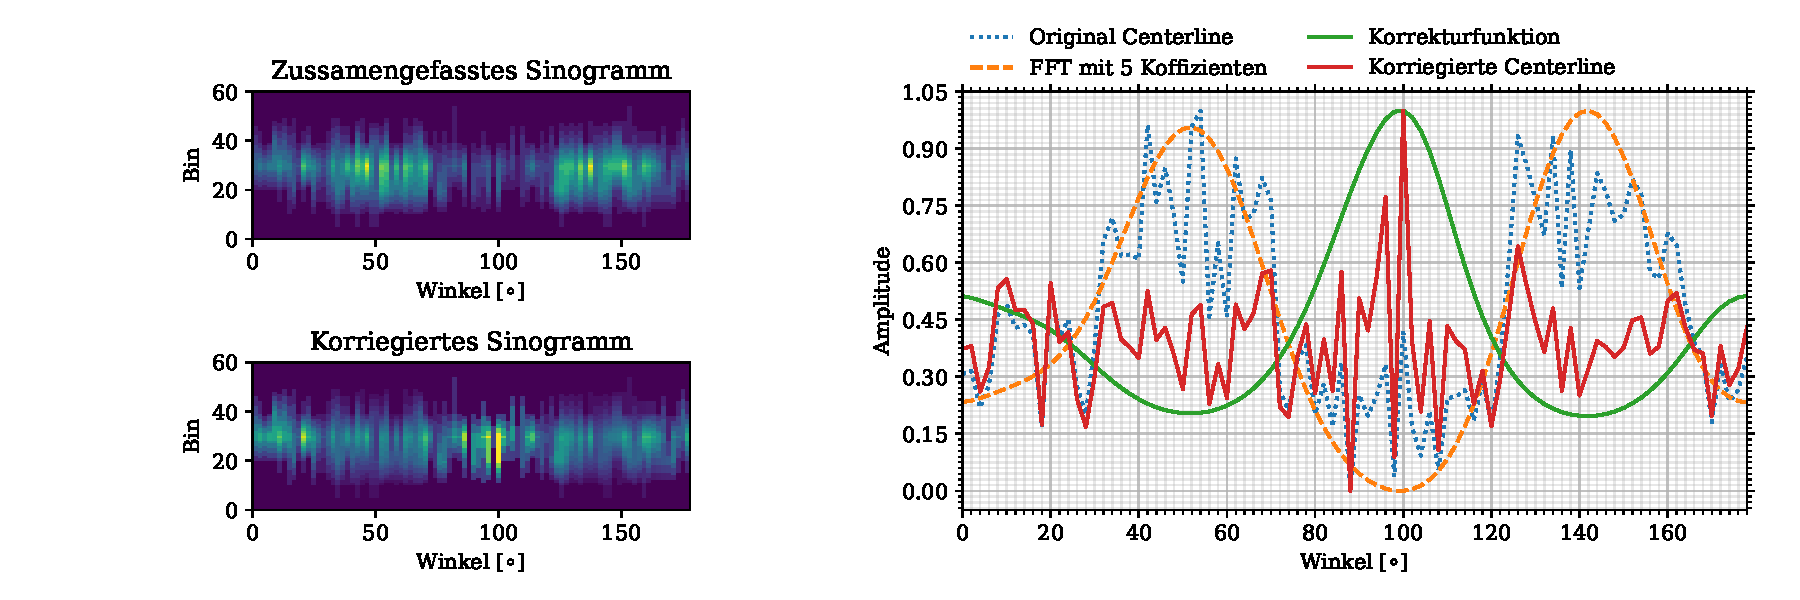
\includegraphics[width=\textwidth]{../auswertung/figs/tom2/raw_and_corrected.pdf}
  \caption[Sinogramme und Korrekturfunktion]{Links: Zussamengefasstes
    Originalsinogramm und korrigiertes Sinogram. Rechts: Z\"ahlzahl
    (centerline, in Willk\"urlicher Skalierung), Anpassung mit wenigen
  Fourierkoeffizienten, der darausberechnete Korrekturfaktor und die
  Korrigierte Z\"ahlzahl. Alle Kurven sind skaliert.}
  \label{fig:tom2-raw_and_corrected}
\end{figure}

\ref{fig:tom2-raw_and_corrected} zeigt deutlich, dass nun die
``Belichtungsst\"arke'' wesentlich ebenm\"a\ss{}iger ist. Die
gefundene Korrektur ist noch verbesserungsbed\"urftig, da kleine
Ereignisszahlen (mit ihren gr\"o\ss{}en relativen Fehlern)
\"uberm\"a\ss{}ig verst\"arkt werden (peak
in~\ref{fig:tom2-raw_and_corrected} rechts). Auch wird der abrubten
natur des Z\"ahlzahleinbruchs nicht wirklich Rechnung
getragen. Allerdings kann diese methode gut automatisiert und
generalisiert (Koeffizientenzahl) werden.\footnote{Ich habe da zuviel
  Zeit reingesteckt, aber es hat Spa\ss{} gemacht.}

\subsubsection{Einfluss verschiedener Filter}
\label{sec:filter}

Zuletzt wird noch der Einfluss verschiedener Filter auf die gefilterte Rückprojektion
untersucht. Dazu wurden die Messdaten aus~\ref{sec:tom1} verwendet. Es
wurde vers\"aumt, die r\"ckprojektion ohne die Energie und Zeitfenster
durchzuf\"uhren.

\begin{figure}[h]
  \centering
  \subfloat[Hanning-Filter.]{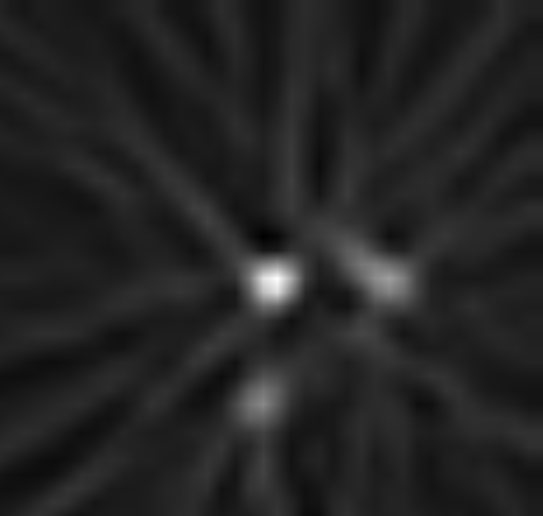
\includegraphics[width=.2\textwidth]{../messungen/olifilter/hanningweight9_gefiltert.png}}
  \subfloat[Rauschfilter.]{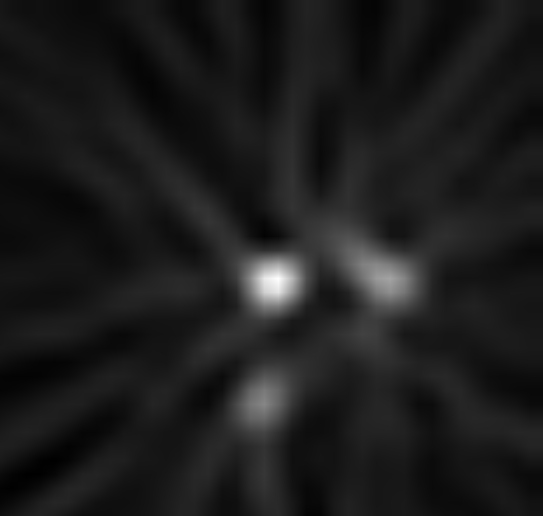
\includegraphics[width=.2\textwidth]{../messungen/olifilter/rauschfilter_gefiltert.png}}
  \subfloat[Ramp-Filter.]{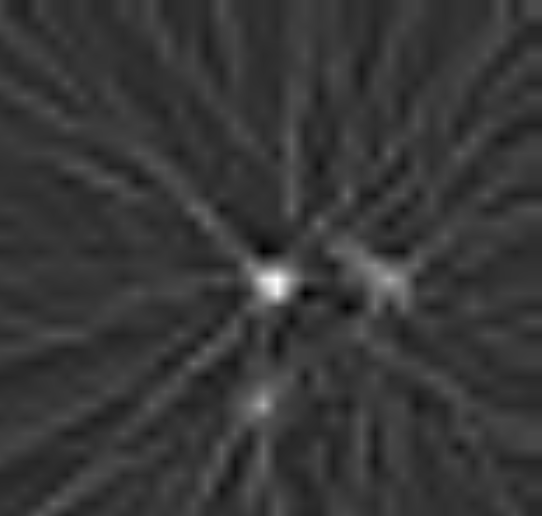
\includegraphics[width=.2\textwidth]{../messungen/olifilter/ramp9_gefiltert.png}}
  \subfloat[Shepp-Logan-Filter.]{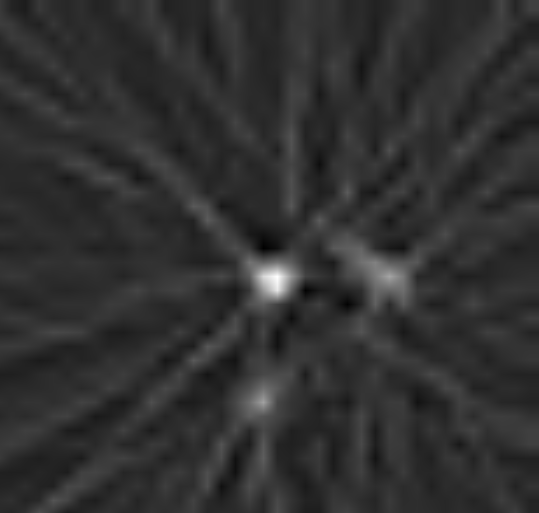
\includegraphics[width=.2\textwidth]{../messungen/olifilter/shepp9_gefiltert.png}}
  \caption{Gegenüberstellung verschiedener Filter mit einer Dimension
    von je \(9\).}
  \label{fig:filter}
\end{figure}

Wie man in~\ref{fig:filter} erkennen kann, sehen sich die gefilterten
Rückprojektionen mit dem Hannig-Filter und dem Rauschfilter sowie jene
mit Ramp-Filter und Shepp-Filter recht ähnlich. Die filter in (a) und
(b), sowie auch der Mittelfilter aus~\ref{eq:tom1-178} scheinen
feinere artefaktstrukturen zu gr\"o\ss{}eren, langsamer
ver\"anderlichen zussenzufassen, wobei sie dabei auch den Kontrast von
sehr starken Signalen (Qeullen) zu ihrer Umgebung steigern und diese
klarer abgrenzt. Die gelingt in (b) besser als in (a) oder auch im
Mittelfilter, wobei abei bei (a) und (b) die Rechte, obere Quelle
verschmiert und sie in~\ref{eq:tom1-178} klar aufgel\"ost wird. In (b)
und (c) erscheinen die Quellen als relativ helle, kleine Punkte mit
mehr oder weniger unf\"ormigen Halos. Die rechte obere Quelle ist
recht unkenntlich und die Artefakte sind im vergleich zur
ungefilterten r\"uckprojektion in~\ref{eq:tom1-178} breiter bei nur
geringf\"ugig
veringertem Kontrast. \\

%\begin{figure}[h]
%	\centering
%	\begin{subfigure}[t]{0.5\textwidth}
%		\centering
%		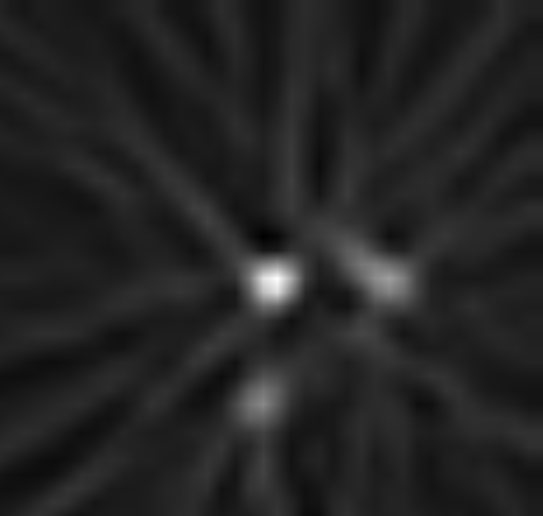
\includegraphics[width=.3\textwidth]{../messungen/olifilter/hanningweight9_gefiltert.png}
%		\caption{Hanning-Filter.}
%	\end{subfigure}
%	\begin{subfigure}[t]{0.5\textwidth}
%		\centering
%		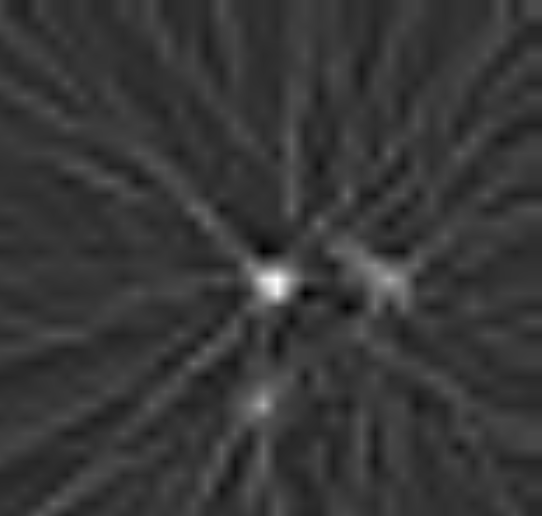
\includegraphics[width=.3\textwidth]{../messungen/olifilter/ramp9_gefiltert.png}
%		\caption{Ramp-Filter.}
%	\end{subfigure}
%	\begin{subfigure}[t]{0.5\textwidth}
%		\centering
%		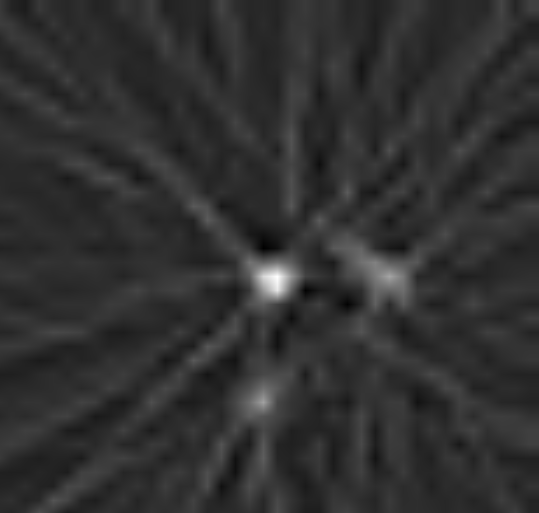
\includegraphics[width=.3\textwidth]{../messungen/olifilter/shepp9_gefiltert.png}
%		\caption{Shepp-Filter.}
%	\end{subfigure}
%	\begin{subfigure}[t]{0.5\textwidth}
%		\centering
%		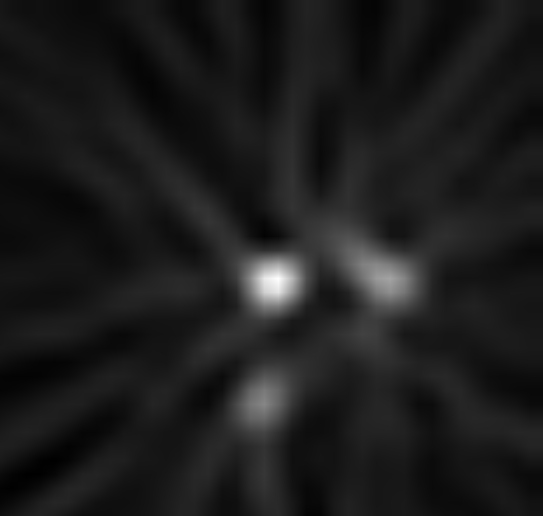
\includegraphics[width=.3\textwidth]{../messungen/olifilter/rauschfilter_gefiltert.png}
%		\caption{Rausch-Filter.}
%	\end{subfigure}
%\caption{Gegenüberstellung verschiedener Filter mit einer Dimension von je \(9\).}
%\label{fig:filter}
%\end{figure}

Der Rauschfilter wurde außerdem aufgrund der guten Qualit\"at der
entstehenden R\"uckprojektion mit mehreren Dimensionseinstellungen getestet.

\begin{figure}[h!]
	\centering
	\subfloat[Dimension \(= 5\).]{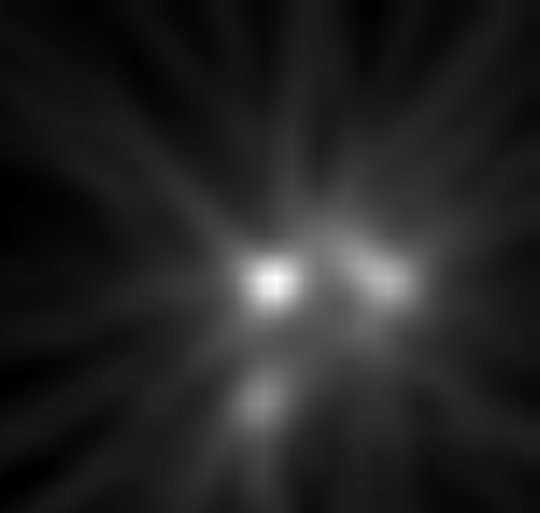
\includegraphics[width=.3\textwidth]{../messungen/olifilter/rausch_5_gefiltert.png}}
	\subfloat[Dimension \(= 9\).]{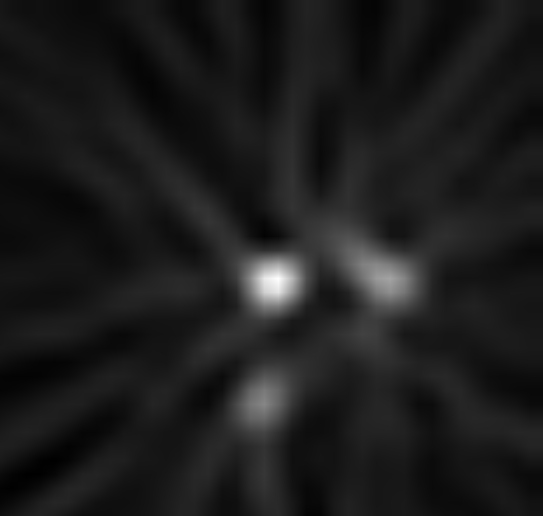
\includegraphics[width=.3\textwidth]{../messungen/olifilter/rauschfilter_gefiltert.png}}
	\subfloat[Dimension \(= 12\).]{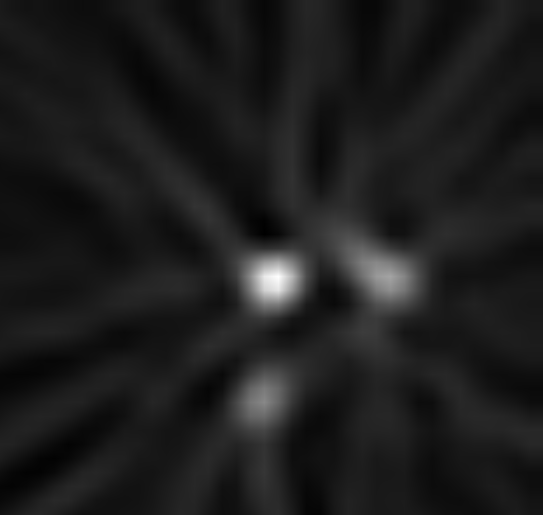
\includegraphics[width=.3\textwidth]{../messungen/olifilter/rausch12_gefiltert.png}}
	\caption{Rauschfilter mit verschiedenen Dimensionen.}
	\label{fig:rausch}
\end{figure}

In~\ref{fig:rausch} erscheint (a) am unschärfsten und undeutlichsten,
wenngleich man auch die Intensität der einzelnen Quellen qualitativ
abschätzen kann. Da der Filter bei Dimension \(=5\) sehr lokalisiert
ist, k\"onnen gr\"o\ss{}ere Strukturen nicht besser kontrastiert
werden. In (b) und (c) hingegen ist die Lage der Quellen besser
auszumachen, da diese schärfer im Vergleich zu (a) sind. Es ist
allerdings kein wirklicher Unterschied zwischen (b) und (c) zu
erkennen. Sobald die Dimension die gr\"o\ss{}e der Relevanten
strukturen \"uberschreitet, scheint die Sch\"arfe nicht mehr
zuzunehmen. Es w\"are sinnvoll noch weitere Dimensionen auszuprobieren
um diesen Trend zu best\"atigen.

% \begin{figure}[h!]
% \centering
% 	\begin{subfigure}[t]{0.5\textwidth}
% 	\centering
% 	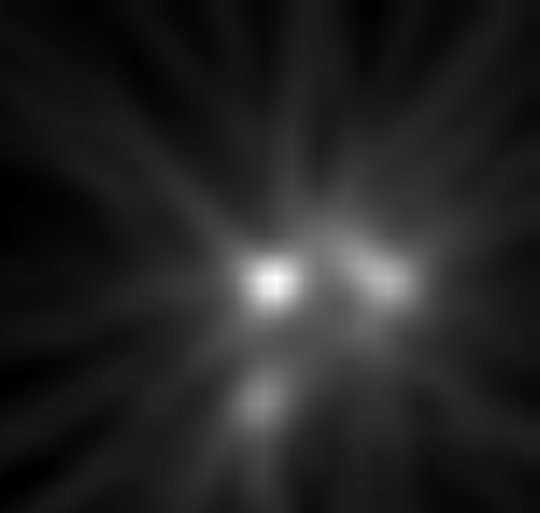
\includegraphics[width=.6\textwidth]{../messungen/olifilter/rausch_5_gefiltert.png}
% 	\caption{Dimension \(= 5\).}	
% 	\end{subfigure}
% 	\begin{subfigure}[t]{0.5\textwidth}
% 	\centering
% 	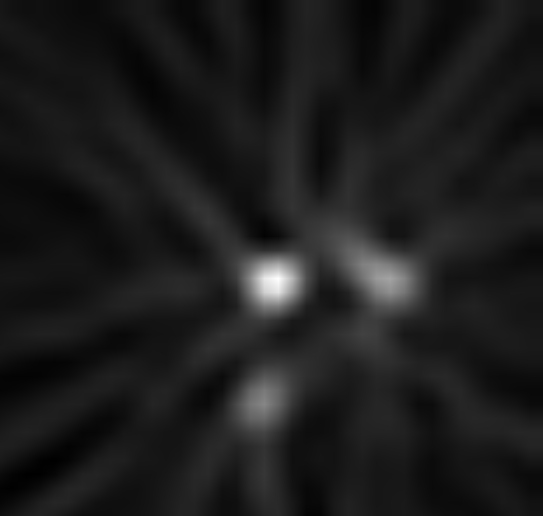
\includegraphics[width=.6\textwidth]{../messungen/olifilter/rauschfilter_gefiltert.png}
% 	\caption{Dimension \(= 9\).}	
% 	\end{subfigure}
% 	\begin{subfigure}[t]{0.5\textwidth}
% 	\centering
% 	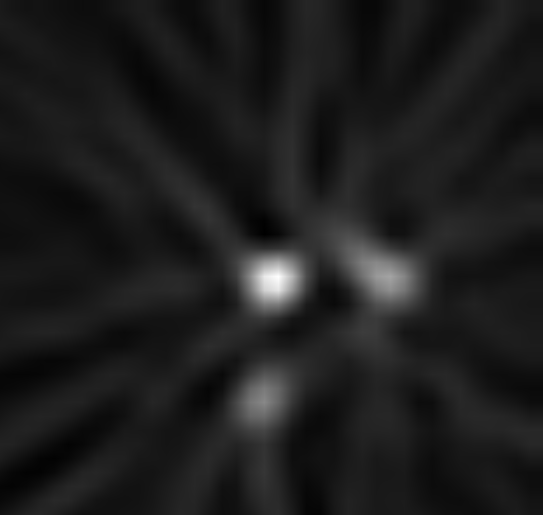
\includegraphics[width=.6\textwidth]{../messungen/olifilter/rausch12_gefiltert.png}
% 	\caption{Dimension \(= 12\).}	
% 	\end{subfigure}
% \caption{Rauschfilter mit verschiedenen Dimensionen.}
% \label{fig:rausch}
% \end{figure}


\subsection{Theoriebeispiel}
\label{sec:theobei}
Zur Verbesserung des Verst\"andnisses der Projektions- und
Rekonstruktionsprozesse, werden diese hier anhand eines einfachen
Beispiels nachvollzogen.

\begin{figure}[htp]
  \centering
  \begin{subfigure}[t]{.25\textwidth}
    \centering
    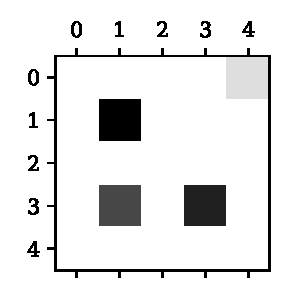
\includegraphics[width=.6\textwidth]{../auswertung/figs/theory/source.pdf}
    \caption{Ausgangsmatrix \(\mathfrak{M}_0\)}
    \label{fig:theory-source}
  \end{subfigure}
  \begin{subfigure}[t]{.25\textwidth}
    \centering
    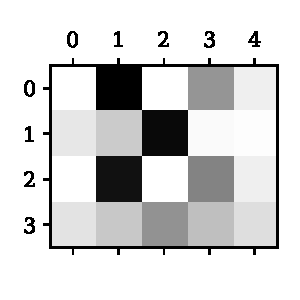
\includegraphics[width=.6\textwidth]{../auswertung/figs/theory/projection.pdf}
    \caption{Sinogram \(\mathfrak{P}_0\)}
    \label{fig:theory-projection}
  \end{subfigure}
  \begin{subfigure}[t]{.25\textwidth}
    \centering
    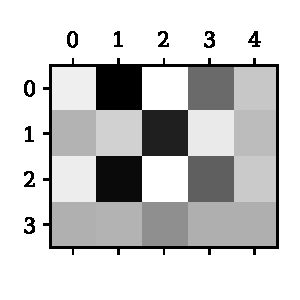
\includegraphics[width=.6\textwidth]{../auswertung/figs/theory/convoluted.pdf}
    \caption{Gefiltertes Sinogram \(\mathfrak{P}_1\)}
    \label{fig:theory-convoluted}
  \end{subfigure}
  \begin{subfigure}[t]{.25\textwidth}
    \centering
    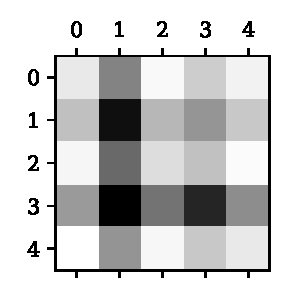
\includegraphics[width=.6\textwidth]{../auswertung/figs/theory/rec_simple.pdf}
    \caption{Einfache R\"uckprojektion \(\mathfrak{M}_1\)}
    \label{fig:theory-rec_simple}
  \end{subfigure}
  \begin{subfigure}[t]{.25\textwidth}
    \centering
    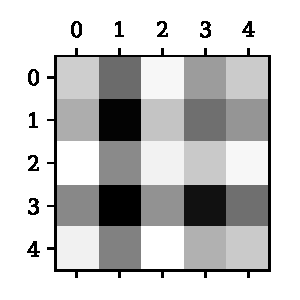
\includegraphics[width=.6\textwidth]{../auswertung/figs/theory/rec_filtered.pdf}
    \caption{Gefilterte R\"uckprojektion \(\mathfrak{M}_2\)}
    \label{fig:theory-rec_filtered}
  \end{subfigure}
  \caption[Graustufendarstellung der
  Beispielmatrizen]{Graustufendarstellung der Matrizen aus den
    Teilschritten des Beispiels. Es wurden jeweils die Matrixelemente
    in das Interval \([0,1]\) reskaliert.}
  \label{fig:graubei}
\end{figure}

Im ersten Schritt wird die Projektion~\ref{fig:theory-projection} des
Ausgangsbildes~\ref{fig:theory-source} aus Verschiedenen Winkeln
berechenet. Dabei wurden die diagonalen entsprechend gewichtet.

\begin{equation}
  \label{eq:proj}
  \mathfrak{M}_0 =
  \begin{pmatrix}
    0 & 0 & 0 & 0 & 2\\
    0 & 9 & 0 & 0 & 0\\
    0 & 0 & 0 & 0 & 0\\
    0 & 7 & 0 & 8 & 0\\
    0 & 0 & 0 & 0 & 0\\
  \end{pmatrix}
  \implies
  \left(
    \begin{array}{ccccc|c}
      0. & 16. & 0. & 8. & 2 & 0^\circ\\
      2.73 & 4.95 & 15.47 & 0.68 & 0.28 & 45^\circ\\
      0. & 15. & 0. & 9. & 2. & 90^\circ\\
      3.12 & 5.24 & 8.19 & 5.85 & 3.51 & 135^\circ\\
    \end{array}\right) = \mathfrak{P}_0
\end{equation}

Ein gefiltertes Sinogramm~\ref{fig:theory-convoluted} ergibt sich durch
Faltung der Zeilen von \(\mathfrak{P}_0\) mit
\(F = \mqty(-.1 & .25 & -.1)\).

\begin{equation}
  \label{eq:filter}
  \mathfrak{P}_1 = \mathfrak{P}_0 * F =
  \begin{pmatrix}
    -1.6 & 4. & -2.4 & 1.8 & -0.3\\
    0.188 & -0.583 & 3.304 & -1.405 & 0.002\\
    -1.5 & 3.75 & -2.4 & 2.05 & -0.4\\
    0.256 & 0.179 & 0.938 & 0.293 & 0.292\\
  \end{pmatrix}
\end{equation}

Die R\"uckprojektion des einfachen Sinogramms~\eqref{eq:proj}
ergib~\ref{fig:theory-rec_simple}.

{\footnotesize
\setlength{\arraycolsep}{2.5pt}

\begin{align}
  \label{eq:simplerepr}
  \overbrace{\begin{pmatrix}
      0. & 16. & 0. & 8. & 2.\\
      0. & 16. & 0. & 8. & 2.\\
      0. & 16. & 0. & 8. & 2.\\
      0. & 16. & 0. & 8. & 2.\\
      0. & 16. & 0. & 8. & 2.\\
    \end{pmatrix}}^{0^\circ} & + \frac{1}{2}\overbrace{\begin{pmatrix}
      15.864 & 8.408 & 0.837 & 0.287 & 0.076\\
      12.636 & 15.864 & 8.408 & 0.837 & 0.287\\
      6.569 & 12.636 & 15.864 & 8.408 & 0.837\\
      2.78 & 6.569 & 12.636 & 15.864 & 8.408\\
      0.737 & 2.78 & 6.569 & 12.636 & 15.864\\
    \end{pmatrix}}^{45^\circ} \nonumber \\ + \overbrace{\begin{pmatrix}
      2. & 2. & 2. & 2. & 2.\\
      9. & 9. & 9. & 9. & 9.\\
      0. & 0. & 0. & 0. & 0.\\
      15. & 15. & 15. & 15. & 15.\\
      0. & 0. & 0. & 0. & 0.\\
    \end{pmatrix}}^{90^\circ} &+ \frac{1}{2}\overbrace{\begin{pmatrix}
      0.948 & 3.569 & 8.003 & 9.886 & 8.966\\
      3.569 & 8.003 & 9.886 & 8.966 & 9.283\\
      8.003 & 9.886 & 8.966 & 9.283 & 7.151\\
      9.886 & 8.966 & 9.283 & 7.151 & 3.172\\
      8.966 & 9.283 & 7.151 & 3.172 & 0.842\\
    \end{pmatrix}}^{135^\circ}\nonumber \\
  & = \begin{pmatrix}
  10.406 & 23.988 & 6.42 & 15.087 & 8.521\\
  17.102 & 36.933 & 18.147 & 21.902 & 15.785\\
  7.3 & 27.261 & 12.415 & 16.845 & 5.994\\
  21.333 & 38.781 & 25.959 & 34.507 & 22.79\\
  4.852 & 22.031 & 6.874 & 15.904 & 10.353\\
  \end{pmatrix} = \mathfrak{M}_1
\end{align}}

Aus dem gefilterten Sinogramm~\eqref{eq:filter} ergibt sich auf
\"ahnliche Weise~\ref{fig:theory-rec_filtered}

{\footnotesize
\setlength{\arraycolsep}{2.5pt}

\begin{align}
  \label{eq:simplerepr}
  \overbrace{\begin{pmatrix}
      -1.6 & 4. & -2.4 & 1.8 & -0.3\\
      -1.6 & 4. & -2.4 & 1.8 & -0.3\\
      -1.6 & 4. & -2.4 & 1.8 & -0.3\\
      -1.6 & 4. & -2.4 & 1.8 & -0.3\\
      -1.6 & 4. & -2.4 & 1.8 & -0.3\\
    \end{pmatrix}}^{0^\circ} & + \frac{1}{2}\overbrace{\begin{pmatrix}
      3.165 & 0.261 & -1.305 & -0.012 & 0.001\\
      1.076 & 3.165 & 0.261 & -1.305 & -0.012\\
      -0.407 & 1.076 & 3.165 & 0.261 & -1.305\\
      0.182 & -0.407 & 1.076 & 3.165 & 0.261\\
      0.051 & 0.182 & -0.407 & 1.076 & 3.165\\
    \end{pmatrix}}^{45^\circ} \nonumber \\ +
  \overbrace{\begin{pmatrix}
      -0.4 & -0.4 & -0.4 & -0.4 & -0.4\\
      2.05 & 2.05 & 2.05 & 2.05 & 2.05\\
      -2.4 & -2.4 & -2.4 & -2.4 & -2.4\\
      3.75 & 3.75 & 3.75 & 3.75 & 3.75\\
      -1.5 & -1.5 & -1.5 & -1.5 & -1.5\\
    \end{pmatrix}}^{90^\circ} &+ \frac{1}{2}\overbrace{\begin{pmatrix}
      0.079 & 0.295 & 0.486 & 0.759 & 0.972\\
      0.295 & 0.486 & 0.759 & 0.972 & 0.646\\
      0.486 & 0.759 & 0.972 & 0.646 & 0.353\\
      0.759 & 0.972 & 0.646 & 0.353 & 0.258\\
      0.972 & 0.646 & 0.353 & 0.258 & 0.069\\
    \end{pmatrix}}^{135^\circ}\nonumber \\
           &= \begin{pmatrix}
             -0.378 & 3.878 & -3.21 & 1.773 & -0.214\\
             1.135 & 7.875 & 0.16 & 3.683 & 2.067\\
             -3.96 & 2.517 & -2.732 & -0.146 & -3.176\\
             2.62 & 8.033 & 2.211 & 7.309 & 3.71\\
             -2.589 & 2.914 & -3.926 & 0.967 & -0.183\\
           \end{pmatrix} = \mathfrak{M}_2
\end{align}
}

Es ist zu erkennen, das in beiden Rekonstruktionen die starken Signale
\((1,1),\,(3,1),\,(3,3)\) klar zu identifizieren, wenngleich die
Unterschiede in der Signalst\"arke nicht im urspr\"unglichen
Verh\"altnis stehen. Die gefilterte R\"uckprojektion weist in den
Randfeldern und im mittleren Feld einen h\"oheren Kontrast auf,
erzeugt aber dennoch nur ein geringf\"ugig besseres Bild.  Der
angewendete Filter unterdr\"uckt schwache Signale, die zwischen
Starken liegen da die angrenzenden Werte abgezogen werden.  Das
schwache Signal \((0,4)\) wurde in beiden F\"allen nicht
rekonstruiert. F\"uhrt man die Rechnung ohne diesen Punkt aus, ergibt
sich kaum ein Unterschied. Schwache Signale werden also nicht gut
reproduziert. In beiden F\"allen schmieren die Starken Quellen auf
ihren jeweiligen Verbindungsachsen aus. Dies kann ein Effekt der
bergrenzten Anzahl von Projektionswinkeln sein.

\newpage
\section{Verzeichnisse}
\label{sec:literatur}

\listoffigures

\listoftables

\printbibliography
\end{document}
